\documentclass[twoside]{book}

% Packages required by doxygen
\usepackage{fixltx2e}
\usepackage{calc}
\usepackage{doxygen}
\usepackage[export]{adjustbox} % also loads graphicx
\usepackage{graphicx}
\usepackage[utf8]{inputenc}
\usepackage{makeidx}
\usepackage{multicol}
\usepackage{multirow}
\PassOptionsToPackage{warn}{textcomp}
\usepackage{textcomp}
\usepackage[nointegrals]{wasysym}
\usepackage[table]{xcolor}

% Font selection
\usepackage[T1]{fontenc}
\usepackage[scaled=.90]{helvet}
\usepackage{courier}
\usepackage{amssymb}
\usepackage{sectsty}
\renewcommand{\familydefault}{\sfdefault}
\allsectionsfont{%
  \fontseries{bc}\selectfont%
  \color{darkgray}%
}
\renewcommand{\DoxyLabelFont}{%
  \fontseries{bc}\selectfont%
  \color{darkgray}%
}
\newcommand{\+}{\discretionary{\mbox{\scriptsize$\hookleftarrow$}}{}{}}

% Page & text layout
\usepackage{geometry}
\geometry{%
  a4paper,%
  top=2.5cm,%
  bottom=2.5cm,%
  left=2.5cm,%
  right=2.5cm%
}
\tolerance=750
\hfuzz=15pt
\hbadness=750
\setlength{\emergencystretch}{15pt}
\setlength{\parindent}{0cm}
\setlength{\parskip}{3ex plus 2ex minus 2ex}
\makeatletter
\renewcommand{\paragraph}{%
  \@startsection{paragraph}{4}{0ex}{-1.0ex}{1.0ex}{%
    \normalfont\normalsize\bfseries\SS@parafont%
  }%
}
\renewcommand{\subparagraph}{%
  \@startsection{subparagraph}{5}{0ex}{-1.0ex}{1.0ex}{%
    \normalfont\normalsize\bfseries\SS@subparafont%
  }%
}
\makeatother

% Headers & footers
\usepackage{fancyhdr}
\pagestyle{fancyplain}
\fancyhead[LE]{\fancyplain{}{\bfseries\thepage}}
\fancyhead[CE]{\fancyplain{}{}}
\fancyhead[RE]{\fancyplain{}{\bfseries\leftmark}}
\fancyhead[LO]{\fancyplain{}{\bfseries\rightmark}}
\fancyhead[CO]{\fancyplain{}{}}
\fancyhead[RO]{\fancyplain{}{\bfseries\thepage}}
\fancyfoot[LE]{\fancyplain{}{}}
\fancyfoot[CE]{\fancyplain{}{}}
\fancyfoot[RE]{\fancyplain{}{\bfseries\scriptsize Generated by Doxygen }}
\fancyfoot[LO]{\fancyplain{}{\bfseries\scriptsize Generated by Doxygen }}
\fancyfoot[CO]{\fancyplain{}{}}
\fancyfoot[RO]{\fancyplain{}{}}
\renewcommand{\footrulewidth}{0.4pt}
\renewcommand{\chaptermark}[1]{%
  \markboth{#1}{}%
}
\renewcommand{\sectionmark}[1]{%
  \markright{\thesection\ #1}%
}

% Indices & bibliography
\usepackage{natbib}
\usepackage[titles]{tocloft}
\setcounter{tocdepth}{3}
\setcounter{secnumdepth}{5}
\makeindex

% Hyperlinks (required, but should be loaded last)
\usepackage{ifpdf}
\ifpdf
  \usepackage[pdftex,pagebackref=true]{hyperref}
\else
  \usepackage[ps2pdf,pagebackref=true]{hyperref}
\fi
\hypersetup{%
  colorlinks=true,%
  linkcolor=blue,%
  citecolor=blue,%
  unicode%
}

% Custom commands
\newcommand{\clearemptydoublepage}{%
  \newpage{\pagestyle{empty}\cleardoublepage}%
}

\usepackage{caption}
\captionsetup{labelsep=space,justification=centering,font={bf},singlelinecheck=off,skip=4pt,position=top}

%===== C O N T E N T S =====

\begin{document}

% Titlepage & ToC
\hypersetup{pageanchor=false,
             bookmarksnumbered=true,
             pdfencoding=unicode
            }
\pagenumbering{roman}
\begin{titlepage}
\vspace*{7cm}
\begin{center}%
{\Large F\+V\+Code3D }\\
\vspace*{1cm}
{\large Generated by Doxygen 1.8.11}\\
\end{center}
\end{titlepage}
\clearemptydoublepage
\tableofcontents
\clearemptydoublepage
\pagenumbering{arabic}
\hypersetup{pageanchor=true}

%--- Begin generated contents ---
\chapter{Main Page}
\label{index}\hypertarget{index}{}\hypertarget{index_intro}{}\section{Introduction}\label{index_intro}
This code allows to solve the single-\/phase flow in a fractured porous medium modeled via the Darcy equation by using the Finite Volume (FV) method with a two-\/point flux approximation (T\+P\+FA). The fractures are required to be matching with the grid.~\newline
 The code is written in C++. As input, the program requires a mesh as \textquotesingle{}.fvg\textquotesingle{} format file. The output is given as \textquotesingle{}.vtu\textquotesingle{} file format, viewable by Paraview.~\newline
 \hypertarget{index_howto}{}\section{How to execute the program}\label{index_howto}
To run the program just execute~\newline

\begin{DoxyCode}
./fvcode3d.exe
\end{DoxyCode}
 By default, the parameters need are read from data.\+txt file.~\newline
 With the option \textquotesingle{}-\/f \textquotesingle{}, it is possible to specify the data file.~\newline
 Ex.~\newline

\begin{DoxyCode}
./fvcode3d.exe -f data.txt
\end{DoxyCode}
\hypertarget{index_input}{}\section{Input parameters}\label{index_input}
The program requires\+:~\newline

\begin{DoxyItemize}
\item an input mesh in \textquotesingle{}.fvg\textquotesingle{} format~\newline

\item the data file~\newline
 The file format \textquotesingle{}.fvg\textquotesingle{} consists of four parts\+:~\newline

\item list of P\+O\+I\+N\+TS, each of them described by its coordinates x, y, z;~\newline

\item list of F\+A\+C\+E\+TS, each of them described by a list of ids of P\+O\+I\+N\+TS, plus some properties if the facet represents a fracture;~\newline

\item list of C\+E\+L\+LS, each of them described by a list of ids of F\+A\+C\+E\+TS, plus some properties;~\newline

\item list of F\+R\+A\+C\+T\+U\+RE N\+E\+T\+W\+O\+R\+KS, each of them described by a list of F\+A\+C\+E\+TS that belong to the same network.~\newline
 The properties related to the facets that represent a fracture are the permeability, the porosity and the aperture.~\newline
 The properties related to the cells (porous medium) are the permeability and the porosity.
\end{DoxyItemize}

The data file consists of six sections\+:
\begin{DoxyItemize}
\item {\ttfamily mesh\+:} the input file parameters such as mesh location and filename~\newline

\item {\ttfamily output\+:} the output directory and filename~\newline

\item {\ttfamily problem\+:} parameters related to the problem, such as the problem type (steady or unsteady) or if apply or not the source/sink term~\newline

\item {\ttfamily fluid\+:} mobility and compressibility of the fluid~\newline

\item {\ttfamily bc\+:} the rotation to apply around the z axis, needed to correctly apply the boundary conditions~\newline

\item {\ttfamily solver\+:} the solver to use and some parameters such as the tolerance and the number of iterations~\newline
 
\end{DoxyItemize}\hypertarget{index_class}{}\section{Main Classes}\label{index_class}
The main classes involved are the following\+:~\newline

\begin{DoxyItemize}
\item {\itshape Data\+:} collects all the parameters used by the program that can be set through the datafile;~\newline

\item {\itshape Importer\+:} reads the input file mesh;~\newline

\item {\itshape Properties\+Map\+:} collects the properties of the fractures and porous medium;~\newline

\item {\itshape Mesh3D\+:} stores the geometrical mesh as {\itshape Point3D}, {\itshape Facet3D} and {\itshape Cell3D};~\newline

\item {\itshape Rigid\+\_\+\+Mesh\+:} converts a {\itshape Mesh3D} in a rigid format, suitable for assemble the problem;~\newline

\item {\itshape Boundary\+Conditions\+:} defines the boundary conditions to assign to the problem; B\+Cs can be Dirichlet or Neumann;~\newline

\item {\itshape Problem\+:} defines the problem to solve\+: it can be a steady problem ({\itshape Darcy\+Steady}) or a time-\/dependent problem ({\itshape Darcy\+Pseudo\+Steady}); it assembles the matrix and the right hand side;~\newline

\item {\itshape Solver\+:} solves the {\itshape Problem}; the code implements direct solvers as well as iterative solvers;~\newline

\item {\itshape Exporter\+:} exports as \textquotesingle{}.vtu\textquotesingle{} files the mesh, the properties, the solution and more.~\newline
 
\end{DoxyItemize}\hypertarget{index_es}{}\section{Example of usage}\label{index_es}
Here, we briefly describe how to use the code.~\newline
 First of all, read the necessary parameters from the datafile\+:~\newline
 
\begin{DoxyCode}
\textcolor{comment}{// we use the GetPot utility to access the datafile}
GetPot command\_line(argc,argv);
\textcolor{keyword}{const} std::string dataFileName = command\_line.follow(\textcolor{stringliteral}{"data.txt"}, 2, \textcolor{stringliteral}{"-f"}, \textcolor{stringliteral}{"--file"});
\textcolor{comment}{// Read Data from the datafile}
\hyperlink{namespaceFVCode3D_a3d19a370a98afe491a9e17a646a9c56f}{DataPtr\_Type} dataPtr(\textcolor{keyword}{new} Data(dataFileName));
\end{DoxyCode}


Then we define the Mesh3D, the Properties\+Map so that we can import the mesh\+:


\begin{DoxyCode}
\textcolor{comment}{//Define Mesh and Properties}
Mesh3D mesh;
PropertiesMap propMap(dataPtr->getMobility(), dataPtr->getCompressibility());
\textcolor{comment}{//Create Importer}
Importer * importer = 0;
importer = \textcolor{keyword}{new} ImporterForSolver(dataPtr->getMeshDir() + dataPtr->getMeshFile(), mesh, propMap);
\textcolor{comment}{//Import grid file}
importer->import(dataPtr->fractureOn());
\end{DoxyCode}


After the reading of the mesh, it is necessary to perform some operations to process the mesh\+:


\begin{DoxyCode}
\textcolor{comment}{//Compute the cells that separate each facet}
mesh.updateFacetsWithCells();
\textcolor{comment}{//Compute the neighboring cells of each cell}
mesh.updateCellsWithNeighbors();
\textcolor{comment}{//Set labels on boundary (necessary for BCs)}
importer->extractBC(dataPtr->getTheta());
\textcolor{comment}{//Compute facet ids of the fractures (creates fracture networks)}
mesh.updateFacetsWithFractures();
\end{DoxyCode}


We can now create the boundary conditions\+:


\begin{DoxyCode}
\textcolor{comment}{//Assign to the border marked as 'Left' a Dirichlet condition equal to 1}
BoundaryConditions::BorderBC leftBC (\hyperlink{namespaceFVCode3D_a604c2047b7f400e68b30a8132178c822a7fd633652b3723bb7716b9db0314a61e}{BorderLabel::Left}, 
      \hyperlink{namespaceFVCode3D_a73660061f11f1671164ce171a053f8c5a192024697bdaa4fbbb39b8961b747bce}{Dirichlet}, \hyperlink{namespaceFVCode3D_a1a9ede09c77441d292a079fbab60fb82}{fOne} );
\textcolor{comment}{//And so on...}
BoundaryConditions::BorderBC rightBC(\hyperlink{namespaceFVCode3D_a604c2047b7f400e68b30a8132178c822a27ec5db52b31c4eba9e240374723f76e}{BorderLabel::Right}, 
      \hyperlink{namespaceFVCode3D_a73660061f11f1671164ce171a053f8c5a192024697bdaa4fbbb39b8961b747bce}{Dirichlet}, \hyperlink{namespaceFVCode3D_a2e72cc81c6f214d6e057af7a02599501}{fZero} );
...

\textcolor{comment}{//We create a vector that contains all the BorderBC...}
std::vector<BoundaryConditions::BorderBC> borders;
\textcolor{comment}{//...and we insert into it the BCs previously created}
borders.push\_back( backBC );
borders.push\_back( frontBC );
...

\textcolor{comment}{//Finally we create the BoundaryConditions}
BoundaryConditions BC(borders);
\end{DoxyCode}


Then we create a Rigid\+\_\+\+Mesh 
\begin{DoxyCode}
\textcolor{comment}{//The Rigid\_Mesh requires the Mesh3D and the PropertesMap}
Rigid\_Mesh myrmesh(mesh, propMap);
\end{DoxyCode}


We can proceed by building the problem\+:


\begin{DoxyCode}
Problem<CentroidQuadrature, CentroidQuadrature> * darcy(\textcolor{keyword}{nullptr});
\textcolor{keyword}{typedef} DarcySteady<CentroidQuadrature, CentroidQuadrature> \hyperlink{main_8cpp_ab0de87680f9f2dfa547e659c7da3d1e4}{DarcyPb};
\textcolor{keyword}{typedef} DarcyPseudoSteady<CentroidQuadrature, CentroidQuadrature, SpMat, TimeScheme::BDF2> 
      \hyperlink{main_8cpp_aff54e4c6bbc30b11899898af00325b15}{PseudoDarcyPb};

\textcolor{comment}{//If the problem is steady}
\textcolor{keywordflow}{if}(dataPtr->getProblemType() == Data::ProblemType::steady)
\{
    darcy = \textcolor{keyword}{new} \hyperlink{main_8cpp_ab0de87680f9f2dfa547e659c7da3d1e4}{DarcyPb}(dataPtr->getSolverType(), myrmesh, BC, \hyperlink{namespaceFVCode3D_ae8b0f97f0774db9f0881cfc5f31d93f4}{SS}, dataPtr);
\}
\textcolor{comment}{//If the problem is unsteady}
\textcolor{keywordflow}{else} \textcolor{keywordflow}{if}(dataPtr->getProblemType() == Data::ProblemType::pseudoSteady)
\{
    darcy = \textcolor{keyword}{new} \hyperlink{main_8cpp_aff54e4c6bbc30b11899898af00325b15}{PseudoDarcyPb}(dataPtr->getSolverType(), myrmesh, BC, 
      \hyperlink{namespaceFVCode3D_ae8b0f97f0774db9f0881cfc5f31d93f4}{SS}, dataPtr);
\}

\textcolor{comment}{//If the solver used is an iterative one, set tolerance and the maximum number of iterations}
\textcolor{keywordflow}{if}(dynamic\_cast<IterativeSolver*>(darcy->getSolverPtr()))
\{
    \textcolor{keyword}{dynamic\_cast<}IterativeSolver*\textcolor{keyword}{>}(darcy->getSolverPtr())->setMaxIter(dataPtr->getIterativeSolverMaxIter())
      ;
    \textcolor{keyword}{dynamic\_cast<}IterativeSolver*\textcolor{keyword}{>}(darcy->getSolverPtr())->setTolerance(dataPtr->
      getIterativeSolverTolerance());
\}
\end{DoxyCode}


Now, we can solve the problem\+:


\begin{DoxyCode}
  \textcolor{comment}{//In the case of a steady problem, we assemble and the solve the problem}
  \textcolor{keywordflow}{if}(dataPtr->getProblemType() == Data::ProblemType::steady)
  \{
      darcy->assemble();
      \textcolor{keywordflow}{if}(dataPtr->pressuresInFractures())
      \{
          FixPressureDofs<DarcyPb> fpd(dynamic\_cast<DarcyPb *>(darcy));
          fpd.apply(dataPtr->getPressuresInFractures());
      \}
      darcy->solve();
  \}
  \textcolor{comment}{//In the case of a unsteady problem, we initialize the problem and for each time step, we assemble and
       solve the}
problem
  \textcolor{keywordflow}{else} \textcolor{keywordflow}{if}(dataPtr->getProblemType() == Data::ProblemType::pseudoSteady)
  \{
      \textcolor{keyword}{dynamic\_cast<}PseudoDarcyPb *\textcolor{keyword}{>}(darcy)->initialize();
      \textcolor{keywordflow}{for}(\hyperlink{namespaceFVCode3D_a40c1f5588a248569d80aa5f867080e83}{Real} t = dataPtr->getInitialTime() + dataPtr->getTimeStep() ; t <= dataPtr->getEndTime(); t+=
      dataPtr->getTimeStep())
      \{
          darcy->assemble();
          \textcolor{keywordflow}{if}(dataPtr->pressuresInFractures())
          \{
              FixPressureDofs<PseudoDarcyPb> fpd(dynamic\_cast<PseudoDarcyPb *>(darcy));
              fpd.apply(dataPtr->getPressuresInFractures());
          \}
          darcy->solve();
      \}
  \}
\end{DoxyCode}


The solution can be exported\+:


\begin{DoxyCode}
\textcolor{comment}{//Define Exporter}
ExporterVTU exporter;
\textcolor{comment}{//Export solution on matrix and on the fractures}
exporter.exportSolution(myrmesh, dataPtr->getOutputDir() + dataPtr->getOutputFile() + \textcolor{stringliteral}{"\_solution.vtu"}, 
      darcy->getSolver().getSolution());
exporter.exportSolutionOnFractures(myrmesh, dataPtr->getOutputDir() + dataPtr->getOutputFile() + \textcolor{stringliteral}{"
      \_solution\_f.vtu"}, darcy->getSolver().getSolution());
\end{DoxyCode}


Remember to delete the Problem and the Importer instance\+:


\begin{DoxyCode}
\textcolor{keyword}{delete} darcy;
\textcolor{keyword}{delete} importer;
\end{DoxyCode}
 
\chapter{Todo List}
\label{todo}
\hypertarget{todo}{}

\begin{DoxyRefList}
\item[\label{todo__todo000001}%
\hypertarget{todo__todo000001}{}%
Global \hyperlink{classFVCode3D_1_1StiffMatrix_ac3eb491563c1742f4adba021e397719b}{F\+V\+Code3D\+:\+:Stiff\+Matrix\+:\+:assemble\+M\+FD} ()]I use the formulation of Nicola (to be reviewed) 
\end{DoxyRefList}
\chapter{Namespace Index}
\section{Namespace List}
Here is a list of all namespaces with brief descriptions\+:\begin{DoxyCompactList}
\item\contentsline{section}{\hyperlink{namespaceFVCode3D}{F\+V\+Code3D} }{\pageref{namespaceFVCode3D}}{}
\item\contentsline{section}{\hyperlink{namespacestd}{std} }{\pageref{namespacestd}}{}
\end{DoxyCompactList}

\chapter{Hierarchical Index}
\section{Class Hierarchy}
This inheritance list is sorted roughly, but not completely, alphabetically\+:\begin{DoxyCompactList}
\item \contentsline{section}{tetgenmesh\+:\+:arraypool}{\pageref{classtetgenmesh_1_1arraypool}}{}
\item \contentsline{section}{tetgenmesh\+:\+:badface}{\pageref{classtetgenmesh_1_1badface}}{}
\item \contentsline{section}{F\+V\+Code3D\+:\+:Boundary\+Conditions\+:\+:Border\+BC}{\pageref{classFVCode3D_1_1BoundaryConditions_1_1BorderBC}}{}
\item \contentsline{section}{F\+V\+Code3D\+:\+:Boundary\+Conditions}{\pageref{classFVCode3D_1_1BoundaryConditions}}{}
\item \contentsline{section}{F\+V\+Code3D\+:\+:Bounding\+Box}{\pageref{classFVCode3D_1_1BoundingBox}}{}
\item \contentsline{section}{F\+V\+Code3D\+:\+:Cartesian\+Grid}{\pageref{classFVCode3D_1_1CartesianGrid}}{}
\item \contentsline{section}{F\+V\+Code3D\+:\+:Rigid\+\_\+\+Mesh\+:\+:Cell}{\pageref{classFVCode3D_1_1Rigid__Mesh_1_1Cell}}{}
\item \contentsline{section}{F\+V\+Code3D\+:\+:Mesh3D\+:\+:Cell3D}{\pageref{classFVCode3D_1_1Mesh3D_1_1Cell3D}}{}
\item \contentsline{section}{F\+V\+Code3D\+:\+:Chrono}{\pageref{classFVCode3D_1_1Chrono}}{}
\item \contentsline{section}{F\+V\+Code3D\+:\+:Coordinate\+System3D}{\pageref{classFVCode3D_1_1CoordinateSystem3D}}{}
\item ctype\begin{DoxyCompactList}
\item \contentsline{section}{F\+V\+Code3D\+:\+:My\+Delimiters}{\pageref{structFVCode3D_1_1MyDelimiters}}{}
\end{DoxyCompactList}
\item \contentsline{section}{F\+V\+Code3D\+:\+:Darcy\+Pseudo\+Steady$<$ Q\+R\+Matrix, Q\+R\+Fracture, Matrix\+Type, Time\+Scheme $>$}{\pageref{classFVCode3D_1_1DarcyPseudoSteady}}{}
\item \contentsline{section}{F\+V\+Code3D\+:\+:Data}{\pageref{classFVCode3D_1_1Data}}{}
\item \contentsline{section}{F\+V\+Code3D\+:\+:Rigid\+\_\+\+Mesh\+:\+:Edge}{\pageref{classFVCode3D_1_1Rigid__Mesh_1_1Edge}}{}
\item \contentsline{section}{F\+V\+Code3D\+:\+:Rigid\+\_\+\+Mesh\+:\+:Edge\+\_\+\+ID}{\pageref{classFVCode3D_1_1Rigid__Mesh_1_1Edge__ID}}{}
\begin{DoxyCompactList}
\item \contentsline{section}{F\+V\+Code3D\+:\+:Rigid\+\_\+\+Mesh\+:\+:Border\+\_\+\+Edge}{\pageref{classFVCode3D_1_1Rigid__Mesh_1_1Border__Edge}}{}
\begin{DoxyCompactList}
\item \contentsline{section}{F\+V\+Code3D\+:\+:Rigid\+\_\+\+Mesh\+:\+:Border\+\_\+\+Tip\+\_\+\+Edge}{\pageref{classFVCode3D_1_1Rigid__Mesh_1_1Border__Tip__Edge}}{}
\item \contentsline{section}{F\+V\+Code3D\+:\+:Rigid\+\_\+\+Mesh\+:\+:Pure\+\_\+\+Border\+\_\+\+Edge}{\pageref{classFVCode3D_1_1Rigid__Mesh_1_1Pure__Border__Edge}}{}
\end{DoxyCompactList}
\item \contentsline{section}{F\+V\+Code3D\+:\+:Rigid\+\_\+\+Mesh\+:\+:Fracture\+\_\+\+Edge}{\pageref{classFVCode3D_1_1Rigid__Mesh_1_1Fracture__Edge}}{}
\begin{DoxyCompactList}
\item \contentsline{section}{F\+V\+Code3D\+:\+:Rigid\+\_\+\+Mesh\+:\+:Juncture\+\_\+\+Edge}{\pageref{classFVCode3D_1_1Rigid__Mesh_1_1Juncture__Edge}}{}
\item \contentsline{section}{F\+V\+Code3D\+:\+:Rigid\+\_\+\+Mesh\+:\+:Tip\+\_\+\+Edge}{\pageref{classFVCode3D_1_1Rigid__Mesh_1_1Tip__Edge}}{}
\begin{DoxyCompactList}
\item \contentsline{section}{F\+V\+Code3D\+:\+:Rigid\+\_\+\+Mesh\+:\+:Border\+\_\+\+Tip\+\_\+\+Edge}{\pageref{classFVCode3D_1_1Rigid__Mesh_1_1Border__Tip__Edge}}{}
\item \contentsline{section}{F\+V\+Code3D\+:\+:Rigid\+\_\+\+Mesh\+:\+:Internal\+\_\+\+Tip\+\_\+\+Edge}{\pageref{classFVCode3D_1_1Rigid__Mesh_1_1Internal__Tip__Edge}}{}
\end{DoxyCompactList}
\end{DoxyCompactList}
\item \contentsline{section}{F\+V\+Code3D\+:\+:Rigid\+\_\+\+Mesh\+:\+:Regular\+\_\+\+Edge}{\pageref{classFVCode3D_1_1Rigid__Mesh_1_1Regular__Edge}}{}
\end{DoxyCompactList}
\item \contentsline{section}{F\+V\+Code3D\+:\+:Enum\+Parser$<$ T $>$}{\pageref{classFVCode3D_1_1EnumParser}}{}
\item \contentsline{section}{F\+V\+Code3D\+:\+:Exporter}{\pageref{classFVCode3D_1_1Exporter}}{}
\begin{DoxyCompactList}
\item \contentsline{section}{F\+V\+Code3D\+:\+:Exporter\+CP}{\pageref{classFVCode3D_1_1ExporterCP}}{}
\item \contentsline{section}{F\+V\+Code3D\+:\+:Exporter\+V\+TU}{\pageref{classFVCode3D_1_1ExporterVTU}}{}
\end{DoxyCompactList}
\item \contentsline{section}{tetgenmesh\+:\+:face}{\pageref{classtetgenmesh_1_1face}}{}
\item \contentsline{section}{tetgenio\+:\+:facet}{\pageref{structtetgenio_1_1facet}}{}
\item \contentsline{section}{F\+V\+Code3D\+:\+:Rigid\+\_\+\+Mesh\+:\+:Facet}{\pageref{classFVCode3D_1_1Rigid__Mesh_1_1Facet}}{}
\item \contentsline{section}{F\+V\+Code3D\+:\+:Mesh3D\+:\+:Facet3D}{\pageref{classFVCode3D_1_1Mesh3D_1_1Facet3D}}{}
\item \contentsline{section}{F\+V\+Code3D\+:\+:Rigid\+\_\+\+Mesh\+:\+:Facet\+\_\+\+ID}{\pageref{classFVCode3D_1_1Rigid__Mesh_1_1Facet__ID}}{}
\begin{DoxyCompactList}
\item \contentsline{section}{F\+V\+Code3D\+:\+:Rigid\+\_\+\+Mesh\+:\+:Border\+\_\+\+Facet}{\pageref{classFVCode3D_1_1Rigid__Mesh_1_1Border__Facet}}{}
\item \contentsline{section}{F\+V\+Code3D\+:\+:Rigid\+\_\+\+Mesh\+:\+:Fracture\+\_\+\+Facet}{\pageref{classFVCode3D_1_1Rigid__Mesh_1_1Fracture__Facet}}{}
\item \contentsline{section}{F\+V\+Code3D\+:\+:Rigid\+\_\+\+Mesh\+:\+:Regular\+\_\+\+Facet}{\pageref{classFVCode3D_1_1Rigid__Mesh_1_1Regular__Facet}}{}
\end{DoxyCompactList}
\item \contentsline{section}{F\+V\+Code3D\+:\+:Fix\+Pressure\+Dofs$<$ Problem\+Type $>$}{\pageref{classFVCode3D_1_1FixPressureDofs}}{}
\item \contentsline{section}{tetgenmesh\+:\+:flipconstraints}{\pageref{classtetgenmesh_1_1flipconstraints}}{}
\item \contentsline{section}{F\+V\+Code3D\+:\+:Fracture3D}{\pageref{classFVCode3D_1_1Fracture3D}}{}
\item \contentsline{section}{F\+V\+Code3D\+:\+:Fracture\+Builder}{\pageref{classFVCode3D_1_1FractureBuilder}}{}
\item \contentsline{section}{F\+V\+Code3D\+:\+:Fracture\+Network3D}{\pageref{classFVCode3D_1_1FractureNetwork3D}}{}
\item \contentsline{section}{F\+V\+Code3D\+:\+:global\+\_\+\+Bulk\+Builder}{\pageref{classFVCode3D_1_1global__BulkBuilder}}{}
\item \contentsline{section}{F\+V\+Code3D\+:\+:global\+\_\+\+Operator}{\pageref{classFVCode3D_1_1global__Operator}}{}
\begin{DoxyCompactList}
\item \contentsline{section}{F\+V\+Code3D\+:\+:Coupling\+Conditions}{\pageref{classFVCode3D_1_1CouplingConditions}}{}
\item \contentsline{section}{F\+V\+Code3D\+:\+:Flux\+Operator}{\pageref{classFVCode3D_1_1FluxOperator}}{}
\item \contentsline{section}{F\+V\+Code3D\+:\+:global\+\_\+\+Div}{\pageref{classFVCode3D_1_1global__Div}}{}
\item \contentsline{section}{F\+V\+Code3D\+:\+:global\+\_\+\+Inner\+Product}{\pageref{classFVCode3D_1_1global__InnerProduct}}{}
\end{DoxyCompactList}
\item \contentsline{section}{F\+V\+Code3D\+:\+:Importer}{\pageref{classFVCode3D_1_1Importer}}{}
\begin{DoxyCompactList}
\item \contentsline{section}{F\+V\+Code3D\+:\+:Importer\+For\+Solver}{\pageref{classFVCode3D_1_1ImporterForSolver}}{}
\item \contentsline{section}{F\+V\+Code3D\+:\+:Importer\+Medit}{\pageref{classFVCode3D_1_1ImporterMedit}}{}
\begin{DoxyCompactList}
\item \contentsline{section}{F\+V\+Code3D\+:\+:Importer\+Tet\+Gen}{\pageref{classFVCode3D_1_1ImporterTetGen}}{}
\end{DoxyCompactList}
\item \contentsline{section}{F\+V\+Code3D\+:\+:Importer\+Open\+F\+O\+AM}{\pageref{classFVCode3D_1_1ImporterOpenFOAM}}{}
\item \contentsline{section}{F\+V\+Code3D\+:\+:Importer\+T\+P\+FA}{\pageref{classFVCode3D_1_1ImporterTPFA}}{}
\end{DoxyCompactList}
\item \contentsline{section}{tetgenmesh\+:\+:insertvertexflags}{\pageref{classtetgenmesh_1_1insertvertexflags}}{}
\item \contentsline{section}{F\+V\+Code3D\+:\+:less$<$ T $>$}{\pageref{structFVCode3D_1_1less}}{}
\item \contentsline{section}{F\+V\+Code3D\+:\+:less$<$ std\+:\+:pair$<$ T, T $>$ $>$}{\pageref{structFVCode3D_1_1less_3_01std_1_1pair_3_01T_00_01T_01_4_01_4}}{}
\item \contentsline{section}{F\+V\+Code3D\+:\+:less\+On\+Matrix\+Indices}{\pageref{classFVCode3D_1_1lessOnMatrixIndices}}{}
\item \contentsline{section}{F\+V\+Code3D\+:\+:local\+\_\+builder}{\pageref{classFVCode3D_1_1local__builder}}{}
\item \contentsline{section}{F\+V\+Code3D\+:\+:local\+\_\+\+Mimetic\+Operator}{\pageref{classFVCode3D_1_1local__MimeticOperator}}{}
\begin{DoxyCompactList}
\item \contentsline{section}{F\+V\+Code3D\+:\+:local\+\_\+\+Div}{\pageref{classFVCode3D_1_1local__Div}}{}
\item \contentsline{section}{F\+V\+Code3D\+:\+:local\+\_\+\+Inner\+Product}{\pageref{classFVCode3D_1_1local__InnerProduct}}{}
\end{DoxyCompactList}
\item \contentsline{section}{F\+V\+Code3D\+:\+:Matrix\+Handler}{\pageref{classFVCode3D_1_1MatrixHandler}}{}
\begin{DoxyCompactList}
\item \contentsline{section}{F\+V\+Code3D\+:\+:Mass\+Matrix}{\pageref{classFVCode3D_1_1MassMatrix}}{}
\item \contentsline{section}{F\+V\+Code3D\+:\+:Stiff\+Matrix}{\pageref{classFVCode3D_1_1StiffMatrix}}{}
\end{DoxyCompactList}
\item \contentsline{section}{tetgenmesh\+:\+:memorypool}{\pageref{classtetgenmesh_1_1memorypool}}{}
\item \contentsline{section}{F\+V\+Code3D\+:\+:Mesh3D}{\pageref{classFVCode3D_1_1Mesh3D}}{}
\item \contentsline{section}{F\+V\+Code3D\+:\+:M\+SR$<$ Problem\+Type $>$}{\pageref{classFVCode3D_1_1MSR}}{}
\item \contentsline{section}{tetgenmesh\+:\+:optparameters}{\pageref{classtetgenmesh_1_1optparameters}}{}
\item \contentsline{section}{F\+V\+Code3D\+:\+:Permeability\+Base}{\pageref{classFVCode3D_1_1PermeabilityBase}}{}
\begin{DoxyCompactList}
\item \contentsline{section}{F\+V\+Code3D\+:\+:Permeability\+Diagonal}{\pageref{classFVCode3D_1_1PermeabilityDiagonal}}{}
\item \contentsline{section}{F\+V\+Code3D\+:\+:Permeability\+Full\+Tensor}{\pageref{classFVCode3D_1_1PermeabilityFullTensor}}{}
\item \contentsline{section}{F\+V\+Code3D\+:\+:Permeability\+Scalar}{\pageref{classFVCode3D_1_1PermeabilityScalar}}{}
\item \contentsline{section}{F\+V\+Code3D\+:\+:Permeability\+Sym\+Tensor}{\pageref{classFVCode3D_1_1PermeabilitySymTensor}}{}
\end{DoxyCompactList}
\item \contentsline{section}{F\+V\+Code3D\+:\+:Permeability\+Factory}{\pageref{classFVCode3D_1_1PermeabilityFactory}}{}
\item \contentsline{section}{F\+V\+Code3D\+:\+:Permeability\+Proxy$<$ T $>$}{\pageref{classFVCode3D_1_1PermeabilityProxy}}{}
\item \contentsline{section}{F\+V\+Code3D\+:\+:Point3D}{\pageref{classFVCode3D_1_1Point3D}}{}
\item \contentsline{section}{tetgenio\+:\+:pointparam}{\pageref{structtetgenio_1_1pointparam}}{}
\item \contentsline{section}{tetgenio\+:\+:polygon}{\pageref{structtetgenio_1_1polygon}}{}
\item \contentsline{section}{F\+V\+Code3D\+:\+:Problem$<$ Q\+R\+Matrix, Q\+R\+Fracture, Matrix\+Type $>$}{\pageref{classFVCode3D_1_1Problem}}{}
\begin{DoxyCompactList}
\item \contentsline{section}{F\+V\+Code3D\+:\+:Darcy\+Pseudo\+Steady$<$ Q\+R\+Matrix, Q\+R\+Fracture, Matrix\+Type, B\+D\+F2 $>$}{\pageref{classFVCode3D_1_1DarcyPseudoSteady_3_01QRMatrix_00_01QRFracture_00_01MatrixType_00_01BDF2_01_4}}{}
\item \contentsline{section}{F\+V\+Code3D\+:\+:Darcy\+Pseudo\+Steady$<$ Q\+R\+Matrix, Q\+R\+Fracture, Matrix\+Type, Implicit $>$}{\pageref{classFVCode3D_1_1DarcyPseudoSteady_3_01QRMatrix_00_01QRFracture_00_01MatrixType_00_01Implicit_01_4}}{}
\item \contentsline{section}{F\+V\+Code3D\+:\+:Darcy\+Steady$<$ Q\+R\+Matrix, Q\+R\+Fracture, Matrix\+Type $>$}{\pageref{classFVCode3D_1_1DarcySteady}}{}
\end{DoxyCompactList}
\item \contentsline{section}{F\+V\+Code3D\+:\+:Properties}{\pageref{classFVCode3D_1_1Properties}}{}
\item \contentsline{section}{F\+V\+Code3D\+:\+:Properties\+Map}{\pageref{classFVCode3D_1_1PropertiesMap}}{}
\item \contentsline{section}{F\+V\+Code3D\+:\+:Proxy\+Border\+Edge}{\pageref{classFVCode3D_1_1ProxyBorderEdge}}{}
\item \contentsline{section}{F\+V\+Code3D\+:\+:Proxy\+Edge}{\pageref{classFVCode3D_1_1ProxyEdge}}{}
\item \contentsline{section}{F\+V\+Code3D\+:\+:Proxy\+Rigid\+Mesh}{\pageref{classFVCode3D_1_1ProxyRigidMesh}}{}
\item \contentsline{section}{F\+V\+Code3D\+:\+:Quadrature}{\pageref{classFVCode3D_1_1Quadrature}}{}
\item \contentsline{section}{F\+V\+Code3D\+:\+:Quadrature\+Rule}{\pageref{classFVCode3D_1_1QuadratureRule}}{}
\begin{DoxyCompactList}
\item \contentsline{section}{F\+V\+Code3D\+:\+:Centroid\+Quadrature}{\pageref{classFVCode3D_1_1CentroidQuadrature}}{}
\end{DoxyCompactList}
\item \contentsline{section}{F\+V\+Code3D\+:\+:Rigid\+\_\+\+Mesh}{\pageref{classFVCode3D_1_1Rigid__Mesh}}{}
\item \contentsline{section}{F\+V\+Code3D\+:\+:Solver}{\pageref{classFVCode3D_1_1Solver}}{}
\begin{DoxyCompactList}
\item \contentsline{section}{F\+V\+Code3D\+:\+:Eigen\+Cholesky}{\pageref{classFVCode3D_1_1EigenCholesky}}{}
\item \contentsline{section}{F\+V\+Code3D\+:\+:Eigen\+LU}{\pageref{classFVCode3D_1_1EigenLU}}{}
\item \contentsline{section}{F\+V\+Code3D\+:\+:Iterative\+Solver}{\pageref{classFVCode3D_1_1IterativeSolver}}{}
\begin{DoxyCompactList}
\item \contentsline{section}{F\+V\+Code3D\+:\+:Eigen\+Bi\+C\+G\+S\+T\+AB}{\pageref{classFVCode3D_1_1EigenBiCGSTAB}}{}
\item \contentsline{section}{F\+V\+Code3D\+:\+:Eigen\+CG}{\pageref{classFVCode3D_1_1EigenCG}}{}
\end{DoxyCompactList}
\end{DoxyCompactList}
\item \contentsline{section}{F\+V\+Code3D\+:\+:Solver\+Handler}{\pageref{classFVCode3D_1_1SolverHandler}}{}
\item \contentsline{section}{F\+V\+Code3D\+:\+:Solver\+Proxy$<$ T $>$}{\pageref{classFVCode3D_1_1SolverProxy}}{}
\item \contentsline{section}{F\+V\+Code3D\+:\+:Sparse\+Matrix}{\pageref{classFVCode3D_1_1SparseMatrix}}{}
\item \contentsline{section}{tetgenbehavior}{\pageref{classtetgenbehavior}}{}
\item \contentsline{section}{tetgenio}{\pageref{classtetgenio}}{}
\item \contentsline{section}{tetgenmesh}{\pageref{classtetgenmesh}}{}
\item \contentsline{section}{F\+V\+Code3D\+:\+:Tet\+Gen\+Wrapper}{\pageref{classFVCode3D_1_1TetGenWrapper}}{}
\item \contentsline{section}{tetgenmesh\+:\+:triface}{\pageref{classtetgenmesh_1_1triface}}{}
\item \contentsline{section}{tetgenio\+:\+:voroedge}{\pageref{structtetgenio_1_1voroedge}}{}
\item \contentsline{section}{tetgenio\+:\+:vorofacet}{\pageref{structtetgenio_1_1vorofacet}}{}
\end{DoxyCompactList}

\chapter{Data Structure Index}
\section{Data Structures}
Here are the data structures with brief descriptions\+:\begin{DoxyCompactList}
\item\contentsline{section}{\hyperlink{classtetgenmesh_1_1arraypool}{tetgenmesh\+::arraypool} }{\pageref{classtetgenmesh_1_1arraypool}}{}
\item\contentsline{section}{\hyperlink{classtetgenmesh_1_1badface}{tetgenmesh\+::badface} }{\pageref{classtetgenmesh_1_1badface}}{}
\item\contentsline{section}{\hyperlink{classFVCode3D_1_1Rigid__Mesh_1_1Border__Edge}{F\+V\+Code3\+D\+::\+Rigid\+\_\+\+Mesh\+::\+Border\+\_\+\+Edge} \\*Class that represents a border edge }{\pageref{classFVCode3D_1_1Rigid__Mesh_1_1Border__Edge}}{}
\item\contentsline{section}{\hyperlink{classFVCode3D_1_1Rigid__Mesh_1_1Border__Facet}{F\+V\+Code3\+D\+::\+Rigid\+\_\+\+Mesh\+::\+Border\+\_\+\+Facet} \\*Class that represents a border facet }{\pageref{classFVCode3D_1_1Rigid__Mesh_1_1Border__Facet}}{}
\item\contentsline{section}{\hyperlink{classFVCode3D_1_1Rigid__Mesh_1_1Border__Tip__Edge}{F\+V\+Code3\+D\+::\+Rigid\+\_\+\+Mesh\+::\+Border\+\_\+\+Tip\+\_\+\+Edge} \\*Class that represents a border tip edge }{\pageref{classFVCode3D_1_1Rigid__Mesh_1_1Border__Tip__Edge}}{}
\item\contentsline{section}{\hyperlink{classFVCode3D_1_1BoundaryConditions_1_1BorderBC}{F\+V\+Code3\+D\+::\+Boundary\+Conditions\+::\+Border\+BC} \\*Class that implements the BC on a portion of the border }{\pageref{classFVCode3D_1_1BoundaryConditions_1_1BorderBC}}{}
\item\contentsline{section}{\hyperlink{classFVCode3D_1_1BoundaryConditions}{F\+V\+Code3\+D\+::\+Boundary\+Conditions} \\*Class for implementing the B\+Cs }{\pageref{classFVCode3D_1_1BoundaryConditions}}{}
\item\contentsline{section}{\hyperlink{classFVCode3D_1_1BoundingBox}{F\+V\+Code3\+D\+::\+Bounding\+Box} \\*Bounding Box that contains the data }{\pageref{classFVCode3D_1_1BoundingBox}}{}
\item\contentsline{section}{\hyperlink{classFVCode3D_1_1CartesianGrid}{F\+V\+Code3\+D\+::\+Cartesian\+Grid} \\*Class used to generate hexahedaral structured meshes }{\pageref{classFVCode3D_1_1CartesianGrid}}{}
\item\contentsline{section}{\hyperlink{classFVCode3D_1_1Rigid__Mesh_1_1Cell}{F\+V\+Code3\+D\+::\+Rigid\+\_\+\+Mesh\+::\+Cell} \\*Class that implements a \hyperlink{classFVCode3D_1_1Rigid__Mesh_1_1Cell}{Cell} }{\pageref{classFVCode3D_1_1Rigid__Mesh_1_1Cell}}{}
\item\contentsline{section}{\hyperlink{classFVCode3D_1_1Mesh3D_1_1Cell3D}{F\+V\+Code3\+D\+::\+Mesh3\+D\+::\+Cell3D} \\*Class that implements a cell }{\pageref{classFVCode3D_1_1Mesh3D_1_1Cell3D}}{}
\item\contentsline{section}{\hyperlink{classFVCode3D_1_1CentroidQuadrature}{F\+V\+Code3\+D\+::\+Centroid\+Quadrature} \\*Mid\+Point \hyperlink{classFVCode3D_1_1Quadrature}{Quadrature} rule for a generic polyhedron/polygon }{\pageref{classFVCode3D_1_1CentroidQuadrature}}{}
\item\contentsline{section}{\hyperlink{classFVCode3D_1_1Chrono}{F\+V\+Code3\+D\+::\+Chrono} \\*Class that implements a chronometer }{\pageref{classFVCode3D_1_1Chrono}}{}
\item\contentsline{section}{\hyperlink{classFVCode3D_1_1CoordinateSystem3D}{F\+V\+Code3\+D\+::\+Coordinate\+System3D} \\*Class that implements a Cartesian Coordinate System }{\pageref{classFVCode3D_1_1CoordinateSystem3D}}{}
\item\contentsline{section}{\hyperlink{classFVCode3D_1_1CouplingConditions}{F\+V\+Code3\+D\+::\+Coupling\+Conditions} \\*Class for assembling a coupling conditions matrix }{\pageref{classFVCode3D_1_1CouplingConditions}}{}
\item\contentsline{section}{\hyperlink{classFVCode3D_1_1DarcyPseudoSteady}{F\+V\+Code3\+D\+::\+Darcy\+Pseudo\+Steady$<$ Q\+R\+Matrix, Q\+R\+Fracture, Matrix\+Type, Time\+Scheme $>$} \\*Class that defines the pseudo-\/steady-\/state Darcy problem }{\pageref{classFVCode3D_1_1DarcyPseudoSteady}}{}
\item\contentsline{section}{\hyperlink{classFVCode3D_1_1DarcyPseudoSteady_3_01QRMatrix_00_01QRFracture_00_01MatrixType_00_01BDF2_01_4}{F\+V\+Code3\+D\+::\+Darcy\+Pseudo\+Steady$<$ Q\+R\+Matrix, Q\+R\+Fracture, Matrix\+Type, B\+D\+F2 $>$} \\*Specialization class that defines the pseudo-\/steady-\/state Darcy problem for the B\+D\+F2 time scheme }{\pageref{classFVCode3D_1_1DarcyPseudoSteady_3_01QRMatrix_00_01QRFracture_00_01MatrixType_00_01BDF2_01_4}}{}
\item\contentsline{section}{\hyperlink{classFVCode3D_1_1DarcyPseudoSteady_3_01QRMatrix_00_01QRFracture_00_01MatrixType_00_01Implicit_01_4}{F\+V\+Code3\+D\+::\+Darcy\+Pseudo\+Steady$<$ Q\+R\+Matrix, Q\+R\+Fracture, Matrix\+Type, Implicit $>$} \\*Specialization class that defines the pseudo-\/steady-\/state Darcy problem for the implicit time scheme }{\pageref{classFVCode3D_1_1DarcyPseudoSteady_3_01QRMatrix_00_01QRFracture_00_01MatrixType_00_01Implicit_01_4}}{}
\item\contentsline{section}{\hyperlink{classFVCode3D_1_1DarcySteady}{F\+V\+Code3\+D\+::\+Darcy\+Steady$<$ Q\+R\+Matrix, Q\+R\+Fracture, Matrix\+Type $>$} \\*Class that defines the steady-\/state Darcy problem }{\pageref{classFVCode3D_1_1DarcySteady}}{}
\item\contentsline{section}{\hyperlink{classFVCode3D_1_1Data}{F\+V\+Code3\+D\+::\+Data} \\*Class that handles the information needed for the solver }{\pageref{classFVCode3D_1_1Data}}{}
\item\contentsline{section}{\hyperlink{classFVCode3D_1_1Rigid__Mesh_1_1Edge}{F\+V\+Code3\+D\+::\+Rigid\+\_\+\+Mesh\+::\+Edge} \\*Class that implements a \hyperlink{classFVCode3D_1_1Rigid__Mesh_1_1Edge}{Edge} }{\pageref{classFVCode3D_1_1Rigid__Mesh_1_1Edge}}{}
\item\contentsline{section}{\hyperlink{classFVCode3D_1_1Rigid__Mesh_1_1Edge__ID}{F\+V\+Code3\+D\+::\+Rigid\+\_\+\+Mesh\+::\+Edge\+\_\+\+ID} \\*Class that handles the several types of edges }{\pageref{classFVCode3D_1_1Rigid__Mesh_1_1Edge__ID}}{}
\item\contentsline{section}{\hyperlink{classFVCode3D_1_1EigenBiCGSTAB}{F\+V\+Code3\+D\+::\+Eigen\+Bi\+C\+G\+S\+T\+AB} \\*Class \hyperlink{classFVCode3D_1_1EigenBiCGSTAB}{Eigen\+Bi\+C\+G\+S\+T\+AB} }{\pageref{classFVCode3D_1_1EigenBiCGSTAB}}{}
\item\contentsline{section}{\hyperlink{classFVCode3D_1_1EigenCG}{F\+V\+Code3\+D\+::\+Eigen\+CG} \\*Class \hyperlink{classFVCode3D_1_1EigenCG}{Eigen\+CG} }{\pageref{classFVCode3D_1_1EigenCG}}{}
\item\contentsline{section}{\hyperlink{classFVCode3D_1_1EigenCholesky}{F\+V\+Code3\+D\+::\+Eigen\+Cholesky} \\*Class \hyperlink{classFVCode3D_1_1EigenCholesky}{Eigen\+Cholesky} }{\pageref{classFVCode3D_1_1EigenCholesky}}{}
\item\contentsline{section}{\hyperlink{classFVCode3D_1_1EigenLU}{F\+V\+Code3\+D\+::\+Eigen\+LU} \\*Class \hyperlink{classFVCode3D_1_1EigenLU}{Eigen\+LU} }{\pageref{classFVCode3D_1_1EigenLU}}{}
\item\contentsline{section}{\hyperlink{classFVCode3D_1_1EnumParser}{F\+V\+Code3\+D\+::\+Enum\+Parser$<$ T $>$} \\*Class that implements a parser for a generic enumerator }{\pageref{classFVCode3D_1_1EnumParser}}{}
\item\contentsline{section}{\hyperlink{classFVCode3D_1_1Exporter}{F\+V\+Code3\+D\+::\+Exporter} \\*Class to export mesh, fractures, solution and properties }{\pageref{classFVCode3D_1_1Exporter}}{}
\item\contentsline{section}{\hyperlink{classFVCode3D_1_1ExporterCP}{F\+V\+Code3\+D\+::\+Exporter\+CP} \\*Class to export mesh in G\+R\+D\+E\+CL format type }{\pageref{classFVCode3D_1_1ExporterCP}}{}
\item\contentsline{section}{\hyperlink{classFVCode3D_1_1ExporterVTU}{F\+V\+Code3\+D\+::\+Exporter\+V\+TU} \\*Class to export mesh, fractures, solution and properties in V\+TU format type }{\pageref{classFVCode3D_1_1ExporterVTU}}{}
\item\contentsline{section}{\hyperlink{classtetgenmesh_1_1face}{tetgenmesh\+::face} }{\pageref{classtetgenmesh_1_1face}}{}
\item\contentsline{section}{\hyperlink{structtetgenio_1_1facet}{tetgenio\+::facet} }{\pageref{structtetgenio_1_1facet}}{}
\item\contentsline{section}{\hyperlink{classFVCode3D_1_1Rigid__Mesh_1_1Facet}{F\+V\+Code3\+D\+::\+Rigid\+\_\+\+Mesh\+::\+Facet} \\*Class that implements a \hyperlink{classFVCode3D_1_1Rigid__Mesh_1_1Facet}{Facet} }{\pageref{classFVCode3D_1_1Rigid__Mesh_1_1Facet}}{}
\item\contentsline{section}{\hyperlink{classFVCode3D_1_1Mesh3D_1_1Facet3D}{F\+V\+Code3\+D\+::\+Mesh3\+D\+::\+Facet3D} \\*Class that implements a facet }{\pageref{classFVCode3D_1_1Mesh3D_1_1Facet3D}}{}
\item\contentsline{section}{\hyperlink{classFVCode3D_1_1Rigid__Mesh_1_1Facet__ID}{F\+V\+Code3\+D\+::\+Rigid\+\_\+\+Mesh\+::\+Facet\+\_\+\+ID} \\*Class that handles the several types of facets }{\pageref{classFVCode3D_1_1Rigid__Mesh_1_1Facet__ID}}{}
\item\contentsline{section}{\hyperlink{classFVCode3D_1_1FixPressureDofs}{F\+V\+Code3\+D\+::\+Fix\+Pressure\+Dofs$<$ Problem\+Type $>$} \\*Class for fixing a pressure value inside the fractures }{\pageref{classFVCode3D_1_1FixPressureDofs}}{}
\item\contentsline{section}{\hyperlink{classtetgenmesh_1_1flipconstraints}{tetgenmesh\+::flipconstraints} }{\pageref{classtetgenmesh_1_1flipconstraints}}{}
\item\contentsline{section}{\hyperlink{classFVCode3D_1_1FluxOperator}{F\+V\+Code3\+D\+::\+Flux\+Operator} \\*Class for assembling a coupling conditions matrix }{\pageref{classFVCode3D_1_1FluxOperator}}{}
\item\contentsline{section}{\hyperlink{classFVCode3D_1_1Fracture3D}{F\+V\+Code3\+D\+::\+Fracture3D} \\*Class that implements a fracture }{\pageref{classFVCode3D_1_1Fracture3D}}{}
\item\contentsline{section}{\hyperlink{classFVCode3D_1_1Rigid__Mesh_1_1Fracture__Edge}{F\+V\+Code3\+D\+::\+Rigid\+\_\+\+Mesh\+::\+Fracture\+\_\+\+Edge} \\*Class that represents a fracture edge }{\pageref{classFVCode3D_1_1Rigid__Mesh_1_1Fracture__Edge}}{}
\item\contentsline{section}{\hyperlink{classFVCode3D_1_1Rigid__Mesh_1_1Fracture__Facet}{F\+V\+Code3\+D\+::\+Rigid\+\_\+\+Mesh\+::\+Fracture\+\_\+\+Facet} \\*Class that represents a fracture facet }{\pageref{classFVCode3D_1_1Rigid__Mesh_1_1Fracture__Facet}}{}
\item\contentsline{section}{\hyperlink{classFVCode3D_1_1FractureBuilder}{F\+V\+Code3\+D\+::\+Fracture\+Builder} \\*Class for assembling a global bulk builder }{\pageref{classFVCode3D_1_1FractureBuilder}}{}
\item\contentsline{section}{\hyperlink{classFVCode3D_1_1FractureNetwork3D}{F\+V\+Code3\+D\+::\+Fracture\+Network3D} \\*Class that handles the fracture network }{\pageref{classFVCode3D_1_1FractureNetwork3D}}{}
\item\contentsline{section}{\hyperlink{classFVCode3D_1_1global__BulkBuilder}{F\+V\+Code3\+D\+::global\+\_\+\+Bulk\+Builder} \\*Class for assembling a global bulk builder }{\pageref{classFVCode3D_1_1global__BulkBuilder}}{}
\item\contentsline{section}{\hyperlink{classFVCode3D_1_1global__Div}{F\+V\+Code3\+D\+::global\+\_\+\+Div} \\*Class for assembling a global divergence matrix }{\pageref{classFVCode3D_1_1global__Div}}{}
\item\contentsline{section}{\hyperlink{classFVCode3D_1_1global__InnerProduct}{F\+V\+Code3\+D\+::global\+\_\+\+Inner\+Product} \\*Class for assembling a global inner product matrix }{\pageref{classFVCode3D_1_1global__InnerProduct}}{}
\item\contentsline{section}{\hyperlink{classFVCode3D_1_1global__Operator}{F\+V\+Code3\+D\+::global\+\_\+\+Operator} \\*Base class for assembling a global operator of the problem }{\pageref{classFVCode3D_1_1global__Operator}}{}
\item\contentsline{section}{\hyperlink{classFVCode3D_1_1Importer}{F\+V\+Code3\+D\+::\+Importer} \\*Class used to read files }{\pageref{classFVCode3D_1_1Importer}}{}
\item\contentsline{section}{\hyperlink{classFVCode3D_1_1ImporterForSolver}{F\+V\+Code3\+D\+::\+Importer\+For\+Solver} \\*Class used to read files optimized for the solver (.fvg) }{\pageref{classFVCode3D_1_1ImporterForSolver}}{}
\item\contentsline{section}{\hyperlink{classFVCode3D_1_1ImporterMedit}{F\+V\+Code3\+D\+::\+Importer\+Medit} \\*Class used to read a Medit format file (.mesh) }{\pageref{classFVCode3D_1_1ImporterMedit}}{}
\item\contentsline{section}{\hyperlink{classFVCode3D_1_1ImporterOpenFOAM}{F\+V\+Code3\+D\+::\+Importer\+Open\+F\+O\+AM} \\*Class used to read the Open\+F\+O\+AM format file }{\pageref{classFVCode3D_1_1ImporterOpenFOAM}}{}
\item\contentsline{section}{\hyperlink{classFVCode3D_1_1ImporterTetGen}{F\+V\+Code3\+D\+::\+Importer\+Tet\+Gen} \\*Class used to read Tet\+Gen format files (.node, .face, .ele) }{\pageref{classFVCode3D_1_1ImporterTetGen}}{}
\item\contentsline{section}{\hyperlink{classFVCode3D_1_1ImporterTPFA}{F\+V\+Code3\+D\+::\+Importer\+T\+P\+FA} \\*Class used to read a standard T\+P\+FA format file (.grid) }{\pageref{classFVCode3D_1_1ImporterTPFA}}{}
\item\contentsline{section}{\hyperlink{classtetgenmesh_1_1insertvertexflags}{tetgenmesh\+::insertvertexflags} }{\pageref{classtetgenmesh_1_1insertvertexflags}}{}
\item\contentsline{section}{\hyperlink{classFVCode3D_1_1Rigid__Mesh_1_1Internal__Tip__Edge}{F\+V\+Code3\+D\+::\+Rigid\+\_\+\+Mesh\+::\+Internal\+\_\+\+Tip\+\_\+\+Edge} \\*Class that represents an interior tip edge }{\pageref{classFVCode3D_1_1Rigid__Mesh_1_1Internal__Tip__Edge}}{}
\item\contentsline{section}{\hyperlink{classFVCode3D_1_1IterativeSolver}{F\+V\+Code3\+D\+::\+Iterative\+Solver} \\*Class \hyperlink{classFVCode3D_1_1IterativeSolver}{Iterative\+Solver} }{\pageref{classFVCode3D_1_1IterativeSolver}}{}
\item\contentsline{section}{\hyperlink{classFVCode3D_1_1Rigid__Mesh_1_1Juncture__Edge}{F\+V\+Code3\+D\+::\+Rigid\+\_\+\+Mesh\+::\+Juncture\+\_\+\+Edge} \\*Class that represents a juncture edge }{\pageref{classFVCode3D_1_1Rigid__Mesh_1_1Juncture__Edge}}{}
\item\contentsline{section}{\hyperlink{structFVCode3D_1_1less}{F\+V\+Code3\+D\+::less$<$ T $>$} \\*Functor for computing the minimum between two types }{\pageref{structFVCode3D_1_1less}}{}
\item\contentsline{section}{\hyperlink{structFVCode3D_1_1less_3_01std_1_1pair_3_01T_00_01T_01_4_01_4}{F\+V\+Code3\+D\+::less$<$ std\+::pair$<$ T, T $>$ $>$} \\*Functor for computing the minimum between two generic std\+::pair }{\pageref{structFVCode3D_1_1less_3_01std_1_1pair_3_01T_00_01T_01_4_01_4}}{}
\item\contentsline{section}{\hyperlink{classFVCode3D_1_1lessOnMatrixIndices}{F\+V\+Code3\+D\+::less\+On\+Matrix\+Indices} \\*Class that implements the less operator for two matrix indices }{\pageref{classFVCode3D_1_1lessOnMatrixIndices}}{}
\item\contentsline{section}{\hyperlink{classFVCode3D_1_1local__builder}{F\+V\+Code3\+D\+::local\+\_\+builder} \\*Class for construct a local builder }{\pageref{classFVCode3D_1_1local__builder}}{}
\item\contentsline{section}{\hyperlink{classFVCode3D_1_1local__Div}{F\+V\+Code3\+D\+::local\+\_\+\+Div} \\*Class for assembling a local div matrix }{\pageref{classFVCode3D_1_1local__Div}}{}
\item\contentsline{section}{\hyperlink{classFVCode3D_1_1local__InnerProduct}{F\+V\+Code3\+D\+::local\+\_\+\+Inner\+Product} \\*Class for assembling a local inner product matrix }{\pageref{classFVCode3D_1_1local__InnerProduct}}{}
\item\contentsline{section}{\hyperlink{classFVCode3D_1_1local__MimeticOperator}{F\+V\+Code3\+D\+::local\+\_\+\+Mimetic\+Operator} \\*Base class for assembling a local mimetic operator }{\pageref{classFVCode3D_1_1local__MimeticOperator}}{}
\item\contentsline{section}{\hyperlink{classFVCode3D_1_1MassMatrix}{F\+V\+Code3\+D\+::\+Mass\+Matrix} \\*Class for assembling a mass matrix }{\pageref{classFVCode3D_1_1MassMatrix}}{}
\item\contentsline{section}{\hyperlink{classFVCode3D_1_1MatrixHandler}{F\+V\+Code3\+D\+::\+Matrix\+Handler} \\*Base class for assembling a matrix }{\pageref{classFVCode3D_1_1MatrixHandler}}{}
\item\contentsline{section}{\hyperlink{classtetgenmesh_1_1memorypool}{tetgenmesh\+::memorypool} }{\pageref{classtetgenmesh_1_1memorypool}}{}
\item\contentsline{section}{\hyperlink{classFVCode3D_1_1Mesh3D}{F\+V\+Code3\+D\+::\+Mesh3D} \\*Class that implements a 3D mesh }{\pageref{classFVCode3D_1_1Mesh3D}}{}
\item\contentsline{section}{\hyperlink{classFVCode3D_1_1MSR}{F\+V\+Code3\+D\+::\+M\+S\+R$<$ Problem\+Type $>$} \\*Class that implements the multiple sub regions method }{\pageref{classFVCode3D_1_1MSR}}{}
\item\contentsline{section}{\hyperlink{structFVCode3D_1_1MyDelimiters}{F\+V\+Code3\+D\+::\+My\+Delimiters} }{\pageref{structFVCode3D_1_1MyDelimiters}}{}
\item\contentsline{section}{\hyperlink{classtetgenmesh_1_1optparameters}{tetgenmesh\+::optparameters} }{\pageref{classtetgenmesh_1_1optparameters}}{}
\item\contentsline{section}{\hyperlink{classFVCode3D_1_1PermeabilityBase}{F\+V\+Code3\+D\+::\+Permeability\+Base} \\*\hyperlink{classFVCode3D_1_1PermeabilityBase}{Permeability\+Base} }{\pageref{classFVCode3D_1_1PermeabilityBase}}{}
\item\contentsline{section}{\hyperlink{classFVCode3D_1_1PermeabilityDiagonal}{F\+V\+Code3\+D\+::\+Permeability\+Diagonal} \\*Diagonal tensor Permeability }{\pageref{classFVCode3D_1_1PermeabilityDiagonal}}{}
\item\contentsline{section}{\hyperlink{classFVCode3D_1_1PermeabilityFactory}{F\+V\+Code3\+D\+::\+Permeability\+Factory} \\*Factory that produces Permeability classes }{\pageref{classFVCode3D_1_1PermeabilityFactory}}{}
\item\contentsline{section}{\hyperlink{classFVCode3D_1_1PermeabilityFullTensor}{F\+V\+Code3\+D\+::\+Permeability\+Full\+Tensor} \\*Full tensor Permeability }{\pageref{classFVCode3D_1_1PermeabilityFullTensor}}{}
\item\contentsline{section}{\hyperlink{classFVCode3D_1_1PermeabilityProxy}{F\+V\+Code3\+D\+::\+Permeability\+Proxy$<$ T $>$} \\*Proxy for \hyperlink{classFVCode3D_1_1PermeabilityFactory}{Permeability\+Factory} }{\pageref{classFVCode3D_1_1PermeabilityProxy}}{}
\item\contentsline{section}{\hyperlink{classFVCode3D_1_1PermeabilityScalar}{F\+V\+Code3\+D\+::\+Permeability\+Scalar} \\*Scalar Permeability }{\pageref{classFVCode3D_1_1PermeabilityScalar}}{}
\item\contentsline{section}{\hyperlink{classFVCode3D_1_1PermeabilitySymTensor}{F\+V\+Code3\+D\+::\+Permeability\+Sym\+Tensor} \\*Symmetric tensor Permeability }{\pageref{classFVCode3D_1_1PermeabilitySymTensor}}{}
\item\contentsline{section}{\hyperlink{classFVCode3D_1_1Point3D}{F\+V\+Code3\+D\+::\+Point3D} \\*Class that defines a 3D Point and some operations }{\pageref{classFVCode3D_1_1Point3D}}{}
\item\contentsline{section}{\hyperlink{structtetgenio_1_1pointparam}{tetgenio\+::pointparam} }{\pageref{structtetgenio_1_1pointparam}}{}
\item\contentsline{section}{\hyperlink{structtetgenio_1_1polygon}{tetgenio\+::polygon} }{\pageref{structtetgenio_1_1polygon}}{}
\item\contentsline{section}{\hyperlink{classFVCode3D_1_1Problem}{F\+V\+Code3\+D\+::\+Problem$<$ Q\+R\+Matrix, Q\+R\+Fracture, Matrix\+Type $>$} \\*Class that defines a generic problem }{\pageref{classFVCode3D_1_1Problem}}{}
\item\contentsline{section}{\hyperlink{classFVCode3D_1_1Properties}{F\+V\+Code3\+D\+::\+Properties} \\*\hyperlink{classFVCode3D_1_1Properties}{Properties} (aperture, porosity, permeability) of a single fracture/matrix }{\pageref{classFVCode3D_1_1Properties}}{}
\item\contentsline{section}{\hyperlink{classFVCode3D_1_1PropertiesMap}{F\+V\+Code3\+D\+::\+Properties\+Map} \\*Class that handles the properties for all the reservoir }{\pageref{classFVCode3D_1_1PropertiesMap}}{}
\item\contentsline{section}{\hyperlink{classFVCode3D_1_1ProxyBorderEdge}{F\+V\+Code3\+D\+::\+Proxy\+Border\+Edge} \\*Class the allows to edit a \hyperlink{classFVCode3D_1_1Rigid__Mesh_1_1Border__Edge}{Rigid\+\_\+\+Mesh\+::\+Border\+\_\+\+Edge} object }{\pageref{classFVCode3D_1_1ProxyBorderEdge}}{}
\item\contentsline{section}{\hyperlink{classFVCode3D_1_1ProxyEdge}{F\+V\+Code3\+D\+::\+Proxy\+Edge} \\*Class the allows to edit a \hyperlink{classFVCode3D_1_1Rigid__Mesh_1_1Edge}{Rigid\+\_\+\+Mesh\+::\+Edge} object }{\pageref{classFVCode3D_1_1ProxyEdge}}{}
\item\contentsline{section}{\hyperlink{classFVCode3D_1_1ProxyRigidMesh}{F\+V\+Code3\+D\+::\+Proxy\+Rigid\+Mesh} \\*Class the allows to edit a \hyperlink{classFVCode3D_1_1Rigid__Mesh}{Rigid\+\_\+\+Mesh} object }{\pageref{classFVCode3D_1_1ProxyRigidMesh}}{}
\item\contentsline{section}{\hyperlink{classFVCode3D_1_1Rigid__Mesh_1_1Pure__Border__Edge}{F\+V\+Code3\+D\+::\+Rigid\+\_\+\+Mesh\+::\+Pure\+\_\+\+Border\+\_\+\+Edge} \\*Class that represents a border edge }{\pageref{classFVCode3D_1_1Rigid__Mesh_1_1Pure__Border__Edge}}{}
\item\contentsline{section}{\hyperlink{classFVCode3D_1_1Quadrature}{F\+V\+Code3\+D\+::\+Quadrature} \\*Class that implements method to integrate function over the mesh }{\pageref{classFVCode3D_1_1Quadrature}}{}
\item\contentsline{section}{\hyperlink{classFVCode3D_1_1QuadratureRule}{F\+V\+Code3\+D\+::\+Quadrature\+Rule} \\*Class that implements a quadrature rule }{\pageref{classFVCode3D_1_1QuadratureRule}}{}
\item\contentsline{section}{\hyperlink{classFVCode3D_1_1Rigid__Mesh_1_1Regular__Edge}{F\+V\+Code3\+D\+::\+Rigid\+\_\+\+Mesh\+::\+Regular\+\_\+\+Edge} \\*Class that represents an interior edge }{\pageref{classFVCode3D_1_1Rigid__Mesh_1_1Regular__Edge}}{}
\item\contentsline{section}{\hyperlink{classFVCode3D_1_1Rigid__Mesh_1_1Regular__Facet}{F\+V\+Code3\+D\+::\+Rigid\+\_\+\+Mesh\+::\+Regular\+\_\+\+Facet} \\*Class that represents an interior facet (no fracture facet) }{\pageref{classFVCode3D_1_1Rigid__Mesh_1_1Regular__Facet}}{}
\item\contentsline{section}{\hyperlink{classFVCode3D_1_1Rigid__Mesh}{F\+V\+Code3\+D\+::\+Rigid\+\_\+\+Mesh} \\*Class that allows to handle a \hyperlink{classFVCode3D_1_1Mesh3D}{Mesh3D} for a differential problem }{\pageref{classFVCode3D_1_1Rigid__Mesh}}{}
\item\contentsline{section}{\hyperlink{classFVCode3D_1_1Solver}{F\+V\+Code3\+D\+::\+Solver} \\*Class \hyperlink{classFVCode3D_1_1Solver}{Solver} }{\pageref{classFVCode3D_1_1Solver}}{}
\item\contentsline{section}{\hyperlink{classFVCode3D_1_1SolverHandler}{F\+V\+Code3\+D\+::\+Solver\+Handler} \\*Factory that produces \hyperlink{classFVCode3D_1_1Solver}{Solver} classes }{\pageref{classFVCode3D_1_1SolverHandler}}{}
\item\contentsline{section}{\hyperlink{classFVCode3D_1_1SolverProxy}{F\+V\+Code3\+D\+::\+Solver\+Proxy$<$ T $>$} \\*Proxy for \hyperlink{classFVCode3D_1_1SolverHandler}{Solver\+Handler} }{\pageref{classFVCode3D_1_1SolverProxy}}{}
\item\contentsline{section}{\hyperlink{classFVCode3D_1_1SparseMatrix}{F\+V\+Code3\+D\+::\+Sparse\+Matrix} \\*Class that handles a sparse matrix }{\pageref{classFVCode3D_1_1SparseMatrix}}{}
\item\contentsline{section}{\hyperlink{classFVCode3D_1_1StiffMatrix}{F\+V\+Code3\+D\+::\+Stiff\+Matrix} \\*Class for assembling a stiffness matrix }{\pageref{classFVCode3D_1_1StiffMatrix}}{}
\item\contentsline{section}{\hyperlink{classtetgenbehavior}{tetgenbehavior} }{\pageref{classtetgenbehavior}}{}
\item\contentsline{section}{\hyperlink{classtetgenio}{tetgenio} }{\pageref{classtetgenio}}{}
\item\contentsline{section}{\hyperlink{classtetgenmesh}{tetgenmesh} }{\pageref{classtetgenmesh}}{}
\item\contentsline{section}{\hyperlink{classFVCode3D_1_1TetGenWrapper}{F\+V\+Code3\+D\+::\+Tet\+Gen\+Wrapper} \\*Class that tetrahedralizes a polyhedron and computes its volume }{\pageref{classFVCode3D_1_1TetGenWrapper}}{}
\item\contentsline{section}{\hyperlink{classFVCode3D_1_1Rigid__Mesh_1_1Tip__Edge}{F\+V\+Code3\+D\+::\+Rigid\+\_\+\+Mesh\+::\+Tip\+\_\+\+Edge} \\*Class that represents a tip edge }{\pageref{classFVCode3D_1_1Rigid__Mesh_1_1Tip__Edge}}{}
\item\contentsline{section}{\hyperlink{classtetgenmesh_1_1triface}{tetgenmesh\+::triface} }{\pageref{classtetgenmesh_1_1triface}}{}
\item\contentsline{section}{\hyperlink{structtetgenio_1_1voroedge}{tetgenio\+::voroedge} }{\pageref{structtetgenio_1_1voroedge}}{}
\item\contentsline{section}{\hyperlink{structtetgenio_1_1vorofacet}{tetgenio\+::vorofacet} }{\pageref{structtetgenio_1_1vorofacet}}{}
\end{DoxyCompactList}

\chapter{File Index}
\section{File List}
Here is a list of all files with brief descriptions\+:\begin{DoxyCompactList}
\item\contentsline{section}{/home/corinne/eni\+Reservoir\+G\+I\+T\+H\+U\+B/eni\+Reservoir/\+F\+V\+Code3\+D/src/\hyperlink{functions_8hpp}{functions.\+hpp} }{\pageref{functions_8hpp}}{}
\item\contentsline{section}{/home/corinne/eni\+Reservoir\+G\+I\+T\+H\+U\+B/eni\+Reservoir/\+F\+V\+Code3\+D/src/\hyperlink{main_8cpp}{main.\+cpp} }{\pageref{main_8cpp}}{}
\item\contentsline{section}{/home/corinne/eni\+Reservoir\+G\+I\+T\+H\+U\+B/eni\+Reservoir/\+F\+V\+Code3\+D/src/\+F\+V\+Code3\+D/\hyperlink{FVCode3D_8hpp}{F\+V\+Code3\+D.\+hpp} }{\pageref{FVCode3D_8hpp}}{}
\item\contentsline{section}{/home/corinne/eni\+Reservoir\+G\+I\+T\+H\+U\+B/eni\+Reservoir/\+F\+V\+Code3\+D/src/\+F\+V\+Code3\+D/\hyperlink{tetgen_8h}{tetgen.\+h} }{\pageref{tetgen_8h}}{}
\item\contentsline{section}{/home/corinne/eni\+Reservoir\+G\+I\+T\+H\+U\+B/eni\+Reservoir/\+F\+V\+Code3\+D/src/\+F\+V\+Code3\+D/assembler/\hyperlink{FixPressureDofs_8hpp}{Fix\+Pressure\+Dofs.\+hpp} }{\pageref{FixPressureDofs_8hpp}}{}
\item\contentsline{section}{/home/corinne/eni\+Reservoir\+G\+I\+T\+H\+U\+B/eni\+Reservoir/\+F\+V\+Code3\+D/src/\+F\+V\+Code3\+D/assembler/\hyperlink{global__operator_8cpp}{global\+\_\+operator.\+cpp} \\*These classes implement global operators (definitions) }{\pageref{global__operator_8cpp}}{}
\item\contentsline{section}{/home/corinne/eni\+Reservoir\+G\+I\+T\+H\+U\+B/eni\+Reservoir/\+F\+V\+Code3\+D/src/\+F\+V\+Code3\+D/assembler/\hyperlink{global__operator_8hpp}{global\+\_\+operator.\+hpp} \\*These classes implement global operators }{\pageref{global__operator_8hpp}}{}
\item\contentsline{section}{/home/corinne/eni\+Reservoir\+G\+I\+T\+H\+U\+B/eni\+Reservoir/\+F\+V\+Code3\+D/src/\+F\+V\+Code3\+D/assembler/\hyperlink{local__operator_8cpp}{local\+\_\+operator.\+cpp} \\*These classes implement local mimetic operators (definitions) }{\pageref{local__operator_8cpp}}{}
\item\contentsline{section}{/home/corinne/eni\+Reservoir\+G\+I\+T\+H\+U\+B/eni\+Reservoir/\+F\+V\+Code3\+D/src/\+F\+V\+Code3\+D/assembler/\hyperlink{local__operator_8hpp}{local\+\_\+operator.\+hpp} \\*These classes implement local mimetic operators }{\pageref{local__operator_8hpp}}{}
\item\contentsline{section}{/home/corinne/eni\+Reservoir\+G\+I\+T\+H\+U\+B/eni\+Reservoir/\+F\+V\+Code3\+D/src/\+F\+V\+Code3\+D/assembler/\hyperlink{Mass_8cpp}{Mass.\+cpp} }{\pageref{Mass_8cpp}}{}
\item\contentsline{section}{/home/corinne/eni\+Reservoir\+G\+I\+T\+H\+U\+B/eni\+Reservoir/\+F\+V\+Code3\+D/src/\+F\+V\+Code3\+D/assembler/\hyperlink{Mass_8hpp}{Mass.\+hpp} }{\pageref{Mass_8hpp}}{}
\item\contentsline{section}{/home/corinne/eni\+Reservoir\+G\+I\+T\+H\+U\+B/eni\+Reservoir/\+F\+V\+Code3\+D/src/\+F\+V\+Code3\+D/assembler/\hyperlink{MatrixHandler_8hpp}{Matrix\+Handler.\+hpp} \\*Base Class for building a matrix by discretizing a P\+DE with a finite volume method }{\pageref{MatrixHandler_8hpp}}{}
\item\contentsline{section}{/home/corinne/eni\+Reservoir\+G\+I\+T\+H\+U\+B/eni\+Reservoir/\+F\+V\+Code3\+D/src/\+F\+V\+Code3\+D/assembler/\hyperlink{Stiffness_8cpp}{Stiffness.\+cpp} \\*This class build a Stiffness-\/matrix of the Darcy problem (definitions) }{\pageref{Stiffness_8cpp}}{}
\item\contentsline{section}{/home/corinne/eni\+Reservoir\+G\+I\+T\+H\+U\+B/eni\+Reservoir/\+F\+V\+Code3\+D/src/\+F\+V\+Code3\+D/assembler/\hyperlink{Stiffness_8hpp}{Stiffness.\+hpp} \\*This class build a Stiffness-\/matrix of the Darcy problem }{\pageref{Stiffness_8hpp}}{}
\item\contentsline{section}{/home/corinne/eni\+Reservoir\+G\+I\+T\+H\+U\+B/eni\+Reservoir/\+F\+V\+Code3\+D/src/\+F\+V\+Code3\+D/boundary\+Condition/\hyperlink{BC_8cpp}{B\+C.\+cpp} \\*This class handles the boundary conditions of the Darcy problem }{\pageref{BC_8cpp}}{}
\item\contentsline{section}{/home/corinne/eni\+Reservoir\+G\+I\+T\+H\+U\+B/eni\+Reservoir/\+F\+V\+Code3\+D/src/\+F\+V\+Code3\+D/boundary\+Condition/\hyperlink{BC_8hpp}{B\+C.\+hpp} \\*This class handles the boundary conditions of the Darcy problem }{\pageref{BC_8hpp}}{}
\item\contentsline{section}{/home/corinne/eni\+Reservoir\+G\+I\+T\+H\+U\+B/eni\+Reservoir/\+F\+V\+Code3\+D/src/\+F\+V\+Code3\+D/core/\hyperlink{BasicType_8hpp}{Basic\+Type.\+hpp} }{\pageref{BasicType_8hpp}}{}
\item\contentsline{section}{/home/corinne/eni\+Reservoir\+G\+I\+T\+H\+U\+B/eni\+Reservoir/\+F\+V\+Code3\+D/src/\+F\+V\+Code3\+D/core/\hyperlink{Chrono_8hpp}{Chrono.\+hpp} }{\pageref{Chrono_8hpp}}{}
\item\contentsline{section}{/home/corinne/eni\+Reservoir\+G\+I\+T\+H\+U\+B/eni\+Reservoir/\+F\+V\+Code3\+D/src/\+F\+V\+Code3\+D/core/\hyperlink{Data_8cpp}{Data.\+cpp} }{\pageref{Data_8cpp}}{}
\item\contentsline{section}{/home/corinne/eni\+Reservoir\+G\+I\+T\+H\+U\+B/eni\+Reservoir/\+F\+V\+Code3\+D/src/\+F\+V\+Code3\+D/core/\hyperlink{Data_8hpp}{Data.\+hpp} }{\pageref{Data_8hpp}}{}
\item\contentsline{section}{/home/corinne/eni\+Reservoir\+G\+I\+T\+H\+U\+B/eni\+Reservoir/\+F\+V\+Code3\+D/src/\+F\+V\+Code3\+D/core/\hyperlink{TypeDefinition_8hpp}{Type\+Definition.\+hpp} \\*Definition of fundamental types }{\pageref{TypeDefinition_8hpp}}{}
\item\contentsline{section}{/home/corinne/eni\+Reservoir\+G\+I\+T\+H\+U\+B/eni\+Reservoir/\+F\+V\+Code3\+D/src/\+F\+V\+Code3\+D/eigen\+Patch/\hyperlink{RangeSupport_8hpp}{Range\+Support.\+hpp} \\*Range support for Eigen\+::data\+\_\+types }{\pageref{RangeSupport_8hpp}}{}
\item\contentsline{section}{/home/corinne/eni\+Reservoir\+G\+I\+T\+H\+U\+B/eni\+Reservoir/\+F\+V\+Code3\+D/src/\+F\+V\+Code3\+D/eigen\+Patch/\hyperlink{SparseBlock_8cpp}{Sparse\+Block.\+cpp} }{\pageref{SparseBlock_8cpp}}{}
\item\contentsline{section}{/home/corinne/eni\+Reservoir\+G\+I\+T\+H\+U\+B/eni\+Reservoir/\+F\+V\+Code3\+D/src/\+F\+V\+Code3\+D/eigen\+Patch/\hyperlink{SparseBlock_8hpp}{Sparse\+Block.\+hpp} \\*Extract Sparse Block for Sp\+Mat }{\pageref{SparseBlock_8hpp}}{}
\item\contentsline{section}{/home/corinne/eni\+Reservoir\+G\+I\+T\+H\+U\+B/eni\+Reservoir/\+F\+V\+Code3\+D/src/\+F\+V\+Code3\+D/export/\hyperlink{Export_8hpp}{Export.\+hpp} }{\pageref{Export_8hpp}}{}
\item\contentsline{section}{/home/corinne/eni\+Reservoir\+G\+I\+T\+H\+U\+B/eni\+Reservoir/\+F\+V\+Code3\+D/src/\+F\+V\+Code3\+D/export/\hyperlink{ExportCP_8cpp}{Export\+C\+P.\+cpp} }{\pageref{ExportCP_8cpp}}{}
\item\contentsline{section}{/home/corinne/eni\+Reservoir\+G\+I\+T\+H\+U\+B/eni\+Reservoir/\+F\+V\+Code3\+D/src/\+F\+V\+Code3\+D/export/\hyperlink{ExportCP_8hpp}{Export\+C\+P.\+hpp} }{\pageref{ExportCP_8hpp}}{}
\item\contentsline{section}{/home/corinne/eni\+Reservoir\+G\+I\+T\+H\+U\+B/eni\+Reservoir/\+F\+V\+Code3\+D/src/\+F\+V\+Code3\+D/export/\hyperlink{ExportVTU_8cpp}{Export\+V\+T\+U.\+cpp} }{\pageref{ExportVTU_8cpp}}{}
\item\contentsline{section}{/home/corinne/eni\+Reservoir\+G\+I\+T\+H\+U\+B/eni\+Reservoir/\+F\+V\+Code3\+D/src/\+F\+V\+Code3\+D/export/\hyperlink{ExportVTU_8hpp}{Export\+V\+T\+U.\+hpp} }{\pageref{ExportVTU_8hpp}}{}
\item\contentsline{section}{/home/corinne/eni\+Reservoir\+G\+I\+T\+H\+U\+B/eni\+Reservoir/\+F\+V\+Code3\+D/src/\+F\+V\+Code3\+D/fracture/\hyperlink{Fracture3D_8cpp}{Fracture3\+D.\+cpp} \\*Class that handles the fractures (definition) }{\pageref{Fracture3D_8cpp}}{}
\item\contentsline{section}{/home/corinne/eni\+Reservoir\+G\+I\+T\+H\+U\+B/eni\+Reservoir/\+F\+V\+Code3\+D/src/\+F\+V\+Code3\+D/fracture/\hyperlink{Fracture3D_8hpp}{Fracture3\+D.\+hpp} \\*Class that handles the fractures }{\pageref{Fracture3D_8hpp}}{}
\item\contentsline{section}{/home/corinne/eni\+Reservoir\+G\+I\+T\+H\+U\+B/eni\+Reservoir/\+F\+V\+Code3\+D/src/\+F\+V\+Code3\+D/fracture/\hyperlink{FractureNetwork3D_8cpp}{Fracture\+Network3\+D.\+cpp} \\*Class that handles the fracture network (definitions) }{\pageref{FractureNetwork3D_8cpp}}{}
\item\contentsline{section}{/home/corinne/eni\+Reservoir\+G\+I\+T\+H\+U\+B/eni\+Reservoir/\+F\+V\+Code3\+D/src/\+F\+V\+Code3\+D/fracture/\hyperlink{FractureNetwork3D_8hpp}{Fracture\+Network3\+D.\+hpp} \\*Class that handles the fracture network }{\pageref{FractureNetwork3D_8hpp}}{}
\item\contentsline{section}{/home/corinne/eni\+Reservoir\+G\+I\+T\+H\+U\+B/eni\+Reservoir/\+F\+V\+Code3\+D/src/\+F\+V\+Code3\+D/geometry/\hyperlink{BoundingBox_8cpp}{Bounding\+Box.\+cpp} }{\pageref{BoundingBox_8cpp}}{}
\item\contentsline{section}{/home/corinne/eni\+Reservoir\+G\+I\+T\+H\+U\+B/eni\+Reservoir/\+F\+V\+Code3\+D/src/\+F\+V\+Code3\+D/geometry/\hyperlink{BoundingBox_8hpp}{Bounding\+Box.\+hpp} \\*Class that implements a Bounding Box and scaling operations (definitions) }{\pageref{BoundingBox_8hpp}}{}
\item\contentsline{section}{/home/corinne/eni\+Reservoir\+G\+I\+T\+H\+U\+B/eni\+Reservoir/\+F\+V\+Code3\+D/src/\+F\+V\+Code3\+D/geometry/\hyperlink{CoordinateSystem_8cpp}{Coordinate\+System.\+cpp} \\*Class for a 3D Cartesian coordinate system (definitions) }{\pageref{CoordinateSystem_8cpp}}{}
\item\contentsline{section}{/home/corinne/eni\+Reservoir\+G\+I\+T\+H\+U\+B/eni\+Reservoir/\+F\+V\+Code3\+D/src/\+F\+V\+Code3\+D/geometry/\hyperlink{CoordinateSystem_8hpp}{Coordinate\+System.\+hpp} \\*Class for a 3D Cartesian coordinate system }{\pageref{CoordinateSystem_8hpp}}{}
\item\contentsline{section}{/home/corinne/eni\+Reservoir\+G\+I\+T\+H\+U\+B/eni\+Reservoir/\+F\+V\+Code3\+D/src/\+F\+V\+Code3\+D/geometry/\hyperlink{Operations_8cpp}{Operations.\+cpp} }{\pageref{Operations_8cpp}}{}
\item\contentsline{section}{/home/corinne/eni\+Reservoir\+G\+I\+T\+H\+U\+B/eni\+Reservoir/\+F\+V\+Code3\+D/src/\+F\+V\+Code3\+D/geometry/\hyperlink{Operations_8hpp}{Operations.\+hpp} }{\pageref{Operations_8hpp}}{}
\item\contentsline{section}{/home/corinne/eni\+Reservoir\+G\+I\+T\+H\+U\+B/eni\+Reservoir/\+F\+V\+Code3\+D/src/\+F\+V\+Code3\+D/geometry/\hyperlink{Point3D_8cpp}{Point3\+D.\+cpp} \\*Class for a 3D Point (definitions) }{\pageref{Point3D_8cpp}}{}
\item\contentsline{section}{/home/corinne/eni\+Reservoir\+G\+I\+T\+H\+U\+B/eni\+Reservoir/\+F\+V\+Code3\+D/src/\+F\+V\+Code3\+D/geometry/\hyperlink{Point3D_8hpp}{Point3\+D.\+hpp} \\*Class for a 3D Point }{\pageref{Point3D_8hpp}}{}
\item\contentsline{section}{/home/corinne/eni\+Reservoir\+G\+I\+T\+H\+U\+B/eni\+Reservoir/\+F\+V\+Code3\+D/src/\+F\+V\+Code3\+D/import/\hyperlink{Import_8cpp}{Import.\+cpp} \\*Classes for loading files (definitions) }{\pageref{Import_8cpp}}{}
\item\contentsline{section}{/home/corinne/eni\+Reservoir\+G\+I\+T\+H\+U\+B/eni\+Reservoir/\+F\+V\+Code3\+D/src/\+F\+V\+Code3\+D/import/\hyperlink{Import_8hpp}{Import.\+hpp} \\*Classes for loading files }{\pageref{Import_8hpp}}{}
\item\contentsline{section}{/home/corinne/eni\+Reservoir\+G\+I\+T\+H\+U\+B/eni\+Reservoir/\+F\+V\+Code3\+D/src/\+F\+V\+Code3\+D/mesh/\hyperlink{CartesianGrid_8cpp}{Cartesian\+Grid.\+cpp} \\*Class that generate a hexahedral structured (Cartesian) grid (definitions) }{\pageref{CartesianGrid_8cpp}}{}
\item\contentsline{section}{/home/corinne/eni\+Reservoir\+G\+I\+T\+H\+U\+B/eni\+Reservoir/\+F\+V\+Code3\+D/src/\+F\+V\+Code3\+D/mesh/\hyperlink{CartesianGrid_8hpp}{Cartesian\+Grid.\+hpp} \\*Class that generate a hexahedral structured (Cartesian) grid }{\pageref{CartesianGrid_8hpp}}{}
\item\contentsline{section}{/home/corinne/eni\+Reservoir\+G\+I\+T\+H\+U\+B/eni\+Reservoir/\+F\+V\+Code3\+D/src/\+F\+V\+Code3\+D/mesh/\hyperlink{Mesh3D_8cpp}{Mesh3\+D.\+cpp} \\*Classes that implements polyhedrical unstructured meshes (definitions) }{\pageref{Mesh3D_8cpp}}{}
\item\contentsline{section}{/home/corinne/eni\+Reservoir\+G\+I\+T\+H\+U\+B/eni\+Reservoir/\+F\+V\+Code3\+D/src/\+F\+V\+Code3\+D/mesh/\hyperlink{Mesh3D_8hpp}{Mesh3\+D.\+hpp} \\*Classes that implements polyhedrical unstructured meshes }{\pageref{Mesh3D_8hpp}}{}
\item\contentsline{section}{/home/corinne/eni\+Reservoir\+G\+I\+T\+H\+U\+B/eni\+Reservoir/\+F\+V\+Code3\+D/src/\+F\+V\+Code3\+D/mesh/\hyperlink{MeshUtility_8cpp}{Mesh\+Utility.\+cpp} }{\pageref{MeshUtility_8cpp}}{}
\item\contentsline{section}{/home/corinne/eni\+Reservoir\+G\+I\+T\+H\+U\+B/eni\+Reservoir/\+F\+V\+Code3\+D/src/\+F\+V\+Code3\+D/mesh/\hyperlink{MeshUtility_8hpp}{Mesh\+Utility.\+hpp} \\*This unit contains some utilities concerning meshes (definitions) }{\pageref{MeshUtility_8hpp}}{}
\item\contentsline{section}{/home/corinne/eni\+Reservoir\+G\+I\+T\+H\+U\+B/eni\+Reservoir/\+F\+V\+Code3\+D/src/\+F\+V\+Code3\+D/mesh/\hyperlink{ProxyRigidMesh_8hpp}{Proxy\+Rigid\+Mesh.\+hpp} \\*Class for unstructured mesh. Permits to edit the Rigid\+Mesh class }{\pageref{ProxyRigidMesh_8hpp}}{}
\item\contentsline{section}{/home/corinne/eni\+Reservoir\+G\+I\+T\+H\+U\+B/eni\+Reservoir/\+F\+V\+Code3\+D/src/\+F\+V\+Code3\+D/mesh/\hyperlink{RigidMesh_8cpp}{Rigid\+Mesh.\+cpp} }{\pageref{RigidMesh_8cpp}}{}
\item\contentsline{section}{/home/corinne/eni\+Reservoir\+G\+I\+T\+H\+U\+B/eni\+Reservoir/\+F\+V\+Code3\+D/src/\+F\+V\+Code3\+D/mesh/\hyperlink{RigidMesh_8hpp}{Rigid\+Mesh.\+hpp} \\*Class for unstructured mesh }{\pageref{RigidMesh_8hpp}}{}
\item\contentsline{section}{/home/corinne/eni\+Reservoir\+G\+I\+T\+H\+U\+B/eni\+Reservoir/\+F\+V\+Code3\+D/src/\+F\+V\+Code3\+D/mesh/\hyperlink{TetGenWrapper_8cpp}{Tet\+Gen\+Wrapper.\+cpp} \\*Class for tetrahedralizing a polyhedron (definitions) }{\pageref{TetGenWrapper_8cpp}}{}
\item\contentsline{section}{/home/corinne/eni\+Reservoir\+G\+I\+T\+H\+U\+B/eni\+Reservoir/\+F\+V\+Code3\+D/src/\+F\+V\+Code3\+D/mesh/\hyperlink{TetGenWrapper_8hpp}{Tet\+Gen\+Wrapper.\+hpp} \\*Class for tetrahedralizing a polyhedron }{\pageref{TetGenWrapper_8hpp}}{}
\item\contentsline{section}{/home/corinne/eni\+Reservoir\+G\+I\+T\+H\+U\+B/eni\+Reservoir/\+F\+V\+Code3\+D/src/\+F\+V\+Code3\+D/multiple\+Sub\+Regions/\hyperlink{MultipleSubRegions_8cpp}{Multiple\+Sub\+Regions.\+cpp} \\*Classes that implements the multiple sub-\/regions (definitions) }{\pageref{MultipleSubRegions_8cpp}}{}
\item\contentsline{section}{/home/corinne/eni\+Reservoir\+G\+I\+T\+H\+U\+B/eni\+Reservoir/\+F\+V\+Code3\+D/src/\+F\+V\+Code3\+D/multiple\+Sub\+Regions/\hyperlink{MultipleSubRegions_8hpp}{Multiple\+Sub\+Regions.\+hpp} \\*Classes that implements the multiple sub-\/regions }{\pageref{MultipleSubRegions_8hpp}}{}
\item\contentsline{section}{/home/corinne/eni\+Reservoir\+G\+I\+T\+H\+U\+B/eni\+Reservoir/\+F\+V\+Code3\+D/src/\+F\+V\+Code3\+D/problem/\hyperlink{DarcyPseudoSteady_8hpp}{Darcy\+Pseudo\+Steady.\+hpp} }{\pageref{DarcyPseudoSteady_8hpp}}{}
\item\contentsline{section}{/home/corinne/eni\+Reservoir\+G\+I\+T\+H\+U\+B/eni\+Reservoir/\+F\+V\+Code3\+D/src/\+F\+V\+Code3\+D/problem/\hyperlink{DarcySteady_8hpp}{Darcy\+Steady.\+hpp} \\*Class that defines and solves the Darcy\textquotesingle{}s problem at steady state }{\pageref{DarcySteady_8hpp}}{}
\item\contentsline{section}{/home/corinne/eni\+Reservoir\+G\+I\+T\+H\+U\+B/eni\+Reservoir/\+F\+V\+Code3\+D/src/\+F\+V\+Code3\+D/problem/\hyperlink{Problem_8hpp}{Problem.\+hpp} }{\pageref{Problem_8hpp}}{}
\item\contentsline{section}{/home/corinne/eni\+Reservoir\+G\+I\+T\+H\+U\+B/eni\+Reservoir/\+F\+V\+Code3\+D/src/\+F\+V\+Code3\+D/property/\hyperlink{Permeability_8cpp}{Permeability.\+cpp} \\*Classes that handle the permeability (definitions) }{\pageref{Permeability_8cpp}}{}
\item\contentsline{section}{/home/corinne/eni\+Reservoir\+G\+I\+T\+H\+U\+B/eni\+Reservoir/\+F\+V\+Code3\+D/src/\+F\+V\+Code3\+D/property/\hyperlink{Permeability_8hpp}{Permeability.\+hpp} \\*Classes that handle the permeability }{\pageref{Permeability_8hpp}}{}
\item\contentsline{section}{/home/corinne/eni\+Reservoir\+G\+I\+T\+H\+U\+B/eni\+Reservoir/\+F\+V\+Code3\+D/src/\+F\+V\+Code3\+D/property/\hyperlink{PermeabilityFactory_8cpp}{Permeability\+Factory.\+cpp} }{\pageref{PermeabilityFactory_8cpp}}{}
\item\contentsline{section}{/home/corinne/eni\+Reservoir\+G\+I\+T\+H\+U\+B/eni\+Reservoir/\+F\+V\+Code3\+D/src/\+F\+V\+Code3\+D/property/\hyperlink{PermeabilityFactory_8hpp}{Permeability\+Factory.\+hpp} \\*Factory that handles the creation of the Permeability classes (definitions) }{\pageref{PermeabilityFactory_8hpp}}{}
\item\contentsline{section}{/home/corinne/eni\+Reservoir\+G\+I\+T\+H\+U\+B/eni\+Reservoir/\+F\+V\+Code3\+D/src/\+F\+V\+Code3\+D/property/\hyperlink{Properties_8cpp}{Properties.\+cpp} \\*Classes that handle the properties (definitions) }{\pageref{Properties_8cpp}}{}
\item\contentsline{section}{/home/corinne/eni\+Reservoir\+G\+I\+T\+H\+U\+B/eni\+Reservoir/\+F\+V\+Code3\+D/src/\+F\+V\+Code3\+D/property/\hyperlink{Properties_8hpp}{Properties.\+hpp} \\*Classes that handle the properties }{\pageref{Properties_8hpp}}{}
\item\contentsline{section}{/home/corinne/eni\+Reservoir\+G\+I\+T\+H\+U\+B/eni\+Reservoir/\+F\+V\+Code3\+D/src/\+F\+V\+Code3\+D/quadrature/\hyperlink{Quadrature_8cpp}{Quadrature.\+cpp} \\*Class for integrating functions on a Rigid\+\_\+\+Mesh (definitions) }{\pageref{Quadrature_8cpp}}{}
\item\contentsline{section}{/home/corinne/eni\+Reservoir\+G\+I\+T\+H\+U\+B/eni\+Reservoir/\+F\+V\+Code3\+D/src/\+F\+V\+Code3\+D/quadrature/\hyperlink{Quadrature_8hpp}{Quadrature.\+hpp} \\*Class for integrating functions on a Rigid\+\_\+\+Mesh }{\pageref{Quadrature_8hpp}}{}
\item\contentsline{section}{/home/corinne/eni\+Reservoir\+G\+I\+T\+H\+U\+B/eni\+Reservoir/\+F\+V\+Code3\+D/src/\+F\+V\+Code3\+D/quadrature/\hyperlink{QuadratureRules_8cpp}{Quadrature\+Rules.\+cpp} \\*Classes for quadrature rules (definitions) }{\pageref{QuadratureRules_8cpp}}{}
\item\contentsline{section}{/home/corinne/eni\+Reservoir\+G\+I\+T\+H\+U\+B/eni\+Reservoir/\+F\+V\+Code3\+D/src/\+F\+V\+Code3\+D/quadrature/\hyperlink{QuadratureRules_8hpp}{Quadrature\+Rules.\+hpp} \\*Classes for quadrature rules }{\pageref{QuadratureRules_8hpp}}{}
\item\contentsline{section}{/home/corinne/eni\+Reservoir\+G\+I\+T\+H\+U\+B/eni\+Reservoir/\+F\+V\+Code3\+D/src/\+F\+V\+Code3\+D/solver/\hyperlink{Solver_8cpp}{Solver.\+cpp} }{\pageref{Solver_8cpp}}{}
\item\contentsline{section}{/home/corinne/eni\+Reservoir\+G\+I\+T\+H\+U\+B/eni\+Reservoir/\+F\+V\+Code3\+D/src/\+F\+V\+Code3\+D/solver/\hyperlink{Solver_8hpp}{Solver.\+hpp} }{\pageref{Solver_8hpp}}{}
\item\contentsline{section}{/home/corinne/eni\+Reservoir\+G\+I\+T\+H\+U\+B/eni\+Reservoir/\+F\+V\+Code3\+D/src/\+F\+V\+Code3\+D/solver/\hyperlink{SolverHandler_8cpp}{Solver\+Handler.\+cpp} \\*Factory that handles the creation of the Solver classes (definitions) }{\pageref{SolverHandler_8cpp}}{}
\item\contentsline{section}{/home/corinne/eni\+Reservoir\+G\+I\+T\+H\+U\+B/eni\+Reservoir/\+F\+V\+Code3\+D/src/\+F\+V\+Code3\+D/solver/\hyperlink{SolverHandler_8hpp}{Solver\+Handler.\+hpp} \\*Factory that handles the creation of the Solver classes }{\pageref{SolverHandler_8hpp}}{}
\item\contentsline{section}{/home/corinne/eni\+Reservoir\+G\+I\+T\+H\+U\+B/eni\+Reservoir/\+F\+V\+Code3\+D/src/\+F\+V\+Code3\+D/utility/\hyperlink{Converter_8cpp}{Converter.\+cpp} }{\pageref{Converter_8cpp}}{}
\item\contentsline{section}{/home/corinne/eni\+Reservoir\+G\+I\+T\+H\+U\+B/eni\+Reservoir/\+F\+V\+Code3\+D/src/\+F\+V\+Code3\+D/utility/\hyperlink{Converter_8hpp}{Converter.\+hpp} }{\pageref{Converter_8hpp}}{}
\item\contentsline{section}{/home/corinne/eni\+Reservoir\+G\+I\+T\+H\+U\+B/eni\+Reservoir/\+F\+V\+Code3\+D/src/\+F\+V\+Code3\+D/utility/\hyperlink{Evaluate_8cpp}{Evaluate.\+cpp} }{\pageref{Evaluate_8cpp}}{}
\item\contentsline{section}{/home/corinne/eni\+Reservoir\+G\+I\+T\+H\+U\+B/eni\+Reservoir/\+F\+V\+Code3\+D/src/\+F\+V\+Code3\+D/utility/\hyperlink{Evaluate_8hpp}{Evaluate.\+hpp} }{\pageref{Evaluate_8hpp}}{}
\item\contentsline{section}{/home/corinne/eni\+Reservoir\+G\+I\+T\+H\+U\+B/eni\+Reservoir/\+F\+V\+Code3\+D/src/\+F\+V\+Code3\+D/utility/\hyperlink{Matrix_8cpp}{Matrix.\+cpp} }{\pageref{Matrix_8cpp}}{}
\item\contentsline{section}{/home/corinne/eni\+Reservoir\+G\+I\+T\+H\+U\+B/eni\+Reservoir/\+F\+V\+Code3\+D/src/\+F\+V\+Code3\+D/utility/\hyperlink{Matrix_8hpp}{Matrix.\+hpp} \\*Classes to handle matrices }{\pageref{Matrix_8hpp}}{}
\item\contentsline{section}{/home/corinne/eni\+Reservoir\+G\+I\+T\+H\+U\+B/eni\+Reservoir/\+F\+V\+Code3\+D/src/\+F\+V\+Code3\+D/utility/\hyperlink{StringManipolator_8hpp}{String\+Manipolator.\+hpp} \\*Functions to manipulate strings }{\pageref{StringManipolator_8hpp}}{}
\end{DoxyCompactList}

\chapter{Namespace Documentation}
\hypertarget{namespaceFVCode3D}{}\section{F\+V\+Code3D Namespace Reference}
\label{namespaceFVCode3D}\index{F\+V\+Code3D@{F\+V\+Code3D}}
\subsection*{Data Structures}
\begin{DoxyCompactItemize}
\item 
class \hyperlink{classFVCode3D_1_1BoundaryConditions}{Boundary\+Conditions}
\begin{DoxyCompactList}\small\item\em Class for implementing the B\+Cs. \end{DoxyCompactList}\item 
class \hyperlink{classFVCode3D_1_1BoundingBox}{Bounding\+Box}
\begin{DoxyCompactList}\small\item\em Bounding Box that contains the data. \end{DoxyCompactList}\item 
class \hyperlink{classFVCode3D_1_1CartesianGrid}{Cartesian\+Grid}
\begin{DoxyCompactList}\small\item\em Class used to generate hexahedaral structured meshes. \end{DoxyCompactList}\item 
class \hyperlink{classFVCode3D_1_1CentroidQuadrature}{Centroid\+Quadrature}
\begin{DoxyCompactList}\small\item\em Mid\+Point \hyperlink{classFVCode3D_1_1Quadrature}{Quadrature} rule for a generic polyhedron/polygon. \end{DoxyCompactList}\item 
class \hyperlink{classFVCode3D_1_1Chrono}{Chrono}
\begin{DoxyCompactList}\small\item\em Class that implements a chronometer. \end{DoxyCompactList}\item 
class \hyperlink{classFVCode3D_1_1CoordinateSystem3D}{Coordinate\+System3D}
\begin{DoxyCompactList}\small\item\em Class that implements a Cartesian Coordinate System. \end{DoxyCompactList}\item 
class \hyperlink{classFVCode3D_1_1CouplingConditions}{Coupling\+Conditions}
\begin{DoxyCompactList}\small\item\em Class for assembling a coupling conditions matrix. \end{DoxyCompactList}\item 
class \hyperlink{classFVCode3D_1_1DarcyPseudoSteady}{Darcy\+Pseudo\+Steady}
\begin{DoxyCompactList}\small\item\em Class that defines the pseudo-\/steady-\/state Darcy problem. \end{DoxyCompactList}\item 
class \hyperlink{classFVCode3D_1_1DarcyPseudoSteady_3_01QRMatrix_00_01QRFracture_00_01MatrixType_00_01BDF2_01_4}{Darcy\+Pseudo\+Steady$<$ Q\+R\+Matrix, Q\+R\+Fracture, Matrix\+Type, B\+D\+F2 $>$}
\begin{DoxyCompactList}\small\item\em Specialization class that defines the pseudo-\/steady-\/state Darcy problem for the B\+D\+F2 time scheme. \end{DoxyCompactList}\item 
class \hyperlink{classFVCode3D_1_1DarcyPseudoSteady_3_01QRMatrix_00_01QRFracture_00_01MatrixType_00_01Implicit_01_4}{Darcy\+Pseudo\+Steady$<$ Q\+R\+Matrix, Q\+R\+Fracture, Matrix\+Type, Implicit $>$}
\begin{DoxyCompactList}\small\item\em Specialization class that defines the pseudo-\/steady-\/state Darcy problem for the implicit time scheme. \end{DoxyCompactList}\item 
class \hyperlink{classFVCode3D_1_1DarcySteady}{Darcy\+Steady}
\begin{DoxyCompactList}\small\item\em Class that defines the steady-\/state Darcy problem. \end{DoxyCompactList}\item 
class \hyperlink{classFVCode3D_1_1Data}{Data}
\begin{DoxyCompactList}\small\item\em Class that handles the information needed for the solver. \end{DoxyCompactList}\item 
class \hyperlink{classFVCode3D_1_1EigenBiCGSTAB}{Eigen\+Bi\+C\+G\+S\+T\+AB}
\begin{DoxyCompactList}\small\item\em Class \hyperlink{classFVCode3D_1_1EigenBiCGSTAB}{Eigen\+Bi\+C\+G\+S\+T\+AB}. \end{DoxyCompactList}\item 
class \hyperlink{classFVCode3D_1_1EigenCG}{Eigen\+CG}
\begin{DoxyCompactList}\small\item\em Class \hyperlink{classFVCode3D_1_1EigenCG}{Eigen\+CG}. \end{DoxyCompactList}\item 
class \hyperlink{classFVCode3D_1_1EigenCholesky}{Eigen\+Cholesky}
\begin{DoxyCompactList}\small\item\em Class \hyperlink{classFVCode3D_1_1EigenCholesky}{Eigen\+Cholesky}. \end{DoxyCompactList}\item 
class \hyperlink{classFVCode3D_1_1EigenLU}{Eigen\+LU}
\begin{DoxyCompactList}\small\item\em Class \hyperlink{classFVCode3D_1_1EigenLU}{Eigen\+LU}. \end{DoxyCompactList}\item 
class \hyperlink{classFVCode3D_1_1EnumParser}{Enum\+Parser}
\begin{DoxyCompactList}\small\item\em Class that implements a parser for a generic enumerator. \end{DoxyCompactList}\item 
class \hyperlink{classFVCode3D_1_1Exporter}{Exporter}
\begin{DoxyCompactList}\small\item\em Class to export mesh, fractures, solution and properties. \end{DoxyCompactList}\item 
class \hyperlink{classFVCode3D_1_1ExporterCP}{Exporter\+CP}
\begin{DoxyCompactList}\small\item\em Class to export mesh in G\+R\+D\+E\+CL format type. \end{DoxyCompactList}\item 
class \hyperlink{classFVCode3D_1_1ExporterVTU}{Exporter\+V\+TU}
\begin{DoxyCompactList}\small\item\em Class to export mesh, fractures, solution and properties in V\+TU format type. \end{DoxyCompactList}\item 
class \hyperlink{classFVCode3D_1_1FixPressureDofs}{Fix\+Pressure\+Dofs}
\begin{DoxyCompactList}\small\item\em Class for fixing a pressure value inside the fractures. \end{DoxyCompactList}\item 
class \hyperlink{classFVCode3D_1_1FluxOperator}{Flux\+Operator}
\begin{DoxyCompactList}\small\item\em Class for assembling a coupling conditions matrix. \end{DoxyCompactList}\item 
class \hyperlink{classFVCode3D_1_1Fracture3D}{Fracture3D}
\begin{DoxyCompactList}\small\item\em Class that implements a fracture. \end{DoxyCompactList}\item 
class \hyperlink{classFVCode3D_1_1FractureBuilder}{Fracture\+Builder}
\begin{DoxyCompactList}\small\item\em Class for assembling a global bulk builder. \end{DoxyCompactList}\item 
class \hyperlink{classFVCode3D_1_1FractureNetwork3D}{Fracture\+Network3D}
\begin{DoxyCompactList}\small\item\em Class that handles the fracture network. \end{DoxyCompactList}\item 
class \hyperlink{classFVCode3D_1_1global__BulkBuilder}{global\+\_\+\+Bulk\+Builder}
\begin{DoxyCompactList}\small\item\em Class for assembling a global bulk builder. \end{DoxyCompactList}\item 
class \hyperlink{classFVCode3D_1_1global__Div}{global\+\_\+\+Div}
\begin{DoxyCompactList}\small\item\em Class for assembling a global divergence matrix. \end{DoxyCompactList}\item 
class \hyperlink{classFVCode3D_1_1global__InnerProduct}{global\+\_\+\+Inner\+Product}
\begin{DoxyCompactList}\small\item\em Class for assembling a global inner product matrix. \end{DoxyCompactList}\item 
class \hyperlink{classFVCode3D_1_1global__Operator}{global\+\_\+\+Operator}
\begin{DoxyCompactList}\small\item\em Base class for assembling a global operator of the problem. \end{DoxyCompactList}\item 
class \hyperlink{classFVCode3D_1_1Importer}{Importer}
\begin{DoxyCompactList}\small\item\em Class used to read files. \end{DoxyCompactList}\item 
class \hyperlink{classFVCode3D_1_1ImporterForSolver}{Importer\+For\+Solver}
\begin{DoxyCompactList}\small\item\em Class used to read files optimized for the solver (.fvg). \end{DoxyCompactList}\item 
class \hyperlink{classFVCode3D_1_1ImporterMedit}{Importer\+Medit}
\begin{DoxyCompactList}\small\item\em Class used to read a Medit format file (.mesh). \end{DoxyCompactList}\item 
class \hyperlink{classFVCode3D_1_1ImporterOpenFOAM}{Importer\+Open\+F\+O\+AM}
\begin{DoxyCompactList}\small\item\em Class used to read the Open\+F\+O\+AM format file. \end{DoxyCompactList}\item 
class \hyperlink{classFVCode3D_1_1ImporterTetGen}{Importer\+Tet\+Gen}
\begin{DoxyCompactList}\small\item\em Class used to read Tet\+Gen format files (.node, .face, .ele). \end{DoxyCompactList}\item 
class \hyperlink{classFVCode3D_1_1ImporterTPFA}{Importer\+T\+P\+FA}
\begin{DoxyCompactList}\small\item\em Class used to read a standard T\+P\+FA format file (.grid). \end{DoxyCompactList}\item 
class \hyperlink{classFVCode3D_1_1IterativeSolver}{Iterative\+Solver}
\begin{DoxyCompactList}\small\item\em Class \hyperlink{classFVCode3D_1_1IterativeSolver}{Iterative\+Solver}. \end{DoxyCompactList}\item 
struct \hyperlink{structFVCode3D_1_1less}{less}
\begin{DoxyCompactList}\small\item\em Functor for computing the minimum between two types. \end{DoxyCompactList}\item 
struct \hyperlink{structFVCode3D_1_1less_3_01std_1_1pair_3_01T_00_01T_01_4_01_4}{less$<$ std\+::pair$<$ T, T $>$ $>$}
\begin{DoxyCompactList}\small\item\em Functor for computing the minimum between two generic std\+::pair. \end{DoxyCompactList}\item 
class \hyperlink{classFVCode3D_1_1lessOnMatrixIndices}{less\+On\+Matrix\+Indices}
\begin{DoxyCompactList}\small\item\em Class that implements the less operator for two matrix indices. \end{DoxyCompactList}\item 
class \hyperlink{classFVCode3D_1_1local__builder}{local\+\_\+builder}
\begin{DoxyCompactList}\small\item\em Class for construct a local builder. \end{DoxyCompactList}\item 
class \hyperlink{classFVCode3D_1_1local__Div}{local\+\_\+\+Div}
\begin{DoxyCompactList}\small\item\em Class for assembling a local div matrix. \end{DoxyCompactList}\item 
class \hyperlink{classFVCode3D_1_1local__InnerProduct}{local\+\_\+\+Inner\+Product}
\begin{DoxyCompactList}\small\item\em Class for assembling a local inner product matrix. \end{DoxyCompactList}\item 
class \hyperlink{classFVCode3D_1_1local__MimeticOperator}{local\+\_\+\+Mimetic\+Operator}
\begin{DoxyCompactList}\small\item\em Base class for assembling a local mimetic operator. \end{DoxyCompactList}\item 
class \hyperlink{classFVCode3D_1_1MassMatrix}{Mass\+Matrix}
\begin{DoxyCompactList}\small\item\em Class for assembling a mass matrix. \end{DoxyCompactList}\item 
class \hyperlink{classFVCode3D_1_1MatrixHandler}{Matrix\+Handler}
\begin{DoxyCompactList}\small\item\em Base class for assembling a matrix. \end{DoxyCompactList}\item 
class \hyperlink{classFVCode3D_1_1Mesh3D}{Mesh3D}
\begin{DoxyCompactList}\small\item\em Class that implements a 3D mesh. \end{DoxyCompactList}\item 
class \hyperlink{classFVCode3D_1_1MSR}{M\+SR}
\begin{DoxyCompactList}\small\item\em Class that implements the multiple sub regions method. \end{DoxyCompactList}\item 
struct \hyperlink{structFVCode3D_1_1MyDelimiters}{My\+Delimiters}
\item 
class \hyperlink{classFVCode3D_1_1PermeabilityBase}{Permeability\+Base}
\begin{DoxyCompactList}\small\item\em \hyperlink{classFVCode3D_1_1PermeabilityBase}{Permeability\+Base}. \end{DoxyCompactList}\item 
class \hyperlink{classFVCode3D_1_1PermeabilityDiagonal}{Permeability\+Diagonal}
\begin{DoxyCompactList}\small\item\em Diagonal tensor Permeability. \end{DoxyCompactList}\item 
class \hyperlink{classFVCode3D_1_1PermeabilityFactory}{Permeability\+Factory}
\begin{DoxyCompactList}\small\item\em Factory that produces Permeability classes. \end{DoxyCompactList}\item 
class \hyperlink{classFVCode3D_1_1PermeabilityFullTensor}{Permeability\+Full\+Tensor}
\begin{DoxyCompactList}\small\item\em Full tensor Permeability. \end{DoxyCompactList}\item 
class \hyperlink{classFVCode3D_1_1PermeabilityProxy}{Permeability\+Proxy}
\begin{DoxyCompactList}\small\item\em Proxy for \hyperlink{classFVCode3D_1_1PermeabilityFactory}{Permeability\+Factory}. \end{DoxyCompactList}\item 
class \hyperlink{classFVCode3D_1_1PermeabilityScalar}{Permeability\+Scalar}
\begin{DoxyCompactList}\small\item\em Scalar Permeability. \end{DoxyCompactList}\item 
class \hyperlink{classFVCode3D_1_1PermeabilitySymTensor}{Permeability\+Sym\+Tensor}
\begin{DoxyCompactList}\small\item\em Symmetric tensor Permeability. \end{DoxyCompactList}\item 
class \hyperlink{classFVCode3D_1_1Point3D}{Point3D}
\begin{DoxyCompactList}\small\item\em Class that defines a 3D Point and some operations. \end{DoxyCompactList}\item 
class \hyperlink{classFVCode3D_1_1Problem}{Problem}
\begin{DoxyCompactList}\small\item\em Class that defines a generic problem. \end{DoxyCompactList}\item 
class \hyperlink{classFVCode3D_1_1Properties}{Properties}
\begin{DoxyCompactList}\small\item\em \hyperlink{classFVCode3D_1_1Properties}{Properties} (aperture, porosity, permeability) of a single fracture/matrix. \end{DoxyCompactList}\item 
class \hyperlink{classFVCode3D_1_1PropertiesMap}{Properties\+Map}
\begin{DoxyCompactList}\small\item\em Class that handles the properties for all the reservoir. \end{DoxyCompactList}\item 
class \hyperlink{classFVCode3D_1_1ProxyBorderEdge}{Proxy\+Border\+Edge}
\begin{DoxyCompactList}\small\item\em Class the allows to edit a \hyperlink{classFVCode3D_1_1Rigid__Mesh_1_1Border__Edge}{Rigid\+\_\+\+Mesh\+::\+Border\+\_\+\+Edge} object. \end{DoxyCompactList}\item 
class \hyperlink{classFVCode3D_1_1ProxyEdge}{Proxy\+Edge}
\begin{DoxyCompactList}\small\item\em Class the allows to edit a \hyperlink{classFVCode3D_1_1Rigid__Mesh_1_1Edge}{Rigid\+\_\+\+Mesh\+::\+Edge} object. \end{DoxyCompactList}\item 
class \hyperlink{classFVCode3D_1_1ProxyRigidMesh}{Proxy\+Rigid\+Mesh}
\begin{DoxyCompactList}\small\item\em Class the allows to edit a \hyperlink{classFVCode3D_1_1Rigid__Mesh}{Rigid\+\_\+\+Mesh} object. \end{DoxyCompactList}\item 
class \hyperlink{classFVCode3D_1_1Quadrature}{Quadrature}
\begin{DoxyCompactList}\small\item\em Class that implements method to integrate function over the mesh. \end{DoxyCompactList}\item 
class \hyperlink{classFVCode3D_1_1QuadratureRule}{Quadrature\+Rule}
\begin{DoxyCompactList}\small\item\em Class that implements a quadrature rule. \end{DoxyCompactList}\item 
class \hyperlink{classFVCode3D_1_1Rigid__Mesh}{Rigid\+\_\+\+Mesh}
\begin{DoxyCompactList}\small\item\em Class that allows to handle a \hyperlink{classFVCode3D_1_1Mesh3D}{Mesh3D} for a differential problem. \end{DoxyCompactList}\item 
class \hyperlink{classFVCode3D_1_1Solver}{Solver}
\begin{DoxyCompactList}\small\item\em Class \hyperlink{classFVCode3D_1_1Solver}{Solver}. \end{DoxyCompactList}\item 
class \hyperlink{classFVCode3D_1_1SolverHandler}{Solver\+Handler}
\begin{DoxyCompactList}\small\item\em Factory that produces \hyperlink{classFVCode3D_1_1Solver}{Solver} classes. \end{DoxyCompactList}\item 
class \hyperlink{classFVCode3D_1_1SolverProxy}{Solver\+Proxy}
\begin{DoxyCompactList}\small\item\em Proxy for \hyperlink{classFVCode3D_1_1SolverHandler}{Solver\+Handler}. \end{DoxyCompactList}\item 
class \hyperlink{classFVCode3D_1_1SparseMatrix}{Sparse\+Matrix}
\begin{DoxyCompactList}\small\item\em Class that handles a sparse matrix. \end{DoxyCompactList}\item 
class \hyperlink{classFVCode3D_1_1StiffMatrix}{Stiff\+Matrix}
\begin{DoxyCompactList}\small\item\em Class for assembling a stiffness matrix. \end{DoxyCompactList}\item 
class \hyperlink{classFVCode3D_1_1TetGenWrapper}{Tet\+Gen\+Wrapper}
\begin{DoxyCompactList}\small\item\em Class that tetrahedralizes a polyhedron and computes its volume. \end{DoxyCompactList}\end{DoxyCompactItemize}
\subsection*{Typedefs}
\begin{DoxyCompactItemize}
\item 
typedef double \hyperlink{namespaceFVCode3D_a40c1f5588a248569d80aa5f867080e83}{Real}
\begin{DoxyCompactList}\small\item\em Type for real numbers. \end{DoxyCompactList}\item 
typedef uint8\+\_\+t \hyperlink{namespaceFVCode3D_a0319e74922d1d700fbc06e470e0cfc07}{S\+U\+Int}
\begin{DoxyCompactList}\small\item\em Type for unsigned short int. \end{DoxyCompactList}\item 
typedef uint64\+\_\+t \hyperlink{namespaceFVCode3D_a4bf7e328c75d0fd504050d040ebe9eda}{U\+Int}
\begin{DoxyCompactList}\small\item\em Type for integer numbers. \end{DoxyCompactList}\item 
typedef int64\+\_\+t \hyperlink{namespaceFVCode3D_a2263c42382b217732a2d4e1f7348120a}{Int}
\begin{DoxyCompactList}\small\item\em Generic integer data. \end{DoxyCompactList}\item 
typedef uint8\+\_\+t \hyperlink{namespaceFVCode3D_a4eac36ed1d93d886ecdcf46c6386b415}{Flag8bit}
\begin{DoxyCompactList}\small\item\em bit-\/flag with up to 8 different flags \end{DoxyCompactList}\item 
typedef uint16\+\_\+t \hyperlink{namespaceFVCode3D_a17a9cb86e2e25bbfbfcb645a2eec1d64}{Flag16bit}
\begin{DoxyCompactList}\small\item\em bit-\/flag with up to 16 different flags \end{DoxyCompactList}\item 
typedef uint32\+\_\+t \hyperlink{namespaceFVCode3D_a74d2aa7527dcbbec13101b55a3cb149d}{Flag32bit}
\begin{DoxyCompactList}\small\item\em bit-\/flag with up to 32 different flags \end{DoxyCompactList}\item 
typedef uint64\+\_\+t \hyperlink{namespaceFVCode3D_ab5f86a12f707861f59c32d022209bfb1}{Flag64bit}
\begin{DoxyCompactList}\small\item\em bit-\/flag with up to 64 different flags \end{DoxyCompactList}\item 
typedef Eigen\+::\+Sparse\+Matrix$<$ \hyperlink{namespaceFVCode3D_a40c1f5588a248569d80aa5f867080e83}{Real} $>$ \hyperlink{namespaceFVCode3D_ac1032289d96638cf0ad6c52ef639095f}{Sp\+Mat}
\begin{DoxyCompactList}\small\item\em Type for eigen column-\/major sparse matrix of Real. \end{DoxyCompactList}\item 
typedef Eigen\+::\+Sparse\+Matrix$<$ \hyperlink{namespaceFVCode3D_a40c1f5588a248569d80aa5f867080e83}{Real}, Eigen\+::\+Row\+Major $>$ \hyperlink{namespaceFVCode3D_a43d700a82a0a7ea1a4ad9768c59dc536}{Sp\+Mat\+RM}
\begin{DoxyCompactList}\small\item\em Type for eigen row-\/major sparse matrix of Real. \end{DoxyCompactList}\item 
typedef Eigen\+::\+Vector\+Xd \hyperlink{namespaceFVCode3D_a16ccf345652402bccd1a5d2e6782526c}{Vector}
\begin{DoxyCompactList}\small\item\em Type for eigen vectors. \end{DoxyCompactList}\item 
typedef Eigen\+::\+Matrix$<$ \hyperlink{namespaceFVCode3D_a4bf7e328c75d0fd504050d040ebe9eda}{U\+Int}, Eigen\+::\+Dynamic, 1 $>$ \hyperlink{namespaceFVCode3D_a9c3dcef0872c1dbd4aaf770d08421fd7}{U\+Int\+Vector}
\begin{DoxyCompactList}\small\item\em Type for eigen U\+Int vectors. \end{DoxyCompactList}\item 
typedef Eigen\+::\+Triplet$<$ \hyperlink{namespaceFVCode3D_a40c1f5588a248569d80aa5f867080e83}{Real} $>$ \hyperlink{namespaceFVCode3D_a1d6853f6847ee83d6e823a500a8232fd}{Triplet}
\begin{DoxyCompactList}\small\item\em Type for eigen triplets. \end{DoxyCompactList}\item 
typedef std\+::unique\+\_\+ptr$<$ \hyperlink{classFVCode3D_1_1Data}{Data} $>$ \hyperlink{namespaceFVCode3D_a3d19a370a98afe491a9e17a646a9c56f}{Data\+Ptr\+\_\+\+Type}
\begin{DoxyCompactList}\small\item\em Typedef for std\+::unique\+\_\+ptr$<$\+Data$>$ \end{DoxyCompactList}\item 
typedef std\+::function$<$ \hyperlink{namespaceFVCode3D_a40c1f5588a248569d80aa5f867080e83}{Real}(\hyperlink{classFVCode3D_1_1Point3D}{Point3D})$>$ \hyperlink{namespaceFVCode3D_a38fa3b2520ad364d2c3d56ea5077826a}{Func}
\begin{DoxyCompactList}\small\item\em Type for a std\+::function$<$\+Real(\+Point3\+D)$>$ \end{DoxyCompactList}\item 
typedef std\+::shared\+\_\+ptr$<$ \hyperlink{classFVCode3D_1_1PermeabilityBase}{Permeability\+Base} $>$ \hyperlink{namespaceFVCode3D_aee5ae48a57366603109f90f526a645b1}{Perm\+Ptr\+\_\+\+Type}
\begin{DoxyCompactList}\small\item\em Typedef for Perm\+Ptr\+\_\+\+Type. \end{DoxyCompactList}\item 
typedef \hyperlink{namespaceFVCode3D_aee5ae48a57366603109f90f526a645b1}{Perm\+Ptr\+\_\+\+Type}($\ast$ \hyperlink{namespaceFVCode3D_ad92e05ac4c0491bab1c45e5457d2518c}{Permeability\+Builder}) ()
\begin{DoxyCompactList}\small\item\em Typedef for Permeability\+Builder function. \end{DoxyCompactList}\item 
typedef std\+::shared\+\_\+ptr$<$ \hyperlink{classFVCode3D_1_1Solver}{Solver} $>$ \hyperlink{namespaceFVCode3D_a0b32227a4e5847c2fb27215fb81d9363}{Solver\+Ptr\+\_\+\+Type}
\begin{DoxyCompactList}\small\item\em Typedef for Solver\+Ptr\+\_\+\+Type. \end{DoxyCompactList}\item 
typedef \hyperlink{namespaceFVCode3D_a0b32227a4e5847c2fb27215fb81d9363}{Solver\+Ptr\+\_\+\+Type}($\ast$ \hyperlink{namespaceFVCode3D_ae1d65e23bd2373e382d1f397337de344}{Solver\+Builder}) ()
\begin{DoxyCompactList}\small\item\em Typedef for Solver\+Builder function. \end{DoxyCompactList}\end{DoxyCompactItemize}
\subsection*{Enumerations}
\begin{DoxyCompactItemize}
\item 
enum \hyperlink{namespaceFVCode3D_a73660061f11f1671164ce171a053f8c5}{B\+C\+Type} \{ \hyperlink{namespaceFVCode3D_a73660061f11f1671164ce171a053f8c5a192024697bdaa4fbbb39b8961b747bce}{Dirichlet}, 
\hyperlink{namespaceFVCode3D_a73660061f11f1671164ce171a053f8c5a30212425b27314b01b40f4984dbf850a}{Neumann}
 \}\begin{DoxyCompactList}\small\item\em Select the type of the BC. \end{DoxyCompactList}
\item 
enum \hyperlink{namespaceFVCode3D_a604c2047b7f400e68b30a8132178c822}{Border\+Label} \+: U\+Int \{ \\*
\hyperlink{namespaceFVCode3D_a604c2047b7f400e68b30a8132178c822a7d38403d00598d4bb163911f9aa48294}{Internal} = 0, 
\hyperlink{namespaceFVCode3D_a604c2047b7f400e68b30a8132178c822a7fd633652b3723bb7716b9db0314a61e}{Left} = 1, 
\hyperlink{namespaceFVCode3D_a604c2047b7f400e68b30a8132178c822a27ec5db52b31c4eba9e240374723f76e}{Right} = 2, 
\hyperlink{namespaceFVCode3D_a604c2047b7f400e68b30a8132178c822a2b5e7fb79a56dd77e3c62bccd52238e4}{Front} = 3, 
\\*
\hyperlink{namespaceFVCode3D_a604c2047b7f400e68b30a8132178c822a10461eade3dd091368236f82c6f7f498}{Back} = 4, 
\hyperlink{namespaceFVCode3D_a604c2047b7f400e68b30a8132178c822aba9e7af6197fd20512d8f2562e913711}{Bottom} = 5, 
\hyperlink{namespaceFVCode3D_a604c2047b7f400e68b30a8132178c822a52ff9b0d3195e16d3d8aed882b7e19dd}{Top} = 6, 
\hyperlink{namespaceFVCode3D_a604c2047b7f400e68b30a8132178c822a72636637126378d1cd731f1382a736c9}{Fracture\+Tip} = std\+:\+:numeric\+\_\+limits$<$U\+Int$>$\+:\+:max()
 \}
\item 
enum \hyperlink{namespaceFVCode3D_ab3abc77722284ce4344be90bb61c1a41}{Properties\+To\+Export} \{ \\*
\hyperlink{namespaceFVCode3D_ab3abc77722284ce4344be90bb61c1a41a98a639655750204022119fd2d64ecdf0}{Zone\+Code} = 0x001, 
\hyperlink{namespaceFVCode3D_ab3abc77722284ce4344be90bb61c1a41ad2b21a53311e3478541b39809a3877b9}{Is\+Frac} = 0x002, 
\hyperlink{namespaceFVCode3D_ab3abc77722284ce4344be90bb61c1a41a7bea6d441c4661b396fc86912312c47e}{Aperture} = 0x004, 
\hyperlink{namespaceFVCode3D_ab3abc77722284ce4344be90bb61c1a41a8bb92532e203b2a2b45c4b2ce0354a90}{Porosity} = 0x008, 
\\*
\hyperlink{namespaceFVCode3D_ab3abc77722284ce4344be90bb61c1a41a23fa3ea40f896b28978ffc259e5281cf}{Permeability} = 0x010, 
\hyperlink{namespaceFVCode3D_ab3abc77722284ce4344be90bb61c1a41ae672dc66b11cd1f93a00d52d617a1866}{Border\+ID} = 0x020, 
\hyperlink{namespaceFVCode3D_ab3abc77722284ce4344be90bb61c1a41a864b9d45a578bf09e82a32916c9c3c03}{Element\+ID} = 0x040, 
\hyperlink{namespaceFVCode3D_ab3abc77722284ce4344be90bb61c1a41ab8c2eb493dc98b25b8fc2e3e176d4892}{Other} = 0x080
 \}\begin{DoxyCompactList}\small\item\em Flag for exporter. \end{DoxyCompactList}
\item 
enum \hyperlink{namespaceFVCode3D_ad641b84e1a5460b6a35354f61f27009a}{Time\+Scheme} \{ \hyperlink{namespaceFVCode3D_ad641b84e1a5460b6a35354f61f27009aa349f3bb73703f75dbaa1ba38998671d1}{Implicit} = 0, 
\hyperlink{namespaceFVCode3D_ad641b84e1a5460b6a35354f61f27009aa3cbb28a9274dccd4cacd41ad5d823bed}{B\+D\+F2} = 1
 \}\begin{DoxyCompactList}\small\item\em Select the time scheme. \end{DoxyCompactList}
\item 
enum \hyperlink{namespaceFVCode3D_a626a4d79a767db88306feab431240f48}{Matrix\+Options} \{ \hyperlink{namespaceFVCode3D_a626a4d79a767db88306feab431240f48aa66707b15fb7654854e39760f95fe1bf}{Store} = 0x01, 
\hyperlink{namespaceFVCode3D_a626a4d79a767db88306feab431240f48a404305166bee1d9f70fd4121aa96efe7}{Save\+On\+File} = 0x02
 \}\begin{DoxyCompactList}\small\item\em Enumerator used to select how to store the matrix. \end{DoxyCompactList}
\end{DoxyCompactItemize}
\subsection*{Functions}
\begin{DoxyCompactItemize}
\item 
\hyperlink{namespaceFVCode3D_ac1032289d96638cf0ad6c52ef639095f}{Sp\+Mat} \hyperlink{namespaceFVCode3D_a50584b1c52af8d3b79fe5b0bcc18b2e1}{sparse\+Block} (\hyperlink{namespaceFVCode3D_ac1032289d96638cf0ad6c52ef639095f}{Sp\+Mat} \+\_\+matrix, \hyperlink{namespaceFVCode3D_a4bf7e328c75d0fd504050d040ebe9eda}{U\+Int} \+\_\+ibegin, \hyperlink{namespaceFVCode3D_a4bf7e328c75d0fd504050d040ebe9eda}{U\+Int} \+\_\+jbegin, \hyperlink{namespaceFVCode3D_a4bf7e328c75d0fd504050d040ebe9eda}{U\+Int} \+\_\+icount, \hyperlink{namespaceFVCode3D_a4bf7e328c75d0fd504050d040ebe9eda}{U\+Int} \+\_\+jcount)
\begin{DoxyCompactList}\small\item\em Extract a block from a Sp\+Mat. \end{DoxyCompactList}\item 
\hyperlink{namespaceFVCode3D_ac1032289d96638cf0ad6c52ef639095f}{Sp\+Mat} \hyperlink{namespaceFVCode3D_a13bcca787028985b3fdbca71334eb63f}{sparse\+Top\+Left\+Block} (\hyperlink{namespaceFVCode3D_ac1032289d96638cf0ad6c52ef639095f}{Sp\+Mat} \+\_\+matrix, \hyperlink{namespaceFVCode3D_a4bf7e328c75d0fd504050d040ebe9eda}{U\+Int} \+\_\+icount, \hyperlink{namespaceFVCode3D_a4bf7e328c75d0fd504050d040ebe9eda}{U\+Int} \+\_\+jcount)
\begin{DoxyCompactList}\small\item\em Extract the top left block of a Sparse Matrix. \end{DoxyCompactList}\item 
\hyperlink{namespaceFVCode3D_ac1032289d96638cf0ad6c52ef639095f}{Sp\+Mat} \hyperlink{namespaceFVCode3D_a4e9be96975d446ebb5e3acd53150bbbb}{sparse\+Top\+Right\+Block} (\hyperlink{namespaceFVCode3D_ac1032289d96638cf0ad6c52ef639095f}{Sp\+Mat} \+\_\+matrix, \hyperlink{namespaceFVCode3D_a4bf7e328c75d0fd504050d040ebe9eda}{U\+Int} \+\_\+icount, \hyperlink{namespaceFVCode3D_a4bf7e328c75d0fd504050d040ebe9eda}{U\+Int} \+\_\+jcount)
\begin{DoxyCompactList}\small\item\em Extract the top right block of a Sparse Matrix. \end{DoxyCompactList}\item 
\hyperlink{namespaceFVCode3D_ac1032289d96638cf0ad6c52ef639095f}{Sp\+Mat} \hyperlink{namespaceFVCode3D_a2b06bf4215f4ce6cbd1a940fbd2ef6e6}{sparse\+Bottom\+Left\+Block} (\hyperlink{namespaceFVCode3D_ac1032289d96638cf0ad6c52ef639095f}{Sp\+Mat} \+\_\+matrix, \hyperlink{namespaceFVCode3D_a4bf7e328c75d0fd504050d040ebe9eda}{U\+Int} \+\_\+icount, \hyperlink{namespaceFVCode3D_a4bf7e328c75d0fd504050d040ebe9eda}{U\+Int} \+\_\+jcount)
\begin{DoxyCompactList}\small\item\em Extract the bottom left block of a Sparse Matrix. \end{DoxyCompactList}\item 
\hyperlink{namespaceFVCode3D_ac1032289d96638cf0ad6c52ef639095f}{Sp\+Mat} \hyperlink{namespaceFVCode3D_a2468aefbc3231765755c7316f146bc3d}{sparse\+Bottom\+Right\+Block} (\hyperlink{namespaceFVCode3D_ac1032289d96638cf0ad6c52ef639095f}{Sp\+Mat} \+\_\+matrix, \hyperlink{namespaceFVCode3D_a4bf7e328c75d0fd504050d040ebe9eda}{U\+Int} \+\_\+icount, \hyperlink{namespaceFVCode3D_a4bf7e328c75d0fd504050d040ebe9eda}{U\+Int} \+\_\+jcount)
\begin{DoxyCompactList}\small\item\em Extract the bottom right block of a Sparse Matrix. \end{DoxyCompactList}\item 
\hyperlink{classFVCode3D_1_1Point3D}{Point3D} \hyperlink{namespaceFVCode3D_afdf87b62988c2271186926eb3a3baedc}{compute\+Normal} (const \hyperlink{classFVCode3D_1_1Point3D}{Point3D} \&A, const \hyperlink{classFVCode3D_1_1Point3D}{Point3D} \&B, const \hyperlink{classFVCode3D_1_1Point3D}{Point3D} \&C)
\begin{DoxyCompactList}\small\item\em Compute the normal moving from three points that lie on a plane (use the right-\/hand rule) \end{DoxyCompactList}\item 
\hyperlink{classFVCode3D_1_1Point3D}{Point3D} \hyperlink{namespaceFVCode3D_aefa056e4f7c5d10edd993b812dd670da}{rotate\+Of} (const \hyperlink{classFVCode3D_1_1Point3D}{Point3D} \&p, const \hyperlink{namespaceFVCode3D_a40c1f5588a248569d80aa5f867080e83}{Real} angle\+Deg)
\begin{DoxyCompactList}\small\item\em Rotate a point of an angle. \end{DoxyCompactList}\item 
\hyperlink{namespaceFVCode3D_a40c1f5588a248569d80aa5f867080e83}{Real} \hyperlink{namespaceFVCode3D_a38b320ef9683fae74a67a2a5a921f0d9}{triangle\+Area} (const \hyperlink{classFVCode3D_1_1Point3D}{Point3D} \&A, const \hyperlink{classFVCode3D_1_1Point3D}{Point3D} \&B, const \hyperlink{classFVCode3D_1_1Point3D}{Point3D} \&C)
\begin{DoxyCompactList}\small\item\em Compute the area of a triangle. \end{DoxyCompactList}\item 
\hyperlink{classFVCode3D_1_1Point3D}{Point3D} \hyperlink{namespaceFVCode3D_a5b8d6a9c921fcd809d263ef9c484b1ad}{triangle\+Centroid} (const \hyperlink{classFVCode3D_1_1Point3D}{Point3D} \&A, const \hyperlink{classFVCode3D_1_1Point3D}{Point3D} \&B, const \hyperlink{classFVCode3D_1_1Point3D}{Point3D} \&C)
\begin{DoxyCompactList}\small\item\em Compute the centroid of a triangle. \end{DoxyCompactList}\item 
\hyperlink{namespaceFVCode3D_a40c1f5588a248569d80aa5f867080e83}{Real} \hyperlink{namespaceFVCode3D_a8a6b07162e2801b628c3bd4057b9f221}{tetrahedron\+Volume} (const std\+::vector$<$ \hyperlink{classFVCode3D_1_1Point3D}{Point3D} $>$ \&nodes)
\begin{DoxyCompactList}\small\item\em Compute the volume of a tetrahedron. \end{DoxyCompactList}\item 
void \hyperlink{namespaceFVCode3D_ae827f8be7749dd9703b52a52d90c9f9b}{compute\+Bounding\+Box} (const std\+::vector$<$ \hyperlink{classFVCode3D_1_1Point3D}{Point3D} $>$ \&nodes, \hyperlink{classFVCode3D_1_1Point3D}{Point3D} \&p\+Min, \hyperlink{classFVCode3D_1_1Point3D}{Point3D} \&p\+Max)
\begin{DoxyCompactList}\small\item\em Compute the bounding-\/box of a set of points. \end{DoxyCompactList}\item 
\hyperlink{classFVCode3D_1_1Point3D}{Point3D} \hyperlink{namespaceFVCode3D_a78d1c1bb596d0ef685c16686fa4a71f9}{operator+} (const \hyperlink{classFVCode3D_1_1Point3D}{Point3D} \&p1, const \hyperlink{classFVCode3D_1_1Point3D}{Point3D} \&p2)
\item 
\hyperlink{classFVCode3D_1_1Point3D}{Point3D} \hyperlink{namespaceFVCode3D_a57085532e6351dd3b8c54eb16b5f2917}{operator-\/} (const \hyperlink{classFVCode3D_1_1Point3D}{Point3D} \&p1, const \hyperlink{classFVCode3D_1_1Point3D}{Point3D} \&p2)
\item 
\hyperlink{classFVCode3D_1_1Point3D}{Point3D} \hyperlink{namespaceFVCode3D_adc46213e3b69826283d7c31363ec6e98}{operator-\/} (const \hyperlink{classFVCode3D_1_1Point3D}{Point3D} \&p)
\item 
\hyperlink{namespaceFVCode3D_a40c1f5588a248569d80aa5f867080e83}{Real} \hyperlink{namespaceFVCode3D_a34e9f6209d7ce6f615394fb60963d450}{operator$\ast$} (const \hyperlink{classFVCode3D_1_1Point3D}{Point3D} \&p1, const \hyperlink{classFVCode3D_1_1Point3D}{Point3D} \&p2)
\item 
\hyperlink{classFVCode3D_1_1Point3D}{Point3D} \hyperlink{namespaceFVCode3D_ac5c448428b01ffde71c0a70f80edb264}{operator$\ast$} (const \hyperlink{classFVCode3D_1_1Point3D}{Point3D} \&p, const \hyperlink{namespaceFVCode3D_a40c1f5588a248569d80aa5f867080e83}{Real} r)
\item 
\hyperlink{classFVCode3D_1_1Point3D}{Point3D} \hyperlink{namespaceFVCode3D_a3d65ba1de4aa9fa136a484cc1a331f62}{operator$\ast$} (const \hyperlink{namespaceFVCode3D_a40c1f5588a248569d80aa5f867080e83}{Real} r, const \hyperlink{classFVCode3D_1_1Point3D}{Point3D} \&p)
\item 
\hyperlink{classFVCode3D_1_1Point3D}{Point3D} \hyperlink{namespaceFVCode3D_a7e00e4f7126ac965092b3e79d66396d1}{operator/} (const \hyperlink{classFVCode3D_1_1Point3D}{Point3D} \&p, const \hyperlink{namespaceFVCode3D_a40c1f5588a248569d80aa5f867080e83}{Real} r)
\item 
\hyperlink{namespaceFVCode3D_a40c1f5588a248569d80aa5f867080e83}{Real} \hyperlink{namespaceFVCode3D_ad07be7f9ed843ca65d02d0303dae6cb4}{dot\+Product} (const \hyperlink{classFVCode3D_1_1Point3D}{Point3D} \&p1, const \hyperlink{classFVCode3D_1_1Point3D}{Point3D} \&p2)
\item 
\hyperlink{namespaceFVCode3D_a40c1f5588a248569d80aa5f867080e83}{Real} \hyperlink{namespaceFVCode3D_acbd112899b9e007bec3fe01223140c45}{inner\+Angle\+Rad} (const \hyperlink{classFVCode3D_1_1Point3D}{Point3D} \&p1, const \hyperlink{classFVCode3D_1_1Point3D}{Point3D} \&p2)
\item 
\hyperlink{namespaceFVCode3D_a40c1f5588a248569d80aa5f867080e83}{Real} \hyperlink{namespaceFVCode3D_ae33e5908d62b0ae8dbfdf089ab9bc138}{inner\+Angle\+Deg} (const \hyperlink{classFVCode3D_1_1Point3D}{Point3D} \&p1, const \hyperlink{classFVCode3D_1_1Point3D}{Point3D} \&p2)
\item 
\hyperlink{namespaceFVCode3D_a40c1f5588a248569d80aa5f867080e83}{Real} \hyperlink{namespaceFVCode3D_a705717c0673e24ca607c7a65054de4f7}{distance} (const \hyperlink{classFVCode3D_1_1Point3D}{Point3D} \&p1, const \hyperlink{classFVCode3D_1_1Point3D}{Point3D} \&p2)
\item 
\hyperlink{classFVCode3D_1_1Point3D}{Point3D} \hyperlink{namespaceFVCode3D_a1ee7c9a5fcc645574f6a93e5f6f53b4b}{cross\+Product} (const \hyperlink{classFVCode3D_1_1Point3D}{Point3D} \&p1, const \hyperlink{classFVCode3D_1_1Point3D}{Point3D} \&p2)
\item 
std\+::ostream \& \hyperlink{namespaceFVCode3D_a8884bc6475f7b278d2926ce82950a597}{operator$<$$<$} (std\+::ostream \&os, const \hyperlink{classFVCode3D_1_1Point3D}{Point3D} \&p)
\item 
bool \hyperlink{namespaceFVCode3D_a4d68dd4dc8a2720cd431013bc580e9d6}{operator$<$} (const \hyperlink{classFVCode3D_1_1Point3D}{Point3D} \&p1, const \hyperlink{classFVCode3D_1_1Point3D}{Point3D} \&p2)
\begin{DoxyCompactList}\small\item\em Operator less between points. \end{DoxyCompactList}\item 
bool \hyperlink{namespaceFVCode3D_a66dad0ddea6ea9e534d2c3f3bb5d9958}{operator$<$} (const \hyperlink{classFVCode3D_1_1Mesh3D_1_1Facet3D}{Mesh3\+D\+::\+Facet3D} \&f1, const \hyperlink{classFVCode3D_1_1Mesh3D_1_1Facet3D}{Mesh3\+D\+::\+Facet3D} \&f2)
\begin{DoxyCompactList}\small\item\em Overloading of operator$<$ between two Facet3D objects (needed by the set M\+\_\+facets) \end{DoxyCompactList}\item 
void \hyperlink{namespaceFVCode3D_a9f604a7093f7f7323727e7ba28d8ce75}{add\+Noise\+To\+Point} (\hyperlink{classFVCode3D_1_1Mesh3D}{Mesh3D} \&mesh, const \hyperlink{namespaceFVCode3D_a40c1f5588a248569d80aa5f867080e83}{Real} mean=0., const \hyperlink{namespaceFVCode3D_a40c1f5588a248569d80aa5f867080e83}{Real} st\+Dev=1.)
\begin{DoxyCompactList}\small\item\em Add noise to all points. \end{DoxyCompactList}\item 
void \hyperlink{namespaceFVCode3D_a83503dfaf8e3d2594eda363a28c5425a}{add\+Noise\+To\+Point} (\hyperlink{classFVCode3D_1_1Mesh3D}{Mesh3D} \&mesh, const std\+::vector$<$ bool $>$ \&nodes\+With\+Noise, const \hyperlink{namespaceFVCode3D_a40c1f5588a248569d80aa5f867080e83}{Real} mean=0., const \hyperlink{namespaceFVCode3D_a40c1f5588a248569d80aa5f867080e83}{Real} st\+Dev=1.)
\begin{DoxyCompactList}\small\item\em Add noise to a set of points. \end{DoxyCompactList}\item 
void \hyperlink{namespaceFVCode3D_a2e19a6aeb189d2ca5370234dd84caa73}{add\+Noise\+To\+Point} (\hyperlink{classFVCode3D_1_1Mesh3D}{Mesh3D} \&mesh, const std\+::vector$<$ bool $>$ \&nodes\+With\+Noise, const std\+::vector$<$ \hyperlink{namespaceFVCode3D_a4bf7e328c75d0fd504050d040ebe9eda}{U\+Int} $>$ \&coords, const \hyperlink{namespaceFVCode3D_a40c1f5588a248569d80aa5f867080e83}{Real} mean=0., const \hyperlink{namespaceFVCode3D_a40c1f5588a248569d80aa5f867080e83}{Real} st\+Dev=1.)
\begin{DoxyCompactList}\small\item\em Add noise to a set of points. \end{DoxyCompactList}\item 
\hyperlink{namespaceFVCode3D_a4bf7e328c75d0fd504050d040ebe9eda}{U\+Int} \hyperlink{namespaceFVCode3D_ae0b3b38fc8dff58445ba3d625deae285}{linear\+Region\+Selection} (const \hyperlink{namespaceFVCode3D_a40c1f5588a248569d80aa5f867080e83}{Real} \&\+\_\+cell\+Solution, const \hyperlink{namespaceFVCode3D_a4bf7e328c75d0fd504050d040ebe9eda}{U\+Int} \&\+\_\+nb\+Regions, const \hyperlink{namespaceFVCode3D_a40c1f5588a248569d80aa5f867080e83}{Real} \&\+\_\+min\+Solution=0, const \hyperlink{namespaceFVCode3D_a40c1f5588a248569d80aa5f867080e83}{Real} \&\+\_\+max\+Solution=0)
\begin{DoxyCompactList}\small\item\em Given a cell solution, this function linearly divides the solution range and returns in which sub-\/region the cell belongs. \end{DoxyCompactList}\item 
\hyperlink{classFVCode3D_1_1Point3D}{Point3D} \hyperlink{namespaceFVCode3D_af2319dd0d3c654e7509d9b94d14a12ca}{operator$\ast$} (const \hyperlink{classFVCode3D_1_1Point3D}{Point3D} \&vector, const \hyperlink{classFVCode3D_1_1PermeabilityBase}{Permeability\+Base} \&tensor)
\item 
\hyperlink{classFVCode3D_1_1Point3D}{Point3D} \hyperlink{namespaceFVCode3D_a3ec4a02287df57f0a18c692eb037438a}{operator$\ast$} (const \hyperlink{classFVCode3D_1_1PermeabilityBase}{Permeability\+Base} \&tensor, const \hyperlink{classFVCode3D_1_1Point3D}{Point3D} \&vector)
\item 
\hyperlink{classFVCode3D_1_1Point3D}{Point3D} \hyperlink{namespaceFVCode3D_affee75e028879b6669f318166c054d71}{operator$\ast$} (const \hyperlink{classFVCode3D_1_1Point3D}{Point3D} \&vector, const \hyperlink{namespaceFVCode3D_aee5ae48a57366603109f90f526a645b1}{Perm\+Ptr\+\_\+\+Type} \&tensor)
\item 
\hyperlink{classFVCode3D_1_1Point3D}{Point3D} \hyperlink{namespaceFVCode3D_a1c83364114566de0a24e730333cf4ba6}{operator$\ast$} (const \hyperlink{namespaceFVCode3D_aee5ae48a57366603109f90f526a645b1}{Perm\+Ptr\+\_\+\+Type} \&tensor, const \hyperlink{classFVCode3D_1_1Point3D}{Point3D} \&vector)
\item 
std\+::ostream \& \hyperlink{namespaceFVCode3D_a2350a6eec9008d3b691e5ee6e4290914}{operator$<$$<$} (std\+::ostream \&os, const \hyperlink{namespaceFVCode3D_aee5ae48a57366603109f90f526a645b1}{Perm\+Ptr\+\_\+\+Type} \&tensor)
\item 
\hyperlink{classFVCode3D_1_1Point3D}{Point3D} \hyperlink{namespaceFVCode3D_a9ce5cab99db49bc50167ff3705fac221}{operator$\ast$} (const \hyperlink{classFVCode3D_1_1Point3D}{Point3D} \&vector, const \hyperlink{classFVCode3D_1_1PermeabilityScalar}{Permeability\+Scalar} \&tensor)
\item 
\hyperlink{classFVCode3D_1_1Point3D}{Point3D} \hyperlink{namespaceFVCode3D_a5c756733d1283495ba727f5b8a0e4ab9}{operator$\ast$} (const \hyperlink{classFVCode3D_1_1PermeabilityScalar}{Permeability\+Scalar} \&tensor, const \hyperlink{classFVCode3D_1_1Point3D}{Point3D} \&vector)
\item 
\hyperlink{classFVCode3D_1_1Point3D}{Point3D} \hyperlink{namespaceFVCode3D_a9e5a2a2718342bee157a1c6e2c78fa6e}{operator$\ast$} (const \hyperlink{classFVCode3D_1_1Point3D}{Point3D} \&vector, const std\+::shared\+\_\+ptr$<$ \hyperlink{classFVCode3D_1_1PermeabilityScalar}{Permeability\+Scalar} $>$ \&tensor)
\item 
\hyperlink{classFVCode3D_1_1Point3D}{Point3D} \hyperlink{namespaceFVCode3D_a6e6874314b749e7b94c1e0f7b2e25ddc}{operator$\ast$} (const std\+::shared\+\_\+ptr$<$ \hyperlink{classFVCode3D_1_1PermeabilityScalar}{Permeability\+Scalar} $>$ \&tensor, const \hyperlink{classFVCode3D_1_1Point3D}{Point3D} \&vector)
\item 
std\+::ostream \& \hyperlink{namespaceFVCode3D_afcbf0ace1266ac69b82a7154d94459a1}{operator$<$$<$} (std\+::ostream \&os, const std\+::shared\+\_\+ptr$<$ \hyperlink{classFVCode3D_1_1PermeabilityScalar}{Permeability\+Scalar} $>$ \&perm)
\item 
\hyperlink{classFVCode3D_1_1Point3D}{Point3D} \hyperlink{namespaceFVCode3D_ab694abb1eb8ba46250bf127f3032d0bd}{operator$\ast$} (const \hyperlink{classFVCode3D_1_1Point3D}{Point3D} \&vector, const \hyperlink{classFVCode3D_1_1PermeabilityDiagonal}{Permeability\+Diagonal} \&tensor)
\item 
\hyperlink{classFVCode3D_1_1Point3D}{Point3D} \hyperlink{namespaceFVCode3D_a20d5c43bac77b6978cb71155386aaf9e}{operator$\ast$} (const \hyperlink{classFVCode3D_1_1PermeabilityDiagonal}{Permeability\+Diagonal} \&tensor, const \hyperlink{classFVCode3D_1_1Point3D}{Point3D} \&vector)
\item 
\hyperlink{classFVCode3D_1_1Point3D}{Point3D} \hyperlink{namespaceFVCode3D_a84db6637fe253b4e6acd9bd16d887562}{operator$\ast$} (const \hyperlink{classFVCode3D_1_1Point3D}{Point3D} \&vector, const std\+::shared\+\_\+ptr$<$ \hyperlink{classFVCode3D_1_1PermeabilityDiagonal}{Permeability\+Diagonal} $>$ \&tensor)
\item 
\hyperlink{classFVCode3D_1_1Point3D}{Point3D} \hyperlink{namespaceFVCode3D_ac318aebf33fb93f512357d07452b7d2e}{operator$\ast$} (const std\+::shared\+\_\+ptr$<$ \hyperlink{classFVCode3D_1_1PermeabilityDiagonal}{Permeability\+Diagonal} $>$ \&tensor, const \hyperlink{classFVCode3D_1_1Point3D}{Point3D} \&vector)
\item 
std\+::ostream \& \hyperlink{namespaceFVCode3D_aa140a41198afe73b0908519f8900cc84}{operator$<$$<$} (std\+::ostream \&os, const std\+::shared\+\_\+ptr$<$ \hyperlink{classFVCode3D_1_1PermeabilityDiagonal}{Permeability\+Diagonal} $>$ \&perm)
\item 
\hyperlink{classFVCode3D_1_1Point3D}{Point3D} \hyperlink{namespaceFVCode3D_a3dfa2f38d2f7f0218cab1d9ec22b18b6}{operator$\ast$} (const \hyperlink{classFVCode3D_1_1Point3D}{Point3D} \&vector, const \hyperlink{classFVCode3D_1_1PermeabilitySymTensor}{Permeability\+Sym\+Tensor} \&tensor)
\item 
\hyperlink{classFVCode3D_1_1Point3D}{Point3D} \hyperlink{namespaceFVCode3D_a5ac5e83475a87f9f243d5bf10090c28e}{operator$\ast$} (const \hyperlink{classFVCode3D_1_1PermeabilitySymTensor}{Permeability\+Sym\+Tensor} \&tensor, const \hyperlink{classFVCode3D_1_1Point3D}{Point3D} \&vector)
\item 
\hyperlink{classFVCode3D_1_1Point3D}{Point3D} \hyperlink{namespaceFVCode3D_aeeedc276df199179c196980e5b3e5647}{operator$\ast$} (const \hyperlink{classFVCode3D_1_1Point3D}{Point3D} \&vector, const std\+::shared\+\_\+ptr$<$ \hyperlink{classFVCode3D_1_1PermeabilitySymTensor}{Permeability\+Sym\+Tensor} $>$ \&tensor)
\item 
\hyperlink{classFVCode3D_1_1Point3D}{Point3D} \hyperlink{namespaceFVCode3D_ac463524bf8214736ff565b8eb89f5dfa}{operator$\ast$} (const std\+::shared\+\_\+ptr$<$ \hyperlink{classFVCode3D_1_1PermeabilitySymTensor}{Permeability\+Sym\+Tensor} $>$ \&tensor, const \hyperlink{classFVCode3D_1_1Point3D}{Point3D} \&vector)
\item 
std\+::ostream \& \hyperlink{namespaceFVCode3D_aee190d20e7d59a358f6e3c5738473728}{operator$<$$<$} (std\+::ostream \&os, const std\+::shared\+\_\+ptr$<$ \hyperlink{classFVCode3D_1_1PermeabilitySymTensor}{Permeability\+Sym\+Tensor} $>$ \&perm)
\item 
\hyperlink{classFVCode3D_1_1Point3D}{Point3D} \hyperlink{namespaceFVCode3D_a8da6a56bd95d604552fb78bdab29b491}{operator$\ast$} (const \hyperlink{classFVCode3D_1_1Point3D}{Point3D} \&vector, const \hyperlink{classFVCode3D_1_1PermeabilityFullTensor}{Permeability\+Full\+Tensor} \&tensor)
\item 
\hyperlink{classFVCode3D_1_1Point3D}{Point3D} \hyperlink{namespaceFVCode3D_a81f9e4df393532a4db4ca57703ff5e21}{operator$\ast$} (const \hyperlink{classFVCode3D_1_1PermeabilityFullTensor}{Permeability\+Full\+Tensor} \&tensor, const \hyperlink{classFVCode3D_1_1Point3D}{Point3D} \&vector)
\item 
\hyperlink{classFVCode3D_1_1Point3D}{Point3D} \hyperlink{namespaceFVCode3D_a573813c3c7cd4e9ffc94ae79a84d63f7}{operator$\ast$} (const \hyperlink{classFVCode3D_1_1Point3D}{Point3D} \&vector, const std\+::shared\+\_\+ptr$<$ \hyperlink{classFVCode3D_1_1PermeabilityFullTensor}{Permeability\+Full\+Tensor} $>$ \&tensor)
\item 
\hyperlink{classFVCode3D_1_1Point3D}{Point3D} \hyperlink{namespaceFVCode3D_a2c61d86d4a5f699b41833ccfa98b4412}{operator$\ast$} (const std\+::shared\+\_\+ptr$<$ \hyperlink{classFVCode3D_1_1PermeabilityFullTensor}{Permeability\+Full\+Tensor} $>$ \&tensor, const \hyperlink{classFVCode3D_1_1Point3D}{Point3D} \&vector)
\item 
std\+::ostream \& \hyperlink{namespaceFVCode3D_a453d7ae598d14867fe6f43774e38f8e0}{operator$<$$<$} (std\+::ostream \&os, const std\+::shared\+\_\+ptr$<$ \hyperlink{classFVCode3D_1_1PermeabilityFullTensor}{Permeability\+Full\+Tensor} $>$ \&perm)
\item 
void \hyperlink{namespaceFVCode3D_ab3d72976b29466b3b389c290d0e8dadb}{save\+As\+Solver\+Format} (const std\+::string filename, \hyperlink{classFVCode3D_1_1Mesh3D}{Mesh3D} \&mesh, \hyperlink{classFVCode3D_1_1PropertiesMap}{Properties\+Map} \&properties)  throw ()
\begin{DoxyCompactList}\small\item\em Save a file in solver format (.fvg) \end{DoxyCompactList}\item 
void \hyperlink{namespaceFVCode3D_a309feff3c4ef28a971e23350d895579c}{save\+As\+Medit\+Format} (const std\+::string filename, \hyperlink{classFVCode3D_1_1Mesh3D}{Mesh3D} \&mesh)  throw ()
\begin{DoxyCompactList}\small\item\em Save a file in Medit format (.mesh) \end{DoxyCompactList}\item 
void \hyperlink{namespaceFVCode3D_a2f158b0ae2187840985b44465f65e126}{save\+As\+Open\+F\+O\+A\+M\+Format} (const std\+::string filename, \hyperlink{classFVCode3D_1_1Mesh3D}{Mesh3D} \&mesh)  throw ()
\begin{DoxyCompactList}\small\item\em Save a file in Open\+F\+O\+AM format (poly\+Mesh) \end{DoxyCompactList}\item 
\hyperlink{namespaceFVCode3D_a16ccf345652402bccd1a5d2e6782526c}{Vector} \hyperlink{namespaceFVCode3D_a3d3cdaa3f99983f1aa2d079caded2585}{evaluate\+Matrix} (const \hyperlink{classFVCode3D_1_1Rigid__Mesh}{Rigid\+\_\+\+Mesh} \&mesh, const std\+::function$<$ \hyperlink{namespaceFVCode3D_a40c1f5588a248569d80aa5f867080e83}{Real}(\hyperlink{classFVCode3D_1_1Point3D}{Point3D})$>$ \&func)
\item 
\hyperlink{namespaceFVCode3D_a16ccf345652402bccd1a5d2e6782526c}{Vector} \hyperlink{namespaceFVCode3D_a9d3700c347e26f9a442a95785abceac6}{evaluate\+Fracture} (const \hyperlink{classFVCode3D_1_1Rigid__Mesh}{Rigid\+\_\+\+Mesh} \&mesh, const std\+::function$<$ \hyperlink{namespaceFVCode3D_a40c1f5588a248569d80aa5f867080e83}{Real}(\hyperlink{classFVCode3D_1_1Point3D}{Point3D})$>$ \&func)
\item 
\hyperlink{namespaceFVCode3D_a16ccf345652402bccd1a5d2e6782526c}{Vector} \hyperlink{namespaceFVCode3D_a113366cb939ded701e04649337315295}{evaluate} (const \hyperlink{classFVCode3D_1_1Rigid__Mesh}{Rigid\+\_\+\+Mesh} \&mesh, const std\+::function$<$ \hyperlink{namespaceFVCode3D_a40c1f5588a248569d80aa5f867080e83}{Real}(\hyperlink{classFVCode3D_1_1Point3D}{Point3D})$>$ \&func)
\item 
{\footnotesize template$<$typename T $>$ }\\T \hyperlink{namespaceFVCode3D_a7d8605df83383ec5cf62f7efe480a68a}{lexical\+\_\+cast} (const std\+::string \&str)
\begin{DoxyCompactList}\small\item\em Convert a string to the desired type (using a stringstream) \end{DoxyCompactList}\item 
std\+::string \hyperlink{namespaceFVCode3D_aab0ceb729c2ff3e7fd288097aee76a59}{to\+Upper} (const std\+::string \&\+\_\+string)
\begin{DoxyCompactList}\small\item\em Convert a string to its upper case version. \end{DoxyCompactList}\item 
void \hyperlink{namespaceFVCode3D_a7bd098182831904c8fcd227b9d0f4562}{tokenize} (const std\+::string \&s, std\+::vector$<$ std\+::string $>$ \&tokens, char delim= \textquotesingle{} \textquotesingle{})
\begin{DoxyCompactList}\small\item\em Splits a string into tokes. \end{DoxyCompactList}\end{DoxyCompactItemize}
\subsection*{Variables}
\begin{DoxyCompactItemize}
\item 
const \hyperlink{namespaceFVCode3D_a40c1f5588a248569d80aa5f867080e83}{Real} \hyperlink{namespaceFVCode3D_a10917df7e49a48239ce5f00ec9bbfe0a}{\+\_\+\+P\+I\+\_\+} = std\+::atan(1)$\ast$4
\begin{DoxyCompactList}\small\item\em PI. \end{DoxyCompactList}\item 
\hyperlink{namespaceFVCode3D_a38fa3b2520ad364d2c3d56ea5077826a}{Func} \hyperlink{namespaceFVCode3D_ae98a1f1ab0fce8db57176a4a9f91b2d0}{Source\+Domain}
\item 
\hyperlink{namespaceFVCode3D_a38fa3b2520ad364d2c3d56ea5077826a}{Func} \hyperlink{namespaceFVCode3D_a2e72cc81c6f214d6e057af7a02599501}{f\+Zero} = \mbox{[}$\,$\mbox{]}(\hyperlink{classFVCode3D_1_1Point3D}{Point3D})\{ return 0.; \}
\item 
\hyperlink{namespaceFVCode3D_a38fa3b2520ad364d2c3d56ea5077826a}{Func} \hyperlink{namespaceFVCode3D_a1a9ede09c77441d292a079fbab60fb82}{f\+One} = \mbox{[}$\,$\mbox{]}(\hyperlink{classFVCode3D_1_1Point3D}{Point3D})\{ return 1.; \}
\item 
\hyperlink{namespaceFVCode3D_a38fa3b2520ad364d2c3d56ea5077826a}{Func} \hyperlink{namespaceFVCode3D_aafe19d9d844e6d7ec5cc316a921b91ea}{f\+Minus\+Two} = \mbox{[}$\,$\mbox{]}(\hyperlink{classFVCode3D_1_1Point3D}{Point3D})\{ return -\/2.; \}
\item 
\hyperlink{namespaceFVCode3D_a38fa3b2520ad364d2c3d56ea5077826a}{Func} \hyperlink{namespaceFVCode3D_a2ce53aebcf9d64490c1d10fff4860a75}{f\+Minus\+One} = \mbox{[}$\,$\mbox{]}(\hyperlink{classFVCode3D_1_1Point3D}{Point3D})\{ return -\/1.; \}
\item 
\hyperlink{namespaceFVCode3D_a38fa3b2520ad364d2c3d56ea5077826a}{Func} \hyperlink{namespaceFVCode3D_a05f5ace5c7eed4784717659f36b087fe}{f\+One\+Zero} = \mbox{[}$\,$\mbox{]}(\hyperlink{classFVCode3D_1_1Point3D}{Point3D} p)\{ return (2. -\/ p.\+x()) / 2.; \}
\item 
\hyperlink{namespaceFVCode3D_a38fa3b2520ad364d2c3d56ea5077826a}{Func} \hyperlink{namespaceFVCode3D_ab998dd309f7a549b31ae669513c2039d}{f\+Ten} = \mbox{[}$\,$\mbox{]}(\hyperlink{classFVCode3D_1_1Point3D}{Point3D})\{ return 10.; \}
\item 
\hyperlink{namespaceFVCode3D_a38fa3b2520ad364d2c3d56ea5077826a}{Func} \hyperlink{namespaceFVCode3D_a271b4cbc8ec56bd2a3cb950b307aef18}{Source\+Grid2}
\item 
\hyperlink{namespaceFVCode3D_a38fa3b2520ad364d2c3d56ea5077826a}{Func} \hyperlink{namespaceFVCode3D_a312f262aefa197b219228571b49620be}{Sink\+Grid2}
\item 
\hyperlink{namespaceFVCode3D_a38fa3b2520ad364d2c3d56ea5077826a}{Func} \hyperlink{namespaceFVCode3D_a4072861e3dbbfcd9e80417b32c6991be}{S\+S\+Grid2}
\item 
\hyperlink{namespaceFVCode3D_a38fa3b2520ad364d2c3d56ea5077826a}{Func} \hyperlink{namespaceFVCode3D_ae622d8dcaded68fd7f8d650f0a8d9f71}{Source\+P\+Grid3}
\item 
\hyperlink{namespaceFVCode3D_a38fa3b2520ad364d2c3d56ea5077826a}{Func} \hyperlink{namespaceFVCode3D_a8e5a12e6a9e22baa4378e82fdfcc7613}{Sink\+P\+Grid3}
\item 
\hyperlink{namespaceFVCode3D_a38fa3b2520ad364d2c3d56ea5077826a}{Func} \hyperlink{namespaceFVCode3D_ac7d83a03f6c58a7410364b917cf7ebc5}{Source\+O\+Grid3}
\item 
\hyperlink{namespaceFVCode3D_a38fa3b2520ad364d2c3d56ea5077826a}{Func} \hyperlink{namespaceFVCode3D_a1d325cbbfbdf5832333e0a07e6095053}{Sink\+O\+Grid3}
\item 
\hyperlink{namespaceFVCode3D_a38fa3b2520ad364d2c3d56ea5077826a}{Func} \hyperlink{namespaceFVCode3D_ad684cb0cef80af1bba8db353619ab1cf}{S\+S\+O\+Grid3}
\item 
\hyperlink{namespaceFVCode3D_a38fa3b2520ad364d2c3d56ea5077826a}{Func} \hyperlink{namespaceFVCode3D_a57e80824f085310d70ceed215314b9eb}{S\+S\+E\+D\+FM}
\item 
\hyperlink{namespaceFVCode3D_a38fa3b2520ad364d2c3d56ea5077826a}{Func} \hyperlink{namespaceFVCode3D_a84fa11f60a0d07f58d20dcd63837a333}{S\+S\+E\+D\+F\+M\+BC}
\item 
\hyperlink{namespaceFVCode3D_a38fa3b2520ad364d2c3d56ea5077826a}{Func} \hyperlink{namespaceFVCode3D_ae8b0f97f0774db9f0881cfc5f31d93f4}{SS} = \hyperlink{namespaceFVCode3D_a57e80824f085310d70ceed215314b9eb}{S\+S\+E\+D\+FM}
\end{DoxyCompactItemize}


\subsection{Typedef Documentation}
\index{F\+V\+Code3D@{F\+V\+Code3D}!Data\+Ptr\+\_\+\+Type@{Data\+Ptr\+\_\+\+Type}}
\index{Data\+Ptr\+\_\+\+Type@{Data\+Ptr\+\_\+\+Type}!F\+V\+Code3D@{F\+V\+Code3D}}
\subsubsection[{\texorpdfstring{Data\+Ptr\+\_\+\+Type}{DataPtr_Type}}]{\setlength{\rightskip}{0pt plus 5cm}{\bf F\+V\+Code3\+D\+::\+Data\+Ptr\+\_\+\+Type}}\hypertarget{namespaceFVCode3D_a3d19a370a98afe491a9e17a646a9c56f}{}\label{namespaceFVCode3D_a3d19a370a98afe491a9e17a646a9c56f}


Typedef for std\+::unique\+\_\+ptr$<$\+Data$>$ 

This type definition permits to handle a std\+::unique\+\_\+ptr$<$\+Data$>$ as a Data\+Ptr\+\_\+\+Type. 

Definition at line \hyperlink{Data_8hpp_source_l00859}{859} of file \hyperlink{Data_8hpp_source}{Data.\+hpp}.

\index{F\+V\+Code3D@{F\+V\+Code3D}!Flag16bit@{Flag16bit}}
\index{Flag16bit@{Flag16bit}!F\+V\+Code3D@{F\+V\+Code3D}}
\subsubsection[{\texorpdfstring{Flag16bit}{Flag16bit}}]{\setlength{\rightskip}{0pt plus 5cm}typedef uint16\+\_\+t {\bf F\+V\+Code3\+D\+::\+Flag16bit}}\hypertarget{namespaceFVCode3D_a17a9cb86e2e25bbfbfcb645a2eec1d64}{}\label{namespaceFVCode3D_a17a9cb86e2e25bbfbfcb645a2eec1d64}


bit-\/flag with up to 16 different flags 



Definition at line \hyperlink{BasicType_8hpp_source_l00048}{48} of file \hyperlink{BasicType_8hpp_source}{Basic\+Type.\+hpp}.

\index{F\+V\+Code3D@{F\+V\+Code3D}!Flag32bit@{Flag32bit}}
\index{Flag32bit@{Flag32bit}!F\+V\+Code3D@{F\+V\+Code3D}}
\subsubsection[{\texorpdfstring{Flag32bit}{Flag32bit}}]{\setlength{\rightskip}{0pt plus 5cm}typedef uint32\+\_\+t {\bf F\+V\+Code3\+D\+::\+Flag32bit}}\hypertarget{namespaceFVCode3D_a74d2aa7527dcbbec13101b55a3cb149d}{}\label{namespaceFVCode3D_a74d2aa7527dcbbec13101b55a3cb149d}


bit-\/flag with up to 32 different flags 



Definition at line \hyperlink{BasicType_8hpp_source_l00051}{51} of file \hyperlink{BasicType_8hpp_source}{Basic\+Type.\+hpp}.

\index{F\+V\+Code3D@{F\+V\+Code3D}!Flag64bit@{Flag64bit}}
\index{Flag64bit@{Flag64bit}!F\+V\+Code3D@{F\+V\+Code3D}}
\subsubsection[{\texorpdfstring{Flag64bit}{Flag64bit}}]{\setlength{\rightskip}{0pt plus 5cm}typedef uint64\+\_\+t {\bf F\+V\+Code3\+D\+::\+Flag64bit}}\hypertarget{namespaceFVCode3D_ab5f86a12f707861f59c32d022209bfb1}{}\label{namespaceFVCode3D_ab5f86a12f707861f59c32d022209bfb1}


bit-\/flag with up to 64 different flags 



Definition at line \hyperlink{BasicType_8hpp_source_l00054}{54} of file \hyperlink{BasicType_8hpp_source}{Basic\+Type.\+hpp}.

\index{F\+V\+Code3D@{F\+V\+Code3D}!Flag8bit@{Flag8bit}}
\index{Flag8bit@{Flag8bit}!F\+V\+Code3D@{F\+V\+Code3D}}
\subsubsection[{\texorpdfstring{Flag8bit}{Flag8bit}}]{\setlength{\rightskip}{0pt plus 5cm}typedef uint8\+\_\+t {\bf F\+V\+Code3\+D\+::\+Flag8bit}}\hypertarget{namespaceFVCode3D_a4eac36ed1d93d886ecdcf46c6386b415}{}\label{namespaceFVCode3D_a4eac36ed1d93d886ecdcf46c6386b415}


bit-\/flag with up to 8 different flags 



Definition at line \hyperlink{BasicType_8hpp_source_l00045}{45} of file \hyperlink{BasicType_8hpp_source}{Basic\+Type.\+hpp}.

\index{F\+V\+Code3D@{F\+V\+Code3D}!Func@{Func}}
\index{Func@{Func}!F\+V\+Code3D@{F\+V\+Code3D}}
\subsubsection[{\texorpdfstring{Func}{Func}}]{\setlength{\rightskip}{0pt plus 5cm}typedef std\+::function$<${\bf Real}({\bf Point3D})$>$ {\bf F\+V\+Code3\+D\+::\+Func}}\hypertarget{namespaceFVCode3D_a38fa3b2520ad364d2c3d56ea5077826a}{}\label{namespaceFVCode3D_a38fa3b2520ad364d2c3d56ea5077826a}


Type for a std\+::function$<$\+Real(\+Point3\+D)$>$ 



Definition at line \hyperlink{TypeDefinition_8hpp_source_l00018}{18} of file \hyperlink{TypeDefinition_8hpp_source}{Type\+Definition.\+hpp}.

\index{F\+V\+Code3D@{F\+V\+Code3D}!Int@{Int}}
\index{Int@{Int}!F\+V\+Code3D@{F\+V\+Code3D}}
\subsubsection[{\texorpdfstring{Int}{Int}}]{\setlength{\rightskip}{0pt plus 5cm}typedef int64\+\_\+t {\bf F\+V\+Code3\+D\+::\+Int}}\hypertarget{namespaceFVCode3D_a2263c42382b217732a2d4e1f7348120a}{}\label{namespaceFVCode3D_a2263c42382b217732a2d4e1f7348120a}


Generic integer data. 



Definition at line \hyperlink{BasicType_8hpp_source_l00042}{42} of file \hyperlink{BasicType_8hpp_source}{Basic\+Type.\+hpp}.

\index{F\+V\+Code3D@{F\+V\+Code3D}!Permeability\+Builder@{Permeability\+Builder}}
\index{Permeability\+Builder@{Permeability\+Builder}!F\+V\+Code3D@{F\+V\+Code3D}}
\subsubsection[{\texorpdfstring{Permeability\+Builder}{PermeabilityBuilder}}]{\setlength{\rightskip}{0pt plus 5cm}F\+V\+Code3\+D\+::\+Permeability\+Builder}\hypertarget{namespaceFVCode3D_ad92e05ac4c0491bab1c45e5457d2518c}{}\label{namespaceFVCode3D_ad92e05ac4c0491bab1c45e5457d2518c}


Typedef for Permeability\+Builder function. 

It is the Builder\+: takes nothing, returns a Perm\+Ptr\+\_\+\+Type 

Definition at line \hyperlink{PermeabilityFactory_8hpp_source_l00020}{20} of file \hyperlink{PermeabilityFactory_8hpp_source}{Permeability\+Factory.\+hpp}.

\index{F\+V\+Code3D@{F\+V\+Code3D}!Perm\+Ptr\+\_\+\+Type@{Perm\+Ptr\+\_\+\+Type}}
\index{Perm\+Ptr\+\_\+\+Type@{Perm\+Ptr\+\_\+\+Type}!F\+V\+Code3D@{F\+V\+Code3D}}
\subsubsection[{\texorpdfstring{Perm\+Ptr\+\_\+\+Type}{PermPtr_Type}}]{\setlength{\rightskip}{0pt plus 5cm}{\bf F\+V\+Code3\+D\+::\+Perm\+Ptr\+\_\+\+Type}}\hypertarget{namespaceFVCode3D_aee5ae48a57366603109f90f526a645b1}{}\label{namespaceFVCode3D_aee5ae48a57366603109f90f526a645b1}


Typedef for Perm\+Ptr\+\_\+\+Type. 

This type definition permits to handle a std\+::shared\+\_\+ptr$<$\+Permeability\+Base$>$ as a Perm\+Ptr\+\_\+\+Type. 

Definition at line \hyperlink{Permeability_8hpp_source_l00021}{21} of file \hyperlink{Permeability_8hpp_source}{Permeability.\+hpp}.

\index{F\+V\+Code3D@{F\+V\+Code3D}!Real@{Real}}
\index{Real@{Real}!F\+V\+Code3D@{F\+V\+Code3D}}
\subsubsection[{\texorpdfstring{Real}{Real}}]{\setlength{\rightskip}{0pt plus 5cm}typedef double {\bf F\+V\+Code3\+D\+::\+Real}}\hypertarget{namespaceFVCode3D_a40c1f5588a248569d80aa5f867080e83}{}\label{namespaceFVCode3D_a40c1f5588a248569d80aa5f867080e83}


Type for real numbers. 



Definition at line \hyperlink{BasicType_8hpp_source_l00033}{33} of file \hyperlink{BasicType_8hpp_source}{Basic\+Type.\+hpp}.

\index{F\+V\+Code3D@{F\+V\+Code3D}!Solver\+Builder@{Solver\+Builder}}
\index{Solver\+Builder@{Solver\+Builder}!F\+V\+Code3D@{F\+V\+Code3D}}
\subsubsection[{\texorpdfstring{Solver\+Builder}{SolverBuilder}}]{\setlength{\rightskip}{0pt plus 5cm}F\+V\+Code3\+D\+::\+Solver\+Builder}\hypertarget{namespaceFVCode3D_ae1d65e23bd2373e382d1f397337de344}{}\label{namespaceFVCode3D_ae1d65e23bd2373e382d1f397337de344}


Typedef for Solver\+Builder function. 

It is the Builder\+: takes nothing, returns a Solver\+Ptr\+\_\+\+Type 

Definition at line \hyperlink{SolverHandler_8hpp_source_l00020}{20} of file \hyperlink{SolverHandler_8hpp_source}{Solver\+Handler.\+hpp}.

\index{F\+V\+Code3D@{F\+V\+Code3D}!Solver\+Ptr\+\_\+\+Type@{Solver\+Ptr\+\_\+\+Type}}
\index{Solver\+Ptr\+\_\+\+Type@{Solver\+Ptr\+\_\+\+Type}!F\+V\+Code3D@{F\+V\+Code3D}}
\subsubsection[{\texorpdfstring{Solver\+Ptr\+\_\+\+Type}{SolverPtr_Type}}]{\setlength{\rightskip}{0pt plus 5cm}{\bf F\+V\+Code3\+D\+::\+Solver\+Ptr\+\_\+\+Type}}\hypertarget{namespaceFVCode3D_a0b32227a4e5847c2fb27215fb81d9363}{}\label{namespaceFVCode3D_a0b32227a4e5847c2fb27215fb81d9363}


Typedef for Solver\+Ptr\+\_\+\+Type. 

This type definition permits to handle a Solver\+Ptr\+\_\+\+Type as a Solver\+Ptr\+\_\+\+Type. 

Definition at line \hyperlink{Solver_8hpp_source_l00021}{21} of file \hyperlink{Solver_8hpp_source}{Solver.\+hpp}.

\index{F\+V\+Code3D@{F\+V\+Code3D}!Sp\+Mat@{Sp\+Mat}}
\index{Sp\+Mat@{Sp\+Mat}!F\+V\+Code3D@{F\+V\+Code3D}}
\subsubsection[{\texorpdfstring{Sp\+Mat}{SpMat}}]{\setlength{\rightskip}{0pt plus 5cm}typedef Eigen\+::\+Sparse\+Matrix$<${\bf Real}$>$ {\bf F\+V\+Code3\+D\+::\+Sp\+Mat}}\hypertarget{namespaceFVCode3D_ac1032289d96638cf0ad6c52ef639095f}{}\label{namespaceFVCode3D_ac1032289d96638cf0ad6c52ef639095f}


Type for eigen column-\/major sparse matrix of Real. 



Definition at line \hyperlink{BasicType_8hpp_source_l00060}{60} of file \hyperlink{BasicType_8hpp_source}{Basic\+Type.\+hpp}.

\index{F\+V\+Code3D@{F\+V\+Code3D}!Sp\+Mat\+RM@{Sp\+Mat\+RM}}
\index{Sp\+Mat\+RM@{Sp\+Mat\+RM}!F\+V\+Code3D@{F\+V\+Code3D}}
\subsubsection[{\texorpdfstring{Sp\+Mat\+RM}{SpMatRM}}]{\setlength{\rightskip}{0pt plus 5cm}typedef Eigen\+::\+Sparse\+Matrix$<${\bf Real}, Eigen\+::\+Row\+Major$>$ {\bf F\+V\+Code3\+D\+::\+Sp\+Mat\+RM}}\hypertarget{namespaceFVCode3D_a43d700a82a0a7ea1a4ad9768c59dc536}{}\label{namespaceFVCode3D_a43d700a82a0a7ea1a4ad9768c59dc536}


Type for eigen row-\/major sparse matrix of Real. 



Definition at line \hyperlink{BasicType_8hpp_source_l00063}{63} of file \hyperlink{BasicType_8hpp_source}{Basic\+Type.\+hpp}.

\index{F\+V\+Code3D@{F\+V\+Code3D}!S\+U\+Int@{S\+U\+Int}}
\index{S\+U\+Int@{S\+U\+Int}!F\+V\+Code3D@{F\+V\+Code3D}}
\subsubsection[{\texorpdfstring{S\+U\+Int}{SUInt}}]{\setlength{\rightskip}{0pt plus 5cm}typedef uint8\+\_\+t {\bf F\+V\+Code3\+D\+::\+S\+U\+Int}}\hypertarget{namespaceFVCode3D_a0319e74922d1d700fbc06e470e0cfc07}{}\label{namespaceFVCode3D_a0319e74922d1d700fbc06e470e0cfc07}


Type for unsigned short int. 



Definition at line \hyperlink{BasicType_8hpp_source_l00036}{36} of file \hyperlink{BasicType_8hpp_source}{Basic\+Type.\+hpp}.

\index{F\+V\+Code3D@{F\+V\+Code3D}!Triplet@{Triplet}}
\index{Triplet@{Triplet}!F\+V\+Code3D@{F\+V\+Code3D}}
\subsubsection[{\texorpdfstring{Triplet}{Triplet}}]{\setlength{\rightskip}{0pt plus 5cm}typedef Eigen\+::\+Triplet$<${\bf Real}$>$ {\bf F\+V\+Code3\+D\+::\+Triplet}}\hypertarget{namespaceFVCode3D_a1d6853f6847ee83d6e823a500a8232fd}{}\label{namespaceFVCode3D_a1d6853f6847ee83d6e823a500a8232fd}


Type for eigen triplets. 



Definition at line \hyperlink{BasicType_8hpp_source_l00072}{72} of file \hyperlink{BasicType_8hpp_source}{Basic\+Type.\+hpp}.

\index{F\+V\+Code3D@{F\+V\+Code3D}!U\+Int@{U\+Int}}
\index{U\+Int@{U\+Int}!F\+V\+Code3D@{F\+V\+Code3D}}
\subsubsection[{\texorpdfstring{U\+Int}{UInt}}]{\setlength{\rightskip}{0pt plus 5cm}typedef uint64\+\_\+t {\bf F\+V\+Code3\+D\+::\+U\+Int}}\hypertarget{namespaceFVCode3D_a4bf7e328c75d0fd504050d040ebe9eda}{}\label{namespaceFVCode3D_a4bf7e328c75d0fd504050d040ebe9eda}


Type for integer numbers. 



Definition at line \hyperlink{BasicType_8hpp_source_l00039}{39} of file \hyperlink{BasicType_8hpp_source}{Basic\+Type.\+hpp}.

\index{F\+V\+Code3D@{F\+V\+Code3D}!U\+Int\+Vector@{U\+Int\+Vector}}
\index{U\+Int\+Vector@{U\+Int\+Vector}!F\+V\+Code3D@{F\+V\+Code3D}}
\subsubsection[{\texorpdfstring{U\+Int\+Vector}{UIntVector}}]{\setlength{\rightskip}{0pt plus 5cm}typedef Eigen\+::\+Matrix$<${\bf U\+Int}, Eigen\+::\+Dynamic, 1$>$ {\bf F\+V\+Code3\+D\+::\+U\+Int\+Vector}}\hypertarget{namespaceFVCode3D_a9c3dcef0872c1dbd4aaf770d08421fd7}{}\label{namespaceFVCode3D_a9c3dcef0872c1dbd4aaf770d08421fd7}


Type for eigen U\+Int vectors. 



Definition at line \hyperlink{BasicType_8hpp_source_l00069}{69} of file \hyperlink{BasicType_8hpp_source}{Basic\+Type.\+hpp}.

\index{F\+V\+Code3D@{F\+V\+Code3D}!Vector@{Vector}}
\index{Vector@{Vector}!F\+V\+Code3D@{F\+V\+Code3D}}
\subsubsection[{\texorpdfstring{Vector}{Vector}}]{\setlength{\rightskip}{0pt plus 5cm}typedef Eigen\+::\+Vector\+Xd {\bf F\+V\+Code3\+D\+::\+Vector}}\hypertarget{namespaceFVCode3D_a16ccf345652402bccd1a5d2e6782526c}{}\label{namespaceFVCode3D_a16ccf345652402bccd1a5d2e6782526c}


Type for eigen vectors. 



Definition at line \hyperlink{BasicType_8hpp_source_l00066}{66} of file \hyperlink{BasicType_8hpp_source}{Basic\+Type.\+hpp}.



\subsection{Enumeration Type Documentation}
\index{F\+V\+Code3D@{F\+V\+Code3D}!B\+C\+Type@{B\+C\+Type}}
\index{B\+C\+Type@{B\+C\+Type}!F\+V\+Code3D@{F\+V\+Code3D}}
\subsubsection[{\texorpdfstring{B\+C\+Type}{BCType}}]{\setlength{\rightskip}{0pt plus 5cm}enum {\bf F\+V\+Code3\+D\+::\+B\+C\+Type}}\hypertarget{namespaceFVCode3D_a73660061f11f1671164ce171a053f8c5}{}\label{namespaceFVCode3D_a73660061f11f1671164ce171a053f8c5}


Select the type of the BC. 

It is possible to choose the type of the boundary conditions\+: \char`\"{}\+Dirichlet\char`\"{} type or \char`\"{}\+Neumann\char`\"{} type. \begin{Desc}
\item[Enumerator]\par
\begin{description}
\index{Dirichlet@{Dirichlet}!F\+V\+Code3D@{F\+V\+Code3D}}\index{F\+V\+Code3D@{F\+V\+Code3D}!Dirichlet@{Dirichlet}}\item[{\em 
Dirichlet\hypertarget{namespaceFVCode3D_a73660061f11f1671164ce171a053f8c5a192024697bdaa4fbbb39b8961b747bce}{}\label{namespaceFVCode3D_a73660061f11f1671164ce171a053f8c5a192024697bdaa4fbbb39b8961b747bce}
}]\index{Neumann@{Neumann}!F\+V\+Code3D@{F\+V\+Code3D}}\index{F\+V\+Code3D@{F\+V\+Code3D}!Neumann@{Neumann}}\item[{\em 
Neumann\hypertarget{namespaceFVCode3D_a73660061f11f1671164ce171a053f8c5a30212425b27314b01b40f4984dbf850a}{}\label{namespaceFVCode3D_a73660061f11f1671164ce171a053f8c5a30212425b27314b01b40f4984dbf850a}
}]\end{description}
\end{Desc}


Definition at line \hyperlink{BC_8hpp_source_l00027}{27} of file \hyperlink{BC_8hpp_source}{B\+C.\+hpp}.

\index{F\+V\+Code3D@{F\+V\+Code3D}!Border\+Label@{Border\+Label}}
\index{Border\+Label@{Border\+Label}!F\+V\+Code3D@{F\+V\+Code3D}}
\subsubsection[{\texorpdfstring{Border\+Label}{BorderLabel}}]{\setlength{\rightskip}{0pt plus 5cm}enum {\bf F\+V\+Code3\+D\+::\+Border\+Label} \+: {\bf U\+Int}}\hypertarget{namespaceFVCode3D_a604c2047b7f400e68b30a8132178c822}{}\label{namespaceFVCode3D_a604c2047b7f400e68b30a8132178c822}
\begin{Desc}
\item[Enumerator]\par
\begin{description}
\index{Internal@{Internal}!F\+V\+Code3D@{F\+V\+Code3D}}\index{F\+V\+Code3D@{F\+V\+Code3D}!Internal@{Internal}}\item[{\em 
Internal\hypertarget{namespaceFVCode3D_a604c2047b7f400e68b30a8132178c822a7d38403d00598d4bb163911f9aa48294}{}\label{namespaceFVCode3D_a604c2047b7f400e68b30a8132178c822a7d38403d00598d4bb163911f9aa48294}
}]\index{Left@{Left}!F\+V\+Code3D@{F\+V\+Code3D}}\index{F\+V\+Code3D@{F\+V\+Code3D}!Left@{Left}}\item[{\em 
Left\hypertarget{namespaceFVCode3D_a604c2047b7f400e68b30a8132178c822a7fd633652b3723bb7716b9db0314a61e}{}\label{namespaceFVCode3D_a604c2047b7f400e68b30a8132178c822a7fd633652b3723bb7716b9db0314a61e}
}]\index{Right@{Right}!F\+V\+Code3D@{F\+V\+Code3D}}\index{F\+V\+Code3D@{F\+V\+Code3D}!Right@{Right}}\item[{\em 
Right\hypertarget{namespaceFVCode3D_a604c2047b7f400e68b30a8132178c822a27ec5db52b31c4eba9e240374723f76e}{}\label{namespaceFVCode3D_a604c2047b7f400e68b30a8132178c822a27ec5db52b31c4eba9e240374723f76e}
}]\index{Front@{Front}!F\+V\+Code3D@{F\+V\+Code3D}}\index{F\+V\+Code3D@{F\+V\+Code3D}!Front@{Front}}\item[{\em 
Front\hypertarget{namespaceFVCode3D_a604c2047b7f400e68b30a8132178c822a2b5e7fb79a56dd77e3c62bccd52238e4}{}\label{namespaceFVCode3D_a604c2047b7f400e68b30a8132178c822a2b5e7fb79a56dd77e3c62bccd52238e4}
}]\index{Back@{Back}!F\+V\+Code3D@{F\+V\+Code3D}}\index{F\+V\+Code3D@{F\+V\+Code3D}!Back@{Back}}\item[{\em 
Back\hypertarget{namespaceFVCode3D_a604c2047b7f400e68b30a8132178c822a10461eade3dd091368236f82c6f7f498}{}\label{namespaceFVCode3D_a604c2047b7f400e68b30a8132178c822a10461eade3dd091368236f82c6f7f498}
}]\index{Bottom@{Bottom}!F\+V\+Code3D@{F\+V\+Code3D}}\index{F\+V\+Code3D@{F\+V\+Code3D}!Bottom@{Bottom}}\item[{\em 
Bottom\hypertarget{namespaceFVCode3D_a604c2047b7f400e68b30a8132178c822aba9e7af6197fd20512d8f2562e913711}{}\label{namespaceFVCode3D_a604c2047b7f400e68b30a8132178c822aba9e7af6197fd20512d8f2562e913711}
}]\index{Top@{Top}!F\+V\+Code3D@{F\+V\+Code3D}}\index{F\+V\+Code3D@{F\+V\+Code3D}!Top@{Top}}\item[{\em 
Top\hypertarget{namespaceFVCode3D_a604c2047b7f400e68b30a8132178c822a52ff9b0d3195e16d3d8aed882b7e19dd}{}\label{namespaceFVCode3D_a604c2047b7f400e68b30a8132178c822a52ff9b0d3195e16d3d8aed882b7e19dd}
}]\index{Fracture\+Tip@{Fracture\+Tip}!F\+V\+Code3D@{F\+V\+Code3D}}\index{F\+V\+Code3D@{F\+V\+Code3D}!Fracture\+Tip@{Fracture\+Tip}}\item[{\em 
Fracture\+Tip\hypertarget{namespaceFVCode3D_a604c2047b7f400e68b30a8132178c822a72636637126378d1cd731f1382a736c9}{}\label{namespaceFVCode3D_a604c2047b7f400e68b30a8132178c822a72636637126378d1cd731f1382a736c9}
}]\end{description}
\end{Desc}


Definition at line \hyperlink{BC_8hpp_source_l00033}{33} of file \hyperlink{BC_8hpp_source}{B\+C.\+hpp}.

\index{F\+V\+Code3D@{F\+V\+Code3D}!Matrix\+Options@{Matrix\+Options}}
\index{Matrix\+Options@{Matrix\+Options}!F\+V\+Code3D@{F\+V\+Code3D}}
\subsubsection[{\texorpdfstring{Matrix\+Options}{MatrixOptions}}]{\setlength{\rightskip}{0pt plus 5cm}enum {\bf F\+V\+Code3\+D\+::\+Matrix\+Options}}\hypertarget{namespaceFVCode3D_a626a4d79a767db88306feab431240f48}{}\label{namespaceFVCode3D_a626a4d79a767db88306feab431240f48}


Enumerator used to select how to store the matrix. 

This enumerator permits to decide how to store a matrix. \begin{Desc}
\item[Enumerator]\par
\begin{description}
\index{Store@{Store}!F\+V\+Code3D@{F\+V\+Code3D}}\index{F\+V\+Code3D@{F\+V\+Code3D}!Store@{Store}}\item[{\em 
Store\hypertarget{namespaceFVCode3D_a626a4d79a767db88306feab431240f48aa66707b15fb7654854e39760f95fe1bf}{}\label{namespaceFVCode3D_a626a4d79a767db88306feab431240f48aa66707b15fb7654854e39760f95fe1bf}
}]\index{Save\+On\+File@{Save\+On\+File}!F\+V\+Code3D@{F\+V\+Code3D}}\index{F\+V\+Code3D@{F\+V\+Code3D}!Save\+On\+File@{Save\+On\+File}}\item[{\em 
Save\+On\+File\hypertarget{namespaceFVCode3D_a626a4d79a767db88306feab431240f48a404305166bee1d9f70fd4121aa96efe7}{}\label{namespaceFVCode3D_a626a4d79a767db88306feab431240f48a404305166bee1d9f70fd4121aa96efe7}
}]\end{description}
\end{Desc}


Definition at line \hyperlink{Matrix_8hpp_source_l00019}{19} of file \hyperlink{Matrix_8hpp_source}{Matrix.\+hpp}.

\index{F\+V\+Code3D@{F\+V\+Code3D}!Properties\+To\+Export@{Properties\+To\+Export}}
\index{Properties\+To\+Export@{Properties\+To\+Export}!F\+V\+Code3D@{F\+V\+Code3D}}
\subsubsection[{\texorpdfstring{Properties\+To\+Export}{PropertiesToExport}}]{\setlength{\rightskip}{0pt plus 5cm}enum {\bf F\+V\+Code3\+D\+::\+Properties\+To\+Export}}\hypertarget{namespaceFVCode3D_ab3abc77722284ce4344be90bb61c1a41}{}\label{namespaceFVCode3D_ab3abc77722284ce4344be90bb61c1a41}


Flag for exporter. 

This enum permits to select which properties to export. \begin{Desc}
\item[Enumerator]\par
\begin{description}
\index{Zone\+Code@{Zone\+Code}!F\+V\+Code3D@{F\+V\+Code3D}}\index{F\+V\+Code3D@{F\+V\+Code3D}!Zone\+Code@{Zone\+Code}}\item[{\em 
Zone\+Code\hypertarget{namespaceFVCode3D_ab3abc77722284ce4344be90bb61c1a41a98a639655750204022119fd2d64ecdf0}{}\label{namespaceFVCode3D_ab3abc77722284ce4344be90bb61c1a41a98a639655750204022119fd2d64ecdf0}
}]\index{Is\+Frac@{Is\+Frac}!F\+V\+Code3D@{F\+V\+Code3D}}\index{F\+V\+Code3D@{F\+V\+Code3D}!Is\+Frac@{Is\+Frac}}\item[{\em 
Is\+Frac\hypertarget{namespaceFVCode3D_ab3abc77722284ce4344be90bb61c1a41ad2b21a53311e3478541b39809a3877b9}{}\label{namespaceFVCode3D_ab3abc77722284ce4344be90bb61c1a41ad2b21a53311e3478541b39809a3877b9}
}]\index{Aperture@{Aperture}!F\+V\+Code3D@{F\+V\+Code3D}}\index{F\+V\+Code3D@{F\+V\+Code3D}!Aperture@{Aperture}}\item[{\em 
Aperture\hypertarget{namespaceFVCode3D_ab3abc77722284ce4344be90bb61c1a41a7bea6d441c4661b396fc86912312c47e}{}\label{namespaceFVCode3D_ab3abc77722284ce4344be90bb61c1a41a7bea6d441c4661b396fc86912312c47e}
}]\index{Porosity@{Porosity}!F\+V\+Code3D@{F\+V\+Code3D}}\index{F\+V\+Code3D@{F\+V\+Code3D}!Porosity@{Porosity}}\item[{\em 
Porosity\hypertarget{namespaceFVCode3D_ab3abc77722284ce4344be90bb61c1a41a8bb92532e203b2a2b45c4b2ce0354a90}{}\label{namespaceFVCode3D_ab3abc77722284ce4344be90bb61c1a41a8bb92532e203b2a2b45c4b2ce0354a90}
}]\index{Permeability@{Permeability}!F\+V\+Code3D@{F\+V\+Code3D}}\index{F\+V\+Code3D@{F\+V\+Code3D}!Permeability@{Permeability}}\item[{\em 
Permeability\hypertarget{namespaceFVCode3D_ab3abc77722284ce4344be90bb61c1a41a23fa3ea40f896b28978ffc259e5281cf}{}\label{namespaceFVCode3D_ab3abc77722284ce4344be90bb61c1a41a23fa3ea40f896b28978ffc259e5281cf}
}]\index{Border\+ID@{Border\+ID}!F\+V\+Code3D@{F\+V\+Code3D}}\index{F\+V\+Code3D@{F\+V\+Code3D}!Border\+ID@{Border\+ID}}\item[{\em 
Border\+ID\hypertarget{namespaceFVCode3D_ab3abc77722284ce4344be90bb61c1a41ae672dc66b11cd1f93a00d52d617a1866}{}\label{namespaceFVCode3D_ab3abc77722284ce4344be90bb61c1a41ae672dc66b11cd1f93a00d52d617a1866}
}]\index{Element\+ID@{Element\+ID}!F\+V\+Code3D@{F\+V\+Code3D}}\index{F\+V\+Code3D@{F\+V\+Code3D}!Element\+ID@{Element\+ID}}\item[{\em 
Element\+ID\hypertarget{namespaceFVCode3D_ab3abc77722284ce4344be90bb61c1a41a864b9d45a578bf09e82a32916c9c3c03}{}\label{namespaceFVCode3D_ab3abc77722284ce4344be90bb61c1a41a864b9d45a578bf09e82a32916c9c3c03}
}]\index{Other@{Other}!F\+V\+Code3D@{F\+V\+Code3D}}\index{F\+V\+Code3D@{F\+V\+Code3D}!Other@{Other}}\item[{\em 
Other\hypertarget{namespaceFVCode3D_ab3abc77722284ce4344be90bb61c1a41ab8c2eb493dc98b25b8fc2e3e176d4892}{}\label{namespaceFVCode3D_ab3abc77722284ce4344be90bb61c1a41ab8c2eb493dc98b25b8fc2e3e176d4892}
}]\end{description}
\end{Desc}


Definition at line \hyperlink{Export_8hpp_source_l00024}{24} of file \hyperlink{Export_8hpp_source}{Export.\+hpp}.

\index{F\+V\+Code3D@{F\+V\+Code3D}!Time\+Scheme@{Time\+Scheme}}
\index{Time\+Scheme@{Time\+Scheme}!F\+V\+Code3D@{F\+V\+Code3D}}
\subsubsection[{\texorpdfstring{Time\+Scheme}{TimeScheme}}]{\setlength{\rightskip}{0pt plus 5cm}enum {\bf F\+V\+Code3\+D\+::\+Time\+Scheme}}\hypertarget{namespaceFVCode3D_ad641b84e1a5460b6a35354f61f27009a}{}\label{namespaceFVCode3D_ad641b84e1a5460b6a35354f61f27009a}


Select the time scheme. 

It is possible to choose the time scheme\+: \char`\"{}\+Implicit\char`\"{} type or \char`\"{}\+B\+D\+F2\char`\"{} type. \begin{Desc}
\item[Enumerator]\par
\begin{description}
\index{Implicit@{Implicit}!F\+V\+Code3D@{F\+V\+Code3D}}\index{F\+V\+Code3D@{F\+V\+Code3D}!Implicit@{Implicit}}\item[{\em 
Implicit\hypertarget{namespaceFVCode3D_ad641b84e1a5460b6a35354f61f27009aa349f3bb73703f75dbaa1ba38998671d1}{}\label{namespaceFVCode3D_ad641b84e1a5460b6a35354f61f27009aa349f3bb73703f75dbaa1ba38998671d1}
}]\index{B\+D\+F2@{B\+D\+F2}!F\+V\+Code3D@{F\+V\+Code3D}}\index{F\+V\+Code3D@{F\+V\+Code3D}!B\+D\+F2@{B\+D\+F2}}\item[{\em 
B\+D\+F2\hypertarget{namespaceFVCode3D_ad641b84e1a5460b6a35354f61f27009aa3cbb28a9274dccd4cacd41ad5d823bed}{}\label{namespaceFVCode3D_ad641b84e1a5460b6a35354f61f27009aa3cbb28a9274dccd4cacd41ad5d823bed}
}]\end{description}
\end{Desc}


Definition at line \hyperlink{DarcyPseudoSteady_8hpp_source_l00023}{23} of file \hyperlink{DarcyPseudoSteady_8hpp_source}{Darcy\+Pseudo\+Steady.\+hpp}.



\subsection{Function Documentation}
\index{F\+V\+Code3D@{F\+V\+Code3D}!add\+Noise\+To\+Point@{add\+Noise\+To\+Point}}
\index{add\+Noise\+To\+Point@{add\+Noise\+To\+Point}!F\+V\+Code3D@{F\+V\+Code3D}}
\subsubsection[{\texorpdfstring{add\+Noise\+To\+Point(\+Mesh3\+D \&mesh, const Real mean=0., const Real st\+Dev=1.)}{addNoiseToPoint(Mesh3D &mesh, const Real mean=0., const Real stDev=1.)}}]{\setlength{\rightskip}{0pt plus 5cm}void F\+V\+Code3\+D\+::add\+Noise\+To\+Point (
\begin{DoxyParamCaption}
\item[{{\bf Mesh3D} \&}]{mesh, }
\item[{const {\bf Real}}]{mean = {\ttfamily 0.}, }
\item[{const {\bf Real}}]{st\+Dev = {\ttfamily 1.}}
\end{DoxyParamCaption}
)}\hypertarget{namespaceFVCode3D_a9f604a7093f7f7323727e7ba28d8ce75}{}\label{namespaceFVCode3D_a9f604a7093f7f7323727e7ba28d8ce75}


Add noise to all points. 

Add noise to the points following a normal distribution with mean {\itshape mean} and standard deviation {\itshape st\+Dev} 
\begin{DoxyParams}{Parameters}
{\em mesh} & reference to a \hyperlink{classFVCode3D_1_1Mesh3D}{Mesh3D} \\
\hline
{\em mean} & mean. Default = 0. \\
\hline
{\em st\+Dev} & standard deviation. Default = 1. \\
\hline
\end{DoxyParams}


Definition at line \hyperlink{MeshUtility_8cpp_source_l00014}{14} of file \hyperlink{MeshUtility_8cpp_source}{Mesh\+Utility.\+cpp}.



Here is the call graph for this function\+:
\nopagebreak
\begin{figure}[H]
\begin{center}
\leavevmode
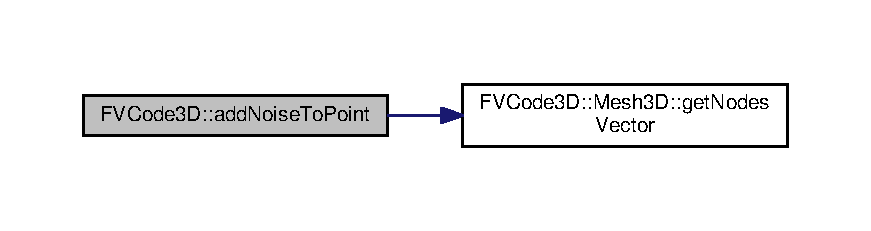
\includegraphics[width=350pt]{namespaceFVCode3D_a9f604a7093f7f7323727e7ba28d8ce75_cgraph}
\end{center}
\end{figure}




Here is the caller graph for this function\+:
\nopagebreak
\begin{figure}[H]
\begin{center}
\leavevmode
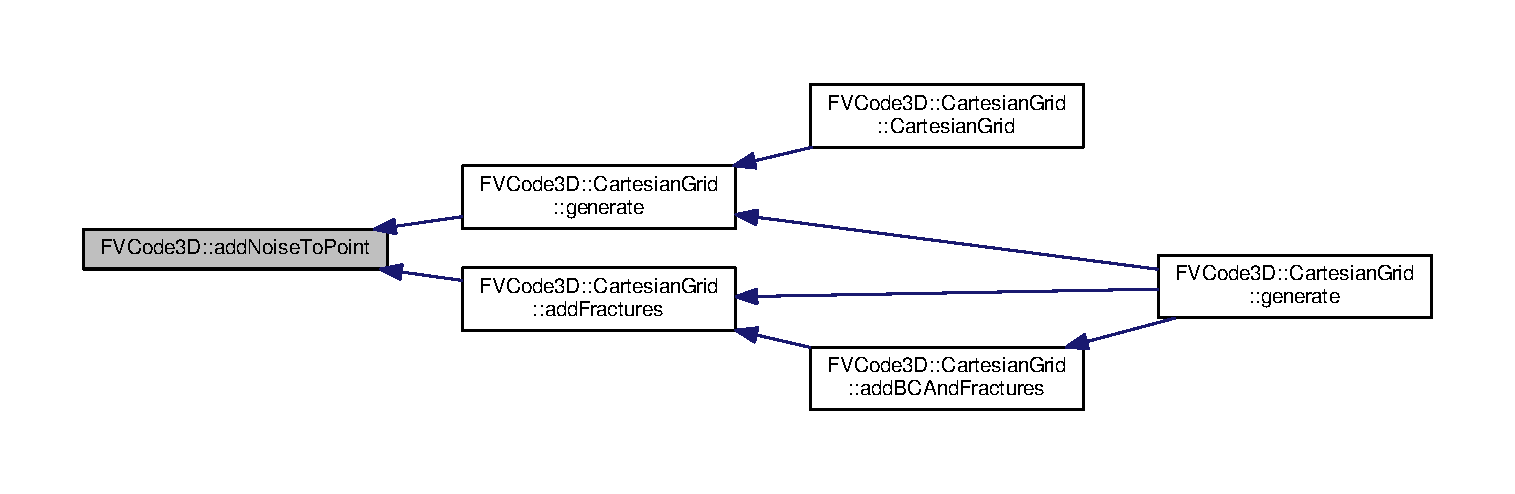
\includegraphics[width=350pt]{namespaceFVCode3D_a9f604a7093f7f7323727e7ba28d8ce75_icgraph}
\end{center}
\end{figure}


\index{F\+V\+Code3D@{F\+V\+Code3D}!add\+Noise\+To\+Point@{add\+Noise\+To\+Point}}
\index{add\+Noise\+To\+Point@{add\+Noise\+To\+Point}!F\+V\+Code3D@{F\+V\+Code3D}}
\subsubsection[{\texorpdfstring{add\+Noise\+To\+Point(\+Mesh3\+D \&mesh, const std\+::vector$<$ bool $>$ \&nodes\+With\+Noise, const Real mean=0., const Real st\+Dev=1.)}{addNoiseToPoint(Mesh3D &mesh, const std::vector< bool > &nodesWithNoise, const Real mean=0., const Real stDev=1.)}}]{\setlength{\rightskip}{0pt plus 5cm}void F\+V\+Code3\+D\+::add\+Noise\+To\+Point (
\begin{DoxyParamCaption}
\item[{{\bf Mesh3D} \&}]{mesh, }
\item[{const std\+::vector$<$ bool $>$ \&}]{nodes\+With\+Noise, }
\item[{const {\bf Real}}]{mean = {\ttfamily 0.}, }
\item[{const {\bf Real}}]{st\+Dev = {\ttfamily 1.}}
\end{DoxyParamCaption}
)}\hypertarget{namespaceFVCode3D_a83503dfaf8e3d2594eda363a28c5425a}{}\label{namespaceFVCode3D_a83503dfaf8e3d2594eda363a28c5425a}


Add noise to a set of points. 

Add noise to the points following a normal distribution with mean {\itshape mean} and standard deviation {\itshape st\+Dev} 
\begin{DoxyParams}{Parameters}
{\em mesh} & reference to a \hyperlink{classFVCode3D_1_1Mesh3D}{Mesh3D} \\
\hline
{\em nodes\+With\+Noise} & vector that indicates on which nodes the noise is applied \\
\hline
{\em mean} & mean. Default = 0. \\
\hline
{\em st\+Dev} & standard deviation. Default = 1. \\
\hline
\end{DoxyParams}


Definition at line \hyperlink{MeshUtility_8cpp_source_l00027}{27} of file \hyperlink{MeshUtility_8cpp_source}{Mesh\+Utility.\+cpp}.



Here is the call graph for this function\+:
\nopagebreak
\begin{figure}[H]
\begin{center}
\leavevmode
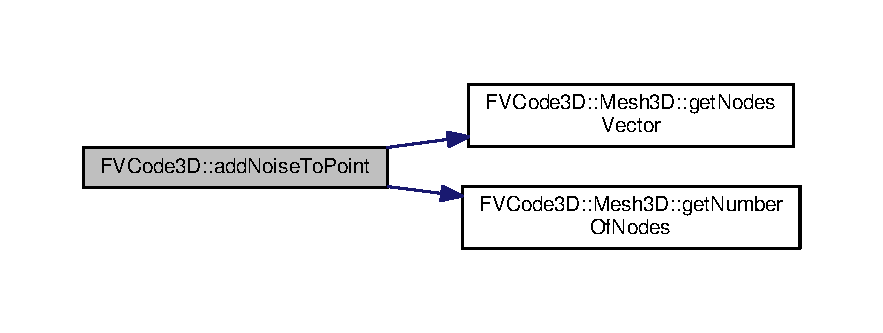
\includegraphics[width=350pt]{namespaceFVCode3D_a83503dfaf8e3d2594eda363a28c5425a_cgraph}
\end{center}
\end{figure}


\index{F\+V\+Code3D@{F\+V\+Code3D}!add\+Noise\+To\+Point@{add\+Noise\+To\+Point}}
\index{add\+Noise\+To\+Point@{add\+Noise\+To\+Point}!F\+V\+Code3D@{F\+V\+Code3D}}
\subsubsection[{\texorpdfstring{add\+Noise\+To\+Point(\+Mesh3\+D \&mesh, const std\+::vector$<$ bool $>$ \&nodes\+With\+Noise, const std\+::vector$<$ U\+Int $>$ \&coords, const Real mean=0., const Real st\+Dev=1.)}{addNoiseToPoint(Mesh3D &mesh, const std::vector< bool > &nodesWithNoise, const std::vector< UInt > &coords, const Real mean=0., const Real stDev=1.)}}]{\setlength{\rightskip}{0pt plus 5cm}void F\+V\+Code3\+D\+::add\+Noise\+To\+Point (
\begin{DoxyParamCaption}
\item[{{\bf Mesh3D} \&}]{mesh, }
\item[{const std\+::vector$<$ bool $>$ \&}]{nodes\+With\+Noise, }
\item[{const std\+::vector$<$ {\bf U\+Int} $>$ \&}]{coords, }
\item[{const {\bf Real}}]{mean = {\ttfamily 0.}, }
\item[{const {\bf Real}}]{st\+Dev = {\ttfamily 1.}}
\end{DoxyParamCaption}
)}\hypertarget{namespaceFVCode3D_a2e19a6aeb189d2ca5370234dd84caa73}{}\label{namespaceFVCode3D_a2e19a6aeb189d2ca5370234dd84caa73}


Add noise to a set of points. 

Add noise to the points following a normal distribution with mean {\itshape mean} and standard deviation {\itshape st\+Dev} 
\begin{DoxyParams}{Parameters}
{\em mesh} & reference to a \hyperlink{classFVCode3D_1_1Mesh3D}{Mesh3D} \\
\hline
{\em nodes\+With\+Noise} & vector that indicates on which nodes the noise is applied \\
\hline
{\em coords} & coordinates on which the noise is applied \\
\hline
{\em mean} & mean. Default = 0. \\
\hline
{\em st\+Dev} & standard deviation. Default = 1. \\
\hline
\end{DoxyParams}


Definition at line \hyperlink{MeshUtility_8cpp_source_l00046}{46} of file \hyperlink{MeshUtility_8cpp_source}{Mesh\+Utility.\+cpp}.



Here is the call graph for this function\+:
\nopagebreak
\begin{figure}[H]
\begin{center}
\leavevmode
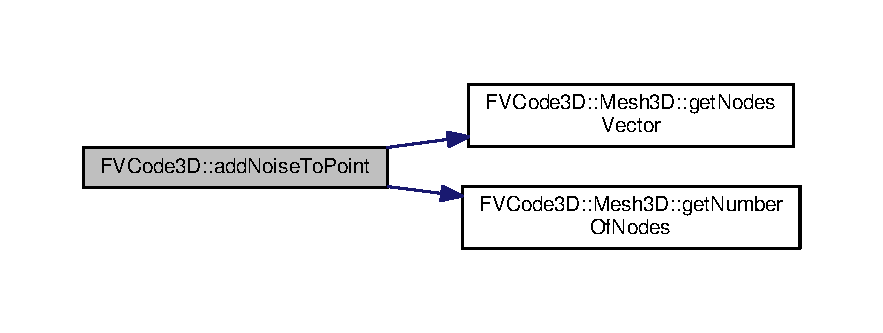
\includegraphics[width=350pt]{namespaceFVCode3D_a2e19a6aeb189d2ca5370234dd84caa73_cgraph}
\end{center}
\end{figure}


\index{F\+V\+Code3D@{F\+V\+Code3D}!compute\+Bounding\+Box@{compute\+Bounding\+Box}}
\index{compute\+Bounding\+Box@{compute\+Bounding\+Box}!F\+V\+Code3D@{F\+V\+Code3D}}
\subsubsection[{\texorpdfstring{compute\+Bounding\+Box(const std\+::vector$<$ Point3\+D $>$ \&nodes, Point3\+D \&p\+Min, Point3\+D \&p\+Max)}{computeBoundingBox(const std::vector< Point3D > &nodes, Point3D &pMin, Point3D &pMax)}}]{\setlength{\rightskip}{0pt plus 5cm}void F\+V\+Code3\+D\+::compute\+Bounding\+Box (
\begin{DoxyParamCaption}
\item[{const std\+::vector$<$ {\bf Point3D} $>$ \&}]{nodes, }
\item[{{\bf Point3D} \&}]{p\+Min, }
\item[{{\bf Point3D} \&}]{p\+Max}
\end{DoxyParamCaption}
)}\hypertarget{namespaceFVCode3D_ae827f8be7749dd9703b52a52d90c9f9b}{}\label{namespaceFVCode3D_ae827f8be7749dd9703b52a52d90c9f9b}


Compute the bounding-\/box of a set of points. 


\begin{DoxyParams}{Parameters}
{\em nodes} & vector of points \\
\hline
{\em p\+Min} & first point that defines the BB \\
\hline
{\em p\+Max} & second point that defines the BB \\
\hline
\end{DoxyParams}


Definition at line \hyperlink{Operations_8cpp_source_l00047}{47} of file \hyperlink{Operations_8cpp_source}{Operations.\+cpp}.



Here is the call graph for this function\+:
\nopagebreak
\begin{figure}[H]
\begin{center}
\leavevmode
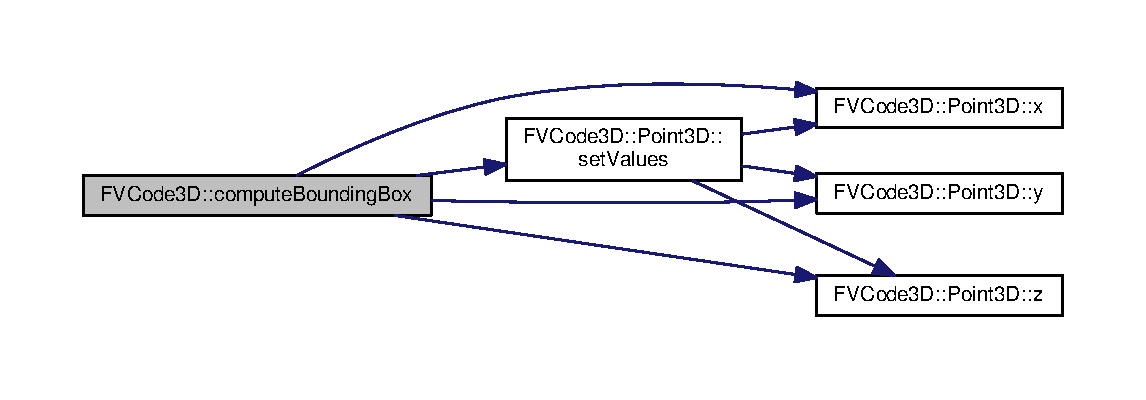
\includegraphics[width=350pt]{namespaceFVCode3D_ae827f8be7749dd9703b52a52d90c9f9b_cgraph}
\end{center}
\end{figure}


\index{F\+V\+Code3D@{F\+V\+Code3D}!compute\+Normal@{compute\+Normal}}
\index{compute\+Normal@{compute\+Normal}!F\+V\+Code3D@{F\+V\+Code3D}}
\subsubsection[{\texorpdfstring{compute\+Normal(const Point3\+D \&\+A, const Point3\+D \&\+B, const Point3\+D \&\+C)}{computeNormal(const Point3D &A, const Point3D &B, const Point3D &C)}}]{\setlength{\rightskip}{0pt plus 5cm}{\bf Point3D} F\+V\+Code3\+D\+::compute\+Normal (
\begin{DoxyParamCaption}
\item[{const {\bf Point3D} \&}]{A, }
\item[{const {\bf Point3D} \&}]{B, }
\item[{const {\bf Point3D} \&}]{C}
\end{DoxyParamCaption}
)}\hypertarget{namespaceFVCode3D_afdf87b62988c2271186926eb3a3baedc}{}\label{namespaceFVCode3D_afdf87b62988c2271186926eb3a3baedc}


Compute the normal moving from three points that lie on a plane (use the right-\/hand rule) 


\begin{DoxyParams}{Parameters}
{\em A} & first point \\
\hline
{\em B} & second point \\
\hline
{\em C} & third point \\
\hline
\end{DoxyParams}
\begin{DoxyReturn}{Returns}
signed normal 
\end{DoxyReturn}


Definition at line \hyperlink{Operations_8cpp_source_l00012}{12} of file \hyperlink{Operations_8cpp_source}{Operations.\+cpp}.



Here is the call graph for this function\+:
\nopagebreak
\begin{figure}[H]
\begin{center}
\leavevmode
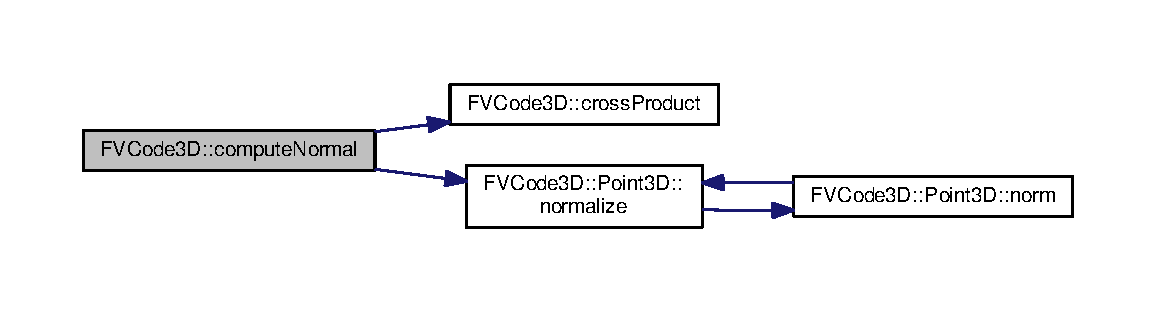
\includegraphics[width=350pt]{namespaceFVCode3D_afdf87b62988c2271186926eb3a3baedc_cgraph}
\end{center}
\end{figure}




Here is the caller graph for this function\+:
\nopagebreak
\begin{figure}[H]
\begin{center}
\leavevmode
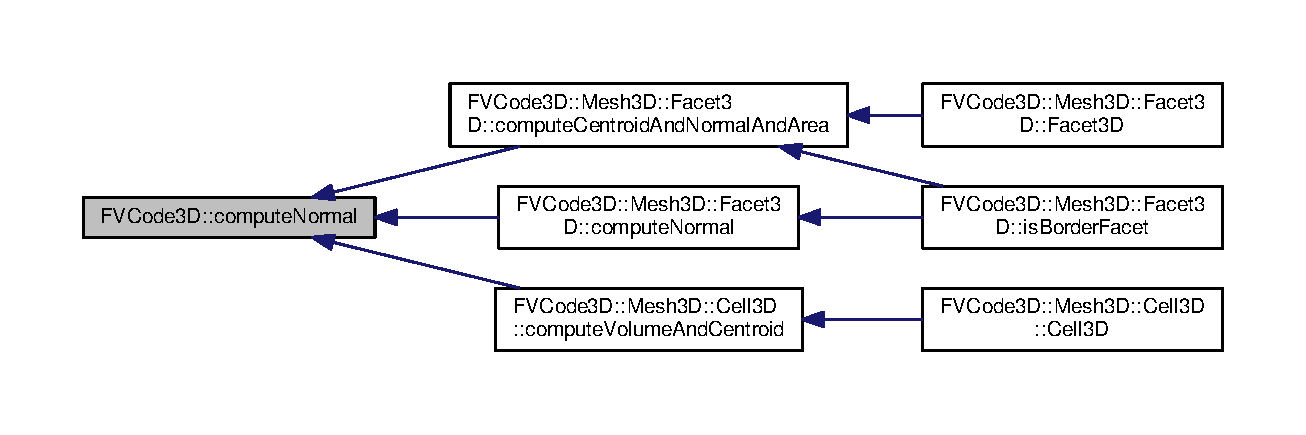
\includegraphics[width=350pt]{namespaceFVCode3D_afdf87b62988c2271186926eb3a3baedc_icgraph}
\end{center}
\end{figure}


\index{F\+V\+Code3D@{F\+V\+Code3D}!cross\+Product@{cross\+Product}}
\index{cross\+Product@{cross\+Product}!F\+V\+Code3D@{F\+V\+Code3D}}
\subsubsection[{\texorpdfstring{cross\+Product(const Point3\+D \&p1, const Point3\+D \&p2)}{crossProduct(const Point3D &p1, const Point3D &p2)}}]{\setlength{\rightskip}{0pt plus 5cm}{\bf Point3D} F\+V\+Code3\+D\+::cross\+Product (
\begin{DoxyParamCaption}
\item[{const {\bf Point3D} \&}]{p1, }
\item[{const {\bf Point3D} \&}]{p2}
\end{DoxyParamCaption}
)}\hypertarget{namespaceFVCode3D_a1ee7c9a5fcc645574f6a93e5f6f53b4b}{}\label{namespaceFVCode3D_a1ee7c9a5fcc645574f6a93e5f6f53b4b}


Definition at line \hyperlink{Point3D_8cpp_source_l00211}{211} of file \hyperlink{Point3D_8cpp_source}{Point3\+D.\+cpp}.



Here is the caller graph for this function\+:
\nopagebreak
\begin{figure}[H]
\begin{center}
\leavevmode
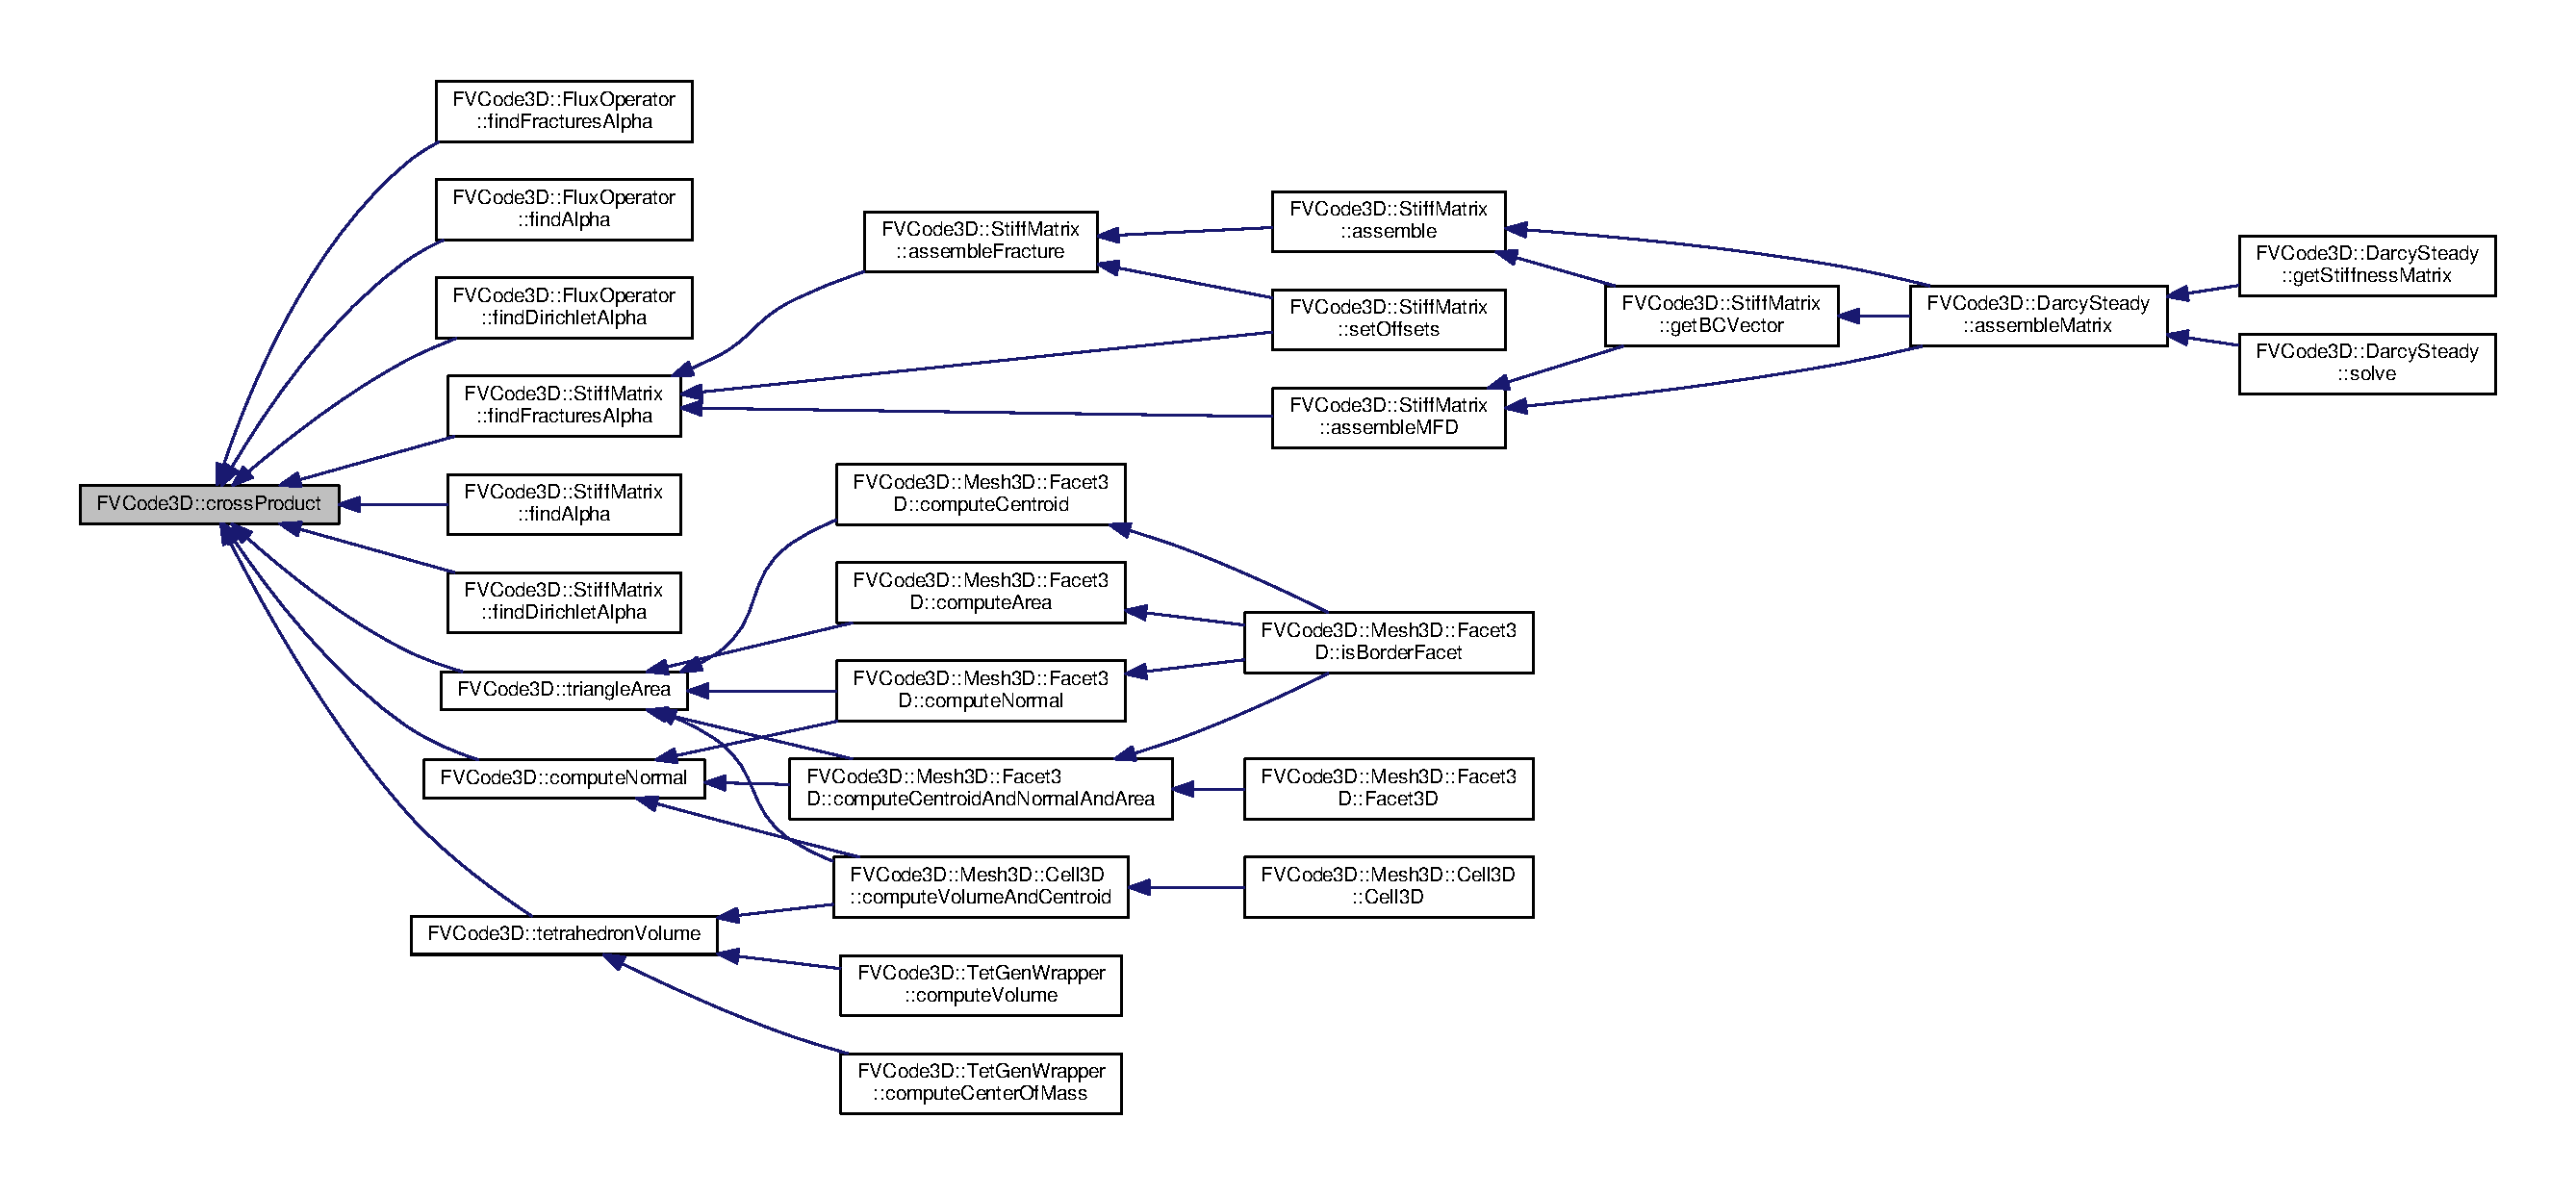
\includegraphics[width=350pt]{namespaceFVCode3D_a1ee7c9a5fcc645574f6a93e5f6f53b4b_icgraph}
\end{center}
\end{figure}


\index{F\+V\+Code3D@{F\+V\+Code3D}!distance@{distance}}
\index{distance@{distance}!F\+V\+Code3D@{F\+V\+Code3D}}
\subsubsection[{\texorpdfstring{distance(const Point3\+D \&p1, const Point3\+D \&p2)}{distance(const Point3D &p1, const Point3D &p2)}}]{\setlength{\rightskip}{0pt plus 5cm}{\bf Real} F\+V\+Code3\+D\+::distance (
\begin{DoxyParamCaption}
\item[{const {\bf Point3D} \&}]{p1, }
\item[{const {\bf Point3D} \&}]{p2}
\end{DoxyParamCaption}
)}\hypertarget{namespaceFVCode3D_a705717c0673e24ca607c7a65054de4f7}{}\label{namespaceFVCode3D_a705717c0673e24ca607c7a65054de4f7}


Definition at line \hyperlink{Point3D_8cpp_source_l00206}{206} of file \hyperlink{Point3D_8cpp_source}{Point3\+D.\+cpp}.



Here is the caller graph for this function\+:
\nopagebreak
\begin{figure}[H]
\begin{center}
\leavevmode
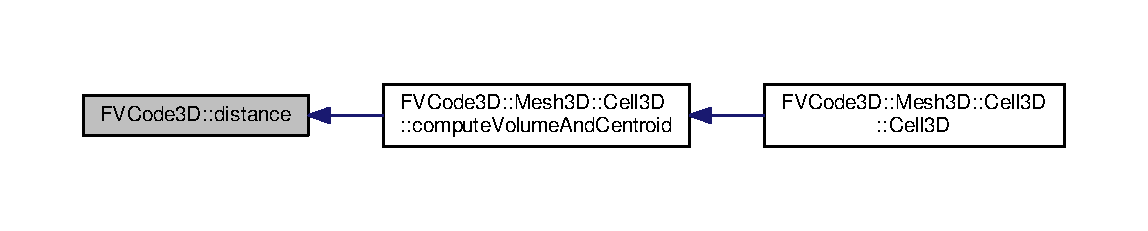
\includegraphics[width=350pt]{namespaceFVCode3D_a705717c0673e24ca607c7a65054de4f7_icgraph}
\end{center}
\end{figure}


\index{F\+V\+Code3D@{F\+V\+Code3D}!dot\+Product@{dot\+Product}}
\index{dot\+Product@{dot\+Product}!F\+V\+Code3D@{F\+V\+Code3D}}
\subsubsection[{\texorpdfstring{dot\+Product(const Point3\+D \&p1, const Point3\+D \&p2)}{dotProduct(const Point3D &p1, const Point3D &p2)}}]{\setlength{\rightskip}{0pt plus 5cm}{\bf Real} F\+V\+Code3\+D\+::dot\+Product (
\begin{DoxyParamCaption}
\item[{const {\bf Point3D} \&}]{p1, }
\item[{const {\bf Point3D} \&}]{p2}
\end{DoxyParamCaption}
)}\hypertarget{namespaceFVCode3D_ad07be7f9ed843ca65d02d0303dae6cb4}{}\label{namespaceFVCode3D_ad07be7f9ed843ca65d02d0303dae6cb4}


Definition at line \hyperlink{Point3D_8cpp_source_l00186}{186} of file \hyperlink{Point3D_8cpp_source}{Point3\+D.\+cpp}.



Here is the caller graph for this function\+:
\nopagebreak
\begin{figure}[H]
\begin{center}
\leavevmode
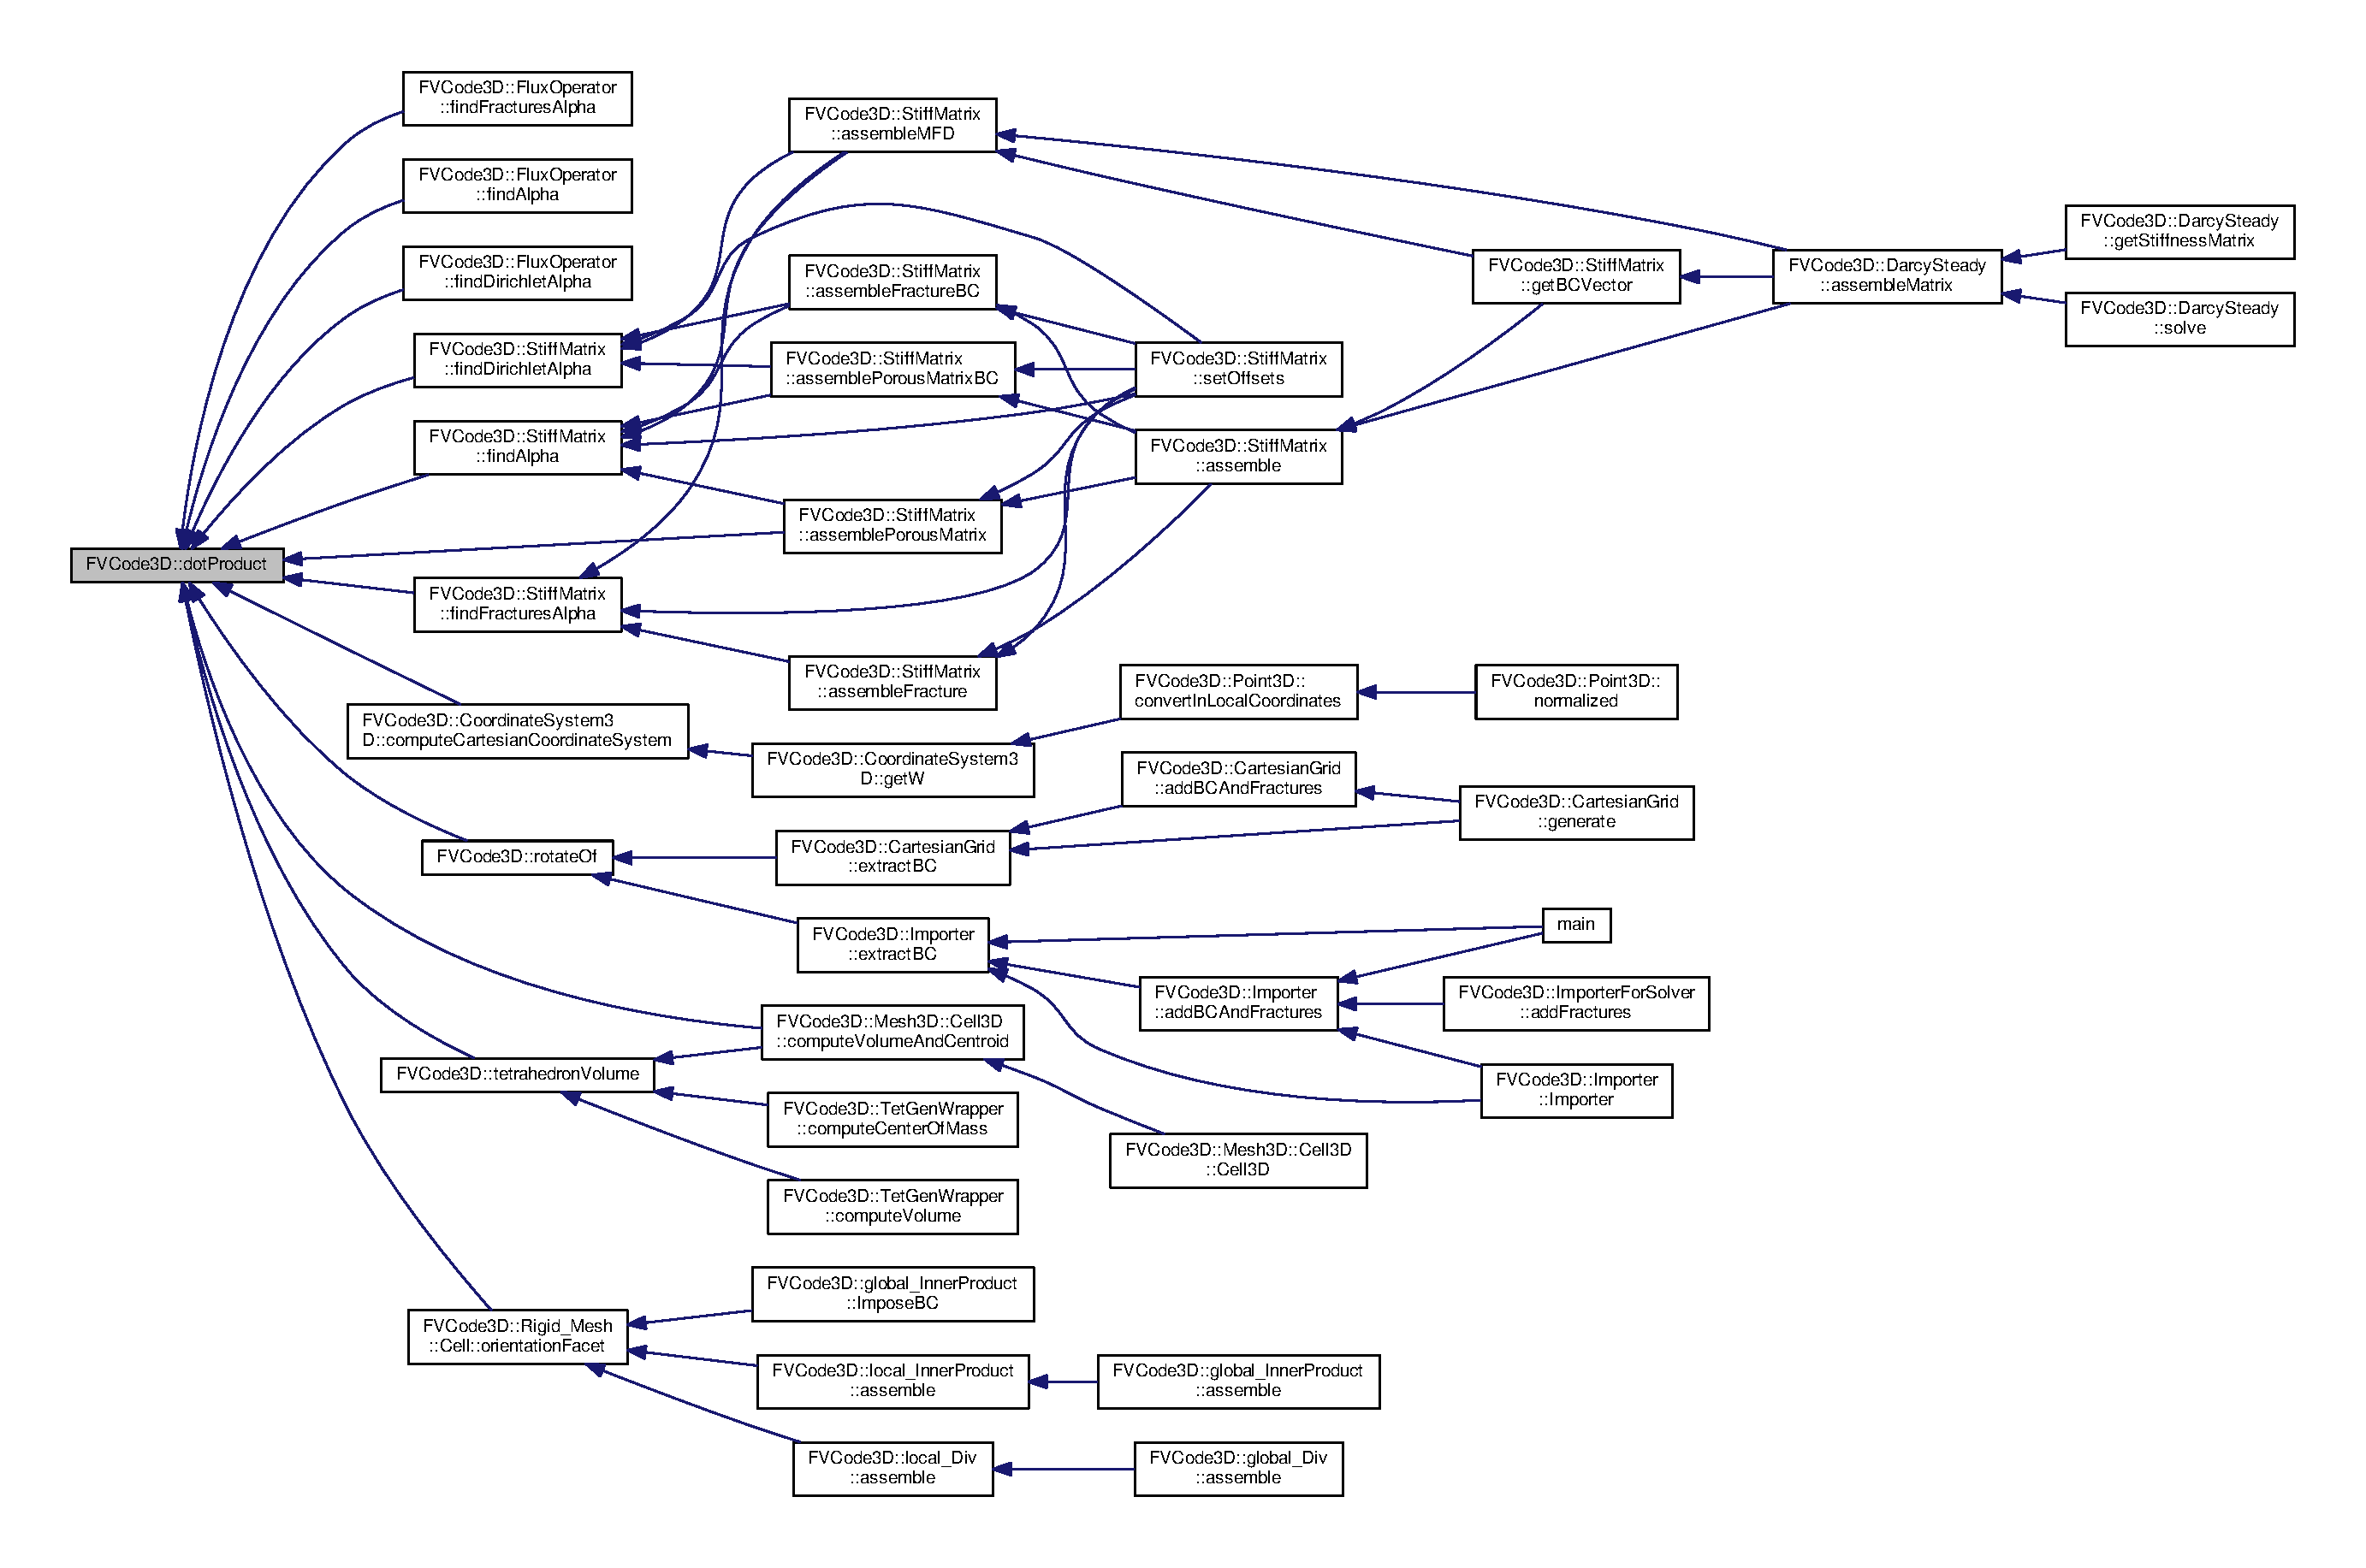
\includegraphics[width=350pt]{namespaceFVCode3D_ad07be7f9ed843ca65d02d0303dae6cb4_icgraph}
\end{center}
\end{figure}


\index{F\+V\+Code3D@{F\+V\+Code3D}!evaluate@{evaluate}}
\index{evaluate@{evaluate}!F\+V\+Code3D@{F\+V\+Code3D}}
\subsubsection[{\texorpdfstring{evaluate(const Rigid\+\_\+\+Mesh \&mesh, const std\+::function$<$ Real(\+Point3\+D)$>$ \&func)}{evaluate(const Rigid_Mesh &mesh, const std::function< Real(Point3D)> &func)}}]{\setlength{\rightskip}{0pt plus 5cm}{\bf Vector} F\+V\+Code3\+D\+::evaluate (
\begin{DoxyParamCaption}
\item[{const {\bf Rigid\+\_\+\+Mesh} \&}]{mesh, }
\item[{const std\+::function$<$ {\bf Real}({\bf Point3D})$>$ \&}]{func}
\end{DoxyParamCaption}
)}\hypertarget{namespaceFVCode3D_a113366cb939ded701e04649337315295}{}\label{namespaceFVCode3D_a113366cb939ded701e04649337315295}


Definition at line \hyperlink{Evaluate_8cpp_source_l00033}{33} of file \hyperlink{Evaluate_8cpp_source}{Evaluate.\+cpp}.



Here is the call graph for this function\+:
\nopagebreak
\begin{figure}[H]
\begin{center}
\leavevmode
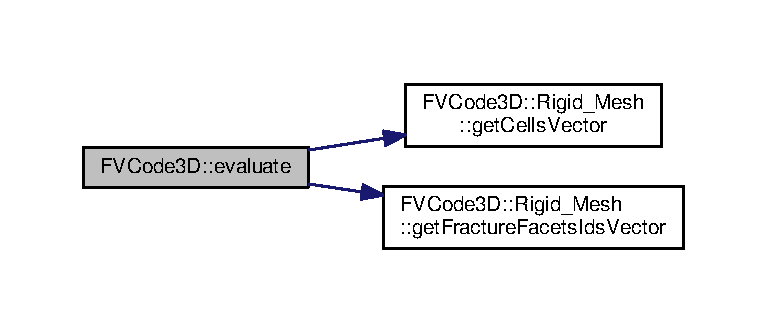
\includegraphics[width=350pt]{namespaceFVCode3D_a113366cb939ded701e04649337315295_cgraph}
\end{center}
\end{figure}


\index{F\+V\+Code3D@{F\+V\+Code3D}!evaluate\+Fracture@{evaluate\+Fracture}}
\index{evaluate\+Fracture@{evaluate\+Fracture}!F\+V\+Code3D@{F\+V\+Code3D}}
\subsubsection[{\texorpdfstring{evaluate\+Fracture(const Rigid\+\_\+\+Mesh \&mesh, const std\+::function$<$ Real(\+Point3\+D)$>$ \&func)}{evaluateFracture(const Rigid_Mesh &mesh, const std::function< Real(Point3D)> &func)}}]{\setlength{\rightskip}{0pt plus 5cm}{\bf Vector} F\+V\+Code3\+D\+::evaluate\+Fracture (
\begin{DoxyParamCaption}
\item[{const {\bf Rigid\+\_\+\+Mesh} \&}]{mesh, }
\item[{const std\+::function$<$ {\bf Real}({\bf Point3D})$>$ \&}]{func}
\end{DoxyParamCaption}
)}\hypertarget{namespaceFVCode3D_a9d3700c347e26f9a442a95785abceac6}{}\label{namespaceFVCode3D_a9d3700c347e26f9a442a95785abceac6}


Definition at line \hyperlink{Evaluate_8cpp_source_l00019}{19} of file \hyperlink{Evaluate_8cpp_source}{Evaluate.\+cpp}.



Here is the call graph for this function\+:
\nopagebreak
\begin{figure}[H]
\begin{center}
\leavevmode
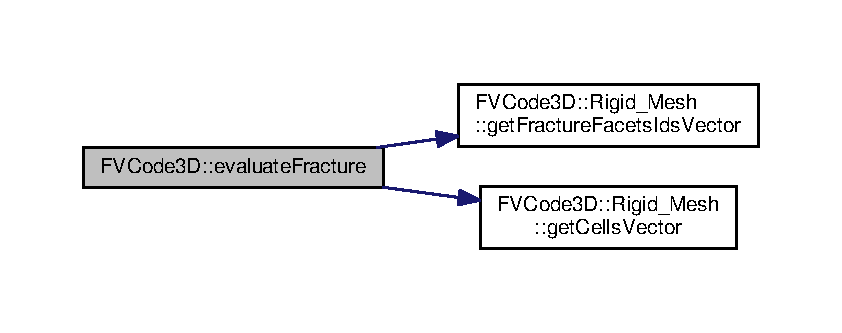
\includegraphics[width=350pt]{namespaceFVCode3D_a9d3700c347e26f9a442a95785abceac6_cgraph}
\end{center}
\end{figure}


\index{F\+V\+Code3D@{F\+V\+Code3D}!evaluate\+Matrix@{evaluate\+Matrix}}
\index{evaluate\+Matrix@{evaluate\+Matrix}!F\+V\+Code3D@{F\+V\+Code3D}}
\subsubsection[{\texorpdfstring{evaluate\+Matrix(const Rigid\+\_\+\+Mesh \&mesh, const std\+::function$<$ Real(\+Point3\+D)$>$ \&func)}{evaluateMatrix(const Rigid_Mesh &mesh, const std::function< Real(Point3D)> &func)}}]{\setlength{\rightskip}{0pt plus 5cm}{\bf Vector} F\+V\+Code3\+D\+::evaluate\+Matrix (
\begin{DoxyParamCaption}
\item[{const {\bf Rigid\+\_\+\+Mesh} \&}]{mesh, }
\item[{const std\+::function$<$ {\bf Real}({\bf Point3D})$>$ \&}]{func}
\end{DoxyParamCaption}
)}\hypertarget{namespaceFVCode3D_a3d3cdaa3f99983f1aa2d079caded2585}{}\label{namespaceFVCode3D_a3d3cdaa3f99983f1aa2d079caded2585}


Definition at line \hyperlink{Evaluate_8cpp_source_l00006}{6} of file \hyperlink{Evaluate_8cpp_source}{Evaluate.\+cpp}.



Here is the call graph for this function\+:
\nopagebreak
\begin{figure}[H]
\begin{center}
\leavevmode
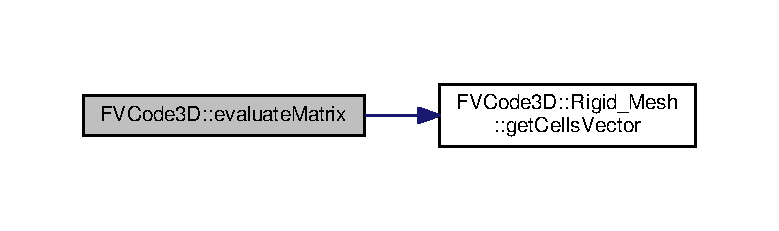
\includegraphics[width=350pt]{namespaceFVCode3D_a3d3cdaa3f99983f1aa2d079caded2585_cgraph}
\end{center}
\end{figure}


\index{F\+V\+Code3D@{F\+V\+Code3D}!inner\+Angle\+Deg@{inner\+Angle\+Deg}}
\index{inner\+Angle\+Deg@{inner\+Angle\+Deg}!F\+V\+Code3D@{F\+V\+Code3D}}
\subsubsection[{\texorpdfstring{inner\+Angle\+Deg(const Point3\+D \&p1, const Point3\+D \&p2)}{innerAngleDeg(const Point3D &p1, const Point3D &p2)}}]{\setlength{\rightskip}{0pt plus 5cm}{\bf Real} F\+V\+Code3\+D\+::inner\+Angle\+Deg (
\begin{DoxyParamCaption}
\item[{const {\bf Point3D} \&}]{p1, }
\item[{const {\bf Point3D} \&}]{p2}
\end{DoxyParamCaption}
)}\hypertarget{namespaceFVCode3D_ae33e5908d62b0ae8dbfdf089ab9bc138}{}\label{namespaceFVCode3D_ae33e5908d62b0ae8dbfdf089ab9bc138}


Definition at line \hyperlink{Point3D_8cpp_source_l00199}{199} of file \hyperlink{Point3D_8cpp_source}{Point3\+D.\+cpp}.



Here is the call graph for this function\+:
\nopagebreak
\begin{figure}[H]
\begin{center}
\leavevmode
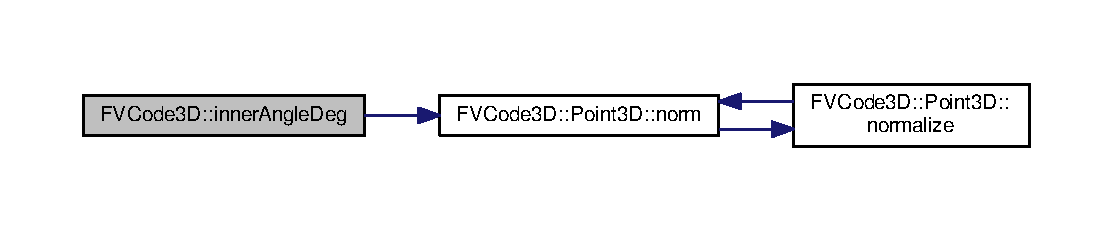
\includegraphics[width=350pt]{namespaceFVCode3D_ae33e5908d62b0ae8dbfdf089ab9bc138_cgraph}
\end{center}
\end{figure}


\index{F\+V\+Code3D@{F\+V\+Code3D}!inner\+Angle\+Rad@{inner\+Angle\+Rad}}
\index{inner\+Angle\+Rad@{inner\+Angle\+Rad}!F\+V\+Code3D@{F\+V\+Code3D}}
\subsubsection[{\texorpdfstring{inner\+Angle\+Rad(const Point3\+D \&p1, const Point3\+D \&p2)}{innerAngleRad(const Point3D &p1, const Point3D &p2)}}]{\setlength{\rightskip}{0pt plus 5cm}{\bf Real} F\+V\+Code3\+D\+::inner\+Angle\+Rad (
\begin{DoxyParamCaption}
\item[{const {\bf Point3D} \&}]{p1, }
\item[{const {\bf Point3D} \&}]{p2}
\end{DoxyParamCaption}
)}\hypertarget{namespaceFVCode3D_acbd112899b9e007bec3fe01223140c45}{}\label{namespaceFVCode3D_acbd112899b9e007bec3fe01223140c45}


Definition at line \hyperlink{Point3D_8cpp_source_l00192}{192} of file \hyperlink{Point3D_8cpp_source}{Point3\+D.\+cpp}.



Here is the call graph for this function\+:
\nopagebreak
\begin{figure}[H]
\begin{center}
\leavevmode
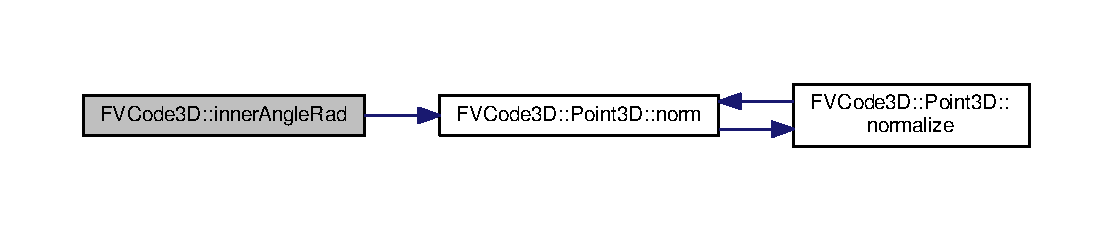
\includegraphics[width=350pt]{namespaceFVCode3D_acbd112899b9e007bec3fe01223140c45_cgraph}
\end{center}
\end{figure}


\index{F\+V\+Code3D@{F\+V\+Code3D}!lexical\+\_\+cast@{lexical\+\_\+cast}}
\index{lexical\+\_\+cast@{lexical\+\_\+cast}!F\+V\+Code3D@{F\+V\+Code3D}}
\subsubsection[{\texorpdfstring{lexical\+\_\+cast(const std\+::string \&str)}{lexical_cast(const std::string &str)}}]{\setlength{\rightskip}{0pt plus 5cm}template$<$typename T $>$ T F\+V\+Code3\+D\+::lexical\+\_\+cast (
\begin{DoxyParamCaption}
\item[{const std\+::string \&}]{str}
\end{DoxyParamCaption}
)}\hypertarget{namespaceFVCode3D_a7d8605df83383ec5cf62f7efe480a68a}{}\label{namespaceFVCode3D_a7d8605df83383ec5cf62f7efe480a68a}


Convert a string to the desired type (using a stringstream) 


\begin{DoxyParams}{Parameters}
{\em str} & string to convert \\
\hline
\end{DoxyParams}


Definition at line \hyperlink{StringManipolator_8hpp_source_l00021}{21} of file \hyperlink{StringManipolator_8hpp_source}{String\+Manipolator.\+hpp}.



Here is the caller graph for this function\+:
\nopagebreak
\begin{figure}[H]
\begin{center}
\leavevmode
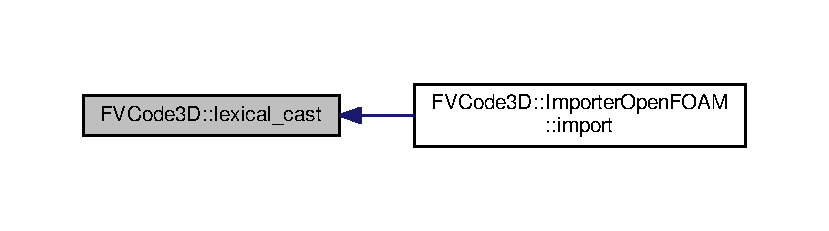
\includegraphics[width=350pt]{namespaceFVCode3D_a7d8605df83383ec5cf62f7efe480a68a_icgraph}
\end{center}
\end{figure}


\index{F\+V\+Code3D@{F\+V\+Code3D}!linear\+Region\+Selection@{linear\+Region\+Selection}}
\index{linear\+Region\+Selection@{linear\+Region\+Selection}!F\+V\+Code3D@{F\+V\+Code3D}}
\subsubsection[{\texorpdfstring{linear\+Region\+Selection(const Real \&\+\_\+cell\+Solution, const U\+Int \&\+\_\+nb\+Regions, const Real \&\+\_\+min\+Solution=0, const Real \&\+\_\+max\+Solution=0)}{linearRegionSelection(const Real &_cellSolution, const UInt &_nbRegions, const Real &_minSolution=0, const Real &_maxSolution=0)}}]{\setlength{\rightskip}{0pt plus 5cm}{\bf U\+Int} F\+V\+Code3\+D\+::linear\+Region\+Selection (
\begin{DoxyParamCaption}
\item[{const {\bf Real} \&}]{\+\_\+cell\+Solution, }
\item[{const {\bf U\+Int} \&}]{\+\_\+nb\+Regions, }
\item[{const {\bf Real} \&}]{\+\_\+min\+Solution = {\ttfamily 0}, }
\item[{const {\bf Real} \&}]{\+\_\+max\+Solution = {\ttfamily 0}}
\end{DoxyParamCaption}
)}\hypertarget{namespaceFVCode3D_ae0b3b38fc8dff58445ba3d625deae285}{}\label{namespaceFVCode3D_ae0b3b38fc8dff58445ba3d625deae285}


Given a cell solution, this function linearly divides the solution range and returns in which sub-\/region the cell belongs. 


\begin{DoxyParams}{Parameters}
{\em \+\_\+cell\+Solution} & solution in a given cell \\
\hline
{\em \+\_\+nb\+Regions} & number of sub regions \\
\hline
{\em \+\_\+min\+Solution} & the minimum value assumed by the solution \\
\hline
{\em \+\_\+max\+Solution} & the maximum value assumed by the solution \\
\hline
\end{DoxyParams}
\begin{DoxyReturn}{Returns}
the sub-\/region id that cell belongs 
\end{DoxyReturn}


Definition at line \hyperlink{MultipleSubRegions_8cpp_source_l00011}{11} of file \hyperlink{MultipleSubRegions_8cpp_source}{Multiple\+Sub\+Regions.\+cpp}.



Here is the caller graph for this function\+:
\nopagebreak
\begin{figure}[H]
\begin{center}
\leavevmode
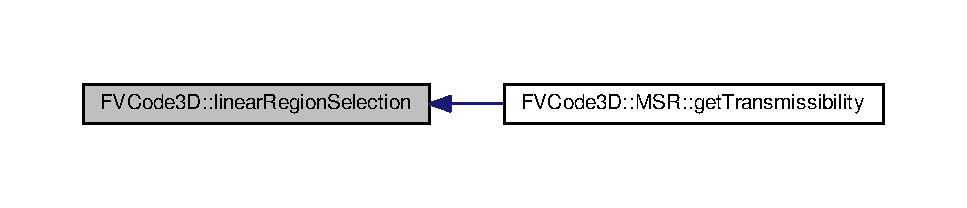
\includegraphics[width=350pt]{namespaceFVCode3D_ae0b3b38fc8dff58445ba3d625deae285_icgraph}
\end{center}
\end{figure}


\index{F\+V\+Code3D@{F\+V\+Code3D}!operator$\ast$@{operator$\ast$}}
\index{operator$\ast$@{operator$\ast$}!F\+V\+Code3D@{F\+V\+Code3D}}
\subsubsection[{\texorpdfstring{operator$\ast$(const Point3\+D \&vector, const Permeability\+Base \&tensor)}{operator*(const Point3D &vector, const PermeabilityBase &tensor)}}]{\setlength{\rightskip}{0pt plus 5cm}{\bf Point3D} F\+V\+Code3\+D\+::operator$\ast$ (
\begin{DoxyParamCaption}
\item[{const {\bf Point3D} \&}]{vector, }
\item[{const {\bf Permeability\+Base} \&}]{tensor}
\end{DoxyParamCaption}
)}\hypertarget{namespaceFVCode3D_af2319dd0d3c654e7509d9b94d14a12ca}{}\label{namespaceFVCode3D_af2319dd0d3c654e7509d9b94d14a12ca}

\begin{DoxyParams}{Parameters}
{\em vector} & vector \\
\hline
{\em tensor} & permeability tensor \\
\hline
\end{DoxyParams}
\begin{DoxyReturn}{Returns}
the product between vector$^\wedge$T and tensor 
\end{DoxyReturn}


Definition at line \hyperlink{Permeability_8cpp_source_l00024}{24} of file \hyperlink{Permeability_8cpp_source}{Permeability.\+cpp}.



Here is the call graph for this function\+:
\nopagebreak
\begin{figure}[H]
\begin{center}
\leavevmode
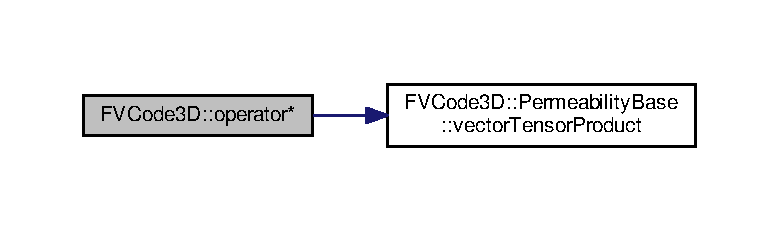
\includegraphics[width=350pt]{namespaceFVCode3D_af2319dd0d3c654e7509d9b94d14a12ca_cgraph}
\end{center}
\end{figure}


\index{F\+V\+Code3D@{F\+V\+Code3D}!operator$\ast$@{operator$\ast$}}
\index{operator$\ast$@{operator$\ast$}!F\+V\+Code3D@{F\+V\+Code3D}}
\subsubsection[{\texorpdfstring{operator$\ast$(const Permeability\+Base \&tensor, const Point3\+D \&vector)}{operator*(const PermeabilityBase &tensor, const Point3D &vector)}}]{\setlength{\rightskip}{0pt plus 5cm}{\bf Point3D} F\+V\+Code3\+D\+::operator$\ast$ (
\begin{DoxyParamCaption}
\item[{const {\bf Permeability\+Base} \&}]{tensor, }
\item[{const {\bf Point3D} \&}]{vector}
\end{DoxyParamCaption}
)}\hypertarget{namespaceFVCode3D_a3ec4a02287df57f0a18c692eb037438a}{}\label{namespaceFVCode3D_a3ec4a02287df57f0a18c692eb037438a}

\begin{DoxyParams}{Parameters}
{\em tensor} & permeability tensor \\
\hline
{\em vector} & vector \\
\hline
\end{DoxyParams}
\begin{DoxyReturn}{Returns}
the product between tensor and vector 
\end{DoxyReturn}


Definition at line \hyperlink{Permeability_8cpp_source_l00029}{29} of file \hyperlink{Permeability_8cpp_source}{Permeability.\+cpp}.



Here is the call graph for this function\+:
\nopagebreak
\begin{figure}[H]
\begin{center}
\leavevmode
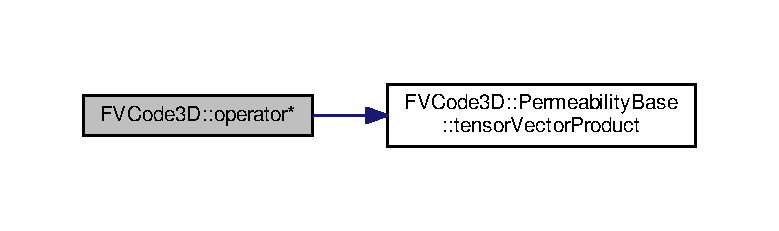
\includegraphics[width=350pt]{namespaceFVCode3D_a3ec4a02287df57f0a18c692eb037438a_cgraph}
\end{center}
\end{figure}


\index{F\+V\+Code3D@{F\+V\+Code3D}!operator$\ast$@{operator$\ast$}}
\index{operator$\ast$@{operator$\ast$}!F\+V\+Code3D@{F\+V\+Code3D}}
\subsubsection[{\texorpdfstring{operator$\ast$(const Point3\+D \&vector, const Perm\+Ptr\+\_\+\+Type \&tensor)}{operator*(const Point3D &vector, const PermPtr_Type &tensor)}}]{\setlength{\rightskip}{0pt plus 5cm}{\bf Point3D} F\+V\+Code3\+D\+::operator$\ast$ (
\begin{DoxyParamCaption}
\item[{const {\bf Point3D} \&}]{vector, }
\item[{const {\bf Perm\+Ptr\+\_\+\+Type} \&}]{tensor}
\end{DoxyParamCaption}
)}\hypertarget{namespaceFVCode3D_affee75e028879b6669f318166c054d71}{}\label{namespaceFVCode3D_affee75e028879b6669f318166c054d71}

\begin{DoxyParams}{Parameters}
{\em vector} & vector \\
\hline
{\em tensor} & permeability tensor \\
\hline
\end{DoxyParams}
\begin{DoxyReturn}{Returns}
the product between vector$^\wedge$T and tensor 
\end{DoxyReturn}


Definition at line \hyperlink{Permeability_8cpp_source_l00034}{34} of file \hyperlink{Permeability_8cpp_source}{Permeability.\+cpp}.

\index{F\+V\+Code3D@{F\+V\+Code3D}!operator$\ast$@{operator$\ast$}}
\index{operator$\ast$@{operator$\ast$}!F\+V\+Code3D@{F\+V\+Code3D}}
\subsubsection[{\texorpdfstring{operator$\ast$(const Perm\+Ptr\+\_\+\+Type \&tensor, const Point3\+D \&vector)}{operator*(const PermPtr_Type &tensor, const Point3D &vector)}}]{\setlength{\rightskip}{0pt plus 5cm}{\bf Point3D} F\+V\+Code3\+D\+::operator$\ast$ (
\begin{DoxyParamCaption}
\item[{const {\bf Perm\+Ptr\+\_\+\+Type} \&}]{tensor, }
\item[{const {\bf Point3D} \&}]{vector}
\end{DoxyParamCaption}
)}\hypertarget{namespaceFVCode3D_a1c83364114566de0a24e730333cf4ba6}{}\label{namespaceFVCode3D_a1c83364114566de0a24e730333cf4ba6}

\begin{DoxyParams}{Parameters}
{\em tensor} & permeability tensor \\
\hline
{\em vector} & vector \\
\hline
\end{DoxyParams}
\begin{DoxyReturn}{Returns}
the product between tensor and vector 
\end{DoxyReturn}


Definition at line \hyperlink{Permeability_8cpp_source_l00039}{39} of file \hyperlink{Permeability_8cpp_source}{Permeability.\+cpp}.

\index{F\+V\+Code3D@{F\+V\+Code3D}!operator$\ast$@{operator$\ast$}}
\index{operator$\ast$@{operator$\ast$}!F\+V\+Code3D@{F\+V\+Code3D}}
\subsubsection[{\texorpdfstring{operator$\ast$(const Point3\+D \&vector, const Permeability\+Scalar \&tensor)}{operator*(const Point3D &vector, const PermeabilityScalar &tensor)}}]{\setlength{\rightskip}{0pt plus 5cm}{\bf Point3D} F\+V\+Code3\+D\+::operator$\ast$ (
\begin{DoxyParamCaption}
\item[{const {\bf Point3D} \&}]{vector, }
\item[{const {\bf Permeability\+Scalar} \&}]{tensor}
\end{DoxyParamCaption}
)}\hypertarget{namespaceFVCode3D_a9ce5cab99db49bc50167ff3705fac221}{}\label{namespaceFVCode3D_a9ce5cab99db49bc50167ff3705fac221}

\begin{DoxyParams}{Parameters}
{\em vector} & vector \\
\hline
{\em tensor} & permeability tensor \\
\hline
\end{DoxyParams}
\begin{DoxyReturn}{Returns}
the product between vector$^\wedge$T and tensor 
\end{DoxyReturn}


Definition at line \hyperlink{Permeability_8cpp_source_l00060}{60} of file \hyperlink{Permeability_8cpp_source}{Permeability.\+cpp}.

\index{F\+V\+Code3D@{F\+V\+Code3D}!operator$\ast$@{operator$\ast$}}
\index{operator$\ast$@{operator$\ast$}!F\+V\+Code3D@{F\+V\+Code3D}}
\subsubsection[{\texorpdfstring{operator$\ast$(const Permeability\+Scalar \&tensor, const Point3\+D \&vector)}{operator*(const PermeabilityScalar &tensor, const Point3D &vector)}}]{\setlength{\rightskip}{0pt plus 5cm}{\bf Point3D} F\+V\+Code3\+D\+::operator$\ast$ (
\begin{DoxyParamCaption}
\item[{const {\bf Permeability\+Scalar} \&}]{tensor, }
\item[{const {\bf Point3D} \&}]{vector}
\end{DoxyParamCaption}
)}\hypertarget{namespaceFVCode3D_a5c756733d1283495ba727f5b8a0e4ab9}{}\label{namespaceFVCode3D_a5c756733d1283495ba727f5b8a0e4ab9}

\begin{DoxyParams}{Parameters}
{\em tensor} & permeability tensor \\
\hline
{\em vector} & vector \\
\hline
\end{DoxyParams}
\begin{DoxyReturn}{Returns}
the product between tensor and vector 
\end{DoxyReturn}


Definition at line \hyperlink{Permeability_8cpp_source_l00065}{65} of file \hyperlink{Permeability_8cpp_source}{Permeability.\+cpp}.

\index{F\+V\+Code3D@{F\+V\+Code3D}!operator$\ast$@{operator$\ast$}}
\index{operator$\ast$@{operator$\ast$}!F\+V\+Code3D@{F\+V\+Code3D}}
\subsubsection[{\texorpdfstring{operator$\ast$(const Point3\+D \&vector, const std\+::shared\+\_\+ptr$<$ Permeability\+Scalar $>$ \&tensor)}{operator*(const Point3D &vector, const std::shared_ptr< PermeabilityScalar > &tensor)}}]{\setlength{\rightskip}{0pt plus 5cm}{\bf Point3D} F\+V\+Code3\+D\+::operator$\ast$ (
\begin{DoxyParamCaption}
\item[{const {\bf Point3D} \&}]{vector, }
\item[{const std\+::shared\+\_\+ptr$<$ {\bf Permeability\+Scalar} $>$ \&}]{tensor}
\end{DoxyParamCaption}
)}\hypertarget{namespaceFVCode3D_a9e5a2a2718342bee157a1c6e2c78fa6e}{}\label{namespaceFVCode3D_a9e5a2a2718342bee157a1c6e2c78fa6e}

\begin{DoxyParams}{Parameters}
{\em vector} & vector \\
\hline
{\em tensor} & permeability tensor \\
\hline
\end{DoxyParams}
\begin{DoxyReturn}{Returns}
the product between vector$^\wedge$T and tensor 
\end{DoxyReturn}


Definition at line \hyperlink{Permeability_8cpp_source_l00070}{70} of file \hyperlink{Permeability_8cpp_source}{Permeability.\+cpp}.

\index{F\+V\+Code3D@{F\+V\+Code3D}!operator$\ast$@{operator$\ast$}}
\index{operator$\ast$@{operator$\ast$}!F\+V\+Code3D@{F\+V\+Code3D}}
\subsubsection[{\texorpdfstring{operator$\ast$(const std\+::shared\+\_\+ptr$<$ Permeability\+Scalar $>$ \&tensor, const Point3\+D \&vector)}{operator*(const std::shared_ptr< PermeabilityScalar > &tensor, const Point3D &vector)}}]{\setlength{\rightskip}{0pt plus 5cm}{\bf Point3D} F\+V\+Code3\+D\+::operator$\ast$ (
\begin{DoxyParamCaption}
\item[{const std\+::shared\+\_\+ptr$<$ {\bf Permeability\+Scalar} $>$ \&}]{tensor, }
\item[{const {\bf Point3D} \&}]{vector}
\end{DoxyParamCaption}
)}\hypertarget{namespaceFVCode3D_a6e6874314b749e7b94c1e0f7b2e25ddc}{}\label{namespaceFVCode3D_a6e6874314b749e7b94c1e0f7b2e25ddc}

\begin{DoxyParams}{Parameters}
{\em vector} & vector \\
\hline
{\em tensor} & permeability tensor \\
\hline
\end{DoxyParams}
\begin{DoxyReturn}{Returns}
the product between vector$^\wedge$T and tensor 
\end{DoxyReturn}


Definition at line \hyperlink{Permeability_8cpp_source_l00075}{75} of file \hyperlink{Permeability_8cpp_source}{Permeability.\+cpp}.

\index{F\+V\+Code3D@{F\+V\+Code3D}!operator$\ast$@{operator$\ast$}}
\index{operator$\ast$@{operator$\ast$}!F\+V\+Code3D@{F\+V\+Code3D}}
\subsubsection[{\texorpdfstring{operator$\ast$(const Point3\+D \&vector, const Permeability\+Diagonal \&tensor)}{operator*(const Point3D &vector, const PermeabilityDiagonal &tensor)}}]{\setlength{\rightskip}{0pt plus 5cm}{\bf Point3D} F\+V\+Code3\+D\+::operator$\ast$ (
\begin{DoxyParamCaption}
\item[{const {\bf Point3D} \&}]{vector, }
\item[{const {\bf Permeability\+Diagonal} \&}]{tensor}
\end{DoxyParamCaption}
)}\hypertarget{namespaceFVCode3D_ab694abb1eb8ba46250bf127f3032d0bd}{}\label{namespaceFVCode3D_ab694abb1eb8ba46250bf127f3032d0bd}

\begin{DoxyParams}{Parameters}
{\em vector} & vector \\
\hline
{\em tensor} & permeability tensor \\
\hline
\end{DoxyParams}
\begin{DoxyReturn}{Returns}
the product between vector$^\wedge$T and tensor 
\end{DoxyReturn}


Definition at line \hyperlink{Permeability_8cpp_source_l00112}{112} of file \hyperlink{Permeability_8cpp_source}{Permeability.\+cpp}.



Here is the call graph for this function\+:
\nopagebreak
\begin{figure}[H]
\begin{center}
\leavevmode
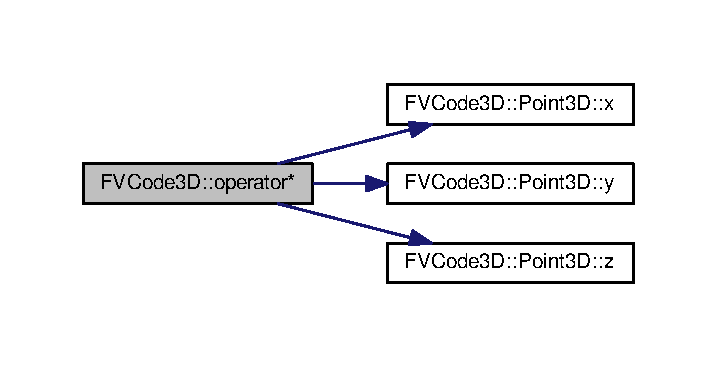
\includegraphics[width=344pt]{namespaceFVCode3D_ab694abb1eb8ba46250bf127f3032d0bd_cgraph}
\end{center}
\end{figure}


\index{F\+V\+Code3D@{F\+V\+Code3D}!operator$\ast$@{operator$\ast$}}
\index{operator$\ast$@{operator$\ast$}!F\+V\+Code3D@{F\+V\+Code3D}}
\subsubsection[{\texorpdfstring{operator$\ast$(const Permeability\+Diagonal \&tensor, const Point3\+D \&vector)}{operator*(const PermeabilityDiagonal &tensor, const Point3D &vector)}}]{\setlength{\rightskip}{0pt plus 5cm}{\bf Point3D} F\+V\+Code3\+D\+::operator$\ast$ (
\begin{DoxyParamCaption}
\item[{const {\bf Permeability\+Diagonal} \&}]{tensor, }
\item[{const {\bf Point3D} \&}]{vector}
\end{DoxyParamCaption}
)}\hypertarget{namespaceFVCode3D_a20d5c43bac77b6978cb71155386aaf9e}{}\label{namespaceFVCode3D_a20d5c43bac77b6978cb71155386aaf9e}

\begin{DoxyParams}{Parameters}
{\em tensor} & permeability tensor \\
\hline
{\em vector} & vector \\
\hline
\end{DoxyParams}
\begin{DoxyReturn}{Returns}
the product between tensor and vector 
\end{DoxyReturn}


Definition at line \hyperlink{Permeability_8cpp_source_l00119}{119} of file \hyperlink{Permeability_8cpp_source}{Permeability.\+cpp}.



Here is the call graph for this function\+:
\nopagebreak
\begin{figure}[H]
\begin{center}
\leavevmode
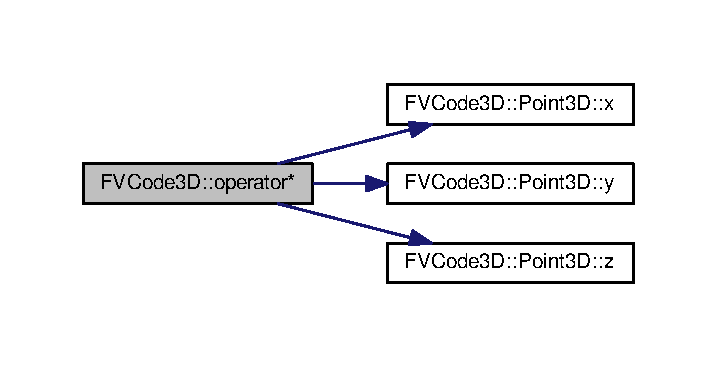
\includegraphics[width=344pt]{namespaceFVCode3D_a20d5c43bac77b6978cb71155386aaf9e_cgraph}
\end{center}
\end{figure}


\index{F\+V\+Code3D@{F\+V\+Code3D}!operator$\ast$@{operator$\ast$}}
\index{operator$\ast$@{operator$\ast$}!F\+V\+Code3D@{F\+V\+Code3D}}
\subsubsection[{\texorpdfstring{operator$\ast$(const Point3\+D \&vector, const std\+::shared\+\_\+ptr$<$ Permeability\+Diagonal $>$ \&tensor)}{operator*(const Point3D &vector, const std::shared_ptr< PermeabilityDiagonal > &tensor)}}]{\setlength{\rightskip}{0pt plus 5cm}{\bf Point3D} F\+V\+Code3\+D\+::operator$\ast$ (
\begin{DoxyParamCaption}
\item[{const {\bf Point3D} \&}]{vector, }
\item[{const std\+::shared\+\_\+ptr$<$ {\bf Permeability\+Diagonal} $>$ \&}]{tensor}
\end{DoxyParamCaption}
)}\hypertarget{namespaceFVCode3D_a84db6637fe253b4e6acd9bd16d887562}{}\label{namespaceFVCode3D_a84db6637fe253b4e6acd9bd16d887562}

\begin{DoxyParams}{Parameters}
{\em vector} & vector \\
\hline
{\em tensor} & permeability tensor \\
\hline
\end{DoxyParams}
\begin{DoxyReturn}{Returns}
the product between vector$^\wedge$T and tensor 
\end{DoxyReturn}


Definition at line \hyperlink{Permeability_8cpp_source_l00126}{126} of file \hyperlink{Permeability_8cpp_source}{Permeability.\+cpp}.

\index{F\+V\+Code3D@{F\+V\+Code3D}!operator$\ast$@{operator$\ast$}}
\index{operator$\ast$@{operator$\ast$}!F\+V\+Code3D@{F\+V\+Code3D}}
\subsubsection[{\texorpdfstring{operator$\ast$(const std\+::shared\+\_\+ptr$<$ Permeability\+Diagonal $>$ \&tensor, const Point3\+D \&vector)}{operator*(const std::shared_ptr< PermeabilityDiagonal > &tensor, const Point3D &vector)}}]{\setlength{\rightskip}{0pt plus 5cm}{\bf Point3D} F\+V\+Code3\+D\+::operator$\ast$ (
\begin{DoxyParamCaption}
\item[{const std\+::shared\+\_\+ptr$<$ {\bf Permeability\+Diagonal} $>$ \&}]{tensor, }
\item[{const {\bf Point3D} \&}]{vector}
\end{DoxyParamCaption}
)}\hypertarget{namespaceFVCode3D_ac318aebf33fb93f512357d07452b7d2e}{}\label{namespaceFVCode3D_ac318aebf33fb93f512357d07452b7d2e}

\begin{DoxyParams}{Parameters}
{\em vector} & vector \\
\hline
{\em tensor} & permeability tensor \\
\hline
\end{DoxyParams}
\begin{DoxyReturn}{Returns}
the product between vector$^\wedge$T and tensor 
\end{DoxyReturn}


Definition at line \hyperlink{Permeability_8cpp_source_l00131}{131} of file \hyperlink{Permeability_8cpp_source}{Permeability.\+cpp}.

\index{F\+V\+Code3D@{F\+V\+Code3D}!operator$\ast$@{operator$\ast$}}
\index{operator$\ast$@{operator$\ast$}!F\+V\+Code3D@{F\+V\+Code3D}}
\subsubsection[{\texorpdfstring{operator$\ast$(const Point3\+D \&p1, const Point3\+D \&p2)}{operator*(const Point3D &p1, const Point3D &p2)}}]{\setlength{\rightskip}{0pt plus 5cm}{\bf Real} F\+V\+Code3\+D\+::operator$\ast$ (
\begin{DoxyParamCaption}
\item[{const {\bf Point3D} \&}]{p1, }
\item[{const {\bf Point3D} \&}]{p2}
\end{DoxyParamCaption}
)}\hypertarget{namespaceFVCode3D_a34e9f6209d7ce6f615394fb60963d450}{}\label{namespaceFVCode3D_a34e9f6209d7ce6f615394fb60963d450}

\begin{DoxyItemize}
\item operator between points (dot product) 
\end{DoxyItemize}

Definition at line \hyperlink{Point3D_8cpp_source_l00162}{162} of file \hyperlink{Point3D_8cpp_source}{Point3\+D.\+cpp}.

\index{F\+V\+Code3D@{F\+V\+Code3D}!operator$\ast$@{operator$\ast$}}
\index{operator$\ast$@{operator$\ast$}!F\+V\+Code3D@{F\+V\+Code3D}}
\subsubsection[{\texorpdfstring{operator$\ast$(const Point3\+D \&p, const Real r)}{operator*(const Point3D &p, const Real r)}}]{\setlength{\rightskip}{0pt plus 5cm}{\bf Point3D} F\+V\+Code3\+D\+::operator$\ast$ (
\begin{DoxyParamCaption}
\item[{const {\bf Point3D} \&}]{p, }
\item[{const {\bf Real}}]{r}
\end{DoxyParamCaption}
)}\hypertarget{namespaceFVCode3D_ac5c448428b01ffde71c0a70f80edb264}{}\label{namespaceFVCode3D_ac5c448428b01ffde71c0a70f80edb264}

\begin{DoxyItemize}
\item operator between point and scalar 
\end{DoxyItemize}

Definition at line \hyperlink{Point3D_8cpp_source_l00167}{167} of file \hyperlink{Point3D_8cpp_source}{Point3\+D.\+cpp}.

\index{F\+V\+Code3D@{F\+V\+Code3D}!operator$\ast$@{operator$\ast$}}
\index{operator$\ast$@{operator$\ast$}!F\+V\+Code3D@{F\+V\+Code3D}}
\subsubsection[{\texorpdfstring{operator$\ast$(const Real r, const Point3\+D \&p)}{operator*(const Real r, const Point3D &p)}}]{\setlength{\rightskip}{0pt plus 5cm}{\bf Point3D} F\+V\+Code3\+D\+::operator$\ast$ (
\begin{DoxyParamCaption}
\item[{const {\bf Real}}]{r, }
\item[{const {\bf Point3D} \&}]{p}
\end{DoxyParamCaption}
)}\hypertarget{namespaceFVCode3D_a3d65ba1de4aa9fa136a484cc1a331f62}{}\label{namespaceFVCode3D_a3d65ba1de4aa9fa136a484cc1a331f62}

\begin{DoxyItemize}
\item operator between scalar and point 
\end{DoxyItemize}

Definition at line \hyperlink{Point3D_8cpp_source_l00174}{174} of file \hyperlink{Point3D_8cpp_source}{Point3\+D.\+cpp}.

\index{F\+V\+Code3D@{F\+V\+Code3D}!operator$\ast$@{operator$\ast$}}
\index{operator$\ast$@{operator$\ast$}!F\+V\+Code3D@{F\+V\+Code3D}}
\subsubsection[{\texorpdfstring{operator$\ast$(const Point3\+D \&vector, const Permeability\+Sym\+Tensor \&tensor)}{operator*(const Point3D &vector, const PermeabilitySymTensor &tensor)}}]{\setlength{\rightskip}{0pt plus 5cm}{\bf Point3D} F\+V\+Code3\+D\+::operator$\ast$ (
\begin{DoxyParamCaption}
\item[{const {\bf Point3D} \&}]{vector, }
\item[{const {\bf Permeability\+Sym\+Tensor} \&}]{tensor}
\end{DoxyParamCaption}
)}\hypertarget{namespaceFVCode3D_a3dfa2f38d2f7f0218cab1d9ec22b18b6}{}\label{namespaceFVCode3D_a3dfa2f38d2f7f0218cab1d9ec22b18b6}

\begin{DoxyParams}{Parameters}
{\em vector} & vector \\
\hline
{\em tensor} & permeability tensor \\
\hline
\end{DoxyParams}
\begin{DoxyReturn}{Returns}
the product between vector$^\wedge$T and tensor 
\end{DoxyReturn}


Definition at line \hyperlink{Permeability_8cpp_source_l00188}{188} of file \hyperlink{Permeability_8cpp_source}{Permeability.\+cpp}.



Here is the call graph for this function\+:
\nopagebreak
\begin{figure}[H]
\begin{center}
\leavevmode
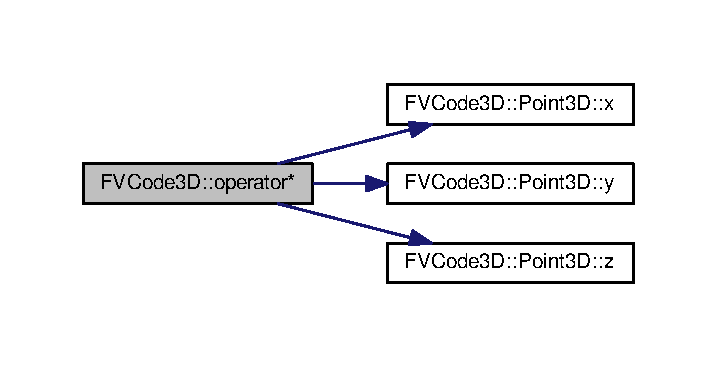
\includegraphics[width=344pt]{namespaceFVCode3D_a3dfa2f38d2f7f0218cab1d9ec22b18b6_cgraph}
\end{center}
\end{figure}


\index{F\+V\+Code3D@{F\+V\+Code3D}!operator$\ast$@{operator$\ast$}}
\index{operator$\ast$@{operator$\ast$}!F\+V\+Code3D@{F\+V\+Code3D}}
\subsubsection[{\texorpdfstring{operator$\ast$(const Permeability\+Sym\+Tensor \&tensor, const Point3\+D \&vector)}{operator*(const PermeabilitySymTensor &tensor, const Point3D &vector)}}]{\setlength{\rightskip}{0pt plus 5cm}{\bf Point3D} F\+V\+Code3\+D\+::operator$\ast$ (
\begin{DoxyParamCaption}
\item[{const {\bf Permeability\+Sym\+Tensor} \&}]{tensor, }
\item[{const {\bf Point3D} \&}]{vector}
\end{DoxyParamCaption}
)}\hypertarget{namespaceFVCode3D_a5ac5e83475a87f9f243d5bf10090c28e}{}\label{namespaceFVCode3D_a5ac5e83475a87f9f243d5bf10090c28e}

\begin{DoxyParams}{Parameters}
{\em tensor} & permeability tensor \\
\hline
{\em vector} & vector \\
\hline
\end{DoxyParams}
\begin{DoxyReturn}{Returns}
the product between tensor and vector 
\end{DoxyReturn}


Definition at line \hyperlink{Permeability_8cpp_source_l00205}{205} of file \hyperlink{Permeability_8cpp_source}{Permeability.\+cpp}.



Here is the call graph for this function\+:
\nopagebreak
\begin{figure}[H]
\begin{center}
\leavevmode
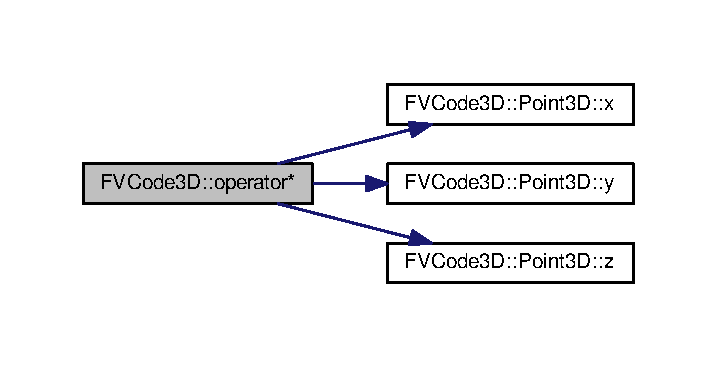
\includegraphics[width=344pt]{namespaceFVCode3D_a5ac5e83475a87f9f243d5bf10090c28e_cgraph}
\end{center}
\end{figure}


\index{F\+V\+Code3D@{F\+V\+Code3D}!operator$\ast$@{operator$\ast$}}
\index{operator$\ast$@{operator$\ast$}!F\+V\+Code3D@{F\+V\+Code3D}}
\subsubsection[{\texorpdfstring{operator$\ast$(const Point3\+D \&vector, const std\+::shared\+\_\+ptr$<$ Permeability\+Sym\+Tensor $>$ \&tensor)}{operator*(const Point3D &vector, const std::shared_ptr< PermeabilitySymTensor > &tensor)}}]{\setlength{\rightskip}{0pt plus 5cm}{\bf Point3D} F\+V\+Code3\+D\+::operator$\ast$ (
\begin{DoxyParamCaption}
\item[{const {\bf Point3D} \&}]{vector, }
\item[{const std\+::shared\+\_\+ptr$<$ {\bf Permeability\+Sym\+Tensor} $>$ \&}]{tensor}
\end{DoxyParamCaption}
)}\hypertarget{namespaceFVCode3D_aeeedc276df199179c196980e5b3e5647}{}\label{namespaceFVCode3D_aeeedc276df199179c196980e5b3e5647}

\begin{DoxyParams}{Parameters}
{\em vector} & vector \\
\hline
{\em tensor} & permeability tensor \\
\hline
\end{DoxyParams}
\begin{DoxyReturn}{Returns}
the product between vector$^\wedge$T and tensor 
\end{DoxyReturn}


Definition at line \hyperlink{Permeability_8cpp_source_l00222}{222} of file \hyperlink{Permeability_8cpp_source}{Permeability.\+cpp}.

\index{F\+V\+Code3D@{F\+V\+Code3D}!operator$\ast$@{operator$\ast$}}
\index{operator$\ast$@{operator$\ast$}!F\+V\+Code3D@{F\+V\+Code3D}}
\subsubsection[{\texorpdfstring{operator$\ast$(const std\+::shared\+\_\+ptr$<$ Permeability\+Sym\+Tensor $>$ \&tensor, const Point3\+D \&vector)}{operator*(const std::shared_ptr< PermeabilitySymTensor > &tensor, const Point3D &vector)}}]{\setlength{\rightskip}{0pt plus 5cm}{\bf Point3D} F\+V\+Code3\+D\+::operator$\ast$ (
\begin{DoxyParamCaption}
\item[{const std\+::shared\+\_\+ptr$<$ {\bf Permeability\+Sym\+Tensor} $>$ \&}]{tensor, }
\item[{const {\bf Point3D} \&}]{vector}
\end{DoxyParamCaption}
)}\hypertarget{namespaceFVCode3D_ac463524bf8214736ff565b8eb89f5dfa}{}\label{namespaceFVCode3D_ac463524bf8214736ff565b8eb89f5dfa}

\begin{DoxyParams}{Parameters}
{\em vector} & vector \\
\hline
{\em tensor} & permeability tensor \\
\hline
\end{DoxyParams}
\begin{DoxyReturn}{Returns}
the product between vector$^\wedge$T and tensor 
\end{DoxyReturn}


Definition at line \hyperlink{Permeability_8cpp_source_l00227}{227} of file \hyperlink{Permeability_8cpp_source}{Permeability.\+cpp}.

\index{F\+V\+Code3D@{F\+V\+Code3D}!operator$\ast$@{operator$\ast$}}
\index{operator$\ast$@{operator$\ast$}!F\+V\+Code3D@{F\+V\+Code3D}}
\subsubsection[{\texorpdfstring{operator$\ast$(const Point3\+D \&vector, const Permeability\+Full\+Tensor \&tensor)}{operator*(const Point3D &vector, const PermeabilityFullTensor &tensor)}}]{\setlength{\rightskip}{0pt plus 5cm}{\bf Point3D} F\+V\+Code3\+D\+::operator$\ast$ (
\begin{DoxyParamCaption}
\item[{const {\bf Point3D} \&}]{vector, }
\item[{const {\bf Permeability\+Full\+Tensor} \&}]{tensor}
\end{DoxyParamCaption}
)}\hypertarget{namespaceFVCode3D_a8da6a56bd95d604552fb78bdab29b491}{}\label{namespaceFVCode3D_a8da6a56bd95d604552fb78bdab29b491}

\begin{DoxyParams}{Parameters}
{\em vector} & vector \\
\hline
{\em tensor} & permeability tensor \\
\hline
\end{DoxyParams}
\begin{DoxyReturn}{Returns}
the product between vector$^\wedge$T and tensor 
\end{DoxyReturn}


Definition at line \hyperlink{Permeability_8cpp_source_l00284}{284} of file \hyperlink{Permeability_8cpp_source}{Permeability.\+cpp}.



Here is the call graph for this function\+:
\nopagebreak
\begin{figure}[H]
\begin{center}
\leavevmode
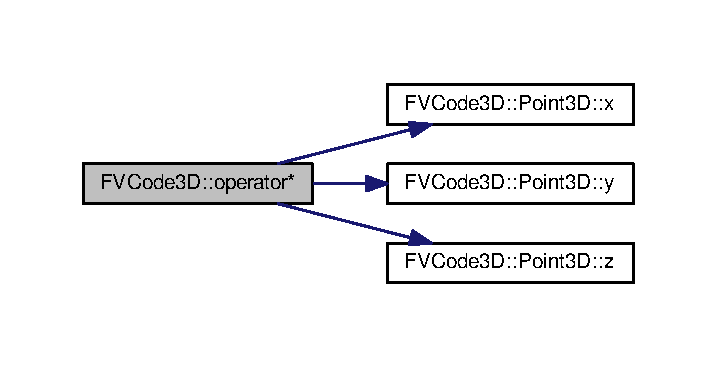
\includegraphics[width=344pt]{namespaceFVCode3D_a8da6a56bd95d604552fb78bdab29b491_cgraph}
\end{center}
\end{figure}


\index{F\+V\+Code3D@{F\+V\+Code3D}!operator$\ast$@{operator$\ast$}}
\index{operator$\ast$@{operator$\ast$}!F\+V\+Code3D@{F\+V\+Code3D}}
\subsubsection[{\texorpdfstring{operator$\ast$(const Permeability\+Full\+Tensor \&tensor, const Point3\+D \&vector)}{operator*(const PermeabilityFullTensor &tensor, const Point3D &vector)}}]{\setlength{\rightskip}{0pt plus 5cm}{\bf Point3D} F\+V\+Code3\+D\+::operator$\ast$ (
\begin{DoxyParamCaption}
\item[{const {\bf Permeability\+Full\+Tensor} \&}]{tensor, }
\item[{const {\bf Point3D} \&}]{vector}
\end{DoxyParamCaption}
)}\hypertarget{namespaceFVCode3D_a81f9e4df393532a4db4ca57703ff5e21}{}\label{namespaceFVCode3D_a81f9e4df393532a4db4ca57703ff5e21}

\begin{DoxyParams}{Parameters}
{\em tensor} & permeability tensor \\
\hline
{\em vector} & vector \\
\hline
\end{DoxyParams}
\begin{DoxyReturn}{Returns}
the product between tensor and vector 
\end{DoxyReturn}


Definition at line \hyperlink{Permeability_8cpp_source_l00301}{301} of file \hyperlink{Permeability_8cpp_source}{Permeability.\+cpp}.



Here is the call graph for this function\+:
\nopagebreak
\begin{figure}[H]
\begin{center}
\leavevmode
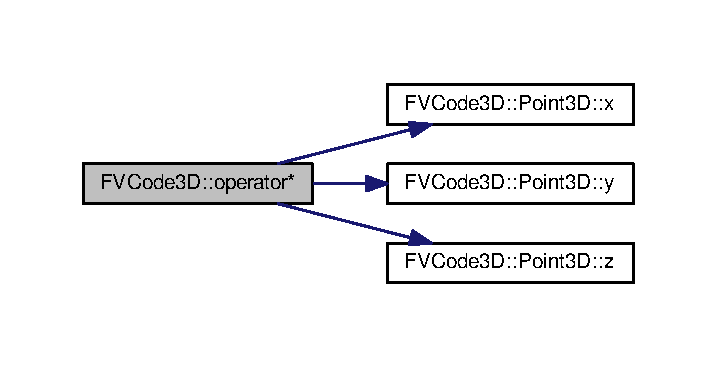
\includegraphics[width=344pt]{namespaceFVCode3D_a81f9e4df393532a4db4ca57703ff5e21_cgraph}
\end{center}
\end{figure}


\index{F\+V\+Code3D@{F\+V\+Code3D}!operator$\ast$@{operator$\ast$}}
\index{operator$\ast$@{operator$\ast$}!F\+V\+Code3D@{F\+V\+Code3D}}
\subsubsection[{\texorpdfstring{operator$\ast$(const Point3\+D \&vector, const std\+::shared\+\_\+ptr$<$ Permeability\+Full\+Tensor $>$ \&tensor)}{operator*(const Point3D &vector, const std::shared_ptr< PermeabilityFullTensor > &tensor)}}]{\setlength{\rightskip}{0pt plus 5cm}{\bf Point3D} F\+V\+Code3\+D\+::operator$\ast$ (
\begin{DoxyParamCaption}
\item[{const {\bf Point3D} \&}]{vector, }
\item[{const std\+::shared\+\_\+ptr$<$ {\bf Permeability\+Full\+Tensor} $>$ \&}]{tensor}
\end{DoxyParamCaption}
)}\hypertarget{namespaceFVCode3D_a573813c3c7cd4e9ffc94ae79a84d63f7}{}\label{namespaceFVCode3D_a573813c3c7cd4e9ffc94ae79a84d63f7}

\begin{DoxyParams}{Parameters}
{\em vector} & vector \\
\hline
{\em tensor} & permeability tensor \\
\hline
\end{DoxyParams}
\begin{DoxyReturn}{Returns}
the product between vector$^\wedge$T and tensor 
\end{DoxyReturn}


Definition at line \hyperlink{Permeability_8cpp_source_l00318}{318} of file \hyperlink{Permeability_8cpp_source}{Permeability.\+cpp}.

\index{F\+V\+Code3D@{F\+V\+Code3D}!operator$\ast$@{operator$\ast$}}
\index{operator$\ast$@{operator$\ast$}!F\+V\+Code3D@{F\+V\+Code3D}}
\subsubsection[{\texorpdfstring{operator$\ast$(const std\+::shared\+\_\+ptr$<$ Permeability\+Full\+Tensor $>$ \&tensor, const Point3\+D \&vector)}{operator*(const std::shared_ptr< PermeabilityFullTensor > &tensor, const Point3D &vector)}}]{\setlength{\rightskip}{0pt plus 5cm}{\bf Point3D} F\+V\+Code3\+D\+::operator$\ast$ (
\begin{DoxyParamCaption}
\item[{const std\+::shared\+\_\+ptr$<$ {\bf Permeability\+Full\+Tensor} $>$ \&}]{tensor, }
\item[{const {\bf Point3D} \&}]{vector}
\end{DoxyParamCaption}
)}\hypertarget{namespaceFVCode3D_a2c61d86d4a5f699b41833ccfa98b4412}{}\label{namespaceFVCode3D_a2c61d86d4a5f699b41833ccfa98b4412}

\begin{DoxyParams}{Parameters}
{\em vector} & vector \\
\hline
{\em tensor} & permeability tensor \\
\hline
\end{DoxyParams}
\begin{DoxyReturn}{Returns}
the product between vector$^\wedge$T and tensor 
\end{DoxyReturn}


Definition at line \hyperlink{Permeability_8cpp_source_l00323}{323} of file \hyperlink{Permeability_8cpp_source}{Permeability.\+cpp}.

\index{F\+V\+Code3D@{F\+V\+Code3D}!operator+@{operator+}}
\index{operator+@{operator+}!F\+V\+Code3D@{F\+V\+Code3D}}
\subsubsection[{\texorpdfstring{operator+(const Point3\+D \&p1, const Point3\+D \&p2)}{operator+(const Point3D &p1, const Point3D &p2)}}]{\setlength{\rightskip}{0pt plus 5cm}{\bf Point3D} F\+V\+Code3\+D\+::operator+ (
\begin{DoxyParamCaption}
\item[{const {\bf Point3D} \&}]{p1, }
\item[{const {\bf Point3D} \&}]{p2}
\end{DoxyParamCaption}
)}\hypertarget{namespaceFVCode3D_a78d1c1bb596d0ef685c16686fa4a71f9}{}\label{namespaceFVCode3D_a78d1c1bb596d0ef685c16686fa4a71f9}

\begin{DoxyItemize}
\item operator 
\end{DoxyItemize}

Definition at line \hyperlink{Point3D_8cpp_source_l00143}{143} of file \hyperlink{Point3D_8cpp_source}{Point3\+D.\+cpp}.

\index{F\+V\+Code3D@{F\+V\+Code3D}!operator-\/@{operator-\/}}
\index{operator-\/@{operator-\/}!F\+V\+Code3D@{F\+V\+Code3D}}
\subsubsection[{\texorpdfstring{operator-\/(const Point3\+D \&p1, const Point3\+D \&p2)}{operator-(const Point3D &p1, const Point3D &p2)}}]{\setlength{\rightskip}{0pt plus 5cm}{\bf Point3D} F\+V\+Code3\+D\+::operator-\/ (
\begin{DoxyParamCaption}
\item[{const {\bf Point3D} \&}]{p1, }
\item[{const {\bf Point3D} \&}]{p2}
\end{DoxyParamCaption}
)}\hypertarget{namespaceFVCode3D_a57085532e6351dd3b8c54eb16b5f2917}{}\label{namespaceFVCode3D_a57085532e6351dd3b8c54eb16b5f2917}

\begin{DoxyItemize}
\item operator 
\end{DoxyItemize}

Definition at line \hyperlink{Point3D_8cpp_source_l00150}{150} of file \hyperlink{Point3D_8cpp_source}{Point3\+D.\+cpp}.

\index{F\+V\+Code3D@{F\+V\+Code3D}!operator-\/@{operator-\/}}
\index{operator-\/@{operator-\/}!F\+V\+Code3D@{F\+V\+Code3D}}
\subsubsection[{\texorpdfstring{operator-\/(const Point3\+D \&p)}{operator-(const Point3D &p)}}]{\setlength{\rightskip}{0pt plus 5cm}{\bf Point3D} F\+V\+Code3\+D\+::operator-\/ (
\begin{DoxyParamCaption}
\item[{const {\bf Point3D} \&}]{p}
\end{DoxyParamCaption}
)}\hypertarget{namespaceFVCode3D_adc46213e3b69826283d7c31363ec6e98}{}\label{namespaceFVCode3D_adc46213e3b69826283d7c31363ec6e98}


Definition at line \hyperlink{Point3D_8cpp_source_l00157}{157} of file \hyperlink{Point3D_8cpp_source}{Point3\+D.\+cpp}.

\index{F\+V\+Code3D@{F\+V\+Code3D}!operator/@{operator/}}
\index{operator/@{operator/}!F\+V\+Code3D@{F\+V\+Code3D}}
\subsubsection[{\texorpdfstring{operator/(const Point3\+D \&p, const Real r)}{operator/(const Point3D &p, const Real r)}}]{\setlength{\rightskip}{0pt plus 5cm}{\bf Point3D} F\+V\+Code3\+D\+::operator/ (
\begin{DoxyParamCaption}
\item[{const {\bf Point3D} \&}]{p, }
\item[{const {\bf Real}}]{r}
\end{DoxyParamCaption}
)}\hypertarget{namespaceFVCode3D_a7e00e4f7126ac965092b3e79d66396d1}{}\label{namespaceFVCode3D_a7e00e4f7126ac965092b3e79d66396d1}


Definition at line \hyperlink{Point3D_8cpp_source_l00179}{179} of file \hyperlink{Point3D_8cpp_source}{Point3\+D.\+cpp}.

\index{F\+V\+Code3D@{F\+V\+Code3D}!operator$<$@{operator$<$}}
\index{operator$<$@{operator$<$}!F\+V\+Code3D@{F\+V\+Code3D}}
\subsubsection[{\texorpdfstring{operator$<$(const Point3\+D \&p1, const Point3\+D \&p2)}{operator<(const Point3D &p1, const Point3D &p2)}}]{\setlength{\rightskip}{0pt plus 5cm}bool F\+V\+Code3\+D\+::operator$<$ (
\begin{DoxyParamCaption}
\item[{const {\bf Point3D} \&}]{p1, }
\item[{const {\bf Point3D} \&}]{p2}
\end{DoxyParamCaption}
)}\hypertarget{namespaceFVCode3D_a4d68dd4dc8a2720cd431013bc580e9d6}{}\label{namespaceFVCode3D_a4d68dd4dc8a2720cd431013bc580e9d6}


Operator less between points. 



Definition at line \hyperlink{Point3D_8cpp_source_l00225}{225} of file \hyperlink{Point3D_8cpp_source}{Point3\+D.\+cpp}.



Here is the call graph for this function\+:
\nopagebreak
\begin{figure}[H]
\begin{center}
\leavevmode
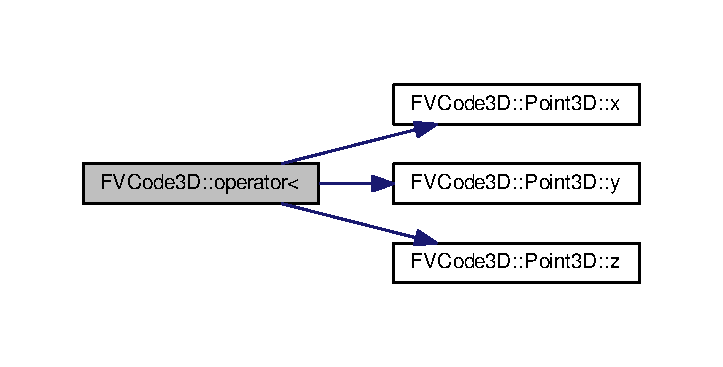
\includegraphics[width=347pt]{namespaceFVCode3D_a4d68dd4dc8a2720cd431013bc580e9d6_cgraph}
\end{center}
\end{figure}


\index{F\+V\+Code3D@{F\+V\+Code3D}!operator$<$@{operator$<$}}
\index{operator$<$@{operator$<$}!F\+V\+Code3D@{F\+V\+Code3D}}
\subsubsection[{\texorpdfstring{operator$<$(const Mesh3\+D\+::\+Facet3\+D \&f1, const Mesh3\+D\+::\+Facet3\+D \&f2)}{operator<(const Mesh3D::Facet3D &f1, const Mesh3D::Facet3D &f2)}}]{\setlength{\rightskip}{0pt plus 5cm}bool F\+V\+Code3\+D\+::operator$<$ (
\begin{DoxyParamCaption}
\item[{const {\bf Mesh3\+D\+::\+Facet3D} \&}]{f1, }
\item[{const {\bf Mesh3\+D\+::\+Facet3D} \&}]{f2}
\end{DoxyParamCaption}
)}\hypertarget{namespaceFVCode3D_a66dad0ddea6ea9e534d2c3f3bb5d9958}{}\label{namespaceFVCode3D_a66dad0ddea6ea9e534d2c3f3bb5d9958}


Overloading of operator$<$ between two Facet3D objects (needed by the set M\+\_\+facets) 


\begin{DoxyParams}{Parameters}
{\em f1} & The first facet to be tested \\
\hline
{\em f2} & The second facet to be tested \\
\hline
\end{DoxyParams}
\begin{DoxyReturn}{Returns}
T\+R\+UE -\/$>$ f1 $<$ f2 F\+A\+L\+SE -\/$>$ f1 $>$= f2 
\end{DoxyReturn}


Definition at line \hyperlink{Mesh3D_8cpp_source_l01242}{1242} of file \hyperlink{Mesh3D_8cpp_source}{Mesh3\+D.\+cpp}.



Here is the call graph for this function\+:
\nopagebreak
\begin{figure}[H]
\begin{center}
\leavevmode
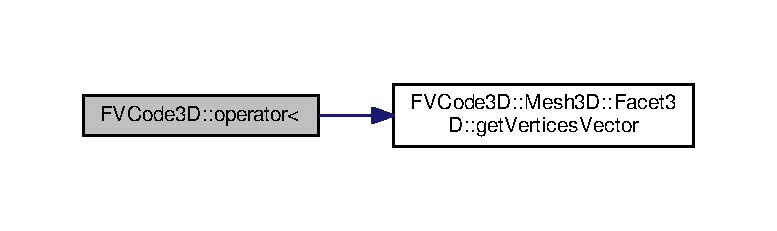
\includegraphics[width=350pt]{namespaceFVCode3D_a66dad0ddea6ea9e534d2c3f3bb5d9958_cgraph}
\end{center}
\end{figure}


\index{F\+V\+Code3D@{F\+V\+Code3D}!operator$<$$<$@{operator$<$$<$}}
\index{operator$<$$<$@{operator$<$$<$}!F\+V\+Code3D@{F\+V\+Code3D}}
\subsubsection[{\texorpdfstring{operator$<$$<$(std\+::ostream \&os, const Perm\+Ptr\+\_\+\+Type \&tensor)}{operator<<(std::ostream &os, const PermPtr_Type &tensor)}}]{\setlength{\rightskip}{0pt plus 5cm}std\+::ostream\& F\+V\+Code3\+D\+::operator$<$$<$ (
\begin{DoxyParamCaption}
\item[{std\+::ostream \&}]{os, }
\item[{const {\bf Perm\+Ptr\+\_\+\+Type} \&}]{tensor}
\end{DoxyParamCaption}
)}\hypertarget{namespaceFVCode3D_a2350a6eec9008d3b691e5ee6e4290914}{}\label{namespaceFVCode3D_a2350a6eec9008d3b691e5ee6e4290914}

\begin{DoxyParams}{Parameters}
{\em os} & output stream \\
\hline
{\em perm} & shared pointer to \hyperlink{classFVCode3D_1_1PermeabilityBase}{Permeability\+Base} \\
\hline
\end{DoxyParams}
\begin{DoxyReturn}{Returns}
output stream 
\end{DoxyReturn}


Definition at line \hyperlink{Permeability_8cpp_source_l00044}{44} of file \hyperlink{Permeability_8cpp_source}{Permeability.\+cpp}.

\index{F\+V\+Code3D@{F\+V\+Code3D}!operator$<$$<$@{operator$<$$<$}}
\index{operator$<$$<$@{operator$<$$<$}!F\+V\+Code3D@{F\+V\+Code3D}}
\subsubsection[{\texorpdfstring{operator$<$$<$(std\+::ostream \&os, const std\+::shared\+\_\+ptr$<$ Permeability\+Scalar $>$ \&perm)}{operator<<(std::ostream &os, const std::shared_ptr< PermeabilityScalar > &perm)}}]{\setlength{\rightskip}{0pt plus 5cm}std\+::ostream\& F\+V\+Code3\+D\+::operator$<$$<$ (
\begin{DoxyParamCaption}
\item[{std\+::ostream \&}]{os, }
\item[{const std\+::shared\+\_\+ptr$<$ {\bf Permeability\+Scalar} $>$ \&}]{perm}
\end{DoxyParamCaption}
)}\hypertarget{namespaceFVCode3D_afcbf0ace1266ac69b82a7154d94459a1}{}\label{namespaceFVCode3D_afcbf0ace1266ac69b82a7154d94459a1}

\begin{DoxyParams}{Parameters}
{\em os} & output stream \\
\hline
{\em perm} & shared pointer to \hyperlink{classFVCode3D_1_1PermeabilityBase}{Permeability\+Base} \\
\hline
\end{DoxyParams}
\begin{DoxyReturn}{Returns}
output stream 
\end{DoxyReturn}


Definition at line \hyperlink{Permeability_8cpp_source_l00088}{88} of file \hyperlink{Permeability_8cpp_source}{Permeability.\+cpp}.

\index{F\+V\+Code3D@{F\+V\+Code3D}!operator$<$$<$@{operator$<$$<$}}
\index{operator$<$$<$@{operator$<$$<$}!F\+V\+Code3D@{F\+V\+Code3D}}
\subsubsection[{\texorpdfstring{operator$<$$<$(std\+::ostream \&os, const std\+::shared\+\_\+ptr$<$ Permeability\+Diagonal $>$ \&perm)}{operator<<(std::ostream &os, const std::shared_ptr< PermeabilityDiagonal > &perm)}}]{\setlength{\rightskip}{0pt plus 5cm}std\+::ostream\& F\+V\+Code3\+D\+::operator$<$$<$ (
\begin{DoxyParamCaption}
\item[{std\+::ostream \&}]{os, }
\item[{const std\+::shared\+\_\+ptr$<$ {\bf Permeability\+Diagonal} $>$ \&}]{perm}
\end{DoxyParamCaption}
)}\hypertarget{namespaceFVCode3D_aa140a41198afe73b0908519f8900cc84}{}\label{namespaceFVCode3D_aa140a41198afe73b0908519f8900cc84}

\begin{DoxyParams}{Parameters}
{\em os} & output stream \\
\hline
{\em perm} & shared pointer to \hyperlink{classFVCode3D_1_1PermeabilityBase}{Permeability\+Base} \\
\hline
\end{DoxyParams}
\begin{DoxyReturn}{Returns}
output stream 
\end{DoxyReturn}


Definition at line \hyperlink{Permeability_8cpp_source_l00144}{144} of file \hyperlink{Permeability_8cpp_source}{Permeability.\+cpp}.

\index{F\+V\+Code3D@{F\+V\+Code3D}!operator$<$$<$@{operator$<$$<$}}
\index{operator$<$$<$@{operator$<$$<$}!F\+V\+Code3D@{F\+V\+Code3D}}
\subsubsection[{\texorpdfstring{operator$<$$<$(std\+::ostream \&os, const Point3\+D \&p)}{operator<<(std::ostream &os, const Point3D &p)}}]{\setlength{\rightskip}{0pt plus 5cm}std\+::ostream\& F\+V\+Code3\+D\+::operator$<$$<$ (
\begin{DoxyParamCaption}
\item[{std\+::ostream \&}]{os, }
\item[{const {\bf Point3D} \&}]{p}
\end{DoxyParamCaption}
)}\hypertarget{namespaceFVCode3D_a8884bc6475f7b278d2926ce82950a597}{}\label{namespaceFVCode3D_a8884bc6475f7b278d2926ce82950a597}


Definition at line \hyperlink{Point3D_8cpp_source_l00219}{219} of file \hyperlink{Point3D_8cpp_source}{Point3\+D.\+cpp}.

\index{F\+V\+Code3D@{F\+V\+Code3D}!operator$<$$<$@{operator$<$$<$}}
\index{operator$<$$<$@{operator$<$$<$}!F\+V\+Code3D@{F\+V\+Code3D}}
\subsubsection[{\texorpdfstring{operator$<$$<$(std\+::ostream \&os, const std\+::shared\+\_\+ptr$<$ Permeability\+Sym\+Tensor $>$ \&perm)}{operator<<(std::ostream &os, const std::shared_ptr< PermeabilitySymTensor > &perm)}}]{\setlength{\rightskip}{0pt plus 5cm}std\+::ostream\& F\+V\+Code3\+D\+::operator$<$$<$ (
\begin{DoxyParamCaption}
\item[{std\+::ostream \&}]{os, }
\item[{const std\+::shared\+\_\+ptr$<$ {\bf Permeability\+Sym\+Tensor} $>$ \&}]{perm}
\end{DoxyParamCaption}
)}\hypertarget{namespaceFVCode3D_aee190d20e7d59a358f6e3c5738473728}{}\label{namespaceFVCode3D_aee190d20e7d59a358f6e3c5738473728}

\begin{DoxyParams}{Parameters}
{\em os} & output stream \\
\hline
{\em perm} & shared pointer to \hyperlink{classFVCode3D_1_1PermeabilityBase}{Permeability\+Base} \\
\hline
\end{DoxyParams}
\begin{DoxyReturn}{Returns}
output stream 
\end{DoxyReturn}


Definition at line \hyperlink{Permeability_8cpp_source_l00240}{240} of file \hyperlink{Permeability_8cpp_source}{Permeability.\+cpp}.

\index{F\+V\+Code3D@{F\+V\+Code3D}!operator$<$$<$@{operator$<$$<$}}
\index{operator$<$$<$@{operator$<$$<$}!F\+V\+Code3D@{F\+V\+Code3D}}
\subsubsection[{\texorpdfstring{operator$<$$<$(std\+::ostream \&os, const std\+::shared\+\_\+ptr$<$ Permeability\+Full\+Tensor $>$ \&perm)}{operator<<(std::ostream &os, const std::shared_ptr< PermeabilityFullTensor > &perm)}}]{\setlength{\rightskip}{0pt plus 5cm}std\+::ostream\& F\+V\+Code3\+D\+::operator$<$$<$ (
\begin{DoxyParamCaption}
\item[{std\+::ostream \&}]{os, }
\item[{const std\+::shared\+\_\+ptr$<$ {\bf Permeability\+Full\+Tensor} $>$ \&}]{perm}
\end{DoxyParamCaption}
)}\hypertarget{namespaceFVCode3D_a453d7ae598d14867fe6f43774e38f8e0}{}\label{namespaceFVCode3D_a453d7ae598d14867fe6f43774e38f8e0}

\begin{DoxyParams}{Parameters}
{\em os} & output stream \\
\hline
{\em perm} & shared pointer to \hyperlink{classFVCode3D_1_1PermeabilityBase}{Permeability\+Base} \\
\hline
\end{DoxyParams}
\begin{DoxyReturn}{Returns}
output stream 
\end{DoxyReturn}


Definition at line \hyperlink{Permeability_8cpp_source_l00336}{336} of file \hyperlink{Permeability_8cpp_source}{Permeability.\+cpp}.

\index{F\+V\+Code3D@{F\+V\+Code3D}!rotate\+Of@{rotate\+Of}}
\index{rotate\+Of@{rotate\+Of}!F\+V\+Code3D@{F\+V\+Code3D}}
\subsubsection[{\texorpdfstring{rotate\+Of(const Point3\+D \&p, const Real angle\+Deg)}{rotateOf(const Point3D &p, const Real angleDeg)}}]{\setlength{\rightskip}{0pt plus 5cm}{\bf Point3D} F\+V\+Code3\+D\+::rotate\+Of (
\begin{DoxyParamCaption}
\item[{const {\bf Point3D} \&}]{p, }
\item[{const {\bf Real}}]{angle\+Deg}
\end{DoxyParamCaption}
)}\hypertarget{namespaceFVCode3D_aefa056e4f7c5d10edd993b812dd670da}{}\label{namespaceFVCode3D_aefa056e4f7c5d10edd993b812dd670da}


Rotate a point of an angle. 


\begin{DoxyParams}{Parameters}
{\em p} & point to rotate \\
\hline
{\em angle\+Deg} & angle of rotation (in Degrees) \\
\hline
\end{DoxyParams}
\begin{DoxyReturn}{Returns}
the rotated point 
\end{DoxyReturn}


Definition at line \hyperlink{Operations_8cpp_source_l00019}{19} of file \hyperlink{Operations_8cpp_source}{Operations.\+cpp}.



Here is the call graph for this function\+:
\nopagebreak
\begin{figure}[H]
\begin{center}
\leavevmode
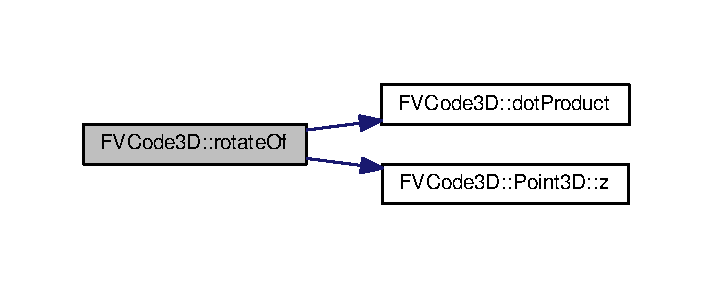
\includegraphics[width=342pt]{namespaceFVCode3D_aefa056e4f7c5d10edd993b812dd670da_cgraph}
\end{center}
\end{figure}




Here is the caller graph for this function\+:
\nopagebreak
\begin{figure}[H]
\begin{center}
\leavevmode
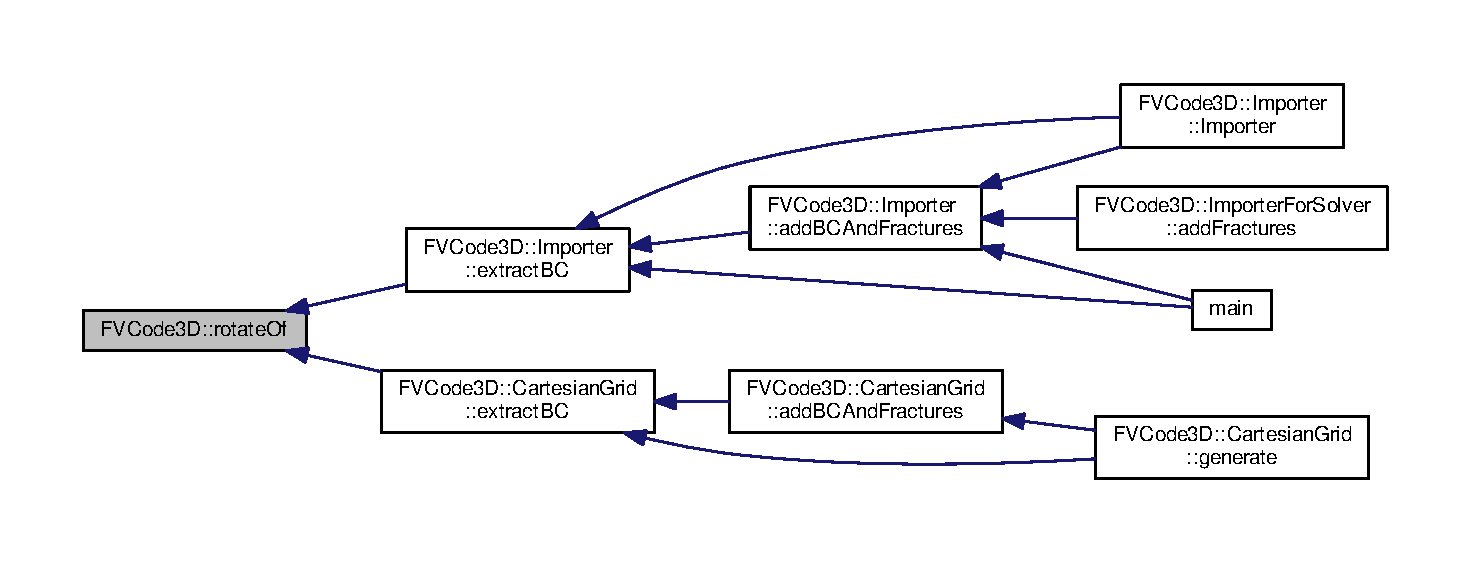
\includegraphics[width=350pt]{namespaceFVCode3D_aefa056e4f7c5d10edd993b812dd670da_icgraph}
\end{center}
\end{figure}


\index{F\+V\+Code3D@{F\+V\+Code3D}!save\+As\+Medit\+Format@{save\+As\+Medit\+Format}}
\index{save\+As\+Medit\+Format@{save\+As\+Medit\+Format}!F\+V\+Code3D@{F\+V\+Code3D}}
\subsubsection[{\texorpdfstring{save\+As\+Medit\+Format(const std\+::string filename, Mesh3\+D \&mesh)}{saveAsMeditFormat(const std::string filename, Mesh3D &mesh)}}]{\setlength{\rightskip}{0pt plus 5cm}void F\+V\+Code3\+D\+::save\+As\+Medit\+Format (
\begin{DoxyParamCaption}
\item[{const std\+::string}]{filename, }
\item[{{\bf Mesh3D} \&}]{mesh}
\end{DoxyParamCaption}
) throw  ) }\hypertarget{namespaceFVCode3D_a309feff3c4ef28a971e23350d895579c}{}\label{namespaceFVCode3D_a309feff3c4ef28a971e23350d895579c}


Save a file in Medit format (.mesh) 

Save mesh and fractures(as a suitable label). 
\begin{DoxyParams}{Parameters}
{\em filename} & name of the file \\
\hline
{\em mesh} & reference to a \hyperlink{classFVCode3D_1_1Mesh3D}{Mesh3D} \\
\hline
\end{DoxyParams}
\begin{DoxyPrecond}{Precondition}
import the file 
\end{DoxyPrecond}


Definition at line \hyperlink{Converter_8cpp_source_l00153}{153} of file \hyperlink{Converter_8cpp_source}{Converter.\+cpp}.

\index{F\+V\+Code3D@{F\+V\+Code3D}!save\+As\+Open\+F\+O\+A\+M\+Format@{save\+As\+Open\+F\+O\+A\+M\+Format}}
\index{save\+As\+Open\+F\+O\+A\+M\+Format@{save\+As\+Open\+F\+O\+A\+M\+Format}!F\+V\+Code3D@{F\+V\+Code3D}}
\subsubsection[{\texorpdfstring{save\+As\+Open\+F\+O\+A\+M\+Format(const std\+::string filename, Mesh3\+D \&mesh)}{saveAsOpenFOAMFormat(const std::string filename, Mesh3D &mesh)}}]{\setlength{\rightskip}{0pt plus 5cm}void F\+V\+Code3\+D\+::save\+As\+Open\+F\+O\+A\+M\+Format (
\begin{DoxyParamCaption}
\item[{const std\+::string}]{filename, }
\item[{{\bf Mesh3D} \&}]{mesh}
\end{DoxyParamCaption}
) throw  ) }\hypertarget{namespaceFVCode3D_a2f158b0ae2187840985b44465f65e126}{}\label{namespaceFVCode3D_a2f158b0ae2187840985b44465f65e126}


Save a file in Open\+F\+O\+AM format (poly\+Mesh) 

Save mesh and fractures(as a suitable label). 
\begin{DoxyParams}{Parameters}
{\em filename} & name of the file \\
\hline
{\em mesh} & reference to a \hyperlink{classFVCode3D_1_1Mesh3D}{Mesh3D} \\
\hline
\end{DoxyParams}
\begin{DoxyPrecond}{Precondition}
import the file 
\end{DoxyPrecond}


Definition at line \hyperlink{Converter_8cpp_source_l00229}{229} of file \hyperlink{Converter_8cpp_source}{Converter.\+cpp}.



Here is the call graph for this function\+:
\nopagebreak
\begin{figure}[H]
\begin{center}
\leavevmode
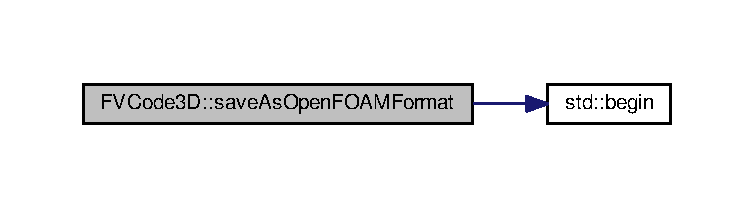
\includegraphics[width=350pt]{namespaceFVCode3D_a2f158b0ae2187840985b44465f65e126_cgraph}
\end{center}
\end{figure}


\index{F\+V\+Code3D@{F\+V\+Code3D}!save\+As\+Solver\+Format@{save\+As\+Solver\+Format}}
\index{save\+As\+Solver\+Format@{save\+As\+Solver\+Format}!F\+V\+Code3D@{F\+V\+Code3D}}
\subsubsection[{\texorpdfstring{save\+As\+Solver\+Format(const std\+::string filename, Mesh3\+D \&mesh, Properties\+Map \&properties)}{saveAsSolverFormat(const std::string filename, Mesh3D &mesh, PropertiesMap &properties)}}]{\setlength{\rightskip}{0pt plus 5cm}void F\+V\+Code3\+D\+::save\+As\+Solver\+Format (
\begin{DoxyParamCaption}
\item[{const std\+::string}]{filename, }
\item[{{\bf Mesh3D} \&}]{mesh, }
\item[{{\bf Properties\+Map} \&}]{properties}
\end{DoxyParamCaption}
) throw  ) }\hypertarget{namespaceFVCode3D_ab3d72976b29466b3b389c290d0e8dadb}{}\label{namespaceFVCode3D_ab3d72976b29466b3b389c290d0e8dadb}


Save a file in solver format (.fvg) 

Save mesh, properties and fractures. 
\begin{DoxyParams}{Parameters}
{\em filename} & name of the file \\
\hline
{\em mesh} & reference to a \hyperlink{classFVCode3D_1_1Mesh3D}{Mesh3D} \\
\hline
{\em properties} & reference to a \hyperlink{classFVCode3D_1_1PropertiesMap}{Properties\+Map} \\
\hline
\end{DoxyParams}
\begin{DoxyPrecond}{Precondition}
import the file 
\end{DoxyPrecond}


Definition at line \hyperlink{Converter_8cpp_source_l00014}{14} of file \hyperlink{Converter_8cpp_source}{Converter.\+cpp}.



Here is the call graph for this function\+:
\nopagebreak
\begin{figure}[H]
\begin{center}
\leavevmode
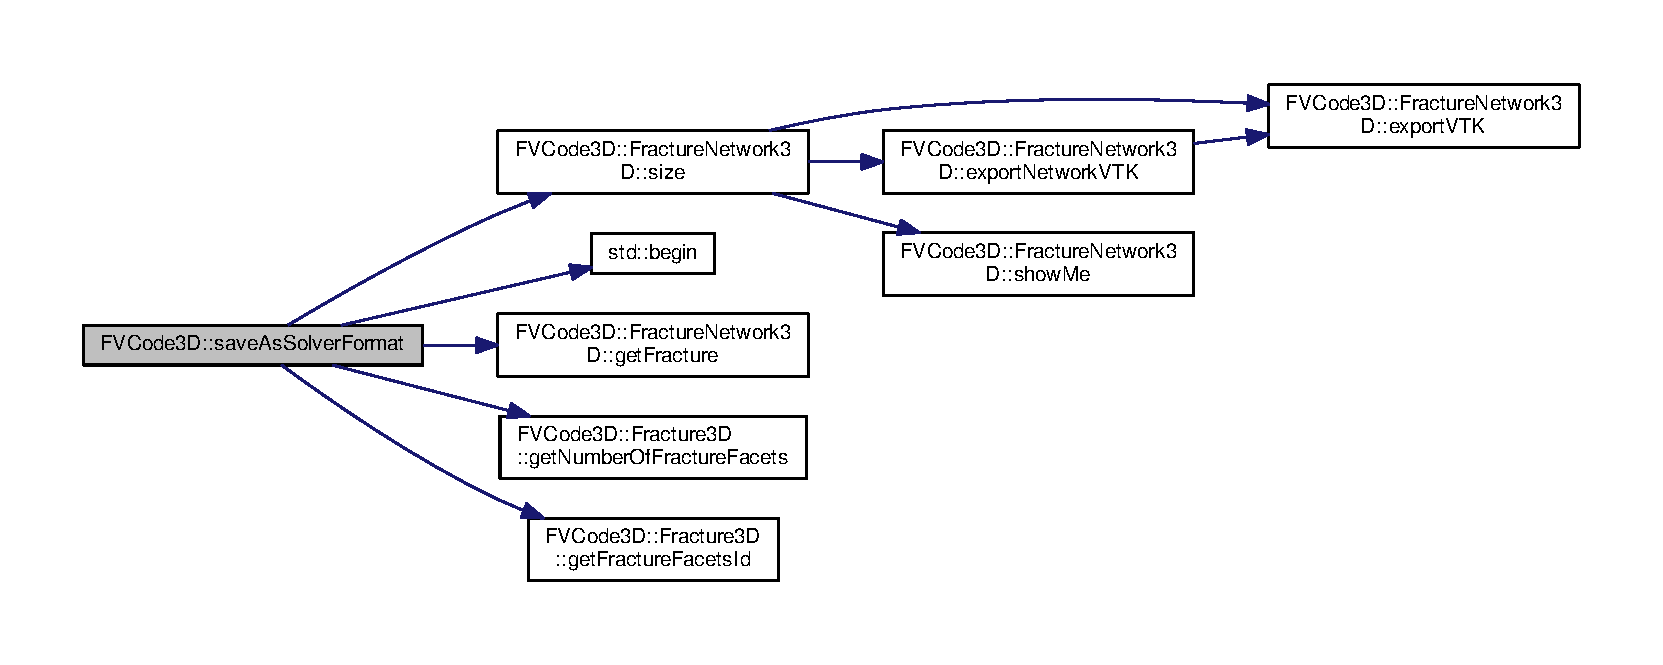
\includegraphics[width=350pt]{namespaceFVCode3D_ab3d72976b29466b3b389c290d0e8dadb_cgraph}
\end{center}
\end{figure}


\index{F\+V\+Code3D@{F\+V\+Code3D}!sparse\+Block@{sparse\+Block}}
\index{sparse\+Block@{sparse\+Block}!F\+V\+Code3D@{F\+V\+Code3D}}
\subsubsection[{\texorpdfstring{sparse\+Block(\+Sp\+Mat \+\_\+matrix, U\+Int \+\_\+ibegin, U\+Int \+\_\+jbegin, U\+Int \+\_\+icount, U\+Int \+\_\+jcount)}{sparseBlock(SpMat _matrix, UInt _ibegin, UInt _jbegin, UInt _icount, UInt _jcount)}}]{\setlength{\rightskip}{0pt plus 5cm}{\bf Sp\+Mat} F\+V\+Code3\+D\+::sparse\+Block (
\begin{DoxyParamCaption}
\item[{{\bf Sp\+Mat}}]{\+\_\+matrix, }
\item[{{\bf U\+Int}}]{\+\_\+ibegin, }
\item[{{\bf U\+Int}}]{\+\_\+jbegin, }
\item[{{\bf U\+Int}}]{\+\_\+icount, }
\item[{{\bf U\+Int}}]{\+\_\+jcount}
\end{DoxyParamCaption}
)}\hypertarget{namespaceFVCode3D_a50584b1c52af8d3b79fe5b0bcc18b2e1}{}\label{namespaceFVCode3D_a50584b1c52af8d3b79fe5b0bcc18b2e1}


Extract a block from a Sp\+Mat. 

Only for Col\+Major Sparse Matrix 

Definition at line \hyperlink{SparseBlock_8cpp_source_l00006}{6} of file \hyperlink{SparseBlock_8cpp_source}{Sparse\+Block.\+cpp}.



Here is the call graph for this function\+:
\nopagebreak
\begin{figure}[H]
\begin{center}
\leavevmode
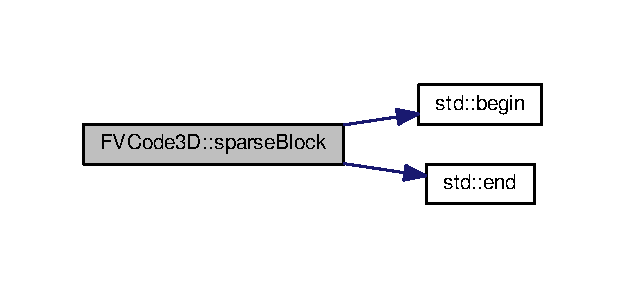
\includegraphics[width=300pt]{namespaceFVCode3D_a50584b1c52af8d3b79fe5b0bcc18b2e1_cgraph}
\end{center}
\end{figure}




Here is the caller graph for this function\+:
\nopagebreak
\begin{figure}[H]
\begin{center}
\leavevmode
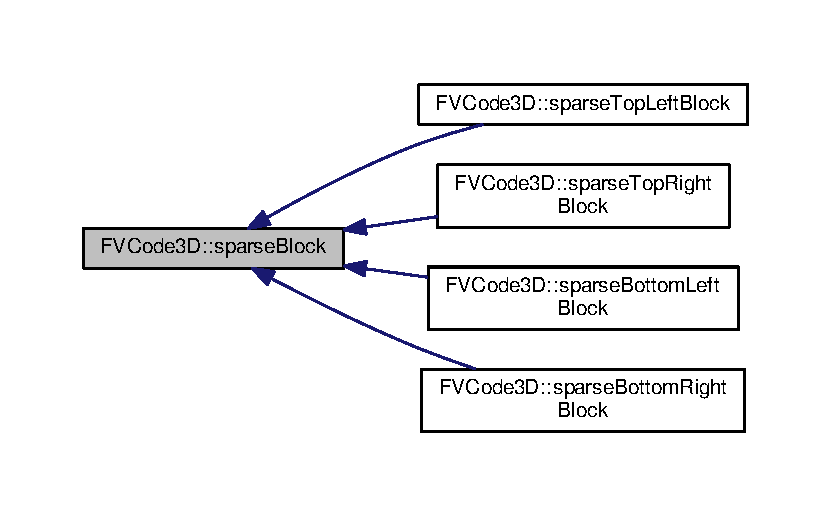
\includegraphics[width=350pt]{namespaceFVCode3D_a50584b1c52af8d3b79fe5b0bcc18b2e1_icgraph}
\end{center}
\end{figure}


\index{F\+V\+Code3D@{F\+V\+Code3D}!sparse\+Bottom\+Left\+Block@{sparse\+Bottom\+Left\+Block}}
\index{sparse\+Bottom\+Left\+Block@{sparse\+Bottom\+Left\+Block}!F\+V\+Code3D@{F\+V\+Code3D}}
\subsubsection[{\texorpdfstring{sparse\+Bottom\+Left\+Block(\+Sp\+Mat \+\_\+matrix, U\+Int \+\_\+icount, U\+Int \+\_\+jcount)}{sparseBottomLeftBlock(SpMat _matrix, UInt _icount, UInt _jcount)}}]{\setlength{\rightskip}{0pt plus 5cm}{\bf Sp\+Mat} F\+V\+Code3\+D\+::sparse\+Bottom\+Left\+Block (
\begin{DoxyParamCaption}
\item[{{\bf Sp\+Mat}}]{\+\_\+matrix, }
\item[{{\bf U\+Int}}]{\+\_\+icount, }
\item[{{\bf U\+Int}}]{\+\_\+jcount}
\end{DoxyParamCaption}
)}\hypertarget{namespaceFVCode3D_a2b06bf4215f4ce6cbd1a940fbd2ef6e6}{}\label{namespaceFVCode3D_a2b06bf4215f4ce6cbd1a940fbd2ef6e6}


Extract the bottom left block of a Sparse Matrix. 



Definition at line \hyperlink{SparseBlock_8cpp_source_l00053}{53} of file \hyperlink{SparseBlock_8cpp_source}{Sparse\+Block.\+cpp}.



Here is the call graph for this function\+:
\nopagebreak
\begin{figure}[H]
\begin{center}
\leavevmode
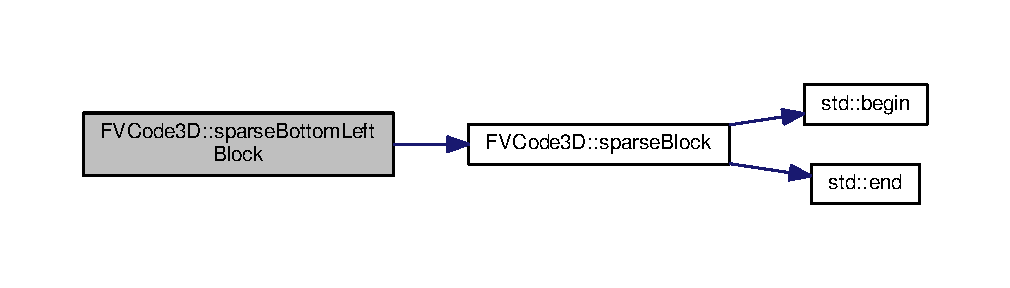
\includegraphics[width=350pt]{namespaceFVCode3D_a2b06bf4215f4ce6cbd1a940fbd2ef6e6_cgraph}
\end{center}
\end{figure}


\index{F\+V\+Code3D@{F\+V\+Code3D}!sparse\+Bottom\+Right\+Block@{sparse\+Bottom\+Right\+Block}}
\index{sparse\+Bottom\+Right\+Block@{sparse\+Bottom\+Right\+Block}!F\+V\+Code3D@{F\+V\+Code3D}}
\subsubsection[{\texorpdfstring{sparse\+Bottom\+Right\+Block(\+Sp\+Mat \+\_\+matrix, U\+Int \+\_\+icount, U\+Int \+\_\+jcount)}{sparseBottomRightBlock(SpMat _matrix, UInt _icount, UInt _jcount)}}]{\setlength{\rightskip}{0pt plus 5cm}{\bf Sp\+Mat} F\+V\+Code3\+D\+::sparse\+Bottom\+Right\+Block (
\begin{DoxyParamCaption}
\item[{{\bf Sp\+Mat}}]{\+\_\+matrix, }
\item[{{\bf U\+Int}}]{\+\_\+icount, }
\item[{{\bf U\+Int}}]{\+\_\+jcount}
\end{DoxyParamCaption}
)}\hypertarget{namespaceFVCode3D_a2468aefbc3231765755c7316f146bc3d}{}\label{namespaceFVCode3D_a2468aefbc3231765755c7316f146bc3d}


Extract the bottom right block of a Sparse Matrix. 



Definition at line \hyperlink{SparseBlock_8cpp_source_l00058}{58} of file \hyperlink{SparseBlock_8cpp_source}{Sparse\+Block.\+cpp}.



Here is the call graph for this function\+:
\nopagebreak
\begin{figure}[H]
\begin{center}
\leavevmode
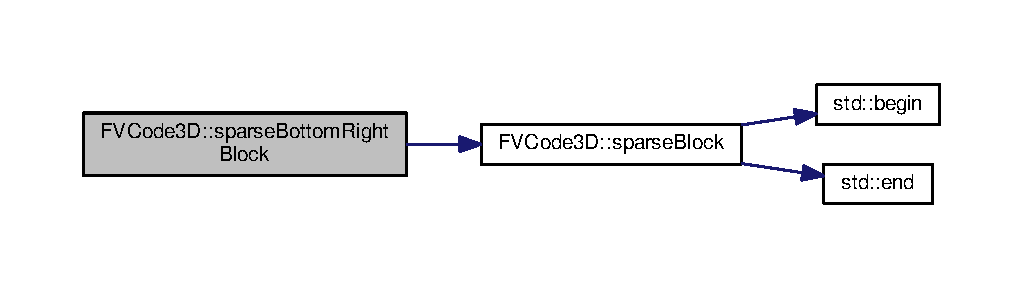
\includegraphics[width=350pt]{namespaceFVCode3D_a2468aefbc3231765755c7316f146bc3d_cgraph}
\end{center}
\end{figure}


\index{F\+V\+Code3D@{F\+V\+Code3D}!sparse\+Top\+Left\+Block@{sparse\+Top\+Left\+Block}}
\index{sparse\+Top\+Left\+Block@{sparse\+Top\+Left\+Block}!F\+V\+Code3D@{F\+V\+Code3D}}
\subsubsection[{\texorpdfstring{sparse\+Top\+Left\+Block(\+Sp\+Mat \+\_\+matrix, U\+Int \+\_\+icount, U\+Int \+\_\+jcount)}{sparseTopLeftBlock(SpMat _matrix, UInt _icount, UInt _jcount)}}]{\setlength{\rightskip}{0pt plus 5cm}{\bf Sp\+Mat} F\+V\+Code3\+D\+::sparse\+Top\+Left\+Block (
\begin{DoxyParamCaption}
\item[{{\bf Sp\+Mat}}]{\+\_\+matrix, }
\item[{{\bf U\+Int}}]{\+\_\+icount, }
\item[{{\bf U\+Int}}]{\+\_\+jcount}
\end{DoxyParamCaption}
)}\hypertarget{namespaceFVCode3D_a13bcca787028985b3fdbca71334eb63f}{}\label{namespaceFVCode3D_a13bcca787028985b3fdbca71334eb63f}


Extract the top left block of a Sparse Matrix. 



Definition at line \hyperlink{SparseBlock_8cpp_source_l00043}{43} of file \hyperlink{SparseBlock_8cpp_source}{Sparse\+Block.\+cpp}.



Here is the call graph for this function\+:
\nopagebreak
\begin{figure}[H]
\begin{center}
\leavevmode
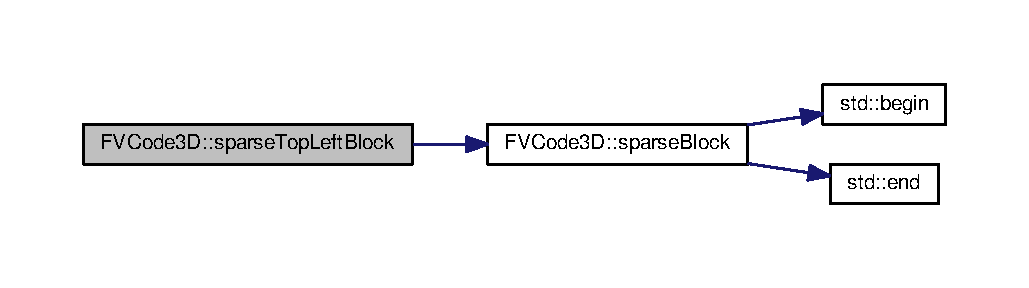
\includegraphics[width=350pt]{namespaceFVCode3D_a13bcca787028985b3fdbca71334eb63f_cgraph}
\end{center}
\end{figure}


\index{F\+V\+Code3D@{F\+V\+Code3D}!sparse\+Top\+Right\+Block@{sparse\+Top\+Right\+Block}}
\index{sparse\+Top\+Right\+Block@{sparse\+Top\+Right\+Block}!F\+V\+Code3D@{F\+V\+Code3D}}
\subsubsection[{\texorpdfstring{sparse\+Top\+Right\+Block(\+Sp\+Mat \+\_\+matrix, U\+Int \+\_\+icount, U\+Int \+\_\+jcount)}{sparseTopRightBlock(SpMat _matrix, UInt _icount, UInt _jcount)}}]{\setlength{\rightskip}{0pt plus 5cm}{\bf Sp\+Mat} F\+V\+Code3\+D\+::sparse\+Top\+Right\+Block (
\begin{DoxyParamCaption}
\item[{{\bf Sp\+Mat}}]{\+\_\+matrix, }
\item[{{\bf U\+Int}}]{\+\_\+icount, }
\item[{{\bf U\+Int}}]{\+\_\+jcount}
\end{DoxyParamCaption}
)}\hypertarget{namespaceFVCode3D_a4e9be96975d446ebb5e3acd53150bbbb}{}\label{namespaceFVCode3D_a4e9be96975d446ebb5e3acd53150bbbb}


Extract the top right block of a Sparse Matrix. 



Definition at line \hyperlink{SparseBlock_8cpp_source_l00048}{48} of file \hyperlink{SparseBlock_8cpp_source}{Sparse\+Block.\+cpp}.



Here is the call graph for this function\+:
\nopagebreak
\begin{figure}[H]
\begin{center}
\leavevmode
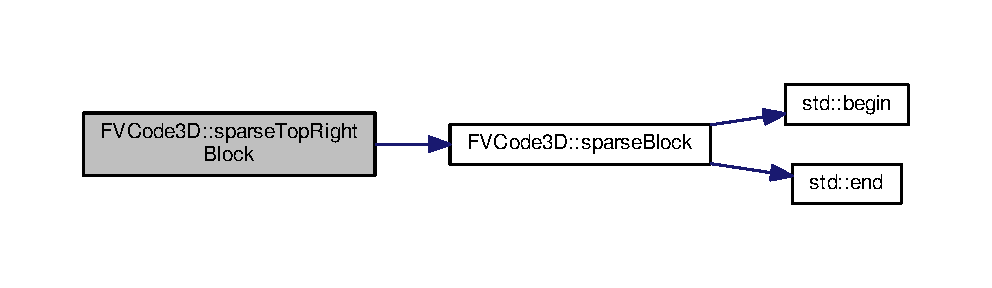
\includegraphics[width=350pt]{namespaceFVCode3D_a4e9be96975d446ebb5e3acd53150bbbb_cgraph}
\end{center}
\end{figure}


\index{F\+V\+Code3D@{F\+V\+Code3D}!tetrahedron\+Volume@{tetrahedron\+Volume}}
\index{tetrahedron\+Volume@{tetrahedron\+Volume}!F\+V\+Code3D@{F\+V\+Code3D}}
\subsubsection[{\texorpdfstring{tetrahedron\+Volume(const std\+::vector$<$ Point3\+D $>$ \&nodes)}{tetrahedronVolume(const std::vector< Point3D > &nodes)}}]{\setlength{\rightskip}{0pt plus 5cm}{\bf Real} F\+V\+Code3\+D\+::tetrahedron\+Volume (
\begin{DoxyParamCaption}
\item[{const std\+::vector$<$ {\bf Point3D} $>$ \&}]{nodes}
\end{DoxyParamCaption}
)}\hypertarget{namespaceFVCode3D_a8a6b07162e2801b628c3bd4057b9f221}{}\label{namespaceFVCode3D_a8a6b07162e2801b628c3bd4057b9f221}


Compute the volume of a tetrahedron. 


\begin{DoxyParams}{Parameters}
{\em nodes} & vector of points that define the tetrahedron \\
\hline
\end{DoxyParams}
\begin{DoxyReturn}{Returns}
unsigned volume of the tetrahedron 
\end{DoxyReturn}


Definition at line \hyperlink{Operations_8cpp_source_l00042}{42} of file \hyperlink{Operations_8cpp_source}{Operations.\+cpp}.



Here is the call graph for this function\+:
\nopagebreak
\begin{figure}[H]
\begin{center}
\leavevmode
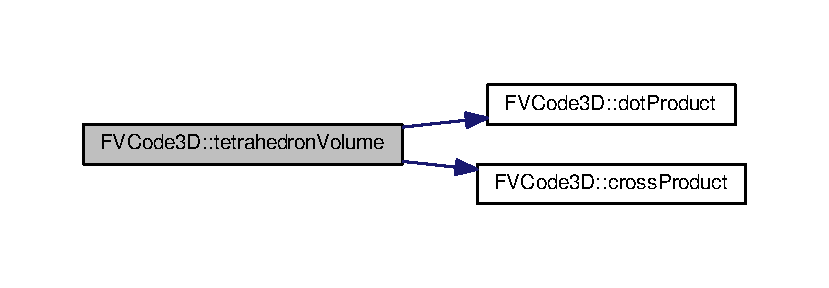
\includegraphics[width=350pt]{namespaceFVCode3D_a8a6b07162e2801b628c3bd4057b9f221_cgraph}
\end{center}
\end{figure}




Here is the caller graph for this function\+:
\nopagebreak
\begin{figure}[H]
\begin{center}
\leavevmode
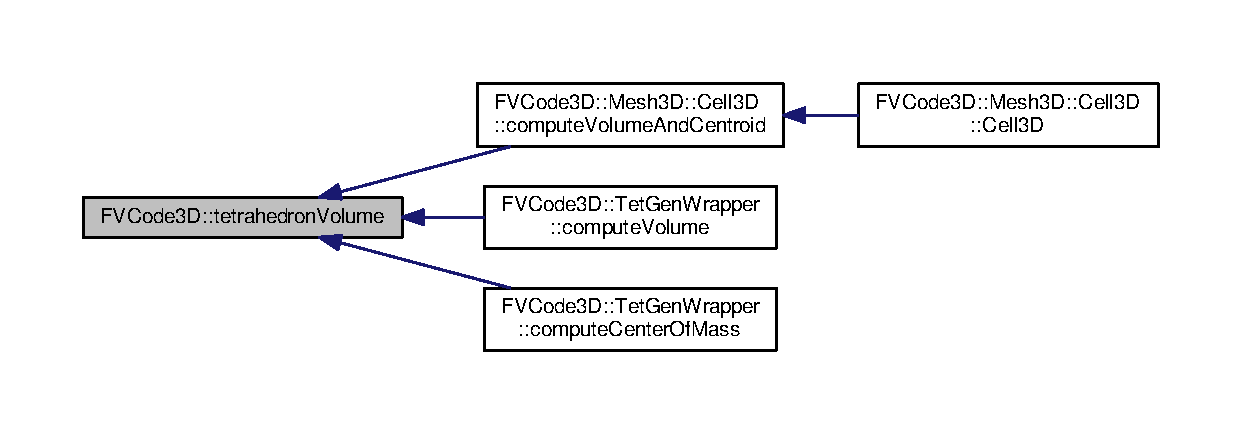
\includegraphics[width=350pt]{namespaceFVCode3D_a8a6b07162e2801b628c3bd4057b9f221_icgraph}
\end{center}
\end{figure}


\index{F\+V\+Code3D@{F\+V\+Code3D}!tokenize@{tokenize}}
\index{tokenize@{tokenize}!F\+V\+Code3D@{F\+V\+Code3D}}
\subsubsection[{\texorpdfstring{tokenize(const std\+::string \&s, std\+::vector$<$ std\+::string $>$ \&tokens, char delim= \textquotesingle{} \textquotesingle{})}{tokenize(const std::string &s, std::vector< std::string > &tokens, char delim= ' ')}}]{\setlength{\rightskip}{0pt plus 5cm}void F\+V\+Code3\+D\+::tokenize (
\begin{DoxyParamCaption}
\item[{const std\+::string \&}]{s, }
\item[{std\+::vector$<$ std\+::string $>$ \&}]{tokens, }
\item[{char}]{delim = {\ttfamily \textquotesingle{}~\textquotesingle{}}}
\end{DoxyParamCaption}
)\hspace{0.3cm}{\ttfamily [inline]}}\hypertarget{namespaceFVCode3D_a7bd098182831904c8fcd227b9d0f4562}{}\label{namespaceFVCode3D_a7bd098182831904c8fcd227b9d0f4562}


Splits a string into tokes. 

\begin{DoxyWarning}{Warning}
empty tokens are skipped 
\end{DoxyWarning}

\begin{DoxyParams}[1]{Parameters}
 & {\em s} & input string \\
\hline
\mbox{\tt out}  & {\em tokens} & tokens read from the string \\
\hline
 & {\em delim} & character separating tokens \\
\hline
\end{DoxyParams}


Definition at line \hyperlink{StringManipolator_8hpp_source_l00045}{45} of file \hyperlink{StringManipolator_8hpp_source}{String\+Manipolator.\+hpp}.

\index{F\+V\+Code3D@{F\+V\+Code3D}!to\+Upper@{to\+Upper}}
\index{to\+Upper@{to\+Upper}!F\+V\+Code3D@{F\+V\+Code3D}}
\subsubsection[{\texorpdfstring{to\+Upper(const std\+::string \&\+\_\+string)}{toUpper(const std::string &_string)}}]{\setlength{\rightskip}{0pt plus 5cm}std\+::string F\+V\+Code3\+D\+::to\+Upper (
\begin{DoxyParamCaption}
\item[{const std\+::string \&}]{\+\_\+string}
\end{DoxyParamCaption}
)\hspace{0.3cm}{\ttfamily [inline]}}\hypertarget{namespaceFVCode3D_aab0ceb729c2ff3e7fd288097aee76a59}{}\label{namespaceFVCode3D_aab0ceb729c2ff3e7fd288097aee76a59}


Convert a string to its upper case version. 



Definition at line \hyperlink{StringManipolator_8hpp_source_l00031}{31} of file \hyperlink{StringManipolator_8hpp_source}{String\+Manipolator.\+hpp}.



Here is the call graph for this function\+:
\nopagebreak
\begin{figure}[H]
\begin{center}
\leavevmode
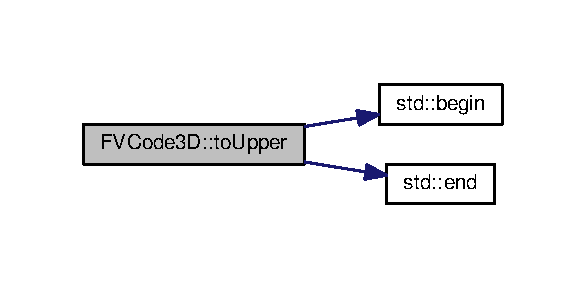
\includegraphics[width=281pt]{namespaceFVCode3D_aab0ceb729c2ff3e7fd288097aee76a59_cgraph}
\end{center}
\end{figure}




Here is the caller graph for this function\+:
\nopagebreak
\begin{figure}[H]
\begin{center}
\leavevmode
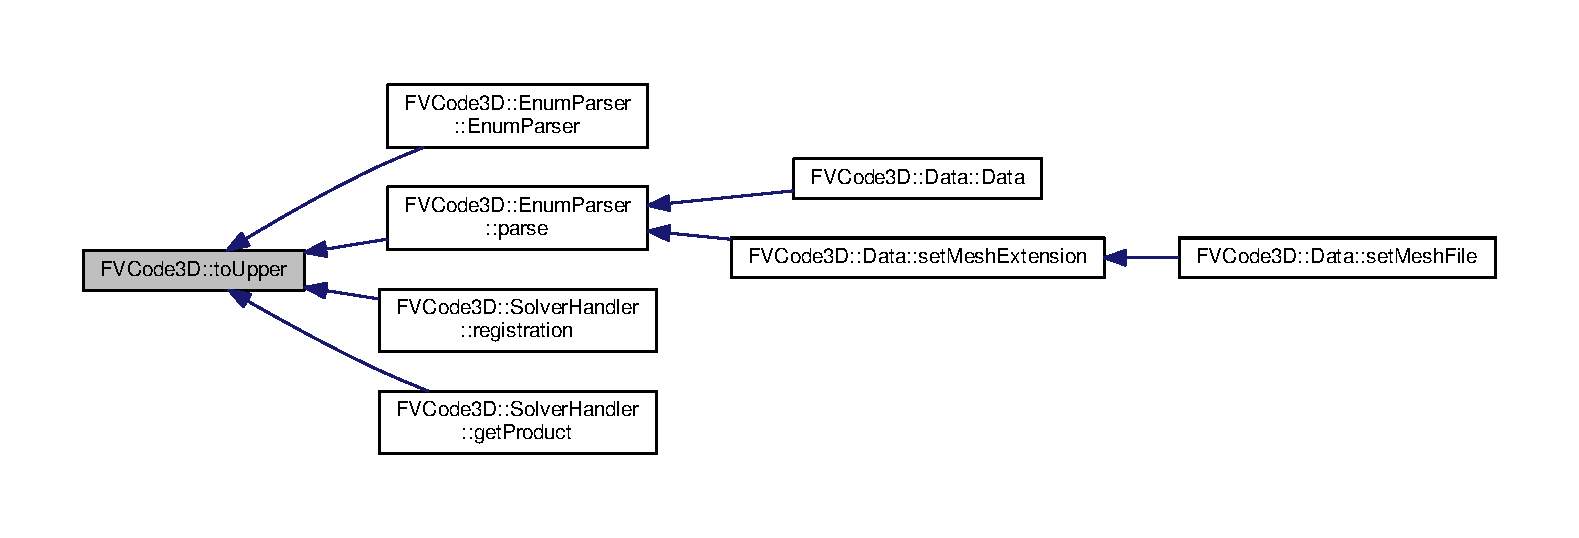
\includegraphics[width=350pt]{namespaceFVCode3D_aab0ceb729c2ff3e7fd288097aee76a59_icgraph}
\end{center}
\end{figure}


\index{F\+V\+Code3D@{F\+V\+Code3D}!triangle\+Area@{triangle\+Area}}
\index{triangle\+Area@{triangle\+Area}!F\+V\+Code3D@{F\+V\+Code3D}}
\subsubsection[{\texorpdfstring{triangle\+Area(const Point3\+D \&\+A, const Point3\+D \&\+B, const Point3\+D \&\+C)}{triangleArea(const Point3D &A, const Point3D &B, const Point3D &C)}}]{\setlength{\rightskip}{0pt plus 5cm}{\bf Real} F\+V\+Code3\+D\+::triangle\+Area (
\begin{DoxyParamCaption}
\item[{const {\bf Point3D} \&}]{A, }
\item[{const {\bf Point3D} \&}]{B, }
\item[{const {\bf Point3D} \&}]{C}
\end{DoxyParamCaption}
)}\hypertarget{namespaceFVCode3D_a38b320ef9683fae74a67a2a5a921f0d9}{}\label{namespaceFVCode3D_a38b320ef9683fae74a67a2a5a921f0d9}


Compute the area of a triangle. 


\begin{DoxyParams}{Parameters}
{\em A} & first point of the triangle \\
\hline
{\em B} & second point of the triangle \\
\hline
{\em C} & third point of the triangle \\
\hline
\end{DoxyParams}
\begin{DoxyReturn}{Returns}
unsigned area of the triangle 
\end{DoxyReturn}


Definition at line \hyperlink{Operations_8cpp_source_l00032}{32} of file \hyperlink{Operations_8cpp_source}{Operations.\+cpp}.



Here is the call graph for this function\+:
\nopagebreak
\begin{figure}[H]
\begin{center}
\leavevmode
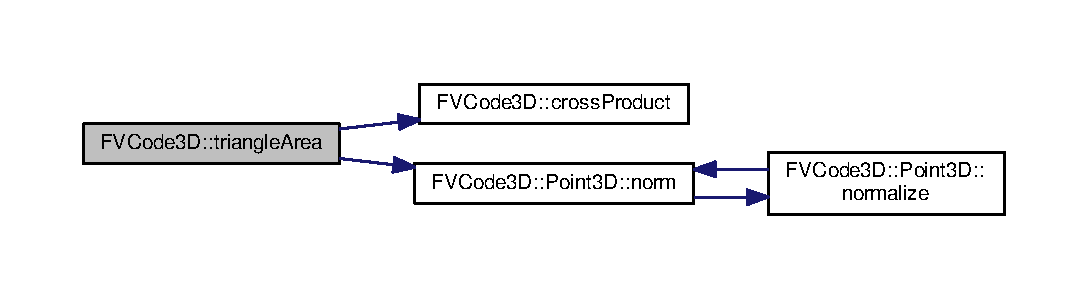
\includegraphics[width=350pt]{namespaceFVCode3D_a38b320ef9683fae74a67a2a5a921f0d9_cgraph}
\end{center}
\end{figure}




Here is the caller graph for this function\+:
\nopagebreak
\begin{figure}[H]
\begin{center}
\leavevmode
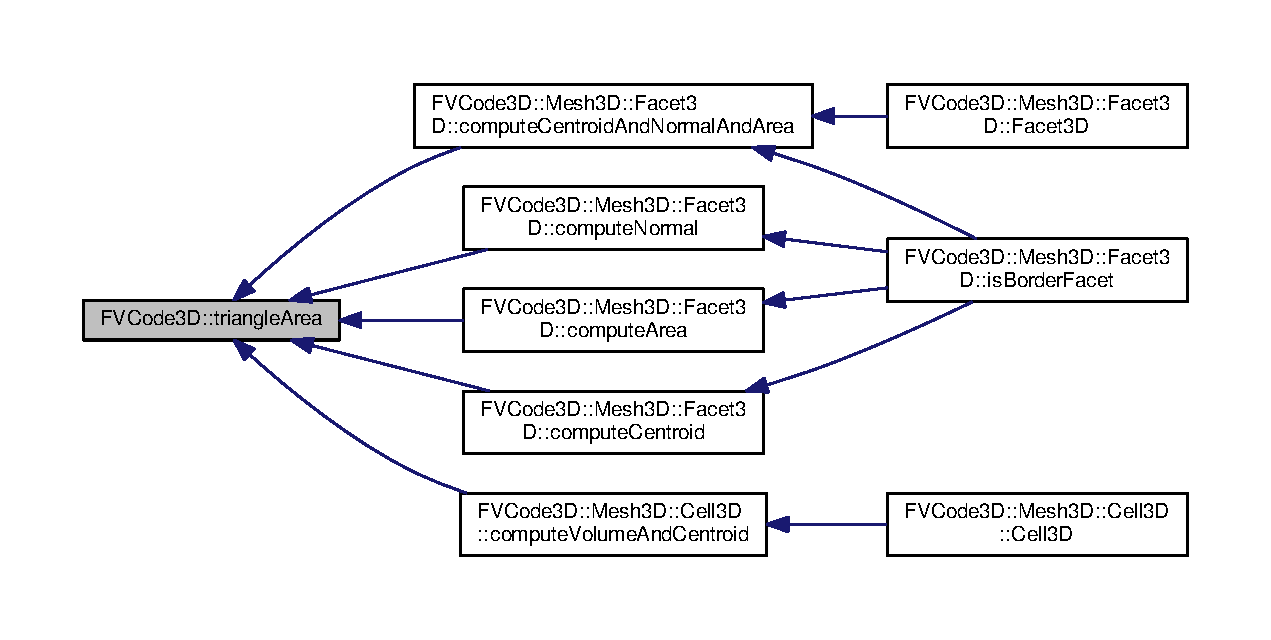
\includegraphics[width=350pt]{namespaceFVCode3D_a38b320ef9683fae74a67a2a5a921f0d9_icgraph}
\end{center}
\end{figure}


\index{F\+V\+Code3D@{F\+V\+Code3D}!triangle\+Centroid@{triangle\+Centroid}}
\index{triangle\+Centroid@{triangle\+Centroid}!F\+V\+Code3D@{F\+V\+Code3D}}
\subsubsection[{\texorpdfstring{triangle\+Centroid(const Point3\+D \&\+A, const Point3\+D \&\+B, const Point3\+D \&\+C)}{triangleCentroid(const Point3D &A, const Point3D &B, const Point3D &C)}}]{\setlength{\rightskip}{0pt plus 5cm}{\bf Point3D} F\+V\+Code3\+D\+::triangle\+Centroid (
\begin{DoxyParamCaption}
\item[{const {\bf Point3D} \&}]{A, }
\item[{const {\bf Point3D} \&}]{B, }
\item[{const {\bf Point3D} \&}]{C}
\end{DoxyParamCaption}
)}\hypertarget{namespaceFVCode3D_a5b8d6a9c921fcd809d263ef9c484b1ad}{}\label{namespaceFVCode3D_a5b8d6a9c921fcd809d263ef9c484b1ad}


Compute the centroid of a triangle. 


\begin{DoxyParams}{Parameters}
{\em A} & first point of the triangle \\
\hline
{\em B} & second point of the triangle \\
\hline
{\em C} & third point of the triangle \\
\hline
\end{DoxyParams}
\begin{DoxyReturn}{Returns}
the centroid of the triangle 
\end{DoxyReturn}


Definition at line \hyperlink{Operations_8cpp_source_l00037}{37} of file \hyperlink{Operations_8cpp_source}{Operations.\+cpp}.



Here is the caller graph for this function\+:
\nopagebreak
\begin{figure}[H]
\begin{center}
\leavevmode
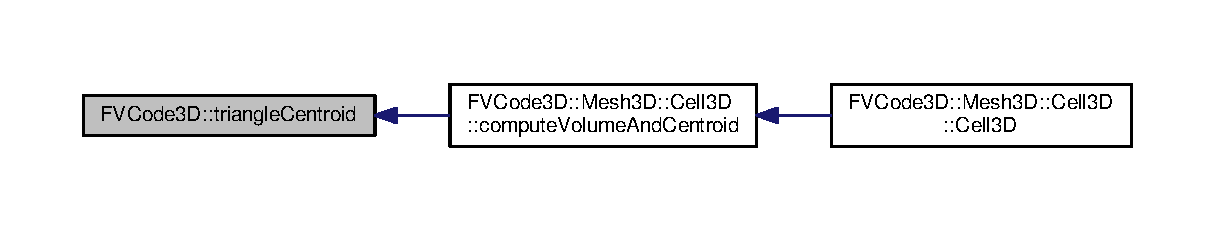
\includegraphics[width=350pt]{namespaceFVCode3D_a5b8d6a9c921fcd809d263ef9c484b1ad_icgraph}
\end{center}
\end{figure}




\subsection{Variable Documentation}
\index{F\+V\+Code3D@{F\+V\+Code3D}!\+\_\+\+P\+I\+\_\+@{\+\_\+\+P\+I\+\_\+}}
\index{\+\_\+\+P\+I\+\_\+@{\+\_\+\+P\+I\+\_\+}!F\+V\+Code3D@{F\+V\+Code3D}}
\subsubsection[{\texorpdfstring{\+\_\+\+P\+I\+\_\+}{_PI_}}]{\setlength{\rightskip}{0pt plus 5cm}const {\bf Real} F\+V\+Code3\+D\+::\+\_\+\+P\+I\+\_\+ = std\+::atan(1)$\ast$4}\hypertarget{namespaceFVCode3D_a10917df7e49a48239ce5f00ec9bbfe0a}{}\label{namespaceFVCode3D_a10917df7e49a48239ce5f00ec9bbfe0a}


PI. 



Definition at line \hyperlink{BasicType_8hpp_source_l00057}{57} of file \hyperlink{BasicType_8hpp_source}{Basic\+Type.\+hpp}.

\index{F\+V\+Code3D@{F\+V\+Code3D}!f\+Minus\+One@{f\+Minus\+One}}
\index{f\+Minus\+One@{f\+Minus\+One}!F\+V\+Code3D@{F\+V\+Code3D}}
\subsubsection[{\texorpdfstring{f\+Minus\+One}{fMinusOne}}]{\setlength{\rightskip}{0pt plus 5cm}{\bf Func} F\+V\+Code3\+D\+::f\+Minus\+One = \mbox{[}$\,$\mbox{]}({\bf Point3D})\{ return -\/1.; \}}\hypertarget{namespaceFVCode3D_a2ce53aebcf9d64490c1d10fff4860a75}{}\label{namespaceFVCode3D_a2ce53aebcf9d64490c1d10fff4860a75}


Definition at line \hyperlink{functions_8hpp_source_l00019}{19} of file \hyperlink{functions_8hpp_source}{functions.\+hpp}.

\index{F\+V\+Code3D@{F\+V\+Code3D}!f\+Minus\+Two@{f\+Minus\+Two}}
\index{f\+Minus\+Two@{f\+Minus\+Two}!F\+V\+Code3D@{F\+V\+Code3D}}
\subsubsection[{\texorpdfstring{f\+Minus\+Two}{fMinusTwo}}]{\setlength{\rightskip}{0pt plus 5cm}{\bf Func} F\+V\+Code3\+D\+::f\+Minus\+Two = \mbox{[}$\,$\mbox{]}({\bf Point3D})\{ return -\/2.; \}}\hypertarget{namespaceFVCode3D_aafe19d9d844e6d7ec5cc316a921b91ea}{}\label{namespaceFVCode3D_aafe19d9d844e6d7ec5cc316a921b91ea}


Definition at line \hyperlink{functions_8hpp_source_l00018}{18} of file \hyperlink{functions_8hpp_source}{functions.\+hpp}.

\index{F\+V\+Code3D@{F\+V\+Code3D}!f\+One@{f\+One}}
\index{f\+One@{f\+One}!F\+V\+Code3D@{F\+V\+Code3D}}
\subsubsection[{\texorpdfstring{f\+One}{fOne}}]{\setlength{\rightskip}{0pt plus 5cm}{\bf Func} F\+V\+Code3\+D\+::f\+One = \mbox{[}$\,$\mbox{]}({\bf Point3D})\{ return 1.; \}}\hypertarget{namespaceFVCode3D_a1a9ede09c77441d292a079fbab60fb82}{}\label{namespaceFVCode3D_a1a9ede09c77441d292a079fbab60fb82}


Definition at line \hyperlink{functions_8hpp_source_l00017}{17} of file \hyperlink{functions_8hpp_source}{functions.\+hpp}.

\index{F\+V\+Code3D@{F\+V\+Code3D}!f\+One\+Zero@{f\+One\+Zero}}
\index{f\+One\+Zero@{f\+One\+Zero}!F\+V\+Code3D@{F\+V\+Code3D}}
\subsubsection[{\texorpdfstring{f\+One\+Zero}{fOneZero}}]{\setlength{\rightskip}{0pt plus 5cm}{\bf Func} F\+V\+Code3\+D\+::f\+One\+Zero = \mbox{[}$\,$\mbox{]}({\bf Point3D} p)\{ return (2. -\/ p.\+x()) / 2.; \}}\hypertarget{namespaceFVCode3D_a05f5ace5c7eed4784717659f36b087fe}{}\label{namespaceFVCode3D_a05f5ace5c7eed4784717659f36b087fe}


Definition at line \hyperlink{functions_8hpp_source_l00020}{20} of file \hyperlink{functions_8hpp_source}{functions.\+hpp}.

\index{F\+V\+Code3D@{F\+V\+Code3D}!f\+Ten@{f\+Ten}}
\index{f\+Ten@{f\+Ten}!F\+V\+Code3D@{F\+V\+Code3D}}
\subsubsection[{\texorpdfstring{f\+Ten}{fTen}}]{\setlength{\rightskip}{0pt plus 5cm}{\bf Func} F\+V\+Code3\+D\+::f\+Ten = \mbox{[}$\,$\mbox{]}({\bf Point3D})\{ return 10.; \}}\hypertarget{namespaceFVCode3D_ab998dd309f7a549b31ae669513c2039d}{}\label{namespaceFVCode3D_ab998dd309f7a549b31ae669513c2039d}


Definition at line \hyperlink{functions_8hpp_source_l00021}{21} of file \hyperlink{functions_8hpp_source}{functions.\+hpp}.

\index{F\+V\+Code3D@{F\+V\+Code3D}!f\+Zero@{f\+Zero}}
\index{f\+Zero@{f\+Zero}!F\+V\+Code3D@{F\+V\+Code3D}}
\subsubsection[{\texorpdfstring{f\+Zero}{fZero}}]{\setlength{\rightskip}{0pt plus 5cm}{\bf Func} F\+V\+Code3\+D\+::f\+Zero = \mbox{[}$\,$\mbox{]}({\bf Point3D})\{ return 0.; \}}\hypertarget{namespaceFVCode3D_a2e72cc81c6f214d6e057af7a02599501}{}\label{namespaceFVCode3D_a2e72cc81c6f214d6e057af7a02599501}


Definition at line \hyperlink{functions_8hpp_source_l00016}{16} of file \hyperlink{functions_8hpp_source}{functions.\+hpp}.

\index{F\+V\+Code3D@{F\+V\+Code3D}!Sink\+Grid2@{Sink\+Grid2}}
\index{Sink\+Grid2@{Sink\+Grid2}!F\+V\+Code3D@{F\+V\+Code3D}}
\subsubsection[{\texorpdfstring{Sink\+Grid2}{SinkGrid2}}]{\setlength{\rightskip}{0pt plus 5cm}{\bf Func} F\+V\+Code3\+D\+::\+Sink\+Grid2}\hypertarget{namespaceFVCode3D_a312f262aefa197b219228571b49620be}{}\label{namespaceFVCode3D_a312f262aefa197b219228571b49620be}
{\bfseries Initial value\+:}
\begin{DoxyCode}
= [](Point3D p)
    \{\textcolor{keywordflow}{return} -1*( (
                     (p.x()-3.15147e+07)*(p.x()-3.15147e+07) +
                     (p.y()-1.6882e+07 )*(p.y()-1.6882e+07 ) +
                     (p.z()+13355.1    )*(p.z()+13355.1    )
                   ) <=1e6
                 );
    \}
\end{DoxyCode}


Definition at line \hyperlink{functions_8hpp_source_l00033}{33} of file \hyperlink{functions_8hpp_source}{functions.\+hpp}.

\index{F\+V\+Code3D@{F\+V\+Code3D}!Sink\+O\+Grid3@{Sink\+O\+Grid3}}
\index{Sink\+O\+Grid3@{Sink\+O\+Grid3}!F\+V\+Code3D@{F\+V\+Code3D}}
\subsubsection[{\texorpdfstring{Sink\+O\+Grid3}{SinkOGrid3}}]{\setlength{\rightskip}{0pt plus 5cm}{\bf Func} F\+V\+Code3\+D\+::\+Sink\+O\+Grid3}\hypertarget{namespaceFVCode3D_a1d325cbbfbdf5832333e0a07e6095053}{}\label{namespaceFVCode3D_a1d325cbbfbdf5832333e0a07e6095053}
{\bfseries Initial value\+:}
\begin{DoxyCode}
= [](Point3D p)
    \{\textcolor{keywordflow}{return} -1*( (
                     (p.x()-3.15185e7)*(p.x()-3.15185e7) +
                     (p.y()-1.6874e7 )*(p.y()-1.6874e7 ) +
                     (p.z()+1.635e4  )*(p.z()+1.635e4  )
                  ) <=1e6
                );
    \}
\end{DoxyCode}


Definition at line \hyperlink{functions_8hpp_source_l00086}{86} of file \hyperlink{functions_8hpp_source}{functions.\+hpp}.

\index{F\+V\+Code3D@{F\+V\+Code3D}!Sink\+P\+Grid3@{Sink\+P\+Grid3}}
\index{Sink\+P\+Grid3@{Sink\+P\+Grid3}!F\+V\+Code3D@{F\+V\+Code3D}}
\subsubsection[{\texorpdfstring{Sink\+P\+Grid3}{SinkPGrid3}}]{\setlength{\rightskip}{0pt plus 5cm}{\bf Func} F\+V\+Code3\+D\+::\+Sink\+P\+Grid3}\hypertarget{namespaceFVCode3D_a8e5a12e6a9e22baa4378e82fdfcc7613}{}\label{namespaceFVCode3D_a8e5a12e6a9e22baa4378e82fdfcc7613}
{\bfseries Initial value\+:}
\begin{DoxyCode}
= [](Point3D p)
    \{\textcolor{keywordflow}{return} -100*( (
                     (p.x()-3.14986e+07)*(p.x()-3.14986e+07) +
                     (p.y()-1.68939e+07)*(p.y()-1.68939e+07) +
                     (p.z()+14041.5    )*(p.z()+14041.5    )
                   ) <=5e4
                 );
    \}
\end{DoxyCode}


Definition at line \hyperlink{functions_8hpp_source_l00067}{67} of file \hyperlink{functions_8hpp_source}{functions.\+hpp}.

\index{F\+V\+Code3D@{F\+V\+Code3D}!Source\+Domain@{Source\+Domain}}
\index{Source\+Domain@{Source\+Domain}!F\+V\+Code3D@{F\+V\+Code3D}}
\subsubsection[{\texorpdfstring{Source\+Domain}{SourceDomain}}]{\setlength{\rightskip}{0pt plus 5cm}{\bf Func} F\+V\+Code3\+D\+::\+Source\+Domain}\hypertarget{namespaceFVCode3D_ae98a1f1ab0fce8db57176a4a9f91b2d0}{}\label{namespaceFVCode3D_ae98a1f1ab0fce8db57176a4a9f91b2d0}
{\bfseries Initial value\+:}
\begin{DoxyCode}
= [](Point3D p)\{\textcolor{keywordflow}{return} ((p.x() - 1.)*(p.x() - 1.) + (p.y() - 0.5)*(p.y() - 0.5) + (p.z() - 0.5)*(p.z()
- 0.5)) < 1;\}
\end{DoxyCode}


Definition at line \hyperlink{functions_8hpp_source_l00012}{12} of file \hyperlink{functions_8hpp_source}{functions.\+hpp}.

\index{F\+V\+Code3D@{F\+V\+Code3D}!Source\+Grid2@{Source\+Grid2}}
\index{Source\+Grid2@{Source\+Grid2}!F\+V\+Code3D@{F\+V\+Code3D}}
\subsubsection[{\texorpdfstring{Source\+Grid2}{SourceGrid2}}]{\setlength{\rightskip}{0pt plus 5cm}{\bf Func} F\+V\+Code3\+D\+::\+Source\+Grid2}\hypertarget{namespaceFVCode3D_a271b4cbc8ec56bd2a3cb950b307aef18}{}\label{namespaceFVCode3D_a271b4cbc8ec56bd2a3cb950b307aef18}
{\bfseries Initial value\+:}
\begin{DoxyCode}
= [](Point3D p)
    \{\textcolor{keywordflow}{return} 1*( (
                    (p.x()-3.15146e+07)*(p.x()-3.15146e+07) +
                    (p.y()-1.68972e+07)*(p.y()-1.68972e+07) +
                    (p.z()+13355.1    )*(p.z()+13355.1    )
                  ) <=1e6
                );
    \}
\end{DoxyCode}


Definition at line \hyperlink{functions_8hpp_source_l00024}{24} of file \hyperlink{functions_8hpp_source}{functions.\+hpp}.

\index{F\+V\+Code3D@{F\+V\+Code3D}!Source\+O\+Grid3@{Source\+O\+Grid3}}
\index{Source\+O\+Grid3@{Source\+O\+Grid3}!F\+V\+Code3D@{F\+V\+Code3D}}
\subsubsection[{\texorpdfstring{Source\+O\+Grid3}{SourceOGrid3}}]{\setlength{\rightskip}{0pt plus 5cm}{\bf Func} F\+V\+Code3\+D\+::\+Source\+O\+Grid3}\hypertarget{namespaceFVCode3D_ac7d83a03f6c58a7410364b917cf7ebc5}{}\label{namespaceFVCode3D_ac7d83a03f6c58a7410364b917cf7ebc5}
{\bfseries Initial value\+:}
\begin{DoxyCode}
= [](Point3D p)
    \{\textcolor{keywordflow}{return} 1*( (
                    (p.x()-3.15185e7)*(p.x()-3.15185e7) +
                    (p.y()-1.6913e7 )*(p.y()-1.6913e7 ) +
                    (p.z()+1.80e4   )*(p.z()+1.80e4   )
                 ) <=1e6
               );
    \}
\end{DoxyCode}


Definition at line \hyperlink{functions_8hpp_source_l00077}{77} of file \hyperlink{functions_8hpp_source}{functions.\+hpp}.

\index{F\+V\+Code3D@{F\+V\+Code3D}!Source\+P\+Grid3@{Source\+P\+Grid3}}
\index{Source\+P\+Grid3@{Source\+P\+Grid3}!F\+V\+Code3D@{F\+V\+Code3D}}
\subsubsection[{\texorpdfstring{Source\+P\+Grid3}{SourcePGrid3}}]{\setlength{\rightskip}{0pt plus 5cm}{\bf Func} F\+V\+Code3\+D\+::\+Source\+P\+Grid3}\hypertarget{namespaceFVCode3D_ae622d8dcaded68fd7f8d650f0a8d9f71}{}\label{namespaceFVCode3D_ae622d8dcaded68fd7f8d650f0a8d9f71}
{\bfseries Initial value\+:}
\begin{DoxyCode}
= [](Point3D p)
    \{\textcolor{keywordflow}{return} 100*( (
                    (p.x()-3.15389e+07)*(p.x()-3.15389e+07) +
                    (p.y()-1.68937e+07)*(p.y()-1.68937e+07) +
                    (p.z()+14048.1    )*(p.z()+14048.1    )
                  ) <=5e4
                );
    \}
\end{DoxyCode}


Definition at line \hyperlink{functions_8hpp_source_l00058}{58} of file \hyperlink{functions_8hpp_source}{functions.\+hpp}.

\index{F\+V\+Code3D@{F\+V\+Code3D}!SS@{SS}}
\index{SS@{SS}!F\+V\+Code3D@{F\+V\+Code3D}}
\subsubsection[{\texorpdfstring{SS}{SS}}]{\setlength{\rightskip}{0pt plus 5cm}{\bf Func} F\+V\+Code3\+D\+::\+SS = {\bf S\+S\+E\+D\+FM}}\hypertarget{namespaceFVCode3D_ae8b0f97f0774db9f0881cfc5f31d93f4}{}\label{namespaceFVCode3D_ae8b0f97f0774db9f0881cfc5f31d93f4}


Definition at line \hyperlink{functions_8hpp_source_l00117}{117} of file \hyperlink{functions_8hpp_source}{functions.\+hpp}.

\index{F\+V\+Code3D@{F\+V\+Code3D}!S\+S\+E\+D\+FM@{S\+S\+E\+D\+FM}}
\index{S\+S\+E\+D\+FM@{S\+S\+E\+D\+FM}!F\+V\+Code3D@{F\+V\+Code3D}}
\subsubsection[{\texorpdfstring{S\+S\+E\+D\+FM}{SSEDFM}}]{\setlength{\rightskip}{0pt plus 5cm}{\bf Func} F\+V\+Code3\+D\+::\+S\+S\+E\+D\+FM}\hypertarget{namespaceFVCode3D_a57e80824f085310d70ceed215314b9eb}{}\label{namespaceFVCode3D_a57e80824f085310d70ceed215314b9eb}
{\bfseries Initial value\+:}
\begin{DoxyCode}
= [](Point3D p)
    \{ \textcolor{keywordflow}{return} 10. * ( p.x() <= 0.4 ); \}
\end{DoxyCode}


Definition at line \hyperlink{functions_8hpp_source_l00111}{111} of file \hyperlink{functions_8hpp_source}{functions.\+hpp}.

\index{F\+V\+Code3D@{F\+V\+Code3D}!S\+S\+E\+D\+F\+M\+BC@{S\+S\+E\+D\+F\+M\+BC}}
\index{S\+S\+E\+D\+F\+M\+BC@{S\+S\+E\+D\+F\+M\+BC}!F\+V\+Code3D@{F\+V\+Code3D}}
\subsubsection[{\texorpdfstring{S\+S\+E\+D\+F\+M\+BC}{SSEDFMBC}}]{\setlength{\rightskip}{0pt plus 5cm}{\bf Func} F\+V\+Code3\+D\+::\+S\+S\+E\+D\+F\+M\+BC}\hypertarget{namespaceFVCode3D_a84fa11f60a0d07f58d20dcd63837a333}{}\label{namespaceFVCode3D_a84fa11f60a0d07f58d20dcd63837a333}
{\bfseries Initial value\+:}
\begin{DoxyCode}
= [](Point3D p)
    \{ \textcolor{keywordflow}{return} 2. * ( (p.x() >= 0.8) && (p.x() <= 1.2 ) ); \}
\end{DoxyCode}


Definition at line \hyperlink{functions_8hpp_source_l00114}{114} of file \hyperlink{functions_8hpp_source}{functions.\+hpp}.

\index{F\+V\+Code3D@{F\+V\+Code3D}!S\+S\+Grid2@{S\+S\+Grid2}}
\index{S\+S\+Grid2@{S\+S\+Grid2}!F\+V\+Code3D@{F\+V\+Code3D}}
\subsubsection[{\texorpdfstring{S\+S\+Grid2}{SSGrid2}}]{\setlength{\rightskip}{0pt plus 5cm}{\bf Func} F\+V\+Code3\+D\+::\+S\+S\+Grid2}\hypertarget{namespaceFVCode3D_a4072861e3dbbfcd9e80417b32c6991be}{}\label{namespaceFVCode3D_a4072861e3dbbfcd9e80417b32c6991be}
{\bfseries Initial value\+:}
\begin{DoxyCode}
= [](Point3D p)
    \{\textcolor{keywordflow}{return}  1*( (
                   (p.x()-3.15146e+07)*(p.x()-3.15146e+07) +
                   (p.y()-1.68972e+07)*(p.y()-1.68972e+07) +
                   (p.z()+13355.1    )*(p.z()+13355.1    )
                 ) <=1e6
               )
            -1*( (
                   (p.x()-3.15147e+07)*(p.x()-3.15147e+07) +
                   (p.y()-1.6882e+07 )*(p.y()-1.6882e+07 ) +
                   (p.z()+13355.1    )*(p.z()+13355.1    )
                 ) <=1e6
               );
    \}
\end{DoxyCode}


Definition at line \hyperlink{functions_8hpp_source_l00042}{42} of file \hyperlink{functions_8hpp_source}{functions.\+hpp}.

\index{F\+V\+Code3D@{F\+V\+Code3D}!S\+S\+O\+Grid3@{S\+S\+O\+Grid3}}
\index{S\+S\+O\+Grid3@{S\+S\+O\+Grid3}!F\+V\+Code3D@{F\+V\+Code3D}}
\subsubsection[{\texorpdfstring{S\+S\+O\+Grid3}{SSOGrid3}}]{\setlength{\rightskip}{0pt plus 5cm}{\bf Func} F\+V\+Code3\+D\+::\+S\+S\+O\+Grid3}\hypertarget{namespaceFVCode3D_ad684cb0cef80af1bba8db353619ab1cf}{}\label{namespaceFVCode3D_ad684cb0cef80af1bba8db353619ab1cf}
{\bfseries Initial value\+:}
\begin{DoxyCode}
= [](Point3D p)
    \{\textcolor{keywordflow}{return} 1*( (
                    (p.x()-3.15185e7)*(p.x()-3.15185e7) +
                    (p.y()-1.6913e7 )*(p.y()-1.6913e7 ) +
                    (p.z()+1.80e4   )*(p.z()+1.80e4   )
                 ) <=1e6
               )
            -1*( (
                    (p.x()-3.15185e7)*(p.x()-3.15185e7) +
                    (p.y()-1.6874e7 )*(p.y()-1.6874e7 ) +
                    (p.z()+1.635e4  )*(p.z()+1.635e4  )
                 ) <=1e6
               );
    \}
\end{DoxyCode}


Definition at line \hyperlink{functions_8hpp_source_l00095}{95} of file \hyperlink{functions_8hpp_source}{functions.\+hpp}.


\hypertarget{namespacestd}{}\section{std Namespace Reference}
\label{namespacestd}\index{std@{std}}
\subsection*{Functions}
\begin{DoxyCompactItemize}
\item 
{\footnotesize template$<$typename \+\_\+\+Scalar , int \+\_\+\+Rows, int \+\_\+\+Cols, int \+\_\+\+Options, int \+\_\+\+Max\+Rows, int \+\_\+\+Max\+Cols$>$ }\\Eigen\+::\+Matrix$<$ \+\_\+\+Scalar, \+\_\+\+Rows, \+\_\+\+Cols, \+\_\+\+Options, \+\_\+\+Max\+Rows, \+\_\+\+Max\+Cols $>$\+::Scalar $\ast$ \hyperlink{namespacestd_acec9a198880c12f51f02be95a298a48b}{begin} (Eigen\+::\+Matrix$<$ \+\_\+\+Scalar, \+\_\+\+Rows, \+\_\+\+Cols, \+\_\+\+Options, \+\_\+\+Max\+Rows, \+\_\+\+Max\+Cols $>$ \&v)
\begin{DoxyCompactList}\small\item\em Implements \hyperlink{namespacestd_acec9a198880c12f51f02be95a298a48b}{std\+::begin()} for Eigen\+::\+Matrix type. \end{DoxyCompactList}\item 
{\footnotesize template$<$typename \+\_\+\+Scalar , int \+\_\+\+Rows, int \+\_\+\+Cols, int \+\_\+\+Options, int \+\_\+\+Max\+Rows, int \+\_\+\+Max\+Cols$>$ }\\Eigen\+::\+Matrix$<$ \+\_\+\+Scalar, \+\_\+\+Rows, \+\_\+\+Cols, \+\_\+\+Options, \+\_\+\+Max\+Rows, \+\_\+\+Max\+Cols $>$\+::Scalar $\ast$ \hyperlink{namespacestd_aeb4b319cf9afda99ba1f47d32df15bc9}{end} (Eigen\+::\+Matrix$<$ \+\_\+\+Scalar, \+\_\+\+Rows, \+\_\+\+Cols, \+\_\+\+Options, \+\_\+\+Max\+Rows, \+\_\+\+Max\+Cols $>$ \&v)
\begin{DoxyCompactList}\small\item\em Implements \hyperlink{namespacestd_aeb4b319cf9afda99ba1f47d32df15bc9}{std\+::end()} for Eigen\+::\+Matrix type. \end{DoxyCompactList}\item 
{\footnotesize template$<$typename \+\_\+\+Scalar , int \+\_\+\+Rows, int \+\_\+\+Cols, int \+\_\+\+Options, int \+\_\+\+Max\+Rows, int \+\_\+\+Max\+Cols$>$ }\\const Eigen\+::\+Matrix$<$ \+\_\+\+Scalar, \+\_\+\+Rows, \+\_\+\+Cols, \+\_\+\+Options, \+\_\+\+Max\+Rows, \+\_\+\+Max\+Cols $>$\+::Scalar $\ast$ \hyperlink{namespacestd_a5dbbf4f3aa392edddc233eaba37e4b73}{begin} (const Eigen\+::\+Matrix$<$ \+\_\+\+Scalar, \+\_\+\+Rows, \+\_\+\+Cols, \+\_\+\+Options, \+\_\+\+Max\+Rows, \+\_\+\+Max\+Cols $>$ \&v)
\begin{DoxyCompactList}\small\item\em Implements \hyperlink{namespacestd_acec9a198880c12f51f02be95a298a48b}{std\+::begin()} for Eigen\+::\+Matrix type (const) \end{DoxyCompactList}\item 
{\footnotesize template$<$typename \+\_\+\+Scalar , int \+\_\+\+Rows, int \+\_\+\+Cols, int \+\_\+\+Options, int \+\_\+\+Max\+Rows, int \+\_\+\+Max\+Cols$>$ }\\const Eigen\+::\+Matrix$<$ \+\_\+\+Scalar, \+\_\+\+Rows, \+\_\+\+Cols, \+\_\+\+Options, \+\_\+\+Max\+Rows, \+\_\+\+Max\+Cols $>$\+::Scalar $\ast$ \hyperlink{namespacestd_a8d57b4b14e873f55a011ed85a84cdb1e}{end} (const Eigen\+::\+Matrix$<$ \+\_\+\+Scalar, \+\_\+\+Rows, \+\_\+\+Cols, \+\_\+\+Options, \+\_\+\+Max\+Rows, \+\_\+\+Max\+Cols $>$ \&v)
\begin{DoxyCompactList}\small\item\em Implements \hyperlink{namespacestd_aeb4b319cf9afda99ba1f47d32df15bc9}{std\+::end()} for Eigen\+::\+Matrix type (const) \end{DoxyCompactList}\end{DoxyCompactItemize}


\subsection{Function Documentation}
\index{std@{std}!begin@{begin}}
\index{begin@{begin}!std@{std}}
\subsubsection[{\texorpdfstring{begin(\+Eigen\+::\+Matrix$<$ \+\_\+\+Scalar, \+\_\+\+Rows, \+\_\+\+Cols, \+\_\+\+Options, \+\_\+\+Max\+Rows, \+\_\+\+Max\+Cols $>$ \&v)}{begin(Eigen::Matrix< _Scalar, _Rows, _Cols, _Options, _MaxRows, _MaxCols > &v)}}]{\setlength{\rightskip}{0pt plus 5cm}template$<$typename \+\_\+\+Scalar , int \+\_\+\+Rows, int \+\_\+\+Cols, int \+\_\+\+Options, int \+\_\+\+Max\+Rows, int \+\_\+\+Max\+Cols$>$ Eigen\+::\+Matrix$<$\+\_\+\+Scalar,\+\_\+\+Rows,\+\_\+\+Cols,\+\_\+\+Options,\+\_\+\+Max\+Rows,\+\_\+\+Max\+Cols$>$\+::Scalar$\ast$ std\+::begin (
\begin{DoxyParamCaption}
\item[{Eigen\+::\+Matrix$<$ \+\_\+\+Scalar, \+\_\+\+Rows, \+\_\+\+Cols, \+\_\+\+Options, \+\_\+\+Max\+Rows, \+\_\+\+Max\+Cols $>$ \&}]{v}
\end{DoxyParamCaption}
)}\hypertarget{namespacestd_acec9a198880c12f51f02be95a298a48b}{}\label{namespacestd_acec9a198880c12f51f02be95a298a48b}


Implements \hyperlink{namespacestd_acec9a198880c12f51f02be95a298a48b}{std\+::begin()} for Eigen\+::\+Matrix type. 



Definition at line \hyperlink{RangeSupport_8hpp_source_l00016}{16} of file \hyperlink{RangeSupport_8hpp_source}{Range\+Support.\+hpp}.



Here is the caller graph for this function\+:
\nopagebreak
\begin{figure}[H]
\begin{center}
\leavevmode
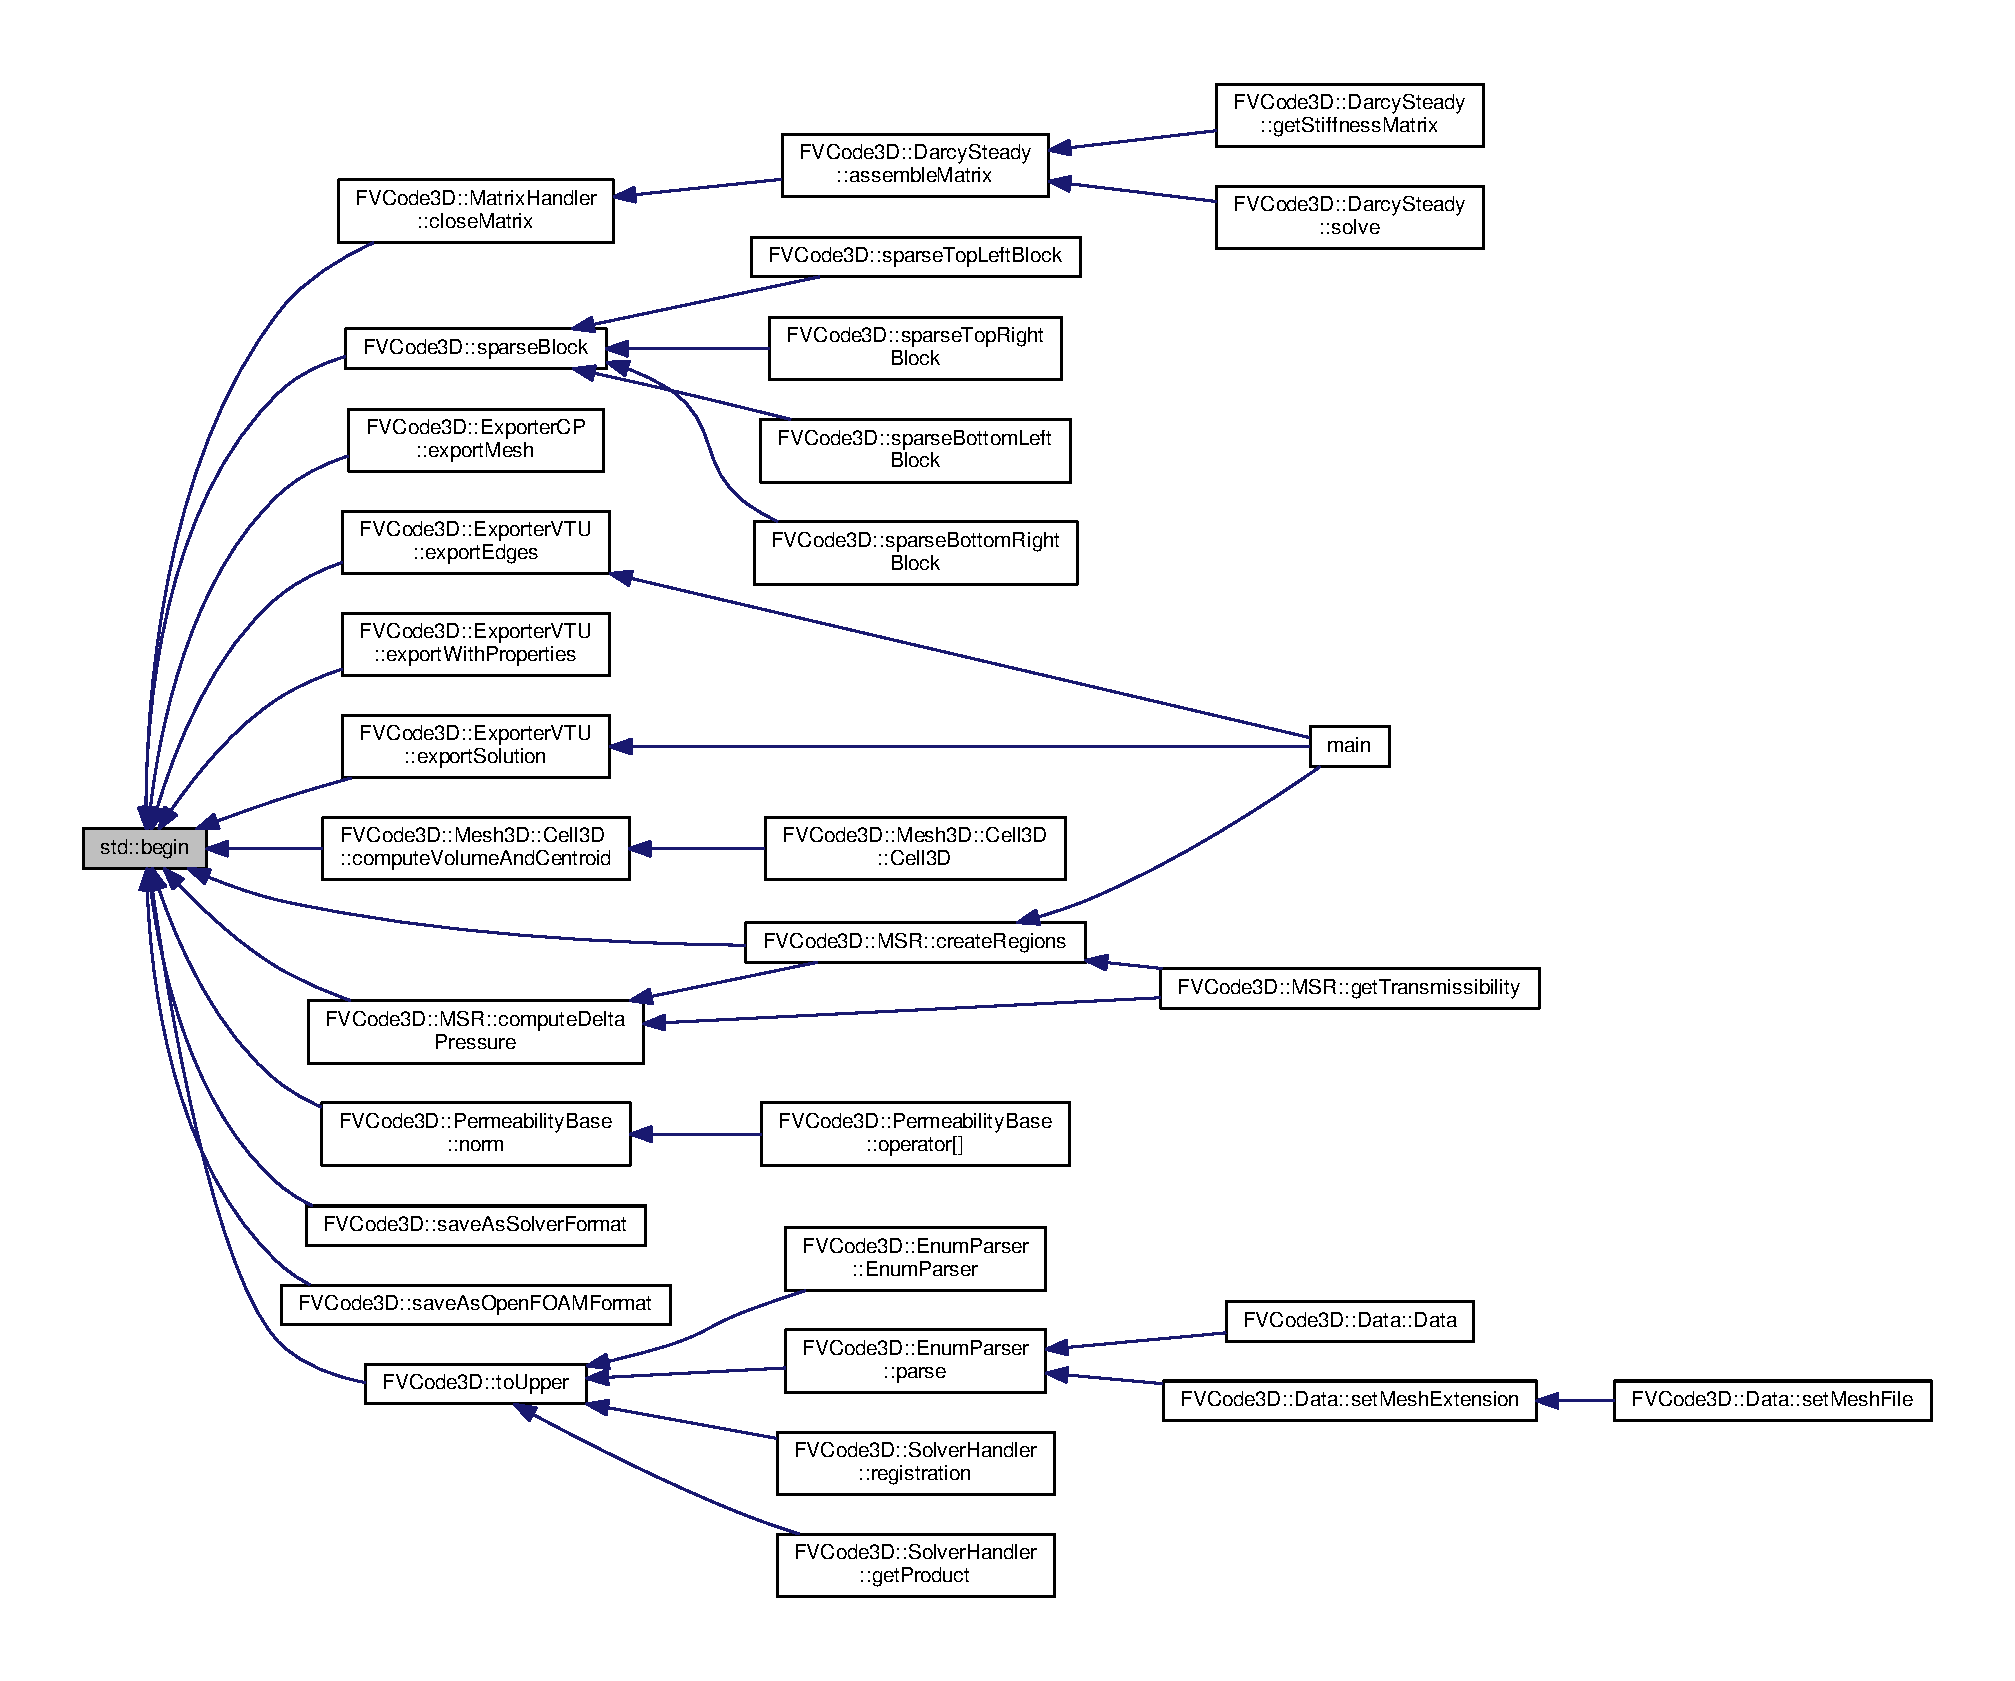
\includegraphics[width=350pt]{namespacestd_acec9a198880c12f51f02be95a298a48b_icgraph}
\end{center}
\end{figure}


\index{std@{std}!begin@{begin}}
\index{begin@{begin}!std@{std}}
\subsubsection[{\texorpdfstring{begin(const Eigen\+::\+Matrix$<$ \+\_\+\+Scalar, \+\_\+\+Rows, \+\_\+\+Cols, \+\_\+\+Options, \+\_\+\+Max\+Rows, \+\_\+\+Max\+Cols $>$ \&v)}{begin(const Eigen::Matrix< _Scalar, _Rows, _Cols, _Options, _MaxRows, _MaxCols > &v)}}]{\setlength{\rightskip}{0pt plus 5cm}template$<$typename \+\_\+\+Scalar , int \+\_\+\+Rows, int \+\_\+\+Cols, int \+\_\+\+Options, int \+\_\+\+Max\+Rows, int \+\_\+\+Max\+Cols$>$ const Eigen\+::\+Matrix$<$\+\_\+\+Scalar,\+\_\+\+Rows,\+\_\+\+Cols,\+\_\+\+Options,\+\_\+\+Max\+Rows,\+\_\+\+Max\+Cols$>$\+::Scalar$\ast$ std\+::begin (
\begin{DoxyParamCaption}
\item[{const Eigen\+::\+Matrix$<$ \+\_\+\+Scalar, \+\_\+\+Rows, \+\_\+\+Cols, \+\_\+\+Options, \+\_\+\+Max\+Rows, \+\_\+\+Max\+Cols $>$ \&}]{v}
\end{DoxyParamCaption}
)}\hypertarget{namespacestd_a5dbbf4f3aa392edddc233eaba37e4b73}{}\label{namespacestd_a5dbbf4f3aa392edddc233eaba37e4b73}


Implements \hyperlink{namespacestd_acec9a198880c12f51f02be95a298a48b}{std\+::begin()} for Eigen\+::\+Matrix type (const) 



Definition at line \hyperlink{RangeSupport_8hpp_source_l00032}{32} of file \hyperlink{RangeSupport_8hpp_source}{Range\+Support.\+hpp}.

\index{std@{std}!end@{end}}
\index{end@{end}!std@{std}}
\subsubsection[{\texorpdfstring{end(\+Eigen\+::\+Matrix$<$ \+\_\+\+Scalar, \+\_\+\+Rows, \+\_\+\+Cols, \+\_\+\+Options, \+\_\+\+Max\+Rows, \+\_\+\+Max\+Cols $>$ \&v)}{end(Eigen::Matrix< _Scalar, _Rows, _Cols, _Options, _MaxRows, _MaxCols > &v)}}]{\setlength{\rightskip}{0pt plus 5cm}template$<$typename \+\_\+\+Scalar , int \+\_\+\+Rows, int \+\_\+\+Cols, int \+\_\+\+Options, int \+\_\+\+Max\+Rows, int \+\_\+\+Max\+Cols$>$ Eigen\+::\+Matrix$<$\+\_\+\+Scalar,\+\_\+\+Rows,\+\_\+\+Cols,\+\_\+\+Options,\+\_\+\+Max\+Rows,\+\_\+\+Max\+Cols$>$\+::Scalar$\ast$ std\+::end (
\begin{DoxyParamCaption}
\item[{Eigen\+::\+Matrix$<$ \+\_\+\+Scalar, \+\_\+\+Rows, \+\_\+\+Cols, \+\_\+\+Options, \+\_\+\+Max\+Rows, \+\_\+\+Max\+Cols $>$ \&}]{v}
\end{DoxyParamCaption}
)}\hypertarget{namespacestd_aeb4b319cf9afda99ba1f47d32df15bc9}{}\label{namespacestd_aeb4b319cf9afda99ba1f47d32df15bc9}


Implements \hyperlink{namespacestd_aeb4b319cf9afda99ba1f47d32df15bc9}{std\+::end()} for Eigen\+::\+Matrix type. 



Definition at line \hyperlink{RangeSupport_8hpp_source_l00024}{24} of file \hyperlink{RangeSupport_8hpp_source}{Range\+Support.\+hpp}.



Here is the caller graph for this function\+:
\nopagebreak
\begin{figure}[H]
\begin{center}
\leavevmode
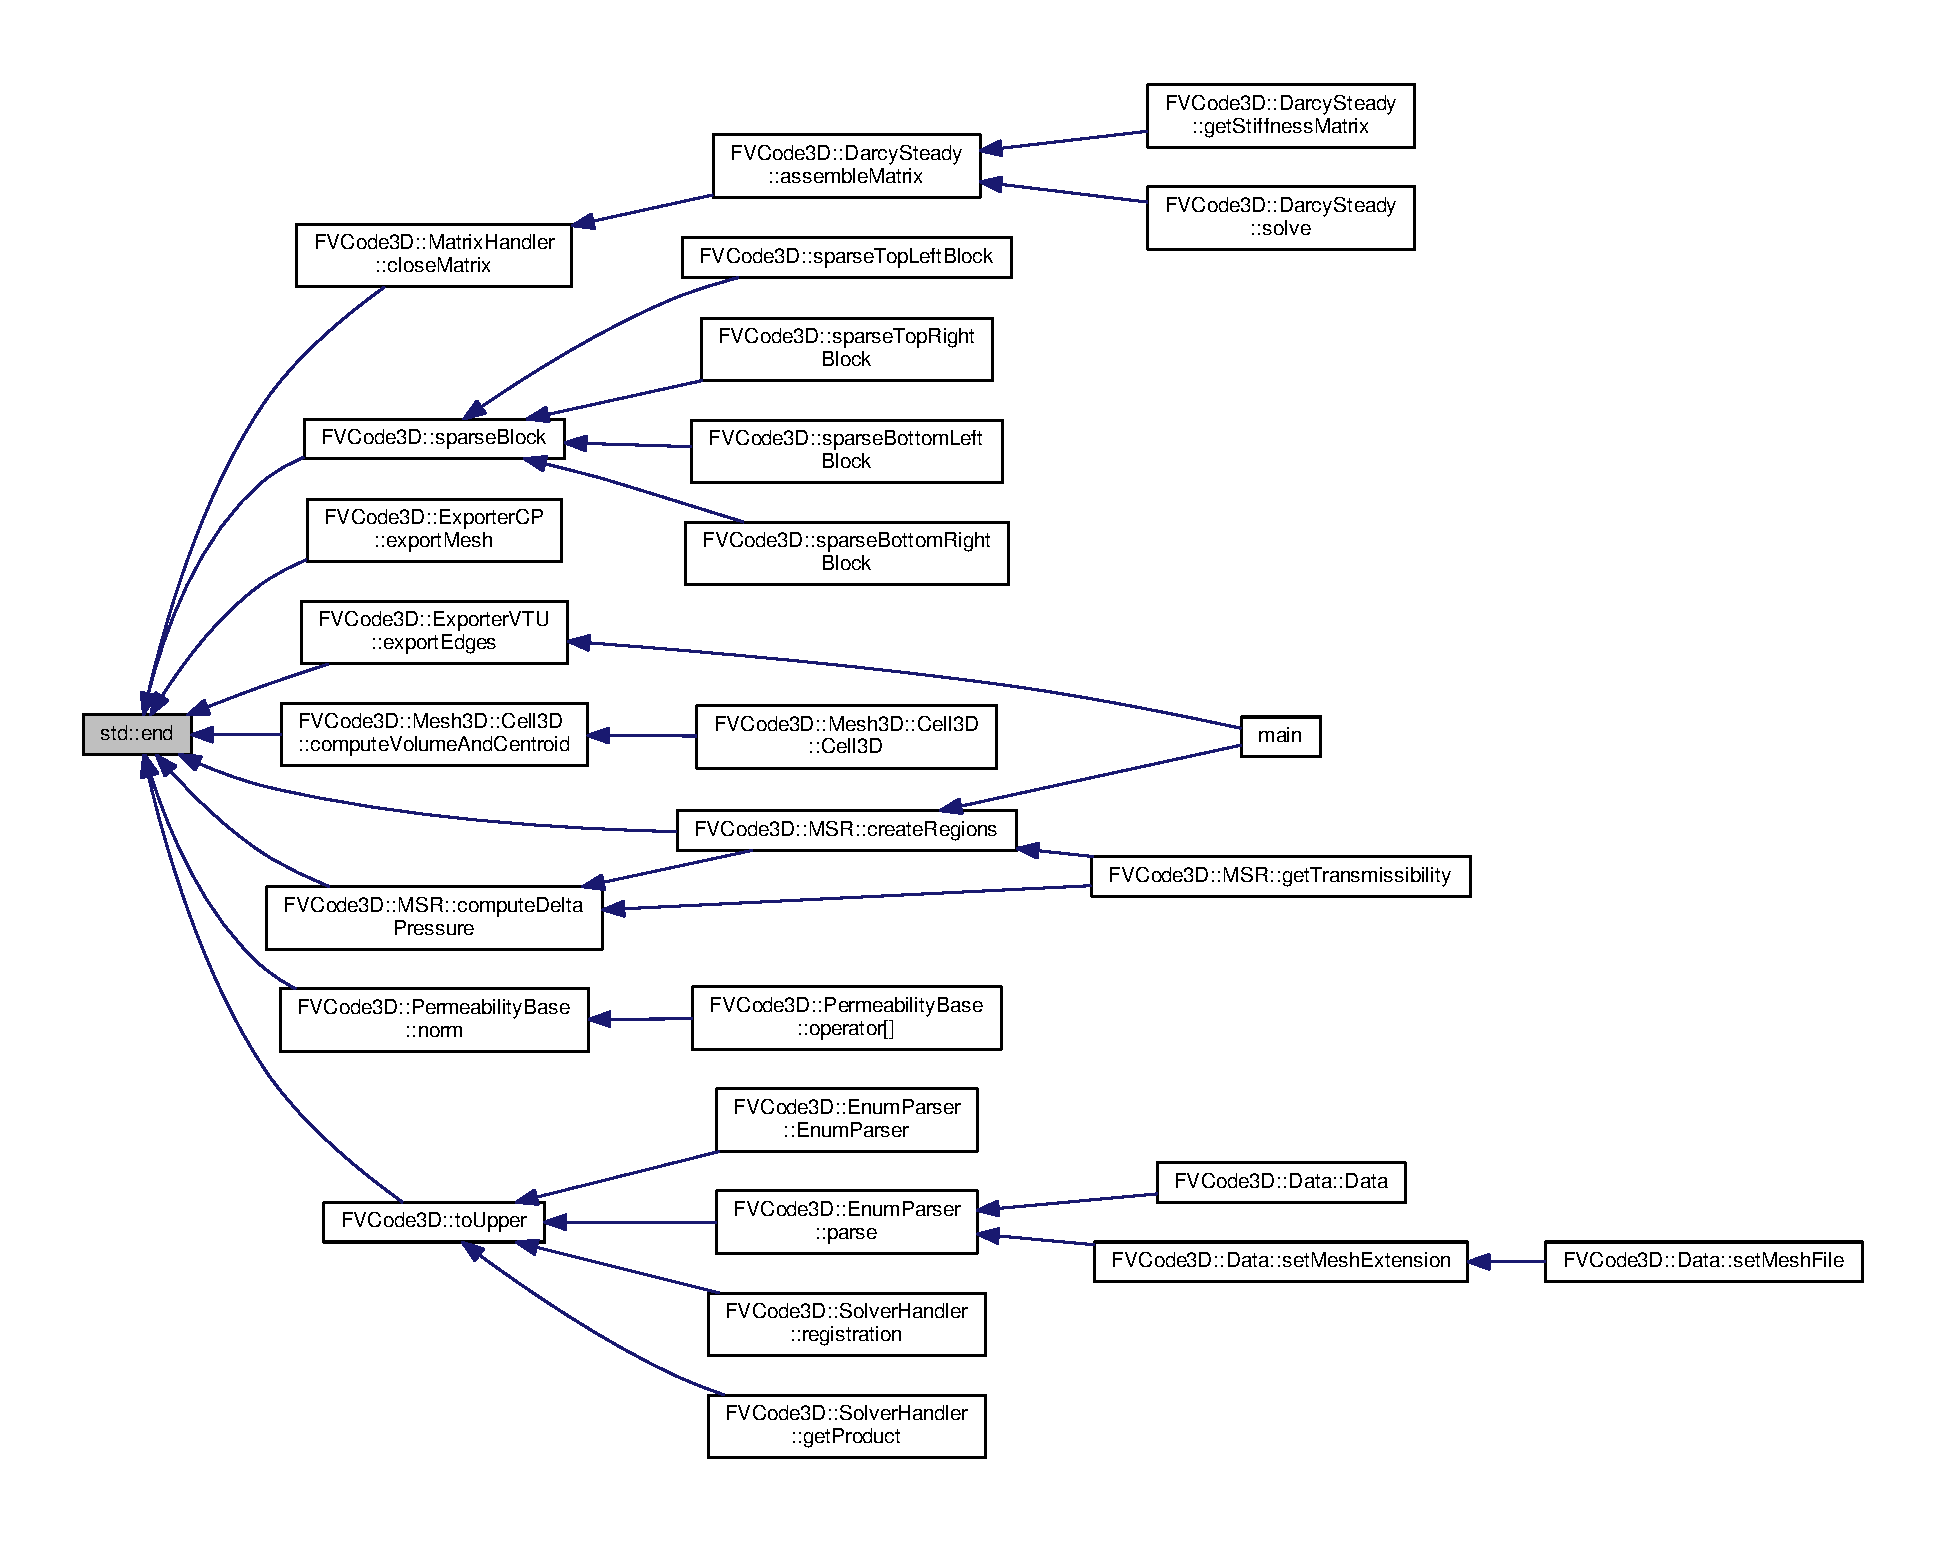
\includegraphics[width=350pt]{namespacestd_aeb4b319cf9afda99ba1f47d32df15bc9_icgraph}
\end{center}
\end{figure}


\index{std@{std}!end@{end}}
\index{end@{end}!std@{std}}
\subsubsection[{\texorpdfstring{end(const Eigen\+::\+Matrix$<$ \+\_\+\+Scalar, \+\_\+\+Rows, \+\_\+\+Cols, \+\_\+\+Options, \+\_\+\+Max\+Rows, \+\_\+\+Max\+Cols $>$ \&v)}{end(const Eigen::Matrix< _Scalar, _Rows, _Cols, _Options, _MaxRows, _MaxCols > &v)}}]{\setlength{\rightskip}{0pt plus 5cm}template$<$typename \+\_\+\+Scalar , int \+\_\+\+Rows, int \+\_\+\+Cols, int \+\_\+\+Options, int \+\_\+\+Max\+Rows, int \+\_\+\+Max\+Cols$>$ const Eigen\+::\+Matrix$<$\+\_\+\+Scalar,\+\_\+\+Rows,\+\_\+\+Cols,\+\_\+\+Options,\+\_\+\+Max\+Rows,\+\_\+\+Max\+Cols$>$\+::Scalar$\ast$ std\+::end (
\begin{DoxyParamCaption}
\item[{const Eigen\+::\+Matrix$<$ \+\_\+\+Scalar, \+\_\+\+Rows, \+\_\+\+Cols, \+\_\+\+Options, \+\_\+\+Max\+Rows, \+\_\+\+Max\+Cols $>$ \&}]{v}
\end{DoxyParamCaption}
)}\hypertarget{namespacestd_a8d57b4b14e873f55a011ed85a84cdb1e}{}\label{namespacestd_a8d57b4b14e873f55a011ed85a84cdb1e}


Implements \hyperlink{namespacestd_aeb4b319cf9afda99ba1f47d32df15bc9}{std\+::end()} for Eigen\+::\+Matrix type (const) 



Definition at line \hyperlink{RangeSupport_8hpp_source_l00040}{40} of file \hyperlink{RangeSupport_8hpp_source}{Range\+Support.\+hpp}.


\chapter{Data Structure Documentation}
\hypertarget{classtetgenmesh_1_1arraypool}{}\section{tetgenmesh\+:\+:arraypool Class Reference}
\label{classtetgenmesh_1_1arraypool}\index{tetgenmesh\+::arraypool@{tetgenmesh\+::arraypool}}


{\ttfamily \#include $<$tetgen.\+h$>$}

\subsection*{Public Member Functions}
\begin{DoxyCompactItemize}
\item 
void \hyperlink{classtetgenmesh_1_1arraypool_a19030126ef81a9ff3c4aca35f0347cdc}{restart} ()
\item 
void \hyperlink{classtetgenmesh_1_1arraypool_a3069be62301a28c1e89201008e838cf8}{poolinit} (int sizeofobject, int log2objperblk)
\item 
char $\ast$ \hyperlink{classtetgenmesh_1_1arraypool_a17e2b92fac4afe65cc14e25f9d42ce6b}{getblock} (int objectindex)
\item 
void $\ast$ \hyperlink{classtetgenmesh_1_1arraypool_a2efe165bb3324f8801f209d1721ff9ec}{lookup} (int objectindex)
\item 
int \hyperlink{classtetgenmesh_1_1arraypool_afb546c70f7728e3e0d58e2aada464437}{newindex} (void $\ast$$\ast$newptr)
\item 
\hyperlink{classtetgenmesh_1_1arraypool_a62a21b86eafefd79c951e85a9b180d0f}{arraypool} (int sizeofobject, int log2objperblk)
\item 
\hyperlink{classtetgenmesh_1_1arraypool_ad35fa12ece8de7d6b567baf9af8d7200}{$\sim$arraypool} ()
\end{DoxyCompactItemize}
\subsection*{Data Fields}
\begin{DoxyCompactItemize}
\item 
int \hyperlink{classtetgenmesh_1_1arraypool_a469ac2a2833a25faa0f99ab011122e2d}{objectbytes}
\item 
int \hyperlink{classtetgenmesh_1_1arraypool_a2b6ba46461d5c8f0e6043bdd111246dd}{objectsperblock}
\item 
int \hyperlink{classtetgenmesh_1_1arraypool_ab61ada3b2fc49879a160a919e9994279}{log2objectsperblock}
\item 
int \hyperlink{classtetgenmesh_1_1arraypool_a662031b2a9978bfc3be39ce90bd3bf0a}{objectsperblockmark}
\item 
int \hyperlink{classtetgenmesh_1_1arraypool_aa9ced327d45678f31b4e7f8e75aff861}{toparraylen}
\item 
char $\ast$$\ast$ \hyperlink{classtetgenmesh_1_1arraypool_a3a4e28a88226f1dd777773fe45094650}{toparray}
\item 
long \hyperlink{classtetgenmesh_1_1arraypool_a23345232309fd68d2e3afa6d017299b0}{objects}
\item 
unsigned long \hyperlink{classtetgenmesh_1_1arraypool_af264f265d5752e75f50adea472ecd59f}{totalmemory}
\end{DoxyCompactItemize}


\subsection{Detailed Description}


Definition at line \hyperlink{tetgen_8h_source_l00980}{980} of file \hyperlink{tetgen_8h_source}{tetgen.\+h}.



\subsection{Constructor \& Destructor Documentation}
\index{tetgenmesh\+::arraypool@{tetgenmesh\+::arraypool}!arraypool@{arraypool}}
\index{arraypool@{arraypool}!tetgenmesh\+::arraypool@{tetgenmesh\+::arraypool}}
\subsubsection[{\texorpdfstring{arraypool(int sizeofobject, int log2objperblk)}{arraypool(int sizeofobject, int log2objperblk)}}]{\setlength{\rightskip}{0pt plus 5cm}tetgenmesh\+::arraypool\+::arraypool (
\begin{DoxyParamCaption}
\item[{int}]{sizeofobject, }
\item[{int}]{log2objperblk}
\end{DoxyParamCaption}
)}\hypertarget{classtetgenmesh_1_1arraypool_a62a21b86eafefd79c951e85a9b180d0f}{}\label{classtetgenmesh_1_1arraypool_a62a21b86eafefd79c951e85a9b180d0f}
\index{tetgenmesh\+::arraypool@{tetgenmesh\+::arraypool}!````~arraypool@{$\sim$arraypool}}
\index{````~arraypool@{$\sim$arraypool}!tetgenmesh\+::arraypool@{tetgenmesh\+::arraypool}}
\subsubsection[{\texorpdfstring{$\sim$arraypool()}{~arraypool()}}]{\setlength{\rightskip}{0pt plus 5cm}tetgenmesh\+::arraypool\+::$\sim$arraypool (
\begin{DoxyParamCaption}
{}
\end{DoxyParamCaption}
)}\hypertarget{classtetgenmesh_1_1arraypool_ad35fa12ece8de7d6b567baf9af8d7200}{}\label{classtetgenmesh_1_1arraypool_ad35fa12ece8de7d6b567baf9af8d7200}


\subsection{Member Function Documentation}
\index{tetgenmesh\+::arraypool@{tetgenmesh\+::arraypool}!getblock@{getblock}}
\index{getblock@{getblock}!tetgenmesh\+::arraypool@{tetgenmesh\+::arraypool}}
\subsubsection[{\texorpdfstring{getblock(int objectindex)}{getblock(int objectindex)}}]{\setlength{\rightskip}{0pt plus 5cm}char$\ast$ tetgenmesh\+::arraypool\+::getblock (
\begin{DoxyParamCaption}
\item[{int}]{objectindex}
\end{DoxyParamCaption}
)}\hypertarget{classtetgenmesh_1_1arraypool_a17e2b92fac4afe65cc14e25f9d42ce6b}{}\label{classtetgenmesh_1_1arraypool_a17e2b92fac4afe65cc14e25f9d42ce6b}
\index{tetgenmesh\+::arraypool@{tetgenmesh\+::arraypool}!lookup@{lookup}}
\index{lookup@{lookup}!tetgenmesh\+::arraypool@{tetgenmesh\+::arraypool}}
\subsubsection[{\texorpdfstring{lookup(int objectindex)}{lookup(int objectindex)}}]{\setlength{\rightskip}{0pt plus 5cm}void$\ast$ tetgenmesh\+::arraypool\+::lookup (
\begin{DoxyParamCaption}
\item[{int}]{objectindex}
\end{DoxyParamCaption}
)}\hypertarget{classtetgenmesh_1_1arraypool_a2efe165bb3324f8801f209d1721ff9ec}{}\label{classtetgenmesh_1_1arraypool_a2efe165bb3324f8801f209d1721ff9ec}
\index{tetgenmesh\+::arraypool@{tetgenmesh\+::arraypool}!newindex@{newindex}}
\index{newindex@{newindex}!tetgenmesh\+::arraypool@{tetgenmesh\+::arraypool}}
\subsubsection[{\texorpdfstring{newindex(void $\ast$$\ast$newptr)}{newindex(void **newptr)}}]{\setlength{\rightskip}{0pt plus 5cm}int tetgenmesh\+::arraypool\+::newindex (
\begin{DoxyParamCaption}
\item[{void $\ast$$\ast$}]{newptr}
\end{DoxyParamCaption}
)}\hypertarget{classtetgenmesh_1_1arraypool_afb546c70f7728e3e0d58e2aada464437}{}\label{classtetgenmesh_1_1arraypool_afb546c70f7728e3e0d58e2aada464437}
\index{tetgenmesh\+::arraypool@{tetgenmesh\+::arraypool}!poolinit@{poolinit}}
\index{poolinit@{poolinit}!tetgenmesh\+::arraypool@{tetgenmesh\+::arraypool}}
\subsubsection[{\texorpdfstring{poolinit(int sizeofobject, int log2objperblk)}{poolinit(int sizeofobject, int log2objperblk)}}]{\setlength{\rightskip}{0pt plus 5cm}void tetgenmesh\+::arraypool\+::poolinit (
\begin{DoxyParamCaption}
\item[{int}]{sizeofobject, }
\item[{int}]{log2objperblk}
\end{DoxyParamCaption}
)}\hypertarget{classtetgenmesh_1_1arraypool_a3069be62301a28c1e89201008e838cf8}{}\label{classtetgenmesh_1_1arraypool_a3069be62301a28c1e89201008e838cf8}
\index{tetgenmesh\+::arraypool@{tetgenmesh\+::arraypool}!restart@{restart}}
\index{restart@{restart}!tetgenmesh\+::arraypool@{tetgenmesh\+::arraypool}}
\subsubsection[{\texorpdfstring{restart()}{restart()}}]{\setlength{\rightskip}{0pt plus 5cm}void tetgenmesh\+::arraypool\+::restart (
\begin{DoxyParamCaption}
{}
\end{DoxyParamCaption}
)}\hypertarget{classtetgenmesh_1_1arraypool_a19030126ef81a9ff3c4aca35f0347cdc}{}\label{classtetgenmesh_1_1arraypool_a19030126ef81a9ff3c4aca35f0347cdc}


\subsection{Field Documentation}
\index{tetgenmesh\+::arraypool@{tetgenmesh\+::arraypool}!log2objectsperblock@{log2objectsperblock}}
\index{log2objectsperblock@{log2objectsperblock}!tetgenmesh\+::arraypool@{tetgenmesh\+::arraypool}}
\subsubsection[{\texorpdfstring{log2objectsperblock}{log2objectsperblock}}]{\setlength{\rightskip}{0pt plus 5cm}int tetgenmesh\+::arraypool\+::log2objectsperblock}\hypertarget{classtetgenmesh_1_1arraypool_ab61ada3b2fc49879a160a919e9994279}{}\label{classtetgenmesh_1_1arraypool_ab61ada3b2fc49879a160a919e9994279}


Definition at line \hyperlink{tetgen_8h_source_l00986}{986} of file \hyperlink{tetgen_8h_source}{tetgen.\+h}.

\index{tetgenmesh\+::arraypool@{tetgenmesh\+::arraypool}!objectbytes@{objectbytes}}
\index{objectbytes@{objectbytes}!tetgenmesh\+::arraypool@{tetgenmesh\+::arraypool}}
\subsubsection[{\texorpdfstring{objectbytes}{objectbytes}}]{\setlength{\rightskip}{0pt plus 5cm}int tetgenmesh\+::arraypool\+::objectbytes}\hypertarget{classtetgenmesh_1_1arraypool_a469ac2a2833a25faa0f99ab011122e2d}{}\label{classtetgenmesh_1_1arraypool_a469ac2a2833a25faa0f99ab011122e2d}


Definition at line \hyperlink{tetgen_8h_source_l00984}{984} of file \hyperlink{tetgen_8h_source}{tetgen.\+h}.

\index{tetgenmesh\+::arraypool@{tetgenmesh\+::arraypool}!objects@{objects}}
\index{objects@{objects}!tetgenmesh\+::arraypool@{tetgenmesh\+::arraypool}}
\subsubsection[{\texorpdfstring{objects}{objects}}]{\setlength{\rightskip}{0pt plus 5cm}long tetgenmesh\+::arraypool\+::objects}\hypertarget{classtetgenmesh_1_1arraypool_a23345232309fd68d2e3afa6d017299b0}{}\label{classtetgenmesh_1_1arraypool_a23345232309fd68d2e3afa6d017299b0}


Definition at line \hyperlink{tetgen_8h_source_l00990}{990} of file \hyperlink{tetgen_8h_source}{tetgen.\+h}.

\index{tetgenmesh\+::arraypool@{tetgenmesh\+::arraypool}!objectsperblock@{objectsperblock}}
\index{objectsperblock@{objectsperblock}!tetgenmesh\+::arraypool@{tetgenmesh\+::arraypool}}
\subsubsection[{\texorpdfstring{objectsperblock}{objectsperblock}}]{\setlength{\rightskip}{0pt plus 5cm}int tetgenmesh\+::arraypool\+::objectsperblock}\hypertarget{classtetgenmesh_1_1arraypool_a2b6ba46461d5c8f0e6043bdd111246dd}{}\label{classtetgenmesh_1_1arraypool_a2b6ba46461d5c8f0e6043bdd111246dd}


Definition at line \hyperlink{tetgen_8h_source_l00985}{985} of file \hyperlink{tetgen_8h_source}{tetgen.\+h}.

\index{tetgenmesh\+::arraypool@{tetgenmesh\+::arraypool}!objectsperblockmark@{objectsperblockmark}}
\index{objectsperblockmark@{objectsperblockmark}!tetgenmesh\+::arraypool@{tetgenmesh\+::arraypool}}
\subsubsection[{\texorpdfstring{objectsperblockmark}{objectsperblockmark}}]{\setlength{\rightskip}{0pt plus 5cm}int tetgenmesh\+::arraypool\+::objectsperblockmark}\hypertarget{classtetgenmesh_1_1arraypool_a662031b2a9978bfc3be39ce90bd3bf0a}{}\label{classtetgenmesh_1_1arraypool_a662031b2a9978bfc3be39ce90bd3bf0a}


Definition at line \hyperlink{tetgen_8h_source_l00987}{987} of file \hyperlink{tetgen_8h_source}{tetgen.\+h}.

\index{tetgenmesh\+::arraypool@{tetgenmesh\+::arraypool}!toparray@{toparray}}
\index{toparray@{toparray}!tetgenmesh\+::arraypool@{tetgenmesh\+::arraypool}}
\subsubsection[{\texorpdfstring{toparray}{toparray}}]{\setlength{\rightskip}{0pt plus 5cm}char$\ast$$\ast$ tetgenmesh\+::arraypool\+::toparray}\hypertarget{classtetgenmesh_1_1arraypool_a3a4e28a88226f1dd777773fe45094650}{}\label{classtetgenmesh_1_1arraypool_a3a4e28a88226f1dd777773fe45094650}


Definition at line \hyperlink{tetgen_8h_source_l00989}{989} of file \hyperlink{tetgen_8h_source}{tetgen.\+h}.

\index{tetgenmesh\+::arraypool@{tetgenmesh\+::arraypool}!toparraylen@{toparraylen}}
\index{toparraylen@{toparraylen}!tetgenmesh\+::arraypool@{tetgenmesh\+::arraypool}}
\subsubsection[{\texorpdfstring{toparraylen}{toparraylen}}]{\setlength{\rightskip}{0pt plus 5cm}int tetgenmesh\+::arraypool\+::toparraylen}\hypertarget{classtetgenmesh_1_1arraypool_aa9ced327d45678f31b4e7f8e75aff861}{}\label{classtetgenmesh_1_1arraypool_aa9ced327d45678f31b4e7f8e75aff861}


Definition at line \hyperlink{tetgen_8h_source_l00988}{988} of file \hyperlink{tetgen_8h_source}{tetgen.\+h}.

\index{tetgenmesh\+::arraypool@{tetgenmesh\+::arraypool}!totalmemory@{totalmemory}}
\index{totalmemory@{totalmemory}!tetgenmesh\+::arraypool@{tetgenmesh\+::arraypool}}
\subsubsection[{\texorpdfstring{totalmemory}{totalmemory}}]{\setlength{\rightskip}{0pt plus 5cm}unsigned long tetgenmesh\+::arraypool\+::totalmemory}\hypertarget{classtetgenmesh_1_1arraypool_af264f265d5752e75f50adea472ecd59f}{}\label{classtetgenmesh_1_1arraypool_af264f265d5752e75f50adea472ecd59f}


Definition at line \hyperlink{tetgen_8h_source_l00991}{991} of file \hyperlink{tetgen_8h_source}{tetgen.\+h}.



The documentation for this class was generated from the following file\+:\begin{DoxyCompactItemize}
\item 
/home/corinne/eni\+Reservoir\+G\+I\+T\+H\+U\+B/eni\+Reservoir/\+F\+V\+Code3\+D/src/\+F\+V\+Code3\+D/\hyperlink{tetgen_8h}{tetgen.\+h}\end{DoxyCompactItemize}

\hypertarget{classtetgenmesh_1_1badface}{}\section{tetgenmesh\+:\+:badface Class Reference}
\label{classtetgenmesh_1_1badface}\index{tetgenmesh\+::badface@{tetgenmesh\+::badface}}


{\ttfamily \#include $<$tetgen.\+h$>$}



Collaboration diagram for tetgenmesh\+:\+:badface\+:
\nopagebreak
\begin{figure}[H]
\begin{center}
\leavevmode
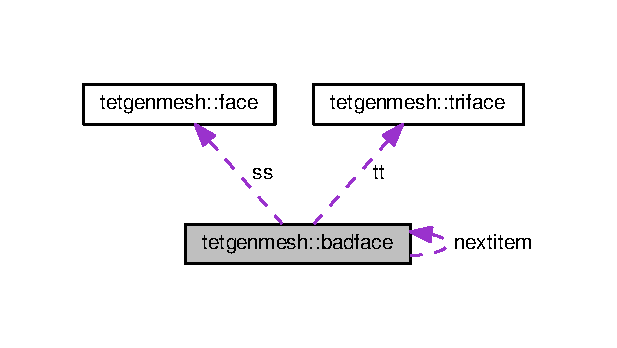
\includegraphics[width=296pt]{classtetgenmesh_1_1badface__coll__graph}
\end{center}
\end{figure}
\subsection*{Public Member Functions}
\begin{DoxyCompactItemize}
\item 
\hyperlink{classtetgenmesh_1_1badface_abb0568159042a95b91eb193fcfca6aab}{badface} ()
\end{DoxyCompactItemize}
\subsection*{Data Fields}
\begin{DoxyCompactItemize}
\item 
\hyperlink{classtetgenmesh_1_1triface}{triface} \hyperlink{classtetgenmesh_1_1badface_a01d24569e6058b3dae1a31e0638b849c}{tt}
\item 
\hyperlink{classtetgenmesh_1_1face}{face} \hyperlink{classtetgenmesh_1_1badface_ace098878b5e89ec387c959d8acd0153d}{ss}
\item 
\hyperlink{tetgen_8h_a4b654506f18b8bfd61ad2a29a7e38c25}{R\+E\+AL} \hyperlink{classtetgenmesh_1_1badface_ac94189eb4b728abd589597c89db9a1d7}{key}
\item 
\hyperlink{tetgen_8h_a4b654506f18b8bfd61ad2a29a7e38c25}{R\+E\+AL} \hyperlink{classtetgenmesh_1_1badface_a72958cf685f881af15213f0925ccf72a}{cent} \mbox{[}6\mbox{]}
\item 
\hyperlink{classtetgenmesh_ace3fb4f80389185b7c9b18ab69a3dea2}{point} \hyperlink{classtetgenmesh_1_1badface_a620b94f643bafaa7a4dbfeba7063a445}{forg}
\item 
\hyperlink{classtetgenmesh_ace3fb4f80389185b7c9b18ab69a3dea2}{point} \hyperlink{classtetgenmesh_1_1badface_a8e010478b28c997ad9b441d05df47695}{fdest}
\item 
\hyperlink{classtetgenmesh_ace3fb4f80389185b7c9b18ab69a3dea2}{point} \hyperlink{classtetgenmesh_1_1badface_a617348221ce387b323575110a5c79627}{fapex}
\item 
\hyperlink{classtetgenmesh_ace3fb4f80389185b7c9b18ab69a3dea2}{point} \hyperlink{classtetgenmesh_1_1badface_a8e9966e480c210ac83ab0a4c221a7000}{foppo}
\item 
\hyperlink{classtetgenmesh_ace3fb4f80389185b7c9b18ab69a3dea2}{point} \hyperlink{classtetgenmesh_1_1badface_ada4ec358fcf9261b2f14cff307e66fdf}{noppo}
\item 
\hyperlink{classtetgenmesh_1_1badface}{badface} $\ast$ \hyperlink{classtetgenmesh_1_1badface_ae87a801b03dbaa3dd5709ffed5eef5bc}{nextitem}
\end{DoxyCompactItemize}


\subsection{Detailed Description}


Definition at line \hyperlink{tetgen_8h_source_l01074}{1074} of file \hyperlink{tetgen_8h_source}{tetgen.\+h}.



\subsection{Constructor \& Destructor Documentation}
\index{tetgenmesh\+::badface@{tetgenmesh\+::badface}!badface@{badface}}
\index{badface@{badface}!tetgenmesh\+::badface@{tetgenmesh\+::badface}}
\subsubsection[{\texorpdfstring{badface()}{badface()}}]{\setlength{\rightskip}{0pt plus 5cm}tetgenmesh\+::badface\+::badface (
\begin{DoxyParamCaption}
{}
\end{DoxyParamCaption}
)\hspace{0.3cm}{\ttfamily [inline]}}\hypertarget{classtetgenmesh_1_1badface_abb0568159042a95b91eb193fcfca6aab}{}\label{classtetgenmesh_1_1badface_abb0568159042a95b91eb193fcfca6aab}


Definition at line \hyperlink{tetgen_8h_source_l01081}{1081} of file \hyperlink{tetgen_8h_source}{tetgen.\+h}.



\subsection{Field Documentation}
\index{tetgenmesh\+::badface@{tetgenmesh\+::badface}!cent@{cent}}
\index{cent@{cent}!tetgenmesh\+::badface@{tetgenmesh\+::badface}}
\subsubsection[{\texorpdfstring{cent}{cent}}]{\setlength{\rightskip}{0pt plus 5cm}{\bf R\+E\+AL} tetgenmesh\+::badface\+::cent\mbox{[}6\mbox{]}}\hypertarget{classtetgenmesh_1_1badface_a72958cf685f881af15213f0925ccf72a}{}\label{classtetgenmesh_1_1badface_a72958cf685f881af15213f0925ccf72a}


Definition at line \hyperlink{tetgen_8h_source_l01078}{1078} of file \hyperlink{tetgen_8h_source}{tetgen.\+h}.

\index{tetgenmesh\+::badface@{tetgenmesh\+::badface}!fapex@{fapex}}
\index{fapex@{fapex}!tetgenmesh\+::badface@{tetgenmesh\+::badface}}
\subsubsection[{\texorpdfstring{fapex}{fapex}}]{\setlength{\rightskip}{0pt plus 5cm}{\bf point} tetgenmesh\+::badface\+::fapex}\hypertarget{classtetgenmesh_1_1badface_a617348221ce387b323575110a5c79627}{}\label{classtetgenmesh_1_1badface_a617348221ce387b323575110a5c79627}


Definition at line \hyperlink{tetgen_8h_source_l01079}{1079} of file \hyperlink{tetgen_8h_source}{tetgen.\+h}.

\index{tetgenmesh\+::badface@{tetgenmesh\+::badface}!fdest@{fdest}}
\index{fdest@{fdest}!tetgenmesh\+::badface@{tetgenmesh\+::badface}}
\subsubsection[{\texorpdfstring{fdest}{fdest}}]{\setlength{\rightskip}{0pt plus 5cm}{\bf point} tetgenmesh\+::badface\+::fdest}\hypertarget{classtetgenmesh_1_1badface_a8e010478b28c997ad9b441d05df47695}{}\label{classtetgenmesh_1_1badface_a8e010478b28c997ad9b441d05df47695}


Definition at line \hyperlink{tetgen_8h_source_l01079}{1079} of file \hyperlink{tetgen_8h_source}{tetgen.\+h}.

\index{tetgenmesh\+::badface@{tetgenmesh\+::badface}!foppo@{foppo}}
\index{foppo@{foppo}!tetgenmesh\+::badface@{tetgenmesh\+::badface}}
\subsubsection[{\texorpdfstring{foppo}{foppo}}]{\setlength{\rightskip}{0pt plus 5cm}{\bf point} tetgenmesh\+::badface\+::foppo}\hypertarget{classtetgenmesh_1_1badface_a8e9966e480c210ac83ab0a4c221a7000}{}\label{classtetgenmesh_1_1badface_a8e9966e480c210ac83ab0a4c221a7000}


Definition at line \hyperlink{tetgen_8h_source_l01079}{1079} of file \hyperlink{tetgen_8h_source}{tetgen.\+h}.

\index{tetgenmesh\+::badface@{tetgenmesh\+::badface}!forg@{forg}}
\index{forg@{forg}!tetgenmesh\+::badface@{tetgenmesh\+::badface}}
\subsubsection[{\texorpdfstring{forg}{forg}}]{\setlength{\rightskip}{0pt plus 5cm}{\bf point} tetgenmesh\+::badface\+::forg}\hypertarget{classtetgenmesh_1_1badface_a620b94f643bafaa7a4dbfeba7063a445}{}\label{classtetgenmesh_1_1badface_a620b94f643bafaa7a4dbfeba7063a445}


Definition at line \hyperlink{tetgen_8h_source_l01079}{1079} of file \hyperlink{tetgen_8h_source}{tetgen.\+h}.

\index{tetgenmesh\+::badface@{tetgenmesh\+::badface}!key@{key}}
\index{key@{key}!tetgenmesh\+::badface@{tetgenmesh\+::badface}}
\subsubsection[{\texorpdfstring{key}{key}}]{\setlength{\rightskip}{0pt plus 5cm}{\bf R\+E\+AL} tetgenmesh\+::badface\+::key}\hypertarget{classtetgenmesh_1_1badface_ac94189eb4b728abd589597c89db9a1d7}{}\label{classtetgenmesh_1_1badface_ac94189eb4b728abd589597c89db9a1d7}


Definition at line \hyperlink{tetgen_8h_source_l01078}{1078} of file \hyperlink{tetgen_8h_source}{tetgen.\+h}.

\index{tetgenmesh\+::badface@{tetgenmesh\+::badface}!nextitem@{nextitem}}
\index{nextitem@{nextitem}!tetgenmesh\+::badface@{tetgenmesh\+::badface}}
\subsubsection[{\texorpdfstring{nextitem}{nextitem}}]{\setlength{\rightskip}{0pt plus 5cm}{\bf badface}$\ast$ tetgenmesh\+::badface\+::nextitem}\hypertarget{classtetgenmesh_1_1badface_ae87a801b03dbaa3dd5709ffed5eef5bc}{}\label{classtetgenmesh_1_1badface_ae87a801b03dbaa3dd5709ffed5eef5bc}


Definition at line \hyperlink{tetgen_8h_source_l01080}{1080} of file \hyperlink{tetgen_8h_source}{tetgen.\+h}.

\index{tetgenmesh\+::badface@{tetgenmesh\+::badface}!noppo@{noppo}}
\index{noppo@{noppo}!tetgenmesh\+::badface@{tetgenmesh\+::badface}}
\subsubsection[{\texorpdfstring{noppo}{noppo}}]{\setlength{\rightskip}{0pt plus 5cm}{\bf point} tetgenmesh\+::badface\+::noppo}\hypertarget{classtetgenmesh_1_1badface_ada4ec358fcf9261b2f14cff307e66fdf}{}\label{classtetgenmesh_1_1badface_ada4ec358fcf9261b2f14cff307e66fdf}


Definition at line \hyperlink{tetgen_8h_source_l01079}{1079} of file \hyperlink{tetgen_8h_source}{tetgen.\+h}.

\index{tetgenmesh\+::badface@{tetgenmesh\+::badface}!ss@{ss}}
\index{ss@{ss}!tetgenmesh\+::badface@{tetgenmesh\+::badface}}
\subsubsection[{\texorpdfstring{ss}{ss}}]{\setlength{\rightskip}{0pt plus 5cm}{\bf face} tetgenmesh\+::badface\+::ss}\hypertarget{classtetgenmesh_1_1badface_ace098878b5e89ec387c959d8acd0153d}{}\label{classtetgenmesh_1_1badface_ace098878b5e89ec387c959d8acd0153d}


Definition at line \hyperlink{tetgen_8h_source_l01077}{1077} of file \hyperlink{tetgen_8h_source}{tetgen.\+h}.

\index{tetgenmesh\+::badface@{tetgenmesh\+::badface}!tt@{tt}}
\index{tt@{tt}!tetgenmesh\+::badface@{tetgenmesh\+::badface}}
\subsubsection[{\texorpdfstring{tt}{tt}}]{\setlength{\rightskip}{0pt plus 5cm}{\bf triface} tetgenmesh\+::badface\+::tt}\hypertarget{classtetgenmesh_1_1badface_a01d24569e6058b3dae1a31e0638b849c}{}\label{classtetgenmesh_1_1badface_a01d24569e6058b3dae1a31e0638b849c}


Definition at line \hyperlink{tetgen_8h_source_l01076}{1076} of file \hyperlink{tetgen_8h_source}{tetgen.\+h}.



The documentation for this class was generated from the following file\+:\begin{DoxyCompactItemize}
\item 
/home/corinne/eni\+Reservoir\+G\+I\+T\+H\+U\+B/eni\+Reservoir/\+F\+V\+Code3\+D/src/\+F\+V\+Code3\+D/\hyperlink{tetgen_8h}{tetgen.\+h}\end{DoxyCompactItemize}

\hypertarget{classFVCode3D_1_1Rigid__Mesh_1_1Border__Edge}{}\section{F\+V\+Code3D\+:\+:Rigid\+\_\+\+Mesh\+:\+:Border\+\_\+\+Edge Class Reference}
\label{classFVCode3D_1_1Rigid__Mesh_1_1Border__Edge}\index{F\+V\+Code3\+D\+::\+Rigid\+\_\+\+Mesh\+::\+Border\+\_\+\+Edge@{F\+V\+Code3\+D\+::\+Rigid\+\_\+\+Mesh\+::\+Border\+\_\+\+Edge}}


Class that represents a border edge.  




{\ttfamily \#include $<$Rigid\+Mesh.\+hpp$>$}



Inheritance diagram for F\+V\+Code3D\+:\+:Rigid\+\_\+\+Mesh\+:\+:Border\+\_\+\+Edge\+:
\nopagebreak
\begin{figure}[H]
\begin{center}
\leavevmode
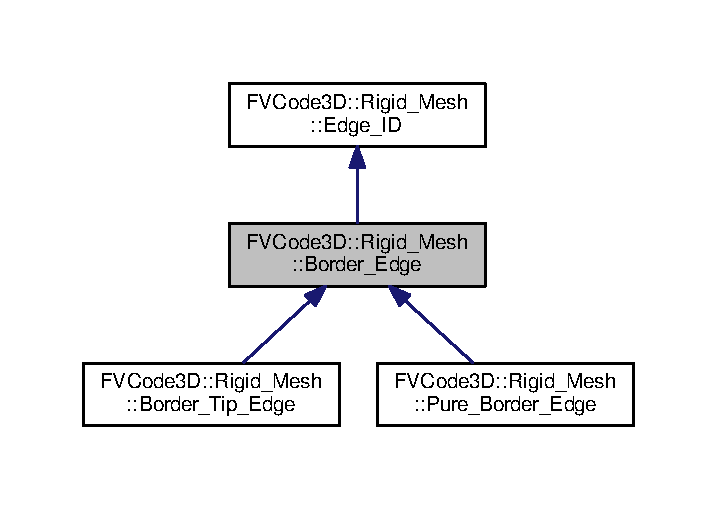
\includegraphics[width=344pt]{classFVCode3D_1_1Rigid__Mesh_1_1Border__Edge__inherit__graph}
\end{center}
\end{figure}


Collaboration diagram for F\+V\+Code3D\+:\+:Rigid\+\_\+\+Mesh\+:\+:Border\+\_\+\+Edge\+:
\nopagebreak
\begin{figure}[H]
\begin{center}
\leavevmode
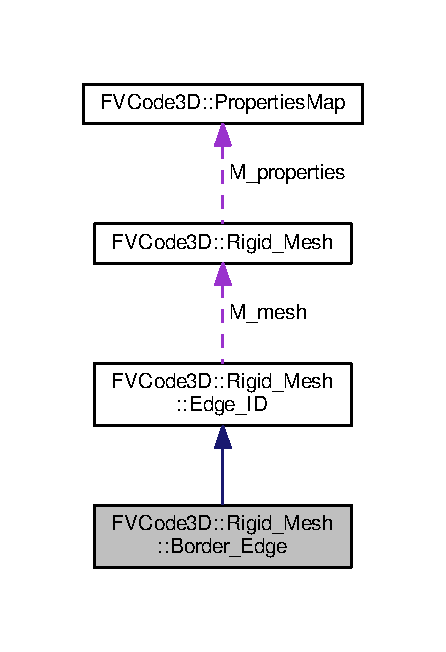
\includegraphics[width=214pt]{classFVCode3D_1_1Rigid__Mesh_1_1Border__Edge__coll__graph}
\end{center}
\end{figure}
\subsection*{Public Member Functions}
\begin{Indent}{\bf Constructor \& Destructor}\par
\begin{DoxyCompactItemize}
\item 
\hyperlink{classFVCode3D_1_1Rigid__Mesh_1_1Border__Edge_a610aa0369df57087614115aa44bafc25}{Border\+\_\+\+Edge} (const \hyperlink{namespaceFVCode3D_a4bf7e328c75d0fd504050d040ebe9eda}{U\+Int} edge\+\_\+\+Id, \hyperlink{classFVCode3D_1_1Rigid__Mesh}{Rigid\+\_\+\+Mesh} $\ast$const mesh)
\begin{DoxyCompactList}\small\item\em Constructor for a \hyperlink{classFVCode3D_1_1Rigid__Mesh_1_1Border__Edge}{Border\+\_\+\+Edge} given an edge id. \end{DoxyCompactList}\item 
\hyperlink{classFVCode3D_1_1Rigid__Mesh_1_1Border__Edge_a4c84ed48d5ade111d258cad7e6a32d79}{Border\+\_\+\+Edge} (const \hyperlink{classFVCode3D_1_1Rigid__Mesh_1_1Border__Edge}{Border\+\_\+\+Edge} \&border\+\_\+edge, \hyperlink{classFVCode3D_1_1Rigid__Mesh}{Rigid\+\_\+\+Mesh} $\ast$const mesh)
\begin{DoxyCompactList}\small\item\em Copy constructor for a \hyperlink{classFVCode3D_1_1Rigid__Mesh_1_1Border__Edge}{Border\+\_\+\+Edge} given a border\+\_\+edge belonging to another \hyperlink{classFVCode3D_1_1Rigid__Mesh}{Rigid\+\_\+\+Mesh}. \end{DoxyCompactList}\item 
\hyperlink{classFVCode3D_1_1Rigid__Mesh_1_1Border__Edge_a109336ed2689561dc49808d0e102b5ec}{Border\+\_\+\+Edge} (const \hyperlink{classFVCode3D_1_1Rigid__Mesh_1_1Border__Edge}{Border\+\_\+\+Edge} \&e)
\begin{DoxyCompactList}\small\item\em Copy constructor for a \hyperlink{classFVCode3D_1_1Rigid__Mesh_1_1Border__Edge}{Border\+\_\+\+Edge} given a border\+\_\+edge. \end{DoxyCompactList}\item 
\hyperlink{classFVCode3D_1_1Rigid__Mesh_1_1Border__Edge_a932e4739138fd4e1d53f8ff7ba6d8e02}{$\sim$\+Border\+\_\+\+Edge} ()=default
\begin{DoxyCompactList}\small\item\em Destructor. \end{DoxyCompactList}\end{DoxyCompactItemize}
\end{Indent}
\begin{Indent}{\bf Get Methods}\par
\begin{DoxyCompactItemize}
\item 
const std\+::set$<$ \hyperlink{namespaceFVCode3D_a4bf7e328c75d0fd504050d040ebe9eda}{U\+Int} $>$ \& \hyperlink{classFVCode3D_1_1Rigid__Mesh_1_1Border__Edge_ae0c4fec80ff33ad9eb08dc5aee5213b1}{get\+Border\+Ids} () const 
\begin{DoxyCompactList}\small\item\em Get border ids (const) \end{DoxyCompactList}\end{DoxyCompactItemize}
\end{Indent}
\subsection*{Data Fields}
\begin{DoxyCompactItemize}
\item 
friend \hyperlink{classFVCode3D_1_1Rigid__Mesh_1_1Border__Edge_a189ee28caab235105a5112a5d8fc9953}{Proxy\+Border\+Edge}
\end{DoxyCompactItemize}
\subsection*{Protected Attributes}
\begin{DoxyCompactItemize}
\item 
std\+::set$<$ \hyperlink{namespaceFVCode3D_a4bf7e328c75d0fd504050d040ebe9eda}{U\+Int} $>$ \hyperlink{classFVCode3D_1_1Rigid__Mesh_1_1Border__Edge_a2dae62d2ca3357296618f45f5a58e81e}{M\+\_\+border\+Ids}
\begin{DoxyCompactList}\small\item\em Ids of the represented borders. \end{DoxyCompactList}\end{DoxyCompactItemize}


\subsection{Detailed Description}
Class that represents a border edge. 

This class is derived from the class \hyperlink{classFVCode3D_1_1Rigid__Mesh_1_1Edge__ID}{Edge\+\_\+\+ID}. This class contains the id of an edge which belongs to the border of the domain. 

Definition at line \hyperlink{RigidMesh_8hpp_source_l00685}{685} of file \hyperlink{RigidMesh_8hpp_source}{Rigid\+Mesh.\+hpp}.



\subsection{Constructor \& Destructor Documentation}
\index{F\+V\+Code3\+D\+::\+Rigid\+\_\+\+Mesh\+::\+Border\+\_\+\+Edge@{F\+V\+Code3\+D\+::\+Rigid\+\_\+\+Mesh\+::\+Border\+\_\+\+Edge}!Border\+\_\+\+Edge@{Border\+\_\+\+Edge}}
\index{Border\+\_\+\+Edge@{Border\+\_\+\+Edge}!F\+V\+Code3\+D\+::\+Rigid\+\_\+\+Mesh\+::\+Border\+\_\+\+Edge@{F\+V\+Code3\+D\+::\+Rigid\+\_\+\+Mesh\+::\+Border\+\_\+\+Edge}}
\subsubsection[{\texorpdfstring{Border\+\_\+\+Edge(const U\+Int edge\+\_\+\+Id, Rigid\+\_\+\+Mesh $\ast$const mesh)}{Border_Edge(const UInt edge_Id, Rigid_Mesh *const mesh)}}]{\setlength{\rightskip}{0pt plus 5cm}F\+V\+Code3\+D\+::\+Rigid\+\_\+\+Mesh\+::\+Border\+\_\+\+Edge\+::\+Border\+\_\+\+Edge (
\begin{DoxyParamCaption}
\item[{const {\bf U\+Int}}]{edge\+\_\+\+Id, }
\item[{{\bf Rigid\+\_\+\+Mesh} $\ast$const}]{mesh}
\end{DoxyParamCaption}
)}\hypertarget{classFVCode3D_1_1Rigid__Mesh_1_1Border__Edge_a610aa0369df57087614115aa44bafc25}{}\label{classFVCode3D_1_1Rigid__Mesh_1_1Border__Edge_a610aa0369df57087614115aa44bafc25}


Constructor for a \hyperlink{classFVCode3D_1_1Rigid__Mesh_1_1Border__Edge}{Border\+\_\+\+Edge} given an edge id. 


\begin{DoxyParams}{Parameters}
{\em edge\+\_\+id} & is the id of an \hyperlink{classFVCode3D_1_1Rigid__Mesh_1_1Edge}{Edge} of a \hyperlink{classFVCode3D_1_1Rigid__Mesh}{Rigid\+\_\+\+Mesh} \\
\hline
{\em mesh} & is a pointer to the mesh to which the edge belongs \\
\hline
\end{DoxyParams}


Definition at line \hyperlink{RigidMesh_8cpp_source_l00705}{705} of file \hyperlink{RigidMesh_8cpp_source}{Rigid\+Mesh.\+cpp}.



Here is the call graph for this function\+:
\nopagebreak
\begin{figure}[H]
\begin{center}
\leavevmode
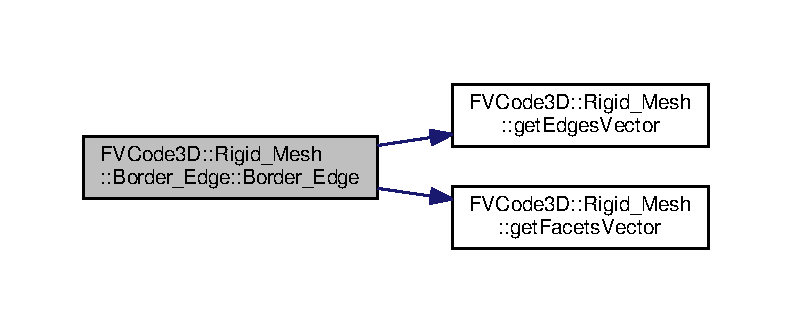
\includegraphics[width=350pt]{classFVCode3D_1_1Rigid__Mesh_1_1Border__Edge_a610aa0369df57087614115aa44bafc25_cgraph}
\end{center}
\end{figure}


\index{F\+V\+Code3\+D\+::\+Rigid\+\_\+\+Mesh\+::\+Border\+\_\+\+Edge@{F\+V\+Code3\+D\+::\+Rigid\+\_\+\+Mesh\+::\+Border\+\_\+\+Edge}!Border\+\_\+\+Edge@{Border\+\_\+\+Edge}}
\index{Border\+\_\+\+Edge@{Border\+\_\+\+Edge}!F\+V\+Code3\+D\+::\+Rigid\+\_\+\+Mesh\+::\+Border\+\_\+\+Edge@{F\+V\+Code3\+D\+::\+Rigid\+\_\+\+Mesh\+::\+Border\+\_\+\+Edge}}
\subsubsection[{\texorpdfstring{Border\+\_\+\+Edge(const Border\+\_\+\+Edge \&border\+\_\+edge, Rigid\+\_\+\+Mesh $\ast$const mesh)}{Border_Edge(const Border_Edge &border_edge, Rigid_Mesh *const mesh)}}]{\setlength{\rightskip}{0pt plus 5cm}F\+V\+Code3\+D\+::\+Rigid\+\_\+\+Mesh\+::\+Border\+\_\+\+Edge\+::\+Border\+\_\+\+Edge (
\begin{DoxyParamCaption}
\item[{const {\bf Border\+\_\+\+Edge} \&}]{border\+\_\+edge, }
\item[{{\bf Rigid\+\_\+\+Mesh} $\ast$const}]{mesh}
\end{DoxyParamCaption}
)}\hypertarget{classFVCode3D_1_1Rigid__Mesh_1_1Border__Edge_a4c84ed48d5ade111d258cad7e6a32d79}{}\label{classFVCode3D_1_1Rigid__Mesh_1_1Border__Edge_a4c84ed48d5ade111d258cad7e6a32d79}


Copy constructor for a \hyperlink{classFVCode3D_1_1Rigid__Mesh_1_1Border__Edge}{Border\+\_\+\+Edge} given a border\+\_\+edge belonging to another \hyperlink{classFVCode3D_1_1Rigid__Mesh}{Rigid\+\_\+\+Mesh}. 


\begin{DoxyParams}{Parameters}
{\em border\+\_\+edge} & reference to a \hyperlink{classFVCode3D_1_1Rigid__Mesh_1_1Border__Edge}{Border\+\_\+\+Edge} \\
\hline
{\em mesh} & is a pointer to the mesh to which the edge belongs \\
\hline
\end{DoxyParams}


Definition at line \hyperlink{RigidMesh_8cpp_source_l00715}{715} of file \hyperlink{RigidMesh_8cpp_source}{Rigid\+Mesh.\+cpp}.

\index{F\+V\+Code3\+D\+::\+Rigid\+\_\+\+Mesh\+::\+Border\+\_\+\+Edge@{F\+V\+Code3\+D\+::\+Rigid\+\_\+\+Mesh\+::\+Border\+\_\+\+Edge}!Border\+\_\+\+Edge@{Border\+\_\+\+Edge}}
\index{Border\+\_\+\+Edge@{Border\+\_\+\+Edge}!F\+V\+Code3\+D\+::\+Rigid\+\_\+\+Mesh\+::\+Border\+\_\+\+Edge@{F\+V\+Code3\+D\+::\+Rigid\+\_\+\+Mesh\+::\+Border\+\_\+\+Edge}}
\subsubsection[{\texorpdfstring{Border\+\_\+\+Edge(const Border\+\_\+\+Edge \&e)}{Border_Edge(const Border_Edge &e)}}]{\setlength{\rightskip}{0pt plus 5cm}F\+V\+Code3\+D\+::\+Rigid\+\_\+\+Mesh\+::\+Border\+\_\+\+Edge\+::\+Border\+\_\+\+Edge (
\begin{DoxyParamCaption}
\item[{const {\bf Border\+\_\+\+Edge} \&}]{e}
\end{DoxyParamCaption}
)}\hypertarget{classFVCode3D_1_1Rigid__Mesh_1_1Border__Edge_a109336ed2689561dc49808d0e102b5ec}{}\label{classFVCode3D_1_1Rigid__Mesh_1_1Border__Edge_a109336ed2689561dc49808d0e102b5ec}


Copy constructor for a \hyperlink{classFVCode3D_1_1Rigid__Mesh_1_1Border__Edge}{Border\+\_\+\+Edge} given a border\+\_\+edge. 


\begin{DoxyParams}{Parameters}
{\em e} & reference to a \hyperlink{classFVCode3D_1_1Rigid__Mesh_1_1Border__Edge}{Border\+\_\+\+Edge} \\
\hline
\end{DoxyParams}


Definition at line \hyperlink{RigidMesh_8cpp_source_l00718}{718} of file \hyperlink{RigidMesh_8cpp_source}{Rigid\+Mesh.\+cpp}.

\index{F\+V\+Code3\+D\+::\+Rigid\+\_\+\+Mesh\+::\+Border\+\_\+\+Edge@{F\+V\+Code3\+D\+::\+Rigid\+\_\+\+Mesh\+::\+Border\+\_\+\+Edge}!````~Border\+\_\+\+Edge@{$\sim$\+Border\+\_\+\+Edge}}
\index{````~Border\+\_\+\+Edge@{$\sim$\+Border\+\_\+\+Edge}!F\+V\+Code3\+D\+::\+Rigid\+\_\+\+Mesh\+::\+Border\+\_\+\+Edge@{F\+V\+Code3\+D\+::\+Rigid\+\_\+\+Mesh\+::\+Border\+\_\+\+Edge}}
\subsubsection[{\texorpdfstring{$\sim$\+Border\+\_\+\+Edge()=default}{~Border_Edge()=default}}]{\setlength{\rightskip}{0pt plus 5cm}F\+V\+Code3\+D\+::\+Rigid\+\_\+\+Mesh\+::\+Border\+\_\+\+Edge\+::$\sim$\+Border\+\_\+\+Edge (
\begin{DoxyParamCaption}
{}
\end{DoxyParamCaption}
)\hspace{0.3cm}{\ttfamily [default]}}\hypertarget{classFVCode3D_1_1Rigid__Mesh_1_1Border__Edge_a932e4739138fd4e1d53f8ff7ba6d8e02}{}\label{classFVCode3D_1_1Rigid__Mesh_1_1Border__Edge_a932e4739138fd4e1d53f8ff7ba6d8e02}


Destructor. 



\subsection{Member Function Documentation}
\index{F\+V\+Code3\+D\+::\+Rigid\+\_\+\+Mesh\+::\+Border\+\_\+\+Edge@{F\+V\+Code3\+D\+::\+Rigid\+\_\+\+Mesh\+::\+Border\+\_\+\+Edge}!get\+Border\+Ids@{get\+Border\+Ids}}
\index{get\+Border\+Ids@{get\+Border\+Ids}!F\+V\+Code3\+D\+::\+Rigid\+\_\+\+Mesh\+::\+Border\+\_\+\+Edge@{F\+V\+Code3\+D\+::\+Rigid\+\_\+\+Mesh\+::\+Border\+\_\+\+Edge}}
\subsubsection[{\texorpdfstring{get\+Border\+Ids() const }{getBorderIds() const }}]{\setlength{\rightskip}{0pt plus 5cm}const std\+::set$<${\bf U\+Int}$>$\& F\+V\+Code3\+D\+::\+Rigid\+\_\+\+Mesh\+::\+Border\+\_\+\+Edge\+::get\+Border\+Ids (
\begin{DoxyParamCaption}
{}
\end{DoxyParamCaption}
) const\hspace{0.3cm}{\ttfamily [inline]}}\hypertarget{classFVCode3D_1_1Rigid__Mesh_1_1Border__Edge_ae0c4fec80ff33ad9eb08dc5aee5213b1}{}\label{classFVCode3D_1_1Rigid__Mesh_1_1Border__Edge_ae0c4fec80ff33ad9eb08dc5aee5213b1}


Get border ids (const) 

\begin{DoxyReturn}{Returns}
the ids of the represented border facets (inherited from the facets) 
\end{DoxyReturn}


Definition at line \hyperlink{RigidMesh_8hpp_source_l00721}{721} of file \hyperlink{RigidMesh_8hpp_source}{Rigid\+Mesh.\+hpp}.



\subsection{Field Documentation}
\index{F\+V\+Code3\+D\+::\+Rigid\+\_\+\+Mesh\+::\+Border\+\_\+\+Edge@{F\+V\+Code3\+D\+::\+Rigid\+\_\+\+Mesh\+::\+Border\+\_\+\+Edge}!M\+\_\+border\+Ids@{M\+\_\+border\+Ids}}
\index{M\+\_\+border\+Ids@{M\+\_\+border\+Ids}!F\+V\+Code3\+D\+::\+Rigid\+\_\+\+Mesh\+::\+Border\+\_\+\+Edge@{F\+V\+Code3\+D\+::\+Rigid\+\_\+\+Mesh\+::\+Border\+\_\+\+Edge}}
\subsubsection[{\texorpdfstring{M\+\_\+border\+Ids}{M_borderIds}}]{\setlength{\rightskip}{0pt plus 5cm}std\+::set$<${\bf U\+Int}$>$ F\+V\+Code3\+D\+::\+Rigid\+\_\+\+Mesh\+::\+Border\+\_\+\+Edge\+::\+M\+\_\+border\+Ids\hspace{0.3cm}{\ttfamily [protected]}}\hypertarget{classFVCode3D_1_1Rigid__Mesh_1_1Border__Edge_a2dae62d2ca3357296618f45f5a58e81e}{}\label{classFVCode3D_1_1Rigid__Mesh_1_1Border__Edge_a2dae62d2ca3357296618f45f5a58e81e}


Ids of the represented borders. 



Definition at line \hyperlink{RigidMesh_8hpp_source_l00729}{729} of file \hyperlink{RigidMesh_8hpp_source}{Rigid\+Mesh.\+hpp}.

\index{F\+V\+Code3\+D\+::\+Rigid\+\_\+\+Mesh\+::\+Border\+\_\+\+Edge@{F\+V\+Code3\+D\+::\+Rigid\+\_\+\+Mesh\+::\+Border\+\_\+\+Edge}!Proxy\+Border\+Edge@{Proxy\+Border\+Edge}}
\index{Proxy\+Border\+Edge@{Proxy\+Border\+Edge}!F\+V\+Code3\+D\+::\+Rigid\+\_\+\+Mesh\+::\+Border\+\_\+\+Edge@{F\+V\+Code3\+D\+::\+Rigid\+\_\+\+Mesh\+::\+Border\+\_\+\+Edge}}
\subsubsection[{\texorpdfstring{Proxy\+Border\+Edge}{ProxyBorderEdge}}]{\setlength{\rightskip}{0pt plus 5cm}friend F\+V\+Code3\+D\+::\+Rigid\+\_\+\+Mesh\+::\+Border\+\_\+\+Edge\+::\+Proxy\+Border\+Edge}\hypertarget{classFVCode3D_1_1Rigid__Mesh_1_1Border__Edge_a189ee28caab235105a5112a5d8fc9953}{}\label{classFVCode3D_1_1Rigid__Mesh_1_1Border__Edge_a189ee28caab235105a5112a5d8fc9953}


Definition at line \hyperlink{RigidMesh_8hpp_source_l00725}{725} of file \hyperlink{RigidMesh_8hpp_source}{Rigid\+Mesh.\+hpp}.



The documentation for this class was generated from the following files\+:\begin{DoxyCompactItemize}
\item 
/home/corinne/eni\+Reservoir\+G\+I\+T\+H\+U\+B/eni\+Reservoir/\+F\+V\+Code3\+D/src/\+F\+V\+Code3\+D/mesh/\hyperlink{RigidMesh_8hpp}{Rigid\+Mesh.\+hpp}\item 
/home/corinne/eni\+Reservoir\+G\+I\+T\+H\+U\+B/eni\+Reservoir/\+F\+V\+Code3\+D/src/\+F\+V\+Code3\+D/mesh/\hyperlink{RigidMesh_8cpp}{Rigid\+Mesh.\+cpp}\end{DoxyCompactItemize}

\hypertarget{classFVCode3D_1_1Rigid__Mesh_1_1Border__Facet}{}\section{F\+V\+Code3D\+:\+:Rigid\+\_\+\+Mesh\+:\+:Border\+\_\+\+Facet Class Reference}
\label{classFVCode3D_1_1Rigid__Mesh_1_1Border__Facet}\index{F\+V\+Code3\+D\+::\+Rigid\+\_\+\+Mesh\+::\+Border\+\_\+\+Facet@{F\+V\+Code3\+D\+::\+Rigid\+\_\+\+Mesh\+::\+Border\+\_\+\+Facet}}


Class that represents a border facet.  




{\ttfamily \#include $<$Rigid\+Mesh.\+hpp$>$}



Inheritance diagram for F\+V\+Code3D\+:\+:Rigid\+\_\+\+Mesh\+:\+:Border\+\_\+\+Facet\+:
\nopagebreak
\begin{figure}[H]
\begin{center}
\leavevmode
\includegraphics[width=203pt]{classFVCode3D_1_1Rigid__Mesh_1_1Border__Facet__inherit__graph}
\end{center}
\end{figure}


Collaboration diagram for F\+V\+Code3D\+:\+:Rigid\+\_\+\+Mesh\+:\+:Border\+\_\+\+Facet\+:
\nopagebreak
\begin{figure}[H]
\begin{center}
\leavevmode
\includegraphics[width=214pt]{classFVCode3D_1_1Rigid__Mesh_1_1Border__Facet__coll__graph}
\end{center}
\end{figure}
\subsection*{Public Member Functions}
\begin{Indent}{\bf Constructor \& Destructor}\par
\begin{DoxyCompactItemize}
\item 
\hyperlink{classFVCode3D_1_1Rigid__Mesh_1_1Border__Facet_a0743c20fab3de8ce77c2143b14c3bfae}{Border\+\_\+\+Facet} (const \hyperlink{namespaceFVCode3D_a4bf7e328c75d0fd504050d040ebe9eda}{U\+Int} facet\+\_\+\+Id, \hyperlink{classFVCode3D_1_1Rigid__Mesh}{Rigid\+\_\+\+Mesh} $\ast$const mesh)
\begin{DoxyCompactList}\small\item\em Constructor for a \hyperlink{classFVCode3D_1_1Rigid__Mesh_1_1Border__Facet}{Border\+\_\+\+Facet} given a facet id and the relative border id. \end{DoxyCompactList}\item 
\hyperlink{classFVCode3D_1_1Rigid__Mesh_1_1Border__Facet_ab50bc3e2dc770cb7490c85e548662996}{Border\+\_\+\+Facet} (const \hyperlink{classFVCode3D_1_1Rigid__Mesh_1_1Border__Facet}{Border\+\_\+\+Facet} \&border\+\_\+facet, \hyperlink{classFVCode3D_1_1Rigid__Mesh}{Rigid\+\_\+\+Mesh} $\ast$const mesh)
\begin{DoxyCompactList}\small\item\em Copy constructor for a \hyperlink{classFVCode3D_1_1Rigid__Mesh_1_1Border__Facet}{Border\+\_\+\+Facet} given a border\+\_\+facet belonging to another \hyperlink{classFVCode3D_1_1Rigid__Mesh}{Rigid\+\_\+\+Mesh}. \end{DoxyCompactList}\item 
\hyperlink{classFVCode3D_1_1Rigid__Mesh_1_1Border__Facet_a55edda2483a7ba68ab73c1b920c0b553}{Border\+\_\+\+Facet} (const \hyperlink{classFVCode3D_1_1Rigid__Mesh_1_1Border__Facet}{Border\+\_\+\+Facet} \&f)
\begin{DoxyCompactList}\small\item\em Copy constructor for a \hyperlink{classFVCode3D_1_1Rigid__Mesh_1_1Border__Facet}{Border\+\_\+\+Facet} given a border\+\_\+facet. \end{DoxyCompactList}\item 
\hyperlink{classFVCode3D_1_1Rigid__Mesh_1_1Border__Facet_ac41f80e450cfae81f23228b9edf6c40a}{$\sim$\+Border\+\_\+\+Facet} ()=default
\begin{DoxyCompactList}\small\item\em Destructor. \end{DoxyCompactList}\end{DoxyCompactItemize}
\end{Indent}
\begin{Indent}{\bf Get Methods}\par
\begin{DoxyCompactItemize}
\item 
\hyperlink{namespaceFVCode3D_a4bf7e328c75d0fd504050d040ebe9eda}{U\+Int} \hyperlink{classFVCode3D_1_1Rigid__Mesh_1_1Border__Facet_a3926fac78ddea72c3dab7b1884fa3b19}{get\+Border\+Id} () const 
\begin{DoxyCompactList}\small\item\em Get border id (const) \end{DoxyCompactList}\end{DoxyCompactItemize}
\end{Indent}
\subsection*{Additional Inherited Members}


\subsection{Detailed Description}
Class that represents a border facet. 

This class is derived from the class \hyperlink{classFVCode3D_1_1Rigid__Mesh_1_1Facet__ID}{Facet\+\_\+\+ID}. This class contains the id of a facet which belongs to the border of the domain. 

Definition at line \hyperlink{RigidMesh_8hpp_source_l01107}{1107} of file \hyperlink{RigidMesh_8hpp_source}{Rigid\+Mesh.\+hpp}.



\subsection{Constructor \& Destructor Documentation}
\index{F\+V\+Code3\+D\+::\+Rigid\+\_\+\+Mesh\+::\+Border\+\_\+\+Facet@{F\+V\+Code3\+D\+::\+Rigid\+\_\+\+Mesh\+::\+Border\+\_\+\+Facet}!Border\+\_\+\+Facet@{Border\+\_\+\+Facet}}
\index{Border\+\_\+\+Facet@{Border\+\_\+\+Facet}!F\+V\+Code3\+D\+::\+Rigid\+\_\+\+Mesh\+::\+Border\+\_\+\+Facet@{F\+V\+Code3\+D\+::\+Rigid\+\_\+\+Mesh\+::\+Border\+\_\+\+Facet}}
\subsubsection[{\texorpdfstring{Border\+\_\+\+Facet(const U\+Int facet\+\_\+\+Id, Rigid\+\_\+\+Mesh $\ast$const mesh)}{Border_Facet(const UInt facet_Id, Rigid_Mesh *const mesh)}}]{\setlength{\rightskip}{0pt plus 5cm}F\+V\+Code3\+D\+::\+Rigid\+\_\+\+Mesh\+::\+Border\+\_\+\+Facet\+::\+Border\+\_\+\+Facet (
\begin{DoxyParamCaption}
\item[{const {\bf U\+Int}}]{facet\+\_\+\+Id, }
\item[{{\bf Rigid\+\_\+\+Mesh} $\ast$const}]{mesh}
\end{DoxyParamCaption}
)}\hypertarget{classFVCode3D_1_1Rigid__Mesh_1_1Border__Facet_a0743c20fab3de8ce77c2143b14c3bfae}{}\label{classFVCode3D_1_1Rigid__Mesh_1_1Border__Facet_a0743c20fab3de8ce77c2143b14c3bfae}


Constructor for a \hyperlink{classFVCode3D_1_1Rigid__Mesh_1_1Border__Facet}{Border\+\_\+\+Facet} given a facet id and the relative border id. 


\begin{DoxyParams}{Parameters}
{\em facet\+\_\+id} & is the id of a \hyperlink{classFVCode3D_1_1Rigid__Mesh_1_1Facet}{Facet} of a \hyperlink{classFVCode3D_1_1Rigid__Mesh}{Rigid\+\_\+\+Mesh} \\
\hline
{\em mesh} & is a pointer to the mesh to which the facet belongs \\
\hline
\end{DoxyParams}


Definition at line \hyperlink{RigidMesh_8cpp_source_l00872}{872} of file \hyperlink{RigidMesh_8cpp_source}{Rigid\+Mesh.\+cpp}.

\index{F\+V\+Code3\+D\+::\+Rigid\+\_\+\+Mesh\+::\+Border\+\_\+\+Facet@{F\+V\+Code3\+D\+::\+Rigid\+\_\+\+Mesh\+::\+Border\+\_\+\+Facet}!Border\+\_\+\+Facet@{Border\+\_\+\+Facet}}
\index{Border\+\_\+\+Facet@{Border\+\_\+\+Facet}!F\+V\+Code3\+D\+::\+Rigid\+\_\+\+Mesh\+::\+Border\+\_\+\+Facet@{F\+V\+Code3\+D\+::\+Rigid\+\_\+\+Mesh\+::\+Border\+\_\+\+Facet}}
\subsubsection[{\texorpdfstring{Border\+\_\+\+Facet(const Border\+\_\+\+Facet \&border\+\_\+facet, Rigid\+\_\+\+Mesh $\ast$const mesh)}{Border_Facet(const Border_Facet &border_facet, Rigid_Mesh *const mesh)}}]{\setlength{\rightskip}{0pt plus 5cm}F\+V\+Code3\+D\+::\+Rigid\+\_\+\+Mesh\+::\+Border\+\_\+\+Facet\+::\+Border\+\_\+\+Facet (
\begin{DoxyParamCaption}
\item[{const {\bf Border\+\_\+\+Facet} \&}]{border\+\_\+facet, }
\item[{{\bf Rigid\+\_\+\+Mesh} $\ast$const}]{mesh}
\end{DoxyParamCaption}
)}\hypertarget{classFVCode3D_1_1Rigid__Mesh_1_1Border__Facet_ab50bc3e2dc770cb7490c85e548662996}{}\label{classFVCode3D_1_1Rigid__Mesh_1_1Border__Facet_ab50bc3e2dc770cb7490c85e548662996}


Copy constructor for a \hyperlink{classFVCode3D_1_1Rigid__Mesh_1_1Border__Facet}{Border\+\_\+\+Facet} given a border\+\_\+facet belonging to another \hyperlink{classFVCode3D_1_1Rigid__Mesh}{Rigid\+\_\+\+Mesh}. 


\begin{DoxyParams}{Parameters}
{\em border\+\_\+facet} & reference to a \hyperlink{classFVCode3D_1_1Rigid__Mesh_1_1Border__Facet}{Border\+\_\+\+Facet} \\
\hline
{\em mesh} & is a pointer to the mesh to which the facet belongs \\
\hline
\end{DoxyParams}


Definition at line \hyperlink{RigidMesh_8cpp_source_l00875}{875} of file \hyperlink{RigidMesh_8cpp_source}{Rigid\+Mesh.\+cpp}.

\index{F\+V\+Code3\+D\+::\+Rigid\+\_\+\+Mesh\+::\+Border\+\_\+\+Facet@{F\+V\+Code3\+D\+::\+Rigid\+\_\+\+Mesh\+::\+Border\+\_\+\+Facet}!Border\+\_\+\+Facet@{Border\+\_\+\+Facet}}
\index{Border\+\_\+\+Facet@{Border\+\_\+\+Facet}!F\+V\+Code3\+D\+::\+Rigid\+\_\+\+Mesh\+::\+Border\+\_\+\+Facet@{F\+V\+Code3\+D\+::\+Rigid\+\_\+\+Mesh\+::\+Border\+\_\+\+Facet}}
\subsubsection[{\texorpdfstring{Border\+\_\+\+Facet(const Border\+\_\+\+Facet \&f)}{Border_Facet(const Border_Facet &f)}}]{\setlength{\rightskip}{0pt plus 5cm}F\+V\+Code3\+D\+::\+Rigid\+\_\+\+Mesh\+::\+Border\+\_\+\+Facet\+::\+Border\+\_\+\+Facet (
\begin{DoxyParamCaption}
\item[{const {\bf Border\+\_\+\+Facet} \&}]{f}
\end{DoxyParamCaption}
)}\hypertarget{classFVCode3D_1_1Rigid__Mesh_1_1Border__Facet_a55edda2483a7ba68ab73c1b920c0b553}{}\label{classFVCode3D_1_1Rigid__Mesh_1_1Border__Facet_a55edda2483a7ba68ab73c1b920c0b553}


Copy constructor for a \hyperlink{classFVCode3D_1_1Rigid__Mesh_1_1Border__Facet}{Border\+\_\+\+Facet} given a border\+\_\+facet. 


\begin{DoxyParams}{Parameters}
{\em f} & reference to a \hyperlink{classFVCode3D_1_1Rigid__Mesh_1_1Border__Facet}{Border\+\_\+\+Facet} \\
\hline
\end{DoxyParams}


Definition at line \hyperlink{RigidMesh_8cpp_source_l00878}{878} of file \hyperlink{RigidMesh_8cpp_source}{Rigid\+Mesh.\+cpp}.

\index{F\+V\+Code3\+D\+::\+Rigid\+\_\+\+Mesh\+::\+Border\+\_\+\+Facet@{F\+V\+Code3\+D\+::\+Rigid\+\_\+\+Mesh\+::\+Border\+\_\+\+Facet}!````~Border\+\_\+\+Facet@{$\sim$\+Border\+\_\+\+Facet}}
\index{````~Border\+\_\+\+Facet@{$\sim$\+Border\+\_\+\+Facet}!F\+V\+Code3\+D\+::\+Rigid\+\_\+\+Mesh\+::\+Border\+\_\+\+Facet@{F\+V\+Code3\+D\+::\+Rigid\+\_\+\+Mesh\+::\+Border\+\_\+\+Facet}}
\subsubsection[{\texorpdfstring{$\sim$\+Border\+\_\+\+Facet()=default}{~Border_Facet()=default}}]{\setlength{\rightskip}{0pt plus 5cm}F\+V\+Code3\+D\+::\+Rigid\+\_\+\+Mesh\+::\+Border\+\_\+\+Facet\+::$\sim$\+Border\+\_\+\+Facet (
\begin{DoxyParamCaption}
{}
\end{DoxyParamCaption}
)\hspace{0.3cm}{\ttfamily [default]}}\hypertarget{classFVCode3D_1_1Rigid__Mesh_1_1Border__Facet_ac41f80e450cfae81f23228b9edf6c40a}{}\label{classFVCode3D_1_1Rigid__Mesh_1_1Border__Facet_ac41f80e450cfae81f23228b9edf6c40a}


Destructor. 



\subsection{Member Function Documentation}
\index{F\+V\+Code3\+D\+::\+Rigid\+\_\+\+Mesh\+::\+Border\+\_\+\+Facet@{F\+V\+Code3\+D\+::\+Rigid\+\_\+\+Mesh\+::\+Border\+\_\+\+Facet}!get\+Border\+Id@{get\+Border\+Id}}
\index{get\+Border\+Id@{get\+Border\+Id}!F\+V\+Code3\+D\+::\+Rigid\+\_\+\+Mesh\+::\+Border\+\_\+\+Facet@{F\+V\+Code3\+D\+::\+Rigid\+\_\+\+Mesh\+::\+Border\+\_\+\+Facet}}
\subsubsection[{\texorpdfstring{get\+Border\+Id() const }{getBorderId() const }}]{\setlength{\rightskip}{0pt plus 5cm}{\bf U\+Int} F\+V\+Code3\+D\+::\+Rigid\+\_\+\+Mesh\+::\+Border\+\_\+\+Facet\+::get\+Border\+Id (
\begin{DoxyParamCaption}
{}
\end{DoxyParamCaption}
) const\hspace{0.3cm}{\ttfamily [inline]}}\hypertarget{classFVCode3D_1_1Rigid__Mesh_1_1Border__Facet_a3926fac78ddea72c3dab7b1884fa3b19}{}\label{classFVCode3D_1_1Rigid__Mesh_1_1Border__Facet_a3926fac78ddea72c3dab7b1884fa3b19}


Get border id (const) 

\begin{DoxyReturn}{Returns}
the id of the border of the contained \hyperlink{classFVCode3D_1_1Rigid__Mesh_1_1Facet}{Facet} 
\end{DoxyReturn}


Definition at line \hyperlink{RigidMesh_8hpp_source_l01143}{1143} of file \hyperlink{RigidMesh_8hpp_source}{Rigid\+Mesh.\+hpp}.



Here is the call graph for this function\+:
\nopagebreak
\begin{figure}[H]
\begin{center}
\leavevmode
\includegraphics[width=350pt]{classFVCode3D_1_1Rigid__Mesh_1_1Border__Facet_a3926fac78ddea72c3dab7b1884fa3b19_cgraph}
\end{center}
\end{figure}




The documentation for this class was generated from the following files\+:\begin{DoxyCompactItemize}
\item 
/home/corinne/eni\+Reservoir\+G\+I\+T\+H\+U\+B/eni\+Reservoir/\+F\+V\+Code3\+D/src/\+F\+V\+Code3\+D/mesh/\hyperlink{RigidMesh_8hpp}{Rigid\+Mesh.\+hpp}\item 
/home/corinne/eni\+Reservoir\+G\+I\+T\+H\+U\+B/eni\+Reservoir/\+F\+V\+Code3\+D/src/\+F\+V\+Code3\+D/mesh/\hyperlink{RigidMesh_8cpp}{Rigid\+Mesh.\+cpp}\end{DoxyCompactItemize}

\hypertarget{classFVCode3D_1_1Rigid__Mesh_1_1Border__Tip__Edge}{}\section{F\+V\+Code3D\+:\+:Rigid\+\_\+\+Mesh\+:\+:Border\+\_\+\+Tip\+\_\+\+Edge Class Reference}
\label{classFVCode3D_1_1Rigid__Mesh_1_1Border__Tip__Edge}\index{F\+V\+Code3\+D\+::\+Rigid\+\_\+\+Mesh\+::\+Border\+\_\+\+Tip\+\_\+\+Edge@{F\+V\+Code3\+D\+::\+Rigid\+\_\+\+Mesh\+::\+Border\+\_\+\+Tip\+\_\+\+Edge}}


Class that represents a border tip edge.  




{\ttfamily \#include $<$Rigid\+Mesh.\+hpp$>$}



Inheritance diagram for F\+V\+Code3D\+:\+:Rigid\+\_\+\+Mesh\+:\+:Border\+\_\+\+Tip\+\_\+\+Edge\+:
\nopagebreak
\begin{figure}[H]
\begin{center}
\leavevmode
\includegraphics[width=344pt]{classFVCode3D_1_1Rigid__Mesh_1_1Border__Tip__Edge__inherit__graph}
\end{center}
\end{figure}


Collaboration diagram for F\+V\+Code3D\+:\+:Rigid\+\_\+\+Mesh\+:\+:Border\+\_\+\+Tip\+\_\+\+Edge\+:
\nopagebreak
\begin{figure}[H]
\begin{center}
\leavevmode
\includegraphics[width=293pt]{classFVCode3D_1_1Rigid__Mesh_1_1Border__Tip__Edge__coll__graph}
\end{center}
\end{figure}
\subsection*{Public Member Functions}
\begin{Indent}{\bf Constructor \& Destructor}\par
\begin{DoxyCompactItemize}
\item 
\hyperlink{classFVCode3D_1_1Rigid__Mesh_1_1Border__Tip__Edge_ab533abba01ed6878748be717d830df17}{Border\+\_\+\+Tip\+\_\+\+Edge} (const \hyperlink{namespaceFVCode3D_a4bf7e328c75d0fd504050d040ebe9eda}{U\+Int} edge\+\_\+\+Id, \hyperlink{classFVCode3D_1_1Rigid__Mesh}{Rigid\+\_\+\+Mesh} $\ast$const mesh)
\begin{DoxyCompactList}\small\item\em Constructor for a \hyperlink{classFVCode3D_1_1Rigid__Mesh_1_1Border__Tip__Edge}{Border\+\_\+\+Tip\+\_\+\+Edge} given an edge id. \end{DoxyCompactList}\item 
\hyperlink{classFVCode3D_1_1Rigid__Mesh_1_1Border__Tip__Edge_a69d258bd9bd9c92de2d024cbb4905d32}{Border\+\_\+\+Tip\+\_\+\+Edge} (const \hyperlink{classFVCode3D_1_1Rigid__Mesh_1_1Border__Tip__Edge}{Border\+\_\+\+Tip\+\_\+\+Edge} \&border\+\_\+tip\+\_\+edge, \hyperlink{classFVCode3D_1_1Rigid__Mesh}{Rigid\+\_\+\+Mesh} $\ast$const mesh)
\begin{DoxyCompactList}\small\item\em Copy constructor for a \hyperlink{classFVCode3D_1_1Rigid__Mesh_1_1Border__Tip__Edge}{Border\+\_\+\+Tip\+\_\+\+Edge} given a border\+\_\+tip\+\_\+edge belonging to another \hyperlink{classFVCode3D_1_1Rigid__Mesh}{Rigid\+\_\+\+Mesh}. \end{DoxyCompactList}\item 
\hyperlink{classFVCode3D_1_1Rigid__Mesh_1_1Border__Tip__Edge_a204a7c45f87f16fb4fa940032e2589f0}{Border\+\_\+\+Tip\+\_\+\+Edge} (const \hyperlink{classFVCode3D_1_1Rigid__Mesh_1_1Border__Tip__Edge}{Border\+\_\+\+Tip\+\_\+\+Edge} \&e)
\begin{DoxyCompactList}\small\item\em Copy constructor for a \hyperlink{classFVCode3D_1_1Rigid__Mesh_1_1Border__Tip__Edge}{Border\+\_\+\+Tip\+\_\+\+Edge} given a border\+\_\+tip\+\_\+edge. \end{DoxyCompactList}\item 
\hyperlink{classFVCode3D_1_1Rigid__Mesh_1_1Border__Tip__Edge_a4c41ab5ef6ba56c076a291af85528c2b}{$\sim$\+Border\+\_\+\+Tip\+\_\+\+Edge} ()=default
\begin{DoxyCompactList}\small\item\em Destructor. \end{DoxyCompactList}\end{DoxyCompactItemize}
\end{Indent}
\subsection*{Additional Inherited Members}


\subsection{Detailed Description}
Class that represents a border tip edge. 

This class is derived from the class \hyperlink{classFVCode3D_1_1Rigid__Mesh_1_1Tip__Edge}{Tip\+\_\+\+Edge} and the class \hyperlink{classFVCode3D_1_1Rigid__Mesh_1_1Border__Edge}{Border\+\_\+\+Edge}. This class contains the id of an edge which belongs to at least a fracture, it is a boundary edge for at least a fracture and it is a boundary edge for the domain 

Definition at line \hyperlink{RigidMesh_8hpp_source_l00940}{940} of file \hyperlink{RigidMesh_8hpp_source}{Rigid\+Mesh.\+hpp}.



\subsection{Constructor \& Destructor Documentation}
\index{F\+V\+Code3\+D\+::\+Rigid\+\_\+\+Mesh\+::\+Border\+\_\+\+Tip\+\_\+\+Edge@{F\+V\+Code3\+D\+::\+Rigid\+\_\+\+Mesh\+::\+Border\+\_\+\+Tip\+\_\+\+Edge}!Border\+\_\+\+Tip\+\_\+\+Edge@{Border\+\_\+\+Tip\+\_\+\+Edge}}
\index{Border\+\_\+\+Tip\+\_\+\+Edge@{Border\+\_\+\+Tip\+\_\+\+Edge}!F\+V\+Code3\+D\+::\+Rigid\+\_\+\+Mesh\+::\+Border\+\_\+\+Tip\+\_\+\+Edge@{F\+V\+Code3\+D\+::\+Rigid\+\_\+\+Mesh\+::\+Border\+\_\+\+Tip\+\_\+\+Edge}}
\subsubsection[{\texorpdfstring{Border\+\_\+\+Tip\+\_\+\+Edge(const U\+Int edge\+\_\+\+Id, Rigid\+\_\+\+Mesh $\ast$const mesh)}{Border_Tip_Edge(const UInt edge_Id, Rigid_Mesh *const mesh)}}]{\setlength{\rightskip}{0pt plus 5cm}F\+V\+Code3\+D\+::\+Rigid\+\_\+\+Mesh\+::\+Border\+\_\+\+Tip\+\_\+\+Edge\+::\+Border\+\_\+\+Tip\+\_\+\+Edge (
\begin{DoxyParamCaption}
\item[{const {\bf U\+Int}}]{edge\+\_\+\+Id, }
\item[{{\bf Rigid\+\_\+\+Mesh} $\ast$const}]{mesh}
\end{DoxyParamCaption}
)}\hypertarget{classFVCode3D_1_1Rigid__Mesh_1_1Border__Tip__Edge_ab533abba01ed6878748be717d830df17}{}\label{classFVCode3D_1_1Rigid__Mesh_1_1Border__Tip__Edge_ab533abba01ed6878748be717d830df17}


Constructor for a \hyperlink{classFVCode3D_1_1Rigid__Mesh_1_1Border__Tip__Edge}{Border\+\_\+\+Tip\+\_\+\+Edge} given an edge id. 


\begin{DoxyParams}{Parameters}
{\em edge\+\_\+id} & is the id of an \hyperlink{classFVCode3D_1_1Rigid__Mesh_1_1Edge}{Edge} of a \hyperlink{classFVCode3D_1_1Rigid__Mesh}{Rigid\+\_\+\+Mesh} \\
\hline
{\em mesh} & is a pointer to the mesh to which the edge belongs \\
\hline
\end{DoxyParams}


Definition at line \hyperlink{RigidMesh_8cpp_source_l00824}{824} of file \hyperlink{RigidMesh_8cpp_source}{Rigid\+Mesh.\+cpp}.

\index{F\+V\+Code3\+D\+::\+Rigid\+\_\+\+Mesh\+::\+Border\+\_\+\+Tip\+\_\+\+Edge@{F\+V\+Code3\+D\+::\+Rigid\+\_\+\+Mesh\+::\+Border\+\_\+\+Tip\+\_\+\+Edge}!Border\+\_\+\+Tip\+\_\+\+Edge@{Border\+\_\+\+Tip\+\_\+\+Edge}}
\index{Border\+\_\+\+Tip\+\_\+\+Edge@{Border\+\_\+\+Tip\+\_\+\+Edge}!F\+V\+Code3\+D\+::\+Rigid\+\_\+\+Mesh\+::\+Border\+\_\+\+Tip\+\_\+\+Edge@{F\+V\+Code3\+D\+::\+Rigid\+\_\+\+Mesh\+::\+Border\+\_\+\+Tip\+\_\+\+Edge}}
\subsubsection[{\texorpdfstring{Border\+\_\+\+Tip\+\_\+\+Edge(const Border\+\_\+\+Tip\+\_\+\+Edge \&border\+\_\+tip\+\_\+edge, Rigid\+\_\+\+Mesh $\ast$const mesh)}{Border_Tip_Edge(const Border_Tip_Edge &border_tip_edge, Rigid_Mesh *const mesh)}}]{\setlength{\rightskip}{0pt plus 5cm}F\+V\+Code3\+D\+::\+Rigid\+\_\+\+Mesh\+::\+Border\+\_\+\+Tip\+\_\+\+Edge\+::\+Border\+\_\+\+Tip\+\_\+\+Edge (
\begin{DoxyParamCaption}
\item[{const {\bf Border\+\_\+\+Tip\+\_\+\+Edge} \&}]{border\+\_\+tip\+\_\+edge, }
\item[{{\bf Rigid\+\_\+\+Mesh} $\ast$const}]{mesh}
\end{DoxyParamCaption}
)}\hypertarget{classFVCode3D_1_1Rigid__Mesh_1_1Border__Tip__Edge_a69d258bd9bd9c92de2d024cbb4905d32}{}\label{classFVCode3D_1_1Rigid__Mesh_1_1Border__Tip__Edge_a69d258bd9bd9c92de2d024cbb4905d32}


Copy constructor for a \hyperlink{classFVCode3D_1_1Rigid__Mesh_1_1Border__Tip__Edge}{Border\+\_\+\+Tip\+\_\+\+Edge} given a border\+\_\+tip\+\_\+edge belonging to another \hyperlink{classFVCode3D_1_1Rigid__Mesh}{Rigid\+\_\+\+Mesh}. 


\begin{DoxyParams}{Parameters}
{\em border\+\_\+tip\+\_\+edge} & reference to a \hyperlink{classFVCode3D_1_1Rigid__Mesh_1_1Border__Tip__Edge}{Border\+\_\+\+Tip\+\_\+\+Edge} \\
\hline
{\em mesh} & is a pointer to the mesh to which the edge belongs \\
\hline
\end{DoxyParams}


Definition at line \hyperlink{RigidMesh_8cpp_source_l00830}{830} of file \hyperlink{RigidMesh_8cpp_source}{Rigid\+Mesh.\+cpp}.

\index{F\+V\+Code3\+D\+::\+Rigid\+\_\+\+Mesh\+::\+Border\+\_\+\+Tip\+\_\+\+Edge@{F\+V\+Code3\+D\+::\+Rigid\+\_\+\+Mesh\+::\+Border\+\_\+\+Tip\+\_\+\+Edge}!Border\+\_\+\+Tip\+\_\+\+Edge@{Border\+\_\+\+Tip\+\_\+\+Edge}}
\index{Border\+\_\+\+Tip\+\_\+\+Edge@{Border\+\_\+\+Tip\+\_\+\+Edge}!F\+V\+Code3\+D\+::\+Rigid\+\_\+\+Mesh\+::\+Border\+\_\+\+Tip\+\_\+\+Edge@{F\+V\+Code3\+D\+::\+Rigid\+\_\+\+Mesh\+::\+Border\+\_\+\+Tip\+\_\+\+Edge}}
\subsubsection[{\texorpdfstring{Border\+\_\+\+Tip\+\_\+\+Edge(const Border\+\_\+\+Tip\+\_\+\+Edge \&e)}{Border_Tip_Edge(const Border_Tip_Edge &e)}}]{\setlength{\rightskip}{0pt plus 5cm}F\+V\+Code3\+D\+::\+Rigid\+\_\+\+Mesh\+::\+Border\+\_\+\+Tip\+\_\+\+Edge\+::\+Border\+\_\+\+Tip\+\_\+\+Edge (
\begin{DoxyParamCaption}
\item[{const {\bf Border\+\_\+\+Tip\+\_\+\+Edge} \&}]{e}
\end{DoxyParamCaption}
)}\hypertarget{classFVCode3D_1_1Rigid__Mesh_1_1Border__Tip__Edge_a204a7c45f87f16fb4fa940032e2589f0}{}\label{classFVCode3D_1_1Rigid__Mesh_1_1Border__Tip__Edge_a204a7c45f87f16fb4fa940032e2589f0}


Copy constructor for a \hyperlink{classFVCode3D_1_1Rigid__Mesh_1_1Border__Tip__Edge}{Border\+\_\+\+Tip\+\_\+\+Edge} given a border\+\_\+tip\+\_\+edge. 


\begin{DoxyParams}{Parameters}
{\em e} & reference to a \hyperlink{classFVCode3D_1_1Rigid__Mesh_1_1Border__Tip__Edge}{Border\+\_\+\+Tip\+\_\+\+Edge} \\
\hline
\end{DoxyParams}


Definition at line \hyperlink{RigidMesh_8cpp_source_l00836}{836} of file \hyperlink{RigidMesh_8cpp_source}{Rigid\+Mesh.\+cpp}.

\index{F\+V\+Code3\+D\+::\+Rigid\+\_\+\+Mesh\+::\+Border\+\_\+\+Tip\+\_\+\+Edge@{F\+V\+Code3\+D\+::\+Rigid\+\_\+\+Mesh\+::\+Border\+\_\+\+Tip\+\_\+\+Edge}!````~Border\+\_\+\+Tip\+\_\+\+Edge@{$\sim$\+Border\+\_\+\+Tip\+\_\+\+Edge}}
\index{````~Border\+\_\+\+Tip\+\_\+\+Edge@{$\sim$\+Border\+\_\+\+Tip\+\_\+\+Edge}!F\+V\+Code3\+D\+::\+Rigid\+\_\+\+Mesh\+::\+Border\+\_\+\+Tip\+\_\+\+Edge@{F\+V\+Code3\+D\+::\+Rigid\+\_\+\+Mesh\+::\+Border\+\_\+\+Tip\+\_\+\+Edge}}
\subsubsection[{\texorpdfstring{$\sim$\+Border\+\_\+\+Tip\+\_\+\+Edge()=default}{~Border_Tip_Edge()=default}}]{\setlength{\rightskip}{0pt plus 5cm}F\+V\+Code3\+D\+::\+Rigid\+\_\+\+Mesh\+::\+Border\+\_\+\+Tip\+\_\+\+Edge\+::$\sim$\+Border\+\_\+\+Tip\+\_\+\+Edge (
\begin{DoxyParamCaption}
{}
\end{DoxyParamCaption}
)\hspace{0.3cm}{\ttfamily [default]}}\hypertarget{classFVCode3D_1_1Rigid__Mesh_1_1Border__Tip__Edge_a4c41ab5ef6ba56c076a291af85528c2b}{}\label{classFVCode3D_1_1Rigid__Mesh_1_1Border__Tip__Edge_a4c41ab5ef6ba56c076a291af85528c2b}


Destructor. 



The documentation for this class was generated from the following files\+:\begin{DoxyCompactItemize}
\item 
/home/corinne/eni\+Reservoir\+G\+I\+T\+H\+U\+B/eni\+Reservoir/\+F\+V\+Code3\+D/src/\+F\+V\+Code3\+D/mesh/\hyperlink{RigidMesh_8hpp}{Rigid\+Mesh.\+hpp}\item 
/home/corinne/eni\+Reservoir\+G\+I\+T\+H\+U\+B/eni\+Reservoir/\+F\+V\+Code3\+D/src/\+F\+V\+Code3\+D/mesh/\hyperlink{RigidMesh_8cpp}{Rigid\+Mesh.\+cpp}\end{DoxyCompactItemize}

\hypertarget{classFVCode3D_1_1BoundaryConditions_1_1BorderBC}{}\section{F\+V\+Code3D\+:\+:Boundary\+Conditions\+:\+:Border\+BC Class Reference}
\label{classFVCode3D_1_1BoundaryConditions_1_1BorderBC}\index{F\+V\+Code3\+D\+::\+Boundary\+Conditions\+::\+Border\+BC@{F\+V\+Code3\+D\+::\+Boundary\+Conditions\+::\+Border\+BC}}


Class that implements the BC on a portion of the border.  




{\ttfamily \#include $<$B\+C.\+hpp$>$}



Collaboration diagram for F\+V\+Code3D\+:\+:Boundary\+Conditions\+:\+:Border\+BC\+:
\nopagebreak
\begin{figure}[H]
\begin{center}
\leavevmode
\includegraphics[width=239pt]{classFVCode3D_1_1BoundaryConditions_1_1BorderBC__coll__graph}
\end{center}
\end{figure}
\subsection*{Public Member Functions}
\begin{Indent}{\bf Constructor \& Destructor}\par
\begin{DoxyCompactItemize}
\item 
\hyperlink{classFVCode3D_1_1BoundaryConditions_1_1BorderBC_aaf34c60f11492d834ab01c12ccc51e8d}{Border\+BC} (\hyperlink{namespaceFVCode3D_a4bf7e328c75d0fd504050d040ebe9eda}{U\+Int} Id, \hyperlink{namespaceFVCode3D_a73660061f11f1671164ce171a053f8c5}{B\+C\+Type} bctype, std\+::function$<$ \hyperlink{namespaceFVCode3D_a40c1f5588a248569d80aa5f867080e83}{Real}(\hyperlink{classFVCode3D_1_1Point3D}{Point3D})$>$ bc)
\begin{DoxyCompactList}\small\item\em Constructor for a \hyperlink{classFVCode3D_1_1BoundaryConditions_1_1BorderBC}{Border\+BC}, given a border-\/\+Id, a B\+C\+Type and a function. \end{DoxyCompactList}\item 
\hyperlink{classFVCode3D_1_1BoundaryConditions_1_1BorderBC_a8c6ca485c44a192ddd4b10377ce2873d}{Border\+BC} (const \hyperlink{classFVCode3D_1_1BoundaryConditions_1_1BorderBC}{Border\+BC} \&)=default
\begin{DoxyCompactList}\small\item\em Default Copy Constructor. \end{DoxyCompactList}\item 
\hyperlink{classFVCode3D_1_1BoundaryConditions_1_1BorderBC_abc9f5438ad353ceb958d0504047b214b}{$\sim$\+Border\+BC} ()=default
\begin{DoxyCompactList}\small\item\em Default Destructor. \end{DoxyCompactList}\end{DoxyCompactItemize}
\end{Indent}
\begin{Indent}{\bf Get Methods}\par
\begin{DoxyCompactItemize}
\item 
\hyperlink{namespaceFVCode3D_a4bf7e328c75d0fd504050d040ebe9eda}{U\+Int} \hyperlink{classFVCode3D_1_1BoundaryConditions_1_1BorderBC_adfb89622e564b4017e4cf4f804df6d8a}{get\+Id} () const 
\begin{DoxyCompactList}\small\item\em Get Id (const) \end{DoxyCompactList}\item 
\hyperlink{classFVCode3D_1_1BoundaryConditions}{Boundary\+Conditions} $\ast$ \hyperlink{classFVCode3D_1_1BoundaryConditions_1_1BorderBC_a77b7b9c3c63e556ab0eb5ad543ddac41}{get\+Container} () const 
\begin{DoxyCompactList}\small\item\em Get container (const) \end{DoxyCompactList}\item 
\hyperlink{namespaceFVCode3D_a73660061f11f1671164ce171a053f8c5}{B\+C\+Type} \hyperlink{classFVCode3D_1_1BoundaryConditions_1_1BorderBC_a1e9d7341245720930a5585caaa2e5d3c}{get\+B\+C\+Type} () const 
\begin{DoxyCompactList}\small\item\em Get B\+C\+Type (const) \end{DoxyCompactList}\item 
const std\+::function$<$ \hyperlink{namespaceFVCode3D_a40c1f5588a248569d80aa5f867080e83}{Real}(\hyperlink{classFVCode3D_1_1Point3D}{Point3D})$>$ \hyperlink{classFVCode3D_1_1BoundaryConditions_1_1BorderBC_af4849e14dd0292018422bfcd056ac867}{get\+BC} () const 
\begin{DoxyCompactList}\small\item\em Get Bc (const) \end{DoxyCompactList}\end{DoxyCompactItemize}
\end{Indent}
\subsection*{Protected Attributes}
\begin{DoxyCompactItemize}
\item 
\hyperlink{namespaceFVCode3D_a4bf7e328c75d0fd504050d040ebe9eda}{U\+Int} \hyperlink{classFVCode3D_1_1BoundaryConditions_1_1BorderBC_aa4986bb3130dc4081573343d4e82f8a5}{M\+\_\+id}
\begin{DoxyCompactList}\small\item\em Id of the BC. \end{DoxyCompactList}\item 
\hyperlink{namespaceFVCode3D_a73660061f11f1671164ce171a053f8c5}{B\+C\+Type} \hyperlink{classFVCode3D_1_1BoundaryConditions_1_1BorderBC_a2023b092c3f51b2ea04c14e544a0da6b}{M\+\_\+bc\+Type}
\begin{DoxyCompactList}\small\item\em Type of Boundary Condition as B\+C\+Type\+: Dirichlet or Neumann are implemented. \end{DoxyCompactList}\item 
std\+::function$<$ \hyperlink{namespaceFVCode3D_a40c1f5588a248569d80aa5f867080e83}{Real}(\hyperlink{classFVCode3D_1_1Point3D}{Point3D})$>$ \hyperlink{classFVCode3D_1_1BoundaryConditions_1_1BorderBC_a9594b3bde8e7eb818ed4a726dbdc9e0c}{M\+\_\+bc}
\begin{DoxyCompactList}\small\item\em Boundary condition as a function. \end{DoxyCompactList}\item 
\hyperlink{classFVCode3D_1_1BoundaryConditions}{Boundary\+Conditions} $\ast$ \hyperlink{classFVCode3D_1_1BoundaryConditions_1_1BorderBC_ac2e5dff7f5d8966e20e3146d1fb924ca}{M\+\_\+bc\+Container}
\begin{DoxyCompactList}\small\item\em Pointer to the container of the \hyperlink{classFVCode3D_1_1BoundaryConditions_1_1BorderBC}{Border\+BC}\+: \hyperlink{classFVCode3D_1_1BoundaryConditions}{Boundary\+Conditions}. \end{DoxyCompactList}\end{DoxyCompactItemize}
\subsection*{Friends}
\begin{DoxyCompactItemize}
\item 
class \hyperlink{classFVCode3D_1_1BoundaryConditions_1_1BorderBC_ab29e2d671f43f82e5c10546c576d8a60}{Boundary\+Conditions}
\end{DoxyCompactItemize}


\subsection{Detailed Description}
Class that implements the BC on a portion of the border. 

This class implements the boundary conditions on a portion of the domain. 

Definition at line \hyperlink{BC_8hpp_source_l00059}{59} of file \hyperlink{BC_8hpp_source}{B\+C.\+hpp}.



\subsection{Constructor \& Destructor Documentation}
\index{F\+V\+Code3\+D\+::\+Boundary\+Conditions\+::\+Border\+BC@{F\+V\+Code3\+D\+::\+Boundary\+Conditions\+::\+Border\+BC}!Border\+BC@{Border\+BC}}
\index{Border\+BC@{Border\+BC}!F\+V\+Code3\+D\+::\+Boundary\+Conditions\+::\+Border\+BC@{F\+V\+Code3\+D\+::\+Boundary\+Conditions\+::\+Border\+BC}}
\subsubsection[{\texorpdfstring{Border\+B\+C(\+U\+Int Id, B\+C\+Type bctype, std\+::function$<$ Real(\+Point3\+D)$>$ bc)}{BorderBC(UInt Id, BCType bctype, std::function< Real(Point3D)> bc)}}]{\setlength{\rightskip}{0pt plus 5cm}F\+V\+Code3\+D\+::\+Boundary\+Conditions\+::\+Border\+B\+C\+::\+Border\+BC (
\begin{DoxyParamCaption}
\item[{{\bf U\+Int}}]{Id, }
\item[{{\bf B\+C\+Type}}]{bctype, }
\item[{std\+::function$<$ {\bf Real}({\bf Point3D})$>$}]{bc}
\end{DoxyParamCaption}
)\hspace{0.3cm}{\ttfamily [inline]}}\hypertarget{classFVCode3D_1_1BoundaryConditions_1_1BorderBC_aaf34c60f11492d834ab01c12ccc51e8d}{}\label{classFVCode3D_1_1BoundaryConditions_1_1BorderBC_aaf34c60f11492d834ab01c12ccc51e8d}


Constructor for a \hyperlink{classFVCode3D_1_1BoundaryConditions_1_1BorderBC}{Border\+BC}, given a border-\/\+Id, a B\+C\+Type and a function. 


\begin{DoxyParams}{Parameters}
{\em Id} & the Id of the borders on which we want to impose the boundary condition. \\
\hline
{\em bctype} & is of type B\+C\+Type and can be Dirichlet or Neumann \\
\hline
{\em bc} & is the function that is actually our BC \\
\hline
\end{DoxyParams}


Definition at line \hyperlink{BC_8hpp_source_l00071}{71} of file \hyperlink{BC_8hpp_source}{B\+C.\+hpp}.



Here is the call graph for this function\+:
\nopagebreak
\begin{figure}[H]
\begin{center}
\leavevmode
\includegraphics[width=350pt]{classFVCode3D_1_1BoundaryConditions_1_1BorderBC_aaf34c60f11492d834ab01c12ccc51e8d_cgraph}
\end{center}
\end{figure}


\index{F\+V\+Code3\+D\+::\+Boundary\+Conditions\+::\+Border\+BC@{F\+V\+Code3\+D\+::\+Boundary\+Conditions\+::\+Border\+BC}!Border\+BC@{Border\+BC}}
\index{Border\+BC@{Border\+BC}!F\+V\+Code3\+D\+::\+Boundary\+Conditions\+::\+Border\+BC@{F\+V\+Code3\+D\+::\+Boundary\+Conditions\+::\+Border\+BC}}
\subsubsection[{\texorpdfstring{Border\+B\+C(const Border\+B\+C \&)=default}{BorderBC(const BorderBC &)=default}}]{\setlength{\rightskip}{0pt plus 5cm}F\+V\+Code3\+D\+::\+Boundary\+Conditions\+::\+Border\+B\+C\+::\+Border\+BC (
\begin{DoxyParamCaption}
\item[{const {\bf Border\+BC} \&}]{}
\end{DoxyParamCaption}
)\hspace{0.3cm}{\ttfamily [default]}}\hypertarget{classFVCode3D_1_1BoundaryConditions_1_1BorderBC_a8c6ca485c44a192ddd4b10377ce2873d}{}\label{classFVCode3D_1_1BoundaryConditions_1_1BorderBC_a8c6ca485c44a192ddd4b10377ce2873d}


Default Copy Constructor. 

\index{F\+V\+Code3\+D\+::\+Boundary\+Conditions\+::\+Border\+BC@{F\+V\+Code3\+D\+::\+Boundary\+Conditions\+::\+Border\+BC}!````~Border\+BC@{$\sim$\+Border\+BC}}
\index{````~Border\+BC@{$\sim$\+Border\+BC}!F\+V\+Code3\+D\+::\+Boundary\+Conditions\+::\+Border\+BC@{F\+V\+Code3\+D\+::\+Boundary\+Conditions\+::\+Border\+BC}}
\subsubsection[{\texorpdfstring{$\sim$\+Border\+B\+C()=default}{~BorderBC()=default}}]{\setlength{\rightskip}{0pt plus 5cm}F\+V\+Code3\+D\+::\+Boundary\+Conditions\+::\+Border\+B\+C\+::$\sim$\+Border\+BC (
\begin{DoxyParamCaption}
{}
\end{DoxyParamCaption}
)\hspace{0.3cm}{\ttfamily [default]}}\hypertarget{classFVCode3D_1_1BoundaryConditions_1_1BorderBC_abc9f5438ad353ceb958d0504047b214b}{}\label{classFVCode3D_1_1BoundaryConditions_1_1BorderBC_abc9f5438ad353ceb958d0504047b214b}


Default Destructor. 



Here is the caller graph for this function\+:
\nopagebreak
\begin{figure}[H]
\begin{center}
\leavevmode
\includegraphics[width=350pt]{classFVCode3D_1_1BoundaryConditions_1_1BorderBC_abc9f5438ad353ceb958d0504047b214b_icgraph}
\end{center}
\end{figure}




\subsection{Member Function Documentation}
\index{F\+V\+Code3\+D\+::\+Boundary\+Conditions\+::\+Border\+BC@{F\+V\+Code3\+D\+::\+Boundary\+Conditions\+::\+Border\+BC}!get\+BC@{get\+BC}}
\index{get\+BC@{get\+BC}!F\+V\+Code3\+D\+::\+Boundary\+Conditions\+::\+Border\+BC@{F\+V\+Code3\+D\+::\+Boundary\+Conditions\+::\+Border\+BC}}
\subsubsection[{\texorpdfstring{get\+B\+C() const }{getBC() const }}]{\setlength{\rightskip}{0pt plus 5cm}const std\+::function$<${\bf Real}({\bf Point3D})$>$ F\+V\+Code3\+D\+::\+Boundary\+Conditions\+::\+Border\+B\+C\+::get\+BC (
\begin{DoxyParamCaption}
{}
\end{DoxyParamCaption}
) const\hspace{0.3cm}{\ttfamily [inline]}}\hypertarget{classFVCode3D_1_1BoundaryConditions_1_1BorderBC_af4849e14dd0292018422bfcd056ac867}{}\label{classFVCode3D_1_1BoundaryConditions_1_1BorderBC_af4849e14dd0292018422bfcd056ac867}


Get Bc (const) 

\begin{DoxyReturn}{Returns}
A function which is actually the Boundary condition 
\end{DoxyReturn}


Definition at line \hyperlink{BC_8hpp_source_l00103}{103} of file \hyperlink{BC_8hpp_source}{B\+C.\+hpp}.

\index{F\+V\+Code3\+D\+::\+Boundary\+Conditions\+::\+Border\+BC@{F\+V\+Code3\+D\+::\+Boundary\+Conditions\+::\+Border\+BC}!get\+B\+C\+Type@{get\+B\+C\+Type}}
\index{get\+B\+C\+Type@{get\+B\+C\+Type}!F\+V\+Code3\+D\+::\+Boundary\+Conditions\+::\+Border\+BC@{F\+V\+Code3\+D\+::\+Boundary\+Conditions\+::\+Border\+BC}}
\subsubsection[{\texorpdfstring{get\+B\+C\+Type() const }{getBCType() const }}]{\setlength{\rightskip}{0pt plus 5cm}{\bf B\+C\+Type} F\+V\+Code3\+D\+::\+Boundary\+Conditions\+::\+Border\+B\+C\+::get\+B\+C\+Type (
\begin{DoxyParamCaption}
{}
\end{DoxyParamCaption}
) const\hspace{0.3cm}{\ttfamily [inline]}}\hypertarget{classFVCode3D_1_1BoundaryConditions_1_1BorderBC_a1e9d7341245720930a5585caaa2e5d3c}{}\label{classFVCode3D_1_1BoundaryConditions_1_1BorderBC_a1e9d7341245720930a5585caaa2e5d3c}


Get B\+C\+Type (const) 

\begin{DoxyReturn}{Returns}
Dirichlet or Neumann 
\end{DoxyReturn}


Definition at line \hyperlink{BC_8hpp_source_l00097}{97} of file \hyperlink{BC_8hpp_source}{B\+C.\+hpp}.

\index{F\+V\+Code3\+D\+::\+Boundary\+Conditions\+::\+Border\+BC@{F\+V\+Code3\+D\+::\+Boundary\+Conditions\+::\+Border\+BC}!get\+Container@{get\+Container}}
\index{get\+Container@{get\+Container}!F\+V\+Code3\+D\+::\+Boundary\+Conditions\+::\+Border\+BC@{F\+V\+Code3\+D\+::\+Boundary\+Conditions\+::\+Border\+BC}}
\subsubsection[{\texorpdfstring{get\+Container() const }{getContainer() const }}]{\setlength{\rightskip}{0pt plus 5cm}{\bf Boundary\+Conditions}$\ast$ F\+V\+Code3\+D\+::\+Boundary\+Conditions\+::\+Border\+B\+C\+::get\+Container (
\begin{DoxyParamCaption}
{}
\end{DoxyParamCaption}
) const\hspace{0.3cm}{\ttfamily [inline]}}\hypertarget{classFVCode3D_1_1BoundaryConditions_1_1BorderBC_a77b7b9c3c63e556ab0eb5ad543ddac41}{}\label{classFVCode3D_1_1BoundaryConditions_1_1BorderBC_a77b7b9c3c63e556ab0eb5ad543ddac41}


Get container (const) 

\begin{DoxyReturn}{Returns}
A const pointer to the containing \hyperlink{classFVCode3D_1_1BoundaryConditions}{Boundary\+Conditions} object 
\end{DoxyReturn}


Definition at line \hyperlink{BC_8hpp_source_l00091}{91} of file \hyperlink{BC_8hpp_source}{B\+C.\+hpp}.

\index{F\+V\+Code3\+D\+::\+Boundary\+Conditions\+::\+Border\+BC@{F\+V\+Code3\+D\+::\+Boundary\+Conditions\+::\+Border\+BC}!get\+Id@{get\+Id}}
\index{get\+Id@{get\+Id}!F\+V\+Code3\+D\+::\+Boundary\+Conditions\+::\+Border\+BC@{F\+V\+Code3\+D\+::\+Boundary\+Conditions\+::\+Border\+BC}}
\subsubsection[{\texorpdfstring{get\+Id() const }{getId() const }}]{\setlength{\rightskip}{0pt plus 5cm}{\bf U\+Int} F\+V\+Code3\+D\+::\+Boundary\+Conditions\+::\+Border\+B\+C\+::get\+Id (
\begin{DoxyParamCaption}
{}
\end{DoxyParamCaption}
) const\hspace{0.3cm}{\ttfamily [inline]}}\hypertarget{classFVCode3D_1_1BoundaryConditions_1_1BorderBC_adfb89622e564b4017e4cf4f804df6d8a}{}\label{classFVCode3D_1_1BoundaryConditions_1_1BorderBC_adfb89622e564b4017e4cf4f804df6d8a}


Get Id (const) 

\begin{DoxyReturn}{Returns}
The Id of the Border 
\end{DoxyReturn}


Definition at line \hyperlink{BC_8hpp_source_l00085}{85} of file \hyperlink{BC_8hpp_source}{B\+C.\+hpp}.



\subsection{Friends And Related Function Documentation}
\index{F\+V\+Code3\+D\+::\+Boundary\+Conditions\+::\+Border\+BC@{F\+V\+Code3\+D\+::\+Boundary\+Conditions\+::\+Border\+BC}!Boundary\+Conditions@{Boundary\+Conditions}}
\index{Boundary\+Conditions@{Boundary\+Conditions}!F\+V\+Code3\+D\+::\+Boundary\+Conditions\+::\+Border\+BC@{F\+V\+Code3\+D\+::\+Boundary\+Conditions\+::\+Border\+BC}}
\subsubsection[{\texorpdfstring{Boundary\+Conditions}{BoundaryConditions}}]{\setlength{\rightskip}{0pt plus 5cm}friend class {\bf Boundary\+Conditions}\hspace{0.3cm}{\ttfamily [friend]}}\hypertarget{classFVCode3D_1_1BoundaryConditions_1_1BorderBC_ab29e2d671f43f82e5c10546c576d8a60}{}\label{classFVCode3D_1_1BoundaryConditions_1_1BorderBC_ab29e2d671f43f82e5c10546c576d8a60}


Definition at line \hyperlink{BC_8hpp_source_l00107}{107} of file \hyperlink{BC_8hpp_source}{B\+C.\+hpp}.



\subsection{Field Documentation}
\index{F\+V\+Code3\+D\+::\+Boundary\+Conditions\+::\+Border\+BC@{F\+V\+Code3\+D\+::\+Boundary\+Conditions\+::\+Border\+BC}!M\+\_\+bc@{M\+\_\+bc}}
\index{M\+\_\+bc@{M\+\_\+bc}!F\+V\+Code3\+D\+::\+Boundary\+Conditions\+::\+Border\+BC@{F\+V\+Code3\+D\+::\+Boundary\+Conditions\+::\+Border\+BC}}
\subsubsection[{\texorpdfstring{M\+\_\+bc}{M_bc}}]{\setlength{\rightskip}{0pt plus 5cm}std\+::function$<${\bf Real}({\bf Point3D})$>$ F\+V\+Code3\+D\+::\+Boundary\+Conditions\+::\+Border\+B\+C\+::\+M\+\_\+bc\hspace{0.3cm}{\ttfamily [protected]}}\hypertarget{classFVCode3D_1_1BoundaryConditions_1_1BorderBC_a9594b3bde8e7eb818ed4a726dbdc9e0c}{}\label{classFVCode3D_1_1BoundaryConditions_1_1BorderBC_a9594b3bde8e7eb818ed4a726dbdc9e0c}


Boundary condition as a function. 



Definition at line \hyperlink{BC_8hpp_source_l00115}{115} of file \hyperlink{BC_8hpp_source}{B\+C.\+hpp}.

\index{F\+V\+Code3\+D\+::\+Boundary\+Conditions\+::\+Border\+BC@{F\+V\+Code3\+D\+::\+Boundary\+Conditions\+::\+Border\+BC}!M\+\_\+bc\+Container@{M\+\_\+bc\+Container}}
\index{M\+\_\+bc\+Container@{M\+\_\+bc\+Container}!F\+V\+Code3\+D\+::\+Boundary\+Conditions\+::\+Border\+BC@{F\+V\+Code3\+D\+::\+Boundary\+Conditions\+::\+Border\+BC}}
\subsubsection[{\texorpdfstring{M\+\_\+bc\+Container}{M_bcContainer}}]{\setlength{\rightskip}{0pt plus 5cm}{\bf Boundary\+Conditions}$\ast$ F\+V\+Code3\+D\+::\+Boundary\+Conditions\+::\+Border\+B\+C\+::\+M\+\_\+bc\+Container\hspace{0.3cm}{\ttfamily [protected]}}\hypertarget{classFVCode3D_1_1BoundaryConditions_1_1BorderBC_ac2e5dff7f5d8966e20e3146d1fb924ca}{}\label{classFVCode3D_1_1BoundaryConditions_1_1BorderBC_ac2e5dff7f5d8966e20e3146d1fb924ca}


Pointer to the container of the \hyperlink{classFVCode3D_1_1BoundaryConditions_1_1BorderBC}{Border\+BC}\+: \hyperlink{classFVCode3D_1_1BoundaryConditions}{Boundary\+Conditions}. 



Definition at line \hyperlink{BC_8hpp_source_l00117}{117} of file \hyperlink{BC_8hpp_source}{B\+C.\+hpp}.

\index{F\+V\+Code3\+D\+::\+Boundary\+Conditions\+::\+Border\+BC@{F\+V\+Code3\+D\+::\+Boundary\+Conditions\+::\+Border\+BC}!M\+\_\+bc\+Type@{M\+\_\+bc\+Type}}
\index{M\+\_\+bc\+Type@{M\+\_\+bc\+Type}!F\+V\+Code3\+D\+::\+Boundary\+Conditions\+::\+Border\+BC@{F\+V\+Code3\+D\+::\+Boundary\+Conditions\+::\+Border\+BC}}
\subsubsection[{\texorpdfstring{M\+\_\+bc\+Type}{M_bcType}}]{\setlength{\rightskip}{0pt plus 5cm}{\bf B\+C\+Type} F\+V\+Code3\+D\+::\+Boundary\+Conditions\+::\+Border\+B\+C\+::\+M\+\_\+bc\+Type\hspace{0.3cm}{\ttfamily [protected]}}\hypertarget{classFVCode3D_1_1BoundaryConditions_1_1BorderBC_a2023b092c3f51b2ea04c14e544a0da6b}{}\label{classFVCode3D_1_1BoundaryConditions_1_1BorderBC_a2023b092c3f51b2ea04c14e544a0da6b}


Type of Boundary Condition as B\+C\+Type\+: Dirichlet or Neumann are implemented. 



Definition at line \hyperlink{BC_8hpp_source_l00113}{113} of file \hyperlink{BC_8hpp_source}{B\+C.\+hpp}.

\index{F\+V\+Code3\+D\+::\+Boundary\+Conditions\+::\+Border\+BC@{F\+V\+Code3\+D\+::\+Boundary\+Conditions\+::\+Border\+BC}!M\+\_\+id@{M\+\_\+id}}
\index{M\+\_\+id@{M\+\_\+id}!F\+V\+Code3\+D\+::\+Boundary\+Conditions\+::\+Border\+BC@{F\+V\+Code3\+D\+::\+Boundary\+Conditions\+::\+Border\+BC}}
\subsubsection[{\texorpdfstring{M\+\_\+id}{M_id}}]{\setlength{\rightskip}{0pt plus 5cm}{\bf U\+Int} F\+V\+Code3\+D\+::\+Boundary\+Conditions\+::\+Border\+B\+C\+::\+M\+\_\+id\hspace{0.3cm}{\ttfamily [protected]}}\hypertarget{classFVCode3D_1_1BoundaryConditions_1_1BorderBC_aa4986bb3130dc4081573343d4e82f8a5}{}\label{classFVCode3D_1_1BoundaryConditions_1_1BorderBC_aa4986bb3130dc4081573343d4e82f8a5}


Id of the BC. 



Definition at line \hyperlink{BC_8hpp_source_l00111}{111} of file \hyperlink{BC_8hpp_source}{B\+C.\+hpp}.



The documentation for this class was generated from the following file\+:\begin{DoxyCompactItemize}
\item 
/home/corinne/eni\+Reservoir\+G\+I\+T\+H\+U\+B/eni\+Reservoir/\+F\+V\+Code3\+D/src/\+F\+V\+Code3\+D/boundary\+Condition/\hyperlink{BC_8hpp}{B\+C.\+hpp}\end{DoxyCompactItemize}

\hypertarget{classFVCode3D_1_1BoundaryConditions}{}\section{F\+V\+Code3D\+:\+:Boundary\+Conditions Class Reference}
\label{classFVCode3D_1_1BoundaryConditions}\index{F\+V\+Code3\+D\+::\+Boundary\+Conditions@{F\+V\+Code3\+D\+::\+Boundary\+Conditions}}


Class for implementing the B\+Cs.  




{\ttfamily \#include $<$B\+C.\+hpp$>$}

\subsection*{Data Structures}
\begin{DoxyCompactItemize}
\item 
class \hyperlink{classFVCode3D_1_1BoundaryConditions_1_1BorderBC}{Border\+BC}
\begin{DoxyCompactList}\small\item\em Class that implements the BC on a portion of the border. \end{DoxyCompactList}\end{DoxyCompactItemize}
\subsection*{Public Member Functions}
\begin{DoxyCompactItemize}
\item 
void \hyperlink{classFVCode3D_1_1BoundaryConditions_ae368974020ff21456d0fef9ef9d8006d}{set\+Boundary\+Conditions} (std\+::vector$<$ \hyperlink{classFVCode3D_1_1BoundaryConditions_1_1BorderBC}{Border\+BC} $>$ \&border\+BC)
\begin{DoxyCompactList}\small\item\em Set boundary condition from a vector of Border BC. \end{DoxyCompactList}\end{DoxyCompactItemize}
\begin{Indent}{\bf Constructor \& Destructor}\par
\begin{DoxyCompactItemize}
\item 
\hyperlink{classFVCode3D_1_1BoundaryConditions_ab66c0203b4153380363c581b674b32e1}{Boundary\+Conditions} ()=default
\begin{DoxyCompactList}\small\item\em Default empty constructor. \end{DoxyCompactList}\item 
\hyperlink{classFVCode3D_1_1BoundaryConditions_aeed054db17712ec0e34b1881fe2e559f}{Boundary\+Conditions} (std\+::vector$<$ \hyperlink{classFVCode3D_1_1BoundaryConditions_1_1BorderBC}{Border\+BC} $>$ \&border\+BC)
\begin{DoxyCompactList}\small\item\em Constructor for a \hyperlink{classFVCode3D_1_1BoundaryConditions}{Boundary\+Conditions}, given a vector of \hyperlink{classFVCode3D_1_1BoundaryConditions_1_1BorderBC}{Border\+BC}. \end{DoxyCompactList}\item 
\hyperlink{classFVCode3D_1_1BoundaryConditions_acf62b456137dbdc223c10d84d885f584}{Boundary\+Conditions} (const \hyperlink{classFVCode3D_1_1BoundaryConditions}{Boundary\+Conditions} \&)=default
\begin{DoxyCompactList}\small\item\em D\+Efault copy constructor. \end{DoxyCompactList}\item 
\hyperlink{classFVCode3D_1_1BoundaryConditions_a0c8497994d4badd8115163ee358ade96}{$\sim$\+Boundary\+Conditions} ()=default
\begin{DoxyCompactList}\small\item\em Default destructor. \end{DoxyCompactList}\end{DoxyCompactItemize}
\end{Indent}
\begin{Indent}{\bf Get Methods}\par
\begin{DoxyCompactItemize}
\item 
\hyperlink{namespaceFVCode3D_a4bf7e328c75d0fd504050d040ebe9eda}{U\+Int} \hyperlink{classFVCode3D_1_1BoundaryConditions_a6afde21eb7dbb56bc7e90bae87c12300}{get\+Border\+Conditions\+Number} () const 
\begin{DoxyCompactList}\small\item\em Get Borders Number (const) \end{DoxyCompactList}\item 
const std\+::map$<$ \hyperlink{namespaceFVCode3D_a4bf7e328c75d0fd504050d040ebe9eda}{U\+Int}, \hyperlink{classFVCode3D_1_1BoundaryConditions_1_1BorderBC}{Border\+BC} $>$ \& \hyperlink{classFVCode3D_1_1BoundaryConditions_a5b53a81bdab88709fae14892bfe6a7c9}{get\+Borders\+B\+C\+Map} () const 
\begin{DoxyCompactList}\small\item\em Get \hyperlink{classFVCode3D_1_1BoundaryConditions_1_1BorderBC}{Border\+BC} vector (const) \end{DoxyCompactList}\end{DoxyCompactItemize}
\end{Indent}
\subsection*{Protected Attributes}
\begin{DoxyCompactItemize}
\item 
std\+::map$<$ \hyperlink{namespaceFVCode3D_a4bf7e328c75d0fd504050d040ebe9eda}{U\+Int}, \hyperlink{classFVCode3D_1_1BoundaryConditions_1_1BorderBC}{Border\+BC} $>$ \hyperlink{classFVCode3D_1_1BoundaryConditions_a22895d7e9ca19c8eb4a5ee34d2ad8b17}{M\+\_\+borders\+B\+C\+Map}
\begin{DoxyCompactList}\small\item\em Map of \hyperlink{classFVCode3D_1_1BoundaryConditions_1_1BorderBC}{Border\+BC}. First -\/$>$ BC id, second -\/$>$ \hyperlink{classFVCode3D_1_1BoundaryConditions_1_1BorderBC}{Border\+BC}. \end{DoxyCompactList}\end{DoxyCompactItemize}


\subsection{Detailed Description}
Class for implementing the B\+Cs. 

This class implements the boundary conditions. 

Definition at line \hyperlink{BC_8hpp_source_l00050}{50} of file \hyperlink{BC_8hpp_source}{B\+C.\+hpp}.



\subsection{Constructor \& Destructor Documentation}
\index{F\+V\+Code3\+D\+::\+Boundary\+Conditions@{F\+V\+Code3\+D\+::\+Boundary\+Conditions}!Boundary\+Conditions@{Boundary\+Conditions}}
\index{Boundary\+Conditions@{Boundary\+Conditions}!F\+V\+Code3\+D\+::\+Boundary\+Conditions@{F\+V\+Code3\+D\+::\+Boundary\+Conditions}}
\subsubsection[{\texorpdfstring{Boundary\+Conditions()=default}{BoundaryConditions()=default}}]{\setlength{\rightskip}{0pt plus 5cm}F\+V\+Code3\+D\+::\+Boundary\+Conditions\+::\+Boundary\+Conditions (
\begin{DoxyParamCaption}
{}
\end{DoxyParamCaption}
)\hspace{0.3cm}{\ttfamily [default]}}\hypertarget{classFVCode3D_1_1BoundaryConditions_ab66c0203b4153380363c581b674b32e1}{}\label{classFVCode3D_1_1BoundaryConditions_ab66c0203b4153380363c581b674b32e1}


Default empty constructor. 

\index{F\+V\+Code3\+D\+::\+Boundary\+Conditions@{F\+V\+Code3\+D\+::\+Boundary\+Conditions}!Boundary\+Conditions@{Boundary\+Conditions}}
\index{Boundary\+Conditions@{Boundary\+Conditions}!F\+V\+Code3\+D\+::\+Boundary\+Conditions@{F\+V\+Code3\+D\+::\+Boundary\+Conditions}}
\subsubsection[{\texorpdfstring{Boundary\+Conditions(std\+::vector$<$ Border\+B\+C $>$ \&border\+B\+C)}{BoundaryConditions(std::vector< BorderBC > &borderBC)}}]{\setlength{\rightskip}{0pt plus 5cm}F\+V\+Code3\+D\+::\+Boundary\+Conditions\+::\+Boundary\+Conditions (
\begin{DoxyParamCaption}
\item[{std\+::vector$<$ {\bf Border\+BC} $>$ \&}]{border\+BC}
\end{DoxyParamCaption}
)\hspace{0.3cm}{\ttfamily [inline]}}\hypertarget{classFVCode3D_1_1BoundaryConditions_aeed054db17712ec0e34b1881fe2e559f}{}\label{classFVCode3D_1_1BoundaryConditions_aeed054db17712ec0e34b1881fe2e559f}


Constructor for a \hyperlink{classFVCode3D_1_1BoundaryConditions}{Boundary\+Conditions}, given a vector of \hyperlink{classFVCode3D_1_1BoundaryConditions_1_1BorderBC}{Border\+BC}. 


\begin{DoxyParams}{Parameters}
{\em border\+BC} & is a vector of \hyperlink{classFVCode3D_1_1BoundaryConditions_1_1BorderBC}{Border\+BC} containing the boundary conditions. \\
\hline
\end{DoxyParams}


Definition at line \hyperlink{BC_8hpp_source_l00130}{130} of file \hyperlink{BC_8hpp_source}{B\+C.\+hpp}.



Here is the call graph for this function\+:
\nopagebreak
\begin{figure}[H]
\begin{center}
\leavevmode
\includegraphics[width=350pt]{classFVCode3D_1_1BoundaryConditions_aeed054db17712ec0e34b1881fe2e559f_cgraph}
\end{center}
\end{figure}


\index{F\+V\+Code3\+D\+::\+Boundary\+Conditions@{F\+V\+Code3\+D\+::\+Boundary\+Conditions}!Boundary\+Conditions@{Boundary\+Conditions}}
\index{Boundary\+Conditions@{Boundary\+Conditions}!F\+V\+Code3\+D\+::\+Boundary\+Conditions@{F\+V\+Code3\+D\+::\+Boundary\+Conditions}}
\subsubsection[{\texorpdfstring{Boundary\+Conditions(const Boundary\+Conditions \&)=default}{BoundaryConditions(const BoundaryConditions &)=default}}]{\setlength{\rightskip}{0pt plus 5cm}F\+V\+Code3\+D\+::\+Boundary\+Conditions\+::\+Boundary\+Conditions (
\begin{DoxyParamCaption}
\item[{const {\bf Boundary\+Conditions} \&}]{}
\end{DoxyParamCaption}
)\hspace{0.3cm}{\ttfamily [default]}}\hypertarget{classFVCode3D_1_1BoundaryConditions_acf62b456137dbdc223c10d84d885f584}{}\label{classFVCode3D_1_1BoundaryConditions_acf62b456137dbdc223c10d84d885f584}


D\+Efault copy constructor. 

\index{F\+V\+Code3\+D\+::\+Boundary\+Conditions@{F\+V\+Code3\+D\+::\+Boundary\+Conditions}!````~Boundary\+Conditions@{$\sim$\+Boundary\+Conditions}}
\index{````~Boundary\+Conditions@{$\sim$\+Boundary\+Conditions}!F\+V\+Code3\+D\+::\+Boundary\+Conditions@{F\+V\+Code3\+D\+::\+Boundary\+Conditions}}
\subsubsection[{\texorpdfstring{$\sim$\+Boundary\+Conditions()=default}{~BoundaryConditions()=default}}]{\setlength{\rightskip}{0pt plus 5cm}F\+V\+Code3\+D\+::\+Boundary\+Conditions\+::$\sim$\+Boundary\+Conditions (
\begin{DoxyParamCaption}
{}
\end{DoxyParamCaption}
)\hspace{0.3cm}{\ttfamily [default]}}\hypertarget{classFVCode3D_1_1BoundaryConditions_a0c8497994d4badd8115163ee358ade96}{}\label{classFVCode3D_1_1BoundaryConditions_a0c8497994d4badd8115163ee358ade96}


Default destructor. 



Here is the caller graph for this function\+:
\nopagebreak
\begin{figure}[H]
\begin{center}
\leavevmode
\includegraphics[width=350pt]{classFVCode3D_1_1BoundaryConditions_a0c8497994d4badd8115163ee358ade96_icgraph}
\end{center}
\end{figure}




\subsection{Member Function Documentation}
\index{F\+V\+Code3\+D\+::\+Boundary\+Conditions@{F\+V\+Code3\+D\+::\+Boundary\+Conditions}!get\+Border\+Conditions\+Number@{get\+Border\+Conditions\+Number}}
\index{get\+Border\+Conditions\+Number@{get\+Border\+Conditions\+Number}!F\+V\+Code3\+D\+::\+Boundary\+Conditions@{F\+V\+Code3\+D\+::\+Boundary\+Conditions}}
\subsubsection[{\texorpdfstring{get\+Border\+Conditions\+Number() const }{getBorderConditionsNumber() const }}]{\setlength{\rightskip}{0pt plus 5cm}{\bf U\+Int} F\+V\+Code3\+D\+::\+Boundary\+Conditions\+::get\+Border\+Conditions\+Number (
\begin{DoxyParamCaption}
{}
\end{DoxyParamCaption}
) const\hspace{0.3cm}{\ttfamily [inline]}}\hypertarget{classFVCode3D_1_1BoundaryConditions_a6afde21eb7dbb56bc7e90bae87c12300}{}\label{classFVCode3D_1_1BoundaryConditions_a6afde21eb7dbb56bc7e90bae87c12300}


Get Borders Number (const) 

\begin{DoxyReturn}{Returns}
The number of borders of the domain 
\end{DoxyReturn}


Definition at line \hyperlink{BC_8hpp_source_l00146}{146} of file \hyperlink{BC_8hpp_source}{B\+C.\+hpp}.

\index{F\+V\+Code3\+D\+::\+Boundary\+Conditions@{F\+V\+Code3\+D\+::\+Boundary\+Conditions}!get\+Borders\+B\+C\+Map@{get\+Borders\+B\+C\+Map}}
\index{get\+Borders\+B\+C\+Map@{get\+Borders\+B\+C\+Map}!F\+V\+Code3\+D\+::\+Boundary\+Conditions@{F\+V\+Code3\+D\+::\+Boundary\+Conditions}}
\subsubsection[{\texorpdfstring{get\+Borders\+B\+C\+Map() const }{getBordersBCMap() const }}]{\setlength{\rightskip}{0pt plus 5cm}const std\+::map$<${\bf U\+Int},{\bf Border\+BC}$>$\& F\+V\+Code3\+D\+::\+Boundary\+Conditions\+::get\+Borders\+B\+C\+Map (
\begin{DoxyParamCaption}
{}
\end{DoxyParamCaption}
) const\hspace{0.3cm}{\ttfamily [inline]}}\hypertarget{classFVCode3D_1_1BoundaryConditions_a5b53a81bdab88709fae14892bfe6a7c9}{}\label{classFVCode3D_1_1BoundaryConditions_a5b53a81bdab88709fae14892bfe6a7c9}


Get \hyperlink{classFVCode3D_1_1BoundaryConditions_1_1BorderBC}{Border\+BC} vector (const) 

\begin{DoxyReturn}{Returns}
A reference to the vector of \hyperlink{classFVCode3D_1_1BoundaryConditions_1_1BorderBC}{Border\+BC} 
\end{DoxyReturn}


Definition at line \hyperlink{BC_8hpp_source_l00152}{152} of file \hyperlink{BC_8hpp_source}{B\+C.\+hpp}.



Here is the call graph for this function\+:
\nopagebreak
\begin{figure}[H]
\begin{center}
\leavevmode
\includegraphics[width=350pt]{classFVCode3D_1_1BoundaryConditions_a5b53a81bdab88709fae14892bfe6a7c9_cgraph}
\end{center}
\end{figure}




Here is the caller graph for this function\+:
\nopagebreak
\begin{figure}[H]
\begin{center}
\leavevmode
\includegraphics[width=350pt]{classFVCode3D_1_1BoundaryConditions_a5b53a81bdab88709fae14892bfe6a7c9_icgraph}
\end{center}
\end{figure}


\index{F\+V\+Code3\+D\+::\+Boundary\+Conditions@{F\+V\+Code3\+D\+::\+Boundary\+Conditions}!set\+Boundary\+Conditions@{set\+Boundary\+Conditions}}
\index{set\+Boundary\+Conditions@{set\+Boundary\+Conditions}!F\+V\+Code3\+D\+::\+Boundary\+Conditions@{F\+V\+Code3\+D\+::\+Boundary\+Conditions}}
\subsubsection[{\texorpdfstring{set\+Boundary\+Conditions(std\+::vector$<$ Border\+B\+C $>$ \&border\+B\+C)}{setBoundaryConditions(std::vector< BorderBC > &borderBC)}}]{\setlength{\rightskip}{0pt plus 5cm}void F\+V\+Code3\+D\+::\+Boundary\+Conditions\+::set\+Boundary\+Conditions (
\begin{DoxyParamCaption}
\item[{std\+::vector$<$ {\bf Border\+BC} $>$ \&}]{border\+BC}
\end{DoxyParamCaption}
)}\hypertarget{classFVCode3D_1_1BoundaryConditions_ae368974020ff21456d0fef9ef9d8006d}{}\label{classFVCode3D_1_1BoundaryConditions_ae368974020ff21456d0fef9ef9d8006d}


Set boundary condition from a vector of Border BC. 


\begin{DoxyParams}{Parameters}
{\em border\+BC} & is a vector of \hyperlink{classFVCode3D_1_1BoundaryConditions_1_1BorderBC}{Border\+BC} containing the boundary conditions. \\
\hline
\end{DoxyParams}


Definition at line \hyperlink{BC_8cpp_source_l00012}{12} of file \hyperlink{BC_8cpp_source}{B\+C.\+cpp}.



Here is the caller graph for this function\+:
\nopagebreak
\begin{figure}[H]
\begin{center}
\leavevmode
\includegraphics[width=350pt]{classFVCode3D_1_1BoundaryConditions_ae368974020ff21456d0fef9ef9d8006d_icgraph}
\end{center}
\end{figure}




\subsection{Field Documentation}
\index{F\+V\+Code3\+D\+::\+Boundary\+Conditions@{F\+V\+Code3\+D\+::\+Boundary\+Conditions}!M\+\_\+borders\+B\+C\+Map@{M\+\_\+borders\+B\+C\+Map}}
\index{M\+\_\+borders\+B\+C\+Map@{M\+\_\+borders\+B\+C\+Map}!F\+V\+Code3\+D\+::\+Boundary\+Conditions@{F\+V\+Code3\+D\+::\+Boundary\+Conditions}}
\subsubsection[{\texorpdfstring{M\+\_\+borders\+B\+C\+Map}{M_bordersBCMap}}]{\setlength{\rightskip}{0pt plus 5cm}std\+::map$<${\bf U\+Int},{\bf Border\+BC}$>$ F\+V\+Code3\+D\+::\+Boundary\+Conditions\+::\+M\+\_\+borders\+B\+C\+Map\hspace{0.3cm}{\ttfamily [protected]}}\hypertarget{classFVCode3D_1_1BoundaryConditions_a22895d7e9ca19c8eb4a5ee34d2ad8b17}{}\label{classFVCode3D_1_1BoundaryConditions_a22895d7e9ca19c8eb4a5ee34d2ad8b17}


Map of \hyperlink{classFVCode3D_1_1BoundaryConditions_1_1BorderBC}{Border\+BC}. First -\/$>$ BC id, second -\/$>$ \hyperlink{classFVCode3D_1_1BoundaryConditions_1_1BorderBC}{Border\+BC}. 



Definition at line \hyperlink{BC_8hpp_source_l00164}{164} of file \hyperlink{BC_8hpp_source}{B\+C.\+hpp}.



The documentation for this class was generated from the following files\+:\begin{DoxyCompactItemize}
\item 
/home/corinne/eni\+Reservoir\+G\+I\+T\+H\+U\+B/eni\+Reservoir/\+F\+V\+Code3\+D/src/\+F\+V\+Code3\+D/boundary\+Condition/\hyperlink{BC_8hpp}{B\+C.\+hpp}\item 
/home/corinne/eni\+Reservoir\+G\+I\+T\+H\+U\+B/eni\+Reservoir/\+F\+V\+Code3\+D/src/\+F\+V\+Code3\+D/boundary\+Condition/\hyperlink{BC_8cpp}{B\+C.\+cpp}\end{DoxyCompactItemize}

\hypertarget{classFVCode3D_1_1BoundingBox}{}\section{F\+V\+Code3D\+:\+:Bounding\+Box Class Reference}
\label{classFVCode3D_1_1BoundingBox}\index{F\+V\+Code3\+D\+::\+Bounding\+Box@{F\+V\+Code3\+D\+::\+Bounding\+Box}}


Bounding Box that contains the data.  




{\ttfamily \#include $<$Bounding\+Box.\+hpp$>$}

\subsection*{Public Member Functions}
\begin{DoxyCompactItemize}
\item 
\hyperlink{classFVCode3D_1_1BoundingBox_abebee23628c54bdb47d8f340941062a5}{Bounding\+Box} ()
\begin{DoxyCompactList}\small\item\em Empty Constructor. \end{DoxyCompactList}\item 
\hyperlink{classFVCode3D_1_1BoundingBox_a91c7c89f99d9b728997c41a40ed5c218}{Bounding\+Box} (const \hyperlink{classFVCode3D_1_1BoundingBox}{Bounding\+Box} \&)=default
\begin{DoxyCompactList}\small\item\em Default copy-\/constructor. \end{DoxyCompactList}\item 
\hyperlink{classFVCode3D_1_1BoundingBox_a7ac4368d37f0e9528edb161b43a20383}{Bounding\+Box} (const \hyperlink{namespaceFVCode3D_a40c1f5588a248569d80aa5f867080e83}{Real} \hyperlink{classFVCode3D_1_1BoundingBox_a8406e82493459d67f7c6e01c41401b01}{x\+Min}, const \hyperlink{namespaceFVCode3D_a40c1f5588a248569d80aa5f867080e83}{Real} \hyperlink{classFVCode3D_1_1BoundingBox_a0ba4fbfa989d212c7f9df6b5ee440ef2}{x\+Max}, const \hyperlink{namespaceFVCode3D_a40c1f5588a248569d80aa5f867080e83}{Real} \hyperlink{classFVCode3D_1_1BoundingBox_a8d241063de29672a73e478ccef500fcd}{y\+Min}, const \hyperlink{namespaceFVCode3D_a40c1f5588a248569d80aa5f867080e83}{Real} \hyperlink{classFVCode3D_1_1BoundingBox_abcec6a60efb3a0bd3333bba6cb8c5eb4}{y\+Max}, const \hyperlink{namespaceFVCode3D_a40c1f5588a248569d80aa5f867080e83}{Real} \hyperlink{classFVCode3D_1_1BoundingBox_a332192fde3727b7de1c9864e98659ac1}{z\+Min}, const \hyperlink{namespaceFVCode3D_a40c1f5588a248569d80aa5f867080e83}{Real} \hyperlink{classFVCode3D_1_1BoundingBox_a9b1fee0fe7324865743f4029dd06e1a3}{z\+Max})
\begin{DoxyCompactList}\small\item\em Constructor. \end{DoxyCompactList}\item 
\hyperlink{classFVCode3D_1_1BoundingBox_a4db0e650594edc517a2eca651452cee3}{Bounding\+Box} (const \hyperlink{classFVCode3D_1_1Point3D}{Point3D} \&p\+Min, const \hyperlink{classFVCode3D_1_1Point3D}{Point3D} \&p\+Max)
\begin{DoxyCompactList}\small\item\em Constructor. \end{DoxyCompactList}\item 
\hyperlink{classFVCode3D_1_1BoundingBox_a4c67393b3e2e2ca4c9b1e8313e20a879}{Bounding\+Box} (const std\+::vector$<$ \hyperlink{classFVCode3D_1_1Point3D}{Point3D} $>$ \&nodes)
\begin{DoxyCompactList}\small\item\em Constructor. \end{DoxyCompactList}\item 
\hyperlink{namespaceFVCode3D_a40c1f5588a248569d80aa5f867080e83}{Real} \hyperlink{classFVCode3D_1_1BoundingBox_ac0b63c86218f60d063e23251aa1bb9f8}{diagonal} () const 
\begin{DoxyCompactList}\small\item\em Get diagonal of the BB. \end{DoxyCompactList}\item 
void \hyperlink{classFVCode3D_1_1BoundingBox_a24191e6688c9db0070714f28fc70eb8e}{compute\+Diagonal} ()
\begin{DoxyCompactList}\small\item\em Set the diagonal of the BB. \end{DoxyCompactList}\item 
void \hyperlink{classFVCode3D_1_1BoundingBox_a9975a2a4ae9e3991d5f5ab1d3f1544ff}{compute\+Scaling\+Parameters} ()
\begin{DoxyCompactList}\small\item\em Set the scaling parameters. \end{DoxyCompactList}\item 
void \hyperlink{classFVCode3D_1_1BoundingBox_a20d4281f025fd6a4ee51ec8cbc47874c}{scale\+Nodes\+To\+Unit} (\hyperlink{classFVCode3D_1_1Point3D}{Point3D} \&node) const 
\begin{DoxyCompactList}\small\item\em Scale node such that it is in the unit BB. \end{DoxyCompactList}\item 
void \hyperlink{classFVCode3D_1_1BoundingBox_ac0db84eacec9c17ccb911bf1390c30ac}{scale\+Nodes\+To\+Unit} (std\+::vector$<$ \hyperlink{classFVCode3D_1_1Point3D}{Point3D} $>$ \&nodes) const 
\begin{DoxyCompactList}\small\item\em Scale nodes such that all of them are in the unit BB. \end{DoxyCompactList}\item 
void \hyperlink{classFVCode3D_1_1BoundingBox_ae45df69b786a19e4413691e1c64059d0}{scale\+Nodes\+To\+Physical} (\hyperlink{classFVCode3D_1_1Point3D}{Point3D} \&node) const 
\begin{DoxyCompactList}\small\item\em Scale nodes such that it is in the original BB. \end{DoxyCompactList}\item 
void \hyperlink{classFVCode3D_1_1BoundingBox_ab8cca9deb60b016cae9020873f626973}{scale\+Nodes\+To\+Physical} (std\+::vector$<$ \hyperlink{classFVCode3D_1_1Point3D}{Point3D} $>$ \&nodes) const 
\begin{DoxyCompactList}\small\item\em Scale nodes such that all of them are in the original BB. \end{DoxyCompactList}\item 
\hyperlink{classFVCode3D_1_1BoundingBox_a41ac5eca6ae3f4c556c5616074c13631}{$\sim$\+Bounding\+Box} ()=default
\begin{DoxyCompactList}\small\item\em Destructor. \end{DoxyCompactList}\end{DoxyCompactItemize}
\begin{Indent}{\bf Get extremes of BB}\par
\begin{DoxyCompactItemize}
\item 
\hyperlink{namespaceFVCode3D_a40c1f5588a248569d80aa5f867080e83}{Real} \hyperlink{classFVCode3D_1_1BoundingBox_a8406e82493459d67f7c6e01c41401b01}{x\+Min} () const 
\item 
\hyperlink{namespaceFVCode3D_a40c1f5588a248569d80aa5f867080e83}{Real} \hyperlink{classFVCode3D_1_1BoundingBox_a0ba4fbfa989d212c7f9df6b5ee440ef2}{x\+Max} () const 
\item 
\hyperlink{namespaceFVCode3D_a40c1f5588a248569d80aa5f867080e83}{Real} \hyperlink{classFVCode3D_1_1BoundingBox_a8d241063de29672a73e478ccef500fcd}{y\+Min} () const 
\item 
\hyperlink{namespaceFVCode3D_a40c1f5588a248569d80aa5f867080e83}{Real} \hyperlink{classFVCode3D_1_1BoundingBox_abcec6a60efb3a0bd3333bba6cb8c5eb4}{y\+Max} () const 
\item 
\hyperlink{namespaceFVCode3D_a40c1f5588a248569d80aa5f867080e83}{Real} \hyperlink{classFVCode3D_1_1BoundingBox_a332192fde3727b7de1c9864e98659ac1}{z\+Min} () const 
\item 
\hyperlink{namespaceFVCode3D_a40c1f5588a248569d80aa5f867080e83}{Real} \hyperlink{classFVCode3D_1_1BoundingBox_a9b1fee0fe7324865743f4029dd06e1a3}{z\+Max} () const 
\end{DoxyCompactItemize}
\end{Indent}
\begin{Indent}{\bf Get scaling parameters}\par
\begin{DoxyCompactItemize}
\item 
\hyperlink{namespaceFVCode3D_a40c1f5588a248569d80aa5f867080e83}{Real} \hyperlink{classFVCode3D_1_1BoundingBox_a2afb68488fb7361595825089c271fa23}{mx} () const 
\item 
\hyperlink{namespaceFVCode3D_a40c1f5588a248569d80aa5f867080e83}{Real} \hyperlink{classFVCode3D_1_1BoundingBox_a286722e958824c1798a85a55325d9fe5}{my} () const 
\item 
\hyperlink{namespaceFVCode3D_a40c1f5588a248569d80aa5f867080e83}{Real} \hyperlink{classFVCode3D_1_1BoundingBox_aaff1f6eb030c4f8a15dd22c79a28bf0c}{mz} () const 
\item 
\hyperlink{namespaceFVCode3D_a40c1f5588a248569d80aa5f867080e83}{Real} \hyperlink{classFVCode3D_1_1BoundingBox_a6b6ca1d8e9bc92d6f5eebdb329577530}{qx} () const 
\item 
\hyperlink{namespaceFVCode3D_a40c1f5588a248569d80aa5f867080e83}{Real} \hyperlink{classFVCode3D_1_1BoundingBox_ae429d21fd242df838ed0343757eba744}{qy} () const 
\item 
\hyperlink{namespaceFVCode3D_a40c1f5588a248569d80aa5f867080e83}{Real} \hyperlink{classFVCode3D_1_1BoundingBox_accc6026eaa331a6075805479b60141f4}{qz} () const 
\end{DoxyCompactItemize}
\end{Indent}
\begin{Indent}{\bf Set extremes of BB}\par
\begin{DoxyCompactItemize}
\item 
void \hyperlink{classFVCode3D_1_1BoundingBox_a144cba8efab6a5aa39f70ec23e766d91}{set\+X\+Min} (const \hyperlink{namespaceFVCode3D_a40c1f5588a248569d80aa5f867080e83}{Real} x)
\item 
void \hyperlink{classFVCode3D_1_1BoundingBox_a78915347964e18dbc5e682a2f49e17c0}{set\+X\+Max} (const \hyperlink{namespaceFVCode3D_a40c1f5588a248569d80aa5f867080e83}{Real} x)
\item 
void \hyperlink{classFVCode3D_1_1BoundingBox_a737ffbfd6172701e115e4a09c4c2f794}{set\+Y\+Min} (const \hyperlink{namespaceFVCode3D_a40c1f5588a248569d80aa5f867080e83}{Real} y)
\item 
void \hyperlink{classFVCode3D_1_1BoundingBox_a6c94c8a20c124bbbbb930d674e9bbcee}{set\+Y\+Max} (const \hyperlink{namespaceFVCode3D_a40c1f5588a248569d80aa5f867080e83}{Real} y)
\item 
void \hyperlink{classFVCode3D_1_1BoundingBox_a0baed9e5d4512d22919cbe9758094c1a}{set\+Z\+Min} (const \hyperlink{namespaceFVCode3D_a40c1f5588a248569d80aa5f867080e83}{Real} z)
\item 
void \hyperlink{classFVCode3D_1_1BoundingBox_a3d1999833038d557cb89b56b35601593}{set\+Z\+Max} (const \hyperlink{namespaceFVCode3D_a40c1f5588a248569d80aa5f867080e83}{Real} z)
\item 
void \hyperlink{classFVCode3D_1_1BoundingBox_a8a1df0623c373b7a2c887e24d1fe298a}{set\+Extremes} (const \hyperlink{namespaceFVCode3D_a40c1f5588a248569d80aa5f867080e83}{Real} xmin, const \hyperlink{namespaceFVCode3D_a40c1f5588a248569d80aa5f867080e83}{Real} xmax, const \hyperlink{namespaceFVCode3D_a40c1f5588a248569d80aa5f867080e83}{Real} ymin, const \hyperlink{namespaceFVCode3D_a40c1f5588a248569d80aa5f867080e83}{Real} ymax, const \hyperlink{namespaceFVCode3D_a40c1f5588a248569d80aa5f867080e83}{Real} zmin, const \hyperlink{namespaceFVCode3D_a40c1f5588a248569d80aa5f867080e83}{Real} zmax)
\end{DoxyCompactItemize}
\end{Indent}
\subsection*{Private Attributes}
\begin{DoxyCompactItemize}
\item 
\hyperlink{namespaceFVCode3D_a40c1f5588a248569d80aa5f867080e83}{Real} \hyperlink{classFVCode3D_1_1BoundingBox_aef9375a678fb29448efebda9ca744980}{M\+\_\+L}
\begin{DoxyCompactList}\small\item\em Diagonal of the bounding box. \end{DoxyCompactList}\end{DoxyCompactItemize}
\begin{Indent}{\bf Bounding box dimensions}\par
\begin{DoxyCompactItemize}
\item 
\hyperlink{namespaceFVCode3D_a40c1f5588a248569d80aa5f867080e83}{Real} \hyperlink{classFVCode3D_1_1BoundingBox_adaf1d61e3b5db5c44a17b7e54a79b92d}{M\+\_\+x\+Min}
\item 
\hyperlink{namespaceFVCode3D_a40c1f5588a248569d80aa5f867080e83}{Real} \hyperlink{classFVCode3D_1_1BoundingBox_aedd7247a7b456cc191d2eba4c451c12e}{M\+\_\+x\+Max}
\item 
\hyperlink{namespaceFVCode3D_a40c1f5588a248569d80aa5f867080e83}{Real} \hyperlink{classFVCode3D_1_1BoundingBox_a8fe56e0abd1c21bb0b5c3b47095fa420}{M\+\_\+y\+Min}
\item 
\hyperlink{namespaceFVCode3D_a40c1f5588a248569d80aa5f867080e83}{Real} \hyperlink{classFVCode3D_1_1BoundingBox_a1d51c7eed74a62ad8eba252ce3fe641b}{M\+\_\+y\+Max}
\item 
\hyperlink{namespaceFVCode3D_a40c1f5588a248569d80aa5f867080e83}{Real} \hyperlink{classFVCode3D_1_1BoundingBox_a1b16d23c4712a4c214ccc4f9a39fdc90}{M\+\_\+z\+Min}
\item 
\hyperlink{namespaceFVCode3D_a40c1f5588a248569d80aa5f867080e83}{Real} \hyperlink{classFVCode3D_1_1BoundingBox_a68c1f74f3548473ed713714b75b028f3}{M\+\_\+z\+Max}
\end{DoxyCompactItemize}
\end{Indent}
\begin{Indent}{\bf Scaling parameters}\par
\begin{DoxyCompactItemize}
\item 
\hyperlink{namespaceFVCode3D_a40c1f5588a248569d80aa5f867080e83}{Real} \hyperlink{classFVCode3D_1_1BoundingBox_af04126840f535e71790de13610143e99}{M\+\_\+mx}
\item 
\hyperlink{namespaceFVCode3D_a40c1f5588a248569d80aa5f867080e83}{Real} \hyperlink{classFVCode3D_1_1BoundingBox_a03fcb585dc23713587dabbda552d1300}{M\+\_\+my}
\item 
\hyperlink{namespaceFVCode3D_a40c1f5588a248569d80aa5f867080e83}{Real} \hyperlink{classFVCode3D_1_1BoundingBox_afb2a862118bf93c3a1ed3f023b02f578}{M\+\_\+mz}
\item 
\hyperlink{namespaceFVCode3D_a40c1f5588a248569d80aa5f867080e83}{Real} \hyperlink{classFVCode3D_1_1BoundingBox_a3df507cc3ea395afe58e271683a03882}{M\+\_\+qx}
\item 
\hyperlink{namespaceFVCode3D_a40c1f5588a248569d80aa5f867080e83}{Real} \hyperlink{classFVCode3D_1_1BoundingBox_a113d0fbdda96cd1f9673ee1bf8c82c32}{M\+\_\+qy}
\item 
\hyperlink{namespaceFVCode3D_a40c1f5588a248569d80aa5f867080e83}{Real} \hyperlink{classFVCode3D_1_1BoundingBox_a1019b2f83e6feda1395654f930950d02}{M\+\_\+qz}
\end{DoxyCompactItemize}
\end{Indent}


\subsection{Detailed Description}
Bounding Box that contains the data. 

\hyperlink{classFVCode3D_1_1BoundingBox}{Bounding\+Box} (It is also known as BB) This class contains the parameters that define the bounding box. All the data is contained in the extremes of the bounding box. 

Definition at line \hyperlink{BoundingBox_8hpp_source_l00021}{21} of file \hyperlink{BoundingBox_8hpp_source}{Bounding\+Box.\+hpp}.



\subsection{Constructor \& Destructor Documentation}
\index{F\+V\+Code3\+D\+::\+Bounding\+Box@{F\+V\+Code3\+D\+::\+Bounding\+Box}!Bounding\+Box@{Bounding\+Box}}
\index{Bounding\+Box@{Bounding\+Box}!F\+V\+Code3\+D\+::\+Bounding\+Box@{F\+V\+Code3\+D\+::\+Bounding\+Box}}
\subsubsection[{\texorpdfstring{Bounding\+Box()}{BoundingBox()}}]{\setlength{\rightskip}{0pt plus 5cm}F\+V\+Code3\+D\+::\+Bounding\+Box\+::\+Bounding\+Box (
\begin{DoxyParamCaption}
{}
\end{DoxyParamCaption}
)}\hypertarget{classFVCode3D_1_1BoundingBox_abebee23628c54bdb47d8f340941062a5}{}\label{classFVCode3D_1_1BoundingBox_abebee23628c54bdb47d8f340941062a5}


Empty Constructor. 



Definition at line \hyperlink{BoundingBox_8cpp_source_l00011}{11} of file \hyperlink{BoundingBox_8cpp_source}{Bounding\+Box.\+cpp}.

\index{F\+V\+Code3\+D\+::\+Bounding\+Box@{F\+V\+Code3\+D\+::\+Bounding\+Box}!Bounding\+Box@{Bounding\+Box}}
\index{Bounding\+Box@{Bounding\+Box}!F\+V\+Code3\+D\+::\+Bounding\+Box@{F\+V\+Code3\+D\+::\+Bounding\+Box}}
\subsubsection[{\texorpdfstring{Bounding\+Box(const Bounding\+Box \&)=default}{BoundingBox(const BoundingBox &)=default}}]{\setlength{\rightskip}{0pt plus 5cm}F\+V\+Code3\+D\+::\+Bounding\+Box\+::\+Bounding\+Box (
\begin{DoxyParamCaption}
\item[{const {\bf Bounding\+Box} \&}]{}
\end{DoxyParamCaption}
)\hspace{0.3cm}{\ttfamily [default]}}\hypertarget{classFVCode3D_1_1BoundingBox_a91c7c89f99d9b728997c41a40ed5c218}{}\label{classFVCode3D_1_1BoundingBox_a91c7c89f99d9b728997c41a40ed5c218}


Default copy-\/constructor. 

\index{F\+V\+Code3\+D\+::\+Bounding\+Box@{F\+V\+Code3\+D\+::\+Bounding\+Box}!Bounding\+Box@{Bounding\+Box}}
\index{Bounding\+Box@{Bounding\+Box}!F\+V\+Code3\+D\+::\+Bounding\+Box@{F\+V\+Code3\+D\+::\+Bounding\+Box}}
\subsubsection[{\texorpdfstring{Bounding\+Box(const Real x\+Min, const Real x\+Max, const Real y\+Min, const Real y\+Max, const Real z\+Min, const Real z\+Max)}{BoundingBox(const Real xMin, const Real xMax, const Real yMin, const Real yMax, const Real zMin, const Real zMax)}}]{\setlength{\rightskip}{0pt plus 5cm}F\+V\+Code3\+D\+::\+Bounding\+Box\+::\+Bounding\+Box (
\begin{DoxyParamCaption}
\item[{const {\bf Real}}]{x\+Min, }
\item[{const {\bf Real}}]{x\+Max, }
\item[{const {\bf Real}}]{y\+Min, }
\item[{const {\bf Real}}]{y\+Max, }
\item[{const {\bf Real}}]{z\+Min, }
\item[{const {\bf Real}}]{z\+Max}
\end{DoxyParamCaption}
)}\hypertarget{classFVCode3D_1_1BoundingBox_a7ac4368d37f0e9528edb161b43a20383}{}\label{classFVCode3D_1_1BoundingBox_a7ac4368d37f0e9528edb161b43a20383}


Constructor. 

Set the extremes of the bounding box by 6 values 

Definition at line \hyperlink{BoundingBox_8cpp_source_l00016}{16} of file \hyperlink{BoundingBox_8cpp_source}{Bounding\+Box.\+cpp}.



Here is the call graph for this function\+:
\nopagebreak
\begin{figure}[H]
\begin{center}
\leavevmode
\includegraphics[width=350pt]{classFVCode3D_1_1BoundingBox_a7ac4368d37f0e9528edb161b43a20383_cgraph}
\end{center}
\end{figure}


\index{F\+V\+Code3\+D\+::\+Bounding\+Box@{F\+V\+Code3\+D\+::\+Bounding\+Box}!Bounding\+Box@{Bounding\+Box}}
\index{Bounding\+Box@{Bounding\+Box}!F\+V\+Code3\+D\+::\+Bounding\+Box@{F\+V\+Code3\+D\+::\+Bounding\+Box}}
\subsubsection[{\texorpdfstring{Bounding\+Box(const Point3\+D \&p\+Min, const Point3\+D \&p\+Max)}{BoundingBox(const Point3D &pMin, const Point3D &pMax)}}]{\setlength{\rightskip}{0pt plus 5cm}F\+V\+Code3\+D\+::\+Bounding\+Box\+::\+Bounding\+Box (
\begin{DoxyParamCaption}
\item[{const {\bf Point3D} \&}]{p\+Min, }
\item[{const {\bf Point3D} \&}]{p\+Max}
\end{DoxyParamCaption}
)}\hypertarget{classFVCode3D_1_1BoundingBox_a4db0e650594edc517a2eca651452cee3}{}\label{classFVCode3D_1_1BoundingBox_a4db0e650594edc517a2eca651452cee3}


Constructor. 

Set the extremes of the bounding box by two points 

Definition at line \hyperlink{BoundingBox_8cpp_source_l00023}{23} of file \hyperlink{BoundingBox_8cpp_source}{Bounding\+Box.\+cpp}.



Here is the call graph for this function\+:
\nopagebreak
\begin{figure}[H]
\begin{center}
\leavevmode
\includegraphics[width=350pt]{classFVCode3D_1_1BoundingBox_a4db0e650594edc517a2eca651452cee3_cgraph}
\end{center}
\end{figure}


\index{F\+V\+Code3\+D\+::\+Bounding\+Box@{F\+V\+Code3\+D\+::\+Bounding\+Box}!Bounding\+Box@{Bounding\+Box}}
\index{Bounding\+Box@{Bounding\+Box}!F\+V\+Code3\+D\+::\+Bounding\+Box@{F\+V\+Code3\+D\+::\+Bounding\+Box}}
\subsubsection[{\texorpdfstring{Bounding\+Box(const std\+::vector$<$ Point3\+D $>$ \&nodes)}{BoundingBox(const std::vector< Point3D > &nodes)}}]{\setlength{\rightskip}{0pt plus 5cm}F\+V\+Code3\+D\+::\+Bounding\+Box\+::\+Bounding\+Box (
\begin{DoxyParamCaption}
\item[{const std\+::vector$<$ {\bf Point3D} $>$ \&}]{nodes}
\end{DoxyParamCaption}
)}\hypertarget{classFVCode3D_1_1BoundingBox_a4c67393b3e2e2ca4c9b1e8313e20a879}{}\label{classFVCode3D_1_1BoundingBox_a4c67393b3e2e2ca4c9b1e8313e20a879}


Constructor. 

Set the extremes of the bounding box by a vector of nodes 

Definition at line \hyperlink{BoundingBox_8cpp_source_l00032}{32} of file \hyperlink{BoundingBox_8cpp_source}{Bounding\+Box.\+cpp}.



Here is the call graph for this function\+:
\nopagebreak
\begin{figure}[H]
\begin{center}
\leavevmode
\includegraphics[width=350pt]{classFVCode3D_1_1BoundingBox_a4c67393b3e2e2ca4c9b1e8313e20a879_cgraph}
\end{center}
\end{figure}


\index{F\+V\+Code3\+D\+::\+Bounding\+Box@{F\+V\+Code3\+D\+::\+Bounding\+Box}!````~Bounding\+Box@{$\sim$\+Bounding\+Box}}
\index{````~Bounding\+Box@{$\sim$\+Bounding\+Box}!F\+V\+Code3\+D\+::\+Bounding\+Box@{F\+V\+Code3\+D\+::\+Bounding\+Box}}
\subsubsection[{\texorpdfstring{$\sim$\+Bounding\+Box()=default}{~BoundingBox()=default}}]{\setlength{\rightskip}{0pt plus 5cm}F\+V\+Code3\+D\+::\+Bounding\+Box\+::$\sim$\+Bounding\+Box (
\begin{DoxyParamCaption}
{}
\end{DoxyParamCaption}
)\hspace{0.3cm}{\ttfamily [default]}}\hypertarget{classFVCode3D_1_1BoundingBox_a41ac5eca6ae3f4c556c5616074c13631}{}\label{classFVCode3D_1_1BoundingBox_a41ac5eca6ae3f4c556c5616074c13631}


Destructor. 



Here is the caller graph for this function\+:
\nopagebreak
\begin{figure}[H]
\begin{center}
\leavevmode
\includegraphics[width=350pt]{classFVCode3D_1_1BoundingBox_a41ac5eca6ae3f4c556c5616074c13631_icgraph}
\end{center}
\end{figure}




\subsection{Member Function Documentation}
\index{F\+V\+Code3\+D\+::\+Bounding\+Box@{F\+V\+Code3\+D\+::\+Bounding\+Box}!compute\+Diagonal@{compute\+Diagonal}}
\index{compute\+Diagonal@{compute\+Diagonal}!F\+V\+Code3\+D\+::\+Bounding\+Box@{F\+V\+Code3\+D\+::\+Bounding\+Box}}
\subsubsection[{\texorpdfstring{compute\+Diagonal()}{computeDiagonal()}}]{\setlength{\rightskip}{0pt plus 5cm}void F\+V\+Code3\+D\+::\+Bounding\+Box\+::compute\+Diagonal (
\begin{DoxyParamCaption}
{}
\end{DoxyParamCaption}
)}\hypertarget{classFVCode3D_1_1BoundingBox_a24191e6688c9db0070714f28fc70eb8e}{}\label{classFVCode3D_1_1BoundingBox_a24191e6688c9db0070714f28fc70eb8e}


Set the diagonal of the BB. 

Compute the diagonal of the BB 

Definition at line \hyperlink{BoundingBox_8cpp_source_l00066}{66} of file \hyperlink{BoundingBox_8cpp_source}{Bounding\+Box.\+cpp}.



Here is the caller graph for this function\+:
\nopagebreak
\begin{figure}[H]
\begin{center}
\leavevmode
\includegraphics[width=350pt]{classFVCode3D_1_1BoundingBox_a24191e6688c9db0070714f28fc70eb8e_icgraph}
\end{center}
\end{figure}


\index{F\+V\+Code3\+D\+::\+Bounding\+Box@{F\+V\+Code3\+D\+::\+Bounding\+Box}!compute\+Scaling\+Parameters@{compute\+Scaling\+Parameters}}
\index{compute\+Scaling\+Parameters@{compute\+Scaling\+Parameters}!F\+V\+Code3\+D\+::\+Bounding\+Box@{F\+V\+Code3\+D\+::\+Bounding\+Box}}
\subsubsection[{\texorpdfstring{compute\+Scaling\+Parameters()}{computeScalingParameters()}}]{\setlength{\rightskip}{0pt plus 5cm}void F\+V\+Code3\+D\+::\+Bounding\+Box\+::compute\+Scaling\+Parameters (
\begin{DoxyParamCaption}
{}
\end{DoxyParamCaption}
)}\hypertarget{classFVCode3D_1_1BoundingBox_a9975a2a4ae9e3991d5f5ab1d3f1544ff}{}\label{classFVCode3D_1_1BoundingBox_a9975a2a4ae9e3991d5f5ab1d3f1544ff}


Set the scaling parameters. 



Definition at line \hyperlink{BoundingBox_8cpp_source_l00075}{75} of file \hyperlink{BoundingBox_8cpp_source}{Bounding\+Box.\+cpp}.



Here is the caller graph for this function\+:
\nopagebreak
\begin{figure}[H]
\begin{center}
\leavevmode
\includegraphics[width=350pt]{classFVCode3D_1_1BoundingBox_a9975a2a4ae9e3991d5f5ab1d3f1544ff_icgraph}
\end{center}
\end{figure}


\index{F\+V\+Code3\+D\+::\+Bounding\+Box@{F\+V\+Code3\+D\+::\+Bounding\+Box}!diagonal@{diagonal}}
\index{diagonal@{diagonal}!F\+V\+Code3\+D\+::\+Bounding\+Box@{F\+V\+Code3\+D\+::\+Bounding\+Box}}
\subsubsection[{\texorpdfstring{diagonal() const }{diagonal() const }}]{\setlength{\rightskip}{0pt plus 5cm}{\bf Real} F\+V\+Code3\+D\+::\+Bounding\+Box\+::diagonal (
\begin{DoxyParamCaption}
{}
\end{DoxyParamCaption}
) const\hspace{0.3cm}{\ttfamily [inline]}}\hypertarget{classFVCode3D_1_1BoundingBox_ac0b63c86218f60d063e23251aa1bb9f8}{}\label{classFVCode3D_1_1BoundingBox_ac0b63c86218f60d063e23251aa1bb9f8}


Get diagonal of the BB. 

\begin{DoxyReturn}{Returns}
Diagonal of the BB 
\end{DoxyReturn}


Definition at line \hyperlink{BoundingBox_8hpp_source_l00063}{63} of file \hyperlink{BoundingBox_8hpp_source}{Bounding\+Box.\+hpp}.

\index{F\+V\+Code3\+D\+::\+Bounding\+Box@{F\+V\+Code3\+D\+::\+Bounding\+Box}!mx@{mx}}
\index{mx@{mx}!F\+V\+Code3\+D\+::\+Bounding\+Box@{F\+V\+Code3\+D\+::\+Bounding\+Box}}
\subsubsection[{\texorpdfstring{mx() const }{mx() const }}]{\setlength{\rightskip}{0pt plus 5cm}{\bf Real} F\+V\+Code3\+D\+::\+Bounding\+Box\+::mx (
\begin{DoxyParamCaption}
{}
\end{DoxyParamCaption}
) const\hspace{0.3cm}{\ttfamily [inline]}}\hypertarget{classFVCode3D_1_1BoundingBox_a2afb68488fb7361595825089c271fa23}{}\label{classFVCode3D_1_1BoundingBox_a2afb68488fb7361595825089c271fa23}


Definition at line \hyperlink{BoundingBox_8hpp_source_l00067}{67} of file \hyperlink{BoundingBox_8hpp_source}{Bounding\+Box.\+hpp}.



Here is the caller graph for this function\+:
\nopagebreak
\begin{figure}[H]
\begin{center}
\leavevmode
\includegraphics[width=350pt]{classFVCode3D_1_1BoundingBox_a2afb68488fb7361595825089c271fa23_icgraph}
\end{center}
\end{figure}


\index{F\+V\+Code3\+D\+::\+Bounding\+Box@{F\+V\+Code3\+D\+::\+Bounding\+Box}!my@{my}}
\index{my@{my}!F\+V\+Code3\+D\+::\+Bounding\+Box@{F\+V\+Code3\+D\+::\+Bounding\+Box}}
\subsubsection[{\texorpdfstring{my() const }{my() const }}]{\setlength{\rightskip}{0pt plus 5cm}{\bf Real} F\+V\+Code3\+D\+::\+Bounding\+Box\+::my (
\begin{DoxyParamCaption}
{}
\end{DoxyParamCaption}
) const\hspace{0.3cm}{\ttfamily [inline]}}\hypertarget{classFVCode3D_1_1BoundingBox_a286722e958824c1798a85a55325d9fe5}{}\label{classFVCode3D_1_1BoundingBox_a286722e958824c1798a85a55325d9fe5}


Definition at line \hyperlink{BoundingBox_8hpp_source_l00068}{68} of file \hyperlink{BoundingBox_8hpp_source}{Bounding\+Box.\+hpp}.



Here is the caller graph for this function\+:
\nopagebreak
\begin{figure}[H]
\begin{center}
\leavevmode
\includegraphics[width=350pt]{classFVCode3D_1_1BoundingBox_a286722e958824c1798a85a55325d9fe5_icgraph}
\end{center}
\end{figure}


\index{F\+V\+Code3\+D\+::\+Bounding\+Box@{F\+V\+Code3\+D\+::\+Bounding\+Box}!mz@{mz}}
\index{mz@{mz}!F\+V\+Code3\+D\+::\+Bounding\+Box@{F\+V\+Code3\+D\+::\+Bounding\+Box}}
\subsubsection[{\texorpdfstring{mz() const }{mz() const }}]{\setlength{\rightskip}{0pt plus 5cm}{\bf Real} F\+V\+Code3\+D\+::\+Bounding\+Box\+::mz (
\begin{DoxyParamCaption}
{}
\end{DoxyParamCaption}
) const\hspace{0.3cm}{\ttfamily [inline]}}\hypertarget{classFVCode3D_1_1BoundingBox_aaff1f6eb030c4f8a15dd22c79a28bf0c}{}\label{classFVCode3D_1_1BoundingBox_aaff1f6eb030c4f8a15dd22c79a28bf0c}


Definition at line \hyperlink{BoundingBox_8hpp_source_l00069}{69} of file \hyperlink{BoundingBox_8hpp_source}{Bounding\+Box.\+hpp}.



Here is the caller graph for this function\+:
\nopagebreak
\begin{figure}[H]
\begin{center}
\leavevmode
\includegraphics[width=350pt]{classFVCode3D_1_1BoundingBox_aaff1f6eb030c4f8a15dd22c79a28bf0c_icgraph}
\end{center}
\end{figure}


\index{F\+V\+Code3\+D\+::\+Bounding\+Box@{F\+V\+Code3\+D\+::\+Bounding\+Box}!qx@{qx}}
\index{qx@{qx}!F\+V\+Code3\+D\+::\+Bounding\+Box@{F\+V\+Code3\+D\+::\+Bounding\+Box}}
\subsubsection[{\texorpdfstring{qx() const }{qx() const }}]{\setlength{\rightskip}{0pt plus 5cm}{\bf Real} F\+V\+Code3\+D\+::\+Bounding\+Box\+::qx (
\begin{DoxyParamCaption}
{}
\end{DoxyParamCaption}
) const\hspace{0.3cm}{\ttfamily [inline]}}\hypertarget{classFVCode3D_1_1BoundingBox_a6b6ca1d8e9bc92d6f5eebdb329577530}{}\label{classFVCode3D_1_1BoundingBox_a6b6ca1d8e9bc92d6f5eebdb329577530}


Definition at line \hyperlink{BoundingBox_8hpp_source_l00070}{70} of file \hyperlink{BoundingBox_8hpp_source}{Bounding\+Box.\+hpp}.



Here is the caller graph for this function\+:
\nopagebreak
\begin{figure}[H]
\begin{center}
\leavevmode
\includegraphics[width=350pt]{classFVCode3D_1_1BoundingBox_a6b6ca1d8e9bc92d6f5eebdb329577530_icgraph}
\end{center}
\end{figure}


\index{F\+V\+Code3\+D\+::\+Bounding\+Box@{F\+V\+Code3\+D\+::\+Bounding\+Box}!qy@{qy}}
\index{qy@{qy}!F\+V\+Code3\+D\+::\+Bounding\+Box@{F\+V\+Code3\+D\+::\+Bounding\+Box}}
\subsubsection[{\texorpdfstring{qy() const }{qy() const }}]{\setlength{\rightskip}{0pt plus 5cm}{\bf Real} F\+V\+Code3\+D\+::\+Bounding\+Box\+::qy (
\begin{DoxyParamCaption}
{}
\end{DoxyParamCaption}
) const\hspace{0.3cm}{\ttfamily [inline]}}\hypertarget{classFVCode3D_1_1BoundingBox_ae429d21fd242df838ed0343757eba744}{}\label{classFVCode3D_1_1BoundingBox_ae429d21fd242df838ed0343757eba744}


Definition at line \hyperlink{BoundingBox_8hpp_source_l00071}{71} of file \hyperlink{BoundingBox_8hpp_source}{Bounding\+Box.\+hpp}.



Here is the caller graph for this function\+:
\nopagebreak
\begin{figure}[H]
\begin{center}
\leavevmode
\includegraphics[width=350pt]{classFVCode3D_1_1BoundingBox_ae429d21fd242df838ed0343757eba744_icgraph}
\end{center}
\end{figure}


\index{F\+V\+Code3\+D\+::\+Bounding\+Box@{F\+V\+Code3\+D\+::\+Bounding\+Box}!qz@{qz}}
\index{qz@{qz}!F\+V\+Code3\+D\+::\+Bounding\+Box@{F\+V\+Code3\+D\+::\+Bounding\+Box}}
\subsubsection[{\texorpdfstring{qz() const }{qz() const }}]{\setlength{\rightskip}{0pt plus 5cm}{\bf Real} F\+V\+Code3\+D\+::\+Bounding\+Box\+::qz (
\begin{DoxyParamCaption}
{}
\end{DoxyParamCaption}
) const\hspace{0.3cm}{\ttfamily [inline]}}\hypertarget{classFVCode3D_1_1BoundingBox_accc6026eaa331a6075805479b60141f4}{}\label{classFVCode3D_1_1BoundingBox_accc6026eaa331a6075805479b60141f4}


Definition at line \hyperlink{BoundingBox_8hpp_source_l00072}{72} of file \hyperlink{BoundingBox_8hpp_source}{Bounding\+Box.\+hpp}.



Here is the caller graph for this function\+:
\nopagebreak
\begin{figure}[H]
\begin{center}
\leavevmode
\includegraphics[width=350pt]{classFVCode3D_1_1BoundingBox_accc6026eaa331a6075805479b60141f4_icgraph}
\end{center}
\end{figure}


\index{F\+V\+Code3\+D\+::\+Bounding\+Box@{F\+V\+Code3\+D\+::\+Bounding\+Box}!scale\+Nodes\+To\+Physical@{scale\+Nodes\+To\+Physical}}
\index{scale\+Nodes\+To\+Physical@{scale\+Nodes\+To\+Physical}!F\+V\+Code3\+D\+::\+Bounding\+Box@{F\+V\+Code3\+D\+::\+Bounding\+Box}}
\subsubsection[{\texorpdfstring{scale\+Nodes\+To\+Physical(\+Point3\+D \&node) const }{scaleNodesToPhysical(Point3D &node) const }}]{\setlength{\rightskip}{0pt plus 5cm}void F\+V\+Code3\+D\+::\+Bounding\+Box\+::scale\+Nodes\+To\+Physical (
\begin{DoxyParamCaption}
\item[{{\bf Point3D} \&}]{node}
\end{DoxyParamCaption}
) const}\hypertarget{classFVCode3D_1_1BoundingBox_ae45df69b786a19e4413691e1c64059d0}{}\label{classFVCode3D_1_1BoundingBox_ae45df69b786a19e4413691e1c64059d0}


Scale nodes such that it is in the original BB. 


\begin{DoxyParams}{Parameters}
{\em node} & point to be scaled \\
\hline
\end{DoxyParams}
\begin{DoxyPrecond}{Precondition}
set the BB 
\end{DoxyPrecond}


Definition at line \hyperlink{BoundingBox_8cpp_source_l00103}{103} of file \hyperlink{BoundingBox_8cpp_source}{Bounding\+Box.\+cpp}.



Here is the call graph for this function\+:
\nopagebreak
\begin{figure}[H]
\begin{center}
\leavevmode
\includegraphics[width=350pt]{classFVCode3D_1_1BoundingBox_ae45df69b786a19e4413691e1c64059d0_cgraph}
\end{center}
\end{figure}




Here is the caller graph for this function\+:
\nopagebreak
\begin{figure}[H]
\begin{center}
\leavevmode
\includegraphics[width=350pt]{classFVCode3D_1_1BoundingBox_ae45df69b786a19e4413691e1c64059d0_icgraph}
\end{center}
\end{figure}


\index{F\+V\+Code3\+D\+::\+Bounding\+Box@{F\+V\+Code3\+D\+::\+Bounding\+Box}!scale\+Nodes\+To\+Physical@{scale\+Nodes\+To\+Physical}}
\index{scale\+Nodes\+To\+Physical@{scale\+Nodes\+To\+Physical}!F\+V\+Code3\+D\+::\+Bounding\+Box@{F\+V\+Code3\+D\+::\+Bounding\+Box}}
\subsubsection[{\texorpdfstring{scale\+Nodes\+To\+Physical(std\+::vector$<$ Point3\+D $>$ \&nodes) const }{scaleNodesToPhysical(std::vector< Point3D > &nodes) const }}]{\setlength{\rightskip}{0pt plus 5cm}void F\+V\+Code3\+D\+::\+Bounding\+Box\+::scale\+Nodes\+To\+Physical (
\begin{DoxyParamCaption}
\item[{std\+::vector$<$ {\bf Point3D} $>$ \&}]{nodes}
\end{DoxyParamCaption}
) const}\hypertarget{classFVCode3D_1_1BoundingBox_ab8cca9deb60b016cae9020873f626973}{}\label{classFVCode3D_1_1BoundingBox_ab8cca9deb60b016cae9020873f626973}


Scale nodes such that all of them are in the original BB. 


\begin{DoxyParams}{Parameters}
{\em nodes} & vector of points to be scaled \\
\hline
\end{DoxyParams}
\begin{DoxyPrecond}{Precondition}
set the BB 
\end{DoxyPrecond}


Definition at line \hyperlink{BoundingBox_8cpp_source_l00108}{108} of file \hyperlink{BoundingBox_8cpp_source}{Bounding\+Box.\+cpp}.

\index{F\+V\+Code3\+D\+::\+Bounding\+Box@{F\+V\+Code3\+D\+::\+Bounding\+Box}!scale\+Nodes\+To\+Unit@{scale\+Nodes\+To\+Unit}}
\index{scale\+Nodes\+To\+Unit@{scale\+Nodes\+To\+Unit}!F\+V\+Code3\+D\+::\+Bounding\+Box@{F\+V\+Code3\+D\+::\+Bounding\+Box}}
\subsubsection[{\texorpdfstring{scale\+Nodes\+To\+Unit(\+Point3\+D \&node) const }{scaleNodesToUnit(Point3D &node) const }}]{\setlength{\rightskip}{0pt plus 5cm}void F\+V\+Code3\+D\+::\+Bounding\+Box\+::scale\+Nodes\+To\+Unit (
\begin{DoxyParamCaption}
\item[{{\bf Point3D} \&}]{node}
\end{DoxyParamCaption}
) const}\hypertarget{classFVCode3D_1_1BoundingBox_a20d4281f025fd6a4ee51ec8cbc47874c}{}\label{classFVCode3D_1_1BoundingBox_a20d4281f025fd6a4ee51ec8cbc47874c}


Scale node such that it is in the unit BB. 


\begin{DoxyParams}{Parameters}
{\em node} & point to be scaled \\
\hline
\end{DoxyParams}
\begin{DoxyPrecond}{Precondition}
set the BB 
\end{DoxyPrecond}


Definition at line \hyperlink{BoundingBox_8cpp_source_l00090}{90} of file \hyperlink{BoundingBox_8cpp_source}{Bounding\+Box.\+cpp}.



Here is the call graph for this function\+:
\nopagebreak
\begin{figure}[H]
\begin{center}
\leavevmode
\includegraphics[width=350pt]{classFVCode3D_1_1BoundingBox_a20d4281f025fd6a4ee51ec8cbc47874c_cgraph}
\end{center}
\end{figure}




Here is the caller graph for this function\+:
\nopagebreak
\begin{figure}[H]
\begin{center}
\leavevmode
\includegraphics[width=350pt]{classFVCode3D_1_1BoundingBox_a20d4281f025fd6a4ee51ec8cbc47874c_icgraph}
\end{center}
\end{figure}


\index{F\+V\+Code3\+D\+::\+Bounding\+Box@{F\+V\+Code3\+D\+::\+Bounding\+Box}!scale\+Nodes\+To\+Unit@{scale\+Nodes\+To\+Unit}}
\index{scale\+Nodes\+To\+Unit@{scale\+Nodes\+To\+Unit}!F\+V\+Code3\+D\+::\+Bounding\+Box@{F\+V\+Code3\+D\+::\+Bounding\+Box}}
\subsubsection[{\texorpdfstring{scale\+Nodes\+To\+Unit(std\+::vector$<$ Point3\+D $>$ \&nodes) const }{scaleNodesToUnit(std::vector< Point3D > &nodes) const }}]{\setlength{\rightskip}{0pt plus 5cm}void F\+V\+Code3\+D\+::\+Bounding\+Box\+::scale\+Nodes\+To\+Unit (
\begin{DoxyParamCaption}
\item[{std\+::vector$<$ {\bf Point3D} $>$ \&}]{nodes}
\end{DoxyParamCaption}
) const}\hypertarget{classFVCode3D_1_1BoundingBox_ac0db84eacec9c17ccb911bf1390c30ac}{}\label{classFVCode3D_1_1BoundingBox_ac0db84eacec9c17ccb911bf1390c30ac}


Scale nodes such that all of them are in the unit BB. 


\begin{DoxyParams}{Parameters}
{\em nodes} & vector of points to be scaled \\
\hline
\end{DoxyParams}
\begin{DoxyPrecond}{Precondition}
set the BB 
\end{DoxyPrecond}


Definition at line \hyperlink{BoundingBox_8cpp_source_l00095}{95} of file \hyperlink{BoundingBox_8cpp_source}{Bounding\+Box.\+cpp}.

\index{F\+V\+Code3\+D\+::\+Bounding\+Box@{F\+V\+Code3\+D\+::\+Bounding\+Box}!set\+Extremes@{set\+Extremes}}
\index{set\+Extremes@{set\+Extremes}!F\+V\+Code3\+D\+::\+Bounding\+Box@{F\+V\+Code3\+D\+::\+Bounding\+Box}}
\subsubsection[{\texorpdfstring{set\+Extremes(const Real xmin, const Real xmax, const Real ymin, const Real ymax, const Real zmin, const Real zmax)}{setExtremes(const Real xmin, const Real xmax, const Real ymin, const Real ymax, const Real zmin, const Real zmax)}}]{\setlength{\rightskip}{0pt plus 5cm}void F\+V\+Code3\+D\+::\+Bounding\+Box\+::set\+Extremes (
\begin{DoxyParamCaption}
\item[{const {\bf Real}}]{xmin, }
\item[{const {\bf Real}}]{xmax, }
\item[{const {\bf Real}}]{ymin, }
\item[{const {\bf Real}}]{ymax, }
\item[{const {\bf Real}}]{zmin, }
\item[{const {\bf Real}}]{zmax}
\end{DoxyParamCaption}
)}\hypertarget{classFVCode3D_1_1BoundingBox_a8a1df0623c373b7a2c887e24d1fe298a}{}\label{classFVCode3D_1_1BoundingBox_a8a1df0623c373b7a2c887e24d1fe298a}


Definition at line \hyperlink{BoundingBox_8cpp_source_l00052}{52} of file \hyperlink{BoundingBox_8cpp_source}{Bounding\+Box.\+cpp}.



Here is the call graph for this function\+:
\nopagebreak
\begin{figure}[H]
\begin{center}
\leavevmode
\includegraphics[width=350pt]{classFVCode3D_1_1BoundingBox_a8a1df0623c373b7a2c887e24d1fe298a_cgraph}
\end{center}
\end{figure}




Here is the caller graph for this function\+:
\nopagebreak
\begin{figure}[H]
\begin{center}
\leavevmode
\includegraphics[width=350pt]{classFVCode3D_1_1BoundingBox_a8a1df0623c373b7a2c887e24d1fe298a_icgraph}
\end{center}
\end{figure}


\index{F\+V\+Code3\+D\+::\+Bounding\+Box@{F\+V\+Code3\+D\+::\+Bounding\+Box}!set\+X\+Max@{set\+X\+Max}}
\index{set\+X\+Max@{set\+X\+Max}!F\+V\+Code3\+D\+::\+Bounding\+Box@{F\+V\+Code3\+D\+::\+Bounding\+Box}}
\subsubsection[{\texorpdfstring{set\+X\+Max(const Real x)}{setXMax(const Real x)}}]{\setlength{\rightskip}{0pt plus 5cm}void F\+V\+Code3\+D\+::\+Bounding\+Box\+::set\+X\+Max (
\begin{DoxyParamCaption}
\item[{const {\bf Real}}]{x}
\end{DoxyParamCaption}
)\hspace{0.3cm}{\ttfamily [inline]}}\hypertarget{classFVCode3D_1_1BoundingBox_a78915347964e18dbc5e682a2f49e17c0}{}\label{classFVCode3D_1_1BoundingBox_a78915347964e18dbc5e682a2f49e17c0}


Definition at line \hyperlink{BoundingBox_8hpp_source_l00078}{78} of file \hyperlink{BoundingBox_8hpp_source}{Bounding\+Box.\+hpp}.

\index{F\+V\+Code3\+D\+::\+Bounding\+Box@{F\+V\+Code3\+D\+::\+Bounding\+Box}!set\+X\+Min@{set\+X\+Min}}
\index{set\+X\+Min@{set\+X\+Min}!F\+V\+Code3\+D\+::\+Bounding\+Box@{F\+V\+Code3\+D\+::\+Bounding\+Box}}
\subsubsection[{\texorpdfstring{set\+X\+Min(const Real x)}{setXMin(const Real x)}}]{\setlength{\rightskip}{0pt plus 5cm}void F\+V\+Code3\+D\+::\+Bounding\+Box\+::set\+X\+Min (
\begin{DoxyParamCaption}
\item[{const {\bf Real}}]{x}
\end{DoxyParamCaption}
)\hspace{0.3cm}{\ttfamily [inline]}}\hypertarget{classFVCode3D_1_1BoundingBox_a144cba8efab6a5aa39f70ec23e766d91}{}\label{classFVCode3D_1_1BoundingBox_a144cba8efab6a5aa39f70ec23e766d91}


Definition at line \hyperlink{BoundingBox_8hpp_source_l00077}{77} of file \hyperlink{BoundingBox_8hpp_source}{Bounding\+Box.\+hpp}.

\index{F\+V\+Code3\+D\+::\+Bounding\+Box@{F\+V\+Code3\+D\+::\+Bounding\+Box}!set\+Y\+Max@{set\+Y\+Max}}
\index{set\+Y\+Max@{set\+Y\+Max}!F\+V\+Code3\+D\+::\+Bounding\+Box@{F\+V\+Code3\+D\+::\+Bounding\+Box}}
\subsubsection[{\texorpdfstring{set\+Y\+Max(const Real y)}{setYMax(const Real y)}}]{\setlength{\rightskip}{0pt plus 5cm}void F\+V\+Code3\+D\+::\+Bounding\+Box\+::set\+Y\+Max (
\begin{DoxyParamCaption}
\item[{const {\bf Real}}]{y}
\end{DoxyParamCaption}
)\hspace{0.3cm}{\ttfamily [inline]}}\hypertarget{classFVCode3D_1_1BoundingBox_a6c94c8a20c124bbbbb930d674e9bbcee}{}\label{classFVCode3D_1_1BoundingBox_a6c94c8a20c124bbbbb930d674e9bbcee}


Definition at line \hyperlink{BoundingBox_8hpp_source_l00080}{80} of file \hyperlink{BoundingBox_8hpp_source}{Bounding\+Box.\+hpp}.

\index{F\+V\+Code3\+D\+::\+Bounding\+Box@{F\+V\+Code3\+D\+::\+Bounding\+Box}!set\+Y\+Min@{set\+Y\+Min}}
\index{set\+Y\+Min@{set\+Y\+Min}!F\+V\+Code3\+D\+::\+Bounding\+Box@{F\+V\+Code3\+D\+::\+Bounding\+Box}}
\subsubsection[{\texorpdfstring{set\+Y\+Min(const Real y)}{setYMin(const Real y)}}]{\setlength{\rightskip}{0pt plus 5cm}void F\+V\+Code3\+D\+::\+Bounding\+Box\+::set\+Y\+Min (
\begin{DoxyParamCaption}
\item[{const {\bf Real}}]{y}
\end{DoxyParamCaption}
)\hspace{0.3cm}{\ttfamily [inline]}}\hypertarget{classFVCode3D_1_1BoundingBox_a737ffbfd6172701e115e4a09c4c2f794}{}\label{classFVCode3D_1_1BoundingBox_a737ffbfd6172701e115e4a09c4c2f794}


Definition at line \hyperlink{BoundingBox_8hpp_source_l00079}{79} of file \hyperlink{BoundingBox_8hpp_source}{Bounding\+Box.\+hpp}.

\index{F\+V\+Code3\+D\+::\+Bounding\+Box@{F\+V\+Code3\+D\+::\+Bounding\+Box}!set\+Z\+Max@{set\+Z\+Max}}
\index{set\+Z\+Max@{set\+Z\+Max}!F\+V\+Code3\+D\+::\+Bounding\+Box@{F\+V\+Code3\+D\+::\+Bounding\+Box}}
\subsubsection[{\texorpdfstring{set\+Z\+Max(const Real z)}{setZMax(const Real z)}}]{\setlength{\rightskip}{0pt plus 5cm}void F\+V\+Code3\+D\+::\+Bounding\+Box\+::set\+Z\+Max (
\begin{DoxyParamCaption}
\item[{const {\bf Real}}]{z}
\end{DoxyParamCaption}
)\hspace{0.3cm}{\ttfamily [inline]}}\hypertarget{classFVCode3D_1_1BoundingBox_a3d1999833038d557cb89b56b35601593}{}\label{classFVCode3D_1_1BoundingBox_a3d1999833038d557cb89b56b35601593}


Definition at line \hyperlink{BoundingBox_8hpp_source_l00082}{82} of file \hyperlink{BoundingBox_8hpp_source}{Bounding\+Box.\+hpp}.



Here is the call graph for this function\+:
\nopagebreak
\begin{figure}[H]
\begin{center}
\leavevmode
\includegraphics[width=350pt]{classFVCode3D_1_1BoundingBox_a3d1999833038d557cb89b56b35601593_cgraph}
\end{center}
\end{figure}


\index{F\+V\+Code3\+D\+::\+Bounding\+Box@{F\+V\+Code3\+D\+::\+Bounding\+Box}!set\+Z\+Min@{set\+Z\+Min}}
\index{set\+Z\+Min@{set\+Z\+Min}!F\+V\+Code3\+D\+::\+Bounding\+Box@{F\+V\+Code3\+D\+::\+Bounding\+Box}}
\subsubsection[{\texorpdfstring{set\+Z\+Min(const Real z)}{setZMin(const Real z)}}]{\setlength{\rightskip}{0pt plus 5cm}void F\+V\+Code3\+D\+::\+Bounding\+Box\+::set\+Z\+Min (
\begin{DoxyParamCaption}
\item[{const {\bf Real}}]{z}
\end{DoxyParamCaption}
)\hspace{0.3cm}{\ttfamily [inline]}}\hypertarget{classFVCode3D_1_1BoundingBox_a0baed9e5d4512d22919cbe9758094c1a}{}\label{classFVCode3D_1_1BoundingBox_a0baed9e5d4512d22919cbe9758094c1a}


Definition at line \hyperlink{BoundingBox_8hpp_source_l00081}{81} of file \hyperlink{BoundingBox_8hpp_source}{Bounding\+Box.\+hpp}.

\index{F\+V\+Code3\+D\+::\+Bounding\+Box@{F\+V\+Code3\+D\+::\+Bounding\+Box}!x\+Max@{x\+Max}}
\index{x\+Max@{x\+Max}!F\+V\+Code3\+D\+::\+Bounding\+Box@{F\+V\+Code3\+D\+::\+Bounding\+Box}}
\subsubsection[{\texorpdfstring{x\+Max() const }{xMax() const }}]{\setlength{\rightskip}{0pt plus 5cm}{\bf Real} F\+V\+Code3\+D\+::\+Bounding\+Box\+::x\+Max (
\begin{DoxyParamCaption}
{}
\end{DoxyParamCaption}
) const\hspace{0.3cm}{\ttfamily [inline]}}\hypertarget{classFVCode3D_1_1BoundingBox_a0ba4fbfa989d212c7f9df6b5ee440ef2}{}\label{classFVCode3D_1_1BoundingBox_a0ba4fbfa989d212c7f9df6b5ee440ef2}


Definition at line \hyperlink{BoundingBox_8hpp_source_l00052}{52} of file \hyperlink{BoundingBox_8hpp_source}{Bounding\+Box.\+hpp}.



Here is the caller graph for this function\+:
\nopagebreak
\begin{figure}[H]
\begin{center}
\leavevmode
\includegraphics[width=350pt]{classFVCode3D_1_1BoundingBox_a0ba4fbfa989d212c7f9df6b5ee440ef2_icgraph}
\end{center}
\end{figure}


\index{F\+V\+Code3\+D\+::\+Bounding\+Box@{F\+V\+Code3\+D\+::\+Bounding\+Box}!x\+Min@{x\+Min}}
\index{x\+Min@{x\+Min}!F\+V\+Code3\+D\+::\+Bounding\+Box@{F\+V\+Code3\+D\+::\+Bounding\+Box}}
\subsubsection[{\texorpdfstring{x\+Min() const }{xMin() const }}]{\setlength{\rightskip}{0pt plus 5cm}{\bf Real} F\+V\+Code3\+D\+::\+Bounding\+Box\+::x\+Min (
\begin{DoxyParamCaption}
{}
\end{DoxyParamCaption}
) const\hspace{0.3cm}{\ttfamily [inline]}}\hypertarget{classFVCode3D_1_1BoundingBox_a8406e82493459d67f7c6e01c41401b01}{}\label{classFVCode3D_1_1BoundingBox_a8406e82493459d67f7c6e01c41401b01}


Definition at line \hyperlink{BoundingBox_8hpp_source_l00051}{51} of file \hyperlink{BoundingBox_8hpp_source}{Bounding\+Box.\+hpp}.



Here is the caller graph for this function\+:
\nopagebreak
\begin{figure}[H]
\begin{center}
\leavevmode
\includegraphics[width=350pt]{classFVCode3D_1_1BoundingBox_a8406e82493459d67f7c6e01c41401b01_icgraph}
\end{center}
\end{figure}


\index{F\+V\+Code3\+D\+::\+Bounding\+Box@{F\+V\+Code3\+D\+::\+Bounding\+Box}!y\+Max@{y\+Max}}
\index{y\+Max@{y\+Max}!F\+V\+Code3\+D\+::\+Bounding\+Box@{F\+V\+Code3\+D\+::\+Bounding\+Box}}
\subsubsection[{\texorpdfstring{y\+Max() const }{yMax() const }}]{\setlength{\rightskip}{0pt plus 5cm}{\bf Real} F\+V\+Code3\+D\+::\+Bounding\+Box\+::y\+Max (
\begin{DoxyParamCaption}
{}
\end{DoxyParamCaption}
) const\hspace{0.3cm}{\ttfamily [inline]}}\hypertarget{classFVCode3D_1_1BoundingBox_abcec6a60efb3a0bd3333bba6cb8c5eb4}{}\label{classFVCode3D_1_1BoundingBox_abcec6a60efb3a0bd3333bba6cb8c5eb4}


Definition at line \hyperlink{BoundingBox_8hpp_source_l00054}{54} of file \hyperlink{BoundingBox_8hpp_source}{Bounding\+Box.\+hpp}.



Here is the caller graph for this function\+:
\nopagebreak
\begin{figure}[H]
\begin{center}
\leavevmode
\includegraphics[width=350pt]{classFVCode3D_1_1BoundingBox_abcec6a60efb3a0bd3333bba6cb8c5eb4_icgraph}
\end{center}
\end{figure}


\index{F\+V\+Code3\+D\+::\+Bounding\+Box@{F\+V\+Code3\+D\+::\+Bounding\+Box}!y\+Min@{y\+Min}}
\index{y\+Min@{y\+Min}!F\+V\+Code3\+D\+::\+Bounding\+Box@{F\+V\+Code3\+D\+::\+Bounding\+Box}}
\subsubsection[{\texorpdfstring{y\+Min() const }{yMin() const }}]{\setlength{\rightskip}{0pt plus 5cm}{\bf Real} F\+V\+Code3\+D\+::\+Bounding\+Box\+::y\+Min (
\begin{DoxyParamCaption}
{}
\end{DoxyParamCaption}
) const\hspace{0.3cm}{\ttfamily [inline]}}\hypertarget{classFVCode3D_1_1BoundingBox_a8d241063de29672a73e478ccef500fcd}{}\label{classFVCode3D_1_1BoundingBox_a8d241063de29672a73e478ccef500fcd}


Definition at line \hyperlink{BoundingBox_8hpp_source_l00053}{53} of file \hyperlink{BoundingBox_8hpp_source}{Bounding\+Box.\+hpp}.



Here is the caller graph for this function\+:
\nopagebreak
\begin{figure}[H]
\begin{center}
\leavevmode
\includegraphics[width=350pt]{classFVCode3D_1_1BoundingBox_a8d241063de29672a73e478ccef500fcd_icgraph}
\end{center}
\end{figure}


\index{F\+V\+Code3\+D\+::\+Bounding\+Box@{F\+V\+Code3\+D\+::\+Bounding\+Box}!z\+Max@{z\+Max}}
\index{z\+Max@{z\+Max}!F\+V\+Code3\+D\+::\+Bounding\+Box@{F\+V\+Code3\+D\+::\+Bounding\+Box}}
\subsubsection[{\texorpdfstring{z\+Max() const }{zMax() const }}]{\setlength{\rightskip}{0pt plus 5cm}{\bf Real} F\+V\+Code3\+D\+::\+Bounding\+Box\+::z\+Max (
\begin{DoxyParamCaption}
{}
\end{DoxyParamCaption}
) const\hspace{0.3cm}{\ttfamily [inline]}}\hypertarget{classFVCode3D_1_1BoundingBox_a9b1fee0fe7324865743f4029dd06e1a3}{}\label{classFVCode3D_1_1BoundingBox_a9b1fee0fe7324865743f4029dd06e1a3}


Definition at line \hyperlink{BoundingBox_8hpp_source_l00056}{56} of file \hyperlink{BoundingBox_8hpp_source}{Bounding\+Box.\+hpp}.



Here is the caller graph for this function\+:
\nopagebreak
\begin{figure}[H]
\begin{center}
\leavevmode
\includegraphics[width=350pt]{classFVCode3D_1_1BoundingBox_a9b1fee0fe7324865743f4029dd06e1a3_icgraph}
\end{center}
\end{figure}


\index{F\+V\+Code3\+D\+::\+Bounding\+Box@{F\+V\+Code3\+D\+::\+Bounding\+Box}!z\+Min@{z\+Min}}
\index{z\+Min@{z\+Min}!F\+V\+Code3\+D\+::\+Bounding\+Box@{F\+V\+Code3\+D\+::\+Bounding\+Box}}
\subsubsection[{\texorpdfstring{z\+Min() const }{zMin() const }}]{\setlength{\rightskip}{0pt plus 5cm}{\bf Real} F\+V\+Code3\+D\+::\+Bounding\+Box\+::z\+Min (
\begin{DoxyParamCaption}
{}
\end{DoxyParamCaption}
) const\hspace{0.3cm}{\ttfamily [inline]}}\hypertarget{classFVCode3D_1_1BoundingBox_a332192fde3727b7de1c9864e98659ac1}{}\label{classFVCode3D_1_1BoundingBox_a332192fde3727b7de1c9864e98659ac1}


Definition at line \hyperlink{BoundingBox_8hpp_source_l00055}{55} of file \hyperlink{BoundingBox_8hpp_source}{Bounding\+Box.\+hpp}.



Here is the caller graph for this function\+:
\nopagebreak
\begin{figure}[H]
\begin{center}
\leavevmode
\includegraphics[width=350pt]{classFVCode3D_1_1BoundingBox_a332192fde3727b7de1c9864e98659ac1_icgraph}
\end{center}
\end{figure}




\subsection{Field Documentation}
\index{F\+V\+Code3\+D\+::\+Bounding\+Box@{F\+V\+Code3\+D\+::\+Bounding\+Box}!M\+\_\+L@{M\+\_\+L}}
\index{M\+\_\+L@{M\+\_\+L}!F\+V\+Code3\+D\+::\+Bounding\+Box@{F\+V\+Code3\+D\+::\+Bounding\+Box}}
\subsubsection[{\texorpdfstring{M\+\_\+L}{M_L}}]{\setlength{\rightskip}{0pt plus 5cm}{\bf Real} F\+V\+Code3\+D\+::\+Bounding\+Box\+::\+M\+\_\+L\hspace{0.3cm}{\ttfamily [private]}}\hypertarget{classFVCode3D_1_1BoundingBox_aef9375a678fb29448efebda9ca744980}{}\label{classFVCode3D_1_1BoundingBox_aef9375a678fb29448efebda9ca744980}


Diagonal of the bounding box. 



Definition at line \hyperlink{BoundingBox_8hpp_source_l00141}{141} of file \hyperlink{BoundingBox_8hpp_source}{Bounding\+Box.\+hpp}.

\index{F\+V\+Code3\+D\+::\+Bounding\+Box@{F\+V\+Code3\+D\+::\+Bounding\+Box}!M\+\_\+mx@{M\+\_\+mx}}
\index{M\+\_\+mx@{M\+\_\+mx}!F\+V\+Code3\+D\+::\+Bounding\+Box@{F\+V\+Code3\+D\+::\+Bounding\+Box}}
\subsubsection[{\texorpdfstring{M\+\_\+mx}{M_mx}}]{\setlength{\rightskip}{0pt plus 5cm}{\bf Real} F\+V\+Code3\+D\+::\+Bounding\+Box\+::\+M\+\_\+mx\hspace{0.3cm}{\ttfamily [private]}}\hypertarget{classFVCode3D_1_1BoundingBox_af04126840f535e71790de13610143e99}{}\label{classFVCode3D_1_1BoundingBox_af04126840f535e71790de13610143e99}


Definition at line \hyperlink{BoundingBox_8hpp_source_l00145}{145} of file \hyperlink{BoundingBox_8hpp_source}{Bounding\+Box.\+hpp}.

\index{F\+V\+Code3\+D\+::\+Bounding\+Box@{F\+V\+Code3\+D\+::\+Bounding\+Box}!M\+\_\+my@{M\+\_\+my}}
\index{M\+\_\+my@{M\+\_\+my}!F\+V\+Code3\+D\+::\+Bounding\+Box@{F\+V\+Code3\+D\+::\+Bounding\+Box}}
\subsubsection[{\texorpdfstring{M\+\_\+my}{M_my}}]{\setlength{\rightskip}{0pt plus 5cm}{\bf Real} F\+V\+Code3\+D\+::\+Bounding\+Box\+::\+M\+\_\+my\hspace{0.3cm}{\ttfamily [private]}}\hypertarget{classFVCode3D_1_1BoundingBox_a03fcb585dc23713587dabbda552d1300}{}\label{classFVCode3D_1_1BoundingBox_a03fcb585dc23713587dabbda552d1300}


Definition at line \hyperlink{BoundingBox_8hpp_source_l00146}{146} of file \hyperlink{BoundingBox_8hpp_source}{Bounding\+Box.\+hpp}.

\index{F\+V\+Code3\+D\+::\+Bounding\+Box@{F\+V\+Code3\+D\+::\+Bounding\+Box}!M\+\_\+mz@{M\+\_\+mz}}
\index{M\+\_\+mz@{M\+\_\+mz}!F\+V\+Code3\+D\+::\+Bounding\+Box@{F\+V\+Code3\+D\+::\+Bounding\+Box}}
\subsubsection[{\texorpdfstring{M\+\_\+mz}{M_mz}}]{\setlength{\rightskip}{0pt plus 5cm}{\bf Real} F\+V\+Code3\+D\+::\+Bounding\+Box\+::\+M\+\_\+mz\hspace{0.3cm}{\ttfamily [private]}}\hypertarget{classFVCode3D_1_1BoundingBox_afb2a862118bf93c3a1ed3f023b02f578}{}\label{classFVCode3D_1_1BoundingBox_afb2a862118bf93c3a1ed3f023b02f578}


Definition at line \hyperlink{BoundingBox_8hpp_source_l00147}{147} of file \hyperlink{BoundingBox_8hpp_source}{Bounding\+Box.\+hpp}.

\index{F\+V\+Code3\+D\+::\+Bounding\+Box@{F\+V\+Code3\+D\+::\+Bounding\+Box}!M\+\_\+qx@{M\+\_\+qx}}
\index{M\+\_\+qx@{M\+\_\+qx}!F\+V\+Code3\+D\+::\+Bounding\+Box@{F\+V\+Code3\+D\+::\+Bounding\+Box}}
\subsubsection[{\texorpdfstring{M\+\_\+qx}{M_qx}}]{\setlength{\rightskip}{0pt plus 5cm}{\bf Real} F\+V\+Code3\+D\+::\+Bounding\+Box\+::\+M\+\_\+qx\hspace{0.3cm}{\ttfamily [private]}}\hypertarget{classFVCode3D_1_1BoundingBox_a3df507cc3ea395afe58e271683a03882}{}\label{classFVCode3D_1_1BoundingBox_a3df507cc3ea395afe58e271683a03882}


Definition at line \hyperlink{BoundingBox_8hpp_source_l00148}{148} of file \hyperlink{BoundingBox_8hpp_source}{Bounding\+Box.\+hpp}.

\index{F\+V\+Code3\+D\+::\+Bounding\+Box@{F\+V\+Code3\+D\+::\+Bounding\+Box}!M\+\_\+qy@{M\+\_\+qy}}
\index{M\+\_\+qy@{M\+\_\+qy}!F\+V\+Code3\+D\+::\+Bounding\+Box@{F\+V\+Code3\+D\+::\+Bounding\+Box}}
\subsubsection[{\texorpdfstring{M\+\_\+qy}{M_qy}}]{\setlength{\rightskip}{0pt plus 5cm}{\bf Real} F\+V\+Code3\+D\+::\+Bounding\+Box\+::\+M\+\_\+qy\hspace{0.3cm}{\ttfamily [private]}}\hypertarget{classFVCode3D_1_1BoundingBox_a113d0fbdda96cd1f9673ee1bf8c82c32}{}\label{classFVCode3D_1_1BoundingBox_a113d0fbdda96cd1f9673ee1bf8c82c32}


Definition at line \hyperlink{BoundingBox_8hpp_source_l00149}{149} of file \hyperlink{BoundingBox_8hpp_source}{Bounding\+Box.\+hpp}.

\index{F\+V\+Code3\+D\+::\+Bounding\+Box@{F\+V\+Code3\+D\+::\+Bounding\+Box}!M\+\_\+qz@{M\+\_\+qz}}
\index{M\+\_\+qz@{M\+\_\+qz}!F\+V\+Code3\+D\+::\+Bounding\+Box@{F\+V\+Code3\+D\+::\+Bounding\+Box}}
\subsubsection[{\texorpdfstring{M\+\_\+qz}{M_qz}}]{\setlength{\rightskip}{0pt plus 5cm}{\bf Real} F\+V\+Code3\+D\+::\+Bounding\+Box\+::\+M\+\_\+qz\hspace{0.3cm}{\ttfamily [private]}}\hypertarget{classFVCode3D_1_1BoundingBox_a1019b2f83e6feda1395654f930950d02}{}\label{classFVCode3D_1_1BoundingBox_a1019b2f83e6feda1395654f930950d02}


Definition at line \hyperlink{BoundingBox_8hpp_source_l00150}{150} of file \hyperlink{BoundingBox_8hpp_source}{Bounding\+Box.\+hpp}.

\index{F\+V\+Code3\+D\+::\+Bounding\+Box@{F\+V\+Code3\+D\+::\+Bounding\+Box}!M\+\_\+x\+Max@{M\+\_\+x\+Max}}
\index{M\+\_\+x\+Max@{M\+\_\+x\+Max}!F\+V\+Code3\+D\+::\+Bounding\+Box@{F\+V\+Code3\+D\+::\+Bounding\+Box}}
\subsubsection[{\texorpdfstring{M\+\_\+x\+Max}{M_xMax}}]{\setlength{\rightskip}{0pt plus 5cm}{\bf Real} F\+V\+Code3\+D\+::\+Bounding\+Box\+::\+M\+\_\+x\+Max\hspace{0.3cm}{\ttfamily [private]}}\hypertarget{classFVCode3D_1_1BoundingBox_aedd7247a7b456cc191d2eba4c451c12e}{}\label{classFVCode3D_1_1BoundingBox_aedd7247a7b456cc191d2eba4c451c12e}


Definition at line \hyperlink{BoundingBox_8hpp_source_l00133}{133} of file \hyperlink{BoundingBox_8hpp_source}{Bounding\+Box.\+hpp}.

\index{F\+V\+Code3\+D\+::\+Bounding\+Box@{F\+V\+Code3\+D\+::\+Bounding\+Box}!M\+\_\+x\+Min@{M\+\_\+x\+Min}}
\index{M\+\_\+x\+Min@{M\+\_\+x\+Min}!F\+V\+Code3\+D\+::\+Bounding\+Box@{F\+V\+Code3\+D\+::\+Bounding\+Box}}
\subsubsection[{\texorpdfstring{M\+\_\+x\+Min}{M_xMin}}]{\setlength{\rightskip}{0pt plus 5cm}{\bf Real} F\+V\+Code3\+D\+::\+Bounding\+Box\+::\+M\+\_\+x\+Min\hspace{0.3cm}{\ttfamily [private]}}\hypertarget{classFVCode3D_1_1BoundingBox_adaf1d61e3b5db5c44a17b7e54a79b92d}{}\label{classFVCode3D_1_1BoundingBox_adaf1d61e3b5db5c44a17b7e54a79b92d}


Definition at line \hyperlink{BoundingBox_8hpp_source_l00132}{132} of file \hyperlink{BoundingBox_8hpp_source}{Bounding\+Box.\+hpp}.

\index{F\+V\+Code3\+D\+::\+Bounding\+Box@{F\+V\+Code3\+D\+::\+Bounding\+Box}!M\+\_\+y\+Max@{M\+\_\+y\+Max}}
\index{M\+\_\+y\+Max@{M\+\_\+y\+Max}!F\+V\+Code3\+D\+::\+Bounding\+Box@{F\+V\+Code3\+D\+::\+Bounding\+Box}}
\subsubsection[{\texorpdfstring{M\+\_\+y\+Max}{M_yMax}}]{\setlength{\rightskip}{0pt plus 5cm}{\bf Real} F\+V\+Code3\+D\+::\+Bounding\+Box\+::\+M\+\_\+y\+Max\hspace{0.3cm}{\ttfamily [private]}}\hypertarget{classFVCode3D_1_1BoundingBox_a1d51c7eed74a62ad8eba252ce3fe641b}{}\label{classFVCode3D_1_1BoundingBox_a1d51c7eed74a62ad8eba252ce3fe641b}


Definition at line \hyperlink{BoundingBox_8hpp_source_l00135}{135} of file \hyperlink{BoundingBox_8hpp_source}{Bounding\+Box.\+hpp}.

\index{F\+V\+Code3\+D\+::\+Bounding\+Box@{F\+V\+Code3\+D\+::\+Bounding\+Box}!M\+\_\+y\+Min@{M\+\_\+y\+Min}}
\index{M\+\_\+y\+Min@{M\+\_\+y\+Min}!F\+V\+Code3\+D\+::\+Bounding\+Box@{F\+V\+Code3\+D\+::\+Bounding\+Box}}
\subsubsection[{\texorpdfstring{M\+\_\+y\+Min}{M_yMin}}]{\setlength{\rightskip}{0pt plus 5cm}{\bf Real} F\+V\+Code3\+D\+::\+Bounding\+Box\+::\+M\+\_\+y\+Min\hspace{0.3cm}{\ttfamily [private]}}\hypertarget{classFVCode3D_1_1BoundingBox_a8fe56e0abd1c21bb0b5c3b47095fa420}{}\label{classFVCode3D_1_1BoundingBox_a8fe56e0abd1c21bb0b5c3b47095fa420}


Definition at line \hyperlink{BoundingBox_8hpp_source_l00134}{134} of file \hyperlink{BoundingBox_8hpp_source}{Bounding\+Box.\+hpp}.

\index{F\+V\+Code3\+D\+::\+Bounding\+Box@{F\+V\+Code3\+D\+::\+Bounding\+Box}!M\+\_\+z\+Max@{M\+\_\+z\+Max}}
\index{M\+\_\+z\+Max@{M\+\_\+z\+Max}!F\+V\+Code3\+D\+::\+Bounding\+Box@{F\+V\+Code3\+D\+::\+Bounding\+Box}}
\subsubsection[{\texorpdfstring{M\+\_\+z\+Max}{M_zMax}}]{\setlength{\rightskip}{0pt plus 5cm}{\bf Real} F\+V\+Code3\+D\+::\+Bounding\+Box\+::\+M\+\_\+z\+Max\hspace{0.3cm}{\ttfamily [private]}}\hypertarget{classFVCode3D_1_1BoundingBox_a68c1f74f3548473ed713714b75b028f3}{}\label{classFVCode3D_1_1BoundingBox_a68c1f74f3548473ed713714b75b028f3}


Definition at line \hyperlink{BoundingBox_8hpp_source_l00137}{137} of file \hyperlink{BoundingBox_8hpp_source}{Bounding\+Box.\+hpp}.

\index{F\+V\+Code3\+D\+::\+Bounding\+Box@{F\+V\+Code3\+D\+::\+Bounding\+Box}!M\+\_\+z\+Min@{M\+\_\+z\+Min}}
\index{M\+\_\+z\+Min@{M\+\_\+z\+Min}!F\+V\+Code3\+D\+::\+Bounding\+Box@{F\+V\+Code3\+D\+::\+Bounding\+Box}}
\subsubsection[{\texorpdfstring{M\+\_\+z\+Min}{M_zMin}}]{\setlength{\rightskip}{0pt plus 5cm}{\bf Real} F\+V\+Code3\+D\+::\+Bounding\+Box\+::\+M\+\_\+z\+Min\hspace{0.3cm}{\ttfamily [private]}}\hypertarget{classFVCode3D_1_1BoundingBox_a1b16d23c4712a4c214ccc4f9a39fdc90}{}\label{classFVCode3D_1_1BoundingBox_a1b16d23c4712a4c214ccc4f9a39fdc90}


Definition at line \hyperlink{BoundingBox_8hpp_source_l00136}{136} of file \hyperlink{BoundingBox_8hpp_source}{Bounding\+Box.\+hpp}.



The documentation for this class was generated from the following files\+:\begin{DoxyCompactItemize}
\item 
/home/corinne/eni\+Reservoir\+G\+I\+T\+H\+U\+B/eni\+Reservoir/\+F\+V\+Code3\+D/src/\+F\+V\+Code3\+D/geometry/\hyperlink{BoundingBox_8hpp}{Bounding\+Box.\+hpp}\item 
/home/corinne/eni\+Reservoir\+G\+I\+T\+H\+U\+B/eni\+Reservoir/\+F\+V\+Code3\+D/src/\+F\+V\+Code3\+D/geometry/\hyperlink{BoundingBox_8cpp}{Bounding\+Box.\+cpp}\end{DoxyCompactItemize}

\hypertarget{classFVCode3D_1_1CartesianGrid}{}\section{F\+V\+Code3D\+:\+:Cartesian\+Grid Class Reference}
\label{classFVCode3D_1_1CartesianGrid}\index{F\+V\+Code3\+D\+::\+Cartesian\+Grid@{F\+V\+Code3\+D\+::\+Cartesian\+Grid}}


Class used to generate hexahedaral structured meshes.  




{\ttfamily \#include $<$Cartesian\+Grid.\+hpp$>$}



Collaboration diagram for F\+V\+Code3D\+:\+:Cartesian\+Grid\+:
\nopagebreak
\begin{figure}[H]
\begin{center}
\leavevmode
\includegraphics[width=350pt]{classFVCode3D_1_1CartesianGrid__coll__graph}
\end{center}
\end{figure}
\subsection*{Public Member Functions}
\begin{DoxyCompactItemize}
\item 
\hyperlink{classFVCode3D_1_1CartesianGrid_a0b6893665344152a46600ecfb4681b31}{Cartesian\+Grid} (\hyperlink{classFVCode3D_1_1Mesh3D}{Mesh3D} \&mesh, \hyperlink{classFVCode3D_1_1PropertiesMap}{Properties\+Map} \&properties, const \hyperlink{namespaceFVCode3D_a3d19a370a98afe491a9e17a646a9c56f}{Data\+Ptr\+\_\+\+Type} \&data)
\begin{DoxyCompactList}\small\item\em Constructor. \end{DoxyCompactList}\item 
void \hyperlink{classFVCode3D_1_1CartesianGrid_afdc4d12f34f9bf46db17ec8765e6875f}{generate} (bool fractures\+On, const std\+::function$<$ \hyperlink{namespaceFVCode3D_a40c1f5588a248569d80aa5f867080e83}{Real}(const \hyperlink{classFVCode3D_1_1Point3D}{Point3D} \&)$>$ \&\+\_\+surface)
\begin{DoxyCompactList}\small\item\em Generate a Cartesian mesh with a prescribed surface. \end{DoxyCompactList}\item 
virtual void \hyperlink{classFVCode3D_1_1CartesianGrid_ab78b5759c0b421c8a3ab350eb79637ac}{generate} (bool fractures\+On)
\begin{DoxyCompactList}\small\item\em Generate a Cartesian mesh. \end{DoxyCompactList}\item 
virtual void \hyperlink{classFVCode3D_1_1CartesianGrid_a8e96033c8f0f0f7b326bba2a87a20c41}{extract\+BC} (const \hyperlink{namespaceFVCode3D_a40c1f5588a248569d80aa5f867080e83}{Real} theta=0.)
\begin{DoxyCompactList}\small\item\em Generate the BC ids. \end{DoxyCompactList}\item 
virtual void \hyperlink{classFVCode3D_1_1CartesianGrid_ad331317a639d3441d6fa7707b78dfc67}{add\+Fractures} (const std\+::map$<$ \hyperlink{namespaceFVCode3D_a4bf7e328c75d0fd504050d040ebe9eda}{U\+Int}, \hyperlink{namespaceFVCode3D_a4bf7e328c75d0fd504050d040ebe9eda}{U\+Int} $>$ \&facet\+Id\+To\+Zone)
\begin{DoxyCompactList}\small\item\em Add the fractures network. \end{DoxyCompactList}\item 
virtual void \hyperlink{classFVCode3D_1_1CartesianGrid_ac8dc7df2cf0ff329b495db228c58002b}{add\+B\+C\+And\+Fractures} (const std\+::map$<$ \hyperlink{namespaceFVCode3D_a4bf7e328c75d0fd504050d040ebe9eda}{U\+Int}, \hyperlink{namespaceFVCode3D_a4bf7e328c75d0fd504050d040ebe9eda}{U\+Int} $>$ \&facet\+Id\+To\+Zone, const \hyperlink{namespaceFVCode3D_a40c1f5588a248569d80aa5f867080e83}{Real} theta=0.)
\begin{DoxyCompactList}\small\item\em Add the lacking data. \end{DoxyCompactList}\item 
const \hyperlink{classFVCode3D_1_1Mesh3D}{Mesh3D} \& \hyperlink{classFVCode3D_1_1CartesianGrid_af554d97975d562c7242cc295bfcc8435}{get\+Mesh} () const 
\begin{DoxyCompactList}\small\item\em Get mesh. \end{DoxyCompactList}\item 
const \hyperlink{classFVCode3D_1_1PropertiesMap}{Properties\+Map} \& \hyperlink{classFVCode3D_1_1CartesianGrid_a034449ac6050034dcc07645ab2de81c4}{get\+Properties} () const 
\begin{DoxyCompactList}\small\item\em Get properties. \end{DoxyCompactList}\item 
virtual \hyperlink{classFVCode3D_1_1CartesianGrid_afc2fff60f19e4f066c80298f3b5d45f6}{$\sim$\+Cartesian\+Grid} ()=default
\begin{DoxyCompactList}\small\item\em Destructor. \end{DoxyCompactList}\end{DoxyCompactItemize}
\subsection*{Protected Attributes}
\begin{DoxyCompactItemize}
\item 
\hyperlink{classFVCode3D_1_1Mesh3D}{Mesh3D} \& \hyperlink{classFVCode3D_1_1CartesianGrid_a40c64e663b3d2de02b852403c75495fb}{M\+\_\+mesh}
\begin{DoxyCompactList}\small\item\em Reference to a \hyperlink{classFVCode3D_1_1Mesh3D}{Mesh3D}. \end{DoxyCompactList}\item 
\hyperlink{classFVCode3D_1_1PropertiesMap}{Properties\+Map} \& \hyperlink{classFVCode3D_1_1CartesianGrid_a5d2cd7d64a7feeb775251173f14892af}{M\+\_\+properties}
\begin{DoxyCompactList}\small\item\em Reference to a \hyperlink{classFVCode3D_1_1PropertiesMap}{Properties\+Map}. \end{DoxyCompactList}\item 
const \hyperlink{namespaceFVCode3D_a3d19a370a98afe491a9e17a646a9c56f}{Data\+Ptr\+\_\+\+Type} \& \hyperlink{classFVCode3D_1_1CartesianGrid_a8548798ae1d2a011869ed314a1ebb8f3}{M\+\_\+data}
\begin{DoxyCompactList}\small\item\em Pointer to \hyperlink{classFVCode3D_1_1Data}{Data}. \end{DoxyCompactList}\end{DoxyCompactItemize}
\subsection*{Private Member Functions}
\begin{DoxyCompactItemize}
\item 
\hyperlink{classFVCode3D_1_1CartesianGrid_a4cee64d474ef4bb8ab0a766580cf04c1}{Cartesian\+Grid} ()=delete
\begin{DoxyCompactList}\small\item\em No default constructor. \end{DoxyCompactList}\item 
\hyperlink{classFVCode3D_1_1CartesianGrid_a28166f3bbaf12834c14af98c078234dd}{Cartesian\+Grid} (const \hyperlink{classFVCode3D_1_1CartesianGrid}{Cartesian\+Grid} \&)=delete
\begin{DoxyCompactList}\small\item\em No copy-\/constructor. \end{DoxyCompactList}\item 
\hyperlink{classFVCode3D_1_1CartesianGrid}{Cartesian\+Grid} \& \hyperlink{classFVCode3D_1_1CartesianGrid_a4054d121d72d724c1b5cc99cfbbab1a6}{operator=} (const \hyperlink{classFVCode3D_1_1CartesianGrid}{Cartesian\+Grid} \&)=delete
\begin{DoxyCompactList}\small\item\em No assignment operator. \end{DoxyCompactList}\end{DoxyCompactItemize}


\subsection{Detailed Description}
Class used to generate hexahedaral structured meshes. 

This class that allows to generate Cartesian grids. 

Definition at line \hyperlink{CartesianGrid_8hpp_source_l00025}{25} of file \hyperlink{CartesianGrid_8hpp_source}{Cartesian\+Grid.\+hpp}.



\subsection{Constructor \& Destructor Documentation}
\index{F\+V\+Code3\+D\+::\+Cartesian\+Grid@{F\+V\+Code3\+D\+::\+Cartesian\+Grid}!Cartesian\+Grid@{Cartesian\+Grid}}
\index{Cartesian\+Grid@{Cartesian\+Grid}!F\+V\+Code3\+D\+::\+Cartesian\+Grid@{F\+V\+Code3\+D\+::\+Cartesian\+Grid}}
\subsubsection[{\texorpdfstring{Cartesian\+Grid(\+Mesh3\+D \&mesh, Properties\+Map \&properties, const Data\+Ptr\+\_\+\+Type \&data)}{CartesianGrid(Mesh3D &mesh, PropertiesMap &properties, const DataPtr_Type &data)}}]{\setlength{\rightskip}{0pt plus 5cm}F\+V\+Code3\+D\+::\+Cartesian\+Grid\+::\+Cartesian\+Grid (
\begin{DoxyParamCaption}
\item[{{\bf Mesh3D} \&}]{mesh, }
\item[{{\bf Properties\+Map} \&}]{properties, }
\item[{const {\bf Data\+Ptr\+\_\+\+Type} \&}]{data}
\end{DoxyParamCaption}
)\hspace{0.3cm}{\ttfamily [inline]}}\hypertarget{classFVCode3D_1_1CartesianGrid_a0b6893665344152a46600ecfb4681b31}{}\label{classFVCode3D_1_1CartesianGrid_a0b6893665344152a46600ecfb4681b31}


Constructor. 


\begin{DoxyParams}{Parameters}
{\em mesh} & reference to a \hyperlink{classFVCode3D_1_1Mesh3D}{Mesh3D} \\
\hline
{\em properties} & reference to a \hyperlink{classFVCode3D_1_1PropertiesMap}{Properties\+Map} \\
\hline
{\em data} & reference to a \hyperlink{classFVCode3D_1_1Data}{Data} class \\
\hline
\end{DoxyParams}


Definition at line \hyperlink{CartesianGrid_8hpp_source_l00035}{35} of file \hyperlink{CartesianGrid_8hpp_source}{Cartesian\+Grid.\+hpp}.



Here is the call graph for this function\+:
\nopagebreak
\begin{figure}[H]
\begin{center}
\leavevmode
\includegraphics[width=350pt]{classFVCode3D_1_1CartesianGrid_a0b6893665344152a46600ecfb4681b31_cgraph}
\end{center}
\end{figure}


\index{F\+V\+Code3\+D\+::\+Cartesian\+Grid@{F\+V\+Code3\+D\+::\+Cartesian\+Grid}!````~Cartesian\+Grid@{$\sim$\+Cartesian\+Grid}}
\index{````~Cartesian\+Grid@{$\sim$\+Cartesian\+Grid}!F\+V\+Code3\+D\+::\+Cartesian\+Grid@{F\+V\+Code3\+D\+::\+Cartesian\+Grid}}
\subsubsection[{\texorpdfstring{$\sim$\+Cartesian\+Grid()=default}{~CartesianGrid()=default}}]{\setlength{\rightskip}{0pt plus 5cm}virtual F\+V\+Code3\+D\+::\+Cartesian\+Grid\+::$\sim$\+Cartesian\+Grid (
\begin{DoxyParamCaption}
{}
\end{DoxyParamCaption}
)\hspace{0.3cm}{\ttfamily [virtual]}, {\ttfamily [default]}}\hypertarget{classFVCode3D_1_1CartesianGrid_afc2fff60f19e4f066c80298f3b5d45f6}{}\label{classFVCode3D_1_1CartesianGrid_afc2fff60f19e4f066c80298f3b5d45f6}


Destructor. 



Here is the caller graph for this function\+:
\nopagebreak
\begin{figure}[H]
\begin{center}
\leavevmode
\includegraphics[width=350pt]{classFVCode3D_1_1CartesianGrid_afc2fff60f19e4f066c80298f3b5d45f6_icgraph}
\end{center}
\end{figure}


\index{F\+V\+Code3\+D\+::\+Cartesian\+Grid@{F\+V\+Code3\+D\+::\+Cartesian\+Grid}!Cartesian\+Grid@{Cartesian\+Grid}}
\index{Cartesian\+Grid@{Cartesian\+Grid}!F\+V\+Code3\+D\+::\+Cartesian\+Grid@{F\+V\+Code3\+D\+::\+Cartesian\+Grid}}
\subsubsection[{\texorpdfstring{Cartesian\+Grid()=delete}{CartesianGrid()=delete}}]{\setlength{\rightskip}{0pt plus 5cm}F\+V\+Code3\+D\+::\+Cartesian\+Grid\+::\+Cartesian\+Grid (
\begin{DoxyParamCaption}
{}
\end{DoxyParamCaption}
)\hspace{0.3cm}{\ttfamily [private]}, {\ttfamily [delete]}}\hypertarget{classFVCode3D_1_1CartesianGrid_a4cee64d474ef4bb8ab0a766580cf04c1}{}\label{classFVCode3D_1_1CartesianGrid_a4cee64d474ef4bb8ab0a766580cf04c1}


No default constructor. 

\index{F\+V\+Code3\+D\+::\+Cartesian\+Grid@{F\+V\+Code3\+D\+::\+Cartesian\+Grid}!Cartesian\+Grid@{Cartesian\+Grid}}
\index{Cartesian\+Grid@{Cartesian\+Grid}!F\+V\+Code3\+D\+::\+Cartesian\+Grid@{F\+V\+Code3\+D\+::\+Cartesian\+Grid}}
\subsubsection[{\texorpdfstring{Cartesian\+Grid(const Cartesian\+Grid \&)=delete}{CartesianGrid(const CartesianGrid &)=delete}}]{\setlength{\rightskip}{0pt plus 5cm}F\+V\+Code3\+D\+::\+Cartesian\+Grid\+::\+Cartesian\+Grid (
\begin{DoxyParamCaption}
\item[{const {\bf Cartesian\+Grid} \&}]{}
\end{DoxyParamCaption}
)\hspace{0.3cm}{\ttfamily [private]}, {\ttfamily [delete]}}\hypertarget{classFVCode3D_1_1CartesianGrid_a28166f3bbaf12834c14af98c078234dd}{}\label{classFVCode3D_1_1CartesianGrid_a28166f3bbaf12834c14af98c078234dd}


No copy-\/constructor. 



\subsection{Member Function Documentation}
\index{F\+V\+Code3\+D\+::\+Cartesian\+Grid@{F\+V\+Code3\+D\+::\+Cartesian\+Grid}!add\+B\+C\+And\+Fractures@{add\+B\+C\+And\+Fractures}}
\index{add\+B\+C\+And\+Fractures@{add\+B\+C\+And\+Fractures}!F\+V\+Code3\+D\+::\+Cartesian\+Grid@{F\+V\+Code3\+D\+::\+Cartesian\+Grid}}
\subsubsection[{\texorpdfstring{add\+B\+C\+And\+Fractures(const std\+::map$<$ U\+Int, U\+Int $>$ \&facet\+Id\+To\+Zone, const Real theta=0.)}{addBCAndFractures(const std::map< UInt, UInt > &facetIdToZone, const Real theta=0.)}}]{\setlength{\rightskip}{0pt plus 5cm}void F\+V\+Code3\+D\+::\+Cartesian\+Grid\+::add\+B\+C\+And\+Fractures (
\begin{DoxyParamCaption}
\item[{const std\+::map$<$ {\bf U\+Int}, {\bf U\+Int} $>$ \&}]{facet\+Id\+To\+Zone, }
\item[{const {\bf Real}}]{theta = {\ttfamily 0.}}
\end{DoxyParamCaption}
)\hspace{0.3cm}{\ttfamily [virtual]}}\hypertarget{classFVCode3D_1_1CartesianGrid_ac8dc7df2cf0ff329b495db228c58002b}{}\label{classFVCode3D_1_1CartesianGrid_ac8dc7df2cf0ff329b495db228c58002b}


Add the lacking data. 

Add the B\+Cs and the fracture network 
\begin{DoxyParams}{Parameters}
{\em facet\+Id\+To\+Zone} & map that associates to a facet id the zone code \\
\hline
{\em theta} & rotation angle along z-\/axis. It is used only to compute the BC ids. Default = 0 \\
\hline
\end{DoxyParams}
\begin{DoxyPrecond}{Precondition}
\hyperlink{classFVCode3D_1_1CartesianGrid_afdc4d12f34f9bf46db17ec8765e6875f}{generate()} 
\end{DoxyPrecond}


Definition at line \hyperlink{CartesianGrid_8cpp_source_l00396}{396} of file \hyperlink{CartesianGrid_8cpp_source}{Cartesian\+Grid.\+cpp}.



Here is the call graph for this function\+:
\nopagebreak
\begin{figure}[H]
\begin{center}
\leavevmode
\includegraphics[width=350pt]{classFVCode3D_1_1CartesianGrid_ac8dc7df2cf0ff329b495db228c58002b_cgraph}
\end{center}
\end{figure}




Here is the caller graph for this function\+:
\nopagebreak
\begin{figure}[H]
\begin{center}
\leavevmode
\includegraphics[width=350pt]{classFVCode3D_1_1CartesianGrid_ac8dc7df2cf0ff329b495db228c58002b_icgraph}
\end{center}
\end{figure}


\index{F\+V\+Code3\+D\+::\+Cartesian\+Grid@{F\+V\+Code3\+D\+::\+Cartesian\+Grid}!add\+Fractures@{add\+Fractures}}
\index{add\+Fractures@{add\+Fractures}!F\+V\+Code3\+D\+::\+Cartesian\+Grid@{F\+V\+Code3\+D\+::\+Cartesian\+Grid}}
\subsubsection[{\texorpdfstring{add\+Fractures(const std\+::map$<$ U\+Int, U\+Int $>$ \&facet\+Id\+To\+Zone)}{addFractures(const std::map< UInt, UInt > &facetIdToZone)}}]{\setlength{\rightskip}{0pt plus 5cm}void F\+V\+Code3\+D\+::\+Cartesian\+Grid\+::add\+Fractures (
\begin{DoxyParamCaption}
\item[{const std\+::map$<$ {\bf U\+Int}, {\bf U\+Int} $>$ \&}]{facet\+Id\+To\+Zone}
\end{DoxyParamCaption}
)\hspace{0.3cm}{\ttfamily [virtual]}}\hypertarget{classFVCode3D_1_1CartesianGrid_ad331317a639d3441d6fa7707b78dfc67}{}\label{classFVCode3D_1_1CartesianGrid_ad331317a639d3441d6fa7707b78dfc67}


Add the fractures network. 

Add the fracture network from a list of facet ids 
\begin{DoxyParams}{Parameters}
{\em facet\+Id\+To\+Zone} & map that associates to a facet id the zone code \\
\hline
\end{DoxyParams}
\begin{DoxyPrecond}{Precondition}
\hyperlink{classFVCode3D_1_1CartesianGrid_afdc4d12f34f9bf46db17ec8765e6875f}{generate()} 
\end{DoxyPrecond}


Definition at line \hyperlink{CartesianGrid_8cpp_source_l00240}{240} of file \hyperlink{CartesianGrid_8cpp_source}{Cartesian\+Grid.\+cpp}.



Here is the call graph for this function\+:
\nopagebreak
\begin{figure}[H]
\begin{center}
\leavevmode
\includegraphics[width=350pt]{classFVCode3D_1_1CartesianGrid_ad331317a639d3441d6fa7707b78dfc67_cgraph}
\end{center}
\end{figure}




Here is the caller graph for this function\+:
\nopagebreak
\begin{figure}[H]
\begin{center}
\leavevmode
\includegraphics[width=350pt]{classFVCode3D_1_1CartesianGrid_ad331317a639d3441d6fa7707b78dfc67_icgraph}
\end{center}
\end{figure}


\index{F\+V\+Code3\+D\+::\+Cartesian\+Grid@{F\+V\+Code3\+D\+::\+Cartesian\+Grid}!extract\+BC@{extract\+BC}}
\index{extract\+BC@{extract\+BC}!F\+V\+Code3\+D\+::\+Cartesian\+Grid@{F\+V\+Code3\+D\+::\+Cartesian\+Grid}}
\subsubsection[{\texorpdfstring{extract\+B\+C(const Real theta=0.)}{extractBC(const Real theta=0.)}}]{\setlength{\rightskip}{0pt plus 5cm}void F\+V\+Code3\+D\+::\+Cartesian\+Grid\+::extract\+BC (
\begin{DoxyParamCaption}
\item[{const {\bf Real}}]{theta = {\ttfamily 0.}}
\end{DoxyParamCaption}
)\hspace{0.3cm}{\ttfamily [virtual]}}\hypertarget{classFVCode3D_1_1CartesianGrid_a8e96033c8f0f0f7b326bba2a87a20c41}{}\label{classFVCode3D_1_1CartesianGrid_a8e96033c8f0f0f7b326bba2a87a20c41}


Generate the BC ids. 

Add the B\+Cs ids to the boundary facets. The id is set by considering the maximum component and the sign of the normal of a boundary facet. 
\begin{DoxyParams}{Parameters}
{\em theta} & rotation angle along z-\/axis. It is used only to compute the BC ids. Default = 0 \\
\hline
\end{DoxyParams}
\begin{DoxyPrecond}{Precondition}
\hyperlink{classFVCode3D_1_1CartesianGrid_afdc4d12f34f9bf46db17ec8765e6875f}{generate()} 
\end{DoxyPrecond}


Definition at line \hyperlink{CartesianGrid_8cpp_source_l00204}{204} of file \hyperlink{CartesianGrid_8cpp_source}{Cartesian\+Grid.\+cpp}.



Here is the call graph for this function\+:
\nopagebreak
\begin{figure}[H]
\begin{center}
\leavevmode
\includegraphics[width=350pt]{classFVCode3D_1_1CartesianGrid_a8e96033c8f0f0f7b326bba2a87a20c41_cgraph}
\end{center}
\end{figure}




Here is the caller graph for this function\+:
\nopagebreak
\begin{figure}[H]
\begin{center}
\leavevmode
\includegraphics[width=350pt]{classFVCode3D_1_1CartesianGrid_a8e96033c8f0f0f7b326bba2a87a20c41_icgraph}
\end{center}
\end{figure}


\index{F\+V\+Code3\+D\+::\+Cartesian\+Grid@{F\+V\+Code3\+D\+::\+Cartesian\+Grid}!generate@{generate}}
\index{generate@{generate}!F\+V\+Code3\+D\+::\+Cartesian\+Grid@{F\+V\+Code3\+D\+::\+Cartesian\+Grid}}
\subsubsection[{\texorpdfstring{generate(bool fractures\+On, const std\+::function$<$ Real(const Point3\+D \&)$>$ \&\+\_\+surface)}{generate(bool fracturesOn, const std::function< Real(const Point3D &)> &_surface)}}]{\setlength{\rightskip}{0pt plus 5cm}void F\+V\+Code3\+D\+::\+Cartesian\+Grid\+::generate (
\begin{DoxyParamCaption}
\item[{bool}]{fractures\+On, }
\item[{const std\+::function$<$ {\bf Real}(const {\bf Point3D} \&)$>$ \&}]{\+\_\+surface}
\end{DoxyParamCaption}
)}\hypertarget{classFVCode3D_1_1CartesianGrid_afdc4d12f34f9bf46db17ec8765e6875f}{}\label{classFVCode3D_1_1CartesianGrid_afdc4d12f34f9bf46db17ec8765e6875f}


Generate a Cartesian mesh with a prescribed surface. 


\begin{DoxyParams}{Parameters}
{\em fractures\+On} & true to load fractures \\
\hline
\end{DoxyParams}


Definition at line \hyperlink{CartesianGrid_8cpp_source_l00015}{15} of file \hyperlink{CartesianGrid_8cpp_source}{Cartesian\+Grid.\+cpp}.



Here is the call graph for this function\+:
\nopagebreak
\begin{figure}[H]
\begin{center}
\leavevmode
\includegraphics[width=350pt]{classFVCode3D_1_1CartesianGrid_afdc4d12f34f9bf46db17ec8765e6875f_cgraph}
\end{center}
\end{figure}




Here is the caller graph for this function\+:
\nopagebreak
\begin{figure}[H]
\begin{center}
\leavevmode
\includegraphics[width=350pt]{classFVCode3D_1_1CartesianGrid_afdc4d12f34f9bf46db17ec8765e6875f_icgraph}
\end{center}
\end{figure}


\index{F\+V\+Code3\+D\+::\+Cartesian\+Grid@{F\+V\+Code3\+D\+::\+Cartesian\+Grid}!generate@{generate}}
\index{generate@{generate}!F\+V\+Code3\+D\+::\+Cartesian\+Grid@{F\+V\+Code3\+D\+::\+Cartesian\+Grid}}
\subsubsection[{\texorpdfstring{generate(bool fractures\+On)}{generate(bool fracturesOn)}}]{\setlength{\rightskip}{0pt plus 5cm}virtual void F\+V\+Code3\+D\+::\+Cartesian\+Grid\+::generate (
\begin{DoxyParamCaption}
\item[{bool}]{fractures\+On}
\end{DoxyParamCaption}
)\hspace{0.3cm}{\ttfamily [inline]}, {\ttfamily [virtual]}}\hypertarget{classFVCode3D_1_1CartesianGrid_ab78b5759c0b421c8a3ab350eb79637ac}{}\label{classFVCode3D_1_1CartesianGrid_ab78b5759c0b421c8a3ab350eb79637ac}


Generate a Cartesian mesh. 


\begin{DoxyParams}{Parameters}
{\em fractures\+On} & true to load fractures \\
\hline
\end{DoxyParams}


Definition at line \hyperlink{CartesianGrid_8hpp_source_l00049}{49} of file \hyperlink{CartesianGrid_8hpp_source}{Cartesian\+Grid.\+hpp}.



Here is the call graph for this function\+:
\nopagebreak
\begin{figure}[H]
\begin{center}
\leavevmode
\includegraphics[width=350pt]{classFVCode3D_1_1CartesianGrid_ab78b5759c0b421c8a3ab350eb79637ac_cgraph}
\end{center}
\end{figure}


\index{F\+V\+Code3\+D\+::\+Cartesian\+Grid@{F\+V\+Code3\+D\+::\+Cartesian\+Grid}!get\+Mesh@{get\+Mesh}}
\index{get\+Mesh@{get\+Mesh}!F\+V\+Code3\+D\+::\+Cartesian\+Grid@{F\+V\+Code3\+D\+::\+Cartesian\+Grid}}
\subsubsection[{\texorpdfstring{get\+Mesh() const }{getMesh() const }}]{\setlength{\rightskip}{0pt plus 5cm}const {\bf Mesh3D}\& F\+V\+Code3\+D\+::\+Cartesian\+Grid\+::get\+Mesh (
\begin{DoxyParamCaption}
{}
\end{DoxyParamCaption}
) const\hspace{0.3cm}{\ttfamily [inline]}}\hypertarget{classFVCode3D_1_1CartesianGrid_af554d97975d562c7242cc295bfcc8435}{}\label{classFVCode3D_1_1CartesianGrid_af554d97975d562c7242cc295bfcc8435}


Get mesh. 

\begin{DoxyReturn}{Returns}
reference to the mesh 
\end{DoxyReturn}


Definition at line \hyperlink{CartesianGrid_8hpp_source_l00083}{83} of file \hyperlink{CartesianGrid_8hpp_source}{Cartesian\+Grid.\+hpp}.

\index{F\+V\+Code3\+D\+::\+Cartesian\+Grid@{F\+V\+Code3\+D\+::\+Cartesian\+Grid}!get\+Properties@{get\+Properties}}
\index{get\+Properties@{get\+Properties}!F\+V\+Code3\+D\+::\+Cartesian\+Grid@{F\+V\+Code3\+D\+::\+Cartesian\+Grid}}
\subsubsection[{\texorpdfstring{get\+Properties() const }{getProperties() const }}]{\setlength{\rightskip}{0pt plus 5cm}const {\bf Properties\+Map}\& F\+V\+Code3\+D\+::\+Cartesian\+Grid\+::get\+Properties (
\begin{DoxyParamCaption}
{}
\end{DoxyParamCaption}
) const\hspace{0.3cm}{\ttfamily [inline]}}\hypertarget{classFVCode3D_1_1CartesianGrid_a034449ac6050034dcc07645ab2de81c4}{}\label{classFVCode3D_1_1CartesianGrid_a034449ac6050034dcc07645ab2de81c4}


Get properties. 

\begin{DoxyReturn}{Returns}
reference to the properties 
\end{DoxyReturn}


Definition at line \hyperlink{CartesianGrid_8hpp_source_l00090}{90} of file \hyperlink{CartesianGrid_8hpp_source}{Cartesian\+Grid.\+hpp}.



Here is the call graph for this function\+:
\nopagebreak
\begin{figure}[H]
\begin{center}
\leavevmode
\includegraphics[width=350pt]{classFVCode3D_1_1CartesianGrid_a034449ac6050034dcc07645ab2de81c4_cgraph}
\end{center}
\end{figure}


\index{F\+V\+Code3\+D\+::\+Cartesian\+Grid@{F\+V\+Code3\+D\+::\+Cartesian\+Grid}!operator=@{operator=}}
\index{operator=@{operator=}!F\+V\+Code3\+D\+::\+Cartesian\+Grid@{F\+V\+Code3\+D\+::\+Cartesian\+Grid}}
\subsubsection[{\texorpdfstring{operator=(const Cartesian\+Grid \&)=delete}{operator=(const CartesianGrid &)=delete}}]{\setlength{\rightskip}{0pt plus 5cm}{\bf Cartesian\+Grid}\& F\+V\+Code3\+D\+::\+Cartesian\+Grid\+::operator= (
\begin{DoxyParamCaption}
\item[{const {\bf Cartesian\+Grid} \&}]{}
\end{DoxyParamCaption}
)\hspace{0.3cm}{\ttfamily [private]}, {\ttfamily [delete]}}\hypertarget{classFVCode3D_1_1CartesianGrid_a4054d121d72d724c1b5cc99cfbbab1a6}{}\label{classFVCode3D_1_1CartesianGrid_a4054d121d72d724c1b5cc99cfbbab1a6}


No assignment operator. 



\subsection{Field Documentation}
\index{F\+V\+Code3\+D\+::\+Cartesian\+Grid@{F\+V\+Code3\+D\+::\+Cartesian\+Grid}!M\+\_\+data@{M\+\_\+data}}
\index{M\+\_\+data@{M\+\_\+data}!F\+V\+Code3\+D\+::\+Cartesian\+Grid@{F\+V\+Code3\+D\+::\+Cartesian\+Grid}}
\subsubsection[{\texorpdfstring{M\+\_\+data}{M_data}}]{\setlength{\rightskip}{0pt plus 5cm}const {\bf Data\+Ptr\+\_\+\+Type}\& F\+V\+Code3\+D\+::\+Cartesian\+Grid\+::\+M\+\_\+data\hspace{0.3cm}{\ttfamily [protected]}}\hypertarget{classFVCode3D_1_1CartesianGrid_a8548798ae1d2a011869ed314a1ebb8f3}{}\label{classFVCode3D_1_1CartesianGrid_a8548798ae1d2a011869ed314a1ebb8f3}


Pointer to \hyperlink{classFVCode3D_1_1Data}{Data}. 



Definition at line \hyperlink{CartesianGrid_8hpp_source_l00103}{103} of file \hyperlink{CartesianGrid_8hpp_source}{Cartesian\+Grid.\+hpp}.

\index{F\+V\+Code3\+D\+::\+Cartesian\+Grid@{F\+V\+Code3\+D\+::\+Cartesian\+Grid}!M\+\_\+mesh@{M\+\_\+mesh}}
\index{M\+\_\+mesh@{M\+\_\+mesh}!F\+V\+Code3\+D\+::\+Cartesian\+Grid@{F\+V\+Code3\+D\+::\+Cartesian\+Grid}}
\subsubsection[{\texorpdfstring{M\+\_\+mesh}{M_mesh}}]{\setlength{\rightskip}{0pt plus 5cm}{\bf Mesh3D}\& F\+V\+Code3\+D\+::\+Cartesian\+Grid\+::\+M\+\_\+mesh\hspace{0.3cm}{\ttfamily [protected]}}\hypertarget{classFVCode3D_1_1CartesianGrid_a40c64e663b3d2de02b852403c75495fb}{}\label{classFVCode3D_1_1CartesianGrid_a40c64e663b3d2de02b852403c75495fb}


Reference to a \hyperlink{classFVCode3D_1_1Mesh3D}{Mesh3D}. 



Definition at line \hyperlink{CartesianGrid_8hpp_source_l00099}{99} of file \hyperlink{CartesianGrid_8hpp_source}{Cartesian\+Grid.\+hpp}.

\index{F\+V\+Code3\+D\+::\+Cartesian\+Grid@{F\+V\+Code3\+D\+::\+Cartesian\+Grid}!M\+\_\+properties@{M\+\_\+properties}}
\index{M\+\_\+properties@{M\+\_\+properties}!F\+V\+Code3\+D\+::\+Cartesian\+Grid@{F\+V\+Code3\+D\+::\+Cartesian\+Grid}}
\subsubsection[{\texorpdfstring{M\+\_\+properties}{M_properties}}]{\setlength{\rightskip}{0pt plus 5cm}{\bf Properties\+Map}\& F\+V\+Code3\+D\+::\+Cartesian\+Grid\+::\+M\+\_\+properties\hspace{0.3cm}{\ttfamily [protected]}}\hypertarget{classFVCode3D_1_1CartesianGrid_a5d2cd7d64a7feeb775251173f14892af}{}\label{classFVCode3D_1_1CartesianGrid_a5d2cd7d64a7feeb775251173f14892af}


Reference to a \hyperlink{classFVCode3D_1_1PropertiesMap}{Properties\+Map}. 



Definition at line \hyperlink{CartesianGrid_8hpp_source_l00101}{101} of file \hyperlink{CartesianGrid_8hpp_source}{Cartesian\+Grid.\+hpp}.



The documentation for this class was generated from the following files\+:\begin{DoxyCompactItemize}
\item 
/home/corinne/eni\+Reservoir\+G\+I\+T\+H\+U\+B/eni\+Reservoir/\+F\+V\+Code3\+D/src/\+F\+V\+Code3\+D/mesh/\hyperlink{CartesianGrid_8hpp}{Cartesian\+Grid.\+hpp}\item 
/home/corinne/eni\+Reservoir\+G\+I\+T\+H\+U\+B/eni\+Reservoir/\+F\+V\+Code3\+D/src/\+F\+V\+Code3\+D/mesh/\hyperlink{CartesianGrid_8cpp}{Cartesian\+Grid.\+cpp}\end{DoxyCompactItemize}

\hypertarget{classFVCode3D_1_1Rigid__Mesh_1_1Cell}{}\section{F\+V\+Code3D\+:\+:Rigid\+\_\+\+Mesh\+:\+:Cell Class Reference}
\label{classFVCode3D_1_1Rigid__Mesh_1_1Cell}\index{F\+V\+Code3\+D\+::\+Rigid\+\_\+\+Mesh\+::\+Cell@{F\+V\+Code3\+D\+::\+Rigid\+\_\+\+Mesh\+::\+Cell}}


Class that implements a \hyperlink{classFVCode3D_1_1Rigid__Mesh_1_1Cell}{Cell}.  




{\ttfamily \#include $<$Rigid\+Mesh.\+hpp$>$}



Collaboration diagram for F\+V\+Code3D\+:\+:Rigid\+\_\+\+Mesh\+:\+:Cell\+:
\nopagebreak
\begin{figure}[H]
\begin{center}
\leavevmode
\includegraphics[width=334pt]{classFVCode3D_1_1Rigid__Mesh_1_1Cell__coll__graph}
\end{center}
\end{figure}
\subsection*{Public Member Functions}
\begin{Indent}{\bf Constructor \& Destructor}\par
\begin{DoxyCompactItemize}
\item 
\hyperlink{classFVCode3D_1_1Rigid__Mesh_1_1Cell_ad8a3fb94b11638f328a9f647c5a73c4c}{Cell} (const \hyperlink{classFVCode3D_1_1Rigid__Mesh_a0895aca7f04d8fc41dd933640735bbcf}{Cell3D} \&generic\+\_\+cell, \hyperlink{classFVCode3D_1_1Rigid__Mesh}{Rigid\+\_\+\+Mesh} $\ast$const mesh, const \hyperlink{namespaceFVCode3D_a4bf7e328c75d0fd504050d040ebe9eda}{U\+Int} m\+\_\+id)
\begin{DoxyCompactList}\small\item\em Constructor for a \hyperlink{classFVCode3D_1_1Rigid__Mesh_1_1Cell}{Cell} from a cell of a Mesh2D or a \hyperlink{classFVCode3D_1_1Mesh3D}{Mesh3D}. \end{DoxyCompactList}\item 
\hyperlink{classFVCode3D_1_1Rigid__Mesh_1_1Cell_a0b2887ea5ac27020284c71606c92de05}{Cell} (const \hyperlink{classFVCode3D_1_1Rigid__Mesh_1_1Cell}{Cell} \&cell, \hyperlink{classFVCode3D_1_1Rigid__Mesh}{Rigid\+\_\+\+Mesh} $\ast$const mesh)
\begin{DoxyCompactList}\small\item\em Copy constructor for a \hyperlink{classFVCode3D_1_1Rigid__Mesh_1_1Cell}{Cell} from a \hyperlink{classFVCode3D_1_1Rigid__Mesh_1_1Cell}{Cell} of another \hyperlink{classFVCode3D_1_1Rigid__Mesh}{Rigid\+\_\+\+Mesh}. \end{DoxyCompactList}\item 
\hyperlink{classFVCode3D_1_1Rigid__Mesh_1_1Cell_a1e7438ebc1453aca2217103c9af60c9d}{Cell} (const \hyperlink{classFVCode3D_1_1Rigid__Mesh_1_1Cell}{Cell} \&cell)
\begin{DoxyCompactList}\small\item\em Copy constructor for a \hyperlink{classFVCode3D_1_1Rigid__Mesh_1_1Cell}{Cell} from a \hyperlink{classFVCode3D_1_1Rigid__Mesh_1_1Cell}{Cell}. \end{DoxyCompactList}\item 
\hyperlink{classFVCode3D_1_1Rigid__Mesh_1_1Cell_aaa5efd433c30628772159010d1858d16}{Cell} ()=delete
\begin{DoxyCompactList}\small\item\em No empty constructor. \end{DoxyCompactList}\item 
\hyperlink{classFVCode3D_1_1Rigid__Mesh_1_1Cell_a28eca7ff80658602fe4439d4e2832ce0}{$\sim$\+Cell} ()=default
\begin{DoxyCompactList}\small\item\em Destructor. \end{DoxyCompactList}\end{DoxyCompactItemize}
\end{Indent}
\begin{Indent}{\bf Get Methods}\par
\begin{DoxyCompactItemize}
\item 
\hyperlink{classFVCode3D_1_1Rigid__Mesh}{Rigid\+\_\+\+Mesh} $\ast$ \hyperlink{classFVCode3D_1_1Rigid__Mesh_1_1Cell_ad7bee6050d6fc3a42493e84bf59c389f}{get\+Mesh} () const 
\begin{DoxyCompactList}\small\item\em Get mesh. \end{DoxyCompactList}\item 
\hyperlink{namespaceFVCode3D_a4bf7e328c75d0fd504050d040ebe9eda}{U\+Int} \hyperlink{classFVCode3D_1_1Rigid__Mesh_1_1Cell_a0a3b017d1297cca8e4a5d5708b82ce40}{get\+Zone\+Code} () const 
\begin{DoxyCompactList}\small\item\em Zone Code (const) \end{DoxyCompactList}\item 
const std\+::vector$<$ \hyperlink{namespaceFVCode3D_a4bf7e328c75d0fd504050d040ebe9eda}{U\+Int} $>$ \& \hyperlink{classFVCode3D_1_1Rigid__Mesh_1_1Cell_a30320991841567377cfbc1248c844d85}{get\+Vertices\+Ids} () const 
\begin{DoxyCompactList}\small\item\em Get Vertices ids (const) \end{DoxyCompactList}\item 
const std\+::vector$<$ \hyperlink{namespaceFVCode3D_a4bf7e328c75d0fd504050d040ebe9eda}{U\+Int} $>$ \& \hyperlink{classFVCode3D_1_1Rigid__Mesh_1_1Cell_adbfb39c41f1d6c6d96c77578eecbf766}{get\+Facets\+Ids} () const 
\begin{DoxyCompactList}\small\item\em Get Facets ids (const) \end{DoxyCompactList}\item 
const std\+::vector$<$ \hyperlink{namespaceFVCode3D_a4bf7e328c75d0fd504050d040ebe9eda}{U\+Int} $>$ \& \hyperlink{classFVCode3D_1_1Rigid__Mesh_1_1Cell_aee3bbfbbbb058448aeb3bb6d1a0dafda}{get\+Neighbors\+Ids} () const 
\begin{DoxyCompactList}\small\item\em Get Neighbors ids (const) \end{DoxyCompactList}\item 
const \hyperlink{classFVCode3D_1_1Point3D}{Point3D} \& \hyperlink{classFVCode3D_1_1Rigid__Mesh_1_1Cell_aede70ac8a525e2704476e9fd166420f3}{get\+Centroid} () const 
\begin{DoxyCompactList}\small\item\em Get centroid (const) \end{DoxyCompactList}\item 
\hyperlink{namespaceFVCode3D_a4bf7e328c75d0fd504050d040ebe9eda}{U\+Int} \hyperlink{classFVCode3D_1_1Rigid__Mesh_1_1Cell_a49bd64356c70bb4280bf311a003362d3}{vertices\+Number} () const 
\begin{DoxyCompactList}\small\item\em Get vertices number (const) \end{DoxyCompactList}\item 
\hyperlink{namespaceFVCode3D_a4bf7e328c75d0fd504050d040ebe9eda}{U\+Int} \hyperlink{classFVCode3D_1_1Rigid__Mesh_1_1Cell_a62007c851baca0208f3b3a2b5924071c}{facets\+Number} () const 
\begin{DoxyCompactList}\small\item\em Get Facets number (const) \end{DoxyCompactList}\item 
\hyperlink{namespaceFVCode3D_a4bf7e328c75d0fd504050d040ebe9eda}{U\+Int} \hyperlink{classFVCode3D_1_1Rigid__Mesh_1_1Cell_a7565670461e8f87193816f70390bf645}{neighbors\+Number} () const 
\begin{DoxyCompactList}\small\item\em Get neighbours number (const) \end{DoxyCompactList}\item 
\hyperlink{namespaceFVCode3D_a40c1f5588a248569d80aa5f867080e83}{Real} \hyperlink{classFVCode3D_1_1Rigid__Mesh_1_1Cell_a7ded24addbc6c535d7e3da6617e23c7c}{orientation\+Facet} (const \hyperlink{classFVCode3D_1_1Rigid__Mesh_1_1Facet}{Facet} \&fac) const   throw ()
\begin{DoxyCompactList}\small\item\em The facet orientation wrt the cell. \end{DoxyCompactList}\item 
\hyperlink{namespaceFVCode3D_a40c1f5588a248569d80aa5f867080e83}{Real} \hyperlink{classFVCode3D_1_1Rigid__Mesh_1_1Cell_a60b0f29d67c90d2f8718b15a76885894}{get\+Volume} () const 
\begin{DoxyCompactList}\small\item\em Get volume (const) \end{DoxyCompactList}\item 
\hyperlink{namespaceFVCode3D_a4bf7e328c75d0fd504050d040ebe9eda}{U\+Int} \hyperlink{classFVCode3D_1_1Rigid__Mesh_1_1Cell_a2d86bd17fac84a6e521c8606cc8aeaaf}{get\+Id} () const 
\begin{DoxyCompactList}\small\item\em Get cell id (const) \end{DoxyCompactList}\end{DoxyCompactItemize}
\end{Indent}
\begin{Indent}{\bf Methods}\par
\begin{DoxyCompactItemize}
\item 
void \hyperlink{classFVCode3D_1_1Rigid__Mesh_1_1Cell_a0f485e24d514792089e16dd8855e9247}{show\+Me} (std\+::ostream \&out=std\+::cout) const 
\begin{DoxyCompactList}\small\item\em Display general information about the \hyperlink{classFVCode3D_1_1Rigid__Mesh_1_1Cell}{Cell}. \end{DoxyCompactList}\end{DoxyCompactItemize}
\end{Indent}
\subsection*{Protected Attributes}
\begin{DoxyCompactItemize}
\item 
\hyperlink{classFVCode3D_1_1Rigid__Mesh}{Rigid\+\_\+\+Mesh} $\ast$ \hyperlink{classFVCode3D_1_1Rigid__Mesh_1_1Cell_ad4a1033c8e506b29487f2be4c4d69c0d}{M\+\_\+mesh}
\begin{DoxyCompactList}\small\item\em The pointer to the \hyperlink{classFVCode3D_1_1Rigid__Mesh}{Rigid\+\_\+\+Mesh} containing the \hyperlink{classFVCode3D_1_1Rigid__Mesh_1_1Cell}{Cell}. \end{DoxyCompactList}\item 
\hyperlink{namespaceFVCode3D_a4bf7e328c75d0fd504050d040ebe9eda}{U\+Int} \hyperlink{classFVCode3D_1_1Rigid__Mesh_1_1Cell_a69cd2ee5b40a1ccc5cb62c529c7abfb2}{M\+\_\+\+Id}
\begin{DoxyCompactList}\small\item\em The \hyperlink{classFVCode3D_1_1Rigid__Mesh_1_1Cell}{Cell} Id in the containing \hyperlink{classFVCode3D_1_1Rigid__Mesh}{Rigid\+\_\+\+Mesh}. \end{DoxyCompactList}\item 
\hyperlink{namespaceFVCode3D_a4bf7e328c75d0fd504050d040ebe9eda}{U\+Int} \hyperlink{classFVCode3D_1_1Rigid__Mesh_1_1Cell_aa0db94ef04ad17d564ba7fe53f7979ab}{M\+\_\+zone\+Code}
\begin{DoxyCompactList}\small\item\em Zone code of the \hyperlink{classFVCode3D_1_1Rigid__Mesh_1_1Cell}{Cell}. \end{DoxyCompactList}\item 
std\+::vector$<$ \hyperlink{namespaceFVCode3D_a4bf7e328c75d0fd504050d040ebe9eda}{U\+Int} $>$ \hyperlink{classFVCode3D_1_1Rigid__Mesh_1_1Cell_a24b548a39f78eec19b66d6fe702409e4}{M\+\_\+vertices\+Ids}
\begin{DoxyCompactList}\small\item\em The vector of the ids of the \hyperlink{classFVCode3D_1_1Rigid__Mesh_1_1Cell}{Cell}\textquotesingle{}s vertices. \end{DoxyCompactList}\item 
std\+::vector$<$ \hyperlink{namespaceFVCode3D_a4bf7e328c75d0fd504050d040ebe9eda}{U\+Int} $>$ \hyperlink{classFVCode3D_1_1Rigid__Mesh_1_1Cell_a9484ef98b77a1e7588b29baac5cf27db}{M\+\_\+facets\+Ids}
\begin{DoxyCompactList}\small\item\em The vector of the ids of the Facets. \end{DoxyCompactList}\item 
std\+::vector$<$ \hyperlink{namespaceFVCode3D_a4bf7e328c75d0fd504050d040ebe9eda}{U\+Int} $>$ \hyperlink{classFVCode3D_1_1Rigid__Mesh_1_1Cell_a660774a8bb678b874639c9c1ea713bc6}{M\+\_\+neighbors\+Ids}
\begin{DoxyCompactList}\small\item\em The vector of the ids of the Cells neighbors. \end{DoxyCompactList}\item 
\hyperlink{classFVCode3D_1_1Point3D}{Point3D} \hyperlink{classFVCode3D_1_1Rigid__Mesh_1_1Cell_a5c7626d4a6faec9e43429166dcad110b}{M\+\_\+centroid}
\begin{DoxyCompactList}\small\item\em The centroid of the \hyperlink{classFVCode3D_1_1Rigid__Mesh_1_1Cell}{Cell}. \end{DoxyCompactList}\item 
\hyperlink{namespaceFVCode3D_a40c1f5588a248569d80aa5f867080e83}{Real} \hyperlink{classFVCode3D_1_1Rigid__Mesh_1_1Cell_aeda1d5ff8f04d9e93919f454e3f44021}{M\+\_\+volume}
\begin{DoxyCompactList}\small\item\em The volume of the \hyperlink{classFVCode3D_1_1Rigid__Mesh_1_1Cell}{Cell}. \end{DoxyCompactList}\end{DoxyCompactItemize}
\subsection*{Friends}
\begin{DoxyCompactItemize}
\item 
class \hyperlink{classFVCode3D_1_1Rigid__Mesh_1_1Cell_a43983e56a64f3bc6fc936f03c4b170bb}{Rigid\+\_\+\+Mesh}
\end{DoxyCompactItemize}


\subsection{Detailed Description}
Class that implements a \hyperlink{classFVCode3D_1_1Rigid__Mesh_1_1Cell}{Cell}. 

This class implements the concept of \hyperlink{classFVCode3D_1_1Rigid__Mesh_1_1Cell}{Cell} of a \hyperlink{classFVCode3D_1_1Rigid__Mesh}{Rigid\+\_\+\+Mesh}. 

Definition at line \hyperlink{RigidMesh_8hpp_source_l00409}{409} of file \hyperlink{RigidMesh_8hpp_source}{Rigid\+Mesh.\+hpp}.



\subsection{Constructor \& Destructor Documentation}
\index{F\+V\+Code3\+D\+::\+Rigid\+\_\+\+Mesh\+::\+Cell@{F\+V\+Code3\+D\+::\+Rigid\+\_\+\+Mesh\+::\+Cell}!Cell@{Cell}}
\index{Cell@{Cell}!F\+V\+Code3\+D\+::\+Rigid\+\_\+\+Mesh\+::\+Cell@{F\+V\+Code3\+D\+::\+Rigid\+\_\+\+Mesh\+::\+Cell}}
\subsubsection[{\texorpdfstring{Cell(const Cell3\+D \&generic\+\_\+cell, Rigid\+\_\+\+Mesh $\ast$const mesh, const U\+Int m\+\_\+id)}{Cell(const Cell3D &generic_cell, Rigid_Mesh *const mesh, const UInt m_id)}}]{\setlength{\rightskip}{0pt plus 5cm}F\+V\+Code3\+D\+::\+Rigid\+\_\+\+Mesh\+::\+Cell\+::\+Cell (
\begin{DoxyParamCaption}
\item[{const {\bf Cell3D} \&}]{generic\+\_\+cell, }
\item[{{\bf Rigid\+\_\+\+Mesh} $\ast$const}]{mesh, }
\item[{const {\bf U\+Int}}]{m\+\_\+id}
\end{DoxyParamCaption}
)}\hypertarget{classFVCode3D_1_1Rigid__Mesh_1_1Cell_ad8a3fb94b11638f328a9f647c5a73c4c}{}\label{classFVCode3D_1_1Rigid__Mesh_1_1Cell_ad8a3fb94b11638f328a9f647c5a73c4c}


Constructor for a \hyperlink{classFVCode3D_1_1Rigid__Mesh_1_1Cell}{Cell} from a cell of a Mesh2D or a \hyperlink{classFVCode3D_1_1Mesh3D}{Mesh3D}. 


\begin{DoxyParams}{Parameters}
{\em generic\+\_\+cell} & is a facet of a \hyperlink{classFVCode3D_1_1Mesh3D}{Mesh3D}. \\
\hline
{\em mesh} & is a constant pointer to the mesh to which the \hyperlink{classFVCode3D_1_1Rigid__Mesh_1_1Cell}{Cell} belongs \\
\hline
{\em m\+\_\+id} & is the id of the cell in the \hyperlink{classFVCode3D_1_1Rigid__Mesh}{Rigid\+\_\+\+Mesh} \\
\hline
\end{DoxyParams}


Definition at line \hyperlink{RigidMesh_8cpp_source_l00601}{601} of file \hyperlink{RigidMesh_8cpp_source}{Rigid\+Mesh.\+cpp}.



Here is the call graph for this function\+:
\nopagebreak
\begin{figure}[H]
\begin{center}
\leavevmode
\includegraphics[width=350pt]{classFVCode3D_1_1Rigid__Mesh_1_1Cell_ad8a3fb94b11638f328a9f647c5a73c4c_cgraph}
\end{center}
\end{figure}


\index{F\+V\+Code3\+D\+::\+Rigid\+\_\+\+Mesh\+::\+Cell@{F\+V\+Code3\+D\+::\+Rigid\+\_\+\+Mesh\+::\+Cell}!Cell@{Cell}}
\index{Cell@{Cell}!F\+V\+Code3\+D\+::\+Rigid\+\_\+\+Mesh\+::\+Cell@{F\+V\+Code3\+D\+::\+Rigid\+\_\+\+Mesh\+::\+Cell}}
\subsubsection[{\texorpdfstring{Cell(const Cell \&cell, Rigid\+\_\+\+Mesh $\ast$const mesh)}{Cell(const Cell &cell, Rigid_Mesh *const mesh)}}]{\setlength{\rightskip}{0pt plus 5cm}F\+V\+Code3\+D\+::\+Rigid\+\_\+\+Mesh\+::\+Cell\+::\+Cell (
\begin{DoxyParamCaption}
\item[{const {\bf Cell} \&}]{cell, }
\item[{{\bf Rigid\+\_\+\+Mesh} $\ast$const}]{mesh}
\end{DoxyParamCaption}
)}\hypertarget{classFVCode3D_1_1Rigid__Mesh_1_1Cell_a0b2887ea5ac27020284c71606c92de05}{}\label{classFVCode3D_1_1Rigid__Mesh_1_1Cell_a0b2887ea5ac27020284c71606c92de05}


Copy constructor for a \hyperlink{classFVCode3D_1_1Rigid__Mesh_1_1Cell}{Cell} from a \hyperlink{classFVCode3D_1_1Rigid__Mesh_1_1Cell}{Cell} of another \hyperlink{classFVCode3D_1_1Rigid__Mesh}{Rigid\+\_\+\+Mesh}. 


\begin{DoxyParams}{Parameters}
{\em cell} & reference to a \hyperlink{classFVCode3D_1_1Rigid__Mesh_1_1Cell}{Cell} \\
\hline
{\em mesh} & is a constant pointer to the mesh to which the \hyperlink{classFVCode3D_1_1Rigid__Mesh_1_1Cell}{Cell} belongs \\
\hline
\end{DoxyParams}


Definition at line \hyperlink{RigidMesh_8cpp_source_l00613}{613} of file \hyperlink{RigidMesh_8cpp_source}{Rigid\+Mesh.\+cpp}.

\index{F\+V\+Code3\+D\+::\+Rigid\+\_\+\+Mesh\+::\+Cell@{F\+V\+Code3\+D\+::\+Rigid\+\_\+\+Mesh\+::\+Cell}!Cell@{Cell}}
\index{Cell@{Cell}!F\+V\+Code3\+D\+::\+Rigid\+\_\+\+Mesh\+::\+Cell@{F\+V\+Code3\+D\+::\+Rigid\+\_\+\+Mesh\+::\+Cell}}
\subsubsection[{\texorpdfstring{Cell(const Cell \&cell)}{Cell(const Cell &cell)}}]{\setlength{\rightskip}{0pt plus 5cm}F\+V\+Code3\+D\+::\+Rigid\+\_\+\+Mesh\+::\+Cell\+::\+Cell (
\begin{DoxyParamCaption}
\item[{const {\bf Cell} \&}]{cell}
\end{DoxyParamCaption}
)}\hypertarget{classFVCode3D_1_1Rigid__Mesh_1_1Cell_a1e7438ebc1453aca2217103c9af60c9d}{}\label{classFVCode3D_1_1Rigid__Mesh_1_1Cell_a1e7438ebc1453aca2217103c9af60c9d}


Copy constructor for a \hyperlink{classFVCode3D_1_1Rigid__Mesh_1_1Cell}{Cell} from a \hyperlink{classFVCode3D_1_1Rigid__Mesh_1_1Cell}{Cell}. 


\begin{DoxyParams}{Parameters}
{\em cell} & reference to a \hyperlink{classFVCode3D_1_1Rigid__Mesh_1_1Cell}{Cell} \\
\hline
\end{DoxyParams}


Definition at line \hyperlink{RigidMesh_8cpp_source_l00619}{619} of file \hyperlink{RigidMesh_8cpp_source}{Rigid\+Mesh.\+cpp}.

\index{F\+V\+Code3\+D\+::\+Rigid\+\_\+\+Mesh\+::\+Cell@{F\+V\+Code3\+D\+::\+Rigid\+\_\+\+Mesh\+::\+Cell}!Cell@{Cell}}
\index{Cell@{Cell}!F\+V\+Code3\+D\+::\+Rigid\+\_\+\+Mesh\+::\+Cell@{F\+V\+Code3\+D\+::\+Rigid\+\_\+\+Mesh\+::\+Cell}}
\subsubsection[{\texorpdfstring{Cell()=delete}{Cell()=delete}}]{\setlength{\rightskip}{0pt plus 5cm}F\+V\+Code3\+D\+::\+Rigid\+\_\+\+Mesh\+::\+Cell\+::\+Cell (
\begin{DoxyParamCaption}
{}
\end{DoxyParamCaption}
)\hspace{0.3cm}{\ttfamily [delete]}}\hypertarget{classFVCode3D_1_1Rigid__Mesh_1_1Cell_aaa5efd433c30628772159010d1858d16}{}\label{classFVCode3D_1_1Rigid__Mesh_1_1Cell_aaa5efd433c30628772159010d1858d16}


No empty constructor. 

\index{F\+V\+Code3\+D\+::\+Rigid\+\_\+\+Mesh\+::\+Cell@{F\+V\+Code3\+D\+::\+Rigid\+\_\+\+Mesh\+::\+Cell}!````~Cell@{$\sim$\+Cell}}
\index{````~Cell@{$\sim$\+Cell}!F\+V\+Code3\+D\+::\+Rigid\+\_\+\+Mesh\+::\+Cell@{F\+V\+Code3\+D\+::\+Rigid\+\_\+\+Mesh\+::\+Cell}}
\subsubsection[{\texorpdfstring{$\sim$\+Cell()=default}{~Cell()=default}}]{\setlength{\rightskip}{0pt plus 5cm}F\+V\+Code3\+D\+::\+Rigid\+\_\+\+Mesh\+::\+Cell\+::$\sim$\+Cell (
\begin{DoxyParamCaption}
{}
\end{DoxyParamCaption}
)\hspace{0.3cm}{\ttfamily [default]}}\hypertarget{classFVCode3D_1_1Rigid__Mesh_1_1Cell_a28eca7ff80658602fe4439d4e2832ce0}{}\label{classFVCode3D_1_1Rigid__Mesh_1_1Cell_a28eca7ff80658602fe4439d4e2832ce0}


Destructor. 



\subsection{Member Function Documentation}
\index{F\+V\+Code3\+D\+::\+Rigid\+\_\+\+Mesh\+::\+Cell@{F\+V\+Code3\+D\+::\+Rigid\+\_\+\+Mesh\+::\+Cell}!facets\+Number@{facets\+Number}}
\index{facets\+Number@{facets\+Number}!F\+V\+Code3\+D\+::\+Rigid\+\_\+\+Mesh\+::\+Cell@{F\+V\+Code3\+D\+::\+Rigid\+\_\+\+Mesh\+::\+Cell}}
\subsubsection[{\texorpdfstring{facets\+Number() const }{facetsNumber() const }}]{\setlength{\rightskip}{0pt plus 5cm}{\bf U\+Int} F\+V\+Code3\+D\+::\+Rigid\+\_\+\+Mesh\+::\+Cell\+::facets\+Number (
\begin{DoxyParamCaption}
{}
\end{DoxyParamCaption}
) const\hspace{0.3cm}{\ttfamily [inline]}}\hypertarget{classFVCode3D_1_1Rigid__Mesh_1_1Cell_a62007c851baca0208f3b3a2b5924071c}{}\label{classFVCode3D_1_1Rigid__Mesh_1_1Cell_a62007c851baca0208f3b3a2b5924071c}


Get Facets number (const) 

\begin{DoxyReturn}{Returns}
the number of the facets of the \hyperlink{classFVCode3D_1_1Rigid__Mesh_1_1Cell}{Cell} 
\end{DoxyReturn}


Definition at line \hyperlink{RigidMesh_8hpp_source_l00500}{500} of file \hyperlink{RigidMesh_8hpp_source}{Rigid\+Mesh.\+hpp}.

\index{F\+V\+Code3\+D\+::\+Rigid\+\_\+\+Mesh\+::\+Cell@{F\+V\+Code3\+D\+::\+Rigid\+\_\+\+Mesh\+::\+Cell}!get\+Centroid@{get\+Centroid}}
\index{get\+Centroid@{get\+Centroid}!F\+V\+Code3\+D\+::\+Rigid\+\_\+\+Mesh\+::\+Cell@{F\+V\+Code3\+D\+::\+Rigid\+\_\+\+Mesh\+::\+Cell}}
\subsubsection[{\texorpdfstring{get\+Centroid() const }{getCentroid() const }}]{\setlength{\rightskip}{0pt plus 5cm}const {\bf Point3D}\& F\+V\+Code3\+D\+::\+Rigid\+\_\+\+Mesh\+::\+Cell\+::get\+Centroid (
\begin{DoxyParamCaption}
{}
\end{DoxyParamCaption}
) const\hspace{0.3cm}{\ttfamily [inline]}}\hypertarget{classFVCode3D_1_1Rigid__Mesh_1_1Cell_aede70ac8a525e2704476e9fd166420f3}{}\label{classFVCode3D_1_1Rigid__Mesh_1_1Cell_aede70ac8a525e2704476e9fd166420f3}


Get centroid (const) 

\begin{DoxyReturn}{Returns}
a reference to the centroid of the \hyperlink{classFVCode3D_1_1Rigid__Mesh_1_1Cell}{Cell} 
\end{DoxyReturn}


Definition at line \hyperlink{RigidMesh_8hpp_source_l00486}{486} of file \hyperlink{RigidMesh_8hpp_source}{Rigid\+Mesh.\+hpp}.



Here is the caller graph for this function\+:
\nopagebreak
\begin{figure}[H]
\begin{center}
\leavevmode
\includegraphics[width=350pt]{classFVCode3D_1_1Rigid__Mesh_1_1Cell_aede70ac8a525e2704476e9fd166420f3_icgraph}
\end{center}
\end{figure}


\index{F\+V\+Code3\+D\+::\+Rigid\+\_\+\+Mesh\+::\+Cell@{F\+V\+Code3\+D\+::\+Rigid\+\_\+\+Mesh\+::\+Cell}!get\+Facets\+Ids@{get\+Facets\+Ids}}
\index{get\+Facets\+Ids@{get\+Facets\+Ids}!F\+V\+Code3\+D\+::\+Rigid\+\_\+\+Mesh\+::\+Cell@{F\+V\+Code3\+D\+::\+Rigid\+\_\+\+Mesh\+::\+Cell}}
\subsubsection[{\texorpdfstring{get\+Facets\+Ids() const }{getFacetsIds() const }}]{\setlength{\rightskip}{0pt plus 5cm}const std\+::vector$<${\bf U\+Int}$>$\& F\+V\+Code3\+D\+::\+Rigid\+\_\+\+Mesh\+::\+Cell\+::get\+Facets\+Ids (
\begin{DoxyParamCaption}
{}
\end{DoxyParamCaption}
) const\hspace{0.3cm}{\ttfamily [inline]}}\hypertarget{classFVCode3D_1_1Rigid__Mesh_1_1Cell_adbfb39c41f1d6c6d96c77578eecbf766}{}\label{classFVCode3D_1_1Rigid__Mesh_1_1Cell_adbfb39c41f1d6c6d96c77578eecbf766}


Get Facets ids (const) 

\begin{DoxyReturn}{Returns}
a reference to a vector which contains the ids of the Facets 
\end{DoxyReturn}


Definition at line \hyperlink{RigidMesh_8hpp_source_l00472}{472} of file \hyperlink{RigidMesh_8hpp_source}{Rigid\+Mesh.\+hpp}.



Here is the caller graph for this function\+:
\nopagebreak
\begin{figure}[H]
\begin{center}
\leavevmode
\includegraphics[width=350pt]{classFVCode3D_1_1Rigid__Mesh_1_1Cell_adbfb39c41f1d6c6d96c77578eecbf766_icgraph}
\end{center}
\end{figure}


\index{F\+V\+Code3\+D\+::\+Rigid\+\_\+\+Mesh\+::\+Cell@{F\+V\+Code3\+D\+::\+Rigid\+\_\+\+Mesh\+::\+Cell}!get\+Id@{get\+Id}}
\index{get\+Id@{get\+Id}!F\+V\+Code3\+D\+::\+Rigid\+\_\+\+Mesh\+::\+Cell@{F\+V\+Code3\+D\+::\+Rigid\+\_\+\+Mesh\+::\+Cell}}
\subsubsection[{\texorpdfstring{get\+Id() const }{getId() const }}]{\setlength{\rightskip}{0pt plus 5cm}{\bf U\+Int} F\+V\+Code3\+D\+::\+Rigid\+\_\+\+Mesh\+::\+Cell\+::get\+Id (
\begin{DoxyParamCaption}
{}
\end{DoxyParamCaption}
) const\hspace{0.3cm}{\ttfamily [inline]}}\hypertarget{classFVCode3D_1_1Rigid__Mesh_1_1Cell_a2d86bd17fac84a6e521c8606cc8aeaaf}{}\label{classFVCode3D_1_1Rigid__Mesh_1_1Cell_a2d86bd17fac84a6e521c8606cc8aeaaf}


Get cell id (const) 

\begin{DoxyReturn}{Returns}
The id of the \hyperlink{classFVCode3D_1_1Rigid__Mesh_1_1Cell}{Cell} in the containing \hyperlink{classFVCode3D_1_1Rigid__Mesh}{Rigid\+\_\+\+Mesh} 
\end{DoxyReturn}


Definition at line \hyperlink{RigidMesh_8hpp_source_l00528}{528} of file \hyperlink{RigidMesh_8hpp_source}{Rigid\+Mesh.\+hpp}.



Here is the call graph for this function\+:
\nopagebreak
\begin{figure}[H]
\begin{center}
\leavevmode
\includegraphics[width=350pt]{classFVCode3D_1_1Rigid__Mesh_1_1Cell_a2d86bd17fac84a6e521c8606cc8aeaaf_cgraph}
\end{center}
\end{figure}




Here is the caller graph for this function\+:
\nopagebreak
\begin{figure}[H]
\begin{center}
\leavevmode
\includegraphics[width=350pt]{classFVCode3D_1_1Rigid__Mesh_1_1Cell_a2d86bd17fac84a6e521c8606cc8aeaaf_icgraph}
\end{center}
\end{figure}


\index{F\+V\+Code3\+D\+::\+Rigid\+\_\+\+Mesh\+::\+Cell@{F\+V\+Code3\+D\+::\+Rigid\+\_\+\+Mesh\+::\+Cell}!get\+Mesh@{get\+Mesh}}
\index{get\+Mesh@{get\+Mesh}!F\+V\+Code3\+D\+::\+Rigid\+\_\+\+Mesh\+::\+Cell@{F\+V\+Code3\+D\+::\+Rigid\+\_\+\+Mesh\+::\+Cell}}
\subsubsection[{\texorpdfstring{get\+Mesh() const }{getMesh() const }}]{\setlength{\rightskip}{0pt plus 5cm}{\bf Rigid\+\_\+\+Mesh}$\ast$ F\+V\+Code3\+D\+::\+Rigid\+\_\+\+Mesh\+::\+Cell\+::get\+Mesh (
\begin{DoxyParamCaption}
{}
\end{DoxyParamCaption}
) const\hspace{0.3cm}{\ttfamily [inline]}}\hypertarget{classFVCode3D_1_1Rigid__Mesh_1_1Cell_ad7bee6050d6fc3a42493e84bf59c389f}{}\label{classFVCode3D_1_1Rigid__Mesh_1_1Cell_ad7bee6050d6fc3a42493e84bf59c389f}


Get mesh. 

\begin{DoxyReturn}{Returns}
a const pointer to the mesh 
\end{DoxyReturn}


Definition at line \hyperlink{RigidMesh_8hpp_source_l00451}{451} of file \hyperlink{RigidMesh_8hpp_source}{Rigid\+Mesh.\+hpp}.

\index{F\+V\+Code3\+D\+::\+Rigid\+\_\+\+Mesh\+::\+Cell@{F\+V\+Code3\+D\+::\+Rigid\+\_\+\+Mesh\+::\+Cell}!get\+Neighbors\+Ids@{get\+Neighbors\+Ids}}
\index{get\+Neighbors\+Ids@{get\+Neighbors\+Ids}!F\+V\+Code3\+D\+::\+Rigid\+\_\+\+Mesh\+::\+Cell@{F\+V\+Code3\+D\+::\+Rigid\+\_\+\+Mesh\+::\+Cell}}
\subsubsection[{\texorpdfstring{get\+Neighbors\+Ids() const }{getNeighborsIds() const }}]{\setlength{\rightskip}{0pt plus 5cm}const std\+::vector$<${\bf U\+Int}$>$\& F\+V\+Code3\+D\+::\+Rigid\+\_\+\+Mesh\+::\+Cell\+::get\+Neighbors\+Ids (
\begin{DoxyParamCaption}
{}
\end{DoxyParamCaption}
) const\hspace{0.3cm}{\ttfamily [inline]}}\hypertarget{classFVCode3D_1_1Rigid__Mesh_1_1Cell_aee3bbfbbbb058448aeb3bb6d1a0dafda}{}\label{classFVCode3D_1_1Rigid__Mesh_1_1Cell_aee3bbfbbbb058448aeb3bb6d1a0dafda}


Get Neighbors ids (const) 

\begin{DoxyReturn}{Returns}
a reference to a vector which contains the ids of the neighour Cells 
\end{DoxyReturn}


Definition at line \hyperlink{RigidMesh_8hpp_source_l00479}{479} of file \hyperlink{RigidMesh_8hpp_source}{Rigid\+Mesh.\+hpp}.

\index{F\+V\+Code3\+D\+::\+Rigid\+\_\+\+Mesh\+::\+Cell@{F\+V\+Code3\+D\+::\+Rigid\+\_\+\+Mesh\+::\+Cell}!get\+Vertices\+Ids@{get\+Vertices\+Ids}}
\index{get\+Vertices\+Ids@{get\+Vertices\+Ids}!F\+V\+Code3\+D\+::\+Rigid\+\_\+\+Mesh\+::\+Cell@{F\+V\+Code3\+D\+::\+Rigid\+\_\+\+Mesh\+::\+Cell}}
\subsubsection[{\texorpdfstring{get\+Vertices\+Ids() const }{getVerticesIds() const }}]{\setlength{\rightskip}{0pt plus 5cm}const std\+::vector$<${\bf U\+Int}$>$\& F\+V\+Code3\+D\+::\+Rigid\+\_\+\+Mesh\+::\+Cell\+::get\+Vertices\+Ids (
\begin{DoxyParamCaption}
{}
\end{DoxyParamCaption}
) const\hspace{0.3cm}{\ttfamily [inline]}}\hypertarget{classFVCode3D_1_1Rigid__Mesh_1_1Cell_a30320991841567377cfbc1248c844d85}{}\label{classFVCode3D_1_1Rigid__Mesh_1_1Cell_a30320991841567377cfbc1248c844d85}


Get Vertices ids (const) 

\begin{DoxyReturn}{Returns}
a reference to a vector which contains the ids of the \hyperlink{classFVCode3D_1_1Rigid__Mesh_1_1Cell}{Cell}\textquotesingle{}s vertices 
\end{DoxyReturn}


Definition at line \hyperlink{RigidMesh_8hpp_source_l00465}{465} of file \hyperlink{RigidMesh_8hpp_source}{Rigid\+Mesh.\+hpp}.

\index{F\+V\+Code3\+D\+::\+Rigid\+\_\+\+Mesh\+::\+Cell@{F\+V\+Code3\+D\+::\+Rigid\+\_\+\+Mesh\+::\+Cell}!get\+Volume@{get\+Volume}}
\index{get\+Volume@{get\+Volume}!F\+V\+Code3\+D\+::\+Rigid\+\_\+\+Mesh\+::\+Cell@{F\+V\+Code3\+D\+::\+Rigid\+\_\+\+Mesh\+::\+Cell}}
\subsubsection[{\texorpdfstring{get\+Volume() const }{getVolume() const }}]{\setlength{\rightskip}{0pt plus 5cm}{\bf Real} F\+V\+Code3\+D\+::\+Rigid\+\_\+\+Mesh\+::\+Cell\+::get\+Volume (
\begin{DoxyParamCaption}
{}
\end{DoxyParamCaption}
) const\hspace{0.3cm}{\ttfamily [inline]}}\hypertarget{classFVCode3D_1_1Rigid__Mesh_1_1Cell_a60b0f29d67c90d2f8718b15a76885894}{}\label{classFVCode3D_1_1Rigid__Mesh_1_1Cell_a60b0f29d67c90d2f8718b15a76885894}


Get volume (const) 

\begin{DoxyReturn}{Returns}
the volume of the \hyperlink{classFVCode3D_1_1Rigid__Mesh_1_1Cell}{Cell} 
\end{DoxyReturn}


Definition at line \hyperlink{RigidMesh_8hpp_source_l00521}{521} of file \hyperlink{RigidMesh_8hpp_source}{Rigid\+Mesh.\+hpp}.



Here is the caller graph for this function\+:
\nopagebreak
\begin{figure}[H]
\begin{center}
\leavevmode
\includegraphics[width=350pt]{classFVCode3D_1_1Rigid__Mesh_1_1Cell_a60b0f29d67c90d2f8718b15a76885894_icgraph}
\end{center}
\end{figure}


\index{F\+V\+Code3\+D\+::\+Rigid\+\_\+\+Mesh\+::\+Cell@{F\+V\+Code3\+D\+::\+Rigid\+\_\+\+Mesh\+::\+Cell}!get\+Zone\+Code@{get\+Zone\+Code}}
\index{get\+Zone\+Code@{get\+Zone\+Code}!F\+V\+Code3\+D\+::\+Rigid\+\_\+\+Mesh\+::\+Cell@{F\+V\+Code3\+D\+::\+Rigid\+\_\+\+Mesh\+::\+Cell}}
\subsubsection[{\texorpdfstring{get\+Zone\+Code() const }{getZoneCode() const }}]{\setlength{\rightskip}{0pt plus 5cm}{\bf U\+Int} F\+V\+Code3\+D\+::\+Rigid\+\_\+\+Mesh\+::\+Cell\+::get\+Zone\+Code (
\begin{DoxyParamCaption}
{}
\end{DoxyParamCaption}
) const\hspace{0.3cm}{\ttfamily [inline]}}\hypertarget{classFVCode3D_1_1Rigid__Mesh_1_1Cell_a0a3b017d1297cca8e4a5d5708b82ce40}{}\label{classFVCode3D_1_1Rigid__Mesh_1_1Cell_a0a3b017d1297cca8e4a5d5708b82ce40}


Zone Code (const) 

\begin{DoxyReturn}{Returns}
the zone code of the represented fractures 
\end{DoxyReturn}


Definition at line \hyperlink{RigidMesh_8hpp_source_l00458}{458} of file \hyperlink{RigidMesh_8hpp_source}{Rigid\+Mesh.\+hpp}.



Here is the caller graph for this function\+:
\nopagebreak
\begin{figure}[H]
\begin{center}
\leavevmode
\includegraphics[width=350pt]{classFVCode3D_1_1Rigid__Mesh_1_1Cell_a0a3b017d1297cca8e4a5d5708b82ce40_icgraph}
\end{center}
\end{figure}


\index{F\+V\+Code3\+D\+::\+Rigid\+\_\+\+Mesh\+::\+Cell@{F\+V\+Code3\+D\+::\+Rigid\+\_\+\+Mesh\+::\+Cell}!neighbors\+Number@{neighbors\+Number}}
\index{neighbors\+Number@{neighbors\+Number}!F\+V\+Code3\+D\+::\+Rigid\+\_\+\+Mesh\+::\+Cell@{F\+V\+Code3\+D\+::\+Rigid\+\_\+\+Mesh\+::\+Cell}}
\subsubsection[{\texorpdfstring{neighbors\+Number() const }{neighborsNumber() const }}]{\setlength{\rightskip}{0pt plus 5cm}{\bf U\+Int} F\+V\+Code3\+D\+::\+Rigid\+\_\+\+Mesh\+::\+Cell\+::neighbors\+Number (
\begin{DoxyParamCaption}
{}
\end{DoxyParamCaption}
) const\hspace{0.3cm}{\ttfamily [inline]}}\hypertarget{classFVCode3D_1_1Rigid__Mesh_1_1Cell_a7565670461e8f87193816f70390bf645}{}\label{classFVCode3D_1_1Rigid__Mesh_1_1Cell_a7565670461e8f87193816f70390bf645}


Get neighbours number (const) 

\begin{DoxyReturn}{Returns}
the number of neighbours of the \hyperlink{classFVCode3D_1_1Rigid__Mesh_1_1Cell}{Cell} 
\end{DoxyReturn}


Definition at line \hyperlink{RigidMesh_8hpp_source_l00507}{507} of file \hyperlink{RigidMesh_8hpp_source}{Rigid\+Mesh.\+hpp}.

\index{F\+V\+Code3\+D\+::\+Rigid\+\_\+\+Mesh\+::\+Cell@{F\+V\+Code3\+D\+::\+Rigid\+\_\+\+Mesh\+::\+Cell}!orientation\+Facet@{orientation\+Facet}}
\index{orientation\+Facet@{orientation\+Facet}!F\+V\+Code3\+D\+::\+Rigid\+\_\+\+Mesh\+::\+Cell@{F\+V\+Code3\+D\+::\+Rigid\+\_\+\+Mesh\+::\+Cell}}
\subsubsection[{\texorpdfstring{orientation\+Facet(const Facet \&fac) const }{orientationFacet(const Facet &fac) const }}]{\setlength{\rightskip}{0pt plus 5cm}{\bf Real} F\+V\+Code3\+D\+::\+Rigid\+\_\+\+Mesh\+::\+Cell\+::orientation\+Facet (
\begin{DoxyParamCaption}
\item[{const {\bf Facet} \&}]{fac}
\end{DoxyParamCaption}
) const throw  ) }\hypertarget{classFVCode3D_1_1Rigid__Mesh_1_1Cell_a7ded24addbc6c535d7e3da6617e23c7c}{}\label{classFVCode3D_1_1Rigid__Mesh_1_1Cell_a7ded24addbc6c535d7e3da6617e23c7c}


The facet orientation wrt the cell. 


\begin{DoxyParams}{Parameters}
{\em the} & \hyperlink{classFVCode3D_1_1Rigid__Mesh_1_1Facet}{Facet} \\
\hline
\end{DoxyParams}
\begin{DoxyReturn}{Returns}
the alpha orientation of the facet 
\end{DoxyReturn}


Definition at line \hyperlink{RigidMesh_8cpp_source_l00625}{625} of file \hyperlink{RigidMesh_8cpp_source}{Rigid\+Mesh.\+cpp}.



Here is the call graph for this function\+:
\nopagebreak
\begin{figure}[H]
\begin{center}
\leavevmode
\includegraphics[width=350pt]{classFVCode3D_1_1Rigid__Mesh_1_1Cell_a7ded24addbc6c535d7e3da6617e23c7c_cgraph}
\end{center}
\end{figure}




Here is the caller graph for this function\+:
\nopagebreak
\begin{figure}[H]
\begin{center}
\leavevmode
\includegraphics[width=350pt]{classFVCode3D_1_1Rigid__Mesh_1_1Cell_a7ded24addbc6c535d7e3da6617e23c7c_icgraph}
\end{center}
\end{figure}


\index{F\+V\+Code3\+D\+::\+Rigid\+\_\+\+Mesh\+::\+Cell@{F\+V\+Code3\+D\+::\+Rigid\+\_\+\+Mesh\+::\+Cell}!show\+Me@{show\+Me}}
\index{show\+Me@{show\+Me}!F\+V\+Code3\+D\+::\+Rigid\+\_\+\+Mesh\+::\+Cell@{F\+V\+Code3\+D\+::\+Rigid\+\_\+\+Mesh\+::\+Cell}}
\subsubsection[{\texorpdfstring{show\+Me(std\+::ostream \&out=std\+::cout) const }{showMe(std::ostream &out=std::cout) const }}]{\setlength{\rightskip}{0pt plus 5cm}void F\+V\+Code3\+D\+::\+Rigid\+\_\+\+Mesh\+::\+Cell\+::show\+Me (
\begin{DoxyParamCaption}
\item[{std\+::ostream \&}]{out = {\ttfamily std\+:\+:cout}}
\end{DoxyParamCaption}
) const}\hypertarget{classFVCode3D_1_1Rigid__Mesh_1_1Cell_a0f485e24d514792089e16dd8855e9247}{}\label{classFVCode3D_1_1Rigid__Mesh_1_1Cell_a0f485e24d514792089e16dd8855e9247}


Display general information about the \hyperlink{classFVCode3D_1_1Rigid__Mesh_1_1Cell}{Cell}. 


\begin{DoxyParams}{Parameters}
{\em out} & specify the output format (std\+::cout by default) \\
\hline
\end{DoxyParams}


Definition at line \hyperlink{RigidMesh_8cpp_source_l00655}{655} of file \hyperlink{RigidMesh_8cpp_source}{Rigid\+Mesh.\+cpp}.



Here is the call graph for this function\+:
\nopagebreak
\begin{figure}[H]
\begin{center}
\leavevmode
\includegraphics[width=350pt]{classFVCode3D_1_1Rigid__Mesh_1_1Cell_a0f485e24d514792089e16dd8855e9247_cgraph}
\end{center}
\end{figure}


\index{F\+V\+Code3\+D\+::\+Rigid\+\_\+\+Mesh\+::\+Cell@{F\+V\+Code3\+D\+::\+Rigid\+\_\+\+Mesh\+::\+Cell}!vertices\+Number@{vertices\+Number}}
\index{vertices\+Number@{vertices\+Number}!F\+V\+Code3\+D\+::\+Rigid\+\_\+\+Mesh\+::\+Cell@{F\+V\+Code3\+D\+::\+Rigid\+\_\+\+Mesh\+::\+Cell}}
\subsubsection[{\texorpdfstring{vertices\+Number() const }{verticesNumber() const }}]{\setlength{\rightskip}{0pt plus 5cm}{\bf U\+Int} F\+V\+Code3\+D\+::\+Rigid\+\_\+\+Mesh\+::\+Cell\+::vertices\+Number (
\begin{DoxyParamCaption}
{}
\end{DoxyParamCaption}
) const\hspace{0.3cm}{\ttfamily [inline]}}\hypertarget{classFVCode3D_1_1Rigid__Mesh_1_1Cell_a49bd64356c70bb4280bf311a003362d3}{}\label{classFVCode3D_1_1Rigid__Mesh_1_1Cell_a49bd64356c70bb4280bf311a003362d3}


Get vertices number (const) 

\begin{DoxyReturn}{Returns}
the number of the vertices of the \hyperlink{classFVCode3D_1_1Rigid__Mesh_1_1Cell}{Cell} 
\end{DoxyReturn}


Definition at line \hyperlink{RigidMesh_8hpp_source_l00493}{493} of file \hyperlink{RigidMesh_8hpp_source}{Rigid\+Mesh.\+hpp}.



\subsection{Friends And Related Function Documentation}
\index{F\+V\+Code3\+D\+::\+Rigid\+\_\+\+Mesh\+::\+Cell@{F\+V\+Code3\+D\+::\+Rigid\+\_\+\+Mesh\+::\+Cell}!Rigid\+\_\+\+Mesh@{Rigid\+\_\+\+Mesh}}
\index{Rigid\+\_\+\+Mesh@{Rigid\+\_\+\+Mesh}!F\+V\+Code3\+D\+::\+Rigid\+\_\+\+Mesh\+::\+Cell@{F\+V\+Code3\+D\+::\+Rigid\+\_\+\+Mesh\+::\+Cell}}
\subsubsection[{\texorpdfstring{Rigid\+\_\+\+Mesh}{Rigid_Mesh}}]{\setlength{\rightskip}{0pt plus 5cm}friend class {\bf Rigid\+\_\+\+Mesh}\hspace{0.3cm}{\ttfamily [friend]}}\hypertarget{classFVCode3D_1_1Rigid__Mesh_1_1Cell_a43983e56a64f3bc6fc936f03c4b170bb}{}\label{classFVCode3D_1_1Rigid__Mesh_1_1Cell_a43983e56a64f3bc6fc936f03c4b170bb}


Definition at line \hyperlink{RigidMesh_8hpp_source_l00542}{542} of file \hyperlink{RigidMesh_8hpp_source}{Rigid\+Mesh.\+hpp}.



\subsection{Field Documentation}
\index{F\+V\+Code3\+D\+::\+Rigid\+\_\+\+Mesh\+::\+Cell@{F\+V\+Code3\+D\+::\+Rigid\+\_\+\+Mesh\+::\+Cell}!M\+\_\+centroid@{M\+\_\+centroid}}
\index{M\+\_\+centroid@{M\+\_\+centroid}!F\+V\+Code3\+D\+::\+Rigid\+\_\+\+Mesh\+::\+Cell@{F\+V\+Code3\+D\+::\+Rigid\+\_\+\+Mesh\+::\+Cell}}
\subsubsection[{\texorpdfstring{M\+\_\+centroid}{M_centroid}}]{\setlength{\rightskip}{0pt plus 5cm}{\bf Point3D} F\+V\+Code3\+D\+::\+Rigid\+\_\+\+Mesh\+::\+Cell\+::\+M\+\_\+centroid\hspace{0.3cm}{\ttfamily [protected]}}\hypertarget{classFVCode3D_1_1Rigid__Mesh_1_1Cell_a5c7626d4a6faec9e43429166dcad110b}{}\label{classFVCode3D_1_1Rigid__Mesh_1_1Cell_a5c7626d4a6faec9e43429166dcad110b}


The centroid of the \hyperlink{classFVCode3D_1_1Rigid__Mesh_1_1Cell}{Cell}. 



Definition at line \hyperlink{RigidMesh_8hpp_source_l00558}{558} of file \hyperlink{RigidMesh_8hpp_source}{Rigid\+Mesh.\+hpp}.

\index{F\+V\+Code3\+D\+::\+Rigid\+\_\+\+Mesh\+::\+Cell@{F\+V\+Code3\+D\+::\+Rigid\+\_\+\+Mesh\+::\+Cell}!M\+\_\+facets\+Ids@{M\+\_\+facets\+Ids}}
\index{M\+\_\+facets\+Ids@{M\+\_\+facets\+Ids}!F\+V\+Code3\+D\+::\+Rigid\+\_\+\+Mesh\+::\+Cell@{F\+V\+Code3\+D\+::\+Rigid\+\_\+\+Mesh\+::\+Cell}}
\subsubsection[{\texorpdfstring{M\+\_\+facets\+Ids}{M_facetsIds}}]{\setlength{\rightskip}{0pt plus 5cm}std\+::vector$<${\bf U\+Int}$>$ F\+V\+Code3\+D\+::\+Rigid\+\_\+\+Mesh\+::\+Cell\+::\+M\+\_\+facets\+Ids\hspace{0.3cm}{\ttfamily [protected]}}\hypertarget{classFVCode3D_1_1Rigid__Mesh_1_1Cell_a9484ef98b77a1e7588b29baac5cf27db}{}\label{classFVCode3D_1_1Rigid__Mesh_1_1Cell_a9484ef98b77a1e7588b29baac5cf27db}


The vector of the ids of the Facets. 



Definition at line \hyperlink{RigidMesh_8hpp_source_l00554}{554} of file \hyperlink{RigidMesh_8hpp_source}{Rigid\+Mesh.\+hpp}.

\index{F\+V\+Code3\+D\+::\+Rigid\+\_\+\+Mesh\+::\+Cell@{F\+V\+Code3\+D\+::\+Rigid\+\_\+\+Mesh\+::\+Cell}!M\+\_\+\+Id@{M\+\_\+\+Id}}
\index{M\+\_\+\+Id@{M\+\_\+\+Id}!F\+V\+Code3\+D\+::\+Rigid\+\_\+\+Mesh\+::\+Cell@{F\+V\+Code3\+D\+::\+Rigid\+\_\+\+Mesh\+::\+Cell}}
\subsubsection[{\texorpdfstring{M\+\_\+\+Id}{M_Id}}]{\setlength{\rightskip}{0pt plus 5cm}{\bf U\+Int} F\+V\+Code3\+D\+::\+Rigid\+\_\+\+Mesh\+::\+Cell\+::\+M\+\_\+\+Id\hspace{0.3cm}{\ttfamily [protected]}}\hypertarget{classFVCode3D_1_1Rigid__Mesh_1_1Cell_a69cd2ee5b40a1ccc5cb62c529c7abfb2}{}\label{classFVCode3D_1_1Rigid__Mesh_1_1Cell_a69cd2ee5b40a1ccc5cb62c529c7abfb2}


The \hyperlink{classFVCode3D_1_1Rigid__Mesh_1_1Cell}{Cell} Id in the containing \hyperlink{classFVCode3D_1_1Rigid__Mesh}{Rigid\+\_\+\+Mesh}. 



Definition at line \hyperlink{RigidMesh_8hpp_source_l00548}{548} of file \hyperlink{RigidMesh_8hpp_source}{Rigid\+Mesh.\+hpp}.

\index{F\+V\+Code3\+D\+::\+Rigid\+\_\+\+Mesh\+::\+Cell@{F\+V\+Code3\+D\+::\+Rigid\+\_\+\+Mesh\+::\+Cell}!M\+\_\+mesh@{M\+\_\+mesh}}
\index{M\+\_\+mesh@{M\+\_\+mesh}!F\+V\+Code3\+D\+::\+Rigid\+\_\+\+Mesh\+::\+Cell@{F\+V\+Code3\+D\+::\+Rigid\+\_\+\+Mesh\+::\+Cell}}
\subsubsection[{\texorpdfstring{M\+\_\+mesh}{M_mesh}}]{\setlength{\rightskip}{0pt plus 5cm}{\bf Rigid\+\_\+\+Mesh}$\ast$ F\+V\+Code3\+D\+::\+Rigid\+\_\+\+Mesh\+::\+Cell\+::\+M\+\_\+mesh\hspace{0.3cm}{\ttfamily [protected]}}\hypertarget{classFVCode3D_1_1Rigid__Mesh_1_1Cell_ad4a1033c8e506b29487f2be4c4d69c0d}{}\label{classFVCode3D_1_1Rigid__Mesh_1_1Cell_ad4a1033c8e506b29487f2be4c4d69c0d}


The pointer to the \hyperlink{classFVCode3D_1_1Rigid__Mesh}{Rigid\+\_\+\+Mesh} containing the \hyperlink{classFVCode3D_1_1Rigid__Mesh_1_1Cell}{Cell}. 



Definition at line \hyperlink{RigidMesh_8hpp_source_l00546}{546} of file \hyperlink{RigidMesh_8hpp_source}{Rigid\+Mesh.\+hpp}.

\index{F\+V\+Code3\+D\+::\+Rigid\+\_\+\+Mesh\+::\+Cell@{F\+V\+Code3\+D\+::\+Rigid\+\_\+\+Mesh\+::\+Cell}!M\+\_\+neighbors\+Ids@{M\+\_\+neighbors\+Ids}}
\index{M\+\_\+neighbors\+Ids@{M\+\_\+neighbors\+Ids}!F\+V\+Code3\+D\+::\+Rigid\+\_\+\+Mesh\+::\+Cell@{F\+V\+Code3\+D\+::\+Rigid\+\_\+\+Mesh\+::\+Cell}}
\subsubsection[{\texorpdfstring{M\+\_\+neighbors\+Ids}{M_neighborsIds}}]{\setlength{\rightskip}{0pt plus 5cm}std\+::vector$<${\bf U\+Int}$>$ F\+V\+Code3\+D\+::\+Rigid\+\_\+\+Mesh\+::\+Cell\+::\+M\+\_\+neighbors\+Ids\hspace{0.3cm}{\ttfamily [protected]}}\hypertarget{classFVCode3D_1_1Rigid__Mesh_1_1Cell_a660774a8bb678b874639c9c1ea713bc6}{}\label{classFVCode3D_1_1Rigid__Mesh_1_1Cell_a660774a8bb678b874639c9c1ea713bc6}


The vector of the ids of the Cells neighbors. 



Definition at line \hyperlink{RigidMesh_8hpp_source_l00556}{556} of file \hyperlink{RigidMesh_8hpp_source}{Rigid\+Mesh.\+hpp}.

\index{F\+V\+Code3\+D\+::\+Rigid\+\_\+\+Mesh\+::\+Cell@{F\+V\+Code3\+D\+::\+Rigid\+\_\+\+Mesh\+::\+Cell}!M\+\_\+vertices\+Ids@{M\+\_\+vertices\+Ids}}
\index{M\+\_\+vertices\+Ids@{M\+\_\+vertices\+Ids}!F\+V\+Code3\+D\+::\+Rigid\+\_\+\+Mesh\+::\+Cell@{F\+V\+Code3\+D\+::\+Rigid\+\_\+\+Mesh\+::\+Cell}}
\subsubsection[{\texorpdfstring{M\+\_\+vertices\+Ids}{M_verticesIds}}]{\setlength{\rightskip}{0pt plus 5cm}std\+::vector$<${\bf U\+Int}$>$ F\+V\+Code3\+D\+::\+Rigid\+\_\+\+Mesh\+::\+Cell\+::\+M\+\_\+vertices\+Ids\hspace{0.3cm}{\ttfamily [protected]}}\hypertarget{classFVCode3D_1_1Rigid__Mesh_1_1Cell_a24b548a39f78eec19b66d6fe702409e4}{}\label{classFVCode3D_1_1Rigid__Mesh_1_1Cell_a24b548a39f78eec19b66d6fe702409e4}


The vector of the ids of the \hyperlink{classFVCode3D_1_1Rigid__Mesh_1_1Cell}{Cell}\textquotesingle{}s vertices. 



Definition at line \hyperlink{RigidMesh_8hpp_source_l00552}{552} of file \hyperlink{RigidMesh_8hpp_source}{Rigid\+Mesh.\+hpp}.

\index{F\+V\+Code3\+D\+::\+Rigid\+\_\+\+Mesh\+::\+Cell@{F\+V\+Code3\+D\+::\+Rigid\+\_\+\+Mesh\+::\+Cell}!M\+\_\+volume@{M\+\_\+volume}}
\index{M\+\_\+volume@{M\+\_\+volume}!F\+V\+Code3\+D\+::\+Rigid\+\_\+\+Mesh\+::\+Cell@{F\+V\+Code3\+D\+::\+Rigid\+\_\+\+Mesh\+::\+Cell}}
\subsubsection[{\texorpdfstring{M\+\_\+volume}{M_volume}}]{\setlength{\rightskip}{0pt plus 5cm}{\bf Real} F\+V\+Code3\+D\+::\+Rigid\+\_\+\+Mesh\+::\+Cell\+::\+M\+\_\+volume\hspace{0.3cm}{\ttfamily [protected]}}\hypertarget{classFVCode3D_1_1Rigid__Mesh_1_1Cell_aeda1d5ff8f04d9e93919f454e3f44021}{}\label{classFVCode3D_1_1Rigid__Mesh_1_1Cell_aeda1d5ff8f04d9e93919f454e3f44021}


The volume of the \hyperlink{classFVCode3D_1_1Rigid__Mesh_1_1Cell}{Cell}. 



Definition at line \hyperlink{RigidMesh_8hpp_source_l00560}{560} of file \hyperlink{RigidMesh_8hpp_source}{Rigid\+Mesh.\+hpp}.

\index{F\+V\+Code3\+D\+::\+Rigid\+\_\+\+Mesh\+::\+Cell@{F\+V\+Code3\+D\+::\+Rigid\+\_\+\+Mesh\+::\+Cell}!M\+\_\+zone\+Code@{M\+\_\+zone\+Code}}
\index{M\+\_\+zone\+Code@{M\+\_\+zone\+Code}!F\+V\+Code3\+D\+::\+Rigid\+\_\+\+Mesh\+::\+Cell@{F\+V\+Code3\+D\+::\+Rigid\+\_\+\+Mesh\+::\+Cell}}
\subsubsection[{\texorpdfstring{M\+\_\+zone\+Code}{M_zoneCode}}]{\setlength{\rightskip}{0pt plus 5cm}{\bf U\+Int} F\+V\+Code3\+D\+::\+Rigid\+\_\+\+Mesh\+::\+Cell\+::\+M\+\_\+zone\+Code\hspace{0.3cm}{\ttfamily [protected]}}\hypertarget{classFVCode3D_1_1Rigid__Mesh_1_1Cell_aa0db94ef04ad17d564ba7fe53f7979ab}{}\label{classFVCode3D_1_1Rigid__Mesh_1_1Cell_aa0db94ef04ad17d564ba7fe53f7979ab}


Zone code of the \hyperlink{classFVCode3D_1_1Rigid__Mesh_1_1Cell}{Cell}. 



Definition at line \hyperlink{RigidMesh_8hpp_source_l00550}{550} of file \hyperlink{RigidMesh_8hpp_source}{Rigid\+Mesh.\+hpp}.



The documentation for this class was generated from the following files\+:\begin{DoxyCompactItemize}
\item 
/home/corinne/eni\+Reservoir\+G\+I\+T\+H\+U\+B/eni\+Reservoir/\+F\+V\+Code3\+D/src/\+F\+V\+Code3\+D/mesh/\hyperlink{RigidMesh_8hpp}{Rigid\+Mesh.\+hpp}\item 
/home/corinne/eni\+Reservoir\+G\+I\+T\+H\+U\+B/eni\+Reservoir/\+F\+V\+Code3\+D/src/\+F\+V\+Code3\+D/mesh/\hyperlink{RigidMesh_8cpp}{Rigid\+Mesh.\+cpp}\end{DoxyCompactItemize}

\hypertarget{classFVCode3D_1_1Mesh3D_1_1Cell3D}{}\section{F\+V\+Code3D\+:\+:Mesh3D\+:\+:Cell3D Class Reference}
\label{classFVCode3D_1_1Mesh3D_1_1Cell3D}\index{F\+V\+Code3\+D\+::\+Mesh3\+D\+::\+Cell3D@{F\+V\+Code3\+D\+::\+Mesh3\+D\+::\+Cell3D}}


Class that implements a cell.  




{\ttfamily \#include $<$Mesh3\+D.\+hpp$>$}



Collaboration diagram for F\+V\+Code3D\+:\+:Mesh3D\+:\+:Cell3D\+:
\nopagebreak
\begin{figure}[H]
\begin{center}
\leavevmode
\includegraphics[width=350pt]{classFVCode3D_1_1Mesh3D_1_1Cell3D__coll__graph}
\end{center}
\end{figure}
\subsection*{Public Member Functions}
\begin{Indent}{\bf Constructor \& Destructor}\par
\begin{DoxyCompactItemize}
\item 
\hyperlink{classFVCode3D_1_1Mesh3D_1_1Cell3D_a975daf83e16e8ee91f06e346a6fbb37d}{Cell3D} ()
\begin{DoxyCompactList}\small\item\em Empty constructor. \end{DoxyCompactList}\item 
\hyperlink{classFVCode3D_1_1Mesh3D_1_1Cell3D_aab1f2e91f0e2c6a4dc366b114802cbff}{Cell3D} (const \hyperlink{classFVCode3D_1_1Mesh3D_1_1Cell3D}{Cell3D} \&cell)
\begin{DoxyCompactList}\small\item\em Copy constructor. \end{DoxyCompactList}\item 
\hyperlink{classFVCode3D_1_1Mesh3D_1_1Cell3D_ac02c0684ef4259520ed1a312ce402bb5}{Cell3D} (\hyperlink{classFVCode3D_1_1Mesh3D}{Mesh3D} $\ast$const mesh, const std\+::vector$<$ \hyperlink{namespaceFVCode3D_a4bf7e328c75d0fd504050d040ebe9eda}{U\+Int} $>$ \&facets, const \hyperlink{namespaceFVCode3D_a4bf7e328c75d0fd504050d040ebe9eda}{U\+Int} zone)
\begin{DoxyCompactList}\small\item\em Constructor for a cell in a specified mesh given the facets. \end{DoxyCompactList}\end{DoxyCompactItemize}
\end{Indent}
\begin{Indent}{\bf Get Methods}\par
\begin{DoxyCompactItemize}
\item 
\hyperlink{classFVCode3D_1_1Mesh3D}{Mesh3D} $\ast$ \hyperlink{classFVCode3D_1_1Mesh3D_1_1Cell3D_a0b189bebb77030c320b3d51b873de936}{get\+Mesh} () const 
\begin{DoxyCompactList}\small\item\em Get mesh (const) \end{DoxyCompactList}\item 
\hyperlink{classFVCode3D_1_1Mesh3D}{Mesh3D} $\ast$ \hyperlink{classFVCode3D_1_1Mesh3D_1_1Cell3D_a1ed205c07fc6c97f87ce545eb765ed07}{get\+Mesh} ()
\begin{DoxyCompactList}\small\item\em Get mesh. \end{DoxyCompactList}\item 
const std\+::vector$<$ \hyperlink{namespaceFVCode3D_a4bf7e328c75d0fd504050d040ebe9eda}{U\+Int} $>$ \& \hyperlink{classFVCode3D_1_1Mesh3D_1_1Cell3D_add685e1431913c75e0d6186b7290a60e}{get\+Vertices\+Vector} () const 
\begin{DoxyCompactList}\small\item\em Get the vector that contains the vertexes ids (const) \end{DoxyCompactList}\item 
std\+::vector$<$ \hyperlink{namespaceFVCode3D_a4bf7e328c75d0fd504050d040ebe9eda}{U\+Int} $>$ \& \hyperlink{classFVCode3D_1_1Mesh3D_1_1Cell3D_a1c8a8b414647e82d4b0e81e188cb5ffc}{get\+Vertices\+Vector} ()
\begin{DoxyCompactList}\small\item\em Get the vector that contains the vertexes ids. \end{DoxyCompactList}\item 
const std\+::set$<$ \hyperlink{namespaceFVCode3D_a4bf7e328c75d0fd504050d040ebe9eda}{U\+Int} $>$ \& \hyperlink{classFVCode3D_1_1Mesh3D_1_1Cell3D_ab39f9e4bf268566da035b41ce6a409be}{get\+Facets\+Set} () const 
\begin{DoxyCompactList}\small\item\em Get the set that contains the facets ids (const) \end{DoxyCompactList}\item 
std\+::set$<$ \hyperlink{namespaceFVCode3D_a4bf7e328c75d0fd504050d040ebe9eda}{U\+Int} $>$ \& \hyperlink{classFVCode3D_1_1Mesh3D_1_1Cell3D_a498b56f6c2cd5fb6250f2b9b40d224a7}{get\+Facets\+Set} ()
\begin{DoxyCompactList}\small\item\em Get the set that contains the facets ids. \end{DoxyCompactList}\item 
const std\+::set$<$ \hyperlink{namespaceFVCode3D_a4bf7e328c75d0fd504050d040ebe9eda}{U\+Int} $>$ \& \hyperlink{classFVCode3D_1_1Mesh3D_1_1Cell3D_a87f2464749df5772205e0dd76afe46e6}{get\+Neighbors\+Set} () const 
\begin{DoxyCompactList}\small\item\em Get the set that contains the ids of the neighbor cells (const) \end{DoxyCompactList}\item 
std\+::set$<$ \hyperlink{namespaceFVCode3D_a4bf7e328c75d0fd504050d040ebe9eda}{U\+Int} $>$ \& \hyperlink{classFVCode3D_1_1Mesh3D_1_1Cell3D_a6443ec2e81b11e1555cacb6df4c117b7}{get\+Neighbors\+Set} ()
\begin{DoxyCompactList}\small\item\em Get the set that contains the ids of the neighbor cells. \end{DoxyCompactList}\item 
const \hyperlink{classFVCode3D_1_1Point3D}{Point3D} \& \hyperlink{classFVCode3D_1_1Mesh3D_1_1Cell3D_a47f492dd7173a7ce4364b7137453b878}{get\+Centroid} () const 
\begin{DoxyCompactList}\small\item\em Get the cell centroid. \end{DoxyCompactList}\item 
\hyperlink{namespaceFVCode3D_a40c1f5588a248569d80aa5f867080e83}{Real} \hyperlink{classFVCode3D_1_1Mesh3D_1_1Cell3D_add653e825e5557c5f178bbe8e904b26a}{volume} () const 
\begin{DoxyCompactList}\small\item\em Return the volume (const) \end{DoxyCompactList}\item 
\hyperlink{namespaceFVCode3D_a4bf7e328c75d0fd504050d040ebe9eda}{U\+Int} \hyperlink{classFVCode3D_1_1Mesh3D_1_1Cell3D_a07529d28c440e3c23e612c73e2925a54}{get\+Zone\+Code} () const 
\begin{DoxyCompactList}\small\item\em Get the zone code. \end{DoxyCompactList}\end{DoxyCompactItemize}
\end{Indent}
\begin{Indent}{\bf Set Methods}\par
\begin{DoxyCompactItemize}
\item 
void \hyperlink{classFVCode3D_1_1Mesh3D_1_1Cell3D_a571ac1db12b2ba39397f9222b66c0475}{set\+Mesh} (\hyperlink{classFVCode3D_1_1Mesh3D}{Mesh3D} $\ast$const mesh)
\begin{DoxyCompactList}\small\item\em Set mesh (const) \end{DoxyCompactList}\item 
void \hyperlink{classFVCode3D_1_1Mesh3D_1_1Cell3D_a2fba29998c208490d7e812a4bf979a29}{set\+Zone\+Code} (const \hyperlink{namespaceFVCode3D_a4bf7e328c75d0fd504050d040ebe9eda}{U\+Int} zone)
\begin{DoxyCompactList}\small\item\em Set the zone code. \end{DoxyCompactList}\end{DoxyCompactItemize}
\end{Indent}
\begin{Indent}{\bf Methods}\par
\begin{DoxyCompactItemize}
\item 
\hyperlink{namespaceFVCode3D_a4bf7e328c75d0fd504050d040ebe9eda}{U\+Int} \hyperlink{classFVCode3D_1_1Mesh3D_1_1Cell3D_a4877a883d7ae0abfe581809606ce260c}{vertices\+Number} () const 
\begin{DoxyCompactList}\small\item\em The number of vertexes of the cell. \end{DoxyCompactList}\item 
\hyperlink{namespaceFVCode3D_a4bf7e328c75d0fd504050d040ebe9eda}{U\+Int} \hyperlink{classFVCode3D_1_1Mesh3D_1_1Cell3D_ad50aaf8cb835953be8877e6544ddef1f}{facets\+Number} () const 
\begin{DoxyCompactList}\small\item\em The number of facets of the cell. \end{DoxyCompactList}\item 
\hyperlink{namespaceFVCode3D_a4bf7e328c75d0fd504050d040ebe9eda}{U\+Int} \hyperlink{classFVCode3D_1_1Mesh3D_1_1Cell3D_acf1a14ff007ddd8f6eee17af3335ef2c}{neighbors\+Number} () const 
\begin{DoxyCompactList}\small\item\em The number of neighbors of the cell. \end{DoxyCompactList}\item 
\hyperlink{classFVCode3D_1_1Point3D}{Point3D} \hyperlink{classFVCode3D_1_1Mesh3D_1_1Cell3D_aa5980d36b600b69686105050a4918b60}{outer\+Normal\+To\+Facet} (const \hyperlink{namespaceFVCode3D_a4bf7e328c75d0fd504050d040ebe9eda}{U\+Int} \&facet\+Id) const   throw ()
\begin{DoxyCompactList}\small\item\em The normalized vector normal to the facet defined by the facet id. \end{DoxyCompactList}\item 
bool \hyperlink{classFVCode3D_1_1Mesh3D_1_1Cell3D_ab398572491821d827c2324b340e05c10}{has\+Neighbors\+Through\+Facet} (const \hyperlink{namespaceFVCode3D_a4bf7e328c75d0fd504050d040ebe9eda}{U\+Int} \&facet\+Id, \hyperlink{namespaceFVCode3D_a4bf7e328c75d0fd504050d040ebe9eda}{U\+Int} \&id\+Neighbor) const 
\begin{DoxyCompactList}\small\item\em Test if a cell has a neighbor cell through the facet defined by the facet id. \end{DoxyCompactList}\item 
void \hyperlink{classFVCode3D_1_1Mesh3D_1_1Cell3D_ae410bd71367b8bb52d9e4b1a53a2bb13}{compute\+Vertex\+Ids} ()
\begin{DoxyCompactList}\small\item\em Compute the vertex ids that composed the cell. \end{DoxyCompactList}\item 
void \hyperlink{classFVCode3D_1_1Mesh3D_1_1Cell3D_ae4ba3b75f888448f83672fcef7d24f2c}{compute\+Volume\+And\+Centroid} ()
\begin{DoxyCompactList}\small\item\em Computes the volume and the centroid of the cell. \end{DoxyCompactList}\item 
void \hyperlink{classFVCode3D_1_1Mesh3D_1_1Cell3D_a215649b0f0eac6a30031f98a38f191e6}{show\+Me} (std\+::ostream \&out=std\+::cout) const 
\begin{DoxyCompactList}\small\item\em Display general information about the content of the class. \end{DoxyCompactList}\end{DoxyCompactItemize}
\end{Indent}
\subsection*{Private Attributes}
\begin{DoxyCompactItemize}
\item 
\hyperlink{classFVCode3D_1_1Mesh3D}{Mesh3D} $\ast$ \hyperlink{classFVCode3D_1_1Mesh3D_1_1Cell3D_a5f593479ad61eb1a043b7ec977db39bb}{M\+\_\+mesh}
\begin{DoxyCompactList}\small\item\em The pointer to the mesh containing this cell. \end{DoxyCompactList}\item 
std\+::vector$<$ \hyperlink{namespaceFVCode3D_a4bf7e328c75d0fd504050d040ebe9eda}{U\+Int} $>$ \hyperlink{classFVCode3D_1_1Mesh3D_1_1Cell3D_a1c43369fa1a00208ff3293aad35a70aa}{M\+\_\+vertex\+Ids}
\begin{DoxyCompactList}\small\item\em The vector containing the vertexes ids. The order doesn\textquotesingle{}t matter. \end{DoxyCompactList}\item 
std\+::set$<$ \hyperlink{namespaceFVCode3D_a4bf7e328c75d0fd504050d040ebe9eda}{U\+Int} $>$ \hyperlink{classFVCode3D_1_1Mesh3D_1_1Cell3D_a1aa6b2a5119a2b94946f9a7dcfcb9478}{M\+\_\+facet\+Ids}
\begin{DoxyCompactList}\small\item\em The vector containing the facets ids. \end{DoxyCompactList}\item 
std\+::set$<$ \hyperlink{namespaceFVCode3D_a4bf7e328c75d0fd504050d040ebe9eda}{U\+Int} $>$ \hyperlink{classFVCode3D_1_1Mesh3D_1_1Cell3D_ab05458f242974547b2657d0806fc3daa}{M\+\_\+neighbor\+Ids}
\begin{DoxyCompactList}\small\item\em The set storing the ids of the neighbor cells. \end{DoxyCompactList}\item 
\hyperlink{classFVCode3D_1_1Point3D}{Point3D} \hyperlink{classFVCode3D_1_1Mesh3D_1_1Cell3D_a85077932a074f0903d085f9d33a13e09}{M\+\_\+centroid}
\begin{DoxyCompactList}\small\item\em The centroid of the cell. \end{DoxyCompactList}\item 
\hyperlink{namespaceFVCode3D_a40c1f5588a248569d80aa5f867080e83}{Real} \hyperlink{classFVCode3D_1_1Mesh3D_1_1Cell3D_a7616a6d28fcd8013bc52f4d754569e60}{M\+\_\+volume}
\begin{DoxyCompactList}\small\item\em The volume of the cell. \end{DoxyCompactList}\item 
\hyperlink{namespaceFVCode3D_a4bf7e328c75d0fd504050d040ebe9eda}{U\+Int} \hyperlink{classFVCode3D_1_1Mesh3D_1_1Cell3D_ae984573970908f2c3080d4091a076e7f}{M\+\_\+zone}
\begin{DoxyCompactList}\small\item\em Zone code. \end{DoxyCompactList}\end{DoxyCompactItemize}


\subsection{Detailed Description}
Class that implements a cell. 

This class implements the concept of a Cell of a mesh. It is composed of a vector of ids that represent the facets of the mesh. 

Definition at line \hyperlink{Mesh3D_8hpp_source_l00289}{289} of file \hyperlink{Mesh3D_8hpp_source}{Mesh3\+D.\+hpp}.



\subsection{Constructor \& Destructor Documentation}
\index{F\+V\+Code3\+D\+::\+Mesh3\+D\+::\+Cell3D@{F\+V\+Code3\+D\+::\+Mesh3\+D\+::\+Cell3D}!Cell3D@{Cell3D}}
\index{Cell3D@{Cell3D}!F\+V\+Code3\+D\+::\+Mesh3\+D\+::\+Cell3D@{F\+V\+Code3\+D\+::\+Mesh3\+D\+::\+Cell3D}}
\subsubsection[{\texorpdfstring{Cell3\+D()}{Cell3D()}}]{\setlength{\rightskip}{0pt plus 5cm}F\+V\+Code3\+D\+::\+Mesh3\+D\+::\+Cell3\+D\+::\+Cell3D (
\begin{DoxyParamCaption}
{}
\end{DoxyParamCaption}
)}\hypertarget{classFVCode3D_1_1Mesh3D_1_1Cell3D_a975daf83e16e8ee91f06e346a6fbb37d}{}\label{classFVCode3D_1_1Mesh3D_1_1Cell3D_a975daf83e16e8ee91f06e346a6fbb37d}


Empty constructor. 



Definition at line \hyperlink{Mesh3D_8cpp_source_l00338}{338} of file \hyperlink{Mesh3D_8cpp_source}{Mesh3\+D.\+cpp}.

\index{F\+V\+Code3\+D\+::\+Mesh3\+D\+::\+Cell3D@{F\+V\+Code3\+D\+::\+Mesh3\+D\+::\+Cell3D}!Cell3D@{Cell3D}}
\index{Cell3D@{Cell3D}!F\+V\+Code3\+D\+::\+Mesh3\+D\+::\+Cell3D@{F\+V\+Code3\+D\+::\+Mesh3\+D\+::\+Cell3D}}
\subsubsection[{\texorpdfstring{Cell3\+D(const Cell3\+D \&cell)}{Cell3D(const Cell3D &cell)}}]{\setlength{\rightskip}{0pt plus 5cm}F\+V\+Code3\+D\+::\+Mesh3\+D\+::\+Cell3\+D\+::\+Cell3D (
\begin{DoxyParamCaption}
\item[{const {\bf Cell3D} \&}]{cell}
\end{DoxyParamCaption}
)}\hypertarget{classFVCode3D_1_1Mesh3D_1_1Cell3D_aab1f2e91f0e2c6a4dc366b114802cbff}{}\label{classFVCode3D_1_1Mesh3D_1_1Cell3D_aab1f2e91f0e2c6a4dc366b114802cbff}


Copy constructor. 


\begin{DoxyParams}{Parameters}
{\em cell} & a reference to a \hyperlink{classFVCode3D_1_1Mesh3D_1_1Cell3D}{Mesh3\+D\+::\+Cell3D} \\
\hline
\end{DoxyParams}


Definition at line \hyperlink{Mesh3D_8cpp_source_l00341}{341} of file \hyperlink{Mesh3D_8cpp_source}{Mesh3\+D.\+cpp}.

\index{F\+V\+Code3\+D\+::\+Mesh3\+D\+::\+Cell3D@{F\+V\+Code3\+D\+::\+Mesh3\+D\+::\+Cell3D}!Cell3D@{Cell3D}}
\index{Cell3D@{Cell3D}!F\+V\+Code3\+D\+::\+Mesh3\+D\+::\+Cell3D@{F\+V\+Code3\+D\+::\+Mesh3\+D\+::\+Cell3D}}
\subsubsection[{\texorpdfstring{Cell3\+D(\+Mesh3\+D $\ast$const mesh, const std\+::vector$<$ U\+Int $>$ \&facets, const U\+Int zone)}{Cell3D(Mesh3D *const mesh, const std::vector< UInt > &facets, const UInt zone)}}]{\setlength{\rightskip}{0pt plus 5cm}F\+V\+Code3\+D\+::\+Mesh3\+D\+::\+Cell3\+D\+::\+Cell3D (
\begin{DoxyParamCaption}
\item[{{\bf Mesh3D} $\ast$const}]{mesh, }
\item[{const std\+::vector$<$ {\bf U\+Int} $>$ \&}]{facets, }
\item[{const {\bf U\+Int}}]{zone}
\end{DoxyParamCaption}
)}\hypertarget{classFVCode3D_1_1Mesh3D_1_1Cell3D_ac02c0684ef4259520ed1a312ce402bb5}{}\label{classFVCode3D_1_1Mesh3D_1_1Cell3D_ac02c0684ef4259520ed1a312ce402bb5}


Constructor for a cell in a specified mesh given the facets. 


\begin{DoxyParams}{Parameters}
{\em mesh} & pointer to the mesh \\
\hline
{\em facets} & the vector that contains the facets ids \\
\hline
{\em zone} & code of the zone \\
\hline
\end{DoxyParams}


Definition at line \hyperlink{Mesh3D_8cpp_source_l00347}{347} of file \hyperlink{Mesh3D_8cpp_source}{Mesh3\+D.\+cpp}.



Here is the call graph for this function\+:
\nopagebreak
\begin{figure}[H]
\begin{center}
\leavevmode
\includegraphics[width=350pt]{classFVCode3D_1_1Mesh3D_1_1Cell3D_ac02c0684ef4259520ed1a312ce402bb5_cgraph}
\end{center}
\end{figure}




\subsection{Member Function Documentation}
\index{F\+V\+Code3\+D\+::\+Mesh3\+D\+::\+Cell3D@{F\+V\+Code3\+D\+::\+Mesh3\+D\+::\+Cell3D}!compute\+Vertex\+Ids@{compute\+Vertex\+Ids}}
\index{compute\+Vertex\+Ids@{compute\+Vertex\+Ids}!F\+V\+Code3\+D\+::\+Mesh3\+D\+::\+Cell3D@{F\+V\+Code3\+D\+::\+Mesh3\+D\+::\+Cell3D}}
\subsubsection[{\texorpdfstring{compute\+Vertex\+Ids()}{computeVertexIds()}}]{\setlength{\rightskip}{0pt plus 5cm}void F\+V\+Code3\+D\+::\+Mesh3\+D\+::\+Cell3\+D\+::compute\+Vertex\+Ids (
\begin{DoxyParamCaption}
{}
\end{DoxyParamCaption}
)}\hypertarget{classFVCode3D_1_1Mesh3D_1_1Cell3D_ae410bd71367b8bb52d9e4b1a53a2bb13}{}\label{classFVCode3D_1_1Mesh3D_1_1Cell3D_ae410bd71367b8bb52d9e4b1a53a2bb13}


Compute the vertex ids that composed the cell. 

Compute the vertex ids that composed the cell 

Definition at line \hyperlink{Mesh3D_8cpp_source_l00357}{357} of file \hyperlink{Mesh3D_8cpp_source}{Mesh3\+D.\+cpp}.



Here is the call graph for this function\+:
\nopagebreak
\begin{figure}[H]
\begin{center}
\leavevmode
\includegraphics[width=350pt]{classFVCode3D_1_1Mesh3D_1_1Cell3D_ae410bd71367b8bb52d9e4b1a53a2bb13_cgraph}
\end{center}
\end{figure}




Here is the caller graph for this function\+:
\nopagebreak
\begin{figure}[H]
\begin{center}
\leavevmode
\includegraphics[width=350pt]{classFVCode3D_1_1Mesh3D_1_1Cell3D_ae410bd71367b8bb52d9e4b1a53a2bb13_icgraph}
\end{center}
\end{figure}


\index{F\+V\+Code3\+D\+::\+Mesh3\+D\+::\+Cell3D@{F\+V\+Code3\+D\+::\+Mesh3\+D\+::\+Cell3D}!compute\+Volume\+And\+Centroid@{compute\+Volume\+And\+Centroid}}
\index{compute\+Volume\+And\+Centroid@{compute\+Volume\+And\+Centroid}!F\+V\+Code3\+D\+::\+Mesh3\+D\+::\+Cell3D@{F\+V\+Code3\+D\+::\+Mesh3\+D\+::\+Cell3D}}
\subsubsection[{\texorpdfstring{compute\+Volume\+And\+Centroid()}{computeVolumeAndCentroid()}}]{\setlength{\rightskip}{0pt plus 5cm}void F\+V\+Code3\+D\+::\+Mesh3\+D\+::\+Cell3\+D\+::compute\+Volume\+And\+Centroid (
\begin{DoxyParamCaption}
{}
\end{DoxyParamCaption}
)}\hypertarget{classFVCode3D_1_1Mesh3D_1_1Cell3D_ae4ba3b75f888448f83672fcef7d24f2c}{}\label{classFVCode3D_1_1Mesh3D_1_1Cell3D_ae4ba3b75f888448f83672fcef7d24f2c}


Computes the volume and the centroid of the cell. 

Compute the volume and the ccentroid of the cell 

Definition at line \hyperlink{Mesh3D_8cpp_source_l00422}{422} of file \hyperlink{Mesh3D_8cpp_source}{Mesh3\+D.\+cpp}.



Here is the call graph for this function\+:
\nopagebreak
\begin{figure}[H]
\begin{center}
\leavevmode
\includegraphics[height=550pt]{classFVCode3D_1_1Mesh3D_1_1Cell3D_ae4ba3b75f888448f83672fcef7d24f2c_cgraph}
\end{center}
\end{figure}




Here is the caller graph for this function\+:
\nopagebreak
\begin{figure}[H]
\begin{center}
\leavevmode
\includegraphics[width=350pt]{classFVCode3D_1_1Mesh3D_1_1Cell3D_ae4ba3b75f888448f83672fcef7d24f2c_icgraph}
\end{center}
\end{figure}


\index{F\+V\+Code3\+D\+::\+Mesh3\+D\+::\+Cell3D@{F\+V\+Code3\+D\+::\+Mesh3\+D\+::\+Cell3D}!facets\+Number@{facets\+Number}}
\index{facets\+Number@{facets\+Number}!F\+V\+Code3\+D\+::\+Mesh3\+D\+::\+Cell3D@{F\+V\+Code3\+D\+::\+Mesh3\+D\+::\+Cell3D}}
\subsubsection[{\texorpdfstring{facets\+Number() const }{facetsNumber() const }}]{\setlength{\rightskip}{0pt plus 5cm}{\bf U\+Int} F\+V\+Code3\+D\+::\+Mesh3\+D\+::\+Cell3\+D\+::facets\+Number (
\begin{DoxyParamCaption}
{}
\end{DoxyParamCaption}
) const\hspace{0.3cm}{\ttfamily [inline]}}\hypertarget{classFVCode3D_1_1Mesh3D_1_1Cell3D_ad50aaf8cb835953be8877e6544ddef1f}{}\label{classFVCode3D_1_1Mesh3D_1_1Cell3D_ad50aaf8cb835953be8877e6544ddef1f}


The number of facets of the cell. 

\begin{DoxyReturn}{Returns}
the number of facets 
\end{DoxyReturn}


Definition at line \hyperlink{Mesh3D_8hpp_source_l00431}{431} of file \hyperlink{Mesh3D_8hpp_source}{Mesh3\+D.\+hpp}.

\index{F\+V\+Code3\+D\+::\+Mesh3\+D\+::\+Cell3D@{F\+V\+Code3\+D\+::\+Mesh3\+D\+::\+Cell3D}!get\+Centroid@{get\+Centroid}}
\index{get\+Centroid@{get\+Centroid}!F\+V\+Code3\+D\+::\+Mesh3\+D\+::\+Cell3D@{F\+V\+Code3\+D\+::\+Mesh3\+D\+::\+Cell3D}}
\subsubsection[{\texorpdfstring{get\+Centroid() const }{getCentroid() const }}]{\setlength{\rightskip}{0pt plus 5cm}const {\bf Point3D}\& F\+V\+Code3\+D\+::\+Mesh3\+D\+::\+Cell3\+D\+::get\+Centroid (
\begin{DoxyParamCaption}
{}
\end{DoxyParamCaption}
) const\hspace{0.3cm}{\ttfamily [inline]}}\hypertarget{classFVCode3D_1_1Mesh3D_1_1Cell3D_a47f492dd7173a7ce4364b7137453b878}{}\label{classFVCode3D_1_1Mesh3D_1_1Cell3D_a47f492dd7173a7ce4364b7137453b878}


Get the cell centroid. 

\begin{DoxyReturn}{Returns}
a reference to the cell centroid 
\end{DoxyReturn}


Definition at line \hyperlink{Mesh3D_8hpp_source_l00379}{379} of file \hyperlink{Mesh3D_8hpp_source}{Mesh3\+D.\+hpp}.

\index{F\+V\+Code3\+D\+::\+Mesh3\+D\+::\+Cell3D@{F\+V\+Code3\+D\+::\+Mesh3\+D\+::\+Cell3D}!get\+Facets\+Set@{get\+Facets\+Set}}
\index{get\+Facets\+Set@{get\+Facets\+Set}!F\+V\+Code3\+D\+::\+Mesh3\+D\+::\+Cell3D@{F\+V\+Code3\+D\+::\+Mesh3\+D\+::\+Cell3D}}
\subsubsection[{\texorpdfstring{get\+Facets\+Set() const }{getFacetsSet() const }}]{\setlength{\rightskip}{0pt plus 5cm}const std\+::set$<${\bf U\+Int}$>$\& F\+V\+Code3\+D\+::\+Mesh3\+D\+::\+Cell3\+D\+::get\+Facets\+Set (
\begin{DoxyParamCaption}
{}
\end{DoxyParamCaption}
) const\hspace{0.3cm}{\ttfamily [inline]}}\hypertarget{classFVCode3D_1_1Mesh3D_1_1Cell3D_ab39f9e4bf268566da035b41ce6a409be}{}\label{classFVCode3D_1_1Mesh3D_1_1Cell3D_ab39f9e4bf268566da035b41ce6a409be}


Get the set that contains the facets ids (const) 

\begin{DoxyReturn}{Returns}
a constant reference to the set of the facets ids 
\end{DoxyReturn}


Definition at line \hyperlink{Mesh3D_8hpp_source_l00351}{351} of file \hyperlink{Mesh3D_8hpp_source}{Mesh3\+D.\+hpp}.



Here is the caller graph for this function\+:
\nopagebreak
\begin{figure}[H]
\begin{center}
\leavevmode
\includegraphics[width=350pt]{classFVCode3D_1_1Mesh3D_1_1Cell3D_ab39f9e4bf268566da035b41ce6a409be_icgraph}
\end{center}
\end{figure}


\index{F\+V\+Code3\+D\+::\+Mesh3\+D\+::\+Cell3D@{F\+V\+Code3\+D\+::\+Mesh3\+D\+::\+Cell3D}!get\+Facets\+Set@{get\+Facets\+Set}}
\index{get\+Facets\+Set@{get\+Facets\+Set}!F\+V\+Code3\+D\+::\+Mesh3\+D\+::\+Cell3D@{F\+V\+Code3\+D\+::\+Mesh3\+D\+::\+Cell3D}}
\subsubsection[{\texorpdfstring{get\+Facets\+Set()}{getFacetsSet()}}]{\setlength{\rightskip}{0pt plus 5cm}std\+::set$<${\bf U\+Int}$>$\& F\+V\+Code3\+D\+::\+Mesh3\+D\+::\+Cell3\+D\+::get\+Facets\+Set (
\begin{DoxyParamCaption}
{}
\end{DoxyParamCaption}
)\hspace{0.3cm}{\ttfamily [inline]}}\hypertarget{classFVCode3D_1_1Mesh3D_1_1Cell3D_a498b56f6c2cd5fb6250f2b9b40d224a7}{}\label{classFVCode3D_1_1Mesh3D_1_1Cell3D_a498b56f6c2cd5fb6250f2b9b40d224a7}


Get the set that contains the facets ids. 

\begin{DoxyReturn}{Returns}
a reference to the set of the facets ids 
\end{DoxyReturn}


Definition at line \hyperlink{Mesh3D_8hpp_source_l00358}{358} of file \hyperlink{Mesh3D_8hpp_source}{Mesh3\+D.\+hpp}.

\index{F\+V\+Code3\+D\+::\+Mesh3\+D\+::\+Cell3D@{F\+V\+Code3\+D\+::\+Mesh3\+D\+::\+Cell3D}!get\+Mesh@{get\+Mesh}}
\index{get\+Mesh@{get\+Mesh}!F\+V\+Code3\+D\+::\+Mesh3\+D\+::\+Cell3D@{F\+V\+Code3\+D\+::\+Mesh3\+D\+::\+Cell3D}}
\subsubsection[{\texorpdfstring{get\+Mesh() const }{getMesh() const }}]{\setlength{\rightskip}{0pt plus 5cm}{\bf Mesh3D}$\ast$ F\+V\+Code3\+D\+::\+Mesh3\+D\+::\+Cell3\+D\+::get\+Mesh (
\begin{DoxyParamCaption}
{}
\end{DoxyParamCaption}
) const\hspace{0.3cm}{\ttfamily [inline]}}\hypertarget{classFVCode3D_1_1Mesh3D_1_1Cell3D_a0b189bebb77030c320b3d51b873de936}{}\label{classFVCode3D_1_1Mesh3D_1_1Cell3D_a0b189bebb77030c320b3d51b873de936}


Get mesh (const) 

\begin{DoxyReturn}{Returns}
the pointer to the mesh 
\end{DoxyReturn}


Definition at line \hyperlink{Mesh3D_8hpp_source_l00323}{323} of file \hyperlink{Mesh3D_8hpp_source}{Mesh3\+D.\+hpp}.

\index{F\+V\+Code3\+D\+::\+Mesh3\+D\+::\+Cell3D@{F\+V\+Code3\+D\+::\+Mesh3\+D\+::\+Cell3D}!get\+Mesh@{get\+Mesh}}
\index{get\+Mesh@{get\+Mesh}!F\+V\+Code3\+D\+::\+Mesh3\+D\+::\+Cell3D@{F\+V\+Code3\+D\+::\+Mesh3\+D\+::\+Cell3D}}
\subsubsection[{\texorpdfstring{get\+Mesh()}{getMesh()}}]{\setlength{\rightskip}{0pt plus 5cm}{\bf Mesh3D}$\ast$ F\+V\+Code3\+D\+::\+Mesh3\+D\+::\+Cell3\+D\+::get\+Mesh (
\begin{DoxyParamCaption}
{}
\end{DoxyParamCaption}
)\hspace{0.3cm}{\ttfamily [inline]}}\hypertarget{classFVCode3D_1_1Mesh3D_1_1Cell3D_a1ed205c07fc6c97f87ce545eb765ed07}{}\label{classFVCode3D_1_1Mesh3D_1_1Cell3D_a1ed205c07fc6c97f87ce545eb765ed07}


Get mesh. 

\begin{DoxyReturn}{Returns}
the pointer to the mesh 
\end{DoxyReturn}


Definition at line \hyperlink{Mesh3D_8hpp_source_l00330}{330} of file \hyperlink{Mesh3D_8hpp_source}{Mesh3\+D.\+hpp}.

\index{F\+V\+Code3\+D\+::\+Mesh3\+D\+::\+Cell3D@{F\+V\+Code3\+D\+::\+Mesh3\+D\+::\+Cell3D}!get\+Neighbors\+Set@{get\+Neighbors\+Set}}
\index{get\+Neighbors\+Set@{get\+Neighbors\+Set}!F\+V\+Code3\+D\+::\+Mesh3\+D\+::\+Cell3D@{F\+V\+Code3\+D\+::\+Mesh3\+D\+::\+Cell3D}}
\subsubsection[{\texorpdfstring{get\+Neighbors\+Set() const }{getNeighborsSet() const }}]{\setlength{\rightskip}{0pt plus 5cm}const std\+::set$<${\bf U\+Int}$>$\& F\+V\+Code3\+D\+::\+Mesh3\+D\+::\+Cell3\+D\+::get\+Neighbors\+Set (
\begin{DoxyParamCaption}
{}
\end{DoxyParamCaption}
) const\hspace{0.3cm}{\ttfamily [inline]}}\hypertarget{classFVCode3D_1_1Mesh3D_1_1Cell3D_a87f2464749df5772205e0dd76afe46e6}{}\label{classFVCode3D_1_1Mesh3D_1_1Cell3D_a87f2464749df5772205e0dd76afe46e6}


Get the set that contains the ids of the neighbor cells (const) 

\begin{DoxyReturn}{Returns}
a constant reference to the set of the ids of the neighbor cells 
\end{DoxyReturn}


Definition at line \hyperlink{Mesh3D_8hpp_source_l00365}{365} of file \hyperlink{Mesh3D_8hpp_source}{Mesh3\+D.\+hpp}.



Here is the caller graph for this function\+:
\nopagebreak
\begin{figure}[H]
\begin{center}
\leavevmode
\includegraphics[width=350pt]{classFVCode3D_1_1Mesh3D_1_1Cell3D_a87f2464749df5772205e0dd76afe46e6_icgraph}
\end{center}
\end{figure}


\index{F\+V\+Code3\+D\+::\+Mesh3\+D\+::\+Cell3D@{F\+V\+Code3\+D\+::\+Mesh3\+D\+::\+Cell3D}!get\+Neighbors\+Set@{get\+Neighbors\+Set}}
\index{get\+Neighbors\+Set@{get\+Neighbors\+Set}!F\+V\+Code3\+D\+::\+Mesh3\+D\+::\+Cell3D@{F\+V\+Code3\+D\+::\+Mesh3\+D\+::\+Cell3D}}
\subsubsection[{\texorpdfstring{get\+Neighbors\+Set()}{getNeighborsSet()}}]{\setlength{\rightskip}{0pt plus 5cm}std\+::set$<${\bf U\+Int}$>$\& F\+V\+Code3\+D\+::\+Mesh3\+D\+::\+Cell3\+D\+::get\+Neighbors\+Set (
\begin{DoxyParamCaption}
{}
\end{DoxyParamCaption}
)\hspace{0.3cm}{\ttfamily [inline]}}\hypertarget{classFVCode3D_1_1Mesh3D_1_1Cell3D_a6443ec2e81b11e1555cacb6df4c117b7}{}\label{classFVCode3D_1_1Mesh3D_1_1Cell3D_a6443ec2e81b11e1555cacb6df4c117b7}


Get the set that contains the ids of the neighbor cells. 

\begin{DoxyReturn}{Returns}
a reference to the set of the ids of the neighbor cells 
\end{DoxyReturn}


Definition at line \hyperlink{Mesh3D_8hpp_source_l00372}{372} of file \hyperlink{Mesh3D_8hpp_source}{Mesh3\+D.\+hpp}.

\index{F\+V\+Code3\+D\+::\+Mesh3\+D\+::\+Cell3D@{F\+V\+Code3\+D\+::\+Mesh3\+D\+::\+Cell3D}!get\+Vertices\+Vector@{get\+Vertices\+Vector}}
\index{get\+Vertices\+Vector@{get\+Vertices\+Vector}!F\+V\+Code3\+D\+::\+Mesh3\+D\+::\+Cell3D@{F\+V\+Code3\+D\+::\+Mesh3\+D\+::\+Cell3D}}
\subsubsection[{\texorpdfstring{get\+Vertices\+Vector() const }{getVerticesVector() const }}]{\setlength{\rightskip}{0pt plus 5cm}const std\+::vector$<${\bf U\+Int}$>$\& F\+V\+Code3\+D\+::\+Mesh3\+D\+::\+Cell3\+D\+::get\+Vertices\+Vector (
\begin{DoxyParamCaption}
{}
\end{DoxyParamCaption}
) const\hspace{0.3cm}{\ttfamily [inline]}}\hypertarget{classFVCode3D_1_1Mesh3D_1_1Cell3D_add685e1431913c75e0d6186b7290a60e}{}\label{classFVCode3D_1_1Mesh3D_1_1Cell3D_add685e1431913c75e0d6186b7290a60e}


Get the vector that contains the vertexes ids (const) 

\begin{DoxyReturn}{Returns}
a constant reference to the vector of the vertexes ids 
\end{DoxyReturn}


Definition at line \hyperlink{Mesh3D_8hpp_source_l00337}{337} of file \hyperlink{Mesh3D_8hpp_source}{Mesh3\+D.\+hpp}.

\index{F\+V\+Code3\+D\+::\+Mesh3\+D\+::\+Cell3D@{F\+V\+Code3\+D\+::\+Mesh3\+D\+::\+Cell3D}!get\+Vertices\+Vector@{get\+Vertices\+Vector}}
\index{get\+Vertices\+Vector@{get\+Vertices\+Vector}!F\+V\+Code3\+D\+::\+Mesh3\+D\+::\+Cell3D@{F\+V\+Code3\+D\+::\+Mesh3\+D\+::\+Cell3D}}
\subsubsection[{\texorpdfstring{get\+Vertices\+Vector()}{getVerticesVector()}}]{\setlength{\rightskip}{0pt plus 5cm}std\+::vector$<${\bf U\+Int}$>$\& F\+V\+Code3\+D\+::\+Mesh3\+D\+::\+Cell3\+D\+::get\+Vertices\+Vector (
\begin{DoxyParamCaption}
{}
\end{DoxyParamCaption}
)\hspace{0.3cm}{\ttfamily [inline]}}\hypertarget{classFVCode3D_1_1Mesh3D_1_1Cell3D_a1c8a8b414647e82d4b0e81e188cb5ffc}{}\label{classFVCode3D_1_1Mesh3D_1_1Cell3D_a1c8a8b414647e82d4b0e81e188cb5ffc}


Get the vector that contains the vertexes ids. 

\begin{DoxyReturn}{Returns}
a reference to the vector of the vertexes ids 
\end{DoxyReturn}


Definition at line \hyperlink{Mesh3D_8hpp_source_l00344}{344} of file \hyperlink{Mesh3D_8hpp_source}{Mesh3\+D.\+hpp}.

\index{F\+V\+Code3\+D\+::\+Mesh3\+D\+::\+Cell3D@{F\+V\+Code3\+D\+::\+Mesh3\+D\+::\+Cell3D}!get\+Zone\+Code@{get\+Zone\+Code}}
\index{get\+Zone\+Code@{get\+Zone\+Code}!F\+V\+Code3\+D\+::\+Mesh3\+D\+::\+Cell3D@{F\+V\+Code3\+D\+::\+Mesh3\+D\+::\+Cell3D}}
\subsubsection[{\texorpdfstring{get\+Zone\+Code() const }{getZoneCode() const }}]{\setlength{\rightskip}{0pt plus 5cm}{\bf U\+Int} F\+V\+Code3\+D\+::\+Mesh3\+D\+::\+Cell3\+D\+::get\+Zone\+Code (
\begin{DoxyParamCaption}
{}
\end{DoxyParamCaption}
) const\hspace{0.3cm}{\ttfamily [inline]}}\hypertarget{classFVCode3D_1_1Mesh3D_1_1Cell3D_a07529d28c440e3c23e612c73e2925a54}{}\label{classFVCode3D_1_1Mesh3D_1_1Cell3D_a07529d28c440e3c23e612c73e2925a54}


Get the zone code. 

\begin{DoxyReturn}{Returns}
the zone code of the cell 
\end{DoxyReturn}


Definition at line \hyperlink{Mesh3D_8hpp_source_l00393}{393} of file \hyperlink{Mesh3D_8hpp_source}{Mesh3\+D.\+hpp}.

\index{F\+V\+Code3\+D\+::\+Mesh3\+D\+::\+Cell3D@{F\+V\+Code3\+D\+::\+Mesh3\+D\+::\+Cell3D}!has\+Neighbors\+Through\+Facet@{has\+Neighbors\+Through\+Facet}}
\index{has\+Neighbors\+Through\+Facet@{has\+Neighbors\+Through\+Facet}!F\+V\+Code3\+D\+::\+Mesh3\+D\+::\+Cell3D@{F\+V\+Code3\+D\+::\+Mesh3\+D\+::\+Cell3D}}
\subsubsection[{\texorpdfstring{has\+Neighbors\+Through\+Facet(const U\+Int \&facet\+Id, U\+Int \&id\+Neighbor) const }{hasNeighborsThroughFacet(const UInt &facetId, UInt &idNeighbor) const }}]{\setlength{\rightskip}{0pt plus 5cm}bool F\+V\+Code3\+D\+::\+Mesh3\+D\+::\+Cell3\+D\+::has\+Neighbors\+Through\+Facet (
\begin{DoxyParamCaption}
\item[{const {\bf U\+Int} \&}]{facet\+Id, }
\item[{{\bf U\+Int} \&}]{id\+Neighbor}
\end{DoxyParamCaption}
) const}\hypertarget{classFVCode3D_1_1Mesh3D_1_1Cell3D_ab398572491821d827c2324b340e05c10}{}\label{classFVCode3D_1_1Mesh3D_1_1Cell3D_ab398572491821d827c2324b340e05c10}


Test if a cell has a neighbor cell through the facet defined by the facet id. 


\begin{DoxyParams}{Parameters}
{\em facet\+Id} & The facet id \\
\hline
{\em id\+Neighbor} & The variable in which the id of the neighboring cell is stored \\
\hline
\end{DoxyParams}
\begin{DoxyReturn}{Returns}
T\+R\+UE -\/$>$ the neighboring cell exist F\+A\+L\+SE -\/$>$ the neighboring cell does not exist 
\end{DoxyReturn}


Definition at line \hyperlink{Mesh3D_8cpp_source_l00404}{404} of file \hyperlink{Mesh3D_8cpp_source}{Mesh3\+D.\+cpp}.



Here is the call graph for this function\+:
\nopagebreak
\begin{figure}[H]
\begin{center}
\leavevmode
\includegraphics[width=350pt]{classFVCode3D_1_1Mesh3D_1_1Cell3D_ab398572491821d827c2324b340e05c10_cgraph}
\end{center}
\end{figure}


\index{F\+V\+Code3\+D\+::\+Mesh3\+D\+::\+Cell3D@{F\+V\+Code3\+D\+::\+Mesh3\+D\+::\+Cell3D}!neighbors\+Number@{neighbors\+Number}}
\index{neighbors\+Number@{neighbors\+Number}!F\+V\+Code3\+D\+::\+Mesh3\+D\+::\+Cell3D@{F\+V\+Code3\+D\+::\+Mesh3\+D\+::\+Cell3D}}
\subsubsection[{\texorpdfstring{neighbors\+Number() const }{neighborsNumber() const }}]{\setlength{\rightskip}{0pt plus 5cm}{\bf U\+Int} F\+V\+Code3\+D\+::\+Mesh3\+D\+::\+Cell3\+D\+::neighbors\+Number (
\begin{DoxyParamCaption}
{}
\end{DoxyParamCaption}
) const\hspace{0.3cm}{\ttfamily [inline]}}\hypertarget{classFVCode3D_1_1Mesh3D_1_1Cell3D_acf1a14ff007ddd8f6eee17af3335ef2c}{}\label{classFVCode3D_1_1Mesh3D_1_1Cell3D_acf1a14ff007ddd8f6eee17af3335ef2c}


The number of neighbors of the cell. 

\begin{DoxyReturn}{Returns}
the number of neighbors 
\end{DoxyReturn}


Definition at line \hyperlink{Mesh3D_8hpp_source_l00438}{438} of file \hyperlink{Mesh3D_8hpp_source}{Mesh3\+D.\+hpp}.



Here is the call graph for this function\+:
\nopagebreak
\begin{figure}[H]
\begin{center}
\leavevmode
\includegraphics[width=350pt]{classFVCode3D_1_1Mesh3D_1_1Cell3D_acf1a14ff007ddd8f6eee17af3335ef2c_cgraph}
\end{center}
\end{figure}


\index{F\+V\+Code3\+D\+::\+Mesh3\+D\+::\+Cell3D@{F\+V\+Code3\+D\+::\+Mesh3\+D\+::\+Cell3D}!outer\+Normal\+To\+Facet@{outer\+Normal\+To\+Facet}}
\index{outer\+Normal\+To\+Facet@{outer\+Normal\+To\+Facet}!F\+V\+Code3\+D\+::\+Mesh3\+D\+::\+Cell3D@{F\+V\+Code3\+D\+::\+Mesh3\+D\+::\+Cell3D}}
\subsubsection[{\texorpdfstring{outer\+Normal\+To\+Facet(const U\+Int \&facet\+Id) const }{outerNormalToFacet(const UInt &facetId) const }}]{\setlength{\rightskip}{0pt plus 5cm}{\bf Point3D} F\+V\+Code3\+D\+::\+Mesh3\+D\+::\+Cell3\+D\+::outer\+Normal\+To\+Facet (
\begin{DoxyParamCaption}
\item[{const {\bf U\+Int} \&}]{facet\+Id}
\end{DoxyParamCaption}
) const throw  ) }\hypertarget{classFVCode3D_1_1Mesh3D_1_1Cell3D_aa5980d36b600b69686105050a4918b60}{}\label{classFVCode3D_1_1Mesh3D_1_1Cell3D_aa5980d36b600b69686105050a4918b60}


The normalized vector normal to the facet defined by the facet id. 


\begin{DoxyParams}{Parameters}
{\em facet\+Id} & the facet id \\
\hline
\end{DoxyParams}
\begin{DoxyReturn}{Returns}
The normalized vector normal to the facet 
\end{DoxyReturn}


Definition at line \hyperlink{Mesh3D_8cpp_source_l00372}{372} of file \hyperlink{Mesh3D_8cpp_source}{Mesh3\+D.\+cpp}.



Here is the call graph for this function\+:
\nopagebreak
\begin{figure}[H]
\begin{center}
\leavevmode
\includegraphics[width=350pt]{classFVCode3D_1_1Mesh3D_1_1Cell3D_aa5980d36b600b69686105050a4918b60_cgraph}
\end{center}
\end{figure}


\index{F\+V\+Code3\+D\+::\+Mesh3\+D\+::\+Cell3D@{F\+V\+Code3\+D\+::\+Mesh3\+D\+::\+Cell3D}!set\+Mesh@{set\+Mesh}}
\index{set\+Mesh@{set\+Mesh}!F\+V\+Code3\+D\+::\+Mesh3\+D\+::\+Cell3D@{F\+V\+Code3\+D\+::\+Mesh3\+D\+::\+Cell3D}}
\subsubsection[{\texorpdfstring{set\+Mesh(\+Mesh3\+D $\ast$const mesh)}{setMesh(Mesh3D *const mesh)}}]{\setlength{\rightskip}{0pt plus 5cm}void F\+V\+Code3\+D\+::\+Mesh3\+D\+::\+Cell3\+D\+::set\+Mesh (
\begin{DoxyParamCaption}
\item[{{\bf Mesh3D} $\ast$const}]{mesh}
\end{DoxyParamCaption}
)\hspace{0.3cm}{\ttfamily [inline]}}\hypertarget{classFVCode3D_1_1Mesh3D_1_1Cell3D_a571ac1db12b2ba39397f9222b66c0475}{}\label{classFVCode3D_1_1Mesh3D_1_1Cell3D_a571ac1db12b2ba39397f9222b66c0475}


Set mesh (const) 


\begin{DoxyParams}{Parameters}
{\em the} & pointer to the mesh \\
\hline
\end{DoxyParams}


Definition at line \hyperlink{Mesh3D_8hpp_source_l00405}{405} of file \hyperlink{Mesh3D_8hpp_source}{Mesh3\+D.\+hpp}.

\index{F\+V\+Code3\+D\+::\+Mesh3\+D\+::\+Cell3D@{F\+V\+Code3\+D\+::\+Mesh3\+D\+::\+Cell3D}!set\+Zone\+Code@{set\+Zone\+Code}}
\index{set\+Zone\+Code@{set\+Zone\+Code}!F\+V\+Code3\+D\+::\+Mesh3\+D\+::\+Cell3D@{F\+V\+Code3\+D\+::\+Mesh3\+D\+::\+Cell3D}}
\subsubsection[{\texorpdfstring{set\+Zone\+Code(const U\+Int zone)}{setZoneCode(const UInt zone)}}]{\setlength{\rightskip}{0pt plus 5cm}void F\+V\+Code3\+D\+::\+Mesh3\+D\+::\+Cell3\+D\+::set\+Zone\+Code (
\begin{DoxyParamCaption}
\item[{const {\bf U\+Int}}]{zone}
\end{DoxyParamCaption}
)\hspace{0.3cm}{\ttfamily [inline]}}\hypertarget{classFVCode3D_1_1Mesh3D_1_1Cell3D_a2fba29998c208490d7e812a4bf979a29}{}\label{classFVCode3D_1_1Mesh3D_1_1Cell3D_a2fba29998c208490d7e812a4bf979a29}


Set the zone code. 


\begin{DoxyParams}{Parameters}
{\em zone} & the zone code of the cell \\
\hline
\end{DoxyParams}


Definition at line \hyperlink{Mesh3D_8hpp_source_l00412}{412} of file \hyperlink{Mesh3D_8hpp_source}{Mesh3\+D.\+hpp}.

\index{F\+V\+Code3\+D\+::\+Mesh3\+D\+::\+Cell3D@{F\+V\+Code3\+D\+::\+Mesh3\+D\+::\+Cell3D}!show\+Me@{show\+Me}}
\index{show\+Me@{show\+Me}!F\+V\+Code3\+D\+::\+Mesh3\+D\+::\+Cell3D@{F\+V\+Code3\+D\+::\+Mesh3\+D\+::\+Cell3D}}
\subsubsection[{\texorpdfstring{show\+Me(std\+::ostream \&out=std\+::cout) const }{showMe(std::ostream &out=std::cout) const }}]{\setlength{\rightskip}{0pt plus 5cm}void F\+V\+Code3\+D\+::\+Mesh3\+D\+::\+Cell3\+D\+::show\+Me (
\begin{DoxyParamCaption}
\item[{std\+::ostream \&}]{out = {\ttfamily std\+:\+:cout}}
\end{DoxyParamCaption}
) const}\hypertarget{classFVCode3D_1_1Mesh3D_1_1Cell3D_a215649b0f0eac6a30031f98a38f191e6}{}\label{classFVCode3D_1_1Mesh3D_1_1Cell3D_a215649b0f0eac6a30031f98a38f191e6}


Display general information about the content of the class. 


\begin{DoxyParams}{Parameters}
{\em out} & specify the output format (std\+::cout by default) \\
\hline
\end{DoxyParams}


Definition at line \hyperlink{Mesh3D_8cpp_source_l00880}{880} of file \hyperlink{Mesh3D_8cpp_source}{Mesh3\+D.\+cpp}.

\index{F\+V\+Code3\+D\+::\+Mesh3\+D\+::\+Cell3D@{F\+V\+Code3\+D\+::\+Mesh3\+D\+::\+Cell3D}!vertices\+Number@{vertices\+Number}}
\index{vertices\+Number@{vertices\+Number}!F\+V\+Code3\+D\+::\+Mesh3\+D\+::\+Cell3D@{F\+V\+Code3\+D\+::\+Mesh3\+D\+::\+Cell3D}}
\subsubsection[{\texorpdfstring{vertices\+Number() const }{verticesNumber() const }}]{\setlength{\rightskip}{0pt plus 5cm}{\bf U\+Int} F\+V\+Code3\+D\+::\+Mesh3\+D\+::\+Cell3\+D\+::vertices\+Number (
\begin{DoxyParamCaption}
{}
\end{DoxyParamCaption}
) const\hspace{0.3cm}{\ttfamily [inline]}}\hypertarget{classFVCode3D_1_1Mesh3D_1_1Cell3D_a4877a883d7ae0abfe581809606ce260c}{}\label{classFVCode3D_1_1Mesh3D_1_1Cell3D_a4877a883d7ae0abfe581809606ce260c}


The number of vertexes of the cell. 

\begin{DoxyReturn}{Returns}
the number of vertexes 
\end{DoxyReturn}


Definition at line \hyperlink{Mesh3D_8hpp_source_l00424}{424} of file \hyperlink{Mesh3D_8hpp_source}{Mesh3\+D.\+hpp}.



Here is the caller graph for this function\+:
\nopagebreak
\begin{figure}[H]
\begin{center}
\leavevmode
\includegraphics[width=350pt]{classFVCode3D_1_1Mesh3D_1_1Cell3D_a4877a883d7ae0abfe581809606ce260c_icgraph}
\end{center}
\end{figure}


\index{F\+V\+Code3\+D\+::\+Mesh3\+D\+::\+Cell3D@{F\+V\+Code3\+D\+::\+Mesh3\+D\+::\+Cell3D}!volume@{volume}}
\index{volume@{volume}!F\+V\+Code3\+D\+::\+Mesh3\+D\+::\+Cell3D@{F\+V\+Code3\+D\+::\+Mesh3\+D\+::\+Cell3D}}
\subsubsection[{\texorpdfstring{volume() const }{volume() const }}]{\setlength{\rightskip}{0pt plus 5cm}{\bf Real} F\+V\+Code3\+D\+::\+Mesh3\+D\+::\+Cell3\+D\+::volume (
\begin{DoxyParamCaption}
{}
\end{DoxyParamCaption}
) const\hspace{0.3cm}{\ttfamily [inline]}}\hypertarget{classFVCode3D_1_1Mesh3D_1_1Cell3D_add653e825e5557c5f178bbe8e904b26a}{}\label{classFVCode3D_1_1Mesh3D_1_1Cell3D_add653e825e5557c5f178bbe8e904b26a}


Return the volume (const) 

\begin{DoxyReturn}{Returns}
the volume of the cell 
\end{DoxyReturn}


Definition at line \hyperlink{Mesh3D_8hpp_source_l00386}{386} of file \hyperlink{Mesh3D_8hpp_source}{Mesh3\+D.\+hpp}.



\subsection{Field Documentation}
\index{F\+V\+Code3\+D\+::\+Mesh3\+D\+::\+Cell3D@{F\+V\+Code3\+D\+::\+Mesh3\+D\+::\+Cell3D}!M\+\_\+centroid@{M\+\_\+centroid}}
\index{M\+\_\+centroid@{M\+\_\+centroid}!F\+V\+Code3\+D\+::\+Mesh3\+D\+::\+Cell3D@{F\+V\+Code3\+D\+::\+Mesh3\+D\+::\+Cell3D}}
\subsubsection[{\texorpdfstring{M\+\_\+centroid}{M_centroid}}]{\setlength{\rightskip}{0pt plus 5cm}{\bf Point3D} F\+V\+Code3\+D\+::\+Mesh3\+D\+::\+Cell3\+D\+::\+M\+\_\+centroid\hspace{0.3cm}{\ttfamily [private]}}\hypertarget{classFVCode3D_1_1Mesh3D_1_1Cell3D_a85077932a074f0903d085f9d33a13e09}{}\label{classFVCode3D_1_1Mesh3D_1_1Cell3D_a85077932a074f0903d085f9d33a13e09}


The centroid of the cell. 



Definition at line \hyperlink{Mesh3D_8hpp_source_l00488}{488} of file \hyperlink{Mesh3D_8hpp_source}{Mesh3\+D.\+hpp}.

\index{F\+V\+Code3\+D\+::\+Mesh3\+D\+::\+Cell3D@{F\+V\+Code3\+D\+::\+Mesh3\+D\+::\+Cell3D}!M\+\_\+facet\+Ids@{M\+\_\+facet\+Ids}}
\index{M\+\_\+facet\+Ids@{M\+\_\+facet\+Ids}!F\+V\+Code3\+D\+::\+Mesh3\+D\+::\+Cell3D@{F\+V\+Code3\+D\+::\+Mesh3\+D\+::\+Cell3D}}
\subsubsection[{\texorpdfstring{M\+\_\+facet\+Ids}{M_facetIds}}]{\setlength{\rightskip}{0pt plus 5cm}std\+::set$<${\bf U\+Int}$>$ F\+V\+Code3\+D\+::\+Mesh3\+D\+::\+Cell3\+D\+::\+M\+\_\+facet\+Ids\hspace{0.3cm}{\ttfamily [private]}}\hypertarget{classFVCode3D_1_1Mesh3D_1_1Cell3D_a1aa6b2a5119a2b94946f9a7dcfcb9478}{}\label{classFVCode3D_1_1Mesh3D_1_1Cell3D_a1aa6b2a5119a2b94946f9a7dcfcb9478}


The vector containing the facets ids. 



Definition at line \hyperlink{Mesh3D_8hpp_source_l00484}{484} of file \hyperlink{Mesh3D_8hpp_source}{Mesh3\+D.\+hpp}.

\index{F\+V\+Code3\+D\+::\+Mesh3\+D\+::\+Cell3D@{F\+V\+Code3\+D\+::\+Mesh3\+D\+::\+Cell3D}!M\+\_\+mesh@{M\+\_\+mesh}}
\index{M\+\_\+mesh@{M\+\_\+mesh}!F\+V\+Code3\+D\+::\+Mesh3\+D\+::\+Cell3D@{F\+V\+Code3\+D\+::\+Mesh3\+D\+::\+Cell3D}}
\subsubsection[{\texorpdfstring{M\+\_\+mesh}{M_mesh}}]{\setlength{\rightskip}{0pt plus 5cm}{\bf Mesh3D}$\ast$ F\+V\+Code3\+D\+::\+Mesh3\+D\+::\+Cell3\+D\+::\+M\+\_\+mesh\hspace{0.3cm}{\ttfamily [private]}}\hypertarget{classFVCode3D_1_1Mesh3D_1_1Cell3D_a5f593479ad61eb1a043b7ec977db39bb}{}\label{classFVCode3D_1_1Mesh3D_1_1Cell3D_a5f593479ad61eb1a043b7ec977db39bb}


The pointer to the mesh containing this cell. 



Definition at line \hyperlink{Mesh3D_8hpp_source_l00480}{480} of file \hyperlink{Mesh3D_8hpp_source}{Mesh3\+D.\+hpp}.

\index{F\+V\+Code3\+D\+::\+Mesh3\+D\+::\+Cell3D@{F\+V\+Code3\+D\+::\+Mesh3\+D\+::\+Cell3D}!M\+\_\+neighbor\+Ids@{M\+\_\+neighbor\+Ids}}
\index{M\+\_\+neighbor\+Ids@{M\+\_\+neighbor\+Ids}!F\+V\+Code3\+D\+::\+Mesh3\+D\+::\+Cell3D@{F\+V\+Code3\+D\+::\+Mesh3\+D\+::\+Cell3D}}
\subsubsection[{\texorpdfstring{M\+\_\+neighbor\+Ids}{M_neighborIds}}]{\setlength{\rightskip}{0pt plus 5cm}std\+::set$<${\bf U\+Int}$>$ F\+V\+Code3\+D\+::\+Mesh3\+D\+::\+Cell3\+D\+::\+M\+\_\+neighbor\+Ids\hspace{0.3cm}{\ttfamily [private]}}\hypertarget{classFVCode3D_1_1Mesh3D_1_1Cell3D_ab05458f242974547b2657d0806fc3daa}{}\label{classFVCode3D_1_1Mesh3D_1_1Cell3D_ab05458f242974547b2657d0806fc3daa}


The set storing the ids of the neighbor cells. 



Definition at line \hyperlink{Mesh3D_8hpp_source_l00486}{486} of file \hyperlink{Mesh3D_8hpp_source}{Mesh3\+D.\+hpp}.

\index{F\+V\+Code3\+D\+::\+Mesh3\+D\+::\+Cell3D@{F\+V\+Code3\+D\+::\+Mesh3\+D\+::\+Cell3D}!M\+\_\+vertex\+Ids@{M\+\_\+vertex\+Ids}}
\index{M\+\_\+vertex\+Ids@{M\+\_\+vertex\+Ids}!F\+V\+Code3\+D\+::\+Mesh3\+D\+::\+Cell3D@{F\+V\+Code3\+D\+::\+Mesh3\+D\+::\+Cell3D}}
\subsubsection[{\texorpdfstring{M\+\_\+vertex\+Ids}{M_vertexIds}}]{\setlength{\rightskip}{0pt plus 5cm}std\+::vector$<${\bf U\+Int}$>$ F\+V\+Code3\+D\+::\+Mesh3\+D\+::\+Cell3\+D\+::\+M\+\_\+vertex\+Ids\hspace{0.3cm}{\ttfamily [private]}}\hypertarget{classFVCode3D_1_1Mesh3D_1_1Cell3D_a1c43369fa1a00208ff3293aad35a70aa}{}\label{classFVCode3D_1_1Mesh3D_1_1Cell3D_a1c43369fa1a00208ff3293aad35a70aa}


The vector containing the vertexes ids. The order doesn\textquotesingle{}t matter. 



Definition at line \hyperlink{Mesh3D_8hpp_source_l00482}{482} of file \hyperlink{Mesh3D_8hpp_source}{Mesh3\+D.\+hpp}.

\index{F\+V\+Code3\+D\+::\+Mesh3\+D\+::\+Cell3D@{F\+V\+Code3\+D\+::\+Mesh3\+D\+::\+Cell3D}!M\+\_\+volume@{M\+\_\+volume}}
\index{M\+\_\+volume@{M\+\_\+volume}!F\+V\+Code3\+D\+::\+Mesh3\+D\+::\+Cell3D@{F\+V\+Code3\+D\+::\+Mesh3\+D\+::\+Cell3D}}
\subsubsection[{\texorpdfstring{M\+\_\+volume}{M_volume}}]{\setlength{\rightskip}{0pt plus 5cm}{\bf Real} F\+V\+Code3\+D\+::\+Mesh3\+D\+::\+Cell3\+D\+::\+M\+\_\+volume\hspace{0.3cm}{\ttfamily [private]}}\hypertarget{classFVCode3D_1_1Mesh3D_1_1Cell3D_a7616a6d28fcd8013bc52f4d754569e60}{}\label{classFVCode3D_1_1Mesh3D_1_1Cell3D_a7616a6d28fcd8013bc52f4d754569e60}


The volume of the cell. 



Definition at line \hyperlink{Mesh3D_8hpp_source_l00490}{490} of file \hyperlink{Mesh3D_8hpp_source}{Mesh3\+D.\+hpp}.

\index{F\+V\+Code3\+D\+::\+Mesh3\+D\+::\+Cell3D@{F\+V\+Code3\+D\+::\+Mesh3\+D\+::\+Cell3D}!M\+\_\+zone@{M\+\_\+zone}}
\index{M\+\_\+zone@{M\+\_\+zone}!F\+V\+Code3\+D\+::\+Mesh3\+D\+::\+Cell3D@{F\+V\+Code3\+D\+::\+Mesh3\+D\+::\+Cell3D}}
\subsubsection[{\texorpdfstring{M\+\_\+zone}{M_zone}}]{\setlength{\rightskip}{0pt plus 5cm}{\bf U\+Int} F\+V\+Code3\+D\+::\+Mesh3\+D\+::\+Cell3\+D\+::\+M\+\_\+zone\hspace{0.3cm}{\ttfamily [private]}}\hypertarget{classFVCode3D_1_1Mesh3D_1_1Cell3D_ae984573970908f2c3080d4091a076e7f}{}\label{classFVCode3D_1_1Mesh3D_1_1Cell3D_ae984573970908f2c3080d4091a076e7f}


Zone code. 



Definition at line \hyperlink{Mesh3D_8hpp_source_l00492}{492} of file \hyperlink{Mesh3D_8hpp_source}{Mesh3\+D.\+hpp}.



The documentation for this class was generated from the following files\+:\begin{DoxyCompactItemize}
\item 
/home/corinne/eni\+Reservoir\+G\+I\+T\+H\+U\+B/eni\+Reservoir/\+F\+V\+Code3\+D/src/\+F\+V\+Code3\+D/mesh/\hyperlink{Mesh3D_8hpp}{Mesh3\+D.\+hpp}\item 
/home/corinne/eni\+Reservoir\+G\+I\+T\+H\+U\+B/eni\+Reservoir/\+F\+V\+Code3\+D/src/\+F\+V\+Code3\+D/mesh/\hyperlink{Mesh3D_8cpp}{Mesh3\+D.\+cpp}\end{DoxyCompactItemize}

\hypertarget{classFVCode3D_1_1CentroidQuadrature}{}\section{F\+V\+Code3D\+:\+:Centroid\+Quadrature Class Reference}
\label{classFVCode3D_1_1CentroidQuadrature}\index{F\+V\+Code3\+D\+::\+Centroid\+Quadrature@{F\+V\+Code3\+D\+::\+Centroid\+Quadrature}}


Mid\+Point \hyperlink{classFVCode3D_1_1Quadrature}{Quadrature} rule for a generic polyhedron/polygon.  




{\ttfamily \#include $<$Quadrature\+Rules.\+hpp$>$}



Inheritance diagram for F\+V\+Code3D\+:\+:Centroid\+Quadrature\+:
\nopagebreak
\begin{figure}[H]
\begin{center}
\leavevmode
\includegraphics[width=236pt]{classFVCode3D_1_1CentroidQuadrature__inherit__graph}
\end{center}
\end{figure}


Collaboration diagram for F\+V\+Code3D\+:\+:Centroid\+Quadrature\+:
\nopagebreak
\begin{figure}[H]
\begin{center}
\leavevmode
\includegraphics[width=236pt]{classFVCode3D_1_1CentroidQuadrature__coll__graph}
\end{center}
\end{figure}
\subsection*{Public Member Functions}
\begin{DoxyCompactItemize}
\item 
\hyperlink{classFVCode3D_1_1CentroidQuadrature_abfbdf9eb6e8a34e5b0623b3ca97c719b}{Centroid\+Quadrature} ()=default
\begin{DoxyCompactList}\small\item\em Constructor. \end{DoxyCompactList}\item 
std\+::unique\+\_\+ptr$<$ \hyperlink{classFVCode3D_1_1QuadratureRule}{Quadrature\+Rule} $>$ \hyperlink{classFVCode3D_1_1CentroidQuadrature_a4fb194ab9699eebcd4fcd20850d08365}{clone} () const 
\begin{DoxyCompactList}\small\item\em Clone method for the class. \end{DoxyCompactList}\item 
virtual \hyperlink{namespaceFVCode3D_a40c1f5588a248569d80aa5f867080e83}{Real} \hyperlink{classFVCode3D_1_1CentroidQuadrature_ad47227c7ea4d21c4323bc56e1c10fc18}{apply} (const \hyperlink{classFVCode3D_1_1QuadratureRule_af2f37bb8e8b8c3fd7554eaacaf4e5f3c}{Cell} \&cell, const std\+::function$<$ \hyperlink{namespaceFVCode3D_a40c1f5588a248569d80aa5f867080e83}{Real}(\hyperlink{classFVCode3D_1_1Point3D}{Point3D})$>$ \&integrand) const 
\begin{DoxyCompactList}\small\item\em Method apply for cells. \end{DoxyCompactList}\item 
virtual \hyperlink{namespaceFVCode3D_a40c1f5588a248569d80aa5f867080e83}{Real} \hyperlink{classFVCode3D_1_1CentroidQuadrature_a7dd32350ffa922a9e2a1b1b344468ab2}{apply} (const \hyperlink{classFVCode3D_1_1QuadratureRule_af6e825c3626d437e50e5da733cd0ca1b}{Facet} \&facet, const \hyperlink{namespaceFVCode3D_a40c1f5588a248569d80aa5f867080e83}{Real} volume, const std\+::function$<$ \hyperlink{namespaceFVCode3D_a40c1f5588a248569d80aa5f867080e83}{Real}(\hyperlink{classFVCode3D_1_1Point3D}{Point3D})$>$ \&integrand) const 
\begin{DoxyCompactList}\small\item\em Method apply for facets. \end{DoxyCompactList}\item 
virtual \hyperlink{classFVCode3D_1_1CentroidQuadrature_a7f4fc78002c527c8542b82de3defa8be}{$\sim$\+Centroid\+Quadrature} ()=default
\begin{DoxyCompactList}\small\item\em Destructor. \end{DoxyCompactList}\end{DoxyCompactItemize}
\subsection*{Additional Inherited Members}


\subsection{Detailed Description}
Mid\+Point \hyperlink{classFVCode3D_1_1Quadrature}{Quadrature} rule for a generic polyhedron/polygon. 

This class is a quadrature rule for an arbitrary polyhedron/polygon 

Definition at line \hyperlink{QuadratureRules_8hpp_source_l00069}{69} of file \hyperlink{QuadratureRules_8hpp_source}{Quadrature\+Rules.\+hpp}.



\subsection{Constructor \& Destructor Documentation}
\index{F\+V\+Code3\+D\+::\+Centroid\+Quadrature@{F\+V\+Code3\+D\+::\+Centroid\+Quadrature}!Centroid\+Quadrature@{Centroid\+Quadrature}}
\index{Centroid\+Quadrature@{Centroid\+Quadrature}!F\+V\+Code3\+D\+::\+Centroid\+Quadrature@{F\+V\+Code3\+D\+::\+Centroid\+Quadrature}}
\subsubsection[{\texorpdfstring{Centroid\+Quadrature()=default}{CentroidQuadrature()=default}}]{\setlength{\rightskip}{0pt plus 5cm}F\+V\+Code3\+D\+::\+Centroid\+Quadrature\+::\+Centroid\+Quadrature (
\begin{DoxyParamCaption}
{}
\end{DoxyParamCaption}
)\hspace{0.3cm}{\ttfamily [default]}}\hypertarget{classFVCode3D_1_1CentroidQuadrature_abfbdf9eb6e8a34e5b0623b3ca97c719b}{}\label{classFVCode3D_1_1CentroidQuadrature_abfbdf9eb6e8a34e5b0623b3ca97c719b}


Constructor. 



Here is the caller graph for this function\+:
\nopagebreak
\begin{figure}[H]
\begin{center}
\leavevmode
\includegraphics[width=350pt]{classFVCode3D_1_1CentroidQuadrature_abfbdf9eb6e8a34e5b0623b3ca97c719b_icgraph}
\end{center}
\end{figure}


\index{F\+V\+Code3\+D\+::\+Centroid\+Quadrature@{F\+V\+Code3\+D\+::\+Centroid\+Quadrature}!````~Centroid\+Quadrature@{$\sim$\+Centroid\+Quadrature}}
\index{````~Centroid\+Quadrature@{$\sim$\+Centroid\+Quadrature}!F\+V\+Code3\+D\+::\+Centroid\+Quadrature@{F\+V\+Code3\+D\+::\+Centroid\+Quadrature}}
\subsubsection[{\texorpdfstring{$\sim$\+Centroid\+Quadrature()=default}{~CentroidQuadrature()=default}}]{\setlength{\rightskip}{0pt plus 5cm}virtual F\+V\+Code3\+D\+::\+Centroid\+Quadrature\+::$\sim$\+Centroid\+Quadrature (
\begin{DoxyParamCaption}
{}
\end{DoxyParamCaption}
)\hspace{0.3cm}{\ttfamily [virtual]}, {\ttfamily [default]}}\hypertarget{classFVCode3D_1_1CentroidQuadrature_a7f4fc78002c527c8542b82de3defa8be}{}\label{classFVCode3D_1_1CentroidQuadrature_a7f4fc78002c527c8542b82de3defa8be}


Destructor. 



\subsection{Member Function Documentation}
\index{F\+V\+Code3\+D\+::\+Centroid\+Quadrature@{F\+V\+Code3\+D\+::\+Centroid\+Quadrature}!apply@{apply}}
\index{apply@{apply}!F\+V\+Code3\+D\+::\+Centroid\+Quadrature@{F\+V\+Code3\+D\+::\+Centroid\+Quadrature}}
\subsubsection[{\texorpdfstring{apply(const Cell \&cell, const std\+::function$<$ Real(\+Point3\+D)$>$ \&integrand) const }{apply(const Cell &cell, const std::function< Real(Point3D)> &integrand) const }}]{\setlength{\rightskip}{0pt plus 5cm}{\bf Real} F\+V\+Code3\+D\+::\+Centroid\+Quadrature\+::apply (
\begin{DoxyParamCaption}
\item[{const {\bf Cell} \&}]{cell, }
\item[{const std\+::function$<$ {\bf Real}({\bf Point3D})$>$ \&}]{integrand}
\end{DoxyParamCaption}
) const\hspace{0.3cm}{\ttfamily [virtual]}}\hypertarget{classFVCode3D_1_1CentroidQuadrature_ad47227c7ea4d21c4323bc56e1c10fc18}{}\label{classFVCode3D_1_1CentroidQuadrature_ad47227c7ea4d21c4323bc56e1c10fc18}


Method apply for cells. 


\begin{DoxyParams}{Parameters}
{\em cell} & the cell to integrate over \\
\hline
{\em Integrand} & The function we want to integrate \\
\hline
\end{DoxyParams}
\begin{DoxyReturn}{Returns}
the approximation of the integral of Integrand on the cell 
\end{DoxyReturn}


Implements \hyperlink{classFVCode3D_1_1QuadratureRule_ab4dc6fefb61b96da71e47426985aa29b}{F\+V\+Code3\+D\+::\+Quadrature\+Rule}.



Definition at line \hyperlink{QuadratureRules_8cpp_source_l00017}{17} of file \hyperlink{QuadratureRules_8cpp_source}{Quadrature\+Rules.\+cpp}.



Here is the call graph for this function\+:
\nopagebreak
\begin{figure}[H]
\begin{center}
\leavevmode
\includegraphics[width=350pt]{classFVCode3D_1_1CentroidQuadrature_ad47227c7ea4d21c4323bc56e1c10fc18_cgraph}
\end{center}
\end{figure}


\index{F\+V\+Code3\+D\+::\+Centroid\+Quadrature@{F\+V\+Code3\+D\+::\+Centroid\+Quadrature}!apply@{apply}}
\index{apply@{apply}!F\+V\+Code3\+D\+::\+Centroid\+Quadrature@{F\+V\+Code3\+D\+::\+Centroid\+Quadrature}}
\subsubsection[{\texorpdfstring{apply(const Facet \&facet, const Real volume, const std\+::function$<$ Real(\+Point3\+D)$>$ \&integrand) const }{apply(const Facet &facet, const Real volume, const std::function< Real(Point3D)> &integrand) const }}]{\setlength{\rightskip}{0pt plus 5cm}{\bf Real} F\+V\+Code3\+D\+::\+Centroid\+Quadrature\+::apply (
\begin{DoxyParamCaption}
\item[{const {\bf Facet} \&}]{facet, }
\item[{const {\bf Real}}]{volume, }
\item[{const std\+::function$<$ {\bf Real}({\bf Point3D})$>$ \&}]{integrand}
\end{DoxyParamCaption}
) const\hspace{0.3cm}{\ttfamily [virtual]}}\hypertarget{classFVCode3D_1_1CentroidQuadrature_a7dd32350ffa922a9e2a1b1b344468ab2}{}\label{classFVCode3D_1_1CentroidQuadrature_a7dd32350ffa922a9e2a1b1b344468ab2}


Method apply for facets. 


\begin{DoxyParams}{Parameters}
{\em facet} & the facet to integrate over \\
\hline
{\em volume} & volume of the facet \\
\hline
{\em Integrand} & The function we want to integrate \\
\hline
\end{DoxyParams}
\begin{DoxyReturn}{Returns}
the approximation of the integral of Integrand on the facet 
\end{DoxyReturn}


Implements \hyperlink{classFVCode3D_1_1QuadratureRule_a411b60c117b987cc024949c697ac31a1}{F\+V\+Code3\+D\+::\+Quadrature\+Rule}.



Definition at line \hyperlink{QuadratureRules_8cpp_source_l00022}{22} of file \hyperlink{QuadratureRules_8cpp_source}{Quadrature\+Rules.\+cpp}.



Here is the call graph for this function\+:
\nopagebreak
\begin{figure}[H]
\begin{center}
\leavevmode
\includegraphics[width=350pt]{classFVCode3D_1_1CentroidQuadrature_a7dd32350ffa922a9e2a1b1b344468ab2_cgraph}
\end{center}
\end{figure}


\index{F\+V\+Code3\+D\+::\+Centroid\+Quadrature@{F\+V\+Code3\+D\+::\+Centroid\+Quadrature}!clone@{clone}}
\index{clone@{clone}!F\+V\+Code3\+D\+::\+Centroid\+Quadrature@{F\+V\+Code3\+D\+::\+Centroid\+Quadrature}}
\subsubsection[{\texorpdfstring{clone() const }{clone() const }}]{\setlength{\rightskip}{0pt plus 5cm}std\+::unique\+\_\+ptr$<$ {\bf Quadrature\+Rule} $>$ F\+V\+Code3\+D\+::\+Centroid\+Quadrature\+::clone (
\begin{DoxyParamCaption}
{}
\end{DoxyParamCaption}
) const\hspace{0.3cm}{\ttfamily [virtual]}}\hypertarget{classFVCode3D_1_1CentroidQuadrature_a4fb194ab9699eebcd4fcd20850d08365}{}\label{classFVCode3D_1_1CentroidQuadrature_a4fb194ab9699eebcd4fcd20850d08365}


Clone method for the class. 

It is used to pass the \hyperlink{classFVCode3D_1_1QuadratureRule}{Quadrature\+Rule} to a class \hyperlink{classFVCode3D_1_1Quadrature}{Quadrature} 

Implements \hyperlink{classFVCode3D_1_1QuadratureRule_a15713ebb7a5e7fb1a976a53fd0993415}{F\+V\+Code3\+D\+::\+Quadrature\+Rule}.



Definition at line \hyperlink{QuadratureRules_8cpp_source_l00012}{12} of file \hyperlink{QuadratureRules_8cpp_source}{Quadrature\+Rules.\+cpp}.



Here is the call graph for this function\+:
\nopagebreak
\begin{figure}[H]
\begin{center}
\leavevmode
\includegraphics[width=350pt]{classFVCode3D_1_1CentroidQuadrature_a4fb194ab9699eebcd4fcd20850d08365_cgraph}
\end{center}
\end{figure}




The documentation for this class was generated from the following files\+:\begin{DoxyCompactItemize}
\item 
/home/corinne/eni\+Reservoir\+G\+I\+T\+H\+U\+B/eni\+Reservoir/\+F\+V\+Code3\+D/src/\+F\+V\+Code3\+D/quadrature/\hyperlink{QuadratureRules_8hpp}{Quadrature\+Rules.\+hpp}\item 
/home/corinne/eni\+Reservoir\+G\+I\+T\+H\+U\+B/eni\+Reservoir/\+F\+V\+Code3\+D/src/\+F\+V\+Code3\+D/quadrature/\hyperlink{QuadratureRules_8cpp}{Quadrature\+Rules.\+cpp}\end{DoxyCompactItemize}

\hypertarget{classFVCode3D_1_1Chrono}{}\section{F\+V\+Code3D\+:\+:Chrono Class Reference}
\label{classFVCode3D_1_1Chrono}\index{F\+V\+Code3\+D\+::\+Chrono@{F\+V\+Code3\+D\+::\+Chrono}}


Class that implements a chronometer.  




{\ttfamily \#include $<$Chrono.\+hpp$>$}

\subsection*{Public Member Functions}
\begin{DoxyCompactItemize}
\item 
\hyperlink{classFVCode3D_1_1Chrono_aa2308dc48aa2934b609c2f66dddb7cba}{Chrono} ()=default
\begin{DoxyCompactList}\small\item\em Default constructor. \end{DoxyCompactList}\item 
\hyperlink{classFVCode3D_1_1Chrono_afa9a3677e0bba53175d47aa057138db1}{Chrono} (const \hyperlink{classFVCode3D_1_1Chrono}{Chrono} \&)=default
\begin{DoxyCompactList}\small\item\em Default copy constructor. \end{DoxyCompactList}\item 
\hyperlink{classFVCode3D_1_1Chrono_a6afbd7ea104fe781b6e9e209172dbb5c}{$\sim$\+Chrono} ()=default
\begin{DoxyCompactList}\small\item\em Default destructor. \end{DoxyCompactList}\item 
void \hyperlink{classFVCode3D_1_1Chrono_a13f2f4fa4096ec9eafa7ad59fea3df87}{start} ()
\begin{DoxyCompactList}\small\item\em Start the chrono. \end{DoxyCompactList}\item 
void \hyperlink{classFVCode3D_1_1Chrono_acc8f31330aa1819b12947866075fbc9e}{stop} ()
\begin{DoxyCompactList}\small\item\em Stop the chrono. \end{DoxyCompactList}\item 
double \hyperlink{classFVCode3D_1_1Chrono_a245a0c47da85e80de56e85d3689b925b}{partial} () const 
\begin{DoxyCompactList}\small\item\em Get the passed time, until this moment. \end{DoxyCompactList}\item 
double \hyperlink{classFVCode3D_1_1Chrono_a4cb287080efc462d06b1af5594c1f976}{time} () const 
\begin{DoxyCompactList}\small\item\em Get the passed time. \end{DoxyCompactList}\end{DoxyCompactItemize}
\subsection*{Private Types}
\begin{DoxyCompactItemize}
\item 
typedef std\+::chrono\+::high\+\_\+resolution\+\_\+clock \hyperlink{classFVCode3D_1_1Chrono_a28b4a3f6072e73d2a4bc6308ba88a6bb}{Clock}
\begin{DoxyCompactList}\small\item\em Type for std\+::chrono\+::high\+\_\+resolution\+\_\+clock. \end{DoxyCompactList}\item 
typedef std\+::chrono\+::milliseconds \hyperlink{classFVCode3D_1_1Chrono_abb09cf94de0298f1e42b9b93d9134bee}{chrono\+\_\+milli}
\begin{DoxyCompactList}\small\item\em Type for std\+::chrono\+::milliseconds. \end{DoxyCompactList}\item 
typedef std\+::chrono\+::seconds \hyperlink{classFVCode3D_1_1Chrono_a282eb6bb9bc31cca9094ecd4c7c1939f}{chrono\+\_\+sec}
\begin{DoxyCompactList}\small\item\em Type for std\+::chrono\+::seconds. \end{DoxyCompactList}\end{DoxyCompactItemize}
\subsection*{Private Attributes}
\begin{DoxyCompactItemize}
\item 
Clock\+::time\+\_\+point \hyperlink{classFVCode3D_1_1Chrono_aed2f31857e3d6f7ef71e2e36832f3286}{M\+\_\+start}
\begin{DoxyCompactList}\small\item\em Time at start and stop. \end{DoxyCompactList}\item 
Clock\+::time\+\_\+point \hyperlink{classFVCode3D_1_1Chrono_a4ba4c5c8b4393d2484a169c631977e40}{M\+\_\+end}
\end{DoxyCompactItemize}


\subsection{Detailed Description}
Class that implements a chronometer. 

This class implements a simple chronometer useful to measure the time. 

Definition at line \hyperlink{Chrono_8hpp_source_l00019}{19} of file \hyperlink{Chrono_8hpp_source}{Chrono.\+hpp}.



\subsection{Member Typedef Documentation}
\index{F\+V\+Code3\+D\+::\+Chrono@{F\+V\+Code3\+D\+::\+Chrono}!chrono\+\_\+milli@{chrono\+\_\+milli}}
\index{chrono\+\_\+milli@{chrono\+\_\+milli}!F\+V\+Code3\+D\+::\+Chrono@{F\+V\+Code3\+D\+::\+Chrono}}
\subsubsection[{\texorpdfstring{chrono\+\_\+milli}{chrono_milli}}]{\setlength{\rightskip}{0pt plus 5cm}typedef std\+::chrono\+::milliseconds {\bf F\+V\+Code3\+D\+::\+Chrono\+::chrono\+\_\+milli}\hspace{0.3cm}{\ttfamily [private]}}\hypertarget{classFVCode3D_1_1Chrono_abb09cf94de0298f1e42b9b93d9134bee}{}\label{classFVCode3D_1_1Chrono_abb09cf94de0298f1e42b9b93d9134bee}


Type for std\+::chrono\+::milliseconds. 



Definition at line \hyperlink{Chrono_8hpp_source_l00057}{57} of file \hyperlink{Chrono_8hpp_source}{Chrono.\+hpp}.

\index{F\+V\+Code3\+D\+::\+Chrono@{F\+V\+Code3\+D\+::\+Chrono}!chrono\+\_\+sec@{chrono\+\_\+sec}}
\index{chrono\+\_\+sec@{chrono\+\_\+sec}!F\+V\+Code3\+D\+::\+Chrono@{F\+V\+Code3\+D\+::\+Chrono}}
\subsubsection[{\texorpdfstring{chrono\+\_\+sec}{chrono_sec}}]{\setlength{\rightskip}{0pt plus 5cm}typedef std\+::chrono\+::seconds {\bf F\+V\+Code3\+D\+::\+Chrono\+::chrono\+\_\+sec}\hspace{0.3cm}{\ttfamily [private]}}\hypertarget{classFVCode3D_1_1Chrono_a282eb6bb9bc31cca9094ecd4c7c1939f}{}\label{classFVCode3D_1_1Chrono_a282eb6bb9bc31cca9094ecd4c7c1939f}


Type for std\+::chrono\+::seconds. 



Definition at line \hyperlink{Chrono_8hpp_source_l00060}{60} of file \hyperlink{Chrono_8hpp_source}{Chrono.\+hpp}.

\index{F\+V\+Code3\+D\+::\+Chrono@{F\+V\+Code3\+D\+::\+Chrono}!Clock@{Clock}}
\index{Clock@{Clock}!F\+V\+Code3\+D\+::\+Chrono@{F\+V\+Code3\+D\+::\+Chrono}}
\subsubsection[{\texorpdfstring{Clock}{Clock}}]{\setlength{\rightskip}{0pt plus 5cm}typedef std\+::chrono\+::high\+\_\+resolution\+\_\+clock {\bf F\+V\+Code3\+D\+::\+Chrono\+::\+Clock}\hspace{0.3cm}{\ttfamily [private]}}\hypertarget{classFVCode3D_1_1Chrono_a28b4a3f6072e73d2a4bc6308ba88a6bb}{}\label{classFVCode3D_1_1Chrono_a28b4a3f6072e73d2a4bc6308ba88a6bb}


Type for std\+::chrono\+::high\+\_\+resolution\+\_\+clock. 



Definition at line \hyperlink{Chrono_8hpp_source_l00054}{54} of file \hyperlink{Chrono_8hpp_source}{Chrono.\+hpp}.



\subsection{Constructor \& Destructor Documentation}
\index{F\+V\+Code3\+D\+::\+Chrono@{F\+V\+Code3\+D\+::\+Chrono}!Chrono@{Chrono}}
\index{Chrono@{Chrono}!F\+V\+Code3\+D\+::\+Chrono@{F\+V\+Code3\+D\+::\+Chrono}}
\subsubsection[{\texorpdfstring{Chrono()=default}{Chrono()=default}}]{\setlength{\rightskip}{0pt plus 5cm}F\+V\+Code3\+D\+::\+Chrono\+::\+Chrono (
\begin{DoxyParamCaption}
{}
\end{DoxyParamCaption}
)\hspace{0.3cm}{\ttfamily [default]}}\hypertarget{classFVCode3D_1_1Chrono_aa2308dc48aa2934b609c2f66dddb7cba}{}\label{classFVCode3D_1_1Chrono_aa2308dc48aa2934b609c2f66dddb7cba}


Default constructor. 

\index{F\+V\+Code3\+D\+::\+Chrono@{F\+V\+Code3\+D\+::\+Chrono}!Chrono@{Chrono}}
\index{Chrono@{Chrono}!F\+V\+Code3\+D\+::\+Chrono@{F\+V\+Code3\+D\+::\+Chrono}}
\subsubsection[{\texorpdfstring{Chrono(const Chrono \&)=default}{Chrono(const Chrono &)=default}}]{\setlength{\rightskip}{0pt plus 5cm}F\+V\+Code3\+D\+::\+Chrono\+::\+Chrono (
\begin{DoxyParamCaption}
\item[{const {\bf Chrono} \&}]{}
\end{DoxyParamCaption}
)\hspace{0.3cm}{\ttfamily [default]}}\hypertarget{classFVCode3D_1_1Chrono_afa9a3677e0bba53175d47aa057138db1}{}\label{classFVCode3D_1_1Chrono_afa9a3677e0bba53175d47aa057138db1}


Default copy constructor. 

\index{F\+V\+Code3\+D\+::\+Chrono@{F\+V\+Code3\+D\+::\+Chrono}!````~Chrono@{$\sim$\+Chrono}}
\index{````~Chrono@{$\sim$\+Chrono}!F\+V\+Code3\+D\+::\+Chrono@{F\+V\+Code3\+D\+::\+Chrono}}
\subsubsection[{\texorpdfstring{$\sim$\+Chrono()=default}{~Chrono()=default}}]{\setlength{\rightskip}{0pt plus 5cm}F\+V\+Code3\+D\+::\+Chrono\+::$\sim$\+Chrono (
\begin{DoxyParamCaption}
{}
\end{DoxyParamCaption}
)\hspace{0.3cm}{\ttfamily [default]}}\hypertarget{classFVCode3D_1_1Chrono_a6afbd7ea104fe781b6e9e209172dbb5c}{}\label{classFVCode3D_1_1Chrono_a6afbd7ea104fe781b6e9e209172dbb5c}


Default destructor. 



\subsection{Member Function Documentation}
\index{F\+V\+Code3\+D\+::\+Chrono@{F\+V\+Code3\+D\+::\+Chrono}!partial@{partial}}
\index{partial@{partial}!F\+V\+Code3\+D\+::\+Chrono@{F\+V\+Code3\+D\+::\+Chrono}}
\subsubsection[{\texorpdfstring{partial() const }{partial() const }}]{\setlength{\rightskip}{0pt plus 5cm}double F\+V\+Code3\+D\+::\+Chrono\+::partial (
\begin{DoxyParamCaption}
{}
\end{DoxyParamCaption}
) const\hspace{0.3cm}{\ttfamily [inline]}}\hypertarget{classFVCode3D_1_1Chrono_a245a0c47da85e80de56e85d3689b925b}{}\label{classFVCode3D_1_1Chrono_a245a0c47da85e80de56e85d3689b925b}


Get the passed time, until this moment. 

\begin{DoxyReturn}{Returns}
the seconds passed from the start 
\end{DoxyReturn}
\begin{DoxyPrecond}{Precondition}
call \hyperlink{classFVCode3D_1_1Chrono_a13f2f4fa4096ec9eafa7ad59fea3df87}{start()} 
\end{DoxyPrecond}


Definition at line \hyperlink{Chrono_8hpp_source_l00042}{42} of file \hyperlink{Chrono_8hpp_source}{Chrono.\+hpp}.



Here is the caller graph for this function\+:
\nopagebreak
\begin{figure}[H]
\begin{center}
\leavevmode
\includegraphics[width=289pt]{classFVCode3D_1_1Chrono_a245a0c47da85e80de56e85d3689b925b_icgraph}
\end{center}
\end{figure}


\index{F\+V\+Code3\+D\+::\+Chrono@{F\+V\+Code3\+D\+::\+Chrono}!start@{start}}
\index{start@{start}!F\+V\+Code3\+D\+::\+Chrono@{F\+V\+Code3\+D\+::\+Chrono}}
\subsubsection[{\texorpdfstring{start()}{start()}}]{\setlength{\rightskip}{0pt plus 5cm}void F\+V\+Code3\+D\+::\+Chrono\+::start (
\begin{DoxyParamCaption}
{}
\end{DoxyParamCaption}
)\hspace{0.3cm}{\ttfamily [inline]}}\hypertarget{classFVCode3D_1_1Chrono_a13f2f4fa4096ec9eafa7ad59fea3df87}{}\label{classFVCode3D_1_1Chrono_a13f2f4fa4096ec9eafa7ad59fea3df87}


Start the chrono. 



Definition at line \hyperlink{Chrono_8hpp_source_l00032}{32} of file \hyperlink{Chrono_8hpp_source}{Chrono.\+hpp}.



Here is the caller graph for this function\+:
\nopagebreak
\begin{figure}[H]
\begin{center}
\leavevmode
\includegraphics[width=282pt]{classFVCode3D_1_1Chrono_a13f2f4fa4096ec9eafa7ad59fea3df87_icgraph}
\end{center}
\end{figure}


\index{F\+V\+Code3\+D\+::\+Chrono@{F\+V\+Code3\+D\+::\+Chrono}!stop@{stop}}
\index{stop@{stop}!F\+V\+Code3\+D\+::\+Chrono@{F\+V\+Code3\+D\+::\+Chrono}}
\subsubsection[{\texorpdfstring{stop()}{stop()}}]{\setlength{\rightskip}{0pt plus 5cm}void F\+V\+Code3\+D\+::\+Chrono\+::stop (
\begin{DoxyParamCaption}
{}
\end{DoxyParamCaption}
)\hspace{0.3cm}{\ttfamily [inline]}}\hypertarget{classFVCode3D_1_1Chrono_acc8f31330aa1819b12947866075fbc9e}{}\label{classFVCode3D_1_1Chrono_acc8f31330aa1819b12947866075fbc9e}


Stop the chrono. 



Definition at line \hyperlink{Chrono_8hpp_source_l00035}{35} of file \hyperlink{Chrono_8hpp_source}{Chrono.\+hpp}.



Here is the caller graph for this function\+:
\nopagebreak
\begin{figure}[H]
\begin{center}
\leavevmode
\includegraphics[width=282pt]{classFVCode3D_1_1Chrono_acc8f31330aa1819b12947866075fbc9e_icgraph}
\end{center}
\end{figure}


\index{F\+V\+Code3\+D\+::\+Chrono@{F\+V\+Code3\+D\+::\+Chrono}!time@{time}}
\index{time@{time}!F\+V\+Code3\+D\+::\+Chrono@{F\+V\+Code3\+D\+::\+Chrono}}
\subsubsection[{\texorpdfstring{time() const }{time() const }}]{\setlength{\rightskip}{0pt plus 5cm}double F\+V\+Code3\+D\+::\+Chrono\+::time (
\begin{DoxyParamCaption}
{}
\end{DoxyParamCaption}
) const\hspace{0.3cm}{\ttfamily [inline]}}\hypertarget{classFVCode3D_1_1Chrono_a4cb287080efc462d06b1af5594c1f976}{}\label{classFVCode3D_1_1Chrono_a4cb287080efc462d06b1af5594c1f976}


Get the passed time. 

\begin{DoxyReturn}{Returns}
the second passed from the start to the stop 
\end{DoxyReturn}
\begin{DoxyPrecond}{Precondition}
call \hyperlink{classFVCode3D_1_1Chrono_a13f2f4fa4096ec9eafa7ad59fea3df87}{start()} 

call \hyperlink{classFVCode3D_1_1Chrono_acc8f31330aa1819b12947866075fbc9e}{stop()} 
\end{DoxyPrecond}


Definition at line \hyperlink{Chrono_8hpp_source_l00050}{50} of file \hyperlink{Chrono_8hpp_source}{Chrono.\+hpp}.



\subsection{Field Documentation}
\index{F\+V\+Code3\+D\+::\+Chrono@{F\+V\+Code3\+D\+::\+Chrono}!M\+\_\+end@{M\+\_\+end}}
\index{M\+\_\+end@{M\+\_\+end}!F\+V\+Code3\+D\+::\+Chrono@{F\+V\+Code3\+D\+::\+Chrono}}
\subsubsection[{\texorpdfstring{M\+\_\+end}{M_end}}]{\setlength{\rightskip}{0pt plus 5cm}Clock\+::time\+\_\+point F\+V\+Code3\+D\+::\+Chrono\+::\+M\+\_\+end\hspace{0.3cm}{\ttfamily [private]}}\hypertarget{classFVCode3D_1_1Chrono_a4ba4c5c8b4393d2484a169c631977e40}{}\label{classFVCode3D_1_1Chrono_a4ba4c5c8b4393d2484a169c631977e40}


Definition at line \hyperlink{Chrono_8hpp_source_l00063}{63} of file \hyperlink{Chrono_8hpp_source}{Chrono.\+hpp}.

\index{F\+V\+Code3\+D\+::\+Chrono@{F\+V\+Code3\+D\+::\+Chrono}!M\+\_\+start@{M\+\_\+start}}
\index{M\+\_\+start@{M\+\_\+start}!F\+V\+Code3\+D\+::\+Chrono@{F\+V\+Code3\+D\+::\+Chrono}}
\subsubsection[{\texorpdfstring{M\+\_\+start}{M_start}}]{\setlength{\rightskip}{0pt plus 5cm}Clock\+::time\+\_\+point F\+V\+Code3\+D\+::\+Chrono\+::\+M\+\_\+start\hspace{0.3cm}{\ttfamily [private]}}\hypertarget{classFVCode3D_1_1Chrono_aed2f31857e3d6f7ef71e2e36832f3286}{}\label{classFVCode3D_1_1Chrono_aed2f31857e3d6f7ef71e2e36832f3286}


Time at start and stop. 



Definition at line \hyperlink{Chrono_8hpp_source_l00063}{63} of file \hyperlink{Chrono_8hpp_source}{Chrono.\+hpp}.



The documentation for this class was generated from the following file\+:\begin{DoxyCompactItemize}
\item 
/home/corinne/eni\+Reservoir\+G\+I\+T\+H\+U\+B/eni\+Reservoir/\+F\+V\+Code3\+D/src/\+F\+V\+Code3\+D/core/\hyperlink{Chrono_8hpp}{Chrono.\+hpp}\end{DoxyCompactItemize}

\hypertarget{classFVCode3D_1_1CoordinateSystem3D}{}\section{F\+V\+Code3D\+:\+:Coordinate\+System3D Class Reference}
\label{classFVCode3D_1_1CoordinateSystem3D}\index{F\+V\+Code3\+D\+::\+Coordinate\+System3D@{F\+V\+Code3\+D\+::\+Coordinate\+System3D}}


Class that implements a Cartesian Coordinate System.  




{\ttfamily \#include $<$Coordinate\+System.\+hpp$>$}



Collaboration diagram for F\+V\+Code3D\+:\+:Coordinate\+System3D\+:
\nopagebreak
\begin{figure}[H]
\begin{center}
\leavevmode
\includegraphics[width=245pt]{classFVCode3D_1_1CoordinateSystem3D__coll__graph}
\end{center}
\end{figure}
\subsection*{Public Member Functions}
\begin{DoxyCompactItemize}
\item 
\hyperlink{classFVCode3D_1_1CoordinateSystem3D_afa4c48d3b3cec16bdbe729d4b08afe8c}{Coordinate\+System3D} ()
\begin{DoxyCompactList}\small\item\em Empty constructor. \end{DoxyCompactList}\item 
\hyperlink{classFVCode3D_1_1CoordinateSystem3D_a09eaccea445dc8d22c2ef6d41205d51a}{Coordinate\+System3D} (const \hyperlink{classFVCode3D_1_1Point3D}{Point3D} \&u, const \hyperlink{classFVCode3D_1_1Point3D}{Point3D} \&v, const \hyperlink{classFVCode3D_1_1Point3D}{Point3D} \&w)
\begin{DoxyCompactList}\small\item\em Constructor. \end{DoxyCompactList}\item 
\hyperlink{classFVCode3D_1_1Point3D}{Point3D} \hyperlink{classFVCode3D_1_1CoordinateSystem3D_ae08d47f5bef59209fc0814f9dd7b621c}{getU} () const 
\begin{DoxyCompactList}\small\item\em Get x-\/direction. \end{DoxyCompactList}\item 
\hyperlink{classFVCode3D_1_1Point3D}{Point3D} \hyperlink{classFVCode3D_1_1CoordinateSystem3D_a3ae9763795c5dc8ac6cbd14d8328488c}{getV} () const 
\begin{DoxyCompactList}\small\item\em Get y-\/direction. \end{DoxyCompactList}\item 
\hyperlink{classFVCode3D_1_1Point3D}{Point3D} \hyperlink{classFVCode3D_1_1CoordinateSystem3D_a88b87127a11f8fb54b9aac8a46145c21}{getW} () const 
\begin{DoxyCompactList}\small\item\em Get z-\/direction. \end{DoxyCompactList}\item 
void \hyperlink{classFVCode3D_1_1CoordinateSystem3D_a1e4e37cb99a7f93940ed0fcc3f1c3b85}{compute\+Cartesian\+Coordinate\+System} (const \hyperlink{classFVCode3D_1_1Point3D}{Point3D} \&z)
\begin{DoxyCompactList}\small\item\em Compute the Coordinate System moving from a normal that represents the z-\/direction. \end{DoxyCompactList}\end{DoxyCompactItemize}
\subsection*{Private Attributes}
\begin{DoxyCompactItemize}
\item 
\hyperlink{classFVCode3D_1_1Point3D}{Point3D} \hyperlink{classFVCode3D_1_1CoordinateSystem3D_a29111cacf2f4162819d01c75d79fd0b5}{M\+\_\+u}
\begin{DoxyCompactList}\small\item\em x-\/direction \end{DoxyCompactList}\item 
\hyperlink{classFVCode3D_1_1Point3D}{Point3D} \hyperlink{classFVCode3D_1_1CoordinateSystem3D_a9633fb461a4e62882f855d2aa372fe1a}{M\+\_\+v}
\begin{DoxyCompactList}\small\item\em y-\/direction \end{DoxyCompactList}\item 
\hyperlink{classFVCode3D_1_1Point3D}{Point3D} \hyperlink{classFVCode3D_1_1CoordinateSystem3D_a2633d282f332c2129d339bec4cd53c3f}{M\+\_\+w}
\begin{DoxyCompactList}\small\item\em z-\/direction \end{DoxyCompactList}\end{DoxyCompactItemize}


\subsection{Detailed Description}
Class that implements a Cartesian Coordinate System. 

This class implements a Cartesian Coordinate System in a 3D space by fixing three directions. 

Definition at line \hyperlink{CoordinateSystem_8hpp_source_l00022}{22} of file \hyperlink{CoordinateSystem_8hpp_source}{Coordinate\+System.\+hpp}.



\subsection{Constructor \& Destructor Documentation}
\index{F\+V\+Code3\+D\+::\+Coordinate\+System3D@{F\+V\+Code3\+D\+::\+Coordinate\+System3D}!Coordinate\+System3D@{Coordinate\+System3D}}
\index{Coordinate\+System3D@{Coordinate\+System3D}!F\+V\+Code3\+D\+::\+Coordinate\+System3D@{F\+V\+Code3\+D\+::\+Coordinate\+System3D}}
\subsubsection[{\texorpdfstring{Coordinate\+System3\+D()}{CoordinateSystem3D()}}]{\setlength{\rightskip}{0pt plus 5cm}F\+V\+Code3\+D\+::\+Coordinate\+System3\+D\+::\+Coordinate\+System3D (
\begin{DoxyParamCaption}
{}
\end{DoxyParamCaption}
)\hspace{0.3cm}{\ttfamily [inline]}}\hypertarget{classFVCode3D_1_1CoordinateSystem3D_afa4c48d3b3cec16bdbe729d4b08afe8c}{}\label{classFVCode3D_1_1CoordinateSystem3D_afa4c48d3b3cec16bdbe729d4b08afe8c}


Empty constructor. 



Definition at line \hyperlink{CoordinateSystem_8hpp_source_l00026}{26} of file \hyperlink{CoordinateSystem_8hpp_source}{Coordinate\+System.\+hpp}.

\index{F\+V\+Code3\+D\+::\+Coordinate\+System3D@{F\+V\+Code3\+D\+::\+Coordinate\+System3D}!Coordinate\+System3D@{Coordinate\+System3D}}
\index{Coordinate\+System3D@{Coordinate\+System3D}!F\+V\+Code3\+D\+::\+Coordinate\+System3D@{F\+V\+Code3\+D\+::\+Coordinate\+System3D}}
\subsubsection[{\texorpdfstring{Coordinate\+System3\+D(const Point3\+D \&u, const Point3\+D \&v, const Point3\+D \&w)}{CoordinateSystem3D(const Point3D &u, const Point3D &v, const Point3D &w)}}]{\setlength{\rightskip}{0pt plus 5cm}F\+V\+Code3\+D\+::\+Coordinate\+System3\+D\+::\+Coordinate\+System3D (
\begin{DoxyParamCaption}
\item[{const {\bf Point3D} \&}]{u, }
\item[{const {\bf Point3D} \&}]{v, }
\item[{const {\bf Point3D} \&}]{w}
\end{DoxyParamCaption}
)\hspace{0.3cm}{\ttfamily [inline]}}\hypertarget{classFVCode3D_1_1CoordinateSystem3D_a09eaccea445dc8d22c2ef6d41205d51a}{}\label{classFVCode3D_1_1CoordinateSystem3D_a09eaccea445dc8d22c2ef6d41205d51a}


Constructor. 


\begin{DoxyParams}{Parameters}
{\em u} & point that sets the x-\/direction \\
\hline
{\em v} & point that sets the y-\/direction \\
\hline
{\em w} & point that sets the z-\/direction \\
\hline
\end{DoxyParams}


Definition at line \hyperlink{CoordinateSystem_8hpp_source_l00034}{34} of file \hyperlink{CoordinateSystem_8hpp_source}{Coordinate\+System.\+hpp}.



Here is the call graph for this function\+:
\nopagebreak
\begin{figure}[H]
\begin{center}
\leavevmode
\includegraphics[width=350pt]{classFVCode3D_1_1CoordinateSystem3D_a09eaccea445dc8d22c2ef6d41205d51a_cgraph}
\end{center}
\end{figure}




\subsection{Member Function Documentation}
\index{F\+V\+Code3\+D\+::\+Coordinate\+System3D@{F\+V\+Code3\+D\+::\+Coordinate\+System3D}!compute\+Cartesian\+Coordinate\+System@{compute\+Cartesian\+Coordinate\+System}}
\index{compute\+Cartesian\+Coordinate\+System@{compute\+Cartesian\+Coordinate\+System}!F\+V\+Code3\+D\+::\+Coordinate\+System3D@{F\+V\+Code3\+D\+::\+Coordinate\+System3D}}
\subsubsection[{\texorpdfstring{compute\+Cartesian\+Coordinate\+System(const Point3\+D \&z)}{computeCartesianCoordinateSystem(const Point3D &z)}}]{\setlength{\rightskip}{0pt plus 5cm}void F\+V\+Code3\+D\+::\+Coordinate\+System3\+D\+::compute\+Cartesian\+Coordinate\+System (
\begin{DoxyParamCaption}
\item[{const {\bf Point3D} \&}]{z}
\end{DoxyParamCaption}
)}\hypertarget{classFVCode3D_1_1CoordinateSystem3D_a1e4e37cb99a7f93940ed0fcc3f1c3b85}{}\label{classFVCode3D_1_1CoordinateSystem3D_a1e4e37cb99a7f93940ed0fcc3f1c3b85}


Compute the Coordinate System moving from a normal that represents the z-\/direction. 


\begin{DoxyParams}{Parameters}
{\em z} & normal that represent the z-\/direction \\
\hline
\end{DoxyParams}


Definition at line \hyperlink{CoordinateSystem_8cpp_source_l00011}{11} of file \hyperlink{CoordinateSystem_8cpp_source}{Coordinate\+System.\+cpp}.



Here is the call graph for this function\+:
\nopagebreak
\begin{figure}[H]
\begin{center}
\leavevmode
\includegraphics[width=350pt]{classFVCode3D_1_1CoordinateSystem3D_a1e4e37cb99a7f93940ed0fcc3f1c3b85_cgraph}
\end{center}
\end{figure}




Here is the caller graph for this function\+:
\nopagebreak
\begin{figure}[H]
\begin{center}
\leavevmode
\includegraphics[width=350pt]{classFVCode3D_1_1CoordinateSystem3D_a1e4e37cb99a7f93940ed0fcc3f1c3b85_icgraph}
\end{center}
\end{figure}


\index{F\+V\+Code3\+D\+::\+Coordinate\+System3D@{F\+V\+Code3\+D\+::\+Coordinate\+System3D}!getU@{getU}}
\index{getU@{getU}!F\+V\+Code3\+D\+::\+Coordinate\+System3D@{F\+V\+Code3\+D\+::\+Coordinate\+System3D}}
\subsubsection[{\texorpdfstring{get\+U() const }{getU() const }}]{\setlength{\rightskip}{0pt plus 5cm}{\bf Point3D} F\+V\+Code3\+D\+::\+Coordinate\+System3\+D\+::getU (
\begin{DoxyParamCaption}
{}
\end{DoxyParamCaption}
) const\hspace{0.3cm}{\ttfamily [inline]}}\hypertarget{classFVCode3D_1_1CoordinateSystem3D_ae08d47f5bef59209fc0814f9dd7b621c}{}\label{classFVCode3D_1_1CoordinateSystem3D_ae08d47f5bef59209fc0814f9dd7b621c}


Get x-\/direction. 

\begin{DoxyReturn}{Returns}
the point that represent the x-\/direction 
\end{DoxyReturn}


Definition at line \hyperlink{CoordinateSystem_8hpp_source_l00041}{41} of file \hyperlink{CoordinateSystem_8hpp_source}{Coordinate\+System.\+hpp}.



Here is the caller graph for this function\+:
\nopagebreak
\begin{figure}[H]
\begin{center}
\leavevmode
\includegraphics[width=350pt]{classFVCode3D_1_1CoordinateSystem3D_ae08d47f5bef59209fc0814f9dd7b621c_icgraph}
\end{center}
\end{figure}


\index{F\+V\+Code3\+D\+::\+Coordinate\+System3D@{F\+V\+Code3\+D\+::\+Coordinate\+System3D}!getV@{getV}}
\index{getV@{getV}!F\+V\+Code3\+D\+::\+Coordinate\+System3D@{F\+V\+Code3\+D\+::\+Coordinate\+System3D}}
\subsubsection[{\texorpdfstring{get\+V() const }{getV() const }}]{\setlength{\rightskip}{0pt plus 5cm}{\bf Point3D} F\+V\+Code3\+D\+::\+Coordinate\+System3\+D\+::getV (
\begin{DoxyParamCaption}
{}
\end{DoxyParamCaption}
) const\hspace{0.3cm}{\ttfamily [inline]}}\hypertarget{classFVCode3D_1_1CoordinateSystem3D_a3ae9763795c5dc8ac6cbd14d8328488c}{}\label{classFVCode3D_1_1CoordinateSystem3D_a3ae9763795c5dc8ac6cbd14d8328488c}


Get y-\/direction. 

\begin{DoxyReturn}{Returns}
the point that represent the y-\/direction 
\end{DoxyReturn}


Definition at line \hyperlink{CoordinateSystem_8hpp_source_l00047}{47} of file \hyperlink{CoordinateSystem_8hpp_source}{Coordinate\+System.\+hpp}.



Here is the caller graph for this function\+:
\nopagebreak
\begin{figure}[H]
\begin{center}
\leavevmode
\includegraphics[width=350pt]{classFVCode3D_1_1CoordinateSystem3D_a3ae9763795c5dc8ac6cbd14d8328488c_icgraph}
\end{center}
\end{figure}


\index{F\+V\+Code3\+D\+::\+Coordinate\+System3D@{F\+V\+Code3\+D\+::\+Coordinate\+System3D}!getW@{getW}}
\index{getW@{getW}!F\+V\+Code3\+D\+::\+Coordinate\+System3D@{F\+V\+Code3\+D\+::\+Coordinate\+System3D}}
\subsubsection[{\texorpdfstring{get\+W() const }{getW() const }}]{\setlength{\rightskip}{0pt plus 5cm}{\bf Point3D} F\+V\+Code3\+D\+::\+Coordinate\+System3\+D\+::getW (
\begin{DoxyParamCaption}
{}
\end{DoxyParamCaption}
) const\hspace{0.3cm}{\ttfamily [inline]}}\hypertarget{classFVCode3D_1_1CoordinateSystem3D_a88b87127a11f8fb54b9aac8a46145c21}{}\label{classFVCode3D_1_1CoordinateSystem3D_a88b87127a11f8fb54b9aac8a46145c21}


Get z-\/direction. 

\begin{DoxyReturn}{Returns}
the point that represent the z-\/direction 
\end{DoxyReturn}


Definition at line \hyperlink{CoordinateSystem_8hpp_source_l00053}{53} of file \hyperlink{CoordinateSystem_8hpp_source}{Coordinate\+System.\+hpp}.



Here is the call graph for this function\+:
\nopagebreak
\begin{figure}[H]
\begin{center}
\leavevmode
\includegraphics[width=350pt]{classFVCode3D_1_1CoordinateSystem3D_a88b87127a11f8fb54b9aac8a46145c21_cgraph}
\end{center}
\end{figure}




Here is the caller graph for this function\+:
\nopagebreak
\begin{figure}[H]
\begin{center}
\leavevmode
\includegraphics[width=350pt]{classFVCode3D_1_1CoordinateSystem3D_a88b87127a11f8fb54b9aac8a46145c21_icgraph}
\end{center}
\end{figure}




\subsection{Field Documentation}
\index{F\+V\+Code3\+D\+::\+Coordinate\+System3D@{F\+V\+Code3\+D\+::\+Coordinate\+System3D}!M\+\_\+u@{M\+\_\+u}}
\index{M\+\_\+u@{M\+\_\+u}!F\+V\+Code3\+D\+::\+Coordinate\+System3D@{F\+V\+Code3\+D\+::\+Coordinate\+System3D}}
\subsubsection[{\texorpdfstring{M\+\_\+u}{M_u}}]{\setlength{\rightskip}{0pt plus 5cm}{\bf Point3D} F\+V\+Code3\+D\+::\+Coordinate\+System3\+D\+::\+M\+\_\+u\hspace{0.3cm}{\ttfamily [private]}}\hypertarget{classFVCode3D_1_1CoordinateSystem3D_a29111cacf2f4162819d01c75d79fd0b5}{}\label{classFVCode3D_1_1CoordinateSystem3D_a29111cacf2f4162819d01c75d79fd0b5}


x-\/direction 



Definition at line \hyperlink{CoordinateSystem_8hpp_source_l00064}{64} of file \hyperlink{CoordinateSystem_8hpp_source}{Coordinate\+System.\+hpp}.

\index{F\+V\+Code3\+D\+::\+Coordinate\+System3D@{F\+V\+Code3\+D\+::\+Coordinate\+System3D}!M\+\_\+v@{M\+\_\+v}}
\index{M\+\_\+v@{M\+\_\+v}!F\+V\+Code3\+D\+::\+Coordinate\+System3D@{F\+V\+Code3\+D\+::\+Coordinate\+System3D}}
\subsubsection[{\texorpdfstring{M\+\_\+v}{M_v}}]{\setlength{\rightskip}{0pt plus 5cm}{\bf Point3D} F\+V\+Code3\+D\+::\+Coordinate\+System3\+D\+::\+M\+\_\+v\hspace{0.3cm}{\ttfamily [private]}}\hypertarget{classFVCode3D_1_1CoordinateSystem3D_a9633fb461a4e62882f855d2aa372fe1a}{}\label{classFVCode3D_1_1CoordinateSystem3D_a9633fb461a4e62882f855d2aa372fe1a}


y-\/direction 



Definition at line \hyperlink{CoordinateSystem_8hpp_source_l00066}{66} of file \hyperlink{CoordinateSystem_8hpp_source}{Coordinate\+System.\+hpp}.

\index{F\+V\+Code3\+D\+::\+Coordinate\+System3D@{F\+V\+Code3\+D\+::\+Coordinate\+System3D}!M\+\_\+w@{M\+\_\+w}}
\index{M\+\_\+w@{M\+\_\+w}!F\+V\+Code3\+D\+::\+Coordinate\+System3D@{F\+V\+Code3\+D\+::\+Coordinate\+System3D}}
\subsubsection[{\texorpdfstring{M\+\_\+w}{M_w}}]{\setlength{\rightskip}{0pt plus 5cm}{\bf Point3D} F\+V\+Code3\+D\+::\+Coordinate\+System3\+D\+::\+M\+\_\+w\hspace{0.3cm}{\ttfamily [private]}}\hypertarget{classFVCode3D_1_1CoordinateSystem3D_a2633d282f332c2129d339bec4cd53c3f}{}\label{classFVCode3D_1_1CoordinateSystem3D_a2633d282f332c2129d339bec4cd53c3f}


z-\/direction 



Definition at line \hyperlink{CoordinateSystem_8hpp_source_l00068}{68} of file \hyperlink{CoordinateSystem_8hpp_source}{Coordinate\+System.\+hpp}.



The documentation for this class was generated from the following files\+:\begin{DoxyCompactItemize}
\item 
/home/corinne/eni\+Reservoir\+G\+I\+T\+H\+U\+B/eni\+Reservoir/\+F\+V\+Code3\+D/src/\+F\+V\+Code3\+D/geometry/\hyperlink{CoordinateSystem_8hpp}{Coordinate\+System.\+hpp}\item 
/home/corinne/eni\+Reservoir\+G\+I\+T\+H\+U\+B/eni\+Reservoir/\+F\+V\+Code3\+D/src/\+F\+V\+Code3\+D/geometry/\hyperlink{CoordinateSystem_8cpp}{Coordinate\+System.\+cpp}\end{DoxyCompactItemize}

\hypertarget{classFVCode3D_1_1CouplingConditions}{}\section{F\+V\+Code3D\+:\+:Coupling\+Conditions Class Reference}
\label{classFVCode3D_1_1CouplingConditions}\index{F\+V\+Code3\+D\+::\+Coupling\+Conditions@{F\+V\+Code3\+D\+::\+Coupling\+Conditions}}


Class for assembling a coupling conditions matrix.  




{\ttfamily \#include $<$global\+\_\+operator.\+hpp$>$}



Inheritance diagram for F\+V\+Code3D\+:\+:Coupling\+Conditions\+:
\nopagebreak
\begin{figure}[H]
\begin{center}
\leavevmode
\includegraphics[width=236pt]{classFVCode3D_1_1CouplingConditions__inherit__graph}
\end{center}
\end{figure}


Collaboration diagram for F\+V\+Code3D\+:\+:Coupling\+Conditions\+:
\nopagebreak
\begin{figure}[H]
\begin{center}
\leavevmode
\includegraphics[width=236pt]{classFVCode3D_1_1CouplingConditions__coll__graph}
\end{center}
\end{figure}
\subsection*{Public Member Functions}
\begin{Indent}{\bf Constructor \& Destructor}\par
\begin{DoxyCompactItemize}
\item 
\hyperlink{classFVCode3D_1_1CouplingConditions_a03fd1f93d1449a7d7c833778507ed2a3}{Coupling\+Conditions} (const \hyperlink{classFVCode3D_1_1Rigid__Mesh}{Rigid\+\_\+\+Mesh} \&r\+Mesh, \hyperlink{classFVCode3D_1_1global__Operator_a9e94fbe56b84ba80f9e9be56c808e5c3}{d\+Type} Prow, \hyperlink{classFVCode3D_1_1global__Operator_a9e94fbe56b84ba80f9e9be56c808e5c3}{d\+Type} Pcol, \hyperlink{namespaceFVCode3D_a4bf7e328c75d0fd504050d040ebe9eda}{U\+Int} row\+Size, \hyperlink{namespaceFVCode3D_a4bf7e328c75d0fd504050d040ebe9eda}{U\+Int} col\+Size, \hyperlink{namespaceFVCode3D_ac1032289d96638cf0ad6c52ef639095f}{Sp\+Mat} \&I\+P\+\_\+matrix)
\begin{DoxyCompactList}\small\item\em Construct a coupling conditions matrix. \end{DoxyCompactList}\item 
\hyperlink{classFVCode3D_1_1CouplingConditions_aa8f7d9a15e18bad4da1b0422fc67caea}{Coupling\+Conditions} (const \hyperlink{classFVCode3D_1_1CouplingConditions}{Coupling\+Conditions} \&)=delete
\begin{DoxyCompactList}\small\item\em No Copy-\/\+Constructor. \end{DoxyCompactList}\item 
\hyperlink{classFVCode3D_1_1CouplingConditions_afeffefabac4dc4d2652102c55a9f2e66}{Coupling\+Conditions} ()=delete
\begin{DoxyCompactList}\small\item\em No Empty-\/\+Constructor. \end{DoxyCompactList}\item 
\hyperlink{classFVCode3D_1_1CouplingConditions_a6d7366d3bcaa109cf1371465bb0a20e7}{$\sim$\+Coupling\+Conditions} ()=default
\begin{DoxyCompactList}\small\item\em Destructor. \end{DoxyCompactList}\end{DoxyCompactItemize}
\end{Indent}
\begin{Indent}{\bf Methods}\par
\begin{DoxyCompactItemize}
\item 
\hyperlink{namespaceFVCode3D_ac1032289d96638cf0ad6c52ef639095f}{Sp\+Mat} \hyperlink{classFVCode3D_1_1CouplingConditions_a1b13165b7ce7a8908427690a0d1e47ee}{get\+Transpose} () const 
\begin{DoxyCompactList}\small\item\em Get transpose method. \end{DoxyCompactList}\item 
const \hyperlink{namespaceFVCode3D_a40c1f5588a248569d80aa5f867080e83}{Real} \& \hyperlink{classFVCode3D_1_1CouplingConditions_ac7c68a7baf111eb385ed4028245074a8}{get\+\_\+xsi} () const 
\begin{DoxyCompactList}\small\item\em Get xsi parameter. \end{DoxyCompactList}\item 
void \hyperlink{classFVCode3D_1_1CouplingConditions_aae796c113f61442f57f7844cd2174b9c}{Set\+\_\+xsi} (const \hyperlink{namespaceFVCode3D_a40c1f5588a248569d80aa5f867080e83}{Real} \&xsi\+To\+Set)
\begin{DoxyCompactList}\small\item\em Set xsi parameter. \end{DoxyCompactList}\item 
void \hyperlink{classFVCode3D_1_1CouplingConditions_ae32eaf7920f8c314a010993d4a7c821d}{reserve\+\_\+space} ()
\begin{DoxyCompactList}\small\item\em Reserve method. \end{DoxyCompactList}\item 
void \hyperlink{classFVCode3D_1_1CouplingConditions_abc5162d3d50fd44aac557f0a21aa4d3c}{assemble} ()
\begin{DoxyCompactList}\small\item\em Assemble method. \end{DoxyCompactList}\end{DoxyCompactItemize}
\end{Indent}
\subsection*{Private Attributes}
\begin{DoxyCompactItemize}
\item 
\hyperlink{namespaceFVCode3D_ac1032289d96638cf0ad6c52ef639095f}{Sp\+Mat} \& \hyperlink{classFVCode3D_1_1CouplingConditions_a6aff06f6efb2dbd28fe17bc6c1c03ce9}{M}
\begin{DoxyCompactList}\small\item\em A constant reference to the inner product matrix. \end{DoxyCompactList}\item 
\hyperlink{namespaceFVCode3D_a40c1f5588a248569d80aa5f867080e83}{Real} \hyperlink{classFVCode3D_1_1CouplingConditions_a03825be63a95a269b19a80d079d58f12}{xsi}
\begin{DoxyCompactList}\small\item\em The parameter defining the coupling confition, it must be less or equal 1 and greater then 0. \end{DoxyCompactList}\end{DoxyCompactItemize}
\subsection*{Static Private Attributes}
\begin{DoxyCompactItemize}
\item 
static constexpr \hyperlink{namespaceFVCode3D_a40c1f5588a248569d80aa5f867080e83}{Real} \hyperlink{classFVCode3D_1_1CouplingConditions_a65e0fbd0172c5322cfedd1d01d12e8a6}{Default\+\_\+xsi} = 1.
\begin{DoxyCompactList}\small\item\em The default parameter defining the coupling confition, it must be less or equal 1 and greater then 0. \end{DoxyCompactList}\end{DoxyCompactItemize}
\subsection*{Additional Inherited Members}


\subsection{Detailed Description}
Class for assembling a coupling conditions matrix. 

This is the classe to assemble the coupling conditions matrix. To build it a fractures loop is performed. In the loop also the inner product matrix is modified. 

Definition at line \hyperlink{global__operator_8hpp_source_l00297}{297} of file \hyperlink{global__operator_8hpp_source}{global\+\_\+operator.\+hpp}.



\subsection{Constructor \& Destructor Documentation}
\index{F\+V\+Code3\+D\+::\+Coupling\+Conditions@{F\+V\+Code3\+D\+::\+Coupling\+Conditions}!Coupling\+Conditions@{Coupling\+Conditions}}
\index{Coupling\+Conditions@{Coupling\+Conditions}!F\+V\+Code3\+D\+::\+Coupling\+Conditions@{F\+V\+Code3\+D\+::\+Coupling\+Conditions}}
\subsubsection[{\texorpdfstring{Coupling\+Conditions(const Rigid\+\_\+\+Mesh \&r\+Mesh, d\+Type Prow, d\+Type Pcol, U\+Int row\+Size, U\+Int col\+Size, Sp\+Mat \&\+I\+P\+\_\+matrix)}{CouplingConditions(const Rigid_Mesh &rMesh, dType Prow, dType Pcol, UInt rowSize, UInt colSize, SpMat &IP_matrix)}}]{\setlength{\rightskip}{0pt plus 5cm}F\+V\+Code3\+D\+::\+Coupling\+Conditions\+::\+Coupling\+Conditions (
\begin{DoxyParamCaption}
\item[{const {\bf Rigid\+\_\+\+Mesh} \&}]{r\+Mesh, }
\item[{{\bf d\+Type}}]{Prow, }
\item[{{\bf d\+Type}}]{Pcol, }
\item[{{\bf U\+Int}}]{row\+Size, }
\item[{{\bf U\+Int}}]{col\+Size, }
\item[{{\bf Sp\+Mat} \&}]{I\+P\+\_\+matrix}
\end{DoxyParamCaption}
)\hspace{0.3cm}{\ttfamily [inline]}}\hypertarget{classFVCode3D_1_1CouplingConditions_a03fd1f93d1449a7d7c833778507ed2a3}{}\label{classFVCode3D_1_1CouplingConditions_a03fd1f93d1449a7d7c833778507ed2a3}


Construct a coupling conditions matrix. 


\begin{DoxyParams}{Parameters}
{\em r\+Mesh} & The rigid mesh of the problem \\
\hline
{\em Prow} & The row dimension type \\
\hline
{\em Pcol} & The col dimension type \\
\hline
{\em row\+Size} & The number of row \\
\hline
{\em col\+Size} & The number of col \\
\hline
{\em I\+P\+\_\+matrix} & A constant reference to the inner product matrix \\
\hline
\end{DoxyParams}


Definition at line \hyperlink{global__operator_8hpp_source_l00311}{311} of file \hyperlink{global__operator_8hpp_source}{global\+\_\+operator.\+hpp}.

\index{F\+V\+Code3\+D\+::\+Coupling\+Conditions@{F\+V\+Code3\+D\+::\+Coupling\+Conditions}!Coupling\+Conditions@{Coupling\+Conditions}}
\index{Coupling\+Conditions@{Coupling\+Conditions}!F\+V\+Code3\+D\+::\+Coupling\+Conditions@{F\+V\+Code3\+D\+::\+Coupling\+Conditions}}
\subsubsection[{\texorpdfstring{Coupling\+Conditions(const Coupling\+Conditions \&)=delete}{CouplingConditions(const CouplingConditions &)=delete}}]{\setlength{\rightskip}{0pt plus 5cm}F\+V\+Code3\+D\+::\+Coupling\+Conditions\+::\+Coupling\+Conditions (
\begin{DoxyParamCaption}
\item[{const {\bf Coupling\+Conditions} \&}]{}
\end{DoxyParamCaption}
)\hspace{0.3cm}{\ttfamily [delete]}}\hypertarget{classFVCode3D_1_1CouplingConditions_aa8f7d9a15e18bad4da1b0422fc67caea}{}\label{classFVCode3D_1_1CouplingConditions_aa8f7d9a15e18bad4da1b0422fc67caea}


No Copy-\/\+Constructor. 

\index{F\+V\+Code3\+D\+::\+Coupling\+Conditions@{F\+V\+Code3\+D\+::\+Coupling\+Conditions}!Coupling\+Conditions@{Coupling\+Conditions}}
\index{Coupling\+Conditions@{Coupling\+Conditions}!F\+V\+Code3\+D\+::\+Coupling\+Conditions@{F\+V\+Code3\+D\+::\+Coupling\+Conditions}}
\subsubsection[{\texorpdfstring{Coupling\+Conditions()=delete}{CouplingConditions()=delete}}]{\setlength{\rightskip}{0pt plus 5cm}F\+V\+Code3\+D\+::\+Coupling\+Conditions\+::\+Coupling\+Conditions (
\begin{DoxyParamCaption}
{}
\end{DoxyParamCaption}
)\hspace{0.3cm}{\ttfamily [delete]}}\hypertarget{classFVCode3D_1_1CouplingConditions_afeffefabac4dc4d2652102c55a9f2e66}{}\label{classFVCode3D_1_1CouplingConditions_afeffefabac4dc4d2652102c55a9f2e66}


No Empty-\/\+Constructor. 

\index{F\+V\+Code3\+D\+::\+Coupling\+Conditions@{F\+V\+Code3\+D\+::\+Coupling\+Conditions}!````~Coupling\+Conditions@{$\sim$\+Coupling\+Conditions}}
\index{````~Coupling\+Conditions@{$\sim$\+Coupling\+Conditions}!F\+V\+Code3\+D\+::\+Coupling\+Conditions@{F\+V\+Code3\+D\+::\+Coupling\+Conditions}}
\subsubsection[{\texorpdfstring{$\sim$\+Coupling\+Conditions()=default}{~CouplingConditions()=default}}]{\setlength{\rightskip}{0pt plus 5cm}F\+V\+Code3\+D\+::\+Coupling\+Conditions\+::$\sim$\+Coupling\+Conditions (
\begin{DoxyParamCaption}
{}
\end{DoxyParamCaption}
)\hspace{0.3cm}{\ttfamily [default]}}\hypertarget{classFVCode3D_1_1CouplingConditions_a6d7366d3bcaa109cf1371465bb0a20e7}{}\label{classFVCode3D_1_1CouplingConditions_a6d7366d3bcaa109cf1371465bb0a20e7}


Destructor. 



\subsection{Member Function Documentation}
\index{F\+V\+Code3\+D\+::\+Coupling\+Conditions@{F\+V\+Code3\+D\+::\+Coupling\+Conditions}!assemble@{assemble}}
\index{assemble@{assemble}!F\+V\+Code3\+D\+::\+Coupling\+Conditions@{F\+V\+Code3\+D\+::\+Coupling\+Conditions}}
\subsubsection[{\texorpdfstring{assemble()}{assemble()}}]{\setlength{\rightskip}{0pt plus 5cm}void F\+V\+Code3\+D\+::\+Coupling\+Conditions\+::assemble (
\begin{DoxyParamCaption}
{}
\end{DoxyParamCaption}
)\hspace{0.3cm}{\ttfamily [virtual]}}\hypertarget{classFVCode3D_1_1CouplingConditions_abc5162d3d50fd44aac557f0a21aa4d3c}{}\label{classFVCode3D_1_1CouplingConditions_abc5162d3d50fd44aac557f0a21aa4d3c}


Assemble method. 

Assemble the coupling conditions matrix 

Implements \hyperlink{classFVCode3D_1_1global__Operator_ac69b44903c8f69655f26078246de6dc3}{F\+V\+Code3\+D\+::global\+\_\+\+Operator}.



Definition at line \hyperlink{global__operator_8cpp_source_l00254}{254} of file \hyperlink{global__operator_8cpp_source}{global\+\_\+operator.\+cpp}.



Here is the call graph for this function\+:
\nopagebreak
\begin{figure}[H]
\begin{center}
\leavevmode
\includegraphics[width=350pt]{classFVCode3D_1_1CouplingConditions_abc5162d3d50fd44aac557f0a21aa4d3c_cgraph}
\end{center}
\end{figure}


\index{F\+V\+Code3\+D\+::\+Coupling\+Conditions@{F\+V\+Code3\+D\+::\+Coupling\+Conditions}!get\+\_\+xsi@{get\+\_\+xsi}}
\index{get\+\_\+xsi@{get\+\_\+xsi}!F\+V\+Code3\+D\+::\+Coupling\+Conditions@{F\+V\+Code3\+D\+::\+Coupling\+Conditions}}
\subsubsection[{\texorpdfstring{get\+\_\+xsi() const }{get_xsi() const }}]{\setlength{\rightskip}{0pt plus 5cm}const {\bf Real}\& F\+V\+Code3\+D\+::\+Coupling\+Conditions\+::get\+\_\+xsi (
\begin{DoxyParamCaption}
{}
\end{DoxyParamCaption}
) const\hspace{0.3cm}{\ttfamily [inline]}}\hypertarget{classFVCode3D_1_1CouplingConditions_ac7c68a7baf111eb385ed4028245074a8}{}\label{classFVCode3D_1_1CouplingConditions_ac7c68a7baf111eb385ed4028245074a8}


Get xsi parameter. 

\begin{DoxyReturn}{Returns}
the xsi parameter of the coupling conditions 
\end{DoxyReturn}


Definition at line \hyperlink{global__operator_8hpp_source_l00334}{334} of file \hyperlink{global__operator_8hpp_source}{global\+\_\+operator.\+hpp}.

\index{F\+V\+Code3\+D\+::\+Coupling\+Conditions@{F\+V\+Code3\+D\+::\+Coupling\+Conditions}!get\+Transpose@{get\+Transpose}}
\index{get\+Transpose@{get\+Transpose}!F\+V\+Code3\+D\+::\+Coupling\+Conditions@{F\+V\+Code3\+D\+::\+Coupling\+Conditions}}
\subsubsection[{\texorpdfstring{get\+Transpose() const }{getTranspose() const }}]{\setlength{\rightskip}{0pt plus 5cm}{\bf Sp\+Mat} F\+V\+Code3\+D\+::\+Coupling\+Conditions\+::get\+Transpose (
\begin{DoxyParamCaption}
{}
\end{DoxyParamCaption}
) const\hspace{0.3cm}{\ttfamily [inline]}}\hypertarget{classFVCode3D_1_1CouplingConditions_a1b13165b7ce7a8908427690a0d1e47ee}{}\label{classFVCode3D_1_1CouplingConditions_a1b13165b7ce7a8908427690a0d1e47ee}


Get transpose method. 

\begin{DoxyReturn}{Returns}
the tranpose of the coupling conditions matrix C 
\end{DoxyReturn}


Definition at line \hyperlink{global__operator_8hpp_source_l00327}{327} of file \hyperlink{global__operator_8hpp_source}{global\+\_\+operator.\+hpp}.

\index{F\+V\+Code3\+D\+::\+Coupling\+Conditions@{F\+V\+Code3\+D\+::\+Coupling\+Conditions}!reserve\+\_\+space@{reserve\+\_\+space}}
\index{reserve\+\_\+space@{reserve\+\_\+space}!F\+V\+Code3\+D\+::\+Coupling\+Conditions@{F\+V\+Code3\+D\+::\+Coupling\+Conditions}}
\subsubsection[{\texorpdfstring{reserve\+\_\+space()}{reserve_space()}}]{\setlength{\rightskip}{0pt plus 5cm}void F\+V\+Code3\+D\+::\+Coupling\+Conditions\+::reserve\+\_\+space (
\begin{DoxyParamCaption}
{}
\end{DoxyParamCaption}
)\hspace{0.3cm}{\ttfamily [virtual]}}\hypertarget{classFVCode3D_1_1CouplingConditions_ae32eaf7920f8c314a010993d4a7c821d}{}\label{classFVCode3D_1_1CouplingConditions_ae32eaf7920f8c314a010993d4a7c821d}


Reserve method. 

Reserve the proper space for the coupling conditions matrix C 

Implements \hyperlink{classFVCode3D_1_1global__Operator_adeaf69c5dbde01c928a38778f8628d16}{F\+V\+Code3\+D\+::global\+\_\+\+Operator}.



Definition at line \hyperlink{global__operator_8cpp_source_l00234}{234} of file \hyperlink{global__operator_8cpp_source}{global\+\_\+operator.\+cpp}.



Here is the call graph for this function\+:
\nopagebreak
\begin{figure}[H]
\begin{center}
\leavevmode
\includegraphics[width=350pt]{classFVCode3D_1_1CouplingConditions_ae32eaf7920f8c314a010993d4a7c821d_cgraph}
\end{center}
\end{figure}


\index{F\+V\+Code3\+D\+::\+Coupling\+Conditions@{F\+V\+Code3\+D\+::\+Coupling\+Conditions}!Set\+\_\+xsi@{Set\+\_\+xsi}}
\index{Set\+\_\+xsi@{Set\+\_\+xsi}!F\+V\+Code3\+D\+::\+Coupling\+Conditions@{F\+V\+Code3\+D\+::\+Coupling\+Conditions}}
\subsubsection[{\texorpdfstring{Set\+\_\+xsi(const Real \&xsi\+To\+Set)}{Set_xsi(const Real &xsiToSet)}}]{\setlength{\rightskip}{0pt plus 5cm}void F\+V\+Code3\+D\+::\+Coupling\+Conditions\+::\+Set\+\_\+xsi (
\begin{DoxyParamCaption}
\item[{const {\bf Real} \&}]{xsi\+To\+Set}
\end{DoxyParamCaption}
)\hspace{0.3cm}{\ttfamily [inline]}}\hypertarget{classFVCode3D_1_1CouplingConditions_aae796c113f61442f57f7844cd2174b9c}{}\label{classFVCode3D_1_1CouplingConditions_aae796c113f61442f57f7844cd2174b9c}


Set xsi parameter. 

Set the xsi parameter of the coupling conditions 

Definition at line \hyperlink{global__operator_8hpp_source_l00341}{341} of file \hyperlink{global__operator_8hpp_source}{global\+\_\+operator.\+hpp}.



Here is the call graph for this function\+:
\nopagebreak
\begin{figure}[H]
\begin{center}
\leavevmode
\includegraphics[width=350pt]{classFVCode3D_1_1CouplingConditions_aae796c113f61442f57f7844cd2174b9c_cgraph}
\end{center}
\end{figure}




\subsection{Field Documentation}
\index{F\+V\+Code3\+D\+::\+Coupling\+Conditions@{F\+V\+Code3\+D\+::\+Coupling\+Conditions}!Default\+\_\+xsi@{Default\+\_\+xsi}}
\index{Default\+\_\+xsi@{Default\+\_\+xsi}!F\+V\+Code3\+D\+::\+Coupling\+Conditions@{F\+V\+Code3\+D\+::\+Coupling\+Conditions}}
\subsubsection[{\texorpdfstring{Default\+\_\+xsi}{Default_xsi}}]{\setlength{\rightskip}{0pt plus 5cm}constexpr {\bf Real} F\+V\+Code3\+D\+::\+Coupling\+Conditions\+::\+Default\+\_\+xsi = 1.\hspace{0.3cm}{\ttfamily [static]}, {\ttfamily [private]}}\hypertarget{classFVCode3D_1_1CouplingConditions_a65e0fbd0172c5322cfedd1d01d12e8a6}{}\label{classFVCode3D_1_1CouplingConditions_a65e0fbd0172c5322cfedd1d01d12e8a6}


The default parameter defining the coupling confition, it must be less or equal 1 and greater then 0. 



Definition at line \hyperlink{global__operator_8hpp_source_l00363}{363} of file \hyperlink{global__operator_8hpp_source}{global\+\_\+operator.\+hpp}.

\index{F\+V\+Code3\+D\+::\+Coupling\+Conditions@{F\+V\+Code3\+D\+::\+Coupling\+Conditions}!M@{M}}
\index{M@{M}!F\+V\+Code3\+D\+::\+Coupling\+Conditions@{F\+V\+Code3\+D\+::\+Coupling\+Conditions}}
\subsubsection[{\texorpdfstring{M}{M}}]{\setlength{\rightskip}{0pt plus 5cm}{\bf Sp\+Mat}\& F\+V\+Code3\+D\+::\+Coupling\+Conditions\+::M\hspace{0.3cm}{\ttfamily [private]}}\hypertarget{classFVCode3D_1_1CouplingConditions_a6aff06f6efb2dbd28fe17bc6c1c03ce9}{}\label{classFVCode3D_1_1CouplingConditions_a6aff06f6efb2dbd28fe17bc6c1c03ce9}


A constant reference to the inner product matrix. 



Definition at line \hyperlink{global__operator_8hpp_source_l00359}{359} of file \hyperlink{global__operator_8hpp_source}{global\+\_\+operator.\+hpp}.

\index{F\+V\+Code3\+D\+::\+Coupling\+Conditions@{F\+V\+Code3\+D\+::\+Coupling\+Conditions}!xsi@{xsi}}
\index{xsi@{xsi}!F\+V\+Code3\+D\+::\+Coupling\+Conditions@{F\+V\+Code3\+D\+::\+Coupling\+Conditions}}
\subsubsection[{\texorpdfstring{xsi}{xsi}}]{\setlength{\rightskip}{0pt plus 5cm}{\bf Real} F\+V\+Code3\+D\+::\+Coupling\+Conditions\+::xsi\hspace{0.3cm}{\ttfamily [private]}}\hypertarget{classFVCode3D_1_1CouplingConditions_a03825be63a95a269b19a80d079d58f12}{}\label{classFVCode3D_1_1CouplingConditions_a03825be63a95a269b19a80d079d58f12}


The parameter defining the coupling confition, it must be less or equal 1 and greater then 0. 



Definition at line \hyperlink{global__operator_8hpp_source_l00361}{361} of file \hyperlink{global__operator_8hpp_source}{global\+\_\+operator.\+hpp}.



The documentation for this class was generated from the following files\+:\begin{DoxyCompactItemize}
\item 
/home/corinne/eni\+Reservoir\+G\+I\+T\+H\+U\+B/eni\+Reservoir/\+F\+V\+Code3\+D/src/\+F\+V\+Code3\+D/assembler/\hyperlink{global__operator_8hpp}{global\+\_\+operator.\+hpp}\item 
/home/corinne/eni\+Reservoir\+G\+I\+T\+H\+U\+B/eni\+Reservoir/\+F\+V\+Code3\+D/src/\+F\+V\+Code3\+D/assembler/\hyperlink{global__operator_8cpp}{global\+\_\+operator.\+cpp}\end{DoxyCompactItemize}

\hypertarget{classFVCode3D_1_1DarcyPseudoSteady}{}\section{F\+V\+Code3D\+:\+:Darcy\+Pseudo\+Steady$<$ Q\+R\+Matrix, Q\+R\+Fracture, Matrix\+Type, Time\+Scheme $>$ Class Template Reference}
\label{classFVCode3D_1_1DarcyPseudoSteady}\index{F\+V\+Code3\+D\+::\+Darcy\+Pseudo\+Steady$<$ Q\+R\+Matrix, Q\+R\+Fracture, Matrix\+Type, Time\+Scheme $>$@{F\+V\+Code3\+D\+::\+Darcy\+Pseudo\+Steady$<$ Q\+R\+Matrix, Q\+R\+Fracture, Matrix\+Type, Time\+Scheme $>$}}


Class that defines the pseudo-\/steady-\/state Darcy problem.  




{\ttfamily \#include $<$Darcy\+Pseudo\+Steady.\+hpp$>$}



\subsection{Detailed Description}
\subsubsection*{template$<$class Q\+R\+Matrix, class Q\+R\+Fracture, typename Matrix\+Type, Int Time\+Scheme$>$\\*
class F\+V\+Code3\+D\+::\+Darcy\+Pseudo\+Steady$<$ Q\+R\+Matrix, Q\+R\+Fracture, Matrix\+Type, Time\+Scheme $>$}

Class that defines the pseudo-\/steady-\/state Darcy problem. 

This class defines the pseudo-\/steady-\/state Darcy problem given a mesh, boundary conditions, source term and the time parameters. It defines the assemble and the solve method. The first and the second template parameter indicate the quadrature rule for the matrix and fracture respectively, the last template parameter indicates the time scheme to employ.

The generic template class is only declared, but not defined. Each time scheme requires a specialization. 

Definition at line \hyperlink{DarcyPseudoSteady_8hpp_source_l00041}{41} of file \hyperlink{DarcyPseudoSteady_8hpp_source}{Darcy\+Pseudo\+Steady.\+hpp}.



The documentation for this class was generated from the following file\+:\begin{DoxyCompactItemize}
\item 
/home/corinne/eni\+Reservoir\+G\+I\+T\+H\+U\+B/eni\+Reservoir/\+F\+V\+Code3\+D/src/\+F\+V\+Code3\+D/problem/\hyperlink{DarcyPseudoSteady_8hpp}{Darcy\+Pseudo\+Steady.\+hpp}\end{DoxyCompactItemize}

\hypertarget{classFVCode3D_1_1DarcyPseudoSteady_3_01QRMatrix_00_01QRFracture_00_01MatrixType_00_01BDF2_01_4}{}\section{F\+V\+Code3D\+:\+:Darcy\+Pseudo\+Steady$<$ Q\+R\+Matrix, Q\+R\+Fracture, Matrix\+Type, B\+D\+F2 $>$ Class Template Reference}
\label{classFVCode3D_1_1DarcyPseudoSteady_3_01QRMatrix_00_01QRFracture_00_01MatrixType_00_01BDF2_01_4}\index{F\+V\+Code3\+D\+::\+Darcy\+Pseudo\+Steady$<$ Q\+R\+Matrix, Q\+R\+Fracture, Matrix\+Type, B\+D\+F2 $>$@{F\+V\+Code3\+D\+::\+Darcy\+Pseudo\+Steady$<$ Q\+R\+Matrix, Q\+R\+Fracture, Matrix\+Type, B\+D\+F2 $>$}}


Specialization class that defines the pseudo-\/steady-\/state Darcy problem for the B\+D\+F2 time scheme.  




{\ttfamily \#include $<$Darcy\+Pseudo\+Steady.\+hpp$>$}



Inheritance diagram for F\+V\+Code3D\+:\+:Darcy\+Pseudo\+Steady$<$ Q\+R\+Matrix, Q\+R\+Fracture, Matrix\+Type, B\+D\+F2 $>$\+:
\nopagebreak
\begin{figure}[H]
\begin{center}
\leavevmode
\includegraphics[width=241pt]{classFVCode3D_1_1DarcyPseudoSteady_3_01QRMatrix_00_01QRFracture_00_01MatrixType_00_01BDF2_01_4__inherit__graph}
\end{center}
\end{figure}


Collaboration diagram for F\+V\+Code3D\+:\+:Darcy\+Pseudo\+Steady$<$ Q\+R\+Matrix, Q\+R\+Fracture, Matrix\+Type, B\+D\+F2 $>$\+:
\nopagebreak
\begin{figure}[H]
\begin{center}
\leavevmode
\includegraphics[width=350pt]{classFVCode3D_1_1DarcyPseudoSteady_3_01QRMatrix_00_01QRFracture_00_01MatrixType_00_01BDF2_01_4__coll__graph}
\end{center}
\end{figure}
\subsection*{Public Types}
\begin{DoxyCompactItemize}
\item 
typedef Matrix\+Type \hyperlink{classFVCode3D_1_1DarcyPseudoSteady_3_01QRMatrix_00_01QRFracture_00_01MatrixType_00_01BDF2_01_4_a81a6ca6f572760bbfc094ade854ae054}{Matrix\+\_\+\+Type}
\begin{DoxyCompactList}\small\item\em Typedef for the matrix type. \end{DoxyCompactList}\end{DoxyCompactItemize}
\subsection*{Public Member Functions}
\begin{DoxyCompactItemize}
\item 
\hyperlink{classFVCode3D_1_1DarcyPseudoSteady_3_01QRMatrix_00_01QRFracture_00_01MatrixType_00_01BDF2_01_4_abfcd2e30e210a4ce5ad0b967610100b1}{Darcy\+Pseudo\+Steady} ()=delete
\begin{DoxyCompactList}\small\item\em No default constructor. \end{DoxyCompactList}\item 
\hyperlink{classFVCode3D_1_1DarcyPseudoSteady_3_01QRMatrix_00_01QRFracture_00_01MatrixType_00_01BDF2_01_4_a11db4560fc4ce8f4a7621132ecebbbad}{Darcy\+Pseudo\+Steady} (const \hyperlink{classFVCode3D_1_1DarcyPseudoSteady}{Darcy\+Pseudo\+Steady} \&)=delete
\begin{DoxyCompactList}\small\item\em No copy constructor. \end{DoxyCompactList}\item 
\hyperlink{classFVCode3D_1_1DarcyPseudoSteady_3_01QRMatrix_00_01QRFracture_00_01MatrixType_00_01BDF2_01_4_ac612f7bd7736d811ab8c461d8132bc92}{Darcy\+Pseudo\+Steady} (const std\+::string solver, const \hyperlink{classFVCode3D_1_1Rigid__Mesh}{Rigid\+\_\+\+Mesh} \&mesh, const \hyperlink{classFVCode3D_1_1BoundaryConditions}{Boundary\+Conditions} \&bc, const \hyperlink{namespaceFVCode3D_a38fa3b2520ad364d2c3d56ea5077826a}{Func} \&f, const \hyperlink{namespaceFVCode3D_a3d19a370a98afe491a9e17a646a9c56f}{Data\+Ptr\+\_\+\+Type} \&data)
\begin{DoxyCompactList}\small\item\em Constructor. \end{DoxyCompactList}\item 
const \hyperlink{namespaceFVCode3D_a16ccf345652402bccd1a5d2e6782526c}{Vector} \& \hyperlink{classFVCode3D_1_1DarcyPseudoSteady_3_01QRMatrix_00_01QRFracture_00_01MatrixType_00_01BDF2_01_4_aacb6b3322847d530d28565f03a41719f}{get\+Old\+Solution} () const 
\begin{DoxyCompactList}\small\item\em Get the previous solution. \end{DoxyCompactList}\item 
const \hyperlink{namespaceFVCode3D_a16ccf345652402bccd1a5d2e6782526c}{Vector} \& \hyperlink{classFVCode3D_1_1DarcyPseudoSteady_3_01QRMatrix_00_01QRFracture_00_01MatrixType_00_01BDF2_01_4_a6cfbde96f2bbff056eb110245d82874e}{get\+Old\+Old\+Solution} () const 
\begin{DoxyCompactList}\small\item\em Get the solution two steps before. \end{DoxyCompactList}\item 
virtual \hyperlink{classFVCode3D_1_1DarcyPseudoSteady_3_01QRMatrix_00_01QRFracture_00_01MatrixType_00_01BDF2_01_4_a81a6ca6f572760bbfc094ade854ae054}{Matrix\+\_\+\+Type} \& \hyperlink{classFVCode3D_1_1DarcyPseudoSteady_3_01QRMatrix_00_01QRFracture_00_01MatrixType_00_01BDF2_01_4_aaac4fca6ca6bffb3cc0942778c711e19}{get\+Stiffness\+Matrix} ()
\begin{DoxyCompactList}\small\item\em Get the stiffness matrix. \end{DoxyCompactList}\item 
virtual void \hyperlink{classFVCode3D_1_1DarcyPseudoSteady_3_01QRMatrix_00_01QRFracture_00_01MatrixType_00_01BDF2_01_4_a7e0e4eeb55c7fce3f1968d29a430152f}{initialize} ()
\begin{DoxyCompactList}\small\item\em Initialize the matrices. \end{DoxyCompactList}\item 
virtual void \hyperlink{classFVCode3D_1_1DarcyPseudoSteady_3_01QRMatrix_00_01QRFracture_00_01MatrixType_00_01BDF2_01_4_a5026cafc64baea6f01592fdb440ff60d}{assemble} ()
\begin{DoxyCompactList}\small\item\em Assemble the linear system. \end{DoxyCompactList}\item 
virtual void \hyperlink{classFVCode3D_1_1DarcyPseudoSteady_3_01QRMatrix_00_01QRFracture_00_01MatrixType_00_01BDF2_01_4_a1dfbfca954ed3873efcfb21c7ff42875}{assemble\+Matrix} ()
\begin{DoxyCompactList}\small\item\em Assemble matrix method. \end{DoxyCompactList}\item 
virtual void \hyperlink{classFVCode3D_1_1DarcyPseudoSteady_3_01QRMatrix_00_01QRFracture_00_01MatrixType_00_01BDF2_01_4_a9c4260f6d5d17c797435cbb4d0fbed47}{assemble\+Vector} ()
\begin{DoxyCompactList}\small\item\em Assemble vector method. \end{DoxyCompactList}\item 
virtual void \hyperlink{classFVCode3D_1_1DarcyPseudoSteady_3_01QRMatrix_00_01QRFracture_00_01MatrixType_00_01BDF2_01_4_a4b0a1521154a61420ef1bc0506d65ae5}{solve} ()
\begin{DoxyCompactList}\small\item\em Solve method. \end{DoxyCompactList}\item 
virtual \hyperlink{classFVCode3D_1_1DarcyPseudoSteady_3_01QRMatrix_00_01QRFracture_00_01MatrixType_00_01BDF2_01_4_ae44498ab43117ab3c0e4a2dd860e59ef}{$\sim$\+Darcy\+Pseudo\+Steady} ()=default
\begin{DoxyCompactList}\small\item\em Destructor. \end{DoxyCompactList}\end{DoxyCompactItemize}
\subsection*{Protected Attributes}
\begin{DoxyCompactItemize}
\item 
\hyperlink{namespaceFVCode3D_a40c1f5588a248569d80aa5f867080e83}{Real} \hyperlink{classFVCode3D_1_1DarcyPseudoSteady_3_01QRMatrix_00_01QRFracture_00_01MatrixType_00_01BDF2_01_4_add13be3dd742cf61cb539b3503dbd536}{M\+\_\+t\+Step}
\begin{DoxyCompactList}\small\item\em Time step. \end{DoxyCompactList}\item 
const \hyperlink{namespaceFVCode3D_a16ccf345652402bccd1a5d2e6782526c}{Vector} $\ast$ \hyperlink{classFVCode3D_1_1DarcyPseudoSteady_3_01QRMatrix_00_01QRFracture_00_01MatrixType_00_01BDF2_01_4_a62b0ac4a6c48a2000d38747a68293331}{M\+\_\+x}
\begin{DoxyCompactList}\small\item\em Pointer to a constant vector that contains the current solution. \end{DoxyCompactList}\item 
\hyperlink{namespaceFVCode3D_a16ccf345652402bccd1a5d2e6782526c}{Vector} \hyperlink{classFVCode3D_1_1DarcyPseudoSteady_3_01QRMatrix_00_01QRFracture_00_01MatrixType_00_01BDF2_01_4_aa19786aa2e4287d36aeed82511fa4154}{M\+\_\+x\+Old}
\begin{DoxyCompactList}\small\item\em Vector that contains the previous solution. \end{DoxyCompactList}\item 
\hyperlink{namespaceFVCode3D_a16ccf345652402bccd1a5d2e6782526c}{Vector} \hyperlink{classFVCode3D_1_1DarcyPseudoSteady_3_01QRMatrix_00_01QRFracture_00_01MatrixType_00_01BDF2_01_4_a242abf6d14e7d98a6a3b8fe3daef2276}{M\+\_\+x\+Old\+Old}
\begin{DoxyCompactList}\small\item\em Vector that contains the solution two steps before. \end{DoxyCompactList}\item 
\hyperlink{namespaceFVCode3D_a16ccf345652402bccd1a5d2e6782526c}{Vector} \hyperlink{classFVCode3D_1_1DarcyPseudoSteady_3_01QRMatrix_00_01QRFracture_00_01MatrixType_00_01BDF2_01_4_a8a75d8bd731f7b15ec65ada8eca3d67e}{M\+\_\+f}
\begin{DoxyCompactList}\small\item\em Vector that contains the source/sink term. \end{DoxyCompactList}\item 
bool \hyperlink{classFVCode3D_1_1DarcyPseudoSteady_3_01QRMatrix_00_01QRFracture_00_01MatrixType_00_01BDF2_01_4_ad19cc49965227320036c2dfc68a2baef}{M\+\_\+is\+Initialized}
\begin{DoxyCompactList}\small\item\em True if the system is initialized. \end{DoxyCompactList}\item 
std\+::unique\+\_\+ptr$<$ \hyperlink{classFVCode3D_1_1MassMatrix}{Mass\+Matrix} $>$ \hyperlink{classFVCode3D_1_1DarcyPseudoSteady_3_01QRMatrix_00_01QRFracture_00_01MatrixType_00_01BDF2_01_4_a925affb9e3841f7f9da63e45474a1291}{M\+\_\+M}
\begin{DoxyCompactList}\small\item\em Pointer to the mass matrix. \end{DoxyCompactList}\item 
std\+::unique\+\_\+ptr$<$ \hyperlink{classFVCode3D_1_1StiffMatrix}{Stiff\+Matrix} $>$ \hyperlink{classFVCode3D_1_1DarcyPseudoSteady_3_01QRMatrix_00_01QRFracture_00_01MatrixType_00_01BDF2_01_4_aec1af52be19e9b13e127e1738104ef73}{M\+\_\+S}
\begin{DoxyCompactList}\small\item\em Pointer to the stiffness matrix. \end{DoxyCompactList}\end{DoxyCompactItemize}


\subsection{Detailed Description}
\subsubsection*{template$<$class Q\+R\+Matrix, class Q\+R\+Fracture, typename Matrix\+Type$>$\\*
class F\+V\+Code3\+D\+::\+Darcy\+Pseudo\+Steady$<$ Q\+R\+Matrix, Q\+R\+Fracture, Matrix\+Type, B\+D\+F2 $>$}

Specialization class that defines the pseudo-\/steady-\/state Darcy problem for the B\+D\+F2 time scheme. 

Definition at line \hyperlink{DarcyPseudoSteady_8hpp_source_l00152}{152} of file \hyperlink{DarcyPseudoSteady_8hpp_source}{Darcy\+Pseudo\+Steady.\+hpp}.



\subsection{Member Typedef Documentation}
\index{F\+V\+Code3\+D\+::\+Darcy\+Pseudo\+Steady$<$ Q\+R\+Matrix, Q\+R\+Fracture, Matrix\+Type, B\+D\+F2 $>$@{F\+V\+Code3\+D\+::\+Darcy\+Pseudo\+Steady$<$ Q\+R\+Matrix, Q\+R\+Fracture, Matrix\+Type, B\+D\+F2 $>$}!Matrix\+\_\+\+Type@{Matrix\+\_\+\+Type}}
\index{Matrix\+\_\+\+Type@{Matrix\+\_\+\+Type}!F\+V\+Code3\+D\+::\+Darcy\+Pseudo\+Steady$<$ Q\+R\+Matrix, Q\+R\+Fracture, Matrix\+Type, B\+D\+F2 $>$@{F\+V\+Code3\+D\+::\+Darcy\+Pseudo\+Steady$<$ Q\+R\+Matrix, Q\+R\+Fracture, Matrix\+Type, B\+D\+F2 $>$}}
\subsubsection[{\texorpdfstring{Matrix\+\_\+\+Type}{Matrix_Type}}]{\setlength{\rightskip}{0pt plus 5cm}template$<$class Q\+R\+Matrix , class Q\+R\+Fracture , typename Matrix\+Type $>$ {\bf F\+V\+Code3\+D\+::\+Darcy\+Pseudo\+Steady}$<$ Q\+R\+Matrix, Q\+R\+Fracture, Matrix\+Type, {\bf B\+D\+F2} $>$\+::{\bf Matrix\+\_\+\+Type}}\hypertarget{classFVCode3D_1_1DarcyPseudoSteady_3_01QRMatrix_00_01QRFracture_00_01MatrixType_00_01BDF2_01_4_a81a6ca6f572760bbfc094ade854ae054}{}\label{classFVCode3D_1_1DarcyPseudoSteady_3_01QRMatrix_00_01QRFracture_00_01MatrixType_00_01BDF2_01_4_a81a6ca6f572760bbfc094ade854ae054}


Typedef for the matrix type. 



Definition at line \hyperlink{DarcyPseudoSteady_8hpp_source_l00161}{161} of file \hyperlink{DarcyPseudoSteady_8hpp_source}{Darcy\+Pseudo\+Steady.\+hpp}.



\subsection{Constructor \& Destructor Documentation}
\index{F\+V\+Code3\+D\+::\+Darcy\+Pseudo\+Steady$<$ Q\+R\+Matrix, Q\+R\+Fracture, Matrix\+Type, B\+D\+F2 $>$@{F\+V\+Code3\+D\+::\+Darcy\+Pseudo\+Steady$<$ Q\+R\+Matrix, Q\+R\+Fracture, Matrix\+Type, B\+D\+F2 $>$}!Darcy\+Pseudo\+Steady@{Darcy\+Pseudo\+Steady}}
\index{Darcy\+Pseudo\+Steady@{Darcy\+Pseudo\+Steady}!F\+V\+Code3\+D\+::\+Darcy\+Pseudo\+Steady$<$ Q\+R\+Matrix, Q\+R\+Fracture, Matrix\+Type, B\+D\+F2 $>$@{F\+V\+Code3\+D\+::\+Darcy\+Pseudo\+Steady$<$ Q\+R\+Matrix, Q\+R\+Fracture, Matrix\+Type, B\+D\+F2 $>$}}
\subsubsection[{\texorpdfstring{Darcy\+Pseudo\+Steady()=delete}{DarcyPseudoSteady()=delete}}]{\setlength{\rightskip}{0pt plus 5cm}template$<$class Q\+R\+Matrix , class Q\+R\+Fracture , typename Matrix\+Type $>$ {\bf F\+V\+Code3\+D\+::\+Darcy\+Pseudo\+Steady}$<$ Q\+R\+Matrix, Q\+R\+Fracture, Matrix\+Type, {\bf B\+D\+F2} $>$\+::{\bf Darcy\+Pseudo\+Steady} (
\begin{DoxyParamCaption}
{}
\end{DoxyParamCaption}
)\hspace{0.3cm}{\ttfamily [delete]}}\hypertarget{classFVCode3D_1_1DarcyPseudoSteady_3_01QRMatrix_00_01QRFracture_00_01MatrixType_00_01BDF2_01_4_abfcd2e30e210a4ce5ad0b967610100b1}{}\label{classFVCode3D_1_1DarcyPseudoSteady_3_01QRMatrix_00_01QRFracture_00_01MatrixType_00_01BDF2_01_4_abfcd2e30e210a4ce5ad0b967610100b1}


No default constructor. 

\index{F\+V\+Code3\+D\+::\+Darcy\+Pseudo\+Steady$<$ Q\+R\+Matrix, Q\+R\+Fracture, Matrix\+Type, B\+D\+F2 $>$@{F\+V\+Code3\+D\+::\+Darcy\+Pseudo\+Steady$<$ Q\+R\+Matrix, Q\+R\+Fracture, Matrix\+Type, B\+D\+F2 $>$}!Darcy\+Pseudo\+Steady@{Darcy\+Pseudo\+Steady}}
\index{Darcy\+Pseudo\+Steady@{Darcy\+Pseudo\+Steady}!F\+V\+Code3\+D\+::\+Darcy\+Pseudo\+Steady$<$ Q\+R\+Matrix, Q\+R\+Fracture, Matrix\+Type, B\+D\+F2 $>$@{F\+V\+Code3\+D\+::\+Darcy\+Pseudo\+Steady$<$ Q\+R\+Matrix, Q\+R\+Fracture, Matrix\+Type, B\+D\+F2 $>$}}
\subsubsection[{\texorpdfstring{Darcy\+Pseudo\+Steady(const Darcy\+Pseudo\+Steady \&)=delete}{DarcyPseudoSteady(const DarcyPseudoSteady &)=delete}}]{\setlength{\rightskip}{0pt plus 5cm}template$<$class Q\+R\+Matrix , class Q\+R\+Fracture , typename Matrix\+Type $>$ {\bf F\+V\+Code3\+D\+::\+Darcy\+Pseudo\+Steady}$<$ Q\+R\+Matrix, Q\+R\+Fracture, Matrix\+Type, {\bf B\+D\+F2} $>$\+::{\bf Darcy\+Pseudo\+Steady} (
\begin{DoxyParamCaption}
\item[{const {\bf Darcy\+Pseudo\+Steady}$<$ Q\+R\+Matrix, Q\+R\+Fracture, Matrix\+Type, {\bf B\+D\+F2} $>$ \&}]{}
\end{DoxyParamCaption}
)\hspace{0.3cm}{\ttfamily [delete]}}\hypertarget{classFVCode3D_1_1DarcyPseudoSteady_3_01QRMatrix_00_01QRFracture_00_01MatrixType_00_01BDF2_01_4_a11db4560fc4ce8f4a7621132ecebbbad}{}\label{classFVCode3D_1_1DarcyPseudoSteady_3_01QRMatrix_00_01QRFracture_00_01MatrixType_00_01BDF2_01_4_a11db4560fc4ce8f4a7621132ecebbbad}


No copy constructor. 

\index{F\+V\+Code3\+D\+::\+Darcy\+Pseudo\+Steady$<$ Q\+R\+Matrix, Q\+R\+Fracture, Matrix\+Type, B\+D\+F2 $>$@{F\+V\+Code3\+D\+::\+Darcy\+Pseudo\+Steady$<$ Q\+R\+Matrix, Q\+R\+Fracture, Matrix\+Type, B\+D\+F2 $>$}!Darcy\+Pseudo\+Steady@{Darcy\+Pseudo\+Steady}}
\index{Darcy\+Pseudo\+Steady@{Darcy\+Pseudo\+Steady}!F\+V\+Code3\+D\+::\+Darcy\+Pseudo\+Steady$<$ Q\+R\+Matrix, Q\+R\+Fracture, Matrix\+Type, B\+D\+F2 $>$@{F\+V\+Code3\+D\+::\+Darcy\+Pseudo\+Steady$<$ Q\+R\+Matrix, Q\+R\+Fracture, Matrix\+Type, B\+D\+F2 $>$}}
\subsubsection[{\texorpdfstring{Darcy\+Pseudo\+Steady(const std\+::string solver, const Rigid\+\_\+\+Mesh \&mesh, const Boundary\+Conditions \&bc, const Func \&f, const Data\+Ptr\+\_\+\+Type \&data)}{DarcyPseudoSteady(const std::string solver, const Rigid_Mesh &mesh, const BoundaryConditions &bc, const Func &f, const DataPtr_Type &data)}}]{\setlength{\rightskip}{0pt plus 5cm}template$<$class Q\+R\+Matrix , class Q\+R\+Fracture , typename Matrix\+Type $>$ {\bf F\+V\+Code3\+D\+::\+Darcy\+Pseudo\+Steady}$<$ Q\+R\+Matrix, Q\+R\+Fracture, Matrix\+Type, {\bf B\+D\+F2} $>$\+::{\bf Darcy\+Pseudo\+Steady} (
\begin{DoxyParamCaption}
\item[{const std\+::string}]{solver, }
\item[{const {\bf Rigid\+\_\+\+Mesh} \&}]{mesh, }
\item[{const {\bf Boundary\+Conditions} \&}]{bc, }
\item[{const {\bf Func} \&}]{f, }
\item[{const {\bf Data\+Ptr\+\_\+\+Type} \&}]{data}
\end{DoxyParamCaption}
)\hspace{0.3cm}{\ttfamily [inline]}}\hypertarget{classFVCode3D_1_1DarcyPseudoSteady_3_01QRMatrix_00_01QRFracture_00_01MatrixType_00_01BDF2_01_4_ac612f7bd7736d811ab8c461d8132bc92}{}\label{classFVCode3D_1_1DarcyPseudoSteady_3_01QRMatrix_00_01QRFracture_00_01MatrixType_00_01BDF2_01_4_ac612f7bd7736d811ab8c461d8132bc92}


Constructor. 


\begin{DoxyParams}{Parameters}
{\em solver} & string the identify the solver \\
\hline
{\em mesh} & reference to a Rigid\+\_\+mesh \\
\hline
{\em bc} & reference to a \hyperlink{classFVCode3D_1_1BoundaryConditions}{Boundary\+Conditions} class \\
\hline
{\em func} & reference to a Func \\
\hline
{\em data} & reference to a \hyperlink{classFVCode3D_1_1Data}{Data} class \\
\hline
\end{DoxyParams}


Definition at line \hyperlink{DarcyPseudoSteady_8hpp_source_l00177}{177} of file \hyperlink{DarcyPseudoSteady_8hpp_source}{Darcy\+Pseudo\+Steady.\+hpp}.

\index{F\+V\+Code3\+D\+::\+Darcy\+Pseudo\+Steady$<$ Q\+R\+Matrix, Q\+R\+Fracture, Matrix\+Type, B\+D\+F2 $>$@{F\+V\+Code3\+D\+::\+Darcy\+Pseudo\+Steady$<$ Q\+R\+Matrix, Q\+R\+Fracture, Matrix\+Type, B\+D\+F2 $>$}!````~Darcy\+Pseudo\+Steady@{$\sim$\+Darcy\+Pseudo\+Steady}}
\index{````~Darcy\+Pseudo\+Steady@{$\sim$\+Darcy\+Pseudo\+Steady}!F\+V\+Code3\+D\+::\+Darcy\+Pseudo\+Steady$<$ Q\+R\+Matrix, Q\+R\+Fracture, Matrix\+Type, B\+D\+F2 $>$@{F\+V\+Code3\+D\+::\+Darcy\+Pseudo\+Steady$<$ Q\+R\+Matrix, Q\+R\+Fracture, Matrix\+Type, B\+D\+F2 $>$}}
\subsubsection[{\texorpdfstring{$\sim$\+Darcy\+Pseudo\+Steady()=default}{~DarcyPseudoSteady()=default}}]{\setlength{\rightskip}{0pt plus 5cm}template$<$class Q\+R\+Matrix , class Q\+R\+Fracture , typename Matrix\+Type $>$ virtual {\bf F\+V\+Code3\+D\+::\+Darcy\+Pseudo\+Steady}$<$ Q\+R\+Matrix, Q\+R\+Fracture, Matrix\+Type, {\bf B\+D\+F2} $>$\+::$\sim${\bf Darcy\+Pseudo\+Steady} (
\begin{DoxyParamCaption}
{}
\end{DoxyParamCaption}
)\hspace{0.3cm}{\ttfamily [virtual]}, {\ttfamily [default]}}\hypertarget{classFVCode3D_1_1DarcyPseudoSteady_3_01QRMatrix_00_01QRFracture_00_01MatrixType_00_01BDF2_01_4_ae44498ab43117ab3c0e4a2dd860e59ef}{}\label{classFVCode3D_1_1DarcyPseudoSteady_3_01QRMatrix_00_01QRFracture_00_01MatrixType_00_01BDF2_01_4_ae44498ab43117ab3c0e4a2dd860e59ef}


Destructor. 



\subsection{Member Function Documentation}
\index{F\+V\+Code3\+D\+::\+Darcy\+Pseudo\+Steady$<$ Q\+R\+Matrix, Q\+R\+Fracture, Matrix\+Type, B\+D\+F2 $>$@{F\+V\+Code3\+D\+::\+Darcy\+Pseudo\+Steady$<$ Q\+R\+Matrix, Q\+R\+Fracture, Matrix\+Type, B\+D\+F2 $>$}!assemble@{assemble}}
\index{assemble@{assemble}!F\+V\+Code3\+D\+::\+Darcy\+Pseudo\+Steady$<$ Q\+R\+Matrix, Q\+R\+Fracture, Matrix\+Type, B\+D\+F2 $>$@{F\+V\+Code3\+D\+::\+Darcy\+Pseudo\+Steady$<$ Q\+R\+Matrix, Q\+R\+Fracture, Matrix\+Type, B\+D\+F2 $>$}}
\subsubsection[{\texorpdfstring{assemble()}{assemble()}}]{\setlength{\rightskip}{0pt plus 5cm}template$<$class Q\+R\+Matrix , class Q\+R\+Fracture , typename Matrix\+Type $>$ void {\bf F\+V\+Code3\+D\+::\+Darcy\+Pseudo\+Steady}$<$ Q\+R\+Matrix, Q\+R\+Fracture, Matrix\+Type, {\bf B\+D\+F2} $>$\+::assemble (
\begin{DoxyParamCaption}
{}
\end{DoxyParamCaption}
)\hspace{0.3cm}{\ttfamily [virtual]}}\hypertarget{classFVCode3D_1_1DarcyPseudoSteady_3_01QRMatrix_00_01QRFracture_00_01MatrixType_00_01BDF2_01_4_a5026cafc64baea6f01592fdb440ff60d}{}\label{classFVCode3D_1_1DarcyPseudoSteady_3_01QRMatrix_00_01QRFracture_00_01MatrixType_00_01BDF2_01_4_a5026cafc64baea6f01592fdb440ff60d}


Assemble the linear system. 

It calls \hyperlink{classFVCode3D_1_1DarcyPseudoSteady_3_01QRMatrix_00_01QRFracture_00_01MatrixType_00_01BDF2_01_4_a7e0e4eeb55c7fce3f1968d29a430152f}{initialize()}, \hyperlink{classFVCode3D_1_1DarcyPseudoSteady_3_01QRMatrix_00_01QRFracture_00_01MatrixType_00_01BDF2_01_4_a1dfbfca954ed3873efcfb21c7ff42875}{assemble\+Matrix()} and \hyperlink{classFVCode3D_1_1DarcyPseudoSteady_3_01QRMatrix_00_01QRFracture_00_01MatrixType_00_01BDF2_01_4_a9c4260f6d5d17c797435cbb4d0fbed47}{assemble\+Vector()} 

Definition at line \hyperlink{DarcyPseudoSteady_8hpp_source_l00356}{356} of file \hyperlink{DarcyPseudoSteady_8hpp_source}{Darcy\+Pseudo\+Steady.\+hpp}.

\index{F\+V\+Code3\+D\+::\+Darcy\+Pseudo\+Steady$<$ Q\+R\+Matrix, Q\+R\+Fracture, Matrix\+Type, B\+D\+F2 $>$@{F\+V\+Code3\+D\+::\+Darcy\+Pseudo\+Steady$<$ Q\+R\+Matrix, Q\+R\+Fracture, Matrix\+Type, B\+D\+F2 $>$}!assemble\+Matrix@{assemble\+Matrix}}
\index{assemble\+Matrix@{assemble\+Matrix}!F\+V\+Code3\+D\+::\+Darcy\+Pseudo\+Steady$<$ Q\+R\+Matrix, Q\+R\+Fracture, Matrix\+Type, B\+D\+F2 $>$@{F\+V\+Code3\+D\+::\+Darcy\+Pseudo\+Steady$<$ Q\+R\+Matrix, Q\+R\+Fracture, Matrix\+Type, B\+D\+F2 $>$}}
\subsubsection[{\texorpdfstring{assemble\+Matrix()}{assembleMatrix()}}]{\setlength{\rightskip}{0pt plus 5cm}template$<$class Q\+R\+Matrix , class Q\+R\+Fracture , typename Matrix\+Type $>$ virtual void {\bf F\+V\+Code3\+D\+::\+Darcy\+Pseudo\+Steady}$<$ Q\+R\+Matrix, Q\+R\+Fracture, Matrix\+Type, {\bf B\+D\+F2} $>$\+::assemble\+Matrix (
\begin{DoxyParamCaption}
{}
\end{DoxyParamCaption}
)\hspace{0.3cm}{\ttfamily [inline]}, {\ttfamily [virtual]}}\hypertarget{classFVCode3D_1_1DarcyPseudoSteady_3_01QRMatrix_00_01QRFracture_00_01MatrixType_00_01BDF2_01_4_a1dfbfca954ed3873efcfb21c7ff42875}{}\label{classFVCode3D_1_1DarcyPseudoSteady_3_01QRMatrix_00_01QRFracture_00_01MatrixType_00_01BDF2_01_4_a1dfbfca954ed3873efcfb21c7ff42875}


Assemble matrix method. 

Nothing to do 

Implements \hyperlink{classFVCode3D_1_1Problem_aea78fa4b5f2c4231fdc1a19a9eb8e4d4}{F\+V\+Code3\+D\+::\+Problem$<$ Q\+R\+Matrix, Q\+R\+Fracture, Matrix\+Type $>$}.



Definition at line \hyperlink{DarcyPseudoSteady_8hpp_source_l00221}{221} of file \hyperlink{DarcyPseudoSteady_8hpp_source}{Darcy\+Pseudo\+Steady.\+hpp}.

\index{F\+V\+Code3\+D\+::\+Darcy\+Pseudo\+Steady$<$ Q\+R\+Matrix, Q\+R\+Fracture, Matrix\+Type, B\+D\+F2 $>$@{F\+V\+Code3\+D\+::\+Darcy\+Pseudo\+Steady$<$ Q\+R\+Matrix, Q\+R\+Fracture, Matrix\+Type, B\+D\+F2 $>$}!assemble\+Vector@{assemble\+Vector}}
\index{assemble\+Vector@{assemble\+Vector}!F\+V\+Code3\+D\+::\+Darcy\+Pseudo\+Steady$<$ Q\+R\+Matrix, Q\+R\+Fracture, Matrix\+Type, B\+D\+F2 $>$@{F\+V\+Code3\+D\+::\+Darcy\+Pseudo\+Steady$<$ Q\+R\+Matrix, Q\+R\+Fracture, Matrix\+Type, B\+D\+F2 $>$}}
\subsubsection[{\texorpdfstring{assemble\+Vector()}{assembleVector()}}]{\setlength{\rightskip}{0pt plus 5cm}template$<$class Q\+R\+Matrix , class Q\+R\+Fracture , typename Matrix\+Type $>$ void {\bf F\+V\+Code3\+D\+::\+Darcy\+Pseudo\+Steady}$<$ Q\+R\+Matrix, Q\+R\+Fracture, Matrix\+Type, {\bf B\+D\+F2} $>$\+::assemble\+Vector (
\begin{DoxyParamCaption}
{}
\end{DoxyParamCaption}
)\hspace{0.3cm}{\ttfamily [virtual]}}\hypertarget{classFVCode3D_1_1DarcyPseudoSteady_3_01QRMatrix_00_01QRFracture_00_01MatrixType_00_01BDF2_01_4_a9c4260f6d5d17c797435cbb4d0fbed47}{}\label{classFVCode3D_1_1DarcyPseudoSteady_3_01QRMatrix_00_01QRFracture_00_01MatrixType_00_01BDF2_01_4_a9c4260f6d5d17c797435cbb4d0fbed47}


Assemble vector method. 



Implements \hyperlink{classFVCode3D_1_1Problem_a65afac2ca3bf78e5918461d41b972495}{F\+V\+Code3\+D\+::\+Problem$<$ Q\+R\+Matrix, Q\+R\+Fracture, Matrix\+Type $>$}.



Definition at line \hyperlink{DarcyPseudoSteady_8hpp_source_l00419}{419} of file \hyperlink{DarcyPseudoSteady_8hpp_source}{Darcy\+Pseudo\+Steady.\+hpp}.

\index{F\+V\+Code3\+D\+::\+Darcy\+Pseudo\+Steady$<$ Q\+R\+Matrix, Q\+R\+Fracture, Matrix\+Type, B\+D\+F2 $>$@{F\+V\+Code3\+D\+::\+Darcy\+Pseudo\+Steady$<$ Q\+R\+Matrix, Q\+R\+Fracture, Matrix\+Type, B\+D\+F2 $>$}!get\+Old\+Old\+Solution@{get\+Old\+Old\+Solution}}
\index{get\+Old\+Old\+Solution@{get\+Old\+Old\+Solution}!F\+V\+Code3\+D\+::\+Darcy\+Pseudo\+Steady$<$ Q\+R\+Matrix, Q\+R\+Fracture, Matrix\+Type, B\+D\+F2 $>$@{F\+V\+Code3\+D\+::\+Darcy\+Pseudo\+Steady$<$ Q\+R\+Matrix, Q\+R\+Fracture, Matrix\+Type, B\+D\+F2 $>$}}
\subsubsection[{\texorpdfstring{get\+Old\+Old\+Solution() const }{getOldOldSolution() const }}]{\setlength{\rightskip}{0pt plus 5cm}template$<$class Q\+R\+Matrix , class Q\+R\+Fracture , typename Matrix\+Type $>$ const {\bf Vector}\& {\bf F\+V\+Code3\+D\+::\+Darcy\+Pseudo\+Steady}$<$ Q\+R\+Matrix, Q\+R\+Fracture, Matrix\+Type, {\bf B\+D\+F2} $>$\+::get\+Old\+Old\+Solution (
\begin{DoxyParamCaption}
{}
\end{DoxyParamCaption}
) const\hspace{0.3cm}{\ttfamily [inline]}}\hypertarget{classFVCode3D_1_1DarcyPseudoSteady_3_01QRMatrix_00_01QRFracture_00_01MatrixType_00_01BDF2_01_4_a6cfbde96f2bbff056eb110245d82874e}{}\label{classFVCode3D_1_1DarcyPseudoSteady_3_01QRMatrix_00_01QRFracture_00_01MatrixType_00_01BDF2_01_4_a6cfbde96f2bbff056eb110245d82874e}


Get the solution two steps before. 

\begin{DoxyReturn}{Returns}
constant reference vector to the solution two steps before 
\end{DoxyReturn}


Definition at line \hyperlink{DarcyPseudoSteady_8hpp_source_l00194}{194} of file \hyperlink{DarcyPseudoSteady_8hpp_source}{Darcy\+Pseudo\+Steady.\+hpp}.

\index{F\+V\+Code3\+D\+::\+Darcy\+Pseudo\+Steady$<$ Q\+R\+Matrix, Q\+R\+Fracture, Matrix\+Type, B\+D\+F2 $>$@{F\+V\+Code3\+D\+::\+Darcy\+Pseudo\+Steady$<$ Q\+R\+Matrix, Q\+R\+Fracture, Matrix\+Type, B\+D\+F2 $>$}!get\+Old\+Solution@{get\+Old\+Solution}}
\index{get\+Old\+Solution@{get\+Old\+Solution}!F\+V\+Code3\+D\+::\+Darcy\+Pseudo\+Steady$<$ Q\+R\+Matrix, Q\+R\+Fracture, Matrix\+Type, B\+D\+F2 $>$@{F\+V\+Code3\+D\+::\+Darcy\+Pseudo\+Steady$<$ Q\+R\+Matrix, Q\+R\+Fracture, Matrix\+Type, B\+D\+F2 $>$}}
\subsubsection[{\texorpdfstring{get\+Old\+Solution() const }{getOldSolution() const }}]{\setlength{\rightskip}{0pt plus 5cm}template$<$class Q\+R\+Matrix , class Q\+R\+Fracture , typename Matrix\+Type $>$ const {\bf Vector}\& {\bf F\+V\+Code3\+D\+::\+Darcy\+Pseudo\+Steady}$<$ Q\+R\+Matrix, Q\+R\+Fracture, Matrix\+Type, {\bf B\+D\+F2} $>$\+::get\+Old\+Solution (
\begin{DoxyParamCaption}
{}
\end{DoxyParamCaption}
) const\hspace{0.3cm}{\ttfamily [inline]}}\hypertarget{classFVCode3D_1_1DarcyPseudoSteady_3_01QRMatrix_00_01QRFracture_00_01MatrixType_00_01BDF2_01_4_aacb6b3322847d530d28565f03a41719f}{}\label{classFVCode3D_1_1DarcyPseudoSteady_3_01QRMatrix_00_01QRFracture_00_01MatrixType_00_01BDF2_01_4_aacb6b3322847d530d28565f03a41719f}


Get the previous solution. 

\begin{DoxyReturn}{Returns}
constant reference vector to the previous solution 
\end{DoxyReturn}


Definition at line \hyperlink{DarcyPseudoSteady_8hpp_source_l00188}{188} of file \hyperlink{DarcyPseudoSteady_8hpp_source}{Darcy\+Pseudo\+Steady.\+hpp}.

\index{F\+V\+Code3\+D\+::\+Darcy\+Pseudo\+Steady$<$ Q\+R\+Matrix, Q\+R\+Fracture, Matrix\+Type, B\+D\+F2 $>$@{F\+V\+Code3\+D\+::\+Darcy\+Pseudo\+Steady$<$ Q\+R\+Matrix, Q\+R\+Fracture, Matrix\+Type, B\+D\+F2 $>$}!get\+Stiffness\+Matrix@{get\+Stiffness\+Matrix}}
\index{get\+Stiffness\+Matrix@{get\+Stiffness\+Matrix}!F\+V\+Code3\+D\+::\+Darcy\+Pseudo\+Steady$<$ Q\+R\+Matrix, Q\+R\+Fracture, Matrix\+Type, B\+D\+F2 $>$@{F\+V\+Code3\+D\+::\+Darcy\+Pseudo\+Steady$<$ Q\+R\+Matrix, Q\+R\+Fracture, Matrix\+Type, B\+D\+F2 $>$}}
\subsubsection[{\texorpdfstring{get\+Stiffness\+Matrix()}{getStiffnessMatrix()}}]{\setlength{\rightskip}{0pt plus 5cm}template$<$class Q\+R\+Matrix , class Q\+R\+Fracture , typename Matrix\+Type $>$ virtual {\bf Matrix\+\_\+\+Type}\& {\bf F\+V\+Code3\+D\+::\+Darcy\+Pseudo\+Steady}$<$ Q\+R\+Matrix, Q\+R\+Fracture, Matrix\+Type, {\bf B\+D\+F2} $>$\+::get\+Stiffness\+Matrix (
\begin{DoxyParamCaption}
{}
\end{DoxyParamCaption}
)\hspace{0.3cm}{\ttfamily [inline]}, {\ttfamily [virtual]}}\hypertarget{classFVCode3D_1_1DarcyPseudoSteady_3_01QRMatrix_00_01QRFracture_00_01MatrixType_00_01BDF2_01_4_aaac4fca6ca6bffb3cc0942778c711e19}{}\label{classFVCode3D_1_1DarcyPseudoSteady_3_01QRMatrix_00_01QRFracture_00_01MatrixType_00_01BDF2_01_4_aaac4fca6ca6bffb3cc0942778c711e19}


Get the stiffness matrix. 

\begin{DoxyReturn}{Returns}
the stiffness matrix 
\end{DoxyReturn}


Definition at line \hyperlink{DarcyPseudoSteady_8hpp_source_l00200}{200} of file \hyperlink{DarcyPseudoSteady_8hpp_source}{Darcy\+Pseudo\+Steady.\+hpp}.

\index{F\+V\+Code3\+D\+::\+Darcy\+Pseudo\+Steady$<$ Q\+R\+Matrix, Q\+R\+Fracture, Matrix\+Type, B\+D\+F2 $>$@{F\+V\+Code3\+D\+::\+Darcy\+Pseudo\+Steady$<$ Q\+R\+Matrix, Q\+R\+Fracture, Matrix\+Type, B\+D\+F2 $>$}!initialize@{initialize}}
\index{initialize@{initialize}!F\+V\+Code3\+D\+::\+Darcy\+Pseudo\+Steady$<$ Q\+R\+Matrix, Q\+R\+Fracture, Matrix\+Type, B\+D\+F2 $>$@{F\+V\+Code3\+D\+::\+Darcy\+Pseudo\+Steady$<$ Q\+R\+Matrix, Q\+R\+Fracture, Matrix\+Type, B\+D\+F2 $>$}}
\subsubsection[{\texorpdfstring{initialize()}{initialize()}}]{\setlength{\rightskip}{0pt plus 5cm}template$<$class Q\+R\+Matrix , class Q\+R\+Fracture , typename Matrix\+Type $>$ void {\bf F\+V\+Code3\+D\+::\+Darcy\+Pseudo\+Steady}$<$ Q\+R\+Matrix, Q\+R\+Fracture, Matrix\+Type, {\bf B\+D\+F2} $>$\+::initialize (
\begin{DoxyParamCaption}
{}
\end{DoxyParamCaption}
)\hspace{0.3cm}{\ttfamily [virtual]}}\hypertarget{classFVCode3D_1_1DarcyPseudoSteady_3_01QRMatrix_00_01QRFracture_00_01MatrixType_00_01BDF2_01_4_a7e0e4eeb55c7fce3f1968d29a430152f}{}\label{classFVCode3D_1_1DarcyPseudoSteady_3_01QRMatrix_00_01QRFracture_00_01MatrixType_00_01BDF2_01_4_a7e0e4eeb55c7fce3f1968d29a430152f}


Initialize the matrices. 

Build the matrices and vectors that are not time dependent, i.\+e., the mass matrix, the stiffness matrix, the source vector and the B\+Cs. The B\+Cs and the source are not added to the R\+HS. To be called only once. 

Definition at line \hyperlink{DarcyPseudoSteady_8hpp_source_l00368}{368} of file \hyperlink{DarcyPseudoSteady_8hpp_source}{Darcy\+Pseudo\+Steady.\+hpp}.

\index{F\+V\+Code3\+D\+::\+Darcy\+Pseudo\+Steady$<$ Q\+R\+Matrix, Q\+R\+Fracture, Matrix\+Type, B\+D\+F2 $>$@{F\+V\+Code3\+D\+::\+Darcy\+Pseudo\+Steady$<$ Q\+R\+Matrix, Q\+R\+Fracture, Matrix\+Type, B\+D\+F2 $>$}!solve@{solve}}
\index{solve@{solve}!F\+V\+Code3\+D\+::\+Darcy\+Pseudo\+Steady$<$ Q\+R\+Matrix, Q\+R\+Fracture, Matrix\+Type, B\+D\+F2 $>$@{F\+V\+Code3\+D\+::\+Darcy\+Pseudo\+Steady$<$ Q\+R\+Matrix, Q\+R\+Fracture, Matrix\+Type, B\+D\+F2 $>$}}
\subsubsection[{\texorpdfstring{solve()}{solve()}}]{\setlength{\rightskip}{0pt plus 5cm}template$<$class Q\+R\+Matrix , class Q\+R\+Fracture , typename Matrix\+Type $>$ void {\bf F\+V\+Code3\+D\+::\+Darcy\+Pseudo\+Steady}$<$ Q\+R\+Matrix, Q\+R\+Fracture, Matrix\+Type, {\bf B\+D\+F2} $>$\+::solve (
\begin{DoxyParamCaption}
{}
\end{DoxyParamCaption}
)\hspace{0.3cm}{\ttfamily [virtual]}}\hypertarget{classFVCode3D_1_1DarcyPseudoSteady_3_01QRMatrix_00_01QRFracture_00_01MatrixType_00_01BDF2_01_4_a4b0a1521154a61420ef1bc0506d65ae5}{}\label{classFVCode3D_1_1DarcyPseudoSteady_3_01QRMatrix_00_01QRFracture_00_01MatrixType_00_01BDF2_01_4_a4b0a1521154a61420ef1bc0506d65ae5}


Solve method. 

Solve the system at the current time step. To be called at each time step. \begin{DoxyPrecond}{Precondition}
call \hyperlink{classFVCode3D_1_1DarcyPseudoSteady_3_01QRMatrix_00_01QRFracture_00_01MatrixType_00_01BDF2_01_4_a5026cafc64baea6f01592fdb440ff60d}{assemble()}. 
\end{DoxyPrecond}


Implements \hyperlink{classFVCode3D_1_1Problem_a7ee30db5a251dc7a9778c821e49cf376}{F\+V\+Code3\+D\+::\+Problem$<$ Q\+R\+Matrix, Q\+R\+Fracture, Matrix\+Type $>$}.



Definition at line \hyperlink{DarcyPseudoSteady_8hpp_source_l00429}{429} of file \hyperlink{DarcyPseudoSteady_8hpp_source}{Darcy\+Pseudo\+Steady.\+hpp}.



\subsection{Field Documentation}
\index{F\+V\+Code3\+D\+::\+Darcy\+Pseudo\+Steady$<$ Q\+R\+Matrix, Q\+R\+Fracture, Matrix\+Type, B\+D\+F2 $>$@{F\+V\+Code3\+D\+::\+Darcy\+Pseudo\+Steady$<$ Q\+R\+Matrix, Q\+R\+Fracture, Matrix\+Type, B\+D\+F2 $>$}!M\+\_\+f@{M\+\_\+f}}
\index{M\+\_\+f@{M\+\_\+f}!F\+V\+Code3\+D\+::\+Darcy\+Pseudo\+Steady$<$ Q\+R\+Matrix, Q\+R\+Fracture, Matrix\+Type, B\+D\+F2 $>$@{F\+V\+Code3\+D\+::\+Darcy\+Pseudo\+Steady$<$ Q\+R\+Matrix, Q\+R\+Fracture, Matrix\+Type, B\+D\+F2 $>$}}
\subsubsection[{\texorpdfstring{M\+\_\+f}{M_f}}]{\setlength{\rightskip}{0pt plus 5cm}template$<$class Q\+R\+Matrix , class Q\+R\+Fracture , typename Matrix\+Type $>$ {\bf Vector} {\bf F\+V\+Code3\+D\+::\+Darcy\+Pseudo\+Steady}$<$ Q\+R\+Matrix, Q\+R\+Fracture, Matrix\+Type, {\bf B\+D\+F2} $>$\+::M\+\_\+f\hspace{0.3cm}{\ttfamily [protected]}}\hypertarget{classFVCode3D_1_1DarcyPseudoSteady_3_01QRMatrix_00_01QRFracture_00_01MatrixType_00_01BDF2_01_4_a8a75d8bd731f7b15ec65ada8eca3d67e}{}\label{classFVCode3D_1_1DarcyPseudoSteady_3_01QRMatrix_00_01QRFracture_00_01MatrixType_00_01BDF2_01_4_a8a75d8bd731f7b15ec65ada8eca3d67e}


Vector that contains the source/sink term. 



Definition at line \hyperlink{DarcyPseudoSteady_8hpp_source_l00254}{254} of file \hyperlink{DarcyPseudoSteady_8hpp_source}{Darcy\+Pseudo\+Steady.\+hpp}.

\index{F\+V\+Code3\+D\+::\+Darcy\+Pseudo\+Steady$<$ Q\+R\+Matrix, Q\+R\+Fracture, Matrix\+Type, B\+D\+F2 $>$@{F\+V\+Code3\+D\+::\+Darcy\+Pseudo\+Steady$<$ Q\+R\+Matrix, Q\+R\+Fracture, Matrix\+Type, B\+D\+F2 $>$}!M\+\_\+is\+Initialized@{M\+\_\+is\+Initialized}}
\index{M\+\_\+is\+Initialized@{M\+\_\+is\+Initialized}!F\+V\+Code3\+D\+::\+Darcy\+Pseudo\+Steady$<$ Q\+R\+Matrix, Q\+R\+Fracture, Matrix\+Type, B\+D\+F2 $>$@{F\+V\+Code3\+D\+::\+Darcy\+Pseudo\+Steady$<$ Q\+R\+Matrix, Q\+R\+Fracture, Matrix\+Type, B\+D\+F2 $>$}}
\subsubsection[{\texorpdfstring{M\+\_\+is\+Initialized}{M_isInitialized}}]{\setlength{\rightskip}{0pt plus 5cm}template$<$class Q\+R\+Matrix , class Q\+R\+Fracture , typename Matrix\+Type $>$ bool {\bf F\+V\+Code3\+D\+::\+Darcy\+Pseudo\+Steady}$<$ Q\+R\+Matrix, Q\+R\+Fracture, Matrix\+Type, {\bf B\+D\+F2} $>$\+::M\+\_\+is\+Initialized\hspace{0.3cm}{\ttfamily [protected]}}\hypertarget{classFVCode3D_1_1DarcyPseudoSteady_3_01QRMatrix_00_01QRFracture_00_01MatrixType_00_01BDF2_01_4_ad19cc49965227320036c2dfc68a2baef}{}\label{classFVCode3D_1_1DarcyPseudoSteady_3_01QRMatrix_00_01QRFracture_00_01MatrixType_00_01BDF2_01_4_ad19cc49965227320036c2dfc68a2baef}


True if the system is initialized. 



Definition at line \hyperlink{DarcyPseudoSteady_8hpp_source_l00257}{257} of file \hyperlink{DarcyPseudoSteady_8hpp_source}{Darcy\+Pseudo\+Steady.\+hpp}.

\index{F\+V\+Code3\+D\+::\+Darcy\+Pseudo\+Steady$<$ Q\+R\+Matrix, Q\+R\+Fracture, Matrix\+Type, B\+D\+F2 $>$@{F\+V\+Code3\+D\+::\+Darcy\+Pseudo\+Steady$<$ Q\+R\+Matrix, Q\+R\+Fracture, Matrix\+Type, B\+D\+F2 $>$}!M\+\_\+M@{M\+\_\+M}}
\index{M\+\_\+M@{M\+\_\+M}!F\+V\+Code3\+D\+::\+Darcy\+Pseudo\+Steady$<$ Q\+R\+Matrix, Q\+R\+Fracture, Matrix\+Type, B\+D\+F2 $>$@{F\+V\+Code3\+D\+::\+Darcy\+Pseudo\+Steady$<$ Q\+R\+Matrix, Q\+R\+Fracture, Matrix\+Type, B\+D\+F2 $>$}}
\subsubsection[{\texorpdfstring{M\+\_\+M}{M_M}}]{\setlength{\rightskip}{0pt plus 5cm}template$<$class Q\+R\+Matrix , class Q\+R\+Fracture , typename Matrix\+Type $>$ std\+::unique\+\_\+ptr$<${\bf Mass\+Matrix}$>$ {\bf F\+V\+Code3\+D\+::\+Darcy\+Pseudo\+Steady}$<$ Q\+R\+Matrix, Q\+R\+Fracture, Matrix\+Type, {\bf B\+D\+F2} $>$\+::M\+\_\+M\hspace{0.3cm}{\ttfamily [protected]}}\hypertarget{classFVCode3D_1_1DarcyPseudoSteady_3_01QRMatrix_00_01QRFracture_00_01MatrixType_00_01BDF2_01_4_a925affb9e3841f7f9da63e45474a1291}{}\label{classFVCode3D_1_1DarcyPseudoSteady_3_01QRMatrix_00_01QRFracture_00_01MatrixType_00_01BDF2_01_4_a925affb9e3841f7f9da63e45474a1291}


Pointer to the mass matrix. 



Definition at line \hyperlink{DarcyPseudoSteady_8hpp_source_l00260}{260} of file \hyperlink{DarcyPseudoSteady_8hpp_source}{Darcy\+Pseudo\+Steady.\+hpp}.

\index{F\+V\+Code3\+D\+::\+Darcy\+Pseudo\+Steady$<$ Q\+R\+Matrix, Q\+R\+Fracture, Matrix\+Type, B\+D\+F2 $>$@{F\+V\+Code3\+D\+::\+Darcy\+Pseudo\+Steady$<$ Q\+R\+Matrix, Q\+R\+Fracture, Matrix\+Type, B\+D\+F2 $>$}!M\+\_\+S@{M\+\_\+S}}
\index{M\+\_\+S@{M\+\_\+S}!F\+V\+Code3\+D\+::\+Darcy\+Pseudo\+Steady$<$ Q\+R\+Matrix, Q\+R\+Fracture, Matrix\+Type, B\+D\+F2 $>$@{F\+V\+Code3\+D\+::\+Darcy\+Pseudo\+Steady$<$ Q\+R\+Matrix, Q\+R\+Fracture, Matrix\+Type, B\+D\+F2 $>$}}
\subsubsection[{\texorpdfstring{M\+\_\+S}{M_S}}]{\setlength{\rightskip}{0pt plus 5cm}template$<$class Q\+R\+Matrix , class Q\+R\+Fracture , typename Matrix\+Type $>$ std\+::unique\+\_\+ptr$<${\bf Stiff\+Matrix}$>$ {\bf F\+V\+Code3\+D\+::\+Darcy\+Pseudo\+Steady}$<$ Q\+R\+Matrix, Q\+R\+Fracture, Matrix\+Type, {\bf B\+D\+F2} $>$\+::M\+\_\+S\hspace{0.3cm}{\ttfamily [protected]}}\hypertarget{classFVCode3D_1_1DarcyPseudoSteady_3_01QRMatrix_00_01QRFracture_00_01MatrixType_00_01BDF2_01_4_aec1af52be19e9b13e127e1738104ef73}{}\label{classFVCode3D_1_1DarcyPseudoSteady_3_01QRMatrix_00_01QRFracture_00_01MatrixType_00_01BDF2_01_4_aec1af52be19e9b13e127e1738104ef73}


Pointer to the stiffness matrix. 



Definition at line \hyperlink{DarcyPseudoSteady_8hpp_source_l00262}{262} of file \hyperlink{DarcyPseudoSteady_8hpp_source}{Darcy\+Pseudo\+Steady.\+hpp}.

\index{F\+V\+Code3\+D\+::\+Darcy\+Pseudo\+Steady$<$ Q\+R\+Matrix, Q\+R\+Fracture, Matrix\+Type, B\+D\+F2 $>$@{F\+V\+Code3\+D\+::\+Darcy\+Pseudo\+Steady$<$ Q\+R\+Matrix, Q\+R\+Fracture, Matrix\+Type, B\+D\+F2 $>$}!M\+\_\+t\+Step@{M\+\_\+t\+Step}}
\index{M\+\_\+t\+Step@{M\+\_\+t\+Step}!F\+V\+Code3\+D\+::\+Darcy\+Pseudo\+Steady$<$ Q\+R\+Matrix, Q\+R\+Fracture, Matrix\+Type, B\+D\+F2 $>$@{F\+V\+Code3\+D\+::\+Darcy\+Pseudo\+Steady$<$ Q\+R\+Matrix, Q\+R\+Fracture, Matrix\+Type, B\+D\+F2 $>$}}
\subsubsection[{\texorpdfstring{M\+\_\+t\+Step}{M_tStep}}]{\setlength{\rightskip}{0pt plus 5cm}template$<$class Q\+R\+Matrix , class Q\+R\+Fracture , typename Matrix\+Type $>$ {\bf Real} {\bf F\+V\+Code3\+D\+::\+Darcy\+Pseudo\+Steady}$<$ Q\+R\+Matrix, Q\+R\+Fracture, Matrix\+Type, {\bf B\+D\+F2} $>$\+::M\+\_\+t\+Step\hspace{0.3cm}{\ttfamily [protected]}}\hypertarget{classFVCode3D_1_1DarcyPseudoSteady_3_01QRMatrix_00_01QRFracture_00_01MatrixType_00_01BDF2_01_4_add13be3dd742cf61cb539b3503dbd536}{}\label{classFVCode3D_1_1DarcyPseudoSteady_3_01QRMatrix_00_01QRFracture_00_01MatrixType_00_01BDF2_01_4_add13be3dd742cf61cb539b3503dbd536}


Time step. 



Definition at line \hyperlink{DarcyPseudoSteady_8hpp_source_l00245}{245} of file \hyperlink{DarcyPseudoSteady_8hpp_source}{Darcy\+Pseudo\+Steady.\+hpp}.

\index{F\+V\+Code3\+D\+::\+Darcy\+Pseudo\+Steady$<$ Q\+R\+Matrix, Q\+R\+Fracture, Matrix\+Type, B\+D\+F2 $>$@{F\+V\+Code3\+D\+::\+Darcy\+Pseudo\+Steady$<$ Q\+R\+Matrix, Q\+R\+Fracture, Matrix\+Type, B\+D\+F2 $>$}!M\+\_\+x@{M\+\_\+x}}
\index{M\+\_\+x@{M\+\_\+x}!F\+V\+Code3\+D\+::\+Darcy\+Pseudo\+Steady$<$ Q\+R\+Matrix, Q\+R\+Fracture, Matrix\+Type, B\+D\+F2 $>$@{F\+V\+Code3\+D\+::\+Darcy\+Pseudo\+Steady$<$ Q\+R\+Matrix, Q\+R\+Fracture, Matrix\+Type, B\+D\+F2 $>$}}
\subsubsection[{\texorpdfstring{M\+\_\+x}{M_x}}]{\setlength{\rightskip}{0pt plus 5cm}template$<$class Q\+R\+Matrix , class Q\+R\+Fracture , typename Matrix\+Type $>$ const {\bf Vector}$\ast$ {\bf F\+V\+Code3\+D\+::\+Darcy\+Pseudo\+Steady}$<$ Q\+R\+Matrix, Q\+R\+Fracture, Matrix\+Type, {\bf B\+D\+F2} $>$\+::M\+\_\+x\hspace{0.3cm}{\ttfamily [protected]}}\hypertarget{classFVCode3D_1_1DarcyPseudoSteady_3_01QRMatrix_00_01QRFracture_00_01MatrixType_00_01BDF2_01_4_a62b0ac4a6c48a2000d38747a68293331}{}\label{classFVCode3D_1_1DarcyPseudoSteady_3_01QRMatrix_00_01QRFracture_00_01MatrixType_00_01BDF2_01_4_a62b0ac4a6c48a2000d38747a68293331}


Pointer to a constant vector that contains the current solution. 



Definition at line \hyperlink{DarcyPseudoSteady_8hpp_source_l00248}{248} of file \hyperlink{DarcyPseudoSteady_8hpp_source}{Darcy\+Pseudo\+Steady.\+hpp}.

\index{F\+V\+Code3\+D\+::\+Darcy\+Pseudo\+Steady$<$ Q\+R\+Matrix, Q\+R\+Fracture, Matrix\+Type, B\+D\+F2 $>$@{F\+V\+Code3\+D\+::\+Darcy\+Pseudo\+Steady$<$ Q\+R\+Matrix, Q\+R\+Fracture, Matrix\+Type, B\+D\+F2 $>$}!M\+\_\+x\+Old@{M\+\_\+x\+Old}}
\index{M\+\_\+x\+Old@{M\+\_\+x\+Old}!F\+V\+Code3\+D\+::\+Darcy\+Pseudo\+Steady$<$ Q\+R\+Matrix, Q\+R\+Fracture, Matrix\+Type, B\+D\+F2 $>$@{F\+V\+Code3\+D\+::\+Darcy\+Pseudo\+Steady$<$ Q\+R\+Matrix, Q\+R\+Fracture, Matrix\+Type, B\+D\+F2 $>$}}
\subsubsection[{\texorpdfstring{M\+\_\+x\+Old}{M_xOld}}]{\setlength{\rightskip}{0pt plus 5cm}template$<$class Q\+R\+Matrix , class Q\+R\+Fracture , typename Matrix\+Type $>$ {\bf Vector} {\bf F\+V\+Code3\+D\+::\+Darcy\+Pseudo\+Steady}$<$ Q\+R\+Matrix, Q\+R\+Fracture, Matrix\+Type, {\bf B\+D\+F2} $>$\+::M\+\_\+x\+Old\hspace{0.3cm}{\ttfamily [protected]}}\hypertarget{classFVCode3D_1_1DarcyPseudoSteady_3_01QRMatrix_00_01QRFracture_00_01MatrixType_00_01BDF2_01_4_aa19786aa2e4287d36aeed82511fa4154}{}\label{classFVCode3D_1_1DarcyPseudoSteady_3_01QRMatrix_00_01QRFracture_00_01MatrixType_00_01BDF2_01_4_aa19786aa2e4287d36aeed82511fa4154}


Vector that contains the previous solution. 



Definition at line \hyperlink{DarcyPseudoSteady_8hpp_source_l00250}{250} of file \hyperlink{DarcyPseudoSteady_8hpp_source}{Darcy\+Pseudo\+Steady.\+hpp}.

\index{F\+V\+Code3\+D\+::\+Darcy\+Pseudo\+Steady$<$ Q\+R\+Matrix, Q\+R\+Fracture, Matrix\+Type, B\+D\+F2 $>$@{F\+V\+Code3\+D\+::\+Darcy\+Pseudo\+Steady$<$ Q\+R\+Matrix, Q\+R\+Fracture, Matrix\+Type, B\+D\+F2 $>$}!M\+\_\+x\+Old\+Old@{M\+\_\+x\+Old\+Old}}
\index{M\+\_\+x\+Old\+Old@{M\+\_\+x\+Old\+Old}!F\+V\+Code3\+D\+::\+Darcy\+Pseudo\+Steady$<$ Q\+R\+Matrix, Q\+R\+Fracture, Matrix\+Type, B\+D\+F2 $>$@{F\+V\+Code3\+D\+::\+Darcy\+Pseudo\+Steady$<$ Q\+R\+Matrix, Q\+R\+Fracture, Matrix\+Type, B\+D\+F2 $>$}}
\subsubsection[{\texorpdfstring{M\+\_\+x\+Old\+Old}{M_xOldOld}}]{\setlength{\rightskip}{0pt plus 5cm}template$<$class Q\+R\+Matrix , class Q\+R\+Fracture , typename Matrix\+Type $>$ {\bf Vector} {\bf F\+V\+Code3\+D\+::\+Darcy\+Pseudo\+Steady}$<$ Q\+R\+Matrix, Q\+R\+Fracture, Matrix\+Type, {\bf B\+D\+F2} $>$\+::M\+\_\+x\+Old\+Old\hspace{0.3cm}{\ttfamily [protected]}}\hypertarget{classFVCode3D_1_1DarcyPseudoSteady_3_01QRMatrix_00_01QRFracture_00_01MatrixType_00_01BDF2_01_4_a242abf6d14e7d98a6a3b8fe3daef2276}{}\label{classFVCode3D_1_1DarcyPseudoSteady_3_01QRMatrix_00_01QRFracture_00_01MatrixType_00_01BDF2_01_4_a242abf6d14e7d98a6a3b8fe3daef2276}


Vector that contains the solution two steps before. 



Definition at line \hyperlink{DarcyPseudoSteady_8hpp_source_l00252}{252} of file \hyperlink{DarcyPseudoSteady_8hpp_source}{Darcy\+Pseudo\+Steady.\+hpp}.



The documentation for this class was generated from the following file\+:\begin{DoxyCompactItemize}
\item 
/home/corinne/eni\+Reservoir\+G\+I\+T\+H\+U\+B/eni\+Reservoir/\+F\+V\+Code3\+D/src/\+F\+V\+Code3\+D/problem/\hyperlink{DarcyPseudoSteady_8hpp}{Darcy\+Pseudo\+Steady.\+hpp}\end{DoxyCompactItemize}

\hypertarget{classFVCode3D_1_1DarcyPseudoSteady_3_01QRMatrix_00_01QRFracture_00_01MatrixType_00_01Implicit_01_4}{}\section{F\+V\+Code3D\+:\+:Darcy\+Pseudo\+Steady$<$ Q\+R\+Matrix, Q\+R\+Fracture, Matrix\+Type, Implicit $>$ Class Template Reference}
\label{classFVCode3D_1_1DarcyPseudoSteady_3_01QRMatrix_00_01QRFracture_00_01MatrixType_00_01Implicit_01_4}\index{F\+V\+Code3\+D\+::\+Darcy\+Pseudo\+Steady$<$ Q\+R\+Matrix, Q\+R\+Fracture, Matrix\+Type, Implicit $>$@{F\+V\+Code3\+D\+::\+Darcy\+Pseudo\+Steady$<$ Q\+R\+Matrix, Q\+R\+Fracture, Matrix\+Type, Implicit $>$}}


Specialization class that defines the pseudo-\/steady-\/state Darcy problem for the implicit time scheme.  




{\ttfamily \#include $<$Darcy\+Pseudo\+Steady.\+hpp$>$}



Inheritance diagram for F\+V\+Code3D\+:\+:Darcy\+Pseudo\+Steady$<$ Q\+R\+Matrix, Q\+R\+Fracture, Matrix\+Type, Implicit $>$\+:
\nopagebreak
\begin{figure}[H]
\begin{center}
\leavevmode
\includegraphics[width=241pt]{classFVCode3D_1_1DarcyPseudoSteady_3_01QRMatrix_00_01QRFracture_00_01MatrixType_00_01Implicit_01_4__inherit__graph}
\end{center}
\end{figure}


Collaboration diagram for F\+V\+Code3D\+:\+:Darcy\+Pseudo\+Steady$<$ Q\+R\+Matrix, Q\+R\+Fracture, Matrix\+Type, Implicit $>$\+:
\nopagebreak
\begin{figure}[H]
\begin{center}
\leavevmode
\includegraphics[width=350pt]{classFVCode3D_1_1DarcyPseudoSteady_3_01QRMatrix_00_01QRFracture_00_01MatrixType_00_01Implicit_01_4__coll__graph}
\end{center}
\end{figure}
\subsection*{Public Types}
\begin{DoxyCompactItemize}
\item 
typedef Matrix\+Type \hyperlink{classFVCode3D_1_1DarcyPseudoSteady_3_01QRMatrix_00_01QRFracture_00_01MatrixType_00_01Implicit_01_4_a0c4c09b192d518545409c84da0ba6f16}{Matrix\+\_\+\+Type}
\begin{DoxyCompactList}\small\item\em Typedef for the matrix type. \end{DoxyCompactList}\end{DoxyCompactItemize}
\subsection*{Public Member Functions}
\begin{DoxyCompactItemize}
\item 
\hyperlink{classFVCode3D_1_1DarcyPseudoSteady_3_01QRMatrix_00_01QRFracture_00_01MatrixType_00_01Implicit_01_4_aad4e1fea5cdbfbed51dee790b2b23957}{Darcy\+Pseudo\+Steady} ()=delete
\begin{DoxyCompactList}\small\item\em No default constructor. \end{DoxyCompactList}\item 
\hyperlink{classFVCode3D_1_1DarcyPseudoSteady_3_01QRMatrix_00_01QRFracture_00_01MatrixType_00_01Implicit_01_4_a1613e3f299d27364488b47806ffc03d1}{Darcy\+Pseudo\+Steady} (const \hyperlink{classFVCode3D_1_1DarcyPseudoSteady}{Darcy\+Pseudo\+Steady} \&)=delete
\begin{DoxyCompactList}\small\item\em No copy constructor. \end{DoxyCompactList}\item 
\hyperlink{classFVCode3D_1_1DarcyPseudoSteady_3_01QRMatrix_00_01QRFracture_00_01MatrixType_00_01Implicit_01_4_a94b61786396af1ffb9fffdd2e02e5081}{Darcy\+Pseudo\+Steady} (const std\+::string solver, const \hyperlink{classFVCode3D_1_1Rigid__Mesh}{Rigid\+\_\+\+Mesh} \&mesh, const \hyperlink{classFVCode3D_1_1BoundaryConditions}{Boundary\+Conditions} \&bc, const \hyperlink{namespaceFVCode3D_a38fa3b2520ad364d2c3d56ea5077826a}{Func} \&f, const \hyperlink{namespaceFVCode3D_a3d19a370a98afe491a9e17a646a9c56f}{Data\+Ptr\+\_\+\+Type} \&data)
\begin{DoxyCompactList}\small\item\em Constructor. \end{DoxyCompactList}\item 
const \hyperlink{namespaceFVCode3D_a16ccf345652402bccd1a5d2e6782526c}{Vector} \& \hyperlink{classFVCode3D_1_1DarcyPseudoSteady_3_01QRMatrix_00_01QRFracture_00_01MatrixType_00_01Implicit_01_4_a3b2a09e4850a569c88bd3673aba02c46}{get\+Old\+Solution} () const 
\begin{DoxyCompactList}\small\item\em Get the previous solution. \end{DoxyCompactList}\item 
virtual \hyperlink{classFVCode3D_1_1DarcyPseudoSteady_3_01QRMatrix_00_01QRFracture_00_01MatrixType_00_01Implicit_01_4_a0c4c09b192d518545409c84da0ba6f16}{Matrix\+\_\+\+Type} \& \hyperlink{classFVCode3D_1_1DarcyPseudoSteady_3_01QRMatrix_00_01QRFracture_00_01MatrixType_00_01Implicit_01_4_a17cfb03a42e7e4fb4166c0f4438bf8fe}{get\+Stiffness\+Matrix} ()
\begin{DoxyCompactList}\small\item\em Get the stiffness matrix. \end{DoxyCompactList}\item 
virtual void \hyperlink{classFVCode3D_1_1DarcyPseudoSteady_3_01QRMatrix_00_01QRFracture_00_01MatrixType_00_01Implicit_01_4_a40521b96ed02d9d801a9f09f6bbca6cc}{assemble} ()
\begin{DoxyCompactList}\small\item\em Assemble the linear system. \end{DoxyCompactList}\item 
virtual void \hyperlink{classFVCode3D_1_1DarcyPseudoSteady_3_01QRMatrix_00_01QRFracture_00_01MatrixType_00_01Implicit_01_4_a992ed5e76ce902c7ffa07824f0494997}{initialize} ()
\begin{DoxyCompactList}\small\item\em Initialize the matrices. \end{DoxyCompactList}\item 
virtual void \hyperlink{classFVCode3D_1_1DarcyPseudoSteady_3_01QRMatrix_00_01QRFracture_00_01MatrixType_00_01Implicit_01_4_a7af420a3ce0705987d1e83670f92e050}{assemble\+Matrix} ()
\begin{DoxyCompactList}\small\item\em Assemble matrix method. \end{DoxyCompactList}\item 
virtual void \hyperlink{classFVCode3D_1_1DarcyPseudoSteady_3_01QRMatrix_00_01QRFracture_00_01MatrixType_00_01Implicit_01_4_abbd82a04eb7c2905f8207a80ed21532d}{assemble\+Vector} ()
\begin{DoxyCompactList}\small\item\em Assemble vector method. \end{DoxyCompactList}\item 
virtual void \hyperlink{classFVCode3D_1_1DarcyPseudoSteady_3_01QRMatrix_00_01QRFracture_00_01MatrixType_00_01Implicit_01_4_a60bcb1a13f01071aac73f9e5e590f049}{solve} ()
\begin{DoxyCompactList}\small\item\em Solve method. \end{DoxyCompactList}\item 
virtual \hyperlink{classFVCode3D_1_1DarcyPseudoSteady_3_01QRMatrix_00_01QRFracture_00_01MatrixType_00_01Implicit_01_4_afd5575ca0dc0047e15938af3ddb84910}{$\sim$\+Darcy\+Pseudo\+Steady} ()=default
\begin{DoxyCompactList}\small\item\em Destructor. \end{DoxyCompactList}\end{DoxyCompactItemize}
\subsection*{Protected Attributes}
\begin{DoxyCompactItemize}
\item 
\hyperlink{namespaceFVCode3D_a40c1f5588a248569d80aa5f867080e83}{Real} \hyperlink{classFVCode3D_1_1DarcyPseudoSteady_3_01QRMatrix_00_01QRFracture_00_01MatrixType_00_01Implicit_01_4_ab26cff1a6ae988d44f437d290e29ed61}{M\+\_\+t\+Step}
\begin{DoxyCompactList}\small\item\em Time step. \end{DoxyCompactList}\item 
const \hyperlink{namespaceFVCode3D_a16ccf345652402bccd1a5d2e6782526c}{Vector} $\ast$ \hyperlink{classFVCode3D_1_1DarcyPseudoSteady_3_01QRMatrix_00_01QRFracture_00_01MatrixType_00_01Implicit_01_4_ac07a22b0b6f07aec3909b10924602ffc}{M\+\_\+x}
\begin{DoxyCompactList}\small\item\em Pointer to a constant vector that contains the current solution. \end{DoxyCompactList}\item 
\hyperlink{namespaceFVCode3D_a16ccf345652402bccd1a5d2e6782526c}{Vector} \hyperlink{classFVCode3D_1_1DarcyPseudoSteady_3_01QRMatrix_00_01QRFracture_00_01MatrixType_00_01Implicit_01_4_a09160731863ac36c2d6e6650a81a12e2}{M\+\_\+x\+Old}
\begin{DoxyCompactList}\small\item\em Vector that contains the previous solution. \end{DoxyCompactList}\item 
\hyperlink{namespaceFVCode3D_a16ccf345652402bccd1a5d2e6782526c}{Vector} \hyperlink{classFVCode3D_1_1DarcyPseudoSteady_3_01QRMatrix_00_01QRFracture_00_01MatrixType_00_01Implicit_01_4_a703f94eafbdd6687cb111e17d1f88a0c}{M\+\_\+f}
\begin{DoxyCompactList}\small\item\em Vector that contains the source/sink term. \end{DoxyCompactList}\item 
bool \hyperlink{classFVCode3D_1_1DarcyPseudoSteady_3_01QRMatrix_00_01QRFracture_00_01MatrixType_00_01Implicit_01_4_a298983a6d466bf5906abf47e4199cb79}{M\+\_\+is\+Initialized}
\begin{DoxyCompactList}\small\item\em True if the system is initialized. \end{DoxyCompactList}\item 
std\+::unique\+\_\+ptr$<$ \hyperlink{classFVCode3D_1_1MassMatrix}{Mass\+Matrix} $>$ \hyperlink{classFVCode3D_1_1DarcyPseudoSteady_3_01QRMatrix_00_01QRFracture_00_01MatrixType_00_01Implicit_01_4_a7105356f402824767287690e83c0977d}{M\+\_\+M}
\begin{DoxyCompactList}\small\item\em Pointer to the mass matrix. \end{DoxyCompactList}\item 
std\+::unique\+\_\+ptr$<$ \hyperlink{classFVCode3D_1_1StiffMatrix}{Stiff\+Matrix} $>$ \hyperlink{classFVCode3D_1_1DarcyPseudoSteady_3_01QRMatrix_00_01QRFracture_00_01MatrixType_00_01Implicit_01_4_a2ec0b47ef1237ba7abfaa11857d656c7}{M\+\_\+S}
\begin{DoxyCompactList}\small\item\em Pointer to the stiffness matrix. \end{DoxyCompactList}\end{DoxyCompactItemize}


\subsection{Detailed Description}
\subsubsection*{template$<$class Q\+R\+Matrix, class Q\+R\+Fracture, typename Matrix\+Type$>$\\*
class F\+V\+Code3\+D\+::\+Darcy\+Pseudo\+Steady$<$ Q\+R\+Matrix, Q\+R\+Fracture, Matrix\+Type, Implicit $>$}

Specialization class that defines the pseudo-\/steady-\/state Darcy problem for the implicit time scheme. 

Definition at line \hyperlink{DarcyPseudoSteady_8hpp_source_l00045}{45} of file \hyperlink{DarcyPseudoSteady_8hpp_source}{Darcy\+Pseudo\+Steady.\+hpp}.



\subsection{Member Typedef Documentation}
\index{F\+V\+Code3\+D\+::\+Darcy\+Pseudo\+Steady$<$ Q\+R\+Matrix, Q\+R\+Fracture, Matrix\+Type, Implicit $>$@{F\+V\+Code3\+D\+::\+Darcy\+Pseudo\+Steady$<$ Q\+R\+Matrix, Q\+R\+Fracture, Matrix\+Type, Implicit $>$}!Matrix\+\_\+\+Type@{Matrix\+\_\+\+Type}}
\index{Matrix\+\_\+\+Type@{Matrix\+\_\+\+Type}!F\+V\+Code3\+D\+::\+Darcy\+Pseudo\+Steady$<$ Q\+R\+Matrix, Q\+R\+Fracture, Matrix\+Type, Implicit $>$@{F\+V\+Code3\+D\+::\+Darcy\+Pseudo\+Steady$<$ Q\+R\+Matrix, Q\+R\+Fracture, Matrix\+Type, Implicit $>$}}
\subsubsection[{\texorpdfstring{Matrix\+\_\+\+Type}{Matrix_Type}}]{\setlength{\rightskip}{0pt plus 5cm}template$<$class Q\+R\+Matrix , class Q\+R\+Fracture , typename Matrix\+Type $>$ {\bf F\+V\+Code3\+D\+::\+Darcy\+Pseudo\+Steady}$<$ Q\+R\+Matrix, Q\+R\+Fracture, Matrix\+Type, {\bf Implicit} $>$\+::{\bf Matrix\+\_\+\+Type}}\hypertarget{classFVCode3D_1_1DarcyPseudoSteady_3_01QRMatrix_00_01QRFracture_00_01MatrixType_00_01Implicit_01_4_a0c4c09b192d518545409c84da0ba6f16}{}\label{classFVCode3D_1_1DarcyPseudoSteady_3_01QRMatrix_00_01QRFracture_00_01MatrixType_00_01Implicit_01_4_a0c4c09b192d518545409c84da0ba6f16}


Typedef for the matrix type. 



Definition at line \hyperlink{DarcyPseudoSteady_8hpp_source_l00054}{54} of file \hyperlink{DarcyPseudoSteady_8hpp_source}{Darcy\+Pseudo\+Steady.\+hpp}.



\subsection{Constructor \& Destructor Documentation}
\index{F\+V\+Code3\+D\+::\+Darcy\+Pseudo\+Steady$<$ Q\+R\+Matrix, Q\+R\+Fracture, Matrix\+Type, Implicit $>$@{F\+V\+Code3\+D\+::\+Darcy\+Pseudo\+Steady$<$ Q\+R\+Matrix, Q\+R\+Fracture, Matrix\+Type, Implicit $>$}!Darcy\+Pseudo\+Steady@{Darcy\+Pseudo\+Steady}}
\index{Darcy\+Pseudo\+Steady@{Darcy\+Pseudo\+Steady}!F\+V\+Code3\+D\+::\+Darcy\+Pseudo\+Steady$<$ Q\+R\+Matrix, Q\+R\+Fracture, Matrix\+Type, Implicit $>$@{F\+V\+Code3\+D\+::\+Darcy\+Pseudo\+Steady$<$ Q\+R\+Matrix, Q\+R\+Fracture, Matrix\+Type, Implicit $>$}}
\subsubsection[{\texorpdfstring{Darcy\+Pseudo\+Steady()=delete}{DarcyPseudoSteady()=delete}}]{\setlength{\rightskip}{0pt plus 5cm}template$<$class Q\+R\+Matrix , class Q\+R\+Fracture , typename Matrix\+Type $>$ {\bf F\+V\+Code3\+D\+::\+Darcy\+Pseudo\+Steady}$<$ Q\+R\+Matrix, Q\+R\+Fracture, Matrix\+Type, {\bf Implicit} $>$\+::{\bf Darcy\+Pseudo\+Steady} (
\begin{DoxyParamCaption}
{}
\end{DoxyParamCaption}
)\hspace{0.3cm}{\ttfamily [delete]}}\hypertarget{classFVCode3D_1_1DarcyPseudoSteady_3_01QRMatrix_00_01QRFracture_00_01MatrixType_00_01Implicit_01_4_aad4e1fea5cdbfbed51dee790b2b23957}{}\label{classFVCode3D_1_1DarcyPseudoSteady_3_01QRMatrix_00_01QRFracture_00_01MatrixType_00_01Implicit_01_4_aad4e1fea5cdbfbed51dee790b2b23957}


No default constructor. 

\index{F\+V\+Code3\+D\+::\+Darcy\+Pseudo\+Steady$<$ Q\+R\+Matrix, Q\+R\+Fracture, Matrix\+Type, Implicit $>$@{F\+V\+Code3\+D\+::\+Darcy\+Pseudo\+Steady$<$ Q\+R\+Matrix, Q\+R\+Fracture, Matrix\+Type, Implicit $>$}!Darcy\+Pseudo\+Steady@{Darcy\+Pseudo\+Steady}}
\index{Darcy\+Pseudo\+Steady@{Darcy\+Pseudo\+Steady}!F\+V\+Code3\+D\+::\+Darcy\+Pseudo\+Steady$<$ Q\+R\+Matrix, Q\+R\+Fracture, Matrix\+Type, Implicit $>$@{F\+V\+Code3\+D\+::\+Darcy\+Pseudo\+Steady$<$ Q\+R\+Matrix, Q\+R\+Fracture, Matrix\+Type, Implicit $>$}}
\subsubsection[{\texorpdfstring{Darcy\+Pseudo\+Steady(const Darcy\+Pseudo\+Steady \&)=delete}{DarcyPseudoSteady(const DarcyPseudoSteady &)=delete}}]{\setlength{\rightskip}{0pt plus 5cm}template$<$class Q\+R\+Matrix , class Q\+R\+Fracture , typename Matrix\+Type $>$ {\bf F\+V\+Code3\+D\+::\+Darcy\+Pseudo\+Steady}$<$ Q\+R\+Matrix, Q\+R\+Fracture, Matrix\+Type, {\bf Implicit} $>$\+::{\bf Darcy\+Pseudo\+Steady} (
\begin{DoxyParamCaption}
\item[{const {\bf Darcy\+Pseudo\+Steady}$<$ Q\+R\+Matrix, Q\+R\+Fracture, Matrix\+Type, {\bf Implicit} $>$ \&}]{}
\end{DoxyParamCaption}
)\hspace{0.3cm}{\ttfamily [delete]}}\hypertarget{classFVCode3D_1_1DarcyPseudoSteady_3_01QRMatrix_00_01QRFracture_00_01MatrixType_00_01Implicit_01_4_a1613e3f299d27364488b47806ffc03d1}{}\label{classFVCode3D_1_1DarcyPseudoSteady_3_01QRMatrix_00_01QRFracture_00_01MatrixType_00_01Implicit_01_4_a1613e3f299d27364488b47806ffc03d1}


No copy constructor. 

\index{F\+V\+Code3\+D\+::\+Darcy\+Pseudo\+Steady$<$ Q\+R\+Matrix, Q\+R\+Fracture, Matrix\+Type, Implicit $>$@{F\+V\+Code3\+D\+::\+Darcy\+Pseudo\+Steady$<$ Q\+R\+Matrix, Q\+R\+Fracture, Matrix\+Type, Implicit $>$}!Darcy\+Pseudo\+Steady@{Darcy\+Pseudo\+Steady}}
\index{Darcy\+Pseudo\+Steady@{Darcy\+Pseudo\+Steady}!F\+V\+Code3\+D\+::\+Darcy\+Pseudo\+Steady$<$ Q\+R\+Matrix, Q\+R\+Fracture, Matrix\+Type, Implicit $>$@{F\+V\+Code3\+D\+::\+Darcy\+Pseudo\+Steady$<$ Q\+R\+Matrix, Q\+R\+Fracture, Matrix\+Type, Implicit $>$}}
\subsubsection[{\texorpdfstring{Darcy\+Pseudo\+Steady(const std\+::string solver, const Rigid\+\_\+\+Mesh \&mesh, const Boundary\+Conditions \&bc, const Func \&f, const Data\+Ptr\+\_\+\+Type \&data)}{DarcyPseudoSteady(const std::string solver, const Rigid_Mesh &mesh, const BoundaryConditions &bc, const Func &f, const DataPtr_Type &data)}}]{\setlength{\rightskip}{0pt plus 5cm}template$<$class Q\+R\+Matrix , class Q\+R\+Fracture , typename Matrix\+Type $>$ {\bf F\+V\+Code3\+D\+::\+Darcy\+Pseudo\+Steady}$<$ Q\+R\+Matrix, Q\+R\+Fracture, Matrix\+Type, {\bf Implicit} $>$\+::{\bf Darcy\+Pseudo\+Steady} (
\begin{DoxyParamCaption}
\item[{const std\+::string}]{solver, }
\item[{const {\bf Rigid\+\_\+\+Mesh} \&}]{mesh, }
\item[{const {\bf Boundary\+Conditions} \&}]{bc, }
\item[{const {\bf Func} \&}]{f, }
\item[{const {\bf Data\+Ptr\+\_\+\+Type} \&}]{data}
\end{DoxyParamCaption}
)\hspace{0.3cm}{\ttfamily [inline]}}\hypertarget{classFVCode3D_1_1DarcyPseudoSteady_3_01QRMatrix_00_01QRFracture_00_01MatrixType_00_01Implicit_01_4_a94b61786396af1ffb9fffdd2e02e5081}{}\label{classFVCode3D_1_1DarcyPseudoSteady_3_01QRMatrix_00_01QRFracture_00_01MatrixType_00_01Implicit_01_4_a94b61786396af1ffb9fffdd2e02e5081}


Constructor. 


\begin{DoxyParams}{Parameters}
{\em solver} & string the identify the solver \\
\hline
{\em mesh} & reference to a Rigid\+\_\+mesh \\
\hline
{\em bc} & reference to a \hyperlink{classFVCode3D_1_1BoundaryConditions}{Boundary\+Conditions} class \\
\hline
{\em func} & reference to a Func \\
\hline
{\em data} & reference to a \hyperlink{classFVCode3D_1_1Data}{Data} class \\
\hline
\end{DoxyParams}


Definition at line \hyperlink{DarcyPseudoSteady_8hpp_source_l00070}{70} of file \hyperlink{DarcyPseudoSteady_8hpp_source}{Darcy\+Pseudo\+Steady.\+hpp}.

\index{F\+V\+Code3\+D\+::\+Darcy\+Pseudo\+Steady$<$ Q\+R\+Matrix, Q\+R\+Fracture, Matrix\+Type, Implicit $>$@{F\+V\+Code3\+D\+::\+Darcy\+Pseudo\+Steady$<$ Q\+R\+Matrix, Q\+R\+Fracture, Matrix\+Type, Implicit $>$}!````~Darcy\+Pseudo\+Steady@{$\sim$\+Darcy\+Pseudo\+Steady}}
\index{````~Darcy\+Pseudo\+Steady@{$\sim$\+Darcy\+Pseudo\+Steady}!F\+V\+Code3\+D\+::\+Darcy\+Pseudo\+Steady$<$ Q\+R\+Matrix, Q\+R\+Fracture, Matrix\+Type, Implicit $>$@{F\+V\+Code3\+D\+::\+Darcy\+Pseudo\+Steady$<$ Q\+R\+Matrix, Q\+R\+Fracture, Matrix\+Type, Implicit $>$}}
\subsubsection[{\texorpdfstring{$\sim$\+Darcy\+Pseudo\+Steady()=default}{~DarcyPseudoSteady()=default}}]{\setlength{\rightskip}{0pt plus 5cm}template$<$class Q\+R\+Matrix , class Q\+R\+Fracture , typename Matrix\+Type $>$ virtual {\bf F\+V\+Code3\+D\+::\+Darcy\+Pseudo\+Steady}$<$ Q\+R\+Matrix, Q\+R\+Fracture, Matrix\+Type, {\bf Implicit} $>$\+::$\sim${\bf Darcy\+Pseudo\+Steady} (
\begin{DoxyParamCaption}
{}
\end{DoxyParamCaption}
)\hspace{0.3cm}{\ttfamily [virtual]}, {\ttfamily [default]}}\hypertarget{classFVCode3D_1_1DarcyPseudoSteady_3_01QRMatrix_00_01QRFracture_00_01MatrixType_00_01Implicit_01_4_afd5575ca0dc0047e15938af3ddb84910}{}\label{classFVCode3D_1_1DarcyPseudoSteady_3_01QRMatrix_00_01QRFracture_00_01MatrixType_00_01Implicit_01_4_afd5575ca0dc0047e15938af3ddb84910}


Destructor. 



\subsection{Member Function Documentation}
\index{F\+V\+Code3\+D\+::\+Darcy\+Pseudo\+Steady$<$ Q\+R\+Matrix, Q\+R\+Fracture, Matrix\+Type, Implicit $>$@{F\+V\+Code3\+D\+::\+Darcy\+Pseudo\+Steady$<$ Q\+R\+Matrix, Q\+R\+Fracture, Matrix\+Type, Implicit $>$}!assemble@{assemble}}
\index{assemble@{assemble}!F\+V\+Code3\+D\+::\+Darcy\+Pseudo\+Steady$<$ Q\+R\+Matrix, Q\+R\+Fracture, Matrix\+Type, Implicit $>$@{F\+V\+Code3\+D\+::\+Darcy\+Pseudo\+Steady$<$ Q\+R\+Matrix, Q\+R\+Fracture, Matrix\+Type, Implicit $>$}}
\subsubsection[{\texorpdfstring{assemble()}{assemble()}}]{\setlength{\rightskip}{0pt plus 5cm}template$<$class Q\+R\+Matrix , class Q\+R\+Fracture , typename Matrix\+Type $>$ void {\bf F\+V\+Code3\+D\+::\+Darcy\+Pseudo\+Steady}$<$ Q\+R\+Matrix, Q\+R\+Fracture, Matrix\+Type, {\bf Implicit} $>$\+::assemble (
\begin{DoxyParamCaption}
{}
\end{DoxyParamCaption}
)\hspace{0.3cm}{\ttfamily [virtual]}}\hypertarget{classFVCode3D_1_1DarcyPseudoSteady_3_01QRMatrix_00_01QRFracture_00_01MatrixType_00_01Implicit_01_4_a40521b96ed02d9d801a9f09f6bbca6cc}{}\label{classFVCode3D_1_1DarcyPseudoSteady_3_01QRMatrix_00_01QRFracture_00_01MatrixType_00_01Implicit_01_4_a40521b96ed02d9d801a9f09f6bbca6cc}


Assemble the linear system. 

It calls \hyperlink{classFVCode3D_1_1DarcyPseudoSteady_3_01QRMatrix_00_01QRFracture_00_01MatrixType_00_01Implicit_01_4_a992ed5e76ce902c7ffa07824f0494997}{initialize()}, \hyperlink{classFVCode3D_1_1DarcyPseudoSteady_3_01QRMatrix_00_01QRFracture_00_01MatrixType_00_01Implicit_01_4_a7af420a3ce0705987d1e83670f92e050}{assemble\+Matrix()} and \hyperlink{classFVCode3D_1_1DarcyPseudoSteady_3_01QRMatrix_00_01QRFracture_00_01MatrixType_00_01Implicit_01_4_abbd82a04eb7c2905f8207a80ed21532d}{assemble\+Vector()} 

Definition at line \hyperlink{DarcyPseudoSteady_8hpp_source_l00272}{272} of file \hyperlink{DarcyPseudoSteady_8hpp_source}{Darcy\+Pseudo\+Steady.\+hpp}.

\index{F\+V\+Code3\+D\+::\+Darcy\+Pseudo\+Steady$<$ Q\+R\+Matrix, Q\+R\+Fracture, Matrix\+Type, Implicit $>$@{F\+V\+Code3\+D\+::\+Darcy\+Pseudo\+Steady$<$ Q\+R\+Matrix, Q\+R\+Fracture, Matrix\+Type, Implicit $>$}!assemble\+Matrix@{assemble\+Matrix}}
\index{assemble\+Matrix@{assemble\+Matrix}!F\+V\+Code3\+D\+::\+Darcy\+Pseudo\+Steady$<$ Q\+R\+Matrix, Q\+R\+Fracture, Matrix\+Type, Implicit $>$@{F\+V\+Code3\+D\+::\+Darcy\+Pseudo\+Steady$<$ Q\+R\+Matrix, Q\+R\+Fracture, Matrix\+Type, Implicit $>$}}
\subsubsection[{\texorpdfstring{assemble\+Matrix()}{assembleMatrix()}}]{\setlength{\rightskip}{0pt plus 5cm}template$<$class Q\+R\+Matrix , class Q\+R\+Fracture , typename Matrix\+Type $>$ virtual void {\bf F\+V\+Code3\+D\+::\+Darcy\+Pseudo\+Steady}$<$ Q\+R\+Matrix, Q\+R\+Fracture, Matrix\+Type, {\bf Implicit} $>$\+::assemble\+Matrix (
\begin{DoxyParamCaption}
{}
\end{DoxyParamCaption}
)\hspace{0.3cm}{\ttfamily [inline]}, {\ttfamily [virtual]}}\hypertarget{classFVCode3D_1_1DarcyPseudoSteady_3_01QRMatrix_00_01QRFracture_00_01MatrixType_00_01Implicit_01_4_a7af420a3ce0705987d1e83670f92e050}{}\label{classFVCode3D_1_1DarcyPseudoSteady_3_01QRMatrix_00_01QRFracture_00_01MatrixType_00_01Implicit_01_4_a7af420a3ce0705987d1e83670f92e050}


Assemble matrix method. 

Nothing to do 

Implements \hyperlink{classFVCode3D_1_1Problem_aea78fa4b5f2c4231fdc1a19a9eb8e4d4}{F\+V\+Code3\+D\+::\+Problem$<$ Q\+R\+Matrix, Q\+R\+Fracture, Matrix\+Type $>$}.



Definition at line \hyperlink{DarcyPseudoSteady_8hpp_source_l00108}{108} of file \hyperlink{DarcyPseudoSteady_8hpp_source}{Darcy\+Pseudo\+Steady.\+hpp}.

\index{F\+V\+Code3\+D\+::\+Darcy\+Pseudo\+Steady$<$ Q\+R\+Matrix, Q\+R\+Fracture, Matrix\+Type, Implicit $>$@{F\+V\+Code3\+D\+::\+Darcy\+Pseudo\+Steady$<$ Q\+R\+Matrix, Q\+R\+Fracture, Matrix\+Type, Implicit $>$}!assemble\+Vector@{assemble\+Vector}}
\index{assemble\+Vector@{assemble\+Vector}!F\+V\+Code3\+D\+::\+Darcy\+Pseudo\+Steady$<$ Q\+R\+Matrix, Q\+R\+Fracture, Matrix\+Type, Implicit $>$@{F\+V\+Code3\+D\+::\+Darcy\+Pseudo\+Steady$<$ Q\+R\+Matrix, Q\+R\+Fracture, Matrix\+Type, Implicit $>$}}
\subsubsection[{\texorpdfstring{assemble\+Vector()}{assembleVector()}}]{\setlength{\rightskip}{0pt plus 5cm}template$<$class Q\+R\+Matrix , class Q\+R\+Fracture , typename Matrix\+Type $>$ void {\bf F\+V\+Code3\+D\+::\+Darcy\+Pseudo\+Steady}$<$ Q\+R\+Matrix, Q\+R\+Fracture, Matrix\+Type, {\bf Implicit} $>$\+::assemble\+Vector (
\begin{DoxyParamCaption}
{}
\end{DoxyParamCaption}
)\hspace{0.3cm}{\ttfamily [virtual]}}\hypertarget{classFVCode3D_1_1DarcyPseudoSteady_3_01QRMatrix_00_01QRFracture_00_01MatrixType_00_01Implicit_01_4_abbd82a04eb7c2905f8207a80ed21532d}{}\label{classFVCode3D_1_1DarcyPseudoSteady_3_01QRMatrix_00_01QRFracture_00_01MatrixType_00_01Implicit_01_4_abbd82a04eb7c2905f8207a80ed21532d}


Assemble vector method. 

Update the previous solutions and build the right hand side with B\+Cs, source vector. To be called at each time step. 

Implements \hyperlink{classFVCode3D_1_1Problem_a65afac2ca3bf78e5918461d41b972495}{F\+V\+Code3\+D\+::\+Problem$<$ Q\+R\+Matrix, Q\+R\+Fracture, Matrix\+Type $>$}.



Definition at line \hyperlink{DarcyPseudoSteady_8hpp_source_l00334}{334} of file \hyperlink{DarcyPseudoSteady_8hpp_source}{Darcy\+Pseudo\+Steady.\+hpp}.

\index{F\+V\+Code3\+D\+::\+Darcy\+Pseudo\+Steady$<$ Q\+R\+Matrix, Q\+R\+Fracture, Matrix\+Type, Implicit $>$@{F\+V\+Code3\+D\+::\+Darcy\+Pseudo\+Steady$<$ Q\+R\+Matrix, Q\+R\+Fracture, Matrix\+Type, Implicit $>$}!get\+Old\+Solution@{get\+Old\+Solution}}
\index{get\+Old\+Solution@{get\+Old\+Solution}!F\+V\+Code3\+D\+::\+Darcy\+Pseudo\+Steady$<$ Q\+R\+Matrix, Q\+R\+Fracture, Matrix\+Type, Implicit $>$@{F\+V\+Code3\+D\+::\+Darcy\+Pseudo\+Steady$<$ Q\+R\+Matrix, Q\+R\+Fracture, Matrix\+Type, Implicit $>$}}
\subsubsection[{\texorpdfstring{get\+Old\+Solution() const }{getOldSolution() const }}]{\setlength{\rightskip}{0pt plus 5cm}template$<$class Q\+R\+Matrix , class Q\+R\+Fracture , typename Matrix\+Type $>$ const {\bf Vector}\& {\bf F\+V\+Code3\+D\+::\+Darcy\+Pseudo\+Steady}$<$ Q\+R\+Matrix, Q\+R\+Fracture, Matrix\+Type, {\bf Implicit} $>$\+::get\+Old\+Solution (
\begin{DoxyParamCaption}
{}
\end{DoxyParamCaption}
) const\hspace{0.3cm}{\ttfamily [inline]}}\hypertarget{classFVCode3D_1_1DarcyPseudoSteady_3_01QRMatrix_00_01QRFracture_00_01MatrixType_00_01Implicit_01_4_a3b2a09e4850a569c88bd3673aba02c46}{}\label{classFVCode3D_1_1DarcyPseudoSteady_3_01QRMatrix_00_01QRFracture_00_01MatrixType_00_01Implicit_01_4_a3b2a09e4850a569c88bd3673aba02c46}


Get the previous solution. 

\begin{DoxyReturn}{Returns}
constant reference vector to the previous solution 
\end{DoxyReturn}


Definition at line \hyperlink{DarcyPseudoSteady_8hpp_source_l00081}{81} of file \hyperlink{DarcyPseudoSteady_8hpp_source}{Darcy\+Pseudo\+Steady.\+hpp}.

\index{F\+V\+Code3\+D\+::\+Darcy\+Pseudo\+Steady$<$ Q\+R\+Matrix, Q\+R\+Fracture, Matrix\+Type, Implicit $>$@{F\+V\+Code3\+D\+::\+Darcy\+Pseudo\+Steady$<$ Q\+R\+Matrix, Q\+R\+Fracture, Matrix\+Type, Implicit $>$}!get\+Stiffness\+Matrix@{get\+Stiffness\+Matrix}}
\index{get\+Stiffness\+Matrix@{get\+Stiffness\+Matrix}!F\+V\+Code3\+D\+::\+Darcy\+Pseudo\+Steady$<$ Q\+R\+Matrix, Q\+R\+Fracture, Matrix\+Type, Implicit $>$@{F\+V\+Code3\+D\+::\+Darcy\+Pseudo\+Steady$<$ Q\+R\+Matrix, Q\+R\+Fracture, Matrix\+Type, Implicit $>$}}
\subsubsection[{\texorpdfstring{get\+Stiffness\+Matrix()}{getStiffnessMatrix()}}]{\setlength{\rightskip}{0pt plus 5cm}template$<$class Q\+R\+Matrix , class Q\+R\+Fracture , typename Matrix\+Type $>$ virtual {\bf Matrix\+\_\+\+Type}\& {\bf F\+V\+Code3\+D\+::\+Darcy\+Pseudo\+Steady}$<$ Q\+R\+Matrix, Q\+R\+Fracture, Matrix\+Type, {\bf Implicit} $>$\+::get\+Stiffness\+Matrix (
\begin{DoxyParamCaption}
{}
\end{DoxyParamCaption}
)\hspace{0.3cm}{\ttfamily [inline]}, {\ttfamily [virtual]}}\hypertarget{classFVCode3D_1_1DarcyPseudoSteady_3_01QRMatrix_00_01QRFracture_00_01MatrixType_00_01Implicit_01_4_a17cfb03a42e7e4fb4166c0f4438bf8fe}{}\label{classFVCode3D_1_1DarcyPseudoSteady_3_01QRMatrix_00_01QRFracture_00_01MatrixType_00_01Implicit_01_4_a17cfb03a42e7e4fb4166c0f4438bf8fe}


Get the stiffness matrix. 

\begin{DoxyReturn}{Returns}
the stiffness matrix 
\end{DoxyReturn}


Definition at line \hyperlink{DarcyPseudoSteady_8hpp_source_l00087}{87} of file \hyperlink{DarcyPseudoSteady_8hpp_source}{Darcy\+Pseudo\+Steady.\+hpp}.

\index{F\+V\+Code3\+D\+::\+Darcy\+Pseudo\+Steady$<$ Q\+R\+Matrix, Q\+R\+Fracture, Matrix\+Type, Implicit $>$@{F\+V\+Code3\+D\+::\+Darcy\+Pseudo\+Steady$<$ Q\+R\+Matrix, Q\+R\+Fracture, Matrix\+Type, Implicit $>$}!initialize@{initialize}}
\index{initialize@{initialize}!F\+V\+Code3\+D\+::\+Darcy\+Pseudo\+Steady$<$ Q\+R\+Matrix, Q\+R\+Fracture, Matrix\+Type, Implicit $>$@{F\+V\+Code3\+D\+::\+Darcy\+Pseudo\+Steady$<$ Q\+R\+Matrix, Q\+R\+Fracture, Matrix\+Type, Implicit $>$}}
\subsubsection[{\texorpdfstring{initialize()}{initialize()}}]{\setlength{\rightskip}{0pt plus 5cm}template$<$class Q\+R\+Matrix , class Q\+R\+Fracture , typename Matrix\+Type $>$ void {\bf F\+V\+Code3\+D\+::\+Darcy\+Pseudo\+Steady}$<$ Q\+R\+Matrix, Q\+R\+Fracture, Matrix\+Type, {\bf Implicit} $>$\+::initialize (
\begin{DoxyParamCaption}
{}
\end{DoxyParamCaption}
)\hspace{0.3cm}{\ttfamily [virtual]}}\hypertarget{classFVCode3D_1_1DarcyPseudoSteady_3_01QRMatrix_00_01QRFracture_00_01MatrixType_00_01Implicit_01_4_a992ed5e76ce902c7ffa07824f0494997}{}\label{classFVCode3D_1_1DarcyPseudoSteady_3_01QRMatrix_00_01QRFracture_00_01MatrixType_00_01Implicit_01_4_a992ed5e76ce902c7ffa07824f0494997}


Initialize the matrices. 

Build the matrices and vectors that are not time dependent, i.\+e., the mass matrix, the stiffness matrix, the source vector and the B\+Cs. The B\+Cs and the source are not added to the R\+HS. To be called only once. 

Definition at line \hyperlink{DarcyPseudoSteady_8hpp_source_l00284}{284} of file \hyperlink{DarcyPseudoSteady_8hpp_source}{Darcy\+Pseudo\+Steady.\+hpp}.

\index{F\+V\+Code3\+D\+::\+Darcy\+Pseudo\+Steady$<$ Q\+R\+Matrix, Q\+R\+Fracture, Matrix\+Type, Implicit $>$@{F\+V\+Code3\+D\+::\+Darcy\+Pseudo\+Steady$<$ Q\+R\+Matrix, Q\+R\+Fracture, Matrix\+Type, Implicit $>$}!solve@{solve}}
\index{solve@{solve}!F\+V\+Code3\+D\+::\+Darcy\+Pseudo\+Steady$<$ Q\+R\+Matrix, Q\+R\+Fracture, Matrix\+Type, Implicit $>$@{F\+V\+Code3\+D\+::\+Darcy\+Pseudo\+Steady$<$ Q\+R\+Matrix, Q\+R\+Fracture, Matrix\+Type, Implicit $>$}}
\subsubsection[{\texorpdfstring{solve()}{solve()}}]{\setlength{\rightskip}{0pt plus 5cm}template$<$class Q\+R\+Matrix , class Q\+R\+Fracture , typename Matrix\+Type $>$ void {\bf F\+V\+Code3\+D\+::\+Darcy\+Pseudo\+Steady}$<$ Q\+R\+Matrix, Q\+R\+Fracture, Matrix\+Type, {\bf Implicit} $>$\+::solve (
\begin{DoxyParamCaption}
{}
\end{DoxyParamCaption}
)\hspace{0.3cm}{\ttfamily [virtual]}}\hypertarget{classFVCode3D_1_1DarcyPseudoSteady_3_01QRMatrix_00_01QRFracture_00_01MatrixType_00_01Implicit_01_4_a60bcb1a13f01071aac73f9e5e590f049}{}\label{classFVCode3D_1_1DarcyPseudoSteady_3_01QRMatrix_00_01QRFracture_00_01MatrixType_00_01Implicit_01_4_a60bcb1a13f01071aac73f9e5e590f049}


Solve method. 

Solve the system at the current time step. To be called at each time step. \begin{DoxyPrecond}{Precondition}
call \hyperlink{classFVCode3D_1_1DarcyPseudoSteady_3_01QRMatrix_00_01QRFracture_00_01MatrixType_00_01Implicit_01_4_a40521b96ed02d9d801a9f09f6bbca6cc}{assemble()}. 
\end{DoxyPrecond}


Implements \hyperlink{classFVCode3D_1_1Problem_a7ee30db5a251dc7a9778c821e49cf376}{F\+V\+Code3\+D\+::\+Problem$<$ Q\+R\+Matrix, Q\+R\+Fracture, Matrix\+Type $>$}.



Definition at line \hyperlink{DarcyPseudoSteady_8hpp_source_l00343}{343} of file \hyperlink{DarcyPseudoSteady_8hpp_source}{Darcy\+Pseudo\+Steady.\+hpp}.



\subsection{Field Documentation}
\index{F\+V\+Code3\+D\+::\+Darcy\+Pseudo\+Steady$<$ Q\+R\+Matrix, Q\+R\+Fracture, Matrix\+Type, Implicit $>$@{F\+V\+Code3\+D\+::\+Darcy\+Pseudo\+Steady$<$ Q\+R\+Matrix, Q\+R\+Fracture, Matrix\+Type, Implicit $>$}!M\+\_\+f@{M\+\_\+f}}
\index{M\+\_\+f@{M\+\_\+f}!F\+V\+Code3\+D\+::\+Darcy\+Pseudo\+Steady$<$ Q\+R\+Matrix, Q\+R\+Fracture, Matrix\+Type, Implicit $>$@{F\+V\+Code3\+D\+::\+Darcy\+Pseudo\+Steady$<$ Q\+R\+Matrix, Q\+R\+Fracture, Matrix\+Type, Implicit $>$}}
\subsubsection[{\texorpdfstring{M\+\_\+f}{M_f}}]{\setlength{\rightskip}{0pt plus 5cm}template$<$class Q\+R\+Matrix , class Q\+R\+Fracture , typename Matrix\+Type $>$ {\bf Vector} {\bf F\+V\+Code3\+D\+::\+Darcy\+Pseudo\+Steady}$<$ Q\+R\+Matrix, Q\+R\+Fracture, Matrix\+Type, {\bf Implicit} $>$\+::M\+\_\+f\hspace{0.3cm}{\ttfamily [protected]}}\hypertarget{classFVCode3D_1_1DarcyPseudoSteady_3_01QRMatrix_00_01QRFracture_00_01MatrixType_00_01Implicit_01_4_a703f94eafbdd6687cb111e17d1f88a0c}{}\label{classFVCode3D_1_1DarcyPseudoSteady_3_01QRMatrix_00_01QRFracture_00_01MatrixType_00_01Implicit_01_4_a703f94eafbdd6687cb111e17d1f88a0c}


Vector that contains the source/sink term. 



Definition at line \hyperlink{DarcyPseudoSteady_8hpp_source_l00139}{139} of file \hyperlink{DarcyPseudoSteady_8hpp_source}{Darcy\+Pseudo\+Steady.\+hpp}.

\index{F\+V\+Code3\+D\+::\+Darcy\+Pseudo\+Steady$<$ Q\+R\+Matrix, Q\+R\+Fracture, Matrix\+Type, Implicit $>$@{F\+V\+Code3\+D\+::\+Darcy\+Pseudo\+Steady$<$ Q\+R\+Matrix, Q\+R\+Fracture, Matrix\+Type, Implicit $>$}!M\+\_\+is\+Initialized@{M\+\_\+is\+Initialized}}
\index{M\+\_\+is\+Initialized@{M\+\_\+is\+Initialized}!F\+V\+Code3\+D\+::\+Darcy\+Pseudo\+Steady$<$ Q\+R\+Matrix, Q\+R\+Fracture, Matrix\+Type, Implicit $>$@{F\+V\+Code3\+D\+::\+Darcy\+Pseudo\+Steady$<$ Q\+R\+Matrix, Q\+R\+Fracture, Matrix\+Type, Implicit $>$}}
\subsubsection[{\texorpdfstring{M\+\_\+is\+Initialized}{M_isInitialized}}]{\setlength{\rightskip}{0pt plus 5cm}template$<$class Q\+R\+Matrix , class Q\+R\+Fracture , typename Matrix\+Type $>$ bool {\bf F\+V\+Code3\+D\+::\+Darcy\+Pseudo\+Steady}$<$ Q\+R\+Matrix, Q\+R\+Fracture, Matrix\+Type, {\bf Implicit} $>$\+::M\+\_\+is\+Initialized\hspace{0.3cm}{\ttfamily [protected]}}\hypertarget{classFVCode3D_1_1DarcyPseudoSteady_3_01QRMatrix_00_01QRFracture_00_01MatrixType_00_01Implicit_01_4_a298983a6d466bf5906abf47e4199cb79}{}\label{classFVCode3D_1_1DarcyPseudoSteady_3_01QRMatrix_00_01QRFracture_00_01MatrixType_00_01Implicit_01_4_a298983a6d466bf5906abf47e4199cb79}


True if the system is initialized. 



Definition at line \hyperlink{DarcyPseudoSteady_8hpp_source_l00142}{142} of file \hyperlink{DarcyPseudoSteady_8hpp_source}{Darcy\+Pseudo\+Steady.\+hpp}.

\index{F\+V\+Code3\+D\+::\+Darcy\+Pseudo\+Steady$<$ Q\+R\+Matrix, Q\+R\+Fracture, Matrix\+Type, Implicit $>$@{F\+V\+Code3\+D\+::\+Darcy\+Pseudo\+Steady$<$ Q\+R\+Matrix, Q\+R\+Fracture, Matrix\+Type, Implicit $>$}!M\+\_\+M@{M\+\_\+M}}
\index{M\+\_\+M@{M\+\_\+M}!F\+V\+Code3\+D\+::\+Darcy\+Pseudo\+Steady$<$ Q\+R\+Matrix, Q\+R\+Fracture, Matrix\+Type, Implicit $>$@{F\+V\+Code3\+D\+::\+Darcy\+Pseudo\+Steady$<$ Q\+R\+Matrix, Q\+R\+Fracture, Matrix\+Type, Implicit $>$}}
\subsubsection[{\texorpdfstring{M\+\_\+M}{M_M}}]{\setlength{\rightskip}{0pt plus 5cm}template$<$class Q\+R\+Matrix , class Q\+R\+Fracture , typename Matrix\+Type $>$ std\+::unique\+\_\+ptr$<${\bf Mass\+Matrix}$>$ {\bf F\+V\+Code3\+D\+::\+Darcy\+Pseudo\+Steady}$<$ Q\+R\+Matrix, Q\+R\+Fracture, Matrix\+Type, {\bf Implicit} $>$\+::M\+\_\+M\hspace{0.3cm}{\ttfamily [protected]}}\hypertarget{classFVCode3D_1_1DarcyPseudoSteady_3_01QRMatrix_00_01QRFracture_00_01MatrixType_00_01Implicit_01_4_a7105356f402824767287690e83c0977d}{}\label{classFVCode3D_1_1DarcyPseudoSteady_3_01QRMatrix_00_01QRFracture_00_01MatrixType_00_01Implicit_01_4_a7105356f402824767287690e83c0977d}


Pointer to the mass matrix. 



Definition at line \hyperlink{DarcyPseudoSteady_8hpp_source_l00145}{145} of file \hyperlink{DarcyPseudoSteady_8hpp_source}{Darcy\+Pseudo\+Steady.\+hpp}.

\index{F\+V\+Code3\+D\+::\+Darcy\+Pseudo\+Steady$<$ Q\+R\+Matrix, Q\+R\+Fracture, Matrix\+Type, Implicit $>$@{F\+V\+Code3\+D\+::\+Darcy\+Pseudo\+Steady$<$ Q\+R\+Matrix, Q\+R\+Fracture, Matrix\+Type, Implicit $>$}!M\+\_\+S@{M\+\_\+S}}
\index{M\+\_\+S@{M\+\_\+S}!F\+V\+Code3\+D\+::\+Darcy\+Pseudo\+Steady$<$ Q\+R\+Matrix, Q\+R\+Fracture, Matrix\+Type, Implicit $>$@{F\+V\+Code3\+D\+::\+Darcy\+Pseudo\+Steady$<$ Q\+R\+Matrix, Q\+R\+Fracture, Matrix\+Type, Implicit $>$}}
\subsubsection[{\texorpdfstring{M\+\_\+S}{M_S}}]{\setlength{\rightskip}{0pt plus 5cm}template$<$class Q\+R\+Matrix , class Q\+R\+Fracture , typename Matrix\+Type $>$ std\+::unique\+\_\+ptr$<${\bf Stiff\+Matrix}$>$ {\bf F\+V\+Code3\+D\+::\+Darcy\+Pseudo\+Steady}$<$ Q\+R\+Matrix, Q\+R\+Fracture, Matrix\+Type, {\bf Implicit} $>$\+::M\+\_\+S\hspace{0.3cm}{\ttfamily [protected]}}\hypertarget{classFVCode3D_1_1DarcyPseudoSteady_3_01QRMatrix_00_01QRFracture_00_01MatrixType_00_01Implicit_01_4_a2ec0b47ef1237ba7abfaa11857d656c7}{}\label{classFVCode3D_1_1DarcyPseudoSteady_3_01QRMatrix_00_01QRFracture_00_01MatrixType_00_01Implicit_01_4_a2ec0b47ef1237ba7abfaa11857d656c7}


Pointer to the stiffness matrix. 



Definition at line \hyperlink{DarcyPseudoSteady_8hpp_source_l00147}{147} of file \hyperlink{DarcyPseudoSteady_8hpp_source}{Darcy\+Pseudo\+Steady.\+hpp}.

\index{F\+V\+Code3\+D\+::\+Darcy\+Pseudo\+Steady$<$ Q\+R\+Matrix, Q\+R\+Fracture, Matrix\+Type, Implicit $>$@{F\+V\+Code3\+D\+::\+Darcy\+Pseudo\+Steady$<$ Q\+R\+Matrix, Q\+R\+Fracture, Matrix\+Type, Implicit $>$}!M\+\_\+t\+Step@{M\+\_\+t\+Step}}
\index{M\+\_\+t\+Step@{M\+\_\+t\+Step}!F\+V\+Code3\+D\+::\+Darcy\+Pseudo\+Steady$<$ Q\+R\+Matrix, Q\+R\+Fracture, Matrix\+Type, Implicit $>$@{F\+V\+Code3\+D\+::\+Darcy\+Pseudo\+Steady$<$ Q\+R\+Matrix, Q\+R\+Fracture, Matrix\+Type, Implicit $>$}}
\subsubsection[{\texorpdfstring{M\+\_\+t\+Step}{M_tStep}}]{\setlength{\rightskip}{0pt plus 5cm}template$<$class Q\+R\+Matrix , class Q\+R\+Fracture , typename Matrix\+Type $>$ {\bf Real} {\bf F\+V\+Code3\+D\+::\+Darcy\+Pseudo\+Steady}$<$ Q\+R\+Matrix, Q\+R\+Fracture, Matrix\+Type, {\bf Implicit} $>$\+::M\+\_\+t\+Step\hspace{0.3cm}{\ttfamily [protected]}}\hypertarget{classFVCode3D_1_1DarcyPseudoSteady_3_01QRMatrix_00_01QRFracture_00_01MatrixType_00_01Implicit_01_4_ab26cff1a6ae988d44f437d290e29ed61}{}\label{classFVCode3D_1_1DarcyPseudoSteady_3_01QRMatrix_00_01QRFracture_00_01MatrixType_00_01Implicit_01_4_ab26cff1a6ae988d44f437d290e29ed61}


Time step. 



Definition at line \hyperlink{DarcyPseudoSteady_8hpp_source_l00132}{132} of file \hyperlink{DarcyPseudoSteady_8hpp_source}{Darcy\+Pseudo\+Steady.\+hpp}.

\index{F\+V\+Code3\+D\+::\+Darcy\+Pseudo\+Steady$<$ Q\+R\+Matrix, Q\+R\+Fracture, Matrix\+Type, Implicit $>$@{F\+V\+Code3\+D\+::\+Darcy\+Pseudo\+Steady$<$ Q\+R\+Matrix, Q\+R\+Fracture, Matrix\+Type, Implicit $>$}!M\+\_\+x@{M\+\_\+x}}
\index{M\+\_\+x@{M\+\_\+x}!F\+V\+Code3\+D\+::\+Darcy\+Pseudo\+Steady$<$ Q\+R\+Matrix, Q\+R\+Fracture, Matrix\+Type, Implicit $>$@{F\+V\+Code3\+D\+::\+Darcy\+Pseudo\+Steady$<$ Q\+R\+Matrix, Q\+R\+Fracture, Matrix\+Type, Implicit $>$}}
\subsubsection[{\texorpdfstring{M\+\_\+x}{M_x}}]{\setlength{\rightskip}{0pt plus 5cm}template$<$class Q\+R\+Matrix , class Q\+R\+Fracture , typename Matrix\+Type $>$ const {\bf Vector}$\ast$ {\bf F\+V\+Code3\+D\+::\+Darcy\+Pseudo\+Steady}$<$ Q\+R\+Matrix, Q\+R\+Fracture, Matrix\+Type, {\bf Implicit} $>$\+::M\+\_\+x\hspace{0.3cm}{\ttfamily [protected]}}\hypertarget{classFVCode3D_1_1DarcyPseudoSteady_3_01QRMatrix_00_01QRFracture_00_01MatrixType_00_01Implicit_01_4_ac07a22b0b6f07aec3909b10924602ffc}{}\label{classFVCode3D_1_1DarcyPseudoSteady_3_01QRMatrix_00_01QRFracture_00_01MatrixType_00_01Implicit_01_4_ac07a22b0b6f07aec3909b10924602ffc}


Pointer to a constant vector that contains the current solution. 



Definition at line \hyperlink{DarcyPseudoSteady_8hpp_source_l00135}{135} of file \hyperlink{DarcyPseudoSteady_8hpp_source}{Darcy\+Pseudo\+Steady.\+hpp}.

\index{F\+V\+Code3\+D\+::\+Darcy\+Pseudo\+Steady$<$ Q\+R\+Matrix, Q\+R\+Fracture, Matrix\+Type, Implicit $>$@{F\+V\+Code3\+D\+::\+Darcy\+Pseudo\+Steady$<$ Q\+R\+Matrix, Q\+R\+Fracture, Matrix\+Type, Implicit $>$}!M\+\_\+x\+Old@{M\+\_\+x\+Old}}
\index{M\+\_\+x\+Old@{M\+\_\+x\+Old}!F\+V\+Code3\+D\+::\+Darcy\+Pseudo\+Steady$<$ Q\+R\+Matrix, Q\+R\+Fracture, Matrix\+Type, Implicit $>$@{F\+V\+Code3\+D\+::\+Darcy\+Pseudo\+Steady$<$ Q\+R\+Matrix, Q\+R\+Fracture, Matrix\+Type, Implicit $>$}}
\subsubsection[{\texorpdfstring{M\+\_\+x\+Old}{M_xOld}}]{\setlength{\rightskip}{0pt plus 5cm}template$<$class Q\+R\+Matrix , class Q\+R\+Fracture , typename Matrix\+Type $>$ {\bf Vector} {\bf F\+V\+Code3\+D\+::\+Darcy\+Pseudo\+Steady}$<$ Q\+R\+Matrix, Q\+R\+Fracture, Matrix\+Type, {\bf Implicit} $>$\+::M\+\_\+x\+Old\hspace{0.3cm}{\ttfamily [protected]}}\hypertarget{classFVCode3D_1_1DarcyPseudoSteady_3_01QRMatrix_00_01QRFracture_00_01MatrixType_00_01Implicit_01_4_a09160731863ac36c2d6e6650a81a12e2}{}\label{classFVCode3D_1_1DarcyPseudoSteady_3_01QRMatrix_00_01QRFracture_00_01MatrixType_00_01Implicit_01_4_a09160731863ac36c2d6e6650a81a12e2}


Vector that contains the previous solution. 



Definition at line \hyperlink{DarcyPseudoSteady_8hpp_source_l00137}{137} of file \hyperlink{DarcyPseudoSteady_8hpp_source}{Darcy\+Pseudo\+Steady.\+hpp}.



The documentation for this class was generated from the following file\+:\begin{DoxyCompactItemize}
\item 
/home/corinne/eni\+Reservoir\+G\+I\+T\+H\+U\+B/eni\+Reservoir/\+F\+V\+Code3\+D/src/\+F\+V\+Code3\+D/problem/\hyperlink{DarcyPseudoSteady_8hpp}{Darcy\+Pseudo\+Steady.\+hpp}\end{DoxyCompactItemize}

\hypertarget{classFVCode3D_1_1DarcySteady}{}\section{F\+V\+Code3D\+:\+:Darcy\+Steady$<$ Q\+R\+Matrix, Q\+R\+Fracture, Matrix\+Type $>$ Class Template Reference}
\label{classFVCode3D_1_1DarcySteady}\index{F\+V\+Code3\+D\+::\+Darcy\+Steady$<$ Q\+R\+Matrix, Q\+R\+Fracture, Matrix\+Type $>$@{F\+V\+Code3\+D\+::\+Darcy\+Steady$<$ Q\+R\+Matrix, Q\+R\+Fracture, Matrix\+Type $>$}}


Class that defines the steady-\/state Darcy problem.  




{\ttfamily \#include $<$Darcy\+Steady.\+hpp$>$}



Inheritance diagram for F\+V\+Code3D\+:\+:Darcy\+Steady$<$ Q\+R\+Matrix, Q\+R\+Fracture, Matrix\+Type $>$\+:
\nopagebreak
\begin{figure}[H]
\begin{center}
\leavevmode
\includegraphics[width=208pt]{classFVCode3D_1_1DarcySteady__inherit__graph}
\end{center}
\end{figure}


Collaboration diagram for F\+V\+Code3D\+:\+:Darcy\+Steady$<$ Q\+R\+Matrix, Q\+R\+Fracture, Matrix\+Type $>$\+:
\nopagebreak
\begin{figure}[H]
\begin{center}
\leavevmode
\includegraphics[width=350pt]{classFVCode3D_1_1DarcySteady__coll__graph}
\end{center}
\end{figure}
\subsection*{Public Types}
\begin{DoxyCompactItemize}
\item 
typedef Matrix\+Type \hyperlink{classFVCode3D_1_1DarcySteady_aa06573b2c5767486a09fb33c4b0cb480}{Matrix\+\_\+\+Type}
\begin{DoxyCompactList}\small\item\em Typedef for the matrix type. \end{DoxyCompactList}\end{DoxyCompactItemize}
\subsection*{Public Member Functions}
\begin{DoxyCompactItemize}
\item 
\hyperlink{classFVCode3D_1_1DarcySteady_ac483d4725a121bc6c6b48d159358d7bc}{Darcy\+Steady} ()=delete
\begin{DoxyCompactList}\small\item\em No default constructor. \end{DoxyCompactList}\item 
\hyperlink{classFVCode3D_1_1DarcySteady_a9a0957e0dc0ccec40c7cf24698343a4f}{Darcy\+Steady} (const \hyperlink{classFVCode3D_1_1DarcySteady}{Darcy\+Steady} \&)=delete
\begin{DoxyCompactList}\small\item\em No copy constructor. \end{DoxyCompactList}\item 
\hyperlink{classFVCode3D_1_1DarcySteady_ad62eb3f00ffd84247f1efabc4bc44c54}{Darcy\+Steady} (const std\+::string solver, const \hyperlink{classFVCode3D_1_1Rigid__Mesh}{Rigid\+\_\+\+Mesh} \&mesh, const \hyperlink{classFVCode3D_1_1BoundaryConditions}{Boundary\+Conditions} \&bc, const \hyperlink{namespaceFVCode3D_a38fa3b2520ad364d2c3d56ea5077826a}{Func} \&func, const \hyperlink{namespaceFVCode3D_a3d19a370a98afe491a9e17a646a9c56f}{Data\+Ptr\+\_\+\+Type} \&data)
\begin{DoxyCompactList}\small\item\em Constructor. \end{DoxyCompactList}\item 
virtual \hyperlink{classFVCode3D_1_1DarcySteady_aa06573b2c5767486a09fb33c4b0cb480}{Matrix\+\_\+\+Type} \& \hyperlink{classFVCode3D_1_1DarcySteady_a2709d24b9841b8f227b5b7c1417505df}{get\+Stiffness\+Matrix} ()
\begin{DoxyCompactList}\small\item\em Get the stiffness matrix. \end{DoxyCompactList}\item 
virtual void \hyperlink{classFVCode3D_1_1DarcySteady_af48f96919f23df0f0708c8692da14bbd}{assemble\+Matrix} ()
\begin{DoxyCompactList}\small\item\em Assemble matrix method. \end{DoxyCompactList}\item 
virtual void \hyperlink{classFVCode3D_1_1DarcySteady_a811dc61fdc4bc731bc1790461e0538cb}{assemble\+Vector} ()
\begin{DoxyCompactList}\small\item\em Assemble vector method. \end{DoxyCompactList}\item 
virtual void \hyperlink{classFVCode3D_1_1DarcySteady_aaa82aad9d7006a5c1e96e103f602082b}{solve} ()
\begin{DoxyCompactList}\small\item\em Solve method. \end{DoxyCompactList}\item 
virtual \hyperlink{classFVCode3D_1_1DarcySteady_a8f93f039f8607d9899391cdcaa3600b0}{$\sim$\+Darcy\+Steady} ()=default
\begin{DoxyCompactList}\small\item\em Destructor. \end{DoxyCompactList}\end{DoxyCompactItemize}
\subsection*{Additional Inherited Members}


\subsection{Detailed Description}
\subsubsection*{template$<$class Q\+R\+Matrix, class Q\+R\+Fracture, typename Matrix\+Type = Sp\+Mat$>$\\*
class F\+V\+Code3\+D\+::\+Darcy\+Steady$<$ Q\+R\+Matrix, Q\+R\+Fracture, Matrix\+Type $>$}

Class that defines the steady-\/state Darcy problem. 

This class defines the steady-\/state Darcy problem given a mesh, boundary conditions and source term. It defines the assemble and the solve method. The first and the second template parameter indicate the quadrature rule for the matrix and fracture respectively. 

Definition at line \hyperlink{DarcySteady_8hpp_source_l00026}{26} of file \hyperlink{DarcySteady_8hpp_source}{Darcy\+Steady.\+hpp}.



\subsection{Member Typedef Documentation}
\index{F\+V\+Code3\+D\+::\+Darcy\+Steady@{F\+V\+Code3\+D\+::\+Darcy\+Steady}!Matrix\+\_\+\+Type@{Matrix\+\_\+\+Type}}
\index{Matrix\+\_\+\+Type@{Matrix\+\_\+\+Type}!F\+V\+Code3\+D\+::\+Darcy\+Steady@{F\+V\+Code3\+D\+::\+Darcy\+Steady}}
\subsubsection[{\texorpdfstring{Matrix\+\_\+\+Type}{Matrix_Type}}]{\setlength{\rightskip}{0pt plus 5cm}template$<$class Q\+R\+Matrix , class Q\+R\+Fracture , typename Matrix\+Type  = Sp\+Mat$>$ {\bf F\+V\+Code3\+D\+::\+Darcy\+Steady}$<$ Q\+R\+Matrix, Q\+R\+Fracture, Matrix\+Type $>$\+::{\bf Matrix\+\_\+\+Type}}\hypertarget{classFVCode3D_1_1DarcySteady_aa06573b2c5767486a09fb33c4b0cb480}{}\label{classFVCode3D_1_1DarcySteady_aa06573b2c5767486a09fb33c4b0cb480}


Typedef for the matrix type. 



Definition at line \hyperlink{DarcySteady_8hpp_source_l00034}{34} of file \hyperlink{DarcySteady_8hpp_source}{Darcy\+Steady.\+hpp}.



\subsection{Constructor \& Destructor Documentation}
\index{F\+V\+Code3\+D\+::\+Darcy\+Steady@{F\+V\+Code3\+D\+::\+Darcy\+Steady}!Darcy\+Steady@{Darcy\+Steady}}
\index{Darcy\+Steady@{Darcy\+Steady}!F\+V\+Code3\+D\+::\+Darcy\+Steady@{F\+V\+Code3\+D\+::\+Darcy\+Steady}}
\subsubsection[{\texorpdfstring{Darcy\+Steady()=delete}{DarcySteady()=delete}}]{\setlength{\rightskip}{0pt plus 5cm}template$<$class Q\+R\+Matrix , class Q\+R\+Fracture , typename Matrix\+Type  = Sp\+Mat$>$ {\bf F\+V\+Code3\+D\+::\+Darcy\+Steady}$<$ Q\+R\+Matrix, Q\+R\+Fracture, Matrix\+Type $>$\+::{\bf Darcy\+Steady} (
\begin{DoxyParamCaption}
{}
\end{DoxyParamCaption}
)\hspace{0.3cm}{\ttfamily [delete]}}\hypertarget{classFVCode3D_1_1DarcySteady_ac483d4725a121bc6c6b48d159358d7bc}{}\label{classFVCode3D_1_1DarcySteady_ac483d4725a121bc6c6b48d159358d7bc}


No default constructor. 

\index{F\+V\+Code3\+D\+::\+Darcy\+Steady@{F\+V\+Code3\+D\+::\+Darcy\+Steady}!Darcy\+Steady@{Darcy\+Steady}}
\index{Darcy\+Steady@{Darcy\+Steady}!F\+V\+Code3\+D\+::\+Darcy\+Steady@{F\+V\+Code3\+D\+::\+Darcy\+Steady}}
\subsubsection[{\texorpdfstring{Darcy\+Steady(const Darcy\+Steady \&)=delete}{DarcySteady(const DarcySteady &)=delete}}]{\setlength{\rightskip}{0pt plus 5cm}template$<$class Q\+R\+Matrix , class Q\+R\+Fracture , typename Matrix\+Type  = Sp\+Mat$>$ {\bf F\+V\+Code3\+D\+::\+Darcy\+Steady}$<$ Q\+R\+Matrix, Q\+R\+Fracture, Matrix\+Type $>$\+::{\bf Darcy\+Steady} (
\begin{DoxyParamCaption}
\item[{const {\bf Darcy\+Steady}$<$ Q\+R\+Matrix, Q\+R\+Fracture, Matrix\+Type $>$ \&}]{}
\end{DoxyParamCaption}
)\hspace{0.3cm}{\ttfamily [delete]}}\hypertarget{classFVCode3D_1_1DarcySteady_a9a0957e0dc0ccec40c7cf24698343a4f}{}\label{classFVCode3D_1_1DarcySteady_a9a0957e0dc0ccec40c7cf24698343a4f}


No copy constructor. 

\index{F\+V\+Code3\+D\+::\+Darcy\+Steady@{F\+V\+Code3\+D\+::\+Darcy\+Steady}!Darcy\+Steady@{Darcy\+Steady}}
\index{Darcy\+Steady@{Darcy\+Steady}!F\+V\+Code3\+D\+::\+Darcy\+Steady@{F\+V\+Code3\+D\+::\+Darcy\+Steady}}
\subsubsection[{\texorpdfstring{Darcy\+Steady(const std\+::string solver, const Rigid\+\_\+\+Mesh \&mesh, const Boundary\+Conditions \&bc, const Func \&func, const Data\+Ptr\+\_\+\+Type \&data)}{DarcySteady(const std::string solver, const Rigid_Mesh &mesh, const BoundaryConditions &bc, const Func &func, const DataPtr_Type &data)}}]{\setlength{\rightskip}{0pt plus 5cm}template$<$class Q\+R\+Matrix , class Q\+R\+Fracture , typename Matrix\+Type  = Sp\+Mat$>$ {\bf F\+V\+Code3\+D\+::\+Darcy\+Steady}$<$ Q\+R\+Matrix, Q\+R\+Fracture, Matrix\+Type $>$\+::{\bf Darcy\+Steady} (
\begin{DoxyParamCaption}
\item[{const std\+::string}]{solver, }
\item[{const {\bf Rigid\+\_\+\+Mesh} \&}]{mesh, }
\item[{const {\bf Boundary\+Conditions} \&}]{bc, }
\item[{const {\bf Func} \&}]{func, }
\item[{const {\bf Data\+Ptr\+\_\+\+Type} \&}]{data}
\end{DoxyParamCaption}
)\hspace{0.3cm}{\ttfamily [inline]}}\hypertarget{classFVCode3D_1_1DarcySteady_ad62eb3f00ffd84247f1efabc4bc44c54}{}\label{classFVCode3D_1_1DarcySteady_ad62eb3f00ffd84247f1efabc4bc44c54}


Constructor. 


\begin{DoxyParams}{Parameters}
{\em solver} & string the identify the solver \\
\hline
{\em mesh} & reference to a Rigid\+\_\+mesh \\
\hline
{\em bc} & reference to a \hyperlink{classFVCode3D_1_1BoundaryConditions}{Boundary\+Conditions} \\
\hline
{\em func} & reference to a Func \\
\hline
{\em data} & reference to a \hyperlink{classFVCode3D_1_1Data}{Data} class \\
\hline
\end{DoxyParams}


Definition at line \hyperlink{DarcySteady_8hpp_source_l00050}{50} of file \hyperlink{DarcySteady_8hpp_source}{Darcy\+Steady.\+hpp}.

\index{F\+V\+Code3\+D\+::\+Darcy\+Steady@{F\+V\+Code3\+D\+::\+Darcy\+Steady}!````~Darcy\+Steady@{$\sim$\+Darcy\+Steady}}
\index{````~Darcy\+Steady@{$\sim$\+Darcy\+Steady}!F\+V\+Code3\+D\+::\+Darcy\+Steady@{F\+V\+Code3\+D\+::\+Darcy\+Steady}}
\subsubsection[{\texorpdfstring{$\sim$\+Darcy\+Steady()=default}{~DarcySteady()=default}}]{\setlength{\rightskip}{0pt plus 5cm}template$<$class Q\+R\+Matrix , class Q\+R\+Fracture , typename Matrix\+Type  = Sp\+Mat$>$ virtual {\bf F\+V\+Code3\+D\+::\+Darcy\+Steady}$<$ Q\+R\+Matrix, Q\+R\+Fracture, Matrix\+Type $>$\+::$\sim${\bf Darcy\+Steady} (
\begin{DoxyParamCaption}
{}
\end{DoxyParamCaption}
)\hspace{0.3cm}{\ttfamily [virtual]}, {\ttfamily [default]}}\hypertarget{classFVCode3D_1_1DarcySteady_a8f93f039f8607d9899391cdcaa3600b0}{}\label{classFVCode3D_1_1DarcySteady_a8f93f039f8607d9899391cdcaa3600b0}


Destructor. 



Here is the caller graph for this function\+:
\nopagebreak
\begin{figure}[H]
\begin{center}
\leavevmode
\includegraphics[width=350pt]{classFVCode3D_1_1DarcySteady_a8f93f039f8607d9899391cdcaa3600b0_icgraph}
\end{center}
\end{figure}




\subsection{Member Function Documentation}
\index{F\+V\+Code3\+D\+::\+Darcy\+Steady@{F\+V\+Code3\+D\+::\+Darcy\+Steady}!assemble\+Matrix@{assemble\+Matrix}}
\index{assemble\+Matrix@{assemble\+Matrix}!F\+V\+Code3\+D\+::\+Darcy\+Steady@{F\+V\+Code3\+D\+::\+Darcy\+Steady}}
\subsubsection[{\texorpdfstring{assemble\+Matrix()}{assembleMatrix()}}]{\setlength{\rightskip}{0pt plus 5cm}template$<$class Q\+R\+Matrix , class Q\+R\+Fracture , typename Matrix\+Type $>$ void {\bf F\+V\+Code3\+D\+::\+Darcy\+Steady}$<$ Q\+R\+Matrix, Q\+R\+Fracture, Matrix\+Type $>$\+::assemble\+Matrix (
\begin{DoxyParamCaption}
{}
\end{DoxyParamCaption}
)\hspace{0.3cm}{\ttfamily [virtual]}}\hypertarget{classFVCode3D_1_1DarcySteady_af48f96919f23df0f0708c8692da14bbd}{}\label{classFVCode3D_1_1DarcySteady_af48f96919f23df0f0708c8692da14bbd}


Assemble matrix method. 

Build the stiffness matrix and the B\+Cs. 

Implements \hyperlink{classFVCode3D_1_1Problem_aea78fa4b5f2c4231fdc1a19a9eb8e4d4}{F\+V\+Code3\+D\+::\+Problem$<$ Q\+R\+Matrix, Q\+R\+Fracture, Matrix\+Type $>$}.



Definition at line \hyperlink{DarcySteady_8hpp_source_l00088}{88} of file \hyperlink{DarcySteady_8hpp_source}{Darcy\+Steady.\+hpp}.



Here is the call graph for this function\+:
\nopagebreak
\begin{figure}[H]
\begin{center}
\leavevmode
\includegraphics[width=350pt]{classFVCode3D_1_1DarcySteady_af48f96919f23df0f0708c8692da14bbd_cgraph}
\end{center}
\end{figure}




Here is the caller graph for this function\+:
\nopagebreak
\begin{figure}[H]
\begin{center}
\leavevmode
\includegraphics[width=350pt]{classFVCode3D_1_1DarcySteady_af48f96919f23df0f0708c8692da14bbd_icgraph}
\end{center}
\end{figure}


\index{F\+V\+Code3\+D\+::\+Darcy\+Steady@{F\+V\+Code3\+D\+::\+Darcy\+Steady}!assemble\+Vector@{assemble\+Vector}}
\index{assemble\+Vector@{assemble\+Vector}!F\+V\+Code3\+D\+::\+Darcy\+Steady@{F\+V\+Code3\+D\+::\+Darcy\+Steady}}
\subsubsection[{\texorpdfstring{assemble\+Vector()}{assembleVector()}}]{\setlength{\rightskip}{0pt plus 5cm}template$<$class Q\+R\+Matrix , class Q\+R\+Fracture , typename Matrix\+Type $>$ void {\bf F\+V\+Code3\+D\+::\+Darcy\+Steady}$<$ Q\+R\+Matrix, Q\+R\+Fracture, Matrix\+Type $>$\+::assemble\+Vector (
\begin{DoxyParamCaption}
{}
\end{DoxyParamCaption}
)\hspace{0.3cm}{\ttfamily [virtual]}}\hypertarget{classFVCode3D_1_1DarcySteady_a811dc61fdc4bc731bc1790461e0538cb}{}\label{classFVCode3D_1_1DarcySteady_a811dc61fdc4bc731bc1790461e0538cb}


Assemble vector method. 

Build the right hand side. 

Implements \hyperlink{classFVCode3D_1_1Problem_a65afac2ca3bf78e5918461d41b972495}{F\+V\+Code3\+D\+::\+Problem$<$ Q\+R\+Matrix, Q\+R\+Fracture, Matrix\+Type $>$}.



Definition at line \hyperlink{DarcySteady_8hpp_source_l00110}{110} of file \hyperlink{DarcySteady_8hpp_source}{Darcy\+Steady.\+hpp}.



Here is the call graph for this function\+:
\nopagebreak
\begin{figure}[H]
\begin{center}
\leavevmode
\includegraphics[width=350pt]{classFVCode3D_1_1DarcySteady_a811dc61fdc4bc731bc1790461e0538cb_cgraph}
\end{center}
\end{figure}




Here is the caller graph for this function\+:
\nopagebreak
\begin{figure}[H]
\begin{center}
\leavevmode
\includegraphics[width=350pt]{classFVCode3D_1_1DarcySteady_a811dc61fdc4bc731bc1790461e0538cb_icgraph}
\end{center}
\end{figure}


\index{F\+V\+Code3\+D\+::\+Darcy\+Steady@{F\+V\+Code3\+D\+::\+Darcy\+Steady}!get\+Stiffness\+Matrix@{get\+Stiffness\+Matrix}}
\index{get\+Stiffness\+Matrix@{get\+Stiffness\+Matrix}!F\+V\+Code3\+D\+::\+Darcy\+Steady@{F\+V\+Code3\+D\+::\+Darcy\+Steady}}
\subsubsection[{\texorpdfstring{get\+Stiffness\+Matrix()}{getStiffnessMatrix()}}]{\setlength{\rightskip}{0pt plus 5cm}template$<$class Q\+R\+Matrix , class Q\+R\+Fracture , typename Matrix\+Type  = Sp\+Mat$>$ virtual {\bf Matrix\+\_\+\+Type}\& {\bf F\+V\+Code3\+D\+::\+Darcy\+Steady}$<$ Q\+R\+Matrix, Q\+R\+Fracture, Matrix\+Type $>$\+::get\+Stiffness\+Matrix (
\begin{DoxyParamCaption}
{}
\end{DoxyParamCaption}
)\hspace{0.3cm}{\ttfamily [inline]}, {\ttfamily [virtual]}}\hypertarget{classFVCode3D_1_1DarcySteady_a2709d24b9841b8f227b5b7c1417505df}{}\label{classFVCode3D_1_1DarcySteady_a2709d24b9841b8f227b5b7c1417505df}


Get the stiffness matrix. 

\begin{DoxyReturn}{Returns}
the stiffness matrix 
\end{DoxyReturn}


Definition at line \hyperlink{DarcySteady_8hpp_source_l00058}{58} of file \hyperlink{DarcySteady_8hpp_source}{Darcy\+Steady.\+hpp}.



Here is the call graph for this function\+:
\nopagebreak
\begin{figure}[H]
\begin{center}
\leavevmode
\includegraphics[width=350pt]{classFVCode3D_1_1DarcySteady_a2709d24b9841b8f227b5b7c1417505df_cgraph}
\end{center}
\end{figure}


\index{F\+V\+Code3\+D\+::\+Darcy\+Steady@{F\+V\+Code3\+D\+::\+Darcy\+Steady}!solve@{solve}}
\index{solve@{solve}!F\+V\+Code3\+D\+::\+Darcy\+Steady@{F\+V\+Code3\+D\+::\+Darcy\+Steady}}
\subsubsection[{\texorpdfstring{solve()}{solve()}}]{\setlength{\rightskip}{0pt plus 5cm}template$<$class Q\+R\+Matrix , class Q\+R\+Fracture , typename Matrix\+Type  = Sp\+Mat$>$ virtual void {\bf F\+V\+Code3\+D\+::\+Darcy\+Steady}$<$ Q\+R\+Matrix, Q\+R\+Fracture, Matrix\+Type $>$\+::solve (
\begin{DoxyParamCaption}
{}
\end{DoxyParamCaption}
)\hspace{0.3cm}{\ttfamily [inline]}, {\ttfamily [virtual]}}\hypertarget{classFVCode3D_1_1DarcySteady_aaa82aad9d7006a5c1e96e103f602082b}{}\label{classFVCode3D_1_1DarcySteady_aaa82aad9d7006a5c1e96e103f602082b}


Solve method. 

Solve the system Ax=b. \begin{DoxyPrecond}{Precondition}
call \hyperlink{classFVCode3D_1_1Problem_aa3f0a44084a56374f5ac7f242e0e45f7}{assemble()}. 
\end{DoxyPrecond}


Implements \hyperlink{classFVCode3D_1_1Problem_a7ee30db5a251dc7a9778c821e49cf376}{F\+V\+Code3\+D\+::\+Problem$<$ Q\+R\+Matrix, Q\+R\+Fracture, Matrix\+Type $>$}.



Definition at line \hyperlink{DarcySteady_8hpp_source_l00077}{77} of file \hyperlink{DarcySteady_8hpp_source}{Darcy\+Steady.\+hpp}.



Here is the call graph for this function\+:
\nopagebreak
\begin{figure}[H]
\begin{center}
\leavevmode
\includegraphics[width=350pt]{classFVCode3D_1_1DarcySteady_aaa82aad9d7006a5c1e96e103f602082b_cgraph}
\end{center}
\end{figure}




The documentation for this class was generated from the following file\+:\begin{DoxyCompactItemize}
\item 
/home/corinne/eni\+Reservoir\+G\+I\+T\+H\+U\+B/eni\+Reservoir/\+F\+V\+Code3\+D/src/\+F\+V\+Code3\+D/problem/\hyperlink{DarcySteady_8hpp}{Darcy\+Steady.\+hpp}\end{DoxyCompactItemize}

\hypertarget{classFVCode3D_1_1Data}{}\section{F\+V\+Code3D\+:\+:Data Class Reference}
\label{classFVCode3D_1_1Data}\index{F\+V\+Code3\+D\+::\+Data@{F\+V\+Code3\+D\+::\+Data}}


Class that handles the information needed for the solver.  




{\ttfamily \#include $<$Data.\+hpp$>$}

\subsection*{Public Types}
\begin{DoxyCompactItemize}
\item 
enum \hyperlink{classFVCode3D_1_1Data_a5222e1901276af4586befd821445c6cf}{Numerical\+Method\+Type} \{ \hyperlink{classFVCode3D_1_1Data_a5222e1901276af4586befd821445c6cfae6a9edcfa5768dd3908108c297b413f7}{FV} = 0, 
\hyperlink{classFVCode3D_1_1Data_a5222e1901276af4586befd821445c6cfacf4497fa0025d2f6ea6a9b682e384ff3}{M\+FD} = 1
 \}\begin{DoxyCompactList}\small\item\em Define the numerical method type. \end{DoxyCompactList}
\item 
enum \hyperlink{classFVCode3D_1_1Data_af17933074f5acdb699179763e6f43f23}{Problem\+Type} \{ \hyperlink{classFVCode3D_1_1Data_af17933074f5acdb699179763e6f43f23aa01656a6cd37ca152de831adad5d2841}{steady} = 0, 
\hyperlink{classFVCode3D_1_1Data_af17933074f5acdb699179763e6f43f23adf310b8b79bf5a11843828488cb3b46f}{pseudo\+Steady} = 1
 \}\begin{DoxyCompactList}\small\item\em Define the problem type. \end{DoxyCompactList}
\item 
enum \hyperlink{classFVCode3D_1_1Data_a6a9aa6abc2ca3c85be8578d82a61a9c6}{Mesh\+Format\+Type} \{ \\*
\hyperlink{classFVCode3D_1_1Data_a6a9aa6abc2ca3c85be8578d82a61a9c6a41e16e40b05a40c861dae13e7d056daf}{T\+P\+FA} = 0, 
\hyperlink{classFVCode3D_1_1Data_a6a9aa6abc2ca3c85be8578d82a61a9c6aa97c4d4a0aa98b96be77e4d0a5e1e8fb}{for\+Solver} = 1, 
\hyperlink{classFVCode3D_1_1Data_a6a9aa6abc2ca3c85be8578d82a61a9c6a5122019b85fafb0f64f79baf96593d52}{Medit} = 2, 
\hyperlink{classFVCode3D_1_1Data_a6a9aa6abc2ca3c85be8578d82a61a9c6a801f19d5251b0e21edfed0b05fb1ac99}{Tet\+Gen} = 3, 
\\*
\hyperlink{classFVCode3D_1_1Data_a6a9aa6abc2ca3c85be8578d82a61a9c6a568f155439735c175038b49a538cd6ce}{Open\+F\+O\+AM} = 4
 \}\begin{DoxyCompactList}\small\item\em Define the format of the input mesh. \end{DoxyCompactList}
\item 
enum \hyperlink{classFVCode3D_1_1Data_a983fdc14aa355a7c9fd614b9655a3552}{Noise\+On} \{ \hyperlink{classFVCode3D_1_1Data_a983fdc14aa355a7c9fd614b9655a3552af53df0293e169f562bc1d9a20e1d2589}{Noise\+On\+::\+Matrix} = 0, 
\hyperlink{classFVCode3D_1_1Data_a983fdc14aa355a7c9fd614b9655a3552aaa3a14735ecc914d217c516ad93fb640}{Noise\+On\+::\+Fractures} = 1, 
\hyperlink{classFVCode3D_1_1Data_a983fdc14aa355a7c9fd614b9655a3552ab1c94ca2fbc3e78fc30069c8d0f01680}{Noise\+On\+::\+All} = 2
 \}\begin{DoxyCompactList}\small\item\em Define where the noise is applied. \end{DoxyCompactList}
\item 
enum \hyperlink{classFVCode3D_1_1Data_a4d66e2e205b350cb240820540339e1a3}{Source\+Sink\+On} \{ \hyperlink{classFVCode3D_1_1Data_a4d66e2e205b350cb240820540339e1a3af53df0293e169f562bc1d9a20e1d2589}{Source\+Sink\+On\+::\+Matrix} = 0, 
\hyperlink{classFVCode3D_1_1Data_a4d66e2e205b350cb240820540339e1a3aaa3a14735ecc914d217c516ad93fb640}{Source\+Sink\+On\+::\+Fractures} = 1, 
\hyperlink{classFVCode3D_1_1Data_a4d66e2e205b350cb240820540339e1a3a130c5b3473c57faa76e2a1c54e26f88e}{Source\+Sink\+On\+::\+Both} = 2, 
\hyperlink{classFVCode3D_1_1Data_a4d66e2e205b350cb240820540339e1a3a6adf97f83acf6453d4a6a4b1070f3754}{Source\+Sink\+On\+::\+None} = 3
 \}\begin{DoxyCompactList}\small\item\em Define where to apply the source/sink term. \end{DoxyCompactList}
\end{DoxyCompactItemize}
\subsection*{Public Member Functions}
\begin{DoxyCompactItemize}
\item 
void \hyperlink{classFVCode3D_1_1Data_ad7d2ea783d794828e141bd57250c1120}{show\+Me} (std\+::ostream \&output=std\+::cout) const 
\begin{DoxyCompactList}\small\item\em Show a summary of the data. \end{DoxyCompactList}\item 
\hyperlink{classFVCode3D_1_1Data_ae5d0b57cc7ae6215e62c661e81034803}{$\sim$\+Data} ()
\begin{DoxyCompactList}\small\item\em Destructor. \end{DoxyCompactList}\end{DoxyCompactItemize}
\begin{Indent}{\bf Constructors}\par
\begin{DoxyCompactItemize}
\item 
\hyperlink{classFVCode3D_1_1Data_a2ab9e8e8f490af55c7d78163dfdb000c}{Data} ()
\begin{DoxyCompactList}\small\item\em Default constructor. \end{DoxyCompactList}\item 
\hyperlink{classFVCode3D_1_1Data_ae898de2278e74386b4dbab3a8be89ca9}{Data} (const std\+::string data\+File\+Name)  throw ()
\begin{DoxyCompactList}\small\item\em Constructor from file. \end{DoxyCompactList}\item 
\hyperlink{classFVCode3D_1_1Data_afe15e512e8571c67615456efded56c7a}{Data} (const \hyperlink{classFVCode3D_1_1Data}{Data} \&data)
\begin{DoxyCompactList}\small\item\em Copy constructor. \end{DoxyCompactList}\end{DoxyCompactItemize}
\end{Indent}
\begin{Indent}{\bf Get methods}\par
\begin{DoxyCompactItemize}
\item 
const std\+::string \hyperlink{classFVCode3D_1_1Data_a0b2af9e0ccfdb43c90078a475c5adfea}{get\+Mesh\+Dir} () const 
\begin{DoxyCompactList}\small\item\em Get the directory of the mesh. \end{DoxyCompactList}\item 
const std\+::string \hyperlink{classFVCode3D_1_1Data_a4647d475e08623c9802b61871640c1f7}{get\+Mesh\+File} () const 
\begin{DoxyCompactList}\small\item\em Get the file of the mesh. \end{DoxyCompactList}\item 
const std\+::string \hyperlink{classFVCode3D_1_1Data_ab688ed7327553bca040e93d36e14e401}{get\+Mesh\+Extension} () const 
\begin{DoxyCompactList}\small\item\em Get the extension of the mesh format type. \end{DoxyCompactList}\item 
\hyperlink{classFVCode3D_1_1Data_a6a9aa6abc2ca3c85be8578d82a61a9c6}{Mesh\+Format\+Type} \hyperlink{classFVCode3D_1_1Data_a25dced9c98efcb446cc262b09e7eba80}{get\+Mesh\+Type} () const 
\begin{DoxyCompactList}\small\item\em Get the format type of the mesh. \end{DoxyCompactList}\item 
const std\+::string \hyperlink{classFVCode3D_1_1Data_a598ba33b37f0b64b4bc598ad19660a3d}{get\+Output\+Dir} () const 
\begin{DoxyCompactList}\small\item\em Get the output directory. \end{DoxyCompactList}\item 
const std\+::string \hyperlink{classFVCode3D_1_1Data_aa4dab1fc14e725f953177b391094222d}{get\+Output\+File} () const 
\begin{DoxyCompactList}\small\item\em Get the output file name. \end{DoxyCompactList}\item 
\hyperlink{namespaceFVCode3D_a40c1f5588a248569d80aa5f867080e83}{Real} \hyperlink{classFVCode3D_1_1Data_a5e6e9fd93fa4aa0c43bca2d4d4615e9b}{get\+Lx} () const 
\begin{DoxyCompactList}\small\item\em Get the domain dimension along x-\/axis. \end{DoxyCompactList}\item 
\hyperlink{namespaceFVCode3D_a40c1f5588a248569d80aa5f867080e83}{Real} \hyperlink{classFVCode3D_1_1Data_a48fce5455a3dc879fd55594e265c1bd9}{get\+Ly} () const 
\begin{DoxyCompactList}\small\item\em Get the domain dimension along y-\/axis. \end{DoxyCompactList}\item 
\hyperlink{namespaceFVCode3D_a40c1f5588a248569d80aa5f867080e83}{Real} \hyperlink{classFVCode3D_1_1Data_acca823b861efb66f390da61dbf64b605}{get\+Lz} () const 
\begin{DoxyCompactList}\small\item\em Get the domain dimension along z-\/axis. \end{DoxyCompactList}\item 
\hyperlink{namespaceFVCode3D_a40c1f5588a248569d80aa5f867080e83}{Real} \hyperlink{classFVCode3D_1_1Data_a1ede11ae84d5bd5328b0b35be6cb9cff}{get\+Nx} () const 
\begin{DoxyCompactList}\small\item\em Get the number of cells along x-\/axis. \end{DoxyCompactList}\item 
\hyperlink{namespaceFVCode3D_a40c1f5588a248569d80aa5f867080e83}{Real} \hyperlink{classFVCode3D_1_1Data_a021b187d234779a0e48e319ce301b78e}{get\+Ny} () const 
\begin{DoxyCompactList}\small\item\em Get the number of cells along y-\/axis. \end{DoxyCompactList}\item 
\hyperlink{namespaceFVCode3D_a40c1f5588a248569d80aa5f867080e83}{Real} \hyperlink{classFVCode3D_1_1Data_a1bf81146c1ecd38f18e23e2d8946ffde}{get\+Nz} () const 
\begin{DoxyCompactList}\small\item\em Get the number of cells along z-\/axis. \end{DoxyCompactList}\item 
\hyperlink{namespaceFVCode3D_a40c1f5588a248569d80aa5f867080e83}{Real} \hyperlink{classFVCode3D_1_1Data_aaf38dca37bfbdcf9316f98d51ebf9a0a}{get\+Sx} () const 
\begin{DoxyCompactList}\small\item\em Get the shift domain along x-\/axis. \end{DoxyCompactList}\item 
\hyperlink{namespaceFVCode3D_a40c1f5588a248569d80aa5f867080e83}{Real} \hyperlink{classFVCode3D_1_1Data_a3e88f00500723ed940032b623c2692b5}{get\+Sy} () const 
\begin{DoxyCompactList}\small\item\em Get the shift domain along y-\/axis. \end{DoxyCompactList}\item 
\hyperlink{namespaceFVCode3D_a40c1f5588a248569d80aa5f867080e83}{Real} \hyperlink{classFVCode3D_1_1Data_a602548727f2e41ee9d2351ce80cff5ba}{get\+Sz} () const 
\begin{DoxyCompactList}\small\item\em Get the shift domain z-\/axis. \end{DoxyCompactList}\item 
\hyperlink{namespaceFVCode3D_a40c1f5588a248569d80aa5f867080e83}{Real} \hyperlink{classFVCode3D_1_1Data_aea35270ca37a956c72ba5f1d6fe9214f}{get\+Rz} () const 
\begin{DoxyCompactList}\small\item\em Get the rotation domain z-\/axis. \end{DoxyCompactList}\item 
bool \hyperlink{classFVCode3D_1_1Data_ad19041278d7cb67b1d68665a3470fded}{noise\+On} () const 
\begin{DoxyCompactList}\small\item\em Test if the noise is added to the points. \end{DoxyCompactList}\item 
\hyperlink{classFVCode3D_1_1Data_a983fdc14aa355a7c9fd614b9655a3552}{Noise\+On} \hyperlink{classFVCode3D_1_1Data_a6119d80c2fb6b2c332f9e041a908d83f}{get\+Noise\+On} () const 
\begin{DoxyCompactList}\small\item\em Get where the noise is applied. \end{DoxyCompactList}\item 
\hyperlink{namespaceFVCode3D_a40c1f5588a248569d80aa5f867080e83}{Real} \hyperlink{classFVCode3D_1_1Data_a0fa514fe74511259474538d028549bb0}{get\+Mean\+Normal\+Distribution} () const 
\begin{DoxyCompactList}\small\item\em Get the mean of the normal distribution. \end{DoxyCompactList}\item 
\hyperlink{namespaceFVCode3D_a40c1f5588a248569d80aa5f867080e83}{Real} \hyperlink{classFVCode3D_1_1Data_a63dcf3d2a71d71a1f25418311297ae06}{get\+St\+Dev\+Normal\+Distribution} () const 
\begin{DoxyCompactList}\small\item\em Get the standard deviation of the normal distribution. \end{DoxyCompactList}\item 
\hyperlink{classFVCode3D_1_1Data_a5222e1901276af4586befd821445c6cf}{Numerical\+Method\+Type} \hyperlink{classFVCode3D_1_1Data_a1210f9a0ed0551f974b8ff05625d9863}{get\+Numerical\+Method\+Type} () const 
\begin{DoxyCompactList}\small\item\em Get the numerical method used to solve the problem. \end{DoxyCompactList}\item 
bool \hyperlink{classFVCode3D_1_1Data_a8630fc70df08884669e43f21a5975cf6}{get\+Lumped\+Mimetic} () const 
\begin{DoxyCompactList}\small\item\em Get if the stiffness matrix in the mimetic method is lumped. \end{DoxyCompactList}\item 
\hyperlink{classFVCode3D_1_1Data_af17933074f5acdb699179763e6f43f23}{Problem\+Type} \hyperlink{classFVCode3D_1_1Data_aa23de9b3d8c9e07241b658e0f62ee851}{get\+Problem\+Type} () const 
\begin{DoxyCompactList}\small\item\em Get the problem type. \end{DoxyCompactList}\item 
bool \hyperlink{classFVCode3D_1_1Data_a941e81f94c9cac5f8b53736768d8b841}{fracture\+On} () const 
\begin{DoxyCompactList}\small\item\em Test if fractures are enabled. \end{DoxyCompactList}\item 
\hyperlink{classFVCode3D_1_1Data_a4d66e2e205b350cb240820540339e1a3}{Source\+Sink\+On} \hyperlink{classFVCode3D_1_1Data_a50d977227499b2a9d8e877583718c783}{get\+Source\+Sink\+On} () const 
\begin{DoxyCompactList}\small\item\em Get where the source/sink term is applied. \end{DoxyCompactList}\item 
bool \hyperlink{classFVCode3D_1_1Data_a4e2f0001c574c8d50359a231ef079fcc}{pressures\+In\+Fractures} () const 
\begin{DoxyCompactList}\small\item\em Test if the pressure value inside the fractures is fixed or not. \end{DoxyCompactList}\item 
\hyperlink{namespaceFVCode3D_a40c1f5588a248569d80aa5f867080e83}{Real} \hyperlink{classFVCode3D_1_1Data_af0b0d3361ceac8257e7342f2b2f6996b}{get\+Pressures\+In\+Fractures} () const 
\begin{DoxyCompactList}\small\item\em Get the pressure inside the fracture. \end{DoxyCompactList}\item 
bool \hyperlink{classFVCode3D_1_1Data_aa0fa184cedbc5779359fdfa59f4c9757}{M\+S\+R\+On} () const 
\begin{DoxyCompactList}\small\item\em Test if the multiple sub-\/regions method is activated or not. \end{DoxyCompactList}\item 
\hyperlink{namespaceFVCode3D_a4bf7e328c75d0fd504050d040ebe9eda}{U\+Int} \hyperlink{classFVCode3D_1_1Data_a7303f11650f8096d87fa70e43d529ccc}{nb\+Sub\+Regions} () const 
\begin{DoxyCompactList}\small\item\em Get the number of sub-\/regions. \end{DoxyCompactList}\item 
\hyperlink{namespaceFVCode3D_a4bf7e328c75d0fd504050d040ebe9eda}{U\+Int} \hyperlink{classFVCode3D_1_1Data_abecf75fa7beb77100d6817ca40acb87f}{nb\+Time\+Step\+Steady\+State} () const 
\begin{DoxyCompactList}\small\item\em Get the number of time step to check for the steady state. \end{DoxyCompactList}\item 
\hyperlink{namespaceFVCode3D_a40c1f5588a248569d80aa5f867080e83}{Real} \hyperlink{classFVCode3D_1_1Data_a4b8976c57267fbea1cdbc2461996610f}{tol\+Steady\+State} () const 
\begin{DoxyCompactList}\small\item\em Get the tolerance to consider a time step at the steady state. \end{DoxyCompactList}\item 
const std\+::string \hyperlink{classFVCode3D_1_1Data_a8407b7350ccbb4deb24ace9affa47497}{get\+Permeability\+Type} () const 
\begin{DoxyCompactList}\small\item\em Get the type of the permeability. \end{DoxyCompactList}\item 
\hyperlink{namespaceFVCode3D_a40c1f5588a248569d80aa5f867080e83}{Real} \hyperlink{classFVCode3D_1_1Data_aa0dcd9ab98c62ff03f4f757360a6e45c}{get\+Matrix\+Permeability} () const 
\begin{DoxyCompactList}\small\item\em Get the permeability in the porous medium. \end{DoxyCompactList}\item 
\hyperlink{namespaceFVCode3D_a40c1f5588a248569d80aa5f867080e83}{Real} \hyperlink{classFVCode3D_1_1Data_abd5d55762c5909d5e8acd5632ea2a4a1}{get\+Matrix\+Porosity} () const 
\begin{DoxyCompactList}\small\item\em Get the porosity in the porous medium. \end{DoxyCompactList}\item 
\hyperlink{namespaceFVCode3D_a40c1f5588a248569d80aa5f867080e83}{Real} \hyperlink{classFVCode3D_1_1Data_a4bc74949417d0582540b5644bc237bdc}{get\+Fracture\+Permeability} () const 
\begin{DoxyCompactList}\small\item\em Get the permeability in the fracture. \end{DoxyCompactList}\item 
\hyperlink{namespaceFVCode3D_a40c1f5588a248569d80aa5f867080e83}{Real} \hyperlink{classFVCode3D_1_1Data_a0993d43ae0cd2a16e9adf69fb2368645}{get\+Fracture\+Porosity} () const 
\begin{DoxyCompactList}\small\item\em Get the porosity in the fracture. \end{DoxyCompactList}\item 
\hyperlink{namespaceFVCode3D_a40c1f5588a248569d80aa5f867080e83}{Real} \hyperlink{classFVCode3D_1_1Data_af7b6391c187f2c9ad1fef56c74dac5ed}{get\+Fracture\+Aperture} () const 
\begin{DoxyCompactList}\small\item\em Get the aperture in the fracture. \end{DoxyCompactList}\item 
\hyperlink{namespaceFVCode3D_a40c1f5588a248569d80aa5f867080e83}{Real} \hyperlink{classFVCode3D_1_1Data_a4e424bc75d28ee591be0c0a930b6f871}{get\+Initial\+Time} () const 
\begin{DoxyCompactList}\small\item\em Get the initial time. \end{DoxyCompactList}\item 
\hyperlink{namespaceFVCode3D_a40c1f5588a248569d80aa5f867080e83}{Real} \hyperlink{classFVCode3D_1_1Data_a2685bdd2501d7545fc8660bd9525d8fa}{get\+End\+Time} () const 
\begin{DoxyCompactList}\small\item\em Get the end time. \end{DoxyCompactList}\item 
\hyperlink{namespaceFVCode3D_a40c1f5588a248569d80aa5f867080e83}{Real} \hyperlink{classFVCode3D_1_1Data_a39afb5e8b836e7e15597850e8740632a}{get\+Time\+Step} () const 
\begin{DoxyCompactList}\small\item\em Get the time step. \end{DoxyCompactList}\item 
\hyperlink{namespaceFVCode3D_a40c1f5588a248569d80aa5f867080e83}{Real} \hyperlink{classFVCode3D_1_1Data_a21aced5c69ae4ee8f3c22624dd6a3e53}{get\+Mobility} () const 
\begin{DoxyCompactList}\small\item\em Get mobility of the fluid. \end{DoxyCompactList}\item 
\hyperlink{namespaceFVCode3D_a40c1f5588a248569d80aa5f867080e83}{Real} \hyperlink{classFVCode3D_1_1Data_a067af6c1a191c83a574a4aba1fd6e2fa}{get\+Compressibility} () const 
\begin{DoxyCompactList}\small\item\em Get compressibility. \end{DoxyCompactList}\item 
const std\+::string \hyperlink{classFVCode3D_1_1Data_a7416ec2cb2d71001ae3a336ac75030d7}{get\+Solver\+Type} () const 
\begin{DoxyCompactList}\small\item\em Get solver type. \end{DoxyCompactList}\item 
\hyperlink{namespaceFVCode3D_a4bf7e328c75d0fd504050d040ebe9eda}{U\+Int} \hyperlink{classFVCode3D_1_1Data_af1dc6d715f4b6efcbbc46e372b967858}{get\+Iterative\+Solver\+Max\+Iter} () const 
\begin{DoxyCompactList}\small\item\em Get maximum iterations of the iterative solver. \end{DoxyCompactList}\item 
\hyperlink{namespaceFVCode3D_a40c1f5588a248569d80aa5f867080e83}{Real} \hyperlink{classFVCode3D_1_1Data_ac5b0bb067586018f05c03979dab7dac2}{get\+Iterative\+Solver\+Tolerance} () const 
\begin{DoxyCompactList}\small\item\em Get tolerance of the iterative solver. \end{DoxyCompactList}\item 
\hyperlink{namespaceFVCode3D_a40c1f5588a248569d80aa5f867080e83}{Real} \hyperlink{classFVCode3D_1_1Data_a3ad43ce405db08e465804cb2494423a1}{get\+Theta} () const 
\begin{DoxyCompactList}\small\item\em Get theta angle. \end{DoxyCompactList}\item 
bool \hyperlink{classFVCode3D_1_1Data_a3f6758048749a9525d2879552b975536}{verbose} () const 
\begin{DoxyCompactList}\small\item\em Verbose. \end{DoxyCompactList}\end{DoxyCompactItemize}
\end{Indent}
\begin{Indent}{\bf Set methods}\par
\begin{DoxyCompactItemize}
\item 
void \hyperlink{classFVCode3D_1_1Data_a9d1e654e780ff8196720b947689dd9f8}{set\+Mesh\+Dir} (const std\+::string dir)
\begin{DoxyCompactList}\small\item\em Set the directory of the mesh. \end{DoxyCompactList}\item 
void \hyperlink{classFVCode3D_1_1Data_a78ef784e9755b8e1285d597eddb9d1de}{set\+Mesh\+File} (const std\+::string file)
\begin{DoxyCompactList}\small\item\em Set the file of the mesh. \end{DoxyCompactList}\item 
void \hyperlink{classFVCode3D_1_1Data_a1f2a77ec9eb6e10ae5f5e7150343bc81}{set\+Mesh\+Extension} (const std\+::string ext)
\begin{DoxyCompactList}\small\item\em Set the extension of the mesh format type. \end{DoxyCompactList}\item 
void \hyperlink{classFVCode3D_1_1Data_aa99fa6c201237aeda46ad434c71caadc}{set\+Mesh\+Type} (const \hyperlink{classFVCode3D_1_1Data_a6a9aa6abc2ca3c85be8578d82a61a9c6}{Mesh\+Format\+Type} type)  throw ()
\begin{DoxyCompactList}\small\item\em Set the format type of the mesh. \end{DoxyCompactList}\item 
void \hyperlink{classFVCode3D_1_1Data_a5dd692c7bb0d0cc1ea440845c637d778}{set\+Output\+Dir} (const std\+::string dir)
\begin{DoxyCompactList}\small\item\em Set the output directory. \end{DoxyCompactList}\item 
void \hyperlink{classFVCode3D_1_1Data_a3da09b88d987571c7be1fdad165d5195}{set\+Output\+File} (const std\+::string file)
\begin{DoxyCompactList}\small\item\em Set the output file name. \end{DoxyCompactList}\item 
void \hyperlink{classFVCode3D_1_1Data_a407ef57c3db6434524e47d6c88ad8048}{set\+Lx} (const \hyperlink{namespaceFVCode3D_a40c1f5588a248569d80aa5f867080e83}{Real} Lx)
\begin{DoxyCompactList}\small\item\em Set the domain dimension along x-\/axis. \end{DoxyCompactList}\item 
void \hyperlink{classFVCode3D_1_1Data_a7b6aec70d4fd53ecb0829c1ec700e6f1}{set\+Ly} (const \hyperlink{namespaceFVCode3D_a40c1f5588a248569d80aa5f867080e83}{Real} Ly)
\begin{DoxyCompactList}\small\item\em Set the domain dimension along y-\/axis. \end{DoxyCompactList}\item 
void \hyperlink{classFVCode3D_1_1Data_ae7485872faf9c0d277e240a6a1f43dcf}{set\+Lz} (const \hyperlink{namespaceFVCode3D_a40c1f5588a248569d80aa5f867080e83}{Real} Lz)
\begin{DoxyCompactList}\small\item\em Set the domain dimension along z-\/axis. \end{DoxyCompactList}\item 
void \hyperlink{classFVCode3D_1_1Data_a2cf14ed455819e6161b7d32ce9e6eba6}{set\+Nx} (const \hyperlink{namespaceFVCode3D_a40c1f5588a248569d80aa5f867080e83}{Real} Nx)
\begin{DoxyCompactList}\small\item\em Set the number of cells along x-\/axis. \end{DoxyCompactList}\item 
void \hyperlink{classFVCode3D_1_1Data_a768fd7e5bcb3d590aca98dafddb4b982}{set\+Ny} (const \hyperlink{namespaceFVCode3D_a40c1f5588a248569d80aa5f867080e83}{Real} Ny)
\begin{DoxyCompactList}\small\item\em Set the number of cells along y-\/axis. \end{DoxyCompactList}\item 
void \hyperlink{classFVCode3D_1_1Data_a3d164db50b46d7b0488a00db529fa3b6}{set\+Nz} (const \hyperlink{namespaceFVCode3D_a40c1f5588a248569d80aa5f867080e83}{Real} Nz)
\begin{DoxyCompactList}\small\item\em Set the number of cells along z-\/axis. \end{DoxyCompactList}\item 
void \hyperlink{classFVCode3D_1_1Data_a5b561f1dd14069d1ba7fa79ba5b09d47}{set\+Sx} (const \hyperlink{namespaceFVCode3D_a40c1f5588a248569d80aa5f867080e83}{Real} Sx)
\begin{DoxyCompactList}\small\item\em Set the shift domain along x-\/axis. \end{DoxyCompactList}\item 
void \hyperlink{classFVCode3D_1_1Data_a9791ad153e96354aa59eaebc7baf89b2}{set\+Sy} (const \hyperlink{namespaceFVCode3D_a40c1f5588a248569d80aa5f867080e83}{Real} Sy)
\begin{DoxyCompactList}\small\item\em Set the shift domain along y-\/axis. \end{DoxyCompactList}\item 
void \hyperlink{classFVCode3D_1_1Data_a0d11954cc9b2bf33bbc18e03b53731fe}{set\+Sz} (const \hyperlink{namespaceFVCode3D_a40c1f5588a248569d80aa5f867080e83}{Real} Sz)
\begin{DoxyCompactList}\small\item\em Set the shift domain along z-\/axis. \end{DoxyCompactList}\item 
void \hyperlink{classFVCode3D_1_1Data_a09cc3e8cd5a26b9334e47c188d037b84}{set\+Rz} (const \hyperlink{namespaceFVCode3D_a40c1f5588a248569d80aa5f867080e83}{Real} Rz)
\begin{DoxyCompactList}\small\item\em Set the rotation domain along z-\/axis. \end{DoxyCompactList}\item 
void \hyperlink{classFVCode3D_1_1Data_a1ce9836addc2cb90909a9cc2506c8a49}{noise\+On} (const bool noise)
\begin{DoxyCompactList}\small\item\em Enable or disable the noise to the points. \end{DoxyCompactList}\item 
void \hyperlink{classFVCode3D_1_1Data_abc479bbfd38ce92c3d6a1e15c5b51a5f}{get\+Noise\+On} (const \hyperlink{classFVCode3D_1_1Data_a983fdc14aa355a7c9fd614b9655a3552}{Noise\+On} \hyperlink{classFVCode3D_1_1Data_ad19041278d7cb67b1d68665a3470fded}{noise\+On})
\begin{DoxyCompactList}\small\item\em Set where the noise is applied. \end{DoxyCompactList}\item 
void \hyperlink{classFVCode3D_1_1Data_ab244bb60161eed3678d3ce7f88071cf5}{set\+Mean\+Normal\+Distribution} (const \hyperlink{namespaceFVCode3D_a40c1f5588a248569d80aa5f867080e83}{Real} mean)
\begin{DoxyCompactList}\small\item\em Set the mean of the normal distribution. \end{DoxyCompactList}\item 
void \hyperlink{classFVCode3D_1_1Data_a11439eec2eec0b358cdbcaad6f91f04e}{set\+St\+Dev\+Normal\+Distribution} (const \hyperlink{namespaceFVCode3D_a40c1f5588a248569d80aa5f867080e83}{Real} st\+Dev)
\begin{DoxyCompactList}\small\item\em set the standard deviation of the normal distribution \end{DoxyCompactList}\item 
void \hyperlink{classFVCode3D_1_1Data_a5660a92abcdfa1c8209b5710dcbd945e}{set\+Numerical\+Method\+Type} (const \hyperlink{classFVCode3D_1_1Data_a5222e1901276af4586befd821445c6cf}{Numerical\+Method\+Type} type)
\begin{DoxyCompactList}\small\item\em Set the numerical method. \end{DoxyCompactList}\item 
void \hyperlink{classFVCode3D_1_1Data_a8c3b6e8e0771f35ff9a270deb3cc1f5a}{set\+Lumped\+Mimetic} (const bool lumped)
\begin{DoxyCompactList}\small\item\em Set if the stiffness matrix in the mimetic method is lumped. \end{DoxyCompactList}\item 
void \hyperlink{classFVCode3D_1_1Data_ae88275973ad5105bab7f3203a1b3061c}{set\+Problem\+Type} (const \hyperlink{classFVCode3D_1_1Data_af17933074f5acdb699179763e6f43f23}{Problem\+Type} type)
\begin{DoxyCompactList}\small\item\em Set the problem type. \end{DoxyCompactList}\item 
void \hyperlink{classFVCode3D_1_1Data_ac1215f12b129587d2fc17b476f7ab8e5}{fracture\+On} (const bool fracture)
\begin{DoxyCompactList}\small\item\em Enable or disable the fractures. \end{DoxyCompactList}\item 
void \hyperlink{classFVCode3D_1_1Data_a1b246eed39252523266efc6d63b7575b}{set\+Source\+Sink\+On} (const \hyperlink{classFVCode3D_1_1Data_a4d66e2e205b350cb240820540339e1a3}{Source\+Sink\+On} ss\+On)
\begin{DoxyCompactList}\small\item\em Set where the source/sink term is applied. \end{DoxyCompactList}\item 
void \hyperlink{classFVCode3D_1_1Data_a8f293daea9f1b800a9ff64d5ab320763}{pressures\+In\+Fractures} (const bool frac\+Press)
\begin{DoxyCompactList}\small\item\em Enable or disable the pressure value inside the fractures. \end{DoxyCompactList}\item 
void \hyperlink{classFVCode3D_1_1Data_a07f79ab8c27c169116e58c3d1e0573cd}{set\+Pressures\+In\+Fractures} (const \hyperlink{namespaceFVCode3D_a40c1f5588a248569d80aa5f867080e83}{Real} press)
\begin{DoxyCompactList}\small\item\em Set the pressure inside the fracture. \end{DoxyCompactList}\item 
void \hyperlink{classFVCode3D_1_1Data_a97e72b7484570156f74ab608eb984b00}{M\+S\+R\+On} (const bool msr)
\begin{DoxyCompactList}\small\item\em Enable or disable the the multiple sub-\/regions method. \end{DoxyCompactList}\item 
void \hyperlink{classFVCode3D_1_1Data_a1fc5c4ab0b1abe6aaefb450a00fa27ea}{set\+Nb\+Sub\+Regions} (const \hyperlink{namespaceFVCode3D_a4bf7e328c75d0fd504050d040ebe9eda}{U\+Int} n\+Sub\+Reg)
\begin{DoxyCompactList}\small\item\em Set the number of sub-\/regions. \end{DoxyCompactList}\item 
void \hyperlink{classFVCode3D_1_1Data_a368df5d936a00f3841ac81070ffa748f}{set\+Nb\+Time\+Step\+Steady\+State} (const \hyperlink{namespaceFVCode3D_a4bf7e328c75d0fd504050d040ebe9eda}{U\+Int} n\+Time\+Step)
\begin{DoxyCompactList}\small\item\em Set the number of time step to check for the steady state. \end{DoxyCompactList}\item 
void \hyperlink{classFVCode3D_1_1Data_add1c3c9a2c35ffcd495778613a1624bb}{tol\+Steady\+State} (const \hyperlink{namespaceFVCode3D_a40c1f5588a248569d80aa5f867080e83}{Real} tol)
\begin{DoxyCompactList}\small\item\em Set the tolerance to consider a time step at the steady state. \end{DoxyCompactList}\item 
void \hyperlink{classFVCode3D_1_1Data_a72079afa3a831af937b1665b4ef3e048}{set\+Permeability\+Type} (const std\+::string type)
\begin{DoxyCompactList}\small\item\em Set the type of the permeability. \end{DoxyCompactList}\item 
void \hyperlink{classFVCode3D_1_1Data_a5e0006a4cb8cb2fbb0f6bf3d55ea97f6}{set\+Matrix\+Permeability} (const \hyperlink{namespaceFVCode3D_a40c1f5588a248569d80aa5f867080e83}{Real} perm)
\begin{DoxyCompactList}\small\item\em Set the permeability in the porous medium. \end{DoxyCompactList}\item 
void \hyperlink{classFVCode3D_1_1Data_ac69940093fb72d43599771f4ffd2a3d8}{set\+Matrix\+Porosity} (const \hyperlink{namespaceFVCode3D_a40c1f5588a248569d80aa5f867080e83}{Real} poro)
\begin{DoxyCompactList}\small\item\em Set the porosity in the porous medium. \end{DoxyCompactList}\item 
void \hyperlink{classFVCode3D_1_1Data_ae30cd878d556d3167cbfd298e550cdd0}{set\+Fracture\+Permeability} (const \hyperlink{namespaceFVCode3D_a40c1f5588a248569d80aa5f867080e83}{Real} perm)
\begin{DoxyCompactList}\small\item\em Set the permeability in the fracture. \end{DoxyCompactList}\item 
void \hyperlink{classFVCode3D_1_1Data_a8ebf93476e0386bc114fbcdb68d4a824}{set\+Fracture\+Porosity} (const \hyperlink{namespaceFVCode3D_a40c1f5588a248569d80aa5f867080e83}{Real} poro)
\begin{DoxyCompactList}\small\item\em Set the porosity in the fracture. \end{DoxyCompactList}\item 
void \hyperlink{classFVCode3D_1_1Data_a1967ff12ee9142fd118f952a0f9cb7a3}{set\+Fracture\+Aperture} (const \hyperlink{namespaceFVCode3D_a40c1f5588a248569d80aa5f867080e83}{Real} aper)
\begin{DoxyCompactList}\small\item\em Set the aperture in the fracture. \end{DoxyCompactList}\item 
void \hyperlink{classFVCode3D_1_1Data_a07b180c02fcd985f9f75b662e00ad54e}{set\+Initial\+Time} (const \hyperlink{namespaceFVCode3D_a40c1f5588a248569d80aa5f867080e83}{Real} time)
\begin{DoxyCompactList}\small\item\em Set the initial time. \end{DoxyCompactList}\item 
void \hyperlink{classFVCode3D_1_1Data_a551add51bd5facc5afa37956eb3e8187}{set\+End\+Time} (const \hyperlink{namespaceFVCode3D_a40c1f5588a248569d80aa5f867080e83}{Real} time)
\begin{DoxyCompactList}\small\item\em Set the final time. \end{DoxyCompactList}\item 
void \hyperlink{classFVCode3D_1_1Data_a57ad8c8edd71c60b60a0ad9296171c4a}{set\+Time\+Step} (const \hyperlink{namespaceFVCode3D_a40c1f5588a248569d80aa5f867080e83}{Real} time)
\begin{DoxyCompactList}\small\item\em Set the time step. \end{DoxyCompactList}\item 
void \hyperlink{classFVCode3D_1_1Data_a5fb85e6447083d24572761d79f1c4f72}{set\+Mobility} (const \hyperlink{namespaceFVCode3D_a40c1f5588a248569d80aa5f867080e83}{Real} mobility)
\begin{DoxyCompactList}\small\item\em Set mobility of the fluid. \end{DoxyCompactList}\item 
void \hyperlink{classFVCode3D_1_1Data_a51500d24b2200a3e60e53f0d55750fbb}{set\+Compressibility} (const \hyperlink{namespaceFVCode3D_a40c1f5588a248569d80aa5f867080e83}{Real} compressibility)
\begin{DoxyCompactList}\small\item\em Set compressibility. \end{DoxyCompactList}\item 
void \hyperlink{classFVCode3D_1_1Data_adbc56dcf8d9718df3d918565ddea304b}{get\+Solver\+Type} (const std\+::string solver)
\begin{DoxyCompactList}\small\item\em Set solver type. \end{DoxyCompactList}\item 
void \hyperlink{classFVCode3D_1_1Data_aa88334bcae4148d0108e0f37b3b21730}{set\+Iterative\+Solver\+Max\+Iter} (const \hyperlink{namespaceFVCode3D_a4bf7e328c75d0fd504050d040ebe9eda}{U\+Int} max\+It)
\begin{DoxyCompactList}\small\item\em Set maximum iterations of the iterative solver. \end{DoxyCompactList}\item 
void \hyperlink{classFVCode3D_1_1Data_a805e2438f64b5effdbfd2d06058f5a0c}{set\+Iterative\+Solver\+Tolerance} (const \hyperlink{namespaceFVCode3D_a40c1f5588a248569d80aa5f867080e83}{Real} tol)
\begin{DoxyCompactList}\small\item\em Set tolerance of the iterative solver. \end{DoxyCompactList}\item 
void \hyperlink{classFVCode3D_1_1Data_a456bd98d3d97e0be1807861db3e6e48d}{set\+Theta} (const \hyperlink{namespaceFVCode3D_a40c1f5588a248569d80aa5f867080e83}{Real} theta)
\begin{DoxyCompactList}\small\item\em Set theta angle. \end{DoxyCompactList}\item 
void \hyperlink{classFVCode3D_1_1Data_a3bbbfecd1d18c9c81c151f65c2647020}{verbose} (const bool verbose)
\begin{DoxyCompactList}\small\item\em Enable or disable verbosity. \end{DoxyCompactList}\end{DoxyCompactItemize}
\end{Indent}
\subsection*{Protected Attributes}
\begin{DoxyCompactItemize}
\item 
std\+::string \hyperlink{classFVCode3D_1_1Data_ac3c807842fa923bda89a90635b51daea}{M\+\_\+mesh\+Dir}
\begin{DoxyCompactList}\small\item\em Mesh directory. \end{DoxyCompactList}\item 
std\+::string \hyperlink{classFVCode3D_1_1Data_ab939b8425e4b01d2c000adfb0ea2d35a}{M\+\_\+mesh\+File}
\begin{DoxyCompactList}\small\item\em Mesh file. \end{DoxyCompactList}\item 
std\+::string \hyperlink{classFVCode3D_1_1Data_a6808fd51d3a0b46b77ddd500c836abb9}{M\+\_\+mesh\+Ext}
\begin{DoxyCompactList}\small\item\em Mesh file. \end{DoxyCompactList}\item 
\hyperlink{classFVCode3D_1_1Data_a6a9aa6abc2ca3c85be8578d82a61a9c6}{Mesh\+Format\+Type} \hyperlink{classFVCode3D_1_1Data_a3829da70dbf5688d6188ec0108bae59d}{M\+\_\+mesh\+Type}
\begin{DoxyCompactList}\small\item\em Format Type. \end{DoxyCompactList}\item 
std\+::string \hyperlink{classFVCode3D_1_1Data_af5685db93f1e6c697fa63241351d1bcd}{M\+\_\+output\+Dir}
\begin{DoxyCompactList}\small\item\em Output directory. \end{DoxyCompactList}\item 
std\+::string \hyperlink{classFVCode3D_1_1Data_a34713b7f3fd7176b0745f902713722dd}{M\+\_\+output\+File}
\begin{DoxyCompactList}\small\item\em Output file. \end{DoxyCompactList}\item 
\hyperlink{namespaceFVCode3D_a40c1f5588a248569d80aa5f867080e83}{Real} \hyperlink{classFVCode3D_1_1Data_ae5452237bcd372f1f58b338eb81c03c9}{M\+\_\+\+Lx}
\begin{DoxyCompactList}\small\item\em Domain dimension along x-\/axis. \end{DoxyCompactList}\item 
\hyperlink{namespaceFVCode3D_a40c1f5588a248569d80aa5f867080e83}{Real} \hyperlink{classFVCode3D_1_1Data_ab1c235ca1a351fc10315c8b28f84549c}{M\+\_\+\+Ly}
\begin{DoxyCompactList}\small\item\em Domain dimension along y-\/axis. \end{DoxyCompactList}\item 
\hyperlink{namespaceFVCode3D_a40c1f5588a248569d80aa5f867080e83}{Real} \hyperlink{classFVCode3D_1_1Data_aec68be07c237ed1170bdbb876b01ec95}{M\+\_\+\+Lz}
\begin{DoxyCompactList}\small\item\em Domain dimension along z-\/axis. \end{DoxyCompactList}\item 
\hyperlink{namespaceFVCode3D_a4bf7e328c75d0fd504050d040ebe9eda}{U\+Int} \hyperlink{classFVCode3D_1_1Data_ae8b5472d8bc05b2b312380fe0bcfc8f9}{M\+\_\+\+Nx}
\begin{DoxyCompactList}\small\item\em Number of cells along x-\/axis. \end{DoxyCompactList}\item 
\hyperlink{namespaceFVCode3D_a4bf7e328c75d0fd504050d040ebe9eda}{U\+Int} \hyperlink{classFVCode3D_1_1Data_a90a08fe8c4566c7afcdf62772ee4712b}{M\+\_\+\+Ny}
\begin{DoxyCompactList}\small\item\em Number of cells along y-\/axis. \end{DoxyCompactList}\item 
\hyperlink{namespaceFVCode3D_a4bf7e328c75d0fd504050d040ebe9eda}{U\+Int} \hyperlink{classFVCode3D_1_1Data_a7f877632f0740bbedf5ce5e05d6d1add}{M\+\_\+\+Nz}
\begin{DoxyCompactList}\small\item\em Number of cells along z-\/axis. \end{DoxyCompactList}\item 
\hyperlink{namespaceFVCode3D_a40c1f5588a248569d80aa5f867080e83}{Real} \hyperlink{classFVCode3D_1_1Data_aabcbf0097b9af53baa21fe6c2e340aff}{M\+\_\+\+Sx}
\begin{DoxyCompactList}\small\item\em Shift domain along x-\/axis. \end{DoxyCompactList}\item 
\hyperlink{namespaceFVCode3D_a40c1f5588a248569d80aa5f867080e83}{Real} \hyperlink{classFVCode3D_1_1Data_a4020737adfbc21dc3e5b682ac60692da}{M\+\_\+\+Sy}
\begin{DoxyCompactList}\small\item\em Shift Domain along y-\/axis. \end{DoxyCompactList}\item 
\hyperlink{namespaceFVCode3D_a40c1f5588a248569d80aa5f867080e83}{Real} \hyperlink{classFVCode3D_1_1Data_af6d969081d817b510c19401baa80593f}{M\+\_\+\+Sz}
\begin{DoxyCompactList}\small\item\em Shift Domain along z-\/axis. \end{DoxyCompactList}\item 
\hyperlink{namespaceFVCode3D_a40c1f5588a248569d80aa5f867080e83}{Real} \hyperlink{classFVCode3D_1_1Data_a1268778a4b4532d5760a4bfe5eb97e6f}{M\+\_\+\+Rz}
\begin{DoxyCompactList}\small\item\em Rotation Domain along z-\/axis. \end{DoxyCompactList}\item 
bool \hyperlink{classFVCode3D_1_1Data_a06f828cdc7dc1c3b4ea60b40f390333e}{M\+\_\+noise}
\begin{DoxyCompactList}\small\item\em If true noise is added to the points. \end{DoxyCompactList}\item 
\hyperlink{classFVCode3D_1_1Data_a983fdc14aa355a7c9fd614b9655a3552}{Noise\+On} \hyperlink{classFVCode3D_1_1Data_a82362848d9cced52dc04f50aeb0c9323}{M\+\_\+noise\+On}
\begin{DoxyCompactList}\small\item\em Where the noise is applied. \end{DoxyCompactList}\item 
\hyperlink{namespaceFVCode3D_a40c1f5588a248569d80aa5f867080e83}{Real} \hyperlink{classFVCode3D_1_1Data_aa9b032547f332b068770fa4eebe44462}{M\+\_\+mean\+N\+Dist}
\begin{DoxyCompactList}\small\item\em Mean of the normal distribution. \end{DoxyCompactList}\item 
\hyperlink{namespaceFVCode3D_a40c1f5588a248569d80aa5f867080e83}{Real} \hyperlink{classFVCode3D_1_1Data_a03ec8d7e05410e0966e4380c84a4dc6a}{M\+\_\+st\+Dev\+N\+Dist}
\begin{DoxyCompactList}\small\item\em Standard deviation of the normal distribution. \end{DoxyCompactList}\item 
\hyperlink{classFVCode3D_1_1Data_a5222e1901276af4586befd821445c6cf}{Numerical\+Method\+Type} \hyperlink{classFVCode3D_1_1Data_acabd10057aa8ce14f50ee7fbd354ac64}{M\+\_\+numet}
\begin{DoxyCompactList}\small\item\em Type of the numerical method. \end{DoxyCompactList}\item 
bool \hyperlink{classFVCode3D_1_1Data_a1eafd426e867afe23097e38c3d28fa2d}{M\+\_\+lumped\+Mim}
\begin{DoxyCompactList}\small\item\em If true the stiffness matrix for the mimetic method is lumped. \end{DoxyCompactList}\item 
\hyperlink{classFVCode3D_1_1Data_af17933074f5acdb699179763e6f43f23}{Problem\+Type} \hyperlink{classFVCode3D_1_1Data_a7d31023f4e0ca0377503c0a74797c5b3}{M\+\_\+problem\+Type}
\begin{DoxyCompactList}\small\item\em Type of the problem. \end{DoxyCompactList}\item 
bool \hyperlink{classFVCode3D_1_1Data_ab0b504d3e6e8ab604d4567eceb178aa7}{M\+\_\+fractures\+On}
\begin{DoxyCompactList}\small\item\em Enable or disable fractures. \end{DoxyCompactList}\item 
\hyperlink{classFVCode3D_1_1Data_a4d66e2e205b350cb240820540339e1a3}{Source\+Sink\+On} \hyperlink{classFVCode3D_1_1Data_af778c7ca663600660d71e09b2722ef57}{M\+\_\+ss\+On}
\begin{DoxyCompactList}\small\item\em Where the source/sink term is applied. \end{DoxyCompactList}\item 
bool \hyperlink{classFVCode3D_1_1Data_a50bb4aa8e225203af91e6221e6017549}{M\+\_\+set\+Fractures\+Pressure}
\begin{DoxyCompactList}\small\item\em If true fix the pressure inside the fractures. \end{DoxyCompactList}\item 
\hyperlink{namespaceFVCode3D_a40c1f5588a248569d80aa5f867080e83}{Real} \hyperlink{classFVCode3D_1_1Data_af04c830d4b03507186fbd36ad0ffcb2c}{M\+\_\+fractures\+Pressure}
\begin{DoxyCompactList}\small\item\em Pressure value inside the fractures. \end{DoxyCompactList}\item 
bool \hyperlink{classFVCode3D_1_1Data_a79a937025567c594d491124fdd7371d1}{M\+\_\+\+M\+SR}
\begin{DoxyCompactList}\small\item\em Multiple sub-\/regions on? \end{DoxyCompactList}\item 
\hyperlink{namespaceFVCode3D_a4bf7e328c75d0fd504050d040ebe9eda}{U\+Int} \hyperlink{classFVCode3D_1_1Data_a939f25d917c0fc4cc307727f0161818d}{M\+\_\+nb\+Sub\+Regions}
\begin{DoxyCompactList}\small\item\em Number of sub-\/regions. \end{DoxyCompactList}\item 
\hyperlink{namespaceFVCode3D_a4bf7e328c75d0fd504050d040ebe9eda}{U\+Int} \hyperlink{classFVCode3D_1_1Data_a89795eb2a12c28f1f919c3148c44556e}{M\+\_\+nb\+Time\+Step\+Steady\+State}
\begin{DoxyCompactList}\small\item\em Number of time step to check for the steady state. \end{DoxyCompactList}\item 
\hyperlink{namespaceFVCode3D_a40c1f5588a248569d80aa5f867080e83}{Real} \hyperlink{classFVCode3D_1_1Data_a985779d5af3b0a0cdee095d599f4edc5}{M\+\_\+tol\+Steady\+State}
\begin{DoxyCompactList}\small\item\em Tolerance to consider a time step at the steady state. \end{DoxyCompactList}\item 
std\+::string \hyperlink{classFVCode3D_1_1Data_a313a43a63768026ac108106fa90113c9}{M\+\_\+permeability\+Type}
\begin{DoxyCompactList}\small\item\em Type of the permeability. \end{DoxyCompactList}\item 
\hyperlink{namespaceFVCode3D_a40c1f5588a248569d80aa5f867080e83}{Real} \hyperlink{classFVCode3D_1_1Data_aa91f66274ed34a57c63f5c106b371109}{M\+\_\+perm\+Matrix}
\begin{DoxyCompactList}\small\item\em Permeability in the porous medium. \end{DoxyCompactList}\item 
\hyperlink{namespaceFVCode3D_a40c1f5588a248569d80aa5f867080e83}{Real} \hyperlink{classFVCode3D_1_1Data_ab4e2bcf1ebf986f6e5329b695707a73e}{M\+\_\+poro\+Matrix}
\begin{DoxyCompactList}\small\item\em Porosity in the porous medium. \end{DoxyCompactList}\item 
\hyperlink{namespaceFVCode3D_a40c1f5588a248569d80aa5f867080e83}{Real} \hyperlink{classFVCode3D_1_1Data_a68f9fa864f076c053ae8ac8a3f86f7ea}{M\+\_\+perm\+Frac}
\begin{DoxyCompactList}\small\item\em Permeability in the fractures. \end{DoxyCompactList}\item 
\hyperlink{namespaceFVCode3D_a40c1f5588a248569d80aa5f867080e83}{Real} \hyperlink{classFVCode3D_1_1Data_af95b239d77dd531aaa59e3ac891dbd71}{M\+\_\+poro\+Frac}
\begin{DoxyCompactList}\small\item\em Porosity in the fractures. \end{DoxyCompactList}\item 
\hyperlink{namespaceFVCode3D_a40c1f5588a248569d80aa5f867080e83}{Real} \hyperlink{classFVCode3D_1_1Data_abf85bba32b4b3bdc3a392f193d4a145d}{M\+\_\+aper\+Frac}
\begin{DoxyCompactList}\small\item\em Aperture in the fractures. \end{DoxyCompactList}\item 
\hyperlink{namespaceFVCode3D_a40c1f5588a248569d80aa5f867080e83}{Real} \hyperlink{classFVCode3D_1_1Data_ab4a94e00bef44eb2195783ffa4682cf0}{M\+\_\+init\+Time}
\begin{DoxyCompactList}\small\item\em Initial time, used for time-\/dependent problem. \end{DoxyCompactList}\item 
\hyperlink{namespaceFVCode3D_a40c1f5588a248569d80aa5f867080e83}{Real} \hyperlink{classFVCode3D_1_1Data_ad0db1011dedc7485e6b4393c872506c0}{M\+\_\+end\+Time}
\begin{DoxyCompactList}\small\item\em Final time, used for time-\/dependent problem. \end{DoxyCompactList}\item 
\hyperlink{namespaceFVCode3D_a40c1f5588a248569d80aa5f867080e83}{Real} \hyperlink{classFVCode3D_1_1Data_a10e4abb864d8f95f89fd468a2a328d45}{M\+\_\+time\+Step}
\begin{DoxyCompactList}\small\item\em Time step, used for time-\/dependent problem. \end{DoxyCompactList}\item 
\hyperlink{namespaceFVCode3D_a40c1f5588a248569d80aa5f867080e83}{Real} \hyperlink{classFVCode3D_1_1Data_ace221dee0530a79694fbc1d2beca96ac}{M\+\_\+mobility}
\begin{DoxyCompactList}\small\item\em Mobility of the fluid. \end{DoxyCompactList}\item 
\hyperlink{namespaceFVCode3D_a40c1f5588a248569d80aa5f867080e83}{Real} \hyperlink{classFVCode3D_1_1Data_a8fc9be504e0a36500d75f1991d95caaa}{M\+\_\+compressibility}
\begin{DoxyCompactList}\small\item\em Compressibility. \end{DoxyCompactList}\item 
std\+::string \hyperlink{classFVCode3D_1_1Data_a38b6dc5c0b7c6f4734be7b60b231e56b}{M\+\_\+solver\+Type}
\begin{DoxyCompactList}\small\item\em \hyperlink{classFVCode3D_1_1Solver}{Solver} used. \end{DoxyCompactList}\item 
\hyperlink{namespaceFVCode3D_a4bf7e328c75d0fd504050d040ebe9eda}{U\+Int} \hyperlink{classFVCode3D_1_1Data_a2691a1563c9a9d1f9fa991acac368c6a}{M\+\_\+max\+It}
\begin{DoxyCompactList}\small\item\em Maximum iterations of the iterative solver. \end{DoxyCompactList}\item 
\hyperlink{namespaceFVCode3D_a40c1f5588a248569d80aa5f867080e83}{Real} \hyperlink{classFVCode3D_1_1Data_a00dd1282e39bfdf77368f3c79382c5c4}{M\+\_\+tol}
\begin{DoxyCompactList}\small\item\em Tolerance of the iterative solver. \end{DoxyCompactList}\item 
\hyperlink{namespaceFVCode3D_a40c1f5588a248569d80aa5f867080e83}{Real} \hyperlink{classFVCode3D_1_1Data_a984e97d7d25e882ba1b089b3d82f78c3}{M\+\_\+theta}
\begin{DoxyCompactList}\small\item\em Angle used to rotate along z-\/axis the domain. It is used only to compute the normal for detecting B\+C! \end{DoxyCompactList}\item 
bool \hyperlink{classFVCode3D_1_1Data_abce1861779ec036fc587fb69a7fe8c6c}{M\+\_\+verbose}
\begin{DoxyCompactList}\small\item\em Verbose. \end{DoxyCompactList}\end{DoxyCompactItemize}


\subsection{Detailed Description}
Class that handles the information needed for the solver. 

This class takes care of the information needed for the solver, as boundary conditions and the source/sink term. It also handles the name of the input/output directory and the name of the input/output file, the shared library name and miscellaneous options. 

Definition at line \hyperlink{Data_8hpp_source_l00022}{22} of file \hyperlink{Data_8hpp_source}{Data.\+hpp}.



\subsection{Member Enumeration Documentation}
\index{F\+V\+Code3\+D\+::\+Data@{F\+V\+Code3\+D\+::\+Data}!Mesh\+Format\+Type@{Mesh\+Format\+Type}}
\index{Mesh\+Format\+Type@{Mesh\+Format\+Type}!F\+V\+Code3\+D\+::\+Data@{F\+V\+Code3\+D\+::\+Data}}
\subsubsection[{\texorpdfstring{Mesh\+Format\+Type}{MeshFormatType}}]{\setlength{\rightskip}{0pt plus 5cm}enum {\bf F\+V\+Code3\+D\+::\+Data\+::\+Mesh\+Format\+Type}}\hypertarget{classFVCode3D_1_1Data_a6a9aa6abc2ca3c85be8578d82a61a9c6}{}\label{classFVCode3D_1_1Data_a6a9aa6abc2ca3c85be8578d82a61a9c6}


Define the format of the input mesh. 

This enumerator allows to select the format type of the mesh\+: T\+P\+FA(.grid), for\+Solver(.fvg), Medit(.mesh) or Tet\+Gen(.node, .face, .ele) \begin{Desc}
\item[Enumerator]\par
\begin{description}
\index{T\+P\+FA@{T\+P\+FA}!F\+V\+Code3\+D\+::\+Data@{F\+V\+Code3\+D\+::\+Data}}\index{F\+V\+Code3\+D\+::\+Data@{F\+V\+Code3\+D\+::\+Data}!T\+P\+FA@{T\+P\+FA}}\item[{\em 
T\+P\+FA\hypertarget{classFVCode3D_1_1Data_a6a9aa6abc2ca3c85be8578d82a61a9c6a41e16e40b05a40c861dae13e7d056daf}{}\label{classFVCode3D_1_1Data_a6a9aa6abc2ca3c85be8578d82a61a9c6a41e16e40b05a40c861dae13e7d056daf}
}]\index{for\+Solver@{for\+Solver}!F\+V\+Code3\+D\+::\+Data@{F\+V\+Code3\+D\+::\+Data}}\index{F\+V\+Code3\+D\+::\+Data@{F\+V\+Code3\+D\+::\+Data}!for\+Solver@{for\+Solver}}\item[{\em 
for\+Solver\hypertarget{classFVCode3D_1_1Data_a6a9aa6abc2ca3c85be8578d82a61a9c6aa97c4d4a0aa98b96be77e4d0a5e1e8fb}{}\label{classFVCode3D_1_1Data_a6a9aa6abc2ca3c85be8578d82a61a9c6aa97c4d4a0aa98b96be77e4d0a5e1e8fb}
}]\index{Medit@{Medit}!F\+V\+Code3\+D\+::\+Data@{F\+V\+Code3\+D\+::\+Data}}\index{F\+V\+Code3\+D\+::\+Data@{F\+V\+Code3\+D\+::\+Data}!Medit@{Medit}}\item[{\em 
Medit\hypertarget{classFVCode3D_1_1Data_a6a9aa6abc2ca3c85be8578d82a61a9c6a5122019b85fafb0f64f79baf96593d52}{}\label{classFVCode3D_1_1Data_a6a9aa6abc2ca3c85be8578d82a61a9c6a5122019b85fafb0f64f79baf96593d52}
}]\index{Tet\+Gen@{Tet\+Gen}!F\+V\+Code3\+D\+::\+Data@{F\+V\+Code3\+D\+::\+Data}}\index{F\+V\+Code3\+D\+::\+Data@{F\+V\+Code3\+D\+::\+Data}!Tet\+Gen@{Tet\+Gen}}\item[{\em 
Tet\+Gen\hypertarget{classFVCode3D_1_1Data_a6a9aa6abc2ca3c85be8578d82a61a9c6a801f19d5251b0e21edfed0b05fb1ac99}{}\label{classFVCode3D_1_1Data_a6a9aa6abc2ca3c85be8578d82a61a9c6a801f19d5251b0e21edfed0b05fb1ac99}
}]\index{Open\+F\+O\+AM@{Open\+F\+O\+AM}!F\+V\+Code3\+D\+::\+Data@{F\+V\+Code3\+D\+::\+Data}}\index{F\+V\+Code3\+D\+::\+Data@{F\+V\+Code3\+D\+::\+Data}!Open\+F\+O\+AM@{Open\+F\+O\+AM}}\item[{\em 
Open\+F\+O\+AM\hypertarget{classFVCode3D_1_1Data_a6a9aa6abc2ca3c85be8578d82a61a9c6a568f155439735c175038b49a538cd6ce}{}\label{classFVCode3D_1_1Data_a6a9aa6abc2ca3c85be8578d82a61a9c6a568f155439735c175038b49a538cd6ce}
}]\end{description}
\end{Desc}


Definition at line \hyperlink{Data_8hpp_source_l00053}{53} of file \hyperlink{Data_8hpp_source}{Data.\+hpp}.

\index{F\+V\+Code3\+D\+::\+Data@{F\+V\+Code3\+D\+::\+Data}!Noise\+On@{Noise\+On}}
\index{Noise\+On@{Noise\+On}!F\+V\+Code3\+D\+::\+Data@{F\+V\+Code3\+D\+::\+Data}}
\subsubsection[{\texorpdfstring{Noise\+On}{NoiseOn}}]{\setlength{\rightskip}{0pt plus 5cm}enum {\bf F\+V\+Code3\+D\+::\+Data\+::\+Noise\+On}\hspace{0.3cm}{\ttfamily [strong]}}\hypertarget{classFVCode3D_1_1Data_a983fdc14aa355a7c9fd614b9655a3552}{}\label{classFVCode3D_1_1Data_a983fdc14aa355a7c9fd614b9655a3552}


Define where the noise is applied. 

This enumerator allows to select where the noise is applied\+: only on matrix nodes, only on fracture nodes, on all nodes. \begin{Desc}
\item[Enumerator]\par
\begin{description}
\index{Matrix@{Matrix}!F\+V\+Code3\+D\+::\+Data@{F\+V\+Code3\+D\+::\+Data}}\index{F\+V\+Code3\+D\+::\+Data@{F\+V\+Code3\+D\+::\+Data}!Matrix@{Matrix}}\item[{\em 
Matrix\hypertarget{classFVCode3D_1_1Data_a983fdc14aa355a7c9fd614b9655a3552af53df0293e169f562bc1d9a20e1d2589}{}\label{classFVCode3D_1_1Data_a983fdc14aa355a7c9fd614b9655a3552af53df0293e169f562bc1d9a20e1d2589}
}]\index{Fractures@{Fractures}!F\+V\+Code3\+D\+::\+Data@{F\+V\+Code3\+D\+::\+Data}}\index{F\+V\+Code3\+D\+::\+Data@{F\+V\+Code3\+D\+::\+Data}!Fractures@{Fractures}}\item[{\em 
Fractures\hypertarget{classFVCode3D_1_1Data_a983fdc14aa355a7c9fd614b9655a3552aaa3a14735ecc914d217c516ad93fb640}{}\label{classFVCode3D_1_1Data_a983fdc14aa355a7c9fd614b9655a3552aaa3a14735ecc914d217c516ad93fb640}
}]\index{All@{All}!F\+V\+Code3\+D\+::\+Data@{F\+V\+Code3\+D\+::\+Data}}\index{F\+V\+Code3\+D\+::\+Data@{F\+V\+Code3\+D\+::\+Data}!All@{All}}\item[{\em 
All\hypertarget{classFVCode3D_1_1Data_a983fdc14aa355a7c9fd614b9655a3552ab1c94ca2fbc3e78fc30069c8d0f01680}{}\label{classFVCode3D_1_1Data_a983fdc14aa355a7c9fd614b9655a3552ab1c94ca2fbc3e78fc30069c8d0f01680}
}]\end{description}
\end{Desc}


Definition at line \hyperlink{Data_8hpp_source_l00068}{68} of file \hyperlink{Data_8hpp_source}{Data.\+hpp}.

\index{F\+V\+Code3\+D\+::\+Data@{F\+V\+Code3\+D\+::\+Data}!Numerical\+Method\+Type@{Numerical\+Method\+Type}}
\index{Numerical\+Method\+Type@{Numerical\+Method\+Type}!F\+V\+Code3\+D\+::\+Data@{F\+V\+Code3\+D\+::\+Data}}
\subsubsection[{\texorpdfstring{Numerical\+Method\+Type}{NumericalMethodType}}]{\setlength{\rightskip}{0pt plus 5cm}enum {\bf F\+V\+Code3\+D\+::\+Data\+::\+Numerical\+Method\+Type}}\hypertarget{classFVCode3D_1_1Data_a5222e1901276af4586befd821445c6cf}{}\label{classFVCode3D_1_1Data_a5222e1901276af4586befd821445c6cf}


Define the numerical method type. 

This enumerator allows to select the numerical method\+: Finite Volume or Mimetic Finite Difference \begin{Desc}
\item[Enumerator]\par
\begin{description}
\index{FV@{FV}!F\+V\+Code3\+D\+::\+Data@{F\+V\+Code3\+D\+::\+Data}}\index{F\+V\+Code3\+D\+::\+Data@{F\+V\+Code3\+D\+::\+Data}!FV@{FV}}\item[{\em 
FV\hypertarget{classFVCode3D_1_1Data_a5222e1901276af4586befd821445c6cfae6a9edcfa5768dd3908108c297b413f7}{}\label{classFVCode3D_1_1Data_a5222e1901276af4586befd821445c6cfae6a9edcfa5768dd3908108c297b413f7}
}]\index{M\+FD@{M\+FD}!F\+V\+Code3\+D\+::\+Data@{F\+V\+Code3\+D\+::\+Data}}\index{F\+V\+Code3\+D\+::\+Data@{F\+V\+Code3\+D\+::\+Data}!M\+FD@{M\+FD}}\item[{\em 
M\+FD\hypertarget{classFVCode3D_1_1Data_a5222e1901276af4586befd821445c6cfacf4497fa0025d2f6ea6a9b682e384ff3}{}\label{classFVCode3D_1_1Data_a5222e1901276af4586befd821445c6cfacf4497fa0025d2f6ea6a9b682e384ff3}
}]\end{description}
\end{Desc}


Definition at line \hyperlink{Data_8hpp_source_l00030}{30} of file \hyperlink{Data_8hpp_source}{Data.\+hpp}.

\index{F\+V\+Code3\+D\+::\+Data@{F\+V\+Code3\+D\+::\+Data}!Problem\+Type@{Problem\+Type}}
\index{Problem\+Type@{Problem\+Type}!F\+V\+Code3\+D\+::\+Data@{F\+V\+Code3\+D\+::\+Data}}
\subsubsection[{\texorpdfstring{Problem\+Type}{ProblemType}}]{\setlength{\rightskip}{0pt plus 5cm}enum {\bf F\+V\+Code3\+D\+::\+Data\+::\+Problem\+Type}}\hypertarget{classFVCode3D_1_1Data_af17933074f5acdb699179763e6f43f23}{}\label{classFVCode3D_1_1Data_af17933074f5acdb699179763e6f43f23}


Define the problem type. 

This enumerator allows to select the problem type\+: steady or pseudo-\/steady state \begin{Desc}
\item[Enumerator]\par
\begin{description}
\index{steady@{steady}!F\+V\+Code3\+D\+::\+Data@{F\+V\+Code3\+D\+::\+Data}}\index{F\+V\+Code3\+D\+::\+Data@{F\+V\+Code3\+D\+::\+Data}!steady@{steady}}\item[{\em 
steady\hypertarget{classFVCode3D_1_1Data_af17933074f5acdb699179763e6f43f23aa01656a6cd37ca152de831adad5d2841}{}\label{classFVCode3D_1_1Data_af17933074f5acdb699179763e6f43f23aa01656a6cd37ca152de831adad5d2841}
}]\index{pseudo\+Steady@{pseudo\+Steady}!F\+V\+Code3\+D\+::\+Data@{F\+V\+Code3\+D\+::\+Data}}\index{F\+V\+Code3\+D\+::\+Data@{F\+V\+Code3\+D\+::\+Data}!pseudo\+Steady@{pseudo\+Steady}}\item[{\em 
pseudo\+Steady\hypertarget{classFVCode3D_1_1Data_af17933074f5acdb699179763e6f43f23adf310b8b79bf5a11843828488cb3b46f}{}\label{classFVCode3D_1_1Data_af17933074f5acdb699179763e6f43f23adf310b8b79bf5a11843828488cb3b46f}
}]\end{description}
\end{Desc}


Definition at line \hyperlink{Data_8hpp_source_l00041}{41} of file \hyperlink{Data_8hpp_source}{Data.\+hpp}.

\index{F\+V\+Code3\+D\+::\+Data@{F\+V\+Code3\+D\+::\+Data}!Source\+Sink\+On@{Source\+Sink\+On}}
\index{Source\+Sink\+On@{Source\+Sink\+On}!F\+V\+Code3\+D\+::\+Data@{F\+V\+Code3\+D\+::\+Data}}
\subsubsection[{\texorpdfstring{Source\+Sink\+On}{SourceSinkOn}}]{\setlength{\rightskip}{0pt plus 5cm}enum {\bf F\+V\+Code3\+D\+::\+Data\+::\+Source\+Sink\+On}\hspace{0.3cm}{\ttfamily [strong]}}\hypertarget{classFVCode3D_1_1Data_a4d66e2e205b350cb240820540339e1a3}{}\label{classFVCode3D_1_1Data_a4d66e2e205b350cb240820540339e1a3}


Define where to apply the source/sink term. 

This enumerator allows to select where to apply the source/sink term\+: only on matrix, only on fractures, both or none. \begin{Desc}
\item[Enumerator]\par
\begin{description}
\index{Matrix@{Matrix}!F\+V\+Code3\+D\+::\+Data@{F\+V\+Code3\+D\+::\+Data}}\index{F\+V\+Code3\+D\+::\+Data@{F\+V\+Code3\+D\+::\+Data}!Matrix@{Matrix}}\item[{\em 
Matrix\hypertarget{classFVCode3D_1_1Data_a4d66e2e205b350cb240820540339e1a3af53df0293e169f562bc1d9a20e1d2589}{}\label{classFVCode3D_1_1Data_a4d66e2e205b350cb240820540339e1a3af53df0293e169f562bc1d9a20e1d2589}
}]\index{Fractures@{Fractures}!F\+V\+Code3\+D\+::\+Data@{F\+V\+Code3\+D\+::\+Data}}\index{F\+V\+Code3\+D\+::\+Data@{F\+V\+Code3\+D\+::\+Data}!Fractures@{Fractures}}\item[{\em 
Fractures\hypertarget{classFVCode3D_1_1Data_a4d66e2e205b350cb240820540339e1a3aaa3a14735ecc914d217c516ad93fb640}{}\label{classFVCode3D_1_1Data_a4d66e2e205b350cb240820540339e1a3aaa3a14735ecc914d217c516ad93fb640}
}]\index{Both@{Both}!F\+V\+Code3\+D\+::\+Data@{F\+V\+Code3\+D\+::\+Data}}\index{F\+V\+Code3\+D\+::\+Data@{F\+V\+Code3\+D\+::\+Data}!Both@{Both}}\item[{\em 
Both\hypertarget{classFVCode3D_1_1Data_a4d66e2e205b350cb240820540339e1a3a130c5b3473c57faa76e2a1c54e26f88e}{}\label{classFVCode3D_1_1Data_a4d66e2e205b350cb240820540339e1a3a130c5b3473c57faa76e2a1c54e26f88e}
}]\index{None@{None}!F\+V\+Code3\+D\+::\+Data@{F\+V\+Code3\+D\+::\+Data}}\index{F\+V\+Code3\+D\+::\+Data@{F\+V\+Code3\+D\+::\+Data}!None@{None}}\item[{\em 
None\hypertarget{classFVCode3D_1_1Data_a4d66e2e205b350cb240820540339e1a3a6adf97f83acf6453d4a6a4b1070f3754}{}\label{classFVCode3D_1_1Data_a4d66e2e205b350cb240820540339e1a3a6adf97f83acf6453d4a6a4b1070f3754}
}]\end{description}
\end{Desc}


Definition at line \hyperlink{Data_8hpp_source_l00080}{80} of file \hyperlink{Data_8hpp_source}{Data.\+hpp}.



\subsection{Constructor \& Destructor Documentation}
\index{F\+V\+Code3\+D\+::\+Data@{F\+V\+Code3\+D\+::\+Data}!Data@{Data}}
\index{Data@{Data}!F\+V\+Code3\+D\+::\+Data@{F\+V\+Code3\+D\+::\+Data}}
\subsubsection[{\texorpdfstring{Data()}{Data()}}]{\setlength{\rightskip}{0pt plus 5cm}F\+V\+Code3\+D\+::\+Data\+::\+Data (
\begin{DoxyParamCaption}
{}
\end{DoxyParamCaption}
)}\hypertarget{classFVCode3D_1_1Data_a2ab9e8e8f490af55c7d78163dfdb000c}{}\label{classFVCode3D_1_1Data_a2ab9e8e8f490af55c7d78163dfdb000c}


Default constructor. 

Initialize the data 

Definition at line \hyperlink{Data_8cpp_source_l00012}{12} of file \hyperlink{Data_8cpp_source}{Data.\+cpp}.

\index{F\+V\+Code3\+D\+::\+Data@{F\+V\+Code3\+D\+::\+Data}!Data@{Data}}
\index{Data@{Data}!F\+V\+Code3\+D\+::\+Data@{F\+V\+Code3\+D\+::\+Data}}
\subsubsection[{\texorpdfstring{Data(const std\+::string data\+File\+Name)}{Data(const std::string dataFileName)}}]{\setlength{\rightskip}{0pt plus 5cm}F\+V\+Code3\+D\+::\+Data\+::\+Data (
\begin{DoxyParamCaption}
\item[{const std\+::string}]{data\+File\+Name}
\end{DoxyParamCaption}
) throw  ) }\hypertarget{classFVCode3D_1_1Data_ae898de2278e74386b4dbab3a8be89ca9}{}\label{classFVCode3D_1_1Data_ae898de2278e74386b4dbab3a8be89ca9}


Constructor from file. 


\begin{DoxyParams}{Parameters}
{\em data\+File\+Name} & name of the data file \\
\hline
\end{DoxyParams}


Definition at line \hyperlink{Data_8cpp_source_l00035}{35} of file \hyperlink{Data_8cpp_source}{Data.\+cpp}.



Here is the call graph for this function\+:
\nopagebreak
\begin{figure}[H]
\begin{center}
\leavevmode
\includegraphics[width=350pt]{classFVCode3D_1_1Data_ae898de2278e74386b4dbab3a8be89ca9_cgraph}
\end{center}
\end{figure}


\index{F\+V\+Code3\+D\+::\+Data@{F\+V\+Code3\+D\+::\+Data}!Data@{Data}}
\index{Data@{Data}!F\+V\+Code3\+D\+::\+Data@{F\+V\+Code3\+D\+::\+Data}}
\subsubsection[{\texorpdfstring{Data(const Data \&data)}{Data(const Data &data)}}]{\setlength{\rightskip}{0pt plus 5cm}F\+V\+Code3\+D\+::\+Data\+::\+Data (
\begin{DoxyParamCaption}
\item[{const {\bf Data} \&}]{data}
\end{DoxyParamCaption}
)}\hypertarget{classFVCode3D_1_1Data_afe15e512e8571c67615456efded56c7a}{}\label{classFVCode3D_1_1Data_afe15e512e8571c67615456efded56c7a}


Copy constructor. 


\begin{DoxyParams}{Parameters}
{\em data} & reference of a \hyperlink{classFVCode3D_1_1Data}{Data} \\
\hline
\end{DoxyParams}
\index{F\+V\+Code3\+D\+::\+Data@{F\+V\+Code3\+D\+::\+Data}!````~Data@{$\sim$\+Data}}
\index{````~Data@{$\sim$\+Data}!F\+V\+Code3\+D\+::\+Data@{F\+V\+Code3\+D\+::\+Data}}
\subsubsection[{\texorpdfstring{$\sim$\+Data()}{~Data()}}]{\setlength{\rightskip}{0pt plus 5cm}F\+V\+Code3\+D\+::\+Data\+::$\sim$\+Data (
\begin{DoxyParamCaption}
{}
\end{DoxyParamCaption}
)\hspace{0.3cm}{\ttfamily [inline]}}\hypertarget{classFVCode3D_1_1Data_ae5d0b57cc7ae6215e62c661e81034803}{}\label{classFVCode3D_1_1Data_ae5d0b57cc7ae6215e62c661e81034803}


Destructor. 



Definition at line \hyperlink{Data_8hpp_source_l00694}{694} of file \hyperlink{Data_8hpp_source}{Data.\+hpp}.



\subsection{Member Function Documentation}
\index{F\+V\+Code3\+D\+::\+Data@{F\+V\+Code3\+D\+::\+Data}!fracture\+On@{fracture\+On}}
\index{fracture\+On@{fracture\+On}!F\+V\+Code3\+D\+::\+Data@{F\+V\+Code3\+D\+::\+Data}}
\subsubsection[{\texorpdfstring{fracture\+On() const }{fractureOn() const }}]{\setlength{\rightskip}{0pt plus 5cm}bool F\+V\+Code3\+D\+::\+Data\+::fracture\+On (
\begin{DoxyParamCaption}
{}
\end{DoxyParamCaption}
) const\hspace{0.3cm}{\ttfamily [inline]}}\hypertarget{classFVCode3D_1_1Data_a941e81f94c9cac5f8b53736768d8b841}{}\label{classFVCode3D_1_1Data_a941e81f94c9cac5f8b53736768d8b841}


Test if fractures are enabled. 

\begin{DoxyReturn}{Returns}
true if the fractures are enabled 
\end{DoxyReturn}


Definition at line \hyperlink{Data_8hpp_source_l00256}{256} of file \hyperlink{Data_8hpp_source}{Data.\+hpp}.

\index{F\+V\+Code3\+D\+::\+Data@{F\+V\+Code3\+D\+::\+Data}!fracture\+On@{fracture\+On}}
\index{fracture\+On@{fracture\+On}!F\+V\+Code3\+D\+::\+Data@{F\+V\+Code3\+D\+::\+Data}}
\subsubsection[{\texorpdfstring{fracture\+On(const bool fracture)}{fractureOn(const bool fracture)}}]{\setlength{\rightskip}{0pt plus 5cm}void F\+V\+Code3\+D\+::\+Data\+::fracture\+On (
\begin{DoxyParamCaption}
\item[{const bool}]{fracture}
\end{DoxyParamCaption}
)\hspace{0.3cm}{\ttfamily [inline]}}\hypertarget{classFVCode3D_1_1Data_ac1215f12b129587d2fc17b476f7ab8e5}{}\label{classFVCode3D_1_1Data_ac1215f12b129587d2fc17b476f7ab8e5}


Enable or disable the fractures. 


\begin{DoxyParams}{Parameters}
{\em fracture} & true to enable the fractures \\
\hline
\end{DoxyParams}


Definition at line \hyperlink{Data_8hpp_source_l00545}{545} of file \hyperlink{Data_8hpp_source}{Data.\+hpp}.

\index{F\+V\+Code3\+D\+::\+Data@{F\+V\+Code3\+D\+::\+Data}!get\+Compressibility@{get\+Compressibility}}
\index{get\+Compressibility@{get\+Compressibility}!F\+V\+Code3\+D\+::\+Data@{F\+V\+Code3\+D\+::\+Data}}
\subsubsection[{\texorpdfstring{get\+Compressibility() const }{getCompressibility() const }}]{\setlength{\rightskip}{0pt plus 5cm}{\bf Real} F\+V\+Code3\+D\+::\+Data\+::get\+Compressibility (
\begin{DoxyParamCaption}
{}
\end{DoxyParamCaption}
) const\hspace{0.3cm}{\ttfamily [inline]}}\hypertarget{classFVCode3D_1_1Data_a067af6c1a191c83a574a4aba1fd6e2fa}{}\label{classFVCode3D_1_1Data_a067af6c1a191c83a574a4aba1fd6e2fa}


Get compressibility. 

\begin{DoxyReturn}{Returns}
the compressibility 
\end{DoxyReturn}


Definition at line \hyperlink{Data_8hpp_source_l00364}{364} of file \hyperlink{Data_8hpp_source}{Data.\+hpp}.

\index{F\+V\+Code3\+D\+::\+Data@{F\+V\+Code3\+D\+::\+Data}!get\+End\+Time@{get\+End\+Time}}
\index{get\+End\+Time@{get\+End\+Time}!F\+V\+Code3\+D\+::\+Data@{F\+V\+Code3\+D\+::\+Data}}
\subsubsection[{\texorpdfstring{get\+End\+Time() const }{getEndTime() const }}]{\setlength{\rightskip}{0pt plus 5cm}{\bf Real} F\+V\+Code3\+D\+::\+Data\+::get\+End\+Time (
\begin{DoxyParamCaption}
{}
\end{DoxyParamCaption}
) const\hspace{0.3cm}{\ttfamily [inline]}}\hypertarget{classFVCode3D_1_1Data_a2685bdd2501d7545fc8660bd9525d8fa}{}\label{classFVCode3D_1_1Data_a2685bdd2501d7545fc8660bd9525d8fa}


Get the end time. 

\begin{DoxyReturn}{Returns}
the end time 
\end{DoxyReturn}


Definition at line \hyperlink{Data_8hpp_source_l00346}{346} of file \hyperlink{Data_8hpp_source}{Data.\+hpp}.

\index{F\+V\+Code3\+D\+::\+Data@{F\+V\+Code3\+D\+::\+Data}!get\+Fracture\+Aperture@{get\+Fracture\+Aperture}}
\index{get\+Fracture\+Aperture@{get\+Fracture\+Aperture}!F\+V\+Code3\+D\+::\+Data@{F\+V\+Code3\+D\+::\+Data}}
\subsubsection[{\texorpdfstring{get\+Fracture\+Aperture() const }{getFractureAperture() const }}]{\setlength{\rightskip}{0pt plus 5cm}{\bf Real} F\+V\+Code3\+D\+::\+Data\+::get\+Fracture\+Aperture (
\begin{DoxyParamCaption}
{}
\end{DoxyParamCaption}
) const\hspace{0.3cm}{\ttfamily [inline]}}\hypertarget{classFVCode3D_1_1Data_af7b6391c187f2c9ad1fef56c74dac5ed}{}\label{classFVCode3D_1_1Data_af7b6391c187f2c9ad1fef56c74dac5ed}


Get the aperture in the fracture. 

\begin{DoxyReturn}{Returns}
the aperture in the fracture 
\end{DoxyReturn}


Definition at line \hyperlink{Data_8hpp_source_l00334}{334} of file \hyperlink{Data_8hpp_source}{Data.\+hpp}.

\index{F\+V\+Code3\+D\+::\+Data@{F\+V\+Code3\+D\+::\+Data}!get\+Fracture\+Permeability@{get\+Fracture\+Permeability}}
\index{get\+Fracture\+Permeability@{get\+Fracture\+Permeability}!F\+V\+Code3\+D\+::\+Data@{F\+V\+Code3\+D\+::\+Data}}
\subsubsection[{\texorpdfstring{get\+Fracture\+Permeability() const }{getFracturePermeability() const }}]{\setlength{\rightskip}{0pt plus 5cm}{\bf Real} F\+V\+Code3\+D\+::\+Data\+::get\+Fracture\+Permeability (
\begin{DoxyParamCaption}
{}
\end{DoxyParamCaption}
) const\hspace{0.3cm}{\ttfamily [inline]}}\hypertarget{classFVCode3D_1_1Data_a4bc74949417d0582540b5644bc237bdc}{}\label{classFVCode3D_1_1Data_a4bc74949417d0582540b5644bc237bdc}


Get the permeability in the fracture. 

\begin{DoxyReturn}{Returns}
the permeability in the fracture 
\end{DoxyReturn}


Definition at line \hyperlink{Data_8hpp_source_l00322}{322} of file \hyperlink{Data_8hpp_source}{Data.\+hpp}.

\index{F\+V\+Code3\+D\+::\+Data@{F\+V\+Code3\+D\+::\+Data}!get\+Fracture\+Porosity@{get\+Fracture\+Porosity}}
\index{get\+Fracture\+Porosity@{get\+Fracture\+Porosity}!F\+V\+Code3\+D\+::\+Data@{F\+V\+Code3\+D\+::\+Data}}
\subsubsection[{\texorpdfstring{get\+Fracture\+Porosity() const }{getFracturePorosity() const }}]{\setlength{\rightskip}{0pt plus 5cm}{\bf Real} F\+V\+Code3\+D\+::\+Data\+::get\+Fracture\+Porosity (
\begin{DoxyParamCaption}
{}
\end{DoxyParamCaption}
) const\hspace{0.3cm}{\ttfamily [inline]}}\hypertarget{classFVCode3D_1_1Data_a0993d43ae0cd2a16e9adf69fb2368645}{}\label{classFVCode3D_1_1Data_a0993d43ae0cd2a16e9adf69fb2368645}


Get the porosity in the fracture. 

\begin{DoxyReturn}{Returns}
the porosity in the fracture 
\end{DoxyReturn}


Definition at line \hyperlink{Data_8hpp_source_l00328}{328} of file \hyperlink{Data_8hpp_source}{Data.\+hpp}.

\index{F\+V\+Code3\+D\+::\+Data@{F\+V\+Code3\+D\+::\+Data}!get\+Initial\+Time@{get\+Initial\+Time}}
\index{get\+Initial\+Time@{get\+Initial\+Time}!F\+V\+Code3\+D\+::\+Data@{F\+V\+Code3\+D\+::\+Data}}
\subsubsection[{\texorpdfstring{get\+Initial\+Time() const }{getInitialTime() const }}]{\setlength{\rightskip}{0pt plus 5cm}{\bf Real} F\+V\+Code3\+D\+::\+Data\+::get\+Initial\+Time (
\begin{DoxyParamCaption}
{}
\end{DoxyParamCaption}
) const\hspace{0.3cm}{\ttfamily [inline]}}\hypertarget{classFVCode3D_1_1Data_a4e424bc75d28ee591be0c0a930b6f871}{}\label{classFVCode3D_1_1Data_a4e424bc75d28ee591be0c0a930b6f871}


Get the initial time. 

\begin{DoxyReturn}{Returns}
the initial time 
\end{DoxyReturn}


Definition at line \hyperlink{Data_8hpp_source_l00340}{340} of file \hyperlink{Data_8hpp_source}{Data.\+hpp}.

\index{F\+V\+Code3\+D\+::\+Data@{F\+V\+Code3\+D\+::\+Data}!get\+Iterative\+Solver\+Max\+Iter@{get\+Iterative\+Solver\+Max\+Iter}}
\index{get\+Iterative\+Solver\+Max\+Iter@{get\+Iterative\+Solver\+Max\+Iter}!F\+V\+Code3\+D\+::\+Data@{F\+V\+Code3\+D\+::\+Data}}
\subsubsection[{\texorpdfstring{get\+Iterative\+Solver\+Max\+Iter() const }{getIterativeSolverMaxIter() const }}]{\setlength{\rightskip}{0pt plus 5cm}{\bf U\+Int} F\+V\+Code3\+D\+::\+Data\+::get\+Iterative\+Solver\+Max\+Iter (
\begin{DoxyParamCaption}
{}
\end{DoxyParamCaption}
) const\hspace{0.3cm}{\ttfamily [inline]}}\hypertarget{classFVCode3D_1_1Data_af1dc6d715f4b6efcbbc46e372b967858}{}\label{classFVCode3D_1_1Data_af1dc6d715f4b6efcbbc46e372b967858}


Get maximum iterations of the iterative solver. 

\begin{DoxyReturn}{Returns}
maximum iterations of the iterative solver 
\end{DoxyReturn}


Definition at line \hyperlink{Data_8hpp_source_l00376}{376} of file \hyperlink{Data_8hpp_source}{Data.\+hpp}.

\index{F\+V\+Code3\+D\+::\+Data@{F\+V\+Code3\+D\+::\+Data}!get\+Iterative\+Solver\+Tolerance@{get\+Iterative\+Solver\+Tolerance}}
\index{get\+Iterative\+Solver\+Tolerance@{get\+Iterative\+Solver\+Tolerance}!F\+V\+Code3\+D\+::\+Data@{F\+V\+Code3\+D\+::\+Data}}
\subsubsection[{\texorpdfstring{get\+Iterative\+Solver\+Tolerance() const }{getIterativeSolverTolerance() const }}]{\setlength{\rightskip}{0pt plus 5cm}{\bf Real} F\+V\+Code3\+D\+::\+Data\+::get\+Iterative\+Solver\+Tolerance (
\begin{DoxyParamCaption}
{}
\end{DoxyParamCaption}
) const\hspace{0.3cm}{\ttfamily [inline]}}\hypertarget{classFVCode3D_1_1Data_ac5b0bb067586018f05c03979dab7dac2}{}\label{classFVCode3D_1_1Data_ac5b0bb067586018f05c03979dab7dac2}


Get tolerance of the iterative solver. 

\begin{DoxyReturn}{Returns}
tolerance of the iterative solver 
\end{DoxyReturn}


Definition at line \hyperlink{Data_8hpp_source_l00382}{382} of file \hyperlink{Data_8hpp_source}{Data.\+hpp}.

\index{F\+V\+Code3\+D\+::\+Data@{F\+V\+Code3\+D\+::\+Data}!get\+Lumped\+Mimetic@{get\+Lumped\+Mimetic}}
\index{get\+Lumped\+Mimetic@{get\+Lumped\+Mimetic}!F\+V\+Code3\+D\+::\+Data@{F\+V\+Code3\+D\+::\+Data}}
\subsubsection[{\texorpdfstring{get\+Lumped\+Mimetic() const }{getLumpedMimetic() const }}]{\setlength{\rightskip}{0pt plus 5cm}bool F\+V\+Code3\+D\+::\+Data\+::get\+Lumped\+Mimetic (
\begin{DoxyParamCaption}
{}
\end{DoxyParamCaption}
) const\hspace{0.3cm}{\ttfamily [inline]}}\hypertarget{classFVCode3D_1_1Data_a8630fc70df08884669e43f21a5975cf6}{}\label{classFVCode3D_1_1Data_a8630fc70df08884669e43f21a5975cf6}


Get if the stiffness matrix in the mimetic method is lumped. 

\begin{DoxyReturn}{Returns}
lumped true if the stiffness matrix is lumped 
\end{DoxyReturn}


Definition at line \hyperlink{Data_8hpp_source_l00244}{244} of file \hyperlink{Data_8hpp_source}{Data.\+hpp}.

\index{F\+V\+Code3\+D\+::\+Data@{F\+V\+Code3\+D\+::\+Data}!get\+Lx@{get\+Lx}}
\index{get\+Lx@{get\+Lx}!F\+V\+Code3\+D\+::\+Data@{F\+V\+Code3\+D\+::\+Data}}
\subsubsection[{\texorpdfstring{get\+Lx() const }{getLx() const }}]{\setlength{\rightskip}{0pt plus 5cm}{\bf Real} F\+V\+Code3\+D\+::\+Data\+::get\+Lx (
\begin{DoxyParamCaption}
{}
\end{DoxyParamCaption}
) const\hspace{0.3cm}{\ttfamily [inline]}}\hypertarget{classFVCode3D_1_1Data_a5e6e9fd93fa4aa0c43bca2d4d4615e9b}{}\label{classFVCode3D_1_1Data_a5e6e9fd93fa4aa0c43bca2d4d4615e9b}


Get the domain dimension along x-\/axis. 

\begin{DoxyReturn}{Returns}
the domain dimension along x-\/axis 
\end{DoxyReturn}


Definition at line \hyperlink{Data_8hpp_source_l00154}{154} of file \hyperlink{Data_8hpp_source}{Data.\+hpp}.

\index{F\+V\+Code3\+D\+::\+Data@{F\+V\+Code3\+D\+::\+Data}!get\+Ly@{get\+Ly}}
\index{get\+Ly@{get\+Ly}!F\+V\+Code3\+D\+::\+Data@{F\+V\+Code3\+D\+::\+Data}}
\subsubsection[{\texorpdfstring{get\+Ly() const }{getLy() const }}]{\setlength{\rightskip}{0pt plus 5cm}{\bf Real} F\+V\+Code3\+D\+::\+Data\+::get\+Ly (
\begin{DoxyParamCaption}
{}
\end{DoxyParamCaption}
) const\hspace{0.3cm}{\ttfamily [inline]}}\hypertarget{classFVCode3D_1_1Data_a48fce5455a3dc879fd55594e265c1bd9}{}\label{classFVCode3D_1_1Data_a48fce5455a3dc879fd55594e265c1bd9}


Get the domain dimension along y-\/axis. 

\begin{DoxyReturn}{Returns}
the domain dimension along y-\/axis 
\end{DoxyReturn}


Definition at line \hyperlink{Data_8hpp_source_l00160}{160} of file \hyperlink{Data_8hpp_source}{Data.\+hpp}.

\index{F\+V\+Code3\+D\+::\+Data@{F\+V\+Code3\+D\+::\+Data}!get\+Lz@{get\+Lz}}
\index{get\+Lz@{get\+Lz}!F\+V\+Code3\+D\+::\+Data@{F\+V\+Code3\+D\+::\+Data}}
\subsubsection[{\texorpdfstring{get\+Lz() const }{getLz() const }}]{\setlength{\rightskip}{0pt plus 5cm}{\bf Real} F\+V\+Code3\+D\+::\+Data\+::get\+Lz (
\begin{DoxyParamCaption}
{}
\end{DoxyParamCaption}
) const\hspace{0.3cm}{\ttfamily [inline]}}\hypertarget{classFVCode3D_1_1Data_acca823b861efb66f390da61dbf64b605}{}\label{classFVCode3D_1_1Data_acca823b861efb66f390da61dbf64b605}


Get the domain dimension along z-\/axis. 

\begin{DoxyReturn}{Returns}
the domain dimension along z-\/axis 
\end{DoxyReturn}


Definition at line \hyperlink{Data_8hpp_source_l00166}{166} of file \hyperlink{Data_8hpp_source}{Data.\+hpp}.

\index{F\+V\+Code3\+D\+::\+Data@{F\+V\+Code3\+D\+::\+Data}!get\+Matrix\+Permeability@{get\+Matrix\+Permeability}}
\index{get\+Matrix\+Permeability@{get\+Matrix\+Permeability}!F\+V\+Code3\+D\+::\+Data@{F\+V\+Code3\+D\+::\+Data}}
\subsubsection[{\texorpdfstring{get\+Matrix\+Permeability() const }{getMatrixPermeability() const }}]{\setlength{\rightskip}{0pt plus 5cm}{\bf Real} F\+V\+Code3\+D\+::\+Data\+::get\+Matrix\+Permeability (
\begin{DoxyParamCaption}
{}
\end{DoxyParamCaption}
) const\hspace{0.3cm}{\ttfamily [inline]}}\hypertarget{classFVCode3D_1_1Data_aa0dcd9ab98c62ff03f4f757360a6e45c}{}\label{classFVCode3D_1_1Data_aa0dcd9ab98c62ff03f4f757360a6e45c}


Get the permeability in the porous medium. 

\begin{DoxyReturn}{Returns}
the permeability in the porous medium 
\end{DoxyReturn}


Definition at line \hyperlink{Data_8hpp_source_l00310}{310} of file \hyperlink{Data_8hpp_source}{Data.\+hpp}.

\index{F\+V\+Code3\+D\+::\+Data@{F\+V\+Code3\+D\+::\+Data}!get\+Matrix\+Porosity@{get\+Matrix\+Porosity}}
\index{get\+Matrix\+Porosity@{get\+Matrix\+Porosity}!F\+V\+Code3\+D\+::\+Data@{F\+V\+Code3\+D\+::\+Data}}
\subsubsection[{\texorpdfstring{get\+Matrix\+Porosity() const }{getMatrixPorosity() const }}]{\setlength{\rightskip}{0pt plus 5cm}{\bf Real} F\+V\+Code3\+D\+::\+Data\+::get\+Matrix\+Porosity (
\begin{DoxyParamCaption}
{}
\end{DoxyParamCaption}
) const\hspace{0.3cm}{\ttfamily [inline]}}\hypertarget{classFVCode3D_1_1Data_abd5d55762c5909d5e8acd5632ea2a4a1}{}\label{classFVCode3D_1_1Data_abd5d55762c5909d5e8acd5632ea2a4a1}


Get the porosity in the porous medium. 

\begin{DoxyReturn}{Returns}
the porosity in the porous medium 
\end{DoxyReturn}


Definition at line \hyperlink{Data_8hpp_source_l00316}{316} of file \hyperlink{Data_8hpp_source}{Data.\+hpp}.

\index{F\+V\+Code3\+D\+::\+Data@{F\+V\+Code3\+D\+::\+Data}!get\+Mean\+Normal\+Distribution@{get\+Mean\+Normal\+Distribution}}
\index{get\+Mean\+Normal\+Distribution@{get\+Mean\+Normal\+Distribution}!F\+V\+Code3\+D\+::\+Data@{F\+V\+Code3\+D\+::\+Data}}
\subsubsection[{\texorpdfstring{get\+Mean\+Normal\+Distribution() const }{getMeanNormalDistribution() const }}]{\setlength{\rightskip}{0pt plus 5cm}{\bf Real} F\+V\+Code3\+D\+::\+Data\+::get\+Mean\+Normal\+Distribution (
\begin{DoxyParamCaption}
{}
\end{DoxyParamCaption}
) const\hspace{0.3cm}{\ttfamily [inline]}}\hypertarget{classFVCode3D_1_1Data_a0fa514fe74511259474538d028549bb0}{}\label{classFVCode3D_1_1Data_a0fa514fe74511259474538d028549bb0}


Get the mean of the normal distribution. 

\begin{DoxyReturn}{Returns}
the mean of the normal distribution 
\end{DoxyReturn}


Definition at line \hyperlink{Data_8hpp_source_l00226}{226} of file \hyperlink{Data_8hpp_source}{Data.\+hpp}.

\index{F\+V\+Code3\+D\+::\+Data@{F\+V\+Code3\+D\+::\+Data}!get\+Mesh\+Dir@{get\+Mesh\+Dir}}
\index{get\+Mesh\+Dir@{get\+Mesh\+Dir}!F\+V\+Code3\+D\+::\+Data@{F\+V\+Code3\+D\+::\+Data}}
\subsubsection[{\texorpdfstring{get\+Mesh\+Dir() const }{getMeshDir() const }}]{\setlength{\rightskip}{0pt plus 5cm}const std\+::string F\+V\+Code3\+D\+::\+Data\+::get\+Mesh\+Dir (
\begin{DoxyParamCaption}
{}
\end{DoxyParamCaption}
) const\hspace{0.3cm}{\ttfamily [inline]}}\hypertarget{classFVCode3D_1_1Data_a0b2af9e0ccfdb43c90078a475c5adfea}{}\label{classFVCode3D_1_1Data_a0b2af9e0ccfdb43c90078a475c5adfea}


Get the directory of the mesh. 

\begin{DoxyReturn}{Returns}
the string that contains the directory of the mesh 
\end{DoxyReturn}


Definition at line \hyperlink{Data_8hpp_source_l00118}{118} of file \hyperlink{Data_8hpp_source}{Data.\+hpp}.

\index{F\+V\+Code3\+D\+::\+Data@{F\+V\+Code3\+D\+::\+Data}!get\+Mesh\+Extension@{get\+Mesh\+Extension}}
\index{get\+Mesh\+Extension@{get\+Mesh\+Extension}!F\+V\+Code3\+D\+::\+Data@{F\+V\+Code3\+D\+::\+Data}}
\subsubsection[{\texorpdfstring{get\+Mesh\+Extension() const }{getMeshExtension() const }}]{\setlength{\rightskip}{0pt plus 5cm}const std\+::string F\+V\+Code3\+D\+::\+Data\+::get\+Mesh\+Extension (
\begin{DoxyParamCaption}
{}
\end{DoxyParamCaption}
) const\hspace{0.3cm}{\ttfamily [inline]}}\hypertarget{classFVCode3D_1_1Data_ab688ed7327553bca040e93d36e14e401}{}\label{classFVCode3D_1_1Data_ab688ed7327553bca040e93d36e14e401}


Get the extension of the mesh format type. 

\begin{DoxyReturn}{Returns}
the extension of the format type of the mesh 
\end{DoxyReturn}


Definition at line \hyperlink{Data_8hpp_source_l00130}{130} of file \hyperlink{Data_8hpp_source}{Data.\+hpp}.

\index{F\+V\+Code3\+D\+::\+Data@{F\+V\+Code3\+D\+::\+Data}!get\+Mesh\+File@{get\+Mesh\+File}}
\index{get\+Mesh\+File@{get\+Mesh\+File}!F\+V\+Code3\+D\+::\+Data@{F\+V\+Code3\+D\+::\+Data}}
\subsubsection[{\texorpdfstring{get\+Mesh\+File() const }{getMeshFile() const }}]{\setlength{\rightskip}{0pt plus 5cm}const std\+::string F\+V\+Code3\+D\+::\+Data\+::get\+Mesh\+File (
\begin{DoxyParamCaption}
{}
\end{DoxyParamCaption}
) const\hspace{0.3cm}{\ttfamily [inline]}}\hypertarget{classFVCode3D_1_1Data_a4647d475e08623c9802b61871640c1f7}{}\label{classFVCode3D_1_1Data_a4647d475e08623c9802b61871640c1f7}


Get the file of the mesh. 

\begin{DoxyReturn}{Returns}
the string that contains the file of the mesh 
\end{DoxyReturn}


Definition at line \hyperlink{Data_8hpp_source_l00124}{124} of file \hyperlink{Data_8hpp_source}{Data.\+hpp}.

\index{F\+V\+Code3\+D\+::\+Data@{F\+V\+Code3\+D\+::\+Data}!get\+Mesh\+Type@{get\+Mesh\+Type}}
\index{get\+Mesh\+Type@{get\+Mesh\+Type}!F\+V\+Code3\+D\+::\+Data@{F\+V\+Code3\+D\+::\+Data}}
\subsubsection[{\texorpdfstring{get\+Mesh\+Type() const }{getMeshType() const }}]{\setlength{\rightskip}{0pt plus 5cm}{\bf Mesh\+Format\+Type} F\+V\+Code3\+D\+::\+Data\+::get\+Mesh\+Type (
\begin{DoxyParamCaption}
{}
\end{DoxyParamCaption}
) const\hspace{0.3cm}{\ttfamily [inline]}}\hypertarget{classFVCode3D_1_1Data_a25dced9c98efcb446cc262b09e7eba80}{}\label{classFVCode3D_1_1Data_a25dced9c98efcb446cc262b09e7eba80}


Get the format type of the mesh. 

\begin{DoxyReturn}{Returns}
the format type of the mesh 
\end{DoxyReturn}


Definition at line \hyperlink{Data_8hpp_source_l00136}{136} of file \hyperlink{Data_8hpp_source}{Data.\+hpp}.

\index{F\+V\+Code3\+D\+::\+Data@{F\+V\+Code3\+D\+::\+Data}!get\+Mobility@{get\+Mobility}}
\index{get\+Mobility@{get\+Mobility}!F\+V\+Code3\+D\+::\+Data@{F\+V\+Code3\+D\+::\+Data}}
\subsubsection[{\texorpdfstring{get\+Mobility() const }{getMobility() const }}]{\setlength{\rightskip}{0pt plus 5cm}{\bf Real} F\+V\+Code3\+D\+::\+Data\+::get\+Mobility (
\begin{DoxyParamCaption}
{}
\end{DoxyParamCaption}
) const\hspace{0.3cm}{\ttfamily [inline]}}\hypertarget{classFVCode3D_1_1Data_a21aced5c69ae4ee8f3c22624dd6a3e53}{}\label{classFVCode3D_1_1Data_a21aced5c69ae4ee8f3c22624dd6a3e53}


Get mobility of the fluid. 

\begin{DoxyReturn}{Returns}
the mobility of the fluid 
\end{DoxyReturn}


Definition at line \hyperlink{Data_8hpp_source_l00358}{358} of file \hyperlink{Data_8hpp_source}{Data.\+hpp}.

\index{F\+V\+Code3\+D\+::\+Data@{F\+V\+Code3\+D\+::\+Data}!get\+Noise\+On@{get\+Noise\+On}}
\index{get\+Noise\+On@{get\+Noise\+On}!F\+V\+Code3\+D\+::\+Data@{F\+V\+Code3\+D\+::\+Data}}
\subsubsection[{\texorpdfstring{get\+Noise\+On() const }{getNoiseOn() const }}]{\setlength{\rightskip}{0pt plus 5cm}{\bf Noise\+On} F\+V\+Code3\+D\+::\+Data\+::get\+Noise\+On (
\begin{DoxyParamCaption}
{}
\end{DoxyParamCaption}
) const\hspace{0.3cm}{\ttfamily [inline]}}\hypertarget{classFVCode3D_1_1Data_a6119d80c2fb6b2c332f9e041a908d83f}{}\label{classFVCode3D_1_1Data_a6119d80c2fb6b2c332f9e041a908d83f}


Get where the noise is applied. 

\begin{DoxyReturn}{Returns}
where the noise is applied 
\end{DoxyReturn}


Definition at line \hyperlink{Data_8hpp_source_l00220}{220} of file \hyperlink{Data_8hpp_source}{Data.\+hpp}.

\index{F\+V\+Code3\+D\+::\+Data@{F\+V\+Code3\+D\+::\+Data}!get\+Noise\+On@{get\+Noise\+On}}
\index{get\+Noise\+On@{get\+Noise\+On}!F\+V\+Code3\+D\+::\+Data@{F\+V\+Code3\+D\+::\+Data}}
\subsubsection[{\texorpdfstring{get\+Noise\+On(const Noise\+On noise\+On)}{getNoiseOn(const NoiseOn noiseOn)}}]{\setlength{\rightskip}{0pt plus 5cm}void F\+V\+Code3\+D\+::\+Data\+::get\+Noise\+On (
\begin{DoxyParamCaption}
\item[{const {\bf Noise\+On}}]{noise\+On}
\end{DoxyParamCaption}
)\hspace{0.3cm}{\ttfamily [inline]}}\hypertarget{classFVCode3D_1_1Data_abc479bbfd38ce92c3d6a1e15c5b51a5f}{}\label{classFVCode3D_1_1Data_abc479bbfd38ce92c3d6a1e15c5b51a5f}


Set where the noise is applied. 


\begin{DoxyParams}{Parameters}
{\em noise\+On} & where the noise is applied \\
\hline
\end{DoxyParams}


Definition at line \hyperlink{Data_8hpp_source_l00509}{509} of file \hyperlink{Data_8hpp_source}{Data.\+hpp}.



Here is the call graph for this function\+:
\nopagebreak
\begin{figure}[H]
\begin{center}
\leavevmode
\includegraphics[width=350pt]{classFVCode3D_1_1Data_abc479bbfd38ce92c3d6a1e15c5b51a5f_cgraph}
\end{center}
\end{figure}


\index{F\+V\+Code3\+D\+::\+Data@{F\+V\+Code3\+D\+::\+Data}!get\+Numerical\+Method\+Type@{get\+Numerical\+Method\+Type}}
\index{get\+Numerical\+Method\+Type@{get\+Numerical\+Method\+Type}!F\+V\+Code3\+D\+::\+Data@{F\+V\+Code3\+D\+::\+Data}}
\subsubsection[{\texorpdfstring{get\+Numerical\+Method\+Type() const }{getNumericalMethodType() const }}]{\setlength{\rightskip}{0pt plus 5cm}{\bf Numerical\+Method\+Type} F\+V\+Code3\+D\+::\+Data\+::get\+Numerical\+Method\+Type (
\begin{DoxyParamCaption}
{}
\end{DoxyParamCaption}
) const\hspace{0.3cm}{\ttfamily [inline]}}\hypertarget{classFVCode3D_1_1Data_a1210f9a0ed0551f974b8ff05625d9863}{}\label{classFVCode3D_1_1Data_a1210f9a0ed0551f974b8ff05625d9863}


Get the numerical method used to solve the problem. 

\begin{DoxyReturn}{Returns}
the numerical method used to solve the problem 
\end{DoxyReturn}


Definition at line \hyperlink{Data_8hpp_source_l00238}{238} of file \hyperlink{Data_8hpp_source}{Data.\+hpp}.

\index{F\+V\+Code3\+D\+::\+Data@{F\+V\+Code3\+D\+::\+Data}!get\+Nx@{get\+Nx}}
\index{get\+Nx@{get\+Nx}!F\+V\+Code3\+D\+::\+Data@{F\+V\+Code3\+D\+::\+Data}}
\subsubsection[{\texorpdfstring{get\+Nx() const }{getNx() const }}]{\setlength{\rightskip}{0pt plus 5cm}{\bf Real} F\+V\+Code3\+D\+::\+Data\+::get\+Nx (
\begin{DoxyParamCaption}
{}
\end{DoxyParamCaption}
) const\hspace{0.3cm}{\ttfamily [inline]}}\hypertarget{classFVCode3D_1_1Data_a1ede11ae84d5bd5328b0b35be6cb9cff}{}\label{classFVCode3D_1_1Data_a1ede11ae84d5bd5328b0b35be6cb9cff}


Get the number of cells along x-\/axis. 

\begin{DoxyReturn}{Returns}
the number of cells along x-\/axis 
\end{DoxyReturn}


Definition at line \hyperlink{Data_8hpp_source_l00172}{172} of file \hyperlink{Data_8hpp_source}{Data.\+hpp}.

\index{F\+V\+Code3\+D\+::\+Data@{F\+V\+Code3\+D\+::\+Data}!get\+Ny@{get\+Ny}}
\index{get\+Ny@{get\+Ny}!F\+V\+Code3\+D\+::\+Data@{F\+V\+Code3\+D\+::\+Data}}
\subsubsection[{\texorpdfstring{get\+Ny() const }{getNy() const }}]{\setlength{\rightskip}{0pt plus 5cm}{\bf Real} F\+V\+Code3\+D\+::\+Data\+::get\+Ny (
\begin{DoxyParamCaption}
{}
\end{DoxyParamCaption}
) const\hspace{0.3cm}{\ttfamily [inline]}}\hypertarget{classFVCode3D_1_1Data_a021b187d234779a0e48e319ce301b78e}{}\label{classFVCode3D_1_1Data_a021b187d234779a0e48e319ce301b78e}


Get the number of cells along y-\/axis. 

\begin{DoxyReturn}{Returns}
the number of cells along y-\/axis 
\end{DoxyReturn}


Definition at line \hyperlink{Data_8hpp_source_l00178}{178} of file \hyperlink{Data_8hpp_source}{Data.\+hpp}.

\index{F\+V\+Code3\+D\+::\+Data@{F\+V\+Code3\+D\+::\+Data}!get\+Nz@{get\+Nz}}
\index{get\+Nz@{get\+Nz}!F\+V\+Code3\+D\+::\+Data@{F\+V\+Code3\+D\+::\+Data}}
\subsubsection[{\texorpdfstring{get\+Nz() const }{getNz() const }}]{\setlength{\rightskip}{0pt plus 5cm}{\bf Real} F\+V\+Code3\+D\+::\+Data\+::get\+Nz (
\begin{DoxyParamCaption}
{}
\end{DoxyParamCaption}
) const\hspace{0.3cm}{\ttfamily [inline]}}\hypertarget{classFVCode3D_1_1Data_a1bf81146c1ecd38f18e23e2d8946ffde}{}\label{classFVCode3D_1_1Data_a1bf81146c1ecd38f18e23e2d8946ffde}


Get the number of cells along z-\/axis. 

\begin{DoxyReturn}{Returns}
the number of cells along z-\/axis 
\end{DoxyReturn}


Definition at line \hyperlink{Data_8hpp_source_l00184}{184} of file \hyperlink{Data_8hpp_source}{Data.\+hpp}.

\index{F\+V\+Code3\+D\+::\+Data@{F\+V\+Code3\+D\+::\+Data}!get\+Output\+Dir@{get\+Output\+Dir}}
\index{get\+Output\+Dir@{get\+Output\+Dir}!F\+V\+Code3\+D\+::\+Data@{F\+V\+Code3\+D\+::\+Data}}
\subsubsection[{\texorpdfstring{get\+Output\+Dir() const }{getOutputDir() const }}]{\setlength{\rightskip}{0pt plus 5cm}const std\+::string F\+V\+Code3\+D\+::\+Data\+::get\+Output\+Dir (
\begin{DoxyParamCaption}
{}
\end{DoxyParamCaption}
) const\hspace{0.3cm}{\ttfamily [inline]}}\hypertarget{classFVCode3D_1_1Data_a598ba33b37f0b64b4bc598ad19660a3d}{}\label{classFVCode3D_1_1Data_a598ba33b37f0b64b4bc598ad19660a3d}


Get the output directory. 

\begin{DoxyReturn}{Returns}
the string that contains the output directory 
\end{DoxyReturn}


Definition at line \hyperlink{Data_8hpp_source_l00142}{142} of file \hyperlink{Data_8hpp_source}{Data.\+hpp}.

\index{F\+V\+Code3\+D\+::\+Data@{F\+V\+Code3\+D\+::\+Data}!get\+Output\+File@{get\+Output\+File}}
\index{get\+Output\+File@{get\+Output\+File}!F\+V\+Code3\+D\+::\+Data@{F\+V\+Code3\+D\+::\+Data}}
\subsubsection[{\texorpdfstring{get\+Output\+File() const }{getOutputFile() const }}]{\setlength{\rightskip}{0pt plus 5cm}const std\+::string F\+V\+Code3\+D\+::\+Data\+::get\+Output\+File (
\begin{DoxyParamCaption}
{}
\end{DoxyParamCaption}
) const\hspace{0.3cm}{\ttfamily [inline]}}\hypertarget{classFVCode3D_1_1Data_aa4dab1fc14e725f953177b391094222d}{}\label{classFVCode3D_1_1Data_aa4dab1fc14e725f953177b391094222d}


Get the output file name. 

\begin{DoxyReturn}{Returns}
the string that contains the output file name 
\end{DoxyReturn}


Definition at line \hyperlink{Data_8hpp_source_l00148}{148} of file \hyperlink{Data_8hpp_source}{Data.\+hpp}.

\index{F\+V\+Code3\+D\+::\+Data@{F\+V\+Code3\+D\+::\+Data}!get\+Permeability\+Type@{get\+Permeability\+Type}}
\index{get\+Permeability\+Type@{get\+Permeability\+Type}!F\+V\+Code3\+D\+::\+Data@{F\+V\+Code3\+D\+::\+Data}}
\subsubsection[{\texorpdfstring{get\+Permeability\+Type() const }{getPermeabilityType() const }}]{\setlength{\rightskip}{0pt plus 5cm}const std\+::string F\+V\+Code3\+D\+::\+Data\+::get\+Permeability\+Type (
\begin{DoxyParamCaption}
{}
\end{DoxyParamCaption}
) const\hspace{0.3cm}{\ttfamily [inline]}}\hypertarget{classFVCode3D_1_1Data_a8407b7350ccbb4deb24ace9affa47497}{}\label{classFVCode3D_1_1Data_a8407b7350ccbb4deb24ace9affa47497}


Get the type of the permeability. 

\begin{DoxyReturn}{Returns}
the type of the permeability 
\end{DoxyReturn}


Definition at line \hyperlink{Data_8hpp_source_l00304}{304} of file \hyperlink{Data_8hpp_source}{Data.\+hpp}.

\index{F\+V\+Code3\+D\+::\+Data@{F\+V\+Code3\+D\+::\+Data}!get\+Pressures\+In\+Fractures@{get\+Pressures\+In\+Fractures}}
\index{get\+Pressures\+In\+Fractures@{get\+Pressures\+In\+Fractures}!F\+V\+Code3\+D\+::\+Data@{F\+V\+Code3\+D\+::\+Data}}
\subsubsection[{\texorpdfstring{get\+Pressures\+In\+Fractures() const }{getPressuresInFractures() const }}]{\setlength{\rightskip}{0pt plus 5cm}{\bf Real} F\+V\+Code3\+D\+::\+Data\+::get\+Pressures\+In\+Fractures (
\begin{DoxyParamCaption}
{}
\end{DoxyParamCaption}
) const\hspace{0.3cm}{\ttfamily [inline]}}\hypertarget{classFVCode3D_1_1Data_af0b0d3361ceac8257e7342f2b2f6996b}{}\label{classFVCode3D_1_1Data_af0b0d3361ceac8257e7342f2b2f6996b}


Get the pressure inside the fracture. 

\begin{DoxyReturn}{Returns}
the pressure inside the fracture 
\end{DoxyReturn}


Definition at line \hyperlink{Data_8hpp_source_l00274}{274} of file \hyperlink{Data_8hpp_source}{Data.\+hpp}.

\index{F\+V\+Code3\+D\+::\+Data@{F\+V\+Code3\+D\+::\+Data}!get\+Problem\+Type@{get\+Problem\+Type}}
\index{get\+Problem\+Type@{get\+Problem\+Type}!F\+V\+Code3\+D\+::\+Data@{F\+V\+Code3\+D\+::\+Data}}
\subsubsection[{\texorpdfstring{get\+Problem\+Type() const }{getProblemType() const }}]{\setlength{\rightskip}{0pt plus 5cm}{\bf Problem\+Type} F\+V\+Code3\+D\+::\+Data\+::get\+Problem\+Type (
\begin{DoxyParamCaption}
{}
\end{DoxyParamCaption}
) const\hspace{0.3cm}{\ttfamily [inline]}}\hypertarget{classFVCode3D_1_1Data_aa23de9b3d8c9e07241b658e0f62ee851}{}\label{classFVCode3D_1_1Data_aa23de9b3d8c9e07241b658e0f62ee851}


Get the problem type. 

\begin{DoxyReturn}{Returns}
the type of the problem 
\end{DoxyReturn}


Definition at line \hyperlink{Data_8hpp_source_l00250}{250} of file \hyperlink{Data_8hpp_source}{Data.\+hpp}.

\index{F\+V\+Code3\+D\+::\+Data@{F\+V\+Code3\+D\+::\+Data}!get\+Rz@{get\+Rz}}
\index{get\+Rz@{get\+Rz}!F\+V\+Code3\+D\+::\+Data@{F\+V\+Code3\+D\+::\+Data}}
\subsubsection[{\texorpdfstring{get\+Rz() const }{getRz() const }}]{\setlength{\rightskip}{0pt plus 5cm}{\bf Real} F\+V\+Code3\+D\+::\+Data\+::get\+Rz (
\begin{DoxyParamCaption}
{}
\end{DoxyParamCaption}
) const\hspace{0.3cm}{\ttfamily [inline]}}\hypertarget{classFVCode3D_1_1Data_aea35270ca37a956c72ba5f1d6fe9214f}{}\label{classFVCode3D_1_1Data_aea35270ca37a956c72ba5f1d6fe9214f}


Get the rotation domain z-\/axis. 

\begin{DoxyReturn}{Returns}
the rotation domain along z-\/axis 
\end{DoxyReturn}


Definition at line \hyperlink{Data_8hpp_source_l00208}{208} of file \hyperlink{Data_8hpp_source}{Data.\+hpp}.

\index{F\+V\+Code3\+D\+::\+Data@{F\+V\+Code3\+D\+::\+Data}!get\+Solver\+Type@{get\+Solver\+Type}}
\index{get\+Solver\+Type@{get\+Solver\+Type}!F\+V\+Code3\+D\+::\+Data@{F\+V\+Code3\+D\+::\+Data}}
\subsubsection[{\texorpdfstring{get\+Solver\+Type() const }{getSolverType() const }}]{\setlength{\rightskip}{0pt plus 5cm}const std\+::string F\+V\+Code3\+D\+::\+Data\+::get\+Solver\+Type (
\begin{DoxyParamCaption}
{}
\end{DoxyParamCaption}
) const\hspace{0.3cm}{\ttfamily [inline]}}\hypertarget{classFVCode3D_1_1Data_a7416ec2cb2d71001ae3a336ac75030d7}{}\label{classFVCode3D_1_1Data_a7416ec2cb2d71001ae3a336ac75030d7}


Get solver type. 

\begin{DoxyReturn}{Returns}
the solver type 
\end{DoxyReturn}


Definition at line \hyperlink{Data_8hpp_source_l00370}{370} of file \hyperlink{Data_8hpp_source}{Data.\+hpp}.

\index{F\+V\+Code3\+D\+::\+Data@{F\+V\+Code3\+D\+::\+Data}!get\+Solver\+Type@{get\+Solver\+Type}}
\index{get\+Solver\+Type@{get\+Solver\+Type}!F\+V\+Code3\+D\+::\+Data@{F\+V\+Code3\+D\+::\+Data}}
\subsubsection[{\texorpdfstring{get\+Solver\+Type(const std\+::string solver)}{getSolverType(const std::string solver)}}]{\setlength{\rightskip}{0pt plus 5cm}void F\+V\+Code3\+D\+::\+Data\+::get\+Solver\+Type (
\begin{DoxyParamCaption}
\item[{const std\+::string}]{solver}
\end{DoxyParamCaption}
)\hspace{0.3cm}{\ttfamily [inline]}}\hypertarget{classFVCode3D_1_1Data_adbc56dcf8d9718df3d918565ddea304b}{}\label{classFVCode3D_1_1Data_adbc56dcf8d9718df3d918565ddea304b}


Set solver type. 


\begin{DoxyParams}{Parameters}
{\em the} & solver type \\
\hline
\end{DoxyParams}


Definition at line \hyperlink{Data_8hpp_source_l00659}{659} of file \hyperlink{Data_8hpp_source}{Data.\+hpp}.

\index{F\+V\+Code3\+D\+::\+Data@{F\+V\+Code3\+D\+::\+Data}!get\+Source\+Sink\+On@{get\+Source\+Sink\+On}}
\index{get\+Source\+Sink\+On@{get\+Source\+Sink\+On}!F\+V\+Code3\+D\+::\+Data@{F\+V\+Code3\+D\+::\+Data}}
\subsubsection[{\texorpdfstring{get\+Source\+Sink\+On() const }{getSourceSinkOn() const }}]{\setlength{\rightskip}{0pt plus 5cm}{\bf Source\+Sink\+On} F\+V\+Code3\+D\+::\+Data\+::get\+Source\+Sink\+On (
\begin{DoxyParamCaption}
{}
\end{DoxyParamCaption}
) const\hspace{0.3cm}{\ttfamily [inline]}}\hypertarget{classFVCode3D_1_1Data_a50d977227499b2a9d8e877583718c783}{}\label{classFVCode3D_1_1Data_a50d977227499b2a9d8e877583718c783}


Get where the source/sink term is applied. 

\begin{DoxyReturn}{Returns}
where the source/sink term is applied 
\end{DoxyReturn}


Definition at line \hyperlink{Data_8hpp_source_l00262}{262} of file \hyperlink{Data_8hpp_source}{Data.\+hpp}.

\index{F\+V\+Code3\+D\+::\+Data@{F\+V\+Code3\+D\+::\+Data}!get\+St\+Dev\+Normal\+Distribution@{get\+St\+Dev\+Normal\+Distribution}}
\index{get\+St\+Dev\+Normal\+Distribution@{get\+St\+Dev\+Normal\+Distribution}!F\+V\+Code3\+D\+::\+Data@{F\+V\+Code3\+D\+::\+Data}}
\subsubsection[{\texorpdfstring{get\+St\+Dev\+Normal\+Distribution() const }{getStDevNormalDistribution() const }}]{\setlength{\rightskip}{0pt plus 5cm}{\bf Real} F\+V\+Code3\+D\+::\+Data\+::get\+St\+Dev\+Normal\+Distribution (
\begin{DoxyParamCaption}
{}
\end{DoxyParamCaption}
) const\hspace{0.3cm}{\ttfamily [inline]}}\hypertarget{classFVCode3D_1_1Data_a63dcf3d2a71d71a1f25418311297ae06}{}\label{classFVCode3D_1_1Data_a63dcf3d2a71d71a1f25418311297ae06}


Get the standard deviation of the normal distribution. 

\begin{DoxyReturn}{Returns}
the standard deviation of the normal distribution 
\end{DoxyReturn}


Definition at line \hyperlink{Data_8hpp_source_l00232}{232} of file \hyperlink{Data_8hpp_source}{Data.\+hpp}.

\index{F\+V\+Code3\+D\+::\+Data@{F\+V\+Code3\+D\+::\+Data}!get\+Sx@{get\+Sx}}
\index{get\+Sx@{get\+Sx}!F\+V\+Code3\+D\+::\+Data@{F\+V\+Code3\+D\+::\+Data}}
\subsubsection[{\texorpdfstring{get\+Sx() const }{getSx() const }}]{\setlength{\rightskip}{0pt plus 5cm}{\bf Real} F\+V\+Code3\+D\+::\+Data\+::get\+Sx (
\begin{DoxyParamCaption}
{}
\end{DoxyParamCaption}
) const\hspace{0.3cm}{\ttfamily [inline]}}\hypertarget{classFVCode3D_1_1Data_aaf38dca37bfbdcf9316f98d51ebf9a0a}{}\label{classFVCode3D_1_1Data_aaf38dca37bfbdcf9316f98d51ebf9a0a}


Get the shift domain along x-\/axis. 

\begin{DoxyReturn}{Returns}
the shift domain along x-\/axis 
\end{DoxyReturn}


Definition at line \hyperlink{Data_8hpp_source_l00190}{190} of file \hyperlink{Data_8hpp_source}{Data.\+hpp}.

\index{F\+V\+Code3\+D\+::\+Data@{F\+V\+Code3\+D\+::\+Data}!get\+Sy@{get\+Sy}}
\index{get\+Sy@{get\+Sy}!F\+V\+Code3\+D\+::\+Data@{F\+V\+Code3\+D\+::\+Data}}
\subsubsection[{\texorpdfstring{get\+Sy() const }{getSy() const }}]{\setlength{\rightskip}{0pt plus 5cm}{\bf Real} F\+V\+Code3\+D\+::\+Data\+::get\+Sy (
\begin{DoxyParamCaption}
{}
\end{DoxyParamCaption}
) const\hspace{0.3cm}{\ttfamily [inline]}}\hypertarget{classFVCode3D_1_1Data_a3e88f00500723ed940032b623c2692b5}{}\label{classFVCode3D_1_1Data_a3e88f00500723ed940032b623c2692b5}


Get the shift domain along y-\/axis. 

\begin{DoxyReturn}{Returns}
the shift domain along y-\/axis 
\end{DoxyReturn}


Definition at line \hyperlink{Data_8hpp_source_l00196}{196} of file \hyperlink{Data_8hpp_source}{Data.\+hpp}.

\index{F\+V\+Code3\+D\+::\+Data@{F\+V\+Code3\+D\+::\+Data}!get\+Sz@{get\+Sz}}
\index{get\+Sz@{get\+Sz}!F\+V\+Code3\+D\+::\+Data@{F\+V\+Code3\+D\+::\+Data}}
\subsubsection[{\texorpdfstring{get\+Sz() const }{getSz() const }}]{\setlength{\rightskip}{0pt plus 5cm}{\bf Real} F\+V\+Code3\+D\+::\+Data\+::get\+Sz (
\begin{DoxyParamCaption}
{}
\end{DoxyParamCaption}
) const\hspace{0.3cm}{\ttfamily [inline]}}\hypertarget{classFVCode3D_1_1Data_a602548727f2e41ee9d2351ce80cff5ba}{}\label{classFVCode3D_1_1Data_a602548727f2e41ee9d2351ce80cff5ba}


Get the shift domain z-\/axis. 

\begin{DoxyReturn}{Returns}
the shift domain along z-\/axis 
\end{DoxyReturn}


Definition at line \hyperlink{Data_8hpp_source_l00202}{202} of file \hyperlink{Data_8hpp_source}{Data.\+hpp}.

\index{F\+V\+Code3\+D\+::\+Data@{F\+V\+Code3\+D\+::\+Data}!get\+Theta@{get\+Theta}}
\index{get\+Theta@{get\+Theta}!F\+V\+Code3\+D\+::\+Data@{F\+V\+Code3\+D\+::\+Data}}
\subsubsection[{\texorpdfstring{get\+Theta() const }{getTheta() const }}]{\setlength{\rightskip}{0pt plus 5cm}{\bf Real} F\+V\+Code3\+D\+::\+Data\+::get\+Theta (
\begin{DoxyParamCaption}
{}
\end{DoxyParamCaption}
) const\hspace{0.3cm}{\ttfamily [inline]}}\hypertarget{classFVCode3D_1_1Data_a3ad43ce405db08e465804cb2494423a1}{}\label{classFVCode3D_1_1Data_a3ad43ce405db08e465804cb2494423a1}


Get theta angle. 

\begin{DoxyReturn}{Returns}
the angle theta used to identify the BC ids 
\end{DoxyReturn}


Definition at line \hyperlink{Data_8hpp_source_l00388}{388} of file \hyperlink{Data_8hpp_source}{Data.\+hpp}.

\index{F\+V\+Code3\+D\+::\+Data@{F\+V\+Code3\+D\+::\+Data}!get\+Time\+Step@{get\+Time\+Step}}
\index{get\+Time\+Step@{get\+Time\+Step}!F\+V\+Code3\+D\+::\+Data@{F\+V\+Code3\+D\+::\+Data}}
\subsubsection[{\texorpdfstring{get\+Time\+Step() const }{getTimeStep() const }}]{\setlength{\rightskip}{0pt plus 5cm}{\bf Real} F\+V\+Code3\+D\+::\+Data\+::get\+Time\+Step (
\begin{DoxyParamCaption}
{}
\end{DoxyParamCaption}
) const\hspace{0.3cm}{\ttfamily [inline]}}\hypertarget{classFVCode3D_1_1Data_a39afb5e8b836e7e15597850e8740632a}{}\label{classFVCode3D_1_1Data_a39afb5e8b836e7e15597850e8740632a}


Get the time step. 

\begin{DoxyReturn}{Returns}
the time step 
\end{DoxyReturn}


Definition at line \hyperlink{Data_8hpp_source_l00352}{352} of file \hyperlink{Data_8hpp_source}{Data.\+hpp}.

\index{F\+V\+Code3\+D\+::\+Data@{F\+V\+Code3\+D\+::\+Data}!M\+S\+R\+On@{M\+S\+R\+On}}
\index{M\+S\+R\+On@{M\+S\+R\+On}!F\+V\+Code3\+D\+::\+Data@{F\+V\+Code3\+D\+::\+Data}}
\subsubsection[{\texorpdfstring{M\+S\+R\+On() const }{MSROn() const }}]{\setlength{\rightskip}{0pt plus 5cm}bool F\+V\+Code3\+D\+::\+Data\+::\+M\+S\+R\+On (
\begin{DoxyParamCaption}
{}
\end{DoxyParamCaption}
) const\hspace{0.3cm}{\ttfamily [inline]}}\hypertarget{classFVCode3D_1_1Data_aa0fa184cedbc5779359fdfa59f4c9757}{}\label{classFVCode3D_1_1Data_aa0fa184cedbc5779359fdfa59f4c9757}


Test if the multiple sub-\/regions method is activated or not. 

\begin{DoxyReturn}{Returns}
if true the multiple sub-\/regions method is activated 
\end{DoxyReturn}


Definition at line \hyperlink{Data_8hpp_source_l00280}{280} of file \hyperlink{Data_8hpp_source}{Data.\+hpp}.

\index{F\+V\+Code3\+D\+::\+Data@{F\+V\+Code3\+D\+::\+Data}!M\+S\+R\+On@{M\+S\+R\+On}}
\index{M\+S\+R\+On@{M\+S\+R\+On}!F\+V\+Code3\+D\+::\+Data@{F\+V\+Code3\+D\+::\+Data}}
\subsubsection[{\texorpdfstring{M\+S\+R\+On(const bool msr)}{MSROn(const bool msr)}}]{\setlength{\rightskip}{0pt plus 5cm}void F\+V\+Code3\+D\+::\+Data\+::\+M\+S\+R\+On (
\begin{DoxyParamCaption}
\item[{const bool}]{msr}
\end{DoxyParamCaption}
)\hspace{0.3cm}{\ttfamily [inline]}}\hypertarget{classFVCode3D_1_1Data_a97e72b7484570156f74ab608eb984b00}{}\label{classFVCode3D_1_1Data_a97e72b7484570156f74ab608eb984b00}


Enable or disable the the multiple sub-\/regions method. 


\begin{DoxyParams}{Parameters}
{\em msr} & if true the multiple sub-\/regions method is activated \\
\hline
\end{DoxyParams}


Definition at line \hyperlink{Data_8hpp_source_l00569}{569} of file \hyperlink{Data_8hpp_source}{Data.\+hpp}.

\index{F\+V\+Code3\+D\+::\+Data@{F\+V\+Code3\+D\+::\+Data}!nb\+Sub\+Regions@{nb\+Sub\+Regions}}
\index{nb\+Sub\+Regions@{nb\+Sub\+Regions}!F\+V\+Code3\+D\+::\+Data@{F\+V\+Code3\+D\+::\+Data}}
\subsubsection[{\texorpdfstring{nb\+Sub\+Regions() const }{nbSubRegions() const }}]{\setlength{\rightskip}{0pt plus 5cm}{\bf U\+Int} F\+V\+Code3\+D\+::\+Data\+::nb\+Sub\+Regions (
\begin{DoxyParamCaption}
{}
\end{DoxyParamCaption}
) const\hspace{0.3cm}{\ttfamily [inline]}}\hypertarget{classFVCode3D_1_1Data_a7303f11650f8096d87fa70e43d529ccc}{}\label{classFVCode3D_1_1Data_a7303f11650f8096d87fa70e43d529ccc}


Get the number of sub-\/regions. 

\begin{DoxyReturn}{Returns}
the number of sub-\/regions 
\end{DoxyReturn}


Definition at line \hyperlink{Data_8hpp_source_l00286}{286} of file \hyperlink{Data_8hpp_source}{Data.\+hpp}.

\index{F\+V\+Code3\+D\+::\+Data@{F\+V\+Code3\+D\+::\+Data}!nb\+Time\+Step\+Steady\+State@{nb\+Time\+Step\+Steady\+State}}
\index{nb\+Time\+Step\+Steady\+State@{nb\+Time\+Step\+Steady\+State}!F\+V\+Code3\+D\+::\+Data@{F\+V\+Code3\+D\+::\+Data}}
\subsubsection[{\texorpdfstring{nb\+Time\+Step\+Steady\+State() const }{nbTimeStepSteadyState() const }}]{\setlength{\rightskip}{0pt plus 5cm}{\bf U\+Int} F\+V\+Code3\+D\+::\+Data\+::nb\+Time\+Step\+Steady\+State (
\begin{DoxyParamCaption}
{}
\end{DoxyParamCaption}
) const\hspace{0.3cm}{\ttfamily [inline]}}\hypertarget{classFVCode3D_1_1Data_abecf75fa7beb77100d6817ca40acb87f}{}\label{classFVCode3D_1_1Data_abecf75fa7beb77100d6817ca40acb87f}


Get the number of time step to check for the steady state. 

\begin{DoxyReturn}{Returns}
the number of time step to check for the steady state 
\end{DoxyReturn}


Definition at line \hyperlink{Data_8hpp_source_l00292}{292} of file \hyperlink{Data_8hpp_source}{Data.\+hpp}.

\index{F\+V\+Code3\+D\+::\+Data@{F\+V\+Code3\+D\+::\+Data}!noise\+On@{noise\+On}}
\index{noise\+On@{noise\+On}!F\+V\+Code3\+D\+::\+Data@{F\+V\+Code3\+D\+::\+Data}}
\subsubsection[{\texorpdfstring{noise\+On() const }{noiseOn() const }}]{\setlength{\rightskip}{0pt plus 5cm}bool F\+V\+Code3\+D\+::\+Data\+::noise\+On (
\begin{DoxyParamCaption}
{}
\end{DoxyParamCaption}
) const\hspace{0.3cm}{\ttfamily [inline]}}\hypertarget{classFVCode3D_1_1Data_ad19041278d7cb67b1d68665a3470fded}{}\label{classFVCode3D_1_1Data_ad19041278d7cb67b1d68665a3470fded}


Test if the noise is added to the points. 

\begin{DoxyReturn}{Returns}
true if the noise is added to the points 
\end{DoxyReturn}


Definition at line \hyperlink{Data_8hpp_source_l00214}{214} of file \hyperlink{Data_8hpp_source}{Data.\+hpp}.



Here is the caller graph for this function\+:
\nopagebreak
\begin{figure}[H]
\begin{center}
\leavevmode
\includegraphics[width=350pt]{classFVCode3D_1_1Data_ad19041278d7cb67b1d68665a3470fded_icgraph}
\end{center}
\end{figure}


\index{F\+V\+Code3\+D\+::\+Data@{F\+V\+Code3\+D\+::\+Data}!noise\+On@{noise\+On}}
\index{noise\+On@{noise\+On}!F\+V\+Code3\+D\+::\+Data@{F\+V\+Code3\+D\+::\+Data}}
\subsubsection[{\texorpdfstring{noise\+On(const bool noise)}{noiseOn(const bool noise)}}]{\setlength{\rightskip}{0pt plus 5cm}void F\+V\+Code3\+D\+::\+Data\+::noise\+On (
\begin{DoxyParamCaption}
\item[{const bool}]{noise}
\end{DoxyParamCaption}
)\hspace{0.3cm}{\ttfamily [inline]}}\hypertarget{classFVCode3D_1_1Data_a1ce9836addc2cb90909a9cc2506c8a49}{}\label{classFVCode3D_1_1Data_a1ce9836addc2cb90909a9cc2506c8a49}


Enable or disable the noise to the points. 


\begin{DoxyParams}{Parameters}
{\em noise} & true to enable the noise to the points \\
\hline
\end{DoxyParams}


Definition at line \hyperlink{Data_8hpp_source_l00503}{503} of file \hyperlink{Data_8hpp_source}{Data.\+hpp}.

\index{F\+V\+Code3\+D\+::\+Data@{F\+V\+Code3\+D\+::\+Data}!pressures\+In\+Fractures@{pressures\+In\+Fractures}}
\index{pressures\+In\+Fractures@{pressures\+In\+Fractures}!F\+V\+Code3\+D\+::\+Data@{F\+V\+Code3\+D\+::\+Data}}
\subsubsection[{\texorpdfstring{pressures\+In\+Fractures() const }{pressuresInFractures() const }}]{\setlength{\rightskip}{0pt plus 5cm}bool F\+V\+Code3\+D\+::\+Data\+::pressures\+In\+Fractures (
\begin{DoxyParamCaption}
{}
\end{DoxyParamCaption}
) const\hspace{0.3cm}{\ttfamily [inline]}}\hypertarget{classFVCode3D_1_1Data_a4e2f0001c574c8d50359a231ef079fcc}{}\label{classFVCode3D_1_1Data_a4e2f0001c574c8d50359a231ef079fcc}


Test if the pressure value inside the fractures is fixed or not. 

\begin{DoxyReturn}{Returns}
if true fix a pressure value inside the fractures 
\end{DoxyReturn}


Definition at line \hyperlink{Data_8hpp_source_l00268}{268} of file \hyperlink{Data_8hpp_source}{Data.\+hpp}.

\index{F\+V\+Code3\+D\+::\+Data@{F\+V\+Code3\+D\+::\+Data}!pressures\+In\+Fractures@{pressures\+In\+Fractures}}
\index{pressures\+In\+Fractures@{pressures\+In\+Fractures}!F\+V\+Code3\+D\+::\+Data@{F\+V\+Code3\+D\+::\+Data}}
\subsubsection[{\texorpdfstring{pressures\+In\+Fractures(const bool frac\+Press)}{pressuresInFractures(const bool fracPress)}}]{\setlength{\rightskip}{0pt plus 5cm}void F\+V\+Code3\+D\+::\+Data\+::pressures\+In\+Fractures (
\begin{DoxyParamCaption}
\item[{const bool}]{frac\+Press}
\end{DoxyParamCaption}
)\hspace{0.3cm}{\ttfamily [inline]}}\hypertarget{classFVCode3D_1_1Data_a8f293daea9f1b800a9ff64d5ab320763}{}\label{classFVCode3D_1_1Data_a8f293daea9f1b800a9ff64d5ab320763}


Enable or disable the pressure value inside the fractures. 


\begin{DoxyParams}{Parameters}
{\em frac\+Press} & if true fix a pressure value inside the fractures \\
\hline
\end{DoxyParams}


Definition at line \hyperlink{Data_8hpp_source_l00557}{557} of file \hyperlink{Data_8hpp_source}{Data.\+hpp}.

\index{F\+V\+Code3\+D\+::\+Data@{F\+V\+Code3\+D\+::\+Data}!set\+Compressibility@{set\+Compressibility}}
\index{set\+Compressibility@{set\+Compressibility}!F\+V\+Code3\+D\+::\+Data@{F\+V\+Code3\+D\+::\+Data}}
\subsubsection[{\texorpdfstring{set\+Compressibility(const Real compressibility)}{setCompressibility(const Real compressibility)}}]{\setlength{\rightskip}{0pt plus 5cm}void F\+V\+Code3\+D\+::\+Data\+::set\+Compressibility (
\begin{DoxyParamCaption}
\item[{const {\bf Real}}]{compressibility}
\end{DoxyParamCaption}
)\hspace{0.3cm}{\ttfamily [inline]}}\hypertarget{classFVCode3D_1_1Data_a51500d24b2200a3e60e53f0d55750fbb}{}\label{classFVCode3D_1_1Data_a51500d24b2200a3e60e53f0d55750fbb}


Set compressibility. 


\begin{DoxyParams}{Parameters}
{\em compressibility} & the compressibility \\
\hline
\end{DoxyParams}


Definition at line \hyperlink{Data_8hpp_source_l00653}{653} of file \hyperlink{Data_8hpp_source}{Data.\+hpp}.

\index{F\+V\+Code3\+D\+::\+Data@{F\+V\+Code3\+D\+::\+Data}!set\+End\+Time@{set\+End\+Time}}
\index{set\+End\+Time@{set\+End\+Time}!F\+V\+Code3\+D\+::\+Data@{F\+V\+Code3\+D\+::\+Data}}
\subsubsection[{\texorpdfstring{set\+End\+Time(const Real time)}{setEndTime(const Real time)}}]{\setlength{\rightskip}{0pt plus 5cm}void F\+V\+Code3\+D\+::\+Data\+::set\+End\+Time (
\begin{DoxyParamCaption}
\item[{const {\bf Real}}]{time}
\end{DoxyParamCaption}
)\hspace{0.3cm}{\ttfamily [inline]}}\hypertarget{classFVCode3D_1_1Data_a551add51bd5facc5afa37956eb3e8187}{}\label{classFVCode3D_1_1Data_a551add51bd5facc5afa37956eb3e8187}


Set the final time. 


\begin{DoxyParams}{Parameters}
{\em time} & the final time \\
\hline
\end{DoxyParams}


Definition at line \hyperlink{Data_8hpp_source_l00635}{635} of file \hyperlink{Data_8hpp_source}{Data.\+hpp}.

\index{F\+V\+Code3\+D\+::\+Data@{F\+V\+Code3\+D\+::\+Data}!set\+Fracture\+Aperture@{set\+Fracture\+Aperture}}
\index{set\+Fracture\+Aperture@{set\+Fracture\+Aperture}!F\+V\+Code3\+D\+::\+Data@{F\+V\+Code3\+D\+::\+Data}}
\subsubsection[{\texorpdfstring{set\+Fracture\+Aperture(const Real aper)}{setFractureAperture(const Real aper)}}]{\setlength{\rightskip}{0pt plus 5cm}void F\+V\+Code3\+D\+::\+Data\+::set\+Fracture\+Aperture (
\begin{DoxyParamCaption}
\item[{const {\bf Real}}]{aper}
\end{DoxyParamCaption}
)\hspace{0.3cm}{\ttfamily [inline]}}\hypertarget{classFVCode3D_1_1Data_a1967ff12ee9142fd118f952a0f9cb7a3}{}\label{classFVCode3D_1_1Data_a1967ff12ee9142fd118f952a0f9cb7a3}


Set the aperture in the fracture. 


\begin{DoxyParams}{Parameters}
{\em aper} & the aperture in the fracture \\
\hline
\end{DoxyParams}


Definition at line \hyperlink{Data_8hpp_source_l00623}{623} of file \hyperlink{Data_8hpp_source}{Data.\+hpp}.

\index{F\+V\+Code3\+D\+::\+Data@{F\+V\+Code3\+D\+::\+Data}!set\+Fracture\+Permeability@{set\+Fracture\+Permeability}}
\index{set\+Fracture\+Permeability@{set\+Fracture\+Permeability}!F\+V\+Code3\+D\+::\+Data@{F\+V\+Code3\+D\+::\+Data}}
\subsubsection[{\texorpdfstring{set\+Fracture\+Permeability(const Real perm)}{setFracturePermeability(const Real perm)}}]{\setlength{\rightskip}{0pt plus 5cm}void F\+V\+Code3\+D\+::\+Data\+::set\+Fracture\+Permeability (
\begin{DoxyParamCaption}
\item[{const {\bf Real}}]{perm}
\end{DoxyParamCaption}
)\hspace{0.3cm}{\ttfamily [inline]}}\hypertarget{classFVCode3D_1_1Data_ae30cd878d556d3167cbfd298e550cdd0}{}\label{classFVCode3D_1_1Data_ae30cd878d556d3167cbfd298e550cdd0}


Set the permeability in the fracture. 


\begin{DoxyParams}{Parameters}
{\em perm} & the permeability in the fracture \\
\hline
\end{DoxyParams}


Definition at line \hyperlink{Data_8hpp_source_l00611}{611} of file \hyperlink{Data_8hpp_source}{Data.\+hpp}.

\index{F\+V\+Code3\+D\+::\+Data@{F\+V\+Code3\+D\+::\+Data}!set\+Fracture\+Porosity@{set\+Fracture\+Porosity}}
\index{set\+Fracture\+Porosity@{set\+Fracture\+Porosity}!F\+V\+Code3\+D\+::\+Data@{F\+V\+Code3\+D\+::\+Data}}
\subsubsection[{\texorpdfstring{set\+Fracture\+Porosity(const Real poro)}{setFracturePorosity(const Real poro)}}]{\setlength{\rightskip}{0pt plus 5cm}void F\+V\+Code3\+D\+::\+Data\+::set\+Fracture\+Porosity (
\begin{DoxyParamCaption}
\item[{const {\bf Real}}]{poro}
\end{DoxyParamCaption}
)\hspace{0.3cm}{\ttfamily [inline]}}\hypertarget{classFVCode3D_1_1Data_a8ebf93476e0386bc114fbcdb68d4a824}{}\label{classFVCode3D_1_1Data_a8ebf93476e0386bc114fbcdb68d4a824}


Set the porosity in the fracture. 


\begin{DoxyParams}{Parameters}
{\em poro} & the porosity in the fracture \\
\hline
\end{DoxyParams}


Definition at line \hyperlink{Data_8hpp_source_l00617}{617} of file \hyperlink{Data_8hpp_source}{Data.\+hpp}.

\index{F\+V\+Code3\+D\+::\+Data@{F\+V\+Code3\+D\+::\+Data}!set\+Initial\+Time@{set\+Initial\+Time}}
\index{set\+Initial\+Time@{set\+Initial\+Time}!F\+V\+Code3\+D\+::\+Data@{F\+V\+Code3\+D\+::\+Data}}
\subsubsection[{\texorpdfstring{set\+Initial\+Time(const Real time)}{setInitialTime(const Real time)}}]{\setlength{\rightskip}{0pt plus 5cm}void F\+V\+Code3\+D\+::\+Data\+::set\+Initial\+Time (
\begin{DoxyParamCaption}
\item[{const {\bf Real}}]{time}
\end{DoxyParamCaption}
)\hspace{0.3cm}{\ttfamily [inline]}}\hypertarget{classFVCode3D_1_1Data_a07b180c02fcd985f9f75b662e00ad54e}{}\label{classFVCode3D_1_1Data_a07b180c02fcd985f9f75b662e00ad54e}


Set the initial time. 


\begin{DoxyParams}{Parameters}
{\em time} & the initial time \\
\hline
\end{DoxyParams}


Definition at line \hyperlink{Data_8hpp_source_l00629}{629} of file \hyperlink{Data_8hpp_source}{Data.\+hpp}.

\index{F\+V\+Code3\+D\+::\+Data@{F\+V\+Code3\+D\+::\+Data}!set\+Iterative\+Solver\+Max\+Iter@{set\+Iterative\+Solver\+Max\+Iter}}
\index{set\+Iterative\+Solver\+Max\+Iter@{set\+Iterative\+Solver\+Max\+Iter}!F\+V\+Code3\+D\+::\+Data@{F\+V\+Code3\+D\+::\+Data}}
\subsubsection[{\texorpdfstring{set\+Iterative\+Solver\+Max\+Iter(const U\+Int max\+It)}{setIterativeSolverMaxIter(const UInt maxIt)}}]{\setlength{\rightskip}{0pt plus 5cm}void F\+V\+Code3\+D\+::\+Data\+::set\+Iterative\+Solver\+Max\+Iter (
\begin{DoxyParamCaption}
\item[{const {\bf U\+Int}}]{max\+It}
\end{DoxyParamCaption}
)\hspace{0.3cm}{\ttfamily [inline]}}\hypertarget{classFVCode3D_1_1Data_aa88334bcae4148d0108e0f37b3b21730}{}\label{classFVCode3D_1_1Data_aa88334bcae4148d0108e0f37b3b21730}


Set maximum iterations of the iterative solver. 


\begin{DoxyParams}{Parameters}
{\em max\+It} & maximum iterations of the iterative solver \\
\hline
\end{DoxyParams}


Definition at line \hyperlink{Data_8hpp_source_l00665}{665} of file \hyperlink{Data_8hpp_source}{Data.\+hpp}.

\index{F\+V\+Code3\+D\+::\+Data@{F\+V\+Code3\+D\+::\+Data}!set\+Iterative\+Solver\+Tolerance@{set\+Iterative\+Solver\+Tolerance}}
\index{set\+Iterative\+Solver\+Tolerance@{set\+Iterative\+Solver\+Tolerance}!F\+V\+Code3\+D\+::\+Data@{F\+V\+Code3\+D\+::\+Data}}
\subsubsection[{\texorpdfstring{set\+Iterative\+Solver\+Tolerance(const Real tol)}{setIterativeSolverTolerance(const Real tol)}}]{\setlength{\rightskip}{0pt plus 5cm}void F\+V\+Code3\+D\+::\+Data\+::set\+Iterative\+Solver\+Tolerance (
\begin{DoxyParamCaption}
\item[{const {\bf Real}}]{tol}
\end{DoxyParamCaption}
)\hspace{0.3cm}{\ttfamily [inline]}}\hypertarget{classFVCode3D_1_1Data_a805e2438f64b5effdbfd2d06058f5a0c}{}\label{classFVCode3D_1_1Data_a805e2438f64b5effdbfd2d06058f5a0c}


Set tolerance of the iterative solver. 


\begin{DoxyParams}{Parameters}
{\em tol} & tolerance of the iterative solver \\
\hline
\end{DoxyParams}


Definition at line \hyperlink{Data_8hpp_source_l00671}{671} of file \hyperlink{Data_8hpp_source}{Data.\+hpp}.

\index{F\+V\+Code3\+D\+::\+Data@{F\+V\+Code3\+D\+::\+Data}!set\+Lumped\+Mimetic@{set\+Lumped\+Mimetic}}
\index{set\+Lumped\+Mimetic@{set\+Lumped\+Mimetic}!F\+V\+Code3\+D\+::\+Data@{F\+V\+Code3\+D\+::\+Data}}
\subsubsection[{\texorpdfstring{set\+Lumped\+Mimetic(const bool lumped)}{setLumpedMimetic(const bool lumped)}}]{\setlength{\rightskip}{0pt plus 5cm}void F\+V\+Code3\+D\+::\+Data\+::set\+Lumped\+Mimetic (
\begin{DoxyParamCaption}
\item[{const bool}]{lumped}
\end{DoxyParamCaption}
)\hspace{0.3cm}{\ttfamily [inline]}}\hypertarget{classFVCode3D_1_1Data_a8c3b6e8e0771f35ff9a270deb3cc1f5a}{}\label{classFVCode3D_1_1Data_a8c3b6e8e0771f35ff9a270deb3cc1f5a}


Set if the stiffness matrix in the mimetic method is lumped. 


\begin{DoxyParams}{Parameters}
{\em lumped} & true if the stiffness matrix is lumped \\
\hline
\end{DoxyParams}


Definition at line \hyperlink{Data_8hpp_source_l00533}{533} of file \hyperlink{Data_8hpp_source}{Data.\+hpp}.

\index{F\+V\+Code3\+D\+::\+Data@{F\+V\+Code3\+D\+::\+Data}!set\+Lx@{set\+Lx}}
\index{set\+Lx@{set\+Lx}!F\+V\+Code3\+D\+::\+Data@{F\+V\+Code3\+D\+::\+Data}}
\subsubsection[{\texorpdfstring{set\+Lx(const Real Lx)}{setLx(const Real Lx)}}]{\setlength{\rightskip}{0pt plus 5cm}void F\+V\+Code3\+D\+::\+Data\+::set\+Lx (
\begin{DoxyParamCaption}
\item[{const {\bf Real}}]{Lx}
\end{DoxyParamCaption}
)\hspace{0.3cm}{\ttfamily [inline]}}\hypertarget{classFVCode3D_1_1Data_a407ef57c3db6434524e47d6c88ad8048}{}\label{classFVCode3D_1_1Data_a407ef57c3db6434524e47d6c88ad8048}


Set the domain dimension along x-\/axis. 


\begin{DoxyParams}{Parameters}
{\em the} & domain dimension along x-\/axis \\
\hline
\end{DoxyParams}


Definition at line \hyperlink{Data_8hpp_source_l00443}{443} of file \hyperlink{Data_8hpp_source}{Data.\+hpp}.

\index{F\+V\+Code3\+D\+::\+Data@{F\+V\+Code3\+D\+::\+Data}!set\+Ly@{set\+Ly}}
\index{set\+Ly@{set\+Ly}!F\+V\+Code3\+D\+::\+Data@{F\+V\+Code3\+D\+::\+Data}}
\subsubsection[{\texorpdfstring{set\+Ly(const Real Ly)}{setLy(const Real Ly)}}]{\setlength{\rightskip}{0pt plus 5cm}void F\+V\+Code3\+D\+::\+Data\+::set\+Ly (
\begin{DoxyParamCaption}
\item[{const {\bf Real}}]{Ly}
\end{DoxyParamCaption}
)\hspace{0.3cm}{\ttfamily [inline]}}\hypertarget{classFVCode3D_1_1Data_a7b6aec70d4fd53ecb0829c1ec700e6f1}{}\label{classFVCode3D_1_1Data_a7b6aec70d4fd53ecb0829c1ec700e6f1}


Set the domain dimension along y-\/axis. 


\begin{DoxyParams}{Parameters}
{\em the} & domain dimension along y-\/axis \\
\hline
\end{DoxyParams}


Definition at line \hyperlink{Data_8hpp_source_l00449}{449} of file \hyperlink{Data_8hpp_source}{Data.\+hpp}.

\index{F\+V\+Code3\+D\+::\+Data@{F\+V\+Code3\+D\+::\+Data}!set\+Lz@{set\+Lz}}
\index{set\+Lz@{set\+Lz}!F\+V\+Code3\+D\+::\+Data@{F\+V\+Code3\+D\+::\+Data}}
\subsubsection[{\texorpdfstring{set\+Lz(const Real Lz)}{setLz(const Real Lz)}}]{\setlength{\rightskip}{0pt plus 5cm}void F\+V\+Code3\+D\+::\+Data\+::set\+Lz (
\begin{DoxyParamCaption}
\item[{const {\bf Real}}]{Lz}
\end{DoxyParamCaption}
)\hspace{0.3cm}{\ttfamily [inline]}}\hypertarget{classFVCode3D_1_1Data_ae7485872faf9c0d277e240a6a1f43dcf}{}\label{classFVCode3D_1_1Data_ae7485872faf9c0d277e240a6a1f43dcf}


Set the domain dimension along z-\/axis. 


\begin{DoxyParams}{Parameters}
{\em the} & domain dimension along z-\/axis \\
\hline
\end{DoxyParams}


Definition at line \hyperlink{Data_8hpp_source_l00455}{455} of file \hyperlink{Data_8hpp_source}{Data.\+hpp}.

\index{F\+V\+Code3\+D\+::\+Data@{F\+V\+Code3\+D\+::\+Data}!set\+Matrix\+Permeability@{set\+Matrix\+Permeability}}
\index{set\+Matrix\+Permeability@{set\+Matrix\+Permeability}!F\+V\+Code3\+D\+::\+Data@{F\+V\+Code3\+D\+::\+Data}}
\subsubsection[{\texorpdfstring{set\+Matrix\+Permeability(const Real perm)}{setMatrixPermeability(const Real perm)}}]{\setlength{\rightskip}{0pt plus 5cm}void F\+V\+Code3\+D\+::\+Data\+::set\+Matrix\+Permeability (
\begin{DoxyParamCaption}
\item[{const {\bf Real}}]{perm}
\end{DoxyParamCaption}
)\hspace{0.3cm}{\ttfamily [inline]}}\hypertarget{classFVCode3D_1_1Data_a5e0006a4cb8cb2fbb0f6bf3d55ea97f6}{}\label{classFVCode3D_1_1Data_a5e0006a4cb8cb2fbb0f6bf3d55ea97f6}


Set the permeability in the porous medium. 


\begin{DoxyParams}{Parameters}
{\em perm} & the permeability in the porous medium \\
\hline
\end{DoxyParams}


Definition at line \hyperlink{Data_8hpp_source_l00599}{599} of file \hyperlink{Data_8hpp_source}{Data.\+hpp}.

\index{F\+V\+Code3\+D\+::\+Data@{F\+V\+Code3\+D\+::\+Data}!set\+Matrix\+Porosity@{set\+Matrix\+Porosity}}
\index{set\+Matrix\+Porosity@{set\+Matrix\+Porosity}!F\+V\+Code3\+D\+::\+Data@{F\+V\+Code3\+D\+::\+Data}}
\subsubsection[{\texorpdfstring{set\+Matrix\+Porosity(const Real poro)}{setMatrixPorosity(const Real poro)}}]{\setlength{\rightskip}{0pt plus 5cm}void F\+V\+Code3\+D\+::\+Data\+::set\+Matrix\+Porosity (
\begin{DoxyParamCaption}
\item[{const {\bf Real}}]{poro}
\end{DoxyParamCaption}
)\hspace{0.3cm}{\ttfamily [inline]}}\hypertarget{classFVCode3D_1_1Data_ac69940093fb72d43599771f4ffd2a3d8}{}\label{classFVCode3D_1_1Data_ac69940093fb72d43599771f4ffd2a3d8}


Set the porosity in the porous medium. 


\begin{DoxyParams}{Parameters}
{\em poro} & the porosity in the porous medium \\
\hline
\end{DoxyParams}


Definition at line \hyperlink{Data_8hpp_source_l00605}{605} of file \hyperlink{Data_8hpp_source}{Data.\+hpp}.

\index{F\+V\+Code3\+D\+::\+Data@{F\+V\+Code3\+D\+::\+Data}!set\+Mean\+Normal\+Distribution@{set\+Mean\+Normal\+Distribution}}
\index{set\+Mean\+Normal\+Distribution@{set\+Mean\+Normal\+Distribution}!F\+V\+Code3\+D\+::\+Data@{F\+V\+Code3\+D\+::\+Data}}
\subsubsection[{\texorpdfstring{set\+Mean\+Normal\+Distribution(const Real mean)}{setMeanNormalDistribution(const Real mean)}}]{\setlength{\rightskip}{0pt plus 5cm}void F\+V\+Code3\+D\+::\+Data\+::set\+Mean\+Normal\+Distribution (
\begin{DoxyParamCaption}
\item[{const {\bf Real}}]{mean}
\end{DoxyParamCaption}
)\hspace{0.3cm}{\ttfamily [inline]}}\hypertarget{classFVCode3D_1_1Data_ab244bb60161eed3678d3ce7f88071cf5}{}\label{classFVCode3D_1_1Data_ab244bb60161eed3678d3ce7f88071cf5}


Set the mean of the normal distribution. 


\begin{DoxyParams}{Parameters}
{\em mean} & the mean of the normal distribution \\
\hline
\end{DoxyParams}


Definition at line \hyperlink{Data_8hpp_source_l00515}{515} of file \hyperlink{Data_8hpp_source}{Data.\+hpp}.

\index{F\+V\+Code3\+D\+::\+Data@{F\+V\+Code3\+D\+::\+Data}!set\+Mesh\+Dir@{set\+Mesh\+Dir}}
\index{set\+Mesh\+Dir@{set\+Mesh\+Dir}!F\+V\+Code3\+D\+::\+Data@{F\+V\+Code3\+D\+::\+Data}}
\subsubsection[{\texorpdfstring{set\+Mesh\+Dir(const std\+::string dir)}{setMeshDir(const std::string dir)}}]{\setlength{\rightskip}{0pt plus 5cm}void F\+V\+Code3\+D\+::\+Data\+::set\+Mesh\+Dir (
\begin{DoxyParamCaption}
\item[{const std\+::string}]{dir}
\end{DoxyParamCaption}
)\hspace{0.3cm}{\ttfamily [inline]}}\hypertarget{classFVCode3D_1_1Data_a9d1e654e780ff8196720b947689dd9f8}{}\label{classFVCode3D_1_1Data_a9d1e654e780ff8196720b947689dd9f8}


Set the directory of the mesh. 


\begin{DoxyParams}{Parameters}
{\em dir} & the string that contains the directory of the mesh \\
\hline
\end{DoxyParams}


Definition at line \hyperlink{Data_8hpp_source_l00405}{405} of file \hyperlink{Data_8hpp_source}{Data.\+hpp}.

\index{F\+V\+Code3\+D\+::\+Data@{F\+V\+Code3\+D\+::\+Data}!set\+Mesh\+Extension@{set\+Mesh\+Extension}}
\index{set\+Mesh\+Extension@{set\+Mesh\+Extension}!F\+V\+Code3\+D\+::\+Data@{F\+V\+Code3\+D\+::\+Data}}
\subsubsection[{\texorpdfstring{set\+Mesh\+Extension(const std\+::string ext)}{setMeshExtension(const std::string ext)}}]{\setlength{\rightskip}{0pt plus 5cm}void F\+V\+Code3\+D\+::\+Data\+::set\+Mesh\+Extension (
\begin{DoxyParamCaption}
\item[{const std\+::string}]{ext}
\end{DoxyParamCaption}
)}\hypertarget{classFVCode3D_1_1Data_a1f2a77ec9eb6e10ae5f5e7150343bc81}{}\label{classFVCode3D_1_1Data_a1f2a77ec9eb6e10ae5f5e7150343bc81}


Set the extension of the mesh format type. 


\begin{DoxyParams}{Parameters}
{\em ext} & the extension of the format type of the mesh \\
\hline
\end{DoxyParams}
\begin{DoxyPostcond}{Postcondition}
modifies the mesh type 
\end{DoxyPostcond}


Definition at line \hyperlink{Data_8cpp_source_l00117}{117} of file \hyperlink{Data_8cpp_source}{Data.\+cpp}.



Here is the call graph for this function\+:
\nopagebreak
\begin{figure}[H]
\begin{center}
\leavevmode
\includegraphics[width=350pt]{classFVCode3D_1_1Data_a1f2a77ec9eb6e10ae5f5e7150343bc81_cgraph}
\end{center}
\end{figure}




Here is the caller graph for this function\+:
\nopagebreak
\begin{figure}[H]
\begin{center}
\leavevmode
\includegraphics[width=350pt]{classFVCode3D_1_1Data_a1f2a77ec9eb6e10ae5f5e7150343bc81_icgraph}
\end{center}
\end{figure}


\index{F\+V\+Code3\+D\+::\+Data@{F\+V\+Code3\+D\+::\+Data}!set\+Mesh\+File@{set\+Mesh\+File}}
\index{set\+Mesh\+File@{set\+Mesh\+File}!F\+V\+Code3\+D\+::\+Data@{F\+V\+Code3\+D\+::\+Data}}
\subsubsection[{\texorpdfstring{set\+Mesh\+File(const std\+::string file)}{setMeshFile(const std::string file)}}]{\setlength{\rightskip}{0pt plus 5cm}void F\+V\+Code3\+D\+::\+Data\+::set\+Mesh\+File (
\begin{DoxyParamCaption}
\item[{const std\+::string}]{file}
\end{DoxyParamCaption}
)\hspace{0.3cm}{\ttfamily [inline]}}\hypertarget{classFVCode3D_1_1Data_a78ef784e9755b8e1285d597eddb9d1de}{}\label{classFVCode3D_1_1Data_a78ef784e9755b8e1285d597eddb9d1de}


Set the file of the mesh. 


\begin{DoxyParams}{Parameters}
{\em file} & the string that contains the file of the mesh \\
\hline
\end{DoxyParams}


Definition at line \hyperlink{Data_8hpp_source_l00411}{411} of file \hyperlink{Data_8hpp_source}{Data.\+hpp}.



Here is the call graph for this function\+:
\nopagebreak
\begin{figure}[H]
\begin{center}
\leavevmode
\includegraphics[width=350pt]{classFVCode3D_1_1Data_a78ef784e9755b8e1285d597eddb9d1de_cgraph}
\end{center}
\end{figure}


\index{F\+V\+Code3\+D\+::\+Data@{F\+V\+Code3\+D\+::\+Data}!set\+Mesh\+Type@{set\+Mesh\+Type}}
\index{set\+Mesh\+Type@{set\+Mesh\+Type}!F\+V\+Code3\+D\+::\+Data@{F\+V\+Code3\+D\+::\+Data}}
\subsubsection[{\texorpdfstring{set\+Mesh\+Type(const Mesh\+Format\+Type type)}{setMeshType(const MeshFormatType type)}}]{\setlength{\rightskip}{0pt plus 5cm}void F\+V\+Code3\+D\+::\+Data\+::set\+Mesh\+Type (
\begin{DoxyParamCaption}
\item[{const {\bf Mesh\+Format\+Type}}]{type}
\end{DoxyParamCaption}
) throw  ) }\hypertarget{classFVCode3D_1_1Data_aa99fa6c201237aeda46ad434c71caadc}{}\label{classFVCode3D_1_1Data_aa99fa6c201237aeda46ad434c71caadc}


Set the format type of the mesh. 


\begin{DoxyParams}{Parameters}
{\em type} & the format type of the mesh \\
\hline
\end{DoxyParams}
\begin{DoxyPostcond}{Postcondition}
modifies the mesh extension 
\end{DoxyPostcond}


Definition at line \hyperlink{Data_8cpp_source_l00124}{124} of file \hyperlink{Data_8cpp_source}{Data.\+cpp}.



Here is the caller graph for this function\+:
\nopagebreak
\begin{figure}[H]
\begin{center}
\leavevmode
\includegraphics[width=350pt]{classFVCode3D_1_1Data_aa99fa6c201237aeda46ad434c71caadc_icgraph}
\end{center}
\end{figure}


\index{F\+V\+Code3\+D\+::\+Data@{F\+V\+Code3\+D\+::\+Data}!set\+Mobility@{set\+Mobility}}
\index{set\+Mobility@{set\+Mobility}!F\+V\+Code3\+D\+::\+Data@{F\+V\+Code3\+D\+::\+Data}}
\subsubsection[{\texorpdfstring{set\+Mobility(const Real mobility)}{setMobility(const Real mobility)}}]{\setlength{\rightskip}{0pt plus 5cm}void F\+V\+Code3\+D\+::\+Data\+::set\+Mobility (
\begin{DoxyParamCaption}
\item[{const {\bf Real}}]{mobility}
\end{DoxyParamCaption}
)\hspace{0.3cm}{\ttfamily [inline]}}\hypertarget{classFVCode3D_1_1Data_a5fb85e6447083d24572761d79f1c4f72}{}\label{classFVCode3D_1_1Data_a5fb85e6447083d24572761d79f1c4f72}


Set mobility of the fluid. 


\begin{DoxyParams}{Parameters}
{\em mobility} & the mobility of the fluid \\
\hline
\end{DoxyParams}


Definition at line \hyperlink{Data_8hpp_source_l00647}{647} of file \hyperlink{Data_8hpp_source}{Data.\+hpp}.

\index{F\+V\+Code3\+D\+::\+Data@{F\+V\+Code3\+D\+::\+Data}!set\+Nb\+Sub\+Regions@{set\+Nb\+Sub\+Regions}}
\index{set\+Nb\+Sub\+Regions@{set\+Nb\+Sub\+Regions}!F\+V\+Code3\+D\+::\+Data@{F\+V\+Code3\+D\+::\+Data}}
\subsubsection[{\texorpdfstring{set\+Nb\+Sub\+Regions(const U\+Int n\+Sub\+Reg)}{setNbSubRegions(const UInt nSubReg)}}]{\setlength{\rightskip}{0pt plus 5cm}void F\+V\+Code3\+D\+::\+Data\+::set\+Nb\+Sub\+Regions (
\begin{DoxyParamCaption}
\item[{const {\bf U\+Int}}]{n\+Sub\+Reg}
\end{DoxyParamCaption}
)\hspace{0.3cm}{\ttfamily [inline]}}\hypertarget{classFVCode3D_1_1Data_a1fc5c4ab0b1abe6aaefb450a00fa27ea}{}\label{classFVCode3D_1_1Data_a1fc5c4ab0b1abe6aaefb450a00fa27ea}


Set the number of sub-\/regions. 


\begin{DoxyParams}{Parameters}
{\em n\+Sub\+Reg} & the number of sub-\/regions \\
\hline
\end{DoxyParams}


Definition at line \hyperlink{Data_8hpp_source_l00575}{575} of file \hyperlink{Data_8hpp_source}{Data.\+hpp}.

\index{F\+V\+Code3\+D\+::\+Data@{F\+V\+Code3\+D\+::\+Data}!set\+Nb\+Time\+Step\+Steady\+State@{set\+Nb\+Time\+Step\+Steady\+State}}
\index{set\+Nb\+Time\+Step\+Steady\+State@{set\+Nb\+Time\+Step\+Steady\+State}!F\+V\+Code3\+D\+::\+Data@{F\+V\+Code3\+D\+::\+Data}}
\subsubsection[{\texorpdfstring{set\+Nb\+Time\+Step\+Steady\+State(const U\+Int n\+Time\+Step)}{setNbTimeStepSteadyState(const UInt nTimeStep)}}]{\setlength{\rightskip}{0pt plus 5cm}void F\+V\+Code3\+D\+::\+Data\+::set\+Nb\+Time\+Step\+Steady\+State (
\begin{DoxyParamCaption}
\item[{const {\bf U\+Int}}]{n\+Time\+Step}
\end{DoxyParamCaption}
)\hspace{0.3cm}{\ttfamily [inline]}}\hypertarget{classFVCode3D_1_1Data_a368df5d936a00f3841ac81070ffa748f}{}\label{classFVCode3D_1_1Data_a368df5d936a00f3841ac81070ffa748f}


Set the number of time step to check for the steady state. 


\begin{DoxyParams}{Parameters}
{\em n\+Time\+Step} & the number of time step to check for the steady state \\
\hline
\end{DoxyParams}


Definition at line \hyperlink{Data_8hpp_source_l00581}{581} of file \hyperlink{Data_8hpp_source}{Data.\+hpp}.

\index{F\+V\+Code3\+D\+::\+Data@{F\+V\+Code3\+D\+::\+Data}!set\+Numerical\+Method\+Type@{set\+Numerical\+Method\+Type}}
\index{set\+Numerical\+Method\+Type@{set\+Numerical\+Method\+Type}!F\+V\+Code3\+D\+::\+Data@{F\+V\+Code3\+D\+::\+Data}}
\subsubsection[{\texorpdfstring{set\+Numerical\+Method\+Type(const Numerical\+Method\+Type type)}{setNumericalMethodType(const NumericalMethodType type)}}]{\setlength{\rightskip}{0pt plus 5cm}void F\+V\+Code3\+D\+::\+Data\+::set\+Numerical\+Method\+Type (
\begin{DoxyParamCaption}
\item[{const {\bf Numerical\+Method\+Type}}]{type}
\end{DoxyParamCaption}
)\hspace{0.3cm}{\ttfamily [inline]}}\hypertarget{classFVCode3D_1_1Data_a5660a92abcdfa1c8209b5710dcbd945e}{}\label{classFVCode3D_1_1Data_a5660a92abcdfa1c8209b5710dcbd945e}


Set the numerical method. 


\begin{DoxyParams}{Parameters}
{\em type} & the type of the numerical method \\
\hline
\end{DoxyParams}


Definition at line \hyperlink{Data_8hpp_source_l00527}{527} of file \hyperlink{Data_8hpp_source}{Data.\+hpp}.

\index{F\+V\+Code3\+D\+::\+Data@{F\+V\+Code3\+D\+::\+Data}!set\+Nx@{set\+Nx}}
\index{set\+Nx@{set\+Nx}!F\+V\+Code3\+D\+::\+Data@{F\+V\+Code3\+D\+::\+Data}}
\subsubsection[{\texorpdfstring{set\+Nx(const Real Nx)}{setNx(const Real Nx)}}]{\setlength{\rightskip}{0pt plus 5cm}void F\+V\+Code3\+D\+::\+Data\+::set\+Nx (
\begin{DoxyParamCaption}
\item[{const {\bf Real}}]{Nx}
\end{DoxyParamCaption}
)\hspace{0.3cm}{\ttfamily [inline]}}\hypertarget{classFVCode3D_1_1Data_a2cf14ed455819e6161b7d32ce9e6eba6}{}\label{classFVCode3D_1_1Data_a2cf14ed455819e6161b7d32ce9e6eba6}


Set the number of cells along x-\/axis. 


\begin{DoxyParams}{Parameters}
{\em the} & number of cells along x-\/axis \\
\hline
\end{DoxyParams}


Definition at line \hyperlink{Data_8hpp_source_l00461}{461} of file \hyperlink{Data_8hpp_source}{Data.\+hpp}.

\index{F\+V\+Code3\+D\+::\+Data@{F\+V\+Code3\+D\+::\+Data}!set\+Ny@{set\+Ny}}
\index{set\+Ny@{set\+Ny}!F\+V\+Code3\+D\+::\+Data@{F\+V\+Code3\+D\+::\+Data}}
\subsubsection[{\texorpdfstring{set\+Ny(const Real Ny)}{setNy(const Real Ny)}}]{\setlength{\rightskip}{0pt plus 5cm}void F\+V\+Code3\+D\+::\+Data\+::set\+Ny (
\begin{DoxyParamCaption}
\item[{const {\bf Real}}]{Ny}
\end{DoxyParamCaption}
)\hspace{0.3cm}{\ttfamily [inline]}}\hypertarget{classFVCode3D_1_1Data_a768fd7e5bcb3d590aca98dafddb4b982}{}\label{classFVCode3D_1_1Data_a768fd7e5bcb3d590aca98dafddb4b982}


Set the number of cells along y-\/axis. 


\begin{DoxyParams}{Parameters}
{\em the} & number of cells along y-\/axis \\
\hline
\end{DoxyParams}


Definition at line \hyperlink{Data_8hpp_source_l00467}{467} of file \hyperlink{Data_8hpp_source}{Data.\+hpp}.

\index{F\+V\+Code3\+D\+::\+Data@{F\+V\+Code3\+D\+::\+Data}!set\+Nz@{set\+Nz}}
\index{set\+Nz@{set\+Nz}!F\+V\+Code3\+D\+::\+Data@{F\+V\+Code3\+D\+::\+Data}}
\subsubsection[{\texorpdfstring{set\+Nz(const Real Nz)}{setNz(const Real Nz)}}]{\setlength{\rightskip}{0pt plus 5cm}void F\+V\+Code3\+D\+::\+Data\+::set\+Nz (
\begin{DoxyParamCaption}
\item[{const {\bf Real}}]{Nz}
\end{DoxyParamCaption}
)\hspace{0.3cm}{\ttfamily [inline]}}\hypertarget{classFVCode3D_1_1Data_a3d164db50b46d7b0488a00db529fa3b6}{}\label{classFVCode3D_1_1Data_a3d164db50b46d7b0488a00db529fa3b6}


Set the number of cells along z-\/axis. 


\begin{DoxyParams}{Parameters}
{\em the} & number of cells along z-\/axis \\
\hline
\end{DoxyParams}


Definition at line \hyperlink{Data_8hpp_source_l00473}{473} of file \hyperlink{Data_8hpp_source}{Data.\+hpp}.

\index{F\+V\+Code3\+D\+::\+Data@{F\+V\+Code3\+D\+::\+Data}!set\+Output\+Dir@{set\+Output\+Dir}}
\index{set\+Output\+Dir@{set\+Output\+Dir}!F\+V\+Code3\+D\+::\+Data@{F\+V\+Code3\+D\+::\+Data}}
\subsubsection[{\texorpdfstring{set\+Output\+Dir(const std\+::string dir)}{setOutputDir(const std::string dir)}}]{\setlength{\rightskip}{0pt plus 5cm}void F\+V\+Code3\+D\+::\+Data\+::set\+Output\+Dir (
\begin{DoxyParamCaption}
\item[{const std\+::string}]{dir}
\end{DoxyParamCaption}
)\hspace{0.3cm}{\ttfamily [inline]}}\hypertarget{classFVCode3D_1_1Data_a5dd692c7bb0d0cc1ea440845c637d778}{}\label{classFVCode3D_1_1Data_a5dd692c7bb0d0cc1ea440845c637d778}


Set the output directory. 


\begin{DoxyParams}{Parameters}
{\em dir} & the string that contains the output directory \\
\hline
\end{DoxyParams}


Definition at line \hyperlink{Data_8hpp_source_l00431}{431} of file \hyperlink{Data_8hpp_source}{Data.\+hpp}.

\index{F\+V\+Code3\+D\+::\+Data@{F\+V\+Code3\+D\+::\+Data}!set\+Output\+File@{set\+Output\+File}}
\index{set\+Output\+File@{set\+Output\+File}!F\+V\+Code3\+D\+::\+Data@{F\+V\+Code3\+D\+::\+Data}}
\subsubsection[{\texorpdfstring{set\+Output\+File(const std\+::string file)}{setOutputFile(const std::string file)}}]{\setlength{\rightskip}{0pt plus 5cm}void F\+V\+Code3\+D\+::\+Data\+::set\+Output\+File (
\begin{DoxyParamCaption}
\item[{const std\+::string}]{file}
\end{DoxyParamCaption}
)\hspace{0.3cm}{\ttfamily [inline]}}\hypertarget{classFVCode3D_1_1Data_a3da09b88d987571c7be1fdad165d5195}{}\label{classFVCode3D_1_1Data_a3da09b88d987571c7be1fdad165d5195}


Set the output file name. 


\begin{DoxyParams}{Parameters}
{\em file} & the string that contains the output file name \\
\hline
\end{DoxyParams}


Definition at line \hyperlink{Data_8hpp_source_l00437}{437} of file \hyperlink{Data_8hpp_source}{Data.\+hpp}.

\index{F\+V\+Code3\+D\+::\+Data@{F\+V\+Code3\+D\+::\+Data}!set\+Permeability\+Type@{set\+Permeability\+Type}}
\index{set\+Permeability\+Type@{set\+Permeability\+Type}!F\+V\+Code3\+D\+::\+Data@{F\+V\+Code3\+D\+::\+Data}}
\subsubsection[{\texorpdfstring{set\+Permeability\+Type(const std\+::string type)}{setPermeabilityType(const std::string type)}}]{\setlength{\rightskip}{0pt plus 5cm}void F\+V\+Code3\+D\+::\+Data\+::set\+Permeability\+Type (
\begin{DoxyParamCaption}
\item[{const std\+::string}]{type}
\end{DoxyParamCaption}
)\hspace{0.3cm}{\ttfamily [inline]}}\hypertarget{classFVCode3D_1_1Data_a72079afa3a831af937b1665b4ef3e048}{}\label{classFVCode3D_1_1Data_a72079afa3a831af937b1665b4ef3e048}


Set the type of the permeability. 


\begin{DoxyParams}{Parameters}
{\em type} & the type of the permeability \\
\hline
\end{DoxyParams}


Definition at line \hyperlink{Data_8hpp_source_l00593}{593} of file \hyperlink{Data_8hpp_source}{Data.\+hpp}.

\index{F\+V\+Code3\+D\+::\+Data@{F\+V\+Code3\+D\+::\+Data}!set\+Pressures\+In\+Fractures@{set\+Pressures\+In\+Fractures}}
\index{set\+Pressures\+In\+Fractures@{set\+Pressures\+In\+Fractures}!F\+V\+Code3\+D\+::\+Data@{F\+V\+Code3\+D\+::\+Data}}
\subsubsection[{\texorpdfstring{set\+Pressures\+In\+Fractures(const Real press)}{setPressuresInFractures(const Real press)}}]{\setlength{\rightskip}{0pt plus 5cm}void F\+V\+Code3\+D\+::\+Data\+::set\+Pressures\+In\+Fractures (
\begin{DoxyParamCaption}
\item[{const {\bf Real}}]{press}
\end{DoxyParamCaption}
)\hspace{0.3cm}{\ttfamily [inline]}}\hypertarget{classFVCode3D_1_1Data_a07f79ab8c27c169116e58c3d1e0573cd}{}\label{classFVCode3D_1_1Data_a07f79ab8c27c169116e58c3d1e0573cd}


Set the pressure inside the fracture. 


\begin{DoxyParams}{Parameters}
{\em press} & the pressure inside the fracture \\
\hline
\end{DoxyParams}


Definition at line \hyperlink{Data_8hpp_source_l00563}{563} of file \hyperlink{Data_8hpp_source}{Data.\+hpp}.

\index{F\+V\+Code3\+D\+::\+Data@{F\+V\+Code3\+D\+::\+Data}!set\+Problem\+Type@{set\+Problem\+Type}}
\index{set\+Problem\+Type@{set\+Problem\+Type}!F\+V\+Code3\+D\+::\+Data@{F\+V\+Code3\+D\+::\+Data}}
\subsubsection[{\texorpdfstring{set\+Problem\+Type(const Problem\+Type type)}{setProblemType(const ProblemType type)}}]{\setlength{\rightskip}{0pt plus 5cm}void F\+V\+Code3\+D\+::\+Data\+::set\+Problem\+Type (
\begin{DoxyParamCaption}
\item[{const {\bf Problem\+Type}}]{type}
\end{DoxyParamCaption}
)\hspace{0.3cm}{\ttfamily [inline]}}\hypertarget{classFVCode3D_1_1Data_ae88275973ad5105bab7f3203a1b3061c}{}\label{classFVCode3D_1_1Data_ae88275973ad5105bab7f3203a1b3061c}


Set the problem type. 


\begin{DoxyParams}{Parameters}
{\em type} & the type of the problem \\
\hline
\end{DoxyParams}


Definition at line \hyperlink{Data_8hpp_source_l00539}{539} of file \hyperlink{Data_8hpp_source}{Data.\+hpp}.

\index{F\+V\+Code3\+D\+::\+Data@{F\+V\+Code3\+D\+::\+Data}!set\+Rz@{set\+Rz}}
\index{set\+Rz@{set\+Rz}!F\+V\+Code3\+D\+::\+Data@{F\+V\+Code3\+D\+::\+Data}}
\subsubsection[{\texorpdfstring{set\+Rz(const Real Rz)}{setRz(const Real Rz)}}]{\setlength{\rightskip}{0pt plus 5cm}void F\+V\+Code3\+D\+::\+Data\+::set\+Rz (
\begin{DoxyParamCaption}
\item[{const {\bf Real}}]{Rz}
\end{DoxyParamCaption}
)\hspace{0.3cm}{\ttfamily [inline]}}\hypertarget{classFVCode3D_1_1Data_a09cc3e8cd5a26b9334e47c188d037b84}{}\label{classFVCode3D_1_1Data_a09cc3e8cd5a26b9334e47c188d037b84}


Set the rotation domain along z-\/axis. 


\begin{DoxyParams}{Parameters}
{\em the} & rotation domain along z-\/axis \\
\hline
\end{DoxyParams}


Definition at line \hyperlink{Data_8hpp_source_l00497}{497} of file \hyperlink{Data_8hpp_source}{Data.\+hpp}.

\index{F\+V\+Code3\+D\+::\+Data@{F\+V\+Code3\+D\+::\+Data}!set\+Source\+Sink\+On@{set\+Source\+Sink\+On}}
\index{set\+Source\+Sink\+On@{set\+Source\+Sink\+On}!F\+V\+Code3\+D\+::\+Data@{F\+V\+Code3\+D\+::\+Data}}
\subsubsection[{\texorpdfstring{set\+Source\+Sink\+On(const Source\+Sink\+On ss\+On)}{setSourceSinkOn(const SourceSinkOn ssOn)}}]{\setlength{\rightskip}{0pt plus 5cm}void F\+V\+Code3\+D\+::\+Data\+::set\+Source\+Sink\+On (
\begin{DoxyParamCaption}
\item[{const {\bf Source\+Sink\+On}}]{ss\+On}
\end{DoxyParamCaption}
)\hspace{0.3cm}{\ttfamily [inline]}}\hypertarget{classFVCode3D_1_1Data_a1b246eed39252523266efc6d63b7575b}{}\label{classFVCode3D_1_1Data_a1b246eed39252523266efc6d63b7575b}


Set where the source/sink term is applied. 


\begin{DoxyParams}{Parameters}
{\em ss\+On} & where the source/sink term is applied \\
\hline
\end{DoxyParams}


Definition at line \hyperlink{Data_8hpp_source_l00551}{551} of file \hyperlink{Data_8hpp_source}{Data.\+hpp}.

\index{F\+V\+Code3\+D\+::\+Data@{F\+V\+Code3\+D\+::\+Data}!set\+St\+Dev\+Normal\+Distribution@{set\+St\+Dev\+Normal\+Distribution}}
\index{set\+St\+Dev\+Normal\+Distribution@{set\+St\+Dev\+Normal\+Distribution}!F\+V\+Code3\+D\+::\+Data@{F\+V\+Code3\+D\+::\+Data}}
\subsubsection[{\texorpdfstring{set\+St\+Dev\+Normal\+Distribution(const Real st\+Dev)}{setStDevNormalDistribution(const Real stDev)}}]{\setlength{\rightskip}{0pt plus 5cm}void F\+V\+Code3\+D\+::\+Data\+::set\+St\+Dev\+Normal\+Distribution (
\begin{DoxyParamCaption}
\item[{const {\bf Real}}]{st\+Dev}
\end{DoxyParamCaption}
)\hspace{0.3cm}{\ttfamily [inline]}}\hypertarget{classFVCode3D_1_1Data_a11439eec2eec0b358cdbcaad6f91f04e}{}\label{classFVCode3D_1_1Data_a11439eec2eec0b358cdbcaad6f91f04e}


set the standard deviation of the normal distribution 


\begin{DoxyParams}{Parameters}
{\em st\+Dev} & the standard deviation of the normal distribution \\
\hline
\end{DoxyParams}


Definition at line \hyperlink{Data_8hpp_source_l00521}{521} of file \hyperlink{Data_8hpp_source}{Data.\+hpp}.

\index{F\+V\+Code3\+D\+::\+Data@{F\+V\+Code3\+D\+::\+Data}!set\+Sx@{set\+Sx}}
\index{set\+Sx@{set\+Sx}!F\+V\+Code3\+D\+::\+Data@{F\+V\+Code3\+D\+::\+Data}}
\subsubsection[{\texorpdfstring{set\+Sx(const Real Sx)}{setSx(const Real Sx)}}]{\setlength{\rightskip}{0pt plus 5cm}void F\+V\+Code3\+D\+::\+Data\+::set\+Sx (
\begin{DoxyParamCaption}
\item[{const {\bf Real}}]{Sx}
\end{DoxyParamCaption}
)\hspace{0.3cm}{\ttfamily [inline]}}\hypertarget{classFVCode3D_1_1Data_a5b561f1dd14069d1ba7fa79ba5b09d47}{}\label{classFVCode3D_1_1Data_a5b561f1dd14069d1ba7fa79ba5b09d47}


Set the shift domain along x-\/axis. 


\begin{DoxyParams}{Parameters}
{\em the} & shift domain along x-\/axis \\
\hline
\end{DoxyParams}


Definition at line \hyperlink{Data_8hpp_source_l00479}{479} of file \hyperlink{Data_8hpp_source}{Data.\+hpp}.

\index{F\+V\+Code3\+D\+::\+Data@{F\+V\+Code3\+D\+::\+Data}!set\+Sy@{set\+Sy}}
\index{set\+Sy@{set\+Sy}!F\+V\+Code3\+D\+::\+Data@{F\+V\+Code3\+D\+::\+Data}}
\subsubsection[{\texorpdfstring{set\+Sy(const Real Sy)}{setSy(const Real Sy)}}]{\setlength{\rightskip}{0pt plus 5cm}void F\+V\+Code3\+D\+::\+Data\+::set\+Sy (
\begin{DoxyParamCaption}
\item[{const {\bf Real}}]{Sy}
\end{DoxyParamCaption}
)\hspace{0.3cm}{\ttfamily [inline]}}\hypertarget{classFVCode3D_1_1Data_a9791ad153e96354aa59eaebc7baf89b2}{}\label{classFVCode3D_1_1Data_a9791ad153e96354aa59eaebc7baf89b2}


Set the shift domain along y-\/axis. 


\begin{DoxyParams}{Parameters}
{\em the} & shift domain along y-\/axis \\
\hline
\end{DoxyParams}


Definition at line \hyperlink{Data_8hpp_source_l00485}{485} of file \hyperlink{Data_8hpp_source}{Data.\+hpp}.

\index{F\+V\+Code3\+D\+::\+Data@{F\+V\+Code3\+D\+::\+Data}!set\+Sz@{set\+Sz}}
\index{set\+Sz@{set\+Sz}!F\+V\+Code3\+D\+::\+Data@{F\+V\+Code3\+D\+::\+Data}}
\subsubsection[{\texorpdfstring{set\+Sz(const Real Sz)}{setSz(const Real Sz)}}]{\setlength{\rightskip}{0pt plus 5cm}void F\+V\+Code3\+D\+::\+Data\+::set\+Sz (
\begin{DoxyParamCaption}
\item[{const {\bf Real}}]{Sz}
\end{DoxyParamCaption}
)\hspace{0.3cm}{\ttfamily [inline]}}\hypertarget{classFVCode3D_1_1Data_a0d11954cc9b2bf33bbc18e03b53731fe}{}\label{classFVCode3D_1_1Data_a0d11954cc9b2bf33bbc18e03b53731fe}


Set the shift domain along z-\/axis. 


\begin{DoxyParams}{Parameters}
{\em the} & shift domain along z-\/axis \\
\hline
\end{DoxyParams}


Definition at line \hyperlink{Data_8hpp_source_l00491}{491} of file \hyperlink{Data_8hpp_source}{Data.\+hpp}.

\index{F\+V\+Code3\+D\+::\+Data@{F\+V\+Code3\+D\+::\+Data}!set\+Theta@{set\+Theta}}
\index{set\+Theta@{set\+Theta}!F\+V\+Code3\+D\+::\+Data@{F\+V\+Code3\+D\+::\+Data}}
\subsubsection[{\texorpdfstring{set\+Theta(const Real theta)}{setTheta(const Real theta)}}]{\setlength{\rightskip}{0pt plus 5cm}void F\+V\+Code3\+D\+::\+Data\+::set\+Theta (
\begin{DoxyParamCaption}
\item[{const {\bf Real}}]{theta}
\end{DoxyParamCaption}
)\hspace{0.3cm}{\ttfamily [inline]}}\hypertarget{classFVCode3D_1_1Data_a456bd98d3d97e0be1807861db3e6e48d}{}\label{classFVCode3D_1_1Data_a456bd98d3d97e0be1807861db3e6e48d}


Set theta angle. 


\begin{DoxyParams}{Parameters}
{\em theta} & the angle theta used to identify the BC ids \\
\hline
\end{DoxyParams}


Definition at line \hyperlink{Data_8hpp_source_l00677}{677} of file \hyperlink{Data_8hpp_source}{Data.\+hpp}.

\index{F\+V\+Code3\+D\+::\+Data@{F\+V\+Code3\+D\+::\+Data}!set\+Time\+Step@{set\+Time\+Step}}
\index{set\+Time\+Step@{set\+Time\+Step}!F\+V\+Code3\+D\+::\+Data@{F\+V\+Code3\+D\+::\+Data}}
\subsubsection[{\texorpdfstring{set\+Time\+Step(const Real time)}{setTimeStep(const Real time)}}]{\setlength{\rightskip}{0pt plus 5cm}void F\+V\+Code3\+D\+::\+Data\+::set\+Time\+Step (
\begin{DoxyParamCaption}
\item[{const {\bf Real}}]{time}
\end{DoxyParamCaption}
)\hspace{0.3cm}{\ttfamily [inline]}}\hypertarget{classFVCode3D_1_1Data_a57ad8c8edd71c60b60a0ad9296171c4a}{}\label{classFVCode3D_1_1Data_a57ad8c8edd71c60b60a0ad9296171c4a}


Set the time step. 


\begin{DoxyParams}{Parameters}
{\em time} & the time step \\
\hline
\end{DoxyParams}


Definition at line \hyperlink{Data_8hpp_source_l00641}{641} of file \hyperlink{Data_8hpp_source}{Data.\+hpp}.

\index{F\+V\+Code3\+D\+::\+Data@{F\+V\+Code3\+D\+::\+Data}!show\+Me@{show\+Me}}
\index{show\+Me@{show\+Me}!F\+V\+Code3\+D\+::\+Data@{F\+V\+Code3\+D\+::\+Data}}
\subsubsection[{\texorpdfstring{show\+Me(std\+::ostream \&output=std\+::cout) const }{showMe(std::ostream &output=std::cout) const }}]{\setlength{\rightskip}{0pt plus 5cm}void F\+V\+Code3\+D\+::\+Data\+::show\+Me (
\begin{DoxyParamCaption}
\item[{std\+::ostream \&}]{output = {\ttfamily std\+:\+:cout}}
\end{DoxyParamCaption}
) const}\hypertarget{classFVCode3D_1_1Data_ad7d2ea783d794828e141bd57250c1120}{}\label{classFVCode3D_1_1Data_ad7d2ea783d794828e141bd57250c1120}


Show a summary of the data. 


\begin{DoxyParams}{Parameters}
{\em output} & output stream. Default = std\+::cout \\
\hline
\end{DoxyParams}


Definition at line \hyperlink{Data_8cpp_source_l00151}{151} of file \hyperlink{Data_8cpp_source}{Data.\+cpp}.



Here is the call graph for this function\+:
\nopagebreak
\begin{figure}[H]
\begin{center}
\leavevmode
\includegraphics[width=350pt]{classFVCode3D_1_1Data_ad7d2ea783d794828e141bd57250c1120_cgraph}
\end{center}
\end{figure}




Here is the caller graph for this function\+:
\nopagebreak
\begin{figure}[H]
\begin{center}
\leavevmode
\includegraphics[width=350pt]{classFVCode3D_1_1Data_ad7d2ea783d794828e141bd57250c1120_icgraph}
\end{center}
\end{figure}


\index{F\+V\+Code3\+D\+::\+Data@{F\+V\+Code3\+D\+::\+Data}!tol\+Steady\+State@{tol\+Steady\+State}}
\index{tol\+Steady\+State@{tol\+Steady\+State}!F\+V\+Code3\+D\+::\+Data@{F\+V\+Code3\+D\+::\+Data}}
\subsubsection[{\texorpdfstring{tol\+Steady\+State() const }{tolSteadyState() const }}]{\setlength{\rightskip}{0pt plus 5cm}{\bf Real} F\+V\+Code3\+D\+::\+Data\+::tol\+Steady\+State (
\begin{DoxyParamCaption}
{}
\end{DoxyParamCaption}
) const\hspace{0.3cm}{\ttfamily [inline]}}\hypertarget{classFVCode3D_1_1Data_a4b8976c57267fbea1cdbc2461996610f}{}\label{classFVCode3D_1_1Data_a4b8976c57267fbea1cdbc2461996610f}


Get the tolerance to consider a time step at the steady state. 

\begin{DoxyReturn}{Returns}
the tolerance to consider a time step at the steady state 
\end{DoxyReturn}


Definition at line \hyperlink{Data_8hpp_source_l00298}{298} of file \hyperlink{Data_8hpp_source}{Data.\+hpp}.

\index{F\+V\+Code3\+D\+::\+Data@{F\+V\+Code3\+D\+::\+Data}!tol\+Steady\+State@{tol\+Steady\+State}}
\index{tol\+Steady\+State@{tol\+Steady\+State}!F\+V\+Code3\+D\+::\+Data@{F\+V\+Code3\+D\+::\+Data}}
\subsubsection[{\texorpdfstring{tol\+Steady\+State(const Real tol)}{tolSteadyState(const Real tol)}}]{\setlength{\rightskip}{0pt plus 5cm}void F\+V\+Code3\+D\+::\+Data\+::tol\+Steady\+State (
\begin{DoxyParamCaption}
\item[{const {\bf Real}}]{tol}
\end{DoxyParamCaption}
)\hspace{0.3cm}{\ttfamily [inline]}}\hypertarget{classFVCode3D_1_1Data_add1c3c9a2c35ffcd495778613a1624bb}{}\label{classFVCode3D_1_1Data_add1c3c9a2c35ffcd495778613a1624bb}


Set the tolerance to consider a time step at the steady state. 


\begin{DoxyParams}{Parameters}
{\em tol} & the tolerance to consider a time step at the steady state \\
\hline
\end{DoxyParams}


Definition at line \hyperlink{Data_8hpp_source_l00587}{587} of file \hyperlink{Data_8hpp_source}{Data.\+hpp}.

\index{F\+V\+Code3\+D\+::\+Data@{F\+V\+Code3\+D\+::\+Data}!verbose@{verbose}}
\index{verbose@{verbose}!F\+V\+Code3\+D\+::\+Data@{F\+V\+Code3\+D\+::\+Data}}
\subsubsection[{\texorpdfstring{verbose() const }{verbose() const }}]{\setlength{\rightskip}{0pt plus 5cm}bool F\+V\+Code3\+D\+::\+Data\+::verbose (
\begin{DoxyParamCaption}
{}
\end{DoxyParamCaption}
) const\hspace{0.3cm}{\ttfamily [inline]}}\hypertarget{classFVCode3D_1_1Data_a3f6758048749a9525d2879552b975536}{}\label{classFVCode3D_1_1Data_a3f6758048749a9525d2879552b975536}


Verbose. 

\begin{DoxyReturn}{Returns}
true if verbose 
\end{DoxyReturn}


Definition at line \hyperlink{Data_8hpp_source_l00394}{394} of file \hyperlink{Data_8hpp_source}{Data.\+hpp}.

\index{F\+V\+Code3\+D\+::\+Data@{F\+V\+Code3\+D\+::\+Data}!verbose@{verbose}}
\index{verbose@{verbose}!F\+V\+Code3\+D\+::\+Data@{F\+V\+Code3\+D\+::\+Data}}
\subsubsection[{\texorpdfstring{verbose(const bool verbose)}{verbose(const bool verbose)}}]{\setlength{\rightskip}{0pt plus 5cm}void F\+V\+Code3\+D\+::\+Data\+::verbose (
\begin{DoxyParamCaption}
\item[{const bool}]{verbose}
\end{DoxyParamCaption}
)\hspace{0.3cm}{\ttfamily [inline]}}\hypertarget{classFVCode3D_1_1Data_a3bbbfecd1d18c9c81c151f65c2647020}{}\label{classFVCode3D_1_1Data_a3bbbfecd1d18c9c81c151f65c2647020}


Enable or disable verbosity. 


\begin{DoxyParams}{Parameters}
{\em verbose} & true to enable verbosity \\
\hline
\end{DoxyParams}


Definition at line \hyperlink{Data_8hpp_source_l00683}{683} of file \hyperlink{Data_8hpp_source}{Data.\+hpp}.



Here is the call graph for this function\+:
\nopagebreak
\begin{figure}[H]
\begin{center}
\leavevmode
\includegraphics[width=350pt]{classFVCode3D_1_1Data_a3bbbfecd1d18c9c81c151f65c2647020_cgraph}
\end{center}
\end{figure}




Here is the caller graph for this function\+:
\nopagebreak
\begin{figure}[H]
\begin{center}
\leavevmode
\includegraphics[width=213pt]{classFVCode3D_1_1Data_a3bbbfecd1d18c9c81c151f65c2647020_icgraph}
\end{center}
\end{figure}




\subsection{Field Documentation}
\index{F\+V\+Code3\+D\+::\+Data@{F\+V\+Code3\+D\+::\+Data}!M\+\_\+aper\+Frac@{M\+\_\+aper\+Frac}}
\index{M\+\_\+aper\+Frac@{M\+\_\+aper\+Frac}!F\+V\+Code3\+D\+::\+Data@{F\+V\+Code3\+D\+::\+Data}}
\subsubsection[{\texorpdfstring{M\+\_\+aper\+Frac}{M_aperFrac}}]{\setlength{\rightskip}{0pt plus 5cm}{\bf Real} F\+V\+Code3\+D\+::\+Data\+::\+M\+\_\+aper\+Frac\hspace{0.3cm}{\ttfamily [protected]}}\hypertarget{classFVCode3D_1_1Data_abf85bba32b4b3bdc3a392f193d4a145d}{}\label{classFVCode3D_1_1Data_abf85bba32b4b3bdc3a392f193d4a145d}


Aperture in the fractures. 



Definition at line \hyperlink{Data_8hpp_source_l00771}{771} of file \hyperlink{Data_8hpp_source}{Data.\+hpp}.

\index{F\+V\+Code3\+D\+::\+Data@{F\+V\+Code3\+D\+::\+Data}!M\+\_\+compressibility@{M\+\_\+compressibility}}
\index{M\+\_\+compressibility@{M\+\_\+compressibility}!F\+V\+Code3\+D\+::\+Data@{F\+V\+Code3\+D\+::\+Data}}
\subsubsection[{\texorpdfstring{M\+\_\+compressibility}{M_compressibility}}]{\setlength{\rightskip}{0pt plus 5cm}{\bf Real} F\+V\+Code3\+D\+::\+Data\+::\+M\+\_\+compressibility\hspace{0.3cm}{\ttfamily [protected]}}\hypertarget{classFVCode3D_1_1Data_a8fc9be504e0a36500d75f1991d95caaa}{}\label{classFVCode3D_1_1Data_a8fc9be504e0a36500d75f1991d95caaa}


Compressibility. 



Definition at line \hyperlink{Data_8hpp_source_l00781}{781} of file \hyperlink{Data_8hpp_source}{Data.\+hpp}.

\index{F\+V\+Code3\+D\+::\+Data@{F\+V\+Code3\+D\+::\+Data}!M\+\_\+end\+Time@{M\+\_\+end\+Time}}
\index{M\+\_\+end\+Time@{M\+\_\+end\+Time}!F\+V\+Code3\+D\+::\+Data@{F\+V\+Code3\+D\+::\+Data}}
\subsubsection[{\texorpdfstring{M\+\_\+end\+Time}{M_endTime}}]{\setlength{\rightskip}{0pt plus 5cm}{\bf Real} F\+V\+Code3\+D\+::\+Data\+::\+M\+\_\+end\+Time\hspace{0.3cm}{\ttfamily [protected]}}\hypertarget{classFVCode3D_1_1Data_ad0db1011dedc7485e6b4393c872506c0}{}\label{classFVCode3D_1_1Data_ad0db1011dedc7485e6b4393c872506c0}


Final time, used for time-\/dependent problem. 



Definition at line \hyperlink{Data_8hpp_source_l00775}{775} of file \hyperlink{Data_8hpp_source}{Data.\+hpp}.

\index{F\+V\+Code3\+D\+::\+Data@{F\+V\+Code3\+D\+::\+Data}!M\+\_\+fractures\+On@{M\+\_\+fractures\+On}}
\index{M\+\_\+fractures\+On@{M\+\_\+fractures\+On}!F\+V\+Code3\+D\+::\+Data@{F\+V\+Code3\+D\+::\+Data}}
\subsubsection[{\texorpdfstring{M\+\_\+fractures\+On}{M_fracturesOn}}]{\setlength{\rightskip}{0pt plus 5cm}bool F\+V\+Code3\+D\+::\+Data\+::\+M\+\_\+fractures\+On\hspace{0.3cm}{\ttfamily [protected]}}\hypertarget{classFVCode3D_1_1Data_ab0b504d3e6e8ab604d4567eceb178aa7}{}\label{classFVCode3D_1_1Data_ab0b504d3e6e8ab604d4567eceb178aa7}


Enable or disable fractures. 



Definition at line \hyperlink{Data_8hpp_source_l00745}{745} of file \hyperlink{Data_8hpp_source}{Data.\+hpp}.

\index{F\+V\+Code3\+D\+::\+Data@{F\+V\+Code3\+D\+::\+Data}!M\+\_\+fractures\+Pressure@{M\+\_\+fractures\+Pressure}}
\index{M\+\_\+fractures\+Pressure@{M\+\_\+fractures\+Pressure}!F\+V\+Code3\+D\+::\+Data@{F\+V\+Code3\+D\+::\+Data}}
\subsubsection[{\texorpdfstring{M\+\_\+fractures\+Pressure}{M_fracturesPressure}}]{\setlength{\rightskip}{0pt plus 5cm}{\bf Real} F\+V\+Code3\+D\+::\+Data\+::\+M\+\_\+fractures\+Pressure\hspace{0.3cm}{\ttfamily [protected]}}\hypertarget{classFVCode3D_1_1Data_af04c830d4b03507186fbd36ad0ffcb2c}{}\label{classFVCode3D_1_1Data_af04c830d4b03507186fbd36ad0ffcb2c}


Pressure value inside the fractures. 



Definition at line \hyperlink{Data_8hpp_source_l00751}{751} of file \hyperlink{Data_8hpp_source}{Data.\+hpp}.

\index{F\+V\+Code3\+D\+::\+Data@{F\+V\+Code3\+D\+::\+Data}!M\+\_\+init\+Time@{M\+\_\+init\+Time}}
\index{M\+\_\+init\+Time@{M\+\_\+init\+Time}!F\+V\+Code3\+D\+::\+Data@{F\+V\+Code3\+D\+::\+Data}}
\subsubsection[{\texorpdfstring{M\+\_\+init\+Time}{M_initTime}}]{\setlength{\rightskip}{0pt plus 5cm}{\bf Real} F\+V\+Code3\+D\+::\+Data\+::\+M\+\_\+init\+Time\hspace{0.3cm}{\ttfamily [protected]}}\hypertarget{classFVCode3D_1_1Data_ab4a94e00bef44eb2195783ffa4682cf0}{}\label{classFVCode3D_1_1Data_ab4a94e00bef44eb2195783ffa4682cf0}


Initial time, used for time-\/dependent problem. 



Definition at line \hyperlink{Data_8hpp_source_l00773}{773} of file \hyperlink{Data_8hpp_source}{Data.\+hpp}.

\index{F\+V\+Code3\+D\+::\+Data@{F\+V\+Code3\+D\+::\+Data}!M\+\_\+lumped\+Mim@{M\+\_\+lumped\+Mim}}
\index{M\+\_\+lumped\+Mim@{M\+\_\+lumped\+Mim}!F\+V\+Code3\+D\+::\+Data@{F\+V\+Code3\+D\+::\+Data}}
\subsubsection[{\texorpdfstring{M\+\_\+lumped\+Mim}{M_lumpedMim}}]{\setlength{\rightskip}{0pt plus 5cm}bool F\+V\+Code3\+D\+::\+Data\+::\+M\+\_\+lumped\+Mim\hspace{0.3cm}{\ttfamily [protected]}}\hypertarget{classFVCode3D_1_1Data_a1eafd426e867afe23097e38c3d28fa2d}{}\label{classFVCode3D_1_1Data_a1eafd426e867afe23097e38c3d28fa2d}


If true the stiffness matrix for the mimetic method is lumped. 



Definition at line \hyperlink{Data_8hpp_source_l00741}{741} of file \hyperlink{Data_8hpp_source}{Data.\+hpp}.

\index{F\+V\+Code3\+D\+::\+Data@{F\+V\+Code3\+D\+::\+Data}!M\+\_\+\+Lx@{M\+\_\+\+Lx}}
\index{M\+\_\+\+Lx@{M\+\_\+\+Lx}!F\+V\+Code3\+D\+::\+Data@{F\+V\+Code3\+D\+::\+Data}}
\subsubsection[{\texorpdfstring{M\+\_\+\+Lx}{M_Lx}}]{\setlength{\rightskip}{0pt plus 5cm}{\bf Real} F\+V\+Code3\+D\+::\+Data\+::\+M\+\_\+\+Lx\hspace{0.3cm}{\ttfamily [protected]}}\hypertarget{classFVCode3D_1_1Data_ae5452237bcd372f1f58b338eb81c03c9}{}\label{classFVCode3D_1_1Data_ae5452237bcd372f1f58b338eb81c03c9}


Domain dimension along x-\/axis. 



Definition at line \hyperlink{Data_8hpp_source_l00711}{711} of file \hyperlink{Data_8hpp_source}{Data.\+hpp}.

\index{F\+V\+Code3\+D\+::\+Data@{F\+V\+Code3\+D\+::\+Data}!M\+\_\+\+Ly@{M\+\_\+\+Ly}}
\index{M\+\_\+\+Ly@{M\+\_\+\+Ly}!F\+V\+Code3\+D\+::\+Data@{F\+V\+Code3\+D\+::\+Data}}
\subsubsection[{\texorpdfstring{M\+\_\+\+Ly}{M_Ly}}]{\setlength{\rightskip}{0pt plus 5cm}{\bf Real} F\+V\+Code3\+D\+::\+Data\+::\+M\+\_\+\+Ly\hspace{0.3cm}{\ttfamily [protected]}}\hypertarget{classFVCode3D_1_1Data_ab1c235ca1a351fc10315c8b28f84549c}{}\label{classFVCode3D_1_1Data_ab1c235ca1a351fc10315c8b28f84549c}


Domain dimension along y-\/axis. 



Definition at line \hyperlink{Data_8hpp_source_l00713}{713} of file \hyperlink{Data_8hpp_source}{Data.\+hpp}.

\index{F\+V\+Code3\+D\+::\+Data@{F\+V\+Code3\+D\+::\+Data}!M\+\_\+\+Lz@{M\+\_\+\+Lz}}
\index{M\+\_\+\+Lz@{M\+\_\+\+Lz}!F\+V\+Code3\+D\+::\+Data@{F\+V\+Code3\+D\+::\+Data}}
\subsubsection[{\texorpdfstring{M\+\_\+\+Lz}{M_Lz}}]{\setlength{\rightskip}{0pt plus 5cm}{\bf Real} F\+V\+Code3\+D\+::\+Data\+::\+M\+\_\+\+Lz\hspace{0.3cm}{\ttfamily [protected]}}\hypertarget{classFVCode3D_1_1Data_aec68be07c237ed1170bdbb876b01ec95}{}\label{classFVCode3D_1_1Data_aec68be07c237ed1170bdbb876b01ec95}


Domain dimension along z-\/axis. 



Definition at line \hyperlink{Data_8hpp_source_l00715}{715} of file \hyperlink{Data_8hpp_source}{Data.\+hpp}.

\index{F\+V\+Code3\+D\+::\+Data@{F\+V\+Code3\+D\+::\+Data}!M\+\_\+max\+It@{M\+\_\+max\+It}}
\index{M\+\_\+max\+It@{M\+\_\+max\+It}!F\+V\+Code3\+D\+::\+Data@{F\+V\+Code3\+D\+::\+Data}}
\subsubsection[{\texorpdfstring{M\+\_\+max\+It}{M_maxIt}}]{\setlength{\rightskip}{0pt plus 5cm}{\bf U\+Int} F\+V\+Code3\+D\+::\+Data\+::\+M\+\_\+max\+It\hspace{0.3cm}{\ttfamily [protected]}}\hypertarget{classFVCode3D_1_1Data_a2691a1563c9a9d1f9fa991acac368c6a}{}\label{classFVCode3D_1_1Data_a2691a1563c9a9d1f9fa991acac368c6a}


Maximum iterations of the iterative solver. 



Definition at line \hyperlink{Data_8hpp_source_l00786}{786} of file \hyperlink{Data_8hpp_source}{Data.\+hpp}.

\index{F\+V\+Code3\+D\+::\+Data@{F\+V\+Code3\+D\+::\+Data}!M\+\_\+mean\+N\+Dist@{M\+\_\+mean\+N\+Dist}}
\index{M\+\_\+mean\+N\+Dist@{M\+\_\+mean\+N\+Dist}!F\+V\+Code3\+D\+::\+Data@{F\+V\+Code3\+D\+::\+Data}}
\subsubsection[{\texorpdfstring{M\+\_\+mean\+N\+Dist}{M_meanNDist}}]{\setlength{\rightskip}{0pt plus 5cm}{\bf Real} F\+V\+Code3\+D\+::\+Data\+::\+M\+\_\+mean\+N\+Dist\hspace{0.3cm}{\ttfamily [protected]}}\hypertarget{classFVCode3D_1_1Data_aa9b032547f332b068770fa4eebe44462}{}\label{classFVCode3D_1_1Data_aa9b032547f332b068770fa4eebe44462}


Mean of the normal distribution. 



Definition at line \hyperlink{Data_8hpp_source_l00735}{735} of file \hyperlink{Data_8hpp_source}{Data.\+hpp}.

\index{F\+V\+Code3\+D\+::\+Data@{F\+V\+Code3\+D\+::\+Data}!M\+\_\+mesh\+Dir@{M\+\_\+mesh\+Dir}}
\index{M\+\_\+mesh\+Dir@{M\+\_\+mesh\+Dir}!F\+V\+Code3\+D\+::\+Data@{F\+V\+Code3\+D\+::\+Data}}
\subsubsection[{\texorpdfstring{M\+\_\+mesh\+Dir}{M_meshDir}}]{\setlength{\rightskip}{0pt plus 5cm}std\+::string F\+V\+Code3\+D\+::\+Data\+::\+M\+\_\+mesh\+Dir\hspace{0.3cm}{\ttfamily [protected]}}\hypertarget{classFVCode3D_1_1Data_ac3c807842fa923bda89a90635b51daea}{}\label{classFVCode3D_1_1Data_ac3c807842fa923bda89a90635b51daea}


Mesh directory. 



Definition at line \hyperlink{Data_8hpp_source_l00699}{699} of file \hyperlink{Data_8hpp_source}{Data.\+hpp}.

\index{F\+V\+Code3\+D\+::\+Data@{F\+V\+Code3\+D\+::\+Data}!M\+\_\+mesh\+Ext@{M\+\_\+mesh\+Ext}}
\index{M\+\_\+mesh\+Ext@{M\+\_\+mesh\+Ext}!F\+V\+Code3\+D\+::\+Data@{F\+V\+Code3\+D\+::\+Data}}
\subsubsection[{\texorpdfstring{M\+\_\+mesh\+Ext}{M_meshExt}}]{\setlength{\rightskip}{0pt plus 5cm}std\+::string F\+V\+Code3\+D\+::\+Data\+::\+M\+\_\+mesh\+Ext\hspace{0.3cm}{\ttfamily [protected]}}\hypertarget{classFVCode3D_1_1Data_a6808fd51d3a0b46b77ddd500c836abb9}{}\label{classFVCode3D_1_1Data_a6808fd51d3a0b46b77ddd500c836abb9}


Mesh file. 



Definition at line \hyperlink{Data_8hpp_source_l00703}{703} of file \hyperlink{Data_8hpp_source}{Data.\+hpp}.

\index{F\+V\+Code3\+D\+::\+Data@{F\+V\+Code3\+D\+::\+Data}!M\+\_\+mesh\+File@{M\+\_\+mesh\+File}}
\index{M\+\_\+mesh\+File@{M\+\_\+mesh\+File}!F\+V\+Code3\+D\+::\+Data@{F\+V\+Code3\+D\+::\+Data}}
\subsubsection[{\texorpdfstring{M\+\_\+mesh\+File}{M_meshFile}}]{\setlength{\rightskip}{0pt plus 5cm}std\+::string F\+V\+Code3\+D\+::\+Data\+::\+M\+\_\+mesh\+File\hspace{0.3cm}{\ttfamily [protected]}}\hypertarget{classFVCode3D_1_1Data_ab939b8425e4b01d2c000adfb0ea2d35a}{}\label{classFVCode3D_1_1Data_ab939b8425e4b01d2c000adfb0ea2d35a}


Mesh file. 



Definition at line \hyperlink{Data_8hpp_source_l00701}{701} of file \hyperlink{Data_8hpp_source}{Data.\+hpp}.

\index{F\+V\+Code3\+D\+::\+Data@{F\+V\+Code3\+D\+::\+Data}!M\+\_\+mesh\+Type@{M\+\_\+mesh\+Type}}
\index{M\+\_\+mesh\+Type@{M\+\_\+mesh\+Type}!F\+V\+Code3\+D\+::\+Data@{F\+V\+Code3\+D\+::\+Data}}
\subsubsection[{\texorpdfstring{M\+\_\+mesh\+Type}{M_meshType}}]{\setlength{\rightskip}{0pt plus 5cm}{\bf Mesh\+Format\+Type} F\+V\+Code3\+D\+::\+Data\+::\+M\+\_\+mesh\+Type\hspace{0.3cm}{\ttfamily [protected]}}\hypertarget{classFVCode3D_1_1Data_a3829da70dbf5688d6188ec0108bae59d}{}\label{classFVCode3D_1_1Data_a3829da70dbf5688d6188ec0108bae59d}


Format Type. 



Definition at line \hyperlink{Data_8hpp_source_l00705}{705} of file \hyperlink{Data_8hpp_source}{Data.\+hpp}.

\index{F\+V\+Code3\+D\+::\+Data@{F\+V\+Code3\+D\+::\+Data}!M\+\_\+mobility@{M\+\_\+mobility}}
\index{M\+\_\+mobility@{M\+\_\+mobility}!F\+V\+Code3\+D\+::\+Data@{F\+V\+Code3\+D\+::\+Data}}
\subsubsection[{\texorpdfstring{M\+\_\+mobility}{M_mobility}}]{\setlength{\rightskip}{0pt plus 5cm}{\bf Real} F\+V\+Code3\+D\+::\+Data\+::\+M\+\_\+mobility\hspace{0.3cm}{\ttfamily [protected]}}\hypertarget{classFVCode3D_1_1Data_ace221dee0530a79694fbc1d2beca96ac}{}\label{classFVCode3D_1_1Data_ace221dee0530a79694fbc1d2beca96ac}


Mobility of the fluid. 



Definition at line \hyperlink{Data_8hpp_source_l00779}{779} of file \hyperlink{Data_8hpp_source}{Data.\+hpp}.

\index{F\+V\+Code3\+D\+::\+Data@{F\+V\+Code3\+D\+::\+Data}!M\+\_\+\+M\+SR@{M\+\_\+\+M\+SR}}
\index{M\+\_\+\+M\+SR@{M\+\_\+\+M\+SR}!F\+V\+Code3\+D\+::\+Data@{F\+V\+Code3\+D\+::\+Data}}
\subsubsection[{\texorpdfstring{M\+\_\+\+M\+SR}{M_MSR}}]{\setlength{\rightskip}{0pt plus 5cm}bool F\+V\+Code3\+D\+::\+Data\+::\+M\+\_\+\+M\+SR\hspace{0.3cm}{\ttfamily [protected]}}\hypertarget{classFVCode3D_1_1Data_a79a937025567c594d491124fdd7371d1}{}\label{classFVCode3D_1_1Data_a79a937025567c594d491124fdd7371d1}


Multiple sub-\/regions on? 



Definition at line \hyperlink{Data_8hpp_source_l00753}{753} of file \hyperlink{Data_8hpp_source}{Data.\+hpp}.

\index{F\+V\+Code3\+D\+::\+Data@{F\+V\+Code3\+D\+::\+Data}!M\+\_\+nb\+Sub\+Regions@{M\+\_\+nb\+Sub\+Regions}}
\index{M\+\_\+nb\+Sub\+Regions@{M\+\_\+nb\+Sub\+Regions}!F\+V\+Code3\+D\+::\+Data@{F\+V\+Code3\+D\+::\+Data}}
\subsubsection[{\texorpdfstring{M\+\_\+nb\+Sub\+Regions}{M_nbSubRegions}}]{\setlength{\rightskip}{0pt plus 5cm}{\bf U\+Int} F\+V\+Code3\+D\+::\+Data\+::\+M\+\_\+nb\+Sub\+Regions\hspace{0.3cm}{\ttfamily [protected]}}\hypertarget{classFVCode3D_1_1Data_a939f25d917c0fc4cc307727f0161818d}{}\label{classFVCode3D_1_1Data_a939f25d917c0fc4cc307727f0161818d}


Number of sub-\/regions. 



Definition at line \hyperlink{Data_8hpp_source_l00755}{755} of file \hyperlink{Data_8hpp_source}{Data.\+hpp}.

\index{F\+V\+Code3\+D\+::\+Data@{F\+V\+Code3\+D\+::\+Data}!M\+\_\+nb\+Time\+Step\+Steady\+State@{M\+\_\+nb\+Time\+Step\+Steady\+State}}
\index{M\+\_\+nb\+Time\+Step\+Steady\+State@{M\+\_\+nb\+Time\+Step\+Steady\+State}!F\+V\+Code3\+D\+::\+Data@{F\+V\+Code3\+D\+::\+Data}}
\subsubsection[{\texorpdfstring{M\+\_\+nb\+Time\+Step\+Steady\+State}{M_nbTimeStepSteadyState}}]{\setlength{\rightskip}{0pt plus 5cm}{\bf U\+Int} F\+V\+Code3\+D\+::\+Data\+::\+M\+\_\+nb\+Time\+Step\+Steady\+State\hspace{0.3cm}{\ttfamily [protected]}}\hypertarget{classFVCode3D_1_1Data_a89795eb2a12c28f1f919c3148c44556e}{}\label{classFVCode3D_1_1Data_a89795eb2a12c28f1f919c3148c44556e}


Number of time step to check for the steady state. 



Definition at line \hyperlink{Data_8hpp_source_l00757}{757} of file \hyperlink{Data_8hpp_source}{Data.\+hpp}.

\index{F\+V\+Code3\+D\+::\+Data@{F\+V\+Code3\+D\+::\+Data}!M\+\_\+noise@{M\+\_\+noise}}
\index{M\+\_\+noise@{M\+\_\+noise}!F\+V\+Code3\+D\+::\+Data@{F\+V\+Code3\+D\+::\+Data}}
\subsubsection[{\texorpdfstring{M\+\_\+noise}{M_noise}}]{\setlength{\rightskip}{0pt plus 5cm}bool F\+V\+Code3\+D\+::\+Data\+::\+M\+\_\+noise\hspace{0.3cm}{\ttfamily [protected]}}\hypertarget{classFVCode3D_1_1Data_a06f828cdc7dc1c3b4ea60b40f390333e}{}\label{classFVCode3D_1_1Data_a06f828cdc7dc1c3b4ea60b40f390333e}


If true noise is added to the points. 



Definition at line \hyperlink{Data_8hpp_source_l00731}{731} of file \hyperlink{Data_8hpp_source}{Data.\+hpp}.

\index{F\+V\+Code3\+D\+::\+Data@{F\+V\+Code3\+D\+::\+Data}!M\+\_\+noise\+On@{M\+\_\+noise\+On}}
\index{M\+\_\+noise\+On@{M\+\_\+noise\+On}!F\+V\+Code3\+D\+::\+Data@{F\+V\+Code3\+D\+::\+Data}}
\subsubsection[{\texorpdfstring{M\+\_\+noise\+On}{M_noiseOn}}]{\setlength{\rightskip}{0pt plus 5cm}{\bf Noise\+On} F\+V\+Code3\+D\+::\+Data\+::\+M\+\_\+noise\+On\hspace{0.3cm}{\ttfamily [protected]}}\hypertarget{classFVCode3D_1_1Data_a82362848d9cced52dc04f50aeb0c9323}{}\label{classFVCode3D_1_1Data_a82362848d9cced52dc04f50aeb0c9323}


Where the noise is applied. 



Definition at line \hyperlink{Data_8hpp_source_l00733}{733} of file \hyperlink{Data_8hpp_source}{Data.\+hpp}.

\index{F\+V\+Code3\+D\+::\+Data@{F\+V\+Code3\+D\+::\+Data}!M\+\_\+numet@{M\+\_\+numet}}
\index{M\+\_\+numet@{M\+\_\+numet}!F\+V\+Code3\+D\+::\+Data@{F\+V\+Code3\+D\+::\+Data}}
\subsubsection[{\texorpdfstring{M\+\_\+numet}{M_numet}}]{\setlength{\rightskip}{0pt plus 5cm}{\bf Numerical\+Method\+Type} F\+V\+Code3\+D\+::\+Data\+::\+M\+\_\+numet\hspace{0.3cm}{\ttfamily [protected]}}\hypertarget{classFVCode3D_1_1Data_acabd10057aa8ce14f50ee7fbd354ac64}{}\label{classFVCode3D_1_1Data_acabd10057aa8ce14f50ee7fbd354ac64}


Type of the numerical method. 



Definition at line \hyperlink{Data_8hpp_source_l00739}{739} of file \hyperlink{Data_8hpp_source}{Data.\+hpp}.

\index{F\+V\+Code3\+D\+::\+Data@{F\+V\+Code3\+D\+::\+Data}!M\+\_\+\+Nx@{M\+\_\+\+Nx}}
\index{M\+\_\+\+Nx@{M\+\_\+\+Nx}!F\+V\+Code3\+D\+::\+Data@{F\+V\+Code3\+D\+::\+Data}}
\subsubsection[{\texorpdfstring{M\+\_\+\+Nx}{M_Nx}}]{\setlength{\rightskip}{0pt plus 5cm}{\bf U\+Int} F\+V\+Code3\+D\+::\+Data\+::\+M\+\_\+\+Nx\hspace{0.3cm}{\ttfamily [protected]}}\hypertarget{classFVCode3D_1_1Data_ae8b5472d8bc05b2b312380fe0bcfc8f9}{}\label{classFVCode3D_1_1Data_ae8b5472d8bc05b2b312380fe0bcfc8f9}


Number of cells along x-\/axis. 



Definition at line \hyperlink{Data_8hpp_source_l00717}{717} of file \hyperlink{Data_8hpp_source}{Data.\+hpp}.

\index{F\+V\+Code3\+D\+::\+Data@{F\+V\+Code3\+D\+::\+Data}!M\+\_\+\+Ny@{M\+\_\+\+Ny}}
\index{M\+\_\+\+Ny@{M\+\_\+\+Ny}!F\+V\+Code3\+D\+::\+Data@{F\+V\+Code3\+D\+::\+Data}}
\subsubsection[{\texorpdfstring{M\+\_\+\+Ny}{M_Ny}}]{\setlength{\rightskip}{0pt plus 5cm}{\bf U\+Int} F\+V\+Code3\+D\+::\+Data\+::\+M\+\_\+\+Ny\hspace{0.3cm}{\ttfamily [protected]}}\hypertarget{classFVCode3D_1_1Data_a90a08fe8c4566c7afcdf62772ee4712b}{}\label{classFVCode3D_1_1Data_a90a08fe8c4566c7afcdf62772ee4712b}


Number of cells along y-\/axis. 



Definition at line \hyperlink{Data_8hpp_source_l00719}{719} of file \hyperlink{Data_8hpp_source}{Data.\+hpp}.

\index{F\+V\+Code3\+D\+::\+Data@{F\+V\+Code3\+D\+::\+Data}!M\+\_\+\+Nz@{M\+\_\+\+Nz}}
\index{M\+\_\+\+Nz@{M\+\_\+\+Nz}!F\+V\+Code3\+D\+::\+Data@{F\+V\+Code3\+D\+::\+Data}}
\subsubsection[{\texorpdfstring{M\+\_\+\+Nz}{M_Nz}}]{\setlength{\rightskip}{0pt plus 5cm}{\bf U\+Int} F\+V\+Code3\+D\+::\+Data\+::\+M\+\_\+\+Nz\hspace{0.3cm}{\ttfamily [protected]}}\hypertarget{classFVCode3D_1_1Data_a7f877632f0740bbedf5ce5e05d6d1add}{}\label{classFVCode3D_1_1Data_a7f877632f0740bbedf5ce5e05d6d1add}


Number of cells along z-\/axis. 



Definition at line \hyperlink{Data_8hpp_source_l00721}{721} of file \hyperlink{Data_8hpp_source}{Data.\+hpp}.

\index{F\+V\+Code3\+D\+::\+Data@{F\+V\+Code3\+D\+::\+Data}!M\+\_\+output\+Dir@{M\+\_\+output\+Dir}}
\index{M\+\_\+output\+Dir@{M\+\_\+output\+Dir}!F\+V\+Code3\+D\+::\+Data@{F\+V\+Code3\+D\+::\+Data}}
\subsubsection[{\texorpdfstring{M\+\_\+output\+Dir}{M_outputDir}}]{\setlength{\rightskip}{0pt plus 5cm}std\+::string F\+V\+Code3\+D\+::\+Data\+::\+M\+\_\+output\+Dir\hspace{0.3cm}{\ttfamily [protected]}}\hypertarget{classFVCode3D_1_1Data_af5685db93f1e6c697fa63241351d1bcd}{}\label{classFVCode3D_1_1Data_af5685db93f1e6c697fa63241351d1bcd}


Output directory. 



Definition at line \hyperlink{Data_8hpp_source_l00707}{707} of file \hyperlink{Data_8hpp_source}{Data.\+hpp}.

\index{F\+V\+Code3\+D\+::\+Data@{F\+V\+Code3\+D\+::\+Data}!M\+\_\+output\+File@{M\+\_\+output\+File}}
\index{M\+\_\+output\+File@{M\+\_\+output\+File}!F\+V\+Code3\+D\+::\+Data@{F\+V\+Code3\+D\+::\+Data}}
\subsubsection[{\texorpdfstring{M\+\_\+output\+File}{M_outputFile}}]{\setlength{\rightskip}{0pt plus 5cm}std\+::string F\+V\+Code3\+D\+::\+Data\+::\+M\+\_\+output\+File\hspace{0.3cm}{\ttfamily [protected]}}\hypertarget{classFVCode3D_1_1Data_a34713b7f3fd7176b0745f902713722dd}{}\label{classFVCode3D_1_1Data_a34713b7f3fd7176b0745f902713722dd}


Output file. 



Definition at line \hyperlink{Data_8hpp_source_l00709}{709} of file \hyperlink{Data_8hpp_source}{Data.\+hpp}.

\index{F\+V\+Code3\+D\+::\+Data@{F\+V\+Code3\+D\+::\+Data}!M\+\_\+permeability\+Type@{M\+\_\+permeability\+Type}}
\index{M\+\_\+permeability\+Type@{M\+\_\+permeability\+Type}!F\+V\+Code3\+D\+::\+Data@{F\+V\+Code3\+D\+::\+Data}}
\subsubsection[{\texorpdfstring{M\+\_\+permeability\+Type}{M_permeabilityType}}]{\setlength{\rightskip}{0pt plus 5cm}std\+::string F\+V\+Code3\+D\+::\+Data\+::\+M\+\_\+permeability\+Type\hspace{0.3cm}{\ttfamily [protected]}}\hypertarget{classFVCode3D_1_1Data_a313a43a63768026ac108106fa90113c9}{}\label{classFVCode3D_1_1Data_a313a43a63768026ac108106fa90113c9}


Type of the permeability. 



Definition at line \hyperlink{Data_8hpp_source_l00761}{761} of file \hyperlink{Data_8hpp_source}{Data.\+hpp}.

\index{F\+V\+Code3\+D\+::\+Data@{F\+V\+Code3\+D\+::\+Data}!M\+\_\+perm\+Frac@{M\+\_\+perm\+Frac}}
\index{M\+\_\+perm\+Frac@{M\+\_\+perm\+Frac}!F\+V\+Code3\+D\+::\+Data@{F\+V\+Code3\+D\+::\+Data}}
\subsubsection[{\texorpdfstring{M\+\_\+perm\+Frac}{M_permFrac}}]{\setlength{\rightskip}{0pt plus 5cm}{\bf Real} F\+V\+Code3\+D\+::\+Data\+::\+M\+\_\+perm\+Frac\hspace{0.3cm}{\ttfamily [protected]}}\hypertarget{classFVCode3D_1_1Data_a68f9fa864f076c053ae8ac8a3f86f7ea}{}\label{classFVCode3D_1_1Data_a68f9fa864f076c053ae8ac8a3f86f7ea}


Permeability in the fractures. 



Definition at line \hyperlink{Data_8hpp_source_l00767}{767} of file \hyperlink{Data_8hpp_source}{Data.\+hpp}.

\index{F\+V\+Code3\+D\+::\+Data@{F\+V\+Code3\+D\+::\+Data}!M\+\_\+perm\+Matrix@{M\+\_\+perm\+Matrix}}
\index{M\+\_\+perm\+Matrix@{M\+\_\+perm\+Matrix}!F\+V\+Code3\+D\+::\+Data@{F\+V\+Code3\+D\+::\+Data}}
\subsubsection[{\texorpdfstring{M\+\_\+perm\+Matrix}{M_permMatrix}}]{\setlength{\rightskip}{0pt plus 5cm}{\bf Real} F\+V\+Code3\+D\+::\+Data\+::\+M\+\_\+perm\+Matrix\hspace{0.3cm}{\ttfamily [protected]}}\hypertarget{classFVCode3D_1_1Data_aa91f66274ed34a57c63f5c106b371109}{}\label{classFVCode3D_1_1Data_aa91f66274ed34a57c63f5c106b371109}


Permeability in the porous medium. 



Definition at line \hyperlink{Data_8hpp_source_l00763}{763} of file \hyperlink{Data_8hpp_source}{Data.\+hpp}.

\index{F\+V\+Code3\+D\+::\+Data@{F\+V\+Code3\+D\+::\+Data}!M\+\_\+poro\+Frac@{M\+\_\+poro\+Frac}}
\index{M\+\_\+poro\+Frac@{M\+\_\+poro\+Frac}!F\+V\+Code3\+D\+::\+Data@{F\+V\+Code3\+D\+::\+Data}}
\subsubsection[{\texorpdfstring{M\+\_\+poro\+Frac}{M_poroFrac}}]{\setlength{\rightskip}{0pt plus 5cm}{\bf Real} F\+V\+Code3\+D\+::\+Data\+::\+M\+\_\+poro\+Frac\hspace{0.3cm}{\ttfamily [protected]}}\hypertarget{classFVCode3D_1_1Data_af95b239d77dd531aaa59e3ac891dbd71}{}\label{classFVCode3D_1_1Data_af95b239d77dd531aaa59e3ac891dbd71}


Porosity in the fractures. 



Definition at line \hyperlink{Data_8hpp_source_l00769}{769} of file \hyperlink{Data_8hpp_source}{Data.\+hpp}.

\index{F\+V\+Code3\+D\+::\+Data@{F\+V\+Code3\+D\+::\+Data}!M\+\_\+poro\+Matrix@{M\+\_\+poro\+Matrix}}
\index{M\+\_\+poro\+Matrix@{M\+\_\+poro\+Matrix}!F\+V\+Code3\+D\+::\+Data@{F\+V\+Code3\+D\+::\+Data}}
\subsubsection[{\texorpdfstring{M\+\_\+poro\+Matrix}{M_poroMatrix}}]{\setlength{\rightskip}{0pt plus 5cm}{\bf Real} F\+V\+Code3\+D\+::\+Data\+::\+M\+\_\+poro\+Matrix\hspace{0.3cm}{\ttfamily [protected]}}\hypertarget{classFVCode3D_1_1Data_ab4e2bcf1ebf986f6e5329b695707a73e}{}\label{classFVCode3D_1_1Data_ab4e2bcf1ebf986f6e5329b695707a73e}


Porosity in the porous medium. 



Definition at line \hyperlink{Data_8hpp_source_l00765}{765} of file \hyperlink{Data_8hpp_source}{Data.\+hpp}.

\index{F\+V\+Code3\+D\+::\+Data@{F\+V\+Code3\+D\+::\+Data}!M\+\_\+problem\+Type@{M\+\_\+problem\+Type}}
\index{M\+\_\+problem\+Type@{M\+\_\+problem\+Type}!F\+V\+Code3\+D\+::\+Data@{F\+V\+Code3\+D\+::\+Data}}
\subsubsection[{\texorpdfstring{M\+\_\+problem\+Type}{M_problemType}}]{\setlength{\rightskip}{0pt plus 5cm}{\bf Problem\+Type} F\+V\+Code3\+D\+::\+Data\+::\+M\+\_\+problem\+Type\hspace{0.3cm}{\ttfamily [protected]}}\hypertarget{classFVCode3D_1_1Data_a7d31023f4e0ca0377503c0a74797c5b3}{}\label{classFVCode3D_1_1Data_a7d31023f4e0ca0377503c0a74797c5b3}


Type of the problem. 



Definition at line \hyperlink{Data_8hpp_source_l00743}{743} of file \hyperlink{Data_8hpp_source}{Data.\+hpp}.

\index{F\+V\+Code3\+D\+::\+Data@{F\+V\+Code3\+D\+::\+Data}!M\+\_\+\+Rz@{M\+\_\+\+Rz}}
\index{M\+\_\+\+Rz@{M\+\_\+\+Rz}!F\+V\+Code3\+D\+::\+Data@{F\+V\+Code3\+D\+::\+Data}}
\subsubsection[{\texorpdfstring{M\+\_\+\+Rz}{M_Rz}}]{\setlength{\rightskip}{0pt plus 5cm}{\bf Real} F\+V\+Code3\+D\+::\+Data\+::\+M\+\_\+\+Rz\hspace{0.3cm}{\ttfamily [protected]}}\hypertarget{classFVCode3D_1_1Data_a1268778a4b4532d5760a4bfe5eb97e6f}{}\label{classFVCode3D_1_1Data_a1268778a4b4532d5760a4bfe5eb97e6f}


Rotation Domain along z-\/axis. 



Definition at line \hyperlink{Data_8hpp_source_l00729}{729} of file \hyperlink{Data_8hpp_source}{Data.\+hpp}.

\index{F\+V\+Code3\+D\+::\+Data@{F\+V\+Code3\+D\+::\+Data}!M\+\_\+set\+Fractures\+Pressure@{M\+\_\+set\+Fractures\+Pressure}}
\index{M\+\_\+set\+Fractures\+Pressure@{M\+\_\+set\+Fractures\+Pressure}!F\+V\+Code3\+D\+::\+Data@{F\+V\+Code3\+D\+::\+Data}}
\subsubsection[{\texorpdfstring{M\+\_\+set\+Fractures\+Pressure}{M_setFracturesPressure}}]{\setlength{\rightskip}{0pt plus 5cm}bool F\+V\+Code3\+D\+::\+Data\+::\+M\+\_\+set\+Fractures\+Pressure\hspace{0.3cm}{\ttfamily [protected]}}\hypertarget{classFVCode3D_1_1Data_a50bb4aa8e225203af91e6221e6017549}{}\label{classFVCode3D_1_1Data_a50bb4aa8e225203af91e6221e6017549}


If true fix the pressure inside the fractures. 



Definition at line \hyperlink{Data_8hpp_source_l00749}{749} of file \hyperlink{Data_8hpp_source}{Data.\+hpp}.

\index{F\+V\+Code3\+D\+::\+Data@{F\+V\+Code3\+D\+::\+Data}!M\+\_\+solver\+Type@{M\+\_\+solver\+Type}}
\index{M\+\_\+solver\+Type@{M\+\_\+solver\+Type}!F\+V\+Code3\+D\+::\+Data@{F\+V\+Code3\+D\+::\+Data}}
\subsubsection[{\texorpdfstring{M\+\_\+solver\+Type}{M_solverType}}]{\setlength{\rightskip}{0pt plus 5cm}std\+::string F\+V\+Code3\+D\+::\+Data\+::\+M\+\_\+solver\+Type\hspace{0.3cm}{\ttfamily [protected]}}\hypertarget{classFVCode3D_1_1Data_a38b6dc5c0b7c6f4734be7b60b231e56b}{}\label{classFVCode3D_1_1Data_a38b6dc5c0b7c6f4734be7b60b231e56b}


\hyperlink{classFVCode3D_1_1Solver}{Solver} used. 



Definition at line \hyperlink{Data_8hpp_source_l00784}{784} of file \hyperlink{Data_8hpp_source}{Data.\+hpp}.

\index{F\+V\+Code3\+D\+::\+Data@{F\+V\+Code3\+D\+::\+Data}!M\+\_\+ss\+On@{M\+\_\+ss\+On}}
\index{M\+\_\+ss\+On@{M\+\_\+ss\+On}!F\+V\+Code3\+D\+::\+Data@{F\+V\+Code3\+D\+::\+Data}}
\subsubsection[{\texorpdfstring{M\+\_\+ss\+On}{M_ssOn}}]{\setlength{\rightskip}{0pt plus 5cm}{\bf Source\+Sink\+On} F\+V\+Code3\+D\+::\+Data\+::\+M\+\_\+ss\+On\hspace{0.3cm}{\ttfamily [protected]}}\hypertarget{classFVCode3D_1_1Data_af778c7ca663600660d71e09b2722ef57}{}\label{classFVCode3D_1_1Data_af778c7ca663600660d71e09b2722ef57}


Where the source/sink term is applied. 



Definition at line \hyperlink{Data_8hpp_source_l00747}{747} of file \hyperlink{Data_8hpp_source}{Data.\+hpp}.

\index{F\+V\+Code3\+D\+::\+Data@{F\+V\+Code3\+D\+::\+Data}!M\+\_\+st\+Dev\+N\+Dist@{M\+\_\+st\+Dev\+N\+Dist}}
\index{M\+\_\+st\+Dev\+N\+Dist@{M\+\_\+st\+Dev\+N\+Dist}!F\+V\+Code3\+D\+::\+Data@{F\+V\+Code3\+D\+::\+Data}}
\subsubsection[{\texorpdfstring{M\+\_\+st\+Dev\+N\+Dist}{M_stDevNDist}}]{\setlength{\rightskip}{0pt plus 5cm}{\bf Real} F\+V\+Code3\+D\+::\+Data\+::\+M\+\_\+st\+Dev\+N\+Dist\hspace{0.3cm}{\ttfamily [protected]}}\hypertarget{classFVCode3D_1_1Data_a03ec8d7e05410e0966e4380c84a4dc6a}{}\label{classFVCode3D_1_1Data_a03ec8d7e05410e0966e4380c84a4dc6a}


Standard deviation of the normal distribution. 



Definition at line \hyperlink{Data_8hpp_source_l00737}{737} of file \hyperlink{Data_8hpp_source}{Data.\+hpp}.

\index{F\+V\+Code3\+D\+::\+Data@{F\+V\+Code3\+D\+::\+Data}!M\+\_\+\+Sx@{M\+\_\+\+Sx}}
\index{M\+\_\+\+Sx@{M\+\_\+\+Sx}!F\+V\+Code3\+D\+::\+Data@{F\+V\+Code3\+D\+::\+Data}}
\subsubsection[{\texorpdfstring{M\+\_\+\+Sx}{M_Sx}}]{\setlength{\rightskip}{0pt plus 5cm}{\bf Real} F\+V\+Code3\+D\+::\+Data\+::\+M\+\_\+\+Sx\hspace{0.3cm}{\ttfamily [protected]}}\hypertarget{classFVCode3D_1_1Data_aabcbf0097b9af53baa21fe6c2e340aff}{}\label{classFVCode3D_1_1Data_aabcbf0097b9af53baa21fe6c2e340aff}


Shift domain along x-\/axis. 



Definition at line \hyperlink{Data_8hpp_source_l00723}{723} of file \hyperlink{Data_8hpp_source}{Data.\+hpp}.

\index{F\+V\+Code3\+D\+::\+Data@{F\+V\+Code3\+D\+::\+Data}!M\+\_\+\+Sy@{M\+\_\+\+Sy}}
\index{M\+\_\+\+Sy@{M\+\_\+\+Sy}!F\+V\+Code3\+D\+::\+Data@{F\+V\+Code3\+D\+::\+Data}}
\subsubsection[{\texorpdfstring{M\+\_\+\+Sy}{M_Sy}}]{\setlength{\rightskip}{0pt plus 5cm}{\bf Real} F\+V\+Code3\+D\+::\+Data\+::\+M\+\_\+\+Sy\hspace{0.3cm}{\ttfamily [protected]}}\hypertarget{classFVCode3D_1_1Data_a4020737adfbc21dc3e5b682ac60692da}{}\label{classFVCode3D_1_1Data_a4020737adfbc21dc3e5b682ac60692da}


Shift Domain along y-\/axis. 



Definition at line \hyperlink{Data_8hpp_source_l00725}{725} of file \hyperlink{Data_8hpp_source}{Data.\+hpp}.

\index{F\+V\+Code3\+D\+::\+Data@{F\+V\+Code3\+D\+::\+Data}!M\+\_\+\+Sz@{M\+\_\+\+Sz}}
\index{M\+\_\+\+Sz@{M\+\_\+\+Sz}!F\+V\+Code3\+D\+::\+Data@{F\+V\+Code3\+D\+::\+Data}}
\subsubsection[{\texorpdfstring{M\+\_\+\+Sz}{M_Sz}}]{\setlength{\rightskip}{0pt plus 5cm}{\bf Real} F\+V\+Code3\+D\+::\+Data\+::\+M\+\_\+\+Sz\hspace{0.3cm}{\ttfamily [protected]}}\hypertarget{classFVCode3D_1_1Data_af6d969081d817b510c19401baa80593f}{}\label{classFVCode3D_1_1Data_af6d969081d817b510c19401baa80593f}


Shift Domain along z-\/axis. 



Definition at line \hyperlink{Data_8hpp_source_l00727}{727} of file \hyperlink{Data_8hpp_source}{Data.\+hpp}.

\index{F\+V\+Code3\+D\+::\+Data@{F\+V\+Code3\+D\+::\+Data}!M\+\_\+theta@{M\+\_\+theta}}
\index{M\+\_\+theta@{M\+\_\+theta}!F\+V\+Code3\+D\+::\+Data@{F\+V\+Code3\+D\+::\+Data}}
\subsubsection[{\texorpdfstring{M\+\_\+theta}{M_theta}}]{\setlength{\rightskip}{0pt plus 5cm}{\bf Real} F\+V\+Code3\+D\+::\+Data\+::\+M\+\_\+theta\hspace{0.3cm}{\ttfamily [protected]}}\hypertarget{classFVCode3D_1_1Data_a984e97d7d25e882ba1b089b3d82f78c3}{}\label{classFVCode3D_1_1Data_a984e97d7d25e882ba1b089b3d82f78c3}


Angle used to rotate along z-\/axis the domain. It is used only to compute the normal for detecting B\+C! 



Definition at line \hyperlink{Data_8hpp_source_l00791}{791} of file \hyperlink{Data_8hpp_source}{Data.\+hpp}.

\index{F\+V\+Code3\+D\+::\+Data@{F\+V\+Code3\+D\+::\+Data}!M\+\_\+time\+Step@{M\+\_\+time\+Step}}
\index{M\+\_\+time\+Step@{M\+\_\+time\+Step}!F\+V\+Code3\+D\+::\+Data@{F\+V\+Code3\+D\+::\+Data}}
\subsubsection[{\texorpdfstring{M\+\_\+time\+Step}{M_timeStep}}]{\setlength{\rightskip}{0pt plus 5cm}{\bf Real} F\+V\+Code3\+D\+::\+Data\+::\+M\+\_\+time\+Step\hspace{0.3cm}{\ttfamily [protected]}}\hypertarget{classFVCode3D_1_1Data_a10e4abb864d8f95f89fd468a2a328d45}{}\label{classFVCode3D_1_1Data_a10e4abb864d8f95f89fd468a2a328d45}


Time step, used for time-\/dependent problem. 



Definition at line \hyperlink{Data_8hpp_source_l00777}{777} of file \hyperlink{Data_8hpp_source}{Data.\+hpp}.

\index{F\+V\+Code3\+D\+::\+Data@{F\+V\+Code3\+D\+::\+Data}!M\+\_\+tol@{M\+\_\+tol}}
\index{M\+\_\+tol@{M\+\_\+tol}!F\+V\+Code3\+D\+::\+Data@{F\+V\+Code3\+D\+::\+Data}}
\subsubsection[{\texorpdfstring{M\+\_\+tol}{M_tol}}]{\setlength{\rightskip}{0pt plus 5cm}{\bf Real} F\+V\+Code3\+D\+::\+Data\+::\+M\+\_\+tol\hspace{0.3cm}{\ttfamily [protected]}}\hypertarget{classFVCode3D_1_1Data_a00dd1282e39bfdf77368f3c79382c5c4}{}\label{classFVCode3D_1_1Data_a00dd1282e39bfdf77368f3c79382c5c4}


Tolerance of the iterative solver. 



Definition at line \hyperlink{Data_8hpp_source_l00788}{788} of file \hyperlink{Data_8hpp_source}{Data.\+hpp}.

\index{F\+V\+Code3\+D\+::\+Data@{F\+V\+Code3\+D\+::\+Data}!M\+\_\+tol\+Steady\+State@{M\+\_\+tol\+Steady\+State}}
\index{M\+\_\+tol\+Steady\+State@{M\+\_\+tol\+Steady\+State}!F\+V\+Code3\+D\+::\+Data@{F\+V\+Code3\+D\+::\+Data}}
\subsubsection[{\texorpdfstring{M\+\_\+tol\+Steady\+State}{M_tolSteadyState}}]{\setlength{\rightskip}{0pt plus 5cm}{\bf Real} F\+V\+Code3\+D\+::\+Data\+::\+M\+\_\+tol\+Steady\+State\hspace{0.3cm}{\ttfamily [protected]}}\hypertarget{classFVCode3D_1_1Data_a985779d5af3b0a0cdee095d599f4edc5}{}\label{classFVCode3D_1_1Data_a985779d5af3b0a0cdee095d599f4edc5}


Tolerance to consider a time step at the steady state. 



Definition at line \hyperlink{Data_8hpp_source_l00759}{759} of file \hyperlink{Data_8hpp_source}{Data.\+hpp}.

\index{F\+V\+Code3\+D\+::\+Data@{F\+V\+Code3\+D\+::\+Data}!M\+\_\+verbose@{M\+\_\+verbose}}
\index{M\+\_\+verbose@{M\+\_\+verbose}!F\+V\+Code3\+D\+::\+Data@{F\+V\+Code3\+D\+::\+Data}}
\subsubsection[{\texorpdfstring{M\+\_\+verbose}{M_verbose}}]{\setlength{\rightskip}{0pt plus 5cm}bool F\+V\+Code3\+D\+::\+Data\+::\+M\+\_\+verbose\hspace{0.3cm}{\ttfamily [protected]}}\hypertarget{classFVCode3D_1_1Data_abce1861779ec036fc587fb69a7fe8c6c}{}\label{classFVCode3D_1_1Data_abce1861779ec036fc587fb69a7fe8c6c}


Verbose. 



Definition at line \hyperlink{Data_8hpp_source_l00793}{793} of file \hyperlink{Data_8hpp_source}{Data.\+hpp}.



The documentation for this class was generated from the following files\+:\begin{DoxyCompactItemize}
\item 
/home/corinne/eni\+Reservoir\+G\+I\+T\+H\+U\+B/eni\+Reservoir/\+F\+V\+Code3\+D/src/\+F\+V\+Code3\+D/core/\hyperlink{Data_8hpp}{Data.\+hpp}\item 
/home/corinne/eni\+Reservoir\+G\+I\+T\+H\+U\+B/eni\+Reservoir/\+F\+V\+Code3\+D/src/\+F\+V\+Code3\+D/core/\hyperlink{Data_8cpp}{Data.\+cpp}\end{DoxyCompactItemize}

\hypertarget{classFVCode3D_1_1Rigid__Mesh_1_1Edge}{}\section{F\+V\+Code3D\+:\+:Rigid\+\_\+\+Mesh\+:\+:Edge Class Reference}
\label{classFVCode3D_1_1Rigid__Mesh_1_1Edge}\index{F\+V\+Code3\+D\+::\+Rigid\+\_\+\+Mesh\+::\+Edge@{F\+V\+Code3\+D\+::\+Rigid\+\_\+\+Mesh\+::\+Edge}}


Class that implements a \hyperlink{classFVCode3D_1_1Rigid__Mesh_1_1Edge}{Edge}.  




{\ttfamily \#include $<$Rigid\+Mesh.\+hpp$>$}



Collaboration diagram for F\+V\+Code3D\+:\+:Rigid\+\_\+\+Mesh\+:\+:Edge\+:
\nopagebreak
\begin{figure}[H]
\begin{center}
\leavevmode
\includegraphics[width=214pt]{classFVCode3D_1_1Rigid__Mesh_1_1Edge__coll__graph}
\end{center}
\end{figure}
\subsection*{Public Member Functions}
\begin{DoxyCompactItemize}
\item 
const std\+::vector$<$ \hyperlink{namespaceFVCode3D_a4bf7e328c75d0fd504050d040ebe9eda}{U\+Int} $>$ \& \hyperlink{classFVCode3D_1_1Rigid__Mesh_1_1Edge_aaf3e4807dd9dc28f6db0af6de69f6114}{get\+Separated\+Facets\+Ids} () const 
\begin{DoxyCompactList}\small\item\em Get separated Facets ids (const) \end{DoxyCompactList}\item 
const \hyperlink{classFVCode3D_1_1Point3D}{Point3D} \hyperlink{classFVCode3D_1_1Rigid__Mesh_1_1Edge_a53b678074c79d7d3115096da7c47e68e}{get\+Centroid} () const 
\begin{DoxyCompactList}\small\item\em Get centroid (const) \end{DoxyCompactList}\item 
\hyperlink{namespaceFVCode3D_a40c1f5588a248569d80aa5f867080e83}{Real} \hyperlink{classFVCode3D_1_1Rigid__Mesh_1_1Edge_a3ef3549d709a4b537437f9e3e7f3e67b}{length} () const 
\begin{DoxyCompactList}\small\item\em Get the length of the edge (const) \end{DoxyCompactList}\end{DoxyCompactItemize}
\begin{Indent}{\bf Constructor \& Destructor}\par
\begin{DoxyCompactItemize}
\item 
\hyperlink{classFVCode3D_1_1Rigid__Mesh_1_1Edge_a8ee1d53f2c0aeaeef71111a92fb926fa}{Edge} (const \hyperlink{classFVCode3D_1_1Rigid__Mesh_a396039ac2943822c4652967ce1849c9f}{Edge3D} \&generic\+\_\+edge, \hyperlink{classFVCode3D_1_1Rigid__Mesh}{Rigid\+\_\+\+Mesh} $\ast$const mesh, const \hyperlink{namespaceFVCode3D_a4bf7e328c75d0fd504050d040ebe9eda}{U\+Int} id)
\begin{DoxyCompactList}\small\item\em Constructor for an \hyperlink{classFVCode3D_1_1Rigid__Mesh_1_1Edge}{Edge} from a pair of points. \end{DoxyCompactList}\item 
\hyperlink{classFVCode3D_1_1Rigid__Mesh_1_1Edge_a40c981d4fc36030d7dd3cbb0eacf631f}{Edge} (const \hyperlink{classFVCode3D_1_1Rigid__Mesh_1_1Edge}{Edge} \&edge, \hyperlink{classFVCode3D_1_1Rigid__Mesh}{Rigid\+\_\+\+Mesh} $\ast$const mesh)
\begin{DoxyCompactList}\small\item\em Copy constructor for a \hyperlink{classFVCode3D_1_1Rigid__Mesh_1_1Edge}{Edge} from a \hyperlink{classFVCode3D_1_1Rigid__Mesh_1_1Edge}{Edge} of another \hyperlink{classFVCode3D_1_1Rigid__Mesh}{Rigid\+\_\+\+Mesh}. \end{DoxyCompactList}\item 
\hyperlink{classFVCode3D_1_1Rigid__Mesh_1_1Edge_a7bda114bf36119f6a3b961bdca1decfa}{Edge} (const \hyperlink{classFVCode3D_1_1Rigid__Mesh_1_1Edge}{Edge} \&edge)
\begin{DoxyCompactList}\small\item\em Copy constructor for a \hyperlink{classFVCode3D_1_1Rigid__Mesh_1_1Edge}{Edge} from a \hyperlink{classFVCode3D_1_1Rigid__Mesh_1_1Edge}{Edge}. \end{DoxyCompactList}\item 
\hyperlink{classFVCode3D_1_1Rigid__Mesh_1_1Edge_a9bfc76d25f28a0ba7e6468cbe361e104}{Edge} ()=delete
\begin{DoxyCompactList}\small\item\em No empty constructor. \end{DoxyCompactList}\item 
\hyperlink{classFVCode3D_1_1Rigid__Mesh_1_1Edge_adbeccb7f6349ebc9aa703d433710cd1e}{$\sim$\+Edge} ()=default
\begin{DoxyCompactList}\small\item\em Destructor. \end{DoxyCompactList}\end{DoxyCompactItemize}
\end{Indent}
\begin{Indent}{\bf Get Methods}\par
\begin{DoxyCompactItemize}
\item 
const std\+::vector$<$ \hyperlink{namespaceFVCode3D_a4bf7e328c75d0fd504050d040ebe9eda}{U\+Int} $>$ \hyperlink{classFVCode3D_1_1Rigid__Mesh_1_1Edge_a24050b2332146cdfa44b8833a72bf6a6}{get\+Vertices\+Ids} () const 
\begin{DoxyCompactList}\small\item\em Get vertices Ids (const) \end{DoxyCompactList}\item 
const \hyperlink{classFVCode3D_1_1Rigid__Mesh_a396039ac2943822c4652967ce1849c9f}{Edge3D} \& \hyperlink{classFVCode3D_1_1Rigid__Mesh_1_1Edge_a6445206fd8abc44ad7c64625e4349831}{get\+Edge} () const 
\begin{DoxyCompactList}\small\item\em Get vertices Ids (const) \end{DoxyCompactList}\item 
\hyperlink{classFVCode3D_1_1Rigid__Mesh}{Rigid\+\_\+\+Mesh} $\ast$ \hyperlink{classFVCode3D_1_1Rigid__Mesh_1_1Edge_aea697e13e141eb408f408dabcf23c4aa}{get\+Mesh} () const 
\begin{DoxyCompactList}\small\item\em Get mesh. \end{DoxyCompactList}\item 
\hyperlink{namespaceFVCode3D_a4bf7e328c75d0fd504050d040ebe9eda}{U\+Int} \hyperlink{classFVCode3D_1_1Rigid__Mesh_1_1Edge_ad8afcd874fc84c9debbb96d40ebcb5cf}{get\+Id} () const 
\begin{DoxyCompactList}\small\item\em Get Id (const) \end{DoxyCompactList}\item 
bool \hyperlink{classFVCode3D_1_1Rigid__Mesh_1_1Edge_af31d5110c9b8ee8e4e0b2d34d28aa63c}{is\+Border\+Edge} () const 
\begin{DoxyCompactList}\small\item\em Test if the edge is a border edge (for the domain) \end{DoxyCompactList}\item 
bool \hyperlink{classFVCode3D_1_1Rigid__Mesh_1_1Edge_a337257089bfb042595dd0249be42f917}{is\+Fracture} () const 
\begin{DoxyCompactList}\small\item\em Test if the edge represents a fracture. \end{DoxyCompactList}\item 
bool \hyperlink{classFVCode3D_1_1Rigid__Mesh_1_1Edge_abf23b70a32f904fdd5fe8c525d16ca4f}{is\+Tip} () const 
\begin{DoxyCompactList}\small\item\em Test if the edge is a tip, i.\+e. a border edge for the fracture. \end{DoxyCompactList}\end{DoxyCompactItemize}
\end{Indent}
\begin{Indent}{\bf Methods}\par
\begin{DoxyCompactItemize}
\item 
void \hyperlink{classFVCode3D_1_1Rigid__Mesh_1_1Edge_aedaf9a2d04ce829ee8bea9cf7eb0b6dd}{show\+Me} (std\+::ostream \&out=std\+::cout) const 
\begin{DoxyCompactList}\small\item\em Display general information about the \hyperlink{classFVCode3D_1_1Rigid__Mesh_1_1Edge}{Edge}. \end{DoxyCompactList}\end{DoxyCompactItemize}
\end{Indent}
\subsection*{Data Fields}
\begin{DoxyCompactItemize}
\item 
friend \hyperlink{classFVCode3D_1_1Rigid__Mesh_1_1Edge_a921de775da515749f902ff8cdc682f30}{Rigid\+\_\+\+Mesh}
\item 
friend \hyperlink{classFVCode3D_1_1Rigid__Mesh_1_1Edge_a67d5b2a6f94834a5255f92e31552dd76}{Proxy\+Edge}
\end{DoxyCompactItemize}
\subsection*{Protected Attributes}
\begin{DoxyCompactItemize}
\item 
const \hyperlink{classFVCode3D_1_1Rigid__Mesh_a396039ac2943822c4652967ce1849c9f}{Edge3D} \hyperlink{classFVCode3D_1_1Rigid__Mesh_1_1Edge_af8573366715c188a54326703bbf90e72}{M\+\_\+edge}
\begin{DoxyCompactList}\small\item\em The pair of the ids of the \hyperlink{classFVCode3D_1_1Rigid__Mesh_1_1Edge}{Edge}\textquotesingle{}s Vertexes. \end{DoxyCompactList}\item 
\hyperlink{classFVCode3D_1_1Rigid__Mesh}{Rigid\+\_\+\+Mesh} $\ast$ \hyperlink{classFVCode3D_1_1Rigid__Mesh_1_1Edge_a64bb5c3aa3654d3234f555da2414f3b5}{M\+\_\+mesh}
\begin{DoxyCompactList}\small\item\em The pointer to the \hyperlink{classFVCode3D_1_1Rigid__Mesh}{Rigid\+\_\+\+Mesh} containing the \hyperlink{classFVCode3D_1_1Rigid__Mesh_1_1Edge}{Edge}. \end{DoxyCompactList}\item 
\hyperlink{namespaceFVCode3D_a4bf7e328c75d0fd504050d040ebe9eda}{U\+Int} \hyperlink{classFVCode3D_1_1Rigid__Mesh_1_1Edge_a534f18f2319df147a43ee837d41dddfe}{M\+\_\+id}
\begin{DoxyCompactList}\small\item\em The \hyperlink{classFVCode3D_1_1Rigid__Mesh_1_1Edge}{Edge} id in the containing \hyperlink{classFVCode3D_1_1Rigid__Mesh}{Rigid\+\_\+\+Mesh}. \end{DoxyCompactList}\item 
std\+::vector$<$ \hyperlink{namespaceFVCode3D_a4bf7e328c75d0fd504050d040ebe9eda}{U\+Int} $>$ \hyperlink{classFVCode3D_1_1Rigid__Mesh_1_1Edge_a4fd7d85c6c2a87a784ac65618785faf5}{M\+\_\+separated\+Facets\+Ids}
\begin{DoxyCompactList}\small\item\em The vector of the ids of the Facets separated by \hyperlink{classFVCode3D_1_1Rigid__Mesh_1_1Edge}{Edge}. \end{DoxyCompactList}\item 
bool \hyperlink{classFVCode3D_1_1Rigid__Mesh_1_1Edge_af97600008d97c4db6f57fba531d8cd5c}{M\+\_\+is\+Border\+Edge}
\begin{DoxyCompactList}\small\item\em True if the \hyperlink{classFVCode3D_1_1Rigid__Mesh_1_1Edge}{Edge} is a border edge (for the domain) \end{DoxyCompactList}\item 
bool \hyperlink{classFVCode3D_1_1Rigid__Mesh_1_1Edge_ae0356f38073c9139078e3caa7a87c587}{M\+\_\+is\+Fracture}
\begin{DoxyCompactList}\small\item\em True if the \hyperlink{classFVCode3D_1_1Rigid__Mesh_1_1Edge}{Edge} is a fracture edge. \end{DoxyCompactList}\item 
bool \hyperlink{classFVCode3D_1_1Rigid__Mesh_1_1Edge_a077a64a08f7be9e35735561a8e93a9ac}{M\+\_\+is\+Tip}
\begin{DoxyCompactList}\small\item\em True if the \hyperlink{classFVCode3D_1_1Rigid__Mesh_1_1Edge}{Edge} is a tip, i.\+e. a border edge for the fracture. \end{DoxyCompactList}\end{DoxyCompactItemize}


\subsection{Detailed Description}
Class that implements a \hyperlink{classFVCode3D_1_1Rigid__Mesh_1_1Edge}{Edge}. 

This class implements the concept of \hyperlink{classFVCode3D_1_1Rigid__Mesh_1_1Edge}{Edge} of a \hyperlink{classFVCode3D_1_1Rigid__Mesh}{Rigid\+\_\+\+Mesh}. 

Definition at line \hyperlink{RigidMesh_8hpp_source_l00081}{81} of file \hyperlink{RigidMesh_8hpp_source}{Rigid\+Mesh.\+hpp}.



\subsection{Constructor \& Destructor Documentation}
\index{F\+V\+Code3\+D\+::\+Rigid\+\_\+\+Mesh\+::\+Edge@{F\+V\+Code3\+D\+::\+Rigid\+\_\+\+Mesh\+::\+Edge}!Edge@{Edge}}
\index{Edge@{Edge}!F\+V\+Code3\+D\+::\+Rigid\+\_\+\+Mesh\+::\+Edge@{F\+V\+Code3\+D\+::\+Rigid\+\_\+\+Mesh\+::\+Edge}}
\subsubsection[{\texorpdfstring{Edge(const Edge3\+D \&generic\+\_\+edge, Rigid\+\_\+\+Mesh $\ast$const mesh, const U\+Int id)}{Edge(const Edge3D &generic_edge, Rigid_Mesh *const mesh, const UInt id)}}]{\setlength{\rightskip}{0pt plus 5cm}F\+V\+Code3\+D\+::\+Rigid\+\_\+\+Mesh\+::\+Edge\+::\+Edge (
\begin{DoxyParamCaption}
\item[{const {\bf Edge3D} \&}]{generic\+\_\+edge, }
\item[{{\bf Rigid\+\_\+\+Mesh} $\ast$const}]{mesh, }
\item[{const {\bf U\+Int}}]{id}
\end{DoxyParamCaption}
)}\hypertarget{classFVCode3D_1_1Rigid__Mesh_1_1Edge_a8ee1d53f2c0aeaeef71111a92fb926fa}{}\label{classFVCode3D_1_1Rigid__Mesh_1_1Edge_a8ee1d53f2c0aeaeef71111a92fb926fa}


Constructor for an \hyperlink{classFVCode3D_1_1Rigid__Mesh_1_1Edge}{Edge} from a pair of points. 


\begin{DoxyParams}{Parameters}
{\em generic\+\_\+edge} & is a edge \\
\hline
{\em mesh} & is a constant pointer to the mesh to which the \hyperlink{classFVCode3D_1_1Rigid__Mesh_1_1Edge}{Edge} belongs \\
\hline
{\em id} & is the Id of the edge in the \hyperlink{classFVCode3D_1_1Rigid__Mesh}{Rigid\+\_\+\+Mesh} \\
\hline
\end{DoxyParams}


Definition at line \hyperlink{RigidMesh_8cpp_source_l00485}{485} of file \hyperlink{RigidMesh_8cpp_source}{Rigid\+Mesh.\+cpp}.

\index{F\+V\+Code3\+D\+::\+Rigid\+\_\+\+Mesh\+::\+Edge@{F\+V\+Code3\+D\+::\+Rigid\+\_\+\+Mesh\+::\+Edge}!Edge@{Edge}}
\index{Edge@{Edge}!F\+V\+Code3\+D\+::\+Rigid\+\_\+\+Mesh\+::\+Edge@{F\+V\+Code3\+D\+::\+Rigid\+\_\+\+Mesh\+::\+Edge}}
\subsubsection[{\texorpdfstring{Edge(const Edge \&edge, Rigid\+\_\+\+Mesh $\ast$const mesh)}{Edge(const Edge &edge, Rigid_Mesh *const mesh)}}]{\setlength{\rightskip}{0pt plus 5cm}F\+V\+Code3\+D\+::\+Rigid\+\_\+\+Mesh\+::\+Edge\+::\+Edge (
\begin{DoxyParamCaption}
\item[{const {\bf Edge} \&}]{edge, }
\item[{{\bf Rigid\+\_\+\+Mesh} $\ast$const}]{mesh}
\end{DoxyParamCaption}
)}\hypertarget{classFVCode3D_1_1Rigid__Mesh_1_1Edge_a40c981d4fc36030d7dd3cbb0eacf631f}{}\label{classFVCode3D_1_1Rigid__Mesh_1_1Edge_a40c981d4fc36030d7dd3cbb0eacf631f}


Copy constructor for a \hyperlink{classFVCode3D_1_1Rigid__Mesh_1_1Edge}{Edge} from a \hyperlink{classFVCode3D_1_1Rigid__Mesh_1_1Edge}{Edge} of another \hyperlink{classFVCode3D_1_1Rigid__Mesh}{Rigid\+\_\+\+Mesh}. 


\begin{DoxyParams}{Parameters}
{\em edge} & reference to a \hyperlink{classFVCode3D_1_1Rigid__Mesh_1_1Edge}{Edge} \\
\hline
{\em mesh} & is a constant pointer to the mesh to which the \hyperlink{classFVCode3D_1_1Rigid__Mesh_1_1Edge}{Edge} belongs \\
\hline
\end{DoxyParams}


Definition at line \hyperlink{RigidMesh_8cpp_source_l00488}{488} of file \hyperlink{RigidMesh_8cpp_source}{Rigid\+Mesh.\+cpp}.

\index{F\+V\+Code3\+D\+::\+Rigid\+\_\+\+Mesh\+::\+Edge@{F\+V\+Code3\+D\+::\+Rigid\+\_\+\+Mesh\+::\+Edge}!Edge@{Edge}}
\index{Edge@{Edge}!F\+V\+Code3\+D\+::\+Rigid\+\_\+\+Mesh\+::\+Edge@{F\+V\+Code3\+D\+::\+Rigid\+\_\+\+Mesh\+::\+Edge}}
\subsubsection[{\texorpdfstring{Edge(const Edge \&edge)}{Edge(const Edge &edge)}}]{\setlength{\rightskip}{0pt plus 5cm}F\+V\+Code3\+D\+::\+Rigid\+\_\+\+Mesh\+::\+Edge\+::\+Edge (
\begin{DoxyParamCaption}
\item[{const {\bf Edge} \&}]{edge}
\end{DoxyParamCaption}
)}\hypertarget{classFVCode3D_1_1Rigid__Mesh_1_1Edge_a7bda114bf36119f6a3b961bdca1decfa}{}\label{classFVCode3D_1_1Rigid__Mesh_1_1Edge_a7bda114bf36119f6a3b961bdca1decfa}


Copy constructor for a \hyperlink{classFVCode3D_1_1Rigid__Mesh_1_1Edge}{Edge} from a \hyperlink{classFVCode3D_1_1Rigid__Mesh_1_1Edge}{Edge}. 


\begin{DoxyParams}{Parameters}
{\em edge} & reference to a \hyperlink{classFVCode3D_1_1Rigid__Mesh_1_1Edge}{Edge} \\
\hline
\end{DoxyParams}


Definition at line \hyperlink{RigidMesh_8cpp_source_l00493}{493} of file \hyperlink{RigidMesh_8cpp_source}{Rigid\+Mesh.\+cpp}.

\index{F\+V\+Code3\+D\+::\+Rigid\+\_\+\+Mesh\+::\+Edge@{F\+V\+Code3\+D\+::\+Rigid\+\_\+\+Mesh\+::\+Edge}!Edge@{Edge}}
\index{Edge@{Edge}!F\+V\+Code3\+D\+::\+Rigid\+\_\+\+Mesh\+::\+Edge@{F\+V\+Code3\+D\+::\+Rigid\+\_\+\+Mesh\+::\+Edge}}
\subsubsection[{\texorpdfstring{Edge()=delete}{Edge()=delete}}]{\setlength{\rightskip}{0pt plus 5cm}F\+V\+Code3\+D\+::\+Rigid\+\_\+\+Mesh\+::\+Edge\+::\+Edge (
\begin{DoxyParamCaption}
{}
\end{DoxyParamCaption}
)\hspace{0.3cm}{\ttfamily [delete]}}\hypertarget{classFVCode3D_1_1Rigid__Mesh_1_1Edge_a9bfc76d25f28a0ba7e6468cbe361e104}{}\label{classFVCode3D_1_1Rigid__Mesh_1_1Edge_a9bfc76d25f28a0ba7e6468cbe361e104}


No empty constructor. 

\index{F\+V\+Code3\+D\+::\+Rigid\+\_\+\+Mesh\+::\+Edge@{F\+V\+Code3\+D\+::\+Rigid\+\_\+\+Mesh\+::\+Edge}!````~Edge@{$\sim$\+Edge}}
\index{````~Edge@{$\sim$\+Edge}!F\+V\+Code3\+D\+::\+Rigid\+\_\+\+Mesh\+::\+Edge@{F\+V\+Code3\+D\+::\+Rigid\+\_\+\+Mesh\+::\+Edge}}
\subsubsection[{\texorpdfstring{$\sim$\+Edge()=default}{~Edge()=default}}]{\setlength{\rightskip}{0pt plus 5cm}F\+V\+Code3\+D\+::\+Rigid\+\_\+\+Mesh\+::\+Edge\+::$\sim$\+Edge (
\begin{DoxyParamCaption}
{}
\end{DoxyParamCaption}
)\hspace{0.3cm}{\ttfamily [default]}}\hypertarget{classFVCode3D_1_1Rigid__Mesh_1_1Edge_adbeccb7f6349ebc9aa703d433710cd1e}{}\label{classFVCode3D_1_1Rigid__Mesh_1_1Edge_adbeccb7f6349ebc9aa703d433710cd1e}


Destructor. 



\subsection{Member Function Documentation}
\index{F\+V\+Code3\+D\+::\+Rigid\+\_\+\+Mesh\+::\+Edge@{F\+V\+Code3\+D\+::\+Rigid\+\_\+\+Mesh\+::\+Edge}!get\+Centroid@{get\+Centroid}}
\index{get\+Centroid@{get\+Centroid}!F\+V\+Code3\+D\+::\+Rigid\+\_\+\+Mesh\+::\+Edge@{F\+V\+Code3\+D\+::\+Rigid\+\_\+\+Mesh\+::\+Edge}}
\subsubsection[{\texorpdfstring{get\+Centroid() const }{getCentroid() const }}]{\setlength{\rightskip}{0pt plus 5cm}const {\bf Point3D} F\+V\+Code3\+D\+::\+Rigid\+\_\+\+Mesh\+::\+Edge\+::get\+Centroid (
\begin{DoxyParamCaption}
{}
\end{DoxyParamCaption}
) const}\hypertarget{classFVCode3D_1_1Rigid__Mesh_1_1Edge_a53b678074c79d7d3115096da7c47e68e}{}\label{classFVCode3D_1_1Rigid__Mesh_1_1Edge_a53b678074c79d7d3115096da7c47e68e}


Get centroid (const) 

\begin{DoxyReturn}{Returns}
reference to the centroid of the \hyperlink{classFVCode3D_1_1Rigid__Mesh_1_1Edge}{Edge} 
\end{DoxyReturn}


Definition at line \hyperlink{RigidMesh_8cpp_source_l00498}{498} of file \hyperlink{RigidMesh_8cpp_source}{Rigid\+Mesh.\+cpp}.



Here is the call graph for this function\+:
\nopagebreak
\begin{figure}[H]
\begin{center}
\leavevmode
\includegraphics[width=350pt]{classFVCode3D_1_1Rigid__Mesh_1_1Edge_a53b678074c79d7d3115096da7c47e68e_cgraph}
\end{center}
\end{figure}




Here is the caller graph for this function\+:
\nopagebreak
\begin{figure}[H]
\begin{center}
\leavevmode
\includegraphics[width=350pt]{classFVCode3D_1_1Rigid__Mesh_1_1Edge_a53b678074c79d7d3115096da7c47e68e_icgraph}
\end{center}
\end{figure}


\index{F\+V\+Code3\+D\+::\+Rigid\+\_\+\+Mesh\+::\+Edge@{F\+V\+Code3\+D\+::\+Rigid\+\_\+\+Mesh\+::\+Edge}!get\+Edge@{get\+Edge}}
\index{get\+Edge@{get\+Edge}!F\+V\+Code3\+D\+::\+Rigid\+\_\+\+Mesh\+::\+Edge@{F\+V\+Code3\+D\+::\+Rigid\+\_\+\+Mesh\+::\+Edge}}
\subsubsection[{\texorpdfstring{get\+Edge() const }{getEdge() const }}]{\setlength{\rightskip}{0pt plus 5cm}const {\bf Edge3D}\& F\+V\+Code3\+D\+::\+Rigid\+\_\+\+Mesh\+::\+Edge\+::get\+Edge (
\begin{DoxyParamCaption}
{}
\end{DoxyParamCaption}
) const\hspace{0.3cm}{\ttfamily [inline]}}\hypertarget{classFVCode3D_1_1Rigid__Mesh_1_1Edge_a6445206fd8abc44ad7c64625e4349831}{}\label{classFVCode3D_1_1Rigid__Mesh_1_1Edge_a6445206fd8abc44ad7c64625e4349831}


Get vertices Ids (const) 

\begin{DoxyReturn}{Returns}
a reference to a pair of the edge vertices ids 
\end{DoxyReturn}


Definition at line \hyperlink{RigidMesh_8hpp_source_l00131}{131} of file \hyperlink{RigidMesh_8hpp_source}{Rigid\+Mesh.\+hpp}.

\index{F\+V\+Code3\+D\+::\+Rigid\+\_\+\+Mesh\+::\+Edge@{F\+V\+Code3\+D\+::\+Rigid\+\_\+\+Mesh\+::\+Edge}!get\+Id@{get\+Id}}
\index{get\+Id@{get\+Id}!F\+V\+Code3\+D\+::\+Rigid\+\_\+\+Mesh\+::\+Edge@{F\+V\+Code3\+D\+::\+Rigid\+\_\+\+Mesh\+::\+Edge}}
\subsubsection[{\texorpdfstring{get\+Id() const }{getId() const }}]{\setlength{\rightskip}{0pt plus 5cm}{\bf U\+Int} F\+V\+Code3\+D\+::\+Rigid\+\_\+\+Mesh\+::\+Edge\+::get\+Id (
\begin{DoxyParamCaption}
{}
\end{DoxyParamCaption}
) const\hspace{0.3cm}{\ttfamily [inline]}}\hypertarget{classFVCode3D_1_1Rigid__Mesh_1_1Edge_ad8afcd874fc84c9debbb96d40ebcb5cf}{}\label{classFVCode3D_1_1Rigid__Mesh_1_1Edge_ad8afcd874fc84c9debbb96d40ebcb5cf}


Get Id (const) 

\begin{DoxyReturn}{Returns}
the id of the \hyperlink{classFVCode3D_1_1Rigid__Mesh_1_1Edge}{Edge} in the containing \hyperlink{classFVCode3D_1_1Rigid__Mesh}{Rigid\+\_\+\+Mesh} 
\end{DoxyReturn}


Definition at line \hyperlink{RigidMesh_8hpp_source_l00145}{145} of file \hyperlink{RigidMesh_8hpp_source}{Rigid\+Mesh.\+hpp}.

\index{F\+V\+Code3\+D\+::\+Rigid\+\_\+\+Mesh\+::\+Edge@{F\+V\+Code3\+D\+::\+Rigid\+\_\+\+Mesh\+::\+Edge}!get\+Mesh@{get\+Mesh}}
\index{get\+Mesh@{get\+Mesh}!F\+V\+Code3\+D\+::\+Rigid\+\_\+\+Mesh\+::\+Edge@{F\+V\+Code3\+D\+::\+Rigid\+\_\+\+Mesh\+::\+Edge}}
\subsubsection[{\texorpdfstring{get\+Mesh() const }{getMesh() const }}]{\setlength{\rightskip}{0pt plus 5cm}{\bf Rigid\+\_\+\+Mesh}$\ast$ F\+V\+Code3\+D\+::\+Rigid\+\_\+\+Mesh\+::\+Edge\+::get\+Mesh (
\begin{DoxyParamCaption}
{}
\end{DoxyParamCaption}
) const\hspace{0.3cm}{\ttfamily [inline]}}\hypertarget{classFVCode3D_1_1Rigid__Mesh_1_1Edge_aea697e13e141eb408f408dabcf23c4aa}{}\label{classFVCode3D_1_1Rigid__Mesh_1_1Edge_aea697e13e141eb408f408dabcf23c4aa}


Get mesh. 

\begin{DoxyReturn}{Returns}
a const pointer to the related mesh 
\end{DoxyReturn}


Definition at line \hyperlink{RigidMesh_8hpp_source_l00138}{138} of file \hyperlink{RigidMesh_8hpp_source}{Rigid\+Mesh.\+hpp}.

\index{F\+V\+Code3\+D\+::\+Rigid\+\_\+\+Mesh\+::\+Edge@{F\+V\+Code3\+D\+::\+Rigid\+\_\+\+Mesh\+::\+Edge}!get\+Separated\+Facets\+Ids@{get\+Separated\+Facets\+Ids}}
\index{get\+Separated\+Facets\+Ids@{get\+Separated\+Facets\+Ids}!F\+V\+Code3\+D\+::\+Rigid\+\_\+\+Mesh\+::\+Edge@{F\+V\+Code3\+D\+::\+Rigid\+\_\+\+Mesh\+::\+Edge}}
\subsubsection[{\texorpdfstring{get\+Separated\+Facets\+Ids() const }{getSeparatedFacetsIds() const }}]{\setlength{\rightskip}{0pt plus 5cm}const std\+::vector$<${\bf U\+Int}$>$\& F\+V\+Code3\+D\+::\+Rigid\+\_\+\+Mesh\+::\+Edge\+::get\+Separated\+Facets\+Ids (
\begin{DoxyParamCaption}
{}
\end{DoxyParamCaption}
) const\hspace{0.3cm}{\ttfamily [inline]}}\hypertarget{classFVCode3D_1_1Rigid__Mesh_1_1Edge_aaf3e4807dd9dc28f6db0af6de69f6114}{}\label{classFVCode3D_1_1Rigid__Mesh_1_1Edge_aaf3e4807dd9dc28f6db0af6de69f6114}


Get separated Facets ids (const) 

\begin{DoxyReturn}{Returns}
a vector reference with the ids of the facets separated from the \hyperlink{classFVCode3D_1_1Rigid__Mesh_1_1Edge}{Edge} 
\end{DoxyReturn}


Definition at line \hyperlink{RigidMesh_8hpp_source_l00174}{174} of file \hyperlink{RigidMesh_8hpp_source}{Rigid\+Mesh.\+hpp}.



Here is the call graph for this function\+:
\nopagebreak
\begin{figure}[H]
\begin{center}
\leavevmode
\includegraphics[width=350pt]{classFVCode3D_1_1Rigid__Mesh_1_1Edge_aaf3e4807dd9dc28f6db0af6de69f6114_cgraph}
\end{center}
\end{figure}


\index{F\+V\+Code3\+D\+::\+Rigid\+\_\+\+Mesh\+::\+Edge@{F\+V\+Code3\+D\+::\+Rigid\+\_\+\+Mesh\+::\+Edge}!get\+Vertices\+Ids@{get\+Vertices\+Ids}}
\index{get\+Vertices\+Ids@{get\+Vertices\+Ids}!F\+V\+Code3\+D\+::\+Rigid\+\_\+\+Mesh\+::\+Edge@{F\+V\+Code3\+D\+::\+Rigid\+\_\+\+Mesh\+::\+Edge}}
\subsubsection[{\texorpdfstring{get\+Vertices\+Ids() const }{getVerticesIds() const }}]{\setlength{\rightskip}{0pt plus 5cm}const std\+::vector$<${\bf U\+Int}$>$ F\+V\+Code3\+D\+::\+Rigid\+\_\+\+Mesh\+::\+Edge\+::get\+Vertices\+Ids (
\begin{DoxyParamCaption}
{}
\end{DoxyParamCaption}
) const\hspace{0.3cm}{\ttfamily [inline]}}\hypertarget{classFVCode3D_1_1Rigid__Mesh_1_1Edge_a24050b2332146cdfa44b8833a72bf6a6}{}\label{classFVCode3D_1_1Rigid__Mesh_1_1Edge_a24050b2332146cdfa44b8833a72bf6a6}


Get vertices Ids (const) 

\begin{DoxyReturn}{Returns}
a reference to a vector of the facet vertices ids 
\end{DoxyReturn}


Definition at line \hyperlink{RigidMesh_8hpp_source_l00124}{124} of file \hyperlink{RigidMesh_8hpp_source}{Rigid\+Mesh.\+hpp}.



Here is the caller graph for this function\+:
\nopagebreak
\begin{figure}[H]
\begin{center}
\leavevmode
\includegraphics[width=350pt]{classFVCode3D_1_1Rigid__Mesh_1_1Edge_a24050b2332146cdfa44b8833a72bf6a6_icgraph}
\end{center}
\end{figure}


\index{F\+V\+Code3\+D\+::\+Rigid\+\_\+\+Mesh\+::\+Edge@{F\+V\+Code3\+D\+::\+Rigid\+\_\+\+Mesh\+::\+Edge}!is\+Border\+Edge@{is\+Border\+Edge}}
\index{is\+Border\+Edge@{is\+Border\+Edge}!F\+V\+Code3\+D\+::\+Rigid\+\_\+\+Mesh\+::\+Edge@{F\+V\+Code3\+D\+::\+Rigid\+\_\+\+Mesh\+::\+Edge}}
\subsubsection[{\texorpdfstring{is\+Border\+Edge() const }{isBorderEdge() const }}]{\setlength{\rightskip}{0pt plus 5cm}bool F\+V\+Code3\+D\+::\+Rigid\+\_\+\+Mesh\+::\+Edge\+::is\+Border\+Edge (
\begin{DoxyParamCaption}
{}
\end{DoxyParamCaption}
) const\hspace{0.3cm}{\ttfamily [inline]}}\hypertarget{classFVCode3D_1_1Rigid__Mesh_1_1Edge_af31d5110c9b8ee8e4e0b2d34d28aa63c}{}\label{classFVCode3D_1_1Rigid__Mesh_1_1Edge_af31d5110c9b8ee8e4e0b2d34d28aa63c}


Test if the edge is a border edge (for the domain) 

\begin{DoxyReturn}{Returns}
True if the edge is a border edge (i.\+e. it separates a border facet) 
\end{DoxyReturn}


Definition at line \hyperlink{RigidMesh_8hpp_source_l00152}{152} of file \hyperlink{RigidMesh_8hpp_source}{Rigid\+Mesh.\+hpp}.

\index{F\+V\+Code3\+D\+::\+Rigid\+\_\+\+Mesh\+::\+Edge@{F\+V\+Code3\+D\+::\+Rigid\+\_\+\+Mesh\+::\+Edge}!is\+Fracture@{is\+Fracture}}
\index{is\+Fracture@{is\+Fracture}!F\+V\+Code3\+D\+::\+Rigid\+\_\+\+Mesh\+::\+Edge@{F\+V\+Code3\+D\+::\+Rigid\+\_\+\+Mesh\+::\+Edge}}
\subsubsection[{\texorpdfstring{is\+Fracture() const }{isFracture() const }}]{\setlength{\rightskip}{0pt plus 5cm}bool F\+V\+Code3\+D\+::\+Rigid\+\_\+\+Mesh\+::\+Edge\+::is\+Fracture (
\begin{DoxyParamCaption}
{}
\end{DoxyParamCaption}
) const\hspace{0.3cm}{\ttfamily [inline]}}\hypertarget{classFVCode3D_1_1Rigid__Mesh_1_1Edge_a337257089bfb042595dd0249be42f917}{}\label{classFVCode3D_1_1Rigid__Mesh_1_1Edge_a337257089bfb042595dd0249be42f917}


Test if the edge represents a fracture. 

\begin{DoxyReturn}{Returns}
True if the edge represents a fracture (i.\+e. it separates a fracture facet) 
\end{DoxyReturn}


Definition at line \hyperlink{RigidMesh_8hpp_source_l00159}{159} of file \hyperlink{RigidMesh_8hpp_source}{Rigid\+Mesh.\+hpp}.

\index{F\+V\+Code3\+D\+::\+Rigid\+\_\+\+Mesh\+::\+Edge@{F\+V\+Code3\+D\+::\+Rigid\+\_\+\+Mesh\+::\+Edge}!is\+Tip@{is\+Tip}}
\index{is\+Tip@{is\+Tip}!F\+V\+Code3\+D\+::\+Rigid\+\_\+\+Mesh\+::\+Edge@{F\+V\+Code3\+D\+::\+Rigid\+\_\+\+Mesh\+::\+Edge}}
\subsubsection[{\texorpdfstring{is\+Tip() const }{isTip() const }}]{\setlength{\rightskip}{0pt plus 5cm}bool F\+V\+Code3\+D\+::\+Rigid\+\_\+\+Mesh\+::\+Edge\+::is\+Tip (
\begin{DoxyParamCaption}
{}
\end{DoxyParamCaption}
) const\hspace{0.3cm}{\ttfamily [inline]}}\hypertarget{classFVCode3D_1_1Rigid__Mesh_1_1Edge_abf23b70a32f904fdd5fe8c525d16ca4f}{}\label{classFVCode3D_1_1Rigid__Mesh_1_1Edge_abf23b70a32f904fdd5fe8c525d16ca4f}


Test if the edge is a tip, i.\+e. a border edge for the fracture. 

\begin{DoxyReturn}{Returns}
True if the edge is a tip (i.\+e. it separates one of the fractures that it separates only once, i.\+e. it is a tip for at least a fracture) 
\end{DoxyReturn}


Definition at line \hyperlink{RigidMesh_8hpp_source_l00166}{166} of file \hyperlink{RigidMesh_8hpp_source}{Rigid\+Mesh.\+hpp}.

\index{F\+V\+Code3\+D\+::\+Rigid\+\_\+\+Mesh\+::\+Edge@{F\+V\+Code3\+D\+::\+Rigid\+\_\+\+Mesh\+::\+Edge}!length@{length}}
\index{length@{length}!F\+V\+Code3\+D\+::\+Rigid\+\_\+\+Mesh\+::\+Edge@{F\+V\+Code3\+D\+::\+Rigid\+\_\+\+Mesh\+::\+Edge}}
\subsubsection[{\texorpdfstring{length() const }{length() const }}]{\setlength{\rightskip}{0pt plus 5cm}{\bf Real} F\+V\+Code3\+D\+::\+Rigid\+\_\+\+Mesh\+::\+Edge\+::length (
\begin{DoxyParamCaption}
{}
\end{DoxyParamCaption}
) const}\hypertarget{classFVCode3D_1_1Rigid__Mesh_1_1Edge_a3ef3549d709a4b537437f9e3e7f3e67b}{}\label{classFVCode3D_1_1Rigid__Mesh_1_1Edge_a3ef3549d709a4b537437f9e3e7f3e67b}


Get the length of the edge (const) 

\begin{DoxyReturn}{Returns}
the length of the \hyperlink{classFVCode3D_1_1Rigid__Mesh_1_1Edge}{Edge} 
\end{DoxyReturn}


Definition at line \hyperlink{RigidMesh_8cpp_source_l00505}{505} of file \hyperlink{RigidMesh_8cpp_source}{Rigid\+Mesh.\+cpp}.



Here is the call graph for this function\+:
\nopagebreak
\begin{figure}[H]
\begin{center}
\leavevmode
\includegraphics[width=350pt]{classFVCode3D_1_1Rigid__Mesh_1_1Edge_a3ef3549d709a4b537437f9e3e7f3e67b_cgraph}
\end{center}
\end{figure}




Here is the caller graph for this function\+:
\nopagebreak
\begin{figure}[H]
\begin{center}
\leavevmode
\includegraphics[width=350pt]{classFVCode3D_1_1Rigid__Mesh_1_1Edge_a3ef3549d709a4b537437f9e3e7f3e67b_icgraph}
\end{center}
\end{figure}


\index{F\+V\+Code3\+D\+::\+Rigid\+\_\+\+Mesh\+::\+Edge@{F\+V\+Code3\+D\+::\+Rigid\+\_\+\+Mesh\+::\+Edge}!show\+Me@{show\+Me}}
\index{show\+Me@{show\+Me}!F\+V\+Code3\+D\+::\+Rigid\+\_\+\+Mesh\+::\+Edge@{F\+V\+Code3\+D\+::\+Rigid\+\_\+\+Mesh\+::\+Edge}}
\subsubsection[{\texorpdfstring{show\+Me(std\+::ostream \&out=std\+::cout) const }{showMe(std::ostream &out=std::cout) const }}]{\setlength{\rightskip}{0pt plus 5cm}void F\+V\+Code3\+D\+::\+Rigid\+\_\+\+Mesh\+::\+Edge\+::show\+Me (
\begin{DoxyParamCaption}
\item[{std\+::ostream \&}]{out = {\ttfamily std\+:\+:cout}}
\end{DoxyParamCaption}
) const}\hypertarget{classFVCode3D_1_1Rigid__Mesh_1_1Edge_aedaf9a2d04ce829ee8bea9cf7eb0b6dd}{}\label{classFVCode3D_1_1Rigid__Mesh_1_1Edge_aedaf9a2d04ce829ee8bea9cf7eb0b6dd}


Display general information about the \hyperlink{classFVCode3D_1_1Rigid__Mesh_1_1Edge}{Edge}. 


\begin{DoxyParams}{Parameters}
{\em out} & specify the output format (std\+::cout by default) \\
\hline
\end{DoxyParams}


Definition at line \hyperlink{RigidMesh_8cpp_source_l00512}{512} of file \hyperlink{RigidMesh_8cpp_source}{Rigid\+Mesh.\+cpp}.



Here is the call graph for this function\+:
\nopagebreak
\begin{figure}[H]
\begin{center}
\leavevmode
\includegraphics[width=350pt]{classFVCode3D_1_1Rigid__Mesh_1_1Edge_aedaf9a2d04ce829ee8bea9cf7eb0b6dd_cgraph}
\end{center}
\end{figure}




Here is the caller graph for this function\+:
\nopagebreak
\begin{figure}[H]
\begin{center}
\leavevmode
\includegraphics[width=350pt]{classFVCode3D_1_1Rigid__Mesh_1_1Edge_aedaf9a2d04ce829ee8bea9cf7eb0b6dd_icgraph}
\end{center}
\end{figure}




\subsection{Field Documentation}
\index{F\+V\+Code3\+D\+::\+Rigid\+\_\+\+Mesh\+::\+Edge@{F\+V\+Code3\+D\+::\+Rigid\+\_\+\+Mesh\+::\+Edge}!M\+\_\+edge@{M\+\_\+edge}}
\index{M\+\_\+edge@{M\+\_\+edge}!F\+V\+Code3\+D\+::\+Rigid\+\_\+\+Mesh\+::\+Edge@{F\+V\+Code3\+D\+::\+Rigid\+\_\+\+Mesh\+::\+Edge}}
\subsubsection[{\texorpdfstring{M\+\_\+edge}{M_edge}}]{\setlength{\rightskip}{0pt plus 5cm}const {\bf Edge3D} F\+V\+Code3\+D\+::\+Rigid\+\_\+\+Mesh\+::\+Edge\+::\+M\+\_\+edge\hspace{0.3cm}{\ttfamily [protected]}}\hypertarget{classFVCode3D_1_1Rigid__Mesh_1_1Edge_af8573366715c188a54326703bbf90e72}{}\label{classFVCode3D_1_1Rigid__Mesh_1_1Edge_af8573366715c188a54326703bbf90e72}


The pair of the ids of the \hyperlink{classFVCode3D_1_1Rigid__Mesh_1_1Edge}{Edge}\textquotesingle{}s Vertexes. 



Definition at line \hyperlink{RigidMesh_8hpp_source_l00205}{205} of file \hyperlink{RigidMesh_8hpp_source}{Rigid\+Mesh.\+hpp}.

\index{F\+V\+Code3\+D\+::\+Rigid\+\_\+\+Mesh\+::\+Edge@{F\+V\+Code3\+D\+::\+Rigid\+\_\+\+Mesh\+::\+Edge}!M\+\_\+id@{M\+\_\+id}}
\index{M\+\_\+id@{M\+\_\+id}!F\+V\+Code3\+D\+::\+Rigid\+\_\+\+Mesh\+::\+Edge@{F\+V\+Code3\+D\+::\+Rigid\+\_\+\+Mesh\+::\+Edge}}
\subsubsection[{\texorpdfstring{M\+\_\+id}{M_id}}]{\setlength{\rightskip}{0pt plus 5cm}{\bf U\+Int} F\+V\+Code3\+D\+::\+Rigid\+\_\+\+Mesh\+::\+Edge\+::\+M\+\_\+id\hspace{0.3cm}{\ttfamily [protected]}}\hypertarget{classFVCode3D_1_1Rigid__Mesh_1_1Edge_a534f18f2319df147a43ee837d41dddfe}{}\label{classFVCode3D_1_1Rigid__Mesh_1_1Edge_a534f18f2319df147a43ee837d41dddfe}


The \hyperlink{classFVCode3D_1_1Rigid__Mesh_1_1Edge}{Edge} id in the containing \hyperlink{classFVCode3D_1_1Rigid__Mesh}{Rigid\+\_\+\+Mesh}. 



Definition at line \hyperlink{RigidMesh_8hpp_source_l00209}{209} of file \hyperlink{RigidMesh_8hpp_source}{Rigid\+Mesh.\+hpp}.

\index{F\+V\+Code3\+D\+::\+Rigid\+\_\+\+Mesh\+::\+Edge@{F\+V\+Code3\+D\+::\+Rigid\+\_\+\+Mesh\+::\+Edge}!M\+\_\+is\+Border\+Edge@{M\+\_\+is\+Border\+Edge}}
\index{M\+\_\+is\+Border\+Edge@{M\+\_\+is\+Border\+Edge}!F\+V\+Code3\+D\+::\+Rigid\+\_\+\+Mesh\+::\+Edge@{F\+V\+Code3\+D\+::\+Rigid\+\_\+\+Mesh\+::\+Edge}}
\subsubsection[{\texorpdfstring{M\+\_\+is\+Border\+Edge}{M_isBorderEdge}}]{\setlength{\rightskip}{0pt plus 5cm}bool F\+V\+Code3\+D\+::\+Rigid\+\_\+\+Mesh\+::\+Edge\+::\+M\+\_\+is\+Border\+Edge\hspace{0.3cm}{\ttfamily [protected]}}\hypertarget{classFVCode3D_1_1Rigid__Mesh_1_1Edge_af97600008d97c4db6f57fba531d8cd5c}{}\label{classFVCode3D_1_1Rigid__Mesh_1_1Edge_af97600008d97c4db6f57fba531d8cd5c}


True if the \hyperlink{classFVCode3D_1_1Rigid__Mesh_1_1Edge}{Edge} is a border edge (for the domain) 



Definition at line \hyperlink{RigidMesh_8hpp_source_l00213}{213} of file \hyperlink{RigidMesh_8hpp_source}{Rigid\+Mesh.\+hpp}.

\index{F\+V\+Code3\+D\+::\+Rigid\+\_\+\+Mesh\+::\+Edge@{F\+V\+Code3\+D\+::\+Rigid\+\_\+\+Mesh\+::\+Edge}!M\+\_\+is\+Fracture@{M\+\_\+is\+Fracture}}
\index{M\+\_\+is\+Fracture@{M\+\_\+is\+Fracture}!F\+V\+Code3\+D\+::\+Rigid\+\_\+\+Mesh\+::\+Edge@{F\+V\+Code3\+D\+::\+Rigid\+\_\+\+Mesh\+::\+Edge}}
\subsubsection[{\texorpdfstring{M\+\_\+is\+Fracture}{M_isFracture}}]{\setlength{\rightskip}{0pt plus 5cm}bool F\+V\+Code3\+D\+::\+Rigid\+\_\+\+Mesh\+::\+Edge\+::\+M\+\_\+is\+Fracture\hspace{0.3cm}{\ttfamily [protected]}}\hypertarget{classFVCode3D_1_1Rigid__Mesh_1_1Edge_ae0356f38073c9139078e3caa7a87c587}{}\label{classFVCode3D_1_1Rigid__Mesh_1_1Edge_ae0356f38073c9139078e3caa7a87c587}


True if the \hyperlink{classFVCode3D_1_1Rigid__Mesh_1_1Edge}{Edge} is a fracture edge. 



Definition at line \hyperlink{RigidMesh_8hpp_source_l00215}{215} of file \hyperlink{RigidMesh_8hpp_source}{Rigid\+Mesh.\+hpp}.

\index{F\+V\+Code3\+D\+::\+Rigid\+\_\+\+Mesh\+::\+Edge@{F\+V\+Code3\+D\+::\+Rigid\+\_\+\+Mesh\+::\+Edge}!M\+\_\+is\+Tip@{M\+\_\+is\+Tip}}
\index{M\+\_\+is\+Tip@{M\+\_\+is\+Tip}!F\+V\+Code3\+D\+::\+Rigid\+\_\+\+Mesh\+::\+Edge@{F\+V\+Code3\+D\+::\+Rigid\+\_\+\+Mesh\+::\+Edge}}
\subsubsection[{\texorpdfstring{M\+\_\+is\+Tip}{M_isTip}}]{\setlength{\rightskip}{0pt plus 5cm}bool F\+V\+Code3\+D\+::\+Rigid\+\_\+\+Mesh\+::\+Edge\+::\+M\+\_\+is\+Tip\hspace{0.3cm}{\ttfamily [protected]}}\hypertarget{classFVCode3D_1_1Rigid__Mesh_1_1Edge_a077a64a08f7be9e35735561a8e93a9ac}{}\label{classFVCode3D_1_1Rigid__Mesh_1_1Edge_a077a64a08f7be9e35735561a8e93a9ac}


True if the \hyperlink{classFVCode3D_1_1Rigid__Mesh_1_1Edge}{Edge} is a tip, i.\+e. a border edge for the fracture. 



Definition at line \hyperlink{RigidMesh_8hpp_source_l00217}{217} of file \hyperlink{RigidMesh_8hpp_source}{Rigid\+Mesh.\+hpp}.

\index{F\+V\+Code3\+D\+::\+Rigid\+\_\+\+Mesh\+::\+Edge@{F\+V\+Code3\+D\+::\+Rigid\+\_\+\+Mesh\+::\+Edge}!M\+\_\+mesh@{M\+\_\+mesh}}
\index{M\+\_\+mesh@{M\+\_\+mesh}!F\+V\+Code3\+D\+::\+Rigid\+\_\+\+Mesh\+::\+Edge@{F\+V\+Code3\+D\+::\+Rigid\+\_\+\+Mesh\+::\+Edge}}
\subsubsection[{\texorpdfstring{M\+\_\+mesh}{M_mesh}}]{\setlength{\rightskip}{0pt plus 5cm}{\bf Rigid\+\_\+\+Mesh}$\ast$ F\+V\+Code3\+D\+::\+Rigid\+\_\+\+Mesh\+::\+Edge\+::\+M\+\_\+mesh\hspace{0.3cm}{\ttfamily [protected]}}\hypertarget{classFVCode3D_1_1Rigid__Mesh_1_1Edge_a64bb5c3aa3654d3234f555da2414f3b5}{}\label{classFVCode3D_1_1Rigid__Mesh_1_1Edge_a64bb5c3aa3654d3234f555da2414f3b5}


The pointer to the \hyperlink{classFVCode3D_1_1Rigid__Mesh}{Rigid\+\_\+\+Mesh} containing the \hyperlink{classFVCode3D_1_1Rigid__Mesh_1_1Edge}{Edge}. 



Definition at line \hyperlink{RigidMesh_8hpp_source_l00207}{207} of file \hyperlink{RigidMesh_8hpp_source}{Rigid\+Mesh.\+hpp}.

\index{F\+V\+Code3\+D\+::\+Rigid\+\_\+\+Mesh\+::\+Edge@{F\+V\+Code3\+D\+::\+Rigid\+\_\+\+Mesh\+::\+Edge}!M\+\_\+separated\+Facets\+Ids@{M\+\_\+separated\+Facets\+Ids}}
\index{M\+\_\+separated\+Facets\+Ids@{M\+\_\+separated\+Facets\+Ids}!F\+V\+Code3\+D\+::\+Rigid\+\_\+\+Mesh\+::\+Edge@{F\+V\+Code3\+D\+::\+Rigid\+\_\+\+Mesh\+::\+Edge}}
\subsubsection[{\texorpdfstring{M\+\_\+separated\+Facets\+Ids}{M_separatedFacetsIds}}]{\setlength{\rightskip}{0pt plus 5cm}std\+::vector$<${\bf U\+Int}$>$ F\+V\+Code3\+D\+::\+Rigid\+\_\+\+Mesh\+::\+Edge\+::\+M\+\_\+separated\+Facets\+Ids\hspace{0.3cm}{\ttfamily [protected]}}\hypertarget{classFVCode3D_1_1Rigid__Mesh_1_1Edge_a4fd7d85c6c2a87a784ac65618785faf5}{}\label{classFVCode3D_1_1Rigid__Mesh_1_1Edge_a4fd7d85c6c2a87a784ac65618785faf5}


The vector of the ids of the Facets separated by \hyperlink{classFVCode3D_1_1Rigid__Mesh_1_1Edge}{Edge}. 



Definition at line \hyperlink{RigidMesh_8hpp_source_l00211}{211} of file \hyperlink{RigidMesh_8hpp_source}{Rigid\+Mesh.\+hpp}.

\index{F\+V\+Code3\+D\+::\+Rigid\+\_\+\+Mesh\+::\+Edge@{F\+V\+Code3\+D\+::\+Rigid\+\_\+\+Mesh\+::\+Edge}!Proxy\+Edge@{Proxy\+Edge}}
\index{Proxy\+Edge@{Proxy\+Edge}!F\+V\+Code3\+D\+::\+Rigid\+\_\+\+Mesh\+::\+Edge@{F\+V\+Code3\+D\+::\+Rigid\+\_\+\+Mesh\+::\+Edge}}
\subsubsection[{\texorpdfstring{Proxy\+Edge}{ProxyEdge}}]{\setlength{\rightskip}{0pt plus 5cm}friend F\+V\+Code3\+D\+::\+Rigid\+\_\+\+Mesh\+::\+Edge\+::\+Proxy\+Edge}\hypertarget{classFVCode3D_1_1Rigid__Mesh_1_1Edge_a67d5b2a6f94834a5255f92e31552dd76}{}\label{classFVCode3D_1_1Rigid__Mesh_1_1Edge_a67d5b2a6f94834a5255f92e31552dd76}


Definition at line \hyperlink{RigidMesh_8hpp_source_l00201}{201} of file \hyperlink{RigidMesh_8hpp_source}{Rigid\+Mesh.\+hpp}.

\index{F\+V\+Code3\+D\+::\+Rigid\+\_\+\+Mesh\+::\+Edge@{F\+V\+Code3\+D\+::\+Rigid\+\_\+\+Mesh\+::\+Edge}!Rigid\+\_\+\+Mesh@{Rigid\+\_\+\+Mesh}}
\index{Rigid\+\_\+\+Mesh@{Rigid\+\_\+\+Mesh}!F\+V\+Code3\+D\+::\+Rigid\+\_\+\+Mesh\+::\+Edge@{F\+V\+Code3\+D\+::\+Rigid\+\_\+\+Mesh\+::\+Edge}}
\subsubsection[{\texorpdfstring{Rigid\+\_\+\+Mesh}{Rigid_Mesh}}]{\setlength{\rightskip}{0pt plus 5cm}friend F\+V\+Code3\+D\+::\+Rigid\+\_\+\+Mesh\+::\+Edge\+::\+Rigid\+\_\+\+Mesh}\hypertarget{classFVCode3D_1_1Rigid__Mesh_1_1Edge_a921de775da515749f902ff8cdc682f30}{}\label{classFVCode3D_1_1Rigid__Mesh_1_1Edge_a921de775da515749f902ff8cdc682f30}


Definition at line \hyperlink{RigidMesh_8hpp_source_l00200}{200} of file \hyperlink{RigidMesh_8hpp_source}{Rigid\+Mesh.\+hpp}.



The documentation for this class was generated from the following files\+:\begin{DoxyCompactItemize}
\item 
/home/corinne/eni\+Reservoir\+G\+I\+T\+H\+U\+B/eni\+Reservoir/\+F\+V\+Code3\+D/src/\+F\+V\+Code3\+D/mesh/\hyperlink{RigidMesh_8hpp}{Rigid\+Mesh.\+hpp}\item 
/home/corinne/eni\+Reservoir\+G\+I\+T\+H\+U\+B/eni\+Reservoir/\+F\+V\+Code3\+D/src/\+F\+V\+Code3\+D/mesh/\hyperlink{RigidMesh_8cpp}{Rigid\+Mesh.\+cpp}\end{DoxyCompactItemize}

\hypertarget{classFVCode3D_1_1Rigid__Mesh_1_1Edge__ID}{}\section{F\+V\+Code3D\+:\+:Rigid\+\_\+\+Mesh\+:\+:Edge\+\_\+\+ID Class Reference}
\label{classFVCode3D_1_1Rigid__Mesh_1_1Edge__ID}\index{F\+V\+Code3\+D\+::\+Rigid\+\_\+\+Mesh\+::\+Edge\+\_\+\+ID@{F\+V\+Code3\+D\+::\+Rigid\+\_\+\+Mesh\+::\+Edge\+\_\+\+ID}}


Class that handles the several types of edges.  




{\ttfamily \#include $<$Rigid\+Mesh.\+hpp$>$}



Inheritance diagram for F\+V\+Code3D\+:\+:Rigid\+\_\+\+Mesh\+:\+:Edge\+\_\+\+ID\+:
\nopagebreak
\begin{figure}[H]
\begin{center}
\leavevmode
\includegraphics[width=350pt]{classFVCode3D_1_1Rigid__Mesh_1_1Edge__ID__inherit__graph}
\end{center}
\end{figure}


Collaboration diagram for F\+V\+Code3D\+:\+:Rigid\+\_\+\+Mesh\+:\+:Edge\+\_\+\+ID\+:
\nopagebreak
\begin{figure}[H]
\begin{center}
\leavevmode
\includegraphics[width=214pt]{classFVCode3D_1_1Rigid__Mesh_1_1Edge__ID__coll__graph}
\end{center}
\end{figure}
\subsection*{Public Member Functions}
\begin{Indent}{\bf Constructor \& Destructor}\par
\begin{DoxyCompactItemize}
\item 
\hyperlink{classFVCode3D_1_1Rigid__Mesh_1_1Edge__ID_ab69b89922aaeaceb6c393b99edf7abcb}{Edge\+\_\+\+ID} (const \hyperlink{namespaceFVCode3D_a4bf7e328c75d0fd504050d040ebe9eda}{U\+Int} edge\+\_\+id, \hyperlink{classFVCode3D_1_1Rigid__Mesh}{Rigid\+\_\+\+Mesh} $\ast$const mesh)
\begin{DoxyCompactList}\small\item\em Constructor for a \hyperlink{classFVCode3D_1_1Rigid__Mesh_1_1Edge__ID}{Edge\+\_\+\+ID}. \end{DoxyCompactList}\item 
\hyperlink{classFVCode3D_1_1Rigid__Mesh_1_1Edge__ID_a74231c305881b2ad4788af7245af2f6b}{Edge\+\_\+\+ID} ()=delete
\begin{DoxyCompactList}\small\item\em No empty constructor. \end{DoxyCompactList}\item 
virtual \hyperlink{classFVCode3D_1_1Rigid__Mesh_1_1Edge__ID_a316b9a050d6153bea0debc0cd0cb9d3d}{$\sim$\+Edge\+\_\+\+ID} ()=default
\begin{DoxyCompactList}\small\item\em Destructor. \end{DoxyCompactList}\end{DoxyCompactItemize}
\end{Indent}
\begin{Indent}{\bf Get Methods}\par
\begin{DoxyCompactItemize}
\item 
\hyperlink{classFVCode3D_1_1Rigid__Mesh}{Rigid\+\_\+\+Mesh} $\ast$ \hyperlink{classFVCode3D_1_1Rigid__Mesh_1_1Edge__ID_a197a8049cfb5e26c077f668ffb49e6eb}{get\+Mesh} () const 
\begin{DoxyCompactList}\small\item\em Get mesh (const) \end{DoxyCompactList}\item 
\hyperlink{namespaceFVCode3D_a4bf7e328c75d0fd504050d040ebe9eda}{U\+Int} \hyperlink{classFVCode3D_1_1Rigid__Mesh_1_1Edge__ID_af17ee26739dd0bb462a21a90c2c1e633}{get\+Id} () const 
\begin{DoxyCompactList}\small\item\em Get \hyperlink{classFVCode3D_1_1Rigid__Mesh_1_1Edge}{Edge} id (const) \end{DoxyCompactList}\item 
const \hyperlink{classFVCode3D_1_1Rigid__Mesh_1_1Edge}{Rigid\+\_\+\+Mesh\+::\+Edge} \& \hyperlink{classFVCode3D_1_1Rigid__Mesh_1_1Edge__ID_a389e2ca5b81b7256dfadb2150eefcd2e}{get\+Edge} () const 
\begin{DoxyCompactList}\small\item\em Get \hyperlink{classFVCode3D_1_1Rigid__Mesh_1_1Edge}{Edge} (const) \end{DoxyCompactList}\item 
const \hyperlink{classFVCode3D_1_1Point3D}{Point3D} \hyperlink{classFVCode3D_1_1Rigid__Mesh_1_1Edge__ID_ab6f4cafa57b3e7116b815ee96aaf701c}{get\+Centroid} () const 
\begin{DoxyCompactList}\small\item\em Get center (const) \end{DoxyCompactList}\item 
\hyperlink{namespaceFVCode3D_a40c1f5588a248569d80aa5f867080e83}{Real} \hyperlink{classFVCode3D_1_1Rigid__Mesh_1_1Edge__ID_a3834b95f5044df3e95afb2bf657693f6}{get\+Size} () const 
\begin{DoxyCompactList}\small\item\em Get size (const) \end{DoxyCompactList}\item 
const std\+::vector$<$ \hyperlink{namespaceFVCode3D_a4bf7e328c75d0fd504050d040ebe9eda}{U\+Int} $>$ \& \hyperlink{classFVCode3D_1_1Rigid__Mesh_1_1Edge__ID_ab35dc7b716a98f87f64343d2c6d7dbcd}{get\+Separated\+Facets\+Ids} () const 
\begin{DoxyCompactList}\small\item\em Get separated facets (const) \end{DoxyCompactList}\end{DoxyCompactItemize}
\end{Indent}
\subsection*{Protected Attributes}
\begin{DoxyCompactItemize}
\item 
\hyperlink{namespaceFVCode3D_a4bf7e328c75d0fd504050d040ebe9eda}{U\+Int} \hyperlink{classFVCode3D_1_1Rigid__Mesh_1_1Edge__ID_ad2b90debdaec4de3ba2258ed1ab04f6e}{M\+\_\+id}
\begin{DoxyCompactList}\small\item\em The Id of the referred \hyperlink{classFVCode3D_1_1Rigid__Mesh_1_1Edge}{Edge}. \end{DoxyCompactList}\item 
\hyperlink{classFVCode3D_1_1Rigid__Mesh}{Rigid\+\_\+\+Mesh} $\ast$ \hyperlink{classFVCode3D_1_1Rigid__Mesh_1_1Edge__ID_ae24b58fc7aaf0faa1164935de641d753}{M\+\_\+mesh}
\begin{DoxyCompactList}\small\item\em The pointer to the \hyperlink{classFVCode3D_1_1Rigid__Mesh}{Rigid\+\_\+\+Mesh} containing the \hyperlink{classFVCode3D_1_1Rigid__Mesh_1_1Edge}{Edge}. \end{DoxyCompactList}\end{DoxyCompactItemize}


\subsection{Detailed Description}
Class that handles the several types of edges. 

This class is a container of a Edge-\/\+Id. This class is a base class. 

Definition at line \hyperlink{RigidMesh_8hpp_source_l00569}{569} of file \hyperlink{RigidMesh_8hpp_source}{Rigid\+Mesh.\+hpp}.



\subsection{Constructor \& Destructor Documentation}
\index{F\+V\+Code3\+D\+::\+Rigid\+\_\+\+Mesh\+::\+Edge\+\_\+\+ID@{F\+V\+Code3\+D\+::\+Rigid\+\_\+\+Mesh\+::\+Edge\+\_\+\+ID}!Edge\+\_\+\+ID@{Edge\+\_\+\+ID}}
\index{Edge\+\_\+\+ID@{Edge\+\_\+\+ID}!F\+V\+Code3\+D\+::\+Rigid\+\_\+\+Mesh\+::\+Edge\+\_\+\+ID@{F\+V\+Code3\+D\+::\+Rigid\+\_\+\+Mesh\+::\+Edge\+\_\+\+ID}}
\subsubsection[{\texorpdfstring{Edge\+\_\+\+I\+D(const U\+Int edge\+\_\+id, Rigid\+\_\+\+Mesh $\ast$const mesh)}{Edge_ID(const UInt edge_id, Rigid_Mesh *const mesh)}}]{\setlength{\rightskip}{0pt plus 5cm}F\+V\+Code3\+D\+::\+Rigid\+\_\+\+Mesh\+::\+Edge\+\_\+\+I\+D\+::\+Edge\+\_\+\+ID (
\begin{DoxyParamCaption}
\item[{const {\bf U\+Int}}]{edge\+\_\+id, }
\item[{{\bf Rigid\+\_\+\+Mesh} $\ast$const}]{mesh}
\end{DoxyParamCaption}
)}\hypertarget{classFVCode3D_1_1Rigid__Mesh_1_1Edge__ID_ab69b89922aaeaceb6c393b99edf7abcb}{}\label{classFVCode3D_1_1Rigid__Mesh_1_1Edge__ID_ab69b89922aaeaceb6c393b99edf7abcb}


Constructor for a \hyperlink{classFVCode3D_1_1Rigid__Mesh_1_1Edge__ID}{Edge\+\_\+\+ID}. 


\begin{DoxyParams}{Parameters}
{\em edge\+\_\+id} & is the id of a \hyperlink{classFVCode3D_1_1Rigid__Mesh_1_1Edge}{Edge} of a \hyperlink{classFVCode3D_1_1Rigid__Mesh}{Rigid\+\_\+\+Mesh}. \\
\hline
{\em mesh} & is a constant pointer to the mesh to which the \hyperlink{classFVCode3D_1_1Rigid__Mesh_1_1Edge}{Edge} belongs \\
\hline
\end{DoxyParams}


Definition at line \hyperlink{RigidMesh_8cpp_source_l00685}{685} of file \hyperlink{RigidMesh_8cpp_source}{Rigid\+Mesh.\+cpp}.

\index{F\+V\+Code3\+D\+::\+Rigid\+\_\+\+Mesh\+::\+Edge\+\_\+\+ID@{F\+V\+Code3\+D\+::\+Rigid\+\_\+\+Mesh\+::\+Edge\+\_\+\+ID}!Edge\+\_\+\+ID@{Edge\+\_\+\+ID}}
\index{Edge\+\_\+\+ID@{Edge\+\_\+\+ID}!F\+V\+Code3\+D\+::\+Rigid\+\_\+\+Mesh\+::\+Edge\+\_\+\+ID@{F\+V\+Code3\+D\+::\+Rigid\+\_\+\+Mesh\+::\+Edge\+\_\+\+ID}}
\subsubsection[{\texorpdfstring{Edge\+\_\+\+I\+D()=delete}{Edge_ID()=delete}}]{\setlength{\rightskip}{0pt plus 5cm}F\+V\+Code3\+D\+::\+Rigid\+\_\+\+Mesh\+::\+Edge\+\_\+\+I\+D\+::\+Edge\+\_\+\+ID (
\begin{DoxyParamCaption}
{}
\end{DoxyParamCaption}
)\hspace{0.3cm}{\ttfamily [delete]}}\hypertarget{classFVCode3D_1_1Rigid__Mesh_1_1Edge__ID_a74231c305881b2ad4788af7245af2f6b}{}\label{classFVCode3D_1_1Rigid__Mesh_1_1Edge__ID_a74231c305881b2ad4788af7245af2f6b}


No empty constructor. 

\index{F\+V\+Code3\+D\+::\+Rigid\+\_\+\+Mesh\+::\+Edge\+\_\+\+ID@{F\+V\+Code3\+D\+::\+Rigid\+\_\+\+Mesh\+::\+Edge\+\_\+\+ID}!````~Edge\+\_\+\+ID@{$\sim$\+Edge\+\_\+\+ID}}
\index{````~Edge\+\_\+\+ID@{$\sim$\+Edge\+\_\+\+ID}!F\+V\+Code3\+D\+::\+Rigid\+\_\+\+Mesh\+::\+Edge\+\_\+\+ID@{F\+V\+Code3\+D\+::\+Rigid\+\_\+\+Mesh\+::\+Edge\+\_\+\+ID}}
\subsubsection[{\texorpdfstring{$\sim$\+Edge\+\_\+\+I\+D()=default}{~Edge_ID()=default}}]{\setlength{\rightskip}{0pt plus 5cm}virtual F\+V\+Code3\+D\+::\+Rigid\+\_\+\+Mesh\+::\+Edge\+\_\+\+I\+D\+::$\sim$\+Edge\+\_\+\+ID (
\begin{DoxyParamCaption}
{}
\end{DoxyParamCaption}
)\hspace{0.3cm}{\ttfamily [virtual]}, {\ttfamily [default]}}\hypertarget{classFVCode3D_1_1Rigid__Mesh_1_1Edge__ID_a316b9a050d6153bea0debc0cd0cb9d3d}{}\label{classFVCode3D_1_1Rigid__Mesh_1_1Edge__ID_a316b9a050d6153bea0debc0cd0cb9d3d}


Destructor. 



\subsection{Member Function Documentation}
\index{F\+V\+Code3\+D\+::\+Rigid\+\_\+\+Mesh\+::\+Edge\+\_\+\+ID@{F\+V\+Code3\+D\+::\+Rigid\+\_\+\+Mesh\+::\+Edge\+\_\+\+ID}!get\+Centroid@{get\+Centroid}}
\index{get\+Centroid@{get\+Centroid}!F\+V\+Code3\+D\+::\+Rigid\+\_\+\+Mesh\+::\+Edge\+\_\+\+ID@{F\+V\+Code3\+D\+::\+Rigid\+\_\+\+Mesh\+::\+Edge\+\_\+\+ID}}
\subsubsection[{\texorpdfstring{get\+Centroid() const }{getCentroid() const }}]{\setlength{\rightskip}{0pt plus 5cm}const {\bf Point3D} F\+V\+Code3\+D\+::\+Rigid\+\_\+\+Mesh\+::\+Edge\+\_\+\+I\+D\+::get\+Centroid (
\begin{DoxyParamCaption}
{}
\end{DoxyParamCaption}
) const\hspace{0.3cm}{\ttfamily [inline]}}\hypertarget{classFVCode3D_1_1Rigid__Mesh_1_1Edge__ID_ab6f4cafa57b3e7116b815ee96aaf701c}{}\label{classFVCode3D_1_1Rigid__Mesh_1_1Edge__ID_ab6f4cafa57b3e7116b815ee96aaf701c}


Get center (const) 

\begin{DoxyReturn}{Returns}
the centroid of the \hyperlink{classFVCode3D_1_1Rigid__Mesh_1_1Edge}{Edge} whose id is contained in the class 
\end{DoxyReturn}


Definition at line \hyperlink{RigidMesh_8hpp_source_l00623}{623} of file \hyperlink{RigidMesh_8hpp_source}{Rigid\+Mesh.\+hpp}.



Here is the call graph for this function\+:
\nopagebreak
\begin{figure}[H]
\begin{center}
\leavevmode
\includegraphics[width=350pt]{classFVCode3D_1_1Rigid__Mesh_1_1Edge__ID_ab6f4cafa57b3e7116b815ee96aaf701c_cgraph}
\end{center}
\end{figure}




Here is the caller graph for this function\+:
\nopagebreak
\begin{figure}[H]
\begin{center}
\leavevmode
\includegraphics[width=350pt]{classFVCode3D_1_1Rigid__Mesh_1_1Edge__ID_ab6f4cafa57b3e7116b815ee96aaf701c_icgraph}
\end{center}
\end{figure}


\index{F\+V\+Code3\+D\+::\+Rigid\+\_\+\+Mesh\+::\+Edge\+\_\+\+ID@{F\+V\+Code3\+D\+::\+Rigid\+\_\+\+Mesh\+::\+Edge\+\_\+\+ID}!get\+Edge@{get\+Edge}}
\index{get\+Edge@{get\+Edge}!F\+V\+Code3\+D\+::\+Rigid\+\_\+\+Mesh\+::\+Edge\+\_\+\+ID@{F\+V\+Code3\+D\+::\+Rigid\+\_\+\+Mesh\+::\+Edge\+\_\+\+ID}}
\subsubsection[{\texorpdfstring{get\+Edge() const }{getEdge() const }}]{\setlength{\rightskip}{0pt plus 5cm}const {\bf Rigid\+\_\+\+Mesh\+::\+Edge}\& F\+V\+Code3\+D\+::\+Rigid\+\_\+\+Mesh\+::\+Edge\+\_\+\+I\+D\+::get\+Edge (
\begin{DoxyParamCaption}
{}
\end{DoxyParamCaption}
) const\hspace{0.3cm}{\ttfamily [inline]}}\hypertarget{classFVCode3D_1_1Rigid__Mesh_1_1Edge__ID_a389e2ca5b81b7256dfadb2150eefcd2e}{}\label{classFVCode3D_1_1Rigid__Mesh_1_1Edge__ID_a389e2ca5b81b7256dfadb2150eefcd2e}


Get \hyperlink{classFVCode3D_1_1Rigid__Mesh_1_1Edge}{Edge} (const) 

\begin{DoxyReturn}{Returns}
a reference to a \hyperlink{classFVCode3D_1_1Rigid__Mesh_1_1Edge}{Edge} whose id is contained in the class 
\end{DoxyReturn}


Definition at line \hyperlink{RigidMesh_8hpp_source_l00616}{616} of file \hyperlink{RigidMesh_8hpp_source}{Rigid\+Mesh.\+hpp}.



Here is the call graph for this function\+:
\nopagebreak
\begin{figure}[H]
\begin{center}
\leavevmode
\includegraphics[width=350pt]{classFVCode3D_1_1Rigid__Mesh_1_1Edge__ID_a389e2ca5b81b7256dfadb2150eefcd2e_cgraph}
\end{center}
\end{figure}




Here is the caller graph for this function\+:
\nopagebreak
\begin{figure}[H]
\begin{center}
\leavevmode
\includegraphics[width=350pt]{classFVCode3D_1_1Rigid__Mesh_1_1Edge__ID_a389e2ca5b81b7256dfadb2150eefcd2e_icgraph}
\end{center}
\end{figure}


\index{F\+V\+Code3\+D\+::\+Rigid\+\_\+\+Mesh\+::\+Edge\+\_\+\+ID@{F\+V\+Code3\+D\+::\+Rigid\+\_\+\+Mesh\+::\+Edge\+\_\+\+ID}!get\+Id@{get\+Id}}
\index{get\+Id@{get\+Id}!F\+V\+Code3\+D\+::\+Rigid\+\_\+\+Mesh\+::\+Edge\+\_\+\+ID@{F\+V\+Code3\+D\+::\+Rigid\+\_\+\+Mesh\+::\+Edge\+\_\+\+ID}}
\subsubsection[{\texorpdfstring{get\+Id() const }{getId() const }}]{\setlength{\rightskip}{0pt plus 5cm}{\bf U\+Int} F\+V\+Code3\+D\+::\+Rigid\+\_\+\+Mesh\+::\+Edge\+\_\+\+I\+D\+::get\+Id (
\begin{DoxyParamCaption}
{}
\end{DoxyParamCaption}
) const\hspace{0.3cm}{\ttfamily [inline]}}\hypertarget{classFVCode3D_1_1Rigid__Mesh_1_1Edge__ID_af17ee26739dd0bb462a21a90c2c1e633}{}\label{classFVCode3D_1_1Rigid__Mesh_1_1Edge__ID_af17ee26739dd0bb462a21a90c2c1e633}


Get \hyperlink{classFVCode3D_1_1Rigid__Mesh_1_1Edge}{Edge} id (const) 

\begin{DoxyReturn}{Returns}
the edge id contained in the class 
\end{DoxyReturn}


Definition at line \hyperlink{RigidMesh_8hpp_source_l00609}{609} of file \hyperlink{RigidMesh_8hpp_source}{Rigid\+Mesh.\+hpp}.

\index{F\+V\+Code3\+D\+::\+Rigid\+\_\+\+Mesh\+::\+Edge\+\_\+\+ID@{F\+V\+Code3\+D\+::\+Rigid\+\_\+\+Mesh\+::\+Edge\+\_\+\+ID}!get\+Mesh@{get\+Mesh}}
\index{get\+Mesh@{get\+Mesh}!F\+V\+Code3\+D\+::\+Rigid\+\_\+\+Mesh\+::\+Edge\+\_\+\+ID@{F\+V\+Code3\+D\+::\+Rigid\+\_\+\+Mesh\+::\+Edge\+\_\+\+ID}}
\subsubsection[{\texorpdfstring{get\+Mesh() const }{getMesh() const }}]{\setlength{\rightskip}{0pt plus 5cm}{\bf Rigid\+\_\+\+Mesh}$\ast$ F\+V\+Code3\+D\+::\+Rigid\+\_\+\+Mesh\+::\+Edge\+\_\+\+I\+D\+::get\+Mesh (
\begin{DoxyParamCaption}
{}
\end{DoxyParamCaption}
) const\hspace{0.3cm}{\ttfamily [inline]}}\hypertarget{classFVCode3D_1_1Rigid__Mesh_1_1Edge__ID_a197a8049cfb5e26c077f668ffb49e6eb}{}\label{classFVCode3D_1_1Rigid__Mesh_1_1Edge__ID_a197a8049cfb5e26c077f668ffb49e6eb}


Get mesh (const) 

\begin{DoxyReturn}{Returns}
A const pointer to the mesh 
\end{DoxyReturn}


Definition at line \hyperlink{RigidMesh_8hpp_source_l00602}{602} of file \hyperlink{RigidMesh_8hpp_source}{Rigid\+Mesh.\+hpp}.

\index{F\+V\+Code3\+D\+::\+Rigid\+\_\+\+Mesh\+::\+Edge\+\_\+\+ID@{F\+V\+Code3\+D\+::\+Rigid\+\_\+\+Mesh\+::\+Edge\+\_\+\+ID}!get\+Separated\+Facets\+Ids@{get\+Separated\+Facets\+Ids}}
\index{get\+Separated\+Facets\+Ids@{get\+Separated\+Facets\+Ids}!F\+V\+Code3\+D\+::\+Rigid\+\_\+\+Mesh\+::\+Edge\+\_\+\+ID@{F\+V\+Code3\+D\+::\+Rigid\+\_\+\+Mesh\+::\+Edge\+\_\+\+ID}}
\subsubsection[{\texorpdfstring{get\+Separated\+Facets\+Ids() const }{getSeparatedFacetsIds() const }}]{\setlength{\rightskip}{0pt plus 5cm}const std\+::vector$<${\bf U\+Int}$>$\& F\+V\+Code3\+D\+::\+Rigid\+\_\+\+Mesh\+::\+Edge\+\_\+\+I\+D\+::get\+Separated\+Facets\+Ids (
\begin{DoxyParamCaption}
{}
\end{DoxyParamCaption}
) const\hspace{0.3cm}{\ttfamily [inline]}}\hypertarget{classFVCode3D_1_1Rigid__Mesh_1_1Edge__ID_ab35dc7b716a98f87f64343d2c6d7dbcd}{}\label{classFVCode3D_1_1Rigid__Mesh_1_1Edge__ID_ab35dc7b716a98f87f64343d2c6d7dbcd}


Get separated facets (const) 

\begin{DoxyReturn}{Returns}
the id of the separated facets from \hyperlink{classFVCode3D_1_1Rigid__Mesh_1_1Edge}{Edge} whose id is contained in the class 
\end{DoxyReturn}


Definition at line \hyperlink{RigidMesh_8hpp_source_l00637}{637} of file \hyperlink{RigidMesh_8hpp_source}{Rigid\+Mesh.\+hpp}.



Here is the call graph for this function\+:
\nopagebreak
\begin{figure}[H]
\begin{center}
\leavevmode
\includegraphics[width=350pt]{classFVCode3D_1_1Rigid__Mesh_1_1Edge__ID_ab35dc7b716a98f87f64343d2c6d7dbcd_cgraph}
\end{center}
\end{figure}


\index{F\+V\+Code3\+D\+::\+Rigid\+\_\+\+Mesh\+::\+Edge\+\_\+\+ID@{F\+V\+Code3\+D\+::\+Rigid\+\_\+\+Mesh\+::\+Edge\+\_\+\+ID}!get\+Size@{get\+Size}}
\index{get\+Size@{get\+Size}!F\+V\+Code3\+D\+::\+Rigid\+\_\+\+Mesh\+::\+Edge\+\_\+\+ID@{F\+V\+Code3\+D\+::\+Rigid\+\_\+\+Mesh\+::\+Edge\+\_\+\+ID}}
\subsubsection[{\texorpdfstring{get\+Size() const }{getSize() const }}]{\setlength{\rightskip}{0pt plus 5cm}{\bf Real} F\+V\+Code3\+D\+::\+Rigid\+\_\+\+Mesh\+::\+Edge\+\_\+\+I\+D\+::get\+Size (
\begin{DoxyParamCaption}
{}
\end{DoxyParamCaption}
) const\hspace{0.3cm}{\ttfamily [inline]}}\hypertarget{classFVCode3D_1_1Rigid__Mesh_1_1Edge__ID_a3834b95f5044df3e95afb2bf657693f6}{}\label{classFVCode3D_1_1Rigid__Mesh_1_1Edge__ID_a3834b95f5044df3e95afb2bf657693f6}


Get size (const) 

\begin{DoxyReturn}{Returns}
the size of the \hyperlink{classFVCode3D_1_1Rigid__Mesh_1_1Edge}{Edge} whose id is contained in the class 
\end{DoxyReturn}


Definition at line \hyperlink{RigidMesh_8hpp_source_l00630}{630} of file \hyperlink{RigidMesh_8hpp_source}{Rigid\+Mesh.\+hpp}.



Here is the call graph for this function\+:
\nopagebreak
\begin{figure}[H]
\begin{center}
\leavevmode
\includegraphics[width=350pt]{classFVCode3D_1_1Rigid__Mesh_1_1Edge__ID_a3834b95f5044df3e95afb2bf657693f6_cgraph}
\end{center}
\end{figure}




Here is the caller graph for this function\+:
\nopagebreak
\begin{figure}[H]
\begin{center}
\leavevmode
\includegraphics[width=350pt]{classFVCode3D_1_1Rigid__Mesh_1_1Edge__ID_a3834b95f5044df3e95afb2bf657693f6_icgraph}
\end{center}
\end{figure}




\subsection{Field Documentation}
\index{F\+V\+Code3\+D\+::\+Rigid\+\_\+\+Mesh\+::\+Edge\+\_\+\+ID@{F\+V\+Code3\+D\+::\+Rigid\+\_\+\+Mesh\+::\+Edge\+\_\+\+ID}!M\+\_\+id@{M\+\_\+id}}
\index{M\+\_\+id@{M\+\_\+id}!F\+V\+Code3\+D\+::\+Rigid\+\_\+\+Mesh\+::\+Edge\+\_\+\+ID@{F\+V\+Code3\+D\+::\+Rigid\+\_\+\+Mesh\+::\+Edge\+\_\+\+ID}}
\subsubsection[{\texorpdfstring{M\+\_\+id}{M_id}}]{\setlength{\rightskip}{0pt plus 5cm}{\bf U\+Int} F\+V\+Code3\+D\+::\+Rigid\+\_\+\+Mesh\+::\+Edge\+\_\+\+I\+D\+::\+M\+\_\+id\hspace{0.3cm}{\ttfamily [protected]}}\hypertarget{classFVCode3D_1_1Rigid__Mesh_1_1Edge__ID_ad2b90debdaec4de3ba2258ed1ab04f6e}{}\label{classFVCode3D_1_1Rigid__Mesh_1_1Edge__ID_ad2b90debdaec4de3ba2258ed1ab04f6e}


The Id of the referred \hyperlink{classFVCode3D_1_1Rigid__Mesh_1_1Edge}{Edge}. 



Definition at line \hyperlink{RigidMesh_8hpp_source_l00573}{573} of file \hyperlink{RigidMesh_8hpp_source}{Rigid\+Mesh.\+hpp}.

\index{F\+V\+Code3\+D\+::\+Rigid\+\_\+\+Mesh\+::\+Edge\+\_\+\+ID@{F\+V\+Code3\+D\+::\+Rigid\+\_\+\+Mesh\+::\+Edge\+\_\+\+ID}!M\+\_\+mesh@{M\+\_\+mesh}}
\index{M\+\_\+mesh@{M\+\_\+mesh}!F\+V\+Code3\+D\+::\+Rigid\+\_\+\+Mesh\+::\+Edge\+\_\+\+ID@{F\+V\+Code3\+D\+::\+Rigid\+\_\+\+Mesh\+::\+Edge\+\_\+\+ID}}
\subsubsection[{\texorpdfstring{M\+\_\+mesh}{M_mesh}}]{\setlength{\rightskip}{0pt plus 5cm}{\bf Rigid\+\_\+\+Mesh}$\ast$ F\+V\+Code3\+D\+::\+Rigid\+\_\+\+Mesh\+::\+Edge\+\_\+\+I\+D\+::\+M\+\_\+mesh\hspace{0.3cm}{\ttfamily [protected]}}\hypertarget{classFVCode3D_1_1Rigid__Mesh_1_1Edge__ID_ae24b58fc7aaf0faa1164935de641d753}{}\label{classFVCode3D_1_1Rigid__Mesh_1_1Edge__ID_ae24b58fc7aaf0faa1164935de641d753}


The pointer to the \hyperlink{classFVCode3D_1_1Rigid__Mesh}{Rigid\+\_\+\+Mesh} containing the \hyperlink{classFVCode3D_1_1Rigid__Mesh_1_1Edge}{Edge}. 



Definition at line \hyperlink{RigidMesh_8hpp_source_l00575}{575} of file \hyperlink{RigidMesh_8hpp_source}{Rigid\+Mesh.\+hpp}.



The documentation for this class was generated from the following files\+:\begin{DoxyCompactItemize}
\item 
/home/corinne/eni\+Reservoir\+G\+I\+T\+H\+U\+B/eni\+Reservoir/\+F\+V\+Code3\+D/src/\+F\+V\+Code3\+D/mesh/\hyperlink{RigidMesh_8hpp}{Rigid\+Mesh.\+hpp}\item 
/home/corinne/eni\+Reservoir\+G\+I\+T\+H\+U\+B/eni\+Reservoir/\+F\+V\+Code3\+D/src/\+F\+V\+Code3\+D/mesh/\hyperlink{RigidMesh_8cpp}{Rigid\+Mesh.\+cpp}\end{DoxyCompactItemize}

\hypertarget{classFVCode3D_1_1EigenBiCGSTAB}{}\section{F\+V\+Code3D\+:\+:Eigen\+Bi\+C\+G\+S\+T\+AB Class Reference}
\label{classFVCode3D_1_1EigenBiCGSTAB}\index{F\+V\+Code3\+D\+::\+Eigen\+Bi\+C\+G\+S\+T\+AB@{F\+V\+Code3\+D\+::\+Eigen\+Bi\+C\+G\+S\+T\+AB}}


Class \hyperlink{classFVCode3D_1_1EigenBiCGSTAB}{Eigen\+Bi\+C\+G\+S\+T\+AB}.  




{\ttfamily \#include $<$Solver.\+hpp$>$}



Inheritance diagram for F\+V\+Code3D\+:\+:Eigen\+Bi\+C\+G\+S\+T\+AB\+:
\nopagebreak
\begin{figure}[H]
\begin{center}
\leavevmode
\includegraphics[width=226pt]{classFVCode3D_1_1EigenBiCGSTAB__inherit__graph}
\end{center}
\end{figure}


Collaboration diagram for F\+V\+Code3D\+:\+:Eigen\+Bi\+C\+G\+S\+T\+AB\+:
\nopagebreak
\begin{figure}[H]
\begin{center}
\leavevmode
\includegraphics[width=226pt]{classFVCode3D_1_1EigenBiCGSTAB__coll__graph}
\end{center}
\end{figure}
\subsection*{Public Member Functions}
\begin{DoxyCompactItemize}
\item 
\hyperlink{classFVCode3D_1_1EigenBiCGSTAB_ac59015c91e25ce01ba3ab60a99a58d45}{Eigen\+Bi\+C\+G\+S\+T\+AB} (const \hyperlink{namespaceFVCode3D_a4bf7e328c75d0fd504050d040ebe9eda}{U\+Int} nb\+Dofs=0)
\begin{DoxyCompactList}\small\item\em Empty constructor. \end{DoxyCompactList}\item 
\hyperlink{classFVCode3D_1_1EigenBiCGSTAB_a4253aa72e60111cf80de119b9add6fbf}{Eigen\+Bi\+C\+G\+S\+T\+AB} (const \hyperlink{namespaceFVCode3D_ac1032289d96638cf0ad6c52ef639095f}{Sp\+Mat} \&A, const \hyperlink{namespaceFVCode3D_a16ccf345652402bccd1a5d2e6782526c}{Vector} \&b)
\begin{DoxyCompactList}\small\item\em Constructor. \end{DoxyCompactList}\item 
\hyperlink{classFVCode3D_1_1EigenBiCGSTAB_abb0a20944c75cefecc1caa15584ce023}{Eigen\+Bi\+C\+G\+S\+T\+AB} (const \hyperlink{namespaceFVCode3D_ac1032289d96638cf0ad6c52ef639095f}{Sp\+Mat} \&A, const \hyperlink{namespaceFVCode3D_a16ccf345652402bccd1a5d2e6782526c}{Vector} \&b, const \hyperlink{namespaceFVCode3D_a4bf7e328c75d0fd504050d040ebe9eda}{U\+Int} max\+Iter=\hyperlink{classFVCode3D_1_1IterativeSolver_a2afd68f254311907309444138d7f1b89}{Iterative\+Solver\+::\+S\+\_\+reference\+Tol}, const \hyperlink{namespaceFVCode3D_a40c1f5588a248569d80aa5f867080e83}{Real} tol=\hyperlink{classFVCode3D_1_1IterativeSolver_a938effdbfaa21c23226bfedf904787c2}{Iterative\+Solver\+::\+S\+\_\+reference\+Max\+Iter})
\begin{DoxyCompactList}\small\item\em Constructor. \end{DoxyCompactList}\item 
virtual void \hyperlink{classFVCode3D_1_1EigenBiCGSTAB_a8a5ab1bfdbdbb524a8b5a8b9bce8e83d}{solve} ()
\begin{DoxyCompactList}\small\item\em Solve the linear system. \end{DoxyCompactList}\item 
virtual \hyperlink{classFVCode3D_1_1EigenBiCGSTAB_a0ff4d41d34ce9f852803fdaf0f99c3a9}{$\sim$\+Eigen\+Bi\+C\+G\+S\+T\+AB} ()=default
\begin{DoxyCompactList}\small\item\em Destructor. \end{DoxyCompactList}\end{DoxyCompactItemize}
\subsection*{Additional Inherited Members}


\subsection{Detailed Description}
Class \hyperlink{classFVCode3D_1_1EigenBiCGSTAB}{Eigen\+Bi\+C\+G\+S\+T\+AB}. 

This class implements a linear solver for the system Ax=b. It uses the stabilized bi-\/conjugate gradient method on a square matrix. 

Definition at line \hyperlink{Solver_8hpp_source_l00376}{376} of file \hyperlink{Solver_8hpp_source}{Solver.\+hpp}.



\subsection{Constructor \& Destructor Documentation}
\index{F\+V\+Code3\+D\+::\+Eigen\+Bi\+C\+G\+S\+T\+AB@{F\+V\+Code3\+D\+::\+Eigen\+Bi\+C\+G\+S\+T\+AB}!Eigen\+Bi\+C\+G\+S\+T\+AB@{Eigen\+Bi\+C\+G\+S\+T\+AB}}
\index{Eigen\+Bi\+C\+G\+S\+T\+AB@{Eigen\+Bi\+C\+G\+S\+T\+AB}!F\+V\+Code3\+D\+::\+Eigen\+Bi\+C\+G\+S\+T\+AB@{F\+V\+Code3\+D\+::\+Eigen\+Bi\+C\+G\+S\+T\+AB}}
\subsubsection[{\texorpdfstring{Eigen\+Bi\+C\+G\+S\+T\+A\+B(const U\+Int nb\+Dofs=0)}{EigenBiCGSTAB(const UInt nbDofs=0)}}]{\setlength{\rightskip}{0pt plus 5cm}F\+V\+Code3\+D\+::\+Eigen\+Bi\+C\+G\+S\+T\+A\+B\+::\+Eigen\+Bi\+C\+G\+S\+T\+AB (
\begin{DoxyParamCaption}
\item[{const {\bf U\+Int}}]{nb\+Dofs = {\ttfamily 0}}
\end{DoxyParamCaption}
)\hspace{0.3cm}{\ttfamily [inline]}}\hypertarget{classFVCode3D_1_1EigenBiCGSTAB_ac59015c91e25ce01ba3ab60a99a58d45}{}\label{classFVCode3D_1_1EigenBiCGSTAB_ac59015c91e25ce01ba3ab60a99a58d45}


Empty constructor. 



Definition at line \hyperlink{Solver_8hpp_source_l00381}{381} of file \hyperlink{Solver_8hpp_source}{Solver.\+hpp}.

\index{F\+V\+Code3\+D\+::\+Eigen\+Bi\+C\+G\+S\+T\+AB@{F\+V\+Code3\+D\+::\+Eigen\+Bi\+C\+G\+S\+T\+AB}!Eigen\+Bi\+C\+G\+S\+T\+AB@{Eigen\+Bi\+C\+G\+S\+T\+AB}}
\index{Eigen\+Bi\+C\+G\+S\+T\+AB@{Eigen\+Bi\+C\+G\+S\+T\+AB}!F\+V\+Code3\+D\+::\+Eigen\+Bi\+C\+G\+S\+T\+AB@{F\+V\+Code3\+D\+::\+Eigen\+Bi\+C\+G\+S\+T\+AB}}
\subsubsection[{\texorpdfstring{Eigen\+Bi\+C\+G\+S\+T\+A\+B(const Sp\+Mat \&\+A, const Vector \&b)}{EigenBiCGSTAB(const SpMat &A, const Vector &b)}}]{\setlength{\rightskip}{0pt plus 5cm}F\+V\+Code3\+D\+::\+Eigen\+Bi\+C\+G\+S\+T\+A\+B\+::\+Eigen\+Bi\+C\+G\+S\+T\+AB (
\begin{DoxyParamCaption}
\item[{const {\bf Sp\+Mat} \&}]{A, }
\item[{const {\bf Vector} \&}]{b}
\end{DoxyParamCaption}
)\hspace{0.3cm}{\ttfamily [inline]}}\hypertarget{classFVCode3D_1_1EigenBiCGSTAB_a4253aa72e60111cf80de119b9add6fbf}{}\label{classFVCode3D_1_1EigenBiCGSTAB_a4253aa72e60111cf80de119b9add6fbf}


Constructor. 


\begin{DoxyParams}{Parameters}
{\em A} & Eigen sparse matrix \\
\hline
{\em b} & R\+HS, it is Eigen vector \\
\hline
\end{DoxyParams}


Definition at line \hyperlink{Solver_8hpp_source_l00388}{388} of file \hyperlink{Solver_8hpp_source}{Solver.\+hpp}.

\index{F\+V\+Code3\+D\+::\+Eigen\+Bi\+C\+G\+S\+T\+AB@{F\+V\+Code3\+D\+::\+Eigen\+Bi\+C\+G\+S\+T\+AB}!Eigen\+Bi\+C\+G\+S\+T\+AB@{Eigen\+Bi\+C\+G\+S\+T\+AB}}
\index{Eigen\+Bi\+C\+G\+S\+T\+AB@{Eigen\+Bi\+C\+G\+S\+T\+AB}!F\+V\+Code3\+D\+::\+Eigen\+Bi\+C\+G\+S\+T\+AB@{F\+V\+Code3\+D\+::\+Eigen\+Bi\+C\+G\+S\+T\+AB}}
\subsubsection[{\texorpdfstring{Eigen\+Bi\+C\+G\+S\+T\+A\+B(const Sp\+Mat \&\+A, const Vector \&b, const U\+Int max\+Iter=\+Iterative\+Solver\+::\+S\+\_\+reference\+Tol, const Real tol=\+Iterative\+Solver\+::\+S\+\_\+reference\+Max\+Iter)}{EigenBiCGSTAB(const SpMat &A, const Vector &b, const UInt maxIter=IterativeSolver::S_referenceTol, const Real tol=IterativeSolver::S_referenceMaxIter)}}]{\setlength{\rightskip}{0pt plus 5cm}F\+V\+Code3\+D\+::\+Eigen\+Bi\+C\+G\+S\+T\+A\+B\+::\+Eigen\+Bi\+C\+G\+S\+T\+AB (
\begin{DoxyParamCaption}
\item[{const {\bf Sp\+Mat} \&}]{A, }
\item[{const {\bf Vector} \&}]{b, }
\item[{const {\bf U\+Int}}]{max\+Iter = {\ttfamily {\bf Iterative\+Solver\+::\+S\+\_\+reference\+Tol}}, }
\item[{const {\bf Real}}]{tol = {\ttfamily {\bf Iterative\+Solver\+::\+S\+\_\+reference\+Max\+Iter}}}
\end{DoxyParamCaption}
)\hspace{0.3cm}{\ttfamily [inline]}}\hypertarget{classFVCode3D_1_1EigenBiCGSTAB_abb0a20944c75cefecc1caa15584ce023}{}\label{classFVCode3D_1_1EigenBiCGSTAB_abb0a20944c75cefecc1caa15584ce023}


Constructor. 


\begin{DoxyParams}{Parameters}
{\em A} & Eigen sparse matrix \\
\hline
{\em b} & R\+HS, it is Eigen vector \\
\hline
\end{DoxyParams}


Definition at line \hyperlink{Solver_8hpp_source_l00396}{396} of file \hyperlink{Solver_8hpp_source}{Solver.\+hpp}.



Here is the call graph for this function\+:
\nopagebreak
\begin{figure}[H]
\begin{center}
\leavevmode
\includegraphics[width=350pt]{classFVCode3D_1_1EigenBiCGSTAB_abb0a20944c75cefecc1caa15584ce023_cgraph}
\end{center}
\end{figure}


\index{F\+V\+Code3\+D\+::\+Eigen\+Bi\+C\+G\+S\+T\+AB@{F\+V\+Code3\+D\+::\+Eigen\+Bi\+C\+G\+S\+T\+AB}!````~Eigen\+Bi\+C\+G\+S\+T\+AB@{$\sim$\+Eigen\+Bi\+C\+G\+S\+T\+AB}}
\index{````~Eigen\+Bi\+C\+G\+S\+T\+AB@{$\sim$\+Eigen\+Bi\+C\+G\+S\+T\+AB}!F\+V\+Code3\+D\+::\+Eigen\+Bi\+C\+G\+S\+T\+AB@{F\+V\+Code3\+D\+::\+Eigen\+Bi\+C\+G\+S\+T\+AB}}
\subsubsection[{\texorpdfstring{$\sim$\+Eigen\+Bi\+C\+G\+S\+T\+A\+B()=default}{~EigenBiCGSTAB()=default}}]{\setlength{\rightskip}{0pt plus 5cm}virtual F\+V\+Code3\+D\+::\+Eigen\+Bi\+C\+G\+S\+T\+A\+B\+::$\sim$\+Eigen\+Bi\+C\+G\+S\+T\+AB (
\begin{DoxyParamCaption}
{}
\end{DoxyParamCaption}
)\hspace{0.3cm}{\ttfamily [virtual]}, {\ttfamily [default]}}\hypertarget{classFVCode3D_1_1EigenBiCGSTAB_a0ff4d41d34ce9f852803fdaf0f99c3a9}{}\label{classFVCode3D_1_1EigenBiCGSTAB_a0ff4d41d34ce9f852803fdaf0f99c3a9}


Destructor. 



\subsection{Member Function Documentation}
\index{F\+V\+Code3\+D\+::\+Eigen\+Bi\+C\+G\+S\+T\+AB@{F\+V\+Code3\+D\+::\+Eigen\+Bi\+C\+G\+S\+T\+AB}!solve@{solve}}
\index{solve@{solve}!F\+V\+Code3\+D\+::\+Eigen\+Bi\+C\+G\+S\+T\+AB@{F\+V\+Code3\+D\+::\+Eigen\+Bi\+C\+G\+S\+T\+AB}}
\subsubsection[{\texorpdfstring{solve()}{solve()}}]{\setlength{\rightskip}{0pt plus 5cm}void F\+V\+Code3\+D\+::\+Eigen\+Bi\+C\+G\+S\+T\+A\+B\+::solve (
\begin{DoxyParamCaption}
{}
\end{DoxyParamCaption}
)\hspace{0.3cm}{\ttfamily [virtual]}}\hypertarget{classFVCode3D_1_1EigenBiCGSTAB_a8a5ab1bfdbdbb524a8b5a8b9bce8e83d}{}\label{classFVCode3D_1_1EigenBiCGSTAB_a8a5ab1bfdbdbb524a8b5a8b9bce8e83d}


Solve the linear system. 

Solve the linear system Ax=b by means of the conjugate gradient method. 

Implements \hyperlink{classFVCode3D_1_1IterativeSolver_a4433b9ea4d26e19e7044ed4709ea7c4b}{F\+V\+Code3\+D\+::\+Iterative\+Solver}.



Definition at line \hyperlink{Solver_8cpp_source_l00064}{64} of file \hyperlink{Solver_8cpp_source}{Solver.\+cpp}.



The documentation for this class was generated from the following files\+:\begin{DoxyCompactItemize}
\item 
/home/corinne/eni\+Reservoir\+G\+I\+T\+H\+U\+B/eni\+Reservoir/\+F\+V\+Code3\+D/src/\+F\+V\+Code3\+D/solver/\hyperlink{Solver_8hpp}{Solver.\+hpp}\item 
/home/corinne/eni\+Reservoir\+G\+I\+T\+H\+U\+B/eni\+Reservoir/\+F\+V\+Code3\+D/src/\+F\+V\+Code3\+D/solver/\hyperlink{Solver_8cpp}{Solver.\+cpp}\end{DoxyCompactItemize}

\hypertarget{classFVCode3D_1_1EigenCG}{}\section{F\+V\+Code3D\+:\+:Eigen\+CG Class Reference}
\label{classFVCode3D_1_1EigenCG}\index{F\+V\+Code3\+D\+::\+Eigen\+CG@{F\+V\+Code3\+D\+::\+Eigen\+CG}}


Class \hyperlink{classFVCode3D_1_1EigenCG}{Eigen\+CG}.  




{\ttfamily \#include $<$Solver.\+hpp$>$}



Inheritance diagram for F\+V\+Code3D\+:\+:Eigen\+CG\+:
\nopagebreak
\begin{figure}[H]
\begin{center}
\leavevmode
\includegraphics[width=214pt]{classFVCode3D_1_1EigenCG__inherit__graph}
\end{center}
\end{figure}


Collaboration diagram for F\+V\+Code3D\+:\+:Eigen\+CG\+:
\nopagebreak
\begin{figure}[H]
\begin{center}
\leavevmode
\includegraphics[width=214pt]{classFVCode3D_1_1EigenCG__coll__graph}
\end{center}
\end{figure}
\subsection*{Public Member Functions}
\begin{DoxyCompactItemize}
\item 
\hyperlink{classFVCode3D_1_1EigenCG_a8bf07bc78042cbc7dacdb9eaedd941eb}{Eigen\+CG} (const \hyperlink{namespaceFVCode3D_a4bf7e328c75d0fd504050d040ebe9eda}{U\+Int} nb\+Dofs=0)
\begin{DoxyCompactList}\small\item\em Empty constructor. \end{DoxyCompactList}\item 
\hyperlink{classFVCode3D_1_1EigenCG_a01a141ef7435f1c52d2c69325544b255}{Eigen\+CG} (const \hyperlink{namespaceFVCode3D_ac1032289d96638cf0ad6c52ef639095f}{Sp\+Mat} \&A, const \hyperlink{namespaceFVCode3D_a16ccf345652402bccd1a5d2e6782526c}{Vector} \&b, const \hyperlink{namespaceFVCode3D_a4bf7e328c75d0fd504050d040ebe9eda}{U\+Int} max\+Iter=\hyperlink{classFVCode3D_1_1IterativeSolver_a2afd68f254311907309444138d7f1b89}{Iterative\+Solver\+::\+S\+\_\+reference\+Tol}, const \hyperlink{namespaceFVCode3D_a40c1f5588a248569d80aa5f867080e83}{Real} tol=\hyperlink{classFVCode3D_1_1IterativeSolver_a938effdbfaa21c23226bfedf904787c2}{Iterative\+Solver\+::\+S\+\_\+reference\+Max\+Iter})
\begin{DoxyCompactList}\small\item\em Constructor. \end{DoxyCompactList}\item 
virtual void \hyperlink{classFVCode3D_1_1EigenCG_a83780a13ba3e3c60e6ad9b587d51ad41}{solve} ()
\begin{DoxyCompactList}\small\item\em Solve the linear system. \end{DoxyCompactList}\item 
virtual \hyperlink{classFVCode3D_1_1EigenCG_aab7f6585acd88ef9cdaf12c0b778a725}{$\sim$\+Eigen\+CG} ()=default
\begin{DoxyCompactList}\small\item\em Destructor. \end{DoxyCompactList}\end{DoxyCompactItemize}
\subsection*{Additional Inherited Members}


\subsection{Detailed Description}
Class \hyperlink{classFVCode3D_1_1EigenCG}{Eigen\+CG}. 

This class implements a linear solver for the system Ax=b. It uses the conjugate gradient method on a spd matrix. 

Definition at line \hyperlink{Solver_8hpp_source_l00342}{342} of file \hyperlink{Solver_8hpp_source}{Solver.\+hpp}.



\subsection{Constructor \& Destructor Documentation}
\index{F\+V\+Code3\+D\+::\+Eigen\+CG@{F\+V\+Code3\+D\+::\+Eigen\+CG}!Eigen\+CG@{Eigen\+CG}}
\index{Eigen\+CG@{Eigen\+CG}!F\+V\+Code3\+D\+::\+Eigen\+CG@{F\+V\+Code3\+D\+::\+Eigen\+CG}}
\subsubsection[{\texorpdfstring{Eigen\+C\+G(const U\+Int nb\+Dofs=0)}{EigenCG(const UInt nbDofs=0)}}]{\setlength{\rightskip}{0pt plus 5cm}F\+V\+Code3\+D\+::\+Eigen\+C\+G\+::\+Eigen\+CG (
\begin{DoxyParamCaption}
\item[{const {\bf U\+Int}}]{nb\+Dofs = {\ttfamily 0}}
\end{DoxyParamCaption}
)\hspace{0.3cm}{\ttfamily [inline]}}\hypertarget{classFVCode3D_1_1EigenCG_a8bf07bc78042cbc7dacdb9eaedd941eb}{}\label{classFVCode3D_1_1EigenCG_a8bf07bc78042cbc7dacdb9eaedd941eb}


Empty constructor. 



Definition at line \hyperlink{Solver_8hpp_source_l00347}{347} of file \hyperlink{Solver_8hpp_source}{Solver.\+hpp}.

\index{F\+V\+Code3\+D\+::\+Eigen\+CG@{F\+V\+Code3\+D\+::\+Eigen\+CG}!Eigen\+CG@{Eigen\+CG}}
\index{Eigen\+CG@{Eigen\+CG}!F\+V\+Code3\+D\+::\+Eigen\+CG@{F\+V\+Code3\+D\+::\+Eigen\+CG}}
\subsubsection[{\texorpdfstring{Eigen\+C\+G(const Sp\+Mat \&\+A, const Vector \&b, const U\+Int max\+Iter=\+Iterative\+Solver\+::\+S\+\_\+reference\+Tol, const Real tol=\+Iterative\+Solver\+::\+S\+\_\+reference\+Max\+Iter)}{EigenCG(const SpMat &A, const Vector &b, const UInt maxIter=IterativeSolver::S_referenceTol, const Real tol=IterativeSolver::S_referenceMaxIter)}}]{\setlength{\rightskip}{0pt plus 5cm}F\+V\+Code3\+D\+::\+Eigen\+C\+G\+::\+Eigen\+CG (
\begin{DoxyParamCaption}
\item[{const {\bf Sp\+Mat} \&}]{A, }
\item[{const {\bf Vector} \&}]{b, }
\item[{const {\bf U\+Int}}]{max\+Iter = {\ttfamily {\bf Iterative\+Solver\+::\+S\+\_\+reference\+Tol}}, }
\item[{const {\bf Real}}]{tol = {\ttfamily {\bf Iterative\+Solver\+::\+S\+\_\+reference\+Max\+Iter}}}
\end{DoxyParamCaption}
)\hspace{0.3cm}{\ttfamily [inline]}}\hypertarget{classFVCode3D_1_1EigenCG_a01a141ef7435f1c52d2c69325544b255}{}\label{classFVCode3D_1_1EigenCG_a01a141ef7435f1c52d2c69325544b255}


Constructor. 


\begin{DoxyParams}{Parameters}
{\em A} & Eigen sparse matrix \\
\hline
{\em b} & R\+HS, it is Eigen vector \\
\hline
\end{DoxyParams}


Definition at line \hyperlink{Solver_8hpp_source_l00354}{354} of file \hyperlink{Solver_8hpp_source}{Solver.\+hpp}.



Here is the call graph for this function\+:
\nopagebreak
\begin{figure}[H]
\begin{center}
\leavevmode
\includegraphics[width=350pt]{classFVCode3D_1_1EigenCG_a01a141ef7435f1c52d2c69325544b255_cgraph}
\end{center}
\end{figure}


\index{F\+V\+Code3\+D\+::\+Eigen\+CG@{F\+V\+Code3\+D\+::\+Eigen\+CG}!````~Eigen\+CG@{$\sim$\+Eigen\+CG}}
\index{````~Eigen\+CG@{$\sim$\+Eigen\+CG}!F\+V\+Code3\+D\+::\+Eigen\+CG@{F\+V\+Code3\+D\+::\+Eigen\+CG}}
\subsubsection[{\texorpdfstring{$\sim$\+Eigen\+C\+G()=default}{~EigenCG()=default}}]{\setlength{\rightskip}{0pt plus 5cm}virtual F\+V\+Code3\+D\+::\+Eigen\+C\+G\+::$\sim$\+Eigen\+CG (
\begin{DoxyParamCaption}
{}
\end{DoxyParamCaption}
)\hspace{0.3cm}{\ttfamily [virtual]}, {\ttfamily [default]}}\hypertarget{classFVCode3D_1_1EigenCG_aab7f6585acd88ef9cdaf12c0b778a725}{}\label{classFVCode3D_1_1EigenCG_aab7f6585acd88ef9cdaf12c0b778a725}


Destructor. 



\subsection{Member Function Documentation}
\index{F\+V\+Code3\+D\+::\+Eigen\+CG@{F\+V\+Code3\+D\+::\+Eigen\+CG}!solve@{solve}}
\index{solve@{solve}!F\+V\+Code3\+D\+::\+Eigen\+CG@{F\+V\+Code3\+D\+::\+Eigen\+CG}}
\subsubsection[{\texorpdfstring{solve()}{solve()}}]{\setlength{\rightskip}{0pt plus 5cm}void F\+V\+Code3\+D\+::\+Eigen\+C\+G\+::solve (
\begin{DoxyParamCaption}
{}
\end{DoxyParamCaption}
)\hspace{0.3cm}{\ttfamily [virtual]}}\hypertarget{classFVCode3D_1_1EigenCG_a83780a13ba3e3c60e6ad9b587d51ad41}{}\label{classFVCode3D_1_1EigenCG_a83780a13ba3e3c60e6ad9b587d51ad41}


Solve the linear system. 

Solve the linear system Ax=b by means of the conjugate gradient method. 

Implements \hyperlink{classFVCode3D_1_1IterativeSolver_a4433b9ea4d26e19e7044ed4709ea7c4b}{F\+V\+Code3\+D\+::\+Iterative\+Solver}.



Definition at line \hyperlink{Solver_8cpp_source_l00049}{49} of file \hyperlink{Solver_8cpp_source}{Solver.\+cpp}.



The documentation for this class was generated from the following files\+:\begin{DoxyCompactItemize}
\item 
/home/corinne/eni\+Reservoir\+G\+I\+T\+H\+U\+B/eni\+Reservoir/\+F\+V\+Code3\+D/src/\+F\+V\+Code3\+D/solver/\hyperlink{Solver_8hpp}{Solver.\+hpp}\item 
/home/corinne/eni\+Reservoir\+G\+I\+T\+H\+U\+B/eni\+Reservoir/\+F\+V\+Code3\+D/src/\+F\+V\+Code3\+D/solver/\hyperlink{Solver_8cpp}{Solver.\+cpp}\end{DoxyCompactItemize}

\hypertarget{classFVCode3D_1_1EigenCholesky}{}\section{F\+V\+Code3D\+:\+:Eigen\+Cholesky Class Reference}
\label{classFVCode3D_1_1EigenCholesky}\index{F\+V\+Code3\+D\+::\+Eigen\+Cholesky@{F\+V\+Code3\+D\+::\+Eigen\+Cholesky}}


Class \hyperlink{classFVCode3D_1_1EigenCholesky}{Eigen\+Cholesky}.  




{\ttfamily \#include $<$Solver.\+hpp$>$}



Inheritance diagram for F\+V\+Code3D\+:\+:Eigen\+Cholesky\+:
\nopagebreak
\begin{figure}[H]
\begin{center}
\leavevmode
\includegraphics[width=217pt]{classFVCode3D_1_1EigenCholesky__inherit__graph}
\end{center}
\end{figure}


Collaboration diagram for F\+V\+Code3D\+:\+:Eigen\+Cholesky\+:
\nopagebreak
\begin{figure}[H]
\begin{center}
\leavevmode
\includegraphics[width=217pt]{classFVCode3D_1_1EigenCholesky__coll__graph}
\end{center}
\end{figure}
\subsection*{Public Member Functions}
\begin{DoxyCompactItemize}
\item 
\hyperlink{classFVCode3D_1_1EigenCholesky_a80b86d325dc29bc1ad75f6bceaa832b5}{Eigen\+Cholesky} (const \hyperlink{namespaceFVCode3D_a4bf7e328c75d0fd504050d040ebe9eda}{U\+Int} nb\+Dofs=0)
\begin{DoxyCompactList}\small\item\em Empty constructor. \end{DoxyCompactList}\item 
\hyperlink{classFVCode3D_1_1EigenCholesky_acaae9a0f80fb7c8a7ba5eb0418b70462}{Eigen\+Cholesky} (const \hyperlink{namespaceFVCode3D_ac1032289d96638cf0ad6c52ef639095f}{Sp\+Mat} \&A, const \hyperlink{namespaceFVCode3D_a16ccf345652402bccd1a5d2e6782526c}{Vector} \&b)
\begin{DoxyCompactList}\small\item\em Constructor. \end{DoxyCompactList}\item 
virtual void \hyperlink{classFVCode3D_1_1EigenCholesky_a596379f4aba4ebbdd4c19d08d187580d}{solve} ()
\begin{DoxyCompactList}\small\item\em Solve the linear system. \end{DoxyCompactList}\item 
virtual \hyperlink{classFVCode3D_1_1EigenCholesky_a422932af42625a94486b8b493d7824fd}{$\sim$\+Eigen\+Cholesky} ()=default
\begin{DoxyCompactList}\small\item\em Destructor. \end{DoxyCompactList}\end{DoxyCompactItemize}
\subsection*{Additional Inherited Members}


\subsection{Detailed Description}
Class \hyperlink{classFVCode3D_1_1EigenCholesky}{Eigen\+Cholesky}. 

This class implements a linear solver for the system Ax=b. It uses the Cholesky factorization on a S\+PD matrix. 

Definition at line \hyperlink{Solver_8hpp_source_l00150}{150} of file \hyperlink{Solver_8hpp_source}{Solver.\+hpp}.



\subsection{Constructor \& Destructor Documentation}
\index{F\+V\+Code3\+D\+::\+Eigen\+Cholesky@{F\+V\+Code3\+D\+::\+Eigen\+Cholesky}!Eigen\+Cholesky@{Eigen\+Cholesky}}
\index{Eigen\+Cholesky@{Eigen\+Cholesky}!F\+V\+Code3\+D\+::\+Eigen\+Cholesky@{F\+V\+Code3\+D\+::\+Eigen\+Cholesky}}
\subsubsection[{\texorpdfstring{Eigen\+Cholesky(const U\+Int nb\+Dofs=0)}{EigenCholesky(const UInt nbDofs=0)}}]{\setlength{\rightskip}{0pt plus 5cm}F\+V\+Code3\+D\+::\+Eigen\+Cholesky\+::\+Eigen\+Cholesky (
\begin{DoxyParamCaption}
\item[{const {\bf U\+Int}}]{nb\+Dofs = {\ttfamily 0}}
\end{DoxyParamCaption}
)\hspace{0.3cm}{\ttfamily [inline]}}\hypertarget{classFVCode3D_1_1EigenCholesky_a80b86d325dc29bc1ad75f6bceaa832b5}{}\label{classFVCode3D_1_1EigenCholesky_a80b86d325dc29bc1ad75f6bceaa832b5}


Empty constructor. 



Definition at line \hyperlink{Solver_8hpp_source_l00155}{155} of file \hyperlink{Solver_8hpp_source}{Solver.\+hpp}.

\index{F\+V\+Code3\+D\+::\+Eigen\+Cholesky@{F\+V\+Code3\+D\+::\+Eigen\+Cholesky}!Eigen\+Cholesky@{Eigen\+Cholesky}}
\index{Eigen\+Cholesky@{Eigen\+Cholesky}!F\+V\+Code3\+D\+::\+Eigen\+Cholesky@{F\+V\+Code3\+D\+::\+Eigen\+Cholesky}}
\subsubsection[{\texorpdfstring{Eigen\+Cholesky(const Sp\+Mat \&\+A, const Vector \&b)}{EigenCholesky(const SpMat &A, const Vector &b)}}]{\setlength{\rightskip}{0pt plus 5cm}F\+V\+Code3\+D\+::\+Eigen\+Cholesky\+::\+Eigen\+Cholesky (
\begin{DoxyParamCaption}
\item[{const {\bf Sp\+Mat} \&}]{A, }
\item[{const {\bf Vector} \&}]{b}
\end{DoxyParamCaption}
)\hspace{0.3cm}{\ttfamily [inline]}}\hypertarget{classFVCode3D_1_1EigenCholesky_acaae9a0f80fb7c8a7ba5eb0418b70462}{}\label{classFVCode3D_1_1EigenCholesky_acaae9a0f80fb7c8a7ba5eb0418b70462}


Constructor. 


\begin{DoxyParams}{Parameters}
{\em A} & Eigen sparse matrix \\
\hline
{\em b} & R\+HS, it is Eigen vector \\
\hline
\end{DoxyParams}


Definition at line \hyperlink{Solver_8hpp_source_l00162}{162} of file \hyperlink{Solver_8hpp_source}{Solver.\+hpp}.



Here is the call graph for this function\+:
\nopagebreak
\begin{figure}[H]
\begin{center}
\leavevmode
\includegraphics[width=350pt]{classFVCode3D_1_1EigenCholesky_acaae9a0f80fb7c8a7ba5eb0418b70462_cgraph}
\end{center}
\end{figure}


\index{F\+V\+Code3\+D\+::\+Eigen\+Cholesky@{F\+V\+Code3\+D\+::\+Eigen\+Cholesky}!````~Eigen\+Cholesky@{$\sim$\+Eigen\+Cholesky}}
\index{````~Eigen\+Cholesky@{$\sim$\+Eigen\+Cholesky}!F\+V\+Code3\+D\+::\+Eigen\+Cholesky@{F\+V\+Code3\+D\+::\+Eigen\+Cholesky}}
\subsubsection[{\texorpdfstring{$\sim$\+Eigen\+Cholesky()=default}{~EigenCholesky()=default}}]{\setlength{\rightskip}{0pt plus 5cm}virtual F\+V\+Code3\+D\+::\+Eigen\+Cholesky\+::$\sim$\+Eigen\+Cholesky (
\begin{DoxyParamCaption}
{}
\end{DoxyParamCaption}
)\hspace{0.3cm}{\ttfamily [virtual]}, {\ttfamily [default]}}\hypertarget{classFVCode3D_1_1EigenCholesky_a422932af42625a94486b8b493d7824fd}{}\label{classFVCode3D_1_1EigenCholesky_a422932af42625a94486b8b493d7824fd}


Destructor. 



\subsection{Member Function Documentation}
\index{F\+V\+Code3\+D\+::\+Eigen\+Cholesky@{F\+V\+Code3\+D\+::\+Eigen\+Cholesky}!solve@{solve}}
\index{solve@{solve}!F\+V\+Code3\+D\+::\+Eigen\+Cholesky@{F\+V\+Code3\+D\+::\+Eigen\+Cholesky}}
\subsubsection[{\texorpdfstring{solve()}{solve()}}]{\setlength{\rightskip}{0pt plus 5cm}void F\+V\+Code3\+D\+::\+Eigen\+Cholesky\+::solve (
\begin{DoxyParamCaption}
{}
\end{DoxyParamCaption}
)\hspace{0.3cm}{\ttfamily [virtual]}}\hypertarget{classFVCode3D_1_1EigenCholesky_a596379f4aba4ebbdd4c19d08d187580d}{}\label{classFVCode3D_1_1EigenCholesky_a596379f4aba4ebbdd4c19d08d187580d}


Solve the linear system. 

Solve the linear system Ax=b by means of a Cholesky factorization. 

Implements \hyperlink{classFVCode3D_1_1Solver_afefcde44126886bafbc85ca0ce22dca8}{F\+V\+Code3\+D\+::\+Solver}.



Definition at line \hyperlink{Solver_8cpp_source_l00020}{20} of file \hyperlink{Solver_8cpp_source}{Solver.\+cpp}.



The documentation for this class was generated from the following files\+:\begin{DoxyCompactItemize}
\item 
/home/corinne/eni\+Reservoir\+G\+I\+T\+H\+U\+B/eni\+Reservoir/\+F\+V\+Code3\+D/src/\+F\+V\+Code3\+D/solver/\hyperlink{Solver_8hpp}{Solver.\+hpp}\item 
/home/corinne/eni\+Reservoir\+G\+I\+T\+H\+U\+B/eni\+Reservoir/\+F\+V\+Code3\+D/src/\+F\+V\+Code3\+D/solver/\hyperlink{Solver_8cpp}{Solver.\+cpp}\end{DoxyCompactItemize}

\hypertarget{classFVCode3D_1_1EigenLU}{}\section{F\+V\+Code3D\+:\+:Eigen\+LU Class Reference}
\label{classFVCode3D_1_1EigenLU}\index{F\+V\+Code3\+D\+::\+Eigen\+LU@{F\+V\+Code3\+D\+::\+Eigen\+LU}}


Class \hyperlink{classFVCode3D_1_1EigenLU}{Eigen\+LU}.  




{\ttfamily \#include $<$Solver.\+hpp$>$}



Inheritance diagram for F\+V\+Code3D\+:\+:Eigen\+LU\+:
\nopagebreak
\begin{figure}[H]
\begin{center}
\leavevmode
\includegraphics[width=189pt]{classFVCode3D_1_1EigenLU__inherit__graph}
\end{center}
\end{figure}


Collaboration diagram for F\+V\+Code3D\+:\+:Eigen\+LU\+:
\nopagebreak
\begin{figure}[H]
\begin{center}
\leavevmode
\includegraphics[width=189pt]{classFVCode3D_1_1EigenLU__coll__graph}
\end{center}
\end{figure}
\subsection*{Public Member Functions}
\begin{DoxyCompactItemize}
\item 
\hyperlink{classFVCode3D_1_1EigenLU_a23b6c03c21e82399a13c2c0e3370e0a1}{Eigen\+LU} (const \hyperlink{namespaceFVCode3D_a4bf7e328c75d0fd504050d040ebe9eda}{U\+Int} nb\+Dofs=0)
\begin{DoxyCompactList}\small\item\em Empty constructor. \end{DoxyCompactList}\item 
\hyperlink{classFVCode3D_1_1EigenLU_af14fce48a3c29af1b0111ab333a99722}{Eigen\+LU} (const \hyperlink{namespaceFVCode3D_ac1032289d96638cf0ad6c52ef639095f}{Sp\+Mat} \&A, const \hyperlink{namespaceFVCode3D_a16ccf345652402bccd1a5d2e6782526c}{Vector} \&b)
\begin{DoxyCompactList}\small\item\em Constructor. \end{DoxyCompactList}\item 
virtual void \hyperlink{classFVCode3D_1_1EigenLU_a8ba5cd2307cbf7309fe77cd0b60edb60}{solve} ()
\begin{DoxyCompactList}\small\item\em Solve the linear system. \end{DoxyCompactList}\item 
virtual \hyperlink{classFVCode3D_1_1EigenLU_a3412efd8ad60ab2f5e6c41dd99fc94f9}{$\sim$\+Eigen\+LU} ()=default
\begin{DoxyCompactList}\small\item\em Destructor. \end{DoxyCompactList}\end{DoxyCompactItemize}
\subsection*{Additional Inherited Members}


\subsection{Detailed Description}
Class \hyperlink{classFVCode3D_1_1EigenLU}{Eigen\+LU}. 

This class implements a linear solver for the system Ax=b. It uses the LU factorization on a square matrix. 

Definition at line \hyperlink{Solver_8hpp_source_l00181}{181} of file \hyperlink{Solver_8hpp_source}{Solver.\+hpp}.



\subsection{Constructor \& Destructor Documentation}
\index{F\+V\+Code3\+D\+::\+Eigen\+LU@{F\+V\+Code3\+D\+::\+Eigen\+LU}!Eigen\+LU@{Eigen\+LU}}
\index{Eigen\+LU@{Eigen\+LU}!F\+V\+Code3\+D\+::\+Eigen\+LU@{F\+V\+Code3\+D\+::\+Eigen\+LU}}
\subsubsection[{\texorpdfstring{Eigen\+L\+U(const U\+Int nb\+Dofs=0)}{EigenLU(const UInt nbDofs=0)}}]{\setlength{\rightskip}{0pt plus 5cm}F\+V\+Code3\+D\+::\+Eigen\+L\+U\+::\+Eigen\+LU (
\begin{DoxyParamCaption}
\item[{const {\bf U\+Int}}]{nb\+Dofs = {\ttfamily 0}}
\end{DoxyParamCaption}
)\hspace{0.3cm}{\ttfamily [inline]}}\hypertarget{classFVCode3D_1_1EigenLU_a23b6c03c21e82399a13c2c0e3370e0a1}{}\label{classFVCode3D_1_1EigenLU_a23b6c03c21e82399a13c2c0e3370e0a1}


Empty constructor. 



Definition at line \hyperlink{Solver_8hpp_source_l00186}{186} of file \hyperlink{Solver_8hpp_source}{Solver.\+hpp}.

\index{F\+V\+Code3\+D\+::\+Eigen\+LU@{F\+V\+Code3\+D\+::\+Eigen\+LU}!Eigen\+LU@{Eigen\+LU}}
\index{Eigen\+LU@{Eigen\+LU}!F\+V\+Code3\+D\+::\+Eigen\+LU@{F\+V\+Code3\+D\+::\+Eigen\+LU}}
\subsubsection[{\texorpdfstring{Eigen\+L\+U(const Sp\+Mat \&\+A, const Vector \&b)}{EigenLU(const SpMat &A, const Vector &b)}}]{\setlength{\rightskip}{0pt plus 5cm}F\+V\+Code3\+D\+::\+Eigen\+L\+U\+::\+Eigen\+LU (
\begin{DoxyParamCaption}
\item[{const {\bf Sp\+Mat} \&}]{A, }
\item[{const {\bf Vector} \&}]{b}
\end{DoxyParamCaption}
)\hspace{0.3cm}{\ttfamily [inline]}}\hypertarget{classFVCode3D_1_1EigenLU_af14fce48a3c29af1b0111ab333a99722}{}\label{classFVCode3D_1_1EigenLU_af14fce48a3c29af1b0111ab333a99722}


Constructor. 


\begin{DoxyParams}{Parameters}
{\em A} & Eigen sparse matrix \\
\hline
{\em b} & R\+HS, it is Eigen vector \\
\hline
\end{DoxyParams}


Definition at line \hyperlink{Solver_8hpp_source_l00193}{193} of file \hyperlink{Solver_8hpp_source}{Solver.\+hpp}.



Here is the call graph for this function\+:
\nopagebreak
\begin{figure}[H]
\begin{center}
\leavevmode
\includegraphics[width=350pt]{classFVCode3D_1_1EigenLU_af14fce48a3c29af1b0111ab333a99722_cgraph}
\end{center}
\end{figure}


\index{F\+V\+Code3\+D\+::\+Eigen\+LU@{F\+V\+Code3\+D\+::\+Eigen\+LU}!````~Eigen\+LU@{$\sim$\+Eigen\+LU}}
\index{````~Eigen\+LU@{$\sim$\+Eigen\+LU}!F\+V\+Code3\+D\+::\+Eigen\+LU@{F\+V\+Code3\+D\+::\+Eigen\+LU}}
\subsubsection[{\texorpdfstring{$\sim$\+Eigen\+L\+U()=default}{~EigenLU()=default}}]{\setlength{\rightskip}{0pt plus 5cm}virtual F\+V\+Code3\+D\+::\+Eigen\+L\+U\+::$\sim$\+Eigen\+LU (
\begin{DoxyParamCaption}
{}
\end{DoxyParamCaption}
)\hspace{0.3cm}{\ttfamily [virtual]}, {\ttfamily [default]}}\hypertarget{classFVCode3D_1_1EigenLU_a3412efd8ad60ab2f5e6c41dd99fc94f9}{}\label{classFVCode3D_1_1EigenLU_a3412efd8ad60ab2f5e6c41dd99fc94f9}


Destructor. 



\subsection{Member Function Documentation}
\index{F\+V\+Code3\+D\+::\+Eigen\+LU@{F\+V\+Code3\+D\+::\+Eigen\+LU}!solve@{solve}}
\index{solve@{solve}!F\+V\+Code3\+D\+::\+Eigen\+LU@{F\+V\+Code3\+D\+::\+Eigen\+LU}}
\subsubsection[{\texorpdfstring{solve()}{solve()}}]{\setlength{\rightskip}{0pt plus 5cm}void F\+V\+Code3\+D\+::\+Eigen\+L\+U\+::solve (
\begin{DoxyParamCaption}
{}
\end{DoxyParamCaption}
)\hspace{0.3cm}{\ttfamily [virtual]}}\hypertarget{classFVCode3D_1_1EigenLU_a8ba5cd2307cbf7309fe77cd0b60edb60}{}\label{classFVCode3D_1_1EigenLU_a8ba5cd2307cbf7309fe77cd0b60edb60}


Solve the linear system. 

Solve the linear system Ax=b by means of a LU factorization. 

Implements \hyperlink{classFVCode3D_1_1Solver_afefcde44126886bafbc85ca0ce22dca8}{F\+V\+Code3\+D\+::\+Solver}.



Definition at line \hyperlink{Solver_8cpp_source_l00027}{27} of file \hyperlink{Solver_8cpp_source}{Solver.\+cpp}.



The documentation for this class was generated from the following files\+:\begin{DoxyCompactItemize}
\item 
/home/corinne/eni\+Reservoir\+G\+I\+T\+H\+U\+B/eni\+Reservoir/\+F\+V\+Code3\+D/src/\+F\+V\+Code3\+D/solver/\hyperlink{Solver_8hpp}{Solver.\+hpp}\item 
/home/corinne/eni\+Reservoir\+G\+I\+T\+H\+U\+B/eni\+Reservoir/\+F\+V\+Code3\+D/src/\+F\+V\+Code3\+D/solver/\hyperlink{Solver_8cpp}{Solver.\+cpp}\end{DoxyCompactItemize}

\hypertarget{classFVCode3D_1_1EnumParser}{}\section{F\+V\+Code3D\+:\+:Enum\+Parser$<$ T $>$ Class Template Reference}
\label{classFVCode3D_1_1EnumParser}\index{F\+V\+Code3\+D\+::\+Enum\+Parser$<$ T $>$@{F\+V\+Code3\+D\+::\+Enum\+Parser$<$ T $>$}}


Class that implements a parser for a generic enumerator.  




{\ttfamily \#include $<$Data.\+hpp$>$}

\subsection*{Public Member Functions}
\begin{DoxyCompactItemize}
\item 
\hyperlink{classFVCode3D_1_1EnumParser_a9aea725005dd5c0a0f69be19af1a4de0}{Enum\+Parser} ()
\begin{DoxyCompactList}\small\item\em Empty constructor. \end{DoxyCompactList}\item 
T \hyperlink{classFVCode3D_1_1EnumParser_a47ae536aad82ef52509472c0c7f1022e}{parse} (const std\+::string \&str) const   throw ()
\begin{DoxyCompactList}\small\item\em Parse method. \end{DoxyCompactList}\item 
\hyperlink{classFVCode3D_1_1EnumParser_ae1067c40f33ab7d9567afb8351471a4b}{$\sim$\+Enum\+Parser} ()=default
\begin{DoxyCompactList}\small\item\em Destructor. \end{DoxyCompactList}\item 
{\footnotesize template$<$$>$ }\\\hyperlink{classFVCode3D_1_1EnumParser_a8d2b6c876bec705fcc4e063760e186dd}{Enum\+Parser} ()
\item 
{\footnotesize template$<$$>$ }\\\hyperlink{classFVCode3D_1_1EnumParser_a1f83e7583927bff1f4c217386240b2a1}{Enum\+Parser} ()
\item 
{\footnotesize template$<$$>$ }\\\hyperlink{classFVCode3D_1_1EnumParser_a2fa5564d3682f4ce83ac27e621f4a4e7}{Enum\+Parser} ()
\item 
{\footnotesize template$<$$>$ }\\\hyperlink{classFVCode3D_1_1EnumParser_a15323dff273a1eeaec2fcafd71e349f4}{Enum\+Parser} ()
\item 
{\footnotesize template$<$$>$ }\\\hyperlink{classFVCode3D_1_1EnumParser_a51d7dcc3ed5b9cdae0391dd596dd2e85}{Enum\+Parser} ()
\item 
{\footnotesize template$<$$>$ }\\\hyperlink{classFVCode3D_1_1EnumParser_a8d2b6c876bec705fcc4e063760e186dd}{Enum\+Parser} ()
\begin{DoxyCompactList}\small\item\em Specialized class that implements a parser for the \hyperlink{classFVCode3D_1_1Data_a5222e1901276af4586befd821445c6cf}{Data\+::\+Numerical\+Method\+Type} enum. \end{DoxyCompactList}\item 
{\footnotesize template$<$$>$ }\\\hyperlink{classFVCode3D_1_1EnumParser_a1f83e7583927bff1f4c217386240b2a1}{Enum\+Parser} ()
\begin{DoxyCompactList}\small\item\em Specialized class that implements a parser for the \hyperlink{classFVCode3D_1_1Data_af17933074f5acdb699179763e6f43f23}{Data\+::\+Problem\+Type} enum. \end{DoxyCompactList}\item 
{\footnotesize template$<$$>$ }\\\hyperlink{classFVCode3D_1_1EnumParser_a2fa5564d3682f4ce83ac27e621f4a4e7}{Enum\+Parser} ()
\begin{DoxyCompactList}\small\item\em Specialized class that implements a parser for the \hyperlink{classFVCode3D_1_1Data_a6a9aa6abc2ca3c85be8578d82a61a9c6}{Data\+::\+Mesh\+Format\+Type} enum. \end{DoxyCompactList}\item 
{\footnotesize template$<$$>$ }\\\hyperlink{classFVCode3D_1_1EnumParser_a15323dff273a1eeaec2fcafd71e349f4}{Enum\+Parser} ()
\begin{DoxyCompactList}\small\item\em Specialized class that implements a parser for the \hyperlink{classFVCode3D_1_1Data_a983fdc14aa355a7c9fd614b9655a3552}{Data\+::\+Noise\+On} enum. \end{DoxyCompactList}\item 
{\footnotesize template$<$$>$ }\\\hyperlink{classFVCode3D_1_1EnumParser_a51d7dcc3ed5b9cdae0391dd596dd2e85}{Enum\+Parser} ()
\begin{DoxyCompactList}\small\item\em Specialized class that implements a parser for the \hyperlink{classFVCode3D_1_1Data_a4d66e2e205b350cb240820540339e1a3}{Data\+::\+Source\+Sink\+On} enum. \end{DoxyCompactList}\end{DoxyCompactItemize}
\subsection*{Private Attributes}
\begin{DoxyCompactItemize}
\item 
std\+::map$<$ std\+::string, T $>$ \hyperlink{classFVCode3D_1_1EnumParser_ac993705140577f6454bb873cb3d89b1b}{M\+\_\+enum\+Map}
\begin{DoxyCompactList}\small\item\em Map that links a string to an enumarator type. \end{DoxyCompactList}\end{DoxyCompactItemize}


\subsection{Detailed Description}
\subsubsection*{template$<$class T$>$\\*
class F\+V\+Code3\+D\+::\+Enum\+Parser$<$ T $>$}

Class that implements a parser for a generic enumerator. 

This class allows to convert a string to an enumerator value The template parameter is the enumerator type 

Definition at line \hyperlink{Data_8hpp_source_l00803}{803} of file \hyperlink{Data_8hpp_source}{Data.\+hpp}.



\subsection{Constructor \& Destructor Documentation}
\index{F\+V\+Code3\+D\+::\+Enum\+Parser@{F\+V\+Code3\+D\+::\+Enum\+Parser}!Enum\+Parser@{Enum\+Parser}}
\index{Enum\+Parser@{Enum\+Parser}!F\+V\+Code3\+D\+::\+Enum\+Parser@{F\+V\+Code3\+D\+::\+Enum\+Parser}}
\subsubsection[{\texorpdfstring{Enum\+Parser()}{EnumParser()}}]{\setlength{\rightskip}{0pt plus 5cm}template$<$class T $>$ {\bf F\+V\+Code3\+D\+::\+Enum\+Parser}$<$ T $>$\+::{\bf Enum\+Parser} (
\begin{DoxyParamCaption}
{}
\end{DoxyParamCaption}
)\hspace{0.3cm}{\ttfamily [default]}}\hypertarget{classFVCode3D_1_1EnumParser_a9aea725005dd5c0a0f69be19af1a4de0}{}\label{classFVCode3D_1_1EnumParser_a9aea725005dd5c0a0f69be19af1a4de0}


Empty constructor. 



Here is the caller graph for this function\+:
\nopagebreak
\begin{figure}[H]
\begin{center}
\leavevmode
\includegraphics[width=350pt]{classFVCode3D_1_1EnumParser_a9aea725005dd5c0a0f69be19af1a4de0_icgraph}
\end{center}
\end{figure}


\index{F\+V\+Code3\+D\+::\+Enum\+Parser@{F\+V\+Code3\+D\+::\+Enum\+Parser}!````~Enum\+Parser@{$\sim$\+Enum\+Parser}}
\index{````~Enum\+Parser@{$\sim$\+Enum\+Parser}!F\+V\+Code3\+D\+::\+Enum\+Parser@{F\+V\+Code3\+D\+::\+Enum\+Parser}}
\subsubsection[{\texorpdfstring{$\sim$\+Enum\+Parser()=default}{~EnumParser()=default}}]{\setlength{\rightskip}{0pt plus 5cm}template$<$class T$>$ {\bf F\+V\+Code3\+D\+::\+Enum\+Parser}$<$ T $>$\+::$\sim${\bf Enum\+Parser} (
\begin{DoxyParamCaption}
{}
\end{DoxyParamCaption}
)\hspace{0.3cm}{\ttfamily [default]}}\hypertarget{classFVCode3D_1_1EnumParser_ae1067c40f33ab7d9567afb8351471a4b}{}\label{classFVCode3D_1_1EnumParser_ae1067c40f33ab7d9567afb8351471a4b}


Destructor. 

\index{F\+V\+Code3\+D\+::\+Enum\+Parser@{F\+V\+Code3\+D\+::\+Enum\+Parser}!Enum\+Parser@{Enum\+Parser}}
\index{Enum\+Parser@{Enum\+Parser}!F\+V\+Code3\+D\+::\+Enum\+Parser@{F\+V\+Code3\+D\+::\+Enum\+Parser}}
\subsubsection[{\texorpdfstring{Enum\+Parser()}{EnumParser()}}]{\setlength{\rightskip}{0pt plus 5cm}template$<$$>$ {\bf F\+V\+Code3\+D\+::\+Enum\+Parser}$<$ {\bf Data\+::\+Numerical\+Method\+Type} $>$\+::{\bf Enum\+Parser} (
\begin{DoxyParamCaption}
{}
\end{DoxyParamCaption}
)}\hypertarget{classFVCode3D_1_1EnumParser_a8d2b6c876bec705fcc4e063760e186dd}{}\label{classFVCode3D_1_1EnumParser_a8d2b6c876bec705fcc4e063760e186dd}


Definition at line \hyperlink{Data_8cpp_source_l00285}{285} of file \hyperlink{Data_8cpp_source}{Data.\+cpp}.



Here is the call graph for this function\+:
\nopagebreak
\begin{figure}[H]
\begin{center}
\leavevmode
\includegraphics[width=350pt]{classFVCode3D_1_1EnumParser_a8d2b6c876bec705fcc4e063760e186dd_cgraph}
\end{center}
\end{figure}


\index{F\+V\+Code3\+D\+::\+Enum\+Parser@{F\+V\+Code3\+D\+::\+Enum\+Parser}!Enum\+Parser@{Enum\+Parser}}
\index{Enum\+Parser@{Enum\+Parser}!F\+V\+Code3\+D\+::\+Enum\+Parser@{F\+V\+Code3\+D\+::\+Enum\+Parser}}
\subsubsection[{\texorpdfstring{Enum\+Parser()}{EnumParser()}}]{\setlength{\rightskip}{0pt plus 5cm}template$<$$>$ {\bf F\+V\+Code3\+D\+::\+Enum\+Parser}$<$ {\bf Data\+::\+Problem\+Type} $>$\+::{\bf Enum\+Parser} (
\begin{DoxyParamCaption}
{}
\end{DoxyParamCaption}
)}\hypertarget{classFVCode3D_1_1EnumParser_a1f83e7583927bff1f4c217386240b2a1}{}\label{classFVCode3D_1_1EnumParser_a1f83e7583927bff1f4c217386240b2a1}


Definition at line \hyperlink{Data_8cpp_source_l00292}{292} of file \hyperlink{Data_8cpp_source}{Data.\+cpp}.



Here is the call graph for this function\+:
\nopagebreak
\begin{figure}[H]
\begin{center}
\leavevmode
\includegraphics[width=350pt]{classFVCode3D_1_1EnumParser_a1f83e7583927bff1f4c217386240b2a1_cgraph}
\end{center}
\end{figure}


\index{F\+V\+Code3\+D\+::\+Enum\+Parser@{F\+V\+Code3\+D\+::\+Enum\+Parser}!Enum\+Parser@{Enum\+Parser}}
\index{Enum\+Parser@{Enum\+Parser}!F\+V\+Code3\+D\+::\+Enum\+Parser@{F\+V\+Code3\+D\+::\+Enum\+Parser}}
\subsubsection[{\texorpdfstring{Enum\+Parser()}{EnumParser()}}]{\setlength{\rightskip}{0pt plus 5cm}template$<$$>$ {\bf F\+V\+Code3\+D\+::\+Enum\+Parser}$<$ {\bf Data\+::\+Mesh\+Format\+Type} $>$\+::{\bf Enum\+Parser} (
\begin{DoxyParamCaption}
{}
\end{DoxyParamCaption}
)}\hypertarget{classFVCode3D_1_1EnumParser_a2fa5564d3682f4ce83ac27e621f4a4e7}{}\label{classFVCode3D_1_1EnumParser_a2fa5564d3682f4ce83ac27e621f4a4e7}


Definition at line \hyperlink{Data_8cpp_source_l00299}{299} of file \hyperlink{Data_8cpp_source}{Data.\+cpp}.



Here is the call graph for this function\+:
\nopagebreak
\begin{figure}[H]
\begin{center}
\leavevmode
\includegraphics[width=350pt]{classFVCode3D_1_1EnumParser_a2fa5564d3682f4ce83ac27e621f4a4e7_cgraph}
\end{center}
\end{figure}


\index{F\+V\+Code3\+D\+::\+Enum\+Parser@{F\+V\+Code3\+D\+::\+Enum\+Parser}!Enum\+Parser@{Enum\+Parser}}
\index{Enum\+Parser@{Enum\+Parser}!F\+V\+Code3\+D\+::\+Enum\+Parser@{F\+V\+Code3\+D\+::\+Enum\+Parser}}
\subsubsection[{\texorpdfstring{Enum\+Parser()}{EnumParser()}}]{\setlength{\rightskip}{0pt plus 5cm}template$<$$>$ {\bf F\+V\+Code3\+D\+::\+Enum\+Parser}$<$ {\bf Data\+::\+Noise\+On} $>$\+::{\bf Enum\+Parser} (
\begin{DoxyParamCaption}
{}
\end{DoxyParamCaption}
)}\hypertarget{classFVCode3D_1_1EnumParser_a15323dff273a1eeaec2fcafd71e349f4}{}\label{classFVCode3D_1_1EnumParser_a15323dff273a1eeaec2fcafd71e349f4}


Definition at line \hyperlink{Data_8cpp_source_l00309}{309} of file \hyperlink{Data_8cpp_source}{Data.\+cpp}.



Here is the call graph for this function\+:
\nopagebreak
\begin{figure}[H]
\begin{center}
\leavevmode
\includegraphics[width=350pt]{classFVCode3D_1_1EnumParser_a15323dff273a1eeaec2fcafd71e349f4_cgraph}
\end{center}
\end{figure}


\index{F\+V\+Code3\+D\+::\+Enum\+Parser@{F\+V\+Code3\+D\+::\+Enum\+Parser}!Enum\+Parser@{Enum\+Parser}}
\index{Enum\+Parser@{Enum\+Parser}!F\+V\+Code3\+D\+::\+Enum\+Parser@{F\+V\+Code3\+D\+::\+Enum\+Parser}}
\subsubsection[{\texorpdfstring{Enum\+Parser()}{EnumParser()}}]{\setlength{\rightskip}{0pt plus 5cm}template$<$$>$ {\bf F\+V\+Code3\+D\+::\+Enum\+Parser}$<$ {\bf Data\+::\+Source\+Sink\+On} $>$\+::{\bf Enum\+Parser} (
\begin{DoxyParamCaption}
{}
\end{DoxyParamCaption}
)}\hypertarget{classFVCode3D_1_1EnumParser_a51d7dcc3ed5b9cdae0391dd596dd2e85}{}\label{classFVCode3D_1_1EnumParser_a51d7dcc3ed5b9cdae0391dd596dd2e85}


Definition at line \hyperlink{Data_8cpp_source_l00317}{317} of file \hyperlink{Data_8cpp_source}{Data.\+cpp}.



Here is the call graph for this function\+:
\nopagebreak
\begin{figure}[H]
\begin{center}
\leavevmode
\includegraphics[width=350pt]{classFVCode3D_1_1EnumParser_a51d7dcc3ed5b9cdae0391dd596dd2e85_cgraph}
\end{center}
\end{figure}


\index{F\+V\+Code3\+D\+::\+Enum\+Parser@{F\+V\+Code3\+D\+::\+Enum\+Parser}!Enum\+Parser@{Enum\+Parser}}
\index{Enum\+Parser@{Enum\+Parser}!F\+V\+Code3\+D\+::\+Enum\+Parser@{F\+V\+Code3\+D\+::\+Enum\+Parser}}
\subsubsection[{\texorpdfstring{Enum\+Parser()}{EnumParser()}}]{\setlength{\rightskip}{0pt plus 5cm}template$<$$>$ {\bf F\+V\+Code3\+D\+::\+Enum\+Parser}$<$ {\bf Data\+::\+Numerical\+Method\+Type} $>$\+::{\bf Enum\+Parser} (
\begin{DoxyParamCaption}
{}
\end{DoxyParamCaption}
)}\hypertarget{classFVCode3D_1_1EnumParser_a8d2b6c876bec705fcc4e063760e186dd}{}\label{classFVCode3D_1_1EnumParser_a8d2b6c876bec705fcc4e063760e186dd}


Specialized class that implements a parser for the \hyperlink{classFVCode3D_1_1Data_a5222e1901276af4586befd821445c6cf}{Data\+::\+Numerical\+Method\+Type} enum. 

\index{F\+V\+Code3\+D\+::\+Enum\+Parser@{F\+V\+Code3\+D\+::\+Enum\+Parser}!Enum\+Parser@{Enum\+Parser}}
\index{Enum\+Parser@{Enum\+Parser}!F\+V\+Code3\+D\+::\+Enum\+Parser@{F\+V\+Code3\+D\+::\+Enum\+Parser}}
\subsubsection[{\texorpdfstring{Enum\+Parser()}{EnumParser()}}]{\setlength{\rightskip}{0pt plus 5cm}template$<$$>$ {\bf F\+V\+Code3\+D\+::\+Enum\+Parser}$<$ {\bf Data\+::\+Problem\+Type} $>$\+::{\bf Enum\+Parser} (
\begin{DoxyParamCaption}
{}
\end{DoxyParamCaption}
)}\hypertarget{classFVCode3D_1_1EnumParser_a1f83e7583927bff1f4c217386240b2a1}{}\label{classFVCode3D_1_1EnumParser_a1f83e7583927bff1f4c217386240b2a1}


Specialized class that implements a parser for the \hyperlink{classFVCode3D_1_1Data_af17933074f5acdb699179763e6f43f23}{Data\+::\+Problem\+Type} enum. 

\index{F\+V\+Code3\+D\+::\+Enum\+Parser@{F\+V\+Code3\+D\+::\+Enum\+Parser}!Enum\+Parser@{Enum\+Parser}}
\index{Enum\+Parser@{Enum\+Parser}!F\+V\+Code3\+D\+::\+Enum\+Parser@{F\+V\+Code3\+D\+::\+Enum\+Parser}}
\subsubsection[{\texorpdfstring{Enum\+Parser()}{EnumParser()}}]{\setlength{\rightskip}{0pt plus 5cm}template$<$$>$ {\bf F\+V\+Code3\+D\+::\+Enum\+Parser}$<$ {\bf Data\+::\+Mesh\+Format\+Type} $>$\+::{\bf Enum\+Parser} (
\begin{DoxyParamCaption}
{}
\end{DoxyParamCaption}
)}\hypertarget{classFVCode3D_1_1EnumParser_a2fa5564d3682f4ce83ac27e621f4a4e7}{}\label{classFVCode3D_1_1EnumParser_a2fa5564d3682f4ce83ac27e621f4a4e7}


Specialized class that implements a parser for the \hyperlink{classFVCode3D_1_1Data_a6a9aa6abc2ca3c85be8578d82a61a9c6}{Data\+::\+Mesh\+Format\+Type} enum. 

\index{F\+V\+Code3\+D\+::\+Enum\+Parser@{F\+V\+Code3\+D\+::\+Enum\+Parser}!Enum\+Parser@{Enum\+Parser}}
\index{Enum\+Parser@{Enum\+Parser}!F\+V\+Code3\+D\+::\+Enum\+Parser@{F\+V\+Code3\+D\+::\+Enum\+Parser}}
\subsubsection[{\texorpdfstring{Enum\+Parser()}{EnumParser()}}]{\setlength{\rightskip}{0pt plus 5cm}template$<$$>$ {\bf F\+V\+Code3\+D\+::\+Enum\+Parser}$<$ {\bf Data\+::\+Noise\+On} $>$\+::{\bf Enum\+Parser} (
\begin{DoxyParamCaption}
{}
\end{DoxyParamCaption}
)}\hypertarget{classFVCode3D_1_1EnumParser_a15323dff273a1eeaec2fcafd71e349f4}{}\label{classFVCode3D_1_1EnumParser_a15323dff273a1eeaec2fcafd71e349f4}


Specialized class that implements a parser for the \hyperlink{classFVCode3D_1_1Data_a983fdc14aa355a7c9fd614b9655a3552}{Data\+::\+Noise\+On} enum. 

\index{F\+V\+Code3\+D\+::\+Enum\+Parser@{F\+V\+Code3\+D\+::\+Enum\+Parser}!Enum\+Parser@{Enum\+Parser}}
\index{Enum\+Parser@{Enum\+Parser}!F\+V\+Code3\+D\+::\+Enum\+Parser@{F\+V\+Code3\+D\+::\+Enum\+Parser}}
\subsubsection[{\texorpdfstring{Enum\+Parser()}{EnumParser()}}]{\setlength{\rightskip}{0pt plus 5cm}template$<$$>$ {\bf F\+V\+Code3\+D\+::\+Enum\+Parser}$<$ {\bf Data\+::\+Source\+Sink\+On} $>$\+::{\bf Enum\+Parser} (
\begin{DoxyParamCaption}
{}
\end{DoxyParamCaption}
)}\hypertarget{classFVCode3D_1_1EnumParser_a51d7dcc3ed5b9cdae0391dd596dd2e85}{}\label{classFVCode3D_1_1EnumParser_a51d7dcc3ed5b9cdae0391dd596dd2e85}


Specialized class that implements a parser for the \hyperlink{classFVCode3D_1_1Data_a4d66e2e205b350cb240820540339e1a3}{Data\+::\+Source\+Sink\+On} enum. 



\subsection{Member Function Documentation}
\index{F\+V\+Code3\+D\+::\+Enum\+Parser@{F\+V\+Code3\+D\+::\+Enum\+Parser}!parse@{parse}}
\index{parse@{parse}!F\+V\+Code3\+D\+::\+Enum\+Parser@{F\+V\+Code3\+D\+::\+Enum\+Parser}}
\subsubsection[{\texorpdfstring{parse(const std\+::string \&str) const }{parse(const std::string &str) const }}]{\setlength{\rightskip}{0pt plus 5cm}template$<$class T$>$ T {\bf F\+V\+Code3\+D\+::\+Enum\+Parser}$<$ T $>$\+::parse (
\begin{DoxyParamCaption}
\item[{const std\+::string \&}]{str}
\end{DoxyParamCaption}
) const throw  ) \hspace{0.3cm}{\ttfamily [inline]}}\hypertarget{classFVCode3D_1_1EnumParser_a47ae536aad82ef52509472c0c7f1022e}{}\label{classFVCode3D_1_1EnumParser_a47ae536aad82ef52509472c0c7f1022e}


Parse method. 


\begin{DoxyParams}{Parameters}
{\em str} & string of the enumerator value that you want to convert \\
\hline
\end{DoxyParams}
\begin{DoxyReturn}{Returns}
the enumerator value associated with the string 
\end{DoxyReturn}


Definition at line \hyperlink{Data_8hpp_source_l00815}{815} of file \hyperlink{Data_8hpp_source}{Data.\+hpp}.



Here is the call graph for this function\+:
\nopagebreak
\begin{figure}[H]
\begin{center}
\leavevmode
\includegraphics[width=350pt]{classFVCode3D_1_1EnumParser_a47ae536aad82ef52509472c0c7f1022e_cgraph}
\end{center}
\end{figure}




Here is the caller graph for this function\+:
\nopagebreak
\begin{figure}[H]
\begin{center}
\leavevmode
\includegraphics[width=350pt]{classFVCode3D_1_1EnumParser_a47ae536aad82ef52509472c0c7f1022e_icgraph}
\end{center}
\end{figure}




\subsection{Field Documentation}
\index{F\+V\+Code3\+D\+::\+Enum\+Parser@{F\+V\+Code3\+D\+::\+Enum\+Parser}!M\+\_\+enum\+Map@{M\+\_\+enum\+Map}}
\index{M\+\_\+enum\+Map@{M\+\_\+enum\+Map}!F\+V\+Code3\+D\+::\+Enum\+Parser@{F\+V\+Code3\+D\+::\+Enum\+Parser}}
\subsubsection[{\texorpdfstring{M\+\_\+enum\+Map}{M_enumMap}}]{\setlength{\rightskip}{0pt plus 5cm}template$<$class T$>$ std\+::map$<$std\+::string, T$>$ {\bf F\+V\+Code3\+D\+::\+Enum\+Parser}$<$ T $>$\+::M\+\_\+enum\+Map\hspace{0.3cm}{\ttfamily [private]}}\hypertarget{classFVCode3D_1_1EnumParser_ac993705140577f6454bb873cb3d89b1b}{}\label{classFVCode3D_1_1EnumParser_ac993705140577f6454bb873cb3d89b1b}


Map that links a string to an enumarator type. 



Definition at line \hyperlink{Data_8hpp_source_l00831}{831} of file \hyperlink{Data_8hpp_source}{Data.\+hpp}.



The documentation for this class was generated from the following files\+:\begin{DoxyCompactItemize}
\item 
/home/corinne/eni\+Reservoir\+G\+I\+T\+H\+U\+B/eni\+Reservoir/\+F\+V\+Code3\+D/src/\+F\+V\+Code3\+D/core/\hyperlink{Data_8hpp}{Data.\+hpp}\item 
/home/corinne/eni\+Reservoir\+G\+I\+T\+H\+U\+B/eni\+Reservoir/\+F\+V\+Code3\+D/src/\+F\+V\+Code3\+D/core/\hyperlink{Data_8cpp}{Data.\+cpp}\end{DoxyCompactItemize}

\hypertarget{classFVCode3D_1_1Exporter}{}\section{F\+V\+Code3D\+:\+:Exporter Class Reference}
\label{classFVCode3D_1_1Exporter}\index{F\+V\+Code3\+D\+::\+Exporter@{F\+V\+Code3\+D\+::\+Exporter}}


Class to export mesh, fractures, solution and properties.  




{\ttfamily \#include $<$Export.\+hpp$>$}



Inheritance diagram for F\+V\+Code3D\+:\+:Exporter\+:
\nopagebreak
\begin{figure}[H]
\begin{center}
\leavevmode
\includegraphics[width=348pt]{classFVCode3D_1_1Exporter__inherit__graph}
\end{center}
\end{figure}
\subsection*{Public Types}
\begin{DoxyCompactItemize}
\item 
typedef \hyperlink{classFVCode3D_1_1Mesh3D_1_1Cell3D}{Mesh3\+D\+::\+Cell3D} \hyperlink{classFVCode3D_1_1Exporter_a3f305f09b65232ef0d2673269f2144a1}{Cell3D}
\item 
typedef \hyperlink{classFVCode3D_1_1Mesh3D_1_1Facet3D}{Mesh3\+D\+::\+Facet3D} \hyperlink{classFVCode3D_1_1Exporter_ad902e2a70d9756f7698c47c3be815df0}{Facet3D}
\item 
typedef \hyperlink{classFVCode3D_1_1Rigid__Mesh_1_1Cell}{Rigid\+\_\+\+Mesh\+::\+Cell} \hyperlink{classFVCode3D_1_1Exporter_a47324b87e220f070d8474100d0d01b84}{Cell}
\item 
typedef \hyperlink{classFVCode3D_1_1Rigid__Mesh_1_1Facet}{Rigid\+\_\+\+Mesh\+::\+Facet} \hyperlink{classFVCode3D_1_1Exporter_a759e8978d901cd0901471438ec73a778}{Facet}
\item 
typedef \hyperlink{classFVCode3D_1_1Rigid__Mesh_1_1Edge}{Rigid\+\_\+\+Mesh\+::\+Edge} \hyperlink{classFVCode3D_1_1Exporter_a354e98139cc766ef0da8ffd5b2196f5b}{Edge}
\item 
typedef \hyperlink{classFVCode3D_1_1Rigid__Mesh_1_1Fracture__Facet}{Rigid\+\_\+\+Mesh\+::\+Fracture\+\_\+\+Facet} \hyperlink{classFVCode3D_1_1Exporter_ad213c5ad78040015b3e6dfb11fe015fe}{Fracture\+\_\+\+Facet}
\item 
typedef \hyperlink{classFVCode3D_1_1Rigid__Mesh_a114241afca8d7f22e28397e6a59c931f}{Rigid\+\_\+\+Mesh\+::\+Fracture\+\_\+\+Tip} \hyperlink{classFVCode3D_1_1Exporter_a0b32ca80de98d8d633485ef5c0f537bb}{Fracture\+\_\+\+Tip}
\item 
typedef \hyperlink{classFVCode3D_1_1Rigid__Mesh_a7c7beee55763889ef7a4d0bc48392084}{Rigid\+\_\+\+Mesh\+::\+Fracture\+\_\+\+Juncture} \hyperlink{classFVCode3D_1_1Exporter_a30344139bcff116e4b2b34dd829bac98}{Fracture\+\_\+\+Juncture}
\item 
typedef \hyperlink{classFVCode3D_1_1Rigid__Mesh_1_1Regular__Edge}{Rigid\+\_\+\+Mesh\+::\+Regular\+\_\+\+Edge} \hyperlink{classFVCode3D_1_1Exporter_ad9b3eac14c24ce86bb99b662dcff288e}{Regular\+\_\+\+Edge}
\item 
typedef \hyperlink{classFVCode3D_1_1Rigid__Mesh_1_1Juncture__Edge}{Rigid\+\_\+\+Mesh\+::\+Juncture\+\_\+\+Edge} \hyperlink{classFVCode3D_1_1Exporter_adae7aeb832ef13bceb9cd00987ac63d1}{Juncture\+\_\+\+Edge}
\item 
typedef \hyperlink{classFVCode3D_1_1Rigid__Mesh_1_1Internal__Tip__Edge}{Rigid\+\_\+\+Mesh\+::\+Internal\+\_\+\+Tip\+\_\+\+Edge} \hyperlink{classFVCode3D_1_1Exporter_a7d2120b3d975d2a1cc43f663adc2583e}{Internal\+\_\+\+Tip\+\_\+\+Edge}
\item 
typedef \hyperlink{classFVCode3D_1_1Rigid__Mesh_1_1Border__Tip__Edge}{Rigid\+\_\+\+Mesh\+::\+Border\+\_\+\+Tip\+\_\+\+Edge} \hyperlink{classFVCode3D_1_1Exporter_a95d20e766a6bafa58cf9b4965d5dae09}{Border\+\_\+\+Tip\+\_\+\+Edge}
\item 
typedef \hyperlink{classFVCode3D_1_1Rigid__Mesh_1_1Pure__Border__Edge}{Rigid\+\_\+\+Mesh\+::\+Pure\+\_\+\+Border\+\_\+\+Edge} \hyperlink{classFVCode3D_1_1Exporter_a8ba1ca5b3f60e4934f9854273df002ce}{Pure\+\_\+\+Border\+\_\+\+Edge}
\end{DoxyCompactItemize}
\subsection*{Public Member Functions}
\begin{DoxyCompactItemize}
\item 
\hyperlink{classFVCode3D_1_1Exporter_aaf2a9defa7f66910e9a52645d06a1f24}{Exporter} ()=default
\begin{DoxyCompactList}\small\item\em Constructor. \end{DoxyCompactList}\item 
virtual void \hyperlink{classFVCode3D_1_1Exporter_ae5b548e912eefe8cfb3abc5668811c96}{export\+Mesh} (const \hyperlink{classFVCode3D_1_1Mesh3D}{Mesh3D} \&mesh, const std\+::string filename) const =0  throw ()
\begin{DoxyCompactList}\small\item\em Export the mesh (only cells) \end{DoxyCompactList}\item 
virtual void \hyperlink{classFVCode3D_1_1Exporter_a1a447304dbc2e9c6e3fd5c927c3b1811}{export\+Tetrahedral\+Mesh} (const \hyperlink{classFVCode3D_1_1Mesh3D}{Mesh3D} \&mesh, const std\+::string filename) const =0  throw ()
\begin{DoxyCompactList}\small\item\em Export a tetrahedral mesh (only cells) \end{DoxyCompactList}\item 
virtual void \hyperlink{classFVCode3D_1_1Exporter_a7378cba45e2de9095c262083690c0c50}{export\+Fractures} (const \hyperlink{classFVCode3D_1_1Mesh3D}{Mesh3D} \&mesh, const std\+::string filename) const =0  throw ()
\begin{DoxyCompactList}\small\item\em Export the fracture facets. \end{DoxyCompactList}\item 
virtual void \hyperlink{classFVCode3D_1_1Exporter_a8e4f11391f7800efde28631155d8b584}{export\+Mesh\+With\+Fractures} (const \hyperlink{classFVCode3D_1_1Mesh3D}{Mesh3D} \&mesh, const std\+::string filename) const =0  throw ()
\begin{DoxyCompactList}\small\item\em Export the mesh, cells and fracture facets, in a single file. \end{DoxyCompactList}\item 
virtual void \hyperlink{classFVCode3D_1_1Exporter_a1ba47d531dc311a084698ac1a57bf929}{export\+Wireframe} (const \hyperlink{classFVCode3D_1_1Mesh3D}{Mesh3D} \&mesh, const std\+::string filename) const =0  throw ()
\begin{DoxyCompactList}\small\item\em Export the wireframe. \end{DoxyCompactList}\item 
virtual void \hyperlink{classFVCode3D_1_1Exporter_ae45f5362d7840934144052a30b364df9}{export\+Edges} (const \hyperlink{classFVCode3D_1_1Rigid__Mesh}{Rigid\+\_\+\+Mesh} \&mesh, const std\+::string filename) const =0  throw ()
\begin{DoxyCompactList}\small\item\em Export the edges. \end{DoxyCompactList}\item 
virtual void \hyperlink{classFVCode3D_1_1Exporter_a4dfcb0e6cae851c226cb5aed441bb66c}{export\+Facets} (const \hyperlink{classFVCode3D_1_1Rigid__Mesh}{Rigid\+\_\+\+Mesh} \&mesh, const std\+::string filename) const =0  throw ()
\begin{DoxyCompactList}\small\item\em Export the faces. \end{DoxyCompactList}\item 
virtual void \hyperlink{classFVCode3D_1_1Exporter_ac905e24987d7b9d0b8e6aab739361bef}{export\+Fracture\+Junctures} (const \hyperlink{classFVCode3D_1_1Rigid__Mesh}{Rigid\+\_\+\+Mesh} \&mesh, const std\+::string filename) const =0  throw ()
\begin{DoxyCompactList}\small\item\em Export the fracture junctures. \end{DoxyCompactList}\item 
virtual void \hyperlink{classFVCode3D_1_1Exporter_a98c3d2800090caa7c7249ce802dd8792}{export\+Fracture\+Tips} (const \hyperlink{classFVCode3D_1_1Rigid__Mesh}{Rigid\+\_\+\+Mesh} \&mesh, const std\+::string filename) const =0  throw ()
\begin{DoxyCompactList}\small\item\em Export the fracture tips. \end{DoxyCompactList}\item 
{\footnotesize template$<$typename Vector\+Type $>$ }\\void \hyperlink{classFVCode3D_1_1Exporter_a7902cd61f1d122b4ac8ed2c1d1da700c}{export\+Solution} (const \hyperlink{classFVCode3D_1_1Rigid__Mesh}{Rigid\+\_\+\+Mesh} \&mesh, const std\+::string filename, const Vector\+Type \&sol, const std\+::string \&field\+Name=\char`\"{}Pressure\char`\"{}) const   throw ()
\begin{DoxyCompactList}\small\item\em Export the solution on cells and fracture facets in a single file. \end{DoxyCompactList}\item 
{\footnotesize template$<$typename Vector\+Type $>$ }\\void \hyperlink{classFVCode3D_1_1Exporter_a64dba2dc601941c720cf1b7f73a6ff3b}{export\+Solution\+On\+Fractures} (const \hyperlink{classFVCode3D_1_1Rigid__Mesh}{Rigid\+\_\+\+Mesh} \&mesh, const std\+::string filename, const Vector\+Type \&sol, const std\+::string \&field\+Name=\char`\"{}Pressure\char`\"{}) const   throw ()
\begin{DoxyCompactList}\small\item\em Export the solution on fracture facets. \end{DoxyCompactList}\item 
{\footnotesize template$<$typename Vector\+Type $>$ }\\void \hyperlink{classFVCode3D_1_1Exporter_a8535245a89df8fca2fe6fbd8fab11265}{export\+Flux} (const \hyperlink{classFVCode3D_1_1Rigid__Mesh}{Rigid\+\_\+\+Mesh} \&mesh, const std\+::string filename, const Vector\+Type \&sol, const std\+::string \&field\+Name=\char`\"{}Flux\char`\"{}) const   throw ()
\begin{DoxyCompactList}\small\item\em Export the solution on cells and fracture facets in a single file. \end{DoxyCompactList}\item 
{\footnotesize template$<$typename Vector\+Type $>$ }\\void \hyperlink{classFVCode3D_1_1Exporter_a3011faad5f0b873cf7502d0141cef625}{export\+Flux\+On\+Fractures} (const \hyperlink{classFVCode3D_1_1Rigid__Mesh}{Rigid\+\_\+\+Mesh} \&mesh, const std\+::string filename, const Eigen\+::\+Vector\+Xd \&sol, const std\+::string \&field\+Name=\char`\"{}Flux\char`\"{}) const   throw ()
\begin{DoxyCompactList}\small\item\em Export the solution on fracture facets. \end{DoxyCompactList}\item 
{\footnotesize template$<$typename Vector\+Type $>$ }\\void \hyperlink{classFVCode3D_1_1Exporter_ad63ad608ca43fdc5da73ee26c0ce9004}{export\+Solution\+On\+Facets} (const \hyperlink{classFVCode3D_1_1Rigid__Mesh}{Rigid\+\_\+\+Mesh} \&mesh, const std\+::string filename, const Vector\+Type \&sol, const std\+::string \&field\+Name=\char`\"{}Transmissibility\char`\"{}) const   throw ()
\begin{DoxyCompactList}\small\item\em Export a solution on facets. \end{DoxyCompactList}\item 
virtual void \hyperlink{classFVCode3D_1_1Exporter_a8736cac571095709897065eb806f9d42}{export\+With\+Properties} (const \hyperlink{classFVCode3D_1_1Mesh3D}{Mesh3D} \&mesh, const \hyperlink{classFVCode3D_1_1PropertiesMap}{Properties\+Map} \&properties, const std\+::string filename, const \hyperlink{namespaceFVCode3D_a17a9cb86e2e25bbfbfcb645a2eec1d64}{Flag16bit} properties\+Type, const std\+::vector$<$ \hyperlink{namespaceFVCode3D_a40c1f5588a248569d80aa5f867080e83}{Real} $>$ $\ast$property=nullptr) const =0  throw ()
\begin{DoxyCompactList}\small\item\em Export the a specific property on cells and fracture facets. \end{DoxyCompactList}\item 
virtual void \hyperlink{classFVCode3D_1_1Exporter_a2435b0983607a3dc52ae3c0ad9e929a5}{export\+With\+Properties} (const \hyperlink{classFVCode3D_1_1Mesh3D}{Mesh3D} \&mesh, const \hyperlink{classFVCode3D_1_1PropertiesMap}{Properties\+Map} \&properties, const std\+::string filename) const =0  throw ()
\begin{DoxyCompactList}\small\item\em Export all properties defined on cells and fracture facets. \end{DoxyCompactList}\item 
virtual void \hyperlink{classFVCode3D_1_1Exporter_a47ac0dde9bd0234e03116179eff94353}{export\+With\+Properties} (const \hyperlink{classFVCode3D_1_1Rigid__Mesh}{Rigid\+\_\+\+Mesh} \&mesh, const std\+::string filename, const \hyperlink{namespaceFVCode3D_a17a9cb86e2e25bbfbfcb645a2eec1d64}{Flag16bit} properties\+Type, const std\+::vector$<$ \hyperlink{namespaceFVCode3D_a40c1f5588a248569d80aa5f867080e83}{Real} $>$ $\ast$property=nullptr) const =0  throw ()
\begin{DoxyCompactList}\small\item\em Export the solution on fracture facets. \end{DoxyCompactList}\item 
virtual \hyperlink{classFVCode3D_1_1Exporter_a807bdfe63fa4bff549c905fc91f8ac5e}{$\sim$\+Exporter} ()=default
\begin{DoxyCompactList}\small\item\em Destructor. \end{DoxyCompactList}\end{DoxyCompactItemize}


\subsection{Detailed Description}
Class to export mesh, fractures, solution and properties. 

This is a base abstact class that allows to export mesh, fractures, solution, and properties. Each derived class permits to export in a specific file format. 

Definition at line \hyperlink{Export_8hpp_source_l00042}{42} of file \hyperlink{Export_8hpp_source}{Export.\+hpp}.



\subsection{Member Typedef Documentation}
\index{F\+V\+Code3\+D\+::\+Exporter@{F\+V\+Code3\+D\+::\+Exporter}!Border\+\_\+\+Tip\+\_\+\+Edge@{Border\+\_\+\+Tip\+\_\+\+Edge}}
\index{Border\+\_\+\+Tip\+\_\+\+Edge@{Border\+\_\+\+Tip\+\_\+\+Edge}!F\+V\+Code3\+D\+::\+Exporter@{F\+V\+Code3\+D\+::\+Exporter}}
\subsubsection[{\texorpdfstring{Border\+\_\+\+Tip\+\_\+\+Edge}{Border_Tip_Edge}}]{\setlength{\rightskip}{0pt plus 5cm}typedef {\bf Rigid\+\_\+\+Mesh\+::\+Border\+\_\+\+Tip\+\_\+\+Edge} {\bf F\+V\+Code3\+D\+::\+Exporter\+::\+Border\+\_\+\+Tip\+\_\+\+Edge}}\hypertarget{classFVCode3D_1_1Exporter_a95d20e766a6bafa58cf9b4965d5dae09}{}\label{classFVCode3D_1_1Exporter_a95d20e766a6bafa58cf9b4965d5dae09}


Definition at line \hyperlink{Export_8hpp_source_l00060}{60} of file \hyperlink{Export_8hpp_source}{Export.\+hpp}.

\index{F\+V\+Code3\+D\+::\+Exporter@{F\+V\+Code3\+D\+::\+Exporter}!Cell@{Cell}}
\index{Cell@{Cell}!F\+V\+Code3\+D\+::\+Exporter@{F\+V\+Code3\+D\+::\+Exporter}}
\subsubsection[{\texorpdfstring{Cell}{Cell}}]{\setlength{\rightskip}{0pt plus 5cm}typedef {\bf Rigid\+\_\+\+Mesh\+::\+Cell} {\bf F\+V\+Code3\+D\+::\+Exporter\+::\+Cell}}\hypertarget{classFVCode3D_1_1Exporter_a47324b87e220f070d8474100d0d01b84}{}\label{classFVCode3D_1_1Exporter_a47324b87e220f070d8474100d0d01b84}


Definition at line \hyperlink{Export_8hpp_source_l00049}{49} of file \hyperlink{Export_8hpp_source}{Export.\+hpp}.

\index{F\+V\+Code3\+D\+::\+Exporter@{F\+V\+Code3\+D\+::\+Exporter}!Cell3D@{Cell3D}}
\index{Cell3D@{Cell3D}!F\+V\+Code3\+D\+::\+Exporter@{F\+V\+Code3\+D\+::\+Exporter}}
\subsubsection[{\texorpdfstring{Cell3D}{Cell3D}}]{\setlength{\rightskip}{0pt plus 5cm}typedef {\bf Mesh3\+D\+::\+Cell3D} {\bf F\+V\+Code3\+D\+::\+Exporter\+::\+Cell3D}}\hypertarget{classFVCode3D_1_1Exporter_a3f305f09b65232ef0d2673269f2144a1}{}\label{classFVCode3D_1_1Exporter_a3f305f09b65232ef0d2673269f2144a1}


Definition at line \hyperlink{Export_8hpp_source_l00046}{46} of file \hyperlink{Export_8hpp_source}{Export.\+hpp}.

\index{F\+V\+Code3\+D\+::\+Exporter@{F\+V\+Code3\+D\+::\+Exporter}!Edge@{Edge}}
\index{Edge@{Edge}!F\+V\+Code3\+D\+::\+Exporter@{F\+V\+Code3\+D\+::\+Exporter}}
\subsubsection[{\texorpdfstring{Edge}{Edge}}]{\setlength{\rightskip}{0pt plus 5cm}typedef {\bf Rigid\+\_\+\+Mesh\+::\+Edge} {\bf F\+V\+Code3\+D\+::\+Exporter\+::\+Edge}}\hypertarget{classFVCode3D_1_1Exporter_a354e98139cc766ef0da8ffd5b2196f5b}{}\label{classFVCode3D_1_1Exporter_a354e98139cc766ef0da8ffd5b2196f5b}


Definition at line \hyperlink{Export_8hpp_source_l00051}{51} of file \hyperlink{Export_8hpp_source}{Export.\+hpp}.

\index{F\+V\+Code3\+D\+::\+Exporter@{F\+V\+Code3\+D\+::\+Exporter}!Facet@{Facet}}
\index{Facet@{Facet}!F\+V\+Code3\+D\+::\+Exporter@{F\+V\+Code3\+D\+::\+Exporter}}
\subsubsection[{\texorpdfstring{Facet}{Facet}}]{\setlength{\rightskip}{0pt plus 5cm}typedef {\bf Rigid\+\_\+\+Mesh\+::\+Facet} {\bf F\+V\+Code3\+D\+::\+Exporter\+::\+Facet}}\hypertarget{classFVCode3D_1_1Exporter_a759e8978d901cd0901471438ec73a778}{}\label{classFVCode3D_1_1Exporter_a759e8978d901cd0901471438ec73a778}


Definition at line \hyperlink{Export_8hpp_source_l00050}{50} of file \hyperlink{Export_8hpp_source}{Export.\+hpp}.

\index{F\+V\+Code3\+D\+::\+Exporter@{F\+V\+Code3\+D\+::\+Exporter}!Facet3D@{Facet3D}}
\index{Facet3D@{Facet3D}!F\+V\+Code3\+D\+::\+Exporter@{F\+V\+Code3\+D\+::\+Exporter}}
\subsubsection[{\texorpdfstring{Facet3D}{Facet3D}}]{\setlength{\rightskip}{0pt plus 5cm}typedef {\bf Mesh3\+D\+::\+Facet3D} {\bf F\+V\+Code3\+D\+::\+Exporter\+::\+Facet3D}}\hypertarget{classFVCode3D_1_1Exporter_ad902e2a70d9756f7698c47c3be815df0}{}\label{classFVCode3D_1_1Exporter_ad902e2a70d9756f7698c47c3be815df0}


Definition at line \hyperlink{Export_8hpp_source_l00047}{47} of file \hyperlink{Export_8hpp_source}{Export.\+hpp}.

\index{F\+V\+Code3\+D\+::\+Exporter@{F\+V\+Code3\+D\+::\+Exporter}!Fracture\+\_\+\+Facet@{Fracture\+\_\+\+Facet}}
\index{Fracture\+\_\+\+Facet@{Fracture\+\_\+\+Facet}!F\+V\+Code3\+D\+::\+Exporter@{F\+V\+Code3\+D\+::\+Exporter}}
\subsubsection[{\texorpdfstring{Fracture\+\_\+\+Facet}{Fracture_Facet}}]{\setlength{\rightskip}{0pt plus 5cm}typedef {\bf Rigid\+\_\+\+Mesh\+::\+Fracture\+\_\+\+Facet} {\bf F\+V\+Code3\+D\+::\+Exporter\+::\+Fracture\+\_\+\+Facet}}\hypertarget{classFVCode3D_1_1Exporter_ad213c5ad78040015b3e6dfb11fe015fe}{}\label{classFVCode3D_1_1Exporter_ad213c5ad78040015b3e6dfb11fe015fe}


Definition at line \hyperlink{Export_8hpp_source_l00053}{53} of file \hyperlink{Export_8hpp_source}{Export.\+hpp}.

\index{F\+V\+Code3\+D\+::\+Exporter@{F\+V\+Code3\+D\+::\+Exporter}!Fracture\+\_\+\+Juncture@{Fracture\+\_\+\+Juncture}}
\index{Fracture\+\_\+\+Juncture@{Fracture\+\_\+\+Juncture}!F\+V\+Code3\+D\+::\+Exporter@{F\+V\+Code3\+D\+::\+Exporter}}
\subsubsection[{\texorpdfstring{Fracture\+\_\+\+Juncture}{Fracture_Juncture}}]{\setlength{\rightskip}{0pt plus 5cm}typedef {\bf Rigid\+\_\+\+Mesh\+::\+Fracture\+\_\+\+Juncture} {\bf F\+V\+Code3\+D\+::\+Exporter\+::\+Fracture\+\_\+\+Juncture}}\hypertarget{classFVCode3D_1_1Exporter_a30344139bcff116e4b2b34dd829bac98}{}\label{classFVCode3D_1_1Exporter_a30344139bcff116e4b2b34dd829bac98}


Definition at line \hyperlink{Export_8hpp_source_l00055}{55} of file \hyperlink{Export_8hpp_source}{Export.\+hpp}.

\index{F\+V\+Code3\+D\+::\+Exporter@{F\+V\+Code3\+D\+::\+Exporter}!Fracture\+\_\+\+Tip@{Fracture\+\_\+\+Tip}}
\index{Fracture\+\_\+\+Tip@{Fracture\+\_\+\+Tip}!F\+V\+Code3\+D\+::\+Exporter@{F\+V\+Code3\+D\+::\+Exporter}}
\subsubsection[{\texorpdfstring{Fracture\+\_\+\+Tip}{Fracture_Tip}}]{\setlength{\rightskip}{0pt plus 5cm}typedef {\bf Rigid\+\_\+\+Mesh\+::\+Fracture\+\_\+\+Tip} {\bf F\+V\+Code3\+D\+::\+Exporter\+::\+Fracture\+\_\+\+Tip}}\hypertarget{classFVCode3D_1_1Exporter_a0b32ca80de98d8d633485ef5c0f537bb}{}\label{classFVCode3D_1_1Exporter_a0b32ca80de98d8d633485ef5c0f537bb}


Definition at line \hyperlink{Export_8hpp_source_l00054}{54} of file \hyperlink{Export_8hpp_source}{Export.\+hpp}.

\index{F\+V\+Code3\+D\+::\+Exporter@{F\+V\+Code3\+D\+::\+Exporter}!Internal\+\_\+\+Tip\+\_\+\+Edge@{Internal\+\_\+\+Tip\+\_\+\+Edge}}
\index{Internal\+\_\+\+Tip\+\_\+\+Edge@{Internal\+\_\+\+Tip\+\_\+\+Edge}!F\+V\+Code3\+D\+::\+Exporter@{F\+V\+Code3\+D\+::\+Exporter}}
\subsubsection[{\texorpdfstring{Internal\+\_\+\+Tip\+\_\+\+Edge}{Internal_Tip_Edge}}]{\setlength{\rightskip}{0pt plus 5cm}typedef {\bf Rigid\+\_\+\+Mesh\+::\+Internal\+\_\+\+Tip\+\_\+\+Edge} {\bf F\+V\+Code3\+D\+::\+Exporter\+::\+Internal\+\_\+\+Tip\+\_\+\+Edge}}\hypertarget{classFVCode3D_1_1Exporter_a7d2120b3d975d2a1cc43f663adc2583e}{}\label{classFVCode3D_1_1Exporter_a7d2120b3d975d2a1cc43f663adc2583e}


Definition at line \hyperlink{Export_8hpp_source_l00059}{59} of file \hyperlink{Export_8hpp_source}{Export.\+hpp}.

\index{F\+V\+Code3\+D\+::\+Exporter@{F\+V\+Code3\+D\+::\+Exporter}!Juncture\+\_\+\+Edge@{Juncture\+\_\+\+Edge}}
\index{Juncture\+\_\+\+Edge@{Juncture\+\_\+\+Edge}!F\+V\+Code3\+D\+::\+Exporter@{F\+V\+Code3\+D\+::\+Exporter}}
\subsubsection[{\texorpdfstring{Juncture\+\_\+\+Edge}{Juncture_Edge}}]{\setlength{\rightskip}{0pt plus 5cm}typedef {\bf Rigid\+\_\+\+Mesh\+::\+Juncture\+\_\+\+Edge} {\bf F\+V\+Code3\+D\+::\+Exporter\+::\+Juncture\+\_\+\+Edge}}\hypertarget{classFVCode3D_1_1Exporter_adae7aeb832ef13bceb9cd00987ac63d1}{}\label{classFVCode3D_1_1Exporter_adae7aeb832ef13bceb9cd00987ac63d1}


Definition at line \hyperlink{Export_8hpp_source_l00058}{58} of file \hyperlink{Export_8hpp_source}{Export.\+hpp}.

\index{F\+V\+Code3\+D\+::\+Exporter@{F\+V\+Code3\+D\+::\+Exporter}!Pure\+\_\+\+Border\+\_\+\+Edge@{Pure\+\_\+\+Border\+\_\+\+Edge}}
\index{Pure\+\_\+\+Border\+\_\+\+Edge@{Pure\+\_\+\+Border\+\_\+\+Edge}!F\+V\+Code3\+D\+::\+Exporter@{F\+V\+Code3\+D\+::\+Exporter}}
\subsubsection[{\texorpdfstring{Pure\+\_\+\+Border\+\_\+\+Edge}{Pure_Border_Edge}}]{\setlength{\rightskip}{0pt plus 5cm}typedef {\bf Rigid\+\_\+\+Mesh\+::\+Pure\+\_\+\+Border\+\_\+\+Edge} {\bf F\+V\+Code3\+D\+::\+Exporter\+::\+Pure\+\_\+\+Border\+\_\+\+Edge}}\hypertarget{classFVCode3D_1_1Exporter_a8ba1ca5b3f60e4934f9854273df002ce}{}\label{classFVCode3D_1_1Exporter_a8ba1ca5b3f60e4934f9854273df002ce}


Definition at line \hyperlink{Export_8hpp_source_l00061}{61} of file \hyperlink{Export_8hpp_source}{Export.\+hpp}.

\index{F\+V\+Code3\+D\+::\+Exporter@{F\+V\+Code3\+D\+::\+Exporter}!Regular\+\_\+\+Edge@{Regular\+\_\+\+Edge}}
\index{Regular\+\_\+\+Edge@{Regular\+\_\+\+Edge}!F\+V\+Code3\+D\+::\+Exporter@{F\+V\+Code3\+D\+::\+Exporter}}
\subsubsection[{\texorpdfstring{Regular\+\_\+\+Edge}{Regular_Edge}}]{\setlength{\rightskip}{0pt plus 5cm}typedef {\bf Rigid\+\_\+\+Mesh\+::\+Regular\+\_\+\+Edge} {\bf F\+V\+Code3\+D\+::\+Exporter\+::\+Regular\+\_\+\+Edge}}\hypertarget{classFVCode3D_1_1Exporter_ad9b3eac14c24ce86bb99b662dcff288e}{}\label{classFVCode3D_1_1Exporter_ad9b3eac14c24ce86bb99b662dcff288e}


Definition at line \hyperlink{Export_8hpp_source_l00057}{57} of file \hyperlink{Export_8hpp_source}{Export.\+hpp}.



\subsection{Constructor \& Destructor Documentation}
\index{F\+V\+Code3\+D\+::\+Exporter@{F\+V\+Code3\+D\+::\+Exporter}!Exporter@{Exporter}}
\index{Exporter@{Exporter}!F\+V\+Code3\+D\+::\+Exporter@{F\+V\+Code3\+D\+::\+Exporter}}
\subsubsection[{\texorpdfstring{Exporter()=default}{Exporter()=default}}]{\setlength{\rightskip}{0pt plus 5cm}F\+V\+Code3\+D\+::\+Exporter\+::\+Exporter (
\begin{DoxyParamCaption}
{}
\end{DoxyParamCaption}
)\hspace{0.3cm}{\ttfamily [default]}}\hypertarget{classFVCode3D_1_1Exporter_aaf2a9defa7f66910e9a52645d06a1f24}{}\label{classFVCode3D_1_1Exporter_aaf2a9defa7f66910e9a52645d06a1f24}


Constructor. 

\index{F\+V\+Code3\+D\+::\+Exporter@{F\+V\+Code3\+D\+::\+Exporter}!````~Exporter@{$\sim$\+Exporter}}
\index{````~Exporter@{$\sim$\+Exporter}!F\+V\+Code3\+D\+::\+Exporter@{F\+V\+Code3\+D\+::\+Exporter}}
\subsubsection[{\texorpdfstring{$\sim$\+Exporter()=default}{~Exporter()=default}}]{\setlength{\rightskip}{0pt plus 5cm}virtual F\+V\+Code3\+D\+::\+Exporter\+::$\sim$\+Exporter (
\begin{DoxyParamCaption}
{}
\end{DoxyParamCaption}
)\hspace{0.3cm}{\ttfamily [virtual]}, {\ttfamily [default]}}\hypertarget{classFVCode3D_1_1Exporter_a807bdfe63fa4bff549c905fc91f8ac5e}{}\label{classFVCode3D_1_1Exporter_a807bdfe63fa4bff549c905fc91f8ac5e}


Destructor. 



\subsection{Member Function Documentation}
\index{F\+V\+Code3\+D\+::\+Exporter@{F\+V\+Code3\+D\+::\+Exporter}!export\+Edges@{export\+Edges}}
\index{export\+Edges@{export\+Edges}!F\+V\+Code3\+D\+::\+Exporter@{F\+V\+Code3\+D\+::\+Exporter}}
\subsubsection[{\texorpdfstring{export\+Edges(const Rigid\+\_\+\+Mesh \&mesh, const std\+::string filename) const =0}{exportEdges(const Rigid_Mesh &mesh, const std::string filename) const =0}}]{\setlength{\rightskip}{0pt plus 5cm}virtual void F\+V\+Code3\+D\+::\+Exporter\+::export\+Edges (
\begin{DoxyParamCaption}
\item[{const {\bf Rigid\+\_\+\+Mesh} \&}]{mesh, }
\item[{const std\+::string}]{filename}
\end{DoxyParamCaption}
) const throw  ) \hspace{0.3cm}{\ttfamily [pure virtual]}}\hypertarget{classFVCode3D_1_1Exporter_ae45f5362d7840934144052a30b364df9}{}\label{classFVCode3D_1_1Exporter_ae45f5362d7840934144052a30b364df9}


Export the edges. 


\begin{DoxyParams}{Parameters}
{\em mesh} & reference of a \hyperlink{classFVCode3D_1_1Rigid__Mesh}{Rigid\+\_\+\+Mesh} \\
\hline
{\em filename} & name of the file \\
\hline
\end{DoxyParams}


Implemented in \hyperlink{classFVCode3D_1_1ExporterCP_a3faa6afaa47f395ab8e440ebd3a25ab6}{F\+V\+Code3\+D\+::\+Exporter\+CP}, and \hyperlink{classFVCode3D_1_1ExporterVTU_a3ee8f96689d31f85372b580caffdcc7e}{F\+V\+Code3\+D\+::\+Exporter\+V\+TU}.

\index{F\+V\+Code3\+D\+::\+Exporter@{F\+V\+Code3\+D\+::\+Exporter}!export\+Facets@{export\+Facets}}
\index{export\+Facets@{export\+Facets}!F\+V\+Code3\+D\+::\+Exporter@{F\+V\+Code3\+D\+::\+Exporter}}
\subsubsection[{\texorpdfstring{export\+Facets(const Rigid\+\_\+\+Mesh \&mesh, const std\+::string filename) const =0}{exportFacets(const Rigid_Mesh &mesh, const std::string filename) const =0}}]{\setlength{\rightskip}{0pt plus 5cm}virtual void F\+V\+Code3\+D\+::\+Exporter\+::export\+Facets (
\begin{DoxyParamCaption}
\item[{const {\bf Rigid\+\_\+\+Mesh} \&}]{mesh, }
\item[{const std\+::string}]{filename}
\end{DoxyParamCaption}
) const throw  ) \hspace{0.3cm}{\ttfamily [pure virtual]}}\hypertarget{classFVCode3D_1_1Exporter_a4dfcb0e6cae851c226cb5aed441bb66c}{}\label{classFVCode3D_1_1Exporter_a4dfcb0e6cae851c226cb5aed441bb66c}


Export the faces. 


\begin{DoxyParams}{Parameters}
{\em mesh} & reference of a \hyperlink{classFVCode3D_1_1Rigid__Mesh}{Rigid\+\_\+\+Mesh} \\
\hline
{\em filename} & name of the file \\
\hline
\end{DoxyParams}


Implemented in \hyperlink{classFVCode3D_1_1ExporterCP_a03e66728ab8930153ab701c5f8a2689a}{F\+V\+Code3\+D\+::\+Exporter\+CP}, and \hyperlink{classFVCode3D_1_1ExporterVTU_a15e1d2e6940ac0a37bf3c4d0ee5dc4d5}{F\+V\+Code3\+D\+::\+Exporter\+V\+TU}.

\index{F\+V\+Code3\+D\+::\+Exporter@{F\+V\+Code3\+D\+::\+Exporter}!export\+Flux@{export\+Flux}}
\index{export\+Flux@{export\+Flux}!F\+V\+Code3\+D\+::\+Exporter@{F\+V\+Code3\+D\+::\+Exporter}}
\subsubsection[{\texorpdfstring{export\+Flux(const Rigid\+\_\+\+Mesh \&mesh, const std\+::string filename, const Vector\+Type \&sol, const std\+::string \&field\+Name=""Flux"") const }{exportFlux(const Rigid_Mesh &mesh, const std::string filename, const VectorType &sol, const std::string &fieldName="Flux") const }}]{\setlength{\rightskip}{0pt plus 5cm}template$<$typename Vector\+Type $>$ void F\+V\+Code3\+D\+::\+Exporter\+::export\+Flux (
\begin{DoxyParamCaption}
\item[{const {\bf Rigid\+\_\+\+Mesh} \&}]{mesh, }
\item[{const std\+::string}]{filename, }
\item[{const Vector\+Type \&}]{sol, }
\item[{const std\+::string \&}]{field\+Name = {\ttfamily \char`\"{}Flux\char`\"{}}}
\end{DoxyParamCaption}
) const throw  ) }\hypertarget{classFVCode3D_1_1Exporter_a8535245a89df8fca2fe6fbd8fab11265}{}\label{classFVCode3D_1_1Exporter_a8535245a89df8fca2fe6fbd8fab11265}


Export the solution on cells and fracture facets in a single file. 


\begin{DoxyTemplParams}{Template Parameters}
{\em Vector\+Type} & vector type (e.\+g., std\+::vector, Eigen\+::\+Vector ...) \\
\hline
\end{DoxyTemplParams}

\begin{DoxyParams}{Parameters}
{\em mesh} & reference of a \hyperlink{classFVCode3D_1_1Rigid__Mesh}{Rigid\+\_\+\+Mesh} \\
\hline
{\em filename} & name of the file \\
\hline
{\em sol} & Eigen vector that contain the solution (cells + fracture facets) \\
\hline
{\em field\+Name} & name of the field that appears in the file \\
\hline
\end{DoxyParams}
\index{F\+V\+Code3\+D\+::\+Exporter@{F\+V\+Code3\+D\+::\+Exporter}!export\+Flux\+On\+Fractures@{export\+Flux\+On\+Fractures}}
\index{export\+Flux\+On\+Fractures@{export\+Flux\+On\+Fractures}!F\+V\+Code3\+D\+::\+Exporter@{F\+V\+Code3\+D\+::\+Exporter}}
\subsubsection[{\texorpdfstring{export\+Flux\+On\+Fractures(const Rigid\+\_\+\+Mesh \&mesh, const std\+::string filename, const Eigen\+::\+Vector\+Xd \&sol, const std\+::string \&field\+Name=""Flux"") const }{exportFluxOnFractures(const Rigid_Mesh &mesh, const std::string filename, const Eigen::VectorXd &sol, const std::string &fieldName="Flux") const }}]{\setlength{\rightskip}{0pt plus 5cm}template$<$typename Vector\+Type $>$ void F\+V\+Code3\+D\+::\+Exporter\+::export\+Flux\+On\+Fractures (
\begin{DoxyParamCaption}
\item[{const {\bf Rigid\+\_\+\+Mesh} \&}]{mesh, }
\item[{const std\+::string}]{filename, }
\item[{const Eigen\+::\+Vector\+Xd \&}]{sol, }
\item[{const std\+::string \&}]{field\+Name = {\ttfamily \char`\"{}Flux\char`\"{}}}
\end{DoxyParamCaption}
) const throw  ) }\hypertarget{classFVCode3D_1_1Exporter_a3011faad5f0b873cf7502d0141cef625}{}\label{classFVCode3D_1_1Exporter_a3011faad5f0b873cf7502d0141cef625}


Export the solution on fracture facets. 


\begin{DoxyTemplParams}{Template Parameters}
{\em Vector\+Type} & vector type (e.\+g., std\+::vector, Eigen\+::\+Vector ...) \\
\hline
\end{DoxyTemplParams}

\begin{DoxyParams}{Parameters}
{\em mesh} & reference of a Geometry\+::\+Rigid\+\_\+\+Mesh \\
\hline
{\em filename} & name of the file \\
\hline
{\em sol} & Eigen vector that contain the solution (cells + fracture facets) \\
\hline
{\em field\+Name} & name of the field that appears in the file \\
\hline
\end{DoxyParams}
\index{F\+V\+Code3\+D\+::\+Exporter@{F\+V\+Code3\+D\+::\+Exporter}!export\+Fracture\+Junctures@{export\+Fracture\+Junctures}}
\index{export\+Fracture\+Junctures@{export\+Fracture\+Junctures}!F\+V\+Code3\+D\+::\+Exporter@{F\+V\+Code3\+D\+::\+Exporter}}
\subsubsection[{\texorpdfstring{export\+Fracture\+Junctures(const Rigid\+\_\+\+Mesh \&mesh, const std\+::string filename) const =0}{exportFractureJunctures(const Rigid_Mesh &mesh, const std::string filename) const =0}}]{\setlength{\rightskip}{0pt plus 5cm}virtual void F\+V\+Code3\+D\+::\+Exporter\+::export\+Fracture\+Junctures (
\begin{DoxyParamCaption}
\item[{const {\bf Rigid\+\_\+\+Mesh} \&}]{mesh, }
\item[{const std\+::string}]{filename}
\end{DoxyParamCaption}
) const throw  ) \hspace{0.3cm}{\ttfamily [pure virtual]}}\hypertarget{classFVCode3D_1_1Exporter_ac905e24987d7b9d0b8e6aab739361bef}{}\label{classFVCode3D_1_1Exporter_ac905e24987d7b9d0b8e6aab739361bef}


Export the fracture junctures. 


\begin{DoxyParams}{Parameters}
{\em mesh} & reference of a \hyperlink{classFVCode3D_1_1Rigid__Mesh}{Rigid\+\_\+\+Mesh} \\
\hline
{\em filename} & name of the file \\
\hline
\end{DoxyParams}


Implemented in \hyperlink{classFVCode3D_1_1ExporterCP_a32860c649f9189c31948ecfd4de9a34c}{F\+V\+Code3\+D\+::\+Exporter\+CP}, and \hyperlink{classFVCode3D_1_1ExporterVTU_aef7601095b83f975d009f9cb68563ae4}{F\+V\+Code3\+D\+::\+Exporter\+V\+TU}.

\index{F\+V\+Code3\+D\+::\+Exporter@{F\+V\+Code3\+D\+::\+Exporter}!export\+Fractures@{export\+Fractures}}
\index{export\+Fractures@{export\+Fractures}!F\+V\+Code3\+D\+::\+Exporter@{F\+V\+Code3\+D\+::\+Exporter}}
\subsubsection[{\texorpdfstring{export\+Fractures(const Mesh3\+D \&mesh, const std\+::string filename) const =0}{exportFractures(const Mesh3D &mesh, const std::string filename) const =0}}]{\setlength{\rightskip}{0pt plus 5cm}virtual void F\+V\+Code3\+D\+::\+Exporter\+::export\+Fractures (
\begin{DoxyParamCaption}
\item[{const {\bf Mesh3D} \&}]{mesh, }
\item[{const std\+::string}]{filename}
\end{DoxyParamCaption}
) const throw  ) \hspace{0.3cm}{\ttfamily [pure virtual]}}\hypertarget{classFVCode3D_1_1Exporter_a7378cba45e2de9095c262083690c0c50}{}\label{classFVCode3D_1_1Exporter_a7378cba45e2de9095c262083690c0c50}


Export the fracture facets. 


\begin{DoxyParams}{Parameters}
{\em mesh} & reference of a \hyperlink{classFVCode3D_1_1Mesh3D}{Mesh3D} \\
\hline
{\em filename} & name of the file \\
\hline
\end{DoxyParams}


Implemented in \hyperlink{classFVCode3D_1_1ExporterVTU_abdb2e3f36907610720d698d9bfa9428d}{F\+V\+Code3\+D\+::\+Exporter\+V\+TU}, and \hyperlink{classFVCode3D_1_1ExporterCP_a7d325ef094642f2b46663ef40e038f17}{F\+V\+Code3\+D\+::\+Exporter\+CP}.

\index{F\+V\+Code3\+D\+::\+Exporter@{F\+V\+Code3\+D\+::\+Exporter}!export\+Fracture\+Tips@{export\+Fracture\+Tips}}
\index{export\+Fracture\+Tips@{export\+Fracture\+Tips}!F\+V\+Code3\+D\+::\+Exporter@{F\+V\+Code3\+D\+::\+Exporter}}
\subsubsection[{\texorpdfstring{export\+Fracture\+Tips(const Rigid\+\_\+\+Mesh \&mesh, const std\+::string filename) const =0}{exportFractureTips(const Rigid_Mesh &mesh, const std::string filename) const =0}}]{\setlength{\rightskip}{0pt plus 5cm}virtual void F\+V\+Code3\+D\+::\+Exporter\+::export\+Fracture\+Tips (
\begin{DoxyParamCaption}
\item[{const {\bf Rigid\+\_\+\+Mesh} \&}]{mesh, }
\item[{const std\+::string}]{filename}
\end{DoxyParamCaption}
) const throw  ) \hspace{0.3cm}{\ttfamily [pure virtual]}}\hypertarget{classFVCode3D_1_1Exporter_a98c3d2800090caa7c7249ce802dd8792}{}\label{classFVCode3D_1_1Exporter_a98c3d2800090caa7c7249ce802dd8792}


Export the fracture tips. 


\begin{DoxyParams}{Parameters}
{\em mesh} & reference of a \hyperlink{classFVCode3D_1_1Rigid__Mesh}{Rigid\+\_\+\+Mesh} \\
\hline
{\em filename} & name of the file \\
\hline
\end{DoxyParams}


Implemented in \hyperlink{classFVCode3D_1_1ExporterCP_a1389030cc506220cf76b586b1a854755}{F\+V\+Code3\+D\+::\+Exporter\+CP}, and \hyperlink{classFVCode3D_1_1ExporterVTU_a95853064ccbdab9ab24b3aa6f67ff19c}{F\+V\+Code3\+D\+::\+Exporter\+V\+TU}.

\index{F\+V\+Code3\+D\+::\+Exporter@{F\+V\+Code3\+D\+::\+Exporter}!export\+Mesh@{export\+Mesh}}
\index{export\+Mesh@{export\+Mesh}!F\+V\+Code3\+D\+::\+Exporter@{F\+V\+Code3\+D\+::\+Exporter}}
\subsubsection[{\texorpdfstring{export\+Mesh(const Mesh3\+D \&mesh, const std\+::string filename) const =0}{exportMesh(const Mesh3D &mesh, const std::string filename) const =0}}]{\setlength{\rightskip}{0pt plus 5cm}virtual void F\+V\+Code3\+D\+::\+Exporter\+::export\+Mesh (
\begin{DoxyParamCaption}
\item[{const {\bf Mesh3D} \&}]{mesh, }
\item[{const std\+::string}]{filename}
\end{DoxyParamCaption}
) const throw  ) \hspace{0.3cm}{\ttfamily [pure virtual]}}\hypertarget{classFVCode3D_1_1Exporter_ae5b548e912eefe8cfb3abc5668811c96}{}\label{classFVCode3D_1_1Exporter_ae5b548e912eefe8cfb3abc5668811c96}


Export the mesh (only cells) 


\begin{DoxyParams}{Parameters}
{\em mesh} & reference of a \hyperlink{classFVCode3D_1_1Mesh3D}{Mesh3D} \\
\hline
{\em filename} & name of the file \\
\hline
\end{DoxyParams}


Implemented in \hyperlink{classFVCode3D_1_1ExporterCP_a710defb3e6ef55d69fea4833920b755b}{F\+V\+Code3\+D\+::\+Exporter\+CP}, and \hyperlink{classFVCode3D_1_1ExporterVTU_a8e5eff8e388cf6de1bf1c1deca863ac7}{F\+V\+Code3\+D\+::\+Exporter\+V\+TU}.

\index{F\+V\+Code3\+D\+::\+Exporter@{F\+V\+Code3\+D\+::\+Exporter}!export\+Mesh\+With\+Fractures@{export\+Mesh\+With\+Fractures}}
\index{export\+Mesh\+With\+Fractures@{export\+Mesh\+With\+Fractures}!F\+V\+Code3\+D\+::\+Exporter@{F\+V\+Code3\+D\+::\+Exporter}}
\subsubsection[{\texorpdfstring{export\+Mesh\+With\+Fractures(const Mesh3\+D \&mesh, const std\+::string filename) const =0}{exportMeshWithFractures(const Mesh3D &mesh, const std::string filename) const =0}}]{\setlength{\rightskip}{0pt plus 5cm}virtual void F\+V\+Code3\+D\+::\+Exporter\+::export\+Mesh\+With\+Fractures (
\begin{DoxyParamCaption}
\item[{const {\bf Mesh3D} \&}]{mesh, }
\item[{const std\+::string}]{filename}
\end{DoxyParamCaption}
) const throw  ) \hspace{0.3cm}{\ttfamily [pure virtual]}}\hypertarget{classFVCode3D_1_1Exporter_a8e4f11391f7800efde28631155d8b584}{}\label{classFVCode3D_1_1Exporter_a8e4f11391f7800efde28631155d8b584}


Export the mesh, cells and fracture facets, in a single file. 


\begin{DoxyParams}{Parameters}
{\em mesh} & reference of a \hyperlink{classFVCode3D_1_1Mesh3D}{Mesh3D} \\
\hline
{\em filename} & name of the file \\
\hline
\end{DoxyParams}


Implemented in \hyperlink{classFVCode3D_1_1ExporterCP_a6de81c857aa6d8ebddd0b7130ba57450}{F\+V\+Code3\+D\+::\+Exporter\+CP}, and \hyperlink{classFVCode3D_1_1ExporterVTU_a5af587a4d971f4d41caecbef3477211b}{F\+V\+Code3\+D\+::\+Exporter\+V\+TU}.

\index{F\+V\+Code3\+D\+::\+Exporter@{F\+V\+Code3\+D\+::\+Exporter}!export\+Solution@{export\+Solution}}
\index{export\+Solution@{export\+Solution}!F\+V\+Code3\+D\+::\+Exporter@{F\+V\+Code3\+D\+::\+Exporter}}
\subsubsection[{\texorpdfstring{export\+Solution(const Rigid\+\_\+\+Mesh \&mesh, const std\+::string filename, const Vector\+Type \&sol, const std\+::string \&field\+Name=""Pressure"") const }{exportSolution(const Rigid_Mesh &mesh, const std::string filename, const VectorType &sol, const std::string &fieldName="Pressure") const }}]{\setlength{\rightskip}{0pt plus 5cm}template$<$typename Vector\+Type $>$ void F\+V\+Code3\+D\+::\+Exporter\+::export\+Solution (
\begin{DoxyParamCaption}
\item[{const {\bf Rigid\+\_\+\+Mesh} \&}]{mesh, }
\item[{const std\+::string}]{filename, }
\item[{const Vector\+Type \&}]{sol, }
\item[{const std\+::string \&}]{field\+Name = {\ttfamily \char`\"{}Pressure\char`\"{}}}
\end{DoxyParamCaption}
) const throw  ) }\hypertarget{classFVCode3D_1_1Exporter_a7902cd61f1d122b4ac8ed2c1d1da700c}{}\label{classFVCode3D_1_1Exporter_a7902cd61f1d122b4ac8ed2c1d1da700c}


Export the solution on cells and fracture facets in a single file. 


\begin{DoxyTemplParams}{Template Parameters}
{\em Vector\+Type} & vector type (e.\+g., std\+::vector, Eigen\+::\+Vector ...) \\
\hline
\end{DoxyTemplParams}

\begin{DoxyParams}{Parameters}
{\em mesh} & reference of a \hyperlink{classFVCode3D_1_1Rigid__Mesh}{Rigid\+\_\+\+Mesh} \\
\hline
{\em filename} & name of the file \\
\hline
{\em sol} & Eigen vector that contain the solution (cells + fracture facets) \\
\hline
{\em field\+Name} & name of the field that appears in the file \\
\hline
\end{DoxyParams}
\index{F\+V\+Code3\+D\+::\+Exporter@{F\+V\+Code3\+D\+::\+Exporter}!export\+Solution\+On\+Facets@{export\+Solution\+On\+Facets}}
\index{export\+Solution\+On\+Facets@{export\+Solution\+On\+Facets}!F\+V\+Code3\+D\+::\+Exporter@{F\+V\+Code3\+D\+::\+Exporter}}
\subsubsection[{\texorpdfstring{export\+Solution\+On\+Facets(const Rigid\+\_\+\+Mesh \&mesh, const std\+::string filename, const Vector\+Type \&sol, const std\+::string \&field\+Name=""Transmissibility"") const }{exportSolutionOnFacets(const Rigid_Mesh &mesh, const std::string filename, const VectorType &sol, const std::string &fieldName="Transmissibility") const }}]{\setlength{\rightskip}{0pt plus 5cm}template$<$typename Vector\+Type $>$ void F\+V\+Code3\+D\+::\+Exporter\+::export\+Solution\+On\+Facets (
\begin{DoxyParamCaption}
\item[{const {\bf Rigid\+\_\+\+Mesh} \&}]{mesh, }
\item[{const std\+::string}]{filename, }
\item[{const Vector\+Type \&}]{sol, }
\item[{const std\+::string \&}]{field\+Name = {\ttfamily \char`\"{}Transmissibility\char`\"{}}}
\end{DoxyParamCaption}
) const throw  ) }\hypertarget{classFVCode3D_1_1Exporter_ad63ad608ca43fdc5da73ee26c0ce9004}{}\label{classFVCode3D_1_1Exporter_ad63ad608ca43fdc5da73ee26c0ce9004}


Export a solution on facets. 


\begin{DoxyParams}{Parameters}
{\em mesh} & reference of a \hyperlink{classFVCode3D_1_1Rigid__Mesh}{Rigid\+\_\+\+Mesh} \\
\hline
{\em filename} & name of the file \\
\hline
{\em sol} & a vector to be exported \\
\hline
{\em field\+Name} & name of the field that appears in the file \\
\hline
\end{DoxyParams}
\index{F\+V\+Code3\+D\+::\+Exporter@{F\+V\+Code3\+D\+::\+Exporter}!export\+Solution\+On\+Fractures@{export\+Solution\+On\+Fractures}}
\index{export\+Solution\+On\+Fractures@{export\+Solution\+On\+Fractures}!F\+V\+Code3\+D\+::\+Exporter@{F\+V\+Code3\+D\+::\+Exporter}}
\subsubsection[{\texorpdfstring{export\+Solution\+On\+Fractures(const Rigid\+\_\+\+Mesh \&mesh, const std\+::string filename, const Vector\+Type \&sol, const std\+::string \&field\+Name=""Pressure"") const }{exportSolutionOnFractures(const Rigid_Mesh &mesh, const std::string filename, const VectorType &sol, const std::string &fieldName="Pressure") const }}]{\setlength{\rightskip}{0pt plus 5cm}template$<$typename Vector\+Type $>$ void F\+V\+Code3\+D\+::\+Exporter\+::export\+Solution\+On\+Fractures (
\begin{DoxyParamCaption}
\item[{const {\bf Rigid\+\_\+\+Mesh} \&}]{mesh, }
\item[{const std\+::string}]{filename, }
\item[{const Vector\+Type \&}]{sol, }
\item[{const std\+::string \&}]{field\+Name = {\ttfamily \char`\"{}Pressure\char`\"{}}}
\end{DoxyParamCaption}
) const throw  ) }\hypertarget{classFVCode3D_1_1Exporter_a64dba2dc601941c720cf1b7f73a6ff3b}{}\label{classFVCode3D_1_1Exporter_a64dba2dc601941c720cf1b7f73a6ff3b}


Export the solution on fracture facets. 


\begin{DoxyTemplParams}{Template Parameters}
{\em Vector\+Type} & vector type (e.\+g., std\+::vector, Eigen\+::\+Vector ...) \\
\hline
\end{DoxyTemplParams}

\begin{DoxyParams}{Parameters}
{\em mesh} & reference of a \hyperlink{classFVCode3D_1_1Rigid__Mesh}{Rigid\+\_\+\+Mesh} \\
\hline
{\em filename} & name of the file \\
\hline
{\em sol} & Eigen vector that contain the solution (cells + fracture facets) \\
\hline
{\em field\+Name} & name of the field that appears in the file \\
\hline
\end{DoxyParams}
\index{F\+V\+Code3\+D\+::\+Exporter@{F\+V\+Code3\+D\+::\+Exporter}!export\+Tetrahedral\+Mesh@{export\+Tetrahedral\+Mesh}}
\index{export\+Tetrahedral\+Mesh@{export\+Tetrahedral\+Mesh}!F\+V\+Code3\+D\+::\+Exporter@{F\+V\+Code3\+D\+::\+Exporter}}
\subsubsection[{\texorpdfstring{export\+Tetrahedral\+Mesh(const Mesh3\+D \&mesh, const std\+::string filename) const =0}{exportTetrahedralMesh(const Mesh3D &mesh, const std::string filename) const =0}}]{\setlength{\rightskip}{0pt plus 5cm}virtual void F\+V\+Code3\+D\+::\+Exporter\+::export\+Tetrahedral\+Mesh (
\begin{DoxyParamCaption}
\item[{const {\bf Mesh3D} \&}]{mesh, }
\item[{const std\+::string}]{filename}
\end{DoxyParamCaption}
) const throw  ) \hspace{0.3cm}{\ttfamily [pure virtual]}}\hypertarget{classFVCode3D_1_1Exporter_a1a447304dbc2e9c6e3fd5c927c3b1811}{}\label{classFVCode3D_1_1Exporter_a1a447304dbc2e9c6e3fd5c927c3b1811}


Export a tetrahedral mesh (only cells) 


\begin{DoxyParams}{Parameters}
{\em mesh} & reference of a \hyperlink{classFVCode3D_1_1Mesh3D}{Mesh3D} \\
\hline
{\em filename} & name of the file \\
\hline
\end{DoxyParams}


Implemented in \hyperlink{classFVCode3D_1_1ExporterCP_a4894361d7a2669788c1d0f5a945d2303}{F\+V\+Code3\+D\+::\+Exporter\+CP}, and \hyperlink{classFVCode3D_1_1ExporterVTU_ac043bd93a6a079f864bc1b76a21df6a2}{F\+V\+Code3\+D\+::\+Exporter\+V\+TU}.

\index{F\+V\+Code3\+D\+::\+Exporter@{F\+V\+Code3\+D\+::\+Exporter}!export\+Wireframe@{export\+Wireframe}}
\index{export\+Wireframe@{export\+Wireframe}!F\+V\+Code3\+D\+::\+Exporter@{F\+V\+Code3\+D\+::\+Exporter}}
\subsubsection[{\texorpdfstring{export\+Wireframe(const Mesh3\+D \&mesh, const std\+::string filename) const =0}{exportWireframe(const Mesh3D &mesh, const std::string filename) const =0}}]{\setlength{\rightskip}{0pt plus 5cm}virtual void F\+V\+Code3\+D\+::\+Exporter\+::export\+Wireframe (
\begin{DoxyParamCaption}
\item[{const {\bf Mesh3D} \&}]{mesh, }
\item[{const std\+::string}]{filename}
\end{DoxyParamCaption}
) const throw  ) \hspace{0.3cm}{\ttfamily [pure virtual]}}\hypertarget{classFVCode3D_1_1Exporter_a1ba47d531dc311a084698ac1a57bf929}{}\label{classFVCode3D_1_1Exporter_a1ba47d531dc311a084698ac1a57bf929}


Export the wireframe. 


\begin{DoxyParams}{Parameters}
{\em mesh} & reference of a \hyperlink{classFVCode3D_1_1Mesh3D}{Mesh3D} \\
\hline
{\em filename} & name of the file \\
\hline
\end{DoxyParams}


Implemented in \hyperlink{classFVCode3D_1_1ExporterCP_a217c7083482f5048ecf00ea7d98790d8}{F\+V\+Code3\+D\+::\+Exporter\+CP}, and \hyperlink{classFVCode3D_1_1ExporterVTU_a672c00cd380554714d09d5d9b0b56a24}{F\+V\+Code3\+D\+::\+Exporter\+V\+TU}.

\index{F\+V\+Code3\+D\+::\+Exporter@{F\+V\+Code3\+D\+::\+Exporter}!export\+With\+Properties@{export\+With\+Properties}}
\index{export\+With\+Properties@{export\+With\+Properties}!F\+V\+Code3\+D\+::\+Exporter@{F\+V\+Code3\+D\+::\+Exporter}}
\subsubsection[{\texorpdfstring{export\+With\+Properties(const Mesh3\+D \&mesh, const Properties\+Map \&properties, const std\+::string filename, const Flag16bit properties\+Type, const std\+::vector$<$ Real $>$ $\ast$property=nullptr) const =0}{exportWithProperties(const Mesh3D &mesh, const PropertiesMap &properties, const std::string filename, const Flag16bit propertiesType, const std::vector< Real > *property=nullptr) const =0}}]{\setlength{\rightskip}{0pt plus 5cm}virtual void F\+V\+Code3\+D\+::\+Exporter\+::export\+With\+Properties (
\begin{DoxyParamCaption}
\item[{const {\bf Mesh3D} \&}]{mesh, }
\item[{const {\bf Properties\+Map} \&}]{properties, }
\item[{const std\+::string}]{filename, }
\item[{const {\bf Flag16bit}}]{properties\+Type, }
\item[{const std\+::vector$<$ {\bf Real} $>$ $\ast$}]{property = {\ttfamily nullptr}}
\end{DoxyParamCaption}
) const throw  ) \hspace{0.3cm}{\ttfamily [pure virtual]}}\hypertarget{classFVCode3D_1_1Exporter_a8736cac571095709897065eb806f9d42}{}\label{classFVCode3D_1_1Exporter_a8736cac571095709897065eb806f9d42}


Export the a specific property on cells and fracture facets. 


\begin{DoxyParams}{Parameters}
{\em mesh} & reference of a \hyperlink{classFVCode3D_1_1Mesh3D}{Mesh3D} \\
\hline
{\em properties} & reference to a \hyperlink{classFVCode3D_1_1PropertiesMap}{Properties\+Map} \\
\hline
{\em filename} & name of the file \\
\hline
{\em properties\+Type} & flag used to select which properties to export \\
\hline
{\em property} & pointer to a generic property \\
\hline
\end{DoxyParams}


Implemented in \hyperlink{classFVCode3D_1_1ExporterVTU_a12240c4de9e7b3a5bf8f513c873c4547}{F\+V\+Code3\+D\+::\+Exporter\+V\+TU}, and \hyperlink{classFVCode3D_1_1ExporterCP_a64cbb189ce2b45dcb38eb7fd956812fb}{F\+V\+Code3\+D\+::\+Exporter\+CP}.

\index{F\+V\+Code3\+D\+::\+Exporter@{F\+V\+Code3\+D\+::\+Exporter}!export\+With\+Properties@{export\+With\+Properties}}
\index{export\+With\+Properties@{export\+With\+Properties}!F\+V\+Code3\+D\+::\+Exporter@{F\+V\+Code3\+D\+::\+Exporter}}
\subsubsection[{\texorpdfstring{export\+With\+Properties(const Mesh3\+D \&mesh, const Properties\+Map \&properties, const std\+::string filename) const =0}{exportWithProperties(const Mesh3D &mesh, const PropertiesMap &properties, const std::string filename) const =0}}]{\setlength{\rightskip}{0pt plus 5cm}virtual void F\+V\+Code3\+D\+::\+Exporter\+::export\+With\+Properties (
\begin{DoxyParamCaption}
\item[{const {\bf Mesh3D} \&}]{mesh, }
\item[{const {\bf Properties\+Map} \&}]{properties, }
\item[{const std\+::string}]{filename}
\end{DoxyParamCaption}
) const throw  ) \hspace{0.3cm}{\ttfamily [pure virtual]}}\hypertarget{classFVCode3D_1_1Exporter_a2435b0983607a3dc52ae3c0ad9e929a5}{}\label{classFVCode3D_1_1Exporter_a2435b0983607a3dc52ae3c0ad9e929a5}


Export all properties defined on cells and fracture facets. 


\begin{DoxyParams}{Parameters}
{\em mesh} & reference of a \hyperlink{classFVCode3D_1_1Mesh3D}{Mesh3D} \\
\hline
{\em properties} & reference to a \hyperlink{classFVCode3D_1_1PropertiesMap}{Properties\+Map} \\
\hline
{\em filename} & name of the file \\
\hline
\end{DoxyParams}


Implemented in \hyperlink{classFVCode3D_1_1ExporterVTU_a0013b4e717db2c4719b00a5122f7b405}{F\+V\+Code3\+D\+::\+Exporter\+V\+TU}, and \hyperlink{classFVCode3D_1_1ExporterCP_a330bbf7e7782587ef5b209b5f827d3e2}{F\+V\+Code3\+D\+::\+Exporter\+CP}.

\index{F\+V\+Code3\+D\+::\+Exporter@{F\+V\+Code3\+D\+::\+Exporter}!export\+With\+Properties@{export\+With\+Properties}}
\index{export\+With\+Properties@{export\+With\+Properties}!F\+V\+Code3\+D\+::\+Exporter@{F\+V\+Code3\+D\+::\+Exporter}}
\subsubsection[{\texorpdfstring{export\+With\+Properties(const Rigid\+\_\+\+Mesh \&mesh, const std\+::string filename, const Flag16bit properties\+Type, const std\+::vector$<$ Real $>$ $\ast$property=nullptr) const =0}{exportWithProperties(const Rigid_Mesh &mesh, const std::string filename, const Flag16bit propertiesType, const std::vector< Real > *property=nullptr) const =0}}]{\setlength{\rightskip}{0pt plus 5cm}virtual void F\+V\+Code3\+D\+::\+Exporter\+::export\+With\+Properties (
\begin{DoxyParamCaption}
\item[{const {\bf Rigid\+\_\+\+Mesh} \&}]{mesh, }
\item[{const std\+::string}]{filename, }
\item[{const {\bf Flag16bit}}]{properties\+Type, }
\item[{const std\+::vector$<$ {\bf Real} $>$ $\ast$}]{property = {\ttfamily nullptr}}
\end{DoxyParamCaption}
) const throw  ) \hspace{0.3cm}{\ttfamily [pure virtual]}}\hypertarget{classFVCode3D_1_1Exporter_a47ac0dde9bd0234e03116179eff94353}{}\label{classFVCode3D_1_1Exporter_a47ac0dde9bd0234e03116179eff94353}


Export the solution on fracture facets. 


\begin{DoxyParams}{Parameters}
{\em mesh} & reference of a \hyperlink{classFVCode3D_1_1Rigid__Mesh}{Rigid\+\_\+\+Mesh} \\
\hline
{\em filename} & name of the file \\
\hline
{\em sol} & Eigen vector that contain the solution (cells + fracture facets) \\
\hline
{\em property} & pointer to a generic property \\
\hline
\end{DoxyParams}


Implemented in \hyperlink{classFVCode3D_1_1ExporterVTU_a2500450bb97bf68e5a6a5f035b2b775d}{F\+V\+Code3\+D\+::\+Exporter\+V\+TU}, and \hyperlink{classFVCode3D_1_1ExporterCP_a566ca65937e3cad48335bf07b2264239}{F\+V\+Code3\+D\+::\+Exporter\+CP}.



The documentation for this class was generated from the following file\+:\begin{DoxyCompactItemize}
\item 
/home/corinne/eni\+Reservoir\+G\+I\+T\+H\+U\+B/eni\+Reservoir/\+F\+V\+Code3\+D/src/\+F\+V\+Code3\+D/export/\hyperlink{Export_8hpp}{Export.\+hpp}\end{DoxyCompactItemize}

\hypertarget{classFVCode3D_1_1ExporterCP}{}\section{F\+V\+Code3D\+:\+:Exporter\+CP Class Reference}
\label{classFVCode3D_1_1ExporterCP}\index{F\+V\+Code3\+D\+::\+Exporter\+CP@{F\+V\+Code3\+D\+::\+Exporter\+CP}}


Class to export mesh in G\+R\+D\+E\+CL format type.  




{\ttfamily \#include $<$Export\+C\+P.\+hpp$>$}



Inheritance diagram for F\+V\+Code3D\+:\+:Exporter\+CP\+:
\nopagebreak
\begin{figure}[H]
\begin{center}
\leavevmode
\includegraphics[width=202pt]{classFVCode3D_1_1ExporterCP__inherit__graph}
\end{center}
\end{figure}


Collaboration diagram for F\+V\+Code3D\+:\+:Exporter\+CP\+:
\nopagebreak
\begin{figure}[H]
\begin{center}
\leavevmode
\includegraphics[width=202pt]{classFVCode3D_1_1ExporterCP__coll__graph}
\end{center}
\end{figure}
\subsection*{Public Member Functions}
\begin{DoxyCompactItemize}
\item 
\hyperlink{classFVCode3D_1_1ExporterCP_acb1333c76b0f94297d22f1f457ff83bf}{Exporter\+CP} ()=default
\begin{DoxyCompactList}\small\item\em Constructor. \end{DoxyCompactList}\item 
virtual void \hyperlink{classFVCode3D_1_1ExporterCP_a710defb3e6ef55d69fea4833920b755b}{export\+Mesh} (const \hyperlink{classFVCode3D_1_1Mesh3D}{Mesh3D} \&mesh, const std\+::string filename) const   throw ()
\begin{DoxyCompactList}\small\item\em Export the mesh (only cells) \end{DoxyCompactList}\item 
virtual \hyperlink{classFVCode3D_1_1ExporterCP_ab8c6ebe217f72f2fb2e1817279d0b12d}{$\sim$\+Exporter\+CP} ()=default
\begin{DoxyCompactList}\small\item\em Destructor. \end{DoxyCompactList}\end{DoxyCompactItemize}
\subsection*{Protected Member Functions}
\begin{DoxyCompactItemize}
\item 
virtual void \hyperlink{classFVCode3D_1_1ExporterCP_a7d325ef094642f2b46663ef40e038f17}{export\+Fractures} (const \hyperlink{classFVCode3D_1_1Mesh3D}{Mesh3D} \&, const std\+::string) const   throw ()
\begin{DoxyCompactList}\small\item\em Export the fracture facets. \end{DoxyCompactList}\item 
virtual void \hyperlink{classFVCode3D_1_1ExporterCP_a4894361d7a2669788c1d0f5a945d2303}{export\+Tetrahedral\+Mesh} (const \hyperlink{classFVCode3D_1_1Mesh3D}{Mesh3D} \&, const std\+::string) const   throw ()
\begin{DoxyCompactList}\small\item\em Export a tetrahedral mesh (only cells) \end{DoxyCompactList}\item 
virtual void \hyperlink{classFVCode3D_1_1ExporterCP_a6de81c857aa6d8ebddd0b7130ba57450}{export\+Mesh\+With\+Fractures} (const \hyperlink{classFVCode3D_1_1Mesh3D}{Mesh3D} \&, const std\+::string) const   throw ()
\begin{DoxyCompactList}\small\item\em Export the mesh, cells and fracture facets, in a single file. \end{DoxyCompactList}\item 
virtual void \hyperlink{classFVCode3D_1_1ExporterCP_a217c7083482f5048ecf00ea7d98790d8}{export\+Wireframe} (const \hyperlink{classFVCode3D_1_1Mesh3D}{Mesh3D} \&, const std\+::string) const   throw ()
\begin{DoxyCompactList}\small\item\em Export the wireframe. \end{DoxyCompactList}\item 
virtual void \hyperlink{classFVCode3D_1_1ExporterCP_a3faa6afaa47f395ab8e440ebd3a25ab6}{export\+Edges} (const \hyperlink{classFVCode3D_1_1Rigid__Mesh}{Rigid\+\_\+\+Mesh} \&, const std\+::string) const   throw ()
\begin{DoxyCompactList}\small\item\em Export the edges. \end{DoxyCompactList}\item 
virtual void \hyperlink{classFVCode3D_1_1ExporterCP_a03e66728ab8930153ab701c5f8a2689a}{export\+Facets} (const \hyperlink{classFVCode3D_1_1Rigid__Mesh}{Rigid\+\_\+\+Mesh} \&, const std\+::string) const   throw ()
\begin{DoxyCompactList}\small\item\em Export the faces. \end{DoxyCompactList}\item 
virtual void \hyperlink{classFVCode3D_1_1ExporterCP_a32860c649f9189c31948ecfd4de9a34c}{export\+Fracture\+Junctures} (const \hyperlink{classFVCode3D_1_1Rigid__Mesh}{Rigid\+\_\+\+Mesh} \&, const std\+::string) const   throw ()
\begin{DoxyCompactList}\small\item\em Export the fracture junctures. \end{DoxyCompactList}\item 
virtual void \hyperlink{classFVCode3D_1_1ExporterCP_a1389030cc506220cf76b586b1a854755}{export\+Fracture\+Tips} (const \hyperlink{classFVCode3D_1_1Rigid__Mesh}{Rigid\+\_\+\+Mesh} \&, const std\+::string) const   throw ()
\begin{DoxyCompactList}\small\item\em Export the fracture tips. \end{DoxyCompactList}\item 
{\footnotesize template$<$typename Vector\+Type $>$ }\\void \hyperlink{classFVCode3D_1_1ExporterCP_aa2a6910fd0b0c10b09ee07d305aeb747}{export\+Solution} (const \hyperlink{classFVCode3D_1_1Rigid__Mesh}{Rigid\+\_\+\+Mesh} \&, const std\+::string, const Vector\+Type \&, const std\+::string \&) const   throw ()
\begin{DoxyCompactList}\small\item\em Export the solution on cells and fracture facets in a single file. \end{DoxyCompactList}\item 
{\footnotesize template$<$typename Vector\+Type $>$ }\\void \hyperlink{classFVCode3D_1_1ExporterCP_a8bd1467dd4216c28980bbd4d8a886f76}{export\+Solution\+On\+Fractures} (const \hyperlink{classFVCode3D_1_1Rigid__Mesh}{Rigid\+\_\+\+Mesh} \&, const std\+::string, const Vector\+Type \&, const std\+::string \&) const   throw ()
\begin{DoxyCompactList}\small\item\em Export the solution on fracture facets. \end{DoxyCompactList}\item 
{\footnotesize template$<$typename Vector\+Type $>$ }\\void \hyperlink{classFVCode3D_1_1ExporterCP_a3d6174f07fbbe3b7ea6ea3c563b33a54}{export\+Solution\+On\+Facets} (const \hyperlink{classFVCode3D_1_1Rigid__Mesh}{Rigid\+\_\+\+Mesh} \&, const std\+::string, const Vector\+Type \&, const std\+::string \&) const   throw ()
\begin{DoxyCompactList}\small\item\em Export a solution on facets. \end{DoxyCompactList}\item 
virtual void \hyperlink{classFVCode3D_1_1ExporterCP_a64cbb189ce2b45dcb38eb7fd956812fb}{export\+With\+Properties} (const \hyperlink{classFVCode3D_1_1Mesh3D}{Mesh3D} \&, const \hyperlink{classFVCode3D_1_1PropertiesMap}{Properties\+Map} \&, const std\+::string, const \hyperlink{namespaceFVCode3D_a17a9cb86e2e25bbfbfcb645a2eec1d64}{Flag16bit}, const std\+::vector$<$ \hyperlink{namespaceFVCode3D_a40c1f5588a248569d80aa5f867080e83}{Real} $>$ $\ast$) const   throw ()
\begin{DoxyCompactList}\small\item\em Export the a specific property on cells and fracture facets. \end{DoxyCompactList}\item 
virtual void \hyperlink{classFVCode3D_1_1ExporterCP_a330bbf7e7782587ef5b209b5f827d3e2}{export\+With\+Properties} (const \hyperlink{classFVCode3D_1_1Mesh3D}{Mesh3D} \&, const \hyperlink{classFVCode3D_1_1PropertiesMap}{Properties\+Map} \&, const std\+::string) const   throw ()
\begin{DoxyCompactList}\small\item\em Export all properties defined on cells and fracture facets. \end{DoxyCompactList}\item 
virtual void \hyperlink{classFVCode3D_1_1ExporterCP_a566ca65937e3cad48335bf07b2264239}{export\+With\+Properties} (const \hyperlink{classFVCode3D_1_1Rigid__Mesh}{Rigid\+\_\+\+Mesh} \&, const std\+::string, const \hyperlink{namespaceFVCode3D_a17a9cb86e2e25bbfbfcb645a2eec1d64}{Flag16bit}, const std\+::vector$<$ \hyperlink{namespaceFVCode3D_a40c1f5588a248569d80aa5f867080e83}{Real} $>$ $\ast$) const   throw ()
\begin{DoxyCompactList}\small\item\em Export the solution on fracture facets. \end{DoxyCompactList}\end{DoxyCompactItemize}
\subsection*{Additional Inherited Members}


\subsection{Detailed Description}
Class to export mesh in G\+R\+D\+E\+CL format type. 

This class allows to export mesh and fractures. 

Definition at line \hyperlink{ExportCP_8hpp_source_l00019}{19} of file \hyperlink{ExportCP_8hpp_source}{Export\+C\+P.\+hpp}.



\subsection{Constructor \& Destructor Documentation}
\index{F\+V\+Code3\+D\+::\+Exporter\+CP@{F\+V\+Code3\+D\+::\+Exporter\+CP}!Exporter\+CP@{Exporter\+CP}}
\index{Exporter\+CP@{Exporter\+CP}!F\+V\+Code3\+D\+::\+Exporter\+CP@{F\+V\+Code3\+D\+::\+Exporter\+CP}}
\subsubsection[{\texorpdfstring{Exporter\+C\+P()=default}{ExporterCP()=default}}]{\setlength{\rightskip}{0pt plus 5cm}F\+V\+Code3\+D\+::\+Exporter\+C\+P\+::\+Exporter\+CP (
\begin{DoxyParamCaption}
{}
\end{DoxyParamCaption}
)\hspace{0.3cm}{\ttfamily [default]}}\hypertarget{classFVCode3D_1_1ExporterCP_acb1333c76b0f94297d22f1f457ff83bf}{}\label{classFVCode3D_1_1ExporterCP_acb1333c76b0f94297d22f1f457ff83bf}


Constructor. 

\index{F\+V\+Code3\+D\+::\+Exporter\+CP@{F\+V\+Code3\+D\+::\+Exporter\+CP}!````~Exporter\+CP@{$\sim$\+Exporter\+CP}}
\index{````~Exporter\+CP@{$\sim$\+Exporter\+CP}!F\+V\+Code3\+D\+::\+Exporter\+CP@{F\+V\+Code3\+D\+::\+Exporter\+CP}}
\subsubsection[{\texorpdfstring{$\sim$\+Exporter\+C\+P()=default}{~ExporterCP()=default}}]{\setlength{\rightskip}{0pt plus 5cm}virtual F\+V\+Code3\+D\+::\+Exporter\+C\+P\+::$\sim$\+Exporter\+CP (
\begin{DoxyParamCaption}
{}
\end{DoxyParamCaption}
)\hspace{0.3cm}{\ttfamily [virtual]}, {\ttfamily [default]}}\hypertarget{classFVCode3D_1_1ExporterCP_ab8c6ebe217f72f2fb2e1817279d0b12d}{}\label{classFVCode3D_1_1ExporterCP_ab8c6ebe217f72f2fb2e1817279d0b12d}


Destructor. 



\subsection{Member Function Documentation}
\index{F\+V\+Code3\+D\+::\+Exporter\+CP@{F\+V\+Code3\+D\+::\+Exporter\+CP}!export\+Edges@{export\+Edges}}
\index{export\+Edges@{export\+Edges}!F\+V\+Code3\+D\+::\+Exporter\+CP@{F\+V\+Code3\+D\+::\+Exporter\+CP}}
\subsubsection[{\texorpdfstring{export\+Edges(const Rigid\+\_\+\+Mesh \&, const std\+::string) const }{exportEdges(const Rigid_Mesh &, const std::string) const }}]{\setlength{\rightskip}{0pt plus 5cm}virtual void F\+V\+Code3\+D\+::\+Exporter\+C\+P\+::export\+Edges (
\begin{DoxyParamCaption}
\item[{const {\bf Rigid\+\_\+\+Mesh} \&}]{, }
\item[{const std\+::string}]{}
\end{DoxyParamCaption}
) const throw  ) \hspace{0.3cm}{\ttfamily [inline]}, {\ttfamily [protected]}, {\ttfamily [virtual]}}\hypertarget{classFVCode3D_1_1ExporterCP_a3faa6afaa47f395ab8e440ebd3a25ab6}{}\label{classFVCode3D_1_1ExporterCP_a3faa6afaa47f395ab8e440ebd3a25ab6}


Export the edges. 


\begin{DoxyParams}{Parameters}
{\em mesh} & reference of a \hyperlink{classFVCode3D_1_1Rigid__Mesh}{Rigid\+\_\+\+Mesh} \\
\hline
{\em filename} & name of the file \\
\hline
\end{DoxyParams}


Implements \hyperlink{classFVCode3D_1_1Exporter_ae45f5362d7840934144052a30b364df9}{F\+V\+Code3\+D\+::\+Exporter}.



Definition at line \hyperlink{ExportCP_8hpp_source_l00071}{71} of file \hyperlink{ExportCP_8hpp_source}{Export\+C\+P.\+hpp}.

\index{F\+V\+Code3\+D\+::\+Exporter\+CP@{F\+V\+Code3\+D\+::\+Exporter\+CP}!export\+Facets@{export\+Facets}}
\index{export\+Facets@{export\+Facets}!F\+V\+Code3\+D\+::\+Exporter\+CP@{F\+V\+Code3\+D\+::\+Exporter\+CP}}
\subsubsection[{\texorpdfstring{export\+Facets(const Rigid\+\_\+\+Mesh \&, const std\+::string) const }{exportFacets(const Rigid_Mesh &, const std::string) const }}]{\setlength{\rightskip}{0pt plus 5cm}virtual void F\+V\+Code3\+D\+::\+Exporter\+C\+P\+::export\+Facets (
\begin{DoxyParamCaption}
\item[{const {\bf Rigid\+\_\+\+Mesh} \&}]{, }
\item[{const std\+::string}]{}
\end{DoxyParamCaption}
) const throw  ) \hspace{0.3cm}{\ttfamily [inline]}, {\ttfamily [protected]}, {\ttfamily [virtual]}}\hypertarget{classFVCode3D_1_1ExporterCP_a03e66728ab8930153ab701c5f8a2689a}{}\label{classFVCode3D_1_1ExporterCP_a03e66728ab8930153ab701c5f8a2689a}


Export the faces. 


\begin{DoxyParams}{Parameters}
{\em mesh} & reference of a \hyperlink{classFVCode3D_1_1Rigid__Mesh}{Rigid\+\_\+\+Mesh} \\
\hline
{\em filename} & name of the file \\
\hline
\end{DoxyParams}


Implements \hyperlink{classFVCode3D_1_1Exporter_a4dfcb0e6cae851c226cb5aed441bb66c}{F\+V\+Code3\+D\+::\+Exporter}.



Definition at line \hyperlink{ExportCP_8hpp_source_l00078}{78} of file \hyperlink{ExportCP_8hpp_source}{Export\+C\+P.\+hpp}.

\index{F\+V\+Code3\+D\+::\+Exporter\+CP@{F\+V\+Code3\+D\+::\+Exporter\+CP}!export\+Fracture\+Junctures@{export\+Fracture\+Junctures}}
\index{export\+Fracture\+Junctures@{export\+Fracture\+Junctures}!F\+V\+Code3\+D\+::\+Exporter\+CP@{F\+V\+Code3\+D\+::\+Exporter\+CP}}
\subsubsection[{\texorpdfstring{export\+Fracture\+Junctures(const Rigid\+\_\+\+Mesh \&, const std\+::string) const }{exportFractureJunctures(const Rigid_Mesh &, const std::string) const }}]{\setlength{\rightskip}{0pt plus 5cm}virtual void F\+V\+Code3\+D\+::\+Exporter\+C\+P\+::export\+Fracture\+Junctures (
\begin{DoxyParamCaption}
\item[{const {\bf Rigid\+\_\+\+Mesh} \&}]{, }
\item[{const std\+::string}]{}
\end{DoxyParamCaption}
) const throw  ) \hspace{0.3cm}{\ttfamily [inline]}, {\ttfamily [protected]}, {\ttfamily [virtual]}}\hypertarget{classFVCode3D_1_1ExporterCP_a32860c649f9189c31948ecfd4de9a34c}{}\label{classFVCode3D_1_1ExporterCP_a32860c649f9189c31948ecfd4de9a34c}


Export the fracture junctures. 


\begin{DoxyParams}{Parameters}
{\em mesh} & reference of a Geometry\+::\+Rigid\+\_\+\+Mesh \\
\hline
{\em filename} & name of the file \\
\hline
\end{DoxyParams}


Implements \hyperlink{classFVCode3D_1_1Exporter_ac905e24987d7b9d0b8e6aab739361bef}{F\+V\+Code3\+D\+::\+Exporter}.



Definition at line \hyperlink{ExportCP_8hpp_source_l00085}{85} of file \hyperlink{ExportCP_8hpp_source}{Export\+C\+P.\+hpp}.

\index{F\+V\+Code3\+D\+::\+Exporter\+CP@{F\+V\+Code3\+D\+::\+Exporter\+CP}!export\+Fractures@{export\+Fractures}}
\index{export\+Fractures@{export\+Fractures}!F\+V\+Code3\+D\+::\+Exporter\+CP@{F\+V\+Code3\+D\+::\+Exporter\+CP}}
\subsubsection[{\texorpdfstring{export\+Fractures(const Mesh3\+D \&, const std\+::string) const }{exportFractures(const Mesh3D &, const std::string) const }}]{\setlength{\rightskip}{0pt plus 5cm}virtual void F\+V\+Code3\+D\+::\+Exporter\+C\+P\+::export\+Fractures (
\begin{DoxyParamCaption}
\item[{const {\bf Mesh3D} \&}]{, }
\item[{const std\+::string}]{}
\end{DoxyParamCaption}
) const throw  ) \hspace{0.3cm}{\ttfamily [inline]}, {\ttfamily [protected]}, {\ttfamily [virtual]}}\hypertarget{classFVCode3D_1_1ExporterCP_a7d325ef094642f2b46663ef40e038f17}{}\label{classFVCode3D_1_1ExporterCP_a7d325ef094642f2b46663ef40e038f17}


Export the fracture facets. 


\begin{DoxyParams}{Parameters}
{\em mesh} & reference of a Geometry\+::\+Mesh3D \\
\hline
{\em filename} & name of the file \\
\hline
\end{DoxyParams}


Implements \hyperlink{classFVCode3D_1_1Exporter_a7378cba45e2de9095c262083690c0c50}{F\+V\+Code3\+D\+::\+Exporter}.



Definition at line \hyperlink{ExportCP_8hpp_source_l00043}{43} of file \hyperlink{ExportCP_8hpp_source}{Export\+C\+P.\+hpp}.

\index{F\+V\+Code3\+D\+::\+Exporter\+CP@{F\+V\+Code3\+D\+::\+Exporter\+CP}!export\+Fracture\+Tips@{export\+Fracture\+Tips}}
\index{export\+Fracture\+Tips@{export\+Fracture\+Tips}!F\+V\+Code3\+D\+::\+Exporter\+CP@{F\+V\+Code3\+D\+::\+Exporter\+CP}}
\subsubsection[{\texorpdfstring{export\+Fracture\+Tips(const Rigid\+\_\+\+Mesh \&, const std\+::string) const }{exportFractureTips(const Rigid_Mesh &, const std::string) const }}]{\setlength{\rightskip}{0pt plus 5cm}virtual void F\+V\+Code3\+D\+::\+Exporter\+C\+P\+::export\+Fracture\+Tips (
\begin{DoxyParamCaption}
\item[{const {\bf Rigid\+\_\+\+Mesh} \&}]{, }
\item[{const std\+::string}]{}
\end{DoxyParamCaption}
) const throw  ) \hspace{0.3cm}{\ttfamily [inline]}, {\ttfamily [protected]}, {\ttfamily [virtual]}}\hypertarget{classFVCode3D_1_1ExporterCP_a1389030cc506220cf76b586b1a854755}{}\label{classFVCode3D_1_1ExporterCP_a1389030cc506220cf76b586b1a854755}


Export the fracture tips. 


\begin{DoxyParams}{Parameters}
{\em mesh} & reference of a Geometry\+::\+Rigid\+\_\+\+Mesh \\
\hline
{\em filename} & name of the file \\
\hline
\end{DoxyParams}


Implements \hyperlink{classFVCode3D_1_1Exporter_a98c3d2800090caa7c7249ce802dd8792}{F\+V\+Code3\+D\+::\+Exporter}.



Definition at line \hyperlink{ExportCP_8hpp_source_l00092}{92} of file \hyperlink{ExportCP_8hpp_source}{Export\+C\+P.\+hpp}.

\index{F\+V\+Code3\+D\+::\+Exporter\+CP@{F\+V\+Code3\+D\+::\+Exporter\+CP}!export\+Mesh@{export\+Mesh}}
\index{export\+Mesh@{export\+Mesh}!F\+V\+Code3\+D\+::\+Exporter\+CP@{F\+V\+Code3\+D\+::\+Exporter\+CP}}
\subsubsection[{\texorpdfstring{export\+Mesh(const Mesh3\+D \&mesh, const std\+::string filename) const }{exportMesh(const Mesh3D &mesh, const std::string filename) const }}]{\setlength{\rightskip}{0pt plus 5cm}void F\+V\+Code3\+D\+::\+Exporter\+C\+P\+::export\+Mesh (
\begin{DoxyParamCaption}
\item[{const {\bf Mesh3D} \&}]{mesh, }
\item[{const std\+::string}]{filename}
\end{DoxyParamCaption}
) const throw  ) \hspace{0.3cm}{\ttfamily [virtual]}}\hypertarget{classFVCode3D_1_1ExporterCP_a710defb3e6ef55d69fea4833920b755b}{}\label{classFVCode3D_1_1ExporterCP_a710defb3e6ef55d69fea4833920b755b}


Export the mesh (only cells) 


\begin{DoxyParams}{Parameters}
{\em mesh} & reference of a Geometry\+::\+Mesh3D \\
\hline
{\em filename} & name of the file \\
\hline
\end{DoxyParams}


Implements \hyperlink{classFVCode3D_1_1Exporter_ae5b548e912eefe8cfb3abc5668811c96}{F\+V\+Code3\+D\+::\+Exporter}.



Definition at line \hyperlink{ExportCP_8cpp_source_l00014}{14} of file \hyperlink{ExportCP_8cpp_source}{Export\+C\+P.\+cpp}.



Here is the call graph for this function\+:
\nopagebreak
\begin{figure}[H]
\begin{center}
\leavevmode
\includegraphics[width=297pt]{classFVCode3D_1_1ExporterCP_a710defb3e6ef55d69fea4833920b755b_cgraph}
\end{center}
\end{figure}


\index{F\+V\+Code3\+D\+::\+Exporter\+CP@{F\+V\+Code3\+D\+::\+Exporter\+CP}!export\+Mesh\+With\+Fractures@{export\+Mesh\+With\+Fractures}}
\index{export\+Mesh\+With\+Fractures@{export\+Mesh\+With\+Fractures}!F\+V\+Code3\+D\+::\+Exporter\+CP@{F\+V\+Code3\+D\+::\+Exporter\+CP}}
\subsubsection[{\texorpdfstring{export\+Mesh\+With\+Fractures(const Mesh3\+D \&, const std\+::string) const }{exportMeshWithFractures(const Mesh3D &, const std::string) const }}]{\setlength{\rightskip}{0pt plus 5cm}virtual void F\+V\+Code3\+D\+::\+Exporter\+C\+P\+::export\+Mesh\+With\+Fractures (
\begin{DoxyParamCaption}
\item[{const {\bf Mesh3D} \&}]{, }
\item[{const std\+::string}]{}
\end{DoxyParamCaption}
) const throw  ) \hspace{0.3cm}{\ttfamily [inline]}, {\ttfamily [protected]}, {\ttfamily [virtual]}}\hypertarget{classFVCode3D_1_1ExporterCP_a6de81c857aa6d8ebddd0b7130ba57450}{}\label{classFVCode3D_1_1ExporterCP_a6de81c857aa6d8ebddd0b7130ba57450}


Export the mesh, cells and fracture facets, in a single file. 


\begin{DoxyParams}{Parameters}
{\em mesh} & reference of a Geometry\+::\+Mesh3D \\
\hline
{\em filename} & name of the file \\
\hline
\end{DoxyParams}


Implements \hyperlink{classFVCode3D_1_1Exporter_a8e4f11391f7800efde28631155d8b584}{F\+V\+Code3\+D\+::\+Exporter}.



Definition at line \hyperlink{ExportCP_8hpp_source_l00057}{57} of file \hyperlink{ExportCP_8hpp_source}{Export\+C\+P.\+hpp}.

\index{F\+V\+Code3\+D\+::\+Exporter\+CP@{F\+V\+Code3\+D\+::\+Exporter\+CP}!export\+Solution@{export\+Solution}}
\index{export\+Solution@{export\+Solution}!F\+V\+Code3\+D\+::\+Exporter\+CP@{F\+V\+Code3\+D\+::\+Exporter\+CP}}
\subsubsection[{\texorpdfstring{export\+Solution(const Rigid\+\_\+\+Mesh \&, const std\+::string, const Vector\+Type \&, const std\+::string \&) const }{exportSolution(const Rigid_Mesh &, const std::string, const VectorType &, const std::string &) const }}]{\setlength{\rightskip}{0pt plus 5cm}template$<$typename Vector\+Type $>$ void F\+V\+Code3\+D\+::\+Exporter\+C\+P\+::export\+Solution (
\begin{DoxyParamCaption}
\item[{const {\bf Rigid\+\_\+\+Mesh} \&}]{, }
\item[{const std\+::string}]{, }
\item[{const Vector\+Type \&}]{, }
\item[{const std\+::string \&}]{}
\end{DoxyParamCaption}
) const throw  ) \hspace{0.3cm}{\ttfamily [inline]}, {\ttfamily [protected]}}\hypertarget{classFVCode3D_1_1ExporterCP_aa2a6910fd0b0c10b09ee07d305aeb747}{}\label{classFVCode3D_1_1ExporterCP_aa2a6910fd0b0c10b09ee07d305aeb747}


Export the solution on cells and fracture facets in a single file. 


\begin{DoxyTemplParams}{Template Parameters}
{\em Vector\+Type} & vector type (e.\+g., std\+::vector, Eigen\+::\+Vector ...) \\
\hline
\end{DoxyTemplParams}

\begin{DoxyParams}{Parameters}
{\em mesh} & reference of a Geometry\+::\+Rigid\+\_\+\+Mesh \\
\hline
{\em filename} & name of the file \\
\hline
{\em sol} & Eigen vector that contain the solution (cells + fracture facets) \\
\hline
{\em field\+Name} & name of the field that appears in the file \\
\hline
\end{DoxyParams}


Definition at line \hyperlink{ExportCP_8hpp_source_l00103}{103} of file \hyperlink{ExportCP_8hpp_source}{Export\+C\+P.\+hpp}.

\index{F\+V\+Code3\+D\+::\+Exporter\+CP@{F\+V\+Code3\+D\+::\+Exporter\+CP}!export\+Solution\+On\+Facets@{export\+Solution\+On\+Facets}}
\index{export\+Solution\+On\+Facets@{export\+Solution\+On\+Facets}!F\+V\+Code3\+D\+::\+Exporter\+CP@{F\+V\+Code3\+D\+::\+Exporter\+CP}}
\subsubsection[{\texorpdfstring{export\+Solution\+On\+Facets(const Rigid\+\_\+\+Mesh \&, const std\+::string, const Vector\+Type \&, const std\+::string \&) const }{exportSolutionOnFacets(const Rigid_Mesh &, const std::string, const VectorType &, const std::string &) const }}]{\setlength{\rightskip}{0pt plus 5cm}template$<$typename Vector\+Type $>$ void F\+V\+Code3\+D\+::\+Exporter\+C\+P\+::export\+Solution\+On\+Facets (
\begin{DoxyParamCaption}
\item[{const {\bf Rigid\+\_\+\+Mesh} \&}]{, }
\item[{const std\+::string}]{, }
\item[{const Vector\+Type \&}]{, }
\item[{const std\+::string \&}]{}
\end{DoxyParamCaption}
) const throw  ) \hspace{0.3cm}{\ttfamily [inline]}, {\ttfamily [protected]}}\hypertarget{classFVCode3D_1_1ExporterCP_a3d6174f07fbbe3b7ea6ea3c563b33a54}{}\label{classFVCode3D_1_1ExporterCP_a3d6174f07fbbe3b7ea6ea3c563b33a54}


Export a solution on facets. 


\begin{DoxyParams}{Parameters}
{\em mesh} & reference of a \hyperlink{classFVCode3D_1_1Rigid__Mesh}{Rigid\+\_\+\+Mesh} \\
\hline
{\em filename} & name of the file \\
\hline
{\em sol} & a vector to be exported \\
\hline
{\em field\+Name} & name of the field that appears in the file \\
\hline
\end{DoxyParams}


Definition at line \hyperlink{ExportCP_8hpp_source_l00124}{124} of file \hyperlink{ExportCP_8hpp_source}{Export\+C\+P.\+hpp}.

\index{F\+V\+Code3\+D\+::\+Exporter\+CP@{F\+V\+Code3\+D\+::\+Exporter\+CP}!export\+Solution\+On\+Fractures@{export\+Solution\+On\+Fractures}}
\index{export\+Solution\+On\+Fractures@{export\+Solution\+On\+Fractures}!F\+V\+Code3\+D\+::\+Exporter\+CP@{F\+V\+Code3\+D\+::\+Exporter\+CP}}
\subsubsection[{\texorpdfstring{export\+Solution\+On\+Fractures(const Rigid\+\_\+\+Mesh \&, const std\+::string, const Vector\+Type \&, const std\+::string \&) const }{exportSolutionOnFractures(const Rigid_Mesh &, const std::string, const VectorType &, const std::string &) const }}]{\setlength{\rightskip}{0pt plus 5cm}template$<$typename Vector\+Type $>$ void F\+V\+Code3\+D\+::\+Exporter\+C\+P\+::export\+Solution\+On\+Fractures (
\begin{DoxyParamCaption}
\item[{const {\bf Rigid\+\_\+\+Mesh} \&}]{, }
\item[{const std\+::string}]{, }
\item[{const Vector\+Type \&}]{, }
\item[{const std\+::string \&}]{}
\end{DoxyParamCaption}
) const throw  ) \hspace{0.3cm}{\ttfamily [inline]}, {\ttfamily [protected]}}\hypertarget{classFVCode3D_1_1ExporterCP_a8bd1467dd4216c28980bbd4d8a886f76}{}\label{classFVCode3D_1_1ExporterCP_a8bd1467dd4216c28980bbd4d8a886f76}


Export the solution on fracture facets. 


\begin{DoxyTemplParams}{Template Parameters}
{\em Vector\+Type} & vector type (e.\+g., std\+::vector, Eigen\+::\+Vector ...) \\
\hline
\end{DoxyTemplParams}

\begin{DoxyParams}{Parameters}
{\em mesh} & reference of a Geometry\+::\+Rigid\+\_\+\+Mesh \\
\hline
{\em filename} & name of the file \\
\hline
{\em sol} & Eigen vector that contain the solution (cells + fracture facets) \\
\hline
{\em field\+Name} & name of the field that appears in the file \\
\hline
\end{DoxyParams}


Definition at line \hyperlink{ExportCP_8hpp_source_l00114}{114} of file \hyperlink{ExportCP_8hpp_source}{Export\+C\+P.\+hpp}.

\index{F\+V\+Code3\+D\+::\+Exporter\+CP@{F\+V\+Code3\+D\+::\+Exporter\+CP}!export\+Tetrahedral\+Mesh@{export\+Tetrahedral\+Mesh}}
\index{export\+Tetrahedral\+Mesh@{export\+Tetrahedral\+Mesh}!F\+V\+Code3\+D\+::\+Exporter\+CP@{F\+V\+Code3\+D\+::\+Exporter\+CP}}
\subsubsection[{\texorpdfstring{export\+Tetrahedral\+Mesh(const Mesh3\+D \&, const std\+::string) const }{exportTetrahedralMesh(const Mesh3D &, const std::string) const }}]{\setlength{\rightskip}{0pt plus 5cm}virtual void F\+V\+Code3\+D\+::\+Exporter\+C\+P\+::export\+Tetrahedral\+Mesh (
\begin{DoxyParamCaption}
\item[{const {\bf Mesh3D} \&}]{, }
\item[{const std\+::string}]{}
\end{DoxyParamCaption}
) const throw  ) \hspace{0.3cm}{\ttfamily [inline]}, {\ttfamily [protected]}, {\ttfamily [virtual]}}\hypertarget{classFVCode3D_1_1ExporterCP_a4894361d7a2669788c1d0f5a945d2303}{}\label{classFVCode3D_1_1ExporterCP_a4894361d7a2669788c1d0f5a945d2303}


Export a tetrahedral mesh (only cells) 


\begin{DoxyParams}{Parameters}
{\em mesh} & reference of a Geometry\+::\+Mesh3D \\
\hline
{\em filename} & name of the file \\
\hline
\end{DoxyParams}


Implements \hyperlink{classFVCode3D_1_1Exporter_a1a447304dbc2e9c6e3fd5c927c3b1811}{F\+V\+Code3\+D\+::\+Exporter}.



Definition at line \hyperlink{ExportCP_8hpp_source_l00050}{50} of file \hyperlink{ExportCP_8hpp_source}{Export\+C\+P.\+hpp}.

\index{F\+V\+Code3\+D\+::\+Exporter\+CP@{F\+V\+Code3\+D\+::\+Exporter\+CP}!export\+Wireframe@{export\+Wireframe}}
\index{export\+Wireframe@{export\+Wireframe}!F\+V\+Code3\+D\+::\+Exporter\+CP@{F\+V\+Code3\+D\+::\+Exporter\+CP}}
\subsubsection[{\texorpdfstring{export\+Wireframe(const Mesh3\+D \&, const std\+::string) const }{exportWireframe(const Mesh3D &, const std::string) const }}]{\setlength{\rightskip}{0pt plus 5cm}virtual void F\+V\+Code3\+D\+::\+Exporter\+C\+P\+::export\+Wireframe (
\begin{DoxyParamCaption}
\item[{const {\bf Mesh3D} \&}]{, }
\item[{const std\+::string}]{}
\end{DoxyParamCaption}
) const throw  ) \hspace{0.3cm}{\ttfamily [inline]}, {\ttfamily [protected]}, {\ttfamily [virtual]}}\hypertarget{classFVCode3D_1_1ExporterCP_a217c7083482f5048ecf00ea7d98790d8}{}\label{classFVCode3D_1_1ExporterCP_a217c7083482f5048ecf00ea7d98790d8}


Export the wireframe. 


\begin{DoxyParams}{Parameters}
{\em mesh} & reference of a Geometry\+::\+Mesh3D \\
\hline
{\em filename} & name of the file \\
\hline
\end{DoxyParams}


Implements \hyperlink{classFVCode3D_1_1Exporter_a1ba47d531dc311a084698ac1a57bf929}{F\+V\+Code3\+D\+::\+Exporter}.



Definition at line \hyperlink{ExportCP_8hpp_source_l00064}{64} of file \hyperlink{ExportCP_8hpp_source}{Export\+C\+P.\+hpp}.

\index{F\+V\+Code3\+D\+::\+Exporter\+CP@{F\+V\+Code3\+D\+::\+Exporter\+CP}!export\+With\+Properties@{export\+With\+Properties}}
\index{export\+With\+Properties@{export\+With\+Properties}!F\+V\+Code3\+D\+::\+Exporter\+CP@{F\+V\+Code3\+D\+::\+Exporter\+CP}}
\subsubsection[{\texorpdfstring{export\+With\+Properties(const Mesh3\+D \&, const Properties\+Map \&, const std\+::string, const Flag16bit, const std\+::vector$<$ Real $>$ $\ast$) const }{exportWithProperties(const Mesh3D &, const PropertiesMap &, const std::string, const Flag16bit, const std::vector< Real > *) const }}]{\setlength{\rightskip}{0pt plus 5cm}virtual void F\+V\+Code3\+D\+::\+Exporter\+C\+P\+::export\+With\+Properties (
\begin{DoxyParamCaption}
\item[{const {\bf Mesh3D} \&}]{, }
\item[{const {\bf Properties\+Map} \&}]{, }
\item[{const std\+::string}]{, }
\item[{const {\bf Flag16bit}}]{, }
\item[{const std\+::vector$<$ {\bf Real} $>$ $\ast$}]{}
\end{DoxyParamCaption}
) const throw  ) \hspace{0.3cm}{\ttfamily [inline]}, {\ttfamily [protected]}, {\ttfamily [virtual]}}\hypertarget{classFVCode3D_1_1ExporterCP_a64cbb189ce2b45dcb38eb7fd956812fb}{}\label{classFVCode3D_1_1ExporterCP_a64cbb189ce2b45dcb38eb7fd956812fb}


Export the a specific property on cells and fracture facets. 


\begin{DoxyParams}{Parameters}
{\em mesh} & reference of a Geometry\+::\+Mesh3D \\
\hline
{\em properties} & reference to a Geometry\+::\+Properties\+Map \\
\hline
{\em filename} & name of the file \\
\hline
{\em properties\+Type} & flag used to select which properties to export \\
\hline
{\em property} & pointer to a generic property \\
\hline
\end{DoxyParams}


Implements \hyperlink{classFVCode3D_1_1Exporter_a8736cac571095709897065eb806f9d42}{F\+V\+Code3\+D\+::\+Exporter}.



Definition at line \hyperlink{ExportCP_8hpp_source_l00134}{134} of file \hyperlink{ExportCP_8hpp_source}{Export\+C\+P.\+hpp}.

\index{F\+V\+Code3\+D\+::\+Exporter\+CP@{F\+V\+Code3\+D\+::\+Exporter\+CP}!export\+With\+Properties@{export\+With\+Properties}}
\index{export\+With\+Properties@{export\+With\+Properties}!F\+V\+Code3\+D\+::\+Exporter\+CP@{F\+V\+Code3\+D\+::\+Exporter\+CP}}
\subsubsection[{\texorpdfstring{export\+With\+Properties(const Mesh3\+D \&, const Properties\+Map \&, const std\+::string) const }{exportWithProperties(const Mesh3D &, const PropertiesMap &, const std::string) const }}]{\setlength{\rightskip}{0pt plus 5cm}virtual void F\+V\+Code3\+D\+::\+Exporter\+C\+P\+::export\+With\+Properties (
\begin{DoxyParamCaption}
\item[{const {\bf Mesh3D} \&}]{, }
\item[{const {\bf Properties\+Map} \&}]{, }
\item[{const std\+::string}]{}
\end{DoxyParamCaption}
) const throw  ) \hspace{0.3cm}{\ttfamily [inline]}, {\ttfamily [protected]}, {\ttfamily [virtual]}}\hypertarget{classFVCode3D_1_1ExporterCP_a330bbf7e7782587ef5b209b5f827d3e2}{}\label{classFVCode3D_1_1ExporterCP_a330bbf7e7782587ef5b209b5f827d3e2}


Export all properties defined on cells and fracture facets. 


\begin{DoxyParams}{Parameters}
{\em mesh} & reference of a Geometry\+::\+Mesh3D \\
\hline
{\em properties} & reference to a Geometry\+::\+Properties\+Map \\
\hline
{\em filename} & name of the file \\
\hline
\end{DoxyParams}


Implements \hyperlink{classFVCode3D_1_1Exporter_a2435b0983607a3dc52ae3c0ad9e929a5}{F\+V\+Code3\+D\+::\+Exporter}.



Definition at line \hyperlink{ExportCP_8hpp_source_l00143}{143} of file \hyperlink{ExportCP_8hpp_source}{Export\+C\+P.\+hpp}.

\index{F\+V\+Code3\+D\+::\+Exporter\+CP@{F\+V\+Code3\+D\+::\+Exporter\+CP}!export\+With\+Properties@{export\+With\+Properties}}
\index{export\+With\+Properties@{export\+With\+Properties}!F\+V\+Code3\+D\+::\+Exporter\+CP@{F\+V\+Code3\+D\+::\+Exporter\+CP}}
\subsubsection[{\texorpdfstring{export\+With\+Properties(const Rigid\+\_\+\+Mesh \&, const std\+::string, const Flag16bit, const std\+::vector$<$ Real $>$ $\ast$) const }{exportWithProperties(const Rigid_Mesh &, const std::string, const Flag16bit, const std::vector< Real > *) const }}]{\setlength{\rightskip}{0pt plus 5cm}virtual void F\+V\+Code3\+D\+::\+Exporter\+C\+P\+::export\+With\+Properties (
\begin{DoxyParamCaption}
\item[{const {\bf Rigid\+\_\+\+Mesh} \&}]{, }
\item[{const std\+::string}]{, }
\item[{const {\bf Flag16bit}}]{, }
\item[{const std\+::vector$<$ {\bf Real} $>$ $\ast$}]{}
\end{DoxyParamCaption}
) const throw  ) \hspace{0.3cm}{\ttfamily [inline]}, {\ttfamily [protected]}, {\ttfamily [virtual]}}\hypertarget{classFVCode3D_1_1ExporterCP_a566ca65937e3cad48335bf07b2264239}{}\label{classFVCode3D_1_1ExporterCP_a566ca65937e3cad48335bf07b2264239}


Export the solution on fracture facets. 


\begin{DoxyParams}{Parameters}
{\em mesh} & reference of a Geometry\+::\+Rigid\+\_\+\+Mesh \\
\hline
{\em filename} & name of the file \\
\hline
{\em sol} & Eigen vector that contain the solution (cells + fracture facets) \\
\hline
{\em property} & pointer to a generic property \\
\hline
\end{DoxyParams}


Implements \hyperlink{classFVCode3D_1_1Exporter_a47ac0dde9bd0234e03116179eff94353}{F\+V\+Code3\+D\+::\+Exporter}.



Definition at line \hyperlink{ExportCP_8hpp_source_l00152}{152} of file \hyperlink{ExportCP_8hpp_source}{Export\+C\+P.\+hpp}.



The documentation for this class was generated from the following files\+:\begin{DoxyCompactItemize}
\item 
/home/corinne/eni\+Reservoir\+G\+I\+T\+H\+U\+B/eni\+Reservoir/\+F\+V\+Code3\+D/src/\+F\+V\+Code3\+D/export/\hyperlink{ExportCP_8hpp}{Export\+C\+P.\+hpp}\item 
/home/corinne/eni\+Reservoir\+G\+I\+T\+H\+U\+B/eni\+Reservoir/\+F\+V\+Code3\+D/src/\+F\+V\+Code3\+D/export/\hyperlink{ExportCP_8cpp}{Export\+C\+P.\+cpp}\end{DoxyCompactItemize}

\hypertarget{classFVCode3D_1_1ExporterVTU}{}\section{F\+V\+Code3D\+:\+:Exporter\+V\+TU Class Reference}
\label{classFVCode3D_1_1ExporterVTU}\index{F\+V\+Code3\+D\+::\+Exporter\+V\+TU@{F\+V\+Code3\+D\+::\+Exporter\+V\+TU}}


Class to export mesh, fractures, solution and properties in V\+TU format type.  




{\ttfamily \#include $<$Export\+V\+T\+U.\+hpp$>$}



Inheritance diagram for F\+V\+Code3D\+:\+:Exporter\+V\+TU\+:
\nopagebreak
\begin{figure}[H]
\begin{center}
\leavevmode
\includegraphics[width=208pt]{classFVCode3D_1_1ExporterVTU__inherit__graph}
\end{center}
\end{figure}


Collaboration diagram for F\+V\+Code3D\+:\+:Exporter\+V\+TU\+:
\nopagebreak
\begin{figure}[H]
\begin{center}
\leavevmode
\includegraphics[width=208pt]{classFVCode3D_1_1ExporterVTU__coll__graph}
\end{center}
\end{figure}
\subsection*{Public Member Functions}
\begin{DoxyCompactItemize}
\item 
\hyperlink{classFVCode3D_1_1ExporterVTU_a0e467b067b3cff3c1b563dda84794818}{Exporter\+V\+TU} ()=default
\begin{DoxyCompactList}\small\item\em Constructor. \end{DoxyCompactList}\item 
virtual void \hyperlink{classFVCode3D_1_1ExporterVTU_a8e5eff8e388cf6de1bf1c1deca863ac7}{export\+Mesh} (const \hyperlink{classFVCode3D_1_1Mesh3D}{Mesh3D} \&mesh, const std\+::string filename) const   throw ()
\begin{DoxyCompactList}\small\item\em Export the mesh (only cells) \end{DoxyCompactList}\item 
virtual void \hyperlink{classFVCode3D_1_1ExporterVTU_ac043bd93a6a079f864bc1b76a21df6a2}{export\+Tetrahedral\+Mesh} (const \hyperlink{classFVCode3D_1_1Mesh3D}{Mesh3D} \&mesh, const std\+::string filename) const   throw ()
\begin{DoxyCompactList}\small\item\em Export a tetrahedral mesh (only cells) \end{DoxyCompactList}\item 
virtual void \hyperlink{classFVCode3D_1_1ExporterVTU_abdb2e3f36907610720d698d9bfa9428d}{export\+Fractures} (const \hyperlink{classFVCode3D_1_1Mesh3D}{Mesh3D} \&mesh, const std\+::string filename) const   throw ()
\begin{DoxyCompactList}\small\item\em Export the fracture facets. \end{DoxyCompactList}\item 
virtual void \hyperlink{classFVCode3D_1_1ExporterVTU_a5af587a4d971f4d41caecbef3477211b}{export\+Mesh\+With\+Fractures} (const \hyperlink{classFVCode3D_1_1Mesh3D}{Mesh3D} \&mesh, const std\+::string filename) const   throw ()
\begin{DoxyCompactList}\small\item\em Export the mesh, cells and fracture facets, in a single file. \end{DoxyCompactList}\item 
virtual void \hyperlink{classFVCode3D_1_1ExporterVTU_a672c00cd380554714d09d5d9b0b56a24}{export\+Wireframe} (const \hyperlink{classFVCode3D_1_1Mesh3D}{Mesh3D} \&mesh, const std\+::string filename) const   throw ()
\begin{DoxyCompactList}\small\item\em Export the wireframe. \end{DoxyCompactList}\item 
virtual void \hyperlink{classFVCode3D_1_1ExporterVTU_a3ee8f96689d31f85372b580caffdcc7e}{export\+Edges} (const \hyperlink{classFVCode3D_1_1Rigid__Mesh}{Rigid\+\_\+\+Mesh} \&mesh, const std\+::string filename) const   throw ()
\begin{DoxyCompactList}\small\item\em Export the edges. \end{DoxyCompactList}\item 
virtual void \hyperlink{classFVCode3D_1_1ExporterVTU_a15e1d2e6940ac0a37bf3c4d0ee5dc4d5}{export\+Facets} (const \hyperlink{classFVCode3D_1_1Rigid__Mesh}{Rigid\+\_\+\+Mesh} \&mesh, const std\+::string filename) const   throw ()
\begin{DoxyCompactList}\small\item\em Export the facets. \end{DoxyCompactList}\item 
virtual void \hyperlink{classFVCode3D_1_1ExporterVTU_aef7601095b83f975d009f9cb68563ae4}{export\+Fracture\+Junctures} (const \hyperlink{classFVCode3D_1_1Rigid__Mesh}{Rigid\+\_\+\+Mesh} \&mesh, const std\+::string filename) const   throw ()
\begin{DoxyCompactList}\small\item\em Export the fracture junctures. \end{DoxyCompactList}\item 
virtual void \hyperlink{classFVCode3D_1_1ExporterVTU_a95853064ccbdab9ab24b3aa6f67ff19c}{export\+Fracture\+Tips} (const \hyperlink{classFVCode3D_1_1Rigid__Mesh}{Rigid\+\_\+\+Mesh} \&mesh, const std\+::string filename) const   throw ()
\begin{DoxyCompactList}\small\item\em Export the fracture tips. \end{DoxyCompactList}\item 
{\footnotesize template$<$typename Vector\+Type $>$ }\\void \hyperlink{classFVCode3D_1_1ExporterVTU_abc88a5113c02b55942862ef39b30ec80}{export\+Solution\+On\+Fractures} (const \hyperlink{classFVCode3D_1_1Mesh3D}{Mesh3D} \&mesh, const std\+::string filename, const Vector\+Type \&sol, const std\+::string \&field\+Name=\char`\"{}Pressure\char`\"{}) const   throw ()
\begin{DoxyCompactList}\small\item\em Export the solution on cells and fracture facets in a single file. \end{DoxyCompactList}\item 
{\footnotesize template$<$typename Vector\+Type $>$ }\\void \hyperlink{classFVCode3D_1_1ExporterVTU_a476a1dd02bcba8c31f0d99c7106d0c21}{export\+Solution} (const \hyperlink{classFVCode3D_1_1Rigid__Mesh}{Rigid\+\_\+\+Mesh} \&mesh, const std\+::string filename, const Vector\+Type \&sol, const std\+::string \&field\+Name=\char`\"{}Pressure\char`\"{}) const   throw ()
\begin{DoxyCompactList}\small\item\em Export the solution on cells and fracture facets in a single file. \end{DoxyCompactList}\item 
{\footnotesize template$<$typename Vector\+Type $>$ }\\void \hyperlink{classFVCode3D_1_1ExporterVTU_a2ebc29ace371341054f8780eba24d644}{export\+Solution\+On\+Fractures} (const \hyperlink{classFVCode3D_1_1Rigid__Mesh}{Rigid\+\_\+\+Mesh} \&mesh, const std\+::string filename, const Vector\+Type \&sol, const std\+::string \&field\+Name=\char`\"{}Pressure\char`\"{}) const   throw ()
\begin{DoxyCompactList}\small\item\em Export the solution on fracture facets. \end{DoxyCompactList}\item 
{\footnotesize template$<$typename Vector\+Type $>$ }\\void \hyperlink{classFVCode3D_1_1ExporterVTU_a3dd6650210988750d8c057f68a0f016d}{export\+Solution\+On\+Facets} (const \hyperlink{classFVCode3D_1_1Rigid__Mesh}{Rigid\+\_\+\+Mesh} \&mesh, const std\+::string filename, const Vector\+Type \&sol, const std\+::string \&field\+Name=\char`\"{}Transmissibility\char`\"{}) const   throw ()
\begin{DoxyCompactList}\small\item\em Export a solution on facets. \end{DoxyCompactList}\item 
{\footnotesize template$<$typename Vector\+Type $>$ }\\void \hyperlink{classFVCode3D_1_1ExporterVTU_a8e6ee7a5a2bede11d9671d37e78651a4}{export\+Flux} (const \hyperlink{classFVCode3D_1_1Rigid__Mesh}{Rigid\+\_\+\+Mesh} \&mesh, const std\+::string filename, const Vector\+Type \&sol, const std\+::string \&field\+Name=\char`\"{}Flux\char`\"{}) const   throw ()
\begin{DoxyCompactList}\small\item\em Export the solution on cells and fracture facets in a single file. \end{DoxyCompactList}\item 
{\footnotesize template$<$typename Vector\+Type $>$ }\\void \hyperlink{classFVCode3D_1_1ExporterVTU_a1bca940b11053faa1a928bf3b19709af}{export\+Flux\+On\+Fractures} (const \hyperlink{classFVCode3D_1_1Rigid__Mesh}{Rigid\+\_\+\+Mesh} \&mesh, const std\+::string filename, const Vector\+Type \&sol, const std\+::string \&field\+Name=\char`\"{}Flux\char`\"{}) const   throw ()
\begin{DoxyCompactList}\small\item\em Export the solution on fracture facets. \end{DoxyCompactList}\item 
virtual void \hyperlink{classFVCode3D_1_1ExporterVTU_a12240c4de9e7b3a5bf8f513c873c4547}{export\+With\+Properties} (const \hyperlink{classFVCode3D_1_1Mesh3D}{Mesh3D} \&mesh, const \hyperlink{classFVCode3D_1_1PropertiesMap}{Properties\+Map} \&properties, const std\+::string filename, const \hyperlink{namespaceFVCode3D_a17a9cb86e2e25bbfbfcb645a2eec1d64}{Flag16bit} properties\+Type, const std\+::vector$<$ \hyperlink{namespaceFVCode3D_a40c1f5588a248569d80aa5f867080e83}{Real} $>$ $\ast$property=nullptr) const   throw ()
\begin{DoxyCompactList}\small\item\em Export the a specific property on cells and fracture facets. \end{DoxyCompactList}\item 
virtual void \hyperlink{classFVCode3D_1_1ExporterVTU_a0013b4e717db2c4719b00a5122f7b405}{export\+With\+Properties} (const \hyperlink{classFVCode3D_1_1Mesh3D}{Mesh3D} \&mesh, const \hyperlink{classFVCode3D_1_1PropertiesMap}{Properties\+Map} \&properties, const std\+::string filename) const   throw ()
\begin{DoxyCompactList}\small\item\em Export all properties defined on cells and fracture facets. \end{DoxyCompactList}\item 
virtual void \hyperlink{classFVCode3D_1_1ExporterVTU_a2500450bb97bf68e5a6a5f035b2b775d}{export\+With\+Properties} (const \hyperlink{classFVCode3D_1_1Rigid__Mesh}{Rigid\+\_\+\+Mesh} \&mesh, const std\+::string filename, const \hyperlink{namespaceFVCode3D_a17a9cb86e2e25bbfbfcb645a2eec1d64}{Flag16bit} properties\+Type, const std\+::vector$<$ \hyperlink{namespaceFVCode3D_a40c1f5588a248569d80aa5f867080e83}{Real} $>$ $\ast$property=nullptr) const   throw ()
\begin{DoxyCompactList}\small\item\em Export the solution on fracture facets. \end{DoxyCompactList}\item 
virtual \hyperlink{classFVCode3D_1_1ExporterVTU_a50483218cd7944d4b421156a1e534c32}{$\sim$\+Exporter\+V\+TU} ()=default
\begin{DoxyCompactList}\small\item\em Destructor. \end{DoxyCompactList}\end{DoxyCompactItemize}
\subsection*{Additional Inherited Members}


\subsection{Detailed Description}
Class to export mesh, fractures, solution and properties in V\+TU format type. 

This class allows to export mesh, fractures, solution, and properties in V\+TU format. 

Definition at line \hyperlink{ExportVTU_8hpp_source_l00019}{19} of file \hyperlink{ExportVTU_8hpp_source}{Export\+V\+T\+U.\+hpp}.



\subsection{Constructor \& Destructor Documentation}
\index{F\+V\+Code3\+D\+::\+Exporter\+V\+TU@{F\+V\+Code3\+D\+::\+Exporter\+V\+TU}!Exporter\+V\+TU@{Exporter\+V\+TU}}
\index{Exporter\+V\+TU@{Exporter\+V\+TU}!F\+V\+Code3\+D\+::\+Exporter\+V\+TU@{F\+V\+Code3\+D\+::\+Exporter\+V\+TU}}
\subsubsection[{\texorpdfstring{Exporter\+V\+T\+U()=default}{ExporterVTU()=default}}]{\setlength{\rightskip}{0pt plus 5cm}F\+V\+Code3\+D\+::\+Exporter\+V\+T\+U\+::\+Exporter\+V\+TU (
\begin{DoxyParamCaption}
{}
\end{DoxyParamCaption}
)\hspace{0.3cm}{\ttfamily [default]}}\hypertarget{classFVCode3D_1_1ExporterVTU_a0e467b067b3cff3c1b563dda84794818}{}\label{classFVCode3D_1_1ExporterVTU_a0e467b067b3cff3c1b563dda84794818}


Constructor. 

\index{F\+V\+Code3\+D\+::\+Exporter\+V\+TU@{F\+V\+Code3\+D\+::\+Exporter\+V\+TU}!````~Exporter\+V\+TU@{$\sim$\+Exporter\+V\+TU}}
\index{````~Exporter\+V\+TU@{$\sim$\+Exporter\+V\+TU}!F\+V\+Code3\+D\+::\+Exporter\+V\+TU@{F\+V\+Code3\+D\+::\+Exporter\+V\+TU}}
\subsubsection[{\texorpdfstring{$\sim$\+Exporter\+V\+T\+U()=default}{~ExporterVTU()=default}}]{\setlength{\rightskip}{0pt plus 5cm}virtual F\+V\+Code3\+D\+::\+Exporter\+V\+T\+U\+::$\sim$\+Exporter\+V\+TU (
\begin{DoxyParamCaption}
{}
\end{DoxyParamCaption}
)\hspace{0.3cm}{\ttfamily [virtual]}, {\ttfamily [default]}}\hypertarget{classFVCode3D_1_1ExporterVTU_a50483218cd7944d4b421156a1e534c32}{}\label{classFVCode3D_1_1ExporterVTU_a50483218cd7944d4b421156a1e534c32}


Destructor. 



\subsection{Member Function Documentation}
\index{F\+V\+Code3\+D\+::\+Exporter\+V\+TU@{F\+V\+Code3\+D\+::\+Exporter\+V\+TU}!export\+Edges@{export\+Edges}}
\index{export\+Edges@{export\+Edges}!F\+V\+Code3\+D\+::\+Exporter\+V\+TU@{F\+V\+Code3\+D\+::\+Exporter\+V\+TU}}
\subsubsection[{\texorpdfstring{export\+Edges(const Rigid\+\_\+\+Mesh \&mesh, const std\+::string filename) const }{exportEdges(const Rigid_Mesh &mesh, const std::string filename) const }}]{\setlength{\rightskip}{0pt plus 5cm}void F\+V\+Code3\+D\+::\+Exporter\+V\+T\+U\+::export\+Edges (
\begin{DoxyParamCaption}
\item[{const {\bf Rigid\+\_\+\+Mesh} \&}]{mesh, }
\item[{const std\+::string}]{filename}
\end{DoxyParamCaption}
) const throw  ) \hspace{0.3cm}{\ttfamily [virtual]}}\hypertarget{classFVCode3D_1_1ExporterVTU_a3ee8f96689d31f85372b580caffdcc7e}{}\label{classFVCode3D_1_1ExporterVTU_a3ee8f96689d31f85372b580caffdcc7e}


Export the edges. 


\begin{DoxyParams}{Parameters}
{\em mesh} & reference of a \hyperlink{classFVCode3D_1_1Rigid__Mesh}{Rigid\+\_\+\+Mesh} \\
\hline
{\em filename} & name of the file \\
\hline
\end{DoxyParams}


Implements \hyperlink{classFVCode3D_1_1Exporter_ae45f5362d7840934144052a30b364df9}{F\+V\+Code3\+D\+::\+Exporter}.



Definition at line \hyperlink{ExportVTU_8cpp_source_l00638}{638} of file \hyperlink{ExportVTU_8cpp_source}{Export\+V\+T\+U.\+cpp}.



Here is the call graph for this function\+:
\nopagebreak
\begin{figure}[H]
\begin{center}
\leavevmode
\includegraphics[width=303pt]{classFVCode3D_1_1ExporterVTU_a3ee8f96689d31f85372b580caffdcc7e_cgraph}
\end{center}
\end{figure}




Here is the caller graph for this function\+:
\nopagebreak
\begin{figure}[H]
\begin{center}
\leavevmode
\includegraphics[width=282pt]{classFVCode3D_1_1ExporterVTU_a3ee8f96689d31f85372b580caffdcc7e_icgraph}
\end{center}
\end{figure}


\index{F\+V\+Code3\+D\+::\+Exporter\+V\+TU@{F\+V\+Code3\+D\+::\+Exporter\+V\+TU}!export\+Facets@{export\+Facets}}
\index{export\+Facets@{export\+Facets}!F\+V\+Code3\+D\+::\+Exporter\+V\+TU@{F\+V\+Code3\+D\+::\+Exporter\+V\+TU}}
\subsubsection[{\texorpdfstring{export\+Facets(const Rigid\+\_\+\+Mesh \&mesh, const std\+::string filename) const }{exportFacets(const Rigid_Mesh &mesh, const std::string filename) const }}]{\setlength{\rightskip}{0pt plus 5cm}void F\+V\+Code3\+D\+::\+Exporter\+V\+T\+U\+::export\+Facets (
\begin{DoxyParamCaption}
\item[{const {\bf Rigid\+\_\+\+Mesh} \&}]{mesh, }
\item[{const std\+::string}]{filename}
\end{DoxyParamCaption}
) const throw  ) \hspace{0.3cm}{\ttfamily [virtual]}}\hypertarget{classFVCode3D_1_1ExporterVTU_a15e1d2e6940ac0a37bf3c4d0ee5dc4d5}{}\label{classFVCode3D_1_1ExporterVTU_a15e1d2e6940ac0a37bf3c4d0ee5dc4d5}


Export the facets. 


\begin{DoxyParams}{Parameters}
{\em mesh} & reference of a \hyperlink{classFVCode3D_1_1Rigid__Mesh}{Rigid\+\_\+\+Mesh} \\
\hline
{\em filename} & name of the file \\
\hline
\end{DoxyParams}


Implements \hyperlink{classFVCode3D_1_1Exporter_a4dfcb0e6cae851c226cb5aed441bb66c}{F\+V\+Code3\+D\+::\+Exporter}.



Definition at line \hyperlink{ExportVTU_8cpp_source_l00772}{772} of file \hyperlink{ExportVTU_8cpp_source}{Export\+V\+T\+U.\+cpp}.



Here is the caller graph for this function\+:
\nopagebreak
\begin{figure}[H]
\begin{center}
\leavevmode
\includegraphics[width=282pt]{classFVCode3D_1_1ExporterVTU_a15e1d2e6940ac0a37bf3c4d0ee5dc4d5_icgraph}
\end{center}
\end{figure}


\index{F\+V\+Code3\+D\+::\+Exporter\+V\+TU@{F\+V\+Code3\+D\+::\+Exporter\+V\+TU}!export\+Flux@{export\+Flux}}
\index{export\+Flux@{export\+Flux}!F\+V\+Code3\+D\+::\+Exporter\+V\+TU@{F\+V\+Code3\+D\+::\+Exporter\+V\+TU}}
\subsubsection[{\texorpdfstring{export\+Flux(const Rigid\+\_\+\+Mesh \&mesh, const std\+::string filename, const Vector\+Type \&sol, const std\+::string \&field\+Name=""Flux"") const }{exportFlux(const Rigid_Mesh &mesh, const std::string filename, const VectorType &sol, const std::string &fieldName="Flux") const }}]{\setlength{\rightskip}{0pt plus 5cm}template$<$typename Vector\+Type $>$ void F\+V\+Code3\+D\+::\+Exporter\+V\+T\+U\+::export\+Flux (
\begin{DoxyParamCaption}
\item[{const {\bf Rigid\+\_\+\+Mesh} \&}]{mesh, }
\item[{const std\+::string}]{filename, }
\item[{const Vector\+Type \&}]{sol, }
\item[{const std\+::string \&}]{field\+Name = {\ttfamily \char`\"{}Flux\char`\"{}}}
\end{DoxyParamCaption}
) const throw  ) }\hypertarget{classFVCode3D_1_1ExporterVTU_a8e6ee7a5a2bede11d9671d37e78651a4}{}\label{classFVCode3D_1_1ExporterVTU_a8e6ee7a5a2bede11d9671d37e78651a4}


Export the solution on cells and fracture facets in a single file. 


\begin{DoxyTemplParams}{Template Parameters}
{\em Vector\+Type} & vector type (e.\+g., std\+::vector, Eigen\+::\+Vector ...) \\
\hline
\end{DoxyTemplParams}

\begin{DoxyParams}{Parameters}
{\em mesh} & reference of a \hyperlink{classFVCode3D_1_1Rigid__Mesh}{Rigid\+\_\+\+Mesh} \\
\hline
{\em filename} & name of the file \\
\hline
{\em sol} & Eigen vector that contain the solution (cells + fracture facets) \\
\hline
{\em field\+Name} & name of the field that appears in the file \\
\hline
\end{DoxyParams}


Definition at line \hyperlink{ExportVTU_8hpp_source_l00640}{640} of file \hyperlink{ExportVTU_8hpp_source}{Export\+V\+T\+U.\+hpp}.



Here is the call graph for this function\+:
\nopagebreak
\begin{figure}[H]
\begin{center}
\leavevmode
\includegraphics[width=350pt]{classFVCode3D_1_1ExporterVTU_a8e6ee7a5a2bede11d9671d37e78651a4_cgraph}
\end{center}
\end{figure}




Here is the caller graph for this function\+:
\nopagebreak
\begin{figure}[H]
\begin{center}
\leavevmode
\includegraphics[width=350pt]{classFVCode3D_1_1ExporterVTU_a8e6ee7a5a2bede11d9671d37e78651a4_icgraph}
\end{center}
\end{figure}


\index{F\+V\+Code3\+D\+::\+Exporter\+V\+TU@{F\+V\+Code3\+D\+::\+Exporter\+V\+TU}!export\+Flux\+On\+Fractures@{export\+Flux\+On\+Fractures}}
\index{export\+Flux\+On\+Fractures@{export\+Flux\+On\+Fractures}!F\+V\+Code3\+D\+::\+Exporter\+V\+TU@{F\+V\+Code3\+D\+::\+Exporter\+V\+TU}}
\subsubsection[{\texorpdfstring{export\+Flux\+On\+Fractures(const Rigid\+\_\+\+Mesh \&mesh, const std\+::string filename, const Vector\+Type \&sol, const std\+::string \&field\+Name=""Flux"") const }{exportFluxOnFractures(const Rigid_Mesh &mesh, const std::string filename, const VectorType &sol, const std::string &fieldName="Flux") const }}]{\setlength{\rightskip}{0pt plus 5cm}template$<$typename Vector\+Type $>$ void F\+V\+Code3\+D\+::\+Exporter\+V\+T\+U\+::export\+Flux\+On\+Fractures (
\begin{DoxyParamCaption}
\item[{const {\bf Rigid\+\_\+\+Mesh} \&}]{mesh, }
\item[{const std\+::string}]{filename, }
\item[{const Vector\+Type \&}]{sol, }
\item[{const std\+::string \&}]{field\+Name = {\ttfamily \char`\"{}Flux\char`\"{}}}
\end{DoxyParamCaption}
) const throw  ) }\hypertarget{classFVCode3D_1_1ExporterVTU_a1bca940b11053faa1a928bf3b19709af}{}\label{classFVCode3D_1_1ExporterVTU_a1bca940b11053faa1a928bf3b19709af}


Export the solution on fracture facets. 


\begin{DoxyTemplParams}{Template Parameters}
{\em Vector\+Type} & vector type (e.\+g., std\+::vector, Eigen\+::\+Vector ...) \\
\hline
\end{DoxyTemplParams}

\begin{DoxyParams}{Parameters}
{\em mesh} & reference of a \hyperlink{classFVCode3D_1_1Rigid__Mesh}{Rigid\+\_\+\+Mesh} \\
\hline
{\em filename} & name of the file \\
\hline
{\em sol} & Eigen vector that contain the solution (cells + fracture facets) \\
\hline
{\em field\+Name} & name of the field that appears in the file \\
\hline
\end{DoxyParams}


Definition at line \hyperlink{ExportVTU_8hpp_source_l00763}{763} of file \hyperlink{ExportVTU_8hpp_source}{Export\+V\+T\+U.\+hpp}.



Here is the call graph for this function\+:
\nopagebreak
\begin{figure}[H]
\begin{center}
\leavevmode
\includegraphics[width=350pt]{classFVCode3D_1_1ExporterVTU_a1bca940b11053faa1a928bf3b19709af_cgraph}
\end{center}
\end{figure}




Here is the caller graph for this function\+:
\nopagebreak
\begin{figure}[H]
\begin{center}
\leavevmode
\includegraphics[width=350pt]{classFVCode3D_1_1ExporterVTU_a1bca940b11053faa1a928bf3b19709af_icgraph}
\end{center}
\end{figure}


\index{F\+V\+Code3\+D\+::\+Exporter\+V\+TU@{F\+V\+Code3\+D\+::\+Exporter\+V\+TU}!export\+Fracture\+Junctures@{export\+Fracture\+Junctures}}
\index{export\+Fracture\+Junctures@{export\+Fracture\+Junctures}!F\+V\+Code3\+D\+::\+Exporter\+V\+TU@{F\+V\+Code3\+D\+::\+Exporter\+V\+TU}}
\subsubsection[{\texorpdfstring{export\+Fracture\+Junctures(const Rigid\+\_\+\+Mesh \&mesh, const std\+::string filename) const }{exportFractureJunctures(const Rigid_Mesh &mesh, const std::string filename) const }}]{\setlength{\rightskip}{0pt plus 5cm}void F\+V\+Code3\+D\+::\+Exporter\+V\+T\+U\+::export\+Fracture\+Junctures (
\begin{DoxyParamCaption}
\item[{const {\bf Rigid\+\_\+\+Mesh} \&}]{mesh, }
\item[{const std\+::string}]{filename}
\end{DoxyParamCaption}
) const throw  ) \hspace{0.3cm}{\ttfamily [virtual]}}\hypertarget{classFVCode3D_1_1ExporterVTU_aef7601095b83f975d009f9cb68563ae4}{}\label{classFVCode3D_1_1ExporterVTU_aef7601095b83f975d009f9cb68563ae4}


Export the fracture junctures. 


\begin{DoxyParams}{Parameters}
{\em mesh} & reference of a \hyperlink{classFVCode3D_1_1Rigid__Mesh}{Rigid\+\_\+\+Mesh} \\
\hline
{\em filename} & name of the file \\
\hline
\end{DoxyParams}


Implements \hyperlink{classFVCode3D_1_1Exporter_ac905e24987d7b9d0b8e6aab739361bef}{F\+V\+Code3\+D\+::\+Exporter}.



Definition at line \hyperlink{ExportVTU_8cpp_source_l00864}{864} of file \hyperlink{ExportVTU_8cpp_source}{Export\+V\+T\+U.\+cpp}.



Here is the caller graph for this function\+:
\nopagebreak
\begin{figure}[H]
\begin{center}
\leavevmode
\includegraphics[width=282pt]{classFVCode3D_1_1ExporterVTU_aef7601095b83f975d009f9cb68563ae4_icgraph}
\end{center}
\end{figure}


\index{F\+V\+Code3\+D\+::\+Exporter\+V\+TU@{F\+V\+Code3\+D\+::\+Exporter\+V\+TU}!export\+Fractures@{export\+Fractures}}
\index{export\+Fractures@{export\+Fractures}!F\+V\+Code3\+D\+::\+Exporter\+V\+TU@{F\+V\+Code3\+D\+::\+Exporter\+V\+TU}}
\subsubsection[{\texorpdfstring{export\+Fractures(const Mesh3\+D \&mesh, const std\+::string filename) const }{exportFractures(const Mesh3D &mesh, const std::string filename) const }}]{\setlength{\rightskip}{0pt plus 5cm}void F\+V\+Code3\+D\+::\+Exporter\+V\+T\+U\+::export\+Fractures (
\begin{DoxyParamCaption}
\item[{const {\bf Mesh3D} \&}]{mesh, }
\item[{const std\+::string}]{filename}
\end{DoxyParamCaption}
) const throw  ) \hspace{0.3cm}{\ttfamily [virtual]}}\hypertarget{classFVCode3D_1_1ExporterVTU_abdb2e3f36907610720d698d9bfa9428d}{}\label{classFVCode3D_1_1ExporterVTU_abdb2e3f36907610720d698d9bfa9428d}


Export the fracture facets. 


\begin{DoxyParams}{Parameters}
{\em mesh} & reference of a \hyperlink{classFVCode3D_1_1Mesh3D}{Mesh3D} \\
\hline
{\em filename} & name of the file \\
\hline
\end{DoxyParams}


Implements \hyperlink{classFVCode3D_1_1Exporter_a7378cba45e2de9095c262083690c0c50}{F\+V\+Code3\+D\+::\+Exporter}.



Definition at line \hyperlink{ExportVTU_8cpp_source_l00210}{210} of file \hyperlink{ExportVTU_8cpp_source}{Export\+V\+T\+U.\+cpp}.



Here is the caller graph for this function\+:
\nopagebreak
\begin{figure}[H]
\begin{center}
\leavevmode
\includegraphics[width=282pt]{classFVCode3D_1_1ExporterVTU_abdb2e3f36907610720d698d9bfa9428d_icgraph}
\end{center}
\end{figure}


\index{F\+V\+Code3\+D\+::\+Exporter\+V\+TU@{F\+V\+Code3\+D\+::\+Exporter\+V\+TU}!export\+Fracture\+Tips@{export\+Fracture\+Tips}}
\index{export\+Fracture\+Tips@{export\+Fracture\+Tips}!F\+V\+Code3\+D\+::\+Exporter\+V\+TU@{F\+V\+Code3\+D\+::\+Exporter\+V\+TU}}
\subsubsection[{\texorpdfstring{export\+Fracture\+Tips(const Rigid\+\_\+\+Mesh \&mesh, const std\+::string filename) const }{exportFractureTips(const Rigid_Mesh &mesh, const std::string filename) const }}]{\setlength{\rightskip}{0pt plus 5cm}void F\+V\+Code3\+D\+::\+Exporter\+V\+T\+U\+::export\+Fracture\+Tips (
\begin{DoxyParamCaption}
\item[{const {\bf Rigid\+\_\+\+Mesh} \&}]{mesh, }
\item[{const std\+::string}]{filename}
\end{DoxyParamCaption}
) const throw  ) \hspace{0.3cm}{\ttfamily [virtual]}}\hypertarget{classFVCode3D_1_1ExporterVTU_a95853064ccbdab9ab24b3aa6f67ff19c}{}\label{classFVCode3D_1_1ExporterVTU_a95853064ccbdab9ab24b3aa6f67ff19c}


Export the fracture tips. 


\begin{DoxyParams}{Parameters}
{\em mesh} & reference of a \hyperlink{classFVCode3D_1_1Rigid__Mesh}{Rigid\+\_\+\+Mesh} \\
\hline
{\em filename} & name of the file \\
\hline
\end{DoxyParams}


Implements \hyperlink{classFVCode3D_1_1Exporter_a98c3d2800090caa7c7249ce802dd8792}{F\+V\+Code3\+D\+::\+Exporter}.



Definition at line \hyperlink{ExportVTU_8cpp_source_l00955}{955} of file \hyperlink{ExportVTU_8cpp_source}{Export\+V\+T\+U.\+cpp}.



Here is the caller graph for this function\+:
\nopagebreak
\begin{figure}[H]
\begin{center}
\leavevmode
\includegraphics[width=282pt]{classFVCode3D_1_1ExporterVTU_a95853064ccbdab9ab24b3aa6f67ff19c_icgraph}
\end{center}
\end{figure}


\index{F\+V\+Code3\+D\+::\+Exporter\+V\+TU@{F\+V\+Code3\+D\+::\+Exporter\+V\+TU}!export\+Mesh@{export\+Mesh}}
\index{export\+Mesh@{export\+Mesh}!F\+V\+Code3\+D\+::\+Exporter\+V\+TU@{F\+V\+Code3\+D\+::\+Exporter\+V\+TU}}
\subsubsection[{\texorpdfstring{export\+Mesh(const Mesh3\+D \&mesh, const std\+::string filename) const }{exportMesh(const Mesh3D &mesh, const std::string filename) const }}]{\setlength{\rightskip}{0pt plus 5cm}void F\+V\+Code3\+D\+::\+Exporter\+V\+T\+U\+::export\+Mesh (
\begin{DoxyParamCaption}
\item[{const {\bf Mesh3D} \&}]{mesh, }
\item[{const std\+::string}]{filename}
\end{DoxyParamCaption}
) const throw  ) \hspace{0.3cm}{\ttfamily [virtual]}}\hypertarget{classFVCode3D_1_1ExporterVTU_a8e5eff8e388cf6de1bf1c1deca863ac7}{}\label{classFVCode3D_1_1ExporterVTU_a8e5eff8e388cf6de1bf1c1deca863ac7}


Export the mesh (only cells) 


\begin{DoxyParams}{Parameters}
{\em mesh} & reference of a \hyperlink{classFVCode3D_1_1Mesh3D}{Mesh3D} \\
\hline
{\em filename} & name of the file \\
\hline
\end{DoxyParams}


Implements \hyperlink{classFVCode3D_1_1Exporter_ae5b548e912eefe8cfb3abc5668811c96}{F\+V\+Code3\+D\+::\+Exporter}.



Definition at line \hyperlink{ExportVTU_8cpp_source_l00017}{17} of file \hyperlink{ExportVTU_8cpp_source}{Export\+V\+T\+U.\+cpp}.



Here is the caller graph for this function\+:
\nopagebreak
\begin{figure}[H]
\begin{center}
\leavevmode
\includegraphics[width=282pt]{classFVCode3D_1_1ExporterVTU_a8e5eff8e388cf6de1bf1c1deca863ac7_icgraph}
\end{center}
\end{figure}


\index{F\+V\+Code3\+D\+::\+Exporter\+V\+TU@{F\+V\+Code3\+D\+::\+Exporter\+V\+TU}!export\+Mesh\+With\+Fractures@{export\+Mesh\+With\+Fractures}}
\index{export\+Mesh\+With\+Fractures@{export\+Mesh\+With\+Fractures}!F\+V\+Code3\+D\+::\+Exporter\+V\+TU@{F\+V\+Code3\+D\+::\+Exporter\+V\+TU}}
\subsubsection[{\texorpdfstring{export\+Mesh\+With\+Fractures(const Mesh3\+D \&mesh, const std\+::string filename) const }{exportMeshWithFractures(const Mesh3D &mesh, const std::string filename) const }}]{\setlength{\rightskip}{0pt plus 5cm}void F\+V\+Code3\+D\+::\+Exporter\+V\+T\+U\+::export\+Mesh\+With\+Fractures (
\begin{DoxyParamCaption}
\item[{const {\bf Mesh3D} \&}]{mesh, }
\item[{const std\+::string}]{filename}
\end{DoxyParamCaption}
) const throw  ) \hspace{0.3cm}{\ttfamily [virtual]}}\hypertarget{classFVCode3D_1_1ExporterVTU_a5af587a4d971f4d41caecbef3477211b}{}\label{classFVCode3D_1_1ExporterVTU_a5af587a4d971f4d41caecbef3477211b}


Export the mesh, cells and fracture facets, in a single file. 


\begin{DoxyParams}{Parameters}
{\em mesh} & reference of a \hyperlink{classFVCode3D_1_1Mesh3D}{Mesh3D} \\
\hline
{\em filename} & name of the file \\
\hline
\end{DoxyParams}


Implements \hyperlink{classFVCode3D_1_1Exporter_a8e4f11391f7800efde28631155d8b584}{F\+V\+Code3\+D\+::\+Exporter}.



Definition at line \hyperlink{ExportVTU_8cpp_source_l00311}{311} of file \hyperlink{ExportVTU_8cpp_source}{Export\+V\+T\+U.\+cpp}.



Here is the caller graph for this function\+:
\nopagebreak
\begin{figure}[H]
\begin{center}
\leavevmode
\includegraphics[width=289pt]{classFVCode3D_1_1ExporterVTU_a5af587a4d971f4d41caecbef3477211b_icgraph}
\end{center}
\end{figure}


\index{F\+V\+Code3\+D\+::\+Exporter\+V\+TU@{F\+V\+Code3\+D\+::\+Exporter\+V\+TU}!export\+Solution@{export\+Solution}}
\index{export\+Solution@{export\+Solution}!F\+V\+Code3\+D\+::\+Exporter\+V\+TU@{F\+V\+Code3\+D\+::\+Exporter\+V\+TU}}
\subsubsection[{\texorpdfstring{export\+Solution(const Rigid\+\_\+\+Mesh \&mesh, const std\+::string filename, const Vector\+Type \&sol, const std\+::string \&field\+Name=""Pressure"") const }{exportSolution(const Rigid_Mesh &mesh, const std::string filename, const VectorType &sol, const std::string &fieldName="Pressure") const }}]{\setlength{\rightskip}{0pt plus 5cm}template$<$typename Vector\+Type $>$ void F\+V\+Code3\+D\+::\+Exporter\+V\+T\+U\+::export\+Solution (
\begin{DoxyParamCaption}
\item[{const {\bf Rigid\+\_\+\+Mesh} \&}]{mesh, }
\item[{const std\+::string}]{filename, }
\item[{const Vector\+Type \&}]{sol, }
\item[{const std\+::string \&}]{field\+Name = {\ttfamily \char`\"{}Pressure\char`\"{}}}
\end{DoxyParamCaption}
) const throw  ) }\hypertarget{classFVCode3D_1_1ExporterVTU_a476a1dd02bcba8c31f0d99c7106d0c21}{}\label{classFVCode3D_1_1ExporterVTU_a476a1dd02bcba8c31f0d99c7106d0c21}


Export the solution on cells and fracture facets in a single file. 


\begin{DoxyTemplParams}{Template Parameters}
{\em Vector\+Type} & vector type (e.\+g., std\+::vector, Eigen\+::\+Vector ...) \\
\hline
\end{DoxyTemplParams}

\begin{DoxyParams}{Parameters}
{\em mesh} & reference of a \hyperlink{classFVCode3D_1_1Rigid__Mesh}{Rigid\+\_\+\+Mesh} \\
\hline
{\em filename} & name of the file \\
\hline
{\em sol} & Eigen vector that contain the solution (cells + fracture facets) \\
\hline
{\em field\+Name} & name of the field that appears in the file \\
\hline
\end{DoxyParams}


Definition at line \hyperlink{ExportVTU_8hpp_source_l00287}{287} of file \hyperlink{ExportVTU_8hpp_source}{Export\+V\+T\+U.\+hpp}.



Here is the call graph for this function\+:
\nopagebreak
\begin{figure}[H]
\begin{center}
\leavevmode
\includegraphics[width=350pt]{classFVCode3D_1_1ExporterVTU_a476a1dd02bcba8c31f0d99c7106d0c21_cgraph}
\end{center}
\end{figure}




Here is the caller graph for this function\+:
\nopagebreak
\begin{figure}[H]
\begin{center}
\leavevmode
\includegraphics[width=282pt]{classFVCode3D_1_1ExporterVTU_a476a1dd02bcba8c31f0d99c7106d0c21_icgraph}
\end{center}
\end{figure}


\index{F\+V\+Code3\+D\+::\+Exporter\+V\+TU@{F\+V\+Code3\+D\+::\+Exporter\+V\+TU}!export\+Solution\+On\+Facets@{export\+Solution\+On\+Facets}}
\index{export\+Solution\+On\+Facets@{export\+Solution\+On\+Facets}!F\+V\+Code3\+D\+::\+Exporter\+V\+TU@{F\+V\+Code3\+D\+::\+Exporter\+V\+TU}}
\subsubsection[{\texorpdfstring{export\+Solution\+On\+Facets(const Rigid\+\_\+\+Mesh \&mesh, const std\+::string filename, const Vector\+Type \&sol, const std\+::string \&field\+Name=""Transmissibility"") const }{exportSolutionOnFacets(const Rigid_Mesh &mesh, const std::string filename, const VectorType &sol, const std::string &fieldName="Transmissibility") const }}]{\setlength{\rightskip}{0pt plus 5cm}template$<$typename Vector\+Type $>$ void F\+V\+Code3\+D\+::\+Exporter\+V\+T\+U\+::export\+Solution\+On\+Facets (
\begin{DoxyParamCaption}
\item[{const {\bf Rigid\+\_\+\+Mesh} \&}]{mesh, }
\item[{const std\+::string}]{filename, }
\item[{const Vector\+Type \&}]{sol, }
\item[{const std\+::string \&}]{field\+Name = {\ttfamily \char`\"{}Transmissibility\char`\"{}}}
\end{DoxyParamCaption}
) const throw  ) }\hypertarget{classFVCode3D_1_1ExporterVTU_a3dd6650210988750d8c057f68a0f016d}{}\label{classFVCode3D_1_1ExporterVTU_a3dd6650210988750d8c057f68a0f016d}


Export a solution on facets. 


\begin{DoxyParams}{Parameters}
{\em mesh} & reference of a \hyperlink{classFVCode3D_1_1Rigid__Mesh}{Rigid\+\_\+\+Mesh} \\
\hline
{\em filename} & name of the file \\
\hline
{\em sol} & a vector to be exported \\
\hline
{\em field\+Name} & name of the field that appears in the file \\
\hline
\end{DoxyParams}


Definition at line \hyperlink{ExportVTU_8hpp_source_l00537}{537} of file \hyperlink{ExportVTU_8hpp_source}{Export\+V\+T\+U.\+hpp}.



Here is the call graph for this function\+:
\nopagebreak
\begin{figure}[H]
\begin{center}
\leavevmode
\includegraphics[width=350pt]{classFVCode3D_1_1ExporterVTU_a3dd6650210988750d8c057f68a0f016d_cgraph}
\end{center}
\end{figure}


\index{F\+V\+Code3\+D\+::\+Exporter\+V\+TU@{F\+V\+Code3\+D\+::\+Exporter\+V\+TU}!export\+Solution\+On\+Fractures@{export\+Solution\+On\+Fractures}}
\index{export\+Solution\+On\+Fractures@{export\+Solution\+On\+Fractures}!F\+V\+Code3\+D\+::\+Exporter\+V\+TU@{F\+V\+Code3\+D\+::\+Exporter\+V\+TU}}
\subsubsection[{\texorpdfstring{export\+Solution\+On\+Fractures(const Mesh3\+D \&mesh, const std\+::string filename, const Vector\+Type \&sol, const std\+::string \&field\+Name=""Pressure"") const }{exportSolutionOnFractures(const Mesh3D &mesh, const std::string filename, const VectorType &sol, const std::string &fieldName="Pressure") const }}]{\setlength{\rightskip}{0pt plus 5cm}template$<$typename Vector\+Type $>$ void F\+V\+Code3\+D\+::\+Exporter\+V\+T\+U\+::export\+Solution\+On\+Fractures (
\begin{DoxyParamCaption}
\item[{const {\bf Mesh3D} \&}]{mesh, }
\item[{const std\+::string}]{filename, }
\item[{const Vector\+Type \&}]{sol, }
\item[{const std\+::string \&}]{field\+Name = {\ttfamily \char`\"{}Pressure\char`\"{}}}
\end{DoxyParamCaption}
) const throw  ) }\hypertarget{classFVCode3D_1_1ExporterVTU_abc88a5113c02b55942862ef39b30ec80}{}\label{classFVCode3D_1_1ExporterVTU_abc88a5113c02b55942862ef39b30ec80}


Export the solution on cells and fracture facets in a single file. 


\begin{DoxyTemplParams}{Template Parameters}
{\em Vector\+Type} & vector type (e.\+g., std\+::vector, Eigen\+::\+Vector ...) \\
\hline
\end{DoxyTemplParams}

\begin{DoxyParams}{Parameters}
{\em mesh} & reference of a \hyperlink{classFVCode3D_1_1Mesh3D}{Mesh3D} \\
\hline
{\em filename} & name of the file \\
\hline
{\em sol} & Eigen vector that contain the solution (cells + fracture facets) \\
\hline
{\em field\+Name} & name of the field that appears in the file \\
\hline
\end{DoxyParams}


Definition at line \hyperlink{ExportVTU_8hpp_source_l00192}{192} of file \hyperlink{ExportVTU_8hpp_source}{Export\+V\+T\+U.\+hpp}.



Here is the caller graph for this function\+:
\nopagebreak
\begin{figure}[H]
\begin{center}
\leavevmode
\includegraphics[width=350pt]{classFVCode3D_1_1ExporterVTU_abc88a5113c02b55942862ef39b30ec80_icgraph}
\end{center}
\end{figure}


\index{F\+V\+Code3\+D\+::\+Exporter\+V\+TU@{F\+V\+Code3\+D\+::\+Exporter\+V\+TU}!export\+Solution\+On\+Fractures@{export\+Solution\+On\+Fractures}}
\index{export\+Solution\+On\+Fractures@{export\+Solution\+On\+Fractures}!F\+V\+Code3\+D\+::\+Exporter\+V\+TU@{F\+V\+Code3\+D\+::\+Exporter\+V\+TU}}
\subsubsection[{\texorpdfstring{export\+Solution\+On\+Fractures(const Rigid\+\_\+\+Mesh \&mesh, const std\+::string filename, const Vector\+Type \&sol, const std\+::string \&field\+Name=""Pressure"") const }{exportSolutionOnFractures(const Rigid_Mesh &mesh, const std::string filename, const VectorType &sol, const std::string &fieldName="Pressure") const }}]{\setlength{\rightskip}{0pt plus 5cm}template$<$typename Vector\+Type $>$ void F\+V\+Code3\+D\+::\+Exporter\+V\+T\+U\+::export\+Solution\+On\+Fractures (
\begin{DoxyParamCaption}
\item[{const {\bf Rigid\+\_\+\+Mesh} \&}]{mesh, }
\item[{const std\+::string}]{filename, }
\item[{const Vector\+Type \&}]{sol, }
\item[{const std\+::string \&}]{field\+Name = {\ttfamily \char`\"{}Pressure\char`\"{}}}
\end{DoxyParamCaption}
) const throw  ) }\hypertarget{classFVCode3D_1_1ExporterVTU_a2ebc29ace371341054f8780eba24d644}{}\label{classFVCode3D_1_1ExporterVTU_a2ebc29ace371341054f8780eba24d644}


Export the solution on fracture facets. 


\begin{DoxyTemplParams}{Template Parameters}
{\em Vector\+Type} & vector type (e.\+g., std\+::vector, Eigen\+::\+Vector ...) \\
\hline
\end{DoxyTemplParams}

\begin{DoxyParams}{Parameters}
{\em mesh} & reference of a \hyperlink{classFVCode3D_1_1Rigid__Mesh}{Rigid\+\_\+\+Mesh} \\
\hline
{\em filename} & name of the file \\
\hline
{\em sol} & Eigen vector that contain the solution (cells + fracture facets) \\
\hline
{\em field\+Name} & name of the field that appears in the file \\
\hline
\end{DoxyParams}


Definition at line \hyperlink{ExportVTU_8hpp_source_l00427}{427} of file \hyperlink{ExportVTU_8hpp_source}{Export\+V\+T\+U.\+hpp}.



Here is the call graph for this function\+:
\nopagebreak
\begin{figure}[H]
\begin{center}
\leavevmode
\includegraphics[width=350pt]{classFVCode3D_1_1ExporterVTU_a2ebc29ace371341054f8780eba24d644_cgraph}
\end{center}
\end{figure}


\index{F\+V\+Code3\+D\+::\+Exporter\+V\+TU@{F\+V\+Code3\+D\+::\+Exporter\+V\+TU}!export\+Tetrahedral\+Mesh@{export\+Tetrahedral\+Mesh}}
\index{export\+Tetrahedral\+Mesh@{export\+Tetrahedral\+Mesh}!F\+V\+Code3\+D\+::\+Exporter\+V\+TU@{F\+V\+Code3\+D\+::\+Exporter\+V\+TU}}
\subsubsection[{\texorpdfstring{export\+Tetrahedral\+Mesh(const Mesh3\+D \&mesh, const std\+::string filename) const }{exportTetrahedralMesh(const Mesh3D &mesh, const std::string filename) const }}]{\setlength{\rightskip}{0pt plus 5cm}void F\+V\+Code3\+D\+::\+Exporter\+V\+T\+U\+::export\+Tetrahedral\+Mesh (
\begin{DoxyParamCaption}
\item[{const {\bf Mesh3D} \&}]{mesh, }
\item[{const std\+::string}]{filename}
\end{DoxyParamCaption}
) const throw  ) \hspace{0.3cm}{\ttfamily [virtual]}}\hypertarget{classFVCode3D_1_1ExporterVTU_ac043bd93a6a079f864bc1b76a21df6a2}{}\label{classFVCode3D_1_1ExporterVTU_ac043bd93a6a079f864bc1b76a21df6a2}


Export a tetrahedral mesh (only cells) 


\begin{DoxyParams}{Parameters}
{\em mesh} & reference of a \hyperlink{classFVCode3D_1_1Mesh3D}{Mesh3D} \\
\hline
{\em filename} & name of the file \\
\hline
\end{DoxyParams}


Implements \hyperlink{classFVCode3D_1_1Exporter_a1a447304dbc2e9c6e3fd5c927c3b1811}{F\+V\+Code3\+D\+::\+Exporter}.



Definition at line \hyperlink{ExportVTU_8cpp_source_l00127}{127} of file \hyperlink{ExportVTU_8cpp_source}{Export\+V\+T\+U.\+cpp}.



Here is the caller graph for this function\+:
\nopagebreak
\begin{figure}[H]
\begin{center}
\leavevmode
\includegraphics[width=282pt]{classFVCode3D_1_1ExporterVTU_ac043bd93a6a079f864bc1b76a21df6a2_icgraph}
\end{center}
\end{figure}


\index{F\+V\+Code3\+D\+::\+Exporter\+V\+TU@{F\+V\+Code3\+D\+::\+Exporter\+V\+TU}!export\+Wireframe@{export\+Wireframe}}
\index{export\+Wireframe@{export\+Wireframe}!F\+V\+Code3\+D\+::\+Exporter\+V\+TU@{F\+V\+Code3\+D\+::\+Exporter\+V\+TU}}
\subsubsection[{\texorpdfstring{export\+Wireframe(const Mesh3\+D \&mesh, const std\+::string filename) const }{exportWireframe(const Mesh3D &mesh, const std::string filename) const }}]{\setlength{\rightskip}{0pt plus 5cm}void F\+V\+Code3\+D\+::\+Exporter\+V\+T\+U\+::export\+Wireframe (
\begin{DoxyParamCaption}
\item[{const {\bf Mesh3D} \&}]{mesh, }
\item[{const std\+::string}]{filename}
\end{DoxyParamCaption}
) const throw  ) \hspace{0.3cm}{\ttfamily [virtual]}}\hypertarget{classFVCode3D_1_1ExporterVTU_a672c00cd380554714d09d5d9b0b56a24}{}\label{classFVCode3D_1_1ExporterVTU_a672c00cd380554714d09d5d9b0b56a24}


Export the wireframe. 


\begin{DoxyParams}{Parameters}
{\em mesh} & reference of a \hyperlink{classFVCode3D_1_1Mesh3D}{Mesh3D} \\
\hline
{\em filename} & name of the file \\
\hline
\end{DoxyParams}


Implements \hyperlink{classFVCode3D_1_1Exporter_a1ba47d531dc311a084698ac1a57bf929}{F\+V\+Code3\+D\+::\+Exporter}.



Definition at line \hyperlink{ExportVTU_8cpp_source_l00515}{515} of file \hyperlink{ExportVTU_8cpp_source}{Export\+V\+T\+U.\+cpp}.



Here is the caller graph for this function\+:
\nopagebreak
\begin{figure}[H]
\begin{center}
\leavevmode
\includegraphics[width=282pt]{classFVCode3D_1_1ExporterVTU_a672c00cd380554714d09d5d9b0b56a24_icgraph}
\end{center}
\end{figure}


\index{F\+V\+Code3\+D\+::\+Exporter\+V\+TU@{F\+V\+Code3\+D\+::\+Exporter\+V\+TU}!export\+With\+Properties@{export\+With\+Properties}}
\index{export\+With\+Properties@{export\+With\+Properties}!F\+V\+Code3\+D\+::\+Exporter\+V\+TU@{F\+V\+Code3\+D\+::\+Exporter\+V\+TU}}
\subsubsection[{\texorpdfstring{export\+With\+Properties(const Mesh3\+D \&mesh, const Properties\+Map \&properties, const std\+::string filename, const Flag16bit properties\+Type, const std\+::vector$<$ Real $>$ $\ast$property=nullptr) const }{exportWithProperties(const Mesh3D &mesh, const PropertiesMap &properties, const std::string filename, const Flag16bit propertiesType, const std::vector< Real > *property=nullptr) const }}]{\setlength{\rightskip}{0pt plus 5cm}void F\+V\+Code3\+D\+::\+Exporter\+V\+T\+U\+::export\+With\+Properties (
\begin{DoxyParamCaption}
\item[{const {\bf Mesh3D} \&}]{mesh, }
\item[{const {\bf Properties\+Map} \&}]{properties, }
\item[{const std\+::string}]{filename, }
\item[{const {\bf Flag16bit}}]{properties\+Type, }
\item[{const std\+::vector$<$ {\bf Real} $>$ $\ast$}]{property = {\ttfamily nullptr}}
\end{DoxyParamCaption}
) const throw  ) \hspace{0.3cm}{\ttfamily [virtual]}}\hypertarget{classFVCode3D_1_1ExporterVTU_a12240c4de9e7b3a5bf8f513c873c4547}{}\label{classFVCode3D_1_1ExporterVTU_a12240c4de9e7b3a5bf8f513c873c4547}


Export the a specific property on cells and fracture facets. 


\begin{DoxyParams}{Parameters}
{\em mesh} & reference of a \hyperlink{classFVCode3D_1_1Mesh3D}{Mesh3D} \\
\hline
{\em properties} & reference to a \hyperlink{classFVCode3D_1_1PropertiesMap}{Properties\+Map} \\
\hline
{\em filename} & name of the file \\
\hline
{\em properties\+Type} & flag used to select which properties to export \\
\hline
{\em property} & pointer to a generic property \\
\hline
\end{DoxyParams}


Implements \hyperlink{classFVCode3D_1_1Exporter_a8736cac571095709897065eb806f9d42}{F\+V\+Code3\+D\+::\+Exporter}.



Definition at line \hyperlink{ExportVTU_8cpp_source_l01046}{1046} of file \hyperlink{ExportVTU_8cpp_source}{Export\+V\+T\+U.\+cpp}.



Here is the caller graph for this function\+:
\nopagebreak
\begin{figure}[H]
\begin{center}
\leavevmode
\includegraphics[width=282pt]{classFVCode3D_1_1ExporterVTU_a12240c4de9e7b3a5bf8f513c873c4547_icgraph}
\end{center}
\end{figure}


\index{F\+V\+Code3\+D\+::\+Exporter\+V\+TU@{F\+V\+Code3\+D\+::\+Exporter\+V\+TU}!export\+With\+Properties@{export\+With\+Properties}}
\index{export\+With\+Properties@{export\+With\+Properties}!F\+V\+Code3\+D\+::\+Exporter\+V\+TU@{F\+V\+Code3\+D\+::\+Exporter\+V\+TU}}
\subsubsection[{\texorpdfstring{export\+With\+Properties(const Mesh3\+D \&mesh, const Properties\+Map \&properties, const std\+::string filename) const }{exportWithProperties(const Mesh3D &mesh, const PropertiesMap &properties, const std::string filename) const }}]{\setlength{\rightskip}{0pt plus 5cm}void F\+V\+Code3\+D\+::\+Exporter\+V\+T\+U\+::export\+With\+Properties (
\begin{DoxyParamCaption}
\item[{const {\bf Mesh3D} \&}]{mesh, }
\item[{const {\bf Properties\+Map} \&}]{properties, }
\item[{const std\+::string}]{filename}
\end{DoxyParamCaption}
) const throw  ) \hspace{0.3cm}{\ttfamily [virtual]}}\hypertarget{classFVCode3D_1_1ExporterVTU_a0013b4e717db2c4719b00a5122f7b405}{}\label{classFVCode3D_1_1ExporterVTU_a0013b4e717db2c4719b00a5122f7b405}


Export all properties defined on cells and fracture facets. 


\begin{DoxyParams}{Parameters}
{\em mesh} & reference of a \hyperlink{classFVCode3D_1_1Mesh3D}{Mesh3D} \\
\hline
{\em properties} & reference to a \hyperlink{classFVCode3D_1_1PropertiesMap}{Properties\+Map} \\
\hline
{\em filename} & name of the file \\
\hline
\end{DoxyParams}


Implements \hyperlink{classFVCode3D_1_1Exporter_a2435b0983607a3dc52ae3c0ad9e929a5}{F\+V\+Code3\+D\+::\+Exporter}.



Definition at line \hyperlink{ExportVTU_8cpp_source_l01377}{1377} of file \hyperlink{ExportVTU_8cpp_source}{Export\+V\+T\+U.\+cpp}.

\index{F\+V\+Code3\+D\+::\+Exporter\+V\+TU@{F\+V\+Code3\+D\+::\+Exporter\+V\+TU}!export\+With\+Properties@{export\+With\+Properties}}
\index{export\+With\+Properties@{export\+With\+Properties}!F\+V\+Code3\+D\+::\+Exporter\+V\+TU@{F\+V\+Code3\+D\+::\+Exporter\+V\+TU}}
\subsubsection[{\texorpdfstring{export\+With\+Properties(const Rigid\+\_\+\+Mesh \&mesh, const std\+::string filename, const Flag16bit properties\+Type, const std\+::vector$<$ Real $>$ $\ast$property=nullptr) const }{exportWithProperties(const Rigid_Mesh &mesh, const std::string filename, const Flag16bit propertiesType, const std::vector< Real > *property=nullptr) const }}]{\setlength{\rightskip}{0pt plus 5cm}void F\+V\+Code3\+D\+::\+Exporter\+V\+T\+U\+::export\+With\+Properties (
\begin{DoxyParamCaption}
\item[{const {\bf Rigid\+\_\+\+Mesh} \&}]{mesh, }
\item[{const std\+::string}]{filename, }
\item[{const {\bf Flag16bit}}]{properties\+Type, }
\item[{const std\+::vector$<$ {\bf Real} $>$ $\ast$}]{property = {\ttfamily nullptr}}
\end{DoxyParamCaption}
) const throw  ) \hspace{0.3cm}{\ttfamily [virtual]}}\hypertarget{classFVCode3D_1_1ExporterVTU_a2500450bb97bf68e5a6a5f035b2b775d}{}\label{classFVCode3D_1_1ExporterVTU_a2500450bb97bf68e5a6a5f035b2b775d}


Export the solution on fracture facets. 


\begin{DoxyParams}{Parameters}
{\em mesh} & reference of a \hyperlink{classFVCode3D_1_1Rigid__Mesh}{Rigid\+\_\+\+Mesh} \\
\hline
{\em filename} & name of the file \\
\hline
{\em sol} & Eigen vector that contain the solution (cells + fracture facets) \\
\hline
{\em property} & pointer to a generic property \\
\hline
\end{DoxyParams}


Implements \hyperlink{classFVCode3D_1_1Exporter_a47ac0dde9bd0234e03116179eff94353}{F\+V\+Code3\+D\+::\+Exporter}.



Definition at line \hyperlink{ExportVTU_8cpp_source_l01644}{1644} of file \hyperlink{ExportVTU_8cpp_source}{Export\+V\+T\+U.\+cpp}.



Here is the call graph for this function\+:
\nopagebreak
\begin{figure}[H]
\begin{center}
\leavevmode
\includegraphics[width=350pt]{classFVCode3D_1_1ExporterVTU_a2500450bb97bf68e5a6a5f035b2b775d_cgraph}
\end{center}
\end{figure}




The documentation for this class was generated from the following files\+:\begin{DoxyCompactItemize}
\item 
/home/corinne/eni\+Reservoir\+G\+I\+T\+H\+U\+B/eni\+Reservoir/\+F\+V\+Code3\+D/src/\+F\+V\+Code3\+D/export/\hyperlink{ExportVTU_8hpp}{Export\+V\+T\+U.\+hpp}\item 
/home/corinne/eni\+Reservoir\+G\+I\+T\+H\+U\+B/eni\+Reservoir/\+F\+V\+Code3\+D/src/\+F\+V\+Code3\+D/export/\hyperlink{ExportVTU_8cpp}{Export\+V\+T\+U.\+cpp}\end{DoxyCompactItemize}

\hypertarget{classtetgenmesh_1_1face}{}\section{tetgenmesh\+:\+:face Class Reference}
\label{classtetgenmesh_1_1face}\index{tetgenmesh\+::face@{tetgenmesh\+::face}}


{\ttfamily \#include $<$tetgen.\+h$>$}

\subsection*{Public Member Functions}
\begin{DoxyCompactItemize}
\item 
\hyperlink{classtetgenmesh_1_1face_a402093c4bc5370571131d82dd71c31d5}{face} ()
\item 
\hyperlink{classtetgenmesh_1_1face}{face} \& \hyperlink{classtetgenmesh_1_1face_a1321d78f189cee6bc26d71a985ee8dbe}{operator=} (const \hyperlink{classtetgenmesh_1_1face}{face} \&s)
\end{DoxyCompactItemize}
\subsection*{Data Fields}
\begin{DoxyCompactItemize}
\item 
\hyperlink{classtetgenmesh_ad4860123b88783b943fa6452e886a2cb}{shellface} $\ast$ \hyperlink{classtetgenmesh_1_1face_a0ebac53728a624fcb6528a7d2571b987}{sh}
\item 
int \hyperlink{classtetgenmesh_1_1face_a990a58ccf240d0d4197c2a923a1853d6}{shver}
\end{DoxyCompactItemize}


\subsection{Detailed Description}


Definition at line \hyperlink{tetgen_8h_source_l00951}{951} of file \hyperlink{tetgen_8h_source}{tetgen.\+h}.



\subsection{Constructor \& Destructor Documentation}
\index{tetgenmesh\+::face@{tetgenmesh\+::face}!face@{face}}
\index{face@{face}!tetgenmesh\+::face@{tetgenmesh\+::face}}
\subsubsection[{\texorpdfstring{face()}{face()}}]{\setlength{\rightskip}{0pt plus 5cm}tetgenmesh\+::face\+::face (
\begin{DoxyParamCaption}
{}
\end{DoxyParamCaption}
)\hspace{0.3cm}{\ttfamily [inline]}}\hypertarget{classtetgenmesh_1_1face_a402093c4bc5370571131d82dd71c31d5}{}\label{classtetgenmesh_1_1face_a402093c4bc5370571131d82dd71c31d5}


Definition at line \hyperlink{tetgen_8h_source_l00955}{955} of file \hyperlink{tetgen_8h_source}{tetgen.\+h}.



\subsection{Member Function Documentation}
\index{tetgenmesh\+::face@{tetgenmesh\+::face}!operator=@{operator=}}
\index{operator=@{operator=}!tetgenmesh\+::face@{tetgenmesh\+::face}}
\subsubsection[{\texorpdfstring{operator=(const face \&s)}{operator=(const face &s)}}]{\setlength{\rightskip}{0pt plus 5cm}{\bf face}\& tetgenmesh\+::face\+::operator= (
\begin{DoxyParamCaption}
\item[{const {\bf face} \&}]{s}
\end{DoxyParamCaption}
)\hspace{0.3cm}{\ttfamily [inline]}}\hypertarget{classtetgenmesh_1_1face_a1321d78f189cee6bc26d71a985ee8dbe}{}\label{classtetgenmesh_1_1face_a1321d78f189cee6bc26d71a985ee8dbe}


Definition at line \hyperlink{tetgen_8h_source_l00956}{956} of file \hyperlink{tetgen_8h_source}{tetgen.\+h}.



\subsection{Field Documentation}
\index{tetgenmesh\+::face@{tetgenmesh\+::face}!sh@{sh}}
\index{sh@{sh}!tetgenmesh\+::face@{tetgenmesh\+::face}}
\subsubsection[{\texorpdfstring{sh}{sh}}]{\setlength{\rightskip}{0pt plus 5cm}{\bf shellface}$\ast$ tetgenmesh\+::face\+::sh}\hypertarget{classtetgenmesh_1_1face_a0ebac53728a624fcb6528a7d2571b987}{}\label{classtetgenmesh_1_1face_a0ebac53728a624fcb6528a7d2571b987}


Definition at line \hyperlink{tetgen_8h_source_l00953}{953} of file \hyperlink{tetgen_8h_source}{tetgen.\+h}.

\index{tetgenmesh\+::face@{tetgenmesh\+::face}!shver@{shver}}
\index{shver@{shver}!tetgenmesh\+::face@{tetgenmesh\+::face}}
\subsubsection[{\texorpdfstring{shver}{shver}}]{\setlength{\rightskip}{0pt plus 5cm}int tetgenmesh\+::face\+::shver}\hypertarget{classtetgenmesh_1_1face_a990a58ccf240d0d4197c2a923a1853d6}{}\label{classtetgenmesh_1_1face_a990a58ccf240d0d4197c2a923a1853d6}


Definition at line \hyperlink{tetgen_8h_source_l00954}{954} of file \hyperlink{tetgen_8h_source}{tetgen.\+h}.



The documentation for this class was generated from the following file\+:\begin{DoxyCompactItemize}
\item 
/home/corinne/eni\+Reservoir\+G\+I\+T\+H\+U\+B/eni\+Reservoir/\+F\+V\+Code3\+D/src/\+F\+V\+Code3\+D/\hyperlink{tetgen_8h}{tetgen.\+h}\end{DoxyCompactItemize}

\hypertarget{structtetgenio_1_1facet}{}\section{tetgenio\+:\+:facet Struct Reference}
\label{structtetgenio_1_1facet}\index{tetgenio\+::facet@{tetgenio\+::facet}}


{\ttfamily \#include $<$tetgen.\+h$>$}



Collaboration diagram for tetgenio\+:\+:facet\+:
\nopagebreak
\begin{figure}[H]
\begin{center}
\leavevmode
\includegraphics[width=176pt]{structtetgenio_1_1facet__coll__graph}
\end{center}
\end{figure}
\subsection*{Data Fields}
\begin{DoxyCompactItemize}
\item 
\hyperlink{structtetgenio_1_1polygon}{polygon} $\ast$ \hyperlink{structtetgenio_1_1facet_ad73474fc4f07efdd714f0441948c5dfa}{polygonlist}
\item 
int \hyperlink{structtetgenio_1_1facet_a845d93a1341532b2f0de8b1e75a5d0bb}{numberofpolygons}
\item 
\hyperlink{tetgen_8h_a4b654506f18b8bfd61ad2a29a7e38c25}{R\+E\+AL} $\ast$ \hyperlink{structtetgenio_1_1facet_aecc34fbcd7087b45baecf2ba43d57757}{holelist}
\item 
int \hyperlink{structtetgenio_1_1facet_acc9857df4007aa20199f8979353339c7}{numberofholes}
\end{DoxyCompactItemize}


\subsection{Detailed Description}


Definition at line \hyperlink{tetgen_8h_source_l00131}{131} of file \hyperlink{tetgen_8h_source}{tetgen.\+h}.



\subsection{Field Documentation}
\index{tetgenio\+::facet@{tetgenio\+::facet}!holelist@{holelist}}
\index{holelist@{holelist}!tetgenio\+::facet@{tetgenio\+::facet}}
\subsubsection[{\texorpdfstring{holelist}{holelist}}]{\setlength{\rightskip}{0pt plus 5cm}{\bf R\+E\+AL}$\ast$ tetgenio\+::facet\+::holelist}\hypertarget{structtetgenio_1_1facet_aecc34fbcd7087b45baecf2ba43d57757}{}\label{structtetgenio_1_1facet_aecc34fbcd7087b45baecf2ba43d57757}


Definition at line \hyperlink{tetgen_8h_source_l00134}{134} of file \hyperlink{tetgen_8h_source}{tetgen.\+h}.

\index{tetgenio\+::facet@{tetgenio\+::facet}!numberofholes@{numberofholes}}
\index{numberofholes@{numberofholes}!tetgenio\+::facet@{tetgenio\+::facet}}
\subsubsection[{\texorpdfstring{numberofholes}{numberofholes}}]{\setlength{\rightskip}{0pt plus 5cm}int tetgenio\+::facet\+::numberofholes}\hypertarget{structtetgenio_1_1facet_acc9857df4007aa20199f8979353339c7}{}\label{structtetgenio_1_1facet_acc9857df4007aa20199f8979353339c7}


Definition at line \hyperlink{tetgen_8h_source_l00135}{135} of file \hyperlink{tetgen_8h_source}{tetgen.\+h}.

\index{tetgenio\+::facet@{tetgenio\+::facet}!numberofpolygons@{numberofpolygons}}
\index{numberofpolygons@{numberofpolygons}!tetgenio\+::facet@{tetgenio\+::facet}}
\subsubsection[{\texorpdfstring{numberofpolygons}{numberofpolygons}}]{\setlength{\rightskip}{0pt plus 5cm}int tetgenio\+::facet\+::numberofpolygons}\hypertarget{structtetgenio_1_1facet_a845d93a1341532b2f0de8b1e75a5d0bb}{}\label{structtetgenio_1_1facet_a845d93a1341532b2f0de8b1e75a5d0bb}


Definition at line \hyperlink{tetgen_8h_source_l00133}{133} of file \hyperlink{tetgen_8h_source}{tetgen.\+h}.

\index{tetgenio\+::facet@{tetgenio\+::facet}!polygonlist@{polygonlist}}
\index{polygonlist@{polygonlist}!tetgenio\+::facet@{tetgenio\+::facet}}
\subsubsection[{\texorpdfstring{polygonlist}{polygonlist}}]{\setlength{\rightskip}{0pt plus 5cm}{\bf polygon}$\ast$ tetgenio\+::facet\+::polygonlist}\hypertarget{structtetgenio_1_1facet_ad73474fc4f07efdd714f0441948c5dfa}{}\label{structtetgenio_1_1facet_ad73474fc4f07efdd714f0441948c5dfa}


Definition at line \hyperlink{tetgen_8h_source_l00132}{132} of file \hyperlink{tetgen_8h_source}{tetgen.\+h}.



The documentation for this struct was generated from the following file\+:\begin{DoxyCompactItemize}
\item 
/home/corinne/eni\+Reservoir\+G\+I\+T\+H\+U\+B/eni\+Reservoir/\+F\+V\+Code3\+D/src/\+F\+V\+Code3\+D/\hyperlink{tetgen_8h}{tetgen.\+h}\end{DoxyCompactItemize}

\hypertarget{classFVCode3D_1_1Rigid__Mesh_1_1Facet}{}\section{F\+V\+Code3D\+:\+:Rigid\+\_\+\+Mesh\+:\+:Facet Class Reference}
\label{classFVCode3D_1_1Rigid__Mesh_1_1Facet}\index{F\+V\+Code3\+D\+::\+Rigid\+\_\+\+Mesh\+::\+Facet@{F\+V\+Code3\+D\+::\+Rigid\+\_\+\+Mesh\+::\+Facet}}


Class that implements a \hyperlink{classFVCode3D_1_1Rigid__Mesh_1_1Facet}{Facet}.  




{\ttfamily \#include $<$Rigid\+Mesh.\+hpp$>$}



Collaboration diagram for F\+V\+Code3D\+:\+:Rigid\+\_\+\+Mesh\+:\+:Facet\+:
\nopagebreak
\begin{figure}[H]
\begin{center}
\leavevmode
\includegraphics[width=334pt]{classFVCode3D_1_1Rigid__Mesh_1_1Facet__coll__graph}
\end{center}
\end{figure}
\subsection*{Public Member Functions}
\begin{Indent}{\bf Constructor \& Destructor}\par
\begin{DoxyCompactItemize}
\item 
\hyperlink{classFVCode3D_1_1Rigid__Mesh_1_1Facet_a789226114be7f356e43c9abfc6bcb88e}{Facet} (const \hyperlink{classFVCode3D_1_1Rigid__Mesh_aafcadb25b9a244bc7beff08659a0e3cb}{Facet3D} \&generic\+\_\+facet, \hyperlink{classFVCode3D_1_1Rigid__Mesh}{Rigid\+\_\+\+Mesh} $\ast$const mesh, const std\+::map$<$ \hyperlink{namespaceFVCode3D_a4bf7e328c75d0fd504050d040ebe9eda}{U\+Int}, \hyperlink{namespaceFVCode3D_a4bf7e328c75d0fd504050d040ebe9eda}{U\+Int} $>$ \&old\+To\+New\+Map\+Cells, const \hyperlink{namespaceFVCode3D_a4bf7e328c75d0fd504050d040ebe9eda}{U\+Int} m\+\_\+id)
\begin{DoxyCompactList}\small\item\em Constructor for a \hyperlink{classFVCode3D_1_1Rigid__Mesh_1_1Facet}{Facet} from a facet of a \hyperlink{classFVCode3D_1_1Mesh3D}{Mesh3D}. \end{DoxyCompactList}\item 
\hyperlink{classFVCode3D_1_1Rigid__Mesh_1_1Facet_abca46dcd5f1b5384e338189811806bbd}{Facet} (const \hyperlink{classFVCode3D_1_1Rigid__Mesh_1_1Facet}{Facet} \&facet, \hyperlink{classFVCode3D_1_1Rigid__Mesh}{Rigid\+\_\+\+Mesh} $\ast$const mesh)
\begin{DoxyCompactList}\small\item\em Copy constructor for a \hyperlink{classFVCode3D_1_1Rigid__Mesh_1_1Facet}{Facet} from a \hyperlink{classFVCode3D_1_1Rigid__Mesh_1_1Facet}{Facet} of another \hyperlink{classFVCode3D_1_1Rigid__Mesh}{Rigid\+\_\+\+Mesh}. \end{DoxyCompactList}\item 
\hyperlink{classFVCode3D_1_1Rigid__Mesh_1_1Facet_ae2371e7d4d6fc5bd8b5424270920f7f3}{Facet} (const \hyperlink{classFVCode3D_1_1Rigid__Mesh_1_1Facet}{Facet} \&facet)
\begin{DoxyCompactList}\small\item\em Copy constructor for a \hyperlink{classFVCode3D_1_1Rigid__Mesh_1_1Facet}{Facet} from a \hyperlink{classFVCode3D_1_1Rigid__Mesh_1_1Facet}{Facet}. \end{DoxyCompactList}\item 
\hyperlink{classFVCode3D_1_1Rigid__Mesh_1_1Facet_a8f4a989d7d4512571ef9ddb01a965001}{Facet} ()=delete
\begin{DoxyCompactList}\small\item\em No empty constructor. \end{DoxyCompactList}\item 
\hyperlink{classFVCode3D_1_1Rigid__Mesh_1_1Facet_a22e71f46b65c010e36d8ffd513a9e092}{$\sim$\+Facet} ()=default
\begin{DoxyCompactList}\small\item\em Destructor. \end{DoxyCompactList}\end{DoxyCompactItemize}
\end{Indent}
\begin{Indent}{\bf Get Methods}\par
\begin{DoxyCompactItemize}
\item 
\hyperlink{classFVCode3D_1_1Rigid__Mesh}{Rigid\+\_\+\+Mesh} $\ast$ \hyperlink{classFVCode3D_1_1Rigid__Mesh_1_1Facet_a4397809e51ea9a304165f11f8340b6e8}{get\+Mesh} () const 
\begin{DoxyCompactList}\small\item\em Get mesh. \end{DoxyCompactList}\item 
const std\+::vector$<$ \hyperlink{namespaceFVCode3D_a4bf7e328c75d0fd504050d040ebe9eda}{U\+Int} $>$ \& \hyperlink{classFVCode3D_1_1Rigid__Mesh_1_1Facet_af92ad0b6b79c69f6c04584301b8998a7}{get\+Vertices\+Ids} () const 
\begin{DoxyCompactList}\small\item\em Get vertices Ids (const) \end{DoxyCompactList}\item 
\hyperlink{namespaceFVCode3D_a4bf7e328c75d0fd504050d040ebe9eda}{U\+Int} \hyperlink{classFVCode3D_1_1Rigid__Mesh_1_1Facet_a5d18db39a0eeb85e6a4afc2b09813201}{vertices\+Number} () const 
\begin{DoxyCompactList}\small\item\em Get vertices number (const) \end{DoxyCompactList}\item 
const \hyperlink{classFVCode3D_1_1Point3D}{Point3D} \& \hyperlink{classFVCode3D_1_1Rigid__Mesh_1_1Facet_a0d4bcc392ef3da56ccdb40c22b6319e3}{get\+Centroid} () const 
\begin{DoxyCompactList}\small\item\em Get centroid (const) \end{DoxyCompactList}\item 
\hyperlink{classFVCode3D_1_1Point3D}{Point3D} \hyperlink{classFVCode3D_1_1Rigid__Mesh_1_1Facet_ae8d74e38b74075a3ced8b1a229860120}{get\+Unsigned\+Normal} () const 
\begin{DoxyCompactList}\small\item\em Get unsigned Normal (const) \end{DoxyCompactList}\item 
const std\+::vector$<$ \hyperlink{namespaceFVCode3D_a4bf7e328c75d0fd504050d040ebe9eda}{U\+Int} $>$ \& \hyperlink{classFVCode3D_1_1Rigid__Mesh_1_1Facet_abd6ae01e794c32505ada890dedf427da}{get\+Separated\+Cells\+Ids} () const 
\begin{DoxyCompactList}\small\item\em Get separated Cells ids (const) \end{DoxyCompactList}\item 
\hyperlink{namespaceFVCode3D_a4bf7e328c75d0fd504050d040ebe9eda}{U\+Int} \hyperlink{classFVCode3D_1_1Rigid__Mesh_1_1Facet_a051d02ca6fb8096021de8519cd6a90ed}{get\+Zone\+Code} () const 
\begin{DoxyCompactList}\small\item\em Get the zone code. \end{DoxyCompactList}\item 
\hyperlink{namespaceFVCode3D_a4bf7e328c75d0fd504050d040ebe9eda}{U\+Int} \hyperlink{classFVCode3D_1_1Rigid__Mesh_1_1Facet_a528828e73f43ae6fa5c858ecc5ab5a65}{get\+Border\+Id} () const 
\begin{DoxyCompactList}\small\item\em Get the border\+ID. \end{DoxyCompactList}\item 
const std\+::set$<$ \hyperlink{namespaceFVCode3D_a4bf7e328c75d0fd504050d040ebe9eda}{U\+Int} $>$ \& \hyperlink{classFVCode3D_1_1Rigid__Mesh_1_1Facet_a7155ca3065101f3fb37c539af05dc860}{get\+Represented\+Fracture\+Ids} () const 
\begin{DoxyCompactList}\small\item\em Get the set of the represented fractures. \end{DoxyCompactList}\item 
\hyperlink{namespaceFVCode3D_a40c1f5588a248569d80aa5f867080e83}{Real} \hyperlink{classFVCode3D_1_1Rigid__Mesh_1_1Facet_a19b2922eb0458019c8f34b40f0517789}{area} () const 
\begin{DoxyCompactList}\small\item\em Get the area of the facet (const) \end{DoxyCompactList}\item 
\hyperlink{namespaceFVCode3D_a4bf7e328c75d0fd504050d040ebe9eda}{U\+Int} \hyperlink{classFVCode3D_1_1Rigid__Mesh_1_1Facet_ac499aad62ec6d2d750a6a27d17d3814a}{get\+Id} () const 
\begin{DoxyCompactList}\small\item\em Get Id (const) \end{DoxyCompactList}\item 
bool \hyperlink{classFVCode3D_1_1Rigid__Mesh_1_1Facet_aed3f579d52847e839501f647e90c35ab}{is\+Fracture} () const 
\begin{DoxyCompactList}\small\item\em Test if the facet represents a fracture. \end{DoxyCompactList}\item 
\hyperlink{namespaceFVCode3D_a4bf7e328c75d0fd504050d040ebe9eda}{U\+Int} \hyperlink{classFVCode3D_1_1Rigid__Mesh_1_1Facet_a08dc369eccd02b29133187cede7511eb}{get\+Fracture\+Facet\+Id} () const 
\begin{DoxyCompactList}\small\item\em Get id of the fracture facet that it represents (const) \end{DoxyCompactList}\item 
bool \hyperlink{classFVCode3D_1_1Rigid__Mesh_1_1Facet_af84dc398fca7867ff763bfca119ddc16}{is\+Border\+Facet} () const 
\begin{DoxyCompactList}\small\item\em Test if the facet is a border facet. \end{DoxyCompactList}\end{DoxyCompactItemize}
\end{Indent}
\begin{Indent}{\bf Methods}\par
\begin{DoxyCompactItemize}
\item 
void \hyperlink{classFVCode3D_1_1Rigid__Mesh_1_1Facet_af415677935a5c7a37f12f04fe10abf0d}{show\+Me} (std\+::ostream \&out=std\+::cout) const 
\begin{DoxyCompactList}\small\item\em Display general information about the \hyperlink{classFVCode3D_1_1Rigid__Mesh_1_1Facet}{Facet}. \end{DoxyCompactList}\end{DoxyCompactItemize}
\end{Indent}
\subsection*{Data Fields}
\begin{DoxyCompactItemize}
\item 
friend \hyperlink{classFVCode3D_1_1Rigid__Mesh_1_1Facet_a90c299b74b71dab33ec4057a7a59817f}{Rigid\+\_\+\+Mesh}
\end{DoxyCompactItemize}
\subsection*{Protected Attributes}
\begin{DoxyCompactItemize}
\item 
\hyperlink{classFVCode3D_1_1Rigid__Mesh}{Rigid\+\_\+\+Mesh} $\ast$ \hyperlink{classFVCode3D_1_1Rigid__Mesh_1_1Facet_af220d353a3aad7de9b1fa293ac594893}{M\+\_\+mesh}
\begin{DoxyCompactList}\small\item\em The pointer to the \hyperlink{classFVCode3D_1_1Rigid__Mesh}{Rigid\+\_\+\+Mesh} containing the \hyperlink{classFVCode3D_1_1Rigid__Mesh_1_1Facet}{Facet}. \end{DoxyCompactList}\item 
\hyperlink{namespaceFVCode3D_a4bf7e328c75d0fd504050d040ebe9eda}{U\+Int} \hyperlink{classFVCode3D_1_1Rigid__Mesh_1_1Facet_a00456afaee76a9be2a9beb4180a76d15}{M\+\_\+id}
\begin{DoxyCompactList}\small\item\em The \hyperlink{classFVCode3D_1_1Rigid__Mesh_1_1Facet}{Facet} id in the containing \hyperlink{classFVCode3D_1_1Rigid__Mesh}{Rigid\+\_\+\+Mesh}. \end{DoxyCompactList}\item 
std\+::vector$<$ \hyperlink{namespaceFVCode3D_a4bf7e328c75d0fd504050d040ebe9eda}{U\+Int} $>$ \hyperlink{classFVCode3D_1_1Rigid__Mesh_1_1Facet_a4db7298b2b4607ec53de41887df9a025}{M\+\_\+vertices\+Ids}
\begin{DoxyCompactList}\small\item\em The vector of the ids of the \hyperlink{classFVCode3D_1_1Rigid__Mesh_1_1Facet}{Facet}\textquotesingle{}s vertices. \end{DoxyCompactList}\item 
std\+::vector$<$ \hyperlink{namespaceFVCode3D_a4bf7e328c75d0fd504050d040ebe9eda}{U\+Int} $>$ \hyperlink{classFVCode3D_1_1Rigid__Mesh_1_1Facet_ab6e36f3b09142a9cf4955c4be825cf11}{M\+\_\+separated\+Cells\+Ids}
\begin{DoxyCompactList}\small\item\em The vector of the ids of the Cells separated by \hyperlink{classFVCode3D_1_1Rigid__Mesh_1_1Facet}{Facet}. \end{DoxyCompactList}\item 
\hyperlink{namespaceFVCode3D_a40c1f5588a248569d80aa5f867080e83}{Real} \hyperlink{classFVCode3D_1_1Rigid__Mesh_1_1Facet_a084cfcf931748437c2d551a43fdbd47d}{M\+\_\+area}
\begin{DoxyCompactList}\small\item\em The area of the \hyperlink{classFVCode3D_1_1Rigid__Mesh_1_1Facet}{Facet}. \end{DoxyCompactList}\item 
\hyperlink{classFVCode3D_1_1Point3D}{Point3D} \hyperlink{classFVCode3D_1_1Rigid__Mesh_1_1Facet_a59362b500ff0b33abe8b2bc2ea678916}{M\+\_\+centroid}
\begin{DoxyCompactList}\small\item\em The centroid of the \hyperlink{classFVCode3D_1_1Rigid__Mesh_1_1Facet}{Facet}. \end{DoxyCompactList}\item 
\hyperlink{classFVCode3D_1_1Point3D}{Point3D} \hyperlink{classFVCode3D_1_1Rigid__Mesh_1_1Facet_a2a6a16d188a038509d285dd778c82f81}{M\+\_\+unsigned\+Normal}
\begin{DoxyCompactList}\small\item\em The unsigned normal-\/vector to the \hyperlink{classFVCode3D_1_1Rigid__Mesh_1_1Facet}{Facet}. \end{DoxyCompactList}\item 
bool \hyperlink{classFVCode3D_1_1Rigid__Mesh_1_1Facet_aa73335dc182e64f956d5628a1c00db83}{M\+\_\+is\+Fracture}
\begin{DoxyCompactList}\small\item\em True if the \hyperlink{classFVCode3D_1_1Rigid__Mesh_1_1Facet}{Facet} is a fracture. \end{DoxyCompactList}\item 
\hyperlink{namespaceFVCode3D_a4bf7e328c75d0fd504050d040ebe9eda}{U\+Int} \hyperlink{classFVCode3D_1_1Rigid__Mesh_1_1Facet_ae787539c2e6ca9cd957fc1049eae764f}{M\+\_\+fracture\+Facet\+Id}
\begin{DoxyCompactList}\small\item\em The fracture facet id. \end{DoxyCompactList}\item 
\hyperlink{namespaceFVCode3D_a4bf7e328c75d0fd504050d040ebe9eda}{U\+Int} \hyperlink{classFVCode3D_1_1Rigid__Mesh_1_1Facet_a9e19b99a99bab61888ff73cac17de747}{M\+\_\+border\+Id}
\begin{DoxyCompactList}\small\item\em Id of the border facet. It is 0 if the facet is interior. \end{DoxyCompactList}\item 
std\+::set$<$ \hyperlink{namespaceFVCode3D_a4bf7e328c75d0fd504050d040ebe9eda}{U\+Int} $>$ \hyperlink{classFVCode3D_1_1Rigid__Mesh_1_1Facet_a95681de925b4e9f6bfbcb239712aede2}{M\+\_\+represented\+Fracture\+Ids}
\begin{DoxyCompactList}\small\item\em The set containing the ids of the represented fractures. \end{DoxyCompactList}\item 
\hyperlink{namespaceFVCode3D_a4bf7e328c75d0fd504050d040ebe9eda}{U\+Int} \hyperlink{classFVCode3D_1_1Rigid__Mesh_1_1Facet_a7178163032acb89539c28bc154f1a613}{M\+\_\+zone}
\begin{DoxyCompactList}\small\item\em Zone code. \end{DoxyCompactList}\end{DoxyCompactItemize}


\subsection{Detailed Description}
Class that implements a \hyperlink{classFVCode3D_1_1Rigid__Mesh_1_1Facet}{Facet}. 

This class implements the concept of \hyperlink{classFVCode3D_1_1Rigid__Mesh_1_1Facet}{Facet} of a \hyperlink{classFVCode3D_1_1Rigid__Mesh}{Rigid\+\_\+\+Mesh}. 

Definition at line \hyperlink{RigidMesh_8hpp_source_l00225}{225} of file \hyperlink{RigidMesh_8hpp_source}{Rigid\+Mesh.\+hpp}.



\subsection{Constructor \& Destructor Documentation}
\index{F\+V\+Code3\+D\+::\+Rigid\+\_\+\+Mesh\+::\+Facet@{F\+V\+Code3\+D\+::\+Rigid\+\_\+\+Mesh\+::\+Facet}!Facet@{Facet}}
\index{Facet@{Facet}!F\+V\+Code3\+D\+::\+Rigid\+\_\+\+Mesh\+::\+Facet@{F\+V\+Code3\+D\+::\+Rigid\+\_\+\+Mesh\+::\+Facet}}
\subsubsection[{\texorpdfstring{Facet(const Facet3\+D \&generic\+\_\+facet, Rigid\+\_\+\+Mesh $\ast$const mesh, const std\+::map$<$ U\+Int, U\+Int $>$ \&old\+To\+New\+Map\+Cells, const U\+Int m\+\_\+id)}{Facet(const Facet3D &generic_facet, Rigid_Mesh *const mesh, const std::map< UInt, UInt > &oldToNewMapCells, const UInt m_id)}}]{\setlength{\rightskip}{0pt plus 5cm}F\+V\+Code3\+D\+::\+Rigid\+\_\+\+Mesh\+::\+Facet\+::\+Facet (
\begin{DoxyParamCaption}
\item[{const {\bf Facet3D} \&}]{generic\+\_\+facet, }
\item[{{\bf Rigid\+\_\+\+Mesh} $\ast$const}]{mesh, }
\item[{const std\+::map$<$ {\bf U\+Int}, {\bf U\+Int} $>$ \&}]{old\+To\+New\+Map\+Cells, }
\item[{const {\bf U\+Int}}]{m\+\_\+id}
\end{DoxyParamCaption}
)}\hypertarget{classFVCode3D_1_1Rigid__Mesh_1_1Facet_a789226114be7f356e43c9abfc6bcb88e}{}\label{classFVCode3D_1_1Rigid__Mesh_1_1Facet_a789226114be7f356e43c9abfc6bcb88e}


Constructor for a \hyperlink{classFVCode3D_1_1Rigid__Mesh_1_1Facet}{Facet} from a facet of a \hyperlink{classFVCode3D_1_1Mesh3D}{Mesh3D}. 


\begin{DoxyParams}{Parameters}
{\em generic\+\_\+facet} & is a facet of a \hyperlink{classFVCode3D_1_1Mesh3D}{Mesh3D}. \\
\hline
{\em mesh} & is a constant pointer to the mesh to which the \hyperlink{classFVCode3D_1_1Rigid__Mesh_1_1Facet}{Facet} belongs \\
\hline
{\em old\+To\+New\+Map\+Cells} & is a map from the old Id of the Neighbour-\/\+Cells in the \hyperlink{classFVCode3D_1_1Mesh3D}{Mesh3D} to the new Id of those cells in the \hyperlink{classFVCode3D_1_1Rigid__Mesh}{Rigid\+\_\+\+Mesh} \\
\hline
{\em m\+\_\+id} & is the Id of the facet in the \hyperlink{classFVCode3D_1_1Rigid__Mesh}{Rigid\+\_\+\+Mesh} \\
\hline
\end{DoxyParams}


Definition at line \hyperlink{RigidMesh_8cpp_source_l00538}{538} of file \hyperlink{RigidMesh_8cpp_source}{Rigid\+Mesh.\+cpp}.



Here is the call graph for this function\+:
\nopagebreak
\begin{figure}[H]
\begin{center}
\leavevmode
\includegraphics[width=350pt]{classFVCode3D_1_1Rigid__Mesh_1_1Facet_a789226114be7f356e43c9abfc6bcb88e_cgraph}
\end{center}
\end{figure}


\index{F\+V\+Code3\+D\+::\+Rigid\+\_\+\+Mesh\+::\+Facet@{F\+V\+Code3\+D\+::\+Rigid\+\_\+\+Mesh\+::\+Facet}!Facet@{Facet}}
\index{Facet@{Facet}!F\+V\+Code3\+D\+::\+Rigid\+\_\+\+Mesh\+::\+Facet@{F\+V\+Code3\+D\+::\+Rigid\+\_\+\+Mesh\+::\+Facet}}
\subsubsection[{\texorpdfstring{Facet(const Facet \&facet, Rigid\+\_\+\+Mesh $\ast$const mesh)}{Facet(const Facet &facet, Rigid_Mesh *const mesh)}}]{\setlength{\rightskip}{0pt plus 5cm}F\+V\+Code3\+D\+::\+Rigid\+\_\+\+Mesh\+::\+Facet\+::\+Facet (
\begin{DoxyParamCaption}
\item[{const {\bf Facet} \&}]{facet, }
\item[{{\bf Rigid\+\_\+\+Mesh} $\ast$const}]{mesh}
\end{DoxyParamCaption}
)}\hypertarget{classFVCode3D_1_1Rigid__Mesh_1_1Facet_abca46dcd5f1b5384e338189811806bbd}{}\label{classFVCode3D_1_1Rigid__Mesh_1_1Facet_abca46dcd5f1b5384e338189811806bbd}


Copy constructor for a \hyperlink{classFVCode3D_1_1Rigid__Mesh_1_1Facet}{Facet} from a \hyperlink{classFVCode3D_1_1Rigid__Mesh_1_1Facet}{Facet} of another \hyperlink{classFVCode3D_1_1Rigid__Mesh}{Rigid\+\_\+\+Mesh}. 


\begin{DoxyParams}{Parameters}
{\em facet} & reference to a \hyperlink{classFVCode3D_1_1Rigid__Mesh_1_1Facet}{Facet} \\
\hline
{\em mesh} & is a constant pointer to the mesh to which the \hyperlink{classFVCode3D_1_1Rigid__Mesh_1_1Facet}{Facet} belongs \\
\hline
\end{DoxyParams}


Definition at line \hyperlink{RigidMesh_8cpp_source_l00560}{560} of file \hyperlink{RigidMesh_8cpp_source}{Rigid\+Mesh.\+cpp}.

\index{F\+V\+Code3\+D\+::\+Rigid\+\_\+\+Mesh\+::\+Facet@{F\+V\+Code3\+D\+::\+Rigid\+\_\+\+Mesh\+::\+Facet}!Facet@{Facet}}
\index{Facet@{Facet}!F\+V\+Code3\+D\+::\+Rigid\+\_\+\+Mesh\+::\+Facet@{F\+V\+Code3\+D\+::\+Rigid\+\_\+\+Mesh\+::\+Facet}}
\subsubsection[{\texorpdfstring{Facet(const Facet \&facet)}{Facet(const Facet &facet)}}]{\setlength{\rightskip}{0pt plus 5cm}F\+V\+Code3\+D\+::\+Rigid\+\_\+\+Mesh\+::\+Facet\+::\+Facet (
\begin{DoxyParamCaption}
\item[{const {\bf Facet} \&}]{facet}
\end{DoxyParamCaption}
)}\hypertarget{classFVCode3D_1_1Rigid__Mesh_1_1Facet_ae2371e7d4d6fc5bd8b5424270920f7f3}{}\label{classFVCode3D_1_1Rigid__Mesh_1_1Facet_ae2371e7d4d6fc5bd8b5424270920f7f3}


Copy constructor for a \hyperlink{classFVCode3D_1_1Rigid__Mesh_1_1Facet}{Facet} from a \hyperlink{classFVCode3D_1_1Rigid__Mesh_1_1Facet}{Facet}. 


\begin{DoxyParams}{Parameters}
{\em facet} & reference to a \hyperlink{classFVCode3D_1_1Rigid__Mesh_1_1Facet}{Facet} \\
\hline
\end{DoxyParams}


Definition at line \hyperlink{RigidMesh_8cpp_source_l00553}{553} of file \hyperlink{RigidMesh_8cpp_source}{Rigid\+Mesh.\+cpp}.

\index{F\+V\+Code3\+D\+::\+Rigid\+\_\+\+Mesh\+::\+Facet@{F\+V\+Code3\+D\+::\+Rigid\+\_\+\+Mesh\+::\+Facet}!Facet@{Facet}}
\index{Facet@{Facet}!F\+V\+Code3\+D\+::\+Rigid\+\_\+\+Mesh\+::\+Facet@{F\+V\+Code3\+D\+::\+Rigid\+\_\+\+Mesh\+::\+Facet}}
\subsubsection[{\texorpdfstring{Facet()=delete}{Facet()=delete}}]{\setlength{\rightskip}{0pt plus 5cm}F\+V\+Code3\+D\+::\+Rigid\+\_\+\+Mesh\+::\+Facet\+::\+Facet (
\begin{DoxyParamCaption}
{}
\end{DoxyParamCaption}
)\hspace{0.3cm}{\ttfamily [delete]}}\hypertarget{classFVCode3D_1_1Rigid__Mesh_1_1Facet_a8f4a989d7d4512571ef9ddb01a965001}{}\label{classFVCode3D_1_1Rigid__Mesh_1_1Facet_a8f4a989d7d4512571ef9ddb01a965001}


No empty constructor. 

\index{F\+V\+Code3\+D\+::\+Rigid\+\_\+\+Mesh\+::\+Facet@{F\+V\+Code3\+D\+::\+Rigid\+\_\+\+Mesh\+::\+Facet}!````~Facet@{$\sim$\+Facet}}
\index{````~Facet@{$\sim$\+Facet}!F\+V\+Code3\+D\+::\+Rigid\+\_\+\+Mesh\+::\+Facet@{F\+V\+Code3\+D\+::\+Rigid\+\_\+\+Mesh\+::\+Facet}}
\subsubsection[{\texorpdfstring{$\sim$\+Facet()=default}{~Facet()=default}}]{\setlength{\rightskip}{0pt plus 5cm}F\+V\+Code3\+D\+::\+Rigid\+\_\+\+Mesh\+::\+Facet\+::$\sim$\+Facet (
\begin{DoxyParamCaption}
{}
\end{DoxyParamCaption}
)\hspace{0.3cm}{\ttfamily [default]}}\hypertarget{classFVCode3D_1_1Rigid__Mesh_1_1Facet_a22e71f46b65c010e36d8ffd513a9e092}{}\label{classFVCode3D_1_1Rigid__Mesh_1_1Facet_a22e71f46b65c010e36d8ffd513a9e092}


Destructor. 



\subsection{Member Function Documentation}
\index{F\+V\+Code3\+D\+::\+Rigid\+\_\+\+Mesh\+::\+Facet@{F\+V\+Code3\+D\+::\+Rigid\+\_\+\+Mesh\+::\+Facet}!area@{area}}
\index{area@{area}!F\+V\+Code3\+D\+::\+Rigid\+\_\+\+Mesh\+::\+Facet@{F\+V\+Code3\+D\+::\+Rigid\+\_\+\+Mesh\+::\+Facet}}
\subsubsection[{\texorpdfstring{area() const }{area() const }}]{\setlength{\rightskip}{0pt plus 5cm}{\bf Real} F\+V\+Code3\+D\+::\+Rigid\+\_\+\+Mesh\+::\+Facet\+::area (
\begin{DoxyParamCaption}
{}
\end{DoxyParamCaption}
) const\hspace{0.3cm}{\ttfamily [inline]}}\hypertarget{classFVCode3D_1_1Rigid__Mesh_1_1Facet_a19b2922eb0458019c8f34b40f0517789}{}\label{classFVCode3D_1_1Rigid__Mesh_1_1Facet_a19b2922eb0458019c8f34b40f0517789}


Get the area of the facet (const) 

\begin{DoxyReturn}{Returns}
the area of the \hyperlink{classFVCode3D_1_1Rigid__Mesh_1_1Facet}{Facet} 
\end{DoxyReturn}


Definition at line \hyperlink{RigidMesh_8hpp_source_l00332}{332} of file \hyperlink{RigidMesh_8hpp_source}{Rigid\+Mesh.\+hpp}.



Here is the caller graph for this function\+:
\nopagebreak
\begin{figure}[H]
\begin{center}
\leavevmode
\includegraphics[width=350pt]{classFVCode3D_1_1Rigid__Mesh_1_1Facet_a19b2922eb0458019c8f34b40f0517789_icgraph}
\end{center}
\end{figure}


\index{F\+V\+Code3\+D\+::\+Rigid\+\_\+\+Mesh\+::\+Facet@{F\+V\+Code3\+D\+::\+Rigid\+\_\+\+Mesh\+::\+Facet}!get\+Border\+Id@{get\+Border\+Id}}
\index{get\+Border\+Id@{get\+Border\+Id}!F\+V\+Code3\+D\+::\+Rigid\+\_\+\+Mesh\+::\+Facet@{F\+V\+Code3\+D\+::\+Rigid\+\_\+\+Mesh\+::\+Facet}}
\subsubsection[{\texorpdfstring{get\+Border\+Id() const }{getBorderId() const }}]{\setlength{\rightskip}{0pt plus 5cm}{\bf U\+Int} F\+V\+Code3\+D\+::\+Rigid\+\_\+\+Mesh\+::\+Facet\+::get\+Border\+Id (
\begin{DoxyParamCaption}
{}
\end{DoxyParamCaption}
) const\hspace{0.3cm}{\ttfamily [inline]}}\hypertarget{classFVCode3D_1_1Rigid__Mesh_1_1Facet_a528828e73f43ae6fa5c858ecc5ab5a65}{}\label{classFVCode3D_1_1Rigid__Mesh_1_1Facet_a528828e73f43ae6fa5c858ecc5ab5a65}


Get the border\+ID. 

\begin{DoxyReturn}{Returns}
the border\+ID. If zero, then the facet is an interior facet 
\end{DoxyReturn}


Definition at line \hyperlink{RigidMesh_8hpp_source_l00318}{318} of file \hyperlink{RigidMesh_8hpp_source}{Rigid\+Mesh.\+hpp}.



Here is the caller graph for this function\+:
\nopagebreak
\begin{figure}[H]
\begin{center}
\leavevmode
\includegraphics[width=350pt]{classFVCode3D_1_1Rigid__Mesh_1_1Facet_a528828e73f43ae6fa5c858ecc5ab5a65_icgraph}
\end{center}
\end{figure}


\index{F\+V\+Code3\+D\+::\+Rigid\+\_\+\+Mesh\+::\+Facet@{F\+V\+Code3\+D\+::\+Rigid\+\_\+\+Mesh\+::\+Facet}!get\+Centroid@{get\+Centroid}}
\index{get\+Centroid@{get\+Centroid}!F\+V\+Code3\+D\+::\+Rigid\+\_\+\+Mesh\+::\+Facet@{F\+V\+Code3\+D\+::\+Rigid\+\_\+\+Mesh\+::\+Facet}}
\subsubsection[{\texorpdfstring{get\+Centroid() const }{getCentroid() const }}]{\setlength{\rightskip}{0pt plus 5cm}const {\bf Point3D}\& F\+V\+Code3\+D\+::\+Rigid\+\_\+\+Mesh\+::\+Facet\+::get\+Centroid (
\begin{DoxyParamCaption}
{}
\end{DoxyParamCaption}
) const\hspace{0.3cm}{\ttfamily [inline]}}\hypertarget{classFVCode3D_1_1Rigid__Mesh_1_1Facet_a0d4bcc392ef3da56ccdb40c22b6319e3}{}\label{classFVCode3D_1_1Rigid__Mesh_1_1Facet_a0d4bcc392ef3da56ccdb40c22b6319e3}


Get centroid (const) 

\begin{DoxyReturn}{Returns}
reference to the centroid of the \hyperlink{classFVCode3D_1_1Rigid__Mesh_1_1Facet}{Facet} 
\end{DoxyReturn}


Definition at line \hyperlink{RigidMesh_8hpp_source_l00290}{290} of file \hyperlink{RigidMesh_8hpp_source}{Rigid\+Mesh.\+hpp}.



Here is the caller graph for this function\+:
\nopagebreak
\begin{figure}[H]
\begin{center}
\leavevmode
\includegraphics[width=350pt]{classFVCode3D_1_1Rigid__Mesh_1_1Facet_a0d4bcc392ef3da56ccdb40c22b6319e3_icgraph}
\end{center}
\end{figure}


\index{F\+V\+Code3\+D\+::\+Rigid\+\_\+\+Mesh\+::\+Facet@{F\+V\+Code3\+D\+::\+Rigid\+\_\+\+Mesh\+::\+Facet}!get\+Fracture\+Facet\+Id@{get\+Fracture\+Facet\+Id}}
\index{get\+Fracture\+Facet\+Id@{get\+Fracture\+Facet\+Id}!F\+V\+Code3\+D\+::\+Rigid\+\_\+\+Mesh\+::\+Facet@{F\+V\+Code3\+D\+::\+Rigid\+\_\+\+Mesh\+::\+Facet}}
\subsubsection[{\texorpdfstring{get\+Fracture\+Facet\+Id() const }{getFractureFacetId() const }}]{\setlength{\rightskip}{0pt plus 5cm}{\bf U\+Int} F\+V\+Code3\+D\+::\+Rigid\+\_\+\+Mesh\+::\+Facet\+::get\+Fracture\+Facet\+Id (
\begin{DoxyParamCaption}
{}
\end{DoxyParamCaption}
) const\hspace{0.3cm}{\ttfamily [inline]}}\hypertarget{classFVCode3D_1_1Rigid__Mesh_1_1Facet_a08dc369eccd02b29133187cede7511eb}{}\label{classFVCode3D_1_1Rigid__Mesh_1_1Facet_a08dc369eccd02b29133187cede7511eb}


Get id of the fracture facet that it represents (const) 

\begin{DoxyReturn}{Returns}
the id of the Fracture \hyperlink{classFVCode3D_1_1Rigid__Mesh_1_1Facet}{Facet} 
\end{DoxyReturn}
\begin{DoxyPrecond}{Precondition}
test that the facet is a fracture facet! 
\end{DoxyPrecond}


Definition at line \hyperlink{RigidMesh_8hpp_source_l00354}{354} of file \hyperlink{RigidMesh_8hpp_source}{Rigid\+Mesh.\+hpp}.



Here is the caller graph for this function\+:
\nopagebreak
\begin{figure}[H]
\begin{center}
\leavevmode
\includegraphics[width=350pt]{classFVCode3D_1_1Rigid__Mesh_1_1Facet_a08dc369eccd02b29133187cede7511eb_icgraph}
\end{center}
\end{figure}


\index{F\+V\+Code3\+D\+::\+Rigid\+\_\+\+Mesh\+::\+Facet@{F\+V\+Code3\+D\+::\+Rigid\+\_\+\+Mesh\+::\+Facet}!get\+Id@{get\+Id}}
\index{get\+Id@{get\+Id}!F\+V\+Code3\+D\+::\+Rigid\+\_\+\+Mesh\+::\+Facet@{F\+V\+Code3\+D\+::\+Rigid\+\_\+\+Mesh\+::\+Facet}}
\subsubsection[{\texorpdfstring{get\+Id() const }{getId() const }}]{\setlength{\rightskip}{0pt plus 5cm}{\bf U\+Int} F\+V\+Code3\+D\+::\+Rigid\+\_\+\+Mesh\+::\+Facet\+::get\+Id (
\begin{DoxyParamCaption}
{}
\end{DoxyParamCaption}
) const\hspace{0.3cm}{\ttfamily [inline]}}\hypertarget{classFVCode3D_1_1Rigid__Mesh_1_1Facet_ac499aad62ec6d2d750a6a27d17d3814a}{}\label{classFVCode3D_1_1Rigid__Mesh_1_1Facet_ac499aad62ec6d2d750a6a27d17d3814a}


Get Id (const) 

\begin{DoxyReturn}{Returns}
the id of the \hyperlink{classFVCode3D_1_1Rigid__Mesh_1_1Facet}{Facet} in the containing \hyperlink{classFVCode3D_1_1Rigid__Mesh}{Rigid\+\_\+\+Mesh} 
\end{DoxyReturn}


Definition at line \hyperlink{RigidMesh_8hpp_source_l00339}{339} of file \hyperlink{RigidMesh_8hpp_source}{Rigid\+Mesh.\+hpp}.

\index{F\+V\+Code3\+D\+::\+Rigid\+\_\+\+Mesh\+::\+Facet@{F\+V\+Code3\+D\+::\+Rigid\+\_\+\+Mesh\+::\+Facet}!get\+Mesh@{get\+Mesh}}
\index{get\+Mesh@{get\+Mesh}!F\+V\+Code3\+D\+::\+Rigid\+\_\+\+Mesh\+::\+Facet@{F\+V\+Code3\+D\+::\+Rigid\+\_\+\+Mesh\+::\+Facet}}
\subsubsection[{\texorpdfstring{get\+Mesh() const }{getMesh() const }}]{\setlength{\rightskip}{0pt plus 5cm}{\bf Rigid\+\_\+\+Mesh}$\ast$ F\+V\+Code3\+D\+::\+Rigid\+\_\+\+Mesh\+::\+Facet\+::get\+Mesh (
\begin{DoxyParamCaption}
{}
\end{DoxyParamCaption}
) const\hspace{0.3cm}{\ttfamily [inline]}}\hypertarget{classFVCode3D_1_1Rigid__Mesh_1_1Facet_a4397809e51ea9a304165f11f8340b6e8}{}\label{classFVCode3D_1_1Rigid__Mesh_1_1Facet_a4397809e51ea9a304165f11f8340b6e8}


Get mesh. 

\begin{DoxyReturn}{Returns}
a const pointer to the related mesh 
\end{DoxyReturn}


Definition at line \hyperlink{RigidMesh_8hpp_source_l00269}{269} of file \hyperlink{RigidMesh_8hpp_source}{Rigid\+Mesh.\+hpp}.

\index{F\+V\+Code3\+D\+::\+Rigid\+\_\+\+Mesh\+::\+Facet@{F\+V\+Code3\+D\+::\+Rigid\+\_\+\+Mesh\+::\+Facet}!get\+Represented\+Fracture\+Ids@{get\+Represented\+Fracture\+Ids}}
\index{get\+Represented\+Fracture\+Ids@{get\+Represented\+Fracture\+Ids}!F\+V\+Code3\+D\+::\+Rigid\+\_\+\+Mesh\+::\+Facet@{F\+V\+Code3\+D\+::\+Rigid\+\_\+\+Mesh\+::\+Facet}}
\subsubsection[{\texorpdfstring{get\+Represented\+Fracture\+Ids() const }{getRepresentedFractureIds() const }}]{\setlength{\rightskip}{0pt plus 5cm}const std\+::set$<${\bf U\+Int}$>$\& F\+V\+Code3\+D\+::\+Rigid\+\_\+\+Mesh\+::\+Facet\+::get\+Represented\+Fracture\+Ids (
\begin{DoxyParamCaption}
{}
\end{DoxyParamCaption}
) const\hspace{0.3cm}{\ttfamily [inline]}}\hypertarget{classFVCode3D_1_1Rigid__Mesh_1_1Facet_a7155ca3065101f3fb37c539af05dc860}{}\label{classFVCode3D_1_1Rigid__Mesh_1_1Facet_a7155ca3065101f3fb37c539af05dc860}


Get the set of the represented fractures. 

\begin{DoxyReturn}{Returns}
a reference to the set that contains the id of the represented fractures 
\end{DoxyReturn}


Definition at line \hyperlink{RigidMesh_8hpp_source_l00325}{325} of file \hyperlink{RigidMesh_8hpp_source}{Rigid\+Mesh.\+hpp}.

\index{F\+V\+Code3\+D\+::\+Rigid\+\_\+\+Mesh\+::\+Facet@{F\+V\+Code3\+D\+::\+Rigid\+\_\+\+Mesh\+::\+Facet}!get\+Separated\+Cells\+Ids@{get\+Separated\+Cells\+Ids}}
\index{get\+Separated\+Cells\+Ids@{get\+Separated\+Cells\+Ids}!F\+V\+Code3\+D\+::\+Rigid\+\_\+\+Mesh\+::\+Facet@{F\+V\+Code3\+D\+::\+Rigid\+\_\+\+Mesh\+::\+Facet}}
\subsubsection[{\texorpdfstring{get\+Separated\+Cells\+Ids() const }{getSeparatedCellsIds() const }}]{\setlength{\rightskip}{0pt plus 5cm}const std\+::vector$<${\bf U\+Int}$>$\& F\+V\+Code3\+D\+::\+Rigid\+\_\+\+Mesh\+::\+Facet\+::get\+Separated\+Cells\+Ids (
\begin{DoxyParamCaption}
{}
\end{DoxyParamCaption}
) const\hspace{0.3cm}{\ttfamily [inline]}}\hypertarget{classFVCode3D_1_1Rigid__Mesh_1_1Facet_abd6ae01e794c32505ada890dedf427da}{}\label{classFVCode3D_1_1Rigid__Mesh_1_1Facet_abd6ae01e794c32505ada890dedf427da}


Get separated Cells ids (const) 

\begin{DoxyReturn}{Returns}
a vector reference with the ids of the cells separated from the \hyperlink{classFVCode3D_1_1Rigid__Mesh_1_1Facet}{Facet} 
\end{DoxyReturn}


Definition at line \hyperlink{RigidMesh_8hpp_source_l00304}{304} of file \hyperlink{RigidMesh_8hpp_source}{Rigid\+Mesh.\+hpp}.

\index{F\+V\+Code3\+D\+::\+Rigid\+\_\+\+Mesh\+::\+Facet@{F\+V\+Code3\+D\+::\+Rigid\+\_\+\+Mesh\+::\+Facet}!get\+Unsigned\+Normal@{get\+Unsigned\+Normal}}
\index{get\+Unsigned\+Normal@{get\+Unsigned\+Normal}!F\+V\+Code3\+D\+::\+Rigid\+\_\+\+Mesh\+::\+Facet@{F\+V\+Code3\+D\+::\+Rigid\+\_\+\+Mesh\+::\+Facet}}
\subsubsection[{\texorpdfstring{get\+Unsigned\+Normal() const }{getUnsignedNormal() const }}]{\setlength{\rightskip}{0pt plus 5cm}{\bf Point3D} F\+V\+Code3\+D\+::\+Rigid\+\_\+\+Mesh\+::\+Facet\+::get\+Unsigned\+Normal (
\begin{DoxyParamCaption}
{}
\end{DoxyParamCaption}
) const\hspace{0.3cm}{\ttfamily [inline]}}\hypertarget{classFVCode3D_1_1Rigid__Mesh_1_1Facet_ae8d74e38b74075a3ced8b1a229860120}{}\label{classFVCode3D_1_1Rigid__Mesh_1_1Facet_ae8d74e38b74075a3ced8b1a229860120}


Get unsigned Normal (const) 

\begin{DoxyReturn}{Returns}
the unsigned normal vector to the \hyperlink{classFVCode3D_1_1Rigid__Mesh_1_1Facet}{Facet} 
\end{DoxyReturn}


Definition at line \hyperlink{RigidMesh_8hpp_source_l00297}{297} of file \hyperlink{RigidMesh_8hpp_source}{Rigid\+Mesh.\+hpp}.



Here is the caller graph for this function\+:
\nopagebreak
\begin{figure}[H]
\begin{center}
\leavevmode
\includegraphics[width=350pt]{classFVCode3D_1_1Rigid__Mesh_1_1Facet_ae8d74e38b74075a3ced8b1a229860120_icgraph}
\end{center}
\end{figure}


\index{F\+V\+Code3\+D\+::\+Rigid\+\_\+\+Mesh\+::\+Facet@{F\+V\+Code3\+D\+::\+Rigid\+\_\+\+Mesh\+::\+Facet}!get\+Vertices\+Ids@{get\+Vertices\+Ids}}
\index{get\+Vertices\+Ids@{get\+Vertices\+Ids}!F\+V\+Code3\+D\+::\+Rigid\+\_\+\+Mesh\+::\+Facet@{F\+V\+Code3\+D\+::\+Rigid\+\_\+\+Mesh\+::\+Facet}}
\subsubsection[{\texorpdfstring{get\+Vertices\+Ids() const }{getVerticesIds() const }}]{\setlength{\rightskip}{0pt plus 5cm}const std\+::vector$<${\bf U\+Int}$>$\& F\+V\+Code3\+D\+::\+Rigid\+\_\+\+Mesh\+::\+Facet\+::get\+Vertices\+Ids (
\begin{DoxyParamCaption}
{}
\end{DoxyParamCaption}
) const\hspace{0.3cm}{\ttfamily [inline]}}\hypertarget{classFVCode3D_1_1Rigid__Mesh_1_1Facet_af92ad0b6b79c69f6c04584301b8998a7}{}\label{classFVCode3D_1_1Rigid__Mesh_1_1Facet_af92ad0b6b79c69f6c04584301b8998a7}


Get vertices Ids (const) 

\begin{DoxyReturn}{Returns}
a reference to a vector of the facet vertices ids 
\end{DoxyReturn}


Definition at line \hyperlink{RigidMesh_8hpp_source_l00276}{276} of file \hyperlink{RigidMesh_8hpp_source}{Rigid\+Mesh.\+hpp}.



Here is the caller graph for this function\+:
\nopagebreak
\begin{figure}[H]
\begin{center}
\leavevmode
\includegraphics[width=350pt]{classFVCode3D_1_1Rigid__Mesh_1_1Facet_af92ad0b6b79c69f6c04584301b8998a7_icgraph}
\end{center}
\end{figure}


\index{F\+V\+Code3\+D\+::\+Rigid\+\_\+\+Mesh\+::\+Facet@{F\+V\+Code3\+D\+::\+Rigid\+\_\+\+Mesh\+::\+Facet}!get\+Zone\+Code@{get\+Zone\+Code}}
\index{get\+Zone\+Code@{get\+Zone\+Code}!F\+V\+Code3\+D\+::\+Rigid\+\_\+\+Mesh\+::\+Facet@{F\+V\+Code3\+D\+::\+Rigid\+\_\+\+Mesh\+::\+Facet}}
\subsubsection[{\texorpdfstring{get\+Zone\+Code() const }{getZoneCode() const }}]{\setlength{\rightskip}{0pt plus 5cm}{\bf U\+Int} F\+V\+Code3\+D\+::\+Rigid\+\_\+\+Mesh\+::\+Facet\+::get\+Zone\+Code (
\begin{DoxyParamCaption}
{}
\end{DoxyParamCaption}
) const\hspace{0.3cm}{\ttfamily [inline]}}\hypertarget{classFVCode3D_1_1Rigid__Mesh_1_1Facet_a051d02ca6fb8096021de8519cd6a90ed}{}\label{classFVCode3D_1_1Rigid__Mesh_1_1Facet_a051d02ca6fb8096021de8519cd6a90ed}


Get the zone code. 

\begin{DoxyReturn}{Returns}
the zone code of the facet 
\end{DoxyReturn}


Definition at line \hyperlink{RigidMesh_8hpp_source_l00311}{311} of file \hyperlink{RigidMesh_8hpp_source}{Rigid\+Mesh.\+hpp}.

\index{F\+V\+Code3\+D\+::\+Rigid\+\_\+\+Mesh\+::\+Facet@{F\+V\+Code3\+D\+::\+Rigid\+\_\+\+Mesh\+::\+Facet}!is\+Border\+Facet@{is\+Border\+Facet}}
\index{is\+Border\+Facet@{is\+Border\+Facet}!F\+V\+Code3\+D\+::\+Rigid\+\_\+\+Mesh\+::\+Facet@{F\+V\+Code3\+D\+::\+Rigid\+\_\+\+Mesh\+::\+Facet}}
\subsubsection[{\texorpdfstring{is\+Border\+Facet() const }{isBorderFacet() const }}]{\setlength{\rightskip}{0pt plus 5cm}bool F\+V\+Code3\+D\+::\+Rigid\+\_\+\+Mesh\+::\+Facet\+::is\+Border\+Facet (
\begin{DoxyParamCaption}
{}
\end{DoxyParamCaption}
) const\hspace{0.3cm}{\ttfamily [inline]}}\hypertarget{classFVCode3D_1_1Rigid__Mesh_1_1Facet_af84dc398fca7867ff763bfca119ddc16}{}\label{classFVCode3D_1_1Rigid__Mesh_1_1Facet_af84dc398fca7867ff763bfca119ddc16}


Test if the facet is a border facet. 

\begin{DoxyReturn}{Returns}
True if the facet is a border facet (i.\+e. it separates only one cell) 
\end{DoxyReturn}


Definition at line \hyperlink{RigidMesh_8hpp_source_l00361}{361} of file \hyperlink{RigidMesh_8hpp_source}{Rigid\+Mesh.\+hpp}.



Here is the call graph for this function\+:
\nopagebreak
\begin{figure}[H]
\begin{center}
\leavevmode
\includegraphics[width=350pt]{classFVCode3D_1_1Rigid__Mesh_1_1Facet_af84dc398fca7867ff763bfca119ddc16_cgraph}
\end{center}
\end{figure}




Here is the caller graph for this function\+:
\nopagebreak
\begin{figure}[H]
\begin{center}
\leavevmode
\includegraphics[width=350pt]{classFVCode3D_1_1Rigid__Mesh_1_1Facet_af84dc398fca7867ff763bfca119ddc16_icgraph}
\end{center}
\end{figure}


\index{F\+V\+Code3\+D\+::\+Rigid\+\_\+\+Mesh\+::\+Facet@{F\+V\+Code3\+D\+::\+Rigid\+\_\+\+Mesh\+::\+Facet}!is\+Fracture@{is\+Fracture}}
\index{is\+Fracture@{is\+Fracture}!F\+V\+Code3\+D\+::\+Rigid\+\_\+\+Mesh\+::\+Facet@{F\+V\+Code3\+D\+::\+Rigid\+\_\+\+Mesh\+::\+Facet}}
\subsubsection[{\texorpdfstring{is\+Fracture() const }{isFracture() const }}]{\setlength{\rightskip}{0pt plus 5cm}bool F\+V\+Code3\+D\+::\+Rigid\+\_\+\+Mesh\+::\+Facet\+::is\+Fracture (
\begin{DoxyParamCaption}
{}
\end{DoxyParamCaption}
) const\hspace{0.3cm}{\ttfamily [inline]}}\hypertarget{classFVCode3D_1_1Rigid__Mesh_1_1Facet_aed3f579d52847e839501f647e90c35ab}{}\label{classFVCode3D_1_1Rigid__Mesh_1_1Facet_aed3f579d52847e839501f647e90c35ab}


Test if the facet represents a fracture. 

\begin{DoxyReturn}{Returns}
True if the facet represents a fracture 
\end{DoxyReturn}


Definition at line \hyperlink{RigidMesh_8hpp_source_l00346}{346} of file \hyperlink{RigidMesh_8hpp_source}{Rigid\+Mesh.\+hpp}.



Here is the caller graph for this function\+:
\nopagebreak
\begin{figure}[H]
\begin{center}
\leavevmode
\includegraphics[width=350pt]{classFVCode3D_1_1Rigid__Mesh_1_1Facet_aed3f579d52847e839501f647e90c35ab_icgraph}
\end{center}
\end{figure}


\index{F\+V\+Code3\+D\+::\+Rigid\+\_\+\+Mesh\+::\+Facet@{F\+V\+Code3\+D\+::\+Rigid\+\_\+\+Mesh\+::\+Facet}!show\+Me@{show\+Me}}
\index{show\+Me@{show\+Me}!F\+V\+Code3\+D\+::\+Rigid\+\_\+\+Mesh\+::\+Facet@{F\+V\+Code3\+D\+::\+Rigid\+\_\+\+Mesh\+::\+Facet}}
\subsubsection[{\texorpdfstring{show\+Me(std\+::ostream \&out=std\+::cout) const }{showMe(std::ostream &out=std::cout) const }}]{\setlength{\rightskip}{0pt plus 5cm}void F\+V\+Code3\+D\+::\+Rigid\+\_\+\+Mesh\+::\+Facet\+::show\+Me (
\begin{DoxyParamCaption}
\item[{std\+::ostream \&}]{out = {\ttfamily std\+:\+:cout}}
\end{DoxyParamCaption}
) const}\hypertarget{classFVCode3D_1_1Rigid__Mesh_1_1Facet_af415677935a5c7a37f12f04fe10abf0d}{}\label{classFVCode3D_1_1Rigid__Mesh_1_1Facet_af415677935a5c7a37f12f04fe10abf0d}


Display general information about the \hyperlink{classFVCode3D_1_1Rigid__Mesh_1_1Facet}{Facet}. 


\begin{DoxyParams}{Parameters}
{\em out} & specify the output format (std\+::cout by default) \\
\hline
\end{DoxyParams}


Definition at line \hyperlink{RigidMesh_8cpp_source_l00571}{571} of file \hyperlink{RigidMesh_8cpp_source}{Rigid\+Mesh.\+cpp}.



Here is the call graph for this function\+:
\nopagebreak
\begin{figure}[H]
\begin{center}
\leavevmode
\includegraphics[width=350pt]{classFVCode3D_1_1Rigid__Mesh_1_1Facet_af415677935a5c7a37f12f04fe10abf0d_cgraph}
\end{center}
\end{figure}


\index{F\+V\+Code3\+D\+::\+Rigid\+\_\+\+Mesh\+::\+Facet@{F\+V\+Code3\+D\+::\+Rigid\+\_\+\+Mesh\+::\+Facet}!vertices\+Number@{vertices\+Number}}
\index{vertices\+Number@{vertices\+Number}!F\+V\+Code3\+D\+::\+Rigid\+\_\+\+Mesh\+::\+Facet@{F\+V\+Code3\+D\+::\+Rigid\+\_\+\+Mesh\+::\+Facet}}
\subsubsection[{\texorpdfstring{vertices\+Number() const }{verticesNumber() const }}]{\setlength{\rightskip}{0pt plus 5cm}{\bf U\+Int} F\+V\+Code3\+D\+::\+Rigid\+\_\+\+Mesh\+::\+Facet\+::vertices\+Number (
\begin{DoxyParamCaption}
{}
\end{DoxyParamCaption}
) const\hspace{0.3cm}{\ttfamily [inline]}}\hypertarget{classFVCode3D_1_1Rigid__Mesh_1_1Facet_a5d18db39a0eeb85e6a4afc2b09813201}{}\label{classFVCode3D_1_1Rigid__Mesh_1_1Facet_a5d18db39a0eeb85e6a4afc2b09813201}


Get vertices number (const) 

\begin{DoxyReturn}{Returns}
the number of the vertices of the \hyperlink{classFVCode3D_1_1Rigid__Mesh_1_1Facet}{Facet} 
\end{DoxyReturn}


Definition at line \hyperlink{RigidMesh_8hpp_source_l00283}{283} of file \hyperlink{RigidMesh_8hpp_source}{Rigid\+Mesh.\+hpp}.



Here is the caller graph for this function\+:
\nopagebreak
\begin{figure}[H]
\begin{center}
\leavevmode
\includegraphics[width=350pt]{classFVCode3D_1_1Rigid__Mesh_1_1Facet_a5d18db39a0eeb85e6a4afc2b09813201_icgraph}
\end{center}
\end{figure}




\subsection{Field Documentation}
\index{F\+V\+Code3\+D\+::\+Rigid\+\_\+\+Mesh\+::\+Facet@{F\+V\+Code3\+D\+::\+Rigid\+\_\+\+Mesh\+::\+Facet}!M\+\_\+area@{M\+\_\+area}}
\index{M\+\_\+area@{M\+\_\+area}!F\+V\+Code3\+D\+::\+Rigid\+\_\+\+Mesh\+::\+Facet@{F\+V\+Code3\+D\+::\+Rigid\+\_\+\+Mesh\+::\+Facet}}
\subsubsection[{\texorpdfstring{M\+\_\+area}{M_area}}]{\setlength{\rightskip}{0pt plus 5cm}{\bf Real} F\+V\+Code3\+D\+::\+Rigid\+\_\+\+Mesh\+::\+Facet\+::\+M\+\_\+area\hspace{0.3cm}{\ttfamily [protected]}}\hypertarget{classFVCode3D_1_1Rigid__Mesh_1_1Facet_a084cfcf931748437c2d551a43fdbd47d}{}\label{classFVCode3D_1_1Rigid__Mesh_1_1Facet_a084cfcf931748437c2d551a43fdbd47d}


The area of the \hyperlink{classFVCode3D_1_1Rigid__Mesh_1_1Facet}{Facet}. 



Definition at line \hyperlink{RigidMesh_8hpp_source_l00387}{387} of file \hyperlink{RigidMesh_8hpp_source}{Rigid\+Mesh.\+hpp}.

\index{F\+V\+Code3\+D\+::\+Rigid\+\_\+\+Mesh\+::\+Facet@{F\+V\+Code3\+D\+::\+Rigid\+\_\+\+Mesh\+::\+Facet}!M\+\_\+border\+Id@{M\+\_\+border\+Id}}
\index{M\+\_\+border\+Id@{M\+\_\+border\+Id}!F\+V\+Code3\+D\+::\+Rigid\+\_\+\+Mesh\+::\+Facet@{F\+V\+Code3\+D\+::\+Rigid\+\_\+\+Mesh\+::\+Facet}}
\subsubsection[{\texorpdfstring{M\+\_\+border\+Id}{M_borderId}}]{\setlength{\rightskip}{0pt plus 5cm}{\bf U\+Int} F\+V\+Code3\+D\+::\+Rigid\+\_\+\+Mesh\+::\+Facet\+::\+M\+\_\+border\+Id\hspace{0.3cm}{\ttfamily [protected]}}\hypertarget{classFVCode3D_1_1Rigid__Mesh_1_1Facet_a9e19b99a99bab61888ff73cac17de747}{}\label{classFVCode3D_1_1Rigid__Mesh_1_1Facet_a9e19b99a99bab61888ff73cac17de747}


Id of the border facet. It is 0 if the facet is interior. 



Definition at line \hyperlink{RigidMesh_8hpp_source_l00397}{397} of file \hyperlink{RigidMesh_8hpp_source}{Rigid\+Mesh.\+hpp}.

\index{F\+V\+Code3\+D\+::\+Rigid\+\_\+\+Mesh\+::\+Facet@{F\+V\+Code3\+D\+::\+Rigid\+\_\+\+Mesh\+::\+Facet}!M\+\_\+centroid@{M\+\_\+centroid}}
\index{M\+\_\+centroid@{M\+\_\+centroid}!F\+V\+Code3\+D\+::\+Rigid\+\_\+\+Mesh\+::\+Facet@{F\+V\+Code3\+D\+::\+Rigid\+\_\+\+Mesh\+::\+Facet}}
\subsubsection[{\texorpdfstring{M\+\_\+centroid}{M_centroid}}]{\setlength{\rightskip}{0pt plus 5cm}{\bf Point3D} F\+V\+Code3\+D\+::\+Rigid\+\_\+\+Mesh\+::\+Facet\+::\+M\+\_\+centroid\hspace{0.3cm}{\ttfamily [protected]}}\hypertarget{classFVCode3D_1_1Rigid__Mesh_1_1Facet_a59362b500ff0b33abe8b2bc2ea678916}{}\label{classFVCode3D_1_1Rigid__Mesh_1_1Facet_a59362b500ff0b33abe8b2bc2ea678916}


The centroid of the \hyperlink{classFVCode3D_1_1Rigid__Mesh_1_1Facet}{Facet}. 



Definition at line \hyperlink{RigidMesh_8hpp_source_l00389}{389} of file \hyperlink{RigidMesh_8hpp_source}{Rigid\+Mesh.\+hpp}.

\index{F\+V\+Code3\+D\+::\+Rigid\+\_\+\+Mesh\+::\+Facet@{F\+V\+Code3\+D\+::\+Rigid\+\_\+\+Mesh\+::\+Facet}!M\+\_\+fracture\+Facet\+Id@{M\+\_\+fracture\+Facet\+Id}}
\index{M\+\_\+fracture\+Facet\+Id@{M\+\_\+fracture\+Facet\+Id}!F\+V\+Code3\+D\+::\+Rigid\+\_\+\+Mesh\+::\+Facet@{F\+V\+Code3\+D\+::\+Rigid\+\_\+\+Mesh\+::\+Facet}}
\subsubsection[{\texorpdfstring{M\+\_\+fracture\+Facet\+Id}{M_fractureFacetId}}]{\setlength{\rightskip}{0pt plus 5cm}{\bf U\+Int} F\+V\+Code3\+D\+::\+Rigid\+\_\+\+Mesh\+::\+Facet\+::\+M\+\_\+fracture\+Facet\+Id\hspace{0.3cm}{\ttfamily [protected]}}\hypertarget{classFVCode3D_1_1Rigid__Mesh_1_1Facet_ae787539c2e6ca9cd957fc1049eae764f}{}\label{classFVCode3D_1_1Rigid__Mesh_1_1Facet_ae787539c2e6ca9cd957fc1049eae764f}


The fracture facet id. 



Definition at line \hyperlink{RigidMesh_8hpp_source_l00395}{395} of file \hyperlink{RigidMesh_8hpp_source}{Rigid\+Mesh.\+hpp}.

\index{F\+V\+Code3\+D\+::\+Rigid\+\_\+\+Mesh\+::\+Facet@{F\+V\+Code3\+D\+::\+Rigid\+\_\+\+Mesh\+::\+Facet}!M\+\_\+id@{M\+\_\+id}}
\index{M\+\_\+id@{M\+\_\+id}!F\+V\+Code3\+D\+::\+Rigid\+\_\+\+Mesh\+::\+Facet@{F\+V\+Code3\+D\+::\+Rigid\+\_\+\+Mesh\+::\+Facet}}
\subsubsection[{\texorpdfstring{M\+\_\+id}{M_id}}]{\setlength{\rightskip}{0pt plus 5cm}{\bf U\+Int} F\+V\+Code3\+D\+::\+Rigid\+\_\+\+Mesh\+::\+Facet\+::\+M\+\_\+id\hspace{0.3cm}{\ttfamily [protected]}}\hypertarget{classFVCode3D_1_1Rigid__Mesh_1_1Facet_a00456afaee76a9be2a9beb4180a76d15}{}\label{classFVCode3D_1_1Rigid__Mesh_1_1Facet_a00456afaee76a9be2a9beb4180a76d15}


The \hyperlink{classFVCode3D_1_1Rigid__Mesh_1_1Facet}{Facet} id in the containing \hyperlink{classFVCode3D_1_1Rigid__Mesh}{Rigid\+\_\+\+Mesh}. 



Definition at line \hyperlink{RigidMesh_8hpp_source_l00381}{381} of file \hyperlink{RigidMesh_8hpp_source}{Rigid\+Mesh.\+hpp}.

\index{F\+V\+Code3\+D\+::\+Rigid\+\_\+\+Mesh\+::\+Facet@{F\+V\+Code3\+D\+::\+Rigid\+\_\+\+Mesh\+::\+Facet}!M\+\_\+is\+Fracture@{M\+\_\+is\+Fracture}}
\index{M\+\_\+is\+Fracture@{M\+\_\+is\+Fracture}!F\+V\+Code3\+D\+::\+Rigid\+\_\+\+Mesh\+::\+Facet@{F\+V\+Code3\+D\+::\+Rigid\+\_\+\+Mesh\+::\+Facet}}
\subsubsection[{\texorpdfstring{M\+\_\+is\+Fracture}{M_isFracture}}]{\setlength{\rightskip}{0pt plus 5cm}bool F\+V\+Code3\+D\+::\+Rigid\+\_\+\+Mesh\+::\+Facet\+::\+M\+\_\+is\+Fracture\hspace{0.3cm}{\ttfamily [protected]}}\hypertarget{classFVCode3D_1_1Rigid__Mesh_1_1Facet_aa73335dc182e64f956d5628a1c00db83}{}\label{classFVCode3D_1_1Rigid__Mesh_1_1Facet_aa73335dc182e64f956d5628a1c00db83}


True if the \hyperlink{classFVCode3D_1_1Rigid__Mesh_1_1Facet}{Facet} is a fracture. 



Definition at line \hyperlink{RigidMesh_8hpp_source_l00393}{393} of file \hyperlink{RigidMesh_8hpp_source}{Rigid\+Mesh.\+hpp}.

\index{F\+V\+Code3\+D\+::\+Rigid\+\_\+\+Mesh\+::\+Facet@{F\+V\+Code3\+D\+::\+Rigid\+\_\+\+Mesh\+::\+Facet}!M\+\_\+mesh@{M\+\_\+mesh}}
\index{M\+\_\+mesh@{M\+\_\+mesh}!F\+V\+Code3\+D\+::\+Rigid\+\_\+\+Mesh\+::\+Facet@{F\+V\+Code3\+D\+::\+Rigid\+\_\+\+Mesh\+::\+Facet}}
\subsubsection[{\texorpdfstring{M\+\_\+mesh}{M_mesh}}]{\setlength{\rightskip}{0pt plus 5cm}{\bf Rigid\+\_\+\+Mesh}$\ast$ F\+V\+Code3\+D\+::\+Rigid\+\_\+\+Mesh\+::\+Facet\+::\+M\+\_\+mesh\hspace{0.3cm}{\ttfamily [protected]}}\hypertarget{classFVCode3D_1_1Rigid__Mesh_1_1Facet_af220d353a3aad7de9b1fa293ac594893}{}\label{classFVCode3D_1_1Rigid__Mesh_1_1Facet_af220d353a3aad7de9b1fa293ac594893}


The pointer to the \hyperlink{classFVCode3D_1_1Rigid__Mesh}{Rigid\+\_\+\+Mesh} containing the \hyperlink{classFVCode3D_1_1Rigid__Mesh_1_1Facet}{Facet}. 



Definition at line \hyperlink{RigidMesh_8hpp_source_l00379}{379} of file \hyperlink{RigidMesh_8hpp_source}{Rigid\+Mesh.\+hpp}.

\index{F\+V\+Code3\+D\+::\+Rigid\+\_\+\+Mesh\+::\+Facet@{F\+V\+Code3\+D\+::\+Rigid\+\_\+\+Mesh\+::\+Facet}!M\+\_\+represented\+Fracture\+Ids@{M\+\_\+represented\+Fracture\+Ids}}
\index{M\+\_\+represented\+Fracture\+Ids@{M\+\_\+represented\+Fracture\+Ids}!F\+V\+Code3\+D\+::\+Rigid\+\_\+\+Mesh\+::\+Facet@{F\+V\+Code3\+D\+::\+Rigid\+\_\+\+Mesh\+::\+Facet}}
\subsubsection[{\texorpdfstring{M\+\_\+represented\+Fracture\+Ids}{M_representedFractureIds}}]{\setlength{\rightskip}{0pt plus 5cm}std\+::set$<${\bf U\+Int}$>$ F\+V\+Code3\+D\+::\+Rigid\+\_\+\+Mesh\+::\+Facet\+::\+M\+\_\+represented\+Fracture\+Ids\hspace{0.3cm}{\ttfamily [protected]}}\hypertarget{classFVCode3D_1_1Rigid__Mesh_1_1Facet_a95681de925b4e9f6bfbcb239712aede2}{}\label{classFVCode3D_1_1Rigid__Mesh_1_1Facet_a95681de925b4e9f6bfbcb239712aede2}


The set containing the ids of the represented fractures. 



Definition at line \hyperlink{RigidMesh_8hpp_source_l00399}{399} of file \hyperlink{RigidMesh_8hpp_source}{Rigid\+Mesh.\+hpp}.

\index{F\+V\+Code3\+D\+::\+Rigid\+\_\+\+Mesh\+::\+Facet@{F\+V\+Code3\+D\+::\+Rigid\+\_\+\+Mesh\+::\+Facet}!M\+\_\+separated\+Cells\+Ids@{M\+\_\+separated\+Cells\+Ids}}
\index{M\+\_\+separated\+Cells\+Ids@{M\+\_\+separated\+Cells\+Ids}!F\+V\+Code3\+D\+::\+Rigid\+\_\+\+Mesh\+::\+Facet@{F\+V\+Code3\+D\+::\+Rigid\+\_\+\+Mesh\+::\+Facet}}
\subsubsection[{\texorpdfstring{M\+\_\+separated\+Cells\+Ids}{M_separatedCellsIds}}]{\setlength{\rightskip}{0pt plus 5cm}std\+::vector$<${\bf U\+Int}$>$ F\+V\+Code3\+D\+::\+Rigid\+\_\+\+Mesh\+::\+Facet\+::\+M\+\_\+separated\+Cells\+Ids\hspace{0.3cm}{\ttfamily [protected]}}\hypertarget{classFVCode3D_1_1Rigid__Mesh_1_1Facet_ab6e36f3b09142a9cf4955c4be825cf11}{}\label{classFVCode3D_1_1Rigid__Mesh_1_1Facet_ab6e36f3b09142a9cf4955c4be825cf11}


The vector of the ids of the Cells separated by \hyperlink{classFVCode3D_1_1Rigid__Mesh_1_1Facet}{Facet}. 



Definition at line \hyperlink{RigidMesh_8hpp_source_l00385}{385} of file \hyperlink{RigidMesh_8hpp_source}{Rigid\+Mesh.\+hpp}.

\index{F\+V\+Code3\+D\+::\+Rigid\+\_\+\+Mesh\+::\+Facet@{F\+V\+Code3\+D\+::\+Rigid\+\_\+\+Mesh\+::\+Facet}!M\+\_\+unsigned\+Normal@{M\+\_\+unsigned\+Normal}}
\index{M\+\_\+unsigned\+Normal@{M\+\_\+unsigned\+Normal}!F\+V\+Code3\+D\+::\+Rigid\+\_\+\+Mesh\+::\+Facet@{F\+V\+Code3\+D\+::\+Rigid\+\_\+\+Mesh\+::\+Facet}}
\subsubsection[{\texorpdfstring{M\+\_\+unsigned\+Normal}{M_unsignedNormal}}]{\setlength{\rightskip}{0pt plus 5cm}{\bf Point3D} F\+V\+Code3\+D\+::\+Rigid\+\_\+\+Mesh\+::\+Facet\+::\+M\+\_\+unsigned\+Normal\hspace{0.3cm}{\ttfamily [protected]}}\hypertarget{classFVCode3D_1_1Rigid__Mesh_1_1Facet_a2a6a16d188a038509d285dd778c82f81}{}\label{classFVCode3D_1_1Rigid__Mesh_1_1Facet_a2a6a16d188a038509d285dd778c82f81}


The unsigned normal-\/vector to the \hyperlink{classFVCode3D_1_1Rigid__Mesh_1_1Facet}{Facet}. 



Definition at line \hyperlink{RigidMesh_8hpp_source_l00391}{391} of file \hyperlink{RigidMesh_8hpp_source}{Rigid\+Mesh.\+hpp}.

\index{F\+V\+Code3\+D\+::\+Rigid\+\_\+\+Mesh\+::\+Facet@{F\+V\+Code3\+D\+::\+Rigid\+\_\+\+Mesh\+::\+Facet}!M\+\_\+vertices\+Ids@{M\+\_\+vertices\+Ids}}
\index{M\+\_\+vertices\+Ids@{M\+\_\+vertices\+Ids}!F\+V\+Code3\+D\+::\+Rigid\+\_\+\+Mesh\+::\+Facet@{F\+V\+Code3\+D\+::\+Rigid\+\_\+\+Mesh\+::\+Facet}}
\subsubsection[{\texorpdfstring{M\+\_\+vertices\+Ids}{M_verticesIds}}]{\setlength{\rightskip}{0pt plus 5cm}std\+::vector$<${\bf U\+Int}$>$ F\+V\+Code3\+D\+::\+Rigid\+\_\+\+Mesh\+::\+Facet\+::\+M\+\_\+vertices\+Ids\hspace{0.3cm}{\ttfamily [protected]}}\hypertarget{classFVCode3D_1_1Rigid__Mesh_1_1Facet_a4db7298b2b4607ec53de41887df9a025}{}\label{classFVCode3D_1_1Rigid__Mesh_1_1Facet_a4db7298b2b4607ec53de41887df9a025}


The vector of the ids of the \hyperlink{classFVCode3D_1_1Rigid__Mesh_1_1Facet}{Facet}\textquotesingle{}s vertices. 



Definition at line \hyperlink{RigidMesh_8hpp_source_l00383}{383} of file \hyperlink{RigidMesh_8hpp_source}{Rigid\+Mesh.\+hpp}.

\index{F\+V\+Code3\+D\+::\+Rigid\+\_\+\+Mesh\+::\+Facet@{F\+V\+Code3\+D\+::\+Rigid\+\_\+\+Mesh\+::\+Facet}!M\+\_\+zone@{M\+\_\+zone}}
\index{M\+\_\+zone@{M\+\_\+zone}!F\+V\+Code3\+D\+::\+Rigid\+\_\+\+Mesh\+::\+Facet@{F\+V\+Code3\+D\+::\+Rigid\+\_\+\+Mesh\+::\+Facet}}
\subsubsection[{\texorpdfstring{M\+\_\+zone}{M_zone}}]{\setlength{\rightskip}{0pt plus 5cm}{\bf U\+Int} F\+V\+Code3\+D\+::\+Rigid\+\_\+\+Mesh\+::\+Facet\+::\+M\+\_\+zone\hspace{0.3cm}{\ttfamily [protected]}}\hypertarget{classFVCode3D_1_1Rigid__Mesh_1_1Facet_a7178163032acb89539c28bc154f1a613}{}\label{classFVCode3D_1_1Rigid__Mesh_1_1Facet_a7178163032acb89539c28bc154f1a613}


Zone code. 



Definition at line \hyperlink{RigidMesh_8hpp_source_l00401}{401} of file \hyperlink{RigidMesh_8hpp_source}{Rigid\+Mesh.\+hpp}.

\index{F\+V\+Code3\+D\+::\+Rigid\+\_\+\+Mesh\+::\+Facet@{F\+V\+Code3\+D\+::\+Rigid\+\_\+\+Mesh\+::\+Facet}!Rigid\+\_\+\+Mesh@{Rigid\+\_\+\+Mesh}}
\index{Rigid\+\_\+\+Mesh@{Rigid\+\_\+\+Mesh}!F\+V\+Code3\+D\+::\+Rigid\+\_\+\+Mesh\+::\+Facet@{F\+V\+Code3\+D\+::\+Rigid\+\_\+\+Mesh\+::\+Facet}}
\subsubsection[{\texorpdfstring{Rigid\+\_\+\+Mesh}{Rigid_Mesh}}]{\setlength{\rightskip}{0pt plus 5cm}friend F\+V\+Code3\+D\+::\+Rigid\+\_\+\+Mesh\+::\+Facet\+::\+Rigid\+\_\+\+Mesh}\hypertarget{classFVCode3D_1_1Rigid__Mesh_1_1Facet_a90c299b74b71dab33ec4057a7a59817f}{}\label{classFVCode3D_1_1Rigid__Mesh_1_1Facet_a90c299b74b71dab33ec4057a7a59817f}


Definition at line \hyperlink{RigidMesh_8hpp_source_l00375}{375} of file \hyperlink{RigidMesh_8hpp_source}{Rigid\+Mesh.\+hpp}.



The documentation for this class was generated from the following files\+:\begin{DoxyCompactItemize}
\item 
/home/corinne/eni\+Reservoir\+G\+I\+T\+H\+U\+B/eni\+Reservoir/\+F\+V\+Code3\+D/src/\+F\+V\+Code3\+D/mesh/\hyperlink{RigidMesh_8hpp}{Rigid\+Mesh.\+hpp}\item 
/home/corinne/eni\+Reservoir\+G\+I\+T\+H\+U\+B/eni\+Reservoir/\+F\+V\+Code3\+D/src/\+F\+V\+Code3\+D/mesh/\hyperlink{RigidMesh_8cpp}{Rigid\+Mesh.\+cpp}\end{DoxyCompactItemize}

\hypertarget{classFVCode3D_1_1Mesh3D_1_1Facet3D}{}\section{F\+V\+Code3D\+:\+:Mesh3D\+:\+:Facet3D Class Reference}
\label{classFVCode3D_1_1Mesh3D_1_1Facet3D}\index{F\+V\+Code3\+D\+::\+Mesh3\+D\+::\+Facet3D@{F\+V\+Code3\+D\+::\+Mesh3\+D\+::\+Facet3D}}


Class that implements a facet.  




{\ttfamily \#include $<$Mesh3\+D.\+hpp$>$}



Collaboration diagram for F\+V\+Code3D\+:\+:Mesh3D\+:\+:Facet3D\+:
\nopagebreak
\begin{figure}[H]
\begin{center}
\leavevmode
\includegraphics[width=350pt]{classFVCode3D_1_1Mesh3D_1_1Facet3D__coll__graph}
\end{center}
\end{figure}
\subsection*{Public Member Functions}
\begin{Indent}{\bf Constructor \& Destructor}\par
\begin{DoxyCompactItemize}
\item 
\hyperlink{classFVCode3D_1_1Mesh3D_1_1Facet3D_a6a7aee209946492b9b0d31e04e33a290}{Facet3D} ()
\begin{DoxyCompactList}\small\item\em Empty constructor. \end{DoxyCompactList}\item 
\hyperlink{classFVCode3D_1_1Mesh3D_1_1Facet3D_a0eff032c65d0fad89835a77c683b60ce}{Facet3D} (const \hyperlink{classFVCode3D_1_1Mesh3D_1_1Facet3D}{Facet3D} \&facet)
\begin{DoxyCompactList}\small\item\em Copy constructor. \end{DoxyCompactList}\item 
\hyperlink{classFVCode3D_1_1Mesh3D_1_1Facet3D_aff7e597dcc26f5733b0e954a2e73afab}{Facet3D} (\hyperlink{classFVCode3D_1_1Mesh3D}{Mesh3D} $\ast$const mesh, const std\+::vector$<$ \hyperlink{namespaceFVCode3D_a4bf7e328c75d0fd504050d040ebe9eda}{U\+Int} $>$ \&vertices, const \hyperlink{namespaceFVCode3D_a4bf7e328c75d0fd504050d040ebe9eda}{U\+Int} zone, const \hyperlink{namespaceFVCode3D_a4bf7e328c75d0fd504050d040ebe9eda}{U\+Int} border\+Id)
\begin{DoxyCompactList}\small\item\em Constructor for the facet of a specified mesh moving from the vertices. \end{DoxyCompactList}\end{DoxyCompactItemize}
\end{Indent}
\begin{Indent}{\bf Get Methods}\par
\begin{DoxyCompactItemize}
\item 
\hyperlink{classFVCode3D_1_1Mesh3D}{Mesh3D} $\ast$ \hyperlink{classFVCode3D_1_1Mesh3D_1_1Facet3D_a95ad0d4c24621fe8fbbf2d251f19d13d}{get\+Mesh} () const 
\begin{DoxyCompactList}\small\item\em Get mesh. \end{DoxyCompactList}\item 
\hyperlink{classFVCode3D_1_1Mesh3D}{Mesh3D} $\ast$ \hyperlink{classFVCode3D_1_1Mesh3D_1_1Facet3D_a54d44d6703fb25c01a0588c6d4181427}{get\+Mesh} ()
\begin{DoxyCompactList}\small\item\em Get mesh (const) \end{DoxyCompactList}\item 
\hyperlink{namespaceFVCode3D_a4bf7e328c75d0fd504050d040ebe9eda}{U\+Int} \hyperlink{classFVCode3D_1_1Mesh3D_1_1Facet3D_a5496550ad89319ec65f2a8a383ac627b}{get\+Vertex\+Id} (const \hyperlink{namespaceFVCode3D_a4bf7e328c75d0fd504050d040ebe9eda}{U\+Int} i) const 
\begin{DoxyCompactList}\small\item\em Get the i-\/th vertex id of the current facet (const) \end{DoxyCompactList}\item 
const std\+::vector$<$ \hyperlink{namespaceFVCode3D_a4bf7e328c75d0fd504050d040ebe9eda}{U\+Int} $>$ \& \hyperlink{classFVCode3D_1_1Mesh3D_1_1Facet3D_aca13a319eb625d203f605634a6131657}{get\+Vertices\+Vector} () const 
\begin{DoxyCompactList}\small\item\em Get the vertex vector of the current facet (const) \end{DoxyCompactList}\item 
const \hyperlink{classFVCode3D_1_1Point3D}{Point3D} \& \hyperlink{classFVCode3D_1_1Mesh3D_1_1Facet3D_a1f6291c27f9cbcb0cbaf276e5c9e5e3c}{get\+Vertex} (const \hyperlink{namespaceFVCode3D_a4bf7e328c75d0fd504050d040ebe9eda}{U\+Int} i) const 
\begin{DoxyCompactList}\small\item\em Get the i-\/th vertex (const) \end{DoxyCompactList}\item 
const std\+::vector$<$ \hyperlink{classFVCode3D_1_1Point3D}{Point3D} $>$ \& \hyperlink{classFVCode3D_1_1Mesh3D_1_1Facet3D_a85547789dc675c1d74ca6353394c85d4}{get\+Vertices} () const 
\begin{DoxyCompactList}\small\item\em Get the vertex vector(const) \end{DoxyCompactList}\item 
const std\+::set$<$ \hyperlink{namespaceFVCode3D_a4bf7e328c75d0fd504050d040ebe9eda}{U\+Int} $>$ \& \hyperlink{classFVCode3D_1_1Mesh3D_1_1Facet3D_aa3daf4c15034afd5f92d977fc82f415b}{get\+Separated\+Cells} () const 
\begin{DoxyCompactList}\small\item\em Get the set of the separated cells ids (const) \end{DoxyCompactList}\item 
std\+::set$<$ \hyperlink{namespaceFVCode3D_a4bf7e328c75d0fd504050d040ebe9eda}{U\+Int} $>$ \& \hyperlink{classFVCode3D_1_1Mesh3D_1_1Facet3D_a2eb69a71b8d94403320378795a761ab7}{get\+Separated\+Cells} ()
\begin{DoxyCompactList}\small\item\em Get the set of the separated cells ids. \end{DoxyCompactList}\item 
const std\+::set$<$ \hyperlink{namespaceFVCode3D_a4bf7e328c75d0fd504050d040ebe9eda}{U\+Int} $>$ \& \hyperlink{classFVCode3D_1_1Mesh3D_1_1Facet3D_ae66912e2e920a79192fb19fd297fcf9a}{get\+Represented\+Fracture\+Ids} () const 
\begin{DoxyCompactList}\small\item\em Get the set of the represented fractures (const) \end{DoxyCompactList}\item 
std\+::set$<$ \hyperlink{namespaceFVCode3D_a4bf7e328c75d0fd504050d040ebe9eda}{U\+Int} $>$ \& \hyperlink{classFVCode3D_1_1Mesh3D_1_1Facet3D_af3541b74547584a8442c7bc43f699c02}{get\+Represented\+Fracture\+Ids} ()
\begin{DoxyCompactList}\small\item\em Get the set of the represented fractures. \end{DoxyCompactList}\item 
\hyperlink{namespaceFVCode3D_a4bf7e328c75d0fd504050d040ebe9eda}{U\+Int} \hyperlink{classFVCode3D_1_1Mesh3D_1_1Facet3D_a5ae9fec253c58a2e90abbb2593dba60a}{get\+Number\+Of\+Vertices} () const 
\begin{DoxyCompactList}\small\item\em Get the number of points of the facet. \end{DoxyCompactList}\item 
const \hyperlink{classFVCode3D_1_1Point3D}{Point3D} \& \hyperlink{classFVCode3D_1_1Mesh3D_1_1Facet3D_a71c26001376d591ad2612b288f13ebde}{get\+Centroid} () const 
\begin{DoxyCompactList}\small\item\em Get the facet centroid. \end{DoxyCompactList}\item 
const \hyperlink{classFVCode3D_1_1Point3D}{Point3D} \& \hyperlink{classFVCode3D_1_1Mesh3D_1_1Facet3D_acd7cac3cfc7754ca6217f7813f12be49}{get\+Unsigned\+Normal} () const 
\begin{DoxyCompactList}\small\item\em Get the facet unsigned normal. \end{DoxyCompactList}\item 
\hyperlink{namespaceFVCode3D_a40c1f5588a248569d80aa5f867080e83}{Real} \hyperlink{classFVCode3D_1_1Mesh3D_1_1Facet3D_a5911a7cad6e25a6a20e6f1615ed13733}{get\+Area} () const 
\begin{DoxyCompactList}\small\item\em Get the facet area. \end{DoxyCompactList}\item 
\hyperlink{namespaceFVCode3D_a4bf7e328c75d0fd504050d040ebe9eda}{U\+Int} \hyperlink{classFVCode3D_1_1Mesh3D_1_1Facet3D_a341bd5d2f05a9ec1aece9ce5da9ef095}{get\+Border\+Id} () const 
\begin{DoxyCompactList}\small\item\em Get the border\+ID. \end{DoxyCompactList}\item 
\hyperlink{namespaceFVCode3D_a4bf7e328c75d0fd504050d040ebe9eda}{U\+Int} \hyperlink{classFVCode3D_1_1Mesh3D_1_1Facet3D_a6d6da4899793cff2013f95422c6b85fa}{get\+Zone\+Code} () const 
\begin{DoxyCompactList}\small\item\em Get the zone code. \end{DoxyCompactList}\end{DoxyCompactItemize}
\end{Indent}
\begin{Indent}{\bf Set Methods}\par
\begin{DoxyCompactItemize}
\item 
void \hyperlink{classFVCode3D_1_1Mesh3D_1_1Facet3D_a0098737543be483786dc6cc8290868af}{set\+Mesh} (\hyperlink{classFVCode3D_1_1Mesh3D}{Mesh3D} $\ast$const mesh)
\begin{DoxyCompactList}\small\item\em Set the mesh pointer. \end{DoxyCompactList}\item 
void \hyperlink{classFVCode3D_1_1Mesh3D_1_1Facet3D_aac5ec89cc067d8f6fed71d7b65b8807e}{set\+Vertices} (const std\+::vector$<$ \hyperlink{namespaceFVCode3D_a4bf7e328c75d0fd504050d040ebe9eda}{U\+Int} $>$ \&vertices)
\begin{DoxyCompactList}\small\item\em Set the ids of the two vertexes. \end{DoxyCompactList}\item 
void \hyperlink{classFVCode3D_1_1Mesh3D_1_1Facet3D_a2a5bc8f423e63724d2e3240f73b0ab19}{set\+Border\+ID} (const \hyperlink{namespaceFVCode3D_a4bf7e328c75d0fd504050d040ebe9eda}{U\+Int} border\+Id)
\begin{DoxyCompactList}\small\item\em Set the border\+ID. \end{DoxyCompactList}\item 
void \hyperlink{classFVCode3D_1_1Mesh3D_1_1Facet3D_a14c100d45cdfeea0b25889431d2f94a0}{set\+Zone\+Code} (const \hyperlink{namespaceFVCode3D_a4bf7e328c75d0fd504050d040ebe9eda}{U\+Int} zone)
\begin{DoxyCompactList}\small\item\em Set the zone code. \end{DoxyCompactList}\end{DoxyCompactItemize}
\end{Indent}
\begin{Indent}{\bf Methods}\par
\begin{DoxyCompactItemize}
\item 
bool \hyperlink{classFVCode3D_1_1Mesh3D_1_1Facet3D_a423c2a0166a18a17d35cfdb6a0343c5b}{is\+Fracture} () const 
\begin{DoxyCompactList}\small\item\em Test if the facet represents a fracture. \end{DoxyCompactList}\item 
bool \hyperlink{classFVCode3D_1_1Mesh3D_1_1Facet3D_a85a5f6331b71abd97a35b33518c3cbb4}{is\+Border\+Facet} () const 
\begin{DoxyCompactList}\small\item\em Test if the facet is a border facet. \end{DoxyCompactList}\item 
void \hyperlink{classFVCode3D_1_1Mesh3D_1_1Facet3D_ace915c86bf9d191e9df37c1ff77c998e}{compute\+Normal} ()
\begin{DoxyCompactList}\small\item\em Compute the normal of the facet. \end{DoxyCompactList}\item 
void \hyperlink{classFVCode3D_1_1Mesh3D_1_1Facet3D_a67899ed8ad959cf2788f011b9e87dc15}{compute\+Centroid} ()
\begin{DoxyCompactList}\small\item\em Compute the facet centroid and stores it in the M\+\_\+centroid variable. \end{DoxyCompactList}\item 
void \hyperlink{classFVCode3D_1_1Mesh3D_1_1Facet3D_add443b097967551ad360f30fc7810f43}{compute\+Area} ()
\begin{DoxyCompactList}\small\item\em Compute the area of the facet. \end{DoxyCompactList}\item 
void \hyperlink{classFVCode3D_1_1Mesh3D_1_1Facet3D_af4fe5bce97fc48c94fdcf667941c21b8}{compute\+Centroid\+And\+Normal\+And\+Area} ()
\begin{DoxyCompactList}\small\item\em Compute normal, centroid and area. \end{DoxyCompactList}\item 
void \hyperlink{classFVCode3D_1_1Mesh3D_1_1Facet3D_a8ecdf3275bf4bd6ac921f691e3746383}{show\+Me} (std\+::ostream \&out=std\+::cout) const 
\begin{DoxyCompactList}\small\item\em Display general information about the content of the class. \end{DoxyCompactList}\end{DoxyCompactItemize}
\end{Indent}
\subsection*{Private Attributes}
\begin{DoxyCompactItemize}
\item 
\hyperlink{classFVCode3D_1_1Mesh3D}{Mesh3D} $\ast$ \hyperlink{classFVCode3D_1_1Mesh3D_1_1Facet3D_adf8cf45ade4804389de18428aea4969d}{M\+\_\+mesh}
\begin{DoxyCompactList}\small\item\em The pointer to the mesh containing this facet. \end{DoxyCompactList}\item 
std\+::vector$<$ \hyperlink{namespaceFVCode3D_a4bf7e328c75d0fd504050d040ebe9eda}{U\+Int} $>$ \hyperlink{classFVCode3D_1_1Mesh3D_1_1Facet3D_ae763d815d2b4406b2f09d0ee5133392c}{M\+\_\+vertex\+Ids}
\begin{DoxyCompactList}\small\item\em The ids of the vertices of the facet. \end{DoxyCompactList}\item 
std\+::set$<$ \hyperlink{namespaceFVCode3D_a4bf7e328c75d0fd504050d040ebe9eda}{U\+Int} $>$ \hyperlink{classFVCode3D_1_1Mesh3D_1_1Facet3D_a17706f1909c2479234a70c5e8bc440dd}{M\+\_\+separated\+Cells}
\begin{DoxyCompactList}\small\item\em The set containing the ids of the cells separated by this facet. \end{DoxyCompactList}\item 
std\+::set$<$ \hyperlink{namespaceFVCode3D_a4bf7e328c75d0fd504050d040ebe9eda}{U\+Int} $>$ \hyperlink{classFVCode3D_1_1Mesh3D_1_1Facet3D_ad727210646d148f7af81755fb086310c}{M\+\_\+represented\+Fracture\+Ids}
\begin{DoxyCompactList}\small\item\em The set containing the ids of the represented fractures. \end{DoxyCompactList}\item 
\hyperlink{classFVCode3D_1_1Point3D}{Point3D} \hyperlink{classFVCode3D_1_1Mesh3D_1_1Facet3D_a6f7dafb218d207354ad6454f4825728f}{M\+\_\+centroid}
\begin{DoxyCompactList}\small\item\em The centroid of the facet. \end{DoxyCompactList}\item 
\hyperlink{classFVCode3D_1_1Point3D}{Point3D} \hyperlink{classFVCode3D_1_1Mesh3D_1_1Facet3D_ada6d0c218b56473802d91a34f2ecc4cf}{M\+\_\+normal}
\begin{DoxyCompactList}\small\item\em The normal of the facet. \end{DoxyCompactList}\item 
\hyperlink{namespaceFVCode3D_a40c1f5588a248569d80aa5f867080e83}{Real} \hyperlink{classFVCode3D_1_1Mesh3D_1_1Facet3D_a464195f44615c5dcba666c6ec3fde430}{M\+\_\+area}
\begin{DoxyCompactList}\small\item\em Area of the facet. \end{DoxyCompactList}\item 
\hyperlink{namespaceFVCode3D_a4bf7e328c75d0fd504050d040ebe9eda}{U\+Int} \hyperlink{classFVCode3D_1_1Mesh3D_1_1Facet3D_ad113bfcfe986c011457bfde02c6016a8}{M\+\_\+border\+Id}
\begin{DoxyCompactList}\small\item\em Border Id. If zero, then the facet is an interior facet. \end{DoxyCompactList}\item 
\hyperlink{namespaceFVCode3D_a4bf7e328c75d0fd504050d040ebe9eda}{U\+Int} \hyperlink{classFVCode3D_1_1Mesh3D_1_1Facet3D_afdbaf5ef57c9020b773f4fcf1e6131bb}{M\+\_\+zone}
\begin{DoxyCompactList}\small\item\em Zone code. \end{DoxyCompactList}\end{DoxyCompactItemize}


\subsection{Detailed Description}
Class that implements a facet. 

This class implements the concept of a facet of a mesh. It is composed of a vector of ids that represent the points of the mesh. 

Definition at line \hyperlink{Mesh3D_8hpp_source_l00047}{47} of file \hyperlink{Mesh3D_8hpp_source}{Mesh3\+D.\+hpp}.



\subsection{Constructor \& Destructor Documentation}
\index{F\+V\+Code3\+D\+::\+Mesh3\+D\+::\+Facet3D@{F\+V\+Code3\+D\+::\+Mesh3\+D\+::\+Facet3D}!Facet3D@{Facet3D}}
\index{Facet3D@{Facet3D}!F\+V\+Code3\+D\+::\+Mesh3\+D\+::\+Facet3D@{F\+V\+Code3\+D\+::\+Mesh3\+D\+::\+Facet3D}}
\subsubsection[{\texorpdfstring{Facet3\+D()}{Facet3D()}}]{\setlength{\rightskip}{0pt plus 5cm}F\+V\+Code3\+D\+::\+Mesh3\+D\+::\+Facet3\+D\+::\+Facet3D (
\begin{DoxyParamCaption}
{}
\end{DoxyParamCaption}
)}\hypertarget{classFVCode3D_1_1Mesh3D_1_1Facet3D_a6a7aee209946492b9b0d31e04e33a290}{}\label{classFVCode3D_1_1Mesh3D_1_1Facet3D_a6a7aee209946492b9b0d31e04e33a290}


Empty constructor. 



Definition at line \hyperlink{Mesh3D_8cpp_source_l00030}{30} of file \hyperlink{Mesh3D_8cpp_source}{Mesh3\+D.\+cpp}.

\index{F\+V\+Code3\+D\+::\+Mesh3\+D\+::\+Facet3D@{F\+V\+Code3\+D\+::\+Mesh3\+D\+::\+Facet3D}!Facet3D@{Facet3D}}
\index{Facet3D@{Facet3D}!F\+V\+Code3\+D\+::\+Mesh3\+D\+::\+Facet3D@{F\+V\+Code3\+D\+::\+Mesh3\+D\+::\+Facet3D}}
\subsubsection[{\texorpdfstring{Facet3\+D(const Facet3\+D \&facet)}{Facet3D(const Facet3D &facet)}}]{\setlength{\rightskip}{0pt plus 5cm}F\+V\+Code3\+D\+::\+Mesh3\+D\+::\+Facet3\+D\+::\+Facet3D (
\begin{DoxyParamCaption}
\item[{const {\bf Facet3D} \&}]{facet}
\end{DoxyParamCaption}
)}\hypertarget{classFVCode3D_1_1Mesh3D_1_1Facet3D_a0eff032c65d0fad89835a77c683b60ce}{}\label{classFVCode3D_1_1Mesh3D_1_1Facet3D_a0eff032c65d0fad89835a77c683b60ce}


Copy constructor. 


\begin{DoxyParams}{Parameters}
{\em facet} & a reference to a \hyperlink{classFVCode3D_1_1Mesh3D_1_1Facet3D}{Mesh3\+D\+::\+Facet3D} \\
\hline
\end{DoxyParams}


Definition at line \hyperlink{Mesh3D_8cpp_source_l00033}{33} of file \hyperlink{Mesh3D_8cpp_source}{Mesh3\+D.\+cpp}.

\index{F\+V\+Code3\+D\+::\+Mesh3\+D\+::\+Facet3D@{F\+V\+Code3\+D\+::\+Mesh3\+D\+::\+Facet3D}!Facet3D@{Facet3D}}
\index{Facet3D@{Facet3D}!F\+V\+Code3\+D\+::\+Mesh3\+D\+::\+Facet3D@{F\+V\+Code3\+D\+::\+Mesh3\+D\+::\+Facet3D}}
\subsubsection[{\texorpdfstring{Facet3\+D(\+Mesh3\+D $\ast$const mesh, const std\+::vector$<$ U\+Int $>$ \&vertices, const U\+Int zone, const U\+Int border\+Id)}{Facet3D(Mesh3D *const mesh, const std::vector< UInt > &vertices, const UInt zone, const UInt borderId)}}]{\setlength{\rightskip}{0pt plus 5cm}F\+V\+Code3\+D\+::\+Mesh3\+D\+::\+Facet3\+D\+::\+Facet3D (
\begin{DoxyParamCaption}
\item[{{\bf Mesh3D} $\ast$const}]{mesh, }
\item[{const std\+::vector$<$ {\bf U\+Int} $>$ \&}]{vertices, }
\item[{const {\bf U\+Int}}]{zone, }
\item[{const {\bf U\+Int}}]{border\+Id}
\end{DoxyParamCaption}
)}\hypertarget{classFVCode3D_1_1Mesh3D_1_1Facet3D_aff7e597dcc26f5733b0e954a2e73afab}{}\label{classFVCode3D_1_1Mesh3D_1_1Facet3D_aff7e597dcc26f5733b0e954a2e73afab}


Constructor for the facet of a specified mesh moving from the vertices. 

The normal is computed in clockwise rotation. 
\begin{DoxyParams}{Parameters}
{\em mesh} & pointer to a \hyperlink{classFVCode3D_1_1Mesh3D}{Mesh3D} \\
\hline
{\em vertices} & vector of identifiers of the vertices \\
\hline
{\em border\+Id} & id of the border. If the facet is interior, then border\+Id should be 0 \\
\hline
\end{DoxyParams}
\begin{DoxyPrecond}{Precondition}
vertices\mbox{[}i\mbox{]} is connected to vertices\mbox{[}i-\/i\mbox{]} and vertices\mbox{[}i+i\mbox{]} 
\end{DoxyPrecond}


Definition at line \hyperlink{Mesh3D_8cpp_source_l00041}{41} of file \hyperlink{Mesh3D_8cpp_source}{Mesh3\+D.\+cpp}.



Here is the call graph for this function\+:
\nopagebreak
\begin{figure}[H]
\begin{center}
\leavevmode
\includegraphics[width=350pt]{classFVCode3D_1_1Mesh3D_1_1Facet3D_aff7e597dcc26f5733b0e954a2e73afab_cgraph}
\end{center}
\end{figure}




\subsection{Member Function Documentation}
\index{F\+V\+Code3\+D\+::\+Mesh3\+D\+::\+Facet3D@{F\+V\+Code3\+D\+::\+Mesh3\+D\+::\+Facet3D}!compute\+Area@{compute\+Area}}
\index{compute\+Area@{compute\+Area}!F\+V\+Code3\+D\+::\+Mesh3\+D\+::\+Facet3D@{F\+V\+Code3\+D\+::\+Mesh3\+D\+::\+Facet3D}}
\subsubsection[{\texorpdfstring{compute\+Area()}{computeArea()}}]{\setlength{\rightskip}{0pt plus 5cm}void F\+V\+Code3\+D\+::\+Mesh3\+D\+::\+Facet3\+D\+::compute\+Area (
\begin{DoxyParamCaption}
{}
\end{DoxyParamCaption}
)}\hypertarget{classFVCode3D_1_1Mesh3D_1_1Facet3D_add443b097967551ad360f30fc7810f43}{}\label{classFVCode3D_1_1Mesh3D_1_1Facet3D_add443b097967551ad360f30fc7810f43}


Compute the area of the facet. 



Definition at line \hyperlink{Mesh3D_8cpp_source_l00177}{177} of file \hyperlink{Mesh3D_8cpp_source}{Mesh3\+D.\+cpp}.



Here is the call graph for this function\+:
\nopagebreak
\begin{figure}[H]
\begin{center}
\leavevmode
\includegraphics[width=350pt]{classFVCode3D_1_1Mesh3D_1_1Facet3D_add443b097967551ad360f30fc7810f43_cgraph}
\end{center}
\end{figure}




Here is the caller graph for this function\+:
\nopagebreak
\begin{figure}[H]
\begin{center}
\leavevmode
\includegraphics[width=350pt]{classFVCode3D_1_1Mesh3D_1_1Facet3D_add443b097967551ad360f30fc7810f43_icgraph}
\end{center}
\end{figure}


\index{F\+V\+Code3\+D\+::\+Mesh3\+D\+::\+Facet3D@{F\+V\+Code3\+D\+::\+Mesh3\+D\+::\+Facet3D}!compute\+Centroid@{compute\+Centroid}}
\index{compute\+Centroid@{compute\+Centroid}!F\+V\+Code3\+D\+::\+Mesh3\+D\+::\+Facet3D@{F\+V\+Code3\+D\+::\+Mesh3\+D\+::\+Facet3D}}
\subsubsection[{\texorpdfstring{compute\+Centroid()}{computeCentroid()}}]{\setlength{\rightskip}{0pt plus 5cm}void F\+V\+Code3\+D\+::\+Mesh3\+D\+::\+Facet3\+D\+::compute\+Centroid (
\begin{DoxyParamCaption}
{}
\end{DoxyParamCaption}
)}\hypertarget{classFVCode3D_1_1Mesh3D_1_1Facet3D_a67899ed8ad959cf2788f011b9e87dc15}{}\label{classFVCode3D_1_1Mesh3D_1_1Facet3D_a67899ed8ad959cf2788f011b9e87dc15}


Compute the facet centroid and stores it in the M\+\_\+centroid variable. 



Definition at line \hyperlink{Mesh3D_8cpp_source_l00237}{237} of file \hyperlink{Mesh3D_8cpp_source}{Mesh3\+D.\+cpp}.



Here is the call graph for this function\+:
\nopagebreak
\begin{figure}[H]
\begin{center}
\leavevmode
\includegraphics[width=350pt]{classFVCode3D_1_1Mesh3D_1_1Facet3D_a67899ed8ad959cf2788f011b9e87dc15_cgraph}
\end{center}
\end{figure}




Here is the caller graph for this function\+:
\nopagebreak
\begin{figure}[H]
\begin{center}
\leavevmode
\includegraphics[width=350pt]{classFVCode3D_1_1Mesh3D_1_1Facet3D_a67899ed8ad959cf2788f011b9e87dc15_icgraph}
\end{center}
\end{figure}


\index{F\+V\+Code3\+D\+::\+Mesh3\+D\+::\+Facet3D@{F\+V\+Code3\+D\+::\+Mesh3\+D\+::\+Facet3D}!compute\+Centroid\+And\+Normal\+And\+Area@{compute\+Centroid\+And\+Normal\+And\+Area}}
\index{compute\+Centroid\+And\+Normal\+And\+Area@{compute\+Centroid\+And\+Normal\+And\+Area}!F\+V\+Code3\+D\+::\+Mesh3\+D\+::\+Facet3D@{F\+V\+Code3\+D\+::\+Mesh3\+D\+::\+Facet3D}}
\subsubsection[{\texorpdfstring{compute\+Centroid\+And\+Normal\+And\+Area()}{computeCentroidAndNormalAndArea()}}]{\setlength{\rightskip}{0pt plus 5cm}void F\+V\+Code3\+D\+::\+Mesh3\+D\+::\+Facet3\+D\+::compute\+Centroid\+And\+Normal\+And\+Area (
\begin{DoxyParamCaption}
{}
\end{DoxyParamCaption}
)}\hypertarget{classFVCode3D_1_1Mesh3D_1_1Facet3D_af4fe5bce97fc48c94fdcf667941c21b8}{}\label{classFVCode3D_1_1Mesh3D_1_1Facet3D_af4fe5bce97fc48c94fdcf667941c21b8}


Compute normal, centroid and area. 



Definition at line \hyperlink{Mesh3D_8cpp_source_l00051}{51} of file \hyperlink{Mesh3D_8cpp_source}{Mesh3\+D.\+cpp}.



Here is the call graph for this function\+:
\nopagebreak
\begin{figure}[H]
\begin{center}
\leavevmode
\includegraphics[width=350pt]{classFVCode3D_1_1Mesh3D_1_1Facet3D_af4fe5bce97fc48c94fdcf667941c21b8_cgraph}
\end{center}
\end{figure}




Here is the caller graph for this function\+:
\nopagebreak
\begin{figure}[H]
\begin{center}
\leavevmode
\includegraphics[width=350pt]{classFVCode3D_1_1Mesh3D_1_1Facet3D_af4fe5bce97fc48c94fdcf667941c21b8_icgraph}
\end{center}
\end{figure}


\index{F\+V\+Code3\+D\+::\+Mesh3\+D\+::\+Facet3D@{F\+V\+Code3\+D\+::\+Mesh3\+D\+::\+Facet3D}!compute\+Normal@{compute\+Normal}}
\index{compute\+Normal@{compute\+Normal}!F\+V\+Code3\+D\+::\+Mesh3\+D\+::\+Facet3D@{F\+V\+Code3\+D\+::\+Mesh3\+D\+::\+Facet3D}}
\subsubsection[{\texorpdfstring{compute\+Normal()}{computeNormal()}}]{\setlength{\rightskip}{0pt plus 5cm}void F\+V\+Code3\+D\+::\+Mesh3\+D\+::\+Facet3\+D\+::compute\+Normal (
\begin{DoxyParamCaption}
{}
\end{DoxyParamCaption}
)}\hypertarget{classFVCode3D_1_1Mesh3D_1_1Facet3D_ace915c86bf9d191e9df37c1ff77c998e}{}\label{classFVCode3D_1_1Mesh3D_1_1Facet3D_ace915c86bf9d191e9df37c1ff77c998e}


Compute the normal of the facet. 



Definition at line \hyperlink{Mesh3D_8cpp_source_l00115}{115} of file \hyperlink{Mesh3D_8cpp_source}{Mesh3\+D.\+cpp}.



Here is the call graph for this function\+:
\nopagebreak
\begin{figure}[H]
\begin{center}
\leavevmode
\includegraphics[width=350pt]{classFVCode3D_1_1Mesh3D_1_1Facet3D_ace915c86bf9d191e9df37c1ff77c998e_cgraph}
\end{center}
\end{figure}




Here is the caller graph for this function\+:
\nopagebreak
\begin{figure}[H]
\begin{center}
\leavevmode
\includegraphics[width=350pt]{classFVCode3D_1_1Mesh3D_1_1Facet3D_ace915c86bf9d191e9df37c1ff77c998e_icgraph}
\end{center}
\end{figure}


\index{F\+V\+Code3\+D\+::\+Mesh3\+D\+::\+Facet3D@{F\+V\+Code3\+D\+::\+Mesh3\+D\+::\+Facet3D}!get\+Area@{get\+Area}}
\index{get\+Area@{get\+Area}!F\+V\+Code3\+D\+::\+Mesh3\+D\+::\+Facet3D@{F\+V\+Code3\+D\+::\+Mesh3\+D\+::\+Facet3D}}
\subsubsection[{\texorpdfstring{get\+Area() const }{getArea() const }}]{\setlength{\rightskip}{0pt plus 5cm}{\bf Real} F\+V\+Code3\+D\+::\+Mesh3\+D\+::\+Facet3\+D\+::get\+Area (
\begin{DoxyParamCaption}
{}
\end{DoxyParamCaption}
) const\hspace{0.3cm}{\ttfamily [inline]}}\hypertarget{classFVCode3D_1_1Mesh3D_1_1Facet3D_a5911a7cad6e25a6a20e6f1615ed13733}{}\label{classFVCode3D_1_1Mesh3D_1_1Facet3D_a5911a7cad6e25a6a20e6f1615ed13733}


Get the facet area. 

\begin{DoxyReturn}{Returns}
the area of the facet 
\end{DoxyReturn}


Definition at line \hyperlink{Mesh3D_8hpp_source_l00173}{173} of file \hyperlink{Mesh3D_8hpp_source}{Mesh3\+D.\+hpp}.

\index{F\+V\+Code3\+D\+::\+Mesh3\+D\+::\+Facet3D@{F\+V\+Code3\+D\+::\+Mesh3\+D\+::\+Facet3D}!get\+Border\+Id@{get\+Border\+Id}}
\index{get\+Border\+Id@{get\+Border\+Id}!F\+V\+Code3\+D\+::\+Mesh3\+D\+::\+Facet3D@{F\+V\+Code3\+D\+::\+Mesh3\+D\+::\+Facet3D}}
\subsubsection[{\texorpdfstring{get\+Border\+Id() const }{getBorderId() const }}]{\setlength{\rightskip}{0pt plus 5cm}{\bf U\+Int} F\+V\+Code3\+D\+::\+Mesh3\+D\+::\+Facet3\+D\+::get\+Border\+Id (
\begin{DoxyParamCaption}
{}
\end{DoxyParamCaption}
) const\hspace{0.3cm}{\ttfamily [inline]}}\hypertarget{classFVCode3D_1_1Mesh3D_1_1Facet3D_a341bd5d2f05a9ec1aece9ce5da9ef095}{}\label{classFVCode3D_1_1Mesh3D_1_1Facet3D_a341bd5d2f05a9ec1aece9ce5da9ef095}


Get the border\+ID. 

\begin{DoxyReturn}{Returns}
the border\+ID. If zero, then the facet is an interior facet 
\end{DoxyReturn}


Definition at line \hyperlink{Mesh3D_8hpp_source_l00180}{180} of file \hyperlink{Mesh3D_8hpp_source}{Mesh3\+D.\+hpp}.

\index{F\+V\+Code3\+D\+::\+Mesh3\+D\+::\+Facet3D@{F\+V\+Code3\+D\+::\+Mesh3\+D\+::\+Facet3D}!get\+Centroid@{get\+Centroid}}
\index{get\+Centroid@{get\+Centroid}!F\+V\+Code3\+D\+::\+Mesh3\+D\+::\+Facet3D@{F\+V\+Code3\+D\+::\+Mesh3\+D\+::\+Facet3D}}
\subsubsection[{\texorpdfstring{get\+Centroid() const }{getCentroid() const }}]{\setlength{\rightskip}{0pt plus 5cm}const {\bf Point3D}\& F\+V\+Code3\+D\+::\+Mesh3\+D\+::\+Facet3\+D\+::get\+Centroid (
\begin{DoxyParamCaption}
{}
\end{DoxyParamCaption}
) const\hspace{0.3cm}{\ttfamily [inline]}}\hypertarget{classFVCode3D_1_1Mesh3D_1_1Facet3D_a71c26001376d591ad2612b288f13ebde}{}\label{classFVCode3D_1_1Mesh3D_1_1Facet3D_a71c26001376d591ad2612b288f13ebde}


Get the facet centroid. 

\begin{DoxyReturn}{Returns}
a reference to the facet centroid 
\end{DoxyReturn}


Definition at line \hyperlink{Mesh3D_8hpp_source_l00159}{159} of file \hyperlink{Mesh3D_8hpp_source}{Mesh3\+D.\+hpp}.

\index{F\+V\+Code3\+D\+::\+Mesh3\+D\+::\+Facet3D@{F\+V\+Code3\+D\+::\+Mesh3\+D\+::\+Facet3D}!get\+Mesh@{get\+Mesh}}
\index{get\+Mesh@{get\+Mesh}!F\+V\+Code3\+D\+::\+Mesh3\+D\+::\+Facet3D@{F\+V\+Code3\+D\+::\+Mesh3\+D\+::\+Facet3D}}
\subsubsection[{\texorpdfstring{get\+Mesh() const }{getMesh() const }}]{\setlength{\rightskip}{0pt plus 5cm}{\bf Mesh3D}$\ast$ F\+V\+Code3\+D\+::\+Mesh3\+D\+::\+Facet3\+D\+::get\+Mesh (
\begin{DoxyParamCaption}
{}
\end{DoxyParamCaption}
) const\hspace{0.3cm}{\ttfamily [inline]}}\hypertarget{classFVCode3D_1_1Mesh3D_1_1Facet3D_a95ad0d4c24621fe8fbbf2d251f19d13d}{}\label{classFVCode3D_1_1Mesh3D_1_1Facet3D_a95ad0d4c24621fe8fbbf2d251f19d13d}


Get mesh. 

\begin{DoxyReturn}{Returns}
the pointer to the mesh 
\end{DoxyReturn}


Definition at line \hyperlink{Mesh3D_8hpp_source_l00081}{81} of file \hyperlink{Mesh3D_8hpp_source}{Mesh3\+D.\+hpp}.

\index{F\+V\+Code3\+D\+::\+Mesh3\+D\+::\+Facet3D@{F\+V\+Code3\+D\+::\+Mesh3\+D\+::\+Facet3D}!get\+Mesh@{get\+Mesh}}
\index{get\+Mesh@{get\+Mesh}!F\+V\+Code3\+D\+::\+Mesh3\+D\+::\+Facet3D@{F\+V\+Code3\+D\+::\+Mesh3\+D\+::\+Facet3D}}
\subsubsection[{\texorpdfstring{get\+Mesh()}{getMesh()}}]{\setlength{\rightskip}{0pt plus 5cm}{\bf Mesh3D}$\ast$ F\+V\+Code3\+D\+::\+Mesh3\+D\+::\+Facet3\+D\+::get\+Mesh (
\begin{DoxyParamCaption}
{}
\end{DoxyParamCaption}
)\hspace{0.3cm}{\ttfamily [inline]}}\hypertarget{classFVCode3D_1_1Mesh3D_1_1Facet3D_a54d44d6703fb25c01a0588c6d4181427}{}\label{classFVCode3D_1_1Mesh3D_1_1Facet3D_a54d44d6703fb25c01a0588c6d4181427}


Get mesh (const) 

\begin{DoxyReturn}{Returns}
the pointer to the mesh 
\end{DoxyReturn}


Definition at line \hyperlink{Mesh3D_8hpp_source_l00088}{88} of file \hyperlink{Mesh3D_8hpp_source}{Mesh3\+D.\+hpp}.

\index{F\+V\+Code3\+D\+::\+Mesh3\+D\+::\+Facet3D@{F\+V\+Code3\+D\+::\+Mesh3\+D\+::\+Facet3D}!get\+Number\+Of\+Vertices@{get\+Number\+Of\+Vertices}}
\index{get\+Number\+Of\+Vertices@{get\+Number\+Of\+Vertices}!F\+V\+Code3\+D\+::\+Mesh3\+D\+::\+Facet3D@{F\+V\+Code3\+D\+::\+Mesh3\+D\+::\+Facet3D}}
\subsubsection[{\texorpdfstring{get\+Number\+Of\+Vertices() const }{getNumberOfVertices() const }}]{\setlength{\rightskip}{0pt plus 5cm}{\bf U\+Int} F\+V\+Code3\+D\+::\+Mesh3\+D\+::\+Facet3\+D\+::get\+Number\+Of\+Vertices (
\begin{DoxyParamCaption}
{}
\end{DoxyParamCaption}
) const\hspace{0.3cm}{\ttfamily [inline]}}\hypertarget{classFVCode3D_1_1Mesh3D_1_1Facet3D_a5ae9fec253c58a2e90abbb2593dba60a}{}\label{classFVCode3D_1_1Mesh3D_1_1Facet3D_a5ae9fec253c58a2e90abbb2593dba60a}


Get the number of points of the facet. 

\begin{DoxyReturn}{Returns}
the number of points of the facet 
\end{DoxyReturn}


Definition at line \hyperlink{Mesh3D_8hpp_source_l00152}{152} of file \hyperlink{Mesh3D_8hpp_source}{Mesh3\+D.\+hpp}.



Here is the caller graph for this function\+:
\nopagebreak
\begin{figure}[H]
\begin{center}
\leavevmode
\includegraphics[width=350pt]{classFVCode3D_1_1Mesh3D_1_1Facet3D_a5ae9fec253c58a2e90abbb2593dba60a_icgraph}
\end{center}
\end{figure}


\index{F\+V\+Code3\+D\+::\+Mesh3\+D\+::\+Facet3D@{F\+V\+Code3\+D\+::\+Mesh3\+D\+::\+Facet3D}!get\+Represented\+Fracture\+Ids@{get\+Represented\+Fracture\+Ids}}
\index{get\+Represented\+Fracture\+Ids@{get\+Represented\+Fracture\+Ids}!F\+V\+Code3\+D\+::\+Mesh3\+D\+::\+Facet3D@{F\+V\+Code3\+D\+::\+Mesh3\+D\+::\+Facet3D}}
\subsubsection[{\texorpdfstring{get\+Represented\+Fracture\+Ids() const }{getRepresentedFractureIds() const }}]{\setlength{\rightskip}{0pt plus 5cm}const std\+::set$<${\bf U\+Int}$>$\& F\+V\+Code3\+D\+::\+Mesh3\+D\+::\+Facet3\+D\+::get\+Represented\+Fracture\+Ids (
\begin{DoxyParamCaption}
{}
\end{DoxyParamCaption}
) const\hspace{0.3cm}{\ttfamily [inline]}}\hypertarget{classFVCode3D_1_1Mesh3D_1_1Facet3D_ae66912e2e920a79192fb19fd297fcf9a}{}\label{classFVCode3D_1_1Mesh3D_1_1Facet3D_ae66912e2e920a79192fb19fd297fcf9a}


Get the set of the represented fractures (const) 

\begin{DoxyReturn}{Returns}
a constant reference to the set that contains the id of the represented fractures 
\end{DoxyReturn}


Definition at line \hyperlink{Mesh3D_8hpp_source_l00138}{138} of file \hyperlink{Mesh3D_8hpp_source}{Mesh3\+D.\+hpp}.

\index{F\+V\+Code3\+D\+::\+Mesh3\+D\+::\+Facet3D@{F\+V\+Code3\+D\+::\+Mesh3\+D\+::\+Facet3D}!get\+Represented\+Fracture\+Ids@{get\+Represented\+Fracture\+Ids}}
\index{get\+Represented\+Fracture\+Ids@{get\+Represented\+Fracture\+Ids}!F\+V\+Code3\+D\+::\+Mesh3\+D\+::\+Facet3D@{F\+V\+Code3\+D\+::\+Mesh3\+D\+::\+Facet3D}}
\subsubsection[{\texorpdfstring{get\+Represented\+Fracture\+Ids()}{getRepresentedFractureIds()}}]{\setlength{\rightskip}{0pt plus 5cm}std\+::set$<${\bf U\+Int}$>$\& F\+V\+Code3\+D\+::\+Mesh3\+D\+::\+Facet3\+D\+::get\+Represented\+Fracture\+Ids (
\begin{DoxyParamCaption}
{}
\end{DoxyParamCaption}
)\hspace{0.3cm}{\ttfamily [inline]}}\hypertarget{classFVCode3D_1_1Mesh3D_1_1Facet3D_af3541b74547584a8442c7bc43f699c02}{}\label{classFVCode3D_1_1Mesh3D_1_1Facet3D_af3541b74547584a8442c7bc43f699c02}


Get the set of the represented fractures. 

\begin{DoxyReturn}{Returns}
a reference to the set that contains the id of the represented fractures 
\end{DoxyReturn}


Definition at line \hyperlink{Mesh3D_8hpp_source_l00145}{145} of file \hyperlink{Mesh3D_8hpp_source}{Mesh3\+D.\+hpp}.

\index{F\+V\+Code3\+D\+::\+Mesh3\+D\+::\+Facet3D@{F\+V\+Code3\+D\+::\+Mesh3\+D\+::\+Facet3D}!get\+Separated\+Cells@{get\+Separated\+Cells}}
\index{get\+Separated\+Cells@{get\+Separated\+Cells}!F\+V\+Code3\+D\+::\+Mesh3\+D\+::\+Facet3D@{F\+V\+Code3\+D\+::\+Mesh3\+D\+::\+Facet3D}}
\subsubsection[{\texorpdfstring{get\+Separated\+Cells() const }{getSeparatedCells() const }}]{\setlength{\rightskip}{0pt plus 5cm}const std\+::set$<${\bf U\+Int}$>$\& F\+V\+Code3\+D\+::\+Mesh3\+D\+::\+Facet3\+D\+::get\+Separated\+Cells (
\begin{DoxyParamCaption}
{}
\end{DoxyParamCaption}
) const\hspace{0.3cm}{\ttfamily [inline]}}\hypertarget{classFVCode3D_1_1Mesh3D_1_1Facet3D_aa3daf4c15034afd5f92d977fc82f415b}{}\label{classFVCode3D_1_1Mesh3D_1_1Facet3D_aa3daf4c15034afd5f92d977fc82f415b}


Get the set of the separated cells ids (const) 

\begin{DoxyReturn}{Returns}
a constant reference to the set that contains the id of the separated cells 
\end{DoxyReturn}


Definition at line \hyperlink{Mesh3D_8hpp_source_l00124}{124} of file \hyperlink{Mesh3D_8hpp_source}{Mesh3\+D.\+hpp}.



Here is the caller graph for this function\+:
\nopagebreak
\begin{figure}[H]
\begin{center}
\leavevmode
\includegraphics[width=350pt]{classFVCode3D_1_1Mesh3D_1_1Facet3D_aa3daf4c15034afd5f92d977fc82f415b_icgraph}
\end{center}
\end{figure}


\index{F\+V\+Code3\+D\+::\+Mesh3\+D\+::\+Facet3D@{F\+V\+Code3\+D\+::\+Mesh3\+D\+::\+Facet3D}!get\+Separated\+Cells@{get\+Separated\+Cells}}
\index{get\+Separated\+Cells@{get\+Separated\+Cells}!F\+V\+Code3\+D\+::\+Mesh3\+D\+::\+Facet3D@{F\+V\+Code3\+D\+::\+Mesh3\+D\+::\+Facet3D}}
\subsubsection[{\texorpdfstring{get\+Separated\+Cells()}{getSeparatedCells()}}]{\setlength{\rightskip}{0pt plus 5cm}std\+::set$<${\bf U\+Int}$>$\& F\+V\+Code3\+D\+::\+Mesh3\+D\+::\+Facet3\+D\+::get\+Separated\+Cells (
\begin{DoxyParamCaption}
{}
\end{DoxyParamCaption}
)\hspace{0.3cm}{\ttfamily [inline]}}\hypertarget{classFVCode3D_1_1Mesh3D_1_1Facet3D_a2eb69a71b8d94403320378795a761ab7}{}\label{classFVCode3D_1_1Mesh3D_1_1Facet3D_a2eb69a71b8d94403320378795a761ab7}


Get the set of the separated cells ids. 

\begin{DoxyReturn}{Returns}
a reference to the set that contains the id of the separated cells 
\end{DoxyReturn}


Definition at line \hyperlink{Mesh3D_8hpp_source_l00131}{131} of file \hyperlink{Mesh3D_8hpp_source}{Mesh3\+D.\+hpp}.

\index{F\+V\+Code3\+D\+::\+Mesh3\+D\+::\+Facet3D@{F\+V\+Code3\+D\+::\+Mesh3\+D\+::\+Facet3D}!get\+Unsigned\+Normal@{get\+Unsigned\+Normal}}
\index{get\+Unsigned\+Normal@{get\+Unsigned\+Normal}!F\+V\+Code3\+D\+::\+Mesh3\+D\+::\+Facet3D@{F\+V\+Code3\+D\+::\+Mesh3\+D\+::\+Facet3D}}
\subsubsection[{\texorpdfstring{get\+Unsigned\+Normal() const }{getUnsignedNormal() const }}]{\setlength{\rightskip}{0pt plus 5cm}const {\bf Point3D}\& F\+V\+Code3\+D\+::\+Mesh3\+D\+::\+Facet3\+D\+::get\+Unsigned\+Normal (
\begin{DoxyParamCaption}
{}
\end{DoxyParamCaption}
) const\hspace{0.3cm}{\ttfamily [inline]}}\hypertarget{classFVCode3D_1_1Mesh3D_1_1Facet3D_acd7cac3cfc7754ca6217f7813f12be49}{}\label{classFVCode3D_1_1Mesh3D_1_1Facet3D_acd7cac3cfc7754ca6217f7813f12be49}


Get the facet unsigned normal. 

\begin{DoxyReturn}{Returns}
a reference to the facet unsigned normal 
\end{DoxyReturn}


Definition at line \hyperlink{Mesh3D_8hpp_source_l00166}{166} of file \hyperlink{Mesh3D_8hpp_source}{Mesh3\+D.\+hpp}.

\index{F\+V\+Code3\+D\+::\+Mesh3\+D\+::\+Facet3D@{F\+V\+Code3\+D\+::\+Mesh3\+D\+::\+Facet3D}!get\+Vertex@{get\+Vertex}}
\index{get\+Vertex@{get\+Vertex}!F\+V\+Code3\+D\+::\+Mesh3\+D\+::\+Facet3D@{F\+V\+Code3\+D\+::\+Mesh3\+D\+::\+Facet3D}}
\subsubsection[{\texorpdfstring{get\+Vertex(const U\+Int i) const }{getVertex(const UInt i) const }}]{\setlength{\rightskip}{0pt plus 5cm}const {\bf Point3D}\& F\+V\+Code3\+D\+::\+Mesh3\+D\+::\+Facet3\+D\+::get\+Vertex (
\begin{DoxyParamCaption}
\item[{const {\bf U\+Int}}]{i}
\end{DoxyParamCaption}
) const\hspace{0.3cm}{\ttfamily [inline]}}\hypertarget{classFVCode3D_1_1Mesh3D_1_1Facet3D_a1f6291c27f9cbcb0cbaf276e5c9e5e3c}{}\label{classFVCode3D_1_1Mesh3D_1_1Facet3D_a1f6291c27f9cbcb0cbaf276e5c9e5e3c}


Get the i-\/th vertex (const) 

\begin{DoxyReturn}{Returns}
a constant reference to the i-\/th vertex 
\end{DoxyReturn}


Definition at line \hyperlink{Mesh3D_8hpp_source_l00110}{110} of file \hyperlink{Mesh3D_8hpp_source}{Mesh3\+D.\+hpp}.



Here is the call graph for this function\+:
\nopagebreak
\begin{figure}[H]
\begin{center}
\leavevmode
\includegraphics[width=350pt]{classFVCode3D_1_1Mesh3D_1_1Facet3D_a1f6291c27f9cbcb0cbaf276e5c9e5e3c_cgraph}
\end{center}
\end{figure}


\index{F\+V\+Code3\+D\+::\+Mesh3\+D\+::\+Facet3D@{F\+V\+Code3\+D\+::\+Mesh3\+D\+::\+Facet3D}!get\+Vertex\+Id@{get\+Vertex\+Id}}
\index{get\+Vertex\+Id@{get\+Vertex\+Id}!F\+V\+Code3\+D\+::\+Mesh3\+D\+::\+Facet3D@{F\+V\+Code3\+D\+::\+Mesh3\+D\+::\+Facet3D}}
\subsubsection[{\texorpdfstring{get\+Vertex\+Id(const U\+Int i) const }{getVertexId(const UInt i) const }}]{\setlength{\rightskip}{0pt plus 5cm}{\bf U\+Int} F\+V\+Code3\+D\+::\+Mesh3\+D\+::\+Facet3\+D\+::get\+Vertex\+Id (
\begin{DoxyParamCaption}
\item[{const {\bf U\+Int}}]{i}
\end{DoxyParamCaption}
) const\hspace{0.3cm}{\ttfamily [inline]}}\hypertarget{classFVCode3D_1_1Mesh3D_1_1Facet3D_a5496550ad89319ec65f2a8a383ac627b}{}\label{classFVCode3D_1_1Mesh3D_1_1Facet3D_a5496550ad89319ec65f2a8a383ac627b}


Get the i-\/th vertex id of the current facet (const) 


\begin{DoxyParams}{Parameters}
{\em i} & i-\/th vertex of the current facet \\
\hline
\end{DoxyParams}
\begin{DoxyReturn}{Returns}
the id of i-\/th vertex 
\end{DoxyReturn}


Definition at line \hyperlink{Mesh3D_8hpp_source_l00096}{96} of file \hyperlink{Mesh3D_8hpp_source}{Mesh3\+D.\+hpp}.



Here is the caller graph for this function\+:
\nopagebreak
\begin{figure}[H]
\begin{center}
\leavevmode
\includegraphics[width=350pt]{classFVCode3D_1_1Mesh3D_1_1Facet3D_a5496550ad89319ec65f2a8a383ac627b_icgraph}
\end{center}
\end{figure}


\index{F\+V\+Code3\+D\+::\+Mesh3\+D\+::\+Facet3D@{F\+V\+Code3\+D\+::\+Mesh3\+D\+::\+Facet3D}!get\+Vertices@{get\+Vertices}}
\index{get\+Vertices@{get\+Vertices}!F\+V\+Code3\+D\+::\+Mesh3\+D\+::\+Facet3D@{F\+V\+Code3\+D\+::\+Mesh3\+D\+::\+Facet3D}}
\subsubsection[{\texorpdfstring{get\+Vertices() const }{getVertices() const }}]{\setlength{\rightskip}{0pt plus 5cm}const std\+::vector$<${\bf Point3D}$>$\& F\+V\+Code3\+D\+::\+Mesh3\+D\+::\+Facet3\+D\+::get\+Vertices (
\begin{DoxyParamCaption}
{}
\end{DoxyParamCaption}
) const\hspace{0.3cm}{\ttfamily [inline]}}\hypertarget{classFVCode3D_1_1Mesh3D_1_1Facet3D_a85547789dc675c1d74ca6353394c85d4}{}\label{classFVCode3D_1_1Mesh3D_1_1Facet3D_a85547789dc675c1d74ca6353394c85d4}


Get the vertex vector(const) 

\begin{DoxyReturn}{Returns}
a constant reference to the vertex vector 
\end{DoxyReturn}


Definition at line \hyperlink{Mesh3D_8hpp_source_l00117}{117} of file \hyperlink{Mesh3D_8hpp_source}{Mesh3\+D.\+hpp}.



Here is the call graph for this function\+:
\nopagebreak
\begin{figure}[H]
\begin{center}
\leavevmode
\includegraphics[width=350pt]{classFVCode3D_1_1Mesh3D_1_1Facet3D_a85547789dc675c1d74ca6353394c85d4_cgraph}
\end{center}
\end{figure}


\index{F\+V\+Code3\+D\+::\+Mesh3\+D\+::\+Facet3D@{F\+V\+Code3\+D\+::\+Mesh3\+D\+::\+Facet3D}!get\+Vertices\+Vector@{get\+Vertices\+Vector}}
\index{get\+Vertices\+Vector@{get\+Vertices\+Vector}!F\+V\+Code3\+D\+::\+Mesh3\+D\+::\+Facet3D@{F\+V\+Code3\+D\+::\+Mesh3\+D\+::\+Facet3D}}
\subsubsection[{\texorpdfstring{get\+Vertices\+Vector() const }{getVerticesVector() const }}]{\setlength{\rightskip}{0pt plus 5cm}const std\+::vector$<${\bf U\+Int}$>$\& F\+V\+Code3\+D\+::\+Mesh3\+D\+::\+Facet3\+D\+::get\+Vertices\+Vector (
\begin{DoxyParamCaption}
{}
\end{DoxyParamCaption}
) const\hspace{0.3cm}{\ttfamily [inline]}}\hypertarget{classFVCode3D_1_1Mesh3D_1_1Facet3D_aca13a319eb625d203f605634a6131657}{}\label{classFVCode3D_1_1Mesh3D_1_1Facet3D_aca13a319eb625d203f605634a6131657}


Get the vertex vector of the current facet (const) 

\begin{DoxyReturn}{Returns}
a constant reference to the vertex vector of the current facet 
\end{DoxyReturn}


Definition at line \hyperlink{Mesh3D_8hpp_source_l00103}{103} of file \hyperlink{Mesh3D_8hpp_source}{Mesh3\+D.\+hpp}.



Here is the caller graph for this function\+:
\nopagebreak
\begin{figure}[H]
\begin{center}
\leavevmode
\includegraphics[width=350pt]{classFVCode3D_1_1Mesh3D_1_1Facet3D_aca13a319eb625d203f605634a6131657_icgraph}
\end{center}
\end{figure}


\index{F\+V\+Code3\+D\+::\+Mesh3\+D\+::\+Facet3D@{F\+V\+Code3\+D\+::\+Mesh3\+D\+::\+Facet3D}!get\+Zone\+Code@{get\+Zone\+Code}}
\index{get\+Zone\+Code@{get\+Zone\+Code}!F\+V\+Code3\+D\+::\+Mesh3\+D\+::\+Facet3D@{F\+V\+Code3\+D\+::\+Mesh3\+D\+::\+Facet3D}}
\subsubsection[{\texorpdfstring{get\+Zone\+Code() const }{getZoneCode() const }}]{\setlength{\rightskip}{0pt plus 5cm}{\bf U\+Int} F\+V\+Code3\+D\+::\+Mesh3\+D\+::\+Facet3\+D\+::get\+Zone\+Code (
\begin{DoxyParamCaption}
{}
\end{DoxyParamCaption}
) const\hspace{0.3cm}{\ttfamily [inline]}}\hypertarget{classFVCode3D_1_1Mesh3D_1_1Facet3D_a6d6da4899793cff2013f95422c6b85fa}{}\label{classFVCode3D_1_1Mesh3D_1_1Facet3D_a6d6da4899793cff2013f95422c6b85fa}


Get the zone code. 

\begin{DoxyReturn}{Returns}
the zone code of the facet 
\end{DoxyReturn}


Definition at line \hyperlink{Mesh3D_8hpp_source_l00187}{187} of file \hyperlink{Mesh3D_8hpp_source}{Mesh3\+D.\+hpp}.

\index{F\+V\+Code3\+D\+::\+Mesh3\+D\+::\+Facet3D@{F\+V\+Code3\+D\+::\+Mesh3\+D\+::\+Facet3D}!is\+Border\+Facet@{is\+Border\+Facet}}
\index{is\+Border\+Facet@{is\+Border\+Facet}!F\+V\+Code3\+D\+::\+Mesh3\+D\+::\+Facet3D@{F\+V\+Code3\+D\+::\+Mesh3\+D\+::\+Facet3D}}
\subsubsection[{\texorpdfstring{is\+Border\+Facet() const }{isBorderFacet() const }}]{\setlength{\rightskip}{0pt plus 5cm}bool F\+V\+Code3\+D\+::\+Mesh3\+D\+::\+Facet3\+D\+::is\+Border\+Facet (
\begin{DoxyParamCaption}
{}
\end{DoxyParamCaption}
) const\hspace{0.3cm}{\ttfamily [inline]}}\hypertarget{classFVCode3D_1_1Mesh3D_1_1Facet3D_a85a5f6331b71abd97a35b33518c3cbb4}{}\label{classFVCode3D_1_1Mesh3D_1_1Facet3D_a85a5f6331b71abd97a35b33518c3cbb4}


Test if the facet is a border facet. 

\begin{DoxyReturn}{Returns}
True if the facet is a border facet (i.\+e. border id != 0) 
\end{DoxyReturn}


Definition at line \hyperlink{Mesh3D_8hpp_source_l00239}{239} of file \hyperlink{Mesh3D_8hpp_source}{Mesh3\+D.\+hpp}.



Here is the call graph for this function\+:
\nopagebreak
\begin{figure}[H]
\begin{center}
\leavevmode
\includegraphics[width=350pt]{classFVCode3D_1_1Mesh3D_1_1Facet3D_a85a5f6331b71abd97a35b33518c3cbb4_cgraph}
\end{center}
\end{figure}


\index{F\+V\+Code3\+D\+::\+Mesh3\+D\+::\+Facet3D@{F\+V\+Code3\+D\+::\+Mesh3\+D\+::\+Facet3D}!is\+Fracture@{is\+Fracture}}
\index{is\+Fracture@{is\+Fracture}!F\+V\+Code3\+D\+::\+Mesh3\+D\+::\+Facet3D@{F\+V\+Code3\+D\+::\+Mesh3\+D\+::\+Facet3D}}
\subsubsection[{\texorpdfstring{is\+Fracture() const }{isFracture() const }}]{\setlength{\rightskip}{0pt plus 5cm}bool F\+V\+Code3\+D\+::\+Mesh3\+D\+::\+Facet3\+D\+::is\+Fracture (
\begin{DoxyParamCaption}
{}
\end{DoxyParamCaption}
) const\hspace{0.3cm}{\ttfamily [inline]}}\hypertarget{classFVCode3D_1_1Mesh3D_1_1Facet3D_a423c2a0166a18a17d35cfdb6a0343c5b}{}\label{classFVCode3D_1_1Mesh3D_1_1Facet3D_a423c2a0166a18a17d35cfdb6a0343c5b}


Test if the facet represents a fracture. 

\begin{DoxyReturn}{Returns}
True if the facet represents a fracture 
\end{DoxyReturn}


Definition at line \hyperlink{Mesh3D_8hpp_source_l00232}{232} of file \hyperlink{Mesh3D_8hpp_source}{Mesh3\+D.\+hpp}.

\index{F\+V\+Code3\+D\+::\+Mesh3\+D\+::\+Facet3D@{F\+V\+Code3\+D\+::\+Mesh3\+D\+::\+Facet3D}!set\+Border\+ID@{set\+Border\+ID}}
\index{set\+Border\+ID@{set\+Border\+ID}!F\+V\+Code3\+D\+::\+Mesh3\+D\+::\+Facet3D@{F\+V\+Code3\+D\+::\+Mesh3\+D\+::\+Facet3D}}
\subsubsection[{\texorpdfstring{set\+Border\+I\+D(const U\+Int border\+Id)}{setBorderID(const UInt borderId)}}]{\setlength{\rightskip}{0pt plus 5cm}void F\+V\+Code3\+D\+::\+Mesh3\+D\+::\+Facet3\+D\+::set\+Border\+ID (
\begin{DoxyParamCaption}
\item[{const {\bf U\+Int}}]{border\+Id}
\end{DoxyParamCaption}
)\hspace{0.3cm}{\ttfamily [inline]}}\hypertarget{classFVCode3D_1_1Mesh3D_1_1Facet3D_a2a5bc8f423e63724d2e3240f73b0ab19}{}\label{classFVCode3D_1_1Mesh3D_1_1Facet3D_a2a5bc8f423e63724d2e3240f73b0ab19}


Set the border\+ID. 


\begin{DoxyParams}{Parameters}
{\em The} & border\+ID. If zero, then the facet is an interior facet \\
\hline
\end{DoxyParams}


Definition at line \hyperlink{Mesh3D_8hpp_source_l00213}{213} of file \hyperlink{Mesh3D_8hpp_source}{Mesh3\+D.\+hpp}.

\index{F\+V\+Code3\+D\+::\+Mesh3\+D\+::\+Facet3D@{F\+V\+Code3\+D\+::\+Mesh3\+D\+::\+Facet3D}!set\+Mesh@{set\+Mesh}}
\index{set\+Mesh@{set\+Mesh}!F\+V\+Code3\+D\+::\+Mesh3\+D\+::\+Facet3D@{F\+V\+Code3\+D\+::\+Mesh3\+D\+::\+Facet3D}}
\subsubsection[{\texorpdfstring{set\+Mesh(\+Mesh3\+D $\ast$const mesh)}{setMesh(Mesh3D *const mesh)}}]{\setlength{\rightskip}{0pt plus 5cm}void F\+V\+Code3\+D\+::\+Mesh3\+D\+::\+Facet3\+D\+::set\+Mesh (
\begin{DoxyParamCaption}
\item[{{\bf Mesh3D} $\ast$const}]{mesh}
\end{DoxyParamCaption}
)\hspace{0.3cm}{\ttfamily [inline]}}\hypertarget{classFVCode3D_1_1Mesh3D_1_1Facet3D_a0098737543be483786dc6cc8290868af}{}\label{classFVCode3D_1_1Mesh3D_1_1Facet3D_a0098737543be483786dc6cc8290868af}


Set the mesh pointer. 


\begin{DoxyParams}{Parameters}
{\em mesh} & the new value for the mesh pointer \\
\hline
\end{DoxyParams}


Definition at line \hyperlink{Mesh3D_8hpp_source_l00199}{199} of file \hyperlink{Mesh3D_8hpp_source}{Mesh3\+D.\+hpp}.

\index{F\+V\+Code3\+D\+::\+Mesh3\+D\+::\+Facet3D@{F\+V\+Code3\+D\+::\+Mesh3\+D\+::\+Facet3D}!set\+Vertices@{set\+Vertices}}
\index{set\+Vertices@{set\+Vertices}!F\+V\+Code3\+D\+::\+Mesh3\+D\+::\+Facet3D@{F\+V\+Code3\+D\+::\+Mesh3\+D\+::\+Facet3D}}
\subsubsection[{\texorpdfstring{set\+Vertices(const std\+::vector$<$ U\+Int $>$ \&vertices)}{setVertices(const std::vector< UInt > &vertices)}}]{\setlength{\rightskip}{0pt plus 5cm}void F\+V\+Code3\+D\+::\+Mesh3\+D\+::\+Facet3\+D\+::set\+Vertices (
\begin{DoxyParamCaption}
\item[{const std\+::vector$<$ {\bf U\+Int} $>$ \&}]{vertices}
\end{DoxyParamCaption}
)\hspace{0.3cm}{\ttfamily [inline]}}\hypertarget{classFVCode3D_1_1Mesh3D_1_1Facet3D_aac5ec89cc067d8f6fed71d7b65b8807e}{}\label{classFVCode3D_1_1Mesh3D_1_1Facet3D_aac5ec89cc067d8f6fed71d7b65b8807e}


Set the ids of the two vertexes. 


\begin{DoxyParams}{Parameters}
{\em vertices} & the ids of a vertices \\
\hline
\end{DoxyParams}


Definition at line \hyperlink{Mesh3D_8hpp_source_l00206}{206} of file \hyperlink{Mesh3D_8hpp_source}{Mesh3\+D.\+hpp}.

\index{F\+V\+Code3\+D\+::\+Mesh3\+D\+::\+Facet3D@{F\+V\+Code3\+D\+::\+Mesh3\+D\+::\+Facet3D}!set\+Zone\+Code@{set\+Zone\+Code}}
\index{set\+Zone\+Code@{set\+Zone\+Code}!F\+V\+Code3\+D\+::\+Mesh3\+D\+::\+Facet3D@{F\+V\+Code3\+D\+::\+Mesh3\+D\+::\+Facet3D}}
\subsubsection[{\texorpdfstring{set\+Zone\+Code(const U\+Int zone)}{setZoneCode(const UInt zone)}}]{\setlength{\rightskip}{0pt plus 5cm}void F\+V\+Code3\+D\+::\+Mesh3\+D\+::\+Facet3\+D\+::set\+Zone\+Code (
\begin{DoxyParamCaption}
\item[{const {\bf U\+Int}}]{zone}
\end{DoxyParamCaption}
)\hspace{0.3cm}{\ttfamily [inline]}}\hypertarget{classFVCode3D_1_1Mesh3D_1_1Facet3D_a14c100d45cdfeea0b25889431d2f94a0}{}\label{classFVCode3D_1_1Mesh3D_1_1Facet3D_a14c100d45cdfeea0b25889431d2f94a0}


Set the zone code. 


\begin{DoxyParams}{Parameters}
{\em zone} & the zone code of the facet \\
\hline
\end{DoxyParams}


Definition at line \hyperlink{Mesh3D_8hpp_source_l00220}{220} of file \hyperlink{Mesh3D_8hpp_source}{Mesh3\+D.\+hpp}.

\index{F\+V\+Code3\+D\+::\+Mesh3\+D\+::\+Facet3D@{F\+V\+Code3\+D\+::\+Mesh3\+D\+::\+Facet3D}!show\+Me@{show\+Me}}
\index{show\+Me@{show\+Me}!F\+V\+Code3\+D\+::\+Mesh3\+D\+::\+Facet3D@{F\+V\+Code3\+D\+::\+Mesh3\+D\+::\+Facet3D}}
\subsubsection[{\texorpdfstring{show\+Me(std\+::ostream \&out=std\+::cout) const }{showMe(std::ostream &out=std::cout) const }}]{\setlength{\rightskip}{0pt plus 5cm}void F\+V\+Code3\+D\+::\+Mesh3\+D\+::\+Facet3\+D\+::show\+Me (
\begin{DoxyParamCaption}
\item[{std\+::ostream \&}]{out = {\ttfamily std\+:\+:cout}}
\end{DoxyParamCaption}
) const}\hypertarget{classFVCode3D_1_1Mesh3D_1_1Facet3D_a8ecdf3275bf4bd6ac921f691e3746383}{}\label{classFVCode3D_1_1Mesh3D_1_1Facet3D_a8ecdf3275bf4bd6ac921f691e3746383}


Display general information about the content of the class. 


\begin{DoxyParams}{Parameters}
{\em out} & specify the output format (std\+::cout by default) \\
\hline
\end{DoxyParams}


Definition at line \hyperlink{Mesh3D_8cpp_source_l00308}{308} of file \hyperlink{Mesh3D_8cpp_source}{Mesh3\+D.\+cpp}.



Here is the caller graph for this function\+:
\nopagebreak
\begin{figure}[H]
\begin{center}
\leavevmode
\includegraphics[width=350pt]{classFVCode3D_1_1Mesh3D_1_1Facet3D_a8ecdf3275bf4bd6ac921f691e3746383_icgraph}
\end{center}
\end{figure}




\subsection{Field Documentation}
\index{F\+V\+Code3\+D\+::\+Mesh3\+D\+::\+Facet3D@{F\+V\+Code3\+D\+::\+Mesh3\+D\+::\+Facet3D}!M\+\_\+area@{M\+\_\+area}}
\index{M\+\_\+area@{M\+\_\+area}!F\+V\+Code3\+D\+::\+Mesh3\+D\+::\+Facet3D@{F\+V\+Code3\+D\+::\+Mesh3\+D\+::\+Facet3D}}
\subsubsection[{\texorpdfstring{M\+\_\+area}{M_area}}]{\setlength{\rightskip}{0pt plus 5cm}{\bf Real} F\+V\+Code3\+D\+::\+Mesh3\+D\+::\+Facet3\+D\+::\+M\+\_\+area\hspace{0.3cm}{\ttfamily [private]}}\hypertarget{classFVCode3D_1_1Mesh3D_1_1Facet3D_a464195f44615c5dcba666c6ec3fde430}{}\label{classFVCode3D_1_1Mesh3D_1_1Facet3D_a464195f44615c5dcba666c6ec3fde430}


Area of the facet. 



Definition at line \hyperlink{Mesh3D_8hpp_source_l00276}{276} of file \hyperlink{Mesh3D_8hpp_source}{Mesh3\+D.\+hpp}.

\index{F\+V\+Code3\+D\+::\+Mesh3\+D\+::\+Facet3D@{F\+V\+Code3\+D\+::\+Mesh3\+D\+::\+Facet3D}!M\+\_\+border\+Id@{M\+\_\+border\+Id}}
\index{M\+\_\+border\+Id@{M\+\_\+border\+Id}!F\+V\+Code3\+D\+::\+Mesh3\+D\+::\+Facet3D@{F\+V\+Code3\+D\+::\+Mesh3\+D\+::\+Facet3D}}
\subsubsection[{\texorpdfstring{M\+\_\+border\+Id}{M_borderId}}]{\setlength{\rightskip}{0pt plus 5cm}{\bf U\+Int} F\+V\+Code3\+D\+::\+Mesh3\+D\+::\+Facet3\+D\+::\+M\+\_\+border\+Id\hspace{0.3cm}{\ttfamily [private]}}\hypertarget{classFVCode3D_1_1Mesh3D_1_1Facet3D_ad113bfcfe986c011457bfde02c6016a8}{}\label{classFVCode3D_1_1Mesh3D_1_1Facet3D_ad113bfcfe986c011457bfde02c6016a8}


Border Id. If zero, then the facet is an interior facet. 



Definition at line \hyperlink{Mesh3D_8hpp_source_l00278}{278} of file \hyperlink{Mesh3D_8hpp_source}{Mesh3\+D.\+hpp}.

\index{F\+V\+Code3\+D\+::\+Mesh3\+D\+::\+Facet3D@{F\+V\+Code3\+D\+::\+Mesh3\+D\+::\+Facet3D}!M\+\_\+centroid@{M\+\_\+centroid}}
\index{M\+\_\+centroid@{M\+\_\+centroid}!F\+V\+Code3\+D\+::\+Mesh3\+D\+::\+Facet3D@{F\+V\+Code3\+D\+::\+Mesh3\+D\+::\+Facet3D}}
\subsubsection[{\texorpdfstring{M\+\_\+centroid}{M_centroid}}]{\setlength{\rightskip}{0pt plus 5cm}{\bf Point3D} F\+V\+Code3\+D\+::\+Mesh3\+D\+::\+Facet3\+D\+::\+M\+\_\+centroid\hspace{0.3cm}{\ttfamily [private]}}\hypertarget{classFVCode3D_1_1Mesh3D_1_1Facet3D_a6f7dafb218d207354ad6454f4825728f}{}\label{classFVCode3D_1_1Mesh3D_1_1Facet3D_a6f7dafb218d207354ad6454f4825728f}


The centroid of the facet. 



Definition at line \hyperlink{Mesh3D_8hpp_source_l00272}{272} of file \hyperlink{Mesh3D_8hpp_source}{Mesh3\+D.\+hpp}.

\index{F\+V\+Code3\+D\+::\+Mesh3\+D\+::\+Facet3D@{F\+V\+Code3\+D\+::\+Mesh3\+D\+::\+Facet3D}!M\+\_\+mesh@{M\+\_\+mesh}}
\index{M\+\_\+mesh@{M\+\_\+mesh}!F\+V\+Code3\+D\+::\+Mesh3\+D\+::\+Facet3D@{F\+V\+Code3\+D\+::\+Mesh3\+D\+::\+Facet3D}}
\subsubsection[{\texorpdfstring{M\+\_\+mesh}{M_mesh}}]{\setlength{\rightskip}{0pt plus 5cm}{\bf Mesh3D}$\ast$ F\+V\+Code3\+D\+::\+Mesh3\+D\+::\+Facet3\+D\+::\+M\+\_\+mesh\hspace{0.3cm}{\ttfamily [private]}}\hypertarget{classFVCode3D_1_1Mesh3D_1_1Facet3D_adf8cf45ade4804389de18428aea4969d}{}\label{classFVCode3D_1_1Mesh3D_1_1Facet3D_adf8cf45ade4804389de18428aea4969d}


The pointer to the mesh containing this facet. 



Definition at line \hyperlink{Mesh3D_8hpp_source_l00264}{264} of file \hyperlink{Mesh3D_8hpp_source}{Mesh3\+D.\+hpp}.

\index{F\+V\+Code3\+D\+::\+Mesh3\+D\+::\+Facet3D@{F\+V\+Code3\+D\+::\+Mesh3\+D\+::\+Facet3D}!M\+\_\+normal@{M\+\_\+normal}}
\index{M\+\_\+normal@{M\+\_\+normal}!F\+V\+Code3\+D\+::\+Mesh3\+D\+::\+Facet3D@{F\+V\+Code3\+D\+::\+Mesh3\+D\+::\+Facet3D}}
\subsubsection[{\texorpdfstring{M\+\_\+normal}{M_normal}}]{\setlength{\rightskip}{0pt plus 5cm}{\bf Point3D} F\+V\+Code3\+D\+::\+Mesh3\+D\+::\+Facet3\+D\+::\+M\+\_\+normal\hspace{0.3cm}{\ttfamily [private]}}\hypertarget{classFVCode3D_1_1Mesh3D_1_1Facet3D_ada6d0c218b56473802d91a34f2ecc4cf}{}\label{classFVCode3D_1_1Mesh3D_1_1Facet3D_ada6d0c218b56473802d91a34f2ecc4cf}


The normal of the facet. 



Definition at line \hyperlink{Mesh3D_8hpp_source_l00274}{274} of file \hyperlink{Mesh3D_8hpp_source}{Mesh3\+D.\+hpp}.

\index{F\+V\+Code3\+D\+::\+Mesh3\+D\+::\+Facet3D@{F\+V\+Code3\+D\+::\+Mesh3\+D\+::\+Facet3D}!M\+\_\+represented\+Fracture\+Ids@{M\+\_\+represented\+Fracture\+Ids}}
\index{M\+\_\+represented\+Fracture\+Ids@{M\+\_\+represented\+Fracture\+Ids}!F\+V\+Code3\+D\+::\+Mesh3\+D\+::\+Facet3D@{F\+V\+Code3\+D\+::\+Mesh3\+D\+::\+Facet3D}}
\subsubsection[{\texorpdfstring{M\+\_\+represented\+Fracture\+Ids}{M_representedFractureIds}}]{\setlength{\rightskip}{0pt plus 5cm}std\+::set$<${\bf U\+Int}$>$ F\+V\+Code3\+D\+::\+Mesh3\+D\+::\+Facet3\+D\+::\+M\+\_\+represented\+Fracture\+Ids\hspace{0.3cm}{\ttfamily [private]}}\hypertarget{classFVCode3D_1_1Mesh3D_1_1Facet3D_ad727210646d148f7af81755fb086310c}{}\label{classFVCode3D_1_1Mesh3D_1_1Facet3D_ad727210646d148f7af81755fb086310c}


The set containing the ids of the represented fractures. 



Definition at line \hyperlink{Mesh3D_8hpp_source_l00270}{270} of file \hyperlink{Mesh3D_8hpp_source}{Mesh3\+D.\+hpp}.

\index{F\+V\+Code3\+D\+::\+Mesh3\+D\+::\+Facet3D@{F\+V\+Code3\+D\+::\+Mesh3\+D\+::\+Facet3D}!M\+\_\+separated\+Cells@{M\+\_\+separated\+Cells}}
\index{M\+\_\+separated\+Cells@{M\+\_\+separated\+Cells}!F\+V\+Code3\+D\+::\+Mesh3\+D\+::\+Facet3D@{F\+V\+Code3\+D\+::\+Mesh3\+D\+::\+Facet3D}}
\subsubsection[{\texorpdfstring{M\+\_\+separated\+Cells}{M_separatedCells}}]{\setlength{\rightskip}{0pt plus 5cm}std\+::set$<${\bf U\+Int}$>$ F\+V\+Code3\+D\+::\+Mesh3\+D\+::\+Facet3\+D\+::\+M\+\_\+separated\+Cells\hspace{0.3cm}{\ttfamily [private]}}\hypertarget{classFVCode3D_1_1Mesh3D_1_1Facet3D_a17706f1909c2479234a70c5e8bc440dd}{}\label{classFVCode3D_1_1Mesh3D_1_1Facet3D_a17706f1909c2479234a70c5e8bc440dd}


The set containing the ids of the cells separated by this facet. 



Definition at line \hyperlink{Mesh3D_8hpp_source_l00268}{268} of file \hyperlink{Mesh3D_8hpp_source}{Mesh3\+D.\+hpp}.

\index{F\+V\+Code3\+D\+::\+Mesh3\+D\+::\+Facet3D@{F\+V\+Code3\+D\+::\+Mesh3\+D\+::\+Facet3D}!M\+\_\+vertex\+Ids@{M\+\_\+vertex\+Ids}}
\index{M\+\_\+vertex\+Ids@{M\+\_\+vertex\+Ids}!F\+V\+Code3\+D\+::\+Mesh3\+D\+::\+Facet3D@{F\+V\+Code3\+D\+::\+Mesh3\+D\+::\+Facet3D}}
\subsubsection[{\texorpdfstring{M\+\_\+vertex\+Ids}{M_vertexIds}}]{\setlength{\rightskip}{0pt plus 5cm}std\+::vector$<${\bf U\+Int}$>$ F\+V\+Code3\+D\+::\+Mesh3\+D\+::\+Facet3\+D\+::\+M\+\_\+vertex\+Ids\hspace{0.3cm}{\ttfamily [private]}}\hypertarget{classFVCode3D_1_1Mesh3D_1_1Facet3D_ae763d815d2b4406b2f09d0ee5133392c}{}\label{classFVCode3D_1_1Mesh3D_1_1Facet3D_ae763d815d2b4406b2f09d0ee5133392c}


The ids of the vertices of the facet. 



Definition at line \hyperlink{Mesh3D_8hpp_source_l00266}{266} of file \hyperlink{Mesh3D_8hpp_source}{Mesh3\+D.\+hpp}.

\index{F\+V\+Code3\+D\+::\+Mesh3\+D\+::\+Facet3D@{F\+V\+Code3\+D\+::\+Mesh3\+D\+::\+Facet3D}!M\+\_\+zone@{M\+\_\+zone}}
\index{M\+\_\+zone@{M\+\_\+zone}!F\+V\+Code3\+D\+::\+Mesh3\+D\+::\+Facet3D@{F\+V\+Code3\+D\+::\+Mesh3\+D\+::\+Facet3D}}
\subsubsection[{\texorpdfstring{M\+\_\+zone}{M_zone}}]{\setlength{\rightskip}{0pt plus 5cm}{\bf U\+Int} F\+V\+Code3\+D\+::\+Mesh3\+D\+::\+Facet3\+D\+::\+M\+\_\+zone\hspace{0.3cm}{\ttfamily [private]}}\hypertarget{classFVCode3D_1_1Mesh3D_1_1Facet3D_afdbaf5ef57c9020b773f4fcf1e6131bb}{}\label{classFVCode3D_1_1Mesh3D_1_1Facet3D_afdbaf5ef57c9020b773f4fcf1e6131bb}


Zone code. 



Definition at line \hyperlink{Mesh3D_8hpp_source_l00280}{280} of file \hyperlink{Mesh3D_8hpp_source}{Mesh3\+D.\+hpp}.



The documentation for this class was generated from the following files\+:\begin{DoxyCompactItemize}
\item 
/home/corinne/eni\+Reservoir\+G\+I\+T\+H\+U\+B/eni\+Reservoir/\+F\+V\+Code3\+D/src/\+F\+V\+Code3\+D/mesh/\hyperlink{Mesh3D_8hpp}{Mesh3\+D.\+hpp}\item 
/home/corinne/eni\+Reservoir\+G\+I\+T\+H\+U\+B/eni\+Reservoir/\+F\+V\+Code3\+D/src/\+F\+V\+Code3\+D/mesh/\hyperlink{Mesh3D_8cpp}{Mesh3\+D.\+cpp}\end{DoxyCompactItemize}

\hypertarget{classFVCode3D_1_1Rigid__Mesh_1_1Facet__ID}{}\section{F\+V\+Code3D\+:\+:Rigid\+\_\+\+Mesh\+:\+:Facet\+\_\+\+ID Class Reference}
\label{classFVCode3D_1_1Rigid__Mesh_1_1Facet__ID}\index{F\+V\+Code3\+D\+::\+Rigid\+\_\+\+Mesh\+::\+Facet\+\_\+\+ID@{F\+V\+Code3\+D\+::\+Rigid\+\_\+\+Mesh\+::\+Facet\+\_\+\+ID}}


Class that handles the several types of facets.  




{\ttfamily \#include $<$Rigid\+Mesh.\+hpp$>$}



Inheritance diagram for F\+V\+Code3D\+:\+:Rigid\+\_\+\+Mesh\+:\+:Facet\+\_\+\+ID\+:
\nopagebreak
\begin{figure}[H]
\begin{center}
\leavevmode
\includegraphics[width=350pt]{classFVCode3D_1_1Rigid__Mesh_1_1Facet__ID__inherit__graph}
\end{center}
\end{figure}


Collaboration diagram for F\+V\+Code3D\+:\+:Rigid\+\_\+\+Mesh\+:\+:Facet\+\_\+\+ID\+:
\nopagebreak
\begin{figure}[H]
\begin{center}
\leavevmode
\includegraphics[width=214pt]{classFVCode3D_1_1Rigid__Mesh_1_1Facet__ID__coll__graph}
\end{center}
\end{figure}
\subsection*{Public Member Functions}
\begin{Indent}{\bf Constructor \& Destructor}\par
\begin{DoxyCompactItemize}
\item 
\hyperlink{classFVCode3D_1_1Rigid__Mesh_1_1Facet__ID_aa5ddf57f99a7e9f42327e8dfcd15b2bf}{Facet\+\_\+\+ID} (const \hyperlink{namespaceFVCode3D_a4bf7e328c75d0fd504050d040ebe9eda}{U\+Int} facet\+\_\+id, \hyperlink{classFVCode3D_1_1Rigid__Mesh}{Rigid\+\_\+\+Mesh} $\ast$const mesh)
\begin{DoxyCompactList}\small\item\em Constructor for a \hyperlink{classFVCode3D_1_1Rigid__Mesh_1_1Facet__ID}{Facet\+\_\+\+ID}. \end{DoxyCompactList}\item 
\hyperlink{classFVCode3D_1_1Rigid__Mesh_1_1Facet__ID_a308cbae2f61ee7ef4507f2ceec063ee9}{Facet\+\_\+\+ID} ()=delete
\begin{DoxyCompactList}\small\item\em No empty constructor. \end{DoxyCompactList}\item 
virtual \hyperlink{classFVCode3D_1_1Rigid__Mesh_1_1Facet__ID_a6429f6226371828b41b5e947868e26e6}{$\sim$\+Facet\+\_\+\+ID} ()=default
\begin{DoxyCompactList}\small\item\em Destructor. \end{DoxyCompactList}\end{DoxyCompactItemize}
\end{Indent}
\begin{Indent}{\bf Get Methods}\par
\begin{DoxyCompactItemize}
\item 
\hyperlink{classFVCode3D_1_1Rigid__Mesh}{Rigid\+\_\+\+Mesh} $\ast$ \hyperlink{classFVCode3D_1_1Rigid__Mesh_1_1Facet__ID_a7c8237fc0d6d1706deef2dcd872b4480}{get\+Mesh} () const 
\begin{DoxyCompactList}\small\item\em Get mesh (const) \end{DoxyCompactList}\item 
\hyperlink{namespaceFVCode3D_a4bf7e328c75d0fd504050d040ebe9eda}{U\+Int} \hyperlink{classFVCode3D_1_1Rigid__Mesh_1_1Facet__ID_acf00cdd98ae92a84d82754d0d9878b64}{get\+Id} () const 
\begin{DoxyCompactList}\small\item\em Get \hyperlink{classFVCode3D_1_1Rigid__Mesh_1_1Facet}{Facet} id (const) \end{DoxyCompactList}\item 
\hyperlink{namespaceFVCode3D_a4bf7e328c75d0fd504050d040ebe9eda}{U\+Int} \hyperlink{classFVCode3D_1_1Rigid__Mesh_1_1Facet__ID_a8d919b6e5346d36ca71604f0c37cd277}{get\+Zone\+Code} () const 
\begin{DoxyCompactList}\small\item\em Zone Code (const) \end{DoxyCompactList}\item 
const \hyperlink{classFVCode3D_1_1Rigid__Mesh_1_1Facet}{Rigid\+\_\+\+Mesh\+::\+Facet} \& \hyperlink{classFVCode3D_1_1Rigid__Mesh_1_1Facet__ID_a555b0572de3f638b2537de9a790bbc38}{get\+Facet} () const 
\begin{DoxyCompactList}\small\item\em Get \hyperlink{classFVCode3D_1_1Rigid__Mesh_1_1Facet}{Facet} (const) \end{DoxyCompactList}\item 
const \hyperlink{classFVCode3D_1_1Point3D}{Point3D} \hyperlink{classFVCode3D_1_1Rigid__Mesh_1_1Facet__ID_a20ee7f532091bf919c6bad0797221336}{get\+Unsigned\+Normal} () const 
\begin{DoxyCompactList}\small\item\em Get unsigned normal (const) \end{DoxyCompactList}\item 
const \hyperlink{classFVCode3D_1_1Point3D}{Point3D} \hyperlink{classFVCode3D_1_1Rigid__Mesh_1_1Facet__ID_afd11bc5dcc915bbe6a9c39f333e336ff}{get\+Centroid} () const 
\begin{DoxyCompactList}\small\item\em Get center (const) \end{DoxyCompactList}\item 
\hyperlink{namespaceFVCode3D_a40c1f5588a248569d80aa5f867080e83}{Real} \hyperlink{classFVCode3D_1_1Rigid__Mesh_1_1Facet__ID_a6fb6374e6750efc29b8ca9fa4d329d7b}{get\+Size} () const 
\begin{DoxyCompactList}\small\item\em Get size (const) \end{DoxyCompactList}\item 
const std\+::vector$<$ \hyperlink{namespaceFVCode3D_a4bf7e328c75d0fd504050d040ebe9eda}{U\+Int} $>$ \& \hyperlink{classFVCode3D_1_1Rigid__Mesh_1_1Facet__ID_a87b05e8b8c516f2be5067b881e368d6b}{get\+Separated\+Cells\+Ids} () const 
\begin{DoxyCompactList}\small\item\em Get separated cells (const) \end{DoxyCompactList}\end{DoxyCompactItemize}
\end{Indent}
\subsection*{Protected Attributes}
\begin{DoxyCompactItemize}
\item 
\hyperlink{namespaceFVCode3D_a4bf7e328c75d0fd504050d040ebe9eda}{U\+Int} \hyperlink{classFVCode3D_1_1Rigid__Mesh_1_1Facet__ID_ab8d2dc7ef7f4f606b92a76280b7ac946}{M\+\_\+id}
\begin{DoxyCompactList}\small\item\em The Id of the referred \hyperlink{classFVCode3D_1_1Rigid__Mesh_1_1Facet}{Facet}. \end{DoxyCompactList}\item 
\hyperlink{classFVCode3D_1_1Rigid__Mesh}{Rigid\+\_\+\+Mesh} $\ast$ \hyperlink{classFVCode3D_1_1Rigid__Mesh_1_1Facet__ID_acd3810a3b4989320c21f7574354e7915}{M\+\_\+mesh}
\begin{DoxyCompactList}\small\item\em The pointer to the \hyperlink{classFVCode3D_1_1Rigid__Mesh}{Rigid\+\_\+\+Mesh} containing the \hyperlink{classFVCode3D_1_1Rigid__Mesh_1_1Facet}{Facet}. \end{DoxyCompactList}\end{DoxyCompactItemize}


\subsection{Detailed Description}
Class that handles the several types of facets. 

This class is a container of a Facet-\/\+Id. This class is a base class. 

Definition at line \hyperlink{RigidMesh_8hpp_source_l00977}{977} of file \hyperlink{RigidMesh_8hpp_source}{Rigid\+Mesh.\+hpp}.



\subsection{Constructor \& Destructor Documentation}
\index{F\+V\+Code3\+D\+::\+Rigid\+\_\+\+Mesh\+::\+Facet\+\_\+\+ID@{F\+V\+Code3\+D\+::\+Rigid\+\_\+\+Mesh\+::\+Facet\+\_\+\+ID}!Facet\+\_\+\+ID@{Facet\+\_\+\+ID}}
\index{Facet\+\_\+\+ID@{Facet\+\_\+\+ID}!F\+V\+Code3\+D\+::\+Rigid\+\_\+\+Mesh\+::\+Facet\+\_\+\+ID@{F\+V\+Code3\+D\+::\+Rigid\+\_\+\+Mesh\+::\+Facet\+\_\+\+ID}}
\subsubsection[{\texorpdfstring{Facet\+\_\+\+I\+D(const U\+Int facet\+\_\+id, Rigid\+\_\+\+Mesh $\ast$const mesh)}{Facet_ID(const UInt facet_id, Rigid_Mesh *const mesh)}}]{\setlength{\rightskip}{0pt plus 5cm}F\+V\+Code3\+D\+::\+Rigid\+\_\+\+Mesh\+::\+Facet\+\_\+\+I\+D\+::\+Facet\+\_\+\+ID (
\begin{DoxyParamCaption}
\item[{const {\bf U\+Int}}]{facet\+\_\+id, }
\item[{{\bf Rigid\+\_\+\+Mesh} $\ast$const}]{mesh}
\end{DoxyParamCaption}
)}\hypertarget{classFVCode3D_1_1Rigid__Mesh_1_1Facet__ID_aa5ddf57f99a7e9f42327e8dfcd15b2bf}{}\label{classFVCode3D_1_1Rigid__Mesh_1_1Facet__ID_aa5ddf57f99a7e9f42327e8dfcd15b2bf}


Constructor for a \hyperlink{classFVCode3D_1_1Rigid__Mesh_1_1Facet__ID}{Facet\+\_\+\+ID}. 


\begin{DoxyParams}{Parameters}
{\em facet\+\_\+id} & is the id of a \hyperlink{classFVCode3D_1_1Rigid__Mesh_1_1Facet}{Facet} of a \hyperlink{classFVCode3D_1_1Rigid__Mesh}{Rigid\+\_\+\+Mesh}. \\
\hline
{\em mesh} & is a constant pointer to the mesh to which the \hyperlink{classFVCode3D_1_1Rigid__Mesh_1_1Facet}{Facet} belongs \\
\hline
\end{DoxyParams}


Definition at line \hyperlink{RigidMesh_8cpp_source_l00848}{848} of file \hyperlink{RigidMesh_8cpp_source}{Rigid\+Mesh.\+cpp}.

\index{F\+V\+Code3\+D\+::\+Rigid\+\_\+\+Mesh\+::\+Facet\+\_\+\+ID@{F\+V\+Code3\+D\+::\+Rigid\+\_\+\+Mesh\+::\+Facet\+\_\+\+ID}!Facet\+\_\+\+ID@{Facet\+\_\+\+ID}}
\index{Facet\+\_\+\+ID@{Facet\+\_\+\+ID}!F\+V\+Code3\+D\+::\+Rigid\+\_\+\+Mesh\+::\+Facet\+\_\+\+ID@{F\+V\+Code3\+D\+::\+Rigid\+\_\+\+Mesh\+::\+Facet\+\_\+\+ID}}
\subsubsection[{\texorpdfstring{Facet\+\_\+\+I\+D()=delete}{Facet_ID()=delete}}]{\setlength{\rightskip}{0pt plus 5cm}F\+V\+Code3\+D\+::\+Rigid\+\_\+\+Mesh\+::\+Facet\+\_\+\+I\+D\+::\+Facet\+\_\+\+ID (
\begin{DoxyParamCaption}
{}
\end{DoxyParamCaption}
)\hspace{0.3cm}{\ttfamily [delete]}}\hypertarget{classFVCode3D_1_1Rigid__Mesh_1_1Facet__ID_a308cbae2f61ee7ef4507f2ceec063ee9}{}\label{classFVCode3D_1_1Rigid__Mesh_1_1Facet__ID_a308cbae2f61ee7ef4507f2ceec063ee9}


No empty constructor. 

\index{F\+V\+Code3\+D\+::\+Rigid\+\_\+\+Mesh\+::\+Facet\+\_\+\+ID@{F\+V\+Code3\+D\+::\+Rigid\+\_\+\+Mesh\+::\+Facet\+\_\+\+ID}!````~Facet\+\_\+\+ID@{$\sim$\+Facet\+\_\+\+ID}}
\index{````~Facet\+\_\+\+ID@{$\sim$\+Facet\+\_\+\+ID}!F\+V\+Code3\+D\+::\+Rigid\+\_\+\+Mesh\+::\+Facet\+\_\+\+ID@{F\+V\+Code3\+D\+::\+Rigid\+\_\+\+Mesh\+::\+Facet\+\_\+\+ID}}
\subsubsection[{\texorpdfstring{$\sim$\+Facet\+\_\+\+I\+D()=default}{~Facet_ID()=default}}]{\setlength{\rightskip}{0pt plus 5cm}virtual F\+V\+Code3\+D\+::\+Rigid\+\_\+\+Mesh\+::\+Facet\+\_\+\+I\+D\+::$\sim$\+Facet\+\_\+\+ID (
\begin{DoxyParamCaption}
{}
\end{DoxyParamCaption}
)\hspace{0.3cm}{\ttfamily [virtual]}, {\ttfamily [default]}}\hypertarget{classFVCode3D_1_1Rigid__Mesh_1_1Facet__ID_a6429f6226371828b41b5e947868e26e6}{}\label{classFVCode3D_1_1Rigid__Mesh_1_1Facet__ID_a6429f6226371828b41b5e947868e26e6}


Destructor. 



\subsection{Member Function Documentation}
\index{F\+V\+Code3\+D\+::\+Rigid\+\_\+\+Mesh\+::\+Facet\+\_\+\+ID@{F\+V\+Code3\+D\+::\+Rigid\+\_\+\+Mesh\+::\+Facet\+\_\+\+ID}!get\+Centroid@{get\+Centroid}}
\index{get\+Centroid@{get\+Centroid}!F\+V\+Code3\+D\+::\+Rigid\+\_\+\+Mesh\+::\+Facet\+\_\+\+ID@{F\+V\+Code3\+D\+::\+Rigid\+\_\+\+Mesh\+::\+Facet\+\_\+\+ID}}
\subsubsection[{\texorpdfstring{get\+Centroid() const }{getCentroid() const }}]{\setlength{\rightskip}{0pt plus 5cm}const {\bf Point3D} F\+V\+Code3\+D\+::\+Rigid\+\_\+\+Mesh\+::\+Facet\+\_\+\+I\+D\+::get\+Centroid (
\begin{DoxyParamCaption}
{}
\end{DoxyParamCaption}
) const\hspace{0.3cm}{\ttfamily [inline]}}\hypertarget{classFVCode3D_1_1Rigid__Mesh_1_1Facet__ID_afd11bc5dcc915bbe6a9c39f333e336ff}{}\label{classFVCode3D_1_1Rigid__Mesh_1_1Facet__ID_afd11bc5dcc915bbe6a9c39f333e336ff}


Get center (const) 

\begin{DoxyReturn}{Returns}
the centroid of the \hyperlink{classFVCode3D_1_1Rigid__Mesh_1_1Facet}{Facet} whose id is contained in the class 
\end{DoxyReturn}


Definition at line \hyperlink{RigidMesh_8hpp_source_l01045}{1045} of file \hyperlink{RigidMesh_8hpp_source}{Rigid\+Mesh.\+hpp}.



Here is the call graph for this function\+:
\nopagebreak
\begin{figure}[H]
\begin{center}
\leavevmode
\includegraphics[width=350pt]{classFVCode3D_1_1Rigid__Mesh_1_1Facet__ID_afd11bc5dcc915bbe6a9c39f333e336ff_cgraph}
\end{center}
\end{figure}




Here is the caller graph for this function\+:
\nopagebreak
\begin{figure}[H]
\begin{center}
\leavevmode
\includegraphics[width=350pt]{classFVCode3D_1_1Rigid__Mesh_1_1Facet__ID_afd11bc5dcc915bbe6a9c39f333e336ff_icgraph}
\end{center}
\end{figure}


\index{F\+V\+Code3\+D\+::\+Rigid\+\_\+\+Mesh\+::\+Facet\+\_\+\+ID@{F\+V\+Code3\+D\+::\+Rigid\+\_\+\+Mesh\+::\+Facet\+\_\+\+ID}!get\+Facet@{get\+Facet}}
\index{get\+Facet@{get\+Facet}!F\+V\+Code3\+D\+::\+Rigid\+\_\+\+Mesh\+::\+Facet\+\_\+\+ID@{F\+V\+Code3\+D\+::\+Rigid\+\_\+\+Mesh\+::\+Facet\+\_\+\+ID}}
\subsubsection[{\texorpdfstring{get\+Facet() const }{getFacet() const }}]{\setlength{\rightskip}{0pt plus 5cm}const {\bf Rigid\+\_\+\+Mesh\+::\+Facet}\& F\+V\+Code3\+D\+::\+Rigid\+\_\+\+Mesh\+::\+Facet\+\_\+\+I\+D\+::get\+Facet (
\begin{DoxyParamCaption}
{}
\end{DoxyParamCaption}
) const\hspace{0.3cm}{\ttfamily [inline]}}\hypertarget{classFVCode3D_1_1Rigid__Mesh_1_1Facet__ID_a555b0572de3f638b2537de9a790bbc38}{}\label{classFVCode3D_1_1Rigid__Mesh_1_1Facet__ID_a555b0572de3f638b2537de9a790bbc38}


Get \hyperlink{classFVCode3D_1_1Rigid__Mesh_1_1Facet}{Facet} (const) 

\begin{DoxyReturn}{Returns}
a reference to a \hyperlink{classFVCode3D_1_1Rigid__Mesh_1_1Facet}{Facet} whose id is contained in the class 
\end{DoxyReturn}


Definition at line \hyperlink{RigidMesh_8hpp_source_l01031}{1031} of file \hyperlink{RigidMesh_8hpp_source}{Rigid\+Mesh.\+hpp}.



Here is the call graph for this function\+:
\nopagebreak
\begin{figure}[H]
\begin{center}
\leavevmode
\includegraphics[width=350pt]{classFVCode3D_1_1Rigid__Mesh_1_1Facet__ID_a555b0572de3f638b2537de9a790bbc38_cgraph}
\end{center}
\end{figure}


\index{F\+V\+Code3\+D\+::\+Rigid\+\_\+\+Mesh\+::\+Facet\+\_\+\+ID@{F\+V\+Code3\+D\+::\+Rigid\+\_\+\+Mesh\+::\+Facet\+\_\+\+ID}!get\+Id@{get\+Id}}
\index{get\+Id@{get\+Id}!F\+V\+Code3\+D\+::\+Rigid\+\_\+\+Mesh\+::\+Facet\+\_\+\+ID@{F\+V\+Code3\+D\+::\+Rigid\+\_\+\+Mesh\+::\+Facet\+\_\+\+ID}}
\subsubsection[{\texorpdfstring{get\+Id() const }{getId() const }}]{\setlength{\rightskip}{0pt plus 5cm}{\bf U\+Int} F\+V\+Code3\+D\+::\+Rigid\+\_\+\+Mesh\+::\+Facet\+\_\+\+I\+D\+::get\+Id (
\begin{DoxyParamCaption}
{}
\end{DoxyParamCaption}
) const\hspace{0.3cm}{\ttfamily [inline]}}\hypertarget{classFVCode3D_1_1Rigid__Mesh_1_1Facet__ID_acf00cdd98ae92a84d82754d0d9878b64}{}\label{classFVCode3D_1_1Rigid__Mesh_1_1Facet__ID_acf00cdd98ae92a84d82754d0d9878b64}


Get \hyperlink{classFVCode3D_1_1Rigid__Mesh_1_1Facet}{Facet} id (const) 

\begin{DoxyReturn}{Returns}
the facet id contained in the class 
\end{DoxyReturn}


Definition at line \hyperlink{RigidMesh_8hpp_source_l01017}{1017} of file \hyperlink{RigidMesh_8hpp_source}{Rigid\+Mesh.\+hpp}.

\index{F\+V\+Code3\+D\+::\+Rigid\+\_\+\+Mesh\+::\+Facet\+\_\+\+ID@{F\+V\+Code3\+D\+::\+Rigid\+\_\+\+Mesh\+::\+Facet\+\_\+\+ID}!get\+Mesh@{get\+Mesh}}
\index{get\+Mesh@{get\+Mesh}!F\+V\+Code3\+D\+::\+Rigid\+\_\+\+Mesh\+::\+Facet\+\_\+\+ID@{F\+V\+Code3\+D\+::\+Rigid\+\_\+\+Mesh\+::\+Facet\+\_\+\+ID}}
\subsubsection[{\texorpdfstring{get\+Mesh() const }{getMesh() const }}]{\setlength{\rightskip}{0pt plus 5cm}{\bf Rigid\+\_\+\+Mesh}$\ast$ F\+V\+Code3\+D\+::\+Rigid\+\_\+\+Mesh\+::\+Facet\+\_\+\+I\+D\+::get\+Mesh (
\begin{DoxyParamCaption}
{}
\end{DoxyParamCaption}
) const\hspace{0.3cm}{\ttfamily [inline]}}\hypertarget{classFVCode3D_1_1Rigid__Mesh_1_1Facet__ID_a7c8237fc0d6d1706deef2dcd872b4480}{}\label{classFVCode3D_1_1Rigid__Mesh_1_1Facet__ID_a7c8237fc0d6d1706deef2dcd872b4480}


Get mesh (const) 

\begin{DoxyReturn}{Returns}
A const pointer to the mesh 
\end{DoxyReturn}


Definition at line \hyperlink{RigidMesh_8hpp_source_l01010}{1010} of file \hyperlink{RigidMesh_8hpp_source}{Rigid\+Mesh.\+hpp}.

\index{F\+V\+Code3\+D\+::\+Rigid\+\_\+\+Mesh\+::\+Facet\+\_\+\+ID@{F\+V\+Code3\+D\+::\+Rigid\+\_\+\+Mesh\+::\+Facet\+\_\+\+ID}!get\+Separated\+Cells\+Ids@{get\+Separated\+Cells\+Ids}}
\index{get\+Separated\+Cells\+Ids@{get\+Separated\+Cells\+Ids}!F\+V\+Code3\+D\+::\+Rigid\+\_\+\+Mesh\+::\+Facet\+\_\+\+ID@{F\+V\+Code3\+D\+::\+Rigid\+\_\+\+Mesh\+::\+Facet\+\_\+\+ID}}
\subsubsection[{\texorpdfstring{get\+Separated\+Cells\+Ids() const }{getSeparatedCellsIds() const }}]{\setlength{\rightskip}{0pt plus 5cm}const std\+::vector$<${\bf U\+Int}$>$\& F\+V\+Code3\+D\+::\+Rigid\+\_\+\+Mesh\+::\+Facet\+\_\+\+I\+D\+::get\+Separated\+Cells\+Ids (
\begin{DoxyParamCaption}
{}
\end{DoxyParamCaption}
) const\hspace{0.3cm}{\ttfamily [inline]}}\hypertarget{classFVCode3D_1_1Rigid__Mesh_1_1Facet__ID_a87b05e8b8c516f2be5067b881e368d6b}{}\label{classFVCode3D_1_1Rigid__Mesh_1_1Facet__ID_a87b05e8b8c516f2be5067b881e368d6b}


Get separated cells (const) 

\begin{DoxyReturn}{Returns}
the id of the separated cell from \hyperlink{classFVCode3D_1_1Rigid__Mesh_1_1Facet}{Facet} whose id is contained in the class 
\end{DoxyReturn}


Definition at line \hyperlink{RigidMesh_8hpp_source_l01059}{1059} of file \hyperlink{RigidMesh_8hpp_source}{Rigid\+Mesh.\+hpp}.



Here is the call graph for this function\+:
\nopagebreak
\begin{figure}[H]
\begin{center}
\leavevmode
\includegraphics[width=350pt]{classFVCode3D_1_1Rigid__Mesh_1_1Facet__ID_a87b05e8b8c516f2be5067b881e368d6b_cgraph}
\end{center}
\end{figure}


\index{F\+V\+Code3\+D\+::\+Rigid\+\_\+\+Mesh\+::\+Facet\+\_\+\+ID@{F\+V\+Code3\+D\+::\+Rigid\+\_\+\+Mesh\+::\+Facet\+\_\+\+ID}!get\+Size@{get\+Size}}
\index{get\+Size@{get\+Size}!F\+V\+Code3\+D\+::\+Rigid\+\_\+\+Mesh\+::\+Facet\+\_\+\+ID@{F\+V\+Code3\+D\+::\+Rigid\+\_\+\+Mesh\+::\+Facet\+\_\+\+ID}}
\subsubsection[{\texorpdfstring{get\+Size() const }{getSize() const }}]{\setlength{\rightskip}{0pt plus 5cm}{\bf Real} F\+V\+Code3\+D\+::\+Rigid\+\_\+\+Mesh\+::\+Facet\+\_\+\+I\+D\+::get\+Size (
\begin{DoxyParamCaption}
{}
\end{DoxyParamCaption}
) const\hspace{0.3cm}{\ttfamily [inline]}}\hypertarget{classFVCode3D_1_1Rigid__Mesh_1_1Facet__ID_a6fb6374e6750efc29b8ca9fa4d329d7b}{}\label{classFVCode3D_1_1Rigid__Mesh_1_1Facet__ID_a6fb6374e6750efc29b8ca9fa4d329d7b}


Get size (const) 

\begin{DoxyReturn}{Returns}
the size of the \hyperlink{classFVCode3D_1_1Rigid__Mesh_1_1Facet}{Facet} whose id is contained in the class 
\end{DoxyReturn}


Definition at line \hyperlink{RigidMesh_8hpp_source_l01052}{1052} of file \hyperlink{RigidMesh_8hpp_source}{Rigid\+Mesh.\+hpp}.



Here is the call graph for this function\+:
\nopagebreak
\begin{figure}[H]
\begin{center}
\leavevmode
\includegraphics[width=350pt]{classFVCode3D_1_1Rigid__Mesh_1_1Facet__ID_a6fb6374e6750efc29b8ca9fa4d329d7b_cgraph}
\end{center}
\end{figure}




Here is the caller graph for this function\+:
\nopagebreak
\begin{figure}[H]
\begin{center}
\leavevmode
\includegraphics[width=350pt]{classFVCode3D_1_1Rigid__Mesh_1_1Facet__ID_a6fb6374e6750efc29b8ca9fa4d329d7b_icgraph}
\end{center}
\end{figure}


\index{F\+V\+Code3\+D\+::\+Rigid\+\_\+\+Mesh\+::\+Facet\+\_\+\+ID@{F\+V\+Code3\+D\+::\+Rigid\+\_\+\+Mesh\+::\+Facet\+\_\+\+ID}!get\+Unsigned\+Normal@{get\+Unsigned\+Normal}}
\index{get\+Unsigned\+Normal@{get\+Unsigned\+Normal}!F\+V\+Code3\+D\+::\+Rigid\+\_\+\+Mesh\+::\+Facet\+\_\+\+ID@{F\+V\+Code3\+D\+::\+Rigid\+\_\+\+Mesh\+::\+Facet\+\_\+\+ID}}
\subsubsection[{\texorpdfstring{get\+Unsigned\+Normal() const }{getUnsignedNormal() const }}]{\setlength{\rightskip}{0pt plus 5cm}const {\bf Point3D} F\+V\+Code3\+D\+::\+Rigid\+\_\+\+Mesh\+::\+Facet\+\_\+\+I\+D\+::get\+Unsigned\+Normal (
\begin{DoxyParamCaption}
{}
\end{DoxyParamCaption}
) const\hspace{0.3cm}{\ttfamily [inline]}}\hypertarget{classFVCode3D_1_1Rigid__Mesh_1_1Facet__ID_a20ee7f532091bf919c6bad0797221336}{}\label{classFVCode3D_1_1Rigid__Mesh_1_1Facet__ID_a20ee7f532091bf919c6bad0797221336}


Get unsigned normal (const) 

\begin{DoxyReturn}{Returns}
the unsigned normal vector to the \hyperlink{classFVCode3D_1_1Rigid__Mesh_1_1Facet}{Facet} whose id is contained in the class 
\end{DoxyReturn}


Definition at line \hyperlink{RigidMesh_8hpp_source_l01038}{1038} of file \hyperlink{RigidMesh_8hpp_source}{Rigid\+Mesh.\+hpp}.



Here is the call graph for this function\+:
\nopagebreak
\begin{figure}[H]
\begin{center}
\leavevmode
\includegraphics[width=350pt]{classFVCode3D_1_1Rigid__Mesh_1_1Facet__ID_a20ee7f532091bf919c6bad0797221336_cgraph}
\end{center}
\end{figure}




Here is the caller graph for this function\+:
\nopagebreak
\begin{figure}[H]
\begin{center}
\leavevmode
\includegraphics[width=350pt]{classFVCode3D_1_1Rigid__Mesh_1_1Facet__ID_a20ee7f532091bf919c6bad0797221336_icgraph}
\end{center}
\end{figure}


\index{F\+V\+Code3\+D\+::\+Rigid\+\_\+\+Mesh\+::\+Facet\+\_\+\+ID@{F\+V\+Code3\+D\+::\+Rigid\+\_\+\+Mesh\+::\+Facet\+\_\+\+ID}!get\+Zone\+Code@{get\+Zone\+Code}}
\index{get\+Zone\+Code@{get\+Zone\+Code}!F\+V\+Code3\+D\+::\+Rigid\+\_\+\+Mesh\+::\+Facet\+\_\+\+ID@{F\+V\+Code3\+D\+::\+Rigid\+\_\+\+Mesh\+::\+Facet\+\_\+\+ID}}
\subsubsection[{\texorpdfstring{get\+Zone\+Code() const }{getZoneCode() const }}]{\setlength{\rightskip}{0pt plus 5cm}{\bf U\+Int} F\+V\+Code3\+D\+::\+Rigid\+\_\+\+Mesh\+::\+Facet\+\_\+\+I\+D\+::get\+Zone\+Code (
\begin{DoxyParamCaption}
{}
\end{DoxyParamCaption}
) const\hspace{0.3cm}{\ttfamily [inline]}}\hypertarget{classFVCode3D_1_1Rigid__Mesh_1_1Facet__ID_a8d919b6e5346d36ca71604f0c37cd277}{}\label{classFVCode3D_1_1Rigid__Mesh_1_1Facet__ID_a8d919b6e5346d36ca71604f0c37cd277}


Zone Code (const) 

\begin{DoxyReturn}{Returns}
the zone code of the represented fractures 
\end{DoxyReturn}


Definition at line \hyperlink{RigidMesh_8hpp_source_l01024}{1024} of file \hyperlink{RigidMesh_8hpp_source}{Rigid\+Mesh.\+hpp}.



Here is the call graph for this function\+:
\nopagebreak
\begin{figure}[H]
\begin{center}
\leavevmode
\includegraphics[width=350pt]{classFVCode3D_1_1Rigid__Mesh_1_1Facet__ID_a8d919b6e5346d36ca71604f0c37cd277_cgraph}
\end{center}
\end{figure}




\subsection{Field Documentation}
\index{F\+V\+Code3\+D\+::\+Rigid\+\_\+\+Mesh\+::\+Facet\+\_\+\+ID@{F\+V\+Code3\+D\+::\+Rigid\+\_\+\+Mesh\+::\+Facet\+\_\+\+ID}!M\+\_\+id@{M\+\_\+id}}
\index{M\+\_\+id@{M\+\_\+id}!F\+V\+Code3\+D\+::\+Rigid\+\_\+\+Mesh\+::\+Facet\+\_\+\+ID@{F\+V\+Code3\+D\+::\+Rigid\+\_\+\+Mesh\+::\+Facet\+\_\+\+ID}}
\subsubsection[{\texorpdfstring{M\+\_\+id}{M_id}}]{\setlength{\rightskip}{0pt plus 5cm}{\bf U\+Int} F\+V\+Code3\+D\+::\+Rigid\+\_\+\+Mesh\+::\+Facet\+\_\+\+I\+D\+::\+M\+\_\+id\hspace{0.3cm}{\ttfamily [protected]}}\hypertarget{classFVCode3D_1_1Rigid__Mesh_1_1Facet__ID_ab8d2dc7ef7f4f606b92a76280b7ac946}{}\label{classFVCode3D_1_1Rigid__Mesh_1_1Facet__ID_ab8d2dc7ef7f4f606b92a76280b7ac946}


The Id of the referred \hyperlink{classFVCode3D_1_1Rigid__Mesh_1_1Facet}{Facet}. 



Definition at line \hyperlink{RigidMesh_8hpp_source_l00981}{981} of file \hyperlink{RigidMesh_8hpp_source}{Rigid\+Mesh.\+hpp}.

\index{F\+V\+Code3\+D\+::\+Rigid\+\_\+\+Mesh\+::\+Facet\+\_\+\+ID@{F\+V\+Code3\+D\+::\+Rigid\+\_\+\+Mesh\+::\+Facet\+\_\+\+ID}!M\+\_\+mesh@{M\+\_\+mesh}}
\index{M\+\_\+mesh@{M\+\_\+mesh}!F\+V\+Code3\+D\+::\+Rigid\+\_\+\+Mesh\+::\+Facet\+\_\+\+ID@{F\+V\+Code3\+D\+::\+Rigid\+\_\+\+Mesh\+::\+Facet\+\_\+\+ID}}
\subsubsection[{\texorpdfstring{M\+\_\+mesh}{M_mesh}}]{\setlength{\rightskip}{0pt plus 5cm}{\bf Rigid\+\_\+\+Mesh}$\ast$ F\+V\+Code3\+D\+::\+Rigid\+\_\+\+Mesh\+::\+Facet\+\_\+\+I\+D\+::\+M\+\_\+mesh\hspace{0.3cm}{\ttfamily [protected]}}\hypertarget{classFVCode3D_1_1Rigid__Mesh_1_1Facet__ID_acd3810a3b4989320c21f7574354e7915}{}\label{classFVCode3D_1_1Rigid__Mesh_1_1Facet__ID_acd3810a3b4989320c21f7574354e7915}


The pointer to the \hyperlink{classFVCode3D_1_1Rigid__Mesh}{Rigid\+\_\+\+Mesh} containing the \hyperlink{classFVCode3D_1_1Rigid__Mesh_1_1Facet}{Facet}. 



Definition at line \hyperlink{RigidMesh_8hpp_source_l00983}{983} of file \hyperlink{RigidMesh_8hpp_source}{Rigid\+Mesh.\+hpp}.



The documentation for this class was generated from the following files\+:\begin{DoxyCompactItemize}
\item 
/home/corinne/eni\+Reservoir\+G\+I\+T\+H\+U\+B/eni\+Reservoir/\+F\+V\+Code3\+D/src/\+F\+V\+Code3\+D/mesh/\hyperlink{RigidMesh_8hpp}{Rigid\+Mesh.\+hpp}\item 
/home/corinne/eni\+Reservoir\+G\+I\+T\+H\+U\+B/eni\+Reservoir/\+F\+V\+Code3\+D/src/\+F\+V\+Code3\+D/mesh/\hyperlink{RigidMesh_8cpp}{Rigid\+Mesh.\+cpp}\end{DoxyCompactItemize}

\hypertarget{classFVCode3D_1_1FixPressureDofs}{}\section{F\+V\+Code3D\+:\+:Fix\+Pressure\+Dofs$<$ Problem\+Type $>$ Class Template Reference}
\label{classFVCode3D_1_1FixPressureDofs}\index{F\+V\+Code3\+D\+::\+Fix\+Pressure\+Dofs$<$ Problem\+Type $>$@{F\+V\+Code3\+D\+::\+Fix\+Pressure\+Dofs$<$ Problem\+Type $>$}}


Class for fixing a pressure value inside the fractures.  




{\ttfamily \#include $<$Fix\+Pressure\+Dofs.\+hpp$>$}

\subsection*{Public Member Functions}
\begin{DoxyCompactItemize}
\item 
\hyperlink{classFVCode3D_1_1FixPressureDofs_a04fe8d95e2ef14366032a712a5015fdb}{Fix\+Pressure\+Dofs} ()=delete
\begin{DoxyCompactList}\small\item\em No empty constructor. \end{DoxyCompactList}\item 
\hyperlink{classFVCode3D_1_1FixPressureDofs_a2718e4b7ee481b3fac51c39dc900e036}{Fix\+Pressure\+Dofs} (Problem\+Type $\ast$problem)
\begin{DoxyCompactList}\small\item\em Constructor. \end{DoxyCompactList}\item 
Problem\+Type \& \hyperlink{classFVCode3D_1_1FixPressureDofs_a45678898ff37d7a189233bda0d4d6773}{get\+Problem} ()
\begin{DoxyCompactList}\small\item\em Get problem. \end{DoxyCompactList}\item 
void \hyperlink{classFVCode3D_1_1FixPressureDofs_a3393776b99ad339672ba99cfc5c200e2}{apply} (const \hyperlink{namespaceFVCode3D_a40c1f5588a248569d80aa5f867080e83}{Real} pressure)
\begin{DoxyCompactList}\small\item\em Set the pressure dofs. \end{DoxyCompactList}\item 
\hyperlink{classFVCode3D_1_1FixPressureDofs_af39545b363f6eb33c5cbffc2fe1d98c9}{$\sim$\+Fix\+Pressure\+Dofs} ()=default
\begin{DoxyCompactList}\small\item\em Default destructor. \end{DoxyCompactList}\end{DoxyCompactItemize}
\subsection*{Private Attributes}
\begin{DoxyCompactItemize}
\item 
Problem\+Type $\ast$ \hyperlink{classFVCode3D_1_1FixPressureDofs_ab62654a9bac382fc13e5e3da2a77532b}{M\+\_\+problem}
\begin{DoxyCompactList}\small\item\em \hyperlink{classFVCode3D_1_1Problem}{Problem}. \end{DoxyCompactList}\end{DoxyCompactItemize}


\subsection{Detailed Description}
\subsubsection*{template$<$typename Problem\+Type$>$\\*
class F\+V\+Code3\+D\+::\+Fix\+Pressure\+Dofs$<$ Problem\+Type $>$}

Class for fixing a pressure value inside the fractures. 

This class replaces each row of the algebraic matrix associated with the fractures with a row of zeros, but on the diagonal, where a constant value {\ttfamily is} applied. The same dofs on the right and side are replaced by {\ttfamily multiplied} by the pressure imposed on the fractures. 

Definition at line \hyperlink{FixPressureDofs_8hpp_source_l00022}{22} of file \hyperlink{FixPressureDofs_8hpp_source}{Fix\+Pressure\+Dofs.\+hpp}.



\subsection{Constructor \& Destructor Documentation}
\index{F\+V\+Code3\+D\+::\+Fix\+Pressure\+Dofs@{F\+V\+Code3\+D\+::\+Fix\+Pressure\+Dofs}!Fix\+Pressure\+Dofs@{Fix\+Pressure\+Dofs}}
\index{Fix\+Pressure\+Dofs@{Fix\+Pressure\+Dofs}!F\+V\+Code3\+D\+::\+Fix\+Pressure\+Dofs@{F\+V\+Code3\+D\+::\+Fix\+Pressure\+Dofs}}
\subsubsection[{\texorpdfstring{Fix\+Pressure\+Dofs()=delete}{FixPressureDofs()=delete}}]{\setlength{\rightskip}{0pt plus 5cm}template$<$typename Problem\+Type$>$ {\bf F\+V\+Code3\+D\+::\+Fix\+Pressure\+Dofs}$<$ Problem\+Type $>$\+::{\bf Fix\+Pressure\+Dofs} (
\begin{DoxyParamCaption}
{}
\end{DoxyParamCaption}
)\hspace{0.3cm}{\ttfamily [delete]}}\hypertarget{classFVCode3D_1_1FixPressureDofs_a04fe8d95e2ef14366032a712a5015fdb}{}\label{classFVCode3D_1_1FixPressureDofs_a04fe8d95e2ef14366032a712a5015fdb}


No empty constructor. 

\index{F\+V\+Code3\+D\+::\+Fix\+Pressure\+Dofs@{F\+V\+Code3\+D\+::\+Fix\+Pressure\+Dofs}!Fix\+Pressure\+Dofs@{Fix\+Pressure\+Dofs}}
\index{Fix\+Pressure\+Dofs@{Fix\+Pressure\+Dofs}!F\+V\+Code3\+D\+::\+Fix\+Pressure\+Dofs@{F\+V\+Code3\+D\+::\+Fix\+Pressure\+Dofs}}
\subsubsection[{\texorpdfstring{Fix\+Pressure\+Dofs(\+Problem\+Type $\ast$problem)}{FixPressureDofs(ProblemType *problem)}}]{\setlength{\rightskip}{0pt plus 5cm}template$<$typename Problem\+Type$>$ {\bf F\+V\+Code3\+D\+::\+Fix\+Pressure\+Dofs}$<$ Problem\+Type $>$\+::{\bf Fix\+Pressure\+Dofs} (
\begin{DoxyParamCaption}
\item[{Problem\+Type $\ast$}]{problem}
\end{DoxyParamCaption}
)\hspace{0.3cm}{\ttfamily [inline]}}\hypertarget{classFVCode3D_1_1FixPressureDofs_a2718e4b7ee481b3fac51c39dc900e036}{}\label{classFVCode3D_1_1FixPressureDofs_a2718e4b7ee481b3fac51c39dc900e036}


Constructor. 


\begin{DoxyParams}{Parameters}
{\em problem} & problem to modify \\
\hline
\end{DoxyParams}


Definition at line \hyperlink{FixPressureDofs_8hpp_source_l00033}{33} of file \hyperlink{FixPressureDofs_8hpp_source}{Fix\+Pressure\+Dofs.\+hpp}.

\index{F\+V\+Code3\+D\+::\+Fix\+Pressure\+Dofs@{F\+V\+Code3\+D\+::\+Fix\+Pressure\+Dofs}!````~Fix\+Pressure\+Dofs@{$\sim$\+Fix\+Pressure\+Dofs}}
\index{````~Fix\+Pressure\+Dofs@{$\sim$\+Fix\+Pressure\+Dofs}!F\+V\+Code3\+D\+::\+Fix\+Pressure\+Dofs@{F\+V\+Code3\+D\+::\+Fix\+Pressure\+Dofs}}
\subsubsection[{\texorpdfstring{$\sim$\+Fix\+Pressure\+Dofs()=default}{~FixPressureDofs()=default}}]{\setlength{\rightskip}{0pt plus 5cm}template$<$typename Problem\+Type$>$ {\bf F\+V\+Code3\+D\+::\+Fix\+Pressure\+Dofs}$<$ Problem\+Type $>$\+::$\sim${\bf Fix\+Pressure\+Dofs} (
\begin{DoxyParamCaption}
{}
\end{DoxyParamCaption}
)\hspace{0.3cm}{\ttfamily [default]}}\hypertarget{classFVCode3D_1_1FixPressureDofs_af39545b363f6eb33c5cbffc2fe1d98c9}{}\label{classFVCode3D_1_1FixPressureDofs_af39545b363f6eb33c5cbffc2fe1d98c9}


Default destructor. 



Here is the caller graph for this function\+:
\nopagebreak
\begin{figure}[H]
\begin{center}
\leavevmode
\includegraphics[width=350pt]{classFVCode3D_1_1FixPressureDofs_af39545b363f6eb33c5cbffc2fe1d98c9_icgraph}
\end{center}
\end{figure}




\subsection{Member Function Documentation}
\index{F\+V\+Code3\+D\+::\+Fix\+Pressure\+Dofs@{F\+V\+Code3\+D\+::\+Fix\+Pressure\+Dofs}!apply@{apply}}
\index{apply@{apply}!F\+V\+Code3\+D\+::\+Fix\+Pressure\+Dofs@{F\+V\+Code3\+D\+::\+Fix\+Pressure\+Dofs}}
\subsubsection[{\texorpdfstring{apply(const Real pressure)}{apply(const Real pressure)}}]{\setlength{\rightskip}{0pt plus 5cm}template$<$typename Problem\+Type $>$ void {\bf F\+V\+Code3\+D\+::\+Fix\+Pressure\+Dofs}$<$ Problem\+Type $>$\+::apply (
\begin{DoxyParamCaption}
\item[{const {\bf Real}}]{pressure}
\end{DoxyParamCaption}
)}\hypertarget{classFVCode3D_1_1FixPressureDofs_a3393776b99ad339672ba99cfc5c200e2}{}\label{classFVCode3D_1_1FixPressureDofs_a3393776b99ad339672ba99cfc5c200e2}


Set the pressure dofs. 


\begin{DoxyParams}{Parameters}
{\em pressure} & pressure value to set inside the fractures \\
\hline
\end{DoxyParams}


Definition at line \hyperlink{FixPressureDofs_8hpp_source_l00060}{60} of file \hyperlink{FixPressureDofs_8hpp_source}{Fix\+Pressure\+Dofs.\+hpp}.



Here is the caller graph for this function\+:
\nopagebreak
\begin{figure}[H]
\begin{center}
\leavevmode
\includegraphics[width=350pt]{classFVCode3D_1_1FixPressureDofs_a3393776b99ad339672ba99cfc5c200e2_icgraph}
\end{center}
\end{figure}


\index{F\+V\+Code3\+D\+::\+Fix\+Pressure\+Dofs@{F\+V\+Code3\+D\+::\+Fix\+Pressure\+Dofs}!get\+Problem@{get\+Problem}}
\index{get\+Problem@{get\+Problem}!F\+V\+Code3\+D\+::\+Fix\+Pressure\+Dofs@{F\+V\+Code3\+D\+::\+Fix\+Pressure\+Dofs}}
\subsubsection[{\texorpdfstring{get\+Problem()}{getProblem()}}]{\setlength{\rightskip}{0pt plus 5cm}template$<$typename Problem\+Type$>$ Problem\+Type\& {\bf F\+V\+Code3\+D\+::\+Fix\+Pressure\+Dofs}$<$ Problem\+Type $>$\+::get\+Problem (
\begin{DoxyParamCaption}
{}
\end{DoxyParamCaption}
)\hspace{0.3cm}{\ttfamily [inline]}}\hypertarget{classFVCode3D_1_1FixPressureDofs_a45678898ff37d7a189233bda0d4d6773}{}\label{classFVCode3D_1_1FixPressureDofs_a45678898ff37d7a189233bda0d4d6773}


Get problem. 

\begin{DoxyReturn}{Returns}
the problem 
\end{DoxyReturn}


Definition at line \hyperlink{FixPressureDofs_8hpp_source_l00040}{40} of file \hyperlink{FixPressureDofs_8hpp_source}{Fix\+Pressure\+Dofs.\+hpp}.



Here is the call graph for this function\+:
\nopagebreak
\begin{figure}[H]
\begin{center}
\leavevmode
\includegraphics[width=350pt]{classFVCode3D_1_1FixPressureDofs_a45678898ff37d7a189233bda0d4d6773_cgraph}
\end{center}
\end{figure}




\subsection{Field Documentation}
\index{F\+V\+Code3\+D\+::\+Fix\+Pressure\+Dofs@{F\+V\+Code3\+D\+::\+Fix\+Pressure\+Dofs}!M\+\_\+problem@{M\+\_\+problem}}
\index{M\+\_\+problem@{M\+\_\+problem}!F\+V\+Code3\+D\+::\+Fix\+Pressure\+Dofs@{F\+V\+Code3\+D\+::\+Fix\+Pressure\+Dofs}}
\subsubsection[{\texorpdfstring{M\+\_\+problem}{M_problem}}]{\setlength{\rightskip}{0pt plus 5cm}template$<$typename Problem\+Type$>$ Problem\+Type$\ast$ {\bf F\+V\+Code3\+D\+::\+Fix\+Pressure\+Dofs}$<$ Problem\+Type $>$\+::M\+\_\+problem\hspace{0.3cm}{\ttfamily [private]}}\hypertarget{classFVCode3D_1_1FixPressureDofs_ab62654a9bac382fc13e5e3da2a77532b}{}\label{classFVCode3D_1_1FixPressureDofs_ab62654a9bac382fc13e5e3da2a77532b}


\hyperlink{classFVCode3D_1_1Problem}{Problem}. 



Definition at line \hyperlink{FixPressureDofs_8hpp_source_l00055}{55} of file \hyperlink{FixPressureDofs_8hpp_source}{Fix\+Pressure\+Dofs.\+hpp}.



The documentation for this class was generated from the following file\+:\begin{DoxyCompactItemize}
\item 
/home/corinne/eni\+Reservoir\+G\+I\+T\+H\+U\+B/eni\+Reservoir/\+F\+V\+Code3\+D/src/\+F\+V\+Code3\+D/assembler/\hyperlink{FixPressureDofs_8hpp}{Fix\+Pressure\+Dofs.\+hpp}\end{DoxyCompactItemize}

\hypertarget{classtetgenmesh_1_1flipconstraints}{}\section{tetgenmesh\+:\+:flipconstraints Class Reference}
\label{classtetgenmesh_1_1flipconstraints}\index{tetgenmesh\+::flipconstraints@{tetgenmesh\+::flipconstraints}}


{\ttfamily \#include $<$tetgen.\+h$>$}

\subsection*{Public Member Functions}
\begin{DoxyCompactItemize}
\item 
\hyperlink{classtetgenmesh_1_1flipconstraints_a4bd90cc95400ddb895ad45d7e5b72f4e}{flipconstraints} ()
\end{DoxyCompactItemize}
\subsection*{Data Fields}
\begin{DoxyCompactItemize}
\item 
int \hyperlink{classtetgenmesh_1_1flipconstraints_ad16c3c6607dd1bedc7b580245ed34f56}{enqflag}
\item 
int \hyperlink{classtetgenmesh_1_1flipconstraints_a5cb16eed34f6726058a81ff226f138f7}{chkencflag}
\item 
int \hyperlink{classtetgenmesh_1_1flipconstraints_aaa71c48602e685babeca9669f8921b10}{unflip}
\item 
int \hyperlink{classtetgenmesh_1_1flipconstraints_abddbd27770a07502372a20c9d0dd346d}{collectnewtets}
\item 
int \hyperlink{classtetgenmesh_1_1flipconstraints_ae443417bfee2fe2d138ef19d1661668d}{collectencsegflag}
\item 
int \hyperlink{classtetgenmesh_1_1flipconstraints_ab0ac97086329360ad119f215bd4fe02b}{remove\+\_\+ndelaunay\+\_\+edge}
\item 
\hyperlink{tetgen_8h_a4b654506f18b8bfd61ad2a29a7e38c25}{R\+E\+AL} \hyperlink{classtetgenmesh_1_1flipconstraints_abd1823bc4b973c204c9871630bc7e88b}{bak\+\_\+tetprism\+\_\+vol}
\item 
\hyperlink{tetgen_8h_a4b654506f18b8bfd61ad2a29a7e38c25}{R\+E\+AL} \hyperlink{classtetgenmesh_1_1flipconstraints_a8bb8c96375bd68188384dd8cb34e0a28}{tetprism\+\_\+vol\+\_\+sum}
\item 
int \hyperlink{classtetgenmesh_1_1flipconstraints_abc7659ab61a966b1a47560fd07a58ccb}{remove\+\_\+large\+\_\+angle}
\item 
\hyperlink{tetgen_8h_a4b654506f18b8bfd61ad2a29a7e38c25}{R\+E\+AL} \hyperlink{classtetgenmesh_1_1flipconstraints_a04bbb705181108809fa35a24fd2b32b0}{cosdihed\+\_\+in}
\item 
\hyperlink{tetgen_8h_a4b654506f18b8bfd61ad2a29a7e38c25}{R\+E\+AL} \hyperlink{classtetgenmesh_1_1flipconstraints_a546d64ebfd4f8bb01b5f4f56dde43a07}{cosdihed\+\_\+out}
\item 
int \hyperlink{classtetgenmesh_1_1flipconstraints_a4eb3f0e12749cae8b73f0f80e6f7748c}{checkflipeligibility}
\item 
\hyperlink{classtetgenmesh_ace3fb4f80389185b7c9b18ab69a3dea2}{point} \hyperlink{classtetgenmesh_1_1flipconstraints_a65862c9f061693a1961f96f3f471c95e}{seg} \mbox{[}2\mbox{]}
\item 
\hyperlink{classtetgenmesh_ace3fb4f80389185b7c9b18ab69a3dea2}{point} \hyperlink{classtetgenmesh_1_1flipconstraints_a99946dec792882c06d7608bb9967e5bb}{fac} \mbox{[}3\mbox{]}
\item 
\hyperlink{classtetgenmesh_ace3fb4f80389185b7c9b18ab69a3dea2}{point} \hyperlink{classtetgenmesh_1_1flipconstraints_a1a6025cc57533d98fef46ffbdcbbc83f}{remvert}
\end{DoxyCompactItemize}


\subsection{Detailed Description}


Definition at line \hyperlink{tetgen_8h_source_l01136}{1136} of file \hyperlink{tetgen_8h_source}{tetgen.\+h}.



\subsection{Constructor \& Destructor Documentation}
\index{tetgenmesh\+::flipconstraints@{tetgenmesh\+::flipconstraints}!flipconstraints@{flipconstraints}}
\index{flipconstraints@{flipconstraints}!tetgenmesh\+::flipconstraints@{tetgenmesh\+::flipconstraints}}
\subsubsection[{\texorpdfstring{flipconstraints()}{flipconstraints()}}]{\setlength{\rightskip}{0pt plus 5cm}tetgenmesh\+::flipconstraints\+::flipconstraints (
\begin{DoxyParamCaption}
{}
\end{DoxyParamCaption}
)\hspace{0.3cm}{\ttfamily [inline]}}\hypertarget{classtetgenmesh_1_1flipconstraints_a4bd90cc95400ddb895ad45d7e5b72f4e}{}\label{classtetgenmesh_1_1flipconstraints_a4bd90cc95400ddb895ad45d7e5b72f4e}


Definition at line \hyperlink{tetgen_8h_source_l01164}{1164} of file \hyperlink{tetgen_8h_source}{tetgen.\+h}.



\subsection{Field Documentation}
\index{tetgenmesh\+::flipconstraints@{tetgenmesh\+::flipconstraints}!bak\+\_\+tetprism\+\_\+vol@{bak\+\_\+tetprism\+\_\+vol}}
\index{bak\+\_\+tetprism\+\_\+vol@{bak\+\_\+tetprism\+\_\+vol}!tetgenmesh\+::flipconstraints@{tetgenmesh\+::flipconstraints}}
\subsubsection[{\texorpdfstring{bak\+\_\+tetprism\+\_\+vol}{bak_tetprism_vol}}]{\setlength{\rightskip}{0pt plus 5cm}{\bf R\+E\+AL} tetgenmesh\+::flipconstraints\+::bak\+\_\+tetprism\+\_\+vol}\hypertarget{classtetgenmesh_1_1flipconstraints_abd1823bc4b973c204c9871630bc7e88b}{}\label{classtetgenmesh_1_1flipconstraints_abd1823bc4b973c204c9871630bc7e88b}


Definition at line \hyperlink{tetgen_8h_source_l01151}{1151} of file \hyperlink{tetgen_8h_source}{tetgen.\+h}.

\index{tetgenmesh\+::flipconstraints@{tetgenmesh\+::flipconstraints}!checkflipeligibility@{checkflipeligibility}}
\index{checkflipeligibility@{checkflipeligibility}!tetgenmesh\+::flipconstraints@{tetgenmesh\+::flipconstraints}}
\subsubsection[{\texorpdfstring{checkflipeligibility}{checkflipeligibility}}]{\setlength{\rightskip}{0pt plus 5cm}int tetgenmesh\+::flipconstraints\+::checkflipeligibility}\hypertarget{classtetgenmesh_1_1flipconstraints_a4eb3f0e12749cae8b73f0f80e6f7748c}{}\label{classtetgenmesh_1_1flipconstraints_a4eb3f0e12749cae8b73f0f80e6f7748c}


Definition at line \hyperlink{tetgen_8h_source_l01158}{1158} of file \hyperlink{tetgen_8h_source}{tetgen.\+h}.

\index{tetgenmesh\+::flipconstraints@{tetgenmesh\+::flipconstraints}!chkencflag@{chkencflag}}
\index{chkencflag@{chkencflag}!tetgenmesh\+::flipconstraints@{tetgenmesh\+::flipconstraints}}
\subsubsection[{\texorpdfstring{chkencflag}{chkencflag}}]{\setlength{\rightskip}{0pt plus 5cm}int tetgenmesh\+::flipconstraints\+::chkencflag}\hypertarget{classtetgenmesh_1_1flipconstraints_a5cb16eed34f6726058a81ff226f138f7}{}\label{classtetgenmesh_1_1flipconstraints_a5cb16eed34f6726058a81ff226f138f7}


Definition at line \hyperlink{tetgen_8h_source_l01142}{1142} of file \hyperlink{tetgen_8h_source}{tetgen.\+h}.

\index{tetgenmesh\+::flipconstraints@{tetgenmesh\+::flipconstraints}!collectencsegflag@{collectencsegflag}}
\index{collectencsegflag@{collectencsegflag}!tetgenmesh\+::flipconstraints@{tetgenmesh\+::flipconstraints}}
\subsubsection[{\texorpdfstring{collectencsegflag}{collectencsegflag}}]{\setlength{\rightskip}{0pt plus 5cm}int tetgenmesh\+::flipconstraints\+::collectencsegflag}\hypertarget{classtetgenmesh_1_1flipconstraints_ae443417bfee2fe2d138ef19d1661668d}{}\label{classtetgenmesh_1_1flipconstraints_ae443417bfee2fe2d138ef19d1661668d}


Definition at line \hyperlink{tetgen_8h_source_l01147}{1147} of file \hyperlink{tetgen_8h_source}{tetgen.\+h}.

\index{tetgenmesh\+::flipconstraints@{tetgenmesh\+::flipconstraints}!collectnewtets@{collectnewtets}}
\index{collectnewtets@{collectnewtets}!tetgenmesh\+::flipconstraints@{tetgenmesh\+::flipconstraints}}
\subsubsection[{\texorpdfstring{collectnewtets}{collectnewtets}}]{\setlength{\rightskip}{0pt plus 5cm}int tetgenmesh\+::flipconstraints\+::collectnewtets}\hypertarget{classtetgenmesh_1_1flipconstraints_abddbd27770a07502372a20c9d0dd346d}{}\label{classtetgenmesh_1_1flipconstraints_abddbd27770a07502372a20c9d0dd346d}


Definition at line \hyperlink{tetgen_8h_source_l01146}{1146} of file \hyperlink{tetgen_8h_source}{tetgen.\+h}.

\index{tetgenmesh\+::flipconstraints@{tetgenmesh\+::flipconstraints}!cosdihed\+\_\+in@{cosdihed\+\_\+in}}
\index{cosdihed\+\_\+in@{cosdihed\+\_\+in}!tetgenmesh\+::flipconstraints@{tetgenmesh\+::flipconstraints}}
\subsubsection[{\texorpdfstring{cosdihed\+\_\+in}{cosdihed_in}}]{\setlength{\rightskip}{0pt plus 5cm}{\bf R\+E\+AL} tetgenmesh\+::flipconstraints\+::cosdihed\+\_\+in}\hypertarget{classtetgenmesh_1_1flipconstraints_a04bbb705181108809fa35a24fd2b32b0}{}\label{classtetgenmesh_1_1flipconstraints_a04bbb705181108809fa35a24fd2b32b0}


Definition at line \hyperlink{tetgen_8h_source_l01154}{1154} of file \hyperlink{tetgen_8h_source}{tetgen.\+h}.

\index{tetgenmesh\+::flipconstraints@{tetgenmesh\+::flipconstraints}!cosdihed\+\_\+out@{cosdihed\+\_\+out}}
\index{cosdihed\+\_\+out@{cosdihed\+\_\+out}!tetgenmesh\+::flipconstraints@{tetgenmesh\+::flipconstraints}}
\subsubsection[{\texorpdfstring{cosdihed\+\_\+out}{cosdihed_out}}]{\setlength{\rightskip}{0pt plus 5cm}{\bf R\+E\+AL} tetgenmesh\+::flipconstraints\+::cosdihed\+\_\+out}\hypertarget{classtetgenmesh_1_1flipconstraints_a546d64ebfd4f8bb01b5f4f56dde43a07}{}\label{classtetgenmesh_1_1flipconstraints_a546d64ebfd4f8bb01b5f4f56dde43a07}


Definition at line \hyperlink{tetgen_8h_source_l01155}{1155} of file \hyperlink{tetgen_8h_source}{tetgen.\+h}.

\index{tetgenmesh\+::flipconstraints@{tetgenmesh\+::flipconstraints}!enqflag@{enqflag}}
\index{enqflag@{enqflag}!tetgenmesh\+::flipconstraints@{tetgenmesh\+::flipconstraints}}
\subsubsection[{\texorpdfstring{enqflag}{enqflag}}]{\setlength{\rightskip}{0pt plus 5cm}int tetgenmesh\+::flipconstraints\+::enqflag}\hypertarget{classtetgenmesh_1_1flipconstraints_ad16c3c6607dd1bedc7b580245ed34f56}{}\label{classtetgenmesh_1_1flipconstraints_ad16c3c6607dd1bedc7b580245ed34f56}


Definition at line \hyperlink{tetgen_8h_source_l01141}{1141} of file \hyperlink{tetgen_8h_source}{tetgen.\+h}.

\index{tetgenmesh\+::flipconstraints@{tetgenmesh\+::flipconstraints}!fac@{fac}}
\index{fac@{fac}!tetgenmesh\+::flipconstraints@{tetgenmesh\+::flipconstraints}}
\subsubsection[{\texorpdfstring{fac}{fac}}]{\setlength{\rightskip}{0pt plus 5cm}{\bf point} tetgenmesh\+::flipconstraints\+::fac\mbox{[}3\mbox{]}}\hypertarget{classtetgenmesh_1_1flipconstraints_a99946dec792882c06d7608bb9967e5bb}{}\label{classtetgenmesh_1_1flipconstraints_a99946dec792882c06d7608bb9967e5bb}


Definition at line \hyperlink{tetgen_8h_source_l01160}{1160} of file \hyperlink{tetgen_8h_source}{tetgen.\+h}.

\index{tetgenmesh\+::flipconstraints@{tetgenmesh\+::flipconstraints}!remove\+\_\+large\+\_\+angle@{remove\+\_\+large\+\_\+angle}}
\index{remove\+\_\+large\+\_\+angle@{remove\+\_\+large\+\_\+angle}!tetgenmesh\+::flipconstraints@{tetgenmesh\+::flipconstraints}}
\subsubsection[{\texorpdfstring{remove\+\_\+large\+\_\+angle}{remove_large_angle}}]{\setlength{\rightskip}{0pt plus 5cm}int tetgenmesh\+::flipconstraints\+::remove\+\_\+large\+\_\+angle}\hypertarget{classtetgenmesh_1_1flipconstraints_abc7659ab61a966b1a47560fd07a58ccb}{}\label{classtetgenmesh_1_1flipconstraints_abc7659ab61a966b1a47560fd07a58ccb}


Definition at line \hyperlink{tetgen_8h_source_l01153}{1153} of file \hyperlink{tetgen_8h_source}{tetgen.\+h}.

\index{tetgenmesh\+::flipconstraints@{tetgenmesh\+::flipconstraints}!remove\+\_\+ndelaunay\+\_\+edge@{remove\+\_\+ndelaunay\+\_\+edge}}
\index{remove\+\_\+ndelaunay\+\_\+edge@{remove\+\_\+ndelaunay\+\_\+edge}!tetgenmesh\+::flipconstraints@{tetgenmesh\+::flipconstraints}}
\subsubsection[{\texorpdfstring{remove\+\_\+ndelaunay\+\_\+edge}{remove_ndelaunay_edge}}]{\setlength{\rightskip}{0pt plus 5cm}int tetgenmesh\+::flipconstraints\+::remove\+\_\+ndelaunay\+\_\+edge}\hypertarget{classtetgenmesh_1_1flipconstraints_ab0ac97086329360ad119f215bd4fe02b}{}\label{classtetgenmesh_1_1flipconstraints_ab0ac97086329360ad119f215bd4fe02b}


Definition at line \hyperlink{tetgen_8h_source_l01150}{1150} of file \hyperlink{tetgen_8h_source}{tetgen.\+h}.

\index{tetgenmesh\+::flipconstraints@{tetgenmesh\+::flipconstraints}!remvert@{remvert}}
\index{remvert@{remvert}!tetgenmesh\+::flipconstraints@{tetgenmesh\+::flipconstraints}}
\subsubsection[{\texorpdfstring{remvert}{remvert}}]{\setlength{\rightskip}{0pt plus 5cm}{\bf point} tetgenmesh\+::flipconstraints\+::remvert}\hypertarget{classtetgenmesh_1_1flipconstraints_a1a6025cc57533d98fef46ffbdcbbc83f}{}\label{classtetgenmesh_1_1flipconstraints_a1a6025cc57533d98fef46ffbdcbbc83f}


Definition at line \hyperlink{tetgen_8h_source_l01161}{1161} of file \hyperlink{tetgen_8h_source}{tetgen.\+h}.

\index{tetgenmesh\+::flipconstraints@{tetgenmesh\+::flipconstraints}!seg@{seg}}
\index{seg@{seg}!tetgenmesh\+::flipconstraints@{tetgenmesh\+::flipconstraints}}
\subsubsection[{\texorpdfstring{seg}{seg}}]{\setlength{\rightskip}{0pt plus 5cm}{\bf point} tetgenmesh\+::flipconstraints\+::seg\mbox{[}2\mbox{]}}\hypertarget{classtetgenmesh_1_1flipconstraints_a65862c9f061693a1961f96f3f471c95e}{}\label{classtetgenmesh_1_1flipconstraints_a65862c9f061693a1961f96f3f471c95e}


Definition at line \hyperlink{tetgen_8h_source_l01159}{1159} of file \hyperlink{tetgen_8h_source}{tetgen.\+h}.

\index{tetgenmesh\+::flipconstraints@{tetgenmesh\+::flipconstraints}!tetprism\+\_\+vol\+\_\+sum@{tetprism\+\_\+vol\+\_\+sum}}
\index{tetprism\+\_\+vol\+\_\+sum@{tetprism\+\_\+vol\+\_\+sum}!tetgenmesh\+::flipconstraints@{tetgenmesh\+::flipconstraints}}
\subsubsection[{\texorpdfstring{tetprism\+\_\+vol\+\_\+sum}{tetprism_vol_sum}}]{\setlength{\rightskip}{0pt plus 5cm}{\bf R\+E\+AL} tetgenmesh\+::flipconstraints\+::tetprism\+\_\+vol\+\_\+sum}\hypertarget{classtetgenmesh_1_1flipconstraints_a8bb8c96375bd68188384dd8cb34e0a28}{}\label{classtetgenmesh_1_1flipconstraints_a8bb8c96375bd68188384dd8cb34e0a28}


Definition at line \hyperlink{tetgen_8h_source_l01152}{1152} of file \hyperlink{tetgen_8h_source}{tetgen.\+h}.

\index{tetgenmesh\+::flipconstraints@{tetgenmesh\+::flipconstraints}!unflip@{unflip}}
\index{unflip@{unflip}!tetgenmesh\+::flipconstraints@{tetgenmesh\+::flipconstraints}}
\subsubsection[{\texorpdfstring{unflip}{unflip}}]{\setlength{\rightskip}{0pt plus 5cm}int tetgenmesh\+::flipconstraints\+::unflip}\hypertarget{classtetgenmesh_1_1flipconstraints_aaa71c48602e685babeca9669f8921b10}{}\label{classtetgenmesh_1_1flipconstraints_aaa71c48602e685babeca9669f8921b10}


Definition at line \hyperlink{tetgen_8h_source_l01145}{1145} of file \hyperlink{tetgen_8h_source}{tetgen.\+h}.



The documentation for this class was generated from the following file\+:\begin{DoxyCompactItemize}
\item 
/home/corinne/eni\+Reservoir\+G\+I\+T\+H\+U\+B/eni\+Reservoir/\+F\+V\+Code3\+D/src/\+F\+V\+Code3\+D/\hyperlink{tetgen_8h}{tetgen.\+h}\end{DoxyCompactItemize}

\hypertarget{classFVCode3D_1_1FluxOperator}{}\section{F\+V\+Code3D\+:\+:Flux\+Operator Class Reference}
\label{classFVCode3D_1_1FluxOperator}\index{F\+V\+Code3\+D\+::\+Flux\+Operator@{F\+V\+Code3\+D\+::\+Flux\+Operator}}


Class for assembling a coupling conditions matrix.  




{\ttfamily \#include $<$global\+\_\+operator.\+hpp$>$}



Inheritance diagram for F\+V\+Code3D\+:\+:Flux\+Operator\+:
\nopagebreak
\begin{figure}[H]
\begin{center}
\leavevmode
\includegraphics[width=220pt]{classFVCode3D_1_1FluxOperator__inherit__graph}
\end{center}
\end{figure}


Collaboration diagram for F\+V\+Code3D\+:\+:Flux\+Operator\+:
\nopagebreak
\begin{figure}[H]
\begin{center}
\leavevmode
\includegraphics[width=350pt]{classFVCode3D_1_1FluxOperator__coll__graph}
\end{center}
\end{figure}
\subsection*{Public Member Functions}
\begin{Indent}{\bf Constructor \& Destructor}\par
\begin{DoxyCompactItemize}
\item 
\hyperlink{classFVCode3D_1_1FluxOperator_ab88c6dc79edd84880bda5bfec64de246}{Flux\+Operator} (const \hyperlink{classFVCode3D_1_1Rigid__Mesh}{Rigid\+\_\+\+Mesh} \&r\+Mesh, \hyperlink{classFVCode3D_1_1global__Operator_a9e94fbe56b84ba80f9e9be56c808e5c3}{d\+Type} Prow, \hyperlink{classFVCode3D_1_1global__Operator_a9e94fbe56b84ba80f9e9be56c808e5c3}{d\+Type} Pcol, \hyperlink{namespaceFVCode3D_a4bf7e328c75d0fd504050d040ebe9eda}{U\+Int} row\+Size, \hyperlink{namespaceFVCode3D_a4bf7e328c75d0fd504050d040ebe9eda}{U\+Int} col\+Size, const \hyperlink{classFVCode3D_1_1BoundaryConditions}{Boundary\+Conditions} \&B\+Cmap)
\begin{DoxyCompactList}\small\item\em Construct a \hyperlink{classFVCode3D_1_1FluxOperator}{Flux\+Operator} matrix. \end{DoxyCompactList}\item 
\hyperlink{classFVCode3D_1_1FluxOperator_a5ae82e031a91d354d56230a414480543}{Flux\+Operator} (const \hyperlink{classFVCode3D_1_1FluxOperator}{Flux\+Operator} \&)=delete
\begin{DoxyCompactList}\small\item\em No Copy-\/\+Constructor. \end{DoxyCompactList}\item 
\hyperlink{classFVCode3D_1_1FluxOperator_aa450dac102775a2a5b778e8e41f5350a}{Flux\+Operator} ()=delete
\begin{DoxyCompactList}\small\item\em No Empty-\/\+Constructor. \end{DoxyCompactList}\item 
\hyperlink{classFVCode3D_1_1FluxOperator_ad291f43373088ce0709fe651a8f9b84f}{$\sim$\+Flux\+Operator} ()=default
\begin{DoxyCompactList}\small\item\em Destructor. \end{DoxyCompactList}\end{DoxyCompactItemize}
\end{Indent}
\begin{Indent}{\bf Alpha Methods}\par
\begin{DoxyCompactItemize}
\item 
\hyperlink{classFVCode3D_1_1Point3D}{Point3D} \hyperlink{classFVCode3D_1_1FluxOperator_a9283ea5110f59751e1a8ea2c0b5da134}{get\+Border\+Center} (\hyperlink{classFVCode3D_1_1FluxOperator_ab9fef691b58bb04de5814d21fb59ef44}{Fracture\+\_\+\+Juncture} fj) const 
\begin{DoxyCompactList}\small\item\em Border center. \end{DoxyCompactList}\item 
\hyperlink{namespaceFVCode3D_a40c1f5588a248569d80aa5f867080e83}{Real} \hyperlink{classFVCode3D_1_1FluxOperator_adea5929ec3492d9274095f1af5c33d05}{find\+Alpha} (const \hyperlink{namespaceFVCode3D_a4bf7e328c75d0fd504050d040ebe9eda}{U\+Int} \&facet\+Id, const \hyperlink{classFVCode3D_1_1FluxOperator_a2c9bcb854de0d6aa308ff7c944a1aa31}{Edge\+\_\+\+ID} $\ast$edge) const 
\begin{DoxyCompactList}\small\item\em It is called by the method \hyperlink{classFVCode3D_1_1FluxOperator_a4f96ac53cafc68eccb01d8ff29eecc87}{assemble()} and it computes the coefficient alpha. \end{DoxyCompactList}\item 
\hyperlink{namespaceFVCode3D_a40c1f5588a248569d80aa5f867080e83}{Real} \hyperlink{classFVCode3D_1_1FluxOperator_a0fe812b8a650b83ef5815f4dee25e0cf}{find\+Dirichlet\+Alpha} (const \hyperlink{namespaceFVCode3D_a4bf7e328c75d0fd504050d040ebe9eda}{U\+Int} \&facet\+Id, const \hyperlink{classFVCode3D_1_1FluxOperator_a2c9bcb854de0d6aa308ff7c944a1aa31}{Edge\+\_\+\+ID} $\ast$edge) const 
\begin{DoxyCompactList}\small\item\em It is called by the method \hyperlink{classFVCode3D_1_1FluxOperator_a4f96ac53cafc68eccb01d8ff29eecc87}{assemble()} and it computes the coefficient alpha in the case of Dirichlet BC. \end{DoxyCompactList}\item 
\hyperlink{namespaceFVCode3D_a40c1f5588a248569d80aa5f867080e83}{Real} \hyperlink{classFVCode3D_1_1FluxOperator_a0cdfdaea15026cbb79d82ffe9dfb95e2}{find\+Fractures\+Alpha} (const \hyperlink{classFVCode3D_1_1FluxOperator_ab9fef691b58bb04de5814d21fb59ef44}{Fracture\+\_\+\+Juncture} fj, const \hyperlink{namespaceFVCode3D_a4bf7e328c75d0fd504050d040ebe9eda}{U\+Int} n\+\_\+\+Id) const 
\begin{DoxyCompactList}\small\item\em It is called by the method \hyperlink{classFVCode3D_1_1FluxOperator_a4f96ac53cafc68eccb01d8ff29eecc87}{assemble()} and it computes the coefficient alpha in the case of a fracture in 3D. \end{DoxyCompactList}\end{DoxyCompactItemize}
\end{Indent}
\begin{Indent}{\bf Assemble Methods}\par
\begin{DoxyCompactItemize}
\item 
void \hyperlink{classFVCode3D_1_1FluxOperator_a9fe4f2f355610d1cbb921382253c3853}{reserve\+\_\+space} ()
\begin{DoxyCompactList}\small\item\em Reserve method. \end{DoxyCompactList}\item 
void \hyperlink{classFVCode3D_1_1FluxOperator_a4f96ac53cafc68eccb01d8ff29eecc87}{assemble} ()
\begin{DoxyCompactList}\small\item\em Assemble method. \end{DoxyCompactList}\item 
void \hyperlink{classFVCode3D_1_1FluxOperator_aeb808234dae8f8d0a188f8c2efcda0ae}{Impose\+B\+Con\+Fractures} (\hyperlink{namespaceFVCode3D_ac1032289d96638cf0ad6c52ef639095f}{Sp\+Mat} \&S, \hyperlink{namespaceFVCode3D_a16ccf345652402bccd1a5d2e6782526c}{Vector} \&rhs)
\begin{DoxyCompactList}\small\item\em Impose fractures BC method. \end{DoxyCompactList}\item 
void \hyperlink{classFVCode3D_1_1FluxOperator_addee183d3fd26f83be07ed70f551e404}{Impose\+B\+Con\+Fractures} (\hyperlink{namespaceFVCode3D_a16ccf345652402bccd1a5d2e6782526c}{Vector} \&rhs)
\begin{DoxyCompactList}\small\item\em Impose fractures BC method. \end{DoxyCompactList}\end{DoxyCompactItemize}
\end{Indent}
\subsection*{Private Types}
\begin{DoxyCompactItemize}
\item 
typedef std\+::pair$<$ \hyperlink{namespaceFVCode3D_a4bf7e328c75d0fd504050d040ebe9eda}{U\+Int}, \hyperlink{namespaceFVCode3D_a4bf7e328c75d0fd504050d040ebe9eda}{U\+Int} $>$ \hyperlink{classFVCode3D_1_1FluxOperator_ab9fef691b58bb04de5814d21fb59ef44}{Fracture\+\_\+\+Juncture}
\begin{DoxyCompactList}\small\item\em Typedef for std\+::pair$<$\+U\+Int,\+U\+Int$>$ \end{DoxyCompactList}\item 
typedef \hyperlink{classFVCode3D_1_1Rigid__Mesh_1_1Edge__ID}{Rigid\+\_\+\+Mesh\+::\+Edge\+\_\+\+ID} \hyperlink{classFVCode3D_1_1FluxOperator_a2c9bcb854de0d6aa308ff7c944a1aa31}{Edge\+\_\+\+ID}
\begin{DoxyCompactList}\small\item\em Typedef for \hyperlink{classFVCode3D_1_1Rigid__Mesh_1_1Edge__ID}{Rigid\+\_\+\+Mesh\+::\+Edge\+\_\+\+ID}. \end{DoxyCompactList}\end{DoxyCompactItemize}
\subsection*{Private Attributes}
\begin{DoxyCompactItemize}
\item 
const \hyperlink{classFVCode3D_1_1BoundaryConditions}{Boundary\+Conditions} \& \hyperlink{classFVCode3D_1_1FluxOperator_a4b4dd846c5097f14598d9b75e6c2e306}{M\+\_\+bc}
\begin{DoxyCompactList}\small\item\em Constant reference to the boundary conditions. \end{DoxyCompactList}\end{DoxyCompactItemize}
\subsection*{Additional Inherited Members}


\subsection{Detailed Description}
Class for assembling a coupling conditions matrix. 

This is the classe to assemble the finite volume transmissibility matrix (changed in sign) in fracture. To do it a fracture loop is performed; to take into account the fractures intersection the \char`\"{}star-\/delta\char`\"{} transformation is employed. This class allow also the imposition of bcs on fractures. 

Definition at line \hyperlink{global__operator_8hpp_source_l00375}{375} of file \hyperlink{global__operator_8hpp_source}{global\+\_\+operator.\+hpp}.



\subsection{Member Typedef Documentation}
\index{F\+V\+Code3\+D\+::\+Flux\+Operator@{F\+V\+Code3\+D\+::\+Flux\+Operator}!Edge\+\_\+\+ID@{Edge\+\_\+\+ID}}
\index{Edge\+\_\+\+ID@{Edge\+\_\+\+ID}!F\+V\+Code3\+D\+::\+Flux\+Operator@{F\+V\+Code3\+D\+::\+Flux\+Operator}}
\subsubsection[{\texorpdfstring{Edge\+\_\+\+ID}{Edge_ID}}]{\setlength{\rightskip}{0pt plus 5cm}{\bf F\+V\+Code3\+D\+::\+Flux\+Operator\+::\+Edge\+\_\+\+ID}\hspace{0.3cm}{\ttfamily [private]}}\hypertarget{classFVCode3D_1_1FluxOperator_a2c9bcb854de0d6aa308ff7c944a1aa31}{}\label{classFVCode3D_1_1FluxOperator_a2c9bcb854de0d6aa308ff7c944a1aa31}


Typedef for \hyperlink{classFVCode3D_1_1Rigid__Mesh_1_1Edge__ID}{Rigid\+\_\+\+Mesh\+::\+Edge\+\_\+\+ID}. 

This type definition permits to treat \hyperlink{classFVCode3D_1_1Rigid__Mesh_1_1Edge__ID}{Rigid\+\_\+\+Mesh\+::\+Edge\+\_\+\+ID} as a Edge\+\_\+\+ID. 

Definition at line \hyperlink{global__operator_8hpp_source_l00389}{389} of file \hyperlink{global__operator_8hpp_source}{global\+\_\+operator.\+hpp}.

\index{F\+V\+Code3\+D\+::\+Flux\+Operator@{F\+V\+Code3\+D\+::\+Flux\+Operator}!Fracture\+\_\+\+Juncture@{Fracture\+\_\+\+Juncture}}
\index{Fracture\+\_\+\+Juncture@{Fracture\+\_\+\+Juncture}!F\+V\+Code3\+D\+::\+Flux\+Operator@{F\+V\+Code3\+D\+::\+Flux\+Operator}}
\subsubsection[{\texorpdfstring{Fracture\+\_\+\+Juncture}{Fracture_Juncture}}]{\setlength{\rightskip}{0pt plus 5cm}{\bf F\+V\+Code3\+D\+::\+Flux\+Operator\+::\+Fracture\+\_\+\+Juncture}\hspace{0.3cm}{\ttfamily [private]}}\hypertarget{classFVCode3D_1_1FluxOperator_ab9fef691b58bb04de5814d21fb59ef44}{}\label{classFVCode3D_1_1FluxOperator_ab9fef691b58bb04de5814d21fb59ef44}


Typedef for std\+::pair$<$\+U\+Int,\+U\+Int$>$ 

This type definition permits to treat std\+::pair$<$\+U\+Int,\+U\+Int$>$ as a Fracture\+\_\+\+Juncture. 

Definition at line \hyperlink{global__operator_8hpp_source_l00383}{383} of file \hyperlink{global__operator_8hpp_source}{global\+\_\+operator.\+hpp}.



\subsection{Constructor \& Destructor Documentation}
\index{F\+V\+Code3\+D\+::\+Flux\+Operator@{F\+V\+Code3\+D\+::\+Flux\+Operator}!Flux\+Operator@{Flux\+Operator}}
\index{Flux\+Operator@{Flux\+Operator}!F\+V\+Code3\+D\+::\+Flux\+Operator@{F\+V\+Code3\+D\+::\+Flux\+Operator}}
\subsubsection[{\texorpdfstring{Flux\+Operator(const Rigid\+\_\+\+Mesh \&r\+Mesh, d\+Type Prow, d\+Type Pcol, U\+Int row\+Size, U\+Int col\+Size, const Boundary\+Conditions \&\+B\+Cmap)}{FluxOperator(const Rigid_Mesh &rMesh, dType Prow, dType Pcol, UInt rowSize, UInt colSize, const BoundaryConditions &BCmap)}}]{\setlength{\rightskip}{0pt plus 5cm}F\+V\+Code3\+D\+::\+Flux\+Operator\+::\+Flux\+Operator (
\begin{DoxyParamCaption}
\item[{const {\bf Rigid\+\_\+\+Mesh} \&}]{r\+Mesh, }
\item[{{\bf d\+Type}}]{Prow, }
\item[{{\bf d\+Type}}]{Pcol, }
\item[{{\bf U\+Int}}]{row\+Size, }
\item[{{\bf U\+Int}}]{col\+Size, }
\item[{const {\bf Boundary\+Conditions} \&}]{B\+Cmap}
\end{DoxyParamCaption}
)\hspace{0.3cm}{\ttfamily [inline]}}\hypertarget{classFVCode3D_1_1FluxOperator_ab88c6dc79edd84880bda5bfec64de246}{}\label{classFVCode3D_1_1FluxOperator_ab88c6dc79edd84880bda5bfec64de246}


Construct a \hyperlink{classFVCode3D_1_1FluxOperator}{Flux\+Operator} matrix. 


\begin{DoxyParams}{Parameters}
{\em r\+Mesh} & The rigid mesh of the problem \\
\hline
{\em Prow} & The row dimension type \\
\hline
{\em Pcol} & The col dimension type \\
\hline
{\em row\+Size} & The number of row \\
\hline
{\em col\+Size} & The number of col \\
\hline
\end{DoxyParams}


Definition at line \hyperlink{global__operator_8hpp_source_l00402}{402} of file \hyperlink{global__operator_8hpp_source}{global\+\_\+operator.\+hpp}.



Here is the call graph for this function\+:
\nopagebreak
\begin{figure}[H]
\begin{center}
\leavevmode
\includegraphics[width=350pt]{classFVCode3D_1_1FluxOperator_ab88c6dc79edd84880bda5bfec64de246_cgraph}
\end{center}
\end{figure}


\index{F\+V\+Code3\+D\+::\+Flux\+Operator@{F\+V\+Code3\+D\+::\+Flux\+Operator}!Flux\+Operator@{Flux\+Operator}}
\index{Flux\+Operator@{Flux\+Operator}!F\+V\+Code3\+D\+::\+Flux\+Operator@{F\+V\+Code3\+D\+::\+Flux\+Operator}}
\subsubsection[{\texorpdfstring{Flux\+Operator(const Flux\+Operator \&)=delete}{FluxOperator(const FluxOperator &)=delete}}]{\setlength{\rightskip}{0pt plus 5cm}F\+V\+Code3\+D\+::\+Flux\+Operator\+::\+Flux\+Operator (
\begin{DoxyParamCaption}
\item[{const {\bf Flux\+Operator} \&}]{}
\end{DoxyParamCaption}
)\hspace{0.3cm}{\ttfamily [delete]}}\hypertarget{classFVCode3D_1_1FluxOperator_a5ae82e031a91d354d56230a414480543}{}\label{classFVCode3D_1_1FluxOperator_a5ae82e031a91d354d56230a414480543}


No Copy-\/\+Constructor. 

\index{F\+V\+Code3\+D\+::\+Flux\+Operator@{F\+V\+Code3\+D\+::\+Flux\+Operator}!Flux\+Operator@{Flux\+Operator}}
\index{Flux\+Operator@{Flux\+Operator}!F\+V\+Code3\+D\+::\+Flux\+Operator@{F\+V\+Code3\+D\+::\+Flux\+Operator}}
\subsubsection[{\texorpdfstring{Flux\+Operator()=delete}{FluxOperator()=delete}}]{\setlength{\rightskip}{0pt plus 5cm}F\+V\+Code3\+D\+::\+Flux\+Operator\+::\+Flux\+Operator (
\begin{DoxyParamCaption}
{}
\end{DoxyParamCaption}
)\hspace{0.3cm}{\ttfamily [delete]}}\hypertarget{classFVCode3D_1_1FluxOperator_aa450dac102775a2a5b778e8e41f5350a}{}\label{classFVCode3D_1_1FluxOperator_aa450dac102775a2a5b778e8e41f5350a}


No Empty-\/\+Constructor. 

\index{F\+V\+Code3\+D\+::\+Flux\+Operator@{F\+V\+Code3\+D\+::\+Flux\+Operator}!````~Flux\+Operator@{$\sim$\+Flux\+Operator}}
\index{````~Flux\+Operator@{$\sim$\+Flux\+Operator}!F\+V\+Code3\+D\+::\+Flux\+Operator@{F\+V\+Code3\+D\+::\+Flux\+Operator}}
\subsubsection[{\texorpdfstring{$\sim$\+Flux\+Operator()=default}{~FluxOperator()=default}}]{\setlength{\rightskip}{0pt plus 5cm}F\+V\+Code3\+D\+::\+Flux\+Operator\+::$\sim$\+Flux\+Operator (
\begin{DoxyParamCaption}
{}
\end{DoxyParamCaption}
)\hspace{0.3cm}{\ttfamily [default]}}\hypertarget{classFVCode3D_1_1FluxOperator_ad291f43373088ce0709fe651a8f9b84f}{}\label{classFVCode3D_1_1FluxOperator_ad291f43373088ce0709fe651a8f9b84f}


Destructor. 



\subsection{Member Function Documentation}
\index{F\+V\+Code3\+D\+::\+Flux\+Operator@{F\+V\+Code3\+D\+::\+Flux\+Operator}!assemble@{assemble}}
\index{assemble@{assemble}!F\+V\+Code3\+D\+::\+Flux\+Operator@{F\+V\+Code3\+D\+::\+Flux\+Operator}}
\subsubsection[{\texorpdfstring{assemble()}{assemble()}}]{\setlength{\rightskip}{0pt plus 5cm}void F\+V\+Code3\+D\+::\+Flux\+Operator\+::assemble (
\begin{DoxyParamCaption}
{}
\end{DoxyParamCaption}
)\hspace{0.3cm}{\ttfamily [virtual]}}\hypertarget{classFVCode3D_1_1FluxOperator_a4f96ac53cafc68eccb01d8ff29eecc87}{}\label{classFVCode3D_1_1FluxOperator_a4f96ac53cafc68eccb01d8ff29eecc87}


Assemble method. 

Assemble the coupling conditions matrix 

Implements \hyperlink{classFVCode3D_1_1global__Operator_ac69b44903c8f69655f26078246de6dc3}{F\+V\+Code3\+D\+::global\+\_\+\+Operator}.



Definition at line \hyperlink{global__operator_8cpp_source_l00394}{394} of file \hyperlink{global__operator_8cpp_source}{global\+\_\+operator.\+cpp}.



Here is the call graph for this function\+:
\nopagebreak
\begin{figure}[H]
\begin{center}
\leavevmode
\includegraphics[width=350pt]{classFVCode3D_1_1FluxOperator_a4f96ac53cafc68eccb01d8ff29eecc87_cgraph}
\end{center}
\end{figure}


\index{F\+V\+Code3\+D\+::\+Flux\+Operator@{F\+V\+Code3\+D\+::\+Flux\+Operator}!find\+Alpha@{find\+Alpha}}
\index{find\+Alpha@{find\+Alpha}!F\+V\+Code3\+D\+::\+Flux\+Operator@{F\+V\+Code3\+D\+::\+Flux\+Operator}}
\subsubsection[{\texorpdfstring{find\+Alpha(const U\+Int \&facet\+Id, const Edge\+\_\+\+I\+D $\ast$edge) const }{findAlpha(const UInt &facetId, const Edge_ID *edge) const }}]{\setlength{\rightskip}{0pt plus 5cm}{\bf Real} F\+V\+Code3\+D\+::\+Flux\+Operator\+::find\+Alpha (
\begin{DoxyParamCaption}
\item[{const {\bf U\+Int} \&}]{facet\+Id, }
\item[{const {\bf Edge\+\_\+\+ID} $\ast$}]{edge}
\end{DoxyParamCaption}
) const}\hypertarget{classFVCode3D_1_1FluxOperator_adea5929ec3492d9274095f1af5c33d05}{}\label{classFVCode3D_1_1FluxOperator_adea5929ec3492d9274095f1af5c33d05}


It is called by the method \hyperlink{classFVCode3D_1_1FluxOperator_a4f96ac53cafc68eccb01d8ff29eecc87}{assemble()} and it computes the coefficient alpha. 


\begin{DoxyParams}{Parameters}
{\em facet\+Id} & the Id of a Facet \\
\hline
{\em edge} & A pointer to a Rigid\+\_\+mesh\+::\+Edge\+\_\+\+ID \\
\hline
\end{DoxyParams}
\begin{DoxyReturn}{Returns}
The computed coefficient alpha 
\end{DoxyReturn}


Definition at line \hyperlink{global__operator_8cpp_source_l00319}{319} of file \hyperlink{global__operator_8cpp_source}{global\+\_\+operator.\+cpp}.



Here is the call graph for this function\+:
\nopagebreak
\begin{figure}[H]
\begin{center}
\leavevmode
\includegraphics[width=350pt]{classFVCode3D_1_1FluxOperator_adea5929ec3492d9274095f1af5c33d05_cgraph}
\end{center}
\end{figure}


\index{F\+V\+Code3\+D\+::\+Flux\+Operator@{F\+V\+Code3\+D\+::\+Flux\+Operator}!find\+Dirichlet\+Alpha@{find\+Dirichlet\+Alpha}}
\index{find\+Dirichlet\+Alpha@{find\+Dirichlet\+Alpha}!F\+V\+Code3\+D\+::\+Flux\+Operator@{F\+V\+Code3\+D\+::\+Flux\+Operator}}
\subsubsection[{\texorpdfstring{find\+Dirichlet\+Alpha(const U\+Int \&facet\+Id, const Edge\+\_\+\+I\+D $\ast$edge) const }{findDirichletAlpha(const UInt &facetId, const Edge_ID *edge) const }}]{\setlength{\rightskip}{0pt plus 5cm}{\bf Real} F\+V\+Code3\+D\+::\+Flux\+Operator\+::find\+Dirichlet\+Alpha (
\begin{DoxyParamCaption}
\item[{const {\bf U\+Int} \&}]{facet\+Id, }
\item[{const {\bf Edge\+\_\+\+ID} $\ast$}]{edge}
\end{DoxyParamCaption}
) const}\hypertarget{classFVCode3D_1_1FluxOperator_a0fe812b8a650b83ef5815f4dee25e0cf}{}\label{classFVCode3D_1_1FluxOperator_a0fe812b8a650b83ef5815f4dee25e0cf}


It is called by the method \hyperlink{classFVCode3D_1_1FluxOperator_a4f96ac53cafc68eccb01d8ff29eecc87}{assemble()} and it computes the coefficient alpha in the case of Dirichlet BC. 


\begin{DoxyParams}{Parameters}
{\em facet\+Id} & the Id of a Facet \\
\hline
{\em edge} & A pointer to a Rigid\+\_\+mesh\+::\+Edge\+\_\+\+ID \\
\hline
\end{DoxyParams}
\begin{DoxyReturn}{Returns}
The computed coefficient alpha 
\end{DoxyReturn}


Definition at line \hyperlink{global__operator_8cpp_source_l00349}{349} of file \hyperlink{global__operator_8cpp_source}{global\+\_\+operator.\+cpp}.



Here is the call graph for this function\+:
\nopagebreak
\begin{figure}[H]
\begin{center}
\leavevmode
\includegraphics[width=350pt]{classFVCode3D_1_1FluxOperator_a0fe812b8a650b83ef5815f4dee25e0cf_cgraph}
\end{center}
\end{figure}


\index{F\+V\+Code3\+D\+::\+Flux\+Operator@{F\+V\+Code3\+D\+::\+Flux\+Operator}!find\+Fractures\+Alpha@{find\+Fractures\+Alpha}}
\index{find\+Fractures\+Alpha@{find\+Fractures\+Alpha}!F\+V\+Code3\+D\+::\+Flux\+Operator@{F\+V\+Code3\+D\+::\+Flux\+Operator}}
\subsubsection[{\texorpdfstring{find\+Fractures\+Alpha(const Fracture\+\_\+\+Juncture fj, const U\+Int n\+\_\+\+Id) const }{findFracturesAlpha(const Fracture_Juncture fj, const UInt n_Id) const }}]{\setlength{\rightskip}{0pt plus 5cm}{\bf Real} F\+V\+Code3\+D\+::\+Flux\+Operator\+::find\+Fractures\+Alpha (
\begin{DoxyParamCaption}
\item[{const {\bf Fracture\+\_\+\+Juncture}}]{fj, }
\item[{const {\bf U\+Int}}]{n\+\_\+\+Id}
\end{DoxyParamCaption}
) const}\hypertarget{classFVCode3D_1_1FluxOperator_a0cdfdaea15026cbb79d82ffe9dfb95e2}{}\label{classFVCode3D_1_1FluxOperator_a0cdfdaea15026cbb79d82ffe9dfb95e2}


It is called by the method \hyperlink{classFVCode3D_1_1FluxOperator_a4f96ac53cafc68eccb01d8ff29eecc87}{assemble()} and it computes the coefficient alpha in the case of a fracture in 3D. 


\begin{DoxyParams}{Parameters}
{\em fj} & is a Fracture\+\_\+\+Juncture \\
\hline
{\em n\+\_\+\+Id} & The Id of the Fracture\+\_\+\+Facet \\
\hline
\end{DoxyParams}
\begin{DoxyReturn}{Returns}
The computed coefficient alpha 
\end{DoxyReturn}


Definition at line \hyperlink{global__operator_8cpp_source_l00293}{293} of file \hyperlink{global__operator_8cpp_source}{global\+\_\+operator.\+cpp}.



Here is the call graph for this function\+:
\nopagebreak
\begin{figure}[H]
\begin{center}
\leavevmode
\includegraphics[width=350pt]{classFVCode3D_1_1FluxOperator_a0cdfdaea15026cbb79d82ffe9dfb95e2_cgraph}
\end{center}
\end{figure}


\index{F\+V\+Code3\+D\+::\+Flux\+Operator@{F\+V\+Code3\+D\+::\+Flux\+Operator}!get\+Border\+Center@{get\+Border\+Center}}
\index{get\+Border\+Center@{get\+Border\+Center}!F\+V\+Code3\+D\+::\+Flux\+Operator@{F\+V\+Code3\+D\+::\+Flux\+Operator}}
\subsubsection[{\texorpdfstring{get\+Border\+Center(\+Fracture\+\_\+\+Juncture fj) const }{getBorderCenter(Fracture_Juncture fj) const }}]{\setlength{\rightskip}{0pt plus 5cm}{\bf Point3D} F\+V\+Code3\+D\+::\+Flux\+Operator\+::get\+Border\+Center (
\begin{DoxyParamCaption}
\item[{{\bf Fracture\+\_\+\+Juncture}}]{fj}
\end{DoxyParamCaption}
) const}\hypertarget{classFVCode3D_1_1FluxOperator_a9283ea5110f59751e1a8ea2c0b5da134}{}\label{classFVCode3D_1_1FluxOperator_a9283ea5110f59751e1a8ea2c0b5da134}


Border center. 


\begin{DoxyParams}{Parameters}
{\em fj} & the Id of the juncture of two Fracture\+\_\+\+Facet in 3D \\
\hline
\end{DoxyParams}
\begin{DoxyReturn}{Returns}
The center of the juncture between two Fracure\+\_\+\+Facet 
\end{DoxyReturn}


Definition at line \hyperlink{global__operator_8cpp_source_l00284}{284} of file \hyperlink{global__operator_8cpp_source}{global\+\_\+operator.\+cpp}.



Here is the call graph for this function\+:
\nopagebreak
\begin{figure}[H]
\begin{center}
\leavevmode
\includegraphics[width=350pt]{classFVCode3D_1_1FluxOperator_a9283ea5110f59751e1a8ea2c0b5da134_cgraph}
\end{center}
\end{figure}


\index{F\+V\+Code3\+D\+::\+Flux\+Operator@{F\+V\+Code3\+D\+::\+Flux\+Operator}!Impose\+B\+Con\+Fractures@{Impose\+B\+Con\+Fractures}}
\index{Impose\+B\+Con\+Fractures@{Impose\+B\+Con\+Fractures}!F\+V\+Code3\+D\+::\+Flux\+Operator@{F\+V\+Code3\+D\+::\+Flux\+Operator}}
\subsubsection[{\texorpdfstring{Impose\+B\+Con\+Fractures(\+Sp\+Mat \&\+S, Vector \&rhs)}{ImposeBConFractures(SpMat &S, Vector &rhs)}}]{\setlength{\rightskip}{0pt plus 5cm}void F\+V\+Code3\+D\+::\+Flux\+Operator\+::\+Impose\+B\+Con\+Fractures (
\begin{DoxyParamCaption}
\item[{{\bf Sp\+Mat} \&}]{S, }
\item[{{\bf Vector} \&}]{rhs}
\end{DoxyParamCaption}
)}\hypertarget{classFVCode3D_1_1FluxOperator_aeb808234dae8f8d0a188f8c2efcda0ae}{}\label{classFVCode3D_1_1FluxOperator_aeb808234dae8f8d0a188f8c2efcda0ae}


Impose fractures BC method. 

This method impose the Neumann and Dirichlet BC on fractures modifying the monolithic matrix and the rhs. 
\begin{DoxyParams}{Parameters}
{\em S} & The monolithic matrix of the system \\
\hline
{\em rhs} & The right hand side vector of the system \\
\hline
\end{DoxyParams}


Definition at line \hyperlink{global__operator_8cpp_source_l00426}{426} of file \hyperlink{global__operator_8cpp_source}{global\+\_\+operator.\+cpp}.



Here is the call graph for this function\+:
\nopagebreak
\begin{figure}[H]
\begin{center}
\leavevmode
\includegraphics[width=350pt]{classFVCode3D_1_1FluxOperator_aeb808234dae8f8d0a188f8c2efcda0ae_cgraph}
\end{center}
\end{figure}


\index{F\+V\+Code3\+D\+::\+Flux\+Operator@{F\+V\+Code3\+D\+::\+Flux\+Operator}!Impose\+B\+Con\+Fractures@{Impose\+B\+Con\+Fractures}}
\index{Impose\+B\+Con\+Fractures@{Impose\+B\+Con\+Fractures}!F\+V\+Code3\+D\+::\+Flux\+Operator@{F\+V\+Code3\+D\+::\+Flux\+Operator}}
\subsubsection[{\texorpdfstring{Impose\+B\+Con\+Fractures(\+Vector \&rhs)}{ImposeBConFractures(Vector &rhs)}}]{\setlength{\rightskip}{0pt plus 5cm}void F\+V\+Code3\+D\+::\+Flux\+Operator\+::\+Impose\+B\+Con\+Fractures (
\begin{DoxyParamCaption}
\item[{{\bf Vector} \&}]{rhs}
\end{DoxyParamCaption}
)}\hypertarget{classFVCode3D_1_1FluxOperator_addee183d3fd26f83be07ed70f551e404}{}\label{classFVCode3D_1_1FluxOperator_addee183d3fd26f83be07ed70f551e404}


Impose fractures BC method. 

This method impose the Neumann and Dirichlet BC on fractures modifying the transmissibility matrix and the rhs of the system. 
\begin{DoxyParams}{Parameters}
{\em rhs} & The right hand side vector of the system \\
\hline
\end{DoxyParams}


Definition at line \hyperlink{global__operator_8cpp_source_l00489}{489} of file \hyperlink{global__operator_8cpp_source}{global\+\_\+operator.\+cpp}.



Here is the call graph for this function\+:
\nopagebreak
\begin{figure}[H]
\begin{center}
\leavevmode
\includegraphics[width=350pt]{classFVCode3D_1_1FluxOperator_addee183d3fd26f83be07ed70f551e404_cgraph}
\end{center}
\end{figure}


\index{F\+V\+Code3\+D\+::\+Flux\+Operator@{F\+V\+Code3\+D\+::\+Flux\+Operator}!reserve\+\_\+space@{reserve\+\_\+space}}
\index{reserve\+\_\+space@{reserve\+\_\+space}!F\+V\+Code3\+D\+::\+Flux\+Operator@{F\+V\+Code3\+D\+::\+Flux\+Operator}}
\subsubsection[{\texorpdfstring{reserve\+\_\+space()}{reserve_space()}}]{\setlength{\rightskip}{0pt plus 5cm}void F\+V\+Code3\+D\+::\+Flux\+Operator\+::reserve\+\_\+space (
\begin{DoxyParamCaption}
{}
\end{DoxyParamCaption}
)\hspace{0.3cm}{\ttfamily [virtual]}}\hypertarget{classFVCode3D_1_1FluxOperator_a9fe4f2f355610d1cbb921382253c3853}{}\label{classFVCode3D_1_1FluxOperator_a9fe4f2f355610d1cbb921382253c3853}


Reserve method. 

Reserve the proper space for the coupling conditions matrix C 

Implements \hyperlink{classFVCode3D_1_1global__Operator_adeaf69c5dbde01c928a38778f8628d16}{F\+V\+Code3\+D\+::global\+\_\+\+Operator}.



Definition at line \hyperlink{global__operator_8cpp_source_l00379}{379} of file \hyperlink{global__operator_8cpp_source}{global\+\_\+operator.\+cpp}.



Here is the call graph for this function\+:
\nopagebreak
\begin{figure}[H]
\begin{center}
\leavevmode
\includegraphics[width=350pt]{classFVCode3D_1_1FluxOperator_a9fe4f2f355610d1cbb921382253c3853_cgraph}
\end{center}
\end{figure}




\subsection{Field Documentation}
\index{F\+V\+Code3\+D\+::\+Flux\+Operator@{F\+V\+Code3\+D\+::\+Flux\+Operator}!M\+\_\+bc@{M\+\_\+bc}}
\index{M\+\_\+bc@{M\+\_\+bc}!F\+V\+Code3\+D\+::\+Flux\+Operator@{F\+V\+Code3\+D\+::\+Flux\+Operator}}
\subsubsection[{\texorpdfstring{M\+\_\+bc}{M_bc}}]{\setlength{\rightskip}{0pt plus 5cm}const {\bf Boundary\+Conditions}\& F\+V\+Code3\+D\+::\+Flux\+Operator\+::\+M\+\_\+bc\hspace{0.3cm}{\ttfamily [private]}}\hypertarget{classFVCode3D_1_1FluxOperator_a4b4dd846c5097f14598d9b75e6c2e306}{}\label{classFVCode3D_1_1FluxOperator_a4b4dd846c5097f14598d9b75e6c2e306}


Constant reference to the boundary conditions. 



Definition at line \hyperlink{global__operator_8hpp_source_l00480}{480} of file \hyperlink{global__operator_8hpp_source}{global\+\_\+operator.\+hpp}.



The documentation for this class was generated from the following files\+:\begin{DoxyCompactItemize}
\item 
/home/corinne/eni\+Reservoir\+G\+I\+T\+H\+U\+B/eni\+Reservoir/\+F\+V\+Code3\+D/src/\+F\+V\+Code3\+D/assembler/\hyperlink{global__operator_8hpp}{global\+\_\+operator.\+hpp}\item 
/home/corinne/eni\+Reservoir\+G\+I\+T\+H\+U\+B/eni\+Reservoir/\+F\+V\+Code3\+D/src/\+F\+V\+Code3\+D/assembler/\hyperlink{global__operator_8cpp}{global\+\_\+operator.\+cpp}\end{DoxyCompactItemize}

\hypertarget{classFVCode3D_1_1Fracture3D}{}\section{F\+V\+Code3D\+:\+:Fracture3D Class Reference}
\label{classFVCode3D_1_1Fracture3D}\index{F\+V\+Code3\+D\+::\+Fracture3D@{F\+V\+Code3\+D\+::\+Fracture3D}}


Class that implements a fracture.  




{\ttfamily \#include $<$Fracture3\+D.\+hpp$>$}



Collaboration diagram for F\+V\+Code3D\+:\+:Fracture3D\+:
\nopagebreak
\begin{figure}[H]
\begin{center}
\leavevmode
\includegraphics[width=350pt]{classFVCode3D_1_1Fracture3D__coll__graph}
\end{center}
\end{figure}
\subsection*{Public Member Functions}
\begin{Indent}{\bf Constructor \& Destructor}\par
\begin{DoxyCompactItemize}
\item 
\hyperlink{classFVCode3D_1_1Fracture3D_a71eac02a97fa86896ae0a779fa581d03}{Fracture3D} (const \hyperlink{classFVCode3D_1_1Mesh3D}{Mesh3D} \&mesh)
\begin{DoxyCompactList}\small\item\em Constructor. \end{DoxyCompactList}\item 
\hyperlink{classFVCode3D_1_1Fracture3D_a4babeb6bfab2f22db8e33ff510d57d6b}{Fracture3D} (const \hyperlink{classFVCode3D_1_1Fracture3D}{Fracture3D} \&f)
\begin{DoxyCompactList}\small\item\em Copy constructor. \end{DoxyCompactList}\item 
\hyperlink{classFVCode3D_1_1Fracture3D_a998dc24389a5b6c6776b9e7a05db0b61}{Fracture3D} (const \hyperlink{classFVCode3D_1_1Mesh3D}{Mesh3D} \&mesh, const std\+::vector$<$ \hyperlink{namespaceFVCode3D_a4bf7e328c75d0fd504050d040ebe9eda}{U\+Int} $>$ \&fracture\+Facets, const \hyperlink{namespaceFVCode3D_a4bf7e328c75d0fd504050d040ebe9eda}{U\+Int} id)
\begin{DoxyCompactList}\small\item\em Constructor, getting the vector of fracture facets ids. \end{DoxyCompactList}\item 
\hyperlink{classFVCode3D_1_1Fracture3D_ab485e2197b87c25de7f8d42db04a3b95}{$\sim$\+Fracture3D} ()=default
\begin{DoxyCompactList}\small\item\em Destructor. \end{DoxyCompactList}\end{DoxyCompactItemize}
\end{Indent}
\begin{Indent}{\bf Operators}\par
\begin{DoxyCompactItemize}
\item 
\hyperlink{classFVCode3D_1_1Fracture3D}{Fracture3D} \& \hyperlink{classFVCode3D_1_1Fracture3D_ab3dae8603c747c67b0483e01b863a89e}{operator=} (\hyperlink{classFVCode3D_1_1Fracture3D}{Fracture3D} f)
\begin{DoxyCompactList}\small\item\em Assignment operator. \end{DoxyCompactList}\end{DoxyCompactItemize}
\end{Indent}
\begin{Indent}{\bf Get Methods}\par
\begin{DoxyCompactItemize}
\item 
const \hyperlink{namespaceFVCode3D_a4bf7e328c75d0fd504050d040ebe9eda}{U\+Int} \& \hyperlink{classFVCode3D_1_1Fracture3D_acf744c39ce0958b84a2ce9c09d314ec4}{get\+Id} () const 
\begin{DoxyCompactList}\small\item\em Get the id of the fracture (const) \end{DoxyCompactList}\item 
\hyperlink{namespaceFVCode3D_a4bf7e328c75d0fd504050d040ebe9eda}{U\+Int} \& \hyperlink{classFVCode3D_1_1Fracture3D_a1d629570ce5bcc0f325712fac71e244d}{get\+Id} ()
\begin{DoxyCompactList}\small\item\em Get the id of the fracture. \end{DoxyCompactList}\item 
const std\+::vector$<$ \hyperlink{namespaceFVCode3D_a4bf7e328c75d0fd504050d040ebe9eda}{U\+Int} $>$ \& \hyperlink{classFVCode3D_1_1Fracture3D_af63aa07d454891f7edaa087ade1c2135}{get\+Fracture\+Facets\+Id} () const 
\begin{DoxyCompactList}\small\item\em Get the vector of the fracture facets ids (const) \end{DoxyCompactList}\item 
std\+::vector$<$ \hyperlink{namespaceFVCode3D_a4bf7e328c75d0fd504050d040ebe9eda}{U\+Int} $>$ \& \hyperlink{classFVCode3D_1_1Fracture3D_addd7ef9cc420c38bb21d5e13405366db}{get\+Fracture\+Facets\+Id} ()
\begin{DoxyCompactList}\small\item\em Get the vector of the fracture facets ids. \end{DoxyCompactList}\item 
\hyperlink{namespaceFVCode3D_a4bf7e328c75d0fd504050d040ebe9eda}{U\+Int} \hyperlink{classFVCode3D_1_1Fracture3D_ad4591d70b2481c683707038ab0e870c9}{get\+Number\+Of\+Fracture\+Facets} () const 
\begin{DoxyCompactList}\small\item\em Get the number of facets used for the fracture discretization (const) \end{DoxyCompactList}\item 
const \hyperlink{classFVCode3D_1_1Mesh3D}{Mesh3D} \& \hyperlink{classFVCode3D_1_1Fracture3D_abfb272291358decd4671bea92f219d0a}{get\+Mesh} () const 
\begin{DoxyCompactList}\small\item\em Get a constant reference to the 3D mesh (const) \end{DoxyCompactList}\end{DoxyCompactItemize}
\end{Indent}
\begin{Indent}{\bf Set Methods}\par
\begin{DoxyCompactItemize}
\item 
void \hyperlink{classFVCode3D_1_1Fracture3D_a8511764a838f561a17bff2013892a24c}{push\+\_\+back} (const \hyperlink{namespaceFVCode3D_a4bf7e328c75d0fd504050d040ebe9eda}{U\+Int} id\+Facet)
\begin{DoxyCompactList}\small\item\em Insert the id of a fracture facet. \end{DoxyCompactList}\end{DoxyCompactItemize}
\end{Indent}
\begin{Indent}{\bf Methods}\par
\begin{DoxyCompactItemize}
\item 
bool \hyperlink{classFVCode3D_1_1Fracture3D_a1043c8fc93b79a1cea8d67d8adb2a418}{export\+V\+TK} (const std\+::string \&filename) const   throw ()
\begin{DoxyCompactList}\small\item\em Export in vtk format the facets representing the fracture (as V\+T\+K\+\_\+\+P\+O\+L\+Y\+G\+ON) \end{DoxyCompactList}\item 
void \hyperlink{classFVCode3D_1_1Fracture3D_a35cf7c9104e494422e41a87faae74d65}{show\+Me} (std\+::ostream \&out=std\+::cout) const 
\begin{DoxyCompactList}\small\item\em Display general information about the content of the class. \end{DoxyCompactList}\end{DoxyCompactItemize}
\end{Indent}
\subsection*{Private Attributes}
\begin{DoxyCompactItemize}
\item 
\hyperlink{namespaceFVCode3D_a4bf7e328c75d0fd504050d040ebe9eda}{U\+Int} \hyperlink{classFVCode3D_1_1Fracture3D_a38b5200e499e51977db8f816a95eccd9}{M\+\_\+id}
\begin{DoxyCompactList}\small\item\em Id of the fracture. \end{DoxyCompactList}\item 
std\+::vector$<$ \hyperlink{namespaceFVCode3D_a4bf7e328c75d0fd504050d040ebe9eda}{U\+Int} $>$ \hyperlink{classFVCode3D_1_1Fracture3D_ab2da921dc007666c4f9111b3204f0072}{M\+\_\+fracture\+Facets}
\begin{DoxyCompactList}\small\item\em It stores the facets id used for the discretization. \end{DoxyCompactList}\item 
const \hyperlink{classFVCode3D_1_1Mesh3D}{Mesh3D} \& \hyperlink{classFVCode3D_1_1Fracture3D_ab3ceda8a7f2e67ee5d94a08be2ba2977}{M\+\_\+mesh}
\begin{DoxyCompactList}\small\item\em Reference to the mesh. \end{DoxyCompactList}\end{DoxyCompactItemize}


\subsection{Detailed Description}
Class that implements a fracture. 

This class implements the concept of a fracture as a vector of facets of a \hyperlink{classFVCode3D_1_1Mesh3D}{Mesh3D}. 

Definition at line \hyperlink{Fracture3D_8hpp_source_l00022}{22} of file \hyperlink{Fracture3D_8hpp_source}{Fracture3\+D.\+hpp}.



\subsection{Constructor \& Destructor Documentation}
\index{F\+V\+Code3\+D\+::\+Fracture3D@{F\+V\+Code3\+D\+::\+Fracture3D}!Fracture3D@{Fracture3D}}
\index{Fracture3D@{Fracture3D}!F\+V\+Code3\+D\+::\+Fracture3D@{F\+V\+Code3\+D\+::\+Fracture3D}}
\subsubsection[{\texorpdfstring{Fracture3\+D(const Mesh3\+D \&mesh)}{Fracture3D(const Mesh3D &mesh)}}]{\setlength{\rightskip}{0pt plus 5cm}F\+V\+Code3\+D\+::\+Fracture3\+D\+::\+Fracture3D (
\begin{DoxyParamCaption}
\item[{const {\bf Mesh3D} \&}]{mesh}
\end{DoxyParamCaption}
)}\hypertarget{classFVCode3D_1_1Fracture3D_a71eac02a97fa86896ae0a779fa581d03}{}\label{classFVCode3D_1_1Fracture3D_a71eac02a97fa86896ae0a779fa581d03}


Constructor. 


\begin{DoxyParams}{Parameters}
{\em mesh} & reference of a \hyperlink{classFVCode3D_1_1Mesh3D}{Mesh3D} \\
\hline
\end{DoxyParams}


Definition at line \hyperlink{Fracture3D_8cpp_source_l00012}{12} of file \hyperlink{Fracture3D_8cpp_source}{Fracture3\+D.\+cpp}.

\index{F\+V\+Code3\+D\+::\+Fracture3D@{F\+V\+Code3\+D\+::\+Fracture3D}!Fracture3D@{Fracture3D}}
\index{Fracture3D@{Fracture3D}!F\+V\+Code3\+D\+::\+Fracture3D@{F\+V\+Code3\+D\+::\+Fracture3D}}
\subsubsection[{\texorpdfstring{Fracture3\+D(const Fracture3\+D \&f)}{Fracture3D(const Fracture3D &f)}}]{\setlength{\rightskip}{0pt plus 5cm}F\+V\+Code3\+D\+::\+Fracture3\+D\+::\+Fracture3D (
\begin{DoxyParamCaption}
\item[{const {\bf Fracture3D} \&}]{f}
\end{DoxyParamCaption}
)}\hypertarget{classFVCode3D_1_1Fracture3D_a4babeb6bfab2f22db8e33ff510d57d6b}{}\label{classFVCode3D_1_1Fracture3D_a4babeb6bfab2f22db8e33ff510d57d6b}


Copy constructor. 


\begin{DoxyParams}{Parameters}
{\em f} & \hyperlink{classFVCode3D_1_1Fracture3D}{Fracture3D} \\
\hline
\end{DoxyParams}


Definition at line \hyperlink{Fracture3D_8cpp_source_l00015}{15} of file \hyperlink{Fracture3D_8cpp_source}{Fracture3\+D.\+cpp}.

\index{F\+V\+Code3\+D\+::\+Fracture3D@{F\+V\+Code3\+D\+::\+Fracture3D}!Fracture3D@{Fracture3D}}
\index{Fracture3D@{Fracture3D}!F\+V\+Code3\+D\+::\+Fracture3D@{F\+V\+Code3\+D\+::\+Fracture3D}}
\subsubsection[{\texorpdfstring{Fracture3\+D(const Mesh3\+D \&mesh, const std\+::vector$<$ U\+Int $>$ \&fracture\+Facets, const U\+Int id)}{Fracture3D(const Mesh3D &mesh, const std::vector< UInt > &fractureFacets, const UInt id)}}]{\setlength{\rightskip}{0pt plus 5cm}F\+V\+Code3\+D\+::\+Fracture3\+D\+::\+Fracture3D (
\begin{DoxyParamCaption}
\item[{const {\bf Mesh3D} \&}]{mesh, }
\item[{const std\+::vector$<$ {\bf U\+Int} $>$ \&}]{fracture\+Facets, }
\item[{const {\bf U\+Int}}]{id}
\end{DoxyParamCaption}
)}\hypertarget{classFVCode3D_1_1Fracture3D_a998dc24389a5b6c6776b9e7a05db0b61}{}\label{classFVCode3D_1_1Fracture3D_a998dc24389a5b6c6776b9e7a05db0b61}


Constructor, getting the vector of fracture facets ids. 


\begin{DoxyParams}{Parameters}
{\em mesh} & reference of a \hyperlink{classFVCode3D_1_1Mesh3D}{Mesh3D} \\
\hline
{\em fracture\+Facets} & The vector of facets ids that define the fracture \\
\hline
{\em id} & identifier of the fracture \\
\hline
\end{DoxyParams}


Definition at line \hyperlink{Fracture3D_8cpp_source_l00018}{18} of file \hyperlink{Fracture3D_8cpp_source}{Fracture3\+D.\+cpp}.

\index{F\+V\+Code3\+D\+::\+Fracture3D@{F\+V\+Code3\+D\+::\+Fracture3D}!````~Fracture3D@{$\sim$\+Fracture3D}}
\index{````~Fracture3D@{$\sim$\+Fracture3D}!F\+V\+Code3\+D\+::\+Fracture3D@{F\+V\+Code3\+D\+::\+Fracture3D}}
\subsubsection[{\texorpdfstring{$\sim$\+Fracture3\+D()=default}{~Fracture3D()=default}}]{\setlength{\rightskip}{0pt plus 5cm}F\+V\+Code3\+D\+::\+Fracture3\+D\+::$\sim$\+Fracture3D (
\begin{DoxyParamCaption}
{}
\end{DoxyParamCaption}
)\hspace{0.3cm}{\ttfamily [default]}}\hypertarget{classFVCode3D_1_1Fracture3D_ab485e2197b87c25de7f8d42db04a3b95}{}\label{classFVCode3D_1_1Fracture3D_ab485e2197b87c25de7f8d42db04a3b95}


Destructor. 



\subsection{Member Function Documentation}
\index{F\+V\+Code3\+D\+::\+Fracture3D@{F\+V\+Code3\+D\+::\+Fracture3D}!export\+V\+TK@{export\+V\+TK}}
\index{export\+V\+TK@{export\+V\+TK}!F\+V\+Code3\+D\+::\+Fracture3D@{F\+V\+Code3\+D\+::\+Fracture3D}}
\subsubsection[{\texorpdfstring{export\+V\+T\+K(const std\+::string \&filename) const }{exportVTK(const std::string &filename) const }}]{\setlength{\rightskip}{0pt plus 5cm}bool F\+V\+Code3\+D\+::\+Fracture3\+D\+::export\+V\+TK (
\begin{DoxyParamCaption}
\item[{const std\+::string \&}]{filename}
\end{DoxyParamCaption}
) const throw  ) }\hypertarget{classFVCode3D_1_1Fracture3D_a1043c8fc93b79a1cea8d67d8adb2a418}{}\label{classFVCode3D_1_1Fracture3D_a1043c8fc93b79a1cea8d67d8adb2a418}


Export in vtk format the facets representing the fracture (as V\+T\+K\+\_\+\+P\+O\+L\+Y\+G\+ON) 

(Use paraview to open the vtk file) 
\begin{DoxyParams}{Parameters}
{\em filename} & The name of the vtk file created by this method \\
\hline
\end{DoxyParams}
\begin{DoxyReturn}{Returns}
T\+R\+UE -\/$>$ operation ended correctly F\+A\+L\+SE -\/$>$ an error occurred 
\end{DoxyReturn}


Definition at line \hyperlink{Fracture3D_8cpp_source_l00021}{21} of file \hyperlink{Fracture3D_8cpp_source}{Fracture3\+D.\+cpp}.



Here is the call graph for this function\+:
\nopagebreak
\begin{figure}[H]
\begin{center}
\leavevmode
\includegraphics[width=350pt]{classFVCode3D_1_1Fracture3D_a1043c8fc93b79a1cea8d67d8adb2a418_cgraph}
\end{center}
\end{figure}




Here is the caller graph for this function\+:
\nopagebreak
\begin{figure}[H]
\begin{center}
\leavevmode
\includegraphics[width=350pt]{classFVCode3D_1_1Fracture3D_a1043c8fc93b79a1cea8d67d8adb2a418_icgraph}
\end{center}
\end{figure}


\index{F\+V\+Code3\+D\+::\+Fracture3D@{F\+V\+Code3\+D\+::\+Fracture3D}!get\+Fracture\+Facets\+Id@{get\+Fracture\+Facets\+Id}}
\index{get\+Fracture\+Facets\+Id@{get\+Fracture\+Facets\+Id}!F\+V\+Code3\+D\+::\+Fracture3D@{F\+V\+Code3\+D\+::\+Fracture3D}}
\subsubsection[{\texorpdfstring{get\+Fracture\+Facets\+Id() const }{getFractureFacetsId() const }}]{\setlength{\rightskip}{0pt plus 5cm}const std\+::vector$<${\bf U\+Int}$>$\& F\+V\+Code3\+D\+::\+Fracture3\+D\+::get\+Fracture\+Facets\+Id (
\begin{DoxyParamCaption}
{}
\end{DoxyParamCaption}
) const\hspace{0.3cm}{\ttfamily [inline]}}\hypertarget{classFVCode3D_1_1Fracture3D_af63aa07d454891f7edaa087ade1c2135}{}\label{classFVCode3D_1_1Fracture3D_af63aa07d454891f7edaa087ade1c2135}


Get the vector of the fracture facets ids (const) 

\begin{DoxyReturn}{Returns}
A constant reference to the vector of fracture facets ids 
\end{DoxyReturn}


Definition at line \hyperlink{Fracture3D_8hpp_source_l00087}{87} of file \hyperlink{Fracture3D_8hpp_source}{Fracture3\+D.\+hpp}.



Here is the caller graph for this function\+:
\nopagebreak
\begin{figure}[H]
\begin{center}
\leavevmode
\includegraphics[width=350pt]{classFVCode3D_1_1Fracture3D_af63aa07d454891f7edaa087ade1c2135_icgraph}
\end{center}
\end{figure}


\index{F\+V\+Code3\+D\+::\+Fracture3D@{F\+V\+Code3\+D\+::\+Fracture3D}!get\+Fracture\+Facets\+Id@{get\+Fracture\+Facets\+Id}}
\index{get\+Fracture\+Facets\+Id@{get\+Fracture\+Facets\+Id}!F\+V\+Code3\+D\+::\+Fracture3D@{F\+V\+Code3\+D\+::\+Fracture3D}}
\subsubsection[{\texorpdfstring{get\+Fracture\+Facets\+Id()}{getFractureFacetsId()}}]{\setlength{\rightskip}{0pt plus 5cm}std\+::vector$<${\bf U\+Int}$>$\& F\+V\+Code3\+D\+::\+Fracture3\+D\+::get\+Fracture\+Facets\+Id (
\begin{DoxyParamCaption}
{}
\end{DoxyParamCaption}
)\hspace{0.3cm}{\ttfamily [inline]}}\hypertarget{classFVCode3D_1_1Fracture3D_addd7ef9cc420c38bb21d5e13405366db}{}\label{classFVCode3D_1_1Fracture3D_addd7ef9cc420c38bb21d5e13405366db}


Get the vector of the fracture facets ids. 

\begin{DoxyReturn}{Returns}
A reference to the vector of fracture facets ids 
\end{DoxyReturn}


Definition at line \hyperlink{Fracture3D_8hpp_source_l00094}{94} of file \hyperlink{Fracture3D_8hpp_source}{Fracture3\+D.\+hpp}.

\index{F\+V\+Code3\+D\+::\+Fracture3D@{F\+V\+Code3\+D\+::\+Fracture3D}!get\+Id@{get\+Id}}
\index{get\+Id@{get\+Id}!F\+V\+Code3\+D\+::\+Fracture3D@{F\+V\+Code3\+D\+::\+Fracture3D}}
\subsubsection[{\texorpdfstring{get\+Id() const }{getId() const }}]{\setlength{\rightskip}{0pt plus 5cm}const {\bf U\+Int}\& F\+V\+Code3\+D\+::\+Fracture3\+D\+::get\+Id (
\begin{DoxyParamCaption}
{}
\end{DoxyParamCaption}
) const\hspace{0.3cm}{\ttfamily [inline]}}\hypertarget{classFVCode3D_1_1Fracture3D_acf744c39ce0958b84a2ce9c09d314ec4}{}\label{classFVCode3D_1_1Fracture3D_acf744c39ce0958b84a2ce9c09d314ec4}


Get the id of the fracture (const) 

\begin{DoxyReturn}{Returns}
the id of the fracture 
\end{DoxyReturn}


Definition at line \hyperlink{Fracture3D_8hpp_source_l00073}{73} of file \hyperlink{Fracture3D_8hpp_source}{Fracture3\+D.\+hpp}.



Here is the caller graph for this function\+:
\nopagebreak
\begin{figure}[H]
\begin{center}
\leavevmode
\includegraphics[width=350pt]{classFVCode3D_1_1Fracture3D_acf744c39ce0958b84a2ce9c09d314ec4_icgraph}
\end{center}
\end{figure}


\index{F\+V\+Code3\+D\+::\+Fracture3D@{F\+V\+Code3\+D\+::\+Fracture3D}!get\+Id@{get\+Id}}
\index{get\+Id@{get\+Id}!F\+V\+Code3\+D\+::\+Fracture3D@{F\+V\+Code3\+D\+::\+Fracture3D}}
\subsubsection[{\texorpdfstring{get\+Id()}{getId()}}]{\setlength{\rightskip}{0pt plus 5cm}{\bf U\+Int}\& F\+V\+Code3\+D\+::\+Fracture3\+D\+::get\+Id (
\begin{DoxyParamCaption}
{}
\end{DoxyParamCaption}
)\hspace{0.3cm}{\ttfamily [inline]}}\hypertarget{classFVCode3D_1_1Fracture3D_a1d629570ce5bcc0f325712fac71e244d}{}\label{classFVCode3D_1_1Fracture3D_a1d629570ce5bcc0f325712fac71e244d}


Get the id of the fracture. 

\begin{DoxyReturn}{Returns}
reference to the id of the fracture 
\end{DoxyReturn}


Definition at line \hyperlink{Fracture3D_8hpp_source_l00080}{80} of file \hyperlink{Fracture3D_8hpp_source}{Fracture3\+D.\+hpp}.

\index{F\+V\+Code3\+D\+::\+Fracture3D@{F\+V\+Code3\+D\+::\+Fracture3D}!get\+Mesh@{get\+Mesh}}
\index{get\+Mesh@{get\+Mesh}!F\+V\+Code3\+D\+::\+Fracture3D@{F\+V\+Code3\+D\+::\+Fracture3D}}
\subsubsection[{\texorpdfstring{get\+Mesh() const }{getMesh() const }}]{\setlength{\rightskip}{0pt plus 5cm}const {\bf Mesh3D}\& F\+V\+Code3\+D\+::\+Fracture3\+D\+::get\+Mesh (
\begin{DoxyParamCaption}
{}
\end{DoxyParamCaption}
) const\hspace{0.3cm}{\ttfamily [inline]}}\hypertarget{classFVCode3D_1_1Fracture3D_abfb272291358decd4671bea92f219d0a}{}\label{classFVCode3D_1_1Fracture3D_abfb272291358decd4671bea92f219d0a}


Get a constant reference to the 3D mesh (const) 

\begin{DoxyReturn}{Returns}
The 3D mesh 
\end{DoxyReturn}


Definition at line \hyperlink{Fracture3D_8hpp_source_l00108}{108} of file \hyperlink{Fracture3D_8hpp_source}{Fracture3\+D.\+hpp}.

\index{F\+V\+Code3\+D\+::\+Fracture3D@{F\+V\+Code3\+D\+::\+Fracture3D}!get\+Number\+Of\+Fracture\+Facets@{get\+Number\+Of\+Fracture\+Facets}}
\index{get\+Number\+Of\+Fracture\+Facets@{get\+Number\+Of\+Fracture\+Facets}!F\+V\+Code3\+D\+::\+Fracture3D@{F\+V\+Code3\+D\+::\+Fracture3D}}
\subsubsection[{\texorpdfstring{get\+Number\+Of\+Fracture\+Facets() const }{getNumberOfFractureFacets() const }}]{\setlength{\rightskip}{0pt plus 5cm}{\bf U\+Int} F\+V\+Code3\+D\+::\+Fracture3\+D\+::get\+Number\+Of\+Fracture\+Facets (
\begin{DoxyParamCaption}
{}
\end{DoxyParamCaption}
) const\hspace{0.3cm}{\ttfamily [inline]}}\hypertarget{classFVCode3D_1_1Fracture3D_ad4591d70b2481c683707038ab0e870c9}{}\label{classFVCode3D_1_1Fracture3D_ad4591d70b2481c683707038ab0e870c9}


Get the number of facets used for the fracture discretization (const) 

\begin{DoxyReturn}{Returns}
The number of facets used for the fracture discretization 
\end{DoxyReturn}


Definition at line \hyperlink{Fracture3D_8hpp_source_l00101}{101} of file \hyperlink{Fracture3D_8hpp_source}{Fracture3\+D.\+hpp}.



Here is the caller graph for this function\+:
\nopagebreak
\begin{figure}[H]
\begin{center}
\leavevmode
\includegraphics[width=350pt]{classFVCode3D_1_1Fracture3D_ad4591d70b2481c683707038ab0e870c9_icgraph}
\end{center}
\end{figure}


\index{F\+V\+Code3\+D\+::\+Fracture3D@{F\+V\+Code3\+D\+::\+Fracture3D}!operator=@{operator=}}
\index{operator=@{operator=}!F\+V\+Code3\+D\+::\+Fracture3D@{F\+V\+Code3\+D\+::\+Fracture3D}}
\subsubsection[{\texorpdfstring{operator=(\+Fracture3\+D f)}{operator=(Fracture3D f)}}]{\setlength{\rightskip}{0pt plus 5cm}{\bf Fracture3D}\& F\+V\+Code3\+D\+::\+Fracture3\+D\+::operator= (
\begin{DoxyParamCaption}
\item[{{\bf Fracture3D}}]{f}
\end{DoxyParamCaption}
)\hspace{0.3cm}{\ttfamily [inline]}}\hypertarget{classFVCode3D_1_1Fracture3D_ab3dae8603c747c67b0483e01b863a89e}{}\label{classFVCode3D_1_1Fracture3D_ab3dae8603c747c67b0483e01b863a89e}


Assignment operator. 


\begin{DoxyParams}{Parameters}
{\em f} & \hyperlink{classFVCode3D_1_1Fracture3D}{Fracture3D} \\
\hline
\end{DoxyParams}
\begin{DoxyReturn}{Returns}
this \hyperlink{classFVCode3D_1_1Fracture3D}{Fracture3D} 
\end{DoxyReturn}


Definition at line \hyperlink{Fracture3D_8hpp_source_l00061}{61} of file \hyperlink{Fracture3D_8hpp_source}{Fracture3\+D.\+hpp}.



Here is the call graph for this function\+:
\nopagebreak
\begin{figure}[H]
\begin{center}
\leavevmode
\includegraphics[width=350pt]{classFVCode3D_1_1Fracture3D_ab3dae8603c747c67b0483e01b863a89e_cgraph}
\end{center}
\end{figure}


\index{F\+V\+Code3\+D\+::\+Fracture3D@{F\+V\+Code3\+D\+::\+Fracture3D}!push\+\_\+back@{push\+\_\+back}}
\index{push\+\_\+back@{push\+\_\+back}!F\+V\+Code3\+D\+::\+Fracture3D@{F\+V\+Code3\+D\+::\+Fracture3D}}
\subsubsection[{\texorpdfstring{push\+\_\+back(const U\+Int id\+Facet)}{push_back(const UInt idFacet)}}]{\setlength{\rightskip}{0pt plus 5cm}void F\+V\+Code3\+D\+::\+Fracture3\+D\+::push\+\_\+back (
\begin{DoxyParamCaption}
\item[{const {\bf U\+Int}}]{id\+Facet}
\end{DoxyParamCaption}
)\hspace{0.3cm}{\ttfamily [inline]}}\hypertarget{classFVCode3D_1_1Fracture3D_a8511764a838f561a17bff2013892a24c}{}\label{classFVCode3D_1_1Fracture3D_a8511764a838f561a17bff2013892a24c}


Insert the id of a fracture facet. 


\begin{DoxyParams}{Parameters}
{\em id\+Facet} & id of a fracture facet \\
\hline
\end{DoxyParams}


Definition at line \hyperlink{Fracture3D_8hpp_source_l00120}{120} of file \hyperlink{Fracture3D_8hpp_source}{Fracture3\+D.\+hpp}.



Here is the call graph for this function\+:
\nopagebreak
\begin{figure}[H]
\begin{center}
\leavevmode
\includegraphics[width=350pt]{classFVCode3D_1_1Fracture3D_a8511764a838f561a17bff2013892a24c_cgraph}
\end{center}
\end{figure}


\index{F\+V\+Code3\+D\+::\+Fracture3D@{F\+V\+Code3\+D\+::\+Fracture3D}!show\+Me@{show\+Me}}
\index{show\+Me@{show\+Me}!F\+V\+Code3\+D\+::\+Fracture3D@{F\+V\+Code3\+D\+::\+Fracture3D}}
\subsubsection[{\texorpdfstring{show\+Me(std\+::ostream \&out=std\+::cout) const }{showMe(std::ostream &out=std::cout) const }}]{\setlength{\rightskip}{0pt plus 5cm}void F\+V\+Code3\+D\+::\+Fracture3\+D\+::show\+Me (
\begin{DoxyParamCaption}
\item[{std\+::ostream \&}]{out = {\ttfamily std\+:\+:cout}}
\end{DoxyParamCaption}
) const}\hypertarget{classFVCode3D_1_1Fracture3D_a35cf7c9104e494422e41a87faae74d65}{}\label{classFVCode3D_1_1Fracture3D_a35cf7c9104e494422e41a87faae74d65}


Display general information about the content of the class. 


\begin{DoxyParams}{Parameters}
{\em out} & Specify the output format (std\+::cout by default) \\
\hline
\end{DoxyParams}


Definition at line \hyperlink{Fracture3D_8cpp_source_l00092}{92} of file \hyperlink{Fracture3D_8cpp_source}{Fracture3\+D.\+cpp}.



Here is the caller graph for this function\+:
\nopagebreak
\begin{figure}[H]
\begin{center}
\leavevmode
\includegraphics[width=350pt]{classFVCode3D_1_1Fracture3D_a35cf7c9104e494422e41a87faae74d65_icgraph}
\end{center}
\end{figure}




\subsection{Field Documentation}
\index{F\+V\+Code3\+D\+::\+Fracture3D@{F\+V\+Code3\+D\+::\+Fracture3D}!M\+\_\+fracture\+Facets@{M\+\_\+fracture\+Facets}}
\index{M\+\_\+fracture\+Facets@{M\+\_\+fracture\+Facets}!F\+V\+Code3\+D\+::\+Fracture3D@{F\+V\+Code3\+D\+::\+Fracture3D}}
\subsubsection[{\texorpdfstring{M\+\_\+fracture\+Facets}{M_fractureFacets}}]{\setlength{\rightskip}{0pt plus 5cm}std\+::vector$<${\bf U\+Int}$>$ F\+V\+Code3\+D\+::\+Fracture3\+D\+::\+M\+\_\+fracture\+Facets\hspace{0.3cm}{\ttfamily [private]}}\hypertarget{classFVCode3D_1_1Fracture3D_ab2da921dc007666c4f9111b3204f0072}{}\label{classFVCode3D_1_1Fracture3D_ab2da921dc007666c4f9111b3204f0072}


It stores the facets id used for the discretization. 



Definition at line \hyperlink{Fracture3D_8hpp_source_l00150}{150} of file \hyperlink{Fracture3D_8hpp_source}{Fracture3\+D.\+hpp}.

\index{F\+V\+Code3\+D\+::\+Fracture3D@{F\+V\+Code3\+D\+::\+Fracture3D}!M\+\_\+id@{M\+\_\+id}}
\index{M\+\_\+id@{M\+\_\+id}!F\+V\+Code3\+D\+::\+Fracture3D@{F\+V\+Code3\+D\+::\+Fracture3D}}
\subsubsection[{\texorpdfstring{M\+\_\+id}{M_id}}]{\setlength{\rightskip}{0pt plus 5cm}{\bf U\+Int} F\+V\+Code3\+D\+::\+Fracture3\+D\+::\+M\+\_\+id\hspace{0.3cm}{\ttfamily [private]}}\hypertarget{classFVCode3D_1_1Fracture3D_a38b5200e499e51977db8f816a95eccd9}{}\label{classFVCode3D_1_1Fracture3D_a38b5200e499e51977db8f816a95eccd9}


Id of the fracture. 



Definition at line \hyperlink{Fracture3D_8hpp_source_l00148}{148} of file \hyperlink{Fracture3D_8hpp_source}{Fracture3\+D.\+hpp}.

\index{F\+V\+Code3\+D\+::\+Fracture3D@{F\+V\+Code3\+D\+::\+Fracture3D}!M\+\_\+mesh@{M\+\_\+mesh}}
\index{M\+\_\+mesh@{M\+\_\+mesh}!F\+V\+Code3\+D\+::\+Fracture3D@{F\+V\+Code3\+D\+::\+Fracture3D}}
\subsubsection[{\texorpdfstring{M\+\_\+mesh}{M_mesh}}]{\setlength{\rightskip}{0pt plus 5cm}const {\bf Mesh3D}\& F\+V\+Code3\+D\+::\+Fracture3\+D\+::\+M\+\_\+mesh\hspace{0.3cm}{\ttfamily [private]}}\hypertarget{classFVCode3D_1_1Fracture3D_ab3ceda8a7f2e67ee5d94a08be2ba2977}{}\label{classFVCode3D_1_1Fracture3D_ab3ceda8a7f2e67ee5d94a08be2ba2977}


Reference to the mesh. 



Definition at line \hyperlink{Fracture3D_8hpp_source_l00152}{152} of file \hyperlink{Fracture3D_8hpp_source}{Fracture3\+D.\+hpp}.



The documentation for this class was generated from the following files\+:\begin{DoxyCompactItemize}
\item 
/home/corinne/eni\+Reservoir\+G\+I\+T\+H\+U\+B/eni\+Reservoir/\+F\+V\+Code3\+D/src/\+F\+V\+Code3\+D/fracture/\hyperlink{Fracture3D_8hpp}{Fracture3\+D.\+hpp}\item 
/home/corinne/eni\+Reservoir\+G\+I\+T\+H\+U\+B/eni\+Reservoir/\+F\+V\+Code3\+D/src/\+F\+V\+Code3\+D/fracture/\hyperlink{Fracture3D_8cpp}{Fracture3\+D.\+cpp}\end{DoxyCompactItemize}

\hypertarget{classFVCode3D_1_1Rigid__Mesh_1_1Fracture__Edge}{}\section{F\+V\+Code3D\+:\+:Rigid\+\_\+\+Mesh\+:\+:Fracture\+\_\+\+Edge Class Reference}
\label{classFVCode3D_1_1Rigid__Mesh_1_1Fracture__Edge}\index{F\+V\+Code3\+D\+::\+Rigid\+\_\+\+Mesh\+::\+Fracture\+\_\+\+Edge@{F\+V\+Code3\+D\+::\+Rigid\+\_\+\+Mesh\+::\+Fracture\+\_\+\+Edge}}


Class that represents a fracture edge.  




{\ttfamily \#include $<$Rigid\+Mesh.\+hpp$>$}



Inheritance diagram for F\+V\+Code3D\+:\+:Rigid\+\_\+\+Mesh\+:\+:Fracture\+\_\+\+Edge\+:
\nopagebreak
\begin{figure}[H]
\begin{center}
\leavevmode
\includegraphics[width=350pt]{classFVCode3D_1_1Rigid__Mesh_1_1Fracture__Edge__inherit__graph}
\end{center}
\end{figure}


Collaboration diagram for F\+V\+Code3D\+:\+:Rigid\+\_\+\+Mesh\+:\+:Fracture\+\_\+\+Edge\+:
\nopagebreak
\begin{figure}[H]
\begin{center}
\leavevmode
\includegraphics[width=214pt]{classFVCode3D_1_1Rigid__Mesh_1_1Fracture__Edge__coll__graph}
\end{center}
\end{figure}
\subsection*{Public Member Functions}
\begin{Indent}{\bf Constructor \& Destructor}\par
\begin{DoxyCompactItemize}
\item 
\hyperlink{classFVCode3D_1_1Rigid__Mesh_1_1Fracture__Edge_a9b7b4e922c35eb8e83bc3209b4a668f2}{Fracture\+\_\+\+Edge} (const \hyperlink{namespaceFVCode3D_a4bf7e328c75d0fd504050d040ebe9eda}{U\+Int} edge\+\_\+\+Id, \hyperlink{classFVCode3D_1_1Rigid__Mesh}{Rigid\+\_\+\+Mesh} $\ast$const mesh)
\begin{DoxyCompactList}\small\item\em Constructor for a \hyperlink{classFVCode3D_1_1Rigid__Mesh_1_1Fracture__Edge}{Fracture\+\_\+\+Edge} given an edge id. \end{DoxyCompactList}\item 
\hyperlink{classFVCode3D_1_1Rigid__Mesh_1_1Fracture__Edge_a011ab1f44d95fae370f49ab2e561f0c6}{Fracture\+\_\+\+Edge} (const \hyperlink{classFVCode3D_1_1Rigid__Mesh_1_1Fracture__Edge}{Fracture\+\_\+\+Edge} \&fracture\+\_\+edge, \hyperlink{classFVCode3D_1_1Rigid__Mesh}{Rigid\+\_\+\+Mesh} $\ast$const mesh)
\begin{DoxyCompactList}\small\item\em Copy constructor for a \hyperlink{classFVCode3D_1_1Rigid__Mesh_1_1Fracture__Edge}{Fracture\+\_\+\+Edge} given a fracture\+\_\+edge belonging to another \hyperlink{classFVCode3D_1_1Rigid__Mesh}{Rigid\+\_\+\+Mesh}. \end{DoxyCompactList}\item 
\hyperlink{classFVCode3D_1_1Rigid__Mesh_1_1Fracture__Edge_a9e674edb76a432728a81061ac946825b}{Fracture\+\_\+\+Edge} (const \hyperlink{classFVCode3D_1_1Rigid__Mesh_1_1Fracture__Edge}{Fracture\+\_\+\+Edge} \&e)
\begin{DoxyCompactList}\small\item\em Copy constructor for a \hyperlink{classFVCode3D_1_1Rigid__Mesh_1_1Fracture__Edge}{Fracture\+\_\+\+Edge} given a fracture\+\_\+edge. \end{DoxyCompactList}\item 
\hyperlink{classFVCode3D_1_1Rigid__Mesh_1_1Fracture__Edge_a9658861420c0daca3571f4ebb048fba2}{$\sim$\+Fracture\+\_\+\+Edge} ()=default
\begin{DoxyCompactList}\small\item\em Destructor. \end{DoxyCompactList}\end{DoxyCompactItemize}
\end{Indent}
\begin{Indent}{\bf Get Methods}\par
\begin{DoxyCompactItemize}
\item 
const std\+::set$<$ \hyperlink{namespaceFVCode3D_a4bf7e328c75d0fd504050d040ebe9eda}{U\+Int} $>$ \& \hyperlink{classFVCode3D_1_1Rigid__Mesh_1_1Fracture__Edge_af9ba908f4ca3fe7c68a3892252ea51b8}{get\+Fracture\+Ids} () const 
\begin{DoxyCompactList}\small\item\em Get fractures ids (const) \end{DoxyCompactList}\end{DoxyCompactItemize}
\end{Indent}
\subsection*{Protected Attributes}
\begin{DoxyCompactItemize}
\item 
std\+::set$<$ \hyperlink{namespaceFVCode3D_a4bf7e328c75d0fd504050d040ebe9eda}{U\+Int} $>$ \hyperlink{classFVCode3D_1_1Rigid__Mesh_1_1Fracture__Edge_a1a498306a94e881c238467af5c99cb57}{M\+\_\+fracture\+Ids}
\begin{DoxyCompactList}\small\item\em Ids of the represented fractures. \end{DoxyCompactList}\end{DoxyCompactItemize}


\subsection{Detailed Description}
Class that represents a fracture edge. 

This class is derived from the class \hyperlink{classFVCode3D_1_1Rigid__Mesh_1_1Edge__ID}{Edge\+\_\+\+ID}. This class contains the id of an edge which belongs to at least a fracture. 

Definition at line \hyperlink{RigidMesh_8hpp_source_l00775}{775} of file \hyperlink{RigidMesh_8hpp_source}{Rigid\+Mesh.\+hpp}.



\subsection{Constructor \& Destructor Documentation}
\index{F\+V\+Code3\+D\+::\+Rigid\+\_\+\+Mesh\+::\+Fracture\+\_\+\+Edge@{F\+V\+Code3\+D\+::\+Rigid\+\_\+\+Mesh\+::\+Fracture\+\_\+\+Edge}!Fracture\+\_\+\+Edge@{Fracture\+\_\+\+Edge}}
\index{Fracture\+\_\+\+Edge@{Fracture\+\_\+\+Edge}!F\+V\+Code3\+D\+::\+Rigid\+\_\+\+Mesh\+::\+Fracture\+\_\+\+Edge@{F\+V\+Code3\+D\+::\+Rigid\+\_\+\+Mesh\+::\+Fracture\+\_\+\+Edge}}
\subsubsection[{\texorpdfstring{Fracture\+\_\+\+Edge(const U\+Int edge\+\_\+\+Id, Rigid\+\_\+\+Mesh $\ast$const mesh)}{Fracture_Edge(const UInt edge_Id, Rigid_Mesh *const mesh)}}]{\setlength{\rightskip}{0pt plus 5cm}F\+V\+Code3\+D\+::\+Rigid\+\_\+\+Mesh\+::\+Fracture\+\_\+\+Edge\+::\+Fracture\+\_\+\+Edge (
\begin{DoxyParamCaption}
\item[{const {\bf U\+Int}}]{edge\+\_\+\+Id, }
\item[{{\bf Rigid\+\_\+\+Mesh} $\ast$const}]{mesh}
\end{DoxyParamCaption}
)}\hypertarget{classFVCode3D_1_1Rigid__Mesh_1_1Fracture__Edge_a9b7b4e922c35eb8e83bc3209b4a668f2}{}\label{classFVCode3D_1_1Rigid__Mesh_1_1Fracture__Edge_a9b7b4e922c35eb8e83bc3209b4a668f2}


Constructor for a \hyperlink{classFVCode3D_1_1Rigid__Mesh_1_1Fracture__Edge}{Fracture\+\_\+\+Edge} given an edge id. 


\begin{DoxyParams}{Parameters}
{\em edge\+\_\+id} & is the id of an \hyperlink{classFVCode3D_1_1Rigid__Mesh_1_1Edge}{Edge} of a \hyperlink{classFVCode3D_1_1Rigid__Mesh}{Rigid\+\_\+\+Mesh} \\
\hline
{\em mesh} & is a pointer to the mesh to which the edge belongs \\
\hline
\end{DoxyParams}


Definition at line \hyperlink{RigidMesh_8cpp_source_l00745}{745} of file \hyperlink{RigidMesh_8cpp_source}{Rigid\+Mesh.\+cpp}.



Here is the call graph for this function\+:
\nopagebreak
\begin{figure}[H]
\begin{center}
\leavevmode
\includegraphics[width=350pt]{classFVCode3D_1_1Rigid__Mesh_1_1Fracture__Edge_a9b7b4e922c35eb8e83bc3209b4a668f2_cgraph}
\end{center}
\end{figure}


\index{F\+V\+Code3\+D\+::\+Rigid\+\_\+\+Mesh\+::\+Fracture\+\_\+\+Edge@{F\+V\+Code3\+D\+::\+Rigid\+\_\+\+Mesh\+::\+Fracture\+\_\+\+Edge}!Fracture\+\_\+\+Edge@{Fracture\+\_\+\+Edge}}
\index{Fracture\+\_\+\+Edge@{Fracture\+\_\+\+Edge}!F\+V\+Code3\+D\+::\+Rigid\+\_\+\+Mesh\+::\+Fracture\+\_\+\+Edge@{F\+V\+Code3\+D\+::\+Rigid\+\_\+\+Mesh\+::\+Fracture\+\_\+\+Edge}}
\subsubsection[{\texorpdfstring{Fracture\+\_\+\+Edge(const Fracture\+\_\+\+Edge \&fracture\+\_\+edge, Rigid\+\_\+\+Mesh $\ast$const mesh)}{Fracture_Edge(const Fracture_Edge &fracture_edge, Rigid_Mesh *const mesh)}}]{\setlength{\rightskip}{0pt plus 5cm}F\+V\+Code3\+D\+::\+Rigid\+\_\+\+Mesh\+::\+Fracture\+\_\+\+Edge\+::\+Fracture\+\_\+\+Edge (
\begin{DoxyParamCaption}
\item[{const {\bf Fracture\+\_\+\+Edge} \&}]{fracture\+\_\+edge, }
\item[{{\bf Rigid\+\_\+\+Mesh} $\ast$const}]{mesh}
\end{DoxyParamCaption}
)}\hypertarget{classFVCode3D_1_1Rigid__Mesh_1_1Fracture__Edge_a011ab1f44d95fae370f49ab2e561f0c6}{}\label{classFVCode3D_1_1Rigid__Mesh_1_1Fracture__Edge_a011ab1f44d95fae370f49ab2e561f0c6}


Copy constructor for a \hyperlink{classFVCode3D_1_1Rigid__Mesh_1_1Fracture__Edge}{Fracture\+\_\+\+Edge} given a fracture\+\_\+edge belonging to another \hyperlink{classFVCode3D_1_1Rigid__Mesh}{Rigid\+\_\+\+Mesh}. 


\begin{DoxyParams}{Parameters}
{\em fracture\+\_\+edge} & reference to a \hyperlink{classFVCode3D_1_1Rigid__Mesh_1_1Fracture__Edge}{Fracture\+\_\+\+Edge} \\
\hline
{\em mesh} & is a pointer to the mesh to which the edge belongs \\
\hline
\end{DoxyParams}


Definition at line \hyperlink{RigidMesh_8cpp_source_l00755}{755} of file \hyperlink{RigidMesh_8cpp_source}{Rigid\+Mesh.\+cpp}.

\index{F\+V\+Code3\+D\+::\+Rigid\+\_\+\+Mesh\+::\+Fracture\+\_\+\+Edge@{F\+V\+Code3\+D\+::\+Rigid\+\_\+\+Mesh\+::\+Fracture\+\_\+\+Edge}!Fracture\+\_\+\+Edge@{Fracture\+\_\+\+Edge}}
\index{Fracture\+\_\+\+Edge@{Fracture\+\_\+\+Edge}!F\+V\+Code3\+D\+::\+Rigid\+\_\+\+Mesh\+::\+Fracture\+\_\+\+Edge@{F\+V\+Code3\+D\+::\+Rigid\+\_\+\+Mesh\+::\+Fracture\+\_\+\+Edge}}
\subsubsection[{\texorpdfstring{Fracture\+\_\+\+Edge(const Fracture\+\_\+\+Edge \&e)}{Fracture_Edge(const Fracture_Edge &e)}}]{\setlength{\rightskip}{0pt plus 5cm}F\+V\+Code3\+D\+::\+Rigid\+\_\+\+Mesh\+::\+Fracture\+\_\+\+Edge\+::\+Fracture\+\_\+\+Edge (
\begin{DoxyParamCaption}
\item[{const {\bf Fracture\+\_\+\+Edge} \&}]{e}
\end{DoxyParamCaption}
)}\hypertarget{classFVCode3D_1_1Rigid__Mesh_1_1Fracture__Edge_a9e674edb76a432728a81061ac946825b}{}\label{classFVCode3D_1_1Rigid__Mesh_1_1Fracture__Edge_a9e674edb76a432728a81061ac946825b}


Copy constructor for a \hyperlink{classFVCode3D_1_1Rigid__Mesh_1_1Fracture__Edge}{Fracture\+\_\+\+Edge} given a fracture\+\_\+edge. 


\begin{DoxyParams}{Parameters}
{\em e} & reference to a \hyperlink{classFVCode3D_1_1Rigid__Mesh_1_1Fracture__Edge}{Fracture\+\_\+\+Edge} \\
\hline
\end{DoxyParams}


Definition at line \hyperlink{RigidMesh_8cpp_source_l00758}{758} of file \hyperlink{RigidMesh_8cpp_source}{Rigid\+Mesh.\+cpp}.

\index{F\+V\+Code3\+D\+::\+Rigid\+\_\+\+Mesh\+::\+Fracture\+\_\+\+Edge@{F\+V\+Code3\+D\+::\+Rigid\+\_\+\+Mesh\+::\+Fracture\+\_\+\+Edge}!````~Fracture\+\_\+\+Edge@{$\sim$\+Fracture\+\_\+\+Edge}}
\index{````~Fracture\+\_\+\+Edge@{$\sim$\+Fracture\+\_\+\+Edge}!F\+V\+Code3\+D\+::\+Rigid\+\_\+\+Mesh\+::\+Fracture\+\_\+\+Edge@{F\+V\+Code3\+D\+::\+Rigid\+\_\+\+Mesh\+::\+Fracture\+\_\+\+Edge}}
\subsubsection[{\texorpdfstring{$\sim$\+Fracture\+\_\+\+Edge()=default}{~Fracture_Edge()=default}}]{\setlength{\rightskip}{0pt plus 5cm}F\+V\+Code3\+D\+::\+Rigid\+\_\+\+Mesh\+::\+Fracture\+\_\+\+Edge\+::$\sim$\+Fracture\+\_\+\+Edge (
\begin{DoxyParamCaption}
{}
\end{DoxyParamCaption}
)\hspace{0.3cm}{\ttfamily [default]}}\hypertarget{classFVCode3D_1_1Rigid__Mesh_1_1Fracture__Edge_a9658861420c0daca3571f4ebb048fba2}{}\label{classFVCode3D_1_1Rigid__Mesh_1_1Fracture__Edge_a9658861420c0daca3571f4ebb048fba2}


Destructor. 



\subsection{Member Function Documentation}
\index{F\+V\+Code3\+D\+::\+Rigid\+\_\+\+Mesh\+::\+Fracture\+\_\+\+Edge@{F\+V\+Code3\+D\+::\+Rigid\+\_\+\+Mesh\+::\+Fracture\+\_\+\+Edge}!get\+Fracture\+Ids@{get\+Fracture\+Ids}}
\index{get\+Fracture\+Ids@{get\+Fracture\+Ids}!F\+V\+Code3\+D\+::\+Rigid\+\_\+\+Mesh\+::\+Fracture\+\_\+\+Edge@{F\+V\+Code3\+D\+::\+Rigid\+\_\+\+Mesh\+::\+Fracture\+\_\+\+Edge}}
\subsubsection[{\texorpdfstring{get\+Fracture\+Ids() const }{getFractureIds() const }}]{\setlength{\rightskip}{0pt plus 5cm}const std\+::set$<${\bf U\+Int}$>$\& F\+V\+Code3\+D\+::\+Rigid\+\_\+\+Mesh\+::\+Fracture\+\_\+\+Edge\+::get\+Fracture\+Ids (
\begin{DoxyParamCaption}
{}
\end{DoxyParamCaption}
) const\hspace{0.3cm}{\ttfamily [inline]}}\hypertarget{classFVCode3D_1_1Rigid__Mesh_1_1Fracture__Edge_af9ba908f4ca3fe7c68a3892252ea51b8}{}\label{classFVCode3D_1_1Rigid__Mesh_1_1Fracture__Edge_af9ba908f4ca3fe7c68a3892252ea51b8}


Get fractures ids (const) 

\begin{DoxyReturn}{Returns}
the ids of the represented fractures 
\end{DoxyReturn}


Definition at line \hyperlink{RigidMesh_8hpp_source_l00812}{812} of file \hyperlink{RigidMesh_8hpp_source}{Rigid\+Mesh.\+hpp}.



\subsection{Field Documentation}
\index{F\+V\+Code3\+D\+::\+Rigid\+\_\+\+Mesh\+::\+Fracture\+\_\+\+Edge@{F\+V\+Code3\+D\+::\+Rigid\+\_\+\+Mesh\+::\+Fracture\+\_\+\+Edge}!M\+\_\+fracture\+Ids@{M\+\_\+fracture\+Ids}}
\index{M\+\_\+fracture\+Ids@{M\+\_\+fracture\+Ids}!F\+V\+Code3\+D\+::\+Rigid\+\_\+\+Mesh\+::\+Fracture\+\_\+\+Edge@{F\+V\+Code3\+D\+::\+Rigid\+\_\+\+Mesh\+::\+Fracture\+\_\+\+Edge}}
\subsubsection[{\texorpdfstring{M\+\_\+fracture\+Ids}{M_fractureIds}}]{\setlength{\rightskip}{0pt plus 5cm}std\+::set$<${\bf U\+Int}$>$ F\+V\+Code3\+D\+::\+Rigid\+\_\+\+Mesh\+::\+Fracture\+\_\+\+Edge\+::\+M\+\_\+fracture\+Ids\hspace{0.3cm}{\ttfamily [protected]}}\hypertarget{classFVCode3D_1_1Rigid__Mesh_1_1Fracture__Edge_a1a498306a94e881c238467af5c99cb57}{}\label{classFVCode3D_1_1Rigid__Mesh_1_1Fracture__Edge_a1a498306a94e881c238467af5c99cb57}


Ids of the represented fractures. 



Definition at line \hyperlink{RigidMesh_8hpp_source_l00818}{818} of file \hyperlink{RigidMesh_8hpp_source}{Rigid\+Mesh.\+hpp}.



The documentation for this class was generated from the following files\+:\begin{DoxyCompactItemize}
\item 
/home/corinne/eni\+Reservoir\+G\+I\+T\+H\+U\+B/eni\+Reservoir/\+F\+V\+Code3\+D/src/\+F\+V\+Code3\+D/mesh/\hyperlink{RigidMesh_8hpp}{Rigid\+Mesh.\+hpp}\item 
/home/corinne/eni\+Reservoir\+G\+I\+T\+H\+U\+B/eni\+Reservoir/\+F\+V\+Code3\+D/src/\+F\+V\+Code3\+D/mesh/\hyperlink{RigidMesh_8cpp}{Rigid\+Mesh.\+cpp}\end{DoxyCompactItemize}

\hypertarget{classFVCode3D_1_1Rigid__Mesh_1_1Fracture__Facet}{}\section{F\+V\+Code3D\+:\+:Rigid\+\_\+\+Mesh\+:\+:Fracture\+\_\+\+Facet Class Reference}
\label{classFVCode3D_1_1Rigid__Mesh_1_1Fracture__Facet}\index{F\+V\+Code3\+D\+::\+Rigid\+\_\+\+Mesh\+::\+Fracture\+\_\+\+Facet@{F\+V\+Code3\+D\+::\+Rigid\+\_\+\+Mesh\+::\+Fracture\+\_\+\+Facet}}


Class that represents a fracture facet.  




{\ttfamily \#include $<$Rigid\+Mesh.\+hpp$>$}



Inheritance diagram for F\+V\+Code3D\+:\+:Rigid\+\_\+\+Mesh\+:\+:Fracture\+\_\+\+Facet\+:
\nopagebreak
\begin{figure}[H]
\begin{center}
\leavevmode
\includegraphics[width=203pt]{classFVCode3D_1_1Rigid__Mesh_1_1Fracture__Facet__inherit__graph}
\end{center}
\end{figure}


Collaboration diagram for F\+V\+Code3D\+:\+:Rigid\+\_\+\+Mesh\+:\+:Fracture\+\_\+\+Facet\+:
\nopagebreak
\begin{figure}[H]
\begin{center}
\leavevmode
\includegraphics[width=214pt]{classFVCode3D_1_1Rigid__Mesh_1_1Fracture__Facet__coll__graph}
\end{center}
\end{figure}
\subsection*{Public Member Functions}
\begin{Indent}{\bf Constructor \& Destructor}\par
\begin{DoxyCompactItemize}
\item 
\hyperlink{classFVCode3D_1_1Rigid__Mesh_1_1Fracture__Facet_a206a35c6464cbc525ff3c76c7051c226}{Fracture\+\_\+\+Facet} (const \hyperlink{namespaceFVCode3D_a4bf7e328c75d0fd504050d040ebe9eda}{U\+Int} facet\+\_\+\+Id, \hyperlink{classFVCode3D_1_1Rigid__Mesh}{Rigid\+\_\+\+Mesh} $\ast$const mesh)
\begin{DoxyCompactList}\small\item\em Constructor for a \hyperlink{classFVCode3D_1_1Rigid__Mesh_1_1Fracture__Facet}{Fracture\+\_\+\+Facet} given a facet id. \end{DoxyCompactList}\item 
\hyperlink{classFVCode3D_1_1Rigid__Mesh_1_1Fracture__Facet_abe98490b887bd620c0704f000e4f113b}{Fracture\+\_\+\+Facet} (const \hyperlink{classFVCode3D_1_1Rigid__Mesh_1_1Fracture__Facet}{Fracture\+\_\+\+Facet} \&fracture\+\_\+facet, \hyperlink{classFVCode3D_1_1Rigid__Mesh}{Rigid\+\_\+\+Mesh} $\ast$const mesh)
\begin{DoxyCompactList}\small\item\em Copy constructor for a \hyperlink{classFVCode3D_1_1Rigid__Mesh_1_1Fracture__Facet}{Fracture\+\_\+\+Facet} given a fracture\+\_\+facet belonging to another \hyperlink{classFVCode3D_1_1Rigid__Mesh}{Rigid\+\_\+\+Mesh}. \end{DoxyCompactList}\item 
\hyperlink{classFVCode3D_1_1Rigid__Mesh_1_1Fracture__Facet_a9a51c22a69010cfc99cba80ac1bffa58}{Fracture\+\_\+\+Facet} (const \hyperlink{classFVCode3D_1_1Rigid__Mesh_1_1Fracture__Facet}{Fracture\+\_\+\+Facet} \&)
\begin{DoxyCompactList}\small\item\em Copy constructor for a \hyperlink{classFVCode3D_1_1Rigid__Mesh_1_1Fracture__Facet}{Fracture\+\_\+\+Facet}. \end{DoxyCompactList}\item 
\hyperlink{classFVCode3D_1_1Rigid__Mesh_1_1Fracture__Facet_a7447b8424128b058b9c20d789d32f57a}{$\sim$\+Fracture\+\_\+\+Facet} ()=default
\begin{DoxyCompactList}\small\item\em Destructor. \end{DoxyCompactList}\end{DoxyCompactItemize}
\end{Indent}
\begin{Indent}{\bf Get Methods}\par
\begin{DoxyCompactItemize}
\item 
\hyperlink{namespaceFVCode3D_a4bf7e328c75d0fd504050d040ebe9eda}{U\+Int} \hyperlink{classFVCode3D_1_1Rigid__Mesh_1_1Fracture__Facet_ab689ea77aaf2893e90926877be19f96d}{get\+Fracture\+Id} () const 
\begin{DoxyCompactList}\small\item\em Get the id as \hyperlink{classFVCode3D_1_1Rigid__Mesh_1_1Fracture__Facet}{Fracture\+\_\+\+Facet} (const) \end{DoxyCompactList}\item 
\hyperlink{namespaceFVCode3D_a4bf7e328c75d0fd504050d040ebe9eda}{U\+Int} \hyperlink{classFVCode3D_1_1Rigid__Mesh_1_1Fracture__Facet_ac9ae51febe81d2e8dafcbf6d3e1e3437}{get\+Id\+As\+Cell} () const 
\begin{DoxyCompactList}\small\item\em Get the id as \hyperlink{classFVCode3D_1_1Rigid__Mesh_1_1Cell}{Cell} (const) \end{DoxyCompactList}\item 
const std\+::set$<$ \hyperlink{namespaceFVCode3D_a4bf7e328c75d0fd504050d040ebe9eda}{U\+Int} $>$ \& \hyperlink{classFVCode3D_1_1Rigid__Mesh_1_1Fracture__Facet_abb71a1a2cfd3b0cd6e373fe60fb6c50c}{get\+Fracture\+Ids} () const 
\begin{DoxyCompactList}\small\item\em Get fractures ids (const) \end{DoxyCompactList}\item 
const std\+::map$<$ \hyperlink{classFVCode3D_1_1Rigid__Mesh_a7c7beee55763889ef7a4d0bc48392084}{Fracture\+\_\+\+Juncture}, std\+::vector$<$ \hyperlink{namespaceFVCode3D_a4bf7e328c75d0fd504050d040ebe9eda}{U\+Int} $>$ $>$ \& \hyperlink{classFVCode3D_1_1Rigid__Mesh_1_1Fracture__Facet_a8938590c97aba07cb21bb9ba8d64cecd}{get\+Fracture\+Neighbors} () const 
\begin{DoxyCompactList}\small\item\em Get fracture neighbors (const) \end{DoxyCompactList}\item 
const std\+::set$<$ \hyperlink{classFVCode3D_1_1Rigid__Mesh_a114241afca8d7f22e28397e6a59c931f}{Fracture\+\_\+\+Tip} $>$ \& \hyperlink{classFVCode3D_1_1Rigid__Mesh_1_1Fracture__Facet_ac505cd03d98e3ff67c9bf8fdc8b42689}{get\+Fracture\+Tips} () const 
\begin{DoxyCompactList}\small\item\em Get fracture tips (const) \end{DoxyCompactList}\end{DoxyCompactItemize}
\end{Indent}
\subsection*{Private Attributes}
\begin{DoxyCompactItemize}
\item 
std\+::map$<$ \hyperlink{classFVCode3D_1_1Rigid__Mesh_a7c7beee55763889ef7a4d0bc48392084}{Fracture\+\_\+\+Juncture}, std\+::vector$<$ \hyperlink{namespaceFVCode3D_a4bf7e328c75d0fd504050d040ebe9eda}{U\+Int} $>$ $>$ \hyperlink{classFVCode3D_1_1Rigid__Mesh_1_1Fracture__Facet_ac1812d6492dbf2b3a270cc8db789471f}{M\+\_\+fracture\+Neighbors}
\begin{DoxyCompactList}\small\item\em Map that associates a juncture the ids of the neighboring \hyperlink{classFVCode3D_1_1Rigid__Mesh_1_1Fracture__Facet}{Fracture\+\_\+\+Facet}. \end{DoxyCompactList}\item 
std\+::set$<$ \hyperlink{classFVCode3D_1_1Rigid__Mesh_a114241afca8d7f22e28397e6a59c931f}{Fracture\+\_\+\+Tip} $>$ \hyperlink{classFVCode3D_1_1Rigid__Mesh_1_1Fracture__Facet_a7bd9c81fb6dca96265060615307b14ad}{M\+\_\+fracture\+Tips}
\begin{DoxyCompactList}\small\item\em Set of tips of the current fracture. \end{DoxyCompactList}\end{DoxyCompactItemize}
\subsection*{Friends}
\begin{DoxyCompactItemize}
\item 
class \hyperlink{classFVCode3D_1_1Rigid__Mesh_1_1Fracture__Facet_a43983e56a64f3bc6fc936f03c4b170bb}{Rigid\+\_\+\+Mesh}
\end{DoxyCompactItemize}
\subsection*{Additional Inherited Members}


\subsection{Detailed Description}
Class that represents a fracture facet. 

This class is derived from the class \hyperlink{classFVCode3D_1_1Rigid__Mesh_1_1Facet__ID}{Facet\+\_\+\+ID}. This class contains the id of a facet which belongs to a fracture. 

Definition at line \hyperlink{RigidMesh_8hpp_source_l01154}{1154} of file \hyperlink{RigidMesh_8hpp_source}{Rigid\+Mesh.\+hpp}.



\subsection{Constructor \& Destructor Documentation}
\index{F\+V\+Code3\+D\+::\+Rigid\+\_\+\+Mesh\+::\+Fracture\+\_\+\+Facet@{F\+V\+Code3\+D\+::\+Rigid\+\_\+\+Mesh\+::\+Fracture\+\_\+\+Facet}!Fracture\+\_\+\+Facet@{Fracture\+\_\+\+Facet}}
\index{Fracture\+\_\+\+Facet@{Fracture\+\_\+\+Facet}!F\+V\+Code3\+D\+::\+Rigid\+\_\+\+Mesh\+::\+Fracture\+\_\+\+Facet@{F\+V\+Code3\+D\+::\+Rigid\+\_\+\+Mesh\+::\+Fracture\+\_\+\+Facet}}
\subsubsection[{\texorpdfstring{Fracture\+\_\+\+Facet(const U\+Int facet\+\_\+\+Id, Rigid\+\_\+\+Mesh $\ast$const mesh)}{Fracture_Facet(const UInt facet_Id, Rigid_Mesh *const mesh)}}]{\setlength{\rightskip}{0pt plus 5cm}F\+V\+Code3\+D\+::\+Rigid\+\_\+\+Mesh\+::\+Fracture\+\_\+\+Facet\+::\+Fracture\+\_\+\+Facet (
\begin{DoxyParamCaption}
\item[{const {\bf U\+Int}}]{facet\+\_\+\+Id, }
\item[{{\bf Rigid\+\_\+\+Mesh} $\ast$const}]{mesh}
\end{DoxyParamCaption}
)}\hypertarget{classFVCode3D_1_1Rigid__Mesh_1_1Fracture__Facet_a206a35c6464cbc525ff3c76c7051c226}{}\label{classFVCode3D_1_1Rigid__Mesh_1_1Fracture__Facet_a206a35c6464cbc525ff3c76c7051c226}


Constructor for a \hyperlink{classFVCode3D_1_1Rigid__Mesh_1_1Fracture__Facet}{Fracture\+\_\+\+Facet} given a facet id. 


\begin{DoxyParams}{Parameters}
{\em facet\+\_\+\+Id} & id of a \hyperlink{classFVCode3D_1_1Rigid__Mesh_1_1Facet}{Facet} of a \hyperlink{classFVCode3D_1_1Rigid__Mesh}{Rigid\+\_\+\+Mesh} \\
\hline
{\em mesh} & is a pointer to the mesh to which the facet belongs \\
\hline
\end{DoxyParams}


Definition at line \hyperlink{RigidMesh_8cpp_source_l00887}{887} of file \hyperlink{RigidMesh_8cpp_source}{Rigid\+Mesh.\+cpp}.

\index{F\+V\+Code3\+D\+::\+Rigid\+\_\+\+Mesh\+::\+Fracture\+\_\+\+Facet@{F\+V\+Code3\+D\+::\+Rigid\+\_\+\+Mesh\+::\+Fracture\+\_\+\+Facet}!Fracture\+\_\+\+Facet@{Fracture\+\_\+\+Facet}}
\index{Fracture\+\_\+\+Facet@{Fracture\+\_\+\+Facet}!F\+V\+Code3\+D\+::\+Rigid\+\_\+\+Mesh\+::\+Fracture\+\_\+\+Facet@{F\+V\+Code3\+D\+::\+Rigid\+\_\+\+Mesh\+::\+Fracture\+\_\+\+Facet}}
\subsubsection[{\texorpdfstring{Fracture\+\_\+\+Facet(const Fracture\+\_\+\+Facet \&fracture\+\_\+facet, Rigid\+\_\+\+Mesh $\ast$const mesh)}{Fracture_Facet(const Fracture_Facet &fracture_facet, Rigid_Mesh *const mesh)}}]{\setlength{\rightskip}{0pt plus 5cm}F\+V\+Code3\+D\+::\+Rigid\+\_\+\+Mesh\+::\+Fracture\+\_\+\+Facet\+::\+Fracture\+\_\+\+Facet (
\begin{DoxyParamCaption}
\item[{const {\bf Fracture\+\_\+\+Facet} \&}]{fracture\+\_\+facet, }
\item[{{\bf Rigid\+\_\+\+Mesh} $\ast$const}]{mesh}
\end{DoxyParamCaption}
)}\hypertarget{classFVCode3D_1_1Rigid__Mesh_1_1Fracture__Facet_abe98490b887bd620c0704f000e4f113b}{}\label{classFVCode3D_1_1Rigid__Mesh_1_1Fracture__Facet_abe98490b887bd620c0704f000e4f113b}


Copy constructor for a \hyperlink{classFVCode3D_1_1Rigid__Mesh_1_1Fracture__Facet}{Fracture\+\_\+\+Facet} given a fracture\+\_\+facet belonging to another \hyperlink{classFVCode3D_1_1Rigid__Mesh}{Rigid\+\_\+\+Mesh}. 


\begin{DoxyParams}{Parameters}
{\em fracture\+\_\+facet} & reference to a \hyperlink{classFVCode3D_1_1Rigid__Mesh_1_1Fracture__Facet}{Fracture\+\_\+\+Facet} \\
\hline
{\em mesh} & is a pointer to the mesh to which the facet belongs \\
\hline
\end{DoxyParams}


Definition at line \hyperlink{RigidMesh_8cpp_source_l00890}{890} of file \hyperlink{RigidMesh_8cpp_source}{Rigid\+Mesh.\+cpp}.

\index{F\+V\+Code3\+D\+::\+Rigid\+\_\+\+Mesh\+::\+Fracture\+\_\+\+Facet@{F\+V\+Code3\+D\+::\+Rigid\+\_\+\+Mesh\+::\+Fracture\+\_\+\+Facet}!Fracture\+\_\+\+Facet@{Fracture\+\_\+\+Facet}}
\index{Fracture\+\_\+\+Facet@{Fracture\+\_\+\+Facet}!F\+V\+Code3\+D\+::\+Rigid\+\_\+\+Mesh\+::\+Fracture\+\_\+\+Facet@{F\+V\+Code3\+D\+::\+Rigid\+\_\+\+Mesh\+::\+Fracture\+\_\+\+Facet}}
\subsubsection[{\texorpdfstring{Fracture\+\_\+\+Facet(const Fracture\+\_\+\+Facet \&)}{Fracture_Facet(const Fracture_Facet &)}}]{\setlength{\rightskip}{0pt plus 5cm}F\+V\+Code3\+D\+::\+Rigid\+\_\+\+Mesh\+::\+Fracture\+\_\+\+Facet\+::\+Fracture\+\_\+\+Facet (
\begin{DoxyParamCaption}
\item[{const {\bf Fracture\+\_\+\+Facet} \&}]{fracture\+\_\+facet}
\end{DoxyParamCaption}
)}\hypertarget{classFVCode3D_1_1Rigid__Mesh_1_1Fracture__Facet_a9a51c22a69010cfc99cba80ac1bffa58}{}\label{classFVCode3D_1_1Rigid__Mesh_1_1Fracture__Facet_a9a51c22a69010cfc99cba80ac1bffa58}


Copy constructor for a \hyperlink{classFVCode3D_1_1Rigid__Mesh_1_1Fracture__Facet}{Fracture\+\_\+\+Facet}. 


\begin{DoxyParams}{Parameters}
{\em fracture\+\_\+facet} & reference to a \hyperlink{classFVCode3D_1_1Rigid__Mesh_1_1Fracture__Facet}{Fracture\+\_\+\+Facet} \\
\hline
\end{DoxyParams}


Definition at line \hyperlink{RigidMesh_8cpp_source_l00895}{895} of file \hyperlink{RigidMesh_8cpp_source}{Rigid\+Mesh.\+cpp}.

\index{F\+V\+Code3\+D\+::\+Rigid\+\_\+\+Mesh\+::\+Fracture\+\_\+\+Facet@{F\+V\+Code3\+D\+::\+Rigid\+\_\+\+Mesh\+::\+Fracture\+\_\+\+Facet}!````~Fracture\+\_\+\+Facet@{$\sim$\+Fracture\+\_\+\+Facet}}
\index{````~Fracture\+\_\+\+Facet@{$\sim$\+Fracture\+\_\+\+Facet}!F\+V\+Code3\+D\+::\+Rigid\+\_\+\+Mesh\+::\+Fracture\+\_\+\+Facet@{F\+V\+Code3\+D\+::\+Rigid\+\_\+\+Mesh\+::\+Fracture\+\_\+\+Facet}}
\subsubsection[{\texorpdfstring{$\sim$\+Fracture\+\_\+\+Facet()=default}{~Fracture_Facet()=default}}]{\setlength{\rightskip}{0pt plus 5cm}F\+V\+Code3\+D\+::\+Rigid\+\_\+\+Mesh\+::\+Fracture\+\_\+\+Facet\+::$\sim$\+Fracture\+\_\+\+Facet (
\begin{DoxyParamCaption}
{}
\end{DoxyParamCaption}
)\hspace{0.3cm}{\ttfamily [default]}}\hypertarget{classFVCode3D_1_1Rigid__Mesh_1_1Fracture__Facet_a7447b8424128b058b9c20d789d32f57a}{}\label{classFVCode3D_1_1Rigid__Mesh_1_1Fracture__Facet_a7447b8424128b058b9c20d789d32f57a}


Destructor. 



\subsection{Member Function Documentation}
\index{F\+V\+Code3\+D\+::\+Rigid\+\_\+\+Mesh\+::\+Fracture\+\_\+\+Facet@{F\+V\+Code3\+D\+::\+Rigid\+\_\+\+Mesh\+::\+Fracture\+\_\+\+Facet}!get\+Fracture\+Id@{get\+Fracture\+Id}}
\index{get\+Fracture\+Id@{get\+Fracture\+Id}!F\+V\+Code3\+D\+::\+Rigid\+\_\+\+Mesh\+::\+Fracture\+\_\+\+Facet@{F\+V\+Code3\+D\+::\+Rigid\+\_\+\+Mesh\+::\+Fracture\+\_\+\+Facet}}
\subsubsection[{\texorpdfstring{get\+Fracture\+Id() const }{getFractureId() const }}]{\setlength{\rightskip}{0pt plus 5cm}{\bf U\+Int} F\+V\+Code3\+D\+::\+Rigid\+\_\+\+Mesh\+::\+Fracture\+\_\+\+Facet\+::get\+Fracture\+Id (
\begin{DoxyParamCaption}
{}
\end{DoxyParamCaption}
) const\hspace{0.3cm}{\ttfamily [inline]}}\hypertarget{classFVCode3D_1_1Rigid__Mesh_1_1Fracture__Facet_ab689ea77aaf2893e90926877be19f96d}{}\label{classFVCode3D_1_1Rigid__Mesh_1_1Fracture__Facet_ab689ea77aaf2893e90926877be19f96d}


Get the id as \hyperlink{classFVCode3D_1_1Rigid__Mesh_1_1Fracture__Facet}{Fracture\+\_\+\+Facet} (const) 

\begin{DoxyReturn}{Returns}
the id as \hyperlink{classFVCode3D_1_1Rigid__Mesh_1_1Fracture__Facet}{Fracture\+\_\+\+Facet} 
\end{DoxyReturn}


Definition at line \hyperlink{RigidMesh_8hpp_source_l01191}{1191} of file \hyperlink{RigidMesh_8hpp_source}{Rigid\+Mesh.\+hpp}.



Here is the call graph for this function\+:
\nopagebreak
\begin{figure}[H]
\begin{center}
\leavevmode
\includegraphics[width=350pt]{classFVCode3D_1_1Rigid__Mesh_1_1Fracture__Facet_ab689ea77aaf2893e90926877be19f96d_cgraph}
\end{center}
\end{figure}


\index{F\+V\+Code3\+D\+::\+Rigid\+\_\+\+Mesh\+::\+Fracture\+\_\+\+Facet@{F\+V\+Code3\+D\+::\+Rigid\+\_\+\+Mesh\+::\+Fracture\+\_\+\+Facet}!get\+Fracture\+Ids@{get\+Fracture\+Ids}}
\index{get\+Fracture\+Ids@{get\+Fracture\+Ids}!F\+V\+Code3\+D\+::\+Rigid\+\_\+\+Mesh\+::\+Fracture\+\_\+\+Facet@{F\+V\+Code3\+D\+::\+Rigid\+\_\+\+Mesh\+::\+Fracture\+\_\+\+Facet}}
\subsubsection[{\texorpdfstring{get\+Fracture\+Ids() const }{getFractureIds() const }}]{\setlength{\rightskip}{0pt plus 5cm}const std\+::set$<${\bf U\+Int}$>$\& F\+V\+Code3\+D\+::\+Rigid\+\_\+\+Mesh\+::\+Fracture\+\_\+\+Facet\+::get\+Fracture\+Ids (
\begin{DoxyParamCaption}
{}
\end{DoxyParamCaption}
) const\hspace{0.3cm}{\ttfamily [inline]}}\hypertarget{classFVCode3D_1_1Rigid__Mesh_1_1Fracture__Facet_abb71a1a2cfd3b0cd6e373fe60fb6c50c}{}\label{classFVCode3D_1_1Rigid__Mesh_1_1Fracture__Facet_abb71a1a2cfd3b0cd6e373fe60fb6c50c}


Get fractures ids (const) 

\begin{DoxyReturn}{Returns}
the ids of the represented fractures 
\end{DoxyReturn}


Definition at line \hyperlink{RigidMesh_8hpp_source_l01205}{1205} of file \hyperlink{RigidMesh_8hpp_source}{Rigid\+Mesh.\+hpp}.



Here is the call graph for this function\+:
\nopagebreak
\begin{figure}[H]
\begin{center}
\leavevmode
\includegraphics[width=350pt]{classFVCode3D_1_1Rigid__Mesh_1_1Fracture__Facet_abb71a1a2cfd3b0cd6e373fe60fb6c50c_cgraph}
\end{center}
\end{figure}


\index{F\+V\+Code3\+D\+::\+Rigid\+\_\+\+Mesh\+::\+Fracture\+\_\+\+Facet@{F\+V\+Code3\+D\+::\+Rigid\+\_\+\+Mesh\+::\+Fracture\+\_\+\+Facet}!get\+Fracture\+Neighbors@{get\+Fracture\+Neighbors}}
\index{get\+Fracture\+Neighbors@{get\+Fracture\+Neighbors}!F\+V\+Code3\+D\+::\+Rigid\+\_\+\+Mesh\+::\+Fracture\+\_\+\+Facet@{F\+V\+Code3\+D\+::\+Rigid\+\_\+\+Mesh\+::\+Fracture\+\_\+\+Facet}}
\subsubsection[{\texorpdfstring{get\+Fracture\+Neighbors() const }{getFractureNeighbors() const }}]{\setlength{\rightskip}{0pt plus 5cm}const std\+::map$<${\bf Fracture\+\_\+\+Juncture}, std\+::vector$<${\bf U\+Int}$>$ $>$\& F\+V\+Code3\+D\+::\+Rigid\+\_\+\+Mesh\+::\+Fracture\+\_\+\+Facet\+::get\+Fracture\+Neighbors (
\begin{DoxyParamCaption}
{}
\end{DoxyParamCaption}
) const\hspace{0.3cm}{\ttfamily [inline]}}\hypertarget{classFVCode3D_1_1Rigid__Mesh_1_1Fracture__Facet_a8938590c97aba07cb21bb9ba8d64cecd}{}\label{classFVCode3D_1_1Rigid__Mesh_1_1Fracture__Facet_a8938590c97aba07cb21bb9ba8d64cecd}


Get fracture neighbors (const) 

\begin{DoxyReturn}{Returns}
a map that associate a juncture the ids of the neighboring \hyperlink{classFVCode3D_1_1Rigid__Mesh_1_1Fracture__Facet}{Fracture\+\_\+\+Facet} 
\end{DoxyReturn}


Definition at line \hyperlink{RigidMesh_8hpp_source_l01212}{1212} of file \hyperlink{RigidMesh_8hpp_source}{Rigid\+Mesh.\+hpp}.

\index{F\+V\+Code3\+D\+::\+Rigid\+\_\+\+Mesh\+::\+Fracture\+\_\+\+Facet@{F\+V\+Code3\+D\+::\+Rigid\+\_\+\+Mesh\+::\+Fracture\+\_\+\+Facet}!get\+Fracture\+Tips@{get\+Fracture\+Tips}}
\index{get\+Fracture\+Tips@{get\+Fracture\+Tips}!F\+V\+Code3\+D\+::\+Rigid\+\_\+\+Mesh\+::\+Fracture\+\_\+\+Facet@{F\+V\+Code3\+D\+::\+Rigid\+\_\+\+Mesh\+::\+Fracture\+\_\+\+Facet}}
\subsubsection[{\texorpdfstring{get\+Fracture\+Tips() const }{getFractureTips() const }}]{\setlength{\rightskip}{0pt plus 5cm}const std\+::set$<${\bf Fracture\+\_\+\+Tip}$>$\& F\+V\+Code3\+D\+::\+Rigid\+\_\+\+Mesh\+::\+Fracture\+\_\+\+Facet\+::get\+Fracture\+Tips (
\begin{DoxyParamCaption}
{}
\end{DoxyParamCaption}
) const\hspace{0.3cm}{\ttfamily [inline]}}\hypertarget{classFVCode3D_1_1Rigid__Mesh_1_1Fracture__Facet_ac505cd03d98e3ff67c9bf8fdc8b42689}{}\label{classFVCode3D_1_1Rigid__Mesh_1_1Fracture__Facet_ac505cd03d98e3ff67c9bf8fdc8b42689}


Get fracture tips (const) 

\begin{DoxyReturn}{Returns}
a set of tips of the current fracture 
\end{DoxyReturn}


Definition at line \hyperlink{RigidMesh_8hpp_source_l01219}{1219} of file \hyperlink{RigidMesh_8hpp_source}{Rigid\+Mesh.\+hpp}.

\index{F\+V\+Code3\+D\+::\+Rigid\+\_\+\+Mesh\+::\+Fracture\+\_\+\+Facet@{F\+V\+Code3\+D\+::\+Rigid\+\_\+\+Mesh\+::\+Fracture\+\_\+\+Facet}!get\+Id\+As\+Cell@{get\+Id\+As\+Cell}}
\index{get\+Id\+As\+Cell@{get\+Id\+As\+Cell}!F\+V\+Code3\+D\+::\+Rigid\+\_\+\+Mesh\+::\+Fracture\+\_\+\+Facet@{F\+V\+Code3\+D\+::\+Rigid\+\_\+\+Mesh\+::\+Fracture\+\_\+\+Facet}}
\subsubsection[{\texorpdfstring{get\+Id\+As\+Cell() const }{getIdAsCell() const }}]{\setlength{\rightskip}{0pt plus 5cm}{\bf U\+Int} F\+V\+Code3\+D\+::\+Rigid\+\_\+\+Mesh\+::\+Fracture\+\_\+\+Facet\+::get\+Id\+As\+Cell (
\begin{DoxyParamCaption}
{}
\end{DoxyParamCaption}
) const\hspace{0.3cm}{\ttfamily [inline]}}\hypertarget{classFVCode3D_1_1Rigid__Mesh_1_1Fracture__Facet_ac9ae51febe81d2e8dafcbf6d3e1e3437}{}\label{classFVCode3D_1_1Rigid__Mesh_1_1Fracture__Facet_ac9ae51febe81d2e8dafcbf6d3e1e3437}


Get the id as \hyperlink{classFVCode3D_1_1Rigid__Mesh_1_1Cell}{Cell} (const) 

\begin{DoxyReturn}{Returns}
the id as \hyperlink{classFVCode3D_1_1Rigid__Mesh_1_1Cell}{Cell} = Number of cells + Id as \hyperlink{classFVCode3D_1_1Rigid__Mesh_1_1Fracture__Facet}{Fracture\+\_\+\+Facet} 
\end{DoxyReturn}


Definition at line \hyperlink{RigidMesh_8hpp_source_l01198}{1198} of file \hyperlink{RigidMesh_8hpp_source}{Rigid\+Mesh.\+hpp}.



Here is the call graph for this function\+:
\nopagebreak
\begin{figure}[H]
\begin{center}
\leavevmode
\includegraphics[width=350pt]{classFVCode3D_1_1Rigid__Mesh_1_1Fracture__Facet_ac9ae51febe81d2e8dafcbf6d3e1e3437_cgraph}
\end{center}
\end{figure}




\subsection{Friends And Related Function Documentation}
\index{F\+V\+Code3\+D\+::\+Rigid\+\_\+\+Mesh\+::\+Fracture\+\_\+\+Facet@{F\+V\+Code3\+D\+::\+Rigid\+\_\+\+Mesh\+::\+Fracture\+\_\+\+Facet}!Rigid\+\_\+\+Mesh@{Rigid\+\_\+\+Mesh}}
\index{Rigid\+\_\+\+Mesh@{Rigid\+\_\+\+Mesh}!F\+V\+Code3\+D\+::\+Rigid\+\_\+\+Mesh\+::\+Fracture\+\_\+\+Facet@{F\+V\+Code3\+D\+::\+Rigid\+\_\+\+Mesh\+::\+Fracture\+\_\+\+Facet}}
\subsubsection[{\texorpdfstring{Rigid\+\_\+\+Mesh}{Rigid_Mesh}}]{\setlength{\rightskip}{0pt plus 5cm}friend class {\bf Rigid\+\_\+\+Mesh}\hspace{0.3cm}{\ttfamily [friend]}}\hypertarget{classFVCode3D_1_1Rigid__Mesh_1_1Fracture__Facet_a43983e56a64f3bc6fc936f03c4b170bb}{}\label{classFVCode3D_1_1Rigid__Mesh_1_1Fracture__Facet_a43983e56a64f3bc6fc936f03c4b170bb}


Definition at line \hyperlink{RigidMesh_8hpp_source_l01223}{1223} of file \hyperlink{RigidMesh_8hpp_source}{Rigid\+Mesh.\+hpp}.



\subsection{Field Documentation}
\index{F\+V\+Code3\+D\+::\+Rigid\+\_\+\+Mesh\+::\+Fracture\+\_\+\+Facet@{F\+V\+Code3\+D\+::\+Rigid\+\_\+\+Mesh\+::\+Fracture\+\_\+\+Facet}!M\+\_\+fracture\+Neighbors@{M\+\_\+fracture\+Neighbors}}
\index{M\+\_\+fracture\+Neighbors@{M\+\_\+fracture\+Neighbors}!F\+V\+Code3\+D\+::\+Rigid\+\_\+\+Mesh\+::\+Fracture\+\_\+\+Facet@{F\+V\+Code3\+D\+::\+Rigid\+\_\+\+Mesh\+::\+Fracture\+\_\+\+Facet}}
\subsubsection[{\texorpdfstring{M\+\_\+fracture\+Neighbors}{M_fractureNeighbors}}]{\setlength{\rightskip}{0pt plus 5cm}std\+::map$<${\bf Fracture\+\_\+\+Juncture}, std\+::vector$<${\bf U\+Int}$>$ $>$ F\+V\+Code3\+D\+::\+Rigid\+\_\+\+Mesh\+::\+Fracture\+\_\+\+Facet\+::\+M\+\_\+fracture\+Neighbors\hspace{0.3cm}{\ttfamily [private]}}\hypertarget{classFVCode3D_1_1Rigid__Mesh_1_1Fracture__Facet_ac1812d6492dbf2b3a270cc8db789471f}{}\label{classFVCode3D_1_1Rigid__Mesh_1_1Fracture__Facet_ac1812d6492dbf2b3a270cc8db789471f}


Map that associates a juncture the ids of the neighboring \hyperlink{classFVCode3D_1_1Rigid__Mesh_1_1Fracture__Facet}{Fracture\+\_\+\+Facet}. 



Definition at line \hyperlink{RigidMesh_8hpp_source_l01227}{1227} of file \hyperlink{RigidMesh_8hpp_source}{Rigid\+Mesh.\+hpp}.

\index{F\+V\+Code3\+D\+::\+Rigid\+\_\+\+Mesh\+::\+Fracture\+\_\+\+Facet@{F\+V\+Code3\+D\+::\+Rigid\+\_\+\+Mesh\+::\+Fracture\+\_\+\+Facet}!M\+\_\+fracture\+Tips@{M\+\_\+fracture\+Tips}}
\index{M\+\_\+fracture\+Tips@{M\+\_\+fracture\+Tips}!F\+V\+Code3\+D\+::\+Rigid\+\_\+\+Mesh\+::\+Fracture\+\_\+\+Facet@{F\+V\+Code3\+D\+::\+Rigid\+\_\+\+Mesh\+::\+Fracture\+\_\+\+Facet}}
\subsubsection[{\texorpdfstring{M\+\_\+fracture\+Tips}{M_fractureTips}}]{\setlength{\rightskip}{0pt plus 5cm}std\+::set$<${\bf Fracture\+\_\+\+Tip}$>$ F\+V\+Code3\+D\+::\+Rigid\+\_\+\+Mesh\+::\+Fracture\+\_\+\+Facet\+::\+M\+\_\+fracture\+Tips\hspace{0.3cm}{\ttfamily [private]}}\hypertarget{classFVCode3D_1_1Rigid__Mesh_1_1Fracture__Facet_a7bd9c81fb6dca96265060615307b14ad}{}\label{classFVCode3D_1_1Rigid__Mesh_1_1Fracture__Facet_a7bd9c81fb6dca96265060615307b14ad}


Set of tips of the current fracture. 



Definition at line \hyperlink{RigidMesh_8hpp_source_l01229}{1229} of file \hyperlink{RigidMesh_8hpp_source}{Rigid\+Mesh.\+hpp}.



The documentation for this class was generated from the following files\+:\begin{DoxyCompactItemize}
\item 
/home/corinne/eni\+Reservoir\+G\+I\+T\+H\+U\+B/eni\+Reservoir/\+F\+V\+Code3\+D/src/\+F\+V\+Code3\+D/mesh/\hyperlink{RigidMesh_8hpp}{Rigid\+Mesh.\+hpp}\item 
/home/corinne/eni\+Reservoir\+G\+I\+T\+H\+U\+B/eni\+Reservoir/\+F\+V\+Code3\+D/src/\+F\+V\+Code3\+D/mesh/\hyperlink{RigidMesh_8cpp}{Rigid\+Mesh.\+cpp}\end{DoxyCompactItemize}

\hypertarget{classFVCode3D_1_1FractureBuilder}{}\section{F\+V\+Code3D\+:\+:Fracture\+Builder Class Reference}
\label{classFVCode3D_1_1FractureBuilder}\index{F\+V\+Code3\+D\+::\+Fracture\+Builder@{F\+V\+Code3\+D\+::\+Fracture\+Builder}}


Class for assembling a global bulk builder.  




{\ttfamily \#include $<$global\+\_\+operator.\+hpp$>$}



Collaboration diagram for F\+V\+Code3D\+:\+:Fracture\+Builder\+:
\nopagebreak
\begin{figure}[H]
\begin{center}
\leavevmode
\includegraphics[width=350pt]{classFVCode3D_1_1FractureBuilder__coll__graph}
\end{center}
\end{figure}
\subsection*{Public Member Functions}
\begin{Indent}{\bf Constructor \& Destructor}\par
\begin{DoxyCompactItemize}
\item 
\hyperlink{classFVCode3D_1_1FractureBuilder_aa97ba17fc7b3502bcab47957c623ecb0}{Fracture\+Builder} (const \hyperlink{classFVCode3D_1_1Rigid__Mesh}{Rigid\+\_\+\+Mesh} \&r\+Mesh, \hyperlink{namespaceFVCode3D_ac1032289d96638cf0ad6c52ef639095f}{Sp\+Mat} \&C\+\_\+matrix, \hyperlink{classFVCode3D_1_1FluxOperator}{Flux\+Operator} \&fo, \hyperlink{namespaceFVCode3D_ac1032289d96638cf0ad6c52ef639095f}{Sp\+Mat} \&M\+\_\+matrix, \hyperlink{namespaceFVCode3D_ac1032289d96638cf0ad6c52ef639095f}{Sp\+Mat} \&S\+\_\+matrix, const \hyperlink{namespaceFVCode3D_a40c1f5588a248569d80aa5f867080e83}{Real} \&xsi\+OfC)
\begin{DoxyCompactList}\small\item\em Construct a \hyperlink{classFVCode3D_1_1FractureBuilder}{Fracture\+Builder} operator. \end{DoxyCompactList}\item 
\hyperlink{classFVCode3D_1_1FractureBuilder_a9d884485790af58c3aabbdf9698d3cdd}{Fracture\+Builder} (const \hyperlink{classFVCode3D_1_1FractureBuilder}{Fracture\+Builder} \&)=delete
\begin{DoxyCompactList}\small\item\em No Copy-\/\+Constructor. \end{DoxyCompactList}\item 
\hyperlink{classFVCode3D_1_1FractureBuilder_aadd70066f6b2ca44a05e90fa84248838}{Fracture\+Builder} ()=delete
\begin{DoxyCompactList}\small\item\em No Empty-\/\+Constructor. \end{DoxyCompactList}\item 
\hyperlink{classFVCode3D_1_1FractureBuilder_adc351b64e34bcea6893cac2831466e50}{$\sim$\+Fracture\+Builder} ()=default
\begin{DoxyCompactList}\small\item\em Destructor. \end{DoxyCompactList}\end{DoxyCompactItemize}
\end{Indent}
\begin{Indent}{\bf Methods}\par
\begin{DoxyCompactItemize}
\item 
void \hyperlink{classFVCode3D_1_1FractureBuilder_af3f7ade53f75d44dbb523b697bced516}{reserve\+\_\+space\+\_\+\+Monolithic} ()
\begin{DoxyCompactList}\small\item\em Reserve method for the monolithic matrix. \end{DoxyCompactList}\item 
void \hyperlink{classFVCode3D_1_1FractureBuilder_a27a2975168100bcf35373b4715d8b1dc}{reserve\+\_\+space} ()
\begin{DoxyCompactList}\small\item\em Reserve method for the fracture matrices. \end{DoxyCompactList}\item 
void \hyperlink{classFVCode3D_1_1FractureBuilder_a8aa6db02f37b5fdd9d9a86b2ca6b1fcf}{assemble\+\_\+\+Monolithic} ()
\begin{DoxyCompactList}\small\item\em Assemble method for the monolithic matrix. \end{DoxyCompactList}\item 
void \hyperlink{classFVCode3D_1_1FractureBuilder_ab24549851fa577aa8d6cba68fd970d75}{assemble} ()
\begin{DoxyCompactList}\small\item\em Assemble method for the bulk matrices. \end{DoxyCompactList}\end{DoxyCompactItemize}
\end{Indent}
\subsection*{Private Types}
\begin{DoxyCompactItemize}
\item 
typedef std\+::pair$<$ \hyperlink{namespaceFVCode3D_a4bf7e328c75d0fd504050d040ebe9eda}{U\+Int}, \hyperlink{namespaceFVCode3D_a4bf7e328c75d0fd504050d040ebe9eda}{U\+Int} $>$ \hyperlink{classFVCode3D_1_1FractureBuilder_a12e64420f8c1478beec1e5900577a915}{Fracture\+\_\+\+Juncture}
\begin{DoxyCompactList}\small\item\em Typedef for std\+::pair$<$\+U\+Int,\+U\+Int$>$ \end{DoxyCompactList}\end{DoxyCompactItemize}
\subsection*{Private Attributes}
\begin{DoxyCompactItemize}
\item 
const \hyperlink{classFVCode3D_1_1Rigid__Mesh}{Rigid\+\_\+\+Mesh} \& \hyperlink{classFVCode3D_1_1FractureBuilder_a1d94459249cc414f162853509755fa3a}{M\+\_\+mesh}
\begin{DoxyCompactList}\small\item\em Constant reference to the rigid mesh. \end{DoxyCompactList}\item 
\hyperlink{namespaceFVCode3D_ac1032289d96638cf0ad6c52ef639095f}{Sp\+Mat} \& \hyperlink{classFVCode3D_1_1FractureBuilder_a8fd06afa6c18949cfdb034db10775ace}{C}
\begin{DoxyCompactList}\small\item\em A reference to the coupling conditions matrix. \end{DoxyCompactList}\item 
\hyperlink{classFVCode3D_1_1FluxOperator}{Flux\+Operator} \& \hyperlink{classFVCode3D_1_1FractureBuilder_aa9979563fab859667fc6fc242d6e461c}{FO}
\begin{DoxyCompactList}\small\item\em A reference to the transmissibility matrix. \end{DoxyCompactList}\item 
\hyperlink{namespaceFVCode3D_ac1032289d96638cf0ad6c52ef639095f}{Sp\+Mat} \& \hyperlink{classFVCode3D_1_1FractureBuilder_a24d025a1ca7ca61edeec47be5b049a52}{M}
\begin{DoxyCompactList}\small\item\em A reference to the inner product matrix. \end{DoxyCompactList}\item 
\hyperlink{namespaceFVCode3D_ac1032289d96638cf0ad6c52ef639095f}{Sp\+Mat} \& \hyperlink{classFVCode3D_1_1FractureBuilder_a4863fe7c2507df5d6f30dbdac2a27c31}{S}
\begin{DoxyCompactList}\small\item\em A reference to the monolithic matrix of the system. \end{DoxyCompactList}\item 
const \hyperlink{namespaceFVCode3D_a40c1f5588a248569d80aa5f867080e83}{Real} \& \hyperlink{classFVCode3D_1_1FractureBuilder_add8696ef08b9dad08e62a0ef85a437b4}{xsi}
\begin{DoxyCompactList}\small\item\em The xsi parameter of coupling conditions. \end{DoxyCompactList}\end{DoxyCompactItemize}


\subsection{Detailed Description}
Class for assembling a global bulk builder. 

This is the classe to assemble the fracture builder. It\textquotesingle{}s useful using a builder of this type to assemble efficiently the fracture matrices. With this builder we can assemble T and C matrices and modifying M jointly with only one fractures loop. This builder allow both to build up T and C and modifying M separately or to build up these matrices in the monolithic matrix of the system. 

Definition at line \hyperlink{global__operator_8hpp_source_l00569}{569} of file \hyperlink{global__operator_8hpp_source}{global\+\_\+operator.\+hpp}.



\subsection{Member Typedef Documentation}
\index{F\+V\+Code3\+D\+::\+Fracture\+Builder@{F\+V\+Code3\+D\+::\+Fracture\+Builder}!Fracture\+\_\+\+Juncture@{Fracture\+\_\+\+Juncture}}
\index{Fracture\+\_\+\+Juncture@{Fracture\+\_\+\+Juncture}!F\+V\+Code3\+D\+::\+Fracture\+Builder@{F\+V\+Code3\+D\+::\+Fracture\+Builder}}
\subsubsection[{\texorpdfstring{Fracture\+\_\+\+Juncture}{Fracture_Juncture}}]{\setlength{\rightskip}{0pt plus 5cm}{\bf F\+V\+Code3\+D\+::\+Fracture\+Builder\+::\+Fracture\+\_\+\+Juncture}\hspace{0.3cm}{\ttfamily [private]}}\hypertarget{classFVCode3D_1_1FractureBuilder_a12e64420f8c1478beec1e5900577a915}{}\label{classFVCode3D_1_1FractureBuilder_a12e64420f8c1478beec1e5900577a915}


Typedef for std\+::pair$<$\+U\+Int,\+U\+Int$>$ 

This type definition permits to treat std\+::pair$<$\+U\+Int,\+U\+Int$>$ as a Fracture\+\_\+\+Juncture. 

Definition at line \hyperlink{global__operator_8hpp_source_l00577}{577} of file \hyperlink{global__operator_8hpp_source}{global\+\_\+operator.\+hpp}.



\subsection{Constructor \& Destructor Documentation}
\index{F\+V\+Code3\+D\+::\+Fracture\+Builder@{F\+V\+Code3\+D\+::\+Fracture\+Builder}!Fracture\+Builder@{Fracture\+Builder}}
\index{Fracture\+Builder@{Fracture\+Builder}!F\+V\+Code3\+D\+::\+Fracture\+Builder@{F\+V\+Code3\+D\+::\+Fracture\+Builder}}
\subsubsection[{\texorpdfstring{Fracture\+Builder(const Rigid\+\_\+\+Mesh \&r\+Mesh, Sp\+Mat \&\+C\+\_\+matrix, Flux\+Operator \&fo, Sp\+Mat \&\+M\+\_\+matrix, Sp\+Mat \&\+S\+\_\+matrix, const Real \&xsi\+Of\+C)}{FractureBuilder(const Rigid_Mesh &rMesh, SpMat &C_matrix, FluxOperator &fo, SpMat &M_matrix, SpMat &S_matrix, const Real &xsiOfC)}}]{\setlength{\rightskip}{0pt plus 5cm}F\+V\+Code3\+D\+::\+Fracture\+Builder\+::\+Fracture\+Builder (
\begin{DoxyParamCaption}
\item[{const {\bf Rigid\+\_\+\+Mesh} \&}]{r\+Mesh, }
\item[{{\bf Sp\+Mat} \&}]{C\+\_\+matrix, }
\item[{{\bf Flux\+Operator} \&}]{fo, }
\item[{{\bf Sp\+Mat} \&}]{M\+\_\+matrix, }
\item[{{\bf Sp\+Mat} \&}]{S\+\_\+matrix, }
\item[{const {\bf Real} \&}]{xsi\+OfC}
\end{DoxyParamCaption}
)\hspace{0.3cm}{\ttfamily [inline]}}\hypertarget{classFVCode3D_1_1FractureBuilder_aa97ba17fc7b3502bcab47957c623ecb0}{}\label{classFVCode3D_1_1FractureBuilder_aa97ba17fc7b3502bcab47957c623ecb0}


Construct a \hyperlink{classFVCode3D_1_1FractureBuilder}{Fracture\+Builder} operator. 


\begin{DoxyParams}{Parameters}
{\em r\+Mesh} & A constant reference to the mesh \\
\hline
{\em C\+\_\+matrix} & A reference to the coupling conditions matrix \\
\hline
{\em T\+\_\+matrix} & A reference to the transmissibility matrix \\
\hline
{\em M\+\_\+matrix} & A reference to the inner product matrix \\
\hline
{\em S\+\_\+matrix} & A reference to the monolithic matrix of the system \\
\hline
\end{DoxyParams}


Definition at line \hyperlink{global__operator_8hpp_source_l00590}{590} of file \hyperlink{global__operator_8hpp_source}{global\+\_\+operator.\+hpp}.



Here is the call graph for this function\+:
\nopagebreak
\begin{figure}[H]
\begin{center}
\leavevmode
\includegraphics[width=350pt]{classFVCode3D_1_1FractureBuilder_aa97ba17fc7b3502bcab47957c623ecb0_cgraph}
\end{center}
\end{figure}


\index{F\+V\+Code3\+D\+::\+Fracture\+Builder@{F\+V\+Code3\+D\+::\+Fracture\+Builder}!Fracture\+Builder@{Fracture\+Builder}}
\index{Fracture\+Builder@{Fracture\+Builder}!F\+V\+Code3\+D\+::\+Fracture\+Builder@{F\+V\+Code3\+D\+::\+Fracture\+Builder}}
\subsubsection[{\texorpdfstring{Fracture\+Builder(const Fracture\+Builder \&)=delete}{FractureBuilder(const FractureBuilder &)=delete}}]{\setlength{\rightskip}{0pt plus 5cm}F\+V\+Code3\+D\+::\+Fracture\+Builder\+::\+Fracture\+Builder (
\begin{DoxyParamCaption}
\item[{const {\bf Fracture\+Builder} \&}]{}
\end{DoxyParamCaption}
)\hspace{0.3cm}{\ttfamily [delete]}}\hypertarget{classFVCode3D_1_1FractureBuilder_a9d884485790af58c3aabbdf9698d3cdd}{}\label{classFVCode3D_1_1FractureBuilder_a9d884485790af58c3aabbdf9698d3cdd}


No Copy-\/\+Constructor. 

\index{F\+V\+Code3\+D\+::\+Fracture\+Builder@{F\+V\+Code3\+D\+::\+Fracture\+Builder}!Fracture\+Builder@{Fracture\+Builder}}
\index{Fracture\+Builder@{Fracture\+Builder}!F\+V\+Code3\+D\+::\+Fracture\+Builder@{F\+V\+Code3\+D\+::\+Fracture\+Builder}}
\subsubsection[{\texorpdfstring{Fracture\+Builder()=delete}{FractureBuilder()=delete}}]{\setlength{\rightskip}{0pt plus 5cm}F\+V\+Code3\+D\+::\+Fracture\+Builder\+::\+Fracture\+Builder (
\begin{DoxyParamCaption}
{}
\end{DoxyParamCaption}
)\hspace{0.3cm}{\ttfamily [delete]}}\hypertarget{classFVCode3D_1_1FractureBuilder_aadd70066f6b2ca44a05e90fa84248838}{}\label{classFVCode3D_1_1FractureBuilder_aadd70066f6b2ca44a05e90fa84248838}


No Empty-\/\+Constructor. 

\index{F\+V\+Code3\+D\+::\+Fracture\+Builder@{F\+V\+Code3\+D\+::\+Fracture\+Builder}!````~Fracture\+Builder@{$\sim$\+Fracture\+Builder}}
\index{````~Fracture\+Builder@{$\sim$\+Fracture\+Builder}!F\+V\+Code3\+D\+::\+Fracture\+Builder@{F\+V\+Code3\+D\+::\+Fracture\+Builder}}
\subsubsection[{\texorpdfstring{$\sim$\+Fracture\+Builder()=default}{~FractureBuilder()=default}}]{\setlength{\rightskip}{0pt plus 5cm}F\+V\+Code3\+D\+::\+Fracture\+Builder\+::$\sim$\+Fracture\+Builder (
\begin{DoxyParamCaption}
{}
\end{DoxyParamCaption}
)\hspace{0.3cm}{\ttfamily [default]}}\hypertarget{classFVCode3D_1_1FractureBuilder_adc351b64e34bcea6893cac2831466e50}{}\label{classFVCode3D_1_1FractureBuilder_adc351b64e34bcea6893cac2831466e50}


Destructor. 



\subsection{Member Function Documentation}
\index{F\+V\+Code3\+D\+::\+Fracture\+Builder@{F\+V\+Code3\+D\+::\+Fracture\+Builder}!assemble@{assemble}}
\index{assemble@{assemble}!F\+V\+Code3\+D\+::\+Fracture\+Builder@{F\+V\+Code3\+D\+::\+Fracture\+Builder}}
\subsubsection[{\texorpdfstring{assemble()}{assemble()}}]{\setlength{\rightskip}{0pt plus 5cm}void F\+V\+Code3\+D\+::\+Fracture\+Builder\+::assemble (
\begin{DoxyParamCaption}
{}
\end{DoxyParamCaption}
)}\hypertarget{classFVCode3D_1_1FractureBuilder_ab24549851fa577aa8d6cba68fd970d75}{}\label{classFVCode3D_1_1FractureBuilder_ab24549851fa577aa8d6cba68fd970d75}


Assemble method for the bulk matrices. 

Assemble the C, T and M matrices separately 

Definition at line \hyperlink{global__operator_8cpp_source_l00866}{866} of file \hyperlink{global__operator_8cpp_source}{global\+\_\+operator.\+cpp}.



Here is the call graph for this function\+:
\nopagebreak
\begin{figure}[H]
\begin{center}
\leavevmode
\includegraphics[width=350pt]{classFVCode3D_1_1FractureBuilder_ab24549851fa577aa8d6cba68fd970d75_cgraph}
\end{center}
\end{figure}


\index{F\+V\+Code3\+D\+::\+Fracture\+Builder@{F\+V\+Code3\+D\+::\+Fracture\+Builder}!assemble\+\_\+\+Monolithic@{assemble\+\_\+\+Monolithic}}
\index{assemble\+\_\+\+Monolithic@{assemble\+\_\+\+Monolithic}!F\+V\+Code3\+D\+::\+Fracture\+Builder@{F\+V\+Code3\+D\+::\+Fracture\+Builder}}
\subsubsection[{\texorpdfstring{assemble\+\_\+\+Monolithic()}{assemble_Monolithic()}}]{\setlength{\rightskip}{0pt plus 5cm}void F\+V\+Code3\+D\+::\+Fracture\+Builder\+::assemble\+\_\+\+Monolithic (
\begin{DoxyParamCaption}
{}
\end{DoxyParamCaption}
)}\hypertarget{classFVCode3D_1_1FractureBuilder_a8aa6db02f37b5fdd9d9a86b2ca6b1fcf}{}\label{classFVCode3D_1_1FractureBuilder_a8aa6db02f37b5fdd9d9a86b2ca6b1fcf}


Assemble method for the monolithic matrix. 

Assemble the C, T and M matrices in the monolithic matrix S 

Definition at line \hyperlink{global__operator_8cpp_source_l00810}{810} of file \hyperlink{global__operator_8cpp_source}{global\+\_\+operator.\+cpp}.



Here is the call graph for this function\+:
\nopagebreak
\begin{figure}[H]
\begin{center}
\leavevmode
\includegraphics[width=350pt]{classFVCode3D_1_1FractureBuilder_a8aa6db02f37b5fdd9d9a86b2ca6b1fcf_cgraph}
\end{center}
\end{figure}


\index{F\+V\+Code3\+D\+::\+Fracture\+Builder@{F\+V\+Code3\+D\+::\+Fracture\+Builder}!reserve\+\_\+space@{reserve\+\_\+space}}
\index{reserve\+\_\+space@{reserve\+\_\+space}!F\+V\+Code3\+D\+::\+Fracture\+Builder@{F\+V\+Code3\+D\+::\+Fracture\+Builder}}
\subsubsection[{\texorpdfstring{reserve\+\_\+space()}{reserve_space()}}]{\setlength{\rightskip}{0pt plus 5cm}void F\+V\+Code3\+D\+::\+Fracture\+Builder\+::reserve\+\_\+space (
\begin{DoxyParamCaption}
{}
\end{DoxyParamCaption}
)}\hypertarget{classFVCode3D_1_1FractureBuilder_a27a2975168100bcf35373b4715d8b1dc}{}\label{classFVCode3D_1_1FractureBuilder_a27a2975168100bcf35373b4715d8b1dc}


Reserve method for the fracture matrices. 

Reserve the proper space for the C, T and M matrices 

Definition at line \hyperlink{global__operator_8cpp_source_l00782}{782} of file \hyperlink{global__operator_8cpp_source}{global\+\_\+operator.\+cpp}.



Here is the call graph for this function\+:
\nopagebreak
\begin{figure}[H]
\begin{center}
\leavevmode
\includegraphics[width=350pt]{classFVCode3D_1_1FractureBuilder_a27a2975168100bcf35373b4715d8b1dc_cgraph}
\end{center}
\end{figure}


\index{F\+V\+Code3\+D\+::\+Fracture\+Builder@{F\+V\+Code3\+D\+::\+Fracture\+Builder}!reserve\+\_\+space\+\_\+\+Monolithic@{reserve\+\_\+space\+\_\+\+Monolithic}}
\index{reserve\+\_\+space\+\_\+\+Monolithic@{reserve\+\_\+space\+\_\+\+Monolithic}!F\+V\+Code3\+D\+::\+Fracture\+Builder@{F\+V\+Code3\+D\+::\+Fracture\+Builder}}
\subsubsection[{\texorpdfstring{reserve\+\_\+space\+\_\+\+Monolithic()}{reserve_space_Monolithic()}}]{\setlength{\rightskip}{0pt plus 5cm}void F\+V\+Code3\+D\+::\+Fracture\+Builder\+::reserve\+\_\+space\+\_\+\+Monolithic (
\begin{DoxyParamCaption}
{}
\end{DoxyParamCaption}
)}\hypertarget{classFVCode3D_1_1FractureBuilder_af3f7ade53f75d44dbb523b697bced516}{}\label{classFVCode3D_1_1FractureBuilder_af3f7ade53f75d44dbb523b697bced516}


Reserve method for the monolithic matrix. 

Reserve the proper space for the monolithic matrix S 

Definition at line \hyperlink{global__operator_8cpp_source_l00757}{757} of file \hyperlink{global__operator_8cpp_source}{global\+\_\+operator.\+cpp}.



Here is the call graph for this function\+:
\nopagebreak
\begin{figure}[H]
\begin{center}
\leavevmode
\includegraphics[width=350pt]{classFVCode3D_1_1FractureBuilder_af3f7ade53f75d44dbb523b697bced516_cgraph}
\end{center}
\end{figure}




\subsection{Field Documentation}
\index{F\+V\+Code3\+D\+::\+Fracture\+Builder@{F\+V\+Code3\+D\+::\+Fracture\+Builder}!C@{C}}
\index{C@{C}!F\+V\+Code3\+D\+::\+Fracture\+Builder@{F\+V\+Code3\+D\+::\+Fracture\+Builder}}
\subsubsection[{\texorpdfstring{C}{C}}]{\setlength{\rightskip}{0pt plus 5cm}{\bf Sp\+Mat}\& F\+V\+Code3\+D\+::\+Fracture\+Builder\+::C\hspace{0.3cm}{\ttfamily [private]}}\hypertarget{classFVCode3D_1_1FractureBuilder_a8fd06afa6c18949cfdb034db10775ace}{}\label{classFVCode3D_1_1FractureBuilder_a8fd06afa6c18949cfdb034db10775ace}


A reference to the coupling conditions matrix. 



Definition at line \hyperlink{global__operator_8hpp_source_l00631}{631} of file \hyperlink{global__operator_8hpp_source}{global\+\_\+operator.\+hpp}.

\index{F\+V\+Code3\+D\+::\+Fracture\+Builder@{F\+V\+Code3\+D\+::\+Fracture\+Builder}!FO@{FO}}
\index{FO@{FO}!F\+V\+Code3\+D\+::\+Fracture\+Builder@{F\+V\+Code3\+D\+::\+Fracture\+Builder}}
\subsubsection[{\texorpdfstring{FO}{FO}}]{\setlength{\rightskip}{0pt plus 5cm}{\bf Flux\+Operator}\& F\+V\+Code3\+D\+::\+Fracture\+Builder\+::\+FO\hspace{0.3cm}{\ttfamily [private]}}\hypertarget{classFVCode3D_1_1FractureBuilder_aa9979563fab859667fc6fc242d6e461c}{}\label{classFVCode3D_1_1FractureBuilder_aa9979563fab859667fc6fc242d6e461c}


A reference to the transmissibility matrix. 



Definition at line \hyperlink{global__operator_8hpp_source_l00633}{633} of file \hyperlink{global__operator_8hpp_source}{global\+\_\+operator.\+hpp}.

\index{F\+V\+Code3\+D\+::\+Fracture\+Builder@{F\+V\+Code3\+D\+::\+Fracture\+Builder}!M@{M}}
\index{M@{M}!F\+V\+Code3\+D\+::\+Fracture\+Builder@{F\+V\+Code3\+D\+::\+Fracture\+Builder}}
\subsubsection[{\texorpdfstring{M}{M}}]{\setlength{\rightskip}{0pt plus 5cm}{\bf Sp\+Mat}\& F\+V\+Code3\+D\+::\+Fracture\+Builder\+::M\hspace{0.3cm}{\ttfamily [private]}}\hypertarget{classFVCode3D_1_1FractureBuilder_a24d025a1ca7ca61edeec47be5b049a52}{}\label{classFVCode3D_1_1FractureBuilder_a24d025a1ca7ca61edeec47be5b049a52}


A reference to the inner product matrix. 



Definition at line \hyperlink{global__operator_8hpp_source_l00635}{635} of file \hyperlink{global__operator_8hpp_source}{global\+\_\+operator.\+hpp}.

\index{F\+V\+Code3\+D\+::\+Fracture\+Builder@{F\+V\+Code3\+D\+::\+Fracture\+Builder}!M\+\_\+mesh@{M\+\_\+mesh}}
\index{M\+\_\+mesh@{M\+\_\+mesh}!F\+V\+Code3\+D\+::\+Fracture\+Builder@{F\+V\+Code3\+D\+::\+Fracture\+Builder}}
\subsubsection[{\texorpdfstring{M\+\_\+mesh}{M_mesh}}]{\setlength{\rightskip}{0pt plus 5cm}const {\bf Rigid\+\_\+\+Mesh}\& F\+V\+Code3\+D\+::\+Fracture\+Builder\+::\+M\+\_\+mesh\hspace{0.3cm}{\ttfamily [private]}}\hypertarget{classFVCode3D_1_1FractureBuilder_a1d94459249cc414f162853509755fa3a}{}\label{classFVCode3D_1_1FractureBuilder_a1d94459249cc414f162853509755fa3a}


Constant reference to the rigid mesh. 



Definition at line \hyperlink{global__operator_8hpp_source_l00629}{629} of file \hyperlink{global__operator_8hpp_source}{global\+\_\+operator.\+hpp}.

\index{F\+V\+Code3\+D\+::\+Fracture\+Builder@{F\+V\+Code3\+D\+::\+Fracture\+Builder}!S@{S}}
\index{S@{S}!F\+V\+Code3\+D\+::\+Fracture\+Builder@{F\+V\+Code3\+D\+::\+Fracture\+Builder}}
\subsubsection[{\texorpdfstring{S}{S}}]{\setlength{\rightskip}{0pt plus 5cm}{\bf Sp\+Mat}\& F\+V\+Code3\+D\+::\+Fracture\+Builder\+::S\hspace{0.3cm}{\ttfamily [private]}}\hypertarget{classFVCode3D_1_1FractureBuilder_a4863fe7c2507df5d6f30dbdac2a27c31}{}\label{classFVCode3D_1_1FractureBuilder_a4863fe7c2507df5d6f30dbdac2a27c31}


A reference to the monolithic matrix of the system. 



Definition at line \hyperlink{global__operator_8hpp_source_l00637}{637} of file \hyperlink{global__operator_8hpp_source}{global\+\_\+operator.\+hpp}.

\index{F\+V\+Code3\+D\+::\+Fracture\+Builder@{F\+V\+Code3\+D\+::\+Fracture\+Builder}!xsi@{xsi}}
\index{xsi@{xsi}!F\+V\+Code3\+D\+::\+Fracture\+Builder@{F\+V\+Code3\+D\+::\+Fracture\+Builder}}
\subsubsection[{\texorpdfstring{xsi}{xsi}}]{\setlength{\rightskip}{0pt plus 5cm}const {\bf Real}\& F\+V\+Code3\+D\+::\+Fracture\+Builder\+::xsi\hspace{0.3cm}{\ttfamily [private]}}\hypertarget{classFVCode3D_1_1FractureBuilder_add8696ef08b9dad08e62a0ef85a437b4}{}\label{classFVCode3D_1_1FractureBuilder_add8696ef08b9dad08e62a0ef85a437b4}


The xsi parameter of coupling conditions. 



Definition at line \hyperlink{global__operator_8hpp_source_l00639}{639} of file \hyperlink{global__operator_8hpp_source}{global\+\_\+operator.\+hpp}.



The documentation for this class was generated from the following files\+:\begin{DoxyCompactItemize}
\item 
/home/corinne/eni\+Reservoir\+G\+I\+T\+H\+U\+B/eni\+Reservoir/\+F\+V\+Code3\+D/src/\+F\+V\+Code3\+D/assembler/\hyperlink{global__operator_8hpp}{global\+\_\+operator.\+hpp}\item 
/home/corinne/eni\+Reservoir\+G\+I\+T\+H\+U\+B/eni\+Reservoir/\+F\+V\+Code3\+D/src/\+F\+V\+Code3\+D/assembler/\hyperlink{global__operator_8cpp}{global\+\_\+operator.\+cpp}\end{DoxyCompactItemize}

\hypertarget{classFVCode3D_1_1FractureNetwork3D}{}\section{F\+V\+Code3D\+:\+:Fracture\+Network3D Class Reference}
\label{classFVCode3D_1_1FractureNetwork3D}\index{F\+V\+Code3\+D\+::\+Fracture\+Network3D@{F\+V\+Code3\+D\+::\+Fracture\+Network3D}}


Class that handles the fracture network.  




{\ttfamily \#include $<$Fracture\+Network3\+D.\+hpp$>$}



Collaboration diagram for F\+V\+Code3D\+:\+:Fracture\+Network3D\+:
\nopagebreak
\begin{figure}[H]
\begin{center}
\leavevmode
\includegraphics[width=237pt]{classFVCode3D_1_1FractureNetwork3D__coll__graph}
\end{center}
\end{figure}
\subsection*{Public Member Functions}
\begin{Indent}{\bf Constructor \& Destructor}\par
\begin{DoxyCompactItemize}
\item 
\hyperlink{classFVCode3D_1_1FractureNetwork3D_a7e6918d382abdc58f2d5e2ef62a70333}{Fracture\+Network3D} (const \hyperlink{classFVCode3D_1_1Mesh3D}{Mesh3D} \&mesh)
\begin{DoxyCompactList}\small\item\em Constructor. \end{DoxyCompactList}\item 
\hyperlink{classFVCode3D_1_1FractureNetwork3D_aec3260df63b549a1be6170181e950a89}{Fracture\+Network3D} (const \hyperlink{classFVCode3D_1_1FractureNetwork3D}{Fracture\+Network3D} \&fn)
\begin{DoxyCompactList}\small\item\em Copy constructor. \end{DoxyCompactList}\item 
\hyperlink{classFVCode3D_1_1FractureNetwork3D_a2950c4567270d6802d43d3ae790e5bc4}{Fracture\+Network3D} (const \hyperlink{classFVCode3D_1_1Mesh3D}{Mesh3D} \&mesh, const std\+::vector$<$ \hyperlink{classFVCode3D_1_1Fracture3D}{Fracture3D} $>$ \&fractures)
\begin{DoxyCompactList}\small\item\em Constructor from a vector of fractures. \end{DoxyCompactList}\item 
\hyperlink{classFVCode3D_1_1FractureNetwork3D_a535802ea9935cb4daac9ec92a83bcfe7}{$\sim$\+Fracture\+Network3D} ()=default
\begin{DoxyCompactList}\small\item\em Destructor. \end{DoxyCompactList}\end{DoxyCompactItemize}
\end{Indent}
\begin{Indent}{\bf Get Methods}\par
\begin{DoxyCompactItemize}
\item 
const std\+::vector$<$ \hyperlink{classFVCode3D_1_1Fracture3D}{Fracture3D} $>$ \& \hyperlink{classFVCode3D_1_1FractureNetwork3D_ad9a40fd0d922b50d29d60e8c4d65f496}{get\+Network} () const 
\begin{DoxyCompactList}\small\item\em Get the vector that store the fractures of the network (const) \end{DoxyCompactList}\item 
std\+::vector$<$ \hyperlink{classFVCode3D_1_1Fracture3D}{Fracture3D} $>$ \& \hyperlink{classFVCode3D_1_1FractureNetwork3D_a085a10923323606e5f90ca744491f546}{get\+Network} ()
\begin{DoxyCompactList}\small\item\em Get the vector that store the fractures of the network. \end{DoxyCompactList}\item 
const \hyperlink{classFVCode3D_1_1Fracture3D}{Fracture3D} \& \hyperlink{classFVCode3D_1_1FractureNetwork3D_aef2f83259eaeb30eb24c6fdb3f3c0753}{get\+Fracture} (const \hyperlink{namespaceFVCode3D_a4bf7e328c75d0fd504050d040ebe9eda}{U\+Int} i) const 
\begin{DoxyCompactList}\small\item\em Get the i-\/th fracture (const) \end{DoxyCompactList}\item 
const \hyperlink{classFVCode3D_1_1Mesh3D}{Mesh3D} \& \hyperlink{classFVCode3D_1_1FractureNetwork3D_a04a07134656457971212f2dbd453347e}{get\+Mesh} () const 
\begin{DoxyCompactList}\small\item\em Get the \hyperlink{classFVCode3D_1_1Mesh3D}{Mesh3D}. \end{DoxyCompactList}\end{DoxyCompactItemize}
\end{Indent}
\subsection*{Methods}
\begin{DoxyCompactItemize}
\item 
std\+::vector$<$ \hyperlink{classFVCode3D_1_1Fracture3D}{Fracture3D} $>$ \hyperlink{classFVCode3D_1_1FractureNetwork3D_a1e0856e5834de015bd19c479724b89ba}{M\+\_\+fracture\+Network}
\begin{DoxyCompactList}\small\item\em It stores the the fractures of the network. \end{DoxyCompactList}\item 
const \hyperlink{classFVCode3D_1_1Mesh3D}{Mesh3D} \& \hyperlink{classFVCode3D_1_1FractureNetwork3D_a3f6bc46ab46e3ee7ee608e73694cb87a}{M\+\_\+mesh}
\begin{DoxyCompactList}\small\item\em Reference to the mesh. \end{DoxyCompactList}\item 
void \hyperlink{classFVCode3D_1_1FractureNetwork3D_a1d1ae862d9076988686cef213dc0574d}{add\+Fractures} (std\+::vector$<$ \hyperlink{classFVCode3D_1_1Fracture3D}{Fracture3D} $>$ \&fractures)
\begin{DoxyCompactList}\small\item\em Insert a vector of \hyperlink{classFVCode3D_1_1Fracture3D}{Fracture3D} in the Fracture Network. \end{DoxyCompactList}\item 
\hyperlink{namespaceFVCode3D_a4bf7e328c75d0fd504050d040ebe9eda}{U\+Int} \hyperlink{classFVCode3D_1_1FractureNetwork3D_ab5c6a79673390ecf2edd54232993054c}{size} () const 
\begin{DoxyCompactList}\small\item\em The number of fractures stored in the network. \end{DoxyCompactList}\item 
bool \hyperlink{classFVCode3D_1_1FractureNetwork3D_afaabbabf1e76071af9b0808f8dc6c413}{export\+V\+TK} (const std\+::string \&prefix\+File\+Name=\char`\"{}Fracture\+Network\char`\"{}) const 
\begin{DoxyCompactList}\small\item\em Export in different vtk file the segments representing each fracture in the network. \end{DoxyCompactList}\item 
bool \hyperlink{classFVCode3D_1_1FractureNetwork3D_ab4a7dea9b15402cb2c82cf501c7e2356}{export\+Network\+V\+TK} (const std\+::string \&filename=\char`\"{}Fracture\+Network.\+vtk\char`\"{}) const 
\begin{DoxyCompactList}\small\item\em Export in a single vtk file all the segments representing each fracture in the network. \end{DoxyCompactList}\item 
void \hyperlink{classFVCode3D_1_1FractureNetwork3D_a58a3657b35b35f3e189d29015566052b}{show\+Me} (std\+::ostream \&out=std\+::cout) const 
\begin{DoxyCompactList}\small\item\em Display general information about the content of the class. \end{DoxyCompactList}\item 
void \hyperlink{classFVCode3D_1_1FractureNetwork3D_af5ff78671d5ba6eb6604faeb2563205e}{clear} ()
\begin{DoxyCompactList}\small\item\em Clear the fracture network vector. \end{DoxyCompactList}\end{DoxyCompactItemize}


\subsection{Detailed Description}
Class that handles the fracture network. 

This class implements the concept of fracture network as a vector of \hyperlink{classFVCode3D_1_1Fracture3D}{Fracture3D}. 

Definition at line \hyperlink{FractureNetwork3D_8hpp_source_l00022}{22} of file \hyperlink{FractureNetwork3D_8hpp_source}{Fracture\+Network3\+D.\+hpp}.



\subsection{Constructor \& Destructor Documentation}
\index{F\+V\+Code3\+D\+::\+Fracture\+Network3D@{F\+V\+Code3\+D\+::\+Fracture\+Network3D}!Fracture\+Network3D@{Fracture\+Network3D}}
\index{Fracture\+Network3D@{Fracture\+Network3D}!F\+V\+Code3\+D\+::\+Fracture\+Network3D@{F\+V\+Code3\+D\+::\+Fracture\+Network3D}}
\subsubsection[{\texorpdfstring{Fracture\+Network3\+D(const Mesh3\+D \&mesh)}{FractureNetwork3D(const Mesh3D &mesh)}}]{\setlength{\rightskip}{0pt plus 5cm}F\+V\+Code3\+D\+::\+Fracture\+Network3\+D\+::\+Fracture\+Network3D (
\begin{DoxyParamCaption}
\item[{const {\bf Mesh3D} \&}]{mesh}
\end{DoxyParamCaption}
)}\hypertarget{classFVCode3D_1_1FractureNetwork3D_a7e6918d382abdc58f2d5e2ef62a70333}{}\label{classFVCode3D_1_1FractureNetwork3D_a7e6918d382abdc58f2d5e2ef62a70333}


Constructor. 


\begin{DoxyParams}{Parameters}
{\em mesh} & reference to a \hyperlink{classFVCode3D_1_1Mesh3D}{Mesh3D} \\
\hline
\end{DoxyParams}


Definition at line \hyperlink{FractureNetwork3D_8cpp_source_l00017}{17} of file \hyperlink{FractureNetwork3D_8cpp_source}{Fracture\+Network3\+D.\+cpp}.

\index{F\+V\+Code3\+D\+::\+Fracture\+Network3D@{F\+V\+Code3\+D\+::\+Fracture\+Network3D}!Fracture\+Network3D@{Fracture\+Network3D}}
\index{Fracture\+Network3D@{Fracture\+Network3D}!F\+V\+Code3\+D\+::\+Fracture\+Network3D@{F\+V\+Code3\+D\+::\+Fracture\+Network3D}}
\subsubsection[{\texorpdfstring{Fracture\+Network3\+D(const Fracture\+Network3\+D \&fn)}{FractureNetwork3D(const FractureNetwork3D &fn)}}]{\setlength{\rightskip}{0pt plus 5cm}F\+V\+Code3\+D\+::\+Fracture\+Network3\+D\+::\+Fracture\+Network3D (
\begin{DoxyParamCaption}
\item[{const {\bf Fracture\+Network3D} \&}]{fn}
\end{DoxyParamCaption}
)}\hypertarget{classFVCode3D_1_1FractureNetwork3D_aec3260df63b549a1be6170181e950a89}{}\label{classFVCode3D_1_1FractureNetwork3D_aec3260df63b549a1be6170181e950a89}


Copy constructor. 


\begin{DoxyParams}{Parameters}
{\em fn} & reference to a \hyperlink{classFVCode3D_1_1FractureNetwork3D}{Fracture\+Network3D} \\
\hline
\end{DoxyParams}


Definition at line \hyperlink{FractureNetwork3D_8cpp_source_l00020}{20} of file \hyperlink{FractureNetwork3D_8cpp_source}{Fracture\+Network3\+D.\+cpp}.

\index{F\+V\+Code3\+D\+::\+Fracture\+Network3D@{F\+V\+Code3\+D\+::\+Fracture\+Network3D}!Fracture\+Network3D@{Fracture\+Network3D}}
\index{Fracture\+Network3D@{Fracture\+Network3D}!F\+V\+Code3\+D\+::\+Fracture\+Network3D@{F\+V\+Code3\+D\+::\+Fracture\+Network3D}}
\subsubsection[{\texorpdfstring{Fracture\+Network3\+D(const Mesh3\+D \&mesh, const std\+::vector$<$ Fracture3\+D $>$ \&fractures)}{FractureNetwork3D(const Mesh3D &mesh, const std::vector< Fracture3D > &fractures)}}]{\setlength{\rightskip}{0pt plus 5cm}F\+V\+Code3\+D\+::\+Fracture\+Network3\+D\+::\+Fracture\+Network3D (
\begin{DoxyParamCaption}
\item[{const {\bf Mesh3D} \&}]{mesh, }
\item[{const std\+::vector$<$ {\bf Fracture3D} $>$ \&}]{fractures}
\end{DoxyParamCaption}
)}\hypertarget{classFVCode3D_1_1FractureNetwork3D_a2950c4567270d6802d43d3ae790e5bc4}{}\label{classFVCode3D_1_1FractureNetwork3D_a2950c4567270d6802d43d3ae790e5bc4}


Constructor from a vector of fractures. 


\begin{DoxyParams}{Parameters}
{\em mesh} & reference to a \hyperlink{classFVCode3D_1_1Mesh3D}{Mesh3D} \\
\hline
{\em fractures} & vector of fractures (\hyperlink{classFVCode3D_1_1Fracture3D}{Fracture3D}) \\
\hline
\end{DoxyParams}


Definition at line \hyperlink{FractureNetwork3D_8cpp_source_l00023}{23} of file \hyperlink{FractureNetwork3D_8cpp_source}{Fracture\+Network3\+D.\+cpp}.

\index{F\+V\+Code3\+D\+::\+Fracture\+Network3D@{F\+V\+Code3\+D\+::\+Fracture\+Network3D}!````~Fracture\+Network3D@{$\sim$\+Fracture\+Network3D}}
\index{````~Fracture\+Network3D@{$\sim$\+Fracture\+Network3D}!F\+V\+Code3\+D\+::\+Fracture\+Network3D@{F\+V\+Code3\+D\+::\+Fracture\+Network3D}}
\subsubsection[{\texorpdfstring{$\sim$\+Fracture\+Network3\+D()=default}{~FractureNetwork3D()=default}}]{\setlength{\rightskip}{0pt plus 5cm}F\+V\+Code3\+D\+::\+Fracture\+Network3\+D\+::$\sim$\+Fracture\+Network3D (
\begin{DoxyParamCaption}
{}
\end{DoxyParamCaption}
)\hspace{0.3cm}{\ttfamily [default]}}\hypertarget{classFVCode3D_1_1FractureNetwork3D_a535802ea9935cb4daac9ec92a83bcfe7}{}\label{classFVCode3D_1_1FractureNetwork3D_a535802ea9935cb4daac9ec92a83bcfe7}


Destructor. 



\subsection{Member Function Documentation}
\index{F\+V\+Code3\+D\+::\+Fracture\+Network3D@{F\+V\+Code3\+D\+::\+Fracture\+Network3D}!add\+Fractures@{add\+Fractures}}
\index{add\+Fractures@{add\+Fractures}!F\+V\+Code3\+D\+::\+Fracture\+Network3D@{F\+V\+Code3\+D\+::\+Fracture\+Network3D}}
\subsubsection[{\texorpdfstring{add\+Fractures(std\+::vector$<$ Fracture3\+D $>$ \&fractures)}{addFractures(std::vector< Fracture3D > &fractures)}}]{\setlength{\rightskip}{0pt plus 5cm}void F\+V\+Code3\+D\+::\+Fracture\+Network3\+D\+::add\+Fractures (
\begin{DoxyParamCaption}
\item[{std\+::vector$<$ {\bf Fracture3D} $>$ \&}]{fractures}
\end{DoxyParamCaption}
)}\hypertarget{classFVCode3D_1_1FractureNetwork3D_a1d1ae862d9076988686cef213dc0574d}{}\label{classFVCode3D_1_1FractureNetwork3D_a1d1ae862d9076988686cef213dc0574d}


Insert a vector of \hyperlink{classFVCode3D_1_1Fracture3D}{Fracture3D} in the Fracture Network. 


\begin{DoxyParams}{Parameters}
{\em fractures} & The fractures to insert \\
\hline
\end{DoxyParams}


Definition at line \hyperlink{FractureNetwork3D_8cpp_source_l00026}{26} of file \hyperlink{FractureNetwork3D_8cpp_source}{Fracture\+Network3\+D.\+cpp}.



Here is the caller graph for this function\+:
\nopagebreak
\begin{figure}[H]
\begin{center}
\leavevmode
\includegraphics[width=350pt]{classFVCode3D_1_1FractureNetwork3D_a1d1ae862d9076988686cef213dc0574d_icgraph}
\end{center}
\end{figure}


\index{F\+V\+Code3\+D\+::\+Fracture\+Network3D@{F\+V\+Code3\+D\+::\+Fracture\+Network3D}!clear@{clear}}
\index{clear@{clear}!F\+V\+Code3\+D\+::\+Fracture\+Network3D@{F\+V\+Code3\+D\+::\+Fracture\+Network3D}}
\subsubsection[{\texorpdfstring{clear()}{clear()}}]{\setlength{\rightskip}{0pt plus 5cm}void F\+V\+Code3\+D\+::\+Fracture\+Network3\+D\+::clear (
\begin{DoxyParamCaption}
{}
\end{DoxyParamCaption}
)\hspace{0.3cm}{\ttfamily [inline]}}\hypertarget{classFVCode3D_1_1FractureNetwork3D_af5ff78671d5ba6eb6604faeb2563205e}{}\label{classFVCode3D_1_1FractureNetwork3D_af5ff78671d5ba6eb6604faeb2563205e}


Clear the fracture network vector. 



Definition at line \hyperlink{FractureNetwork3D_8hpp_source_l00127}{127} of file \hyperlink{FractureNetwork3D_8hpp_source}{Fracture\+Network3\+D.\+hpp}.



Here is the caller graph for this function\+:
\nopagebreak
\begin{figure}[H]
\begin{center}
\leavevmode
\includegraphics[width=350pt]{classFVCode3D_1_1FractureNetwork3D_af5ff78671d5ba6eb6604faeb2563205e_icgraph}
\end{center}
\end{figure}


\index{F\+V\+Code3\+D\+::\+Fracture\+Network3D@{F\+V\+Code3\+D\+::\+Fracture\+Network3D}!export\+Network\+V\+TK@{export\+Network\+V\+TK}}
\index{export\+Network\+V\+TK@{export\+Network\+V\+TK}!F\+V\+Code3\+D\+::\+Fracture\+Network3D@{F\+V\+Code3\+D\+::\+Fracture\+Network3D}}
\subsubsection[{\texorpdfstring{export\+Network\+V\+T\+K(const std\+::string \&filename=""Fracture\+Network.\+vtk"") const }{exportNetworkVTK(const std::string &filename="FractureNetwork.vtk") const }}]{\setlength{\rightskip}{0pt plus 5cm}bool F\+V\+Code3\+D\+::\+Fracture\+Network3\+D\+::export\+Network\+V\+TK (
\begin{DoxyParamCaption}
\item[{const std\+::string \&}]{filename = {\ttfamily \char`\"{}FractureNetwork.vtk\char`\"{}}}
\end{DoxyParamCaption}
) const}\hypertarget{classFVCode3D_1_1FractureNetwork3D_ab4a7dea9b15402cb2c82cf501c7e2356}{}\label{classFVCode3D_1_1FractureNetwork3D_ab4a7dea9b15402cb2c82cf501c7e2356}


Export in a single vtk file all the segments representing each fracture in the network. 

(Use paraview to open the vtk file) 
\begin{DoxyParams}{Parameters}
{\em filename} & The name of the vtk file created by this method \\
\hline
\end{DoxyParams}
\begin{DoxyReturn}{Returns}
T\+R\+UE -\/$>$ operation ended correctly F\+A\+L\+SE -\/$>$ an error occurred 
\end{DoxyReturn}


Definition at line \hyperlink{FractureNetwork3D_8cpp_source_l00048}{48} of file \hyperlink{FractureNetwork3D_8cpp_source}{Fracture\+Network3\+D.\+cpp}.



Here is the call graph for this function\+:
\nopagebreak
\begin{figure}[H]
\begin{center}
\leavevmode
\includegraphics[width=350pt]{classFVCode3D_1_1FractureNetwork3D_ab4a7dea9b15402cb2c82cf501c7e2356_cgraph}
\end{center}
\end{figure}




Here is the caller graph for this function\+:
\nopagebreak
\begin{figure}[H]
\begin{center}
\leavevmode
\includegraphics[width=350pt]{classFVCode3D_1_1FractureNetwork3D_ab4a7dea9b15402cb2c82cf501c7e2356_icgraph}
\end{center}
\end{figure}


\index{F\+V\+Code3\+D\+::\+Fracture\+Network3D@{F\+V\+Code3\+D\+::\+Fracture\+Network3D}!export\+V\+TK@{export\+V\+TK}}
\index{export\+V\+TK@{export\+V\+TK}!F\+V\+Code3\+D\+::\+Fracture\+Network3D@{F\+V\+Code3\+D\+::\+Fracture\+Network3D}}
\subsubsection[{\texorpdfstring{export\+V\+T\+K(const std\+::string \&prefix\+File\+Name=""Fracture\+Network"") const }{exportVTK(const std::string &prefixFileName="FractureNetwork") const }}]{\setlength{\rightskip}{0pt plus 5cm}bool F\+V\+Code3\+D\+::\+Fracture\+Network3\+D\+::export\+V\+TK (
\begin{DoxyParamCaption}
\item[{const std\+::string \&}]{prefix\+File\+Name = {\ttfamily \char`\"{}FractureNetwork\char`\"{}}}
\end{DoxyParamCaption}
) const}\hypertarget{classFVCode3D_1_1FractureNetwork3D_afaabbabf1e76071af9b0808f8dc6c413}{}\label{classFVCode3D_1_1FractureNetwork3D_afaabbabf1e76071af9b0808f8dc6c413}


Export in different vtk file the segments representing each fracture in the network. 

(Use paraview to open the vtk file) 
\begin{DoxyParams}{Parameters}
{\em filename} & The prefix name of the vtk files created by this method \\
\hline
\end{DoxyParams}
\begin{DoxyReturn}{Returns}
T\+R\+UE -\/$>$ operation ended correctly F\+A\+L\+SE -\/$>$ an error occurred 
\end{DoxyReturn}


Definition at line \hyperlink{FractureNetwork3D_8cpp_source_l00033}{33} of file \hyperlink{FractureNetwork3D_8cpp_source}{Fracture\+Network3\+D.\+cpp}.



Here is the caller graph for this function\+:
\nopagebreak
\begin{figure}[H]
\begin{center}
\leavevmode
\includegraphics[width=350pt]{classFVCode3D_1_1FractureNetwork3D_afaabbabf1e76071af9b0808f8dc6c413_icgraph}
\end{center}
\end{figure}


\index{F\+V\+Code3\+D\+::\+Fracture\+Network3D@{F\+V\+Code3\+D\+::\+Fracture\+Network3D}!get\+Fracture@{get\+Fracture}}
\index{get\+Fracture@{get\+Fracture}!F\+V\+Code3\+D\+::\+Fracture\+Network3D@{F\+V\+Code3\+D\+::\+Fracture\+Network3D}}
\subsubsection[{\texorpdfstring{get\+Fracture(const U\+Int i) const }{getFracture(const UInt i) const }}]{\setlength{\rightskip}{0pt plus 5cm}const {\bf Fracture3D}\& F\+V\+Code3\+D\+::\+Fracture\+Network3\+D\+::get\+Fracture (
\begin{DoxyParamCaption}
\item[{const {\bf U\+Int}}]{i}
\end{DoxyParamCaption}
) const\hspace{0.3cm}{\ttfamily [inline]}}\hypertarget{classFVCode3D_1_1FractureNetwork3D_aef2f83259eaeb30eb24c6fdb3f3c0753}{}\label{classFVCode3D_1_1FractureNetwork3D_aef2f83259eaeb30eb24c6fdb3f3c0753}


Get the i-\/th fracture (const) 


\begin{DoxyParams}{Parameters}
{\em i} & id of the fracture \\
\hline
\end{DoxyParams}
\begin{DoxyReturn}{Returns}
the i-\/th fracture 
\end{DoxyReturn}


Definition at line \hyperlink{FractureNetwork3D_8hpp_source_l00074}{74} of file \hyperlink{FractureNetwork3D_8hpp_source}{Fracture\+Network3\+D.\+hpp}.



Here is the caller graph for this function\+:
\nopagebreak
\begin{figure}[H]
\begin{center}
\leavevmode
\includegraphics[width=350pt]{classFVCode3D_1_1FractureNetwork3D_aef2f83259eaeb30eb24c6fdb3f3c0753_icgraph}
\end{center}
\end{figure}


\index{F\+V\+Code3\+D\+::\+Fracture\+Network3D@{F\+V\+Code3\+D\+::\+Fracture\+Network3D}!get\+Mesh@{get\+Mesh}}
\index{get\+Mesh@{get\+Mesh}!F\+V\+Code3\+D\+::\+Fracture\+Network3D@{F\+V\+Code3\+D\+::\+Fracture\+Network3D}}
\subsubsection[{\texorpdfstring{get\+Mesh() const }{getMesh() const }}]{\setlength{\rightskip}{0pt plus 5cm}const {\bf Mesh3D}\& F\+V\+Code3\+D\+::\+Fracture\+Network3\+D\+::get\+Mesh (
\begin{DoxyParamCaption}
{}
\end{DoxyParamCaption}
) const\hspace{0.3cm}{\ttfamily [inline]}}\hypertarget{classFVCode3D_1_1FractureNetwork3D_a04a07134656457971212f2dbd453347e}{}\label{classFVCode3D_1_1FractureNetwork3D_a04a07134656457971212f2dbd453347e}


Get the \hyperlink{classFVCode3D_1_1Mesh3D}{Mesh3D}. 

\begin{DoxyReturn}{Returns}
The 3D mesh 
\end{DoxyReturn}


Definition at line \hyperlink{FractureNetwork3D_8hpp_source_l00081}{81} of file \hyperlink{FractureNetwork3D_8hpp_source}{Fracture\+Network3\+D.\+hpp}.



Here is the call graph for this function\+:
\nopagebreak
\begin{figure}[H]
\begin{center}
\leavevmode
\includegraphics[width=350pt]{classFVCode3D_1_1FractureNetwork3D_a04a07134656457971212f2dbd453347e_cgraph}
\end{center}
\end{figure}


\index{F\+V\+Code3\+D\+::\+Fracture\+Network3D@{F\+V\+Code3\+D\+::\+Fracture\+Network3D}!get\+Network@{get\+Network}}
\index{get\+Network@{get\+Network}!F\+V\+Code3\+D\+::\+Fracture\+Network3D@{F\+V\+Code3\+D\+::\+Fracture\+Network3D}}
\subsubsection[{\texorpdfstring{get\+Network() const }{getNetwork() const }}]{\setlength{\rightskip}{0pt plus 5cm}const std\+::vector$<${\bf Fracture3D}$>$\& F\+V\+Code3\+D\+::\+Fracture\+Network3\+D\+::get\+Network (
\begin{DoxyParamCaption}
{}
\end{DoxyParamCaption}
) const\hspace{0.3cm}{\ttfamily [inline]}}\hypertarget{classFVCode3D_1_1FractureNetwork3D_ad9a40fd0d922b50d29d60e8c4d65f496}{}\label{classFVCode3D_1_1FractureNetwork3D_ad9a40fd0d922b50d29d60e8c4d65f496}


Get the vector that store the fractures of the network (const) 

\begin{DoxyReturn}{Returns}
A constant reference to the vector of fractures 
\end{DoxyReturn}


Definition at line \hyperlink{FractureNetwork3D_8hpp_source_l00059}{59} of file \hyperlink{FractureNetwork3D_8hpp_source}{Fracture\+Network3\+D.\+hpp}.



Here is the caller graph for this function\+:
\nopagebreak
\begin{figure}[H]
\begin{center}
\leavevmode
\includegraphics[width=350pt]{classFVCode3D_1_1FractureNetwork3D_ad9a40fd0d922b50d29d60e8c4d65f496_icgraph}
\end{center}
\end{figure}


\index{F\+V\+Code3\+D\+::\+Fracture\+Network3D@{F\+V\+Code3\+D\+::\+Fracture\+Network3D}!get\+Network@{get\+Network}}
\index{get\+Network@{get\+Network}!F\+V\+Code3\+D\+::\+Fracture\+Network3D@{F\+V\+Code3\+D\+::\+Fracture\+Network3D}}
\subsubsection[{\texorpdfstring{get\+Network()}{getNetwork()}}]{\setlength{\rightskip}{0pt plus 5cm}std\+::vector$<${\bf Fracture3D}$>$\& F\+V\+Code3\+D\+::\+Fracture\+Network3\+D\+::get\+Network (
\begin{DoxyParamCaption}
{}
\end{DoxyParamCaption}
)\hspace{0.3cm}{\ttfamily [inline]}}\hypertarget{classFVCode3D_1_1FractureNetwork3D_a085a10923323606e5f90ca744491f546}{}\label{classFVCode3D_1_1FractureNetwork3D_a085a10923323606e5f90ca744491f546}


Get the vector that store the fractures of the network. 

\begin{DoxyReturn}{Returns}
A reference to the vector of fractures 
\end{DoxyReturn}


Definition at line \hyperlink{FractureNetwork3D_8hpp_source_l00066}{66} of file \hyperlink{FractureNetwork3D_8hpp_source}{Fracture\+Network3\+D.\+hpp}.

\index{F\+V\+Code3\+D\+::\+Fracture\+Network3D@{F\+V\+Code3\+D\+::\+Fracture\+Network3D}!show\+Me@{show\+Me}}
\index{show\+Me@{show\+Me}!F\+V\+Code3\+D\+::\+Fracture\+Network3D@{F\+V\+Code3\+D\+::\+Fracture\+Network3D}}
\subsubsection[{\texorpdfstring{show\+Me(std\+::ostream \&out=std\+::cout) const }{showMe(std::ostream &out=std::cout) const }}]{\setlength{\rightskip}{0pt plus 5cm}void F\+V\+Code3\+D\+::\+Fracture\+Network3\+D\+::show\+Me (
\begin{DoxyParamCaption}
\item[{std\+::ostream \&}]{out = {\ttfamily std\+:\+:cout}}
\end{DoxyParamCaption}
) const}\hypertarget{classFVCode3D_1_1FractureNetwork3D_a58a3657b35b35f3e189d29015566052b}{}\label{classFVCode3D_1_1FractureNetwork3D_a58a3657b35b35f3e189d29015566052b}


Display general information about the content of the class. 


\begin{DoxyParams}{Parameters}
{\em out} & Specify the output format (std\+::cout by default) \\
\hline
\end{DoxyParams}


Definition at line \hyperlink{FractureNetwork3D_8cpp_source_l00059}{59} of file \hyperlink{FractureNetwork3D_8cpp_source}{Fracture\+Network3\+D.\+cpp}.



Here is the caller graph for this function\+:
\nopagebreak
\begin{figure}[H]
\begin{center}
\leavevmode
\includegraphics[width=350pt]{classFVCode3D_1_1FractureNetwork3D_a58a3657b35b35f3e189d29015566052b_icgraph}
\end{center}
\end{figure}


\index{F\+V\+Code3\+D\+::\+Fracture\+Network3D@{F\+V\+Code3\+D\+::\+Fracture\+Network3D}!size@{size}}
\index{size@{size}!F\+V\+Code3\+D\+::\+Fracture\+Network3D@{F\+V\+Code3\+D\+::\+Fracture\+Network3D}}
\subsubsection[{\texorpdfstring{size() const }{size() const }}]{\setlength{\rightskip}{0pt plus 5cm}{\bf U\+Int} F\+V\+Code3\+D\+::\+Fracture\+Network3\+D\+::size (
\begin{DoxyParamCaption}
{}
\end{DoxyParamCaption}
) const\hspace{0.3cm}{\ttfamily [inline]}}\hypertarget{classFVCode3D_1_1FractureNetwork3D_ab5c6a79673390ecf2edd54232993054c}{}\label{classFVCode3D_1_1FractureNetwork3D_ab5c6a79673390ecf2edd54232993054c}


The number of fractures stored in the network. 

\begin{DoxyReturn}{Returns}
The number of fractures stored in the network 
\end{DoxyReturn}


Definition at line \hyperlink{FractureNetwork3D_8hpp_source_l00099}{99} of file \hyperlink{FractureNetwork3D_8hpp_source}{Fracture\+Network3\+D.\+hpp}.



Here is the call graph for this function\+:
\nopagebreak
\begin{figure}[H]
\begin{center}
\leavevmode
\includegraphics[width=350pt]{classFVCode3D_1_1FractureNetwork3D_ab5c6a79673390ecf2edd54232993054c_cgraph}
\end{center}
\end{figure}




Here is the caller graph for this function\+:
\nopagebreak
\begin{figure}[H]
\begin{center}
\leavevmode
\includegraphics[width=350pt]{classFVCode3D_1_1FractureNetwork3D_ab5c6a79673390ecf2edd54232993054c_icgraph}
\end{center}
\end{figure}




\subsection{Field Documentation}
\index{F\+V\+Code3\+D\+::\+Fracture\+Network3D@{F\+V\+Code3\+D\+::\+Fracture\+Network3D}!M\+\_\+fracture\+Network@{M\+\_\+fracture\+Network}}
\index{M\+\_\+fracture\+Network@{M\+\_\+fracture\+Network}!F\+V\+Code3\+D\+::\+Fracture\+Network3D@{F\+V\+Code3\+D\+::\+Fracture\+Network3D}}
\subsubsection[{\texorpdfstring{M\+\_\+fracture\+Network}{M_fractureNetwork}}]{\setlength{\rightskip}{0pt plus 5cm}std\+::vector$<${\bf Fracture3D}$>$ F\+V\+Code3\+D\+::\+Fracture\+Network3\+D\+::\+M\+\_\+fracture\+Network\hspace{0.3cm}{\ttfamily [private]}}\hypertarget{classFVCode3D_1_1FractureNetwork3D_a1e0856e5834de015bd19c479724b89ba}{}\label{classFVCode3D_1_1FractureNetwork3D_a1e0856e5834de015bd19c479724b89ba}


It stores the the fractures of the network. 



Definition at line \hyperlink{FractureNetwork3D_8hpp_source_l00132}{132} of file \hyperlink{FractureNetwork3D_8hpp_source}{Fracture\+Network3\+D.\+hpp}.

\index{F\+V\+Code3\+D\+::\+Fracture\+Network3D@{F\+V\+Code3\+D\+::\+Fracture\+Network3D}!M\+\_\+mesh@{M\+\_\+mesh}}
\index{M\+\_\+mesh@{M\+\_\+mesh}!F\+V\+Code3\+D\+::\+Fracture\+Network3D@{F\+V\+Code3\+D\+::\+Fracture\+Network3D}}
\subsubsection[{\texorpdfstring{M\+\_\+mesh}{M_mesh}}]{\setlength{\rightskip}{0pt plus 5cm}const {\bf Mesh3D}\& F\+V\+Code3\+D\+::\+Fracture\+Network3\+D\+::\+M\+\_\+mesh\hspace{0.3cm}{\ttfamily [private]}}\hypertarget{classFVCode3D_1_1FractureNetwork3D_a3f6bc46ab46e3ee7ee608e73694cb87a}{}\label{classFVCode3D_1_1FractureNetwork3D_a3f6bc46ab46e3ee7ee608e73694cb87a}


Reference to the mesh. 



Definition at line \hyperlink{FractureNetwork3D_8hpp_source_l00134}{134} of file \hyperlink{FractureNetwork3D_8hpp_source}{Fracture\+Network3\+D.\+hpp}.



The documentation for this class was generated from the following files\+:\begin{DoxyCompactItemize}
\item 
/home/corinne/eni\+Reservoir\+G\+I\+T\+H\+U\+B/eni\+Reservoir/\+F\+V\+Code3\+D/src/\+F\+V\+Code3\+D/fracture/\hyperlink{FractureNetwork3D_8hpp}{Fracture\+Network3\+D.\+hpp}\item 
/home/corinne/eni\+Reservoir\+G\+I\+T\+H\+U\+B/eni\+Reservoir/\+F\+V\+Code3\+D/src/\+F\+V\+Code3\+D/fracture/\hyperlink{FractureNetwork3D_8cpp}{Fracture\+Network3\+D.\+cpp}\end{DoxyCompactItemize}

\hypertarget{classFVCode3D_1_1global__BulkBuilder}{}\section{F\+V\+Code3D\+:\+:global\+\_\+\+Bulk\+Builder Class Reference}
\label{classFVCode3D_1_1global__BulkBuilder}\index{F\+V\+Code3\+D\+::global\+\_\+\+Bulk\+Builder@{F\+V\+Code3\+D\+::global\+\_\+\+Bulk\+Builder}}


Class for assembling a global bulk builder.  




{\ttfamily \#include $<$global\+\_\+operator.\+hpp$>$}



Collaboration diagram for F\+V\+Code3D\+:\+:global\+\_\+\+Bulk\+Builder\+:
\nopagebreak
\begin{figure}[H]
\begin{center}
\leavevmode
\includegraphics[width=350pt]{classFVCode3D_1_1global__BulkBuilder__coll__graph}
\end{center}
\end{figure}
\subsection*{Public Member Functions}
\begin{Indent}{\bf Constructor \& Destructor}\par
\begin{DoxyCompactItemize}
\item 
\hyperlink{classFVCode3D_1_1global__BulkBuilder_a577c30e2648795836551aa1e914f6606}{global\+\_\+\+Bulk\+Builder} (const \hyperlink{classFVCode3D_1_1Rigid__Mesh}{Rigid\+\_\+\+Mesh} \&r\+Mesh, const \hyperlink{classFVCode3D_1_1BoundaryConditions}{Boundary\+Conditions} \&B\+Cmap, \hyperlink{namespaceFVCode3D_ac1032289d96638cf0ad6c52ef639095f}{Sp\+Mat} \&M\+\_\+matrix, \hyperlink{namespaceFVCode3D_ac1032289d96638cf0ad6c52ef639095f}{Sp\+Mat} \&B\+\_\+matrix, \hyperlink{namespaceFVCode3D_ac1032289d96638cf0ad6c52ef639095f}{Sp\+Mat} \&Dt\+\_\+matrix, \hyperlink{namespaceFVCode3D_ac1032289d96638cf0ad6c52ef639095f}{Sp\+Mat} \&S\+\_\+matrix)
\begin{DoxyCompactList}\small\item\em Construct a \hyperlink{classFVCode3D_1_1global__BulkBuilder}{global\+\_\+\+Bulk\+Builder} operator. \end{DoxyCompactList}\item 
\hyperlink{classFVCode3D_1_1global__BulkBuilder_aae7059326cb1624707c63140519af09b}{global\+\_\+\+Bulk\+Builder} (const \hyperlink{classFVCode3D_1_1global__BulkBuilder}{global\+\_\+\+Bulk\+Builder} \&)=delete
\begin{DoxyCompactList}\small\item\em No Copy-\/\+Constructor. \end{DoxyCompactList}\item 
\hyperlink{classFVCode3D_1_1global__BulkBuilder_ab40d25404a0806eb13ccfa3841dd75cb}{global\+\_\+\+Bulk\+Builder} ()=delete
\begin{DoxyCompactList}\small\item\em No Empty-\/\+Constructor. \end{DoxyCompactList}\item 
\hyperlink{classFVCode3D_1_1global__BulkBuilder_abdbb9410f1df954bccb78568aa9a9cae}{$\sim$global\+\_\+\+Bulk\+Builder} ()=default
\begin{DoxyCompactList}\small\item\em Destructor. \end{DoxyCompactList}\end{DoxyCompactItemize}
\end{Indent}
\begin{Indent}{\bf Methods}\par
\begin{DoxyCompactItemize}
\item 
void \hyperlink{classFVCode3D_1_1global__BulkBuilder_a4f1cfa8e5e8dff81e56993a7ecf9485d}{reserve\+\_\+space\+\_\+\+Monolithic} ()
\begin{DoxyCompactList}\small\item\em Reserve method for the monolithic matrix. \end{DoxyCompactList}\item 
void \hyperlink{classFVCode3D_1_1global__BulkBuilder_a39e4c88b8703afc8a9f058301a9cb61a}{reserve\+\_\+space} ()
\begin{DoxyCompactList}\small\item\em Reserve method for the bulk matrices. \end{DoxyCompactList}\item 
void \hyperlink{classFVCode3D_1_1global__BulkBuilder_ae68449982a79f46851040949df45306c}{assemble\+\_\+\+Monolithic} ()
\begin{DoxyCompactList}\small\item\em Assemble method for the monolithic matrix. \end{DoxyCompactList}\item 
void \hyperlink{classFVCode3D_1_1global__BulkBuilder_acf5c2ccba1be5c8ba2165587503c83b9}{assemble} ()
\begin{DoxyCompactList}\small\item\em Assemble method for the bulk matrices. \end{DoxyCompactList}\end{DoxyCompactItemize}
\end{Indent}
\subsection*{Private Attributes}
\begin{DoxyCompactItemize}
\item 
const \hyperlink{classFVCode3D_1_1Rigid__Mesh}{Rigid\+\_\+\+Mesh} \& \hyperlink{classFVCode3D_1_1global__BulkBuilder_ab7654cc72d9bb696193e1de09a8ab6c3}{M\+\_\+mesh}
\begin{DoxyCompactList}\small\item\em Constant reference to the rigid mesh. \end{DoxyCompactList}\item 
const \hyperlink{classFVCode3D_1_1BoundaryConditions}{Boundary\+Conditions} \& \hyperlink{classFVCode3D_1_1global__BulkBuilder_a84240894f7c45fe5633fa7e87335dc1c}{M\+\_\+bc}
\begin{DoxyCompactList}\small\item\em Constant reference to the boundary conditions. \end{DoxyCompactList}\item 
\hyperlink{namespaceFVCode3D_ac1032289d96638cf0ad6c52ef639095f}{Sp\+Mat} \& \hyperlink{classFVCode3D_1_1global__BulkBuilder_ab60d3a62f393fea1b68da0a6d0598962}{M}
\begin{DoxyCompactList}\small\item\em A reference to the inner product matrix. \end{DoxyCompactList}\item 
\hyperlink{namespaceFVCode3D_ac1032289d96638cf0ad6c52ef639095f}{Sp\+Mat} \& \hyperlink{classFVCode3D_1_1global__BulkBuilder_aceb03f04bf9045a8a0b139a7f24a31c3}{B}
\begin{DoxyCompactList}\small\item\em A reference to the divergence matrix. \end{DoxyCompactList}\item 
\hyperlink{namespaceFVCode3D_ac1032289d96638cf0ad6c52ef639095f}{Sp\+Mat} \& \hyperlink{classFVCode3D_1_1global__BulkBuilder_a30510e925ae588b3993cf39710dcb0e8}{Dt}
\begin{DoxyCompactList}\small\item\em A reference to the transposed divergence modified matrix. \end{DoxyCompactList}\item 
\hyperlink{namespaceFVCode3D_ac1032289d96638cf0ad6c52ef639095f}{Sp\+Mat} \& \hyperlink{classFVCode3D_1_1global__BulkBuilder_a3e29e74ddbefa92dd03bc333cc43bfd5}{S}
\begin{DoxyCompactList}\small\item\em A reference to the monolithic matrix of the system. \end{DoxyCompactList}\end{DoxyCompactItemize}


\subsection{Detailed Description}
Class for assembling a global bulk builder. 

This is the classe to assemble the global bulk builder. It\textquotesingle{}s useful using a builder of this type to assemble efficiently the bulk matrices. With this builder we can assemble M, B, Dt matrices jointly with only one cells loop. This builder allow both to build up M, B, Dt separately or to build up these matrices in the monolithic matrix of the system 

Definition at line \hyperlink{global__operator_8hpp_source_l00493}{493} of file \hyperlink{global__operator_8hpp_source}{global\+\_\+operator.\+hpp}.



\subsection{Constructor \& Destructor Documentation}
\index{F\+V\+Code3\+D\+::global\+\_\+\+Bulk\+Builder@{F\+V\+Code3\+D\+::global\+\_\+\+Bulk\+Builder}!global\+\_\+\+Bulk\+Builder@{global\+\_\+\+Bulk\+Builder}}
\index{global\+\_\+\+Bulk\+Builder@{global\+\_\+\+Bulk\+Builder}!F\+V\+Code3\+D\+::global\+\_\+\+Bulk\+Builder@{F\+V\+Code3\+D\+::global\+\_\+\+Bulk\+Builder}}
\subsubsection[{\texorpdfstring{global\+\_\+\+Bulk\+Builder(const Rigid\+\_\+\+Mesh \&r\+Mesh, const Boundary\+Conditions \&\+B\+Cmap, Sp\+Mat \&\+M\+\_\+matrix, Sp\+Mat \&\+B\+\_\+matrix, Sp\+Mat \&\+Dt\+\_\+matrix, Sp\+Mat \&\+S\+\_\+matrix)}{global_BulkBuilder(const Rigid_Mesh &rMesh, const BoundaryConditions &BCmap, SpMat &M_matrix, SpMat &B_matrix, SpMat &Dt_matrix, SpMat &S_matrix)}}]{\setlength{\rightskip}{0pt plus 5cm}F\+V\+Code3\+D\+::global\+\_\+\+Bulk\+Builder\+::global\+\_\+\+Bulk\+Builder (
\begin{DoxyParamCaption}
\item[{const {\bf Rigid\+\_\+\+Mesh} \&}]{r\+Mesh, }
\item[{const {\bf Boundary\+Conditions} \&}]{B\+Cmap, }
\item[{{\bf Sp\+Mat} \&}]{M\+\_\+matrix, }
\item[{{\bf Sp\+Mat} \&}]{B\+\_\+matrix, }
\item[{{\bf Sp\+Mat} \&}]{Dt\+\_\+matrix, }
\item[{{\bf Sp\+Mat} \&}]{S\+\_\+matrix}
\end{DoxyParamCaption}
)\hspace{0.3cm}{\ttfamily [inline]}}\hypertarget{classFVCode3D_1_1global__BulkBuilder_a577c30e2648795836551aa1e914f6606}{}\label{classFVCode3D_1_1global__BulkBuilder_a577c30e2648795836551aa1e914f6606}


Construct a \hyperlink{classFVCode3D_1_1global__BulkBuilder}{global\+\_\+\+Bulk\+Builder} operator. 


\begin{DoxyParams}{Parameters}
{\em r\+Mesh} & A constant reference to the mesh \\
\hline
{\em B\+Cmap} & A constant reference to the boundary conditions \\
\hline
{\em M\+\_\+matrix} & A reference to the inner product matrix \\
\hline
{\em B\+\_\+matrix} & A reference to the divergence matrix \\
\hline
{\em Dt\+\_\+matrix} & A reference to the transposed modified divergence matrix \\
\hline
{\em S\+\_\+matrix} & A reference to the monolithic matrix of the system \\
\hline
\end{DoxyParams}


Definition at line \hyperlink{global__operator_8hpp_source_l00507}{507} of file \hyperlink{global__operator_8hpp_source}{global\+\_\+operator.\+hpp}.



Here is the call graph for this function\+:
\nopagebreak
\begin{figure}[H]
\begin{center}
\leavevmode
\includegraphics[width=350pt]{classFVCode3D_1_1global__BulkBuilder_a577c30e2648795836551aa1e914f6606_cgraph}
\end{center}
\end{figure}


\index{F\+V\+Code3\+D\+::global\+\_\+\+Bulk\+Builder@{F\+V\+Code3\+D\+::global\+\_\+\+Bulk\+Builder}!global\+\_\+\+Bulk\+Builder@{global\+\_\+\+Bulk\+Builder}}
\index{global\+\_\+\+Bulk\+Builder@{global\+\_\+\+Bulk\+Builder}!F\+V\+Code3\+D\+::global\+\_\+\+Bulk\+Builder@{F\+V\+Code3\+D\+::global\+\_\+\+Bulk\+Builder}}
\subsubsection[{\texorpdfstring{global\+\_\+\+Bulk\+Builder(const global\+\_\+\+Bulk\+Builder \&)=delete}{global_BulkBuilder(const global_BulkBuilder &)=delete}}]{\setlength{\rightskip}{0pt plus 5cm}F\+V\+Code3\+D\+::global\+\_\+\+Bulk\+Builder\+::global\+\_\+\+Bulk\+Builder (
\begin{DoxyParamCaption}
\item[{const {\bf global\+\_\+\+Bulk\+Builder} \&}]{}
\end{DoxyParamCaption}
)\hspace{0.3cm}{\ttfamily [delete]}}\hypertarget{classFVCode3D_1_1global__BulkBuilder_aae7059326cb1624707c63140519af09b}{}\label{classFVCode3D_1_1global__BulkBuilder_aae7059326cb1624707c63140519af09b}


No Copy-\/\+Constructor. 

\index{F\+V\+Code3\+D\+::global\+\_\+\+Bulk\+Builder@{F\+V\+Code3\+D\+::global\+\_\+\+Bulk\+Builder}!global\+\_\+\+Bulk\+Builder@{global\+\_\+\+Bulk\+Builder}}
\index{global\+\_\+\+Bulk\+Builder@{global\+\_\+\+Bulk\+Builder}!F\+V\+Code3\+D\+::global\+\_\+\+Bulk\+Builder@{F\+V\+Code3\+D\+::global\+\_\+\+Bulk\+Builder}}
\subsubsection[{\texorpdfstring{global\+\_\+\+Bulk\+Builder()=delete}{global_BulkBuilder()=delete}}]{\setlength{\rightskip}{0pt plus 5cm}F\+V\+Code3\+D\+::global\+\_\+\+Bulk\+Builder\+::global\+\_\+\+Bulk\+Builder (
\begin{DoxyParamCaption}
{}
\end{DoxyParamCaption}
)\hspace{0.3cm}{\ttfamily [delete]}}\hypertarget{classFVCode3D_1_1global__BulkBuilder_ab40d25404a0806eb13ccfa3841dd75cb}{}\label{classFVCode3D_1_1global__BulkBuilder_ab40d25404a0806eb13ccfa3841dd75cb}


No Empty-\/\+Constructor. 

\index{F\+V\+Code3\+D\+::global\+\_\+\+Bulk\+Builder@{F\+V\+Code3\+D\+::global\+\_\+\+Bulk\+Builder}!````~global\+\_\+\+Bulk\+Builder@{$\sim$global\+\_\+\+Bulk\+Builder}}
\index{````~global\+\_\+\+Bulk\+Builder@{$\sim$global\+\_\+\+Bulk\+Builder}!F\+V\+Code3\+D\+::global\+\_\+\+Bulk\+Builder@{F\+V\+Code3\+D\+::global\+\_\+\+Bulk\+Builder}}
\subsubsection[{\texorpdfstring{$\sim$global\+\_\+\+Bulk\+Builder()=default}{~global_BulkBuilder()=default}}]{\setlength{\rightskip}{0pt plus 5cm}F\+V\+Code3\+D\+::global\+\_\+\+Bulk\+Builder\+::$\sim$global\+\_\+\+Bulk\+Builder (
\begin{DoxyParamCaption}
{}
\end{DoxyParamCaption}
)\hspace{0.3cm}{\ttfamily [default]}}\hypertarget{classFVCode3D_1_1global__BulkBuilder_abdbb9410f1df954bccb78568aa9a9cae}{}\label{classFVCode3D_1_1global__BulkBuilder_abdbb9410f1df954bccb78568aa9a9cae}


Destructor. 



\subsection{Member Function Documentation}
\index{F\+V\+Code3\+D\+::global\+\_\+\+Bulk\+Builder@{F\+V\+Code3\+D\+::global\+\_\+\+Bulk\+Builder}!assemble@{assemble}}
\index{assemble@{assemble}!F\+V\+Code3\+D\+::global\+\_\+\+Bulk\+Builder@{F\+V\+Code3\+D\+::global\+\_\+\+Bulk\+Builder}}
\subsubsection[{\texorpdfstring{assemble()}{assemble()}}]{\setlength{\rightskip}{0pt plus 5cm}void F\+V\+Code3\+D\+::global\+\_\+\+Bulk\+Builder\+::assemble (
\begin{DoxyParamCaption}
{}
\end{DoxyParamCaption}
)}\hypertarget{classFVCode3D_1_1global__BulkBuilder_acf5c2ccba1be5c8ba2165587503c83b9}{}\label{classFVCode3D_1_1global__BulkBuilder_acf5c2ccba1be5c8ba2165587503c83b9}


Assemble method for the bulk matrices. 

Assemble the M, B, Dt matrices separately 

Definition at line \hyperlink{global__operator_8cpp_source_l00691}{691} of file \hyperlink{global__operator_8cpp_source}{global\+\_\+operator.\+cpp}.



Here is the call graph for this function\+:
\nopagebreak
\begin{figure}[H]
\begin{center}
\leavevmode
\includegraphics[width=350pt]{classFVCode3D_1_1global__BulkBuilder_acf5c2ccba1be5c8ba2165587503c83b9_cgraph}
\end{center}
\end{figure}


\index{F\+V\+Code3\+D\+::global\+\_\+\+Bulk\+Builder@{F\+V\+Code3\+D\+::global\+\_\+\+Bulk\+Builder}!assemble\+\_\+\+Monolithic@{assemble\+\_\+\+Monolithic}}
\index{assemble\+\_\+\+Monolithic@{assemble\+\_\+\+Monolithic}!F\+V\+Code3\+D\+::global\+\_\+\+Bulk\+Builder@{F\+V\+Code3\+D\+::global\+\_\+\+Bulk\+Builder}}
\subsubsection[{\texorpdfstring{assemble\+\_\+\+Monolithic()}{assemble_Monolithic()}}]{\setlength{\rightskip}{0pt plus 5cm}void F\+V\+Code3\+D\+::global\+\_\+\+Bulk\+Builder\+::assemble\+\_\+\+Monolithic (
\begin{DoxyParamCaption}
{}
\end{DoxyParamCaption}
)}\hypertarget{classFVCode3D_1_1global__BulkBuilder_ae68449982a79f46851040949df45306c}{}\label{classFVCode3D_1_1global__BulkBuilder_ae68449982a79f46851040949df45306c}


Assemble method for the monolithic matrix. 

Assemble the M, B, Dt matrices in the monolithic matrix S 

Definition at line \hyperlink{global__operator_8cpp_source_l00624}{624} of file \hyperlink{global__operator_8cpp_source}{global\+\_\+operator.\+cpp}.



Here is the call graph for this function\+:
\nopagebreak
\begin{figure}[H]
\begin{center}
\leavevmode
\includegraphics[width=350pt]{classFVCode3D_1_1global__BulkBuilder_ae68449982a79f46851040949df45306c_cgraph}
\end{center}
\end{figure}


\index{F\+V\+Code3\+D\+::global\+\_\+\+Bulk\+Builder@{F\+V\+Code3\+D\+::global\+\_\+\+Bulk\+Builder}!reserve\+\_\+space@{reserve\+\_\+space}}
\index{reserve\+\_\+space@{reserve\+\_\+space}!F\+V\+Code3\+D\+::global\+\_\+\+Bulk\+Builder@{F\+V\+Code3\+D\+::global\+\_\+\+Bulk\+Builder}}
\subsubsection[{\texorpdfstring{reserve\+\_\+space()}{reserve_space()}}]{\setlength{\rightskip}{0pt plus 5cm}void F\+V\+Code3\+D\+::global\+\_\+\+Bulk\+Builder\+::reserve\+\_\+space (
\begin{DoxyParamCaption}
{}
\end{DoxyParamCaption}
)}\hypertarget{classFVCode3D_1_1global__BulkBuilder_a39e4c88b8703afc8a9f058301a9cb61a}{}\label{classFVCode3D_1_1global__BulkBuilder_a39e4c88b8703afc8a9f058301a9cb61a}


Reserve method for the bulk matrices. 

Reserve the proper space for the M, B, Dt matrices separately 

Definition at line \hyperlink{global__operator_8cpp_source_l00586}{586} of file \hyperlink{global__operator_8cpp_source}{global\+\_\+operator.\+cpp}.



Here is the call graph for this function\+:
\nopagebreak
\begin{figure}[H]
\begin{center}
\leavevmode
\includegraphics[width=350pt]{classFVCode3D_1_1global__BulkBuilder_a39e4c88b8703afc8a9f058301a9cb61a_cgraph}
\end{center}
\end{figure}


\index{F\+V\+Code3\+D\+::global\+\_\+\+Bulk\+Builder@{F\+V\+Code3\+D\+::global\+\_\+\+Bulk\+Builder}!reserve\+\_\+space\+\_\+\+Monolithic@{reserve\+\_\+space\+\_\+\+Monolithic}}
\index{reserve\+\_\+space\+\_\+\+Monolithic@{reserve\+\_\+space\+\_\+\+Monolithic}!F\+V\+Code3\+D\+::global\+\_\+\+Bulk\+Builder@{F\+V\+Code3\+D\+::global\+\_\+\+Bulk\+Builder}}
\subsubsection[{\texorpdfstring{reserve\+\_\+space\+\_\+\+Monolithic()}{reserve_space_Monolithic()}}]{\setlength{\rightskip}{0pt plus 5cm}void F\+V\+Code3\+D\+::global\+\_\+\+Bulk\+Builder\+::reserve\+\_\+space\+\_\+\+Monolithic (
\begin{DoxyParamCaption}
{}
\end{DoxyParamCaption}
)}\hypertarget{classFVCode3D_1_1global__BulkBuilder_a4f1cfa8e5e8dff81e56993a7ecf9485d}{}\label{classFVCode3D_1_1global__BulkBuilder_a4f1cfa8e5e8dff81e56993a7ecf9485d}


Reserve method for the monolithic matrix. 

Reserve the proper space for the monolithic matrix S 

Definition at line \hyperlink{global__operator_8cpp_source_l00553}{553} of file \hyperlink{global__operator_8cpp_source}{global\+\_\+operator.\+cpp}.



Here is the call graph for this function\+:
\nopagebreak
\begin{figure}[H]
\begin{center}
\leavevmode
\includegraphics[width=350pt]{classFVCode3D_1_1global__BulkBuilder_a4f1cfa8e5e8dff81e56993a7ecf9485d_cgraph}
\end{center}
\end{figure}




\subsection{Field Documentation}
\index{F\+V\+Code3\+D\+::global\+\_\+\+Bulk\+Builder@{F\+V\+Code3\+D\+::global\+\_\+\+Bulk\+Builder}!B@{B}}
\index{B@{B}!F\+V\+Code3\+D\+::global\+\_\+\+Bulk\+Builder@{F\+V\+Code3\+D\+::global\+\_\+\+Bulk\+Builder}}
\subsubsection[{\texorpdfstring{B}{B}}]{\setlength{\rightskip}{0pt plus 5cm}{\bf Sp\+Mat}\& F\+V\+Code3\+D\+::global\+\_\+\+Bulk\+Builder\+::B\hspace{0.3cm}{\ttfamily [private]}}\hypertarget{classFVCode3D_1_1global__BulkBuilder_aceb03f04bf9045a8a0b139a7f24a31c3}{}\label{classFVCode3D_1_1global__BulkBuilder_aceb03f04bf9045a8a0b139a7f24a31c3}


A reference to the divergence matrix. 



Definition at line \hyperlink{global__operator_8hpp_source_l00553}{553} of file \hyperlink{global__operator_8hpp_source}{global\+\_\+operator.\+hpp}.

\index{F\+V\+Code3\+D\+::global\+\_\+\+Bulk\+Builder@{F\+V\+Code3\+D\+::global\+\_\+\+Bulk\+Builder}!Dt@{Dt}}
\index{Dt@{Dt}!F\+V\+Code3\+D\+::global\+\_\+\+Bulk\+Builder@{F\+V\+Code3\+D\+::global\+\_\+\+Bulk\+Builder}}
\subsubsection[{\texorpdfstring{Dt}{Dt}}]{\setlength{\rightskip}{0pt plus 5cm}{\bf Sp\+Mat}\& F\+V\+Code3\+D\+::global\+\_\+\+Bulk\+Builder\+::\+Dt\hspace{0.3cm}{\ttfamily [private]}}\hypertarget{classFVCode3D_1_1global__BulkBuilder_a30510e925ae588b3993cf39710dcb0e8}{}\label{classFVCode3D_1_1global__BulkBuilder_a30510e925ae588b3993cf39710dcb0e8}


A reference to the transposed divergence modified matrix. 



Definition at line \hyperlink{global__operator_8hpp_source_l00555}{555} of file \hyperlink{global__operator_8hpp_source}{global\+\_\+operator.\+hpp}.

\index{F\+V\+Code3\+D\+::global\+\_\+\+Bulk\+Builder@{F\+V\+Code3\+D\+::global\+\_\+\+Bulk\+Builder}!M@{M}}
\index{M@{M}!F\+V\+Code3\+D\+::global\+\_\+\+Bulk\+Builder@{F\+V\+Code3\+D\+::global\+\_\+\+Bulk\+Builder}}
\subsubsection[{\texorpdfstring{M}{M}}]{\setlength{\rightskip}{0pt plus 5cm}{\bf Sp\+Mat}\& F\+V\+Code3\+D\+::global\+\_\+\+Bulk\+Builder\+::M\hspace{0.3cm}{\ttfamily [private]}}\hypertarget{classFVCode3D_1_1global__BulkBuilder_ab60d3a62f393fea1b68da0a6d0598962}{}\label{classFVCode3D_1_1global__BulkBuilder_ab60d3a62f393fea1b68da0a6d0598962}


A reference to the inner product matrix. 



Definition at line \hyperlink{global__operator_8hpp_source_l00551}{551} of file \hyperlink{global__operator_8hpp_source}{global\+\_\+operator.\+hpp}.

\index{F\+V\+Code3\+D\+::global\+\_\+\+Bulk\+Builder@{F\+V\+Code3\+D\+::global\+\_\+\+Bulk\+Builder}!M\+\_\+bc@{M\+\_\+bc}}
\index{M\+\_\+bc@{M\+\_\+bc}!F\+V\+Code3\+D\+::global\+\_\+\+Bulk\+Builder@{F\+V\+Code3\+D\+::global\+\_\+\+Bulk\+Builder}}
\subsubsection[{\texorpdfstring{M\+\_\+bc}{M_bc}}]{\setlength{\rightskip}{0pt plus 5cm}const {\bf Boundary\+Conditions}\& F\+V\+Code3\+D\+::global\+\_\+\+Bulk\+Builder\+::\+M\+\_\+bc\hspace{0.3cm}{\ttfamily [private]}}\hypertarget{classFVCode3D_1_1global__BulkBuilder_a84240894f7c45fe5633fa7e87335dc1c}{}\label{classFVCode3D_1_1global__BulkBuilder_a84240894f7c45fe5633fa7e87335dc1c}


Constant reference to the boundary conditions. 



Definition at line \hyperlink{global__operator_8hpp_source_l00549}{549} of file \hyperlink{global__operator_8hpp_source}{global\+\_\+operator.\+hpp}.

\index{F\+V\+Code3\+D\+::global\+\_\+\+Bulk\+Builder@{F\+V\+Code3\+D\+::global\+\_\+\+Bulk\+Builder}!M\+\_\+mesh@{M\+\_\+mesh}}
\index{M\+\_\+mesh@{M\+\_\+mesh}!F\+V\+Code3\+D\+::global\+\_\+\+Bulk\+Builder@{F\+V\+Code3\+D\+::global\+\_\+\+Bulk\+Builder}}
\subsubsection[{\texorpdfstring{M\+\_\+mesh}{M_mesh}}]{\setlength{\rightskip}{0pt plus 5cm}const {\bf Rigid\+\_\+\+Mesh}\& F\+V\+Code3\+D\+::global\+\_\+\+Bulk\+Builder\+::\+M\+\_\+mesh\hspace{0.3cm}{\ttfamily [private]}}\hypertarget{classFVCode3D_1_1global__BulkBuilder_ab7654cc72d9bb696193e1de09a8ab6c3}{}\label{classFVCode3D_1_1global__BulkBuilder_ab7654cc72d9bb696193e1de09a8ab6c3}


Constant reference to the rigid mesh. 



Definition at line \hyperlink{global__operator_8hpp_source_l00547}{547} of file \hyperlink{global__operator_8hpp_source}{global\+\_\+operator.\+hpp}.

\index{F\+V\+Code3\+D\+::global\+\_\+\+Bulk\+Builder@{F\+V\+Code3\+D\+::global\+\_\+\+Bulk\+Builder}!S@{S}}
\index{S@{S}!F\+V\+Code3\+D\+::global\+\_\+\+Bulk\+Builder@{F\+V\+Code3\+D\+::global\+\_\+\+Bulk\+Builder}}
\subsubsection[{\texorpdfstring{S}{S}}]{\setlength{\rightskip}{0pt plus 5cm}{\bf Sp\+Mat}\& F\+V\+Code3\+D\+::global\+\_\+\+Bulk\+Builder\+::S\hspace{0.3cm}{\ttfamily [private]}}\hypertarget{classFVCode3D_1_1global__BulkBuilder_a3e29e74ddbefa92dd03bc333cc43bfd5}{}\label{classFVCode3D_1_1global__BulkBuilder_a3e29e74ddbefa92dd03bc333cc43bfd5}


A reference to the monolithic matrix of the system. 



Definition at line \hyperlink{global__operator_8hpp_source_l00557}{557} of file \hyperlink{global__operator_8hpp_source}{global\+\_\+operator.\+hpp}.



The documentation for this class was generated from the following files\+:\begin{DoxyCompactItemize}
\item 
/home/corinne/eni\+Reservoir\+G\+I\+T\+H\+U\+B/eni\+Reservoir/\+F\+V\+Code3\+D/src/\+F\+V\+Code3\+D/assembler/\hyperlink{global__operator_8hpp}{global\+\_\+operator.\+hpp}\item 
/home/corinne/eni\+Reservoir\+G\+I\+T\+H\+U\+B/eni\+Reservoir/\+F\+V\+Code3\+D/src/\+F\+V\+Code3\+D/assembler/\hyperlink{global__operator_8cpp}{global\+\_\+operator.\+cpp}\end{DoxyCompactItemize}

\hypertarget{classFVCode3D_1_1global__Div}{}\section{F\+V\+Code3D\+:\+:global\+\_\+\+Div Class Reference}
\label{classFVCode3D_1_1global__Div}\index{F\+V\+Code3\+D\+::global\+\_\+\+Div@{F\+V\+Code3\+D\+::global\+\_\+\+Div}}


Class for assembling a global divergence matrix.  




{\ttfamily \#include $<$global\+\_\+operator.\+hpp$>$}



Inheritance diagram for F\+V\+Code3D\+:\+:global\+\_\+\+Div\+:
\nopagebreak
\begin{figure}[H]
\begin{center}
\leavevmode
\includegraphics[width=220pt]{classFVCode3D_1_1global__Div__inherit__graph}
\end{center}
\end{figure}


Collaboration diagram for F\+V\+Code3D\+:\+:global\+\_\+\+Div\+:
\nopagebreak
\begin{figure}[H]
\begin{center}
\leavevmode
\includegraphics[width=350pt]{classFVCode3D_1_1global__Div__coll__graph}
\end{center}
\end{figure}
\subsection*{Public Member Functions}
\begin{Indent}{\bf Constructor \& Destructor}\par
\begin{DoxyCompactItemize}
\item 
\hyperlink{classFVCode3D_1_1global__Div_a3738a7971c5cbf8cc9d77e0dc99a3969}{global\+\_\+\+Div} (const \hyperlink{classFVCode3D_1_1Rigid__Mesh}{Rigid\+\_\+\+Mesh} \&r\+Mesh, \hyperlink{classFVCode3D_1_1global__Operator_a9e94fbe56b84ba80f9e9be56c808e5c3}{d\+Type} Prow, \hyperlink{classFVCode3D_1_1global__Operator_a9e94fbe56b84ba80f9e9be56c808e5c3}{d\+Type} Pcol, \hyperlink{namespaceFVCode3D_a4bf7e328c75d0fd504050d040ebe9eda}{U\+Int} row\+Size, \hyperlink{namespaceFVCode3D_a4bf7e328c75d0fd504050d040ebe9eda}{U\+Int} col\+Size, const \hyperlink{classFVCode3D_1_1BoundaryConditions}{Boundary\+Conditions} \&B\+Cmap)
\begin{DoxyCompactList}\small\item\em Construct a \hyperlink{classFVCode3D_1_1global__Div}{global\+\_\+\+Div} operator. \end{DoxyCompactList}\item 
\hyperlink{classFVCode3D_1_1global__Div_a7c5dd1e2ede1b3433484c98a9bac66c7}{global\+\_\+\+Div} (const \hyperlink{classFVCode3D_1_1global__Div}{global\+\_\+\+Div} \&)=delete
\begin{DoxyCompactList}\small\item\em No Copy-\/\+Constructor. \end{DoxyCompactList}\item 
\hyperlink{classFVCode3D_1_1global__Div_af77b97e03c89839d5e35e7393cd7fa8f}{global\+\_\+\+Div} ()=delete
\begin{DoxyCompactList}\small\item\em No Empty-\/\+Constructor. \end{DoxyCompactList}\item 
\hyperlink{classFVCode3D_1_1global__Div_af311bcd86abcb10511ee6516ff654411}{$\sim$global\+\_\+\+Div} ()=default
\begin{DoxyCompactList}\small\item\em Destructor. \end{DoxyCompactList}\end{DoxyCompactItemize}
\end{Indent}
\begin{Indent}{\bf Methods}\par
\begin{DoxyCompactItemize}
\item 
const \hyperlink{namespaceFVCode3D_ac1032289d96638cf0ad6c52ef639095f}{Sp\+Mat} \& \hyperlink{classFVCode3D_1_1global__Div_a8f3304e07af4e5e31321a6f07812f9f6}{get\+Dt\+Matrix\+\_\+read\+Only} () const 
\begin{DoxyCompactList}\small\item\em Get the Dt matrix (read only version) \end{DoxyCompactList}\item 
\hyperlink{namespaceFVCode3D_ac1032289d96638cf0ad6c52ef639095f}{Sp\+Mat} \& \hyperlink{classFVCode3D_1_1global__Div_a9666f55d6fc6ea814844e16a3150fda9}{get\+Dt\+Matrix} ()
\begin{DoxyCompactList}\small\item\em Get the operator matrix (writable version) \end{DoxyCompactList}\item 
void \hyperlink{classFVCode3D_1_1global__Div_ac64b9c015a41c89a8358c48626a37744}{reserve\+\_\+space} ()
\begin{DoxyCompactList}\small\item\em Reserve method. \end{DoxyCompactList}\item 
void \hyperlink{classFVCode3D_1_1global__Div_a57a22172d3cf6f1e45d00de946befc68}{assemble} ()
\begin{DoxyCompactList}\small\item\em Assemble method. \end{DoxyCompactList}\item 
void \hyperlink{classFVCode3D_1_1global__Div_a44a6174614373e40dab816d9748b8bd9}{Compress\+Dt\+Matrix} ()
\begin{DoxyCompactList}\small\item\em Compress method for the Dt matrix. \end{DoxyCompactList}\end{DoxyCompactItemize}
\end{Indent}
\subsection*{Private Attributes}
\begin{DoxyCompactItemize}
\item 
const \hyperlink{classFVCode3D_1_1BoundaryConditions}{Boundary\+Conditions} \& \hyperlink{classFVCode3D_1_1global__Div_acdcdafa941eca3b26582f33b71ff3ff3}{M\+\_\+bc}
\begin{DoxyCompactList}\small\item\em Constant reference to the boundary conditions. \end{DoxyCompactList}\item 
std\+::unique\+\_\+ptr$<$ \hyperlink{namespaceFVCode3D_ac1032289d96638cf0ad6c52ef639095f}{Sp\+Mat} $>$ \hyperlink{classFVCode3D_1_1global__Div_ad3f5341b930c36bcf243075f7f3e7414}{Dt\+\_\+matrix}
\begin{DoxyCompactList}\small\item\em The sparse matrix representing modified trasnposed matrix. \end{DoxyCompactList}\end{DoxyCompactItemize}
\subsection*{Additional Inherited Members}


\subsection{Detailed Description}
Class for assembling a global divergence matrix. 

This is the classe to assemble the global divergence matrix. The strategy used is an assemblation cell by cell building a local divergence matrix and then assembling local contributions in the global matrix. The class assemble also the matrix Dt that is the divergence matrix transposed and modified to take into account the Neumann bc. 

Definition at line \hyperlink{global__operator_8hpp_source_l00223}{223} of file \hyperlink{global__operator_8hpp_source}{global\+\_\+operator.\+hpp}.



\subsection{Constructor \& Destructor Documentation}
\index{F\+V\+Code3\+D\+::global\+\_\+\+Div@{F\+V\+Code3\+D\+::global\+\_\+\+Div}!global\+\_\+\+Div@{global\+\_\+\+Div}}
\index{global\+\_\+\+Div@{global\+\_\+\+Div}!F\+V\+Code3\+D\+::global\+\_\+\+Div@{F\+V\+Code3\+D\+::global\+\_\+\+Div}}
\subsubsection[{\texorpdfstring{global\+\_\+\+Div(const Rigid\+\_\+\+Mesh \&r\+Mesh, d\+Type Prow, d\+Type Pcol, U\+Int row\+Size, U\+Int col\+Size, const Boundary\+Conditions \&\+B\+Cmap)}{global_Div(const Rigid_Mesh &rMesh, dType Prow, dType Pcol, UInt rowSize, UInt colSize, const BoundaryConditions &BCmap)}}]{\setlength{\rightskip}{0pt plus 5cm}F\+V\+Code3\+D\+::global\+\_\+\+Div\+::global\+\_\+\+Div (
\begin{DoxyParamCaption}
\item[{const {\bf Rigid\+\_\+\+Mesh} \&}]{r\+Mesh, }
\item[{{\bf d\+Type}}]{Prow, }
\item[{{\bf d\+Type}}]{Pcol, }
\item[{{\bf U\+Int}}]{row\+Size, }
\item[{{\bf U\+Int}}]{col\+Size, }
\item[{const {\bf Boundary\+Conditions} \&}]{B\+Cmap}
\end{DoxyParamCaption}
)\hspace{0.3cm}{\ttfamily [inline]}}\hypertarget{classFVCode3D_1_1global__Div_a3738a7971c5cbf8cc9d77e0dc99a3969}{}\label{classFVCode3D_1_1global__Div_a3738a7971c5cbf8cc9d77e0dc99a3969}


Construct a \hyperlink{classFVCode3D_1_1global__Div}{global\+\_\+\+Div} operator. 


\begin{DoxyParams}{Parameters}
{\em r\+Mesh} & The rigid mesh of the problem \\
\hline
{\em Prow} & The row dimension type \\
\hline
{\em Pcol} & The col dimension type \\
\hline
{\em row\+Size} & The number of row \\
\hline
{\em col\+Size} & The number of col \\
\hline
{\em B\+Cmap} & The boundary conditions \\
\hline
\end{DoxyParams}


Definition at line \hyperlink{global__operator_8hpp_source_l00237}{237} of file \hyperlink{global__operator_8hpp_source}{global\+\_\+operator.\+hpp}.

\index{F\+V\+Code3\+D\+::global\+\_\+\+Div@{F\+V\+Code3\+D\+::global\+\_\+\+Div}!global\+\_\+\+Div@{global\+\_\+\+Div}}
\index{global\+\_\+\+Div@{global\+\_\+\+Div}!F\+V\+Code3\+D\+::global\+\_\+\+Div@{F\+V\+Code3\+D\+::global\+\_\+\+Div}}
\subsubsection[{\texorpdfstring{global\+\_\+\+Div(const global\+\_\+\+Div \&)=delete}{global_Div(const global_Div &)=delete}}]{\setlength{\rightskip}{0pt plus 5cm}F\+V\+Code3\+D\+::global\+\_\+\+Div\+::global\+\_\+\+Div (
\begin{DoxyParamCaption}
\item[{const {\bf global\+\_\+\+Div} \&}]{}
\end{DoxyParamCaption}
)\hspace{0.3cm}{\ttfamily [delete]}}\hypertarget{classFVCode3D_1_1global__Div_a7c5dd1e2ede1b3433484c98a9bac66c7}{}\label{classFVCode3D_1_1global__Div_a7c5dd1e2ede1b3433484c98a9bac66c7}


No Copy-\/\+Constructor. 

\index{F\+V\+Code3\+D\+::global\+\_\+\+Div@{F\+V\+Code3\+D\+::global\+\_\+\+Div}!global\+\_\+\+Div@{global\+\_\+\+Div}}
\index{global\+\_\+\+Div@{global\+\_\+\+Div}!F\+V\+Code3\+D\+::global\+\_\+\+Div@{F\+V\+Code3\+D\+::global\+\_\+\+Div}}
\subsubsection[{\texorpdfstring{global\+\_\+\+Div()=delete}{global_Div()=delete}}]{\setlength{\rightskip}{0pt plus 5cm}F\+V\+Code3\+D\+::global\+\_\+\+Div\+::global\+\_\+\+Div (
\begin{DoxyParamCaption}
{}
\end{DoxyParamCaption}
)\hspace{0.3cm}{\ttfamily [delete]}}\hypertarget{classFVCode3D_1_1global__Div_af77b97e03c89839d5e35e7393cd7fa8f}{}\label{classFVCode3D_1_1global__Div_af77b97e03c89839d5e35e7393cd7fa8f}


No Empty-\/\+Constructor. 

\index{F\+V\+Code3\+D\+::global\+\_\+\+Div@{F\+V\+Code3\+D\+::global\+\_\+\+Div}!````~global\+\_\+\+Div@{$\sim$global\+\_\+\+Div}}
\index{````~global\+\_\+\+Div@{$\sim$global\+\_\+\+Div}!F\+V\+Code3\+D\+::global\+\_\+\+Div@{F\+V\+Code3\+D\+::global\+\_\+\+Div}}
\subsubsection[{\texorpdfstring{$\sim$global\+\_\+\+Div()=default}{~global_Div()=default}}]{\setlength{\rightskip}{0pt plus 5cm}F\+V\+Code3\+D\+::global\+\_\+\+Div\+::$\sim$global\+\_\+\+Div (
\begin{DoxyParamCaption}
{}
\end{DoxyParamCaption}
)\hspace{0.3cm}{\ttfamily [default]}}\hypertarget{classFVCode3D_1_1global__Div_af311bcd86abcb10511ee6516ff654411}{}\label{classFVCode3D_1_1global__Div_af311bcd86abcb10511ee6516ff654411}


Destructor. 



\subsection{Member Function Documentation}
\index{F\+V\+Code3\+D\+::global\+\_\+\+Div@{F\+V\+Code3\+D\+::global\+\_\+\+Div}!assemble@{assemble}}
\index{assemble@{assemble}!F\+V\+Code3\+D\+::global\+\_\+\+Div@{F\+V\+Code3\+D\+::global\+\_\+\+Div}}
\subsubsection[{\texorpdfstring{assemble()}{assemble()}}]{\setlength{\rightskip}{0pt plus 5cm}void F\+V\+Code3\+D\+::global\+\_\+\+Div\+::assemble (
\begin{DoxyParamCaption}
{}
\end{DoxyParamCaption}
)\hspace{0.3cm}{\ttfamily [virtual]}}\hypertarget{classFVCode3D_1_1global__Div_a57a22172d3cf6f1e45d00de946befc68}{}\label{classFVCode3D_1_1global__Div_a57a22172d3cf6f1e45d00de946befc68}


Assemble method. 

Assemble the global inner div matrix 

Implements \hyperlink{classFVCode3D_1_1global__Operator_ac69b44903c8f69655f26078246de6dc3}{F\+V\+Code3\+D\+::global\+\_\+\+Operator}.



Definition at line \hyperlink{global__operator_8cpp_source_l00192}{192} of file \hyperlink{global__operator_8cpp_source}{global\+\_\+operator.\+cpp}.



Here is the call graph for this function\+:
\nopagebreak
\begin{figure}[H]
\begin{center}
\leavevmode
\includegraphics[width=350pt]{classFVCode3D_1_1global__Div_a57a22172d3cf6f1e45d00de946befc68_cgraph}
\end{center}
\end{figure}


\index{F\+V\+Code3\+D\+::global\+\_\+\+Div@{F\+V\+Code3\+D\+::global\+\_\+\+Div}!Compress\+Dt\+Matrix@{Compress\+Dt\+Matrix}}
\index{Compress\+Dt\+Matrix@{Compress\+Dt\+Matrix}!F\+V\+Code3\+D\+::global\+\_\+\+Div@{F\+V\+Code3\+D\+::global\+\_\+\+Div}}
\subsubsection[{\texorpdfstring{Compress\+Dt\+Matrix()}{CompressDtMatrix()}}]{\setlength{\rightskip}{0pt plus 5cm}void F\+V\+Code3\+D\+::global\+\_\+\+Div\+::\+Compress\+Dt\+Matrix (
\begin{DoxyParamCaption}
{}
\end{DoxyParamCaption}
)\hspace{0.3cm}{\ttfamily [inline]}}\hypertarget{classFVCode3D_1_1global__Div_a44a6174614373e40dab816d9748b8bd9}{}\label{classFVCode3D_1_1global__Div_a44a6174614373e40dab816d9748b8bd9}


Compress method for the Dt matrix. 

Convert the matrix Dt in compressed format 

Definition at line \hyperlink{global__operator_8hpp_source_l00279}{279} of file \hyperlink{global__operator_8hpp_source}{global\+\_\+operator.\+hpp}.

\index{F\+V\+Code3\+D\+::global\+\_\+\+Div@{F\+V\+Code3\+D\+::global\+\_\+\+Div}!get\+Dt\+Matrix@{get\+Dt\+Matrix}}
\index{get\+Dt\+Matrix@{get\+Dt\+Matrix}!F\+V\+Code3\+D\+::global\+\_\+\+Div@{F\+V\+Code3\+D\+::global\+\_\+\+Div}}
\subsubsection[{\texorpdfstring{get\+Dt\+Matrix()}{getDtMatrix()}}]{\setlength{\rightskip}{0pt plus 5cm}{\bf Sp\+Mat}\& F\+V\+Code3\+D\+::global\+\_\+\+Div\+::get\+Dt\+Matrix (
\begin{DoxyParamCaption}
{}
\end{DoxyParamCaption}
)\hspace{0.3cm}{\ttfamily [inline]}}\hypertarget{classFVCode3D_1_1global__Div_a9666f55d6fc6ea814844e16a3150fda9}{}\label{classFVCode3D_1_1global__Div_a9666f55d6fc6ea814844e16a3150fda9}


Get the operator matrix (writable version) 

\begin{DoxyReturn}{Returns}
A reference to the operator matrix 
\end{DoxyReturn}


Definition at line \hyperlink{global__operator_8hpp_source_l00260}{260} of file \hyperlink{global__operator_8hpp_source}{global\+\_\+operator.\+hpp}.



Here is the call graph for this function\+:
\nopagebreak
\begin{figure}[H]
\begin{center}
\leavevmode
\includegraphics[width=350pt]{classFVCode3D_1_1global__Div_a9666f55d6fc6ea814844e16a3150fda9_cgraph}
\end{center}
\end{figure}


\index{F\+V\+Code3\+D\+::global\+\_\+\+Div@{F\+V\+Code3\+D\+::global\+\_\+\+Div}!get\+Dt\+Matrix\+\_\+read\+Only@{get\+Dt\+Matrix\+\_\+read\+Only}}
\index{get\+Dt\+Matrix\+\_\+read\+Only@{get\+Dt\+Matrix\+\_\+read\+Only}!F\+V\+Code3\+D\+::global\+\_\+\+Div@{F\+V\+Code3\+D\+::global\+\_\+\+Div}}
\subsubsection[{\texorpdfstring{get\+Dt\+Matrix\+\_\+read\+Only() const }{getDtMatrix_readOnly() const }}]{\setlength{\rightskip}{0pt plus 5cm}const {\bf Sp\+Mat}\& F\+V\+Code3\+D\+::global\+\_\+\+Div\+::get\+Dt\+Matrix\+\_\+read\+Only (
\begin{DoxyParamCaption}
{}
\end{DoxyParamCaption}
) const\hspace{0.3cm}{\ttfamily [inline]}}\hypertarget{classFVCode3D_1_1global__Div_a8f3304e07af4e5e31321a6f07812f9f6}{}\label{classFVCode3D_1_1global__Div_a8f3304e07af4e5e31321a6f07812f9f6}


Get the Dt matrix (read only version) 

\begin{DoxyReturn}{Returns}
A const reference to the operator matrix 
\end{DoxyReturn}


Definition at line \hyperlink{global__operator_8hpp_source_l00253}{253} of file \hyperlink{global__operator_8hpp_source}{global\+\_\+operator.\+hpp}.

\index{F\+V\+Code3\+D\+::global\+\_\+\+Div@{F\+V\+Code3\+D\+::global\+\_\+\+Div}!reserve\+\_\+space@{reserve\+\_\+space}}
\index{reserve\+\_\+space@{reserve\+\_\+space}!F\+V\+Code3\+D\+::global\+\_\+\+Div@{F\+V\+Code3\+D\+::global\+\_\+\+Div}}
\subsubsection[{\texorpdfstring{reserve\+\_\+space()}{reserve_space()}}]{\setlength{\rightskip}{0pt plus 5cm}void F\+V\+Code3\+D\+::global\+\_\+\+Div\+::reserve\+\_\+space (
\begin{DoxyParamCaption}
{}
\end{DoxyParamCaption}
)\hspace{0.3cm}{\ttfamily [virtual]}}\hypertarget{classFVCode3D_1_1global__Div_ac64b9c015a41c89a8358c48626a37744}{}\label{classFVCode3D_1_1global__Div_ac64b9c015a41c89a8358c48626a37744}


Reserve method. 

Reserve the proper space for the div matrix 

Implements \hyperlink{classFVCode3D_1_1global__Operator_adeaf69c5dbde01c928a38778f8628d16}{F\+V\+Code3\+D\+::global\+\_\+\+Operator}.



Definition at line \hyperlink{global__operator_8cpp_source_l00158}{158} of file \hyperlink{global__operator_8cpp_source}{global\+\_\+operator.\+cpp}.



Here is the call graph for this function\+:
\nopagebreak
\begin{figure}[H]
\begin{center}
\leavevmode
\includegraphics[width=350pt]{classFVCode3D_1_1global__Div_ac64b9c015a41c89a8358c48626a37744_cgraph}
\end{center}
\end{figure}




\subsection{Field Documentation}
\index{F\+V\+Code3\+D\+::global\+\_\+\+Div@{F\+V\+Code3\+D\+::global\+\_\+\+Div}!Dt\+\_\+matrix@{Dt\+\_\+matrix}}
\index{Dt\+\_\+matrix@{Dt\+\_\+matrix}!F\+V\+Code3\+D\+::global\+\_\+\+Div@{F\+V\+Code3\+D\+::global\+\_\+\+Div}}
\subsubsection[{\texorpdfstring{Dt\+\_\+matrix}{Dt_matrix}}]{\setlength{\rightskip}{0pt plus 5cm}std\+::unique\+\_\+ptr$<${\bf Sp\+Mat}$>$ F\+V\+Code3\+D\+::global\+\_\+\+Div\+::\+Dt\+\_\+matrix\hspace{0.3cm}{\ttfamily [private]}}\hypertarget{classFVCode3D_1_1global__Div_ad3f5341b930c36bcf243075f7f3e7414}{}\label{classFVCode3D_1_1global__Div_ad3f5341b930c36bcf243075f7f3e7414}


The sparse matrix representing modified trasnposed matrix. 



Definition at line \hyperlink{global__operator_8hpp_source_l00287}{287} of file \hyperlink{global__operator_8hpp_source}{global\+\_\+operator.\+hpp}.

\index{F\+V\+Code3\+D\+::global\+\_\+\+Div@{F\+V\+Code3\+D\+::global\+\_\+\+Div}!M\+\_\+bc@{M\+\_\+bc}}
\index{M\+\_\+bc@{M\+\_\+bc}!F\+V\+Code3\+D\+::global\+\_\+\+Div@{F\+V\+Code3\+D\+::global\+\_\+\+Div}}
\subsubsection[{\texorpdfstring{M\+\_\+bc}{M_bc}}]{\setlength{\rightskip}{0pt plus 5cm}const {\bf Boundary\+Conditions}\& F\+V\+Code3\+D\+::global\+\_\+\+Div\+::\+M\+\_\+bc\hspace{0.3cm}{\ttfamily [private]}}\hypertarget{classFVCode3D_1_1global__Div_acdcdafa941eca3b26582f33b71ff3ff3}{}\label{classFVCode3D_1_1global__Div_acdcdafa941eca3b26582f33b71ff3ff3}


Constant reference to the boundary conditions. 



Definition at line \hyperlink{global__operator_8hpp_source_l00280}{280} of file \hyperlink{global__operator_8hpp_source}{global\+\_\+operator.\+hpp}.



The documentation for this class was generated from the following files\+:\begin{DoxyCompactItemize}
\item 
/home/corinne/eni\+Reservoir\+G\+I\+T\+H\+U\+B/eni\+Reservoir/\+F\+V\+Code3\+D/src/\+F\+V\+Code3\+D/assembler/\hyperlink{global__operator_8hpp}{global\+\_\+operator.\+hpp}\item 
/home/corinne/eni\+Reservoir\+G\+I\+T\+H\+U\+B/eni\+Reservoir/\+F\+V\+Code3\+D/src/\+F\+V\+Code3\+D/assembler/\hyperlink{global__operator_8cpp}{global\+\_\+operator.\+cpp}\end{DoxyCompactItemize}

\hypertarget{classFVCode3D_1_1global__InnerProduct}{}\section{F\+V\+Code3D\+:\+:global\+\_\+\+Inner\+Product Class Reference}
\label{classFVCode3D_1_1global__InnerProduct}\index{F\+V\+Code3\+D\+::global\+\_\+\+Inner\+Product@{F\+V\+Code3\+D\+::global\+\_\+\+Inner\+Product}}


Class for assembling a global inner product matrix.  




{\ttfamily \#include $<$global\+\_\+operator.\+hpp$>$}



Inheritance diagram for F\+V\+Code3D\+:\+:global\+\_\+\+Inner\+Product\+:
\nopagebreak
\begin{figure}[H]
\begin{center}
\leavevmode
\includegraphics[width=238pt]{classFVCode3D_1_1global__InnerProduct__inherit__graph}
\end{center}
\end{figure}


Collaboration diagram for F\+V\+Code3D\+:\+:global\+\_\+\+Inner\+Product\+:
\nopagebreak
\begin{figure}[H]
\begin{center}
\leavevmode
\includegraphics[width=350pt]{classFVCode3D_1_1global__InnerProduct__coll__graph}
\end{center}
\end{figure}
\subsection*{Public Member Functions}
\begin{Indent}{\bf Constructor \& Destructor}\par
\begin{DoxyCompactItemize}
\item 
\hyperlink{classFVCode3D_1_1global__InnerProduct_a17257f96b178ee259b159d60c268429c}{global\+\_\+\+Inner\+Product} (const \hyperlink{classFVCode3D_1_1Rigid__Mesh}{Rigid\+\_\+\+Mesh} \&r\+Mesh, \hyperlink{classFVCode3D_1_1global__Operator_a9e94fbe56b84ba80f9e9be56c808e5c3}{d\+Type} Prow, \hyperlink{classFVCode3D_1_1global__Operator_a9e94fbe56b84ba80f9e9be56c808e5c3}{d\+Type} Pcol, \hyperlink{namespaceFVCode3D_a4bf7e328c75d0fd504050d040ebe9eda}{U\+Int} row\+Size, \hyperlink{namespaceFVCode3D_a4bf7e328c75d0fd504050d040ebe9eda}{U\+Int} col\+Size, const \hyperlink{classFVCode3D_1_1BoundaryConditions}{Boundary\+Conditions} \&B\+Cmap)
\begin{DoxyCompactList}\small\item\em Construct a \hyperlink{classFVCode3D_1_1global__InnerProduct}{global\+\_\+\+Inner\+Product} operator. \end{DoxyCompactList}\item 
\hyperlink{classFVCode3D_1_1global__InnerProduct_a471716cd776be590b7654665ce89d6ad}{global\+\_\+\+Inner\+Product} (const \hyperlink{classFVCode3D_1_1global__InnerProduct}{global\+\_\+\+Inner\+Product} \&)=delete
\begin{DoxyCompactList}\small\item\em No Copy-\/\+Constructor. \end{DoxyCompactList}\item 
\hyperlink{classFVCode3D_1_1global__InnerProduct_aadb65a50dd419d5e81ab7587d3850c57}{global\+\_\+\+Inner\+Product} ()=delete
\begin{DoxyCompactList}\small\item\em No Empty-\/\+Constructor. \end{DoxyCompactList}\item 
\hyperlink{classFVCode3D_1_1global__InnerProduct_a506223208f859208a5dd3256f60278bf}{$\sim$global\+\_\+\+Inner\+Product} ()=default
\begin{DoxyCompactList}\small\item\em Destructor. \end{DoxyCompactList}\end{DoxyCompactItemize}
\end{Indent}
\begin{Indent}{\bf Methods}\par
\begin{DoxyCompactItemize}
\item 
void \hyperlink{classFVCode3D_1_1global__InnerProduct_ad0aeb15cd9fffc009025e5bb5e4ed5b4}{reserve\+\_\+space} ()
\begin{DoxyCompactList}\small\item\em Reserve method. \end{DoxyCompactList}\item 
void \hyperlink{classFVCode3D_1_1global__InnerProduct_acc444616cd8702b28bf2337c6dc7b059}{assemble} ()
\begin{DoxyCompactList}\small\item\em Assemble method. \end{DoxyCompactList}\item 
void \hyperlink{classFVCode3D_1_1global__InnerProduct_a708f68bfd33ad98c55d64c0098733fed}{Impose\+BC} (\hyperlink{namespaceFVCode3D_ac1032289d96638cf0ad6c52ef639095f}{Sp\+Mat} \&S, \hyperlink{namespaceFVCode3D_a16ccf345652402bccd1a5d2e6782526c}{Vector} \&rhs)
\begin{DoxyCompactList}\small\item\em Impose BC method. \end{DoxyCompactList}\item 
void \hyperlink{classFVCode3D_1_1global__InnerProduct_ad5a02ae913446383b521c1b15a9fb11a}{Impose\+BC} (\hyperlink{namespaceFVCode3D_a16ccf345652402bccd1a5d2e6782526c}{Vector} \&rhs)
\begin{DoxyCompactList}\small\item\em Impose BC method. \end{DoxyCompactList}\end{DoxyCompactItemize}
\end{Indent}
\subsection*{Private Attributes}
\begin{DoxyCompactItemize}
\item 
const \hyperlink{classFVCode3D_1_1BoundaryConditions}{Boundary\+Conditions} \& \hyperlink{classFVCode3D_1_1global__InnerProduct_a62bbb87bc4710a73980603b8b77ffda8}{M\+\_\+bc}
\begin{DoxyCompactList}\small\item\em Constant reference to the boundary conditions. \end{DoxyCompactList}\end{DoxyCompactItemize}
\subsection*{Additional Inherited Members}


\subsection{Detailed Description}
Class for assembling a global inner product matrix. 

This is the classe to assemble the global inner product matrix. The strategy used is an assemblation cell by cell building a local inner product matrix and then assembling local contributions in the global matrix. The class allows also to impose the Neumann and Dirichlet bcs imposition both on the matrix and on the right hand side. 

Definition at line \hyperlink{global__operator_8hpp_source_l00152}{152} of file \hyperlink{global__operator_8hpp_source}{global\+\_\+operator.\+hpp}.



\subsection{Constructor \& Destructor Documentation}
\index{F\+V\+Code3\+D\+::global\+\_\+\+Inner\+Product@{F\+V\+Code3\+D\+::global\+\_\+\+Inner\+Product}!global\+\_\+\+Inner\+Product@{global\+\_\+\+Inner\+Product}}
\index{global\+\_\+\+Inner\+Product@{global\+\_\+\+Inner\+Product}!F\+V\+Code3\+D\+::global\+\_\+\+Inner\+Product@{F\+V\+Code3\+D\+::global\+\_\+\+Inner\+Product}}
\subsubsection[{\texorpdfstring{global\+\_\+\+Inner\+Product(const Rigid\+\_\+\+Mesh \&r\+Mesh, d\+Type Prow, d\+Type Pcol, U\+Int row\+Size, U\+Int col\+Size, const Boundary\+Conditions \&\+B\+Cmap)}{global_InnerProduct(const Rigid_Mesh &rMesh, dType Prow, dType Pcol, UInt rowSize, UInt colSize, const BoundaryConditions &BCmap)}}]{\setlength{\rightskip}{0pt plus 5cm}F\+V\+Code3\+D\+::global\+\_\+\+Inner\+Product\+::global\+\_\+\+Inner\+Product (
\begin{DoxyParamCaption}
\item[{const {\bf Rigid\+\_\+\+Mesh} \&}]{r\+Mesh, }
\item[{{\bf d\+Type}}]{Prow, }
\item[{{\bf d\+Type}}]{Pcol, }
\item[{{\bf U\+Int}}]{row\+Size, }
\item[{{\bf U\+Int}}]{col\+Size, }
\item[{const {\bf Boundary\+Conditions} \&}]{B\+Cmap}
\end{DoxyParamCaption}
)\hspace{0.3cm}{\ttfamily [inline]}}\hypertarget{classFVCode3D_1_1global__InnerProduct_a17257f96b178ee259b159d60c268429c}{}\label{classFVCode3D_1_1global__InnerProduct_a17257f96b178ee259b159d60c268429c}


Construct a \hyperlink{classFVCode3D_1_1global__InnerProduct}{global\+\_\+\+Inner\+Product} operator. 


\begin{DoxyParams}{Parameters}
{\em r\+Mesh} & The rigid mesh of the problem \\
\hline
{\em Prow} & The row dimension type \\
\hline
{\em Pcol} & The col dimension type \\
\hline
{\em row\+Size} & The number of row \\
\hline
{\em col\+Size} & The number of col \\
\hline
{\em B\+Cmap} & The boundary conditions \\
\hline
\end{DoxyParams}


Definition at line \hyperlink{global__operator_8hpp_source_l00166}{166} of file \hyperlink{global__operator_8hpp_source}{global\+\_\+operator.\+hpp}.



Here is the call graph for this function\+:
\nopagebreak
\begin{figure}[H]
\begin{center}
\leavevmode
\includegraphics[width=350pt]{classFVCode3D_1_1global__InnerProduct_a17257f96b178ee259b159d60c268429c_cgraph}
\end{center}
\end{figure}


\index{F\+V\+Code3\+D\+::global\+\_\+\+Inner\+Product@{F\+V\+Code3\+D\+::global\+\_\+\+Inner\+Product}!global\+\_\+\+Inner\+Product@{global\+\_\+\+Inner\+Product}}
\index{global\+\_\+\+Inner\+Product@{global\+\_\+\+Inner\+Product}!F\+V\+Code3\+D\+::global\+\_\+\+Inner\+Product@{F\+V\+Code3\+D\+::global\+\_\+\+Inner\+Product}}
\subsubsection[{\texorpdfstring{global\+\_\+\+Inner\+Product(const global\+\_\+\+Inner\+Product \&)=delete}{global_InnerProduct(const global_InnerProduct &)=delete}}]{\setlength{\rightskip}{0pt plus 5cm}F\+V\+Code3\+D\+::global\+\_\+\+Inner\+Product\+::global\+\_\+\+Inner\+Product (
\begin{DoxyParamCaption}
\item[{const {\bf global\+\_\+\+Inner\+Product} \&}]{}
\end{DoxyParamCaption}
)\hspace{0.3cm}{\ttfamily [delete]}}\hypertarget{classFVCode3D_1_1global__InnerProduct_a471716cd776be590b7654665ce89d6ad}{}\label{classFVCode3D_1_1global__InnerProduct_a471716cd776be590b7654665ce89d6ad}


No Copy-\/\+Constructor. 

\index{F\+V\+Code3\+D\+::global\+\_\+\+Inner\+Product@{F\+V\+Code3\+D\+::global\+\_\+\+Inner\+Product}!global\+\_\+\+Inner\+Product@{global\+\_\+\+Inner\+Product}}
\index{global\+\_\+\+Inner\+Product@{global\+\_\+\+Inner\+Product}!F\+V\+Code3\+D\+::global\+\_\+\+Inner\+Product@{F\+V\+Code3\+D\+::global\+\_\+\+Inner\+Product}}
\subsubsection[{\texorpdfstring{global\+\_\+\+Inner\+Product()=delete}{global_InnerProduct()=delete}}]{\setlength{\rightskip}{0pt plus 5cm}F\+V\+Code3\+D\+::global\+\_\+\+Inner\+Product\+::global\+\_\+\+Inner\+Product (
\begin{DoxyParamCaption}
{}
\end{DoxyParamCaption}
)\hspace{0.3cm}{\ttfamily [delete]}}\hypertarget{classFVCode3D_1_1global__InnerProduct_aadb65a50dd419d5e81ab7587d3850c57}{}\label{classFVCode3D_1_1global__InnerProduct_aadb65a50dd419d5e81ab7587d3850c57}


No Empty-\/\+Constructor. 

\index{F\+V\+Code3\+D\+::global\+\_\+\+Inner\+Product@{F\+V\+Code3\+D\+::global\+\_\+\+Inner\+Product}!````~global\+\_\+\+Inner\+Product@{$\sim$global\+\_\+\+Inner\+Product}}
\index{````~global\+\_\+\+Inner\+Product@{$\sim$global\+\_\+\+Inner\+Product}!F\+V\+Code3\+D\+::global\+\_\+\+Inner\+Product@{F\+V\+Code3\+D\+::global\+\_\+\+Inner\+Product}}
\subsubsection[{\texorpdfstring{$\sim$global\+\_\+\+Inner\+Product()=default}{~global_InnerProduct()=default}}]{\setlength{\rightskip}{0pt plus 5cm}F\+V\+Code3\+D\+::global\+\_\+\+Inner\+Product\+::$\sim$global\+\_\+\+Inner\+Product (
\begin{DoxyParamCaption}
{}
\end{DoxyParamCaption}
)\hspace{0.3cm}{\ttfamily [default]}}\hypertarget{classFVCode3D_1_1global__InnerProduct_a506223208f859208a5dd3256f60278bf}{}\label{classFVCode3D_1_1global__InnerProduct_a506223208f859208a5dd3256f60278bf}


Destructor. 



\subsection{Member Function Documentation}
\index{F\+V\+Code3\+D\+::global\+\_\+\+Inner\+Product@{F\+V\+Code3\+D\+::global\+\_\+\+Inner\+Product}!assemble@{assemble}}
\index{assemble@{assemble}!F\+V\+Code3\+D\+::global\+\_\+\+Inner\+Product@{F\+V\+Code3\+D\+::global\+\_\+\+Inner\+Product}}
\subsubsection[{\texorpdfstring{assemble()}{assemble()}}]{\setlength{\rightskip}{0pt plus 5cm}void F\+V\+Code3\+D\+::global\+\_\+\+Inner\+Product\+::assemble (
\begin{DoxyParamCaption}
{}
\end{DoxyParamCaption}
)\hspace{0.3cm}{\ttfamily [virtual]}}\hypertarget{classFVCode3D_1_1global__InnerProduct_acc444616cd8702b28bf2337c6dc7b059}{}\label{classFVCode3D_1_1global__InnerProduct_acc444616cd8702b28bf2337c6dc7b059}


Assemble method. 

Assemble the global inner product matrix 

Implements \hyperlink{classFVCode3D_1_1global__Operator_ac69b44903c8f69655f26078246de6dc3}{F\+V\+Code3\+D\+::global\+\_\+\+Operator}.



Definition at line \hyperlink{global__operator_8cpp_source_l00043}{43} of file \hyperlink{global__operator_8cpp_source}{global\+\_\+operator.\+cpp}.



Here is the call graph for this function\+:
\nopagebreak
\begin{figure}[H]
\begin{center}
\leavevmode
\includegraphics[width=350pt]{classFVCode3D_1_1global__InnerProduct_acc444616cd8702b28bf2337c6dc7b059_cgraph}
\end{center}
\end{figure}


\index{F\+V\+Code3\+D\+::global\+\_\+\+Inner\+Product@{F\+V\+Code3\+D\+::global\+\_\+\+Inner\+Product}!Impose\+BC@{Impose\+BC}}
\index{Impose\+BC@{Impose\+BC}!F\+V\+Code3\+D\+::global\+\_\+\+Inner\+Product@{F\+V\+Code3\+D\+::global\+\_\+\+Inner\+Product}}
\subsubsection[{\texorpdfstring{Impose\+B\+C(\+Sp\+Mat \&\+S, Vector \&rhs)}{ImposeBC(SpMat &S, Vector &rhs)}}]{\setlength{\rightskip}{0pt plus 5cm}void F\+V\+Code3\+D\+::global\+\_\+\+Inner\+Product\+::\+Impose\+BC (
\begin{DoxyParamCaption}
\item[{{\bf Sp\+Mat} \&}]{S, }
\item[{{\bf Vector} \&}]{rhs}
\end{DoxyParamCaption}
)}\hypertarget{classFVCode3D_1_1global__InnerProduct_a708f68bfd33ad98c55d64c0098733fed}{}\label{classFVCode3D_1_1global__InnerProduct_a708f68bfd33ad98c55d64c0098733fed}


Impose BC method. 

This method impose the Neumann and Dirichlet BC on the monolithic matrix and on the rhs. 
\begin{DoxyParams}{Parameters}
{\em S} & The monolithic matrix of the system \\
\hline
{\em rhs} & The right hand side vector of the system \\
\hline
\end{DoxyParams}


Definition at line \hyperlink{global__operator_8cpp_source_l00094}{94} of file \hyperlink{global__operator_8cpp_source}{global\+\_\+operator.\+cpp}.



Here is the call graph for this function\+:
\nopagebreak
\begin{figure}[H]
\begin{center}
\leavevmode
\includegraphics[width=350pt]{classFVCode3D_1_1global__InnerProduct_a708f68bfd33ad98c55d64c0098733fed_cgraph}
\end{center}
\end{figure}


\index{F\+V\+Code3\+D\+::global\+\_\+\+Inner\+Product@{F\+V\+Code3\+D\+::global\+\_\+\+Inner\+Product}!Impose\+BC@{Impose\+BC}}
\index{Impose\+BC@{Impose\+BC}!F\+V\+Code3\+D\+::global\+\_\+\+Inner\+Product@{F\+V\+Code3\+D\+::global\+\_\+\+Inner\+Product}}
\subsubsection[{\texorpdfstring{Impose\+B\+C(\+Vector \&rhs)}{ImposeBC(Vector &rhs)}}]{\setlength{\rightskip}{0pt plus 5cm}void F\+V\+Code3\+D\+::global\+\_\+\+Inner\+Product\+::\+Impose\+BC (
\begin{DoxyParamCaption}
\item[{{\bf Vector} \&}]{rhs}
\end{DoxyParamCaption}
)}\hypertarget{classFVCode3D_1_1global__InnerProduct_ad5a02ae913446383b521c1b15a9fb11a}{}\label{classFVCode3D_1_1global__InnerProduct_ad5a02ae913446383b521c1b15a9fb11a}


Impose BC method. 

This method impose the Neumann and Dirichlet BC on the inner product matrix and on the rhs of the system. 
\begin{DoxyParams}{Parameters}
{\em rhs} & The right hand side vector of the system \\
\hline
\end{DoxyParams}


Definition at line \hyperlink{global__operator_8cpp_source_l00125}{125} of file \hyperlink{global__operator_8cpp_source}{global\+\_\+operator.\+cpp}.



Here is the call graph for this function\+:
\nopagebreak
\begin{figure}[H]
\begin{center}
\leavevmode
\includegraphics[width=350pt]{classFVCode3D_1_1global__InnerProduct_ad5a02ae913446383b521c1b15a9fb11a_cgraph}
\end{center}
\end{figure}


\index{F\+V\+Code3\+D\+::global\+\_\+\+Inner\+Product@{F\+V\+Code3\+D\+::global\+\_\+\+Inner\+Product}!reserve\+\_\+space@{reserve\+\_\+space}}
\index{reserve\+\_\+space@{reserve\+\_\+space}!F\+V\+Code3\+D\+::global\+\_\+\+Inner\+Product@{F\+V\+Code3\+D\+::global\+\_\+\+Inner\+Product}}
\subsubsection[{\texorpdfstring{reserve\+\_\+space()}{reserve_space()}}]{\setlength{\rightskip}{0pt plus 5cm}void F\+V\+Code3\+D\+::global\+\_\+\+Inner\+Product\+::reserve\+\_\+space (
\begin{DoxyParamCaption}
{}
\end{DoxyParamCaption}
)\hspace{0.3cm}{\ttfamily [virtual]}}\hypertarget{classFVCode3D_1_1global__InnerProduct_ad0aeb15cd9fffc009025e5bb5e4ed5b4}{}\label{classFVCode3D_1_1global__InnerProduct_ad0aeb15cd9fffc009025e5bb5e4ed5b4}


Reserve method. 

Reserve the proper space for the inner product matrix 

Implements \hyperlink{classFVCode3D_1_1global__Operator_adeaf69c5dbde01c928a38778f8628d16}{F\+V\+Code3\+D\+::global\+\_\+\+Operator}.



Definition at line \hyperlink{global__operator_8cpp_source_l00019}{19} of file \hyperlink{global__operator_8cpp_source}{global\+\_\+operator.\+cpp}.



Here is the call graph for this function\+:
\nopagebreak
\begin{figure}[H]
\begin{center}
\leavevmode
\includegraphics[width=350pt]{classFVCode3D_1_1global__InnerProduct_ad0aeb15cd9fffc009025e5bb5e4ed5b4_cgraph}
\end{center}
\end{figure}




\subsection{Field Documentation}
\index{F\+V\+Code3\+D\+::global\+\_\+\+Inner\+Product@{F\+V\+Code3\+D\+::global\+\_\+\+Inner\+Product}!M\+\_\+bc@{M\+\_\+bc}}
\index{M\+\_\+bc@{M\+\_\+bc}!F\+V\+Code3\+D\+::global\+\_\+\+Inner\+Product@{F\+V\+Code3\+D\+::global\+\_\+\+Inner\+Product}}
\subsubsection[{\texorpdfstring{M\+\_\+bc}{M_bc}}]{\setlength{\rightskip}{0pt plus 5cm}const {\bf Boundary\+Conditions}\& F\+V\+Code3\+D\+::global\+\_\+\+Inner\+Product\+::\+M\+\_\+bc\hspace{0.3cm}{\ttfamily [private]}}\hypertarget{classFVCode3D_1_1global__InnerProduct_a62bbb87bc4710a73980603b8b77ffda8}{}\label{classFVCode3D_1_1global__InnerProduct_a62bbb87bc4710a73980603b8b77ffda8}


Constant reference to the boundary conditions. 



Definition at line \hyperlink{global__operator_8hpp_source_l00210}{210} of file \hyperlink{global__operator_8hpp_source}{global\+\_\+operator.\+hpp}.



The documentation for this class was generated from the following files\+:\begin{DoxyCompactItemize}
\item 
/home/corinne/eni\+Reservoir\+G\+I\+T\+H\+U\+B/eni\+Reservoir/\+F\+V\+Code3\+D/src/\+F\+V\+Code3\+D/assembler/\hyperlink{global__operator_8hpp}{global\+\_\+operator.\+hpp}\item 
/home/corinne/eni\+Reservoir\+G\+I\+T\+H\+U\+B/eni\+Reservoir/\+F\+V\+Code3\+D/src/\+F\+V\+Code3\+D/assembler/\hyperlink{global__operator_8cpp}{global\+\_\+operator.\+cpp}\end{DoxyCompactItemize}

\hypertarget{classFVCode3D_1_1global__Operator}{}\section{F\+V\+Code3D\+:\+:global\+\_\+\+Operator Class Reference}
\label{classFVCode3D_1_1global__Operator}\index{F\+V\+Code3\+D\+::global\+\_\+\+Operator@{F\+V\+Code3\+D\+::global\+\_\+\+Operator}}


Base class for assembling a global operator of the problem.  




{\ttfamily \#include $<$global\+\_\+operator.\+hpp$>$}



Inheritance diagram for F\+V\+Code3D\+:\+:global\+\_\+\+Operator\+:
\nopagebreak
\begin{figure}[H]
\begin{center}
\leavevmode
\includegraphics[width=350pt]{classFVCode3D_1_1global__Operator__inherit__graph}
\end{center}
\end{figure}


Collaboration diagram for F\+V\+Code3D\+:\+:global\+\_\+\+Operator\+:
\nopagebreak
\begin{figure}[H]
\begin{center}
\leavevmode
\includegraphics[width=220pt]{classFVCode3D_1_1global__Operator__coll__graph}
\end{center}
\end{figure}
\subsection*{Public Types}
\begin{DoxyCompactItemize}
\item 
enum \hyperlink{classFVCode3D_1_1global__Operator_a9e94fbe56b84ba80f9e9be56c808e5c3}{d\+Type} \{ \hyperlink{classFVCode3D_1_1global__Operator_a9e94fbe56b84ba80f9e9be56c808e5c3ac4a3707f1b50e0abf3fbdfe8f23eb068}{d\+Cell}, 
\hyperlink{classFVCode3D_1_1global__Operator_a9e94fbe56b84ba80f9e9be56c808e5c3a4c110a3a325840fa8bfc6cb08af2e88b}{d\+Facet}, 
\hyperlink{classFVCode3D_1_1global__Operator_a9e94fbe56b84ba80f9e9be56c808e5c3a14e401f5c090fd510d93556facde9afb}{d\+Fracture}
 \}\begin{DoxyCompactList}\small\item\em Define the type of discretization. \end{DoxyCompactList}
\end{DoxyCompactItemize}
\subsection*{Public Member Functions}
\begin{Indent}{\bf Constructor \& Destructor}\par
\begin{DoxyCompactItemize}
\item 
\hyperlink{classFVCode3D_1_1global__Operator_a34d96be91b91e05cec5a53ce6364964f}{global\+\_\+\+Operator} (const \hyperlink{classFVCode3D_1_1Rigid__Mesh}{Rigid\+\_\+\+Mesh} \&r\+Mesh, \hyperlink{classFVCode3D_1_1global__Operator_a9e94fbe56b84ba80f9e9be56c808e5c3}{d\+Type} Prow, \hyperlink{classFVCode3D_1_1global__Operator_a9e94fbe56b84ba80f9e9be56c808e5c3}{d\+Type} Pcol, \hyperlink{namespaceFVCode3D_a4bf7e328c75d0fd504050d040ebe9eda}{U\+Int} row\+Size, \hyperlink{namespaceFVCode3D_a4bf7e328c75d0fd504050d040ebe9eda}{U\+Int} col\+Size)
\begin{DoxyCompactList}\small\item\em Construct a \hyperlink{classFVCode3D_1_1global__Operator}{global\+\_\+\+Operator}. \end{DoxyCompactList}\item 
\hyperlink{classFVCode3D_1_1global__Operator_a4bea1189138f11fb6a5ddf0f696bd11a}{global\+\_\+\+Operator} (const \hyperlink{classFVCode3D_1_1global__Operator}{global\+\_\+\+Operator} \&)=delete
\begin{DoxyCompactList}\small\item\em No Copy-\/\+Constructor. \end{DoxyCompactList}\item 
\hyperlink{classFVCode3D_1_1global__Operator_ab9b0c182cdf6026e3e4e2e5e832b861a}{global\+\_\+\+Operator} ()=delete
\begin{DoxyCompactList}\small\item\em No Empty-\/\+Constructor. \end{DoxyCompactList}\item 
virtual \hyperlink{classFVCode3D_1_1global__Operator_af08e8ff43fa00eb9a25f28231e419a6e}{$\sim$global\+\_\+\+Operator} ()=default
\begin{DoxyCompactList}\small\item\em Destructor. \end{DoxyCompactList}\end{DoxyCompactItemize}
\end{Indent}
\begin{Indent}{\bf Get Methods}\par
\begin{DoxyCompactItemize}
\item 
\hyperlink{classFVCode3D_1_1global__Operator_a9e94fbe56b84ba80f9e9be56c808e5c3}{d\+Type} \hyperlink{classFVCode3D_1_1global__Operator_a8a5c0eb783ea26ca68347df9abff1382}{get\+\_\+d\+Type\+Row} () const 
\begin{DoxyCompactList}\small\item\em Get the row dimension type. \end{DoxyCompactList}\item 
\hyperlink{classFVCode3D_1_1global__Operator_a9e94fbe56b84ba80f9e9be56c808e5c3}{d\+Type} \hyperlink{classFVCode3D_1_1global__Operator_aee57675a48c5d7cf2466b5eac2cc70de}{get\+\_\+d\+Type\+Col} () const 
\begin{DoxyCompactList}\small\item\em Get the column dimension type. \end{DoxyCompactList}\item 
\hyperlink{namespaceFVCode3D_a4bf7e328c75d0fd504050d040ebe9eda}{U\+Int} \hyperlink{classFVCode3D_1_1global__Operator_afbd8b1757f3210ca8891df24c0d37403}{get\+\_\+\+Nrow} () const 
\begin{DoxyCompactList}\small\item\em Get the number of rows. \end{DoxyCompactList}\item 
\hyperlink{namespaceFVCode3D_a4bf7e328c75d0fd504050d040ebe9eda}{U\+Int} \hyperlink{classFVCode3D_1_1global__Operator_a76a78df7b59729b7a9b24ba4ddb04d72}{get\+\_\+\+Ncol} () const 
\begin{DoxyCompactList}\small\item\em Get the number of columns. \end{DoxyCompactList}\item 
const \hyperlink{namespaceFVCode3D_ac1032289d96638cf0ad6c52ef639095f}{Sp\+Mat} \& \hyperlink{classFVCode3D_1_1global__Operator_a99fea342f26142e11b629a97389eb758}{get\+Matrix\+\_\+read\+Only} () const 
\begin{DoxyCompactList}\small\item\em Get the operator matrix (read only version) \end{DoxyCompactList}\item 
\hyperlink{namespaceFVCode3D_ac1032289d96638cf0ad6c52ef639095f}{Sp\+Mat} \& \hyperlink{classFVCode3D_1_1global__Operator_a2a7964a054efe6cea557fcd92ba34d6c}{get\+Matrix} ()
\begin{DoxyCompactList}\small\item\em Get the operator matrix (writable version) \end{DoxyCompactList}\end{DoxyCompactItemize}
\end{Indent}
\begin{Indent}{\bf Methods}\par
\begin{DoxyCompactItemize}
\item 
void \hyperlink{classFVCode3D_1_1global__Operator_a75a401822402ed577b92da12d7fc64bf}{Compress\+Matrix} ()
\begin{DoxyCompactList}\small\item\em Compress method. \end{DoxyCompactList}\item 
virtual void \hyperlink{classFVCode3D_1_1global__Operator_adeaf69c5dbde01c928a38778f8628d16}{reserve\+\_\+space} ()=0
\begin{DoxyCompactList}\small\item\em Reserve method. \end{DoxyCompactList}\item 
virtual void \hyperlink{classFVCode3D_1_1global__Operator_ac69b44903c8f69655f26078246de6dc3}{assemble} ()=0
\begin{DoxyCompactList}\small\item\em Assemble method. \end{DoxyCompactList}\end{DoxyCompactItemize}
\end{Indent}
\subsection*{Protected Attributes}
\begin{DoxyCompactItemize}
\item 
const \hyperlink{classFVCode3D_1_1Rigid__Mesh}{Rigid\+\_\+\+Mesh} \& \hyperlink{classFVCode3D_1_1global__Operator_a027911d0f801f6f19a3006329ec30a7f}{M\+\_\+mesh}
\begin{DoxyCompactList}\small\item\em Constant reference to the rigid mesh. \end{DoxyCompactList}\item 
\hyperlink{classFVCode3D_1_1global__Operator_a9e94fbe56b84ba80f9e9be56c808e5c3}{d\+Type} \hyperlink{classFVCode3D_1_1global__Operator_a744e41dcb69dc9d482c4810f15cdd76e}{row\+\_\+policy}
\begin{DoxyCompactList}\small\item\em The row policy. \end{DoxyCompactList}\item 
\hyperlink{classFVCode3D_1_1global__Operator_a9e94fbe56b84ba80f9e9be56c808e5c3}{d\+Type} \hyperlink{classFVCode3D_1_1global__Operator_a98d57128fb49513da10f3ba6fcbfa839}{col\+\_\+policy}
\begin{DoxyCompactList}\small\item\em The col policy. \end{DoxyCompactList}\item 
\hyperlink{namespaceFVCode3D_a4bf7e328c75d0fd504050d040ebe9eda}{U\+Int} \hyperlink{classFVCode3D_1_1global__Operator_a56146ab59419c1276673ab57d95bbf1c}{Nrow}
\begin{DoxyCompactList}\small\item\em The number of rows. \end{DoxyCompactList}\item 
\hyperlink{namespaceFVCode3D_a4bf7e328c75d0fd504050d040ebe9eda}{U\+Int} \hyperlink{classFVCode3D_1_1global__Operator_a10945c9c802a23ee22d993424aef1ecb}{Ncol}
\begin{DoxyCompactList}\small\item\em The number of columns. \end{DoxyCompactList}\item 
std\+::unique\+\_\+ptr$<$ \hyperlink{namespaceFVCode3D_ac1032289d96638cf0ad6c52ef639095f}{Sp\+Mat} $>$ \hyperlink{classFVCode3D_1_1global__Operator_ab45426efec09f5245e9107794eb7bbd9}{M\+\_\+matrix}
\begin{DoxyCompactList}\small\item\em The sparse matrix representing the operator. \end{DoxyCompactList}\end{DoxyCompactItemize}


\subsection{Detailed Description}
Base class for assembling a global operator of the problem. 

This is the base class to build one of the operators of the problem (the operator can be a mimetic one associated to the bulk problem or a fracture operator such as the coupling conditions or the finite volume trasmissibility matrix). It\textquotesingle{}s an abstract class. 

Definition at line \hyperlink{global__operator_8hpp_source_l00028}{28} of file \hyperlink{global__operator_8hpp_source}{global\+\_\+operator.\+hpp}.



\subsection{Member Enumeration Documentation}
\index{F\+V\+Code3\+D\+::global\+\_\+\+Operator@{F\+V\+Code3\+D\+::global\+\_\+\+Operator}!d\+Type@{d\+Type}}
\index{d\+Type@{d\+Type}!F\+V\+Code3\+D\+::global\+\_\+\+Operator@{F\+V\+Code3\+D\+::global\+\_\+\+Operator}}
\subsubsection[{\texorpdfstring{d\+Type}{dType}}]{\setlength{\rightskip}{0pt plus 5cm}enum {\bf F\+V\+Code3\+D\+::global\+\_\+\+Operator\+::d\+Type}}\hypertarget{classFVCode3D_1_1global__Operator_a9e94fbe56b84ba80f9e9be56c808e5c3}{}\label{classFVCode3D_1_1global__Operator_a9e94fbe56b84ba80f9e9be56c808e5c3}


Define the type of discretization. 

This enumerator is used to show the type of discretization of row/column of the operators. \begin{Desc}
\item[Enumerator]\par
\begin{description}
\index{d\+Cell@{d\+Cell}!F\+V\+Code3\+D\+::global\+\_\+\+Operator@{F\+V\+Code3\+D\+::global\+\_\+\+Operator}}\index{F\+V\+Code3\+D\+::global\+\_\+\+Operator@{F\+V\+Code3\+D\+::global\+\_\+\+Operator}!d\+Cell@{d\+Cell}}\item[{\em 
d\+Cell\hypertarget{classFVCode3D_1_1global__Operator_a9e94fbe56b84ba80f9e9be56c808e5c3ac4a3707f1b50e0abf3fbdfe8f23eb068}{}\label{classFVCode3D_1_1global__Operator_a9e94fbe56b84ba80f9e9be56c808e5c3ac4a3707f1b50e0abf3fbdfe8f23eb068}
}]\index{d\+Facet@{d\+Facet}!F\+V\+Code3\+D\+::global\+\_\+\+Operator@{F\+V\+Code3\+D\+::global\+\_\+\+Operator}}\index{F\+V\+Code3\+D\+::global\+\_\+\+Operator@{F\+V\+Code3\+D\+::global\+\_\+\+Operator}!d\+Facet@{d\+Facet}}\item[{\em 
d\+Facet\hypertarget{classFVCode3D_1_1global__Operator_a9e94fbe56b84ba80f9e9be56c808e5c3a4c110a3a325840fa8bfc6cb08af2e88b}{}\label{classFVCode3D_1_1global__Operator_a9e94fbe56b84ba80f9e9be56c808e5c3a4c110a3a325840fa8bfc6cb08af2e88b}
}]\index{d\+Fracture@{d\+Fracture}!F\+V\+Code3\+D\+::global\+\_\+\+Operator@{F\+V\+Code3\+D\+::global\+\_\+\+Operator}}\index{F\+V\+Code3\+D\+::global\+\_\+\+Operator@{F\+V\+Code3\+D\+::global\+\_\+\+Operator}!d\+Fracture@{d\+Fracture}}\item[{\em 
d\+Fracture\hypertarget{classFVCode3D_1_1global__Operator_a9e94fbe56b84ba80f9e9be56c808e5c3a14e401f5c090fd510d93556facde9afb}{}\label{classFVCode3D_1_1global__Operator_a9e94fbe56b84ba80f9e9be56c808e5c3a14e401f5c090fd510d93556facde9afb}
}]\end{description}
\end{Desc}


Definition at line \hyperlink{global__operator_8hpp_source_l00037}{37} of file \hyperlink{global__operator_8hpp_source}{global\+\_\+operator.\+hpp}.



\subsection{Constructor \& Destructor Documentation}
\index{F\+V\+Code3\+D\+::global\+\_\+\+Operator@{F\+V\+Code3\+D\+::global\+\_\+\+Operator}!global\+\_\+\+Operator@{global\+\_\+\+Operator}}
\index{global\+\_\+\+Operator@{global\+\_\+\+Operator}!F\+V\+Code3\+D\+::global\+\_\+\+Operator@{F\+V\+Code3\+D\+::global\+\_\+\+Operator}}
\subsubsection[{\texorpdfstring{global\+\_\+\+Operator(const Rigid\+\_\+\+Mesh \&r\+Mesh, d\+Type Prow, d\+Type Pcol, U\+Int row\+Size, U\+Int col\+Size)}{global_Operator(const Rigid_Mesh &rMesh, dType Prow, dType Pcol, UInt rowSize, UInt colSize)}}]{\setlength{\rightskip}{0pt plus 5cm}F\+V\+Code3\+D\+::global\+\_\+\+Operator\+::global\+\_\+\+Operator (
\begin{DoxyParamCaption}
\item[{const {\bf Rigid\+\_\+\+Mesh} \&}]{r\+Mesh, }
\item[{{\bf d\+Type}}]{Prow, }
\item[{{\bf d\+Type}}]{Pcol, }
\item[{{\bf U\+Int}}]{row\+Size, }
\item[{{\bf U\+Int}}]{col\+Size}
\end{DoxyParamCaption}
)\hspace{0.3cm}{\ttfamily [inline]}}\hypertarget{classFVCode3D_1_1global__Operator_a34d96be91b91e05cec5a53ce6364964f}{}\label{classFVCode3D_1_1global__Operator_a34d96be91b91e05cec5a53ce6364964f}


Construct a \hyperlink{classFVCode3D_1_1global__Operator}{global\+\_\+\+Operator}. 


\begin{DoxyParams}{Parameters}
{\em r\+Mesh} & The rigid mesh of the problem \\
\hline
{\em Prow} & The row dimension type \\
\hline
{\em Pcol} & The col dimension type \\
\hline
{\em row\+Size} & The number of row \\
\hline
{\em col\+Size} & The number of col \\
\hline
\end{DoxyParams}


Definition at line \hyperlink{global__operator_8hpp_source_l00049}{49} of file \hyperlink{global__operator_8hpp_source}{global\+\_\+operator.\+hpp}.



Here is the call graph for this function\+:
\nopagebreak
\begin{figure}[H]
\begin{center}
\leavevmode
\includegraphics[width=350pt]{classFVCode3D_1_1global__Operator_a34d96be91b91e05cec5a53ce6364964f_cgraph}
\end{center}
\end{figure}


\index{F\+V\+Code3\+D\+::global\+\_\+\+Operator@{F\+V\+Code3\+D\+::global\+\_\+\+Operator}!global\+\_\+\+Operator@{global\+\_\+\+Operator}}
\index{global\+\_\+\+Operator@{global\+\_\+\+Operator}!F\+V\+Code3\+D\+::global\+\_\+\+Operator@{F\+V\+Code3\+D\+::global\+\_\+\+Operator}}
\subsubsection[{\texorpdfstring{global\+\_\+\+Operator(const global\+\_\+\+Operator \&)=delete}{global_Operator(const global_Operator &)=delete}}]{\setlength{\rightskip}{0pt plus 5cm}F\+V\+Code3\+D\+::global\+\_\+\+Operator\+::global\+\_\+\+Operator (
\begin{DoxyParamCaption}
\item[{const {\bf global\+\_\+\+Operator} \&}]{}
\end{DoxyParamCaption}
)\hspace{0.3cm}{\ttfamily [delete]}}\hypertarget{classFVCode3D_1_1global__Operator_a4bea1189138f11fb6a5ddf0f696bd11a}{}\label{classFVCode3D_1_1global__Operator_a4bea1189138f11fb6a5ddf0f696bd11a}


No Copy-\/\+Constructor. 

\index{F\+V\+Code3\+D\+::global\+\_\+\+Operator@{F\+V\+Code3\+D\+::global\+\_\+\+Operator}!global\+\_\+\+Operator@{global\+\_\+\+Operator}}
\index{global\+\_\+\+Operator@{global\+\_\+\+Operator}!F\+V\+Code3\+D\+::global\+\_\+\+Operator@{F\+V\+Code3\+D\+::global\+\_\+\+Operator}}
\subsubsection[{\texorpdfstring{global\+\_\+\+Operator()=delete}{global_Operator()=delete}}]{\setlength{\rightskip}{0pt plus 5cm}F\+V\+Code3\+D\+::global\+\_\+\+Operator\+::global\+\_\+\+Operator (
\begin{DoxyParamCaption}
{}
\end{DoxyParamCaption}
)\hspace{0.3cm}{\ttfamily [delete]}}\hypertarget{classFVCode3D_1_1global__Operator_ab9b0c182cdf6026e3e4e2e5e832b861a}{}\label{classFVCode3D_1_1global__Operator_ab9b0c182cdf6026e3e4e2e5e832b861a}


No Empty-\/\+Constructor. 



Here is the caller graph for this function\+:
\nopagebreak
\begin{figure}[H]
\begin{center}
\leavevmode
\includegraphics[width=350pt]{classFVCode3D_1_1global__Operator_ab9b0c182cdf6026e3e4e2e5e832b861a_icgraph}
\end{center}
\end{figure}


\index{F\+V\+Code3\+D\+::global\+\_\+\+Operator@{F\+V\+Code3\+D\+::global\+\_\+\+Operator}!````~global\+\_\+\+Operator@{$\sim$global\+\_\+\+Operator}}
\index{````~global\+\_\+\+Operator@{$\sim$global\+\_\+\+Operator}!F\+V\+Code3\+D\+::global\+\_\+\+Operator@{F\+V\+Code3\+D\+::global\+\_\+\+Operator}}
\subsubsection[{\texorpdfstring{$\sim$global\+\_\+\+Operator()=default}{~global_Operator()=default}}]{\setlength{\rightskip}{0pt plus 5cm}virtual F\+V\+Code3\+D\+::global\+\_\+\+Operator\+::$\sim$global\+\_\+\+Operator (
\begin{DoxyParamCaption}
{}
\end{DoxyParamCaption}
)\hspace{0.3cm}{\ttfamily [virtual]}, {\ttfamily [default]}}\hypertarget{classFVCode3D_1_1global__Operator_af08e8ff43fa00eb9a25f28231e419a6e}{}\label{classFVCode3D_1_1global__Operator_af08e8ff43fa00eb9a25f28231e419a6e}


Destructor. 



Here is the caller graph for this function\+:
\nopagebreak
\begin{figure}[H]
\begin{center}
\leavevmode
\includegraphics[width=350pt]{classFVCode3D_1_1global__Operator_af08e8ff43fa00eb9a25f28231e419a6e_icgraph}
\end{center}
\end{figure}




\subsection{Member Function Documentation}
\index{F\+V\+Code3\+D\+::global\+\_\+\+Operator@{F\+V\+Code3\+D\+::global\+\_\+\+Operator}!assemble@{assemble}}
\index{assemble@{assemble}!F\+V\+Code3\+D\+::global\+\_\+\+Operator@{F\+V\+Code3\+D\+::global\+\_\+\+Operator}}
\subsubsection[{\texorpdfstring{assemble()=0}{assemble()=0}}]{\setlength{\rightskip}{0pt plus 5cm}virtual void F\+V\+Code3\+D\+::global\+\_\+\+Operator\+::assemble (
\begin{DoxyParamCaption}
{}
\end{DoxyParamCaption}
)\hspace{0.3cm}{\ttfamily [pure virtual]}}\hypertarget{classFVCode3D_1_1global__Operator_ac69b44903c8f69655f26078246de6dc3}{}\label{classFVCode3D_1_1global__Operator_ac69b44903c8f69655f26078246de6dc3}


Assemble method. 

Assemble the global operator matrix 

Implemented in \hyperlink{classFVCode3D_1_1FluxOperator_a4f96ac53cafc68eccb01d8ff29eecc87}{F\+V\+Code3\+D\+::\+Flux\+Operator}, \hyperlink{classFVCode3D_1_1CouplingConditions_abc5162d3d50fd44aac557f0a21aa4d3c}{F\+V\+Code3\+D\+::\+Coupling\+Conditions}, \hyperlink{classFVCode3D_1_1global__Div_a57a22172d3cf6f1e45d00de946befc68}{F\+V\+Code3\+D\+::global\+\_\+\+Div}, and \hyperlink{classFVCode3D_1_1global__InnerProduct_acc444616cd8702b28bf2337c6dc7b059}{F\+V\+Code3\+D\+::global\+\_\+\+Inner\+Product}.



Here is the caller graph for this function\+:
\nopagebreak
\begin{figure}[H]
\begin{center}
\leavevmode
\includegraphics[width=350pt]{classFVCode3D_1_1global__Operator_ac69b44903c8f69655f26078246de6dc3_icgraph}
\end{center}
\end{figure}


\index{F\+V\+Code3\+D\+::global\+\_\+\+Operator@{F\+V\+Code3\+D\+::global\+\_\+\+Operator}!Compress\+Matrix@{Compress\+Matrix}}
\index{Compress\+Matrix@{Compress\+Matrix}!F\+V\+Code3\+D\+::global\+\_\+\+Operator@{F\+V\+Code3\+D\+::global\+\_\+\+Operator}}
\subsubsection[{\texorpdfstring{Compress\+Matrix()}{CompressMatrix()}}]{\setlength{\rightskip}{0pt plus 5cm}void F\+V\+Code3\+D\+::global\+\_\+\+Operator\+::\+Compress\+Matrix (
\begin{DoxyParamCaption}
{}
\end{DoxyParamCaption}
)\hspace{0.3cm}{\ttfamily [inline]}}\hypertarget{classFVCode3D_1_1global__Operator_a75a401822402ed577b92da12d7fc64bf}{}\label{classFVCode3D_1_1global__Operator_a75a401822402ed577b92da12d7fc64bf}


Compress method. 

Convert the matrix in compressed format 

Definition at line \hyperlink{global__operator_8hpp_source_l00111}{111} of file \hyperlink{global__operator_8hpp_source}{global\+\_\+operator.\+hpp}.



Here is the call graph for this function\+:
\nopagebreak
\begin{figure}[H]
\begin{center}
\leavevmode
\includegraphics[width=350pt]{classFVCode3D_1_1global__Operator_a75a401822402ed577b92da12d7fc64bf_cgraph}
\end{center}
\end{figure}


\index{F\+V\+Code3\+D\+::global\+\_\+\+Operator@{F\+V\+Code3\+D\+::global\+\_\+\+Operator}!get\+\_\+d\+Type\+Col@{get\+\_\+d\+Type\+Col}}
\index{get\+\_\+d\+Type\+Col@{get\+\_\+d\+Type\+Col}!F\+V\+Code3\+D\+::global\+\_\+\+Operator@{F\+V\+Code3\+D\+::global\+\_\+\+Operator}}
\subsubsection[{\texorpdfstring{get\+\_\+d\+Type\+Col() const }{get_dTypeCol() const }}]{\setlength{\rightskip}{0pt plus 5cm}{\bf d\+Type} F\+V\+Code3\+D\+::global\+\_\+\+Operator\+::get\+\_\+d\+Type\+Col (
\begin{DoxyParamCaption}
{}
\end{DoxyParamCaption}
) const\hspace{0.3cm}{\ttfamily [inline]}}\hypertarget{classFVCode3D_1_1global__Operator_aee57675a48c5d7cf2466b5eac2cc70de}{}\label{classFVCode3D_1_1global__Operator_aee57675a48c5d7cf2466b5eac2cc70de}


Get the column dimension type. 

\begin{DoxyReturn}{Returns}
the column dimension type 
\end{DoxyReturn}


Definition at line \hyperlink{global__operator_8hpp_source_l00073}{73} of file \hyperlink{global__operator_8hpp_source}{global\+\_\+operator.\+hpp}.

\index{F\+V\+Code3\+D\+::global\+\_\+\+Operator@{F\+V\+Code3\+D\+::global\+\_\+\+Operator}!get\+\_\+d\+Type\+Row@{get\+\_\+d\+Type\+Row}}
\index{get\+\_\+d\+Type\+Row@{get\+\_\+d\+Type\+Row}!F\+V\+Code3\+D\+::global\+\_\+\+Operator@{F\+V\+Code3\+D\+::global\+\_\+\+Operator}}
\subsubsection[{\texorpdfstring{get\+\_\+d\+Type\+Row() const }{get_dTypeRow() const }}]{\setlength{\rightskip}{0pt plus 5cm}{\bf d\+Type} F\+V\+Code3\+D\+::global\+\_\+\+Operator\+::get\+\_\+d\+Type\+Row (
\begin{DoxyParamCaption}
{}
\end{DoxyParamCaption}
) const\hspace{0.3cm}{\ttfamily [inline]}}\hypertarget{classFVCode3D_1_1global__Operator_a8a5c0eb783ea26ca68347df9abff1382}{}\label{classFVCode3D_1_1global__Operator_a8a5c0eb783ea26ca68347df9abff1382}


Get the row dimension type. 

\begin{DoxyReturn}{Returns}
the row dimension type 
\end{DoxyReturn}


Definition at line \hyperlink{global__operator_8hpp_source_l00066}{66} of file \hyperlink{global__operator_8hpp_source}{global\+\_\+operator.\+hpp}.

\index{F\+V\+Code3\+D\+::global\+\_\+\+Operator@{F\+V\+Code3\+D\+::global\+\_\+\+Operator}!get\+\_\+\+Ncol@{get\+\_\+\+Ncol}}
\index{get\+\_\+\+Ncol@{get\+\_\+\+Ncol}!F\+V\+Code3\+D\+::global\+\_\+\+Operator@{F\+V\+Code3\+D\+::global\+\_\+\+Operator}}
\subsubsection[{\texorpdfstring{get\+\_\+\+Ncol() const }{get_Ncol() const }}]{\setlength{\rightskip}{0pt plus 5cm}{\bf U\+Int} F\+V\+Code3\+D\+::global\+\_\+\+Operator\+::get\+\_\+\+Ncol (
\begin{DoxyParamCaption}
{}
\end{DoxyParamCaption}
) const\hspace{0.3cm}{\ttfamily [inline]}}\hypertarget{classFVCode3D_1_1global__Operator_a76a78df7b59729b7a9b24ba4ddb04d72}{}\label{classFVCode3D_1_1global__Operator_a76a78df7b59729b7a9b24ba4ddb04d72}


Get the number of columns. 

\begin{DoxyReturn}{Returns}
the number columns 
\end{DoxyReturn}


Definition at line \hyperlink{global__operator_8hpp_source_l00087}{87} of file \hyperlink{global__operator_8hpp_source}{global\+\_\+operator.\+hpp}.

\index{F\+V\+Code3\+D\+::global\+\_\+\+Operator@{F\+V\+Code3\+D\+::global\+\_\+\+Operator}!get\+\_\+\+Nrow@{get\+\_\+\+Nrow}}
\index{get\+\_\+\+Nrow@{get\+\_\+\+Nrow}!F\+V\+Code3\+D\+::global\+\_\+\+Operator@{F\+V\+Code3\+D\+::global\+\_\+\+Operator}}
\subsubsection[{\texorpdfstring{get\+\_\+\+Nrow() const }{get_Nrow() const }}]{\setlength{\rightskip}{0pt plus 5cm}{\bf U\+Int} F\+V\+Code3\+D\+::global\+\_\+\+Operator\+::get\+\_\+\+Nrow (
\begin{DoxyParamCaption}
{}
\end{DoxyParamCaption}
) const\hspace{0.3cm}{\ttfamily [inline]}}\hypertarget{classFVCode3D_1_1global__Operator_afbd8b1757f3210ca8891df24c0d37403}{}\label{classFVCode3D_1_1global__Operator_afbd8b1757f3210ca8891df24c0d37403}


Get the number of rows. 

\begin{DoxyReturn}{Returns}
the number rows 
\end{DoxyReturn}


Definition at line \hyperlink{global__operator_8hpp_source_l00080}{80} of file \hyperlink{global__operator_8hpp_source}{global\+\_\+operator.\+hpp}.

\index{F\+V\+Code3\+D\+::global\+\_\+\+Operator@{F\+V\+Code3\+D\+::global\+\_\+\+Operator}!get\+Matrix@{get\+Matrix}}
\index{get\+Matrix@{get\+Matrix}!F\+V\+Code3\+D\+::global\+\_\+\+Operator@{F\+V\+Code3\+D\+::global\+\_\+\+Operator}}
\subsubsection[{\texorpdfstring{get\+Matrix()}{getMatrix()}}]{\setlength{\rightskip}{0pt plus 5cm}{\bf Sp\+Mat}\& F\+V\+Code3\+D\+::global\+\_\+\+Operator\+::get\+Matrix (
\begin{DoxyParamCaption}
{}
\end{DoxyParamCaption}
)\hspace{0.3cm}{\ttfamily [inline]}}\hypertarget{classFVCode3D_1_1global__Operator_a2a7964a054efe6cea557fcd92ba34d6c}{}\label{classFVCode3D_1_1global__Operator_a2a7964a054efe6cea557fcd92ba34d6c}


Get the operator matrix (writable version) 

\begin{DoxyReturn}{Returns}
A reference to the operator matrix 
\end{DoxyReturn}


Definition at line \hyperlink{global__operator_8hpp_source_l00101}{101} of file \hyperlink{global__operator_8hpp_source}{global\+\_\+operator.\+hpp}.

\index{F\+V\+Code3\+D\+::global\+\_\+\+Operator@{F\+V\+Code3\+D\+::global\+\_\+\+Operator}!get\+Matrix\+\_\+read\+Only@{get\+Matrix\+\_\+read\+Only}}
\index{get\+Matrix\+\_\+read\+Only@{get\+Matrix\+\_\+read\+Only}!F\+V\+Code3\+D\+::global\+\_\+\+Operator@{F\+V\+Code3\+D\+::global\+\_\+\+Operator}}
\subsubsection[{\texorpdfstring{get\+Matrix\+\_\+read\+Only() const }{getMatrix_readOnly() const }}]{\setlength{\rightskip}{0pt plus 5cm}const {\bf Sp\+Mat}\& F\+V\+Code3\+D\+::global\+\_\+\+Operator\+::get\+Matrix\+\_\+read\+Only (
\begin{DoxyParamCaption}
{}
\end{DoxyParamCaption}
) const\hspace{0.3cm}{\ttfamily [inline]}}\hypertarget{classFVCode3D_1_1global__Operator_a99fea342f26142e11b629a97389eb758}{}\label{classFVCode3D_1_1global__Operator_a99fea342f26142e11b629a97389eb758}


Get the operator matrix (read only version) 

\begin{DoxyReturn}{Returns}
A const reference to the operator matrix 
\end{DoxyReturn}


Definition at line \hyperlink{global__operator_8hpp_source_l00094}{94} of file \hyperlink{global__operator_8hpp_source}{global\+\_\+operator.\+hpp}.

\index{F\+V\+Code3\+D\+::global\+\_\+\+Operator@{F\+V\+Code3\+D\+::global\+\_\+\+Operator}!reserve\+\_\+space@{reserve\+\_\+space}}
\index{reserve\+\_\+space@{reserve\+\_\+space}!F\+V\+Code3\+D\+::global\+\_\+\+Operator@{F\+V\+Code3\+D\+::global\+\_\+\+Operator}}
\subsubsection[{\texorpdfstring{reserve\+\_\+space()=0}{reserve_space()=0}}]{\setlength{\rightskip}{0pt plus 5cm}virtual void F\+V\+Code3\+D\+::global\+\_\+\+Operator\+::reserve\+\_\+space (
\begin{DoxyParamCaption}
{}
\end{DoxyParamCaption}
)\hspace{0.3cm}{\ttfamily [pure virtual]}}\hypertarget{classFVCode3D_1_1global__Operator_adeaf69c5dbde01c928a38778f8628d16}{}\label{classFVCode3D_1_1global__Operator_adeaf69c5dbde01c928a38778f8628d16}


Reserve method. 

Reserve the proper space for the operator matrix 

Implemented in \hyperlink{classFVCode3D_1_1FluxOperator_a9fe4f2f355610d1cbb921382253c3853}{F\+V\+Code3\+D\+::\+Flux\+Operator}, \hyperlink{classFVCode3D_1_1CouplingConditions_ae32eaf7920f8c314a010993d4a7c821d}{F\+V\+Code3\+D\+::\+Coupling\+Conditions}, \hyperlink{classFVCode3D_1_1global__Div_ac64b9c015a41c89a8358c48626a37744}{F\+V\+Code3\+D\+::global\+\_\+\+Div}, and \hyperlink{classFVCode3D_1_1global__InnerProduct_ad0aeb15cd9fffc009025e5bb5e4ed5b4}{F\+V\+Code3\+D\+::global\+\_\+\+Inner\+Product}.



Here is the caller graph for this function\+:
\nopagebreak
\begin{figure}[H]
\begin{center}
\leavevmode
\includegraphics[width=350pt]{classFVCode3D_1_1global__Operator_adeaf69c5dbde01c928a38778f8628d16_icgraph}
\end{center}
\end{figure}




\subsection{Field Documentation}
\index{F\+V\+Code3\+D\+::global\+\_\+\+Operator@{F\+V\+Code3\+D\+::global\+\_\+\+Operator}!col\+\_\+policy@{col\+\_\+policy}}
\index{col\+\_\+policy@{col\+\_\+policy}!F\+V\+Code3\+D\+::global\+\_\+\+Operator@{F\+V\+Code3\+D\+::global\+\_\+\+Operator}}
\subsubsection[{\texorpdfstring{col\+\_\+policy}{col_policy}}]{\setlength{\rightskip}{0pt plus 5cm}{\bf d\+Type} F\+V\+Code3\+D\+::global\+\_\+\+Operator\+::col\+\_\+policy\hspace{0.3cm}{\ttfamily [protected]}}\hypertarget{classFVCode3D_1_1global__Operator_a98d57128fb49513da10f3ba6fcbfa839}{}\label{classFVCode3D_1_1global__Operator_a98d57128fb49513da10f3ba6fcbfa839}


The col policy. 



Definition at line \hyperlink{global__operator_8hpp_source_l00133}{133} of file \hyperlink{global__operator_8hpp_source}{global\+\_\+operator.\+hpp}.

\index{F\+V\+Code3\+D\+::global\+\_\+\+Operator@{F\+V\+Code3\+D\+::global\+\_\+\+Operator}!M\+\_\+matrix@{M\+\_\+matrix}}
\index{M\+\_\+matrix@{M\+\_\+matrix}!F\+V\+Code3\+D\+::global\+\_\+\+Operator@{F\+V\+Code3\+D\+::global\+\_\+\+Operator}}
\subsubsection[{\texorpdfstring{M\+\_\+matrix}{M_matrix}}]{\setlength{\rightskip}{0pt plus 5cm}std\+::unique\+\_\+ptr$<${\bf Sp\+Mat}$>$ F\+V\+Code3\+D\+::global\+\_\+\+Operator\+::\+M\+\_\+matrix\hspace{0.3cm}{\ttfamily [protected]}}\hypertarget{classFVCode3D_1_1global__Operator_ab45426efec09f5245e9107794eb7bbd9}{}\label{classFVCode3D_1_1global__Operator_ab45426efec09f5245e9107794eb7bbd9}


The sparse matrix representing the operator. 



Definition at line \hyperlink{global__operator_8hpp_source_l00139}{139} of file \hyperlink{global__operator_8hpp_source}{global\+\_\+operator.\+hpp}.

\index{F\+V\+Code3\+D\+::global\+\_\+\+Operator@{F\+V\+Code3\+D\+::global\+\_\+\+Operator}!M\+\_\+mesh@{M\+\_\+mesh}}
\index{M\+\_\+mesh@{M\+\_\+mesh}!F\+V\+Code3\+D\+::global\+\_\+\+Operator@{F\+V\+Code3\+D\+::global\+\_\+\+Operator}}
\subsubsection[{\texorpdfstring{M\+\_\+mesh}{M_mesh}}]{\setlength{\rightskip}{0pt plus 5cm}const {\bf Rigid\+\_\+\+Mesh}\& F\+V\+Code3\+D\+::global\+\_\+\+Operator\+::\+M\+\_\+mesh\hspace{0.3cm}{\ttfamily [protected]}}\hypertarget{classFVCode3D_1_1global__Operator_a027911d0f801f6f19a3006329ec30a7f}{}\label{classFVCode3D_1_1global__Operator_a027911d0f801f6f19a3006329ec30a7f}


Constant reference to the rigid mesh. 



Definition at line \hyperlink{global__operator_8hpp_source_l00129}{129} of file \hyperlink{global__operator_8hpp_source}{global\+\_\+operator.\+hpp}.

\index{F\+V\+Code3\+D\+::global\+\_\+\+Operator@{F\+V\+Code3\+D\+::global\+\_\+\+Operator}!Ncol@{Ncol}}
\index{Ncol@{Ncol}!F\+V\+Code3\+D\+::global\+\_\+\+Operator@{F\+V\+Code3\+D\+::global\+\_\+\+Operator}}
\subsubsection[{\texorpdfstring{Ncol}{Ncol}}]{\setlength{\rightskip}{0pt plus 5cm}{\bf U\+Int} F\+V\+Code3\+D\+::global\+\_\+\+Operator\+::\+Ncol\hspace{0.3cm}{\ttfamily [protected]}}\hypertarget{classFVCode3D_1_1global__Operator_a10945c9c802a23ee22d993424aef1ecb}{}\label{classFVCode3D_1_1global__Operator_a10945c9c802a23ee22d993424aef1ecb}


The number of columns. 



Definition at line \hyperlink{global__operator_8hpp_source_l00137}{137} of file \hyperlink{global__operator_8hpp_source}{global\+\_\+operator.\+hpp}.

\index{F\+V\+Code3\+D\+::global\+\_\+\+Operator@{F\+V\+Code3\+D\+::global\+\_\+\+Operator}!Nrow@{Nrow}}
\index{Nrow@{Nrow}!F\+V\+Code3\+D\+::global\+\_\+\+Operator@{F\+V\+Code3\+D\+::global\+\_\+\+Operator}}
\subsubsection[{\texorpdfstring{Nrow}{Nrow}}]{\setlength{\rightskip}{0pt plus 5cm}{\bf U\+Int} F\+V\+Code3\+D\+::global\+\_\+\+Operator\+::\+Nrow\hspace{0.3cm}{\ttfamily [protected]}}\hypertarget{classFVCode3D_1_1global__Operator_a56146ab59419c1276673ab57d95bbf1c}{}\label{classFVCode3D_1_1global__Operator_a56146ab59419c1276673ab57d95bbf1c}


The number of rows. 



Definition at line \hyperlink{global__operator_8hpp_source_l00135}{135} of file \hyperlink{global__operator_8hpp_source}{global\+\_\+operator.\+hpp}.

\index{F\+V\+Code3\+D\+::global\+\_\+\+Operator@{F\+V\+Code3\+D\+::global\+\_\+\+Operator}!row\+\_\+policy@{row\+\_\+policy}}
\index{row\+\_\+policy@{row\+\_\+policy}!F\+V\+Code3\+D\+::global\+\_\+\+Operator@{F\+V\+Code3\+D\+::global\+\_\+\+Operator}}
\subsubsection[{\texorpdfstring{row\+\_\+policy}{row_policy}}]{\setlength{\rightskip}{0pt plus 5cm}{\bf d\+Type} F\+V\+Code3\+D\+::global\+\_\+\+Operator\+::row\+\_\+policy\hspace{0.3cm}{\ttfamily [protected]}}\hypertarget{classFVCode3D_1_1global__Operator_a744e41dcb69dc9d482c4810f15cdd76e}{}\label{classFVCode3D_1_1global__Operator_a744e41dcb69dc9d482c4810f15cdd76e}


The row policy. 



Definition at line \hyperlink{global__operator_8hpp_source_l00131}{131} of file \hyperlink{global__operator_8hpp_source}{global\+\_\+operator.\+hpp}.



The documentation for this class was generated from the following file\+:\begin{DoxyCompactItemize}
\item 
/home/corinne/eni\+Reservoir\+G\+I\+T\+H\+U\+B/eni\+Reservoir/\+F\+V\+Code3\+D/src/\+F\+V\+Code3\+D/assembler/\hyperlink{global__operator_8hpp}{global\+\_\+operator.\+hpp}\end{DoxyCompactItemize}

\hypertarget{classFVCode3D_1_1Importer}{}\section{F\+V\+Code3D\+:\+:Importer Class Reference}
\label{classFVCode3D_1_1Importer}\index{F\+V\+Code3\+D\+::\+Importer@{F\+V\+Code3\+D\+::\+Importer}}


Class used to read files.  




{\ttfamily \#include $<$Import.\+hpp$>$}



Inheritance diagram for F\+V\+Code3D\+:\+:Importer\+:
\nopagebreak
\begin{figure}[H]
\begin{center}
\leavevmode
\includegraphics[width=350pt]{classFVCode3D_1_1Importer__inherit__graph}
\end{center}
\end{figure}


Collaboration diagram for F\+V\+Code3D\+:\+:Importer\+:
\nopagebreak
\begin{figure}[H]
\begin{center}
\leavevmode
\includegraphics[width=350pt]{classFVCode3D_1_1Importer__coll__graph}
\end{center}
\end{figure}
\subsection*{Public Member Functions}
\begin{DoxyCompactItemize}
\item 
\hyperlink{classFVCode3D_1_1Importer_a8d7a3f864c668155ffd4f29baafb6d05}{Importer} (const std\+::string filename, \hyperlink{classFVCode3D_1_1Mesh3D}{Mesh3D} \&mesh, \hyperlink{classFVCode3D_1_1PropertiesMap}{Properties\+Map} \&properties)
\begin{DoxyCompactList}\small\item\em Constructor. \end{DoxyCompactList}\item 
virtual void \hyperlink{classFVCode3D_1_1Importer_aee8e68c30c3fd4a01f10a5a4365b30ea}{import} (bool fractures\+On)=0  throw ()
\begin{DoxyCompactList}\small\item\em Import from a grid file. \end{DoxyCompactList}\item 
virtual void \hyperlink{classFVCode3D_1_1Importer_a1cba26ff3b2c475a51866361883c59fc}{extract\+BC} (const \hyperlink{namespaceFVCode3D_a40c1f5588a248569d80aa5f867080e83}{Real} theta=0.)
\begin{DoxyCompactList}\small\item\em Generate the BC ids from a standard T\+P\+FA file format. \end{DoxyCompactList}\item 
virtual void \hyperlink{classFVCode3D_1_1Importer_ac3c29fd7bbccef4ae39ce8d0b63b789f}{add\+Fractures} ()
\begin{DoxyCompactList}\small\item\em Add the fractures network. \end{DoxyCompactList}\item 
virtual void \hyperlink{classFVCode3D_1_1Importer_ac21d82671c21b2e4069511ef0585d7f6}{add\+B\+C\+And\+Fractures} (const \hyperlink{namespaceFVCode3D_a40c1f5588a248569d80aa5f867080e83}{Real} theta=0.)
\begin{DoxyCompactList}\small\item\em Add the lacking data. \end{DoxyCompactList}\item 
const std\+::string \hyperlink{classFVCode3D_1_1Importer_a59af1ae8f78282d0e43e6c5c8003402e}{get\+File\+Name} () const 
\begin{DoxyCompactList}\small\item\em Get filename. \end{DoxyCompactList}\item 
const \hyperlink{classFVCode3D_1_1Mesh3D}{Mesh3D} \& \hyperlink{classFVCode3D_1_1Importer_a90c9c94819bf2d1c06f49b5bc5ffe11e}{get\+Mesh} () const 
\begin{DoxyCompactList}\small\item\em Get mesh. \end{DoxyCompactList}\item 
const \hyperlink{classFVCode3D_1_1PropertiesMap}{Properties\+Map} \& \hyperlink{classFVCode3D_1_1Importer_a2011b0eb20ffe3e5aa72be557552f5dc}{get\+Properties} () const 
\begin{DoxyCompactList}\small\item\em Get properties. \end{DoxyCompactList}\item 
virtual \hyperlink{classFVCode3D_1_1Importer_a724094106bd5561c6e741d30e3ad44b7}{$\sim$\+Importer} ()=default
\begin{DoxyCompactList}\small\item\em Destructor. \end{DoxyCompactList}\end{DoxyCompactItemize}
\subsection*{Protected Attributes}
\begin{DoxyCompactItemize}
\item 
std\+::string \hyperlink{classFVCode3D_1_1Importer_a318e689fb93c5c906f85aa13685724d7}{M\+\_\+filename}
\begin{DoxyCompactList}\small\item\em Filename. \end{DoxyCompactList}\item 
\hyperlink{classFVCode3D_1_1Mesh3D}{Mesh3D} \& \hyperlink{classFVCode3D_1_1Importer_a6f1542d6c6ac192e36c8eec7dc366653}{M\+\_\+mesh}
\begin{DoxyCompactList}\small\item\em Reference to a \hyperlink{classFVCode3D_1_1Mesh3D}{Mesh3D}. \end{DoxyCompactList}\item 
\hyperlink{classFVCode3D_1_1PropertiesMap}{Properties\+Map} \& \hyperlink{classFVCode3D_1_1Importer_af678e18e971d5a132f5ba494981f6dae}{M\+\_\+properties}
\begin{DoxyCompactList}\small\item\em Reference to a \hyperlink{classFVCode3D_1_1PropertiesMap}{Properties\+Map}. \end{DoxyCompactList}\end{DoxyCompactItemize}
\subsection*{Private Member Functions}
\begin{DoxyCompactItemize}
\item 
\hyperlink{classFVCode3D_1_1Importer_aa25a0173d8a73424d82ccefd0f1bda07}{Importer} ()=delete
\begin{DoxyCompactList}\small\item\em No default constructor. \end{DoxyCompactList}\item 
\hyperlink{classFVCode3D_1_1Importer_a0112d27364ef8c9e29ff51968670e90c}{Importer} (const \hyperlink{classFVCode3D_1_1Importer}{Importer} \&)=delete
\begin{DoxyCompactList}\small\item\em No copy-\/constructor. \end{DoxyCompactList}\item 
\hyperlink{classFVCode3D_1_1Importer}{Importer} \& \hyperlink{classFVCode3D_1_1Importer_a2559d25ef11c7a21e97bb4d17b51aaaf}{operator=} (const \hyperlink{classFVCode3D_1_1Importer}{Importer} \&)=delete
\begin{DoxyCompactList}\small\item\em No assignment operator. \end{DoxyCompactList}\end{DoxyCompactItemize}


\subsection{Detailed Description}
Class used to read files. 

This is a base abstract class that allows to import files. 

Definition at line \hyperlink{Import_8hpp_source_l00022}{22} of file \hyperlink{Import_8hpp_source}{Import.\+hpp}.



\subsection{Constructor \& Destructor Documentation}
\index{F\+V\+Code3\+D\+::\+Importer@{F\+V\+Code3\+D\+::\+Importer}!Importer@{Importer}}
\index{Importer@{Importer}!F\+V\+Code3\+D\+::\+Importer@{F\+V\+Code3\+D\+::\+Importer}}
\subsubsection[{\texorpdfstring{Importer(const std\+::string filename, Mesh3\+D \&mesh, Properties\+Map \&properties)}{Importer(const std::string filename, Mesh3D &mesh, PropertiesMap &properties)}}]{\setlength{\rightskip}{0pt plus 5cm}F\+V\+Code3\+D\+::\+Importer\+::\+Importer (
\begin{DoxyParamCaption}
\item[{const std\+::string}]{filename, }
\item[{{\bf Mesh3D} \&}]{mesh, }
\item[{{\bf Properties\+Map} \&}]{properties}
\end{DoxyParamCaption}
)\hspace{0.3cm}{\ttfamily [inline]}}\hypertarget{classFVCode3D_1_1Importer_a8d7a3f864c668155ffd4f29baafb6d05}{}\label{classFVCode3D_1_1Importer_a8d7a3f864c668155ffd4f29baafb6d05}


Constructor. 

Constructor from a grid file 
\begin{DoxyParams}{Parameters}
{\em filename} & filename of the file \\
\hline
{\em mesh} & reference to a \hyperlink{classFVCode3D_1_1Mesh3D}{Mesh3D} \\
\hline
{\em properties} & reference to a \hyperlink{classFVCode3D_1_1PropertiesMap}{Properties\+Map} \\
\hline
\end{DoxyParams}


Definition at line \hyperlink{Import_8hpp_source_l00033}{33} of file \hyperlink{Import_8hpp_source}{Import.\+hpp}.



Here is the call graph for this function\+:
\nopagebreak
\begin{figure}[H]
\begin{center}
\leavevmode
\includegraphics[width=350pt]{classFVCode3D_1_1Importer_a8d7a3f864c668155ffd4f29baafb6d05_cgraph}
\end{center}
\end{figure}


\index{F\+V\+Code3\+D\+::\+Importer@{F\+V\+Code3\+D\+::\+Importer}!````~Importer@{$\sim$\+Importer}}
\index{````~Importer@{$\sim$\+Importer}!F\+V\+Code3\+D\+::\+Importer@{F\+V\+Code3\+D\+::\+Importer}}
\subsubsection[{\texorpdfstring{$\sim$\+Importer()=default}{~Importer()=default}}]{\setlength{\rightskip}{0pt plus 5cm}virtual F\+V\+Code3\+D\+::\+Importer\+::$\sim$\+Importer (
\begin{DoxyParamCaption}
{}
\end{DoxyParamCaption}
)\hspace{0.3cm}{\ttfamily [virtual]}, {\ttfamily [default]}}\hypertarget{classFVCode3D_1_1Importer_a724094106bd5561c6e741d30e3ad44b7}{}\label{classFVCode3D_1_1Importer_a724094106bd5561c6e741d30e3ad44b7}


Destructor. 



Here is the caller graph for this function\+:
\nopagebreak
\begin{figure}[H]
\begin{center}
\leavevmode
\includegraphics[width=330pt]{classFVCode3D_1_1Importer_a724094106bd5561c6e741d30e3ad44b7_icgraph}
\end{center}
\end{figure}


\index{F\+V\+Code3\+D\+::\+Importer@{F\+V\+Code3\+D\+::\+Importer}!Importer@{Importer}}
\index{Importer@{Importer}!F\+V\+Code3\+D\+::\+Importer@{F\+V\+Code3\+D\+::\+Importer}}
\subsubsection[{\texorpdfstring{Importer()=delete}{Importer()=delete}}]{\setlength{\rightskip}{0pt plus 5cm}F\+V\+Code3\+D\+::\+Importer\+::\+Importer (
\begin{DoxyParamCaption}
{}
\end{DoxyParamCaption}
)\hspace{0.3cm}{\ttfamily [private]}, {\ttfamily [delete]}}\hypertarget{classFVCode3D_1_1Importer_aa25a0173d8a73424d82ccefd0f1bda07}{}\label{classFVCode3D_1_1Importer_aa25a0173d8a73424d82ccefd0f1bda07}


No default constructor. 

\index{F\+V\+Code3\+D\+::\+Importer@{F\+V\+Code3\+D\+::\+Importer}!Importer@{Importer}}
\index{Importer@{Importer}!F\+V\+Code3\+D\+::\+Importer@{F\+V\+Code3\+D\+::\+Importer}}
\subsubsection[{\texorpdfstring{Importer(const Importer \&)=delete}{Importer(const Importer &)=delete}}]{\setlength{\rightskip}{0pt plus 5cm}F\+V\+Code3\+D\+::\+Importer\+::\+Importer (
\begin{DoxyParamCaption}
\item[{const {\bf Importer} \&}]{}
\end{DoxyParamCaption}
)\hspace{0.3cm}{\ttfamily [private]}, {\ttfamily [delete]}}\hypertarget{classFVCode3D_1_1Importer_a0112d27364ef8c9e29ff51968670e90c}{}\label{classFVCode3D_1_1Importer_a0112d27364ef8c9e29ff51968670e90c}


No copy-\/constructor. 



\subsection{Member Function Documentation}
\index{F\+V\+Code3\+D\+::\+Importer@{F\+V\+Code3\+D\+::\+Importer}!add\+B\+C\+And\+Fractures@{add\+B\+C\+And\+Fractures}}
\index{add\+B\+C\+And\+Fractures@{add\+B\+C\+And\+Fractures}!F\+V\+Code3\+D\+::\+Importer@{F\+V\+Code3\+D\+::\+Importer}}
\subsubsection[{\texorpdfstring{add\+B\+C\+And\+Fractures(const Real theta=0.)}{addBCAndFractures(const Real theta=0.)}}]{\setlength{\rightskip}{0pt plus 5cm}void F\+V\+Code3\+D\+::\+Importer\+::add\+B\+C\+And\+Fractures (
\begin{DoxyParamCaption}
\item[{const {\bf Real}}]{theta = {\ttfamily 0.}}
\end{DoxyParamCaption}
)\hspace{0.3cm}{\ttfamily [virtual]}}\hypertarget{classFVCode3D_1_1Importer_ac21d82671c21b2e4069511ef0585d7f6}{}\label{classFVCode3D_1_1Importer_ac21d82671c21b2e4069511ef0585d7f6}


Add the lacking data. 

Add the B\+Cs and the fracture network 
\begin{DoxyParams}{Parameters}
{\em theta} & rotation angle along z-\/axis. It is used only to compute the BC ids. Default = 0 \\
\hline
\end{DoxyParams}
\begin{DoxyPrecond}{Precondition}
import the file 
\end{DoxyPrecond}


Definition at line \hyperlink{Import_8cpp_source_l00089}{89} of file \hyperlink{Import_8cpp_source}{Import.\+cpp}.



Here is the call graph for this function\+:
\nopagebreak
\begin{figure}[H]
\begin{center}
\leavevmode
\includegraphics[width=350pt]{classFVCode3D_1_1Importer_ac21d82671c21b2e4069511ef0585d7f6_cgraph}
\end{center}
\end{figure}




Here is the caller graph for this function\+:
\nopagebreak
\begin{figure}[H]
\begin{center}
\leavevmode
\includegraphics[width=350pt]{classFVCode3D_1_1Importer_ac21d82671c21b2e4069511ef0585d7f6_icgraph}
\end{center}
\end{figure}


\index{F\+V\+Code3\+D\+::\+Importer@{F\+V\+Code3\+D\+::\+Importer}!add\+Fractures@{add\+Fractures}}
\index{add\+Fractures@{add\+Fractures}!F\+V\+Code3\+D\+::\+Importer@{F\+V\+Code3\+D\+::\+Importer}}
\subsubsection[{\texorpdfstring{add\+Fractures()}{addFractures()}}]{\setlength{\rightskip}{0pt plus 5cm}void F\+V\+Code3\+D\+::\+Importer\+::add\+Fractures (
\begin{DoxyParamCaption}
{}
\end{DoxyParamCaption}
)\hspace{0.3cm}{\ttfamily [virtual]}}\hypertarget{classFVCode3D_1_1Importer_ac3c29fd7bbccef4ae39ce8d0b63b789f}{}\label{classFVCode3D_1_1Importer_ac3c29fd7bbccef4ae39ce8d0b63b789f}


Add the fractures network. 

Add the fracture network \begin{DoxyPrecond}{Precondition}
import the file 
\end{DoxyPrecond}


Reimplemented in \hyperlink{classFVCode3D_1_1ImporterForSolver_aafb9ee01c07359f0cb1421729ca2fa86}{F\+V\+Code3\+D\+::\+Importer\+For\+Solver}.



Definition at line \hyperlink{Import_8cpp_source_l00056}{56} of file \hyperlink{Import_8cpp_source}{Import.\+cpp}.



Here is the call graph for this function\+:
\nopagebreak
\begin{figure}[H]
\begin{center}
\leavevmode
\includegraphics[width=350pt]{classFVCode3D_1_1Importer_ac3c29fd7bbccef4ae39ce8d0b63b789f_cgraph}
\end{center}
\end{figure}




Here is the caller graph for this function\+:
\nopagebreak
\begin{figure}[H]
\begin{center}
\leavevmode
\includegraphics[width=350pt]{classFVCode3D_1_1Importer_ac3c29fd7bbccef4ae39ce8d0b63b789f_icgraph}
\end{center}
\end{figure}


\index{F\+V\+Code3\+D\+::\+Importer@{F\+V\+Code3\+D\+::\+Importer}!extract\+BC@{extract\+BC}}
\index{extract\+BC@{extract\+BC}!F\+V\+Code3\+D\+::\+Importer@{F\+V\+Code3\+D\+::\+Importer}}
\subsubsection[{\texorpdfstring{extract\+B\+C(const Real theta=0.)}{extractBC(const Real theta=0.)}}]{\setlength{\rightskip}{0pt plus 5cm}void F\+V\+Code3\+D\+::\+Importer\+::extract\+BC (
\begin{DoxyParamCaption}
\item[{const {\bf Real}}]{theta = {\ttfamily 0.}}
\end{DoxyParamCaption}
)\hspace{0.3cm}{\ttfamily [virtual]}}\hypertarget{classFVCode3D_1_1Importer_a1cba26ff3b2c475a51866361883c59fc}{}\label{classFVCode3D_1_1Importer_a1cba26ff3b2c475a51866361883c59fc}


Generate the BC ids from a standard T\+P\+FA file format. 

Add the B\+Cs ids to the boundary facets. The id is set by considering the maximum component and the sign of the normal of a boundary facet. 
\begin{DoxyParams}{Parameters}
{\em theta} & rotation angle along z-\/axis. It is used only to compute the BC ids. Default = 0 \\
\hline
\end{DoxyParams}
\begin{DoxyPrecond}{Precondition}
import the file 
\end{DoxyPrecond}


Definition at line \hyperlink{Import_8cpp_source_l00020}{20} of file \hyperlink{Import_8cpp_source}{Import.\+cpp}.



Here is the call graph for this function\+:
\nopagebreak
\begin{figure}[H]
\begin{center}
\leavevmode
\includegraphics[width=350pt]{classFVCode3D_1_1Importer_a1cba26ff3b2c475a51866361883c59fc_cgraph}
\end{center}
\end{figure}




Here is the caller graph for this function\+:
\nopagebreak
\begin{figure}[H]
\begin{center}
\leavevmode
\includegraphics[width=350pt]{classFVCode3D_1_1Importer_a1cba26ff3b2c475a51866361883c59fc_icgraph}
\end{center}
\end{figure}


\index{F\+V\+Code3\+D\+::\+Importer@{F\+V\+Code3\+D\+::\+Importer}!get\+File\+Name@{get\+File\+Name}}
\index{get\+File\+Name@{get\+File\+Name}!F\+V\+Code3\+D\+::\+Importer@{F\+V\+Code3\+D\+::\+Importer}}
\subsubsection[{\texorpdfstring{get\+File\+Name() const }{getFileName() const }}]{\setlength{\rightskip}{0pt plus 5cm}const std\+::string F\+V\+Code3\+D\+::\+Importer\+::get\+File\+Name (
\begin{DoxyParamCaption}
{}
\end{DoxyParamCaption}
) const\hspace{0.3cm}{\ttfamily [inline]}}\hypertarget{classFVCode3D_1_1Importer_a59af1ae8f78282d0e43e6c5c8003402e}{}\label{classFVCode3D_1_1Importer_a59af1ae8f78282d0e43e6c5c8003402e}


Get filename. 

\begin{DoxyReturn}{Returns}
the filename 
\end{DoxyReturn}


Definition at line \hyperlink{Import_8hpp_source_l00070}{70} of file \hyperlink{Import_8hpp_source}{Import.\+hpp}.

\index{F\+V\+Code3\+D\+::\+Importer@{F\+V\+Code3\+D\+::\+Importer}!get\+Mesh@{get\+Mesh}}
\index{get\+Mesh@{get\+Mesh}!F\+V\+Code3\+D\+::\+Importer@{F\+V\+Code3\+D\+::\+Importer}}
\subsubsection[{\texorpdfstring{get\+Mesh() const }{getMesh() const }}]{\setlength{\rightskip}{0pt plus 5cm}const {\bf Mesh3D}\& F\+V\+Code3\+D\+::\+Importer\+::get\+Mesh (
\begin{DoxyParamCaption}
{}
\end{DoxyParamCaption}
) const\hspace{0.3cm}{\ttfamily [inline]}}\hypertarget{classFVCode3D_1_1Importer_a90c9c94819bf2d1c06f49b5bc5ffe11e}{}\label{classFVCode3D_1_1Importer_a90c9c94819bf2d1c06f49b5bc5ffe11e}


Get mesh. 

\begin{DoxyReturn}{Returns}
reference to the mesh 
\end{DoxyReturn}


Definition at line \hyperlink{Import_8hpp_source_l00077}{77} of file \hyperlink{Import_8hpp_source}{Import.\+hpp}.

\index{F\+V\+Code3\+D\+::\+Importer@{F\+V\+Code3\+D\+::\+Importer}!get\+Properties@{get\+Properties}}
\index{get\+Properties@{get\+Properties}!F\+V\+Code3\+D\+::\+Importer@{F\+V\+Code3\+D\+::\+Importer}}
\subsubsection[{\texorpdfstring{get\+Properties() const }{getProperties() const }}]{\setlength{\rightskip}{0pt plus 5cm}const {\bf Properties\+Map}\& F\+V\+Code3\+D\+::\+Importer\+::get\+Properties (
\begin{DoxyParamCaption}
{}
\end{DoxyParamCaption}
) const\hspace{0.3cm}{\ttfamily [inline]}}\hypertarget{classFVCode3D_1_1Importer_a2011b0eb20ffe3e5aa72be557552f5dc}{}\label{classFVCode3D_1_1Importer_a2011b0eb20ffe3e5aa72be557552f5dc}


Get properties. 

\begin{DoxyReturn}{Returns}
reference to the properties 
\end{DoxyReturn}


Definition at line \hyperlink{Import_8hpp_source_l00084}{84} of file \hyperlink{Import_8hpp_source}{Import.\+hpp}.



Here is the call graph for this function\+:
\nopagebreak
\begin{figure}[H]
\begin{center}
\leavevmode
\includegraphics[width=330pt]{classFVCode3D_1_1Importer_a2011b0eb20ffe3e5aa72be557552f5dc_cgraph}
\end{center}
\end{figure}


\index{F\+V\+Code3\+D\+::\+Importer@{F\+V\+Code3\+D\+::\+Importer}!import@{import}}
\index{import@{import}!F\+V\+Code3\+D\+::\+Importer@{F\+V\+Code3\+D\+::\+Importer}}
\subsubsection[{\texorpdfstring{import(bool fractures\+On)=0}{import(bool fracturesOn)=0}}]{\setlength{\rightskip}{0pt plus 5cm}virtual void F\+V\+Code3\+D\+::\+Importer\+::import (
\begin{DoxyParamCaption}
\item[{bool}]{fractures\+On}
\end{DoxyParamCaption}
) throw  ) \hspace{0.3cm}{\ttfamily [pure virtual]}}\hypertarget{classFVCode3D_1_1Importer_aee8e68c30c3fd4a01f10a5a4365b30ea}{}\label{classFVCode3D_1_1Importer_aee8e68c30c3fd4a01f10a5a4365b30ea}


Import from a grid file. 


\begin{DoxyParams}{Parameters}
{\em fractures\+On} & if true, imports the fractures, else the fractures are disabled \\
\hline
\end{DoxyParams}


Implemented in \hyperlink{classFVCode3D_1_1ImporterForSolver_a4ad5aee92b6abe9b6ed5150c707a83ad}{F\+V\+Code3\+D\+::\+Importer\+For\+Solver}, \hyperlink{classFVCode3D_1_1ImporterOpenFOAM_ac8d43d9c6d007f5637e5878cef77df5e}{F\+V\+Code3\+D\+::\+Importer\+Open\+F\+O\+AM}, \hyperlink{classFVCode3D_1_1ImporterTPFA_adafe208596baeaca51051ea9692fa757}{F\+V\+Code3\+D\+::\+Importer\+T\+P\+FA}, \hyperlink{classFVCode3D_1_1ImporterTetGen_a37d0191b42bbb7af28f5c42acb1185b7}{F\+V\+Code3\+D\+::\+Importer\+Tet\+Gen}, and \hyperlink{classFVCode3D_1_1ImporterMedit_a588447299960ebaf2f7583fe2ddecdcc}{F\+V\+Code3\+D\+::\+Importer\+Medit}.



Here is the caller graph for this function\+:
\nopagebreak
\begin{figure}[H]
\begin{center}
\leavevmode
\includegraphics[width=261pt]{classFVCode3D_1_1Importer_aee8e68c30c3fd4a01f10a5a4365b30ea_icgraph}
\end{center}
\end{figure}


\index{F\+V\+Code3\+D\+::\+Importer@{F\+V\+Code3\+D\+::\+Importer}!operator=@{operator=}}
\index{operator=@{operator=}!F\+V\+Code3\+D\+::\+Importer@{F\+V\+Code3\+D\+::\+Importer}}
\subsubsection[{\texorpdfstring{operator=(const Importer \&)=delete}{operator=(const Importer &)=delete}}]{\setlength{\rightskip}{0pt plus 5cm}{\bf Importer}\& F\+V\+Code3\+D\+::\+Importer\+::operator= (
\begin{DoxyParamCaption}
\item[{const {\bf Importer} \&}]{}
\end{DoxyParamCaption}
)\hspace{0.3cm}{\ttfamily [private]}, {\ttfamily [delete]}}\hypertarget{classFVCode3D_1_1Importer_a2559d25ef11c7a21e97bb4d17b51aaaf}{}\label{classFVCode3D_1_1Importer_a2559d25ef11c7a21e97bb4d17b51aaaf}


No assignment operator. 



Here is the caller graph for this function\+:
\nopagebreak
\begin{figure}[H]
\begin{center}
\leavevmode
\includegraphics[width=350pt]{classFVCode3D_1_1Importer_a2559d25ef11c7a21e97bb4d17b51aaaf_icgraph}
\end{center}
\end{figure}




\subsection{Field Documentation}
\index{F\+V\+Code3\+D\+::\+Importer@{F\+V\+Code3\+D\+::\+Importer}!M\+\_\+filename@{M\+\_\+filename}}
\index{M\+\_\+filename@{M\+\_\+filename}!F\+V\+Code3\+D\+::\+Importer@{F\+V\+Code3\+D\+::\+Importer}}
\subsubsection[{\texorpdfstring{M\+\_\+filename}{M_filename}}]{\setlength{\rightskip}{0pt plus 5cm}std\+::string F\+V\+Code3\+D\+::\+Importer\+::\+M\+\_\+filename\hspace{0.3cm}{\ttfamily [protected]}}\hypertarget{classFVCode3D_1_1Importer_a318e689fb93c5c906f85aa13685724d7}{}\label{classFVCode3D_1_1Importer_a318e689fb93c5c906f85aa13685724d7}


Filename. 



Definition at line \hyperlink{Import_8hpp_source_l00093}{93} of file \hyperlink{Import_8hpp_source}{Import.\+hpp}.

\index{F\+V\+Code3\+D\+::\+Importer@{F\+V\+Code3\+D\+::\+Importer}!M\+\_\+mesh@{M\+\_\+mesh}}
\index{M\+\_\+mesh@{M\+\_\+mesh}!F\+V\+Code3\+D\+::\+Importer@{F\+V\+Code3\+D\+::\+Importer}}
\subsubsection[{\texorpdfstring{M\+\_\+mesh}{M_mesh}}]{\setlength{\rightskip}{0pt plus 5cm}{\bf Mesh3D}\& F\+V\+Code3\+D\+::\+Importer\+::\+M\+\_\+mesh\hspace{0.3cm}{\ttfamily [protected]}}\hypertarget{classFVCode3D_1_1Importer_a6f1542d6c6ac192e36c8eec7dc366653}{}\label{classFVCode3D_1_1Importer_a6f1542d6c6ac192e36c8eec7dc366653}


Reference to a \hyperlink{classFVCode3D_1_1Mesh3D}{Mesh3D}. 



Definition at line \hyperlink{Import_8hpp_source_l00095}{95} of file \hyperlink{Import_8hpp_source}{Import.\+hpp}.

\index{F\+V\+Code3\+D\+::\+Importer@{F\+V\+Code3\+D\+::\+Importer}!M\+\_\+properties@{M\+\_\+properties}}
\index{M\+\_\+properties@{M\+\_\+properties}!F\+V\+Code3\+D\+::\+Importer@{F\+V\+Code3\+D\+::\+Importer}}
\subsubsection[{\texorpdfstring{M\+\_\+properties}{M_properties}}]{\setlength{\rightskip}{0pt plus 5cm}{\bf Properties\+Map}\& F\+V\+Code3\+D\+::\+Importer\+::\+M\+\_\+properties\hspace{0.3cm}{\ttfamily [protected]}}\hypertarget{classFVCode3D_1_1Importer_af678e18e971d5a132f5ba494981f6dae}{}\label{classFVCode3D_1_1Importer_af678e18e971d5a132f5ba494981f6dae}


Reference to a \hyperlink{classFVCode3D_1_1PropertiesMap}{Properties\+Map}. 



Definition at line \hyperlink{Import_8hpp_source_l00097}{97} of file \hyperlink{Import_8hpp_source}{Import.\+hpp}.



The documentation for this class was generated from the following files\+:\begin{DoxyCompactItemize}
\item 
/home/corinne/eni\+Reservoir\+G\+I\+T\+H\+U\+B/eni\+Reservoir/\+F\+V\+Code3\+D/src/\+F\+V\+Code3\+D/import/\hyperlink{Import_8hpp}{Import.\+hpp}\item 
/home/corinne/eni\+Reservoir\+G\+I\+T\+H\+U\+B/eni\+Reservoir/\+F\+V\+Code3\+D/src/\+F\+V\+Code3\+D/import/\hyperlink{Import_8cpp}{Import.\+cpp}\end{DoxyCompactItemize}

\hypertarget{classFVCode3D_1_1ImporterForSolver}{}\section{F\+V\+Code3D\+:\+:Importer\+For\+Solver Class Reference}
\label{classFVCode3D_1_1ImporterForSolver}\index{F\+V\+Code3\+D\+::\+Importer\+For\+Solver@{F\+V\+Code3\+D\+::\+Importer\+For\+Solver}}


Class used to read files optimized for the solver (.fvg).  




{\ttfamily \#include $<$Import.\+hpp$>$}



Inheritance diagram for F\+V\+Code3D\+:\+:Importer\+For\+Solver\+:
\nopagebreak
\begin{figure}[H]
\begin{center}
\leavevmode
\includegraphics[width=229pt]{classFVCode3D_1_1ImporterForSolver__inherit__graph}
\end{center}
\end{figure}


Collaboration diagram for F\+V\+Code3D\+:\+:Importer\+For\+Solver\+:
\nopagebreak
\begin{figure}[H]
\begin{center}
\leavevmode
\includegraphics[width=350pt]{classFVCode3D_1_1ImporterForSolver__coll__graph}
\end{center}
\end{figure}
\subsection*{Public Member Functions}
\begin{DoxyCompactItemize}
\item 
\hyperlink{classFVCode3D_1_1ImporterForSolver_a978935c1e399a5dbc0c21033b32248cd}{Importer\+For\+Solver} (const std\+::string filename, \hyperlink{classFVCode3D_1_1Mesh3D}{Mesh3D} \&mesh, \hyperlink{classFVCode3D_1_1PropertiesMap}{Properties\+Map} \&properties)
\begin{DoxyCompactList}\small\item\em Constructor. \end{DoxyCompactList}\item 
virtual void \hyperlink{classFVCode3D_1_1ImporterForSolver_a4ad5aee92b6abe9b6ed5150c707a83ad}{import} (bool fractures\+On=true)  throw ()
\begin{DoxyCompactList}\small\item\em Import from a file with boundary conditions and fracture network. \end{DoxyCompactList}\item 
virtual \hyperlink{classFVCode3D_1_1ImporterForSolver_a86cfe0148f7a65a3f8a0ef5a877dfd5c}{$\sim$\+Importer\+For\+Solver} ()=default
\begin{DoxyCompactList}\small\item\em Destructor. \end{DoxyCompactList}\end{DoxyCompactItemize}
\subsection*{Private Member Functions}
\begin{DoxyCompactItemize}
\item 
\hyperlink{classFVCode3D_1_1ImporterForSolver_ad6c301e75fb02c27edfb011f611225b5}{Importer\+For\+Solver} ()=delete
\begin{DoxyCompactList}\small\item\em No default constructor. \end{DoxyCompactList}\item 
\hyperlink{classFVCode3D_1_1ImporterForSolver_a3c93375f054f2a9b2a4597ac79e28fed}{Importer\+For\+Solver} (const \hyperlink{classFVCode3D_1_1ImporterForSolver}{Importer\+For\+Solver} \&)=delete
\begin{DoxyCompactList}\small\item\em No copy-\/constructor. \end{DoxyCompactList}\item 
\hyperlink{classFVCode3D_1_1ImporterForSolver}{Importer\+For\+Solver} \& \hyperlink{classFVCode3D_1_1ImporterForSolver_a80f0e0a4c9facf443da6bec27bbc2642}{operator=} (const \hyperlink{classFVCode3D_1_1ImporterForSolver}{Importer\+For\+Solver} \&)=delete
\begin{DoxyCompactList}\small\item\em No assignment operator. \end{DoxyCompactList}\item 
void \hyperlink{classFVCode3D_1_1ImporterForSolver_aafb9ee01c07359f0cb1421729ca2fa86}{add\+Fractures} ()
\begin{DoxyCompactList}\small\item\em Hidden. \end{DoxyCompactList}\end{DoxyCompactItemize}
\subsection*{Additional Inherited Members}


\subsection{Detailed Description}
Class used to read files optimized for the solver (.fvg). 

This class allows to read files optimized for the solver (.fvg). This format contains also the BC id for each polygon and the fracture network. 

Definition at line \hyperlink{Import_8hpp_source_l00282}{282} of file \hyperlink{Import_8hpp_source}{Import.\+hpp}.



\subsection{Constructor \& Destructor Documentation}
\index{F\+V\+Code3\+D\+::\+Importer\+For\+Solver@{F\+V\+Code3\+D\+::\+Importer\+For\+Solver}!Importer\+For\+Solver@{Importer\+For\+Solver}}
\index{Importer\+For\+Solver@{Importer\+For\+Solver}!F\+V\+Code3\+D\+::\+Importer\+For\+Solver@{F\+V\+Code3\+D\+::\+Importer\+For\+Solver}}
\subsubsection[{\texorpdfstring{Importer\+For\+Solver(const std\+::string filename, Mesh3\+D \&mesh, Properties\+Map \&properties)}{ImporterForSolver(const std::string filename, Mesh3D &mesh, PropertiesMap &properties)}}]{\setlength{\rightskip}{0pt plus 5cm}F\+V\+Code3\+D\+::\+Importer\+For\+Solver\+::\+Importer\+For\+Solver (
\begin{DoxyParamCaption}
\item[{const std\+::string}]{filename, }
\item[{{\bf Mesh3D} \&}]{mesh, }
\item[{{\bf Properties\+Map} \&}]{properties}
\end{DoxyParamCaption}
)\hspace{0.3cm}{\ttfamily [inline]}}\hypertarget{classFVCode3D_1_1ImporterForSolver_a978935c1e399a5dbc0c21033b32248cd}{}\label{classFVCode3D_1_1ImporterForSolver_a978935c1e399a5dbc0c21033b32248cd}


Constructor. 

Constructor from a file 
\begin{DoxyParams}{Parameters}
{\em filename} & filename of the file \\
\hline
{\em mesh} & reference to a \hyperlink{classFVCode3D_1_1Mesh3D}{Mesh3D} \\
\hline
{\em properties} & reference to a \hyperlink{classFVCode3D_1_1PropertiesMap}{Properties\+Map} \\
\hline
\end{DoxyParams}


Definition at line \hyperlink{Import_8hpp_source_l00293}{293} of file \hyperlink{Import_8hpp_source}{Import.\+hpp}.



Here is the call graph for this function\+:
\nopagebreak
\begin{figure}[H]
\begin{center}
\leavevmode
\includegraphics[width=350pt]{classFVCode3D_1_1ImporterForSolver_a978935c1e399a5dbc0c21033b32248cd_cgraph}
\end{center}
\end{figure}


\index{F\+V\+Code3\+D\+::\+Importer\+For\+Solver@{F\+V\+Code3\+D\+::\+Importer\+For\+Solver}!````~Importer\+For\+Solver@{$\sim$\+Importer\+For\+Solver}}
\index{````~Importer\+For\+Solver@{$\sim$\+Importer\+For\+Solver}!F\+V\+Code3\+D\+::\+Importer\+For\+Solver@{F\+V\+Code3\+D\+::\+Importer\+For\+Solver}}
\subsubsection[{\texorpdfstring{$\sim$\+Importer\+For\+Solver()=default}{~ImporterForSolver()=default}}]{\setlength{\rightskip}{0pt plus 5cm}virtual F\+V\+Code3\+D\+::\+Importer\+For\+Solver\+::$\sim$\+Importer\+For\+Solver (
\begin{DoxyParamCaption}
{}
\end{DoxyParamCaption}
)\hspace{0.3cm}{\ttfamily [virtual]}, {\ttfamily [default]}}\hypertarget{classFVCode3D_1_1ImporterForSolver_a86cfe0148f7a65a3f8a0ef5a877dfd5c}{}\label{classFVCode3D_1_1ImporterForSolver_a86cfe0148f7a65a3f8a0ef5a877dfd5c}


Destructor. 

\index{F\+V\+Code3\+D\+::\+Importer\+For\+Solver@{F\+V\+Code3\+D\+::\+Importer\+For\+Solver}!Importer\+For\+Solver@{Importer\+For\+Solver}}
\index{Importer\+For\+Solver@{Importer\+For\+Solver}!F\+V\+Code3\+D\+::\+Importer\+For\+Solver@{F\+V\+Code3\+D\+::\+Importer\+For\+Solver}}
\subsubsection[{\texorpdfstring{Importer\+For\+Solver()=delete}{ImporterForSolver()=delete}}]{\setlength{\rightskip}{0pt plus 5cm}F\+V\+Code3\+D\+::\+Importer\+For\+Solver\+::\+Importer\+For\+Solver (
\begin{DoxyParamCaption}
{}
\end{DoxyParamCaption}
)\hspace{0.3cm}{\ttfamily [private]}, {\ttfamily [delete]}}\hypertarget{classFVCode3D_1_1ImporterForSolver_ad6c301e75fb02c27edfb011f611225b5}{}\label{classFVCode3D_1_1ImporterForSolver_ad6c301e75fb02c27edfb011f611225b5}


No default constructor. 

\index{F\+V\+Code3\+D\+::\+Importer\+For\+Solver@{F\+V\+Code3\+D\+::\+Importer\+For\+Solver}!Importer\+For\+Solver@{Importer\+For\+Solver}}
\index{Importer\+For\+Solver@{Importer\+For\+Solver}!F\+V\+Code3\+D\+::\+Importer\+For\+Solver@{F\+V\+Code3\+D\+::\+Importer\+For\+Solver}}
\subsubsection[{\texorpdfstring{Importer\+For\+Solver(const Importer\+For\+Solver \&)=delete}{ImporterForSolver(const ImporterForSolver &)=delete}}]{\setlength{\rightskip}{0pt plus 5cm}F\+V\+Code3\+D\+::\+Importer\+For\+Solver\+::\+Importer\+For\+Solver (
\begin{DoxyParamCaption}
\item[{const {\bf Importer\+For\+Solver} \&}]{}
\end{DoxyParamCaption}
)\hspace{0.3cm}{\ttfamily [private]}, {\ttfamily [delete]}}\hypertarget{classFVCode3D_1_1ImporterForSolver_a3c93375f054f2a9b2a4597ac79e28fed}{}\label{classFVCode3D_1_1ImporterForSolver_a3c93375f054f2a9b2a4597ac79e28fed}


No copy-\/constructor. 



\subsection{Member Function Documentation}
\index{F\+V\+Code3\+D\+::\+Importer\+For\+Solver@{F\+V\+Code3\+D\+::\+Importer\+For\+Solver}!add\+Fractures@{add\+Fractures}}
\index{add\+Fractures@{add\+Fractures}!F\+V\+Code3\+D\+::\+Importer\+For\+Solver@{F\+V\+Code3\+D\+::\+Importer\+For\+Solver}}
\subsubsection[{\texorpdfstring{add\+Fractures()}{addFractures()}}]{\setlength{\rightskip}{0pt plus 5cm}void F\+V\+Code3\+D\+::\+Importer\+For\+Solver\+::add\+Fractures (
\begin{DoxyParamCaption}
{}
\end{DoxyParamCaption}
)\hspace{0.3cm}{\ttfamily [inline]}, {\ttfamily [private]}, {\ttfamily [virtual]}}\hypertarget{classFVCode3D_1_1ImporterForSolver_aafb9ee01c07359f0cb1421729ca2fa86}{}\label{classFVCode3D_1_1ImporterForSolver_aafb9ee01c07359f0cb1421729ca2fa86}


Hidden. 



Reimplemented from \hyperlink{classFVCode3D_1_1Importer_ac3c29fd7bbccef4ae39ce8d0b63b789f}{F\+V\+Code3\+D\+::\+Importer}.



Definition at line \hyperlink{Import_8hpp_source_l00317}{317} of file \hyperlink{Import_8hpp_source}{Import.\+hpp}.



Here is the call graph for this function\+:
\nopagebreak
\begin{figure}[H]
\begin{center}
\leavevmode
\includegraphics[width=350pt]{classFVCode3D_1_1ImporterForSolver_aafb9ee01c07359f0cb1421729ca2fa86_cgraph}
\end{center}
\end{figure}


\index{F\+V\+Code3\+D\+::\+Importer\+For\+Solver@{F\+V\+Code3\+D\+::\+Importer\+For\+Solver}!import@{import}}
\index{import@{import}!F\+V\+Code3\+D\+::\+Importer\+For\+Solver@{F\+V\+Code3\+D\+::\+Importer\+For\+Solver}}
\subsubsection[{\texorpdfstring{import(bool fractures\+On=true)}{import(bool fracturesOn=true)}}]{\setlength{\rightskip}{0pt plus 5cm}void F\+V\+Code3\+D\+::\+Importer\+For\+Solver\+::import (
\begin{DoxyParamCaption}
\item[{bool}]{fractures\+On = {\ttfamily true}}
\end{DoxyParamCaption}
) throw  ) \hspace{0.3cm}{\ttfamily [virtual]}}\hypertarget{classFVCode3D_1_1ImporterForSolver_a4ad5aee92b6abe9b6ed5150c707a83ad}{}\label{classFVCode3D_1_1ImporterForSolver_a4ad5aee92b6abe9b6ed5150c707a83ad}


Import from a file with boundary conditions and fracture network. 

Read points, polygons, polyhedra, zone properties, BC ids, fracture network 
\begin{DoxyParams}{Parameters}
{\em fractures\+On} & if true, imports the fractures, else the fractures are disabled \\
\hline
\end{DoxyParams}


Implements \hyperlink{classFVCode3D_1_1Importer_aee8e68c30c3fd4a01f10a5a4365b30ea}{F\+V\+Code3\+D\+::\+Importer}.



Definition at line \hyperlink{Import_8cpp_source_l00739}{739} of file \hyperlink{Import_8cpp_source}{Import.\+cpp}.



Here is the call graph for this function\+:
\nopagebreak
\begin{figure}[H]
\begin{center}
\leavevmode
\includegraphics[width=350pt]{classFVCode3D_1_1ImporterForSolver_a4ad5aee92b6abe9b6ed5150c707a83ad_cgraph}
\end{center}
\end{figure}


\index{F\+V\+Code3\+D\+::\+Importer\+For\+Solver@{F\+V\+Code3\+D\+::\+Importer\+For\+Solver}!operator=@{operator=}}
\index{operator=@{operator=}!F\+V\+Code3\+D\+::\+Importer\+For\+Solver@{F\+V\+Code3\+D\+::\+Importer\+For\+Solver}}
\subsubsection[{\texorpdfstring{operator=(const Importer\+For\+Solver \&)=delete}{operator=(const ImporterForSolver &)=delete}}]{\setlength{\rightskip}{0pt plus 5cm}{\bf Importer\+For\+Solver}\& F\+V\+Code3\+D\+::\+Importer\+For\+Solver\+::operator= (
\begin{DoxyParamCaption}
\item[{const {\bf Importer\+For\+Solver} \&}]{}
\end{DoxyParamCaption}
)\hspace{0.3cm}{\ttfamily [private]}, {\ttfamily [delete]}}\hypertarget{classFVCode3D_1_1ImporterForSolver_a80f0e0a4c9facf443da6bec27bbc2642}{}\label{classFVCode3D_1_1ImporterForSolver_a80f0e0a4c9facf443da6bec27bbc2642}


No assignment operator. 



The documentation for this class was generated from the following files\+:\begin{DoxyCompactItemize}
\item 
/home/corinne/eni\+Reservoir\+G\+I\+T\+H\+U\+B/eni\+Reservoir/\+F\+V\+Code3\+D/src/\+F\+V\+Code3\+D/import/\hyperlink{Import_8hpp}{Import.\+hpp}\item 
/home/corinne/eni\+Reservoir\+G\+I\+T\+H\+U\+B/eni\+Reservoir/\+F\+V\+Code3\+D/src/\+F\+V\+Code3\+D/import/\hyperlink{Import_8cpp}{Import.\+cpp}\end{DoxyCompactItemize}

\hypertarget{classFVCode3D_1_1ImporterMedit}{}\section{F\+V\+Code3D\+:\+:Importer\+Medit Class Reference}
\label{classFVCode3D_1_1ImporterMedit}\index{F\+V\+Code3\+D\+::\+Importer\+Medit@{F\+V\+Code3\+D\+::\+Importer\+Medit}}


Class used to read a Medit format file (.mesh).  




{\ttfamily \#include $<$Import.\+hpp$>$}



Inheritance diagram for F\+V\+Code3D\+:\+:Importer\+Medit\+:
\nopagebreak
\begin{figure}[H]
\begin{center}
\leavevmode
\includegraphics[width=220pt]{classFVCode3D_1_1ImporterMedit__inherit__graph}
\end{center}
\end{figure}


Collaboration diagram for F\+V\+Code3D\+:\+:Importer\+Medit\+:
\nopagebreak
\begin{figure}[H]
\begin{center}
\leavevmode
\includegraphics[width=350pt]{classFVCode3D_1_1ImporterMedit__coll__graph}
\end{center}
\end{figure}
\subsection*{Public Member Functions}
\begin{DoxyCompactItemize}
\item 
\hyperlink{classFVCode3D_1_1ImporterMedit_ad9e9f6db2229ccc96a93cf8e8cd8c42e}{Importer\+Medit} (const std\+::string filename, \hyperlink{classFVCode3D_1_1Mesh3D}{Mesh3D} \&mesh, \hyperlink{classFVCode3D_1_1PropertiesMap}{Properties\+Map} \&properties)
\begin{DoxyCompactList}\small\item\em Constructor. \end{DoxyCompactList}\item 
virtual void \hyperlink{classFVCode3D_1_1ImporterMedit_a588447299960ebaf2f7583fe2ddecdcc}{import} (bool fractures\+On=true)  throw ()
\begin{DoxyCompactList}\small\item\em Import from a .mesh file. \end{DoxyCompactList}\item 
virtual \hyperlink{classFVCode3D_1_1ImporterMedit_afb8cd52d29e9500a52e485a8b7ae9f32}{$\sim$\+Importer\+Medit} ()=default
\begin{DoxyCompactList}\small\item\em Destructor. \end{DoxyCompactList}\end{DoxyCompactItemize}
\subsection*{Private Member Functions}
\begin{DoxyCompactItemize}
\item 
\hyperlink{classFVCode3D_1_1ImporterMedit_a08f4ccf787f7901b650ea2c10c90a3cb}{Importer\+Medit} ()=delete
\begin{DoxyCompactList}\small\item\em No default constructor. \end{DoxyCompactList}\item 
\hyperlink{classFVCode3D_1_1ImporterMedit_abc63cf8b7ea4f9c0783edd7fddc71ebe}{Importer\+Medit} (const \hyperlink{classFVCode3D_1_1ImporterMedit}{Importer\+Medit} \&)=delete
\begin{DoxyCompactList}\small\item\em No copy-\/constructor. \end{DoxyCompactList}\item 
\hyperlink{classFVCode3D_1_1ImporterMedit}{Importer\+Medit} \& \hyperlink{classFVCode3D_1_1ImporterMedit_af62c6871262d52a4eec85215b6dc348d}{operator=} (const \hyperlink{classFVCode3D_1_1ImporterMedit}{Importer\+Medit} \&)=delete
\begin{DoxyCompactList}\small\item\em No assignment operator. \end{DoxyCompactList}\end{DoxyCompactItemize}
\subsection*{Additional Inherited Members}


\subsection{Detailed Description}
Class used to read a Medit format file (.mesh). 

This class allows to read a Medit format file (.mesh). 

Definition at line \hyperlink{Import_8hpp_source_l00117}{117} of file \hyperlink{Import_8hpp_source}{Import.\+hpp}.



\subsection{Constructor \& Destructor Documentation}
\index{F\+V\+Code3\+D\+::\+Importer\+Medit@{F\+V\+Code3\+D\+::\+Importer\+Medit}!Importer\+Medit@{Importer\+Medit}}
\index{Importer\+Medit@{Importer\+Medit}!F\+V\+Code3\+D\+::\+Importer\+Medit@{F\+V\+Code3\+D\+::\+Importer\+Medit}}
\subsubsection[{\texorpdfstring{Importer\+Medit(const std\+::string filename, Mesh3\+D \&mesh, Properties\+Map \&properties)}{ImporterMedit(const std::string filename, Mesh3D &mesh, PropertiesMap &properties)}}]{\setlength{\rightskip}{0pt plus 5cm}F\+V\+Code3\+D\+::\+Importer\+Medit\+::\+Importer\+Medit (
\begin{DoxyParamCaption}
\item[{const std\+::string}]{filename, }
\item[{{\bf Mesh3D} \&}]{mesh, }
\item[{{\bf Properties\+Map} \&}]{properties}
\end{DoxyParamCaption}
)\hspace{0.3cm}{\ttfamily [inline]}}\hypertarget{classFVCode3D_1_1ImporterMedit_ad9e9f6db2229ccc96a93cf8e8cd8c42e}{}\label{classFVCode3D_1_1ImporterMedit_ad9e9f6db2229ccc96a93cf8e8cd8c42e}


Constructor. 

Constructor from a medit file 
\begin{DoxyParams}{Parameters}
{\em filename} & filename of the .mesh file \\
\hline
{\em mesh} & reference to a \hyperlink{classFVCode3D_1_1Mesh3D}{Mesh3D} \\
\hline
{\em properties} & reference to a \hyperlink{classFVCode3D_1_1PropertiesMap}{Properties\+Map} \\
\hline
\end{DoxyParams}


Definition at line \hyperlink{Import_8hpp_source_l00128}{128} of file \hyperlink{Import_8hpp_source}{Import.\+hpp}.



Here is the call graph for this function\+:
\nopagebreak
\begin{figure}[H]
\begin{center}
\leavevmode
\includegraphics[width=350pt]{classFVCode3D_1_1ImporterMedit_ad9e9f6db2229ccc96a93cf8e8cd8c42e_cgraph}
\end{center}
\end{figure}


\index{F\+V\+Code3\+D\+::\+Importer\+Medit@{F\+V\+Code3\+D\+::\+Importer\+Medit}!````~Importer\+Medit@{$\sim$\+Importer\+Medit}}
\index{````~Importer\+Medit@{$\sim$\+Importer\+Medit}!F\+V\+Code3\+D\+::\+Importer\+Medit@{F\+V\+Code3\+D\+::\+Importer\+Medit}}
\subsubsection[{\texorpdfstring{$\sim$\+Importer\+Medit()=default}{~ImporterMedit()=default}}]{\setlength{\rightskip}{0pt plus 5cm}virtual F\+V\+Code3\+D\+::\+Importer\+Medit\+::$\sim$\+Importer\+Medit (
\begin{DoxyParamCaption}
{}
\end{DoxyParamCaption}
)\hspace{0.3cm}{\ttfamily [virtual]}, {\ttfamily [default]}}\hypertarget{classFVCode3D_1_1ImporterMedit_afb8cd52d29e9500a52e485a8b7ae9f32}{}\label{classFVCode3D_1_1ImporterMedit_afb8cd52d29e9500a52e485a8b7ae9f32}


Destructor. 

\index{F\+V\+Code3\+D\+::\+Importer\+Medit@{F\+V\+Code3\+D\+::\+Importer\+Medit}!Importer\+Medit@{Importer\+Medit}}
\index{Importer\+Medit@{Importer\+Medit}!F\+V\+Code3\+D\+::\+Importer\+Medit@{F\+V\+Code3\+D\+::\+Importer\+Medit}}
\subsubsection[{\texorpdfstring{Importer\+Medit()=delete}{ImporterMedit()=delete}}]{\setlength{\rightskip}{0pt plus 5cm}F\+V\+Code3\+D\+::\+Importer\+Medit\+::\+Importer\+Medit (
\begin{DoxyParamCaption}
{}
\end{DoxyParamCaption}
)\hspace{0.3cm}{\ttfamily [private]}, {\ttfamily [delete]}}\hypertarget{classFVCode3D_1_1ImporterMedit_a08f4ccf787f7901b650ea2c10c90a3cb}{}\label{classFVCode3D_1_1ImporterMedit_a08f4ccf787f7901b650ea2c10c90a3cb}


No default constructor. 

\index{F\+V\+Code3\+D\+::\+Importer\+Medit@{F\+V\+Code3\+D\+::\+Importer\+Medit}!Importer\+Medit@{Importer\+Medit}}
\index{Importer\+Medit@{Importer\+Medit}!F\+V\+Code3\+D\+::\+Importer\+Medit@{F\+V\+Code3\+D\+::\+Importer\+Medit}}
\subsubsection[{\texorpdfstring{Importer\+Medit(const Importer\+Medit \&)=delete}{ImporterMedit(const ImporterMedit &)=delete}}]{\setlength{\rightskip}{0pt plus 5cm}F\+V\+Code3\+D\+::\+Importer\+Medit\+::\+Importer\+Medit (
\begin{DoxyParamCaption}
\item[{const {\bf Importer\+Medit} \&}]{}
\end{DoxyParamCaption}
)\hspace{0.3cm}{\ttfamily [private]}, {\ttfamily [delete]}}\hypertarget{classFVCode3D_1_1ImporterMedit_abc63cf8b7ea4f9c0783edd7fddc71ebe}{}\label{classFVCode3D_1_1ImporterMedit_abc63cf8b7ea4f9c0783edd7fddc71ebe}


No copy-\/constructor. 



\subsection{Member Function Documentation}
\index{F\+V\+Code3\+D\+::\+Importer\+Medit@{F\+V\+Code3\+D\+::\+Importer\+Medit}!import@{import}}
\index{import@{import}!F\+V\+Code3\+D\+::\+Importer\+Medit@{F\+V\+Code3\+D\+::\+Importer\+Medit}}
\subsubsection[{\texorpdfstring{import(bool fractures\+On=true)}{import(bool fracturesOn=true)}}]{\setlength{\rightskip}{0pt plus 5cm}void F\+V\+Code3\+D\+::\+Importer\+Medit\+::import (
\begin{DoxyParamCaption}
\item[{bool}]{fractures\+On = {\ttfamily true}}
\end{DoxyParamCaption}
) throw  ) \hspace{0.3cm}{\ttfamily [virtual]}}\hypertarget{classFVCode3D_1_1ImporterMedit_a588447299960ebaf2f7583fe2ddecdcc}{}\label{classFVCode3D_1_1ImporterMedit_a588447299960ebaf2f7583fe2ddecdcc}


Import from a .mesh file. 

Read points, polygons, polyhedra 
\begin{DoxyParams}{Parameters}
{\em fractures\+On} & if true, imports the fractures, else the fractures are disabled \\
\hline
\end{DoxyParams}


Implements \hyperlink{classFVCode3D_1_1Importer_aee8e68c30c3fd4a01f10a5a4365b30ea}{F\+V\+Code3\+D\+::\+Importer}.



Reimplemented in \hyperlink{classFVCode3D_1_1ImporterTetGen_a37d0191b42bbb7af28f5c42acb1185b7}{F\+V\+Code3\+D\+::\+Importer\+Tet\+Gen}.



Definition at line \hyperlink{Import_8cpp_source_l00095}{95} of file \hyperlink{Import_8cpp_source}{Import.\+cpp}.



Here is the call graph for this function\+:
\nopagebreak
\begin{figure}[H]
\begin{center}
\leavevmode
\includegraphics[width=350pt]{classFVCode3D_1_1ImporterMedit_a588447299960ebaf2f7583fe2ddecdcc_cgraph}
\end{center}
\end{figure}


\index{F\+V\+Code3\+D\+::\+Importer\+Medit@{F\+V\+Code3\+D\+::\+Importer\+Medit}!operator=@{operator=}}
\index{operator=@{operator=}!F\+V\+Code3\+D\+::\+Importer\+Medit@{F\+V\+Code3\+D\+::\+Importer\+Medit}}
\subsubsection[{\texorpdfstring{operator=(const Importer\+Medit \&)=delete}{operator=(const ImporterMedit &)=delete}}]{\setlength{\rightskip}{0pt plus 5cm}{\bf Importer\+Medit}\& F\+V\+Code3\+D\+::\+Importer\+Medit\+::operator= (
\begin{DoxyParamCaption}
\item[{const {\bf Importer\+Medit} \&}]{}
\end{DoxyParamCaption}
)\hspace{0.3cm}{\ttfamily [private]}, {\ttfamily [delete]}}\hypertarget{classFVCode3D_1_1ImporterMedit_af62c6871262d52a4eec85215b6dc348d}{}\label{classFVCode3D_1_1ImporterMedit_af62c6871262d52a4eec85215b6dc348d}


No assignment operator. 



The documentation for this class was generated from the following files\+:\begin{DoxyCompactItemize}
\item 
/home/corinne/eni\+Reservoir\+G\+I\+T\+H\+U\+B/eni\+Reservoir/\+F\+V\+Code3\+D/src/\+F\+V\+Code3\+D/import/\hyperlink{Import_8hpp}{Import.\+hpp}\item 
/home/corinne/eni\+Reservoir\+G\+I\+T\+H\+U\+B/eni\+Reservoir/\+F\+V\+Code3\+D/src/\+F\+V\+Code3\+D/import/\hyperlink{Import_8cpp}{Import.\+cpp}\end{DoxyCompactItemize}

\hypertarget{classFVCode3D_1_1ImporterOpenFOAM}{}\section{F\+V\+Code3D\+:\+:Importer\+Open\+F\+O\+AM Class Reference}
\label{classFVCode3D_1_1ImporterOpenFOAM}\index{F\+V\+Code3\+D\+::\+Importer\+Open\+F\+O\+AM@{F\+V\+Code3\+D\+::\+Importer\+Open\+F\+O\+AM}}


Class used to read the Open\+F\+O\+AM format file.  




{\ttfamily \#include $<$Import.\+hpp$>$}



Inheritance diagram for F\+V\+Code3D\+:\+:Importer\+Open\+F\+O\+AM\+:
\nopagebreak
\begin{figure}[H]
\begin{center}
\leavevmode
\includegraphics[width=239pt]{classFVCode3D_1_1ImporterOpenFOAM__inherit__graph}
\end{center}
\end{figure}


Collaboration diagram for F\+V\+Code3D\+:\+:Importer\+Open\+F\+O\+AM\+:
\nopagebreak
\begin{figure}[H]
\begin{center}
\leavevmode
\includegraphics[width=350pt]{classFVCode3D_1_1ImporterOpenFOAM__coll__graph}
\end{center}
\end{figure}
\subsection*{Public Member Functions}
\begin{DoxyCompactItemize}
\item 
\hyperlink{classFVCode3D_1_1ImporterOpenFOAM_a679c1d057723a5e11c53ec52a2de36b5}{Importer\+Open\+F\+O\+AM} (const std\+::string filename, \hyperlink{classFVCode3D_1_1Mesh3D}{Mesh3D} \&mesh, \hyperlink{classFVCode3D_1_1PropertiesMap}{Properties\+Map} \&properties)
\begin{DoxyCompactList}\small\item\em Constructor. \end{DoxyCompactList}\item 
virtual void \hyperlink{classFVCode3D_1_1ImporterOpenFOAM_ac8d43d9c6d007f5637e5878cef77df5e}{import} (bool fractures\+On=true)  throw ()
\begin{DoxyCompactList}\small\item\em Import from the Open\+F\+O\+AM files. \end{DoxyCompactList}\item 
virtual \hyperlink{classFVCode3D_1_1ImporterOpenFOAM_a610b6318d309109c9a848316c99148fc}{$\sim$\+Importer\+Open\+F\+O\+AM} ()=default
\begin{DoxyCompactList}\small\item\em Destructor. \end{DoxyCompactList}\end{DoxyCompactItemize}
\subsection*{Private Member Functions}
\begin{DoxyCompactItemize}
\item 
\hyperlink{classFVCode3D_1_1ImporterOpenFOAM_a5e42e3b615f7defa0db073545face0ba}{Importer\+Open\+F\+O\+AM} ()=delete
\begin{DoxyCompactList}\small\item\em No default constructor. \end{DoxyCompactList}\item 
\hyperlink{classFVCode3D_1_1ImporterOpenFOAM_ada1669c2e0bbaa90bcad74fd4e7dd64e}{Importer\+Open\+F\+O\+AM} (const \hyperlink{classFVCode3D_1_1ImporterOpenFOAM}{Importer\+Open\+F\+O\+AM} \&)=delete
\begin{DoxyCompactList}\small\item\em No copy-\/constructor. \end{DoxyCompactList}\item 
\hyperlink{classFVCode3D_1_1ImporterOpenFOAM}{Importer\+Open\+F\+O\+AM} \& \hyperlink{classFVCode3D_1_1ImporterOpenFOAM_a2f0792dfcb70bc6e1f5ee540b5c635b1}{operator=} (const \hyperlink{classFVCode3D_1_1ImporterOpenFOAM}{Importer\+Open\+F\+O\+AM} \&)=delete
\begin{DoxyCompactList}\small\item\em No assignment operator. \end{DoxyCompactList}\end{DoxyCompactItemize}
\subsection*{Additional Inherited Members}


\subsection{Detailed Description}
Class used to read the Open\+F\+O\+AM format file. 

This class allows to read the Open\+F\+O\+AM format file. 

Definition at line \hyperlink{Import_8hpp_source_l00240}{240} of file \hyperlink{Import_8hpp_source}{Import.\+hpp}.



\subsection{Constructor \& Destructor Documentation}
\index{F\+V\+Code3\+D\+::\+Importer\+Open\+F\+O\+AM@{F\+V\+Code3\+D\+::\+Importer\+Open\+F\+O\+AM}!Importer\+Open\+F\+O\+AM@{Importer\+Open\+F\+O\+AM}}
\index{Importer\+Open\+F\+O\+AM@{Importer\+Open\+F\+O\+AM}!F\+V\+Code3\+D\+::\+Importer\+Open\+F\+O\+AM@{F\+V\+Code3\+D\+::\+Importer\+Open\+F\+O\+AM}}
\subsubsection[{\texorpdfstring{Importer\+Open\+F\+O\+A\+M(const std\+::string filename, Mesh3\+D \&mesh, Properties\+Map \&properties)}{ImporterOpenFOAM(const std::string filename, Mesh3D &mesh, PropertiesMap &properties)}}]{\setlength{\rightskip}{0pt plus 5cm}F\+V\+Code3\+D\+::\+Importer\+Open\+F\+O\+A\+M\+::\+Importer\+Open\+F\+O\+AM (
\begin{DoxyParamCaption}
\item[{const std\+::string}]{filename, }
\item[{{\bf Mesh3D} \&}]{mesh, }
\item[{{\bf Properties\+Map} \&}]{properties}
\end{DoxyParamCaption}
)\hspace{0.3cm}{\ttfamily [inline]}}\hypertarget{classFVCode3D_1_1ImporterOpenFOAM_a679c1d057723a5e11c53ec52a2de36b5}{}\label{classFVCode3D_1_1ImporterOpenFOAM_a679c1d057723a5e11c53ec52a2de36b5}


Constructor. 

Constructor from the Open\+F\+O\+AM files 
\begin{DoxyParams}{Parameters}
{\em filename} & filename of the Open\+F\+O\+AM files \\
\hline
{\em mesh} & reference to a \hyperlink{classFVCode3D_1_1Mesh3D}{Mesh3D} \\
\hline
{\em properties} & reference to a \hyperlink{classFVCode3D_1_1PropertiesMap}{Properties\+Map} \\
\hline
\end{DoxyParams}


Definition at line \hyperlink{Import_8hpp_source_l00251}{251} of file \hyperlink{Import_8hpp_source}{Import.\+hpp}.



Here is the call graph for this function\+:
\nopagebreak
\begin{figure}[H]
\begin{center}
\leavevmode
\includegraphics[width=350pt]{classFVCode3D_1_1ImporterOpenFOAM_a679c1d057723a5e11c53ec52a2de36b5_cgraph}
\end{center}
\end{figure}


\index{F\+V\+Code3\+D\+::\+Importer\+Open\+F\+O\+AM@{F\+V\+Code3\+D\+::\+Importer\+Open\+F\+O\+AM}!````~Importer\+Open\+F\+O\+AM@{$\sim$\+Importer\+Open\+F\+O\+AM}}
\index{````~Importer\+Open\+F\+O\+AM@{$\sim$\+Importer\+Open\+F\+O\+AM}!F\+V\+Code3\+D\+::\+Importer\+Open\+F\+O\+AM@{F\+V\+Code3\+D\+::\+Importer\+Open\+F\+O\+AM}}
\subsubsection[{\texorpdfstring{$\sim$\+Importer\+Open\+F\+O\+A\+M()=default}{~ImporterOpenFOAM()=default}}]{\setlength{\rightskip}{0pt plus 5cm}virtual F\+V\+Code3\+D\+::\+Importer\+Open\+F\+O\+A\+M\+::$\sim$\+Importer\+Open\+F\+O\+AM (
\begin{DoxyParamCaption}
{}
\end{DoxyParamCaption}
)\hspace{0.3cm}{\ttfamily [virtual]}, {\ttfamily [default]}}\hypertarget{classFVCode3D_1_1ImporterOpenFOAM_a610b6318d309109c9a848316c99148fc}{}\label{classFVCode3D_1_1ImporterOpenFOAM_a610b6318d309109c9a848316c99148fc}


Destructor. 

\index{F\+V\+Code3\+D\+::\+Importer\+Open\+F\+O\+AM@{F\+V\+Code3\+D\+::\+Importer\+Open\+F\+O\+AM}!Importer\+Open\+F\+O\+AM@{Importer\+Open\+F\+O\+AM}}
\index{Importer\+Open\+F\+O\+AM@{Importer\+Open\+F\+O\+AM}!F\+V\+Code3\+D\+::\+Importer\+Open\+F\+O\+AM@{F\+V\+Code3\+D\+::\+Importer\+Open\+F\+O\+AM}}
\subsubsection[{\texorpdfstring{Importer\+Open\+F\+O\+A\+M()=delete}{ImporterOpenFOAM()=delete}}]{\setlength{\rightskip}{0pt plus 5cm}F\+V\+Code3\+D\+::\+Importer\+Open\+F\+O\+A\+M\+::\+Importer\+Open\+F\+O\+AM (
\begin{DoxyParamCaption}
{}
\end{DoxyParamCaption}
)\hspace{0.3cm}{\ttfamily [private]}, {\ttfamily [delete]}}\hypertarget{classFVCode3D_1_1ImporterOpenFOAM_a5e42e3b615f7defa0db073545face0ba}{}\label{classFVCode3D_1_1ImporterOpenFOAM_a5e42e3b615f7defa0db073545face0ba}


No default constructor. 

\index{F\+V\+Code3\+D\+::\+Importer\+Open\+F\+O\+AM@{F\+V\+Code3\+D\+::\+Importer\+Open\+F\+O\+AM}!Importer\+Open\+F\+O\+AM@{Importer\+Open\+F\+O\+AM}}
\index{Importer\+Open\+F\+O\+AM@{Importer\+Open\+F\+O\+AM}!F\+V\+Code3\+D\+::\+Importer\+Open\+F\+O\+AM@{F\+V\+Code3\+D\+::\+Importer\+Open\+F\+O\+AM}}
\subsubsection[{\texorpdfstring{Importer\+Open\+F\+O\+A\+M(const Importer\+Open\+F\+O\+A\+M \&)=delete}{ImporterOpenFOAM(const ImporterOpenFOAM &)=delete}}]{\setlength{\rightskip}{0pt plus 5cm}F\+V\+Code3\+D\+::\+Importer\+Open\+F\+O\+A\+M\+::\+Importer\+Open\+F\+O\+AM (
\begin{DoxyParamCaption}
\item[{const {\bf Importer\+Open\+F\+O\+AM} \&}]{}
\end{DoxyParamCaption}
)\hspace{0.3cm}{\ttfamily [private]}, {\ttfamily [delete]}}\hypertarget{classFVCode3D_1_1ImporterOpenFOAM_ada1669c2e0bbaa90bcad74fd4e7dd64e}{}\label{classFVCode3D_1_1ImporterOpenFOAM_ada1669c2e0bbaa90bcad74fd4e7dd64e}


No copy-\/constructor. 



\subsection{Member Function Documentation}
\index{F\+V\+Code3\+D\+::\+Importer\+Open\+F\+O\+AM@{F\+V\+Code3\+D\+::\+Importer\+Open\+F\+O\+AM}!import@{import}}
\index{import@{import}!F\+V\+Code3\+D\+::\+Importer\+Open\+F\+O\+AM@{F\+V\+Code3\+D\+::\+Importer\+Open\+F\+O\+AM}}
\subsubsection[{\texorpdfstring{import(bool fractures\+On=true)}{import(bool fracturesOn=true)}}]{\setlength{\rightskip}{0pt plus 5cm}void F\+V\+Code3\+D\+::\+Importer\+Open\+F\+O\+A\+M\+::import (
\begin{DoxyParamCaption}
\item[{bool}]{fractures\+On = {\ttfamily true}}
\end{DoxyParamCaption}
) throw  ) \hspace{0.3cm}{\ttfamily [virtual]}}\hypertarget{classFVCode3D_1_1ImporterOpenFOAM_ac8d43d9c6d007f5637e5878cef77df5e}{}\label{classFVCode3D_1_1ImporterOpenFOAM_ac8d43d9c6d007f5637e5878cef77df5e}


Import from the Open\+F\+O\+AM files. 

Read points, faces, owner, neighbour, boundary 
\begin{DoxyParams}{Parameters}
{\em fractures\+On} & if true, imports the fractures, else the fractures are disabled \\
\hline
\end{DoxyParams}


Implements \hyperlink{classFVCode3D_1_1Importer_aee8e68c30c3fd4a01f10a5a4365b30ea}{F\+V\+Code3\+D\+::\+Importer}.



Definition at line \hyperlink{Import_8cpp_source_l00415}{415} of file \hyperlink{Import_8cpp_source}{Import.\+cpp}.



Here is the call graph for this function\+:
\nopagebreak
\begin{figure}[H]
\begin{center}
\leavevmode
\includegraphics[width=350pt]{classFVCode3D_1_1ImporterOpenFOAM_ac8d43d9c6d007f5637e5878cef77df5e_cgraph}
\end{center}
\end{figure}


\index{F\+V\+Code3\+D\+::\+Importer\+Open\+F\+O\+AM@{F\+V\+Code3\+D\+::\+Importer\+Open\+F\+O\+AM}!operator=@{operator=}}
\index{operator=@{operator=}!F\+V\+Code3\+D\+::\+Importer\+Open\+F\+O\+AM@{F\+V\+Code3\+D\+::\+Importer\+Open\+F\+O\+AM}}
\subsubsection[{\texorpdfstring{operator=(const Importer\+Open\+F\+O\+A\+M \&)=delete}{operator=(const ImporterOpenFOAM &)=delete}}]{\setlength{\rightskip}{0pt plus 5cm}{\bf Importer\+Open\+F\+O\+AM}\& F\+V\+Code3\+D\+::\+Importer\+Open\+F\+O\+A\+M\+::operator= (
\begin{DoxyParamCaption}
\item[{const {\bf Importer\+Open\+F\+O\+AM} \&}]{}
\end{DoxyParamCaption}
)\hspace{0.3cm}{\ttfamily [private]}, {\ttfamily [delete]}}\hypertarget{classFVCode3D_1_1ImporterOpenFOAM_a2f0792dfcb70bc6e1f5ee540b5c635b1}{}\label{classFVCode3D_1_1ImporterOpenFOAM_a2f0792dfcb70bc6e1f5ee540b5c635b1}


No assignment operator. 



The documentation for this class was generated from the following files\+:\begin{DoxyCompactItemize}
\item 
/home/corinne/eni\+Reservoir\+G\+I\+T\+H\+U\+B/eni\+Reservoir/\+F\+V\+Code3\+D/src/\+F\+V\+Code3\+D/import/\hyperlink{Import_8hpp}{Import.\+hpp}\item 
/home/corinne/eni\+Reservoir\+G\+I\+T\+H\+U\+B/eni\+Reservoir/\+F\+V\+Code3\+D/src/\+F\+V\+Code3\+D/import/\hyperlink{Import_8cpp}{Import.\+cpp}\end{DoxyCompactItemize}

\hypertarget{classFVCode3D_1_1ImporterTetGen}{}\section{F\+V\+Code3D\+:\+:Importer\+Tet\+Gen Class Reference}
\label{classFVCode3D_1_1ImporterTetGen}\index{F\+V\+Code3\+D\+::\+Importer\+Tet\+Gen@{F\+V\+Code3\+D\+::\+Importer\+Tet\+Gen}}


Class used to read Tet\+Gen format files (.node, .face, .ele).  




{\ttfamily \#include $<$Import.\+hpp$>$}



Inheritance diagram for F\+V\+Code3D\+:\+:Importer\+Tet\+Gen\+:
\nopagebreak
\begin{figure}[H]
\begin{center}
\leavevmode
\includegraphics[width=220pt]{classFVCode3D_1_1ImporterTetGen__inherit__graph}
\end{center}
\end{figure}


Collaboration diagram for F\+V\+Code3D\+:\+:Importer\+Tet\+Gen\+:
\nopagebreak
\begin{figure}[H]
\begin{center}
\leavevmode
\includegraphics[width=350pt]{classFVCode3D_1_1ImporterTetGen__coll__graph}
\end{center}
\end{figure}
\subsection*{Public Member Functions}
\begin{DoxyCompactItemize}
\item 
\hyperlink{classFVCode3D_1_1ImporterTetGen_a62b2b88ef8b2007dc2b99269ee7401af}{Importer\+Tet\+Gen} (const std\+::string filename, \hyperlink{classFVCode3D_1_1Mesh3D}{Mesh3D} \&mesh, \hyperlink{classFVCode3D_1_1PropertiesMap}{Properties\+Map} \&properties)
\begin{DoxyCompactList}\small\item\em Constructor. \end{DoxyCompactList}\item 
virtual void \hyperlink{classFVCode3D_1_1ImporterTetGen_a37d0191b42bbb7af28f5c42acb1185b7}{import} (bool fractures\+On=true)  throw ()
\begin{DoxyCompactList}\small\item\em Import from .node, .face, .ele files. \end{DoxyCompactList}\item 
virtual \hyperlink{classFVCode3D_1_1ImporterTetGen_a0fc6143f3dee819cf710373da338d6fe}{$\sim$\+Importer\+Tet\+Gen} ()=default
\begin{DoxyCompactList}\small\item\em Destructor. \end{DoxyCompactList}\end{DoxyCompactItemize}
\subsection*{Private Member Functions}
\begin{DoxyCompactItemize}
\item 
\hyperlink{classFVCode3D_1_1ImporterTetGen_a7bbfeddc1da159dee05326689f9ee91a}{Importer\+Tet\+Gen} ()=delete
\begin{DoxyCompactList}\small\item\em No default constructor. \end{DoxyCompactList}\item 
\hyperlink{classFVCode3D_1_1ImporterTetGen_a0962c9fe446382b84f84c3db3831ce14}{Importer\+Tet\+Gen} (const \hyperlink{classFVCode3D_1_1ImporterTetGen}{Importer\+Tet\+Gen} \&)=delete
\begin{DoxyCompactList}\small\item\em No copy-\/constructor. \end{DoxyCompactList}\item 
\hyperlink{classFVCode3D_1_1ImporterTetGen}{Importer\+Tet\+Gen} \& \hyperlink{classFVCode3D_1_1ImporterTetGen_a182ceb006e50c591f4a9f7adfa012bd8}{operator=} (const \hyperlink{classFVCode3D_1_1ImporterTetGen}{Importer\+Tet\+Gen} \&)=delete
\begin{DoxyCompactList}\small\item\em No assignment operator. \end{DoxyCompactList}\end{DoxyCompactItemize}
\subsection*{Additional Inherited Members}


\subsection{Detailed Description}
Class used to read Tet\+Gen format files (.node, .face, .ele). 

This class allows to read Tet\+Gen format files (.node, .face, .ele). 

Definition at line \hyperlink{Import_8hpp_source_l00158}{158} of file \hyperlink{Import_8hpp_source}{Import.\+hpp}.



\subsection{Constructor \& Destructor Documentation}
\index{F\+V\+Code3\+D\+::\+Importer\+Tet\+Gen@{F\+V\+Code3\+D\+::\+Importer\+Tet\+Gen}!Importer\+Tet\+Gen@{Importer\+Tet\+Gen}}
\index{Importer\+Tet\+Gen@{Importer\+Tet\+Gen}!F\+V\+Code3\+D\+::\+Importer\+Tet\+Gen@{F\+V\+Code3\+D\+::\+Importer\+Tet\+Gen}}
\subsubsection[{\texorpdfstring{Importer\+Tet\+Gen(const std\+::string filename, Mesh3\+D \&mesh, Properties\+Map \&properties)}{ImporterTetGen(const std::string filename, Mesh3D &mesh, PropertiesMap &properties)}}]{\setlength{\rightskip}{0pt plus 5cm}F\+V\+Code3\+D\+::\+Importer\+Tet\+Gen\+::\+Importer\+Tet\+Gen (
\begin{DoxyParamCaption}
\item[{const std\+::string}]{filename, }
\item[{{\bf Mesh3D} \&}]{mesh, }
\item[{{\bf Properties\+Map} \&}]{properties}
\end{DoxyParamCaption}
)\hspace{0.3cm}{\ttfamily [inline]}}\hypertarget{classFVCode3D_1_1ImporterTetGen_a62b2b88ef8b2007dc2b99269ee7401af}{}\label{classFVCode3D_1_1ImporterTetGen_a62b2b88ef8b2007dc2b99269ee7401af}


Constructor. 

Constructor from Tet\+Gen files 
\begin{DoxyParams}{Parameters}
{\em filename} & prefix filename of the .node, .face, .ele files \\
\hline
{\em mesh} & reference to a \hyperlink{classFVCode3D_1_1Mesh3D}{Mesh3D} \\
\hline
{\em properties} & reference to a \hyperlink{classFVCode3D_1_1PropertiesMap}{Properties\+Map} \\
\hline
\end{DoxyParams}


Definition at line \hyperlink{Import_8hpp_source_l00169}{169} of file \hyperlink{Import_8hpp_source}{Import.\+hpp}.



Here is the call graph for this function\+:
\nopagebreak
\begin{figure}[H]
\begin{center}
\leavevmode
\includegraphics[width=350pt]{classFVCode3D_1_1ImporterTetGen_a62b2b88ef8b2007dc2b99269ee7401af_cgraph}
\end{center}
\end{figure}


\index{F\+V\+Code3\+D\+::\+Importer\+Tet\+Gen@{F\+V\+Code3\+D\+::\+Importer\+Tet\+Gen}!````~Importer\+Tet\+Gen@{$\sim$\+Importer\+Tet\+Gen}}
\index{````~Importer\+Tet\+Gen@{$\sim$\+Importer\+Tet\+Gen}!F\+V\+Code3\+D\+::\+Importer\+Tet\+Gen@{F\+V\+Code3\+D\+::\+Importer\+Tet\+Gen}}
\subsubsection[{\texorpdfstring{$\sim$\+Importer\+Tet\+Gen()=default}{~ImporterTetGen()=default}}]{\setlength{\rightskip}{0pt plus 5cm}virtual F\+V\+Code3\+D\+::\+Importer\+Tet\+Gen\+::$\sim$\+Importer\+Tet\+Gen (
\begin{DoxyParamCaption}
{}
\end{DoxyParamCaption}
)\hspace{0.3cm}{\ttfamily [virtual]}, {\ttfamily [default]}}\hypertarget{classFVCode3D_1_1ImporterTetGen_a0fc6143f3dee819cf710373da338d6fe}{}\label{classFVCode3D_1_1ImporterTetGen_a0fc6143f3dee819cf710373da338d6fe}


Destructor. 

\index{F\+V\+Code3\+D\+::\+Importer\+Tet\+Gen@{F\+V\+Code3\+D\+::\+Importer\+Tet\+Gen}!Importer\+Tet\+Gen@{Importer\+Tet\+Gen}}
\index{Importer\+Tet\+Gen@{Importer\+Tet\+Gen}!F\+V\+Code3\+D\+::\+Importer\+Tet\+Gen@{F\+V\+Code3\+D\+::\+Importer\+Tet\+Gen}}
\subsubsection[{\texorpdfstring{Importer\+Tet\+Gen()=delete}{ImporterTetGen()=delete}}]{\setlength{\rightskip}{0pt plus 5cm}F\+V\+Code3\+D\+::\+Importer\+Tet\+Gen\+::\+Importer\+Tet\+Gen (
\begin{DoxyParamCaption}
{}
\end{DoxyParamCaption}
)\hspace{0.3cm}{\ttfamily [private]}, {\ttfamily [delete]}}\hypertarget{classFVCode3D_1_1ImporterTetGen_a7bbfeddc1da159dee05326689f9ee91a}{}\label{classFVCode3D_1_1ImporterTetGen_a7bbfeddc1da159dee05326689f9ee91a}


No default constructor. 

\index{F\+V\+Code3\+D\+::\+Importer\+Tet\+Gen@{F\+V\+Code3\+D\+::\+Importer\+Tet\+Gen}!Importer\+Tet\+Gen@{Importer\+Tet\+Gen}}
\index{Importer\+Tet\+Gen@{Importer\+Tet\+Gen}!F\+V\+Code3\+D\+::\+Importer\+Tet\+Gen@{F\+V\+Code3\+D\+::\+Importer\+Tet\+Gen}}
\subsubsection[{\texorpdfstring{Importer\+Tet\+Gen(const Importer\+Tet\+Gen \&)=delete}{ImporterTetGen(const ImporterTetGen &)=delete}}]{\setlength{\rightskip}{0pt plus 5cm}F\+V\+Code3\+D\+::\+Importer\+Tet\+Gen\+::\+Importer\+Tet\+Gen (
\begin{DoxyParamCaption}
\item[{const {\bf Importer\+Tet\+Gen} \&}]{}
\end{DoxyParamCaption}
)\hspace{0.3cm}{\ttfamily [private]}, {\ttfamily [delete]}}\hypertarget{classFVCode3D_1_1ImporterTetGen_a0962c9fe446382b84f84c3db3831ce14}{}\label{classFVCode3D_1_1ImporterTetGen_a0962c9fe446382b84f84c3db3831ce14}


No copy-\/constructor. 



\subsection{Member Function Documentation}
\index{F\+V\+Code3\+D\+::\+Importer\+Tet\+Gen@{F\+V\+Code3\+D\+::\+Importer\+Tet\+Gen}!import@{import}}
\index{import@{import}!F\+V\+Code3\+D\+::\+Importer\+Tet\+Gen@{F\+V\+Code3\+D\+::\+Importer\+Tet\+Gen}}
\subsubsection[{\texorpdfstring{import(bool fractures\+On=true)}{import(bool fracturesOn=true)}}]{\setlength{\rightskip}{0pt plus 5cm}void F\+V\+Code3\+D\+::\+Importer\+Tet\+Gen\+::import (
\begin{DoxyParamCaption}
\item[{bool}]{fractures\+On = {\ttfamily true}}
\end{DoxyParamCaption}
) throw  ) \hspace{0.3cm}{\ttfamily [virtual]}}\hypertarget{classFVCode3D_1_1ImporterTetGen_a37d0191b42bbb7af28f5c42acb1185b7}{}\label{classFVCode3D_1_1ImporterTetGen_a37d0191b42bbb7af28f5c42acb1185b7}


Import from .node, .face, .ele files. 

Read points, faces, tetrahedra 
\begin{DoxyParams}{Parameters}
{\em fractures\+On} & if true, imports the fractures, else the fractures are disabled \\
\hline
\end{DoxyParams}


Reimplemented from \hyperlink{classFVCode3D_1_1ImporterMedit_a588447299960ebaf2f7583fe2ddecdcc}{F\+V\+Code3\+D\+::\+Importer\+Medit}.



Definition at line \hyperlink{Import_8cpp_source_l00204}{204} of file \hyperlink{Import_8cpp_source}{Import.\+cpp}.



Here is the call graph for this function\+:
\nopagebreak
\begin{figure}[H]
\begin{center}
\leavevmode
\includegraphics[width=350pt]{classFVCode3D_1_1ImporterTetGen_a37d0191b42bbb7af28f5c42acb1185b7_cgraph}
\end{center}
\end{figure}


\index{F\+V\+Code3\+D\+::\+Importer\+Tet\+Gen@{F\+V\+Code3\+D\+::\+Importer\+Tet\+Gen}!operator=@{operator=}}
\index{operator=@{operator=}!F\+V\+Code3\+D\+::\+Importer\+Tet\+Gen@{F\+V\+Code3\+D\+::\+Importer\+Tet\+Gen}}
\subsubsection[{\texorpdfstring{operator=(const Importer\+Tet\+Gen \&)=delete}{operator=(const ImporterTetGen &)=delete}}]{\setlength{\rightskip}{0pt plus 5cm}{\bf Importer\+Tet\+Gen}\& F\+V\+Code3\+D\+::\+Importer\+Tet\+Gen\+::operator= (
\begin{DoxyParamCaption}
\item[{const {\bf Importer\+Tet\+Gen} \&}]{}
\end{DoxyParamCaption}
)\hspace{0.3cm}{\ttfamily [private]}, {\ttfamily [delete]}}\hypertarget{classFVCode3D_1_1ImporterTetGen_a182ceb006e50c591f4a9f7adfa012bd8}{}\label{classFVCode3D_1_1ImporterTetGen_a182ceb006e50c591f4a9f7adfa012bd8}


No assignment operator. 



The documentation for this class was generated from the following files\+:\begin{DoxyCompactItemize}
\item 
/home/corinne/eni\+Reservoir\+G\+I\+T\+H\+U\+B/eni\+Reservoir/\+F\+V\+Code3\+D/src/\+F\+V\+Code3\+D/import/\hyperlink{Import_8hpp}{Import.\+hpp}\item 
/home/corinne/eni\+Reservoir\+G\+I\+T\+H\+U\+B/eni\+Reservoir/\+F\+V\+Code3\+D/src/\+F\+V\+Code3\+D/import/\hyperlink{Import_8cpp}{Import.\+cpp}\end{DoxyCompactItemize}

\hypertarget{classFVCode3D_1_1ImporterTPFA}{}\section{F\+V\+Code3D\+:\+:Importer\+T\+P\+FA Class Reference}
\label{classFVCode3D_1_1ImporterTPFA}\index{F\+V\+Code3\+D\+::\+Importer\+T\+P\+FA@{F\+V\+Code3\+D\+::\+Importer\+T\+P\+FA}}


Class used to read a standard T\+P\+FA format file (.grid).  




{\ttfamily \#include $<$Import.\+hpp$>$}



Inheritance diagram for F\+V\+Code3D\+:\+:Importer\+T\+P\+FA\+:
\nopagebreak
\begin{figure}[H]
\begin{center}
\leavevmode
\includegraphics[width=213pt]{classFVCode3D_1_1ImporterTPFA__inherit__graph}
\end{center}
\end{figure}


Collaboration diagram for F\+V\+Code3D\+:\+:Importer\+T\+P\+FA\+:
\nopagebreak
\begin{figure}[H]
\begin{center}
\leavevmode
\includegraphics[width=350pt]{classFVCode3D_1_1ImporterTPFA__coll__graph}
\end{center}
\end{figure}
\subsection*{Public Member Functions}
\begin{DoxyCompactItemize}
\item 
\hyperlink{classFVCode3D_1_1ImporterTPFA_a7823b5af6a6a691ad0fb17dde3b1fe8d}{Importer\+T\+P\+FA} (const std\+::string filename, \hyperlink{classFVCode3D_1_1Mesh3D}{Mesh3D} \&mesh, \hyperlink{classFVCode3D_1_1PropertiesMap}{Properties\+Map} \&properties)
\begin{DoxyCompactList}\small\item\em Constructor. \end{DoxyCompactList}\item 
virtual void \hyperlink{classFVCode3D_1_1ImporterTPFA_adafe208596baeaca51051ea9692fa757}{import} (bool fractures\+On=true)  throw ()
\begin{DoxyCompactList}\small\item\em Import from a standard grid file. \end{DoxyCompactList}\item 
virtual \hyperlink{classFVCode3D_1_1ImporterTPFA_a1518a9bcc361f8e1b79d529242db7e95}{$\sim$\+Importer\+T\+P\+FA} ()=default
\begin{DoxyCompactList}\small\item\em Destructor. \end{DoxyCompactList}\end{DoxyCompactItemize}
\subsection*{Private Member Functions}
\begin{DoxyCompactItemize}
\item 
\hyperlink{classFVCode3D_1_1ImporterTPFA_ab1a2cd70e6cadff7588f01ff7743bda3}{Importer\+T\+P\+FA} ()=delete
\begin{DoxyCompactList}\small\item\em No default constructor. \end{DoxyCompactList}\item 
\hyperlink{classFVCode3D_1_1ImporterTPFA_a36ba9db3fe2d042a32c1540eb31643dd}{Importer\+T\+P\+FA} (const \hyperlink{classFVCode3D_1_1ImporterTPFA}{Importer\+T\+P\+FA} \&)=delete
\begin{DoxyCompactList}\small\item\em No copy-\/constructor. \end{DoxyCompactList}\item 
\hyperlink{classFVCode3D_1_1ImporterTPFA}{Importer\+T\+P\+FA} \& \hyperlink{classFVCode3D_1_1ImporterTPFA_a180b3a7ae97a32e34ad7b338bc08e235}{operator=} (const \hyperlink{classFVCode3D_1_1ImporterTPFA}{Importer\+T\+P\+FA} \&)=delete
\begin{DoxyCompactList}\small\item\em No assignment operator. \end{DoxyCompactList}\end{DoxyCompactItemize}
\subsection*{Additional Inherited Members}


\subsection{Detailed Description}
Class used to read a standard T\+P\+FA format file (.grid). 

This class allows to read a standard T\+P\+FA format file (.grid). 

Definition at line \hyperlink{Import_8hpp_source_l00199}{199} of file \hyperlink{Import_8hpp_source}{Import.\+hpp}.



\subsection{Constructor \& Destructor Documentation}
\index{F\+V\+Code3\+D\+::\+Importer\+T\+P\+FA@{F\+V\+Code3\+D\+::\+Importer\+T\+P\+FA}!Importer\+T\+P\+FA@{Importer\+T\+P\+FA}}
\index{Importer\+T\+P\+FA@{Importer\+T\+P\+FA}!F\+V\+Code3\+D\+::\+Importer\+T\+P\+FA@{F\+V\+Code3\+D\+::\+Importer\+T\+P\+FA}}
\subsubsection[{\texorpdfstring{Importer\+T\+P\+F\+A(const std\+::string filename, Mesh3\+D \&mesh, Properties\+Map \&properties)}{ImporterTPFA(const std::string filename, Mesh3D &mesh, PropertiesMap &properties)}}]{\setlength{\rightskip}{0pt plus 5cm}F\+V\+Code3\+D\+::\+Importer\+T\+P\+F\+A\+::\+Importer\+T\+P\+FA (
\begin{DoxyParamCaption}
\item[{const std\+::string}]{filename, }
\item[{{\bf Mesh3D} \&}]{mesh, }
\item[{{\bf Properties\+Map} \&}]{properties}
\end{DoxyParamCaption}
)\hspace{0.3cm}{\ttfamily [inline]}}\hypertarget{classFVCode3D_1_1ImporterTPFA_a7823b5af6a6a691ad0fb17dde3b1fe8d}{}\label{classFVCode3D_1_1ImporterTPFA_a7823b5af6a6a691ad0fb17dde3b1fe8d}


Constructor. 

Constructor from a grid file 
\begin{DoxyParams}{Parameters}
{\em filename} & filename of the .grid file \\
\hline
{\em mesh} & reference to a \hyperlink{classFVCode3D_1_1Mesh3D}{Mesh3D} \\
\hline
{\em properties} & reference to a \hyperlink{classFVCode3D_1_1PropertiesMap}{Properties\+Map} \\
\hline
\end{DoxyParams}


Definition at line \hyperlink{Import_8hpp_source_l00210}{210} of file \hyperlink{Import_8hpp_source}{Import.\+hpp}.



Here is the call graph for this function\+:
\nopagebreak
\begin{figure}[H]
\begin{center}
\leavevmode
\includegraphics[width=350pt]{classFVCode3D_1_1ImporterTPFA_a7823b5af6a6a691ad0fb17dde3b1fe8d_cgraph}
\end{center}
\end{figure}


\index{F\+V\+Code3\+D\+::\+Importer\+T\+P\+FA@{F\+V\+Code3\+D\+::\+Importer\+T\+P\+FA}!````~Importer\+T\+P\+FA@{$\sim$\+Importer\+T\+P\+FA}}
\index{````~Importer\+T\+P\+FA@{$\sim$\+Importer\+T\+P\+FA}!F\+V\+Code3\+D\+::\+Importer\+T\+P\+FA@{F\+V\+Code3\+D\+::\+Importer\+T\+P\+FA}}
\subsubsection[{\texorpdfstring{$\sim$\+Importer\+T\+P\+F\+A()=default}{~ImporterTPFA()=default}}]{\setlength{\rightskip}{0pt plus 5cm}virtual F\+V\+Code3\+D\+::\+Importer\+T\+P\+F\+A\+::$\sim$\+Importer\+T\+P\+FA (
\begin{DoxyParamCaption}
{}
\end{DoxyParamCaption}
)\hspace{0.3cm}{\ttfamily [virtual]}, {\ttfamily [default]}}\hypertarget{classFVCode3D_1_1ImporterTPFA_a1518a9bcc361f8e1b79d529242db7e95}{}\label{classFVCode3D_1_1ImporterTPFA_a1518a9bcc361f8e1b79d529242db7e95}


Destructor. 

\index{F\+V\+Code3\+D\+::\+Importer\+T\+P\+FA@{F\+V\+Code3\+D\+::\+Importer\+T\+P\+FA}!Importer\+T\+P\+FA@{Importer\+T\+P\+FA}}
\index{Importer\+T\+P\+FA@{Importer\+T\+P\+FA}!F\+V\+Code3\+D\+::\+Importer\+T\+P\+FA@{F\+V\+Code3\+D\+::\+Importer\+T\+P\+FA}}
\subsubsection[{\texorpdfstring{Importer\+T\+P\+F\+A()=delete}{ImporterTPFA()=delete}}]{\setlength{\rightskip}{0pt plus 5cm}F\+V\+Code3\+D\+::\+Importer\+T\+P\+F\+A\+::\+Importer\+T\+P\+FA (
\begin{DoxyParamCaption}
{}
\end{DoxyParamCaption}
)\hspace{0.3cm}{\ttfamily [private]}, {\ttfamily [delete]}}\hypertarget{classFVCode3D_1_1ImporterTPFA_ab1a2cd70e6cadff7588f01ff7743bda3}{}\label{classFVCode3D_1_1ImporterTPFA_ab1a2cd70e6cadff7588f01ff7743bda3}


No default constructor. 

\index{F\+V\+Code3\+D\+::\+Importer\+T\+P\+FA@{F\+V\+Code3\+D\+::\+Importer\+T\+P\+FA}!Importer\+T\+P\+FA@{Importer\+T\+P\+FA}}
\index{Importer\+T\+P\+FA@{Importer\+T\+P\+FA}!F\+V\+Code3\+D\+::\+Importer\+T\+P\+FA@{F\+V\+Code3\+D\+::\+Importer\+T\+P\+FA}}
\subsubsection[{\texorpdfstring{Importer\+T\+P\+F\+A(const Importer\+T\+P\+F\+A \&)=delete}{ImporterTPFA(const ImporterTPFA &)=delete}}]{\setlength{\rightskip}{0pt plus 5cm}F\+V\+Code3\+D\+::\+Importer\+T\+P\+F\+A\+::\+Importer\+T\+P\+FA (
\begin{DoxyParamCaption}
\item[{const {\bf Importer\+T\+P\+FA} \&}]{}
\end{DoxyParamCaption}
)\hspace{0.3cm}{\ttfamily [private]}, {\ttfamily [delete]}}\hypertarget{classFVCode3D_1_1ImporterTPFA_a36ba9db3fe2d042a32c1540eb31643dd}{}\label{classFVCode3D_1_1ImporterTPFA_a36ba9db3fe2d042a32c1540eb31643dd}


No copy-\/constructor. 



\subsection{Member Function Documentation}
\index{F\+V\+Code3\+D\+::\+Importer\+T\+P\+FA@{F\+V\+Code3\+D\+::\+Importer\+T\+P\+FA}!import@{import}}
\index{import@{import}!F\+V\+Code3\+D\+::\+Importer\+T\+P\+FA@{F\+V\+Code3\+D\+::\+Importer\+T\+P\+FA}}
\subsubsection[{\texorpdfstring{import(bool fractures\+On=true)}{import(bool fracturesOn=true)}}]{\setlength{\rightskip}{0pt plus 5cm}void F\+V\+Code3\+D\+::\+Importer\+T\+P\+F\+A\+::import (
\begin{DoxyParamCaption}
\item[{bool}]{fractures\+On = {\ttfamily true}}
\end{DoxyParamCaption}
) throw  ) \hspace{0.3cm}{\ttfamily [virtual]}}\hypertarget{classFVCode3D_1_1ImporterTPFA_adafe208596baeaca51051ea9692fa757}{}\label{classFVCode3D_1_1ImporterTPFA_adafe208596baeaca51051ea9692fa757}


Import from a standard grid file. 

Read points, polygons, polyhedra, zone properties 
\begin{DoxyParams}{Parameters}
{\em fractures\+On} & if true, imports the fractures, else the fractures are disabled \\
\hline
\end{DoxyParams}


Implements \hyperlink{classFVCode3D_1_1Importer_aee8e68c30c3fd4a01f10a5a4365b30ea}{F\+V\+Code3\+D\+::\+Importer}.



Definition at line \hyperlink{Import_8cpp_source_l00331}{331} of file \hyperlink{Import_8cpp_source}{Import.\+cpp}.



Here is the call graph for this function\+:
\nopagebreak
\begin{figure}[H]
\begin{center}
\leavevmode
\includegraphics[width=350pt]{classFVCode3D_1_1ImporterTPFA_adafe208596baeaca51051ea9692fa757_cgraph}
\end{center}
\end{figure}


\index{F\+V\+Code3\+D\+::\+Importer\+T\+P\+FA@{F\+V\+Code3\+D\+::\+Importer\+T\+P\+FA}!operator=@{operator=}}
\index{operator=@{operator=}!F\+V\+Code3\+D\+::\+Importer\+T\+P\+FA@{F\+V\+Code3\+D\+::\+Importer\+T\+P\+FA}}
\subsubsection[{\texorpdfstring{operator=(const Importer\+T\+P\+F\+A \&)=delete}{operator=(const ImporterTPFA &)=delete}}]{\setlength{\rightskip}{0pt plus 5cm}{\bf Importer\+T\+P\+FA}\& F\+V\+Code3\+D\+::\+Importer\+T\+P\+F\+A\+::operator= (
\begin{DoxyParamCaption}
\item[{const {\bf Importer\+T\+P\+FA} \&}]{}
\end{DoxyParamCaption}
)\hspace{0.3cm}{\ttfamily [private]}, {\ttfamily [delete]}}\hypertarget{classFVCode3D_1_1ImporterTPFA_a180b3a7ae97a32e34ad7b338bc08e235}{}\label{classFVCode3D_1_1ImporterTPFA_a180b3a7ae97a32e34ad7b338bc08e235}


No assignment operator. 



The documentation for this class was generated from the following files\+:\begin{DoxyCompactItemize}
\item 
/home/corinne/eni\+Reservoir\+G\+I\+T\+H\+U\+B/eni\+Reservoir/\+F\+V\+Code3\+D/src/\+F\+V\+Code3\+D/import/\hyperlink{Import_8hpp}{Import.\+hpp}\item 
/home/corinne/eni\+Reservoir\+G\+I\+T\+H\+U\+B/eni\+Reservoir/\+F\+V\+Code3\+D/src/\+F\+V\+Code3\+D/import/\hyperlink{Import_8cpp}{Import.\+cpp}\end{DoxyCompactItemize}

\hypertarget{classtetgenmesh_1_1insertvertexflags}{}\section{tetgenmesh\+:\+:insertvertexflags Class Reference}
\label{classtetgenmesh_1_1insertvertexflags}\index{tetgenmesh\+::insertvertexflags@{tetgenmesh\+::insertvertexflags}}


{\ttfamily \#include $<$tetgen.\+h$>$}



Collaboration diagram for tetgenmesh\+:\+:insertvertexflags\+:
\nopagebreak
\begin{figure}[H]
\begin{center}
\leavevmode
\includegraphics[width=292pt]{classtetgenmesh_1_1insertvertexflags__coll__graph}
\end{center}
\end{figure}
\subsection*{Public Member Functions}
\begin{DoxyCompactItemize}
\item 
\hyperlink{classtetgenmesh_1_1insertvertexflags_af7e418fe9c850fd55757152189e8c6ee}{insertvertexflags} ()
\end{DoxyCompactItemize}
\subsection*{Data Fields}
\begin{DoxyCompactItemize}
\item 
int \hyperlink{classtetgenmesh_1_1insertvertexflags_a6d81dd1549cf9d39ce289d674ce68f45}{iloc}
\item 
int \hyperlink{classtetgenmesh_1_1insertvertexflags_a9b0fa5e802abd84a76e7e24c2dd448ac}{bowywat}
\item 
int \hyperlink{classtetgenmesh_1_1insertvertexflags_a932694f9cfa9b5a20d3ee632c5cb4f0b}{lawson}
\item 
int \hyperlink{classtetgenmesh_1_1insertvertexflags_a38c4259fdc1e73ee994d4bd424e32b2e}{splitbdflag}
\item 
int \hyperlink{classtetgenmesh_1_1insertvertexflags_a22ee846cb6922a83892692ed5a31c632}{validflag}
\item 
int \hyperlink{classtetgenmesh_1_1insertvertexflags_ae953afe4a3a59188b59fabe96cfe1d47}{respectbdflag}
\item 
int \hyperlink{classtetgenmesh_1_1insertvertexflags_af0c3e729085371144fd64069dc88d0ca}{rejflag}
\item 
int \hyperlink{classtetgenmesh_1_1insertvertexflags_a5751fba3e53f3be9d826f9fc96b180a4}{chkencflag}
\item 
int \hyperlink{classtetgenmesh_1_1insertvertexflags_a165eefd6dd465126f294084ef86a7a99}{cdtflag}
\item 
int \hyperlink{classtetgenmesh_1_1insertvertexflags_a1b944691a06ca5b9d27c9690732cea4a}{assignmeshsize}
\item 
int \hyperlink{classtetgenmesh_1_1insertvertexflags_abe0f4992169d636639d0f389a674a68f}{sloc}
\item 
int \hyperlink{classtetgenmesh_1_1insertvertexflags_a9d380c4151120f6d0008ee61a0f410d3}{sbowywat}
\item 
int \hyperlink{classtetgenmesh_1_1insertvertexflags_a13e91034cabc919adca3823de54de22d}{refineflag}
\item 
\hyperlink{classtetgenmesh_1_1triface}{triface} \hyperlink{classtetgenmesh_1_1insertvertexflags_ae8de017a73bd8cd9b6de4f67ae89e2c8}{refinetet}
\item 
\hyperlink{classtetgenmesh_1_1face}{face} \hyperlink{classtetgenmesh_1_1insertvertexflags_a5caa7334d56feac9a16021de6b8e2bea}{refinesh}
\item 
int \hyperlink{classtetgenmesh_1_1insertvertexflags_a3d626a15b8c3ed228ad1cf85e918f169}{smlenflag}
\item 
\hyperlink{tetgen_8h_a4b654506f18b8bfd61ad2a29a7e38c25}{R\+E\+AL} \hyperlink{classtetgenmesh_1_1insertvertexflags_aecaa1f8da0c8c7d073a4f3c0fbf1df56}{smlen}
\item 
\hyperlink{classtetgenmesh_ace3fb4f80389185b7c9b18ab69a3dea2}{point} \hyperlink{classtetgenmesh_1_1insertvertexflags_a7b72ad9649e1b63ed22bbf70e9b9d41a}{parentpt}
\end{DoxyCompactItemize}


\subsection{Detailed Description}


Definition at line \hyperlink{tetgen_8h_source_l01093}{1093} of file \hyperlink{tetgen_8h_source}{tetgen.\+h}.



\subsection{Constructor \& Destructor Documentation}
\index{tetgenmesh\+::insertvertexflags@{tetgenmesh\+::insertvertexflags}!insertvertexflags@{insertvertexflags}}
\index{insertvertexflags@{insertvertexflags}!tetgenmesh\+::insertvertexflags@{tetgenmesh\+::insertvertexflags}}
\subsubsection[{\texorpdfstring{insertvertexflags()}{insertvertexflags()}}]{\setlength{\rightskip}{0pt plus 5cm}tetgenmesh\+::insertvertexflags\+::insertvertexflags (
\begin{DoxyParamCaption}
{}
\end{DoxyParamCaption}
)\hspace{0.3cm}{\ttfamily [inline]}}\hypertarget{classtetgenmesh_1_1insertvertexflags_af7e418fe9c850fd55757152189e8c6ee}{}\label{classtetgenmesh_1_1insertvertexflags_af7e418fe9c850fd55757152189e8c6ee}


Definition at line \hyperlink{tetgen_8h_source_l01112}{1112} of file \hyperlink{tetgen_8h_source}{tetgen.\+h}.



\subsection{Field Documentation}
\index{tetgenmesh\+::insertvertexflags@{tetgenmesh\+::insertvertexflags}!assignmeshsize@{assignmeshsize}}
\index{assignmeshsize@{assignmeshsize}!tetgenmesh\+::insertvertexflags@{tetgenmesh\+::insertvertexflags}}
\subsubsection[{\texorpdfstring{assignmeshsize}{assignmeshsize}}]{\setlength{\rightskip}{0pt plus 5cm}int tetgenmesh\+::insertvertexflags\+::assignmeshsize}\hypertarget{classtetgenmesh_1_1insertvertexflags_a1b944691a06ca5b9d27c9690732cea4a}{}\label{classtetgenmesh_1_1insertvertexflags_a1b944691a06ca5b9d27c9690732cea4a}


Definition at line \hyperlink{tetgen_8h_source_l01101}{1101} of file \hyperlink{tetgen_8h_source}{tetgen.\+h}.

\index{tetgenmesh\+::insertvertexflags@{tetgenmesh\+::insertvertexflags}!bowywat@{bowywat}}
\index{bowywat@{bowywat}!tetgenmesh\+::insertvertexflags@{tetgenmesh\+::insertvertexflags}}
\subsubsection[{\texorpdfstring{bowywat}{bowywat}}]{\setlength{\rightskip}{0pt plus 5cm}int tetgenmesh\+::insertvertexflags\+::bowywat}\hypertarget{classtetgenmesh_1_1insertvertexflags_a9b0fa5e802abd84a76e7e24c2dd448ac}{}\label{classtetgenmesh_1_1insertvertexflags_a9b0fa5e802abd84a76e7e24c2dd448ac}


Definition at line \hyperlink{tetgen_8h_source_l01098}{1098} of file \hyperlink{tetgen_8h_source}{tetgen.\+h}.

\index{tetgenmesh\+::insertvertexflags@{tetgenmesh\+::insertvertexflags}!cdtflag@{cdtflag}}
\index{cdtflag@{cdtflag}!tetgenmesh\+::insertvertexflags@{tetgenmesh\+::insertvertexflags}}
\subsubsection[{\texorpdfstring{cdtflag}{cdtflag}}]{\setlength{\rightskip}{0pt plus 5cm}int tetgenmesh\+::insertvertexflags\+::cdtflag}\hypertarget{classtetgenmesh_1_1insertvertexflags_a165eefd6dd465126f294084ef86a7a99}{}\label{classtetgenmesh_1_1insertvertexflags_a165eefd6dd465126f294084ef86a7a99}


Definition at line \hyperlink{tetgen_8h_source_l01100}{1100} of file \hyperlink{tetgen_8h_source}{tetgen.\+h}.

\index{tetgenmesh\+::insertvertexflags@{tetgenmesh\+::insertvertexflags}!chkencflag@{chkencflag}}
\index{chkencflag@{chkencflag}!tetgenmesh\+::insertvertexflags@{tetgenmesh\+::insertvertexflags}}
\subsubsection[{\texorpdfstring{chkencflag}{chkencflag}}]{\setlength{\rightskip}{0pt plus 5cm}int tetgenmesh\+::insertvertexflags\+::chkencflag}\hypertarget{classtetgenmesh_1_1insertvertexflags_a5751fba3e53f3be9d826f9fc96b180a4}{}\label{classtetgenmesh_1_1insertvertexflags_a5751fba3e53f3be9d826f9fc96b180a4}


Definition at line \hyperlink{tetgen_8h_source_l01100}{1100} of file \hyperlink{tetgen_8h_source}{tetgen.\+h}.

\index{tetgenmesh\+::insertvertexflags@{tetgenmesh\+::insertvertexflags}!iloc@{iloc}}
\index{iloc@{iloc}!tetgenmesh\+::insertvertexflags@{tetgenmesh\+::insertvertexflags}}
\subsubsection[{\texorpdfstring{iloc}{iloc}}]{\setlength{\rightskip}{0pt plus 5cm}int tetgenmesh\+::insertvertexflags\+::iloc}\hypertarget{classtetgenmesh_1_1insertvertexflags_a6d81dd1549cf9d39ce289d674ce68f45}{}\label{classtetgenmesh_1_1insertvertexflags_a6d81dd1549cf9d39ce289d674ce68f45}


Definition at line \hyperlink{tetgen_8h_source_l01097}{1097} of file \hyperlink{tetgen_8h_source}{tetgen.\+h}.

\index{tetgenmesh\+::insertvertexflags@{tetgenmesh\+::insertvertexflags}!lawson@{lawson}}
\index{lawson@{lawson}!tetgenmesh\+::insertvertexflags@{tetgenmesh\+::insertvertexflags}}
\subsubsection[{\texorpdfstring{lawson}{lawson}}]{\setlength{\rightskip}{0pt plus 5cm}int tetgenmesh\+::insertvertexflags\+::lawson}\hypertarget{classtetgenmesh_1_1insertvertexflags_a932694f9cfa9b5a20d3ee632c5cb4f0b}{}\label{classtetgenmesh_1_1insertvertexflags_a932694f9cfa9b5a20d3ee632c5cb4f0b}


Definition at line \hyperlink{tetgen_8h_source_l01098}{1098} of file \hyperlink{tetgen_8h_source}{tetgen.\+h}.

\index{tetgenmesh\+::insertvertexflags@{tetgenmesh\+::insertvertexflags}!parentpt@{parentpt}}
\index{parentpt@{parentpt}!tetgenmesh\+::insertvertexflags@{tetgenmesh\+::insertvertexflags}}
\subsubsection[{\texorpdfstring{parentpt}{parentpt}}]{\setlength{\rightskip}{0pt plus 5cm}{\bf point} tetgenmesh\+::insertvertexflags\+::parentpt}\hypertarget{classtetgenmesh_1_1insertvertexflags_a7b72ad9649e1b63ed22bbf70e9b9d41a}{}\label{classtetgenmesh_1_1insertvertexflags_a7b72ad9649e1b63ed22bbf70e9b9d41a}


Definition at line \hyperlink{tetgen_8h_source_l01110}{1110} of file \hyperlink{tetgen_8h_source}{tetgen.\+h}.

\index{tetgenmesh\+::insertvertexflags@{tetgenmesh\+::insertvertexflags}!refineflag@{refineflag}}
\index{refineflag@{refineflag}!tetgenmesh\+::insertvertexflags@{tetgenmesh\+::insertvertexflags}}
\subsubsection[{\texorpdfstring{refineflag}{refineflag}}]{\setlength{\rightskip}{0pt plus 5cm}int tetgenmesh\+::insertvertexflags\+::refineflag}\hypertarget{classtetgenmesh_1_1insertvertexflags_a13e91034cabc919adca3823de54de22d}{}\label{classtetgenmesh_1_1insertvertexflags_a13e91034cabc919adca3823de54de22d}


Definition at line \hyperlink{tetgen_8h_source_l01105}{1105} of file \hyperlink{tetgen_8h_source}{tetgen.\+h}.

\index{tetgenmesh\+::insertvertexflags@{tetgenmesh\+::insertvertexflags}!refinesh@{refinesh}}
\index{refinesh@{refinesh}!tetgenmesh\+::insertvertexflags@{tetgenmesh\+::insertvertexflags}}
\subsubsection[{\texorpdfstring{refinesh}{refinesh}}]{\setlength{\rightskip}{0pt plus 5cm}{\bf face} tetgenmesh\+::insertvertexflags\+::refinesh}\hypertarget{classtetgenmesh_1_1insertvertexflags_a5caa7334d56feac9a16021de6b8e2bea}{}\label{classtetgenmesh_1_1insertvertexflags_a5caa7334d56feac9a16021de6b8e2bea}


Definition at line \hyperlink{tetgen_8h_source_l01107}{1107} of file \hyperlink{tetgen_8h_source}{tetgen.\+h}.

\index{tetgenmesh\+::insertvertexflags@{tetgenmesh\+::insertvertexflags}!refinetet@{refinetet}}
\index{refinetet@{refinetet}!tetgenmesh\+::insertvertexflags@{tetgenmesh\+::insertvertexflags}}
\subsubsection[{\texorpdfstring{refinetet}{refinetet}}]{\setlength{\rightskip}{0pt plus 5cm}{\bf triface} tetgenmesh\+::insertvertexflags\+::refinetet}\hypertarget{classtetgenmesh_1_1insertvertexflags_ae8de017a73bd8cd9b6de4f67ae89e2c8}{}\label{classtetgenmesh_1_1insertvertexflags_ae8de017a73bd8cd9b6de4f67ae89e2c8}


Definition at line \hyperlink{tetgen_8h_source_l01106}{1106} of file \hyperlink{tetgen_8h_source}{tetgen.\+h}.

\index{tetgenmesh\+::insertvertexflags@{tetgenmesh\+::insertvertexflags}!rejflag@{rejflag}}
\index{rejflag@{rejflag}!tetgenmesh\+::insertvertexflags@{tetgenmesh\+::insertvertexflags}}
\subsubsection[{\texorpdfstring{rejflag}{rejflag}}]{\setlength{\rightskip}{0pt plus 5cm}int tetgenmesh\+::insertvertexflags\+::rejflag}\hypertarget{classtetgenmesh_1_1insertvertexflags_af0c3e729085371144fd64069dc88d0ca}{}\label{classtetgenmesh_1_1insertvertexflags_af0c3e729085371144fd64069dc88d0ca}


Definition at line \hyperlink{tetgen_8h_source_l01100}{1100} of file \hyperlink{tetgen_8h_source}{tetgen.\+h}.

\index{tetgenmesh\+::insertvertexflags@{tetgenmesh\+::insertvertexflags}!respectbdflag@{respectbdflag}}
\index{respectbdflag@{respectbdflag}!tetgenmesh\+::insertvertexflags@{tetgenmesh\+::insertvertexflags}}
\subsubsection[{\texorpdfstring{respectbdflag}{respectbdflag}}]{\setlength{\rightskip}{0pt plus 5cm}int tetgenmesh\+::insertvertexflags\+::respectbdflag}\hypertarget{classtetgenmesh_1_1insertvertexflags_ae953afe4a3a59188b59fabe96cfe1d47}{}\label{classtetgenmesh_1_1insertvertexflags_ae953afe4a3a59188b59fabe96cfe1d47}


Definition at line \hyperlink{tetgen_8h_source_l01099}{1099} of file \hyperlink{tetgen_8h_source}{tetgen.\+h}.

\index{tetgenmesh\+::insertvertexflags@{tetgenmesh\+::insertvertexflags}!sbowywat@{sbowywat}}
\index{sbowywat@{sbowywat}!tetgenmesh\+::insertvertexflags@{tetgenmesh\+::insertvertexflags}}
\subsubsection[{\texorpdfstring{sbowywat}{sbowywat}}]{\setlength{\rightskip}{0pt plus 5cm}int tetgenmesh\+::insertvertexflags\+::sbowywat}\hypertarget{classtetgenmesh_1_1insertvertexflags_a9d380c4151120f6d0008ee61a0f410d3}{}\label{classtetgenmesh_1_1insertvertexflags_a9d380c4151120f6d0008ee61a0f410d3}


Definition at line \hyperlink{tetgen_8h_source_l01102}{1102} of file \hyperlink{tetgen_8h_source}{tetgen.\+h}.

\index{tetgenmesh\+::insertvertexflags@{tetgenmesh\+::insertvertexflags}!sloc@{sloc}}
\index{sloc@{sloc}!tetgenmesh\+::insertvertexflags@{tetgenmesh\+::insertvertexflags}}
\subsubsection[{\texorpdfstring{sloc}{sloc}}]{\setlength{\rightskip}{0pt plus 5cm}int tetgenmesh\+::insertvertexflags\+::sloc}\hypertarget{classtetgenmesh_1_1insertvertexflags_abe0f4992169d636639d0f389a674a68f}{}\label{classtetgenmesh_1_1insertvertexflags_abe0f4992169d636639d0f389a674a68f}


Definition at line \hyperlink{tetgen_8h_source_l01102}{1102} of file \hyperlink{tetgen_8h_source}{tetgen.\+h}.

\index{tetgenmesh\+::insertvertexflags@{tetgenmesh\+::insertvertexflags}!smlen@{smlen}}
\index{smlen@{smlen}!tetgenmesh\+::insertvertexflags@{tetgenmesh\+::insertvertexflags}}
\subsubsection[{\texorpdfstring{smlen}{smlen}}]{\setlength{\rightskip}{0pt plus 5cm}{\bf R\+E\+AL} tetgenmesh\+::insertvertexflags\+::smlen}\hypertarget{classtetgenmesh_1_1insertvertexflags_aecaa1f8da0c8c7d073a4f3c0fbf1df56}{}\label{classtetgenmesh_1_1insertvertexflags_aecaa1f8da0c8c7d073a4f3c0fbf1df56}


Definition at line \hyperlink{tetgen_8h_source_l01109}{1109} of file \hyperlink{tetgen_8h_source}{tetgen.\+h}.

\index{tetgenmesh\+::insertvertexflags@{tetgenmesh\+::insertvertexflags}!smlenflag@{smlenflag}}
\index{smlenflag@{smlenflag}!tetgenmesh\+::insertvertexflags@{tetgenmesh\+::insertvertexflags}}
\subsubsection[{\texorpdfstring{smlenflag}{smlenflag}}]{\setlength{\rightskip}{0pt plus 5cm}int tetgenmesh\+::insertvertexflags\+::smlenflag}\hypertarget{classtetgenmesh_1_1insertvertexflags_a3d626a15b8c3ed228ad1cf85e918f169}{}\label{classtetgenmesh_1_1insertvertexflags_a3d626a15b8c3ed228ad1cf85e918f169}


Definition at line \hyperlink{tetgen_8h_source_l01108}{1108} of file \hyperlink{tetgen_8h_source}{tetgen.\+h}.

\index{tetgenmesh\+::insertvertexflags@{tetgenmesh\+::insertvertexflags}!splitbdflag@{splitbdflag}}
\index{splitbdflag@{splitbdflag}!tetgenmesh\+::insertvertexflags@{tetgenmesh\+::insertvertexflags}}
\subsubsection[{\texorpdfstring{splitbdflag}{splitbdflag}}]{\setlength{\rightskip}{0pt plus 5cm}int tetgenmesh\+::insertvertexflags\+::splitbdflag}\hypertarget{classtetgenmesh_1_1insertvertexflags_a38c4259fdc1e73ee994d4bd424e32b2e}{}\label{classtetgenmesh_1_1insertvertexflags_a38c4259fdc1e73ee994d4bd424e32b2e}


Definition at line \hyperlink{tetgen_8h_source_l01099}{1099} of file \hyperlink{tetgen_8h_source}{tetgen.\+h}.

\index{tetgenmesh\+::insertvertexflags@{tetgenmesh\+::insertvertexflags}!validflag@{validflag}}
\index{validflag@{validflag}!tetgenmesh\+::insertvertexflags@{tetgenmesh\+::insertvertexflags}}
\subsubsection[{\texorpdfstring{validflag}{validflag}}]{\setlength{\rightskip}{0pt plus 5cm}int tetgenmesh\+::insertvertexflags\+::validflag}\hypertarget{classtetgenmesh_1_1insertvertexflags_a22ee846cb6922a83892692ed5a31c632}{}\label{classtetgenmesh_1_1insertvertexflags_a22ee846cb6922a83892692ed5a31c632}


Definition at line \hyperlink{tetgen_8h_source_l01099}{1099} of file \hyperlink{tetgen_8h_source}{tetgen.\+h}.



The documentation for this class was generated from the following file\+:\begin{DoxyCompactItemize}
\item 
/home/corinne/eni\+Reservoir\+G\+I\+T\+H\+U\+B/eni\+Reservoir/\+F\+V\+Code3\+D/src/\+F\+V\+Code3\+D/\hyperlink{tetgen_8h}{tetgen.\+h}\end{DoxyCompactItemize}

\hypertarget{classFVCode3D_1_1Rigid__Mesh_1_1Internal__Tip__Edge}{}\section{F\+V\+Code3D\+:\+:Rigid\+\_\+\+Mesh\+:\+:Internal\+\_\+\+Tip\+\_\+\+Edge Class Reference}
\label{classFVCode3D_1_1Rigid__Mesh_1_1Internal__Tip__Edge}\index{F\+V\+Code3\+D\+::\+Rigid\+\_\+\+Mesh\+::\+Internal\+\_\+\+Tip\+\_\+\+Edge@{F\+V\+Code3\+D\+::\+Rigid\+\_\+\+Mesh\+::\+Internal\+\_\+\+Tip\+\_\+\+Edge}}


Class that represents an interior tip edge.  




{\ttfamily \#include $<$Rigid\+Mesh.\+hpp$>$}



Inheritance diagram for F\+V\+Code3D\+:\+:Rigid\+\_\+\+Mesh\+:\+:Internal\+\_\+\+Tip\+\_\+\+Edge\+:
\nopagebreak
\begin{figure}[H]
\begin{center}
\leavevmode
\includegraphics[width=203pt]{classFVCode3D_1_1Rigid__Mesh_1_1Internal__Tip__Edge__inherit__graph}
\end{center}
\end{figure}


Collaboration diagram for F\+V\+Code3D\+:\+:Rigid\+\_\+\+Mesh\+:\+:Internal\+\_\+\+Tip\+\_\+\+Edge\+:
\nopagebreak
\begin{figure}[H]
\begin{center}
\leavevmode
\includegraphics[width=214pt]{classFVCode3D_1_1Rigid__Mesh_1_1Internal__Tip__Edge__coll__graph}
\end{center}
\end{figure}
\subsection*{Public Member Functions}
\begin{Indent}{\bf Constructor \& Destructor}\par
\begin{DoxyCompactItemize}
\item 
\hyperlink{classFVCode3D_1_1Rigid__Mesh_1_1Internal__Tip__Edge_a72df5810047bdf0fa4a90b479a8d1121}{Internal\+\_\+\+Tip\+\_\+\+Edge} (const \hyperlink{namespaceFVCode3D_a4bf7e328c75d0fd504050d040ebe9eda}{U\+Int} edge\+\_\+\+Id, \hyperlink{classFVCode3D_1_1Rigid__Mesh}{Rigid\+\_\+\+Mesh} $\ast$const mesh)
\begin{DoxyCompactList}\small\item\em Constructor for a \hyperlink{classFVCode3D_1_1Rigid__Mesh_1_1Internal__Tip__Edge}{Internal\+\_\+\+Tip\+\_\+\+Edge} given an edge id. \end{DoxyCompactList}\item 
\hyperlink{classFVCode3D_1_1Rigid__Mesh_1_1Internal__Tip__Edge_abfeee084644b2e286cae2b1f54dd5725}{Internal\+\_\+\+Tip\+\_\+\+Edge} (const \hyperlink{classFVCode3D_1_1Rigid__Mesh_1_1Internal__Tip__Edge}{Internal\+\_\+\+Tip\+\_\+\+Edge} \&internal\+\_\+tip\+\_\+edge, \hyperlink{classFVCode3D_1_1Rigid__Mesh}{Rigid\+\_\+\+Mesh} $\ast$const mesh)
\begin{DoxyCompactList}\small\item\em Copy constructor for a \hyperlink{classFVCode3D_1_1Rigid__Mesh_1_1Internal__Tip__Edge}{Internal\+\_\+\+Tip\+\_\+\+Edge} given a interior\+\_\+tip\+\_\+edge belonging to another \hyperlink{classFVCode3D_1_1Rigid__Mesh}{Rigid\+\_\+\+Mesh}. \end{DoxyCompactList}\item 
\hyperlink{classFVCode3D_1_1Rigid__Mesh_1_1Internal__Tip__Edge_a7c363edbfdc751972e6666389f44d861}{Internal\+\_\+\+Tip\+\_\+\+Edge} (const \hyperlink{classFVCode3D_1_1Rigid__Mesh_1_1Internal__Tip__Edge}{Internal\+\_\+\+Tip\+\_\+\+Edge} \&e)
\begin{DoxyCompactList}\small\item\em Copy constructor for a \hyperlink{classFVCode3D_1_1Rigid__Mesh_1_1Internal__Tip__Edge}{Internal\+\_\+\+Tip\+\_\+\+Edge} given a interior\+\_\+tip\+\_\+edge. \end{DoxyCompactList}\item 
\hyperlink{classFVCode3D_1_1Rigid__Mesh_1_1Internal__Tip__Edge_a4334fd925f5aaf122058e5342a442a4c}{$\sim$\+Internal\+\_\+\+Tip\+\_\+\+Edge} ()=default
\begin{DoxyCompactList}\small\item\em Destructor. \end{DoxyCompactList}\end{DoxyCompactItemize}
\end{Indent}
\subsection*{Additional Inherited Members}


\subsection{Detailed Description}
Class that represents an interior tip edge. 

This class is derived from the class \hyperlink{classFVCode3D_1_1Rigid__Mesh_1_1Tip__Edge}{Tip\+\_\+\+Edge}. This class contains the id of an edge which belongs to at least a fracture, it is a boundary edge for at least a fracture and it is an interior edge for the domain. 

Definition at line \hyperlink{RigidMesh_8hpp_source_l00902}{902} of file \hyperlink{RigidMesh_8hpp_source}{Rigid\+Mesh.\+hpp}.



\subsection{Constructor \& Destructor Documentation}
\index{F\+V\+Code3\+D\+::\+Rigid\+\_\+\+Mesh\+::\+Internal\+\_\+\+Tip\+\_\+\+Edge@{F\+V\+Code3\+D\+::\+Rigid\+\_\+\+Mesh\+::\+Internal\+\_\+\+Tip\+\_\+\+Edge}!Internal\+\_\+\+Tip\+\_\+\+Edge@{Internal\+\_\+\+Tip\+\_\+\+Edge}}
\index{Internal\+\_\+\+Tip\+\_\+\+Edge@{Internal\+\_\+\+Tip\+\_\+\+Edge}!F\+V\+Code3\+D\+::\+Rigid\+\_\+\+Mesh\+::\+Internal\+\_\+\+Tip\+\_\+\+Edge@{F\+V\+Code3\+D\+::\+Rigid\+\_\+\+Mesh\+::\+Internal\+\_\+\+Tip\+\_\+\+Edge}}
\subsubsection[{\texorpdfstring{Internal\+\_\+\+Tip\+\_\+\+Edge(const U\+Int edge\+\_\+\+Id, Rigid\+\_\+\+Mesh $\ast$const mesh)}{Internal_Tip_Edge(const UInt edge_Id, Rigid_Mesh *const mesh)}}]{\setlength{\rightskip}{0pt plus 5cm}F\+V\+Code3\+D\+::\+Rigid\+\_\+\+Mesh\+::\+Internal\+\_\+\+Tip\+\_\+\+Edge\+::\+Internal\+\_\+\+Tip\+\_\+\+Edge (
\begin{DoxyParamCaption}
\item[{const {\bf U\+Int}}]{edge\+\_\+\+Id, }
\item[{{\bf Rigid\+\_\+\+Mesh} $\ast$const}]{mesh}
\end{DoxyParamCaption}
)}\hypertarget{classFVCode3D_1_1Rigid__Mesh_1_1Internal__Tip__Edge_a72df5810047bdf0fa4a90b479a8d1121}{}\label{classFVCode3D_1_1Rigid__Mesh_1_1Internal__Tip__Edge_a72df5810047bdf0fa4a90b479a8d1121}


Constructor for a \hyperlink{classFVCode3D_1_1Rigid__Mesh_1_1Internal__Tip__Edge}{Internal\+\_\+\+Tip\+\_\+\+Edge} given an edge id. 


\begin{DoxyParams}{Parameters}
{\em edge\+\_\+id} & is the id of an \hyperlink{classFVCode3D_1_1Rigid__Mesh_1_1Edge}{Edge} of a \hyperlink{classFVCode3D_1_1Rigid__Mesh}{Rigid\+\_\+\+Mesh} \\
\hline
{\em mesh} & is a pointer to the mesh to which the edge belongs \\
\hline
\end{DoxyParams}


Definition at line \hyperlink{RigidMesh_8cpp_source_l00803}{803} of file \hyperlink{RigidMesh_8cpp_source}{Rigid\+Mesh.\+cpp}.

\index{F\+V\+Code3\+D\+::\+Rigid\+\_\+\+Mesh\+::\+Internal\+\_\+\+Tip\+\_\+\+Edge@{F\+V\+Code3\+D\+::\+Rigid\+\_\+\+Mesh\+::\+Internal\+\_\+\+Tip\+\_\+\+Edge}!Internal\+\_\+\+Tip\+\_\+\+Edge@{Internal\+\_\+\+Tip\+\_\+\+Edge}}
\index{Internal\+\_\+\+Tip\+\_\+\+Edge@{Internal\+\_\+\+Tip\+\_\+\+Edge}!F\+V\+Code3\+D\+::\+Rigid\+\_\+\+Mesh\+::\+Internal\+\_\+\+Tip\+\_\+\+Edge@{F\+V\+Code3\+D\+::\+Rigid\+\_\+\+Mesh\+::\+Internal\+\_\+\+Tip\+\_\+\+Edge}}
\subsubsection[{\texorpdfstring{Internal\+\_\+\+Tip\+\_\+\+Edge(const Internal\+\_\+\+Tip\+\_\+\+Edge \&internal\+\_\+tip\+\_\+edge, Rigid\+\_\+\+Mesh $\ast$const mesh)}{Internal_Tip_Edge(const Internal_Tip_Edge &internal_tip_edge, Rigid_Mesh *const mesh)}}]{\setlength{\rightskip}{0pt plus 5cm}F\+V\+Code3\+D\+::\+Rigid\+\_\+\+Mesh\+::\+Internal\+\_\+\+Tip\+\_\+\+Edge\+::\+Internal\+\_\+\+Tip\+\_\+\+Edge (
\begin{DoxyParamCaption}
\item[{const {\bf Internal\+\_\+\+Tip\+\_\+\+Edge} \&}]{internal\+\_\+tip\+\_\+edge, }
\item[{{\bf Rigid\+\_\+\+Mesh} $\ast$const}]{mesh}
\end{DoxyParamCaption}
)}\hypertarget{classFVCode3D_1_1Rigid__Mesh_1_1Internal__Tip__Edge_abfeee084644b2e286cae2b1f54dd5725}{}\label{classFVCode3D_1_1Rigid__Mesh_1_1Internal__Tip__Edge_abfeee084644b2e286cae2b1f54dd5725}


Copy constructor for a \hyperlink{classFVCode3D_1_1Rigid__Mesh_1_1Internal__Tip__Edge}{Internal\+\_\+\+Tip\+\_\+\+Edge} given a interior\+\_\+tip\+\_\+edge belonging to another \hyperlink{classFVCode3D_1_1Rigid__Mesh}{Rigid\+\_\+\+Mesh}. 


\begin{DoxyParams}{Parameters}
{\em internal\+\_\+tip\+\_\+edge} & reference to a \hyperlink{classFVCode3D_1_1Rigid__Mesh_1_1Internal__Tip__Edge}{Internal\+\_\+\+Tip\+\_\+\+Edge} \\
\hline
{\em mesh} & is a pointer to the mesh to which the edge belongs \\
\hline
\end{DoxyParams}


Definition at line \hyperlink{RigidMesh_8cpp_source_l00808}{808} of file \hyperlink{RigidMesh_8cpp_source}{Rigid\+Mesh.\+cpp}.

\index{F\+V\+Code3\+D\+::\+Rigid\+\_\+\+Mesh\+::\+Internal\+\_\+\+Tip\+\_\+\+Edge@{F\+V\+Code3\+D\+::\+Rigid\+\_\+\+Mesh\+::\+Internal\+\_\+\+Tip\+\_\+\+Edge}!Internal\+\_\+\+Tip\+\_\+\+Edge@{Internal\+\_\+\+Tip\+\_\+\+Edge}}
\index{Internal\+\_\+\+Tip\+\_\+\+Edge@{Internal\+\_\+\+Tip\+\_\+\+Edge}!F\+V\+Code3\+D\+::\+Rigid\+\_\+\+Mesh\+::\+Internal\+\_\+\+Tip\+\_\+\+Edge@{F\+V\+Code3\+D\+::\+Rigid\+\_\+\+Mesh\+::\+Internal\+\_\+\+Tip\+\_\+\+Edge}}
\subsubsection[{\texorpdfstring{Internal\+\_\+\+Tip\+\_\+\+Edge(const Internal\+\_\+\+Tip\+\_\+\+Edge \&e)}{Internal_Tip_Edge(const Internal_Tip_Edge &e)}}]{\setlength{\rightskip}{0pt plus 5cm}F\+V\+Code3\+D\+::\+Rigid\+\_\+\+Mesh\+::\+Internal\+\_\+\+Tip\+\_\+\+Edge\+::\+Internal\+\_\+\+Tip\+\_\+\+Edge (
\begin{DoxyParamCaption}
\item[{const {\bf Internal\+\_\+\+Tip\+\_\+\+Edge} \&}]{e}
\end{DoxyParamCaption}
)}\hypertarget{classFVCode3D_1_1Rigid__Mesh_1_1Internal__Tip__Edge_a7c363edbfdc751972e6666389f44d861}{}\label{classFVCode3D_1_1Rigid__Mesh_1_1Internal__Tip__Edge_a7c363edbfdc751972e6666389f44d861}


Copy constructor for a \hyperlink{classFVCode3D_1_1Rigid__Mesh_1_1Internal__Tip__Edge}{Internal\+\_\+\+Tip\+\_\+\+Edge} given a interior\+\_\+tip\+\_\+edge. 


\begin{DoxyParams}{Parameters}
{\em e} & reference to a \hyperlink{classFVCode3D_1_1Rigid__Mesh_1_1Internal__Tip__Edge}{Internal\+\_\+\+Tip\+\_\+\+Edge} \\
\hline
\end{DoxyParams}


Definition at line \hyperlink{RigidMesh_8cpp_source_l00813}{813} of file \hyperlink{RigidMesh_8cpp_source}{Rigid\+Mesh.\+cpp}.

\index{F\+V\+Code3\+D\+::\+Rigid\+\_\+\+Mesh\+::\+Internal\+\_\+\+Tip\+\_\+\+Edge@{F\+V\+Code3\+D\+::\+Rigid\+\_\+\+Mesh\+::\+Internal\+\_\+\+Tip\+\_\+\+Edge}!````~Internal\+\_\+\+Tip\+\_\+\+Edge@{$\sim$\+Internal\+\_\+\+Tip\+\_\+\+Edge}}
\index{````~Internal\+\_\+\+Tip\+\_\+\+Edge@{$\sim$\+Internal\+\_\+\+Tip\+\_\+\+Edge}!F\+V\+Code3\+D\+::\+Rigid\+\_\+\+Mesh\+::\+Internal\+\_\+\+Tip\+\_\+\+Edge@{F\+V\+Code3\+D\+::\+Rigid\+\_\+\+Mesh\+::\+Internal\+\_\+\+Tip\+\_\+\+Edge}}
\subsubsection[{\texorpdfstring{$\sim$\+Internal\+\_\+\+Tip\+\_\+\+Edge()=default}{~Internal_Tip_Edge()=default}}]{\setlength{\rightskip}{0pt plus 5cm}F\+V\+Code3\+D\+::\+Rigid\+\_\+\+Mesh\+::\+Internal\+\_\+\+Tip\+\_\+\+Edge\+::$\sim$\+Internal\+\_\+\+Tip\+\_\+\+Edge (
\begin{DoxyParamCaption}
{}
\end{DoxyParamCaption}
)\hspace{0.3cm}{\ttfamily [default]}}\hypertarget{classFVCode3D_1_1Rigid__Mesh_1_1Internal__Tip__Edge_a4334fd925f5aaf122058e5342a442a4c}{}\label{classFVCode3D_1_1Rigid__Mesh_1_1Internal__Tip__Edge_a4334fd925f5aaf122058e5342a442a4c}


Destructor. 



The documentation for this class was generated from the following files\+:\begin{DoxyCompactItemize}
\item 
/home/corinne/eni\+Reservoir\+G\+I\+T\+H\+U\+B/eni\+Reservoir/\+F\+V\+Code3\+D/src/\+F\+V\+Code3\+D/mesh/\hyperlink{RigidMesh_8hpp}{Rigid\+Mesh.\+hpp}\item 
/home/corinne/eni\+Reservoir\+G\+I\+T\+H\+U\+B/eni\+Reservoir/\+F\+V\+Code3\+D/src/\+F\+V\+Code3\+D/mesh/\hyperlink{RigidMesh_8cpp}{Rigid\+Mesh.\+cpp}\end{DoxyCompactItemize}

\hypertarget{classFVCode3D_1_1IterativeSolver}{}\section{F\+V\+Code3D\+:\+:Iterative\+Solver Class Reference}
\label{classFVCode3D_1_1IterativeSolver}\index{F\+V\+Code3\+D\+::\+Iterative\+Solver@{F\+V\+Code3\+D\+::\+Iterative\+Solver}}


Class \hyperlink{classFVCode3D_1_1IterativeSolver}{Iterative\+Solver}.  




{\ttfamily \#include $<$Solver.\+hpp$>$}



Inheritance diagram for F\+V\+Code3D\+:\+:Iterative\+Solver\+:
\nopagebreak
\begin{figure}[H]
\begin{center}
\leavevmode
\includegraphics[width=350pt]{classFVCode3D_1_1IterativeSolver__inherit__graph}
\end{center}
\end{figure}


Collaboration diagram for F\+V\+Code3D\+:\+:Iterative\+Solver\+:
\nopagebreak
\begin{figure}[H]
\begin{center}
\leavevmode
\includegraphics[width=214pt]{classFVCode3D_1_1IterativeSolver__coll__graph}
\end{center}
\end{figure}
\subsection*{Public Member Functions}
\begin{DoxyCompactItemize}
\item 
\hyperlink{classFVCode3D_1_1IterativeSolver_a01c30f14a0cc4eb2198abcc2e55ac17d}{Iterative\+Solver} (const \hyperlink{namespaceFVCode3D_a4bf7e328c75d0fd504050d040ebe9eda}{U\+Int} nb\+Dofs=0)
\begin{DoxyCompactList}\small\item\em Empty constructor. \end{DoxyCompactList}\item 
\hyperlink{classFVCode3D_1_1IterativeSolver_a16b635ed663e7cd5b18c1d25a45b7fd4}{Iterative\+Solver} (const \hyperlink{namespaceFVCode3D_ac1032289d96638cf0ad6c52ef639095f}{Sp\+Mat} \&A, const \hyperlink{namespaceFVCode3D_a16ccf345652402bccd1a5d2e6782526c}{Vector} \&b, const \hyperlink{namespaceFVCode3D_a4bf7e328c75d0fd504050d040ebe9eda}{U\+Int} max\+Iter=\hyperlink{classFVCode3D_1_1IterativeSolver_a2afd68f254311907309444138d7f1b89}{S\+\_\+reference\+Tol}, const \hyperlink{namespaceFVCode3D_a40c1f5588a248569d80aa5f867080e83}{Real} tol=\hyperlink{classFVCode3D_1_1IterativeSolver_a938effdbfaa21c23226bfedf904787c2}{S\+\_\+reference\+Max\+Iter})
\begin{DoxyCompactList}\small\item\em Constructor. \end{DoxyCompactList}\item 
virtual void \hyperlink{classFVCode3D_1_1IterativeSolver_a4433b9ea4d26e19e7044ed4709ea7c4b}{solve} ()=0
\begin{DoxyCompactList}\small\item\em Solve the linear system. \end{DoxyCompactList}\item 
virtual \hyperlink{classFVCode3D_1_1IterativeSolver_a4cd117ba4225b844d32859192d8e9b44}{$\sim$\+Iterative\+Solver} ()=default
\begin{DoxyCompactList}\small\item\em Destructor. \end{DoxyCompactList}\end{DoxyCompactItemize}
\begin{Indent}{\bf Get Methods}\par
\begin{DoxyCompactItemize}
\item 
\hyperlink{namespaceFVCode3D_a4bf7e328c75d0fd504050d040ebe9eda}{U\+Int} \hyperlink{classFVCode3D_1_1IterativeSolver_aec62f7a81cb3368ac0d7c046d3520126}{get\+Max\+Iter} () const 
\begin{DoxyCompactList}\small\item\em Get maximum number of iterations. \end{DoxyCompactList}\item 
\hyperlink{namespaceFVCode3D_a4bf7e328c75d0fd504050d040ebe9eda}{U\+Int} \hyperlink{classFVCode3D_1_1IterativeSolver_a324a1f3c87599f62970e5aa5667cc2fd}{get\+Iter} () const 
\begin{DoxyCompactList}\small\item\em Get number of iterations. \end{DoxyCompactList}\item 
\hyperlink{namespaceFVCode3D_a40c1f5588a248569d80aa5f867080e83}{Real} \hyperlink{classFVCode3D_1_1IterativeSolver_ad642bc9330e6eb2c07585fb1defdff7f}{get\+Tolerance} () const 
\begin{DoxyCompactList}\small\item\em Get relative tolerance for the residual error. \end{DoxyCompactList}\item 
\hyperlink{namespaceFVCode3D_a40c1f5588a248569d80aa5f867080e83}{Real} \hyperlink{classFVCode3D_1_1IterativeSolver_ad12b116e1607a5a00b9c78e49326a99d}{get\+Residual} () const 
\begin{DoxyCompactList}\small\item\em Get the normalized residual error. \end{DoxyCompactList}\end{DoxyCompactItemize}
\end{Indent}
\begin{Indent}{\bf Set Methods}\par
\begin{DoxyCompactItemize}
\item 
void \hyperlink{classFVCode3D_1_1IterativeSolver_ad6416fe3ac3b79c4a1141d94a8797f54}{set\+Max\+Iter} (const \hyperlink{namespaceFVCode3D_a4bf7e328c75d0fd504050d040ebe9eda}{U\+Int} max\+Iter)
\begin{DoxyCompactList}\small\item\em Set maximum number of iterations. \end{DoxyCompactList}\item 
void \hyperlink{classFVCode3D_1_1IterativeSolver_ae3ce4a200ffcc97fcc2bb4b9a2b5784b}{set\+Tolerance} (const \hyperlink{namespaceFVCode3D_a40c1f5588a248569d80aa5f867080e83}{Real} tol)
\begin{DoxyCompactList}\small\item\em Set relative tolerance for the residual error. \end{DoxyCompactList}\end{DoxyCompactItemize}
\end{Indent}
\subsection*{Protected Attributes}
\begin{DoxyCompactItemize}
\item 
\hyperlink{namespaceFVCode3D_a4bf7e328c75d0fd504050d040ebe9eda}{U\+Int} \hyperlink{classFVCode3D_1_1IterativeSolver_a063b910ea559ee5c1907a611a0aa3ef5}{M\+\_\+max\+Iter}
\begin{DoxyCompactList}\small\item\em Maximum number of iterations. \end{DoxyCompactList}\item 
\hyperlink{namespaceFVCode3D_a4bf7e328c75d0fd504050d040ebe9eda}{U\+Int} \hyperlink{classFVCode3D_1_1IterativeSolver_a2804dba3a051a5380aca64d9baf623ad}{M\+\_\+iter}
\begin{DoxyCompactList}\small\item\em Number of iterations. \end{DoxyCompactList}\item 
\hyperlink{namespaceFVCode3D_a40c1f5588a248569d80aa5f867080e83}{Real} \hyperlink{classFVCode3D_1_1IterativeSolver_a9ad5ace9146a6ba76957457ead56ba07}{M\+\_\+tol}
\begin{DoxyCompactList}\small\item\em Tolerance. \end{DoxyCompactList}\item 
\hyperlink{namespaceFVCode3D_a40c1f5588a248569d80aa5f867080e83}{Real} \hyperlink{classFVCode3D_1_1IterativeSolver_a09fcf173955d9b61283e77b0fd4f2b3c}{M\+\_\+res}
\begin{DoxyCompactList}\small\item\em Residual error. \end{DoxyCompactList}\end{DoxyCompactItemize}
\subsection*{Static Protected Attributes}
\begin{DoxyCompactItemize}
\item 
static \hyperlink{namespaceFVCode3D_a40c1f5588a248569d80aa5f867080e83}{Real} \hyperlink{classFVCode3D_1_1IterativeSolver_a2afd68f254311907309444138d7f1b89}{S\+\_\+reference\+Tol} = 1e-\/6
\item 
static \hyperlink{namespaceFVCode3D_a4bf7e328c75d0fd504050d040ebe9eda}{U\+Int} \hyperlink{classFVCode3D_1_1IterativeSolver_a938effdbfaa21c23226bfedf904787c2}{S\+\_\+reference\+Max\+Iter} = 100
\end{DoxyCompactItemize}


\subsection{Detailed Description}
Class \hyperlink{classFVCode3D_1_1IterativeSolver}{Iterative\+Solver}. 

This is an abstract class that implements a linear solver for the system Ax=b solved by means of an iterative method. It receives a Eigen Sparse matrix A and a Eigen Vector b. Each derived class employs a different solver. 

Definition at line \hyperlink{Solver_8hpp_source_l00247}{247} of file \hyperlink{Solver_8hpp_source}{Solver.\+hpp}.



\subsection{Constructor \& Destructor Documentation}
\index{F\+V\+Code3\+D\+::\+Iterative\+Solver@{F\+V\+Code3\+D\+::\+Iterative\+Solver}!Iterative\+Solver@{Iterative\+Solver}}
\index{Iterative\+Solver@{Iterative\+Solver}!F\+V\+Code3\+D\+::\+Iterative\+Solver@{F\+V\+Code3\+D\+::\+Iterative\+Solver}}
\subsubsection[{\texorpdfstring{Iterative\+Solver(const U\+Int nb\+Dofs=0)}{IterativeSolver(const UInt nbDofs=0)}}]{\setlength{\rightskip}{0pt plus 5cm}F\+V\+Code3\+D\+::\+Iterative\+Solver\+::\+Iterative\+Solver (
\begin{DoxyParamCaption}
\item[{const {\bf U\+Int}}]{nb\+Dofs = {\ttfamily 0}}
\end{DoxyParamCaption}
)\hspace{0.3cm}{\ttfamily [inline]}}\hypertarget{classFVCode3D_1_1IterativeSolver_a01c30f14a0cc4eb2198abcc2e55ac17d}{}\label{classFVCode3D_1_1IterativeSolver_a01c30f14a0cc4eb2198abcc2e55ac17d}


Empty constructor. 



Definition at line \hyperlink{Solver_8hpp_source_l00252}{252} of file \hyperlink{Solver_8hpp_source}{Solver.\+hpp}.

\index{F\+V\+Code3\+D\+::\+Iterative\+Solver@{F\+V\+Code3\+D\+::\+Iterative\+Solver}!Iterative\+Solver@{Iterative\+Solver}}
\index{Iterative\+Solver@{Iterative\+Solver}!F\+V\+Code3\+D\+::\+Iterative\+Solver@{F\+V\+Code3\+D\+::\+Iterative\+Solver}}
\subsubsection[{\texorpdfstring{Iterative\+Solver(const Sp\+Mat \&\+A, const Vector \&b, const U\+Int max\+Iter=\+S\+\_\+reference\+Tol, const Real tol=\+S\+\_\+reference\+Max\+Iter)}{IterativeSolver(const SpMat &A, const Vector &b, const UInt maxIter=S_referenceTol, const Real tol=S_referenceMaxIter)}}]{\setlength{\rightskip}{0pt plus 5cm}F\+V\+Code3\+D\+::\+Iterative\+Solver\+::\+Iterative\+Solver (
\begin{DoxyParamCaption}
\item[{const {\bf Sp\+Mat} \&}]{A, }
\item[{const {\bf Vector} \&}]{b, }
\item[{const {\bf U\+Int}}]{max\+Iter = {\ttfamily {\bf S\+\_\+reference\+Tol}}, }
\item[{const {\bf Real}}]{tol = {\ttfamily {\bf S\+\_\+reference\+Max\+Iter}}}
\end{DoxyParamCaption}
)\hspace{0.3cm}{\ttfamily [inline]}}\hypertarget{classFVCode3D_1_1IterativeSolver_a16b635ed663e7cd5b18c1d25a45b7fd4}{}\label{classFVCode3D_1_1IterativeSolver_a16b635ed663e7cd5b18c1d25a45b7fd4}


Constructor. 


\begin{DoxyParams}{Parameters}
{\em A} & Eigen sparse matrix \\
\hline
{\em b} & R\+HS, it is Eigen vector \\
\hline
\end{DoxyParams}


Definition at line \hyperlink{Solver_8hpp_source_l00261}{261} of file \hyperlink{Solver_8hpp_source}{Solver.\+hpp}.

\index{F\+V\+Code3\+D\+::\+Iterative\+Solver@{F\+V\+Code3\+D\+::\+Iterative\+Solver}!````~Iterative\+Solver@{$\sim$\+Iterative\+Solver}}
\index{````~Iterative\+Solver@{$\sim$\+Iterative\+Solver}!F\+V\+Code3\+D\+::\+Iterative\+Solver@{F\+V\+Code3\+D\+::\+Iterative\+Solver}}
\subsubsection[{\texorpdfstring{$\sim$\+Iterative\+Solver()=default}{~IterativeSolver()=default}}]{\setlength{\rightskip}{0pt plus 5cm}virtual F\+V\+Code3\+D\+::\+Iterative\+Solver\+::$\sim$\+Iterative\+Solver (
\begin{DoxyParamCaption}
{}
\end{DoxyParamCaption}
)\hspace{0.3cm}{\ttfamily [virtual]}, {\ttfamily [default]}}\hypertarget{classFVCode3D_1_1IterativeSolver_a4cd117ba4225b844d32859192d8e9b44}{}\label{classFVCode3D_1_1IterativeSolver_a4cd117ba4225b844d32859192d8e9b44}


Destructor. 



\subsection{Member Function Documentation}
\index{F\+V\+Code3\+D\+::\+Iterative\+Solver@{F\+V\+Code3\+D\+::\+Iterative\+Solver}!get\+Iter@{get\+Iter}}
\index{get\+Iter@{get\+Iter}!F\+V\+Code3\+D\+::\+Iterative\+Solver@{F\+V\+Code3\+D\+::\+Iterative\+Solver}}
\subsubsection[{\texorpdfstring{get\+Iter() const }{getIter() const }}]{\setlength{\rightskip}{0pt plus 5cm}{\bf U\+Int} F\+V\+Code3\+D\+::\+Iterative\+Solver\+::get\+Iter (
\begin{DoxyParamCaption}
{}
\end{DoxyParamCaption}
) const\hspace{0.3cm}{\ttfamily [inline]}}\hypertarget{classFVCode3D_1_1IterativeSolver_a324a1f3c87599f62970e5aa5667cc2fd}{}\label{classFVCode3D_1_1IterativeSolver_a324a1f3c87599f62970e5aa5667cc2fd}


Get number of iterations. 

\begin{DoxyReturn}{Returns}
number of iterations employed by the solver 
\end{DoxyReturn}


Definition at line \hyperlink{Solver_8hpp_source_l00278}{278} of file \hyperlink{Solver_8hpp_source}{Solver.\+hpp}.

\index{F\+V\+Code3\+D\+::\+Iterative\+Solver@{F\+V\+Code3\+D\+::\+Iterative\+Solver}!get\+Max\+Iter@{get\+Max\+Iter}}
\index{get\+Max\+Iter@{get\+Max\+Iter}!F\+V\+Code3\+D\+::\+Iterative\+Solver@{F\+V\+Code3\+D\+::\+Iterative\+Solver}}
\subsubsection[{\texorpdfstring{get\+Max\+Iter() const }{getMaxIter() const }}]{\setlength{\rightskip}{0pt plus 5cm}{\bf U\+Int} F\+V\+Code3\+D\+::\+Iterative\+Solver\+::get\+Max\+Iter (
\begin{DoxyParamCaption}
{}
\end{DoxyParamCaption}
) const\hspace{0.3cm}{\ttfamily [inline]}}\hypertarget{classFVCode3D_1_1IterativeSolver_aec62f7a81cb3368ac0d7c046d3520126}{}\label{classFVCode3D_1_1IterativeSolver_aec62f7a81cb3368ac0d7c046d3520126}


Get maximum number of iterations. 

\begin{DoxyReturn}{Returns}
maximum number of iterations 
\end{DoxyReturn}


Definition at line \hyperlink{Solver_8hpp_source_l00272}{272} of file \hyperlink{Solver_8hpp_source}{Solver.\+hpp}.

\index{F\+V\+Code3\+D\+::\+Iterative\+Solver@{F\+V\+Code3\+D\+::\+Iterative\+Solver}!get\+Residual@{get\+Residual}}
\index{get\+Residual@{get\+Residual}!F\+V\+Code3\+D\+::\+Iterative\+Solver@{F\+V\+Code3\+D\+::\+Iterative\+Solver}}
\subsubsection[{\texorpdfstring{get\+Residual() const }{getResidual() const }}]{\setlength{\rightskip}{0pt plus 5cm}{\bf Real} F\+V\+Code3\+D\+::\+Iterative\+Solver\+::get\+Residual (
\begin{DoxyParamCaption}
{}
\end{DoxyParamCaption}
) const\hspace{0.3cm}{\ttfamily [inline]}}\hypertarget{classFVCode3D_1_1IterativeSolver_ad12b116e1607a5a00b9c78e49326a99d}{}\label{classFVCode3D_1_1IterativeSolver_ad12b116e1607a5a00b9c78e49326a99d}


Get the normalized residual error. 

\begin{DoxyReturn}{Returns}
the normalized residual error $\vert$$\vert$ b -\/ A $\ast$ x $\vert$$\vert$ / $\vert$$\vert$ b $\vert$$\vert$ 
\end{DoxyReturn}


Definition at line \hyperlink{Solver_8hpp_source_l00290}{290} of file \hyperlink{Solver_8hpp_source}{Solver.\+hpp}.

\index{F\+V\+Code3\+D\+::\+Iterative\+Solver@{F\+V\+Code3\+D\+::\+Iterative\+Solver}!get\+Tolerance@{get\+Tolerance}}
\index{get\+Tolerance@{get\+Tolerance}!F\+V\+Code3\+D\+::\+Iterative\+Solver@{F\+V\+Code3\+D\+::\+Iterative\+Solver}}
\subsubsection[{\texorpdfstring{get\+Tolerance() const }{getTolerance() const }}]{\setlength{\rightskip}{0pt plus 5cm}{\bf Real} F\+V\+Code3\+D\+::\+Iterative\+Solver\+::get\+Tolerance (
\begin{DoxyParamCaption}
{}
\end{DoxyParamCaption}
) const\hspace{0.3cm}{\ttfamily [inline]}}\hypertarget{classFVCode3D_1_1IterativeSolver_ad642bc9330e6eb2c07585fb1defdff7f}{}\label{classFVCode3D_1_1IterativeSolver_ad642bc9330e6eb2c07585fb1defdff7f}


Get relative tolerance for the residual error. 

\begin{DoxyReturn}{Returns}
relative tolerance for the residual error 
\end{DoxyReturn}


Definition at line \hyperlink{Solver_8hpp_source_l00284}{284} of file \hyperlink{Solver_8hpp_source}{Solver.\+hpp}.

\index{F\+V\+Code3\+D\+::\+Iterative\+Solver@{F\+V\+Code3\+D\+::\+Iterative\+Solver}!set\+Max\+Iter@{set\+Max\+Iter}}
\index{set\+Max\+Iter@{set\+Max\+Iter}!F\+V\+Code3\+D\+::\+Iterative\+Solver@{F\+V\+Code3\+D\+::\+Iterative\+Solver}}
\subsubsection[{\texorpdfstring{set\+Max\+Iter(const U\+Int max\+Iter)}{setMaxIter(const UInt maxIter)}}]{\setlength{\rightskip}{0pt plus 5cm}void F\+V\+Code3\+D\+::\+Iterative\+Solver\+::set\+Max\+Iter (
\begin{DoxyParamCaption}
\item[{const {\bf U\+Int}}]{max\+Iter}
\end{DoxyParamCaption}
)\hspace{0.3cm}{\ttfamily [inline]}}\hypertarget{classFVCode3D_1_1IterativeSolver_ad6416fe3ac3b79c4a1141d94a8797f54}{}\label{classFVCode3D_1_1IterativeSolver_ad6416fe3ac3b79c4a1141d94a8797f54}


Set maximum number of iterations. 


\begin{DoxyParams}{Parameters}
{\em maximum} & number of iterations \\
\hline
\end{DoxyParams}


Definition at line \hyperlink{Solver_8hpp_source_l00301}{301} of file \hyperlink{Solver_8hpp_source}{Solver.\+hpp}.

\index{F\+V\+Code3\+D\+::\+Iterative\+Solver@{F\+V\+Code3\+D\+::\+Iterative\+Solver}!set\+Tolerance@{set\+Tolerance}}
\index{set\+Tolerance@{set\+Tolerance}!F\+V\+Code3\+D\+::\+Iterative\+Solver@{F\+V\+Code3\+D\+::\+Iterative\+Solver}}
\subsubsection[{\texorpdfstring{set\+Tolerance(const Real tol)}{setTolerance(const Real tol)}}]{\setlength{\rightskip}{0pt plus 5cm}void F\+V\+Code3\+D\+::\+Iterative\+Solver\+::set\+Tolerance (
\begin{DoxyParamCaption}
\item[{const {\bf Real}}]{tol}
\end{DoxyParamCaption}
)\hspace{0.3cm}{\ttfamily [inline]}}\hypertarget{classFVCode3D_1_1IterativeSolver_ae3ce4a200ffcc97fcc2bb4b9a2b5784b}{}\label{classFVCode3D_1_1IterativeSolver_ae3ce4a200ffcc97fcc2bb4b9a2b5784b}


Set relative tolerance for the residual error. 


\begin{DoxyParams}{Parameters}
{\em relative} & tolerance for the residual error \\
\hline
\end{DoxyParams}


Definition at line \hyperlink{Solver_8hpp_source_l00307}{307} of file \hyperlink{Solver_8hpp_source}{Solver.\+hpp}.



Here is the call graph for this function\+:
\nopagebreak
\begin{figure}[H]
\begin{center}
\leavevmode
\includegraphics[width=350pt]{classFVCode3D_1_1IterativeSolver_ae3ce4a200ffcc97fcc2bb4b9a2b5784b_cgraph}
\end{center}
\end{figure}


\index{F\+V\+Code3\+D\+::\+Iterative\+Solver@{F\+V\+Code3\+D\+::\+Iterative\+Solver}!solve@{solve}}
\index{solve@{solve}!F\+V\+Code3\+D\+::\+Iterative\+Solver@{F\+V\+Code3\+D\+::\+Iterative\+Solver}}
\subsubsection[{\texorpdfstring{solve()=0}{solve()=0}}]{\setlength{\rightskip}{0pt plus 5cm}virtual void F\+V\+Code3\+D\+::\+Iterative\+Solver\+::solve (
\begin{DoxyParamCaption}
{}
\end{DoxyParamCaption}
)\hspace{0.3cm}{\ttfamily [pure virtual]}}\hypertarget{classFVCode3D_1_1IterativeSolver_a4433b9ea4d26e19e7044ed4709ea7c4b}{}\label{classFVCode3D_1_1IterativeSolver_a4433b9ea4d26e19e7044ed4709ea7c4b}


Solve the linear system. 

Solve the linear system Ax=b. The method employed to solve the system depends on the derived class of \hyperlink{classFVCode3D_1_1Solver}{Solver} that calls this method. 

Implements \hyperlink{classFVCode3D_1_1Solver_afefcde44126886bafbc85ca0ce22dca8}{F\+V\+Code3\+D\+::\+Solver}.



Implemented in \hyperlink{classFVCode3D_1_1EigenBiCGSTAB_a8a5ab1bfdbdbb524a8b5a8b9bce8e83d}{F\+V\+Code3\+D\+::\+Eigen\+Bi\+C\+G\+S\+T\+AB}, and \hyperlink{classFVCode3D_1_1EigenCG_a83780a13ba3e3c60e6ad9b587d51ad41}{F\+V\+Code3\+D\+::\+Eigen\+CG}.



\subsection{Field Documentation}
\index{F\+V\+Code3\+D\+::\+Iterative\+Solver@{F\+V\+Code3\+D\+::\+Iterative\+Solver}!M\+\_\+iter@{M\+\_\+iter}}
\index{M\+\_\+iter@{M\+\_\+iter}!F\+V\+Code3\+D\+::\+Iterative\+Solver@{F\+V\+Code3\+D\+::\+Iterative\+Solver}}
\subsubsection[{\texorpdfstring{M\+\_\+iter}{M_iter}}]{\setlength{\rightskip}{0pt plus 5cm}{\bf U\+Int} F\+V\+Code3\+D\+::\+Iterative\+Solver\+::\+M\+\_\+iter\hspace{0.3cm}{\ttfamily [protected]}}\hypertarget{classFVCode3D_1_1IterativeSolver_a2804dba3a051a5380aca64d9baf623ad}{}\label{classFVCode3D_1_1IterativeSolver_a2804dba3a051a5380aca64d9baf623ad}


Number of iterations. 



Definition at line \hyperlink{Solver_8hpp_source_l00326}{326} of file \hyperlink{Solver_8hpp_source}{Solver.\+hpp}.

\index{F\+V\+Code3\+D\+::\+Iterative\+Solver@{F\+V\+Code3\+D\+::\+Iterative\+Solver}!M\+\_\+max\+Iter@{M\+\_\+max\+Iter}}
\index{M\+\_\+max\+Iter@{M\+\_\+max\+Iter}!F\+V\+Code3\+D\+::\+Iterative\+Solver@{F\+V\+Code3\+D\+::\+Iterative\+Solver}}
\subsubsection[{\texorpdfstring{M\+\_\+max\+Iter}{M_maxIter}}]{\setlength{\rightskip}{0pt plus 5cm}{\bf U\+Int} F\+V\+Code3\+D\+::\+Iterative\+Solver\+::\+M\+\_\+max\+Iter\hspace{0.3cm}{\ttfamily [protected]}}\hypertarget{classFVCode3D_1_1IterativeSolver_a063b910ea559ee5c1907a611a0aa3ef5}{}\label{classFVCode3D_1_1IterativeSolver_a063b910ea559ee5c1907a611a0aa3ef5}


Maximum number of iterations. 



Definition at line \hyperlink{Solver_8hpp_source_l00324}{324} of file \hyperlink{Solver_8hpp_source}{Solver.\+hpp}.

\index{F\+V\+Code3\+D\+::\+Iterative\+Solver@{F\+V\+Code3\+D\+::\+Iterative\+Solver}!M\+\_\+res@{M\+\_\+res}}
\index{M\+\_\+res@{M\+\_\+res}!F\+V\+Code3\+D\+::\+Iterative\+Solver@{F\+V\+Code3\+D\+::\+Iterative\+Solver}}
\subsubsection[{\texorpdfstring{M\+\_\+res}{M_res}}]{\setlength{\rightskip}{0pt plus 5cm}{\bf Real} F\+V\+Code3\+D\+::\+Iterative\+Solver\+::\+M\+\_\+res\hspace{0.3cm}{\ttfamily [protected]}}\hypertarget{classFVCode3D_1_1IterativeSolver_a09fcf173955d9b61283e77b0fd4f2b3c}{}\label{classFVCode3D_1_1IterativeSolver_a09fcf173955d9b61283e77b0fd4f2b3c}


Residual error. 



Definition at line \hyperlink{Solver_8hpp_source_l00330}{330} of file \hyperlink{Solver_8hpp_source}{Solver.\+hpp}.

\index{F\+V\+Code3\+D\+::\+Iterative\+Solver@{F\+V\+Code3\+D\+::\+Iterative\+Solver}!M\+\_\+tol@{M\+\_\+tol}}
\index{M\+\_\+tol@{M\+\_\+tol}!F\+V\+Code3\+D\+::\+Iterative\+Solver@{F\+V\+Code3\+D\+::\+Iterative\+Solver}}
\subsubsection[{\texorpdfstring{M\+\_\+tol}{M_tol}}]{\setlength{\rightskip}{0pt plus 5cm}{\bf Real} F\+V\+Code3\+D\+::\+Iterative\+Solver\+::\+M\+\_\+tol\hspace{0.3cm}{\ttfamily [protected]}}\hypertarget{classFVCode3D_1_1IterativeSolver_a9ad5ace9146a6ba76957457ead56ba07}{}\label{classFVCode3D_1_1IterativeSolver_a9ad5ace9146a6ba76957457ead56ba07}


Tolerance. 



Definition at line \hyperlink{Solver_8hpp_source_l00328}{328} of file \hyperlink{Solver_8hpp_source}{Solver.\+hpp}.

\index{F\+V\+Code3\+D\+::\+Iterative\+Solver@{F\+V\+Code3\+D\+::\+Iterative\+Solver}!S\+\_\+reference\+Max\+Iter@{S\+\_\+reference\+Max\+Iter}}
\index{S\+\_\+reference\+Max\+Iter@{S\+\_\+reference\+Max\+Iter}!F\+V\+Code3\+D\+::\+Iterative\+Solver@{F\+V\+Code3\+D\+::\+Iterative\+Solver}}
\subsubsection[{\texorpdfstring{S\+\_\+reference\+Max\+Iter}{S_referenceMaxIter}}]{\setlength{\rightskip}{0pt plus 5cm}{\bf U\+Int} F\+V\+Code3\+D\+::\+Iterative\+Solver\+::\+S\+\_\+reference\+Max\+Iter = 100\hspace{0.3cm}{\ttfamily [static]}, {\ttfamily [protected]}}\hypertarget{classFVCode3D_1_1IterativeSolver_a938effdbfaa21c23226bfedf904787c2}{}\label{classFVCode3D_1_1IterativeSolver_a938effdbfaa21c23226bfedf904787c2}


Definition at line \hyperlink{Solver_8hpp_source_l00333}{333} of file \hyperlink{Solver_8hpp_source}{Solver.\+hpp}.

\index{F\+V\+Code3\+D\+::\+Iterative\+Solver@{F\+V\+Code3\+D\+::\+Iterative\+Solver}!S\+\_\+reference\+Tol@{S\+\_\+reference\+Tol}}
\index{S\+\_\+reference\+Tol@{S\+\_\+reference\+Tol}!F\+V\+Code3\+D\+::\+Iterative\+Solver@{F\+V\+Code3\+D\+::\+Iterative\+Solver}}
\subsubsection[{\texorpdfstring{S\+\_\+reference\+Tol}{S_referenceTol}}]{\setlength{\rightskip}{0pt plus 5cm}{\bf Real} F\+V\+Code3\+D\+::\+Iterative\+Solver\+::\+S\+\_\+reference\+Tol = 1e-\/6\hspace{0.3cm}{\ttfamily [static]}, {\ttfamily [protected]}}\hypertarget{classFVCode3D_1_1IterativeSolver_a2afd68f254311907309444138d7f1b89}{}\label{classFVCode3D_1_1IterativeSolver_a2afd68f254311907309444138d7f1b89}


Definition at line \hyperlink{Solver_8hpp_source_l00332}{332} of file \hyperlink{Solver_8hpp_source}{Solver.\+hpp}.



The documentation for this class was generated from the following files\+:\begin{DoxyCompactItemize}
\item 
/home/corinne/eni\+Reservoir\+G\+I\+T\+H\+U\+B/eni\+Reservoir/\+F\+V\+Code3\+D/src/\+F\+V\+Code3\+D/solver/\hyperlink{Solver_8hpp}{Solver.\+hpp}\item 
/home/corinne/eni\+Reservoir\+G\+I\+T\+H\+U\+B/eni\+Reservoir/\+F\+V\+Code3\+D/src/\+F\+V\+Code3\+D/solver/\hyperlink{Solver_8cpp}{Solver.\+cpp}\end{DoxyCompactItemize}

\hypertarget{classFVCode3D_1_1Rigid__Mesh_1_1Juncture__Edge}{}\section{F\+V\+Code3D\+:\+:Rigid\+\_\+\+Mesh\+:\+:Juncture\+\_\+\+Edge Class Reference}
\label{classFVCode3D_1_1Rigid__Mesh_1_1Juncture__Edge}\index{F\+V\+Code3\+D\+::\+Rigid\+\_\+\+Mesh\+::\+Juncture\+\_\+\+Edge@{F\+V\+Code3\+D\+::\+Rigid\+\_\+\+Mesh\+::\+Juncture\+\_\+\+Edge}}


Class that represents a juncture edge.  




{\ttfamily \#include $<$Rigid\+Mesh.\+hpp$>$}



Inheritance diagram for F\+V\+Code3D\+:\+:Rigid\+\_\+\+Mesh\+:\+:Juncture\+\_\+\+Edge\+:
\nopagebreak
\begin{figure}[H]
\begin{center}
\leavevmode
\includegraphics[width=203pt]{classFVCode3D_1_1Rigid__Mesh_1_1Juncture__Edge__inherit__graph}
\end{center}
\end{figure}


Collaboration diagram for F\+V\+Code3D\+:\+:Rigid\+\_\+\+Mesh\+:\+:Juncture\+\_\+\+Edge\+:
\nopagebreak
\begin{figure}[H]
\begin{center}
\leavevmode
\includegraphics[width=214pt]{classFVCode3D_1_1Rigid__Mesh_1_1Juncture__Edge__coll__graph}
\end{center}
\end{figure}
\subsection*{Public Member Functions}
\begin{Indent}{\bf Constructor \& Destructor}\par
\begin{DoxyCompactItemize}
\item 
\hyperlink{classFVCode3D_1_1Rigid__Mesh_1_1Juncture__Edge_a112ccdf65501c4f65a842acaa42ee3dc}{Juncture\+\_\+\+Edge} (const \hyperlink{namespaceFVCode3D_a4bf7e328c75d0fd504050d040ebe9eda}{U\+Int} edge\+\_\+\+Id, \hyperlink{classFVCode3D_1_1Rigid__Mesh}{Rigid\+\_\+\+Mesh} $\ast$const mesh)
\begin{DoxyCompactList}\small\item\em Constructor for a \hyperlink{classFVCode3D_1_1Rigid__Mesh_1_1Juncture__Edge}{Juncture\+\_\+\+Edge} given an edge id. \end{DoxyCompactList}\item 
\hyperlink{classFVCode3D_1_1Rigid__Mesh_1_1Juncture__Edge_a75ded09afc11f444ed462eb156d6e664}{Juncture\+\_\+\+Edge} (const \hyperlink{classFVCode3D_1_1Rigid__Mesh_1_1Juncture__Edge}{Juncture\+\_\+\+Edge} \&juncture\+\_\+edge, \hyperlink{classFVCode3D_1_1Rigid__Mesh}{Rigid\+\_\+\+Mesh} $\ast$const mesh)
\begin{DoxyCompactList}\small\item\em Copy constructor for a \hyperlink{classFVCode3D_1_1Rigid__Mesh_1_1Juncture__Edge}{Juncture\+\_\+\+Edge} given a juncture\+\_\+edge belonging to another \hyperlink{classFVCode3D_1_1Rigid__Mesh}{Rigid\+\_\+\+Mesh}. \end{DoxyCompactList}\item 
\hyperlink{classFVCode3D_1_1Rigid__Mesh_1_1Juncture__Edge_a9bed6942bb3820a672c79e4618b4ac0d}{Juncture\+\_\+\+Edge} (const \hyperlink{classFVCode3D_1_1Rigid__Mesh_1_1Juncture__Edge}{Juncture\+\_\+\+Edge} \&e)
\begin{DoxyCompactList}\small\item\em Copy constructor for a \hyperlink{classFVCode3D_1_1Rigid__Mesh_1_1Juncture__Edge}{Juncture\+\_\+\+Edge} given a juncture\+\_\+edge. \end{DoxyCompactList}\item 
\hyperlink{classFVCode3D_1_1Rigid__Mesh_1_1Juncture__Edge_aad976db9c9f8808f096353440b428178}{$\sim$\+Juncture\+\_\+\+Edge} ()=default
\begin{DoxyCompactList}\small\item\em Destructor. \end{DoxyCompactList}\end{DoxyCompactItemize}
\end{Indent}
\subsection*{Additional Inherited Members}


\subsection{Detailed Description}
Class that represents a juncture edge. 

This class is derived from the class \hyperlink{classFVCode3D_1_1Rigid__Mesh_1_1Fracture__Edge}{Fracture\+\_\+\+Edge}. This class contains the id of an edge which belongs to at least a fracture and it is an interior edge for the fracture. 

Definition at line \hyperlink{RigidMesh_8hpp_source_l00827}{827} of file \hyperlink{RigidMesh_8hpp_source}{Rigid\+Mesh.\+hpp}.



\subsection{Constructor \& Destructor Documentation}
\index{F\+V\+Code3\+D\+::\+Rigid\+\_\+\+Mesh\+::\+Juncture\+\_\+\+Edge@{F\+V\+Code3\+D\+::\+Rigid\+\_\+\+Mesh\+::\+Juncture\+\_\+\+Edge}!Juncture\+\_\+\+Edge@{Juncture\+\_\+\+Edge}}
\index{Juncture\+\_\+\+Edge@{Juncture\+\_\+\+Edge}!F\+V\+Code3\+D\+::\+Rigid\+\_\+\+Mesh\+::\+Juncture\+\_\+\+Edge@{F\+V\+Code3\+D\+::\+Rigid\+\_\+\+Mesh\+::\+Juncture\+\_\+\+Edge}}
\subsubsection[{\texorpdfstring{Juncture\+\_\+\+Edge(const U\+Int edge\+\_\+\+Id, Rigid\+\_\+\+Mesh $\ast$const mesh)}{Juncture_Edge(const UInt edge_Id, Rigid_Mesh *const mesh)}}]{\setlength{\rightskip}{0pt plus 5cm}F\+V\+Code3\+D\+::\+Rigid\+\_\+\+Mesh\+::\+Juncture\+\_\+\+Edge\+::\+Juncture\+\_\+\+Edge (
\begin{DoxyParamCaption}
\item[{const {\bf U\+Int}}]{edge\+\_\+\+Id, }
\item[{{\bf Rigid\+\_\+\+Mesh} $\ast$const}]{mesh}
\end{DoxyParamCaption}
)}\hypertarget{classFVCode3D_1_1Rigid__Mesh_1_1Juncture__Edge_a112ccdf65501c4f65a842acaa42ee3dc}{}\label{classFVCode3D_1_1Rigid__Mesh_1_1Juncture__Edge_a112ccdf65501c4f65a842acaa42ee3dc}


Constructor for a \hyperlink{classFVCode3D_1_1Rigid__Mesh_1_1Juncture__Edge}{Juncture\+\_\+\+Edge} given an edge id. 


\begin{DoxyParams}{Parameters}
{\em edge\+\_\+id} & is the id of an \hyperlink{classFVCode3D_1_1Rigid__Mesh_1_1Edge}{Edge} of a \hyperlink{classFVCode3D_1_1Rigid__Mesh}{Rigid\+\_\+\+Mesh} \\
\hline
{\em mesh} & is a pointer to the mesh to which the edge belongs \\
\hline
\end{DoxyParams}


Definition at line \hyperlink{RigidMesh_8cpp_source_l00767}{767} of file \hyperlink{RigidMesh_8cpp_source}{Rigid\+Mesh.\+cpp}.

\index{F\+V\+Code3\+D\+::\+Rigid\+\_\+\+Mesh\+::\+Juncture\+\_\+\+Edge@{F\+V\+Code3\+D\+::\+Rigid\+\_\+\+Mesh\+::\+Juncture\+\_\+\+Edge}!Juncture\+\_\+\+Edge@{Juncture\+\_\+\+Edge}}
\index{Juncture\+\_\+\+Edge@{Juncture\+\_\+\+Edge}!F\+V\+Code3\+D\+::\+Rigid\+\_\+\+Mesh\+::\+Juncture\+\_\+\+Edge@{F\+V\+Code3\+D\+::\+Rigid\+\_\+\+Mesh\+::\+Juncture\+\_\+\+Edge}}
\subsubsection[{\texorpdfstring{Juncture\+\_\+\+Edge(const Juncture\+\_\+\+Edge \&juncture\+\_\+edge, Rigid\+\_\+\+Mesh $\ast$const mesh)}{Juncture_Edge(const Juncture_Edge &juncture_edge, Rigid_Mesh *const mesh)}}]{\setlength{\rightskip}{0pt plus 5cm}F\+V\+Code3\+D\+::\+Rigid\+\_\+\+Mesh\+::\+Juncture\+\_\+\+Edge\+::\+Juncture\+\_\+\+Edge (
\begin{DoxyParamCaption}
\item[{const {\bf Juncture\+\_\+\+Edge} \&}]{juncture\+\_\+edge, }
\item[{{\bf Rigid\+\_\+\+Mesh} $\ast$const}]{mesh}
\end{DoxyParamCaption}
)}\hypertarget{classFVCode3D_1_1Rigid__Mesh_1_1Juncture__Edge_a75ded09afc11f444ed462eb156d6e664}{}\label{classFVCode3D_1_1Rigid__Mesh_1_1Juncture__Edge_a75ded09afc11f444ed462eb156d6e664}


Copy constructor for a \hyperlink{classFVCode3D_1_1Rigid__Mesh_1_1Juncture__Edge}{Juncture\+\_\+\+Edge} given a juncture\+\_\+edge belonging to another \hyperlink{classFVCode3D_1_1Rigid__Mesh}{Rigid\+\_\+\+Mesh}. 


\begin{DoxyParams}{Parameters}
{\em juncture\+\_\+edge} & reference to a \hyperlink{classFVCode3D_1_1Rigid__Mesh_1_1Juncture__Edge}{Juncture\+\_\+\+Edge} \\
\hline
{\em mesh} & is a pointer to the mesh to which the edge belongs \\
\hline
\end{DoxyParams}


Definition at line \hyperlink{RigidMesh_8cpp_source_l00771}{771} of file \hyperlink{RigidMesh_8cpp_source}{Rigid\+Mesh.\+cpp}.

\index{F\+V\+Code3\+D\+::\+Rigid\+\_\+\+Mesh\+::\+Juncture\+\_\+\+Edge@{F\+V\+Code3\+D\+::\+Rigid\+\_\+\+Mesh\+::\+Juncture\+\_\+\+Edge}!Juncture\+\_\+\+Edge@{Juncture\+\_\+\+Edge}}
\index{Juncture\+\_\+\+Edge@{Juncture\+\_\+\+Edge}!F\+V\+Code3\+D\+::\+Rigid\+\_\+\+Mesh\+::\+Juncture\+\_\+\+Edge@{F\+V\+Code3\+D\+::\+Rigid\+\_\+\+Mesh\+::\+Juncture\+\_\+\+Edge}}
\subsubsection[{\texorpdfstring{Juncture\+\_\+\+Edge(const Juncture\+\_\+\+Edge \&e)}{Juncture_Edge(const Juncture_Edge &e)}}]{\setlength{\rightskip}{0pt plus 5cm}F\+V\+Code3\+D\+::\+Rigid\+\_\+\+Mesh\+::\+Juncture\+\_\+\+Edge\+::\+Juncture\+\_\+\+Edge (
\begin{DoxyParamCaption}
\item[{const {\bf Juncture\+\_\+\+Edge} \&}]{e}
\end{DoxyParamCaption}
)}\hypertarget{classFVCode3D_1_1Rigid__Mesh_1_1Juncture__Edge_a9bed6942bb3820a672c79e4618b4ac0d}{}\label{classFVCode3D_1_1Rigid__Mesh_1_1Juncture__Edge_a9bed6942bb3820a672c79e4618b4ac0d}


Copy constructor for a \hyperlink{classFVCode3D_1_1Rigid__Mesh_1_1Juncture__Edge}{Juncture\+\_\+\+Edge} given a juncture\+\_\+edge. 


\begin{DoxyParams}{Parameters}
{\em e} & reference to a \hyperlink{classFVCode3D_1_1Rigid__Mesh_1_1Juncture__Edge}{Juncture\+\_\+\+Edge} \\
\hline
\end{DoxyParams}


Definition at line \hyperlink{RigidMesh_8cpp_source_l00775}{775} of file \hyperlink{RigidMesh_8cpp_source}{Rigid\+Mesh.\+cpp}.

\index{F\+V\+Code3\+D\+::\+Rigid\+\_\+\+Mesh\+::\+Juncture\+\_\+\+Edge@{F\+V\+Code3\+D\+::\+Rigid\+\_\+\+Mesh\+::\+Juncture\+\_\+\+Edge}!````~Juncture\+\_\+\+Edge@{$\sim$\+Juncture\+\_\+\+Edge}}
\index{````~Juncture\+\_\+\+Edge@{$\sim$\+Juncture\+\_\+\+Edge}!F\+V\+Code3\+D\+::\+Rigid\+\_\+\+Mesh\+::\+Juncture\+\_\+\+Edge@{F\+V\+Code3\+D\+::\+Rigid\+\_\+\+Mesh\+::\+Juncture\+\_\+\+Edge}}
\subsubsection[{\texorpdfstring{$\sim$\+Juncture\+\_\+\+Edge()=default}{~Juncture_Edge()=default}}]{\setlength{\rightskip}{0pt plus 5cm}F\+V\+Code3\+D\+::\+Rigid\+\_\+\+Mesh\+::\+Juncture\+\_\+\+Edge\+::$\sim$\+Juncture\+\_\+\+Edge (
\begin{DoxyParamCaption}
{}
\end{DoxyParamCaption}
)\hspace{0.3cm}{\ttfamily [default]}}\hypertarget{classFVCode3D_1_1Rigid__Mesh_1_1Juncture__Edge_aad976db9c9f8808f096353440b428178}{}\label{classFVCode3D_1_1Rigid__Mesh_1_1Juncture__Edge_aad976db9c9f8808f096353440b428178}


Destructor. 



The documentation for this class was generated from the following files\+:\begin{DoxyCompactItemize}
\item 
/home/corinne/eni\+Reservoir\+G\+I\+T\+H\+U\+B/eni\+Reservoir/\+F\+V\+Code3\+D/src/\+F\+V\+Code3\+D/mesh/\hyperlink{RigidMesh_8hpp}{Rigid\+Mesh.\+hpp}\item 
/home/corinne/eni\+Reservoir\+G\+I\+T\+H\+U\+B/eni\+Reservoir/\+F\+V\+Code3\+D/src/\+F\+V\+Code3\+D/mesh/\hyperlink{RigidMesh_8cpp}{Rigid\+Mesh.\+cpp}\end{DoxyCompactItemize}

\hypertarget{structFVCode3D_1_1less}{}\section{F\+V\+Code3D\+:\+:less$<$ T $>$ Struct Template Reference}
\label{structFVCode3D_1_1less}\index{F\+V\+Code3\+D\+::less$<$ T $>$@{F\+V\+Code3\+D\+::less$<$ T $>$}}


Functor for computing the minimum between two types.  




{\ttfamily \#include $<$Operations.\+hpp$>$}

\subsection*{Public Member Functions}
\begin{DoxyCompactItemize}
\item 
bool \hyperlink{structFVCode3D_1_1less_ab84f15efe248c8504788d3b627df7330}{operator()} (const T \&x, const T \&y) const 
\end{DoxyCompactItemize}


\subsection{Detailed Description}
\subsubsection*{template$<$typename T$>$\\*
struct F\+V\+Code3\+D\+::less$<$ T $>$}

Functor for computing the minimum between two types. 


\begin{DoxyTemplParams}{Template Parameters}
{\em T} & generic type \\
\hline
\end{DoxyTemplParams}


Definition at line \hyperlink{Operations_8hpp_source_l00071}{71} of file \hyperlink{Operations_8hpp_source}{Operations.\+hpp}.



\subsection{Member Function Documentation}
\index{F\+V\+Code3\+D\+::less@{F\+V\+Code3\+D\+::less}!operator()@{operator()}}
\index{operator()@{operator()}!F\+V\+Code3\+D\+::less@{F\+V\+Code3\+D\+::less}}
\subsubsection[{\texorpdfstring{operator()(const T \&x, const T \&y) const }{operator()(const T &x, const T &y) const }}]{\setlength{\rightskip}{0pt plus 5cm}template$<$typename T $>$ bool {\bf F\+V\+Code3\+D\+::less}$<$ T $>$\+::operator() (
\begin{DoxyParamCaption}
\item[{const T \&}]{x, }
\item[{const T \&}]{y}
\end{DoxyParamCaption}
) const\hspace{0.3cm}{\ttfamily [inline]}}\hypertarget{structFVCode3D_1_1less_ab84f15efe248c8504788d3b627df7330}{}\label{structFVCode3D_1_1less_ab84f15efe248c8504788d3b627df7330}


Definition at line \hyperlink{Operations_8hpp_source_l00073}{73} of file \hyperlink{Operations_8hpp_source}{Operations.\+hpp}.



The documentation for this struct was generated from the following file\+:\begin{DoxyCompactItemize}
\item 
/home/corinne/eni\+Reservoir\+G\+I\+T\+H\+U\+B/eni\+Reservoir/\+F\+V\+Code3\+D/src/\+F\+V\+Code3\+D/geometry/\hyperlink{Operations_8hpp}{Operations.\+hpp}\end{DoxyCompactItemize}

\hypertarget{structFVCode3D_1_1less_3_01std_1_1pair_3_01T_00_01T_01_4_01_4}{}\section{F\+V\+Code3D\+:\+:less$<$ std\+:\+:pair$<$ T, T $>$ $>$ Struct Template Reference}
\label{structFVCode3D_1_1less_3_01std_1_1pair_3_01T_00_01T_01_4_01_4}\index{F\+V\+Code3\+D\+::less$<$ std\+::pair$<$ T, T $>$ $>$@{F\+V\+Code3\+D\+::less$<$ std\+::pair$<$ T, T $>$ $>$}}


Functor for computing the minimum between two generic std\+::pair.  




{\ttfamily \#include $<$Operations.\+hpp$>$}

\subsection*{Public Member Functions}
\begin{DoxyCompactItemize}
\item 
bool \hyperlink{structFVCode3D_1_1less_3_01std_1_1pair_3_01T_00_01T_01_4_01_4_ad4272c44f7983a96b87dd01f12379dde}{operator()} (const std\+::pair$<$ T, T $>$ \&x, const std\+::pair$<$ T, T $>$ \&y) const 
\end{DoxyCompactItemize}


\subsection{Detailed Description}
\subsubsection*{template$<$typename T$>$\\*
struct F\+V\+Code3\+D\+::less$<$ std\+::pair$<$ T, T $>$ $>$}

Functor for computing the minimum between two generic std\+::pair. 


\begin{DoxyTemplParams}{Template Parameters}
{\em T} & generic type \\
\hline
\end{DoxyTemplParams}


Definition at line \hyperlink{Operations_8hpp_source_l00081}{81} of file \hyperlink{Operations_8hpp_source}{Operations.\+hpp}.



\subsection{Member Function Documentation}
\index{F\+V\+Code3\+D\+::less$<$ std\+::pair$<$ T, T $>$ $>$@{F\+V\+Code3\+D\+::less$<$ std\+::pair$<$ T, T $>$ $>$}!operator()@{operator()}}
\index{operator()@{operator()}!F\+V\+Code3\+D\+::less$<$ std\+::pair$<$ T, T $>$ $>$@{F\+V\+Code3\+D\+::less$<$ std\+::pair$<$ T, T $>$ $>$}}
\subsubsection[{\texorpdfstring{operator()(const std\+::pair$<$ T, T $>$ \&x, const std\+::pair$<$ T, T $>$ \&y) const }{operator()(const std::pair< T, T > &x, const std::pair< T, T > &y) const }}]{\setlength{\rightskip}{0pt plus 5cm}template$<$typename T $>$ bool {\bf F\+V\+Code3\+D\+::less}$<$ std\+::pair$<$ T, T $>$ $>$\+::operator() (
\begin{DoxyParamCaption}
\item[{const std\+::pair$<$ T, T $>$ \&}]{x, }
\item[{const std\+::pair$<$ T, T $>$ \&}]{y}
\end{DoxyParamCaption}
) const\hspace{0.3cm}{\ttfamily [inline]}}\hypertarget{structFVCode3D_1_1less_3_01std_1_1pair_3_01T_00_01T_01_4_01_4_ad4272c44f7983a96b87dd01f12379dde}{}\label{structFVCode3D_1_1less_3_01std_1_1pair_3_01T_00_01T_01_4_01_4_ad4272c44f7983a96b87dd01f12379dde}


Definition at line \hyperlink{Operations_8hpp_source_l00083}{83} of file \hyperlink{Operations_8hpp_source}{Operations.\+hpp}.



The documentation for this struct was generated from the following file\+:\begin{DoxyCompactItemize}
\item 
/home/corinne/eni\+Reservoir\+G\+I\+T\+H\+U\+B/eni\+Reservoir/\+F\+V\+Code3\+D/src/\+F\+V\+Code3\+D/geometry/\hyperlink{Operations_8hpp}{Operations.\+hpp}\end{DoxyCompactItemize}

\hypertarget{classFVCode3D_1_1lessOnMatrixIndices}{}\section{F\+V\+Code3D\+:\+:less\+On\+Matrix\+Indices Class Reference}
\label{classFVCode3D_1_1lessOnMatrixIndices}\index{F\+V\+Code3\+D\+::less\+On\+Matrix\+Indices@{F\+V\+Code3\+D\+::less\+On\+Matrix\+Indices}}


Class that implements the less operator for two matrix indices.  




{\ttfamily \#include $<$Matrix.\+hpp$>$}

\subsection*{Public Member Functions}
\begin{DoxyCompactItemize}
\item 
bool \hyperlink{classFVCode3D_1_1lessOnMatrixIndices_ae68b5f1d16e5354c18e79159159d170a}{operator()} (const std\+::pair$<$ \hyperlink{namespaceFVCode3D_a4bf7e328c75d0fd504050d040ebe9eda}{U\+Int}, \hyperlink{namespaceFVCode3D_a4bf7e328c75d0fd504050d040ebe9eda}{U\+Int} $>$ \&a, const std\+::pair$<$ \hyperlink{namespaceFVCode3D_a4bf7e328c75d0fd504050d040ebe9eda}{U\+Int}, \hyperlink{namespaceFVCode3D_a4bf7e328c75d0fd504050d040ebe9eda}{U\+Int} $>$ \&b) const 
\end{DoxyCompactItemize}


\subsection{Detailed Description}
Class that implements the less operator for two matrix indices. 

Functor that, given two pairs of indices, e.\+g. (i,j) and (k,l), returns if the first pair is less than the second one by using the lexicographic order. 

Definition at line \hyperlink{Matrix_8hpp_source_l00031}{31} of file \hyperlink{Matrix_8hpp_source}{Matrix.\+hpp}.



\subsection{Member Function Documentation}
\index{F\+V\+Code3\+D\+::less\+On\+Matrix\+Indices@{F\+V\+Code3\+D\+::less\+On\+Matrix\+Indices}!operator()@{operator()}}
\index{operator()@{operator()}!F\+V\+Code3\+D\+::less\+On\+Matrix\+Indices@{F\+V\+Code3\+D\+::less\+On\+Matrix\+Indices}}
\subsubsection[{\texorpdfstring{operator()(const std\+::pair$<$ U\+Int, U\+Int $>$ \&a, const std\+::pair$<$ U\+Int, U\+Int $>$ \&b) const }{operator()(const std::pair< UInt, UInt > &a, const std::pair< UInt, UInt > &b) const }}]{\setlength{\rightskip}{0pt plus 5cm}bool F\+V\+Code3\+D\+::less\+On\+Matrix\+Indices\+::operator() (
\begin{DoxyParamCaption}
\item[{const std\+::pair$<$ {\bf U\+Int}, {\bf U\+Int} $>$ \&}]{a, }
\item[{const std\+::pair$<$ {\bf U\+Int}, {\bf U\+Int} $>$ \&}]{b}
\end{DoxyParamCaption}
) const\hspace{0.3cm}{\ttfamily [inline]}}\hypertarget{classFVCode3D_1_1lessOnMatrixIndices_ae68b5f1d16e5354c18e79159159d170a}{}\label{classFVCode3D_1_1lessOnMatrixIndices_ae68b5f1d16e5354c18e79159159d170a}


Definition at line \hyperlink{Matrix_8hpp_source_l00034}{34} of file \hyperlink{Matrix_8hpp_source}{Matrix.\+hpp}.



The documentation for this class was generated from the following file\+:\begin{DoxyCompactItemize}
\item 
/home/corinne/eni\+Reservoir\+G\+I\+T\+H\+U\+B/eni\+Reservoir/\+F\+V\+Code3\+D/src/\+F\+V\+Code3\+D/utility/\hyperlink{Matrix_8hpp}{Matrix.\+hpp}\end{DoxyCompactItemize}

\hypertarget{classFVCode3D_1_1local__builder}{}\section{F\+V\+Code3D\+:\+:local\+\_\+builder Class Reference}
\label{classFVCode3D_1_1local__builder}\index{F\+V\+Code3\+D\+::local\+\_\+builder@{F\+V\+Code3\+D\+::local\+\_\+builder}}


Class for construct a local builder.  




{\ttfamily \#include $<$local\+\_\+operator.\+hpp$>$}



Collaboration diagram for F\+V\+Code3D\+:\+:local\+\_\+builder\+:
\nopagebreak
\begin{figure}[H]
\begin{center}
\leavevmode
\includegraphics[width=350pt]{classFVCode3D_1_1local__builder__coll__graph}
\end{center}
\end{figure}
\subsection*{Public Member Functions}
\begin{Indent}{\bf Constructor \& Destructor}\par
\begin{DoxyCompactItemize}
\item 
\hyperlink{classFVCode3D_1_1local__builder_aecc0f796a65099773776eba879b96f21}{local\+\_\+builder} (\hyperlink{classFVCode3D_1_1local__InnerProduct}{local\+\_\+\+Inner\+Product} \&InnP, \hyperlink{classFVCode3D_1_1local__Div}{local\+\_\+\+Div} \&Div\+Op, const \hyperlink{classFVCode3D_1_1Rigid__Mesh_1_1Cell}{Rigid\+\_\+\+Mesh\+::\+Cell} \&cell)
\begin{DoxyCompactList}\small\item\em Construct a \hyperlink{classFVCode3D_1_1local__builder}{local\+\_\+builder}, given a cell. \end{DoxyCompactList}\item 
\hyperlink{classFVCode3D_1_1local__builder_a768fba92ec63d9c4577ff0a76a0558e5}{local\+\_\+builder} (const \hyperlink{classFVCode3D_1_1local__builder}{local\+\_\+builder} \&)=delete
\begin{DoxyCompactList}\small\item\em No Copy-\/\+Constructor. \end{DoxyCompactList}\item 
\hyperlink{classFVCode3D_1_1local__builder_a79217d32fae18847e1890129a2ed0b18}{local\+\_\+builder} ()=delete
\begin{DoxyCompactList}\small\item\em No Empty-\/\+Constructor. \end{DoxyCompactList}\item 
\hyperlink{classFVCode3D_1_1local__builder_a71e14018c10f4cc922727bf74c36871a}{$\sim$local\+\_\+builder} ()=default
\begin{DoxyCompactList}\small\item\em Destructor. \end{DoxyCompactList}\end{DoxyCompactItemize}
\end{Indent}
\begin{Indent}{\bf Methods}\par
\begin{DoxyCompactItemize}
\item 
void \hyperlink{classFVCode3D_1_1local__builder_a4f57be493ef2a52f37a898855c3e4d66}{build} ()
\begin{DoxyCompactList}\small\item\em Assemble method. \end{DoxyCompactList}\end{DoxyCompactItemize}
\end{Indent}
\subsection*{Private Attributes}
\begin{DoxyCompactItemize}
\item 
\hyperlink{classFVCode3D_1_1local__InnerProduct}{local\+\_\+\+Inner\+Product} \& \hyperlink{classFVCode3D_1_1local__builder_adc109a32e01c2f6acb673ee503c37446}{IP}
\begin{DoxyCompactList}\small\item\em The local inner product that we have to build up. \end{DoxyCompactList}\item 
\hyperlink{classFVCode3D_1_1local__Div}{local\+\_\+\+Div} \& \hyperlink{classFVCode3D_1_1local__builder_a2ac4ebad7f42bb69cdd73fdf215b7e99}{Div}
\begin{DoxyCompactList}\small\item\em The local div operaotor that we have to build up. \end{DoxyCompactList}\item 
const \hyperlink{classFVCode3D_1_1Rigid__Mesh_1_1Cell}{Rigid\+\_\+\+Mesh\+::\+Cell} \& \hyperlink{classFVCode3D_1_1local__builder_a4fe73771f0cce11419c866ab34ee8fd4}{cel}
\begin{DoxyCompactList}\small\item\em The cell. \end{DoxyCompactList}\end{DoxyCompactItemize}


\subsection{Detailed Description}
Class for construct a local builder. 

This class is useful to assemble jointly a local inner product and a local divergence operator to optimize the procedure. 

Definition at line \hyperlink{local__operator_8hpp_source_l00235}{235} of file \hyperlink{local__operator_8hpp_source}{local\+\_\+operator.\+hpp}.



\subsection{Constructor \& Destructor Documentation}
\index{F\+V\+Code3\+D\+::local\+\_\+builder@{F\+V\+Code3\+D\+::local\+\_\+builder}!local\+\_\+builder@{local\+\_\+builder}}
\index{local\+\_\+builder@{local\+\_\+builder}!F\+V\+Code3\+D\+::local\+\_\+builder@{F\+V\+Code3\+D\+::local\+\_\+builder}}
\subsubsection[{\texorpdfstring{local\+\_\+builder(local\+\_\+\+Inner\+Product \&\+Inn\+P, local\+\_\+\+Div \&\+Div\+Op, const Rigid\+\_\+\+Mesh\+::\+Cell \&cell)}{local_builder(local_InnerProduct &InnP, local_Div &DivOp, const Rigid_Mesh::Cell &cell)}}]{\setlength{\rightskip}{0pt plus 5cm}F\+V\+Code3\+D\+::local\+\_\+builder\+::local\+\_\+builder (
\begin{DoxyParamCaption}
\item[{{\bf local\+\_\+\+Inner\+Product} \&}]{InnP, }
\item[{{\bf local\+\_\+\+Div} \&}]{Div\+Op, }
\item[{const {\bf Rigid\+\_\+\+Mesh\+::\+Cell} \&}]{cell}
\end{DoxyParamCaption}
)\hspace{0.3cm}{\ttfamily [inline]}}\hypertarget{classFVCode3D_1_1local__builder_aecc0f796a65099773776eba879b96f21}{}\label{classFVCode3D_1_1local__builder_aecc0f796a65099773776eba879b96f21}


Construct a \hyperlink{classFVCode3D_1_1local__builder}{local\+\_\+builder}, given a cell. 


\begin{DoxyParams}{Parameters}
{\em InnP} & The local inner product \\
\hline
{\em Div\+Op} & The local div operator \\
\hline
{\em cell} & The cell of the local\+Div \\
\hline
\end{DoxyParams}


Definition at line \hyperlink{local__operator_8hpp_source_l00247}{247} of file \hyperlink{local__operator_8hpp_source}{local\+\_\+operator.\+hpp}.

\index{F\+V\+Code3\+D\+::local\+\_\+builder@{F\+V\+Code3\+D\+::local\+\_\+builder}!local\+\_\+builder@{local\+\_\+builder}}
\index{local\+\_\+builder@{local\+\_\+builder}!F\+V\+Code3\+D\+::local\+\_\+builder@{F\+V\+Code3\+D\+::local\+\_\+builder}}
\subsubsection[{\texorpdfstring{local\+\_\+builder(const local\+\_\+builder \&)=delete}{local_builder(const local_builder &)=delete}}]{\setlength{\rightskip}{0pt plus 5cm}F\+V\+Code3\+D\+::local\+\_\+builder\+::local\+\_\+builder (
\begin{DoxyParamCaption}
\item[{const {\bf local\+\_\+builder} \&}]{}
\end{DoxyParamCaption}
)\hspace{0.3cm}{\ttfamily [delete]}}\hypertarget{classFVCode3D_1_1local__builder_a768fba92ec63d9c4577ff0a76a0558e5}{}\label{classFVCode3D_1_1local__builder_a768fba92ec63d9c4577ff0a76a0558e5}


No Copy-\/\+Constructor. 

\index{F\+V\+Code3\+D\+::local\+\_\+builder@{F\+V\+Code3\+D\+::local\+\_\+builder}!local\+\_\+builder@{local\+\_\+builder}}
\index{local\+\_\+builder@{local\+\_\+builder}!F\+V\+Code3\+D\+::local\+\_\+builder@{F\+V\+Code3\+D\+::local\+\_\+builder}}
\subsubsection[{\texorpdfstring{local\+\_\+builder()=delete}{local_builder()=delete}}]{\setlength{\rightskip}{0pt plus 5cm}F\+V\+Code3\+D\+::local\+\_\+builder\+::local\+\_\+builder (
\begin{DoxyParamCaption}
{}
\end{DoxyParamCaption}
)\hspace{0.3cm}{\ttfamily [delete]}}\hypertarget{classFVCode3D_1_1local__builder_a79217d32fae18847e1890129a2ed0b18}{}\label{classFVCode3D_1_1local__builder_a79217d32fae18847e1890129a2ed0b18}


No Empty-\/\+Constructor. 

\index{F\+V\+Code3\+D\+::local\+\_\+builder@{F\+V\+Code3\+D\+::local\+\_\+builder}!````~local\+\_\+builder@{$\sim$local\+\_\+builder}}
\index{````~local\+\_\+builder@{$\sim$local\+\_\+builder}!F\+V\+Code3\+D\+::local\+\_\+builder@{F\+V\+Code3\+D\+::local\+\_\+builder}}
\subsubsection[{\texorpdfstring{$\sim$local\+\_\+builder()=default}{~local_builder()=default}}]{\setlength{\rightskip}{0pt plus 5cm}F\+V\+Code3\+D\+::local\+\_\+builder\+::$\sim$local\+\_\+builder (
\begin{DoxyParamCaption}
{}
\end{DoxyParamCaption}
)\hspace{0.3cm}{\ttfamily [default]}}\hypertarget{classFVCode3D_1_1local__builder_a71e14018c10f4cc922727bf74c36871a}{}\label{classFVCode3D_1_1local__builder_a71e14018c10f4cc922727bf74c36871a}


Destructor. 



\subsection{Member Function Documentation}
\index{F\+V\+Code3\+D\+::local\+\_\+builder@{F\+V\+Code3\+D\+::local\+\_\+builder}!build@{build}}
\index{build@{build}!F\+V\+Code3\+D\+::local\+\_\+builder@{F\+V\+Code3\+D\+::local\+\_\+builder}}
\subsubsection[{\texorpdfstring{build()}{build()}}]{\setlength{\rightskip}{0pt plus 5cm}void F\+V\+Code3\+D\+::local\+\_\+builder\+::build (
\begin{DoxyParamCaption}
{}
\end{DoxyParamCaption}
)}\hypertarget{classFVCode3D_1_1local__builder_a4f57be493ef2a52f37a898855c3e4d66}{}\label{classFVCode3D_1_1local__builder_a4f57be493ef2a52f37a898855c3e4d66}


Assemble method. 

Assemble the lcoal\+\_\+\+Inner\+Product and the \hyperlink{classFVCode3D_1_1local__Div}{local\+\_\+\+Div} 

Definition at line \hyperlink{local__operator_8cpp_source_l00116}{116} of file \hyperlink{local__operator_8cpp_source}{local\+\_\+operator.\+cpp}.



Here is the call graph for this function\+:
\nopagebreak
\begin{figure}[H]
\begin{center}
\leavevmode
\includegraphics[width=350pt]{classFVCode3D_1_1local__builder_a4f57be493ef2a52f37a898855c3e4d66_cgraph}
\end{center}
\end{figure}




Here is the caller graph for this function\+:
\nopagebreak
\begin{figure}[H]
\begin{center}
\leavevmode
\includegraphics[width=350pt]{classFVCode3D_1_1local__builder_a4f57be493ef2a52f37a898855c3e4d66_icgraph}
\end{center}
\end{figure}




\subsection{Field Documentation}
\index{F\+V\+Code3\+D\+::local\+\_\+builder@{F\+V\+Code3\+D\+::local\+\_\+builder}!cel@{cel}}
\index{cel@{cel}!F\+V\+Code3\+D\+::local\+\_\+builder@{F\+V\+Code3\+D\+::local\+\_\+builder}}
\subsubsection[{\texorpdfstring{cel}{cel}}]{\setlength{\rightskip}{0pt plus 5cm}const {\bf Rigid\+\_\+\+Mesh\+::\+Cell}\& F\+V\+Code3\+D\+::local\+\_\+builder\+::cel\hspace{0.3cm}{\ttfamily [private]}}\hypertarget{classFVCode3D_1_1local__builder_a4fe73771f0cce11419c866ab34ee8fd4}{}\label{classFVCode3D_1_1local__builder_a4fe73771f0cce11419c866ab34ee8fd4}


The cell. 



Definition at line \hyperlink{local__operator_8hpp_source_l00272}{272} of file \hyperlink{local__operator_8hpp_source}{local\+\_\+operator.\+hpp}.

\index{F\+V\+Code3\+D\+::local\+\_\+builder@{F\+V\+Code3\+D\+::local\+\_\+builder}!Div@{Div}}
\index{Div@{Div}!F\+V\+Code3\+D\+::local\+\_\+builder@{F\+V\+Code3\+D\+::local\+\_\+builder}}
\subsubsection[{\texorpdfstring{Div}{Div}}]{\setlength{\rightskip}{0pt plus 5cm}{\bf local\+\_\+\+Div}\& F\+V\+Code3\+D\+::local\+\_\+builder\+::\+Div\hspace{0.3cm}{\ttfamily [private]}}\hypertarget{classFVCode3D_1_1local__builder_a2ac4ebad7f42bb69cdd73fdf215b7e99}{}\label{classFVCode3D_1_1local__builder_a2ac4ebad7f42bb69cdd73fdf215b7e99}


The local div operaotor that we have to build up. 



Definition at line \hyperlink{local__operator_8hpp_source_l00270}{270} of file \hyperlink{local__operator_8hpp_source}{local\+\_\+operator.\+hpp}.

\index{F\+V\+Code3\+D\+::local\+\_\+builder@{F\+V\+Code3\+D\+::local\+\_\+builder}!IP@{IP}}
\index{IP@{IP}!F\+V\+Code3\+D\+::local\+\_\+builder@{F\+V\+Code3\+D\+::local\+\_\+builder}}
\subsubsection[{\texorpdfstring{IP}{IP}}]{\setlength{\rightskip}{0pt plus 5cm}{\bf local\+\_\+\+Inner\+Product}\& F\+V\+Code3\+D\+::local\+\_\+builder\+::\+IP\hspace{0.3cm}{\ttfamily [private]}}\hypertarget{classFVCode3D_1_1local__builder_adc109a32e01c2f6acb673ee503c37446}{}\label{classFVCode3D_1_1local__builder_adc109a32e01c2f6acb673ee503c37446}


The local inner product that we have to build up. 



Definition at line \hyperlink{local__operator_8hpp_source_l00268}{268} of file \hyperlink{local__operator_8hpp_source}{local\+\_\+operator.\+hpp}.



The documentation for this class was generated from the following files\+:\begin{DoxyCompactItemize}
\item 
/home/corinne/eni\+Reservoir\+G\+I\+T\+H\+U\+B/eni\+Reservoir/\+F\+V\+Code3\+D/src/\+F\+V\+Code3\+D/assembler/\hyperlink{local__operator_8hpp}{local\+\_\+operator.\+hpp}\item 
/home/corinne/eni\+Reservoir\+G\+I\+T\+H\+U\+B/eni\+Reservoir/\+F\+V\+Code3\+D/src/\+F\+V\+Code3\+D/assembler/\hyperlink{local__operator_8cpp}{local\+\_\+operator.\+cpp}\end{DoxyCompactItemize}

\hypertarget{classFVCode3D_1_1local__Div}{}\section{F\+V\+Code3D\+:\+:local\+\_\+\+Div Class Reference}
\label{classFVCode3D_1_1local__Div}\index{F\+V\+Code3\+D\+::local\+\_\+\+Div@{F\+V\+Code3\+D\+::local\+\_\+\+Div}}


Class for assembling a local div matrix.  




{\ttfamily \#include $<$local\+\_\+operator.\+hpp$>$}



Inheritance diagram for F\+V\+Code3D\+:\+:local\+\_\+\+Div\+:
\nopagebreak
\begin{figure}[H]
\begin{center}
\leavevmode
\includegraphics[width=249pt]{classFVCode3D_1_1local__Div__inherit__graph}
\end{center}
\end{figure}


Collaboration diagram for F\+V\+Code3D\+:\+:local\+\_\+\+Div\+:
\nopagebreak
\begin{figure}[H]
\begin{center}
\leavevmode
\includegraphics[width=334pt]{classFVCode3D_1_1local__Div__coll__graph}
\end{center}
\end{figure}
\subsection*{Public Member Functions}
\begin{Indent}{\bf Constructor \& Destructor}\par
\begin{DoxyCompactItemize}
\item 
\hyperlink{classFVCode3D_1_1local__Div_ac694c9494b555a05f76ad7a8f1054ef0}{local\+\_\+\+Div} (const \hyperlink{classFVCode3D_1_1Rigid__Mesh}{Rigid\+\_\+\+Mesh} \&r\+Mesh, const \hyperlink{classFVCode3D_1_1Rigid__Mesh_1_1Cell}{Rigid\+\_\+\+Mesh\+::\+Cell} \&cell)
\begin{DoxyCompactList}\small\item\em Construct a \hyperlink{classFVCode3D_1_1local__Div}{local\+\_\+\+Div}, given a cell. \end{DoxyCompactList}\item 
\hyperlink{classFVCode3D_1_1local__Div_a8b60cd4ce5c57666dcd789f88bf4c878}{local\+\_\+\+Div} (const \hyperlink{classFVCode3D_1_1local__Div}{local\+\_\+\+Div} \&)=delete
\begin{DoxyCompactList}\small\item\em No Copy-\/\+Constructor. \end{DoxyCompactList}\item 
\hyperlink{classFVCode3D_1_1local__Div_a2055fe43c88bfae8cec9fc23d164d8de}{local\+\_\+\+Div} ()=delete
\begin{DoxyCompactList}\small\item\em No Empty-\/\+Constructor. \end{DoxyCompactList}\item 
\hyperlink{classFVCode3D_1_1local__Div_afa9074811abe8144670c22a8ac6cb1bd}{$\sim$local\+\_\+\+Div} ()=default
\begin{DoxyCompactList}\small\item\em Destructor. \end{DoxyCompactList}\end{DoxyCompactItemize}
\end{Indent}
\begin{Indent}{\bf Get Methods}\par
\begin{DoxyCompactItemize}
\item 
const std\+::vector$<$ \hyperlink{namespaceFVCode3D_a40c1f5588a248569d80aa5f867080e83}{Real} $>$ \& \hyperlink{classFVCode3D_1_1local__Div_aaed22251b9f77eec2f0ea5321cfb8ad5}{get\+Bp} () const 
\begin{DoxyCompactList}\small\item\em Get the Bp matrix. \end{DoxyCompactList}\end{DoxyCompactItemize}
\end{Indent}
\begin{Indent}{\bf Methods}\par
\begin{DoxyCompactItemize}
\item 
void \hyperlink{classFVCode3D_1_1local__Div_a36cda0a641aa6c4de76a3e5852436d86}{assemble} ()
\begin{DoxyCompactList}\small\item\em Assemble method. \end{DoxyCompactList}\end{DoxyCompactItemize}
\end{Indent}
\subsection*{Private Attributes}
\begin{DoxyCompactItemize}
\item 
std\+::vector$<$ \hyperlink{namespaceFVCode3D_a40c1f5588a248569d80aa5f867080e83}{Real} $>$ \hyperlink{classFVCode3D_1_1local__Div_a43a4652e156243c0f8c82af161ab0b8f}{Bp}
\begin{DoxyCompactList}\small\item\em Vector of signed factes of the cell. \end{DoxyCompactList}\end{DoxyCompactItemize}
\subsection*{Friends}
\begin{DoxyCompactItemize}
\item 
class \hyperlink{classFVCode3D_1_1local__Div_abcd35ed5f4c4c65e5aee0132d25150ff}{local\+\_\+builder}
\end{DoxyCompactItemize}
\subsection*{Additional Inherited Members}


\subsection{Detailed Description}
Class for assembling a local div matrix. 

This class constructs the local div matrix given a cell. The adopted scheme is very simple and computes for every face of the mesh its signed facet and builds up a cell vector that the local div matrix. 

Definition at line \hyperlink{local__operator_8hpp_source_l00181}{181} of file \hyperlink{local__operator_8hpp_source}{local\+\_\+operator.\+hpp}.



\subsection{Constructor \& Destructor Documentation}
\index{F\+V\+Code3\+D\+::local\+\_\+\+Div@{F\+V\+Code3\+D\+::local\+\_\+\+Div}!local\+\_\+\+Div@{local\+\_\+\+Div}}
\index{local\+\_\+\+Div@{local\+\_\+\+Div}!F\+V\+Code3\+D\+::local\+\_\+\+Div@{F\+V\+Code3\+D\+::local\+\_\+\+Div}}
\subsubsection[{\texorpdfstring{local\+\_\+\+Div(const Rigid\+\_\+\+Mesh \&r\+Mesh, const Rigid\+\_\+\+Mesh\+::\+Cell \&cell)}{local_Div(const Rigid_Mesh &rMesh, const Rigid_Mesh::Cell &cell)}}]{\setlength{\rightskip}{0pt plus 5cm}F\+V\+Code3\+D\+::local\+\_\+\+Div\+::local\+\_\+\+Div (
\begin{DoxyParamCaption}
\item[{const {\bf Rigid\+\_\+\+Mesh} \&}]{r\+Mesh, }
\item[{const {\bf Rigid\+\_\+\+Mesh\+::\+Cell} \&}]{cell}
\end{DoxyParamCaption}
)\hspace{0.3cm}{\ttfamily [inline]}}\hypertarget{classFVCode3D_1_1local__Div_ac694c9494b555a05f76ad7a8f1054ef0}{}\label{classFVCode3D_1_1local__Div_ac694c9494b555a05f76ad7a8f1054ef0}


Construct a \hyperlink{classFVCode3D_1_1local__Div}{local\+\_\+\+Div}, given a cell. 


\begin{DoxyParams}{Parameters}
{\em r\+Mesh} & The rigid mesh of the problem \\
\hline
{\em cell} & The cell of the local\+Div \\
\hline
\end{DoxyParams}


Definition at line \hyperlink{local__operator_8hpp_source_l00192}{192} of file \hyperlink{local__operator_8hpp_source}{local\+\_\+operator.\+hpp}.

\index{F\+V\+Code3\+D\+::local\+\_\+\+Div@{F\+V\+Code3\+D\+::local\+\_\+\+Div}!local\+\_\+\+Div@{local\+\_\+\+Div}}
\index{local\+\_\+\+Div@{local\+\_\+\+Div}!F\+V\+Code3\+D\+::local\+\_\+\+Div@{F\+V\+Code3\+D\+::local\+\_\+\+Div}}
\subsubsection[{\texorpdfstring{local\+\_\+\+Div(const local\+\_\+\+Div \&)=delete}{local_Div(const local_Div &)=delete}}]{\setlength{\rightskip}{0pt plus 5cm}F\+V\+Code3\+D\+::local\+\_\+\+Div\+::local\+\_\+\+Div (
\begin{DoxyParamCaption}
\item[{const {\bf local\+\_\+\+Div} \&}]{}
\end{DoxyParamCaption}
)\hspace{0.3cm}{\ttfamily [delete]}}\hypertarget{classFVCode3D_1_1local__Div_a8b60cd4ce5c57666dcd789f88bf4c878}{}\label{classFVCode3D_1_1local__Div_a8b60cd4ce5c57666dcd789f88bf4c878}


No Copy-\/\+Constructor. 

\index{F\+V\+Code3\+D\+::local\+\_\+\+Div@{F\+V\+Code3\+D\+::local\+\_\+\+Div}!local\+\_\+\+Div@{local\+\_\+\+Div}}
\index{local\+\_\+\+Div@{local\+\_\+\+Div}!F\+V\+Code3\+D\+::local\+\_\+\+Div@{F\+V\+Code3\+D\+::local\+\_\+\+Div}}
\subsubsection[{\texorpdfstring{local\+\_\+\+Div()=delete}{local_Div()=delete}}]{\setlength{\rightskip}{0pt plus 5cm}F\+V\+Code3\+D\+::local\+\_\+\+Div\+::local\+\_\+\+Div (
\begin{DoxyParamCaption}
{}
\end{DoxyParamCaption}
)\hspace{0.3cm}{\ttfamily [delete]}}\hypertarget{classFVCode3D_1_1local__Div_a2055fe43c88bfae8cec9fc23d164d8de}{}\label{classFVCode3D_1_1local__Div_a2055fe43c88bfae8cec9fc23d164d8de}


No Empty-\/\+Constructor. 

\index{F\+V\+Code3\+D\+::local\+\_\+\+Div@{F\+V\+Code3\+D\+::local\+\_\+\+Div}!````~local\+\_\+\+Div@{$\sim$local\+\_\+\+Div}}
\index{````~local\+\_\+\+Div@{$\sim$local\+\_\+\+Div}!F\+V\+Code3\+D\+::local\+\_\+\+Div@{F\+V\+Code3\+D\+::local\+\_\+\+Div}}
\subsubsection[{\texorpdfstring{$\sim$local\+\_\+\+Div()=default}{~local_Div()=default}}]{\setlength{\rightskip}{0pt plus 5cm}F\+V\+Code3\+D\+::local\+\_\+\+Div\+::$\sim$local\+\_\+\+Div (
\begin{DoxyParamCaption}
{}
\end{DoxyParamCaption}
)\hspace{0.3cm}{\ttfamily [default]}}\hypertarget{classFVCode3D_1_1local__Div_afa9074811abe8144670c22a8ac6cb1bd}{}\label{classFVCode3D_1_1local__Div_afa9074811abe8144670c22a8ac6cb1bd}


Destructor. 



\subsection{Member Function Documentation}
\index{F\+V\+Code3\+D\+::local\+\_\+\+Div@{F\+V\+Code3\+D\+::local\+\_\+\+Div}!assemble@{assemble}}
\index{assemble@{assemble}!F\+V\+Code3\+D\+::local\+\_\+\+Div@{F\+V\+Code3\+D\+::local\+\_\+\+Div}}
\subsubsection[{\texorpdfstring{assemble()}{assemble()}}]{\setlength{\rightskip}{0pt plus 5cm}void F\+V\+Code3\+D\+::local\+\_\+\+Div\+::assemble (
\begin{DoxyParamCaption}
{}
\end{DoxyParamCaption}
)\hspace{0.3cm}{\ttfamily [virtual]}}\hypertarget{classFVCode3D_1_1local__Div_a36cda0a641aa6c4de76a3e5852436d86}{}\label{classFVCode3D_1_1local__Div_a36cda0a641aa6c4de76a3e5852436d86}


Assemble method. 

Assemble the \hyperlink{classFVCode3D_1_1local__Div}{local\+\_\+\+Div} 

Implements \hyperlink{classFVCode3D_1_1local__MimeticOperator_a3ba6c8741558f4be2be8fcd73e10311d}{F\+V\+Code3\+D\+::local\+\_\+\+Mimetic\+Operator}.



Definition at line \hyperlink{local__operator_8cpp_source_l00095}{95} of file \hyperlink{local__operator_8cpp_source}{local\+\_\+operator.\+cpp}.



Here is the call graph for this function\+:
\nopagebreak
\begin{figure}[H]
\begin{center}
\leavevmode
\includegraphics[width=350pt]{classFVCode3D_1_1local__Div_a36cda0a641aa6c4de76a3e5852436d86_cgraph}
\end{center}
\end{figure}




Here is the caller graph for this function\+:
\nopagebreak
\begin{figure}[H]
\begin{center}
\leavevmode
\includegraphics[width=345pt]{classFVCode3D_1_1local__Div_a36cda0a641aa6c4de76a3e5852436d86_icgraph}
\end{center}
\end{figure}


\index{F\+V\+Code3\+D\+::local\+\_\+\+Div@{F\+V\+Code3\+D\+::local\+\_\+\+Div}!get\+Bp@{get\+Bp}}
\index{get\+Bp@{get\+Bp}!F\+V\+Code3\+D\+::local\+\_\+\+Div@{F\+V\+Code3\+D\+::local\+\_\+\+Div}}
\subsubsection[{\texorpdfstring{get\+Bp() const }{getBp() const }}]{\setlength{\rightskip}{0pt plus 5cm}const std\+::vector$<${\bf Real}$>$\& F\+V\+Code3\+D\+::local\+\_\+\+Div\+::get\+Bp (
\begin{DoxyParamCaption}
{}
\end{DoxyParamCaption}
) const\hspace{0.3cm}{\ttfamily [inline]}}\hypertarget{classFVCode3D_1_1local__Div_aaed22251b9f77eec2f0ea5321cfb8ad5}{}\label{classFVCode3D_1_1local__Div_aaed22251b9f77eec2f0ea5321cfb8ad5}


Get the Bp matrix. 

\begin{DoxyReturn}{Returns}
a reference to the Bp matrix 
\end{DoxyReturn}


Definition at line \hyperlink{local__operator_8hpp_source_l00208}{208} of file \hyperlink{local__operator_8hpp_source}{local\+\_\+operator.\+hpp}.



Here is the call graph for this function\+:
\nopagebreak
\begin{figure}[H]
\begin{center}
\leavevmode
\includegraphics[width=350pt]{classFVCode3D_1_1local__Div_aaed22251b9f77eec2f0ea5321cfb8ad5_cgraph}
\end{center}
\end{figure}




Here is the caller graph for this function\+:
\nopagebreak
\begin{figure}[H]
\begin{center}
\leavevmode
\includegraphics[width=350pt]{classFVCode3D_1_1local__Div_aaed22251b9f77eec2f0ea5321cfb8ad5_icgraph}
\end{center}
\end{figure}




\subsection{Friends And Related Function Documentation}
\index{F\+V\+Code3\+D\+::local\+\_\+\+Div@{F\+V\+Code3\+D\+::local\+\_\+\+Div}!local\+\_\+builder@{local\+\_\+builder}}
\index{local\+\_\+builder@{local\+\_\+builder}!F\+V\+Code3\+D\+::local\+\_\+\+Div@{F\+V\+Code3\+D\+::local\+\_\+\+Div}}
\subsubsection[{\texorpdfstring{local\+\_\+builder}{local_builder}}]{\setlength{\rightskip}{0pt plus 5cm}friend class {\bf local\+\_\+builder}\hspace{0.3cm}{\ttfamily [friend]}}\hypertarget{classFVCode3D_1_1local__Div_abcd35ed5f4c4c65e5aee0132d25150ff}{}\label{classFVCode3D_1_1local__Div_abcd35ed5f4c4c65e5aee0132d25150ff}


Definition at line \hyperlink{local__operator_8hpp_source_l00221}{221} of file \hyperlink{local__operator_8hpp_source}{local\+\_\+operator.\+hpp}.



\subsection{Field Documentation}
\index{F\+V\+Code3\+D\+::local\+\_\+\+Div@{F\+V\+Code3\+D\+::local\+\_\+\+Div}!Bp@{Bp}}
\index{Bp@{Bp}!F\+V\+Code3\+D\+::local\+\_\+\+Div@{F\+V\+Code3\+D\+::local\+\_\+\+Div}}
\subsubsection[{\texorpdfstring{Bp}{Bp}}]{\setlength{\rightskip}{0pt plus 5cm}std\+::vector$<${\bf Real}$>$ F\+V\+Code3\+D\+::local\+\_\+\+Div\+::\+Bp\hspace{0.3cm}{\ttfamily [private]}}\hypertarget{classFVCode3D_1_1local__Div_a43a4652e156243c0f8c82af161ab0b8f}{}\label{classFVCode3D_1_1local__Div_a43a4652e156243c0f8c82af161ab0b8f}


Vector of signed factes of the cell. 



Definition at line \hyperlink{local__operator_8hpp_source_l00225}{225} of file \hyperlink{local__operator_8hpp_source}{local\+\_\+operator.\+hpp}.



The documentation for this class was generated from the following files\+:\begin{DoxyCompactItemize}
\item 
/home/corinne/eni\+Reservoir\+G\+I\+T\+H\+U\+B/eni\+Reservoir/\+F\+V\+Code3\+D/src/\+F\+V\+Code3\+D/assembler/\hyperlink{local__operator_8hpp}{local\+\_\+operator.\+hpp}\item 
/home/corinne/eni\+Reservoir\+G\+I\+T\+H\+U\+B/eni\+Reservoir/\+F\+V\+Code3\+D/src/\+F\+V\+Code3\+D/assembler/\hyperlink{local__operator_8cpp}{local\+\_\+operator.\+cpp}\end{DoxyCompactItemize}

\hypertarget{classFVCode3D_1_1local__InnerProduct}{}\section{F\+V\+Code3D\+:\+:local\+\_\+\+Inner\+Product Class Reference}
\label{classFVCode3D_1_1local__InnerProduct}\index{F\+V\+Code3\+D\+::local\+\_\+\+Inner\+Product@{F\+V\+Code3\+D\+::local\+\_\+\+Inner\+Product}}


Class for assembling a local inner product matrix.  




{\ttfamily \#include $<$local\+\_\+operator.\+hpp$>$}



Inheritance diagram for F\+V\+Code3D\+:\+:local\+\_\+\+Inner\+Product\+:
\nopagebreak
\begin{figure}[H]
\begin{center}
\leavevmode
\includegraphics[width=249pt]{classFVCode3D_1_1local__InnerProduct__inherit__graph}
\end{center}
\end{figure}


Collaboration diagram for F\+V\+Code3D\+:\+:local\+\_\+\+Inner\+Product\+:
\nopagebreak
\begin{figure}[H]
\begin{center}
\leavevmode
\includegraphics[width=334pt]{classFVCode3D_1_1local__InnerProduct__coll__graph}
\end{center}
\end{figure}
\subsection*{Public Member Functions}
\begin{Indent}{\bf Constructor \& Destructor}\par
\begin{DoxyCompactItemize}
\item 
\hyperlink{classFVCode3D_1_1local__InnerProduct_ac827da4502cb7e61d699bcd77dff8ca6}{local\+\_\+\+Inner\+Product} (const \hyperlink{classFVCode3D_1_1Rigid__Mesh}{Rigid\+\_\+\+Mesh} \&r\+Mesh, const \hyperlink{classFVCode3D_1_1Rigid__Mesh_1_1Cell}{Rigid\+\_\+\+Mesh\+::\+Cell} \&cell)
\begin{DoxyCompactList}\small\item\em Construct a \hyperlink{classFVCode3D_1_1local__InnerProduct}{local\+\_\+\+Inner\+Product}, given a cell. \end{DoxyCompactList}\item 
\hyperlink{classFVCode3D_1_1local__InnerProduct_a546d5fa983c4903ec02487ec42681f70}{local\+\_\+\+Inner\+Product} (const \hyperlink{classFVCode3D_1_1local__InnerProduct}{local\+\_\+\+Inner\+Product} \&)=delete
\begin{DoxyCompactList}\small\item\em No Copy-\/\+Constructor. \end{DoxyCompactList}\item 
\hyperlink{classFVCode3D_1_1local__InnerProduct_add7ac815492cf1e1b5462641762e0c19}{local\+\_\+\+Inner\+Product} ()=delete
\begin{DoxyCompactList}\small\item\em No Empty-\/\+Constructor. \end{DoxyCompactList}\item 
\hyperlink{classFVCode3D_1_1local__InnerProduct_ae9fcf336863261bdb26a72667e58a2a4}{$\sim$local\+\_\+\+Inner\+Product} ()=default
\begin{DoxyCompactList}\small\item\em Destructor. \end{DoxyCompactList}\end{DoxyCompactItemize}
\end{Indent}
\begin{Indent}{\bf Get Methods}\par
\begin{DoxyCompactItemize}
\item 
const Eigen\+::\+Matrix$<$ \hyperlink{namespaceFVCode3D_a40c1f5588a248569d80aa5f867080e83}{Real}, Dynamic, 3 $>$ \& \hyperlink{classFVCode3D_1_1local__InnerProduct_a2f4a937da9b93f66e48632556b74b960}{get\+Rp} () const 
\begin{DoxyCompactList}\small\item\em Get the Rp matrix. \end{DoxyCompactList}\item 
const Eigen\+::\+Matrix$<$ \hyperlink{namespaceFVCode3D_a40c1f5588a248569d80aa5f867080e83}{Real}, Dynamic, 3 $>$ \& \hyperlink{classFVCode3D_1_1local__InnerProduct_acdfbfce6bfe6ef984ce82b7d0b15d1aa}{get\+Np} () const 
\begin{DoxyCompactList}\small\item\em Get the Np matrix. \end{DoxyCompactList}\item 
const Eigen\+::\+Matrix$<$ \hyperlink{namespaceFVCode3D_a40c1f5588a248569d80aa5f867080e83}{Real}, Dynamic, Dynamic $>$ \& \hyperlink{classFVCode3D_1_1local__InnerProduct_a2d1dce124daf8b3d2c5f0eae44687237}{get\+Mp0} () const 
\begin{DoxyCompactList}\small\item\em Get the Mp0 matrix. \end{DoxyCompactList}\item 
const Eigen\+::\+Matrix$<$ \hyperlink{namespaceFVCode3D_a40c1f5588a248569d80aa5f867080e83}{Real}, Dynamic, Dynamic $>$ \& \hyperlink{classFVCode3D_1_1local__InnerProduct_a65009b748d27225795e6daa3fa77fa45}{get\+Mp1} () const 
\begin{DoxyCompactList}\small\item\em Get the Mp1 matrix. \end{DoxyCompactList}\item 
const Eigen\+::\+Matrix$<$ \hyperlink{namespaceFVCode3D_a40c1f5588a248569d80aa5f867080e83}{Real}, Dynamic, Dynamic $>$ \& \hyperlink{classFVCode3D_1_1local__InnerProduct_a16d585bf2b6ed9f84bab4eff1027b671}{get\+Mp} () const 
\begin{DoxyCompactList}\small\item\em Get the Mp matrix. \end{DoxyCompactList}\end{DoxyCompactItemize}
\end{Indent}
\begin{Indent}{\bf Methods}\par
\begin{DoxyCompactItemize}
\item 
void \hyperlink{classFVCode3D_1_1local__InnerProduct_a5e5ade44aeb3e5982cdbc20e7721e07a}{assemble} ()
\begin{DoxyCompactList}\small\item\em Assemble method. \end{DoxyCompactList}\end{DoxyCompactItemize}
\end{Indent}
\subsection*{Private Attributes}
\begin{DoxyCompactItemize}
\item 
Eigen\+::\+Matrix$<$ \hyperlink{namespaceFVCode3D_a40c1f5588a248569d80aa5f867080e83}{Real}, Dynamic, 3 $>$ \hyperlink{classFVCode3D_1_1local__InnerProduct_ab1529332657085ba0189352ec057d75d}{Np}
\begin{DoxyCompactList}\small\item\em Facet normals matrix, necessary to build Mp. \end{DoxyCompactList}\item 
Eigen\+::\+Matrix$<$ \hyperlink{namespaceFVCode3D_a40c1f5588a248569d80aa5f867080e83}{Real}, Dynamic, 3 $>$ \hyperlink{classFVCode3D_1_1local__InnerProduct_a47cd5f267a0825f86a1dcce0958ff10f}{Rp}
\begin{DoxyCompactList}\small\item\em Centroid $\ast$ area matrix, necessary to build Mp. \end{DoxyCompactList}\item 
Eigen\+::\+Matrix$<$ \hyperlink{namespaceFVCode3D_a40c1f5588a248569d80aa5f867080e83}{Real}, Dynamic, Dynamic $>$ \hyperlink{classFVCode3D_1_1local__InnerProduct_a232fd611ad739786558956e561607ba2}{Mp0}
\begin{DoxyCompactList}\small\item\em Consistency component Mp0. \end{DoxyCompactList}\item 
Eigen\+::\+Matrix$<$ \hyperlink{namespaceFVCode3D_a40c1f5588a248569d80aa5f867080e83}{Real}, Dynamic, Dynamic $>$ \hyperlink{classFVCode3D_1_1local__InnerProduct_a6aa515dc796d733d582fc1a3c260bb4c}{Mp1}
\begin{DoxyCompactList}\small\item\em Stability component Mp1. \end{DoxyCompactList}\item 
Eigen\+::\+Matrix$<$ \hyperlink{namespaceFVCode3D_a40c1f5588a248569d80aa5f867080e83}{Real}, Dynamic, Dynamic $>$ \hyperlink{classFVCode3D_1_1local__InnerProduct_a6d4624fe743827c6fa08d7977eafcb28}{Mp}
\begin{DoxyCompactList}\small\item\em Local Mp matrix for internal product. \end{DoxyCompactList}\end{DoxyCompactItemize}
\subsection*{Static Private Attributes}
\begin{DoxyCompactItemize}
\item 
static constexpr \hyperlink{namespaceFVCode3D_a40c1f5588a248569d80aa5f867080e83}{Real} \hyperlink{classFVCode3D_1_1local__InnerProduct_af7c3e141a73231635abf5fdb7fe65fae}{gamma} = 2.
\end{DoxyCompactItemize}
\subsection*{Friends}
\begin{DoxyCompactItemize}
\item 
class \hyperlink{classFVCode3D_1_1local__InnerProduct_abcd35ed5f4c4c65e5aee0132d25150ff}{local\+\_\+builder}
\end{DoxyCompactItemize}
\subsection*{Additional Inherited Members}


\subsection{Detailed Description}
Class for assembling a local inner product matrix. 

This class constructs the local inner product matrix given a cell. The adopted scheme is based on building a consistency term Mp0 and a stability term Mp1 and then summing up the two contribution to obtain Mp. For the stability term we use the scaled-\/orthogonal projector. 

Definition at line \hyperlink{local__operator_8hpp_source_l00088}{88} of file \hyperlink{local__operator_8hpp_source}{local\+\_\+operator.\+hpp}.



\subsection{Constructor \& Destructor Documentation}
\index{F\+V\+Code3\+D\+::local\+\_\+\+Inner\+Product@{F\+V\+Code3\+D\+::local\+\_\+\+Inner\+Product}!local\+\_\+\+Inner\+Product@{local\+\_\+\+Inner\+Product}}
\index{local\+\_\+\+Inner\+Product@{local\+\_\+\+Inner\+Product}!F\+V\+Code3\+D\+::local\+\_\+\+Inner\+Product@{F\+V\+Code3\+D\+::local\+\_\+\+Inner\+Product}}
\subsubsection[{\texorpdfstring{local\+\_\+\+Inner\+Product(const Rigid\+\_\+\+Mesh \&r\+Mesh, const Rigid\+\_\+\+Mesh\+::\+Cell \&cell)}{local_InnerProduct(const Rigid_Mesh &rMesh, const Rigid_Mesh::Cell &cell)}}]{\setlength{\rightskip}{0pt plus 5cm}F\+V\+Code3\+D\+::local\+\_\+\+Inner\+Product\+::local\+\_\+\+Inner\+Product (
\begin{DoxyParamCaption}
\item[{const {\bf Rigid\+\_\+\+Mesh} \&}]{r\+Mesh, }
\item[{const {\bf Rigid\+\_\+\+Mesh\+::\+Cell} \&}]{cell}
\end{DoxyParamCaption}
)\hspace{0.3cm}{\ttfamily [inline]}}\hypertarget{classFVCode3D_1_1local__InnerProduct_ac827da4502cb7e61d699bcd77dff8ca6}{}\label{classFVCode3D_1_1local__InnerProduct_ac827da4502cb7e61d699bcd77dff8ca6}


Construct a \hyperlink{classFVCode3D_1_1local__InnerProduct}{local\+\_\+\+Inner\+Product}, given a cell. 


\begin{DoxyParams}{Parameters}
{\em r\+Mesh} & The rigid mesh of the problem \\
\hline
{\em cell} & The cell of the local\+Inner\+Product \\
\hline
{\em localK} & The permability associated to the cell \\
\hline
\end{DoxyParams}


Definition at line \hyperlink{local__operator_8hpp_source_l00100}{100} of file \hyperlink{local__operator_8hpp_source}{local\+\_\+operator.\+hpp}.

\index{F\+V\+Code3\+D\+::local\+\_\+\+Inner\+Product@{F\+V\+Code3\+D\+::local\+\_\+\+Inner\+Product}!local\+\_\+\+Inner\+Product@{local\+\_\+\+Inner\+Product}}
\index{local\+\_\+\+Inner\+Product@{local\+\_\+\+Inner\+Product}!F\+V\+Code3\+D\+::local\+\_\+\+Inner\+Product@{F\+V\+Code3\+D\+::local\+\_\+\+Inner\+Product}}
\subsubsection[{\texorpdfstring{local\+\_\+\+Inner\+Product(const local\+\_\+\+Inner\+Product \&)=delete}{local_InnerProduct(const local_InnerProduct &)=delete}}]{\setlength{\rightskip}{0pt plus 5cm}F\+V\+Code3\+D\+::local\+\_\+\+Inner\+Product\+::local\+\_\+\+Inner\+Product (
\begin{DoxyParamCaption}
\item[{const {\bf local\+\_\+\+Inner\+Product} \&}]{}
\end{DoxyParamCaption}
)\hspace{0.3cm}{\ttfamily [delete]}}\hypertarget{classFVCode3D_1_1local__InnerProduct_a546d5fa983c4903ec02487ec42681f70}{}\label{classFVCode3D_1_1local__InnerProduct_a546d5fa983c4903ec02487ec42681f70}


No Copy-\/\+Constructor. 

\index{F\+V\+Code3\+D\+::local\+\_\+\+Inner\+Product@{F\+V\+Code3\+D\+::local\+\_\+\+Inner\+Product}!local\+\_\+\+Inner\+Product@{local\+\_\+\+Inner\+Product}}
\index{local\+\_\+\+Inner\+Product@{local\+\_\+\+Inner\+Product}!F\+V\+Code3\+D\+::local\+\_\+\+Inner\+Product@{F\+V\+Code3\+D\+::local\+\_\+\+Inner\+Product}}
\subsubsection[{\texorpdfstring{local\+\_\+\+Inner\+Product()=delete}{local_InnerProduct()=delete}}]{\setlength{\rightskip}{0pt plus 5cm}F\+V\+Code3\+D\+::local\+\_\+\+Inner\+Product\+::local\+\_\+\+Inner\+Product (
\begin{DoxyParamCaption}
{}
\end{DoxyParamCaption}
)\hspace{0.3cm}{\ttfamily [delete]}}\hypertarget{classFVCode3D_1_1local__InnerProduct_add7ac815492cf1e1b5462641762e0c19}{}\label{classFVCode3D_1_1local__InnerProduct_add7ac815492cf1e1b5462641762e0c19}


No Empty-\/\+Constructor. 

\index{F\+V\+Code3\+D\+::local\+\_\+\+Inner\+Product@{F\+V\+Code3\+D\+::local\+\_\+\+Inner\+Product}!````~local\+\_\+\+Inner\+Product@{$\sim$local\+\_\+\+Inner\+Product}}
\index{````~local\+\_\+\+Inner\+Product@{$\sim$local\+\_\+\+Inner\+Product}!F\+V\+Code3\+D\+::local\+\_\+\+Inner\+Product@{F\+V\+Code3\+D\+::local\+\_\+\+Inner\+Product}}
\subsubsection[{\texorpdfstring{$\sim$local\+\_\+\+Inner\+Product()=default}{~local_InnerProduct()=default}}]{\setlength{\rightskip}{0pt plus 5cm}F\+V\+Code3\+D\+::local\+\_\+\+Inner\+Product\+::$\sim$local\+\_\+\+Inner\+Product (
\begin{DoxyParamCaption}
{}
\end{DoxyParamCaption}
)\hspace{0.3cm}{\ttfamily [default]}}\hypertarget{classFVCode3D_1_1local__InnerProduct_ae9fcf336863261bdb26a72667e58a2a4}{}\label{classFVCode3D_1_1local__InnerProduct_ae9fcf336863261bdb26a72667e58a2a4}


Destructor. 



\subsection{Member Function Documentation}
\index{F\+V\+Code3\+D\+::local\+\_\+\+Inner\+Product@{F\+V\+Code3\+D\+::local\+\_\+\+Inner\+Product}!assemble@{assemble}}
\index{assemble@{assemble}!F\+V\+Code3\+D\+::local\+\_\+\+Inner\+Product@{F\+V\+Code3\+D\+::local\+\_\+\+Inner\+Product}}
\subsubsection[{\texorpdfstring{assemble()}{assemble()}}]{\setlength{\rightskip}{0pt plus 5cm}void F\+V\+Code3\+D\+::local\+\_\+\+Inner\+Product\+::assemble (
\begin{DoxyParamCaption}
{}
\end{DoxyParamCaption}
)\hspace{0.3cm}{\ttfamily [virtual]}}\hypertarget{classFVCode3D_1_1local__InnerProduct_a5e5ade44aeb3e5982cdbc20e7721e07a}{}\label{classFVCode3D_1_1local__InnerProduct_a5e5ade44aeb3e5982cdbc20e7721e07a}


Assemble method. 

Assemble the \hyperlink{classFVCode3D_1_1local__InnerProduct}{local\+\_\+\+Inner\+Product} 

Implements \hyperlink{classFVCode3D_1_1local__MimeticOperator_a3ba6c8741558f4be2be8fcd73e10311d}{F\+V\+Code3\+D\+::local\+\_\+\+Mimetic\+Operator}.



Definition at line \hyperlink{local__operator_8cpp_source_l00018}{18} of file \hyperlink{local__operator_8cpp_source}{local\+\_\+operator.\+cpp}.



Here is the call graph for this function\+:
\nopagebreak
\begin{figure}[H]
\begin{center}
\leavevmode
\includegraphics[width=350pt]{classFVCode3D_1_1local__InnerProduct_a5e5ade44aeb3e5982cdbc20e7721e07a_cgraph}
\end{center}
\end{figure}




Here is the caller graph for this function\+:
\nopagebreak
\begin{figure}[H]
\begin{center}
\leavevmode
\includegraphics[width=350pt]{classFVCode3D_1_1local__InnerProduct_a5e5ade44aeb3e5982cdbc20e7721e07a_icgraph}
\end{center}
\end{figure}


\index{F\+V\+Code3\+D\+::local\+\_\+\+Inner\+Product@{F\+V\+Code3\+D\+::local\+\_\+\+Inner\+Product}!get\+Mp@{get\+Mp}}
\index{get\+Mp@{get\+Mp}!F\+V\+Code3\+D\+::local\+\_\+\+Inner\+Product@{F\+V\+Code3\+D\+::local\+\_\+\+Inner\+Product}}
\subsubsection[{\texorpdfstring{get\+Mp() const }{getMp() const }}]{\setlength{\rightskip}{0pt plus 5cm}const Eigen\+::\+Matrix$<${\bf Real},Dynamic,Dynamic$>$\& F\+V\+Code3\+D\+::local\+\_\+\+Inner\+Product\+::get\+Mp (
\begin{DoxyParamCaption}
{}
\end{DoxyParamCaption}
) const\hspace{0.3cm}{\ttfamily [inline]}}\hypertarget{classFVCode3D_1_1local__InnerProduct_a16d585bf2b6ed9f84bab4eff1027b671}{}\label{classFVCode3D_1_1local__InnerProduct_a16d585bf2b6ed9f84bab4eff1027b671}


Get the Mp matrix. 

\begin{DoxyReturn}{Returns}
a reference to the Mp matrix 
\end{DoxyReturn}


Definition at line \hyperlink{local__operator_8hpp_source_l00144}{144} of file \hyperlink{local__operator_8hpp_source}{local\+\_\+operator.\+hpp}.



Here is the call graph for this function\+:
\nopagebreak
\begin{figure}[H]
\begin{center}
\leavevmode
\includegraphics[width=350pt]{classFVCode3D_1_1local__InnerProduct_a16d585bf2b6ed9f84bab4eff1027b671_cgraph}
\end{center}
\end{figure}




Here is the caller graph for this function\+:
\nopagebreak
\begin{figure}[H]
\begin{center}
\leavevmode
\includegraphics[width=350pt]{classFVCode3D_1_1local__InnerProduct_a16d585bf2b6ed9f84bab4eff1027b671_icgraph}
\end{center}
\end{figure}


\index{F\+V\+Code3\+D\+::local\+\_\+\+Inner\+Product@{F\+V\+Code3\+D\+::local\+\_\+\+Inner\+Product}!get\+Mp0@{get\+Mp0}}
\index{get\+Mp0@{get\+Mp0}!F\+V\+Code3\+D\+::local\+\_\+\+Inner\+Product@{F\+V\+Code3\+D\+::local\+\_\+\+Inner\+Product}}
\subsubsection[{\texorpdfstring{get\+Mp0() const }{getMp0() const }}]{\setlength{\rightskip}{0pt plus 5cm}const Eigen\+::\+Matrix$<${\bf Real},Dynamic,Dynamic$>$\& F\+V\+Code3\+D\+::local\+\_\+\+Inner\+Product\+::get\+Mp0 (
\begin{DoxyParamCaption}
{}
\end{DoxyParamCaption}
) const\hspace{0.3cm}{\ttfamily [inline]}}\hypertarget{classFVCode3D_1_1local__InnerProduct_a2d1dce124daf8b3d2c5f0eae44687237}{}\label{classFVCode3D_1_1local__InnerProduct_a2d1dce124daf8b3d2c5f0eae44687237}


Get the Mp0 matrix. 

\begin{DoxyReturn}{Returns}
a reference to the Mp0 matrix 
\end{DoxyReturn}


Definition at line \hyperlink{local__operator_8hpp_source_l00130}{130} of file \hyperlink{local__operator_8hpp_source}{local\+\_\+operator.\+hpp}.

\index{F\+V\+Code3\+D\+::local\+\_\+\+Inner\+Product@{F\+V\+Code3\+D\+::local\+\_\+\+Inner\+Product}!get\+Mp1@{get\+Mp1}}
\index{get\+Mp1@{get\+Mp1}!F\+V\+Code3\+D\+::local\+\_\+\+Inner\+Product@{F\+V\+Code3\+D\+::local\+\_\+\+Inner\+Product}}
\subsubsection[{\texorpdfstring{get\+Mp1() const }{getMp1() const }}]{\setlength{\rightskip}{0pt plus 5cm}const Eigen\+::\+Matrix$<${\bf Real},Dynamic,Dynamic$>$\& F\+V\+Code3\+D\+::local\+\_\+\+Inner\+Product\+::get\+Mp1 (
\begin{DoxyParamCaption}
{}
\end{DoxyParamCaption}
) const\hspace{0.3cm}{\ttfamily [inline]}}\hypertarget{classFVCode3D_1_1local__InnerProduct_a65009b748d27225795e6daa3fa77fa45}{}\label{classFVCode3D_1_1local__InnerProduct_a65009b748d27225795e6daa3fa77fa45}


Get the Mp1 matrix. 

\begin{DoxyReturn}{Returns}
a reference to the Mp1 matrix 
\end{DoxyReturn}


Definition at line \hyperlink{local__operator_8hpp_source_l00137}{137} of file \hyperlink{local__operator_8hpp_source}{local\+\_\+operator.\+hpp}.

\index{F\+V\+Code3\+D\+::local\+\_\+\+Inner\+Product@{F\+V\+Code3\+D\+::local\+\_\+\+Inner\+Product}!get\+Np@{get\+Np}}
\index{get\+Np@{get\+Np}!F\+V\+Code3\+D\+::local\+\_\+\+Inner\+Product@{F\+V\+Code3\+D\+::local\+\_\+\+Inner\+Product}}
\subsubsection[{\texorpdfstring{get\+Np() const }{getNp() const }}]{\setlength{\rightskip}{0pt plus 5cm}const Eigen\+::\+Matrix$<${\bf Real},Dynamic,3$>$\& F\+V\+Code3\+D\+::local\+\_\+\+Inner\+Product\+::get\+Np (
\begin{DoxyParamCaption}
{}
\end{DoxyParamCaption}
) const\hspace{0.3cm}{\ttfamily [inline]}}\hypertarget{classFVCode3D_1_1local__InnerProduct_acdfbfce6bfe6ef984ce82b7d0b15d1aa}{}\label{classFVCode3D_1_1local__InnerProduct_acdfbfce6bfe6ef984ce82b7d0b15d1aa}


Get the Np matrix. 

\begin{DoxyReturn}{Returns}
a reference to the Np matrix 
\end{DoxyReturn}


Definition at line \hyperlink{local__operator_8hpp_source_l00123}{123} of file \hyperlink{local__operator_8hpp_source}{local\+\_\+operator.\+hpp}.

\index{F\+V\+Code3\+D\+::local\+\_\+\+Inner\+Product@{F\+V\+Code3\+D\+::local\+\_\+\+Inner\+Product}!get\+Rp@{get\+Rp}}
\index{get\+Rp@{get\+Rp}!F\+V\+Code3\+D\+::local\+\_\+\+Inner\+Product@{F\+V\+Code3\+D\+::local\+\_\+\+Inner\+Product}}
\subsubsection[{\texorpdfstring{get\+Rp() const }{getRp() const }}]{\setlength{\rightskip}{0pt plus 5cm}const Eigen\+::\+Matrix$<${\bf Real},Dynamic,3$>$\& F\+V\+Code3\+D\+::local\+\_\+\+Inner\+Product\+::get\+Rp (
\begin{DoxyParamCaption}
{}
\end{DoxyParamCaption}
) const\hspace{0.3cm}{\ttfamily [inline]}}\hypertarget{classFVCode3D_1_1local__InnerProduct_a2f4a937da9b93f66e48632556b74b960}{}\label{classFVCode3D_1_1local__InnerProduct_a2f4a937da9b93f66e48632556b74b960}


Get the Rp matrix. 

\begin{DoxyReturn}{Returns}
a reference to the Rp matrix 
\end{DoxyReturn}


Definition at line \hyperlink{local__operator_8hpp_source_l00116}{116} of file \hyperlink{local__operator_8hpp_source}{local\+\_\+operator.\+hpp}.



\subsection{Friends And Related Function Documentation}
\index{F\+V\+Code3\+D\+::local\+\_\+\+Inner\+Product@{F\+V\+Code3\+D\+::local\+\_\+\+Inner\+Product}!local\+\_\+builder@{local\+\_\+builder}}
\index{local\+\_\+builder@{local\+\_\+builder}!F\+V\+Code3\+D\+::local\+\_\+\+Inner\+Product@{F\+V\+Code3\+D\+::local\+\_\+\+Inner\+Product}}
\subsubsection[{\texorpdfstring{local\+\_\+builder}{local_builder}}]{\setlength{\rightskip}{0pt plus 5cm}friend class {\bf local\+\_\+builder}\hspace{0.3cm}{\ttfamily [friend]}}\hypertarget{classFVCode3D_1_1local__InnerProduct_abcd35ed5f4c4c65e5aee0132d25150ff}{}\label{classFVCode3D_1_1local__InnerProduct_abcd35ed5f4c4c65e5aee0132d25150ff}


Definition at line \hyperlink{local__operator_8hpp_source_l00157}{157} of file \hyperlink{local__operator_8hpp_source}{local\+\_\+operator.\+hpp}.



\subsection{Field Documentation}
\index{F\+V\+Code3\+D\+::local\+\_\+\+Inner\+Product@{F\+V\+Code3\+D\+::local\+\_\+\+Inner\+Product}!gamma@{gamma}}
\index{gamma@{gamma}!F\+V\+Code3\+D\+::local\+\_\+\+Inner\+Product@{F\+V\+Code3\+D\+::local\+\_\+\+Inner\+Product}}
\subsubsection[{\texorpdfstring{gamma}{gamma}}]{\setlength{\rightskip}{0pt plus 5cm}constexpr {\bf Real} F\+V\+Code3\+D\+::local\+\_\+\+Inner\+Product\+::gamma = 2.\hspace{0.3cm}{\ttfamily [static]}, {\ttfamily [private]}}\hypertarget{classFVCode3D_1_1local__InnerProduct_af7c3e141a73231635abf5fdb7fe65fae}{}\label{classFVCode3D_1_1local__InnerProduct_af7c3e141a73231635abf5fdb7fe65fae}


Definition at line \hyperlink{local__operator_8hpp_source_l00171}{171} of file \hyperlink{local__operator_8hpp_source}{local\+\_\+operator.\+hpp}.

\index{F\+V\+Code3\+D\+::local\+\_\+\+Inner\+Product@{F\+V\+Code3\+D\+::local\+\_\+\+Inner\+Product}!Mp@{Mp}}
\index{Mp@{Mp}!F\+V\+Code3\+D\+::local\+\_\+\+Inner\+Product@{F\+V\+Code3\+D\+::local\+\_\+\+Inner\+Product}}
\subsubsection[{\texorpdfstring{Mp}{Mp}}]{\setlength{\rightskip}{0pt plus 5cm}Eigen\+::\+Matrix$<${\bf Real},Dynamic,Dynamic$>$ F\+V\+Code3\+D\+::local\+\_\+\+Inner\+Product\+::\+Mp\hspace{0.3cm}{\ttfamily [private]}}\hypertarget{classFVCode3D_1_1local__InnerProduct_a6d4624fe743827c6fa08d7977eafcb28}{}\label{classFVCode3D_1_1local__InnerProduct_a6d4624fe743827c6fa08d7977eafcb28}


Local Mp matrix for internal product. 



Definition at line \hyperlink{local__operator_8hpp_source_l00169}{169} of file \hyperlink{local__operator_8hpp_source}{local\+\_\+operator.\+hpp}.

\index{F\+V\+Code3\+D\+::local\+\_\+\+Inner\+Product@{F\+V\+Code3\+D\+::local\+\_\+\+Inner\+Product}!Mp0@{Mp0}}
\index{Mp0@{Mp0}!F\+V\+Code3\+D\+::local\+\_\+\+Inner\+Product@{F\+V\+Code3\+D\+::local\+\_\+\+Inner\+Product}}
\subsubsection[{\texorpdfstring{Mp0}{Mp0}}]{\setlength{\rightskip}{0pt plus 5cm}Eigen\+::\+Matrix$<${\bf Real},Dynamic,Dynamic$>$ F\+V\+Code3\+D\+::local\+\_\+\+Inner\+Product\+::\+Mp0\hspace{0.3cm}{\ttfamily [private]}}\hypertarget{classFVCode3D_1_1local__InnerProduct_a232fd611ad739786558956e561607ba2}{}\label{classFVCode3D_1_1local__InnerProduct_a232fd611ad739786558956e561607ba2}


Consistency component Mp0. 



Definition at line \hyperlink{local__operator_8hpp_source_l00165}{165} of file \hyperlink{local__operator_8hpp_source}{local\+\_\+operator.\+hpp}.

\index{F\+V\+Code3\+D\+::local\+\_\+\+Inner\+Product@{F\+V\+Code3\+D\+::local\+\_\+\+Inner\+Product}!Mp1@{Mp1}}
\index{Mp1@{Mp1}!F\+V\+Code3\+D\+::local\+\_\+\+Inner\+Product@{F\+V\+Code3\+D\+::local\+\_\+\+Inner\+Product}}
\subsubsection[{\texorpdfstring{Mp1}{Mp1}}]{\setlength{\rightskip}{0pt plus 5cm}Eigen\+::\+Matrix$<${\bf Real},Dynamic,Dynamic$>$ F\+V\+Code3\+D\+::local\+\_\+\+Inner\+Product\+::\+Mp1\hspace{0.3cm}{\ttfamily [private]}}\hypertarget{classFVCode3D_1_1local__InnerProduct_a6aa515dc796d733d582fc1a3c260bb4c}{}\label{classFVCode3D_1_1local__InnerProduct_a6aa515dc796d733d582fc1a3c260bb4c}


Stability component Mp1. 



Definition at line \hyperlink{local__operator_8hpp_source_l00167}{167} of file \hyperlink{local__operator_8hpp_source}{local\+\_\+operator.\+hpp}.

\index{F\+V\+Code3\+D\+::local\+\_\+\+Inner\+Product@{F\+V\+Code3\+D\+::local\+\_\+\+Inner\+Product}!Np@{Np}}
\index{Np@{Np}!F\+V\+Code3\+D\+::local\+\_\+\+Inner\+Product@{F\+V\+Code3\+D\+::local\+\_\+\+Inner\+Product}}
\subsubsection[{\texorpdfstring{Np}{Np}}]{\setlength{\rightskip}{0pt plus 5cm}Eigen\+::\+Matrix$<${\bf Real},Dynamic,3$>$ F\+V\+Code3\+D\+::local\+\_\+\+Inner\+Product\+::\+Np\hspace{0.3cm}{\ttfamily [private]}}\hypertarget{classFVCode3D_1_1local__InnerProduct_ab1529332657085ba0189352ec057d75d}{}\label{classFVCode3D_1_1local__InnerProduct_ab1529332657085ba0189352ec057d75d}


Facet normals matrix, necessary to build Mp. 



Definition at line \hyperlink{local__operator_8hpp_source_l00161}{161} of file \hyperlink{local__operator_8hpp_source}{local\+\_\+operator.\+hpp}.

\index{F\+V\+Code3\+D\+::local\+\_\+\+Inner\+Product@{F\+V\+Code3\+D\+::local\+\_\+\+Inner\+Product}!Rp@{Rp}}
\index{Rp@{Rp}!F\+V\+Code3\+D\+::local\+\_\+\+Inner\+Product@{F\+V\+Code3\+D\+::local\+\_\+\+Inner\+Product}}
\subsubsection[{\texorpdfstring{Rp}{Rp}}]{\setlength{\rightskip}{0pt plus 5cm}Eigen\+::\+Matrix$<${\bf Real},Dynamic,3$>$ F\+V\+Code3\+D\+::local\+\_\+\+Inner\+Product\+::\+Rp\hspace{0.3cm}{\ttfamily [private]}}\hypertarget{classFVCode3D_1_1local__InnerProduct_a47cd5f267a0825f86a1dcce0958ff10f}{}\label{classFVCode3D_1_1local__InnerProduct_a47cd5f267a0825f86a1dcce0958ff10f}


Centroid $\ast$ area matrix, necessary to build Mp. 



Definition at line \hyperlink{local__operator_8hpp_source_l00163}{163} of file \hyperlink{local__operator_8hpp_source}{local\+\_\+operator.\+hpp}.



The documentation for this class was generated from the following files\+:\begin{DoxyCompactItemize}
\item 
/home/corinne/eni\+Reservoir\+G\+I\+T\+H\+U\+B/eni\+Reservoir/\+F\+V\+Code3\+D/src/\+F\+V\+Code3\+D/assembler/\hyperlink{local__operator_8hpp}{local\+\_\+operator.\+hpp}\item 
/home/corinne/eni\+Reservoir\+G\+I\+T\+H\+U\+B/eni\+Reservoir/\+F\+V\+Code3\+D/src/\+F\+V\+Code3\+D/assembler/\hyperlink{local__operator_8cpp}{local\+\_\+operator.\+cpp}\end{DoxyCompactItemize}

\hypertarget{classFVCode3D_1_1local__MimeticOperator}{}\section{F\+V\+Code3D\+:\+:local\+\_\+\+Mimetic\+Operator Class Reference}
\label{classFVCode3D_1_1local__MimeticOperator}\index{F\+V\+Code3\+D\+::local\+\_\+\+Mimetic\+Operator@{F\+V\+Code3\+D\+::local\+\_\+\+Mimetic\+Operator}}


Base class for assembling a local mimetic operator.  




{\ttfamily \#include $<$local\+\_\+operator.\+hpp$>$}



Inheritance diagram for F\+V\+Code3D\+:\+:local\+\_\+\+Mimetic\+Operator\+:
\nopagebreak
\begin{figure}[H]
\begin{center}
\leavevmode
\includegraphics[width=350pt]{classFVCode3D_1_1local__MimeticOperator__inherit__graph}
\end{center}
\end{figure}


Collaboration diagram for F\+V\+Code3D\+:\+:local\+\_\+\+Mimetic\+Operator\+:
\nopagebreak
\begin{figure}[H]
\begin{center}
\leavevmode
\includegraphics[width=334pt]{classFVCode3D_1_1local__MimeticOperator__coll__graph}
\end{center}
\end{figure}
\subsection*{Public Member Functions}
\begin{Indent}{\bf Constructor \& Destructor}\par
\begin{DoxyCompactItemize}
\item 
\hyperlink{classFVCode3D_1_1local__MimeticOperator_acea81a53f6e046ebc48b5a701cbb73b0}{local\+\_\+\+Mimetic\+Operator} (const \hyperlink{classFVCode3D_1_1Rigid__Mesh}{Rigid\+\_\+\+Mesh} \&r\+Mesh, const \hyperlink{classFVCode3D_1_1Rigid__Mesh_1_1Cell}{Rigid\+\_\+\+Mesh\+::\+Cell} \&cell)
\begin{DoxyCompactList}\small\item\em Construct a \hyperlink{classFVCode3D_1_1local__MimeticOperator}{local\+\_\+\+Mimetic\+Operator}, given a cell. \end{DoxyCompactList}\item 
\hyperlink{classFVCode3D_1_1local__MimeticOperator_ae5a36264b07d4da5bdce29582dfa4fe7}{local\+\_\+\+Mimetic\+Operator} (const \hyperlink{classFVCode3D_1_1local__MimeticOperator}{local\+\_\+\+Mimetic\+Operator} \&)=delete
\begin{DoxyCompactList}\small\item\em No Copy-\/\+Constructor. \end{DoxyCompactList}\item 
\hyperlink{classFVCode3D_1_1local__MimeticOperator_af70d5b13edb21afd8b3e7c12c2aa7aa6}{local\+\_\+\+Mimetic\+Operator} ()=delete
\begin{DoxyCompactList}\small\item\em No Empty-\/\+Constructor. \end{DoxyCompactList}\item 
virtual \hyperlink{classFVCode3D_1_1local__MimeticOperator_a28d725299b33aa2685b734883df21f6b}{$\sim$local\+\_\+\+Mimetic\+Operator} ()=default
\begin{DoxyCompactList}\small\item\em Destructor. \end{DoxyCompactList}\end{DoxyCompactItemize}
\end{Indent}
\begin{Indent}{\bf Get Methods}\par
\begin{DoxyCompactItemize}
\item 
\hyperlink{namespaceFVCode3D_a4bf7e328c75d0fd504050d040ebe9eda}{U\+Int} \hyperlink{classFVCode3D_1_1local__MimeticOperator_a052b31cc0128915b383e00f8ba199875}{get\+Dofs} () const 
\begin{DoxyCompactList}\small\item\em Get the number of dofs of the local operator. \end{DoxyCompactList}\item 
const \hyperlink{classFVCode3D_1_1Rigid__Mesh_1_1Cell}{Rigid\+\_\+\+Mesh\+::\+Cell} \& \hyperlink{classFVCode3D_1_1local__MimeticOperator_a70ba32e87d122a734d44ef19fffbb17c}{get\+Cell} () const 
\begin{DoxyCompactList}\small\item\em Get the cell to which the local inner product is associated. \end{DoxyCompactList}\end{DoxyCompactItemize}
\end{Indent}
\begin{Indent}{\bf Methods}\par
\begin{DoxyCompactItemize}
\item 
virtual void \hyperlink{classFVCode3D_1_1local__MimeticOperator_a3ba6c8741558f4be2be8fcd73e10311d}{assemble} ()=0
\begin{DoxyCompactList}\small\item\em Assemble method. \end{DoxyCompactList}\end{DoxyCompactItemize}
\end{Indent}
\subsection*{Protected Attributes}
\begin{DoxyCompactItemize}
\item 
const \hyperlink{classFVCode3D_1_1Rigid__Mesh}{Rigid\+\_\+\+Mesh} \& \hyperlink{classFVCode3D_1_1local__MimeticOperator_aaedb6f563c6c3c28afadc1d3725b3f71}{p\+Mesh}
\begin{DoxyCompactList}\small\item\em Constant reference to the rigid mesh. \end{DoxyCompactList}\item 
const \hyperlink{classFVCode3D_1_1Rigid__Mesh_1_1Cell}{Rigid\+\_\+\+Mesh\+::\+Cell} \& \hyperlink{classFVCode3D_1_1local__MimeticOperator_a771437af467a250d8bcaf1d06372ae8e}{cellp}
\begin{DoxyCompactList}\small\item\em The cell. \end{DoxyCompactList}\end{DoxyCompactItemize}


\subsection{Detailed Description}
Base class for assembling a local mimetic operator. 

This is the base class for a local mimetic operator (such as the the local face inner product and the local mimetic divergence). It\textquotesingle{}s an abstract class. 

Definition at line \hyperlink{local__operator_8hpp_source_l00026}{26} of file \hyperlink{local__operator_8hpp_source}{local\+\_\+operator.\+hpp}.



\subsection{Constructor \& Destructor Documentation}
\index{F\+V\+Code3\+D\+::local\+\_\+\+Mimetic\+Operator@{F\+V\+Code3\+D\+::local\+\_\+\+Mimetic\+Operator}!local\+\_\+\+Mimetic\+Operator@{local\+\_\+\+Mimetic\+Operator}}
\index{local\+\_\+\+Mimetic\+Operator@{local\+\_\+\+Mimetic\+Operator}!F\+V\+Code3\+D\+::local\+\_\+\+Mimetic\+Operator@{F\+V\+Code3\+D\+::local\+\_\+\+Mimetic\+Operator}}
\subsubsection[{\texorpdfstring{local\+\_\+\+Mimetic\+Operator(const Rigid\+\_\+\+Mesh \&r\+Mesh, const Rigid\+\_\+\+Mesh\+::\+Cell \&cell)}{local_MimeticOperator(const Rigid_Mesh &rMesh, const Rigid_Mesh::Cell &cell)}}]{\setlength{\rightskip}{0pt plus 5cm}F\+V\+Code3\+D\+::local\+\_\+\+Mimetic\+Operator\+::local\+\_\+\+Mimetic\+Operator (
\begin{DoxyParamCaption}
\item[{const {\bf Rigid\+\_\+\+Mesh} \&}]{r\+Mesh, }
\item[{const {\bf Rigid\+\_\+\+Mesh\+::\+Cell} \&}]{cell}
\end{DoxyParamCaption}
)\hspace{0.3cm}{\ttfamily [inline]}}\hypertarget{classFVCode3D_1_1local__MimeticOperator_acea81a53f6e046ebc48b5a701cbb73b0}{}\label{classFVCode3D_1_1local__MimeticOperator_acea81a53f6e046ebc48b5a701cbb73b0}


Construct a \hyperlink{classFVCode3D_1_1local__MimeticOperator}{local\+\_\+\+Mimetic\+Operator}, given a cell. 


\begin{DoxyParams}{Parameters}
{\em r\+Mesh} & The rigid mesh of the problem \\
\hline
{\em cell} & The cell of the \hyperlink{classFVCode3D_1_1local__MimeticOperator}{local\+\_\+\+Mimetic\+Operator} \\
\hline
\end{DoxyParams}


Definition at line \hyperlink{local__operator_8hpp_source_l00036}{36} of file \hyperlink{local__operator_8hpp_source}{local\+\_\+operator.\+hpp}.



Here is the call graph for this function\+:
\nopagebreak
\begin{figure}[H]
\begin{center}
\leavevmode
\includegraphics[width=350pt]{classFVCode3D_1_1local__MimeticOperator_acea81a53f6e046ebc48b5a701cbb73b0_cgraph}
\end{center}
\end{figure}


\index{F\+V\+Code3\+D\+::local\+\_\+\+Mimetic\+Operator@{F\+V\+Code3\+D\+::local\+\_\+\+Mimetic\+Operator}!local\+\_\+\+Mimetic\+Operator@{local\+\_\+\+Mimetic\+Operator}}
\index{local\+\_\+\+Mimetic\+Operator@{local\+\_\+\+Mimetic\+Operator}!F\+V\+Code3\+D\+::local\+\_\+\+Mimetic\+Operator@{F\+V\+Code3\+D\+::local\+\_\+\+Mimetic\+Operator}}
\subsubsection[{\texorpdfstring{local\+\_\+\+Mimetic\+Operator(const local\+\_\+\+Mimetic\+Operator \&)=delete}{local_MimeticOperator(const local_MimeticOperator &)=delete}}]{\setlength{\rightskip}{0pt plus 5cm}F\+V\+Code3\+D\+::local\+\_\+\+Mimetic\+Operator\+::local\+\_\+\+Mimetic\+Operator (
\begin{DoxyParamCaption}
\item[{const {\bf local\+\_\+\+Mimetic\+Operator} \&}]{}
\end{DoxyParamCaption}
)\hspace{0.3cm}{\ttfamily [delete]}}\hypertarget{classFVCode3D_1_1local__MimeticOperator_ae5a36264b07d4da5bdce29582dfa4fe7}{}\label{classFVCode3D_1_1local__MimeticOperator_ae5a36264b07d4da5bdce29582dfa4fe7}


No Copy-\/\+Constructor. 

\index{F\+V\+Code3\+D\+::local\+\_\+\+Mimetic\+Operator@{F\+V\+Code3\+D\+::local\+\_\+\+Mimetic\+Operator}!local\+\_\+\+Mimetic\+Operator@{local\+\_\+\+Mimetic\+Operator}}
\index{local\+\_\+\+Mimetic\+Operator@{local\+\_\+\+Mimetic\+Operator}!F\+V\+Code3\+D\+::local\+\_\+\+Mimetic\+Operator@{F\+V\+Code3\+D\+::local\+\_\+\+Mimetic\+Operator}}
\subsubsection[{\texorpdfstring{local\+\_\+\+Mimetic\+Operator()=delete}{local_MimeticOperator()=delete}}]{\setlength{\rightskip}{0pt plus 5cm}F\+V\+Code3\+D\+::local\+\_\+\+Mimetic\+Operator\+::local\+\_\+\+Mimetic\+Operator (
\begin{DoxyParamCaption}
{}
\end{DoxyParamCaption}
)\hspace{0.3cm}{\ttfamily [delete]}}\hypertarget{classFVCode3D_1_1local__MimeticOperator_af70d5b13edb21afd8b3e7c12c2aa7aa6}{}\label{classFVCode3D_1_1local__MimeticOperator_af70d5b13edb21afd8b3e7c12c2aa7aa6}


No Empty-\/\+Constructor. 



Here is the caller graph for this function\+:
\nopagebreak
\begin{figure}[H]
\begin{center}
\leavevmode
\includegraphics[width=350pt]{classFVCode3D_1_1local__MimeticOperator_af70d5b13edb21afd8b3e7c12c2aa7aa6_icgraph}
\end{center}
\end{figure}


\index{F\+V\+Code3\+D\+::local\+\_\+\+Mimetic\+Operator@{F\+V\+Code3\+D\+::local\+\_\+\+Mimetic\+Operator}!````~local\+\_\+\+Mimetic\+Operator@{$\sim$local\+\_\+\+Mimetic\+Operator}}
\index{````~local\+\_\+\+Mimetic\+Operator@{$\sim$local\+\_\+\+Mimetic\+Operator}!F\+V\+Code3\+D\+::local\+\_\+\+Mimetic\+Operator@{F\+V\+Code3\+D\+::local\+\_\+\+Mimetic\+Operator}}
\subsubsection[{\texorpdfstring{$\sim$local\+\_\+\+Mimetic\+Operator()=default}{~local_MimeticOperator()=default}}]{\setlength{\rightskip}{0pt plus 5cm}virtual F\+V\+Code3\+D\+::local\+\_\+\+Mimetic\+Operator\+::$\sim$local\+\_\+\+Mimetic\+Operator (
\begin{DoxyParamCaption}
{}
\end{DoxyParamCaption}
)\hspace{0.3cm}{\ttfamily [virtual]}, {\ttfamily [default]}}\hypertarget{classFVCode3D_1_1local__MimeticOperator_a28d725299b33aa2685b734883df21f6b}{}\label{classFVCode3D_1_1local__MimeticOperator_a28d725299b33aa2685b734883df21f6b}


Destructor. 



Here is the caller graph for this function\+:
\nopagebreak
\begin{figure}[H]
\begin{center}
\leavevmode
\includegraphics[width=350pt]{classFVCode3D_1_1local__MimeticOperator_a28d725299b33aa2685b734883df21f6b_icgraph}
\end{center}
\end{figure}




\subsection{Member Function Documentation}
\index{F\+V\+Code3\+D\+::local\+\_\+\+Mimetic\+Operator@{F\+V\+Code3\+D\+::local\+\_\+\+Mimetic\+Operator}!assemble@{assemble}}
\index{assemble@{assemble}!F\+V\+Code3\+D\+::local\+\_\+\+Mimetic\+Operator@{F\+V\+Code3\+D\+::local\+\_\+\+Mimetic\+Operator}}
\subsubsection[{\texorpdfstring{assemble()=0}{assemble()=0}}]{\setlength{\rightskip}{0pt plus 5cm}virtual void F\+V\+Code3\+D\+::local\+\_\+\+Mimetic\+Operator\+::assemble (
\begin{DoxyParamCaption}
{}
\end{DoxyParamCaption}
)\hspace{0.3cm}{\ttfamily [pure virtual]}}\hypertarget{classFVCode3D_1_1local__MimeticOperator_a3ba6c8741558f4be2be8fcd73e10311d}{}\label{classFVCode3D_1_1local__MimeticOperator_a3ba6c8741558f4be2be8fcd73e10311d}


Assemble method. 

Assemble the \hyperlink{classFVCode3D_1_1local__MimeticOperator}{local\+\_\+\+Mimetic\+Operator} 

Implemented in \hyperlink{classFVCode3D_1_1local__Div_a36cda0a641aa6c4de76a3e5852436d86}{F\+V\+Code3\+D\+::local\+\_\+\+Div}, and \hyperlink{classFVCode3D_1_1local__InnerProduct_a5e5ade44aeb3e5982cdbc20e7721e07a}{F\+V\+Code3\+D\+::local\+\_\+\+Inner\+Product}.



Here is the caller graph for this function\+:
\nopagebreak
\begin{figure}[H]
\begin{center}
\leavevmode
\includegraphics[width=350pt]{classFVCode3D_1_1local__MimeticOperator_a3ba6c8741558f4be2be8fcd73e10311d_icgraph}
\end{center}
\end{figure}


\index{F\+V\+Code3\+D\+::local\+\_\+\+Mimetic\+Operator@{F\+V\+Code3\+D\+::local\+\_\+\+Mimetic\+Operator}!get\+Cell@{get\+Cell}}
\index{get\+Cell@{get\+Cell}!F\+V\+Code3\+D\+::local\+\_\+\+Mimetic\+Operator@{F\+V\+Code3\+D\+::local\+\_\+\+Mimetic\+Operator}}
\subsubsection[{\texorpdfstring{get\+Cell() const }{getCell() const }}]{\setlength{\rightskip}{0pt plus 5cm}const {\bf Rigid\+\_\+\+Mesh\+::\+Cell}\& F\+V\+Code3\+D\+::local\+\_\+\+Mimetic\+Operator\+::get\+Cell (
\begin{DoxyParamCaption}
{}
\end{DoxyParamCaption}
) const\hspace{0.3cm}{\ttfamily [inline]}}\hypertarget{classFVCode3D_1_1local__MimeticOperator_a70ba32e87d122a734d44ef19fffbb17c}{}\label{classFVCode3D_1_1local__MimeticOperator_a70ba32e87d122a734d44ef19fffbb17c}


Get the cell to which the local inner product is associated. 

\begin{DoxyReturn}{Returns}
a const reference to the cell 
\end{DoxyReturn}


Definition at line \hyperlink{local__operator_8hpp_source_l00059}{59} of file \hyperlink{local__operator_8hpp_source}{local\+\_\+operator.\+hpp}.



Here is the call graph for this function\+:
\nopagebreak
\begin{figure}[H]
\begin{center}
\leavevmode
\includegraphics[width=350pt]{classFVCode3D_1_1local__MimeticOperator_a70ba32e87d122a734d44ef19fffbb17c_cgraph}
\end{center}
\end{figure}


\index{F\+V\+Code3\+D\+::local\+\_\+\+Mimetic\+Operator@{F\+V\+Code3\+D\+::local\+\_\+\+Mimetic\+Operator}!get\+Dofs@{get\+Dofs}}
\index{get\+Dofs@{get\+Dofs}!F\+V\+Code3\+D\+::local\+\_\+\+Mimetic\+Operator@{F\+V\+Code3\+D\+::local\+\_\+\+Mimetic\+Operator}}
\subsubsection[{\texorpdfstring{get\+Dofs() const }{getDofs() const }}]{\setlength{\rightskip}{0pt plus 5cm}{\bf U\+Int} F\+V\+Code3\+D\+::local\+\_\+\+Mimetic\+Operator\+::get\+Dofs (
\begin{DoxyParamCaption}
{}
\end{DoxyParamCaption}
) const\hspace{0.3cm}{\ttfamily [inline]}}\hypertarget{classFVCode3D_1_1local__MimeticOperator_a052b31cc0128915b383e00f8ba199875}{}\label{classFVCode3D_1_1local__MimeticOperator_a052b31cc0128915b383e00f8ba199875}


Get the number of dofs of the local operator. 

\begin{DoxyReturn}{Returns}
the number of dofs 
\end{DoxyReturn}


Definition at line \hyperlink{local__operator_8hpp_source_l00052}{52} of file \hyperlink{local__operator_8hpp_source}{local\+\_\+operator.\+hpp}.



Here is the call graph for this function\+:
\nopagebreak
\begin{figure}[H]
\begin{center}
\leavevmode
\includegraphics[width=350pt]{classFVCode3D_1_1local__MimeticOperator_a052b31cc0128915b383e00f8ba199875_cgraph}
\end{center}
\end{figure}




\subsection{Field Documentation}
\index{F\+V\+Code3\+D\+::local\+\_\+\+Mimetic\+Operator@{F\+V\+Code3\+D\+::local\+\_\+\+Mimetic\+Operator}!cellp@{cellp}}
\index{cellp@{cellp}!F\+V\+Code3\+D\+::local\+\_\+\+Mimetic\+Operator@{F\+V\+Code3\+D\+::local\+\_\+\+Mimetic\+Operator}}
\subsubsection[{\texorpdfstring{cellp}{cellp}}]{\setlength{\rightskip}{0pt plus 5cm}const {\bf Rigid\+\_\+\+Mesh\+::\+Cell}\& F\+V\+Code3\+D\+::local\+\_\+\+Mimetic\+Operator\+::cellp\hspace{0.3cm}{\ttfamily [protected]}}\hypertarget{classFVCode3D_1_1local__MimeticOperator_a771437af467a250d8bcaf1d06372ae8e}{}\label{classFVCode3D_1_1local__MimeticOperator_a771437af467a250d8bcaf1d06372ae8e}


The cell. 



Definition at line \hyperlink{local__operator_8hpp_source_l00076}{76} of file \hyperlink{local__operator_8hpp_source}{local\+\_\+operator.\+hpp}.

\index{F\+V\+Code3\+D\+::local\+\_\+\+Mimetic\+Operator@{F\+V\+Code3\+D\+::local\+\_\+\+Mimetic\+Operator}!p\+Mesh@{p\+Mesh}}
\index{p\+Mesh@{p\+Mesh}!F\+V\+Code3\+D\+::local\+\_\+\+Mimetic\+Operator@{F\+V\+Code3\+D\+::local\+\_\+\+Mimetic\+Operator}}
\subsubsection[{\texorpdfstring{p\+Mesh}{pMesh}}]{\setlength{\rightskip}{0pt plus 5cm}const {\bf Rigid\+\_\+\+Mesh}\& F\+V\+Code3\+D\+::local\+\_\+\+Mimetic\+Operator\+::p\+Mesh\hspace{0.3cm}{\ttfamily [protected]}}\hypertarget{classFVCode3D_1_1local__MimeticOperator_aaedb6f563c6c3c28afadc1d3725b3f71}{}\label{classFVCode3D_1_1local__MimeticOperator_aaedb6f563c6c3c28afadc1d3725b3f71}


Constant reference to the rigid mesh. 



Definition at line \hyperlink{local__operator_8hpp_source_l00074}{74} of file \hyperlink{local__operator_8hpp_source}{local\+\_\+operator.\+hpp}.



The documentation for this class was generated from the following file\+:\begin{DoxyCompactItemize}
\item 
/home/corinne/eni\+Reservoir\+G\+I\+T\+H\+U\+B/eni\+Reservoir/\+F\+V\+Code3\+D/src/\+F\+V\+Code3\+D/assembler/\hyperlink{local__operator_8hpp}{local\+\_\+operator.\+hpp}\end{DoxyCompactItemize}

\hypertarget{classFVCode3D_1_1MassMatrix}{}\section{F\+V\+Code3D\+:\+:Mass\+Matrix Class Reference}
\label{classFVCode3D_1_1MassMatrix}\index{F\+V\+Code3\+D\+::\+Mass\+Matrix@{F\+V\+Code3\+D\+::\+Mass\+Matrix}}


Class for assembling a mass matrix.  




{\ttfamily \#include $<$Mass.\+hpp$>$}



Inheritance diagram for F\+V\+Code3D\+:\+:Mass\+Matrix\+:
\nopagebreak
\begin{figure}[H]
\begin{center}
\leavevmode
\includegraphics[width=212pt]{classFVCode3D_1_1MassMatrix__inherit__graph}
\end{center}
\end{figure}


Collaboration diagram for F\+V\+Code3D\+:\+:Mass\+Matrix\+:
\nopagebreak
\begin{figure}[H]
\begin{center}
\leavevmode
\includegraphics[width=332pt]{classFVCode3D_1_1MassMatrix__coll__graph}
\end{center}
\end{figure}
\subsection*{Public Member Functions}
\begin{Indent}{\bf Constructor \& Destructor}\par
\begin{DoxyCompactItemize}
\item 
\hyperlink{classFVCode3D_1_1MassMatrix_a3ecd5e64fd653d9b9af004cae2f7bdd0}{Mass\+Matrix} (const \hyperlink{classFVCode3D_1_1Rigid__Mesh}{Rigid\+\_\+\+Mesh} \&rigid\+\_\+mesh)
\begin{DoxyCompactList}\small\item\em Construct a Mass-\/\+Matrix, given a \hyperlink{classFVCode3D_1_1Rigid__Mesh}{Rigid\+\_\+\+Mesh}. \end{DoxyCompactList}\item 
\hyperlink{classFVCode3D_1_1MassMatrix_a4522c58100682a2d86845eb3f06eb625}{Mass\+Matrix} (const \hyperlink{classFVCode3D_1_1MassMatrix}{Mass\+Matrix} \&)=delete
\begin{DoxyCompactList}\small\item\em No Copy-\/\+Constructor. \end{DoxyCompactList}\item 
\hyperlink{classFVCode3D_1_1MassMatrix_afc0767001d4b00b1b6fe68b844d9938a}{Mass\+Matrix} ()=delete
\begin{DoxyCompactList}\small\item\em No Empty-\/\+Constructor. \end{DoxyCompactList}\item 
\hyperlink{classFVCode3D_1_1MassMatrix_a689a8957bdc84140477082bc48762011}{$\sim$\+Mass\+Matrix} ()=default
\begin{DoxyCompactList}\small\item\em Destructor. \end{DoxyCompactList}\end{DoxyCompactItemize}
\end{Indent}
\begin{Indent}{\bf Methods}\par
\begin{DoxyCompactItemize}
\item 
void \hyperlink{classFVCode3D_1_1MassMatrix_ac5f8226ecd4e8d193bfe1bd87c0918e4}{assemble} ()
\begin{DoxyCompactList}\small\item\em Assemble method. \end{DoxyCompactList}\end{DoxyCompactItemize}
\end{Indent}
\subsection*{Additional Inherited Members}


\subsection{Detailed Description}
Class for assembling a mass matrix. 

This class constructs the mass-\/matrix. The adopted technique is the one of the finite volume method\+: it hence represents the volume of the cell. The fractures are considered as cells. 

Definition at line \hyperlink{Mass_8hpp_source_l00027}{27} of file \hyperlink{Mass_8hpp_source}{Mass.\+hpp}.



\subsection{Constructor \& Destructor Documentation}
\index{F\+V\+Code3\+D\+::\+Mass\+Matrix@{F\+V\+Code3\+D\+::\+Mass\+Matrix}!Mass\+Matrix@{Mass\+Matrix}}
\index{Mass\+Matrix@{Mass\+Matrix}!F\+V\+Code3\+D\+::\+Mass\+Matrix@{F\+V\+Code3\+D\+::\+Mass\+Matrix}}
\subsubsection[{\texorpdfstring{Mass\+Matrix(const Rigid\+\_\+\+Mesh \&rigid\+\_\+mesh)}{MassMatrix(const Rigid_Mesh &rigid_mesh)}}]{\setlength{\rightskip}{0pt plus 5cm}F\+V\+Code3\+D\+::\+Mass\+Matrix\+::\+Mass\+Matrix (
\begin{DoxyParamCaption}
\item[{const {\bf Rigid\+\_\+\+Mesh} \&}]{rigid\+\_\+mesh}
\end{DoxyParamCaption}
)\hspace{0.3cm}{\ttfamily [inline]}}\hypertarget{classFVCode3D_1_1MassMatrix_a3ecd5e64fd653d9b9af004cae2f7bdd0}{}\label{classFVCode3D_1_1MassMatrix_a3ecd5e64fd653d9b9af004cae2f7bdd0}


Construct a Mass-\/\+Matrix, given a \hyperlink{classFVCode3D_1_1Rigid__Mesh}{Rigid\+\_\+\+Mesh}. 


\begin{DoxyParams}{Parameters}
{\em rigid\+\_\+mesh} & A \hyperlink{classFVCode3D_1_1Rigid__Mesh}{Rigid\+\_\+\+Mesh} used to build the matrix \\
\hline
\end{DoxyParams}


Definition at line \hyperlink{Mass_8hpp_source_l00037}{37} of file \hyperlink{Mass_8hpp_source}{Mass.\+hpp}.



Here is the call graph for this function\+:
\nopagebreak
\begin{figure}[H]
\begin{center}
\leavevmode
\includegraphics[width=350pt]{classFVCode3D_1_1MassMatrix_a3ecd5e64fd653d9b9af004cae2f7bdd0_cgraph}
\end{center}
\end{figure}


\index{F\+V\+Code3\+D\+::\+Mass\+Matrix@{F\+V\+Code3\+D\+::\+Mass\+Matrix}!Mass\+Matrix@{Mass\+Matrix}}
\index{Mass\+Matrix@{Mass\+Matrix}!F\+V\+Code3\+D\+::\+Mass\+Matrix@{F\+V\+Code3\+D\+::\+Mass\+Matrix}}
\subsubsection[{\texorpdfstring{Mass\+Matrix(const Mass\+Matrix \&)=delete}{MassMatrix(const MassMatrix &)=delete}}]{\setlength{\rightskip}{0pt plus 5cm}F\+V\+Code3\+D\+::\+Mass\+Matrix\+::\+Mass\+Matrix (
\begin{DoxyParamCaption}
\item[{const {\bf Mass\+Matrix} \&}]{}
\end{DoxyParamCaption}
)\hspace{0.3cm}{\ttfamily [delete]}}\hypertarget{classFVCode3D_1_1MassMatrix_a4522c58100682a2d86845eb3f06eb625}{}\label{classFVCode3D_1_1MassMatrix_a4522c58100682a2d86845eb3f06eb625}


No Copy-\/\+Constructor. 

\index{F\+V\+Code3\+D\+::\+Mass\+Matrix@{F\+V\+Code3\+D\+::\+Mass\+Matrix}!Mass\+Matrix@{Mass\+Matrix}}
\index{Mass\+Matrix@{Mass\+Matrix}!F\+V\+Code3\+D\+::\+Mass\+Matrix@{F\+V\+Code3\+D\+::\+Mass\+Matrix}}
\subsubsection[{\texorpdfstring{Mass\+Matrix()=delete}{MassMatrix()=delete}}]{\setlength{\rightskip}{0pt plus 5cm}F\+V\+Code3\+D\+::\+Mass\+Matrix\+::\+Mass\+Matrix (
\begin{DoxyParamCaption}
{}
\end{DoxyParamCaption}
)\hspace{0.3cm}{\ttfamily [delete]}}\hypertarget{classFVCode3D_1_1MassMatrix_afc0767001d4b00b1b6fe68b844d9938a}{}\label{classFVCode3D_1_1MassMatrix_afc0767001d4b00b1b6fe68b844d9938a}


No Empty-\/\+Constructor. 



Here is the caller graph for this function\+:
\nopagebreak
\begin{figure}[H]
\begin{center}
\leavevmode
\includegraphics[width=350pt]{classFVCode3D_1_1MassMatrix_afc0767001d4b00b1b6fe68b844d9938a_icgraph}
\end{center}
\end{figure}


\index{F\+V\+Code3\+D\+::\+Mass\+Matrix@{F\+V\+Code3\+D\+::\+Mass\+Matrix}!````~Mass\+Matrix@{$\sim$\+Mass\+Matrix}}
\index{````~Mass\+Matrix@{$\sim$\+Mass\+Matrix}!F\+V\+Code3\+D\+::\+Mass\+Matrix@{F\+V\+Code3\+D\+::\+Mass\+Matrix}}
\subsubsection[{\texorpdfstring{$\sim$\+Mass\+Matrix()=default}{~MassMatrix()=default}}]{\setlength{\rightskip}{0pt plus 5cm}F\+V\+Code3\+D\+::\+Mass\+Matrix\+::$\sim$\+Mass\+Matrix (
\begin{DoxyParamCaption}
{}
\end{DoxyParamCaption}
)\hspace{0.3cm}{\ttfamily [default]}}\hypertarget{classFVCode3D_1_1MassMatrix_a689a8957bdc84140477082bc48762011}{}\label{classFVCode3D_1_1MassMatrix_a689a8957bdc84140477082bc48762011}


Destructor. 



Here is the caller graph for this function\+:
\nopagebreak
\begin{figure}[H]
\begin{center}
\leavevmode
\includegraphics[width=350pt]{classFVCode3D_1_1MassMatrix_a689a8957bdc84140477082bc48762011_icgraph}
\end{center}
\end{figure}




\subsection{Member Function Documentation}
\index{F\+V\+Code3\+D\+::\+Mass\+Matrix@{F\+V\+Code3\+D\+::\+Mass\+Matrix}!assemble@{assemble}}
\index{assemble@{assemble}!F\+V\+Code3\+D\+::\+Mass\+Matrix@{F\+V\+Code3\+D\+::\+Mass\+Matrix}}
\subsubsection[{\texorpdfstring{assemble()}{assemble()}}]{\setlength{\rightskip}{0pt plus 5cm}void F\+V\+Code3\+D\+::\+Mass\+Matrix\+::assemble (
\begin{DoxyParamCaption}
{}
\end{DoxyParamCaption}
)\hspace{0.3cm}{\ttfamily [virtual]}}\hypertarget{classFVCode3D_1_1MassMatrix_ac5f8226ecd4e8d193bfe1bd87c0918e4}{}\label{classFVCode3D_1_1MassMatrix_ac5f8226ecd4e8d193bfe1bd87c0918e4}


Assemble method. 

Assemble the Mass matrix 

Implements \hyperlink{classFVCode3D_1_1MatrixHandler_a46891c99311b8657e14484a6f1f6b8ce}{F\+V\+Code3\+D\+::\+Matrix\+Handler}.



Definition at line \hyperlink{Mass_8cpp_source_l00012}{12} of file \hyperlink{Mass_8cpp_source}{Mass.\+cpp}.



Here is the call graph for this function\+:
\nopagebreak
\begin{figure}[H]
\begin{center}
\leavevmode
\includegraphics[width=350pt]{classFVCode3D_1_1MassMatrix_ac5f8226ecd4e8d193bfe1bd87c0918e4_cgraph}
\end{center}
\end{figure}




Here is the caller graph for this function\+:
\nopagebreak
\begin{figure}[H]
\begin{center}
\leavevmode
\includegraphics[width=350pt]{classFVCode3D_1_1MassMatrix_ac5f8226ecd4e8d193bfe1bd87c0918e4_icgraph}
\end{center}
\end{figure}




The documentation for this class was generated from the following files\+:\begin{DoxyCompactItemize}
\item 
/home/corinne/eni\+Reservoir\+G\+I\+T\+H\+U\+B/eni\+Reservoir/\+F\+V\+Code3\+D/src/\+F\+V\+Code3\+D/assembler/\hyperlink{Mass_8hpp}{Mass.\+hpp}\item 
/home/corinne/eni\+Reservoir\+G\+I\+T\+H\+U\+B/eni\+Reservoir/\+F\+V\+Code3\+D/src/\+F\+V\+Code3\+D/assembler/\hyperlink{Mass_8cpp}{Mass.\+cpp}\end{DoxyCompactItemize}

\hypertarget{classFVCode3D_1_1MatrixHandler}{}\section{F\+V\+Code3D\+:\+:Matrix\+Handler Class Reference}
\label{classFVCode3D_1_1MatrixHandler}\index{F\+V\+Code3\+D\+::\+Matrix\+Handler@{F\+V\+Code3\+D\+::\+Matrix\+Handler}}


Base class for assembling a matrix.  




{\ttfamily \#include $<$Matrix\+Handler.\+hpp$>$}



Inheritance diagram for F\+V\+Code3D\+:\+:Matrix\+Handler\+:
\nopagebreak
\begin{figure}[H]
\begin{center}
\leavevmode
\includegraphics[width=336pt]{classFVCode3D_1_1MatrixHandler__inherit__graph}
\end{center}
\end{figure}


Collaboration diagram for F\+V\+Code3D\+:\+:Matrix\+Handler\+:
\nopagebreak
\begin{figure}[H]
\begin{center}
\leavevmode
\includegraphics[width=332pt]{classFVCode3D_1_1MatrixHandler__coll__graph}
\end{center}
\end{figure}
\subsection*{Public Member Functions}
\begin{Indent}{\bf Constructor \& Destructor}\par
\begin{DoxyCompactItemize}
\item 
\hyperlink{classFVCode3D_1_1MatrixHandler_a74e467c61446d6172111f2ecff45af99}{Matrix\+Handler} (const \hyperlink{classFVCode3D_1_1Rigid__Mesh}{Rigid\+\_\+\+Mesh} \&rigid\+\_\+mesh, \hyperlink{classFVCode3D_1_1Data_a5222e1901276af4586befd821445c6cf}{Data\+::\+Numerical\+Method\+Type} M\+\_\+numet=Data\+::\+Numerical\+Method\+Type\+::\+FV)
\begin{DoxyCompactList}\small\item\em Construct a \hyperlink{classFVCode3D_1_1MatrixHandler}{Matrix\+Handler}, given a \hyperlink{classFVCode3D_1_1Rigid__Mesh}{Rigid\+\_\+\+Mesh}. \end{DoxyCompactList}\item 
\hyperlink{classFVCode3D_1_1MatrixHandler_ae4fc6a88a026df9bafbae27c33019873}{Matrix\+Handler} (const \hyperlink{classFVCode3D_1_1MatrixHandler}{Matrix\+Handler} \&)=delete
\begin{DoxyCompactList}\small\item\em No Copy-\/\+Constructor. \end{DoxyCompactList}\item 
\hyperlink{classFVCode3D_1_1MatrixHandler_a6d5d562bf3903da7f0338f7371336253}{Matrix\+Handler} ()=delete
\begin{DoxyCompactList}\small\item\em No Empty-\/\+Constructor. \end{DoxyCompactList}\item 
virtual \hyperlink{classFVCode3D_1_1MatrixHandler_a2dc118d2c2352c69d2a45e1b84d063c5}{$\sim$\+Matrix\+Handler} ()=default
\begin{DoxyCompactList}\small\item\em Default Destructor. \end{DoxyCompactList}\end{DoxyCompactItemize}
\end{Indent}
\begin{Indent}{\bf Get Methods}\par
\begin{DoxyCompactItemize}
\item 
\hyperlink{namespaceFVCode3D_ac1032289d96638cf0ad6c52ef639095f}{Sp\+Mat} \& \hyperlink{classFVCode3D_1_1MatrixHandler_a149f6a64d6829c56b8f7ac3f2189e42c}{get\+Matrix} () const 
\begin{DoxyCompactList}\small\item\em Get Matrix (const) \end{DoxyCompactList}\item 
const std\+::vector$<$ \hyperlink{namespaceFVCode3D_a1d6853f6847ee83d6e823a500a8232fd}{Triplet} $>$ \& \hyperlink{classFVCode3D_1_1MatrixHandler_a770aed167dcbd639a242a309659a3457}{get\+Triplets} () const 
\begin{DoxyCompactList}\small\item\em Get Triplets (const) \end{DoxyCompactList}\item 
\hyperlink{namespaceFVCode3D_a4bf7e328c75d0fd504050d040ebe9eda}{U\+Int} \hyperlink{classFVCode3D_1_1MatrixHandler_a6e193ae089f9bdf258bfb581cf0dc753}{get\+Size} () const 
\begin{DoxyCompactList}\small\item\em Get size (const) \end{DoxyCompactList}\end{DoxyCompactItemize}
\end{Indent}
\begin{Indent}{\bf Methods}\par
\begin{DoxyCompactItemize}
\item 
virtual void \hyperlink{classFVCode3D_1_1MatrixHandler_a46891c99311b8657e14484a6f1f6b8ce}{assemble} ()=0
\begin{DoxyCompactList}\small\item\em Assemble method. \end{DoxyCompactList}\item 
virtual void \hyperlink{classFVCode3D_1_1MatrixHandler_ac18ada27beb5b7b4e9b0b2a8d7c72671}{close\+Matrix} ()
\begin{DoxyCompactList}\small\item\em Close the matrix. \end{DoxyCompactList}\item 
void \hyperlink{classFVCode3D_1_1MatrixHandler_abb040341a6410657044ef016d1f0b1d4}{clear\+Triplets} ()
\begin{DoxyCompactList}\small\item\em Clear triplets. \end{DoxyCompactList}\item 
virtual void \hyperlink{classFVCode3D_1_1MatrixHandler_aa0943b024c7af8f53b95addb42b75e96}{set\+Offsets} (const \hyperlink{namespaceFVCode3D_a4bf7e328c75d0fd504050d040ebe9eda}{U\+Int} row, const \hyperlink{namespaceFVCode3D_a4bf7e328c75d0fd504050d040ebe9eda}{U\+Int} col)
\begin{DoxyCompactList}\small\item\em Set offsets. \end{DoxyCompactList}\end{DoxyCompactItemize}
\end{Indent}
\subsection*{Protected Attributes}
\begin{DoxyCompactItemize}
\item 
const \hyperlink{classFVCode3D_1_1Rigid__Mesh}{Rigid\+\_\+\+Mesh} \& \hyperlink{classFVCode3D_1_1MatrixHandler_a72f185cb557fc2e8023bd09a074f685c}{M\+\_\+mesh}
\begin{DoxyCompactList}\small\item\em A constant reference to a \hyperlink{classFVCode3D_1_1Rigid__Mesh}{Rigid\+\_\+\+Mesh}. \end{DoxyCompactList}\item 
const \hyperlink{classFVCode3D_1_1PropertiesMap}{Properties\+Map} \& \hyperlink{classFVCode3D_1_1MatrixHandler_ad17a7941b1b8272f50fc6e1c660103fa}{M\+\_\+properties}
\begin{DoxyCompactList}\small\item\em A constant reference to a \hyperlink{classFVCode3D_1_1PropertiesMap}{Properties\+Map}. \end{DoxyCompactList}\item 
\hyperlink{namespaceFVCode3D_a4bf7e328c75d0fd504050d040ebe9eda}{U\+Int} \hyperlink{classFVCode3D_1_1MatrixHandler_a0162a412f52cf9a540ea359e6a5c9a6f}{M\+\_\+size}
\begin{DoxyCompactList}\small\item\em The number of dofs of the matrix. \end{DoxyCompactList}\item 
\hyperlink{namespaceFVCode3D_a4bf7e328c75d0fd504050d040ebe9eda}{U\+Int} \hyperlink{classFVCode3D_1_1MatrixHandler_ad3faa8b15bca6e0052be8c868b924444}{M\+\_\+offset\+Row}
\begin{DoxyCompactList}\small\item\em Row offset. \end{DoxyCompactList}\item 
\hyperlink{namespaceFVCode3D_a4bf7e328c75d0fd504050d040ebe9eda}{U\+Int} \hyperlink{classFVCode3D_1_1MatrixHandler_a6ec7cf5178c1c25b54abc46ff0affcf2}{M\+\_\+offset\+Col}
\begin{DoxyCompactList}\small\item\em Column offset. \end{DoxyCompactList}\item 
std\+::unique\+\_\+ptr$<$ \hyperlink{namespaceFVCode3D_ac1032289d96638cf0ad6c52ef639095f}{Sp\+Mat} $>$ \hyperlink{classFVCode3D_1_1MatrixHandler_ae266bd543d9369501ed9317d9ba6a07b}{M\+\_\+\+Matrix}
\begin{DoxyCompactList}\small\item\em A unique pointer to the assembled matrix. \end{DoxyCompactList}\item 
std\+::vector$<$ \hyperlink{namespaceFVCode3D_a1d6853f6847ee83d6e823a500a8232fd}{Triplet} $>$ \hyperlink{classFVCode3D_1_1MatrixHandler_a0bbdfb8d779ca20d8ba69b99cac1f4d6}{M\+\_\+matrix\+Elements}
\begin{DoxyCompactList}\small\item\em Vector of triplets. \end{DoxyCompactList}\end{DoxyCompactItemize}


\subsection{Detailed Description}
Base class for assembling a matrix. 

This class is a base class used as a model for the derived classes (such as the stiffness matrix and mass matrix). It implements a square-\/\+Matrix (N x N). It needs a \hyperlink{classFVCode3D_1_1Rigid__Mesh}{Rigid\+\_\+\+Mesh} to be built. Abstract class. 

Definition at line \hyperlink{MatrixHandler_8hpp_source_l00027}{27} of file \hyperlink{MatrixHandler_8hpp_source}{Matrix\+Handler.\+hpp}.



\subsection{Constructor \& Destructor Documentation}
\index{F\+V\+Code3\+D\+::\+Matrix\+Handler@{F\+V\+Code3\+D\+::\+Matrix\+Handler}!Matrix\+Handler@{Matrix\+Handler}}
\index{Matrix\+Handler@{Matrix\+Handler}!F\+V\+Code3\+D\+::\+Matrix\+Handler@{F\+V\+Code3\+D\+::\+Matrix\+Handler}}
\subsubsection[{\texorpdfstring{Matrix\+Handler(const Rigid\+\_\+\+Mesh \&rigid\+\_\+mesh, Data\+::\+Numerical\+Method\+Type M\+\_\+numet=\+Data\+::\+Numerical\+Method\+Type\+::\+F\+V)}{MatrixHandler(const Rigid_Mesh &rigid_mesh, Data::NumericalMethodType M_numet=Data::NumericalMethodType::FV)}}]{\setlength{\rightskip}{0pt plus 5cm}F\+V\+Code3\+D\+::\+Matrix\+Handler\+::\+Matrix\+Handler (
\begin{DoxyParamCaption}
\item[{const {\bf Rigid\+\_\+\+Mesh} \&}]{rigid\+\_\+mesh, }
\item[{{\bf Data\+::\+Numerical\+Method\+Type}}]{M\+\_\+numet = {\ttfamily Data\+:\+:NumericalMethodType\+:\+:FV}}
\end{DoxyParamCaption}
)\hspace{0.3cm}{\ttfamily [inline]}}\hypertarget{classFVCode3D_1_1MatrixHandler_a74e467c61446d6172111f2ecff45af99}{}\label{classFVCode3D_1_1MatrixHandler_a74e467c61446d6172111f2ecff45af99}


Construct a \hyperlink{classFVCode3D_1_1MatrixHandler}{Matrix\+Handler}, given a \hyperlink{classFVCode3D_1_1Rigid__Mesh}{Rigid\+\_\+\+Mesh}. 


\begin{DoxyParams}{Parameters}
{\em rigid\+\_\+mesh} & A \hyperlink{classFVCode3D_1_1Rigid__Mesh}{Rigid\+\_\+\+Mesh} used to build the matrix \\
\hline
{\em M\+\_\+numet} & It is the numerical method used for the discretization \\
\hline
\end{DoxyParams}


Definition at line \hyperlink{MatrixHandler_8hpp_source_l00041}{41} of file \hyperlink{MatrixHandler_8hpp_source}{Matrix\+Handler.\+hpp}.



Here is the call graph for this function\+:
\nopagebreak
\begin{figure}[H]
\begin{center}
\leavevmode
\includegraphics[width=350pt]{classFVCode3D_1_1MatrixHandler_a74e467c61446d6172111f2ecff45af99_cgraph}
\end{center}
\end{figure}


\index{F\+V\+Code3\+D\+::\+Matrix\+Handler@{F\+V\+Code3\+D\+::\+Matrix\+Handler}!Matrix\+Handler@{Matrix\+Handler}}
\index{Matrix\+Handler@{Matrix\+Handler}!F\+V\+Code3\+D\+::\+Matrix\+Handler@{F\+V\+Code3\+D\+::\+Matrix\+Handler}}
\subsubsection[{\texorpdfstring{Matrix\+Handler(const Matrix\+Handler \&)=delete}{MatrixHandler(const MatrixHandler &)=delete}}]{\setlength{\rightskip}{0pt plus 5cm}F\+V\+Code3\+D\+::\+Matrix\+Handler\+::\+Matrix\+Handler (
\begin{DoxyParamCaption}
\item[{const {\bf Matrix\+Handler} \&}]{}
\end{DoxyParamCaption}
)\hspace{0.3cm}{\ttfamily [delete]}}\hypertarget{classFVCode3D_1_1MatrixHandler_ae4fc6a88a026df9bafbae27c33019873}{}\label{classFVCode3D_1_1MatrixHandler_ae4fc6a88a026df9bafbae27c33019873}


No Copy-\/\+Constructor. 

\index{F\+V\+Code3\+D\+::\+Matrix\+Handler@{F\+V\+Code3\+D\+::\+Matrix\+Handler}!Matrix\+Handler@{Matrix\+Handler}}
\index{Matrix\+Handler@{Matrix\+Handler}!F\+V\+Code3\+D\+::\+Matrix\+Handler@{F\+V\+Code3\+D\+::\+Matrix\+Handler}}
\subsubsection[{\texorpdfstring{Matrix\+Handler()=delete}{MatrixHandler()=delete}}]{\setlength{\rightskip}{0pt plus 5cm}F\+V\+Code3\+D\+::\+Matrix\+Handler\+::\+Matrix\+Handler (
\begin{DoxyParamCaption}
{}
\end{DoxyParamCaption}
)\hspace{0.3cm}{\ttfamily [delete]}}\hypertarget{classFVCode3D_1_1MatrixHandler_a6d5d562bf3903da7f0338f7371336253}{}\label{classFVCode3D_1_1MatrixHandler_a6d5d562bf3903da7f0338f7371336253}


No Empty-\/\+Constructor. 



Here is the caller graph for this function\+:
\nopagebreak
\begin{figure}[H]
\begin{center}
\leavevmode
\includegraphics[width=350pt]{classFVCode3D_1_1MatrixHandler_a6d5d562bf3903da7f0338f7371336253_icgraph}
\end{center}
\end{figure}


\index{F\+V\+Code3\+D\+::\+Matrix\+Handler@{F\+V\+Code3\+D\+::\+Matrix\+Handler}!````~Matrix\+Handler@{$\sim$\+Matrix\+Handler}}
\index{````~Matrix\+Handler@{$\sim$\+Matrix\+Handler}!F\+V\+Code3\+D\+::\+Matrix\+Handler@{F\+V\+Code3\+D\+::\+Matrix\+Handler}}
\subsubsection[{\texorpdfstring{$\sim$\+Matrix\+Handler()=default}{~MatrixHandler()=default}}]{\setlength{\rightskip}{0pt plus 5cm}virtual F\+V\+Code3\+D\+::\+Matrix\+Handler\+::$\sim$\+Matrix\+Handler (
\begin{DoxyParamCaption}
{}
\end{DoxyParamCaption}
)\hspace{0.3cm}{\ttfamily [virtual]}, {\ttfamily [default]}}\hypertarget{classFVCode3D_1_1MatrixHandler_a2dc118d2c2352c69d2a45e1b84d063c5}{}\label{classFVCode3D_1_1MatrixHandler_a2dc118d2c2352c69d2a45e1b84d063c5}


Default Destructor. 



Here is the caller graph for this function\+:
\nopagebreak
\begin{figure}[H]
\begin{center}
\leavevmode
\includegraphics[width=350pt]{classFVCode3D_1_1MatrixHandler_a2dc118d2c2352c69d2a45e1b84d063c5_icgraph}
\end{center}
\end{figure}




\subsection{Member Function Documentation}
\index{F\+V\+Code3\+D\+::\+Matrix\+Handler@{F\+V\+Code3\+D\+::\+Matrix\+Handler}!assemble@{assemble}}
\index{assemble@{assemble}!F\+V\+Code3\+D\+::\+Matrix\+Handler@{F\+V\+Code3\+D\+::\+Matrix\+Handler}}
\subsubsection[{\texorpdfstring{assemble()=0}{assemble()=0}}]{\setlength{\rightskip}{0pt plus 5cm}virtual void F\+V\+Code3\+D\+::\+Matrix\+Handler\+::assemble (
\begin{DoxyParamCaption}
{}
\end{DoxyParamCaption}
)\hspace{0.3cm}{\ttfamily [pure virtual]}}\hypertarget{classFVCode3D_1_1MatrixHandler_a46891c99311b8657e14484a6f1f6b8ce}{}\label{classFVCode3D_1_1MatrixHandler_a46891c99311b8657e14484a6f1f6b8ce}


Assemble method. 

Assemble the matrix 

Implemented in \hyperlink{classFVCode3D_1_1StiffMatrix_af63e81815a2ba8bd62a2156a80adce55}{F\+V\+Code3\+D\+::\+Stiff\+Matrix}, and \hyperlink{classFVCode3D_1_1MassMatrix_ac5f8226ecd4e8d193bfe1bd87c0918e4}{F\+V\+Code3\+D\+::\+Mass\+Matrix}.



Here is the caller graph for this function\+:
\nopagebreak
\begin{figure}[H]
\begin{center}
\leavevmode
\includegraphics[width=350pt]{classFVCode3D_1_1MatrixHandler_a46891c99311b8657e14484a6f1f6b8ce_icgraph}
\end{center}
\end{figure}


\index{F\+V\+Code3\+D\+::\+Matrix\+Handler@{F\+V\+Code3\+D\+::\+Matrix\+Handler}!clear\+Triplets@{clear\+Triplets}}
\index{clear\+Triplets@{clear\+Triplets}!F\+V\+Code3\+D\+::\+Matrix\+Handler@{F\+V\+Code3\+D\+::\+Matrix\+Handler}}
\subsubsection[{\texorpdfstring{clear\+Triplets()}{clearTriplets()}}]{\setlength{\rightskip}{0pt plus 5cm}void F\+V\+Code3\+D\+::\+Matrix\+Handler\+::clear\+Triplets (
\begin{DoxyParamCaption}
{}
\end{DoxyParamCaption}
)\hspace{0.3cm}{\ttfamily [inline]}}\hypertarget{classFVCode3D_1_1MatrixHandler_abb040341a6410657044ef016d1f0b1d4}{}\label{classFVCode3D_1_1MatrixHandler_abb040341a6410657044ef016d1f0b1d4}


Clear triplets. 

Clear the vector of triplets 

Definition at line \hyperlink{MatrixHandler_8hpp_source_l00104}{104} of file \hyperlink{MatrixHandler_8hpp_source}{Matrix\+Handler.\+hpp}.

\index{F\+V\+Code3\+D\+::\+Matrix\+Handler@{F\+V\+Code3\+D\+::\+Matrix\+Handler}!close\+Matrix@{close\+Matrix}}
\index{close\+Matrix@{close\+Matrix}!F\+V\+Code3\+D\+::\+Matrix\+Handler@{F\+V\+Code3\+D\+::\+Matrix\+Handler}}
\subsubsection[{\texorpdfstring{close\+Matrix()}{closeMatrix()}}]{\setlength{\rightskip}{0pt plus 5cm}virtual void F\+V\+Code3\+D\+::\+Matrix\+Handler\+::close\+Matrix (
\begin{DoxyParamCaption}
{}
\end{DoxyParamCaption}
)\hspace{0.3cm}{\ttfamily [inline]}, {\ttfamily [virtual]}}\hypertarget{classFVCode3D_1_1MatrixHandler_ac18ada27beb5b7b4e9b0b2a8d7c72671}{}\label{classFVCode3D_1_1MatrixHandler_ac18ada27beb5b7b4e9b0b2a8d7c72671}


Close the matrix. 

Fill the matrix with triplets and clear the vector of triplets 

Definition at line \hyperlink{MatrixHandler_8hpp_source_l00094}{94} of file \hyperlink{MatrixHandler_8hpp_source}{Matrix\+Handler.\+hpp}.



Here is the call graph for this function\+:
\nopagebreak
\begin{figure}[H]
\begin{center}
\leavevmode
\includegraphics[width=307pt]{classFVCode3D_1_1MatrixHandler_ac18ada27beb5b7b4e9b0b2a8d7c72671_cgraph}
\end{center}
\end{figure}




Here is the caller graph for this function\+:
\nopagebreak
\begin{figure}[H]
\begin{center}
\leavevmode
\includegraphics[width=350pt]{classFVCode3D_1_1MatrixHandler_ac18ada27beb5b7b4e9b0b2a8d7c72671_icgraph}
\end{center}
\end{figure}


\index{F\+V\+Code3\+D\+::\+Matrix\+Handler@{F\+V\+Code3\+D\+::\+Matrix\+Handler}!get\+Matrix@{get\+Matrix}}
\index{get\+Matrix@{get\+Matrix}!F\+V\+Code3\+D\+::\+Matrix\+Handler@{F\+V\+Code3\+D\+::\+Matrix\+Handler}}
\subsubsection[{\texorpdfstring{get\+Matrix() const }{getMatrix() const }}]{\setlength{\rightskip}{0pt plus 5cm}{\bf Sp\+Mat}\& F\+V\+Code3\+D\+::\+Matrix\+Handler\+::get\+Matrix (
\begin{DoxyParamCaption}
{}
\end{DoxyParamCaption}
) const\hspace{0.3cm}{\ttfamily [inline]}}\hypertarget{classFVCode3D_1_1MatrixHandler_a149f6a64d6829c56b8f7ac3f2189e42c}{}\label{classFVCode3D_1_1MatrixHandler_a149f6a64d6829c56b8f7ac3f2189e42c}


Get Matrix (const) 

\begin{DoxyReturn}{Returns}
A reference to the matrix 
\end{DoxyReturn}


Definition at line \hyperlink{MatrixHandler_8hpp_source_l00063}{63} of file \hyperlink{MatrixHandler_8hpp_source}{Matrix\+Handler.\+hpp}.



Here is the caller graph for this function\+:
\nopagebreak
\begin{figure}[H]
\begin{center}
\leavevmode
\includegraphics[width=350pt]{classFVCode3D_1_1MatrixHandler_a149f6a64d6829c56b8f7ac3f2189e42c_icgraph}
\end{center}
\end{figure}


\index{F\+V\+Code3\+D\+::\+Matrix\+Handler@{F\+V\+Code3\+D\+::\+Matrix\+Handler}!get\+Size@{get\+Size}}
\index{get\+Size@{get\+Size}!F\+V\+Code3\+D\+::\+Matrix\+Handler@{F\+V\+Code3\+D\+::\+Matrix\+Handler}}
\subsubsection[{\texorpdfstring{get\+Size() const }{getSize() const }}]{\setlength{\rightskip}{0pt plus 5cm}{\bf U\+Int} F\+V\+Code3\+D\+::\+Matrix\+Handler\+::get\+Size (
\begin{DoxyParamCaption}
{}
\end{DoxyParamCaption}
) const\hspace{0.3cm}{\ttfamily [inline]}}\hypertarget{classFVCode3D_1_1MatrixHandler_a6e193ae089f9bdf258bfb581cf0dc753}{}\label{classFVCode3D_1_1MatrixHandler_a6e193ae089f9bdf258bfb581cf0dc753}


Get size (const) 

\begin{DoxyReturn}{Returns}
The size N (number of rows) of the matrix 
\end{DoxyReturn}


Definition at line \hyperlink{MatrixHandler_8hpp_source_l00077}{77} of file \hyperlink{MatrixHandler_8hpp_source}{Matrix\+Handler.\+hpp}.



Here is the call graph for this function\+:
\nopagebreak
\begin{figure}[H]
\begin{center}
\leavevmode
\includegraphics[width=350pt]{classFVCode3D_1_1MatrixHandler_a6e193ae089f9bdf258bfb581cf0dc753_cgraph}
\end{center}
\end{figure}


\index{F\+V\+Code3\+D\+::\+Matrix\+Handler@{F\+V\+Code3\+D\+::\+Matrix\+Handler}!get\+Triplets@{get\+Triplets}}
\index{get\+Triplets@{get\+Triplets}!F\+V\+Code3\+D\+::\+Matrix\+Handler@{F\+V\+Code3\+D\+::\+Matrix\+Handler}}
\subsubsection[{\texorpdfstring{get\+Triplets() const }{getTriplets() const }}]{\setlength{\rightskip}{0pt plus 5cm}const std\+::vector$<${\bf Triplet}$>$\& F\+V\+Code3\+D\+::\+Matrix\+Handler\+::get\+Triplets (
\begin{DoxyParamCaption}
{}
\end{DoxyParamCaption}
) const\hspace{0.3cm}{\ttfamily [inline]}}\hypertarget{classFVCode3D_1_1MatrixHandler_a770aed167dcbd639a242a309659a3457}{}\label{classFVCode3D_1_1MatrixHandler_a770aed167dcbd639a242a309659a3457}


Get Triplets (const) 

\begin{DoxyReturn}{Returns}
A reference to the triplets 
\end{DoxyReturn}


Definition at line \hyperlink{MatrixHandler_8hpp_source_l00070}{70} of file \hyperlink{MatrixHandler_8hpp_source}{Matrix\+Handler.\+hpp}.

\index{F\+V\+Code3\+D\+::\+Matrix\+Handler@{F\+V\+Code3\+D\+::\+Matrix\+Handler}!set\+Offsets@{set\+Offsets}}
\index{set\+Offsets@{set\+Offsets}!F\+V\+Code3\+D\+::\+Matrix\+Handler@{F\+V\+Code3\+D\+::\+Matrix\+Handler}}
\subsubsection[{\texorpdfstring{set\+Offsets(const U\+Int row, const U\+Int col)}{setOffsets(const UInt row, const UInt col)}}]{\setlength{\rightskip}{0pt plus 5cm}virtual void F\+V\+Code3\+D\+::\+Matrix\+Handler\+::set\+Offsets (
\begin{DoxyParamCaption}
\item[{const {\bf U\+Int}}]{row, }
\item[{const {\bf U\+Int}}]{col}
\end{DoxyParamCaption}
)\hspace{0.3cm}{\ttfamily [inline]}, {\ttfamily [virtual]}}\hypertarget{classFVCode3D_1_1MatrixHandler_aa0943b024c7af8f53b95addb42b75e96}{}\label{classFVCode3D_1_1MatrixHandler_aa0943b024c7af8f53b95addb42b75e96}


Set offsets. 

Set offsets and resize the matrix as number of dofs + offsets 
\begin{DoxyParams}{Parameters}
{\em row} & row offset \\
\hline
{\em col} & column offset \\
\hline
\end{DoxyParams}


Reimplemented in \hyperlink{classFVCode3D_1_1StiffMatrix_a21f75de574e807c965eedb52f626527e}{F\+V\+Code3\+D\+::\+Stiff\+Matrix}.



Definition at line \hyperlink{MatrixHandler_8hpp_source_l00115}{115} of file \hyperlink{MatrixHandler_8hpp_source}{Matrix\+Handler.\+hpp}.



\subsection{Field Documentation}
\index{F\+V\+Code3\+D\+::\+Matrix\+Handler@{F\+V\+Code3\+D\+::\+Matrix\+Handler}!M\+\_\+\+Matrix@{M\+\_\+\+Matrix}}
\index{M\+\_\+\+Matrix@{M\+\_\+\+Matrix}!F\+V\+Code3\+D\+::\+Matrix\+Handler@{F\+V\+Code3\+D\+::\+Matrix\+Handler}}
\subsubsection[{\texorpdfstring{M\+\_\+\+Matrix}{M_Matrix}}]{\setlength{\rightskip}{0pt plus 5cm}std\+::unique\+\_\+ptr$<${\bf Sp\+Mat}$>$ F\+V\+Code3\+D\+::\+Matrix\+Handler\+::\+M\+\_\+\+Matrix\hspace{0.3cm}{\ttfamily [protected]}}\hypertarget{classFVCode3D_1_1MatrixHandler_ae266bd543d9369501ed9317d9ba6a07b}{}\label{classFVCode3D_1_1MatrixHandler_ae266bd543d9369501ed9317d9ba6a07b}


A unique pointer to the assembled matrix. 



Definition at line \hyperlink{MatrixHandler_8hpp_source_l00137}{137} of file \hyperlink{MatrixHandler_8hpp_source}{Matrix\+Handler.\+hpp}.

\index{F\+V\+Code3\+D\+::\+Matrix\+Handler@{F\+V\+Code3\+D\+::\+Matrix\+Handler}!M\+\_\+matrix\+Elements@{M\+\_\+matrix\+Elements}}
\index{M\+\_\+matrix\+Elements@{M\+\_\+matrix\+Elements}!F\+V\+Code3\+D\+::\+Matrix\+Handler@{F\+V\+Code3\+D\+::\+Matrix\+Handler}}
\subsubsection[{\texorpdfstring{M\+\_\+matrix\+Elements}{M_matrixElements}}]{\setlength{\rightskip}{0pt plus 5cm}std\+::vector$<${\bf Triplet}$>$ F\+V\+Code3\+D\+::\+Matrix\+Handler\+::\+M\+\_\+matrix\+Elements\hspace{0.3cm}{\ttfamily [protected]}}\hypertarget{classFVCode3D_1_1MatrixHandler_a0bbdfb8d779ca20d8ba69b99cac1f4d6}{}\label{classFVCode3D_1_1MatrixHandler_a0bbdfb8d779ca20d8ba69b99cac1f4d6}


Vector of triplets. 



Definition at line \hyperlink{MatrixHandler_8hpp_source_l00139}{139} of file \hyperlink{MatrixHandler_8hpp_source}{Matrix\+Handler.\+hpp}.

\index{F\+V\+Code3\+D\+::\+Matrix\+Handler@{F\+V\+Code3\+D\+::\+Matrix\+Handler}!M\+\_\+mesh@{M\+\_\+mesh}}
\index{M\+\_\+mesh@{M\+\_\+mesh}!F\+V\+Code3\+D\+::\+Matrix\+Handler@{F\+V\+Code3\+D\+::\+Matrix\+Handler}}
\subsubsection[{\texorpdfstring{M\+\_\+mesh}{M_mesh}}]{\setlength{\rightskip}{0pt plus 5cm}const {\bf Rigid\+\_\+\+Mesh}\& F\+V\+Code3\+D\+::\+Matrix\+Handler\+::\+M\+\_\+mesh\hspace{0.3cm}{\ttfamily [protected]}}\hypertarget{classFVCode3D_1_1MatrixHandler_a72f185cb557fc2e8023bd09a074f685c}{}\label{classFVCode3D_1_1MatrixHandler_a72f185cb557fc2e8023bd09a074f685c}


A constant reference to a \hyperlink{classFVCode3D_1_1Rigid__Mesh}{Rigid\+\_\+\+Mesh}. 



Definition at line \hyperlink{MatrixHandler_8hpp_source_l00125}{125} of file \hyperlink{MatrixHandler_8hpp_source}{Matrix\+Handler.\+hpp}.

\index{F\+V\+Code3\+D\+::\+Matrix\+Handler@{F\+V\+Code3\+D\+::\+Matrix\+Handler}!M\+\_\+offset\+Col@{M\+\_\+offset\+Col}}
\index{M\+\_\+offset\+Col@{M\+\_\+offset\+Col}!F\+V\+Code3\+D\+::\+Matrix\+Handler@{F\+V\+Code3\+D\+::\+Matrix\+Handler}}
\subsubsection[{\texorpdfstring{M\+\_\+offset\+Col}{M_offsetCol}}]{\setlength{\rightskip}{0pt plus 5cm}{\bf U\+Int} F\+V\+Code3\+D\+::\+Matrix\+Handler\+::\+M\+\_\+offset\+Col\hspace{0.3cm}{\ttfamily [protected]}}\hypertarget{classFVCode3D_1_1MatrixHandler_a6ec7cf5178c1c25b54abc46ff0affcf2}{}\label{classFVCode3D_1_1MatrixHandler_a6ec7cf5178c1c25b54abc46ff0affcf2}


Column offset. 



Definition at line \hyperlink{MatrixHandler_8hpp_source_l00134}{134} of file \hyperlink{MatrixHandler_8hpp_source}{Matrix\+Handler.\+hpp}.

\index{F\+V\+Code3\+D\+::\+Matrix\+Handler@{F\+V\+Code3\+D\+::\+Matrix\+Handler}!M\+\_\+offset\+Row@{M\+\_\+offset\+Row}}
\index{M\+\_\+offset\+Row@{M\+\_\+offset\+Row}!F\+V\+Code3\+D\+::\+Matrix\+Handler@{F\+V\+Code3\+D\+::\+Matrix\+Handler}}
\subsubsection[{\texorpdfstring{M\+\_\+offset\+Row}{M_offsetRow}}]{\setlength{\rightskip}{0pt plus 5cm}{\bf U\+Int} F\+V\+Code3\+D\+::\+Matrix\+Handler\+::\+M\+\_\+offset\+Row\hspace{0.3cm}{\ttfamily [protected]}}\hypertarget{classFVCode3D_1_1MatrixHandler_ad3faa8b15bca6e0052be8c868b924444}{}\label{classFVCode3D_1_1MatrixHandler_ad3faa8b15bca6e0052be8c868b924444}


Row offset. 



Definition at line \hyperlink{MatrixHandler_8hpp_source_l00132}{132} of file \hyperlink{MatrixHandler_8hpp_source}{Matrix\+Handler.\+hpp}.

\index{F\+V\+Code3\+D\+::\+Matrix\+Handler@{F\+V\+Code3\+D\+::\+Matrix\+Handler}!M\+\_\+properties@{M\+\_\+properties}}
\index{M\+\_\+properties@{M\+\_\+properties}!F\+V\+Code3\+D\+::\+Matrix\+Handler@{F\+V\+Code3\+D\+::\+Matrix\+Handler}}
\subsubsection[{\texorpdfstring{M\+\_\+properties}{M_properties}}]{\setlength{\rightskip}{0pt plus 5cm}const {\bf Properties\+Map}\& F\+V\+Code3\+D\+::\+Matrix\+Handler\+::\+M\+\_\+properties\hspace{0.3cm}{\ttfamily [protected]}}\hypertarget{classFVCode3D_1_1MatrixHandler_ad17a7941b1b8272f50fc6e1c660103fa}{}\label{classFVCode3D_1_1MatrixHandler_ad17a7941b1b8272f50fc6e1c660103fa}


A constant reference to a \hyperlink{classFVCode3D_1_1PropertiesMap}{Properties\+Map}. 



Definition at line \hyperlink{MatrixHandler_8hpp_source_l00127}{127} of file \hyperlink{MatrixHandler_8hpp_source}{Matrix\+Handler.\+hpp}.

\index{F\+V\+Code3\+D\+::\+Matrix\+Handler@{F\+V\+Code3\+D\+::\+Matrix\+Handler}!M\+\_\+size@{M\+\_\+size}}
\index{M\+\_\+size@{M\+\_\+size}!F\+V\+Code3\+D\+::\+Matrix\+Handler@{F\+V\+Code3\+D\+::\+Matrix\+Handler}}
\subsubsection[{\texorpdfstring{M\+\_\+size}{M_size}}]{\setlength{\rightskip}{0pt plus 5cm}{\bf U\+Int} F\+V\+Code3\+D\+::\+Matrix\+Handler\+::\+M\+\_\+size\hspace{0.3cm}{\ttfamily [protected]}}\hypertarget{classFVCode3D_1_1MatrixHandler_a0162a412f52cf9a540ea359e6a5c9a6f}{}\label{classFVCode3D_1_1MatrixHandler_a0162a412f52cf9a540ea359e6a5c9a6f}


The number of dofs of the matrix. 



Definition at line \hyperlink{MatrixHandler_8hpp_source_l00129}{129} of file \hyperlink{MatrixHandler_8hpp_source}{Matrix\+Handler.\+hpp}.



The documentation for this class was generated from the following file\+:\begin{DoxyCompactItemize}
\item 
/home/corinne/eni\+Reservoir\+G\+I\+T\+H\+U\+B/eni\+Reservoir/\+F\+V\+Code3\+D/src/\+F\+V\+Code3\+D/assembler/\hyperlink{MatrixHandler_8hpp}{Matrix\+Handler.\+hpp}\end{DoxyCompactItemize}

\hypertarget{classtetgenmesh_1_1memorypool}{}\section{tetgenmesh\+:\+:memorypool Class Reference}
\label{classtetgenmesh_1_1memorypool}\index{tetgenmesh\+::memorypool@{tetgenmesh\+::memorypool}}


{\ttfamily \#include $<$tetgen.\+h$>$}

\subsection*{Public Member Functions}
\begin{DoxyCompactItemize}
\item 
\hyperlink{classtetgenmesh_1_1memorypool_a101ca0a62a9baaa0a636d1ee207a3068}{memorypool} ()
\item 
\hyperlink{classtetgenmesh_1_1memorypool_a11c634d40b58e7a23cffb0ca1e9fcbec}{memorypool} (int, int, int, int)
\item 
\hyperlink{classtetgenmesh_1_1memorypool_a66f5279cdde550dc9359115765d40dce}{$\sim$memorypool} ()
\item 
void \hyperlink{classtetgenmesh_1_1memorypool_af1e55812acd2838a7566ea97f7af85c1}{poolinit} (int, int, int, int)
\item 
void \hyperlink{classtetgenmesh_1_1memorypool_a8a34eeaa526e3a27ac9187ff1ead2938}{restart} ()
\item 
void $\ast$ \hyperlink{classtetgenmesh_1_1memorypool_a78b8fcc6ab49719d2217dea62f1ba652}{alloc} ()
\item 
void \hyperlink{classtetgenmesh_1_1memorypool_a0329d16675985efd7fd1e0a0630cabf7}{dealloc} (void $\ast$)
\item 
void \hyperlink{classtetgenmesh_1_1memorypool_a623b101e4e2f249d8b7e5dba65c3f7e2}{traversalinit} ()
\item 
void $\ast$ \hyperlink{classtetgenmesh_1_1memorypool_a118a5e098410329d76aabd99eca0d322}{traverse} ()
\end{DoxyCompactItemize}
\subsection*{Data Fields}
\begin{DoxyCompactItemize}
\item 
void $\ast$$\ast$ \hyperlink{classtetgenmesh_1_1memorypool_a5a00ffcfb581ef96fb53c995b25838ee}{firstblock}
\item 
void $\ast$$\ast$ \hyperlink{classtetgenmesh_1_1memorypool_a63e80bcff81323ea491bfa189c15879b}{nowblock}
\item 
void $\ast$ \hyperlink{classtetgenmesh_1_1memorypool_ab0864200773e9371db60d190fb0c3cf7}{nextitem}
\item 
void $\ast$ \hyperlink{classtetgenmesh_1_1memorypool_a5979100eaabf64ef2179a259e3adf0b7}{deaditemstack}
\item 
void $\ast$$\ast$ \hyperlink{classtetgenmesh_1_1memorypool_a6830e3c672f7a7546c2ea0ed70b2ac38}{pathblock}
\item 
void $\ast$ \hyperlink{classtetgenmesh_1_1memorypool_a216794c50c477f54c516ca4fad023df1}{pathitem}
\item 
int \hyperlink{classtetgenmesh_1_1memorypool_a83ede6da644205f50ae359dc633a92a5}{alignbytes}
\item 
int \hyperlink{classtetgenmesh_1_1memorypool_adadcd6a22bbdd129b29e1a7a3cc4de43}{itembytes}
\item 
int \hyperlink{classtetgenmesh_1_1memorypool_a11a5e52e6559d7fcd95de844d69a37a4}{itemwords}
\item 
int \hyperlink{classtetgenmesh_1_1memorypool_a06ef9dbd1dec025a8c0475aaac348d3a}{itemsperblock}
\item 
long \hyperlink{classtetgenmesh_1_1memorypool_af29a38b2654a8d977dd24eea8dc72729}{items}
\item 
long \hyperlink{classtetgenmesh_1_1memorypool_ae9dda5bafe91eed206b26fa7d7020716}{maxitems}
\item 
int \hyperlink{classtetgenmesh_1_1memorypool_aa8a5667ab1f55ec7ef852d378871b9ee}{unallocateditems}
\item 
int \hyperlink{classtetgenmesh_1_1memorypool_ad83a51d49f6e03ff38151b870a2f51dd}{pathitemsleft}
\end{DoxyCompactItemize}


\subsection{Detailed Description}


Definition at line \hyperlink{tetgen_8h_source_l01032}{1032} of file \hyperlink{tetgen_8h_source}{tetgen.\+h}.



\subsection{Constructor \& Destructor Documentation}
\index{tetgenmesh\+::memorypool@{tetgenmesh\+::memorypool}!memorypool@{memorypool}}
\index{memorypool@{memorypool}!tetgenmesh\+::memorypool@{tetgenmesh\+::memorypool}}
\subsubsection[{\texorpdfstring{memorypool()}{memorypool()}}]{\setlength{\rightskip}{0pt plus 5cm}tetgenmesh\+::memorypool\+::memorypool (
\begin{DoxyParamCaption}
{}
\end{DoxyParamCaption}
)}\hypertarget{classtetgenmesh_1_1memorypool_a101ca0a62a9baaa0a636d1ee207a3068}{}\label{classtetgenmesh_1_1memorypool_a101ca0a62a9baaa0a636d1ee207a3068}
\index{tetgenmesh\+::memorypool@{tetgenmesh\+::memorypool}!memorypool@{memorypool}}
\index{memorypool@{memorypool}!tetgenmesh\+::memorypool@{tetgenmesh\+::memorypool}}
\subsubsection[{\texorpdfstring{memorypool(int, int, int, int)}{memorypool(int, int, int, int)}}]{\setlength{\rightskip}{0pt plus 5cm}tetgenmesh\+::memorypool\+::memorypool (
\begin{DoxyParamCaption}
\item[{int}]{, }
\item[{int}]{, }
\item[{int}]{, }
\item[{int}]{}
\end{DoxyParamCaption}
)}\hypertarget{classtetgenmesh_1_1memorypool_a11c634d40b58e7a23cffb0ca1e9fcbec}{}\label{classtetgenmesh_1_1memorypool_a11c634d40b58e7a23cffb0ca1e9fcbec}
\index{tetgenmesh\+::memorypool@{tetgenmesh\+::memorypool}!````~memorypool@{$\sim$memorypool}}
\index{````~memorypool@{$\sim$memorypool}!tetgenmesh\+::memorypool@{tetgenmesh\+::memorypool}}
\subsubsection[{\texorpdfstring{$\sim$memorypool()}{~memorypool()}}]{\setlength{\rightskip}{0pt plus 5cm}tetgenmesh\+::memorypool\+::$\sim$memorypool (
\begin{DoxyParamCaption}
{}
\end{DoxyParamCaption}
)}\hypertarget{classtetgenmesh_1_1memorypool_a66f5279cdde550dc9359115765d40dce}{}\label{classtetgenmesh_1_1memorypool_a66f5279cdde550dc9359115765d40dce}


\subsection{Member Function Documentation}
\index{tetgenmesh\+::memorypool@{tetgenmesh\+::memorypool}!alloc@{alloc}}
\index{alloc@{alloc}!tetgenmesh\+::memorypool@{tetgenmesh\+::memorypool}}
\subsubsection[{\texorpdfstring{alloc()}{alloc()}}]{\setlength{\rightskip}{0pt plus 5cm}void$\ast$ tetgenmesh\+::memorypool\+::alloc (
\begin{DoxyParamCaption}
{}
\end{DoxyParamCaption}
)}\hypertarget{classtetgenmesh_1_1memorypool_a78b8fcc6ab49719d2217dea62f1ba652}{}\label{classtetgenmesh_1_1memorypool_a78b8fcc6ab49719d2217dea62f1ba652}
\index{tetgenmesh\+::memorypool@{tetgenmesh\+::memorypool}!dealloc@{dealloc}}
\index{dealloc@{dealloc}!tetgenmesh\+::memorypool@{tetgenmesh\+::memorypool}}
\subsubsection[{\texorpdfstring{dealloc(void $\ast$)}{dealloc(void *)}}]{\setlength{\rightskip}{0pt plus 5cm}void tetgenmesh\+::memorypool\+::dealloc (
\begin{DoxyParamCaption}
\item[{void $\ast$}]{}
\end{DoxyParamCaption}
)}\hypertarget{classtetgenmesh_1_1memorypool_a0329d16675985efd7fd1e0a0630cabf7}{}\label{classtetgenmesh_1_1memorypool_a0329d16675985efd7fd1e0a0630cabf7}
\index{tetgenmesh\+::memorypool@{tetgenmesh\+::memorypool}!poolinit@{poolinit}}
\index{poolinit@{poolinit}!tetgenmesh\+::memorypool@{tetgenmesh\+::memorypool}}
\subsubsection[{\texorpdfstring{poolinit(int, int, int, int)}{poolinit(int, int, int, int)}}]{\setlength{\rightskip}{0pt plus 5cm}void tetgenmesh\+::memorypool\+::poolinit (
\begin{DoxyParamCaption}
\item[{int}]{, }
\item[{int}]{, }
\item[{int}]{, }
\item[{int}]{}
\end{DoxyParamCaption}
)}\hypertarget{classtetgenmesh_1_1memorypool_af1e55812acd2838a7566ea97f7af85c1}{}\label{classtetgenmesh_1_1memorypool_af1e55812acd2838a7566ea97f7af85c1}
\index{tetgenmesh\+::memorypool@{tetgenmesh\+::memorypool}!restart@{restart}}
\index{restart@{restart}!tetgenmesh\+::memorypool@{tetgenmesh\+::memorypool}}
\subsubsection[{\texorpdfstring{restart()}{restart()}}]{\setlength{\rightskip}{0pt plus 5cm}void tetgenmesh\+::memorypool\+::restart (
\begin{DoxyParamCaption}
{}
\end{DoxyParamCaption}
)}\hypertarget{classtetgenmesh_1_1memorypool_a8a34eeaa526e3a27ac9187ff1ead2938}{}\label{classtetgenmesh_1_1memorypool_a8a34eeaa526e3a27ac9187ff1ead2938}
\index{tetgenmesh\+::memorypool@{tetgenmesh\+::memorypool}!traversalinit@{traversalinit}}
\index{traversalinit@{traversalinit}!tetgenmesh\+::memorypool@{tetgenmesh\+::memorypool}}
\subsubsection[{\texorpdfstring{traversalinit()}{traversalinit()}}]{\setlength{\rightskip}{0pt plus 5cm}void tetgenmesh\+::memorypool\+::traversalinit (
\begin{DoxyParamCaption}
{}
\end{DoxyParamCaption}
)}\hypertarget{classtetgenmesh_1_1memorypool_a623b101e4e2f249d8b7e5dba65c3f7e2}{}\label{classtetgenmesh_1_1memorypool_a623b101e4e2f249d8b7e5dba65c3f7e2}
\index{tetgenmesh\+::memorypool@{tetgenmesh\+::memorypool}!traverse@{traverse}}
\index{traverse@{traverse}!tetgenmesh\+::memorypool@{tetgenmesh\+::memorypool}}
\subsubsection[{\texorpdfstring{traverse()}{traverse()}}]{\setlength{\rightskip}{0pt plus 5cm}void$\ast$ tetgenmesh\+::memorypool\+::traverse (
\begin{DoxyParamCaption}
{}
\end{DoxyParamCaption}
)}\hypertarget{classtetgenmesh_1_1memorypool_a118a5e098410329d76aabd99eca0d322}{}\label{classtetgenmesh_1_1memorypool_a118a5e098410329d76aabd99eca0d322}


\subsection{Field Documentation}
\index{tetgenmesh\+::memorypool@{tetgenmesh\+::memorypool}!alignbytes@{alignbytes}}
\index{alignbytes@{alignbytes}!tetgenmesh\+::memorypool@{tetgenmesh\+::memorypool}}
\subsubsection[{\texorpdfstring{alignbytes}{alignbytes}}]{\setlength{\rightskip}{0pt plus 5cm}int tetgenmesh\+::memorypool\+::alignbytes}\hypertarget{classtetgenmesh_1_1memorypool_a83ede6da644205f50ae359dc633a92a5}{}\label{classtetgenmesh_1_1memorypool_a83ede6da644205f50ae359dc633a92a5}


Definition at line \hyperlink{tetgen_8h_source_l01041}{1041} of file \hyperlink{tetgen_8h_source}{tetgen.\+h}.

\index{tetgenmesh\+::memorypool@{tetgenmesh\+::memorypool}!deaditemstack@{deaditemstack}}
\index{deaditemstack@{deaditemstack}!tetgenmesh\+::memorypool@{tetgenmesh\+::memorypool}}
\subsubsection[{\texorpdfstring{deaditemstack}{deaditemstack}}]{\setlength{\rightskip}{0pt plus 5cm}void$\ast$ tetgenmesh\+::memorypool\+::deaditemstack}\hypertarget{classtetgenmesh_1_1memorypool_a5979100eaabf64ef2179a259e3adf0b7}{}\label{classtetgenmesh_1_1memorypool_a5979100eaabf64ef2179a259e3adf0b7}


Definition at line \hyperlink{tetgen_8h_source_l01038}{1038} of file \hyperlink{tetgen_8h_source}{tetgen.\+h}.

\index{tetgenmesh\+::memorypool@{tetgenmesh\+::memorypool}!firstblock@{firstblock}}
\index{firstblock@{firstblock}!tetgenmesh\+::memorypool@{tetgenmesh\+::memorypool}}
\subsubsection[{\texorpdfstring{firstblock}{firstblock}}]{\setlength{\rightskip}{0pt plus 5cm}void$\ast$$\ast$ tetgenmesh\+::memorypool\+::firstblock}\hypertarget{classtetgenmesh_1_1memorypool_a5a00ffcfb581ef96fb53c995b25838ee}{}\label{classtetgenmesh_1_1memorypool_a5a00ffcfb581ef96fb53c995b25838ee}


Definition at line \hyperlink{tetgen_8h_source_l01036}{1036} of file \hyperlink{tetgen_8h_source}{tetgen.\+h}.

\index{tetgenmesh\+::memorypool@{tetgenmesh\+::memorypool}!itembytes@{itembytes}}
\index{itembytes@{itembytes}!tetgenmesh\+::memorypool@{tetgenmesh\+::memorypool}}
\subsubsection[{\texorpdfstring{itembytes}{itembytes}}]{\setlength{\rightskip}{0pt plus 5cm}int tetgenmesh\+::memorypool\+::itembytes}\hypertarget{classtetgenmesh_1_1memorypool_adadcd6a22bbdd129b29e1a7a3cc4de43}{}\label{classtetgenmesh_1_1memorypool_adadcd6a22bbdd129b29e1a7a3cc4de43}


Definition at line \hyperlink{tetgen_8h_source_l01042}{1042} of file \hyperlink{tetgen_8h_source}{tetgen.\+h}.

\index{tetgenmesh\+::memorypool@{tetgenmesh\+::memorypool}!items@{items}}
\index{items@{items}!tetgenmesh\+::memorypool@{tetgenmesh\+::memorypool}}
\subsubsection[{\texorpdfstring{items}{items}}]{\setlength{\rightskip}{0pt plus 5cm}long tetgenmesh\+::memorypool\+::items}\hypertarget{classtetgenmesh_1_1memorypool_af29a38b2654a8d977dd24eea8dc72729}{}\label{classtetgenmesh_1_1memorypool_af29a38b2654a8d977dd24eea8dc72729}


Definition at line \hyperlink{tetgen_8h_source_l01044}{1044} of file \hyperlink{tetgen_8h_source}{tetgen.\+h}.

\index{tetgenmesh\+::memorypool@{tetgenmesh\+::memorypool}!itemsperblock@{itemsperblock}}
\index{itemsperblock@{itemsperblock}!tetgenmesh\+::memorypool@{tetgenmesh\+::memorypool}}
\subsubsection[{\texorpdfstring{itemsperblock}{itemsperblock}}]{\setlength{\rightskip}{0pt plus 5cm}int tetgenmesh\+::memorypool\+::itemsperblock}\hypertarget{classtetgenmesh_1_1memorypool_a06ef9dbd1dec025a8c0475aaac348d3a}{}\label{classtetgenmesh_1_1memorypool_a06ef9dbd1dec025a8c0475aaac348d3a}


Definition at line \hyperlink{tetgen_8h_source_l01043}{1043} of file \hyperlink{tetgen_8h_source}{tetgen.\+h}.

\index{tetgenmesh\+::memorypool@{tetgenmesh\+::memorypool}!itemwords@{itemwords}}
\index{itemwords@{itemwords}!tetgenmesh\+::memorypool@{tetgenmesh\+::memorypool}}
\subsubsection[{\texorpdfstring{itemwords}{itemwords}}]{\setlength{\rightskip}{0pt plus 5cm}int tetgenmesh\+::memorypool\+::itemwords}\hypertarget{classtetgenmesh_1_1memorypool_a11a5e52e6559d7fcd95de844d69a37a4}{}\label{classtetgenmesh_1_1memorypool_a11a5e52e6559d7fcd95de844d69a37a4}


Definition at line \hyperlink{tetgen_8h_source_l01042}{1042} of file \hyperlink{tetgen_8h_source}{tetgen.\+h}.

\index{tetgenmesh\+::memorypool@{tetgenmesh\+::memorypool}!maxitems@{maxitems}}
\index{maxitems@{maxitems}!tetgenmesh\+::memorypool@{tetgenmesh\+::memorypool}}
\subsubsection[{\texorpdfstring{maxitems}{maxitems}}]{\setlength{\rightskip}{0pt plus 5cm}long tetgenmesh\+::memorypool\+::maxitems}\hypertarget{classtetgenmesh_1_1memorypool_ae9dda5bafe91eed206b26fa7d7020716}{}\label{classtetgenmesh_1_1memorypool_ae9dda5bafe91eed206b26fa7d7020716}


Definition at line \hyperlink{tetgen_8h_source_l01044}{1044} of file \hyperlink{tetgen_8h_source}{tetgen.\+h}.

\index{tetgenmesh\+::memorypool@{tetgenmesh\+::memorypool}!nextitem@{nextitem}}
\index{nextitem@{nextitem}!tetgenmesh\+::memorypool@{tetgenmesh\+::memorypool}}
\subsubsection[{\texorpdfstring{nextitem}{nextitem}}]{\setlength{\rightskip}{0pt plus 5cm}void$\ast$ tetgenmesh\+::memorypool\+::nextitem}\hypertarget{classtetgenmesh_1_1memorypool_ab0864200773e9371db60d190fb0c3cf7}{}\label{classtetgenmesh_1_1memorypool_ab0864200773e9371db60d190fb0c3cf7}


Definition at line \hyperlink{tetgen_8h_source_l01037}{1037} of file \hyperlink{tetgen_8h_source}{tetgen.\+h}.

\index{tetgenmesh\+::memorypool@{tetgenmesh\+::memorypool}!nowblock@{nowblock}}
\index{nowblock@{nowblock}!tetgenmesh\+::memorypool@{tetgenmesh\+::memorypool}}
\subsubsection[{\texorpdfstring{nowblock}{nowblock}}]{\setlength{\rightskip}{0pt plus 5cm}void $\ast$$\ast$ tetgenmesh\+::memorypool\+::nowblock}\hypertarget{classtetgenmesh_1_1memorypool_a63e80bcff81323ea491bfa189c15879b}{}\label{classtetgenmesh_1_1memorypool_a63e80bcff81323ea491bfa189c15879b}


Definition at line \hyperlink{tetgen_8h_source_l01036}{1036} of file \hyperlink{tetgen_8h_source}{tetgen.\+h}.

\index{tetgenmesh\+::memorypool@{tetgenmesh\+::memorypool}!pathblock@{pathblock}}
\index{pathblock@{pathblock}!tetgenmesh\+::memorypool@{tetgenmesh\+::memorypool}}
\subsubsection[{\texorpdfstring{pathblock}{pathblock}}]{\setlength{\rightskip}{0pt plus 5cm}void$\ast$$\ast$ tetgenmesh\+::memorypool\+::pathblock}\hypertarget{classtetgenmesh_1_1memorypool_a6830e3c672f7a7546c2ea0ed70b2ac38}{}\label{classtetgenmesh_1_1memorypool_a6830e3c672f7a7546c2ea0ed70b2ac38}


Definition at line \hyperlink{tetgen_8h_source_l01039}{1039} of file \hyperlink{tetgen_8h_source}{tetgen.\+h}.

\index{tetgenmesh\+::memorypool@{tetgenmesh\+::memorypool}!pathitem@{pathitem}}
\index{pathitem@{pathitem}!tetgenmesh\+::memorypool@{tetgenmesh\+::memorypool}}
\subsubsection[{\texorpdfstring{pathitem}{pathitem}}]{\setlength{\rightskip}{0pt plus 5cm}void$\ast$ tetgenmesh\+::memorypool\+::pathitem}\hypertarget{classtetgenmesh_1_1memorypool_a216794c50c477f54c516ca4fad023df1}{}\label{classtetgenmesh_1_1memorypool_a216794c50c477f54c516ca4fad023df1}


Definition at line \hyperlink{tetgen_8h_source_l01040}{1040} of file \hyperlink{tetgen_8h_source}{tetgen.\+h}.

\index{tetgenmesh\+::memorypool@{tetgenmesh\+::memorypool}!pathitemsleft@{pathitemsleft}}
\index{pathitemsleft@{pathitemsleft}!tetgenmesh\+::memorypool@{tetgenmesh\+::memorypool}}
\subsubsection[{\texorpdfstring{pathitemsleft}{pathitemsleft}}]{\setlength{\rightskip}{0pt plus 5cm}int tetgenmesh\+::memorypool\+::pathitemsleft}\hypertarget{classtetgenmesh_1_1memorypool_ad83a51d49f6e03ff38151b870a2f51dd}{}\label{classtetgenmesh_1_1memorypool_ad83a51d49f6e03ff38151b870a2f51dd}


Definition at line \hyperlink{tetgen_8h_source_l01046}{1046} of file \hyperlink{tetgen_8h_source}{tetgen.\+h}.

\index{tetgenmesh\+::memorypool@{tetgenmesh\+::memorypool}!unallocateditems@{unallocateditems}}
\index{unallocateditems@{unallocateditems}!tetgenmesh\+::memorypool@{tetgenmesh\+::memorypool}}
\subsubsection[{\texorpdfstring{unallocateditems}{unallocateditems}}]{\setlength{\rightskip}{0pt plus 5cm}int tetgenmesh\+::memorypool\+::unallocateditems}\hypertarget{classtetgenmesh_1_1memorypool_aa8a5667ab1f55ec7ef852d378871b9ee}{}\label{classtetgenmesh_1_1memorypool_aa8a5667ab1f55ec7ef852d378871b9ee}


Definition at line \hyperlink{tetgen_8h_source_l01045}{1045} of file \hyperlink{tetgen_8h_source}{tetgen.\+h}.



The documentation for this class was generated from the following file\+:\begin{DoxyCompactItemize}
\item 
/home/corinne/eni\+Reservoir\+G\+I\+T\+H\+U\+B/eni\+Reservoir/\+F\+V\+Code3\+D/src/\+F\+V\+Code3\+D/\hyperlink{tetgen_8h}{tetgen.\+h}\end{DoxyCompactItemize}

\hypertarget{classFVCode3D_1_1Mesh3D}{}\section{F\+V\+Code3D\+:\+:Mesh3D Class Reference}
\label{classFVCode3D_1_1Mesh3D}\index{F\+V\+Code3\+D\+::\+Mesh3D@{F\+V\+Code3\+D\+::\+Mesh3D}}


Class that implements a 3D mesh.  




{\ttfamily \#include $<$Mesh3\+D.\+hpp$>$}



Collaboration diagram for F\+V\+Code3D\+:\+:Mesh3D\+:
\nopagebreak
\begin{figure}[H]
\begin{center}
\leavevmode
\includegraphics[width=237pt]{classFVCode3D_1_1Mesh3D__coll__graph}
\end{center}
\end{figure}
\subsection*{Data Structures}
\begin{DoxyCompactItemize}
\item 
class \hyperlink{classFVCode3D_1_1Mesh3D_1_1Cell3D}{Cell3D}
\begin{DoxyCompactList}\small\item\em Class that implements a cell. \end{DoxyCompactList}\item 
class \hyperlink{classFVCode3D_1_1Mesh3D_1_1Facet3D}{Facet3D}
\begin{DoxyCompactList}\small\item\em Class that implements a facet. \end{DoxyCompactList}\end{DoxyCompactItemize}
\subsection*{Public Member Functions}
\begin{Indent}{\bf Constructor \& Destructor}\par
\begin{DoxyCompactItemize}
\item 
\hyperlink{classFVCode3D_1_1Mesh3D_a761b316925bc26ca886e126e9a397bd5}{Mesh3D} ()
\begin{DoxyCompactList}\small\item\em Empty constructor. \end{DoxyCompactList}\item 
\hyperlink{classFVCode3D_1_1Mesh3D_a1d214ce5c2472a00e102176ff4e08eba}{Mesh3D} (const \hyperlink{classFVCode3D_1_1Mesh3D}{Mesh3D} \&mesh)
\begin{DoxyCompactList}\small\item\em Copy constructor. \end{DoxyCompactList}\item 
virtual \hyperlink{classFVCode3D_1_1Mesh3D_a8722d39e0907d0f0e9e04bc6ef803836}{$\sim$\+Mesh3D} ()=default
\begin{DoxyCompactList}\small\item\em Destructor. \end{DoxyCompactList}\end{DoxyCompactItemize}
\end{Indent}
\begin{Indent}{\bf Get Methods}\par
\begin{DoxyCompactItemize}
\item 
const std\+::vector$<$ \hyperlink{classFVCode3D_1_1Point3D}{Point3D} $>$ \& \hyperlink{classFVCode3D_1_1Mesh3D_a04162ec60e0fe52674b3ecbb7de1185c}{get\+Nodes\+Vector} () const 
\begin{DoxyCompactList}\small\item\em Get the vector storing the nodes of the mesh (const) \end{DoxyCompactList}\item 
std\+::vector$<$ \hyperlink{classFVCode3D_1_1Point3D}{Point3D} $>$ \& \hyperlink{classFVCode3D_1_1Mesh3D_a4462a272f3a143761989b786f1adb778}{get\+Nodes\+Vector} ()
\begin{DoxyCompactList}\small\item\em Get the vector storing the nodes of the mesh. \end{DoxyCompactList}\item 
const std\+::map$<$ \hyperlink{namespaceFVCode3D_a4bf7e328c75d0fd504050d040ebe9eda}{U\+Int}, \hyperlink{classFVCode3D_1_1Mesh3D_1_1Facet3D}{Facet3D} $>$ \& \hyperlink{classFVCode3D_1_1Mesh3D_a76de387da2a552e3e1210d795bc7acf9}{get\+Facets\+Map} () const 
\begin{DoxyCompactList}\small\item\em Get the set storing the facets of the mesh (const) \end{DoxyCompactList}\item 
std\+::map$<$ \hyperlink{namespaceFVCode3D_a4bf7e328c75d0fd504050d040ebe9eda}{U\+Int}, \hyperlink{classFVCode3D_1_1Mesh3D_1_1Facet3D}{Facet3D} $>$ \& \hyperlink{classFVCode3D_1_1Mesh3D_aee76d9e8ce9fd31bdcab54d99ce991a7}{get\+Facets\+Map} ()
\begin{DoxyCompactList}\small\item\em Get the map storing the facets of the mesh. \end{DoxyCompactList}\item 
const std\+::map$<$ \hyperlink{namespaceFVCode3D_a4bf7e328c75d0fd504050d040ebe9eda}{U\+Int}, \hyperlink{classFVCode3D_1_1Mesh3D_1_1Cell3D}{Cell3D} $>$ \& \hyperlink{classFVCode3D_1_1Mesh3D_ad904ef5e068c89951d77e9364e960bf3}{get\+Cells\+Map} () const 
\begin{DoxyCompactList}\small\item\em Get the map storing the cells of the mesh (const) \end{DoxyCompactList}\item 
std\+::map$<$ \hyperlink{namespaceFVCode3D_a4bf7e328c75d0fd504050d040ebe9eda}{U\+Int}, \hyperlink{classFVCode3D_1_1Mesh3D_1_1Cell3D}{Cell3D} $>$ \& \hyperlink{classFVCode3D_1_1Mesh3D_a071c9bc9824e46729282d688ad805e57}{get\+Cells\+Map} ()
\begin{DoxyCompactList}\small\item\em Get the map storing the cells of the mesh. \end{DoxyCompactList}\item 
const \hyperlink{classFVCode3D_1_1FractureNetwork3D}{Fracture\+Network3D} \& \hyperlink{classFVCode3D_1_1Mesh3D_a6ba176804035a210ee1f73348ec04aca}{get\+FN} () const 
\begin{DoxyCompactList}\small\item\em Get the fracture network of the mesh (const) \end{DoxyCompactList}\item 
\hyperlink{classFVCode3D_1_1FractureNetwork3D}{Fracture\+Network3D} \& \hyperlink{classFVCode3D_1_1Mesh3D_a9676abae24759a4294f5d67f37b21be3}{get\+FN} ()
\begin{DoxyCompactList}\small\item\em Get the fracture network of the mesh. \end{DoxyCompactList}\end{DoxyCompactItemize}
\end{Indent}
\begin{Indent}{\bf Methods}\par
\begin{DoxyCompactItemize}
\item 
\hyperlink{namespaceFVCode3D_a4bf7e328c75d0fd504050d040ebe9eda}{U\+Int} \hyperlink{classFVCode3D_1_1Mesh3D_a22a32ee29c78d07cbdd033adf61bfa65}{get\+Number\+Of\+Nodes} () const 
\begin{DoxyCompactList}\small\item\em Get the number of nodes. \end{DoxyCompactList}\item 
\hyperlink{namespaceFVCode3D_a4bf7e328c75d0fd504050d040ebe9eda}{U\+Int} \hyperlink{classFVCode3D_1_1Mesh3D_a18c46222fef3bcbaacc0e32e6fb40ec0}{get\+Number\+Of\+Facets} () const 
\begin{DoxyCompactList}\small\item\em Get the number of facets. \end{DoxyCompactList}\item 
\hyperlink{namespaceFVCode3D_a4bf7e328c75d0fd504050d040ebe9eda}{U\+Int} \hyperlink{classFVCode3D_1_1Mesh3D_ab097ec995d4a70d599de3e5cd0ffe8b0}{get\+Number\+Of\+Cells} () const 
\begin{DoxyCompactList}\small\item\em Get the number of cells. \end{DoxyCompactList}\item 
void \hyperlink{classFVCode3D_1_1Mesh3D_a269c01796091da2f599e66b6b91b39dd}{add\+Fracture\+Network} (\hyperlink{classFVCode3D_1_1FractureNetwork3D}{Fracture\+Network3D} \&fn)
\begin{DoxyCompactList}\small\item\em Add the fracture network. \end{DoxyCompactList}\item 
void \hyperlink{classFVCode3D_1_1Mesh3D_a164529f402302f3f74235ad91c8bea07}{update\+Facets\+With\+Fractures} ()
\begin{DoxyCompactList}\small\item\em Update the \hyperlink{classFVCode3D_1_1Mesh3D_1_1Facet3D}{Facet3D} with the id of the fracture. \end{DoxyCompactList}\item 
void \hyperlink{classFVCode3D_1_1Mesh3D_ab1595d6ad6373719cf597c323ed6909b}{update\+Facets\+With\+Cells} ()
\begin{DoxyCompactList}\small\item\em Update the \hyperlink{classFVCode3D_1_1Mesh3D_1_1Facet3D}{Facet3D} with the id of the separated cells. \end{DoxyCompactList}\item 
void \hyperlink{classFVCode3D_1_1Mesh3D_a32920906ccad9ef0572ebc4009214c86}{update\+Cells\+With\+Neighbors} ()
\begin{DoxyCompactList}\small\item\em Update the \hyperlink{classFVCode3D_1_1Mesh3D_1_1Cell3D}{Cell3D} with the neighboring cells. \end{DoxyCompactList}\item 
void \hyperlink{classFVCode3D_1_1Mesh3D_a609f980329f5a98e9fad724049e509d2}{build\+Nodes\+To\+Facet\+Map} ()
\begin{DoxyCompactList}\small\item\em Fill a map that associates to node ids of each facet the facet id. \end{DoxyCompactList}\item 
\hyperlink{namespaceFVCode3D_a4bf7e328c75d0fd504050d040ebe9eda}{U\+Int} \hyperlink{classFVCode3D_1_1Mesh3D_a2ac0b84c13a15ed42cdd8c98066eae98}{get\+Facet\+From\+Nodes} (std\+::vector$<$ \hyperlink{namespaceFVCode3D_a4bf7e328c75d0fd504050d040ebe9eda}{U\+Int} $>$ \&nodes)  throw ()
\begin{DoxyCompactList}\small\item\em Find the facet id given the list of the nodes. \end{DoxyCompactList}\item 
bool \hyperlink{classFVCode3D_1_1Mesh3D_a9c8350dc981d42ba80f37625cf978d3c}{export\+V\+TU} (const std\+::string \&filename) const   throw ()
\begin{DoxyCompactList}\small\item\em Export the mesh in vtu format. \end{DoxyCompactList}\item 
bool \hyperlink{classFVCode3D_1_1Mesh3D_a77553756736b340eb9de044471b73150}{export\+Cells\+V\+TU} (const std\+::string \&filename, const std\+::vector$<$ \hyperlink{namespaceFVCode3D_a4bf7e328c75d0fd504050d040ebe9eda}{U\+Int} $>$ \&id\+Cells) const   throw ()
\begin{DoxyCompactList}\small\item\em Export some cells of the mesh in vtu format. \end{DoxyCompactList}\item 
bool \hyperlink{classFVCode3D_1_1Mesh3D_a98c0a7dd95e33c21e813f9402d71da15}{export\+Fracture\+Network\+V\+TK} (const std\+::string \&filename) const   throw ()
\begin{DoxyCompactList}\small\item\em Export in a single vtk file all the facets representing each fracture in the network. \end{DoxyCompactList}\item 
bool \hyperlink{classFVCode3D_1_1Mesh3D_a076fb54969f3922a67bf26e7bf0fd8be}{export\+Fracture\+V\+TK} (const std\+::string \&filename, const \hyperlink{namespaceFVCode3D_a4bf7e328c75d0fd504050d040ebe9eda}{U\+Int} \&f) const   throw ()
\begin{DoxyCompactList}\small\item\em Export in a vtk file the facets representing a fracture in the network. \end{DoxyCompactList}\item 
void \hyperlink{classFVCode3D_1_1Mesh3D_a1789482a87137f0c47a2dd9a1e302d66}{clear} ()
\begin{DoxyCompactList}\small\item\em Clear the mesh. \end{DoxyCompactList}\end{DoxyCompactItemize}
\end{Indent}
\subsection*{Protected Attributes}
\begin{DoxyCompactItemize}
\item 
\hyperlink{classFVCode3D_1_1FractureNetwork3D}{Fracture\+Network3D} \hyperlink{classFVCode3D_1_1Mesh3D_ab197671318545b2b026899d435e79ddd}{M\+\_\+fn}
\begin{DoxyCompactList}\small\item\em The fracture network. \end{DoxyCompactList}\item 
std\+::vector$<$ \hyperlink{classFVCode3D_1_1Point3D}{Point3D} $>$ \hyperlink{classFVCode3D_1_1Mesh3D_a5464981fd097ce785675d91522884739}{M\+\_\+nodes}
\begin{DoxyCompactList}\small\item\em The vector storing all the nodes of the mesh. \end{DoxyCompactList}\item 
std\+::map$<$ \hyperlink{namespaceFVCode3D_a4bf7e328c75d0fd504050d040ebe9eda}{U\+Int}, \hyperlink{classFVCode3D_1_1Mesh3D_1_1Facet3D}{Facet3D} $>$ \hyperlink{classFVCode3D_1_1Mesh3D_a57d8b6af7f4385d749c2d83c235764de}{M\+\_\+facets}
\begin{DoxyCompactList}\small\item\em The set storing all the facets of the mesh. \end{DoxyCompactList}\item 
std\+::map$<$ \hyperlink{namespaceFVCode3D_a4bf7e328c75d0fd504050d040ebe9eda}{U\+Int}, \hyperlink{classFVCode3D_1_1Mesh3D_1_1Cell3D}{Cell3D} $>$ \hyperlink{classFVCode3D_1_1Mesh3D_a8cac877e809226fb96078183efb25a2f}{M\+\_\+cells}
\begin{DoxyCompactList}\small\item\em The map storing all the cells of the mesh. \end{DoxyCompactList}\item 
std\+::map$<$ std\+::vector$<$ \hyperlink{namespaceFVCode3D_a4bf7e328c75d0fd504050d040ebe9eda}{U\+Int} $>$, \hyperlink{namespaceFVCode3D_a4bf7e328c75d0fd504050d040ebe9eda}{U\+Int} $>$ \hyperlink{classFVCode3D_1_1Mesh3D_add5bb503fb6d9bf6ee0656f02e712b06}{M\+\_\+nodes\+To\+Facet}
\begin{DoxyCompactList}\small\item\em The map that associates to a vector of node ids a facet id. \end{DoxyCompactList}\end{DoxyCompactItemize}


\subsection{Detailed Description}
Class that implements a 3D mesh. 

This class implements the concept of a three dimensional polyhedrical unstructured mesh. It is composed of points, facets and cells. 

Definition at line \hyperlink{Mesh3D_8hpp_source_l00033}{33} of file \hyperlink{Mesh3D_8hpp_source}{Mesh3\+D.\+hpp}.



\subsection{Constructor \& Destructor Documentation}
\index{F\+V\+Code3\+D\+::\+Mesh3D@{F\+V\+Code3\+D\+::\+Mesh3D}!Mesh3D@{Mesh3D}}
\index{Mesh3D@{Mesh3D}!F\+V\+Code3\+D\+::\+Mesh3D@{F\+V\+Code3\+D\+::\+Mesh3D}}
\subsubsection[{\texorpdfstring{Mesh3\+D()}{Mesh3D()}}]{\setlength{\rightskip}{0pt plus 5cm}F\+V\+Code3\+D\+::\+Mesh3\+D\+::\+Mesh3D (
\begin{DoxyParamCaption}
{}
\end{DoxyParamCaption}
)}\hypertarget{classFVCode3D_1_1Mesh3D_a761b316925bc26ca886e126e9a397bd5}{}\label{classFVCode3D_1_1Mesh3D_a761b316925bc26ca886e126e9a397bd5}


Empty constructor. 



Definition at line \hyperlink{Mesh3D_8cpp_source_l00898}{898} of file \hyperlink{Mesh3D_8cpp_source}{Mesh3\+D.\+cpp}.

\index{F\+V\+Code3\+D\+::\+Mesh3D@{F\+V\+Code3\+D\+::\+Mesh3D}!Mesh3D@{Mesh3D}}
\index{Mesh3D@{Mesh3D}!F\+V\+Code3\+D\+::\+Mesh3D@{F\+V\+Code3\+D\+::\+Mesh3D}}
\subsubsection[{\texorpdfstring{Mesh3\+D(const Mesh3\+D \&mesh)}{Mesh3D(const Mesh3D &mesh)}}]{\setlength{\rightskip}{0pt plus 5cm}F\+V\+Code3\+D\+::\+Mesh3\+D\+::\+Mesh3D (
\begin{DoxyParamCaption}
\item[{const {\bf Mesh3D} \&}]{mesh}
\end{DoxyParamCaption}
)}\hypertarget{classFVCode3D_1_1Mesh3D_a1d214ce5c2472a00e102176ff4e08eba}{}\label{classFVCode3D_1_1Mesh3D_a1d214ce5c2472a00e102176ff4e08eba}


Copy constructor. 


\begin{DoxyParams}{Parameters}
{\em mesh} & reference to a \hyperlink{classFVCode3D_1_1Mesh3D}{Mesh3D} \\
\hline
\end{DoxyParams}


Definition at line \hyperlink{Mesh3D_8cpp_source_l00901}{901} of file \hyperlink{Mesh3D_8cpp_source}{Mesh3\+D.\+cpp}.

\index{F\+V\+Code3\+D\+::\+Mesh3D@{F\+V\+Code3\+D\+::\+Mesh3D}!````~Mesh3D@{$\sim$\+Mesh3D}}
\index{````~Mesh3D@{$\sim$\+Mesh3D}!F\+V\+Code3\+D\+::\+Mesh3D@{F\+V\+Code3\+D\+::\+Mesh3D}}
\subsubsection[{\texorpdfstring{$\sim$\+Mesh3\+D()=default}{~Mesh3D()=default}}]{\setlength{\rightskip}{0pt plus 5cm}virtual F\+V\+Code3\+D\+::\+Mesh3\+D\+::$\sim$\+Mesh3D (
\begin{DoxyParamCaption}
{}
\end{DoxyParamCaption}
)\hspace{0.3cm}{\ttfamily [virtual]}, {\ttfamily [default]}}\hypertarget{classFVCode3D_1_1Mesh3D_a8722d39e0907d0f0e9e04bc6ef803836}{}\label{classFVCode3D_1_1Mesh3D_a8722d39e0907d0f0e9e04bc6ef803836}


Destructor. 



\subsection{Member Function Documentation}
\index{F\+V\+Code3\+D\+::\+Mesh3D@{F\+V\+Code3\+D\+::\+Mesh3D}!add\+Fracture\+Network@{add\+Fracture\+Network}}
\index{add\+Fracture\+Network@{add\+Fracture\+Network}!F\+V\+Code3\+D\+::\+Mesh3D@{F\+V\+Code3\+D\+::\+Mesh3D}}
\subsubsection[{\texorpdfstring{add\+Fracture\+Network(\+Fracture\+Network3\+D \&fn)}{addFractureNetwork(FractureNetwork3D &fn)}}]{\setlength{\rightskip}{0pt plus 5cm}void F\+V\+Code3\+D\+::\+Mesh3\+D\+::add\+Fracture\+Network (
\begin{DoxyParamCaption}
\item[{{\bf Fracture\+Network3D} \&}]{fn}
\end{DoxyParamCaption}
)\hspace{0.3cm}{\ttfamily [inline]}}\hypertarget{classFVCode3D_1_1Mesh3D_a269c01796091da2f599e66b6b91b39dd}{}\label{classFVCode3D_1_1Mesh3D_a269c01796091da2f599e66b6b91b39dd}


Add the fracture network. 



Definition at line \hyperlink{Mesh3D_8hpp_source_l00591}{591} of file \hyperlink{Mesh3D_8hpp_source}{Mesh3\+D.\+hpp}.



Here is the call graph for this function\+:
\nopagebreak
\begin{figure}[H]
\begin{center}
\leavevmode
\includegraphics[width=350pt]{classFVCode3D_1_1Mesh3D_a269c01796091da2f599e66b6b91b39dd_cgraph}
\end{center}
\end{figure}




Here is the caller graph for this function\+:
\nopagebreak
\begin{figure}[H]
\begin{center}
\leavevmode
\includegraphics[width=350pt]{classFVCode3D_1_1Mesh3D_a269c01796091da2f599e66b6b91b39dd_icgraph}
\end{center}
\end{figure}


\index{F\+V\+Code3\+D\+::\+Mesh3D@{F\+V\+Code3\+D\+::\+Mesh3D}!build\+Nodes\+To\+Facet\+Map@{build\+Nodes\+To\+Facet\+Map}}
\index{build\+Nodes\+To\+Facet\+Map@{build\+Nodes\+To\+Facet\+Map}!F\+V\+Code3\+D\+::\+Mesh3D@{F\+V\+Code3\+D\+::\+Mesh3D}}
\subsubsection[{\texorpdfstring{build\+Nodes\+To\+Facet\+Map()}{buildNodesToFacetMap()}}]{\setlength{\rightskip}{0pt plus 5cm}void F\+V\+Code3\+D\+::\+Mesh3\+D\+::build\+Nodes\+To\+Facet\+Map (
\begin{DoxyParamCaption}
{}
\end{DoxyParamCaption}
)}\hypertarget{classFVCode3D_1_1Mesh3D_a609f980329f5a98e9fad724049e509d2}{}\label{classFVCode3D_1_1Mesh3D_a609f980329f5a98e9fad724049e509d2}


Fill a map that associates to node ids of each facet the facet id. 



Definition at line \hyperlink{Mesh3D_8cpp_source_l00934}{934} of file \hyperlink{Mesh3D_8cpp_source}{Mesh3\+D.\+cpp}.



Here is the caller graph for this function\+:
\nopagebreak
\begin{figure}[H]
\begin{center}
\leavevmode
\includegraphics[width=350pt]{classFVCode3D_1_1Mesh3D_a609f980329f5a98e9fad724049e509d2_icgraph}
\end{center}
\end{figure}


\index{F\+V\+Code3\+D\+::\+Mesh3D@{F\+V\+Code3\+D\+::\+Mesh3D}!clear@{clear}}
\index{clear@{clear}!F\+V\+Code3\+D\+::\+Mesh3D@{F\+V\+Code3\+D\+::\+Mesh3D}}
\subsubsection[{\texorpdfstring{clear()}{clear()}}]{\setlength{\rightskip}{0pt plus 5cm}void F\+V\+Code3\+D\+::\+Mesh3\+D\+::clear (
\begin{DoxyParamCaption}
{}
\end{DoxyParamCaption}
)}\hypertarget{classFVCode3D_1_1Mesh3D_a1789482a87137f0c47a2dd9a1e302d66}{}\label{classFVCode3D_1_1Mesh3D_a1789482a87137f0c47a2dd9a1e302d66}


Clear the mesh. 



Definition at line \hyperlink{Mesh3D_8cpp_source_l01231}{1231} of file \hyperlink{Mesh3D_8cpp_source}{Mesh3\+D.\+cpp}.



Here is the call graph for this function\+:
\nopagebreak
\begin{figure}[H]
\begin{center}
\leavevmode
\includegraphics[width=350pt]{classFVCode3D_1_1Mesh3D_a1789482a87137f0c47a2dd9a1e302d66_cgraph}
\end{center}
\end{figure}




Here is the caller graph for this function\+:
\nopagebreak
\begin{figure}[H]
\begin{center}
\leavevmode
\includegraphics[width=350pt]{classFVCode3D_1_1Mesh3D_a1789482a87137f0c47a2dd9a1e302d66_icgraph}
\end{center}
\end{figure}


\index{F\+V\+Code3\+D\+::\+Mesh3D@{F\+V\+Code3\+D\+::\+Mesh3D}!export\+Cells\+V\+TU@{export\+Cells\+V\+TU}}
\index{export\+Cells\+V\+TU@{export\+Cells\+V\+TU}!F\+V\+Code3\+D\+::\+Mesh3D@{F\+V\+Code3\+D\+::\+Mesh3D}}
\subsubsection[{\texorpdfstring{export\+Cells\+V\+T\+U(const std\+::string \&filename, const std\+::vector$<$ U\+Int $>$ \&id\+Cells) const }{exportCellsVTU(const std::string &filename, const std::vector< UInt > &idCells) const }}]{\setlength{\rightskip}{0pt plus 5cm}bool F\+V\+Code3\+D\+::\+Mesh3\+D\+::export\+Cells\+V\+TU (
\begin{DoxyParamCaption}
\item[{const std\+::string \&}]{filename, }
\item[{const std\+::vector$<$ {\bf U\+Int} $>$ \&}]{id\+Cells}
\end{DoxyParamCaption}
) const throw  ) }\hypertarget{classFVCode3D_1_1Mesh3D_a77553756736b340eb9de044471b73150}{}\label{classFVCode3D_1_1Mesh3D_a77553756736b340eb9de044471b73150}


Export some cells of the mesh in vtu format. 

(Use paraview to open the vtu file) 
\begin{DoxyParams}{Parameters}
{\em filename} & The name of the vtu file created by this method \\
\hline
\end{DoxyParams}
\begin{DoxyReturn}{Returns}
T\+R\+UE -\/$>$ operation ended correctly F\+A\+L\+SE -\/$>$ an error occurred 
\end{DoxyReturn}


Definition at line \hyperlink{Mesh3D_8cpp_source_l01108}{1108} of file \hyperlink{Mesh3D_8cpp_source}{Mesh3\+D.\+cpp}.



Here is the caller graph for this function\+:
\nopagebreak
\begin{figure}[H]
\begin{center}
\leavevmode
\includegraphics[width=350pt]{classFVCode3D_1_1Mesh3D_a77553756736b340eb9de044471b73150_icgraph}
\end{center}
\end{figure}


\index{F\+V\+Code3\+D\+::\+Mesh3D@{F\+V\+Code3\+D\+::\+Mesh3D}!export\+Fracture\+Network\+V\+TK@{export\+Fracture\+Network\+V\+TK}}
\index{export\+Fracture\+Network\+V\+TK@{export\+Fracture\+Network\+V\+TK}!F\+V\+Code3\+D\+::\+Mesh3D@{F\+V\+Code3\+D\+::\+Mesh3D}}
\subsubsection[{\texorpdfstring{export\+Fracture\+Network\+V\+T\+K(const std\+::string \&filename) const }{exportFractureNetworkVTK(const std::string &filename) const }}]{\setlength{\rightskip}{0pt plus 5cm}bool F\+V\+Code3\+D\+::\+Mesh3\+D\+::export\+Fracture\+Network\+V\+TK (
\begin{DoxyParamCaption}
\item[{const std\+::string \&}]{filename}
\end{DoxyParamCaption}
) const throw  ) }\hypertarget{classFVCode3D_1_1Mesh3D_a98c0a7dd95e33c21e813f9402d71da15}{}\label{classFVCode3D_1_1Mesh3D_a98c0a7dd95e33c21e813f9402d71da15}


Export in a single vtk file all the facets representing each fracture in the network. 

(Use paraview to open the vtk file) 
\begin{DoxyParams}{Parameters}
{\em filename} & The name of the vtk file created by this method \\
\hline
\end{DoxyParams}
\begin{DoxyReturn}{Returns}
T\+R\+UE -\/$>$ operation ended correctly F\+A\+L\+SE -\/$>$ an error occurred 
\end{DoxyReturn}


Definition at line \hyperlink{Mesh3D_8cpp_source_l01221}{1221} of file \hyperlink{Mesh3D_8cpp_source}{Mesh3\+D.\+cpp}.



Here is the call graph for this function\+:
\nopagebreak
\begin{figure}[H]
\begin{center}
\leavevmode
\includegraphics[width=350pt]{classFVCode3D_1_1Mesh3D_a98c0a7dd95e33c21e813f9402d71da15_cgraph}
\end{center}
\end{figure}




Here is the caller graph for this function\+:
\nopagebreak
\begin{figure}[H]
\begin{center}
\leavevmode
\includegraphics[width=350pt]{classFVCode3D_1_1Mesh3D_a98c0a7dd95e33c21e813f9402d71da15_icgraph}
\end{center}
\end{figure}


\index{F\+V\+Code3\+D\+::\+Mesh3D@{F\+V\+Code3\+D\+::\+Mesh3D}!export\+Fracture\+V\+TK@{export\+Fracture\+V\+TK}}
\index{export\+Fracture\+V\+TK@{export\+Fracture\+V\+TK}!F\+V\+Code3\+D\+::\+Mesh3D@{F\+V\+Code3\+D\+::\+Mesh3D}}
\subsubsection[{\texorpdfstring{export\+Fracture\+V\+T\+K(const std\+::string \&filename, const U\+Int \&f) const }{exportFractureVTK(const std::string &filename, const UInt &f) const }}]{\setlength{\rightskip}{0pt plus 5cm}bool F\+V\+Code3\+D\+::\+Mesh3\+D\+::export\+Fracture\+V\+TK (
\begin{DoxyParamCaption}
\item[{const std\+::string \&}]{filename, }
\item[{const {\bf U\+Int} \&}]{f}
\end{DoxyParamCaption}
) const throw  ) }\hypertarget{classFVCode3D_1_1Mesh3D_a076fb54969f3922a67bf26e7bf0fd8be}{}\label{classFVCode3D_1_1Mesh3D_a076fb54969f3922a67bf26e7bf0fd8be}


Export in a vtk file the facets representing a fracture in the network. 

(Use paraview to open the vtk file) 
\begin{DoxyParams}{Parameters}
{\em filename} & The name of the vtk file created by this method \\
\hline
{\em f} & the fracture id \\
\hline
\end{DoxyParams}
\begin{DoxyReturn}{Returns}
T\+R\+UE -\/$>$ operation ended correctly F\+A\+L\+SE -\/$>$ an error occurred 
\end{DoxyReturn}


Definition at line \hyperlink{Mesh3D_8cpp_source_l01226}{1226} of file \hyperlink{Mesh3D_8cpp_source}{Mesh3\+D.\+cpp}.



Here is the call graph for this function\+:
\nopagebreak
\begin{figure}[H]
\begin{center}
\leavevmode
\includegraphics[width=350pt]{classFVCode3D_1_1Mesh3D_a076fb54969f3922a67bf26e7bf0fd8be_cgraph}
\end{center}
\end{figure}




Here is the caller graph for this function\+:
\nopagebreak
\begin{figure}[H]
\begin{center}
\leavevmode
\includegraphics[width=350pt]{classFVCode3D_1_1Mesh3D_a076fb54969f3922a67bf26e7bf0fd8be_icgraph}
\end{center}
\end{figure}


\index{F\+V\+Code3\+D\+::\+Mesh3D@{F\+V\+Code3\+D\+::\+Mesh3D}!export\+V\+TU@{export\+V\+TU}}
\index{export\+V\+TU@{export\+V\+TU}!F\+V\+Code3\+D\+::\+Mesh3D@{F\+V\+Code3\+D\+::\+Mesh3D}}
\subsubsection[{\texorpdfstring{export\+V\+T\+U(const std\+::string \&filename) const }{exportVTU(const std::string &filename) const }}]{\setlength{\rightskip}{0pt plus 5cm}bool F\+V\+Code3\+D\+::\+Mesh3\+D\+::export\+V\+TU (
\begin{DoxyParamCaption}
\item[{const std\+::string \&}]{filename}
\end{DoxyParamCaption}
) const throw  ) }\hypertarget{classFVCode3D_1_1Mesh3D_a9c8350dc981d42ba80f37625cf978d3c}{}\label{classFVCode3D_1_1Mesh3D_a9c8350dc981d42ba80f37625cf978d3c}


Export the mesh in vtu format. 

(Use paraview to open the vtu file) 
\begin{DoxyParams}{Parameters}
{\em filename} & The name of the vtu file created by this method \\
\hline
\end{DoxyParams}
\begin{DoxyReturn}{Returns}
T\+R\+UE -\/$>$ operation ended correctly F\+A\+L\+SE -\/$>$ an error occurred 
\end{DoxyReturn}


Definition at line \hyperlink{Mesh3D_8cpp_source_l00996}{996} of file \hyperlink{Mesh3D_8cpp_source}{Mesh3\+D.\+cpp}.



Here is the caller graph for this function\+:
\nopagebreak
\begin{figure}[H]
\begin{center}
\leavevmode
\includegraphics[width=350pt]{classFVCode3D_1_1Mesh3D_a9c8350dc981d42ba80f37625cf978d3c_icgraph}
\end{center}
\end{figure}


\index{F\+V\+Code3\+D\+::\+Mesh3D@{F\+V\+Code3\+D\+::\+Mesh3D}!get\+Cells\+Map@{get\+Cells\+Map}}
\index{get\+Cells\+Map@{get\+Cells\+Map}!F\+V\+Code3\+D\+::\+Mesh3D@{F\+V\+Code3\+D\+::\+Mesh3D}}
\subsubsection[{\texorpdfstring{get\+Cells\+Map() const }{getCellsMap() const }}]{\setlength{\rightskip}{0pt plus 5cm}const std\+::map$<${\bf U\+Int},{\bf Cell3D}$>$\& F\+V\+Code3\+D\+::\+Mesh3\+D\+::get\+Cells\+Map (
\begin{DoxyParamCaption}
{}
\end{DoxyParamCaption}
) const\hspace{0.3cm}{\ttfamily [inline]}}\hypertarget{classFVCode3D_1_1Mesh3D_ad904ef5e068c89951d77e9364e960bf3}{}\label{classFVCode3D_1_1Mesh3D_ad904ef5e068c89951d77e9364e960bf3}


Get the map storing the cells of the mesh (const) 

\begin{DoxyReturn}{Returns}
a constant reference to the map storing the cells of the mesh 
\end{DoxyReturn}


Definition at line \hyperlink{Mesh3D_8hpp_source_l00549}{549} of file \hyperlink{Mesh3D_8hpp_source}{Mesh3\+D.\+hpp}.



Here is the caller graph for this function\+:
\nopagebreak
\begin{figure}[H]
\begin{center}
\leavevmode
\includegraphics[width=350pt]{classFVCode3D_1_1Mesh3D_ad904ef5e068c89951d77e9364e960bf3_icgraph}
\end{center}
\end{figure}


\index{F\+V\+Code3\+D\+::\+Mesh3D@{F\+V\+Code3\+D\+::\+Mesh3D}!get\+Cells\+Map@{get\+Cells\+Map}}
\index{get\+Cells\+Map@{get\+Cells\+Map}!F\+V\+Code3\+D\+::\+Mesh3D@{F\+V\+Code3\+D\+::\+Mesh3D}}
\subsubsection[{\texorpdfstring{get\+Cells\+Map()}{getCellsMap()}}]{\setlength{\rightskip}{0pt plus 5cm}std\+::map$<${\bf U\+Int},{\bf Cell3D}$>$\& F\+V\+Code3\+D\+::\+Mesh3\+D\+::get\+Cells\+Map (
\begin{DoxyParamCaption}
{}
\end{DoxyParamCaption}
)\hspace{0.3cm}{\ttfamily [inline]}}\hypertarget{classFVCode3D_1_1Mesh3D_a071c9bc9824e46729282d688ad805e57}{}\label{classFVCode3D_1_1Mesh3D_a071c9bc9824e46729282d688ad805e57}


Get the map storing the cells of the mesh. 

\begin{DoxyReturn}{Returns}
a reference to the map storing the cells of the mesh 
\end{DoxyReturn}


Definition at line \hyperlink{Mesh3D_8hpp_source_l00556}{556} of file \hyperlink{Mesh3D_8hpp_source}{Mesh3\+D.\+hpp}.

\index{F\+V\+Code3\+D\+::\+Mesh3D@{F\+V\+Code3\+D\+::\+Mesh3D}!get\+Facet\+From\+Nodes@{get\+Facet\+From\+Nodes}}
\index{get\+Facet\+From\+Nodes@{get\+Facet\+From\+Nodes}!F\+V\+Code3\+D\+::\+Mesh3D@{F\+V\+Code3\+D\+::\+Mesh3D}}
\subsubsection[{\texorpdfstring{get\+Facet\+From\+Nodes(std\+::vector$<$ U\+Int $>$ \&nodes)}{getFacetFromNodes(std::vector< UInt > &nodes)}}]{\setlength{\rightskip}{0pt plus 5cm}{\bf U\+Int} F\+V\+Code3\+D\+::\+Mesh3\+D\+::get\+Facet\+From\+Nodes (
\begin{DoxyParamCaption}
\item[{std\+::vector$<$ {\bf U\+Int} $>$ \&}]{nodes}
\end{DoxyParamCaption}
) throw  ) }\hypertarget{classFVCode3D_1_1Mesh3D_a2ac0b84c13a15ed42cdd8c98066eae98}{}\label{classFVCode3D_1_1Mesh3D_a2ac0b84c13a15ed42cdd8c98066eae98}


Find the facet id given the list of the nodes. 


\begin{DoxyParams}{Parameters}
{\em nodes} & vector of nodes that define the facet \\
\hline
\end{DoxyParams}
\begin{DoxyReturn}{Returns}
the id of the facet 
\end{DoxyReturn}


Definition at line \hyperlink{Mesh3D_8cpp_source_l00947}{947} of file \hyperlink{Mesh3D_8cpp_source}{Mesh3\+D.\+cpp}.



Here is the caller graph for this function\+:
\nopagebreak
\begin{figure}[H]
\begin{center}
\leavevmode
\includegraphics[width=350pt]{classFVCode3D_1_1Mesh3D_a2ac0b84c13a15ed42cdd8c98066eae98_icgraph}
\end{center}
\end{figure}


\index{F\+V\+Code3\+D\+::\+Mesh3D@{F\+V\+Code3\+D\+::\+Mesh3D}!get\+Facets\+Map@{get\+Facets\+Map}}
\index{get\+Facets\+Map@{get\+Facets\+Map}!F\+V\+Code3\+D\+::\+Mesh3D@{F\+V\+Code3\+D\+::\+Mesh3D}}
\subsubsection[{\texorpdfstring{get\+Facets\+Map() const }{getFacetsMap() const }}]{\setlength{\rightskip}{0pt plus 5cm}const std\+::map$<${\bf U\+Int},{\bf Facet3D}$>$\& F\+V\+Code3\+D\+::\+Mesh3\+D\+::get\+Facets\+Map (
\begin{DoxyParamCaption}
{}
\end{DoxyParamCaption}
) const\hspace{0.3cm}{\ttfamily [inline]}}\hypertarget{classFVCode3D_1_1Mesh3D_a76de387da2a552e3e1210d795bc7acf9}{}\label{classFVCode3D_1_1Mesh3D_a76de387da2a552e3e1210d795bc7acf9}


Get the set storing the facets of the mesh (const) 

\begin{DoxyReturn}{Returns}
a constant reference to the set storing the facets of the mesh 
\end{DoxyReturn}


Definition at line \hyperlink{Mesh3D_8hpp_source_l00535}{535} of file \hyperlink{Mesh3D_8hpp_source}{Mesh3\+D.\+hpp}.



Here is the caller graph for this function\+:
\nopagebreak
\begin{figure}[H]
\begin{center}
\leavevmode
\includegraphics[width=350pt]{classFVCode3D_1_1Mesh3D_a76de387da2a552e3e1210d795bc7acf9_icgraph}
\end{center}
\end{figure}


\index{F\+V\+Code3\+D\+::\+Mesh3D@{F\+V\+Code3\+D\+::\+Mesh3D}!get\+Facets\+Map@{get\+Facets\+Map}}
\index{get\+Facets\+Map@{get\+Facets\+Map}!F\+V\+Code3\+D\+::\+Mesh3D@{F\+V\+Code3\+D\+::\+Mesh3D}}
\subsubsection[{\texorpdfstring{get\+Facets\+Map()}{getFacetsMap()}}]{\setlength{\rightskip}{0pt plus 5cm}std\+::map$<${\bf U\+Int},{\bf Facet3D}$>$\& F\+V\+Code3\+D\+::\+Mesh3\+D\+::get\+Facets\+Map (
\begin{DoxyParamCaption}
{}
\end{DoxyParamCaption}
)\hspace{0.3cm}{\ttfamily [inline]}}\hypertarget{classFVCode3D_1_1Mesh3D_aee76d9e8ce9fd31bdcab54d99ce991a7}{}\label{classFVCode3D_1_1Mesh3D_aee76d9e8ce9fd31bdcab54d99ce991a7}


Get the map storing the facets of the mesh. 

\begin{DoxyReturn}{Returns}
a reference to the map storing the facets of the mesh 
\end{DoxyReturn}


Definition at line \hyperlink{Mesh3D_8hpp_source_l00542}{542} of file \hyperlink{Mesh3D_8hpp_source}{Mesh3\+D.\+hpp}.

\index{F\+V\+Code3\+D\+::\+Mesh3D@{F\+V\+Code3\+D\+::\+Mesh3D}!get\+FN@{get\+FN}}
\index{get\+FN@{get\+FN}!F\+V\+Code3\+D\+::\+Mesh3D@{F\+V\+Code3\+D\+::\+Mesh3D}}
\subsubsection[{\texorpdfstring{get\+F\+N() const }{getFN() const }}]{\setlength{\rightskip}{0pt plus 5cm}const {\bf Fracture\+Network3D}\& F\+V\+Code3\+D\+::\+Mesh3\+D\+::get\+FN (
\begin{DoxyParamCaption}
{}
\end{DoxyParamCaption}
) const\hspace{0.3cm}{\ttfamily [inline]}}\hypertarget{classFVCode3D_1_1Mesh3D_a6ba176804035a210ee1f73348ec04aca}{}\label{classFVCode3D_1_1Mesh3D_a6ba176804035a210ee1f73348ec04aca}


Get the fracture network of the mesh (const) 

\begin{DoxyReturn}{Returns}
a constant reference to the fracture network of the mesh 
\end{DoxyReturn}


Definition at line \hyperlink{Mesh3D_8hpp_source_l00563}{563} of file \hyperlink{Mesh3D_8hpp_source}{Mesh3\+D.\+hpp}.



Here is the caller graph for this function\+:
\nopagebreak
\begin{figure}[H]
\begin{center}
\leavevmode
\includegraphics[width=350pt]{classFVCode3D_1_1Mesh3D_a6ba176804035a210ee1f73348ec04aca_icgraph}
\end{center}
\end{figure}


\index{F\+V\+Code3\+D\+::\+Mesh3D@{F\+V\+Code3\+D\+::\+Mesh3D}!get\+FN@{get\+FN}}
\index{get\+FN@{get\+FN}!F\+V\+Code3\+D\+::\+Mesh3D@{F\+V\+Code3\+D\+::\+Mesh3D}}
\subsubsection[{\texorpdfstring{get\+F\+N()}{getFN()}}]{\setlength{\rightskip}{0pt plus 5cm}{\bf Fracture\+Network3D}\& F\+V\+Code3\+D\+::\+Mesh3\+D\+::get\+FN (
\begin{DoxyParamCaption}
{}
\end{DoxyParamCaption}
)\hspace{0.3cm}{\ttfamily [inline]}}\hypertarget{classFVCode3D_1_1Mesh3D_a9676abae24759a4294f5d67f37b21be3}{}\label{classFVCode3D_1_1Mesh3D_a9676abae24759a4294f5d67f37b21be3}


Get the fracture network of the mesh. 

\begin{DoxyReturn}{Returns}
a constant reference to the fracture network of the mesh 
\end{DoxyReturn}


Definition at line \hyperlink{Mesh3D_8hpp_source_l00570}{570} of file \hyperlink{Mesh3D_8hpp_source}{Mesh3\+D.\+hpp}.

\index{F\+V\+Code3\+D\+::\+Mesh3D@{F\+V\+Code3\+D\+::\+Mesh3D}!get\+Nodes\+Vector@{get\+Nodes\+Vector}}
\index{get\+Nodes\+Vector@{get\+Nodes\+Vector}!F\+V\+Code3\+D\+::\+Mesh3D@{F\+V\+Code3\+D\+::\+Mesh3D}}
\subsubsection[{\texorpdfstring{get\+Nodes\+Vector() const }{getNodesVector() const }}]{\setlength{\rightskip}{0pt plus 5cm}const std\+::vector$<${\bf Point3D}$>$\& F\+V\+Code3\+D\+::\+Mesh3\+D\+::get\+Nodes\+Vector (
\begin{DoxyParamCaption}
{}
\end{DoxyParamCaption}
) const\hspace{0.3cm}{\ttfamily [inline]}}\hypertarget{classFVCode3D_1_1Mesh3D_a04162ec60e0fe52674b3ecbb7de1185c}{}\label{classFVCode3D_1_1Mesh3D_a04162ec60e0fe52674b3ecbb7de1185c}


Get the vector storing the nodes of the mesh (const) 

\begin{DoxyReturn}{Returns}
a constant reference to the vector storing the nodes of the mesh 
\end{DoxyReturn}


Definition at line \hyperlink{Mesh3D_8hpp_source_l00521}{521} of file \hyperlink{Mesh3D_8hpp_source}{Mesh3\+D.\+hpp}.



Here is the caller graph for this function\+:
\nopagebreak
\begin{figure}[H]
\begin{center}
\leavevmode
\includegraphics[width=350pt]{classFVCode3D_1_1Mesh3D_a04162ec60e0fe52674b3ecbb7de1185c_icgraph}
\end{center}
\end{figure}


\index{F\+V\+Code3\+D\+::\+Mesh3D@{F\+V\+Code3\+D\+::\+Mesh3D}!get\+Nodes\+Vector@{get\+Nodes\+Vector}}
\index{get\+Nodes\+Vector@{get\+Nodes\+Vector}!F\+V\+Code3\+D\+::\+Mesh3D@{F\+V\+Code3\+D\+::\+Mesh3D}}
\subsubsection[{\texorpdfstring{get\+Nodes\+Vector()}{getNodesVector()}}]{\setlength{\rightskip}{0pt plus 5cm}std\+::vector$<${\bf Point3D}$>$\& F\+V\+Code3\+D\+::\+Mesh3\+D\+::get\+Nodes\+Vector (
\begin{DoxyParamCaption}
{}
\end{DoxyParamCaption}
)\hspace{0.3cm}{\ttfamily [inline]}}\hypertarget{classFVCode3D_1_1Mesh3D_a4462a272f3a143761989b786f1adb778}{}\label{classFVCode3D_1_1Mesh3D_a4462a272f3a143761989b786f1adb778}


Get the vector storing the nodes of the mesh. 

\begin{DoxyReturn}{Returns}
a reference to the vector storing the nodes of the mesh 
\end{DoxyReturn}


Definition at line \hyperlink{Mesh3D_8hpp_source_l00528}{528} of file \hyperlink{Mesh3D_8hpp_source}{Mesh3\+D.\+hpp}.

\index{F\+V\+Code3\+D\+::\+Mesh3D@{F\+V\+Code3\+D\+::\+Mesh3D}!get\+Number\+Of\+Cells@{get\+Number\+Of\+Cells}}
\index{get\+Number\+Of\+Cells@{get\+Number\+Of\+Cells}!F\+V\+Code3\+D\+::\+Mesh3D@{F\+V\+Code3\+D\+::\+Mesh3D}}
\subsubsection[{\texorpdfstring{get\+Number\+Of\+Cells() const }{getNumberOfCells() const }}]{\setlength{\rightskip}{0pt plus 5cm}{\bf U\+Int} F\+V\+Code3\+D\+::\+Mesh3\+D\+::get\+Number\+Of\+Cells (
\begin{DoxyParamCaption}
{}
\end{DoxyParamCaption}
) const\hspace{0.3cm}{\ttfamily [inline]}}\hypertarget{classFVCode3D_1_1Mesh3D_ab097ec995d4a70d599de3e5cd0ffe8b0}{}\label{classFVCode3D_1_1Mesh3D_ab097ec995d4a70d599de3e5cd0ffe8b0}


Get the number of cells. 



Definition at line \hyperlink{Mesh3D_8hpp_source_l00587}{587} of file \hyperlink{Mesh3D_8hpp_source}{Mesh3\+D.\+hpp}.

\index{F\+V\+Code3\+D\+::\+Mesh3D@{F\+V\+Code3\+D\+::\+Mesh3D}!get\+Number\+Of\+Facets@{get\+Number\+Of\+Facets}}
\index{get\+Number\+Of\+Facets@{get\+Number\+Of\+Facets}!F\+V\+Code3\+D\+::\+Mesh3D@{F\+V\+Code3\+D\+::\+Mesh3D}}
\subsubsection[{\texorpdfstring{get\+Number\+Of\+Facets() const }{getNumberOfFacets() const }}]{\setlength{\rightskip}{0pt plus 5cm}{\bf U\+Int} F\+V\+Code3\+D\+::\+Mesh3\+D\+::get\+Number\+Of\+Facets (
\begin{DoxyParamCaption}
{}
\end{DoxyParamCaption}
) const\hspace{0.3cm}{\ttfamily [inline]}}\hypertarget{classFVCode3D_1_1Mesh3D_a18c46222fef3bcbaacc0e32e6fb40ec0}{}\label{classFVCode3D_1_1Mesh3D_a18c46222fef3bcbaacc0e32e6fb40ec0}


Get the number of facets. 



Definition at line \hyperlink{Mesh3D_8hpp_source_l00583}{583} of file \hyperlink{Mesh3D_8hpp_source}{Mesh3\+D.\+hpp}.

\index{F\+V\+Code3\+D\+::\+Mesh3D@{F\+V\+Code3\+D\+::\+Mesh3D}!get\+Number\+Of\+Nodes@{get\+Number\+Of\+Nodes}}
\index{get\+Number\+Of\+Nodes@{get\+Number\+Of\+Nodes}!F\+V\+Code3\+D\+::\+Mesh3D@{F\+V\+Code3\+D\+::\+Mesh3D}}
\subsubsection[{\texorpdfstring{get\+Number\+Of\+Nodes() const }{getNumberOfNodes() const }}]{\setlength{\rightskip}{0pt plus 5cm}{\bf U\+Int} F\+V\+Code3\+D\+::\+Mesh3\+D\+::get\+Number\+Of\+Nodes (
\begin{DoxyParamCaption}
{}
\end{DoxyParamCaption}
) const\hspace{0.3cm}{\ttfamily [inline]}}\hypertarget{classFVCode3D_1_1Mesh3D_a22a32ee29c78d07cbdd033adf61bfa65}{}\label{classFVCode3D_1_1Mesh3D_a22a32ee29c78d07cbdd033adf61bfa65}


Get the number of nodes. 



Definition at line \hyperlink{Mesh3D_8hpp_source_l00579}{579} of file \hyperlink{Mesh3D_8hpp_source}{Mesh3\+D.\+hpp}.



Here is the caller graph for this function\+:
\nopagebreak
\begin{figure}[H]
\begin{center}
\leavevmode
\includegraphics[width=350pt]{classFVCode3D_1_1Mesh3D_a22a32ee29c78d07cbdd033adf61bfa65_icgraph}
\end{center}
\end{figure}


\index{F\+V\+Code3\+D\+::\+Mesh3D@{F\+V\+Code3\+D\+::\+Mesh3D}!update\+Cells\+With\+Neighbors@{update\+Cells\+With\+Neighbors}}
\index{update\+Cells\+With\+Neighbors@{update\+Cells\+With\+Neighbors}!F\+V\+Code3\+D\+::\+Mesh3D@{F\+V\+Code3\+D\+::\+Mesh3D}}
\subsubsection[{\texorpdfstring{update\+Cells\+With\+Neighbors()}{updateCellsWithNeighbors()}}]{\setlength{\rightskip}{0pt plus 5cm}void F\+V\+Code3\+D\+::\+Mesh3\+D\+::update\+Cells\+With\+Neighbors (
\begin{DoxyParamCaption}
{}
\end{DoxyParamCaption}
)}\hypertarget{classFVCode3D_1_1Mesh3D_a32920906ccad9ef0572ebc4009214c86}{}\label{classFVCode3D_1_1Mesh3D_a32920906ccad9ef0572ebc4009214c86}


Update the \hyperlink{classFVCode3D_1_1Mesh3D_1_1Cell3D}{Cell3D} with the neighboring cells. 

\begin{DoxyPrecond}{Precondition}
\hyperlink{classFVCode3D_1_1Mesh3D_ab1595d6ad6373719cf597c323ed6909b}{update\+Facets\+With\+Cells()} 
\end{DoxyPrecond}


Definition at line \hyperlink{Mesh3D_8cpp_source_l00919}{919} of file \hyperlink{Mesh3D_8cpp_source}{Mesh3\+D.\+cpp}.



Here is the caller graph for this function\+:
\nopagebreak
\begin{figure}[H]
\begin{center}
\leavevmode
\includegraphics[width=350pt]{classFVCode3D_1_1Mesh3D_a32920906ccad9ef0572ebc4009214c86_icgraph}
\end{center}
\end{figure}


\index{F\+V\+Code3\+D\+::\+Mesh3D@{F\+V\+Code3\+D\+::\+Mesh3D}!update\+Facets\+With\+Cells@{update\+Facets\+With\+Cells}}
\index{update\+Facets\+With\+Cells@{update\+Facets\+With\+Cells}!F\+V\+Code3\+D\+::\+Mesh3D@{F\+V\+Code3\+D\+::\+Mesh3D}}
\subsubsection[{\texorpdfstring{update\+Facets\+With\+Cells()}{updateFacetsWithCells()}}]{\setlength{\rightskip}{0pt plus 5cm}void F\+V\+Code3\+D\+::\+Mesh3\+D\+::update\+Facets\+With\+Cells (
\begin{DoxyParamCaption}
{}
\end{DoxyParamCaption}
)}\hypertarget{classFVCode3D_1_1Mesh3D_ab1595d6ad6373719cf597c323ed6909b}{}\label{classFVCode3D_1_1Mesh3D_ab1595d6ad6373719cf597c323ed6909b}


Update the \hyperlink{classFVCode3D_1_1Mesh3D_1_1Facet3D}{Facet3D} with the id of the separated cells. 



Definition at line \hyperlink{Mesh3D_8cpp_source_l00912}{912} of file \hyperlink{Mesh3D_8cpp_source}{Mesh3\+D.\+cpp}.



Here is the caller graph for this function\+:
\nopagebreak
\begin{figure}[H]
\begin{center}
\leavevmode
\includegraphics[width=350pt]{classFVCode3D_1_1Mesh3D_ab1595d6ad6373719cf597c323ed6909b_icgraph}
\end{center}
\end{figure}


\index{F\+V\+Code3\+D\+::\+Mesh3D@{F\+V\+Code3\+D\+::\+Mesh3D}!update\+Facets\+With\+Fractures@{update\+Facets\+With\+Fractures}}
\index{update\+Facets\+With\+Fractures@{update\+Facets\+With\+Fractures}!F\+V\+Code3\+D\+::\+Mesh3D@{F\+V\+Code3\+D\+::\+Mesh3D}}
\subsubsection[{\texorpdfstring{update\+Facets\+With\+Fractures()}{updateFacetsWithFractures()}}]{\setlength{\rightskip}{0pt plus 5cm}void F\+V\+Code3\+D\+::\+Mesh3\+D\+::update\+Facets\+With\+Fractures (
\begin{DoxyParamCaption}
{}
\end{DoxyParamCaption}
)}\hypertarget{classFVCode3D_1_1Mesh3D_a164529f402302f3f74235ad91c8bea07}{}\label{classFVCode3D_1_1Mesh3D_a164529f402302f3f74235ad91c8bea07}


Update the \hyperlink{classFVCode3D_1_1Mesh3D_1_1Facet3D}{Facet3D} with the id of the fracture. 

\begin{DoxyPrecond}{Precondition}
\hyperlink{classFVCode3D_1_1Mesh3D_a269c01796091da2f599e66b6b91b39dd}{add\+Fracture\+Network()} 
\end{DoxyPrecond}


Definition at line \hyperlink{Mesh3D_8cpp_source_l00905}{905} of file \hyperlink{Mesh3D_8cpp_source}{Mesh3\+D.\+cpp}.



Here is the call graph for this function\+:
\nopagebreak
\begin{figure}[H]
\begin{center}
\leavevmode
\includegraphics[width=350pt]{classFVCode3D_1_1Mesh3D_a164529f402302f3f74235ad91c8bea07_cgraph}
\end{center}
\end{figure}




Here is the caller graph for this function\+:
\nopagebreak
\begin{figure}[H]
\begin{center}
\leavevmode
\includegraphics[width=350pt]{classFVCode3D_1_1Mesh3D_a164529f402302f3f74235ad91c8bea07_icgraph}
\end{center}
\end{figure}




\subsection{Field Documentation}
\index{F\+V\+Code3\+D\+::\+Mesh3D@{F\+V\+Code3\+D\+::\+Mesh3D}!M\+\_\+cells@{M\+\_\+cells}}
\index{M\+\_\+cells@{M\+\_\+cells}!F\+V\+Code3\+D\+::\+Mesh3D@{F\+V\+Code3\+D\+::\+Mesh3D}}
\subsubsection[{\texorpdfstring{M\+\_\+cells}{M_cells}}]{\setlength{\rightskip}{0pt plus 5cm}std\+::map$<${\bf U\+Int},{\bf Cell3D}$>$ F\+V\+Code3\+D\+::\+Mesh3\+D\+::\+M\+\_\+cells\hspace{0.3cm}{\ttfamily [protected]}}\hypertarget{classFVCode3D_1_1Mesh3D_a8cac877e809226fb96078183efb25a2f}{}\label{classFVCode3D_1_1Mesh3D_a8cac877e809226fb96078183efb25a2f}


The map storing all the cells of the mesh. 



Definition at line \hyperlink{Mesh3D_8hpp_source_l00669}{669} of file \hyperlink{Mesh3D_8hpp_source}{Mesh3\+D.\+hpp}.

\index{F\+V\+Code3\+D\+::\+Mesh3D@{F\+V\+Code3\+D\+::\+Mesh3D}!M\+\_\+facets@{M\+\_\+facets}}
\index{M\+\_\+facets@{M\+\_\+facets}!F\+V\+Code3\+D\+::\+Mesh3D@{F\+V\+Code3\+D\+::\+Mesh3D}}
\subsubsection[{\texorpdfstring{M\+\_\+facets}{M_facets}}]{\setlength{\rightskip}{0pt plus 5cm}std\+::map$<${\bf U\+Int},{\bf Facet3D}$>$ F\+V\+Code3\+D\+::\+Mesh3\+D\+::\+M\+\_\+facets\hspace{0.3cm}{\ttfamily [protected]}}\hypertarget{classFVCode3D_1_1Mesh3D_a57d8b6af7f4385d749c2d83c235764de}{}\label{classFVCode3D_1_1Mesh3D_a57d8b6af7f4385d749c2d83c235764de}


The set storing all the facets of the mesh. 



Definition at line \hyperlink{Mesh3D_8hpp_source_l00667}{667} of file \hyperlink{Mesh3D_8hpp_source}{Mesh3\+D.\+hpp}.

\index{F\+V\+Code3\+D\+::\+Mesh3D@{F\+V\+Code3\+D\+::\+Mesh3D}!M\+\_\+fn@{M\+\_\+fn}}
\index{M\+\_\+fn@{M\+\_\+fn}!F\+V\+Code3\+D\+::\+Mesh3D@{F\+V\+Code3\+D\+::\+Mesh3D}}
\subsubsection[{\texorpdfstring{M\+\_\+fn}{M_fn}}]{\setlength{\rightskip}{0pt plus 5cm}{\bf Fracture\+Network3D} F\+V\+Code3\+D\+::\+Mesh3\+D\+::\+M\+\_\+fn\hspace{0.3cm}{\ttfamily [protected]}}\hypertarget{classFVCode3D_1_1Mesh3D_ab197671318545b2b026899d435e79ddd}{}\label{classFVCode3D_1_1Mesh3D_ab197671318545b2b026899d435e79ddd}


The fracture network. 



Definition at line \hyperlink{Mesh3D_8hpp_source_l00663}{663} of file \hyperlink{Mesh3D_8hpp_source}{Mesh3\+D.\+hpp}.

\index{F\+V\+Code3\+D\+::\+Mesh3D@{F\+V\+Code3\+D\+::\+Mesh3D}!M\+\_\+nodes@{M\+\_\+nodes}}
\index{M\+\_\+nodes@{M\+\_\+nodes}!F\+V\+Code3\+D\+::\+Mesh3D@{F\+V\+Code3\+D\+::\+Mesh3D}}
\subsubsection[{\texorpdfstring{M\+\_\+nodes}{M_nodes}}]{\setlength{\rightskip}{0pt plus 5cm}std\+::vector$<${\bf Point3D}$>$ F\+V\+Code3\+D\+::\+Mesh3\+D\+::\+M\+\_\+nodes\hspace{0.3cm}{\ttfamily [protected]}}\hypertarget{classFVCode3D_1_1Mesh3D_a5464981fd097ce785675d91522884739}{}\label{classFVCode3D_1_1Mesh3D_a5464981fd097ce785675d91522884739}


The vector storing all the nodes of the mesh. 



Definition at line \hyperlink{Mesh3D_8hpp_source_l00665}{665} of file \hyperlink{Mesh3D_8hpp_source}{Mesh3\+D.\+hpp}.

\index{F\+V\+Code3\+D\+::\+Mesh3D@{F\+V\+Code3\+D\+::\+Mesh3D}!M\+\_\+nodes\+To\+Facet@{M\+\_\+nodes\+To\+Facet}}
\index{M\+\_\+nodes\+To\+Facet@{M\+\_\+nodes\+To\+Facet}!F\+V\+Code3\+D\+::\+Mesh3D@{F\+V\+Code3\+D\+::\+Mesh3D}}
\subsubsection[{\texorpdfstring{M\+\_\+nodes\+To\+Facet}{M_nodesToFacet}}]{\setlength{\rightskip}{0pt plus 5cm}std\+::map$<$std\+::vector$<${\bf U\+Int}$>$, {\bf U\+Int}$>$ F\+V\+Code3\+D\+::\+Mesh3\+D\+::\+M\+\_\+nodes\+To\+Facet\hspace{0.3cm}{\ttfamily [protected]}}\hypertarget{classFVCode3D_1_1Mesh3D_add5bb503fb6d9bf6ee0656f02e712b06}{}\label{classFVCode3D_1_1Mesh3D_add5bb503fb6d9bf6ee0656f02e712b06}


The map that associates to a vector of node ids a facet id. 



Definition at line \hyperlink{Mesh3D_8hpp_source_l00671}{671} of file \hyperlink{Mesh3D_8hpp_source}{Mesh3\+D.\+hpp}.



The documentation for this class was generated from the following files\+:\begin{DoxyCompactItemize}
\item 
/home/corinne/eni\+Reservoir\+G\+I\+T\+H\+U\+B/eni\+Reservoir/\+F\+V\+Code3\+D/src/\+F\+V\+Code3\+D/mesh/\hyperlink{Mesh3D_8hpp}{Mesh3\+D.\+hpp}\item 
/home/corinne/eni\+Reservoir\+G\+I\+T\+H\+U\+B/eni\+Reservoir/\+F\+V\+Code3\+D/src/\+F\+V\+Code3\+D/mesh/\hyperlink{Mesh3D_8cpp}{Mesh3\+D.\+cpp}\end{DoxyCompactItemize}

\hypertarget{classFVCode3D_1_1MSR}{}\section{F\+V\+Code3D\+:\+:M\+SR$<$ Problem\+Type $>$ Class Template Reference}
\label{classFVCode3D_1_1MSR}\index{F\+V\+Code3\+D\+::\+M\+S\+R$<$ Problem\+Type $>$@{F\+V\+Code3\+D\+::\+M\+S\+R$<$ Problem\+Type $>$}}


Class that implements the multiple sub regions method.  




{\ttfamily \#include $<$Multiple\+Sub\+Regions.\+hpp$>$}

\subsection*{Public Types}
\begin{DoxyCompactItemize}
\item 
typedef Problem\+Type \hyperlink{classFVCode3D_1_1MSR_aee0f8176a894e4f695baa08af10d14cf}{problem\+\_\+\+Type}
\item 
typedef \hyperlink{classFVCode3D_1_1MSR}{M\+SR}$<$ \hyperlink{classFVCode3D_1_1MSR_aee0f8176a894e4f695baa08af10d14cf}{problem\+\_\+\+Type} $>$ \hyperlink{classFVCode3D_1_1MSR_a88e19436275c5ca4ed6629c2a3bb8480}{class\+\_\+\+Type}
\item 
typedef std\+::function$<$ \hyperlink{namespaceFVCode3D_a4bf7e328c75d0fd504050d040ebe9eda}{U\+Int}(const \hyperlink{namespaceFVCode3D_a40c1f5588a248569d80aa5f867080e83}{Real} \&, const \hyperlink{namespaceFVCode3D_a4bf7e328c75d0fd504050d040ebe9eda}{U\+Int} \&, const \hyperlink{namespaceFVCode3D_a40c1f5588a248569d80aa5f867080e83}{Real} \&, const \hyperlink{namespaceFVCode3D_a40c1f5588a248569d80aa5f867080e83}{Real} \&)$>$ \hyperlink{classFVCode3D_1_1MSR_aebe9d4e9bbcc367d79b0aae7b794c5a6}{region\+Fct\+\_\+\+Type}
\end{DoxyCompactItemize}
\subsection*{Public Member Functions}
\begin{Indent}{\bf Constructors and destructor}\par
\begin{DoxyCompactItemize}
\item 
\hyperlink{classFVCode3D_1_1MSR_afde22943dde9de3aa2f2eec71207201f}{M\+SR} ()=delete
\begin{DoxyCompactList}\small\item\em No empty constructor. \end{DoxyCompactList}\item 
\hyperlink{classFVCode3D_1_1MSR_adf51f6d947efdd20fc55e28e32f03178}{M\+SR} (Problem\+Type $\ast$problem, const \hyperlink{namespaceFVCode3D_a3d19a370a98afe491a9e17a646a9c56f}{Data\+Ptr\+\_\+\+Type} \&data)
\begin{DoxyCompactList}\small\item\em Constructor. \end{DoxyCompactList}\item 
\hyperlink{classFVCode3D_1_1MSR_ae08f2baa5cdfc35c42b2617b9308b09f}{$\sim$\+M\+SR} ()=default
\begin{DoxyCompactList}\small\item\em Default destructor. \end{DoxyCompactList}\end{DoxyCompactItemize}
\end{Indent}
\begin{Indent}{\bf Get methods}\par
\begin{DoxyCompactItemize}
\item 
const \hyperlink{namespaceFVCode3D_a9c3dcef0872c1dbd4aaf770d08421fd7}{U\+Int\+Vector} \& \hyperlink{classFVCode3D_1_1MSR_a45eca62b8bdf376a08c668b1535ac275}{get\+Colors\+Vector} () const 
\begin{DoxyCompactList}\small\item\em Get the vector with the id of the sub-\/region for each cell. \end{DoxyCompactList}\item 
const std\+::vector$<$ \hyperlink{namespaceFVCode3D_a40c1f5588a248569d80aa5f867080e83}{Real} $>$ \& \hyperlink{classFVCode3D_1_1MSR_a9ec80ddf6aa0e39f5b7ac338cac71904}{get\+Transmissibility} () const 
\begin{DoxyCompactList}\small\item\em Get the transmissibilities vector. \end{DoxyCompactList}\end{DoxyCompactItemize}
\end{Indent}
\begin{Indent}{\bf Methods}\par
\begin{DoxyCompactItemize}
\item 
void \hyperlink{classFVCode3D_1_1MSR_aea841370ef1133a635c885714670abec}{setup} ()
\begin{DoxyCompactList}\small\item\em Set dofs and initialize the sub-\/regions vector. \end{DoxyCompactList}\item 
void \hyperlink{classFVCode3D_1_1MSR_af28b461584648e7d01bc515944ff42e8}{create\+Regions} (const \hyperlink{classFVCode3D_1_1MSR_aebe9d4e9bbcc367d79b0aae7b794c5a6}{region\+Fct\+\_\+\+Type} \&\+\_\+region\+Fct=\hyperlink{namespaceFVCode3D_ae0b3b38fc8dff58445ba3d625deae285}{linear\+Region\+Selection})
\begin{DoxyCompactList}\small\item\em Compute for each cell in which region it belongs. \end{DoxyCompactList}\item 
bool \hyperlink{classFVCode3D_1_1MSR_ae05006ec34d2e773279b4a3028e08d21}{is\+Pseudo\+Steady\+State} (const \hyperlink{namespaceFVCode3D_a16ccf345652402bccd1a5d2e6782526c}{Vector} \&\+\_\+old\+Solution)
\begin{DoxyCompactList}\small\item\em Check if the solution is at the pseudo steady state. \end{DoxyCompactList}\item 
void \hyperlink{classFVCode3D_1_1MSR_a86a998e349b36dbbef9300b15653afc2}{compute\+Transmissibility} ()
\begin{DoxyCompactList}\small\item\em Compute the transmissibility between each sub region. \end{DoxyCompactList}\end{DoxyCompactItemize}
\end{Indent}
\subsection*{Private Member Functions}
\begin{DoxyCompactItemize}
\item 
void \hyperlink{classFVCode3D_1_1MSR_afc43a5ff2dc8f0dce321aa3d03b45194}{compute\+Delta\+Pressure} ()
\begin{DoxyCompactList}\small\item\em Compute the variation of the pressure. \end{DoxyCompactList}\item 
void \hyperlink{classFVCode3D_1_1MSR_a6425feaf241a89b4be13bab2e83c8b2e}{compute\+Average\+Pressure} (std\+::vector$<$ \hyperlink{namespaceFVCode3D_a40c1f5588a248569d80aa5f867080e83}{Real} $>$ \&\+\_\+average\+Pressure) const 
\begin{DoxyCompactList}\small\item\em Compute the average pressure in each sub region. \end{DoxyCompactList}\item 
void \hyperlink{classFVCode3D_1_1MSR_ae29570a0d0d6767454ebf70f97e22f47}{compute\+Flux} (std\+::vector$<$ \hyperlink{namespaceFVCode3D_a40c1f5588a248569d80aa5f867080e83}{Real} $>$ \&flux) const 
\begin{DoxyCompactList}\small\item\em Compute the flux between each sub region. \end{DoxyCompactList}\end{DoxyCompactItemize}
\subsection*{Private Attributes}
\begin{DoxyCompactItemize}
\item 
\hyperlink{classFVCode3D_1_1MSR_aee0f8176a894e4f695baa08af10d14cf}{problem\+\_\+\+Type} $\ast$ \hyperlink{classFVCode3D_1_1MSR_a531760a5415f63b7be6087ab117031e5}{M\+\_\+problem}
\begin{DoxyCompactList}\small\item\em Darcy problem. \end{DoxyCompactList}\item 
const \hyperlink{namespaceFVCode3D_a3d19a370a98afe491a9e17a646a9c56f}{Data\+Ptr\+\_\+\+Type} \& \hyperlink{classFVCode3D_1_1MSR_a03e013e5191655455e66563e815f262b}{M\+\_\+data}
\begin{DoxyCompactList}\small\item\em \hyperlink{classFVCode3D_1_1Data}{Data} for the problem. \end{DoxyCompactList}\item 
\hyperlink{namespaceFVCode3D_a4bf7e328c75d0fd504050d040ebe9eda}{U\+Int} \hyperlink{classFVCode3D_1_1MSR_a52fc7223f5d641543781b1224e686610}{M\+\_\+dof\+Total}
\begin{DoxyCompactList}\small\item\em \hyperlink{classFVCode3D_1_1Problem}{Problem} total dofs. \end{DoxyCompactList}\item 
\hyperlink{namespaceFVCode3D_a4bf7e328c75d0fd504050d040ebe9eda}{U\+Int} \hyperlink{classFVCode3D_1_1MSR_ae96e6d741dd194e8be925062759acbc9}{M\+\_\+dof\+Fractures}
\begin{DoxyCompactList}\small\item\em Fracture dofs. \end{DoxyCompactList}\item 
\hyperlink{namespaceFVCode3D_a4bf7e328c75d0fd504050d040ebe9eda}{U\+Int} \hyperlink{classFVCode3D_1_1MSR_a04c41dbcba341c70158af3db7b69916e}{M\+\_\+dof\+Porous\+Matrix}
\begin{DoxyCompactList}\small\item\em Porous matrix dofs. \end{DoxyCompactList}\item 
\hyperlink{namespaceFVCode3D_a9c3dcef0872c1dbd4aaf770d08421fd7}{U\+Int\+Vector} \hyperlink{classFVCode3D_1_1MSR_a38cba0138e4ebd055d47b3d9d9d32623}{M\+\_\+multiple\+Sub\+Regions}
\begin{DoxyCompactList}\small\item\em Vector of colors of the sub-\/regions. \end{DoxyCompactList}\item 
\hyperlink{namespaceFVCode3D_a40c1f5588a248569d80aa5f867080e83}{Real} \hyperlink{classFVCode3D_1_1MSR_a292e038fb48f7f4f39238d375ea6f6e0}{M\+\_\+max\+Solution}
\begin{DoxyCompactList}\small\item\em Maximum of the solution. \end{DoxyCompactList}\item 
\hyperlink{namespaceFVCode3D_a40c1f5588a248569d80aa5f867080e83}{Real} \hyperlink{classFVCode3D_1_1MSR_a6e8eb6a0513e4b46241950b8ee2b7212}{M\+\_\+min\+Solution}
\begin{DoxyCompactList}\small\item\em Minimum of the solution. \end{DoxyCompactList}\item 
bool \hyperlink{classFVCode3D_1_1MSR_aa4276f60467226b5aae9e12c024701f6}{M\+\_\+is\+Pseudo\+Steady\+State}
\begin{DoxyCompactList}\small\item\em If the state is a pseudo-\/steady state. \end{DoxyCompactList}\item 
\hyperlink{namespaceFVCode3D_a4bf7e328c75d0fd504050d040ebe9eda}{U\+Int} \hyperlink{classFVCode3D_1_1MSR_a481d90b7ea3b6d1f3f818f811e58a9a3}{M\+\_\+local\+Nb\+Time\+Step\+Steady\+State}
\begin{DoxyCompactList}\small\item\em Number of the time step that the state is at the pseudo-\/steady state. \end{DoxyCompactList}\item 
\hyperlink{namespaceFVCode3D_a40c1f5588a248569d80aa5f867080e83}{Real} \hyperlink{classFVCode3D_1_1MSR_ae1152dcd118f020c5cd9fefe4eafd5e4}{M\+\_\+constant\+Value}
\begin{DoxyCompactList}\small\item\em c \+:= \{  p \}\{  t\} \end{DoxyCompactList}\item 
std\+::vector$<$ \hyperlink{namespaceFVCode3D_a40c1f5588a248569d80aa5f867080e83}{Real} $>$ \hyperlink{classFVCode3D_1_1MSR_abcb3d099c26d9747b02231cb0d3b7bb3}{M\+\_\+transmissibilities}
\begin{DoxyCompactList}\small\item\em Transmissibilities vector. \end{DoxyCompactList}\end{DoxyCompactItemize}


\subsection{Detailed Description}
\subsubsection*{template$<$typename Problem\+Type$>$\\*
class F\+V\+Code3\+D\+::\+M\+S\+R$<$ Problem\+Type $>$}

Class that implements the multiple sub regions method. 

This class implements the multiple sub regions method. Given the solution and the number of sub regions, it computes for each cell in which sub region the cell belongs. 

Definition at line \hyperlink{MultipleSubRegions_8hpp_source_l00037}{37} of file \hyperlink{MultipleSubRegions_8hpp_source}{Multiple\+Sub\+Regions.\+hpp}.



\subsection{Member Typedef Documentation}
\index{F\+V\+Code3\+D\+::\+M\+SR@{F\+V\+Code3\+D\+::\+M\+SR}!class\+\_\+\+Type@{class\+\_\+\+Type}}
\index{class\+\_\+\+Type@{class\+\_\+\+Type}!F\+V\+Code3\+D\+::\+M\+SR@{F\+V\+Code3\+D\+::\+M\+SR}}
\subsubsection[{\texorpdfstring{class\+\_\+\+Type}{class_Type}}]{\setlength{\rightskip}{0pt plus 5cm}template$<$typename Problem\+Type$>$ typedef {\bf M\+SR}$<${\bf problem\+\_\+\+Type}$>$ {\bf F\+V\+Code3\+D\+::\+M\+SR}$<$ Problem\+Type $>$\+::{\bf class\+\_\+\+Type}}\hypertarget{classFVCode3D_1_1MSR_a88e19436275c5ca4ed6629c2a3bb8480}{}\label{classFVCode3D_1_1MSR_a88e19436275c5ca4ed6629c2a3bb8480}


Definition at line \hyperlink{MultipleSubRegions_8hpp_source_l00042}{42} of file \hyperlink{MultipleSubRegions_8hpp_source}{Multiple\+Sub\+Regions.\+hpp}.

\index{F\+V\+Code3\+D\+::\+M\+SR@{F\+V\+Code3\+D\+::\+M\+SR}!problem\+\_\+\+Type@{problem\+\_\+\+Type}}
\index{problem\+\_\+\+Type@{problem\+\_\+\+Type}!F\+V\+Code3\+D\+::\+M\+SR@{F\+V\+Code3\+D\+::\+M\+SR}}
\subsubsection[{\texorpdfstring{problem\+\_\+\+Type}{problem_Type}}]{\setlength{\rightskip}{0pt plus 5cm}template$<$typename Problem\+Type$>$ typedef Problem\+Type {\bf F\+V\+Code3\+D\+::\+M\+SR}$<$ Problem\+Type $>$\+::{\bf problem\+\_\+\+Type}}\hypertarget{classFVCode3D_1_1MSR_aee0f8176a894e4f695baa08af10d14cf}{}\label{classFVCode3D_1_1MSR_aee0f8176a894e4f695baa08af10d14cf}


Definition at line \hyperlink{MultipleSubRegions_8hpp_source_l00041}{41} of file \hyperlink{MultipleSubRegions_8hpp_source}{Multiple\+Sub\+Regions.\+hpp}.

\index{F\+V\+Code3\+D\+::\+M\+SR@{F\+V\+Code3\+D\+::\+M\+SR}!region\+Fct\+\_\+\+Type@{region\+Fct\+\_\+\+Type}}
\index{region\+Fct\+\_\+\+Type@{region\+Fct\+\_\+\+Type}!F\+V\+Code3\+D\+::\+M\+SR@{F\+V\+Code3\+D\+::\+M\+SR}}
\subsubsection[{\texorpdfstring{region\+Fct\+\_\+\+Type}{regionFct_Type}}]{\setlength{\rightskip}{0pt plus 5cm}template$<$typename Problem\+Type$>$ typedef std\+::function$<${\bf U\+Int}(const {\bf Real}\&, const {\bf U\+Int}\&, const {\bf Real}\&, const {\bf Real}\& )$>$ {\bf F\+V\+Code3\+D\+::\+M\+SR}$<$ Problem\+Type $>$\+::{\bf region\+Fct\+\_\+\+Type}}\hypertarget{classFVCode3D_1_1MSR_aebe9d4e9bbcc367d79b0aae7b794c5a6}{}\label{classFVCode3D_1_1MSR_aebe9d4e9bbcc367d79b0aae7b794c5a6}


Definition at line \hyperlink{MultipleSubRegions_8hpp_source_l00043}{43} of file \hyperlink{MultipleSubRegions_8hpp_source}{Multiple\+Sub\+Regions.\+hpp}.



\subsection{Constructor \& Destructor Documentation}
\index{F\+V\+Code3\+D\+::\+M\+SR@{F\+V\+Code3\+D\+::\+M\+SR}!M\+SR@{M\+SR}}
\index{M\+SR@{M\+SR}!F\+V\+Code3\+D\+::\+M\+SR@{F\+V\+Code3\+D\+::\+M\+SR}}
\subsubsection[{\texorpdfstring{M\+S\+R()=delete}{MSR()=delete}}]{\setlength{\rightskip}{0pt plus 5cm}template$<$typename Problem\+Type$>$ {\bf F\+V\+Code3\+D\+::\+M\+SR}$<$ Problem\+Type $>$\+::{\bf M\+SR} (
\begin{DoxyParamCaption}
{}
\end{DoxyParamCaption}
)\hspace{0.3cm}{\ttfamily [delete]}}\hypertarget{classFVCode3D_1_1MSR_afde22943dde9de3aa2f2eec71207201f}{}\label{classFVCode3D_1_1MSR_afde22943dde9de3aa2f2eec71207201f}


No empty constructor. 

\index{F\+V\+Code3\+D\+::\+M\+SR@{F\+V\+Code3\+D\+::\+M\+SR}!M\+SR@{M\+SR}}
\index{M\+SR@{M\+SR}!F\+V\+Code3\+D\+::\+M\+SR@{F\+V\+Code3\+D\+::\+M\+SR}}
\subsubsection[{\texorpdfstring{M\+S\+R(\+Problem\+Type $\ast$problem, const Data\+Ptr\+\_\+\+Type \&data)}{MSR(ProblemType *problem, const DataPtr_Type &data)}}]{\setlength{\rightskip}{0pt plus 5cm}template$<$typename Problem\+Type $>$ {\bf F\+V\+Code3\+D\+::\+M\+SR}$<$ Problem\+Type $>$\+::{\bf M\+SR} (
\begin{DoxyParamCaption}
\item[{Problem\+Type $\ast$}]{problem, }
\item[{const {\bf Data\+Ptr\+\_\+\+Type} \&}]{data}
\end{DoxyParamCaption}
)}\hypertarget{classFVCode3D_1_1MSR_adf51f6d947efdd20fc55e28e32f03178}{}\label{classFVCode3D_1_1MSR_adf51f6d947efdd20fc55e28e32f03178}


Constructor. 


\begin{DoxyParams}{Parameters}
{\em problem} & a pointer of a \hyperlink{classFVCode3D_1_1Problem}{Problem} class \\
\hline
{\em data} & a constant reference to a \hyperlink{classFVCode3D_1_1Data}{Data} class \\
\hline
\end{DoxyParams}


Definition at line \hyperlink{MultipleSubRegions_8hpp_source_l00153}{153} of file \hyperlink{MultipleSubRegions_8hpp_source}{Multiple\+Sub\+Regions.\+hpp}.

\index{F\+V\+Code3\+D\+::\+M\+SR@{F\+V\+Code3\+D\+::\+M\+SR}!````~M\+SR@{$\sim$\+M\+SR}}
\index{````~M\+SR@{$\sim$\+M\+SR}!F\+V\+Code3\+D\+::\+M\+SR@{F\+V\+Code3\+D\+::\+M\+SR}}
\subsubsection[{\texorpdfstring{$\sim$\+M\+S\+R()=default}{~MSR()=default}}]{\setlength{\rightskip}{0pt plus 5cm}template$<$typename Problem\+Type$>$ {\bf F\+V\+Code3\+D\+::\+M\+SR}$<$ Problem\+Type $>$\+::$\sim${\bf M\+SR} (
\begin{DoxyParamCaption}
{}
\end{DoxyParamCaption}
)\hspace{0.3cm}{\ttfamily [default]}}\hypertarget{classFVCode3D_1_1MSR_ae08f2baa5cdfc35c42b2617b9308b09f}{}\label{classFVCode3D_1_1MSR_ae08f2baa5cdfc35c42b2617b9308b09f}


Default destructor. 



\subsection{Member Function Documentation}
\index{F\+V\+Code3\+D\+::\+M\+SR@{F\+V\+Code3\+D\+::\+M\+SR}!compute\+Average\+Pressure@{compute\+Average\+Pressure}}
\index{compute\+Average\+Pressure@{compute\+Average\+Pressure}!F\+V\+Code3\+D\+::\+M\+SR@{F\+V\+Code3\+D\+::\+M\+SR}}
\subsubsection[{\texorpdfstring{compute\+Average\+Pressure(std\+::vector$<$ Real $>$ \&\+\_\+average\+Pressure) const }{computeAveragePressure(std::vector< Real > &_averagePressure) const }}]{\setlength{\rightskip}{0pt plus 5cm}template$<$typename Problem\+Type $>$ void {\bf F\+V\+Code3\+D\+::\+M\+SR}$<$ Problem\+Type $>$\+::compute\+Average\+Pressure (
\begin{DoxyParamCaption}
\item[{std\+::vector$<$ {\bf Real} $>$ \&}]{\+\_\+average\+Pressure}
\end{DoxyParamCaption}
) const\hspace{0.3cm}{\ttfamily [private]}}\hypertarget{classFVCode3D_1_1MSR_a6425feaf241a89b4be13bab2e83c8b2e}{}\label{classFVCode3D_1_1MSR_a6425feaf241a89b4be13bab2e83c8b2e}


Compute the average pressure in each sub region. 


\begin{DoxyParams}{Parameters}
{\em \+\_\+average\+Pressure} & vector that will contain the average pressures The last value contains the boundary pressure \\
\hline
\end{DoxyParams}


Definition at line \hyperlink{MultipleSubRegions_8hpp_source_l00233}{233} of file \hyperlink{MultipleSubRegions_8hpp_source}{Multiple\+Sub\+Regions.\+hpp}.



Here is the caller graph for this function\+:
\nopagebreak
\begin{figure}[H]
\begin{center}
\leavevmode
\includegraphics[width=350pt]{classFVCode3D_1_1MSR_a6425feaf241a89b4be13bab2e83c8b2e_icgraph}
\end{center}
\end{figure}


\index{F\+V\+Code3\+D\+::\+M\+SR@{F\+V\+Code3\+D\+::\+M\+SR}!compute\+Delta\+Pressure@{compute\+Delta\+Pressure}}
\index{compute\+Delta\+Pressure@{compute\+Delta\+Pressure}!F\+V\+Code3\+D\+::\+M\+SR@{F\+V\+Code3\+D\+::\+M\+SR}}
\subsubsection[{\texorpdfstring{compute\+Delta\+Pressure()}{computeDeltaPressure()}}]{\setlength{\rightskip}{0pt plus 5cm}template$<$typename Problem\+Type $>$ void {\bf F\+V\+Code3\+D\+::\+M\+SR}$<$ Problem\+Type $>$\+::compute\+Delta\+Pressure (
\begin{DoxyParamCaption}
{}
\end{DoxyParamCaption}
)\hspace{0.3cm}{\ttfamily [inline]}, {\ttfamily [private]}}\hypertarget{classFVCode3D_1_1MSR_afc43a5ff2dc8f0dce321aa3d03b45194}{}\label{classFVCode3D_1_1MSR_afc43a5ff2dc8f0dce321aa3d03b45194}


Compute the variation of the pressure. 



Definition at line \hyperlink{MultipleSubRegions_8hpp_source_l00192}{192} of file \hyperlink{MultipleSubRegions_8hpp_source}{Multiple\+Sub\+Regions.\+hpp}.



Here is the call graph for this function\+:
\nopagebreak
\begin{figure}[H]
\begin{center}
\leavevmode
\includegraphics[width=336pt]{classFVCode3D_1_1MSR_afc43a5ff2dc8f0dce321aa3d03b45194_cgraph}
\end{center}
\end{figure}




Here is the caller graph for this function\+:
\nopagebreak
\begin{figure}[H]
\begin{center}
\leavevmode
\includegraphics[width=350pt]{classFVCode3D_1_1MSR_afc43a5ff2dc8f0dce321aa3d03b45194_icgraph}
\end{center}
\end{figure}


\index{F\+V\+Code3\+D\+::\+M\+SR@{F\+V\+Code3\+D\+::\+M\+SR}!compute\+Flux@{compute\+Flux}}
\index{compute\+Flux@{compute\+Flux}!F\+V\+Code3\+D\+::\+M\+SR@{F\+V\+Code3\+D\+::\+M\+SR}}
\subsubsection[{\texorpdfstring{compute\+Flux(std\+::vector$<$ Real $>$ \&flux) const }{computeFlux(std::vector< Real > &flux) const }}]{\setlength{\rightskip}{0pt plus 5cm}template$<$typename Problem\+Type $>$ void {\bf F\+V\+Code3\+D\+::\+M\+SR}$<$ Problem\+Type $>$\+::compute\+Flux (
\begin{DoxyParamCaption}
\item[{std\+::vector$<$ {\bf Real} $>$ \&}]{flux}
\end{DoxyParamCaption}
) const\hspace{0.3cm}{\ttfamily [private]}}\hypertarget{classFVCode3D_1_1MSR_ae29570a0d0d6767454ebf70f97e22f47}{}\label{classFVCode3D_1_1MSR_ae29570a0d0d6767454ebf70f97e22f47}


Compute the flux between each sub region. 


\begin{DoxyParams}{Parameters}
{\em flux} & vector that will contain the flux It also compute the transmissibility at the domain boundary \\
\hline
\end{DoxyParams}


Definition at line \hyperlink{MultipleSubRegions_8hpp_source_l00274}{274} of file \hyperlink{MultipleSubRegions_8hpp_source}{Multiple\+Sub\+Regions.\+hpp}.



Here is the caller graph for this function\+:
\nopagebreak
\begin{figure}[H]
\begin{center}
\leavevmode
\includegraphics[width=350pt]{classFVCode3D_1_1MSR_ae29570a0d0d6767454ebf70f97e22f47_icgraph}
\end{center}
\end{figure}


\index{F\+V\+Code3\+D\+::\+M\+SR@{F\+V\+Code3\+D\+::\+M\+SR}!compute\+Transmissibility@{compute\+Transmissibility}}
\index{compute\+Transmissibility@{compute\+Transmissibility}!F\+V\+Code3\+D\+::\+M\+SR@{F\+V\+Code3\+D\+::\+M\+SR}}
\subsubsection[{\texorpdfstring{compute\+Transmissibility()}{computeTransmissibility()}}]{\setlength{\rightskip}{0pt plus 5cm}template$<$typename Problem\+Type $>$ void {\bf F\+V\+Code3\+D\+::\+M\+SR}$<$ Problem\+Type $>$\+::compute\+Transmissibility (
\begin{DoxyParamCaption}
{}
\end{DoxyParamCaption}
)}\hypertarget{classFVCode3D_1_1MSR_a86a998e349b36dbbef9300b15653afc2}{}\label{classFVCode3D_1_1MSR_a86a998e349b36dbbef9300b15653afc2}


Compute the transmissibility between each sub region. 

It also compute the transmissibility at the domain boundary 

Definition at line \hyperlink{MultipleSubRegions_8hpp_source_l00217}{217} of file \hyperlink{MultipleSubRegions_8hpp_source}{Multiple\+Sub\+Regions.\+hpp}.



Here is the call graph for this function\+:
\nopagebreak
\begin{figure}[H]
\begin{center}
\leavevmode
\includegraphics[width=350pt]{classFVCode3D_1_1MSR_a86a998e349b36dbbef9300b15653afc2_cgraph}
\end{center}
\end{figure}




Here is the caller graph for this function\+:
\nopagebreak
\begin{figure}[H]
\begin{center}
\leavevmode
\includegraphics[width=350pt]{classFVCode3D_1_1MSR_a86a998e349b36dbbef9300b15653afc2_icgraph}
\end{center}
\end{figure}


\index{F\+V\+Code3\+D\+::\+M\+SR@{F\+V\+Code3\+D\+::\+M\+SR}!create\+Regions@{create\+Regions}}
\index{create\+Regions@{create\+Regions}!F\+V\+Code3\+D\+::\+M\+SR@{F\+V\+Code3\+D\+::\+M\+SR}}
\subsubsection[{\texorpdfstring{create\+Regions(const region\+Fct\+\_\+\+Type \&\+\_\+region\+Fct=linear\+Region\+Selection)}{createRegions(const regionFct_Type &_regionFct=linearRegionSelection)}}]{\setlength{\rightskip}{0pt plus 5cm}template$<$typename Problem\+Type $>$ void {\bf F\+V\+Code3\+D\+::\+M\+SR}$<$ Problem\+Type $>$\+::create\+Regions (
\begin{DoxyParamCaption}
\item[{const {\bf region\+Fct\+\_\+\+Type} \&}]{\+\_\+region\+Fct = {\ttfamily {\bf linear\+Region\+Selection}}}
\end{DoxyParamCaption}
)}\hypertarget{classFVCode3D_1_1MSR_af28b461584648e7d01bc515944ff42e8}{}\label{classFVCode3D_1_1MSR_af28b461584648e7d01bc515944ff42e8}


Compute for each cell in which region it belongs. 


\begin{DoxyParams}{Parameters}
{\em \+\_\+region\+Fct} & function used to divide the range solution \\
\hline
\end{DoxyParams}


Definition at line \hyperlink{MultipleSubRegions_8hpp_source_l00176}{176} of file \hyperlink{MultipleSubRegions_8hpp_source}{Multiple\+Sub\+Regions.\+hpp}.



Here is the call graph for this function\+:
\nopagebreak
\begin{figure}[H]
\begin{center}
\leavevmode
\includegraphics[width=350pt]{classFVCode3D_1_1MSR_af28b461584648e7d01bc515944ff42e8_cgraph}
\end{center}
\end{figure}




Here is the caller graph for this function\+:
\nopagebreak
\begin{figure}[H]
\begin{center}
\leavevmode
\includegraphics[width=350pt]{classFVCode3D_1_1MSR_af28b461584648e7d01bc515944ff42e8_icgraph}
\end{center}
\end{figure}


\index{F\+V\+Code3\+D\+::\+M\+SR@{F\+V\+Code3\+D\+::\+M\+SR}!get\+Colors\+Vector@{get\+Colors\+Vector}}
\index{get\+Colors\+Vector@{get\+Colors\+Vector}!F\+V\+Code3\+D\+::\+M\+SR@{F\+V\+Code3\+D\+::\+M\+SR}}
\subsubsection[{\texorpdfstring{get\+Colors\+Vector() const }{getColorsVector() const }}]{\setlength{\rightskip}{0pt plus 5cm}template$<$typename Problem\+Type$>$ const {\bf U\+Int\+Vector}\& {\bf F\+V\+Code3\+D\+::\+M\+SR}$<$ Problem\+Type $>$\+::get\+Colors\+Vector (
\begin{DoxyParamCaption}
{}
\end{DoxyParamCaption}
) const\hspace{0.3cm}{\ttfamily [inline]}}\hypertarget{classFVCode3D_1_1MSR_a45eca62b8bdf376a08c668b1535ac275}{}\label{classFVCode3D_1_1MSR_a45eca62b8bdf376a08c668b1535ac275}


Get the vector with the id of the sub-\/region for each cell. 

\begin{DoxyReturn}{Returns}
the vector with the id of the sub-\/region for each cell 
\end{DoxyReturn}


Definition at line \hyperlink{MultipleSubRegions_8hpp_source_l00070}{70} of file \hyperlink{MultipleSubRegions_8hpp_source}{Multiple\+Sub\+Regions.\+hpp}.



Here is the caller graph for this function\+:
\nopagebreak
\begin{figure}[H]
\begin{center}
\leavevmode
\includegraphics[width=296pt]{classFVCode3D_1_1MSR_a45eca62b8bdf376a08c668b1535ac275_icgraph}
\end{center}
\end{figure}


\index{F\+V\+Code3\+D\+::\+M\+SR@{F\+V\+Code3\+D\+::\+M\+SR}!get\+Transmissibility@{get\+Transmissibility}}
\index{get\+Transmissibility@{get\+Transmissibility}!F\+V\+Code3\+D\+::\+M\+SR@{F\+V\+Code3\+D\+::\+M\+SR}}
\subsubsection[{\texorpdfstring{get\+Transmissibility() const }{getTransmissibility() const }}]{\setlength{\rightskip}{0pt plus 5cm}template$<$typename Problem\+Type$>$ const std\+::vector$<${\bf Real}$>$\& {\bf F\+V\+Code3\+D\+::\+M\+SR}$<$ Problem\+Type $>$\+::get\+Transmissibility (
\begin{DoxyParamCaption}
{}
\end{DoxyParamCaption}
) const\hspace{0.3cm}{\ttfamily [inline]}}\hypertarget{classFVCode3D_1_1MSR_a9ec80ddf6aa0e39f5b7ac338cac71904}{}\label{classFVCode3D_1_1MSR_a9ec80ddf6aa0e39f5b7ac338cac71904}


Get the transmissibilities vector. 

\begin{DoxyReturn}{Returns}
the transmissibilities vector\+: fracture-\/matrix and matrix-\/matrix transmissimilities 
\end{DoxyReturn}


Definition at line \hyperlink{MultipleSubRegions_8hpp_source_l00076}{76} of file \hyperlink{MultipleSubRegions_8hpp_source}{Multiple\+Sub\+Regions.\+hpp}.



Here is the call graph for this function\+:
\nopagebreak
\begin{figure}[H]
\begin{center}
\leavevmode
\includegraphics[width=350pt]{classFVCode3D_1_1MSR_a9ec80ddf6aa0e39f5b7ac338cac71904_cgraph}
\end{center}
\end{figure}


\index{F\+V\+Code3\+D\+::\+M\+SR@{F\+V\+Code3\+D\+::\+M\+SR}!is\+Pseudo\+Steady\+State@{is\+Pseudo\+Steady\+State}}
\index{is\+Pseudo\+Steady\+State@{is\+Pseudo\+Steady\+State}!F\+V\+Code3\+D\+::\+M\+SR@{F\+V\+Code3\+D\+::\+M\+SR}}
\subsubsection[{\texorpdfstring{is\+Pseudo\+Steady\+State(const Vector \&\+\_\+old\+Solution)}{isPseudoSteadyState(const Vector &_oldSolution)}}]{\setlength{\rightskip}{0pt plus 5cm}template$<$typename Problem\+Type $>$ bool {\bf F\+V\+Code3\+D\+::\+M\+SR}$<$ Problem\+Type $>$\+::is\+Pseudo\+Steady\+State (
\begin{DoxyParamCaption}
\item[{const {\bf Vector} \&}]{\+\_\+old\+Solution}
\end{DoxyParamCaption}
)}\hypertarget{classFVCode3D_1_1MSR_ae05006ec34d2e773279b4a3028e08d21}{}\label{classFVCode3D_1_1MSR_ae05006ec34d2e773279b4a3028e08d21}


Check if the solution is at the pseudo steady state. 


\begin{DoxyParams}{Parameters}
{\em \+\_\+old\+Solution} & solution at the previous time step \\
\hline
\end{DoxyParams}


Definition at line \hyperlink{MultipleSubRegions_8hpp_source_l00201}{201} of file \hyperlink{MultipleSubRegions_8hpp_source}{Multiple\+Sub\+Regions.\+hpp}.



Here is the caller graph for this function\+:
\nopagebreak
\begin{figure}[H]
\begin{center}
\leavevmode
\includegraphics[width=350pt]{classFVCode3D_1_1MSR_ae05006ec34d2e773279b4a3028e08d21_icgraph}
\end{center}
\end{figure}


\index{F\+V\+Code3\+D\+::\+M\+SR@{F\+V\+Code3\+D\+::\+M\+SR}!setup@{setup}}
\index{setup@{setup}!F\+V\+Code3\+D\+::\+M\+SR@{F\+V\+Code3\+D\+::\+M\+SR}}
\subsubsection[{\texorpdfstring{setup()}{setup()}}]{\setlength{\rightskip}{0pt plus 5cm}template$<$typename Problem\+Type $>$ void {\bf F\+V\+Code3\+D\+::\+M\+SR}$<$ Problem\+Type $>$\+::setup (
\begin{DoxyParamCaption}
{}
\end{DoxyParamCaption}
)}\hypertarget{classFVCode3D_1_1MSR_aea841370ef1133a635c885714670abec}{}\label{classFVCode3D_1_1MSR_aea841370ef1133a635c885714670abec}


Set dofs and initialize the sub-\/regions vector. 



Definition at line \hyperlink{MultipleSubRegions_8hpp_source_l00167}{167} of file \hyperlink{MultipleSubRegions_8hpp_source}{Multiple\+Sub\+Regions.\+hpp}.



Here is the caller graph for this function\+:
\nopagebreak
\begin{figure}[H]
\begin{center}
\leavevmode
\includegraphics[width=350pt]{classFVCode3D_1_1MSR_aea841370ef1133a635c885714670abec_icgraph}
\end{center}
\end{figure}




\subsection{Field Documentation}
\index{F\+V\+Code3\+D\+::\+M\+SR@{F\+V\+Code3\+D\+::\+M\+SR}!M\+\_\+constant\+Value@{M\+\_\+constant\+Value}}
\index{M\+\_\+constant\+Value@{M\+\_\+constant\+Value}!F\+V\+Code3\+D\+::\+M\+SR@{F\+V\+Code3\+D\+::\+M\+SR}}
\subsubsection[{\texorpdfstring{M\+\_\+constant\+Value}{M_constantValue}}]{\setlength{\rightskip}{0pt plus 5cm}template$<$typename Problem\+Type$>$ {\bf Real} {\bf F\+V\+Code3\+D\+::\+M\+SR}$<$ Problem\+Type $>$\+::M\+\_\+constant\+Value\hspace{0.3cm}{\ttfamily [private]}}\hypertarget{classFVCode3D_1_1MSR_ae1152dcd118f020c5cd9fefe4eafd5e4}{}\label{classFVCode3D_1_1MSR_ae1152dcd118f020c5cd9fefe4eafd5e4}


c \+:= \{  p \}\{  t\} 



Definition at line \hyperlink{MultipleSubRegions_8hpp_source_l00147}{147} of file \hyperlink{MultipleSubRegions_8hpp_source}{Multiple\+Sub\+Regions.\+hpp}.

\index{F\+V\+Code3\+D\+::\+M\+SR@{F\+V\+Code3\+D\+::\+M\+SR}!M\+\_\+data@{M\+\_\+data}}
\index{M\+\_\+data@{M\+\_\+data}!F\+V\+Code3\+D\+::\+M\+SR@{F\+V\+Code3\+D\+::\+M\+SR}}
\subsubsection[{\texorpdfstring{M\+\_\+data}{M_data}}]{\setlength{\rightskip}{0pt plus 5cm}template$<$typename Problem\+Type$>$ const {\bf Data\+Ptr\+\_\+\+Type}\& {\bf F\+V\+Code3\+D\+::\+M\+SR}$<$ Problem\+Type $>$\+::M\+\_\+data\hspace{0.3cm}{\ttfamily [private]}}\hypertarget{classFVCode3D_1_1MSR_a03e013e5191655455e66563e815f262b}{}\label{classFVCode3D_1_1MSR_a03e013e5191655455e66563e815f262b}


\hyperlink{classFVCode3D_1_1Data}{Data} for the problem. 



Definition at line \hyperlink{MultipleSubRegions_8hpp_source_l00128}{128} of file \hyperlink{MultipleSubRegions_8hpp_source}{Multiple\+Sub\+Regions.\+hpp}.

\index{F\+V\+Code3\+D\+::\+M\+SR@{F\+V\+Code3\+D\+::\+M\+SR}!M\+\_\+dof\+Fractures@{M\+\_\+dof\+Fractures}}
\index{M\+\_\+dof\+Fractures@{M\+\_\+dof\+Fractures}!F\+V\+Code3\+D\+::\+M\+SR@{F\+V\+Code3\+D\+::\+M\+SR}}
\subsubsection[{\texorpdfstring{M\+\_\+dof\+Fractures}{M_dofFractures}}]{\setlength{\rightskip}{0pt plus 5cm}template$<$typename Problem\+Type$>$ {\bf U\+Int} {\bf F\+V\+Code3\+D\+::\+M\+SR}$<$ Problem\+Type $>$\+::M\+\_\+dof\+Fractures\hspace{0.3cm}{\ttfamily [private]}}\hypertarget{classFVCode3D_1_1MSR_ae96e6d741dd194e8be925062759acbc9}{}\label{classFVCode3D_1_1MSR_ae96e6d741dd194e8be925062759acbc9}


Fracture dofs. 



Definition at line \hyperlink{MultipleSubRegions_8hpp_source_l00133}{133} of file \hyperlink{MultipleSubRegions_8hpp_source}{Multiple\+Sub\+Regions.\+hpp}.

\index{F\+V\+Code3\+D\+::\+M\+SR@{F\+V\+Code3\+D\+::\+M\+SR}!M\+\_\+dof\+Porous\+Matrix@{M\+\_\+dof\+Porous\+Matrix}}
\index{M\+\_\+dof\+Porous\+Matrix@{M\+\_\+dof\+Porous\+Matrix}!F\+V\+Code3\+D\+::\+M\+SR@{F\+V\+Code3\+D\+::\+M\+SR}}
\subsubsection[{\texorpdfstring{M\+\_\+dof\+Porous\+Matrix}{M_dofPorousMatrix}}]{\setlength{\rightskip}{0pt plus 5cm}template$<$typename Problem\+Type$>$ {\bf U\+Int} {\bf F\+V\+Code3\+D\+::\+M\+SR}$<$ Problem\+Type $>$\+::M\+\_\+dof\+Porous\+Matrix\hspace{0.3cm}{\ttfamily [private]}}\hypertarget{classFVCode3D_1_1MSR_a04c41dbcba341c70158af3db7b69916e}{}\label{classFVCode3D_1_1MSR_a04c41dbcba341c70158af3db7b69916e}


Porous matrix dofs. 



Definition at line \hyperlink{MultipleSubRegions_8hpp_source_l00135}{135} of file \hyperlink{MultipleSubRegions_8hpp_source}{Multiple\+Sub\+Regions.\+hpp}.

\index{F\+V\+Code3\+D\+::\+M\+SR@{F\+V\+Code3\+D\+::\+M\+SR}!M\+\_\+dof\+Total@{M\+\_\+dof\+Total}}
\index{M\+\_\+dof\+Total@{M\+\_\+dof\+Total}!F\+V\+Code3\+D\+::\+M\+SR@{F\+V\+Code3\+D\+::\+M\+SR}}
\subsubsection[{\texorpdfstring{M\+\_\+dof\+Total}{M_dofTotal}}]{\setlength{\rightskip}{0pt plus 5cm}template$<$typename Problem\+Type$>$ {\bf U\+Int} {\bf F\+V\+Code3\+D\+::\+M\+SR}$<$ Problem\+Type $>$\+::M\+\_\+dof\+Total\hspace{0.3cm}{\ttfamily [private]}}\hypertarget{classFVCode3D_1_1MSR_a52fc7223f5d641543781b1224e686610}{}\label{classFVCode3D_1_1MSR_a52fc7223f5d641543781b1224e686610}


\hyperlink{classFVCode3D_1_1Problem}{Problem} total dofs. 



Definition at line \hyperlink{MultipleSubRegions_8hpp_source_l00131}{131} of file \hyperlink{MultipleSubRegions_8hpp_source}{Multiple\+Sub\+Regions.\+hpp}.

\index{F\+V\+Code3\+D\+::\+M\+SR@{F\+V\+Code3\+D\+::\+M\+SR}!M\+\_\+is\+Pseudo\+Steady\+State@{M\+\_\+is\+Pseudo\+Steady\+State}}
\index{M\+\_\+is\+Pseudo\+Steady\+State@{M\+\_\+is\+Pseudo\+Steady\+State}!F\+V\+Code3\+D\+::\+M\+SR@{F\+V\+Code3\+D\+::\+M\+SR}}
\subsubsection[{\texorpdfstring{M\+\_\+is\+Pseudo\+Steady\+State}{M_isPseudoSteadyState}}]{\setlength{\rightskip}{0pt plus 5cm}template$<$typename Problem\+Type$>$ bool {\bf F\+V\+Code3\+D\+::\+M\+SR}$<$ Problem\+Type $>$\+::M\+\_\+is\+Pseudo\+Steady\+State\hspace{0.3cm}{\ttfamily [private]}}\hypertarget{classFVCode3D_1_1MSR_aa4276f60467226b5aae9e12c024701f6}{}\label{classFVCode3D_1_1MSR_aa4276f60467226b5aae9e12c024701f6}


If the state is a pseudo-\/steady state. 



Definition at line \hyperlink{MultipleSubRegions_8hpp_source_l00143}{143} of file \hyperlink{MultipleSubRegions_8hpp_source}{Multiple\+Sub\+Regions.\+hpp}.

\index{F\+V\+Code3\+D\+::\+M\+SR@{F\+V\+Code3\+D\+::\+M\+SR}!M\+\_\+local\+Nb\+Time\+Step\+Steady\+State@{M\+\_\+local\+Nb\+Time\+Step\+Steady\+State}}
\index{M\+\_\+local\+Nb\+Time\+Step\+Steady\+State@{M\+\_\+local\+Nb\+Time\+Step\+Steady\+State}!F\+V\+Code3\+D\+::\+M\+SR@{F\+V\+Code3\+D\+::\+M\+SR}}
\subsubsection[{\texorpdfstring{M\+\_\+local\+Nb\+Time\+Step\+Steady\+State}{M_localNbTimeStepSteadyState}}]{\setlength{\rightskip}{0pt plus 5cm}template$<$typename Problem\+Type$>$ {\bf U\+Int} {\bf F\+V\+Code3\+D\+::\+M\+SR}$<$ Problem\+Type $>$\+::M\+\_\+local\+Nb\+Time\+Step\+Steady\+State\hspace{0.3cm}{\ttfamily [private]}}\hypertarget{classFVCode3D_1_1MSR_a481d90b7ea3b6d1f3f818f811e58a9a3}{}\label{classFVCode3D_1_1MSR_a481d90b7ea3b6d1f3f818f811e58a9a3}


Number of the time step that the state is at the pseudo-\/steady state. 



Definition at line \hyperlink{MultipleSubRegions_8hpp_source_l00145}{145} of file \hyperlink{MultipleSubRegions_8hpp_source}{Multiple\+Sub\+Regions.\+hpp}.

\index{F\+V\+Code3\+D\+::\+M\+SR@{F\+V\+Code3\+D\+::\+M\+SR}!M\+\_\+max\+Solution@{M\+\_\+max\+Solution}}
\index{M\+\_\+max\+Solution@{M\+\_\+max\+Solution}!F\+V\+Code3\+D\+::\+M\+SR@{F\+V\+Code3\+D\+::\+M\+SR}}
\subsubsection[{\texorpdfstring{M\+\_\+max\+Solution}{M_maxSolution}}]{\setlength{\rightskip}{0pt plus 5cm}template$<$typename Problem\+Type$>$ {\bf Real} {\bf F\+V\+Code3\+D\+::\+M\+SR}$<$ Problem\+Type $>$\+::M\+\_\+max\+Solution\hspace{0.3cm}{\ttfamily [private]}}\hypertarget{classFVCode3D_1_1MSR_a292e038fb48f7f4f39238d375ea6f6e0}{}\label{classFVCode3D_1_1MSR_a292e038fb48f7f4f39238d375ea6f6e0}


Maximum of the solution. 



Definition at line \hyperlink{MultipleSubRegions_8hpp_source_l00139}{139} of file \hyperlink{MultipleSubRegions_8hpp_source}{Multiple\+Sub\+Regions.\+hpp}.

\index{F\+V\+Code3\+D\+::\+M\+SR@{F\+V\+Code3\+D\+::\+M\+SR}!M\+\_\+min\+Solution@{M\+\_\+min\+Solution}}
\index{M\+\_\+min\+Solution@{M\+\_\+min\+Solution}!F\+V\+Code3\+D\+::\+M\+SR@{F\+V\+Code3\+D\+::\+M\+SR}}
\subsubsection[{\texorpdfstring{M\+\_\+min\+Solution}{M_minSolution}}]{\setlength{\rightskip}{0pt plus 5cm}template$<$typename Problem\+Type$>$ {\bf Real} {\bf F\+V\+Code3\+D\+::\+M\+SR}$<$ Problem\+Type $>$\+::M\+\_\+min\+Solution\hspace{0.3cm}{\ttfamily [private]}}\hypertarget{classFVCode3D_1_1MSR_a6e8eb6a0513e4b46241950b8ee2b7212}{}\label{classFVCode3D_1_1MSR_a6e8eb6a0513e4b46241950b8ee2b7212}


Minimum of the solution. 



Definition at line \hyperlink{MultipleSubRegions_8hpp_source_l00141}{141} of file \hyperlink{MultipleSubRegions_8hpp_source}{Multiple\+Sub\+Regions.\+hpp}.

\index{F\+V\+Code3\+D\+::\+M\+SR@{F\+V\+Code3\+D\+::\+M\+SR}!M\+\_\+multiple\+Sub\+Regions@{M\+\_\+multiple\+Sub\+Regions}}
\index{M\+\_\+multiple\+Sub\+Regions@{M\+\_\+multiple\+Sub\+Regions}!F\+V\+Code3\+D\+::\+M\+SR@{F\+V\+Code3\+D\+::\+M\+SR}}
\subsubsection[{\texorpdfstring{M\+\_\+multiple\+Sub\+Regions}{M_multipleSubRegions}}]{\setlength{\rightskip}{0pt plus 5cm}template$<$typename Problem\+Type$>$ {\bf U\+Int\+Vector} {\bf F\+V\+Code3\+D\+::\+M\+SR}$<$ Problem\+Type $>$\+::M\+\_\+multiple\+Sub\+Regions\hspace{0.3cm}{\ttfamily [private]}}\hypertarget{classFVCode3D_1_1MSR_a38cba0138e4ebd055d47b3d9d9d32623}{}\label{classFVCode3D_1_1MSR_a38cba0138e4ebd055d47b3d9d9d32623}


Vector of colors of the sub-\/regions. 



Definition at line \hyperlink{MultipleSubRegions_8hpp_source_l00137}{137} of file \hyperlink{MultipleSubRegions_8hpp_source}{Multiple\+Sub\+Regions.\+hpp}.

\index{F\+V\+Code3\+D\+::\+M\+SR@{F\+V\+Code3\+D\+::\+M\+SR}!M\+\_\+problem@{M\+\_\+problem}}
\index{M\+\_\+problem@{M\+\_\+problem}!F\+V\+Code3\+D\+::\+M\+SR@{F\+V\+Code3\+D\+::\+M\+SR}}
\subsubsection[{\texorpdfstring{M\+\_\+problem}{M_problem}}]{\setlength{\rightskip}{0pt plus 5cm}template$<$typename Problem\+Type$>$ {\bf problem\+\_\+\+Type}$\ast$ {\bf F\+V\+Code3\+D\+::\+M\+SR}$<$ Problem\+Type $>$\+::M\+\_\+problem\hspace{0.3cm}{\ttfamily [private]}}\hypertarget{classFVCode3D_1_1MSR_a531760a5415f63b7be6087ab117031e5}{}\label{classFVCode3D_1_1MSR_a531760a5415f63b7be6087ab117031e5}


Darcy problem. 



Definition at line \hyperlink{MultipleSubRegions_8hpp_source_l00126}{126} of file \hyperlink{MultipleSubRegions_8hpp_source}{Multiple\+Sub\+Regions.\+hpp}.

\index{F\+V\+Code3\+D\+::\+M\+SR@{F\+V\+Code3\+D\+::\+M\+SR}!M\+\_\+transmissibilities@{M\+\_\+transmissibilities}}
\index{M\+\_\+transmissibilities@{M\+\_\+transmissibilities}!F\+V\+Code3\+D\+::\+M\+SR@{F\+V\+Code3\+D\+::\+M\+SR}}
\subsubsection[{\texorpdfstring{M\+\_\+transmissibilities}{M_transmissibilities}}]{\setlength{\rightskip}{0pt plus 5cm}template$<$typename Problem\+Type$>$ std\+::vector$<${\bf Real}$>$ {\bf F\+V\+Code3\+D\+::\+M\+SR}$<$ Problem\+Type $>$\+::M\+\_\+transmissibilities\hspace{0.3cm}{\ttfamily [private]}}\hypertarget{classFVCode3D_1_1MSR_abcb3d099c26d9747b02231cb0d3b7bb3}{}\label{classFVCode3D_1_1MSR_abcb3d099c26d9747b02231cb0d3b7bb3}


Transmissibilities vector. 



Definition at line \hyperlink{MultipleSubRegions_8hpp_source_l00149}{149} of file \hyperlink{MultipleSubRegions_8hpp_source}{Multiple\+Sub\+Regions.\+hpp}.



The documentation for this class was generated from the following file\+:\begin{DoxyCompactItemize}
\item 
/home/corinne/eni\+Reservoir\+G\+I\+T\+H\+U\+B/eni\+Reservoir/\+F\+V\+Code3\+D/src/\+F\+V\+Code3\+D/multiple\+Sub\+Regions/\hyperlink{MultipleSubRegions_8hpp}{Multiple\+Sub\+Regions.\+hpp}\end{DoxyCompactItemize}

\hypertarget{structFVCode3D_1_1MyDelimiters}{}\section{F\+V\+Code3D\+:\+:My\+Delimiters Struct Reference}
\label{structFVCode3D_1_1MyDelimiters}\index{F\+V\+Code3\+D\+::\+My\+Delimiters@{F\+V\+Code3\+D\+::\+My\+Delimiters}}


{\ttfamily \#include $<$String\+Manipolator.\+hpp$>$}



Inheritance diagram for F\+V\+Code3D\+:\+:My\+Delimiters\+:
\nopagebreak
\begin{figure}[H]
\begin{center}
\leavevmode
\includegraphics[width=209pt]{structFVCode3D_1_1MyDelimiters__inherit__graph}
\end{center}
\end{figure}


Collaboration diagram for F\+V\+Code3D\+:\+:My\+Delimiters\+:
\nopagebreak
\begin{figure}[H]
\begin{center}
\leavevmode
\includegraphics[width=209pt]{structFVCode3D_1_1MyDelimiters__coll__graph}
\end{center}
\end{figure}
\subsection*{Public Member Functions}
\begin{DoxyCompactItemize}
\item 
\hyperlink{structFVCode3D_1_1MyDelimiters_adb7e5521ba8b5e71c6a3761bfcf772dc}{My\+Delimiters} ()
\end{DoxyCompactItemize}
\subsection*{Static Public Member Functions}
\begin{DoxyCompactItemize}
\item 
static mask const $\ast$ \hyperlink{structFVCode3D_1_1MyDelimiters_a9fe12c8425c905cecf5c5c4b6e80c630}{get\+\_\+table} ()
\end{DoxyCompactItemize}


\subsection{Detailed Description}


Definition at line \hyperlink{StringManipolator_8hpp_source_l00058}{58} of file \hyperlink{StringManipolator_8hpp_source}{String\+Manipolator.\+hpp}.



\subsection{Constructor \& Destructor Documentation}
\index{F\+V\+Code3\+D\+::\+My\+Delimiters@{F\+V\+Code3\+D\+::\+My\+Delimiters}!My\+Delimiters@{My\+Delimiters}}
\index{My\+Delimiters@{My\+Delimiters}!F\+V\+Code3\+D\+::\+My\+Delimiters@{F\+V\+Code3\+D\+::\+My\+Delimiters}}
\subsubsection[{\texorpdfstring{My\+Delimiters()}{MyDelimiters()}}]{\setlength{\rightskip}{0pt plus 5cm}F\+V\+Code3\+D\+::\+My\+Delimiters\+::\+My\+Delimiters (
\begin{DoxyParamCaption}
{}
\end{DoxyParamCaption}
)\hspace{0.3cm}{\ttfamily [inline]}}\hypertarget{structFVCode3D_1_1MyDelimiters_adb7e5521ba8b5e71c6a3761bfcf772dc}{}\label{structFVCode3D_1_1MyDelimiters_adb7e5521ba8b5e71c6a3761bfcf772dc}


Definition at line \hyperlink{StringManipolator_8hpp_source_l00060}{60} of file \hyperlink{StringManipolator_8hpp_source}{String\+Manipolator.\+hpp}.



\subsection{Member Function Documentation}
\index{F\+V\+Code3\+D\+::\+My\+Delimiters@{F\+V\+Code3\+D\+::\+My\+Delimiters}!get\+\_\+table@{get\+\_\+table}}
\index{get\+\_\+table@{get\+\_\+table}!F\+V\+Code3\+D\+::\+My\+Delimiters@{F\+V\+Code3\+D\+::\+My\+Delimiters}}
\subsubsection[{\texorpdfstring{get\+\_\+table()}{get_table()}}]{\setlength{\rightskip}{0pt plus 5cm}static mask const$\ast$ F\+V\+Code3\+D\+::\+My\+Delimiters\+::get\+\_\+table (
\begin{DoxyParamCaption}
{}
\end{DoxyParamCaption}
)\hspace{0.3cm}{\ttfamily [inline]}, {\ttfamily [static]}}\hypertarget{structFVCode3D_1_1MyDelimiters_a9fe12c8425c905cecf5c5c4b6e80c630}{}\label{structFVCode3D_1_1MyDelimiters_a9fe12c8425c905cecf5c5c4b6e80c630}


Definition at line \hyperlink{StringManipolator_8hpp_source_l00063}{63} of file \hyperlink{StringManipolator_8hpp_source}{String\+Manipolator.\+hpp}.



The documentation for this struct was generated from the following file\+:\begin{DoxyCompactItemize}
\item 
/home/corinne/eni\+Reservoir\+G\+I\+T\+H\+U\+B/eni\+Reservoir/\+F\+V\+Code3\+D/src/\+F\+V\+Code3\+D/utility/\hyperlink{StringManipolator_8hpp}{String\+Manipolator.\+hpp}\end{DoxyCompactItemize}

\hypertarget{classtetgenmesh_1_1optparameters}{}\section{tetgenmesh\+:\+:optparameters Class Reference}
\label{classtetgenmesh_1_1optparameters}\index{tetgenmesh\+::optparameters@{tetgenmesh\+::optparameters}}


{\ttfamily \#include $<$tetgen.\+h$>$}

\subsection*{Public Member Functions}
\begin{DoxyCompactItemize}
\item 
\hyperlink{classtetgenmesh_1_1optparameters_a06ae553af1e16ec6e9495d3e04dd53bb}{optparameters} ()
\end{DoxyCompactItemize}
\subsection*{Data Fields}
\begin{DoxyCompactItemize}
\item 
int \hyperlink{classtetgenmesh_1_1optparameters_ac9adc44bb0076f3b2e5c11c0bf831278}{max\+\_\+min\+\_\+volume}
\item 
int \hyperlink{classtetgenmesh_1_1optparameters_a844aa0c436ff6021d3c1f7132584faa6}{max\+\_\+min\+\_\+aspectratio}
\item 
int \hyperlink{classtetgenmesh_1_1optparameters_ab391511f633b84180d0e6cc52510e343}{min\+\_\+max\+\_\+dihedangle}
\item 
\hyperlink{tetgen_8h_a4b654506f18b8bfd61ad2a29a7e38c25}{R\+E\+AL} \hyperlink{classtetgenmesh_1_1optparameters_a06ad962f12e69b344f409f6e835d27ec}{initval}
\item 
\hyperlink{tetgen_8h_a4b654506f18b8bfd61ad2a29a7e38c25}{R\+E\+AL} \hyperlink{classtetgenmesh_1_1optparameters_a5415643a8bf717ea781e97d56d725173}{imprval}
\item 
int \hyperlink{classtetgenmesh_1_1optparameters_af6ea36aeb4f65aa694e3df5c6dcd3a8d}{numofsearchdirs}
\item 
\hyperlink{tetgen_8h_a4b654506f18b8bfd61ad2a29a7e38c25}{R\+E\+AL} \hyperlink{classtetgenmesh_1_1optparameters_ace9dd689b3cb7b135573b46fbf6afed2}{searchstep}
\item 
int \hyperlink{classtetgenmesh_1_1optparameters_a0f2b3bd97f2120bdb77acb9e89026196}{maxiter}
\item 
int \hyperlink{classtetgenmesh_1_1optparameters_a7c01e6bed6c1f6188f7408f84b9644d9}{smthiter}
\end{DoxyCompactItemize}


\subsection{Detailed Description}


Definition at line \hyperlink{tetgen_8h_source_l01194}{1194} of file \hyperlink{tetgen_8h_source}{tetgen.\+h}.



\subsection{Constructor \& Destructor Documentation}
\index{tetgenmesh\+::optparameters@{tetgenmesh\+::optparameters}!optparameters@{optparameters}}
\index{optparameters@{optparameters}!tetgenmesh\+::optparameters@{tetgenmesh\+::optparameters}}
\subsubsection[{\texorpdfstring{optparameters()}{optparameters()}}]{\setlength{\rightskip}{0pt plus 5cm}tetgenmesh\+::optparameters\+::optparameters (
\begin{DoxyParamCaption}
{}
\end{DoxyParamCaption}
)\hspace{0.3cm}{\ttfamily [inline]}}\hypertarget{classtetgenmesh_1_1optparameters_a06ae553af1e16ec6e9495d3e04dd53bb}{}\label{classtetgenmesh_1_1optparameters_a06ae553af1e16ec6e9495d3e04dd53bb}


Definition at line \hyperlink{tetgen_8h_source_l01212}{1212} of file \hyperlink{tetgen_8h_source}{tetgen.\+h}.



\subsection{Field Documentation}
\index{tetgenmesh\+::optparameters@{tetgenmesh\+::optparameters}!imprval@{imprval}}
\index{imprval@{imprval}!tetgenmesh\+::optparameters@{tetgenmesh\+::optparameters}}
\subsubsection[{\texorpdfstring{imprval}{imprval}}]{\setlength{\rightskip}{0pt plus 5cm}{\bf R\+E\+AL} tetgenmesh\+::optparameters\+::imprval}\hypertarget{classtetgenmesh_1_1optparameters_a5415643a8bf717ea781e97d56d725173}{}\label{classtetgenmesh_1_1optparameters_a5415643a8bf717ea781e97d56d725173}


Definition at line \hyperlink{tetgen_8h_source_l01204}{1204} of file \hyperlink{tetgen_8h_source}{tetgen.\+h}.

\index{tetgenmesh\+::optparameters@{tetgenmesh\+::optparameters}!initval@{initval}}
\index{initval@{initval}!tetgenmesh\+::optparameters@{tetgenmesh\+::optparameters}}
\subsubsection[{\texorpdfstring{initval}{initval}}]{\setlength{\rightskip}{0pt plus 5cm}{\bf R\+E\+AL} tetgenmesh\+::optparameters\+::initval}\hypertarget{classtetgenmesh_1_1optparameters_a06ad962f12e69b344f409f6e835d27ec}{}\label{classtetgenmesh_1_1optparameters_a06ad962f12e69b344f409f6e835d27ec}


Definition at line \hyperlink{tetgen_8h_source_l01204}{1204} of file \hyperlink{tetgen_8h_source}{tetgen.\+h}.

\index{tetgenmesh\+::optparameters@{tetgenmesh\+::optparameters}!max\+\_\+min\+\_\+aspectratio@{max\+\_\+min\+\_\+aspectratio}}
\index{max\+\_\+min\+\_\+aspectratio@{max\+\_\+min\+\_\+aspectratio}!tetgenmesh\+::optparameters@{tetgenmesh\+::optparameters}}
\subsubsection[{\texorpdfstring{max\+\_\+min\+\_\+aspectratio}{max_min_aspectratio}}]{\setlength{\rightskip}{0pt plus 5cm}int tetgenmesh\+::optparameters\+::max\+\_\+min\+\_\+aspectratio}\hypertarget{classtetgenmesh_1_1optparameters_a844aa0c436ff6021d3c1f7132584faa6}{}\label{classtetgenmesh_1_1optparameters_a844aa0c436ff6021d3c1f7132584faa6}


Definition at line \hyperlink{tetgen_8h_source_l01200}{1200} of file \hyperlink{tetgen_8h_source}{tetgen.\+h}.

\index{tetgenmesh\+::optparameters@{tetgenmesh\+::optparameters}!max\+\_\+min\+\_\+volume@{max\+\_\+min\+\_\+volume}}
\index{max\+\_\+min\+\_\+volume@{max\+\_\+min\+\_\+volume}!tetgenmesh\+::optparameters@{tetgenmesh\+::optparameters}}
\subsubsection[{\texorpdfstring{max\+\_\+min\+\_\+volume}{max_min_volume}}]{\setlength{\rightskip}{0pt plus 5cm}int tetgenmesh\+::optparameters\+::max\+\_\+min\+\_\+volume}\hypertarget{classtetgenmesh_1_1optparameters_ac9adc44bb0076f3b2e5c11c0bf831278}{}\label{classtetgenmesh_1_1optparameters_ac9adc44bb0076f3b2e5c11c0bf831278}


Definition at line \hyperlink{tetgen_8h_source_l01199}{1199} of file \hyperlink{tetgen_8h_source}{tetgen.\+h}.

\index{tetgenmesh\+::optparameters@{tetgenmesh\+::optparameters}!maxiter@{maxiter}}
\index{maxiter@{maxiter}!tetgenmesh\+::optparameters@{tetgenmesh\+::optparameters}}
\subsubsection[{\texorpdfstring{maxiter}{maxiter}}]{\setlength{\rightskip}{0pt plus 5cm}int tetgenmesh\+::optparameters\+::maxiter}\hypertarget{classtetgenmesh_1_1optparameters_a0f2b3bd97f2120bdb77acb9e89026196}{}\label{classtetgenmesh_1_1optparameters_a0f2b3bd97f2120bdb77acb9e89026196}


Definition at line \hyperlink{tetgen_8h_source_l01208}{1208} of file \hyperlink{tetgen_8h_source}{tetgen.\+h}.

\index{tetgenmesh\+::optparameters@{tetgenmesh\+::optparameters}!min\+\_\+max\+\_\+dihedangle@{min\+\_\+max\+\_\+dihedangle}}
\index{min\+\_\+max\+\_\+dihedangle@{min\+\_\+max\+\_\+dihedangle}!tetgenmesh\+::optparameters@{tetgenmesh\+::optparameters}}
\subsubsection[{\texorpdfstring{min\+\_\+max\+\_\+dihedangle}{min_max_dihedangle}}]{\setlength{\rightskip}{0pt plus 5cm}int tetgenmesh\+::optparameters\+::min\+\_\+max\+\_\+dihedangle}\hypertarget{classtetgenmesh_1_1optparameters_ab391511f633b84180d0e6cc52510e343}{}\label{classtetgenmesh_1_1optparameters_ab391511f633b84180d0e6cc52510e343}


Definition at line \hyperlink{tetgen_8h_source_l01201}{1201} of file \hyperlink{tetgen_8h_source}{tetgen.\+h}.

\index{tetgenmesh\+::optparameters@{tetgenmesh\+::optparameters}!numofsearchdirs@{numofsearchdirs}}
\index{numofsearchdirs@{numofsearchdirs}!tetgenmesh\+::optparameters@{tetgenmesh\+::optparameters}}
\subsubsection[{\texorpdfstring{numofsearchdirs}{numofsearchdirs}}]{\setlength{\rightskip}{0pt plus 5cm}int tetgenmesh\+::optparameters\+::numofsearchdirs}\hypertarget{classtetgenmesh_1_1optparameters_af6ea36aeb4f65aa694e3df5c6dcd3a8d}{}\label{classtetgenmesh_1_1optparameters_af6ea36aeb4f65aa694e3df5c6dcd3a8d}


Definition at line \hyperlink{tetgen_8h_source_l01206}{1206} of file \hyperlink{tetgen_8h_source}{tetgen.\+h}.

\index{tetgenmesh\+::optparameters@{tetgenmesh\+::optparameters}!searchstep@{searchstep}}
\index{searchstep@{searchstep}!tetgenmesh\+::optparameters@{tetgenmesh\+::optparameters}}
\subsubsection[{\texorpdfstring{searchstep}{searchstep}}]{\setlength{\rightskip}{0pt plus 5cm}{\bf R\+E\+AL} tetgenmesh\+::optparameters\+::searchstep}\hypertarget{classtetgenmesh_1_1optparameters_ace9dd689b3cb7b135573b46fbf6afed2}{}\label{classtetgenmesh_1_1optparameters_ace9dd689b3cb7b135573b46fbf6afed2}


Definition at line \hyperlink{tetgen_8h_source_l01207}{1207} of file \hyperlink{tetgen_8h_source}{tetgen.\+h}.

\index{tetgenmesh\+::optparameters@{tetgenmesh\+::optparameters}!smthiter@{smthiter}}
\index{smthiter@{smthiter}!tetgenmesh\+::optparameters@{tetgenmesh\+::optparameters}}
\subsubsection[{\texorpdfstring{smthiter}{smthiter}}]{\setlength{\rightskip}{0pt plus 5cm}int tetgenmesh\+::optparameters\+::smthiter}\hypertarget{classtetgenmesh_1_1optparameters_a7c01e6bed6c1f6188f7408f84b9644d9}{}\label{classtetgenmesh_1_1optparameters_a7c01e6bed6c1f6188f7408f84b9644d9}


Definition at line \hyperlink{tetgen_8h_source_l01209}{1209} of file \hyperlink{tetgen_8h_source}{tetgen.\+h}.



The documentation for this class was generated from the following file\+:\begin{DoxyCompactItemize}
\item 
/home/corinne/eni\+Reservoir\+G\+I\+T\+H\+U\+B/eni\+Reservoir/\+F\+V\+Code3\+D/src/\+F\+V\+Code3\+D/\hyperlink{tetgen_8h}{tetgen.\+h}\end{DoxyCompactItemize}

\hypertarget{classFVCode3D_1_1PermeabilityBase}{}\section{F\+V\+Code3D\+:\+:Permeability\+Base Class Reference}
\label{classFVCode3D_1_1PermeabilityBase}\index{F\+V\+Code3\+D\+::\+Permeability\+Base@{F\+V\+Code3\+D\+::\+Permeability\+Base}}


\hyperlink{classFVCode3D_1_1PermeabilityBase}{Permeability\+Base}.  




{\ttfamily \#include $<$Permeability.\+hpp$>$}



Inheritance diagram for F\+V\+Code3D\+:\+:Permeability\+Base\+:
\nopagebreak
\begin{figure}[H]
\begin{center}
\leavevmode
\includegraphics[width=350pt]{classFVCode3D_1_1PermeabilityBase__inherit__graph}
\end{center}
\end{figure}
\subsection*{Public Member Functions}
\begin{DoxyCompactItemize}
\item 
\hyperlink{classFVCode3D_1_1PermeabilityBase_af5fec5e9b68e5aca193f845a81226f6c}{Permeability\+Base} (const \hyperlink{namespaceFVCode3D_a4bf7e328c75d0fd504050d040ebe9eda}{U\+Int} \hyperlink{classFVCode3D_1_1PermeabilityBase_a5e4bd70177de114e9165f9b81852862c}{size}=1)
\begin{DoxyCompactList}\small\item\em Constructor. \end{DoxyCompactList}\item 
virtual \hyperlink{namespaceFVCode3D_a40c1f5588a248569d80aa5f867080e83}{Real} \hyperlink{classFVCode3D_1_1PermeabilityBase_abd0550c6acbe86723c9ddfee18cb9da5}{operator()} (const \hyperlink{namespaceFVCode3D_a4bf7e328c75d0fd504050d040ebe9eda}{U\+Int} i, const \hyperlink{namespaceFVCode3D_a4bf7e328c75d0fd504050d040ebe9eda}{U\+Int} j) const =0
\begin{DoxyCompactList}\small\item\em Get the permeability at position (i,j) of the 3x3 tensor. \end{DoxyCompactList}\item 
virtual \hyperlink{namespaceFVCode3D_a40c1f5588a248569d80aa5f867080e83}{Real} \hyperlink{classFVCode3D_1_1PermeabilityBase_a4cc07f9b2cb882f1328b11451bd98f8d}{operator()} (const \hyperlink{namespaceFVCode3D_a4bf7e328c75d0fd504050d040ebe9eda}{U\+Int} i) const =0
\begin{DoxyCompactList}\small\item\em Get the permeability at position (i) of the vector associated with the tensor, reading by row. \end{DoxyCompactList}\item 
virtual \hyperlink{namespaceFVCode3D_a40c1f5588a248569d80aa5f867080e83}{Real} \hyperlink{classFVCode3D_1_1PermeabilityBase_a43e9232aeb8a7f647601091bd8af3410}{operator\mbox{[}$\,$\mbox{]}} (const \hyperlink{namespaceFVCode3D_a4bf7e328c75d0fd504050d040ebe9eda}{U\+Int} i) const 
\begin{DoxyCompactList}\small\item\em Get the permeability at position \mbox{[}i\mbox{]} of the vector. \end{DoxyCompactList}\item 
virtual void \hyperlink{classFVCode3D_1_1PermeabilityBase_a6ac9a7c1b7ed948194429891dc839706}{set\+Permeability} (const \hyperlink{namespaceFVCode3D_a40c1f5588a248569d80aa5f867080e83}{Real} perm, const \hyperlink{namespaceFVCode3D_a4bf7e328c75d0fd504050d040ebe9eda}{U\+Int} i, const \hyperlink{namespaceFVCode3D_a4bf7e328c75d0fd504050d040ebe9eda}{U\+Int} j)=0
\begin{DoxyCompactList}\small\item\em Set the permeability at position (i,j) of the 3x3 tensor. \end{DoxyCompactList}\item 
virtual void \hyperlink{classFVCode3D_1_1PermeabilityBase_a9c4837715f248789eac990148df9ad40}{set\+Permeability} (const \hyperlink{namespaceFVCode3D_a40c1f5588a248569d80aa5f867080e83}{Real} perm, const \hyperlink{namespaceFVCode3D_a4bf7e328c75d0fd504050d040ebe9eda}{U\+Int} i)=0
\begin{DoxyCompactList}\small\item\em Get the permeability at position (i) of the vector associated with the tensor, reading by row. \end{DoxyCompactList}\item 
virtual \hyperlink{namespaceFVCode3D_a40c1f5588a248569d80aa5f867080e83}{Real} \& \hyperlink{classFVCode3D_1_1PermeabilityBase_a01d49e30e1f7cd6856a9eab6195beed1}{operator\mbox{[}$\,$\mbox{]}} (const \hyperlink{namespaceFVCode3D_a4bf7e328c75d0fd504050d040ebe9eda}{U\+Int} i)
\begin{DoxyCompactList}\small\item\em Get the permeability at position \mbox{[}i\mbox{]} of the vector. \end{DoxyCompactList}\item 
virtual \hyperlink{namespaceFVCode3D_a40c1f5588a248569d80aa5f867080e83}{Real} \hyperlink{classFVCode3D_1_1PermeabilityBase_aec31bb1bd0086825bbf2924cce6fc463}{norm} () const 
\begin{DoxyCompactList}\small\item\em Compute the norm of the permeability tensor. \end{DoxyCompactList}\item 
virtual \hyperlink{namespaceFVCode3D_a4bf7e328c75d0fd504050d040ebe9eda}{U\+Int} \hyperlink{classFVCode3D_1_1PermeabilityBase_a5e4bd70177de114e9165f9b81852862c}{size} ()
\begin{DoxyCompactList}\small\item\em Size of the permeability. \end{DoxyCompactList}\item 
virtual \hyperlink{classFVCode3D_1_1Point3D}{Point3D} \hyperlink{classFVCode3D_1_1PermeabilityBase_aa60c227795b5b7dd6413ef90b211875e}{vector\+Tensor\+Product} (const \hyperlink{classFVCode3D_1_1Point3D}{Point3D} \&vector) const =0
\begin{DoxyCompactList}\small\item\em Vector-\/tensor product. \end{DoxyCompactList}\item 
virtual \hyperlink{classFVCode3D_1_1Point3D}{Point3D} \hyperlink{classFVCode3D_1_1PermeabilityBase_a1c77d0168dd4ee2e3a1ce922e0c1725c}{tensor\+Vector\+Product} (const \hyperlink{classFVCode3D_1_1Point3D}{Point3D} \&vector) const =0
\begin{DoxyCompactList}\small\item\em Tensor-\/vector product. \end{DoxyCompactList}\item 
virtual std\+::ostream \& \hyperlink{classFVCode3D_1_1PermeabilityBase_a4f06952af19c0100b6b6043fa1f8f97a}{show\+Me} (std\+::ostream \&os=std\+::cout) const =0
\begin{DoxyCompactList}\small\item\em Show the permeability tensor. \end{DoxyCompactList}\item 
virtual \hyperlink{classFVCode3D_1_1PermeabilityBase_ae22dcf323e59c47090460a981ac9e84b}{$\sim$\+Permeability\+Base} ()=default
\begin{DoxyCompactList}\small\item\em Destructor. \end{DoxyCompactList}\end{DoxyCompactItemize}
\subsection*{Protected Attributes}
\begin{DoxyCompactItemize}
\item 
std\+::vector$<$ \hyperlink{namespaceFVCode3D_a40c1f5588a248569d80aa5f867080e83}{Real} $>$ \hyperlink{classFVCode3D_1_1PermeabilityBase_aef595aa25abfeaf51e8d242e5de2055d}{M\+\_\+permeability}
\begin{DoxyCompactList}\small\item\em Vector that represents the permeability tensor. \end{DoxyCompactList}\end{DoxyCompactItemize}
\subsection*{Private Member Functions}
\begin{DoxyCompactItemize}
\item 
\hyperlink{classFVCode3D_1_1PermeabilityBase_ad0a13982b4a12932556083d1c05e50f2}{Permeability\+Base} ()=delete
\begin{DoxyCompactList}\small\item\em No default constructor. \end{DoxyCompactList}\item 
\hyperlink{classFVCode3D_1_1PermeabilityBase_a8d36d27dd831ce3b1f39edb0a570bf8c}{Permeability\+Base} (const \hyperlink{classFVCode3D_1_1PermeabilityBase}{Permeability\+Base} \&)=delete
\begin{DoxyCompactList}\small\item\em No copy-\/constructor. \end{DoxyCompactList}\item 
\hyperlink{classFVCode3D_1_1PermeabilityBase}{Permeability\+Base} \& \hyperlink{classFVCode3D_1_1PermeabilityBase_abc8abcfca62e9520d74dd09dd324bd9c}{operator=} (const \hyperlink{classFVCode3D_1_1PermeabilityBase}{Permeability\+Base} \&)=delete
\begin{DoxyCompactList}\small\item\em No assignment operator. \end{DoxyCompactList}\end{DoxyCompactItemize}
\subsection*{Static Private Attributes}
\begin{DoxyCompactItemize}
\item 
static const \hyperlink{namespaceFVCode3D_a4bf7e328c75d0fd504050d040ebe9eda}{U\+Int} \hyperlink{classFVCode3D_1_1PermeabilityBase_a5914ac070cdad89b5b6f0133a0ee3ba5}{M\+\_\+size} = 0
\begin{DoxyCompactList}\small\item\em Size of the permeability. \end{DoxyCompactList}\end{DoxyCompactItemize}
\subsection*{Friends}
\begin{DoxyCompactItemize}
\item 
\hyperlink{classFVCode3D_1_1Point3D}{Point3D} \hyperlink{classFVCode3D_1_1PermeabilityBase_a04284b595d50559389f6098e76611b76}{operator$\ast$} (const \hyperlink{classFVCode3D_1_1Point3D}{Point3D} \&vector, const \hyperlink{classFVCode3D_1_1PermeabilityBase}{Permeability\+Base} \&tensor)
\begin{DoxyCompactList}\small\item\em Vector-\/tensor product. \end{DoxyCompactList}\item 
\hyperlink{classFVCode3D_1_1Point3D}{Point3D} \hyperlink{classFVCode3D_1_1PermeabilityBase_a72ee0b7351f22e26194b2407a041b3e0}{operator$\ast$} (const \hyperlink{classFVCode3D_1_1PermeabilityBase}{Permeability\+Base} \&tensor, const \hyperlink{classFVCode3D_1_1Point3D}{Point3D} \&vector)
\begin{DoxyCompactList}\small\item\em Tensor-\/vector product. \end{DoxyCompactList}\item 
\hyperlink{classFVCode3D_1_1Point3D}{Point3D} \hyperlink{classFVCode3D_1_1PermeabilityBase_ae9bcef7644b0548a473db5bdf1d85b5d}{operator$\ast$} (const \hyperlink{classFVCode3D_1_1Point3D}{Point3D} \&vector, const \hyperlink{namespaceFVCode3D_aee5ae48a57366603109f90f526a645b1}{Perm\+Ptr\+\_\+\+Type} \&tensor)
\begin{DoxyCompactList}\small\item\em Vector-\/tensor product. \end{DoxyCompactList}\item 
\hyperlink{classFVCode3D_1_1Point3D}{Point3D} \hyperlink{classFVCode3D_1_1PermeabilityBase_a83c27da33ea299dde90e6e790165dbb7}{operator$\ast$} (const \hyperlink{namespaceFVCode3D_aee5ae48a57366603109f90f526a645b1}{Perm\+Ptr\+\_\+\+Type} \&tensor, const \hyperlink{classFVCode3D_1_1Point3D}{Point3D} \&vector)
\begin{DoxyCompactList}\small\item\em Tensor-\/vector product. \end{DoxyCompactList}\item 
std\+::ostream \& \hyperlink{classFVCode3D_1_1PermeabilityBase_ab1aeb67feab1c176759477ad8e881f2b}{operator$<$$<$} (std\+::ostream \&os, const \hyperlink{namespaceFVCode3D_aee5ae48a57366603109f90f526a645b1}{Perm\+Ptr\+\_\+\+Type} \&tensor)
\begin{DoxyCompactList}\small\item\em Show the permeability tensor. \end{DoxyCompactList}\end{DoxyCompactItemize}


\subsection{Detailed Description}
\hyperlink{classFVCode3D_1_1PermeabilityBase}{Permeability\+Base}. 

This is an abstract class that allows to handle the permeability property. Its derived classes define the permeability as a scalar, diagonal tensor, symmetric tensor and full tensor. 

Definition at line \hyperlink{Permeability_8hpp_source_l00029}{29} of file \hyperlink{Permeability_8hpp_source}{Permeability.\+hpp}.



\subsection{Constructor \& Destructor Documentation}
\index{F\+V\+Code3\+D\+::\+Permeability\+Base@{F\+V\+Code3\+D\+::\+Permeability\+Base}!Permeability\+Base@{Permeability\+Base}}
\index{Permeability\+Base@{Permeability\+Base}!F\+V\+Code3\+D\+::\+Permeability\+Base@{F\+V\+Code3\+D\+::\+Permeability\+Base}}
\subsubsection[{\texorpdfstring{Permeability\+Base(const U\+Int size=1)}{PermeabilityBase(const UInt size=1)}}]{\setlength{\rightskip}{0pt plus 5cm}F\+V\+Code3\+D\+::\+Permeability\+Base\+::\+Permeability\+Base (
\begin{DoxyParamCaption}
\item[{const {\bf U\+Int}}]{size = {\ttfamily 1}}
\end{DoxyParamCaption}
)\hspace{0.3cm}{\ttfamily [inline]}}\hypertarget{classFVCode3D_1_1PermeabilityBase_af5fec5e9b68e5aca193f845a81226f6c}{}\label{classFVCode3D_1_1PermeabilityBase_af5fec5e9b68e5aca193f845a81226f6c}


Constructor. 

Create the permeability as a scalar(=1), diagonal tensor(3), symmetric tensor(6) or full tensor(9) 
\begin{DoxyParams}{Parameters}
{\em size} & this parameter allows to select the type of the permeability. Default 1. \\
\hline
\end{DoxyParams}


Definition at line \hyperlink{Permeability_8hpp_source_l00038}{38} of file \hyperlink{Permeability_8hpp_source}{Permeability.\+hpp}.



Here is the call graph for this function\+:
\nopagebreak
\begin{figure}[H]
\begin{center}
\leavevmode
\includegraphics[width=350pt]{classFVCode3D_1_1PermeabilityBase_af5fec5e9b68e5aca193f845a81226f6c_cgraph}
\end{center}
\end{figure}


\index{F\+V\+Code3\+D\+::\+Permeability\+Base@{F\+V\+Code3\+D\+::\+Permeability\+Base}!````~Permeability\+Base@{$\sim$\+Permeability\+Base}}
\index{````~Permeability\+Base@{$\sim$\+Permeability\+Base}!F\+V\+Code3\+D\+::\+Permeability\+Base@{F\+V\+Code3\+D\+::\+Permeability\+Base}}
\subsubsection[{\texorpdfstring{$\sim$\+Permeability\+Base()=default}{~PermeabilityBase()=default}}]{\setlength{\rightskip}{0pt plus 5cm}virtual F\+V\+Code3\+D\+::\+Permeability\+Base\+::$\sim$\+Permeability\+Base (
\begin{DoxyParamCaption}
{}
\end{DoxyParamCaption}
)\hspace{0.3cm}{\ttfamily [virtual]}, {\ttfamily [default]}}\hypertarget{classFVCode3D_1_1PermeabilityBase_ae22dcf323e59c47090460a981ac9e84b}{}\label{classFVCode3D_1_1PermeabilityBase_ae22dcf323e59c47090460a981ac9e84b}


Destructor. 



Here is the caller graph for this function\+:
\nopagebreak
\begin{figure}[H]
\begin{center}
\leavevmode
\includegraphics[width=350pt]{classFVCode3D_1_1PermeabilityBase_ae22dcf323e59c47090460a981ac9e84b_icgraph}
\end{center}
\end{figure}


\index{F\+V\+Code3\+D\+::\+Permeability\+Base@{F\+V\+Code3\+D\+::\+Permeability\+Base}!Permeability\+Base@{Permeability\+Base}}
\index{Permeability\+Base@{Permeability\+Base}!F\+V\+Code3\+D\+::\+Permeability\+Base@{F\+V\+Code3\+D\+::\+Permeability\+Base}}
\subsubsection[{\texorpdfstring{Permeability\+Base()=delete}{PermeabilityBase()=delete}}]{\setlength{\rightskip}{0pt plus 5cm}F\+V\+Code3\+D\+::\+Permeability\+Base\+::\+Permeability\+Base (
\begin{DoxyParamCaption}
{}
\end{DoxyParamCaption}
)\hspace{0.3cm}{\ttfamily [private]}, {\ttfamily [delete]}}\hypertarget{classFVCode3D_1_1PermeabilityBase_ad0a13982b4a12932556083d1c05e50f2}{}\label{classFVCode3D_1_1PermeabilityBase_ad0a13982b4a12932556083d1c05e50f2}


No default constructor. 

\index{F\+V\+Code3\+D\+::\+Permeability\+Base@{F\+V\+Code3\+D\+::\+Permeability\+Base}!Permeability\+Base@{Permeability\+Base}}
\index{Permeability\+Base@{Permeability\+Base}!F\+V\+Code3\+D\+::\+Permeability\+Base@{F\+V\+Code3\+D\+::\+Permeability\+Base}}
\subsubsection[{\texorpdfstring{Permeability\+Base(const Permeability\+Base \&)=delete}{PermeabilityBase(const PermeabilityBase &)=delete}}]{\setlength{\rightskip}{0pt plus 5cm}F\+V\+Code3\+D\+::\+Permeability\+Base\+::\+Permeability\+Base (
\begin{DoxyParamCaption}
\item[{const {\bf Permeability\+Base} \&}]{}
\end{DoxyParamCaption}
)\hspace{0.3cm}{\ttfamily [private]}, {\ttfamily [delete]}}\hypertarget{classFVCode3D_1_1PermeabilityBase_a8d36d27dd831ce3b1f39edb0a570bf8c}{}\label{classFVCode3D_1_1PermeabilityBase_a8d36d27dd831ce3b1f39edb0a570bf8c}


No copy-\/constructor. 



\subsection{Member Function Documentation}
\index{F\+V\+Code3\+D\+::\+Permeability\+Base@{F\+V\+Code3\+D\+::\+Permeability\+Base}!norm@{norm}}
\index{norm@{norm}!F\+V\+Code3\+D\+::\+Permeability\+Base@{F\+V\+Code3\+D\+::\+Permeability\+Base}}
\subsubsection[{\texorpdfstring{norm() const }{norm() const }}]{\setlength{\rightskip}{0pt plus 5cm}{\bf Real} F\+V\+Code3\+D\+::\+Permeability\+Base\+::norm (
\begin{DoxyParamCaption}
{}
\end{DoxyParamCaption}
) const\hspace{0.3cm}{\ttfamily [virtual]}}\hypertarget{classFVCode3D_1_1PermeabilityBase_aec31bb1bd0086825bbf2924cce6fc463}{}\label{classFVCode3D_1_1PermeabilityBase_aec31bb1bd0086825bbf2924cce6fc463}


Compute the norm of the permeability tensor. 

\begin{DoxyReturn}{Returns}
the norm of the tensor 
\end{DoxyReturn}


Definition at line \hyperlink{Permeability_8cpp_source_l00011}{11} of file \hyperlink{Permeability_8cpp_source}{Permeability.\+cpp}.



Here is the call graph for this function\+:
\nopagebreak
\begin{figure}[H]
\begin{center}
\leavevmode
\includegraphics[width=323pt]{classFVCode3D_1_1PermeabilityBase_aec31bb1bd0086825bbf2924cce6fc463_cgraph}
\end{center}
\end{figure}




Here is the caller graph for this function\+:
\nopagebreak
\begin{figure}[H]
\begin{center}
\leavevmode
\includegraphics[width=350pt]{classFVCode3D_1_1PermeabilityBase_aec31bb1bd0086825bbf2924cce6fc463_icgraph}
\end{center}
\end{figure}


\index{F\+V\+Code3\+D\+::\+Permeability\+Base@{F\+V\+Code3\+D\+::\+Permeability\+Base}!operator()@{operator()}}
\index{operator()@{operator()}!F\+V\+Code3\+D\+::\+Permeability\+Base@{F\+V\+Code3\+D\+::\+Permeability\+Base}}
\subsubsection[{\texorpdfstring{operator()(const U\+Int i, const U\+Int j) const =0}{operator()(const UInt i, const UInt j) const =0}}]{\setlength{\rightskip}{0pt plus 5cm}virtual {\bf Real} F\+V\+Code3\+D\+::\+Permeability\+Base\+::operator() (
\begin{DoxyParamCaption}
\item[{const {\bf U\+Int}}]{i, }
\item[{const {\bf U\+Int}}]{j}
\end{DoxyParamCaption}
) const\hspace{0.3cm}{\ttfamily [pure virtual]}}\hypertarget{classFVCode3D_1_1PermeabilityBase_abd0550c6acbe86723c9ddfee18cb9da5}{}\label{classFVCode3D_1_1PermeabilityBase_abd0550c6acbe86723c9ddfee18cb9da5}


Get the permeability at position (i,j) of the 3x3 tensor. 


\begin{DoxyParams}{Parameters}
{\em i} & row \\
\hline
{\em j} & column \\
\hline
\end{DoxyParams}
\begin{DoxyReturn}{Returns}
the permeability at (i,j) 
\end{DoxyReturn}


Implemented in \hyperlink{classFVCode3D_1_1PermeabilityFullTensor_a2fb43c29985b36e4804bd69826d9ab58}{F\+V\+Code3\+D\+::\+Permeability\+Full\+Tensor}, \hyperlink{classFVCode3D_1_1PermeabilitySymTensor_ae8b671c423d58279ff87c67d9bf617ef}{F\+V\+Code3\+D\+::\+Permeability\+Sym\+Tensor}, \hyperlink{classFVCode3D_1_1PermeabilityDiagonal_a234aeeebedf1665b8d42193bfe383f2f}{F\+V\+Code3\+D\+::\+Permeability\+Diagonal}, and \hyperlink{classFVCode3D_1_1PermeabilityScalar_aba4750f0a15a68057a0d7ef0f1cf5b2e}{F\+V\+Code3\+D\+::\+Permeability\+Scalar}.



Here is the caller graph for this function\+:
\nopagebreak
\begin{figure}[H]
\begin{center}
\leavevmode
\includegraphics[width=350pt]{classFVCode3D_1_1PermeabilityBase_abd0550c6acbe86723c9ddfee18cb9da5_icgraph}
\end{center}
\end{figure}


\index{F\+V\+Code3\+D\+::\+Permeability\+Base@{F\+V\+Code3\+D\+::\+Permeability\+Base}!operator()@{operator()}}
\index{operator()@{operator()}!F\+V\+Code3\+D\+::\+Permeability\+Base@{F\+V\+Code3\+D\+::\+Permeability\+Base}}
\subsubsection[{\texorpdfstring{operator()(const U\+Int i) const =0}{operator()(const UInt i) const =0}}]{\setlength{\rightskip}{0pt plus 5cm}virtual {\bf Real} F\+V\+Code3\+D\+::\+Permeability\+Base\+::operator() (
\begin{DoxyParamCaption}
\item[{const {\bf U\+Int}}]{i}
\end{DoxyParamCaption}
) const\hspace{0.3cm}{\ttfamily [pure virtual]}}\hypertarget{classFVCode3D_1_1PermeabilityBase_a4cc07f9b2cb882f1328b11451bd98f8d}{}\label{classFVCode3D_1_1PermeabilityBase_a4cc07f9b2cb882f1328b11451bd98f8d}


Get the permeability at position (i) of the vector associated with the tensor, reading by row. 


\begin{DoxyParams}{Parameters}
{\em i} & position of the permeability into the vector \\
\hline
\end{DoxyParams}
\begin{DoxyReturn}{Returns}
the permeability at i 
\end{DoxyReturn}


Implemented in \hyperlink{classFVCode3D_1_1PermeabilityFullTensor_a0966668aa41720f65aa7b998b0969cf3}{F\+V\+Code3\+D\+::\+Permeability\+Full\+Tensor}, \hyperlink{classFVCode3D_1_1PermeabilitySymTensor_af536697b5e88e9d05f3886ac5e7dd3e1}{F\+V\+Code3\+D\+::\+Permeability\+Sym\+Tensor}, \hyperlink{classFVCode3D_1_1PermeabilityDiagonal_a039ec55ed880e5ce1290b413dead4284}{F\+V\+Code3\+D\+::\+Permeability\+Diagonal}, and \hyperlink{classFVCode3D_1_1PermeabilityScalar_a04c9403d35845b8589c9ee6eac5b3452}{F\+V\+Code3\+D\+::\+Permeability\+Scalar}.

\index{F\+V\+Code3\+D\+::\+Permeability\+Base@{F\+V\+Code3\+D\+::\+Permeability\+Base}!operator=@{operator=}}
\index{operator=@{operator=}!F\+V\+Code3\+D\+::\+Permeability\+Base@{F\+V\+Code3\+D\+::\+Permeability\+Base}}
\subsubsection[{\texorpdfstring{operator=(const Permeability\+Base \&)=delete}{operator=(const PermeabilityBase &)=delete}}]{\setlength{\rightskip}{0pt plus 5cm}{\bf Permeability\+Base}\& F\+V\+Code3\+D\+::\+Permeability\+Base\+::operator= (
\begin{DoxyParamCaption}
\item[{const {\bf Permeability\+Base} \&}]{}
\end{DoxyParamCaption}
)\hspace{0.3cm}{\ttfamily [private]}, {\ttfamily [delete]}}\hypertarget{classFVCode3D_1_1PermeabilityBase_abc8abcfca62e9520d74dd09dd324bd9c}{}\label{classFVCode3D_1_1PermeabilityBase_abc8abcfca62e9520d74dd09dd324bd9c}


No assignment operator. 

\index{F\+V\+Code3\+D\+::\+Permeability\+Base@{F\+V\+Code3\+D\+::\+Permeability\+Base}!operator\mbox{[}$\,$\mbox{]}@{operator[]}}
\index{operator\mbox{[}$\,$\mbox{]}@{operator[]}!F\+V\+Code3\+D\+::\+Permeability\+Base@{F\+V\+Code3\+D\+::\+Permeability\+Base}}
\subsubsection[{\texorpdfstring{operator[](const U\+Int i) const }{operator[](const UInt i) const }}]{\setlength{\rightskip}{0pt plus 5cm}virtual {\bf Real} F\+V\+Code3\+D\+::\+Permeability\+Base\+::operator\mbox{[}$\,$\mbox{]} (
\begin{DoxyParamCaption}
\item[{const {\bf U\+Int}}]{i}
\end{DoxyParamCaption}
) const\hspace{0.3cm}{\ttfamily [inline]}, {\ttfamily [virtual]}}\hypertarget{classFVCode3D_1_1PermeabilityBase_a43e9232aeb8a7f647601091bd8af3410}{}\label{classFVCode3D_1_1PermeabilityBase_a43e9232aeb8a7f647601091bd8af3410}


Get the permeability at position \mbox{[}i\mbox{]} of the vector. 


\begin{DoxyParams}{Parameters}
{\em i} & position of the permeability into the vector \\
\hline
\end{DoxyParams}
\begin{DoxyReturn}{Returns}
the permeability at i 
\end{DoxyReturn}


Definition at line \hyperlink{Permeability_8hpp_source_l00060}{60} of file \hyperlink{Permeability_8hpp_source}{Permeability.\+hpp}.



Here is the call graph for this function\+:
\nopagebreak
\begin{figure}[H]
\begin{center}
\leavevmode
\includegraphics[width=350pt]{classFVCode3D_1_1PermeabilityBase_a43e9232aeb8a7f647601091bd8af3410_cgraph}
\end{center}
\end{figure}


\index{F\+V\+Code3\+D\+::\+Permeability\+Base@{F\+V\+Code3\+D\+::\+Permeability\+Base}!operator\mbox{[}$\,$\mbox{]}@{operator[]}}
\index{operator\mbox{[}$\,$\mbox{]}@{operator[]}!F\+V\+Code3\+D\+::\+Permeability\+Base@{F\+V\+Code3\+D\+::\+Permeability\+Base}}
\subsubsection[{\texorpdfstring{operator[](const U\+Int i)}{operator[](const UInt i)}}]{\setlength{\rightskip}{0pt plus 5cm}virtual {\bf Real}\& F\+V\+Code3\+D\+::\+Permeability\+Base\+::operator\mbox{[}$\,$\mbox{]} (
\begin{DoxyParamCaption}
\item[{const {\bf U\+Int}}]{i}
\end{DoxyParamCaption}
)\hspace{0.3cm}{\ttfamily [inline]}, {\ttfamily [virtual]}}\hypertarget{classFVCode3D_1_1PermeabilityBase_a01d49e30e1f7cd6856a9eab6195beed1}{}\label{classFVCode3D_1_1PermeabilityBase_a01d49e30e1f7cd6856a9eab6195beed1}


Get the permeability at position \mbox{[}i\mbox{]} of the vector. 


\begin{DoxyParams}{Parameters}
{\em perm} & permeability at i \\
\hline
{\em i} & position of the permeability into the vector \\
\hline
\end{DoxyParams}


Definition at line \hyperlink{Permeability_8hpp_source_l00083}{83} of file \hyperlink{Permeability_8hpp_source}{Permeability.\+hpp}.



Here is the call graph for this function\+:
\nopagebreak
\begin{figure}[H]
\begin{center}
\leavevmode
\includegraphics[width=350pt]{classFVCode3D_1_1PermeabilityBase_a01d49e30e1f7cd6856a9eab6195beed1_cgraph}
\end{center}
\end{figure}


\index{F\+V\+Code3\+D\+::\+Permeability\+Base@{F\+V\+Code3\+D\+::\+Permeability\+Base}!set\+Permeability@{set\+Permeability}}
\index{set\+Permeability@{set\+Permeability}!F\+V\+Code3\+D\+::\+Permeability\+Base@{F\+V\+Code3\+D\+::\+Permeability\+Base}}
\subsubsection[{\texorpdfstring{set\+Permeability(const Real perm, const U\+Int i, const U\+Int j)=0}{setPermeability(const Real perm, const UInt i, const UInt j)=0}}]{\setlength{\rightskip}{0pt plus 5cm}virtual void F\+V\+Code3\+D\+::\+Permeability\+Base\+::set\+Permeability (
\begin{DoxyParamCaption}
\item[{const {\bf Real}}]{perm, }
\item[{const {\bf U\+Int}}]{i, }
\item[{const {\bf U\+Int}}]{j}
\end{DoxyParamCaption}
)\hspace{0.3cm}{\ttfamily [pure virtual]}}\hypertarget{classFVCode3D_1_1PermeabilityBase_a6ac9a7c1b7ed948194429891dc839706}{}\label{classFVCode3D_1_1PermeabilityBase_a6ac9a7c1b7ed948194429891dc839706}


Set the permeability at position (i,j) of the 3x3 tensor. 


\begin{DoxyParams}{Parameters}
{\em perm} & permeability at (i,j) \\
\hline
{\em i} & row \\
\hline
{\em j} & column \\
\hline
\end{DoxyParams}


Implemented in \hyperlink{classFVCode3D_1_1PermeabilityFullTensor_a0a76c41f195c37b6218fa97338863d19}{F\+V\+Code3\+D\+::\+Permeability\+Full\+Tensor}, \hyperlink{classFVCode3D_1_1PermeabilitySymTensor_a82f66a215fa06295c3094f7452152167}{F\+V\+Code3\+D\+::\+Permeability\+Sym\+Tensor}, \hyperlink{classFVCode3D_1_1PermeabilityDiagonal_a7303c6758e5ddf4ef12f53fd4f74acca}{F\+V\+Code3\+D\+::\+Permeability\+Diagonal}, and \hyperlink{classFVCode3D_1_1PermeabilityScalar_a41b228192c099a80f5d01b5bdc73e48d}{F\+V\+Code3\+D\+::\+Permeability\+Scalar}.



Here is the caller graph for this function\+:
\nopagebreak
\begin{figure}[H]
\begin{center}
\leavevmode
\includegraphics[width=350pt]{classFVCode3D_1_1PermeabilityBase_a6ac9a7c1b7ed948194429891dc839706_icgraph}
\end{center}
\end{figure}


\index{F\+V\+Code3\+D\+::\+Permeability\+Base@{F\+V\+Code3\+D\+::\+Permeability\+Base}!set\+Permeability@{set\+Permeability}}
\index{set\+Permeability@{set\+Permeability}!F\+V\+Code3\+D\+::\+Permeability\+Base@{F\+V\+Code3\+D\+::\+Permeability\+Base}}
\subsubsection[{\texorpdfstring{set\+Permeability(const Real perm, const U\+Int i)=0}{setPermeability(const Real perm, const UInt i)=0}}]{\setlength{\rightskip}{0pt plus 5cm}virtual void F\+V\+Code3\+D\+::\+Permeability\+Base\+::set\+Permeability (
\begin{DoxyParamCaption}
\item[{const {\bf Real}}]{perm, }
\item[{const {\bf U\+Int}}]{i}
\end{DoxyParamCaption}
)\hspace{0.3cm}{\ttfamily [pure virtual]}}\hypertarget{classFVCode3D_1_1PermeabilityBase_a9c4837715f248789eac990148df9ad40}{}\label{classFVCode3D_1_1PermeabilityBase_a9c4837715f248789eac990148df9ad40}


Get the permeability at position (i) of the vector associated with the tensor, reading by row. 


\begin{DoxyParams}{Parameters}
{\em perm} & permeability at i \\
\hline
{\em i} & position of the permeability into the vector \\
\hline
\end{DoxyParams}


Implemented in \hyperlink{classFVCode3D_1_1PermeabilityFullTensor_a2919e222048216392a62891a526732d8}{F\+V\+Code3\+D\+::\+Permeability\+Full\+Tensor}, \hyperlink{classFVCode3D_1_1PermeabilitySymTensor_a4f8605ba43b6ffccfa69e4db9b6f929a}{F\+V\+Code3\+D\+::\+Permeability\+Sym\+Tensor}, \hyperlink{classFVCode3D_1_1PermeabilityDiagonal_af853d4e06b6601c725b6f16e919d3f3f}{F\+V\+Code3\+D\+::\+Permeability\+Diagonal}, and \hyperlink{classFVCode3D_1_1PermeabilityScalar_abd56a7a6313deb1399c1f323f415862f}{F\+V\+Code3\+D\+::\+Permeability\+Scalar}.

\index{F\+V\+Code3\+D\+::\+Permeability\+Base@{F\+V\+Code3\+D\+::\+Permeability\+Base}!show\+Me@{show\+Me}}
\index{show\+Me@{show\+Me}!F\+V\+Code3\+D\+::\+Permeability\+Base@{F\+V\+Code3\+D\+::\+Permeability\+Base}}
\subsubsection[{\texorpdfstring{show\+Me(std\+::ostream \&os=std\+::cout) const =0}{showMe(std::ostream &os=std::cout) const =0}}]{\setlength{\rightskip}{0pt plus 5cm}virtual std\+::ostream\& F\+V\+Code3\+D\+::\+Permeability\+Base\+::show\+Me (
\begin{DoxyParamCaption}
\item[{std\+::ostream \&}]{os = {\ttfamily std\+:\+:cout}}
\end{DoxyParamCaption}
) const\hspace{0.3cm}{\ttfamily [pure virtual]}}\hypertarget{classFVCode3D_1_1PermeabilityBase_a4f06952af19c0100b6b6043fa1f8f97a}{}\label{classFVCode3D_1_1PermeabilityBase_a4f06952af19c0100b6b6043fa1f8f97a}


Show the permeability tensor. 


\begin{DoxyParams}{Parameters}
{\em os} & output stream \\
\hline
\end{DoxyParams}
\begin{DoxyReturn}{Returns}
output stream 
\end{DoxyReturn}


Implemented in \hyperlink{classFVCode3D_1_1PermeabilityFullTensor_aa6e8ce4765e44c4acca4ebd5974436dd}{F\+V\+Code3\+D\+::\+Permeability\+Full\+Tensor}, \hyperlink{classFVCode3D_1_1PermeabilitySymTensor_a72332071c0bd6bb2ccdde36ca0b493a2}{F\+V\+Code3\+D\+::\+Permeability\+Sym\+Tensor}, \hyperlink{classFVCode3D_1_1PermeabilityDiagonal_a5f0d1d524dfb3240601a5fed2272ff42}{F\+V\+Code3\+D\+::\+Permeability\+Diagonal}, and \hyperlink{classFVCode3D_1_1PermeabilityScalar_a9cb41282bbadb37a93a6a45a7120c04e}{F\+V\+Code3\+D\+::\+Permeability\+Scalar}.



Here is the caller graph for this function\+:
\nopagebreak
\begin{figure}[H]
\begin{center}
\leavevmode
\includegraphics[width=350pt]{classFVCode3D_1_1PermeabilityBase_a4f06952af19c0100b6b6043fa1f8f97a_icgraph}
\end{center}
\end{figure}


\index{F\+V\+Code3\+D\+::\+Permeability\+Base@{F\+V\+Code3\+D\+::\+Permeability\+Base}!size@{size}}
\index{size@{size}!F\+V\+Code3\+D\+::\+Permeability\+Base@{F\+V\+Code3\+D\+::\+Permeability\+Base}}
\subsubsection[{\texorpdfstring{size()}{size()}}]{\setlength{\rightskip}{0pt plus 5cm}virtual {\bf U\+Int} F\+V\+Code3\+D\+::\+Permeability\+Base\+::size (
\begin{DoxyParamCaption}
{}
\end{DoxyParamCaption}
)\hspace{0.3cm}{\ttfamily [inline]}, {\ttfamily [virtual]}}\hypertarget{classFVCode3D_1_1PermeabilityBase_a5e4bd70177de114e9165f9b81852862c}{}\label{classFVCode3D_1_1PermeabilityBase_a5e4bd70177de114e9165f9b81852862c}


Size of the permeability. 

\begin{DoxyReturn}{Returns}
the size of the permeability\+: 1,3,6,9 
\end{DoxyReturn}


Definition at line \hyperlink{Permeability_8hpp_source_l00096}{96} of file \hyperlink{Permeability_8hpp_source}{Permeability.\+hpp}.



Here is the call graph for this function\+:
\nopagebreak
\begin{figure}[H]
\begin{center}
\leavevmode
\includegraphics[width=350pt]{classFVCode3D_1_1PermeabilityBase_a5e4bd70177de114e9165f9b81852862c_cgraph}
\end{center}
\end{figure}


\index{F\+V\+Code3\+D\+::\+Permeability\+Base@{F\+V\+Code3\+D\+::\+Permeability\+Base}!tensor\+Vector\+Product@{tensor\+Vector\+Product}}
\index{tensor\+Vector\+Product@{tensor\+Vector\+Product}!F\+V\+Code3\+D\+::\+Permeability\+Base@{F\+V\+Code3\+D\+::\+Permeability\+Base}}
\subsubsection[{\texorpdfstring{tensor\+Vector\+Product(const Point3\+D \&vector) const =0}{tensorVectorProduct(const Point3D &vector) const =0}}]{\setlength{\rightskip}{0pt plus 5cm}virtual {\bf Point3D} F\+V\+Code3\+D\+::\+Permeability\+Base\+::tensor\+Vector\+Product (
\begin{DoxyParamCaption}
\item[{const {\bf Point3D} \&}]{vector}
\end{DoxyParamCaption}
) const\hspace{0.3cm}{\ttfamily [pure virtual]}}\hypertarget{classFVCode3D_1_1PermeabilityBase_a1c77d0168dd4ee2e3a1ce922e0c1725c}{}\label{classFVCode3D_1_1PermeabilityBase_a1c77d0168dd4ee2e3a1ce922e0c1725c}


Tensor-\/vector product. 


\begin{DoxyParams}{Parameters}
{\em vector} & vector \\
\hline
\end{DoxyParams}
\begin{DoxyReturn}{Returns}
the product between the permeability tensor and vector 
\end{DoxyReturn}


Implemented in \hyperlink{classFVCode3D_1_1PermeabilityFullTensor_aeb8c9cc6c4f91e826ecec60333aaba6b}{F\+V\+Code3\+D\+::\+Permeability\+Full\+Tensor}, \hyperlink{classFVCode3D_1_1PermeabilitySymTensor_a8b147bf9e57927899dd92dff4980d1e8}{F\+V\+Code3\+D\+::\+Permeability\+Sym\+Tensor}, \hyperlink{classFVCode3D_1_1PermeabilityDiagonal_ab73038761c1d6c3de0c7b7d5395af2cd}{F\+V\+Code3\+D\+::\+Permeability\+Diagonal}, and \hyperlink{classFVCode3D_1_1PermeabilityScalar_a44a3c074a9485b6830470f50da3bedc2}{F\+V\+Code3\+D\+::\+Permeability\+Scalar}.



Here is the caller graph for this function\+:
\nopagebreak
\begin{figure}[H]
\begin{center}
\leavevmode
\includegraphics[width=350pt]{classFVCode3D_1_1PermeabilityBase_a1c77d0168dd4ee2e3a1ce922e0c1725c_icgraph}
\end{center}
\end{figure}


\index{F\+V\+Code3\+D\+::\+Permeability\+Base@{F\+V\+Code3\+D\+::\+Permeability\+Base}!vector\+Tensor\+Product@{vector\+Tensor\+Product}}
\index{vector\+Tensor\+Product@{vector\+Tensor\+Product}!F\+V\+Code3\+D\+::\+Permeability\+Base@{F\+V\+Code3\+D\+::\+Permeability\+Base}}
\subsubsection[{\texorpdfstring{vector\+Tensor\+Product(const Point3\+D \&vector) const =0}{vectorTensorProduct(const Point3D &vector) const =0}}]{\setlength{\rightskip}{0pt plus 5cm}virtual {\bf Point3D} F\+V\+Code3\+D\+::\+Permeability\+Base\+::vector\+Tensor\+Product (
\begin{DoxyParamCaption}
\item[{const {\bf Point3D} \&}]{vector}
\end{DoxyParamCaption}
) const\hspace{0.3cm}{\ttfamily [pure virtual]}}\hypertarget{classFVCode3D_1_1PermeabilityBase_aa60c227795b5b7dd6413ef90b211875e}{}\label{classFVCode3D_1_1PermeabilityBase_aa60c227795b5b7dd6413ef90b211875e}


Vector-\/tensor product. 


\begin{DoxyParams}{Parameters}
{\em vector} & vector \\
\hline
\end{DoxyParams}
\begin{DoxyReturn}{Returns}
the product between vector$^\wedge$T and the permeability tensor 
\end{DoxyReturn}


Implemented in \hyperlink{classFVCode3D_1_1PermeabilityFullTensor_ac33ae20597f68533e0c7291fb8c49058}{F\+V\+Code3\+D\+::\+Permeability\+Full\+Tensor}, \hyperlink{classFVCode3D_1_1PermeabilitySymTensor_a98f843b5517b262ce5dc224a53607862}{F\+V\+Code3\+D\+::\+Permeability\+Sym\+Tensor}, \hyperlink{classFVCode3D_1_1PermeabilityDiagonal_a281067ac8a3ea3058ae886f036eadb01}{F\+V\+Code3\+D\+::\+Permeability\+Diagonal}, and \hyperlink{classFVCode3D_1_1PermeabilityScalar_a43773753c437729c9b32a215449e1504}{F\+V\+Code3\+D\+::\+Permeability\+Scalar}.



Here is the caller graph for this function\+:
\nopagebreak
\begin{figure}[H]
\begin{center}
\leavevmode
\includegraphics[width=350pt]{classFVCode3D_1_1PermeabilityBase_aa60c227795b5b7dd6413ef90b211875e_icgraph}
\end{center}
\end{figure}




\subsection{Friends And Related Function Documentation}
\index{F\+V\+Code3\+D\+::\+Permeability\+Base@{F\+V\+Code3\+D\+::\+Permeability\+Base}!operator$\ast$@{operator$\ast$}}
\index{operator$\ast$@{operator$\ast$}!F\+V\+Code3\+D\+::\+Permeability\+Base@{F\+V\+Code3\+D\+::\+Permeability\+Base}}
\subsubsection[{\texorpdfstring{operator$\ast$}{operator*}}]{\setlength{\rightskip}{0pt plus 5cm}{\bf Point3D} operator$\ast$ (
\begin{DoxyParamCaption}
\item[{const {\bf Point3D} \&}]{vector, }
\item[{const {\bf Permeability\+Base} \&}]{tensor}
\end{DoxyParamCaption}
)\hspace{0.3cm}{\ttfamily [friend]}}\hypertarget{classFVCode3D_1_1PermeabilityBase_a04284b595d50559389f6098e76611b76}{}\label{classFVCode3D_1_1PermeabilityBase_a04284b595d50559389f6098e76611b76}


Vector-\/tensor product. 


\begin{DoxyParams}{Parameters}
{\em vector} & vector \\
\hline
{\em tensor} & permeability tensor \\
\hline
\end{DoxyParams}
\begin{DoxyReturn}{Returns}
the product between vector$^\wedge$T and tensor 
\end{DoxyReturn}


Definition at line \hyperlink{Permeability_8cpp_source_l00024}{24} of file \hyperlink{Permeability_8cpp_source}{Permeability.\+cpp}.

\index{F\+V\+Code3\+D\+::\+Permeability\+Base@{F\+V\+Code3\+D\+::\+Permeability\+Base}!operator$\ast$@{operator$\ast$}}
\index{operator$\ast$@{operator$\ast$}!F\+V\+Code3\+D\+::\+Permeability\+Base@{F\+V\+Code3\+D\+::\+Permeability\+Base}}
\subsubsection[{\texorpdfstring{operator$\ast$}{operator*}}]{\setlength{\rightskip}{0pt plus 5cm}{\bf Point3D} operator$\ast$ (
\begin{DoxyParamCaption}
\item[{const {\bf Permeability\+Base} \&}]{tensor, }
\item[{const {\bf Point3D} \&}]{vector}
\end{DoxyParamCaption}
)\hspace{0.3cm}{\ttfamily [friend]}}\hypertarget{classFVCode3D_1_1PermeabilityBase_a72ee0b7351f22e26194b2407a041b3e0}{}\label{classFVCode3D_1_1PermeabilityBase_a72ee0b7351f22e26194b2407a041b3e0}


Tensor-\/vector product. 


\begin{DoxyParams}{Parameters}
{\em tensor} & permeability tensor \\
\hline
{\em vector} & vector \\
\hline
\end{DoxyParams}
\begin{DoxyReturn}{Returns}
the product between tensor and vector 
\end{DoxyReturn}


Definition at line \hyperlink{Permeability_8cpp_source_l00029}{29} of file \hyperlink{Permeability_8cpp_source}{Permeability.\+cpp}.

\index{F\+V\+Code3\+D\+::\+Permeability\+Base@{F\+V\+Code3\+D\+::\+Permeability\+Base}!operator$\ast$@{operator$\ast$}}
\index{operator$\ast$@{operator$\ast$}!F\+V\+Code3\+D\+::\+Permeability\+Base@{F\+V\+Code3\+D\+::\+Permeability\+Base}}
\subsubsection[{\texorpdfstring{operator$\ast$}{operator*}}]{\setlength{\rightskip}{0pt plus 5cm}{\bf Point3D} operator$\ast$ (
\begin{DoxyParamCaption}
\item[{const {\bf Point3D} \&}]{vector, }
\item[{const {\bf Perm\+Ptr\+\_\+\+Type} \&}]{tensor}
\end{DoxyParamCaption}
)\hspace{0.3cm}{\ttfamily [friend]}}\hypertarget{classFVCode3D_1_1PermeabilityBase_ae9bcef7644b0548a473db5bdf1d85b5d}{}\label{classFVCode3D_1_1PermeabilityBase_ae9bcef7644b0548a473db5bdf1d85b5d}


Vector-\/tensor product. 


\begin{DoxyParams}{Parameters}
{\em vector} & vector \\
\hline
{\em tensor} & permeability tensor \\
\hline
\end{DoxyParams}
\begin{DoxyReturn}{Returns}
the product between vector$^\wedge$T and tensor 
\end{DoxyReturn}


Definition at line \hyperlink{Permeability_8cpp_source_l00034}{34} of file \hyperlink{Permeability_8cpp_source}{Permeability.\+cpp}.

\index{F\+V\+Code3\+D\+::\+Permeability\+Base@{F\+V\+Code3\+D\+::\+Permeability\+Base}!operator$\ast$@{operator$\ast$}}
\index{operator$\ast$@{operator$\ast$}!F\+V\+Code3\+D\+::\+Permeability\+Base@{F\+V\+Code3\+D\+::\+Permeability\+Base}}
\subsubsection[{\texorpdfstring{operator$\ast$}{operator*}}]{\setlength{\rightskip}{0pt plus 5cm}{\bf Point3D} operator$\ast$ (
\begin{DoxyParamCaption}
\item[{const {\bf Perm\+Ptr\+\_\+\+Type} \&}]{tensor, }
\item[{const {\bf Point3D} \&}]{vector}
\end{DoxyParamCaption}
)\hspace{0.3cm}{\ttfamily [friend]}}\hypertarget{classFVCode3D_1_1PermeabilityBase_a83c27da33ea299dde90e6e790165dbb7}{}\label{classFVCode3D_1_1PermeabilityBase_a83c27da33ea299dde90e6e790165dbb7}


Tensor-\/vector product. 


\begin{DoxyParams}{Parameters}
{\em tensor} & permeability tensor \\
\hline
{\em vector} & vector \\
\hline
\end{DoxyParams}
\begin{DoxyReturn}{Returns}
the product between tensor and vector 
\end{DoxyReturn}


Definition at line \hyperlink{Permeability_8cpp_source_l00039}{39} of file \hyperlink{Permeability_8cpp_source}{Permeability.\+cpp}.

\index{F\+V\+Code3\+D\+::\+Permeability\+Base@{F\+V\+Code3\+D\+::\+Permeability\+Base}!operator$<$$<$@{operator$<$$<$}}
\index{operator$<$$<$@{operator$<$$<$}!F\+V\+Code3\+D\+::\+Permeability\+Base@{F\+V\+Code3\+D\+::\+Permeability\+Base}}
\subsubsection[{\texorpdfstring{operator$<$$<$}{operator<<}}]{\setlength{\rightskip}{0pt plus 5cm}std\+::ostream\& operator$<$$<$ (
\begin{DoxyParamCaption}
\item[{std\+::ostream \&}]{os, }
\item[{const {\bf Perm\+Ptr\+\_\+\+Type} \&}]{tensor}
\end{DoxyParamCaption}
)\hspace{0.3cm}{\ttfamily [friend]}}\hypertarget{classFVCode3D_1_1PermeabilityBase_ab1aeb67feab1c176759477ad8e881f2b}{}\label{classFVCode3D_1_1PermeabilityBase_ab1aeb67feab1c176759477ad8e881f2b}


Show the permeability tensor. 


\begin{DoxyParams}{Parameters}
{\em os} & output stream \\
\hline
{\em perm} & shared pointer to \hyperlink{classFVCode3D_1_1PermeabilityBase}{Permeability\+Base} \\
\hline
\end{DoxyParams}
\begin{DoxyReturn}{Returns}
output stream 
\end{DoxyReturn}


Definition at line \hyperlink{Permeability_8cpp_source_l00044}{44} of file \hyperlink{Permeability_8cpp_source}{Permeability.\+cpp}.



\subsection{Field Documentation}
\index{F\+V\+Code3\+D\+::\+Permeability\+Base@{F\+V\+Code3\+D\+::\+Permeability\+Base}!M\+\_\+permeability@{M\+\_\+permeability}}
\index{M\+\_\+permeability@{M\+\_\+permeability}!F\+V\+Code3\+D\+::\+Permeability\+Base@{F\+V\+Code3\+D\+::\+Permeability\+Base}}
\subsubsection[{\texorpdfstring{M\+\_\+permeability}{M_permeability}}]{\setlength{\rightskip}{0pt plus 5cm}std\+::vector$<${\bf Real}$>$ F\+V\+Code3\+D\+::\+Permeability\+Base\+::\+M\+\_\+permeability\hspace{0.3cm}{\ttfamily [protected]}}\hypertarget{classFVCode3D_1_1PermeabilityBase_aef595aa25abfeaf51e8d242e5de2055d}{}\label{classFVCode3D_1_1PermeabilityBase_aef595aa25abfeaf51e8d242e5de2055d}


Vector that represents the permeability tensor. 



Definition at line \hyperlink{Permeability_8hpp_source_l00166}{166} of file \hyperlink{Permeability_8hpp_source}{Permeability.\+hpp}.

\index{F\+V\+Code3\+D\+::\+Permeability\+Base@{F\+V\+Code3\+D\+::\+Permeability\+Base}!M\+\_\+size@{M\+\_\+size}}
\index{M\+\_\+size@{M\+\_\+size}!F\+V\+Code3\+D\+::\+Permeability\+Base@{F\+V\+Code3\+D\+::\+Permeability\+Base}}
\subsubsection[{\texorpdfstring{M\+\_\+size}{M_size}}]{\setlength{\rightskip}{0pt plus 5cm}const {\bf U\+Int} F\+V\+Code3\+D\+::\+Permeability\+Base\+::\+M\+\_\+size = 0\hspace{0.3cm}{\ttfamily [static]}, {\ttfamily [private]}}\hypertarget{classFVCode3D_1_1PermeabilityBase_a5914ac070cdad89b5b6f0133a0ee3ba5}{}\label{classFVCode3D_1_1PermeabilityBase_a5914ac070cdad89b5b6f0133a0ee3ba5}


Size of the permeability. 



Definition at line \hyperlink{Permeability_8hpp_source_l00170}{170} of file \hyperlink{Permeability_8hpp_source}{Permeability.\+hpp}.



The documentation for this class was generated from the following files\+:\begin{DoxyCompactItemize}
\item 
/home/corinne/eni\+Reservoir\+G\+I\+T\+H\+U\+B/eni\+Reservoir/\+F\+V\+Code3\+D/src/\+F\+V\+Code3\+D/property/\hyperlink{Permeability_8hpp}{Permeability.\+hpp}\item 
/home/corinne/eni\+Reservoir\+G\+I\+T\+H\+U\+B/eni\+Reservoir/\+F\+V\+Code3\+D/src/\+F\+V\+Code3\+D/property/\hyperlink{Permeability_8cpp}{Permeability.\+cpp}\end{DoxyCompactItemize}

\hypertarget{classFVCode3D_1_1PermeabilityDiagonal}{}\section{F\+V\+Code3D\+:\+:Permeability\+Diagonal Class Reference}
\label{classFVCode3D_1_1PermeabilityDiagonal}\index{F\+V\+Code3\+D\+::\+Permeability\+Diagonal@{F\+V\+Code3\+D\+::\+Permeability\+Diagonal}}


Diagonal tensor Permeability.  




{\ttfamily \#include $<$Permeability.\+hpp$>$}



Inheritance diagram for F\+V\+Code3D\+:\+:Permeability\+Diagonal\+:
\nopagebreak
\begin{figure}[H]
\begin{center}
\leavevmode
\includegraphics[width=244pt]{classFVCode3D_1_1PermeabilityDiagonal__inherit__graph}
\end{center}
\end{figure}


Collaboration diagram for F\+V\+Code3D\+:\+:Permeability\+Diagonal\+:
\nopagebreak
\begin{figure}[H]
\begin{center}
\leavevmode
\includegraphics[width=244pt]{classFVCode3D_1_1PermeabilityDiagonal__coll__graph}
\end{center}
\end{figure}
\subsection*{Public Member Functions}
\begin{DoxyCompactItemize}
\item 
\hyperlink{classFVCode3D_1_1PermeabilityDiagonal_ad545fa18de75bba93f96f8dd892af6ee}{Permeability\+Diagonal} ()
\begin{DoxyCompactList}\small\item\em Default constructor. \end{DoxyCompactList}\item 
virtual \hyperlink{namespaceFVCode3D_a40c1f5588a248569d80aa5f867080e83}{Real} \hyperlink{classFVCode3D_1_1PermeabilityDiagonal_a234aeeebedf1665b8d42193bfe383f2f}{operator()} (const \hyperlink{namespaceFVCode3D_a4bf7e328c75d0fd504050d040ebe9eda}{U\+Int} i, const \hyperlink{namespaceFVCode3D_a4bf7e328c75d0fd504050d040ebe9eda}{U\+Int} j) const 
\begin{DoxyCompactList}\small\item\em Get the permeability at position (i,j) of the 3x3 tensor. \end{DoxyCompactList}\item 
virtual \hyperlink{namespaceFVCode3D_a40c1f5588a248569d80aa5f867080e83}{Real} \hyperlink{classFVCode3D_1_1PermeabilityDiagonal_a039ec55ed880e5ce1290b413dead4284}{operator()} (const \hyperlink{namespaceFVCode3D_a4bf7e328c75d0fd504050d040ebe9eda}{U\+Int} i) const 
\begin{DoxyCompactList}\small\item\em Get the permeability at position (i) of the vector associated with the tensor, reading by row. \end{DoxyCompactList}\item 
virtual void \hyperlink{classFVCode3D_1_1PermeabilityDiagonal_a7303c6758e5ddf4ef12f53fd4f74acca}{set\+Permeability} (const \hyperlink{namespaceFVCode3D_a40c1f5588a248569d80aa5f867080e83}{Real} perm, const \hyperlink{namespaceFVCode3D_a4bf7e328c75d0fd504050d040ebe9eda}{U\+Int} i, const \hyperlink{namespaceFVCode3D_a4bf7e328c75d0fd504050d040ebe9eda}{U\+Int} j)
\begin{DoxyCompactList}\small\item\em Set the permeability at position (i,j) of the 3x3 tensor. \end{DoxyCompactList}\item 
virtual void \hyperlink{classFVCode3D_1_1PermeabilityDiagonal_af853d4e06b6601c725b6f16e919d3f3f}{set\+Permeability} (const \hyperlink{namespaceFVCode3D_a40c1f5588a248569d80aa5f867080e83}{Real} perm, const \hyperlink{namespaceFVCode3D_a4bf7e328c75d0fd504050d040ebe9eda}{U\+Int} i)
\begin{DoxyCompactList}\small\item\em Get the permeability at position (i) of the vector associated with the tensor, reading by row. \end{DoxyCompactList}\item 
virtual \hyperlink{classFVCode3D_1_1Point3D}{Point3D} \hyperlink{classFVCode3D_1_1PermeabilityDiagonal_a281067ac8a3ea3058ae886f036eadb01}{vector\+Tensor\+Product} (const \hyperlink{classFVCode3D_1_1Point3D}{Point3D} \&vector) const 
\begin{DoxyCompactList}\small\item\em Vector-\/tensor product. \end{DoxyCompactList}\item 
virtual \hyperlink{classFVCode3D_1_1Point3D}{Point3D} \hyperlink{classFVCode3D_1_1PermeabilityDiagonal_ab73038761c1d6c3de0c7b7d5395af2cd}{tensor\+Vector\+Product} (const \hyperlink{classFVCode3D_1_1Point3D}{Point3D} \&vector) const 
\begin{DoxyCompactList}\small\item\em Tensor-\/vector product. \end{DoxyCompactList}\item 
virtual std\+::ostream \& \hyperlink{classFVCode3D_1_1PermeabilityDiagonal_a5f0d1d524dfb3240601a5fed2272ff42}{show\+Me} (std\+::ostream \&os=std\+::cout) const 
\begin{DoxyCompactList}\small\item\em Show the permeability tensor. \end{DoxyCompactList}\item 
virtual \hyperlink{classFVCode3D_1_1PermeabilityDiagonal_ac8f88adb901080b1cce5cd60c4c62059}{$\sim$\+Permeability\+Diagonal} ()=default
\begin{DoxyCompactList}\small\item\em Destructor. \end{DoxyCompactList}\end{DoxyCompactItemize}
\subsection*{Private Member Functions}
\begin{DoxyCompactItemize}
\item 
\hyperlink{classFVCode3D_1_1PermeabilityDiagonal_aae2f4a0242b40f463f86a878194cf799}{Permeability\+Diagonal} (const \hyperlink{classFVCode3D_1_1PermeabilityDiagonal}{Permeability\+Diagonal} \&)=delete
\begin{DoxyCompactList}\small\item\em No copy-\/constructor. \end{DoxyCompactList}\item 
\hyperlink{classFVCode3D_1_1PermeabilityDiagonal}{Permeability\+Diagonal} \& \hyperlink{classFVCode3D_1_1PermeabilityDiagonal_a7d9a69a1e9cfcdba8643de6c88dcb4e9}{operator=} (const \hyperlink{classFVCode3D_1_1PermeabilityDiagonal}{Permeability\+Diagonal} \&)=delete
\begin{DoxyCompactList}\small\item\em No assignment operator. \end{DoxyCompactList}\end{DoxyCompactItemize}
\subsection*{Static Private Attributes}
\begin{DoxyCompactItemize}
\item 
static const \hyperlink{namespaceFVCode3D_a4bf7e328c75d0fd504050d040ebe9eda}{U\+Int} \hyperlink{classFVCode3D_1_1PermeabilityDiagonal_a24f8f212517aec83cf08bf236a6b7444}{M\+\_\+size} = 3
\begin{DoxyCompactList}\small\item\em Size of the permeability. \end{DoxyCompactList}\end{DoxyCompactItemize}
\subsection*{Friends}
\begin{DoxyCompactItemize}
\item 
\hyperlink{classFVCode3D_1_1Point3D}{Point3D} \hyperlink{classFVCode3D_1_1PermeabilityDiagonal_a869e4cfa60e65cd7b9fe2020b793337a}{operator$\ast$} (const \hyperlink{classFVCode3D_1_1Point3D}{Point3D} \&vector, const \hyperlink{classFVCode3D_1_1PermeabilityDiagonal}{Permeability\+Diagonal} \&tensor)
\begin{DoxyCompactList}\small\item\em Vector-\/tensor product. \end{DoxyCompactList}\item 
\hyperlink{classFVCode3D_1_1Point3D}{Point3D} \hyperlink{classFVCode3D_1_1PermeabilityDiagonal_ac1a27e99db3612bb084ffbe41551de19}{operator$\ast$} (const \hyperlink{classFVCode3D_1_1PermeabilityDiagonal}{Permeability\+Diagonal} \&tensor, const \hyperlink{classFVCode3D_1_1Point3D}{Point3D} \&vector)
\begin{DoxyCompactList}\small\item\em Tensor-\/vector product. \end{DoxyCompactList}\item 
\hyperlink{classFVCode3D_1_1Point3D}{Point3D} \hyperlink{classFVCode3D_1_1PermeabilityDiagonal_a724a0b0ea3e14e6c7e2c62d885616ff2}{operator$\ast$} (const \hyperlink{classFVCode3D_1_1Point3D}{Point3D} \&vector, const std\+::shared\+\_\+ptr$<$ \hyperlink{classFVCode3D_1_1PermeabilityDiagonal}{Permeability\+Diagonal} $>$ \&tensor)
\begin{DoxyCompactList}\small\item\em Vector-\/tensor product. \end{DoxyCompactList}\item 
\hyperlink{classFVCode3D_1_1Point3D}{Point3D} \hyperlink{classFVCode3D_1_1PermeabilityDiagonal_a4f70197aef7b9798be848bb321fb1c95}{operator$\ast$} (const std\+::shared\+\_\+ptr$<$ \hyperlink{classFVCode3D_1_1PermeabilityDiagonal}{Permeability\+Diagonal} $>$ \&tensor, const \hyperlink{classFVCode3D_1_1Point3D}{Point3D} \&vector)
\begin{DoxyCompactList}\small\item\em Vector-\/tensor product. \end{DoxyCompactList}\item 
std\+::ostream \& \hyperlink{classFVCode3D_1_1PermeabilityDiagonal_a5574038bf711aa3afd05663761c39570}{operator$<$$<$} (std\+::ostream \&os, const std\+::shared\+\_\+ptr$<$ \hyperlink{classFVCode3D_1_1PermeabilityDiagonal}{Permeability\+Diagonal} $>$ \&perm)
\begin{DoxyCompactList}\small\item\em Show the permeability tensor. \end{DoxyCompactList}\end{DoxyCompactItemize}
\subsection*{Additional Inherited Members}


\subsection{Detailed Description}
Diagonal tensor Permeability. 

This class defines the permeability property as a diagonal tensor. It\textquotesingle{}s a derived class of \hyperlink{classFVCode3D_1_1PermeabilityBase}{Permeability\+Base}. 

Definition at line \hyperlink{Permeability_8hpp_source_l00311}{311} of file \hyperlink{Permeability_8hpp_source}{Permeability.\+hpp}.



\subsection{Constructor \& Destructor Documentation}
\index{F\+V\+Code3\+D\+::\+Permeability\+Diagonal@{F\+V\+Code3\+D\+::\+Permeability\+Diagonal}!Permeability\+Diagonal@{Permeability\+Diagonal}}
\index{Permeability\+Diagonal@{Permeability\+Diagonal}!F\+V\+Code3\+D\+::\+Permeability\+Diagonal@{F\+V\+Code3\+D\+::\+Permeability\+Diagonal}}
\subsubsection[{\texorpdfstring{Permeability\+Diagonal()}{PermeabilityDiagonal()}}]{\setlength{\rightskip}{0pt plus 5cm}F\+V\+Code3\+D\+::\+Permeability\+Diagonal\+::\+Permeability\+Diagonal (
\begin{DoxyParamCaption}
{}
\end{DoxyParamCaption}
)\hspace{0.3cm}{\ttfamily [inline]}}\hypertarget{classFVCode3D_1_1PermeabilityDiagonal_ad545fa18de75bba93f96f8dd892af6ee}{}\label{classFVCode3D_1_1PermeabilityDiagonal_ad545fa18de75bba93f96f8dd892af6ee}


Default constructor. 



Definition at line \hyperlink{Permeability_8hpp_source_l00316}{316} of file \hyperlink{Permeability_8hpp_source}{Permeability.\+hpp}.

\index{F\+V\+Code3\+D\+::\+Permeability\+Diagonal@{F\+V\+Code3\+D\+::\+Permeability\+Diagonal}!````~Permeability\+Diagonal@{$\sim$\+Permeability\+Diagonal}}
\index{````~Permeability\+Diagonal@{$\sim$\+Permeability\+Diagonal}!F\+V\+Code3\+D\+::\+Permeability\+Diagonal@{F\+V\+Code3\+D\+::\+Permeability\+Diagonal}}
\subsubsection[{\texorpdfstring{$\sim$\+Permeability\+Diagonal()=default}{~PermeabilityDiagonal()=default}}]{\setlength{\rightskip}{0pt plus 5cm}virtual F\+V\+Code3\+D\+::\+Permeability\+Diagonal\+::$\sim$\+Permeability\+Diagonal (
\begin{DoxyParamCaption}
{}
\end{DoxyParamCaption}
)\hspace{0.3cm}{\ttfamily [virtual]}, {\ttfamily [default]}}\hypertarget{classFVCode3D_1_1PermeabilityDiagonal_ac8f88adb901080b1cce5cd60c4c62059}{}\label{classFVCode3D_1_1PermeabilityDiagonal_ac8f88adb901080b1cce5cd60c4c62059}


Destructor. 

\index{F\+V\+Code3\+D\+::\+Permeability\+Diagonal@{F\+V\+Code3\+D\+::\+Permeability\+Diagonal}!Permeability\+Diagonal@{Permeability\+Diagonal}}
\index{Permeability\+Diagonal@{Permeability\+Diagonal}!F\+V\+Code3\+D\+::\+Permeability\+Diagonal@{F\+V\+Code3\+D\+::\+Permeability\+Diagonal}}
\subsubsection[{\texorpdfstring{Permeability\+Diagonal(const Permeability\+Diagonal \&)=delete}{PermeabilityDiagonal(const PermeabilityDiagonal &)=delete}}]{\setlength{\rightskip}{0pt plus 5cm}F\+V\+Code3\+D\+::\+Permeability\+Diagonal\+::\+Permeability\+Diagonal (
\begin{DoxyParamCaption}
\item[{const {\bf Permeability\+Diagonal} \&}]{}
\end{DoxyParamCaption}
)\hspace{0.3cm}{\ttfamily [private]}, {\ttfamily [delete]}}\hypertarget{classFVCode3D_1_1PermeabilityDiagonal_aae2f4a0242b40f463f86a878194cf799}{}\label{classFVCode3D_1_1PermeabilityDiagonal_aae2f4a0242b40f463f86a878194cf799}


No copy-\/constructor. 



\subsection{Member Function Documentation}
\index{F\+V\+Code3\+D\+::\+Permeability\+Diagonal@{F\+V\+Code3\+D\+::\+Permeability\+Diagonal}!operator()@{operator()}}
\index{operator()@{operator()}!F\+V\+Code3\+D\+::\+Permeability\+Diagonal@{F\+V\+Code3\+D\+::\+Permeability\+Diagonal}}
\subsubsection[{\texorpdfstring{operator()(const U\+Int i, const U\+Int j) const }{operator()(const UInt i, const UInt j) const }}]{\setlength{\rightskip}{0pt plus 5cm}virtual {\bf Real} F\+V\+Code3\+D\+::\+Permeability\+Diagonal\+::operator() (
\begin{DoxyParamCaption}
\item[{const {\bf U\+Int}}]{i, }
\item[{const {\bf U\+Int}}]{j}
\end{DoxyParamCaption}
) const\hspace{0.3cm}{\ttfamily [inline]}, {\ttfamily [virtual]}}\hypertarget{classFVCode3D_1_1PermeabilityDiagonal_a234aeeebedf1665b8d42193bfe383f2f}{}\label{classFVCode3D_1_1PermeabilityDiagonal_a234aeeebedf1665b8d42193bfe383f2f}


Get the permeability at position (i,j) of the 3x3 tensor. 


\begin{DoxyParams}{Parameters}
{\em i} & row \\
\hline
{\em j} & column \\
\hline
\end{DoxyParams}
\begin{DoxyReturn}{Returns}
the permeability at (i,j) 
\end{DoxyReturn}


Implements \hyperlink{classFVCode3D_1_1PermeabilityBase_abd0550c6acbe86723c9ddfee18cb9da5}{F\+V\+Code3\+D\+::\+Permeability\+Base}.



Definition at line \hyperlink{Permeability_8hpp_source_l00324}{324} of file \hyperlink{Permeability_8hpp_source}{Permeability.\+hpp}.

\index{F\+V\+Code3\+D\+::\+Permeability\+Diagonal@{F\+V\+Code3\+D\+::\+Permeability\+Diagonal}!operator()@{operator()}}
\index{operator()@{operator()}!F\+V\+Code3\+D\+::\+Permeability\+Diagonal@{F\+V\+Code3\+D\+::\+Permeability\+Diagonal}}
\subsubsection[{\texorpdfstring{operator()(const U\+Int i) const }{operator()(const UInt i) const }}]{\setlength{\rightskip}{0pt plus 5cm}virtual {\bf Real} F\+V\+Code3\+D\+::\+Permeability\+Diagonal\+::operator() (
\begin{DoxyParamCaption}
\item[{const {\bf U\+Int}}]{i}
\end{DoxyParamCaption}
) const\hspace{0.3cm}{\ttfamily [inline]}, {\ttfamily [virtual]}}\hypertarget{classFVCode3D_1_1PermeabilityDiagonal_a039ec55ed880e5ce1290b413dead4284}{}\label{classFVCode3D_1_1PermeabilityDiagonal_a039ec55ed880e5ce1290b413dead4284}


Get the permeability at position (i) of the vector associated with the tensor, reading by row. 


\begin{DoxyParams}{Parameters}
{\em i} & position of the permeability into the vector \\
\hline
\end{DoxyParams}
\begin{DoxyReturn}{Returns}
the permeability at i 
\end{DoxyReturn}


Implements \hyperlink{classFVCode3D_1_1PermeabilityBase_a4cc07f9b2cb882f1328b11451bd98f8d}{F\+V\+Code3\+D\+::\+Permeability\+Base}.



Definition at line \hyperlink{Permeability_8hpp_source_l00332}{332} of file \hyperlink{Permeability_8hpp_source}{Permeability.\+hpp}.

\index{F\+V\+Code3\+D\+::\+Permeability\+Diagonal@{F\+V\+Code3\+D\+::\+Permeability\+Diagonal}!operator=@{operator=}}
\index{operator=@{operator=}!F\+V\+Code3\+D\+::\+Permeability\+Diagonal@{F\+V\+Code3\+D\+::\+Permeability\+Diagonal}}
\subsubsection[{\texorpdfstring{operator=(const Permeability\+Diagonal \&)=delete}{operator=(const PermeabilityDiagonal &)=delete}}]{\setlength{\rightskip}{0pt plus 5cm}{\bf Permeability\+Diagonal}\& F\+V\+Code3\+D\+::\+Permeability\+Diagonal\+::operator= (
\begin{DoxyParamCaption}
\item[{const {\bf Permeability\+Diagonal} \&}]{}
\end{DoxyParamCaption}
)\hspace{0.3cm}{\ttfamily [private]}, {\ttfamily [delete]}}\hypertarget{classFVCode3D_1_1PermeabilityDiagonal_a7d9a69a1e9cfcdba8643de6c88dcb4e9}{}\label{classFVCode3D_1_1PermeabilityDiagonal_a7d9a69a1e9cfcdba8643de6c88dcb4e9}


No assignment operator. 

\index{F\+V\+Code3\+D\+::\+Permeability\+Diagonal@{F\+V\+Code3\+D\+::\+Permeability\+Diagonal}!set\+Permeability@{set\+Permeability}}
\index{set\+Permeability@{set\+Permeability}!F\+V\+Code3\+D\+::\+Permeability\+Diagonal@{F\+V\+Code3\+D\+::\+Permeability\+Diagonal}}
\subsubsection[{\texorpdfstring{set\+Permeability(const Real perm, const U\+Int i, const U\+Int j)}{setPermeability(const Real perm, const UInt i, const UInt j)}}]{\setlength{\rightskip}{0pt plus 5cm}virtual void F\+V\+Code3\+D\+::\+Permeability\+Diagonal\+::set\+Permeability (
\begin{DoxyParamCaption}
\item[{const {\bf Real}}]{perm, }
\item[{const {\bf U\+Int}}]{i, }
\item[{const {\bf U\+Int}}]{j}
\end{DoxyParamCaption}
)\hspace{0.3cm}{\ttfamily [inline]}, {\ttfamily [virtual]}}\hypertarget{classFVCode3D_1_1PermeabilityDiagonal_a7303c6758e5ddf4ef12f53fd4f74acca}{}\label{classFVCode3D_1_1PermeabilityDiagonal_a7303c6758e5ddf4ef12f53fd4f74acca}


Set the permeability at position (i,j) of the 3x3 tensor. 


\begin{DoxyParams}{Parameters}
{\em perm} & permeability at (i,j) \\
\hline
{\em i} & row \\
\hline
{\em j} & column \\
\hline
\end{DoxyParams}


Implements \hyperlink{classFVCode3D_1_1PermeabilityBase_a6ac9a7c1b7ed948194429891dc839706}{F\+V\+Code3\+D\+::\+Permeability\+Base}.



Definition at line \hyperlink{Permeability_8hpp_source_l00341}{341} of file \hyperlink{Permeability_8hpp_source}{Permeability.\+hpp}.

\index{F\+V\+Code3\+D\+::\+Permeability\+Diagonal@{F\+V\+Code3\+D\+::\+Permeability\+Diagonal}!set\+Permeability@{set\+Permeability}}
\index{set\+Permeability@{set\+Permeability}!F\+V\+Code3\+D\+::\+Permeability\+Diagonal@{F\+V\+Code3\+D\+::\+Permeability\+Diagonal}}
\subsubsection[{\texorpdfstring{set\+Permeability(const Real perm, const U\+Int i)}{setPermeability(const Real perm, const UInt i)}}]{\setlength{\rightskip}{0pt plus 5cm}virtual void F\+V\+Code3\+D\+::\+Permeability\+Diagonal\+::set\+Permeability (
\begin{DoxyParamCaption}
\item[{const {\bf Real}}]{perm, }
\item[{const {\bf U\+Int}}]{i}
\end{DoxyParamCaption}
)\hspace{0.3cm}{\ttfamily [inline]}, {\ttfamily [virtual]}}\hypertarget{classFVCode3D_1_1PermeabilityDiagonal_af853d4e06b6601c725b6f16e919d3f3f}{}\label{classFVCode3D_1_1PermeabilityDiagonal_af853d4e06b6601c725b6f16e919d3f3f}


Get the permeability at position (i) of the vector associated with the tensor, reading by row. 


\begin{DoxyParams}{Parameters}
{\em perm} & permeability at i \\
\hline
{\em i} & position of the permeability into the vector \\
\hline
\end{DoxyParams}


Implements \hyperlink{classFVCode3D_1_1PermeabilityBase_a9c4837715f248789eac990148df9ad40}{F\+V\+Code3\+D\+::\+Permeability\+Base}.



Definition at line \hyperlink{Permeability_8hpp_source_l00349}{349} of file \hyperlink{Permeability_8hpp_source}{Permeability.\+hpp}.



Here is the call graph for this function\+:
\nopagebreak
\begin{figure}[H]
\begin{center}
\leavevmode
\includegraphics[width=350pt]{classFVCode3D_1_1PermeabilityDiagonal_af853d4e06b6601c725b6f16e919d3f3f_cgraph}
\end{center}
\end{figure}


\index{F\+V\+Code3\+D\+::\+Permeability\+Diagonal@{F\+V\+Code3\+D\+::\+Permeability\+Diagonal}!show\+Me@{show\+Me}}
\index{show\+Me@{show\+Me}!F\+V\+Code3\+D\+::\+Permeability\+Diagonal@{F\+V\+Code3\+D\+::\+Permeability\+Diagonal}}
\subsubsection[{\texorpdfstring{show\+Me(std\+::ostream \&os=std\+::cout) const }{showMe(std::ostream &os=std::cout) const }}]{\setlength{\rightskip}{0pt plus 5cm}std\+::ostream \& F\+V\+Code3\+D\+::\+Permeability\+Diagonal\+::show\+Me (
\begin{DoxyParamCaption}
\item[{std\+::ostream \&}]{os = {\ttfamily std\+:\+:cout}}
\end{DoxyParamCaption}
) const\hspace{0.3cm}{\ttfamily [virtual]}}\hypertarget{classFVCode3D_1_1PermeabilityDiagonal_a5f0d1d524dfb3240601a5fed2272ff42}{}\label{classFVCode3D_1_1PermeabilityDiagonal_a5f0d1d524dfb3240601a5fed2272ff42}


Show the permeability tensor. 


\begin{DoxyParams}{Parameters}
{\em os} & output stream \\
\hline
\end{DoxyParams}
\begin{DoxyReturn}{Returns}
output stream 
\end{DoxyReturn}


Implements \hyperlink{classFVCode3D_1_1PermeabilityBase_a4f06952af19c0100b6b6043fa1f8f97a}{F\+V\+Code3\+D\+::\+Permeability\+Base}.



Definition at line \hyperlink{Permeability_8cpp_source_l00136}{136} of file \hyperlink{Permeability_8cpp_source}{Permeability.\+cpp}.

\index{F\+V\+Code3\+D\+::\+Permeability\+Diagonal@{F\+V\+Code3\+D\+::\+Permeability\+Diagonal}!tensor\+Vector\+Product@{tensor\+Vector\+Product}}
\index{tensor\+Vector\+Product@{tensor\+Vector\+Product}!F\+V\+Code3\+D\+::\+Permeability\+Diagonal@{F\+V\+Code3\+D\+::\+Permeability\+Diagonal}}
\subsubsection[{\texorpdfstring{tensor\+Vector\+Product(const Point3\+D \&vector) const }{tensorVectorProduct(const Point3D &vector) const }}]{\setlength{\rightskip}{0pt plus 5cm}{\bf Point3D} F\+V\+Code3\+D\+::\+Permeability\+Diagonal\+::tensor\+Vector\+Product (
\begin{DoxyParamCaption}
\item[{const {\bf Point3D} \&}]{vector}
\end{DoxyParamCaption}
) const\hspace{0.3cm}{\ttfamily [virtual]}}\hypertarget{classFVCode3D_1_1PermeabilityDiagonal_ab73038761c1d6c3de0c7b7d5395af2cd}{}\label{classFVCode3D_1_1PermeabilityDiagonal_ab73038761c1d6c3de0c7b7d5395af2cd}


Tensor-\/vector product. 


\begin{DoxyParams}{Parameters}
{\em vector} & vector \\
\hline
\end{DoxyParams}
\begin{DoxyReturn}{Returns}
the product between the permeability tensor and vector 
\end{DoxyReturn}


Implements \hyperlink{classFVCode3D_1_1PermeabilityBase_a1c77d0168dd4ee2e3a1ce922e0c1725c}{F\+V\+Code3\+D\+::\+Permeability\+Base}.



Definition at line \hyperlink{Permeability_8cpp_source_l00105}{105} of file \hyperlink{Permeability_8cpp_source}{Permeability.\+cpp}.



Here is the call graph for this function\+:
\nopagebreak
\begin{figure}[H]
\begin{center}
\leavevmode
\includegraphics[width=350pt]{classFVCode3D_1_1PermeabilityDiagonal_ab73038761c1d6c3de0c7b7d5395af2cd_cgraph}
\end{center}
\end{figure}


\index{F\+V\+Code3\+D\+::\+Permeability\+Diagonal@{F\+V\+Code3\+D\+::\+Permeability\+Diagonal}!vector\+Tensor\+Product@{vector\+Tensor\+Product}}
\index{vector\+Tensor\+Product@{vector\+Tensor\+Product}!F\+V\+Code3\+D\+::\+Permeability\+Diagonal@{F\+V\+Code3\+D\+::\+Permeability\+Diagonal}}
\subsubsection[{\texorpdfstring{vector\+Tensor\+Product(const Point3\+D \&vector) const }{vectorTensorProduct(const Point3D &vector) const }}]{\setlength{\rightskip}{0pt plus 5cm}{\bf Point3D} F\+V\+Code3\+D\+::\+Permeability\+Diagonal\+::vector\+Tensor\+Product (
\begin{DoxyParamCaption}
\item[{const {\bf Point3D} \&}]{vector}
\end{DoxyParamCaption}
) const\hspace{0.3cm}{\ttfamily [virtual]}}\hypertarget{classFVCode3D_1_1PermeabilityDiagonal_a281067ac8a3ea3058ae886f036eadb01}{}\label{classFVCode3D_1_1PermeabilityDiagonal_a281067ac8a3ea3058ae886f036eadb01}


Vector-\/tensor product. 


\begin{DoxyParams}{Parameters}
{\em vector} & vector \\
\hline
\end{DoxyParams}
\begin{DoxyReturn}{Returns}
the product between vector$^\wedge$T and the permeability tensor 
\end{DoxyReturn}


Implements \hyperlink{classFVCode3D_1_1PermeabilityBase_aa60c227795b5b7dd6413ef90b211875e}{F\+V\+Code3\+D\+::\+Permeability\+Base}.



Definition at line \hyperlink{Permeability_8cpp_source_l00098}{98} of file \hyperlink{Permeability_8cpp_source}{Permeability.\+cpp}.



Here is the call graph for this function\+:
\nopagebreak
\begin{figure}[H]
\begin{center}
\leavevmode
\includegraphics[width=350pt]{classFVCode3D_1_1PermeabilityDiagonal_a281067ac8a3ea3058ae886f036eadb01_cgraph}
\end{center}
\end{figure}




\subsection{Friends And Related Function Documentation}
\index{F\+V\+Code3\+D\+::\+Permeability\+Diagonal@{F\+V\+Code3\+D\+::\+Permeability\+Diagonal}!operator$\ast$@{operator$\ast$}}
\index{operator$\ast$@{operator$\ast$}!F\+V\+Code3\+D\+::\+Permeability\+Diagonal@{F\+V\+Code3\+D\+::\+Permeability\+Diagonal}}
\subsubsection[{\texorpdfstring{operator$\ast$}{operator*}}]{\setlength{\rightskip}{0pt plus 5cm}{\bf Point3D} operator$\ast$ (
\begin{DoxyParamCaption}
\item[{const {\bf Point3D} \&}]{vector, }
\item[{const {\bf Permeability\+Diagonal} \&}]{tensor}
\end{DoxyParamCaption}
)\hspace{0.3cm}{\ttfamily [friend]}}\hypertarget{classFVCode3D_1_1PermeabilityDiagonal_a869e4cfa60e65cd7b9fe2020b793337a}{}\label{classFVCode3D_1_1PermeabilityDiagonal_a869e4cfa60e65cd7b9fe2020b793337a}


Vector-\/tensor product. 


\begin{DoxyParams}{Parameters}
{\em vector} & vector \\
\hline
{\em tensor} & permeability tensor \\
\hline
\end{DoxyParams}
\begin{DoxyReturn}{Returns}
the product between vector$^\wedge$T and tensor 
\end{DoxyReturn}


Definition at line \hyperlink{Permeability_8cpp_source_l00112}{112} of file \hyperlink{Permeability_8cpp_source}{Permeability.\+cpp}.

\index{F\+V\+Code3\+D\+::\+Permeability\+Diagonal@{F\+V\+Code3\+D\+::\+Permeability\+Diagonal}!operator$\ast$@{operator$\ast$}}
\index{operator$\ast$@{operator$\ast$}!F\+V\+Code3\+D\+::\+Permeability\+Diagonal@{F\+V\+Code3\+D\+::\+Permeability\+Diagonal}}
\subsubsection[{\texorpdfstring{operator$\ast$}{operator*}}]{\setlength{\rightskip}{0pt plus 5cm}{\bf Point3D} operator$\ast$ (
\begin{DoxyParamCaption}
\item[{const {\bf Permeability\+Diagonal} \&}]{tensor, }
\item[{const {\bf Point3D} \&}]{vector}
\end{DoxyParamCaption}
)\hspace{0.3cm}{\ttfamily [friend]}}\hypertarget{classFVCode3D_1_1PermeabilityDiagonal_ac1a27e99db3612bb084ffbe41551de19}{}\label{classFVCode3D_1_1PermeabilityDiagonal_ac1a27e99db3612bb084ffbe41551de19}


Tensor-\/vector product. 


\begin{DoxyParams}{Parameters}
{\em tensor} & permeability tensor \\
\hline
{\em vector} & vector \\
\hline
\end{DoxyParams}
\begin{DoxyReturn}{Returns}
the product between tensor and vector 
\end{DoxyReturn}


Definition at line \hyperlink{Permeability_8cpp_source_l00119}{119} of file \hyperlink{Permeability_8cpp_source}{Permeability.\+cpp}.

\index{F\+V\+Code3\+D\+::\+Permeability\+Diagonal@{F\+V\+Code3\+D\+::\+Permeability\+Diagonal}!operator$\ast$@{operator$\ast$}}
\index{operator$\ast$@{operator$\ast$}!F\+V\+Code3\+D\+::\+Permeability\+Diagonal@{F\+V\+Code3\+D\+::\+Permeability\+Diagonal}}
\subsubsection[{\texorpdfstring{operator$\ast$}{operator*}}]{\setlength{\rightskip}{0pt plus 5cm}{\bf Point3D} operator$\ast$ (
\begin{DoxyParamCaption}
\item[{const {\bf Point3D} \&}]{vector, }
\item[{const std\+::shared\+\_\+ptr$<$ {\bf Permeability\+Diagonal} $>$ \&}]{tensor}
\end{DoxyParamCaption}
)\hspace{0.3cm}{\ttfamily [friend]}}\hypertarget{classFVCode3D_1_1PermeabilityDiagonal_a724a0b0ea3e14e6c7e2c62d885616ff2}{}\label{classFVCode3D_1_1PermeabilityDiagonal_a724a0b0ea3e14e6c7e2c62d885616ff2}


Vector-\/tensor product. 


\begin{DoxyParams}{Parameters}
{\em vector} & vector \\
\hline
{\em tensor} & permeability tensor \\
\hline
\end{DoxyParams}
\begin{DoxyReturn}{Returns}
the product between vector$^\wedge$T and tensor 
\end{DoxyReturn}


Definition at line \hyperlink{Permeability_8cpp_source_l00126}{126} of file \hyperlink{Permeability_8cpp_source}{Permeability.\+cpp}.

\index{F\+V\+Code3\+D\+::\+Permeability\+Diagonal@{F\+V\+Code3\+D\+::\+Permeability\+Diagonal}!operator$\ast$@{operator$\ast$}}
\index{operator$\ast$@{operator$\ast$}!F\+V\+Code3\+D\+::\+Permeability\+Diagonal@{F\+V\+Code3\+D\+::\+Permeability\+Diagonal}}
\subsubsection[{\texorpdfstring{operator$\ast$}{operator*}}]{\setlength{\rightskip}{0pt plus 5cm}{\bf Point3D} operator$\ast$ (
\begin{DoxyParamCaption}
\item[{const std\+::shared\+\_\+ptr$<$ {\bf Permeability\+Diagonal} $>$ \&}]{tensor, }
\item[{const {\bf Point3D} \&}]{vector}
\end{DoxyParamCaption}
)\hspace{0.3cm}{\ttfamily [friend]}}\hypertarget{classFVCode3D_1_1PermeabilityDiagonal_a4f70197aef7b9798be848bb321fb1c95}{}\label{classFVCode3D_1_1PermeabilityDiagonal_a4f70197aef7b9798be848bb321fb1c95}


Vector-\/tensor product. 


\begin{DoxyParams}{Parameters}
{\em vector} & vector \\
\hline
{\em tensor} & permeability tensor \\
\hline
\end{DoxyParams}
\begin{DoxyReturn}{Returns}
the product between vector$^\wedge$T and tensor 
\end{DoxyReturn}


Definition at line \hyperlink{Permeability_8cpp_source_l00131}{131} of file \hyperlink{Permeability_8cpp_source}{Permeability.\+cpp}.

\index{F\+V\+Code3\+D\+::\+Permeability\+Diagonal@{F\+V\+Code3\+D\+::\+Permeability\+Diagonal}!operator$<$$<$@{operator$<$$<$}}
\index{operator$<$$<$@{operator$<$$<$}!F\+V\+Code3\+D\+::\+Permeability\+Diagonal@{F\+V\+Code3\+D\+::\+Permeability\+Diagonal}}
\subsubsection[{\texorpdfstring{operator$<$$<$}{operator<<}}]{\setlength{\rightskip}{0pt plus 5cm}std\+::ostream\& operator$<$$<$ (
\begin{DoxyParamCaption}
\item[{std\+::ostream \&}]{os, }
\item[{const std\+::shared\+\_\+ptr$<$ {\bf Permeability\+Diagonal} $>$ \&}]{perm}
\end{DoxyParamCaption}
)\hspace{0.3cm}{\ttfamily [friend]}}\hypertarget{classFVCode3D_1_1PermeabilityDiagonal_a5574038bf711aa3afd05663761c39570}{}\label{classFVCode3D_1_1PermeabilityDiagonal_a5574038bf711aa3afd05663761c39570}


Show the permeability tensor. 


\begin{DoxyParams}{Parameters}
{\em os} & output stream \\
\hline
{\em perm} & shared pointer to \hyperlink{classFVCode3D_1_1PermeabilityBase}{Permeability\+Base} \\
\hline
\end{DoxyParams}
\begin{DoxyReturn}{Returns}
output stream 
\end{DoxyReturn}


Definition at line \hyperlink{Permeability_8cpp_source_l00144}{144} of file \hyperlink{Permeability_8cpp_source}{Permeability.\+cpp}.



\subsection{Field Documentation}
\index{F\+V\+Code3\+D\+::\+Permeability\+Diagonal@{F\+V\+Code3\+D\+::\+Permeability\+Diagonal}!M\+\_\+size@{M\+\_\+size}}
\index{M\+\_\+size@{M\+\_\+size}!F\+V\+Code3\+D\+::\+Permeability\+Diagonal@{F\+V\+Code3\+D\+::\+Permeability\+Diagonal}}
\subsubsection[{\texorpdfstring{M\+\_\+size}{M_size}}]{\setlength{\rightskip}{0pt plus 5cm}const {\bf U\+Int} F\+V\+Code3\+D\+::\+Permeability\+Diagonal\+::\+M\+\_\+size = 3\hspace{0.3cm}{\ttfamily [static]}, {\ttfamily [private]}}\hypertarget{classFVCode3D_1_1PermeabilityDiagonal_a24f8f212517aec83cf08bf236a6b7444}{}\label{classFVCode3D_1_1PermeabilityDiagonal_a24f8f212517aec83cf08bf236a6b7444}


Size of the permeability. 



Definition at line \hyperlink{Permeability_8hpp_source_l00418}{418} of file \hyperlink{Permeability_8hpp_source}{Permeability.\+hpp}.



The documentation for this class was generated from the following files\+:\begin{DoxyCompactItemize}
\item 
/home/corinne/eni\+Reservoir\+G\+I\+T\+H\+U\+B/eni\+Reservoir/\+F\+V\+Code3\+D/src/\+F\+V\+Code3\+D/property/\hyperlink{Permeability_8hpp}{Permeability.\+hpp}\item 
/home/corinne/eni\+Reservoir\+G\+I\+T\+H\+U\+B/eni\+Reservoir/\+F\+V\+Code3\+D/src/\+F\+V\+Code3\+D/property/\hyperlink{Permeability_8cpp}{Permeability.\+cpp}\end{DoxyCompactItemize}

\hypertarget{classFVCode3D_1_1PermeabilityFactory}{}\section{F\+V\+Code3D\+:\+:Permeability\+Factory Class Reference}
\label{classFVCode3D_1_1PermeabilityFactory}\index{F\+V\+Code3\+D\+::\+Permeability\+Factory@{F\+V\+Code3\+D\+::\+Permeability\+Factory}}


Factory that produces Permeability classes.  




{\ttfamily \#include $<$Permeability\+Factory.\+hpp$>$}



Collaboration diagram for F\+V\+Code3D\+:\+:Permeability\+Factory\+:
\nopagebreak
\begin{figure}[H]
\begin{center}
\leavevmode
\includegraphics[width=350pt]{classFVCode3D_1_1PermeabilityFactory__coll__graph}
\end{center}
\end{figure}
\subsection*{Public Member Functions}
\begin{DoxyCompactItemize}
\item 
void \hyperlink{classFVCode3D_1_1PermeabilityFactory_a3a160511216d3258029df8b84a7c322d}{add\+Product} (const std\+::string product\+Name, const \hyperlink{namespaceFVCode3D_ad92e05ac4c0491bab1c45e5457d2518c}{Permeability\+Builder} \&builder)
\begin{DoxyCompactList}\small\item\em Add a product to the factory. \end{DoxyCompactList}\item 
\hyperlink{namespaceFVCode3D_aee5ae48a57366603109f90f526a645b1}{Perm\+Ptr\+\_\+\+Type} \hyperlink{classFVCode3D_1_1PermeabilityFactory_a1cba6a88ecaaf1c152877ab632381010}{get\+Product} (const std\+::string product\+Name) const 
\begin{DoxyCompactList}\small\item\em Get a product. \end{DoxyCompactList}\item 
\hyperlink{classFVCode3D_1_1PermeabilityFactory_a6cb7bab1a4ce9d2711e68222b6471ab4}{$\sim$\+Permeability\+Factory} ()=default
\begin{DoxyCompactList}\small\item\em Destructor. \end{DoxyCompactList}\end{DoxyCompactItemize}
\subsection*{Static Public Member Functions}
\begin{DoxyCompactItemize}
\item 
static \hyperlink{classFVCode3D_1_1PermeabilityFactory}{Permeability\+Factory} \& \hyperlink{classFVCode3D_1_1PermeabilityFactory_a4bf654c1bec870030dbfe0a8dfbc721e}{Instance} ()
\begin{DoxyCompactList}\small\item\em Static method that return an instance of this class. \end{DoxyCompactList}\end{DoxyCompactItemize}
\subsection*{Private Member Functions}
\begin{DoxyCompactItemize}
\item 
\hyperlink{classFVCode3D_1_1PermeabilityFactory_a4d493147f170220c876247c000ea57a7}{Permeability\+Factory} ()=default
\begin{DoxyCompactList}\small\item\em No default constrcutor. \end{DoxyCompactList}\item 
\hyperlink{classFVCode3D_1_1PermeabilityFactory_aa6cf697c0fe79de326e42a3e1f6ed392}{Permeability\+Factory} (const \hyperlink{classFVCode3D_1_1PermeabilityFactory}{Permeability\+Factory} \&)=delete
\begin{DoxyCompactList}\small\item\em No copy constructor. \end{DoxyCompactList}\item 
\hyperlink{classFVCode3D_1_1PermeabilityFactory}{Permeability\+Factory} \& \hyperlink{classFVCode3D_1_1PermeabilityFactory_a0f37ae69832f386ad197f95f81825eb3}{operator=} (const \hyperlink{classFVCode3D_1_1PermeabilityFactory}{Permeability\+Factory} \&)=delete
\begin{DoxyCompactList}\small\item\em No assignment operator. \end{DoxyCompactList}\item 
void \hyperlink{classFVCode3D_1_1PermeabilityFactory_a6aad35b4bccce3c7aea9ed49c1739e5d}{registration} ()
\begin{DoxyCompactList}\small\item\em Register the products. \end{DoxyCompactList}\end{DoxyCompactItemize}
\subsection*{Private Attributes}
\begin{DoxyCompactItemize}
\item 
std\+::map$<$ std\+::string, \hyperlink{namespaceFVCode3D_ad92e05ac4c0491bab1c45e5457d2518c}{Permeability\+Builder} $>$ \hyperlink{classFVCode3D_1_1PermeabilityFactory_a929e4768d02b4d006e8b2ace9dcc2354}{M\+\_\+product\+List}
\begin{DoxyCompactList}\small\item\em Map that contains the products. \end{DoxyCompactList}\end{DoxyCompactItemize}
\subsection*{Static Private Attributes}
\begin{DoxyCompactItemize}
\item 
static \hyperlink{classFVCode3D_1_1PermeabilityFactory}{Permeability\+Factory} $\ast$ \hyperlink{classFVCode3D_1_1PermeabilityFactory_af47631ea4362556dd4240314e5e056b7}{the\+Only\+Permeability\+Factory} = 0
\begin{DoxyCompactList}\small\item\em Pointer to the singleton instance. \end{DoxyCompactList}\end{DoxyCompactItemize}


\subsection{Detailed Description}
Factory that produces Permeability classes. 

This class implements a Factory that produces Permeability classes. 

Definition at line \hyperlink{PermeabilityFactory_8hpp_source_l00027}{27} of file \hyperlink{PermeabilityFactory_8hpp_source}{Permeability\+Factory.\+hpp}.



\subsection{Constructor \& Destructor Documentation}
\index{F\+V\+Code3\+D\+::\+Permeability\+Factory@{F\+V\+Code3\+D\+::\+Permeability\+Factory}!````~Permeability\+Factory@{$\sim$\+Permeability\+Factory}}
\index{````~Permeability\+Factory@{$\sim$\+Permeability\+Factory}!F\+V\+Code3\+D\+::\+Permeability\+Factory@{F\+V\+Code3\+D\+::\+Permeability\+Factory}}
\subsubsection[{\texorpdfstring{$\sim$\+Permeability\+Factory()=default}{~PermeabilityFactory()=default}}]{\setlength{\rightskip}{0pt plus 5cm}F\+V\+Code3\+D\+::\+Permeability\+Factory\+::$\sim$\+Permeability\+Factory (
\begin{DoxyParamCaption}
{}
\end{DoxyParamCaption}
)\hspace{0.3cm}{\ttfamily [default]}}\hypertarget{classFVCode3D_1_1PermeabilityFactory_a6cb7bab1a4ce9d2711e68222b6471ab4}{}\label{classFVCode3D_1_1PermeabilityFactory_a6cb7bab1a4ce9d2711e68222b6471ab4}


Destructor. 

\index{F\+V\+Code3\+D\+::\+Permeability\+Factory@{F\+V\+Code3\+D\+::\+Permeability\+Factory}!Permeability\+Factory@{Permeability\+Factory}}
\index{Permeability\+Factory@{Permeability\+Factory}!F\+V\+Code3\+D\+::\+Permeability\+Factory@{F\+V\+Code3\+D\+::\+Permeability\+Factory}}
\subsubsection[{\texorpdfstring{Permeability\+Factory()=default}{PermeabilityFactory()=default}}]{\setlength{\rightskip}{0pt plus 5cm}F\+V\+Code3\+D\+::\+Permeability\+Factory\+::\+Permeability\+Factory (
\begin{DoxyParamCaption}
{}
\end{DoxyParamCaption}
)\hspace{0.3cm}{\ttfamily [private]}, {\ttfamily [default]}}\hypertarget{classFVCode3D_1_1PermeabilityFactory_a4d493147f170220c876247c000ea57a7}{}\label{classFVCode3D_1_1PermeabilityFactory_a4d493147f170220c876247c000ea57a7}


No default constrcutor. 



Here is the caller graph for this function\+:
\nopagebreak
\begin{figure}[H]
\begin{center}
\leavevmode
\includegraphics[width=350pt]{classFVCode3D_1_1PermeabilityFactory_a4d493147f170220c876247c000ea57a7_icgraph}
\end{center}
\end{figure}


\index{F\+V\+Code3\+D\+::\+Permeability\+Factory@{F\+V\+Code3\+D\+::\+Permeability\+Factory}!Permeability\+Factory@{Permeability\+Factory}}
\index{Permeability\+Factory@{Permeability\+Factory}!F\+V\+Code3\+D\+::\+Permeability\+Factory@{F\+V\+Code3\+D\+::\+Permeability\+Factory}}
\subsubsection[{\texorpdfstring{Permeability\+Factory(const Permeability\+Factory \&)=delete}{PermeabilityFactory(const PermeabilityFactory &)=delete}}]{\setlength{\rightskip}{0pt plus 5cm}F\+V\+Code3\+D\+::\+Permeability\+Factory\+::\+Permeability\+Factory (
\begin{DoxyParamCaption}
\item[{const {\bf Permeability\+Factory} \&}]{}
\end{DoxyParamCaption}
)\hspace{0.3cm}{\ttfamily [private]}, {\ttfamily [delete]}}\hypertarget{classFVCode3D_1_1PermeabilityFactory_aa6cf697c0fe79de326e42a3e1f6ed392}{}\label{classFVCode3D_1_1PermeabilityFactory_aa6cf697c0fe79de326e42a3e1f6ed392}


No copy constructor. 



\subsection{Member Function Documentation}
\index{F\+V\+Code3\+D\+::\+Permeability\+Factory@{F\+V\+Code3\+D\+::\+Permeability\+Factory}!add\+Product@{add\+Product}}
\index{add\+Product@{add\+Product}!F\+V\+Code3\+D\+::\+Permeability\+Factory@{F\+V\+Code3\+D\+::\+Permeability\+Factory}}
\subsubsection[{\texorpdfstring{add\+Product(const std\+::string product\+Name, const Permeability\+Builder \&builder)}{addProduct(const std::string productName, const PermeabilityBuilder &builder)}}]{\setlength{\rightskip}{0pt plus 5cm}void F\+V\+Code3\+D\+::\+Permeability\+Factory\+::add\+Product (
\begin{DoxyParamCaption}
\item[{const std\+::string}]{product\+Name, }
\item[{const {\bf Permeability\+Builder} \&}]{builder}
\end{DoxyParamCaption}
)}\hypertarget{classFVCode3D_1_1PermeabilityFactory_a3a160511216d3258029df8b84a7c322d}{}\label{classFVCode3D_1_1PermeabilityFactory_a3a160511216d3258029df8b84a7c322d}


Add a product to the factory. 


\begin{DoxyParams}{Parameters}
{\em product\+Name} & name of the product \\
\hline
{\em builder} & builder function \\
\hline
\end{DoxyParams}


Definition at line \hyperlink{PermeabilityFactory_8cpp_source_l00033}{33} of file \hyperlink{PermeabilityFactory_8cpp_source}{Permeability\+Factory.\+cpp}.



Here is the caller graph for this function\+:
\nopagebreak
\begin{figure}[H]
\begin{center}
\leavevmode
\includegraphics[width=350pt]{classFVCode3D_1_1PermeabilityFactory_a3a160511216d3258029df8b84a7c322d_icgraph}
\end{center}
\end{figure}


\index{F\+V\+Code3\+D\+::\+Permeability\+Factory@{F\+V\+Code3\+D\+::\+Permeability\+Factory}!get\+Product@{get\+Product}}
\index{get\+Product@{get\+Product}!F\+V\+Code3\+D\+::\+Permeability\+Factory@{F\+V\+Code3\+D\+::\+Permeability\+Factory}}
\subsubsection[{\texorpdfstring{get\+Product(const std\+::string product\+Name) const }{getProduct(const std::string productName) const }}]{\setlength{\rightskip}{0pt plus 5cm}{\bf Perm\+Ptr\+\_\+\+Type} F\+V\+Code3\+D\+::\+Permeability\+Factory\+::get\+Product (
\begin{DoxyParamCaption}
\item[{const std\+::string}]{product\+Name}
\end{DoxyParamCaption}
) const}\hypertarget{classFVCode3D_1_1PermeabilityFactory_a1cba6a88ecaaf1c152877ab632381010}{}\label{classFVCode3D_1_1PermeabilityFactory_a1cba6a88ecaaf1c152877ab632381010}


Get a product. 


\begin{DoxyParams}{Parameters}
{\em product\+Name} & product name to get \\
\hline
\end{DoxyParams}
\begin{DoxyReturn}{Returns}
a pointer to the Pemeability\+Base class of the product 
\end{DoxyReturn}


Definition at line \hyperlink{PermeabilityFactory_8cpp_source_l00038}{38} of file \hyperlink{PermeabilityFactory_8cpp_source}{Permeability\+Factory.\+cpp}.

\index{F\+V\+Code3\+D\+::\+Permeability\+Factory@{F\+V\+Code3\+D\+::\+Permeability\+Factory}!Instance@{Instance}}
\index{Instance@{Instance}!F\+V\+Code3\+D\+::\+Permeability\+Factory@{F\+V\+Code3\+D\+::\+Permeability\+Factory}}
\subsubsection[{\texorpdfstring{Instance()}{Instance()}}]{\setlength{\rightskip}{0pt plus 5cm}{\bf Permeability\+Factory} \& F\+V\+Code3\+D\+::\+Permeability\+Factory\+::\+Instance (
\begin{DoxyParamCaption}
{}
\end{DoxyParamCaption}
)\hspace{0.3cm}{\ttfamily [static]}}\hypertarget{classFVCode3D_1_1PermeabilityFactory_a4bf654c1bec870030dbfe0a8dfbc721e}{}\label{classFVCode3D_1_1PermeabilityFactory_a4bf654c1bec870030dbfe0a8dfbc721e}


Static method that return an instance of this class. 

\begin{DoxyReturn}{Returns}
\hyperlink{classFVCode3D_1_1PermeabilityFactory}{Permeability\+Factory} instance 
\end{DoxyReturn}


Definition at line \hyperlink{PermeabilityFactory_8cpp_source_l00014}{14} of file \hyperlink{PermeabilityFactory_8cpp_source}{Permeability\+Factory.\+cpp}.



Here is the call graph for this function\+:
\nopagebreak
\begin{figure}[H]
\begin{center}
\leavevmode
\includegraphics[width=350pt]{classFVCode3D_1_1PermeabilityFactory_a4bf654c1bec870030dbfe0a8dfbc721e_cgraph}
\end{center}
\end{figure}




Here is the caller graph for this function\+:
\nopagebreak
\begin{figure}[H]
\begin{center}
\leavevmode
\includegraphics[width=350pt]{classFVCode3D_1_1PermeabilityFactory_a4bf654c1bec870030dbfe0a8dfbc721e_icgraph}
\end{center}
\end{figure}


\index{F\+V\+Code3\+D\+::\+Permeability\+Factory@{F\+V\+Code3\+D\+::\+Permeability\+Factory}!operator=@{operator=}}
\index{operator=@{operator=}!F\+V\+Code3\+D\+::\+Permeability\+Factory@{F\+V\+Code3\+D\+::\+Permeability\+Factory}}
\subsubsection[{\texorpdfstring{operator=(const Permeability\+Factory \&)=delete}{operator=(const PermeabilityFactory &)=delete}}]{\setlength{\rightskip}{0pt plus 5cm}{\bf Permeability\+Factory}\& F\+V\+Code3\+D\+::\+Permeability\+Factory\+::operator= (
\begin{DoxyParamCaption}
\item[{const {\bf Permeability\+Factory} \&}]{}
\end{DoxyParamCaption}
)\hspace{0.3cm}{\ttfamily [private]}, {\ttfamily [delete]}}\hypertarget{classFVCode3D_1_1PermeabilityFactory_a0f37ae69832f386ad197f95f81825eb3}{}\label{classFVCode3D_1_1PermeabilityFactory_a0f37ae69832f386ad197f95f81825eb3}


No assignment operator. 

\index{F\+V\+Code3\+D\+::\+Permeability\+Factory@{F\+V\+Code3\+D\+::\+Permeability\+Factory}!registration@{registration}}
\index{registration@{registration}!F\+V\+Code3\+D\+::\+Permeability\+Factory@{F\+V\+Code3\+D\+::\+Permeability\+Factory}}
\subsubsection[{\texorpdfstring{registration()}{registration()}}]{\setlength{\rightskip}{0pt plus 5cm}void F\+V\+Code3\+D\+::\+Permeability\+Factory\+::registration (
\begin{DoxyParamCaption}
{}
\end{DoxyParamCaption}
)\hspace{0.3cm}{\ttfamily [private]}}\hypertarget{classFVCode3D_1_1PermeabilityFactory_a6aad35b4bccce3c7aea9ed49c1739e5d}{}\label{classFVCode3D_1_1PermeabilityFactory_a6aad35b4bccce3c7aea9ed49c1739e5d}


Register the products. 

Fill the map with the products 

Definition at line \hyperlink{PermeabilityFactory_8cpp_source_l00025}{25} of file \hyperlink{PermeabilityFactory_8cpp_source}{Permeability\+Factory.\+cpp}.



Here is the caller graph for this function\+:
\nopagebreak
\begin{figure}[H]
\begin{center}
\leavevmode
\includegraphics[width=350pt]{classFVCode3D_1_1PermeabilityFactory_a6aad35b4bccce3c7aea9ed49c1739e5d_icgraph}
\end{center}
\end{figure}




\subsection{Field Documentation}
\index{F\+V\+Code3\+D\+::\+Permeability\+Factory@{F\+V\+Code3\+D\+::\+Permeability\+Factory}!M\+\_\+product\+List@{M\+\_\+product\+List}}
\index{M\+\_\+product\+List@{M\+\_\+product\+List}!F\+V\+Code3\+D\+::\+Permeability\+Factory@{F\+V\+Code3\+D\+::\+Permeability\+Factory}}
\subsubsection[{\texorpdfstring{M\+\_\+product\+List}{M_productList}}]{\setlength{\rightskip}{0pt plus 5cm}std\+::map$<$std\+::string,{\bf Permeability\+Builder}$>$ F\+V\+Code3\+D\+::\+Permeability\+Factory\+::\+M\+\_\+product\+List\hspace{0.3cm}{\ttfamily [private]}}\hypertarget{classFVCode3D_1_1PermeabilityFactory_a929e4768d02b4d006e8b2ace9dcc2354}{}\label{classFVCode3D_1_1PermeabilityFactory_a929e4768d02b4d006e8b2ace9dcc2354}


Map that contains the products. 



Definition at line \hyperlink{PermeabilityFactory_8hpp_source_l00072}{72} of file \hyperlink{PermeabilityFactory_8hpp_source}{Permeability\+Factory.\+hpp}.

\index{F\+V\+Code3\+D\+::\+Permeability\+Factory@{F\+V\+Code3\+D\+::\+Permeability\+Factory}!the\+Only\+Permeability\+Factory@{the\+Only\+Permeability\+Factory}}
\index{the\+Only\+Permeability\+Factory@{the\+Only\+Permeability\+Factory}!F\+V\+Code3\+D\+::\+Permeability\+Factory@{F\+V\+Code3\+D\+::\+Permeability\+Factory}}
\subsubsection[{\texorpdfstring{the\+Only\+Permeability\+Factory}{theOnlyPermeabilityFactory}}]{\setlength{\rightskip}{0pt plus 5cm}{\bf Permeability\+Factory} $\ast$ F\+V\+Code3\+D\+::\+Permeability\+Factory\+::the\+Only\+Permeability\+Factory = 0\hspace{0.3cm}{\ttfamily [static]}, {\ttfamily [private]}}\hypertarget{classFVCode3D_1_1PermeabilityFactory_af47631ea4362556dd4240314e5e056b7}{}\label{classFVCode3D_1_1PermeabilityFactory_af47631ea4362556dd4240314e5e056b7}


Pointer to the singleton instance. 

Initializes the static pointer to singleton. 

Definition at line \hyperlink{PermeabilityFactory_8hpp_source_l00075}{75} of file \hyperlink{PermeabilityFactory_8hpp_source}{Permeability\+Factory.\+hpp}.



The documentation for this class was generated from the following files\+:\begin{DoxyCompactItemize}
\item 
/home/corinne/eni\+Reservoir\+G\+I\+T\+H\+U\+B/eni\+Reservoir/\+F\+V\+Code3\+D/src/\+F\+V\+Code3\+D/property/\hyperlink{PermeabilityFactory_8hpp}{Permeability\+Factory.\+hpp}\item 
/home/corinne/eni\+Reservoir\+G\+I\+T\+H\+U\+B/eni\+Reservoir/\+F\+V\+Code3\+D/src/\+F\+V\+Code3\+D/property/\hyperlink{PermeabilityFactory_8cpp}{Permeability\+Factory.\+cpp}\end{DoxyCompactItemize}

\hypertarget{classFVCode3D_1_1PermeabilityFullTensor}{}\section{F\+V\+Code3D\+:\+:Permeability\+Full\+Tensor Class Reference}
\label{classFVCode3D_1_1PermeabilityFullTensor}\index{F\+V\+Code3\+D\+::\+Permeability\+Full\+Tensor@{F\+V\+Code3\+D\+::\+Permeability\+Full\+Tensor}}


Full tensor Permeability.  




{\ttfamily \#include $<$Permeability.\+hpp$>$}



Inheritance diagram for F\+V\+Code3D\+:\+:Permeability\+Full\+Tensor\+:
\nopagebreak
\begin{figure}[H]
\begin{center}
\leavevmode
\includegraphics[width=228pt]{classFVCode3D_1_1PermeabilityFullTensor__inherit__graph}
\end{center}
\end{figure}


Collaboration diagram for F\+V\+Code3D\+:\+:Permeability\+Full\+Tensor\+:
\nopagebreak
\begin{figure}[H]
\begin{center}
\leavevmode
\includegraphics[width=228pt]{classFVCode3D_1_1PermeabilityFullTensor__coll__graph}
\end{center}
\end{figure}
\subsection*{Public Member Functions}
\begin{DoxyCompactItemize}
\item 
\hyperlink{classFVCode3D_1_1PermeabilityFullTensor_af95a504a5be8070251633802e1ef888d}{Permeability\+Full\+Tensor} ()
\begin{DoxyCompactList}\small\item\em Default constructor. \end{DoxyCompactList}\item 
virtual \hyperlink{namespaceFVCode3D_a40c1f5588a248569d80aa5f867080e83}{Real} \hyperlink{classFVCode3D_1_1PermeabilityFullTensor_a2fb43c29985b36e4804bd69826d9ab58}{operator()} (const \hyperlink{namespaceFVCode3D_a4bf7e328c75d0fd504050d040ebe9eda}{U\+Int} i, const \hyperlink{namespaceFVCode3D_a4bf7e328c75d0fd504050d040ebe9eda}{U\+Int} j) const 
\begin{DoxyCompactList}\small\item\em Get the permeability at position (i,j) of the 3x3 tensor. \end{DoxyCompactList}\item 
virtual \hyperlink{namespaceFVCode3D_a40c1f5588a248569d80aa5f867080e83}{Real} \hyperlink{classFVCode3D_1_1PermeabilityFullTensor_a0966668aa41720f65aa7b998b0969cf3}{operator()} (const \hyperlink{namespaceFVCode3D_a4bf7e328c75d0fd504050d040ebe9eda}{U\+Int} i) const 
\begin{DoxyCompactList}\small\item\em Get the permeability at position (i) of the vector associated with the tensor, reading by row. \end{DoxyCompactList}\item 
virtual void \hyperlink{classFVCode3D_1_1PermeabilityFullTensor_a0a76c41f195c37b6218fa97338863d19}{set\+Permeability} (const \hyperlink{namespaceFVCode3D_a40c1f5588a248569d80aa5f867080e83}{Real} perm, const \hyperlink{namespaceFVCode3D_a4bf7e328c75d0fd504050d040ebe9eda}{U\+Int} i, const \hyperlink{namespaceFVCode3D_a4bf7e328c75d0fd504050d040ebe9eda}{U\+Int} j)
\begin{DoxyCompactList}\small\item\em Set the permeability at position (i,j) of the 3x3 tensor. \end{DoxyCompactList}\item 
virtual void \hyperlink{classFVCode3D_1_1PermeabilityFullTensor_a2919e222048216392a62891a526732d8}{set\+Permeability} (const \hyperlink{namespaceFVCode3D_a40c1f5588a248569d80aa5f867080e83}{Real} perm, const \hyperlink{namespaceFVCode3D_a4bf7e328c75d0fd504050d040ebe9eda}{U\+Int} i)
\begin{DoxyCompactList}\small\item\em Get the permeability at position (i) of the vector associated with the tensor, reading by row. \end{DoxyCompactList}\item 
virtual \hyperlink{classFVCode3D_1_1Point3D}{Point3D} \hyperlink{classFVCode3D_1_1PermeabilityFullTensor_ac33ae20597f68533e0c7291fb8c49058}{vector\+Tensor\+Product} (const \hyperlink{classFVCode3D_1_1Point3D}{Point3D} \&vector) const 
\begin{DoxyCompactList}\small\item\em Vector-\/tensor product. \end{DoxyCompactList}\item 
virtual \hyperlink{classFVCode3D_1_1Point3D}{Point3D} \hyperlink{classFVCode3D_1_1PermeabilityFullTensor_aeb8c9cc6c4f91e826ecec60333aaba6b}{tensor\+Vector\+Product} (const \hyperlink{classFVCode3D_1_1Point3D}{Point3D} \&vector) const 
\begin{DoxyCompactList}\small\item\em Tensor-\/vector product. \end{DoxyCompactList}\item 
virtual std\+::ostream \& \hyperlink{classFVCode3D_1_1PermeabilityFullTensor_aa6e8ce4765e44c4acca4ebd5974436dd}{show\+Me} (std\+::ostream \&os=std\+::cout) const 
\begin{DoxyCompactList}\small\item\em Show the permeability tensor. \end{DoxyCompactList}\item 
virtual \hyperlink{classFVCode3D_1_1PermeabilityFullTensor_a38c20e6746dd7db2f726e0fc05a79bee}{$\sim$\+Permeability\+Full\+Tensor} ()=default
\begin{DoxyCompactList}\small\item\em Destructor. \end{DoxyCompactList}\end{DoxyCompactItemize}
\subsection*{Private Member Functions}
\begin{DoxyCompactItemize}
\item 
\hyperlink{classFVCode3D_1_1PermeabilityFullTensor_a6201aef1ba0ccbff9677eab42a8e847b}{Permeability\+Full\+Tensor} (const \hyperlink{classFVCode3D_1_1PermeabilityFullTensor}{Permeability\+Full\+Tensor} \&)=delete
\begin{DoxyCompactList}\small\item\em No copy-\/constructor. \end{DoxyCompactList}\item 
\hyperlink{classFVCode3D_1_1PermeabilityFullTensor}{Permeability\+Full\+Tensor} \& \hyperlink{classFVCode3D_1_1PermeabilityFullTensor_af7763caf7e668883ca97475bd075f3e4}{operator=} (const \hyperlink{classFVCode3D_1_1PermeabilityFullTensor}{Permeability\+Full\+Tensor} \&)=delete
\begin{DoxyCompactList}\small\item\em No assignment operator. \end{DoxyCompactList}\end{DoxyCompactItemize}
\subsection*{Static Private Attributes}
\begin{DoxyCompactItemize}
\item 
static const \hyperlink{namespaceFVCode3D_a4bf7e328c75d0fd504050d040ebe9eda}{U\+Int} \hyperlink{classFVCode3D_1_1PermeabilityFullTensor_aeced3092b19e53f95a72bdfa6d067518}{M\+\_\+size} = 9
\begin{DoxyCompactList}\small\item\em Size of the permeability. \end{DoxyCompactList}\end{DoxyCompactItemize}
\subsection*{Friends}
\begin{DoxyCompactItemize}
\item 
\hyperlink{classFVCode3D_1_1Point3D}{Point3D} \hyperlink{classFVCode3D_1_1PermeabilityFullTensor_ad8695e52ed0c1fee987bf9bd182d978e}{operator$\ast$} (const \hyperlink{classFVCode3D_1_1Point3D}{Point3D} \&vector, const \hyperlink{classFVCode3D_1_1PermeabilityFullTensor}{Permeability\+Full\+Tensor} \&tensor)
\begin{DoxyCompactList}\small\item\em Vector-\/tensor product. \end{DoxyCompactList}\item 
\hyperlink{classFVCode3D_1_1Point3D}{Point3D} \hyperlink{classFVCode3D_1_1PermeabilityFullTensor_a986c29319c47a991db50045774d6ac90}{operator$\ast$} (const \hyperlink{classFVCode3D_1_1PermeabilityFullTensor}{Permeability\+Full\+Tensor} \&tensor, const \hyperlink{classFVCode3D_1_1Point3D}{Point3D} \&vector)
\begin{DoxyCompactList}\small\item\em Tensor-\/vector product. \end{DoxyCompactList}\item 
\hyperlink{classFVCode3D_1_1Point3D}{Point3D} \hyperlink{classFVCode3D_1_1PermeabilityFullTensor_a9f303f34cf00a14889a168c3c1b45be7}{operator$\ast$} (const \hyperlink{classFVCode3D_1_1Point3D}{Point3D} \&vector, const std\+::shared\+\_\+ptr$<$ \hyperlink{classFVCode3D_1_1PermeabilityFullTensor}{Permeability\+Full\+Tensor} $>$ \&tensor)
\begin{DoxyCompactList}\small\item\em Vector-\/tensor product. \end{DoxyCompactList}\item 
\hyperlink{classFVCode3D_1_1Point3D}{Point3D} \hyperlink{classFVCode3D_1_1PermeabilityFullTensor_a4f010a92ab49d09b2d4bf4ce7d6afcf1}{operator$\ast$} (const std\+::shared\+\_\+ptr$<$ \hyperlink{classFVCode3D_1_1PermeabilityFullTensor}{Permeability\+Full\+Tensor} $>$ \&tensor, const \hyperlink{classFVCode3D_1_1Point3D}{Point3D} \&vector)
\begin{DoxyCompactList}\small\item\em Vector-\/tensor product. \end{DoxyCompactList}\item 
std\+::ostream \& \hyperlink{classFVCode3D_1_1PermeabilityFullTensor_a44a973e24bca59e4318433f87991a1b7}{operator$<$$<$} (std\+::ostream \&os, const std\+::shared\+\_\+ptr$<$ \hyperlink{classFVCode3D_1_1PermeabilityFullTensor}{Permeability\+Full\+Tensor} $>$ \&perm)
\begin{DoxyCompactList}\small\item\em Show the permeability tensor. \end{DoxyCompactList}\end{DoxyCompactItemize}
\subsection*{Additional Inherited Members}


\subsection{Detailed Description}
Full tensor Permeability. 

This class defines the permeability property as a full tensor. It\textquotesingle{}s a derived class of \hyperlink{classFVCode3D_1_1PermeabilityBase}{Permeability\+Base}. 

Definition at line \hyperlink{Permeability_8hpp_source_l00555}{555} of file \hyperlink{Permeability_8hpp_source}{Permeability.\+hpp}.



\subsection{Constructor \& Destructor Documentation}
\index{F\+V\+Code3\+D\+::\+Permeability\+Full\+Tensor@{F\+V\+Code3\+D\+::\+Permeability\+Full\+Tensor}!Permeability\+Full\+Tensor@{Permeability\+Full\+Tensor}}
\index{Permeability\+Full\+Tensor@{Permeability\+Full\+Tensor}!F\+V\+Code3\+D\+::\+Permeability\+Full\+Tensor@{F\+V\+Code3\+D\+::\+Permeability\+Full\+Tensor}}
\subsubsection[{\texorpdfstring{Permeability\+Full\+Tensor()}{PermeabilityFullTensor()}}]{\setlength{\rightskip}{0pt plus 5cm}F\+V\+Code3\+D\+::\+Permeability\+Full\+Tensor\+::\+Permeability\+Full\+Tensor (
\begin{DoxyParamCaption}
{}
\end{DoxyParamCaption}
)\hspace{0.3cm}{\ttfamily [inline]}}\hypertarget{classFVCode3D_1_1PermeabilityFullTensor_af95a504a5be8070251633802e1ef888d}{}\label{classFVCode3D_1_1PermeabilityFullTensor_af95a504a5be8070251633802e1ef888d}


Default constructor. 



Definition at line \hyperlink{Permeability_8hpp_source_l00560}{560} of file \hyperlink{Permeability_8hpp_source}{Permeability.\+hpp}.

\index{F\+V\+Code3\+D\+::\+Permeability\+Full\+Tensor@{F\+V\+Code3\+D\+::\+Permeability\+Full\+Tensor}!````~Permeability\+Full\+Tensor@{$\sim$\+Permeability\+Full\+Tensor}}
\index{````~Permeability\+Full\+Tensor@{$\sim$\+Permeability\+Full\+Tensor}!F\+V\+Code3\+D\+::\+Permeability\+Full\+Tensor@{F\+V\+Code3\+D\+::\+Permeability\+Full\+Tensor}}
\subsubsection[{\texorpdfstring{$\sim$\+Permeability\+Full\+Tensor()=default}{~PermeabilityFullTensor()=default}}]{\setlength{\rightskip}{0pt plus 5cm}virtual F\+V\+Code3\+D\+::\+Permeability\+Full\+Tensor\+::$\sim$\+Permeability\+Full\+Tensor (
\begin{DoxyParamCaption}
{}
\end{DoxyParamCaption}
)\hspace{0.3cm}{\ttfamily [virtual]}, {\ttfamily [default]}}\hypertarget{classFVCode3D_1_1PermeabilityFullTensor_a38c20e6746dd7db2f726e0fc05a79bee}{}\label{classFVCode3D_1_1PermeabilityFullTensor_a38c20e6746dd7db2f726e0fc05a79bee}


Destructor. 

\index{F\+V\+Code3\+D\+::\+Permeability\+Full\+Tensor@{F\+V\+Code3\+D\+::\+Permeability\+Full\+Tensor}!Permeability\+Full\+Tensor@{Permeability\+Full\+Tensor}}
\index{Permeability\+Full\+Tensor@{Permeability\+Full\+Tensor}!F\+V\+Code3\+D\+::\+Permeability\+Full\+Tensor@{F\+V\+Code3\+D\+::\+Permeability\+Full\+Tensor}}
\subsubsection[{\texorpdfstring{Permeability\+Full\+Tensor(const Permeability\+Full\+Tensor \&)=delete}{PermeabilityFullTensor(const PermeabilityFullTensor &)=delete}}]{\setlength{\rightskip}{0pt plus 5cm}F\+V\+Code3\+D\+::\+Permeability\+Full\+Tensor\+::\+Permeability\+Full\+Tensor (
\begin{DoxyParamCaption}
\item[{const {\bf Permeability\+Full\+Tensor} \&}]{}
\end{DoxyParamCaption}
)\hspace{0.3cm}{\ttfamily [private]}, {\ttfamily [delete]}}\hypertarget{classFVCode3D_1_1PermeabilityFullTensor_a6201aef1ba0ccbff9677eab42a8e847b}{}\label{classFVCode3D_1_1PermeabilityFullTensor_a6201aef1ba0ccbff9677eab42a8e847b}


No copy-\/constructor. 



\subsection{Member Function Documentation}
\index{F\+V\+Code3\+D\+::\+Permeability\+Full\+Tensor@{F\+V\+Code3\+D\+::\+Permeability\+Full\+Tensor}!operator()@{operator()}}
\index{operator()@{operator()}!F\+V\+Code3\+D\+::\+Permeability\+Full\+Tensor@{F\+V\+Code3\+D\+::\+Permeability\+Full\+Tensor}}
\subsubsection[{\texorpdfstring{operator()(const U\+Int i, const U\+Int j) const }{operator()(const UInt i, const UInt j) const }}]{\setlength{\rightskip}{0pt plus 5cm}virtual {\bf Real} F\+V\+Code3\+D\+::\+Permeability\+Full\+Tensor\+::operator() (
\begin{DoxyParamCaption}
\item[{const {\bf U\+Int}}]{i, }
\item[{const {\bf U\+Int}}]{j}
\end{DoxyParamCaption}
) const\hspace{0.3cm}{\ttfamily [inline]}, {\ttfamily [virtual]}}\hypertarget{classFVCode3D_1_1PermeabilityFullTensor_a2fb43c29985b36e4804bd69826d9ab58}{}\label{classFVCode3D_1_1PermeabilityFullTensor_a2fb43c29985b36e4804bd69826d9ab58}


Get the permeability at position (i,j) of the 3x3 tensor. 


\begin{DoxyParams}{Parameters}
{\em i} & row \\
\hline
{\em j} & column \\
\hline
\end{DoxyParams}
\begin{DoxyReturn}{Returns}
the permeability at (i,j) 
\end{DoxyReturn}


Implements \hyperlink{classFVCode3D_1_1PermeabilityBase_abd0550c6acbe86723c9ddfee18cb9da5}{F\+V\+Code3\+D\+::\+Permeability\+Base}.



Definition at line \hyperlink{Permeability_8hpp_source_l00568}{568} of file \hyperlink{Permeability_8hpp_source}{Permeability.\+hpp}.

\index{F\+V\+Code3\+D\+::\+Permeability\+Full\+Tensor@{F\+V\+Code3\+D\+::\+Permeability\+Full\+Tensor}!operator()@{operator()}}
\index{operator()@{operator()}!F\+V\+Code3\+D\+::\+Permeability\+Full\+Tensor@{F\+V\+Code3\+D\+::\+Permeability\+Full\+Tensor}}
\subsubsection[{\texorpdfstring{operator()(const U\+Int i) const }{operator()(const UInt i) const }}]{\setlength{\rightskip}{0pt plus 5cm}virtual {\bf Real} F\+V\+Code3\+D\+::\+Permeability\+Full\+Tensor\+::operator() (
\begin{DoxyParamCaption}
\item[{const {\bf U\+Int}}]{i}
\end{DoxyParamCaption}
) const\hspace{0.3cm}{\ttfamily [inline]}, {\ttfamily [virtual]}}\hypertarget{classFVCode3D_1_1PermeabilityFullTensor_a0966668aa41720f65aa7b998b0969cf3}{}\label{classFVCode3D_1_1PermeabilityFullTensor_a0966668aa41720f65aa7b998b0969cf3}


Get the permeability at position (i) of the vector associated with the tensor, reading by row. 


\begin{DoxyParams}{Parameters}
{\em i} & position of the permeability into the vector \\
\hline
\end{DoxyParams}
\begin{DoxyReturn}{Returns}
the permeability at i 
\end{DoxyReturn}


Implements \hyperlink{classFVCode3D_1_1PermeabilityBase_a4cc07f9b2cb882f1328b11451bd98f8d}{F\+V\+Code3\+D\+::\+Permeability\+Base}.



Definition at line \hyperlink{Permeability_8hpp_source_l00576}{576} of file \hyperlink{Permeability_8hpp_source}{Permeability.\+hpp}.

\index{F\+V\+Code3\+D\+::\+Permeability\+Full\+Tensor@{F\+V\+Code3\+D\+::\+Permeability\+Full\+Tensor}!operator=@{operator=}}
\index{operator=@{operator=}!F\+V\+Code3\+D\+::\+Permeability\+Full\+Tensor@{F\+V\+Code3\+D\+::\+Permeability\+Full\+Tensor}}
\subsubsection[{\texorpdfstring{operator=(const Permeability\+Full\+Tensor \&)=delete}{operator=(const PermeabilityFullTensor &)=delete}}]{\setlength{\rightskip}{0pt plus 5cm}{\bf Permeability\+Full\+Tensor}\& F\+V\+Code3\+D\+::\+Permeability\+Full\+Tensor\+::operator= (
\begin{DoxyParamCaption}
\item[{const {\bf Permeability\+Full\+Tensor} \&}]{}
\end{DoxyParamCaption}
)\hspace{0.3cm}{\ttfamily [private]}, {\ttfamily [delete]}}\hypertarget{classFVCode3D_1_1PermeabilityFullTensor_af7763caf7e668883ca97475bd075f3e4}{}\label{classFVCode3D_1_1PermeabilityFullTensor_af7763caf7e668883ca97475bd075f3e4}


No assignment operator. 

\index{F\+V\+Code3\+D\+::\+Permeability\+Full\+Tensor@{F\+V\+Code3\+D\+::\+Permeability\+Full\+Tensor}!set\+Permeability@{set\+Permeability}}
\index{set\+Permeability@{set\+Permeability}!F\+V\+Code3\+D\+::\+Permeability\+Full\+Tensor@{F\+V\+Code3\+D\+::\+Permeability\+Full\+Tensor}}
\subsubsection[{\texorpdfstring{set\+Permeability(const Real perm, const U\+Int i, const U\+Int j)}{setPermeability(const Real perm, const UInt i, const UInt j)}}]{\setlength{\rightskip}{0pt plus 5cm}virtual void F\+V\+Code3\+D\+::\+Permeability\+Full\+Tensor\+::set\+Permeability (
\begin{DoxyParamCaption}
\item[{const {\bf Real}}]{perm, }
\item[{const {\bf U\+Int}}]{i, }
\item[{const {\bf U\+Int}}]{j}
\end{DoxyParamCaption}
)\hspace{0.3cm}{\ttfamily [inline]}, {\ttfamily [virtual]}}\hypertarget{classFVCode3D_1_1PermeabilityFullTensor_a0a76c41f195c37b6218fa97338863d19}{}\label{classFVCode3D_1_1PermeabilityFullTensor_a0a76c41f195c37b6218fa97338863d19}


Set the permeability at position (i,j) of the 3x3 tensor. 


\begin{DoxyParams}{Parameters}
{\em perm} & permeability at (i,j) \\
\hline
{\em i} & row \\
\hline
{\em j} & column \\
\hline
\end{DoxyParams}


Implements \hyperlink{classFVCode3D_1_1PermeabilityBase_a6ac9a7c1b7ed948194429891dc839706}{F\+V\+Code3\+D\+::\+Permeability\+Base}.



Definition at line \hyperlink{Permeability_8hpp_source_l00585}{585} of file \hyperlink{Permeability_8hpp_source}{Permeability.\+hpp}.

\index{F\+V\+Code3\+D\+::\+Permeability\+Full\+Tensor@{F\+V\+Code3\+D\+::\+Permeability\+Full\+Tensor}!set\+Permeability@{set\+Permeability}}
\index{set\+Permeability@{set\+Permeability}!F\+V\+Code3\+D\+::\+Permeability\+Full\+Tensor@{F\+V\+Code3\+D\+::\+Permeability\+Full\+Tensor}}
\subsubsection[{\texorpdfstring{set\+Permeability(const Real perm, const U\+Int i)}{setPermeability(const Real perm, const UInt i)}}]{\setlength{\rightskip}{0pt plus 5cm}virtual void F\+V\+Code3\+D\+::\+Permeability\+Full\+Tensor\+::set\+Permeability (
\begin{DoxyParamCaption}
\item[{const {\bf Real}}]{perm, }
\item[{const {\bf U\+Int}}]{i}
\end{DoxyParamCaption}
)\hspace{0.3cm}{\ttfamily [inline]}, {\ttfamily [virtual]}}\hypertarget{classFVCode3D_1_1PermeabilityFullTensor_a2919e222048216392a62891a526732d8}{}\label{classFVCode3D_1_1PermeabilityFullTensor_a2919e222048216392a62891a526732d8}


Get the permeability at position (i) of the vector associated with the tensor, reading by row. 


\begin{DoxyParams}{Parameters}
{\em perm} & permeability at i \\
\hline
{\em i} & position of the permeability into the vector \\
\hline
\end{DoxyParams}


Implements \hyperlink{classFVCode3D_1_1PermeabilityBase_a9c4837715f248789eac990148df9ad40}{F\+V\+Code3\+D\+::\+Permeability\+Base}.



Definition at line \hyperlink{Permeability_8hpp_source_l00593}{593} of file \hyperlink{Permeability_8hpp_source}{Permeability.\+hpp}.



Here is the call graph for this function\+:
\nopagebreak
\begin{figure}[H]
\begin{center}
\leavevmode
\includegraphics[width=350pt]{classFVCode3D_1_1PermeabilityFullTensor_a2919e222048216392a62891a526732d8_cgraph}
\end{center}
\end{figure}


\index{F\+V\+Code3\+D\+::\+Permeability\+Full\+Tensor@{F\+V\+Code3\+D\+::\+Permeability\+Full\+Tensor}!show\+Me@{show\+Me}}
\index{show\+Me@{show\+Me}!F\+V\+Code3\+D\+::\+Permeability\+Full\+Tensor@{F\+V\+Code3\+D\+::\+Permeability\+Full\+Tensor}}
\subsubsection[{\texorpdfstring{show\+Me(std\+::ostream \&os=std\+::cout) const }{showMe(std::ostream &os=std::cout) const }}]{\setlength{\rightskip}{0pt plus 5cm}std\+::ostream \& F\+V\+Code3\+D\+::\+Permeability\+Full\+Tensor\+::show\+Me (
\begin{DoxyParamCaption}
\item[{std\+::ostream \&}]{os = {\ttfamily std\+:\+:cout}}
\end{DoxyParamCaption}
) const\hspace{0.3cm}{\ttfamily [virtual]}}\hypertarget{classFVCode3D_1_1PermeabilityFullTensor_aa6e8ce4765e44c4acca4ebd5974436dd}{}\label{classFVCode3D_1_1PermeabilityFullTensor_aa6e8ce4765e44c4acca4ebd5974436dd}


Show the permeability tensor. 


\begin{DoxyParams}{Parameters}
{\em os} & output stream \\
\hline
\end{DoxyParams}
\begin{DoxyReturn}{Returns}
output stream 
\end{DoxyReturn}


Implements \hyperlink{classFVCode3D_1_1PermeabilityBase_a4f06952af19c0100b6b6043fa1f8f97a}{F\+V\+Code3\+D\+::\+Permeability\+Base}.



Definition at line \hyperlink{Permeability_8cpp_source_l00328}{328} of file \hyperlink{Permeability_8cpp_source}{Permeability.\+cpp}.

\index{F\+V\+Code3\+D\+::\+Permeability\+Full\+Tensor@{F\+V\+Code3\+D\+::\+Permeability\+Full\+Tensor}!tensor\+Vector\+Product@{tensor\+Vector\+Product}}
\index{tensor\+Vector\+Product@{tensor\+Vector\+Product}!F\+V\+Code3\+D\+::\+Permeability\+Full\+Tensor@{F\+V\+Code3\+D\+::\+Permeability\+Full\+Tensor}}
\subsubsection[{\texorpdfstring{tensor\+Vector\+Product(const Point3\+D \&vector) const }{tensorVectorProduct(const Point3D &vector) const }}]{\setlength{\rightskip}{0pt plus 5cm}{\bf Point3D} F\+V\+Code3\+D\+::\+Permeability\+Full\+Tensor\+::tensor\+Vector\+Product (
\begin{DoxyParamCaption}
\item[{const {\bf Point3D} \&}]{vector}
\end{DoxyParamCaption}
) const\hspace{0.3cm}{\ttfamily [virtual]}}\hypertarget{classFVCode3D_1_1PermeabilityFullTensor_aeb8c9cc6c4f91e826ecec60333aaba6b}{}\label{classFVCode3D_1_1PermeabilityFullTensor_aeb8c9cc6c4f91e826ecec60333aaba6b}


Tensor-\/vector product. 


\begin{DoxyParams}{Parameters}
{\em vector} & vector \\
\hline
\end{DoxyParams}
\begin{DoxyReturn}{Returns}
the product between the permeability tensor and vector 
\end{DoxyReturn}


Implements \hyperlink{classFVCode3D_1_1PermeabilityBase_a1c77d0168dd4ee2e3a1ce922e0c1725c}{F\+V\+Code3\+D\+::\+Permeability\+Base}.



Definition at line \hyperlink{Permeability_8cpp_source_l00267}{267} of file \hyperlink{Permeability_8cpp_source}{Permeability.\+cpp}.



Here is the call graph for this function\+:
\nopagebreak
\begin{figure}[H]
\begin{center}
\leavevmode
\includegraphics[width=350pt]{classFVCode3D_1_1PermeabilityFullTensor_aeb8c9cc6c4f91e826ecec60333aaba6b_cgraph}
\end{center}
\end{figure}


\index{F\+V\+Code3\+D\+::\+Permeability\+Full\+Tensor@{F\+V\+Code3\+D\+::\+Permeability\+Full\+Tensor}!vector\+Tensor\+Product@{vector\+Tensor\+Product}}
\index{vector\+Tensor\+Product@{vector\+Tensor\+Product}!F\+V\+Code3\+D\+::\+Permeability\+Full\+Tensor@{F\+V\+Code3\+D\+::\+Permeability\+Full\+Tensor}}
\subsubsection[{\texorpdfstring{vector\+Tensor\+Product(const Point3\+D \&vector) const }{vectorTensorProduct(const Point3D &vector) const }}]{\setlength{\rightskip}{0pt plus 5cm}{\bf Point3D} F\+V\+Code3\+D\+::\+Permeability\+Full\+Tensor\+::vector\+Tensor\+Product (
\begin{DoxyParamCaption}
\item[{const {\bf Point3D} \&}]{vector}
\end{DoxyParamCaption}
) const\hspace{0.3cm}{\ttfamily [virtual]}}\hypertarget{classFVCode3D_1_1PermeabilityFullTensor_ac33ae20597f68533e0c7291fb8c49058}{}\label{classFVCode3D_1_1PermeabilityFullTensor_ac33ae20597f68533e0c7291fb8c49058}


Vector-\/tensor product. 


\begin{DoxyParams}{Parameters}
{\em vector} & vector \\
\hline
\end{DoxyParams}
\begin{DoxyReturn}{Returns}
the product between vector$^\wedge$T and the permeability tensor 
\end{DoxyReturn}


Implements \hyperlink{classFVCode3D_1_1PermeabilityBase_aa60c227795b5b7dd6413ef90b211875e}{F\+V\+Code3\+D\+::\+Permeability\+Base}.



Definition at line \hyperlink{Permeability_8cpp_source_l00250}{250} of file \hyperlink{Permeability_8cpp_source}{Permeability.\+cpp}.



Here is the call graph for this function\+:
\nopagebreak
\begin{figure}[H]
\begin{center}
\leavevmode
\includegraphics[width=350pt]{classFVCode3D_1_1PermeabilityFullTensor_ac33ae20597f68533e0c7291fb8c49058_cgraph}
\end{center}
\end{figure}




\subsection{Friends And Related Function Documentation}
\index{F\+V\+Code3\+D\+::\+Permeability\+Full\+Tensor@{F\+V\+Code3\+D\+::\+Permeability\+Full\+Tensor}!operator$\ast$@{operator$\ast$}}
\index{operator$\ast$@{operator$\ast$}!F\+V\+Code3\+D\+::\+Permeability\+Full\+Tensor@{F\+V\+Code3\+D\+::\+Permeability\+Full\+Tensor}}
\subsubsection[{\texorpdfstring{operator$\ast$}{operator*}}]{\setlength{\rightskip}{0pt plus 5cm}{\bf Point3D} operator$\ast$ (
\begin{DoxyParamCaption}
\item[{const {\bf Point3D} \&}]{vector, }
\item[{const {\bf Permeability\+Full\+Tensor} \&}]{tensor}
\end{DoxyParamCaption}
)\hspace{0.3cm}{\ttfamily [friend]}}\hypertarget{classFVCode3D_1_1PermeabilityFullTensor_ad8695e52ed0c1fee987bf9bd182d978e}{}\label{classFVCode3D_1_1PermeabilityFullTensor_ad8695e52ed0c1fee987bf9bd182d978e}


Vector-\/tensor product. 


\begin{DoxyParams}{Parameters}
{\em vector} & vector \\
\hline
{\em tensor} & permeability tensor \\
\hline
\end{DoxyParams}
\begin{DoxyReturn}{Returns}
the product between vector$^\wedge$T and tensor 
\end{DoxyReturn}


Definition at line \hyperlink{Permeability_8cpp_source_l00284}{284} of file \hyperlink{Permeability_8cpp_source}{Permeability.\+cpp}.

\index{F\+V\+Code3\+D\+::\+Permeability\+Full\+Tensor@{F\+V\+Code3\+D\+::\+Permeability\+Full\+Tensor}!operator$\ast$@{operator$\ast$}}
\index{operator$\ast$@{operator$\ast$}!F\+V\+Code3\+D\+::\+Permeability\+Full\+Tensor@{F\+V\+Code3\+D\+::\+Permeability\+Full\+Tensor}}
\subsubsection[{\texorpdfstring{operator$\ast$}{operator*}}]{\setlength{\rightskip}{0pt plus 5cm}{\bf Point3D} operator$\ast$ (
\begin{DoxyParamCaption}
\item[{const {\bf Permeability\+Full\+Tensor} \&}]{tensor, }
\item[{const {\bf Point3D} \&}]{vector}
\end{DoxyParamCaption}
)\hspace{0.3cm}{\ttfamily [friend]}}\hypertarget{classFVCode3D_1_1PermeabilityFullTensor_a986c29319c47a991db50045774d6ac90}{}\label{classFVCode3D_1_1PermeabilityFullTensor_a986c29319c47a991db50045774d6ac90}


Tensor-\/vector product. 


\begin{DoxyParams}{Parameters}
{\em tensor} & permeability tensor \\
\hline
{\em vector} & vector \\
\hline
\end{DoxyParams}
\begin{DoxyReturn}{Returns}
the product between tensor and vector 
\end{DoxyReturn}


Definition at line \hyperlink{Permeability_8cpp_source_l00301}{301} of file \hyperlink{Permeability_8cpp_source}{Permeability.\+cpp}.

\index{F\+V\+Code3\+D\+::\+Permeability\+Full\+Tensor@{F\+V\+Code3\+D\+::\+Permeability\+Full\+Tensor}!operator$\ast$@{operator$\ast$}}
\index{operator$\ast$@{operator$\ast$}!F\+V\+Code3\+D\+::\+Permeability\+Full\+Tensor@{F\+V\+Code3\+D\+::\+Permeability\+Full\+Tensor}}
\subsubsection[{\texorpdfstring{operator$\ast$}{operator*}}]{\setlength{\rightskip}{0pt plus 5cm}{\bf Point3D} operator$\ast$ (
\begin{DoxyParamCaption}
\item[{const {\bf Point3D} \&}]{vector, }
\item[{const std\+::shared\+\_\+ptr$<$ {\bf Permeability\+Full\+Tensor} $>$ \&}]{tensor}
\end{DoxyParamCaption}
)\hspace{0.3cm}{\ttfamily [friend]}}\hypertarget{classFVCode3D_1_1PermeabilityFullTensor_a9f303f34cf00a14889a168c3c1b45be7}{}\label{classFVCode3D_1_1PermeabilityFullTensor_a9f303f34cf00a14889a168c3c1b45be7}


Vector-\/tensor product. 


\begin{DoxyParams}{Parameters}
{\em vector} & vector \\
\hline
{\em tensor} & permeability tensor \\
\hline
\end{DoxyParams}
\begin{DoxyReturn}{Returns}
the product between vector$^\wedge$T and tensor 
\end{DoxyReturn}


Definition at line \hyperlink{Permeability_8cpp_source_l00318}{318} of file \hyperlink{Permeability_8cpp_source}{Permeability.\+cpp}.

\index{F\+V\+Code3\+D\+::\+Permeability\+Full\+Tensor@{F\+V\+Code3\+D\+::\+Permeability\+Full\+Tensor}!operator$\ast$@{operator$\ast$}}
\index{operator$\ast$@{operator$\ast$}!F\+V\+Code3\+D\+::\+Permeability\+Full\+Tensor@{F\+V\+Code3\+D\+::\+Permeability\+Full\+Tensor}}
\subsubsection[{\texorpdfstring{operator$\ast$}{operator*}}]{\setlength{\rightskip}{0pt plus 5cm}{\bf Point3D} operator$\ast$ (
\begin{DoxyParamCaption}
\item[{const std\+::shared\+\_\+ptr$<$ {\bf Permeability\+Full\+Tensor} $>$ \&}]{tensor, }
\item[{const {\bf Point3D} \&}]{vector}
\end{DoxyParamCaption}
)\hspace{0.3cm}{\ttfamily [friend]}}\hypertarget{classFVCode3D_1_1PermeabilityFullTensor_a4f010a92ab49d09b2d4bf4ce7d6afcf1}{}\label{classFVCode3D_1_1PermeabilityFullTensor_a4f010a92ab49d09b2d4bf4ce7d6afcf1}


Vector-\/tensor product. 


\begin{DoxyParams}{Parameters}
{\em vector} & vector \\
\hline
{\em tensor} & permeability tensor \\
\hline
\end{DoxyParams}
\begin{DoxyReturn}{Returns}
the product between vector$^\wedge$T and tensor 
\end{DoxyReturn}


Definition at line \hyperlink{Permeability_8cpp_source_l00323}{323} of file \hyperlink{Permeability_8cpp_source}{Permeability.\+cpp}.

\index{F\+V\+Code3\+D\+::\+Permeability\+Full\+Tensor@{F\+V\+Code3\+D\+::\+Permeability\+Full\+Tensor}!operator$<$$<$@{operator$<$$<$}}
\index{operator$<$$<$@{operator$<$$<$}!F\+V\+Code3\+D\+::\+Permeability\+Full\+Tensor@{F\+V\+Code3\+D\+::\+Permeability\+Full\+Tensor}}
\subsubsection[{\texorpdfstring{operator$<$$<$}{operator<<}}]{\setlength{\rightskip}{0pt plus 5cm}std\+::ostream\& operator$<$$<$ (
\begin{DoxyParamCaption}
\item[{std\+::ostream \&}]{os, }
\item[{const std\+::shared\+\_\+ptr$<$ {\bf Permeability\+Full\+Tensor} $>$ \&}]{perm}
\end{DoxyParamCaption}
)\hspace{0.3cm}{\ttfamily [friend]}}\hypertarget{classFVCode3D_1_1PermeabilityFullTensor_a44a973e24bca59e4318433f87991a1b7}{}\label{classFVCode3D_1_1PermeabilityFullTensor_a44a973e24bca59e4318433f87991a1b7}


Show the permeability tensor. 


\begin{DoxyParams}{Parameters}
{\em os} & output stream \\
\hline
{\em perm} & shared pointer to \hyperlink{classFVCode3D_1_1PermeabilityBase}{Permeability\+Base} \\
\hline
\end{DoxyParams}
\begin{DoxyReturn}{Returns}
output stream 
\end{DoxyReturn}


Definition at line \hyperlink{Permeability_8cpp_source_l00336}{336} of file \hyperlink{Permeability_8cpp_source}{Permeability.\+cpp}.



\subsection{Field Documentation}
\index{F\+V\+Code3\+D\+::\+Permeability\+Full\+Tensor@{F\+V\+Code3\+D\+::\+Permeability\+Full\+Tensor}!M\+\_\+size@{M\+\_\+size}}
\index{M\+\_\+size@{M\+\_\+size}!F\+V\+Code3\+D\+::\+Permeability\+Full\+Tensor@{F\+V\+Code3\+D\+::\+Permeability\+Full\+Tensor}}
\subsubsection[{\texorpdfstring{M\+\_\+size}{M_size}}]{\setlength{\rightskip}{0pt plus 5cm}const {\bf U\+Int} F\+V\+Code3\+D\+::\+Permeability\+Full\+Tensor\+::\+M\+\_\+size = 9\hspace{0.3cm}{\ttfamily [static]}, {\ttfamily [private]}}\hypertarget{classFVCode3D_1_1PermeabilityFullTensor_aeced3092b19e53f95a72bdfa6d067518}{}\label{classFVCode3D_1_1PermeabilityFullTensor_aeced3092b19e53f95a72bdfa6d067518}


Size of the permeability. 



Definition at line \hyperlink{Permeability_8hpp_source_l00662}{662} of file \hyperlink{Permeability_8hpp_source}{Permeability.\+hpp}.



The documentation for this class was generated from the following files\+:\begin{DoxyCompactItemize}
\item 
/home/corinne/eni\+Reservoir\+G\+I\+T\+H\+U\+B/eni\+Reservoir/\+F\+V\+Code3\+D/src/\+F\+V\+Code3\+D/property/\hyperlink{Permeability_8hpp}{Permeability.\+hpp}\item 
/home/corinne/eni\+Reservoir\+G\+I\+T\+H\+U\+B/eni\+Reservoir/\+F\+V\+Code3\+D/src/\+F\+V\+Code3\+D/property/\hyperlink{Permeability_8cpp}{Permeability.\+cpp}\end{DoxyCompactItemize}

\hypertarget{classFVCode3D_1_1PermeabilityProxy}{}\section{F\+V\+Code3D\+:\+:Permeability\+Proxy$<$ T $>$ Class Template Reference}
\label{classFVCode3D_1_1PermeabilityProxy}\index{F\+V\+Code3\+D\+::\+Permeability\+Proxy$<$ T $>$@{F\+V\+Code3\+D\+::\+Permeability\+Proxy$<$ T $>$}}


Proxy for \hyperlink{classFVCode3D_1_1PermeabilityFactory}{Permeability\+Factory}.  




{\ttfamily \#include $<$Permeability\+Factory.\+hpp$>$}

\subsection*{Public Member Functions}
\begin{DoxyCompactItemize}
\item 
\hyperlink{classFVCode3D_1_1PermeabilityProxy_ad32fd95d4858deec225f041a7e4cbfc1}{Permeability\+Proxy} (const std\+::string \&proxy\+Name)
\begin{DoxyCompactList}\small\item\em Constructor. \end{DoxyCompactList}\item 
\hyperlink{classFVCode3D_1_1PermeabilityProxy_aad6ecd6098980d18c150057631b9fa08}{$\sim$\+Permeability\+Proxy} ()=default
\begin{DoxyCompactList}\small\item\em Destructor. \end{DoxyCompactList}\end{DoxyCompactItemize}
\subsection*{Static Public Member Functions}
\begin{DoxyCompactItemize}
\item 
static \hyperlink{namespaceFVCode3D_aee5ae48a57366603109f90f526a645b1}{Perm\+Ptr\+\_\+\+Type} \hyperlink{classFVCode3D_1_1PermeabilityProxy_aa5d0847371daa4a99c080e7ba317d965}{Build} ()
\begin{DoxyCompactList}\small\item\em Static function that creates a new product. \end{DoxyCompactList}\end{DoxyCompactItemize}
\subsection*{Private Member Functions}
\begin{DoxyCompactItemize}
\item 
\hyperlink{classFVCode3D_1_1PermeabilityProxy_aa69972af9cb50c927f4238edd41b0ba5}{Permeability\+Proxy} ()=delete
\begin{DoxyCompactList}\small\item\em No default constructor. \end{DoxyCompactList}\item 
\hyperlink{classFVCode3D_1_1PermeabilityProxy_a9d4fdefdbe1ae5281f1f399f73ccdd16}{Permeability\+Proxy} (const \hyperlink{classFVCode3D_1_1PermeabilityProxy}{Permeability\+Proxy} \&)=delete
\begin{DoxyCompactList}\small\item\em No copy constructor. \end{DoxyCompactList}\item 
\hyperlink{classFVCode3D_1_1PermeabilityProxy}{Permeability\+Proxy} \& \hyperlink{classFVCode3D_1_1PermeabilityProxy_aa7f2cf12ee0f1f46e08bd5eb3552d967}{operator=} (const \hyperlink{classFVCode3D_1_1PermeabilityProxy}{Permeability\+Proxy} \&)=delete
\begin{DoxyCompactList}\small\item\em No assignment operator. \end{DoxyCompactList}\end{DoxyCompactItemize}


\subsection{Detailed Description}
\subsubsection*{template$<$typename T$>$\\*
class F\+V\+Code3\+D\+::\+Permeability\+Proxy$<$ T $>$}

Proxy for \hyperlink{classFVCode3D_1_1PermeabilityFactory}{Permeability\+Factory}. 

This class implements the Proxy that actually create a new product 

Definition at line \hyperlink{PermeabilityFactory_8hpp_source_l00085}{85} of file \hyperlink{PermeabilityFactory_8hpp_source}{Permeability\+Factory.\+hpp}.



\subsection{Constructor \& Destructor Documentation}
\index{F\+V\+Code3\+D\+::\+Permeability\+Proxy@{F\+V\+Code3\+D\+::\+Permeability\+Proxy}!Permeability\+Proxy@{Permeability\+Proxy}}
\index{Permeability\+Proxy@{Permeability\+Proxy}!F\+V\+Code3\+D\+::\+Permeability\+Proxy@{F\+V\+Code3\+D\+::\+Permeability\+Proxy}}
\subsubsection[{\texorpdfstring{Permeability\+Proxy(const std\+::string \&proxy\+Name)}{PermeabilityProxy(const std::string &proxyName)}}]{\setlength{\rightskip}{0pt plus 5cm}template$<$typename T $>$ {\bf F\+V\+Code3\+D\+::\+Permeability\+Proxy}$<$ T $>$\+::{\bf Permeability\+Proxy} (
\begin{DoxyParamCaption}
\item[{const std\+::string \&}]{proxy\+Name}
\end{DoxyParamCaption}
)}\hypertarget{classFVCode3D_1_1PermeabilityProxy_ad32fd95d4858deec225f041a7e4cbfc1}{}\label{classFVCode3D_1_1PermeabilityProxy_ad32fd95d4858deec225f041a7e4cbfc1}


Constructor. 


\begin{DoxyParams}{Parameters}
{\em proxy\+Name} & name of the product\\
\hline
\end{DoxyParams}
I\+M\+P\+L\+E\+M\+E\+N\+T\+A\+T\+I\+ON 

Definition at line \hyperlink{PermeabilityFactory_8hpp_source_l00122}{122} of file \hyperlink{PermeabilityFactory_8hpp_source}{Permeability\+Factory.\+hpp}.



Here is the call graph for this function\+:
\nopagebreak
\begin{figure}[H]
\begin{center}
\leavevmode
\includegraphics[width=350pt]{classFVCode3D_1_1PermeabilityProxy_ad32fd95d4858deec225f041a7e4cbfc1_cgraph}
\end{center}
\end{figure}


\index{F\+V\+Code3\+D\+::\+Permeability\+Proxy@{F\+V\+Code3\+D\+::\+Permeability\+Proxy}!````~Permeability\+Proxy@{$\sim$\+Permeability\+Proxy}}
\index{````~Permeability\+Proxy@{$\sim$\+Permeability\+Proxy}!F\+V\+Code3\+D\+::\+Permeability\+Proxy@{F\+V\+Code3\+D\+::\+Permeability\+Proxy}}
\subsubsection[{\texorpdfstring{$\sim$\+Permeability\+Proxy()=default}{~PermeabilityProxy()=default}}]{\setlength{\rightskip}{0pt plus 5cm}template$<$typename T$>$ {\bf F\+V\+Code3\+D\+::\+Permeability\+Proxy}$<$ T $>$\+::$\sim${\bf Permeability\+Proxy} (
\begin{DoxyParamCaption}
{}
\end{DoxyParamCaption}
)\hspace{0.3cm}{\ttfamily [default]}}\hypertarget{classFVCode3D_1_1PermeabilityProxy_aad6ecd6098980d18c150057631b9fa08}{}\label{classFVCode3D_1_1PermeabilityProxy_aad6ecd6098980d18c150057631b9fa08}


Destructor. 

\index{F\+V\+Code3\+D\+::\+Permeability\+Proxy@{F\+V\+Code3\+D\+::\+Permeability\+Proxy}!Permeability\+Proxy@{Permeability\+Proxy}}
\index{Permeability\+Proxy@{Permeability\+Proxy}!F\+V\+Code3\+D\+::\+Permeability\+Proxy@{F\+V\+Code3\+D\+::\+Permeability\+Proxy}}
\subsubsection[{\texorpdfstring{Permeability\+Proxy()=delete}{PermeabilityProxy()=delete}}]{\setlength{\rightskip}{0pt plus 5cm}template$<$typename T$>$ {\bf F\+V\+Code3\+D\+::\+Permeability\+Proxy}$<$ T $>$\+::{\bf Permeability\+Proxy} (
\begin{DoxyParamCaption}
{}
\end{DoxyParamCaption}
)\hspace{0.3cm}{\ttfamily [private]}, {\ttfamily [delete]}}\hypertarget{classFVCode3D_1_1PermeabilityProxy_aa69972af9cb50c927f4238edd41b0ba5}{}\label{classFVCode3D_1_1PermeabilityProxy_aa69972af9cb50c927f4238edd41b0ba5}


No default constructor. 

\index{F\+V\+Code3\+D\+::\+Permeability\+Proxy@{F\+V\+Code3\+D\+::\+Permeability\+Proxy}!Permeability\+Proxy@{Permeability\+Proxy}}
\index{Permeability\+Proxy@{Permeability\+Proxy}!F\+V\+Code3\+D\+::\+Permeability\+Proxy@{F\+V\+Code3\+D\+::\+Permeability\+Proxy}}
\subsubsection[{\texorpdfstring{Permeability\+Proxy(const Permeability\+Proxy \&)=delete}{PermeabilityProxy(const PermeabilityProxy &)=delete}}]{\setlength{\rightskip}{0pt plus 5cm}template$<$typename T$>$ {\bf F\+V\+Code3\+D\+::\+Permeability\+Proxy}$<$ T $>$\+::{\bf Permeability\+Proxy} (
\begin{DoxyParamCaption}
\item[{const {\bf Permeability\+Proxy}$<$ T $>$ \&}]{}
\end{DoxyParamCaption}
)\hspace{0.3cm}{\ttfamily [private]}, {\ttfamily [delete]}}\hypertarget{classFVCode3D_1_1PermeabilityProxy_a9d4fdefdbe1ae5281f1f399f73ccdd16}{}\label{classFVCode3D_1_1PermeabilityProxy_a9d4fdefdbe1ae5281f1f399f73ccdd16}


No copy constructor. 



\subsection{Member Function Documentation}
\index{F\+V\+Code3\+D\+::\+Permeability\+Proxy@{F\+V\+Code3\+D\+::\+Permeability\+Proxy}!Build@{Build}}
\index{Build@{Build}!F\+V\+Code3\+D\+::\+Permeability\+Proxy@{F\+V\+Code3\+D\+::\+Permeability\+Proxy}}
\subsubsection[{\texorpdfstring{Build()}{Build()}}]{\setlength{\rightskip}{0pt plus 5cm}template$<$typename T $>$ {\bf Perm\+Ptr\+\_\+\+Type} {\bf F\+V\+Code3\+D\+::\+Permeability\+Proxy}$<$ T $>$\+::Build (
\begin{DoxyParamCaption}
{}
\end{DoxyParamCaption}
)\hspace{0.3cm}{\ttfamily [static]}}\hypertarget{classFVCode3D_1_1PermeabilityProxy_aa5d0847371daa4a99c080e7ba317d965}{}\label{classFVCode3D_1_1PermeabilityProxy_aa5d0847371daa4a99c080e7ba317d965}


Static function that creates a new product. 

\begin{DoxyReturn}{Returns}
a pointer to a \hyperlink{classFVCode3D_1_1PermeabilityBase}{Permeability\+Base} class 
\end{DoxyReturn}


Definition at line \hyperlink{PermeabilityFactory_8hpp_source_l00129}{129} of file \hyperlink{PermeabilityFactory_8hpp_source}{Permeability\+Factory.\+hpp}.

\index{F\+V\+Code3\+D\+::\+Permeability\+Proxy@{F\+V\+Code3\+D\+::\+Permeability\+Proxy}!operator=@{operator=}}
\index{operator=@{operator=}!F\+V\+Code3\+D\+::\+Permeability\+Proxy@{F\+V\+Code3\+D\+::\+Permeability\+Proxy}}
\subsubsection[{\texorpdfstring{operator=(const Permeability\+Proxy \&)=delete}{operator=(const PermeabilityProxy &)=delete}}]{\setlength{\rightskip}{0pt plus 5cm}template$<$typename T$>$ {\bf Permeability\+Proxy}\& {\bf F\+V\+Code3\+D\+::\+Permeability\+Proxy}$<$ T $>$\+::operator= (
\begin{DoxyParamCaption}
\item[{const {\bf Permeability\+Proxy}$<$ T $>$ \&}]{}
\end{DoxyParamCaption}
)\hspace{0.3cm}{\ttfamily [private]}, {\ttfamily [delete]}}\hypertarget{classFVCode3D_1_1PermeabilityProxy_aa7f2cf12ee0f1f46e08bd5eb3552d967}{}\label{classFVCode3D_1_1PermeabilityProxy_aa7f2cf12ee0f1f46e08bd5eb3552d967}


No assignment operator. 



The documentation for this class was generated from the following file\+:\begin{DoxyCompactItemize}
\item 
/home/corinne/eni\+Reservoir\+G\+I\+T\+H\+U\+B/eni\+Reservoir/\+F\+V\+Code3\+D/src/\+F\+V\+Code3\+D/property/\hyperlink{PermeabilityFactory_8hpp}{Permeability\+Factory.\+hpp}\end{DoxyCompactItemize}

\hypertarget{classFVCode3D_1_1PermeabilityScalar}{}\section{F\+V\+Code3D\+:\+:Permeability\+Scalar Class Reference}
\label{classFVCode3D_1_1PermeabilityScalar}\index{F\+V\+Code3\+D\+::\+Permeability\+Scalar@{F\+V\+Code3\+D\+::\+Permeability\+Scalar}}


Scalar Permeability.  




{\ttfamily \#include $<$Permeability.\+hpp$>$}



Inheritance diagram for F\+V\+Code3D\+:\+:Permeability\+Scalar\+:
\nopagebreak
\begin{figure}[H]
\begin{center}
\leavevmode
\includegraphics[width=233pt]{classFVCode3D_1_1PermeabilityScalar__inherit__graph}
\end{center}
\end{figure}


Collaboration diagram for F\+V\+Code3D\+:\+:Permeability\+Scalar\+:
\nopagebreak
\begin{figure}[H]
\begin{center}
\leavevmode
\includegraphics[width=233pt]{classFVCode3D_1_1PermeabilityScalar__coll__graph}
\end{center}
\end{figure}
\subsection*{Public Member Functions}
\begin{DoxyCompactItemize}
\item 
\hyperlink{classFVCode3D_1_1PermeabilityScalar_a0881201e2a0149dbe3b81c527e979cbc}{Permeability\+Scalar} ()
\begin{DoxyCompactList}\small\item\em Default constructor. \end{DoxyCompactList}\item 
virtual \hyperlink{namespaceFVCode3D_a40c1f5588a248569d80aa5f867080e83}{Real} \hyperlink{classFVCode3D_1_1PermeabilityScalar_aba4750f0a15a68057a0d7ef0f1cf5b2e}{operator()} (const \hyperlink{namespaceFVCode3D_a4bf7e328c75d0fd504050d040ebe9eda}{U\+Int} i, const \hyperlink{namespaceFVCode3D_a4bf7e328c75d0fd504050d040ebe9eda}{U\+Int} j) const 
\begin{DoxyCompactList}\small\item\em Get the permeability at position (i,j) of the 3x3 tensor. \end{DoxyCompactList}\item 
virtual \hyperlink{namespaceFVCode3D_a40c1f5588a248569d80aa5f867080e83}{Real} \hyperlink{classFVCode3D_1_1PermeabilityScalar_a04c9403d35845b8589c9ee6eac5b3452}{operator()} (const \hyperlink{namespaceFVCode3D_a4bf7e328c75d0fd504050d040ebe9eda}{U\+Int} i) const 
\begin{DoxyCompactList}\small\item\em Get the permeability at position (i) of the vector associated with the tensor, reading by row. \end{DoxyCompactList}\item 
virtual void \hyperlink{classFVCode3D_1_1PermeabilityScalar_a41b228192c099a80f5d01b5bdc73e48d}{set\+Permeability} (const \hyperlink{namespaceFVCode3D_a40c1f5588a248569d80aa5f867080e83}{Real} perm, const \hyperlink{namespaceFVCode3D_a4bf7e328c75d0fd504050d040ebe9eda}{U\+Int} i, const \hyperlink{namespaceFVCode3D_a4bf7e328c75d0fd504050d040ebe9eda}{U\+Int} j)
\begin{DoxyCompactList}\small\item\em Set the permeability at position (i,j) of the 3x3 tensor. \end{DoxyCompactList}\item 
virtual void \hyperlink{classFVCode3D_1_1PermeabilityScalar_abd56a7a6313deb1399c1f323f415862f}{set\+Permeability} (const \hyperlink{namespaceFVCode3D_a40c1f5588a248569d80aa5f867080e83}{Real} perm, const \hyperlink{namespaceFVCode3D_a4bf7e328c75d0fd504050d040ebe9eda}{U\+Int} i)
\begin{DoxyCompactList}\small\item\em Get the permeability at position (i) of the vector associated with the tensor, reading by row. \end{DoxyCompactList}\item 
virtual \hyperlink{classFVCode3D_1_1Point3D}{Point3D} \hyperlink{classFVCode3D_1_1PermeabilityScalar_a43773753c437729c9b32a215449e1504}{vector\+Tensor\+Product} (const \hyperlink{classFVCode3D_1_1Point3D}{Point3D} \&vector) const 
\begin{DoxyCompactList}\small\item\em Vector-\/tensor product. \end{DoxyCompactList}\item 
virtual \hyperlink{classFVCode3D_1_1Point3D}{Point3D} \hyperlink{classFVCode3D_1_1PermeabilityScalar_a44a3c074a9485b6830470f50da3bedc2}{tensor\+Vector\+Product} (const \hyperlink{classFVCode3D_1_1Point3D}{Point3D} \&vector) const 
\begin{DoxyCompactList}\small\item\em Tensor-\/vector product. \end{DoxyCompactList}\item 
virtual std\+::ostream \& \hyperlink{classFVCode3D_1_1PermeabilityScalar_a9cb41282bbadb37a93a6a45a7120c04e}{show\+Me} (std\+::ostream \&os=std\+::cout) const 
\begin{DoxyCompactList}\small\item\em Show the permeability tensor. \end{DoxyCompactList}\item 
virtual \hyperlink{classFVCode3D_1_1PermeabilityScalar_a227818e681f09fdf4c3f8e5f6ea5eafe}{$\sim$\+Permeability\+Scalar} ()=default
\begin{DoxyCompactList}\small\item\em Destructor. \end{DoxyCompactList}\end{DoxyCompactItemize}
\subsection*{Private Member Functions}
\begin{DoxyCompactItemize}
\item 
\hyperlink{classFVCode3D_1_1PermeabilityScalar_a72ef0e5f3c24bde2db24d4b179ca42e8}{Permeability\+Scalar} (const \hyperlink{classFVCode3D_1_1PermeabilityScalar}{Permeability\+Scalar} \&)=delete
\begin{DoxyCompactList}\small\item\em No copy-\/constructor. \end{DoxyCompactList}\item 
\hyperlink{classFVCode3D_1_1PermeabilityScalar}{Permeability\+Scalar} \& \hyperlink{classFVCode3D_1_1PermeabilityScalar_a6a398b01eeb1ef899d5e181636984cd6}{operator=} (const \hyperlink{classFVCode3D_1_1PermeabilityScalar}{Permeability\+Scalar} \&)=delete
\begin{DoxyCompactList}\small\item\em No assignment operator. \end{DoxyCompactList}\end{DoxyCompactItemize}
\subsection*{Static Private Attributes}
\begin{DoxyCompactItemize}
\item 
static const \hyperlink{namespaceFVCode3D_a4bf7e328c75d0fd504050d040ebe9eda}{U\+Int} \hyperlink{classFVCode3D_1_1PermeabilityScalar_a6f91aef28a6af7ae9c69e0c43dc445ca}{M\+\_\+size} = 1
\begin{DoxyCompactList}\small\item\em Size of the permeability. \end{DoxyCompactList}\end{DoxyCompactItemize}
\subsection*{Friends}
\begin{DoxyCompactItemize}
\item 
\hyperlink{classFVCode3D_1_1Point3D}{Point3D} \hyperlink{classFVCode3D_1_1PermeabilityScalar_afc9f56f5ddf21944366100bd332dd2d0}{operator$\ast$} (const \hyperlink{classFVCode3D_1_1Point3D}{Point3D} \&vector, const \hyperlink{classFVCode3D_1_1PermeabilityScalar}{Permeability\+Scalar} \&tensor)
\begin{DoxyCompactList}\small\item\em Vector-\/tensor product. \end{DoxyCompactList}\item 
\hyperlink{classFVCode3D_1_1Point3D}{Point3D} \hyperlink{classFVCode3D_1_1PermeabilityScalar_a22554b5b0c67344107db774850c32949}{operator$\ast$} (const \hyperlink{classFVCode3D_1_1PermeabilityScalar}{Permeability\+Scalar} \&tensor, const \hyperlink{classFVCode3D_1_1Point3D}{Point3D} \&vector)
\begin{DoxyCompactList}\small\item\em Tensor-\/vector product. \end{DoxyCompactList}\item 
\hyperlink{classFVCode3D_1_1Point3D}{Point3D} \hyperlink{classFVCode3D_1_1PermeabilityScalar_a5ab8e51c1300aecb12b67af903effbff}{operator$\ast$} (const \hyperlink{classFVCode3D_1_1Point3D}{Point3D} \&vector, const std\+::shared\+\_\+ptr$<$ \hyperlink{classFVCode3D_1_1PermeabilityScalar}{Permeability\+Scalar} $>$ \&tensor)
\begin{DoxyCompactList}\small\item\em Vector-\/tensor product. \end{DoxyCompactList}\item 
\hyperlink{classFVCode3D_1_1Point3D}{Point3D} \hyperlink{classFVCode3D_1_1PermeabilityScalar_a7912ca0c304c291b77f75a2097cc006e}{operator$\ast$} (const std\+::shared\+\_\+ptr$<$ \hyperlink{classFVCode3D_1_1PermeabilityScalar}{Permeability\+Scalar} $>$ \&tensor, const \hyperlink{classFVCode3D_1_1Point3D}{Point3D} \&vector)
\begin{DoxyCompactList}\small\item\em Vector-\/tensor product. \end{DoxyCompactList}\item 
std\+::ostream \& \hyperlink{classFVCode3D_1_1PermeabilityScalar_aae99d1f7aa3acc5a770b721a1edb73d3}{operator$<$$<$} (std\+::ostream \&os, const std\+::shared\+\_\+ptr$<$ \hyperlink{classFVCode3D_1_1PermeabilityScalar}{Permeability\+Scalar} $>$ \&perm)
\begin{DoxyCompactList}\small\item\em Show the permeability tensor. \end{DoxyCompactList}\end{DoxyCompactItemize}
\subsection*{Additional Inherited Members}


\subsection{Detailed Description}
Scalar Permeability. 

This class defines the permeability property as a scalar. It\textquotesingle{}s a derived class of \hyperlink{classFVCode3D_1_1PermeabilityBase}{Permeability\+Base}. 

Definition at line \hyperlink{Permeability_8hpp_source_l00189}{189} of file \hyperlink{Permeability_8hpp_source}{Permeability.\+hpp}.



\subsection{Constructor \& Destructor Documentation}
\index{F\+V\+Code3\+D\+::\+Permeability\+Scalar@{F\+V\+Code3\+D\+::\+Permeability\+Scalar}!Permeability\+Scalar@{Permeability\+Scalar}}
\index{Permeability\+Scalar@{Permeability\+Scalar}!F\+V\+Code3\+D\+::\+Permeability\+Scalar@{F\+V\+Code3\+D\+::\+Permeability\+Scalar}}
\subsubsection[{\texorpdfstring{Permeability\+Scalar()}{PermeabilityScalar()}}]{\setlength{\rightskip}{0pt plus 5cm}F\+V\+Code3\+D\+::\+Permeability\+Scalar\+::\+Permeability\+Scalar (
\begin{DoxyParamCaption}
{}
\end{DoxyParamCaption}
)\hspace{0.3cm}{\ttfamily [inline]}}\hypertarget{classFVCode3D_1_1PermeabilityScalar_a0881201e2a0149dbe3b81c527e979cbc}{}\label{classFVCode3D_1_1PermeabilityScalar_a0881201e2a0149dbe3b81c527e979cbc}


Default constructor. 



Definition at line \hyperlink{Permeability_8hpp_source_l00194}{194} of file \hyperlink{Permeability_8hpp_source}{Permeability.\+hpp}.

\index{F\+V\+Code3\+D\+::\+Permeability\+Scalar@{F\+V\+Code3\+D\+::\+Permeability\+Scalar}!````~Permeability\+Scalar@{$\sim$\+Permeability\+Scalar}}
\index{````~Permeability\+Scalar@{$\sim$\+Permeability\+Scalar}!F\+V\+Code3\+D\+::\+Permeability\+Scalar@{F\+V\+Code3\+D\+::\+Permeability\+Scalar}}
\subsubsection[{\texorpdfstring{$\sim$\+Permeability\+Scalar()=default}{~PermeabilityScalar()=default}}]{\setlength{\rightskip}{0pt plus 5cm}virtual F\+V\+Code3\+D\+::\+Permeability\+Scalar\+::$\sim$\+Permeability\+Scalar (
\begin{DoxyParamCaption}
{}
\end{DoxyParamCaption}
)\hspace{0.3cm}{\ttfamily [virtual]}, {\ttfamily [default]}}\hypertarget{classFVCode3D_1_1PermeabilityScalar_a227818e681f09fdf4c3f8e5f6ea5eafe}{}\label{classFVCode3D_1_1PermeabilityScalar_a227818e681f09fdf4c3f8e5f6ea5eafe}


Destructor. 

\index{F\+V\+Code3\+D\+::\+Permeability\+Scalar@{F\+V\+Code3\+D\+::\+Permeability\+Scalar}!Permeability\+Scalar@{Permeability\+Scalar}}
\index{Permeability\+Scalar@{Permeability\+Scalar}!F\+V\+Code3\+D\+::\+Permeability\+Scalar@{F\+V\+Code3\+D\+::\+Permeability\+Scalar}}
\subsubsection[{\texorpdfstring{Permeability\+Scalar(const Permeability\+Scalar \&)=delete}{PermeabilityScalar(const PermeabilityScalar &)=delete}}]{\setlength{\rightskip}{0pt plus 5cm}F\+V\+Code3\+D\+::\+Permeability\+Scalar\+::\+Permeability\+Scalar (
\begin{DoxyParamCaption}
\item[{const {\bf Permeability\+Scalar} \&}]{}
\end{DoxyParamCaption}
)\hspace{0.3cm}{\ttfamily [private]}, {\ttfamily [delete]}}\hypertarget{classFVCode3D_1_1PermeabilityScalar_a72ef0e5f3c24bde2db24d4b179ca42e8}{}\label{classFVCode3D_1_1PermeabilityScalar_a72ef0e5f3c24bde2db24d4b179ca42e8}


No copy-\/constructor. 



\subsection{Member Function Documentation}
\index{F\+V\+Code3\+D\+::\+Permeability\+Scalar@{F\+V\+Code3\+D\+::\+Permeability\+Scalar}!operator()@{operator()}}
\index{operator()@{operator()}!F\+V\+Code3\+D\+::\+Permeability\+Scalar@{F\+V\+Code3\+D\+::\+Permeability\+Scalar}}
\subsubsection[{\texorpdfstring{operator()(const U\+Int i, const U\+Int j) const }{operator()(const UInt i, const UInt j) const }}]{\setlength{\rightskip}{0pt plus 5cm}virtual {\bf Real} F\+V\+Code3\+D\+::\+Permeability\+Scalar\+::operator() (
\begin{DoxyParamCaption}
\item[{const {\bf U\+Int}}]{i, }
\item[{const {\bf U\+Int}}]{j}
\end{DoxyParamCaption}
) const\hspace{0.3cm}{\ttfamily [inline]}, {\ttfamily [virtual]}}\hypertarget{classFVCode3D_1_1PermeabilityScalar_aba4750f0a15a68057a0d7ef0f1cf5b2e}{}\label{classFVCode3D_1_1PermeabilityScalar_aba4750f0a15a68057a0d7ef0f1cf5b2e}


Get the permeability at position (i,j) of the 3x3 tensor. 


\begin{DoxyParams}{Parameters}
{\em i} & row \\
\hline
{\em j} & column \\
\hline
\end{DoxyParams}
\begin{DoxyReturn}{Returns}
the permeability at (i,j) 
\end{DoxyReturn}


Implements \hyperlink{classFVCode3D_1_1PermeabilityBase_abd0550c6acbe86723c9ddfee18cb9da5}{F\+V\+Code3\+D\+::\+Permeability\+Base}.



Definition at line \hyperlink{Permeability_8hpp_source_l00202}{202} of file \hyperlink{Permeability_8hpp_source}{Permeability.\+hpp}.

\index{F\+V\+Code3\+D\+::\+Permeability\+Scalar@{F\+V\+Code3\+D\+::\+Permeability\+Scalar}!operator()@{operator()}}
\index{operator()@{operator()}!F\+V\+Code3\+D\+::\+Permeability\+Scalar@{F\+V\+Code3\+D\+::\+Permeability\+Scalar}}
\subsubsection[{\texorpdfstring{operator()(const U\+Int i) const }{operator()(const UInt i) const }}]{\setlength{\rightskip}{0pt plus 5cm}virtual {\bf Real} F\+V\+Code3\+D\+::\+Permeability\+Scalar\+::operator() (
\begin{DoxyParamCaption}
\item[{const {\bf U\+Int}}]{i}
\end{DoxyParamCaption}
) const\hspace{0.3cm}{\ttfamily [inline]}, {\ttfamily [virtual]}}\hypertarget{classFVCode3D_1_1PermeabilityScalar_a04c9403d35845b8589c9ee6eac5b3452}{}\label{classFVCode3D_1_1PermeabilityScalar_a04c9403d35845b8589c9ee6eac5b3452}


Get the permeability at position (i) of the vector associated with the tensor, reading by row. 


\begin{DoxyParams}{Parameters}
{\em i} & position of the permeability into the vector \\
\hline
\end{DoxyParams}
\begin{DoxyReturn}{Returns}
the permeability at i 
\end{DoxyReturn}


Implements \hyperlink{classFVCode3D_1_1PermeabilityBase_a4cc07f9b2cb882f1328b11451bd98f8d}{F\+V\+Code3\+D\+::\+Permeability\+Base}.



Definition at line \hyperlink{Permeability_8hpp_source_l00210}{210} of file \hyperlink{Permeability_8hpp_source}{Permeability.\+hpp}.

\index{F\+V\+Code3\+D\+::\+Permeability\+Scalar@{F\+V\+Code3\+D\+::\+Permeability\+Scalar}!operator=@{operator=}}
\index{operator=@{operator=}!F\+V\+Code3\+D\+::\+Permeability\+Scalar@{F\+V\+Code3\+D\+::\+Permeability\+Scalar}}
\subsubsection[{\texorpdfstring{operator=(const Permeability\+Scalar \&)=delete}{operator=(const PermeabilityScalar &)=delete}}]{\setlength{\rightskip}{0pt plus 5cm}{\bf Permeability\+Scalar}\& F\+V\+Code3\+D\+::\+Permeability\+Scalar\+::operator= (
\begin{DoxyParamCaption}
\item[{const {\bf Permeability\+Scalar} \&}]{}
\end{DoxyParamCaption}
)\hspace{0.3cm}{\ttfamily [private]}, {\ttfamily [delete]}}\hypertarget{classFVCode3D_1_1PermeabilityScalar_a6a398b01eeb1ef899d5e181636984cd6}{}\label{classFVCode3D_1_1PermeabilityScalar_a6a398b01eeb1ef899d5e181636984cd6}


No assignment operator. 

\index{F\+V\+Code3\+D\+::\+Permeability\+Scalar@{F\+V\+Code3\+D\+::\+Permeability\+Scalar}!set\+Permeability@{set\+Permeability}}
\index{set\+Permeability@{set\+Permeability}!F\+V\+Code3\+D\+::\+Permeability\+Scalar@{F\+V\+Code3\+D\+::\+Permeability\+Scalar}}
\subsubsection[{\texorpdfstring{set\+Permeability(const Real perm, const U\+Int i, const U\+Int j)}{setPermeability(const Real perm, const UInt i, const UInt j)}}]{\setlength{\rightskip}{0pt plus 5cm}virtual void F\+V\+Code3\+D\+::\+Permeability\+Scalar\+::set\+Permeability (
\begin{DoxyParamCaption}
\item[{const {\bf Real}}]{perm, }
\item[{const {\bf U\+Int}}]{i, }
\item[{const {\bf U\+Int}}]{j}
\end{DoxyParamCaption}
)\hspace{0.3cm}{\ttfamily [inline]}, {\ttfamily [virtual]}}\hypertarget{classFVCode3D_1_1PermeabilityScalar_a41b228192c099a80f5d01b5bdc73e48d}{}\label{classFVCode3D_1_1PermeabilityScalar_a41b228192c099a80f5d01b5bdc73e48d}


Set the permeability at position (i,j) of the 3x3 tensor. 


\begin{DoxyParams}{Parameters}
{\em perm} & permeability at (i,j) \\
\hline
{\em i} & row \\
\hline
{\em j} & column \\
\hline
\end{DoxyParams}


Implements \hyperlink{classFVCode3D_1_1PermeabilityBase_a6ac9a7c1b7ed948194429891dc839706}{F\+V\+Code3\+D\+::\+Permeability\+Base}.



Definition at line \hyperlink{Permeability_8hpp_source_l00219}{219} of file \hyperlink{Permeability_8hpp_source}{Permeability.\+hpp}.

\index{F\+V\+Code3\+D\+::\+Permeability\+Scalar@{F\+V\+Code3\+D\+::\+Permeability\+Scalar}!set\+Permeability@{set\+Permeability}}
\index{set\+Permeability@{set\+Permeability}!F\+V\+Code3\+D\+::\+Permeability\+Scalar@{F\+V\+Code3\+D\+::\+Permeability\+Scalar}}
\subsubsection[{\texorpdfstring{set\+Permeability(const Real perm, const U\+Int i)}{setPermeability(const Real perm, const UInt i)}}]{\setlength{\rightskip}{0pt plus 5cm}virtual void F\+V\+Code3\+D\+::\+Permeability\+Scalar\+::set\+Permeability (
\begin{DoxyParamCaption}
\item[{const {\bf Real}}]{perm, }
\item[{const {\bf U\+Int}}]{i}
\end{DoxyParamCaption}
)\hspace{0.3cm}{\ttfamily [inline]}, {\ttfamily [virtual]}}\hypertarget{classFVCode3D_1_1PermeabilityScalar_abd56a7a6313deb1399c1f323f415862f}{}\label{classFVCode3D_1_1PermeabilityScalar_abd56a7a6313deb1399c1f323f415862f}


Get the permeability at position (i) of the vector associated with the tensor, reading by row. 


\begin{DoxyParams}{Parameters}
{\em perm} & permeability at i \\
\hline
{\em i} & position of the permeability into the vector \\
\hline
\end{DoxyParams}


Implements \hyperlink{classFVCode3D_1_1PermeabilityBase_a9c4837715f248789eac990148df9ad40}{F\+V\+Code3\+D\+::\+Permeability\+Base}.



Definition at line \hyperlink{Permeability_8hpp_source_l00227}{227} of file \hyperlink{Permeability_8hpp_source}{Permeability.\+hpp}.



Here is the call graph for this function\+:
\nopagebreak
\begin{figure}[H]
\begin{center}
\leavevmode
\includegraphics[width=350pt]{classFVCode3D_1_1PermeabilityScalar_abd56a7a6313deb1399c1f323f415862f_cgraph}
\end{center}
\end{figure}


\index{F\+V\+Code3\+D\+::\+Permeability\+Scalar@{F\+V\+Code3\+D\+::\+Permeability\+Scalar}!show\+Me@{show\+Me}}
\index{show\+Me@{show\+Me}!F\+V\+Code3\+D\+::\+Permeability\+Scalar@{F\+V\+Code3\+D\+::\+Permeability\+Scalar}}
\subsubsection[{\texorpdfstring{show\+Me(std\+::ostream \&os=std\+::cout) const }{showMe(std::ostream &os=std::cout) const }}]{\setlength{\rightskip}{0pt plus 5cm}std\+::ostream \& F\+V\+Code3\+D\+::\+Permeability\+Scalar\+::show\+Me (
\begin{DoxyParamCaption}
\item[{std\+::ostream \&}]{os = {\ttfamily std\+:\+:cout}}
\end{DoxyParamCaption}
) const\hspace{0.3cm}{\ttfamily [virtual]}}\hypertarget{classFVCode3D_1_1PermeabilityScalar_a9cb41282bbadb37a93a6a45a7120c04e}{}\label{classFVCode3D_1_1PermeabilityScalar_a9cb41282bbadb37a93a6a45a7120c04e}


Show the permeability tensor. 


\begin{DoxyParams}{Parameters}
{\em os} & output stream \\
\hline
\end{DoxyParams}
\begin{DoxyReturn}{Returns}
output stream 
\end{DoxyReturn}


Implements \hyperlink{classFVCode3D_1_1PermeabilityBase_a4f06952af19c0100b6b6043fa1f8f97a}{F\+V\+Code3\+D\+::\+Permeability\+Base}.



Definition at line \hyperlink{Permeability_8cpp_source_l00080}{80} of file \hyperlink{Permeability_8cpp_source}{Permeability.\+cpp}.

\index{F\+V\+Code3\+D\+::\+Permeability\+Scalar@{F\+V\+Code3\+D\+::\+Permeability\+Scalar}!tensor\+Vector\+Product@{tensor\+Vector\+Product}}
\index{tensor\+Vector\+Product@{tensor\+Vector\+Product}!F\+V\+Code3\+D\+::\+Permeability\+Scalar@{F\+V\+Code3\+D\+::\+Permeability\+Scalar}}
\subsubsection[{\texorpdfstring{tensor\+Vector\+Product(const Point3\+D \&vector) const }{tensorVectorProduct(const Point3D &vector) const }}]{\setlength{\rightskip}{0pt plus 5cm}{\bf Point3D} F\+V\+Code3\+D\+::\+Permeability\+Scalar\+::tensor\+Vector\+Product (
\begin{DoxyParamCaption}
\item[{const {\bf Point3D} \&}]{vector}
\end{DoxyParamCaption}
) const\hspace{0.3cm}{\ttfamily [virtual]}}\hypertarget{classFVCode3D_1_1PermeabilityScalar_a44a3c074a9485b6830470f50da3bedc2}{}\label{classFVCode3D_1_1PermeabilityScalar_a44a3c074a9485b6830470f50da3bedc2}


Tensor-\/vector product. 


\begin{DoxyParams}{Parameters}
{\em vector} & vector \\
\hline
\end{DoxyParams}
\begin{DoxyReturn}{Returns}
the product between the permeability tensor and vector 
\end{DoxyReturn}


Implements \hyperlink{classFVCode3D_1_1PermeabilityBase_a1c77d0168dd4ee2e3a1ce922e0c1725c}{F\+V\+Code3\+D\+::\+Permeability\+Base}.



Definition at line \hyperlink{Permeability_8cpp_source_l00055}{55} of file \hyperlink{Permeability_8cpp_source}{Permeability.\+cpp}.

\index{F\+V\+Code3\+D\+::\+Permeability\+Scalar@{F\+V\+Code3\+D\+::\+Permeability\+Scalar}!vector\+Tensor\+Product@{vector\+Tensor\+Product}}
\index{vector\+Tensor\+Product@{vector\+Tensor\+Product}!F\+V\+Code3\+D\+::\+Permeability\+Scalar@{F\+V\+Code3\+D\+::\+Permeability\+Scalar}}
\subsubsection[{\texorpdfstring{vector\+Tensor\+Product(const Point3\+D \&vector) const }{vectorTensorProduct(const Point3D &vector) const }}]{\setlength{\rightskip}{0pt plus 5cm}{\bf Point3D} F\+V\+Code3\+D\+::\+Permeability\+Scalar\+::vector\+Tensor\+Product (
\begin{DoxyParamCaption}
\item[{const {\bf Point3D} \&}]{vector}
\end{DoxyParamCaption}
) const\hspace{0.3cm}{\ttfamily [virtual]}}\hypertarget{classFVCode3D_1_1PermeabilityScalar_a43773753c437729c9b32a215449e1504}{}\label{classFVCode3D_1_1PermeabilityScalar_a43773753c437729c9b32a215449e1504}


Vector-\/tensor product. 


\begin{DoxyParams}{Parameters}
{\em vector} & vector \\
\hline
\end{DoxyParams}
\begin{DoxyReturn}{Returns}
the product between vector$^\wedge$T and the permeability tensor 
\end{DoxyReturn}


Implements \hyperlink{classFVCode3D_1_1PermeabilityBase_aa60c227795b5b7dd6413ef90b211875e}{F\+V\+Code3\+D\+::\+Permeability\+Base}.



Definition at line \hyperlink{Permeability_8cpp_source_l00050}{50} of file \hyperlink{Permeability_8cpp_source}{Permeability.\+cpp}.



\subsection{Friends And Related Function Documentation}
\index{F\+V\+Code3\+D\+::\+Permeability\+Scalar@{F\+V\+Code3\+D\+::\+Permeability\+Scalar}!operator$\ast$@{operator$\ast$}}
\index{operator$\ast$@{operator$\ast$}!F\+V\+Code3\+D\+::\+Permeability\+Scalar@{F\+V\+Code3\+D\+::\+Permeability\+Scalar}}
\subsubsection[{\texorpdfstring{operator$\ast$}{operator*}}]{\setlength{\rightskip}{0pt plus 5cm}{\bf Point3D} operator$\ast$ (
\begin{DoxyParamCaption}
\item[{const {\bf Point3D} \&}]{vector, }
\item[{const {\bf Permeability\+Scalar} \&}]{tensor}
\end{DoxyParamCaption}
)\hspace{0.3cm}{\ttfamily [friend]}}\hypertarget{classFVCode3D_1_1PermeabilityScalar_afc9f56f5ddf21944366100bd332dd2d0}{}\label{classFVCode3D_1_1PermeabilityScalar_afc9f56f5ddf21944366100bd332dd2d0}


Vector-\/tensor product. 


\begin{DoxyParams}{Parameters}
{\em vector} & vector \\
\hline
{\em tensor} & permeability tensor \\
\hline
\end{DoxyParams}
\begin{DoxyReturn}{Returns}
the product between vector$^\wedge$T and tensor 
\end{DoxyReturn}


Definition at line \hyperlink{Permeability_8cpp_source_l00060}{60} of file \hyperlink{Permeability_8cpp_source}{Permeability.\+cpp}.

\index{F\+V\+Code3\+D\+::\+Permeability\+Scalar@{F\+V\+Code3\+D\+::\+Permeability\+Scalar}!operator$\ast$@{operator$\ast$}}
\index{operator$\ast$@{operator$\ast$}!F\+V\+Code3\+D\+::\+Permeability\+Scalar@{F\+V\+Code3\+D\+::\+Permeability\+Scalar}}
\subsubsection[{\texorpdfstring{operator$\ast$}{operator*}}]{\setlength{\rightskip}{0pt plus 5cm}{\bf Point3D} operator$\ast$ (
\begin{DoxyParamCaption}
\item[{const {\bf Permeability\+Scalar} \&}]{tensor, }
\item[{const {\bf Point3D} \&}]{vector}
\end{DoxyParamCaption}
)\hspace{0.3cm}{\ttfamily [friend]}}\hypertarget{classFVCode3D_1_1PermeabilityScalar_a22554b5b0c67344107db774850c32949}{}\label{classFVCode3D_1_1PermeabilityScalar_a22554b5b0c67344107db774850c32949}


Tensor-\/vector product. 


\begin{DoxyParams}{Parameters}
{\em tensor} & permeability tensor \\
\hline
{\em vector} & vector \\
\hline
\end{DoxyParams}
\begin{DoxyReturn}{Returns}
the product between tensor and vector 
\end{DoxyReturn}


Definition at line \hyperlink{Permeability_8cpp_source_l00065}{65} of file \hyperlink{Permeability_8cpp_source}{Permeability.\+cpp}.

\index{F\+V\+Code3\+D\+::\+Permeability\+Scalar@{F\+V\+Code3\+D\+::\+Permeability\+Scalar}!operator$\ast$@{operator$\ast$}}
\index{operator$\ast$@{operator$\ast$}!F\+V\+Code3\+D\+::\+Permeability\+Scalar@{F\+V\+Code3\+D\+::\+Permeability\+Scalar}}
\subsubsection[{\texorpdfstring{operator$\ast$}{operator*}}]{\setlength{\rightskip}{0pt plus 5cm}{\bf Point3D} operator$\ast$ (
\begin{DoxyParamCaption}
\item[{const {\bf Point3D} \&}]{vector, }
\item[{const std\+::shared\+\_\+ptr$<$ {\bf Permeability\+Scalar} $>$ \&}]{tensor}
\end{DoxyParamCaption}
)\hspace{0.3cm}{\ttfamily [friend]}}\hypertarget{classFVCode3D_1_1PermeabilityScalar_a5ab8e51c1300aecb12b67af903effbff}{}\label{classFVCode3D_1_1PermeabilityScalar_a5ab8e51c1300aecb12b67af903effbff}


Vector-\/tensor product. 


\begin{DoxyParams}{Parameters}
{\em vector} & vector \\
\hline
{\em tensor} & permeability tensor \\
\hline
\end{DoxyParams}
\begin{DoxyReturn}{Returns}
the product between vector$^\wedge$T and tensor 
\end{DoxyReturn}


Definition at line \hyperlink{Permeability_8cpp_source_l00070}{70} of file \hyperlink{Permeability_8cpp_source}{Permeability.\+cpp}.

\index{F\+V\+Code3\+D\+::\+Permeability\+Scalar@{F\+V\+Code3\+D\+::\+Permeability\+Scalar}!operator$\ast$@{operator$\ast$}}
\index{operator$\ast$@{operator$\ast$}!F\+V\+Code3\+D\+::\+Permeability\+Scalar@{F\+V\+Code3\+D\+::\+Permeability\+Scalar}}
\subsubsection[{\texorpdfstring{operator$\ast$}{operator*}}]{\setlength{\rightskip}{0pt plus 5cm}{\bf Point3D} operator$\ast$ (
\begin{DoxyParamCaption}
\item[{const std\+::shared\+\_\+ptr$<$ {\bf Permeability\+Scalar} $>$ \&}]{tensor, }
\item[{const {\bf Point3D} \&}]{vector}
\end{DoxyParamCaption}
)\hspace{0.3cm}{\ttfamily [friend]}}\hypertarget{classFVCode3D_1_1PermeabilityScalar_a7912ca0c304c291b77f75a2097cc006e}{}\label{classFVCode3D_1_1PermeabilityScalar_a7912ca0c304c291b77f75a2097cc006e}


Vector-\/tensor product. 


\begin{DoxyParams}{Parameters}
{\em vector} & vector \\
\hline
{\em tensor} & permeability tensor \\
\hline
\end{DoxyParams}
\begin{DoxyReturn}{Returns}
the product between vector$^\wedge$T and tensor 
\end{DoxyReturn}


Definition at line \hyperlink{Permeability_8cpp_source_l00075}{75} of file \hyperlink{Permeability_8cpp_source}{Permeability.\+cpp}.

\index{F\+V\+Code3\+D\+::\+Permeability\+Scalar@{F\+V\+Code3\+D\+::\+Permeability\+Scalar}!operator$<$$<$@{operator$<$$<$}}
\index{operator$<$$<$@{operator$<$$<$}!F\+V\+Code3\+D\+::\+Permeability\+Scalar@{F\+V\+Code3\+D\+::\+Permeability\+Scalar}}
\subsubsection[{\texorpdfstring{operator$<$$<$}{operator<<}}]{\setlength{\rightskip}{0pt plus 5cm}std\+::ostream\& operator$<$$<$ (
\begin{DoxyParamCaption}
\item[{std\+::ostream \&}]{os, }
\item[{const std\+::shared\+\_\+ptr$<$ {\bf Permeability\+Scalar} $>$ \&}]{perm}
\end{DoxyParamCaption}
)\hspace{0.3cm}{\ttfamily [friend]}}\hypertarget{classFVCode3D_1_1PermeabilityScalar_aae99d1f7aa3acc5a770b721a1edb73d3}{}\label{classFVCode3D_1_1PermeabilityScalar_aae99d1f7aa3acc5a770b721a1edb73d3}


Show the permeability tensor. 


\begin{DoxyParams}{Parameters}
{\em os} & output stream \\
\hline
{\em perm} & shared pointer to \hyperlink{classFVCode3D_1_1PermeabilityBase}{Permeability\+Base} \\
\hline
\end{DoxyParams}
\begin{DoxyReturn}{Returns}
output stream 
\end{DoxyReturn}


Definition at line \hyperlink{Permeability_8cpp_source_l00088}{88} of file \hyperlink{Permeability_8cpp_source}{Permeability.\+cpp}.



\subsection{Field Documentation}
\index{F\+V\+Code3\+D\+::\+Permeability\+Scalar@{F\+V\+Code3\+D\+::\+Permeability\+Scalar}!M\+\_\+size@{M\+\_\+size}}
\index{M\+\_\+size@{M\+\_\+size}!F\+V\+Code3\+D\+::\+Permeability\+Scalar@{F\+V\+Code3\+D\+::\+Permeability\+Scalar}}
\subsubsection[{\texorpdfstring{M\+\_\+size}{M_size}}]{\setlength{\rightskip}{0pt plus 5cm}const {\bf U\+Int} F\+V\+Code3\+D\+::\+Permeability\+Scalar\+::\+M\+\_\+size = 1\hspace{0.3cm}{\ttfamily [static]}, {\ttfamily [private]}}\hypertarget{classFVCode3D_1_1PermeabilityScalar_a6f91aef28a6af7ae9c69e0c43dc445ca}{}\label{classFVCode3D_1_1PermeabilityScalar_a6f91aef28a6af7ae9c69e0c43dc445ca}


Size of the permeability. 



Definition at line \hyperlink{Permeability_8hpp_source_l00296}{296} of file \hyperlink{Permeability_8hpp_source}{Permeability.\+hpp}.



The documentation for this class was generated from the following files\+:\begin{DoxyCompactItemize}
\item 
/home/corinne/eni\+Reservoir\+G\+I\+T\+H\+U\+B/eni\+Reservoir/\+F\+V\+Code3\+D/src/\+F\+V\+Code3\+D/property/\hyperlink{Permeability_8hpp}{Permeability.\+hpp}\item 
/home/corinne/eni\+Reservoir\+G\+I\+T\+H\+U\+B/eni\+Reservoir/\+F\+V\+Code3\+D/src/\+F\+V\+Code3\+D/property/\hyperlink{Permeability_8cpp}{Permeability.\+cpp}\end{DoxyCompactItemize}

\hypertarget{classFVCode3D_1_1PermeabilitySymTensor}{}\section{F\+V\+Code3D\+:\+:Permeability\+Sym\+Tensor Class Reference}
\label{classFVCode3D_1_1PermeabilitySymTensor}\index{F\+V\+Code3\+D\+::\+Permeability\+Sym\+Tensor@{F\+V\+Code3\+D\+::\+Permeability\+Sym\+Tensor}}


Symmetric tensor Permeability.  




{\ttfamily \#include $<$Permeability.\+hpp$>$}



Inheritance diagram for F\+V\+Code3D\+:\+:Permeability\+Sym\+Tensor\+:
\nopagebreak
\begin{figure}[H]
\begin{center}
\leavevmode
\includegraphics[width=228pt]{classFVCode3D_1_1PermeabilitySymTensor__inherit__graph}
\end{center}
\end{figure}


Collaboration diagram for F\+V\+Code3D\+:\+:Permeability\+Sym\+Tensor\+:
\nopagebreak
\begin{figure}[H]
\begin{center}
\leavevmode
\includegraphics[width=228pt]{classFVCode3D_1_1PermeabilitySymTensor__coll__graph}
\end{center}
\end{figure}
\subsection*{Public Member Functions}
\begin{DoxyCompactItemize}
\item 
\hyperlink{classFVCode3D_1_1PermeabilitySymTensor_a0d2bf26d1004acb312c4dff7ee4b71f1}{Permeability\+Sym\+Tensor} ()
\begin{DoxyCompactList}\small\item\em Default constructor. \end{DoxyCompactList}\item 
virtual \hyperlink{namespaceFVCode3D_a40c1f5588a248569d80aa5f867080e83}{Real} \hyperlink{classFVCode3D_1_1PermeabilitySymTensor_ae8b671c423d58279ff87c67d9bf617ef}{operator()} (const \hyperlink{namespaceFVCode3D_a4bf7e328c75d0fd504050d040ebe9eda}{U\+Int} i, const \hyperlink{namespaceFVCode3D_a4bf7e328c75d0fd504050d040ebe9eda}{U\+Int} j) const 
\begin{DoxyCompactList}\small\item\em Get the permeability at position (i,j) of the 3x3 tensor. \end{DoxyCompactList}\item 
virtual \hyperlink{namespaceFVCode3D_a40c1f5588a248569d80aa5f867080e83}{Real} \hyperlink{classFVCode3D_1_1PermeabilitySymTensor_af536697b5e88e9d05f3886ac5e7dd3e1}{operator()} (const \hyperlink{namespaceFVCode3D_a4bf7e328c75d0fd504050d040ebe9eda}{U\+Int} i) const 
\begin{DoxyCompactList}\small\item\em Get the permeability at position (i) of the vector associated with the tensor, reading by row. \end{DoxyCompactList}\item 
virtual void \hyperlink{classFVCode3D_1_1PermeabilitySymTensor_a82f66a215fa06295c3094f7452152167}{set\+Permeability} (const \hyperlink{namespaceFVCode3D_a40c1f5588a248569d80aa5f867080e83}{Real} perm, const \hyperlink{namespaceFVCode3D_a4bf7e328c75d0fd504050d040ebe9eda}{U\+Int} i, const \hyperlink{namespaceFVCode3D_a4bf7e328c75d0fd504050d040ebe9eda}{U\+Int} j)
\begin{DoxyCompactList}\small\item\em Set the permeability at position (i,j) of the 3x3 tensor. \end{DoxyCompactList}\item 
virtual void \hyperlink{classFVCode3D_1_1PermeabilitySymTensor_a4f8605ba43b6ffccfa69e4db9b6f929a}{set\+Permeability} (const \hyperlink{namespaceFVCode3D_a40c1f5588a248569d80aa5f867080e83}{Real} perm, const \hyperlink{namespaceFVCode3D_a4bf7e328c75d0fd504050d040ebe9eda}{U\+Int} i)
\begin{DoxyCompactList}\small\item\em Get the permeability at position (i) of the vector associated with the tensor, reading by row. \end{DoxyCompactList}\item 
virtual \hyperlink{classFVCode3D_1_1Point3D}{Point3D} \hyperlink{classFVCode3D_1_1PermeabilitySymTensor_a98f843b5517b262ce5dc224a53607862}{vector\+Tensor\+Product} (const \hyperlink{classFVCode3D_1_1Point3D}{Point3D} \&vector) const 
\begin{DoxyCompactList}\small\item\em Vector-\/tensor product. \end{DoxyCompactList}\item 
virtual \hyperlink{classFVCode3D_1_1Point3D}{Point3D} \hyperlink{classFVCode3D_1_1PermeabilitySymTensor_a8b147bf9e57927899dd92dff4980d1e8}{tensor\+Vector\+Product} (const \hyperlink{classFVCode3D_1_1Point3D}{Point3D} \&vector) const 
\begin{DoxyCompactList}\small\item\em Tensor-\/vector product. \end{DoxyCompactList}\item 
virtual std\+::ostream \& \hyperlink{classFVCode3D_1_1PermeabilitySymTensor_a72332071c0bd6bb2ccdde36ca0b493a2}{show\+Me} (std\+::ostream \&os=std\+::cout) const 
\begin{DoxyCompactList}\small\item\em Show the permeability tensor. \end{DoxyCompactList}\item 
virtual \hyperlink{classFVCode3D_1_1PermeabilitySymTensor_a75bb7e9d9439c5ccde7b5eff31648dc6}{$\sim$\+Permeability\+Sym\+Tensor} ()=default
\begin{DoxyCompactList}\small\item\em Destructor. \end{DoxyCompactList}\end{DoxyCompactItemize}
\subsection*{Private Member Functions}
\begin{DoxyCompactItemize}
\item 
\hyperlink{classFVCode3D_1_1PermeabilitySymTensor_ae8d0ae7cda07b4d75cfcf544a2521de6}{Permeability\+Sym\+Tensor} (const \hyperlink{classFVCode3D_1_1PermeabilitySymTensor}{Permeability\+Sym\+Tensor} \&)=delete
\begin{DoxyCompactList}\small\item\em No copy-\/constructor. \end{DoxyCompactList}\item 
\hyperlink{classFVCode3D_1_1PermeabilitySymTensor}{Permeability\+Sym\+Tensor} \& \hyperlink{classFVCode3D_1_1PermeabilitySymTensor_aca220a25e1ddb35991df732c2d0e81e8}{operator=} (const \hyperlink{classFVCode3D_1_1PermeabilitySymTensor}{Permeability\+Sym\+Tensor} \&)=delete
\begin{DoxyCompactList}\small\item\em No assignment operator. \end{DoxyCompactList}\end{DoxyCompactItemize}
\subsection*{Static Private Attributes}
\begin{DoxyCompactItemize}
\item 
static const \hyperlink{namespaceFVCode3D_a4bf7e328c75d0fd504050d040ebe9eda}{U\+Int} \hyperlink{classFVCode3D_1_1PermeabilitySymTensor_a611205289ba216ec4505dd76a284dd9b}{M\+\_\+size} = 6
\begin{DoxyCompactList}\small\item\em Size of the permeability. \end{DoxyCompactList}\end{DoxyCompactItemize}
\subsection*{Friends}
\begin{DoxyCompactItemize}
\item 
\hyperlink{classFVCode3D_1_1Point3D}{Point3D} \hyperlink{classFVCode3D_1_1PermeabilitySymTensor_a332d3765e083c2c18f2aa720c56f1115}{operator$\ast$} (const \hyperlink{classFVCode3D_1_1Point3D}{Point3D} \&vector, const \hyperlink{classFVCode3D_1_1PermeabilitySymTensor}{Permeability\+Sym\+Tensor} \&tensor)
\begin{DoxyCompactList}\small\item\em Vector-\/tensor product. \end{DoxyCompactList}\item 
\hyperlink{classFVCode3D_1_1Point3D}{Point3D} \hyperlink{classFVCode3D_1_1PermeabilitySymTensor_a939e706536dc232f6be632d5c47cea82}{operator$\ast$} (const \hyperlink{classFVCode3D_1_1PermeabilitySymTensor}{Permeability\+Sym\+Tensor} \&tensor, const \hyperlink{classFVCode3D_1_1Point3D}{Point3D} \&vector)
\begin{DoxyCompactList}\small\item\em Tensor-\/vector product. \end{DoxyCompactList}\item 
\hyperlink{classFVCode3D_1_1Point3D}{Point3D} \hyperlink{classFVCode3D_1_1PermeabilitySymTensor_a11bd7903b69bdb4d558844c080759ca4}{operator$\ast$} (const \hyperlink{classFVCode3D_1_1Point3D}{Point3D} \&vector, const std\+::shared\+\_\+ptr$<$ \hyperlink{classFVCode3D_1_1PermeabilitySymTensor}{Permeability\+Sym\+Tensor} $>$ \&tensor)
\begin{DoxyCompactList}\small\item\em Vector-\/tensor product. \end{DoxyCompactList}\item 
\hyperlink{classFVCode3D_1_1Point3D}{Point3D} \hyperlink{classFVCode3D_1_1PermeabilitySymTensor_a22e8070265d439a13c1e5a8db6cf2ec8}{operator$\ast$} (const std\+::shared\+\_\+ptr$<$ \hyperlink{classFVCode3D_1_1PermeabilitySymTensor}{Permeability\+Sym\+Tensor} $>$ \&tensor, const \hyperlink{classFVCode3D_1_1Point3D}{Point3D} \&vector)
\begin{DoxyCompactList}\small\item\em Vector-\/tensor product. \end{DoxyCompactList}\item 
std\+::ostream \& \hyperlink{classFVCode3D_1_1PermeabilitySymTensor_aa4a4d5ccabc3de51390b80ad1ca02d43}{operator$<$$<$} (std\+::ostream \&os, const std\+::shared\+\_\+ptr$<$ \hyperlink{classFVCode3D_1_1PermeabilitySymTensor}{Permeability\+Sym\+Tensor} $>$ \&perm)
\begin{DoxyCompactList}\small\item\em Show the permeability tensor. \end{DoxyCompactList}\end{DoxyCompactItemize}
\subsection*{Additional Inherited Members}


\subsection{Detailed Description}
Symmetric tensor Permeability. 

This class defines the permeability property as a symmetric tensor. It\textquotesingle{}s a derived class of \hyperlink{classFVCode3D_1_1PermeabilityBase}{Permeability\+Base}. 

Definition at line \hyperlink{Permeability_8hpp_source_l00433}{433} of file \hyperlink{Permeability_8hpp_source}{Permeability.\+hpp}.



\subsection{Constructor \& Destructor Documentation}
\index{F\+V\+Code3\+D\+::\+Permeability\+Sym\+Tensor@{F\+V\+Code3\+D\+::\+Permeability\+Sym\+Tensor}!Permeability\+Sym\+Tensor@{Permeability\+Sym\+Tensor}}
\index{Permeability\+Sym\+Tensor@{Permeability\+Sym\+Tensor}!F\+V\+Code3\+D\+::\+Permeability\+Sym\+Tensor@{F\+V\+Code3\+D\+::\+Permeability\+Sym\+Tensor}}
\subsubsection[{\texorpdfstring{Permeability\+Sym\+Tensor()}{PermeabilitySymTensor()}}]{\setlength{\rightskip}{0pt plus 5cm}F\+V\+Code3\+D\+::\+Permeability\+Sym\+Tensor\+::\+Permeability\+Sym\+Tensor (
\begin{DoxyParamCaption}
{}
\end{DoxyParamCaption}
)\hspace{0.3cm}{\ttfamily [inline]}}\hypertarget{classFVCode3D_1_1PermeabilitySymTensor_a0d2bf26d1004acb312c4dff7ee4b71f1}{}\label{classFVCode3D_1_1PermeabilitySymTensor_a0d2bf26d1004acb312c4dff7ee4b71f1}


Default constructor. 



Definition at line \hyperlink{Permeability_8hpp_source_l00438}{438} of file \hyperlink{Permeability_8hpp_source}{Permeability.\+hpp}.

\index{F\+V\+Code3\+D\+::\+Permeability\+Sym\+Tensor@{F\+V\+Code3\+D\+::\+Permeability\+Sym\+Tensor}!````~Permeability\+Sym\+Tensor@{$\sim$\+Permeability\+Sym\+Tensor}}
\index{````~Permeability\+Sym\+Tensor@{$\sim$\+Permeability\+Sym\+Tensor}!F\+V\+Code3\+D\+::\+Permeability\+Sym\+Tensor@{F\+V\+Code3\+D\+::\+Permeability\+Sym\+Tensor}}
\subsubsection[{\texorpdfstring{$\sim$\+Permeability\+Sym\+Tensor()=default}{~PermeabilitySymTensor()=default}}]{\setlength{\rightskip}{0pt plus 5cm}virtual F\+V\+Code3\+D\+::\+Permeability\+Sym\+Tensor\+::$\sim$\+Permeability\+Sym\+Tensor (
\begin{DoxyParamCaption}
{}
\end{DoxyParamCaption}
)\hspace{0.3cm}{\ttfamily [virtual]}, {\ttfamily [default]}}\hypertarget{classFVCode3D_1_1PermeabilitySymTensor_a75bb7e9d9439c5ccde7b5eff31648dc6}{}\label{classFVCode3D_1_1PermeabilitySymTensor_a75bb7e9d9439c5ccde7b5eff31648dc6}


Destructor. 

\index{F\+V\+Code3\+D\+::\+Permeability\+Sym\+Tensor@{F\+V\+Code3\+D\+::\+Permeability\+Sym\+Tensor}!Permeability\+Sym\+Tensor@{Permeability\+Sym\+Tensor}}
\index{Permeability\+Sym\+Tensor@{Permeability\+Sym\+Tensor}!F\+V\+Code3\+D\+::\+Permeability\+Sym\+Tensor@{F\+V\+Code3\+D\+::\+Permeability\+Sym\+Tensor}}
\subsubsection[{\texorpdfstring{Permeability\+Sym\+Tensor(const Permeability\+Sym\+Tensor \&)=delete}{PermeabilitySymTensor(const PermeabilitySymTensor &)=delete}}]{\setlength{\rightskip}{0pt plus 5cm}F\+V\+Code3\+D\+::\+Permeability\+Sym\+Tensor\+::\+Permeability\+Sym\+Tensor (
\begin{DoxyParamCaption}
\item[{const {\bf Permeability\+Sym\+Tensor} \&}]{}
\end{DoxyParamCaption}
)\hspace{0.3cm}{\ttfamily [private]}, {\ttfamily [delete]}}\hypertarget{classFVCode3D_1_1PermeabilitySymTensor_ae8d0ae7cda07b4d75cfcf544a2521de6}{}\label{classFVCode3D_1_1PermeabilitySymTensor_ae8d0ae7cda07b4d75cfcf544a2521de6}


No copy-\/constructor. 



\subsection{Member Function Documentation}
\index{F\+V\+Code3\+D\+::\+Permeability\+Sym\+Tensor@{F\+V\+Code3\+D\+::\+Permeability\+Sym\+Tensor}!operator()@{operator()}}
\index{operator()@{operator()}!F\+V\+Code3\+D\+::\+Permeability\+Sym\+Tensor@{F\+V\+Code3\+D\+::\+Permeability\+Sym\+Tensor}}
\subsubsection[{\texorpdfstring{operator()(const U\+Int i, const U\+Int j) const }{operator()(const UInt i, const UInt j) const }}]{\setlength{\rightskip}{0pt plus 5cm}virtual {\bf Real} F\+V\+Code3\+D\+::\+Permeability\+Sym\+Tensor\+::operator() (
\begin{DoxyParamCaption}
\item[{const {\bf U\+Int}}]{i, }
\item[{const {\bf U\+Int}}]{j}
\end{DoxyParamCaption}
) const\hspace{0.3cm}{\ttfamily [inline]}, {\ttfamily [virtual]}}\hypertarget{classFVCode3D_1_1PermeabilitySymTensor_ae8b671c423d58279ff87c67d9bf617ef}{}\label{classFVCode3D_1_1PermeabilitySymTensor_ae8b671c423d58279ff87c67d9bf617ef}


Get the permeability at position (i,j) of the 3x3 tensor. 


\begin{DoxyParams}{Parameters}
{\em i} & row \\
\hline
{\em j} & column \\
\hline
\end{DoxyParams}
\begin{DoxyReturn}{Returns}
the permeability at (i,j) 
\end{DoxyReturn}


Implements \hyperlink{classFVCode3D_1_1PermeabilityBase_abd0550c6acbe86723c9ddfee18cb9da5}{F\+V\+Code3\+D\+::\+Permeability\+Base}.



Definition at line \hyperlink{Permeability_8hpp_source_l00446}{446} of file \hyperlink{Permeability_8hpp_source}{Permeability.\+hpp}.

\index{F\+V\+Code3\+D\+::\+Permeability\+Sym\+Tensor@{F\+V\+Code3\+D\+::\+Permeability\+Sym\+Tensor}!operator()@{operator()}}
\index{operator()@{operator()}!F\+V\+Code3\+D\+::\+Permeability\+Sym\+Tensor@{F\+V\+Code3\+D\+::\+Permeability\+Sym\+Tensor}}
\subsubsection[{\texorpdfstring{operator()(const U\+Int i) const }{operator()(const UInt i) const }}]{\setlength{\rightskip}{0pt plus 5cm}virtual {\bf Real} F\+V\+Code3\+D\+::\+Permeability\+Sym\+Tensor\+::operator() (
\begin{DoxyParamCaption}
\item[{const {\bf U\+Int}}]{i}
\end{DoxyParamCaption}
) const\hspace{0.3cm}{\ttfamily [inline]}, {\ttfamily [virtual]}}\hypertarget{classFVCode3D_1_1PermeabilitySymTensor_af536697b5e88e9d05f3886ac5e7dd3e1}{}\label{classFVCode3D_1_1PermeabilitySymTensor_af536697b5e88e9d05f3886ac5e7dd3e1}


Get the permeability at position (i) of the vector associated with the tensor, reading by row. 


\begin{DoxyParams}{Parameters}
{\em i} & position of the permeability into the vector \\
\hline
\end{DoxyParams}
\begin{DoxyReturn}{Returns}
the permeability at i 
\end{DoxyReturn}


Implements \hyperlink{classFVCode3D_1_1PermeabilityBase_a4cc07f9b2cb882f1328b11451bd98f8d}{F\+V\+Code3\+D\+::\+Permeability\+Base}.



Definition at line \hyperlink{Permeability_8hpp_source_l00454}{454} of file \hyperlink{Permeability_8hpp_source}{Permeability.\+hpp}.



Here is the call graph for this function\+:
\nopagebreak
\begin{figure}[H]
\begin{center}
\leavevmode
\includegraphics[width=350pt]{classFVCode3D_1_1PermeabilitySymTensor_af536697b5e88e9d05f3886ac5e7dd3e1_cgraph}
\end{center}
\end{figure}


\index{F\+V\+Code3\+D\+::\+Permeability\+Sym\+Tensor@{F\+V\+Code3\+D\+::\+Permeability\+Sym\+Tensor}!operator=@{operator=}}
\index{operator=@{operator=}!F\+V\+Code3\+D\+::\+Permeability\+Sym\+Tensor@{F\+V\+Code3\+D\+::\+Permeability\+Sym\+Tensor}}
\subsubsection[{\texorpdfstring{operator=(const Permeability\+Sym\+Tensor \&)=delete}{operator=(const PermeabilitySymTensor &)=delete}}]{\setlength{\rightskip}{0pt plus 5cm}{\bf Permeability\+Sym\+Tensor}\& F\+V\+Code3\+D\+::\+Permeability\+Sym\+Tensor\+::operator= (
\begin{DoxyParamCaption}
\item[{const {\bf Permeability\+Sym\+Tensor} \&}]{}
\end{DoxyParamCaption}
)\hspace{0.3cm}{\ttfamily [private]}, {\ttfamily [delete]}}\hypertarget{classFVCode3D_1_1PermeabilitySymTensor_aca220a25e1ddb35991df732c2d0e81e8}{}\label{classFVCode3D_1_1PermeabilitySymTensor_aca220a25e1ddb35991df732c2d0e81e8}


No assignment operator. 

\index{F\+V\+Code3\+D\+::\+Permeability\+Sym\+Tensor@{F\+V\+Code3\+D\+::\+Permeability\+Sym\+Tensor}!set\+Permeability@{set\+Permeability}}
\index{set\+Permeability@{set\+Permeability}!F\+V\+Code3\+D\+::\+Permeability\+Sym\+Tensor@{F\+V\+Code3\+D\+::\+Permeability\+Sym\+Tensor}}
\subsubsection[{\texorpdfstring{set\+Permeability(const Real perm, const U\+Int i, const U\+Int j)}{setPermeability(const Real perm, const UInt i, const UInt j)}}]{\setlength{\rightskip}{0pt plus 5cm}virtual void F\+V\+Code3\+D\+::\+Permeability\+Sym\+Tensor\+::set\+Permeability (
\begin{DoxyParamCaption}
\item[{const {\bf Real}}]{perm, }
\item[{const {\bf U\+Int}}]{i, }
\item[{const {\bf U\+Int}}]{j}
\end{DoxyParamCaption}
)\hspace{0.3cm}{\ttfamily [inline]}, {\ttfamily [virtual]}}\hypertarget{classFVCode3D_1_1PermeabilitySymTensor_a82f66a215fa06295c3094f7452152167}{}\label{classFVCode3D_1_1PermeabilitySymTensor_a82f66a215fa06295c3094f7452152167}


Set the permeability at position (i,j) of the 3x3 tensor. 


\begin{DoxyParams}{Parameters}
{\em perm} & permeability at (i,j) \\
\hline
{\em i} & row \\
\hline
{\em j} & column \\
\hline
\end{DoxyParams}


Implements \hyperlink{classFVCode3D_1_1PermeabilityBase_a6ac9a7c1b7ed948194429891dc839706}{F\+V\+Code3\+D\+::\+Permeability\+Base}.



Definition at line \hyperlink{Permeability_8hpp_source_l00463}{463} of file \hyperlink{Permeability_8hpp_source}{Permeability.\+hpp}.

\index{F\+V\+Code3\+D\+::\+Permeability\+Sym\+Tensor@{F\+V\+Code3\+D\+::\+Permeability\+Sym\+Tensor}!set\+Permeability@{set\+Permeability}}
\index{set\+Permeability@{set\+Permeability}!F\+V\+Code3\+D\+::\+Permeability\+Sym\+Tensor@{F\+V\+Code3\+D\+::\+Permeability\+Sym\+Tensor}}
\subsubsection[{\texorpdfstring{set\+Permeability(const Real perm, const U\+Int i)}{setPermeability(const Real perm, const UInt i)}}]{\setlength{\rightskip}{0pt plus 5cm}virtual void F\+V\+Code3\+D\+::\+Permeability\+Sym\+Tensor\+::set\+Permeability (
\begin{DoxyParamCaption}
\item[{const {\bf Real}}]{perm, }
\item[{const {\bf U\+Int}}]{i}
\end{DoxyParamCaption}
)\hspace{0.3cm}{\ttfamily [inline]}, {\ttfamily [virtual]}}\hypertarget{classFVCode3D_1_1PermeabilitySymTensor_a4f8605ba43b6ffccfa69e4db9b6f929a}{}\label{classFVCode3D_1_1PermeabilitySymTensor_a4f8605ba43b6ffccfa69e4db9b6f929a}


Get the permeability at position (i) of the vector associated with the tensor, reading by row. 


\begin{DoxyParams}{Parameters}
{\em perm} & permeability at i \\
\hline
{\em i} & position of the permeability into the vector \\
\hline
\end{DoxyParams}


Implements \hyperlink{classFVCode3D_1_1PermeabilityBase_a9c4837715f248789eac990148df9ad40}{F\+V\+Code3\+D\+::\+Permeability\+Base}.



Definition at line \hyperlink{Permeability_8hpp_source_l00471}{471} of file \hyperlink{Permeability_8hpp_source}{Permeability.\+hpp}.



Here is the call graph for this function\+:
\nopagebreak
\begin{figure}[H]
\begin{center}
\leavevmode
\includegraphics[width=350pt]{classFVCode3D_1_1PermeabilitySymTensor_a4f8605ba43b6ffccfa69e4db9b6f929a_cgraph}
\end{center}
\end{figure}


\index{F\+V\+Code3\+D\+::\+Permeability\+Sym\+Tensor@{F\+V\+Code3\+D\+::\+Permeability\+Sym\+Tensor}!show\+Me@{show\+Me}}
\index{show\+Me@{show\+Me}!F\+V\+Code3\+D\+::\+Permeability\+Sym\+Tensor@{F\+V\+Code3\+D\+::\+Permeability\+Sym\+Tensor}}
\subsubsection[{\texorpdfstring{show\+Me(std\+::ostream \&os=std\+::cout) const }{showMe(std::ostream &os=std::cout) const }}]{\setlength{\rightskip}{0pt plus 5cm}std\+::ostream \& F\+V\+Code3\+D\+::\+Permeability\+Sym\+Tensor\+::show\+Me (
\begin{DoxyParamCaption}
\item[{std\+::ostream \&}]{os = {\ttfamily std\+:\+:cout}}
\end{DoxyParamCaption}
) const\hspace{0.3cm}{\ttfamily [virtual]}}\hypertarget{classFVCode3D_1_1PermeabilitySymTensor_a72332071c0bd6bb2ccdde36ca0b493a2}{}\label{classFVCode3D_1_1PermeabilitySymTensor_a72332071c0bd6bb2ccdde36ca0b493a2}


Show the permeability tensor. 


\begin{DoxyParams}{Parameters}
{\em os} & output stream \\
\hline
\end{DoxyParams}
\begin{DoxyReturn}{Returns}
output stream 
\end{DoxyReturn}


Implements \hyperlink{classFVCode3D_1_1PermeabilityBase_a4f06952af19c0100b6b6043fa1f8f97a}{F\+V\+Code3\+D\+::\+Permeability\+Base}.



Definition at line \hyperlink{Permeability_8cpp_source_l00232}{232} of file \hyperlink{Permeability_8cpp_source}{Permeability.\+cpp}.

\index{F\+V\+Code3\+D\+::\+Permeability\+Sym\+Tensor@{F\+V\+Code3\+D\+::\+Permeability\+Sym\+Tensor}!tensor\+Vector\+Product@{tensor\+Vector\+Product}}
\index{tensor\+Vector\+Product@{tensor\+Vector\+Product}!F\+V\+Code3\+D\+::\+Permeability\+Sym\+Tensor@{F\+V\+Code3\+D\+::\+Permeability\+Sym\+Tensor}}
\subsubsection[{\texorpdfstring{tensor\+Vector\+Product(const Point3\+D \&vector) const }{tensorVectorProduct(const Point3D &vector) const }}]{\setlength{\rightskip}{0pt plus 5cm}{\bf Point3D} F\+V\+Code3\+D\+::\+Permeability\+Sym\+Tensor\+::tensor\+Vector\+Product (
\begin{DoxyParamCaption}
\item[{const {\bf Point3D} \&}]{vector}
\end{DoxyParamCaption}
) const\hspace{0.3cm}{\ttfamily [virtual]}}\hypertarget{classFVCode3D_1_1PermeabilitySymTensor_a8b147bf9e57927899dd92dff4980d1e8}{}\label{classFVCode3D_1_1PermeabilitySymTensor_a8b147bf9e57927899dd92dff4980d1e8}


Tensor-\/vector product. 


\begin{DoxyParams}{Parameters}
{\em vector} & vector \\
\hline
\end{DoxyParams}
\begin{DoxyReturn}{Returns}
the product between the permeability tensor and vector 
\end{DoxyReturn}


Implements \hyperlink{classFVCode3D_1_1PermeabilityBase_a1c77d0168dd4ee2e3a1ce922e0c1725c}{F\+V\+Code3\+D\+::\+Permeability\+Base}.



Definition at line \hyperlink{Permeability_8cpp_source_l00171}{171} of file \hyperlink{Permeability_8cpp_source}{Permeability.\+cpp}.



Here is the call graph for this function\+:
\nopagebreak
\begin{figure}[H]
\begin{center}
\leavevmode
\includegraphics[width=350pt]{classFVCode3D_1_1PermeabilitySymTensor_a8b147bf9e57927899dd92dff4980d1e8_cgraph}
\end{center}
\end{figure}


\index{F\+V\+Code3\+D\+::\+Permeability\+Sym\+Tensor@{F\+V\+Code3\+D\+::\+Permeability\+Sym\+Tensor}!vector\+Tensor\+Product@{vector\+Tensor\+Product}}
\index{vector\+Tensor\+Product@{vector\+Tensor\+Product}!F\+V\+Code3\+D\+::\+Permeability\+Sym\+Tensor@{F\+V\+Code3\+D\+::\+Permeability\+Sym\+Tensor}}
\subsubsection[{\texorpdfstring{vector\+Tensor\+Product(const Point3\+D \&vector) const }{vectorTensorProduct(const Point3D &vector) const }}]{\setlength{\rightskip}{0pt plus 5cm}{\bf Point3D} F\+V\+Code3\+D\+::\+Permeability\+Sym\+Tensor\+::vector\+Tensor\+Product (
\begin{DoxyParamCaption}
\item[{const {\bf Point3D} \&}]{vector}
\end{DoxyParamCaption}
) const\hspace{0.3cm}{\ttfamily [virtual]}}\hypertarget{classFVCode3D_1_1PermeabilitySymTensor_a98f843b5517b262ce5dc224a53607862}{}\label{classFVCode3D_1_1PermeabilitySymTensor_a98f843b5517b262ce5dc224a53607862}


Vector-\/tensor product. 


\begin{DoxyParams}{Parameters}
{\em vector} & vector \\
\hline
\end{DoxyParams}
\begin{DoxyReturn}{Returns}
the product between vector$^\wedge$T and the permeability tensor 
\end{DoxyReturn}


Implements \hyperlink{classFVCode3D_1_1PermeabilityBase_aa60c227795b5b7dd6413ef90b211875e}{F\+V\+Code3\+D\+::\+Permeability\+Base}.



Definition at line \hyperlink{Permeability_8cpp_source_l00154}{154} of file \hyperlink{Permeability_8cpp_source}{Permeability.\+cpp}.



Here is the call graph for this function\+:
\nopagebreak
\begin{figure}[H]
\begin{center}
\leavevmode
\includegraphics[width=350pt]{classFVCode3D_1_1PermeabilitySymTensor_a98f843b5517b262ce5dc224a53607862_cgraph}
\end{center}
\end{figure}




\subsection{Friends And Related Function Documentation}
\index{F\+V\+Code3\+D\+::\+Permeability\+Sym\+Tensor@{F\+V\+Code3\+D\+::\+Permeability\+Sym\+Tensor}!operator$\ast$@{operator$\ast$}}
\index{operator$\ast$@{operator$\ast$}!F\+V\+Code3\+D\+::\+Permeability\+Sym\+Tensor@{F\+V\+Code3\+D\+::\+Permeability\+Sym\+Tensor}}
\subsubsection[{\texorpdfstring{operator$\ast$}{operator*}}]{\setlength{\rightskip}{0pt plus 5cm}{\bf Point3D} operator$\ast$ (
\begin{DoxyParamCaption}
\item[{const {\bf Point3D} \&}]{vector, }
\item[{const {\bf Permeability\+Sym\+Tensor} \&}]{tensor}
\end{DoxyParamCaption}
)\hspace{0.3cm}{\ttfamily [friend]}}\hypertarget{classFVCode3D_1_1PermeabilitySymTensor_a332d3765e083c2c18f2aa720c56f1115}{}\label{classFVCode3D_1_1PermeabilitySymTensor_a332d3765e083c2c18f2aa720c56f1115}


Vector-\/tensor product. 


\begin{DoxyParams}{Parameters}
{\em vector} & vector \\
\hline
{\em tensor} & permeability tensor \\
\hline
\end{DoxyParams}
\begin{DoxyReturn}{Returns}
the product between vector$^\wedge$T and tensor 
\end{DoxyReturn}


Definition at line \hyperlink{Permeability_8cpp_source_l00188}{188} of file \hyperlink{Permeability_8cpp_source}{Permeability.\+cpp}.

\index{F\+V\+Code3\+D\+::\+Permeability\+Sym\+Tensor@{F\+V\+Code3\+D\+::\+Permeability\+Sym\+Tensor}!operator$\ast$@{operator$\ast$}}
\index{operator$\ast$@{operator$\ast$}!F\+V\+Code3\+D\+::\+Permeability\+Sym\+Tensor@{F\+V\+Code3\+D\+::\+Permeability\+Sym\+Tensor}}
\subsubsection[{\texorpdfstring{operator$\ast$}{operator*}}]{\setlength{\rightskip}{0pt plus 5cm}{\bf Point3D} operator$\ast$ (
\begin{DoxyParamCaption}
\item[{const {\bf Permeability\+Sym\+Tensor} \&}]{tensor, }
\item[{const {\bf Point3D} \&}]{vector}
\end{DoxyParamCaption}
)\hspace{0.3cm}{\ttfamily [friend]}}\hypertarget{classFVCode3D_1_1PermeabilitySymTensor_a939e706536dc232f6be632d5c47cea82}{}\label{classFVCode3D_1_1PermeabilitySymTensor_a939e706536dc232f6be632d5c47cea82}


Tensor-\/vector product. 


\begin{DoxyParams}{Parameters}
{\em tensor} & permeability tensor \\
\hline
{\em vector} & vector \\
\hline
\end{DoxyParams}
\begin{DoxyReturn}{Returns}
the product between tensor and vector 
\end{DoxyReturn}


Definition at line \hyperlink{Permeability_8cpp_source_l00205}{205} of file \hyperlink{Permeability_8cpp_source}{Permeability.\+cpp}.

\index{F\+V\+Code3\+D\+::\+Permeability\+Sym\+Tensor@{F\+V\+Code3\+D\+::\+Permeability\+Sym\+Tensor}!operator$\ast$@{operator$\ast$}}
\index{operator$\ast$@{operator$\ast$}!F\+V\+Code3\+D\+::\+Permeability\+Sym\+Tensor@{F\+V\+Code3\+D\+::\+Permeability\+Sym\+Tensor}}
\subsubsection[{\texorpdfstring{operator$\ast$}{operator*}}]{\setlength{\rightskip}{0pt plus 5cm}{\bf Point3D} operator$\ast$ (
\begin{DoxyParamCaption}
\item[{const {\bf Point3D} \&}]{vector, }
\item[{const std\+::shared\+\_\+ptr$<$ {\bf Permeability\+Sym\+Tensor} $>$ \&}]{tensor}
\end{DoxyParamCaption}
)\hspace{0.3cm}{\ttfamily [friend]}}\hypertarget{classFVCode3D_1_1PermeabilitySymTensor_a11bd7903b69bdb4d558844c080759ca4}{}\label{classFVCode3D_1_1PermeabilitySymTensor_a11bd7903b69bdb4d558844c080759ca4}


Vector-\/tensor product. 


\begin{DoxyParams}{Parameters}
{\em vector} & vector \\
\hline
{\em tensor} & permeability tensor \\
\hline
\end{DoxyParams}
\begin{DoxyReturn}{Returns}
the product between vector$^\wedge$T and tensor 
\end{DoxyReturn}


Definition at line \hyperlink{Permeability_8cpp_source_l00222}{222} of file \hyperlink{Permeability_8cpp_source}{Permeability.\+cpp}.

\index{F\+V\+Code3\+D\+::\+Permeability\+Sym\+Tensor@{F\+V\+Code3\+D\+::\+Permeability\+Sym\+Tensor}!operator$\ast$@{operator$\ast$}}
\index{operator$\ast$@{operator$\ast$}!F\+V\+Code3\+D\+::\+Permeability\+Sym\+Tensor@{F\+V\+Code3\+D\+::\+Permeability\+Sym\+Tensor}}
\subsubsection[{\texorpdfstring{operator$\ast$}{operator*}}]{\setlength{\rightskip}{0pt plus 5cm}{\bf Point3D} operator$\ast$ (
\begin{DoxyParamCaption}
\item[{const std\+::shared\+\_\+ptr$<$ {\bf Permeability\+Sym\+Tensor} $>$ \&}]{tensor, }
\item[{const {\bf Point3D} \&}]{vector}
\end{DoxyParamCaption}
)\hspace{0.3cm}{\ttfamily [friend]}}\hypertarget{classFVCode3D_1_1PermeabilitySymTensor_a22e8070265d439a13c1e5a8db6cf2ec8}{}\label{classFVCode3D_1_1PermeabilitySymTensor_a22e8070265d439a13c1e5a8db6cf2ec8}


Vector-\/tensor product. 


\begin{DoxyParams}{Parameters}
{\em vector} & vector \\
\hline
{\em tensor} & permeability tensor \\
\hline
\end{DoxyParams}
\begin{DoxyReturn}{Returns}
the product between vector$^\wedge$T and tensor 
\end{DoxyReturn}


Definition at line \hyperlink{Permeability_8cpp_source_l00227}{227} of file \hyperlink{Permeability_8cpp_source}{Permeability.\+cpp}.

\index{F\+V\+Code3\+D\+::\+Permeability\+Sym\+Tensor@{F\+V\+Code3\+D\+::\+Permeability\+Sym\+Tensor}!operator$<$$<$@{operator$<$$<$}}
\index{operator$<$$<$@{operator$<$$<$}!F\+V\+Code3\+D\+::\+Permeability\+Sym\+Tensor@{F\+V\+Code3\+D\+::\+Permeability\+Sym\+Tensor}}
\subsubsection[{\texorpdfstring{operator$<$$<$}{operator<<}}]{\setlength{\rightskip}{0pt plus 5cm}std\+::ostream\& operator$<$$<$ (
\begin{DoxyParamCaption}
\item[{std\+::ostream \&}]{os, }
\item[{const std\+::shared\+\_\+ptr$<$ {\bf Permeability\+Sym\+Tensor} $>$ \&}]{perm}
\end{DoxyParamCaption}
)\hspace{0.3cm}{\ttfamily [friend]}}\hypertarget{classFVCode3D_1_1PermeabilitySymTensor_aa4a4d5ccabc3de51390b80ad1ca02d43}{}\label{classFVCode3D_1_1PermeabilitySymTensor_aa4a4d5ccabc3de51390b80ad1ca02d43}


Show the permeability tensor. 


\begin{DoxyParams}{Parameters}
{\em os} & output stream \\
\hline
{\em perm} & shared pointer to \hyperlink{classFVCode3D_1_1PermeabilityBase}{Permeability\+Base} \\
\hline
\end{DoxyParams}
\begin{DoxyReturn}{Returns}
output stream 
\end{DoxyReturn}


Definition at line \hyperlink{Permeability_8cpp_source_l00240}{240} of file \hyperlink{Permeability_8cpp_source}{Permeability.\+cpp}.



\subsection{Field Documentation}
\index{F\+V\+Code3\+D\+::\+Permeability\+Sym\+Tensor@{F\+V\+Code3\+D\+::\+Permeability\+Sym\+Tensor}!M\+\_\+size@{M\+\_\+size}}
\index{M\+\_\+size@{M\+\_\+size}!F\+V\+Code3\+D\+::\+Permeability\+Sym\+Tensor@{F\+V\+Code3\+D\+::\+Permeability\+Sym\+Tensor}}
\subsubsection[{\texorpdfstring{M\+\_\+size}{M_size}}]{\setlength{\rightskip}{0pt plus 5cm}const {\bf U\+Int} F\+V\+Code3\+D\+::\+Permeability\+Sym\+Tensor\+::\+M\+\_\+size = 6\hspace{0.3cm}{\ttfamily [static]}, {\ttfamily [private]}}\hypertarget{classFVCode3D_1_1PermeabilitySymTensor_a611205289ba216ec4505dd76a284dd9b}{}\label{classFVCode3D_1_1PermeabilitySymTensor_a611205289ba216ec4505dd76a284dd9b}


Size of the permeability. 



Definition at line \hyperlink{Permeability_8hpp_source_l00540}{540} of file \hyperlink{Permeability_8hpp_source}{Permeability.\+hpp}.



The documentation for this class was generated from the following files\+:\begin{DoxyCompactItemize}
\item 
/home/corinne/eni\+Reservoir\+G\+I\+T\+H\+U\+B/eni\+Reservoir/\+F\+V\+Code3\+D/src/\+F\+V\+Code3\+D/property/\hyperlink{Permeability_8hpp}{Permeability.\+hpp}\item 
/home/corinne/eni\+Reservoir\+G\+I\+T\+H\+U\+B/eni\+Reservoir/\+F\+V\+Code3\+D/src/\+F\+V\+Code3\+D/property/\hyperlink{Permeability_8cpp}{Permeability.\+cpp}\end{DoxyCompactItemize}

\hypertarget{classFVCode3D_1_1Point3D}{}\section{F\+V\+Code3D\+:\+:Point3D Class Reference}
\label{classFVCode3D_1_1Point3D}\index{F\+V\+Code3\+D\+::\+Point3D@{F\+V\+Code3\+D\+::\+Point3D}}


Class that defines a 3D Point and some operations.  




{\ttfamily \#include $<$Point3\+D.\+hpp$>$}

\subsection*{Public Member Functions}
\begin{DoxyCompactItemize}
\item 
\hyperlink{classFVCode3D_1_1Point3D_a56a8ed59079e64f6463c83acfd8f14ae}{Point3D} ()
\begin{DoxyCompactList}\small\item\em Empty constructor. \end{DoxyCompactList}\item 
\hyperlink{classFVCode3D_1_1Point3D_a3d130ba4098b4bf0892091e121af6c52}{Point3D} (\hyperlink{namespaceFVCode3D_a40c1f5588a248569d80aa5f867080e83}{Real} \hyperlink{classFVCode3D_1_1Point3D_ae015d6aa31f8b304f69696bdcbd4da19}{x}, \hyperlink{namespaceFVCode3D_a40c1f5588a248569d80aa5f867080e83}{Real} \hyperlink{classFVCode3D_1_1Point3D_a950abcabbf3bb32fc2daf64c28d77416}{y}, \hyperlink{namespaceFVCode3D_a40c1f5588a248569d80aa5f867080e83}{Real} \hyperlink{classFVCode3D_1_1Point3D_a865109e2006cc1de3681ab601081f5aa}{z})
\begin{DoxyCompactList}\small\item\em Constructor. \end{DoxyCompactList}\item 
\hyperlink{classFVCode3D_1_1Point3D_a166b3b826c327fb8033a38e78a382b92}{Point3D} (const \hyperlink{classFVCode3D_1_1Point3D}{Point3D} \&p)
\begin{DoxyCompactList}\small\item\em Copy constructor. \end{DoxyCompactList}\item 
\hyperlink{namespaceFVCode3D_a40c1f5588a248569d80aa5f867080e83}{Real} \hyperlink{classFVCode3D_1_1Point3D_ae015d6aa31f8b304f69696bdcbd4da19}{x} () const 
\begin{DoxyCompactList}\small\item\em Get x-\/coordinate (const) \end{DoxyCompactList}\item 
\hyperlink{namespaceFVCode3D_a40c1f5588a248569d80aa5f867080e83}{Real} \hyperlink{classFVCode3D_1_1Point3D_a950abcabbf3bb32fc2daf64c28d77416}{y} () const 
\begin{DoxyCompactList}\small\item\em Get y-\/coordinate (const) \end{DoxyCompactList}\item 
\hyperlink{namespaceFVCode3D_a40c1f5588a248569d80aa5f867080e83}{Real} \hyperlink{classFVCode3D_1_1Point3D_a865109e2006cc1de3681ab601081f5aa}{z} () const 
\begin{DoxyCompactList}\small\item\em Get x-\/coordinate (const) \end{DoxyCompactList}\item 
\hyperlink{namespaceFVCode3D_a40c1f5588a248569d80aa5f867080e83}{Real} \& \hyperlink{classFVCode3D_1_1Point3D_acfeb3c442958a0e127041daf22418626}{x} ()
\begin{DoxyCompactList}\small\item\em Get reference to x-\/coordinate. \end{DoxyCompactList}\item 
\hyperlink{namespaceFVCode3D_a40c1f5588a248569d80aa5f867080e83}{Real} \& \hyperlink{classFVCode3D_1_1Point3D_ad2bdad9fb491be7b904267315dd9e032}{y} ()
\begin{DoxyCompactList}\small\item\em Get reference to y-\/coordinate. \end{DoxyCompactList}\item 
\hyperlink{namespaceFVCode3D_a40c1f5588a248569d80aa5f867080e83}{Real} \& \hyperlink{classFVCode3D_1_1Point3D_abcea334e05978fd0e91db2283afd1695}{z} ()
\begin{DoxyCompactList}\small\item\em Get reference to z-\/coordinate. \end{DoxyCompactList}\item 
\hyperlink{namespaceFVCode3D_a40c1f5588a248569d80aa5f867080e83}{Real} \hyperlink{classFVCode3D_1_1Point3D_ac9e4bf311b24cea10ad3fde1d703be01}{norm} () const 
\begin{DoxyCompactList}\small\item\em Compute norm of the current point. \end{DoxyCompactList}\item 
void \hyperlink{classFVCode3D_1_1Point3D_a0d1cd3d114b0985ae2b11cd1c52de673}{normalize} ()
\begin{DoxyCompactList}\small\item\em Normalize the current point. \end{DoxyCompactList}\item 
\hyperlink{classFVCode3D_1_1Point3D}{Point3D} \hyperlink{classFVCode3D_1_1Point3D_acc1ad771660943c0dc2ae28c73fcf866}{normalized} () const 
\begin{DoxyCompactList}\small\item\em Return the normalized point. \end{DoxyCompactList}\item 
void \hyperlink{classFVCode3D_1_1Point3D_af250a1c49cf1aeeb52f59a687257451d}{set\+Values} (const \hyperlink{namespaceFVCode3D_a40c1f5588a248569d80aa5f867080e83}{Real} \hyperlink{classFVCode3D_1_1Point3D_ae015d6aa31f8b304f69696bdcbd4da19}{x}, const \hyperlink{namespaceFVCode3D_a40c1f5588a248569d80aa5f867080e83}{Real} \hyperlink{classFVCode3D_1_1Point3D_a950abcabbf3bb32fc2daf64c28d77416}{y}, const \hyperlink{namespaceFVCode3D_a40c1f5588a248569d80aa5f867080e83}{Real} \hyperlink{classFVCode3D_1_1Point3D_a865109e2006cc1de3681ab601081f5aa}{z})
\begin{DoxyCompactList}\small\item\em Set coordinates. \end{DoxyCompactList}\item 
void \hyperlink{classFVCode3D_1_1Point3D_a2044e0fdef7e870557c89ad0edb0b0d4}{linear\+Transform} (const \hyperlink{namespaceFVCode3D_a40c1f5588a248569d80aa5f867080e83}{Real} scaling, const \hyperlink{namespaceFVCode3D_a40c1f5588a248569d80aa5f867080e83}{Real} x\+Shift, const \hyperlink{namespaceFVCode3D_a40c1f5588a248569d80aa5f867080e83}{Real} y\+Shift, const \hyperlink{namespaceFVCode3D_a40c1f5588a248569d80aa5f867080e83}{Real} z\+Shift)
\begin{DoxyCompactList}\small\item\em Apply a linear transformation to the point. \end{DoxyCompactList}\item 
void \hyperlink{classFVCode3D_1_1Point3D_a41c0aeb4de5f0f08a15f0aa9ff22e44b}{linear\+Transform} (const \hyperlink{namespaceFVCode3D_a40c1f5588a248569d80aa5f867080e83}{Real} x\+Scaling, const \hyperlink{namespaceFVCode3D_a40c1f5588a248569d80aa5f867080e83}{Real} y\+Scaling, const \hyperlink{namespaceFVCode3D_a40c1f5588a248569d80aa5f867080e83}{Real} z\+Scaling, const \hyperlink{namespaceFVCode3D_a40c1f5588a248569d80aa5f867080e83}{Real} x\+Shift, const \hyperlink{namespaceFVCode3D_a40c1f5588a248569d80aa5f867080e83}{Real} y\+Shift, const \hyperlink{namespaceFVCode3D_a40c1f5588a248569d80aa5f867080e83}{Real} z\+Shift)
\begin{DoxyCompactList}\small\item\em Apply a linear transformation to the point. \end{DoxyCompactList}\item 
\hyperlink{classFVCode3D_1_1Point3D}{Point3D} \hyperlink{classFVCode3D_1_1Point3D_a7099d16176cfc75deff3b5a6d8bf4c24}{convert\+In\+Local\+Coordinates} (const \hyperlink{classFVCode3D_1_1CoordinateSystem3D}{Coordinate\+System3D} \&coord\+Sys, const \hyperlink{classFVCode3D_1_1Point3D}{Point3D} \&origin) const 
\begin{DoxyCompactList}\small\item\em Convert the point to a different coordinate system. \end{DoxyCompactList}\item 
\hyperlink{classFVCode3D_1_1Point3D}{Point3D} \& \hyperlink{classFVCode3D_1_1Point3D_a94bf902b79e445db8f54846d35d59018}{operator=} (const \hyperlink{classFVCode3D_1_1Point3D}{Point3D} \&p)
\begin{DoxyCompactList}\small\item\em Assignment operator. \end{DoxyCompactList}\item 
\hyperlink{classFVCode3D_1_1Point3D}{Point3D} \& \hyperlink{classFVCode3D_1_1Point3D_a30dfdd9a0df466233b6d82798a7770a1}{operator+=} (const \hyperlink{classFVCode3D_1_1Point3D}{Point3D} \&p)
\begin{DoxyCompactList}\small\item\em += operator \end{DoxyCompactList}\item 
\hyperlink{classFVCode3D_1_1Point3D}{Point3D} \& \hyperlink{classFVCode3D_1_1Point3D_a22a46a2c737e9a494f3d13b8e2e5f37f}{operator-\/=} (const \hyperlink{classFVCode3D_1_1Point3D}{Point3D} \&p)
\begin{DoxyCompactList}\small\item\em -\/= operator \end{DoxyCompactList}\item 
\hyperlink{classFVCode3D_1_1Point3D}{Point3D} \& \hyperlink{classFVCode3D_1_1Point3D_a3e9b71f50ab0b9e52a3bc5ace577bbb7}{operator$\ast$=} (const \hyperlink{namespaceFVCode3D_a40c1f5588a248569d80aa5f867080e83}{Real} \&r)
\begin{DoxyCompactList}\small\item\em $\ast$= operator \end{DoxyCompactList}\item 
\hyperlink{classFVCode3D_1_1Point3D}{Point3D} \& \hyperlink{classFVCode3D_1_1Point3D_a559b58149768e633607a90b765d86883}{operator/=} (const \hyperlink{namespaceFVCode3D_a40c1f5588a248569d80aa5f867080e83}{Real} \&r)
\begin{DoxyCompactList}\small\item\em /= operator \end{DoxyCompactList}\item 
\hyperlink{namespaceFVCode3D_a40c1f5588a248569d80aa5f867080e83}{Real} \hyperlink{classFVCode3D_1_1Point3D_aac840a4571707984aab37f689b3d096c}{operator\mbox{[}$\,$\mbox{]}} (const \hyperlink{namespaceFVCode3D_a4bf7e328c75d0fd504050d040ebe9eda}{U\+Int} coord) const   throw ()
\begin{DoxyCompactList}\small\item\em Access to the coord-\/th component of the point (const) \end{DoxyCompactList}\item 
\hyperlink{namespaceFVCode3D_a40c1f5588a248569d80aa5f867080e83}{Real} \& \hyperlink{classFVCode3D_1_1Point3D_a66f607a43957db2e6922112d4cc4f286}{operator\mbox{[}$\,$\mbox{]}} (const \hyperlink{namespaceFVCode3D_a4bf7e328c75d0fd504050d040ebe9eda}{U\+Int} coord)  throw ()
\begin{DoxyCompactList}\small\item\em Access to the coord-\/th component of the point. \end{DoxyCompactList}\end{DoxyCompactItemize}
\subsection*{Static Public Member Functions}
\begin{DoxyCompactItemize}
\item 
static const \hyperlink{namespaceFVCode3D_a40c1f5588a248569d80aa5f867080e83}{Real} \& \hyperlink{classFVCode3D_1_1Point3D_ada9a4f80fd2549bc60c703d315f11d23}{get\+ToleranceX} ()
\begin{DoxyCompactList}\small\item\em Get tolerance on x. \end{DoxyCompactList}\item 
static const \hyperlink{namespaceFVCode3D_a40c1f5588a248569d80aa5f867080e83}{Real} \& \hyperlink{classFVCode3D_1_1Point3D_a1215124223c3c61359e9e41ca4d383d8}{get\+ToleranceY} ()
\begin{DoxyCompactList}\small\item\em Get tolerance on y. \end{DoxyCompactList}\item 
static const \hyperlink{namespaceFVCode3D_a40c1f5588a248569d80aa5f867080e83}{Real} \& \hyperlink{classFVCode3D_1_1Point3D_a14cccea4d030ed38a5ae3b7bfc415113}{get\+ToleranceZ} ()
\begin{DoxyCompactList}\small\item\em Get tolerance on z. \end{DoxyCompactList}\item 
static void \hyperlink{classFVCode3D_1_1Point3D_ac0a8b34122ec9539270198e638e1bdf8}{set\+ToleranceX} (const \hyperlink{namespaceFVCode3D_a40c1f5588a248569d80aa5f867080e83}{Real} tolerance)
\begin{DoxyCompactList}\small\item\em Set tolerance on x. \end{DoxyCompactList}\item 
static void \hyperlink{classFVCode3D_1_1Point3D_a95a65422250722b77f60246d469995a1}{set\+ToleranceY} (const \hyperlink{namespaceFVCode3D_a40c1f5588a248569d80aa5f867080e83}{Real} tolerance)
\begin{DoxyCompactList}\small\item\em Set tolerance on y. \end{DoxyCompactList}\item 
static void \hyperlink{classFVCode3D_1_1Point3D_a4df5eee86f2f40aaf068647f27dfbb6e}{set\+ToleranceZ} (const \hyperlink{namespaceFVCode3D_a40c1f5588a248569d80aa5f867080e83}{Real} tolerance)
\begin{DoxyCompactList}\small\item\em Set tolerance on z. \end{DoxyCompactList}\end{DoxyCompactItemize}
\subsection*{Static Public Attributes}
\begin{DoxyCompactItemize}
\item 
static \hyperlink{namespaceFVCode3D_a40c1f5588a248569d80aa5f867080e83}{Real} \hyperlink{classFVCode3D_1_1Point3D_a970c57d27a188366fb4a30fd08b98b7a}{S\+\_\+toleranceX} = std\+::numeric\+\_\+limits$<$\hyperlink{namespaceFVCode3D_a40c1f5588a248569d80aa5f867080e83}{Real}$>$\+::epsilon()
\begin{DoxyCompactList}\small\item\em Relative x-\/tolerance. \end{DoxyCompactList}\item 
static \hyperlink{namespaceFVCode3D_a40c1f5588a248569d80aa5f867080e83}{Real} \hyperlink{classFVCode3D_1_1Point3D_a1ec72cecf8486e2a9433093ac3b0cc2c}{S\+\_\+toleranceY} = std\+::numeric\+\_\+limits$<$\hyperlink{namespaceFVCode3D_a40c1f5588a248569d80aa5f867080e83}{Real}$>$\+::epsilon()
\begin{DoxyCompactList}\small\item\em Relative y-\/tolerance. \end{DoxyCompactList}\item 
static \hyperlink{namespaceFVCode3D_a40c1f5588a248569d80aa5f867080e83}{Real} \hyperlink{classFVCode3D_1_1Point3D_a180a0f561aae1274ee37b0ce334db956}{S\+\_\+toleranceZ} = std\+::numeric\+\_\+limits$<$\hyperlink{namespaceFVCode3D_a40c1f5588a248569d80aa5f867080e83}{Real}$>$\+::epsilon()
\begin{DoxyCompactList}\small\item\em Relative z-\/tolerance. \end{DoxyCompactList}\end{DoxyCompactItemize}
\subsection*{Private Attributes}
\begin{DoxyCompactItemize}
\item 
\hyperlink{namespaceFVCode3D_a40c1f5588a248569d80aa5f867080e83}{Real} \hyperlink{classFVCode3D_1_1Point3D_a3eaeca319f23ac0967891d55446fa1d7}{M\+\_\+x}
\begin{DoxyCompactList}\small\item\em x-\/coordinate \end{DoxyCompactList}\item 
\hyperlink{namespaceFVCode3D_a40c1f5588a248569d80aa5f867080e83}{Real} \hyperlink{classFVCode3D_1_1Point3D_a087a884a5ed2eafb804db5f0a2f9aea6}{M\+\_\+y}
\begin{DoxyCompactList}\small\item\em y-\/coordinate \end{DoxyCompactList}\item 
\hyperlink{namespaceFVCode3D_a40c1f5588a248569d80aa5f867080e83}{Real} \hyperlink{classFVCode3D_1_1Point3D_ae335813a9743fd9406322e77e395823d}{M\+\_\+z}
\begin{DoxyCompactList}\small\item\em z-\/coordinate \end{DoxyCompactList}\end{DoxyCompactItemize}
\subsection*{Friends}
\begin{DoxyCompactItemize}
\item 
\hyperlink{classFVCode3D_1_1Point3D}{Point3D} \hyperlink{classFVCode3D_1_1Point3D_afa00949f6fabb0d42278788f592081f6}{operator+} (const \hyperlink{classFVCode3D_1_1Point3D}{Point3D} \&p1, const \hyperlink{classFVCode3D_1_1Point3D}{Point3D} \&p2)
\item 
\hyperlink{classFVCode3D_1_1Point3D}{Point3D} \hyperlink{classFVCode3D_1_1Point3D_ac10f2fc19824d0e150edb94b21eb75cd}{operator-\/} (const \hyperlink{classFVCode3D_1_1Point3D}{Point3D} \&p1, const \hyperlink{classFVCode3D_1_1Point3D}{Point3D} \&p2)
\item 
\hyperlink{classFVCode3D_1_1Point3D}{Point3D} \hyperlink{classFVCode3D_1_1Point3D_af0fe4c83e3094e9f73de5c8541a7b800}{operator-\/} (const \hyperlink{classFVCode3D_1_1Point3D}{Point3D} \&p)
\begin{DoxyCompactList}\small\item\em Change sign operator. \end{DoxyCompactList}\item 
\hyperlink{namespaceFVCode3D_a40c1f5588a248569d80aa5f867080e83}{Real} \hyperlink{classFVCode3D_1_1Point3D_a43789e877280ec157cdf1ee6abe5cdc4}{operator$\ast$} (const \hyperlink{classFVCode3D_1_1Point3D}{Point3D} \&p1, const \hyperlink{classFVCode3D_1_1Point3D}{Point3D} \&p2)
\item 
\hyperlink{classFVCode3D_1_1Point3D}{Point3D} \hyperlink{classFVCode3D_1_1Point3D_ab47540dec82a8221068ed10ffbc19481}{operator$\ast$} (const \hyperlink{classFVCode3D_1_1Point3D}{Point3D} \&p, const \hyperlink{namespaceFVCode3D_a40c1f5588a248569d80aa5f867080e83}{Real} r)
\item 
\hyperlink{classFVCode3D_1_1Point3D}{Point3D} \hyperlink{classFVCode3D_1_1Point3D_a992195935c2d83ef35a975b66a9d3392}{operator$\ast$} (const \hyperlink{namespaceFVCode3D_a40c1f5588a248569d80aa5f867080e83}{Real} r, const \hyperlink{classFVCode3D_1_1Point3D}{Point3D} \&p)
\item 
\hyperlink{classFVCode3D_1_1Point3D}{Point3D} \hyperlink{classFVCode3D_1_1Point3D_a901cc35e13a74a226e0bce161dd9e03e}{operator/} (const \hyperlink{classFVCode3D_1_1Point3D}{Point3D} \&p, const \hyperlink{namespaceFVCode3D_a40c1f5588a248569d80aa5f867080e83}{Real} r)
\begin{DoxyCompactList}\small\item\em / operator between point and scalar \end{DoxyCompactList}\item 
\hyperlink{namespaceFVCode3D_a40c1f5588a248569d80aa5f867080e83}{Real} \hyperlink{classFVCode3D_1_1Point3D_abed858bc07c6f152b0307c824486887c}{dot\+Product} (const \hyperlink{classFVCode3D_1_1Point3D}{Point3D} \&p1, const \hyperlink{classFVCode3D_1_1Point3D}{Point3D} \&p2)
\begin{DoxyCompactList}\small\item\em Dot product. \end{DoxyCompactList}\item 
\hyperlink{namespaceFVCode3D_a40c1f5588a248569d80aa5f867080e83}{Real} \hyperlink{classFVCode3D_1_1Point3D_ae6dfa3be3cb055f156e105091599b5e6}{inner\+Angle\+Rad} (const \hyperlink{classFVCode3D_1_1Point3D}{Point3D} \&p1, const \hyperlink{classFVCode3D_1_1Point3D}{Point3D} \&p2)
\begin{DoxyCompactList}\small\item\em Compute inner angle between two vector in radians. \end{DoxyCompactList}\item 
\hyperlink{namespaceFVCode3D_a40c1f5588a248569d80aa5f867080e83}{Real} \hyperlink{classFVCode3D_1_1Point3D_a3fade3157c26f62dd589b7c4b3eba346}{inner\+Angle\+Deg} (const \hyperlink{classFVCode3D_1_1Point3D}{Point3D} \&p1, const \hyperlink{classFVCode3D_1_1Point3D}{Point3D} \&p2)
\begin{DoxyCompactList}\small\item\em Compute inner angle between two vector in degrees. \end{DoxyCompactList}\item 
\hyperlink{namespaceFVCode3D_a40c1f5588a248569d80aa5f867080e83}{Real} \hyperlink{classFVCode3D_1_1Point3D_af7cc7631755aaf9b6ff4bc328be2f20c}{distance} (const \hyperlink{classFVCode3D_1_1Point3D}{Point3D} \&p1, const \hyperlink{classFVCode3D_1_1Point3D}{Point3D} \&p2)
\begin{DoxyCompactList}\small\item\em Compute distance between points. \end{DoxyCompactList}\item 
\hyperlink{classFVCode3D_1_1Point3D}{Point3D} \hyperlink{classFVCode3D_1_1Point3D_a065de1710a2bd7a7b6a33ec14eae4688}{cross\+Product} (const \hyperlink{classFVCode3D_1_1Point3D}{Point3D} \&p1, const \hyperlink{classFVCode3D_1_1Point3D}{Point3D} \&p2)
\begin{DoxyCompactList}\small\item\em Cross product. \end{DoxyCompactList}\item 
std\+::ostream \& \hyperlink{classFVCode3D_1_1Point3D_a4d6f968755c16f7bd5d6c1a14fde3910}{operator$<$$<$} (std\+::ostream \&os, const \hyperlink{classFVCode3D_1_1Point3D}{Point3D} \&p)
\begin{DoxyCompactList}\small\item\em Print information about the point. \end{DoxyCompactList}\end{DoxyCompactItemize}


\subsection{Detailed Description}
Class that defines a 3D Point and some operations. 

This class defines a point as three Real coordinates. It also implements some operation between two points or between a point and a scalar value. 

Definition at line \hyperlink{Point3D_8hpp_source_l00022}{22} of file \hyperlink{Point3D_8hpp_source}{Point3\+D.\+hpp}.



\subsection{Constructor \& Destructor Documentation}
\index{F\+V\+Code3\+D\+::\+Point3D@{F\+V\+Code3\+D\+::\+Point3D}!Point3D@{Point3D}}
\index{Point3D@{Point3D}!F\+V\+Code3\+D\+::\+Point3D@{F\+V\+Code3\+D\+::\+Point3D}}
\subsubsection[{\texorpdfstring{Point3\+D()}{Point3D()}}]{\setlength{\rightskip}{0pt plus 5cm}F\+V\+Code3\+D\+::\+Point3\+D\+::\+Point3D (
\begin{DoxyParamCaption}
{}
\end{DoxyParamCaption}
)\hspace{0.3cm}{\ttfamily [inline]}}\hypertarget{classFVCode3D_1_1Point3D_a56a8ed59079e64f6463c83acfd8f14ae}{}\label{classFVCode3D_1_1Point3D_a56a8ed59079e64f6463c83acfd8f14ae}


Empty constructor. 

Initialize with null coordinates 

Definition at line \hyperlink{Point3D_8hpp_source_l00030}{30} of file \hyperlink{Point3D_8hpp_source}{Point3\+D.\+hpp}.



Here is the caller graph for this function\+:
\nopagebreak
\begin{figure}[H]
\begin{center}
\leavevmode
\includegraphics[width=342pt]{classFVCode3D_1_1Point3D_a56a8ed59079e64f6463c83acfd8f14ae_icgraph}
\end{center}
\end{figure}


\index{F\+V\+Code3\+D\+::\+Point3D@{F\+V\+Code3\+D\+::\+Point3D}!Point3D@{Point3D}}
\index{Point3D@{Point3D}!F\+V\+Code3\+D\+::\+Point3D@{F\+V\+Code3\+D\+::\+Point3D}}
\subsubsection[{\texorpdfstring{Point3\+D(\+Real x, Real y, Real z)}{Point3D(Real x, Real y, Real z)}}]{\setlength{\rightskip}{0pt plus 5cm}F\+V\+Code3\+D\+::\+Point3\+D\+::\+Point3D (
\begin{DoxyParamCaption}
\item[{{\bf Real}}]{x, }
\item[{{\bf Real}}]{y, }
\item[{{\bf Real}}]{z}
\end{DoxyParamCaption}
)\hspace{0.3cm}{\ttfamily [inline]}}\hypertarget{classFVCode3D_1_1Point3D_a3d130ba4098b4bf0892091e121af6c52}{}\label{classFVCode3D_1_1Point3D_a3d130ba4098b4bf0892091e121af6c52}


Constructor. 

Initialize with coordinates 
\begin{DoxyParams}{Parameters}
{\em x} & x-\/coordinate \\
\hline
{\em y} & y-\/coordinate \\
\hline
{\em z} & z-\/coordinate \\
\hline
\end{DoxyParams}


Definition at line \hyperlink{Point3D_8hpp_source_l00039}{39} of file \hyperlink{Point3D_8hpp_source}{Point3\+D.\+hpp}.

\index{F\+V\+Code3\+D\+::\+Point3D@{F\+V\+Code3\+D\+::\+Point3D}!Point3D@{Point3D}}
\index{Point3D@{Point3D}!F\+V\+Code3\+D\+::\+Point3D@{F\+V\+Code3\+D\+::\+Point3D}}
\subsubsection[{\texorpdfstring{Point3\+D(const Point3\+D \&p)}{Point3D(const Point3D &p)}}]{\setlength{\rightskip}{0pt plus 5cm}F\+V\+Code3\+D\+::\+Point3\+D\+::\+Point3D (
\begin{DoxyParamCaption}
\item[{const {\bf Point3D} \&}]{p}
\end{DoxyParamCaption}
)\hspace{0.3cm}{\ttfamily [inline]}}\hypertarget{classFVCode3D_1_1Point3D_a166b3b826c327fb8033a38e78a382b92}{}\label{classFVCode3D_1_1Point3D_a166b3b826c327fb8033a38e78a382b92}


Copy constructor. 


\begin{DoxyParams}{Parameters}
{\em p} & point \\
\hline
\end{DoxyParams}


Definition at line \hyperlink{Point3D_8hpp_source_l00045}{45} of file \hyperlink{Point3D_8hpp_source}{Point3\+D.\+hpp}.



\subsection{Member Function Documentation}
\index{F\+V\+Code3\+D\+::\+Point3D@{F\+V\+Code3\+D\+::\+Point3D}!convert\+In\+Local\+Coordinates@{convert\+In\+Local\+Coordinates}}
\index{convert\+In\+Local\+Coordinates@{convert\+In\+Local\+Coordinates}!F\+V\+Code3\+D\+::\+Point3D@{F\+V\+Code3\+D\+::\+Point3D}}
\subsubsection[{\texorpdfstring{convert\+In\+Local\+Coordinates(const Coordinate\+System3\+D \&coord\+Sys, const Point3\+D \&origin) const }{convertInLocalCoordinates(const CoordinateSystem3D &coordSys, const Point3D &origin) const }}]{\setlength{\rightskip}{0pt plus 5cm}{\bf Point3D} F\+V\+Code3\+D\+::\+Point3\+D\+::convert\+In\+Local\+Coordinates (
\begin{DoxyParamCaption}
\item[{const {\bf Coordinate\+System3D} \&}]{coord\+Sys, }
\item[{const {\bf Point3D} \&}]{origin}
\end{DoxyParamCaption}
) const}\hypertarget{classFVCode3D_1_1Point3D_a7099d16176cfc75deff3b5a6d8bf4c24}{}\label{classFVCode3D_1_1Point3D_a7099d16176cfc75deff3b5a6d8bf4c24}


Convert the point to a different coordinate system. 


\begin{DoxyParams}{Parameters}
{\em coord\+Sys} & new coordinate system \\
\hline
{\em origin} & origin of the coordinate system \\
\hline
\end{DoxyParams}
\begin{DoxyReturn}{Returns}
the point in the new coordinate system 
\end{DoxyReturn}


Definition at line \hyperlink{Point3D_8cpp_source_l00048}{48} of file \hyperlink{Point3D_8cpp_source}{Point3\+D.\+cpp}.



Here is the call graph for this function\+:
\nopagebreak
\begin{figure}[H]
\begin{center}
\leavevmode
\includegraphics[width=350pt]{classFVCode3D_1_1Point3D_a7099d16176cfc75deff3b5a6d8bf4c24_cgraph}
\end{center}
\end{figure}




Here is the caller graph for this function\+:
\nopagebreak
\begin{figure}[H]
\begin{center}
\leavevmode
\includegraphics[width=350pt]{classFVCode3D_1_1Point3D_a7099d16176cfc75deff3b5a6d8bf4c24_icgraph}
\end{center}
\end{figure}


\index{F\+V\+Code3\+D\+::\+Point3D@{F\+V\+Code3\+D\+::\+Point3D}!get\+ToleranceX@{get\+ToleranceX}}
\index{get\+ToleranceX@{get\+ToleranceX}!F\+V\+Code3\+D\+::\+Point3D@{F\+V\+Code3\+D\+::\+Point3D}}
\subsubsection[{\texorpdfstring{get\+Tolerance\+X()}{getToleranceX()}}]{\setlength{\rightskip}{0pt plus 5cm}static const {\bf Real}\& F\+V\+Code3\+D\+::\+Point3\+D\+::get\+ToleranceX (
\begin{DoxyParamCaption}
{}
\end{DoxyParamCaption}
)\hspace{0.3cm}{\ttfamily [inline]}, {\ttfamily [static]}}\hypertarget{classFVCode3D_1_1Point3D_ada9a4f80fd2549bc60c703d315f11d23}{}\label{classFVCode3D_1_1Point3D_ada9a4f80fd2549bc60c703d315f11d23}


Get tolerance on x. 

\begin{DoxyReturn}{Returns}
tolerance on x 
\end{DoxyReturn}


Definition at line \hyperlink{Point3D_8hpp_source_l00165}{165} of file \hyperlink{Point3D_8hpp_source}{Point3\+D.\+hpp}.

\index{F\+V\+Code3\+D\+::\+Point3D@{F\+V\+Code3\+D\+::\+Point3D}!get\+ToleranceY@{get\+ToleranceY}}
\index{get\+ToleranceY@{get\+ToleranceY}!F\+V\+Code3\+D\+::\+Point3D@{F\+V\+Code3\+D\+::\+Point3D}}
\subsubsection[{\texorpdfstring{get\+Tolerance\+Y()}{getToleranceY()}}]{\setlength{\rightskip}{0pt plus 5cm}static const {\bf Real}\& F\+V\+Code3\+D\+::\+Point3\+D\+::get\+ToleranceY (
\begin{DoxyParamCaption}
{}
\end{DoxyParamCaption}
)\hspace{0.3cm}{\ttfamily [inline]}, {\ttfamily [static]}}\hypertarget{classFVCode3D_1_1Point3D_a1215124223c3c61359e9e41ca4d383d8}{}\label{classFVCode3D_1_1Point3D_a1215124223c3c61359e9e41ca4d383d8}


Get tolerance on y. 

\begin{DoxyReturn}{Returns}
tolerance on y 
\end{DoxyReturn}


Definition at line \hyperlink{Point3D_8hpp_source_l00172}{172} of file \hyperlink{Point3D_8hpp_source}{Point3\+D.\+hpp}.

\index{F\+V\+Code3\+D\+::\+Point3D@{F\+V\+Code3\+D\+::\+Point3D}!get\+ToleranceZ@{get\+ToleranceZ}}
\index{get\+ToleranceZ@{get\+ToleranceZ}!F\+V\+Code3\+D\+::\+Point3D@{F\+V\+Code3\+D\+::\+Point3D}}
\subsubsection[{\texorpdfstring{get\+Tolerance\+Z()}{getToleranceZ()}}]{\setlength{\rightskip}{0pt plus 5cm}static const {\bf Real}\& F\+V\+Code3\+D\+::\+Point3\+D\+::get\+ToleranceZ (
\begin{DoxyParamCaption}
{}
\end{DoxyParamCaption}
)\hspace{0.3cm}{\ttfamily [inline]}, {\ttfamily [static]}}\hypertarget{classFVCode3D_1_1Point3D_a14cccea4d030ed38a5ae3b7bfc415113}{}\label{classFVCode3D_1_1Point3D_a14cccea4d030ed38a5ae3b7bfc415113}


Get tolerance on z. 

\begin{DoxyReturn}{Returns}
tolerance on z 
\end{DoxyReturn}


Definition at line \hyperlink{Point3D_8hpp_source_l00179}{179} of file \hyperlink{Point3D_8hpp_source}{Point3\+D.\+hpp}.

\index{F\+V\+Code3\+D\+::\+Point3D@{F\+V\+Code3\+D\+::\+Point3D}!linear\+Transform@{linear\+Transform}}
\index{linear\+Transform@{linear\+Transform}!F\+V\+Code3\+D\+::\+Point3D@{F\+V\+Code3\+D\+::\+Point3D}}
\subsubsection[{\texorpdfstring{linear\+Transform(const Real scaling, const Real x\+Shift, const Real y\+Shift, const Real z\+Shift)}{linearTransform(const Real scaling, const Real xShift, const Real yShift, const Real zShift)}}]{\setlength{\rightskip}{0pt plus 5cm}void F\+V\+Code3\+D\+::\+Point3\+D\+::linear\+Transform (
\begin{DoxyParamCaption}
\item[{const {\bf Real}}]{scaling, }
\item[{const {\bf Real}}]{x\+Shift, }
\item[{const {\bf Real}}]{y\+Shift, }
\item[{const {\bf Real}}]{z\+Shift}
\end{DoxyParamCaption}
)}\hypertarget{classFVCode3D_1_1Point3D_a2044e0fdef7e870557c89ad0edb0b0d4}{}\label{classFVCode3D_1_1Point3D_a2044e0fdef7e870557c89ad0edb0b0d4}


Apply a linear transformation to the point. 


\begin{DoxyParams}{Parameters}
{\em scaling} & scale factor \\
\hline
{\em x\+Shift} & translation along x \\
\hline
{\em y\+Shift} & translation along y \\
\hline
{\em z\+Shift} & translation along z \\
\hline
\end{DoxyParams}


Definition at line \hyperlink{Point3D_8cpp_source_l00033}{33} of file \hyperlink{Point3D_8cpp_source}{Point3\+D.\+cpp}.



Here is the caller graph for this function\+:
\nopagebreak
\begin{figure}[H]
\begin{center}
\leavevmode
\includegraphics[width=350pt]{classFVCode3D_1_1Point3D_a2044e0fdef7e870557c89ad0edb0b0d4_icgraph}
\end{center}
\end{figure}


\index{F\+V\+Code3\+D\+::\+Point3D@{F\+V\+Code3\+D\+::\+Point3D}!linear\+Transform@{linear\+Transform}}
\index{linear\+Transform@{linear\+Transform}!F\+V\+Code3\+D\+::\+Point3D@{F\+V\+Code3\+D\+::\+Point3D}}
\subsubsection[{\texorpdfstring{linear\+Transform(const Real x\+Scaling, const Real y\+Scaling, const Real z\+Scaling, const Real x\+Shift, const Real y\+Shift, const Real z\+Shift)}{linearTransform(const Real xScaling, const Real yScaling, const Real zScaling, const Real xShift, const Real yShift, const Real zShift)}}]{\setlength{\rightskip}{0pt plus 5cm}void F\+V\+Code3\+D\+::\+Point3\+D\+::linear\+Transform (
\begin{DoxyParamCaption}
\item[{const {\bf Real}}]{x\+Scaling, }
\item[{const {\bf Real}}]{y\+Scaling, }
\item[{const {\bf Real}}]{z\+Scaling, }
\item[{const {\bf Real}}]{x\+Shift, }
\item[{const {\bf Real}}]{y\+Shift, }
\item[{const {\bf Real}}]{z\+Shift}
\end{DoxyParamCaption}
)}\hypertarget{classFVCode3D_1_1Point3D_a41c0aeb4de5f0f08a15f0aa9ff22e44b}{}\label{classFVCode3D_1_1Point3D_a41c0aeb4de5f0f08a15f0aa9ff22e44b}


Apply a linear transformation to the point. 


\begin{DoxyParams}{Parameters}
{\em x\+Scaling} & scale factor along x \\
\hline
{\em y\+Scaling} & scale factor along y \\
\hline
{\em z\+Scaling} & scale factor along z \\
\hline
{\em x\+Shift} & translation along x \\
\hline
{\em y\+Shift} & translation along y \\
\hline
{\em z\+Shift} & translation along z \\
\hline
\end{DoxyParams}


Definition at line \hyperlink{Point3D_8cpp_source_l00040}{40} of file \hyperlink{Point3D_8cpp_source}{Point3\+D.\+cpp}.

\index{F\+V\+Code3\+D\+::\+Point3D@{F\+V\+Code3\+D\+::\+Point3D}!norm@{norm}}
\index{norm@{norm}!F\+V\+Code3\+D\+::\+Point3D@{F\+V\+Code3\+D\+::\+Point3D}}
\subsubsection[{\texorpdfstring{norm() const }{norm() const }}]{\setlength{\rightskip}{0pt plus 5cm}{\bf Real} F\+V\+Code3\+D\+::\+Point3\+D\+::norm (
\begin{DoxyParamCaption}
{}
\end{DoxyParamCaption}
) const\hspace{0.3cm}{\ttfamily [inline]}}\hypertarget{classFVCode3D_1_1Point3D_ac9e4bf311b24cea10ad3fde1d703be01}{}\label{classFVCode3D_1_1Point3D_ac9e4bf311b24cea10ad3fde1d703be01}


Compute norm of the current point. 

\begin{DoxyReturn}{Returns}
norm of the point 
\end{DoxyReturn}


Definition at line \hyperlink{Point3D_8hpp_source_l00087}{87} of file \hyperlink{Point3D_8hpp_source}{Point3\+D.\+hpp}.



Here is the call graph for this function\+:
\nopagebreak
\begin{figure}[H]
\begin{center}
\leavevmode
\includegraphics[width=350pt]{classFVCode3D_1_1Point3D_ac9e4bf311b24cea10ad3fde1d703be01_cgraph}
\end{center}
\end{figure}




Here is the caller graph for this function\+:
\nopagebreak
\begin{figure}[H]
\begin{center}
\leavevmode
\includegraphics[width=350pt]{classFVCode3D_1_1Point3D_ac9e4bf311b24cea10ad3fde1d703be01_icgraph}
\end{center}
\end{figure}


\index{F\+V\+Code3\+D\+::\+Point3D@{F\+V\+Code3\+D\+::\+Point3D}!normalize@{normalize}}
\index{normalize@{normalize}!F\+V\+Code3\+D\+::\+Point3D@{F\+V\+Code3\+D\+::\+Point3D}}
\subsubsection[{\texorpdfstring{normalize()}{normalize()}}]{\setlength{\rightskip}{0pt plus 5cm}void F\+V\+Code3\+D\+::\+Point3\+D\+::normalize (
\begin{DoxyParamCaption}
{}
\end{DoxyParamCaption}
)}\hypertarget{classFVCode3D_1_1Point3D_a0d1cd3d114b0985ae2b11cd1c52de673}{}\label{classFVCode3D_1_1Point3D_a0d1cd3d114b0985ae2b11cd1c52de673}


Normalize the current point. 



Definition at line \hyperlink{Point3D_8cpp_source_l00016}{16} of file \hyperlink{Point3D_8cpp_source}{Point3\+D.\+cpp}.



Here is the call graph for this function\+:
\nopagebreak
\begin{figure}[H]
\begin{center}
\leavevmode
\includegraphics[width=350pt]{classFVCode3D_1_1Point3D_a0d1cd3d114b0985ae2b11cd1c52de673_cgraph}
\end{center}
\end{figure}




Here is the caller graph for this function\+:
\nopagebreak
\begin{figure}[H]
\begin{center}
\leavevmode
\includegraphics[width=350pt]{classFVCode3D_1_1Point3D_a0d1cd3d114b0985ae2b11cd1c52de673_icgraph}
\end{center}
\end{figure}


\index{F\+V\+Code3\+D\+::\+Point3D@{F\+V\+Code3\+D\+::\+Point3D}!normalized@{normalized}}
\index{normalized@{normalized}!F\+V\+Code3\+D\+::\+Point3D@{F\+V\+Code3\+D\+::\+Point3D}}
\subsubsection[{\texorpdfstring{normalized() const }{normalized() const }}]{\setlength{\rightskip}{0pt plus 5cm}{\bf Point3D} F\+V\+Code3\+D\+::\+Point3\+D\+::normalized (
\begin{DoxyParamCaption}
{}
\end{DoxyParamCaption}
) const\hspace{0.3cm}{\ttfamily [inline]}}\hypertarget{classFVCode3D_1_1Point3D_acc1ad771660943c0dc2ae28c73fcf866}{}\label{classFVCode3D_1_1Point3D_acc1ad771660943c0dc2ae28c73fcf866}


Return the normalized point. 



Definition at line \hyperlink{Point3D_8hpp_source_l00093}{93} of file \hyperlink{Point3D_8hpp_source}{Point3\+D.\+hpp}.



Here is the call graph for this function\+:
\nopagebreak
\begin{figure}[H]
\begin{center}
\leavevmode
\includegraphics[width=350pt]{classFVCode3D_1_1Point3D_acc1ad771660943c0dc2ae28c73fcf866_cgraph}
\end{center}
\end{figure}


\index{F\+V\+Code3\+D\+::\+Point3D@{F\+V\+Code3\+D\+::\+Point3D}!operator$\ast$=@{operator$\ast$=}}
\index{operator$\ast$=@{operator$\ast$=}!F\+V\+Code3\+D\+::\+Point3D@{F\+V\+Code3\+D\+::\+Point3D}}
\subsubsection[{\texorpdfstring{operator$\ast$=(const Real \&r)}{operator*=(const Real &r)}}]{\setlength{\rightskip}{0pt plus 5cm}{\bf Point3D} \& F\+V\+Code3\+D\+::\+Point3\+D\+::operator$\ast$= (
\begin{DoxyParamCaption}
\item[{const {\bf Real} \&}]{r}
\end{DoxyParamCaption}
)}\hypertarget{classFVCode3D_1_1Point3D_a3e9b71f50ab0b9e52a3bc5ace577bbb7}{}\label{classFVCode3D_1_1Point3D_a3e9b71f50ab0b9e52a3bc5ace577bbb7}


$\ast$= operator 



Definition at line \hyperlink{Point3D_8cpp_source_l00087}{87} of file \hyperlink{Point3D_8cpp_source}{Point3\+D.\+cpp}.



Here is the caller graph for this function\+:
\nopagebreak
\begin{figure}[H]
\begin{center}
\leavevmode
\includegraphics[width=342pt]{classFVCode3D_1_1Point3D_a3e9b71f50ab0b9e52a3bc5ace577bbb7_icgraph}
\end{center}
\end{figure}


\index{F\+V\+Code3\+D\+::\+Point3D@{F\+V\+Code3\+D\+::\+Point3D}!operator+=@{operator+=}}
\index{operator+=@{operator+=}!F\+V\+Code3\+D\+::\+Point3D@{F\+V\+Code3\+D\+::\+Point3D}}
\subsubsection[{\texorpdfstring{operator+=(const Point3\+D \&p)}{operator+=(const Point3D &p)}}]{\setlength{\rightskip}{0pt plus 5cm}{\bf Point3D} \& F\+V\+Code3\+D\+::\+Point3\+D\+::operator+= (
\begin{DoxyParamCaption}
\item[{const {\bf Point3D} \&}]{p}
\end{DoxyParamCaption}
)}\hypertarget{classFVCode3D_1_1Point3D_a30dfdd9a0df466233b6d82798a7770a1}{}\label{classFVCode3D_1_1Point3D_a30dfdd9a0df466233b6d82798a7770a1}


+= operator 



Definition at line \hyperlink{Point3D_8cpp_source_l00071}{71} of file \hyperlink{Point3D_8cpp_source}{Point3\+D.\+cpp}.



Here is the caller graph for this function\+:
\nopagebreak
\begin{figure}[H]
\begin{center}
\leavevmode
\includegraphics[width=342pt]{classFVCode3D_1_1Point3D_a30dfdd9a0df466233b6d82798a7770a1_icgraph}
\end{center}
\end{figure}


\index{F\+V\+Code3\+D\+::\+Point3D@{F\+V\+Code3\+D\+::\+Point3D}!operator-\/=@{operator-\/=}}
\index{operator-\/=@{operator-\/=}!F\+V\+Code3\+D\+::\+Point3D@{F\+V\+Code3\+D\+::\+Point3D}}
\subsubsection[{\texorpdfstring{operator-\/=(const Point3\+D \&p)}{operator-=(const Point3D &p)}}]{\setlength{\rightskip}{0pt plus 5cm}{\bf Point3D} \& F\+V\+Code3\+D\+::\+Point3\+D\+::operator-\/= (
\begin{DoxyParamCaption}
\item[{const {\bf Point3D} \&}]{p}
\end{DoxyParamCaption}
)}\hypertarget{classFVCode3D_1_1Point3D_a22a46a2c737e9a494f3d13b8e2e5f37f}{}\label{classFVCode3D_1_1Point3D_a22a46a2c737e9a494f3d13b8e2e5f37f}


-\/= operator 



Definition at line \hyperlink{Point3D_8cpp_source_l00079}{79} of file \hyperlink{Point3D_8cpp_source}{Point3\+D.\+cpp}.



Here is the caller graph for this function\+:
\nopagebreak
\begin{figure}[H]
\begin{center}
\leavevmode
\includegraphics[width=342pt]{classFVCode3D_1_1Point3D_a22a46a2c737e9a494f3d13b8e2e5f37f_icgraph}
\end{center}
\end{figure}


\index{F\+V\+Code3\+D\+::\+Point3D@{F\+V\+Code3\+D\+::\+Point3D}!operator/=@{operator/=}}
\index{operator/=@{operator/=}!F\+V\+Code3\+D\+::\+Point3D@{F\+V\+Code3\+D\+::\+Point3D}}
\subsubsection[{\texorpdfstring{operator/=(const Real \&r)}{operator/=(const Real &r)}}]{\setlength{\rightskip}{0pt plus 5cm}{\bf Point3D} \& F\+V\+Code3\+D\+::\+Point3\+D\+::operator/= (
\begin{DoxyParamCaption}
\item[{const {\bf Real} \&}]{r}
\end{DoxyParamCaption}
)}\hypertarget{classFVCode3D_1_1Point3D_a559b58149768e633607a90b765d86883}{}\label{classFVCode3D_1_1Point3D_a559b58149768e633607a90b765d86883}


/= operator 



Definition at line \hyperlink{Point3D_8cpp_source_l00095}{95} of file \hyperlink{Point3D_8cpp_source}{Point3\+D.\+cpp}.



Here is the caller graph for this function\+:
\nopagebreak
\begin{figure}[H]
\begin{center}
\leavevmode
\includegraphics[width=342pt]{classFVCode3D_1_1Point3D_a559b58149768e633607a90b765d86883_icgraph}
\end{center}
\end{figure}


\index{F\+V\+Code3\+D\+::\+Point3D@{F\+V\+Code3\+D\+::\+Point3D}!operator=@{operator=}}
\index{operator=@{operator=}!F\+V\+Code3\+D\+::\+Point3D@{F\+V\+Code3\+D\+::\+Point3D}}
\subsubsection[{\texorpdfstring{operator=(const Point3\+D \&p)}{operator=(const Point3D &p)}}]{\setlength{\rightskip}{0pt plus 5cm}{\bf Point3D} \& F\+V\+Code3\+D\+::\+Point3\+D\+::operator= (
\begin{DoxyParamCaption}
\item[{const {\bf Point3D} \&}]{p}
\end{DoxyParamCaption}
)}\hypertarget{classFVCode3D_1_1Point3D_a94bf902b79e445db8f54846d35d59018}{}\label{classFVCode3D_1_1Point3D_a94bf902b79e445db8f54846d35d59018}


Assignment operator. 



Definition at line \hyperlink{Point3D_8cpp_source_l00060}{60} of file \hyperlink{Point3D_8cpp_source}{Point3\+D.\+cpp}.



Here is the caller graph for this function\+:
\nopagebreak
\begin{figure}[H]
\begin{center}
\leavevmode
\includegraphics[width=342pt]{classFVCode3D_1_1Point3D_a94bf902b79e445db8f54846d35d59018_icgraph}
\end{center}
\end{figure}


\index{F\+V\+Code3\+D\+::\+Point3D@{F\+V\+Code3\+D\+::\+Point3D}!operator\mbox{[}$\,$\mbox{]}@{operator[]}}
\index{operator\mbox{[}$\,$\mbox{]}@{operator[]}!F\+V\+Code3\+D\+::\+Point3D@{F\+V\+Code3\+D\+::\+Point3D}}
\subsubsection[{\texorpdfstring{operator[](const U\+Int coord) const }{operator[](const UInt coord) const }}]{\setlength{\rightskip}{0pt plus 5cm}{\bf Real} F\+V\+Code3\+D\+::\+Point3\+D\+::operator\mbox{[}$\,$\mbox{]} (
\begin{DoxyParamCaption}
\item[{const {\bf U\+Int}}]{coord}
\end{DoxyParamCaption}
) const throw  ) }\hypertarget{classFVCode3D_1_1Point3D_aac840a4571707984aab37f689b3d096c}{}\label{classFVCode3D_1_1Point3D_aac840a4571707984aab37f689b3d096c}


Access to the coord-\/th component of the point (const) 


\begin{DoxyParams}{Parameters}
{\em coord} & subscript of the coordinate (0, 1 ,2) \\
\hline
\end{DoxyParams}
\begin{DoxyReturn}{Returns}
the coord-\/th component 
\end{DoxyReturn}


Definition at line \hyperlink{Point3D_8cpp_source_l00103}{103} of file \hyperlink{Point3D_8cpp_source}{Point3\+D.\+cpp}.



Here is the caller graph for this function\+:
\nopagebreak
\begin{figure}[H]
\begin{center}
\leavevmode
\includegraphics[width=342pt]{classFVCode3D_1_1Point3D_aac840a4571707984aab37f689b3d096c_icgraph}
\end{center}
\end{figure}


\index{F\+V\+Code3\+D\+::\+Point3D@{F\+V\+Code3\+D\+::\+Point3D}!operator\mbox{[}$\,$\mbox{]}@{operator[]}}
\index{operator\mbox{[}$\,$\mbox{]}@{operator[]}!F\+V\+Code3\+D\+::\+Point3D@{F\+V\+Code3\+D\+::\+Point3D}}
\subsubsection[{\texorpdfstring{operator[](const U\+Int coord)}{operator[](const UInt coord)}}]{\setlength{\rightskip}{0pt plus 5cm}{\bf Real} \& F\+V\+Code3\+D\+::\+Point3\+D\+::operator\mbox{[}$\,$\mbox{]} (
\begin{DoxyParamCaption}
\item[{const {\bf U\+Int}}]{coord}
\end{DoxyParamCaption}
) throw  ) }\hypertarget{classFVCode3D_1_1Point3D_a66f607a43957db2e6922112d4cc4f286}{}\label{classFVCode3D_1_1Point3D_a66f607a43957db2e6922112d4cc4f286}


Access to the coord-\/th component of the point. 


\begin{DoxyParams}{Parameters}
{\em coord} & subscript of the coordinate (0, 1 ,2) \\
\hline
\end{DoxyParams}
\begin{DoxyReturn}{Returns}
the coord-\/th component 
\end{DoxyReturn}


Definition at line \hyperlink{Point3D_8cpp_source_l00123}{123} of file \hyperlink{Point3D_8cpp_source}{Point3\+D.\+cpp}.

\index{F\+V\+Code3\+D\+::\+Point3D@{F\+V\+Code3\+D\+::\+Point3D}!set\+ToleranceX@{set\+ToleranceX}}
\index{set\+ToleranceX@{set\+ToleranceX}!F\+V\+Code3\+D\+::\+Point3D@{F\+V\+Code3\+D\+::\+Point3D}}
\subsubsection[{\texorpdfstring{set\+Tolerance\+X(const Real tolerance)}{setToleranceX(const Real tolerance)}}]{\setlength{\rightskip}{0pt plus 5cm}static void F\+V\+Code3\+D\+::\+Point3\+D\+::set\+ToleranceX (
\begin{DoxyParamCaption}
\item[{const {\bf Real}}]{tolerance}
\end{DoxyParamCaption}
)\hspace{0.3cm}{\ttfamily [inline]}, {\ttfamily [static]}}\hypertarget{classFVCode3D_1_1Point3D_ac0a8b34122ec9539270198e638e1bdf8}{}\label{classFVCode3D_1_1Point3D_ac0a8b34122ec9539270198e638e1bdf8}


Set tolerance on x. 


\begin{DoxyParams}{Parameters}
{\em tolerance} & tolerance on x \\
\hline
\end{DoxyParams}


Definition at line \hyperlink{Point3D_8hpp_source_l00186}{186} of file \hyperlink{Point3D_8hpp_source}{Point3\+D.\+hpp}.

\index{F\+V\+Code3\+D\+::\+Point3D@{F\+V\+Code3\+D\+::\+Point3D}!set\+ToleranceY@{set\+ToleranceY}}
\index{set\+ToleranceY@{set\+ToleranceY}!F\+V\+Code3\+D\+::\+Point3D@{F\+V\+Code3\+D\+::\+Point3D}}
\subsubsection[{\texorpdfstring{set\+Tolerance\+Y(const Real tolerance)}{setToleranceY(const Real tolerance)}}]{\setlength{\rightskip}{0pt plus 5cm}static void F\+V\+Code3\+D\+::\+Point3\+D\+::set\+ToleranceY (
\begin{DoxyParamCaption}
\item[{const {\bf Real}}]{tolerance}
\end{DoxyParamCaption}
)\hspace{0.3cm}{\ttfamily [inline]}, {\ttfamily [static]}}\hypertarget{classFVCode3D_1_1Point3D_a95a65422250722b77f60246d469995a1}{}\label{classFVCode3D_1_1Point3D_a95a65422250722b77f60246d469995a1}


Set tolerance on y. 


\begin{DoxyParams}{Parameters}
{\em tolerance} & tolerance on y \\
\hline
\end{DoxyParams}


Definition at line \hyperlink{Point3D_8hpp_source_l00193}{193} of file \hyperlink{Point3D_8hpp_source}{Point3\+D.\+hpp}.

\index{F\+V\+Code3\+D\+::\+Point3D@{F\+V\+Code3\+D\+::\+Point3D}!set\+ToleranceZ@{set\+ToleranceZ}}
\index{set\+ToleranceZ@{set\+ToleranceZ}!F\+V\+Code3\+D\+::\+Point3D@{F\+V\+Code3\+D\+::\+Point3D}}
\subsubsection[{\texorpdfstring{set\+Tolerance\+Z(const Real tolerance)}{setToleranceZ(const Real tolerance)}}]{\setlength{\rightskip}{0pt plus 5cm}static void F\+V\+Code3\+D\+::\+Point3\+D\+::set\+ToleranceZ (
\begin{DoxyParamCaption}
\item[{const {\bf Real}}]{tolerance}
\end{DoxyParamCaption}
)\hspace{0.3cm}{\ttfamily [inline]}, {\ttfamily [static]}}\hypertarget{classFVCode3D_1_1Point3D_a4df5eee86f2f40aaf068647f27dfbb6e}{}\label{classFVCode3D_1_1Point3D_a4df5eee86f2f40aaf068647f27dfbb6e}


Set tolerance on z. 


\begin{DoxyParams}{Parameters}
{\em tolerance} & tolerance on z \\
\hline
\end{DoxyParams}


Definition at line \hyperlink{Point3D_8hpp_source_l00200}{200} of file \hyperlink{Point3D_8hpp_source}{Point3\+D.\+hpp}.

\index{F\+V\+Code3\+D\+::\+Point3D@{F\+V\+Code3\+D\+::\+Point3D}!set\+Values@{set\+Values}}
\index{set\+Values@{set\+Values}!F\+V\+Code3\+D\+::\+Point3D@{F\+V\+Code3\+D\+::\+Point3D}}
\subsubsection[{\texorpdfstring{set\+Values(const Real x, const Real y, const Real z)}{setValues(const Real x, const Real y, const Real z)}}]{\setlength{\rightskip}{0pt plus 5cm}void F\+V\+Code3\+D\+::\+Point3\+D\+::set\+Values (
\begin{DoxyParamCaption}
\item[{const {\bf Real}}]{x, }
\item[{const {\bf Real}}]{y, }
\item[{const {\bf Real}}]{z}
\end{DoxyParamCaption}
)}\hypertarget{classFVCode3D_1_1Point3D_af250a1c49cf1aeeb52f59a687257451d}{}\label{classFVCode3D_1_1Point3D_af250a1c49cf1aeeb52f59a687257451d}


Set coordinates. 


\begin{DoxyParams}{Parameters}
{\em x} & x-\/coordinate \\
\hline
{\em y} & y-\/coordinate \\
\hline
{\em z} & z-\/coordinate \\
\hline
\end{DoxyParams}


Definition at line \hyperlink{Point3D_8cpp_source_l00026}{26} of file \hyperlink{Point3D_8cpp_source}{Point3\+D.\+cpp}.



Here is the call graph for this function\+:
\nopagebreak
\begin{figure}[H]
\begin{center}
\leavevmode
\includegraphics[width=347pt]{classFVCode3D_1_1Point3D_af250a1c49cf1aeeb52f59a687257451d_cgraph}
\end{center}
\end{figure}




Here is the caller graph for this function\+:
\nopagebreak
\begin{figure}[H]
\begin{center}
\leavevmode
\includegraphics[width=350pt]{classFVCode3D_1_1Point3D_af250a1c49cf1aeeb52f59a687257451d_icgraph}
\end{center}
\end{figure}


\index{F\+V\+Code3\+D\+::\+Point3D@{F\+V\+Code3\+D\+::\+Point3D}!x@{x}}
\index{x@{x}!F\+V\+Code3\+D\+::\+Point3D@{F\+V\+Code3\+D\+::\+Point3D}}
\subsubsection[{\texorpdfstring{x() const }{x() const }}]{\setlength{\rightskip}{0pt plus 5cm}{\bf Real} F\+V\+Code3\+D\+::\+Point3\+D\+::x (
\begin{DoxyParamCaption}
{}
\end{DoxyParamCaption}
) const\hspace{0.3cm}{\ttfamily [inline]}}\hypertarget{classFVCode3D_1_1Point3D_ae015d6aa31f8b304f69696bdcbd4da19}{}\label{classFVCode3D_1_1Point3D_ae015d6aa31f8b304f69696bdcbd4da19}


Get x-\/coordinate (const) 

\begin{DoxyReturn}{Returns}
x-\/coordinate 
\end{DoxyReturn}


Definition at line \hyperlink{Point3D_8hpp_source_l00051}{51} of file \hyperlink{Point3D_8hpp_source}{Point3\+D.\+hpp}.



Here is the caller graph for this function\+:
\nopagebreak
\begin{figure}[H]
\begin{center}
\leavevmode
\includegraphics[width=350pt]{classFVCode3D_1_1Point3D_ae015d6aa31f8b304f69696bdcbd4da19_icgraph}
\end{center}
\end{figure}


\index{F\+V\+Code3\+D\+::\+Point3D@{F\+V\+Code3\+D\+::\+Point3D}!x@{x}}
\index{x@{x}!F\+V\+Code3\+D\+::\+Point3D@{F\+V\+Code3\+D\+::\+Point3D}}
\subsubsection[{\texorpdfstring{x()}{x()}}]{\setlength{\rightskip}{0pt plus 5cm}{\bf Real}\& F\+V\+Code3\+D\+::\+Point3\+D\+::x (
\begin{DoxyParamCaption}
{}
\end{DoxyParamCaption}
)\hspace{0.3cm}{\ttfamily [inline]}}\hypertarget{classFVCode3D_1_1Point3D_acfeb3c442958a0e127041daf22418626}{}\label{classFVCode3D_1_1Point3D_acfeb3c442958a0e127041daf22418626}


Get reference to x-\/coordinate. 

\begin{DoxyReturn}{Returns}
x-\/coordinate 
\end{DoxyReturn}


Definition at line \hyperlink{Point3D_8hpp_source_l00069}{69} of file \hyperlink{Point3D_8hpp_source}{Point3\+D.\+hpp}.

\index{F\+V\+Code3\+D\+::\+Point3D@{F\+V\+Code3\+D\+::\+Point3D}!y@{y}}
\index{y@{y}!F\+V\+Code3\+D\+::\+Point3D@{F\+V\+Code3\+D\+::\+Point3D}}
\subsubsection[{\texorpdfstring{y() const }{y() const }}]{\setlength{\rightskip}{0pt plus 5cm}{\bf Real} F\+V\+Code3\+D\+::\+Point3\+D\+::y (
\begin{DoxyParamCaption}
{}
\end{DoxyParamCaption}
) const\hspace{0.3cm}{\ttfamily [inline]}}\hypertarget{classFVCode3D_1_1Point3D_a950abcabbf3bb32fc2daf64c28d77416}{}\label{classFVCode3D_1_1Point3D_a950abcabbf3bb32fc2daf64c28d77416}


Get y-\/coordinate (const) 

\begin{DoxyReturn}{Returns}
x-\/coordinate 
\end{DoxyReturn}


Definition at line \hyperlink{Point3D_8hpp_source_l00057}{57} of file \hyperlink{Point3D_8hpp_source}{Point3\+D.\+hpp}.



Here is the caller graph for this function\+:
\nopagebreak
\begin{figure}[H]
\begin{center}
\leavevmode
\includegraphics[width=350pt]{classFVCode3D_1_1Point3D_a950abcabbf3bb32fc2daf64c28d77416_icgraph}
\end{center}
\end{figure}


\index{F\+V\+Code3\+D\+::\+Point3D@{F\+V\+Code3\+D\+::\+Point3D}!y@{y}}
\index{y@{y}!F\+V\+Code3\+D\+::\+Point3D@{F\+V\+Code3\+D\+::\+Point3D}}
\subsubsection[{\texorpdfstring{y()}{y()}}]{\setlength{\rightskip}{0pt plus 5cm}{\bf Real}\& F\+V\+Code3\+D\+::\+Point3\+D\+::y (
\begin{DoxyParamCaption}
{}
\end{DoxyParamCaption}
)\hspace{0.3cm}{\ttfamily [inline]}}\hypertarget{classFVCode3D_1_1Point3D_ad2bdad9fb491be7b904267315dd9e032}{}\label{classFVCode3D_1_1Point3D_ad2bdad9fb491be7b904267315dd9e032}


Get reference to y-\/coordinate. 

\begin{DoxyReturn}{Returns}
y-\/coordinate 
\end{DoxyReturn}


Definition at line \hyperlink{Point3D_8hpp_source_l00075}{75} of file \hyperlink{Point3D_8hpp_source}{Point3\+D.\+hpp}.

\index{F\+V\+Code3\+D\+::\+Point3D@{F\+V\+Code3\+D\+::\+Point3D}!z@{z}}
\index{z@{z}!F\+V\+Code3\+D\+::\+Point3D@{F\+V\+Code3\+D\+::\+Point3D}}
\subsubsection[{\texorpdfstring{z() const }{z() const }}]{\setlength{\rightskip}{0pt plus 5cm}{\bf Real} F\+V\+Code3\+D\+::\+Point3\+D\+::z (
\begin{DoxyParamCaption}
{}
\end{DoxyParamCaption}
) const\hspace{0.3cm}{\ttfamily [inline]}}\hypertarget{classFVCode3D_1_1Point3D_a865109e2006cc1de3681ab601081f5aa}{}\label{classFVCode3D_1_1Point3D_a865109e2006cc1de3681ab601081f5aa}


Get x-\/coordinate (const) 

\begin{DoxyReturn}{Returns}
x-\/coordinate 
\end{DoxyReturn}


Definition at line \hyperlink{Point3D_8hpp_source_l00063}{63} of file \hyperlink{Point3D_8hpp_source}{Point3\+D.\+hpp}.



Here is the caller graph for this function\+:
\nopagebreak
\begin{figure}[H]
\begin{center}
\leavevmode
\includegraphics[width=350pt]{classFVCode3D_1_1Point3D_a865109e2006cc1de3681ab601081f5aa_icgraph}
\end{center}
\end{figure}


\index{F\+V\+Code3\+D\+::\+Point3D@{F\+V\+Code3\+D\+::\+Point3D}!z@{z}}
\index{z@{z}!F\+V\+Code3\+D\+::\+Point3D@{F\+V\+Code3\+D\+::\+Point3D}}
\subsubsection[{\texorpdfstring{z()}{z()}}]{\setlength{\rightskip}{0pt plus 5cm}{\bf Real}\& F\+V\+Code3\+D\+::\+Point3\+D\+::z (
\begin{DoxyParamCaption}
{}
\end{DoxyParamCaption}
)\hspace{0.3cm}{\ttfamily [inline]}}\hypertarget{classFVCode3D_1_1Point3D_abcea334e05978fd0e91db2283afd1695}{}\label{classFVCode3D_1_1Point3D_abcea334e05978fd0e91db2283afd1695}


Get reference to z-\/coordinate. 

\begin{DoxyReturn}{Returns}
z-\/coordinate 
\end{DoxyReturn}


Definition at line \hyperlink{Point3D_8hpp_source_l00081}{81} of file \hyperlink{Point3D_8hpp_source}{Point3\+D.\+hpp}.



\subsection{Friends And Related Function Documentation}
\index{F\+V\+Code3\+D\+::\+Point3D@{F\+V\+Code3\+D\+::\+Point3D}!cross\+Product@{cross\+Product}}
\index{cross\+Product@{cross\+Product}!F\+V\+Code3\+D\+::\+Point3D@{F\+V\+Code3\+D\+::\+Point3D}}
\subsubsection[{\texorpdfstring{cross\+Product}{crossProduct}}]{\setlength{\rightskip}{0pt plus 5cm}{\bf Point3D} cross\+Product (
\begin{DoxyParamCaption}
\item[{const {\bf Point3D} \&}]{p1, }
\item[{const {\bf Point3D} \&}]{p2}
\end{DoxyParamCaption}
)\hspace{0.3cm}{\ttfamily [friend]}}\hypertarget{classFVCode3D_1_1Point3D_a065de1710a2bd7a7b6a33ec14eae4688}{}\label{classFVCode3D_1_1Point3D_a065de1710a2bd7a7b6a33ec14eae4688}


Cross product. 



Definition at line \hyperlink{Point3D_8cpp_source_l00211}{211} of file \hyperlink{Point3D_8cpp_source}{Point3\+D.\+cpp}.

\index{F\+V\+Code3\+D\+::\+Point3D@{F\+V\+Code3\+D\+::\+Point3D}!distance@{distance}}
\index{distance@{distance}!F\+V\+Code3\+D\+::\+Point3D@{F\+V\+Code3\+D\+::\+Point3D}}
\subsubsection[{\texorpdfstring{distance}{distance}}]{\setlength{\rightskip}{0pt plus 5cm}{\bf Real} distance (
\begin{DoxyParamCaption}
\item[{const {\bf Point3D} \&}]{p1, }
\item[{const {\bf Point3D} \&}]{p2}
\end{DoxyParamCaption}
)\hspace{0.3cm}{\ttfamily [friend]}}\hypertarget{classFVCode3D_1_1Point3D_af7cc7631755aaf9b6ff4bc328be2f20c}{}\label{classFVCode3D_1_1Point3D_af7cc7631755aaf9b6ff4bc328be2f20c}


Compute distance between points. 



Definition at line \hyperlink{Point3D_8cpp_source_l00206}{206} of file \hyperlink{Point3D_8cpp_source}{Point3\+D.\+cpp}.

\index{F\+V\+Code3\+D\+::\+Point3D@{F\+V\+Code3\+D\+::\+Point3D}!dot\+Product@{dot\+Product}}
\index{dot\+Product@{dot\+Product}!F\+V\+Code3\+D\+::\+Point3D@{F\+V\+Code3\+D\+::\+Point3D}}
\subsubsection[{\texorpdfstring{dot\+Product}{dotProduct}}]{\setlength{\rightskip}{0pt plus 5cm}{\bf Real} dot\+Product (
\begin{DoxyParamCaption}
\item[{const {\bf Point3D} \&}]{p1, }
\item[{const {\bf Point3D} \&}]{p2}
\end{DoxyParamCaption}
)\hspace{0.3cm}{\ttfamily [friend]}}\hypertarget{classFVCode3D_1_1Point3D_abed858bc07c6f152b0307c824486887c}{}\label{classFVCode3D_1_1Point3D_abed858bc07c6f152b0307c824486887c}


Dot product. 



Definition at line \hyperlink{Point3D_8cpp_source_l00186}{186} of file \hyperlink{Point3D_8cpp_source}{Point3\+D.\+cpp}.

\index{F\+V\+Code3\+D\+::\+Point3D@{F\+V\+Code3\+D\+::\+Point3D}!inner\+Angle\+Deg@{inner\+Angle\+Deg}}
\index{inner\+Angle\+Deg@{inner\+Angle\+Deg}!F\+V\+Code3\+D\+::\+Point3D@{F\+V\+Code3\+D\+::\+Point3D}}
\subsubsection[{\texorpdfstring{inner\+Angle\+Deg}{innerAngleDeg}}]{\setlength{\rightskip}{0pt plus 5cm}{\bf Real} inner\+Angle\+Deg (
\begin{DoxyParamCaption}
\item[{const {\bf Point3D} \&}]{p1, }
\item[{const {\bf Point3D} \&}]{p2}
\end{DoxyParamCaption}
)\hspace{0.3cm}{\ttfamily [friend]}}\hypertarget{classFVCode3D_1_1Point3D_a3fade3157c26f62dd589b7c4b3eba346}{}\label{classFVCode3D_1_1Point3D_a3fade3157c26f62dd589b7c4b3eba346}


Compute inner angle between two vector in degrees. 



Definition at line \hyperlink{Point3D_8cpp_source_l00199}{199} of file \hyperlink{Point3D_8cpp_source}{Point3\+D.\+cpp}.

\index{F\+V\+Code3\+D\+::\+Point3D@{F\+V\+Code3\+D\+::\+Point3D}!inner\+Angle\+Rad@{inner\+Angle\+Rad}}
\index{inner\+Angle\+Rad@{inner\+Angle\+Rad}!F\+V\+Code3\+D\+::\+Point3D@{F\+V\+Code3\+D\+::\+Point3D}}
\subsubsection[{\texorpdfstring{inner\+Angle\+Rad}{innerAngleRad}}]{\setlength{\rightskip}{0pt plus 5cm}{\bf Real} inner\+Angle\+Rad (
\begin{DoxyParamCaption}
\item[{const {\bf Point3D} \&}]{p1, }
\item[{const {\bf Point3D} \&}]{p2}
\end{DoxyParamCaption}
)\hspace{0.3cm}{\ttfamily [friend]}}\hypertarget{classFVCode3D_1_1Point3D_ae6dfa3be3cb055f156e105091599b5e6}{}\label{classFVCode3D_1_1Point3D_ae6dfa3be3cb055f156e105091599b5e6}


Compute inner angle between two vector in radians. 



Definition at line \hyperlink{Point3D_8cpp_source_l00192}{192} of file \hyperlink{Point3D_8cpp_source}{Point3\+D.\+cpp}.

\index{F\+V\+Code3\+D\+::\+Point3D@{F\+V\+Code3\+D\+::\+Point3D}!operator$\ast$@{operator$\ast$}}
\index{operator$\ast$@{operator$\ast$}!F\+V\+Code3\+D\+::\+Point3D@{F\+V\+Code3\+D\+::\+Point3D}}
\subsubsection[{\texorpdfstring{operator$\ast$}{operator*}}]{\setlength{\rightskip}{0pt plus 5cm}{\bf Real} operator$\ast$ (
\begin{DoxyParamCaption}
\item[{const {\bf Point3D} \&}]{p1, }
\item[{const {\bf Point3D} \&}]{p2}
\end{DoxyParamCaption}
)\hspace{0.3cm}{\ttfamily [friend]}}\hypertarget{classFVCode3D_1_1Point3D_a43789e877280ec157cdf1ee6abe5cdc4}{}\label{classFVCode3D_1_1Point3D_a43789e877280ec157cdf1ee6abe5cdc4}

\begin{DoxyItemize}
\item operator between points (dot product) 
\end{DoxyItemize}

Definition at line \hyperlink{Point3D_8cpp_source_l00162}{162} of file \hyperlink{Point3D_8cpp_source}{Point3\+D.\+cpp}.

\index{F\+V\+Code3\+D\+::\+Point3D@{F\+V\+Code3\+D\+::\+Point3D}!operator$\ast$@{operator$\ast$}}
\index{operator$\ast$@{operator$\ast$}!F\+V\+Code3\+D\+::\+Point3D@{F\+V\+Code3\+D\+::\+Point3D}}
\subsubsection[{\texorpdfstring{operator$\ast$}{operator*}}]{\setlength{\rightskip}{0pt plus 5cm}{\bf Point3D} operator$\ast$ (
\begin{DoxyParamCaption}
\item[{const {\bf Point3D} \&}]{p, }
\item[{const {\bf Real}}]{r}
\end{DoxyParamCaption}
)\hspace{0.3cm}{\ttfamily [friend]}}\hypertarget{classFVCode3D_1_1Point3D_ab47540dec82a8221068ed10ffbc19481}{}\label{classFVCode3D_1_1Point3D_ab47540dec82a8221068ed10ffbc19481}

\begin{DoxyItemize}
\item operator between point and scalar 
\end{DoxyItemize}

Definition at line \hyperlink{Point3D_8cpp_source_l00167}{167} of file \hyperlink{Point3D_8cpp_source}{Point3\+D.\+cpp}.

\index{F\+V\+Code3\+D\+::\+Point3D@{F\+V\+Code3\+D\+::\+Point3D}!operator$\ast$@{operator$\ast$}}
\index{operator$\ast$@{operator$\ast$}!F\+V\+Code3\+D\+::\+Point3D@{F\+V\+Code3\+D\+::\+Point3D}}
\subsubsection[{\texorpdfstring{operator$\ast$}{operator*}}]{\setlength{\rightskip}{0pt plus 5cm}{\bf Point3D} operator$\ast$ (
\begin{DoxyParamCaption}
\item[{const {\bf Real}}]{r, }
\item[{const {\bf Point3D} \&}]{p}
\end{DoxyParamCaption}
)\hspace{0.3cm}{\ttfamily [friend]}}\hypertarget{classFVCode3D_1_1Point3D_a992195935c2d83ef35a975b66a9d3392}{}\label{classFVCode3D_1_1Point3D_a992195935c2d83ef35a975b66a9d3392}

\begin{DoxyItemize}
\item operator between scalar and point 
\end{DoxyItemize}

Definition at line \hyperlink{Point3D_8cpp_source_l00174}{174} of file \hyperlink{Point3D_8cpp_source}{Point3\+D.\+cpp}.

\index{F\+V\+Code3\+D\+::\+Point3D@{F\+V\+Code3\+D\+::\+Point3D}!operator+@{operator+}}
\index{operator+@{operator+}!F\+V\+Code3\+D\+::\+Point3D@{F\+V\+Code3\+D\+::\+Point3D}}
\subsubsection[{\texorpdfstring{operator+}{operator+}}]{\setlength{\rightskip}{0pt plus 5cm}{\bf Point3D} operator+ (
\begin{DoxyParamCaption}
\item[{const {\bf Point3D} \&}]{p1, }
\item[{const {\bf Point3D} \&}]{p2}
\end{DoxyParamCaption}
)\hspace{0.3cm}{\ttfamily [friend]}}\hypertarget{classFVCode3D_1_1Point3D_afa00949f6fabb0d42278788f592081f6}{}\label{classFVCode3D_1_1Point3D_afa00949f6fabb0d42278788f592081f6}

\begin{DoxyItemize}
\item operator 
\end{DoxyItemize}

Definition at line \hyperlink{Point3D_8cpp_source_l00143}{143} of file \hyperlink{Point3D_8cpp_source}{Point3\+D.\+cpp}.

\index{F\+V\+Code3\+D\+::\+Point3D@{F\+V\+Code3\+D\+::\+Point3D}!operator-\/@{operator-\/}}
\index{operator-\/@{operator-\/}!F\+V\+Code3\+D\+::\+Point3D@{F\+V\+Code3\+D\+::\+Point3D}}
\subsubsection[{\texorpdfstring{operator-\/}{operator-}}]{\setlength{\rightskip}{0pt plus 5cm}{\bf Point3D} operator-\/ (
\begin{DoxyParamCaption}
\item[{const {\bf Point3D} \&}]{p1, }
\item[{const {\bf Point3D} \&}]{p2}
\end{DoxyParamCaption}
)\hspace{0.3cm}{\ttfamily [friend]}}\hypertarget{classFVCode3D_1_1Point3D_ac10f2fc19824d0e150edb94b21eb75cd}{}\label{classFVCode3D_1_1Point3D_ac10f2fc19824d0e150edb94b21eb75cd}

\begin{DoxyItemize}
\item operator 
\end{DoxyItemize}

Definition at line \hyperlink{Point3D_8cpp_source_l00150}{150} of file \hyperlink{Point3D_8cpp_source}{Point3\+D.\+cpp}.

\index{F\+V\+Code3\+D\+::\+Point3D@{F\+V\+Code3\+D\+::\+Point3D}!operator-\/@{operator-\/}}
\index{operator-\/@{operator-\/}!F\+V\+Code3\+D\+::\+Point3D@{F\+V\+Code3\+D\+::\+Point3D}}
\subsubsection[{\texorpdfstring{operator-\/}{operator-}}]{\setlength{\rightskip}{0pt plus 5cm}{\bf Point3D} operator-\/ (
\begin{DoxyParamCaption}
\item[{const {\bf Point3D} \&}]{p}
\end{DoxyParamCaption}
)\hspace{0.3cm}{\ttfamily [friend]}}\hypertarget{classFVCode3D_1_1Point3D_af0fe4c83e3094e9f73de5c8541a7b800}{}\label{classFVCode3D_1_1Point3D_af0fe4c83e3094e9f73de5c8541a7b800}


Change sign operator. 



Definition at line \hyperlink{Point3D_8cpp_source_l00157}{157} of file \hyperlink{Point3D_8cpp_source}{Point3\+D.\+cpp}.

\index{F\+V\+Code3\+D\+::\+Point3D@{F\+V\+Code3\+D\+::\+Point3D}!operator/@{operator/}}
\index{operator/@{operator/}!F\+V\+Code3\+D\+::\+Point3D@{F\+V\+Code3\+D\+::\+Point3D}}
\subsubsection[{\texorpdfstring{operator/}{operator/}}]{\setlength{\rightskip}{0pt plus 5cm}{\bf Point3D} operator/ (
\begin{DoxyParamCaption}
\item[{const {\bf Point3D} \&}]{p, }
\item[{const {\bf Real}}]{r}
\end{DoxyParamCaption}
)\hspace{0.3cm}{\ttfamily [friend]}}\hypertarget{classFVCode3D_1_1Point3D_a901cc35e13a74a226e0bce161dd9e03e}{}\label{classFVCode3D_1_1Point3D_a901cc35e13a74a226e0bce161dd9e03e}


/ operator between point and scalar 



Definition at line \hyperlink{Point3D_8cpp_source_l00179}{179} of file \hyperlink{Point3D_8cpp_source}{Point3\+D.\+cpp}.

\index{F\+V\+Code3\+D\+::\+Point3D@{F\+V\+Code3\+D\+::\+Point3D}!operator$<$$<$@{operator$<$$<$}}
\index{operator$<$$<$@{operator$<$$<$}!F\+V\+Code3\+D\+::\+Point3D@{F\+V\+Code3\+D\+::\+Point3D}}
\subsubsection[{\texorpdfstring{operator$<$$<$}{operator<<}}]{\setlength{\rightskip}{0pt plus 5cm}std\+::ostream\& operator$<$$<$ (
\begin{DoxyParamCaption}
\item[{std\+::ostream \&}]{os, }
\item[{const {\bf Point3D} \&}]{p}
\end{DoxyParamCaption}
)\hspace{0.3cm}{\ttfamily [friend]}}\hypertarget{classFVCode3D_1_1Point3D_a4d6f968755c16f7bd5d6c1a14fde3910}{}\label{classFVCode3D_1_1Point3D_a4d6f968755c16f7bd5d6c1a14fde3910}


Print information about the point. 



Definition at line \hyperlink{Point3D_8cpp_source_l00219}{219} of file \hyperlink{Point3D_8cpp_source}{Point3\+D.\+cpp}.



\subsection{Field Documentation}
\index{F\+V\+Code3\+D\+::\+Point3D@{F\+V\+Code3\+D\+::\+Point3D}!M\+\_\+x@{M\+\_\+x}}
\index{M\+\_\+x@{M\+\_\+x}!F\+V\+Code3\+D\+::\+Point3D@{F\+V\+Code3\+D\+::\+Point3D}}
\subsubsection[{\texorpdfstring{M\+\_\+x}{M_x}}]{\setlength{\rightskip}{0pt plus 5cm}{\bf Real} F\+V\+Code3\+D\+::\+Point3\+D\+::\+M\+\_\+x\hspace{0.3cm}{\ttfamily [private]}}\hypertarget{classFVCode3D_1_1Point3D_a3eaeca319f23ac0967891d55446fa1d7}{}\label{classFVCode3D_1_1Point3D_a3eaeca319f23ac0967891d55446fa1d7}


x-\/coordinate 



Definition at line \hyperlink{Point3D_8hpp_source_l00252}{252} of file \hyperlink{Point3D_8hpp_source}{Point3\+D.\+hpp}.

\index{F\+V\+Code3\+D\+::\+Point3D@{F\+V\+Code3\+D\+::\+Point3D}!M\+\_\+y@{M\+\_\+y}}
\index{M\+\_\+y@{M\+\_\+y}!F\+V\+Code3\+D\+::\+Point3D@{F\+V\+Code3\+D\+::\+Point3D}}
\subsubsection[{\texorpdfstring{M\+\_\+y}{M_y}}]{\setlength{\rightskip}{0pt plus 5cm}{\bf Real} F\+V\+Code3\+D\+::\+Point3\+D\+::\+M\+\_\+y\hspace{0.3cm}{\ttfamily [private]}}\hypertarget{classFVCode3D_1_1Point3D_a087a884a5ed2eafb804db5f0a2f9aea6}{}\label{classFVCode3D_1_1Point3D_a087a884a5ed2eafb804db5f0a2f9aea6}


y-\/coordinate 



Definition at line \hyperlink{Point3D_8hpp_source_l00254}{254} of file \hyperlink{Point3D_8hpp_source}{Point3\+D.\+hpp}.

\index{F\+V\+Code3\+D\+::\+Point3D@{F\+V\+Code3\+D\+::\+Point3D}!M\+\_\+z@{M\+\_\+z}}
\index{M\+\_\+z@{M\+\_\+z}!F\+V\+Code3\+D\+::\+Point3D@{F\+V\+Code3\+D\+::\+Point3D}}
\subsubsection[{\texorpdfstring{M\+\_\+z}{M_z}}]{\setlength{\rightskip}{0pt plus 5cm}{\bf Real} F\+V\+Code3\+D\+::\+Point3\+D\+::\+M\+\_\+z\hspace{0.3cm}{\ttfamily [private]}}\hypertarget{classFVCode3D_1_1Point3D_ae335813a9743fd9406322e77e395823d}{}\label{classFVCode3D_1_1Point3D_ae335813a9743fd9406322e77e395823d}


z-\/coordinate 



Definition at line \hyperlink{Point3D_8hpp_source_l00256}{256} of file \hyperlink{Point3D_8hpp_source}{Point3\+D.\+hpp}.

\index{F\+V\+Code3\+D\+::\+Point3D@{F\+V\+Code3\+D\+::\+Point3D}!S\+\_\+toleranceX@{S\+\_\+toleranceX}}
\index{S\+\_\+toleranceX@{S\+\_\+toleranceX}!F\+V\+Code3\+D\+::\+Point3D@{F\+V\+Code3\+D\+::\+Point3D}}
\subsubsection[{\texorpdfstring{S\+\_\+toleranceX}{S_toleranceX}}]{\setlength{\rightskip}{0pt plus 5cm}{\bf Real} F\+V\+Code3\+D\+::\+Point3\+D\+::\+S\+\_\+toleranceX = std\+::numeric\+\_\+limits$<${\bf Real}$>$\+::epsilon()\hspace{0.3cm}{\ttfamily [static]}}\hypertarget{classFVCode3D_1_1Point3D_a970c57d27a188366fb4a30fd08b98b7a}{}\label{classFVCode3D_1_1Point3D_a970c57d27a188366fb4a30fd08b98b7a}


Relative x-\/tolerance. 



Definition at line \hyperlink{Point3D_8hpp_source_l00243}{243} of file \hyperlink{Point3D_8hpp_source}{Point3\+D.\+hpp}.

\index{F\+V\+Code3\+D\+::\+Point3D@{F\+V\+Code3\+D\+::\+Point3D}!S\+\_\+toleranceY@{S\+\_\+toleranceY}}
\index{S\+\_\+toleranceY@{S\+\_\+toleranceY}!F\+V\+Code3\+D\+::\+Point3D@{F\+V\+Code3\+D\+::\+Point3D}}
\subsubsection[{\texorpdfstring{S\+\_\+toleranceY}{S_toleranceY}}]{\setlength{\rightskip}{0pt plus 5cm}{\bf Real} F\+V\+Code3\+D\+::\+Point3\+D\+::\+S\+\_\+toleranceY = std\+::numeric\+\_\+limits$<${\bf Real}$>$\+::epsilon()\hspace{0.3cm}{\ttfamily [static]}}\hypertarget{classFVCode3D_1_1Point3D_a1ec72cecf8486e2a9433093ac3b0cc2c}{}\label{classFVCode3D_1_1Point3D_a1ec72cecf8486e2a9433093ac3b0cc2c}


Relative y-\/tolerance. 



Definition at line \hyperlink{Point3D_8hpp_source_l00245}{245} of file \hyperlink{Point3D_8hpp_source}{Point3\+D.\+hpp}.

\index{F\+V\+Code3\+D\+::\+Point3D@{F\+V\+Code3\+D\+::\+Point3D}!S\+\_\+toleranceZ@{S\+\_\+toleranceZ}}
\index{S\+\_\+toleranceZ@{S\+\_\+toleranceZ}!F\+V\+Code3\+D\+::\+Point3D@{F\+V\+Code3\+D\+::\+Point3D}}
\subsubsection[{\texorpdfstring{S\+\_\+toleranceZ}{S_toleranceZ}}]{\setlength{\rightskip}{0pt plus 5cm}{\bf Real} F\+V\+Code3\+D\+::\+Point3\+D\+::\+S\+\_\+toleranceZ = std\+::numeric\+\_\+limits$<${\bf Real}$>$\+::epsilon()\hspace{0.3cm}{\ttfamily [static]}}\hypertarget{classFVCode3D_1_1Point3D_a180a0f561aae1274ee37b0ce334db956}{}\label{classFVCode3D_1_1Point3D_a180a0f561aae1274ee37b0ce334db956}


Relative z-\/tolerance. 



Definition at line \hyperlink{Point3D_8hpp_source_l00247}{247} of file \hyperlink{Point3D_8hpp_source}{Point3\+D.\+hpp}.



The documentation for this class was generated from the following files\+:\begin{DoxyCompactItemize}
\item 
/home/corinne/eni\+Reservoir\+G\+I\+T\+H\+U\+B/eni\+Reservoir/\+F\+V\+Code3\+D/src/\+F\+V\+Code3\+D/geometry/\hyperlink{Point3D_8hpp}{Point3\+D.\+hpp}\item 
/home/corinne/eni\+Reservoir\+G\+I\+T\+H\+U\+B/eni\+Reservoir/\+F\+V\+Code3\+D/src/\+F\+V\+Code3\+D/geometry/\hyperlink{Point3D_8cpp}{Point3\+D.\+cpp}\end{DoxyCompactItemize}

\hypertarget{structtetgenio_1_1pointparam}{}\section{tetgenio\+:\+:pointparam Struct Reference}
\label{structtetgenio_1_1pointparam}\index{tetgenio\+::pointparam@{tetgenio\+::pointparam}}


{\ttfamily \#include $<$tetgen.\+h$>$}

\subsection*{Data Fields}
\begin{DoxyCompactItemize}
\item 
\hyperlink{tetgen_8h_a4b654506f18b8bfd61ad2a29a7e38c25}{R\+E\+AL} \hyperlink{structtetgenio_1_1pointparam_a043a61660f4b9f0e164c91692fdb0ee5}{uv} \mbox{[}2\mbox{]}
\item 
int \hyperlink{structtetgenio_1_1pointparam_aa7ad61c79f963c3d198d5f48f5501f52}{tag}
\item 
int \hyperlink{structtetgenio_1_1pointparam_a172c5af02af4fe6ab385df812c1ea1ff}{type}
\end{DoxyCompactItemize}


\subsection{Detailed Description}


Definition at line \hyperlink{tetgen_8h_source_l00165}{165} of file \hyperlink{tetgen_8h_source}{tetgen.\+h}.



\subsection{Field Documentation}
\index{tetgenio\+::pointparam@{tetgenio\+::pointparam}!tag@{tag}}
\index{tag@{tag}!tetgenio\+::pointparam@{tetgenio\+::pointparam}}
\subsubsection[{\texorpdfstring{tag}{tag}}]{\setlength{\rightskip}{0pt plus 5cm}int tetgenio\+::pointparam\+::tag}\hypertarget{structtetgenio_1_1pointparam_aa7ad61c79f963c3d198d5f48f5501f52}{}\label{structtetgenio_1_1pointparam_aa7ad61c79f963c3d198d5f48f5501f52}


Definition at line \hyperlink{tetgen_8h_source_l00167}{167} of file \hyperlink{tetgen_8h_source}{tetgen.\+h}.

\index{tetgenio\+::pointparam@{tetgenio\+::pointparam}!type@{type}}
\index{type@{type}!tetgenio\+::pointparam@{tetgenio\+::pointparam}}
\subsubsection[{\texorpdfstring{type}{type}}]{\setlength{\rightskip}{0pt plus 5cm}int tetgenio\+::pointparam\+::type}\hypertarget{structtetgenio_1_1pointparam_a172c5af02af4fe6ab385df812c1ea1ff}{}\label{structtetgenio_1_1pointparam_a172c5af02af4fe6ab385df812c1ea1ff}


Definition at line \hyperlink{tetgen_8h_source_l00168}{168} of file \hyperlink{tetgen_8h_source}{tetgen.\+h}.

\index{tetgenio\+::pointparam@{tetgenio\+::pointparam}!uv@{uv}}
\index{uv@{uv}!tetgenio\+::pointparam@{tetgenio\+::pointparam}}
\subsubsection[{\texorpdfstring{uv}{uv}}]{\setlength{\rightskip}{0pt plus 5cm}{\bf R\+E\+AL} tetgenio\+::pointparam\+::uv\mbox{[}2\mbox{]}}\hypertarget{structtetgenio_1_1pointparam_a043a61660f4b9f0e164c91692fdb0ee5}{}\label{structtetgenio_1_1pointparam_a043a61660f4b9f0e164c91692fdb0ee5}


Definition at line \hyperlink{tetgen_8h_source_l00166}{166} of file \hyperlink{tetgen_8h_source}{tetgen.\+h}.



The documentation for this struct was generated from the following file\+:\begin{DoxyCompactItemize}
\item 
/home/corinne/eni\+Reservoir\+G\+I\+T\+H\+U\+B/eni\+Reservoir/\+F\+V\+Code3\+D/src/\+F\+V\+Code3\+D/\hyperlink{tetgen_8h}{tetgen.\+h}\end{DoxyCompactItemize}

\hypertarget{structtetgenio_1_1polygon}{}\section{tetgenio\+:\+:polygon Struct Reference}
\label{structtetgenio_1_1polygon}\index{tetgenio\+::polygon@{tetgenio\+::polygon}}


{\ttfamily \#include $<$tetgen.\+h$>$}

\subsection*{Data Fields}
\begin{DoxyCompactItemize}
\item 
int $\ast$ \hyperlink{structtetgenio_1_1polygon_a3cc2d3756bc093db5c252dd8f42a5001}{vertexlist}
\item 
int \hyperlink{structtetgenio_1_1polygon_a019f9c62f145cf7d85227f401fcdba38}{numberofvertices}
\end{DoxyCompactItemize}


\subsection{Detailed Description}


Definition at line \hyperlink{tetgen_8h_source_l00123}{123} of file \hyperlink{tetgen_8h_source}{tetgen.\+h}.



\subsection{Field Documentation}
\index{tetgenio\+::polygon@{tetgenio\+::polygon}!numberofvertices@{numberofvertices}}
\index{numberofvertices@{numberofvertices}!tetgenio\+::polygon@{tetgenio\+::polygon}}
\subsubsection[{\texorpdfstring{numberofvertices}{numberofvertices}}]{\setlength{\rightskip}{0pt plus 5cm}int tetgenio\+::polygon\+::numberofvertices}\hypertarget{structtetgenio_1_1polygon_a019f9c62f145cf7d85227f401fcdba38}{}\label{structtetgenio_1_1polygon_a019f9c62f145cf7d85227f401fcdba38}


Definition at line \hyperlink{tetgen_8h_source_l00125}{125} of file \hyperlink{tetgen_8h_source}{tetgen.\+h}.

\index{tetgenio\+::polygon@{tetgenio\+::polygon}!vertexlist@{vertexlist}}
\index{vertexlist@{vertexlist}!tetgenio\+::polygon@{tetgenio\+::polygon}}
\subsubsection[{\texorpdfstring{vertexlist}{vertexlist}}]{\setlength{\rightskip}{0pt plus 5cm}int$\ast$ tetgenio\+::polygon\+::vertexlist}\hypertarget{structtetgenio_1_1polygon_a3cc2d3756bc093db5c252dd8f42a5001}{}\label{structtetgenio_1_1polygon_a3cc2d3756bc093db5c252dd8f42a5001}


Definition at line \hyperlink{tetgen_8h_source_l00124}{124} of file \hyperlink{tetgen_8h_source}{tetgen.\+h}.



The documentation for this struct was generated from the following file\+:\begin{DoxyCompactItemize}
\item 
/home/corinne/eni\+Reservoir\+G\+I\+T\+H\+U\+B/eni\+Reservoir/\+F\+V\+Code3\+D/src/\+F\+V\+Code3\+D/\hyperlink{tetgen_8h}{tetgen.\+h}\end{DoxyCompactItemize}

\hypertarget{classFVCode3D_1_1Problem}{}\section{F\+V\+Code3D\+:\+:Problem$<$ Q\+R\+Matrix, Q\+R\+Fracture, Matrix\+Type $>$ Class Template Reference}
\label{classFVCode3D_1_1Problem}\index{F\+V\+Code3\+D\+::\+Problem$<$ Q\+R\+Matrix, Q\+R\+Fracture, Matrix\+Type $>$@{F\+V\+Code3\+D\+::\+Problem$<$ Q\+R\+Matrix, Q\+R\+Fracture, Matrix\+Type $>$}}


Class that defines a generic problem.  




{\ttfamily \#include $<$Problem.\+hpp$>$}



Inheritance diagram for F\+V\+Code3D\+:\+:Problem$<$ Q\+R\+Matrix, Q\+R\+Fracture, Matrix\+Type $>$\+:
\nopagebreak
\begin{figure}[H]
\begin{center}
\leavevmode
\includegraphics[width=350pt]{classFVCode3D_1_1Problem__inherit__graph}
\end{center}
\end{figure}


Collaboration diagram for F\+V\+Code3D\+:\+:Problem$<$ Q\+R\+Matrix, Q\+R\+Fracture, Matrix\+Type $>$\+:
\nopagebreak
\begin{figure}[H]
\begin{center}
\leavevmode
\includegraphics[width=350pt]{classFVCode3D_1_1Problem__coll__graph}
\end{center}
\end{figure}
\subsection*{Public Types}
\begin{DoxyCompactItemize}
\item 
typedef Matrix\+Type \hyperlink{classFVCode3D_1_1Problem_a91f0670813837256bdc1c149fdcc1fd5}{Matrix\+\_\+\+Type}
\begin{DoxyCompactList}\small\item\em Typedef for the matrix type. \end{DoxyCompactList}\end{DoxyCompactItemize}
\subsection*{Public Member Functions}
\begin{DoxyCompactItemize}
\item 
\hyperlink{classFVCode3D_1_1Problem_a80413b277179c79d94f674440c961a90}{Problem} ()=delete
\begin{DoxyCompactList}\small\item\em No default constructor. \end{DoxyCompactList}\item 
\hyperlink{classFVCode3D_1_1Problem_afcdedf2e65ec84af7d1ee4529d7ef83f}{Problem} (const \hyperlink{classFVCode3D_1_1Problem}{Problem} \&)=delete
\begin{DoxyCompactList}\small\item\em No copy constructor. \end{DoxyCompactList}\item 
\hyperlink{classFVCode3D_1_1Problem_aa49ce9d7eb2b6b177d59cd989a9e9344}{Problem} (const std\+::string solver, const \hyperlink{classFVCode3D_1_1Rigid__Mesh}{Rigid\+\_\+\+Mesh} \&mesh, const \hyperlink{classFVCode3D_1_1BoundaryConditions}{Boundary\+Conditions} \&bc, const \hyperlink{namespaceFVCode3D_a38fa3b2520ad364d2c3d56ea5077826a}{Func} \&func, const \hyperlink{namespaceFVCode3D_a3d19a370a98afe491a9e17a646a9c56f}{Data\+Ptr\+\_\+\+Type} \&data)
\begin{DoxyCompactList}\small\item\em Constructor. \end{DoxyCompactList}\item 
void \hyperlink{classFVCode3D_1_1Problem_aa3f0a44084a56374f5ac7f242e0e45f7}{assemble} ()
\begin{DoxyCompactList}\small\item\em Assemble method. \end{DoxyCompactList}\item 
virtual void \hyperlink{classFVCode3D_1_1Problem_aea78fa4b5f2c4231fdc1a19a9eb8e4d4}{assemble\+Matrix} ()=0
\begin{DoxyCompactList}\small\item\em Assemble matrix method. \end{DoxyCompactList}\item 
virtual void \hyperlink{classFVCode3D_1_1Problem_a65afac2ca3bf78e5918461d41b972495}{assemble\+Vector} ()=0
\begin{DoxyCompactList}\small\item\em Assemble vector method. \end{DoxyCompactList}\item 
virtual void \hyperlink{classFVCode3D_1_1Problem_a7ee30db5a251dc7a9778c821e49cf376}{solve} ()=0
\begin{DoxyCompactList}\small\item\em Solve method. \end{DoxyCompactList}\item 
virtual void \hyperlink{classFVCode3D_1_1Problem_a72274b4ba2677af6cda8e73ebb24c37a}{assemble\+And\+Solve} ()
\begin{DoxyCompactList}\small\item\em Assemble and solve. \end{DoxyCompactList}\item 
virtual \hyperlink{classFVCode3D_1_1Problem_a30e7d2b298fd12ff56e9c3027d3877b8}{$\sim$\+Problem} ()=default
\begin{DoxyCompactList}\small\item\em Destructor. \end{DoxyCompactList}\end{DoxyCompactItemize}
\begin{Indent}{\bf Get Methods}\par
\begin{DoxyCompactItemize}
\item 
const \hyperlink{classFVCode3D_1_1Rigid__Mesh}{Rigid\+\_\+\+Mesh} \& \hyperlink{classFVCode3D_1_1Problem_ad9207d4b7e6d21029cdc62a6a70bbba9}{get\+Mesh} () const 
\begin{DoxyCompactList}\small\item\em Get the mesh. \end{DoxyCompactList}\item 
const \hyperlink{classFVCode3D_1_1BoundaryConditions}{Boundary\+Conditions} \& \hyperlink{classFVCode3D_1_1Problem_a283acafd88aa0702c43e2bfb8373f76c}{get\+BC} () const 
\begin{DoxyCompactList}\small\item\em Get the boundary conditions. \end{DoxyCompactList}\item 
const \hyperlink{namespaceFVCode3D_a38fa3b2520ad364d2c3d56ea5077826a}{Func} \& \hyperlink{classFVCode3D_1_1Problem_a28a5533941f1051fd787e410c20b8e54}{getF} () const 
\begin{DoxyCompactList}\small\item\em Get the source/sink function. \end{DoxyCompactList}\item 
\hyperlink{classFVCode3D_1_1Data_a4d66e2e205b350cb240820540339e1a3}{Data\+::\+Source\+Sink\+On} \hyperlink{classFVCode3D_1_1Problem_a898e953a7cc76102534dc95546e761b5}{get\+Source\+Sink\+On} () const 
\begin{DoxyCompactList}\small\item\em Get where the source/sink term is applied. \end{DoxyCompactList}\item 
const \hyperlink{classFVCode3D_1_1Quadrature}{Quadrature} \& \hyperlink{classFVCode3D_1_1Problem_abea0ef68928db90741723e650f4ae05d}{get\+Quadrature} () const 
\begin{DoxyCompactList}\small\item\em Get the class \hyperlink{classFVCode3D_1_1Quadrature}{Quadrature}. \end{DoxyCompactList}\item 
const \hyperlink{classFVCode3D_1_1Solver}{Solver} \& \hyperlink{classFVCode3D_1_1Problem_a39e64d24161ea699046d4e670fbc4eab}{get\+Solver} () const 
\begin{DoxyCompactList}\small\item\em Get the solver. \end{DoxyCompactList}\item 
\hyperlink{classFVCode3D_1_1Solver}{Solver} \& \hyperlink{classFVCode3D_1_1Problem_abae5e1b0d6164483de81fd2a63419d18}{get\+Solver} ()
\begin{DoxyCompactList}\small\item\em Get the solver. \end{DoxyCompactList}\item 
\hyperlink{classFVCode3D_1_1Solver}{Solver} $\ast$ \hyperlink{classFVCode3D_1_1Problem_a24f0f7e726e4c68a0eac87a4a4054823}{get\+Solver\+Ptr} ()
\begin{DoxyCompactList}\small\item\em Get the solver pointer. \end{DoxyCompactList}\item 
\hyperlink{classFVCode3D_1_1Problem_a91f0670813837256bdc1c149fdcc1fd5}{Matrix\+\_\+\+Type} \& \hyperlink{classFVCode3D_1_1Problem_a44810b924a83b7447fce0e71fb28b364}{getA} ()
\begin{DoxyCompactList}\small\item\em Get the matrix A. \end{DoxyCompactList}\item 
\hyperlink{namespaceFVCode3D_a16ccf345652402bccd1a5d2e6782526c}{Vector} \& \hyperlink{classFVCode3D_1_1Problem_ab1017effda4c0cbf5b1b808d306156e4}{getb} ()
\begin{DoxyCompactList}\small\item\em Get the R\+HS. \end{DoxyCompactList}\end{DoxyCompactItemize}
\end{Indent}
\subsection*{Protected Attributes}
\begin{DoxyCompactItemize}
\item 
const \hyperlink{classFVCode3D_1_1Rigid__Mesh}{Rigid\+\_\+\+Mesh} \& \hyperlink{classFVCode3D_1_1Problem_aa3c9a2cf8ccd899314cf22d907a0041f}{M\+\_\+mesh}
\begin{DoxyCompactList}\small\item\em Constant reference to a \hyperlink{classFVCode3D_1_1Rigid__Mesh}{Rigid\+\_\+\+Mesh}. \end{DoxyCompactList}\item 
const \hyperlink{classFVCode3D_1_1BoundaryConditions}{Boundary\+Conditions} \& \hyperlink{classFVCode3D_1_1Problem_a6cfbed984a9986876230b643d6c28cee}{M\+\_\+bc}
\begin{DoxyCompactList}\small\item\em Constant reference to the boundary conditions. \end{DoxyCompactList}\item 
const \hyperlink{namespaceFVCode3D_a38fa3b2520ad364d2c3d56ea5077826a}{Func} \& \hyperlink{classFVCode3D_1_1Problem_a8d2a09d302c312ce0fadb00b8ac7ecf7}{M\+\_\+func}
\begin{DoxyCompactList}\small\item\em Constant reference to the source/sink function. \end{DoxyCompactList}\item 
const \hyperlink{classFVCode3D_1_1Data_a4d66e2e205b350cb240820540339e1a3}{Data\+::\+Source\+Sink\+On} \hyperlink{classFVCode3D_1_1Problem_ab6c92913d3fda97fa741eb2ebfa01fe6}{M\+\_\+ss\+On}
\begin{DoxyCompactList}\small\item\em Indicates where the source/sink term is applied. \end{DoxyCompactList}\item 
const \hyperlink{classFVCode3D_1_1Data_a5222e1901276af4586befd821445c6cf}{Data\+::\+Numerical\+Method\+Type} \hyperlink{classFVCode3D_1_1Problem_a2ed1b05f24ab6100c6a389e22df7e098}{M\+\_\+numet}
\begin{DoxyCompactList}\small\item\em Indicates the numerical method. \end{DoxyCompactList}\item 
std\+::unique\+\_\+ptr$<$ \hyperlink{classFVCode3D_1_1Quadrature}{Quadrature} $>$ \hyperlink{classFVCode3D_1_1Problem_ace5ff91974a55df1e4cbc6ef879f790f}{M\+\_\+quadrature}
\begin{DoxyCompactList}\small\item\em Pointer to the quadrature class. \end{DoxyCompactList}\item 
\hyperlink{namespaceFVCode3D_a0b32227a4e5847c2fb27215fb81d9363}{Solver\+Ptr\+\_\+\+Type} \hyperlink{classFVCode3D_1_1Problem_a0dca07f85c16083308d98f518685e3e9}{M\+\_\+solver}
\begin{DoxyCompactList}\small\item\em Pointer to the solver class. \end{DoxyCompactList}\item 
\hyperlink{classFVCode3D_1_1Problem_a91f0670813837256bdc1c149fdcc1fd5}{Matrix\+\_\+\+Type} \& \hyperlink{classFVCode3D_1_1Problem_ac105e74d7992025d275c2fae5a77bc12}{M\+\_\+A}
\begin{DoxyCompactList}\small\item\em Sparse matrix A from the linear system Ax=b. \end{DoxyCompactList}\item 
\hyperlink{namespaceFVCode3D_a16ccf345652402bccd1a5d2e6782526c}{Vector} \& \hyperlink{classFVCode3D_1_1Problem_a65a00ab96a21f389f50f273614f977d4}{M\+\_\+b}
\begin{DoxyCompactList}\small\item\em Vector b from the linear system Ax=b. \end{DoxyCompactList}\end{DoxyCompactItemize}


\subsection{Detailed Description}
\subsubsection*{template$<$class Q\+R\+Matrix, class Q\+R\+Fracture, typename Matrix\+Type = Sp\+Mat$>$\\*
class F\+V\+Code3\+D\+::\+Problem$<$ Q\+R\+Matrix, Q\+R\+Fracture, Matrix\+Type $>$}

Class that defines a generic problem. 

This class defines a generic problem given a mesh, boundary conditions and source term. It is an abstract base class. It declares the assemble and the solve method. The first and the second template parameter indicate the quadrature rule for the matrix and fracture respectively. 

Definition at line \hyperlink{Problem_8hpp_source_l00028}{28} of file \hyperlink{Problem_8hpp_source}{Problem.\+hpp}.



\subsection{Member Typedef Documentation}
\index{F\+V\+Code3\+D\+::\+Problem@{F\+V\+Code3\+D\+::\+Problem}!Matrix\+\_\+\+Type@{Matrix\+\_\+\+Type}}
\index{Matrix\+\_\+\+Type@{Matrix\+\_\+\+Type}!F\+V\+Code3\+D\+::\+Problem@{F\+V\+Code3\+D\+::\+Problem}}
\subsubsection[{\texorpdfstring{Matrix\+\_\+\+Type}{Matrix_Type}}]{\setlength{\rightskip}{0pt plus 5cm}template$<$class Q\+R\+Matrix , class Q\+R\+Fracture , typename Matrix\+Type  = Sp\+Mat$>$ {\bf F\+V\+Code3\+D\+::\+Problem}$<$ Q\+R\+Matrix, Q\+R\+Fracture, Matrix\+Type $>$\+::{\bf Matrix\+\_\+\+Type}}\hypertarget{classFVCode3D_1_1Problem_a91f0670813837256bdc1c149fdcc1fd5}{}\label{classFVCode3D_1_1Problem_a91f0670813837256bdc1c149fdcc1fd5}


Typedef for the matrix type. 



Definition at line \hyperlink{Problem_8hpp_source_l00036}{36} of file \hyperlink{Problem_8hpp_source}{Problem.\+hpp}.



\subsection{Constructor \& Destructor Documentation}
\index{F\+V\+Code3\+D\+::\+Problem@{F\+V\+Code3\+D\+::\+Problem}!Problem@{Problem}}
\index{Problem@{Problem}!F\+V\+Code3\+D\+::\+Problem@{F\+V\+Code3\+D\+::\+Problem}}
\subsubsection[{\texorpdfstring{Problem()=delete}{Problem()=delete}}]{\setlength{\rightskip}{0pt plus 5cm}template$<$class Q\+R\+Matrix , class Q\+R\+Fracture , typename Matrix\+Type  = Sp\+Mat$>$ {\bf F\+V\+Code3\+D\+::\+Problem}$<$ Q\+R\+Matrix, Q\+R\+Fracture, Matrix\+Type $>$\+::{\bf Problem} (
\begin{DoxyParamCaption}
{}
\end{DoxyParamCaption}
)\hspace{0.3cm}{\ttfamily [delete]}}\hypertarget{classFVCode3D_1_1Problem_a80413b277179c79d94f674440c961a90}{}\label{classFVCode3D_1_1Problem_a80413b277179c79d94f674440c961a90}


No default constructor. 

\index{F\+V\+Code3\+D\+::\+Problem@{F\+V\+Code3\+D\+::\+Problem}!Problem@{Problem}}
\index{Problem@{Problem}!F\+V\+Code3\+D\+::\+Problem@{F\+V\+Code3\+D\+::\+Problem}}
\subsubsection[{\texorpdfstring{Problem(const Problem \&)=delete}{Problem(const Problem &)=delete}}]{\setlength{\rightskip}{0pt plus 5cm}template$<$class Q\+R\+Matrix , class Q\+R\+Fracture , typename Matrix\+Type  = Sp\+Mat$>$ {\bf F\+V\+Code3\+D\+::\+Problem}$<$ Q\+R\+Matrix, Q\+R\+Fracture, Matrix\+Type $>$\+::{\bf Problem} (
\begin{DoxyParamCaption}
\item[{const {\bf Problem}$<$ Q\+R\+Matrix, Q\+R\+Fracture, Matrix\+Type $>$ \&}]{}
\end{DoxyParamCaption}
)\hspace{0.3cm}{\ttfamily [delete]}}\hypertarget{classFVCode3D_1_1Problem_afcdedf2e65ec84af7d1ee4529d7ef83f}{}\label{classFVCode3D_1_1Problem_afcdedf2e65ec84af7d1ee4529d7ef83f}


No copy constructor. 

\index{F\+V\+Code3\+D\+::\+Problem@{F\+V\+Code3\+D\+::\+Problem}!Problem@{Problem}}
\index{Problem@{Problem}!F\+V\+Code3\+D\+::\+Problem@{F\+V\+Code3\+D\+::\+Problem}}
\subsubsection[{\texorpdfstring{Problem(const std\+::string solver, const Rigid\+\_\+\+Mesh \&mesh, const Boundary\+Conditions \&bc, const Func \&func, const Data\+Ptr\+\_\+\+Type \&data)}{Problem(const std::string solver, const Rigid_Mesh &mesh, const BoundaryConditions &bc, const Func &func, const DataPtr_Type &data)}}]{\setlength{\rightskip}{0pt plus 5cm}template$<$class Q\+R\+Matrix , class Q\+R\+Fracture , typename Matrix\+Type $>$ {\bf F\+V\+Code3\+D\+::\+Problem}$<$ Q\+R\+Matrix, Q\+R\+Fracture, Matrix\+Type $>$\+::{\bf Problem} (
\begin{DoxyParamCaption}
\item[{const std\+::string}]{solver, }
\item[{const {\bf Rigid\+\_\+\+Mesh} \&}]{mesh, }
\item[{const {\bf Boundary\+Conditions} \&}]{bc, }
\item[{const {\bf Func} \&}]{func, }
\item[{const {\bf Data\+Ptr\+\_\+\+Type} \&}]{data}
\end{DoxyParamCaption}
)}\hypertarget{classFVCode3D_1_1Problem_aa49ce9d7eb2b6b177d59cd989a9e9344}{}\label{classFVCode3D_1_1Problem_aa49ce9d7eb2b6b177d59cd989a9e9344}


Constructor. 


\begin{DoxyParams}{Parameters}
{\em solver} & string the identify the solver \\
\hline
{\em mesh} & reference to a Rigid\+\_\+mesh \\
\hline
{\em bc} & reference to a \hyperlink{classFVCode3D_1_1BoundaryConditions}{Boundary\+Conditions} \\
\hline
{\em func} & reference to a Func \\
\hline
{\em data} & reference to a \hyperlink{classFVCode3D_1_1Data}{Data} class \\
\hline
\end{DoxyParams}


Definition at line \hyperlink{Problem_8hpp_source_l00166}{166} of file \hyperlink{Problem_8hpp_source}{Problem.\+hpp}.

\index{F\+V\+Code3\+D\+::\+Problem@{F\+V\+Code3\+D\+::\+Problem}!````~Problem@{$\sim$\+Problem}}
\index{````~Problem@{$\sim$\+Problem}!F\+V\+Code3\+D\+::\+Problem@{F\+V\+Code3\+D\+::\+Problem}}
\subsubsection[{\texorpdfstring{$\sim$\+Problem()=default}{~Problem()=default}}]{\setlength{\rightskip}{0pt plus 5cm}template$<$class Q\+R\+Matrix , class Q\+R\+Fracture , typename Matrix\+Type  = Sp\+Mat$>$ virtual {\bf F\+V\+Code3\+D\+::\+Problem}$<$ Q\+R\+Matrix, Q\+R\+Fracture, Matrix\+Type $>$\+::$\sim${\bf Problem} (
\begin{DoxyParamCaption}
{}
\end{DoxyParamCaption}
)\hspace{0.3cm}{\ttfamily [virtual]}, {\ttfamily [default]}}\hypertarget{classFVCode3D_1_1Problem_a30e7d2b298fd12ff56e9c3027d3877b8}{}\label{classFVCode3D_1_1Problem_a30e7d2b298fd12ff56e9c3027d3877b8}


Destructor. 



Here is the caller graph for this function\+:
\nopagebreak
\begin{figure}[H]
\begin{center}
\leavevmode
\includegraphics[width=342pt]{classFVCode3D_1_1Problem_a30e7d2b298fd12ff56e9c3027d3877b8_icgraph}
\end{center}
\end{figure}




\subsection{Member Function Documentation}
\index{F\+V\+Code3\+D\+::\+Problem@{F\+V\+Code3\+D\+::\+Problem}!assemble@{assemble}}
\index{assemble@{assemble}!F\+V\+Code3\+D\+::\+Problem@{F\+V\+Code3\+D\+::\+Problem}}
\subsubsection[{\texorpdfstring{assemble()}{assemble()}}]{\setlength{\rightskip}{0pt plus 5cm}template$<$class Q\+R\+Matrix , class Q\+R\+Fracture , typename Matrix\+Type  = Sp\+Mat$>$ void {\bf F\+V\+Code3\+D\+::\+Problem}$<$ Q\+R\+Matrix, Q\+R\+Fracture, Matrix\+Type $>$\+::assemble (
\begin{DoxyParamCaption}
{}
\end{DoxyParamCaption}
)\hspace{0.3cm}{\ttfamily [inline]}}\hypertarget{classFVCode3D_1_1Problem_aa3f0a44084a56374f5ac7f242e0e45f7}{}\label{classFVCode3D_1_1Problem_aa3f0a44084a56374f5ac7f242e0e45f7}


Assemble method. 

It calls \hyperlink{classFVCode3D_1_1Problem_aea78fa4b5f2c4231fdc1a19a9eb8e4d4}{assemble\+Matrix()} and \hyperlink{classFVCode3D_1_1Problem_a65afac2ca3bf78e5918461d41b972495}{assemble\+Vector()} 

Definition at line \hyperlink{Problem_8hpp_source_l00122}{122} of file \hyperlink{Problem_8hpp_source}{Problem.\+hpp}.



Here is the call graph for this function\+:
\nopagebreak
\begin{figure}[H]
\begin{center}
\leavevmode
\includegraphics[width=342pt]{classFVCode3D_1_1Problem_aa3f0a44084a56374f5ac7f242e0e45f7_cgraph}
\end{center}
\end{figure}




Here is the caller graph for this function\+:
\nopagebreak
\begin{figure}[H]
\begin{center}
\leavevmode
\includegraphics[width=342pt]{classFVCode3D_1_1Problem_aa3f0a44084a56374f5ac7f242e0e45f7_icgraph}
\end{center}
\end{figure}


\index{F\+V\+Code3\+D\+::\+Problem@{F\+V\+Code3\+D\+::\+Problem}!assemble\+And\+Solve@{assemble\+And\+Solve}}
\index{assemble\+And\+Solve@{assemble\+And\+Solve}!F\+V\+Code3\+D\+::\+Problem@{F\+V\+Code3\+D\+::\+Problem}}
\subsubsection[{\texorpdfstring{assemble\+And\+Solve()}{assembleAndSolve()}}]{\setlength{\rightskip}{0pt plus 5cm}template$<$class Q\+R\+Matrix , class Q\+R\+Fracture , typename Matrix\+Type  = Sp\+Mat$>$ virtual void {\bf F\+V\+Code3\+D\+::\+Problem}$<$ Q\+R\+Matrix, Q\+R\+Fracture, Matrix\+Type $>$\+::assemble\+And\+Solve (
\begin{DoxyParamCaption}
{}
\end{DoxyParamCaption}
)\hspace{0.3cm}{\ttfamily [inline]}, {\ttfamily [virtual]}}\hypertarget{classFVCode3D_1_1Problem_a72274b4ba2677af6cda8e73ebb24c37a}{}\label{classFVCode3D_1_1Problem_a72274b4ba2677af6cda8e73ebb24c37a}


Assemble and solve. 

It calls \hyperlink{classFVCode3D_1_1Problem_aa3f0a44084a56374f5ac7f242e0e45f7}{assemble()} and \hyperlink{classFVCode3D_1_1Problem_a7ee30db5a251dc7a9778c821e49cf376}{solve()} 

Definition at line \hyperlink{Problem_8hpp_source_l00137}{137} of file \hyperlink{Problem_8hpp_source}{Problem.\+hpp}.



Here is the call graph for this function\+:
\nopagebreak
\begin{figure}[H]
\begin{center}
\leavevmode
\includegraphics[width=350pt]{classFVCode3D_1_1Problem_a72274b4ba2677af6cda8e73ebb24c37a_cgraph}
\end{center}
\end{figure}


\index{F\+V\+Code3\+D\+::\+Problem@{F\+V\+Code3\+D\+::\+Problem}!assemble\+Matrix@{assemble\+Matrix}}
\index{assemble\+Matrix@{assemble\+Matrix}!F\+V\+Code3\+D\+::\+Problem@{F\+V\+Code3\+D\+::\+Problem}}
\subsubsection[{\texorpdfstring{assemble\+Matrix()=0}{assembleMatrix()=0}}]{\setlength{\rightskip}{0pt plus 5cm}template$<$class Q\+R\+Matrix , class Q\+R\+Fracture , typename Matrix\+Type  = Sp\+Mat$>$ virtual void {\bf F\+V\+Code3\+D\+::\+Problem}$<$ Q\+R\+Matrix, Q\+R\+Fracture, Matrix\+Type $>$\+::assemble\+Matrix (
\begin{DoxyParamCaption}
{}
\end{DoxyParamCaption}
)\hspace{0.3cm}{\ttfamily [pure virtual]}}\hypertarget{classFVCode3D_1_1Problem_aea78fa4b5f2c4231fdc1a19a9eb8e4d4}{}\label{classFVCode3D_1_1Problem_aea78fa4b5f2c4231fdc1a19a9eb8e4d4}


Assemble matrix method. 



Implemented in \hyperlink{classFVCode3D_1_1DarcyPseudoSteady_3_01QRMatrix_00_01QRFracture_00_01MatrixType_00_01BDF2_01_4_a1dfbfca954ed3873efcfb21c7ff42875}{F\+V\+Code3\+D\+::\+Darcy\+Pseudo\+Steady$<$ Q\+R\+Matrix, Q\+R\+Fracture, Matrix\+Type, B\+D\+F2 $>$}, \hyperlink{classFVCode3D_1_1DarcyPseudoSteady_3_01QRMatrix_00_01QRFracture_00_01MatrixType_00_01Implicit_01_4_a7af420a3ce0705987d1e83670f92e050}{F\+V\+Code3\+D\+::\+Darcy\+Pseudo\+Steady$<$ Q\+R\+Matrix, Q\+R\+Fracture, Matrix\+Type, Implicit $>$}, and \hyperlink{classFVCode3D_1_1DarcySteady_af48f96919f23df0f0708c8692da14bbd}{F\+V\+Code3\+D\+::\+Darcy\+Steady$<$ Q\+R\+Matrix, Q\+R\+Fracture, Matrix\+Type $>$}.



Here is the caller graph for this function\+:
\nopagebreak
\begin{figure}[H]
\begin{center}
\leavevmode
\includegraphics[width=350pt]{classFVCode3D_1_1Problem_aea78fa4b5f2c4231fdc1a19a9eb8e4d4_icgraph}
\end{center}
\end{figure}


\index{F\+V\+Code3\+D\+::\+Problem@{F\+V\+Code3\+D\+::\+Problem}!assemble\+Vector@{assemble\+Vector}}
\index{assemble\+Vector@{assemble\+Vector}!F\+V\+Code3\+D\+::\+Problem@{F\+V\+Code3\+D\+::\+Problem}}
\subsubsection[{\texorpdfstring{assemble\+Vector()=0}{assembleVector()=0}}]{\setlength{\rightskip}{0pt plus 5cm}template$<$class Q\+R\+Matrix , class Q\+R\+Fracture , typename Matrix\+Type  = Sp\+Mat$>$ virtual void {\bf F\+V\+Code3\+D\+::\+Problem}$<$ Q\+R\+Matrix, Q\+R\+Fracture, Matrix\+Type $>$\+::assemble\+Vector (
\begin{DoxyParamCaption}
{}
\end{DoxyParamCaption}
)\hspace{0.3cm}{\ttfamily [pure virtual]}}\hypertarget{classFVCode3D_1_1Problem_a65afac2ca3bf78e5918461d41b972495}{}\label{classFVCode3D_1_1Problem_a65afac2ca3bf78e5918461d41b972495}


Assemble vector method. 



Implemented in \hyperlink{classFVCode3D_1_1DarcyPseudoSteady_3_01QRMatrix_00_01QRFracture_00_01MatrixType_00_01BDF2_01_4_a9c4260f6d5d17c797435cbb4d0fbed47}{F\+V\+Code3\+D\+::\+Darcy\+Pseudo\+Steady$<$ Q\+R\+Matrix, Q\+R\+Fracture, Matrix\+Type, B\+D\+F2 $>$}, \hyperlink{classFVCode3D_1_1DarcyPseudoSteady_3_01QRMatrix_00_01QRFracture_00_01MatrixType_00_01Implicit_01_4_abbd82a04eb7c2905f8207a80ed21532d}{F\+V\+Code3\+D\+::\+Darcy\+Pseudo\+Steady$<$ Q\+R\+Matrix, Q\+R\+Fracture, Matrix\+Type, Implicit $>$}, and \hyperlink{classFVCode3D_1_1DarcySteady_a811dc61fdc4bc731bc1790461e0538cb}{F\+V\+Code3\+D\+::\+Darcy\+Steady$<$ Q\+R\+Matrix, Q\+R\+Fracture, Matrix\+Type $>$}.



Here is the caller graph for this function\+:
\nopagebreak
\begin{figure}[H]
\begin{center}
\leavevmode
\includegraphics[width=350pt]{classFVCode3D_1_1Problem_a65afac2ca3bf78e5918461d41b972495_icgraph}
\end{center}
\end{figure}


\index{F\+V\+Code3\+D\+::\+Problem@{F\+V\+Code3\+D\+::\+Problem}!getA@{getA}}
\index{getA@{getA}!F\+V\+Code3\+D\+::\+Problem@{F\+V\+Code3\+D\+::\+Problem}}
\subsubsection[{\texorpdfstring{get\+A()}{getA()}}]{\setlength{\rightskip}{0pt plus 5cm}template$<$class Q\+R\+Matrix , class Q\+R\+Fracture , typename Matrix\+Type  = Sp\+Mat$>$ {\bf Matrix\+\_\+\+Type}\& {\bf F\+V\+Code3\+D\+::\+Problem}$<$ Q\+R\+Matrix, Q\+R\+Fracture, Matrix\+Type $>$\+::getA (
\begin{DoxyParamCaption}
{}
\end{DoxyParamCaption}
)\hspace{0.3cm}{\ttfamily [inline]}}\hypertarget{classFVCode3D_1_1Problem_a44810b924a83b7447fce0e71fb28b364}{}\label{classFVCode3D_1_1Problem_a44810b924a83b7447fce0e71fb28b364}


Get the matrix A. 

\begin{DoxyReturn}{Returns}
the matrix A 
\end{DoxyReturn}


Definition at line \hyperlink{Problem_8hpp_source_l00109}{109} of file \hyperlink{Problem_8hpp_source}{Problem.\+hpp}.

\index{F\+V\+Code3\+D\+::\+Problem@{F\+V\+Code3\+D\+::\+Problem}!getb@{getb}}
\index{getb@{getb}!F\+V\+Code3\+D\+::\+Problem@{F\+V\+Code3\+D\+::\+Problem}}
\subsubsection[{\texorpdfstring{getb()}{getb()}}]{\setlength{\rightskip}{0pt plus 5cm}template$<$class Q\+R\+Matrix , class Q\+R\+Fracture , typename Matrix\+Type  = Sp\+Mat$>$ {\bf Vector}\& {\bf F\+V\+Code3\+D\+::\+Problem}$<$ Q\+R\+Matrix, Q\+R\+Fracture, Matrix\+Type $>$\+::getb (
\begin{DoxyParamCaption}
{}
\end{DoxyParamCaption}
)\hspace{0.3cm}{\ttfamily [inline]}}\hypertarget{classFVCode3D_1_1Problem_ab1017effda4c0cbf5b1b808d306156e4}{}\label{classFVCode3D_1_1Problem_ab1017effda4c0cbf5b1b808d306156e4}


Get the R\+HS. 

\begin{DoxyReturn}{Returns}
the vector b 
\end{DoxyReturn}


Definition at line \hyperlink{Problem_8hpp_source_l00115}{115} of file \hyperlink{Problem_8hpp_source}{Problem.\+hpp}.

\index{F\+V\+Code3\+D\+::\+Problem@{F\+V\+Code3\+D\+::\+Problem}!get\+BC@{get\+BC}}
\index{get\+BC@{get\+BC}!F\+V\+Code3\+D\+::\+Problem@{F\+V\+Code3\+D\+::\+Problem}}
\subsubsection[{\texorpdfstring{get\+B\+C() const }{getBC() const }}]{\setlength{\rightskip}{0pt plus 5cm}template$<$class Q\+R\+Matrix , class Q\+R\+Fracture , typename Matrix\+Type  = Sp\+Mat$>$ const {\bf Boundary\+Conditions}\& {\bf F\+V\+Code3\+D\+::\+Problem}$<$ Q\+R\+Matrix, Q\+R\+Fracture, Matrix\+Type $>$\+::get\+BC (
\begin{DoxyParamCaption}
{}
\end{DoxyParamCaption}
) const\hspace{0.3cm}{\ttfamily [inline]}}\hypertarget{classFVCode3D_1_1Problem_a283acafd88aa0702c43e2bfb8373f76c}{}\label{classFVCode3D_1_1Problem_a283acafd88aa0702c43e2bfb8373f76c}


Get the boundary conditions. 

\begin{DoxyReturn}{Returns}
a constant reference to the boundary conditions 
\end{DoxyReturn}


Definition at line \hyperlink{Problem_8hpp_source_l00067}{67} of file \hyperlink{Problem_8hpp_source}{Problem.\+hpp}.

\index{F\+V\+Code3\+D\+::\+Problem@{F\+V\+Code3\+D\+::\+Problem}!getF@{getF}}
\index{getF@{getF}!F\+V\+Code3\+D\+::\+Problem@{F\+V\+Code3\+D\+::\+Problem}}
\subsubsection[{\texorpdfstring{get\+F() const }{getF() const }}]{\setlength{\rightskip}{0pt plus 5cm}template$<$class Q\+R\+Matrix , class Q\+R\+Fracture , typename Matrix\+Type  = Sp\+Mat$>$ const {\bf Func}\& {\bf F\+V\+Code3\+D\+::\+Problem}$<$ Q\+R\+Matrix, Q\+R\+Fracture, Matrix\+Type $>$\+::getF (
\begin{DoxyParamCaption}
{}
\end{DoxyParamCaption}
) const\hspace{0.3cm}{\ttfamily [inline]}}\hypertarget{classFVCode3D_1_1Problem_a28a5533941f1051fd787e410c20b8e54}{}\label{classFVCode3D_1_1Problem_a28a5533941f1051fd787e410c20b8e54}


Get the source/sink function. 

\begin{DoxyReturn}{Returns}
a constant reference to the source/sink function 
\end{DoxyReturn}


Definition at line \hyperlink{Problem_8hpp_source_l00073}{73} of file \hyperlink{Problem_8hpp_source}{Problem.\+hpp}.

\index{F\+V\+Code3\+D\+::\+Problem@{F\+V\+Code3\+D\+::\+Problem}!get\+Mesh@{get\+Mesh}}
\index{get\+Mesh@{get\+Mesh}!F\+V\+Code3\+D\+::\+Problem@{F\+V\+Code3\+D\+::\+Problem}}
\subsubsection[{\texorpdfstring{get\+Mesh() const }{getMesh() const }}]{\setlength{\rightskip}{0pt plus 5cm}template$<$class Q\+R\+Matrix , class Q\+R\+Fracture , typename Matrix\+Type  = Sp\+Mat$>$ const {\bf Rigid\+\_\+\+Mesh}\& {\bf F\+V\+Code3\+D\+::\+Problem}$<$ Q\+R\+Matrix, Q\+R\+Fracture, Matrix\+Type $>$\+::get\+Mesh (
\begin{DoxyParamCaption}
{}
\end{DoxyParamCaption}
) const\hspace{0.3cm}{\ttfamily [inline]}}\hypertarget{classFVCode3D_1_1Problem_ad9207d4b7e6d21029cdc62a6a70bbba9}{}\label{classFVCode3D_1_1Problem_ad9207d4b7e6d21029cdc62a6a70bbba9}


Get the mesh. 

\begin{DoxyReturn}{Returns}
a constant reference to the \hyperlink{classFVCode3D_1_1Rigid__Mesh}{Rigid\+\_\+\+Mesh} 
\end{DoxyReturn}


Definition at line \hyperlink{Problem_8hpp_source_l00061}{61} of file \hyperlink{Problem_8hpp_source}{Problem.\+hpp}.

\index{F\+V\+Code3\+D\+::\+Problem@{F\+V\+Code3\+D\+::\+Problem}!get\+Quadrature@{get\+Quadrature}}
\index{get\+Quadrature@{get\+Quadrature}!F\+V\+Code3\+D\+::\+Problem@{F\+V\+Code3\+D\+::\+Problem}}
\subsubsection[{\texorpdfstring{get\+Quadrature() const }{getQuadrature() const }}]{\setlength{\rightskip}{0pt plus 5cm}template$<$class Q\+R\+Matrix , class Q\+R\+Fracture , typename Matrix\+Type  = Sp\+Mat$>$ const {\bf Quadrature}\& {\bf F\+V\+Code3\+D\+::\+Problem}$<$ Q\+R\+Matrix, Q\+R\+Fracture, Matrix\+Type $>$\+::get\+Quadrature (
\begin{DoxyParamCaption}
{}
\end{DoxyParamCaption}
) const\hspace{0.3cm}{\ttfamily [inline]}}\hypertarget{classFVCode3D_1_1Problem_abea0ef68928db90741723e650f4ae05d}{}\label{classFVCode3D_1_1Problem_abea0ef68928db90741723e650f4ae05d}


Get the class \hyperlink{classFVCode3D_1_1Quadrature}{Quadrature}. 

\begin{DoxyReturn}{Returns}
a constant reference to the class \hyperlink{classFVCode3D_1_1Quadrature}{Quadrature} 
\end{DoxyReturn}


Definition at line \hyperlink{Problem_8hpp_source_l00085}{85} of file \hyperlink{Problem_8hpp_source}{Problem.\+hpp}.

\index{F\+V\+Code3\+D\+::\+Problem@{F\+V\+Code3\+D\+::\+Problem}!get\+Solver@{get\+Solver}}
\index{get\+Solver@{get\+Solver}!F\+V\+Code3\+D\+::\+Problem@{F\+V\+Code3\+D\+::\+Problem}}
\subsubsection[{\texorpdfstring{get\+Solver() const }{getSolver() const }}]{\setlength{\rightskip}{0pt plus 5cm}template$<$class Q\+R\+Matrix , class Q\+R\+Fracture , typename Matrix\+Type  = Sp\+Mat$>$ const {\bf Solver}\& {\bf F\+V\+Code3\+D\+::\+Problem}$<$ Q\+R\+Matrix, Q\+R\+Fracture, Matrix\+Type $>$\+::get\+Solver (
\begin{DoxyParamCaption}
{}
\end{DoxyParamCaption}
) const\hspace{0.3cm}{\ttfamily [inline]}}\hypertarget{classFVCode3D_1_1Problem_a39e64d24161ea699046d4e670fbc4eab}{}\label{classFVCode3D_1_1Problem_a39e64d24161ea699046d4e670fbc4eab}


Get the solver. 

\begin{DoxyReturn}{Returns}
a constant reference to the \hyperlink{classFVCode3D_1_1Solver}{Solver} 
\end{DoxyReturn}


Definition at line \hyperlink{Problem_8hpp_source_l00091}{91} of file \hyperlink{Problem_8hpp_source}{Problem.\+hpp}.



Here is the caller graph for this function\+:
\nopagebreak
\begin{figure}[H]
\begin{center}
\leavevmode
\includegraphics[width=267pt]{classFVCode3D_1_1Problem_a39e64d24161ea699046d4e670fbc4eab_icgraph}
\end{center}
\end{figure}


\index{F\+V\+Code3\+D\+::\+Problem@{F\+V\+Code3\+D\+::\+Problem}!get\+Solver@{get\+Solver}}
\index{get\+Solver@{get\+Solver}!F\+V\+Code3\+D\+::\+Problem@{F\+V\+Code3\+D\+::\+Problem}}
\subsubsection[{\texorpdfstring{get\+Solver()}{getSolver()}}]{\setlength{\rightskip}{0pt plus 5cm}template$<$class Q\+R\+Matrix , class Q\+R\+Fracture , typename Matrix\+Type  = Sp\+Mat$>$ {\bf Solver}\& {\bf F\+V\+Code3\+D\+::\+Problem}$<$ Q\+R\+Matrix, Q\+R\+Fracture, Matrix\+Type $>$\+::get\+Solver (
\begin{DoxyParamCaption}
{}
\end{DoxyParamCaption}
)\hspace{0.3cm}{\ttfamily [inline]}}\hypertarget{classFVCode3D_1_1Problem_abae5e1b0d6164483de81fd2a63419d18}{}\label{classFVCode3D_1_1Problem_abae5e1b0d6164483de81fd2a63419d18}


Get the solver. 

\begin{DoxyReturn}{Returns}
a reference to the \hyperlink{classFVCode3D_1_1Solver}{Solver} 
\end{DoxyReturn}


Definition at line \hyperlink{Problem_8hpp_source_l00097}{97} of file \hyperlink{Problem_8hpp_source}{Problem.\+hpp}.

\index{F\+V\+Code3\+D\+::\+Problem@{F\+V\+Code3\+D\+::\+Problem}!get\+Solver\+Ptr@{get\+Solver\+Ptr}}
\index{get\+Solver\+Ptr@{get\+Solver\+Ptr}!F\+V\+Code3\+D\+::\+Problem@{F\+V\+Code3\+D\+::\+Problem}}
\subsubsection[{\texorpdfstring{get\+Solver\+Ptr()}{getSolverPtr()}}]{\setlength{\rightskip}{0pt plus 5cm}template$<$class Q\+R\+Matrix , class Q\+R\+Fracture , typename Matrix\+Type  = Sp\+Mat$>$ {\bf Solver}$\ast$ {\bf F\+V\+Code3\+D\+::\+Problem}$<$ Q\+R\+Matrix, Q\+R\+Fracture, Matrix\+Type $>$\+::get\+Solver\+Ptr (
\begin{DoxyParamCaption}
{}
\end{DoxyParamCaption}
)\hspace{0.3cm}{\ttfamily [inline]}}\hypertarget{classFVCode3D_1_1Problem_a24f0f7e726e4c68a0eac87a4a4054823}{}\label{classFVCode3D_1_1Problem_a24f0f7e726e4c68a0eac87a4a4054823}


Get the solver pointer. 

\begin{DoxyReturn}{Returns}
a pointer to the \hyperlink{classFVCode3D_1_1Solver}{Solver} 
\end{DoxyReturn}


Definition at line \hyperlink{Problem_8hpp_source_l00103}{103} of file \hyperlink{Problem_8hpp_source}{Problem.\+hpp}.



Here is the caller graph for this function\+:
\nopagebreak
\begin{figure}[H]
\begin{center}
\leavevmode
\includegraphics[width=267pt]{classFVCode3D_1_1Problem_a24f0f7e726e4c68a0eac87a4a4054823_icgraph}
\end{center}
\end{figure}


\index{F\+V\+Code3\+D\+::\+Problem@{F\+V\+Code3\+D\+::\+Problem}!get\+Source\+Sink\+On@{get\+Source\+Sink\+On}}
\index{get\+Source\+Sink\+On@{get\+Source\+Sink\+On}!F\+V\+Code3\+D\+::\+Problem@{F\+V\+Code3\+D\+::\+Problem}}
\subsubsection[{\texorpdfstring{get\+Source\+Sink\+On() const }{getSourceSinkOn() const }}]{\setlength{\rightskip}{0pt plus 5cm}template$<$class Q\+R\+Matrix , class Q\+R\+Fracture , typename Matrix\+Type  = Sp\+Mat$>$ {\bf Data\+::\+Source\+Sink\+On} {\bf F\+V\+Code3\+D\+::\+Problem}$<$ Q\+R\+Matrix, Q\+R\+Fracture, Matrix\+Type $>$\+::get\+Source\+Sink\+On (
\begin{DoxyParamCaption}
{}
\end{DoxyParamCaption}
) const\hspace{0.3cm}{\ttfamily [inline]}}\hypertarget{classFVCode3D_1_1Problem_a898e953a7cc76102534dc95546e761b5}{}\label{classFVCode3D_1_1Problem_a898e953a7cc76102534dc95546e761b5}


Get where the source/sink term is applied. 

\begin{DoxyReturn}{Returns}
where the source/sink term is applied 
\end{DoxyReturn}


Definition at line \hyperlink{Problem_8hpp_source_l00079}{79} of file \hyperlink{Problem_8hpp_source}{Problem.\+hpp}.

\index{F\+V\+Code3\+D\+::\+Problem@{F\+V\+Code3\+D\+::\+Problem}!solve@{solve}}
\index{solve@{solve}!F\+V\+Code3\+D\+::\+Problem@{F\+V\+Code3\+D\+::\+Problem}}
\subsubsection[{\texorpdfstring{solve()=0}{solve()=0}}]{\setlength{\rightskip}{0pt plus 5cm}template$<$class Q\+R\+Matrix , class Q\+R\+Fracture , typename Matrix\+Type  = Sp\+Mat$>$ virtual void {\bf F\+V\+Code3\+D\+::\+Problem}$<$ Q\+R\+Matrix, Q\+R\+Fracture, Matrix\+Type $>$\+::solve (
\begin{DoxyParamCaption}
{}
\end{DoxyParamCaption}
)\hspace{0.3cm}{\ttfamily [pure virtual]}}\hypertarget{classFVCode3D_1_1Problem_a7ee30db5a251dc7a9778c821e49cf376}{}\label{classFVCode3D_1_1Problem_a7ee30db5a251dc7a9778c821e49cf376}


Solve method. 



Implemented in \hyperlink{classFVCode3D_1_1DarcyPseudoSteady_3_01QRMatrix_00_01QRFracture_00_01MatrixType_00_01BDF2_01_4_a4b0a1521154a61420ef1bc0506d65ae5}{F\+V\+Code3\+D\+::\+Darcy\+Pseudo\+Steady$<$ Q\+R\+Matrix, Q\+R\+Fracture, Matrix\+Type, B\+D\+F2 $>$}, \hyperlink{classFVCode3D_1_1DarcyPseudoSteady_3_01QRMatrix_00_01QRFracture_00_01MatrixType_00_01Implicit_01_4_a60bcb1a13f01071aac73f9e5e590f049}{F\+V\+Code3\+D\+::\+Darcy\+Pseudo\+Steady$<$ Q\+R\+Matrix, Q\+R\+Fracture, Matrix\+Type, Implicit $>$}, and \hyperlink{classFVCode3D_1_1DarcySteady_aaa82aad9d7006a5c1e96e103f602082b}{F\+V\+Code3\+D\+::\+Darcy\+Steady$<$ Q\+R\+Matrix, Q\+R\+Fracture, Matrix\+Type $>$}.



Here is the caller graph for this function\+:
\nopagebreak
\begin{figure}[H]
\begin{center}
\leavevmode
\includegraphics[width=350pt]{classFVCode3D_1_1Problem_a7ee30db5a251dc7a9778c821e49cf376_icgraph}
\end{center}
\end{figure}




\subsection{Field Documentation}
\index{F\+V\+Code3\+D\+::\+Problem@{F\+V\+Code3\+D\+::\+Problem}!M\+\_\+A@{M\+\_\+A}}
\index{M\+\_\+A@{M\+\_\+A}!F\+V\+Code3\+D\+::\+Problem@{F\+V\+Code3\+D\+::\+Problem}}
\subsubsection[{\texorpdfstring{M\+\_\+A}{M_A}}]{\setlength{\rightskip}{0pt plus 5cm}template$<$class Q\+R\+Matrix , class Q\+R\+Fracture , typename Matrix\+Type  = Sp\+Mat$>$ {\bf Matrix\+\_\+\+Type}\& {\bf F\+V\+Code3\+D\+::\+Problem}$<$ Q\+R\+Matrix, Q\+R\+Fracture, Matrix\+Type $>$\+::M\+\_\+A\hspace{0.3cm}{\ttfamily [protected]}}\hypertarget{classFVCode3D_1_1Problem_ac105e74d7992025d275c2fae5a77bc12}{}\label{classFVCode3D_1_1Problem_ac105e74d7992025d275c2fae5a77bc12}


Sparse matrix A from the linear system Ax=b. 



Definition at line \hyperlink{Problem_8hpp_source_l00159}{159} of file \hyperlink{Problem_8hpp_source}{Problem.\+hpp}.

\index{F\+V\+Code3\+D\+::\+Problem@{F\+V\+Code3\+D\+::\+Problem}!M\+\_\+b@{M\+\_\+b}}
\index{M\+\_\+b@{M\+\_\+b}!F\+V\+Code3\+D\+::\+Problem@{F\+V\+Code3\+D\+::\+Problem}}
\subsubsection[{\texorpdfstring{M\+\_\+b}{M_b}}]{\setlength{\rightskip}{0pt plus 5cm}template$<$class Q\+R\+Matrix , class Q\+R\+Fracture , typename Matrix\+Type  = Sp\+Mat$>$ {\bf Vector}\& {\bf F\+V\+Code3\+D\+::\+Problem}$<$ Q\+R\+Matrix, Q\+R\+Fracture, Matrix\+Type $>$\+::M\+\_\+b\hspace{0.3cm}{\ttfamily [protected]}}\hypertarget{classFVCode3D_1_1Problem_a65a00ab96a21f389f50f273614f977d4}{}\label{classFVCode3D_1_1Problem_a65a00ab96a21f389f50f273614f977d4}


Vector b from the linear system Ax=b. 



Definition at line \hyperlink{Problem_8hpp_source_l00161}{161} of file \hyperlink{Problem_8hpp_source}{Problem.\+hpp}.

\index{F\+V\+Code3\+D\+::\+Problem@{F\+V\+Code3\+D\+::\+Problem}!M\+\_\+bc@{M\+\_\+bc}}
\index{M\+\_\+bc@{M\+\_\+bc}!F\+V\+Code3\+D\+::\+Problem@{F\+V\+Code3\+D\+::\+Problem}}
\subsubsection[{\texorpdfstring{M\+\_\+bc}{M_bc}}]{\setlength{\rightskip}{0pt plus 5cm}template$<$class Q\+R\+Matrix , class Q\+R\+Fracture , typename Matrix\+Type  = Sp\+Mat$>$ const {\bf Boundary\+Conditions}\& {\bf F\+V\+Code3\+D\+::\+Problem}$<$ Q\+R\+Matrix, Q\+R\+Fracture, Matrix\+Type $>$\+::M\+\_\+bc\hspace{0.3cm}{\ttfamily [protected]}}\hypertarget{classFVCode3D_1_1Problem_a6cfbed984a9986876230b643d6c28cee}{}\label{classFVCode3D_1_1Problem_a6cfbed984a9986876230b643d6c28cee}


Constant reference to the boundary conditions. 



Definition at line \hyperlink{Problem_8hpp_source_l00147}{147} of file \hyperlink{Problem_8hpp_source}{Problem.\+hpp}.

\index{F\+V\+Code3\+D\+::\+Problem@{F\+V\+Code3\+D\+::\+Problem}!M\+\_\+func@{M\+\_\+func}}
\index{M\+\_\+func@{M\+\_\+func}!F\+V\+Code3\+D\+::\+Problem@{F\+V\+Code3\+D\+::\+Problem}}
\subsubsection[{\texorpdfstring{M\+\_\+func}{M_func}}]{\setlength{\rightskip}{0pt plus 5cm}template$<$class Q\+R\+Matrix , class Q\+R\+Fracture , typename Matrix\+Type  = Sp\+Mat$>$ const {\bf Func}\& {\bf F\+V\+Code3\+D\+::\+Problem}$<$ Q\+R\+Matrix, Q\+R\+Fracture, Matrix\+Type $>$\+::M\+\_\+func\hspace{0.3cm}{\ttfamily [protected]}}\hypertarget{classFVCode3D_1_1Problem_a8d2a09d302c312ce0fadb00b8ac7ecf7}{}\label{classFVCode3D_1_1Problem_a8d2a09d302c312ce0fadb00b8ac7ecf7}


Constant reference to the source/sink function. 



Definition at line \hyperlink{Problem_8hpp_source_l00149}{149} of file \hyperlink{Problem_8hpp_source}{Problem.\+hpp}.

\index{F\+V\+Code3\+D\+::\+Problem@{F\+V\+Code3\+D\+::\+Problem}!M\+\_\+mesh@{M\+\_\+mesh}}
\index{M\+\_\+mesh@{M\+\_\+mesh}!F\+V\+Code3\+D\+::\+Problem@{F\+V\+Code3\+D\+::\+Problem}}
\subsubsection[{\texorpdfstring{M\+\_\+mesh}{M_mesh}}]{\setlength{\rightskip}{0pt plus 5cm}template$<$class Q\+R\+Matrix , class Q\+R\+Fracture , typename Matrix\+Type  = Sp\+Mat$>$ const {\bf Rigid\+\_\+\+Mesh}\& {\bf F\+V\+Code3\+D\+::\+Problem}$<$ Q\+R\+Matrix, Q\+R\+Fracture, Matrix\+Type $>$\+::M\+\_\+mesh\hspace{0.3cm}{\ttfamily [protected]}}\hypertarget{classFVCode3D_1_1Problem_aa3c9a2cf8ccd899314cf22d907a0041f}{}\label{classFVCode3D_1_1Problem_aa3c9a2cf8ccd899314cf22d907a0041f}


Constant reference to a \hyperlink{classFVCode3D_1_1Rigid__Mesh}{Rigid\+\_\+\+Mesh}. 



Definition at line \hyperlink{Problem_8hpp_source_l00145}{145} of file \hyperlink{Problem_8hpp_source}{Problem.\+hpp}.

\index{F\+V\+Code3\+D\+::\+Problem@{F\+V\+Code3\+D\+::\+Problem}!M\+\_\+numet@{M\+\_\+numet}}
\index{M\+\_\+numet@{M\+\_\+numet}!F\+V\+Code3\+D\+::\+Problem@{F\+V\+Code3\+D\+::\+Problem}}
\subsubsection[{\texorpdfstring{M\+\_\+numet}{M_numet}}]{\setlength{\rightskip}{0pt plus 5cm}template$<$class Q\+R\+Matrix , class Q\+R\+Fracture , typename Matrix\+Type  = Sp\+Mat$>$ const {\bf Data\+::\+Numerical\+Method\+Type} {\bf F\+V\+Code3\+D\+::\+Problem}$<$ Q\+R\+Matrix, Q\+R\+Fracture, Matrix\+Type $>$\+::M\+\_\+numet\hspace{0.3cm}{\ttfamily [protected]}}\hypertarget{classFVCode3D_1_1Problem_a2ed1b05f24ab6100c6a389e22df7e098}{}\label{classFVCode3D_1_1Problem_a2ed1b05f24ab6100c6a389e22df7e098}


Indicates the numerical method. 



Definition at line \hyperlink{Problem_8hpp_source_l00153}{153} of file \hyperlink{Problem_8hpp_source}{Problem.\+hpp}.

\index{F\+V\+Code3\+D\+::\+Problem@{F\+V\+Code3\+D\+::\+Problem}!M\+\_\+quadrature@{M\+\_\+quadrature}}
\index{M\+\_\+quadrature@{M\+\_\+quadrature}!F\+V\+Code3\+D\+::\+Problem@{F\+V\+Code3\+D\+::\+Problem}}
\subsubsection[{\texorpdfstring{M\+\_\+quadrature}{M_quadrature}}]{\setlength{\rightskip}{0pt plus 5cm}template$<$class Q\+R\+Matrix , class Q\+R\+Fracture , typename Matrix\+Type  = Sp\+Mat$>$ std\+::unique\+\_\+ptr$<${\bf Quadrature}$>$ {\bf F\+V\+Code3\+D\+::\+Problem}$<$ Q\+R\+Matrix, Q\+R\+Fracture, Matrix\+Type $>$\+::M\+\_\+quadrature\hspace{0.3cm}{\ttfamily [protected]}}\hypertarget{classFVCode3D_1_1Problem_ace5ff91974a55df1e4cbc6ef879f790f}{}\label{classFVCode3D_1_1Problem_ace5ff91974a55df1e4cbc6ef879f790f}


Pointer to the quadrature class. 



Definition at line \hyperlink{Problem_8hpp_source_l00155}{155} of file \hyperlink{Problem_8hpp_source}{Problem.\+hpp}.

\index{F\+V\+Code3\+D\+::\+Problem@{F\+V\+Code3\+D\+::\+Problem}!M\+\_\+solver@{M\+\_\+solver}}
\index{M\+\_\+solver@{M\+\_\+solver}!F\+V\+Code3\+D\+::\+Problem@{F\+V\+Code3\+D\+::\+Problem}}
\subsubsection[{\texorpdfstring{M\+\_\+solver}{M_solver}}]{\setlength{\rightskip}{0pt plus 5cm}template$<$class Q\+R\+Matrix , class Q\+R\+Fracture , typename Matrix\+Type  = Sp\+Mat$>$ {\bf Solver\+Ptr\+\_\+\+Type} {\bf F\+V\+Code3\+D\+::\+Problem}$<$ Q\+R\+Matrix, Q\+R\+Fracture, Matrix\+Type $>$\+::M\+\_\+solver\hspace{0.3cm}{\ttfamily [protected]}}\hypertarget{classFVCode3D_1_1Problem_a0dca07f85c16083308d98f518685e3e9}{}\label{classFVCode3D_1_1Problem_a0dca07f85c16083308d98f518685e3e9}


Pointer to the solver class. 



Definition at line \hyperlink{Problem_8hpp_source_l00157}{157} of file \hyperlink{Problem_8hpp_source}{Problem.\+hpp}.

\index{F\+V\+Code3\+D\+::\+Problem@{F\+V\+Code3\+D\+::\+Problem}!M\+\_\+ss\+On@{M\+\_\+ss\+On}}
\index{M\+\_\+ss\+On@{M\+\_\+ss\+On}!F\+V\+Code3\+D\+::\+Problem@{F\+V\+Code3\+D\+::\+Problem}}
\subsubsection[{\texorpdfstring{M\+\_\+ss\+On}{M_ssOn}}]{\setlength{\rightskip}{0pt plus 5cm}template$<$class Q\+R\+Matrix , class Q\+R\+Fracture , typename Matrix\+Type  = Sp\+Mat$>$ const {\bf Data\+::\+Source\+Sink\+On} {\bf F\+V\+Code3\+D\+::\+Problem}$<$ Q\+R\+Matrix, Q\+R\+Fracture, Matrix\+Type $>$\+::M\+\_\+ss\+On\hspace{0.3cm}{\ttfamily [protected]}}\hypertarget{classFVCode3D_1_1Problem_ab6c92913d3fda97fa741eb2ebfa01fe6}{}\label{classFVCode3D_1_1Problem_ab6c92913d3fda97fa741eb2ebfa01fe6}


Indicates where the source/sink term is applied. 



Definition at line \hyperlink{Problem_8hpp_source_l00151}{151} of file \hyperlink{Problem_8hpp_source}{Problem.\+hpp}.



The documentation for this class was generated from the following file\+:\begin{DoxyCompactItemize}
\item 
/home/corinne/eni\+Reservoir\+G\+I\+T\+H\+U\+B/eni\+Reservoir/\+F\+V\+Code3\+D/src/\+F\+V\+Code3\+D/problem/\hyperlink{Problem_8hpp}{Problem.\+hpp}\end{DoxyCompactItemize}

\hypertarget{classFVCode3D_1_1Properties}{}\section{F\+V\+Code3D\+:\+:Properties Class Reference}
\label{classFVCode3D_1_1Properties}\index{F\+V\+Code3\+D\+::\+Properties@{F\+V\+Code3\+D\+::\+Properties}}


\hyperlink{classFVCode3D_1_1Properties}{Properties} (aperture, porosity, permeability) of a single fracture/matrix.  




{\ttfamily \#include $<$Properties.\+hpp$>$}

\subsection*{Public Member Functions}
\begin{DoxyCompactItemize}
\item 
\hyperlink{classFVCode3D_1_1Properties_a6973ad7404c3bcb871fa9b9d5ea0fdfe}{Properties} ()
\begin{DoxyCompactList}\small\item\em Empty constructor. \end{DoxyCompactList}\item 
\hyperlink{classFVCode3D_1_1Properties_a36e262d7a5f3d3b891fd5b3b2d6ecd42}{Properties} (const \hyperlink{namespaceFVCode3D_a40c1f5588a248569d80aa5f867080e83}{Real} aperture, const \hyperlink{namespaceFVCode3D_a40c1f5588a248569d80aa5f867080e83}{Real} porosity, const \hyperlink{namespaceFVCode3D_aee5ae48a57366603109f90f526a645b1}{Perm\+Ptr\+\_\+\+Type} \&permeability)
\begin{DoxyCompactList}\small\item\em Constructor. \end{DoxyCompactList}\item 
void \hyperlink{classFVCode3D_1_1Properties_a0ddb477254cfacdb96a440ddedc2548c}{set\+Properties} (const \hyperlink{namespaceFVCode3D_a40c1f5588a248569d80aa5f867080e83}{Real} aperture, const \hyperlink{namespaceFVCode3D_a40c1f5588a248569d80aa5f867080e83}{Real} porosity, const \hyperlink{namespaceFVCode3D_aee5ae48a57366603109f90f526a645b1}{Perm\+Ptr\+\_\+\+Type} \&permeability)
\begin{DoxyCompactList}\small\item\em Set properties. \end{DoxyCompactList}\end{DoxyCompactItemize}
\subsection*{Data Fields}
\begin{DoxyCompactItemize}
\item 
\hyperlink{namespaceFVCode3D_a40c1f5588a248569d80aa5f867080e83}{Real} \hyperlink{classFVCode3D_1_1Properties_ace95facc126d88b414622cdb0e4fc835}{M\+\_\+aperture}
\begin{DoxyCompactList}\small\item\em Aperture of the fracture. If cell, should be = 1. \end{DoxyCompactList}\item 
\hyperlink{namespaceFVCode3D_a40c1f5588a248569d80aa5f867080e83}{Real} \hyperlink{classFVCode3D_1_1Properties_a22632d3f1cb4769e409c6d3bc84893d8}{M\+\_\+porosity}
\begin{DoxyCompactList}\small\item\em Porosity of the matrix. If fracture, should be = 1. \end{DoxyCompactList}\item 
\hyperlink{namespaceFVCode3D_aee5ae48a57366603109f90f526a645b1}{Perm\+Ptr\+\_\+\+Type} \hyperlink{classFVCode3D_1_1Properties_a0689b2e6e4e5cb23ba4553ac78abe2bd}{M\+\_\+permeability}
\begin{DoxyCompactList}\small\item\em Permeability of the fracture/matrix. \end{DoxyCompactList}\end{DoxyCompactItemize}


\subsection{Detailed Description}
\hyperlink{classFVCode3D_1_1Properties}{Properties} (aperture, porosity, permeability) of a single fracture/matrix. 

This class contains the properties for a specific zone. 

Definition at line \hyperlink{Properties_8hpp_source_l00024}{24} of file \hyperlink{Properties_8hpp_source}{Properties.\+hpp}.



\subsection{Constructor \& Destructor Documentation}
\index{F\+V\+Code3\+D\+::\+Properties@{F\+V\+Code3\+D\+::\+Properties}!Properties@{Properties}}
\index{Properties@{Properties}!F\+V\+Code3\+D\+::\+Properties@{F\+V\+Code3\+D\+::\+Properties}}
\subsubsection[{\texorpdfstring{Properties()}{Properties()}}]{\setlength{\rightskip}{0pt plus 5cm}F\+V\+Code3\+D\+::\+Properties\+::\+Properties (
\begin{DoxyParamCaption}
{}
\end{DoxyParamCaption}
)\hspace{0.3cm}{\ttfamily [inline]}}\hypertarget{classFVCode3D_1_1Properties_a6973ad7404c3bcb871fa9b9d5ea0fdfe}{}\label{classFVCode3D_1_1Properties_a6973ad7404c3bcb871fa9b9d5ea0fdfe}


Empty constructor. 



Definition at line \hyperlink{Properties_8hpp_source_l00029}{29} of file \hyperlink{Properties_8hpp_source}{Properties.\+hpp}.

\index{F\+V\+Code3\+D\+::\+Properties@{F\+V\+Code3\+D\+::\+Properties}!Properties@{Properties}}
\index{Properties@{Properties}!F\+V\+Code3\+D\+::\+Properties@{F\+V\+Code3\+D\+::\+Properties}}
\subsubsection[{\texorpdfstring{Properties(const Real aperture, const Real porosity, const Perm\+Ptr\+\_\+\+Type \&permeability)}{Properties(const Real aperture, const Real porosity, const PermPtr_Type &permeability)}}]{\setlength{\rightskip}{0pt plus 5cm}F\+V\+Code3\+D\+::\+Properties\+::\+Properties (
\begin{DoxyParamCaption}
\item[{const {\bf Real}}]{aperture, }
\item[{const {\bf Real}}]{porosity, }
\item[{const {\bf Perm\+Ptr\+\_\+\+Type} \&}]{permeability}
\end{DoxyParamCaption}
)\hspace{0.3cm}{\ttfamily [inline]}}\hypertarget{classFVCode3D_1_1Properties_a36e262d7a5f3d3b891fd5b3b2d6ecd42}{}\label{classFVCode3D_1_1Properties_a36e262d7a5f3d3b891fd5b3b2d6ecd42}


Constructor. 


\begin{DoxyParams}{Parameters}
{\em aperture} & Aperture of the fracture. If cell, should be = 1 \\
\hline
{\em porosity} & Porosity of the matrix. If fracture, should be = 1 \\
\hline
{\em permeability} & Permeability of the fracture/matrix \\
\hline
\end{DoxyParams}


Definition at line \hyperlink{Properties_8hpp_source_l00039}{39} of file \hyperlink{Properties_8hpp_source}{Properties.\+hpp}.



\subsection{Member Function Documentation}
\index{F\+V\+Code3\+D\+::\+Properties@{F\+V\+Code3\+D\+::\+Properties}!set\+Properties@{set\+Properties}}
\index{set\+Properties@{set\+Properties}!F\+V\+Code3\+D\+::\+Properties@{F\+V\+Code3\+D\+::\+Properties}}
\subsubsection[{\texorpdfstring{set\+Properties(const Real aperture, const Real porosity, const Perm\+Ptr\+\_\+\+Type \&permeability)}{setProperties(const Real aperture, const Real porosity, const PermPtr_Type &permeability)}}]{\setlength{\rightskip}{0pt plus 5cm}void F\+V\+Code3\+D\+::\+Properties\+::set\+Properties (
\begin{DoxyParamCaption}
\item[{const {\bf Real}}]{aperture, }
\item[{const {\bf Real}}]{porosity, }
\item[{const {\bf Perm\+Ptr\+\_\+\+Type} \&}]{permeability}
\end{DoxyParamCaption}
)\hspace{0.3cm}{\ttfamily [inline]}}\hypertarget{classFVCode3D_1_1Properties_a0ddb477254cfacdb96a440ddedc2548c}{}\label{classFVCode3D_1_1Properties_a0ddb477254cfacdb96a440ddedc2548c}


Set properties. 

Set properties of a single fracture/matrix. 
\begin{DoxyParams}{Parameters}
{\em aperture} & Aperture of the fracture. If cell, should be = 1 \\
\hline
{\em porosity} & Porosity of the matrix. If fracture, should be = 1 \\
\hline
{\em permeability} & Permeability of the fracture/matrix \\
\hline
\end{DoxyParams}


Definition at line \hyperlink{Properties_8hpp_source_l00049}{49} of file \hyperlink{Properties_8hpp_source}{Properties.\+hpp}.



Here is the caller graph for this function\+:
\nopagebreak
\begin{figure}[H]
\begin{center}
\leavevmode
\includegraphics[width=350pt]{classFVCode3D_1_1Properties_a0ddb477254cfacdb96a440ddedc2548c_icgraph}
\end{center}
\end{figure}




\subsection{Field Documentation}
\index{F\+V\+Code3\+D\+::\+Properties@{F\+V\+Code3\+D\+::\+Properties}!M\+\_\+aperture@{M\+\_\+aperture}}
\index{M\+\_\+aperture@{M\+\_\+aperture}!F\+V\+Code3\+D\+::\+Properties@{F\+V\+Code3\+D\+::\+Properties}}
\subsubsection[{\texorpdfstring{M\+\_\+aperture}{M_aperture}}]{\setlength{\rightskip}{0pt plus 5cm}{\bf Real} F\+V\+Code3\+D\+::\+Properties\+::\+M\+\_\+aperture}\hypertarget{classFVCode3D_1_1Properties_ace95facc126d88b414622cdb0e4fc835}{}\label{classFVCode3D_1_1Properties_ace95facc126d88b414622cdb0e4fc835}


Aperture of the fracture. If cell, should be = 1. 



Definition at line \hyperlink{Properties_8hpp_source_l00051}{51} of file \hyperlink{Properties_8hpp_source}{Properties.\+hpp}.

\index{F\+V\+Code3\+D\+::\+Properties@{F\+V\+Code3\+D\+::\+Properties}!M\+\_\+permeability@{M\+\_\+permeability}}
\index{M\+\_\+permeability@{M\+\_\+permeability}!F\+V\+Code3\+D\+::\+Properties@{F\+V\+Code3\+D\+::\+Properties}}
\subsubsection[{\texorpdfstring{M\+\_\+permeability}{M_permeability}}]{\setlength{\rightskip}{0pt plus 5cm}{\bf Perm\+Ptr\+\_\+\+Type} F\+V\+Code3\+D\+::\+Properties\+::\+M\+\_\+permeability}\hypertarget{classFVCode3D_1_1Properties_a0689b2e6e4e5cb23ba4553ac78abe2bd}{}\label{classFVCode3D_1_1Properties_a0689b2e6e4e5cb23ba4553ac78abe2bd}


Permeability of the fracture/matrix. 



Definition at line \hyperlink{Properties_8hpp_source_l00058}{58} of file \hyperlink{Properties_8hpp_source}{Properties.\+hpp}.

\index{F\+V\+Code3\+D\+::\+Properties@{F\+V\+Code3\+D\+::\+Properties}!M\+\_\+porosity@{M\+\_\+porosity}}
\index{M\+\_\+porosity@{M\+\_\+porosity}!F\+V\+Code3\+D\+::\+Properties@{F\+V\+Code3\+D\+::\+Properties}}
\subsubsection[{\texorpdfstring{M\+\_\+porosity}{M_porosity}}]{\setlength{\rightskip}{0pt plus 5cm}{\bf Real} F\+V\+Code3\+D\+::\+Properties\+::\+M\+\_\+porosity}\hypertarget{classFVCode3D_1_1Properties_a22632d3f1cb4769e409c6d3bc84893d8}{}\label{classFVCode3D_1_1Properties_a22632d3f1cb4769e409c6d3bc84893d8}


Porosity of the matrix. If fracture, should be = 1. 



Definition at line \hyperlink{Properties_8hpp_source_l00056}{56} of file \hyperlink{Properties_8hpp_source}{Properties.\+hpp}.



The documentation for this class was generated from the following file\+:\begin{DoxyCompactItemize}
\item 
/home/corinne/eni\+Reservoir\+G\+I\+T\+H\+U\+B/eni\+Reservoir/\+F\+V\+Code3\+D/src/\+F\+V\+Code3\+D/property/\hyperlink{Properties_8hpp}{Properties.\+hpp}\end{DoxyCompactItemize}

\hypertarget{classFVCode3D_1_1PropertiesMap}{}\section{F\+V\+Code3D\+:\+:Properties\+Map Class Reference}
\label{classFVCode3D_1_1PropertiesMap}\index{F\+V\+Code3\+D\+::\+Properties\+Map@{F\+V\+Code3\+D\+::\+Properties\+Map}}


Class that handles the properties for all the reservoir.  




{\ttfamily \#include $<$Properties.\+hpp$>$}

\subsection*{Public Member Functions}
\begin{DoxyCompactItemize}
\item 
\hyperlink{classFVCode3D_1_1PropertiesMap_a8cf38425cb5139944861f9dd739990c6}{Properties\+Map} ()
\begin{DoxyCompactList}\small\item\em Empty constructor. \end{DoxyCompactList}\item 
\hyperlink{classFVCode3D_1_1PropertiesMap_a9867cdd12c945b69b55327a850339754}{Properties\+Map} (const \hyperlink{namespaceFVCode3D_a40c1f5588a248569d80aa5f867080e83}{Real} mobility, const \hyperlink{namespaceFVCode3D_a40c1f5588a248569d80aa5f867080e83}{Real} compressibility=0.)
\begin{DoxyCompactList}\small\item\em Constructor. \end{DoxyCompactList}\item 
\hyperlink{namespaceFVCode3D_a4bf7e328c75d0fd504050d040ebe9eda}{U\+Int} \hyperlink{classFVCode3D_1_1PropertiesMap_a69ce6f83b7fcd50b27aea1a2e3e87ba1}{get\+Number\+Of\+Zone} () const 
\begin{DoxyCompactList}\small\item\em Get the number of zones. \end{DoxyCompactList}\item 
\hyperlink{namespaceFVCode3D_a40c1f5588a248569d80aa5f867080e83}{Real} \hyperlink{classFVCode3D_1_1PropertiesMap_a810ea62ca881e4db57acd601bcea23cf}{get\+Mobility} () const 
\begin{DoxyCompactList}\small\item\em Get the mobility of the fluid. \end{DoxyCompactList}\item 
\hyperlink{namespaceFVCode3D_a40c1f5588a248569d80aa5f867080e83}{Real} \hyperlink{classFVCode3D_1_1PropertiesMap_a45a68e2cdccdb1ff98878278f7dca42f}{get\+Compressibility} () const 
\begin{DoxyCompactList}\small\item\em Get the compressbility. \end{DoxyCompactList}\item 
const std\+::map$<$ \hyperlink{namespaceFVCode3D_a4bf7e328c75d0fd504050d040ebe9eda}{U\+Int}, \hyperlink{classFVCode3D_1_1Properties}{Properties} $>$ \& \hyperlink{classFVCode3D_1_1PropertiesMap_ace888d15c9a4ab13d5e217a3a565604c}{get\+Properties} () const 
\begin{DoxyCompactList}\small\item\em Get the map of properties (const) \end{DoxyCompactList}\item 
std\+::map$<$ \hyperlink{namespaceFVCode3D_a4bf7e328c75d0fd504050d040ebe9eda}{U\+Int}, \hyperlink{classFVCode3D_1_1Properties}{Properties} $>$ \& \hyperlink{classFVCode3D_1_1PropertiesMap_ac6aa90932a7ea39d68401d31f9655f2d}{get\+Properties} ()
\begin{DoxyCompactList}\small\item\em Get the map of properties. \end{DoxyCompactList}\item 
const \hyperlink{classFVCode3D_1_1Properties}{Properties} \& \hyperlink{classFVCode3D_1_1PropertiesMap_ab06f08f098ebe4cac0dfb78ca1a3fd7f}{get\+Properties} (const \hyperlink{namespaceFVCode3D_a4bf7e328c75d0fd504050d040ebe9eda}{U\+Int} zone) const 
\begin{DoxyCompactList}\small\item\em Get the properties of a selected zone (const) \end{DoxyCompactList}\item 
\hyperlink{classFVCode3D_1_1Properties}{Properties} \& \hyperlink{classFVCode3D_1_1PropertiesMap_a85d23b6c8da4de58e30bab6ad643c084}{get\+Properties} (const \hyperlink{namespaceFVCode3D_a4bf7e328c75d0fd504050d040ebe9eda}{U\+Int} zone)
\begin{DoxyCompactList}\small\item\em Get the properties of a selected zone. \end{DoxyCompactList}\item 
void \hyperlink{classFVCode3D_1_1PropertiesMap_ad5f9cccc9355b9af66025f6c433b8997}{set\+Properties\+On\+Matrix} (const \hyperlink{classFVCode3D_1_1Mesh3D}{Mesh3D} \&mesh, const \hyperlink{namespaceFVCode3D_a40c1f5588a248569d80aa5f867080e83}{Real} porosity, const \hyperlink{namespaceFVCode3D_aee5ae48a57366603109f90f526a645b1}{Perm\+Ptr\+\_\+\+Type} \&permeability)
\begin{DoxyCompactList}\small\item\em Set the same property on all the porous medium. \end{DoxyCompactList}\item 
void \hyperlink{classFVCode3D_1_1PropertiesMap_a3289bc66bb640670a35cd79a7577488d}{set\+Properties\+On\+Fractures} (const \hyperlink{classFVCode3D_1_1Mesh3D}{Mesh3D} \&mesh, const \hyperlink{namespaceFVCode3D_a40c1f5588a248569d80aa5f867080e83}{Real} aperture, const \hyperlink{namespaceFVCode3D_a40c1f5588a248569d80aa5f867080e83}{Real} porosity, const \hyperlink{namespaceFVCode3D_aee5ae48a57366603109f90f526a645b1}{Perm\+Ptr\+\_\+\+Type} \&permeability)
\begin{DoxyCompactList}\small\item\em Set the same property on all the fractures. \end{DoxyCompactList}\item 
void \hyperlink{classFVCode3D_1_1PropertiesMap_ac303adadd1101e7bee62ecad0e8ea6ac}{set\+Zone} (const \hyperlink{namespaceFVCode3D_a4bf7e328c75d0fd504050d040ebe9eda}{U\+Int} zone, const \hyperlink{classFVCode3D_1_1Properties}{Properties} \&prop)
\begin{DoxyCompactList}\small\item\em Set the properties of a selected zone. \end{DoxyCompactList}\item 
void \hyperlink{classFVCode3D_1_1PropertiesMap_a130615880aea53aecc331634de3a2d16}{set\+Mobility} (const \hyperlink{namespaceFVCode3D_a40c1f5588a248569d80aa5f867080e83}{Real} mobility)
\begin{DoxyCompactList}\small\item\em Set the mobility of the fluid. \end{DoxyCompactList}\item 
void \hyperlink{classFVCode3D_1_1PropertiesMap_abe59b6519ad1e67b62f2c7136b064a2d}{set\+Compressibility} (const \hyperlink{namespaceFVCode3D_a40c1f5588a248569d80aa5f867080e83}{Real} compressibility)
\begin{DoxyCompactList}\small\item\em Set the compressibility. \end{DoxyCompactList}\item 
\hyperlink{classFVCode3D_1_1PropertiesMap_a2ebf1ac700a0b90d9ac5a27c26eafd8c}{$\sim$\+Properties\+Map} ()=default
\begin{DoxyCompactList}\small\item\em Destructor. \end{DoxyCompactList}\end{DoxyCompactItemize}
\subsection*{Private Attributes}
\begin{DoxyCompactItemize}
\item 
std\+::map$<$ \hyperlink{namespaceFVCode3D_a4bf7e328c75d0fd504050d040ebe9eda}{U\+Int}, \hyperlink{classFVCode3D_1_1Properties}{Properties} $>$ \hyperlink{classFVCode3D_1_1PropertiesMap_afdef5e8ebad216c3799c6ab0eb3a2ab5}{M\+\_\+properties}
\begin{DoxyCompactList}\small\item\em Map that link each zone code with the property. \end{DoxyCompactList}\item 
\hyperlink{namespaceFVCode3D_a40c1f5588a248569d80aa5f867080e83}{Real} \hyperlink{classFVCode3D_1_1PropertiesMap_ad8c21900ff4a979050d999058595d65c}{M\+\_\+mobility}
\begin{DoxyCompactList}\small\item\em Mobility of the fluid. \end{DoxyCompactList}\item 
\hyperlink{namespaceFVCode3D_a40c1f5588a248569d80aa5f867080e83}{Real} \hyperlink{classFVCode3D_1_1PropertiesMap_a3c5225602e1555d998c454eb4e585022}{M\+\_\+compressibility}
\begin{DoxyCompactList}\small\item\em Compressibility. \end{DoxyCompactList}\end{DoxyCompactItemize}


\subsection{Detailed Description}
Class that handles the properties for all the reservoir. 

This class implements a map that contains the properties of all zones 

Definition at line \hyperlink{Properties_8hpp_source_l00066}{66} of file \hyperlink{Properties_8hpp_source}{Properties.\+hpp}.



\subsection{Constructor \& Destructor Documentation}
\index{F\+V\+Code3\+D\+::\+Properties\+Map@{F\+V\+Code3\+D\+::\+Properties\+Map}!Properties\+Map@{Properties\+Map}}
\index{Properties\+Map@{Properties\+Map}!F\+V\+Code3\+D\+::\+Properties\+Map@{F\+V\+Code3\+D\+::\+Properties\+Map}}
\subsubsection[{\texorpdfstring{Properties\+Map()}{PropertiesMap()}}]{\setlength{\rightskip}{0pt plus 5cm}F\+V\+Code3\+D\+::\+Properties\+Map\+::\+Properties\+Map (
\begin{DoxyParamCaption}
{}
\end{DoxyParamCaption}
)\hspace{0.3cm}{\ttfamily [inline]}}\hypertarget{classFVCode3D_1_1PropertiesMap_a8cf38425cb5139944861f9dd739990c6}{}\label{classFVCode3D_1_1PropertiesMap_a8cf38425cb5139944861f9dd739990c6}


Empty constructor. 



Definition at line \hyperlink{Properties_8hpp_source_l00071}{71} of file \hyperlink{Properties_8hpp_source}{Properties.\+hpp}.

\index{F\+V\+Code3\+D\+::\+Properties\+Map@{F\+V\+Code3\+D\+::\+Properties\+Map}!Properties\+Map@{Properties\+Map}}
\index{Properties\+Map@{Properties\+Map}!F\+V\+Code3\+D\+::\+Properties\+Map@{F\+V\+Code3\+D\+::\+Properties\+Map}}
\subsubsection[{\texorpdfstring{Properties\+Map(const Real mobility, const Real compressibility=0.)}{PropertiesMap(const Real mobility, const Real compressibility=0.)}}]{\setlength{\rightskip}{0pt plus 5cm}F\+V\+Code3\+D\+::\+Properties\+Map\+::\+Properties\+Map (
\begin{DoxyParamCaption}
\item[{const {\bf Real}}]{mobility, }
\item[{const {\bf Real}}]{compressibility = {\ttfamily 0.}}
\end{DoxyParamCaption}
)\hspace{0.3cm}{\ttfamily [inline]}}\hypertarget{classFVCode3D_1_1PropertiesMap_a9867cdd12c945b69b55327a850339754}{}\label{classFVCode3D_1_1PropertiesMap_a9867cdd12c945b69b55327a850339754}


Constructor. 


\begin{DoxyParams}{Parameters}
{\em mobility} & mobility of the fluid \\
\hline
\end{DoxyParams}


Definition at line \hyperlink{Properties_8hpp_source_l00077}{77} of file \hyperlink{Properties_8hpp_source}{Properties.\+hpp}.

\index{F\+V\+Code3\+D\+::\+Properties\+Map@{F\+V\+Code3\+D\+::\+Properties\+Map}!````~Properties\+Map@{$\sim$\+Properties\+Map}}
\index{````~Properties\+Map@{$\sim$\+Properties\+Map}!F\+V\+Code3\+D\+::\+Properties\+Map@{F\+V\+Code3\+D\+::\+Properties\+Map}}
\subsubsection[{\texorpdfstring{$\sim$\+Properties\+Map()=default}{~PropertiesMap()=default}}]{\setlength{\rightskip}{0pt plus 5cm}F\+V\+Code3\+D\+::\+Properties\+Map\+::$\sim$\+Properties\+Map (
\begin{DoxyParamCaption}
{}
\end{DoxyParamCaption}
)\hspace{0.3cm}{\ttfamily [default]}}\hypertarget{classFVCode3D_1_1PropertiesMap_a2ebf1ac700a0b90d9ac5a27c26eafd8c}{}\label{classFVCode3D_1_1PropertiesMap_a2ebf1ac700a0b90d9ac5a27c26eafd8c}


Destructor. 



\subsection{Member Function Documentation}
\index{F\+V\+Code3\+D\+::\+Properties\+Map@{F\+V\+Code3\+D\+::\+Properties\+Map}!get\+Compressibility@{get\+Compressibility}}
\index{get\+Compressibility@{get\+Compressibility}!F\+V\+Code3\+D\+::\+Properties\+Map@{F\+V\+Code3\+D\+::\+Properties\+Map}}
\subsubsection[{\texorpdfstring{get\+Compressibility() const }{getCompressibility() const }}]{\setlength{\rightskip}{0pt plus 5cm}{\bf Real} F\+V\+Code3\+D\+::\+Properties\+Map\+::get\+Compressibility (
\begin{DoxyParamCaption}
{}
\end{DoxyParamCaption}
) const\hspace{0.3cm}{\ttfamily [inline]}}\hypertarget{classFVCode3D_1_1PropertiesMap_a45a68e2cdccdb1ff98878278f7dca42f}{}\label{classFVCode3D_1_1PropertiesMap_a45a68e2cdccdb1ff98878278f7dca42f}


Get the compressbility. 

\begin{DoxyReturn}{Returns}
the compressibility 
\end{DoxyReturn}


Definition at line \hyperlink{Properties_8hpp_source_l00098}{98} of file \hyperlink{Properties_8hpp_source}{Properties.\+hpp}.



Here is the caller graph for this function\+:
\nopagebreak
\begin{figure}[H]
\begin{center}
\leavevmode
\includegraphics[width=350pt]{classFVCode3D_1_1PropertiesMap_a45a68e2cdccdb1ff98878278f7dca42f_icgraph}
\end{center}
\end{figure}


\index{F\+V\+Code3\+D\+::\+Properties\+Map@{F\+V\+Code3\+D\+::\+Properties\+Map}!get\+Mobility@{get\+Mobility}}
\index{get\+Mobility@{get\+Mobility}!F\+V\+Code3\+D\+::\+Properties\+Map@{F\+V\+Code3\+D\+::\+Properties\+Map}}
\subsubsection[{\texorpdfstring{get\+Mobility() const }{getMobility() const }}]{\setlength{\rightskip}{0pt plus 5cm}{\bf Real} F\+V\+Code3\+D\+::\+Properties\+Map\+::get\+Mobility (
\begin{DoxyParamCaption}
{}
\end{DoxyParamCaption}
) const\hspace{0.3cm}{\ttfamily [inline]}}\hypertarget{classFVCode3D_1_1PropertiesMap_a810ea62ca881e4db57acd601bcea23cf}{}\label{classFVCode3D_1_1PropertiesMap_a810ea62ca881e4db57acd601bcea23cf}


Get the mobility of the fluid. 

\begin{DoxyReturn}{Returns}
the mobility of the fluid 
\end{DoxyReturn}


Definition at line \hyperlink{Properties_8hpp_source_l00091}{91} of file \hyperlink{Properties_8hpp_source}{Properties.\+hpp}.



Here is the caller graph for this function\+:
\nopagebreak
\begin{figure}[H]
\begin{center}
\leavevmode
\includegraphics[width=350pt]{classFVCode3D_1_1PropertiesMap_a810ea62ca881e4db57acd601bcea23cf_icgraph}
\end{center}
\end{figure}


\index{F\+V\+Code3\+D\+::\+Properties\+Map@{F\+V\+Code3\+D\+::\+Properties\+Map}!get\+Number\+Of\+Zone@{get\+Number\+Of\+Zone}}
\index{get\+Number\+Of\+Zone@{get\+Number\+Of\+Zone}!F\+V\+Code3\+D\+::\+Properties\+Map@{F\+V\+Code3\+D\+::\+Properties\+Map}}
\subsubsection[{\texorpdfstring{get\+Number\+Of\+Zone() const }{getNumberOfZone() const }}]{\setlength{\rightskip}{0pt plus 5cm}{\bf U\+Int} F\+V\+Code3\+D\+::\+Properties\+Map\+::get\+Number\+Of\+Zone (
\begin{DoxyParamCaption}
{}
\end{DoxyParamCaption}
) const\hspace{0.3cm}{\ttfamily [inline]}}\hypertarget{classFVCode3D_1_1PropertiesMap_a69ce6f83b7fcd50b27aea1a2e3e87ba1}{}\label{classFVCode3D_1_1PropertiesMap_a69ce6f83b7fcd50b27aea1a2e3e87ba1}


Get the number of zones. 

\begin{DoxyReturn}{Returns}
the number of zones 
\end{DoxyReturn}


Definition at line \hyperlink{Properties_8hpp_source_l00084}{84} of file \hyperlink{Properties_8hpp_source}{Properties.\+hpp}.

\index{F\+V\+Code3\+D\+::\+Properties\+Map@{F\+V\+Code3\+D\+::\+Properties\+Map}!get\+Properties@{get\+Properties}}
\index{get\+Properties@{get\+Properties}!F\+V\+Code3\+D\+::\+Properties\+Map@{F\+V\+Code3\+D\+::\+Properties\+Map}}
\subsubsection[{\texorpdfstring{get\+Properties() const }{getProperties() const }}]{\setlength{\rightskip}{0pt plus 5cm}const std\+::map$<${\bf U\+Int}, {\bf Properties}$>$\& F\+V\+Code3\+D\+::\+Properties\+Map\+::get\+Properties (
\begin{DoxyParamCaption}
{}
\end{DoxyParamCaption}
) const\hspace{0.3cm}{\ttfamily [inline]}}\hypertarget{classFVCode3D_1_1PropertiesMap_ace888d15c9a4ab13d5e217a3a565604c}{}\label{classFVCode3D_1_1PropertiesMap_ace888d15c9a4ab13d5e217a3a565604c}


Get the map of properties (const) 

\begin{DoxyReturn}{Returns}
the map of the properties. First -\/$>$ zone code; Second -\/$>$ \hyperlink{classFVCode3D_1_1Properties}{Properties} 
\end{DoxyReturn}


Definition at line \hyperlink{Properties_8hpp_source_l00105}{105} of file \hyperlink{Properties_8hpp_source}{Properties.\+hpp}.



Here is the caller graph for this function\+:
\nopagebreak
\begin{figure}[H]
\begin{center}
\leavevmode
\includegraphics[width=350pt]{classFVCode3D_1_1PropertiesMap_ace888d15c9a4ab13d5e217a3a565604c_icgraph}
\end{center}
\end{figure}


\index{F\+V\+Code3\+D\+::\+Properties\+Map@{F\+V\+Code3\+D\+::\+Properties\+Map}!get\+Properties@{get\+Properties}}
\index{get\+Properties@{get\+Properties}!F\+V\+Code3\+D\+::\+Properties\+Map@{F\+V\+Code3\+D\+::\+Properties\+Map}}
\subsubsection[{\texorpdfstring{get\+Properties()}{getProperties()}}]{\setlength{\rightskip}{0pt plus 5cm}std\+::map$<${\bf U\+Int}, {\bf Properties}$>$\& F\+V\+Code3\+D\+::\+Properties\+Map\+::get\+Properties (
\begin{DoxyParamCaption}
{}
\end{DoxyParamCaption}
)\hspace{0.3cm}{\ttfamily [inline]}}\hypertarget{classFVCode3D_1_1PropertiesMap_ac6aa90932a7ea39d68401d31f9655f2d}{}\label{classFVCode3D_1_1PropertiesMap_ac6aa90932a7ea39d68401d31f9655f2d}


Get the map of properties. 

\begin{DoxyReturn}{Returns}
the map of the properties. First -\/$>$ zone code; Second -\/$>$ \hyperlink{classFVCode3D_1_1Properties}{Properties} 
\end{DoxyReturn}


Definition at line \hyperlink{Properties_8hpp_source_l00112}{112} of file \hyperlink{Properties_8hpp_source}{Properties.\+hpp}.

\index{F\+V\+Code3\+D\+::\+Properties\+Map@{F\+V\+Code3\+D\+::\+Properties\+Map}!get\+Properties@{get\+Properties}}
\index{get\+Properties@{get\+Properties}!F\+V\+Code3\+D\+::\+Properties\+Map@{F\+V\+Code3\+D\+::\+Properties\+Map}}
\subsubsection[{\texorpdfstring{get\+Properties(const U\+Int zone) const }{getProperties(const UInt zone) const }}]{\setlength{\rightskip}{0pt plus 5cm}const {\bf Properties}\& F\+V\+Code3\+D\+::\+Properties\+Map\+::get\+Properties (
\begin{DoxyParamCaption}
\item[{const {\bf U\+Int}}]{zone}
\end{DoxyParamCaption}
) const\hspace{0.3cm}{\ttfamily [inline]}}\hypertarget{classFVCode3D_1_1PropertiesMap_ab06f08f098ebe4cac0dfb78ca1a3fd7f}{}\label{classFVCode3D_1_1PropertiesMap_ab06f08f098ebe4cac0dfb78ca1a3fd7f}


Get the properties of a selected zone (const) 


\begin{DoxyParams}{Parameters}
{\em zone} & the id of the zone code \\
\hline
\end{DoxyParams}
\begin{DoxyReturn}{Returns}
a reference of the related \hyperlink{classFVCode3D_1_1Properties}{Properties} 
\end{DoxyReturn}


Definition at line \hyperlink{Properties_8hpp_source_l00120}{120} of file \hyperlink{Properties_8hpp_source}{Properties.\+hpp}.

\index{F\+V\+Code3\+D\+::\+Properties\+Map@{F\+V\+Code3\+D\+::\+Properties\+Map}!get\+Properties@{get\+Properties}}
\index{get\+Properties@{get\+Properties}!F\+V\+Code3\+D\+::\+Properties\+Map@{F\+V\+Code3\+D\+::\+Properties\+Map}}
\subsubsection[{\texorpdfstring{get\+Properties(const U\+Int zone)}{getProperties(const UInt zone)}}]{\setlength{\rightskip}{0pt plus 5cm}{\bf Properties}\& F\+V\+Code3\+D\+::\+Properties\+Map\+::get\+Properties (
\begin{DoxyParamCaption}
\item[{const {\bf U\+Int}}]{zone}
\end{DoxyParamCaption}
)\hspace{0.3cm}{\ttfamily [inline]}}\hypertarget{classFVCode3D_1_1PropertiesMap_a85d23b6c8da4de58e30bab6ad643c084}{}\label{classFVCode3D_1_1PropertiesMap_a85d23b6c8da4de58e30bab6ad643c084}


Get the properties of a selected zone. 


\begin{DoxyParams}{Parameters}
{\em zone} & the id of the zone code \\
\hline
\end{DoxyParams}
\begin{DoxyReturn}{Returns}
a reference of the related \hyperlink{classFVCode3D_1_1Properties}{Properties} 
\end{DoxyReturn}


Definition at line \hyperlink{Properties_8hpp_source_l00128}{128} of file \hyperlink{Properties_8hpp_source}{Properties.\+hpp}.

\index{F\+V\+Code3\+D\+::\+Properties\+Map@{F\+V\+Code3\+D\+::\+Properties\+Map}!set\+Compressibility@{set\+Compressibility}}
\index{set\+Compressibility@{set\+Compressibility}!F\+V\+Code3\+D\+::\+Properties\+Map@{F\+V\+Code3\+D\+::\+Properties\+Map}}
\subsubsection[{\texorpdfstring{set\+Compressibility(const Real compressibility)}{setCompressibility(const Real compressibility)}}]{\setlength{\rightskip}{0pt plus 5cm}void F\+V\+Code3\+D\+::\+Properties\+Map\+::set\+Compressibility (
\begin{DoxyParamCaption}
\item[{const {\bf Real}}]{compressibility}
\end{DoxyParamCaption}
)\hspace{0.3cm}{\ttfamily [inline]}}\hypertarget{classFVCode3D_1_1PropertiesMap_abe59b6519ad1e67b62f2c7136b064a2d}{}\label{classFVCode3D_1_1PropertiesMap_abe59b6519ad1e67b62f2c7136b064a2d}


Set the compressibility. 


\begin{DoxyParams}{Parameters}
{\em the} & compressibility \\
\hline
\end{DoxyParams}


Definition at line \hyperlink{Properties_8hpp_source_l00167}{167} of file \hyperlink{Properties_8hpp_source}{Properties.\+hpp}.

\index{F\+V\+Code3\+D\+::\+Properties\+Map@{F\+V\+Code3\+D\+::\+Properties\+Map}!set\+Mobility@{set\+Mobility}}
\index{set\+Mobility@{set\+Mobility}!F\+V\+Code3\+D\+::\+Properties\+Map@{F\+V\+Code3\+D\+::\+Properties\+Map}}
\subsubsection[{\texorpdfstring{set\+Mobility(const Real mobility)}{setMobility(const Real mobility)}}]{\setlength{\rightskip}{0pt plus 5cm}void F\+V\+Code3\+D\+::\+Properties\+Map\+::set\+Mobility (
\begin{DoxyParamCaption}
\item[{const {\bf Real}}]{mobility}
\end{DoxyParamCaption}
)\hspace{0.3cm}{\ttfamily [inline]}}\hypertarget{classFVCode3D_1_1PropertiesMap_a130615880aea53aecc331634de3a2d16}{}\label{classFVCode3D_1_1PropertiesMap_a130615880aea53aecc331634de3a2d16}


Set the mobility of the fluid. 


\begin{DoxyParams}{Parameters}
{\em the} & mobility of the fluid \\
\hline
\end{DoxyParams}


Definition at line \hyperlink{Properties_8hpp_source_l00160}{160} of file \hyperlink{Properties_8hpp_source}{Properties.\+hpp}.

\index{F\+V\+Code3\+D\+::\+Properties\+Map@{F\+V\+Code3\+D\+::\+Properties\+Map}!set\+Properties\+On\+Fractures@{set\+Properties\+On\+Fractures}}
\index{set\+Properties\+On\+Fractures@{set\+Properties\+On\+Fractures}!F\+V\+Code3\+D\+::\+Properties\+Map@{F\+V\+Code3\+D\+::\+Properties\+Map}}
\subsubsection[{\texorpdfstring{set\+Properties\+On\+Fractures(const Mesh3\+D \&mesh, const Real aperture, const Real porosity, const Perm\+Ptr\+\_\+\+Type \&permeability)}{setPropertiesOnFractures(const Mesh3D &mesh, const Real aperture, const Real porosity, const PermPtr_Type &permeability)}}]{\setlength{\rightskip}{0pt plus 5cm}void F\+V\+Code3\+D\+::\+Properties\+Map\+::set\+Properties\+On\+Fractures (
\begin{DoxyParamCaption}
\item[{const {\bf Mesh3D} \&}]{mesh, }
\item[{const {\bf Real}}]{aperture, }
\item[{const {\bf Real}}]{porosity, }
\item[{const {\bf Perm\+Ptr\+\_\+\+Type} \&}]{permeability}
\end{DoxyParamCaption}
)}\hypertarget{classFVCode3D_1_1PropertiesMap_a3289bc66bb640670a35cd79a7577488d}{}\label{classFVCode3D_1_1PropertiesMap_a3289bc66bb640670a35cd79a7577488d}


Set the same property on all the fractures. 


\begin{DoxyParams}{Parameters}
{\em mesh} & reference to a \hyperlink{classFVCode3D_1_1Mesh3D}{Mesh3D} \\
\hline
{\em aperture} & Aperture of the fractures \\
\hline
{\em porosity} & Porosity of the fractures \\
\hline
{\em permeability} & Permeability of the fractures \\
\hline
\end{DoxyParams}


Definition at line \hyperlink{Properties_8cpp_source_l00028}{28} of file \hyperlink{Properties_8cpp_source}{Properties.\+cpp}.



Here is the call graph for this function\+:
\nopagebreak
\begin{figure}[H]
\begin{center}
\leavevmode
\includegraphics[width=350pt]{classFVCode3D_1_1PropertiesMap_a3289bc66bb640670a35cd79a7577488d_cgraph}
\end{center}
\end{figure}


\index{F\+V\+Code3\+D\+::\+Properties\+Map@{F\+V\+Code3\+D\+::\+Properties\+Map}!set\+Properties\+On\+Matrix@{set\+Properties\+On\+Matrix}}
\index{set\+Properties\+On\+Matrix@{set\+Properties\+On\+Matrix}!F\+V\+Code3\+D\+::\+Properties\+Map@{F\+V\+Code3\+D\+::\+Properties\+Map}}
\subsubsection[{\texorpdfstring{set\+Properties\+On\+Matrix(const Mesh3\+D \&mesh, const Real porosity, const Perm\+Ptr\+\_\+\+Type \&permeability)}{setPropertiesOnMatrix(const Mesh3D &mesh, const Real porosity, const PermPtr_Type &permeability)}}]{\setlength{\rightskip}{0pt plus 5cm}void F\+V\+Code3\+D\+::\+Properties\+Map\+::set\+Properties\+On\+Matrix (
\begin{DoxyParamCaption}
\item[{const {\bf Mesh3D} \&}]{mesh, }
\item[{const {\bf Real}}]{porosity, }
\item[{const {\bf Perm\+Ptr\+\_\+\+Type} \&}]{permeability}
\end{DoxyParamCaption}
)}\hypertarget{classFVCode3D_1_1PropertiesMap_ad5f9cccc9355b9af66025f6c433b8997}{}\label{classFVCode3D_1_1PropertiesMap_ad5f9cccc9355b9af66025f6c433b8997}


Set the same property on all the porous medium. 


\begin{DoxyParams}{Parameters}
{\em mesh} & reference to a \hyperlink{classFVCode3D_1_1Mesh3D}{Mesh3D} \\
\hline
{\em porosity} & Porosity of the matrix. \\
\hline
{\em permeability} & Permeability of the matrix \\
\hline
\end{DoxyParams}


Definition at line \hyperlink{Properties_8cpp_source_l00013}{13} of file \hyperlink{Properties_8cpp_source}{Properties.\+cpp}.



Here is the call graph for this function\+:
\nopagebreak
\begin{figure}[H]
\begin{center}
\leavevmode
\includegraphics[width=350pt]{classFVCode3D_1_1PropertiesMap_ad5f9cccc9355b9af66025f6c433b8997_cgraph}
\end{center}
\end{figure}


\index{F\+V\+Code3\+D\+::\+Properties\+Map@{F\+V\+Code3\+D\+::\+Properties\+Map}!set\+Zone@{set\+Zone}}
\index{set\+Zone@{set\+Zone}!F\+V\+Code3\+D\+::\+Properties\+Map@{F\+V\+Code3\+D\+::\+Properties\+Map}}
\subsubsection[{\texorpdfstring{set\+Zone(const U\+Int zone, const Properties \&prop)}{setZone(const UInt zone, const Properties &prop)}}]{\setlength{\rightskip}{0pt plus 5cm}void F\+V\+Code3\+D\+::\+Properties\+Map\+::set\+Zone (
\begin{DoxyParamCaption}
\item[{const {\bf U\+Int}}]{zone, }
\item[{const {\bf Properties} \&}]{prop}
\end{DoxyParamCaption}
)\hspace{0.3cm}{\ttfamily [inline]}}\hypertarget{classFVCode3D_1_1PropertiesMap_ac303adadd1101e7bee62ecad0e8ea6ac}{}\label{classFVCode3D_1_1PropertiesMap_ac303adadd1101e7bee62ecad0e8ea6ac}


Set the properties of a selected zone. 


\begin{DoxyParams}{Parameters}
{\em zone} & the id of the zone code \\
\hline
{\em prop} & a reference to a \hyperlink{classFVCode3D_1_1Properties}{Properties} \\
\hline
\end{DoxyParams}


Definition at line \hyperlink{Properties_8hpp_source_l00153}{153} of file \hyperlink{Properties_8hpp_source}{Properties.\+hpp}.



Here is the caller graph for this function\+:
\nopagebreak
\begin{figure}[H]
\begin{center}
\leavevmode
\includegraphics[width=350pt]{classFVCode3D_1_1PropertiesMap_ac303adadd1101e7bee62ecad0e8ea6ac_icgraph}
\end{center}
\end{figure}




\subsection{Field Documentation}
\index{F\+V\+Code3\+D\+::\+Properties\+Map@{F\+V\+Code3\+D\+::\+Properties\+Map}!M\+\_\+compressibility@{M\+\_\+compressibility}}
\index{M\+\_\+compressibility@{M\+\_\+compressibility}!F\+V\+Code3\+D\+::\+Properties\+Map@{F\+V\+Code3\+D\+::\+Properties\+Map}}
\subsubsection[{\texorpdfstring{M\+\_\+compressibility}{M_compressibility}}]{\setlength{\rightskip}{0pt plus 5cm}{\bf Real} F\+V\+Code3\+D\+::\+Properties\+Map\+::\+M\+\_\+compressibility\hspace{0.3cm}{\ttfamily [private]}}\hypertarget{classFVCode3D_1_1PropertiesMap_a3c5225602e1555d998c454eb4e585022}{}\label{classFVCode3D_1_1PropertiesMap_a3c5225602e1555d998c454eb4e585022}


Compressibility. 



Definition at line \hyperlink{Properties_8hpp_source_l00182}{182} of file \hyperlink{Properties_8hpp_source}{Properties.\+hpp}.

\index{F\+V\+Code3\+D\+::\+Properties\+Map@{F\+V\+Code3\+D\+::\+Properties\+Map}!M\+\_\+mobility@{M\+\_\+mobility}}
\index{M\+\_\+mobility@{M\+\_\+mobility}!F\+V\+Code3\+D\+::\+Properties\+Map@{F\+V\+Code3\+D\+::\+Properties\+Map}}
\subsubsection[{\texorpdfstring{M\+\_\+mobility}{M_mobility}}]{\setlength{\rightskip}{0pt plus 5cm}{\bf Real} F\+V\+Code3\+D\+::\+Properties\+Map\+::\+M\+\_\+mobility\hspace{0.3cm}{\ttfamily [private]}}\hypertarget{classFVCode3D_1_1PropertiesMap_ad8c21900ff4a979050d999058595d65c}{}\label{classFVCode3D_1_1PropertiesMap_ad8c21900ff4a979050d999058595d65c}


Mobility of the fluid. 



Definition at line \hyperlink{Properties_8hpp_source_l00179}{179} of file \hyperlink{Properties_8hpp_source}{Properties.\+hpp}.

\index{F\+V\+Code3\+D\+::\+Properties\+Map@{F\+V\+Code3\+D\+::\+Properties\+Map}!M\+\_\+properties@{M\+\_\+properties}}
\index{M\+\_\+properties@{M\+\_\+properties}!F\+V\+Code3\+D\+::\+Properties\+Map@{F\+V\+Code3\+D\+::\+Properties\+Map}}
\subsubsection[{\texorpdfstring{M\+\_\+properties}{M_properties}}]{\setlength{\rightskip}{0pt plus 5cm}std\+::map$<${\bf U\+Int}, {\bf Properties}$>$ F\+V\+Code3\+D\+::\+Properties\+Map\+::\+M\+\_\+properties\hspace{0.3cm}{\ttfamily [private]}}\hypertarget{classFVCode3D_1_1PropertiesMap_afdef5e8ebad216c3799c6ab0eb3a2ab5}{}\label{classFVCode3D_1_1PropertiesMap_afdef5e8ebad216c3799c6ab0eb3a2ab5}


Map that link each zone code with the property. 



Definition at line \hyperlink{Properties_8hpp_source_l00176}{176} of file \hyperlink{Properties_8hpp_source}{Properties.\+hpp}.



The documentation for this class was generated from the following files\+:\begin{DoxyCompactItemize}
\item 
/home/corinne/eni\+Reservoir\+G\+I\+T\+H\+U\+B/eni\+Reservoir/\+F\+V\+Code3\+D/src/\+F\+V\+Code3\+D/property/\hyperlink{Properties_8hpp}{Properties.\+hpp}\item 
/home/corinne/eni\+Reservoir\+G\+I\+T\+H\+U\+B/eni\+Reservoir/\+F\+V\+Code3\+D/src/\+F\+V\+Code3\+D/property/\hyperlink{Properties_8cpp}{Properties.\+cpp}\end{DoxyCompactItemize}

\hypertarget{classFVCode3D_1_1ProxyBorderEdge}{}\section{F\+V\+Code3D\+:\+:Proxy\+Border\+Edge Class Reference}
\label{classFVCode3D_1_1ProxyBorderEdge}\index{F\+V\+Code3\+D\+::\+Proxy\+Border\+Edge@{F\+V\+Code3\+D\+::\+Proxy\+Border\+Edge}}


Class the allows to edit a \hyperlink{classFVCode3D_1_1Rigid__Mesh_1_1Border__Edge}{Rigid\+\_\+\+Mesh\+::\+Border\+\_\+\+Edge} object.  




{\ttfamily \#include $<$Proxy\+Rigid\+Mesh.\+hpp$>$}



Collaboration diagram for F\+V\+Code3D\+:\+:Proxy\+Border\+Edge\+:
\nopagebreak
\begin{figure}[H]
\begin{center}
\leavevmode
\includegraphics[width=228pt]{classFVCode3D_1_1ProxyBorderEdge__coll__graph}
\end{center}
\end{figure}
\subsection*{Public Types}
\begin{DoxyCompactItemize}
\item 
typedef \hyperlink{classFVCode3D_1_1Rigid__Mesh_1_1Border__Edge}{Rigid\+\_\+\+Mesh\+::\+Border\+\_\+\+Edge} \hyperlink{classFVCode3D_1_1ProxyBorderEdge_a176560e18e23c914702256b4921d9c9c}{Border\+\_\+\+Edge}
\begin{DoxyCompactList}\small\item\em Typedef for \hyperlink{classFVCode3D_1_1Rigid__Mesh_1_1Border__Edge}{Rigid\+\_\+\+Mesh\+::\+Border\+\_\+\+Edge}. \end{DoxyCompactList}\end{DoxyCompactItemize}
\subsection*{Public Member Functions}
\begin{DoxyCompactItemize}
\item 
\hyperlink{classFVCode3D_1_1ProxyBorderEdge_a836c50ed3f113ae15e06091906c5d98e}{Proxy\+Border\+Edge} ()=delete
\begin{DoxyCompactList}\small\item\em No default constructor. \end{DoxyCompactList}\item 
\hyperlink{classFVCode3D_1_1ProxyBorderEdge_a5bf60218b1fc235e91b9d806a6ed57c0}{Proxy\+Border\+Edge} (\hyperlink{classFVCode3D_1_1ProxyBorderEdge_a176560e18e23c914702256b4921d9c9c}{Border\+\_\+\+Edge} \&edge)
\begin{DoxyCompactList}\small\item\em Constructor. \end{DoxyCompactList}\item 
\hyperlink{classFVCode3D_1_1ProxyBorderEdge_afc2f7db0791cd1466f08766c88be2b72}{$\sim$\+Proxy\+Border\+Edge} ()=default
\begin{DoxyCompactList}\small\item\em Default destructor. \end{DoxyCompactList}\item 
std\+::set$<$ \hyperlink{namespaceFVCode3D_a4bf7e328c75d0fd504050d040ebe9eda}{U\+Int} $>$ \& \hyperlink{classFVCode3D_1_1ProxyBorderEdge_a420dab713ecfee4145b45a08d2ad6a11}{get\+Border\+Ids} ()
\begin{DoxyCompactList}\small\item\em Get border ids. \end{DoxyCompactList}\end{DoxyCompactItemize}
\subsection*{Private Attributes}
\begin{DoxyCompactItemize}
\item 
\hyperlink{classFVCode3D_1_1ProxyBorderEdge_a176560e18e23c914702256b4921d9c9c}{Border\+\_\+\+Edge} \& \hyperlink{classFVCode3D_1_1ProxyBorderEdge_ad4337ca6acca8e9535e61f899f2fe3f6}{M\+\_\+edge}
\begin{DoxyCompactList}\small\item\em Reference to a \hyperlink{classFVCode3D_1_1Rigid__Mesh_1_1Border__Edge}{Rigid\+\_\+\+Mesh\+::\+Border\+\_\+\+Edge}. \end{DoxyCompactList}\end{DoxyCompactItemize}


\subsection{Detailed Description}
Class the allows to edit a \hyperlink{classFVCode3D_1_1Rigid__Mesh_1_1Border__Edge}{Rigid\+\_\+\+Mesh\+::\+Border\+\_\+\+Edge} object. 

This class provides some methods that could be used to edit a Ridig\+\_\+\+Mesh\+::\+Border\+\_\+\+Edge. 

Definition at line \hyperlink{ProxyRigidMesh_8hpp_source_l00068}{68} of file \hyperlink{ProxyRigidMesh_8hpp_source}{Proxy\+Rigid\+Mesh.\+hpp}.



\subsection{Member Typedef Documentation}
\index{F\+V\+Code3\+D\+::\+Proxy\+Border\+Edge@{F\+V\+Code3\+D\+::\+Proxy\+Border\+Edge}!Border\+\_\+\+Edge@{Border\+\_\+\+Edge}}
\index{Border\+\_\+\+Edge@{Border\+\_\+\+Edge}!F\+V\+Code3\+D\+::\+Proxy\+Border\+Edge@{F\+V\+Code3\+D\+::\+Proxy\+Border\+Edge}}
\subsubsection[{\texorpdfstring{Border\+\_\+\+Edge}{Border_Edge}}]{\setlength{\rightskip}{0pt plus 5cm}{\bf F\+V\+Code3\+D\+::\+Proxy\+Border\+Edge\+::\+Border\+\_\+\+Edge}}\hypertarget{classFVCode3D_1_1ProxyBorderEdge_a176560e18e23c914702256b4921d9c9c}{}\label{classFVCode3D_1_1ProxyBorderEdge_a176560e18e23c914702256b4921d9c9c}


Typedef for \hyperlink{classFVCode3D_1_1Rigid__Mesh_1_1Border__Edge}{Rigid\+\_\+\+Mesh\+::\+Border\+\_\+\+Edge}. 

This type definition permits to treat \hyperlink{classFVCode3D_1_1Rigid__Mesh_1_1Border__Edge}{Rigid\+\_\+\+Mesh\+::\+Border\+\_\+\+Edge} as a Border\+\_\+\+Edge. 

Definition at line \hyperlink{ProxyRigidMesh_8hpp_source_l00077}{77} of file \hyperlink{ProxyRigidMesh_8hpp_source}{Proxy\+Rigid\+Mesh.\+hpp}.



\subsection{Constructor \& Destructor Documentation}
\index{F\+V\+Code3\+D\+::\+Proxy\+Border\+Edge@{F\+V\+Code3\+D\+::\+Proxy\+Border\+Edge}!Proxy\+Border\+Edge@{Proxy\+Border\+Edge}}
\index{Proxy\+Border\+Edge@{Proxy\+Border\+Edge}!F\+V\+Code3\+D\+::\+Proxy\+Border\+Edge@{F\+V\+Code3\+D\+::\+Proxy\+Border\+Edge}}
\subsubsection[{\texorpdfstring{Proxy\+Border\+Edge()=delete}{ProxyBorderEdge()=delete}}]{\setlength{\rightskip}{0pt plus 5cm}F\+V\+Code3\+D\+::\+Proxy\+Border\+Edge\+::\+Proxy\+Border\+Edge (
\begin{DoxyParamCaption}
{}
\end{DoxyParamCaption}
)\hspace{0.3cm}{\ttfamily [delete]}}\hypertarget{classFVCode3D_1_1ProxyBorderEdge_a836c50ed3f113ae15e06091906c5d98e}{}\label{classFVCode3D_1_1ProxyBorderEdge_a836c50ed3f113ae15e06091906c5d98e}


No default constructor. 

\index{F\+V\+Code3\+D\+::\+Proxy\+Border\+Edge@{F\+V\+Code3\+D\+::\+Proxy\+Border\+Edge}!Proxy\+Border\+Edge@{Proxy\+Border\+Edge}}
\index{Proxy\+Border\+Edge@{Proxy\+Border\+Edge}!F\+V\+Code3\+D\+::\+Proxy\+Border\+Edge@{F\+V\+Code3\+D\+::\+Proxy\+Border\+Edge}}
\subsubsection[{\texorpdfstring{Proxy\+Border\+Edge(\+Border\+\_\+\+Edge \&edge)}{ProxyBorderEdge(Border_Edge &edge)}}]{\setlength{\rightskip}{0pt plus 5cm}F\+V\+Code3\+D\+::\+Proxy\+Border\+Edge\+::\+Proxy\+Border\+Edge (
\begin{DoxyParamCaption}
\item[{{\bf Border\+\_\+\+Edge} \&}]{edge}
\end{DoxyParamCaption}
)\hspace{0.3cm}{\ttfamily [inline]}}\hypertarget{classFVCode3D_1_1ProxyBorderEdge_a5bf60218b1fc235e91b9d806a6ed57c0}{}\label{classFVCode3D_1_1ProxyBorderEdge_a5bf60218b1fc235e91b9d806a6ed57c0}


Constructor. 


\begin{DoxyParams}{Parameters}
{\em edge} & reference to a \hyperlink{classFVCode3D_1_1Rigid__Mesh_1_1Border__Edge}{Rigid\+\_\+\+Mesh\+::\+Border\+\_\+\+Edge} \\
\hline
\end{DoxyParams}


Definition at line \hyperlink{ProxyRigidMesh_8hpp_source_l00086}{86} of file \hyperlink{ProxyRigidMesh_8hpp_source}{Proxy\+Rigid\+Mesh.\+hpp}.

\index{F\+V\+Code3\+D\+::\+Proxy\+Border\+Edge@{F\+V\+Code3\+D\+::\+Proxy\+Border\+Edge}!````~Proxy\+Border\+Edge@{$\sim$\+Proxy\+Border\+Edge}}
\index{````~Proxy\+Border\+Edge@{$\sim$\+Proxy\+Border\+Edge}!F\+V\+Code3\+D\+::\+Proxy\+Border\+Edge@{F\+V\+Code3\+D\+::\+Proxy\+Border\+Edge}}
\subsubsection[{\texorpdfstring{$\sim$\+Proxy\+Border\+Edge()=default}{~ProxyBorderEdge()=default}}]{\setlength{\rightskip}{0pt plus 5cm}F\+V\+Code3\+D\+::\+Proxy\+Border\+Edge\+::$\sim$\+Proxy\+Border\+Edge (
\begin{DoxyParamCaption}
{}
\end{DoxyParamCaption}
)\hspace{0.3cm}{\ttfamily [default]}}\hypertarget{classFVCode3D_1_1ProxyBorderEdge_afc2f7db0791cd1466f08766c88be2b72}{}\label{classFVCode3D_1_1ProxyBorderEdge_afc2f7db0791cd1466f08766c88be2b72}


Default destructor. 



\subsection{Member Function Documentation}
\index{F\+V\+Code3\+D\+::\+Proxy\+Border\+Edge@{F\+V\+Code3\+D\+::\+Proxy\+Border\+Edge}!get\+Border\+Ids@{get\+Border\+Ids}}
\index{get\+Border\+Ids@{get\+Border\+Ids}!F\+V\+Code3\+D\+::\+Proxy\+Border\+Edge@{F\+V\+Code3\+D\+::\+Proxy\+Border\+Edge}}
\subsubsection[{\texorpdfstring{get\+Border\+Ids()}{getBorderIds()}}]{\setlength{\rightskip}{0pt plus 5cm}std\+::set$<${\bf U\+Int}$>$\& F\+V\+Code3\+D\+::\+Proxy\+Border\+Edge\+::get\+Border\+Ids (
\begin{DoxyParamCaption}
{}
\end{DoxyParamCaption}
)\hspace{0.3cm}{\ttfamily [inline]}}\hypertarget{classFVCode3D_1_1ProxyBorderEdge_a420dab713ecfee4145b45a08d2ad6a11}{}\label{classFVCode3D_1_1ProxyBorderEdge_a420dab713ecfee4145b45a08d2ad6a11}


Get border ids. 

\begin{DoxyReturn}{Returns}
the ids of the represented border facets (inherited from the facets) 
\end{DoxyReturn}


Definition at line \hyperlink{ProxyRigidMesh_8hpp_source_l00095}{95} of file \hyperlink{ProxyRigidMesh_8hpp_source}{Proxy\+Rigid\+Mesh.\+hpp}.



\subsection{Field Documentation}
\index{F\+V\+Code3\+D\+::\+Proxy\+Border\+Edge@{F\+V\+Code3\+D\+::\+Proxy\+Border\+Edge}!M\+\_\+edge@{M\+\_\+edge}}
\index{M\+\_\+edge@{M\+\_\+edge}!F\+V\+Code3\+D\+::\+Proxy\+Border\+Edge@{F\+V\+Code3\+D\+::\+Proxy\+Border\+Edge}}
\subsubsection[{\texorpdfstring{M\+\_\+edge}{M_edge}}]{\setlength{\rightskip}{0pt plus 5cm}{\bf Border\+\_\+\+Edge}\& F\+V\+Code3\+D\+::\+Proxy\+Border\+Edge\+::\+M\+\_\+edge\hspace{0.3cm}{\ttfamily [private]}}\hypertarget{classFVCode3D_1_1ProxyBorderEdge_ad4337ca6acca8e9535e61f899f2fe3f6}{}\label{classFVCode3D_1_1ProxyBorderEdge_ad4337ca6acca8e9535e61f899f2fe3f6}


Reference to a \hyperlink{classFVCode3D_1_1Rigid__Mesh_1_1Border__Edge}{Rigid\+\_\+\+Mesh\+::\+Border\+\_\+\+Edge}. 



Definition at line \hyperlink{ProxyRigidMesh_8hpp_source_l00101}{101} of file \hyperlink{ProxyRigidMesh_8hpp_source}{Proxy\+Rigid\+Mesh.\+hpp}.



The documentation for this class was generated from the following file\+:\begin{DoxyCompactItemize}
\item 
/home/corinne/eni\+Reservoir\+G\+I\+T\+H\+U\+B/eni\+Reservoir/\+F\+V\+Code3\+D/src/\+F\+V\+Code3\+D/mesh/\hyperlink{ProxyRigidMesh_8hpp}{Proxy\+Rigid\+Mesh.\+hpp}\end{DoxyCompactItemize}

\hypertarget{classFVCode3D_1_1ProxyEdge}{}\section{F\+V\+Code3D\+:\+:Proxy\+Edge Class Reference}
\label{classFVCode3D_1_1ProxyEdge}\index{F\+V\+Code3\+D\+::\+Proxy\+Edge@{F\+V\+Code3\+D\+::\+Proxy\+Edge}}


Class the allows to edit a \hyperlink{classFVCode3D_1_1Rigid__Mesh_1_1Edge}{Rigid\+\_\+\+Mesh\+::\+Edge} object.  




{\ttfamily \#include $<$Proxy\+Rigid\+Mesh.\+hpp$>$}



Collaboration diagram for F\+V\+Code3D\+:\+:Proxy\+Edge\+:
\nopagebreak
\begin{figure}[H]
\begin{center}
\leavevmode
\includegraphics[width=214pt]{classFVCode3D_1_1ProxyEdge__coll__graph}
\end{center}
\end{figure}
\subsection*{Public Types}
\begin{DoxyCompactItemize}
\item 
typedef \hyperlink{classFVCode3D_1_1Rigid__Mesh_1_1Edge}{Rigid\+\_\+\+Mesh\+::\+Edge} \hyperlink{classFVCode3D_1_1ProxyEdge_ac30f33bd4416fe360398021fe1425e80}{Edge}
\begin{DoxyCompactList}\small\item\em Typedef for \hyperlink{classFVCode3D_1_1Rigid__Mesh_1_1Edge}{Rigid\+\_\+\+Mesh\+::\+Edge}. \end{DoxyCompactList}\end{DoxyCompactItemize}
\subsection*{Public Member Functions}
\begin{DoxyCompactItemize}
\item 
\hyperlink{classFVCode3D_1_1ProxyEdge_a217a71b435bee1599be7277a60c4ccfa}{Proxy\+Edge} ()=delete
\begin{DoxyCompactList}\small\item\em No default constructor. \end{DoxyCompactList}\item 
\hyperlink{classFVCode3D_1_1ProxyEdge_ac176495583628bccf02fce0ac26a504d}{Proxy\+Edge} (\hyperlink{classFVCode3D_1_1ProxyEdge_ac30f33bd4416fe360398021fe1425e80}{Edge} \&edge)
\begin{DoxyCompactList}\small\item\em Constructor. \end{DoxyCompactList}\item 
\hyperlink{classFVCode3D_1_1ProxyEdge_a2f14e6817570123336b38859b074f000}{$\sim$\+Proxy\+Edge} ()=default
\begin{DoxyCompactList}\small\item\em Default destructor. \end{DoxyCompactList}\item 
void \hyperlink{classFVCode3D_1_1ProxyEdge_a3a9c2a3242118e9aeddb179ba69e6c7d}{set\+Border\+Edge} (bool is\+Border)
\begin{DoxyCompactList}\small\item\em Set if the edge is a border edge (for the domain) \end{DoxyCompactList}\item 
void \hyperlink{classFVCode3D_1_1ProxyEdge_a54da497385654537b5e809d18df274cc}{set\+Tip} (bool is\+Tip)
\begin{DoxyCompactList}\small\item\em Set if the edge is a tip, i.\+e. a border edge for the fracture. \end{DoxyCompactList}\end{DoxyCompactItemize}
\subsection*{Private Attributes}
\begin{DoxyCompactItemize}
\item 
\hyperlink{classFVCode3D_1_1ProxyEdge_ac30f33bd4416fe360398021fe1425e80}{Edge} \& \hyperlink{classFVCode3D_1_1ProxyEdge_aaf251030dfaa502e9280eb2dbb65094d}{M\+\_\+edge}
\begin{DoxyCompactList}\small\item\em Reference to a \hyperlink{classFVCode3D_1_1Rigid__Mesh_1_1Edge}{Rigid\+\_\+\+Mesh\+::\+Edge}. \end{DoxyCompactList}\end{DoxyCompactItemize}


\subsection{Detailed Description}
Class the allows to edit a \hyperlink{classFVCode3D_1_1Rigid__Mesh_1_1Edge}{Rigid\+\_\+\+Mesh\+::\+Edge} object. 

This class provides some methods that could be used to edit a Ridig\+\_\+\+Mesh\+::\+Edge. 

Definition at line \hyperlink{ProxyRigidMesh_8hpp_source_l00020}{20} of file \hyperlink{ProxyRigidMesh_8hpp_source}{Proxy\+Rigid\+Mesh.\+hpp}.



\subsection{Member Typedef Documentation}
\index{F\+V\+Code3\+D\+::\+Proxy\+Edge@{F\+V\+Code3\+D\+::\+Proxy\+Edge}!Edge@{Edge}}
\index{Edge@{Edge}!F\+V\+Code3\+D\+::\+Proxy\+Edge@{F\+V\+Code3\+D\+::\+Proxy\+Edge}}
\subsubsection[{\texorpdfstring{Edge}{Edge}}]{\setlength{\rightskip}{0pt plus 5cm}{\bf F\+V\+Code3\+D\+::\+Proxy\+Edge\+::\+Edge}}\hypertarget{classFVCode3D_1_1ProxyEdge_ac30f33bd4416fe360398021fe1425e80}{}\label{classFVCode3D_1_1ProxyEdge_ac30f33bd4416fe360398021fe1425e80}


Typedef for \hyperlink{classFVCode3D_1_1Rigid__Mesh_1_1Edge}{Rigid\+\_\+\+Mesh\+::\+Edge}. 

This type definition permits to treat \hyperlink{classFVCode3D_1_1Rigid__Mesh_1_1Edge}{Rigid\+\_\+\+Mesh\+::\+Edge} as a Edge. 

Definition at line \hyperlink{ProxyRigidMesh_8hpp_source_l00029}{29} of file \hyperlink{ProxyRigidMesh_8hpp_source}{Proxy\+Rigid\+Mesh.\+hpp}.



\subsection{Constructor \& Destructor Documentation}
\index{F\+V\+Code3\+D\+::\+Proxy\+Edge@{F\+V\+Code3\+D\+::\+Proxy\+Edge}!Proxy\+Edge@{Proxy\+Edge}}
\index{Proxy\+Edge@{Proxy\+Edge}!F\+V\+Code3\+D\+::\+Proxy\+Edge@{F\+V\+Code3\+D\+::\+Proxy\+Edge}}
\subsubsection[{\texorpdfstring{Proxy\+Edge()=delete}{ProxyEdge()=delete}}]{\setlength{\rightskip}{0pt plus 5cm}F\+V\+Code3\+D\+::\+Proxy\+Edge\+::\+Proxy\+Edge (
\begin{DoxyParamCaption}
{}
\end{DoxyParamCaption}
)\hspace{0.3cm}{\ttfamily [delete]}}\hypertarget{classFVCode3D_1_1ProxyEdge_a217a71b435bee1599be7277a60c4ccfa}{}\label{classFVCode3D_1_1ProxyEdge_a217a71b435bee1599be7277a60c4ccfa}


No default constructor. 

\index{F\+V\+Code3\+D\+::\+Proxy\+Edge@{F\+V\+Code3\+D\+::\+Proxy\+Edge}!Proxy\+Edge@{Proxy\+Edge}}
\index{Proxy\+Edge@{Proxy\+Edge}!F\+V\+Code3\+D\+::\+Proxy\+Edge@{F\+V\+Code3\+D\+::\+Proxy\+Edge}}
\subsubsection[{\texorpdfstring{Proxy\+Edge(\+Edge \&edge)}{ProxyEdge(Edge &edge)}}]{\setlength{\rightskip}{0pt plus 5cm}F\+V\+Code3\+D\+::\+Proxy\+Edge\+::\+Proxy\+Edge (
\begin{DoxyParamCaption}
\item[{{\bf Edge} \&}]{edge}
\end{DoxyParamCaption}
)\hspace{0.3cm}{\ttfamily [inline]}}\hypertarget{classFVCode3D_1_1ProxyEdge_ac176495583628bccf02fce0ac26a504d}{}\label{classFVCode3D_1_1ProxyEdge_ac176495583628bccf02fce0ac26a504d}


Constructor. 


\begin{DoxyParams}{Parameters}
{\em edge} & reference to a \hyperlink{classFVCode3D_1_1Rigid__Mesh_1_1Border__Edge}{Rigid\+\_\+\+Mesh\+::\+Border\+\_\+\+Edge} \\
\hline
\end{DoxyParams}


Definition at line \hyperlink{ProxyRigidMesh_8hpp_source_l00038}{38} of file \hyperlink{ProxyRigidMesh_8hpp_source}{Proxy\+Rigid\+Mesh.\+hpp}.



Here is the call graph for this function\+:
\nopagebreak
\begin{figure}[H]
\begin{center}
\leavevmode
\includegraphics[width=350pt]{classFVCode3D_1_1ProxyEdge_ac176495583628bccf02fce0ac26a504d_cgraph}
\end{center}
\end{figure}


\index{F\+V\+Code3\+D\+::\+Proxy\+Edge@{F\+V\+Code3\+D\+::\+Proxy\+Edge}!````~Proxy\+Edge@{$\sim$\+Proxy\+Edge}}
\index{````~Proxy\+Edge@{$\sim$\+Proxy\+Edge}!F\+V\+Code3\+D\+::\+Proxy\+Edge@{F\+V\+Code3\+D\+::\+Proxy\+Edge}}
\subsubsection[{\texorpdfstring{$\sim$\+Proxy\+Edge()=default}{~ProxyEdge()=default}}]{\setlength{\rightskip}{0pt plus 5cm}F\+V\+Code3\+D\+::\+Proxy\+Edge\+::$\sim$\+Proxy\+Edge (
\begin{DoxyParamCaption}
{}
\end{DoxyParamCaption}
)\hspace{0.3cm}{\ttfamily [default]}}\hypertarget{classFVCode3D_1_1ProxyEdge_a2f14e6817570123336b38859b074f000}{}\label{classFVCode3D_1_1ProxyEdge_a2f14e6817570123336b38859b074f000}


Default destructor. 



Here is the caller graph for this function\+:
\nopagebreak
\begin{figure}[H]
\begin{center}
\leavevmode
\includegraphics[width=350pt]{classFVCode3D_1_1ProxyEdge_a2f14e6817570123336b38859b074f000_icgraph}
\end{center}
\end{figure}




\subsection{Member Function Documentation}
\index{F\+V\+Code3\+D\+::\+Proxy\+Edge@{F\+V\+Code3\+D\+::\+Proxy\+Edge}!set\+Border\+Edge@{set\+Border\+Edge}}
\index{set\+Border\+Edge@{set\+Border\+Edge}!F\+V\+Code3\+D\+::\+Proxy\+Edge@{F\+V\+Code3\+D\+::\+Proxy\+Edge}}
\subsubsection[{\texorpdfstring{set\+Border\+Edge(bool is\+Border)}{setBorderEdge(bool isBorder)}}]{\setlength{\rightskip}{0pt plus 5cm}void F\+V\+Code3\+D\+::\+Proxy\+Edge\+::set\+Border\+Edge (
\begin{DoxyParamCaption}
\item[{bool}]{is\+Border}
\end{DoxyParamCaption}
)\hspace{0.3cm}{\ttfamily [inline]}}\hypertarget{classFVCode3D_1_1ProxyEdge_a3a9c2a3242118e9aeddb179ba69e6c7d}{}\label{classFVCode3D_1_1ProxyEdge_a3a9c2a3242118e9aeddb179ba69e6c7d}


Set if the edge is a border edge (for the domain) 


\begin{DoxyParams}{Parameters}
{\em is\+Border} & True if the edge is a border edge (i.\+e. it separates a border facet) \\
\hline
\end{DoxyParams}


Definition at line \hyperlink{ProxyRigidMesh_8hpp_source_l00047}{47} of file \hyperlink{ProxyRigidMesh_8hpp_source}{Proxy\+Rigid\+Mesh.\+hpp}.

\index{F\+V\+Code3\+D\+::\+Proxy\+Edge@{F\+V\+Code3\+D\+::\+Proxy\+Edge}!set\+Tip@{set\+Tip}}
\index{set\+Tip@{set\+Tip}!F\+V\+Code3\+D\+::\+Proxy\+Edge@{F\+V\+Code3\+D\+::\+Proxy\+Edge}}
\subsubsection[{\texorpdfstring{set\+Tip(bool is\+Tip)}{setTip(bool isTip)}}]{\setlength{\rightskip}{0pt plus 5cm}void F\+V\+Code3\+D\+::\+Proxy\+Edge\+::set\+Tip (
\begin{DoxyParamCaption}
\item[{bool}]{is\+Tip}
\end{DoxyParamCaption}
)\hspace{0.3cm}{\ttfamily [inline]}}\hypertarget{classFVCode3D_1_1ProxyEdge_a54da497385654537b5e809d18df274cc}{}\label{classFVCode3D_1_1ProxyEdge_a54da497385654537b5e809d18df274cc}


Set if the edge is a tip, i.\+e. a border edge for the fracture. 


\begin{DoxyParams}{Parameters}
{\em True} & if the edge is a tip (i.\+e. it separates one of the fractures that it separates only once, i.\+e. it is a tip for at least a fracture) \\
\hline
\end{DoxyParams}


Definition at line \hyperlink{ProxyRigidMesh_8hpp_source_l00054}{54} of file \hyperlink{ProxyRigidMesh_8hpp_source}{Proxy\+Rigid\+Mesh.\+hpp}.



\subsection{Field Documentation}
\index{F\+V\+Code3\+D\+::\+Proxy\+Edge@{F\+V\+Code3\+D\+::\+Proxy\+Edge}!M\+\_\+edge@{M\+\_\+edge}}
\index{M\+\_\+edge@{M\+\_\+edge}!F\+V\+Code3\+D\+::\+Proxy\+Edge@{F\+V\+Code3\+D\+::\+Proxy\+Edge}}
\subsubsection[{\texorpdfstring{M\+\_\+edge}{M_edge}}]{\setlength{\rightskip}{0pt plus 5cm}{\bf Edge}\& F\+V\+Code3\+D\+::\+Proxy\+Edge\+::\+M\+\_\+edge\hspace{0.3cm}{\ttfamily [private]}}\hypertarget{classFVCode3D_1_1ProxyEdge_aaf251030dfaa502e9280eb2dbb65094d}{}\label{classFVCode3D_1_1ProxyEdge_aaf251030dfaa502e9280eb2dbb65094d}


Reference to a \hyperlink{classFVCode3D_1_1Rigid__Mesh_1_1Edge}{Rigid\+\_\+\+Mesh\+::\+Edge}. 



Definition at line \hyperlink{ProxyRigidMesh_8hpp_source_l00060}{60} of file \hyperlink{ProxyRigidMesh_8hpp_source}{Proxy\+Rigid\+Mesh.\+hpp}.



The documentation for this class was generated from the following file\+:\begin{DoxyCompactItemize}
\item 
/home/corinne/eni\+Reservoir\+G\+I\+T\+H\+U\+B/eni\+Reservoir/\+F\+V\+Code3\+D/src/\+F\+V\+Code3\+D/mesh/\hyperlink{ProxyRigidMesh_8hpp}{Proxy\+Rigid\+Mesh.\+hpp}\end{DoxyCompactItemize}

\hypertarget{classFVCode3D_1_1ProxyRigidMesh}{}\section{F\+V\+Code3D\+:\+:Proxy\+Rigid\+Mesh Class Reference}
\label{classFVCode3D_1_1ProxyRigidMesh}\index{F\+V\+Code3\+D\+::\+Proxy\+Rigid\+Mesh@{F\+V\+Code3\+D\+::\+Proxy\+Rigid\+Mesh}}


Class the allows to edit a \hyperlink{classFVCode3D_1_1Rigid__Mesh}{Rigid\+\_\+\+Mesh} object.  




{\ttfamily \#include $<$Proxy\+Rigid\+Mesh.\+hpp$>$}



Collaboration diagram for F\+V\+Code3D\+:\+:Proxy\+Rigid\+Mesh\+:
\nopagebreak
\begin{figure}[H]
\begin{center}
\leavevmode
\includegraphics[width=223pt]{classFVCode3D_1_1ProxyRigidMesh__coll__graph}
\end{center}
\end{figure}
\subsection*{Public Types}
\begin{DoxyCompactItemize}
\item 
typedef \hyperlink{classFVCode3D_1_1Rigid__Mesh_1_1Edge}{Rigid\+\_\+\+Mesh\+::\+Edge} \hyperlink{classFVCode3D_1_1ProxyRigidMesh_a15817669a6e426610648e6b5c9df3773}{Edge}
\begin{DoxyCompactList}\small\item\em Typedef for \hyperlink{classFVCode3D_1_1Rigid__Mesh_1_1Edge}{Rigid\+\_\+\+Mesh\+::\+Edge}. \end{DoxyCompactList}\item 
typedef \hyperlink{classFVCode3D_1_1Rigid__Mesh_1_1Border__Tip__Edge}{Rigid\+\_\+\+Mesh\+::\+Border\+\_\+\+Tip\+\_\+\+Edge} \hyperlink{classFVCode3D_1_1ProxyRigidMesh_ac258bca2012a705cb98f8b5038df0ced}{Border\+\_\+\+Tip\+\_\+\+Edge}
\begin{DoxyCompactList}\small\item\em Typedef for \hyperlink{classFVCode3D_1_1Rigid__Mesh_1_1Border__Tip__Edge}{Rigid\+\_\+\+Mesh\+::\+Border\+\_\+\+Tip\+\_\+\+Edge}. \end{DoxyCompactList}\end{DoxyCompactItemize}
\subsection*{Public Member Functions}
\begin{Indent}{\bf Constructor \& Destructor}\par
\begin{DoxyCompactItemize}
\item 
\hyperlink{classFVCode3D_1_1ProxyRigidMesh_abc89ae7f9cc7c58592468b62e4b67272}{Proxy\+Rigid\+Mesh} ()=delete
\begin{DoxyCompactList}\small\item\em No default constructor. \end{DoxyCompactList}\item 
\hyperlink{classFVCode3D_1_1ProxyRigidMesh_a5140e02265f8ea4873979ebf93cd6f42}{Proxy\+Rigid\+Mesh} (\hyperlink{classFVCode3D_1_1Rigid__Mesh}{Rigid\+\_\+\+Mesh} \&mesh)
\begin{DoxyCompactList}\small\item\em Constructor. \end{DoxyCompactList}\item 
\hyperlink{classFVCode3D_1_1ProxyRigidMesh_a744bc3b662fa445ed0c08e530f289a49}{$\sim$\+Proxy\+Rigid\+Mesh} ()=default
\begin{DoxyCompactList}\small\item\em Default destructor. \end{DoxyCompactList}\end{DoxyCompactItemize}
\end{Indent}
\begin{Indent}{\bf Methods}\par
\begin{DoxyCompactItemize}
\item 
std\+::vector$<$ \hyperlink{classFVCode3D_1_1ProxyRigidMesh_a15817669a6e426610648e6b5c9df3773}{Edge} $>$ \& \hyperlink{classFVCode3D_1_1ProxyRigidMesh_aa4fb51128e9fad15a93814247dbd6e63}{get\+Edges\+Vector} ()
\begin{DoxyCompactList}\small\item\em Get edges vector. \end{DoxyCompactList}\item 
std\+::vector$<$ \hyperlink{classFVCode3D_1_1ProxyRigidMesh_ac258bca2012a705cb98f8b5038df0ced}{Border\+\_\+\+Tip\+\_\+\+Edge} $>$ \& \hyperlink{classFVCode3D_1_1ProxyRigidMesh_a8dc75dd40ce83562376bf54b8a7cb45c}{get\+Border\+Tip\+Edges\+Ids\+Vector} ()
\begin{DoxyCompactList}\small\item\em Get border tip edges ids vector. \end{DoxyCompactList}\item 
void \hyperlink{classFVCode3D_1_1ProxyRigidMesh_a6dca9c84a22434e595a3f0f69346474d}{edges\+Builder} ()
\begin{DoxyCompactList}\small\item\em Builds the vector of Rigid\+Mesh\+::\+Edge. \end{DoxyCompactList}\item 
void \hyperlink{classFVCode3D_1_1ProxyRigidMesh_abe43d7d836af41c1b8cdc18cd07d9068}{edges\+Id\+Builder} ()
\begin{DoxyCompactList}\small\item\em Builds the vector of Rigid\+Mesh\+::\+Edge\+\_\+\+ID. \end{DoxyCompactList}\end{DoxyCompactItemize}
\end{Indent}
\subsection*{Private Attributes}
\begin{DoxyCompactItemize}
\item 
\hyperlink{classFVCode3D_1_1Rigid__Mesh}{Rigid\+\_\+\+Mesh} \& \hyperlink{classFVCode3D_1_1ProxyRigidMesh_a4f2b91a915de9b510d4897df2583bfe1}{M\+\_\+mesh}
\begin{DoxyCompactList}\small\item\em Reference to a \hyperlink{classFVCode3D_1_1Rigid__Mesh}{Rigid\+\_\+\+Mesh}. \end{DoxyCompactList}\end{DoxyCompactItemize}


\subsection{Detailed Description}
Class the allows to edit a \hyperlink{classFVCode3D_1_1Rigid__Mesh}{Rigid\+\_\+\+Mesh} object. 

This class provides some methods that could be used to edit a Ridig\+\_\+\+Mesh. 

Definition at line \hyperlink{ProxyRigidMesh_8hpp_source_l00109}{109} of file \hyperlink{ProxyRigidMesh_8hpp_source}{Proxy\+Rigid\+Mesh.\+hpp}.



\subsection{Member Typedef Documentation}
\index{F\+V\+Code3\+D\+::\+Proxy\+Rigid\+Mesh@{F\+V\+Code3\+D\+::\+Proxy\+Rigid\+Mesh}!Border\+\_\+\+Tip\+\_\+\+Edge@{Border\+\_\+\+Tip\+\_\+\+Edge}}
\index{Border\+\_\+\+Tip\+\_\+\+Edge@{Border\+\_\+\+Tip\+\_\+\+Edge}!F\+V\+Code3\+D\+::\+Proxy\+Rigid\+Mesh@{F\+V\+Code3\+D\+::\+Proxy\+Rigid\+Mesh}}
\subsubsection[{\texorpdfstring{Border\+\_\+\+Tip\+\_\+\+Edge}{Border_Tip_Edge}}]{\setlength{\rightskip}{0pt plus 5cm}{\bf F\+V\+Code3\+D\+::\+Proxy\+Rigid\+Mesh\+::\+Border\+\_\+\+Tip\+\_\+\+Edge}}\hypertarget{classFVCode3D_1_1ProxyRigidMesh_ac258bca2012a705cb98f8b5038df0ced}{}\label{classFVCode3D_1_1ProxyRigidMesh_ac258bca2012a705cb98f8b5038df0ced}


Typedef for \hyperlink{classFVCode3D_1_1Rigid__Mesh_1_1Border__Tip__Edge}{Rigid\+\_\+\+Mesh\+::\+Border\+\_\+\+Tip\+\_\+\+Edge}. 

This type definition permits to treat \hyperlink{classFVCode3D_1_1Rigid__Mesh_1_1Border__Tip__Edge}{Rigid\+\_\+\+Mesh\+::\+Border\+\_\+\+Tip\+\_\+\+Edge} as a Border\+\_\+\+Tip\+\_\+\+Edge. 

Definition at line \hyperlink{ProxyRigidMesh_8hpp_source_l00125}{125} of file \hyperlink{ProxyRigidMesh_8hpp_source}{Proxy\+Rigid\+Mesh.\+hpp}.

\index{F\+V\+Code3\+D\+::\+Proxy\+Rigid\+Mesh@{F\+V\+Code3\+D\+::\+Proxy\+Rigid\+Mesh}!Edge@{Edge}}
\index{Edge@{Edge}!F\+V\+Code3\+D\+::\+Proxy\+Rigid\+Mesh@{F\+V\+Code3\+D\+::\+Proxy\+Rigid\+Mesh}}
\subsubsection[{\texorpdfstring{Edge}{Edge}}]{\setlength{\rightskip}{0pt plus 5cm}{\bf F\+V\+Code3\+D\+::\+Proxy\+Rigid\+Mesh\+::\+Edge}}\hypertarget{classFVCode3D_1_1ProxyRigidMesh_a15817669a6e426610648e6b5c9df3773}{}\label{classFVCode3D_1_1ProxyRigidMesh_a15817669a6e426610648e6b5c9df3773}


Typedef for \hyperlink{classFVCode3D_1_1Rigid__Mesh_1_1Edge}{Rigid\+\_\+\+Mesh\+::\+Edge}. 

This type definition permits to treat \hyperlink{classFVCode3D_1_1Rigid__Mesh_1_1Edge}{Rigid\+\_\+\+Mesh\+::\+Edge} as a Edge. 

Definition at line \hyperlink{ProxyRigidMesh_8hpp_source_l00118}{118} of file \hyperlink{ProxyRigidMesh_8hpp_source}{Proxy\+Rigid\+Mesh.\+hpp}.



\subsection{Constructor \& Destructor Documentation}
\index{F\+V\+Code3\+D\+::\+Proxy\+Rigid\+Mesh@{F\+V\+Code3\+D\+::\+Proxy\+Rigid\+Mesh}!Proxy\+Rigid\+Mesh@{Proxy\+Rigid\+Mesh}}
\index{Proxy\+Rigid\+Mesh@{Proxy\+Rigid\+Mesh}!F\+V\+Code3\+D\+::\+Proxy\+Rigid\+Mesh@{F\+V\+Code3\+D\+::\+Proxy\+Rigid\+Mesh}}
\subsubsection[{\texorpdfstring{Proxy\+Rigid\+Mesh()=delete}{ProxyRigidMesh()=delete}}]{\setlength{\rightskip}{0pt plus 5cm}F\+V\+Code3\+D\+::\+Proxy\+Rigid\+Mesh\+::\+Proxy\+Rigid\+Mesh (
\begin{DoxyParamCaption}
{}
\end{DoxyParamCaption}
)\hspace{0.3cm}{\ttfamily [delete]}}\hypertarget{classFVCode3D_1_1ProxyRigidMesh_abc89ae7f9cc7c58592468b62e4b67272}{}\label{classFVCode3D_1_1ProxyRigidMesh_abc89ae7f9cc7c58592468b62e4b67272}


No default constructor. 

\index{F\+V\+Code3\+D\+::\+Proxy\+Rigid\+Mesh@{F\+V\+Code3\+D\+::\+Proxy\+Rigid\+Mesh}!Proxy\+Rigid\+Mesh@{Proxy\+Rigid\+Mesh}}
\index{Proxy\+Rigid\+Mesh@{Proxy\+Rigid\+Mesh}!F\+V\+Code3\+D\+::\+Proxy\+Rigid\+Mesh@{F\+V\+Code3\+D\+::\+Proxy\+Rigid\+Mesh}}
\subsubsection[{\texorpdfstring{Proxy\+Rigid\+Mesh(\+Rigid\+\_\+\+Mesh \&mesh)}{ProxyRigidMesh(Rigid_Mesh &mesh)}}]{\setlength{\rightskip}{0pt plus 5cm}F\+V\+Code3\+D\+::\+Proxy\+Rigid\+Mesh\+::\+Proxy\+Rigid\+Mesh (
\begin{DoxyParamCaption}
\item[{{\bf Rigid\+\_\+\+Mesh} \&}]{mesh}
\end{DoxyParamCaption}
)\hspace{0.3cm}{\ttfamily [inline]}}\hypertarget{classFVCode3D_1_1ProxyRigidMesh_a5140e02265f8ea4873979ebf93cd6f42}{}\label{classFVCode3D_1_1ProxyRigidMesh_a5140e02265f8ea4873979ebf93cd6f42}


Constructor. 


\begin{DoxyParams}{Parameters}
{\em mesh} & reference to a \hyperlink{classFVCode3D_1_1Rigid__Mesh}{Rigid\+\_\+\+Mesh} \\
\hline
\end{DoxyParams}


Definition at line \hyperlink{ProxyRigidMesh_8hpp_source_l00137}{137} of file \hyperlink{ProxyRigidMesh_8hpp_source}{Proxy\+Rigid\+Mesh.\+hpp}.

\index{F\+V\+Code3\+D\+::\+Proxy\+Rigid\+Mesh@{F\+V\+Code3\+D\+::\+Proxy\+Rigid\+Mesh}!````~Proxy\+Rigid\+Mesh@{$\sim$\+Proxy\+Rigid\+Mesh}}
\index{````~Proxy\+Rigid\+Mesh@{$\sim$\+Proxy\+Rigid\+Mesh}!F\+V\+Code3\+D\+::\+Proxy\+Rigid\+Mesh@{F\+V\+Code3\+D\+::\+Proxy\+Rigid\+Mesh}}
\subsubsection[{\texorpdfstring{$\sim$\+Proxy\+Rigid\+Mesh()=default}{~ProxyRigidMesh()=default}}]{\setlength{\rightskip}{0pt plus 5cm}F\+V\+Code3\+D\+::\+Proxy\+Rigid\+Mesh\+::$\sim$\+Proxy\+Rigid\+Mesh (
\begin{DoxyParamCaption}
{}
\end{DoxyParamCaption}
)\hspace{0.3cm}{\ttfamily [default]}}\hypertarget{classFVCode3D_1_1ProxyRigidMesh_a744bc3b662fa445ed0c08e530f289a49}{}\label{classFVCode3D_1_1ProxyRigidMesh_a744bc3b662fa445ed0c08e530f289a49}


Default destructor. 



\subsection{Member Function Documentation}
\index{F\+V\+Code3\+D\+::\+Proxy\+Rigid\+Mesh@{F\+V\+Code3\+D\+::\+Proxy\+Rigid\+Mesh}!edges\+Builder@{edges\+Builder}}
\index{edges\+Builder@{edges\+Builder}!F\+V\+Code3\+D\+::\+Proxy\+Rigid\+Mesh@{F\+V\+Code3\+D\+::\+Proxy\+Rigid\+Mesh}}
\subsubsection[{\texorpdfstring{edges\+Builder()}{edgesBuilder()}}]{\setlength{\rightskip}{0pt plus 5cm}void F\+V\+Code3\+D\+::\+Proxy\+Rigid\+Mesh\+::edges\+Builder (
\begin{DoxyParamCaption}
{}
\end{DoxyParamCaption}
)\hspace{0.3cm}{\ttfamily [inline]}}\hypertarget{classFVCode3D_1_1ProxyRigidMesh_a6dca9c84a22434e595a3f0f69346474d}{}\label{classFVCode3D_1_1ProxyRigidMesh_a6dca9c84a22434e595a3f0f69346474d}


Builds the vector of Rigid\+Mesh\+::\+Edge. 

\begin{DoxyPrecond}{Precondition}
This method is used to build the Edge objects inside the Rigid\+Mesh if they are not built yet. 
\end{DoxyPrecond}


Definition at line \hyperlink{ProxyRigidMesh_8hpp_source_l00166}{166} of file \hyperlink{ProxyRigidMesh_8hpp_source}{Proxy\+Rigid\+Mesh.\+hpp}.

\index{F\+V\+Code3\+D\+::\+Proxy\+Rigid\+Mesh@{F\+V\+Code3\+D\+::\+Proxy\+Rigid\+Mesh}!edges\+Id\+Builder@{edges\+Id\+Builder}}
\index{edges\+Id\+Builder@{edges\+Id\+Builder}!F\+V\+Code3\+D\+::\+Proxy\+Rigid\+Mesh@{F\+V\+Code3\+D\+::\+Proxy\+Rigid\+Mesh}}
\subsubsection[{\texorpdfstring{edges\+Id\+Builder()}{edgesIdBuilder()}}]{\setlength{\rightskip}{0pt plus 5cm}void F\+V\+Code3\+D\+::\+Proxy\+Rigid\+Mesh\+::edges\+Id\+Builder (
\begin{DoxyParamCaption}
{}
\end{DoxyParamCaption}
)\hspace{0.3cm}{\ttfamily [inline]}}\hypertarget{classFVCode3D_1_1ProxyRigidMesh_abe43d7d836af41c1b8cdc18cd07d9068}{}\label{classFVCode3D_1_1ProxyRigidMesh_abe43d7d836af41c1b8cdc18cd07d9068}


Builds the vector of Rigid\+Mesh\+::\+Edge\+\_\+\+ID. 

\begin{DoxyPrecond}{Precondition}
This method is used to build the Edge\+\_\+\+ID objects inside the Rigid\+Mesh if they are not built yet. 
\end{DoxyPrecond}


Definition at line \hyperlink{ProxyRigidMesh_8hpp_source_l00174}{174} of file \hyperlink{ProxyRigidMesh_8hpp_source}{Proxy\+Rigid\+Mesh.\+hpp}.

\index{F\+V\+Code3\+D\+::\+Proxy\+Rigid\+Mesh@{F\+V\+Code3\+D\+::\+Proxy\+Rigid\+Mesh}!get\+Border\+Tip\+Edges\+Ids\+Vector@{get\+Border\+Tip\+Edges\+Ids\+Vector}}
\index{get\+Border\+Tip\+Edges\+Ids\+Vector@{get\+Border\+Tip\+Edges\+Ids\+Vector}!F\+V\+Code3\+D\+::\+Proxy\+Rigid\+Mesh@{F\+V\+Code3\+D\+::\+Proxy\+Rigid\+Mesh}}
\subsubsection[{\texorpdfstring{get\+Border\+Tip\+Edges\+Ids\+Vector()}{getBorderTipEdgesIdsVector()}}]{\setlength{\rightskip}{0pt plus 5cm}std\+::vector$<${\bf Border\+\_\+\+Tip\+\_\+\+Edge}$>$\& F\+V\+Code3\+D\+::\+Proxy\+Rigid\+Mesh\+::get\+Border\+Tip\+Edges\+Ids\+Vector (
\begin{DoxyParamCaption}
{}
\end{DoxyParamCaption}
)\hspace{0.3cm}{\ttfamily [inline]}}\hypertarget{classFVCode3D_1_1ProxyRigidMesh_a8dc75dd40ce83562376bf54b8a7cb45c}{}\label{classFVCode3D_1_1ProxyRigidMesh_a8dc75dd40ce83562376bf54b8a7cb45c}


Get border tip edges ids vector. 

\begin{DoxyReturn}{Returns}
a reference to the vector of the M\+\_\+border\+Tip\+Edges 
\end{DoxyReturn}


Definition at line \hyperlink{ProxyRigidMesh_8hpp_source_l00158}{158} of file \hyperlink{ProxyRigidMesh_8hpp_source}{Proxy\+Rigid\+Mesh.\+hpp}.

\index{F\+V\+Code3\+D\+::\+Proxy\+Rigid\+Mesh@{F\+V\+Code3\+D\+::\+Proxy\+Rigid\+Mesh}!get\+Edges\+Vector@{get\+Edges\+Vector}}
\index{get\+Edges\+Vector@{get\+Edges\+Vector}!F\+V\+Code3\+D\+::\+Proxy\+Rigid\+Mesh@{F\+V\+Code3\+D\+::\+Proxy\+Rigid\+Mesh}}
\subsubsection[{\texorpdfstring{get\+Edges\+Vector()}{getEdgesVector()}}]{\setlength{\rightskip}{0pt plus 5cm}std\+::vector$<${\bf Edge}$>$\& F\+V\+Code3\+D\+::\+Proxy\+Rigid\+Mesh\+::get\+Edges\+Vector (
\begin{DoxyParamCaption}
{}
\end{DoxyParamCaption}
)\hspace{0.3cm}{\ttfamily [inline]}}\hypertarget{classFVCode3D_1_1ProxyRigidMesh_aa4fb51128e9fad15a93814247dbd6e63}{}\label{classFVCode3D_1_1ProxyRigidMesh_aa4fb51128e9fad15a93814247dbd6e63}


Get edges vector. 

\begin{DoxyReturn}{Returns}
a reference to the vector that contains the edges of the mesh 
\end{DoxyReturn}


Definition at line \hyperlink{ProxyRigidMesh_8hpp_source_l00151}{151} of file \hyperlink{ProxyRigidMesh_8hpp_source}{Proxy\+Rigid\+Mesh.\+hpp}.



\subsection{Field Documentation}
\index{F\+V\+Code3\+D\+::\+Proxy\+Rigid\+Mesh@{F\+V\+Code3\+D\+::\+Proxy\+Rigid\+Mesh}!M\+\_\+mesh@{M\+\_\+mesh}}
\index{M\+\_\+mesh@{M\+\_\+mesh}!F\+V\+Code3\+D\+::\+Proxy\+Rigid\+Mesh@{F\+V\+Code3\+D\+::\+Proxy\+Rigid\+Mesh}}
\subsubsection[{\texorpdfstring{M\+\_\+mesh}{M_mesh}}]{\setlength{\rightskip}{0pt plus 5cm}{\bf Rigid\+\_\+\+Mesh}\& F\+V\+Code3\+D\+::\+Proxy\+Rigid\+Mesh\+::\+M\+\_\+mesh\hspace{0.3cm}{\ttfamily [private]}}\hypertarget{classFVCode3D_1_1ProxyRigidMesh_a4f2b91a915de9b510d4897df2583bfe1}{}\label{classFVCode3D_1_1ProxyRigidMesh_a4f2b91a915de9b510d4897df2583bfe1}


Reference to a \hyperlink{classFVCode3D_1_1Rigid__Mesh}{Rigid\+\_\+\+Mesh}. 



Definition at line \hyperlink{ProxyRigidMesh_8hpp_source_l00175}{175} of file \hyperlink{ProxyRigidMesh_8hpp_source}{Proxy\+Rigid\+Mesh.\+hpp}.



The documentation for this class was generated from the following file\+:\begin{DoxyCompactItemize}
\item 
/home/corinne/eni\+Reservoir\+G\+I\+T\+H\+U\+B/eni\+Reservoir/\+F\+V\+Code3\+D/src/\+F\+V\+Code3\+D/mesh/\hyperlink{ProxyRigidMesh_8hpp}{Proxy\+Rigid\+Mesh.\+hpp}\end{DoxyCompactItemize}

\hypertarget{classFVCode3D_1_1Rigid__Mesh_1_1Pure__Border__Edge}{}\section{F\+V\+Code3D\+:\+:Rigid\+\_\+\+Mesh\+:\+:Pure\+\_\+\+Border\+\_\+\+Edge Class Reference}
\label{classFVCode3D_1_1Rigid__Mesh_1_1Pure__Border__Edge}\index{F\+V\+Code3\+D\+::\+Rigid\+\_\+\+Mesh\+::\+Pure\+\_\+\+Border\+\_\+\+Edge@{F\+V\+Code3\+D\+::\+Rigid\+\_\+\+Mesh\+::\+Pure\+\_\+\+Border\+\_\+\+Edge}}


Class that represents a border edge.  




{\ttfamily \#include $<$Rigid\+Mesh.\+hpp$>$}



Inheritance diagram for F\+V\+Code3D\+:\+:Rigid\+\_\+\+Mesh\+:\+:Pure\+\_\+\+Border\+\_\+\+Edge\+:
\nopagebreak
\begin{figure}[H]
\begin{center}
\leavevmode
\includegraphics[width=203pt]{classFVCode3D_1_1Rigid__Mesh_1_1Pure__Border__Edge__inherit__graph}
\end{center}
\end{figure}


Collaboration diagram for F\+V\+Code3D\+:\+:Rigid\+\_\+\+Mesh\+:\+:Pure\+\_\+\+Border\+\_\+\+Edge\+:
\nopagebreak
\begin{figure}[H]
\begin{center}
\leavevmode
\includegraphics[width=214pt]{classFVCode3D_1_1Rigid__Mesh_1_1Pure__Border__Edge__coll__graph}
\end{center}
\end{figure}
\subsection*{Public Member Functions}
\begin{Indent}{\bf Constructor \& Destructor}\par
\begin{DoxyCompactItemize}
\item 
\hyperlink{classFVCode3D_1_1Rigid__Mesh_1_1Pure__Border__Edge_a2fb097d2d34f9f6291001e9b7f300e37}{Pure\+\_\+\+Border\+\_\+\+Edge} (const \hyperlink{namespaceFVCode3D_a4bf7e328c75d0fd504050d040ebe9eda}{U\+Int} edge\+\_\+\+Id, \hyperlink{classFVCode3D_1_1Rigid__Mesh}{Rigid\+\_\+\+Mesh} $\ast$const mesh)
\begin{DoxyCompactList}\small\item\em Constructor for a \hyperlink{classFVCode3D_1_1Rigid__Mesh_1_1Border__Edge}{Border\+\_\+\+Edge} given an edge id. \end{DoxyCompactList}\item 
\hyperlink{classFVCode3D_1_1Rigid__Mesh_1_1Pure__Border__Edge_a1c6e43be820f240b386b0e45420a1a37}{Pure\+\_\+\+Border\+\_\+\+Edge} (const \hyperlink{classFVCode3D_1_1Rigid__Mesh_1_1Pure__Border__Edge}{Pure\+\_\+\+Border\+\_\+\+Edge} \&pure\+\_\+border\+\_\+edge, \hyperlink{classFVCode3D_1_1Rigid__Mesh}{Rigid\+\_\+\+Mesh} $\ast$const mesh)
\begin{DoxyCompactList}\small\item\em Copy constructor for a \hyperlink{classFVCode3D_1_1Rigid__Mesh_1_1Pure__Border__Edge}{Pure\+\_\+\+Border\+\_\+\+Edge} given a border\+\_\+edge belonging to another \hyperlink{classFVCode3D_1_1Rigid__Mesh}{Rigid\+\_\+\+Mesh}. \end{DoxyCompactList}\item 
\hyperlink{classFVCode3D_1_1Rigid__Mesh_1_1Pure__Border__Edge_aae95df1938a302a415ba7a0bbd7e83f4}{Pure\+\_\+\+Border\+\_\+\+Edge} (const \hyperlink{classFVCode3D_1_1Rigid__Mesh_1_1Pure__Border__Edge}{Pure\+\_\+\+Border\+\_\+\+Edge} \&e)
\begin{DoxyCompactList}\small\item\em Copy constructor for a \hyperlink{classFVCode3D_1_1Rigid__Mesh_1_1Pure__Border__Edge}{Pure\+\_\+\+Border\+\_\+\+Edge} given a border\+\_\+edge. \end{DoxyCompactList}\item 
\hyperlink{classFVCode3D_1_1Rigid__Mesh_1_1Pure__Border__Edge_a3b6ec63c74962f25e82bf0dbeffef598}{$\sim$\+Pure\+\_\+\+Border\+\_\+\+Edge} ()=default
\begin{DoxyCompactList}\small\item\em Destructor. \end{DoxyCompactList}\end{DoxyCompactItemize}
\end{Indent}
\subsection*{Additional Inherited Members}


\subsection{Detailed Description}
Class that represents a border edge. 

This class is derived from the class \hyperlink{classFVCode3D_1_1Rigid__Mesh_1_1Border__Edge}{Border\+\_\+\+Edge}. This class contains the id of an edge which belongs to the border of the domain and it is not a fracture. 

Definition at line \hyperlink{RigidMesh_8hpp_source_l00738}{738} of file \hyperlink{RigidMesh_8hpp_source}{Rigid\+Mesh.\+hpp}.



\subsection{Constructor \& Destructor Documentation}
\index{F\+V\+Code3\+D\+::\+Rigid\+\_\+\+Mesh\+::\+Pure\+\_\+\+Border\+\_\+\+Edge@{F\+V\+Code3\+D\+::\+Rigid\+\_\+\+Mesh\+::\+Pure\+\_\+\+Border\+\_\+\+Edge}!Pure\+\_\+\+Border\+\_\+\+Edge@{Pure\+\_\+\+Border\+\_\+\+Edge}}
\index{Pure\+\_\+\+Border\+\_\+\+Edge@{Pure\+\_\+\+Border\+\_\+\+Edge}!F\+V\+Code3\+D\+::\+Rigid\+\_\+\+Mesh\+::\+Pure\+\_\+\+Border\+\_\+\+Edge@{F\+V\+Code3\+D\+::\+Rigid\+\_\+\+Mesh\+::\+Pure\+\_\+\+Border\+\_\+\+Edge}}
\subsubsection[{\texorpdfstring{Pure\+\_\+\+Border\+\_\+\+Edge(const U\+Int edge\+\_\+\+Id, Rigid\+\_\+\+Mesh $\ast$const mesh)}{Pure_Border_Edge(const UInt edge_Id, Rigid_Mesh *const mesh)}}]{\setlength{\rightskip}{0pt plus 5cm}F\+V\+Code3\+D\+::\+Rigid\+\_\+\+Mesh\+::\+Pure\+\_\+\+Border\+\_\+\+Edge\+::\+Pure\+\_\+\+Border\+\_\+\+Edge (
\begin{DoxyParamCaption}
\item[{const {\bf U\+Int}}]{edge\+\_\+\+Id, }
\item[{{\bf Rigid\+\_\+\+Mesh} $\ast$const}]{mesh}
\end{DoxyParamCaption}
)}\hypertarget{classFVCode3D_1_1Rigid__Mesh_1_1Pure__Border__Edge_a2fb097d2d34f9f6291001e9b7f300e37}{}\label{classFVCode3D_1_1Rigid__Mesh_1_1Pure__Border__Edge_a2fb097d2d34f9f6291001e9b7f300e37}


Constructor for a \hyperlink{classFVCode3D_1_1Rigid__Mesh_1_1Border__Edge}{Border\+\_\+\+Edge} given an edge id. 


\begin{DoxyParams}{Parameters}
{\em edge\+\_\+id} & is the id of an \hyperlink{classFVCode3D_1_1Rigid__Mesh_1_1Edge}{Edge} of a \hyperlink{classFVCode3D_1_1Rigid__Mesh}{Rigid\+\_\+\+Mesh} \\
\hline
{\em mesh} & is a pointer to the mesh to which the edge belongs \\
\hline
\end{DoxyParams}


Definition at line \hyperlink{RigidMesh_8cpp_source_l00727}{727} of file \hyperlink{RigidMesh_8cpp_source}{Rigid\+Mesh.\+cpp}.

\index{F\+V\+Code3\+D\+::\+Rigid\+\_\+\+Mesh\+::\+Pure\+\_\+\+Border\+\_\+\+Edge@{F\+V\+Code3\+D\+::\+Rigid\+\_\+\+Mesh\+::\+Pure\+\_\+\+Border\+\_\+\+Edge}!Pure\+\_\+\+Border\+\_\+\+Edge@{Pure\+\_\+\+Border\+\_\+\+Edge}}
\index{Pure\+\_\+\+Border\+\_\+\+Edge@{Pure\+\_\+\+Border\+\_\+\+Edge}!F\+V\+Code3\+D\+::\+Rigid\+\_\+\+Mesh\+::\+Pure\+\_\+\+Border\+\_\+\+Edge@{F\+V\+Code3\+D\+::\+Rigid\+\_\+\+Mesh\+::\+Pure\+\_\+\+Border\+\_\+\+Edge}}
\subsubsection[{\texorpdfstring{Pure\+\_\+\+Border\+\_\+\+Edge(const Pure\+\_\+\+Border\+\_\+\+Edge \&pure\+\_\+border\+\_\+edge, Rigid\+\_\+\+Mesh $\ast$const mesh)}{Pure_Border_Edge(const Pure_Border_Edge &pure_border_edge, Rigid_Mesh *const mesh)}}]{\setlength{\rightskip}{0pt plus 5cm}F\+V\+Code3\+D\+::\+Rigid\+\_\+\+Mesh\+::\+Pure\+\_\+\+Border\+\_\+\+Edge\+::\+Pure\+\_\+\+Border\+\_\+\+Edge (
\begin{DoxyParamCaption}
\item[{const {\bf Pure\+\_\+\+Border\+\_\+\+Edge} \&}]{pure\+\_\+border\+\_\+edge, }
\item[{{\bf Rigid\+\_\+\+Mesh} $\ast$const}]{mesh}
\end{DoxyParamCaption}
)}\hypertarget{classFVCode3D_1_1Rigid__Mesh_1_1Pure__Border__Edge_a1c6e43be820f240b386b0e45420a1a37}{}\label{classFVCode3D_1_1Rigid__Mesh_1_1Pure__Border__Edge_a1c6e43be820f240b386b0e45420a1a37}


Copy constructor for a \hyperlink{classFVCode3D_1_1Rigid__Mesh_1_1Pure__Border__Edge}{Pure\+\_\+\+Border\+\_\+\+Edge} given a border\+\_\+edge belonging to another \hyperlink{classFVCode3D_1_1Rigid__Mesh}{Rigid\+\_\+\+Mesh}. 


\begin{DoxyParams}{Parameters}
{\em pure\+\_\+border\+\_\+edge} & reference to a \hyperlink{classFVCode3D_1_1Rigid__Mesh_1_1Border__Edge}{Border\+\_\+\+Edge} \\
\hline
{\em mesh} & is a pointer to the mesh to which the edge belongs \\
\hline
\end{DoxyParams}


Definition at line \hyperlink{RigidMesh_8cpp_source_l00731}{731} of file \hyperlink{RigidMesh_8cpp_source}{Rigid\+Mesh.\+cpp}.

\index{F\+V\+Code3\+D\+::\+Rigid\+\_\+\+Mesh\+::\+Pure\+\_\+\+Border\+\_\+\+Edge@{F\+V\+Code3\+D\+::\+Rigid\+\_\+\+Mesh\+::\+Pure\+\_\+\+Border\+\_\+\+Edge}!Pure\+\_\+\+Border\+\_\+\+Edge@{Pure\+\_\+\+Border\+\_\+\+Edge}}
\index{Pure\+\_\+\+Border\+\_\+\+Edge@{Pure\+\_\+\+Border\+\_\+\+Edge}!F\+V\+Code3\+D\+::\+Rigid\+\_\+\+Mesh\+::\+Pure\+\_\+\+Border\+\_\+\+Edge@{F\+V\+Code3\+D\+::\+Rigid\+\_\+\+Mesh\+::\+Pure\+\_\+\+Border\+\_\+\+Edge}}
\subsubsection[{\texorpdfstring{Pure\+\_\+\+Border\+\_\+\+Edge(const Pure\+\_\+\+Border\+\_\+\+Edge \&e)}{Pure_Border_Edge(const Pure_Border_Edge &e)}}]{\setlength{\rightskip}{0pt plus 5cm}F\+V\+Code3\+D\+::\+Rigid\+\_\+\+Mesh\+::\+Pure\+\_\+\+Border\+\_\+\+Edge\+::\+Pure\+\_\+\+Border\+\_\+\+Edge (
\begin{DoxyParamCaption}
\item[{const {\bf Pure\+\_\+\+Border\+\_\+\+Edge} \&}]{e}
\end{DoxyParamCaption}
)}\hypertarget{classFVCode3D_1_1Rigid__Mesh_1_1Pure__Border__Edge_aae95df1938a302a415ba7a0bbd7e83f4}{}\label{classFVCode3D_1_1Rigid__Mesh_1_1Pure__Border__Edge_aae95df1938a302a415ba7a0bbd7e83f4}


Copy constructor for a \hyperlink{classFVCode3D_1_1Rigid__Mesh_1_1Pure__Border__Edge}{Pure\+\_\+\+Border\+\_\+\+Edge} given a border\+\_\+edge. 


\begin{DoxyParams}{Parameters}
{\em e} & reference to a \hyperlink{classFVCode3D_1_1Rigid__Mesh_1_1Pure__Border__Edge}{Pure\+\_\+\+Border\+\_\+\+Edge} \\
\hline
\end{DoxyParams}


Definition at line \hyperlink{RigidMesh_8cpp_source_l00735}{735} of file \hyperlink{RigidMesh_8cpp_source}{Rigid\+Mesh.\+cpp}.

\index{F\+V\+Code3\+D\+::\+Rigid\+\_\+\+Mesh\+::\+Pure\+\_\+\+Border\+\_\+\+Edge@{F\+V\+Code3\+D\+::\+Rigid\+\_\+\+Mesh\+::\+Pure\+\_\+\+Border\+\_\+\+Edge}!````~Pure\+\_\+\+Border\+\_\+\+Edge@{$\sim$\+Pure\+\_\+\+Border\+\_\+\+Edge}}
\index{````~Pure\+\_\+\+Border\+\_\+\+Edge@{$\sim$\+Pure\+\_\+\+Border\+\_\+\+Edge}!F\+V\+Code3\+D\+::\+Rigid\+\_\+\+Mesh\+::\+Pure\+\_\+\+Border\+\_\+\+Edge@{F\+V\+Code3\+D\+::\+Rigid\+\_\+\+Mesh\+::\+Pure\+\_\+\+Border\+\_\+\+Edge}}
\subsubsection[{\texorpdfstring{$\sim$\+Pure\+\_\+\+Border\+\_\+\+Edge()=default}{~Pure_Border_Edge()=default}}]{\setlength{\rightskip}{0pt plus 5cm}F\+V\+Code3\+D\+::\+Rigid\+\_\+\+Mesh\+::\+Pure\+\_\+\+Border\+\_\+\+Edge\+::$\sim$\+Pure\+\_\+\+Border\+\_\+\+Edge (
\begin{DoxyParamCaption}
{}
\end{DoxyParamCaption}
)\hspace{0.3cm}{\ttfamily [default]}}\hypertarget{classFVCode3D_1_1Rigid__Mesh_1_1Pure__Border__Edge_a3b6ec63c74962f25e82bf0dbeffef598}{}\label{classFVCode3D_1_1Rigid__Mesh_1_1Pure__Border__Edge_a3b6ec63c74962f25e82bf0dbeffef598}


Destructor. 



The documentation for this class was generated from the following files\+:\begin{DoxyCompactItemize}
\item 
/home/corinne/eni\+Reservoir\+G\+I\+T\+H\+U\+B/eni\+Reservoir/\+F\+V\+Code3\+D/src/\+F\+V\+Code3\+D/mesh/\hyperlink{RigidMesh_8hpp}{Rigid\+Mesh.\+hpp}\item 
/home/corinne/eni\+Reservoir\+G\+I\+T\+H\+U\+B/eni\+Reservoir/\+F\+V\+Code3\+D/src/\+F\+V\+Code3\+D/mesh/\hyperlink{RigidMesh_8cpp}{Rigid\+Mesh.\+cpp}\end{DoxyCompactItemize}

\hypertarget{classFVCode3D_1_1Quadrature}{}\section{F\+V\+Code3D\+:\+:Quadrature Class Reference}
\label{classFVCode3D_1_1Quadrature}\index{F\+V\+Code3\+D\+::\+Quadrature@{F\+V\+Code3\+D\+::\+Quadrature}}


Class that implements method to integrate function over the mesh.  




{\ttfamily \#include $<$Quadrature.\+hpp$>$}



Collaboration diagram for F\+V\+Code3D\+:\+:Quadrature\+:
\nopagebreak
\begin{figure}[H]
\begin{center}
\leavevmode
\includegraphics[width=325pt]{classFVCode3D_1_1Quadrature__coll__graph}
\end{center}
\end{figure}
\subsection*{Public Member Functions}
\begin{Indent}{\bf Constructor \& Destructor}\par
\begin{DoxyCompactItemize}
\item 
\hyperlink{classFVCode3D_1_1Quadrature_aefb925716304b6546c5aeba01fab383a}{Quadrature} (const \hyperlink{classFVCode3D_1_1Rigid__Mesh}{Rigid\+\_\+\+Mesh} \&rigid\+\_\+mesh)
\begin{DoxyCompactList}\small\item\em Constructor for \hyperlink{classFVCode3D_1_1Quadrature}{Quadrature}, given a \hyperlink{classFVCode3D_1_1Rigid__Mesh}{Rigid\+\_\+\+Mesh}. \end{DoxyCompactList}\item 
\hyperlink{classFVCode3D_1_1Quadrature_a9187a5705b15af6384771bc2e153b175}{Quadrature} (const \hyperlink{classFVCode3D_1_1Rigid__Mesh}{Rigid\+\_\+\+Mesh} \&rigid\+\_\+mesh, const \hyperlink{classFVCode3D_1_1QuadratureRule}{Quadrature\+Rule} \&quadrature)
\begin{DoxyCompactList}\small\item\em Constructor for \hyperlink{classFVCode3D_1_1Quadrature}{Quadrature}, given a \hyperlink{classFVCode3D_1_1Rigid__Mesh}{Rigid\+\_\+\+Mesh} and a \hyperlink{classFVCode3D_1_1QuadratureRule}{Quadrature\+Rule}. \end{DoxyCompactList}\item 
\hyperlink{classFVCode3D_1_1Quadrature_a5f61238ba1001ac521cae0ec308b601f}{Quadrature} (const \hyperlink{classFVCode3D_1_1Rigid__Mesh}{Rigid\+\_\+\+Mesh} \&rigid\+\_\+mesh, const \hyperlink{classFVCode3D_1_1QuadratureRule}{Quadrature\+Rule} \&quadrature, const \hyperlink{classFVCode3D_1_1QuadratureRule}{Quadrature\+Rule} \&fracturequadrature)
\begin{DoxyCompactList}\small\item\em Constructor for \hyperlink{classFVCode3D_1_1Quadrature}{Quadrature}, given a \hyperlink{classFVCode3D_1_1Rigid__Mesh}{Rigid\+\_\+\+Mesh}, a \hyperlink{classFVCode3D_1_1QuadratureRule}{Quadrature\+Rule}, and a \hyperlink{classFVCode3D_1_1QuadratureRule}{Quadrature\+Rule} to integrate fractures. \end{DoxyCompactList}\item 
\hyperlink{classFVCode3D_1_1Quadrature_a1446f64b8ea79e20e42d68ef69849d1f}{$\sim$\+Quadrature} ()=default
\begin{DoxyCompactList}\small\item\em Destructor. \end{DoxyCompactList}\end{DoxyCompactItemize}
\end{Indent}
\begin{Indent}{\bf Methods}\par
\begin{DoxyCompactItemize}
\item 
\hyperlink{namespaceFVCode3D_a40c1f5588a248569d80aa5f867080e83}{Real} \hyperlink{classFVCode3D_1_1Quadrature_a6fc230221b791290d8f410fb8ebd3133}{integrate} (const std\+::function$<$ \hyperlink{namespaceFVCode3D_a40c1f5588a248569d80aa5f867080e83}{Real}(\hyperlink{classFVCode3D_1_1Point3D}{Point3D})$>$ \&integrand)
\begin{DoxyCompactList}\small\item\em Integrate a function. \end{DoxyCompactList}\item 
\hyperlink{namespaceFVCode3D_a40c1f5588a248569d80aa5f867080e83}{Real} \hyperlink{classFVCode3D_1_1Quadrature_a1b9bd586f125dcda6d4aaebcdda83b80}{integrate\+Matrix} (const std\+::function$<$ \hyperlink{namespaceFVCode3D_a40c1f5588a248569d80aa5f867080e83}{Real}(\hyperlink{classFVCode3D_1_1Point3D}{Point3D})$>$ \&integrand)
\begin{DoxyCompactList}\small\item\em Integrate a function only on the porous matrix. \end{DoxyCompactList}\item 
\hyperlink{namespaceFVCode3D_a40c1f5588a248569d80aa5f867080e83}{Real} \hyperlink{classFVCode3D_1_1Quadrature_a18e580bc530cfc004154b0e48a8617e7}{integrate\+Fractures} (const std\+::function$<$ \hyperlink{namespaceFVCode3D_a40c1f5588a248569d80aa5f867080e83}{Real}(\hyperlink{classFVCode3D_1_1Point3D}{Point3D})$>$ \&integrand)
\begin{DoxyCompactList}\small\item\em Integrate a function only on the fractures. \end{DoxyCompactList}\item 
\hyperlink{namespaceFVCode3D_a40c1f5588a248569d80aa5f867080e83}{Real} \hyperlink{classFVCode3D_1_1Quadrature_a6dfe290f1aa58ad93939df3180366cbc}{integrate} (const \hyperlink{namespaceFVCode3D_a16ccf345652402bccd1a5d2e6782526c}{Vector} \&integrand)  throw ()
\begin{DoxyCompactList}\small\item\em Integrate discrete function. \end{DoxyCompactList}\item 
\hyperlink{namespaceFVCode3D_a40c1f5588a248569d80aa5f867080e83}{Real} \hyperlink{classFVCode3D_1_1Quadrature_a2dc75b0980ba9e7edb74c5d8752b15b0}{integrate\+Matrix} (const \hyperlink{namespaceFVCode3D_a16ccf345652402bccd1a5d2e6782526c}{Vector} \&integrand)  throw ()
\begin{DoxyCompactList}\small\item\em Integrate discrete function only on the porous matrix. \end{DoxyCompactList}\item 
\hyperlink{namespaceFVCode3D_a40c1f5588a248569d80aa5f867080e83}{Real} \hyperlink{classFVCode3D_1_1Quadrature_ad214edec7046612f3a020199648c321c}{integrate\+Fractures} (const \hyperlink{namespaceFVCode3D_a16ccf345652402bccd1a5d2e6782526c}{Vector} \&integrand)  throw ()
\begin{DoxyCompactList}\small\item\em Integrate discrete function only on the fracturs. \end{DoxyCompactList}\item 
\hyperlink{namespaceFVCode3D_a40c1f5588a248569d80aa5f867080e83}{Real} \hyperlink{classFVCode3D_1_1Quadrature_a78618fc0f3f5ce0e8d20af98b84de66e}{L2\+Norm} (const \hyperlink{namespaceFVCode3D_a16ccf345652402bccd1a5d2e6782526c}{Vector} \&integrand)
\begin{DoxyCompactList}\small\item\em L2 Norm of a discrete function. \end{DoxyCompactList}\item 
\hyperlink{namespaceFVCode3D_a40c1f5588a248569d80aa5f867080e83}{Real} \hyperlink{classFVCode3D_1_1Quadrature_a94672e9671bb0bf9cf2e89951fd9535d}{L2\+Norm\+Matrix} (const \hyperlink{namespaceFVCode3D_a16ccf345652402bccd1a5d2e6782526c}{Vector} \&integrand)
\begin{DoxyCompactList}\small\item\em L2 Norm of a discrete function, only on the porous matrix. \end{DoxyCompactList}\item 
\hyperlink{namespaceFVCode3D_a40c1f5588a248569d80aa5f867080e83}{Real} \hyperlink{classFVCode3D_1_1Quadrature_aa55d8f4b6158bf626695a786ab43be9d}{L2\+Norm\+Fractures} (const \hyperlink{namespaceFVCode3D_a16ccf345652402bccd1a5d2e6782526c}{Vector} \&integrand)
\begin{DoxyCompactList}\small\item\em L2 Norm of a discrete function, only on the fractures. \end{DoxyCompactList}\item 
\hyperlink{namespaceFVCode3D_a16ccf345652402bccd1a5d2e6782526c}{Vector} \hyperlink{classFVCode3D_1_1Quadrature_aed4aa5c10cdca072aae596813ed179b1}{cell\+Integrate} (const std\+::function$<$ \hyperlink{namespaceFVCode3D_a40c1f5588a248569d80aa5f867080e83}{Real}(\hyperlink{classFVCode3D_1_1Point3D}{Point3D})$>$ \&func)
\begin{DoxyCompactList}\small\item\em Integrate a function and return the integral cell by cell. \end{DoxyCompactList}\item 
\hyperlink{namespaceFVCode3D_a16ccf345652402bccd1a5d2e6782526c}{Vector} \hyperlink{classFVCode3D_1_1Quadrature_ab7900923eb32ae60c817532fba2d3aac}{cell\+Integrate\+Matrix} (const std\+::function$<$ \hyperlink{namespaceFVCode3D_a40c1f5588a248569d80aa5f867080e83}{Real}(\hyperlink{classFVCode3D_1_1Point3D}{Point3D})$>$ \&func)
\begin{DoxyCompactList}\small\item\em Integrate a function and return the integral cell by cell, only in the porous matrix. \end{DoxyCompactList}\item 
\hyperlink{namespaceFVCode3D_a16ccf345652402bccd1a5d2e6782526c}{Vector} \hyperlink{classFVCode3D_1_1Quadrature_a2c3240f24eed6f871394ca3eafbffc78}{cell\+Integrate\+Fractures} (const std\+::function$<$ \hyperlink{namespaceFVCode3D_a40c1f5588a248569d80aa5f867080e83}{Real}(\hyperlink{classFVCode3D_1_1Point3D}{Point3D})$>$ \&func)
\begin{DoxyCompactList}\small\item\em Integrate a function and return the integral cell by cell, only in the fractures. \end{DoxyCompactList}\end{DoxyCompactItemize}
\end{Indent}
\begin{Indent}{\bf Get Methods}\par
\begin{DoxyCompactItemize}
\item 
\hyperlink{namespaceFVCode3D_a4bf7e328c75d0fd504050d040ebe9eda}{U\+Int} \hyperlink{classFVCode3D_1_1Quadrature_a2713fa3182f7a86c1b28f96f85ed68ec}{get\+Mesh\+Size} () const 
\begin{DoxyCompactList}\small\item\em Get Mesh size (const) \end{DoxyCompactList}\end{DoxyCompactItemize}
\end{Indent}
\subsection*{Protected Attributes}
\begin{DoxyCompactItemize}
\item 
const \hyperlink{classFVCode3D_1_1Rigid__Mesh}{Rigid\+\_\+\+Mesh} \& \hyperlink{classFVCode3D_1_1Quadrature_abaa2519ea32065df30242bd5f5cb2d01}{M\+\_\+mesh}
\begin{DoxyCompactList}\small\item\em A reference to a \hyperlink{classFVCode3D_1_1Rigid__Mesh}{Rigid\+\_\+\+Mesh}. \end{DoxyCompactList}\item 
const \hyperlink{classFVCode3D_1_1PropertiesMap}{Properties\+Map} \& \hyperlink{classFVCode3D_1_1Quadrature_ace6cd23087209d3186ae173c265cde39}{M\+\_\+properties}
\begin{DoxyCompactList}\small\item\em A reference to a \hyperlink{classFVCode3D_1_1PropertiesMap}{Properties\+Map}. \end{DoxyCompactList}\item 
\hyperlink{namespaceFVCode3D_a4bf7e328c75d0fd504050d040ebe9eda}{U\+Int} \hyperlink{classFVCode3D_1_1Quadrature_ae0ab248f031fa026887c4e1fb91a3835}{M\+\_\+size}
\begin{DoxyCompactList}\small\item\em The number of cells in M\+\_\+mesh. \end{DoxyCompactList}\item 
\hyperlink{classFVCode3D_1_1Quadrature_ac1cc519f7f97b5dbb920ffffb24a2130}{Q\+R\+\_\+\+Handler} \hyperlink{classFVCode3D_1_1Quadrature_a9a128b9525429cca80435552ee3b6e56}{M\+\_\+quadrature}
\begin{DoxyCompactList}\small\item\em A pointer to a \hyperlink{classFVCode3D_1_1QuadratureRule}{Quadrature\+Rule}. \end{DoxyCompactList}\item 
\hyperlink{classFVCode3D_1_1Quadrature_ac1cc519f7f97b5dbb920ffffb24a2130}{Q\+R\+\_\+\+Handler} \hyperlink{classFVCode3D_1_1Quadrature_afc75e45ee2a0a8be3cd39f93c2ef0b7e}{M\+\_\+fracture\+Quadrature}
\begin{DoxyCompactList}\small\item\em A pointer to a \hyperlink{classFVCode3D_1_1QuadratureRule}{Quadrature\+Rule} which is used to integrate on fractures. \end{DoxyCompactList}\end{DoxyCompactItemize}
\subsection*{Private Types}
\begin{DoxyCompactItemize}
\item 
typedef \hyperlink{classFVCode3D_1_1QuadratureRule_aa112834316b236e0a9072b09fd94d9cc}{Quadrature\+Rule\+::\+Quadrature\+Rule\+Handler} \hyperlink{classFVCode3D_1_1Quadrature_ac1cc519f7f97b5dbb920ffffb24a2130}{Q\+R\+\_\+\+Handler}
\begin{DoxyCompactList}\small\item\em Typedef for \hyperlink{classFVCode3D_1_1QuadratureRule_aa112834316b236e0a9072b09fd94d9cc}{Quadrature\+Rule\+::\+Quadrature\+Rule\+Handler}. \end{DoxyCompactList}\end{DoxyCompactItemize}


\subsection{Detailed Description}
Class that implements method to integrate function over the mesh. 

This class integrates solutions to P\+DE solved with the finite volume method, computes the L2\+Norm of such a solution and integrates continuous functions. By passing a \hyperlink{classFVCode3D_1_1QuadratureRule}{Quadrature\+Rule} to the constructor it is possible to choose the quadrature rule you want to use. 

Definition at line \hyperlink{Quadrature_8hpp_source_l00030}{30} of file \hyperlink{Quadrature_8hpp_source}{Quadrature.\+hpp}.



\subsection{Member Typedef Documentation}
\index{F\+V\+Code3\+D\+::\+Quadrature@{F\+V\+Code3\+D\+::\+Quadrature}!Q\+R\+\_\+\+Handler@{Q\+R\+\_\+\+Handler}}
\index{Q\+R\+\_\+\+Handler@{Q\+R\+\_\+\+Handler}!F\+V\+Code3\+D\+::\+Quadrature@{F\+V\+Code3\+D\+::\+Quadrature}}
\subsubsection[{\texorpdfstring{Q\+R\+\_\+\+Handler}{QR_Handler}}]{\setlength{\rightskip}{0pt plus 5cm}{\bf F\+V\+Code3\+D\+::\+Quadrature\+::\+Q\+R\+\_\+\+Handler}\hspace{0.3cm}{\ttfamily [private]}}\hypertarget{classFVCode3D_1_1Quadrature_ac1cc519f7f97b5dbb920ffffb24a2130}{}\label{classFVCode3D_1_1Quadrature_ac1cc519f7f97b5dbb920ffffb24a2130}


Typedef for \hyperlink{classFVCode3D_1_1QuadratureRule_aa112834316b236e0a9072b09fd94d9cc}{Quadrature\+Rule\+::\+Quadrature\+Rule\+Handler}. 

This type definition permits to handle a \hyperlink{classFVCode3D_1_1QuadratureRule_aa112834316b236e0a9072b09fd94d9cc}{Quadrature\+Rule\+::\+Quadrature\+Rule\+Handler} as a Q\+R\+\_\+\+Handler. 

Definition at line \hyperlink{Quadrature_8hpp_source_l00037}{37} of file \hyperlink{Quadrature_8hpp_source}{Quadrature.\+hpp}.



\subsection{Constructor \& Destructor Documentation}
\index{F\+V\+Code3\+D\+::\+Quadrature@{F\+V\+Code3\+D\+::\+Quadrature}!Quadrature@{Quadrature}}
\index{Quadrature@{Quadrature}!F\+V\+Code3\+D\+::\+Quadrature@{F\+V\+Code3\+D\+::\+Quadrature}}
\subsubsection[{\texorpdfstring{Quadrature(const Rigid\+\_\+\+Mesh \&rigid\+\_\+mesh)}{Quadrature(const Rigid_Mesh &rigid_mesh)}}]{\setlength{\rightskip}{0pt plus 5cm}F\+V\+Code3\+D\+::\+Quadrature\+::\+Quadrature (
\begin{DoxyParamCaption}
\item[{const {\bf Rigid\+\_\+\+Mesh} \&}]{rigid\+\_\+mesh}
\end{DoxyParamCaption}
)}\hypertarget{classFVCode3D_1_1Quadrature_aefb925716304b6546c5aeba01fab383a}{}\label{classFVCode3D_1_1Quadrature_aefb925716304b6546c5aeba01fab383a}


Constructor for \hyperlink{classFVCode3D_1_1Quadrature}{Quadrature}, given a \hyperlink{classFVCode3D_1_1Rigid__Mesh}{Rigid\+\_\+\+Mesh}. 


\begin{DoxyParams}{Parameters}
{\em rigid\+\_\+mesh} & A \hyperlink{classFVCode3D_1_1Rigid__Mesh}{Rigid\+\_\+\+Mesh} on which we want to integrate \\
\hline
\end{DoxyParams}


Definition at line \hyperlink{Quadrature_8cpp_source_l00013}{13} of file \hyperlink{Quadrature_8cpp_source}{Quadrature.\+cpp}.

\index{F\+V\+Code3\+D\+::\+Quadrature@{F\+V\+Code3\+D\+::\+Quadrature}!Quadrature@{Quadrature}}
\index{Quadrature@{Quadrature}!F\+V\+Code3\+D\+::\+Quadrature@{F\+V\+Code3\+D\+::\+Quadrature}}
\subsubsection[{\texorpdfstring{Quadrature(const Rigid\+\_\+\+Mesh \&rigid\+\_\+mesh, const Quadrature\+Rule \&quadrature)}{Quadrature(const Rigid_Mesh &rigid_mesh, const QuadratureRule &quadrature)}}]{\setlength{\rightskip}{0pt plus 5cm}F\+V\+Code3\+D\+::\+Quadrature\+::\+Quadrature (
\begin{DoxyParamCaption}
\item[{const {\bf Rigid\+\_\+\+Mesh} \&}]{rigid\+\_\+mesh, }
\item[{const {\bf Quadrature\+Rule} \&}]{quadrature}
\end{DoxyParamCaption}
)}\hypertarget{classFVCode3D_1_1Quadrature_a9187a5705b15af6384771bc2e153b175}{}\label{classFVCode3D_1_1Quadrature_a9187a5705b15af6384771bc2e153b175}


Constructor for \hyperlink{classFVCode3D_1_1Quadrature}{Quadrature}, given a \hyperlink{classFVCode3D_1_1Rigid__Mesh}{Rigid\+\_\+\+Mesh} and a \hyperlink{classFVCode3D_1_1QuadratureRule}{Quadrature\+Rule}. 


\begin{DoxyParams}{Parameters}
{\em rigid\+\_\+mesh} & A \hyperlink{classFVCode3D_1_1Rigid__Mesh}{Rigid\+\_\+\+Mesh} on which we want to integrate \\
\hline
{\em quadrature} & A \hyperlink{classFVCode3D_1_1QuadratureRule}{Quadrature\+Rule} we want to use in order to integrate a function \\
\hline
\end{DoxyParams}


Definition at line \hyperlink{Quadrature_8cpp_source_l00020}{20} of file \hyperlink{Quadrature_8cpp_source}{Quadrature.\+cpp}.

\index{F\+V\+Code3\+D\+::\+Quadrature@{F\+V\+Code3\+D\+::\+Quadrature}!Quadrature@{Quadrature}}
\index{Quadrature@{Quadrature}!F\+V\+Code3\+D\+::\+Quadrature@{F\+V\+Code3\+D\+::\+Quadrature}}
\subsubsection[{\texorpdfstring{Quadrature(const Rigid\+\_\+\+Mesh \&rigid\+\_\+mesh, const Quadrature\+Rule \&quadrature, const Quadrature\+Rule \&fracturequadrature)}{Quadrature(const Rigid_Mesh &rigid_mesh, const QuadratureRule &quadrature, const QuadratureRule &fracturequadrature)}}]{\setlength{\rightskip}{0pt plus 5cm}F\+V\+Code3\+D\+::\+Quadrature\+::\+Quadrature (
\begin{DoxyParamCaption}
\item[{const {\bf Rigid\+\_\+\+Mesh} \&}]{rigid\+\_\+mesh, }
\item[{const {\bf Quadrature\+Rule} \&}]{quadrature, }
\item[{const {\bf Quadrature\+Rule} \&}]{fracturequadrature}
\end{DoxyParamCaption}
)}\hypertarget{classFVCode3D_1_1Quadrature_a5f61238ba1001ac521cae0ec308b601f}{}\label{classFVCode3D_1_1Quadrature_a5f61238ba1001ac521cae0ec308b601f}


Constructor for \hyperlink{classFVCode3D_1_1Quadrature}{Quadrature}, given a \hyperlink{classFVCode3D_1_1Rigid__Mesh}{Rigid\+\_\+\+Mesh}, a \hyperlink{classFVCode3D_1_1QuadratureRule}{Quadrature\+Rule}, and a \hyperlink{classFVCode3D_1_1QuadratureRule}{Quadrature\+Rule} to integrate fractures. 


\begin{DoxyParams}{Parameters}
{\em rigid\+\_\+mesh} & A \hyperlink{classFVCode3D_1_1Rigid__Mesh}{Rigid\+\_\+\+Mesh} on which we want to integrate \\
\hline
{\em quadrature} & A \hyperlink{classFVCode3D_1_1QuadratureRule}{Quadrature\+Rule} we want to use in order to integrate a function \\
\hline
{\em fracturequadrature} & A \hyperlink{classFVCode3D_1_1QuadratureRule}{Quadrature\+Rule} we want to use in order to integrate a function on fractures \\
\hline
\end{DoxyParams}


Definition at line \hyperlink{Quadrature_8cpp_source_l00027}{27} of file \hyperlink{Quadrature_8cpp_source}{Quadrature.\+cpp}.

\index{F\+V\+Code3\+D\+::\+Quadrature@{F\+V\+Code3\+D\+::\+Quadrature}!````~Quadrature@{$\sim$\+Quadrature}}
\index{````~Quadrature@{$\sim$\+Quadrature}!F\+V\+Code3\+D\+::\+Quadrature@{F\+V\+Code3\+D\+::\+Quadrature}}
\subsubsection[{\texorpdfstring{$\sim$\+Quadrature()=default}{~Quadrature()=default}}]{\setlength{\rightskip}{0pt plus 5cm}F\+V\+Code3\+D\+::\+Quadrature\+::$\sim$\+Quadrature (
\begin{DoxyParamCaption}
{}
\end{DoxyParamCaption}
)\hspace{0.3cm}{\ttfamily [default]}}\hypertarget{classFVCode3D_1_1Quadrature_a1446f64b8ea79e20e42d68ef69849d1f}{}\label{classFVCode3D_1_1Quadrature_a1446f64b8ea79e20e42d68ef69849d1f}


Destructor. 



\subsection{Member Function Documentation}
\index{F\+V\+Code3\+D\+::\+Quadrature@{F\+V\+Code3\+D\+::\+Quadrature}!cell\+Integrate@{cell\+Integrate}}
\index{cell\+Integrate@{cell\+Integrate}!F\+V\+Code3\+D\+::\+Quadrature@{F\+V\+Code3\+D\+::\+Quadrature}}
\subsubsection[{\texorpdfstring{cell\+Integrate(const std\+::function$<$ Real(\+Point3\+D)$>$ \&func)}{cellIntegrate(const std::function< Real(Point3D)> &func)}}]{\setlength{\rightskip}{0pt plus 5cm}{\bf Vector} F\+V\+Code3\+D\+::\+Quadrature\+::cell\+Integrate (
\begin{DoxyParamCaption}
\item[{const std\+::function$<$ {\bf Real}({\bf Point3D})$>$ \&}]{func}
\end{DoxyParamCaption}
)}\hypertarget{classFVCode3D_1_1Quadrature_aed4aa5c10cdca072aae596813ed179b1}{}\label{classFVCode3D_1_1Quadrature_aed4aa5c10cdca072aae596813ed179b1}


Integrate a function and return the integral cell by cell. 


\begin{DoxyParams}{Parameters}
{\em Integrand} & A function which returns a scalar \\
\hline
\end{DoxyParams}
\begin{DoxyReturn}{Returns}
A vector with in the i-\/th component the integral of the considered Integrand function on the i-\/th cell 
\end{DoxyReturn}


Definition at line \hyperlink{Quadrature_8cpp_source_l00200}{200} of file \hyperlink{Quadrature_8cpp_source}{Quadrature.\+cpp}.



Here is the call graph for this function\+:
\nopagebreak
\begin{figure}[H]
\begin{center}
\leavevmode
\includegraphics[width=350pt]{classFVCode3D_1_1Quadrature_aed4aa5c10cdca072aae596813ed179b1_cgraph}
\end{center}
\end{figure}




Here is the caller graph for this function\+:
\nopagebreak
\begin{figure}[H]
\begin{center}
\leavevmode
\includegraphics[width=350pt]{classFVCode3D_1_1Quadrature_aed4aa5c10cdca072aae596813ed179b1_icgraph}
\end{center}
\end{figure}


\index{F\+V\+Code3\+D\+::\+Quadrature@{F\+V\+Code3\+D\+::\+Quadrature}!cell\+Integrate\+Fractures@{cell\+Integrate\+Fractures}}
\index{cell\+Integrate\+Fractures@{cell\+Integrate\+Fractures}!F\+V\+Code3\+D\+::\+Quadrature@{F\+V\+Code3\+D\+::\+Quadrature}}
\subsubsection[{\texorpdfstring{cell\+Integrate\+Fractures(const std\+::function$<$ Real(\+Point3\+D)$>$ \&func)}{cellIntegrateFractures(const std::function< Real(Point3D)> &func)}}]{\setlength{\rightskip}{0pt plus 5cm}{\bf Vector} F\+V\+Code3\+D\+::\+Quadrature\+::cell\+Integrate\+Fractures (
\begin{DoxyParamCaption}
\item[{const std\+::function$<$ {\bf Real}({\bf Point3D})$>$ \&}]{func}
\end{DoxyParamCaption}
)}\hypertarget{classFVCode3D_1_1Quadrature_a2c3240f24eed6f871394ca3eafbffc78}{}\label{classFVCode3D_1_1Quadrature_a2c3240f24eed6f871394ca3eafbffc78}


Integrate a function and return the integral cell by cell, only in the fractures. 


\begin{DoxyParams}{Parameters}
{\em Integrand} & A function which returns a scalar \\
\hline
\end{DoxyParams}
\begin{DoxyReturn}{Returns}
A vector with in the i-\/th component the integral of the considered Integrand function on the i-\/th cell, of the fractures 
\end{DoxyReturn}
\begin{DoxyNote}{Note}
The vector contains all the problem entries, the entries of the matrix are zero 
\end{DoxyNote}


Definition at line \hyperlink{Quadrature_8cpp_source_l00272}{272} of file \hyperlink{Quadrature_8cpp_source}{Quadrature.\+cpp}.



Here is the call graph for this function\+:
\nopagebreak
\begin{figure}[H]
\begin{center}
\leavevmode
\includegraphics[width=350pt]{classFVCode3D_1_1Quadrature_a2c3240f24eed6f871394ca3eafbffc78_cgraph}
\end{center}
\end{figure}




Here is the caller graph for this function\+:
\nopagebreak
\begin{figure}[H]
\begin{center}
\leavevmode
\includegraphics[width=350pt]{classFVCode3D_1_1Quadrature_a2c3240f24eed6f871394ca3eafbffc78_icgraph}
\end{center}
\end{figure}


\index{F\+V\+Code3\+D\+::\+Quadrature@{F\+V\+Code3\+D\+::\+Quadrature}!cell\+Integrate\+Matrix@{cell\+Integrate\+Matrix}}
\index{cell\+Integrate\+Matrix@{cell\+Integrate\+Matrix}!F\+V\+Code3\+D\+::\+Quadrature@{F\+V\+Code3\+D\+::\+Quadrature}}
\subsubsection[{\texorpdfstring{cell\+Integrate\+Matrix(const std\+::function$<$ Real(\+Point3\+D)$>$ \&func)}{cellIntegrateMatrix(const std::function< Real(Point3D)> &func)}}]{\setlength{\rightskip}{0pt plus 5cm}{\bf Vector} F\+V\+Code3\+D\+::\+Quadrature\+::cell\+Integrate\+Matrix (
\begin{DoxyParamCaption}
\item[{const std\+::function$<$ {\bf Real}({\bf Point3D})$>$ \&}]{func}
\end{DoxyParamCaption}
)}\hypertarget{classFVCode3D_1_1Quadrature_ab7900923eb32ae60c817532fba2d3aac}{}\label{classFVCode3D_1_1Quadrature_ab7900923eb32ae60c817532fba2d3aac}


Integrate a function and return the integral cell by cell, only in the porous matrix. 


\begin{DoxyParams}{Parameters}
{\em Integrand} & A function which returns a scalar \\
\hline
\end{DoxyParams}
\begin{DoxyReturn}{Returns}
A vector with in the i-\/th component the integral of the considered Integrand function on the i-\/th cell of the porous matrix 
\end{DoxyReturn}
\begin{DoxyNote}{Note}
The vector contains all the problem entries, fractures included which are zero 
\end{DoxyNote}


Definition at line \hyperlink{Quadrature_8cpp_source_l00237}{237} of file \hyperlink{Quadrature_8cpp_source}{Quadrature.\+cpp}.



Here is the call graph for this function\+:
\nopagebreak
\begin{figure}[H]
\begin{center}
\leavevmode
\includegraphics[width=350pt]{classFVCode3D_1_1Quadrature_ab7900923eb32ae60c817532fba2d3aac_cgraph}
\end{center}
\end{figure}




Here is the caller graph for this function\+:
\nopagebreak
\begin{figure}[H]
\begin{center}
\leavevmode
\includegraphics[width=350pt]{classFVCode3D_1_1Quadrature_ab7900923eb32ae60c817532fba2d3aac_icgraph}
\end{center}
\end{figure}


\index{F\+V\+Code3\+D\+::\+Quadrature@{F\+V\+Code3\+D\+::\+Quadrature}!get\+Mesh\+Size@{get\+Mesh\+Size}}
\index{get\+Mesh\+Size@{get\+Mesh\+Size}!F\+V\+Code3\+D\+::\+Quadrature@{F\+V\+Code3\+D\+::\+Quadrature}}
\subsubsection[{\texorpdfstring{get\+Mesh\+Size() const }{getMeshSize() const }}]{\setlength{\rightskip}{0pt plus 5cm}{\bf U\+Int} F\+V\+Code3\+D\+::\+Quadrature\+::get\+Mesh\+Size (
\begin{DoxyParamCaption}
{}
\end{DoxyParamCaption}
) const\hspace{0.3cm}{\ttfamily [inline]}}\hypertarget{classFVCode3D_1_1Quadrature_a2713fa3182f7a86c1b28f96f85ed68ec}{}\label{classFVCode3D_1_1Quadrature_a2713fa3182f7a86c1b28f96f85ed68ec}


Get Mesh size (const) 

\begin{DoxyReturn}{Returns}
The number of the cells in the \hyperlink{classFVCode3D_1_1Rigid__Mesh}{Rigid\+\_\+\+Mesh} considered 
\end{DoxyReturn}


Definition at line \hyperlink{Quadrature_8hpp_source_l00170}{170} of file \hyperlink{Quadrature_8hpp_source}{Quadrature.\+hpp}.

\index{F\+V\+Code3\+D\+::\+Quadrature@{F\+V\+Code3\+D\+::\+Quadrature}!integrate@{integrate}}
\index{integrate@{integrate}!F\+V\+Code3\+D\+::\+Quadrature@{F\+V\+Code3\+D\+::\+Quadrature}}
\subsubsection[{\texorpdfstring{integrate(const std\+::function$<$ Real(\+Point3\+D)$>$ \&integrand)}{integrate(const std::function< Real(Point3D)> &integrand)}}]{\setlength{\rightskip}{0pt plus 5cm}{\bf Real} F\+V\+Code3\+D\+::\+Quadrature\+::integrate (
\begin{DoxyParamCaption}
\item[{const std\+::function$<$ {\bf Real}({\bf Point3D})$>$ \&}]{integrand}
\end{DoxyParamCaption}
)}\hypertarget{classFVCode3D_1_1Quadrature_a6fc230221b791290d8f410fb8ebd3133}{}\label{classFVCode3D_1_1Quadrature_a6fc230221b791290d8f410fb8ebd3133}


Integrate a function. 


\begin{DoxyParams}{Parameters}
{\em Integrand} & A std\+::function which returns a scalar \\
\hline
\end{DoxyParams}
\begin{DoxyReturn}{Returns}
The integral of the considered Integrand function 
\end{DoxyReturn}


Definition at line \hyperlink{Quadrature_8cpp_source_l00105}{105} of file \hyperlink{Quadrature_8cpp_source}{Quadrature.\+cpp}.



Here is the call graph for this function\+:
\nopagebreak
\begin{figure}[H]
\begin{center}
\leavevmode
\includegraphics[width=350pt]{classFVCode3D_1_1Quadrature_a6fc230221b791290d8f410fb8ebd3133_cgraph}
\end{center}
\end{figure}


\index{F\+V\+Code3\+D\+::\+Quadrature@{F\+V\+Code3\+D\+::\+Quadrature}!integrate@{integrate}}
\index{integrate@{integrate}!F\+V\+Code3\+D\+::\+Quadrature@{F\+V\+Code3\+D\+::\+Quadrature}}
\subsubsection[{\texorpdfstring{integrate(const Vector \&integrand)}{integrate(const Vector &integrand)}}]{\setlength{\rightskip}{0pt plus 5cm}{\bf Real} F\+V\+Code3\+D\+::\+Quadrature\+::integrate (
\begin{DoxyParamCaption}
\item[{const {\bf Vector} \&}]{integrand}
\end{DoxyParamCaption}
) throw  ) }\hypertarget{classFVCode3D_1_1Quadrature_a6dfe290f1aa58ad93939df3180366cbc}{}\label{classFVCode3D_1_1Quadrature_a6dfe290f1aa58ad93939df3180366cbc}


Integrate discrete function. 


\begin{DoxyParams}{Parameters}
{\em Integrand} & A vector such that in the i-\/th component has the value of the function on the i-\/th cell \\
\hline
\end{DoxyParams}
\begin{DoxyReturn}{Returns}
The integral of the considered Integrand function 
\end{DoxyReturn}


Definition at line \hyperlink{Quadrature_8cpp_source_l00034}{34} of file \hyperlink{Quadrature_8cpp_source}{Quadrature.\+cpp}.



Here is the call graph for this function\+:
\nopagebreak
\begin{figure}[H]
\begin{center}
\leavevmode
\includegraphics[width=350pt]{classFVCode3D_1_1Quadrature_a6dfe290f1aa58ad93939df3180366cbc_cgraph}
\end{center}
\end{figure}


\index{F\+V\+Code3\+D\+::\+Quadrature@{F\+V\+Code3\+D\+::\+Quadrature}!integrate\+Fractures@{integrate\+Fractures}}
\index{integrate\+Fractures@{integrate\+Fractures}!F\+V\+Code3\+D\+::\+Quadrature@{F\+V\+Code3\+D\+::\+Quadrature}}
\subsubsection[{\texorpdfstring{integrate\+Fractures(const std\+::function$<$ Real(\+Point3\+D)$>$ \&integrand)}{integrateFractures(const std::function< Real(Point3D)> &integrand)}}]{\setlength{\rightskip}{0pt plus 5cm}{\bf Real} F\+V\+Code3\+D\+::\+Quadrature\+::integrate\+Fractures (
\begin{DoxyParamCaption}
\item[{const std\+::function$<$ {\bf Real}({\bf Point3D})$>$ \&}]{integrand}
\end{DoxyParamCaption}
)}\hypertarget{classFVCode3D_1_1Quadrature_a18e580bc530cfc004154b0e48a8617e7}{}\label{classFVCode3D_1_1Quadrature_a18e580bc530cfc004154b0e48a8617e7}


Integrate a function only on the fractures. 


\begin{DoxyParams}{Parameters}
{\em Integrand} & A std\+::function which returns a scalar \\
\hline
\end{DoxyParams}
\begin{DoxyReturn}{Returns}
The integral of the considered Integrand function 
\end{DoxyReturn}


Definition at line \hyperlink{Quadrature_8cpp_source_l00135}{135} of file \hyperlink{Quadrature_8cpp_source}{Quadrature.\+cpp}.



Here is the call graph for this function\+:
\nopagebreak
\begin{figure}[H]
\begin{center}
\leavevmode
\includegraphics[width=350pt]{classFVCode3D_1_1Quadrature_a18e580bc530cfc004154b0e48a8617e7_cgraph}
\end{center}
\end{figure}


\index{F\+V\+Code3\+D\+::\+Quadrature@{F\+V\+Code3\+D\+::\+Quadrature}!integrate\+Fractures@{integrate\+Fractures}}
\index{integrate\+Fractures@{integrate\+Fractures}!F\+V\+Code3\+D\+::\+Quadrature@{F\+V\+Code3\+D\+::\+Quadrature}}
\subsubsection[{\texorpdfstring{integrate\+Fractures(const Vector \&integrand)}{integrateFractures(const Vector &integrand)}}]{\setlength{\rightskip}{0pt plus 5cm}{\bf Real} F\+V\+Code3\+D\+::\+Quadrature\+::integrate\+Fractures (
\begin{DoxyParamCaption}
\item[{const {\bf Vector} \&}]{integrand}
\end{DoxyParamCaption}
) throw  ) }\hypertarget{classFVCode3D_1_1Quadrature_ad214edec7046612f3a020199648c321c}{}\label{classFVCode3D_1_1Quadrature_ad214edec7046612f3a020199648c321c}


Integrate discrete function only on the fracturs. 


\begin{DoxyParams}{Parameters}
{\em Integrand} & A vector such that in the i-\/th component has the value of the function on the i-\/th cell \\
\hline
\end{DoxyParams}
\begin{DoxyReturn}{Returns}
The integral of the considered Integrand function 
\end{DoxyReturn}


Definition at line \hyperlink{Quadrature_8cpp_source_l00085}{85} of file \hyperlink{Quadrature_8cpp_source}{Quadrature.\+cpp}.



Here is the call graph for this function\+:
\nopagebreak
\begin{figure}[H]
\begin{center}
\leavevmode
\includegraphics[width=350pt]{classFVCode3D_1_1Quadrature_ad214edec7046612f3a020199648c321c_cgraph}
\end{center}
\end{figure}


\index{F\+V\+Code3\+D\+::\+Quadrature@{F\+V\+Code3\+D\+::\+Quadrature}!integrate\+Matrix@{integrate\+Matrix}}
\index{integrate\+Matrix@{integrate\+Matrix}!F\+V\+Code3\+D\+::\+Quadrature@{F\+V\+Code3\+D\+::\+Quadrature}}
\subsubsection[{\texorpdfstring{integrate\+Matrix(const std\+::function$<$ Real(\+Point3\+D)$>$ \&integrand)}{integrateMatrix(const std::function< Real(Point3D)> &integrand)}}]{\setlength{\rightskip}{0pt plus 5cm}{\bf Real} F\+V\+Code3\+D\+::\+Quadrature\+::integrate\+Matrix (
\begin{DoxyParamCaption}
\item[{const std\+::function$<$ {\bf Real}({\bf Point3D})$>$ \&}]{integrand}
\end{DoxyParamCaption}
)}\hypertarget{classFVCode3D_1_1Quadrature_a1b9bd586f125dcda6d4aaebcdda83b80}{}\label{classFVCode3D_1_1Quadrature_a1b9bd586f125dcda6d4aaebcdda83b80}


Integrate a function only on the porous matrix. 


\begin{DoxyParams}{Parameters}
{\em Integrand} & A std\+::function which returns a scalar \\
\hline
\end{DoxyParams}
\begin{DoxyReturn}{Returns}
The integral of the considered Integrand function 
\end{DoxyReturn}


Definition at line \hyperlink{Quadrature_8cpp_source_l00120}{120} of file \hyperlink{Quadrature_8cpp_source}{Quadrature.\+cpp}.



Here is the call graph for this function\+:
\nopagebreak
\begin{figure}[H]
\begin{center}
\leavevmode
\includegraphics[width=350pt]{classFVCode3D_1_1Quadrature_a1b9bd586f125dcda6d4aaebcdda83b80_cgraph}
\end{center}
\end{figure}


\index{F\+V\+Code3\+D\+::\+Quadrature@{F\+V\+Code3\+D\+::\+Quadrature}!integrate\+Matrix@{integrate\+Matrix}}
\index{integrate\+Matrix@{integrate\+Matrix}!F\+V\+Code3\+D\+::\+Quadrature@{F\+V\+Code3\+D\+::\+Quadrature}}
\subsubsection[{\texorpdfstring{integrate\+Matrix(const Vector \&integrand)}{integrateMatrix(const Vector &integrand)}}]{\setlength{\rightskip}{0pt plus 5cm}{\bf Real} F\+V\+Code3\+D\+::\+Quadrature\+::integrate\+Matrix (
\begin{DoxyParamCaption}
\item[{const {\bf Vector} \&}]{integrand}
\end{DoxyParamCaption}
) throw  ) }\hypertarget{classFVCode3D_1_1Quadrature_a2dc75b0980ba9e7edb74c5d8752b15b0}{}\label{classFVCode3D_1_1Quadrature_a2dc75b0980ba9e7edb74c5d8752b15b0}


Integrate discrete function only on the porous matrix. 


\begin{DoxyParams}{Parameters}
{\em Integrand} & A vector such that in the i-\/th component has the value of the function on the i-\/th cell \\
\hline
\end{DoxyParams}
\begin{DoxyReturn}{Returns}
The integral of the considered Integrand function 
\end{DoxyReturn}


Definition at line \hyperlink{Quadrature_8cpp_source_l00060}{60} of file \hyperlink{Quadrature_8cpp_source}{Quadrature.\+cpp}.



Here is the call graph for this function\+:
\nopagebreak
\begin{figure}[H]
\begin{center}
\leavevmode
\includegraphics[width=350pt]{classFVCode3D_1_1Quadrature_a2dc75b0980ba9e7edb74c5d8752b15b0_cgraph}
\end{center}
\end{figure}


\index{F\+V\+Code3\+D\+::\+Quadrature@{F\+V\+Code3\+D\+::\+Quadrature}!L2\+Norm@{L2\+Norm}}
\index{L2\+Norm@{L2\+Norm}!F\+V\+Code3\+D\+::\+Quadrature@{F\+V\+Code3\+D\+::\+Quadrature}}
\subsubsection[{\texorpdfstring{L2\+Norm(const Vector \&integrand)}{L2Norm(const Vector &integrand)}}]{\setlength{\rightskip}{0pt plus 5cm}{\bf Real} F\+V\+Code3\+D\+::\+Quadrature\+::\+L2\+Norm (
\begin{DoxyParamCaption}
\item[{const {\bf Vector} \&}]{integrand}
\end{DoxyParamCaption}
)}\hypertarget{classFVCode3D_1_1Quadrature_a78618fc0f3f5ce0e8d20af98b84de66e}{}\label{classFVCode3D_1_1Quadrature_a78618fc0f3f5ce0e8d20af98b84de66e}


L2 Norm of a discrete function. 


\begin{DoxyParams}{Parameters}
{\em Integrand} & A vector such that in the i-\/th component has the value of the function on the i-\/th cell \\
\hline
\end{DoxyParams}
\begin{DoxyReturn}{Returns}
The L2 norm of the considered Integrand function 
\end{DoxyReturn}


Definition at line \hyperlink{Quadrature_8cpp_source_l00150}{150} of file \hyperlink{Quadrature_8cpp_source}{Quadrature.\+cpp}.



Here is the call graph for this function\+:
\nopagebreak
\begin{figure}[H]
\begin{center}
\leavevmode
\includegraphics[width=350pt]{classFVCode3D_1_1Quadrature_a78618fc0f3f5ce0e8d20af98b84de66e_cgraph}
\end{center}
\end{figure}


\index{F\+V\+Code3\+D\+::\+Quadrature@{F\+V\+Code3\+D\+::\+Quadrature}!L2\+Norm\+Fractures@{L2\+Norm\+Fractures}}
\index{L2\+Norm\+Fractures@{L2\+Norm\+Fractures}!F\+V\+Code3\+D\+::\+Quadrature@{F\+V\+Code3\+D\+::\+Quadrature}}
\subsubsection[{\texorpdfstring{L2\+Norm\+Fractures(const Vector \&integrand)}{L2NormFractures(const Vector &integrand)}}]{\setlength{\rightskip}{0pt plus 5cm}{\bf Real} F\+V\+Code3\+D\+::\+Quadrature\+::\+L2\+Norm\+Fractures (
\begin{DoxyParamCaption}
\item[{const {\bf Vector} \&}]{integrand}
\end{DoxyParamCaption}
)}\hypertarget{classFVCode3D_1_1Quadrature_aa55d8f4b6158bf626695a786ab43be9d}{}\label{classFVCode3D_1_1Quadrature_aa55d8f4b6158bf626695a786ab43be9d}


L2 Norm of a discrete function, only on the fractures. 


\begin{DoxyParams}{Parameters}
{\em Integrand} & A vector such that in the i-\/th component has the value of the function on the i-\/th cell \\
\hline
\end{DoxyParams}
\begin{DoxyReturn}{Returns}
The L2 norm of the considered Integrand function 
\end{DoxyReturn}


Definition at line \hyperlink{Quadrature_8cpp_source_l00187}{187} of file \hyperlink{Quadrature_8cpp_source}{Quadrature.\+cpp}.



Here is the call graph for this function\+:
\nopagebreak
\begin{figure}[H]
\begin{center}
\leavevmode
\includegraphics[width=350pt]{classFVCode3D_1_1Quadrature_aa55d8f4b6158bf626695a786ab43be9d_cgraph}
\end{center}
\end{figure}


\index{F\+V\+Code3\+D\+::\+Quadrature@{F\+V\+Code3\+D\+::\+Quadrature}!L2\+Norm\+Matrix@{L2\+Norm\+Matrix}}
\index{L2\+Norm\+Matrix@{L2\+Norm\+Matrix}!F\+V\+Code3\+D\+::\+Quadrature@{F\+V\+Code3\+D\+::\+Quadrature}}
\subsubsection[{\texorpdfstring{L2\+Norm\+Matrix(const Vector \&integrand)}{L2NormMatrix(const Vector &integrand)}}]{\setlength{\rightskip}{0pt plus 5cm}{\bf Real} F\+V\+Code3\+D\+::\+Quadrature\+::\+L2\+Norm\+Matrix (
\begin{DoxyParamCaption}
\item[{const {\bf Vector} \&}]{integrand}
\end{DoxyParamCaption}
)}\hypertarget{classFVCode3D_1_1Quadrature_a94672e9671bb0bf9cf2e89951fd9535d}{}\label{classFVCode3D_1_1Quadrature_a94672e9671bb0bf9cf2e89951fd9535d}


L2 Norm of a discrete function, only on the porous matrix. 


\begin{DoxyParams}{Parameters}
{\em Integrand} & A vector such that in the i-\/th component has the value of the function on the i-\/th cell \\
\hline
\end{DoxyParams}
\begin{DoxyReturn}{Returns}
The L2 norm of the considered Integrand function 
\end{DoxyReturn}


Definition at line \hyperlink{Quadrature_8cpp_source_l00169}{169} of file \hyperlink{Quadrature_8cpp_source}{Quadrature.\+cpp}.



Here is the call graph for this function\+:
\nopagebreak
\begin{figure}[H]
\begin{center}
\leavevmode
\includegraphics[width=350pt]{classFVCode3D_1_1Quadrature_a94672e9671bb0bf9cf2e89951fd9535d_cgraph}
\end{center}
\end{figure}




\subsection{Field Documentation}
\index{F\+V\+Code3\+D\+::\+Quadrature@{F\+V\+Code3\+D\+::\+Quadrature}!M\+\_\+fracture\+Quadrature@{M\+\_\+fracture\+Quadrature}}
\index{M\+\_\+fracture\+Quadrature@{M\+\_\+fracture\+Quadrature}!F\+V\+Code3\+D\+::\+Quadrature@{F\+V\+Code3\+D\+::\+Quadrature}}
\subsubsection[{\texorpdfstring{M\+\_\+fracture\+Quadrature}{M_fractureQuadrature}}]{\setlength{\rightskip}{0pt plus 5cm}{\bf Q\+R\+\_\+\+Handler} F\+V\+Code3\+D\+::\+Quadrature\+::\+M\+\_\+fracture\+Quadrature\hspace{0.3cm}{\ttfamily [protected]}}\hypertarget{classFVCode3D_1_1Quadrature_afc75e45ee2a0a8be3cd39f93c2ef0b7e}{}\label{classFVCode3D_1_1Quadrature_afc75e45ee2a0a8be3cd39f93c2ef0b7e}


A pointer to a \hyperlink{classFVCode3D_1_1QuadratureRule}{Quadrature\+Rule} which is used to integrate on fractures. 



Definition at line \hyperlink{Quadrature_8hpp_source_l00184}{184} of file \hyperlink{Quadrature_8hpp_source}{Quadrature.\+hpp}.

\index{F\+V\+Code3\+D\+::\+Quadrature@{F\+V\+Code3\+D\+::\+Quadrature}!M\+\_\+mesh@{M\+\_\+mesh}}
\index{M\+\_\+mesh@{M\+\_\+mesh}!F\+V\+Code3\+D\+::\+Quadrature@{F\+V\+Code3\+D\+::\+Quadrature}}
\subsubsection[{\texorpdfstring{M\+\_\+mesh}{M_mesh}}]{\setlength{\rightskip}{0pt plus 5cm}const {\bf Rigid\+\_\+\+Mesh}\& F\+V\+Code3\+D\+::\+Quadrature\+::\+M\+\_\+mesh\hspace{0.3cm}{\ttfamily [protected]}}\hypertarget{classFVCode3D_1_1Quadrature_abaa2519ea32065df30242bd5f5cb2d01}{}\label{classFVCode3D_1_1Quadrature_abaa2519ea32065df30242bd5f5cb2d01}


A reference to a \hyperlink{classFVCode3D_1_1Rigid__Mesh}{Rigid\+\_\+\+Mesh}. 



Definition at line \hyperlink{Quadrature_8hpp_source_l00176}{176} of file \hyperlink{Quadrature_8hpp_source}{Quadrature.\+hpp}.

\index{F\+V\+Code3\+D\+::\+Quadrature@{F\+V\+Code3\+D\+::\+Quadrature}!M\+\_\+properties@{M\+\_\+properties}}
\index{M\+\_\+properties@{M\+\_\+properties}!F\+V\+Code3\+D\+::\+Quadrature@{F\+V\+Code3\+D\+::\+Quadrature}}
\subsubsection[{\texorpdfstring{M\+\_\+properties}{M_properties}}]{\setlength{\rightskip}{0pt plus 5cm}const {\bf Properties\+Map}\& F\+V\+Code3\+D\+::\+Quadrature\+::\+M\+\_\+properties\hspace{0.3cm}{\ttfamily [protected]}}\hypertarget{classFVCode3D_1_1Quadrature_ace6cd23087209d3186ae173c265cde39}{}\label{classFVCode3D_1_1Quadrature_ace6cd23087209d3186ae173c265cde39}


A reference to a \hyperlink{classFVCode3D_1_1PropertiesMap}{Properties\+Map}. 



Definition at line \hyperlink{Quadrature_8hpp_source_l00178}{178} of file \hyperlink{Quadrature_8hpp_source}{Quadrature.\+hpp}.

\index{F\+V\+Code3\+D\+::\+Quadrature@{F\+V\+Code3\+D\+::\+Quadrature}!M\+\_\+quadrature@{M\+\_\+quadrature}}
\index{M\+\_\+quadrature@{M\+\_\+quadrature}!F\+V\+Code3\+D\+::\+Quadrature@{F\+V\+Code3\+D\+::\+Quadrature}}
\subsubsection[{\texorpdfstring{M\+\_\+quadrature}{M_quadrature}}]{\setlength{\rightskip}{0pt plus 5cm}{\bf Q\+R\+\_\+\+Handler} F\+V\+Code3\+D\+::\+Quadrature\+::\+M\+\_\+quadrature\hspace{0.3cm}{\ttfamily [protected]}}\hypertarget{classFVCode3D_1_1Quadrature_a9a128b9525429cca80435552ee3b6e56}{}\label{classFVCode3D_1_1Quadrature_a9a128b9525429cca80435552ee3b6e56}


A pointer to a \hyperlink{classFVCode3D_1_1QuadratureRule}{Quadrature\+Rule}. 



Definition at line \hyperlink{Quadrature_8hpp_source_l00182}{182} of file \hyperlink{Quadrature_8hpp_source}{Quadrature.\+hpp}.

\index{F\+V\+Code3\+D\+::\+Quadrature@{F\+V\+Code3\+D\+::\+Quadrature}!M\+\_\+size@{M\+\_\+size}}
\index{M\+\_\+size@{M\+\_\+size}!F\+V\+Code3\+D\+::\+Quadrature@{F\+V\+Code3\+D\+::\+Quadrature}}
\subsubsection[{\texorpdfstring{M\+\_\+size}{M_size}}]{\setlength{\rightskip}{0pt plus 5cm}{\bf U\+Int} F\+V\+Code3\+D\+::\+Quadrature\+::\+M\+\_\+size\hspace{0.3cm}{\ttfamily [protected]}}\hypertarget{classFVCode3D_1_1Quadrature_ae0ab248f031fa026887c4e1fb91a3835}{}\label{classFVCode3D_1_1Quadrature_ae0ab248f031fa026887c4e1fb91a3835}


The number of cells in M\+\_\+mesh. 



Definition at line \hyperlink{Quadrature_8hpp_source_l00180}{180} of file \hyperlink{Quadrature_8hpp_source}{Quadrature.\+hpp}.



The documentation for this class was generated from the following files\+:\begin{DoxyCompactItemize}
\item 
/home/corinne/eni\+Reservoir\+G\+I\+T\+H\+U\+B/eni\+Reservoir/\+F\+V\+Code3\+D/src/\+F\+V\+Code3\+D/quadrature/\hyperlink{Quadrature_8hpp}{Quadrature.\+hpp}\item 
/home/corinne/eni\+Reservoir\+G\+I\+T\+H\+U\+B/eni\+Reservoir/\+F\+V\+Code3\+D/src/\+F\+V\+Code3\+D/quadrature/\hyperlink{Quadrature_8cpp}{Quadrature.\+cpp}\end{DoxyCompactItemize}

\hypertarget{classFVCode3D_1_1QuadratureRule}{}\section{F\+V\+Code3D\+:\+:Quadrature\+Rule Class Reference}
\label{classFVCode3D_1_1QuadratureRule}\index{F\+V\+Code3\+D\+::\+Quadrature\+Rule@{F\+V\+Code3\+D\+::\+Quadrature\+Rule}}


Class that implements a quadrature rule.  




{\ttfamily \#include $<$Quadrature\+Rules.\+hpp$>$}



Inheritance diagram for F\+V\+Code3D\+:\+:Quadrature\+Rule\+:
\nopagebreak
\begin{figure}[H]
\begin{center}
\leavevmode
\includegraphics[width=236pt]{classFVCode3D_1_1QuadratureRule__inherit__graph}
\end{center}
\end{figure}
\subsection*{Public Types}
\begin{DoxyCompactItemize}
\item 
typedef \hyperlink{classFVCode3D_1_1Rigid__Mesh_1_1Cell}{Rigid\+\_\+\+Mesh\+::\+Cell} \hyperlink{classFVCode3D_1_1QuadratureRule_af2f37bb8e8b8c3fd7554eaacaf4e5f3c}{Cell}
\item 
typedef \hyperlink{classFVCode3D_1_1Rigid__Mesh_1_1Facet}{Rigid\+\_\+\+Mesh\+::\+Facet} \hyperlink{classFVCode3D_1_1QuadratureRule_af6e825c3626d437e50e5da733cd0ca1b}{Facet}
\item 
typedef std\+::unique\+\_\+ptr$<$ \hyperlink{classFVCode3D_1_1QuadratureRule}{Quadrature\+Rule} $>$ \hyperlink{classFVCode3D_1_1QuadratureRule_aa112834316b236e0a9072b09fd94d9cc}{Quadrature\+Rule\+Handler}
\end{DoxyCompactItemize}
\subsection*{Public Member Functions}
\begin{DoxyCompactItemize}
\item 
\hyperlink{classFVCode3D_1_1QuadratureRule_a3eeb28f09a0f1bd920790698bf309192}{Quadrature\+Rule} ()=default
\begin{DoxyCompactList}\small\item\em Constructor. \end{DoxyCompactList}\item 
virtual std\+::unique\+\_\+ptr$<$ \hyperlink{classFVCode3D_1_1QuadratureRule}{Quadrature\+Rule} $>$ \hyperlink{classFVCode3D_1_1QuadratureRule_a15713ebb7a5e7fb1a976a53fd0993415}{clone} () const =0
\begin{DoxyCompactList}\small\item\em Clone method for the class. \end{DoxyCompactList}\item 
virtual \hyperlink{namespaceFVCode3D_a40c1f5588a248569d80aa5f867080e83}{Real} \hyperlink{classFVCode3D_1_1QuadratureRule_ab4dc6fefb61b96da71e47426985aa29b}{apply} (const \hyperlink{classFVCode3D_1_1QuadratureRule_af2f37bb8e8b8c3fd7554eaacaf4e5f3c}{Cell} \&cell, const std\+::function$<$ \hyperlink{namespaceFVCode3D_a40c1f5588a248569d80aa5f867080e83}{Real}(\hyperlink{classFVCode3D_1_1Point3D}{Point3D})$>$ \&integrand) const =0
\begin{DoxyCompactList}\small\item\em Method apply for cells. \end{DoxyCompactList}\item 
virtual \hyperlink{namespaceFVCode3D_a40c1f5588a248569d80aa5f867080e83}{Real} \hyperlink{classFVCode3D_1_1QuadratureRule_a411b60c117b987cc024949c697ac31a1}{apply} (const \hyperlink{classFVCode3D_1_1QuadratureRule_af6e825c3626d437e50e5da733cd0ca1b}{Facet} \&facet, const \hyperlink{namespaceFVCode3D_a40c1f5588a248569d80aa5f867080e83}{Real} volume, const std\+::function$<$ \hyperlink{namespaceFVCode3D_a40c1f5588a248569d80aa5f867080e83}{Real}(\hyperlink{classFVCode3D_1_1Point3D}{Point3D})$>$ \&integrand) const =0
\begin{DoxyCompactList}\small\item\em Method apply for facets. \end{DoxyCompactList}\item 
virtual \hyperlink{classFVCode3D_1_1QuadratureRule_a01d4ee373abeb8f05c37626aee4a4b50}{$\sim$\+Quadrature\+Rule} ()=default
\begin{DoxyCompactList}\small\item\em Destructor. \end{DoxyCompactList}\end{DoxyCompactItemize}


\subsection{Detailed Description}
Class that implements a quadrature rule. 

This is a base abstract class that implements a quadrature rule. 

Definition at line \hyperlink{QuadratureRules_8hpp_source_l00026}{26} of file \hyperlink{QuadratureRules_8hpp_source}{Quadrature\+Rules.\+hpp}.



\subsection{Member Typedef Documentation}
\index{F\+V\+Code3\+D\+::\+Quadrature\+Rule@{F\+V\+Code3\+D\+::\+Quadrature\+Rule}!Cell@{Cell}}
\index{Cell@{Cell}!F\+V\+Code3\+D\+::\+Quadrature\+Rule@{F\+V\+Code3\+D\+::\+Quadrature\+Rule}}
\subsubsection[{\texorpdfstring{Cell}{Cell}}]{\setlength{\rightskip}{0pt plus 5cm}typedef {\bf Rigid\+\_\+\+Mesh\+::\+Cell} {\bf F\+V\+Code3\+D\+::\+Quadrature\+Rule\+::\+Cell}}\hypertarget{classFVCode3D_1_1QuadratureRule_af2f37bb8e8b8c3fd7554eaacaf4e5f3c}{}\label{classFVCode3D_1_1QuadratureRule_af2f37bb8e8b8c3fd7554eaacaf4e5f3c}


Definition at line \hyperlink{QuadratureRules_8hpp_source_l00030}{30} of file \hyperlink{QuadratureRules_8hpp_source}{Quadrature\+Rules.\+hpp}.

\index{F\+V\+Code3\+D\+::\+Quadrature\+Rule@{F\+V\+Code3\+D\+::\+Quadrature\+Rule}!Facet@{Facet}}
\index{Facet@{Facet}!F\+V\+Code3\+D\+::\+Quadrature\+Rule@{F\+V\+Code3\+D\+::\+Quadrature\+Rule}}
\subsubsection[{\texorpdfstring{Facet}{Facet}}]{\setlength{\rightskip}{0pt plus 5cm}typedef {\bf Rigid\+\_\+\+Mesh\+::\+Facet} {\bf F\+V\+Code3\+D\+::\+Quadrature\+Rule\+::\+Facet}}\hypertarget{classFVCode3D_1_1QuadratureRule_af6e825c3626d437e50e5da733cd0ca1b}{}\label{classFVCode3D_1_1QuadratureRule_af6e825c3626d437e50e5da733cd0ca1b}


Definition at line \hyperlink{QuadratureRules_8hpp_source_l00031}{31} of file \hyperlink{QuadratureRules_8hpp_source}{Quadrature\+Rules.\+hpp}.

\index{F\+V\+Code3\+D\+::\+Quadrature\+Rule@{F\+V\+Code3\+D\+::\+Quadrature\+Rule}!Quadrature\+Rule\+Handler@{Quadrature\+Rule\+Handler}}
\index{Quadrature\+Rule\+Handler@{Quadrature\+Rule\+Handler}!F\+V\+Code3\+D\+::\+Quadrature\+Rule@{F\+V\+Code3\+D\+::\+Quadrature\+Rule}}
\subsubsection[{\texorpdfstring{Quadrature\+Rule\+Handler}{QuadratureRuleHandler}}]{\setlength{\rightskip}{0pt plus 5cm}typedef std\+::unique\+\_\+ptr$<${\bf Quadrature\+Rule}$>$ {\bf F\+V\+Code3\+D\+::\+Quadrature\+Rule\+::\+Quadrature\+Rule\+Handler}}\hypertarget{classFVCode3D_1_1QuadratureRule_aa112834316b236e0a9072b09fd94d9cc}{}\label{classFVCode3D_1_1QuadratureRule_aa112834316b236e0a9072b09fd94d9cc}


Definition at line \hyperlink{QuadratureRules_8hpp_source_l00032}{32} of file \hyperlink{QuadratureRules_8hpp_source}{Quadrature\+Rules.\+hpp}.



\subsection{Constructor \& Destructor Documentation}
\index{F\+V\+Code3\+D\+::\+Quadrature\+Rule@{F\+V\+Code3\+D\+::\+Quadrature\+Rule}!Quadrature\+Rule@{Quadrature\+Rule}}
\index{Quadrature\+Rule@{Quadrature\+Rule}!F\+V\+Code3\+D\+::\+Quadrature\+Rule@{F\+V\+Code3\+D\+::\+Quadrature\+Rule}}
\subsubsection[{\texorpdfstring{Quadrature\+Rule()=default}{QuadratureRule()=default}}]{\setlength{\rightskip}{0pt plus 5cm}F\+V\+Code3\+D\+::\+Quadrature\+Rule\+::\+Quadrature\+Rule (
\begin{DoxyParamCaption}
{}
\end{DoxyParamCaption}
)\hspace{0.3cm}{\ttfamily [default]}}\hypertarget{classFVCode3D_1_1QuadratureRule_a3eeb28f09a0f1bd920790698bf309192}{}\label{classFVCode3D_1_1QuadratureRule_a3eeb28f09a0f1bd920790698bf309192}


Constructor. 

\index{F\+V\+Code3\+D\+::\+Quadrature\+Rule@{F\+V\+Code3\+D\+::\+Quadrature\+Rule}!````~Quadrature\+Rule@{$\sim$\+Quadrature\+Rule}}
\index{````~Quadrature\+Rule@{$\sim$\+Quadrature\+Rule}!F\+V\+Code3\+D\+::\+Quadrature\+Rule@{F\+V\+Code3\+D\+::\+Quadrature\+Rule}}
\subsubsection[{\texorpdfstring{$\sim$\+Quadrature\+Rule()=default}{~QuadratureRule()=default}}]{\setlength{\rightskip}{0pt plus 5cm}virtual F\+V\+Code3\+D\+::\+Quadrature\+Rule\+::$\sim$\+Quadrature\+Rule (
\begin{DoxyParamCaption}
{}
\end{DoxyParamCaption}
)\hspace{0.3cm}{\ttfamily [virtual]}, {\ttfamily [default]}}\hypertarget{classFVCode3D_1_1QuadratureRule_a01d4ee373abeb8f05c37626aee4a4b50}{}\label{classFVCode3D_1_1QuadratureRule_a01d4ee373abeb8f05c37626aee4a4b50}


Destructor. 



\subsection{Member Function Documentation}
\index{F\+V\+Code3\+D\+::\+Quadrature\+Rule@{F\+V\+Code3\+D\+::\+Quadrature\+Rule}!apply@{apply}}
\index{apply@{apply}!F\+V\+Code3\+D\+::\+Quadrature\+Rule@{F\+V\+Code3\+D\+::\+Quadrature\+Rule}}
\subsubsection[{\texorpdfstring{apply(const Cell \&cell, const std\+::function$<$ Real(\+Point3\+D)$>$ \&integrand) const =0}{apply(const Cell &cell, const std::function< Real(Point3D)> &integrand) const =0}}]{\setlength{\rightskip}{0pt plus 5cm}virtual {\bf Real} F\+V\+Code3\+D\+::\+Quadrature\+Rule\+::apply (
\begin{DoxyParamCaption}
\item[{const {\bf Cell} \&}]{cell, }
\item[{const std\+::function$<$ {\bf Real}({\bf Point3D})$>$ \&}]{integrand}
\end{DoxyParamCaption}
) const\hspace{0.3cm}{\ttfamily [pure virtual]}}\hypertarget{classFVCode3D_1_1QuadratureRule_ab4dc6fefb61b96da71e47426985aa29b}{}\label{classFVCode3D_1_1QuadratureRule_ab4dc6fefb61b96da71e47426985aa29b}


Method apply for cells. 


\begin{DoxyParams}{Parameters}
{\em cell} & the cell to integrate over \\
\hline
{\em Integrand} & The function we want to integrate \\
\hline
\end{DoxyParams}
\begin{DoxyReturn}{Returns}
the approximation of the integral of Integrand on the cell 
\end{DoxyReturn}


Implemented in \hyperlink{classFVCode3D_1_1CentroidQuadrature_ad47227c7ea4d21c4323bc56e1c10fc18}{F\+V\+Code3\+D\+::\+Centroid\+Quadrature}.

\index{F\+V\+Code3\+D\+::\+Quadrature\+Rule@{F\+V\+Code3\+D\+::\+Quadrature\+Rule}!apply@{apply}}
\index{apply@{apply}!F\+V\+Code3\+D\+::\+Quadrature\+Rule@{F\+V\+Code3\+D\+::\+Quadrature\+Rule}}
\subsubsection[{\texorpdfstring{apply(const Facet \&facet, const Real volume, const std\+::function$<$ Real(\+Point3\+D)$>$ \&integrand) const =0}{apply(const Facet &facet, const Real volume, const std::function< Real(Point3D)> &integrand) const =0}}]{\setlength{\rightskip}{0pt plus 5cm}virtual {\bf Real} F\+V\+Code3\+D\+::\+Quadrature\+Rule\+::apply (
\begin{DoxyParamCaption}
\item[{const {\bf Facet} \&}]{facet, }
\item[{const {\bf Real}}]{volume, }
\item[{const std\+::function$<$ {\bf Real}({\bf Point3D})$>$ \&}]{integrand}
\end{DoxyParamCaption}
) const\hspace{0.3cm}{\ttfamily [pure virtual]}}\hypertarget{classFVCode3D_1_1QuadratureRule_a411b60c117b987cc024949c697ac31a1}{}\label{classFVCode3D_1_1QuadratureRule_a411b60c117b987cc024949c697ac31a1}


Method apply for facets. 


\begin{DoxyParams}{Parameters}
{\em facet} & the facet to integrate over \\
\hline
{\em volume} & volume of the facet \\
\hline
{\em Integrand} & The function we want to integrate \\
\hline
\end{DoxyParams}
\begin{DoxyReturn}{Returns}
the approximation of the integral of Integrand on the facet 
\end{DoxyReturn}


Implemented in \hyperlink{classFVCode3D_1_1CentroidQuadrature_a7dd32350ffa922a9e2a1b1b344468ab2}{F\+V\+Code3\+D\+::\+Centroid\+Quadrature}.

\index{F\+V\+Code3\+D\+::\+Quadrature\+Rule@{F\+V\+Code3\+D\+::\+Quadrature\+Rule}!clone@{clone}}
\index{clone@{clone}!F\+V\+Code3\+D\+::\+Quadrature\+Rule@{F\+V\+Code3\+D\+::\+Quadrature\+Rule}}
\subsubsection[{\texorpdfstring{clone() const =0}{clone() const =0}}]{\setlength{\rightskip}{0pt plus 5cm}virtual std\+::unique\+\_\+ptr$<${\bf Quadrature\+Rule}$>$ F\+V\+Code3\+D\+::\+Quadrature\+Rule\+::clone (
\begin{DoxyParamCaption}
{}
\end{DoxyParamCaption}
) const\hspace{0.3cm}{\ttfamily [pure virtual]}}\hypertarget{classFVCode3D_1_1QuadratureRule_a15713ebb7a5e7fb1a976a53fd0993415}{}\label{classFVCode3D_1_1QuadratureRule_a15713ebb7a5e7fb1a976a53fd0993415}


Clone method for the class. 

It is used to pass the \hyperlink{classFVCode3D_1_1QuadratureRule}{Quadrature\+Rule} to a class \hyperlink{classFVCode3D_1_1Quadrature}{Quadrature} 

Implemented in \hyperlink{classFVCode3D_1_1CentroidQuadrature_a4fb194ab9699eebcd4fcd20850d08365}{F\+V\+Code3\+D\+::\+Centroid\+Quadrature}.



The documentation for this class was generated from the following file\+:\begin{DoxyCompactItemize}
\item 
/home/corinne/eni\+Reservoir\+G\+I\+T\+H\+U\+B/eni\+Reservoir/\+F\+V\+Code3\+D/src/\+F\+V\+Code3\+D/quadrature/\hyperlink{QuadratureRules_8hpp}{Quadrature\+Rules.\+hpp}\end{DoxyCompactItemize}

\hypertarget{classFVCode3D_1_1Rigid__Mesh_1_1Regular__Edge}{}\section{F\+V\+Code3D\+:\+:Rigid\+\_\+\+Mesh\+:\+:Regular\+\_\+\+Edge Class Reference}
\label{classFVCode3D_1_1Rigid__Mesh_1_1Regular__Edge}\index{F\+V\+Code3\+D\+::\+Rigid\+\_\+\+Mesh\+::\+Regular\+\_\+\+Edge@{F\+V\+Code3\+D\+::\+Rigid\+\_\+\+Mesh\+::\+Regular\+\_\+\+Edge}}


Class that represents an interior edge.  




{\ttfamily \#include $<$Rigid\+Mesh.\+hpp$>$}



Inheritance diagram for F\+V\+Code3D\+:\+:Rigid\+\_\+\+Mesh\+:\+:Regular\+\_\+\+Edge\+:
\nopagebreak
\begin{figure}[H]
\begin{center}
\leavevmode
\includegraphics[width=203pt]{classFVCode3D_1_1Rigid__Mesh_1_1Regular__Edge__inherit__graph}
\end{center}
\end{figure}


Collaboration diagram for F\+V\+Code3D\+:\+:Rigid\+\_\+\+Mesh\+:\+:Regular\+\_\+\+Edge\+:
\nopagebreak
\begin{figure}[H]
\begin{center}
\leavevmode
\includegraphics[width=214pt]{classFVCode3D_1_1Rigid__Mesh_1_1Regular__Edge__coll__graph}
\end{center}
\end{figure}
\subsection*{Public Member Functions}
\begin{Indent}{\bf Constructor \& Destructor}\par
\begin{DoxyCompactItemize}
\item 
\hyperlink{classFVCode3D_1_1Rigid__Mesh_1_1Regular__Edge_a92a9212ce948a5151320a4a29be3218d}{Regular\+\_\+\+Edge} (const \hyperlink{namespaceFVCode3D_a4bf7e328c75d0fd504050d040ebe9eda}{U\+Int} edge\+\_\+\+Id, \hyperlink{classFVCode3D_1_1Rigid__Mesh}{Rigid\+\_\+\+Mesh} $\ast$const mesh)
\begin{DoxyCompactList}\small\item\em Constructor for a \hyperlink{classFVCode3D_1_1Rigid__Mesh_1_1Regular__Edge}{Regular\+\_\+\+Edge} given an edge id. \end{DoxyCompactList}\item 
\hyperlink{classFVCode3D_1_1Rigid__Mesh_1_1Regular__Edge_a2b0ad2082f68fbfa1bc9c65cc0b41d30}{Regular\+\_\+\+Edge} (const \hyperlink{classFVCode3D_1_1Rigid__Mesh_1_1Regular__Edge}{Regular\+\_\+\+Edge} \&regular\+\_\+edge, \hyperlink{classFVCode3D_1_1Rigid__Mesh}{Rigid\+\_\+\+Mesh} $\ast$const mesh)
\begin{DoxyCompactList}\small\item\em Copy constructor for a \hyperlink{classFVCode3D_1_1Rigid__Mesh_1_1Regular__Edge}{Regular\+\_\+\+Edge} given a regular\+\_\+edge belonging to another \hyperlink{classFVCode3D_1_1Rigid__Mesh}{Rigid\+\_\+\+Mesh}. \end{DoxyCompactList}\item 
\hyperlink{classFVCode3D_1_1Rigid__Mesh_1_1Regular__Edge_a95bc768eb796d743762452c898337f5f}{Regular\+\_\+\+Edge} (const \hyperlink{classFVCode3D_1_1Rigid__Mesh_1_1Regular__Edge}{Regular\+\_\+\+Edge} \&e)
\begin{DoxyCompactList}\small\item\em Copy constructor for a \hyperlink{classFVCode3D_1_1Rigid__Mesh_1_1Regular__Edge}{Regular\+\_\+\+Edge} given a border\+\_\+edge. \end{DoxyCompactList}\item 
\hyperlink{classFVCode3D_1_1Rigid__Mesh_1_1Regular__Edge_a83a219b6e62c0985b13e292738aae6b0}{$\sim$\+Regular\+\_\+\+Edge} ()=default
\begin{DoxyCompactList}\small\item\em Destructor. \end{DoxyCompactList}\end{DoxyCompactItemize}
\end{Indent}
\subsection*{Additional Inherited Members}


\subsection{Detailed Description}
Class that represents an interior edge. 

This class is derived from the class \hyperlink{classFVCode3D_1_1Rigid__Mesh_1_1Edge__ID}{Edge\+\_\+\+ID}. This class contains the id of an edge which belongs to the interior of the domain. 

Definition at line \hyperlink{RigidMesh_8hpp_source_l00648}{648} of file \hyperlink{RigidMesh_8hpp_source}{Rigid\+Mesh.\+hpp}.



\subsection{Constructor \& Destructor Documentation}
\index{F\+V\+Code3\+D\+::\+Rigid\+\_\+\+Mesh\+::\+Regular\+\_\+\+Edge@{F\+V\+Code3\+D\+::\+Rigid\+\_\+\+Mesh\+::\+Regular\+\_\+\+Edge}!Regular\+\_\+\+Edge@{Regular\+\_\+\+Edge}}
\index{Regular\+\_\+\+Edge@{Regular\+\_\+\+Edge}!F\+V\+Code3\+D\+::\+Rigid\+\_\+\+Mesh\+::\+Regular\+\_\+\+Edge@{F\+V\+Code3\+D\+::\+Rigid\+\_\+\+Mesh\+::\+Regular\+\_\+\+Edge}}
\subsubsection[{\texorpdfstring{Regular\+\_\+\+Edge(const U\+Int edge\+\_\+\+Id, Rigid\+\_\+\+Mesh $\ast$const mesh)}{Regular_Edge(const UInt edge_Id, Rigid_Mesh *const mesh)}}]{\setlength{\rightskip}{0pt plus 5cm}F\+V\+Code3\+D\+::\+Rigid\+\_\+\+Mesh\+::\+Regular\+\_\+\+Edge\+::\+Regular\+\_\+\+Edge (
\begin{DoxyParamCaption}
\item[{const {\bf U\+Int}}]{edge\+\_\+\+Id, }
\item[{{\bf Rigid\+\_\+\+Mesh} $\ast$const}]{mesh}
\end{DoxyParamCaption}
)}\hypertarget{classFVCode3D_1_1Rigid__Mesh_1_1Regular__Edge_a92a9212ce948a5151320a4a29be3218d}{}\label{classFVCode3D_1_1Rigid__Mesh_1_1Regular__Edge_a92a9212ce948a5151320a4a29be3218d}


Constructor for a \hyperlink{classFVCode3D_1_1Rigid__Mesh_1_1Regular__Edge}{Regular\+\_\+\+Edge} given an edge id. 


\begin{DoxyParams}{Parameters}
{\em edge\+\_\+id} & is the id of an \hyperlink{classFVCode3D_1_1Rigid__Mesh_1_1Edge}{Edge} of a \hyperlink{classFVCode3D_1_1Rigid__Mesh}{Rigid\+\_\+\+Mesh} \\
\hline
{\em mesh} & is a pointer to the mesh to which the edge belongs \\
\hline
\end{DoxyParams}


Definition at line \hyperlink{RigidMesh_8cpp_source_l00690}{690} of file \hyperlink{RigidMesh_8cpp_source}{Rigid\+Mesh.\+cpp}.

\index{F\+V\+Code3\+D\+::\+Rigid\+\_\+\+Mesh\+::\+Regular\+\_\+\+Edge@{F\+V\+Code3\+D\+::\+Rigid\+\_\+\+Mesh\+::\+Regular\+\_\+\+Edge}!Regular\+\_\+\+Edge@{Regular\+\_\+\+Edge}}
\index{Regular\+\_\+\+Edge@{Regular\+\_\+\+Edge}!F\+V\+Code3\+D\+::\+Rigid\+\_\+\+Mesh\+::\+Regular\+\_\+\+Edge@{F\+V\+Code3\+D\+::\+Rigid\+\_\+\+Mesh\+::\+Regular\+\_\+\+Edge}}
\subsubsection[{\texorpdfstring{Regular\+\_\+\+Edge(const Regular\+\_\+\+Edge \&regular\+\_\+edge, Rigid\+\_\+\+Mesh $\ast$const mesh)}{Regular_Edge(const Regular_Edge &regular_edge, Rigid_Mesh *const mesh)}}]{\setlength{\rightskip}{0pt plus 5cm}F\+V\+Code3\+D\+::\+Rigid\+\_\+\+Mesh\+::\+Regular\+\_\+\+Edge\+::\+Regular\+\_\+\+Edge (
\begin{DoxyParamCaption}
\item[{const {\bf Regular\+\_\+\+Edge} \&}]{regular\+\_\+edge, }
\item[{{\bf Rigid\+\_\+\+Mesh} $\ast$const}]{mesh}
\end{DoxyParamCaption}
)}\hypertarget{classFVCode3D_1_1Rigid__Mesh_1_1Regular__Edge_a2b0ad2082f68fbfa1bc9c65cc0b41d30}{}\label{classFVCode3D_1_1Rigid__Mesh_1_1Regular__Edge_a2b0ad2082f68fbfa1bc9c65cc0b41d30}


Copy constructor for a \hyperlink{classFVCode3D_1_1Rigid__Mesh_1_1Regular__Edge}{Regular\+\_\+\+Edge} given a regular\+\_\+edge belonging to another \hyperlink{classFVCode3D_1_1Rigid__Mesh}{Rigid\+\_\+\+Mesh}. 


\begin{DoxyParams}{Parameters}
{\em regular\+\_\+edge} & reference to a \hyperlink{classFVCode3D_1_1Rigid__Mesh_1_1Regular__Edge}{Regular\+\_\+\+Edge} \\
\hline
{\em mesh} & is a pointer to the mesh to which the edge belongs \\
\hline
\end{DoxyParams}


Definition at line \hyperlink{RigidMesh_8cpp_source_l00693}{693} of file \hyperlink{RigidMesh_8cpp_source}{Rigid\+Mesh.\+cpp}.

\index{F\+V\+Code3\+D\+::\+Rigid\+\_\+\+Mesh\+::\+Regular\+\_\+\+Edge@{F\+V\+Code3\+D\+::\+Rigid\+\_\+\+Mesh\+::\+Regular\+\_\+\+Edge}!Regular\+\_\+\+Edge@{Regular\+\_\+\+Edge}}
\index{Regular\+\_\+\+Edge@{Regular\+\_\+\+Edge}!F\+V\+Code3\+D\+::\+Rigid\+\_\+\+Mesh\+::\+Regular\+\_\+\+Edge@{F\+V\+Code3\+D\+::\+Rigid\+\_\+\+Mesh\+::\+Regular\+\_\+\+Edge}}
\subsubsection[{\texorpdfstring{Regular\+\_\+\+Edge(const Regular\+\_\+\+Edge \&e)}{Regular_Edge(const Regular_Edge &e)}}]{\setlength{\rightskip}{0pt plus 5cm}F\+V\+Code3\+D\+::\+Rigid\+\_\+\+Mesh\+::\+Regular\+\_\+\+Edge\+::\+Regular\+\_\+\+Edge (
\begin{DoxyParamCaption}
\item[{const {\bf Regular\+\_\+\+Edge} \&}]{e}
\end{DoxyParamCaption}
)}\hypertarget{classFVCode3D_1_1Rigid__Mesh_1_1Regular__Edge_a95bc768eb796d743762452c898337f5f}{}\label{classFVCode3D_1_1Rigid__Mesh_1_1Regular__Edge_a95bc768eb796d743762452c898337f5f}


Copy constructor for a \hyperlink{classFVCode3D_1_1Rigid__Mesh_1_1Regular__Edge}{Regular\+\_\+\+Edge} given a border\+\_\+edge. 


\begin{DoxyParams}{Parameters}
{\em e} & reference to a \hyperlink{classFVCode3D_1_1Rigid__Mesh_1_1Regular__Edge}{Regular\+\_\+\+Edge} \\
\hline
\end{DoxyParams}


Definition at line \hyperlink{RigidMesh_8cpp_source_l00696}{696} of file \hyperlink{RigidMesh_8cpp_source}{Rigid\+Mesh.\+cpp}.

\index{F\+V\+Code3\+D\+::\+Rigid\+\_\+\+Mesh\+::\+Regular\+\_\+\+Edge@{F\+V\+Code3\+D\+::\+Rigid\+\_\+\+Mesh\+::\+Regular\+\_\+\+Edge}!````~Regular\+\_\+\+Edge@{$\sim$\+Regular\+\_\+\+Edge}}
\index{````~Regular\+\_\+\+Edge@{$\sim$\+Regular\+\_\+\+Edge}!F\+V\+Code3\+D\+::\+Rigid\+\_\+\+Mesh\+::\+Regular\+\_\+\+Edge@{F\+V\+Code3\+D\+::\+Rigid\+\_\+\+Mesh\+::\+Regular\+\_\+\+Edge}}
\subsubsection[{\texorpdfstring{$\sim$\+Regular\+\_\+\+Edge()=default}{~Regular_Edge()=default}}]{\setlength{\rightskip}{0pt plus 5cm}F\+V\+Code3\+D\+::\+Rigid\+\_\+\+Mesh\+::\+Regular\+\_\+\+Edge\+::$\sim$\+Regular\+\_\+\+Edge (
\begin{DoxyParamCaption}
{}
\end{DoxyParamCaption}
)\hspace{0.3cm}{\ttfamily [default]}}\hypertarget{classFVCode3D_1_1Rigid__Mesh_1_1Regular__Edge_a83a219b6e62c0985b13e292738aae6b0}{}\label{classFVCode3D_1_1Rigid__Mesh_1_1Regular__Edge_a83a219b6e62c0985b13e292738aae6b0}


Destructor. 



The documentation for this class was generated from the following files\+:\begin{DoxyCompactItemize}
\item 
/home/corinne/eni\+Reservoir\+G\+I\+T\+H\+U\+B/eni\+Reservoir/\+F\+V\+Code3\+D/src/\+F\+V\+Code3\+D/mesh/\hyperlink{RigidMesh_8hpp}{Rigid\+Mesh.\+hpp}\item 
/home/corinne/eni\+Reservoir\+G\+I\+T\+H\+U\+B/eni\+Reservoir/\+F\+V\+Code3\+D/src/\+F\+V\+Code3\+D/mesh/\hyperlink{RigidMesh_8cpp}{Rigid\+Mesh.\+cpp}\end{DoxyCompactItemize}

\hypertarget{classFVCode3D_1_1Rigid__Mesh_1_1Regular__Facet}{}\section{F\+V\+Code3D\+:\+:Rigid\+\_\+\+Mesh\+:\+:Regular\+\_\+\+Facet Class Reference}
\label{classFVCode3D_1_1Rigid__Mesh_1_1Regular__Facet}\index{F\+V\+Code3\+D\+::\+Rigid\+\_\+\+Mesh\+::\+Regular\+\_\+\+Facet@{F\+V\+Code3\+D\+::\+Rigid\+\_\+\+Mesh\+::\+Regular\+\_\+\+Facet}}


Class that represents an interior facet (no fracture facet)  




{\ttfamily \#include $<$Rigid\+Mesh.\+hpp$>$}



Inheritance diagram for F\+V\+Code3D\+:\+:Rigid\+\_\+\+Mesh\+:\+:Regular\+\_\+\+Facet\+:
\nopagebreak
\begin{figure}[H]
\begin{center}
\leavevmode
\includegraphics[width=203pt]{classFVCode3D_1_1Rigid__Mesh_1_1Regular__Facet__inherit__graph}
\end{center}
\end{figure}


Collaboration diagram for F\+V\+Code3D\+:\+:Rigid\+\_\+\+Mesh\+:\+:Regular\+\_\+\+Facet\+:
\nopagebreak
\begin{figure}[H]
\begin{center}
\leavevmode
\includegraphics[width=214pt]{classFVCode3D_1_1Rigid__Mesh_1_1Regular__Facet__coll__graph}
\end{center}
\end{figure}
\subsection*{Public Member Functions}
\begin{Indent}{\bf Constructor \& Destructor}\par
\begin{DoxyCompactItemize}
\item 
\hyperlink{classFVCode3D_1_1Rigid__Mesh_1_1Regular__Facet_ab1f9fb9622908af6bb40bf7381817ff4}{Regular\+\_\+\+Facet} (const \hyperlink{namespaceFVCode3D_a4bf7e328c75d0fd504050d040ebe9eda}{U\+Int} facet\+\_\+\+Id, \hyperlink{classFVCode3D_1_1Rigid__Mesh}{Rigid\+\_\+\+Mesh} $\ast$const mesh)
\begin{DoxyCompactList}\small\item\em Constructor for a \hyperlink{classFVCode3D_1_1Rigid__Mesh_1_1Regular__Facet}{Regular\+\_\+\+Facet} given an id. \end{DoxyCompactList}\item 
\hyperlink{classFVCode3D_1_1Rigid__Mesh_1_1Regular__Facet_ab7fc5ceae08d734865a45b95832f0eb7}{Regular\+\_\+\+Facet} (const \hyperlink{classFVCode3D_1_1Rigid__Mesh_1_1Regular__Facet}{Regular\+\_\+\+Facet} \&regular\+\_\+facet, \hyperlink{classFVCode3D_1_1Rigid__Mesh}{Rigid\+\_\+\+Mesh} $\ast$const mesh)
\begin{DoxyCompactList}\small\item\em Copy constructor for a \hyperlink{classFVCode3D_1_1Rigid__Mesh_1_1Regular__Facet}{Regular\+\_\+\+Facet} given a regular\+\_\+facet of another \hyperlink{classFVCode3D_1_1Rigid__Mesh}{Rigid\+\_\+\+Mesh}. \end{DoxyCompactList}\item 
\hyperlink{classFVCode3D_1_1Rigid__Mesh_1_1Regular__Facet_a68564026197f005cbd8a451f079df741}{Regular\+\_\+\+Facet} (const \hyperlink{classFVCode3D_1_1Rigid__Mesh_1_1Regular__Facet}{Regular\+\_\+\+Facet} \&f)
\begin{DoxyCompactList}\small\item\em Copy constructor for a \hyperlink{classFVCode3D_1_1Rigid__Mesh_1_1Regular__Facet}{Regular\+\_\+\+Facet} given a regular\+\_\+facet. \end{DoxyCompactList}\item 
\hyperlink{classFVCode3D_1_1Rigid__Mesh_1_1Regular__Facet_a78bbfe7cb8579a396b59af2289be37ce}{$\sim$\+Regular\+\_\+\+Facet} ()=default
\begin{DoxyCompactList}\small\item\em Destructor. \end{DoxyCompactList}\end{DoxyCompactItemize}
\end{Indent}
\subsection*{Additional Inherited Members}


\subsection{Detailed Description}
Class that represents an interior facet (no fracture facet) 

This class is derived from the class \hyperlink{classFVCode3D_1_1Rigid__Mesh_1_1Facet__ID}{Facet\+\_\+\+ID}. This class contains the id of a \hyperlink{classFVCode3D_1_1Rigid__Mesh_1_1Facet}{Facet} which is neither a border facet nor a fracture facet. 

Definition at line \hyperlink{RigidMesh_8hpp_source_l01070}{1070} of file \hyperlink{RigidMesh_8hpp_source}{Rigid\+Mesh.\+hpp}.



\subsection{Constructor \& Destructor Documentation}
\index{F\+V\+Code3\+D\+::\+Rigid\+\_\+\+Mesh\+::\+Regular\+\_\+\+Facet@{F\+V\+Code3\+D\+::\+Rigid\+\_\+\+Mesh\+::\+Regular\+\_\+\+Facet}!Regular\+\_\+\+Facet@{Regular\+\_\+\+Facet}}
\index{Regular\+\_\+\+Facet@{Regular\+\_\+\+Facet}!F\+V\+Code3\+D\+::\+Rigid\+\_\+\+Mesh\+::\+Regular\+\_\+\+Facet@{F\+V\+Code3\+D\+::\+Rigid\+\_\+\+Mesh\+::\+Regular\+\_\+\+Facet}}
\subsubsection[{\texorpdfstring{Regular\+\_\+\+Facet(const U\+Int facet\+\_\+\+Id, Rigid\+\_\+\+Mesh $\ast$const mesh)}{Regular_Facet(const UInt facet_Id, Rigid_Mesh *const mesh)}}]{\setlength{\rightskip}{0pt plus 5cm}F\+V\+Code3\+D\+::\+Rigid\+\_\+\+Mesh\+::\+Regular\+\_\+\+Facet\+::\+Regular\+\_\+\+Facet (
\begin{DoxyParamCaption}
\item[{const {\bf U\+Int}}]{facet\+\_\+\+Id, }
\item[{{\bf Rigid\+\_\+\+Mesh} $\ast$const}]{mesh}
\end{DoxyParamCaption}
)}\hypertarget{classFVCode3D_1_1Rigid__Mesh_1_1Regular__Facet_ab1f9fb9622908af6bb40bf7381817ff4}{}\label{classFVCode3D_1_1Rigid__Mesh_1_1Regular__Facet_ab1f9fb9622908af6bb40bf7381817ff4}


Constructor for a \hyperlink{classFVCode3D_1_1Rigid__Mesh_1_1Regular__Facet}{Regular\+\_\+\+Facet} given an id. 


\begin{DoxyParams}{Parameters}
{\em facet\+\_\+id} & is the id of a \hyperlink{classFVCode3D_1_1Rigid__Mesh_1_1Facet}{Facet} of a \hyperlink{classFVCode3D_1_1Rigid__Mesh}{Rigid\+\_\+\+Mesh} \\
\hline
{\em mesh} & is a pointer to the mesh to which the \hyperlink{classFVCode3D_1_1Rigid__Mesh_1_1Facet}{Facet} belongs \\
\hline
\end{DoxyParams}


Definition at line \hyperlink{RigidMesh_8cpp_source_l00857}{857} of file \hyperlink{RigidMesh_8cpp_source}{Rigid\+Mesh.\+cpp}.

\index{F\+V\+Code3\+D\+::\+Rigid\+\_\+\+Mesh\+::\+Regular\+\_\+\+Facet@{F\+V\+Code3\+D\+::\+Rigid\+\_\+\+Mesh\+::\+Regular\+\_\+\+Facet}!Regular\+\_\+\+Facet@{Regular\+\_\+\+Facet}}
\index{Regular\+\_\+\+Facet@{Regular\+\_\+\+Facet}!F\+V\+Code3\+D\+::\+Rigid\+\_\+\+Mesh\+::\+Regular\+\_\+\+Facet@{F\+V\+Code3\+D\+::\+Rigid\+\_\+\+Mesh\+::\+Regular\+\_\+\+Facet}}
\subsubsection[{\texorpdfstring{Regular\+\_\+\+Facet(const Regular\+\_\+\+Facet \&regular\+\_\+facet, Rigid\+\_\+\+Mesh $\ast$const mesh)}{Regular_Facet(const Regular_Facet &regular_facet, Rigid_Mesh *const mesh)}}]{\setlength{\rightskip}{0pt plus 5cm}F\+V\+Code3\+D\+::\+Rigid\+\_\+\+Mesh\+::\+Regular\+\_\+\+Facet\+::\+Regular\+\_\+\+Facet (
\begin{DoxyParamCaption}
\item[{const {\bf Regular\+\_\+\+Facet} \&}]{regular\+\_\+facet, }
\item[{{\bf Rigid\+\_\+\+Mesh} $\ast$const}]{mesh}
\end{DoxyParamCaption}
)}\hypertarget{classFVCode3D_1_1Rigid__Mesh_1_1Regular__Facet_ab7fc5ceae08d734865a45b95832f0eb7}{}\label{classFVCode3D_1_1Rigid__Mesh_1_1Regular__Facet_ab7fc5ceae08d734865a45b95832f0eb7}


Copy constructor for a \hyperlink{classFVCode3D_1_1Rigid__Mesh_1_1Regular__Facet}{Regular\+\_\+\+Facet} given a regular\+\_\+facet of another \hyperlink{classFVCode3D_1_1Rigid__Mesh}{Rigid\+\_\+\+Mesh}. 


\begin{DoxyParams}{Parameters}
{\em regular\+\_\+facet} & is a \hyperlink{classFVCode3D_1_1Rigid__Mesh_1_1Regular__Facet}{Regular\+\_\+\+Facet} of a different \hyperlink{classFVCode3D_1_1Rigid__Mesh}{Rigid\+\_\+\+Mesh} \\
\hline
{\em mesh} & is a pointer to the mesh to which the \hyperlink{classFVCode3D_1_1Rigid__Mesh_1_1Facet}{Facet} belongs \\
\hline
\end{DoxyParams}


Definition at line \hyperlink{RigidMesh_8cpp_source_l00863}{863} of file \hyperlink{RigidMesh_8cpp_source}{Rigid\+Mesh.\+cpp}.

\index{F\+V\+Code3\+D\+::\+Rigid\+\_\+\+Mesh\+::\+Regular\+\_\+\+Facet@{F\+V\+Code3\+D\+::\+Rigid\+\_\+\+Mesh\+::\+Regular\+\_\+\+Facet}!Regular\+\_\+\+Facet@{Regular\+\_\+\+Facet}}
\index{Regular\+\_\+\+Facet@{Regular\+\_\+\+Facet}!F\+V\+Code3\+D\+::\+Rigid\+\_\+\+Mesh\+::\+Regular\+\_\+\+Facet@{F\+V\+Code3\+D\+::\+Rigid\+\_\+\+Mesh\+::\+Regular\+\_\+\+Facet}}
\subsubsection[{\texorpdfstring{Regular\+\_\+\+Facet(const Regular\+\_\+\+Facet \&f)}{Regular_Facet(const Regular_Facet &f)}}]{\setlength{\rightskip}{0pt plus 5cm}F\+V\+Code3\+D\+::\+Rigid\+\_\+\+Mesh\+::\+Regular\+\_\+\+Facet\+::\+Regular\+\_\+\+Facet (
\begin{DoxyParamCaption}
\item[{const {\bf Regular\+\_\+\+Facet} \&}]{f}
\end{DoxyParamCaption}
)}\hypertarget{classFVCode3D_1_1Rigid__Mesh_1_1Regular__Facet_a68564026197f005cbd8a451f079df741}{}\label{classFVCode3D_1_1Rigid__Mesh_1_1Regular__Facet_a68564026197f005cbd8a451f079df741}


Copy constructor for a \hyperlink{classFVCode3D_1_1Rigid__Mesh_1_1Regular__Facet}{Regular\+\_\+\+Facet} given a regular\+\_\+facet. 


\begin{DoxyParams}{Parameters}
{\em f} & reference to a \hyperlink{classFVCode3D_1_1Rigid__Mesh_1_1Regular__Facet}{Regular\+\_\+\+Facet} \\
\hline
\end{DoxyParams}


Definition at line \hyperlink{RigidMesh_8cpp_source_l00860}{860} of file \hyperlink{RigidMesh_8cpp_source}{Rigid\+Mesh.\+cpp}.

\index{F\+V\+Code3\+D\+::\+Rigid\+\_\+\+Mesh\+::\+Regular\+\_\+\+Facet@{F\+V\+Code3\+D\+::\+Rigid\+\_\+\+Mesh\+::\+Regular\+\_\+\+Facet}!````~Regular\+\_\+\+Facet@{$\sim$\+Regular\+\_\+\+Facet}}
\index{````~Regular\+\_\+\+Facet@{$\sim$\+Regular\+\_\+\+Facet}!F\+V\+Code3\+D\+::\+Rigid\+\_\+\+Mesh\+::\+Regular\+\_\+\+Facet@{F\+V\+Code3\+D\+::\+Rigid\+\_\+\+Mesh\+::\+Regular\+\_\+\+Facet}}
\subsubsection[{\texorpdfstring{$\sim$\+Regular\+\_\+\+Facet()=default}{~Regular_Facet()=default}}]{\setlength{\rightskip}{0pt plus 5cm}F\+V\+Code3\+D\+::\+Rigid\+\_\+\+Mesh\+::\+Regular\+\_\+\+Facet\+::$\sim$\+Regular\+\_\+\+Facet (
\begin{DoxyParamCaption}
{}
\end{DoxyParamCaption}
)\hspace{0.3cm}{\ttfamily [default]}}\hypertarget{classFVCode3D_1_1Rigid__Mesh_1_1Regular__Facet_a78bbfe7cb8579a396b59af2289be37ce}{}\label{classFVCode3D_1_1Rigid__Mesh_1_1Regular__Facet_a78bbfe7cb8579a396b59af2289be37ce}


Destructor. 



The documentation for this class was generated from the following files\+:\begin{DoxyCompactItemize}
\item 
/home/corinne/eni\+Reservoir\+G\+I\+T\+H\+U\+B/eni\+Reservoir/\+F\+V\+Code3\+D/src/\+F\+V\+Code3\+D/mesh/\hyperlink{RigidMesh_8hpp}{Rigid\+Mesh.\+hpp}\item 
/home/corinne/eni\+Reservoir\+G\+I\+T\+H\+U\+B/eni\+Reservoir/\+F\+V\+Code3\+D/src/\+F\+V\+Code3\+D/mesh/\hyperlink{RigidMesh_8cpp}{Rigid\+Mesh.\+cpp}\end{DoxyCompactItemize}

\hypertarget{classFVCode3D_1_1Rigid__Mesh}{}\section{F\+V\+Code3D\+:\+:Rigid\+\_\+\+Mesh Class Reference}
\label{classFVCode3D_1_1Rigid__Mesh}\index{F\+V\+Code3\+D\+::\+Rigid\+\_\+\+Mesh@{F\+V\+Code3\+D\+::\+Rigid\+\_\+\+Mesh}}


Class that allows to handle a \hyperlink{classFVCode3D_1_1Mesh3D}{Mesh3D} for a differential problem.  




{\ttfamily \#include $<$Rigid\+Mesh.\+hpp$>$}



Collaboration diagram for F\+V\+Code3D\+:\+:Rigid\+\_\+\+Mesh\+:
\nopagebreak
\begin{figure}[H]
\begin{center}
\leavevmode
\includegraphics[width=214pt]{classFVCode3D_1_1Rigid__Mesh__coll__graph}
\end{center}
\end{figure}
\subsection*{Data Structures}
\begin{DoxyCompactItemize}
\item 
class \hyperlink{classFVCode3D_1_1Rigid__Mesh_1_1Border__Edge}{Border\+\_\+\+Edge}
\begin{DoxyCompactList}\small\item\em Class that represents a border edge. \end{DoxyCompactList}\item 
class \hyperlink{classFVCode3D_1_1Rigid__Mesh_1_1Border__Facet}{Border\+\_\+\+Facet}
\begin{DoxyCompactList}\small\item\em Class that represents a border facet. \end{DoxyCompactList}\item 
class \hyperlink{classFVCode3D_1_1Rigid__Mesh_1_1Border__Tip__Edge}{Border\+\_\+\+Tip\+\_\+\+Edge}
\begin{DoxyCompactList}\small\item\em Class that represents a border tip edge. \end{DoxyCompactList}\item 
class \hyperlink{classFVCode3D_1_1Rigid__Mesh_1_1Cell}{Cell}
\begin{DoxyCompactList}\small\item\em Class that implements a \hyperlink{classFVCode3D_1_1Rigid__Mesh_1_1Cell}{Cell}. \end{DoxyCompactList}\item 
class \hyperlink{classFVCode3D_1_1Rigid__Mesh_1_1Edge}{Edge}
\begin{DoxyCompactList}\small\item\em Class that implements a \hyperlink{classFVCode3D_1_1Rigid__Mesh_1_1Edge}{Edge}. \end{DoxyCompactList}\item 
class \hyperlink{classFVCode3D_1_1Rigid__Mesh_1_1Edge__ID}{Edge\+\_\+\+ID}
\begin{DoxyCompactList}\small\item\em Class that handles the several types of edges. \end{DoxyCompactList}\item 
class \hyperlink{classFVCode3D_1_1Rigid__Mesh_1_1Facet}{Facet}
\begin{DoxyCompactList}\small\item\em Class that implements a \hyperlink{classFVCode3D_1_1Rigid__Mesh_1_1Facet}{Facet}. \end{DoxyCompactList}\item 
class \hyperlink{classFVCode3D_1_1Rigid__Mesh_1_1Facet__ID}{Facet\+\_\+\+ID}
\begin{DoxyCompactList}\small\item\em Class that handles the several types of facets. \end{DoxyCompactList}\item 
class \hyperlink{classFVCode3D_1_1Rigid__Mesh_1_1Fracture__Edge}{Fracture\+\_\+\+Edge}
\begin{DoxyCompactList}\small\item\em Class that represents a fracture edge. \end{DoxyCompactList}\item 
class \hyperlink{classFVCode3D_1_1Rigid__Mesh_1_1Fracture__Facet}{Fracture\+\_\+\+Facet}
\begin{DoxyCompactList}\small\item\em Class that represents a fracture facet. \end{DoxyCompactList}\item 
class \hyperlink{classFVCode3D_1_1Rigid__Mesh_1_1Internal__Tip__Edge}{Internal\+\_\+\+Tip\+\_\+\+Edge}
\begin{DoxyCompactList}\small\item\em Class that represents an interior tip edge. \end{DoxyCompactList}\item 
class \hyperlink{classFVCode3D_1_1Rigid__Mesh_1_1Juncture__Edge}{Juncture\+\_\+\+Edge}
\begin{DoxyCompactList}\small\item\em Class that represents a juncture edge. \end{DoxyCompactList}\item 
class \hyperlink{classFVCode3D_1_1Rigid__Mesh_1_1Pure__Border__Edge}{Pure\+\_\+\+Border\+\_\+\+Edge}
\begin{DoxyCompactList}\small\item\em Class that represents a border edge. \end{DoxyCompactList}\item 
class \hyperlink{classFVCode3D_1_1Rigid__Mesh_1_1Regular__Edge}{Regular\+\_\+\+Edge}
\begin{DoxyCompactList}\small\item\em Class that represents an interior edge. \end{DoxyCompactList}\item 
class \hyperlink{classFVCode3D_1_1Rigid__Mesh_1_1Regular__Facet}{Regular\+\_\+\+Facet}
\begin{DoxyCompactList}\small\item\em Class that represents an interior facet (no fracture facet) \end{DoxyCompactList}\item 
class \hyperlink{classFVCode3D_1_1Rigid__Mesh_1_1Tip__Edge}{Tip\+\_\+\+Edge}
\begin{DoxyCompactList}\small\item\em Class that represents a tip edge. \end{DoxyCompactList}\end{DoxyCompactItemize}
\subsection*{Public Types}
\begin{DoxyCompactItemize}
\item 
typedef \hyperlink{classFVCode3D_1_1Mesh3D_1_1Facet3D}{Mesh3\+D\+::\+Facet3D} \hyperlink{classFVCode3D_1_1Rigid__Mesh_aafcadb25b9a244bc7beff08659a0e3cb}{Facet3D}
\begin{DoxyCompactList}\small\item\em Typedef for \hyperlink{classFVCode3D_1_1Mesh3D_1_1Facet3D}{Mesh3\+D\+::\+Facet3D}. \end{DoxyCompactList}\item 
typedef \hyperlink{classFVCode3D_1_1Mesh3D_1_1Cell3D}{Mesh3\+D\+::\+Cell3D} \hyperlink{classFVCode3D_1_1Rigid__Mesh_a0895aca7f04d8fc41dd933640735bbcf}{Cell3D}
\begin{DoxyCompactList}\small\item\em Typedef for \hyperlink{classFVCode3D_1_1Mesh3D_1_1Cell3D}{Mesh3\+D\+::\+Cell3D}. \end{DoxyCompactList}\item 
typedef std\+::pair$<$ \hyperlink{namespaceFVCode3D_a4bf7e328c75d0fd504050d040ebe9eda}{U\+Int}, \hyperlink{namespaceFVCode3D_a4bf7e328c75d0fd504050d040ebe9eda}{U\+Int} $>$ \hyperlink{classFVCode3D_1_1Rigid__Mesh_a396039ac2943822c4652967ce1849c9f}{Edge3D}
\begin{DoxyCompactList}\small\item\em Typedef for std\+::pair$<$\+U\+Int,\+U\+Int$>$ \end{DoxyCompactList}\item 
typedef std\+::pair$<$ \hyperlink{namespaceFVCode3D_a4bf7e328c75d0fd504050d040ebe9eda}{U\+Int}, \hyperlink{namespaceFVCode3D_a4bf7e328c75d0fd504050d040ebe9eda}{U\+Int} $>$ \hyperlink{classFVCode3D_1_1Rigid__Mesh_a7c7beee55763889ef7a4d0bc48392084}{Fracture\+\_\+\+Juncture}
\begin{DoxyCompactList}\small\item\em Typedef for std\+::pair$<$\+U\+Int,\+U\+Int$>$ \end{DoxyCompactList}\item 
typedef std\+::pair$<$ \hyperlink{namespaceFVCode3D_a4bf7e328c75d0fd504050d040ebe9eda}{U\+Int}, \hyperlink{namespaceFVCode3D_a4bf7e328c75d0fd504050d040ebe9eda}{U\+Int} $>$ \hyperlink{classFVCode3D_1_1Rigid__Mesh_a114241afca8d7f22e28397e6a59c931f}{Fracture\+\_\+\+Tip}
\begin{DoxyCompactList}\small\item\em Typedef for std\+::pair$<$\+U\+Int,\+U\+Int$>$ \end{DoxyCompactList}\item 
typedef std\+::map$<$ \hyperlink{namespaceFVCode3D_a4bf7e328c75d0fd504050d040ebe9eda}{U\+Int}, \hyperlink{classFVCode3D_1_1Mesh3D_1_1Facet3D}{Mesh3\+D\+::\+Facet3D} $>$ \hyperlink{classFVCode3D_1_1Rigid__Mesh_ae579d78d6aa68fb20068061a01c71225}{Facet3\+D\+Map}
\begin{DoxyCompactList}\small\item\em Typedef for std\+::map$<$\+U\+Int,\+Mesh3\+D\+::\+Facet3\+D$>$ \end{DoxyCompactList}\end{DoxyCompactItemize}
\subsection*{Public Member Functions}
\begin{DoxyCompactItemize}
\item 
bool \hyperlink{classFVCode3D_1_1Rigid__Mesh_a816fca58143872612c89b46cb3bd01b3}{has\+Neighbors\+Through\+Facet} (const \hyperlink{namespaceFVCode3D_a4bf7e328c75d0fd504050d040ebe9eda}{U\+Int} \&facet\+\_\+\+Id, const \hyperlink{namespaceFVCode3D_a4bf7e328c75d0fd504050d040ebe9eda}{U\+Int} \&id\+Neighbor) const 
\begin{DoxyCompactList}\small\item\em Test if a facet has as neighbor a specific cell. \end{DoxyCompactList}\end{DoxyCompactItemize}
\begin{Indent}{\bf Constructor \& Destructor}\par
\begin{DoxyCompactItemize}
\item 
\hyperlink{classFVCode3D_1_1Rigid__Mesh_a711f71a2f30f71f108264dee2be9a09a}{Rigid\+\_\+\+Mesh} (\hyperlink{classFVCode3D_1_1Mesh3D}{Mesh3D} \&generic\+\_\+mesh, const \hyperlink{classFVCode3D_1_1PropertiesMap}{Properties\+Map} \&prop=\hyperlink{classFVCode3D_1_1PropertiesMap}{Properties\+Map}(), const bool renumber=false, const bool build\+Edges=true)
\begin{DoxyCompactList}\small\item\em Constructor for a \hyperlink{classFVCode3D_1_1Rigid__Mesh}{Rigid\+\_\+\+Mesh} given a \hyperlink{classFVCode3D_1_1Mesh3D}{Mesh3D} and a \hyperlink{classFVCode3D_1_1PropertiesMap}{Properties\+Map}. \end{DoxyCompactList}\item 
\hyperlink{classFVCode3D_1_1Rigid__Mesh_a46f8ae18ba262a08fb82ea00e3770985}{Rigid\+\_\+\+Mesh} (const \hyperlink{classFVCode3D_1_1Rigid__Mesh}{Rigid\+\_\+\+Mesh} \&mesh)
\begin{DoxyCompactList}\small\item\em Copy constructor. \end{DoxyCompactList}\item 
\hyperlink{classFVCode3D_1_1Rigid__Mesh_a46bc8bc78b842c5cba9bc8f93e68de8a}{Rigid\+\_\+\+Mesh} ()=delete
\begin{DoxyCompactList}\small\item\em No empty constructor. \end{DoxyCompactList}\item 
\hyperlink{classFVCode3D_1_1Rigid__Mesh_ae8f520f38295d72bd580f454612cf7f0}{$\sim$\+Rigid\+\_\+\+Mesh} ()=default
\begin{DoxyCompactList}\small\item\em Destructor. \end{DoxyCompactList}\end{DoxyCompactItemize}
\end{Indent}
\begin{Indent}{\bf Get Methods}\par
\begin{DoxyCompactItemize}
\item 
const std\+::vector$<$ \hyperlink{classFVCode3D_1_1Point3D}{Point3D} $>$ \& \hyperlink{classFVCode3D_1_1Rigid__Mesh_a7acee1523c8da4596273627acc652609}{get\+Nodes\+Vector} () const 
\begin{DoxyCompactList}\small\item\em Get nodes vector (const) \end{DoxyCompactList}\item 
const std\+::vector$<$ \hyperlink{classFVCode3D_1_1Rigid__Mesh_1_1Edge}{Edge} $>$ \& \hyperlink{classFVCode3D_1_1Rigid__Mesh_a807a6932cb5b80eb73bf86c3dae06a80}{get\+Edges\+Vector} () const 
\begin{DoxyCompactList}\small\item\em Get edges vector (const) \end{DoxyCompactList}\item 
const std\+::vector$<$ \hyperlink{classFVCode3D_1_1Rigid__Mesh_1_1Facet}{Facet} $>$ \& \hyperlink{classFVCode3D_1_1Rigid__Mesh_a6d3cdd4ef8a5225599953179d5302636}{get\+Facets\+Vector} () const 
\begin{DoxyCompactList}\small\item\em Get facets vector (const) \end{DoxyCompactList}\item 
const std\+::vector$<$ \hyperlink{classFVCode3D_1_1Rigid__Mesh_1_1Cell}{Cell} $>$ \& \hyperlink{classFVCode3D_1_1Rigid__Mesh_afefb62f2c37317402b495e2369ed495b}{get\+Cells\+Vector} () const 
\begin{DoxyCompactList}\small\item\em Get cells vector (const) \end{DoxyCompactList}\item 
const std\+::vector$<$ \hyperlink{classFVCode3D_1_1Rigid__Mesh_1_1Regular__Edge}{Regular\+\_\+\+Edge} $>$ \& \hyperlink{classFVCode3D_1_1Rigid__Mesh_aa6978e883bc7ef09478a0c85c25fabb2}{get\+Internal\+Edges\+Ids\+Vector} () const 
\begin{DoxyCompactList}\small\item\em Get internal edges ids vector (const) \end{DoxyCompactList}\item 
const std\+::vector$<$ const \hyperlink{classFVCode3D_1_1Rigid__Mesh_1_1Border__Edge}{Border\+\_\+\+Edge} $\ast$ $>$ \& \hyperlink{classFVCode3D_1_1Rigid__Mesh_a15ebdbb80648a2bd78b551ab02699ec8}{get\+Border\+Edges\+Ids\+Vector} () const 
\begin{DoxyCompactList}\small\item\em Get border edges ids vector (const) \end{DoxyCompactList}\item 
const std\+::vector$<$ \hyperlink{classFVCode3D_1_1Rigid__Mesh_1_1Pure__Border__Edge}{Pure\+\_\+\+Border\+\_\+\+Edge} $>$ \& \hyperlink{classFVCode3D_1_1Rigid__Mesh_ad18503d8be34525dd4ccbd7d6bc972c0}{get\+Pure\+Border\+Edges\+Ids\+Vector} () const 
\begin{DoxyCompactList}\small\item\em Get pure border edges ids vector (const) \end{DoxyCompactList}\item 
const std\+::vector$<$ const \hyperlink{classFVCode3D_1_1Rigid__Mesh_1_1Fracture__Edge}{Fracture\+\_\+\+Edge} $\ast$ $>$ \& \hyperlink{classFVCode3D_1_1Rigid__Mesh_a2f9f5bc2b00d2933d659e1b8cd5970fc}{get\+Fracture\+Edges\+Ids\+Vector} () const 
\begin{DoxyCompactList}\small\item\em Get fracture edges ids vector (const) \end{DoxyCompactList}\item 
const std\+::vector$<$ \hyperlink{classFVCode3D_1_1Rigid__Mesh_1_1Juncture__Edge}{Juncture\+\_\+\+Edge} $>$ \& \hyperlink{classFVCode3D_1_1Rigid__Mesh_ab5e13da1e797fbbb301b15272a96c27a}{get\+Juncture\+Edges\+Ids\+Vector} () const 
\begin{DoxyCompactList}\small\item\em Get juncture edges ids vector (const) \end{DoxyCompactList}\item 
const std\+::vector$<$ const \hyperlink{classFVCode3D_1_1Rigid__Mesh_1_1Tip__Edge}{Tip\+\_\+\+Edge} $\ast$ $>$ \& \hyperlink{classFVCode3D_1_1Rigid__Mesh_af886299593ba5c9f9a33ee9d8ff4d4a6}{get\+Tip\+Edges\+Ids\+Vector} () const 
\begin{DoxyCompactList}\small\item\em Get tip edges ids vector (const) \end{DoxyCompactList}\item 
const std\+::vector$<$ \hyperlink{classFVCode3D_1_1Rigid__Mesh_1_1Internal__Tip__Edge}{Internal\+\_\+\+Tip\+\_\+\+Edge} $>$ \& \hyperlink{classFVCode3D_1_1Rigid__Mesh_a167962718f17ff75f349a1a072d1627b}{get\+Internal\+Tip\+Edges\+Ids\+Vector} () const 
\begin{DoxyCompactList}\small\item\em Get interior tip edges ids vector (const) \end{DoxyCompactList}\item 
const std\+::vector$<$ \hyperlink{classFVCode3D_1_1Rigid__Mesh_1_1Border__Tip__Edge}{Border\+\_\+\+Tip\+\_\+\+Edge} $>$ \& \hyperlink{classFVCode3D_1_1Rigid__Mesh_a12c92b683cfb3d9ac2645f038a8c6220}{get\+Border\+Tip\+Edges\+Ids\+Vector} () const 
\begin{DoxyCompactList}\small\item\em Get border tip edges ids vector (const) \end{DoxyCompactList}\item 
const std\+::vector$<$ \hyperlink{classFVCode3D_1_1Rigid__Mesh_1_1Regular__Facet}{Regular\+\_\+\+Facet} $>$ \& \hyperlink{classFVCode3D_1_1Rigid__Mesh_a838ebf69155c115c2646d1a20b0ad249}{get\+Internal\+Facets\+Ids\+Vector} () const 
\begin{DoxyCompactList}\small\item\em Get internal facets ids vector (const) \end{DoxyCompactList}\item 
const std\+::vector$<$ \hyperlink{classFVCode3D_1_1Rigid__Mesh_1_1Border__Facet}{Border\+\_\+\+Facet} $>$ \& \hyperlink{classFVCode3D_1_1Rigid__Mesh_aa72b7fad937f0d1586fc10b176ef5d3e}{get\+Border\+Facets\+Ids\+Vector} () const 
\begin{DoxyCompactList}\small\item\em Get border facets ids vector (const) \end{DoxyCompactList}\item 
const std\+::vector$<$ \hyperlink{classFVCode3D_1_1Rigid__Mesh_1_1Fracture__Facet}{Fracture\+\_\+\+Facet} $>$ \& \hyperlink{classFVCode3D_1_1Rigid__Mesh_aadbe6d9ad704122537903396d91238e0}{get\+Fracture\+Facets\+Ids\+Vector} () const 
\begin{DoxyCompactList}\small\item\em Get fracture facets ids vector (const) \end{DoxyCompactList}\item 
\hyperlink{namespaceFVCode3D_a40c1f5588a248569d80aa5f867080e83}{Real} \hyperlink{classFVCode3D_1_1Rigid__Mesh_a03fd4643756039db62f827e2ad94cdaf}{get\+Max\+Edge\+Size} () const 
\begin{DoxyCompactList}\small\item\em Get size of biggest edge (const) \end{DoxyCompactList}\item 
\hyperlink{namespaceFVCode3D_a40c1f5588a248569d80aa5f867080e83}{Real} \hyperlink{classFVCode3D_1_1Rigid__Mesh_aa814be4bc0f5471c92524a8fce5028f3}{get\+Min\+Edge\+Size} () const 
\begin{DoxyCompactList}\small\item\em Get size of smallest edge (const) \end{DoxyCompactList}\item 
\hyperlink{namespaceFVCode3D_a40c1f5588a248569d80aa5f867080e83}{Real} \hyperlink{classFVCode3D_1_1Rigid__Mesh_a55d65366017440b6a5e54e292d5ba1fe}{get\+Ave\+Edge\+Size} () const 
\begin{DoxyCompactList}\small\item\em Get average size of edges (const) \end{DoxyCompactList}\item 
\hyperlink{namespaceFVCode3D_a40c1f5588a248569d80aa5f867080e83}{Real} \hyperlink{classFVCode3D_1_1Rigid__Mesh_a820684a23b7c0d4e4a1ae2491466a3f3}{get\+Max\+Facet\+Size} () const 
\begin{DoxyCompactList}\small\item\em Get size of biggest facet (const) \end{DoxyCompactList}\item 
\hyperlink{namespaceFVCode3D_a40c1f5588a248569d80aa5f867080e83}{Real} \hyperlink{classFVCode3D_1_1Rigid__Mesh_a8ce3f2dabfd2948cb1f6f3a6d150c506}{get\+Min\+Facet\+Size} () const 
\begin{DoxyCompactList}\small\item\em Get size of smallest facet (const) \end{DoxyCompactList}\item 
\hyperlink{namespaceFVCode3D_a40c1f5588a248569d80aa5f867080e83}{Real} \hyperlink{classFVCode3D_1_1Rigid__Mesh_aa9a1e456a09a1765f9fa038896a597ce}{get\+Ave\+Facet\+Size} () const 
\begin{DoxyCompactList}\small\item\em Get average size of facet (const) \end{DoxyCompactList}\item 
const \hyperlink{classFVCode3D_1_1PropertiesMap}{Properties\+Map} \& \hyperlink{classFVCode3D_1_1Rigid__Mesh_ab6e52fa6193e5db83fe7ccbb1c3737e8}{get\+Properties\+Map} () const 
\begin{DoxyCompactList}\small\item\em Get the properties map (const) \end{DoxyCompactList}\item 
bool \hyperlink{classFVCode3D_1_1Rigid__Mesh_a845d1684e535cded4e128ca116ab90e9}{is\+Renumbered} () const 
\begin{DoxyCompactList}\small\item\em Are facets and cells renumbered? (const) \end{DoxyCompactList}\end{DoxyCompactItemize}
\end{Indent}
\begin{Indent}{\bf Methods}\par
\begin{DoxyCompactItemize}
\item 
void \hyperlink{classFVCode3D_1_1Rigid__Mesh_a41b79ff22b6d03329967d1ffbe463679}{show\+Me} (std\+::ostream \&out=std\+::cout) const 
\begin{DoxyCompactList}\small\item\em Display general information about the \hyperlink{classFVCode3D_1_1Rigid__Mesh}{Rigid\+\_\+\+Mesh}. \end{DoxyCompactList}\item 
const std\+::vector$<$ \hyperlink{classFVCode3D_1_1Point3D}{Point3D} $>$ \hyperlink{classFVCode3D_1_1Rigid__Mesh_a38343c767d9f33e3b8affcfb9b17663d}{ids\+To\+Points} (const std\+::vector$<$ \hyperlink{namespaceFVCode3D_a4bf7e328c75d0fd504050d040ebe9eda}{U\+Int} $>$ \&points\+Id) const 
\begin{DoxyCompactList}\small\item\em Converts ids of nodes to nodes. \end{DoxyCompactList}\end{DoxyCompactItemize}
\end{Indent}
\subsection*{Data Fields}
\begin{DoxyCompactItemize}
\item 
friend \hyperlink{classFVCode3D_1_1Rigid__Mesh_aae8669ab0591db87f71f855bbfd74c09}{Proxy\+Rigid\+Mesh}
\end{DoxyCompactItemize}
\subsection*{Protected Methods}
\begin{DoxyCompactItemize}
\item 
std\+::vector$<$ \hyperlink{classFVCode3D_1_1Point3D}{Point3D} $>$ \hyperlink{classFVCode3D_1_1Rigid__Mesh_a400c29e5aa35a8dbdbcdca33c104a4b9}{M\+\_\+nodes}
\begin{DoxyCompactList}\small\item\em Vector of Nodes. \end{DoxyCompactList}\item 
std\+::vector$<$ \hyperlink{classFVCode3D_1_1Rigid__Mesh_1_1Edge}{Edge} $>$ \hyperlink{classFVCode3D_1_1Rigid__Mesh_a4c6287c9256a92c13486048c372fe487}{M\+\_\+edges}
\begin{DoxyCompactList}\small\item\em Vector of Edges. \end{DoxyCompactList}\item 
std\+::vector$<$ \hyperlink{classFVCode3D_1_1Rigid__Mesh_1_1Facet}{Facet} $>$ \hyperlink{classFVCode3D_1_1Rigid__Mesh_a62757eb1d9c54b4421880b3c271b4c3b}{M\+\_\+facets}
\begin{DoxyCompactList}\small\item\em Vector of Facets. \end{DoxyCompactList}\item 
std\+::vector$<$ \hyperlink{classFVCode3D_1_1Rigid__Mesh_1_1Cell}{Cell} $>$ \hyperlink{classFVCode3D_1_1Rigid__Mesh_ad19dc70b4efddafb6e8d8d4980bd23d6}{M\+\_\+cells}
\begin{DoxyCompactList}\small\item\em Vector of Cells. \end{DoxyCompactList}\item 
std\+::vector$<$ \hyperlink{classFVCode3D_1_1Rigid__Mesh_1_1Regular__Edge}{Regular\+\_\+\+Edge} $>$ \hyperlink{classFVCode3D_1_1Rigid__Mesh_a3b689233b2590d76d663195b89d380fb}{M\+\_\+internal\+Edges}
\begin{DoxyCompactList}\small\item\em Vector of \hyperlink{classFVCode3D_1_1Rigid__Mesh_1_1Regular__Edge}{Regular\+\_\+\+Edge}. \end{DoxyCompactList}\item 
std\+::vector$<$ const \hyperlink{classFVCode3D_1_1Rigid__Mesh_1_1Border__Edge}{Border\+\_\+\+Edge} $\ast$ $>$ \hyperlink{classFVCode3D_1_1Rigid__Mesh_af9ba7882baec8f8e5e7693a38f3cbc9b}{M\+\_\+border\+Edges}
\begin{DoxyCompactList}\small\item\em Vector of \hyperlink{classFVCode3D_1_1Rigid__Mesh_1_1Border__Edge}{Border\+\_\+\+Edge}. \end{DoxyCompactList}\item 
std\+::vector$<$ \hyperlink{classFVCode3D_1_1Rigid__Mesh_1_1Pure__Border__Edge}{Pure\+\_\+\+Border\+\_\+\+Edge} $>$ \hyperlink{classFVCode3D_1_1Rigid__Mesh_a72e5bc2acebdc3bca417fa55dfd4c8c0}{M\+\_\+pure\+Border\+Edges}
\begin{DoxyCompactList}\small\item\em Vector of \hyperlink{classFVCode3D_1_1Rigid__Mesh_1_1Pure__Border__Edge}{Pure\+\_\+\+Border\+\_\+\+Edge}. \end{DoxyCompactList}\item 
std\+::vector$<$ const \hyperlink{classFVCode3D_1_1Rigid__Mesh_1_1Fracture__Edge}{Fracture\+\_\+\+Edge} $\ast$ $>$ \hyperlink{classFVCode3D_1_1Rigid__Mesh_af4626d6b92116a3f6e925847f413da2b}{M\+\_\+fracture\+Edges}
\begin{DoxyCompactList}\small\item\em Vector of \hyperlink{classFVCode3D_1_1Rigid__Mesh_1_1Fracture__Edge}{Fracture\+\_\+\+Edge}. \end{DoxyCompactList}\item 
std\+::vector$<$ \hyperlink{classFVCode3D_1_1Rigid__Mesh_1_1Juncture__Edge}{Juncture\+\_\+\+Edge} $>$ \hyperlink{classFVCode3D_1_1Rigid__Mesh_a01850de43f4d5d1dcf617d7697bcf3e8}{M\+\_\+juncture\+Edges}
\begin{DoxyCompactList}\small\item\em Vector of \hyperlink{classFVCode3D_1_1Rigid__Mesh_1_1Juncture__Edge}{Juncture\+\_\+\+Edge}. \end{DoxyCompactList}\item 
std\+::vector$<$ const \hyperlink{classFVCode3D_1_1Rigid__Mesh_1_1Tip__Edge}{Tip\+\_\+\+Edge} $\ast$ $>$ \hyperlink{classFVCode3D_1_1Rigid__Mesh_a973940e6cd68e9980afec97fe94a70f4}{M\+\_\+tip\+Edges}
\begin{DoxyCompactList}\small\item\em Vector of \hyperlink{classFVCode3D_1_1Rigid__Mesh_1_1Tip__Edge}{Tip\+\_\+\+Edge}. \end{DoxyCompactList}\item 
std\+::vector$<$ \hyperlink{classFVCode3D_1_1Rigid__Mesh_1_1Internal__Tip__Edge}{Internal\+\_\+\+Tip\+\_\+\+Edge} $>$ \hyperlink{classFVCode3D_1_1Rigid__Mesh_a15cb042bfb5d94c4ce34f20d1e92ebb5}{M\+\_\+internal\+Tip\+Edges}
\begin{DoxyCompactList}\small\item\em Vector of Interior\+\_\+\+Tip\+\_\+\+Edge. \end{DoxyCompactList}\item 
std\+::vector$<$ \hyperlink{classFVCode3D_1_1Rigid__Mesh_1_1Border__Tip__Edge}{Border\+\_\+\+Tip\+\_\+\+Edge} $>$ \hyperlink{classFVCode3D_1_1Rigid__Mesh_a712ea50f5237025e92af21799c5ec31b}{M\+\_\+border\+Tip\+Edges}
\begin{DoxyCompactList}\small\item\em Vector of \hyperlink{classFVCode3D_1_1Rigid__Mesh_1_1Border__Tip__Edge}{Border\+\_\+\+Tip\+\_\+\+Edge}. \end{DoxyCompactList}\item 
std\+::vector$<$ \hyperlink{classFVCode3D_1_1Rigid__Mesh_1_1Regular__Facet}{Regular\+\_\+\+Facet} $>$ \hyperlink{classFVCode3D_1_1Rigid__Mesh_a8ede7966973fec708327b95fc379a4e1}{M\+\_\+internal\+Facets}
\begin{DoxyCompactList}\small\item\em Vector of \hyperlink{classFVCode3D_1_1Rigid__Mesh_1_1Regular__Facet}{Regular\+\_\+\+Facet}. \end{DoxyCompactList}\item 
std\+::vector$<$ \hyperlink{classFVCode3D_1_1Rigid__Mesh_1_1Border__Facet}{Border\+\_\+\+Facet} $>$ \hyperlink{classFVCode3D_1_1Rigid__Mesh_a21700f8c7b816da944a829ee9d3ab7fb}{M\+\_\+border\+Facets}
\begin{DoxyCompactList}\small\item\em Vector of \hyperlink{classFVCode3D_1_1Rigid__Mesh_1_1Border__Facet}{Border\+\_\+\+Facet}. \end{DoxyCompactList}\item 
std\+::vector$<$ \hyperlink{classFVCode3D_1_1Rigid__Mesh_1_1Fracture__Facet}{Fracture\+\_\+\+Facet} $>$ \hyperlink{classFVCode3D_1_1Rigid__Mesh_acaff9da1f03f04f7012cf372f8f27cd6}{M\+\_\+fracture\+Facets}
\begin{DoxyCompactList}\small\item\em Vector of \hyperlink{classFVCode3D_1_1Rigid__Mesh_1_1Fracture__Facet}{Fracture\+\_\+\+Facet}. \end{DoxyCompactList}\item 
const \hyperlink{classFVCode3D_1_1PropertiesMap}{Properties\+Map} \& \hyperlink{classFVCode3D_1_1Rigid__Mesh_a6affc34229309c2b58be292fc01bb1fc}{M\+\_\+properties}
\begin{DoxyCompactList}\small\item\em Contains the properties of the matrix and fractures. \end{DoxyCompactList}\item 
bool \hyperlink{classFVCode3D_1_1Rigid__Mesh_a3d9468c34407de926f494d4aa47af64f}{M\+\_\+renumber}
\begin{DoxyCompactList}\small\item\em True if the ids are renumbered. \end{DoxyCompactList}\item 
void \hyperlink{classFVCode3D_1_1Rigid__Mesh_a3bbdb25ce1eddaf66316487bfc05e089}{show\+Point} (const \hyperlink{classFVCode3D_1_1Point3D}{Point3D} \&generic\+\_\+point, std\+::ostream \&out=std\+::cout) const 
\begin{DoxyCompactList}\small\item\em Prints the components of a point. \end{DoxyCompactList}\item 
void \hyperlink{classFVCode3D_1_1Rigid__Mesh_a3ddbd3589db60840edbbd76d4a69ec0a}{cells\+Vector\+Builder} (\hyperlink{classFVCode3D_1_1Mesh3D}{Mesh3D} \&generic\+\_\+mesh, std\+::map$<$ \hyperlink{namespaceFVCode3D_a4bf7e328c75d0fd504050d040ebe9eda}{U\+Int}, \hyperlink{namespaceFVCode3D_a4bf7e328c75d0fd504050d040ebe9eda}{U\+Int} $>$ \&old\+To\+New\+Map\+Cells)
\begin{DoxyCompactList}\small\item\em Builds the vector of cells. It is called by constructor. \end{DoxyCompactList}\item 
void \hyperlink{classFVCode3D_1_1Rigid__Mesh_aa425c5b71169c77ee04ad9fe3ebf9123}{facets\+Vectors\+Builder} (\hyperlink{classFVCode3D_1_1Mesh3D}{Mesh3D} \&generic\+\_\+mesh, const std\+::map$<$ \hyperlink{namespaceFVCode3D_a4bf7e328c75d0fd504050d040ebe9eda}{U\+Int}, \hyperlink{namespaceFVCode3D_a4bf7e328c75d0fd504050d040ebe9eda}{U\+Int} $>$ \&old\+To\+New\+Map\+Cells, std\+::map$<$ \hyperlink{namespaceFVCode3D_a4bf7e328c75d0fd504050d040ebe9eda}{U\+Int}, \hyperlink{namespaceFVCode3D_a4bf7e328c75d0fd504050d040ebe9eda}{U\+Int} $>$ \&old\+To\+New\+Map\+Facets)
\begin{DoxyCompactList}\small\item\em Builds the vector of facets. It is called by constructor. \end{DoxyCompactList}\item 
void \hyperlink{classFVCode3D_1_1Rigid__Mesh_ac06b1206bf25e6045a2b361b5e7508f4}{edges\+Vector\+Builder} ()
\begin{DoxyCompactList}\small\item\em Builds the vector of edges. It is called by constructor. \end{DoxyCompactList}\item 
void \hyperlink{classFVCode3D_1_1Rigid__Mesh_aaceb00b0d75dee23a330033d46f592c7}{edges\+Builder} ()
\begin{DoxyCompactList}\small\item\em Builds the vector of Rigid\+Mesh\+::\+Edge. \end{DoxyCompactList}\item 
void \hyperlink{classFVCode3D_1_1Rigid__Mesh_a68a8a1bcfe66af2379baa44772026fd3}{edges\+Id\+Builder} ()
\begin{DoxyCompactList}\small\item\em Builds the vector of Rigid\+Mesh\+::\+Edge\+\_\+\+ID. \end{DoxyCompactList}\item 
void \hyperlink{classFVCode3D_1_1Rigid__Mesh_a137e1a9da5d7fadfac8053c15ff4749b}{adjust\+Cell\+Neighbors} (const std\+::map$<$ \hyperlink{namespaceFVCode3D_a4bf7e328c75d0fd504050d040ebe9eda}{U\+Int}, \hyperlink{namespaceFVCode3D_a4bf7e328c75d0fd504050d040ebe9eda}{U\+Int} $>$ \&old\+To\+New\+Map\+Cells)
\begin{DoxyCompactList}\small\item\em Converts the neighbors ids of cells from old one to new one. It is called by constructor. \end{DoxyCompactList}\item 
void \hyperlink{classFVCode3D_1_1Rigid__Mesh_a24c847643d9dc98dc3e7b2435e22cdf6}{adjust\+Cell\+Facets} (const std\+::map$<$ \hyperlink{namespaceFVCode3D_a4bf7e328c75d0fd504050d040ebe9eda}{U\+Int}, \hyperlink{namespaceFVCode3D_a4bf7e328c75d0fd504050d040ebe9eda}{U\+Int} $>$ \&old\+To\+New\+Map\+Facets)
\begin{DoxyCompactList}\small\item\em Converts the facets id of the cells from old one to new one. It is called by constructor. \end{DoxyCompactList}\end{DoxyCompactItemize}


\subsection{Detailed Description}
Class that allows to handle a \hyperlink{classFVCode3D_1_1Mesh3D}{Mesh3D} for a differential problem. 

This class implements a container for a \hyperlink{classFVCode3D_1_1Mesh3D}{Mesh3D}. The \hyperlink{classFVCode3D_1_1Rigid__Mesh}{Rigid\+\_\+\+Mesh} container adapts the \hyperlink{classFVCode3D_1_1Mesh3D}{Mesh3D} in order to be efficient for the discretization of differential problems. 

Definition at line \hyperlink{RigidMesh_8hpp_source_l00035}{35} of file \hyperlink{RigidMesh_8hpp_source}{Rigid\+Mesh.\+hpp}.



\subsection{Member Typedef Documentation}
\index{F\+V\+Code3\+D\+::\+Rigid\+\_\+\+Mesh@{F\+V\+Code3\+D\+::\+Rigid\+\_\+\+Mesh}!Cell3D@{Cell3D}}
\index{Cell3D@{Cell3D}!F\+V\+Code3\+D\+::\+Rigid\+\_\+\+Mesh@{F\+V\+Code3\+D\+::\+Rigid\+\_\+\+Mesh}}
\subsubsection[{\texorpdfstring{Cell3D}{Cell3D}}]{\setlength{\rightskip}{0pt plus 5cm}{\bf F\+V\+Code3\+D\+::\+Rigid\+\_\+\+Mesh\+::\+Cell3D}}\hypertarget{classFVCode3D_1_1Rigid__Mesh_a0895aca7f04d8fc41dd933640735bbcf}{}\label{classFVCode3D_1_1Rigid__Mesh_a0895aca7f04d8fc41dd933640735bbcf}


Typedef for \hyperlink{classFVCode3D_1_1Mesh3D_1_1Cell3D}{Mesh3\+D\+::\+Cell3D}. 

This type definition permits to treat \hyperlink{classFVCode3D_1_1Mesh3D_1_1Cell3D}{Mesh3\+D\+::\+Cell3D} as a Cell3D. 

Definition at line \hyperlink{RigidMesh_8hpp_source_l00050}{50} of file \hyperlink{RigidMesh_8hpp_source}{Rigid\+Mesh.\+hpp}.

\index{F\+V\+Code3\+D\+::\+Rigid\+\_\+\+Mesh@{F\+V\+Code3\+D\+::\+Rigid\+\_\+\+Mesh}!Edge3D@{Edge3D}}
\index{Edge3D@{Edge3D}!F\+V\+Code3\+D\+::\+Rigid\+\_\+\+Mesh@{F\+V\+Code3\+D\+::\+Rigid\+\_\+\+Mesh}}
\subsubsection[{\texorpdfstring{Edge3D}{Edge3D}}]{\setlength{\rightskip}{0pt plus 5cm}{\bf F\+V\+Code3\+D\+::\+Rigid\+\_\+\+Mesh\+::\+Edge3D}}\hypertarget{classFVCode3D_1_1Rigid__Mesh_a396039ac2943822c4652967ce1849c9f}{}\label{classFVCode3D_1_1Rigid__Mesh_a396039ac2943822c4652967ce1849c9f}


Typedef for std\+::pair$<$\+U\+Int,\+U\+Int$>$ 

This type definition permits to treat a pair of Points as a Edge3D. 

Definition at line \hyperlink{RigidMesh_8hpp_source_l00056}{56} of file \hyperlink{RigidMesh_8hpp_source}{Rigid\+Mesh.\+hpp}.

\index{F\+V\+Code3\+D\+::\+Rigid\+\_\+\+Mesh@{F\+V\+Code3\+D\+::\+Rigid\+\_\+\+Mesh}!Facet3D@{Facet3D}}
\index{Facet3D@{Facet3D}!F\+V\+Code3\+D\+::\+Rigid\+\_\+\+Mesh@{F\+V\+Code3\+D\+::\+Rigid\+\_\+\+Mesh}}
\subsubsection[{\texorpdfstring{Facet3D}{Facet3D}}]{\setlength{\rightskip}{0pt plus 5cm}{\bf F\+V\+Code3\+D\+::\+Rigid\+\_\+\+Mesh\+::\+Facet3D}}\hypertarget{classFVCode3D_1_1Rigid__Mesh_aafcadb25b9a244bc7beff08659a0e3cb}{}\label{classFVCode3D_1_1Rigid__Mesh_aafcadb25b9a244bc7beff08659a0e3cb}


Typedef for \hyperlink{classFVCode3D_1_1Mesh3D_1_1Facet3D}{Mesh3\+D\+::\+Facet3D}. 

This type definition permits to treat \hyperlink{classFVCode3D_1_1Mesh3D_1_1Facet3D}{Mesh3\+D\+::\+Facet3D} as a Facet3D. 

Definition at line \hyperlink{RigidMesh_8hpp_source_l00044}{44} of file \hyperlink{RigidMesh_8hpp_source}{Rigid\+Mesh.\+hpp}.

\index{F\+V\+Code3\+D\+::\+Rigid\+\_\+\+Mesh@{F\+V\+Code3\+D\+::\+Rigid\+\_\+\+Mesh}!Facet3\+D\+Map@{Facet3\+D\+Map}}
\index{Facet3\+D\+Map@{Facet3\+D\+Map}!F\+V\+Code3\+D\+::\+Rigid\+\_\+\+Mesh@{F\+V\+Code3\+D\+::\+Rigid\+\_\+\+Mesh}}
\subsubsection[{\texorpdfstring{Facet3\+D\+Map}{Facet3DMap}}]{\setlength{\rightskip}{0pt plus 5cm}{\bf F\+V\+Code3\+D\+::\+Rigid\+\_\+\+Mesh\+::\+Facet3\+D\+Map}}\hypertarget{classFVCode3D_1_1Rigid__Mesh_ae579d78d6aa68fb20068061a01c71225}{}\label{classFVCode3D_1_1Rigid__Mesh_ae579d78d6aa68fb20068061a01c71225}


Typedef for std\+::map$<$\+U\+Int,\+Mesh3\+D\+::\+Facet3\+D$>$ 

This type definition permits to treat the container of the Facets of a \hyperlink{classFVCode3D_1_1Mesh3D}{Mesh3D} as Facet3\+D\+Map. 

Definition at line \hyperlink{RigidMesh_8hpp_source_l00074}{74} of file \hyperlink{RigidMesh_8hpp_source}{Rigid\+Mesh.\+hpp}.

\index{F\+V\+Code3\+D\+::\+Rigid\+\_\+\+Mesh@{F\+V\+Code3\+D\+::\+Rigid\+\_\+\+Mesh}!Fracture\+\_\+\+Juncture@{Fracture\+\_\+\+Juncture}}
\index{Fracture\+\_\+\+Juncture@{Fracture\+\_\+\+Juncture}!F\+V\+Code3\+D\+::\+Rigid\+\_\+\+Mesh@{F\+V\+Code3\+D\+::\+Rigid\+\_\+\+Mesh}}
\subsubsection[{\texorpdfstring{Fracture\+\_\+\+Juncture}{Fracture_Juncture}}]{\setlength{\rightskip}{0pt plus 5cm}{\bf F\+V\+Code3\+D\+::\+Rigid\+\_\+\+Mesh\+::\+Fracture\+\_\+\+Juncture}}\hypertarget{classFVCode3D_1_1Rigid__Mesh_a7c7beee55763889ef7a4d0bc48392084}{}\label{classFVCode3D_1_1Rigid__Mesh_a7c7beee55763889ef7a4d0bc48392084}


Typedef for std\+::pair$<$\+U\+Int,\+U\+Int$>$ 

This type definition permits to handle a pair of Points as a juncture between to facets. 

Definition at line \hyperlink{RigidMesh_8hpp_source_l00062}{62} of file \hyperlink{RigidMesh_8hpp_source}{Rigid\+Mesh.\+hpp}.

\index{F\+V\+Code3\+D\+::\+Rigid\+\_\+\+Mesh@{F\+V\+Code3\+D\+::\+Rigid\+\_\+\+Mesh}!Fracture\+\_\+\+Tip@{Fracture\+\_\+\+Tip}}
\index{Fracture\+\_\+\+Tip@{Fracture\+\_\+\+Tip}!F\+V\+Code3\+D\+::\+Rigid\+\_\+\+Mesh@{F\+V\+Code3\+D\+::\+Rigid\+\_\+\+Mesh}}
\subsubsection[{\texorpdfstring{Fracture\+\_\+\+Tip}{Fracture_Tip}}]{\setlength{\rightskip}{0pt plus 5cm}{\bf F\+V\+Code3\+D\+::\+Rigid\+\_\+\+Mesh\+::\+Fracture\+\_\+\+Tip}}\hypertarget{classFVCode3D_1_1Rigid__Mesh_a114241afca8d7f22e28397e6a59c931f}{}\label{classFVCode3D_1_1Rigid__Mesh_a114241afca8d7f22e28397e6a59c931f}


Typedef for std\+::pair$<$\+U\+Int,\+U\+Int$>$ 

This type definition permits to handle a pair of Points as a tip of a facet. 

Definition at line \hyperlink{RigidMesh_8hpp_source_l00068}{68} of file \hyperlink{RigidMesh_8hpp_source}{Rigid\+Mesh.\+hpp}.



\subsection{Constructor \& Destructor Documentation}
\index{F\+V\+Code3\+D\+::\+Rigid\+\_\+\+Mesh@{F\+V\+Code3\+D\+::\+Rigid\+\_\+\+Mesh}!Rigid\+\_\+\+Mesh@{Rigid\+\_\+\+Mesh}}
\index{Rigid\+\_\+\+Mesh@{Rigid\+\_\+\+Mesh}!F\+V\+Code3\+D\+::\+Rigid\+\_\+\+Mesh@{F\+V\+Code3\+D\+::\+Rigid\+\_\+\+Mesh}}
\subsubsection[{\texorpdfstring{Rigid\+\_\+\+Mesh(\+Mesh3\+D \&generic\+\_\+mesh, const Properties\+Map \&prop=\+Properties\+Map(), const bool renumber=false, const bool build\+Edges=true)}{Rigid_Mesh(Mesh3D &generic_mesh, const PropertiesMap &prop=PropertiesMap(), const bool renumber=false, const bool buildEdges=true)}}]{\setlength{\rightskip}{0pt plus 5cm}F\+V\+Code3\+D\+::\+Rigid\+\_\+\+Mesh\+::\+Rigid\+\_\+\+Mesh (
\begin{DoxyParamCaption}
\item[{{\bf Mesh3D} \&}]{generic\+\_\+mesh, }
\item[{const {\bf Properties\+Map} \&}]{prop = {\ttfamily {\bf Properties\+Map}()}, }
\item[{const bool}]{renumber = {\ttfamily false}, }
\item[{const bool}]{build\+Edges = {\ttfamily true}}
\end{DoxyParamCaption}
)}\hypertarget{classFVCode3D_1_1Rigid__Mesh_a711f71a2f30f71f108264dee2be9a09a}{}\label{classFVCode3D_1_1Rigid__Mesh_a711f71a2f30f71f108264dee2be9a09a}


Constructor for a \hyperlink{classFVCode3D_1_1Rigid__Mesh}{Rigid\+\_\+\+Mesh} given a \hyperlink{classFVCode3D_1_1Mesh3D}{Mesh3D} and a \hyperlink{classFVCode3D_1_1PropertiesMap}{Properties\+Map}. 


\begin{DoxyParams}{Parameters}
{\em generic\+\_\+mesh} & is a reference to a \hyperlink{classFVCode3D_1_1Mesh3D}{Mesh3D} from which the \hyperlink{classFVCode3D_1_1Rigid__Mesh}{Rigid\+\_\+\+Mesh} is constructed \\
\hline
{\em prop} & reference to a \hyperlink{classFVCode3D_1_1PropertiesMap}{Properties\+Map} \\
\hline
{\em renumber} & If False the facets and cells are not renumbered (Default = false) \\
\hline
{\em build\+Edges} & If true the edges and edges ids are built (Default = true) \\
\hline
\end{DoxyParams}


Definition at line \hyperlink{RigidMesh_8cpp_source_l00018}{18} of file \hyperlink{RigidMesh_8cpp_source}{Rigid\+Mesh.\+cpp}.



Here is the call graph for this function\+:
\nopagebreak
\begin{figure}[H]
\begin{center}
\leavevmode
\includegraphics[width=350pt]{classFVCode3D_1_1Rigid__Mesh_a711f71a2f30f71f108264dee2be9a09a_cgraph}
\end{center}
\end{figure}


\index{F\+V\+Code3\+D\+::\+Rigid\+\_\+\+Mesh@{F\+V\+Code3\+D\+::\+Rigid\+\_\+\+Mesh}!Rigid\+\_\+\+Mesh@{Rigid\+\_\+\+Mesh}}
\index{Rigid\+\_\+\+Mesh@{Rigid\+\_\+\+Mesh}!F\+V\+Code3\+D\+::\+Rigid\+\_\+\+Mesh@{F\+V\+Code3\+D\+::\+Rigid\+\_\+\+Mesh}}
\subsubsection[{\texorpdfstring{Rigid\+\_\+\+Mesh(const Rigid\+\_\+\+Mesh \&mesh)}{Rigid_Mesh(const Rigid_Mesh &mesh)}}]{\setlength{\rightskip}{0pt plus 5cm}F\+V\+Code3\+D\+::\+Rigid\+\_\+\+Mesh\+::\+Rigid\+\_\+\+Mesh (
\begin{DoxyParamCaption}
\item[{const {\bf Rigid\+\_\+\+Mesh} \&}]{mesh}
\end{DoxyParamCaption}
)}\hypertarget{classFVCode3D_1_1Rigid__Mesh_a46f8ae18ba262a08fb82ea00e3770985}{}\label{classFVCode3D_1_1Rigid__Mesh_a46f8ae18ba262a08fb82ea00e3770985}


Copy constructor. 


\begin{DoxyParams}{Parameters}
{\em mesh} & reference to a \hyperlink{classFVCode3D_1_1Rigid__Mesh}{Rigid\+\_\+\+Mesh} \\
\hline
\end{DoxyParams}


Definition at line \hyperlink{RigidMesh_8cpp_source_l00033}{33} of file \hyperlink{RigidMesh_8cpp_source}{Rigid\+Mesh.\+cpp}.



Here is the call graph for this function\+:
\nopagebreak
\begin{figure}[H]
\begin{center}
\leavevmode
\includegraphics[height=550pt]{classFVCode3D_1_1Rigid__Mesh_a46f8ae18ba262a08fb82ea00e3770985_cgraph}
\end{center}
\end{figure}


\index{F\+V\+Code3\+D\+::\+Rigid\+\_\+\+Mesh@{F\+V\+Code3\+D\+::\+Rigid\+\_\+\+Mesh}!Rigid\+\_\+\+Mesh@{Rigid\+\_\+\+Mesh}}
\index{Rigid\+\_\+\+Mesh@{Rigid\+\_\+\+Mesh}!F\+V\+Code3\+D\+::\+Rigid\+\_\+\+Mesh@{F\+V\+Code3\+D\+::\+Rigid\+\_\+\+Mesh}}
\subsubsection[{\texorpdfstring{Rigid\+\_\+\+Mesh()=delete}{Rigid_Mesh()=delete}}]{\setlength{\rightskip}{0pt plus 5cm}F\+V\+Code3\+D\+::\+Rigid\+\_\+\+Mesh\+::\+Rigid\+\_\+\+Mesh (
\begin{DoxyParamCaption}
{}
\end{DoxyParamCaption}
)\hspace{0.3cm}{\ttfamily [delete]}}\hypertarget{classFVCode3D_1_1Rigid__Mesh_a46bc8bc78b842c5cba9bc8f93e68de8a}{}\label{classFVCode3D_1_1Rigid__Mesh_a46bc8bc78b842c5cba9bc8f93e68de8a}


No empty constructor. 

\index{F\+V\+Code3\+D\+::\+Rigid\+\_\+\+Mesh@{F\+V\+Code3\+D\+::\+Rigid\+\_\+\+Mesh}!````~Rigid\+\_\+\+Mesh@{$\sim$\+Rigid\+\_\+\+Mesh}}
\index{````~Rigid\+\_\+\+Mesh@{$\sim$\+Rigid\+\_\+\+Mesh}!F\+V\+Code3\+D\+::\+Rigid\+\_\+\+Mesh@{F\+V\+Code3\+D\+::\+Rigid\+\_\+\+Mesh}}
\subsubsection[{\texorpdfstring{$\sim$\+Rigid\+\_\+\+Mesh()=default}{~Rigid_Mesh()=default}}]{\setlength{\rightskip}{0pt plus 5cm}F\+V\+Code3\+D\+::\+Rigid\+\_\+\+Mesh\+::$\sim$\+Rigid\+\_\+\+Mesh (
\begin{DoxyParamCaption}
{}
\end{DoxyParamCaption}
)\hspace{0.3cm}{\ttfamily [default]}}\hypertarget{classFVCode3D_1_1Rigid__Mesh_ae8f520f38295d72bd580f454612cf7f0}{}\label{classFVCode3D_1_1Rigid__Mesh_ae8f520f38295d72bd580f454612cf7f0}


Destructor. 



\subsection{Member Function Documentation}
\index{F\+V\+Code3\+D\+::\+Rigid\+\_\+\+Mesh@{F\+V\+Code3\+D\+::\+Rigid\+\_\+\+Mesh}!adjust\+Cell\+Facets@{adjust\+Cell\+Facets}}
\index{adjust\+Cell\+Facets@{adjust\+Cell\+Facets}!F\+V\+Code3\+D\+::\+Rigid\+\_\+\+Mesh@{F\+V\+Code3\+D\+::\+Rigid\+\_\+\+Mesh}}
\subsubsection[{\texorpdfstring{adjust\+Cell\+Facets(const std\+::map$<$ U\+Int, U\+Int $>$ \&old\+To\+New\+Map\+Facets)}{adjustCellFacets(const std::map< UInt, UInt > &oldToNewMapFacets)}}]{\setlength{\rightskip}{0pt plus 5cm}void F\+V\+Code3\+D\+::\+Rigid\+\_\+\+Mesh\+::adjust\+Cell\+Facets (
\begin{DoxyParamCaption}
\item[{const std\+::map$<$ {\bf U\+Int}, {\bf U\+Int} $>$ \&}]{old\+To\+New\+Map\+Facets}
\end{DoxyParamCaption}
)\hspace{0.3cm}{\ttfamily [protected]}}\hypertarget{classFVCode3D_1_1Rigid__Mesh_a24c847643d9dc98dc3e7b2435e22cdf6}{}\label{classFVCode3D_1_1Rigid__Mesh_a24c847643d9dc98dc3e7b2435e22cdf6}


Converts the facets id of the cells from old one to new one. It is called by constructor. 


\begin{DoxyParams}{Parameters}
{\em old\+To\+New\+Map\+Facets} & a map that binds the id of a facet in the original \hyperlink{classFVCode3D_1_1Mesh3D}{Mesh3D} to the id in the \hyperlink{classFVCode3D_1_1Rigid__Mesh}{Rigid\+\_\+\+Mesh} \\
\hline
\end{DoxyParams}


Definition at line \hyperlink{RigidMesh_8cpp_source_l00310}{310} of file \hyperlink{RigidMesh_8cpp_source}{Rigid\+Mesh.\+cpp}.



Here is the caller graph for this function\+:
\nopagebreak
\begin{figure}[H]
\begin{center}
\leavevmode
\includegraphics[width=350pt]{classFVCode3D_1_1Rigid__Mesh_a24c847643d9dc98dc3e7b2435e22cdf6_icgraph}
\end{center}
\end{figure}


\index{F\+V\+Code3\+D\+::\+Rigid\+\_\+\+Mesh@{F\+V\+Code3\+D\+::\+Rigid\+\_\+\+Mesh}!adjust\+Cell\+Neighbors@{adjust\+Cell\+Neighbors}}
\index{adjust\+Cell\+Neighbors@{adjust\+Cell\+Neighbors}!F\+V\+Code3\+D\+::\+Rigid\+\_\+\+Mesh@{F\+V\+Code3\+D\+::\+Rigid\+\_\+\+Mesh}}
\subsubsection[{\texorpdfstring{adjust\+Cell\+Neighbors(const std\+::map$<$ U\+Int, U\+Int $>$ \&old\+To\+New\+Map\+Cells)}{adjustCellNeighbors(const std::map< UInt, UInt > &oldToNewMapCells)}}]{\setlength{\rightskip}{0pt plus 5cm}void F\+V\+Code3\+D\+::\+Rigid\+\_\+\+Mesh\+::adjust\+Cell\+Neighbors (
\begin{DoxyParamCaption}
\item[{const std\+::map$<$ {\bf U\+Int}, {\bf U\+Int} $>$ \&}]{old\+To\+New\+Map\+Cells}
\end{DoxyParamCaption}
)\hspace{0.3cm}{\ttfamily [protected]}}\hypertarget{classFVCode3D_1_1Rigid__Mesh_a137e1a9da5d7fadfac8053c15ff4749b}{}\label{classFVCode3D_1_1Rigid__Mesh_a137e1a9da5d7fadfac8053c15ff4749b}


Converts the neighbors ids of cells from old one to new one. It is called by constructor. 


\begin{DoxyParams}{Parameters}
{\em old\+To\+New\+Map\+Cells} & a map that binds the id of a cell in the original \hyperlink{classFVCode3D_1_1Mesh3D}{Mesh3D} to the id in the \hyperlink{classFVCode3D_1_1Rigid__Mesh}{Rigid\+\_\+\+Mesh} \\
\hline
\end{DoxyParams}


Definition at line \hyperlink{RigidMesh_8cpp_source_l00170}{170} of file \hyperlink{RigidMesh_8cpp_source}{Rigid\+Mesh.\+cpp}.



Here is the caller graph for this function\+:
\nopagebreak
\begin{figure}[H]
\begin{center}
\leavevmode
\includegraphics[width=350pt]{classFVCode3D_1_1Rigid__Mesh_a137e1a9da5d7fadfac8053c15ff4749b_icgraph}
\end{center}
\end{figure}


\index{F\+V\+Code3\+D\+::\+Rigid\+\_\+\+Mesh@{F\+V\+Code3\+D\+::\+Rigid\+\_\+\+Mesh}!cells\+Vector\+Builder@{cells\+Vector\+Builder}}
\index{cells\+Vector\+Builder@{cells\+Vector\+Builder}!F\+V\+Code3\+D\+::\+Rigid\+\_\+\+Mesh@{F\+V\+Code3\+D\+::\+Rigid\+\_\+\+Mesh}}
\subsubsection[{\texorpdfstring{cells\+Vector\+Builder(\+Mesh3\+D \&generic\+\_\+mesh, std\+::map$<$ U\+Int, U\+Int $>$ \&old\+To\+New\+Map\+Cells)}{cellsVectorBuilder(Mesh3D &generic_mesh, std::map< UInt, UInt > &oldToNewMapCells)}}]{\setlength{\rightskip}{0pt plus 5cm}void F\+V\+Code3\+D\+::\+Rigid\+\_\+\+Mesh\+::cells\+Vector\+Builder (
\begin{DoxyParamCaption}
\item[{{\bf Mesh3D} \&}]{generic\+\_\+mesh, }
\item[{std\+::map$<$ {\bf U\+Int}, {\bf U\+Int} $>$ \&}]{old\+To\+New\+Map\+Cells}
\end{DoxyParamCaption}
)\hspace{0.3cm}{\ttfamily [protected]}}\hypertarget{classFVCode3D_1_1Rigid__Mesh_a3ddbd3589db60840edbbd76d4a69ec0a}{}\label{classFVCode3D_1_1Rigid__Mesh_a3ddbd3589db60840edbbd76d4a69ec0a}


Builds the vector of cells. It is called by constructor. 


\begin{DoxyParams}{Parameters}
{\em generic\+\_\+mesh} & the generic\+\_\+mesh \\
\hline
{\em old\+To\+New\+Map\+Cells} & is a map that binds the id of a cell in the original \hyperlink{classFVCode3D_1_1Mesh3D}{Mesh3D} to the id in the \hyperlink{classFVCode3D_1_1Rigid__Mesh}{Rigid\+\_\+\+Mesh} \\
\hline
\end{DoxyParams}


Definition at line \hyperlink{RigidMesh_8cpp_source_l00147}{147} of file \hyperlink{RigidMesh_8cpp_source}{Rigid\+Mesh.\+cpp}.



Here is the call graph for this function\+:
\nopagebreak
\begin{figure}[H]
\begin{center}
\leavevmode
\includegraphics[width=350pt]{classFVCode3D_1_1Rigid__Mesh_a3ddbd3589db60840edbbd76d4a69ec0a_cgraph}
\end{center}
\end{figure}




Here is the caller graph for this function\+:
\nopagebreak
\begin{figure}[H]
\begin{center}
\leavevmode
\includegraphics[width=350pt]{classFVCode3D_1_1Rigid__Mesh_a3ddbd3589db60840edbbd76d4a69ec0a_icgraph}
\end{center}
\end{figure}


\index{F\+V\+Code3\+D\+::\+Rigid\+\_\+\+Mesh@{F\+V\+Code3\+D\+::\+Rigid\+\_\+\+Mesh}!edges\+Builder@{edges\+Builder}}
\index{edges\+Builder@{edges\+Builder}!F\+V\+Code3\+D\+::\+Rigid\+\_\+\+Mesh@{F\+V\+Code3\+D\+::\+Rigid\+\_\+\+Mesh}}
\subsubsection[{\texorpdfstring{edges\+Builder()}{edgesBuilder()}}]{\setlength{\rightskip}{0pt plus 5cm}void F\+V\+Code3\+D\+::\+Rigid\+\_\+\+Mesh\+::edges\+Builder (
\begin{DoxyParamCaption}
{}
\end{DoxyParamCaption}
)\hspace{0.3cm}{\ttfamily [protected]}}\hypertarget{classFVCode3D_1_1Rigid__Mesh_aaceb00b0d75dee23a330033d46f592c7}{}\label{classFVCode3D_1_1Rigid__Mesh_aaceb00b0d75dee23a330033d46f592c7}


Builds the vector of Rigid\+Mesh\+::\+Edge. 



Definition at line \hyperlink{RigidMesh_8cpp_source_l00317}{317} of file \hyperlink{RigidMesh_8cpp_source}{Rigid\+Mesh.\+cpp}.



Here is the caller graph for this function\+:
\nopagebreak
\begin{figure}[H]
\begin{center}
\leavevmode
\includegraphics[width=350pt]{classFVCode3D_1_1Rigid__Mesh_aaceb00b0d75dee23a330033d46f592c7_icgraph}
\end{center}
\end{figure}


\index{F\+V\+Code3\+D\+::\+Rigid\+\_\+\+Mesh@{F\+V\+Code3\+D\+::\+Rigid\+\_\+\+Mesh}!edges\+Id\+Builder@{edges\+Id\+Builder}}
\index{edges\+Id\+Builder@{edges\+Id\+Builder}!F\+V\+Code3\+D\+::\+Rigid\+\_\+\+Mesh@{F\+V\+Code3\+D\+::\+Rigid\+\_\+\+Mesh}}
\subsubsection[{\texorpdfstring{edges\+Id\+Builder()}{edgesIdBuilder()}}]{\setlength{\rightskip}{0pt plus 5cm}void F\+V\+Code3\+D\+::\+Rigid\+\_\+\+Mesh\+::edges\+Id\+Builder (
\begin{DoxyParamCaption}
{}
\end{DoxyParamCaption}
)\hspace{0.3cm}{\ttfamily [protected]}}\hypertarget{classFVCode3D_1_1Rigid__Mesh_a68a8a1bcfe66af2379baa44772026fd3}{}\label{classFVCode3D_1_1Rigid__Mesh_a68a8a1bcfe66af2379baa44772026fd3}


Builds the vector of Rigid\+Mesh\+::\+Edge\+\_\+\+ID. 



Definition at line \hyperlink{RigidMesh_8cpp_source_l00396}{396} of file \hyperlink{RigidMesh_8cpp_source}{Rigid\+Mesh.\+cpp}.



Here is the caller graph for this function\+:
\nopagebreak
\begin{figure}[H]
\begin{center}
\leavevmode
\includegraphics[width=350pt]{classFVCode3D_1_1Rigid__Mesh_a68a8a1bcfe66af2379baa44772026fd3_icgraph}
\end{center}
\end{figure}


\index{F\+V\+Code3\+D\+::\+Rigid\+\_\+\+Mesh@{F\+V\+Code3\+D\+::\+Rigid\+\_\+\+Mesh}!edges\+Vector\+Builder@{edges\+Vector\+Builder}}
\index{edges\+Vector\+Builder@{edges\+Vector\+Builder}!F\+V\+Code3\+D\+::\+Rigid\+\_\+\+Mesh@{F\+V\+Code3\+D\+::\+Rigid\+\_\+\+Mesh}}
\subsubsection[{\texorpdfstring{edges\+Vector\+Builder()}{edgesVectorBuilder()}}]{\setlength{\rightskip}{0pt plus 5cm}void F\+V\+Code3\+D\+::\+Rigid\+\_\+\+Mesh\+::edges\+Vector\+Builder (
\begin{DoxyParamCaption}
{}
\end{DoxyParamCaption}
)\hspace{0.3cm}{\ttfamily [inline]}, {\ttfamily [protected]}}\hypertarget{classFVCode3D_1_1Rigid__Mesh_ac06b1206bf25e6045a2b361b5e7508f4}{}\label{classFVCode3D_1_1Rigid__Mesh_ac06b1206bf25e6045a2b361b5e7508f4}


Builds the vector of edges. It is called by constructor. 



Definition at line \hyperlink{RigidMesh_8hpp_source_l01504}{1504} of file \hyperlink{RigidMesh_8hpp_source}{Rigid\+Mesh.\+hpp}.



Here is the call graph for this function\+:
\nopagebreak
\begin{figure}[H]
\begin{center}
\leavevmode
\includegraphics[width=350pt]{classFVCode3D_1_1Rigid__Mesh_ac06b1206bf25e6045a2b361b5e7508f4_cgraph}
\end{center}
\end{figure}




Here is the caller graph for this function\+:
\nopagebreak
\begin{figure}[H]
\begin{center}
\leavevmode
\includegraphics[width=350pt]{classFVCode3D_1_1Rigid__Mesh_ac06b1206bf25e6045a2b361b5e7508f4_icgraph}
\end{center}
\end{figure}


\index{F\+V\+Code3\+D\+::\+Rigid\+\_\+\+Mesh@{F\+V\+Code3\+D\+::\+Rigid\+\_\+\+Mesh}!facets\+Vectors\+Builder@{facets\+Vectors\+Builder}}
\index{facets\+Vectors\+Builder@{facets\+Vectors\+Builder}!F\+V\+Code3\+D\+::\+Rigid\+\_\+\+Mesh@{F\+V\+Code3\+D\+::\+Rigid\+\_\+\+Mesh}}
\subsubsection[{\texorpdfstring{facets\+Vectors\+Builder(\+Mesh3\+D \&generic\+\_\+mesh, const std\+::map$<$ U\+Int, U\+Int $>$ \&old\+To\+New\+Map\+Cells, std\+::map$<$ U\+Int, U\+Int $>$ \&old\+To\+New\+Map\+Facets)}{facetsVectorsBuilder(Mesh3D &generic_mesh, const std::map< UInt, UInt > &oldToNewMapCells, std::map< UInt, UInt > &oldToNewMapFacets)}}]{\setlength{\rightskip}{0pt plus 5cm}void F\+V\+Code3\+D\+::\+Rigid\+\_\+\+Mesh\+::facets\+Vectors\+Builder (
\begin{DoxyParamCaption}
\item[{{\bf Mesh3D} \&}]{generic\+\_\+mesh, }
\item[{const std\+::map$<$ {\bf U\+Int}, {\bf U\+Int} $>$ \&}]{old\+To\+New\+Map\+Cells, }
\item[{std\+::map$<$ {\bf U\+Int}, {\bf U\+Int} $>$ \&}]{old\+To\+New\+Map\+Facets}
\end{DoxyParamCaption}
)\hspace{0.3cm}{\ttfamily [protected]}}\hypertarget{classFVCode3D_1_1Rigid__Mesh_aa425c5b71169c77ee04ad9fe3ebf9123}{}\label{classFVCode3D_1_1Rigid__Mesh_aa425c5b71169c77ee04ad9fe3ebf9123}


Builds the vector of facets. It is called by constructor. 


\begin{DoxyParams}{Parameters}
{\em generic\+\_\+mesh} & the generic\+\_\+mesh \\
\hline
{\em old\+To\+New\+Map\+Cells} & is a map that binds the id of a cell in the original \hyperlink{classFVCode3D_1_1Mesh3D}{Mesh3D} to the id in the \hyperlink{classFVCode3D_1_1Rigid__Mesh}{Rigid\+\_\+\+Mesh} \\
\hline
{\em old\+To\+New\+Map\+Facets} & is a map that binds the id of a facet in the original \hyperlink{classFVCode3D_1_1Mesh3D}{Mesh3D} to the id in the \hyperlink{classFVCode3D_1_1Rigid__Mesh}{Rigid\+\_\+\+Mesh} \\
\hline
\end{DoxyParams}


Definition at line \hyperlink{RigidMesh_8cpp_source_l00177}{177} of file \hyperlink{RigidMesh_8cpp_source}{Rigid\+Mesh.\+cpp}.



Here is the call graph for this function\+:
\nopagebreak
\begin{figure}[H]
\begin{center}
\leavevmode
\includegraphics[width=350pt]{classFVCode3D_1_1Rigid__Mesh_aa425c5b71169c77ee04ad9fe3ebf9123_cgraph}
\end{center}
\end{figure}




Here is the caller graph for this function\+:
\nopagebreak
\begin{figure}[H]
\begin{center}
\leavevmode
\includegraphics[width=350pt]{classFVCode3D_1_1Rigid__Mesh_aa425c5b71169c77ee04ad9fe3ebf9123_icgraph}
\end{center}
\end{figure}


\index{F\+V\+Code3\+D\+::\+Rigid\+\_\+\+Mesh@{F\+V\+Code3\+D\+::\+Rigid\+\_\+\+Mesh}!get\+Ave\+Edge\+Size@{get\+Ave\+Edge\+Size}}
\index{get\+Ave\+Edge\+Size@{get\+Ave\+Edge\+Size}!F\+V\+Code3\+D\+::\+Rigid\+\_\+\+Mesh@{F\+V\+Code3\+D\+::\+Rigid\+\_\+\+Mesh}}
\subsubsection[{\texorpdfstring{get\+Ave\+Edge\+Size() const }{getAveEdgeSize() const }}]{\setlength{\rightskip}{0pt plus 5cm}{\bf Real} F\+V\+Code3\+D\+::\+Rigid\+\_\+\+Mesh\+::get\+Ave\+Edge\+Size (
\begin{DoxyParamCaption}
{}
\end{DoxyParamCaption}
) const\hspace{0.3cm}{\ttfamily [inline]}}\hypertarget{classFVCode3D_1_1Rigid__Mesh_a55d65366017440b6a5e54e292d5ba1fe}{}\label{classFVCode3D_1_1Rigid__Mesh_a55d65366017440b6a5e54e292d5ba1fe}


Get average size of edges (const) 

\begin{DoxyReturn}{Returns}
the average size of the edges 
\end{DoxyReturn}


Definition at line \hyperlink{RigidMesh_8hpp_source_l01391}{1391} of file \hyperlink{RigidMesh_8hpp_source}{Rigid\+Mesh.\+hpp}.



Here is the caller graph for this function\+:
\nopagebreak
\begin{figure}[H]
\begin{center}
\leavevmode
\includegraphics[width=277pt]{classFVCode3D_1_1Rigid__Mesh_a55d65366017440b6a5e54e292d5ba1fe_icgraph}
\end{center}
\end{figure}


\index{F\+V\+Code3\+D\+::\+Rigid\+\_\+\+Mesh@{F\+V\+Code3\+D\+::\+Rigid\+\_\+\+Mesh}!get\+Ave\+Facet\+Size@{get\+Ave\+Facet\+Size}}
\index{get\+Ave\+Facet\+Size@{get\+Ave\+Facet\+Size}!F\+V\+Code3\+D\+::\+Rigid\+\_\+\+Mesh@{F\+V\+Code3\+D\+::\+Rigid\+\_\+\+Mesh}}
\subsubsection[{\texorpdfstring{get\+Ave\+Facet\+Size() const }{getAveFacetSize() const }}]{\setlength{\rightskip}{0pt plus 5cm}{\bf Real} F\+V\+Code3\+D\+::\+Rigid\+\_\+\+Mesh\+::get\+Ave\+Facet\+Size (
\begin{DoxyParamCaption}
{}
\end{DoxyParamCaption}
) const\hspace{0.3cm}{\ttfamily [inline]}}\hypertarget{classFVCode3D_1_1Rigid__Mesh_aa9a1e456a09a1765f9fa038896a597ce}{}\label{classFVCode3D_1_1Rigid__Mesh_aa9a1e456a09a1765f9fa038896a597ce}


Get average size of facet (const) 

\begin{DoxyReturn}{Returns}
the average size of the facets 
\end{DoxyReturn}


Definition at line \hyperlink{RigidMesh_8hpp_source_l01424}{1424} of file \hyperlink{RigidMesh_8hpp_source}{Rigid\+Mesh.\+hpp}.

\index{F\+V\+Code3\+D\+::\+Rigid\+\_\+\+Mesh@{F\+V\+Code3\+D\+::\+Rigid\+\_\+\+Mesh}!get\+Border\+Edges\+Ids\+Vector@{get\+Border\+Edges\+Ids\+Vector}}
\index{get\+Border\+Edges\+Ids\+Vector@{get\+Border\+Edges\+Ids\+Vector}!F\+V\+Code3\+D\+::\+Rigid\+\_\+\+Mesh@{F\+V\+Code3\+D\+::\+Rigid\+\_\+\+Mesh}}
\subsubsection[{\texorpdfstring{get\+Border\+Edges\+Ids\+Vector() const }{getBorderEdgesIdsVector() const }}]{\setlength{\rightskip}{0pt plus 5cm}const std\+::vector$<$const {\bf Border\+\_\+\+Edge} $\ast$$>$\& F\+V\+Code3\+D\+::\+Rigid\+\_\+\+Mesh\+::get\+Border\+Edges\+Ids\+Vector (
\begin{DoxyParamCaption}
{}
\end{DoxyParamCaption}
) const\hspace{0.3cm}{\ttfamily [inline]}}\hypertarget{classFVCode3D_1_1Rigid__Mesh_a15ebdbb80648a2bd78b551ab02699ec8}{}\label{classFVCode3D_1_1Rigid__Mesh_a15ebdbb80648a2bd78b551ab02699ec8}


Get border edges ids vector (const) 

\begin{DoxyReturn}{Returns}
a reference to the vector of the \hyperlink{classFVCode3D_1_1Rigid__Mesh_1_1Border__Edge}{Border\+\_\+\+Edge} 
\end{DoxyReturn}


Definition at line \hyperlink{RigidMesh_8hpp_source_l01301}{1301} of file \hyperlink{RigidMesh_8hpp_source}{Rigid\+Mesh.\+hpp}.

\index{F\+V\+Code3\+D\+::\+Rigid\+\_\+\+Mesh@{F\+V\+Code3\+D\+::\+Rigid\+\_\+\+Mesh}!get\+Border\+Facets\+Ids\+Vector@{get\+Border\+Facets\+Ids\+Vector}}
\index{get\+Border\+Facets\+Ids\+Vector@{get\+Border\+Facets\+Ids\+Vector}!F\+V\+Code3\+D\+::\+Rigid\+\_\+\+Mesh@{F\+V\+Code3\+D\+::\+Rigid\+\_\+\+Mesh}}
\subsubsection[{\texorpdfstring{get\+Border\+Facets\+Ids\+Vector() const }{getBorderFacetsIdsVector() const }}]{\setlength{\rightskip}{0pt plus 5cm}const std\+::vector$<${\bf Border\+\_\+\+Facet}$>$\& F\+V\+Code3\+D\+::\+Rigid\+\_\+\+Mesh\+::get\+Border\+Facets\+Ids\+Vector (
\begin{DoxyParamCaption}
{}
\end{DoxyParamCaption}
) const\hspace{0.3cm}{\ttfamily [inline]}}\hypertarget{classFVCode3D_1_1Rigid__Mesh_aa72b7fad937f0d1586fc10b176ef5d3e}{}\label{classFVCode3D_1_1Rigid__Mesh_aa72b7fad937f0d1586fc10b176ef5d3e}


Get border facets ids vector (const) 

\begin{DoxyReturn}{Returns}
a reference to the vector of the \hyperlink{classFVCode3D_1_1Rigid__Mesh_1_1Border__Facet}{Border\+\_\+\+Facet} 
\end{DoxyReturn}


Definition at line \hyperlink{RigidMesh_8hpp_source_l01357}{1357} of file \hyperlink{RigidMesh_8hpp_source}{Rigid\+Mesh.\+hpp}.



Here is the caller graph for this function\+:
\nopagebreak
\begin{figure}[H]
\begin{center}
\leavevmode
\includegraphics[width=350pt]{classFVCode3D_1_1Rigid__Mesh_aa72b7fad937f0d1586fc10b176ef5d3e_icgraph}
\end{center}
\end{figure}


\index{F\+V\+Code3\+D\+::\+Rigid\+\_\+\+Mesh@{F\+V\+Code3\+D\+::\+Rigid\+\_\+\+Mesh}!get\+Border\+Tip\+Edges\+Ids\+Vector@{get\+Border\+Tip\+Edges\+Ids\+Vector}}
\index{get\+Border\+Tip\+Edges\+Ids\+Vector@{get\+Border\+Tip\+Edges\+Ids\+Vector}!F\+V\+Code3\+D\+::\+Rigid\+\_\+\+Mesh@{F\+V\+Code3\+D\+::\+Rigid\+\_\+\+Mesh}}
\subsubsection[{\texorpdfstring{get\+Border\+Tip\+Edges\+Ids\+Vector() const }{getBorderTipEdgesIdsVector() const }}]{\setlength{\rightskip}{0pt plus 5cm}const std\+::vector$<${\bf Border\+\_\+\+Tip\+\_\+\+Edge}$>$\& F\+V\+Code3\+D\+::\+Rigid\+\_\+\+Mesh\+::get\+Border\+Tip\+Edges\+Ids\+Vector (
\begin{DoxyParamCaption}
{}
\end{DoxyParamCaption}
) const\hspace{0.3cm}{\ttfamily [inline]}}\hypertarget{classFVCode3D_1_1Rigid__Mesh_a12c92b683cfb3d9ac2645f038a8c6220}{}\label{classFVCode3D_1_1Rigid__Mesh_a12c92b683cfb3d9ac2645f038a8c6220}


Get border tip edges ids vector (const) 

\begin{DoxyReturn}{Returns}
a reference to the vector of the M\+\_\+border\+Tip\+Edges 
\end{DoxyReturn}


Definition at line \hyperlink{RigidMesh_8hpp_source_l01343}{1343} of file \hyperlink{RigidMesh_8hpp_source}{Rigid\+Mesh.\+hpp}.



Here is the caller graph for this function\+:
\nopagebreak
\begin{figure}[H]
\begin{center}
\leavevmode
\includegraphics[width=350pt]{classFVCode3D_1_1Rigid__Mesh_a12c92b683cfb3d9ac2645f038a8c6220_icgraph}
\end{center}
\end{figure}


\index{F\+V\+Code3\+D\+::\+Rigid\+\_\+\+Mesh@{F\+V\+Code3\+D\+::\+Rigid\+\_\+\+Mesh}!get\+Cells\+Vector@{get\+Cells\+Vector}}
\index{get\+Cells\+Vector@{get\+Cells\+Vector}!F\+V\+Code3\+D\+::\+Rigid\+\_\+\+Mesh@{F\+V\+Code3\+D\+::\+Rigid\+\_\+\+Mesh}}
\subsubsection[{\texorpdfstring{get\+Cells\+Vector() const }{getCellsVector() const }}]{\setlength{\rightskip}{0pt plus 5cm}const std\+::vector$<${\bf Cell}$>$\& F\+V\+Code3\+D\+::\+Rigid\+\_\+\+Mesh\+::get\+Cells\+Vector (
\begin{DoxyParamCaption}
{}
\end{DoxyParamCaption}
) const\hspace{0.3cm}{\ttfamily [inline]}}\hypertarget{classFVCode3D_1_1Rigid__Mesh_afefb62f2c37317402b495e2369ed495b}{}\label{classFVCode3D_1_1Rigid__Mesh_afefb62f2c37317402b495e2369ed495b}


Get cells vector (const) 

\begin{DoxyReturn}{Returns}
a reference to the vector that contains the cells of the mesh 
\end{DoxyReturn}


Definition at line \hyperlink{RigidMesh_8hpp_source_l01287}{1287} of file \hyperlink{RigidMesh_8hpp_source}{Rigid\+Mesh.\+hpp}.



Here is the caller graph for this function\+:
\nopagebreak
\begin{figure}[H]
\begin{center}
\leavevmode
\includegraphics[width=350pt]{classFVCode3D_1_1Rigid__Mesh_afefb62f2c37317402b495e2369ed495b_icgraph}
\end{center}
\end{figure}


\index{F\+V\+Code3\+D\+::\+Rigid\+\_\+\+Mesh@{F\+V\+Code3\+D\+::\+Rigid\+\_\+\+Mesh}!get\+Edges\+Vector@{get\+Edges\+Vector}}
\index{get\+Edges\+Vector@{get\+Edges\+Vector}!F\+V\+Code3\+D\+::\+Rigid\+\_\+\+Mesh@{F\+V\+Code3\+D\+::\+Rigid\+\_\+\+Mesh}}
\subsubsection[{\texorpdfstring{get\+Edges\+Vector() const }{getEdgesVector() const }}]{\setlength{\rightskip}{0pt plus 5cm}const std\+::vector$<${\bf Edge}$>$\& F\+V\+Code3\+D\+::\+Rigid\+\_\+\+Mesh\+::get\+Edges\+Vector (
\begin{DoxyParamCaption}
{}
\end{DoxyParamCaption}
) const\hspace{0.3cm}{\ttfamily [inline]}}\hypertarget{classFVCode3D_1_1Rigid__Mesh_a807a6932cb5b80eb73bf86c3dae06a80}{}\label{classFVCode3D_1_1Rigid__Mesh_a807a6932cb5b80eb73bf86c3dae06a80}


Get edges vector (const) 

\begin{DoxyReturn}{Returns}
a reference to the vector that contains the edges of the mesh 
\end{DoxyReturn}


Definition at line \hyperlink{RigidMesh_8hpp_source_l01273}{1273} of file \hyperlink{RigidMesh_8hpp_source}{Rigid\+Mesh.\+hpp}.



Here is the caller graph for this function\+:
\nopagebreak
\begin{figure}[H]
\begin{center}
\leavevmode
\includegraphics[width=350pt]{classFVCode3D_1_1Rigid__Mesh_a807a6932cb5b80eb73bf86c3dae06a80_icgraph}
\end{center}
\end{figure}


\index{F\+V\+Code3\+D\+::\+Rigid\+\_\+\+Mesh@{F\+V\+Code3\+D\+::\+Rigid\+\_\+\+Mesh}!get\+Facets\+Vector@{get\+Facets\+Vector}}
\index{get\+Facets\+Vector@{get\+Facets\+Vector}!F\+V\+Code3\+D\+::\+Rigid\+\_\+\+Mesh@{F\+V\+Code3\+D\+::\+Rigid\+\_\+\+Mesh}}
\subsubsection[{\texorpdfstring{get\+Facets\+Vector() const }{getFacetsVector() const }}]{\setlength{\rightskip}{0pt plus 5cm}const std\+::vector$<${\bf Facet}$>$\& F\+V\+Code3\+D\+::\+Rigid\+\_\+\+Mesh\+::get\+Facets\+Vector (
\begin{DoxyParamCaption}
{}
\end{DoxyParamCaption}
) const\hspace{0.3cm}{\ttfamily [inline]}}\hypertarget{classFVCode3D_1_1Rigid__Mesh_a6d3cdd4ef8a5225599953179d5302636}{}\label{classFVCode3D_1_1Rigid__Mesh_a6d3cdd4ef8a5225599953179d5302636}


Get facets vector (const) 

\begin{DoxyReturn}{Returns}
a reference to the vector that contains the facets of the mesh 
\end{DoxyReturn}


Definition at line \hyperlink{RigidMesh_8hpp_source_l01280}{1280} of file \hyperlink{RigidMesh_8hpp_source}{Rigid\+Mesh.\+hpp}.



Here is the caller graph for this function\+:
\nopagebreak
\begin{figure}[H]
\begin{center}
\leavevmode
\includegraphics[width=350pt]{classFVCode3D_1_1Rigid__Mesh_a6d3cdd4ef8a5225599953179d5302636_icgraph}
\end{center}
\end{figure}


\index{F\+V\+Code3\+D\+::\+Rigid\+\_\+\+Mesh@{F\+V\+Code3\+D\+::\+Rigid\+\_\+\+Mesh}!get\+Fracture\+Edges\+Ids\+Vector@{get\+Fracture\+Edges\+Ids\+Vector}}
\index{get\+Fracture\+Edges\+Ids\+Vector@{get\+Fracture\+Edges\+Ids\+Vector}!F\+V\+Code3\+D\+::\+Rigid\+\_\+\+Mesh@{F\+V\+Code3\+D\+::\+Rigid\+\_\+\+Mesh}}
\subsubsection[{\texorpdfstring{get\+Fracture\+Edges\+Ids\+Vector() const }{getFractureEdgesIdsVector() const }}]{\setlength{\rightskip}{0pt plus 5cm}const std\+::vector$<$const {\bf Fracture\+\_\+\+Edge} $\ast$$>$\& F\+V\+Code3\+D\+::\+Rigid\+\_\+\+Mesh\+::get\+Fracture\+Edges\+Ids\+Vector (
\begin{DoxyParamCaption}
{}
\end{DoxyParamCaption}
) const\hspace{0.3cm}{\ttfamily [inline]}}\hypertarget{classFVCode3D_1_1Rigid__Mesh_a2f9f5bc2b00d2933d659e1b8cd5970fc}{}\label{classFVCode3D_1_1Rigid__Mesh_a2f9f5bc2b00d2933d659e1b8cd5970fc}


Get fracture edges ids vector (const) 

\begin{DoxyReturn}{Returns}
a reference to the vector of the M\+\_\+fracture\+Edges 
\end{DoxyReturn}


Definition at line \hyperlink{RigidMesh_8hpp_source_l01315}{1315} of file \hyperlink{RigidMesh_8hpp_source}{Rigid\+Mesh.\+hpp}.

\index{F\+V\+Code3\+D\+::\+Rigid\+\_\+\+Mesh@{F\+V\+Code3\+D\+::\+Rigid\+\_\+\+Mesh}!get\+Fracture\+Facets\+Ids\+Vector@{get\+Fracture\+Facets\+Ids\+Vector}}
\index{get\+Fracture\+Facets\+Ids\+Vector@{get\+Fracture\+Facets\+Ids\+Vector}!F\+V\+Code3\+D\+::\+Rigid\+\_\+\+Mesh@{F\+V\+Code3\+D\+::\+Rigid\+\_\+\+Mesh}}
\subsubsection[{\texorpdfstring{get\+Fracture\+Facets\+Ids\+Vector() const }{getFractureFacetsIdsVector() const }}]{\setlength{\rightskip}{0pt plus 5cm}const std\+::vector$<${\bf Fracture\+\_\+\+Facet}$>$\& F\+V\+Code3\+D\+::\+Rigid\+\_\+\+Mesh\+::get\+Fracture\+Facets\+Ids\+Vector (
\begin{DoxyParamCaption}
{}
\end{DoxyParamCaption}
) const\hspace{0.3cm}{\ttfamily [inline]}}\hypertarget{classFVCode3D_1_1Rigid__Mesh_aadbe6d9ad704122537903396d91238e0}{}\label{classFVCode3D_1_1Rigid__Mesh_aadbe6d9ad704122537903396d91238e0}


Get fracture facets ids vector (const) 

\begin{DoxyReturn}{Returns}
a reference to the vector of the \hyperlink{classFVCode3D_1_1Rigid__Mesh_1_1Fracture__Facet}{Fracture\+\_\+\+Facet} 
\end{DoxyReturn}


Definition at line \hyperlink{RigidMesh_8hpp_source_l01364}{1364} of file \hyperlink{RigidMesh_8hpp_source}{Rigid\+Mesh.\+hpp}.



Here is the caller graph for this function\+:
\nopagebreak
\begin{figure}[H]
\begin{center}
\leavevmode
\includegraphics[width=350pt]{classFVCode3D_1_1Rigid__Mesh_aadbe6d9ad704122537903396d91238e0_icgraph}
\end{center}
\end{figure}


\index{F\+V\+Code3\+D\+::\+Rigid\+\_\+\+Mesh@{F\+V\+Code3\+D\+::\+Rigid\+\_\+\+Mesh}!get\+Internal\+Edges\+Ids\+Vector@{get\+Internal\+Edges\+Ids\+Vector}}
\index{get\+Internal\+Edges\+Ids\+Vector@{get\+Internal\+Edges\+Ids\+Vector}!F\+V\+Code3\+D\+::\+Rigid\+\_\+\+Mesh@{F\+V\+Code3\+D\+::\+Rigid\+\_\+\+Mesh}}
\subsubsection[{\texorpdfstring{get\+Internal\+Edges\+Ids\+Vector() const }{getInternalEdgesIdsVector() const }}]{\setlength{\rightskip}{0pt plus 5cm}const std\+::vector$<${\bf Regular\+\_\+\+Edge}$>$\& F\+V\+Code3\+D\+::\+Rigid\+\_\+\+Mesh\+::get\+Internal\+Edges\+Ids\+Vector (
\begin{DoxyParamCaption}
{}
\end{DoxyParamCaption}
) const\hspace{0.3cm}{\ttfamily [inline]}}\hypertarget{classFVCode3D_1_1Rigid__Mesh_aa6978e883bc7ef09478a0c85c25fabb2}{}\label{classFVCode3D_1_1Rigid__Mesh_aa6978e883bc7ef09478a0c85c25fabb2}


Get internal edges ids vector (const) 

\begin{DoxyReturn}{Returns}
a reference to the vector of the \hyperlink{classFVCode3D_1_1Rigid__Mesh_1_1Regular__Edge}{Regular\+\_\+\+Edge} 
\end{DoxyReturn}


Definition at line \hyperlink{RigidMesh_8hpp_source_l01294}{1294} of file \hyperlink{RigidMesh_8hpp_source}{Rigid\+Mesh.\+hpp}.



Here is the caller graph for this function\+:
\nopagebreak
\begin{figure}[H]
\begin{center}
\leavevmode
\includegraphics[width=350pt]{classFVCode3D_1_1Rigid__Mesh_aa6978e883bc7ef09478a0c85c25fabb2_icgraph}
\end{center}
\end{figure}


\index{F\+V\+Code3\+D\+::\+Rigid\+\_\+\+Mesh@{F\+V\+Code3\+D\+::\+Rigid\+\_\+\+Mesh}!get\+Internal\+Facets\+Ids\+Vector@{get\+Internal\+Facets\+Ids\+Vector}}
\index{get\+Internal\+Facets\+Ids\+Vector@{get\+Internal\+Facets\+Ids\+Vector}!F\+V\+Code3\+D\+::\+Rigid\+\_\+\+Mesh@{F\+V\+Code3\+D\+::\+Rigid\+\_\+\+Mesh}}
\subsubsection[{\texorpdfstring{get\+Internal\+Facets\+Ids\+Vector() const }{getInternalFacetsIdsVector() const }}]{\setlength{\rightskip}{0pt plus 5cm}const std\+::vector$<${\bf Regular\+\_\+\+Facet}$>$\& F\+V\+Code3\+D\+::\+Rigid\+\_\+\+Mesh\+::get\+Internal\+Facets\+Ids\+Vector (
\begin{DoxyParamCaption}
{}
\end{DoxyParamCaption}
) const\hspace{0.3cm}{\ttfamily [inline]}}\hypertarget{classFVCode3D_1_1Rigid__Mesh_a838ebf69155c115c2646d1a20b0ad249}{}\label{classFVCode3D_1_1Rigid__Mesh_a838ebf69155c115c2646d1a20b0ad249}


Get internal facets ids vector (const) 

\begin{DoxyReturn}{Returns}
a reference to the vector of the \hyperlink{classFVCode3D_1_1Rigid__Mesh_1_1Regular__Facet}{Regular\+\_\+\+Facet} 
\end{DoxyReturn}


Definition at line \hyperlink{RigidMesh_8hpp_source_l01350}{1350} of file \hyperlink{RigidMesh_8hpp_source}{Rigid\+Mesh.\+hpp}.



Here is the caller graph for this function\+:
\nopagebreak
\begin{figure}[H]
\begin{center}
\leavevmode
\includegraphics[width=350pt]{classFVCode3D_1_1Rigid__Mesh_a838ebf69155c115c2646d1a20b0ad249_icgraph}
\end{center}
\end{figure}


\index{F\+V\+Code3\+D\+::\+Rigid\+\_\+\+Mesh@{F\+V\+Code3\+D\+::\+Rigid\+\_\+\+Mesh}!get\+Internal\+Tip\+Edges\+Ids\+Vector@{get\+Internal\+Tip\+Edges\+Ids\+Vector}}
\index{get\+Internal\+Tip\+Edges\+Ids\+Vector@{get\+Internal\+Tip\+Edges\+Ids\+Vector}!F\+V\+Code3\+D\+::\+Rigid\+\_\+\+Mesh@{F\+V\+Code3\+D\+::\+Rigid\+\_\+\+Mesh}}
\subsubsection[{\texorpdfstring{get\+Internal\+Tip\+Edges\+Ids\+Vector() const }{getInternalTipEdgesIdsVector() const }}]{\setlength{\rightskip}{0pt plus 5cm}const std\+::vector$<${\bf Internal\+\_\+\+Tip\+\_\+\+Edge}$>$\& F\+V\+Code3\+D\+::\+Rigid\+\_\+\+Mesh\+::get\+Internal\+Tip\+Edges\+Ids\+Vector (
\begin{DoxyParamCaption}
{}
\end{DoxyParamCaption}
) const\hspace{0.3cm}{\ttfamily [inline]}}\hypertarget{classFVCode3D_1_1Rigid__Mesh_a167962718f17ff75f349a1a072d1627b}{}\label{classFVCode3D_1_1Rigid__Mesh_a167962718f17ff75f349a1a072d1627b}


Get interior tip edges ids vector (const) 

\begin{DoxyReturn}{Returns}
a reference to the vector of the M\+\_\+internal\+Tip\+Edges 
\end{DoxyReturn}


Definition at line \hyperlink{RigidMesh_8hpp_source_l01336}{1336} of file \hyperlink{RigidMesh_8hpp_source}{Rigid\+Mesh.\+hpp}.



Here is the caller graph for this function\+:
\nopagebreak
\begin{figure}[H]
\begin{center}
\leavevmode
\includegraphics[width=350pt]{classFVCode3D_1_1Rigid__Mesh_a167962718f17ff75f349a1a072d1627b_icgraph}
\end{center}
\end{figure}


\index{F\+V\+Code3\+D\+::\+Rigid\+\_\+\+Mesh@{F\+V\+Code3\+D\+::\+Rigid\+\_\+\+Mesh}!get\+Juncture\+Edges\+Ids\+Vector@{get\+Juncture\+Edges\+Ids\+Vector}}
\index{get\+Juncture\+Edges\+Ids\+Vector@{get\+Juncture\+Edges\+Ids\+Vector}!F\+V\+Code3\+D\+::\+Rigid\+\_\+\+Mesh@{F\+V\+Code3\+D\+::\+Rigid\+\_\+\+Mesh}}
\subsubsection[{\texorpdfstring{get\+Juncture\+Edges\+Ids\+Vector() const }{getJunctureEdgesIdsVector() const }}]{\setlength{\rightskip}{0pt plus 5cm}const std\+::vector$<${\bf Juncture\+\_\+\+Edge}$>$\& F\+V\+Code3\+D\+::\+Rigid\+\_\+\+Mesh\+::get\+Juncture\+Edges\+Ids\+Vector (
\begin{DoxyParamCaption}
{}
\end{DoxyParamCaption}
) const\hspace{0.3cm}{\ttfamily [inline]}}\hypertarget{classFVCode3D_1_1Rigid__Mesh_ab5e13da1e797fbbb301b15272a96c27a}{}\label{classFVCode3D_1_1Rigid__Mesh_ab5e13da1e797fbbb301b15272a96c27a}


Get juncture edges ids vector (const) 

\begin{DoxyReturn}{Returns}
a reference to the vector of the M\+\_\+juncture\+Edges 
\end{DoxyReturn}


Definition at line \hyperlink{RigidMesh_8hpp_source_l01322}{1322} of file \hyperlink{RigidMesh_8hpp_source}{Rigid\+Mesh.\+hpp}.



Here is the caller graph for this function\+:
\nopagebreak
\begin{figure}[H]
\begin{center}
\leavevmode
\includegraphics[width=350pt]{classFVCode3D_1_1Rigid__Mesh_ab5e13da1e797fbbb301b15272a96c27a_icgraph}
\end{center}
\end{figure}


\index{F\+V\+Code3\+D\+::\+Rigid\+\_\+\+Mesh@{F\+V\+Code3\+D\+::\+Rigid\+\_\+\+Mesh}!get\+Max\+Edge\+Size@{get\+Max\+Edge\+Size}}
\index{get\+Max\+Edge\+Size@{get\+Max\+Edge\+Size}!F\+V\+Code3\+D\+::\+Rigid\+\_\+\+Mesh@{F\+V\+Code3\+D\+::\+Rigid\+\_\+\+Mesh}}
\subsubsection[{\texorpdfstring{get\+Max\+Edge\+Size() const }{getMaxEdgeSize() const }}]{\setlength{\rightskip}{0pt plus 5cm}{\bf Real} F\+V\+Code3\+D\+::\+Rigid\+\_\+\+Mesh\+::get\+Max\+Edge\+Size (
\begin{DoxyParamCaption}
{}
\end{DoxyParamCaption}
) const\hspace{0.3cm}{\ttfamily [inline]}}\hypertarget{classFVCode3D_1_1Rigid__Mesh_a03fd4643756039db62f827e2ad94cdaf}{}\label{classFVCode3D_1_1Rigid__Mesh_a03fd4643756039db62f827e2ad94cdaf}


Get size of biggest edge (const) 

\begin{DoxyReturn}{Returns}
the size of the biggest edge 
\end{DoxyReturn}


Definition at line \hyperlink{RigidMesh_8hpp_source_l01371}{1371} of file \hyperlink{RigidMesh_8hpp_source}{Rigid\+Mesh.\+hpp}.



Here is the call graph for this function\+:
\nopagebreak
\begin{figure}[H]
\begin{center}
\leavevmode
\includegraphics[width=350pt]{classFVCode3D_1_1Rigid__Mesh_a03fd4643756039db62f827e2ad94cdaf_cgraph}
\end{center}
\end{figure}




Here is the caller graph for this function\+:
\nopagebreak
\begin{figure}[H]
\begin{center}
\leavevmode
\includegraphics[width=277pt]{classFVCode3D_1_1Rigid__Mesh_a03fd4643756039db62f827e2ad94cdaf_icgraph}
\end{center}
\end{figure}


\index{F\+V\+Code3\+D\+::\+Rigid\+\_\+\+Mesh@{F\+V\+Code3\+D\+::\+Rigid\+\_\+\+Mesh}!get\+Max\+Facet\+Size@{get\+Max\+Facet\+Size}}
\index{get\+Max\+Facet\+Size@{get\+Max\+Facet\+Size}!F\+V\+Code3\+D\+::\+Rigid\+\_\+\+Mesh@{F\+V\+Code3\+D\+::\+Rigid\+\_\+\+Mesh}}
\subsubsection[{\texorpdfstring{get\+Max\+Facet\+Size() const }{getMaxFacetSize() const }}]{\setlength{\rightskip}{0pt plus 5cm}{\bf Real} F\+V\+Code3\+D\+::\+Rigid\+\_\+\+Mesh\+::get\+Max\+Facet\+Size (
\begin{DoxyParamCaption}
{}
\end{DoxyParamCaption}
) const\hspace{0.3cm}{\ttfamily [inline]}}\hypertarget{classFVCode3D_1_1Rigid__Mesh_a820684a23b7c0d4e4a1ae2491466a3f3}{}\label{classFVCode3D_1_1Rigid__Mesh_a820684a23b7c0d4e4a1ae2491466a3f3}


Get size of biggest facet (const) 

\begin{DoxyReturn}{Returns}
the size of the biggest facet 
\end{DoxyReturn}


Definition at line \hyperlink{RigidMesh_8hpp_source_l01404}{1404} of file \hyperlink{RigidMesh_8hpp_source}{Rigid\+Mesh.\+hpp}.



Here is the call graph for this function\+:
\nopagebreak
\begin{figure}[H]
\begin{center}
\leavevmode
\includegraphics[width=350pt]{classFVCode3D_1_1Rigid__Mesh_a820684a23b7c0d4e4a1ae2491466a3f3_cgraph}
\end{center}
\end{figure}


\index{F\+V\+Code3\+D\+::\+Rigid\+\_\+\+Mesh@{F\+V\+Code3\+D\+::\+Rigid\+\_\+\+Mesh}!get\+Min\+Edge\+Size@{get\+Min\+Edge\+Size}}
\index{get\+Min\+Edge\+Size@{get\+Min\+Edge\+Size}!F\+V\+Code3\+D\+::\+Rigid\+\_\+\+Mesh@{F\+V\+Code3\+D\+::\+Rigid\+\_\+\+Mesh}}
\subsubsection[{\texorpdfstring{get\+Min\+Edge\+Size() const }{getMinEdgeSize() const }}]{\setlength{\rightskip}{0pt plus 5cm}{\bf Real} F\+V\+Code3\+D\+::\+Rigid\+\_\+\+Mesh\+::get\+Min\+Edge\+Size (
\begin{DoxyParamCaption}
{}
\end{DoxyParamCaption}
) const\hspace{0.3cm}{\ttfamily [inline]}}\hypertarget{classFVCode3D_1_1Rigid__Mesh_aa814be4bc0f5471c92524a8fce5028f3}{}\label{classFVCode3D_1_1Rigid__Mesh_aa814be4bc0f5471c92524a8fce5028f3}


Get size of smallest edge (const) 

\begin{DoxyReturn}{Returns}
the size of the smallest edge 
\end{DoxyReturn}


Definition at line \hyperlink{RigidMesh_8hpp_source_l01381}{1381} of file \hyperlink{RigidMesh_8hpp_source}{Rigid\+Mesh.\+hpp}.



Here is the call graph for this function\+:
\nopagebreak
\begin{figure}[H]
\begin{center}
\leavevmode
\includegraphics[width=350pt]{classFVCode3D_1_1Rigid__Mesh_aa814be4bc0f5471c92524a8fce5028f3_cgraph}
\end{center}
\end{figure}




Here is the caller graph for this function\+:
\nopagebreak
\begin{figure}[H]
\begin{center}
\leavevmode
\includegraphics[width=277pt]{classFVCode3D_1_1Rigid__Mesh_aa814be4bc0f5471c92524a8fce5028f3_icgraph}
\end{center}
\end{figure}


\index{F\+V\+Code3\+D\+::\+Rigid\+\_\+\+Mesh@{F\+V\+Code3\+D\+::\+Rigid\+\_\+\+Mesh}!get\+Min\+Facet\+Size@{get\+Min\+Facet\+Size}}
\index{get\+Min\+Facet\+Size@{get\+Min\+Facet\+Size}!F\+V\+Code3\+D\+::\+Rigid\+\_\+\+Mesh@{F\+V\+Code3\+D\+::\+Rigid\+\_\+\+Mesh}}
\subsubsection[{\texorpdfstring{get\+Min\+Facet\+Size() const }{getMinFacetSize() const }}]{\setlength{\rightskip}{0pt plus 5cm}{\bf Real} F\+V\+Code3\+D\+::\+Rigid\+\_\+\+Mesh\+::get\+Min\+Facet\+Size (
\begin{DoxyParamCaption}
{}
\end{DoxyParamCaption}
) const\hspace{0.3cm}{\ttfamily [inline]}}\hypertarget{classFVCode3D_1_1Rigid__Mesh_a8ce3f2dabfd2948cb1f6f3a6d150c506}{}\label{classFVCode3D_1_1Rigid__Mesh_a8ce3f2dabfd2948cb1f6f3a6d150c506}


Get size of smallest facet (const) 

\begin{DoxyReturn}{Returns}
the size of the smallest facet 
\end{DoxyReturn}


Definition at line \hyperlink{RigidMesh_8hpp_source_l01414}{1414} of file \hyperlink{RigidMesh_8hpp_source}{Rigid\+Mesh.\+hpp}.



Here is the call graph for this function\+:
\nopagebreak
\begin{figure}[H]
\begin{center}
\leavevmode
\includegraphics[width=350pt]{classFVCode3D_1_1Rigid__Mesh_a8ce3f2dabfd2948cb1f6f3a6d150c506_cgraph}
\end{center}
\end{figure}


\index{F\+V\+Code3\+D\+::\+Rigid\+\_\+\+Mesh@{F\+V\+Code3\+D\+::\+Rigid\+\_\+\+Mesh}!get\+Nodes\+Vector@{get\+Nodes\+Vector}}
\index{get\+Nodes\+Vector@{get\+Nodes\+Vector}!F\+V\+Code3\+D\+::\+Rigid\+\_\+\+Mesh@{F\+V\+Code3\+D\+::\+Rigid\+\_\+\+Mesh}}
\subsubsection[{\texorpdfstring{get\+Nodes\+Vector() const }{getNodesVector() const }}]{\setlength{\rightskip}{0pt plus 5cm}const std\+::vector$<${\bf Point3D}$>$\& F\+V\+Code3\+D\+::\+Rigid\+\_\+\+Mesh\+::get\+Nodes\+Vector (
\begin{DoxyParamCaption}
{}
\end{DoxyParamCaption}
) const\hspace{0.3cm}{\ttfamily [inline]}}\hypertarget{classFVCode3D_1_1Rigid__Mesh_a7acee1523c8da4596273627acc652609}{}\label{classFVCode3D_1_1Rigid__Mesh_a7acee1523c8da4596273627acc652609}


Get nodes vector (const) 

\begin{DoxyReturn}{Returns}
a reference to the vector that contains the nodes of the mesh 
\end{DoxyReturn}


Definition at line \hyperlink{RigidMesh_8hpp_source_l01266}{1266} of file \hyperlink{RigidMesh_8hpp_source}{Rigid\+Mesh.\+hpp}.



Here is the caller graph for this function\+:
\nopagebreak
\begin{figure}[H]
\begin{center}
\leavevmode
\includegraphics[width=350pt]{classFVCode3D_1_1Rigid__Mesh_a7acee1523c8da4596273627acc652609_icgraph}
\end{center}
\end{figure}


\index{F\+V\+Code3\+D\+::\+Rigid\+\_\+\+Mesh@{F\+V\+Code3\+D\+::\+Rigid\+\_\+\+Mesh}!get\+Properties\+Map@{get\+Properties\+Map}}
\index{get\+Properties\+Map@{get\+Properties\+Map}!F\+V\+Code3\+D\+::\+Rigid\+\_\+\+Mesh@{F\+V\+Code3\+D\+::\+Rigid\+\_\+\+Mesh}}
\subsubsection[{\texorpdfstring{get\+Properties\+Map() const }{getPropertiesMap() const }}]{\setlength{\rightskip}{0pt plus 5cm}const {\bf Properties\+Map}\& F\+V\+Code3\+D\+::\+Rigid\+\_\+\+Mesh\+::get\+Properties\+Map (
\begin{DoxyParamCaption}
{}
\end{DoxyParamCaption}
) const\hspace{0.3cm}{\ttfamily [inline]}}\hypertarget{classFVCode3D_1_1Rigid__Mesh_ab6e52fa6193e5db83fe7ccbb1c3737e8}{}\label{classFVCode3D_1_1Rigid__Mesh_ab6e52fa6193e5db83fe7ccbb1c3737e8}


Get the properties map (const) 

\begin{DoxyReturn}{Returns}
the properties of the matrix and fractures 
\end{DoxyReturn}


Definition at line \hyperlink{RigidMesh_8hpp_source_l01437}{1437} of file \hyperlink{RigidMesh_8hpp_source}{Rigid\+Mesh.\+hpp}.



Here is the caller graph for this function\+:
\nopagebreak
\begin{figure}[H]
\begin{center}
\leavevmode
\includegraphics[width=350pt]{classFVCode3D_1_1Rigid__Mesh_ab6e52fa6193e5db83fe7ccbb1c3737e8_icgraph}
\end{center}
\end{figure}


\index{F\+V\+Code3\+D\+::\+Rigid\+\_\+\+Mesh@{F\+V\+Code3\+D\+::\+Rigid\+\_\+\+Mesh}!get\+Pure\+Border\+Edges\+Ids\+Vector@{get\+Pure\+Border\+Edges\+Ids\+Vector}}
\index{get\+Pure\+Border\+Edges\+Ids\+Vector@{get\+Pure\+Border\+Edges\+Ids\+Vector}!F\+V\+Code3\+D\+::\+Rigid\+\_\+\+Mesh@{F\+V\+Code3\+D\+::\+Rigid\+\_\+\+Mesh}}
\subsubsection[{\texorpdfstring{get\+Pure\+Border\+Edges\+Ids\+Vector() const }{getPureBorderEdgesIdsVector() const }}]{\setlength{\rightskip}{0pt plus 5cm}const std\+::vector$<${\bf Pure\+\_\+\+Border\+\_\+\+Edge}$>$\& F\+V\+Code3\+D\+::\+Rigid\+\_\+\+Mesh\+::get\+Pure\+Border\+Edges\+Ids\+Vector (
\begin{DoxyParamCaption}
{}
\end{DoxyParamCaption}
) const\hspace{0.3cm}{\ttfamily [inline]}}\hypertarget{classFVCode3D_1_1Rigid__Mesh_ad18503d8be34525dd4ccbd7d6bc972c0}{}\label{classFVCode3D_1_1Rigid__Mesh_ad18503d8be34525dd4ccbd7d6bc972c0}


Get pure border edges ids vector (const) 

\begin{DoxyReturn}{Returns}
a reference to the vector of the M\+\_\+pure\+Border\+Edges 
\end{DoxyReturn}


Definition at line \hyperlink{RigidMesh_8hpp_source_l01308}{1308} of file \hyperlink{RigidMesh_8hpp_source}{Rigid\+Mesh.\+hpp}.



Here is the caller graph for this function\+:
\nopagebreak
\begin{figure}[H]
\begin{center}
\leavevmode
\includegraphics[width=350pt]{classFVCode3D_1_1Rigid__Mesh_ad18503d8be34525dd4ccbd7d6bc972c0_icgraph}
\end{center}
\end{figure}


\index{F\+V\+Code3\+D\+::\+Rigid\+\_\+\+Mesh@{F\+V\+Code3\+D\+::\+Rigid\+\_\+\+Mesh}!get\+Tip\+Edges\+Ids\+Vector@{get\+Tip\+Edges\+Ids\+Vector}}
\index{get\+Tip\+Edges\+Ids\+Vector@{get\+Tip\+Edges\+Ids\+Vector}!F\+V\+Code3\+D\+::\+Rigid\+\_\+\+Mesh@{F\+V\+Code3\+D\+::\+Rigid\+\_\+\+Mesh}}
\subsubsection[{\texorpdfstring{get\+Tip\+Edges\+Ids\+Vector() const }{getTipEdgesIdsVector() const }}]{\setlength{\rightskip}{0pt plus 5cm}const std\+::vector$<$const {\bf Tip\+\_\+\+Edge} $\ast$$>$\& F\+V\+Code3\+D\+::\+Rigid\+\_\+\+Mesh\+::get\+Tip\+Edges\+Ids\+Vector (
\begin{DoxyParamCaption}
{}
\end{DoxyParamCaption}
) const\hspace{0.3cm}{\ttfamily [inline]}}\hypertarget{classFVCode3D_1_1Rigid__Mesh_af886299593ba5c9f9a33ee9d8ff4d4a6}{}\label{classFVCode3D_1_1Rigid__Mesh_af886299593ba5c9f9a33ee9d8ff4d4a6}


Get tip edges ids vector (const) 

\begin{DoxyReturn}{Returns}
a reference to the vector of the M\+\_\+tip\+Edges 
\end{DoxyReturn}


Definition at line \hyperlink{RigidMesh_8hpp_source_l01329}{1329} of file \hyperlink{RigidMesh_8hpp_source}{Rigid\+Mesh.\+hpp}.



Here is the caller graph for this function\+:
\nopagebreak
\begin{figure}[H]
\begin{center}
\leavevmode
\includegraphics[width=350pt]{classFVCode3D_1_1Rigid__Mesh_af886299593ba5c9f9a33ee9d8ff4d4a6_icgraph}
\end{center}
\end{figure}


\index{F\+V\+Code3\+D\+::\+Rigid\+\_\+\+Mesh@{F\+V\+Code3\+D\+::\+Rigid\+\_\+\+Mesh}!has\+Neighbors\+Through\+Facet@{has\+Neighbors\+Through\+Facet}}
\index{has\+Neighbors\+Through\+Facet@{has\+Neighbors\+Through\+Facet}!F\+V\+Code3\+D\+::\+Rigid\+\_\+\+Mesh@{F\+V\+Code3\+D\+::\+Rigid\+\_\+\+Mesh}}
\subsubsection[{\texorpdfstring{has\+Neighbors\+Through\+Facet(const U\+Int \&facet\+\_\+\+Id, const U\+Int \&id\+Neighbor) const }{hasNeighborsThroughFacet(const UInt &facet_Id, const UInt &idNeighbor) const }}]{\setlength{\rightskip}{0pt plus 5cm}bool F\+V\+Code3\+D\+::\+Rigid\+\_\+\+Mesh\+::has\+Neighbors\+Through\+Facet (
\begin{DoxyParamCaption}
\item[{const {\bf U\+Int} \&}]{facet\+\_\+\+Id, }
\item[{const {\bf U\+Int} \&}]{id\+Neighbor}
\end{DoxyParamCaption}
) const}\hypertarget{classFVCode3D_1_1Rigid__Mesh_a816fca58143872612c89b46cb3bd01b3}{}\label{classFVCode3D_1_1Rigid__Mesh_a816fca58143872612c89b46cb3bd01b3}


Test if a facet has as neighbor a specific cell. 


\begin{DoxyParams}{Parameters}
{\em facet\+\_\+\+Id} & is the \hyperlink{classFVCode3D_1_1Rigid__Mesh_1_1Facet}{Facet} Id \\
\hline
{\em id\+Neighbour} & is the \hyperlink{classFVCode3D_1_1Rigid__Mesh_1_1Cell}{Cell} Id \\
\hline
\end{DoxyParams}
\begin{DoxyReturn}{Returns}
True if the facet has id\+Neighbour as neighbor through \hyperlink{classFVCode3D_1_1Rigid__Mesh_1_1Facet}{Facet} facet\+\_\+\+Id 
\end{DoxyReturn}


Definition at line \hyperlink{RigidMesh_8cpp_source_l00431}{431} of file \hyperlink{RigidMesh_8cpp_source}{Rigid\+Mesh.\+cpp}.



Here is the caller graph for this function\+:
\nopagebreak
\begin{figure}[H]
\begin{center}
\leavevmode
\includegraphics[width=350pt]{classFVCode3D_1_1Rigid__Mesh_a816fca58143872612c89b46cb3bd01b3_icgraph}
\end{center}
\end{figure}


\index{F\+V\+Code3\+D\+::\+Rigid\+\_\+\+Mesh@{F\+V\+Code3\+D\+::\+Rigid\+\_\+\+Mesh}!ids\+To\+Points@{ids\+To\+Points}}
\index{ids\+To\+Points@{ids\+To\+Points}!F\+V\+Code3\+D\+::\+Rigid\+\_\+\+Mesh@{F\+V\+Code3\+D\+::\+Rigid\+\_\+\+Mesh}}
\subsubsection[{\texorpdfstring{ids\+To\+Points(const std\+::vector$<$ U\+Int $>$ \&points\+Id) const }{idsToPoints(const std::vector< UInt > &pointsId) const }}]{\setlength{\rightskip}{0pt plus 5cm}const std\+::vector$<$ {\bf Point3D} $>$ F\+V\+Code3\+D\+::\+Rigid\+\_\+\+Mesh\+::ids\+To\+Points (
\begin{DoxyParamCaption}
\item[{const std\+::vector$<$ {\bf U\+Int} $>$ \&}]{points\+Id}
\end{DoxyParamCaption}
) const}\hypertarget{classFVCode3D_1_1Rigid__Mesh_a38343c767d9f33e3b8affcfb9b17663d}{}\label{classFVCode3D_1_1Rigid__Mesh_a38343c767d9f33e3b8affcfb9b17663d}


Converts ids of nodes to nodes. 


\begin{DoxyParams}{Parameters}
{\em points\+Id} & a reference to a vector of ids of nodes \\
\hline
\end{DoxyParams}
\begin{DoxyReturn}{Returns}
a vector with the corresponding points 
\end{DoxyReturn}


Definition at line \hyperlink{RigidMesh_8cpp_source_l00471}{471} of file \hyperlink{RigidMesh_8cpp_source}{Rigid\+Mesh.\+cpp}.



Here is the caller graph for this function\+:
\nopagebreak
\begin{figure}[H]
\begin{center}
\leavevmode
\includegraphics[width=350pt]{classFVCode3D_1_1Rigid__Mesh_a38343c767d9f33e3b8affcfb9b17663d_icgraph}
\end{center}
\end{figure}


\index{F\+V\+Code3\+D\+::\+Rigid\+\_\+\+Mesh@{F\+V\+Code3\+D\+::\+Rigid\+\_\+\+Mesh}!is\+Renumbered@{is\+Renumbered}}
\index{is\+Renumbered@{is\+Renumbered}!F\+V\+Code3\+D\+::\+Rigid\+\_\+\+Mesh@{F\+V\+Code3\+D\+::\+Rigid\+\_\+\+Mesh}}
\subsubsection[{\texorpdfstring{is\+Renumbered() const }{isRenumbered() const }}]{\setlength{\rightskip}{0pt plus 5cm}bool F\+V\+Code3\+D\+::\+Rigid\+\_\+\+Mesh\+::is\+Renumbered (
\begin{DoxyParamCaption}
{}
\end{DoxyParamCaption}
) const\hspace{0.3cm}{\ttfamily [inline]}}\hypertarget{classFVCode3D_1_1Rigid__Mesh_a845d1684e535cded4e128ca116ab90e9}{}\label{classFVCode3D_1_1Rigid__Mesh_a845d1684e535cded4e128ca116ab90e9}


Are facets and cells renumbered? (const) 

\begin{DoxyReturn}{Returns}
True if the facets and cells are renumbered 
\end{DoxyReturn}


Definition at line \hyperlink{RigidMesh_8hpp_source_l01444}{1444} of file \hyperlink{RigidMesh_8hpp_source}{Rigid\+Mesh.\+hpp}.



Here is the call graph for this function\+:
\nopagebreak
\begin{figure}[H]
\begin{center}
\leavevmode
\includegraphics[width=350pt]{classFVCode3D_1_1Rigid__Mesh_a845d1684e535cded4e128ca116ab90e9_cgraph}
\end{center}
\end{figure}


\index{F\+V\+Code3\+D\+::\+Rigid\+\_\+\+Mesh@{F\+V\+Code3\+D\+::\+Rigid\+\_\+\+Mesh}!show\+Me@{show\+Me}}
\index{show\+Me@{show\+Me}!F\+V\+Code3\+D\+::\+Rigid\+\_\+\+Mesh@{F\+V\+Code3\+D\+::\+Rigid\+\_\+\+Mesh}}
\subsubsection[{\texorpdfstring{show\+Me(std\+::ostream \&out=std\+::cout) const }{showMe(std::ostream &out=std::cout) const }}]{\setlength{\rightskip}{0pt plus 5cm}void F\+V\+Code3\+D\+::\+Rigid\+\_\+\+Mesh\+::show\+Me (
\begin{DoxyParamCaption}
\item[{std\+::ostream \&}]{out = {\ttfamily std\+:\+:cout}}
\end{DoxyParamCaption}
) const}\hypertarget{classFVCode3D_1_1Rigid__Mesh_a41b79ff22b6d03329967d1ffbe463679}{}\label{classFVCode3D_1_1Rigid__Mesh_a41b79ff22b6d03329967d1ffbe463679}


Display general information about the \hyperlink{classFVCode3D_1_1Rigid__Mesh}{Rigid\+\_\+\+Mesh}. 


\begin{DoxyParams}{Parameters}
{\em out} & specify the output format (std\+::cout by default) \\
\hline
\end{DoxyParams}


Definition at line \hyperlink{RigidMesh_8cpp_source_l00450}{450} of file \hyperlink{RigidMesh_8cpp_source}{Rigid\+Mesh.\+cpp}.



Here is the caller graph for this function\+:
\nopagebreak
\begin{figure}[H]
\begin{center}
\leavevmode
\includegraphics[width=277pt]{classFVCode3D_1_1Rigid__Mesh_a41b79ff22b6d03329967d1ffbe463679_icgraph}
\end{center}
\end{figure}


\index{F\+V\+Code3\+D\+::\+Rigid\+\_\+\+Mesh@{F\+V\+Code3\+D\+::\+Rigid\+\_\+\+Mesh}!show\+Point@{show\+Point}}
\index{show\+Point@{show\+Point}!F\+V\+Code3\+D\+::\+Rigid\+\_\+\+Mesh@{F\+V\+Code3\+D\+::\+Rigid\+\_\+\+Mesh}}
\subsubsection[{\texorpdfstring{show\+Point(const Point3\+D \&generic\+\_\+point, std\+::ostream \&out=std\+::cout) const }{showPoint(const Point3D &generic_point, std::ostream &out=std::cout) const }}]{\setlength{\rightskip}{0pt plus 5cm}void F\+V\+Code3\+D\+::\+Rigid\+\_\+\+Mesh\+::show\+Point (
\begin{DoxyParamCaption}
\item[{const {\bf Point3D} \&}]{generic\+\_\+point, }
\item[{std\+::ostream \&}]{out = {\ttfamily std\+:\+:cout}}
\end{DoxyParamCaption}
) const\hspace{0.3cm}{\ttfamily [protected]}}\hypertarget{classFVCode3D_1_1Rigid__Mesh_a3bbdb25ce1eddaf66316487bfc05e089}{}\label{classFVCode3D_1_1Rigid__Mesh_a3bbdb25ce1eddaf66316487bfc05e089}


Prints the components of a point. 


\begin{DoxyParams}{Parameters}
{\em generic\+\_\+point} & is the point to print \\
\hline
{\em out} & specify the output format (std\+::cout by default) \\
\hline
\end{DoxyParams}


Definition at line \hyperlink{RigidMesh_8cpp_source_l00441}{441} of file \hyperlink{RigidMesh_8cpp_source}{Rigid\+Mesh.\+cpp}.



Here is the call graph for this function\+:
\nopagebreak
\begin{figure}[H]
\begin{center}
\leavevmode
\includegraphics[width=350pt]{classFVCode3D_1_1Rigid__Mesh_a3bbdb25ce1eddaf66316487bfc05e089_cgraph}
\end{center}
\end{figure}




Here is the caller graph for this function\+:
\nopagebreak
\begin{figure}[H]
\begin{center}
\leavevmode
\includegraphics[width=350pt]{classFVCode3D_1_1Rigid__Mesh_a3bbdb25ce1eddaf66316487bfc05e089_icgraph}
\end{center}
\end{figure}




\subsection{Field Documentation}
\index{F\+V\+Code3\+D\+::\+Rigid\+\_\+\+Mesh@{F\+V\+Code3\+D\+::\+Rigid\+\_\+\+Mesh}!M\+\_\+border\+Edges@{M\+\_\+border\+Edges}}
\index{M\+\_\+border\+Edges@{M\+\_\+border\+Edges}!F\+V\+Code3\+D\+::\+Rigid\+\_\+\+Mesh@{F\+V\+Code3\+D\+::\+Rigid\+\_\+\+Mesh}}
\subsubsection[{\texorpdfstring{M\+\_\+border\+Edges}{M_borderEdges}}]{\setlength{\rightskip}{0pt plus 5cm}std\+::vector$<$const {\bf Border\+\_\+\+Edge} $\ast$$>$ F\+V\+Code3\+D\+::\+Rigid\+\_\+\+Mesh\+::\+M\+\_\+border\+Edges\hspace{0.3cm}{\ttfamily [protected]}}\hypertarget{classFVCode3D_1_1Rigid__Mesh_af9ba7882baec8f8e5e7693a38f3cbc9b}{}\label{classFVCode3D_1_1Rigid__Mesh_af9ba7882baec8f8e5e7693a38f3cbc9b}


Vector of \hyperlink{classFVCode3D_1_1Rigid__Mesh_1_1Border__Edge}{Border\+\_\+\+Edge}. 



Definition at line \hyperlink{RigidMesh_8hpp_source_l01539}{1539} of file \hyperlink{RigidMesh_8hpp_source}{Rigid\+Mesh.\+hpp}.

\index{F\+V\+Code3\+D\+::\+Rigid\+\_\+\+Mesh@{F\+V\+Code3\+D\+::\+Rigid\+\_\+\+Mesh}!M\+\_\+border\+Facets@{M\+\_\+border\+Facets}}
\index{M\+\_\+border\+Facets@{M\+\_\+border\+Facets}!F\+V\+Code3\+D\+::\+Rigid\+\_\+\+Mesh@{F\+V\+Code3\+D\+::\+Rigid\+\_\+\+Mesh}}
\subsubsection[{\texorpdfstring{M\+\_\+border\+Facets}{M_borderFacets}}]{\setlength{\rightskip}{0pt plus 5cm}std\+::vector$<${\bf Border\+\_\+\+Facet}$>$ F\+V\+Code3\+D\+::\+Rigid\+\_\+\+Mesh\+::\+M\+\_\+border\+Facets\hspace{0.3cm}{\ttfamily [protected]}}\hypertarget{classFVCode3D_1_1Rigid__Mesh_a21700f8c7b816da944a829ee9d3ab7fb}{}\label{classFVCode3D_1_1Rigid__Mesh_a21700f8c7b816da944a829ee9d3ab7fb}


Vector of \hyperlink{classFVCode3D_1_1Rigid__Mesh_1_1Border__Facet}{Border\+\_\+\+Facet}. 



Definition at line \hyperlink{RigidMesh_8hpp_source_l01556}{1556} of file \hyperlink{RigidMesh_8hpp_source}{Rigid\+Mesh.\+hpp}.

\index{F\+V\+Code3\+D\+::\+Rigid\+\_\+\+Mesh@{F\+V\+Code3\+D\+::\+Rigid\+\_\+\+Mesh}!M\+\_\+border\+Tip\+Edges@{M\+\_\+border\+Tip\+Edges}}
\index{M\+\_\+border\+Tip\+Edges@{M\+\_\+border\+Tip\+Edges}!F\+V\+Code3\+D\+::\+Rigid\+\_\+\+Mesh@{F\+V\+Code3\+D\+::\+Rigid\+\_\+\+Mesh}}
\subsubsection[{\texorpdfstring{M\+\_\+border\+Tip\+Edges}{M_borderTipEdges}}]{\setlength{\rightskip}{0pt plus 5cm}std\+::vector$<${\bf Border\+\_\+\+Tip\+\_\+\+Edge}$>$ F\+V\+Code3\+D\+::\+Rigid\+\_\+\+Mesh\+::\+M\+\_\+border\+Tip\+Edges\hspace{0.3cm}{\ttfamily [protected]}}\hypertarget{classFVCode3D_1_1Rigid__Mesh_a712ea50f5237025e92af21799c5ec31b}{}\label{classFVCode3D_1_1Rigid__Mesh_a712ea50f5237025e92af21799c5ec31b}


Vector of \hyperlink{classFVCode3D_1_1Rigid__Mesh_1_1Border__Tip__Edge}{Border\+\_\+\+Tip\+\_\+\+Edge}. 



Definition at line \hyperlink{RigidMesh_8hpp_source_l01551}{1551} of file \hyperlink{RigidMesh_8hpp_source}{Rigid\+Mesh.\+hpp}.

\index{F\+V\+Code3\+D\+::\+Rigid\+\_\+\+Mesh@{F\+V\+Code3\+D\+::\+Rigid\+\_\+\+Mesh}!M\+\_\+cells@{M\+\_\+cells}}
\index{M\+\_\+cells@{M\+\_\+cells}!F\+V\+Code3\+D\+::\+Rigid\+\_\+\+Mesh@{F\+V\+Code3\+D\+::\+Rigid\+\_\+\+Mesh}}
\subsubsection[{\texorpdfstring{M\+\_\+cells}{M_cells}}]{\setlength{\rightskip}{0pt plus 5cm}std\+::vector$<${\bf Cell}$>$ F\+V\+Code3\+D\+::\+Rigid\+\_\+\+Mesh\+::\+M\+\_\+cells\hspace{0.3cm}{\ttfamily [protected]}}\hypertarget{classFVCode3D_1_1Rigid__Mesh_ad19dc70b4efddafb6e8d8d4980bd23d6}{}\label{classFVCode3D_1_1Rigid__Mesh_ad19dc70b4efddafb6e8d8d4980bd23d6}


Vector of Cells. 



Definition at line \hyperlink{RigidMesh_8hpp_source_l01534}{1534} of file \hyperlink{RigidMesh_8hpp_source}{Rigid\+Mesh.\+hpp}.

\index{F\+V\+Code3\+D\+::\+Rigid\+\_\+\+Mesh@{F\+V\+Code3\+D\+::\+Rigid\+\_\+\+Mesh}!M\+\_\+edges@{M\+\_\+edges}}
\index{M\+\_\+edges@{M\+\_\+edges}!F\+V\+Code3\+D\+::\+Rigid\+\_\+\+Mesh@{F\+V\+Code3\+D\+::\+Rigid\+\_\+\+Mesh}}
\subsubsection[{\texorpdfstring{M\+\_\+edges}{M_edges}}]{\setlength{\rightskip}{0pt plus 5cm}std\+::vector$<${\bf Edge}$>$ F\+V\+Code3\+D\+::\+Rigid\+\_\+\+Mesh\+::\+M\+\_\+edges\hspace{0.3cm}{\ttfamily [protected]}}\hypertarget{classFVCode3D_1_1Rigid__Mesh_a4c6287c9256a92c13486048c372fe487}{}\label{classFVCode3D_1_1Rigid__Mesh_a4c6287c9256a92c13486048c372fe487}


Vector of Edges. 



Definition at line \hyperlink{RigidMesh_8hpp_source_l01530}{1530} of file \hyperlink{RigidMesh_8hpp_source}{Rigid\+Mesh.\+hpp}.

\index{F\+V\+Code3\+D\+::\+Rigid\+\_\+\+Mesh@{F\+V\+Code3\+D\+::\+Rigid\+\_\+\+Mesh}!M\+\_\+facets@{M\+\_\+facets}}
\index{M\+\_\+facets@{M\+\_\+facets}!F\+V\+Code3\+D\+::\+Rigid\+\_\+\+Mesh@{F\+V\+Code3\+D\+::\+Rigid\+\_\+\+Mesh}}
\subsubsection[{\texorpdfstring{M\+\_\+facets}{M_facets}}]{\setlength{\rightskip}{0pt plus 5cm}std\+::vector$<${\bf Facet}$>$ F\+V\+Code3\+D\+::\+Rigid\+\_\+\+Mesh\+::\+M\+\_\+facets\hspace{0.3cm}{\ttfamily [protected]}}\hypertarget{classFVCode3D_1_1Rigid__Mesh_a62757eb1d9c54b4421880b3c271b4c3b}{}\label{classFVCode3D_1_1Rigid__Mesh_a62757eb1d9c54b4421880b3c271b4c3b}


Vector of Facets. 



Definition at line \hyperlink{RigidMesh_8hpp_source_l01532}{1532} of file \hyperlink{RigidMesh_8hpp_source}{Rigid\+Mesh.\+hpp}.

\index{F\+V\+Code3\+D\+::\+Rigid\+\_\+\+Mesh@{F\+V\+Code3\+D\+::\+Rigid\+\_\+\+Mesh}!M\+\_\+fracture\+Edges@{M\+\_\+fracture\+Edges}}
\index{M\+\_\+fracture\+Edges@{M\+\_\+fracture\+Edges}!F\+V\+Code3\+D\+::\+Rigid\+\_\+\+Mesh@{F\+V\+Code3\+D\+::\+Rigid\+\_\+\+Mesh}}
\subsubsection[{\texorpdfstring{M\+\_\+fracture\+Edges}{M_fractureEdges}}]{\setlength{\rightskip}{0pt plus 5cm}std\+::vector$<$const {\bf Fracture\+\_\+\+Edge} $\ast$$>$ F\+V\+Code3\+D\+::\+Rigid\+\_\+\+Mesh\+::\+M\+\_\+fracture\+Edges\hspace{0.3cm}{\ttfamily [protected]}}\hypertarget{classFVCode3D_1_1Rigid__Mesh_af4626d6b92116a3f6e925847f413da2b}{}\label{classFVCode3D_1_1Rigid__Mesh_af4626d6b92116a3f6e925847f413da2b}


Vector of \hyperlink{classFVCode3D_1_1Rigid__Mesh_1_1Fracture__Edge}{Fracture\+\_\+\+Edge}. 



Definition at line \hyperlink{RigidMesh_8hpp_source_l01543}{1543} of file \hyperlink{RigidMesh_8hpp_source}{Rigid\+Mesh.\+hpp}.

\index{F\+V\+Code3\+D\+::\+Rigid\+\_\+\+Mesh@{F\+V\+Code3\+D\+::\+Rigid\+\_\+\+Mesh}!M\+\_\+fracture\+Facets@{M\+\_\+fracture\+Facets}}
\index{M\+\_\+fracture\+Facets@{M\+\_\+fracture\+Facets}!F\+V\+Code3\+D\+::\+Rigid\+\_\+\+Mesh@{F\+V\+Code3\+D\+::\+Rigid\+\_\+\+Mesh}}
\subsubsection[{\texorpdfstring{M\+\_\+fracture\+Facets}{M_fractureFacets}}]{\setlength{\rightskip}{0pt plus 5cm}std\+::vector$<${\bf Fracture\+\_\+\+Facet}$>$ F\+V\+Code3\+D\+::\+Rigid\+\_\+\+Mesh\+::\+M\+\_\+fracture\+Facets\hspace{0.3cm}{\ttfamily [protected]}}\hypertarget{classFVCode3D_1_1Rigid__Mesh_acaff9da1f03f04f7012cf372f8f27cd6}{}\label{classFVCode3D_1_1Rigid__Mesh_acaff9da1f03f04f7012cf372f8f27cd6}


Vector of \hyperlink{classFVCode3D_1_1Rigid__Mesh_1_1Fracture__Facet}{Fracture\+\_\+\+Facet}. 



Definition at line \hyperlink{RigidMesh_8hpp_source_l01558}{1558} of file \hyperlink{RigidMesh_8hpp_source}{Rigid\+Mesh.\+hpp}.

\index{F\+V\+Code3\+D\+::\+Rigid\+\_\+\+Mesh@{F\+V\+Code3\+D\+::\+Rigid\+\_\+\+Mesh}!M\+\_\+internal\+Edges@{M\+\_\+internal\+Edges}}
\index{M\+\_\+internal\+Edges@{M\+\_\+internal\+Edges}!F\+V\+Code3\+D\+::\+Rigid\+\_\+\+Mesh@{F\+V\+Code3\+D\+::\+Rigid\+\_\+\+Mesh}}
\subsubsection[{\texorpdfstring{M\+\_\+internal\+Edges}{M_internalEdges}}]{\setlength{\rightskip}{0pt plus 5cm}std\+::vector$<${\bf Regular\+\_\+\+Edge}$>$ F\+V\+Code3\+D\+::\+Rigid\+\_\+\+Mesh\+::\+M\+\_\+internal\+Edges\hspace{0.3cm}{\ttfamily [protected]}}\hypertarget{classFVCode3D_1_1Rigid__Mesh_a3b689233b2590d76d663195b89d380fb}{}\label{classFVCode3D_1_1Rigid__Mesh_a3b689233b2590d76d663195b89d380fb}


Vector of \hyperlink{classFVCode3D_1_1Rigid__Mesh_1_1Regular__Edge}{Regular\+\_\+\+Edge}. 



Definition at line \hyperlink{RigidMesh_8hpp_source_l01537}{1537} of file \hyperlink{RigidMesh_8hpp_source}{Rigid\+Mesh.\+hpp}.

\index{F\+V\+Code3\+D\+::\+Rigid\+\_\+\+Mesh@{F\+V\+Code3\+D\+::\+Rigid\+\_\+\+Mesh}!M\+\_\+internal\+Facets@{M\+\_\+internal\+Facets}}
\index{M\+\_\+internal\+Facets@{M\+\_\+internal\+Facets}!F\+V\+Code3\+D\+::\+Rigid\+\_\+\+Mesh@{F\+V\+Code3\+D\+::\+Rigid\+\_\+\+Mesh}}
\subsubsection[{\texorpdfstring{M\+\_\+internal\+Facets}{M_internalFacets}}]{\setlength{\rightskip}{0pt plus 5cm}std\+::vector$<${\bf Regular\+\_\+\+Facet}$>$ F\+V\+Code3\+D\+::\+Rigid\+\_\+\+Mesh\+::\+M\+\_\+internal\+Facets\hspace{0.3cm}{\ttfamily [protected]}}\hypertarget{classFVCode3D_1_1Rigid__Mesh_a8ede7966973fec708327b95fc379a4e1}{}\label{classFVCode3D_1_1Rigid__Mesh_a8ede7966973fec708327b95fc379a4e1}


Vector of \hyperlink{classFVCode3D_1_1Rigid__Mesh_1_1Regular__Facet}{Regular\+\_\+\+Facet}. 



Definition at line \hyperlink{RigidMesh_8hpp_source_l01554}{1554} of file \hyperlink{RigidMesh_8hpp_source}{Rigid\+Mesh.\+hpp}.

\index{F\+V\+Code3\+D\+::\+Rigid\+\_\+\+Mesh@{F\+V\+Code3\+D\+::\+Rigid\+\_\+\+Mesh}!M\+\_\+internal\+Tip\+Edges@{M\+\_\+internal\+Tip\+Edges}}
\index{M\+\_\+internal\+Tip\+Edges@{M\+\_\+internal\+Tip\+Edges}!F\+V\+Code3\+D\+::\+Rigid\+\_\+\+Mesh@{F\+V\+Code3\+D\+::\+Rigid\+\_\+\+Mesh}}
\subsubsection[{\texorpdfstring{M\+\_\+internal\+Tip\+Edges}{M_internalTipEdges}}]{\setlength{\rightskip}{0pt plus 5cm}std\+::vector$<${\bf Internal\+\_\+\+Tip\+\_\+\+Edge}$>$ F\+V\+Code3\+D\+::\+Rigid\+\_\+\+Mesh\+::\+M\+\_\+internal\+Tip\+Edges\hspace{0.3cm}{\ttfamily [protected]}}\hypertarget{classFVCode3D_1_1Rigid__Mesh_a15cb042bfb5d94c4ce34f20d1e92ebb5}{}\label{classFVCode3D_1_1Rigid__Mesh_a15cb042bfb5d94c4ce34f20d1e92ebb5}


Vector of Interior\+\_\+\+Tip\+\_\+\+Edge. 



Definition at line \hyperlink{RigidMesh_8hpp_source_l01549}{1549} of file \hyperlink{RigidMesh_8hpp_source}{Rigid\+Mesh.\+hpp}.

\index{F\+V\+Code3\+D\+::\+Rigid\+\_\+\+Mesh@{F\+V\+Code3\+D\+::\+Rigid\+\_\+\+Mesh}!M\+\_\+juncture\+Edges@{M\+\_\+juncture\+Edges}}
\index{M\+\_\+juncture\+Edges@{M\+\_\+juncture\+Edges}!F\+V\+Code3\+D\+::\+Rigid\+\_\+\+Mesh@{F\+V\+Code3\+D\+::\+Rigid\+\_\+\+Mesh}}
\subsubsection[{\texorpdfstring{M\+\_\+juncture\+Edges}{M_junctureEdges}}]{\setlength{\rightskip}{0pt plus 5cm}std\+::vector$<${\bf Juncture\+\_\+\+Edge}$>$ F\+V\+Code3\+D\+::\+Rigid\+\_\+\+Mesh\+::\+M\+\_\+juncture\+Edges\hspace{0.3cm}{\ttfamily [protected]}}\hypertarget{classFVCode3D_1_1Rigid__Mesh_a01850de43f4d5d1dcf617d7697bcf3e8}{}\label{classFVCode3D_1_1Rigid__Mesh_a01850de43f4d5d1dcf617d7697bcf3e8}


Vector of \hyperlink{classFVCode3D_1_1Rigid__Mesh_1_1Juncture__Edge}{Juncture\+\_\+\+Edge}. 



Definition at line \hyperlink{RigidMesh_8hpp_source_l01545}{1545} of file \hyperlink{RigidMesh_8hpp_source}{Rigid\+Mesh.\+hpp}.

\index{F\+V\+Code3\+D\+::\+Rigid\+\_\+\+Mesh@{F\+V\+Code3\+D\+::\+Rigid\+\_\+\+Mesh}!M\+\_\+nodes@{M\+\_\+nodes}}
\index{M\+\_\+nodes@{M\+\_\+nodes}!F\+V\+Code3\+D\+::\+Rigid\+\_\+\+Mesh@{F\+V\+Code3\+D\+::\+Rigid\+\_\+\+Mesh}}
\subsubsection[{\texorpdfstring{M\+\_\+nodes}{M_nodes}}]{\setlength{\rightskip}{0pt plus 5cm}std\+::vector$<${\bf Point3D}$>$ F\+V\+Code3\+D\+::\+Rigid\+\_\+\+Mesh\+::\+M\+\_\+nodes\hspace{0.3cm}{\ttfamily [protected]}}\hypertarget{classFVCode3D_1_1Rigid__Mesh_a400c29e5aa35a8dbdbcdca33c104a4b9}{}\label{classFVCode3D_1_1Rigid__Mesh_a400c29e5aa35a8dbdbcdca33c104a4b9}


Vector of Nodes. 



Definition at line \hyperlink{RigidMesh_8hpp_source_l01528}{1528} of file \hyperlink{RigidMesh_8hpp_source}{Rigid\+Mesh.\+hpp}.

\index{F\+V\+Code3\+D\+::\+Rigid\+\_\+\+Mesh@{F\+V\+Code3\+D\+::\+Rigid\+\_\+\+Mesh}!M\+\_\+properties@{M\+\_\+properties}}
\index{M\+\_\+properties@{M\+\_\+properties}!F\+V\+Code3\+D\+::\+Rigid\+\_\+\+Mesh@{F\+V\+Code3\+D\+::\+Rigid\+\_\+\+Mesh}}
\subsubsection[{\texorpdfstring{M\+\_\+properties}{M_properties}}]{\setlength{\rightskip}{0pt plus 5cm}const {\bf Properties\+Map}\& F\+V\+Code3\+D\+::\+Rigid\+\_\+\+Mesh\+::\+M\+\_\+properties\hspace{0.3cm}{\ttfamily [protected]}}\hypertarget{classFVCode3D_1_1Rigid__Mesh_a6affc34229309c2b58be292fc01bb1fc}{}\label{classFVCode3D_1_1Rigid__Mesh_a6affc34229309c2b58be292fc01bb1fc}


Contains the properties of the matrix and fractures. 



Definition at line \hyperlink{RigidMesh_8hpp_source_l01561}{1561} of file \hyperlink{RigidMesh_8hpp_source}{Rigid\+Mesh.\+hpp}.

\index{F\+V\+Code3\+D\+::\+Rigid\+\_\+\+Mesh@{F\+V\+Code3\+D\+::\+Rigid\+\_\+\+Mesh}!M\+\_\+pure\+Border\+Edges@{M\+\_\+pure\+Border\+Edges}}
\index{M\+\_\+pure\+Border\+Edges@{M\+\_\+pure\+Border\+Edges}!F\+V\+Code3\+D\+::\+Rigid\+\_\+\+Mesh@{F\+V\+Code3\+D\+::\+Rigid\+\_\+\+Mesh}}
\subsubsection[{\texorpdfstring{M\+\_\+pure\+Border\+Edges}{M_pureBorderEdges}}]{\setlength{\rightskip}{0pt plus 5cm}std\+::vector$<${\bf Pure\+\_\+\+Border\+\_\+\+Edge}$>$ F\+V\+Code3\+D\+::\+Rigid\+\_\+\+Mesh\+::\+M\+\_\+pure\+Border\+Edges\hspace{0.3cm}{\ttfamily [protected]}}\hypertarget{classFVCode3D_1_1Rigid__Mesh_a72e5bc2acebdc3bca417fa55dfd4c8c0}{}\label{classFVCode3D_1_1Rigid__Mesh_a72e5bc2acebdc3bca417fa55dfd4c8c0}


Vector of \hyperlink{classFVCode3D_1_1Rigid__Mesh_1_1Pure__Border__Edge}{Pure\+\_\+\+Border\+\_\+\+Edge}. 



Definition at line \hyperlink{RigidMesh_8hpp_source_l01541}{1541} of file \hyperlink{RigidMesh_8hpp_source}{Rigid\+Mesh.\+hpp}.

\index{F\+V\+Code3\+D\+::\+Rigid\+\_\+\+Mesh@{F\+V\+Code3\+D\+::\+Rigid\+\_\+\+Mesh}!M\+\_\+renumber@{M\+\_\+renumber}}
\index{M\+\_\+renumber@{M\+\_\+renumber}!F\+V\+Code3\+D\+::\+Rigid\+\_\+\+Mesh@{F\+V\+Code3\+D\+::\+Rigid\+\_\+\+Mesh}}
\subsubsection[{\texorpdfstring{M\+\_\+renumber}{M_renumber}}]{\setlength{\rightskip}{0pt plus 5cm}bool F\+V\+Code3\+D\+::\+Rigid\+\_\+\+Mesh\+::\+M\+\_\+renumber\hspace{0.3cm}{\ttfamily [protected]}}\hypertarget{classFVCode3D_1_1Rigid__Mesh_a3d9468c34407de926f494d4aa47af64f}{}\label{classFVCode3D_1_1Rigid__Mesh_a3d9468c34407de926f494d4aa47af64f}


True if the ids are renumbered. 



Definition at line \hyperlink{RigidMesh_8hpp_source_l01564}{1564} of file \hyperlink{RigidMesh_8hpp_source}{Rigid\+Mesh.\+hpp}.

\index{F\+V\+Code3\+D\+::\+Rigid\+\_\+\+Mesh@{F\+V\+Code3\+D\+::\+Rigid\+\_\+\+Mesh}!M\+\_\+tip\+Edges@{M\+\_\+tip\+Edges}}
\index{M\+\_\+tip\+Edges@{M\+\_\+tip\+Edges}!F\+V\+Code3\+D\+::\+Rigid\+\_\+\+Mesh@{F\+V\+Code3\+D\+::\+Rigid\+\_\+\+Mesh}}
\subsubsection[{\texorpdfstring{M\+\_\+tip\+Edges}{M_tipEdges}}]{\setlength{\rightskip}{0pt plus 5cm}std\+::vector$<$const {\bf Tip\+\_\+\+Edge} $\ast$$>$ F\+V\+Code3\+D\+::\+Rigid\+\_\+\+Mesh\+::\+M\+\_\+tip\+Edges\hspace{0.3cm}{\ttfamily [protected]}}\hypertarget{classFVCode3D_1_1Rigid__Mesh_a973940e6cd68e9980afec97fe94a70f4}{}\label{classFVCode3D_1_1Rigid__Mesh_a973940e6cd68e9980afec97fe94a70f4}


Vector of \hyperlink{classFVCode3D_1_1Rigid__Mesh_1_1Tip__Edge}{Tip\+\_\+\+Edge}. 



Definition at line \hyperlink{RigidMesh_8hpp_source_l01547}{1547} of file \hyperlink{RigidMesh_8hpp_source}{Rigid\+Mesh.\+hpp}.

\index{F\+V\+Code3\+D\+::\+Rigid\+\_\+\+Mesh@{F\+V\+Code3\+D\+::\+Rigid\+\_\+\+Mesh}!Proxy\+Rigid\+Mesh@{Proxy\+Rigid\+Mesh}}
\index{Proxy\+Rigid\+Mesh@{Proxy\+Rigid\+Mesh}!F\+V\+Code3\+D\+::\+Rigid\+\_\+\+Mesh@{F\+V\+Code3\+D\+::\+Rigid\+\_\+\+Mesh}}
\subsubsection[{\texorpdfstring{Proxy\+Rigid\+Mesh}{ProxyRigidMesh}}]{\setlength{\rightskip}{0pt plus 5cm}friend F\+V\+Code3\+D\+::\+Rigid\+\_\+\+Mesh\+::\+Proxy\+Rigid\+Mesh}\hypertarget{classFVCode3D_1_1Rigid__Mesh_aae8669ab0591db87f71f855bbfd74c09}{}\label{classFVCode3D_1_1Rigid__Mesh_aae8669ab0591db87f71f855bbfd74c09}


Definition at line \hyperlink{RigidMesh_8hpp_source_l01474}{1474} of file \hyperlink{RigidMesh_8hpp_source}{Rigid\+Mesh.\+hpp}.



The documentation for this class was generated from the following files\+:\begin{DoxyCompactItemize}
\item 
/home/corinne/eni\+Reservoir\+G\+I\+T\+H\+U\+B/eni\+Reservoir/\+F\+V\+Code3\+D/src/\+F\+V\+Code3\+D/mesh/\hyperlink{RigidMesh_8hpp}{Rigid\+Mesh.\+hpp}\item 
/home/corinne/eni\+Reservoir\+G\+I\+T\+H\+U\+B/eni\+Reservoir/\+F\+V\+Code3\+D/src/\+F\+V\+Code3\+D/mesh/\hyperlink{RigidMesh_8cpp}{Rigid\+Mesh.\+cpp}\end{DoxyCompactItemize}

\hypertarget{classFVCode3D_1_1Solver}{}\section{F\+V\+Code3D\+:\+:Solver Class Reference}
\label{classFVCode3D_1_1Solver}\index{F\+V\+Code3\+D\+::\+Solver@{F\+V\+Code3\+D\+::\+Solver}}


Class \hyperlink{classFVCode3D_1_1Solver}{Solver}.  




{\ttfamily \#include $<$Solver.\+hpp$>$}



Inheritance diagram for F\+V\+Code3D\+:\+:Solver\+:
\nopagebreak
\begin{figure}[H]
\begin{center}
\leavevmode
\includegraphics[width=350pt]{classFVCode3D_1_1Solver__inherit__graph}
\end{center}
\end{figure}
\subsection*{Public Member Functions}
\begin{DoxyCompactItemize}
\item 
\hyperlink{classFVCode3D_1_1Solver_ae06a2b1c559b33c8e4a29b29949f487c}{Solver} (const \hyperlink{namespaceFVCode3D_a4bf7e328c75d0fd504050d040ebe9eda}{U\+Int} nb\+Dofs=0)
\begin{DoxyCompactList}\small\item\em Empty constructor. \end{DoxyCompactList}\item 
\hyperlink{classFVCode3D_1_1Solver_a124a4c7681a041398cdfbdb2c1868b82}{Solver} (const \hyperlink{namespaceFVCode3D_ac1032289d96638cf0ad6c52ef639095f}{Sp\+Mat} \&A, const \hyperlink{namespaceFVCode3D_a16ccf345652402bccd1a5d2e6782526c}{Vector} \&b)
\begin{DoxyCompactList}\small\item\em Constructor. \end{DoxyCompactList}\item 
void \hyperlink{classFVCode3D_1_1Solver_acb124b4e7a3497ba9abe46ce0eea9a26}{setA} (const \hyperlink{namespaceFVCode3D_ac1032289d96638cf0ad6c52ef639095f}{Sp\+Mat} \&A)
\begin{DoxyCompactList}\small\item\em Set the matrix A. \end{DoxyCompactList}\item 
void \hyperlink{classFVCode3D_1_1Solver_a6dc18b11079fb7efcac042f030e63885}{setb} (const \hyperlink{namespaceFVCode3D_a16ccf345652402bccd1a5d2e6782526c}{Vector} \&b)
\begin{DoxyCompactList}\small\item\em Set the R\+HS. \end{DoxyCompactList}\item 
void \hyperlink{classFVCode3D_1_1Solver_a23e97439c26cf3e473393bad01eea32a}{set\+Dofs} (const \hyperlink{namespaceFVCode3D_a4bf7e328c75d0fd504050d040ebe9eda}{U\+Int} nb\+Dofs)
\begin{DoxyCompactList}\small\item\em Resize the matrix and vector. \end{DoxyCompactList}\item 
const \hyperlink{namespaceFVCode3D_ac1032289d96638cf0ad6c52ef639095f}{Sp\+Mat} \& \hyperlink{classFVCode3D_1_1Solver_a4e0d62a458ca50e58a8ada34b1a54fff}{getA} () const 
\begin{DoxyCompactList}\small\item\em Get the matrix A. \end{DoxyCompactList}\item 
\hyperlink{namespaceFVCode3D_ac1032289d96638cf0ad6c52ef639095f}{Sp\+Mat} \& \hyperlink{classFVCode3D_1_1Solver_a14ff22ed6eeb9e834f401bad1a3151f3}{getA} ()
\begin{DoxyCompactList}\small\item\em Get the matrix A. \end{DoxyCompactList}\item 
const \hyperlink{namespaceFVCode3D_a16ccf345652402bccd1a5d2e6782526c}{Vector} \& \hyperlink{classFVCode3D_1_1Solver_a0621b7fdae5f30da9ee9c3bc0401ab17}{getb} () const 
\begin{DoxyCompactList}\small\item\em Get the R\+HS. \end{DoxyCompactList}\item 
\hyperlink{namespaceFVCode3D_a16ccf345652402bccd1a5d2e6782526c}{Vector} \& \hyperlink{classFVCode3D_1_1Solver_a2caeb5ed29448a9b607b11834b8fe5ae}{getb} ()
\begin{DoxyCompactList}\small\item\em Get the R\+HS. \end{DoxyCompactList}\item 
const \hyperlink{namespaceFVCode3D_a16ccf345652402bccd1a5d2e6782526c}{Vector} \& \hyperlink{classFVCode3D_1_1Solver_a461d049e52ffc237cce3447c82860d3c}{get\+Solution} () const 
\begin{DoxyCompactList}\small\item\em Get the solution. \end{DoxyCompactList}\item 
\hyperlink{namespaceFVCode3D_a16ccf345652402bccd1a5d2e6782526c}{Vector} \& \hyperlink{classFVCode3D_1_1Solver_a321644e783c7bc457458ad26431122bd}{get\+Solution} ()
\begin{DoxyCompactList}\small\item\em Get the solution. \end{DoxyCompactList}\item 
\hyperlink{namespaceFVCode3D_a4bf7e328c75d0fd504050d040ebe9eda}{U\+Int} \hyperlink{classFVCode3D_1_1Solver_abb77eef6a84472f2452e9e0ffe637626}{size} () const 
\begin{DoxyCompactList}\small\item\em Get the system size. \end{DoxyCompactList}\item 
\hyperlink{namespaceFVCode3D_a4bf7e328c75d0fd504050d040ebe9eda}{U\+Int} \hyperlink{classFVCode3D_1_1Solver_ad99fa52d7c034196359feb91151ba13f}{non\+Zeros} () const 
\begin{DoxyCompactList}\small\item\em Get the non zero values. \end{DoxyCompactList}\item 
virtual void \hyperlink{classFVCode3D_1_1Solver_afefcde44126886bafbc85ca0ce22dca8}{solve} ()=0
\begin{DoxyCompactList}\small\item\em Solve the linear system. \end{DoxyCompactList}\item 
virtual \hyperlink{classFVCode3D_1_1Solver_a55ed22112775550832a2c4c21776347f}{$\sim$\+Solver} ()=default
\begin{DoxyCompactList}\small\item\em Destructor. \end{DoxyCompactList}\end{DoxyCompactItemize}
\subsection*{Protected Attributes}
\begin{DoxyCompactItemize}
\item 
\hyperlink{namespaceFVCode3D_ac1032289d96638cf0ad6c52ef639095f}{Sp\+Mat} \hyperlink{classFVCode3D_1_1Solver_a7a7d556033c96bef473a2dc694af9036}{M\+\_\+A}
\begin{DoxyCompactList}\small\item\em Sparse Matrix. \end{DoxyCompactList}\item 
\hyperlink{namespaceFVCode3D_a16ccf345652402bccd1a5d2e6782526c}{Vector} \hyperlink{classFVCode3D_1_1Solver_ac1203c2ea481f5ebd0ce061c1e8073d3}{M\+\_\+b}
\begin{DoxyCompactList}\small\item\em R\+HS. \end{DoxyCompactList}\item 
\hyperlink{namespaceFVCode3D_a16ccf345652402bccd1a5d2e6782526c}{Vector} \hyperlink{classFVCode3D_1_1Solver_a6414eabf461e95a8fc5b8a49bb06e8cb}{M\+\_\+x}
\begin{DoxyCompactList}\small\item\em Solution vector. \end{DoxyCompactList}\end{DoxyCompactItemize}


\subsection{Detailed Description}
Class \hyperlink{classFVCode3D_1_1Solver}{Solver}. 

This is a base abstract class that implements a linear solver for the system Ax=b. It receives a Eigen Sparse matrix A and a Eigen Vector b. Each derived class employs a different solver. 

Definition at line \hyperlink{Solver_8hpp_source_l00030}{30} of file \hyperlink{Solver_8hpp_source}{Solver.\+hpp}.



\subsection{Constructor \& Destructor Documentation}
\index{F\+V\+Code3\+D\+::\+Solver@{F\+V\+Code3\+D\+::\+Solver}!Solver@{Solver}}
\index{Solver@{Solver}!F\+V\+Code3\+D\+::\+Solver@{F\+V\+Code3\+D\+::\+Solver}}
\subsubsection[{\texorpdfstring{Solver(const U\+Int nb\+Dofs=0)}{Solver(const UInt nbDofs=0)}}]{\setlength{\rightskip}{0pt plus 5cm}F\+V\+Code3\+D\+::\+Solver\+::\+Solver (
\begin{DoxyParamCaption}
\item[{const {\bf U\+Int}}]{nb\+Dofs = {\ttfamily 0}}
\end{DoxyParamCaption}
)\hspace{0.3cm}{\ttfamily [inline]}}\hypertarget{classFVCode3D_1_1Solver_ae06a2b1c559b33c8e4a29b29949f487c}{}\label{classFVCode3D_1_1Solver_ae06a2b1c559b33c8e4a29b29949f487c}


Empty constructor. 



Definition at line \hyperlink{Solver_8hpp_source_l00035}{35} of file \hyperlink{Solver_8hpp_source}{Solver.\+hpp}.



Here is the caller graph for this function\+:
\nopagebreak
\begin{figure}[H]
\begin{center}
\leavevmode
\includegraphics[width=350pt]{classFVCode3D_1_1Solver_ae06a2b1c559b33c8e4a29b29949f487c_icgraph}
\end{center}
\end{figure}


\index{F\+V\+Code3\+D\+::\+Solver@{F\+V\+Code3\+D\+::\+Solver}!Solver@{Solver}}
\index{Solver@{Solver}!F\+V\+Code3\+D\+::\+Solver@{F\+V\+Code3\+D\+::\+Solver}}
\subsubsection[{\texorpdfstring{Solver(const Sp\+Mat \&\+A, const Vector \&b)}{Solver(const SpMat &A, const Vector &b)}}]{\setlength{\rightskip}{0pt plus 5cm}F\+V\+Code3\+D\+::\+Solver\+::\+Solver (
\begin{DoxyParamCaption}
\item[{const {\bf Sp\+Mat} \&}]{A, }
\item[{const {\bf Vector} \&}]{b}
\end{DoxyParamCaption}
)\hspace{0.3cm}{\ttfamily [inline]}}\hypertarget{classFVCode3D_1_1Solver_a124a4c7681a041398cdfbdb2c1868b82}{}\label{classFVCode3D_1_1Solver_a124a4c7681a041398cdfbdb2c1868b82}


Constructor. 


\begin{DoxyParams}{Parameters}
{\em A} & Eigen sparse matrix \\
\hline
{\em b} & R\+HS, it is Eigen vector \\
\hline
\end{DoxyParams}


Definition at line \hyperlink{Solver_8hpp_source_l00046}{46} of file \hyperlink{Solver_8hpp_source}{Solver.\+hpp}.

\index{F\+V\+Code3\+D\+::\+Solver@{F\+V\+Code3\+D\+::\+Solver}!````~Solver@{$\sim$\+Solver}}
\index{````~Solver@{$\sim$\+Solver}!F\+V\+Code3\+D\+::\+Solver@{F\+V\+Code3\+D\+::\+Solver}}
\subsubsection[{\texorpdfstring{$\sim$\+Solver()=default}{~Solver()=default}}]{\setlength{\rightskip}{0pt plus 5cm}virtual F\+V\+Code3\+D\+::\+Solver\+::$\sim$\+Solver (
\begin{DoxyParamCaption}
{}
\end{DoxyParamCaption}
)\hspace{0.3cm}{\ttfamily [virtual]}, {\ttfamily [default]}}\hypertarget{classFVCode3D_1_1Solver_a55ed22112775550832a2c4c21776347f}{}\label{classFVCode3D_1_1Solver_a55ed22112775550832a2c4c21776347f}


Destructor. 



Here is the caller graph for this function\+:
\nopagebreak
\begin{figure}[H]
\begin{center}
\leavevmode
\includegraphics[width=350pt]{classFVCode3D_1_1Solver_a55ed22112775550832a2c4c21776347f_icgraph}
\end{center}
\end{figure}




\subsection{Member Function Documentation}
\index{F\+V\+Code3\+D\+::\+Solver@{F\+V\+Code3\+D\+::\+Solver}!getA@{getA}}
\index{getA@{getA}!F\+V\+Code3\+D\+::\+Solver@{F\+V\+Code3\+D\+::\+Solver}}
\subsubsection[{\texorpdfstring{get\+A() const }{getA() const }}]{\setlength{\rightskip}{0pt plus 5cm}const {\bf Sp\+Mat}\& F\+V\+Code3\+D\+::\+Solver\+::getA (
\begin{DoxyParamCaption}
{}
\end{DoxyParamCaption}
) const\hspace{0.3cm}{\ttfamily [inline]}}\hypertarget{classFVCode3D_1_1Solver_a4e0d62a458ca50e58a8ada34b1a54fff}{}\label{classFVCode3D_1_1Solver_a4e0d62a458ca50e58a8ada34b1a54fff}


Get the matrix A. 

\begin{DoxyReturn}{Returns}
the matrix A 
\end{DoxyReturn}


Definition at line \hyperlink{Solver_8hpp_source_l00076}{76} of file \hyperlink{Solver_8hpp_source}{Solver.\+hpp}.

\index{F\+V\+Code3\+D\+::\+Solver@{F\+V\+Code3\+D\+::\+Solver}!getA@{getA}}
\index{getA@{getA}!F\+V\+Code3\+D\+::\+Solver@{F\+V\+Code3\+D\+::\+Solver}}
\subsubsection[{\texorpdfstring{get\+A()}{getA()}}]{\setlength{\rightskip}{0pt plus 5cm}{\bf Sp\+Mat}\& F\+V\+Code3\+D\+::\+Solver\+::getA (
\begin{DoxyParamCaption}
{}
\end{DoxyParamCaption}
)\hspace{0.3cm}{\ttfamily [inline]}}\hypertarget{classFVCode3D_1_1Solver_a14ff22ed6eeb9e834f401bad1a3151f3}{}\label{classFVCode3D_1_1Solver_a14ff22ed6eeb9e834f401bad1a3151f3}


Get the matrix A. 

\begin{DoxyReturn}{Returns}
the matrix A 
\end{DoxyReturn}


Definition at line \hyperlink{Solver_8hpp_source_l00082}{82} of file \hyperlink{Solver_8hpp_source}{Solver.\+hpp}.

\index{F\+V\+Code3\+D\+::\+Solver@{F\+V\+Code3\+D\+::\+Solver}!getb@{getb}}
\index{getb@{getb}!F\+V\+Code3\+D\+::\+Solver@{F\+V\+Code3\+D\+::\+Solver}}
\subsubsection[{\texorpdfstring{getb() const }{getb() const }}]{\setlength{\rightskip}{0pt plus 5cm}const {\bf Vector}\& F\+V\+Code3\+D\+::\+Solver\+::getb (
\begin{DoxyParamCaption}
{}
\end{DoxyParamCaption}
) const\hspace{0.3cm}{\ttfamily [inline]}}\hypertarget{classFVCode3D_1_1Solver_a0621b7fdae5f30da9ee9c3bc0401ab17}{}\label{classFVCode3D_1_1Solver_a0621b7fdae5f30da9ee9c3bc0401ab17}


Get the R\+HS. 

\begin{DoxyReturn}{Returns}
the vector b 
\end{DoxyReturn}


Definition at line \hyperlink{Solver_8hpp_source_l00088}{88} of file \hyperlink{Solver_8hpp_source}{Solver.\+hpp}.

\index{F\+V\+Code3\+D\+::\+Solver@{F\+V\+Code3\+D\+::\+Solver}!getb@{getb}}
\index{getb@{getb}!F\+V\+Code3\+D\+::\+Solver@{F\+V\+Code3\+D\+::\+Solver}}
\subsubsection[{\texorpdfstring{getb()}{getb()}}]{\setlength{\rightskip}{0pt plus 5cm}{\bf Vector}\& F\+V\+Code3\+D\+::\+Solver\+::getb (
\begin{DoxyParamCaption}
{}
\end{DoxyParamCaption}
)\hspace{0.3cm}{\ttfamily [inline]}}\hypertarget{classFVCode3D_1_1Solver_a2caeb5ed29448a9b607b11834b8fe5ae}{}\label{classFVCode3D_1_1Solver_a2caeb5ed29448a9b607b11834b8fe5ae}


Get the R\+HS. 

\begin{DoxyReturn}{Returns}
the vector b 
\end{DoxyReturn}


Definition at line \hyperlink{Solver_8hpp_source_l00094}{94} of file \hyperlink{Solver_8hpp_source}{Solver.\+hpp}.

\index{F\+V\+Code3\+D\+::\+Solver@{F\+V\+Code3\+D\+::\+Solver}!get\+Solution@{get\+Solution}}
\index{get\+Solution@{get\+Solution}!F\+V\+Code3\+D\+::\+Solver@{F\+V\+Code3\+D\+::\+Solver}}
\subsubsection[{\texorpdfstring{get\+Solution() const }{getSolution() const }}]{\setlength{\rightskip}{0pt plus 5cm}const {\bf Vector}\& F\+V\+Code3\+D\+::\+Solver\+::get\+Solution (
\begin{DoxyParamCaption}
{}
\end{DoxyParamCaption}
) const\hspace{0.3cm}{\ttfamily [inline]}}\hypertarget{classFVCode3D_1_1Solver_a461d049e52ffc237cce3447c82860d3c}{}\label{classFVCode3D_1_1Solver_a461d049e52ffc237cce3447c82860d3c}


Get the solution. 

\begin{DoxyReturn}{Returns}
the vector containing the solution 
\end{DoxyReturn}
\begin{DoxyPrecond}{Precondition}
call \hyperlink{classFVCode3D_1_1Solver_afefcde44126886bafbc85ca0ce22dca8}{solve()} 
\end{DoxyPrecond}


Definition at line \hyperlink{Solver_8hpp_source_l00101}{101} of file \hyperlink{Solver_8hpp_source}{Solver.\+hpp}.



Here is the caller graph for this function\+:
\nopagebreak
\begin{figure}[H]
\begin{center}
\leavevmode
\includegraphics[width=308pt]{classFVCode3D_1_1Solver_a461d049e52ffc237cce3447c82860d3c_icgraph}
\end{center}
\end{figure}


\index{F\+V\+Code3\+D\+::\+Solver@{F\+V\+Code3\+D\+::\+Solver}!get\+Solution@{get\+Solution}}
\index{get\+Solution@{get\+Solution}!F\+V\+Code3\+D\+::\+Solver@{F\+V\+Code3\+D\+::\+Solver}}
\subsubsection[{\texorpdfstring{get\+Solution()}{getSolution()}}]{\setlength{\rightskip}{0pt plus 5cm}{\bf Vector}\& F\+V\+Code3\+D\+::\+Solver\+::get\+Solution (
\begin{DoxyParamCaption}
{}
\end{DoxyParamCaption}
)\hspace{0.3cm}{\ttfamily [inline]}}\hypertarget{classFVCode3D_1_1Solver_a321644e783c7bc457458ad26431122bd}{}\label{classFVCode3D_1_1Solver_a321644e783c7bc457458ad26431122bd}


Get the solution. 

\begin{DoxyReturn}{Returns}
the vector containing the solution 
\end{DoxyReturn}
\begin{DoxyPrecond}{Precondition}
call \hyperlink{classFVCode3D_1_1Solver_afefcde44126886bafbc85ca0ce22dca8}{solve()} 
\end{DoxyPrecond}


Definition at line \hyperlink{Solver_8hpp_source_l00108}{108} of file \hyperlink{Solver_8hpp_source}{Solver.\+hpp}.

\index{F\+V\+Code3\+D\+::\+Solver@{F\+V\+Code3\+D\+::\+Solver}!non\+Zeros@{non\+Zeros}}
\index{non\+Zeros@{non\+Zeros}!F\+V\+Code3\+D\+::\+Solver@{F\+V\+Code3\+D\+::\+Solver}}
\subsubsection[{\texorpdfstring{non\+Zeros() const }{nonZeros() const }}]{\setlength{\rightskip}{0pt plus 5cm}{\bf U\+Int} F\+V\+Code3\+D\+::\+Solver\+::non\+Zeros (
\begin{DoxyParamCaption}
{}
\end{DoxyParamCaption}
) const\hspace{0.3cm}{\ttfamily [inline]}}\hypertarget{classFVCode3D_1_1Solver_ad99fa52d7c034196359feb91151ba13f}{}\label{classFVCode3D_1_1Solver_ad99fa52d7c034196359feb91151ba13f}


Get the non zero values. 

\begin{DoxyReturn}{Returns}
the number or non zero values 
\end{DoxyReturn}


Definition at line \hyperlink{Solver_8hpp_source_l00120}{120} of file \hyperlink{Solver_8hpp_source}{Solver.\+hpp}.



Here is the call graph for this function\+:
\nopagebreak
\begin{figure}[H]
\begin{center}
\leavevmode
\includegraphics[width=350pt]{classFVCode3D_1_1Solver_ad99fa52d7c034196359feb91151ba13f_cgraph}
\end{center}
\end{figure}


\index{F\+V\+Code3\+D\+::\+Solver@{F\+V\+Code3\+D\+::\+Solver}!setA@{setA}}
\index{setA@{setA}!F\+V\+Code3\+D\+::\+Solver@{F\+V\+Code3\+D\+::\+Solver}}
\subsubsection[{\texorpdfstring{set\+A(const Sp\+Mat \&\+A)}{setA(const SpMat &A)}}]{\setlength{\rightskip}{0pt plus 5cm}void F\+V\+Code3\+D\+::\+Solver\+::setA (
\begin{DoxyParamCaption}
\item[{const {\bf Sp\+Mat} \&}]{A}
\end{DoxyParamCaption}
)\hspace{0.3cm}{\ttfamily [inline]}}\hypertarget{classFVCode3D_1_1Solver_acb124b4e7a3497ba9abe46ce0eea9a26}{}\label{classFVCode3D_1_1Solver_acb124b4e7a3497ba9abe46ce0eea9a26}


Set the matrix A. 


\begin{DoxyParams}{Parameters}
{\em the} & matrix A \\
\hline
\end{DoxyParams}


Definition at line \hyperlink{Solver_8hpp_source_l00053}{53} of file \hyperlink{Solver_8hpp_source}{Solver.\+hpp}.

\index{F\+V\+Code3\+D\+::\+Solver@{F\+V\+Code3\+D\+::\+Solver}!setb@{setb}}
\index{setb@{setb}!F\+V\+Code3\+D\+::\+Solver@{F\+V\+Code3\+D\+::\+Solver}}
\subsubsection[{\texorpdfstring{setb(const Vector \&b)}{setb(const Vector &b)}}]{\setlength{\rightskip}{0pt plus 5cm}void F\+V\+Code3\+D\+::\+Solver\+::setb (
\begin{DoxyParamCaption}
\item[{const {\bf Vector} \&}]{b}
\end{DoxyParamCaption}
)\hspace{0.3cm}{\ttfamily [inline]}}\hypertarget{classFVCode3D_1_1Solver_a6dc18b11079fb7efcac042f030e63885}{}\label{classFVCode3D_1_1Solver_a6dc18b11079fb7efcac042f030e63885}


Set the R\+HS. 


\begin{DoxyParams}{Parameters}
{\em the} & vector b \\
\hline
\end{DoxyParams}


Definition at line \hyperlink{Solver_8hpp_source_l00059}{59} of file \hyperlink{Solver_8hpp_source}{Solver.\+hpp}.

\index{F\+V\+Code3\+D\+::\+Solver@{F\+V\+Code3\+D\+::\+Solver}!set\+Dofs@{set\+Dofs}}
\index{set\+Dofs@{set\+Dofs}!F\+V\+Code3\+D\+::\+Solver@{F\+V\+Code3\+D\+::\+Solver}}
\subsubsection[{\texorpdfstring{set\+Dofs(const U\+Int nb\+Dofs)}{setDofs(const UInt nbDofs)}}]{\setlength{\rightskip}{0pt plus 5cm}void F\+V\+Code3\+D\+::\+Solver\+::set\+Dofs (
\begin{DoxyParamCaption}
\item[{const {\bf U\+Int}}]{nb\+Dofs}
\end{DoxyParamCaption}
)\hspace{0.3cm}{\ttfamily [inline]}}\hypertarget{classFVCode3D_1_1Solver_a23e97439c26cf3e473393bad01eea32a}{}\label{classFVCode3D_1_1Solver_a23e97439c26cf3e473393bad01eea32a}


Resize the matrix and vector. 


\begin{DoxyParams}{Parameters}
{\em nb\+Dofs} & number of the dofs \\
\hline
\end{DoxyParams}


Definition at line \hyperlink{Solver_8hpp_source_l00065}{65} of file \hyperlink{Solver_8hpp_source}{Solver.\+hpp}.

\index{F\+V\+Code3\+D\+::\+Solver@{F\+V\+Code3\+D\+::\+Solver}!size@{size}}
\index{size@{size}!F\+V\+Code3\+D\+::\+Solver@{F\+V\+Code3\+D\+::\+Solver}}
\subsubsection[{\texorpdfstring{size() const }{size() const }}]{\setlength{\rightskip}{0pt plus 5cm}{\bf U\+Int} F\+V\+Code3\+D\+::\+Solver\+::size (
\begin{DoxyParamCaption}
{}
\end{DoxyParamCaption}
) const\hspace{0.3cm}{\ttfamily [inline]}}\hypertarget{classFVCode3D_1_1Solver_abb77eef6a84472f2452e9e0ffe637626}{}\label{classFVCode3D_1_1Solver_abb77eef6a84472f2452e9e0ffe637626}


Get the system size. 

\begin{DoxyReturn}{Returns}
the system size, i.\+e. the number of rows of A 
\end{DoxyReturn}


Definition at line \hyperlink{Solver_8hpp_source_l00114}{114} of file \hyperlink{Solver_8hpp_source}{Solver.\+hpp}.

\index{F\+V\+Code3\+D\+::\+Solver@{F\+V\+Code3\+D\+::\+Solver}!solve@{solve}}
\index{solve@{solve}!F\+V\+Code3\+D\+::\+Solver@{F\+V\+Code3\+D\+::\+Solver}}
\subsubsection[{\texorpdfstring{solve()=0}{solve()=0}}]{\setlength{\rightskip}{0pt plus 5cm}virtual void F\+V\+Code3\+D\+::\+Solver\+::solve (
\begin{DoxyParamCaption}
{}
\end{DoxyParamCaption}
)\hspace{0.3cm}{\ttfamily [pure virtual]}}\hypertarget{classFVCode3D_1_1Solver_afefcde44126886bafbc85ca0ce22dca8}{}\label{classFVCode3D_1_1Solver_afefcde44126886bafbc85ca0ce22dca8}


Solve the linear system. 

Solve the linear system Ax=b. The method employed to solve the system depends on the derived class of \hyperlink{classFVCode3D_1_1Solver}{Solver} that calls this method. 

Implemented in \hyperlink{classFVCode3D_1_1EigenBiCGSTAB_a8a5ab1bfdbdbb524a8b5a8b9bce8e83d}{F\+V\+Code3\+D\+::\+Eigen\+Bi\+C\+G\+S\+T\+AB}, \hyperlink{classFVCode3D_1_1EigenCG_a83780a13ba3e3c60e6ad9b587d51ad41}{F\+V\+Code3\+D\+::\+Eigen\+CG}, \hyperlink{classFVCode3D_1_1IterativeSolver_a4433b9ea4d26e19e7044ed4709ea7c4b}{F\+V\+Code3\+D\+::\+Iterative\+Solver}, \hyperlink{classFVCode3D_1_1EigenLU_a8ba5cd2307cbf7309fe77cd0b60edb60}{F\+V\+Code3\+D\+::\+Eigen\+LU}, and \hyperlink{classFVCode3D_1_1EigenCholesky_a596379f4aba4ebbdd4c19d08d187580d}{F\+V\+Code3\+D\+::\+Eigen\+Cholesky}.



Here is the caller graph for this function\+:
\nopagebreak
\begin{figure}[H]
\begin{center}
\leavevmode
\includegraphics[width=350pt]{classFVCode3D_1_1Solver_afefcde44126886bafbc85ca0ce22dca8_icgraph}
\end{center}
\end{figure}




\subsection{Field Documentation}
\index{F\+V\+Code3\+D\+::\+Solver@{F\+V\+Code3\+D\+::\+Solver}!M\+\_\+A@{M\+\_\+A}}
\index{M\+\_\+A@{M\+\_\+A}!F\+V\+Code3\+D\+::\+Solver@{F\+V\+Code3\+D\+::\+Solver}}
\subsubsection[{\texorpdfstring{M\+\_\+A}{M_A}}]{\setlength{\rightskip}{0pt plus 5cm}{\bf Sp\+Mat} F\+V\+Code3\+D\+::\+Solver\+::\+M\+\_\+A\hspace{0.3cm}{\ttfamily [protected]}}\hypertarget{classFVCode3D_1_1Solver_a7a7d556033c96bef473a2dc694af9036}{}\label{classFVCode3D_1_1Solver_a7a7d556033c96bef473a2dc694af9036}


Sparse Matrix. 



Definition at line \hyperlink{Solver_8hpp_source_l00135}{135} of file \hyperlink{Solver_8hpp_source}{Solver.\+hpp}.

\index{F\+V\+Code3\+D\+::\+Solver@{F\+V\+Code3\+D\+::\+Solver}!M\+\_\+b@{M\+\_\+b}}
\index{M\+\_\+b@{M\+\_\+b}!F\+V\+Code3\+D\+::\+Solver@{F\+V\+Code3\+D\+::\+Solver}}
\subsubsection[{\texorpdfstring{M\+\_\+b}{M_b}}]{\setlength{\rightskip}{0pt plus 5cm}{\bf Vector} F\+V\+Code3\+D\+::\+Solver\+::\+M\+\_\+b\hspace{0.3cm}{\ttfamily [protected]}}\hypertarget{classFVCode3D_1_1Solver_ac1203c2ea481f5ebd0ce061c1e8073d3}{}\label{classFVCode3D_1_1Solver_ac1203c2ea481f5ebd0ce061c1e8073d3}


R\+HS. 



Definition at line \hyperlink{Solver_8hpp_source_l00138}{138} of file \hyperlink{Solver_8hpp_source}{Solver.\+hpp}.

\index{F\+V\+Code3\+D\+::\+Solver@{F\+V\+Code3\+D\+::\+Solver}!M\+\_\+x@{M\+\_\+x}}
\index{M\+\_\+x@{M\+\_\+x}!F\+V\+Code3\+D\+::\+Solver@{F\+V\+Code3\+D\+::\+Solver}}
\subsubsection[{\texorpdfstring{M\+\_\+x}{M_x}}]{\setlength{\rightskip}{0pt plus 5cm}{\bf Vector} F\+V\+Code3\+D\+::\+Solver\+::\+M\+\_\+x\hspace{0.3cm}{\ttfamily [protected]}}\hypertarget{classFVCode3D_1_1Solver_a6414eabf461e95a8fc5b8a49bb06e8cb}{}\label{classFVCode3D_1_1Solver_a6414eabf461e95a8fc5b8a49bb06e8cb}


Solution vector. 



Definition at line \hyperlink{Solver_8hpp_source_l00141}{141} of file \hyperlink{Solver_8hpp_source}{Solver.\+hpp}.



The documentation for this class was generated from the following file\+:\begin{DoxyCompactItemize}
\item 
/home/corinne/eni\+Reservoir\+G\+I\+T\+H\+U\+B/eni\+Reservoir/\+F\+V\+Code3\+D/src/\+F\+V\+Code3\+D/solver/\hyperlink{Solver_8hpp}{Solver.\+hpp}\end{DoxyCompactItemize}

\hypertarget{classFVCode3D_1_1SolverHandler}{}\section{F\+V\+Code3D\+:\+:Solver\+Handler Class Reference}
\label{classFVCode3D_1_1SolverHandler}\index{F\+V\+Code3\+D\+::\+Solver\+Handler@{F\+V\+Code3\+D\+::\+Solver\+Handler}}


Factory that produces \hyperlink{classFVCode3D_1_1Solver}{Solver} classes.  




{\ttfamily \#include $<$Solver\+Handler.\+hpp$>$}

\subsection*{Public Member Functions}
\begin{DoxyCompactItemize}
\item 
void \hyperlink{classFVCode3D_1_1SolverHandler_a2d1850e99d392d23fa2a492e0b55ab08}{add\+Product} (const std\+::string product\+Name, const \hyperlink{namespaceFVCode3D_ae1d65e23bd2373e382d1f397337de344}{Solver\+Builder} \&builder)
\begin{DoxyCompactList}\small\item\em Add a product to the factory. \end{DoxyCompactList}\item 
\hyperlink{namespaceFVCode3D_a0b32227a4e5847c2fb27215fb81d9363}{Solver\+Ptr\+\_\+\+Type} \hyperlink{classFVCode3D_1_1SolverHandler_a15e31d74d5411d2e3eb3ba00140dbeed}{get\+Product} (const std\+::string product\+Name) const 
\begin{DoxyCompactList}\small\item\em Get a product. \end{DoxyCompactList}\item 
\hyperlink{classFVCode3D_1_1SolverHandler_af8678d9ce1c7c918e286a986b743e2f3}{$\sim$\+Solver\+Handler} ()=default
\begin{DoxyCompactList}\small\item\em Destructor. \end{DoxyCompactList}\end{DoxyCompactItemize}
\subsection*{Static Public Member Functions}
\begin{DoxyCompactItemize}
\item 
static \hyperlink{classFVCode3D_1_1SolverHandler}{Solver\+Handler} \& \hyperlink{classFVCode3D_1_1SolverHandler_ada712461029e9fdf623260937afe4da3}{Instance} ()
\begin{DoxyCompactList}\small\item\em Static method that return an instance of this class. \end{DoxyCompactList}\end{DoxyCompactItemize}
\subsection*{Private Member Functions}
\begin{DoxyCompactItemize}
\item 
\hyperlink{classFVCode3D_1_1SolverHandler_a81166301e1e92747d301a88be5d46ac9}{Solver\+Handler} ()=default
\begin{DoxyCompactList}\small\item\em No default constructor. \end{DoxyCompactList}\item 
\hyperlink{classFVCode3D_1_1SolverHandler_a0a432b1448f44f045397672c56368797}{Solver\+Handler} (const \hyperlink{classFVCode3D_1_1SolverHandler}{Solver\+Handler} \&)=delete
\begin{DoxyCompactList}\small\item\em No copy constructor. \end{DoxyCompactList}\item 
\hyperlink{classFVCode3D_1_1SolverHandler}{Solver\+Handler} \& \hyperlink{classFVCode3D_1_1SolverHandler_aa5e2c4033e39eee7d5b120313258e683}{operator=} (const \hyperlink{classFVCode3D_1_1SolverHandler}{Solver\+Handler} \&)=delete
\begin{DoxyCompactList}\small\item\em No assignment operator. \end{DoxyCompactList}\item 
void \hyperlink{classFVCode3D_1_1SolverHandler_a4ad5c3dd8fa9a29281a802a1fa520f29}{registration} ()
\begin{DoxyCompactList}\small\item\em Register the products. \end{DoxyCompactList}\end{DoxyCompactItemize}
\subsection*{Private Attributes}
\begin{DoxyCompactItemize}
\item 
std\+::map$<$ std\+::string, \hyperlink{namespaceFVCode3D_ae1d65e23bd2373e382d1f397337de344}{Solver\+Builder} $>$ \hyperlink{classFVCode3D_1_1SolverHandler_a8c2ce305ada54d628a080f7f33d09140}{M\+\_\+product\+List}
\begin{DoxyCompactList}\small\item\em Map that contains the products. \end{DoxyCompactList}\end{DoxyCompactItemize}
\subsection*{Static Private Attributes}
\begin{DoxyCompactItemize}
\item 
static std\+::unique\+\_\+ptr$<$ \hyperlink{classFVCode3D_1_1SolverHandler}{Solver\+Handler} $>$ \hyperlink{classFVCode3D_1_1SolverHandler_acdb1d28e913ae90bc3744521893f929e}{the\+Only\+Solver\+Handler} = 0
\begin{DoxyCompactList}\small\item\em Pointer to the singleton instance. \end{DoxyCompactList}\end{DoxyCompactItemize}


\subsection{Detailed Description}
Factory that produces \hyperlink{classFVCode3D_1_1Solver}{Solver} classes. 

This class implements a Factory that produces \hyperlink{classFVCode3D_1_1Solver}{Solver} classes. 

Definition at line \hyperlink{SolverHandler_8hpp_source_l00028}{28} of file \hyperlink{SolverHandler_8hpp_source}{Solver\+Handler.\+hpp}.



\subsection{Constructor \& Destructor Documentation}
\index{F\+V\+Code3\+D\+::\+Solver\+Handler@{F\+V\+Code3\+D\+::\+Solver\+Handler}!````~Solver\+Handler@{$\sim$\+Solver\+Handler}}
\index{````~Solver\+Handler@{$\sim$\+Solver\+Handler}!F\+V\+Code3\+D\+::\+Solver\+Handler@{F\+V\+Code3\+D\+::\+Solver\+Handler}}
\subsubsection[{\texorpdfstring{$\sim$\+Solver\+Handler()=default}{~SolverHandler()=default}}]{\setlength{\rightskip}{0pt plus 5cm}F\+V\+Code3\+D\+::\+Solver\+Handler\+::$\sim$\+Solver\+Handler (
\begin{DoxyParamCaption}
{}
\end{DoxyParamCaption}
)\hspace{0.3cm}{\ttfamily [default]}}\hypertarget{classFVCode3D_1_1SolverHandler_af8678d9ce1c7c918e286a986b743e2f3}{}\label{classFVCode3D_1_1SolverHandler_af8678d9ce1c7c918e286a986b743e2f3}


Destructor. 

\index{F\+V\+Code3\+D\+::\+Solver\+Handler@{F\+V\+Code3\+D\+::\+Solver\+Handler}!Solver\+Handler@{Solver\+Handler}}
\index{Solver\+Handler@{Solver\+Handler}!F\+V\+Code3\+D\+::\+Solver\+Handler@{F\+V\+Code3\+D\+::\+Solver\+Handler}}
\subsubsection[{\texorpdfstring{Solver\+Handler()=default}{SolverHandler()=default}}]{\setlength{\rightskip}{0pt plus 5cm}F\+V\+Code3\+D\+::\+Solver\+Handler\+::\+Solver\+Handler (
\begin{DoxyParamCaption}
{}
\end{DoxyParamCaption}
)\hspace{0.3cm}{\ttfamily [private]}, {\ttfamily [default]}}\hypertarget{classFVCode3D_1_1SolverHandler_a81166301e1e92747d301a88be5d46ac9}{}\label{classFVCode3D_1_1SolverHandler_a81166301e1e92747d301a88be5d46ac9}


No default constructor. 



Here is the caller graph for this function\+:
\nopagebreak
\begin{figure}[H]
\begin{center}
\leavevmode
\includegraphics[width=350pt]{classFVCode3D_1_1SolverHandler_a81166301e1e92747d301a88be5d46ac9_icgraph}
\end{center}
\end{figure}


\index{F\+V\+Code3\+D\+::\+Solver\+Handler@{F\+V\+Code3\+D\+::\+Solver\+Handler}!Solver\+Handler@{Solver\+Handler}}
\index{Solver\+Handler@{Solver\+Handler}!F\+V\+Code3\+D\+::\+Solver\+Handler@{F\+V\+Code3\+D\+::\+Solver\+Handler}}
\subsubsection[{\texorpdfstring{Solver\+Handler(const Solver\+Handler \&)=delete}{SolverHandler(const SolverHandler &)=delete}}]{\setlength{\rightskip}{0pt plus 5cm}F\+V\+Code3\+D\+::\+Solver\+Handler\+::\+Solver\+Handler (
\begin{DoxyParamCaption}
\item[{const {\bf Solver\+Handler} \&}]{}
\end{DoxyParamCaption}
)\hspace{0.3cm}{\ttfamily [private]}, {\ttfamily [delete]}}\hypertarget{classFVCode3D_1_1SolverHandler_a0a432b1448f44f045397672c56368797}{}\label{classFVCode3D_1_1SolverHandler_a0a432b1448f44f045397672c56368797}


No copy constructor. 



\subsection{Member Function Documentation}
\index{F\+V\+Code3\+D\+::\+Solver\+Handler@{F\+V\+Code3\+D\+::\+Solver\+Handler}!add\+Product@{add\+Product}}
\index{add\+Product@{add\+Product}!F\+V\+Code3\+D\+::\+Solver\+Handler@{F\+V\+Code3\+D\+::\+Solver\+Handler}}
\subsubsection[{\texorpdfstring{add\+Product(const std\+::string product\+Name, const Solver\+Builder \&builder)}{addProduct(const std::string productName, const SolverBuilder &builder)}}]{\setlength{\rightskip}{0pt plus 5cm}void F\+V\+Code3\+D\+::\+Solver\+Handler\+::add\+Product (
\begin{DoxyParamCaption}
\item[{const std\+::string}]{product\+Name, }
\item[{const {\bf Solver\+Builder} \&}]{builder}
\end{DoxyParamCaption}
)}\hypertarget{classFVCode3D_1_1SolverHandler_a2d1850e99d392d23fa2a492e0b55ab08}{}\label{classFVCode3D_1_1SolverHandler_a2d1850e99d392d23fa2a492e0b55ab08}


Add a product to the factory. 


\begin{DoxyParams}{Parameters}
{\em product\+Name} & name of the product \\
\hline
{\em builder} & builder function \\
\hline
\end{DoxyParams}


Definition at line \hyperlink{SolverHandler_8cpp_source_l00040}{40} of file \hyperlink{SolverHandler_8cpp_source}{Solver\+Handler.\+cpp}.



Here is the caller graph for this function\+:
\nopagebreak
\begin{figure}[H]
\begin{center}
\leavevmode
\includegraphics[width=350pt]{classFVCode3D_1_1SolverHandler_a2d1850e99d392d23fa2a492e0b55ab08_icgraph}
\end{center}
\end{figure}


\index{F\+V\+Code3\+D\+::\+Solver\+Handler@{F\+V\+Code3\+D\+::\+Solver\+Handler}!get\+Product@{get\+Product}}
\index{get\+Product@{get\+Product}!F\+V\+Code3\+D\+::\+Solver\+Handler@{F\+V\+Code3\+D\+::\+Solver\+Handler}}
\subsubsection[{\texorpdfstring{get\+Product(const std\+::string product\+Name) const }{getProduct(const std::string productName) const }}]{\setlength{\rightskip}{0pt plus 5cm}{\bf Solver\+Ptr\+\_\+\+Type} F\+V\+Code3\+D\+::\+Solver\+Handler\+::get\+Product (
\begin{DoxyParamCaption}
\item[{const std\+::string}]{product\+Name}
\end{DoxyParamCaption}
) const}\hypertarget{classFVCode3D_1_1SolverHandler_a15e31d74d5411d2e3eb3ba00140dbeed}{}\label{classFVCode3D_1_1SolverHandler_a15e31d74d5411d2e3eb3ba00140dbeed}


Get a product. 


\begin{DoxyParams}{Parameters}
{\em product\+Name} & product name to get \\
\hline
\end{DoxyParams}
\begin{DoxyReturn}{Returns}
a pointer to the \hyperlink{classFVCode3D_1_1Solver}{Solver} class of the product 
\end{DoxyReturn}


Definition at line \hyperlink{SolverHandler_8cpp_source_l00045}{45} of file \hyperlink{SolverHandler_8cpp_source}{Solver\+Handler.\+cpp}.



Here is the call graph for this function\+:
\nopagebreak
\begin{figure}[H]
\begin{center}
\leavevmode
\includegraphics[width=350pt]{classFVCode3D_1_1SolverHandler_a15e31d74d5411d2e3eb3ba00140dbeed_cgraph}
\end{center}
\end{figure}


\index{F\+V\+Code3\+D\+::\+Solver\+Handler@{F\+V\+Code3\+D\+::\+Solver\+Handler}!Instance@{Instance}}
\index{Instance@{Instance}!F\+V\+Code3\+D\+::\+Solver\+Handler@{F\+V\+Code3\+D\+::\+Solver\+Handler}}
\subsubsection[{\texorpdfstring{Instance()}{Instance()}}]{\setlength{\rightskip}{0pt plus 5cm}{\bf Solver\+Handler} \& F\+V\+Code3\+D\+::\+Solver\+Handler\+::\+Instance (
\begin{DoxyParamCaption}
{}
\end{DoxyParamCaption}
)\hspace{0.3cm}{\ttfamily [static]}}\hypertarget{classFVCode3D_1_1SolverHandler_ada712461029e9fdf623260937afe4da3}{}\label{classFVCode3D_1_1SolverHandler_ada712461029e9fdf623260937afe4da3}


Static method that return an instance of this class. 

\begin{DoxyReturn}{Returns}
\hyperlink{classFVCode3D_1_1SolverHandler}{Solver\+Handler} instance 
\end{DoxyReturn}


Definition at line \hyperlink{SolverHandler_8cpp_source_l00014}{14} of file \hyperlink{SolverHandler_8cpp_source}{Solver\+Handler.\+cpp}.



Here is the call graph for this function\+:
\nopagebreak
\begin{figure}[H]
\begin{center}
\leavevmode
\includegraphics[width=350pt]{classFVCode3D_1_1SolverHandler_ada712461029e9fdf623260937afe4da3_cgraph}
\end{center}
\end{figure}




Here is the caller graph for this function\+:
\nopagebreak
\begin{figure}[H]
\begin{center}
\leavevmode
\includegraphics[width=350pt]{classFVCode3D_1_1SolverHandler_ada712461029e9fdf623260937afe4da3_icgraph}
\end{center}
\end{figure}


\index{F\+V\+Code3\+D\+::\+Solver\+Handler@{F\+V\+Code3\+D\+::\+Solver\+Handler}!operator=@{operator=}}
\index{operator=@{operator=}!F\+V\+Code3\+D\+::\+Solver\+Handler@{F\+V\+Code3\+D\+::\+Solver\+Handler}}
\subsubsection[{\texorpdfstring{operator=(const Solver\+Handler \&)=delete}{operator=(const SolverHandler &)=delete}}]{\setlength{\rightskip}{0pt plus 5cm}{\bf Solver\+Handler}\& F\+V\+Code3\+D\+::\+Solver\+Handler\+::operator= (
\begin{DoxyParamCaption}
\item[{const {\bf Solver\+Handler} \&}]{}
\end{DoxyParamCaption}
)\hspace{0.3cm}{\ttfamily [private]}, {\ttfamily [delete]}}\hypertarget{classFVCode3D_1_1SolverHandler_aa5e2c4033e39eee7d5b120313258e683}{}\label{classFVCode3D_1_1SolverHandler_aa5e2c4033e39eee7d5b120313258e683}


No assignment operator. 

\index{F\+V\+Code3\+D\+::\+Solver\+Handler@{F\+V\+Code3\+D\+::\+Solver\+Handler}!registration@{registration}}
\index{registration@{registration}!F\+V\+Code3\+D\+::\+Solver\+Handler@{F\+V\+Code3\+D\+::\+Solver\+Handler}}
\subsubsection[{\texorpdfstring{registration()}{registration()}}]{\setlength{\rightskip}{0pt plus 5cm}void F\+V\+Code3\+D\+::\+Solver\+Handler\+::registration (
\begin{DoxyParamCaption}
{}
\end{DoxyParamCaption}
)\hspace{0.3cm}{\ttfamily [private]}}\hypertarget{classFVCode3D_1_1SolverHandler_a4ad5c3dd8fa9a29281a802a1fa520f29}{}\label{classFVCode3D_1_1SolverHandler_a4ad5c3dd8fa9a29281a802a1fa520f29}


Register the products. 

Fill the map with the products 

Definition at line \hyperlink{SolverHandler_8cpp_source_l00025}{25} of file \hyperlink{SolverHandler_8cpp_source}{Solver\+Handler.\+cpp}.



Here is the call graph for this function\+:
\nopagebreak
\begin{figure}[H]
\begin{center}
\leavevmode
\includegraphics[width=350pt]{classFVCode3D_1_1SolverHandler_a4ad5c3dd8fa9a29281a802a1fa520f29_cgraph}
\end{center}
\end{figure}




\subsection{Field Documentation}
\index{F\+V\+Code3\+D\+::\+Solver\+Handler@{F\+V\+Code3\+D\+::\+Solver\+Handler}!M\+\_\+product\+List@{M\+\_\+product\+List}}
\index{M\+\_\+product\+List@{M\+\_\+product\+List}!F\+V\+Code3\+D\+::\+Solver\+Handler@{F\+V\+Code3\+D\+::\+Solver\+Handler}}
\subsubsection[{\texorpdfstring{M\+\_\+product\+List}{M_productList}}]{\setlength{\rightskip}{0pt plus 5cm}std\+::map$<$std\+::string,{\bf Solver\+Builder}$>$ F\+V\+Code3\+D\+::\+Solver\+Handler\+::\+M\+\_\+product\+List\hspace{0.3cm}{\ttfamily [private]}}\hypertarget{classFVCode3D_1_1SolverHandler_a8c2ce305ada54d628a080f7f33d09140}{}\label{classFVCode3D_1_1SolverHandler_a8c2ce305ada54d628a080f7f33d09140}


Map that contains the products. 



Definition at line \hyperlink{SolverHandler_8hpp_source_l00073}{73} of file \hyperlink{SolverHandler_8hpp_source}{Solver\+Handler.\+hpp}.

\index{F\+V\+Code3\+D\+::\+Solver\+Handler@{F\+V\+Code3\+D\+::\+Solver\+Handler}!the\+Only\+Solver\+Handler@{the\+Only\+Solver\+Handler}}
\index{the\+Only\+Solver\+Handler@{the\+Only\+Solver\+Handler}!F\+V\+Code3\+D\+::\+Solver\+Handler@{F\+V\+Code3\+D\+::\+Solver\+Handler}}
\subsubsection[{\texorpdfstring{the\+Only\+Solver\+Handler}{theOnlySolverHandler}}]{\setlength{\rightskip}{0pt plus 5cm}std\+::unique\+\_\+ptr$<$ {\bf Solver\+Handler} $>$ F\+V\+Code3\+D\+::\+Solver\+Handler\+::the\+Only\+Solver\+Handler = 0\hspace{0.3cm}{\ttfamily [static]}, {\ttfamily [private]}}\hypertarget{classFVCode3D_1_1SolverHandler_acdb1d28e913ae90bc3744521893f929e}{}\label{classFVCode3D_1_1SolverHandler_acdb1d28e913ae90bc3744521893f929e}


Pointer to the singleton instance. 

Initializes the static pointer to singleton. 

Definition at line \hyperlink{SolverHandler_8hpp_source_l00076}{76} of file \hyperlink{SolverHandler_8hpp_source}{Solver\+Handler.\+hpp}.



The documentation for this class was generated from the following files\+:\begin{DoxyCompactItemize}
\item 
/home/corinne/eni\+Reservoir\+G\+I\+T\+H\+U\+B/eni\+Reservoir/\+F\+V\+Code3\+D/src/\+F\+V\+Code3\+D/solver/\hyperlink{SolverHandler_8hpp}{Solver\+Handler.\+hpp}\item 
/home/corinne/eni\+Reservoir\+G\+I\+T\+H\+U\+B/eni\+Reservoir/\+F\+V\+Code3\+D/src/\+F\+V\+Code3\+D/solver/\hyperlink{SolverHandler_8cpp}{Solver\+Handler.\+cpp}\end{DoxyCompactItemize}

\hypertarget{classFVCode3D_1_1SolverProxy}{}\section{F\+V\+Code3D\+:\+:Solver\+Proxy$<$ T $>$ Class Template Reference}
\label{classFVCode3D_1_1SolverProxy}\index{F\+V\+Code3\+D\+::\+Solver\+Proxy$<$ T $>$@{F\+V\+Code3\+D\+::\+Solver\+Proxy$<$ T $>$}}


Proxy for \hyperlink{classFVCode3D_1_1SolverHandler}{Solver\+Handler}.  




{\ttfamily \#include $<$Solver\+Handler.\+hpp$>$}

\subsection*{Public Member Functions}
\begin{DoxyCompactItemize}
\item 
\hyperlink{classFVCode3D_1_1SolverProxy_afe54aee3037758e492733076dcc71713}{Solver\+Proxy} (const std\+::string \&proxy\+Name)
\begin{DoxyCompactList}\small\item\em Constructor. \end{DoxyCompactList}\item 
\hyperlink{classFVCode3D_1_1SolverProxy_a2fd8cb3dd542a6e9d420efbdf633c960}{$\sim$\+Solver\+Proxy} ()=default
\begin{DoxyCompactList}\small\item\em Destructor. \end{DoxyCompactList}\end{DoxyCompactItemize}
\subsection*{Static Public Member Functions}
\begin{DoxyCompactItemize}
\item 
static \hyperlink{namespaceFVCode3D_a0b32227a4e5847c2fb27215fb81d9363}{Solver\+Ptr\+\_\+\+Type} \hyperlink{classFVCode3D_1_1SolverProxy_ae8b9170e0a77b713f7f689a5c406b993}{Build} ()
\begin{DoxyCompactList}\small\item\em Static function that creates a new product. \end{DoxyCompactList}\end{DoxyCompactItemize}
\subsection*{Private Member Functions}
\begin{DoxyCompactItemize}
\item 
\hyperlink{classFVCode3D_1_1SolverProxy_a5c2f01250efd16636698aa0ee8d59df6}{Solver\+Proxy} ()=delete
\begin{DoxyCompactList}\small\item\em No default constructor. \end{DoxyCompactList}\item 
\hyperlink{classFVCode3D_1_1SolverProxy_a3f2d3829b991e1b03e277e578fd584bb}{Solver\+Proxy} (const \hyperlink{classFVCode3D_1_1SolverProxy}{Solver\+Proxy} \&)=delete
\begin{DoxyCompactList}\small\item\em No copy constructor. \end{DoxyCompactList}\item 
\hyperlink{classFVCode3D_1_1SolverProxy}{Solver\+Proxy} \& \hyperlink{classFVCode3D_1_1SolverProxy_aa83c9ad4494697e58fe1ddcef63392d6}{operator=} (const \hyperlink{classFVCode3D_1_1SolverProxy}{Solver\+Proxy} \&)=delete
\begin{DoxyCompactList}\small\item\em No assignment operator. \end{DoxyCompactList}\end{DoxyCompactItemize}


\subsection{Detailed Description}
\subsubsection*{template$<$typename T$>$\\*
class F\+V\+Code3\+D\+::\+Solver\+Proxy$<$ T $>$}

Proxy for \hyperlink{classFVCode3D_1_1SolverHandler}{Solver\+Handler}. 

This class implements the Proxy that actually create a new product 

Definition at line \hyperlink{SolverHandler_8hpp_source_l00086}{86} of file \hyperlink{SolverHandler_8hpp_source}{Solver\+Handler.\+hpp}.



\subsection{Constructor \& Destructor Documentation}
\index{F\+V\+Code3\+D\+::\+Solver\+Proxy@{F\+V\+Code3\+D\+::\+Solver\+Proxy}!Solver\+Proxy@{Solver\+Proxy}}
\index{Solver\+Proxy@{Solver\+Proxy}!F\+V\+Code3\+D\+::\+Solver\+Proxy@{F\+V\+Code3\+D\+::\+Solver\+Proxy}}
\subsubsection[{\texorpdfstring{Solver\+Proxy(const std\+::string \&proxy\+Name)}{SolverProxy(const std::string &proxyName)}}]{\setlength{\rightskip}{0pt plus 5cm}template$<$typename T $>$ {\bf F\+V\+Code3\+D\+::\+Solver\+Proxy}$<$ T $>$\+::{\bf Solver\+Proxy} (
\begin{DoxyParamCaption}
\item[{const std\+::string \&}]{proxy\+Name}
\end{DoxyParamCaption}
)}\hypertarget{classFVCode3D_1_1SolverProxy_afe54aee3037758e492733076dcc71713}{}\label{classFVCode3D_1_1SolverProxy_afe54aee3037758e492733076dcc71713}


Constructor. 


\begin{DoxyParams}{Parameters}
{\em proxy\+Name} & name of the product\\
\hline
\end{DoxyParams}
I\+M\+P\+L\+E\+M\+E\+N\+T\+A\+T\+I\+ON 

Definition at line \hyperlink{SolverHandler_8hpp_source_l00123}{123} of file \hyperlink{SolverHandler_8hpp_source}{Solver\+Handler.\+hpp}.



Here is the call graph for this function\+:
\nopagebreak
\begin{figure}[H]
\begin{center}
\leavevmode
\includegraphics[width=350pt]{classFVCode3D_1_1SolverProxy_afe54aee3037758e492733076dcc71713_cgraph}
\end{center}
\end{figure}


\index{F\+V\+Code3\+D\+::\+Solver\+Proxy@{F\+V\+Code3\+D\+::\+Solver\+Proxy}!````~Solver\+Proxy@{$\sim$\+Solver\+Proxy}}
\index{````~Solver\+Proxy@{$\sim$\+Solver\+Proxy}!F\+V\+Code3\+D\+::\+Solver\+Proxy@{F\+V\+Code3\+D\+::\+Solver\+Proxy}}
\subsubsection[{\texorpdfstring{$\sim$\+Solver\+Proxy()=default}{~SolverProxy()=default}}]{\setlength{\rightskip}{0pt plus 5cm}template$<$typename T$>$ {\bf F\+V\+Code3\+D\+::\+Solver\+Proxy}$<$ T $>$\+::$\sim${\bf Solver\+Proxy} (
\begin{DoxyParamCaption}
{}
\end{DoxyParamCaption}
)\hspace{0.3cm}{\ttfamily [default]}}\hypertarget{classFVCode3D_1_1SolverProxy_a2fd8cb3dd542a6e9d420efbdf633c960}{}\label{classFVCode3D_1_1SolverProxy_a2fd8cb3dd542a6e9d420efbdf633c960}


Destructor. 

\index{F\+V\+Code3\+D\+::\+Solver\+Proxy@{F\+V\+Code3\+D\+::\+Solver\+Proxy}!Solver\+Proxy@{Solver\+Proxy}}
\index{Solver\+Proxy@{Solver\+Proxy}!F\+V\+Code3\+D\+::\+Solver\+Proxy@{F\+V\+Code3\+D\+::\+Solver\+Proxy}}
\subsubsection[{\texorpdfstring{Solver\+Proxy()=delete}{SolverProxy()=delete}}]{\setlength{\rightskip}{0pt plus 5cm}template$<$typename T$>$ {\bf F\+V\+Code3\+D\+::\+Solver\+Proxy}$<$ T $>$\+::{\bf Solver\+Proxy} (
\begin{DoxyParamCaption}
{}
\end{DoxyParamCaption}
)\hspace{0.3cm}{\ttfamily [private]}, {\ttfamily [delete]}}\hypertarget{classFVCode3D_1_1SolverProxy_a5c2f01250efd16636698aa0ee8d59df6}{}\label{classFVCode3D_1_1SolverProxy_a5c2f01250efd16636698aa0ee8d59df6}


No default constructor. 

\index{F\+V\+Code3\+D\+::\+Solver\+Proxy@{F\+V\+Code3\+D\+::\+Solver\+Proxy}!Solver\+Proxy@{Solver\+Proxy}}
\index{Solver\+Proxy@{Solver\+Proxy}!F\+V\+Code3\+D\+::\+Solver\+Proxy@{F\+V\+Code3\+D\+::\+Solver\+Proxy}}
\subsubsection[{\texorpdfstring{Solver\+Proxy(const Solver\+Proxy \&)=delete}{SolverProxy(const SolverProxy &)=delete}}]{\setlength{\rightskip}{0pt plus 5cm}template$<$typename T$>$ {\bf F\+V\+Code3\+D\+::\+Solver\+Proxy}$<$ T $>$\+::{\bf Solver\+Proxy} (
\begin{DoxyParamCaption}
\item[{const {\bf Solver\+Proxy}$<$ T $>$ \&}]{}
\end{DoxyParamCaption}
)\hspace{0.3cm}{\ttfamily [private]}, {\ttfamily [delete]}}\hypertarget{classFVCode3D_1_1SolverProxy_a3f2d3829b991e1b03e277e578fd584bb}{}\label{classFVCode3D_1_1SolverProxy_a3f2d3829b991e1b03e277e578fd584bb}


No copy constructor. 



\subsection{Member Function Documentation}
\index{F\+V\+Code3\+D\+::\+Solver\+Proxy@{F\+V\+Code3\+D\+::\+Solver\+Proxy}!Build@{Build}}
\index{Build@{Build}!F\+V\+Code3\+D\+::\+Solver\+Proxy@{F\+V\+Code3\+D\+::\+Solver\+Proxy}}
\subsubsection[{\texorpdfstring{Build()}{Build()}}]{\setlength{\rightskip}{0pt plus 5cm}template$<$typename T $>$ {\bf Solver\+Ptr\+\_\+\+Type} {\bf F\+V\+Code3\+D\+::\+Solver\+Proxy}$<$ T $>$\+::Build (
\begin{DoxyParamCaption}
{}
\end{DoxyParamCaption}
)\hspace{0.3cm}{\ttfamily [static]}}\hypertarget{classFVCode3D_1_1SolverProxy_ae8b9170e0a77b713f7f689a5c406b993}{}\label{classFVCode3D_1_1SolverProxy_ae8b9170e0a77b713f7f689a5c406b993}


Static function that creates a new product. 

\begin{DoxyReturn}{Returns}
a pointer to a \hyperlink{classFVCode3D_1_1Solver}{Solver} class 
\end{DoxyReturn}


Definition at line \hyperlink{SolverHandler_8hpp_source_l00130}{130} of file \hyperlink{SolverHandler_8hpp_source}{Solver\+Handler.\+hpp}.

\index{F\+V\+Code3\+D\+::\+Solver\+Proxy@{F\+V\+Code3\+D\+::\+Solver\+Proxy}!operator=@{operator=}}
\index{operator=@{operator=}!F\+V\+Code3\+D\+::\+Solver\+Proxy@{F\+V\+Code3\+D\+::\+Solver\+Proxy}}
\subsubsection[{\texorpdfstring{operator=(const Solver\+Proxy \&)=delete}{operator=(const SolverProxy &)=delete}}]{\setlength{\rightskip}{0pt plus 5cm}template$<$typename T$>$ {\bf Solver\+Proxy}\& {\bf F\+V\+Code3\+D\+::\+Solver\+Proxy}$<$ T $>$\+::operator= (
\begin{DoxyParamCaption}
\item[{const {\bf Solver\+Proxy}$<$ T $>$ \&}]{}
\end{DoxyParamCaption}
)\hspace{0.3cm}{\ttfamily [private]}, {\ttfamily [delete]}}\hypertarget{classFVCode3D_1_1SolverProxy_aa83c9ad4494697e58fe1ddcef63392d6}{}\label{classFVCode3D_1_1SolverProxy_aa83c9ad4494697e58fe1ddcef63392d6}


No assignment operator. 



The documentation for this class was generated from the following file\+:\begin{DoxyCompactItemize}
\item 
/home/corinne/eni\+Reservoir\+G\+I\+T\+H\+U\+B/eni\+Reservoir/\+F\+V\+Code3\+D/src/\+F\+V\+Code3\+D/solver/\hyperlink{SolverHandler_8hpp}{Solver\+Handler.\+hpp}\end{DoxyCompactItemize}

\hypertarget{classFVCode3D_1_1SparseMatrix}{}\section{F\+V\+Code3D\+:\+:Sparse\+Matrix Class Reference}
\label{classFVCode3D_1_1SparseMatrix}\index{F\+V\+Code3\+D\+::\+Sparse\+Matrix@{F\+V\+Code3\+D\+::\+Sparse\+Matrix}}


Class that handles a sparse matrix.  




{\ttfamily \#include $<$Matrix.\+hpp$>$}

\subsection*{Public Member Functions}
\begin{DoxyCompactItemize}
\item 
\hyperlink{classFVCode3D_1_1SparseMatrix_a2f72653e42581403405df3559264f4b4}{Sparse\+Matrix} ()
\begin{DoxyCompactList}\small\item\em Default constructor. \end{DoxyCompactList}\item 
\hyperlink{classFVCode3D_1_1SparseMatrix_a7961e085c9e55f2520110910c8aad990}{Sparse\+Matrix} (const \hyperlink{namespaceFVCode3D_a4eac36ed1d93d886ecdcf46c6386b415}{Flag8bit} options, const std\+::string filename)
\begin{DoxyCompactList}\small\item\em Constructor. \end{DoxyCompactList}\item 
std\+::string \hyperlink{classFVCode3D_1_1SparseMatrix_a84f73b0f731b6b47b4c6be70c6d312a7}{get\+Filename} () const 
\begin{DoxyCompactList}\small\item\em Get the filename. \end{DoxyCompactList}\item 
\hyperlink{namespaceFVCode3D_a40c1f5588a248569d80aa5f867080e83}{Real} \hyperlink{classFVCode3D_1_1SparseMatrix_a7cf40c4af2ad22d73fc31f3685e48b93}{get\+Value} (const \hyperlink{namespaceFVCode3D_a4bf7e328c75d0fd504050d040ebe9eda}{U\+Int} i, const \hyperlink{namespaceFVCode3D_a4bf7e328c75d0fd504050d040ebe9eda}{U\+Int} j) const 
\begin{DoxyCompactList}\small\item\em Get the value at (i,j) \end{DoxyCompactList}\item 
\hyperlink{namespaceFVCode3D_a40c1f5588a248569d80aa5f867080e83}{Real} \hyperlink{classFVCode3D_1_1SparseMatrix_a57e71069d98acd9b52f0dfe4b7235647}{get\+Value} (const std\+::pair$<$ \hyperlink{namespaceFVCode3D_a4bf7e328c75d0fd504050d040ebe9eda}{U\+Int}, \hyperlink{namespaceFVCode3D_a4bf7e328c75d0fd504050d040ebe9eda}{U\+Int} $>$ ij) const 
\begin{DoxyCompactList}\small\item\em Get the value at (i,j) \end{DoxyCompactList}\item 
\hyperlink{namespaceFVCode3D_a4bf7e328c75d0fd504050d040ebe9eda}{U\+Int} \hyperlink{classFVCode3D_1_1SparseMatrix_a129abefb84ed2aa704d0fc45bcc62b59}{non\+Zeros} () const 
\begin{DoxyCompactList}\small\item\em Number of non zeros. \end{DoxyCompactList}\item 
void \hyperlink{classFVCode3D_1_1SparseMatrix_aa232dd2521469ec2b6f5e33332e1db63}{fill} (const \hyperlink{namespaceFVCode3D_a4bf7e328c75d0fd504050d040ebe9eda}{U\+Int} i, const \hyperlink{namespaceFVCode3D_a4bf7e328c75d0fd504050d040ebe9eda}{U\+Int} j, const \hyperlink{namespaceFVCode3D_a40c1f5588a248569d80aa5f867080e83}{Real} value)
\begin{DoxyCompactList}\small\item\em Insert an element into the matrix. \end{DoxyCompactList}\item 
void \hyperlink{classFVCode3D_1_1SparseMatrix_a378e604e4b74837d52f7a49bb7037023}{fill} (const std\+::pair$<$ \hyperlink{namespaceFVCode3D_a4bf7e328c75d0fd504050d040ebe9eda}{U\+Int}, \hyperlink{namespaceFVCode3D_a4bf7e328c75d0fd504050d040ebe9eda}{U\+Int} $>$ ij, const \hyperlink{namespaceFVCode3D_a40c1f5588a248569d80aa5f867080e83}{Real} value)
\begin{DoxyCompactList}\small\item\em Insert an element into the matrix. \end{DoxyCompactList}\item 
\hyperlink{classFVCode3D_1_1SparseMatrix_a58a40b119145886426ad68c51a0ef9fd}{$\sim$\+Sparse\+Matrix} ()
\begin{DoxyCompactList}\small\item\em Destructor. \end{DoxyCompactList}\end{DoxyCompactItemize}
\subsection*{Private Attributes}
\begin{DoxyCompactItemize}
\item 
std\+::map$<$ std\+::pair$<$ \hyperlink{namespaceFVCode3D_a4bf7e328c75d0fd504050d040ebe9eda}{U\+Int}, \hyperlink{namespaceFVCode3D_a4bf7e328c75d0fd504050d040ebe9eda}{U\+Int} $>$, \hyperlink{namespaceFVCode3D_a40c1f5588a248569d80aa5f867080e83}{Real}, \hyperlink{classFVCode3D_1_1lessOnMatrixIndices}{less\+On\+Matrix\+Indices} $>$ \hyperlink{classFVCode3D_1_1SparseMatrix_a129734d57bfde842f4b90dcb2e8d85e3}{M\+\_\+matrix}
\begin{DoxyCompactList}\small\item\em Matrix. \end{DoxyCompactList}\item 
\hyperlink{namespaceFVCode3D_a4bf7e328c75d0fd504050d040ebe9eda}{U\+Int} \hyperlink{classFVCode3D_1_1SparseMatrix_a4c0c92274503986d2f529a39d50c2efd}{M\+\_\+non\+Zeros}
\begin{DoxyCompactList}\small\item\em Number of non-\/zeros. \end{DoxyCompactList}\item 
\hyperlink{namespaceFVCode3D_a4eac36ed1d93d886ecdcf46c6386b415}{Flag8bit} \hyperlink{classFVCode3D_1_1SparseMatrix_ae83070ee319a49c35bf64bc0af03868f}{M\+\_\+options}
\begin{DoxyCompactList}\small\item\em Selector of the options. \end{DoxyCompactList}\item 
std\+::string \hyperlink{classFVCode3D_1_1SparseMatrix_ab1c614856c8b31a81368163619fc7ba6}{M\+\_\+filename}
\begin{DoxyCompactList}\small\item\em Filename. \end{DoxyCompactList}\item 
std\+::ofstream $\ast$ \hyperlink{classFVCode3D_1_1SparseMatrix_a535d7125855e754fda8ca78895c475e2}{M\+\_\+file}
\begin{DoxyCompactList}\small\item\em Output stream. \end{DoxyCompactList}\end{DoxyCompactItemize}


\subsection{Detailed Description}
Class that handles a sparse matrix. 

This class allows to build a sparse matrix in C\+OO format (row order). 

Definition at line \hyperlink{Matrix_8hpp_source_l00049}{49} of file \hyperlink{Matrix_8hpp_source}{Matrix.\+hpp}.



\subsection{Constructor \& Destructor Documentation}
\index{F\+V\+Code3\+D\+::\+Sparse\+Matrix@{F\+V\+Code3\+D\+::\+Sparse\+Matrix}!Sparse\+Matrix@{Sparse\+Matrix}}
\index{Sparse\+Matrix@{Sparse\+Matrix}!F\+V\+Code3\+D\+::\+Sparse\+Matrix@{F\+V\+Code3\+D\+::\+Sparse\+Matrix}}
\subsubsection[{\texorpdfstring{Sparse\+Matrix()}{SparseMatrix()}}]{\setlength{\rightskip}{0pt plus 5cm}F\+V\+Code3\+D\+::\+Sparse\+Matrix\+::\+Sparse\+Matrix (
\begin{DoxyParamCaption}
{}
\end{DoxyParamCaption}
)}\hypertarget{classFVCode3D_1_1SparseMatrix_a2f72653e42581403405df3559264f4b4}{}\label{classFVCode3D_1_1SparseMatrix_a2f72653e42581403405df3559264f4b4}


Default constructor. 

As default, it does not save the file. 

Definition at line \hyperlink{Matrix_8cpp_source_l00011}{11} of file \hyperlink{Matrix_8cpp_source}{Matrix.\+cpp}.

\index{F\+V\+Code3\+D\+::\+Sparse\+Matrix@{F\+V\+Code3\+D\+::\+Sparse\+Matrix}!Sparse\+Matrix@{Sparse\+Matrix}}
\index{Sparse\+Matrix@{Sparse\+Matrix}!F\+V\+Code3\+D\+::\+Sparse\+Matrix@{F\+V\+Code3\+D\+::\+Sparse\+Matrix}}
\subsubsection[{\texorpdfstring{Sparse\+Matrix(const Flag8bit options, const std\+::string filename)}{SparseMatrix(const Flag8bit options, const std::string filename)}}]{\setlength{\rightskip}{0pt plus 5cm}F\+V\+Code3\+D\+::\+Sparse\+Matrix\+::\+Sparse\+Matrix (
\begin{DoxyParamCaption}
\item[{const {\bf Flag8bit}}]{options, }
\item[{const std\+::string}]{filename}
\end{DoxyParamCaption}
)}\hypertarget{classFVCode3D_1_1SparseMatrix_a7961e085c9e55f2520110910c8aad990}{}\label{classFVCode3D_1_1SparseMatrix_a7961e085c9e55f2520110910c8aad990}


Constructor. 

As default, it saves the file. 
\begin{DoxyParams}{Parameters}
{\em options} & allows to select how to store the matrix \\
\hline
{\em filename} & name of the file to save \\
\hline
\end{DoxyParams}


Definition at line \hyperlink{Matrix_8cpp_source_l00014}{14} of file \hyperlink{Matrix_8cpp_source}{Matrix.\+cpp}.

\index{F\+V\+Code3\+D\+::\+Sparse\+Matrix@{F\+V\+Code3\+D\+::\+Sparse\+Matrix}!````~Sparse\+Matrix@{$\sim$\+Sparse\+Matrix}}
\index{````~Sparse\+Matrix@{$\sim$\+Sparse\+Matrix}!F\+V\+Code3\+D\+::\+Sparse\+Matrix@{F\+V\+Code3\+D\+::\+Sparse\+Matrix}}
\subsubsection[{\texorpdfstring{$\sim$\+Sparse\+Matrix()}{~SparseMatrix()}}]{\setlength{\rightskip}{0pt plus 5cm}F\+V\+Code3\+D\+::\+Sparse\+Matrix\+::$\sim$\+Sparse\+Matrix (
\begin{DoxyParamCaption}
{}
\end{DoxyParamCaption}
)}\hypertarget{classFVCode3D_1_1SparseMatrix_a58a40b119145886426ad68c51a0ef9fd}{}\label{classFVCode3D_1_1SparseMatrix_a58a40b119145886426ad68c51a0ef9fd}


Destructor. 



Definition at line \hyperlink{Matrix_8cpp_source_l00070}{70} of file \hyperlink{Matrix_8cpp_source}{Matrix.\+cpp}.



\subsection{Member Function Documentation}
\index{F\+V\+Code3\+D\+::\+Sparse\+Matrix@{F\+V\+Code3\+D\+::\+Sparse\+Matrix}!fill@{fill}}
\index{fill@{fill}!F\+V\+Code3\+D\+::\+Sparse\+Matrix@{F\+V\+Code3\+D\+::\+Sparse\+Matrix}}
\subsubsection[{\texorpdfstring{fill(const U\+Int i, const U\+Int j, const Real value)}{fill(const UInt i, const UInt j, const Real value)}}]{\setlength{\rightskip}{0pt plus 5cm}void F\+V\+Code3\+D\+::\+Sparse\+Matrix\+::fill (
\begin{DoxyParamCaption}
\item[{const {\bf U\+Int}}]{i, }
\item[{const {\bf U\+Int}}]{j, }
\item[{const {\bf Real}}]{value}
\end{DoxyParamCaption}
)}\hypertarget{classFVCode3D_1_1SparseMatrix_aa232dd2521469ec2b6f5e33332e1db63}{}\label{classFVCode3D_1_1SparseMatrix_aa232dd2521469ec2b6f5e33332e1db63}


Insert an element into the matrix. 


\begin{DoxyParams}{Parameters}
{\em i} & row \\
\hline
{\em j} & column \\
\hline
{\em value} & value at (i,j) \\
\hline
\end{DoxyParams}


Definition at line \hyperlink{Matrix_8cpp_source_l00047}{47} of file \hyperlink{Matrix_8cpp_source}{Matrix.\+cpp}.

\index{F\+V\+Code3\+D\+::\+Sparse\+Matrix@{F\+V\+Code3\+D\+::\+Sparse\+Matrix}!fill@{fill}}
\index{fill@{fill}!F\+V\+Code3\+D\+::\+Sparse\+Matrix@{F\+V\+Code3\+D\+::\+Sparse\+Matrix}}
\subsubsection[{\texorpdfstring{fill(const std\+::pair$<$ U\+Int, U\+Int $>$ ij, const Real value)}{fill(const std::pair< UInt, UInt > ij, const Real value)}}]{\setlength{\rightskip}{0pt plus 5cm}void F\+V\+Code3\+D\+::\+Sparse\+Matrix\+::fill (
\begin{DoxyParamCaption}
\item[{const std\+::pair$<$ {\bf U\+Int}, {\bf U\+Int} $>$}]{ij, }
\item[{const {\bf Real}}]{value}
\end{DoxyParamCaption}
)}\hypertarget{classFVCode3D_1_1SparseMatrix_a378e604e4b74837d52f7a49bb7037023}{}\label{classFVCode3D_1_1SparseMatrix_a378e604e4b74837d52f7a49bb7037023}


Insert an element into the matrix. 


\begin{DoxyParams}{Parameters}
{\em ij} & pair (row,column) \\
\hline
{\em value} & value at (row,column) \\
\hline
\end{DoxyParams}


Definition at line \hyperlink{Matrix_8cpp_source_l00052}{52} of file \hyperlink{Matrix_8cpp_source}{Matrix.\+cpp}.

\index{F\+V\+Code3\+D\+::\+Sparse\+Matrix@{F\+V\+Code3\+D\+::\+Sparse\+Matrix}!get\+Filename@{get\+Filename}}
\index{get\+Filename@{get\+Filename}!F\+V\+Code3\+D\+::\+Sparse\+Matrix@{F\+V\+Code3\+D\+::\+Sparse\+Matrix}}
\subsubsection[{\texorpdfstring{get\+Filename() const }{getFilename() const }}]{\setlength{\rightskip}{0pt plus 5cm}std\+::string F\+V\+Code3\+D\+::\+Sparse\+Matrix\+::get\+Filename (
\begin{DoxyParamCaption}
{}
\end{DoxyParamCaption}
) const\hspace{0.3cm}{\ttfamily [inline]}}\hypertarget{classFVCode3D_1_1SparseMatrix_a84f73b0f731b6b47b4c6be70c6d312a7}{}\label{classFVCode3D_1_1SparseMatrix_a84f73b0f731b6b47b4c6be70c6d312a7}


Get the filename. 

\begin{DoxyReturn}{Returns}
a string that contains the filename 
\end{DoxyReturn}


Definition at line \hyperlink{Matrix_8hpp_source_l00071}{71} of file \hyperlink{Matrix_8hpp_source}{Matrix.\+hpp}.

\index{F\+V\+Code3\+D\+::\+Sparse\+Matrix@{F\+V\+Code3\+D\+::\+Sparse\+Matrix}!get\+Value@{get\+Value}}
\index{get\+Value@{get\+Value}!F\+V\+Code3\+D\+::\+Sparse\+Matrix@{F\+V\+Code3\+D\+::\+Sparse\+Matrix}}
\subsubsection[{\texorpdfstring{get\+Value(const U\+Int i, const U\+Int j) const }{getValue(const UInt i, const UInt j) const }}]{\setlength{\rightskip}{0pt plus 5cm}{\bf Real} F\+V\+Code3\+D\+::\+Sparse\+Matrix\+::get\+Value (
\begin{DoxyParamCaption}
\item[{const {\bf U\+Int}}]{i, }
\item[{const {\bf U\+Int}}]{j}
\end{DoxyParamCaption}
) const}\hypertarget{classFVCode3D_1_1SparseMatrix_a7cf40c4af2ad22d73fc31f3685e48b93}{}\label{classFVCode3D_1_1SparseMatrix_a7cf40c4af2ad22d73fc31f3685e48b93}


Get the value at (i,j) 


\begin{DoxyParams}{Parameters}
{\em i} & row \\
\hline
{\em j} & column \\
\hline
\end{DoxyParams}
\begin{DoxyReturn}{Returns}
the value associated with (i,j) 
\end{DoxyReturn}


Definition at line \hyperlink{Matrix_8cpp_source_l00021}{21} of file \hyperlink{Matrix_8cpp_source}{Matrix.\+cpp}.

\index{F\+V\+Code3\+D\+::\+Sparse\+Matrix@{F\+V\+Code3\+D\+::\+Sparse\+Matrix}!get\+Value@{get\+Value}}
\index{get\+Value@{get\+Value}!F\+V\+Code3\+D\+::\+Sparse\+Matrix@{F\+V\+Code3\+D\+::\+Sparse\+Matrix}}
\subsubsection[{\texorpdfstring{get\+Value(const std\+::pair$<$ U\+Int, U\+Int $>$ ij) const }{getValue(const std::pair< UInt, UInt > ij) const }}]{\setlength{\rightskip}{0pt plus 5cm}{\bf Real} F\+V\+Code3\+D\+::\+Sparse\+Matrix\+::get\+Value (
\begin{DoxyParamCaption}
\item[{const std\+::pair$<$ {\bf U\+Int}, {\bf U\+Int} $>$}]{ij}
\end{DoxyParamCaption}
) const}\hypertarget{classFVCode3D_1_1SparseMatrix_a57e71069d98acd9b52f0dfe4b7235647}{}\label{classFVCode3D_1_1SparseMatrix_a57e71069d98acd9b52f0dfe4b7235647}


Get the value at (i,j) 


\begin{DoxyParams}{Parameters}
{\em ij} & pair that contains the (row,column) \\
\hline
\end{DoxyParams}
\begin{DoxyReturn}{Returns}
the value associated with (row,column) 
\end{DoxyReturn}


Definition at line \hyperlink{Matrix_8cpp_source_l00026}{26} of file \hyperlink{Matrix_8cpp_source}{Matrix.\+cpp}.

\index{F\+V\+Code3\+D\+::\+Sparse\+Matrix@{F\+V\+Code3\+D\+::\+Sparse\+Matrix}!non\+Zeros@{non\+Zeros}}
\index{non\+Zeros@{non\+Zeros}!F\+V\+Code3\+D\+::\+Sparse\+Matrix@{F\+V\+Code3\+D\+::\+Sparse\+Matrix}}
\subsubsection[{\texorpdfstring{non\+Zeros() const }{nonZeros() const }}]{\setlength{\rightskip}{0pt plus 5cm}{\bf U\+Int} F\+V\+Code3\+D\+::\+Sparse\+Matrix\+::non\+Zeros (
\begin{DoxyParamCaption}
{}
\end{DoxyParamCaption}
) const}\hypertarget{classFVCode3D_1_1SparseMatrix_a129abefb84ed2aa704d0fc45bcc62b59}{}\label{classFVCode3D_1_1SparseMatrix_a129abefb84ed2aa704d0fc45bcc62b59}


Number of non zeros. 

number of non-\/zeros 

Definition at line \hyperlink{Matrix_8cpp_source_l00039}{39} of file \hyperlink{Matrix_8cpp_source}{Matrix.\+cpp}.



\subsection{Field Documentation}
\index{F\+V\+Code3\+D\+::\+Sparse\+Matrix@{F\+V\+Code3\+D\+::\+Sparse\+Matrix}!M\+\_\+file@{M\+\_\+file}}
\index{M\+\_\+file@{M\+\_\+file}!F\+V\+Code3\+D\+::\+Sparse\+Matrix@{F\+V\+Code3\+D\+::\+Sparse\+Matrix}}
\subsubsection[{\texorpdfstring{M\+\_\+file}{M_file}}]{\setlength{\rightskip}{0pt plus 5cm}std\+::ofstream$\ast$ F\+V\+Code3\+D\+::\+Sparse\+Matrix\+::\+M\+\_\+file\hspace{0.3cm}{\ttfamily [private]}}\hypertarget{classFVCode3D_1_1SparseMatrix_a535d7125855e754fda8ca78895c475e2}{}\label{classFVCode3D_1_1SparseMatrix_a535d7125855e754fda8ca78895c475e2}


Output stream. 



Definition at line \hyperlink{Matrix_8hpp_source_l00126}{126} of file \hyperlink{Matrix_8hpp_source}{Matrix.\+hpp}.

\index{F\+V\+Code3\+D\+::\+Sparse\+Matrix@{F\+V\+Code3\+D\+::\+Sparse\+Matrix}!M\+\_\+filename@{M\+\_\+filename}}
\index{M\+\_\+filename@{M\+\_\+filename}!F\+V\+Code3\+D\+::\+Sparse\+Matrix@{F\+V\+Code3\+D\+::\+Sparse\+Matrix}}
\subsubsection[{\texorpdfstring{M\+\_\+filename}{M_filename}}]{\setlength{\rightskip}{0pt plus 5cm}std\+::string F\+V\+Code3\+D\+::\+Sparse\+Matrix\+::\+M\+\_\+filename\hspace{0.3cm}{\ttfamily [private]}}\hypertarget{classFVCode3D_1_1SparseMatrix_ab1c614856c8b31a81368163619fc7ba6}{}\label{classFVCode3D_1_1SparseMatrix_ab1c614856c8b31a81368163619fc7ba6}


Filename. 



Definition at line \hyperlink{Matrix_8hpp_source_l00124}{124} of file \hyperlink{Matrix_8hpp_source}{Matrix.\+hpp}.

\index{F\+V\+Code3\+D\+::\+Sparse\+Matrix@{F\+V\+Code3\+D\+::\+Sparse\+Matrix}!M\+\_\+matrix@{M\+\_\+matrix}}
\index{M\+\_\+matrix@{M\+\_\+matrix}!F\+V\+Code3\+D\+::\+Sparse\+Matrix@{F\+V\+Code3\+D\+::\+Sparse\+Matrix}}
\subsubsection[{\texorpdfstring{M\+\_\+matrix}{M_matrix}}]{\setlength{\rightskip}{0pt plus 5cm}std\+::map$<$std\+::pair$<${\bf U\+Int}, {\bf U\+Int}$>$, {\bf Real}, {\bf less\+On\+Matrix\+Indices} $>$ F\+V\+Code3\+D\+::\+Sparse\+Matrix\+::\+M\+\_\+matrix\hspace{0.3cm}{\ttfamily [private]}}\hypertarget{classFVCode3D_1_1SparseMatrix_a129734d57bfde842f4b90dcb2e8d85e3}{}\label{classFVCode3D_1_1SparseMatrix_a129734d57bfde842f4b90dcb2e8d85e3}


Matrix. 



Definition at line \hyperlink{Matrix_8hpp_source_l00116}{116} of file \hyperlink{Matrix_8hpp_source}{Matrix.\+hpp}.

\index{F\+V\+Code3\+D\+::\+Sparse\+Matrix@{F\+V\+Code3\+D\+::\+Sparse\+Matrix}!M\+\_\+non\+Zeros@{M\+\_\+non\+Zeros}}
\index{M\+\_\+non\+Zeros@{M\+\_\+non\+Zeros}!F\+V\+Code3\+D\+::\+Sparse\+Matrix@{F\+V\+Code3\+D\+::\+Sparse\+Matrix}}
\subsubsection[{\texorpdfstring{M\+\_\+non\+Zeros}{M_nonZeros}}]{\setlength{\rightskip}{0pt plus 5cm}{\bf U\+Int} F\+V\+Code3\+D\+::\+Sparse\+Matrix\+::\+M\+\_\+non\+Zeros\hspace{0.3cm}{\ttfamily [private]}}\hypertarget{classFVCode3D_1_1SparseMatrix_a4c0c92274503986d2f529a39d50c2efd}{}\label{classFVCode3D_1_1SparseMatrix_a4c0c92274503986d2f529a39d50c2efd}


Number of non-\/zeros. 



Definition at line \hyperlink{Matrix_8hpp_source_l00118}{118} of file \hyperlink{Matrix_8hpp_source}{Matrix.\+hpp}.

\index{F\+V\+Code3\+D\+::\+Sparse\+Matrix@{F\+V\+Code3\+D\+::\+Sparse\+Matrix}!M\+\_\+options@{M\+\_\+options}}
\index{M\+\_\+options@{M\+\_\+options}!F\+V\+Code3\+D\+::\+Sparse\+Matrix@{F\+V\+Code3\+D\+::\+Sparse\+Matrix}}
\subsubsection[{\texorpdfstring{M\+\_\+options}{M_options}}]{\setlength{\rightskip}{0pt plus 5cm}{\bf Flag8bit} F\+V\+Code3\+D\+::\+Sparse\+Matrix\+::\+M\+\_\+options\hspace{0.3cm}{\ttfamily [private]}}\hypertarget{classFVCode3D_1_1SparseMatrix_ae83070ee319a49c35bf64bc0af03868f}{}\label{classFVCode3D_1_1SparseMatrix_ae83070ee319a49c35bf64bc0af03868f}


Selector of the options. 



Definition at line \hyperlink{Matrix_8hpp_source_l00121}{121} of file \hyperlink{Matrix_8hpp_source}{Matrix.\+hpp}.



The documentation for this class was generated from the following files\+:\begin{DoxyCompactItemize}
\item 
/home/corinne/eni\+Reservoir\+G\+I\+T\+H\+U\+B/eni\+Reservoir/\+F\+V\+Code3\+D/src/\+F\+V\+Code3\+D/utility/\hyperlink{Matrix_8hpp}{Matrix.\+hpp}\item 
/home/corinne/eni\+Reservoir\+G\+I\+T\+H\+U\+B/eni\+Reservoir/\+F\+V\+Code3\+D/src/\+F\+V\+Code3\+D/utility/\hyperlink{Matrix_8cpp}{Matrix.\+cpp}\end{DoxyCompactItemize}

\hypertarget{classFVCode3D_1_1StiffMatrix}{}\section{F\+V\+Code3D\+:\+:Stiff\+Matrix Class Reference}
\label{classFVCode3D_1_1StiffMatrix}\index{F\+V\+Code3\+D\+::\+Stiff\+Matrix@{F\+V\+Code3\+D\+::\+Stiff\+Matrix}}


Class for assembling a stiffness matrix.  




{\ttfamily \#include $<$Stiffness.\+hpp$>$}



Inheritance diagram for F\+V\+Code3D\+:\+:Stiff\+Matrix\+:
\nopagebreak
\begin{figure}[H]
\begin{center}
\leavevmode
\includegraphics[width=212pt]{classFVCode3D_1_1StiffMatrix__inherit__graph}
\end{center}
\end{figure}


Collaboration diagram for F\+V\+Code3D\+:\+:Stiff\+Matrix\+:
\nopagebreak
\begin{figure}[H]
\begin{center}
\leavevmode
\includegraphics[width=350pt]{classFVCode3D_1_1StiffMatrix__coll__graph}
\end{center}
\end{figure}
\subsection*{Public Member Functions}
\begin{Indent}{\bf Constructor \& Destructor}\par
\begin{DoxyCompactItemize}
\item 
\hyperlink{classFVCode3D_1_1StiffMatrix_aba636292e7e7d5029bbc7351b21f77a1}{Stiff\+Matrix} (const \hyperlink{classFVCode3D_1_1Rigid__Mesh}{Rigid\+\_\+\+Mesh} \&rigid\+\_\+mesh, const \hyperlink{classFVCode3D_1_1BoundaryConditions}{Boundary\+Conditions} \&BC, \hyperlink{classFVCode3D_1_1Data_a5222e1901276af4586befd821445c6cf}{Data\+::\+Numerical\+Method\+Type} M\+\_\+numet=Data\+::\+Numerical\+Method\+Type\+::\+FV)
\begin{DoxyCompactList}\small\item\em Construct a stiffness-\/\+Matrix, given a \hyperlink{classFVCode3D_1_1Rigid__Mesh}{Rigid\+\_\+\+Mesh} and the boundary conditions. \end{DoxyCompactList}\item 
\hyperlink{classFVCode3D_1_1StiffMatrix_a5c7ab40cd8a216b46b78e82d41f49abd}{Stiff\+Matrix} (const \hyperlink{classFVCode3D_1_1StiffMatrix}{Stiff\+Matrix} \&)=delete
\begin{DoxyCompactList}\small\item\em No Copy-\/\+Constructor. \end{DoxyCompactList}\item 
\hyperlink{classFVCode3D_1_1StiffMatrix_aad4ccd6db291c1be634cbd82ef26bb14}{Stiff\+Matrix} ()=delete
\begin{DoxyCompactList}\small\item\em No Empty-\/\+Constructor. \end{DoxyCompactList}\item 
\hyperlink{classFVCode3D_1_1StiffMatrix_a6917ad6845a7cb32b36024dc0de1572f}{$\sim$\+Stiff\+Matrix} ()=default
\begin{DoxyCompactList}\small\item\em Destructor. \end{DoxyCompactList}\end{DoxyCompactItemize}
\end{Indent}
\begin{Indent}{\bf Get Methods}\par
\begin{DoxyCompactItemize}
\item 
const \hyperlink{namespaceFVCode3D_a16ccf345652402bccd1a5d2e6782526c}{Vector} \& \hyperlink{classFVCode3D_1_1StiffMatrix_a6cb858d3e2c0196e1884deddde864343}{get\+B\+C\+Vector} () const 
\begin{DoxyCompactList}\small\item\em Get BC vector (const) \end{DoxyCompactList}\end{DoxyCompactItemize}
\end{Indent}
\begin{Indent}{\bf Methods}\par
\begin{DoxyCompactItemize}
\item 
void \hyperlink{classFVCode3D_1_1StiffMatrix_af63e81815a2ba8bd62a2156a80adce55}{assemble} ()
\begin{DoxyCompactList}\small\item\em Assemble method. \end{DoxyCompactList}\item 
void \hyperlink{classFVCode3D_1_1StiffMatrix_ac3eb491563c1742f4adba021e397719b}{assemble\+M\+FD} ()
\begin{DoxyCompactList}\small\item\em Assemble method with M\+FD. \end{DoxyCompactList}\item 
virtual void \hyperlink{classFVCode3D_1_1StiffMatrix_a21f75de574e807c965eedb52f626527e}{set\+Offsets} (const \hyperlink{namespaceFVCode3D_a4bf7e328c75d0fd504050d040ebe9eda}{U\+Int} row, const \hyperlink{namespaceFVCode3D_a4bf7e328c75d0fd504050d040ebe9eda}{U\+Int} col)
\begin{DoxyCompactList}\small\item\em Set offsets. \end{DoxyCompactList}\end{DoxyCompactItemize}
\end{Indent}
\begin{Indent}{\bf Alpha Methods}\par
\begin{DoxyCompactItemize}
\item 
\hyperlink{classFVCode3D_1_1Point3D}{Point3D} \hyperlink{classFVCode3D_1_1StiffMatrix_a2702adc80c0667f24005a16672de0d39}{get\+Border\+Center} (\hyperlink{classFVCode3D_1_1StiffMatrix_ab6572f8976a3d7fc0d54d73888764252}{Fracture\+\_\+\+Juncture} fj) const 
\begin{DoxyCompactList}\small\item\em Border center. \end{DoxyCompactList}\item 
\hyperlink{namespaceFVCode3D_a40c1f5588a248569d80aa5f867080e83}{Real} \hyperlink{classFVCode3D_1_1StiffMatrix_a2365673b4791819e78c4c593e2f63b28}{find\+Alpha} (const \hyperlink{namespaceFVCode3D_a4bf7e328c75d0fd504050d040ebe9eda}{U\+Int} \&cell\+Id, const \hyperlink{classFVCode3D_1_1StiffMatrix_a317efdb4e4f2da856c747d1e0b80db20}{Facet\+\_\+\+ID} $\ast$facet) const 
\begin{DoxyCompactList}\small\item\em It is called by the method \hyperlink{classFVCode3D_1_1StiffMatrix_af63e81815a2ba8bd62a2156a80adce55}{assemble()} and it computes the coefficient alpha. \end{DoxyCompactList}\item 
\hyperlink{namespaceFVCode3D_a40c1f5588a248569d80aa5f867080e83}{Real} \hyperlink{classFVCode3D_1_1StiffMatrix_ae11e5b16122aed418d90e18530007e11}{find\+Alpha} (const \hyperlink{namespaceFVCode3D_a4bf7e328c75d0fd504050d040ebe9eda}{U\+Int} \&facet\+Id, const \hyperlink{classFVCode3D_1_1StiffMatrix_ac82be26370aa6eb17714078d9a2bf8df}{Edge\+\_\+\+ID} $\ast$edge) const 
\begin{DoxyCompactList}\small\item\em It is called by the method \hyperlink{classFVCode3D_1_1StiffMatrix_af63e81815a2ba8bd62a2156a80adce55}{assemble()} and it computes the coefficient alpha. \end{DoxyCompactList}\item 
\hyperlink{namespaceFVCode3D_a40c1f5588a248569d80aa5f867080e83}{Real} \hyperlink{classFVCode3D_1_1StiffMatrix_aec36126e4870fc3f94a2d36b831c739e}{find\+Dirichlet\+Alpha} (const \hyperlink{namespaceFVCode3D_a4bf7e328c75d0fd504050d040ebe9eda}{U\+Int} \&cell\+Id, const \hyperlink{classFVCode3D_1_1StiffMatrix_a317efdb4e4f2da856c747d1e0b80db20}{Facet\+\_\+\+ID} $\ast$facet) const 
\begin{DoxyCompactList}\small\item\em It is called by the method \hyperlink{classFVCode3D_1_1StiffMatrix_af63e81815a2ba8bd62a2156a80adce55}{assemble()} and it computes the coefficient alpha in the case of Dirichlet BC. \end{DoxyCompactList}\item 
\hyperlink{namespaceFVCode3D_a40c1f5588a248569d80aa5f867080e83}{Real} \hyperlink{classFVCode3D_1_1StiffMatrix_a478ef47118fb9c83531695e0eaaa62a6}{find\+Dirichlet\+Alpha} (const \hyperlink{namespaceFVCode3D_a4bf7e328c75d0fd504050d040ebe9eda}{U\+Int} \&facet\+Id, const \hyperlink{classFVCode3D_1_1StiffMatrix_ac82be26370aa6eb17714078d9a2bf8df}{Edge\+\_\+\+ID} $\ast$edge) const 
\begin{DoxyCompactList}\small\item\em It is called by the method \hyperlink{classFVCode3D_1_1StiffMatrix_af63e81815a2ba8bd62a2156a80adce55}{assemble()} and it computes the coefficient alpha in the case of Dirichlet BC. \end{DoxyCompactList}\item 
\hyperlink{namespaceFVCode3D_a40c1f5588a248569d80aa5f867080e83}{Real} \hyperlink{classFVCode3D_1_1StiffMatrix_a53ce514c7a4c784061b5339350e00995}{find\+Fractures\+Alpha} (const std\+::pair$<$ \hyperlink{namespaceFVCode3D_a4bf7e328c75d0fd504050d040ebe9eda}{U\+Int}, \hyperlink{namespaceFVCode3D_a4bf7e328c75d0fd504050d040ebe9eda}{U\+Int} $>$ fj, const \hyperlink{namespaceFVCode3D_a4bf7e328c75d0fd504050d040ebe9eda}{U\+Int} n\+\_\+\+Id) const 
\begin{DoxyCompactList}\small\item\em It is called by the method \hyperlink{classFVCode3D_1_1StiffMatrix_af63e81815a2ba8bd62a2156a80adce55}{assemble()} and it computes the coefficient alpha in the case of a fracture in 3D. \end{DoxyCompactList}\end{DoxyCompactItemize}
\end{Indent}
\subsection*{Protected Member Functions}
\begin{Indent}{\bf Assemble Methods}\par
\begin{DoxyCompactItemize}
\item 
void \hyperlink{classFVCode3D_1_1StiffMatrix_a94c6757030321f8f557a6625e1bc2706}{assemble\+Porous\+Matrix} ()
\begin{DoxyCompactList}\small\item\em Assemble the porous medium block. \end{DoxyCompactList}\item 
void \hyperlink{classFVCode3D_1_1StiffMatrix_aee24f1b77e66c0bb7be4efbf43671c44}{assemble\+Porous\+Matrix\+BC} ()
\begin{DoxyCompactList}\small\item\em Assemble the B\+Cs for the porous medium. \end{DoxyCompactList}\item 
void \hyperlink{classFVCode3D_1_1StiffMatrix_a14fa2721385e2cc9c0c179c2cff6e618}{assemble\+Fracture} ()
\begin{DoxyCompactList}\small\item\em Assemble the fractures block. \end{DoxyCompactList}\item 
void \hyperlink{classFVCode3D_1_1StiffMatrix_af7e80d2641fc41174eb4cb56e2f119d4}{assemble\+Fracture\+BC} ()
\begin{DoxyCompactList}\small\item\em Assemble the B\+Cs for the fractures. \end{DoxyCompactList}\end{DoxyCompactItemize}
\end{Indent}
\subsection*{Protected Attributes}
\begin{DoxyCompactItemize}
\item 
std\+::unique\+\_\+ptr$<$ \hyperlink{namespaceFVCode3D_a16ccf345652402bccd1a5d2e6782526c}{Vector} $>$ \hyperlink{classFVCode3D_1_1StiffMatrix_a5bbfb34d8ef115d2806d5ded5ff109d0}{M\+\_\+b}
\begin{DoxyCompactList}\small\item\em Unique pointer to the vector that contains the effects of B\+Cs on the R\+HS. \end{DoxyCompactList}\item 
const \hyperlink{classFVCode3D_1_1BoundaryConditions}{Boundary\+Conditions} \& \hyperlink{classFVCode3D_1_1StiffMatrix_a23e3ffc97fcf112958e9966cac41e9d3}{M\+\_\+bc}
\begin{DoxyCompactList}\small\item\em The constant container of the B\+Cs. \end{DoxyCompactList}\end{DoxyCompactItemize}
\subsection*{Private Types}
\begin{DoxyCompactItemize}
\item 
typedef std\+::pair$<$ \hyperlink{namespaceFVCode3D_a4bf7e328c75d0fd504050d040ebe9eda}{U\+Int}, \hyperlink{namespaceFVCode3D_a4bf7e328c75d0fd504050d040ebe9eda}{U\+Int} $>$ \hyperlink{classFVCode3D_1_1StiffMatrix_ab6572f8976a3d7fc0d54d73888764252}{Fracture\+\_\+\+Juncture}
\begin{DoxyCompactList}\small\item\em Typedef for std\+::pair$<$\+U\+Int,\+U\+Int$>$ \end{DoxyCompactList}\item 
typedef \hyperlink{classFVCode3D_1_1Rigid__Mesh_1_1Facet__ID}{Rigid\+\_\+\+Mesh\+::\+Facet\+\_\+\+ID} \hyperlink{classFVCode3D_1_1StiffMatrix_a317efdb4e4f2da856c747d1e0b80db20}{Facet\+\_\+\+ID}
\begin{DoxyCompactList}\small\item\em Typedef for \hyperlink{classFVCode3D_1_1Rigid__Mesh_1_1Facet__ID}{Rigid\+\_\+\+Mesh\+::\+Facet\+\_\+\+ID}. \end{DoxyCompactList}\item 
typedef \hyperlink{classFVCode3D_1_1Rigid__Mesh_1_1Edge__ID}{Rigid\+\_\+\+Mesh\+::\+Edge\+\_\+\+ID} \hyperlink{classFVCode3D_1_1StiffMatrix_ac82be26370aa6eb17714078d9a2bf8df}{Edge\+\_\+\+ID}
\begin{DoxyCompactList}\small\item\em Typedef for \hyperlink{classFVCode3D_1_1Rigid__Mesh_1_1Edge__ID}{Rigid\+\_\+\+Mesh\+::\+Edge\+\_\+\+ID}. \end{DoxyCompactList}\end{DoxyCompactItemize}


\subsection{Detailed Description}
Class for assembling a stiffness matrix. 

This class constructs the stiffness-\/matrix for the Darcy problem. The adopted technique is a two point finite volume method. The fractures are considered as cells and take part to discretization. 

Definition at line \hyperlink{Stiffness_8hpp_source_l00030}{30} of file \hyperlink{Stiffness_8hpp_source}{Stiffness.\+hpp}.



\subsection{Member Typedef Documentation}
\index{F\+V\+Code3\+D\+::\+Stiff\+Matrix@{F\+V\+Code3\+D\+::\+Stiff\+Matrix}!Edge\+\_\+\+ID@{Edge\+\_\+\+ID}}
\index{Edge\+\_\+\+ID@{Edge\+\_\+\+ID}!F\+V\+Code3\+D\+::\+Stiff\+Matrix@{F\+V\+Code3\+D\+::\+Stiff\+Matrix}}
\subsubsection[{\texorpdfstring{Edge\+\_\+\+ID}{Edge_ID}}]{\setlength{\rightskip}{0pt plus 5cm}{\bf F\+V\+Code3\+D\+::\+Stiff\+Matrix\+::\+Edge\+\_\+\+ID}\hspace{0.3cm}{\ttfamily [private]}}\hypertarget{classFVCode3D_1_1StiffMatrix_ac82be26370aa6eb17714078d9a2bf8df}{}\label{classFVCode3D_1_1StiffMatrix_ac82be26370aa6eb17714078d9a2bf8df}


Typedef for \hyperlink{classFVCode3D_1_1Rigid__Mesh_1_1Edge__ID}{Rigid\+\_\+\+Mesh\+::\+Edge\+\_\+\+ID}. 

This type definition permits to treat \hyperlink{classFVCode3D_1_1Rigid__Mesh_1_1Edge__ID}{Rigid\+\_\+\+Mesh\+::\+Edge\+\_\+\+ID} as a Edge\+\_\+\+ID. 

Definition at line \hyperlink{Stiffness_8hpp_source_l00050}{50} of file \hyperlink{Stiffness_8hpp_source}{Stiffness.\+hpp}.

\index{F\+V\+Code3\+D\+::\+Stiff\+Matrix@{F\+V\+Code3\+D\+::\+Stiff\+Matrix}!Facet\+\_\+\+ID@{Facet\+\_\+\+ID}}
\index{Facet\+\_\+\+ID@{Facet\+\_\+\+ID}!F\+V\+Code3\+D\+::\+Stiff\+Matrix@{F\+V\+Code3\+D\+::\+Stiff\+Matrix}}
\subsubsection[{\texorpdfstring{Facet\+\_\+\+ID}{Facet_ID}}]{\setlength{\rightskip}{0pt plus 5cm}{\bf F\+V\+Code3\+D\+::\+Stiff\+Matrix\+::\+Facet\+\_\+\+ID}\hspace{0.3cm}{\ttfamily [private]}}\hypertarget{classFVCode3D_1_1StiffMatrix_a317efdb4e4f2da856c747d1e0b80db20}{}\label{classFVCode3D_1_1StiffMatrix_a317efdb4e4f2da856c747d1e0b80db20}


Typedef for \hyperlink{classFVCode3D_1_1Rigid__Mesh_1_1Facet__ID}{Rigid\+\_\+\+Mesh\+::\+Facet\+\_\+\+ID}. 

This type definition permits to treat \hyperlink{classFVCode3D_1_1Rigid__Mesh_1_1Facet__ID}{Rigid\+\_\+\+Mesh\+::\+Facet\+\_\+\+ID} as a Facet\+\_\+\+ID. 

Definition at line \hyperlink{Stiffness_8hpp_source_l00044}{44} of file \hyperlink{Stiffness_8hpp_source}{Stiffness.\+hpp}.

\index{F\+V\+Code3\+D\+::\+Stiff\+Matrix@{F\+V\+Code3\+D\+::\+Stiff\+Matrix}!Fracture\+\_\+\+Juncture@{Fracture\+\_\+\+Juncture}}
\index{Fracture\+\_\+\+Juncture@{Fracture\+\_\+\+Juncture}!F\+V\+Code3\+D\+::\+Stiff\+Matrix@{F\+V\+Code3\+D\+::\+Stiff\+Matrix}}
\subsubsection[{\texorpdfstring{Fracture\+\_\+\+Juncture}{Fracture_Juncture}}]{\setlength{\rightskip}{0pt plus 5cm}{\bf F\+V\+Code3\+D\+::\+Stiff\+Matrix\+::\+Fracture\+\_\+\+Juncture}\hspace{0.3cm}{\ttfamily [private]}}\hypertarget{classFVCode3D_1_1StiffMatrix_ab6572f8976a3d7fc0d54d73888764252}{}\label{classFVCode3D_1_1StiffMatrix_ab6572f8976a3d7fc0d54d73888764252}


Typedef for std\+::pair$<$\+U\+Int,\+U\+Int$>$ 

This type definition permits to treat std\+::pair$<$\+U\+Int,\+U\+Int$>$ as a Fracture\+\_\+\+Juncture. 

Definition at line \hyperlink{Stiffness_8hpp_source_l00038}{38} of file \hyperlink{Stiffness_8hpp_source}{Stiffness.\+hpp}.



\subsection{Constructor \& Destructor Documentation}
\index{F\+V\+Code3\+D\+::\+Stiff\+Matrix@{F\+V\+Code3\+D\+::\+Stiff\+Matrix}!Stiff\+Matrix@{Stiff\+Matrix}}
\index{Stiff\+Matrix@{Stiff\+Matrix}!F\+V\+Code3\+D\+::\+Stiff\+Matrix@{F\+V\+Code3\+D\+::\+Stiff\+Matrix}}
\subsubsection[{\texorpdfstring{Stiff\+Matrix(const Rigid\+\_\+\+Mesh \&rigid\+\_\+mesh, const Boundary\+Conditions \&\+B\+C, Data\+::\+Numerical\+Method\+Type M\+\_\+numet=\+Data\+::\+Numerical\+Method\+Type\+::\+F\+V)}{StiffMatrix(const Rigid_Mesh &rigid_mesh, const BoundaryConditions &BC, Data::NumericalMethodType M_numet=Data::NumericalMethodType::FV)}}]{\setlength{\rightskip}{0pt plus 5cm}F\+V\+Code3\+D\+::\+Stiff\+Matrix\+::\+Stiff\+Matrix (
\begin{DoxyParamCaption}
\item[{const {\bf Rigid\+\_\+\+Mesh} \&}]{rigid\+\_\+mesh, }
\item[{const {\bf Boundary\+Conditions} \&}]{BC, }
\item[{{\bf Data\+::\+Numerical\+Method\+Type}}]{M\+\_\+numet = {\ttfamily Data\+:\+:NumericalMethodType\+:\+:FV}}
\end{DoxyParamCaption}
)\hspace{0.3cm}{\ttfamily [inline]}}\hypertarget{classFVCode3D_1_1StiffMatrix_aba636292e7e7d5029bbc7351b21f77a1}{}\label{classFVCode3D_1_1StiffMatrix_aba636292e7e7d5029bbc7351b21f77a1}


Construct a stiffness-\/\+Matrix, given a \hyperlink{classFVCode3D_1_1Rigid__Mesh}{Rigid\+\_\+\+Mesh} and the boundary conditions. 


\begin{DoxyParams}{Parameters}
{\em rigid\+\_\+mesh} & A \hyperlink{classFVCode3D_1_1Rigid__Mesh}{Rigid\+\_\+\+Mesh} used to build the matrix \\
\hline
{\em BC} & Boundary conditions given in the container \hyperlink{classFVCode3D_1_1BoundaryConditions}{Boundary\+Conditions} \\
\hline
\end{DoxyParams}


Definition at line \hyperlink{Stiffness_8hpp_source_l00061}{61} of file \hyperlink{Stiffness_8hpp_source}{Stiffness.\+hpp}.



Here is the call graph for this function\+:
\nopagebreak
\begin{figure}[H]
\begin{center}
\leavevmode
\includegraphics[width=348pt]{classFVCode3D_1_1StiffMatrix_aba636292e7e7d5029bbc7351b21f77a1_cgraph}
\end{center}
\end{figure}


\index{F\+V\+Code3\+D\+::\+Stiff\+Matrix@{F\+V\+Code3\+D\+::\+Stiff\+Matrix}!Stiff\+Matrix@{Stiff\+Matrix}}
\index{Stiff\+Matrix@{Stiff\+Matrix}!F\+V\+Code3\+D\+::\+Stiff\+Matrix@{F\+V\+Code3\+D\+::\+Stiff\+Matrix}}
\subsubsection[{\texorpdfstring{Stiff\+Matrix(const Stiff\+Matrix \&)=delete}{StiffMatrix(const StiffMatrix &)=delete}}]{\setlength{\rightskip}{0pt plus 5cm}F\+V\+Code3\+D\+::\+Stiff\+Matrix\+::\+Stiff\+Matrix (
\begin{DoxyParamCaption}
\item[{const {\bf Stiff\+Matrix} \&}]{}
\end{DoxyParamCaption}
)\hspace{0.3cm}{\ttfamily [delete]}}\hypertarget{classFVCode3D_1_1StiffMatrix_a5c7ab40cd8a216b46b78e82d41f49abd}{}\label{classFVCode3D_1_1StiffMatrix_a5c7ab40cd8a216b46b78e82d41f49abd}


No Copy-\/\+Constructor. 

\index{F\+V\+Code3\+D\+::\+Stiff\+Matrix@{F\+V\+Code3\+D\+::\+Stiff\+Matrix}!Stiff\+Matrix@{Stiff\+Matrix}}
\index{Stiff\+Matrix@{Stiff\+Matrix}!F\+V\+Code3\+D\+::\+Stiff\+Matrix@{F\+V\+Code3\+D\+::\+Stiff\+Matrix}}
\subsubsection[{\texorpdfstring{Stiff\+Matrix()=delete}{StiffMatrix()=delete}}]{\setlength{\rightskip}{0pt plus 5cm}F\+V\+Code3\+D\+::\+Stiff\+Matrix\+::\+Stiff\+Matrix (
\begin{DoxyParamCaption}
{}
\end{DoxyParamCaption}
)\hspace{0.3cm}{\ttfamily [delete]}}\hypertarget{classFVCode3D_1_1StiffMatrix_aad4ccd6db291c1be634cbd82ef26bb14}{}\label{classFVCode3D_1_1StiffMatrix_aad4ccd6db291c1be634cbd82ef26bb14}


No Empty-\/\+Constructor. 



Here is the caller graph for this function\+:
\nopagebreak
\begin{figure}[H]
\begin{center}
\leavevmode
\includegraphics[width=348pt]{classFVCode3D_1_1StiffMatrix_aad4ccd6db291c1be634cbd82ef26bb14_icgraph}
\end{center}
\end{figure}


\index{F\+V\+Code3\+D\+::\+Stiff\+Matrix@{F\+V\+Code3\+D\+::\+Stiff\+Matrix}!````~Stiff\+Matrix@{$\sim$\+Stiff\+Matrix}}
\index{````~Stiff\+Matrix@{$\sim$\+Stiff\+Matrix}!F\+V\+Code3\+D\+::\+Stiff\+Matrix@{F\+V\+Code3\+D\+::\+Stiff\+Matrix}}
\subsubsection[{\texorpdfstring{$\sim$\+Stiff\+Matrix()=default}{~StiffMatrix()=default}}]{\setlength{\rightskip}{0pt plus 5cm}F\+V\+Code3\+D\+::\+Stiff\+Matrix\+::$\sim$\+Stiff\+Matrix (
\begin{DoxyParamCaption}
{}
\end{DoxyParamCaption}
)\hspace{0.3cm}{\ttfamily [default]}}\hypertarget{classFVCode3D_1_1StiffMatrix_a6917ad6845a7cb32b36024dc0de1572f}{}\label{classFVCode3D_1_1StiffMatrix_a6917ad6845a7cb32b36024dc0de1572f}


Destructor. 



Here is the caller graph for this function\+:
\nopagebreak
\begin{figure}[H]
\begin{center}
\leavevmode
\includegraphics[width=348pt]{classFVCode3D_1_1StiffMatrix_a6917ad6845a7cb32b36024dc0de1572f_icgraph}
\end{center}
\end{figure}




\subsection{Member Function Documentation}
\index{F\+V\+Code3\+D\+::\+Stiff\+Matrix@{F\+V\+Code3\+D\+::\+Stiff\+Matrix}!assemble@{assemble}}
\index{assemble@{assemble}!F\+V\+Code3\+D\+::\+Stiff\+Matrix@{F\+V\+Code3\+D\+::\+Stiff\+Matrix}}
\subsubsection[{\texorpdfstring{assemble()}{assemble()}}]{\setlength{\rightskip}{0pt plus 5cm}void F\+V\+Code3\+D\+::\+Stiff\+Matrix\+::assemble (
\begin{DoxyParamCaption}
{}
\end{DoxyParamCaption}
)\hspace{0.3cm}{\ttfamily [virtual]}}\hypertarget{classFVCode3D_1_1StiffMatrix_af63e81815a2ba8bd62a2156a80adce55}{}\label{classFVCode3D_1_1StiffMatrix_af63e81815a2ba8bd62a2156a80adce55}


Assemble method. 

Assemble the stiffness matrix 

Implements \hyperlink{classFVCode3D_1_1MatrixHandler_a46891c99311b8657e14484a6f1f6b8ce}{F\+V\+Code3\+D\+::\+Matrix\+Handler}.



Definition at line \hyperlink{Stiffness_8cpp_source_l00157}{157} of file \hyperlink{Stiffness_8cpp_source}{Stiffness.\+cpp}.



Here is the call graph for this function\+:
\nopagebreak
\begin{figure}[H]
\begin{center}
\leavevmode
\includegraphics[width=350pt]{classFVCode3D_1_1StiffMatrix_af63e81815a2ba8bd62a2156a80adce55_cgraph}
\end{center}
\end{figure}




Here is the caller graph for this function\+:
\nopagebreak
\begin{figure}[H]
\begin{center}
\leavevmode
\includegraphics[width=350pt]{classFVCode3D_1_1StiffMatrix_af63e81815a2ba8bd62a2156a80adce55_icgraph}
\end{center}
\end{figure}


\index{F\+V\+Code3\+D\+::\+Stiff\+Matrix@{F\+V\+Code3\+D\+::\+Stiff\+Matrix}!assemble\+Fracture@{assemble\+Fracture}}
\index{assemble\+Fracture@{assemble\+Fracture}!F\+V\+Code3\+D\+::\+Stiff\+Matrix@{F\+V\+Code3\+D\+::\+Stiff\+Matrix}}
\subsubsection[{\texorpdfstring{assemble\+Fracture()}{assembleFracture()}}]{\setlength{\rightskip}{0pt plus 5cm}void F\+V\+Code3\+D\+::\+Stiff\+Matrix\+::assemble\+Fracture (
\begin{DoxyParamCaption}
{}
\end{DoxyParamCaption}
)\hspace{0.3cm}{\ttfamily [protected]}}\hypertarget{classFVCode3D_1_1StiffMatrix_a14fa2721385e2cc9c0c179c2cff6e618}{}\label{classFVCode3D_1_1StiffMatrix_a14fa2721385e2cc9c0c179c2cff6e618}


Assemble the fractures block. 

Assemble the fractures block 

Definition at line \hyperlink{Stiffness_8cpp_source_l00271}{271} of file \hyperlink{Stiffness_8cpp_source}{Stiffness.\+cpp}.



Here is the call graph for this function\+:
\nopagebreak
\begin{figure}[H]
\begin{center}
\leavevmode
\includegraphics[width=350pt]{classFVCode3D_1_1StiffMatrix_a14fa2721385e2cc9c0c179c2cff6e618_cgraph}
\end{center}
\end{figure}




Here is the caller graph for this function\+:
\nopagebreak
\begin{figure}[H]
\begin{center}
\leavevmode
\includegraphics[width=350pt]{classFVCode3D_1_1StiffMatrix_a14fa2721385e2cc9c0c179c2cff6e618_icgraph}
\end{center}
\end{figure}


\index{F\+V\+Code3\+D\+::\+Stiff\+Matrix@{F\+V\+Code3\+D\+::\+Stiff\+Matrix}!assemble\+Fracture\+BC@{assemble\+Fracture\+BC}}
\index{assemble\+Fracture\+BC@{assemble\+Fracture\+BC}!F\+V\+Code3\+D\+::\+Stiff\+Matrix@{F\+V\+Code3\+D\+::\+Stiff\+Matrix}}
\subsubsection[{\texorpdfstring{assemble\+Fracture\+B\+C()}{assembleFractureBC()}}]{\setlength{\rightskip}{0pt plus 5cm}void F\+V\+Code3\+D\+::\+Stiff\+Matrix\+::assemble\+Fracture\+BC (
\begin{DoxyParamCaption}
{}
\end{DoxyParamCaption}
)\hspace{0.3cm}{\ttfamily [protected]}}\hypertarget{classFVCode3D_1_1StiffMatrix_af7e80d2641fc41174eb4cb56e2f119d4}{}\label{classFVCode3D_1_1StiffMatrix_af7e80d2641fc41174eb4cb56e2f119d4}


Assemble the B\+Cs for the fractures. 

Assemble the B\+Cs for the fractures 

Definition at line \hyperlink{Stiffness_8cpp_source_l00303}{303} of file \hyperlink{Stiffness_8cpp_source}{Stiffness.\+cpp}.



Here is the call graph for this function\+:
\nopagebreak
\begin{figure}[H]
\begin{center}
\leavevmode
\includegraphics[width=350pt]{classFVCode3D_1_1StiffMatrix_af7e80d2641fc41174eb4cb56e2f119d4_cgraph}
\end{center}
\end{figure}




Here is the caller graph for this function\+:
\nopagebreak
\begin{figure}[H]
\begin{center}
\leavevmode
\includegraphics[width=350pt]{classFVCode3D_1_1StiffMatrix_af7e80d2641fc41174eb4cb56e2f119d4_icgraph}
\end{center}
\end{figure}


\index{F\+V\+Code3\+D\+::\+Stiff\+Matrix@{F\+V\+Code3\+D\+::\+Stiff\+Matrix}!assemble\+M\+FD@{assemble\+M\+FD}}
\index{assemble\+M\+FD@{assemble\+M\+FD}!F\+V\+Code3\+D\+::\+Stiff\+Matrix@{F\+V\+Code3\+D\+::\+Stiff\+Matrix}}
\subsubsection[{\texorpdfstring{assemble\+M\+F\+D()}{assembleMFD()}}]{\setlength{\rightskip}{0pt plus 5cm}void F\+V\+Code3\+D\+::\+Stiff\+Matrix\+::assemble\+M\+FD (
\begin{DoxyParamCaption}
{}
\end{DoxyParamCaption}
)}\hypertarget{classFVCode3D_1_1StiffMatrix_ac3eb491563c1742f4adba021e397719b}{}\label{classFVCode3D_1_1StiffMatrix_ac3eb491563c1742f4adba021e397719b}


Assemble method with M\+FD. 

Assemble the stiffness matrix \begin{DoxyRefDesc}{Todo}
\item[\hyperlink{todo__todo000001}{Todo}]I use the formulation of Nicola (to be reviewed) \end{DoxyRefDesc}


Definition at line \hyperlink{Stiffness_8cpp_source_l00365}{365} of file \hyperlink{Stiffness_8cpp_source}{Stiffness.\+cpp}.



Here is the call graph for this function\+:
\nopagebreak
\begin{figure}[H]
\begin{center}
\leavevmode
\includegraphics[width=350pt]{classFVCode3D_1_1StiffMatrix_ac3eb491563c1742f4adba021e397719b_cgraph}
\end{center}
\end{figure}




Here is the caller graph for this function\+:
\nopagebreak
\begin{figure}[H]
\begin{center}
\leavevmode
\includegraphics[width=350pt]{classFVCode3D_1_1StiffMatrix_ac3eb491563c1742f4adba021e397719b_icgraph}
\end{center}
\end{figure}


\index{F\+V\+Code3\+D\+::\+Stiff\+Matrix@{F\+V\+Code3\+D\+::\+Stiff\+Matrix}!assemble\+Porous\+Matrix@{assemble\+Porous\+Matrix}}
\index{assemble\+Porous\+Matrix@{assemble\+Porous\+Matrix}!F\+V\+Code3\+D\+::\+Stiff\+Matrix@{F\+V\+Code3\+D\+::\+Stiff\+Matrix}}
\subsubsection[{\texorpdfstring{assemble\+Porous\+Matrix()}{assemblePorousMatrix()}}]{\setlength{\rightskip}{0pt plus 5cm}void F\+V\+Code3\+D\+::\+Stiff\+Matrix\+::assemble\+Porous\+Matrix (
\begin{DoxyParamCaption}
{}
\end{DoxyParamCaption}
)\hspace{0.3cm}{\ttfamily [protected]}}\hypertarget{classFVCode3D_1_1StiffMatrix_a94c6757030321f8f557a6625e1bc2706}{}\label{classFVCode3D_1_1StiffMatrix_a94c6757030321f8f557a6625e1bc2706}


Assemble the porous medium block. 

Assemble the porous media block 

Definition at line \hyperlink{Stiffness_8cpp_source_l00182}{182} of file \hyperlink{Stiffness_8cpp_source}{Stiffness.\+cpp}.



Here is the call graph for this function\+:
\nopagebreak
\begin{figure}[H]
\begin{center}
\leavevmode
\includegraphics[width=350pt]{classFVCode3D_1_1StiffMatrix_a94c6757030321f8f557a6625e1bc2706_cgraph}
\end{center}
\end{figure}




Here is the caller graph for this function\+:
\nopagebreak
\begin{figure}[H]
\begin{center}
\leavevmode
\includegraphics[width=350pt]{classFVCode3D_1_1StiffMatrix_a94c6757030321f8f557a6625e1bc2706_icgraph}
\end{center}
\end{figure}


\index{F\+V\+Code3\+D\+::\+Stiff\+Matrix@{F\+V\+Code3\+D\+::\+Stiff\+Matrix}!assemble\+Porous\+Matrix\+BC@{assemble\+Porous\+Matrix\+BC}}
\index{assemble\+Porous\+Matrix\+BC@{assemble\+Porous\+Matrix\+BC}!F\+V\+Code3\+D\+::\+Stiff\+Matrix@{F\+V\+Code3\+D\+::\+Stiff\+Matrix}}
\subsubsection[{\texorpdfstring{assemble\+Porous\+Matrix\+B\+C()}{assemblePorousMatrixBC()}}]{\setlength{\rightskip}{0pt plus 5cm}void F\+V\+Code3\+D\+::\+Stiff\+Matrix\+::assemble\+Porous\+Matrix\+BC (
\begin{DoxyParamCaption}
{}
\end{DoxyParamCaption}
)\hspace{0.3cm}{\ttfamily [protected]}}\hypertarget{classFVCode3D_1_1StiffMatrix_aee24f1b77e66c0bb7be4efbf43671c44}{}\label{classFVCode3D_1_1StiffMatrix_aee24f1b77e66c0bb7be4efbf43671c44}


Assemble the B\+Cs for the porous medium. 

Assemble the B\+Cs for the porous medium 

Definition at line \hyperlink{Stiffness_8cpp_source_l00241}{241} of file \hyperlink{Stiffness_8cpp_source}{Stiffness.\+cpp}.



Here is the call graph for this function\+:
\nopagebreak
\begin{figure}[H]
\begin{center}
\leavevmode
\includegraphics[width=350pt]{classFVCode3D_1_1StiffMatrix_aee24f1b77e66c0bb7be4efbf43671c44_cgraph}
\end{center}
\end{figure}




Here is the caller graph for this function\+:
\nopagebreak
\begin{figure}[H]
\begin{center}
\leavevmode
\includegraphics[width=350pt]{classFVCode3D_1_1StiffMatrix_aee24f1b77e66c0bb7be4efbf43671c44_icgraph}
\end{center}
\end{figure}


\index{F\+V\+Code3\+D\+::\+Stiff\+Matrix@{F\+V\+Code3\+D\+::\+Stiff\+Matrix}!find\+Alpha@{find\+Alpha}}
\index{find\+Alpha@{find\+Alpha}!F\+V\+Code3\+D\+::\+Stiff\+Matrix@{F\+V\+Code3\+D\+::\+Stiff\+Matrix}}
\subsubsection[{\texorpdfstring{find\+Alpha(const U\+Int \&cell\+Id, const Facet\+\_\+\+I\+D $\ast$facet) const }{findAlpha(const UInt &cellId, const Facet_ID *facet) const }}]{\setlength{\rightskip}{0pt plus 5cm}{\bf Real} F\+V\+Code3\+D\+::\+Stiff\+Matrix\+::find\+Alpha (
\begin{DoxyParamCaption}
\item[{const {\bf U\+Int} \&}]{cell\+Id, }
\item[{const {\bf Facet\+\_\+\+ID} $\ast$}]{facet}
\end{DoxyParamCaption}
) const}\hypertarget{classFVCode3D_1_1StiffMatrix_a2365673b4791819e78c4c593e2f63b28}{}\label{classFVCode3D_1_1StiffMatrix_a2365673b4791819e78c4c593e2f63b28}


It is called by the method \hyperlink{classFVCode3D_1_1StiffMatrix_af63e81815a2ba8bd62a2156a80adce55}{assemble()} and it computes the coefficient alpha. 


\begin{DoxyParams}{Parameters}
{\em cell\+Id} & the Id of a Cell \\
\hline
{\em facet} & A pointer to a Rigid\+\_\+mesh\+::\+Facet\+\_\+\+ID \\
\hline
\end{DoxyParams}
\begin{DoxyReturn}{Returns}
The computed coefficient alpha 
\end{DoxyReturn}


Definition at line \hyperlink{Stiffness_8cpp_source_l00055}{55} of file \hyperlink{Stiffness_8cpp_source}{Stiffness.\+cpp}.



Here is the call graph for this function\+:
\nopagebreak
\begin{figure}[H]
\begin{center}
\leavevmode
\includegraphics[width=350pt]{classFVCode3D_1_1StiffMatrix_a2365673b4791819e78c4c593e2f63b28_cgraph}
\end{center}
\end{figure}




Here is the caller graph for this function\+:
\nopagebreak
\begin{figure}[H]
\begin{center}
\leavevmode
\includegraphics[width=350pt]{classFVCode3D_1_1StiffMatrix_a2365673b4791819e78c4c593e2f63b28_icgraph}
\end{center}
\end{figure}


\index{F\+V\+Code3\+D\+::\+Stiff\+Matrix@{F\+V\+Code3\+D\+::\+Stiff\+Matrix}!find\+Alpha@{find\+Alpha}}
\index{find\+Alpha@{find\+Alpha}!F\+V\+Code3\+D\+::\+Stiff\+Matrix@{F\+V\+Code3\+D\+::\+Stiff\+Matrix}}
\subsubsection[{\texorpdfstring{find\+Alpha(const U\+Int \&facet\+Id, const Edge\+\_\+\+I\+D $\ast$edge) const }{findAlpha(const UInt &facetId, const Edge_ID *edge) const }}]{\setlength{\rightskip}{0pt plus 5cm}{\bf Real} F\+V\+Code3\+D\+::\+Stiff\+Matrix\+::find\+Alpha (
\begin{DoxyParamCaption}
\item[{const {\bf U\+Int} \&}]{facet\+Id, }
\item[{const {\bf Edge\+\_\+\+ID} $\ast$}]{edge}
\end{DoxyParamCaption}
) const}\hypertarget{classFVCode3D_1_1StiffMatrix_ae11e5b16122aed418d90e18530007e11}{}\label{classFVCode3D_1_1StiffMatrix_ae11e5b16122aed418d90e18530007e11}


It is called by the method \hyperlink{classFVCode3D_1_1StiffMatrix_af63e81815a2ba8bd62a2156a80adce55}{assemble()} and it computes the coefficient alpha. 


\begin{DoxyParams}{Parameters}
{\em facet\+Id} & the Id of a Facet \\
\hline
{\em edge} & A pointer to a Rigid\+\_\+mesh\+::\+Edge\+\_\+\+ID \\
\hline
\end{DoxyParams}
\begin{DoxyReturn}{Returns}
The computed coefficient alpha 
\end{DoxyReturn}


Definition at line \hyperlink{Stiffness_8cpp_source_l00076}{76} of file \hyperlink{Stiffness_8cpp_source}{Stiffness.\+cpp}.



Here is the call graph for this function\+:
\nopagebreak
\begin{figure}[H]
\begin{center}
\leavevmode
\includegraphics[width=350pt]{classFVCode3D_1_1StiffMatrix_ae11e5b16122aed418d90e18530007e11_cgraph}
\end{center}
\end{figure}


\index{F\+V\+Code3\+D\+::\+Stiff\+Matrix@{F\+V\+Code3\+D\+::\+Stiff\+Matrix}!find\+Dirichlet\+Alpha@{find\+Dirichlet\+Alpha}}
\index{find\+Dirichlet\+Alpha@{find\+Dirichlet\+Alpha}!F\+V\+Code3\+D\+::\+Stiff\+Matrix@{F\+V\+Code3\+D\+::\+Stiff\+Matrix}}
\subsubsection[{\texorpdfstring{find\+Dirichlet\+Alpha(const U\+Int \&cell\+Id, const Facet\+\_\+\+I\+D $\ast$facet) const }{findDirichletAlpha(const UInt &cellId, const Facet_ID *facet) const }}]{\setlength{\rightskip}{0pt plus 5cm}{\bf Real} F\+V\+Code3\+D\+::\+Stiff\+Matrix\+::find\+Dirichlet\+Alpha (
\begin{DoxyParamCaption}
\item[{const {\bf U\+Int} \&}]{cell\+Id, }
\item[{const {\bf Facet\+\_\+\+ID} $\ast$}]{facet}
\end{DoxyParamCaption}
) const}\hypertarget{classFVCode3D_1_1StiffMatrix_aec36126e4870fc3f94a2d36b831c739e}{}\label{classFVCode3D_1_1StiffMatrix_aec36126e4870fc3f94a2d36b831c739e}


It is called by the method \hyperlink{classFVCode3D_1_1StiffMatrix_af63e81815a2ba8bd62a2156a80adce55}{assemble()} and it computes the coefficient alpha in the case of Dirichlet BC. 


\begin{DoxyParams}{Parameters}
{\em cell\+Id} & the Id of a Cell \\
\hline
{\em facet} & A pointer to a Rigid\+\_\+mesh\+::\+Facet\+\_\+\+ID \\
\hline
\end{DoxyParams}
\begin{DoxyReturn}{Returns}
The computed coefficient alpha 
\end{DoxyReturn}


Definition at line \hyperlink{Stiffness_8cpp_source_l00106}{106} of file \hyperlink{Stiffness_8cpp_source}{Stiffness.\+cpp}.



Here is the call graph for this function\+:
\nopagebreak
\begin{figure}[H]
\begin{center}
\leavevmode
\includegraphics[width=350pt]{classFVCode3D_1_1StiffMatrix_aec36126e4870fc3f94a2d36b831c739e_cgraph}
\end{center}
\end{figure}




Here is the caller graph for this function\+:
\nopagebreak
\begin{figure}[H]
\begin{center}
\leavevmode
\includegraphics[width=350pt]{classFVCode3D_1_1StiffMatrix_aec36126e4870fc3f94a2d36b831c739e_icgraph}
\end{center}
\end{figure}


\index{F\+V\+Code3\+D\+::\+Stiff\+Matrix@{F\+V\+Code3\+D\+::\+Stiff\+Matrix}!find\+Dirichlet\+Alpha@{find\+Dirichlet\+Alpha}}
\index{find\+Dirichlet\+Alpha@{find\+Dirichlet\+Alpha}!F\+V\+Code3\+D\+::\+Stiff\+Matrix@{F\+V\+Code3\+D\+::\+Stiff\+Matrix}}
\subsubsection[{\texorpdfstring{find\+Dirichlet\+Alpha(const U\+Int \&facet\+Id, const Edge\+\_\+\+I\+D $\ast$edge) const }{findDirichletAlpha(const UInt &facetId, const Edge_ID *edge) const }}]{\setlength{\rightskip}{0pt plus 5cm}{\bf Real} F\+V\+Code3\+D\+::\+Stiff\+Matrix\+::find\+Dirichlet\+Alpha (
\begin{DoxyParamCaption}
\item[{const {\bf U\+Int} \&}]{facet\+Id, }
\item[{const {\bf Edge\+\_\+\+ID} $\ast$}]{edge}
\end{DoxyParamCaption}
) const}\hypertarget{classFVCode3D_1_1StiffMatrix_a478ef47118fb9c83531695e0eaaa62a6}{}\label{classFVCode3D_1_1StiffMatrix_a478ef47118fb9c83531695e0eaaa62a6}


It is called by the method \hyperlink{classFVCode3D_1_1StiffMatrix_af63e81815a2ba8bd62a2156a80adce55}{assemble()} and it computes the coefficient alpha in the case of Dirichlet BC. 


\begin{DoxyParams}{Parameters}
{\em facet\+Id} & the Id of a Facet \\
\hline
{\em edge} & A pointer to a Rigid\+\_\+mesh\+::\+Edge\+\_\+\+ID \\
\hline
\end{DoxyParams}
\begin{DoxyReturn}{Returns}
The computed coefficient alpha 
\end{DoxyReturn}


Definition at line \hyperlink{Stiffness_8cpp_source_l00127}{127} of file \hyperlink{Stiffness_8cpp_source}{Stiffness.\+cpp}.



Here is the call graph for this function\+:
\nopagebreak
\begin{figure}[H]
\begin{center}
\leavevmode
\includegraphics[width=350pt]{classFVCode3D_1_1StiffMatrix_a478ef47118fb9c83531695e0eaaa62a6_cgraph}
\end{center}
\end{figure}


\index{F\+V\+Code3\+D\+::\+Stiff\+Matrix@{F\+V\+Code3\+D\+::\+Stiff\+Matrix}!find\+Fractures\+Alpha@{find\+Fractures\+Alpha}}
\index{find\+Fractures\+Alpha@{find\+Fractures\+Alpha}!F\+V\+Code3\+D\+::\+Stiff\+Matrix@{F\+V\+Code3\+D\+::\+Stiff\+Matrix}}
\subsubsection[{\texorpdfstring{find\+Fractures\+Alpha(const std\+::pair$<$ U\+Int, U\+Int $>$ fj, const U\+Int n\+\_\+\+Id) const }{findFracturesAlpha(const std::pair< UInt, UInt > fj, const UInt n_Id) const }}]{\setlength{\rightskip}{0pt plus 5cm}{\bf Real} F\+V\+Code3\+D\+::\+Stiff\+Matrix\+::find\+Fractures\+Alpha (
\begin{DoxyParamCaption}
\item[{const std\+::pair$<$ {\bf U\+Int}, {\bf U\+Int} $>$}]{fj, }
\item[{const {\bf U\+Int}}]{n\+\_\+\+Id}
\end{DoxyParamCaption}
) const}\hypertarget{classFVCode3D_1_1StiffMatrix_a53ce514c7a4c784061b5339350e00995}{}\label{classFVCode3D_1_1StiffMatrix_a53ce514c7a4c784061b5339350e00995}


It is called by the method \hyperlink{classFVCode3D_1_1StiffMatrix_af63e81815a2ba8bd62a2156a80adce55}{assemble()} and it computes the coefficient alpha in the case of a fracture in 3D. 


\begin{DoxyParams}{Parameters}
{\em fj} & is a Fracture\+\_\+\+Juncture \\
\hline
{\em n\+\_\+\+Id} & The Id of the Fracture\+\_\+\+Facet \\
\hline
\end{DoxyParams}
\begin{DoxyReturn}{Returns}
The computed coefficient alpha 
\end{DoxyReturn}


Definition at line \hyperlink{Stiffness_8cpp_source_l00029}{29} of file \hyperlink{Stiffness_8cpp_source}{Stiffness.\+cpp}.



Here is the call graph for this function\+:
\nopagebreak
\begin{figure}[H]
\begin{center}
\leavevmode
\includegraphics[width=350pt]{classFVCode3D_1_1StiffMatrix_a53ce514c7a4c784061b5339350e00995_cgraph}
\end{center}
\end{figure}




Here is the caller graph for this function\+:
\nopagebreak
\begin{figure}[H]
\begin{center}
\leavevmode
\includegraphics[width=350pt]{classFVCode3D_1_1StiffMatrix_a53ce514c7a4c784061b5339350e00995_icgraph}
\end{center}
\end{figure}


\index{F\+V\+Code3\+D\+::\+Stiff\+Matrix@{F\+V\+Code3\+D\+::\+Stiff\+Matrix}!get\+B\+C\+Vector@{get\+B\+C\+Vector}}
\index{get\+B\+C\+Vector@{get\+B\+C\+Vector}!F\+V\+Code3\+D\+::\+Stiff\+Matrix@{F\+V\+Code3\+D\+::\+Stiff\+Matrix}}
\subsubsection[{\texorpdfstring{get\+B\+C\+Vector() const }{getBCVector() const }}]{\setlength{\rightskip}{0pt plus 5cm}const {\bf Vector}\& F\+V\+Code3\+D\+::\+Stiff\+Matrix\+::get\+B\+C\+Vector (
\begin{DoxyParamCaption}
{}
\end{DoxyParamCaption}
) const\hspace{0.3cm}{\ttfamily [inline]}}\hypertarget{classFVCode3D_1_1StiffMatrix_a6cb858d3e2c0196e1884deddde864343}{}\label{classFVCode3D_1_1StiffMatrix_a6cb858d3e2c0196e1884deddde864343}


Get BC vector (const) 

\begin{DoxyReturn}{Returns}
A reference to a constant vector that represents the part of the right hand side due to the boundary conditions. 
\end{DoxyReturn}


Definition at line \hyperlink{Stiffness_8hpp_source_l00079}{79} of file \hyperlink{Stiffness_8hpp_source}{Stiffness.\+hpp}.



Here is the call graph for this function\+:
\nopagebreak
\begin{figure}[H]
\begin{center}
\leavevmode
\includegraphics[width=350pt]{classFVCode3D_1_1StiffMatrix_a6cb858d3e2c0196e1884deddde864343_cgraph}
\end{center}
\end{figure}




Here is the caller graph for this function\+:
\nopagebreak
\begin{figure}[H]
\begin{center}
\leavevmode
\includegraphics[width=350pt]{classFVCode3D_1_1StiffMatrix_a6cb858d3e2c0196e1884deddde864343_icgraph}
\end{center}
\end{figure}


\index{F\+V\+Code3\+D\+::\+Stiff\+Matrix@{F\+V\+Code3\+D\+::\+Stiff\+Matrix}!get\+Border\+Center@{get\+Border\+Center}}
\index{get\+Border\+Center@{get\+Border\+Center}!F\+V\+Code3\+D\+::\+Stiff\+Matrix@{F\+V\+Code3\+D\+::\+Stiff\+Matrix}}
\subsubsection[{\texorpdfstring{get\+Border\+Center(\+Fracture\+\_\+\+Juncture fj) const }{getBorderCenter(Fracture_Juncture fj) const }}]{\setlength{\rightskip}{0pt plus 5cm}{\bf Point3D} F\+V\+Code3\+D\+::\+Stiff\+Matrix\+::get\+Border\+Center (
\begin{DoxyParamCaption}
\item[{{\bf Fracture\+\_\+\+Juncture}}]{fj}
\end{DoxyParamCaption}
) const}\hypertarget{classFVCode3D_1_1StiffMatrix_a2702adc80c0667f24005a16672de0d39}{}\label{classFVCode3D_1_1StiffMatrix_a2702adc80c0667f24005a16672de0d39}


Border center. 


\begin{DoxyParams}{Parameters}
{\em fj} & the Id of the juncture of two Fracture\+\_\+\+Facet in 3D \\
\hline
\end{DoxyParams}
\begin{DoxyReturn}{Returns}
The center of the juncture between two Fracure\+\_\+\+Facet 
\end{DoxyReturn}


Definition at line \hyperlink{Stiffness_8cpp_source_l00020}{20} of file \hyperlink{Stiffness_8cpp_source}{Stiffness.\+cpp}.



Here is the call graph for this function\+:
\nopagebreak
\begin{figure}[H]
\begin{center}
\leavevmode
\includegraphics[width=350pt]{classFVCode3D_1_1StiffMatrix_a2702adc80c0667f24005a16672de0d39_cgraph}
\end{center}
\end{figure}




Here is the caller graph for this function\+:
\nopagebreak
\begin{figure}[H]
\begin{center}
\leavevmode
\includegraphics[width=350pt]{classFVCode3D_1_1StiffMatrix_a2702adc80c0667f24005a16672de0d39_icgraph}
\end{center}
\end{figure}


\index{F\+V\+Code3\+D\+::\+Stiff\+Matrix@{F\+V\+Code3\+D\+::\+Stiff\+Matrix}!set\+Offsets@{set\+Offsets}}
\index{set\+Offsets@{set\+Offsets}!F\+V\+Code3\+D\+::\+Stiff\+Matrix@{F\+V\+Code3\+D\+::\+Stiff\+Matrix}}
\subsubsection[{\texorpdfstring{set\+Offsets(const U\+Int row, const U\+Int col)}{setOffsets(const UInt row, const UInt col)}}]{\setlength{\rightskip}{0pt plus 5cm}virtual void F\+V\+Code3\+D\+::\+Stiff\+Matrix\+::set\+Offsets (
\begin{DoxyParamCaption}
\item[{const {\bf U\+Int}}]{row, }
\item[{const {\bf U\+Int}}]{col}
\end{DoxyParamCaption}
)\hspace{0.3cm}{\ttfamily [inline]}, {\ttfamily [virtual]}}\hypertarget{classFVCode3D_1_1StiffMatrix_a21f75de574e807c965eedb52f626527e}{}\label{classFVCode3D_1_1StiffMatrix_a21f75de574e807c965eedb52f626527e}


Set offsets. 

Set offsets and resize the matrix as number of dofs + offsets. Further, it resizes the R\+HS and initializes it to zero. 
\begin{DoxyParams}{Parameters}
{\em row} & row offset \\
\hline
{\em col} & column offset \\
\hline
\end{DoxyParams}


Reimplemented from \hyperlink{classFVCode3D_1_1MatrixHandler_aa0943b024c7af8f53b95addb42b75e96}{F\+V\+Code3\+D\+::\+Matrix\+Handler}.



Definition at line \hyperlink{Stiffness_8hpp_source_l00106}{106} of file \hyperlink{Stiffness_8hpp_source}{Stiffness.\+hpp}.



Here is the call graph for this function\+:
\nopagebreak
\begin{figure}[H]
\begin{center}
\leavevmode
\includegraphics[width=350pt]{classFVCode3D_1_1StiffMatrix_a21f75de574e807c965eedb52f626527e_cgraph}
\end{center}
\end{figure}




\subsection{Field Documentation}
\index{F\+V\+Code3\+D\+::\+Stiff\+Matrix@{F\+V\+Code3\+D\+::\+Stiff\+Matrix}!M\+\_\+b@{M\+\_\+b}}
\index{M\+\_\+b@{M\+\_\+b}!F\+V\+Code3\+D\+::\+Stiff\+Matrix@{F\+V\+Code3\+D\+::\+Stiff\+Matrix}}
\subsubsection[{\texorpdfstring{M\+\_\+b}{M_b}}]{\setlength{\rightskip}{0pt plus 5cm}std\+::unique\+\_\+ptr$<${\bf Vector}$>$ F\+V\+Code3\+D\+::\+Stiff\+Matrix\+::\+M\+\_\+b\hspace{0.3cm}{\ttfamily [protected]}}\hypertarget{classFVCode3D_1_1StiffMatrix_a5bbfb34d8ef115d2806d5ded5ff109d0}{}\label{classFVCode3D_1_1StiffMatrix_a5bbfb34d8ef115d2806d5ded5ff109d0}


Unique pointer to the vector that contains the effects of B\+Cs on the R\+HS. 



Definition at line \hyperlink{Stiffness_8hpp_source_l00199}{199} of file \hyperlink{Stiffness_8hpp_source}{Stiffness.\+hpp}.

\index{F\+V\+Code3\+D\+::\+Stiff\+Matrix@{F\+V\+Code3\+D\+::\+Stiff\+Matrix}!M\+\_\+bc@{M\+\_\+bc}}
\index{M\+\_\+bc@{M\+\_\+bc}!F\+V\+Code3\+D\+::\+Stiff\+Matrix@{F\+V\+Code3\+D\+::\+Stiff\+Matrix}}
\subsubsection[{\texorpdfstring{M\+\_\+bc}{M_bc}}]{\setlength{\rightskip}{0pt plus 5cm}const {\bf Boundary\+Conditions}\& F\+V\+Code3\+D\+::\+Stiff\+Matrix\+::\+M\+\_\+bc\hspace{0.3cm}{\ttfamily [protected]}}\hypertarget{classFVCode3D_1_1StiffMatrix_a23e3ffc97fcf112958e9966cac41e9d3}{}\label{classFVCode3D_1_1StiffMatrix_a23e3ffc97fcf112958e9966cac41e9d3}


The constant container of the B\+Cs. 



Definition at line \hyperlink{Stiffness_8hpp_source_l00201}{201} of file \hyperlink{Stiffness_8hpp_source}{Stiffness.\+hpp}.



The documentation for this class was generated from the following files\+:\begin{DoxyCompactItemize}
\item 
/home/corinne/eni\+Reservoir\+G\+I\+T\+H\+U\+B/eni\+Reservoir/\+F\+V\+Code3\+D/src/\+F\+V\+Code3\+D/assembler/\hyperlink{Stiffness_8hpp}{Stiffness.\+hpp}\item 
/home/corinne/eni\+Reservoir\+G\+I\+T\+H\+U\+B/eni\+Reservoir/\+F\+V\+Code3\+D/src/\+F\+V\+Code3\+D/assembler/\hyperlink{Stiffness_8cpp}{Stiffness.\+cpp}\end{DoxyCompactItemize}

\hypertarget{classtetgenbehavior}{}\section{tetgenbehavior Class Reference}
\label{classtetgenbehavior}\index{tetgenbehavior@{tetgenbehavior}}


{\ttfamily \#include $<$tetgen.\+h$>$}

\subsection*{Public Types}
\begin{DoxyCompactItemize}
\item 
enum \hyperlink{classtetgenbehavior_aeea08e7334fde4251b74a8247bcc54b8}{objecttype} \{ \\*
\hyperlink{classtetgenbehavior_aeea08e7334fde4251b74a8247bcc54b8a0dea21ab467c34ea234e50fad62ab476}{N\+O\+D\+ES}, 
\hyperlink{classtetgenbehavior_aeea08e7334fde4251b74a8247bcc54b8a29f2ee4cb708a9575042633e91d31053}{P\+O\+LY}, 
\hyperlink{classtetgenbehavior_aeea08e7334fde4251b74a8247bcc54b8ac89624c6ccf5322957838b09dd8bc234}{O\+FF}, 
\hyperlink{classtetgenbehavior_aeea08e7334fde4251b74a8247bcc54b8afefe2d8d24bdcc0165c20ac6427570b2}{P\+LY}, 
\\*
\hyperlink{classtetgenbehavior_aeea08e7334fde4251b74a8247bcc54b8a730e79948156f1850aa12bd6884d0c2e}{S\+TL}, 
\hyperlink{classtetgenbehavior_aeea08e7334fde4251b74a8247bcc54b8a00e5944100c4edb8136b9a7a08956fec}{M\+E\+D\+IT}, 
\hyperlink{classtetgenbehavior_aeea08e7334fde4251b74a8247bcc54b8a20dc5e713ee0d2cb7564ad72a9bcdd59}{V\+TK}, 
\hyperlink{classtetgenbehavior_aeea08e7334fde4251b74a8247bcc54b8a7643bd97f77bf992963f18bfa2fdc54d}{M\+E\+SH}
 \}
\end{DoxyCompactItemize}
\subsection*{Public Member Functions}
\begin{DoxyCompactItemize}
\item 
void \hyperlink{classtetgenbehavior_a6e22cb6ec468a3b0a5fc45fcb4d9709c}{syntax} ()
\item 
void \hyperlink{classtetgenbehavior_aa0bf59fe9ca35269d58e5f1ee10aca05}{usage} ()
\item 
bool \hyperlink{classtetgenbehavior_a240b6eb4bee021fc945ca8b01f7b7b9f}{parse\+\_\+commandline} (int argc, char $\ast$$\ast$argv)
\item 
bool \hyperlink{classtetgenbehavior_abf5ad80b5b6900296253c6126f667fe2}{parse\+\_\+commandline} (char $\ast$switches)
\item 
\hyperlink{classtetgenbehavior_aa9c947b94b6b238e3aeedd7eb029667e}{tetgenbehavior} ()
\end{DoxyCompactItemize}
\subsection*{Data Fields}
\begin{DoxyCompactItemize}
\item 
int \hyperlink{classtetgenbehavior_a40797ab5b2da5eeb579c6bdfe18b15af}{plc}
\item 
int \hyperlink{classtetgenbehavior_aa0dcda160582fc2d2e39689961c47cfc}{psc}
\item 
int \hyperlink{classtetgenbehavior_a1db02f7b2524f86a79e5835bece8c6cd}{refine}
\item 
int \hyperlink{classtetgenbehavior_ac071721fb930cc08160743886b412889}{quality}
\item 
int \hyperlink{classtetgenbehavior_a14b1ffe9dae2e1849d22739d2ef3ba20}{nobisect}
\item 
int \hyperlink{classtetgenbehavior_a58032e83757a8447015fd99d7053db8c}{coarsen}
\item 
int \hyperlink{classtetgenbehavior_a6ad479e03a42fab8c5f6e4d6adb1be47}{weighted}
\item 
int \hyperlink{classtetgenbehavior_a26ae57c732cb3e74a94355c9a74c1612}{brio\+\_\+hilbert}
\item 
int \hyperlink{classtetgenbehavior_a340fcbca73520d6cbd33cc5ef113554d}{incrflip}
\item 
int \hyperlink{classtetgenbehavior_a42f3d0b7e5592ff2e920128bae4e442b}{flipinsert}
\item 
int \hyperlink{classtetgenbehavior_ad3c713eee4e296ce83387b778975a0ee}{metric}
\item 
int \hyperlink{classtetgenbehavior_a59fc93472c81cfe360ddb76c7e008d8e}{varvolume}
\item 
int \hyperlink{classtetgenbehavior_a42624c92f7ddb79c01775898ffedec33}{fixedvolume}
\item 
int \hyperlink{classtetgenbehavior_a9784f5c855b4aa50a0327ab1805f14f1}{regionattrib}
\item 
int \hyperlink{classtetgenbehavior_ac02fe16d48959b6ba9d85a1a3f5a0187}{conforming}
\item 
int \hyperlink{classtetgenbehavior_a663e7008fca88d61ff34f01716c98da8}{insertaddpoints}
\item 
int \hyperlink{classtetgenbehavior_a40cd0446f3d881658ed5754a3002c46e}{diagnose}
\item 
int \hyperlink{classtetgenbehavior_a691a8d3d667ed0709c7995248731c57d}{convex}
\item 
int \hyperlink{classtetgenbehavior_ae9694a67868753691892d5224fa51a19}{nomergefacet}
\item 
int \hyperlink{classtetgenbehavior_ae850103602ec01e41bf9f8906d142836}{nomergevertex}
\item 
int \hyperlink{classtetgenbehavior_ad94cd345514f9e17b8d549fbba754ce5}{noexact}
\item 
int \hyperlink{classtetgenbehavior_a9c83f3f72f2e0029d31b2977f2d75ecf}{nostaticfilter}
\item 
int \hyperlink{classtetgenbehavior_a8fdd3e7c5d8ac46e72071888e6890eeb}{zeroindex}
\item 
int \hyperlink{classtetgenbehavior_ae140fc6389c4319768f694f88b26005e}{facesout}
\item 
int \hyperlink{classtetgenbehavior_abd415eaf5e4f25b82ce6799128c910ed}{edgesout}
\item 
int \hyperlink{classtetgenbehavior_a4a35b0367905194f5c97f8ba1ea45242}{neighout}
\item 
int \hyperlink{classtetgenbehavior_a803f05aaa63121d3228b96573c5b2488}{voroout}
\item 
int \hyperlink{classtetgenbehavior_afe5542a09d5b89e57362ddfb19b50b39}{meditview}
\item 
int \hyperlink{classtetgenbehavior_a8d7ada13e9df46a4ccb860de0d5bd978}{vtkview}
\item 
int \hyperlink{classtetgenbehavior_a1e2af153b5b7a271191e021c518f3d83}{nobound}
\item 
int \hyperlink{classtetgenbehavior_ad230dc09e59acf8147af213666aa88ba}{nonodewritten}
\item 
int \hyperlink{classtetgenbehavior_aff425c4d5438943c01a986bde56d163a}{noelewritten}
\item 
int \hyperlink{classtetgenbehavior_aad6591ecc02e25b3c747969e2a993185}{nofacewritten}
\item 
int \hyperlink{classtetgenbehavior_ab9cae975c0942ec0c87f3cb1915fb5b5}{noiterationnum}
\item 
int \hyperlink{classtetgenbehavior_a765940ca096a051a7cf02f146147304c}{nojettison}
\item 
int \hyperlink{classtetgenbehavior_a7c646f38bbd222ad3fb6de6ac0aede3a}{reversetetori}
\item 
int \hyperlink{classtetgenbehavior_a96432e6759b2b6173f0f4e15b9d32540}{docheck}
\item 
int \hyperlink{classtetgenbehavior_a92ce32e3060160286cec778e757ea6fe}{quiet}
\item 
int \hyperlink{classtetgenbehavior_a11376e8556a93b4ccc0472ca7db84d2e}{verbose}
\item 
int \hyperlink{classtetgenbehavior_a0706697ee85e4d4c7ea4b581df3c0786}{vertexperblock}
\item 
int \hyperlink{classtetgenbehavior_a8780a33de02550bb0197026cc4fa4dca}{tetrahedraperblock}
\item 
int \hyperlink{classtetgenbehavior_ade48168b9a70a4aacf9ef7ed52e967fe}{shellfaceperblock}
\item 
int \hyperlink{classtetgenbehavior_a6a331aa8b36d3f8dfee8b7fd8102520a}{nobisect\+\_\+param}
\item 
int \hyperlink{classtetgenbehavior_a660e5666e236d2e0fbd127fd56c9c493}{addsteiner\+\_\+algo}
\item 
int \hyperlink{classtetgenbehavior_a7280448201faf01cb571b2d1d09941f1}{coarsen\+\_\+param}
\item 
int \hyperlink{classtetgenbehavior_af7f32fedb214eab9b328974e2b564437}{weighted\+\_\+param}
\item 
int \hyperlink{classtetgenbehavior_a6fe8bf0c7357859461d45082caf4ee70}{fliplinklevel}
\item 
int \hyperlink{classtetgenbehavior_a4221b8b36b08a2a4107104cc959add20}{flipstarsize}
\item 
int \hyperlink{classtetgenbehavior_ae81513eea64eef16010a7bb998df3d5f}{fliplinklevelinc}
\item 
int \hyperlink{classtetgenbehavior_aedcb3e57800acfb18eb9a31766cf8477}{reflevel}
\item 
int \hyperlink{classtetgenbehavior_ae6d1777b2e5f9dad3921c778fc735717}{optlevel}
\item 
int \hyperlink{classtetgenbehavior_a4e5be08acac6b661a03e57efedd83ac9}{optscheme}
\item 
int \hyperlink{classtetgenbehavior_a4da6a5712b049c2bd9585fb6fe1d6cba}{delmaxfliplevel}
\item 
int \hyperlink{classtetgenbehavior_a47550f681968e6674f3c78b395d59df8}{order}
\item 
int \hyperlink{classtetgenbehavior_af6347b10c32052915e93e693d5cd687a}{steinerleft}
\item 
int \hyperlink{classtetgenbehavior_aa028ef7527ddb92cf8be45596424dd2f}{no\+\_\+sort}
\item 
int \hyperlink{classtetgenbehavior_a24291eedf8d006b92321d07d466fa19a}{hilbert\+\_\+order}
\item 
int \hyperlink{classtetgenbehavior_ad77c5217ba8b78246f179eb1f98df22f}{hilbert\+\_\+limit}
\item 
int \hyperlink{classtetgenbehavior_a0fae1ef28e8ba36da70912c73e5cc8b5}{brio\+\_\+threshold}
\item 
\hyperlink{tetgen_8h_a4b654506f18b8bfd61ad2a29a7e38c25}{R\+E\+AL} \hyperlink{classtetgenbehavior_a3aad13e8567253dd2d2b2e95a4e38ee9}{brio\+\_\+ratio}
\item 
\hyperlink{tetgen_8h_a4b654506f18b8bfd61ad2a29a7e38c25}{R\+E\+AL} \hyperlink{classtetgenbehavior_a200a832d1ad2ff0759bd957c9c226608}{facet\+\_\+ang\+\_\+tol}
\item 
\hyperlink{tetgen_8h_a4b654506f18b8bfd61ad2a29a7e38c25}{R\+E\+AL} \hyperlink{classtetgenbehavior_a8f6cea3179c0be4c104e4a79392952da}{maxvolume}
\item 
\hyperlink{tetgen_8h_a4b654506f18b8bfd61ad2a29a7e38c25}{R\+E\+AL} \hyperlink{classtetgenbehavior_a1c250b5245602594e5c3e0a61d6ba3bd}{minratio}
\item 
\hyperlink{tetgen_8h_a4b654506f18b8bfd61ad2a29a7e38c25}{R\+E\+AL} \hyperlink{classtetgenbehavior_aa48e21ee0ac18d3adadea746e9e39055}{mindihedral}
\item 
\hyperlink{tetgen_8h_a4b654506f18b8bfd61ad2a29a7e38c25}{R\+E\+AL} \hyperlink{classtetgenbehavior_a191cab44548550697e3d672c9966c61b}{optmaxdihedral}
\item 
\hyperlink{tetgen_8h_a4b654506f18b8bfd61ad2a29a7e38c25}{R\+E\+AL} \hyperlink{classtetgenbehavior_a3f4246164c85bd2d1f88ed4e9c739398}{optminsmtdihed}
\item 
\hyperlink{tetgen_8h_a4b654506f18b8bfd61ad2a29a7e38c25}{R\+E\+AL} \hyperlink{classtetgenbehavior_a7298676875d7609798023ec2df17ccb9}{optminslidihed}
\item 
\hyperlink{tetgen_8h_a4b654506f18b8bfd61ad2a29a7e38c25}{R\+E\+AL} \hyperlink{classtetgenbehavior_a65abc49ced365588d5c7bdfce638fab5}{epsilon}
\item 
\hyperlink{tetgen_8h_a4b654506f18b8bfd61ad2a29a7e38c25}{R\+E\+AL} \hyperlink{classtetgenbehavior_a51d41b9aaa89c0dc620c4af78848dfde}{minedgelength}
\item 
\hyperlink{tetgen_8h_a4b654506f18b8bfd61ad2a29a7e38c25}{R\+E\+AL} \hyperlink{classtetgenbehavior_ac9aa3f69cf550eb2ee81fc0cae2fb444}{coarsen\+\_\+percent}
\item 
char \hyperlink{classtetgenbehavior_a56dcfc2ab395c63b7f99d84b2cd1f4e8}{commandline} \mbox{[}1024\mbox{]}
\item 
char \hyperlink{classtetgenbehavior_ac879f6843038d5428199079c515ce6e6}{infilename} \mbox{[}1024\mbox{]}
\item 
char \hyperlink{classtetgenbehavior_aa066e0b8f2b5b3d0f9e5c6b74e8eadc4}{outfilename} \mbox{[}1024\mbox{]}
\item 
char \hyperlink{classtetgenbehavior_a627804470698cc1883fd93999727e334}{addinfilename} \mbox{[}1024\mbox{]}
\item 
char \hyperlink{classtetgenbehavior_ae72a1c6b8d7389d4fad21fa584207aba}{bgmeshfilename} \mbox{[}1024\mbox{]}
\item 
enum \hyperlink{classtetgenbehavior_aeea08e7334fde4251b74a8247bcc54b8}{tetgenbehavior\+::objecttype} \hyperlink{classtetgenbehavior_ae01337ff20025a815a4f2e4d8c3d2871}{object}
\end{DoxyCompactItemize}


\subsection{Detailed Description}


Definition at line \hyperlink{tetgen_8h_source_l00579}{579} of file \hyperlink{tetgen_8h_source}{tetgen.\+h}.



\subsection{Member Enumeration Documentation}
\index{tetgenbehavior@{tetgenbehavior}!objecttype@{objecttype}}
\index{objecttype@{objecttype}!tetgenbehavior@{tetgenbehavior}}
\subsubsection[{\texorpdfstring{objecttype}{objecttype}}]{\setlength{\rightskip}{0pt plus 5cm}enum {\bf tetgenbehavior\+::objecttype}}\hypertarget{classtetgenbehavior_aeea08e7334fde4251b74a8247bcc54b8}{}\label{classtetgenbehavior_aeea08e7334fde4251b74a8247bcc54b8}
\begin{Desc}
\item[Enumerator]\par
\begin{description}
\index{N\+O\+D\+ES@{N\+O\+D\+ES}!tetgenbehavior@{tetgenbehavior}}\index{tetgenbehavior@{tetgenbehavior}!N\+O\+D\+ES@{N\+O\+D\+ES}}\item[{\em 
N\+O\+D\+ES\hypertarget{classtetgenbehavior_aeea08e7334fde4251b74a8247bcc54b8a0dea21ab467c34ea234e50fad62ab476}{}\label{classtetgenbehavior_aeea08e7334fde4251b74a8247bcc54b8a0dea21ab467c34ea234e50fad62ab476}
}]\index{P\+O\+LY@{P\+O\+LY}!tetgenbehavior@{tetgenbehavior}}\index{tetgenbehavior@{tetgenbehavior}!P\+O\+LY@{P\+O\+LY}}\item[{\em 
P\+O\+LY\hypertarget{classtetgenbehavior_aeea08e7334fde4251b74a8247bcc54b8a29f2ee4cb708a9575042633e91d31053}{}\label{classtetgenbehavior_aeea08e7334fde4251b74a8247bcc54b8a29f2ee4cb708a9575042633e91d31053}
}]\index{O\+FF@{O\+FF}!tetgenbehavior@{tetgenbehavior}}\index{tetgenbehavior@{tetgenbehavior}!O\+FF@{O\+FF}}\item[{\em 
O\+FF\hypertarget{classtetgenbehavior_aeea08e7334fde4251b74a8247bcc54b8ac89624c6ccf5322957838b09dd8bc234}{}\label{classtetgenbehavior_aeea08e7334fde4251b74a8247bcc54b8ac89624c6ccf5322957838b09dd8bc234}
}]\index{P\+LY@{P\+LY}!tetgenbehavior@{tetgenbehavior}}\index{tetgenbehavior@{tetgenbehavior}!P\+LY@{P\+LY}}\item[{\em 
P\+LY\hypertarget{classtetgenbehavior_aeea08e7334fde4251b74a8247bcc54b8afefe2d8d24bdcc0165c20ac6427570b2}{}\label{classtetgenbehavior_aeea08e7334fde4251b74a8247bcc54b8afefe2d8d24bdcc0165c20ac6427570b2}
}]\index{S\+TL@{S\+TL}!tetgenbehavior@{tetgenbehavior}}\index{tetgenbehavior@{tetgenbehavior}!S\+TL@{S\+TL}}\item[{\em 
S\+TL\hypertarget{classtetgenbehavior_aeea08e7334fde4251b74a8247bcc54b8a730e79948156f1850aa12bd6884d0c2e}{}\label{classtetgenbehavior_aeea08e7334fde4251b74a8247bcc54b8a730e79948156f1850aa12bd6884d0c2e}
}]\index{M\+E\+D\+IT@{M\+E\+D\+IT}!tetgenbehavior@{tetgenbehavior}}\index{tetgenbehavior@{tetgenbehavior}!M\+E\+D\+IT@{M\+E\+D\+IT}}\item[{\em 
M\+E\+D\+IT\hypertarget{classtetgenbehavior_aeea08e7334fde4251b74a8247bcc54b8a00e5944100c4edb8136b9a7a08956fec}{}\label{classtetgenbehavior_aeea08e7334fde4251b74a8247bcc54b8a00e5944100c4edb8136b9a7a08956fec}
}]\index{V\+TK@{V\+TK}!tetgenbehavior@{tetgenbehavior}}\index{tetgenbehavior@{tetgenbehavior}!V\+TK@{V\+TK}}\item[{\em 
V\+TK\hypertarget{classtetgenbehavior_aeea08e7334fde4251b74a8247bcc54b8a20dc5e713ee0d2cb7564ad72a9bcdd59}{}\label{classtetgenbehavior_aeea08e7334fde4251b74a8247bcc54b8a20dc5e713ee0d2cb7564ad72a9bcdd59}
}]\index{M\+E\+SH@{M\+E\+SH}!tetgenbehavior@{tetgenbehavior}}\index{tetgenbehavior@{tetgenbehavior}!M\+E\+SH@{M\+E\+SH}}\item[{\em 
M\+E\+SH\hypertarget{classtetgenbehavior_aeea08e7334fde4251b74a8247bcc54b8a7643bd97f77bf992963f18bfa2fdc54d}{}\label{classtetgenbehavior_aeea08e7334fde4251b74a8247bcc54b8a7643bd97f77bf992963f18bfa2fdc54d}
}]\end{description}
\end{Desc}


Definition at line \hyperlink{tetgen_8h_source_l00676}{676} of file \hyperlink{tetgen_8h_source}{tetgen.\+h}.



\subsection{Constructor \& Destructor Documentation}
\index{tetgenbehavior@{tetgenbehavior}!tetgenbehavior@{tetgenbehavior}}
\index{tetgenbehavior@{tetgenbehavior}!tetgenbehavior@{tetgenbehavior}}
\subsubsection[{\texorpdfstring{tetgenbehavior()}{tetgenbehavior()}}]{\setlength{\rightskip}{0pt plus 5cm}tetgenbehavior\+::tetgenbehavior (
\begin{DoxyParamCaption}
{}
\end{DoxyParamCaption}
)\hspace{0.3cm}{\ttfamily [inline]}}\hypertarget{classtetgenbehavior_aa9c947b94b6b238e3aeedd7eb029667e}{}\label{classtetgenbehavior_aa9c947b94b6b238e3aeedd7eb029667e}


Definition at line \hyperlink{tetgen_8h_source_l00689}{689} of file \hyperlink{tetgen_8h_source}{tetgen.\+h}.



Here is the call graph for this function\+:
\nopagebreak
\begin{figure}[H]
\begin{center}
\leavevmode
\includegraphics[width=319pt]{classtetgenbehavior_aa9c947b94b6b238e3aeedd7eb029667e_cgraph}
\end{center}
\end{figure}




\subsection{Member Function Documentation}
\index{tetgenbehavior@{tetgenbehavior}!parse\+\_\+commandline@{parse\+\_\+commandline}}
\index{parse\+\_\+commandline@{parse\+\_\+commandline}!tetgenbehavior@{tetgenbehavior}}
\subsubsection[{\texorpdfstring{parse\+\_\+commandline(int argc, char $\ast$$\ast$argv)}{parse_commandline(int argc, char **argv)}}]{\setlength{\rightskip}{0pt plus 5cm}bool tetgenbehavior\+::parse\+\_\+commandline (
\begin{DoxyParamCaption}
\item[{int}]{argc, }
\item[{char $\ast$$\ast$}]{argv}
\end{DoxyParamCaption}
)}\hypertarget{classtetgenbehavior_a240b6eb4bee021fc945ca8b01f7b7b9f}{}\label{classtetgenbehavior_a240b6eb4bee021fc945ca8b01f7b7b9f}
\index{tetgenbehavior@{tetgenbehavior}!parse\+\_\+commandline@{parse\+\_\+commandline}}
\index{parse\+\_\+commandline@{parse\+\_\+commandline}!tetgenbehavior@{tetgenbehavior}}
\subsubsection[{\texorpdfstring{parse\+\_\+commandline(char $\ast$switches)}{parse_commandline(char *switches)}}]{\setlength{\rightskip}{0pt plus 5cm}bool tetgenbehavior\+::parse\+\_\+commandline (
\begin{DoxyParamCaption}
\item[{char $\ast$}]{switches}
\end{DoxyParamCaption}
)\hspace{0.3cm}{\ttfamily [inline]}}\hypertarget{classtetgenbehavior_abf5ad80b5b6900296253c6126f667fe2}{}\label{classtetgenbehavior_abf5ad80b5b6900296253c6126f667fe2}


Definition at line \hyperlink{tetgen_8h_source_l00684}{684} of file \hyperlink{tetgen_8h_source}{tetgen.\+h}.

\index{tetgenbehavior@{tetgenbehavior}!syntax@{syntax}}
\index{syntax@{syntax}!tetgenbehavior@{tetgenbehavior}}
\subsubsection[{\texorpdfstring{syntax()}{syntax()}}]{\setlength{\rightskip}{0pt plus 5cm}void tetgenbehavior\+::syntax (
\begin{DoxyParamCaption}
{}
\end{DoxyParamCaption}
)}\hypertarget{classtetgenbehavior_a6e22cb6ec468a3b0a5fc45fcb4d9709c}{}\label{classtetgenbehavior_a6e22cb6ec468a3b0a5fc45fcb4d9709c}
\index{tetgenbehavior@{tetgenbehavior}!usage@{usage}}
\index{usage@{usage}!tetgenbehavior@{tetgenbehavior}}
\subsubsection[{\texorpdfstring{usage()}{usage()}}]{\setlength{\rightskip}{0pt plus 5cm}void tetgenbehavior\+::usage (
\begin{DoxyParamCaption}
{}
\end{DoxyParamCaption}
)}\hypertarget{classtetgenbehavior_aa0bf59fe9ca35269d58e5f1ee10aca05}{}\label{classtetgenbehavior_aa0bf59fe9ca35269d58e5f1ee10aca05}


\subsection{Field Documentation}
\index{tetgenbehavior@{tetgenbehavior}!addinfilename@{addinfilename}}
\index{addinfilename@{addinfilename}!tetgenbehavior@{tetgenbehavior}}
\subsubsection[{\texorpdfstring{addinfilename}{addinfilename}}]{\setlength{\rightskip}{0pt plus 5cm}char tetgenbehavior\+::addinfilename\mbox{[}1024\mbox{]}}\hypertarget{classtetgenbehavior_a627804470698cc1883fd93999727e334}{}\label{classtetgenbehavior_a627804470698cc1883fd93999727e334}


Definition at line \hyperlink{tetgen_8h_source_l00661}{661} of file \hyperlink{tetgen_8h_source}{tetgen.\+h}.

\index{tetgenbehavior@{tetgenbehavior}!addsteiner\+\_\+algo@{addsteiner\+\_\+algo}}
\index{addsteiner\+\_\+algo@{addsteiner\+\_\+algo}!tetgenbehavior@{tetgenbehavior}}
\subsubsection[{\texorpdfstring{addsteiner\+\_\+algo}{addsteiner_algo}}]{\setlength{\rightskip}{0pt plus 5cm}int tetgenbehavior\+::addsteiner\+\_\+algo}\hypertarget{classtetgenbehavior_a660e5666e236d2e0fbd127fd56c9c493}{}\label{classtetgenbehavior_a660e5666e236d2e0fbd127fd56c9c493}


Definition at line \hyperlink{tetgen_8h_source_l00629}{629} of file \hyperlink{tetgen_8h_source}{tetgen.\+h}.

\index{tetgenbehavior@{tetgenbehavior}!bgmeshfilename@{bgmeshfilename}}
\index{bgmeshfilename@{bgmeshfilename}!tetgenbehavior@{tetgenbehavior}}
\subsubsection[{\texorpdfstring{bgmeshfilename}{bgmeshfilename}}]{\setlength{\rightskip}{0pt plus 5cm}char tetgenbehavior\+::bgmeshfilename\mbox{[}1024\mbox{]}}\hypertarget{classtetgenbehavior_ae72a1c6b8d7389d4fad21fa584207aba}{}\label{classtetgenbehavior_ae72a1c6b8d7389d4fad21fa584207aba}


Definition at line \hyperlink{tetgen_8h_source_l00662}{662} of file \hyperlink{tetgen_8h_source}{tetgen.\+h}.

\index{tetgenbehavior@{tetgenbehavior}!brio\+\_\+hilbert@{brio\+\_\+hilbert}}
\index{brio\+\_\+hilbert@{brio\+\_\+hilbert}!tetgenbehavior@{tetgenbehavior}}
\subsubsection[{\texorpdfstring{brio\+\_\+hilbert}{brio_hilbert}}]{\setlength{\rightskip}{0pt plus 5cm}int tetgenbehavior\+::brio\+\_\+hilbert}\hypertarget{classtetgenbehavior_a26ae57c732cb3e74a94355c9a74c1612}{}\label{classtetgenbehavior_a26ae57c732cb3e74a94355c9a74c1612}


Definition at line \hyperlink{tetgen_8h_source_l00591}{591} of file \hyperlink{tetgen_8h_source}{tetgen.\+h}.

\index{tetgenbehavior@{tetgenbehavior}!brio\+\_\+ratio@{brio\+\_\+ratio}}
\index{brio\+\_\+ratio@{brio\+\_\+ratio}!tetgenbehavior@{tetgenbehavior}}
\subsubsection[{\texorpdfstring{brio\+\_\+ratio}{brio_ratio}}]{\setlength{\rightskip}{0pt plus 5cm}{\bf R\+E\+AL} tetgenbehavior\+::brio\+\_\+ratio}\hypertarget{classtetgenbehavior_a3aad13e8567253dd2d2b2e95a4e38ee9}{}\label{classtetgenbehavior_a3aad13e8567253dd2d2b2e95a4e38ee9}


Definition at line \hyperlink{tetgen_8h_source_l00645}{645} of file \hyperlink{tetgen_8h_source}{tetgen.\+h}.

\index{tetgenbehavior@{tetgenbehavior}!brio\+\_\+threshold@{brio\+\_\+threshold}}
\index{brio\+\_\+threshold@{brio\+\_\+threshold}!tetgenbehavior@{tetgenbehavior}}
\subsubsection[{\texorpdfstring{brio\+\_\+threshold}{brio_threshold}}]{\setlength{\rightskip}{0pt plus 5cm}int tetgenbehavior\+::brio\+\_\+threshold}\hypertarget{classtetgenbehavior_a0fae1ef28e8ba36da70912c73e5cc8b5}{}\label{classtetgenbehavior_a0fae1ef28e8ba36da70912c73e5cc8b5}


Definition at line \hyperlink{tetgen_8h_source_l00644}{644} of file \hyperlink{tetgen_8h_source}{tetgen.\+h}.

\index{tetgenbehavior@{tetgenbehavior}!coarsen@{coarsen}}
\index{coarsen@{coarsen}!tetgenbehavior@{tetgenbehavior}}
\subsubsection[{\texorpdfstring{coarsen}{coarsen}}]{\setlength{\rightskip}{0pt plus 5cm}int tetgenbehavior\+::coarsen}\hypertarget{classtetgenbehavior_a58032e83757a8447015fd99d7053db8c}{}\label{classtetgenbehavior_a58032e83757a8447015fd99d7053db8c}


Definition at line \hyperlink{tetgen_8h_source_l00589}{589} of file \hyperlink{tetgen_8h_source}{tetgen.\+h}.

\index{tetgenbehavior@{tetgenbehavior}!coarsen\+\_\+param@{coarsen\+\_\+param}}
\index{coarsen\+\_\+param@{coarsen\+\_\+param}!tetgenbehavior@{tetgenbehavior}}
\subsubsection[{\texorpdfstring{coarsen\+\_\+param}{coarsen_param}}]{\setlength{\rightskip}{0pt plus 5cm}int tetgenbehavior\+::coarsen\+\_\+param}\hypertarget{classtetgenbehavior_a7280448201faf01cb571b2d1d09941f1}{}\label{classtetgenbehavior_a7280448201faf01cb571b2d1d09941f1}


Definition at line \hyperlink{tetgen_8h_source_l00630}{630} of file \hyperlink{tetgen_8h_source}{tetgen.\+h}.

\index{tetgenbehavior@{tetgenbehavior}!coarsen\+\_\+percent@{coarsen\+\_\+percent}}
\index{coarsen\+\_\+percent@{coarsen\+\_\+percent}!tetgenbehavior@{tetgenbehavior}}
\subsubsection[{\texorpdfstring{coarsen\+\_\+percent}{coarsen_percent}}]{\setlength{\rightskip}{0pt plus 5cm}{\bf R\+E\+AL} tetgenbehavior\+::coarsen\+\_\+percent}\hypertarget{classtetgenbehavior_ac9aa3f69cf550eb2ee81fc0cae2fb444}{}\label{classtetgenbehavior_ac9aa3f69cf550eb2ee81fc0cae2fb444}


Definition at line \hyperlink{tetgen_8h_source_l00655}{655} of file \hyperlink{tetgen_8h_source}{tetgen.\+h}.

\index{tetgenbehavior@{tetgenbehavior}!commandline@{commandline}}
\index{commandline@{commandline}!tetgenbehavior@{tetgenbehavior}}
\subsubsection[{\texorpdfstring{commandline}{commandline}}]{\setlength{\rightskip}{0pt plus 5cm}char tetgenbehavior\+::commandline\mbox{[}1024\mbox{]}}\hypertarget{classtetgenbehavior_a56dcfc2ab395c63b7f99d84b2cd1f4e8}{}\label{classtetgenbehavior_a56dcfc2ab395c63b7f99d84b2cd1f4e8}


Definition at line \hyperlink{tetgen_8h_source_l00658}{658} of file \hyperlink{tetgen_8h_source}{tetgen.\+h}.

\index{tetgenbehavior@{tetgenbehavior}!conforming@{conforming}}
\index{conforming@{conforming}!tetgenbehavior@{tetgenbehavior}}
\subsubsection[{\texorpdfstring{conforming}{conforming}}]{\setlength{\rightskip}{0pt plus 5cm}int tetgenbehavior\+::conforming}\hypertarget{classtetgenbehavior_ac02fe16d48959b6ba9d85a1a3f5a0187}{}\label{classtetgenbehavior_ac02fe16d48959b6ba9d85a1a3f5a0187}


Definition at line \hyperlink{tetgen_8h_source_l00598}{598} of file \hyperlink{tetgen_8h_source}{tetgen.\+h}.

\index{tetgenbehavior@{tetgenbehavior}!convex@{convex}}
\index{convex@{convex}!tetgenbehavior@{tetgenbehavior}}
\subsubsection[{\texorpdfstring{convex}{convex}}]{\setlength{\rightskip}{0pt plus 5cm}int tetgenbehavior\+::convex}\hypertarget{classtetgenbehavior_a691a8d3d667ed0709c7995248731c57d}{}\label{classtetgenbehavior_a691a8d3d667ed0709c7995248731c57d}


Definition at line \hyperlink{tetgen_8h_source_l00601}{601} of file \hyperlink{tetgen_8h_source}{tetgen.\+h}.

\index{tetgenbehavior@{tetgenbehavior}!delmaxfliplevel@{delmaxfliplevel}}
\index{delmaxfliplevel@{delmaxfliplevel}!tetgenbehavior@{tetgenbehavior}}
\subsubsection[{\texorpdfstring{delmaxfliplevel}{delmaxfliplevel}}]{\setlength{\rightskip}{0pt plus 5cm}int tetgenbehavior\+::delmaxfliplevel}\hypertarget{classtetgenbehavior_a4da6a5712b049c2bd9585fb6fe1d6cba}{}\label{classtetgenbehavior_a4da6a5712b049c2bd9585fb6fe1d6cba}


Definition at line \hyperlink{tetgen_8h_source_l00638}{638} of file \hyperlink{tetgen_8h_source}{tetgen.\+h}.

\index{tetgenbehavior@{tetgenbehavior}!diagnose@{diagnose}}
\index{diagnose@{diagnose}!tetgenbehavior@{tetgenbehavior}}
\subsubsection[{\texorpdfstring{diagnose}{diagnose}}]{\setlength{\rightskip}{0pt plus 5cm}int tetgenbehavior\+::diagnose}\hypertarget{classtetgenbehavior_a40cd0446f3d881658ed5754a3002c46e}{}\label{classtetgenbehavior_a40cd0446f3d881658ed5754a3002c46e}


Definition at line \hyperlink{tetgen_8h_source_l00600}{600} of file \hyperlink{tetgen_8h_source}{tetgen.\+h}.

\index{tetgenbehavior@{tetgenbehavior}!docheck@{docheck}}
\index{docheck@{docheck}!tetgenbehavior@{tetgenbehavior}}
\subsubsection[{\texorpdfstring{docheck}{docheck}}]{\setlength{\rightskip}{0pt plus 5cm}int tetgenbehavior\+::docheck}\hypertarget{classtetgenbehavior_a96432e6759b2b6173f0f4e15b9d32540}{}\label{classtetgenbehavior_a96432e6759b2b6173f0f4e15b9d32540}


Definition at line \hyperlink{tetgen_8h_source_l00620}{620} of file \hyperlink{tetgen_8h_source}{tetgen.\+h}.

\index{tetgenbehavior@{tetgenbehavior}!edgesout@{edgesout}}
\index{edgesout@{edgesout}!tetgenbehavior@{tetgenbehavior}}
\subsubsection[{\texorpdfstring{edgesout}{edgesout}}]{\setlength{\rightskip}{0pt plus 5cm}int tetgenbehavior\+::edgesout}\hypertarget{classtetgenbehavior_abd415eaf5e4f25b82ce6799128c910ed}{}\label{classtetgenbehavior_abd415eaf5e4f25b82ce6799128c910ed}


Definition at line \hyperlink{tetgen_8h_source_l00608}{608} of file \hyperlink{tetgen_8h_source}{tetgen.\+h}.

\index{tetgenbehavior@{tetgenbehavior}!epsilon@{epsilon}}
\index{epsilon@{epsilon}!tetgenbehavior@{tetgenbehavior}}
\subsubsection[{\texorpdfstring{epsilon}{epsilon}}]{\setlength{\rightskip}{0pt plus 5cm}{\bf R\+E\+AL} tetgenbehavior\+::epsilon}\hypertarget{classtetgenbehavior_a65abc49ced365588d5c7bdfce638fab5}{}\label{classtetgenbehavior_a65abc49ced365588d5c7bdfce638fab5}


Definition at line \hyperlink{tetgen_8h_source_l00653}{653} of file \hyperlink{tetgen_8h_source}{tetgen.\+h}.

\index{tetgenbehavior@{tetgenbehavior}!facesout@{facesout}}
\index{facesout@{facesout}!tetgenbehavior@{tetgenbehavior}}
\subsubsection[{\texorpdfstring{facesout}{facesout}}]{\setlength{\rightskip}{0pt plus 5cm}int tetgenbehavior\+::facesout}\hypertarget{classtetgenbehavior_ae140fc6389c4319768f694f88b26005e}{}\label{classtetgenbehavior_ae140fc6389c4319768f694f88b26005e}


Definition at line \hyperlink{tetgen_8h_source_l00607}{607} of file \hyperlink{tetgen_8h_source}{tetgen.\+h}.

\index{tetgenbehavior@{tetgenbehavior}!facet\+\_\+ang\+\_\+tol@{facet\+\_\+ang\+\_\+tol}}
\index{facet\+\_\+ang\+\_\+tol@{facet\+\_\+ang\+\_\+tol}!tetgenbehavior@{tetgenbehavior}}
\subsubsection[{\texorpdfstring{facet\+\_\+ang\+\_\+tol}{facet_ang_tol}}]{\setlength{\rightskip}{0pt plus 5cm}{\bf R\+E\+AL} tetgenbehavior\+::facet\+\_\+ang\+\_\+tol}\hypertarget{classtetgenbehavior_a200a832d1ad2ff0759bd957c9c226608}{}\label{classtetgenbehavior_a200a832d1ad2ff0759bd957c9c226608}


Definition at line \hyperlink{tetgen_8h_source_l00646}{646} of file \hyperlink{tetgen_8h_source}{tetgen.\+h}.

\index{tetgenbehavior@{tetgenbehavior}!fixedvolume@{fixedvolume}}
\index{fixedvolume@{fixedvolume}!tetgenbehavior@{tetgenbehavior}}
\subsubsection[{\texorpdfstring{fixedvolume}{fixedvolume}}]{\setlength{\rightskip}{0pt plus 5cm}int tetgenbehavior\+::fixedvolume}\hypertarget{classtetgenbehavior_a42624c92f7ddb79c01775898ffedec33}{}\label{classtetgenbehavior_a42624c92f7ddb79c01775898ffedec33}


Definition at line \hyperlink{tetgen_8h_source_l00596}{596} of file \hyperlink{tetgen_8h_source}{tetgen.\+h}.

\index{tetgenbehavior@{tetgenbehavior}!flipinsert@{flipinsert}}
\index{flipinsert@{flipinsert}!tetgenbehavior@{tetgenbehavior}}
\subsubsection[{\texorpdfstring{flipinsert}{flipinsert}}]{\setlength{\rightskip}{0pt plus 5cm}int tetgenbehavior\+::flipinsert}\hypertarget{classtetgenbehavior_a42f3d0b7e5592ff2e920128bae4e442b}{}\label{classtetgenbehavior_a42f3d0b7e5592ff2e920128bae4e442b}


Definition at line \hyperlink{tetgen_8h_source_l00593}{593} of file \hyperlink{tetgen_8h_source}{tetgen.\+h}.

\index{tetgenbehavior@{tetgenbehavior}!fliplinklevel@{fliplinklevel}}
\index{fliplinklevel@{fliplinklevel}!tetgenbehavior@{tetgenbehavior}}
\subsubsection[{\texorpdfstring{fliplinklevel}{fliplinklevel}}]{\setlength{\rightskip}{0pt plus 5cm}int tetgenbehavior\+::fliplinklevel}\hypertarget{classtetgenbehavior_a6fe8bf0c7357859461d45082caf4ee70}{}\label{classtetgenbehavior_a6fe8bf0c7357859461d45082caf4ee70}


Definition at line \hyperlink{tetgen_8h_source_l00632}{632} of file \hyperlink{tetgen_8h_source}{tetgen.\+h}.

\index{tetgenbehavior@{tetgenbehavior}!fliplinklevelinc@{fliplinklevelinc}}
\index{fliplinklevelinc@{fliplinklevelinc}!tetgenbehavior@{tetgenbehavior}}
\subsubsection[{\texorpdfstring{fliplinklevelinc}{fliplinklevelinc}}]{\setlength{\rightskip}{0pt plus 5cm}int tetgenbehavior\+::fliplinklevelinc}\hypertarget{classtetgenbehavior_ae81513eea64eef16010a7bb998df3d5f}{}\label{classtetgenbehavior_ae81513eea64eef16010a7bb998df3d5f}


Definition at line \hyperlink{tetgen_8h_source_l00634}{634} of file \hyperlink{tetgen_8h_source}{tetgen.\+h}.

\index{tetgenbehavior@{tetgenbehavior}!flipstarsize@{flipstarsize}}
\index{flipstarsize@{flipstarsize}!tetgenbehavior@{tetgenbehavior}}
\subsubsection[{\texorpdfstring{flipstarsize}{flipstarsize}}]{\setlength{\rightskip}{0pt plus 5cm}int tetgenbehavior\+::flipstarsize}\hypertarget{classtetgenbehavior_a4221b8b36b08a2a4107104cc959add20}{}\label{classtetgenbehavior_a4221b8b36b08a2a4107104cc959add20}


Definition at line \hyperlink{tetgen_8h_source_l00633}{633} of file \hyperlink{tetgen_8h_source}{tetgen.\+h}.

\index{tetgenbehavior@{tetgenbehavior}!hilbert\+\_\+limit@{hilbert\+\_\+limit}}
\index{hilbert\+\_\+limit@{hilbert\+\_\+limit}!tetgenbehavior@{tetgenbehavior}}
\subsubsection[{\texorpdfstring{hilbert\+\_\+limit}{hilbert_limit}}]{\setlength{\rightskip}{0pt plus 5cm}int tetgenbehavior\+::hilbert\+\_\+limit}\hypertarget{classtetgenbehavior_ad77c5217ba8b78246f179eb1f98df22f}{}\label{classtetgenbehavior_ad77c5217ba8b78246f179eb1f98df22f}


Definition at line \hyperlink{tetgen_8h_source_l00643}{643} of file \hyperlink{tetgen_8h_source}{tetgen.\+h}.

\index{tetgenbehavior@{tetgenbehavior}!hilbert\+\_\+order@{hilbert\+\_\+order}}
\index{hilbert\+\_\+order@{hilbert\+\_\+order}!tetgenbehavior@{tetgenbehavior}}
\subsubsection[{\texorpdfstring{hilbert\+\_\+order}{hilbert_order}}]{\setlength{\rightskip}{0pt plus 5cm}int tetgenbehavior\+::hilbert\+\_\+order}\hypertarget{classtetgenbehavior_a24291eedf8d006b92321d07d466fa19a}{}\label{classtetgenbehavior_a24291eedf8d006b92321d07d466fa19a}


Definition at line \hyperlink{tetgen_8h_source_l00642}{642} of file \hyperlink{tetgen_8h_source}{tetgen.\+h}.

\index{tetgenbehavior@{tetgenbehavior}!incrflip@{incrflip}}
\index{incrflip@{incrflip}!tetgenbehavior@{tetgenbehavior}}
\subsubsection[{\texorpdfstring{incrflip}{incrflip}}]{\setlength{\rightskip}{0pt plus 5cm}int tetgenbehavior\+::incrflip}\hypertarget{classtetgenbehavior_a340fcbca73520d6cbd33cc5ef113554d}{}\label{classtetgenbehavior_a340fcbca73520d6cbd33cc5ef113554d}


Definition at line \hyperlink{tetgen_8h_source_l00592}{592} of file \hyperlink{tetgen_8h_source}{tetgen.\+h}.

\index{tetgenbehavior@{tetgenbehavior}!infilename@{infilename}}
\index{infilename@{infilename}!tetgenbehavior@{tetgenbehavior}}
\subsubsection[{\texorpdfstring{infilename}{infilename}}]{\setlength{\rightskip}{0pt plus 5cm}char tetgenbehavior\+::infilename\mbox{[}1024\mbox{]}}\hypertarget{classtetgenbehavior_ac879f6843038d5428199079c515ce6e6}{}\label{classtetgenbehavior_ac879f6843038d5428199079c515ce6e6}


Definition at line \hyperlink{tetgen_8h_source_l00659}{659} of file \hyperlink{tetgen_8h_source}{tetgen.\+h}.

\index{tetgenbehavior@{tetgenbehavior}!insertaddpoints@{insertaddpoints}}
\index{insertaddpoints@{insertaddpoints}!tetgenbehavior@{tetgenbehavior}}
\subsubsection[{\texorpdfstring{insertaddpoints}{insertaddpoints}}]{\setlength{\rightskip}{0pt plus 5cm}int tetgenbehavior\+::insertaddpoints}\hypertarget{classtetgenbehavior_a663e7008fca88d61ff34f01716c98da8}{}\label{classtetgenbehavior_a663e7008fca88d61ff34f01716c98da8}


Definition at line \hyperlink{tetgen_8h_source_l00599}{599} of file \hyperlink{tetgen_8h_source}{tetgen.\+h}.

\index{tetgenbehavior@{tetgenbehavior}!maxvolume@{maxvolume}}
\index{maxvolume@{maxvolume}!tetgenbehavior@{tetgenbehavior}}
\subsubsection[{\texorpdfstring{maxvolume}{maxvolume}}]{\setlength{\rightskip}{0pt plus 5cm}{\bf R\+E\+AL} tetgenbehavior\+::maxvolume}\hypertarget{classtetgenbehavior_a8f6cea3179c0be4c104e4a79392952da}{}\label{classtetgenbehavior_a8f6cea3179c0be4c104e4a79392952da}


Definition at line \hyperlink{tetgen_8h_source_l00647}{647} of file \hyperlink{tetgen_8h_source}{tetgen.\+h}.

\index{tetgenbehavior@{tetgenbehavior}!meditview@{meditview}}
\index{meditview@{meditview}!tetgenbehavior@{tetgenbehavior}}
\subsubsection[{\texorpdfstring{meditview}{meditview}}]{\setlength{\rightskip}{0pt plus 5cm}int tetgenbehavior\+::meditview}\hypertarget{classtetgenbehavior_afe5542a09d5b89e57362ddfb19b50b39}{}\label{classtetgenbehavior_afe5542a09d5b89e57362ddfb19b50b39}


Definition at line \hyperlink{tetgen_8h_source_l00611}{611} of file \hyperlink{tetgen_8h_source}{tetgen.\+h}.

\index{tetgenbehavior@{tetgenbehavior}!metric@{metric}}
\index{metric@{metric}!tetgenbehavior@{tetgenbehavior}}
\subsubsection[{\texorpdfstring{metric}{metric}}]{\setlength{\rightskip}{0pt plus 5cm}int tetgenbehavior\+::metric}\hypertarget{classtetgenbehavior_ad3c713eee4e296ce83387b778975a0ee}{}\label{classtetgenbehavior_ad3c713eee4e296ce83387b778975a0ee}


Definition at line \hyperlink{tetgen_8h_source_l00594}{594} of file \hyperlink{tetgen_8h_source}{tetgen.\+h}.

\index{tetgenbehavior@{tetgenbehavior}!mindihedral@{mindihedral}}
\index{mindihedral@{mindihedral}!tetgenbehavior@{tetgenbehavior}}
\subsubsection[{\texorpdfstring{mindihedral}{mindihedral}}]{\setlength{\rightskip}{0pt plus 5cm}{\bf R\+E\+AL} tetgenbehavior\+::mindihedral}\hypertarget{classtetgenbehavior_aa48e21ee0ac18d3adadea746e9e39055}{}\label{classtetgenbehavior_aa48e21ee0ac18d3adadea746e9e39055}


Definition at line \hyperlink{tetgen_8h_source_l00649}{649} of file \hyperlink{tetgen_8h_source}{tetgen.\+h}.

\index{tetgenbehavior@{tetgenbehavior}!minedgelength@{minedgelength}}
\index{minedgelength@{minedgelength}!tetgenbehavior@{tetgenbehavior}}
\subsubsection[{\texorpdfstring{minedgelength}{minedgelength}}]{\setlength{\rightskip}{0pt plus 5cm}{\bf R\+E\+AL} tetgenbehavior\+::minedgelength}\hypertarget{classtetgenbehavior_a51d41b9aaa89c0dc620c4af78848dfde}{}\label{classtetgenbehavior_a51d41b9aaa89c0dc620c4af78848dfde}


Definition at line \hyperlink{tetgen_8h_source_l00654}{654} of file \hyperlink{tetgen_8h_source}{tetgen.\+h}.

\index{tetgenbehavior@{tetgenbehavior}!minratio@{minratio}}
\index{minratio@{minratio}!tetgenbehavior@{tetgenbehavior}}
\subsubsection[{\texorpdfstring{minratio}{minratio}}]{\setlength{\rightskip}{0pt plus 5cm}{\bf R\+E\+AL} tetgenbehavior\+::minratio}\hypertarget{classtetgenbehavior_a1c250b5245602594e5c3e0a61d6ba3bd}{}\label{classtetgenbehavior_a1c250b5245602594e5c3e0a61d6ba3bd}


Definition at line \hyperlink{tetgen_8h_source_l00648}{648} of file \hyperlink{tetgen_8h_source}{tetgen.\+h}.

\index{tetgenbehavior@{tetgenbehavior}!neighout@{neighout}}
\index{neighout@{neighout}!tetgenbehavior@{tetgenbehavior}}
\subsubsection[{\texorpdfstring{neighout}{neighout}}]{\setlength{\rightskip}{0pt plus 5cm}int tetgenbehavior\+::neighout}\hypertarget{classtetgenbehavior_a4a35b0367905194f5c97f8ba1ea45242}{}\label{classtetgenbehavior_a4a35b0367905194f5c97f8ba1ea45242}


Definition at line \hyperlink{tetgen_8h_source_l00609}{609} of file \hyperlink{tetgen_8h_source}{tetgen.\+h}.

\index{tetgenbehavior@{tetgenbehavior}!no\+\_\+sort@{no\+\_\+sort}}
\index{no\+\_\+sort@{no\+\_\+sort}!tetgenbehavior@{tetgenbehavior}}
\subsubsection[{\texorpdfstring{no\+\_\+sort}{no_sort}}]{\setlength{\rightskip}{0pt plus 5cm}int tetgenbehavior\+::no\+\_\+sort}\hypertarget{classtetgenbehavior_aa028ef7527ddb92cf8be45596424dd2f}{}\label{classtetgenbehavior_aa028ef7527ddb92cf8be45596424dd2f}


Definition at line \hyperlink{tetgen_8h_source_l00641}{641} of file \hyperlink{tetgen_8h_source}{tetgen.\+h}.

\index{tetgenbehavior@{tetgenbehavior}!nobisect@{nobisect}}
\index{nobisect@{nobisect}!tetgenbehavior@{tetgenbehavior}}
\subsubsection[{\texorpdfstring{nobisect}{nobisect}}]{\setlength{\rightskip}{0pt plus 5cm}int tetgenbehavior\+::nobisect}\hypertarget{classtetgenbehavior_a14b1ffe9dae2e1849d22739d2ef3ba20}{}\label{classtetgenbehavior_a14b1ffe9dae2e1849d22739d2ef3ba20}


Definition at line \hyperlink{tetgen_8h_source_l00588}{588} of file \hyperlink{tetgen_8h_source}{tetgen.\+h}.

\index{tetgenbehavior@{tetgenbehavior}!nobisect\+\_\+param@{nobisect\+\_\+param}}
\index{nobisect\+\_\+param@{nobisect\+\_\+param}!tetgenbehavior@{tetgenbehavior}}
\subsubsection[{\texorpdfstring{nobisect\+\_\+param}{nobisect_param}}]{\setlength{\rightskip}{0pt plus 5cm}int tetgenbehavior\+::nobisect\+\_\+param}\hypertarget{classtetgenbehavior_a6a331aa8b36d3f8dfee8b7fd8102520a}{}\label{classtetgenbehavior_a6a331aa8b36d3f8dfee8b7fd8102520a}


Definition at line \hyperlink{tetgen_8h_source_l00628}{628} of file \hyperlink{tetgen_8h_source}{tetgen.\+h}.

\index{tetgenbehavior@{tetgenbehavior}!nobound@{nobound}}
\index{nobound@{nobound}!tetgenbehavior@{tetgenbehavior}}
\subsubsection[{\texorpdfstring{nobound}{nobound}}]{\setlength{\rightskip}{0pt plus 5cm}int tetgenbehavior\+::nobound}\hypertarget{classtetgenbehavior_a1e2af153b5b7a271191e021c518f3d83}{}\label{classtetgenbehavior_a1e2af153b5b7a271191e021c518f3d83}


Definition at line \hyperlink{tetgen_8h_source_l00613}{613} of file \hyperlink{tetgen_8h_source}{tetgen.\+h}.

\index{tetgenbehavior@{tetgenbehavior}!noelewritten@{noelewritten}}
\index{noelewritten@{noelewritten}!tetgenbehavior@{tetgenbehavior}}
\subsubsection[{\texorpdfstring{noelewritten}{noelewritten}}]{\setlength{\rightskip}{0pt plus 5cm}int tetgenbehavior\+::noelewritten}\hypertarget{classtetgenbehavior_aff425c4d5438943c01a986bde56d163a}{}\label{classtetgenbehavior_aff425c4d5438943c01a986bde56d163a}


Definition at line \hyperlink{tetgen_8h_source_l00615}{615} of file \hyperlink{tetgen_8h_source}{tetgen.\+h}.

\index{tetgenbehavior@{tetgenbehavior}!noexact@{noexact}}
\index{noexact@{noexact}!tetgenbehavior@{tetgenbehavior}}
\subsubsection[{\texorpdfstring{noexact}{noexact}}]{\setlength{\rightskip}{0pt plus 5cm}int tetgenbehavior\+::noexact}\hypertarget{classtetgenbehavior_ad94cd345514f9e17b8d549fbba754ce5}{}\label{classtetgenbehavior_ad94cd345514f9e17b8d549fbba754ce5}


Definition at line \hyperlink{tetgen_8h_source_l00604}{604} of file \hyperlink{tetgen_8h_source}{tetgen.\+h}.

\index{tetgenbehavior@{tetgenbehavior}!nofacewritten@{nofacewritten}}
\index{nofacewritten@{nofacewritten}!tetgenbehavior@{tetgenbehavior}}
\subsubsection[{\texorpdfstring{nofacewritten}{nofacewritten}}]{\setlength{\rightskip}{0pt plus 5cm}int tetgenbehavior\+::nofacewritten}\hypertarget{classtetgenbehavior_aad6591ecc02e25b3c747969e2a993185}{}\label{classtetgenbehavior_aad6591ecc02e25b3c747969e2a993185}


Definition at line \hyperlink{tetgen_8h_source_l00616}{616} of file \hyperlink{tetgen_8h_source}{tetgen.\+h}.

\index{tetgenbehavior@{tetgenbehavior}!noiterationnum@{noiterationnum}}
\index{noiterationnum@{noiterationnum}!tetgenbehavior@{tetgenbehavior}}
\subsubsection[{\texorpdfstring{noiterationnum}{noiterationnum}}]{\setlength{\rightskip}{0pt plus 5cm}int tetgenbehavior\+::noiterationnum}\hypertarget{classtetgenbehavior_ab9cae975c0942ec0c87f3cb1915fb5b5}{}\label{classtetgenbehavior_ab9cae975c0942ec0c87f3cb1915fb5b5}


Definition at line \hyperlink{tetgen_8h_source_l00617}{617} of file \hyperlink{tetgen_8h_source}{tetgen.\+h}.

\index{tetgenbehavior@{tetgenbehavior}!nojettison@{nojettison}}
\index{nojettison@{nojettison}!tetgenbehavior@{tetgenbehavior}}
\subsubsection[{\texorpdfstring{nojettison}{nojettison}}]{\setlength{\rightskip}{0pt plus 5cm}int tetgenbehavior\+::nojettison}\hypertarget{classtetgenbehavior_a765940ca096a051a7cf02f146147304c}{}\label{classtetgenbehavior_a765940ca096a051a7cf02f146147304c}


Definition at line \hyperlink{tetgen_8h_source_l00618}{618} of file \hyperlink{tetgen_8h_source}{tetgen.\+h}.

\index{tetgenbehavior@{tetgenbehavior}!nomergefacet@{nomergefacet}}
\index{nomergefacet@{nomergefacet}!tetgenbehavior@{tetgenbehavior}}
\subsubsection[{\texorpdfstring{nomergefacet}{nomergefacet}}]{\setlength{\rightskip}{0pt plus 5cm}int tetgenbehavior\+::nomergefacet}\hypertarget{classtetgenbehavior_ae9694a67868753691892d5224fa51a19}{}\label{classtetgenbehavior_ae9694a67868753691892d5224fa51a19}


Definition at line \hyperlink{tetgen_8h_source_l00602}{602} of file \hyperlink{tetgen_8h_source}{tetgen.\+h}.

\index{tetgenbehavior@{tetgenbehavior}!nomergevertex@{nomergevertex}}
\index{nomergevertex@{nomergevertex}!tetgenbehavior@{tetgenbehavior}}
\subsubsection[{\texorpdfstring{nomergevertex}{nomergevertex}}]{\setlength{\rightskip}{0pt plus 5cm}int tetgenbehavior\+::nomergevertex}\hypertarget{classtetgenbehavior_ae850103602ec01e41bf9f8906d142836}{}\label{classtetgenbehavior_ae850103602ec01e41bf9f8906d142836}


Definition at line \hyperlink{tetgen_8h_source_l00603}{603} of file \hyperlink{tetgen_8h_source}{tetgen.\+h}.

\index{tetgenbehavior@{tetgenbehavior}!nonodewritten@{nonodewritten}}
\index{nonodewritten@{nonodewritten}!tetgenbehavior@{tetgenbehavior}}
\subsubsection[{\texorpdfstring{nonodewritten}{nonodewritten}}]{\setlength{\rightskip}{0pt plus 5cm}int tetgenbehavior\+::nonodewritten}\hypertarget{classtetgenbehavior_ad230dc09e59acf8147af213666aa88ba}{}\label{classtetgenbehavior_ad230dc09e59acf8147af213666aa88ba}


Definition at line \hyperlink{tetgen_8h_source_l00614}{614} of file \hyperlink{tetgen_8h_source}{tetgen.\+h}.

\index{tetgenbehavior@{tetgenbehavior}!nostaticfilter@{nostaticfilter}}
\index{nostaticfilter@{nostaticfilter}!tetgenbehavior@{tetgenbehavior}}
\subsubsection[{\texorpdfstring{nostaticfilter}{nostaticfilter}}]{\setlength{\rightskip}{0pt plus 5cm}int tetgenbehavior\+::nostaticfilter}\hypertarget{classtetgenbehavior_a9c83f3f72f2e0029d31b2977f2d75ecf}{}\label{classtetgenbehavior_a9c83f3f72f2e0029d31b2977f2d75ecf}


Definition at line \hyperlink{tetgen_8h_source_l00605}{605} of file \hyperlink{tetgen_8h_source}{tetgen.\+h}.

\index{tetgenbehavior@{tetgenbehavior}!object@{object}}
\index{object@{object}!tetgenbehavior@{tetgenbehavior}}
\subsubsection[{\texorpdfstring{object}{object}}]{\setlength{\rightskip}{0pt plus 5cm}enum {\bf tetgenbehavior\+::objecttype}  tetgenbehavior\+::object}\hypertarget{classtetgenbehavior_ae01337ff20025a815a4f2e4d8c3d2871}{}\label{classtetgenbehavior_ae01337ff20025a815a4f2e4d8c3d2871}
\index{tetgenbehavior@{tetgenbehavior}!optlevel@{optlevel}}
\index{optlevel@{optlevel}!tetgenbehavior@{tetgenbehavior}}
\subsubsection[{\texorpdfstring{optlevel}{optlevel}}]{\setlength{\rightskip}{0pt plus 5cm}int tetgenbehavior\+::optlevel}\hypertarget{classtetgenbehavior_ae6d1777b2e5f9dad3921c778fc735717}{}\label{classtetgenbehavior_ae6d1777b2e5f9dad3921c778fc735717}


Definition at line \hyperlink{tetgen_8h_source_l00636}{636} of file \hyperlink{tetgen_8h_source}{tetgen.\+h}.

\index{tetgenbehavior@{tetgenbehavior}!optmaxdihedral@{optmaxdihedral}}
\index{optmaxdihedral@{optmaxdihedral}!tetgenbehavior@{tetgenbehavior}}
\subsubsection[{\texorpdfstring{optmaxdihedral}{optmaxdihedral}}]{\setlength{\rightskip}{0pt plus 5cm}{\bf R\+E\+AL} tetgenbehavior\+::optmaxdihedral}\hypertarget{classtetgenbehavior_a191cab44548550697e3d672c9966c61b}{}\label{classtetgenbehavior_a191cab44548550697e3d672c9966c61b}


Definition at line \hyperlink{tetgen_8h_source_l00650}{650} of file \hyperlink{tetgen_8h_source}{tetgen.\+h}.

\index{tetgenbehavior@{tetgenbehavior}!optminslidihed@{optminslidihed}}
\index{optminslidihed@{optminslidihed}!tetgenbehavior@{tetgenbehavior}}
\subsubsection[{\texorpdfstring{optminslidihed}{optminslidihed}}]{\setlength{\rightskip}{0pt plus 5cm}{\bf R\+E\+AL} tetgenbehavior\+::optminslidihed}\hypertarget{classtetgenbehavior_a7298676875d7609798023ec2df17ccb9}{}\label{classtetgenbehavior_a7298676875d7609798023ec2df17ccb9}


Definition at line \hyperlink{tetgen_8h_source_l00652}{652} of file \hyperlink{tetgen_8h_source}{tetgen.\+h}.

\index{tetgenbehavior@{tetgenbehavior}!optminsmtdihed@{optminsmtdihed}}
\index{optminsmtdihed@{optminsmtdihed}!tetgenbehavior@{tetgenbehavior}}
\subsubsection[{\texorpdfstring{optminsmtdihed}{optminsmtdihed}}]{\setlength{\rightskip}{0pt plus 5cm}{\bf R\+E\+AL} tetgenbehavior\+::optminsmtdihed}\hypertarget{classtetgenbehavior_a3f4246164c85bd2d1f88ed4e9c739398}{}\label{classtetgenbehavior_a3f4246164c85bd2d1f88ed4e9c739398}


Definition at line \hyperlink{tetgen_8h_source_l00651}{651} of file \hyperlink{tetgen_8h_source}{tetgen.\+h}.

\index{tetgenbehavior@{tetgenbehavior}!optscheme@{optscheme}}
\index{optscheme@{optscheme}!tetgenbehavior@{tetgenbehavior}}
\subsubsection[{\texorpdfstring{optscheme}{optscheme}}]{\setlength{\rightskip}{0pt plus 5cm}int tetgenbehavior\+::optscheme}\hypertarget{classtetgenbehavior_a4e5be08acac6b661a03e57efedd83ac9}{}\label{classtetgenbehavior_a4e5be08acac6b661a03e57efedd83ac9}


Definition at line \hyperlink{tetgen_8h_source_l00637}{637} of file \hyperlink{tetgen_8h_source}{tetgen.\+h}.

\index{tetgenbehavior@{tetgenbehavior}!order@{order}}
\index{order@{order}!tetgenbehavior@{tetgenbehavior}}
\subsubsection[{\texorpdfstring{order}{order}}]{\setlength{\rightskip}{0pt plus 5cm}int tetgenbehavior\+::order}\hypertarget{classtetgenbehavior_a47550f681968e6674f3c78b395d59df8}{}\label{classtetgenbehavior_a47550f681968e6674f3c78b395d59df8}


Definition at line \hyperlink{tetgen_8h_source_l00639}{639} of file \hyperlink{tetgen_8h_source}{tetgen.\+h}.

\index{tetgenbehavior@{tetgenbehavior}!outfilename@{outfilename}}
\index{outfilename@{outfilename}!tetgenbehavior@{tetgenbehavior}}
\subsubsection[{\texorpdfstring{outfilename}{outfilename}}]{\setlength{\rightskip}{0pt plus 5cm}char tetgenbehavior\+::outfilename\mbox{[}1024\mbox{]}}\hypertarget{classtetgenbehavior_aa066e0b8f2b5b3d0f9e5c6b74e8eadc4}{}\label{classtetgenbehavior_aa066e0b8f2b5b3d0f9e5c6b74e8eadc4}


Definition at line \hyperlink{tetgen_8h_source_l00660}{660} of file \hyperlink{tetgen_8h_source}{tetgen.\+h}.

\index{tetgenbehavior@{tetgenbehavior}!plc@{plc}}
\index{plc@{plc}!tetgenbehavior@{tetgenbehavior}}
\subsubsection[{\texorpdfstring{plc}{plc}}]{\setlength{\rightskip}{0pt plus 5cm}int tetgenbehavior\+::plc}\hypertarget{classtetgenbehavior_a40797ab5b2da5eeb579c6bdfe18b15af}{}\label{classtetgenbehavior_a40797ab5b2da5eeb579c6bdfe18b15af}


Definition at line \hyperlink{tetgen_8h_source_l00584}{584} of file \hyperlink{tetgen_8h_source}{tetgen.\+h}.

\index{tetgenbehavior@{tetgenbehavior}!psc@{psc}}
\index{psc@{psc}!tetgenbehavior@{tetgenbehavior}}
\subsubsection[{\texorpdfstring{psc}{psc}}]{\setlength{\rightskip}{0pt plus 5cm}int tetgenbehavior\+::psc}\hypertarget{classtetgenbehavior_aa0dcda160582fc2d2e39689961c47cfc}{}\label{classtetgenbehavior_aa0dcda160582fc2d2e39689961c47cfc}


Definition at line \hyperlink{tetgen_8h_source_l00585}{585} of file \hyperlink{tetgen_8h_source}{tetgen.\+h}.

\index{tetgenbehavior@{tetgenbehavior}!quality@{quality}}
\index{quality@{quality}!tetgenbehavior@{tetgenbehavior}}
\subsubsection[{\texorpdfstring{quality}{quality}}]{\setlength{\rightskip}{0pt plus 5cm}int tetgenbehavior\+::quality}\hypertarget{classtetgenbehavior_ac071721fb930cc08160743886b412889}{}\label{classtetgenbehavior_ac071721fb930cc08160743886b412889}


Definition at line \hyperlink{tetgen_8h_source_l00587}{587} of file \hyperlink{tetgen_8h_source}{tetgen.\+h}.

\index{tetgenbehavior@{tetgenbehavior}!quiet@{quiet}}
\index{quiet@{quiet}!tetgenbehavior@{tetgenbehavior}}
\subsubsection[{\texorpdfstring{quiet}{quiet}}]{\setlength{\rightskip}{0pt plus 5cm}int tetgenbehavior\+::quiet}\hypertarget{classtetgenbehavior_a92ce32e3060160286cec778e757ea6fe}{}\label{classtetgenbehavior_a92ce32e3060160286cec778e757ea6fe}


Definition at line \hyperlink{tetgen_8h_source_l00621}{621} of file \hyperlink{tetgen_8h_source}{tetgen.\+h}.

\index{tetgenbehavior@{tetgenbehavior}!refine@{refine}}
\index{refine@{refine}!tetgenbehavior@{tetgenbehavior}}
\subsubsection[{\texorpdfstring{refine}{refine}}]{\setlength{\rightskip}{0pt plus 5cm}int tetgenbehavior\+::refine}\hypertarget{classtetgenbehavior_a1db02f7b2524f86a79e5835bece8c6cd}{}\label{classtetgenbehavior_a1db02f7b2524f86a79e5835bece8c6cd}


Definition at line \hyperlink{tetgen_8h_source_l00586}{586} of file \hyperlink{tetgen_8h_source}{tetgen.\+h}.

\index{tetgenbehavior@{tetgenbehavior}!reflevel@{reflevel}}
\index{reflevel@{reflevel}!tetgenbehavior@{tetgenbehavior}}
\subsubsection[{\texorpdfstring{reflevel}{reflevel}}]{\setlength{\rightskip}{0pt plus 5cm}int tetgenbehavior\+::reflevel}\hypertarget{classtetgenbehavior_aedcb3e57800acfb18eb9a31766cf8477}{}\label{classtetgenbehavior_aedcb3e57800acfb18eb9a31766cf8477}


Definition at line \hyperlink{tetgen_8h_source_l00635}{635} of file \hyperlink{tetgen_8h_source}{tetgen.\+h}.

\index{tetgenbehavior@{tetgenbehavior}!regionattrib@{regionattrib}}
\index{regionattrib@{regionattrib}!tetgenbehavior@{tetgenbehavior}}
\subsubsection[{\texorpdfstring{regionattrib}{regionattrib}}]{\setlength{\rightskip}{0pt plus 5cm}int tetgenbehavior\+::regionattrib}\hypertarget{classtetgenbehavior_a9784f5c855b4aa50a0327ab1805f14f1}{}\label{classtetgenbehavior_a9784f5c855b4aa50a0327ab1805f14f1}


Definition at line \hyperlink{tetgen_8h_source_l00597}{597} of file \hyperlink{tetgen_8h_source}{tetgen.\+h}.

\index{tetgenbehavior@{tetgenbehavior}!reversetetori@{reversetetori}}
\index{reversetetori@{reversetetori}!tetgenbehavior@{tetgenbehavior}}
\subsubsection[{\texorpdfstring{reversetetori}{reversetetori}}]{\setlength{\rightskip}{0pt plus 5cm}int tetgenbehavior\+::reversetetori}\hypertarget{classtetgenbehavior_a7c646f38bbd222ad3fb6de6ac0aede3a}{}\label{classtetgenbehavior_a7c646f38bbd222ad3fb6de6ac0aede3a}


Definition at line \hyperlink{tetgen_8h_source_l00619}{619} of file \hyperlink{tetgen_8h_source}{tetgen.\+h}.

\index{tetgenbehavior@{tetgenbehavior}!shellfaceperblock@{shellfaceperblock}}
\index{shellfaceperblock@{shellfaceperblock}!tetgenbehavior@{tetgenbehavior}}
\subsubsection[{\texorpdfstring{shellfaceperblock}{shellfaceperblock}}]{\setlength{\rightskip}{0pt plus 5cm}int tetgenbehavior\+::shellfaceperblock}\hypertarget{classtetgenbehavior_ade48168b9a70a4aacf9ef7ed52e967fe}{}\label{classtetgenbehavior_ade48168b9a70a4aacf9ef7ed52e967fe}


Definition at line \hyperlink{tetgen_8h_source_l00627}{627} of file \hyperlink{tetgen_8h_source}{tetgen.\+h}.

\index{tetgenbehavior@{tetgenbehavior}!steinerleft@{steinerleft}}
\index{steinerleft@{steinerleft}!tetgenbehavior@{tetgenbehavior}}
\subsubsection[{\texorpdfstring{steinerleft}{steinerleft}}]{\setlength{\rightskip}{0pt plus 5cm}int tetgenbehavior\+::steinerleft}\hypertarget{classtetgenbehavior_af6347b10c32052915e93e693d5cd687a}{}\label{classtetgenbehavior_af6347b10c32052915e93e693d5cd687a}


Definition at line \hyperlink{tetgen_8h_source_l00640}{640} of file \hyperlink{tetgen_8h_source}{tetgen.\+h}.

\index{tetgenbehavior@{tetgenbehavior}!tetrahedraperblock@{tetrahedraperblock}}
\index{tetrahedraperblock@{tetrahedraperblock}!tetgenbehavior@{tetgenbehavior}}
\subsubsection[{\texorpdfstring{tetrahedraperblock}{tetrahedraperblock}}]{\setlength{\rightskip}{0pt plus 5cm}int tetgenbehavior\+::tetrahedraperblock}\hypertarget{classtetgenbehavior_a8780a33de02550bb0197026cc4fa4dca}{}\label{classtetgenbehavior_a8780a33de02550bb0197026cc4fa4dca}


Definition at line \hyperlink{tetgen_8h_source_l00626}{626} of file \hyperlink{tetgen_8h_source}{tetgen.\+h}.

\index{tetgenbehavior@{tetgenbehavior}!varvolume@{varvolume}}
\index{varvolume@{varvolume}!tetgenbehavior@{tetgenbehavior}}
\subsubsection[{\texorpdfstring{varvolume}{varvolume}}]{\setlength{\rightskip}{0pt plus 5cm}int tetgenbehavior\+::varvolume}\hypertarget{classtetgenbehavior_a59fc93472c81cfe360ddb76c7e008d8e}{}\label{classtetgenbehavior_a59fc93472c81cfe360ddb76c7e008d8e}


Definition at line \hyperlink{tetgen_8h_source_l00595}{595} of file \hyperlink{tetgen_8h_source}{tetgen.\+h}.

\index{tetgenbehavior@{tetgenbehavior}!verbose@{verbose}}
\index{verbose@{verbose}!tetgenbehavior@{tetgenbehavior}}
\subsubsection[{\texorpdfstring{verbose}{verbose}}]{\setlength{\rightskip}{0pt plus 5cm}int tetgenbehavior\+::verbose}\hypertarget{classtetgenbehavior_a11376e8556a93b4ccc0472ca7db84d2e}{}\label{classtetgenbehavior_a11376e8556a93b4ccc0472ca7db84d2e}


Definition at line \hyperlink{tetgen_8h_source_l00622}{622} of file \hyperlink{tetgen_8h_source}{tetgen.\+h}.

\index{tetgenbehavior@{tetgenbehavior}!vertexperblock@{vertexperblock}}
\index{vertexperblock@{vertexperblock}!tetgenbehavior@{tetgenbehavior}}
\subsubsection[{\texorpdfstring{vertexperblock}{vertexperblock}}]{\setlength{\rightskip}{0pt plus 5cm}int tetgenbehavior\+::vertexperblock}\hypertarget{classtetgenbehavior_a0706697ee85e4d4c7ea4b581df3c0786}{}\label{classtetgenbehavior_a0706697ee85e4d4c7ea4b581df3c0786}


Definition at line \hyperlink{tetgen_8h_source_l00625}{625} of file \hyperlink{tetgen_8h_source}{tetgen.\+h}.

\index{tetgenbehavior@{tetgenbehavior}!voroout@{voroout}}
\index{voroout@{voroout}!tetgenbehavior@{tetgenbehavior}}
\subsubsection[{\texorpdfstring{voroout}{voroout}}]{\setlength{\rightskip}{0pt plus 5cm}int tetgenbehavior\+::voroout}\hypertarget{classtetgenbehavior_a803f05aaa63121d3228b96573c5b2488}{}\label{classtetgenbehavior_a803f05aaa63121d3228b96573c5b2488}


Definition at line \hyperlink{tetgen_8h_source_l00610}{610} of file \hyperlink{tetgen_8h_source}{tetgen.\+h}.

\index{tetgenbehavior@{tetgenbehavior}!vtkview@{vtkview}}
\index{vtkview@{vtkview}!tetgenbehavior@{tetgenbehavior}}
\subsubsection[{\texorpdfstring{vtkview}{vtkview}}]{\setlength{\rightskip}{0pt plus 5cm}int tetgenbehavior\+::vtkview}\hypertarget{classtetgenbehavior_a8d7ada13e9df46a4ccb860de0d5bd978}{}\label{classtetgenbehavior_a8d7ada13e9df46a4ccb860de0d5bd978}


Definition at line \hyperlink{tetgen_8h_source_l00612}{612} of file \hyperlink{tetgen_8h_source}{tetgen.\+h}.

\index{tetgenbehavior@{tetgenbehavior}!weighted@{weighted}}
\index{weighted@{weighted}!tetgenbehavior@{tetgenbehavior}}
\subsubsection[{\texorpdfstring{weighted}{weighted}}]{\setlength{\rightskip}{0pt plus 5cm}int tetgenbehavior\+::weighted}\hypertarget{classtetgenbehavior_a6ad479e03a42fab8c5f6e4d6adb1be47}{}\label{classtetgenbehavior_a6ad479e03a42fab8c5f6e4d6adb1be47}


Definition at line \hyperlink{tetgen_8h_source_l00590}{590} of file \hyperlink{tetgen_8h_source}{tetgen.\+h}.

\index{tetgenbehavior@{tetgenbehavior}!weighted\+\_\+param@{weighted\+\_\+param}}
\index{weighted\+\_\+param@{weighted\+\_\+param}!tetgenbehavior@{tetgenbehavior}}
\subsubsection[{\texorpdfstring{weighted\+\_\+param}{weighted_param}}]{\setlength{\rightskip}{0pt plus 5cm}int tetgenbehavior\+::weighted\+\_\+param}\hypertarget{classtetgenbehavior_af7f32fedb214eab9b328974e2b564437}{}\label{classtetgenbehavior_af7f32fedb214eab9b328974e2b564437}


Definition at line \hyperlink{tetgen_8h_source_l00631}{631} of file \hyperlink{tetgen_8h_source}{tetgen.\+h}.

\index{tetgenbehavior@{tetgenbehavior}!zeroindex@{zeroindex}}
\index{zeroindex@{zeroindex}!tetgenbehavior@{tetgenbehavior}}
\subsubsection[{\texorpdfstring{zeroindex}{zeroindex}}]{\setlength{\rightskip}{0pt plus 5cm}int tetgenbehavior\+::zeroindex}\hypertarget{classtetgenbehavior_a8fdd3e7c5d8ac46e72071888e6890eeb}{}\label{classtetgenbehavior_a8fdd3e7c5d8ac46e72071888e6890eeb}


Definition at line \hyperlink{tetgen_8h_source_l00606}{606} of file \hyperlink{tetgen_8h_source}{tetgen.\+h}.



The documentation for this class was generated from the following file\+:\begin{DoxyCompactItemize}
\item 
/home/corinne/eni\+Reservoir\+G\+I\+T\+H\+U\+B/eni\+Reservoir/\+F\+V\+Code3\+D/src/\+F\+V\+Code3\+D/\hyperlink{tetgen_8h}{tetgen.\+h}\end{DoxyCompactItemize}

\hypertarget{classtetgenio}{}\section{tetgenio Class Reference}
\label{classtetgenio}\index{tetgenio@{tetgenio}}


{\ttfamily \#include $<$tetgen.\+h$>$}



Collaboration diagram for tetgenio\+:
\nopagebreak
\begin{figure}[H]
\begin{center}
\leavevmode
\includegraphics[width=350pt]{classtetgenio__coll__graph}
\end{center}
\end{figure}
\subsection*{Data Structures}
\begin{DoxyCompactItemize}
\item 
struct \hyperlink{structtetgenio_1_1facet}{facet}
\item 
struct \hyperlink{structtetgenio_1_1pointparam}{pointparam}
\item 
struct \hyperlink{structtetgenio_1_1polygon}{polygon}
\item 
struct \hyperlink{structtetgenio_1_1voroedge}{voroedge}
\item 
struct \hyperlink{structtetgenio_1_1vorofacet}{vorofacet}
\end{DoxyCompactItemize}
\subsection*{Public Types}
\begin{DoxyCompactItemize}
\item 
typedef \hyperlink{tetgen_8h_a4b654506f18b8bfd61ad2a29a7e38c25}{R\+E\+AL}($\ast$ \hyperlink{classtetgenio_a9b66695edca7918733cccf3e44c95e3d}{Get\+Vertex\+Param\+On\+Edge}) (void $\ast$, int, int)
\item 
typedef void($\ast$ \hyperlink{classtetgenio_a1c16b3a4c3d5a0166f989fa62a0ea575}{Get\+Steiner\+On\+Edge}) (void $\ast$, int, \hyperlink{tetgen_8h_a4b654506f18b8bfd61ad2a29a7e38c25}{R\+E\+AL}, \hyperlink{tetgen_8h_a4b654506f18b8bfd61ad2a29a7e38c25}{R\+E\+AL} $\ast$)
\item 
typedef void($\ast$ \hyperlink{classtetgenio_a331721b37f6937630548cb659642f926}{Get\+Vertex\+Param\+On\+Face}) (void $\ast$, int, int, \hyperlink{tetgen_8h_a4b654506f18b8bfd61ad2a29a7e38c25}{R\+E\+AL} $\ast$)
\item 
typedef void($\ast$ \hyperlink{classtetgenio_ad0078621198b377323d048cbcb2fe276}{Get\+Edge\+Steiner\+Param\+On\+Face}) (void $\ast$, int, \hyperlink{tetgen_8h_a4b654506f18b8bfd61ad2a29a7e38c25}{R\+E\+AL}, int, \hyperlink{tetgen_8h_a4b654506f18b8bfd61ad2a29a7e38c25}{R\+E\+AL} $\ast$)
\item 
typedef void($\ast$ \hyperlink{classtetgenio_a3e77872e867758e38d5682a3042119d2}{Get\+Steiner\+On\+Face}) (void $\ast$, int, \hyperlink{tetgen_8h_a4b654506f18b8bfd61ad2a29a7e38c25}{R\+E\+AL} $\ast$, \hyperlink{tetgen_8h_a4b654506f18b8bfd61ad2a29a7e38c25}{R\+E\+AL} $\ast$)
\item 
typedef bool($\ast$ \hyperlink{classtetgenio_a9be33b16e8ace07e123954b4f10629e5}{Tet\+Size\+Func}) (\hyperlink{tetgen_8h_a4b654506f18b8bfd61ad2a29a7e38c25}{R\+E\+AL} $\ast$, \hyperlink{tetgen_8h_a4b654506f18b8bfd61ad2a29a7e38c25}{R\+E\+AL} $\ast$, \hyperlink{tetgen_8h_a4b654506f18b8bfd61ad2a29a7e38c25}{R\+E\+AL} $\ast$, \hyperlink{tetgen_8h_a4b654506f18b8bfd61ad2a29a7e38c25}{R\+E\+AL} $\ast$, \hyperlink{tetgen_8h_a4b654506f18b8bfd61ad2a29a7e38c25}{R\+E\+AL} $\ast$, \hyperlink{tetgen_8h_a4b654506f18b8bfd61ad2a29a7e38c25}{R\+E\+AL})
\end{DoxyCompactItemize}
\subsection*{Public Member Functions}
\begin{DoxyCompactItemize}
\item 
bool \hyperlink{classtetgenio_a72c82390f2cf5cc8e82b7e78d3957d97}{load\+\_\+node\+\_\+call} (F\+I\+LE $\ast$infile, int markers, int uvflag, char $\ast$)
\item 
bool \hyperlink{classtetgenio_afeb93fe605c74f7523314fe21b726872}{load\+\_\+node} (char $\ast$)
\item 
bool \hyperlink{classtetgenio_ae57d905901345797047108bc8995382a}{load\+\_\+edge} (char $\ast$)
\item 
bool \hyperlink{classtetgenio_acfd5a05583426d2d50c554e353814b22}{load\+\_\+face} (char $\ast$)
\item 
bool \hyperlink{classtetgenio_afcb7616b65ca87657affbdad0c9dbe0b}{load\+\_\+tet} (char $\ast$)
\item 
bool \hyperlink{classtetgenio_ad2c1a5e053689f1e68c0c849d3ebcd3d}{load\+\_\+vol} (char $\ast$)
\item 
bool \hyperlink{classtetgenio_a42b38e1e09d889f3027225402d888721}{load\+\_\+var} (char $\ast$)
\item 
bool \hyperlink{classtetgenio_a281d6699f746ac5d2b4ca70075be53c7}{load\+\_\+mtr} (char $\ast$)
\item 
bool \hyperlink{classtetgenio_a9c3559e0c61df8bb9d4ccff74af39cc0}{load\+\_\+pbc} (char $\ast$)
\item 
bool \hyperlink{classtetgenio_a88658f64d725eb11ff33e7104e14561b}{load\+\_\+poly} (char $\ast$)
\item 
bool \hyperlink{classtetgenio_a71c8e637cb420c3a87b648405df47abd}{load\+\_\+off} (char $\ast$)
\item 
bool \hyperlink{classtetgenio_a9b2764289916b479bda5f78b7e6189dc}{load\+\_\+ply} (char $\ast$)
\item 
bool \hyperlink{classtetgenio_a90b035937bf1ff57597f7ba8ecf3d21f}{load\+\_\+stl} (char $\ast$)
\item 
bool \hyperlink{classtetgenio_a566bcdee657ea1ca15a64bcb2acd4231}{load\+\_\+vtk} (char $\ast$)
\item 
bool \hyperlink{classtetgenio_a5008aeef714575c2cd9c74da1354b962}{load\+\_\+medit} (char $\ast$, int)
\item 
bool \hyperlink{classtetgenio_ac47582d8d9a09f1d8d32221527a0aa7b}{load\+\_\+plc} (char $\ast$, int)
\item 
bool \hyperlink{classtetgenio_ae7f0c3300cec04c22b7659b27c5e3dae}{load\+\_\+tetmesh} (char $\ast$, int)
\item 
void \hyperlink{classtetgenio_a80500674e90ab22d30f1d56a9a15cd3c}{save\+\_\+nodes} (char $\ast$)
\item 
void \hyperlink{classtetgenio_a9201c6478b6e805091b548d5a31c9236}{save\+\_\+elements} (char $\ast$)
\item 
void \hyperlink{classtetgenio_a3a3cf78a000db81c949ebea34609a8a0}{save\+\_\+faces} (char $\ast$)
\item 
void \hyperlink{classtetgenio_aee72faff0abaf56e1b59596c29188828}{save\+\_\+edges} (char $\ast$)
\item 
void \hyperlink{classtetgenio_a1b3b4554c3ddfe5c93860aa5630eb762}{save\+\_\+neighbors} (char $\ast$)
\item 
void \hyperlink{classtetgenio_ac512604429e7c754f3128a94133babdd}{save\+\_\+poly} (char $\ast$)
\item 
void \hyperlink{classtetgenio_a5f74cc6e1f7264c70049cde809b083e2}{save\+\_\+faces2smesh} (char $\ast$)
\item 
char $\ast$ \hyperlink{classtetgenio_a2f0901949c6326c7106e2351d4f63b78}{readline} (char $\ast$string, F\+I\+LE $\ast$infile, int $\ast$linenumber)
\item 
char $\ast$ \hyperlink{classtetgenio_aec92b55ff7b21113637a2d73ea313377}{findnextfield} (char $\ast$string)
\item 
char $\ast$ \hyperlink{classtetgenio_a8a370efd196e33de3d62ff1ed2e8cb63}{readnumberline} (char $\ast$string, F\+I\+LE $\ast$infile, char $\ast$infilename)
\item 
char $\ast$ \hyperlink{classtetgenio_a3d366fca66da6b1a5a0cdd27fd12fa3e}{findnextnumber} (char $\ast$string)
\item 
void \hyperlink{classtetgenio_ac164a365a6a479bb31cd40443f5bd989}{initialize} ()
\item 
void \hyperlink{classtetgenio_afcc5a8855570b36717070f3f47e3ef2a}{deinitialize} ()
\item 
\hyperlink{classtetgenio_ad1fbb1c5d4dae0afc09b40eb498ca275}{tetgenio} ()
\item 
\hyperlink{classtetgenio_af54f8705453a9421aafd500ed9435d2a}{$\sim$tetgenio} ()
\end{DoxyCompactItemize}
\subsection*{Static Public Member Functions}
\begin{DoxyCompactItemize}
\item 
static void \hyperlink{classtetgenio_aca2fd0dcb29ee3cd313a74d55df2ff2c}{init} (\hyperlink{structtetgenio_1_1polygon}{polygon} $\ast$p)
\item 
static void \hyperlink{classtetgenio_a54b1b29c83d5c6e1466bbb087fe1f80e}{init} (\hyperlink{structtetgenio_1_1facet}{facet} $\ast$f)
\end{DoxyCompactItemize}
\subsection*{Data Fields}
\begin{DoxyCompactItemize}
\item 
int \hyperlink{classtetgenio_ace3ae3f90741f8e51e02f5007d81e440}{firstnumber}
\item 
int \hyperlink{classtetgenio_a79a469ad1e88f5830d2fcefe9a8ca53f}{mesh\+\_\+dim}
\item 
int \hyperlink{classtetgenio_ae95528b3d4525a3584dd26cadb8035ad}{useindex}
\item 
\hyperlink{tetgen_8h_a4b654506f18b8bfd61ad2a29a7e38c25}{R\+E\+AL} $\ast$ \hyperlink{classtetgenio_a69b1e0f645f57281d838569c2bbc5789}{pointlist}
\item 
\hyperlink{tetgen_8h_a4b654506f18b8bfd61ad2a29a7e38c25}{R\+E\+AL} $\ast$ \hyperlink{classtetgenio_a4273b235ec6260723bae849c3184ae6f}{pointattributelist}
\item 
\hyperlink{tetgen_8h_a4b654506f18b8bfd61ad2a29a7e38c25}{R\+E\+AL} $\ast$ \hyperlink{classtetgenio_adc248b0a839167ad5389711798613114}{pointmtrlist}
\item 
int $\ast$ \hyperlink{classtetgenio_afc154d429cb5344b1ea12318b094a2c8}{pointmarkerlist}
\item 
\hyperlink{structtetgenio_1_1pointparam}{pointparam} $\ast$ \hyperlink{classtetgenio_ab7bc1e01d32b9c2f9537ccecac5a4a04}{pointparamlist}
\item 
int \hyperlink{classtetgenio_a5211bec795ba870c01fadade4cd8670f}{numberofpoints}
\item 
int \hyperlink{classtetgenio_a3d263e577de1fa81296abe9a6ba029b0}{numberofpointattributes}
\item 
int \hyperlink{classtetgenio_a1a62cf8c03758eb3e1920c6c506c1a64}{numberofpointmtrs}
\item 
int $\ast$ \hyperlink{classtetgenio_ae53a07184487b2635d0f332ff818d938}{tetrahedronlist}
\item 
\hyperlink{tetgen_8h_a4b654506f18b8bfd61ad2a29a7e38c25}{R\+E\+AL} $\ast$ \hyperlink{classtetgenio_aeae735f4584f63311f1c9d46530eefe1}{tetrahedronattributelist}
\item 
\hyperlink{tetgen_8h_a4b654506f18b8bfd61ad2a29a7e38c25}{R\+E\+AL} $\ast$ \hyperlink{classtetgenio_a1fe58bef7f029f7b84a8541851547382}{tetrahedronvolumelist}
\item 
int $\ast$ \hyperlink{classtetgenio_ab79a85fdffb1ab3f93ff3645fb604d40}{neighborlist}
\item 
int \hyperlink{classtetgenio_ad9a3fc307214cd459ca367c55d4bc16d}{numberoftetrahedra}
\item 
int \hyperlink{classtetgenio_a7d31410cbdcf2c1557ae7c1148c2eed7}{numberofcorners}
\item 
int \hyperlink{classtetgenio_ac22e481bf9a3662b173599914a696f7a}{numberoftetrahedronattributes}
\item 
\hyperlink{structtetgenio_1_1facet}{facet} $\ast$ \hyperlink{classtetgenio_ad65489b9aece6ba14ff8e3c89f533ced}{facetlist}
\item 
int $\ast$ \hyperlink{classtetgenio_a0d5d9d0718980f8e9d4ecc3e771abba0}{facetmarkerlist}
\item 
int \hyperlink{classtetgenio_af1cb1515751c9cd0497abba62da8790d}{numberoffacets}
\item 
\hyperlink{tetgen_8h_a4b654506f18b8bfd61ad2a29a7e38c25}{R\+E\+AL} $\ast$ \hyperlink{classtetgenio_a395bd7fc3f66dd013efd5176a0d54265}{holelist}
\item 
int \hyperlink{classtetgenio_ad12a46036cd44a7a646228d5471b51ac}{numberofholes}
\item 
\hyperlink{tetgen_8h_a4b654506f18b8bfd61ad2a29a7e38c25}{R\+E\+AL} $\ast$ \hyperlink{classtetgenio_a74b5593324c79ad60d9bb0951afb2b41}{regionlist}
\item 
int \hyperlink{classtetgenio_a0394c99b57c4412515183ada3c1d8951}{numberofregions}
\item 
\hyperlink{tetgen_8h_a4b654506f18b8bfd61ad2a29a7e38c25}{R\+E\+AL} $\ast$ \hyperlink{classtetgenio_aabfef9df7956218bcb98ee39f1a9814b}{facetconstraintlist}
\item 
int \hyperlink{classtetgenio_acd7176cc55338187a391016acfb53913}{numberoffacetconstraints}
\item 
\hyperlink{tetgen_8h_a4b654506f18b8bfd61ad2a29a7e38c25}{R\+E\+AL} $\ast$ \hyperlink{classtetgenio_ab63298ebb6904d1dfa8ddebb13440ef7}{segmentconstraintlist}
\item 
int \hyperlink{classtetgenio_a56142dec4914ffaaf5093c4aaa23b7d4}{numberofsegmentconstraints}
\item 
int $\ast$ \hyperlink{classtetgenio_a25e290684bfb26d4d9b5e67059c572e2}{trifacelist}
\item 
int $\ast$ \hyperlink{classtetgenio_a22a2e0937d0da63a2fda26fc1671b32f}{trifacemarkerlist}
\item 
int $\ast$ \hyperlink{classtetgenio_aad1e2f66ad5c438fb2bee5d510fdca19}{o2facelist}
\item 
int $\ast$ \hyperlink{classtetgenio_a44f7eb61256dfb95d2fa2bdb91ea3718}{adjtetlist}
\item 
int \hyperlink{classtetgenio_aba0186083c61eb48fca7e80b4a3158f2}{numberoftrifaces}
\item 
int $\ast$ \hyperlink{classtetgenio_ad4910159c1aa4dad3e66b24d8816f76c}{edgelist}
\item 
int $\ast$ \hyperlink{classtetgenio_a35d12dcf3f3bb8e9304617da0e36d13f}{edgemarkerlist}
\item 
int $\ast$ \hyperlink{classtetgenio_a0bf45168ac1af3d5b5ccaf8fe4cb13e3}{o2edgelist}
\item 
int $\ast$ \hyperlink{classtetgenio_ac1b0d2422e6da1fb08246f61e39bb352}{edgeadjtetlist}
\item 
int \hyperlink{classtetgenio_a5f2c3193ef485cbbf53416538c9df73c}{numberofedges}
\item 
\hyperlink{tetgen_8h_a4b654506f18b8bfd61ad2a29a7e38c25}{R\+E\+AL} $\ast$ \hyperlink{classtetgenio_afecb51e1302b9006eba50bc2a995b372}{vpointlist}
\item 
\hyperlink{structtetgenio_1_1voroedge}{voroedge} $\ast$ \hyperlink{classtetgenio_ab9abf598dc77ffd6754cc087f32bcc98}{vedgelist}
\item 
\hyperlink{structtetgenio_1_1vorofacet}{vorofacet} $\ast$ \hyperlink{classtetgenio_a14c253eb433eecf874ab4b6fba68c683}{vfacetlist}
\item 
int $\ast$$\ast$ \hyperlink{classtetgenio_ac39235a7d29d7786e8471e9c3b88d292}{vcelllist}
\item 
int \hyperlink{classtetgenio_a418782ab7caedfd9c316905996400553}{numberofvpoints}
\item 
int \hyperlink{classtetgenio_a4c8ba7851351b7f70e3ef837e2900f74}{numberofvedges}
\item 
int \hyperlink{classtetgenio_a054e5d022a3e6c6cb490975487390bba}{numberofvfacets}
\item 
int \hyperlink{classtetgenio_afbc917d5c352817d0668170f71bb8404}{numberofvcells}
\item 
void $\ast$ \hyperlink{classtetgenio_a7d3bb20b8973217ce08614dabb3b7d2a}{geomhandle}
\item 
\hyperlink{classtetgenio_a9b66695edca7918733cccf3e44c95e3d}{Get\+Vertex\+Param\+On\+Edge} \hyperlink{classtetgenio_a7278480edf09861f713ad92e589221f2}{getvertexparamonedge}
\item 
\hyperlink{classtetgenio_a1c16b3a4c3d5a0166f989fa62a0ea575}{Get\+Steiner\+On\+Edge} \hyperlink{classtetgenio_a08ab06b4e0af5a4911a0d5ae04fe08e3}{getsteineronedge}
\item 
\hyperlink{classtetgenio_a331721b37f6937630548cb659642f926}{Get\+Vertex\+Param\+On\+Face} \hyperlink{classtetgenio_abe5875cae7c00d505062e62e52e9a8dd}{getvertexparamonface}
\item 
\hyperlink{classtetgenio_ad0078621198b377323d048cbcb2fe276}{Get\+Edge\+Steiner\+Param\+On\+Face} \hyperlink{classtetgenio_adc6e23ad6a58080844e7096a60d667cf}{getedgesteinerparamonface}
\item 
\hyperlink{classtetgenio_a3e77872e867758e38d5682a3042119d2}{Get\+Steiner\+On\+Face} \hyperlink{classtetgenio_a611b575fcfc845416f2d151afcf5c6aa}{getsteineronface}
\item 
\hyperlink{classtetgenio_a9be33b16e8ace07e123954b4f10629e5}{Tet\+Size\+Func} \hyperlink{classtetgenio_ad57af35c7c480da03af06b1388a4a8f7}{tetunsuitable}
\end{DoxyCompactItemize}


\subsection{Detailed Description}


Definition at line \hyperlink{tetgen_8h_source_l00114}{114} of file \hyperlink{tetgen_8h_source}{tetgen.\+h}.



\subsection{Member Typedef Documentation}
\index{tetgenio@{tetgenio}!Get\+Edge\+Steiner\+Param\+On\+Face@{Get\+Edge\+Steiner\+Param\+On\+Face}}
\index{Get\+Edge\+Steiner\+Param\+On\+Face@{Get\+Edge\+Steiner\+Param\+On\+Face}!tetgenio@{tetgenio}}
\subsubsection[{\texorpdfstring{Get\+Edge\+Steiner\+Param\+On\+Face}{GetEdgeSteinerParamOnFace}}]{\setlength{\rightskip}{0pt plus 5cm}typedef void($\ast$  tetgenio\+::\+Get\+Edge\+Steiner\+Param\+On\+Face) (void $\ast$, int, {\bf R\+E\+AL}, int, {\bf R\+E\+AL} $\ast$)}\hypertarget{classtetgenio_ad0078621198b377323d048cbcb2fe276}{}\label{classtetgenio_ad0078621198b377323d048cbcb2fe276}


Definition at line \hyperlink{tetgen_8h_source_l00175}{175} of file \hyperlink{tetgen_8h_source}{tetgen.\+h}.

\index{tetgenio@{tetgenio}!Get\+Steiner\+On\+Edge@{Get\+Steiner\+On\+Edge}}
\index{Get\+Steiner\+On\+Edge@{Get\+Steiner\+On\+Edge}!tetgenio@{tetgenio}}
\subsubsection[{\texorpdfstring{Get\+Steiner\+On\+Edge}{GetSteinerOnEdge}}]{\setlength{\rightskip}{0pt plus 5cm}typedef void($\ast$  tetgenio\+::\+Get\+Steiner\+On\+Edge) (void $\ast$, int, {\bf R\+E\+AL}, {\bf R\+E\+AL} $\ast$)}\hypertarget{classtetgenio_a1c16b3a4c3d5a0166f989fa62a0ea575}{}\label{classtetgenio_a1c16b3a4c3d5a0166f989fa62a0ea575}


Definition at line \hyperlink{tetgen_8h_source_l00173}{173} of file \hyperlink{tetgen_8h_source}{tetgen.\+h}.

\index{tetgenio@{tetgenio}!Get\+Steiner\+On\+Face@{Get\+Steiner\+On\+Face}}
\index{Get\+Steiner\+On\+Face@{Get\+Steiner\+On\+Face}!tetgenio@{tetgenio}}
\subsubsection[{\texorpdfstring{Get\+Steiner\+On\+Face}{GetSteinerOnFace}}]{\setlength{\rightskip}{0pt plus 5cm}typedef void($\ast$  tetgenio\+::\+Get\+Steiner\+On\+Face) (void $\ast$, int, {\bf R\+E\+AL} $\ast$, {\bf R\+E\+AL} $\ast$)}\hypertarget{classtetgenio_a3e77872e867758e38d5682a3042119d2}{}\label{classtetgenio_a3e77872e867758e38d5682a3042119d2}


Definition at line \hyperlink{tetgen_8h_source_l00176}{176} of file \hyperlink{tetgen_8h_source}{tetgen.\+h}.

\index{tetgenio@{tetgenio}!Get\+Vertex\+Param\+On\+Edge@{Get\+Vertex\+Param\+On\+Edge}}
\index{Get\+Vertex\+Param\+On\+Edge@{Get\+Vertex\+Param\+On\+Edge}!tetgenio@{tetgenio}}
\subsubsection[{\texorpdfstring{Get\+Vertex\+Param\+On\+Edge}{GetVertexParamOnEdge}}]{\setlength{\rightskip}{0pt plus 5cm}typedef {\bf R\+E\+AL}($\ast$  tetgenio\+::\+Get\+Vertex\+Param\+On\+Edge) (void $\ast$, int, int)}\hypertarget{classtetgenio_a9b66695edca7918733cccf3e44c95e3d}{}\label{classtetgenio_a9b66695edca7918733cccf3e44c95e3d}


Definition at line \hyperlink{tetgen_8h_source_l00172}{172} of file \hyperlink{tetgen_8h_source}{tetgen.\+h}.

\index{tetgenio@{tetgenio}!Get\+Vertex\+Param\+On\+Face@{Get\+Vertex\+Param\+On\+Face}}
\index{Get\+Vertex\+Param\+On\+Face@{Get\+Vertex\+Param\+On\+Face}!tetgenio@{tetgenio}}
\subsubsection[{\texorpdfstring{Get\+Vertex\+Param\+On\+Face}{GetVertexParamOnFace}}]{\setlength{\rightskip}{0pt plus 5cm}typedef void($\ast$  tetgenio\+::\+Get\+Vertex\+Param\+On\+Face) (void $\ast$, int, int, {\bf R\+E\+AL} $\ast$)}\hypertarget{classtetgenio_a331721b37f6937630548cb659642f926}{}\label{classtetgenio_a331721b37f6937630548cb659642f926}


Definition at line \hyperlink{tetgen_8h_source_l00174}{174} of file \hyperlink{tetgen_8h_source}{tetgen.\+h}.

\index{tetgenio@{tetgenio}!Tet\+Size\+Func@{Tet\+Size\+Func}}
\index{Tet\+Size\+Func@{Tet\+Size\+Func}!tetgenio@{tetgenio}}
\subsubsection[{\texorpdfstring{Tet\+Size\+Func}{TetSizeFunc}}]{\setlength{\rightskip}{0pt plus 5cm}typedef bool($\ast$  tetgenio\+::\+Tet\+Size\+Func) ({\bf R\+E\+AL} $\ast$, {\bf R\+E\+AL} $\ast$, {\bf R\+E\+AL} $\ast$, {\bf R\+E\+AL} $\ast$, {\bf R\+E\+AL} $\ast$, {\bf R\+E\+AL})}\hypertarget{classtetgenio_a9be33b16e8ace07e123954b4f10629e5}{}\label{classtetgenio_a9be33b16e8ace07e123954b4f10629e5}


Definition at line \hyperlink{tetgen_8h_source_l00179}{179} of file \hyperlink{tetgen_8h_source}{tetgen.\+h}.



\subsection{Constructor \& Destructor Documentation}
\index{tetgenio@{tetgenio}!tetgenio@{tetgenio}}
\index{tetgenio@{tetgenio}!tetgenio@{tetgenio}}
\subsubsection[{\texorpdfstring{tetgenio()}{tetgenio()}}]{\setlength{\rightskip}{0pt plus 5cm}tetgenio\+::tetgenio (
\begin{DoxyParamCaption}
{}
\end{DoxyParamCaption}
)\hspace{0.3cm}{\ttfamily [inline]}}\hypertarget{classtetgenio_ad1fbb1c5d4dae0afc09b40eb498ca275}{}\label{classtetgenio_ad1fbb1c5d4dae0afc09b40eb498ca275}


Definition at line \hyperlink{tetgen_8h_source_l00557}{557} of file \hyperlink{tetgen_8h_source}{tetgen.\+h}.



Here is the call graph for this function\+:
\nopagebreak
\begin{figure}[H]
\begin{center}
\leavevmode
\includegraphics[width=300pt]{classtetgenio_ad1fbb1c5d4dae0afc09b40eb498ca275_cgraph}
\end{center}
\end{figure}


\index{tetgenio@{tetgenio}!````~tetgenio@{$\sim$tetgenio}}
\index{````~tetgenio@{$\sim$tetgenio}!tetgenio@{tetgenio}}
\subsubsection[{\texorpdfstring{$\sim$tetgenio()}{~tetgenio()}}]{\setlength{\rightskip}{0pt plus 5cm}tetgenio\+::$\sim$tetgenio (
\begin{DoxyParamCaption}
{}
\end{DoxyParamCaption}
)\hspace{0.3cm}{\ttfamily [inline]}}\hypertarget{classtetgenio_af54f8705453a9421aafd500ed9435d2a}{}\label{classtetgenio_af54f8705453a9421aafd500ed9435d2a}


Definition at line \hyperlink{tetgen_8h_source_l00558}{558} of file \hyperlink{tetgen_8h_source}{tetgen.\+h}.



Here is the call graph for this function\+:
\nopagebreak
\begin{figure}[H]
\begin{center}
\leavevmode
\includegraphics[width=317pt]{classtetgenio_af54f8705453a9421aafd500ed9435d2a_cgraph}
\end{center}
\end{figure}




\subsection{Member Function Documentation}
\index{tetgenio@{tetgenio}!deinitialize@{deinitialize}}
\index{deinitialize@{deinitialize}!tetgenio@{tetgenio}}
\subsubsection[{\texorpdfstring{deinitialize()}{deinitialize()}}]{\setlength{\rightskip}{0pt plus 5cm}void tetgenio\+::deinitialize (
\begin{DoxyParamCaption}
{}
\end{DoxyParamCaption}
)\hspace{0.3cm}{\ttfamily [inline]}}\hypertarget{classtetgenio_afcc5a8855570b36717070f3f47e3ef2a}{}\label{classtetgenio_afcc5a8855570b36717070f3f47e3ef2a}


Definition at line \hyperlink{tetgen_8h_source_l00445}{445} of file \hyperlink{tetgen_8h_source}{tetgen.\+h}.



Here is the caller graph for this function\+:
\nopagebreak
\begin{figure}[H]
\begin{center}
\leavevmode
\includegraphics[width=317pt]{classtetgenio_afcc5a8855570b36717070f3f47e3ef2a_icgraph}
\end{center}
\end{figure}


\index{tetgenio@{tetgenio}!findnextfield@{findnextfield}}
\index{findnextfield@{findnextfield}!tetgenio@{tetgenio}}
\subsubsection[{\texorpdfstring{findnextfield(char $\ast$string)}{findnextfield(char *string)}}]{\setlength{\rightskip}{0pt plus 5cm}char$\ast$ tetgenio\+::findnextfield (
\begin{DoxyParamCaption}
\item[{char $\ast$}]{string}
\end{DoxyParamCaption}
)}\hypertarget{classtetgenio_aec92b55ff7b21113637a2d73ea313377}{}\label{classtetgenio_aec92b55ff7b21113637a2d73ea313377}
\index{tetgenio@{tetgenio}!findnextnumber@{findnextnumber}}
\index{findnextnumber@{findnextnumber}!tetgenio@{tetgenio}}
\subsubsection[{\texorpdfstring{findnextnumber(char $\ast$string)}{findnextnumber(char *string)}}]{\setlength{\rightskip}{0pt plus 5cm}char$\ast$ tetgenio\+::findnextnumber (
\begin{DoxyParamCaption}
\item[{char $\ast$}]{string}
\end{DoxyParamCaption}
)}\hypertarget{classtetgenio_a3d366fca66da6b1a5a0cdd27fd12fa3e}{}\label{classtetgenio_a3d366fca66da6b1a5a0cdd27fd12fa3e}
\index{tetgenio@{tetgenio}!init@{init}}
\index{init@{init}!tetgenio@{tetgenio}}
\subsubsection[{\texorpdfstring{init(polygon $\ast$p)}{init(polygon *p)}}]{\setlength{\rightskip}{0pt plus 5cm}static void tetgenio\+::init (
\begin{DoxyParamCaption}
\item[{{\bf polygon} $\ast$}]{p}
\end{DoxyParamCaption}
)\hspace{0.3cm}{\ttfamily [inline]}, {\ttfamily [static]}}\hypertarget{classtetgenio_aca2fd0dcb29ee3cd313a74d55df2ff2c}{}\label{classtetgenio_aca2fd0dcb29ee3cd313a74d55df2ff2c}


Definition at line \hyperlink{tetgen_8h_source_l00360}{360} of file \hyperlink{tetgen_8h_source}{tetgen.\+h}.

\index{tetgenio@{tetgenio}!init@{init}}
\index{init@{init}!tetgenio@{tetgenio}}
\subsubsection[{\texorpdfstring{init(facet $\ast$f)}{init(facet *f)}}]{\setlength{\rightskip}{0pt plus 5cm}static void tetgenio\+::init (
\begin{DoxyParamCaption}
\item[{{\bf facet} $\ast$}]{f}
\end{DoxyParamCaption}
)\hspace{0.3cm}{\ttfamily [inline]}, {\ttfamily [static]}}\hypertarget{classtetgenio_a54b1b29c83d5c6e1466bbb087fe1f80e}{}\label{classtetgenio_a54b1b29c83d5c6e1466bbb087fe1f80e}


Definition at line \hyperlink{tetgen_8h_source_l00365}{365} of file \hyperlink{tetgen_8h_source}{tetgen.\+h}.

\index{tetgenio@{tetgenio}!initialize@{initialize}}
\index{initialize@{initialize}!tetgenio@{tetgenio}}
\subsubsection[{\texorpdfstring{initialize()}{initialize()}}]{\setlength{\rightskip}{0pt plus 5cm}void tetgenio\+::initialize (
\begin{DoxyParamCaption}
{}
\end{DoxyParamCaption}
)\hspace{0.3cm}{\ttfamily [inline]}}\hypertarget{classtetgenio_ac164a365a6a479bb31cd40443f5bd989}{}\label{classtetgenio_ac164a365a6a479bb31cd40443f5bd989}


Definition at line \hyperlink{tetgen_8h_source_l00373}{373} of file \hyperlink{tetgen_8h_source}{tetgen.\+h}.



Here is the caller graph for this function\+:
\nopagebreak
\begin{figure}[H]
\begin{center}
\leavevmode
\includegraphics[width=300pt]{classtetgenio_ac164a365a6a479bb31cd40443f5bd989_icgraph}
\end{center}
\end{figure}


\index{tetgenio@{tetgenio}!load\+\_\+edge@{load\+\_\+edge}}
\index{load\+\_\+edge@{load\+\_\+edge}!tetgenio@{tetgenio}}
\subsubsection[{\texorpdfstring{load\+\_\+edge(char $\ast$)}{load_edge(char *)}}]{\setlength{\rightskip}{0pt plus 5cm}bool tetgenio\+::load\+\_\+edge (
\begin{DoxyParamCaption}
\item[{char $\ast$}]{}
\end{DoxyParamCaption}
)}\hypertarget{classtetgenio_ae57d905901345797047108bc8995382a}{}\label{classtetgenio_ae57d905901345797047108bc8995382a}
\index{tetgenio@{tetgenio}!load\+\_\+face@{load\+\_\+face}}
\index{load\+\_\+face@{load\+\_\+face}!tetgenio@{tetgenio}}
\subsubsection[{\texorpdfstring{load\+\_\+face(char $\ast$)}{load_face(char *)}}]{\setlength{\rightskip}{0pt plus 5cm}bool tetgenio\+::load\+\_\+face (
\begin{DoxyParamCaption}
\item[{char $\ast$}]{}
\end{DoxyParamCaption}
)}\hypertarget{classtetgenio_acfd5a05583426d2d50c554e353814b22}{}\label{classtetgenio_acfd5a05583426d2d50c554e353814b22}
\index{tetgenio@{tetgenio}!load\+\_\+medit@{load\+\_\+medit}}
\index{load\+\_\+medit@{load\+\_\+medit}!tetgenio@{tetgenio}}
\subsubsection[{\texorpdfstring{load\+\_\+medit(char $\ast$, int)}{load_medit(char *, int)}}]{\setlength{\rightskip}{0pt plus 5cm}bool tetgenio\+::load\+\_\+medit (
\begin{DoxyParamCaption}
\item[{char $\ast$}]{, }
\item[{int}]{}
\end{DoxyParamCaption}
)}\hypertarget{classtetgenio_a5008aeef714575c2cd9c74da1354b962}{}\label{classtetgenio_a5008aeef714575c2cd9c74da1354b962}
\index{tetgenio@{tetgenio}!load\+\_\+mtr@{load\+\_\+mtr}}
\index{load\+\_\+mtr@{load\+\_\+mtr}!tetgenio@{tetgenio}}
\subsubsection[{\texorpdfstring{load\+\_\+mtr(char $\ast$)}{load_mtr(char *)}}]{\setlength{\rightskip}{0pt plus 5cm}bool tetgenio\+::load\+\_\+mtr (
\begin{DoxyParamCaption}
\item[{char $\ast$}]{}
\end{DoxyParamCaption}
)}\hypertarget{classtetgenio_a281d6699f746ac5d2b4ca70075be53c7}{}\label{classtetgenio_a281d6699f746ac5d2b4ca70075be53c7}
\index{tetgenio@{tetgenio}!load\+\_\+node@{load\+\_\+node}}
\index{load\+\_\+node@{load\+\_\+node}!tetgenio@{tetgenio}}
\subsubsection[{\texorpdfstring{load\+\_\+node(char $\ast$)}{load_node(char *)}}]{\setlength{\rightskip}{0pt plus 5cm}bool tetgenio\+::load\+\_\+node (
\begin{DoxyParamCaption}
\item[{char $\ast$}]{}
\end{DoxyParamCaption}
)}\hypertarget{classtetgenio_afeb93fe605c74f7523314fe21b726872}{}\label{classtetgenio_afeb93fe605c74f7523314fe21b726872}
\index{tetgenio@{tetgenio}!load\+\_\+node\+\_\+call@{load\+\_\+node\+\_\+call}}
\index{load\+\_\+node\+\_\+call@{load\+\_\+node\+\_\+call}!tetgenio@{tetgenio}}
\subsubsection[{\texorpdfstring{load\+\_\+node\+\_\+call(\+F\+I\+L\+E $\ast$infile, int markers, int uvflag, char $\ast$)}{load_node_call(FILE *infile, int markers, int uvflag, char *)}}]{\setlength{\rightskip}{0pt plus 5cm}bool tetgenio\+::load\+\_\+node\+\_\+call (
\begin{DoxyParamCaption}
\item[{F\+I\+LE $\ast$}]{infile, }
\item[{int}]{markers, }
\item[{int}]{uvflag, }
\item[{char $\ast$}]{}
\end{DoxyParamCaption}
)}\hypertarget{classtetgenio_a72c82390f2cf5cc8e82b7e78d3957d97}{}\label{classtetgenio_a72c82390f2cf5cc8e82b7e78d3957d97}
\index{tetgenio@{tetgenio}!load\+\_\+off@{load\+\_\+off}}
\index{load\+\_\+off@{load\+\_\+off}!tetgenio@{tetgenio}}
\subsubsection[{\texorpdfstring{load\+\_\+off(char $\ast$)}{load_off(char *)}}]{\setlength{\rightskip}{0pt plus 5cm}bool tetgenio\+::load\+\_\+off (
\begin{DoxyParamCaption}
\item[{char $\ast$}]{}
\end{DoxyParamCaption}
)}\hypertarget{classtetgenio_a71c8e637cb420c3a87b648405df47abd}{}\label{classtetgenio_a71c8e637cb420c3a87b648405df47abd}
\index{tetgenio@{tetgenio}!load\+\_\+pbc@{load\+\_\+pbc}}
\index{load\+\_\+pbc@{load\+\_\+pbc}!tetgenio@{tetgenio}}
\subsubsection[{\texorpdfstring{load\+\_\+pbc(char $\ast$)}{load_pbc(char *)}}]{\setlength{\rightskip}{0pt plus 5cm}bool tetgenio\+::load\+\_\+pbc (
\begin{DoxyParamCaption}
\item[{char $\ast$}]{}
\end{DoxyParamCaption}
)}\hypertarget{classtetgenio_a9c3559e0c61df8bb9d4ccff74af39cc0}{}\label{classtetgenio_a9c3559e0c61df8bb9d4ccff74af39cc0}
\index{tetgenio@{tetgenio}!load\+\_\+plc@{load\+\_\+plc}}
\index{load\+\_\+plc@{load\+\_\+plc}!tetgenio@{tetgenio}}
\subsubsection[{\texorpdfstring{load\+\_\+plc(char $\ast$, int)}{load_plc(char *, int)}}]{\setlength{\rightskip}{0pt plus 5cm}bool tetgenio\+::load\+\_\+plc (
\begin{DoxyParamCaption}
\item[{char $\ast$}]{, }
\item[{int}]{}
\end{DoxyParamCaption}
)}\hypertarget{classtetgenio_ac47582d8d9a09f1d8d32221527a0aa7b}{}\label{classtetgenio_ac47582d8d9a09f1d8d32221527a0aa7b}
\index{tetgenio@{tetgenio}!load\+\_\+ply@{load\+\_\+ply}}
\index{load\+\_\+ply@{load\+\_\+ply}!tetgenio@{tetgenio}}
\subsubsection[{\texorpdfstring{load\+\_\+ply(char $\ast$)}{load_ply(char *)}}]{\setlength{\rightskip}{0pt plus 5cm}bool tetgenio\+::load\+\_\+ply (
\begin{DoxyParamCaption}
\item[{char $\ast$}]{}
\end{DoxyParamCaption}
)}\hypertarget{classtetgenio_a9b2764289916b479bda5f78b7e6189dc}{}\label{classtetgenio_a9b2764289916b479bda5f78b7e6189dc}
\index{tetgenio@{tetgenio}!load\+\_\+poly@{load\+\_\+poly}}
\index{load\+\_\+poly@{load\+\_\+poly}!tetgenio@{tetgenio}}
\subsubsection[{\texorpdfstring{load\+\_\+poly(char $\ast$)}{load_poly(char *)}}]{\setlength{\rightskip}{0pt plus 5cm}bool tetgenio\+::load\+\_\+poly (
\begin{DoxyParamCaption}
\item[{char $\ast$}]{}
\end{DoxyParamCaption}
)}\hypertarget{classtetgenio_a88658f64d725eb11ff33e7104e14561b}{}\label{classtetgenio_a88658f64d725eb11ff33e7104e14561b}
\index{tetgenio@{tetgenio}!load\+\_\+stl@{load\+\_\+stl}}
\index{load\+\_\+stl@{load\+\_\+stl}!tetgenio@{tetgenio}}
\subsubsection[{\texorpdfstring{load\+\_\+stl(char $\ast$)}{load_stl(char *)}}]{\setlength{\rightskip}{0pt plus 5cm}bool tetgenio\+::load\+\_\+stl (
\begin{DoxyParamCaption}
\item[{char $\ast$}]{}
\end{DoxyParamCaption}
)}\hypertarget{classtetgenio_a90b035937bf1ff57597f7ba8ecf3d21f}{}\label{classtetgenio_a90b035937bf1ff57597f7ba8ecf3d21f}
\index{tetgenio@{tetgenio}!load\+\_\+tet@{load\+\_\+tet}}
\index{load\+\_\+tet@{load\+\_\+tet}!tetgenio@{tetgenio}}
\subsubsection[{\texorpdfstring{load\+\_\+tet(char $\ast$)}{load_tet(char *)}}]{\setlength{\rightskip}{0pt plus 5cm}bool tetgenio\+::load\+\_\+tet (
\begin{DoxyParamCaption}
\item[{char $\ast$}]{}
\end{DoxyParamCaption}
)}\hypertarget{classtetgenio_afcb7616b65ca87657affbdad0c9dbe0b}{}\label{classtetgenio_afcb7616b65ca87657affbdad0c9dbe0b}
\index{tetgenio@{tetgenio}!load\+\_\+tetmesh@{load\+\_\+tetmesh}}
\index{load\+\_\+tetmesh@{load\+\_\+tetmesh}!tetgenio@{tetgenio}}
\subsubsection[{\texorpdfstring{load\+\_\+tetmesh(char $\ast$, int)}{load_tetmesh(char *, int)}}]{\setlength{\rightskip}{0pt plus 5cm}bool tetgenio\+::load\+\_\+tetmesh (
\begin{DoxyParamCaption}
\item[{char $\ast$}]{, }
\item[{int}]{}
\end{DoxyParamCaption}
)}\hypertarget{classtetgenio_ae7f0c3300cec04c22b7659b27c5e3dae}{}\label{classtetgenio_ae7f0c3300cec04c22b7659b27c5e3dae}
\index{tetgenio@{tetgenio}!load\+\_\+var@{load\+\_\+var}}
\index{load\+\_\+var@{load\+\_\+var}!tetgenio@{tetgenio}}
\subsubsection[{\texorpdfstring{load\+\_\+var(char $\ast$)}{load_var(char *)}}]{\setlength{\rightskip}{0pt plus 5cm}bool tetgenio\+::load\+\_\+var (
\begin{DoxyParamCaption}
\item[{char $\ast$}]{}
\end{DoxyParamCaption}
)}\hypertarget{classtetgenio_a42b38e1e09d889f3027225402d888721}{}\label{classtetgenio_a42b38e1e09d889f3027225402d888721}
\index{tetgenio@{tetgenio}!load\+\_\+vol@{load\+\_\+vol}}
\index{load\+\_\+vol@{load\+\_\+vol}!tetgenio@{tetgenio}}
\subsubsection[{\texorpdfstring{load\+\_\+vol(char $\ast$)}{load_vol(char *)}}]{\setlength{\rightskip}{0pt plus 5cm}bool tetgenio\+::load\+\_\+vol (
\begin{DoxyParamCaption}
\item[{char $\ast$}]{}
\end{DoxyParamCaption}
)}\hypertarget{classtetgenio_ad2c1a5e053689f1e68c0c849d3ebcd3d}{}\label{classtetgenio_ad2c1a5e053689f1e68c0c849d3ebcd3d}
\index{tetgenio@{tetgenio}!load\+\_\+vtk@{load\+\_\+vtk}}
\index{load\+\_\+vtk@{load\+\_\+vtk}!tetgenio@{tetgenio}}
\subsubsection[{\texorpdfstring{load\+\_\+vtk(char $\ast$)}{load_vtk(char *)}}]{\setlength{\rightskip}{0pt plus 5cm}bool tetgenio\+::load\+\_\+vtk (
\begin{DoxyParamCaption}
\item[{char $\ast$}]{}
\end{DoxyParamCaption}
)}\hypertarget{classtetgenio_a566bcdee657ea1ca15a64bcb2acd4231}{}\label{classtetgenio_a566bcdee657ea1ca15a64bcb2acd4231}
\index{tetgenio@{tetgenio}!readline@{readline}}
\index{readline@{readline}!tetgenio@{tetgenio}}
\subsubsection[{\texorpdfstring{readline(char $\ast$string, F\+I\+L\+E $\ast$infile, int $\ast$linenumber)}{readline(char *string, FILE *infile, int *linenumber)}}]{\setlength{\rightskip}{0pt plus 5cm}char$\ast$ tetgenio\+::readline (
\begin{DoxyParamCaption}
\item[{char $\ast$}]{string, }
\item[{F\+I\+LE $\ast$}]{infile, }
\item[{int $\ast$}]{linenumber}
\end{DoxyParamCaption}
)}\hypertarget{classtetgenio_a2f0901949c6326c7106e2351d4f63b78}{}\label{classtetgenio_a2f0901949c6326c7106e2351d4f63b78}
\index{tetgenio@{tetgenio}!readnumberline@{readnumberline}}
\index{readnumberline@{readnumberline}!tetgenio@{tetgenio}}
\subsubsection[{\texorpdfstring{readnumberline(char $\ast$string, F\+I\+L\+E $\ast$infile, char $\ast$infilename)}{readnumberline(char *string, FILE *infile, char *infilename)}}]{\setlength{\rightskip}{0pt plus 5cm}char$\ast$ tetgenio\+::readnumberline (
\begin{DoxyParamCaption}
\item[{char $\ast$}]{string, }
\item[{F\+I\+LE $\ast$}]{infile, }
\item[{char $\ast$}]{infilename}
\end{DoxyParamCaption}
)}\hypertarget{classtetgenio_a8a370efd196e33de3d62ff1ed2e8cb63}{}\label{classtetgenio_a8a370efd196e33de3d62ff1ed2e8cb63}
\index{tetgenio@{tetgenio}!save\+\_\+edges@{save\+\_\+edges}}
\index{save\+\_\+edges@{save\+\_\+edges}!tetgenio@{tetgenio}}
\subsubsection[{\texorpdfstring{save\+\_\+edges(char $\ast$)}{save_edges(char *)}}]{\setlength{\rightskip}{0pt plus 5cm}void tetgenio\+::save\+\_\+edges (
\begin{DoxyParamCaption}
\item[{char $\ast$}]{}
\end{DoxyParamCaption}
)}\hypertarget{classtetgenio_aee72faff0abaf56e1b59596c29188828}{}\label{classtetgenio_aee72faff0abaf56e1b59596c29188828}
\index{tetgenio@{tetgenio}!save\+\_\+elements@{save\+\_\+elements}}
\index{save\+\_\+elements@{save\+\_\+elements}!tetgenio@{tetgenio}}
\subsubsection[{\texorpdfstring{save\+\_\+elements(char $\ast$)}{save_elements(char *)}}]{\setlength{\rightskip}{0pt plus 5cm}void tetgenio\+::save\+\_\+elements (
\begin{DoxyParamCaption}
\item[{char $\ast$}]{}
\end{DoxyParamCaption}
)}\hypertarget{classtetgenio_a9201c6478b6e805091b548d5a31c9236}{}\label{classtetgenio_a9201c6478b6e805091b548d5a31c9236}
\index{tetgenio@{tetgenio}!save\+\_\+faces@{save\+\_\+faces}}
\index{save\+\_\+faces@{save\+\_\+faces}!tetgenio@{tetgenio}}
\subsubsection[{\texorpdfstring{save\+\_\+faces(char $\ast$)}{save_faces(char *)}}]{\setlength{\rightskip}{0pt plus 5cm}void tetgenio\+::save\+\_\+faces (
\begin{DoxyParamCaption}
\item[{char $\ast$}]{}
\end{DoxyParamCaption}
)}\hypertarget{classtetgenio_a3a3cf78a000db81c949ebea34609a8a0}{}\label{classtetgenio_a3a3cf78a000db81c949ebea34609a8a0}
\index{tetgenio@{tetgenio}!save\+\_\+faces2smesh@{save\+\_\+faces2smesh}}
\index{save\+\_\+faces2smesh@{save\+\_\+faces2smesh}!tetgenio@{tetgenio}}
\subsubsection[{\texorpdfstring{save\+\_\+faces2smesh(char $\ast$)}{save_faces2smesh(char *)}}]{\setlength{\rightskip}{0pt plus 5cm}void tetgenio\+::save\+\_\+faces2smesh (
\begin{DoxyParamCaption}
\item[{char $\ast$}]{}
\end{DoxyParamCaption}
)}\hypertarget{classtetgenio_a5f74cc6e1f7264c70049cde809b083e2}{}\label{classtetgenio_a5f74cc6e1f7264c70049cde809b083e2}
\index{tetgenio@{tetgenio}!save\+\_\+neighbors@{save\+\_\+neighbors}}
\index{save\+\_\+neighbors@{save\+\_\+neighbors}!tetgenio@{tetgenio}}
\subsubsection[{\texorpdfstring{save\+\_\+neighbors(char $\ast$)}{save_neighbors(char *)}}]{\setlength{\rightskip}{0pt plus 5cm}void tetgenio\+::save\+\_\+neighbors (
\begin{DoxyParamCaption}
\item[{char $\ast$}]{}
\end{DoxyParamCaption}
)}\hypertarget{classtetgenio_a1b3b4554c3ddfe5c93860aa5630eb762}{}\label{classtetgenio_a1b3b4554c3ddfe5c93860aa5630eb762}
\index{tetgenio@{tetgenio}!save\+\_\+nodes@{save\+\_\+nodes}}
\index{save\+\_\+nodes@{save\+\_\+nodes}!tetgenio@{tetgenio}}
\subsubsection[{\texorpdfstring{save\+\_\+nodes(char $\ast$)}{save_nodes(char *)}}]{\setlength{\rightskip}{0pt plus 5cm}void tetgenio\+::save\+\_\+nodes (
\begin{DoxyParamCaption}
\item[{char $\ast$}]{}
\end{DoxyParamCaption}
)}\hypertarget{classtetgenio_a80500674e90ab22d30f1d56a9a15cd3c}{}\label{classtetgenio_a80500674e90ab22d30f1d56a9a15cd3c}
\index{tetgenio@{tetgenio}!save\+\_\+poly@{save\+\_\+poly}}
\index{save\+\_\+poly@{save\+\_\+poly}!tetgenio@{tetgenio}}
\subsubsection[{\texorpdfstring{save\+\_\+poly(char $\ast$)}{save_poly(char *)}}]{\setlength{\rightskip}{0pt plus 5cm}void tetgenio\+::save\+\_\+poly (
\begin{DoxyParamCaption}
\item[{char $\ast$}]{}
\end{DoxyParamCaption}
)}\hypertarget{classtetgenio_ac512604429e7c754f3128a94133babdd}{}\label{classtetgenio_ac512604429e7c754f3128a94133babdd}


\subsection{Field Documentation}
\index{tetgenio@{tetgenio}!adjtetlist@{adjtetlist}}
\index{adjtetlist@{adjtetlist}!tetgenio@{tetgenio}}
\subsubsection[{\texorpdfstring{adjtetlist}{adjtetlist}}]{\setlength{\rightskip}{0pt plus 5cm}int$\ast$ tetgenio\+::adjtetlist}\hypertarget{classtetgenio_a44f7eb61256dfb95d2fa2bdb91ea3718}{}\label{classtetgenio_a44f7eb61256dfb95d2fa2bdb91ea3718}


Definition at line \hyperlink{tetgen_8h_source_l00285}{285} of file \hyperlink{tetgen_8h_source}{tetgen.\+h}.

\index{tetgenio@{tetgenio}!edgeadjtetlist@{edgeadjtetlist}}
\index{edgeadjtetlist@{edgeadjtetlist}!tetgenio@{tetgenio}}
\subsubsection[{\texorpdfstring{edgeadjtetlist}{edgeadjtetlist}}]{\setlength{\rightskip}{0pt plus 5cm}int$\ast$ tetgenio\+::edgeadjtetlist}\hypertarget{classtetgenio_ac1b0d2422e6da1fb08246f61e39bb352}{}\label{classtetgenio_ac1b0d2422e6da1fb08246f61e39bb352}


Definition at line \hyperlink{tetgen_8h_source_l00299}{299} of file \hyperlink{tetgen_8h_source}{tetgen.\+h}.

\index{tetgenio@{tetgenio}!edgelist@{edgelist}}
\index{edgelist@{edgelist}!tetgenio@{tetgenio}}
\subsubsection[{\texorpdfstring{edgelist}{edgelist}}]{\setlength{\rightskip}{0pt plus 5cm}int$\ast$ tetgenio\+::edgelist}\hypertarget{classtetgenio_ad4910159c1aa4dad3e66b24d8816f76c}{}\label{classtetgenio_ad4910159c1aa4dad3e66b24d8816f76c}


Definition at line \hyperlink{tetgen_8h_source_l00296}{296} of file \hyperlink{tetgen_8h_source}{tetgen.\+h}.

\index{tetgenio@{tetgenio}!edgemarkerlist@{edgemarkerlist}}
\index{edgemarkerlist@{edgemarkerlist}!tetgenio@{tetgenio}}
\subsubsection[{\texorpdfstring{edgemarkerlist}{edgemarkerlist}}]{\setlength{\rightskip}{0pt plus 5cm}int$\ast$ tetgenio\+::edgemarkerlist}\hypertarget{classtetgenio_a35d12dcf3f3bb8e9304617da0e36d13f}{}\label{classtetgenio_a35d12dcf3f3bb8e9304617da0e36d13f}


Definition at line \hyperlink{tetgen_8h_source_l00297}{297} of file \hyperlink{tetgen_8h_source}{tetgen.\+h}.

\index{tetgenio@{tetgenio}!facetconstraintlist@{facetconstraintlist}}
\index{facetconstraintlist@{facetconstraintlist}!tetgenio@{tetgenio}}
\subsubsection[{\texorpdfstring{facetconstraintlist}{facetconstraintlist}}]{\setlength{\rightskip}{0pt plus 5cm}{\bf R\+E\+AL}$\ast$ tetgenio\+::facetconstraintlist}\hypertarget{classtetgenio_aabfef9df7956218bcb98ee39f1a9814b}{}\label{classtetgenio_aabfef9df7956218bcb98ee39f1a9814b}


Definition at line \hyperlink{tetgen_8h_source_l00257}{257} of file \hyperlink{tetgen_8h_source}{tetgen.\+h}.

\index{tetgenio@{tetgenio}!facetlist@{facetlist}}
\index{facetlist@{facetlist}!tetgenio@{tetgenio}}
\subsubsection[{\texorpdfstring{facetlist}{facetlist}}]{\setlength{\rightskip}{0pt plus 5cm}{\bf facet}$\ast$ tetgenio\+::facetlist}\hypertarget{classtetgenio_ad65489b9aece6ba14ff8e3c89f533ced}{}\label{classtetgenio_ad65489b9aece6ba14ff8e3c89f533ced}


Definition at line \hyperlink{tetgen_8h_source_l00229}{229} of file \hyperlink{tetgen_8h_source}{tetgen.\+h}.

\index{tetgenio@{tetgenio}!facetmarkerlist@{facetmarkerlist}}
\index{facetmarkerlist@{facetmarkerlist}!tetgenio@{tetgenio}}
\subsubsection[{\texorpdfstring{facetmarkerlist}{facetmarkerlist}}]{\setlength{\rightskip}{0pt plus 5cm}int$\ast$ tetgenio\+::facetmarkerlist}\hypertarget{classtetgenio_a0d5d9d0718980f8e9d4ecc3e771abba0}{}\label{classtetgenio_a0d5d9d0718980f8e9d4ecc3e771abba0}


Definition at line \hyperlink{tetgen_8h_source_l00230}{230} of file \hyperlink{tetgen_8h_source}{tetgen.\+h}.

\index{tetgenio@{tetgenio}!firstnumber@{firstnumber}}
\index{firstnumber@{firstnumber}!tetgenio@{tetgenio}}
\subsubsection[{\texorpdfstring{firstnumber}{firstnumber}}]{\setlength{\rightskip}{0pt plus 5cm}int tetgenio\+::firstnumber}\hypertarget{classtetgenio_ace3ae3f90741f8e51e02f5007d81e440}{}\label{classtetgenio_ace3ae3f90741f8e51e02f5007d81e440}


Definition at line \hyperlink{tetgen_8h_source_l00182}{182} of file \hyperlink{tetgen_8h_source}{tetgen.\+h}.

\index{tetgenio@{tetgenio}!geomhandle@{geomhandle}}
\index{geomhandle@{geomhandle}!tetgenio@{tetgenio}}
\subsubsection[{\texorpdfstring{geomhandle}{geomhandle}}]{\setlength{\rightskip}{0pt plus 5cm}void$\ast$ tetgenio\+::geomhandle}\hypertarget{classtetgenio_a7d3bb20b8973217ce08614dabb3b7d2a}{}\label{classtetgenio_a7d3bb20b8973217ce08614dabb3b7d2a}


Definition at line \hyperlink{tetgen_8h_source_l00318}{318} of file \hyperlink{tetgen_8h_source}{tetgen.\+h}.

\index{tetgenio@{tetgenio}!getedgesteinerparamonface@{getedgesteinerparamonface}}
\index{getedgesteinerparamonface@{getedgesteinerparamonface}!tetgenio@{tetgenio}}
\subsubsection[{\texorpdfstring{getedgesteinerparamonface}{getedgesteinerparamonface}}]{\setlength{\rightskip}{0pt plus 5cm}{\bf Get\+Edge\+Steiner\+Param\+On\+Face} tetgenio\+::getedgesteinerparamonface}\hypertarget{classtetgenio_adc6e23ad6a58080844e7096a60d667cf}{}\label{classtetgenio_adc6e23ad6a58080844e7096a60d667cf}


Definition at line \hyperlink{tetgen_8h_source_l00322}{322} of file \hyperlink{tetgen_8h_source}{tetgen.\+h}.

\index{tetgenio@{tetgenio}!getsteineronedge@{getsteineronedge}}
\index{getsteineronedge@{getsteineronedge}!tetgenio@{tetgenio}}
\subsubsection[{\texorpdfstring{getsteineronedge}{getsteineronedge}}]{\setlength{\rightskip}{0pt plus 5cm}{\bf Get\+Steiner\+On\+Edge} tetgenio\+::getsteineronedge}\hypertarget{classtetgenio_a08ab06b4e0af5a4911a0d5ae04fe08e3}{}\label{classtetgenio_a08ab06b4e0af5a4911a0d5ae04fe08e3}


Definition at line \hyperlink{tetgen_8h_source_l00320}{320} of file \hyperlink{tetgen_8h_source}{tetgen.\+h}.

\index{tetgenio@{tetgenio}!getsteineronface@{getsteineronface}}
\index{getsteineronface@{getsteineronface}!tetgenio@{tetgenio}}
\subsubsection[{\texorpdfstring{getsteineronface}{getsteineronface}}]{\setlength{\rightskip}{0pt plus 5cm}{\bf Get\+Steiner\+On\+Face} tetgenio\+::getsteineronface}\hypertarget{classtetgenio_a611b575fcfc845416f2d151afcf5c6aa}{}\label{classtetgenio_a611b575fcfc845416f2d151afcf5c6aa}


Definition at line \hyperlink{tetgen_8h_source_l00323}{323} of file \hyperlink{tetgen_8h_source}{tetgen.\+h}.

\index{tetgenio@{tetgenio}!getvertexparamonedge@{getvertexparamonedge}}
\index{getvertexparamonedge@{getvertexparamonedge}!tetgenio@{tetgenio}}
\subsubsection[{\texorpdfstring{getvertexparamonedge}{getvertexparamonedge}}]{\setlength{\rightskip}{0pt plus 5cm}{\bf Get\+Vertex\+Param\+On\+Edge} tetgenio\+::getvertexparamonedge}\hypertarget{classtetgenio_a7278480edf09861f713ad92e589221f2}{}\label{classtetgenio_a7278480edf09861f713ad92e589221f2}


Definition at line \hyperlink{tetgen_8h_source_l00319}{319} of file \hyperlink{tetgen_8h_source}{tetgen.\+h}.

\index{tetgenio@{tetgenio}!getvertexparamonface@{getvertexparamonface}}
\index{getvertexparamonface@{getvertexparamonface}!tetgenio@{tetgenio}}
\subsubsection[{\texorpdfstring{getvertexparamonface}{getvertexparamonface}}]{\setlength{\rightskip}{0pt plus 5cm}{\bf Get\+Vertex\+Param\+On\+Face} tetgenio\+::getvertexparamonface}\hypertarget{classtetgenio_abe5875cae7c00d505062e62e52e9a8dd}{}\label{classtetgenio_abe5875cae7c00d505062e62e52e9a8dd}


Definition at line \hyperlink{tetgen_8h_source_l00321}{321} of file \hyperlink{tetgen_8h_source}{tetgen.\+h}.

\index{tetgenio@{tetgenio}!holelist@{holelist}}
\index{holelist@{holelist}!tetgenio@{tetgenio}}
\subsubsection[{\texorpdfstring{holelist}{holelist}}]{\setlength{\rightskip}{0pt plus 5cm}{\bf R\+E\+AL}$\ast$ tetgenio\+::holelist}\hypertarget{classtetgenio_a395bd7fc3f66dd013efd5176a0d54265}{}\label{classtetgenio_a395bd7fc3f66dd013efd5176a0d54265}


Definition at line \hyperlink{tetgen_8h_source_l00237}{237} of file \hyperlink{tetgen_8h_source}{tetgen.\+h}.

\index{tetgenio@{tetgenio}!mesh\+\_\+dim@{mesh\+\_\+dim}}
\index{mesh\+\_\+dim@{mesh\+\_\+dim}!tetgenio@{tetgenio}}
\subsubsection[{\texorpdfstring{mesh\+\_\+dim}{mesh_dim}}]{\setlength{\rightskip}{0pt plus 5cm}int tetgenio\+::mesh\+\_\+dim}\hypertarget{classtetgenio_a79a469ad1e88f5830d2fcefe9a8ca53f}{}\label{classtetgenio_a79a469ad1e88f5830d2fcefe9a8ca53f}


Definition at line \hyperlink{tetgen_8h_source_l00185}{185} of file \hyperlink{tetgen_8h_source}{tetgen.\+h}.

\index{tetgenio@{tetgenio}!neighborlist@{neighborlist}}
\index{neighborlist@{neighborlist}!tetgenio@{tetgenio}}
\subsubsection[{\texorpdfstring{neighborlist}{neighborlist}}]{\setlength{\rightskip}{0pt plus 5cm}int$\ast$ tetgenio\+::neighborlist}\hypertarget{classtetgenio_ab79a85fdffb1ab3f93ff3645fb604d40}{}\label{classtetgenio_ab79a85fdffb1ab3f93ff3645fb604d40}


Definition at line \hyperlink{tetgen_8h_source_l00222}{222} of file \hyperlink{tetgen_8h_source}{tetgen.\+h}.

\index{tetgenio@{tetgenio}!numberofcorners@{numberofcorners}}
\index{numberofcorners@{numberofcorners}!tetgenio@{tetgenio}}
\subsubsection[{\texorpdfstring{numberofcorners}{numberofcorners}}]{\setlength{\rightskip}{0pt plus 5cm}int tetgenio\+::numberofcorners}\hypertarget{classtetgenio_a7d31410cbdcf2c1557ae7c1148c2eed7}{}\label{classtetgenio_a7d31410cbdcf2c1557ae7c1148c2eed7}


Definition at line \hyperlink{tetgen_8h_source_l00224}{224} of file \hyperlink{tetgen_8h_source}{tetgen.\+h}.

\index{tetgenio@{tetgenio}!numberofedges@{numberofedges}}
\index{numberofedges@{numberofedges}!tetgenio@{tetgenio}}
\subsubsection[{\texorpdfstring{numberofedges}{numberofedges}}]{\setlength{\rightskip}{0pt plus 5cm}int tetgenio\+::numberofedges}\hypertarget{classtetgenio_a5f2c3193ef485cbbf53416538c9df73c}{}\label{classtetgenio_a5f2c3193ef485cbbf53416538c9df73c}


Definition at line \hyperlink{tetgen_8h_source_l00300}{300} of file \hyperlink{tetgen_8h_source}{tetgen.\+h}.

\index{tetgenio@{tetgenio}!numberoffacetconstraints@{numberoffacetconstraints}}
\index{numberoffacetconstraints@{numberoffacetconstraints}!tetgenio@{tetgenio}}
\subsubsection[{\texorpdfstring{numberoffacetconstraints}{numberoffacetconstraints}}]{\setlength{\rightskip}{0pt plus 5cm}int tetgenio\+::numberoffacetconstraints}\hypertarget{classtetgenio_acd7176cc55338187a391016acfb53913}{}\label{classtetgenio_acd7176cc55338187a391016acfb53913}


Definition at line \hyperlink{tetgen_8h_source_l00258}{258} of file \hyperlink{tetgen_8h_source}{tetgen.\+h}.

\index{tetgenio@{tetgenio}!numberoffacets@{numberoffacets}}
\index{numberoffacets@{numberoffacets}!tetgenio@{tetgenio}}
\subsubsection[{\texorpdfstring{numberoffacets}{numberoffacets}}]{\setlength{\rightskip}{0pt plus 5cm}int tetgenio\+::numberoffacets}\hypertarget{classtetgenio_af1cb1515751c9cd0497abba62da8790d}{}\label{classtetgenio_af1cb1515751c9cd0497abba62da8790d}


Definition at line \hyperlink{tetgen_8h_source_l00231}{231} of file \hyperlink{tetgen_8h_source}{tetgen.\+h}.

\index{tetgenio@{tetgenio}!numberofholes@{numberofholes}}
\index{numberofholes@{numberofholes}!tetgenio@{tetgenio}}
\subsubsection[{\texorpdfstring{numberofholes}{numberofholes}}]{\setlength{\rightskip}{0pt plus 5cm}int tetgenio\+::numberofholes}\hypertarget{classtetgenio_ad12a46036cd44a7a646228d5471b51ac}{}\label{classtetgenio_ad12a46036cd44a7a646228d5471b51ac}


Definition at line \hyperlink{tetgen_8h_source_l00238}{238} of file \hyperlink{tetgen_8h_source}{tetgen.\+h}.

\index{tetgenio@{tetgenio}!numberofpointattributes@{numberofpointattributes}}
\index{numberofpointattributes@{numberofpointattributes}!tetgenio@{tetgenio}}
\subsubsection[{\texorpdfstring{numberofpointattributes}{numberofpointattributes}}]{\setlength{\rightskip}{0pt plus 5cm}int tetgenio\+::numberofpointattributes}\hypertarget{classtetgenio_a3d263e577de1fa81296abe9a6ba029b0}{}\label{classtetgenio_a3d263e577de1fa81296abe9a6ba029b0}


Definition at line \hyperlink{tetgen_8h_source_l00205}{205} of file \hyperlink{tetgen_8h_source}{tetgen.\+h}.

\index{tetgenio@{tetgenio}!numberofpointmtrs@{numberofpointmtrs}}
\index{numberofpointmtrs@{numberofpointmtrs}!tetgenio@{tetgenio}}
\subsubsection[{\texorpdfstring{numberofpointmtrs}{numberofpointmtrs}}]{\setlength{\rightskip}{0pt plus 5cm}int tetgenio\+::numberofpointmtrs}\hypertarget{classtetgenio_a1a62cf8c03758eb3e1920c6c506c1a64}{}\label{classtetgenio_a1a62cf8c03758eb3e1920c6c506c1a64}


Definition at line \hyperlink{tetgen_8h_source_l00206}{206} of file \hyperlink{tetgen_8h_source}{tetgen.\+h}.

\index{tetgenio@{tetgenio}!numberofpoints@{numberofpoints}}
\index{numberofpoints@{numberofpoints}!tetgenio@{tetgenio}}
\subsubsection[{\texorpdfstring{numberofpoints}{numberofpoints}}]{\setlength{\rightskip}{0pt plus 5cm}int tetgenio\+::numberofpoints}\hypertarget{classtetgenio_a5211bec795ba870c01fadade4cd8670f}{}\label{classtetgenio_a5211bec795ba870c01fadade4cd8670f}


Definition at line \hyperlink{tetgen_8h_source_l00204}{204} of file \hyperlink{tetgen_8h_source}{tetgen.\+h}.

\index{tetgenio@{tetgenio}!numberofregions@{numberofregions}}
\index{numberofregions@{numberofregions}!tetgenio@{tetgenio}}
\subsubsection[{\texorpdfstring{numberofregions}{numberofregions}}]{\setlength{\rightskip}{0pt plus 5cm}int tetgenio\+::numberofregions}\hypertarget{classtetgenio_a0394c99b57c4412515183ada3c1d8951}{}\label{classtetgenio_a0394c99b57c4412515183ada3c1d8951}


Definition at line \hyperlink{tetgen_8h_source_l00249}{249} of file \hyperlink{tetgen_8h_source}{tetgen.\+h}.

\index{tetgenio@{tetgenio}!numberofsegmentconstraints@{numberofsegmentconstraints}}
\index{numberofsegmentconstraints@{numberofsegmentconstraints}!tetgenio@{tetgenio}}
\subsubsection[{\texorpdfstring{numberofsegmentconstraints}{numberofsegmentconstraints}}]{\setlength{\rightskip}{0pt plus 5cm}int tetgenio\+::numberofsegmentconstraints}\hypertarget{classtetgenio_a56142dec4914ffaaf5093c4aaa23b7d4}{}\label{classtetgenio_a56142dec4914ffaaf5093c4aaa23b7d4}


Definition at line \hyperlink{tetgen_8h_source_l00267}{267} of file \hyperlink{tetgen_8h_source}{tetgen.\+h}.

\index{tetgenio@{tetgenio}!numberoftetrahedra@{numberoftetrahedra}}
\index{numberoftetrahedra@{numberoftetrahedra}!tetgenio@{tetgenio}}
\subsubsection[{\texorpdfstring{numberoftetrahedra}{numberoftetrahedra}}]{\setlength{\rightskip}{0pt plus 5cm}int tetgenio\+::numberoftetrahedra}\hypertarget{classtetgenio_ad9a3fc307214cd459ca367c55d4bc16d}{}\label{classtetgenio_ad9a3fc307214cd459ca367c55d4bc16d}


Definition at line \hyperlink{tetgen_8h_source_l00223}{223} of file \hyperlink{tetgen_8h_source}{tetgen.\+h}.

\index{tetgenio@{tetgenio}!numberoftetrahedronattributes@{numberoftetrahedronattributes}}
\index{numberoftetrahedronattributes@{numberoftetrahedronattributes}!tetgenio@{tetgenio}}
\subsubsection[{\texorpdfstring{numberoftetrahedronattributes}{numberoftetrahedronattributes}}]{\setlength{\rightskip}{0pt plus 5cm}int tetgenio\+::numberoftetrahedronattributes}\hypertarget{classtetgenio_ac22e481bf9a3662b173599914a696f7a}{}\label{classtetgenio_ac22e481bf9a3662b173599914a696f7a}


Definition at line \hyperlink{tetgen_8h_source_l00225}{225} of file \hyperlink{tetgen_8h_source}{tetgen.\+h}.

\index{tetgenio@{tetgenio}!numberoftrifaces@{numberoftrifaces}}
\index{numberoftrifaces@{numberoftrifaces}!tetgenio@{tetgenio}}
\subsubsection[{\texorpdfstring{numberoftrifaces}{numberoftrifaces}}]{\setlength{\rightskip}{0pt plus 5cm}int tetgenio\+::numberoftrifaces}\hypertarget{classtetgenio_aba0186083c61eb48fca7e80b4a3158f2}{}\label{classtetgenio_aba0186083c61eb48fca7e80b4a3158f2}


Definition at line \hyperlink{tetgen_8h_source_l00286}{286} of file \hyperlink{tetgen_8h_source}{tetgen.\+h}.

\index{tetgenio@{tetgenio}!numberofvcells@{numberofvcells}}
\index{numberofvcells@{numberofvcells}!tetgenio@{tetgenio}}
\subsubsection[{\texorpdfstring{numberofvcells}{numberofvcells}}]{\setlength{\rightskip}{0pt plus 5cm}int tetgenio\+::numberofvcells}\hypertarget{classtetgenio_afbc917d5c352817d0668170f71bb8404}{}\label{classtetgenio_afbc917d5c352817d0668170f71bb8404}


Definition at line \hyperlink{tetgen_8h_source_l00315}{315} of file \hyperlink{tetgen_8h_source}{tetgen.\+h}.

\index{tetgenio@{tetgenio}!numberofvedges@{numberofvedges}}
\index{numberofvedges@{numberofvedges}!tetgenio@{tetgenio}}
\subsubsection[{\texorpdfstring{numberofvedges}{numberofvedges}}]{\setlength{\rightskip}{0pt plus 5cm}int tetgenio\+::numberofvedges}\hypertarget{classtetgenio_a4c8ba7851351b7f70e3ef837e2900f74}{}\label{classtetgenio_a4c8ba7851351b7f70e3ef837e2900f74}


Definition at line \hyperlink{tetgen_8h_source_l00313}{313} of file \hyperlink{tetgen_8h_source}{tetgen.\+h}.

\index{tetgenio@{tetgenio}!numberofvfacets@{numberofvfacets}}
\index{numberofvfacets@{numberofvfacets}!tetgenio@{tetgenio}}
\subsubsection[{\texorpdfstring{numberofvfacets}{numberofvfacets}}]{\setlength{\rightskip}{0pt plus 5cm}int tetgenio\+::numberofvfacets}\hypertarget{classtetgenio_a054e5d022a3e6c6cb490975487390bba}{}\label{classtetgenio_a054e5d022a3e6c6cb490975487390bba}


Definition at line \hyperlink{tetgen_8h_source_l00314}{314} of file \hyperlink{tetgen_8h_source}{tetgen.\+h}.

\index{tetgenio@{tetgenio}!numberofvpoints@{numberofvpoints}}
\index{numberofvpoints@{numberofvpoints}!tetgenio@{tetgenio}}
\subsubsection[{\texorpdfstring{numberofvpoints}{numberofvpoints}}]{\setlength{\rightskip}{0pt plus 5cm}int tetgenio\+::numberofvpoints}\hypertarget{classtetgenio_a418782ab7caedfd9c316905996400553}{}\label{classtetgenio_a418782ab7caedfd9c316905996400553}


Definition at line \hyperlink{tetgen_8h_source_l00312}{312} of file \hyperlink{tetgen_8h_source}{tetgen.\+h}.

\index{tetgenio@{tetgenio}!o2edgelist@{o2edgelist}}
\index{o2edgelist@{o2edgelist}!tetgenio@{tetgenio}}
\subsubsection[{\texorpdfstring{o2edgelist}{o2edgelist}}]{\setlength{\rightskip}{0pt plus 5cm}int$\ast$ tetgenio\+::o2edgelist}\hypertarget{classtetgenio_a0bf45168ac1af3d5b5ccaf8fe4cb13e3}{}\label{classtetgenio_a0bf45168ac1af3d5b5ccaf8fe4cb13e3}


Definition at line \hyperlink{tetgen_8h_source_l00298}{298} of file \hyperlink{tetgen_8h_source}{tetgen.\+h}.

\index{tetgenio@{tetgenio}!o2facelist@{o2facelist}}
\index{o2facelist@{o2facelist}!tetgenio@{tetgenio}}
\subsubsection[{\texorpdfstring{o2facelist}{o2facelist}}]{\setlength{\rightskip}{0pt plus 5cm}int$\ast$ tetgenio\+::o2facelist}\hypertarget{classtetgenio_aad1e2f66ad5c438fb2bee5d510fdca19}{}\label{classtetgenio_aad1e2f66ad5c438fb2bee5d510fdca19}


Definition at line \hyperlink{tetgen_8h_source_l00284}{284} of file \hyperlink{tetgen_8h_source}{tetgen.\+h}.

\index{tetgenio@{tetgenio}!pointattributelist@{pointattributelist}}
\index{pointattributelist@{pointattributelist}!tetgenio@{tetgenio}}
\subsubsection[{\texorpdfstring{pointattributelist}{pointattributelist}}]{\setlength{\rightskip}{0pt plus 5cm}{\bf R\+E\+AL}$\ast$ tetgenio\+::pointattributelist}\hypertarget{classtetgenio_a4273b235ec6260723bae849c3184ae6f}{}\label{classtetgenio_a4273b235ec6260723bae849c3184ae6f}


Definition at line \hyperlink{tetgen_8h_source_l00200}{200} of file \hyperlink{tetgen_8h_source}{tetgen.\+h}.

\index{tetgenio@{tetgenio}!pointlist@{pointlist}}
\index{pointlist@{pointlist}!tetgenio@{tetgenio}}
\subsubsection[{\texorpdfstring{pointlist}{pointlist}}]{\setlength{\rightskip}{0pt plus 5cm}{\bf R\+E\+AL}$\ast$ tetgenio\+::pointlist}\hypertarget{classtetgenio_a69b1e0f645f57281d838569c2bbc5789}{}\label{classtetgenio_a69b1e0f645f57281d838569c2bbc5789}


Definition at line \hyperlink{tetgen_8h_source_l00199}{199} of file \hyperlink{tetgen_8h_source}{tetgen.\+h}.

\index{tetgenio@{tetgenio}!pointmarkerlist@{pointmarkerlist}}
\index{pointmarkerlist@{pointmarkerlist}!tetgenio@{tetgenio}}
\subsubsection[{\texorpdfstring{pointmarkerlist}{pointmarkerlist}}]{\setlength{\rightskip}{0pt plus 5cm}int$\ast$ tetgenio\+::pointmarkerlist}\hypertarget{classtetgenio_afc154d429cb5344b1ea12318b094a2c8}{}\label{classtetgenio_afc154d429cb5344b1ea12318b094a2c8}


Definition at line \hyperlink{tetgen_8h_source_l00202}{202} of file \hyperlink{tetgen_8h_source}{tetgen.\+h}.

\index{tetgenio@{tetgenio}!pointmtrlist@{pointmtrlist}}
\index{pointmtrlist@{pointmtrlist}!tetgenio@{tetgenio}}
\subsubsection[{\texorpdfstring{pointmtrlist}{pointmtrlist}}]{\setlength{\rightskip}{0pt plus 5cm}{\bf R\+E\+AL}$\ast$ tetgenio\+::pointmtrlist}\hypertarget{classtetgenio_adc248b0a839167ad5389711798613114}{}\label{classtetgenio_adc248b0a839167ad5389711798613114}


Definition at line \hyperlink{tetgen_8h_source_l00201}{201} of file \hyperlink{tetgen_8h_source}{tetgen.\+h}.

\index{tetgenio@{tetgenio}!pointparamlist@{pointparamlist}}
\index{pointparamlist@{pointparamlist}!tetgenio@{tetgenio}}
\subsubsection[{\texorpdfstring{pointparamlist}{pointparamlist}}]{\setlength{\rightskip}{0pt plus 5cm}{\bf pointparam}$\ast$ tetgenio\+::pointparamlist}\hypertarget{classtetgenio_ab7bc1e01d32b9c2f9537ccecac5a4a04}{}\label{classtetgenio_ab7bc1e01d32b9c2f9537ccecac5a4a04}


Definition at line \hyperlink{tetgen_8h_source_l00203}{203} of file \hyperlink{tetgen_8h_source}{tetgen.\+h}.

\index{tetgenio@{tetgenio}!regionlist@{regionlist}}
\index{regionlist@{regionlist}!tetgenio@{tetgenio}}
\subsubsection[{\texorpdfstring{regionlist}{regionlist}}]{\setlength{\rightskip}{0pt plus 5cm}{\bf R\+E\+AL}$\ast$ tetgenio\+::regionlist}\hypertarget{classtetgenio_a74b5593324c79ad60d9bb0951afb2b41}{}\label{classtetgenio_a74b5593324c79ad60d9bb0951afb2b41}


Definition at line \hyperlink{tetgen_8h_source_l00248}{248} of file \hyperlink{tetgen_8h_source}{tetgen.\+h}.

\index{tetgenio@{tetgenio}!segmentconstraintlist@{segmentconstraintlist}}
\index{segmentconstraintlist@{segmentconstraintlist}!tetgenio@{tetgenio}}
\subsubsection[{\texorpdfstring{segmentconstraintlist}{segmentconstraintlist}}]{\setlength{\rightskip}{0pt plus 5cm}{\bf R\+E\+AL}$\ast$ tetgenio\+::segmentconstraintlist}\hypertarget{classtetgenio_ab63298ebb6904d1dfa8ddebb13440ef7}{}\label{classtetgenio_ab63298ebb6904d1dfa8ddebb13440ef7}


Definition at line \hyperlink{tetgen_8h_source_l00266}{266} of file \hyperlink{tetgen_8h_source}{tetgen.\+h}.

\index{tetgenio@{tetgenio}!tetrahedronattributelist@{tetrahedronattributelist}}
\index{tetrahedronattributelist@{tetrahedronattributelist}!tetgenio@{tetgenio}}
\subsubsection[{\texorpdfstring{tetrahedronattributelist}{tetrahedronattributelist}}]{\setlength{\rightskip}{0pt plus 5cm}{\bf R\+E\+AL}$\ast$ tetgenio\+::tetrahedronattributelist}\hypertarget{classtetgenio_aeae735f4584f63311f1c9d46530eefe1}{}\label{classtetgenio_aeae735f4584f63311f1c9d46530eefe1}


Definition at line \hyperlink{tetgen_8h_source_l00220}{220} of file \hyperlink{tetgen_8h_source}{tetgen.\+h}.

\index{tetgenio@{tetgenio}!tetrahedronlist@{tetrahedronlist}}
\index{tetrahedronlist@{tetrahedronlist}!tetgenio@{tetgenio}}
\subsubsection[{\texorpdfstring{tetrahedronlist}{tetrahedronlist}}]{\setlength{\rightskip}{0pt plus 5cm}int$\ast$ tetgenio\+::tetrahedronlist}\hypertarget{classtetgenio_ae53a07184487b2635d0f332ff818d938}{}\label{classtetgenio_ae53a07184487b2635d0f332ff818d938}


Definition at line \hyperlink{tetgen_8h_source_l00219}{219} of file \hyperlink{tetgen_8h_source}{tetgen.\+h}.

\index{tetgenio@{tetgenio}!tetrahedronvolumelist@{tetrahedronvolumelist}}
\index{tetrahedronvolumelist@{tetrahedronvolumelist}!tetgenio@{tetgenio}}
\subsubsection[{\texorpdfstring{tetrahedronvolumelist}{tetrahedronvolumelist}}]{\setlength{\rightskip}{0pt plus 5cm}{\bf R\+E\+AL}$\ast$ tetgenio\+::tetrahedronvolumelist}\hypertarget{classtetgenio_a1fe58bef7f029f7b84a8541851547382}{}\label{classtetgenio_a1fe58bef7f029f7b84a8541851547382}


Definition at line \hyperlink{tetgen_8h_source_l00221}{221} of file \hyperlink{tetgen_8h_source}{tetgen.\+h}.

\index{tetgenio@{tetgenio}!tetunsuitable@{tetunsuitable}}
\index{tetunsuitable@{tetunsuitable}!tetgenio@{tetgenio}}
\subsubsection[{\texorpdfstring{tetunsuitable}{tetunsuitable}}]{\setlength{\rightskip}{0pt plus 5cm}{\bf Tet\+Size\+Func} tetgenio\+::tetunsuitable}\hypertarget{classtetgenio_ad57af35c7c480da03af06b1388a4a8f7}{}\label{classtetgenio_ad57af35c7c480da03af06b1388a4a8f7}


Definition at line \hyperlink{tetgen_8h_source_l00326}{326} of file \hyperlink{tetgen_8h_source}{tetgen.\+h}.

\index{tetgenio@{tetgenio}!trifacelist@{trifacelist}}
\index{trifacelist@{trifacelist}!tetgenio@{tetgenio}}
\subsubsection[{\texorpdfstring{trifacelist}{trifacelist}}]{\setlength{\rightskip}{0pt plus 5cm}int$\ast$ tetgenio\+::trifacelist}\hypertarget{classtetgenio_a25e290684bfb26d4d9b5e67059c572e2}{}\label{classtetgenio_a25e290684bfb26d4d9b5e67059c572e2}


Definition at line \hyperlink{tetgen_8h_source_l00282}{282} of file \hyperlink{tetgen_8h_source}{tetgen.\+h}.

\index{tetgenio@{tetgenio}!trifacemarkerlist@{trifacemarkerlist}}
\index{trifacemarkerlist@{trifacemarkerlist}!tetgenio@{tetgenio}}
\subsubsection[{\texorpdfstring{trifacemarkerlist}{trifacemarkerlist}}]{\setlength{\rightskip}{0pt plus 5cm}int$\ast$ tetgenio\+::trifacemarkerlist}\hypertarget{classtetgenio_a22a2e0937d0da63a2fda26fc1671b32f}{}\label{classtetgenio_a22a2e0937d0da63a2fda26fc1671b32f}


Definition at line \hyperlink{tetgen_8h_source_l00283}{283} of file \hyperlink{tetgen_8h_source}{tetgen.\+h}.

\index{tetgenio@{tetgenio}!useindex@{useindex}}
\index{useindex@{useindex}!tetgenio@{tetgenio}}
\subsubsection[{\texorpdfstring{useindex}{useindex}}]{\setlength{\rightskip}{0pt plus 5cm}int tetgenio\+::useindex}\hypertarget{classtetgenio_ae95528b3d4525a3584dd26cadb8035ad}{}\label{classtetgenio_ae95528b3d4525a3584dd26cadb8035ad}


Definition at line \hyperlink{tetgen_8h_source_l00188}{188} of file \hyperlink{tetgen_8h_source}{tetgen.\+h}.

\index{tetgenio@{tetgenio}!vcelllist@{vcelllist}}
\index{vcelllist@{vcelllist}!tetgenio@{tetgenio}}
\subsubsection[{\texorpdfstring{vcelllist}{vcelllist}}]{\setlength{\rightskip}{0pt plus 5cm}int$\ast$$\ast$ tetgenio\+::vcelllist}\hypertarget{classtetgenio_ac39235a7d29d7786e8471e9c3b88d292}{}\label{classtetgenio_ac39235a7d29d7786e8471e9c3b88d292}


Definition at line \hyperlink{tetgen_8h_source_l00311}{311} of file \hyperlink{tetgen_8h_source}{tetgen.\+h}.

\index{tetgenio@{tetgenio}!vedgelist@{vedgelist}}
\index{vedgelist@{vedgelist}!tetgenio@{tetgenio}}
\subsubsection[{\texorpdfstring{vedgelist}{vedgelist}}]{\setlength{\rightskip}{0pt plus 5cm}{\bf voroedge}$\ast$ tetgenio\+::vedgelist}\hypertarget{classtetgenio_ab9abf598dc77ffd6754cc087f32bcc98}{}\label{classtetgenio_ab9abf598dc77ffd6754cc087f32bcc98}


Definition at line \hyperlink{tetgen_8h_source_l00309}{309} of file \hyperlink{tetgen_8h_source}{tetgen.\+h}.

\index{tetgenio@{tetgenio}!vfacetlist@{vfacetlist}}
\index{vfacetlist@{vfacetlist}!tetgenio@{tetgenio}}
\subsubsection[{\texorpdfstring{vfacetlist}{vfacetlist}}]{\setlength{\rightskip}{0pt plus 5cm}{\bf vorofacet}$\ast$ tetgenio\+::vfacetlist}\hypertarget{classtetgenio_a14c253eb433eecf874ab4b6fba68c683}{}\label{classtetgenio_a14c253eb433eecf874ab4b6fba68c683}


Definition at line \hyperlink{tetgen_8h_source_l00310}{310} of file \hyperlink{tetgen_8h_source}{tetgen.\+h}.

\index{tetgenio@{tetgenio}!vpointlist@{vpointlist}}
\index{vpointlist@{vpointlist}!tetgenio@{tetgenio}}
\subsubsection[{\texorpdfstring{vpointlist}{vpointlist}}]{\setlength{\rightskip}{0pt plus 5cm}{\bf R\+E\+AL}$\ast$ tetgenio\+::vpointlist}\hypertarget{classtetgenio_afecb51e1302b9006eba50bc2a995b372}{}\label{classtetgenio_afecb51e1302b9006eba50bc2a995b372}


Definition at line \hyperlink{tetgen_8h_source_l00308}{308} of file \hyperlink{tetgen_8h_source}{tetgen.\+h}.



The documentation for this class was generated from the following file\+:\begin{DoxyCompactItemize}
\item 
/home/corinne/eni\+Reservoir\+G\+I\+T\+H\+U\+B/eni\+Reservoir/\+F\+V\+Code3\+D/src/\+F\+V\+Code3\+D/\hyperlink{tetgen_8h}{tetgen.\+h}\end{DoxyCompactItemize}

\hypertarget{classtetgenmesh}{}\section{tetgenmesh Class Reference}
\label{classtetgenmesh}\index{tetgenmesh@{tetgenmesh}}


{\ttfamily \#include $<$tetgen.\+h$>$}



Collaboration diagram for tetgenmesh\+:
\nopagebreak
\begin{figure}[H]
\begin{center}
\leavevmode
\includegraphics[width=350pt]{classtetgenmesh__coll__graph}
\end{center}
\end{figure}
\subsection*{Data Structures}
\begin{DoxyCompactItemize}
\item 
class \hyperlink{classtetgenmesh_1_1arraypool}{arraypool}
\item 
class \hyperlink{classtetgenmesh_1_1badface}{badface}
\item 
class \hyperlink{classtetgenmesh_1_1face}{face}
\item 
class \hyperlink{classtetgenmesh_1_1flipconstraints}{flipconstraints}
\item 
class \hyperlink{classtetgenmesh_1_1insertvertexflags}{insertvertexflags}
\item 
class \hyperlink{classtetgenmesh_1_1memorypool}{memorypool}
\item 
class \hyperlink{classtetgenmesh_1_1optparameters}{optparameters}
\item 
class \hyperlink{classtetgenmesh_1_1triface}{triface}
\end{DoxyCompactItemize}
\subsection*{Public Types}
\begin{DoxyCompactItemize}
\item 
enum \hyperlink{classtetgenmesh_ad0458f823a5eef2de89c7fae067aa2ac}{verttype} \{ \\*
\hyperlink{classtetgenmesh_ad0458f823a5eef2de89c7fae067aa2aca1d0b671fcad449d30b826305df861a52}{U\+N\+U\+S\+E\+D\+V\+E\+R\+T\+EX}, 
\hyperlink{classtetgenmesh_ad0458f823a5eef2de89c7fae067aa2aca183563853dc25f1c1a91950f9394e264}{D\+U\+P\+L\+I\+C\+A\+T\+E\+D\+V\+E\+R\+T\+EX}, 
\hyperlink{classtetgenmesh_ad0458f823a5eef2de89c7fae067aa2acadbdbe1d0b61745e0382c459478c48276}{R\+I\+D\+G\+E\+V\+E\+R\+T\+EX}, 
\hyperlink{classtetgenmesh_ad0458f823a5eef2de89c7fae067aa2aca039c749bcb20833fbf69e71d6ccc2f66}{A\+C\+U\+T\+E\+V\+E\+R\+T\+EX}, 
\\*
\hyperlink{classtetgenmesh_ad0458f823a5eef2de89c7fae067aa2acada5923c991fc057728667cc5d29313ba}{F\+A\+C\+E\+T\+V\+E\+R\+T\+EX}, 
\hyperlink{classtetgenmesh_ad0458f823a5eef2de89c7fae067aa2aca84104918d82cfecbe4e292e9dda500d1}{V\+O\+L\+V\+E\+R\+T\+EX}, 
\hyperlink{classtetgenmesh_ad0458f823a5eef2de89c7fae067aa2aca12316530c9e2021edaac8f3eeb400132}{F\+R\+E\+E\+S\+E\+G\+V\+E\+R\+T\+EX}, 
\hyperlink{classtetgenmesh_ad0458f823a5eef2de89c7fae067aa2aca7f08ab8d1ac4f9897ca236f10e5f8acf}{F\+R\+E\+E\+F\+A\+C\+E\+T\+V\+E\+R\+T\+EX}, 
\\*
\hyperlink{classtetgenmesh_ad0458f823a5eef2de89c7fae067aa2aca54bac1a4de9a89f49511725cbf7f1eb4}{F\+R\+E\+E\+V\+O\+L\+V\+E\+R\+T\+EX}, 
\hyperlink{classtetgenmesh_ad0458f823a5eef2de89c7fae067aa2acaaf78c50f5d9eea6e20061aeb1d6bd5ab}{N\+R\+E\+G\+U\+L\+A\+R\+V\+E\+R\+T\+EX}, 
\hyperlink{classtetgenmesh_ad0458f823a5eef2de89c7fae067aa2aca5b9edeab77c2d14f49a745e70a6e8bec}{D\+E\+A\+D\+V\+E\+R\+T\+EX}
 \}
\item 
enum \hyperlink{classtetgenmesh_a01d2be902350e1bf8f20e650d687a793}{interresult} \{ \\*
\hyperlink{classtetgenmesh_a01d2be902350e1bf8f20e650d687a793a871ba37464936654833e11e495e8f3cd}{D\+I\+S\+J\+O\+I\+NT}, 
\hyperlink{classtetgenmesh_a01d2be902350e1bf8f20e650d687a793acb415dedc266e74c12846216936aacc0}{I\+N\+T\+E\+R\+S\+E\+CT}, 
\hyperlink{classtetgenmesh_a01d2be902350e1bf8f20e650d687a793a0e4f9777adf3488da47a97e1e32887a3}{S\+H\+A\+R\+E\+V\+E\+RT}, 
\hyperlink{classtetgenmesh_a01d2be902350e1bf8f20e650d687a793a7de00dfb1b38ba5872b5c7836df68aa3}{S\+H\+A\+R\+E\+E\+D\+GE}, 
\\*
\hyperlink{classtetgenmesh_a01d2be902350e1bf8f20e650d687a793a718ed306f61ccdf992c5e45f0f24e4a3}{S\+H\+A\+R\+E\+F\+A\+CE}, 
\hyperlink{classtetgenmesh_a01d2be902350e1bf8f20e650d687a793a349c8c23c5ef513e4ea30c9477e5659c}{T\+O\+U\+C\+H\+E\+D\+GE}, 
\hyperlink{classtetgenmesh_a01d2be902350e1bf8f20e650d687a793a445ac1146aa326420b83d85580d5902c}{T\+O\+U\+C\+H\+F\+A\+CE}, 
\hyperlink{classtetgenmesh_a01d2be902350e1bf8f20e650d687a793ad088f4a07579229838fbd428c7a1fbda}{A\+C\+R\+O\+S\+S\+V\+E\+RT}, 
\\*
\hyperlink{classtetgenmesh_a01d2be902350e1bf8f20e650d687a793a3da636e7eede5a22768f561d36370a8c}{A\+C\+R\+O\+S\+S\+E\+D\+GE}, 
\hyperlink{classtetgenmesh_a01d2be902350e1bf8f20e650d687a793af6f5bce9cbdfc8131a30ee79eb94a798}{A\+C\+R\+O\+S\+S\+F\+A\+CE}, 
\hyperlink{classtetgenmesh_a01d2be902350e1bf8f20e650d687a793a8d0fc6406a0bc0fa2dd783226a4cb904}{C\+O\+L\+L\+I\+S\+I\+O\+N\+F\+A\+CE}, 
\hyperlink{classtetgenmesh_a01d2be902350e1bf8f20e650d687a793adf5e2b618fc5d06259f329a66118ee68}{A\+C\+R\+O\+S\+S\+S\+EG}, 
\\*
\hyperlink{classtetgenmesh_a01d2be902350e1bf8f20e650d687a793a50584aaaa31db6e308232d75642bfff3}{A\+C\+R\+O\+S\+S\+S\+UB}
 \}
\item 
enum \hyperlink{classtetgenmesh_a1d02bed7b59566d57b896776d78a6b25}{locateresult} \{ \\*
\hyperlink{classtetgenmesh_a1d02bed7b59566d57b896776d78a6b25a51233a7db87ef44baab2026b0ebdf22f}{U\+N\+K\+N\+O\+WN}, 
\hyperlink{classtetgenmesh_a1d02bed7b59566d57b896776d78a6b25a854447a347150dc65d3475b84882a2a1}{O\+U\+T\+S\+I\+DE}, 
\hyperlink{classtetgenmesh_a1d02bed7b59566d57b896776d78a6b25ad0b62ef498244818f25ccf8b99e86577}{I\+N\+T\+E\+T\+R\+A\+H\+E\+D\+R\+ON}, 
\hyperlink{classtetgenmesh_a1d02bed7b59566d57b896776d78a6b25a412ea89cde7f9aa0865b842c335ba95d}{O\+N\+F\+A\+CE}, 
\\*
\hyperlink{classtetgenmesh_a1d02bed7b59566d57b896776d78a6b25a0d94c49ee3940bda635467ef72508543}{O\+N\+E\+D\+GE}, 
\hyperlink{classtetgenmesh_a1d02bed7b59566d57b896776d78a6b25a097c58c1b4fa565e436a553ab39bce9d}{O\+N\+V\+E\+R\+T\+EX}, 
\hyperlink{classtetgenmesh_a1d02bed7b59566d57b896776d78a6b25a3ba024ab7c040bfd3a363b89671abaa9}{E\+N\+C\+V\+E\+R\+T\+EX}, 
\hyperlink{classtetgenmesh_a1d02bed7b59566d57b896776d78a6b25a2f50005f79f3c3fe40089e97908f0ee4}{E\+N\+C\+S\+E\+G\+M\+E\+NT}, 
\\*
\hyperlink{classtetgenmesh_a1d02bed7b59566d57b896776d78a6b25ad5344df7d796f4d88dc2218f39f11f84}{E\+N\+C\+S\+U\+B\+F\+A\+CE}, 
\hyperlink{classtetgenmesh_a1d02bed7b59566d57b896776d78a6b25ac37ad2780742d54238102c2a17949acb}{N\+E\+A\+R\+V\+E\+R\+T\+EX}, 
\hyperlink{classtetgenmesh_a1d02bed7b59566d57b896776d78a6b25a1329d79808af152d1d7c410d1f6ed19b}{N\+O\+N\+R\+E\+G\+U\+L\+AR}, 
\hyperlink{classtetgenmesh_a1d02bed7b59566d57b896776d78a6b25a4d1e2952bcdb80fdf98bde1d57c00467}{I\+N\+S\+T\+AR}, 
\\*
\hyperlink{classtetgenmesh_a1d02bed7b59566d57b896776d78a6b25aa0b91f4c9d73f335a1a5f3100a5bda17}{B\+A\+D\+E\+L\+E\+M\+E\+NT}
 \}
\item 
typedef \hyperlink{tetgen_8h_a4b654506f18b8bfd61ad2a29a7e38c25}{R\+E\+AL} $\ast$$\ast$ \hyperlink{classtetgenmesh_a6a12b1c0d1834ca941d16c62e949e5e3}{tetrahedron}
\item 
typedef \hyperlink{tetgen_8h_a4b654506f18b8bfd61ad2a29a7e38c25}{R\+E\+AL} $\ast$$\ast$ \hyperlink{classtetgenmesh_ad4860123b88783b943fa6452e886a2cb}{shellface}
\item 
typedef \hyperlink{tetgen_8h_a4b654506f18b8bfd61ad2a29a7e38c25}{R\+E\+AL} $\ast$ \hyperlink{classtetgenmesh_ace3fb4f80389185b7c9b18ab69a3dea2}{point}
\end{DoxyCompactItemize}
\subsection*{Public Member Functions}
\begin{DoxyCompactItemize}
\item 
void \hyperlink{classtetgenmesh_af1a7205fe0e5e6256f301e6c47b752b6}{inittables} ()
\item 
\hyperlink{classtetgenmesh_a6a12b1c0d1834ca941d16c62e949e5e3}{tetrahedron} \hyperlink{classtetgenmesh_a7c32f356cc7f0e57f442f9dac4fccb8a}{encode} (\hyperlink{classtetgenmesh_1_1triface}{triface} \&t)
\item 
\hyperlink{classtetgenmesh_a6a12b1c0d1834ca941d16c62e949e5e3}{tetrahedron} \hyperlink{classtetgenmesh_a2bc1e8e424ea557d033135dafcf165bb}{encode2} (\hyperlink{classtetgenmesh_a6a12b1c0d1834ca941d16c62e949e5e3}{tetrahedron} $\ast$ptr, int ver)
\item 
void \hyperlink{classtetgenmesh_a809cfdec35ae9a52670e045823a302c0}{decode} (\hyperlink{classtetgenmesh_a6a12b1c0d1834ca941d16c62e949e5e3}{tetrahedron} ptr, \hyperlink{classtetgenmesh_1_1triface}{triface} \&t)
\item 
void \hyperlink{classtetgenmesh_ad7b47aeb5b8d5ab677d86fcafa619a35}{bond} (\hyperlink{classtetgenmesh_1_1triface}{triface} \&t1, \hyperlink{classtetgenmesh_1_1triface}{triface} \&t2)
\item 
void \hyperlink{classtetgenmesh_ac0e0919c3b91b0e55dadbdaae2554074}{dissolve} (\hyperlink{classtetgenmesh_1_1triface}{triface} \&t)
\item 
void \hyperlink{classtetgenmesh_a523cfafc3be8e0ead97a13707b33e4b3}{esym} (\hyperlink{classtetgenmesh_1_1triface}{triface} \&t1, \hyperlink{classtetgenmesh_1_1triface}{triface} \&t2)
\item 
void \hyperlink{classtetgenmesh_a9c4f9877ba70f7c0f399b7fcdd8fdddf}{esymself} (\hyperlink{classtetgenmesh_1_1triface}{triface} \&t)
\item 
void \hyperlink{classtetgenmesh_acf741079840d587ec0d71354cea6e6cf}{enext} (\hyperlink{classtetgenmesh_1_1triface}{triface} \&t1, \hyperlink{classtetgenmesh_1_1triface}{triface} \&t2)
\item 
void \hyperlink{classtetgenmesh_a1c65efaf2a8a72d023327c2592d89188}{enextself} (\hyperlink{classtetgenmesh_1_1triface}{triface} \&t)
\item 
void \hyperlink{classtetgenmesh_a5f04514ee657caf3131156a233e713c8}{eprev} (\hyperlink{classtetgenmesh_1_1triface}{triface} \&t1, \hyperlink{classtetgenmesh_1_1triface}{triface} \&t2)
\item 
void \hyperlink{classtetgenmesh_adf5410985bba6ea50ce8f1efdfc97fde}{eprevself} (\hyperlink{classtetgenmesh_1_1triface}{triface} \&t)
\item 
void \hyperlink{classtetgenmesh_a593fc155043632c528675e7297976aff}{enextesym} (\hyperlink{classtetgenmesh_1_1triface}{triface} \&t1, \hyperlink{classtetgenmesh_1_1triface}{triface} \&t2)
\item 
void \hyperlink{classtetgenmesh_a532ef2752219b80766e145980178443e}{enextesymself} (\hyperlink{classtetgenmesh_1_1triface}{triface} \&t)
\item 
void \hyperlink{classtetgenmesh_a337957bc71d4df951a580bf88f10b437}{eprevesym} (\hyperlink{classtetgenmesh_1_1triface}{triface} \&t1, \hyperlink{classtetgenmesh_1_1triface}{triface} \&t2)
\item 
void \hyperlink{classtetgenmesh_a548dec05fd31790f2ae36cf3890ffb15}{eprevesymself} (\hyperlink{classtetgenmesh_1_1triface}{triface} \&t)
\item 
void \hyperlink{classtetgenmesh_ab1f8638a5434bf92e2bd5b9ab6b6821c}{eorgoppo} (\hyperlink{classtetgenmesh_1_1triface}{triface} \&t1, \hyperlink{classtetgenmesh_1_1triface}{triface} \&t2)
\item 
void \hyperlink{classtetgenmesh_aed07e7ee176bd89f22980bb03038901e}{eorgoppoself} (\hyperlink{classtetgenmesh_1_1triface}{triface} \&t)
\item 
void \hyperlink{classtetgenmesh_add3f2c43dc33c89193b6237146c1485b}{edestoppo} (\hyperlink{classtetgenmesh_1_1triface}{triface} \&t1, \hyperlink{classtetgenmesh_1_1triface}{triface} \&t2)
\item 
void \hyperlink{classtetgenmesh_a6297abd8812062a029716cf1a4ff5b0e}{edestoppoself} (\hyperlink{classtetgenmesh_1_1triface}{triface} \&t)
\item 
void \hyperlink{classtetgenmesh_ab53db19d6ec094dfcd35dcfc02270d72}{fsym} (\hyperlink{classtetgenmesh_1_1triface}{triface} \&t1, \hyperlink{classtetgenmesh_1_1triface}{triface} \&t2)
\item 
void \hyperlink{classtetgenmesh_a57b18059c68cacbe01720c387c19ee9e}{fsymself} (\hyperlink{classtetgenmesh_1_1triface}{triface} \&t)
\item 
void \hyperlink{classtetgenmesh_a1aec13642da07ff1a874fccf9b62eca5}{fnext} (\hyperlink{classtetgenmesh_1_1triface}{triface} \&t1, \hyperlink{classtetgenmesh_1_1triface}{triface} \&t2)
\item 
void \hyperlink{classtetgenmesh_a473568d02dfc5c262325ed18b1f9af3a}{fnextself} (\hyperlink{classtetgenmesh_1_1triface}{triface} \&t)
\item 
\hyperlink{classtetgenmesh_ace3fb4f80389185b7c9b18ab69a3dea2}{point} \hyperlink{classtetgenmesh_ae2d4d27d7babd7b0e60956cc00bca89a}{org} (\hyperlink{classtetgenmesh_1_1triface}{triface} \&t)
\item 
\hyperlink{classtetgenmesh_ace3fb4f80389185b7c9b18ab69a3dea2}{point} \hyperlink{classtetgenmesh_ad56ef3448cd57e637acf373622bfb769}{dest} (\hyperlink{classtetgenmesh_1_1triface}{triface} \&t)
\item 
\hyperlink{classtetgenmesh_ace3fb4f80389185b7c9b18ab69a3dea2}{point} \hyperlink{classtetgenmesh_a9287d941f7f432ca846d5c004603af40}{apex} (\hyperlink{classtetgenmesh_1_1triface}{triface} \&t)
\item 
\hyperlink{classtetgenmesh_ace3fb4f80389185b7c9b18ab69a3dea2}{point} \hyperlink{classtetgenmesh_a2ff33d38976a7bc134380ef8f15c4519}{oppo} (\hyperlink{classtetgenmesh_1_1triface}{triface} \&t)
\item 
void \hyperlink{classtetgenmesh_a6ae234588aff3334e96cd1798d6e3129}{setorg} (\hyperlink{classtetgenmesh_1_1triface}{triface} \&t, \hyperlink{classtetgenmesh_ace3fb4f80389185b7c9b18ab69a3dea2}{point} p)
\item 
void \hyperlink{classtetgenmesh_a0fe745e12c7d0ce253a8d4486992ed7e}{setdest} (\hyperlink{classtetgenmesh_1_1triface}{triface} \&t, \hyperlink{classtetgenmesh_ace3fb4f80389185b7c9b18ab69a3dea2}{point} p)
\item 
void \hyperlink{classtetgenmesh_a0f00b784db4aba3d5d3f7c7b09ed12dc}{setapex} (\hyperlink{classtetgenmesh_1_1triface}{triface} \&t, \hyperlink{classtetgenmesh_ace3fb4f80389185b7c9b18ab69a3dea2}{point} p)
\item 
void \hyperlink{classtetgenmesh_abb76d76639d4f8cedc41c86d6fa2f180}{setoppo} (\hyperlink{classtetgenmesh_1_1triface}{triface} \&t, \hyperlink{classtetgenmesh_ace3fb4f80389185b7c9b18ab69a3dea2}{point} p)
\item 
\hyperlink{tetgen_8h_a4b654506f18b8bfd61ad2a29a7e38c25}{R\+E\+AL} \hyperlink{classtetgenmesh_abffbd551714f2e119e0f8ba3e4e54c92}{elemattribute} (\hyperlink{classtetgenmesh_a6a12b1c0d1834ca941d16c62e949e5e3}{tetrahedron} $\ast$ptr, int attnum)
\item 
void \hyperlink{classtetgenmesh_a0a648fdfb850a6d706e96bf62a18f761}{setelemattribute} (\hyperlink{classtetgenmesh_a6a12b1c0d1834ca941d16c62e949e5e3}{tetrahedron} $\ast$ptr, int attnum, \hyperlink{tetgen_8h_a4b654506f18b8bfd61ad2a29a7e38c25}{R\+E\+AL} value)
\item 
\hyperlink{tetgen_8h_a4b654506f18b8bfd61ad2a29a7e38c25}{R\+E\+AL} \hyperlink{classtetgenmesh_acbf906f467a4da46e7f89812cef268d7}{volumebound} (\hyperlink{classtetgenmesh_a6a12b1c0d1834ca941d16c62e949e5e3}{tetrahedron} $\ast$ptr)
\item 
void \hyperlink{classtetgenmesh_a33453f3a5320ecc48f25630a97c5e353}{setvolumebound} (\hyperlink{classtetgenmesh_a6a12b1c0d1834ca941d16c62e949e5e3}{tetrahedron} $\ast$ptr, \hyperlink{tetgen_8h_a4b654506f18b8bfd61ad2a29a7e38c25}{R\+E\+AL} value)
\item 
int \hyperlink{classtetgenmesh_a0a12e21d9d363bc5aef59c1b1e51e5f2}{elemindex} (\hyperlink{classtetgenmesh_a6a12b1c0d1834ca941d16c62e949e5e3}{tetrahedron} $\ast$ptr)
\item 
void \hyperlink{classtetgenmesh_a2cbb9d3c9692a5769ad8e9f20263a3ad}{setelemindex} (\hyperlink{classtetgenmesh_a6a12b1c0d1834ca941d16c62e949e5e3}{tetrahedron} $\ast$ptr, int value)
\item 
int \hyperlink{classtetgenmesh_aea9c7e2e0f281f543c9215dcf4694512}{elemmarker} (\hyperlink{classtetgenmesh_a6a12b1c0d1834ca941d16c62e949e5e3}{tetrahedron} $\ast$ptr)
\item 
void \hyperlink{classtetgenmesh_acb8c694d2d20e494b14b9c9f520cd5c8}{setelemmarker} (\hyperlink{classtetgenmesh_a6a12b1c0d1834ca941d16c62e949e5e3}{tetrahedron} $\ast$ptr, int value)
\item 
void \hyperlink{classtetgenmesh_ad060b1bbcd6b0ce11367b1a4d1be9c75}{infect} (\hyperlink{classtetgenmesh_1_1triface}{triface} \&t)
\item 
void \hyperlink{classtetgenmesh_a3de3aa0353d41c28437b3a77cc9618f8}{uninfect} (\hyperlink{classtetgenmesh_1_1triface}{triface} \&t)
\item 
bool \hyperlink{classtetgenmesh_a26ecd46a8e767042b2bd0a2725ac4a89}{infected} (\hyperlink{classtetgenmesh_1_1triface}{triface} \&t)
\item 
void \hyperlink{classtetgenmesh_a4bf3c95209d98d077cf1d9f23940e897}{marktest} (\hyperlink{classtetgenmesh_1_1triface}{triface} \&t)
\item 
void \hyperlink{classtetgenmesh_ad71dabbbfe63203a68adfe3243e2ce05}{unmarktest} (\hyperlink{classtetgenmesh_1_1triface}{triface} \&t)
\item 
bool \hyperlink{classtetgenmesh_a41b5cf3c9d9eec904982f85cf5651f9a}{marktested} (\hyperlink{classtetgenmesh_1_1triface}{triface} \&t)
\item 
void \hyperlink{classtetgenmesh_aeeb480b609c1913bf2d45cc889a54c7d}{markface} (\hyperlink{classtetgenmesh_1_1triface}{triface} \&t)
\item 
void \hyperlink{classtetgenmesh_abe7f9ab91e674a04397d8d050a7e7eb6}{unmarkface} (\hyperlink{classtetgenmesh_1_1triface}{triface} \&t)
\item 
bool \hyperlink{classtetgenmesh_abce189d194ae4f0d07f1bb4b80512761}{facemarked} (\hyperlink{classtetgenmesh_1_1triface}{triface} \&t)
\item 
void \hyperlink{classtetgenmesh_a82b69f60b4dec0ec3623c79c864db274}{markedge} (\hyperlink{classtetgenmesh_1_1triface}{triface} \&t)
\item 
void \hyperlink{classtetgenmesh_a8dec14c1e587c3a2312fbadcfcc74f01}{unmarkedge} (\hyperlink{classtetgenmesh_1_1triface}{triface} \&t)
\item 
bool \hyperlink{classtetgenmesh_ae4c94b6cfaa4a4c0e1919a8200cb1db4}{edgemarked} (\hyperlink{classtetgenmesh_1_1triface}{triface} \&t)
\item 
void \hyperlink{classtetgenmesh_aaeb2fae51d48efe3b6b320194a555177}{marktest2} (\hyperlink{classtetgenmesh_1_1triface}{triface} \&t)
\item 
void \hyperlink{classtetgenmesh_a036c9bf8613e411209c2ecf14c522ce7}{unmarktest2} (\hyperlink{classtetgenmesh_1_1triface}{triface} \&t)
\item 
bool \hyperlink{classtetgenmesh_ad4d3ded9c1d8981db9d25351381c2766}{marktest2ed} (\hyperlink{classtetgenmesh_1_1triface}{triface} \&t)
\item 
int \hyperlink{classtetgenmesh_a9e97b35e2103e74cbfb8a278e928bff6}{elemcounter} (\hyperlink{classtetgenmesh_1_1triface}{triface} \&t)
\item 
void \hyperlink{classtetgenmesh_af81bffae8fe3e074c0ff78257862071b}{setelemcounter} (\hyperlink{classtetgenmesh_1_1triface}{triface} \&t, int value)
\item 
void \hyperlink{classtetgenmesh_a2b8bc02e55e18d93a649b9a06901d493}{increaseelemcounter} (\hyperlink{classtetgenmesh_1_1triface}{triface} \&t)
\item 
void \hyperlink{classtetgenmesh_aa14427f959a82bb52f9a536f873676f6}{decreaseelemcounter} (\hyperlink{classtetgenmesh_1_1triface}{triface} \&t)
\item 
bool \hyperlink{classtetgenmesh_aa14f996a69b46afb1429ebf35a6e881c}{ishulltet} (\hyperlink{classtetgenmesh_1_1triface}{triface} \&t)
\item 
bool \hyperlink{classtetgenmesh_a155168de6a354f3b32c54dbc0710d55e}{isdeadtet} (\hyperlink{classtetgenmesh_1_1triface}{triface} \&t)
\item 
void \hyperlink{classtetgenmesh_ac5a50a5f6e277b5b95d58e40f3d58c2f}{sdecode} (\hyperlink{classtetgenmesh_ad4860123b88783b943fa6452e886a2cb}{shellface} sptr, \hyperlink{classtetgenmesh_1_1face}{face} \&s)
\item 
\hyperlink{classtetgenmesh_ad4860123b88783b943fa6452e886a2cb}{shellface} \hyperlink{classtetgenmesh_a6ed111e5eb830d867ab5fa47113313a1}{sencode} (\hyperlink{classtetgenmesh_1_1face}{face} \&s)
\item 
\hyperlink{classtetgenmesh_ad4860123b88783b943fa6452e886a2cb}{shellface} \hyperlink{classtetgenmesh_a227c9c7b09ca3df6a528efb651b85822}{sencode2} (\hyperlink{classtetgenmesh_ad4860123b88783b943fa6452e886a2cb}{shellface} $\ast$sh, int shver)
\item 
void \hyperlink{classtetgenmesh_a5066bdb73c8fc7d21ea6c9bc2974e059}{spivot} (\hyperlink{classtetgenmesh_1_1face}{face} \&s1, \hyperlink{classtetgenmesh_1_1face}{face} \&s2)
\item 
void \hyperlink{classtetgenmesh_a088e275c2a89691864c08d3bfe2c0460}{spivotself} (\hyperlink{classtetgenmesh_1_1face}{face} \&s)
\item 
void \hyperlink{classtetgenmesh_a71a0d2318f836657f366f4f1b8a536b2}{sbond} (\hyperlink{classtetgenmesh_1_1face}{face} \&s1, \hyperlink{classtetgenmesh_1_1face}{face} \&s2)
\item 
void \hyperlink{classtetgenmesh_ab87f8abb2a585813daa8c627ba2bd75d}{sbond1} (\hyperlink{classtetgenmesh_1_1face}{face} \&s1, \hyperlink{classtetgenmesh_1_1face}{face} \&s2)
\item 
void \hyperlink{classtetgenmesh_a79054e4aa576c7d56742b0008f60c268}{sdissolve} (\hyperlink{classtetgenmesh_1_1face}{face} \&s)
\item 
\hyperlink{classtetgenmesh_ace3fb4f80389185b7c9b18ab69a3dea2}{point} \hyperlink{classtetgenmesh_a55db9a054b722d91a17b82d442f88f4c}{sorg} (\hyperlink{classtetgenmesh_1_1face}{face} \&s)
\item 
\hyperlink{classtetgenmesh_ace3fb4f80389185b7c9b18ab69a3dea2}{point} \hyperlink{classtetgenmesh_aa6017928ea3dc0b8ba39e7f24ea312b2}{sdest} (\hyperlink{classtetgenmesh_1_1face}{face} \&s)
\item 
\hyperlink{classtetgenmesh_ace3fb4f80389185b7c9b18ab69a3dea2}{point} \hyperlink{classtetgenmesh_a273687e8175a97ef3d97e4d3a5d03d3c}{sapex} (\hyperlink{classtetgenmesh_1_1face}{face} \&s)
\item 
void \hyperlink{classtetgenmesh_a772a637307cec2178aec0ff9ae50ba3c}{setsorg} (\hyperlink{classtetgenmesh_1_1face}{face} \&s, \hyperlink{classtetgenmesh_ace3fb4f80389185b7c9b18ab69a3dea2}{point} pointptr)
\item 
void \hyperlink{classtetgenmesh_aa5c8846d1cb7b81942b430140817e762}{setsdest} (\hyperlink{classtetgenmesh_1_1face}{face} \&s, \hyperlink{classtetgenmesh_ace3fb4f80389185b7c9b18ab69a3dea2}{point} pointptr)
\item 
void \hyperlink{classtetgenmesh_a6ffcca92e06edb606c952d7f76b89303}{setsapex} (\hyperlink{classtetgenmesh_1_1face}{face} \&s, \hyperlink{classtetgenmesh_ace3fb4f80389185b7c9b18ab69a3dea2}{point} pointptr)
\item 
void \hyperlink{classtetgenmesh_a1bedefbd18d6844450dd33911ff27ba8}{sesym} (\hyperlink{classtetgenmesh_1_1face}{face} \&s1, \hyperlink{classtetgenmesh_1_1face}{face} \&s2)
\item 
void \hyperlink{classtetgenmesh_a867b8f5e8312c7a918eb96813a6f6de7}{sesymself} (\hyperlink{classtetgenmesh_1_1face}{face} \&s)
\item 
void \hyperlink{classtetgenmesh_a5e0c9efed1fb3a19ed5c2b0721086840}{senext} (\hyperlink{classtetgenmesh_1_1face}{face} \&s1, \hyperlink{classtetgenmesh_1_1face}{face} \&s2)
\item 
void \hyperlink{classtetgenmesh_aec1136555f9371102995738aabe1e552}{senextself} (\hyperlink{classtetgenmesh_1_1face}{face} \&s)
\item 
void \hyperlink{classtetgenmesh_a9e2a0e8ac94c6273dd98c83b6c4bb0d9}{senext2} (\hyperlink{classtetgenmesh_1_1face}{face} \&s1, \hyperlink{classtetgenmesh_1_1face}{face} \&s2)
\item 
void \hyperlink{classtetgenmesh_a6d153db2af792b8c6e37fb4fee187f47}{senext2self} (\hyperlink{classtetgenmesh_1_1face}{face} \&s)
\item 
\hyperlink{tetgen_8h_a4b654506f18b8bfd61ad2a29a7e38c25}{R\+E\+AL} \hyperlink{classtetgenmesh_a589cf429e209ed7575602ede3d158d93}{areabound} (\hyperlink{classtetgenmesh_1_1face}{face} \&s)
\item 
void \hyperlink{classtetgenmesh_a0f80088cbe127eeac6995e365d10eb06}{setareabound} (\hyperlink{classtetgenmesh_1_1face}{face} \&s, \hyperlink{tetgen_8h_a4b654506f18b8bfd61ad2a29a7e38c25}{R\+E\+AL} value)
\item 
int \hyperlink{classtetgenmesh_ab5a2f1e0884a200fc6152ec15c2531d9}{shellmark} (\hyperlink{classtetgenmesh_1_1face}{face} \&s)
\item 
void \hyperlink{classtetgenmesh_aebfb8c5f527b8145bf96d2709993c59d}{setshellmark} (\hyperlink{classtetgenmesh_1_1face}{face} \&s, int value)
\item 
void \hyperlink{classtetgenmesh_aa417a432076c7de138fed761c5322f4f}{sinfect} (\hyperlink{classtetgenmesh_1_1face}{face} \&s)
\item 
void \hyperlink{classtetgenmesh_a511f009f29bef3d614063e9c174bc677}{suninfect} (\hyperlink{classtetgenmesh_1_1face}{face} \&s)
\item 
bool \hyperlink{classtetgenmesh_a5ffe02962a36a2c20231991c2c1a1996}{sinfected} (\hyperlink{classtetgenmesh_1_1face}{face} \&s)
\item 
void \hyperlink{classtetgenmesh_aaa4ab339abe7e5806acb54f28d9ee915}{smarktest} (\hyperlink{classtetgenmesh_1_1face}{face} \&s)
\item 
void \hyperlink{classtetgenmesh_a95a2ff1dc65e9cf6fc45de667ecf1b48}{sunmarktest} (\hyperlink{classtetgenmesh_1_1face}{face} \&s)
\item 
bool \hyperlink{classtetgenmesh_abba717b23bb986de6fd9ba7caabbc57f}{smarktested} (\hyperlink{classtetgenmesh_1_1face}{face} \&s)
\item 
void \hyperlink{classtetgenmesh_a00988e7fce3b262e64921568b792f876}{smarktest2} (\hyperlink{classtetgenmesh_1_1face}{face} \&s)
\item 
void \hyperlink{classtetgenmesh_a9f9c756258b8714e8e699da3168f3243}{sunmarktest2} (\hyperlink{classtetgenmesh_1_1face}{face} \&s)
\item 
bool \hyperlink{classtetgenmesh_af0763e190de4c7e562a697ef70b07f49}{smarktest2ed} (\hyperlink{classtetgenmesh_1_1face}{face} \&s)
\item 
void \hyperlink{classtetgenmesh_a911624f2fd1f32f532ee7e6ac93e2f11}{smarktest3} (\hyperlink{classtetgenmesh_1_1face}{face} \&s)
\item 
void \hyperlink{classtetgenmesh_ad54453eed153d535778b54e16ec0e7a7}{sunmarktest3} (\hyperlink{classtetgenmesh_1_1face}{face} \&s)
\item 
bool \hyperlink{classtetgenmesh_ade28af838e064f4fc60716d8ca2402f6}{smarktest3ed} (\hyperlink{classtetgenmesh_1_1face}{face} \&s)
\item 
void \hyperlink{classtetgenmesh_ada5d50fbd8ccc1c82389b0b3450ce98e}{setfacetindex} (\hyperlink{classtetgenmesh_1_1face}{face} \&f, int value)
\item 
int \hyperlink{classtetgenmesh_ab4b3f98e52ac862ab3c619708c5bc07d}{getfacetindex} (\hyperlink{classtetgenmesh_1_1face}{face} \&f)
\item 
void \hyperlink{classtetgenmesh_aae16d3c2903a72e7f956d886499c2910}{tsbond} (\hyperlink{classtetgenmesh_1_1triface}{triface} \&t, \hyperlink{classtetgenmesh_1_1face}{face} \&s)
\item 
void \hyperlink{classtetgenmesh_a7bc17e79a3044819d9877b53d4153ac7}{tsdissolve} (\hyperlink{classtetgenmesh_1_1triface}{triface} \&t)
\item 
void \hyperlink{classtetgenmesh_aa43f0d641fd3b1585ef25c68f719e54a}{stdissolve} (\hyperlink{classtetgenmesh_1_1face}{face} \&s)
\item 
void \hyperlink{classtetgenmesh_a9f17777c1c04712dfa0ac34e8fbd0a4a}{tspivot} (\hyperlink{classtetgenmesh_1_1triface}{triface} \&t, \hyperlink{classtetgenmesh_1_1face}{face} \&s)
\item 
void \hyperlink{classtetgenmesh_a2d9e294c7e3eb0dc1e75d7972d6fd5cd}{stpivot} (\hyperlink{classtetgenmesh_1_1face}{face} \&s, \hyperlink{classtetgenmesh_1_1triface}{triface} \&t)
\item 
void \hyperlink{classtetgenmesh_a6580d7cb0bf0caf9ebed36ff34c2d79a}{tssbond1} (\hyperlink{classtetgenmesh_1_1triface}{triface} \&t, \hyperlink{classtetgenmesh_1_1face}{face} \&seg)
\item 
void \hyperlink{classtetgenmesh_a6a6f8f76c46a4548b4333fabbe4640ba}{sstbond1} (\hyperlink{classtetgenmesh_1_1face}{face} \&s, \hyperlink{classtetgenmesh_1_1triface}{triface} \&t)
\item 
void \hyperlink{classtetgenmesh_a788e44391533938a8f0d89ed0996e5d7}{tssdissolve1} (\hyperlink{classtetgenmesh_1_1triface}{triface} \&t)
\item 
void \hyperlink{classtetgenmesh_a0a9be30d686262c0ceddda63cb8ad477}{sstdissolve1} (\hyperlink{classtetgenmesh_1_1face}{face} \&s)
\item 
void \hyperlink{classtetgenmesh_a80ad866e8de2d4474369a6de3da57ced}{tsspivot1} (\hyperlink{classtetgenmesh_1_1triface}{triface} \&t, \hyperlink{classtetgenmesh_1_1face}{face} \&s)
\item 
void \hyperlink{classtetgenmesh_a08c6f7bbaecd0aa7733b5e797106be24}{sstpivot1} (\hyperlink{classtetgenmesh_1_1face}{face} \&s, \hyperlink{classtetgenmesh_1_1triface}{triface} \&t)
\item 
void \hyperlink{classtetgenmesh_a3455f1e360143408fa4436b4abdf0829}{ssbond} (\hyperlink{classtetgenmesh_1_1face}{face} \&s, \hyperlink{classtetgenmesh_1_1face}{face} \&edge)
\item 
void \hyperlink{classtetgenmesh_a06465e672c37dc4131bb53c15b8f4ffe}{ssbond1} (\hyperlink{classtetgenmesh_1_1face}{face} \&s, \hyperlink{classtetgenmesh_1_1face}{face} \&edge)
\item 
void \hyperlink{classtetgenmesh_a66ffac4c97815467190daa5d52fc69ef}{ssdissolve} (\hyperlink{classtetgenmesh_1_1face}{face} \&s)
\item 
void \hyperlink{classtetgenmesh_a0c20f7727f97d5d31f9d853d85267a21}{sspivot} (\hyperlink{classtetgenmesh_1_1face}{face} \&s, \hyperlink{classtetgenmesh_1_1face}{face} \&edge)
\item 
int \hyperlink{classtetgenmesh_a46fa5fabd0e8e806f7f8beb069732e21}{pointmark} (\hyperlink{classtetgenmesh_ace3fb4f80389185b7c9b18ab69a3dea2}{point} pt)
\item 
void \hyperlink{classtetgenmesh_ad2cce627693ef75e8fc956b0e0743800}{setpointmark} (\hyperlink{classtetgenmesh_ace3fb4f80389185b7c9b18ab69a3dea2}{point} pt, int value)
\item 
enum \hyperlink{classtetgenmesh_ad0458f823a5eef2de89c7fae067aa2ac}{verttype} \hyperlink{classtetgenmesh_a87204594ee11bb38e68e0381e6e04b6c}{pointtype} (\hyperlink{classtetgenmesh_ace3fb4f80389185b7c9b18ab69a3dea2}{point} pt)
\item 
void \hyperlink{classtetgenmesh_a036752e66b8fcce81d7f983842fcf8d3}{setpointtype} (\hyperlink{classtetgenmesh_ace3fb4f80389185b7c9b18ab69a3dea2}{point} pt, enum \hyperlink{classtetgenmesh_ad0458f823a5eef2de89c7fae067aa2ac}{verttype} value)
\item 
int \hyperlink{classtetgenmesh_a5f3d4b9b05181247bc518d6c0b0ac790}{pointgeomtag} (\hyperlink{classtetgenmesh_ace3fb4f80389185b7c9b18ab69a3dea2}{point} pt)
\item 
void \hyperlink{classtetgenmesh_ae61f5def2617ad2cedf2bbc5f6a59c02}{setpointgeomtag} (\hyperlink{classtetgenmesh_ace3fb4f80389185b7c9b18ab69a3dea2}{point} pt, int value)
\item 
\hyperlink{tetgen_8h_a4b654506f18b8bfd61ad2a29a7e38c25}{R\+E\+AL} \hyperlink{classtetgenmesh_ad9b42ae25336d5ecb21577fe072a54a0}{pointgeomuv} (\hyperlink{classtetgenmesh_ace3fb4f80389185b7c9b18ab69a3dea2}{point} pt, int i)
\item 
void \hyperlink{classtetgenmesh_a9bf2266e82ad2f2faf77f6b502e8ba1d}{setpointgeomuv} (\hyperlink{classtetgenmesh_ace3fb4f80389185b7c9b18ab69a3dea2}{point} pt, int i, \hyperlink{tetgen_8h_a4b654506f18b8bfd61ad2a29a7e38c25}{R\+E\+AL} value)
\item 
void \hyperlink{classtetgenmesh_a3da09b1723336c0d9e82677f8f30c965}{pinfect} (\hyperlink{classtetgenmesh_ace3fb4f80389185b7c9b18ab69a3dea2}{point} pt)
\item 
void \hyperlink{classtetgenmesh_a6220e341248cd83ab6ee1c0d71e4d160}{puninfect} (\hyperlink{classtetgenmesh_ace3fb4f80389185b7c9b18ab69a3dea2}{point} pt)
\item 
bool \hyperlink{classtetgenmesh_acc0db186d69dcdf785b49d6e709fed7b}{pinfected} (\hyperlink{classtetgenmesh_ace3fb4f80389185b7c9b18ab69a3dea2}{point} pt)
\item 
void \hyperlink{classtetgenmesh_a7f5f5b3321dcc8cb4f7852fd63688043}{pmarktest} (\hyperlink{classtetgenmesh_ace3fb4f80389185b7c9b18ab69a3dea2}{point} pt)
\item 
void \hyperlink{classtetgenmesh_af01c7d8e906de52fb5e8622d5a8dfb15}{punmarktest} (\hyperlink{classtetgenmesh_ace3fb4f80389185b7c9b18ab69a3dea2}{point} pt)
\item 
bool \hyperlink{classtetgenmesh_ae775251add4fdb4ccf446ff12d602de9}{pmarktested} (\hyperlink{classtetgenmesh_ace3fb4f80389185b7c9b18ab69a3dea2}{point} pt)
\item 
void \hyperlink{classtetgenmesh_ae99e753df9baa97bdc4363ce0215cbc3}{pmarktest2} (\hyperlink{classtetgenmesh_ace3fb4f80389185b7c9b18ab69a3dea2}{point} pt)
\item 
void \hyperlink{classtetgenmesh_aa4e64c4dcc39f85dfd109a274ba27085}{punmarktest2} (\hyperlink{classtetgenmesh_ace3fb4f80389185b7c9b18ab69a3dea2}{point} pt)
\item 
bool \hyperlink{classtetgenmesh_ac75999fff09426c4c1cfbe334981bce0}{pmarktest2ed} (\hyperlink{classtetgenmesh_ace3fb4f80389185b7c9b18ab69a3dea2}{point} pt)
\item 
void \hyperlink{classtetgenmesh_ab242764bd9b0d149339b585daad51bf5}{pmarktest3} (\hyperlink{classtetgenmesh_ace3fb4f80389185b7c9b18ab69a3dea2}{point} pt)
\item 
void \hyperlink{classtetgenmesh_a6929e4177a6624086d1280b02a2a72e5}{punmarktest3} (\hyperlink{classtetgenmesh_ace3fb4f80389185b7c9b18ab69a3dea2}{point} pt)
\item 
bool \hyperlink{classtetgenmesh_a53a459c8e1e5e220658ed6540577629e}{pmarktest3ed} (\hyperlink{classtetgenmesh_ace3fb4f80389185b7c9b18ab69a3dea2}{point} pt)
\item 
\hyperlink{classtetgenmesh_a6a12b1c0d1834ca941d16c62e949e5e3}{tetrahedron} \hyperlink{classtetgenmesh_a6c3e38cde82f108d0c0ca90d1a046931}{point2tet} (\hyperlink{classtetgenmesh_ace3fb4f80389185b7c9b18ab69a3dea2}{point} pt)
\item 
void \hyperlink{classtetgenmesh_adcba3dbce598107f18e9990c733a20ed}{setpoint2tet} (\hyperlink{classtetgenmesh_ace3fb4f80389185b7c9b18ab69a3dea2}{point} pt, \hyperlink{classtetgenmesh_a6a12b1c0d1834ca941d16c62e949e5e3}{tetrahedron} value)
\item 
\hyperlink{classtetgenmesh_ad4860123b88783b943fa6452e886a2cb}{shellface} \hyperlink{classtetgenmesh_a71c1fce651aaffe6e7db6c1f64f7f67d}{point2sh} (\hyperlink{classtetgenmesh_ace3fb4f80389185b7c9b18ab69a3dea2}{point} pt)
\item 
void \hyperlink{classtetgenmesh_a7f6bda7c35edc24c58af75365b42398c}{setpoint2sh} (\hyperlink{classtetgenmesh_ace3fb4f80389185b7c9b18ab69a3dea2}{point} pt, \hyperlink{classtetgenmesh_ad4860123b88783b943fa6452e886a2cb}{shellface} value)
\item 
\hyperlink{classtetgenmesh_ace3fb4f80389185b7c9b18ab69a3dea2}{point} \hyperlink{classtetgenmesh_aec54de533203c1b8371a085c1a8b9783}{point2ppt} (\hyperlink{classtetgenmesh_ace3fb4f80389185b7c9b18ab69a3dea2}{point} pt)
\item 
void \hyperlink{classtetgenmesh_a1a212c15e5f467b3baf68cd79217ed99}{setpoint2ppt} (\hyperlink{classtetgenmesh_ace3fb4f80389185b7c9b18ab69a3dea2}{point} pt, \hyperlink{classtetgenmesh_ace3fb4f80389185b7c9b18ab69a3dea2}{point} value)
\item 
\hyperlink{classtetgenmesh_a6a12b1c0d1834ca941d16c62e949e5e3}{tetrahedron} \hyperlink{classtetgenmesh_a3cb62ec0ca76c3f770e82620151b2398}{point2bgmtet} (\hyperlink{classtetgenmesh_ace3fb4f80389185b7c9b18ab69a3dea2}{point} pt)
\item 
void \hyperlink{classtetgenmesh_a28fee8bde806c0943c547c942d345720}{setpoint2bgmtet} (\hyperlink{classtetgenmesh_ace3fb4f80389185b7c9b18ab69a3dea2}{point} pt, \hyperlink{classtetgenmesh_a6a12b1c0d1834ca941d16c62e949e5e3}{tetrahedron} value)
\item 
void \hyperlink{classtetgenmesh_ab6c839cb3352d18112a13f76f41ce967}{setpointinsradius} (\hyperlink{classtetgenmesh_ace3fb4f80389185b7c9b18ab69a3dea2}{point} pt, \hyperlink{tetgen_8h_a4b654506f18b8bfd61ad2a29a7e38c25}{R\+E\+AL} value)
\item 
\hyperlink{tetgen_8h_a4b654506f18b8bfd61ad2a29a7e38c25}{R\+E\+AL} \hyperlink{classtetgenmesh_afa0b4bc0644cf85486f22aeea86411d7}{getpointinsradius} (\hyperlink{classtetgenmesh_ace3fb4f80389185b7c9b18ab69a3dea2}{point} pt)
\item 
void \hyperlink{classtetgenmesh_a08a487daca1979751e3d4e536182cbc3}{point2tetorg} (\hyperlink{classtetgenmesh_ace3fb4f80389185b7c9b18ab69a3dea2}{point} pt, \hyperlink{classtetgenmesh_1_1triface}{triface} \&t)
\item 
void \hyperlink{classtetgenmesh_a954a60725f3469a3fef1dd728b771de3}{point2shorg} (\hyperlink{classtetgenmesh_ace3fb4f80389185b7c9b18ab69a3dea2}{point} pa, \hyperlink{classtetgenmesh_1_1face}{face} \&s)
\item 
\hyperlink{classtetgenmesh_ace3fb4f80389185b7c9b18ab69a3dea2}{point} \hyperlink{classtetgenmesh_a4cfceaae09b75d47e9f99fa1fc475d2a}{farsorg} (\hyperlink{classtetgenmesh_1_1face}{face} \&seg)
\item 
\hyperlink{classtetgenmesh_ace3fb4f80389185b7c9b18ab69a3dea2}{point} \hyperlink{classtetgenmesh_a08a4f8d3b4b894aa461e3b3574bdd606}{farsdest} (\hyperlink{classtetgenmesh_1_1face}{face} \&seg)
\item 
void \hyperlink{classtetgenmesh_a29b3b481a2306b71f81c975481a890e1}{tetrahedrondealloc} (\hyperlink{classtetgenmesh_a6a12b1c0d1834ca941d16c62e949e5e3}{tetrahedron} $\ast$)
\item 
\hyperlink{classtetgenmesh_a6a12b1c0d1834ca941d16c62e949e5e3}{tetrahedron} $\ast$ \hyperlink{classtetgenmesh_a601e53c66c0bfc71939ec966762cedb8}{tetrahedrontraverse} ()
\item 
\hyperlink{classtetgenmesh_a6a12b1c0d1834ca941d16c62e949e5e3}{tetrahedron} $\ast$ \hyperlink{classtetgenmesh_a74efb7548edfe0dd14072cdeca435f60}{alltetrahedrontraverse} ()
\item 
void \hyperlink{classtetgenmesh_ab368f639981dcf465b5e8654942bcc69}{shellfacedealloc} (\hyperlink{classtetgenmesh_1_1memorypool}{memorypool} $\ast$, \hyperlink{classtetgenmesh_ad4860123b88783b943fa6452e886a2cb}{shellface} $\ast$)
\item 
\hyperlink{classtetgenmesh_ad4860123b88783b943fa6452e886a2cb}{shellface} $\ast$ \hyperlink{classtetgenmesh_a1b4a67449a4fcfe5689e91d885cc882e}{shellfacetraverse} (\hyperlink{classtetgenmesh_1_1memorypool}{memorypool} $\ast$)
\item 
void \hyperlink{classtetgenmesh_abafc92933f5d33791abeca5eb0a7cc05}{pointdealloc} (\hyperlink{classtetgenmesh_ace3fb4f80389185b7c9b18ab69a3dea2}{point})
\item 
\hyperlink{classtetgenmesh_ace3fb4f80389185b7c9b18ab69a3dea2}{point} \hyperlink{classtetgenmesh_a7bd734fc770dd934f66b4837df45d242}{pointtraverse} ()
\item 
void \hyperlink{classtetgenmesh_a0a278dbd160df620cfe93fd3eed5e9da}{makeindex2pointmap} (\hyperlink{classtetgenmesh_ace3fb4f80389185b7c9b18ab69a3dea2}{point} $\ast$\&)
\item 
void \hyperlink{classtetgenmesh_a20c595345b290a1d08c29e4d3a0e0500}{makepoint2submap} (\hyperlink{classtetgenmesh_1_1memorypool}{memorypool} $\ast$, int $\ast$\&, \hyperlink{classtetgenmesh_1_1face}{face} $\ast$\&)
\item 
void \hyperlink{classtetgenmesh_aa1a1561e6fde22070832ae038976067b}{maketetrahedron} (\hyperlink{classtetgenmesh_1_1triface}{triface} $\ast$)
\item 
void \hyperlink{classtetgenmesh_a98c862e8bb1f1c25e03bb550804028cd}{makeshellface} (\hyperlink{classtetgenmesh_1_1memorypool}{memorypool} $\ast$, \hyperlink{classtetgenmesh_1_1face}{face} $\ast$)
\item 
void \hyperlink{classtetgenmesh_ac6115b981e63664fe06c4a1d4b541737}{makepoint} (\hyperlink{classtetgenmesh_ace3fb4f80389185b7c9b18ab69a3dea2}{point} $\ast$, enum \hyperlink{classtetgenmesh_ad0458f823a5eef2de89c7fae067aa2ac}{verttype})
\item 
void \hyperlink{classtetgenmesh_a0ed29d97e57db7035017c312dc6aaa2f}{initializepools} ()
\item 
\hyperlink{tetgen_8h_a4b654506f18b8bfd61ad2a29a7e38c25}{R\+E\+AL} \hyperlink{classtetgenmesh_ae0d6ddfffb8154c7658b8dd17fc51412}{insphere\+\_\+s} (\hyperlink{tetgen_8h_a4b654506f18b8bfd61ad2a29a7e38c25}{R\+E\+AL} $\ast$, \hyperlink{tetgen_8h_a4b654506f18b8bfd61ad2a29a7e38c25}{R\+E\+AL} $\ast$, \hyperlink{tetgen_8h_a4b654506f18b8bfd61ad2a29a7e38c25}{R\+E\+AL} $\ast$, \hyperlink{tetgen_8h_a4b654506f18b8bfd61ad2a29a7e38c25}{R\+E\+AL} $\ast$, \hyperlink{tetgen_8h_a4b654506f18b8bfd61ad2a29a7e38c25}{R\+E\+AL} $\ast$)
\item 
\hyperlink{tetgen_8h_a4b654506f18b8bfd61ad2a29a7e38c25}{R\+E\+AL} \hyperlink{classtetgenmesh_ac73e403159c27dbb3d6cbf99f01925dd}{orient4d\+\_\+s} (\hyperlink{tetgen_8h_a4b654506f18b8bfd61ad2a29a7e38c25}{R\+E\+AL} $\ast$, \hyperlink{tetgen_8h_a4b654506f18b8bfd61ad2a29a7e38c25}{R\+E\+AL} $\ast$, \hyperlink{tetgen_8h_a4b654506f18b8bfd61ad2a29a7e38c25}{R\+E\+AL} $\ast$, \hyperlink{tetgen_8h_a4b654506f18b8bfd61ad2a29a7e38c25}{R\+E\+AL} $\ast$, \hyperlink{tetgen_8h_a4b654506f18b8bfd61ad2a29a7e38c25}{R\+E\+AL} $\ast$, \hyperlink{tetgen_8h_a4b654506f18b8bfd61ad2a29a7e38c25}{R\+E\+AL}, \hyperlink{tetgen_8h_a4b654506f18b8bfd61ad2a29a7e38c25}{R\+E\+AL}, \hyperlink{tetgen_8h_a4b654506f18b8bfd61ad2a29a7e38c25}{R\+E\+AL}, \hyperlink{tetgen_8h_a4b654506f18b8bfd61ad2a29a7e38c25}{R\+E\+AL}, \hyperlink{tetgen_8h_a4b654506f18b8bfd61ad2a29a7e38c25}{R\+E\+AL})
\item 
int \hyperlink{classtetgenmesh_a6dbb29feba157ab5d848921fa0a11c08}{tri\+\_\+edge\+\_\+2d} (\hyperlink{classtetgenmesh_ace3fb4f80389185b7c9b18ab69a3dea2}{point}, \hyperlink{classtetgenmesh_ace3fb4f80389185b7c9b18ab69a3dea2}{point}, \hyperlink{classtetgenmesh_ace3fb4f80389185b7c9b18ab69a3dea2}{point}, \hyperlink{classtetgenmesh_ace3fb4f80389185b7c9b18ab69a3dea2}{point}, \hyperlink{classtetgenmesh_ace3fb4f80389185b7c9b18ab69a3dea2}{point}, \hyperlink{classtetgenmesh_ace3fb4f80389185b7c9b18ab69a3dea2}{point}, int, int $\ast$, int $\ast$)
\item 
int \hyperlink{classtetgenmesh_a719a8d28b08865c073395b2650c7b477}{tri\+\_\+edge\+\_\+tail} (\hyperlink{classtetgenmesh_ace3fb4f80389185b7c9b18ab69a3dea2}{point}, \hyperlink{classtetgenmesh_ace3fb4f80389185b7c9b18ab69a3dea2}{point}, \hyperlink{classtetgenmesh_ace3fb4f80389185b7c9b18ab69a3dea2}{point}, \hyperlink{classtetgenmesh_ace3fb4f80389185b7c9b18ab69a3dea2}{point}, \hyperlink{classtetgenmesh_ace3fb4f80389185b7c9b18ab69a3dea2}{point}, \hyperlink{classtetgenmesh_ace3fb4f80389185b7c9b18ab69a3dea2}{point}, \hyperlink{tetgen_8h_a4b654506f18b8bfd61ad2a29a7e38c25}{R\+E\+AL}, \hyperlink{tetgen_8h_a4b654506f18b8bfd61ad2a29a7e38c25}{R\+E\+AL}, int, int $\ast$, int $\ast$)
\item 
int \hyperlink{classtetgenmesh_ad7597699d6fc2771701cfd85673d39f9}{tri\+\_\+edge\+\_\+test} (\hyperlink{classtetgenmesh_ace3fb4f80389185b7c9b18ab69a3dea2}{point}, \hyperlink{classtetgenmesh_ace3fb4f80389185b7c9b18ab69a3dea2}{point}, \hyperlink{classtetgenmesh_ace3fb4f80389185b7c9b18ab69a3dea2}{point}, \hyperlink{classtetgenmesh_ace3fb4f80389185b7c9b18ab69a3dea2}{point}, \hyperlink{classtetgenmesh_ace3fb4f80389185b7c9b18ab69a3dea2}{point}, \hyperlink{classtetgenmesh_ace3fb4f80389185b7c9b18ab69a3dea2}{point}, int, int $\ast$, int $\ast$)
\item 
int \hyperlink{classtetgenmesh_aa3f520658457aef3298ec00832c5e960}{tri\+\_\+edge\+\_\+inter\+\_\+tail} (\hyperlink{classtetgenmesh_ace3fb4f80389185b7c9b18ab69a3dea2}{point}, \hyperlink{classtetgenmesh_ace3fb4f80389185b7c9b18ab69a3dea2}{point}, \hyperlink{classtetgenmesh_ace3fb4f80389185b7c9b18ab69a3dea2}{point}, \hyperlink{classtetgenmesh_ace3fb4f80389185b7c9b18ab69a3dea2}{point}, \hyperlink{classtetgenmesh_ace3fb4f80389185b7c9b18ab69a3dea2}{point}, \hyperlink{tetgen_8h_a4b654506f18b8bfd61ad2a29a7e38c25}{R\+E\+AL}, \hyperlink{tetgen_8h_a4b654506f18b8bfd61ad2a29a7e38c25}{R\+E\+AL})
\item 
int \hyperlink{classtetgenmesh_a8d7e2af757a3a301a22e46580e037f7c}{tri\+\_\+tri\+\_\+inter} (\hyperlink{classtetgenmesh_ace3fb4f80389185b7c9b18ab69a3dea2}{point}, \hyperlink{classtetgenmesh_ace3fb4f80389185b7c9b18ab69a3dea2}{point}, \hyperlink{classtetgenmesh_ace3fb4f80389185b7c9b18ab69a3dea2}{point}, \hyperlink{classtetgenmesh_ace3fb4f80389185b7c9b18ab69a3dea2}{point}, \hyperlink{classtetgenmesh_ace3fb4f80389185b7c9b18ab69a3dea2}{point}, \hyperlink{classtetgenmesh_ace3fb4f80389185b7c9b18ab69a3dea2}{point})
\item 
\hyperlink{tetgen_8h_a4b654506f18b8bfd61ad2a29a7e38c25}{R\+E\+AL} \hyperlink{classtetgenmesh_afa0906703b590597155547336c360004}{dot} (\hyperlink{tetgen_8h_a4b654506f18b8bfd61ad2a29a7e38c25}{R\+E\+AL} $\ast$v1, \hyperlink{tetgen_8h_a4b654506f18b8bfd61ad2a29a7e38c25}{R\+E\+AL} $\ast$v2)
\item 
void \hyperlink{classtetgenmesh_a9b5ff4d3e2452044830fbd47d2f70cbd}{cross} (\hyperlink{tetgen_8h_a4b654506f18b8bfd61ad2a29a7e38c25}{R\+E\+AL} $\ast$v1, \hyperlink{tetgen_8h_a4b654506f18b8bfd61ad2a29a7e38c25}{R\+E\+AL} $\ast$v2, \hyperlink{tetgen_8h_a4b654506f18b8bfd61ad2a29a7e38c25}{R\+E\+AL} $\ast$n)
\item 
bool \hyperlink{classtetgenmesh_abc03dce4c75ad6ba7086269b1a71fd8b}{lu\+\_\+decmp} (\hyperlink{tetgen_8h_a4b654506f18b8bfd61ad2a29a7e38c25}{R\+E\+AL} lu\mbox{[}4\mbox{]}\mbox{[}4\mbox{]}, int n, int $\ast$ps, \hyperlink{tetgen_8h_a4b654506f18b8bfd61ad2a29a7e38c25}{R\+E\+AL} $\ast$d, int N)
\item 
void \hyperlink{classtetgenmesh_a6a19601c86a49eed0d2273f1d3b69826}{lu\+\_\+solve} (\hyperlink{tetgen_8h_a4b654506f18b8bfd61ad2a29a7e38c25}{R\+E\+AL} lu\mbox{[}4\mbox{]}\mbox{[}4\mbox{]}, int n, int $\ast$ps, \hyperlink{tetgen_8h_a4b654506f18b8bfd61ad2a29a7e38c25}{R\+E\+AL} $\ast$\hyperlink{classtetgenmesh_ae28df2638f22659903e727e2ffa05357}{b}, int N)
\item 
\hyperlink{tetgen_8h_a4b654506f18b8bfd61ad2a29a7e38c25}{R\+E\+AL} \hyperlink{classtetgenmesh_adeb163031003774cc674a4cf88de1a74}{incircle3d} (\hyperlink{classtetgenmesh_ace3fb4f80389185b7c9b18ab69a3dea2}{point} pa, \hyperlink{classtetgenmesh_ace3fb4f80389185b7c9b18ab69a3dea2}{point} pb, \hyperlink{classtetgenmesh_ace3fb4f80389185b7c9b18ab69a3dea2}{point} pc, \hyperlink{classtetgenmesh_ace3fb4f80389185b7c9b18ab69a3dea2}{point} pd)
\item 
\hyperlink{tetgen_8h_a4b654506f18b8bfd61ad2a29a7e38c25}{R\+E\+AL} \hyperlink{classtetgenmesh_aef205894579ac572d70018a484e81c84}{orient3dfast} (\hyperlink{tetgen_8h_a4b654506f18b8bfd61ad2a29a7e38c25}{R\+E\+AL} $\ast$pa, \hyperlink{tetgen_8h_a4b654506f18b8bfd61ad2a29a7e38c25}{R\+E\+AL} $\ast$pb, \hyperlink{tetgen_8h_a4b654506f18b8bfd61ad2a29a7e38c25}{R\+E\+AL} $\ast$pc, \hyperlink{tetgen_8h_a4b654506f18b8bfd61ad2a29a7e38c25}{R\+E\+AL} $\ast$pd)
\item 
\hyperlink{tetgen_8h_a4b654506f18b8bfd61ad2a29a7e38c25}{R\+E\+AL} \hyperlink{classtetgenmesh_a5465dba34abe5cec04987f0a767c7ca9}{norm2} (\hyperlink{tetgen_8h_a4b654506f18b8bfd61ad2a29a7e38c25}{R\+E\+AL} x, \hyperlink{tetgen_8h_a4b654506f18b8bfd61ad2a29a7e38c25}{R\+E\+AL} y, \hyperlink{tetgen_8h_a4b654506f18b8bfd61ad2a29a7e38c25}{R\+E\+AL} z)
\item 
\hyperlink{tetgen_8h_a4b654506f18b8bfd61ad2a29a7e38c25}{R\+E\+AL} \hyperlink{classtetgenmesh_a4f2849235299c81ad7d585dc0b657d80}{distance} (\hyperlink{tetgen_8h_a4b654506f18b8bfd61ad2a29a7e38c25}{R\+E\+AL} $\ast$p1, \hyperlink{tetgen_8h_a4b654506f18b8bfd61ad2a29a7e38c25}{R\+E\+AL} $\ast$p2)
\item 
void \hyperlink{classtetgenmesh_adef28f2839ea13688a3ac9a7184d1db8}{facenormal} (\hyperlink{classtetgenmesh_ace3fb4f80389185b7c9b18ab69a3dea2}{point} pa, \hyperlink{classtetgenmesh_ace3fb4f80389185b7c9b18ab69a3dea2}{point} pb, \hyperlink{classtetgenmesh_ace3fb4f80389185b7c9b18ab69a3dea2}{point} pc, \hyperlink{tetgen_8h_a4b654506f18b8bfd61ad2a29a7e38c25}{R\+E\+AL} $\ast$n, int pivot, \hyperlink{tetgen_8h_a4b654506f18b8bfd61ad2a29a7e38c25}{R\+E\+AL} $\ast$lav)
\item 
\hyperlink{tetgen_8h_a4b654506f18b8bfd61ad2a29a7e38c25}{R\+E\+AL} \hyperlink{classtetgenmesh_a4038b1e2dd2333374426540d0d4df0d8}{shortdistance} (\hyperlink{tetgen_8h_a4b654506f18b8bfd61ad2a29a7e38c25}{R\+E\+AL} $\ast$p, \hyperlink{tetgen_8h_a4b654506f18b8bfd61ad2a29a7e38c25}{R\+E\+AL} $\ast$e1, \hyperlink{tetgen_8h_a4b654506f18b8bfd61ad2a29a7e38c25}{R\+E\+AL} $\ast$e2)
\item 
\hyperlink{tetgen_8h_a4b654506f18b8bfd61ad2a29a7e38c25}{R\+E\+AL} \hyperlink{classtetgenmesh_aa05bc79cab358be88f26876be920616f}{triarea} (\hyperlink{tetgen_8h_a4b654506f18b8bfd61ad2a29a7e38c25}{R\+E\+AL} $\ast$pa, \hyperlink{tetgen_8h_a4b654506f18b8bfd61ad2a29a7e38c25}{R\+E\+AL} $\ast$pb, \hyperlink{tetgen_8h_a4b654506f18b8bfd61ad2a29a7e38c25}{R\+E\+AL} $\ast$pc)
\item 
\hyperlink{tetgen_8h_a4b654506f18b8bfd61ad2a29a7e38c25}{R\+E\+AL} \hyperlink{classtetgenmesh_a814827be2067d8163a688c7fc017972f}{interiorangle} (\hyperlink{tetgen_8h_a4b654506f18b8bfd61ad2a29a7e38c25}{R\+E\+AL} $\ast$o, \hyperlink{tetgen_8h_a4b654506f18b8bfd61ad2a29a7e38c25}{R\+E\+AL} $\ast$p1, \hyperlink{tetgen_8h_a4b654506f18b8bfd61ad2a29a7e38c25}{R\+E\+AL} $\ast$p2, \hyperlink{tetgen_8h_a4b654506f18b8bfd61ad2a29a7e38c25}{R\+E\+AL} $\ast$n)
\item 
void \hyperlink{classtetgenmesh_ac22152fa0a43b549ae37cadff0e8c56f}{projpt2edge} (\hyperlink{tetgen_8h_a4b654506f18b8bfd61ad2a29a7e38c25}{R\+E\+AL} $\ast$p, \hyperlink{tetgen_8h_a4b654506f18b8bfd61ad2a29a7e38c25}{R\+E\+AL} $\ast$e1, \hyperlink{tetgen_8h_a4b654506f18b8bfd61ad2a29a7e38c25}{R\+E\+AL} $\ast$e2, \hyperlink{tetgen_8h_a4b654506f18b8bfd61ad2a29a7e38c25}{R\+E\+AL} $\ast$prj)
\item 
void \hyperlink{classtetgenmesh_a298e94262eee21b087476e970d8324e9}{projpt2face} (\hyperlink{tetgen_8h_a4b654506f18b8bfd61ad2a29a7e38c25}{R\+E\+AL} $\ast$p, \hyperlink{tetgen_8h_a4b654506f18b8bfd61ad2a29a7e38c25}{R\+E\+AL} $\ast$f1, \hyperlink{tetgen_8h_a4b654506f18b8bfd61ad2a29a7e38c25}{R\+E\+AL} $\ast$f2, \hyperlink{tetgen_8h_a4b654506f18b8bfd61ad2a29a7e38c25}{R\+E\+AL} $\ast$f3, \hyperlink{tetgen_8h_a4b654506f18b8bfd61ad2a29a7e38c25}{R\+E\+AL} $\ast$prj)
\item 
\hyperlink{tetgen_8h_a4b654506f18b8bfd61ad2a29a7e38c25}{R\+E\+AL} \hyperlink{classtetgenmesh_a3d8d0e63dea7f1cd6229ae100915cace}{facedihedral} (\hyperlink{tetgen_8h_a4b654506f18b8bfd61ad2a29a7e38c25}{R\+E\+AL} $\ast$pa, \hyperlink{tetgen_8h_a4b654506f18b8bfd61ad2a29a7e38c25}{R\+E\+AL} $\ast$pb, \hyperlink{tetgen_8h_a4b654506f18b8bfd61ad2a29a7e38c25}{R\+E\+AL} $\ast$pc1, \hyperlink{tetgen_8h_a4b654506f18b8bfd61ad2a29a7e38c25}{R\+E\+AL} $\ast$pc2)
\item 
bool \hyperlink{classtetgenmesh_ade71f72201885054e237f5213407001f}{tetalldihedral} (\hyperlink{classtetgenmesh_ace3fb4f80389185b7c9b18ab69a3dea2}{point}, \hyperlink{classtetgenmesh_ace3fb4f80389185b7c9b18ab69a3dea2}{point}, \hyperlink{classtetgenmesh_ace3fb4f80389185b7c9b18ab69a3dea2}{point}, \hyperlink{classtetgenmesh_ace3fb4f80389185b7c9b18ab69a3dea2}{point}, \hyperlink{tetgen_8h_a4b654506f18b8bfd61ad2a29a7e38c25}{R\+E\+AL} $\ast$, \hyperlink{tetgen_8h_a4b654506f18b8bfd61ad2a29a7e38c25}{R\+E\+AL} $\ast$, \hyperlink{tetgen_8h_a4b654506f18b8bfd61ad2a29a7e38c25}{R\+E\+AL} $\ast$)
\item 
void \hyperlink{classtetgenmesh_a1d88027411fb3b8f7c3752b1a0b3eb14}{tetallnormal} (\hyperlink{classtetgenmesh_ace3fb4f80389185b7c9b18ab69a3dea2}{point}, \hyperlink{classtetgenmesh_ace3fb4f80389185b7c9b18ab69a3dea2}{point}, \hyperlink{classtetgenmesh_ace3fb4f80389185b7c9b18ab69a3dea2}{point}, \hyperlink{classtetgenmesh_ace3fb4f80389185b7c9b18ab69a3dea2}{point}, \hyperlink{tetgen_8h_a4b654506f18b8bfd61ad2a29a7e38c25}{R\+E\+AL} N\mbox{[}4\mbox{]}\mbox{[}3\mbox{]}, \hyperlink{tetgen_8h_a4b654506f18b8bfd61ad2a29a7e38c25}{R\+E\+AL} $\ast$volume)
\item 
\hyperlink{tetgen_8h_a4b654506f18b8bfd61ad2a29a7e38c25}{R\+E\+AL} \hyperlink{classtetgenmesh_a891ca3fde48f9e3378e14d5537216853}{tetaspectratio} (\hyperlink{classtetgenmesh_ace3fb4f80389185b7c9b18ab69a3dea2}{point}, \hyperlink{classtetgenmesh_ace3fb4f80389185b7c9b18ab69a3dea2}{point}, \hyperlink{classtetgenmesh_ace3fb4f80389185b7c9b18ab69a3dea2}{point}, \hyperlink{classtetgenmesh_ace3fb4f80389185b7c9b18ab69a3dea2}{point})
\item 
bool \hyperlink{classtetgenmesh_aa7ba47e0a0433aa33adc5310c9cf1b84}{circumsphere} (\hyperlink{tetgen_8h_a4b654506f18b8bfd61ad2a29a7e38c25}{R\+E\+AL} $\ast$, \hyperlink{tetgen_8h_a4b654506f18b8bfd61ad2a29a7e38c25}{R\+E\+AL} $\ast$, \hyperlink{tetgen_8h_a4b654506f18b8bfd61ad2a29a7e38c25}{R\+E\+AL} $\ast$, \hyperlink{tetgen_8h_a4b654506f18b8bfd61ad2a29a7e38c25}{R\+E\+AL} $\ast$, \hyperlink{tetgen_8h_a4b654506f18b8bfd61ad2a29a7e38c25}{R\+E\+AL} $\ast$cent, \hyperlink{tetgen_8h_a4b654506f18b8bfd61ad2a29a7e38c25}{R\+E\+AL} $\ast$radius)
\item 
bool \hyperlink{classtetgenmesh_ab7a2c051ce249ec2921fffd2c6c0f24b}{orthosphere} (\hyperlink{tetgen_8h_a4b654506f18b8bfd61ad2a29a7e38c25}{R\+E\+AL} $\ast$, \hyperlink{tetgen_8h_a4b654506f18b8bfd61ad2a29a7e38c25}{R\+E\+AL} $\ast$, \hyperlink{tetgen_8h_a4b654506f18b8bfd61ad2a29a7e38c25}{R\+E\+AL} $\ast$, \hyperlink{tetgen_8h_a4b654506f18b8bfd61ad2a29a7e38c25}{R\+E\+AL} $\ast$, \hyperlink{tetgen_8h_a4b654506f18b8bfd61ad2a29a7e38c25}{R\+E\+AL}, \hyperlink{tetgen_8h_a4b654506f18b8bfd61ad2a29a7e38c25}{R\+E\+AL}, \hyperlink{tetgen_8h_a4b654506f18b8bfd61ad2a29a7e38c25}{R\+E\+AL}, \hyperlink{tetgen_8h_a4b654506f18b8bfd61ad2a29a7e38c25}{R\+E\+AL}, \hyperlink{tetgen_8h_a4b654506f18b8bfd61ad2a29a7e38c25}{R\+E\+AL} $\ast$, \hyperlink{tetgen_8h_a4b654506f18b8bfd61ad2a29a7e38c25}{R\+E\+AL} $\ast$)
\item 
void \hyperlink{classtetgenmesh_a883cf2b9f86e671d486bc33b37b4efe6}{planelineint} (\hyperlink{tetgen_8h_a4b654506f18b8bfd61ad2a29a7e38c25}{R\+E\+AL} $\ast$, \hyperlink{tetgen_8h_a4b654506f18b8bfd61ad2a29a7e38c25}{R\+E\+AL} $\ast$, \hyperlink{tetgen_8h_a4b654506f18b8bfd61ad2a29a7e38c25}{R\+E\+AL} $\ast$, \hyperlink{tetgen_8h_a4b654506f18b8bfd61ad2a29a7e38c25}{R\+E\+AL} $\ast$, \hyperlink{tetgen_8h_a4b654506f18b8bfd61ad2a29a7e38c25}{R\+E\+AL} $\ast$, \hyperlink{tetgen_8h_a4b654506f18b8bfd61ad2a29a7e38c25}{R\+E\+AL} $\ast$, \hyperlink{tetgen_8h_a4b654506f18b8bfd61ad2a29a7e38c25}{R\+E\+AL} $\ast$)
\item 
int \hyperlink{classtetgenmesh_add5ae26e506dad8a94508127140b6aa4}{linelineint} (\hyperlink{tetgen_8h_a4b654506f18b8bfd61ad2a29a7e38c25}{R\+E\+AL} $\ast$, \hyperlink{tetgen_8h_a4b654506f18b8bfd61ad2a29a7e38c25}{R\+E\+AL} $\ast$, \hyperlink{tetgen_8h_a4b654506f18b8bfd61ad2a29a7e38c25}{R\+E\+AL} $\ast$, \hyperlink{tetgen_8h_a4b654506f18b8bfd61ad2a29a7e38c25}{R\+E\+AL} $\ast$, \hyperlink{tetgen_8h_a4b654506f18b8bfd61ad2a29a7e38c25}{R\+E\+AL} $\ast$, \hyperlink{tetgen_8h_a4b654506f18b8bfd61ad2a29a7e38c25}{R\+E\+AL} $\ast$, \hyperlink{tetgen_8h_a4b654506f18b8bfd61ad2a29a7e38c25}{R\+E\+AL} $\ast$, \hyperlink{tetgen_8h_a4b654506f18b8bfd61ad2a29a7e38c25}{R\+E\+AL} $\ast$)
\item 
\hyperlink{tetgen_8h_a4b654506f18b8bfd61ad2a29a7e38c25}{R\+E\+AL} \hyperlink{classtetgenmesh_af435ddd2a8d966f9e71ee01ff88385b4}{tetprismvol} (\hyperlink{tetgen_8h_a4b654506f18b8bfd61ad2a29a7e38c25}{R\+E\+AL} $\ast$pa, \hyperlink{tetgen_8h_a4b654506f18b8bfd61ad2a29a7e38c25}{R\+E\+AL} $\ast$pb, \hyperlink{tetgen_8h_a4b654506f18b8bfd61ad2a29a7e38c25}{R\+E\+AL} $\ast$pc, \hyperlink{tetgen_8h_a4b654506f18b8bfd61ad2a29a7e38c25}{R\+E\+AL} $\ast$pd)
\item 
bool \hyperlink{classtetgenmesh_a8a8dc5b469308dc2c048f9cfc7d0dd62}{calculateabovepoint} (\hyperlink{classtetgenmesh_1_1arraypool}{arraypool} $\ast$, \hyperlink{classtetgenmesh_ace3fb4f80389185b7c9b18ab69a3dea2}{point} $\ast$, \hyperlink{classtetgenmesh_ace3fb4f80389185b7c9b18ab69a3dea2}{point} $\ast$, \hyperlink{classtetgenmesh_ace3fb4f80389185b7c9b18ab69a3dea2}{point} $\ast$)
\item 
void \hyperlink{classtetgenmesh_ad6b36879c364072af6adf80fa598af75}{calculateabovepoint4} (\hyperlink{classtetgenmesh_ace3fb4f80389185b7c9b18ab69a3dea2}{point}, \hyperlink{classtetgenmesh_ace3fb4f80389185b7c9b18ab69a3dea2}{point}, \hyperlink{classtetgenmesh_ace3fb4f80389185b7c9b18ab69a3dea2}{point}, \hyperlink{classtetgenmesh_ace3fb4f80389185b7c9b18ab69a3dea2}{point})
\item 
void \hyperlink{classtetgenmesh_a134475b2c7d8269686cf3d7fbe11183d}{flip23} (\hyperlink{classtetgenmesh_1_1triface}{triface} $\ast$, int, \hyperlink{classtetgenmesh_1_1flipconstraints}{flipconstraints} $\ast$fc)
\item 
void \hyperlink{classtetgenmesh_a42d0630c17e609dc3224975693a992c4}{flip32} (\hyperlink{classtetgenmesh_1_1triface}{triface} $\ast$, int, \hyperlink{classtetgenmesh_1_1flipconstraints}{flipconstraints} $\ast$fc)
\item 
void \hyperlink{classtetgenmesh_a061a1d2f047d12726215eac51c7bb5a1}{flip41} (\hyperlink{classtetgenmesh_1_1triface}{triface} $\ast$, int, \hyperlink{classtetgenmesh_1_1flipconstraints}{flipconstraints} $\ast$fc)
\item 
int \hyperlink{classtetgenmesh_aab593bf52c98bf0315b39afc65c06312}{flipnm} (\hyperlink{classtetgenmesh_1_1triface}{triface} $\ast$, int n, int level, int, \hyperlink{classtetgenmesh_1_1flipconstraints}{flipconstraints} $\ast$fc)
\item 
int \hyperlink{classtetgenmesh_ac77db19e27c38b0ddace0482ffbd28a0}{flipnm\+\_\+post} (\hyperlink{classtetgenmesh_1_1triface}{triface} $\ast$, int n, int nn, int, \hyperlink{classtetgenmesh_1_1flipconstraints}{flipconstraints} $\ast$fc)
\item 
int \hyperlink{classtetgenmesh_a5d85611ca91db181e357457beb13a633}{insertpoint} (\hyperlink{classtetgenmesh_ace3fb4f80389185b7c9b18ab69a3dea2}{point}, \hyperlink{classtetgenmesh_1_1triface}{triface} $\ast$, \hyperlink{classtetgenmesh_1_1face}{face} $\ast$, \hyperlink{classtetgenmesh_1_1face}{face} $\ast$, \hyperlink{classtetgenmesh_1_1insertvertexflags}{insertvertexflags} $\ast$)
\item 
void \hyperlink{classtetgenmesh_ac7173aaaeb5600daa685af9c2c718834}{insertpoint\+\_\+abort} (\hyperlink{classtetgenmesh_1_1face}{face} $\ast$, \hyperlink{classtetgenmesh_1_1insertvertexflags}{insertvertexflags} $\ast$)
\item 
void \hyperlink{classtetgenmesh_aca4cdd18ce8662d83d00f3be302e594d}{transfernodes} ()
\item 
void \hyperlink{classtetgenmesh_a5b84bd9ae3b1797a1e11730b23c1a2c0}{hilbert\+\_\+init} (int n)
\item 
int \hyperlink{classtetgenmesh_a11227c742897ec6e617a82dc61fc460d}{hilbert\+\_\+split} (\hyperlink{classtetgenmesh_ace3fb4f80389185b7c9b18ab69a3dea2}{point} $\ast$vertexarray, int arraysize, int gc0, int gc1, \hyperlink{tetgen_8h_a4b654506f18b8bfd61ad2a29a7e38c25}{R\+E\+AL}, \hyperlink{tetgen_8h_a4b654506f18b8bfd61ad2a29a7e38c25}{R\+E\+AL}, \hyperlink{tetgen_8h_a4b654506f18b8bfd61ad2a29a7e38c25}{R\+E\+AL}, \hyperlink{tetgen_8h_a4b654506f18b8bfd61ad2a29a7e38c25}{R\+E\+AL}, \hyperlink{tetgen_8h_a4b654506f18b8bfd61ad2a29a7e38c25}{R\+E\+AL}, \hyperlink{tetgen_8h_a4b654506f18b8bfd61ad2a29a7e38c25}{R\+E\+AL})
\item 
void \hyperlink{classtetgenmesh_a49edbd210b6c45754eca98046b0ef477}{hilbert\+\_\+sort3} (\hyperlink{classtetgenmesh_ace3fb4f80389185b7c9b18ab69a3dea2}{point} $\ast$vertexarray, int arraysize, int e, int d, \hyperlink{tetgen_8h_a4b654506f18b8bfd61ad2a29a7e38c25}{R\+E\+AL}, \hyperlink{tetgen_8h_a4b654506f18b8bfd61ad2a29a7e38c25}{R\+E\+AL}, \hyperlink{tetgen_8h_a4b654506f18b8bfd61ad2a29a7e38c25}{R\+E\+AL}, \hyperlink{tetgen_8h_a4b654506f18b8bfd61ad2a29a7e38c25}{R\+E\+AL}, \hyperlink{tetgen_8h_a4b654506f18b8bfd61ad2a29a7e38c25}{R\+E\+AL}, \hyperlink{tetgen_8h_a4b654506f18b8bfd61ad2a29a7e38c25}{R\+E\+AL}, int depth)
\item 
void \hyperlink{classtetgenmesh_a3f09dd9fb2d975c75397a92aa6128565}{brio\+\_\+multiscale\+\_\+sort} (\hyperlink{classtetgenmesh_ace3fb4f80389185b7c9b18ab69a3dea2}{point} $\ast$, int, int threshold, \hyperlink{tetgen_8h_a4b654506f18b8bfd61ad2a29a7e38c25}{R\+E\+AL} ratio, int $\ast$depth)
\item 
unsigned long \hyperlink{classtetgenmesh_a0ae35b219eb4a0d1e0c14f9759cd6563}{randomnation} (unsigned int choices)
\item 
void \hyperlink{classtetgenmesh_aa05e91020e6e60c4bc589571c64ae646}{randomsample} (\hyperlink{classtetgenmesh_ace3fb4f80389185b7c9b18ab69a3dea2}{point} searchpt, \hyperlink{classtetgenmesh_1_1triface}{triface} $\ast$searchtet)
\item 
enum \hyperlink{classtetgenmesh_a1d02bed7b59566d57b896776d78a6b25}{locateresult} \hyperlink{classtetgenmesh_ab7e928e48e58e51513c615284eb7de70}{locate} (\hyperlink{classtetgenmesh_ace3fb4f80389185b7c9b18ab69a3dea2}{point} searchpt, \hyperlink{classtetgenmesh_1_1triface}{triface} $\ast$searchtet)
\item 
void \hyperlink{classtetgenmesh_a5ffeb14717bdf9867aa29a9d9487013f}{flippush} (\hyperlink{classtetgenmesh_1_1badface}{badface} $\ast$\&, \hyperlink{classtetgenmesh_1_1triface}{triface} $\ast$)
\item 
int \hyperlink{classtetgenmesh_a2388d9669cc9bb2a68943633bd5148ef}{incrementalflip} (\hyperlink{classtetgenmesh_ace3fb4f80389185b7c9b18ab69a3dea2}{point} newpt, int, \hyperlink{classtetgenmesh_1_1flipconstraints}{flipconstraints} $\ast$fc)
\item 
void \hyperlink{classtetgenmesh_a9b2f957a884b39c4d93c8695fa4b59d7}{initialdelaunay} (\hyperlink{classtetgenmesh_ace3fb4f80389185b7c9b18ab69a3dea2}{point} pa, \hyperlink{classtetgenmesh_ace3fb4f80389185b7c9b18ab69a3dea2}{point} pb, \hyperlink{classtetgenmesh_ace3fb4f80389185b7c9b18ab69a3dea2}{point} pc, \hyperlink{classtetgenmesh_ace3fb4f80389185b7c9b18ab69a3dea2}{point} pd)
\item 
void \hyperlink{classtetgenmesh_a5a5a0513d0bea7aa457eb0bc5fad1b02}{incrementaldelaunay} (clock\+\_\+t \&)
\item 
void \hyperlink{classtetgenmesh_a5a83480cb33ea6ceebb125e20d33c324}{flipshpush} (\hyperlink{classtetgenmesh_1_1face}{face} $\ast$)
\item 
void \hyperlink{classtetgenmesh_ac34f0cd148accd132b491f9c6145c6f6}{flip22} (\hyperlink{classtetgenmesh_1_1face}{face} $\ast$, int, int)
\item 
void \hyperlink{classtetgenmesh_a3db30cb237ac5cbcda3ac70a1ea31666}{flip31} (\hyperlink{classtetgenmesh_1_1face}{face} $\ast$, int)
\item 
long \hyperlink{classtetgenmesh_acf60f3a43f8b907d95623b42a88ae968}{lawsonflip} ()
\item 
int \hyperlink{classtetgenmesh_ad48cec74c7fbcf66ebd312661da5d0bc}{sinsertvertex} (\hyperlink{classtetgenmesh_ace3fb4f80389185b7c9b18ab69a3dea2}{point} newpt, \hyperlink{classtetgenmesh_1_1face}{face} $\ast$, \hyperlink{classtetgenmesh_1_1face}{face} $\ast$, int iloc, int bowywat, int)
\item 
int \hyperlink{classtetgenmesh_a7fc2b1bb2e54a5e013edc3e23bd0523b}{sremovevertex} (\hyperlink{classtetgenmesh_ace3fb4f80389185b7c9b18ab69a3dea2}{point} delpt, \hyperlink{classtetgenmesh_1_1face}{face} $\ast$, \hyperlink{classtetgenmesh_1_1face}{face} $\ast$, int lawson)
\item 
enum \hyperlink{classtetgenmesh_a1d02bed7b59566d57b896776d78a6b25}{locateresult} \hyperlink{classtetgenmesh_a9daea5f7abf57b108fb6cc6370ac82e3}{slocate} (\hyperlink{classtetgenmesh_ace3fb4f80389185b7c9b18ab69a3dea2}{point}, \hyperlink{classtetgenmesh_1_1face}{face} $\ast$, int, int, int)
\item 
enum \hyperlink{classtetgenmesh_a01d2be902350e1bf8f20e650d687a793}{interresult} \hyperlink{classtetgenmesh_ab885128bb853ed5a628915e3705d32aa}{sscoutsegment} (\hyperlink{classtetgenmesh_1_1face}{face} $\ast$, \hyperlink{classtetgenmesh_ace3fb4f80389185b7c9b18ab69a3dea2}{point})
\item 
void \hyperlink{classtetgenmesh_a2473a9f86cb5829968a01fdad0d3df7d}{scarveholes} (int, \hyperlink{tetgen_8h_a4b654506f18b8bfd61ad2a29a7e38c25}{R\+E\+AL} $\ast$)
\item 
void \hyperlink{classtetgenmesh_af62b4d5ed09b5a10704caf321e9c5b06}{triangulate} (int, \hyperlink{classtetgenmesh_1_1arraypool}{arraypool} $\ast$, \hyperlink{classtetgenmesh_1_1arraypool}{arraypool} $\ast$, int, \hyperlink{tetgen_8h_a4b654506f18b8bfd61ad2a29a7e38c25}{R\+E\+AL} $\ast$)
\item 
void \hyperlink{classtetgenmesh_afc39c975666d8787e07ad45a9d2e1e67}{unifysubfaces} (\hyperlink{classtetgenmesh_1_1face}{face} $\ast$, \hyperlink{classtetgenmesh_1_1face}{face} $\ast$)
\item 
void \hyperlink{classtetgenmesh_adcb0e0e582808c23829b42708a7596dc}{unifysegments} ()
\item 
void \hyperlink{classtetgenmesh_a5abff2e7fa8ae0632729d11f61c9f2a8}{mergefacets} ()
\item 
void \hyperlink{classtetgenmesh_a3193fcbef94cca623411966a3661f215}{identifypscedges} (\hyperlink{classtetgenmesh_ace3fb4f80389185b7c9b18ab69a3dea2}{point} $\ast$)
\item 
void \hyperlink{classtetgenmesh_a0c51cd3511d2b0ef9d0d45fe8b546b2e}{meshsurface} ()
\item 
void \hyperlink{classtetgenmesh_a46c5e7f1f3f94dd0c493f2b559671854}{interecursive} (\hyperlink{classtetgenmesh_ad4860123b88783b943fa6452e886a2cb}{shellface} $\ast$$\ast$subfacearray, int arraysize, int axis, \hyperlink{tetgen_8h_a4b654506f18b8bfd61ad2a29a7e38c25}{R\+E\+AL}, \hyperlink{tetgen_8h_a4b654506f18b8bfd61ad2a29a7e38c25}{R\+E\+AL}, \hyperlink{tetgen_8h_a4b654506f18b8bfd61ad2a29a7e38c25}{R\+E\+AL}, \hyperlink{tetgen_8h_a4b654506f18b8bfd61ad2a29a7e38c25}{R\+E\+AL}, \hyperlink{tetgen_8h_a4b654506f18b8bfd61ad2a29a7e38c25}{R\+E\+AL}, \hyperlink{tetgen_8h_a4b654506f18b8bfd61ad2a29a7e38c25}{R\+E\+AL}, int $\ast$internum)
\item 
void \hyperlink{classtetgenmesh_a854e8e8d77d2d1b2b74372a87a1a7717}{detectinterfaces} ()
\item 
void \hyperlink{classtetgenmesh_ac56b6a4bdcc053b5cc6afc005c8e1a69}{makesegmentendpointsmap} ()
\item 
enum \hyperlink{classtetgenmesh_a01d2be902350e1bf8f20e650d687a793}{interresult} \hyperlink{classtetgenmesh_a3a5775d49e7848f08bb749944b6e8070}{finddirection} (\hyperlink{classtetgenmesh_1_1triface}{triface} $\ast$searchtet, \hyperlink{classtetgenmesh_ace3fb4f80389185b7c9b18ab69a3dea2}{point} endpt)
\item 
enum \hyperlink{classtetgenmesh_a01d2be902350e1bf8f20e650d687a793}{interresult} \hyperlink{classtetgenmesh_a3be778eee0a5b02fde28bd82816e9f1a}{scoutsegment} (\hyperlink{classtetgenmesh_ace3fb4f80389185b7c9b18ab69a3dea2}{point}, \hyperlink{classtetgenmesh_ace3fb4f80389185b7c9b18ab69a3dea2}{point}, \hyperlink{classtetgenmesh_1_1triface}{triface} $\ast$, \hyperlink{classtetgenmesh_ace3fb4f80389185b7c9b18ab69a3dea2}{point} $\ast$, \hyperlink{classtetgenmesh_1_1arraypool}{arraypool} $\ast$)
\item 
int \hyperlink{classtetgenmesh_ac06ee6fd9ced44e8e9c5bb520c5c2c7f}{getsteinerptonsegment} (\hyperlink{classtetgenmesh_1_1face}{face} $\ast$seg, \hyperlink{classtetgenmesh_ace3fb4f80389185b7c9b18ab69a3dea2}{point} refpt, \hyperlink{classtetgenmesh_ace3fb4f80389185b7c9b18ab69a3dea2}{point} steinpt)
\item 
void \hyperlink{classtetgenmesh_a8dee14a42e35e4fe65944518eed4f7d3}{delaunizesegments} ()
\item 
enum \hyperlink{classtetgenmesh_a01d2be902350e1bf8f20e650d687a793}{interresult} \hyperlink{classtetgenmesh_a2ac701b51d3e99da4a904abea5a79013}{scoutsubface} (\hyperlink{classtetgenmesh_1_1face}{face} $\ast$searchsh, \hyperlink{classtetgenmesh_1_1triface}{triface} $\ast$searchtet)
\item 
void \hyperlink{classtetgenmesh_a7ab4434fb15cf630b24ac15acfd6d0f6}{formregion} (\hyperlink{classtetgenmesh_1_1face}{face} $\ast$, \hyperlink{classtetgenmesh_1_1arraypool}{arraypool} $\ast$, \hyperlink{classtetgenmesh_1_1arraypool}{arraypool} $\ast$, \hyperlink{classtetgenmesh_1_1arraypool}{arraypool} $\ast$)
\item 
int \hyperlink{classtetgenmesh_a51147efb6aa8daeef94b7579997b23d0}{scoutcrossedge} (\hyperlink{classtetgenmesh_1_1triface}{triface} \&crosstet, \hyperlink{classtetgenmesh_1_1arraypool}{arraypool} $\ast$, \hyperlink{classtetgenmesh_1_1arraypool}{arraypool} $\ast$)
\item 
bool \hyperlink{classtetgenmesh_a3b116575f33fc21499796663ed1f9461}{formcavity} (\hyperlink{classtetgenmesh_1_1triface}{triface} $\ast$, \hyperlink{classtetgenmesh_1_1arraypool}{arraypool} $\ast$, \hyperlink{classtetgenmesh_1_1arraypool}{arraypool} $\ast$, \hyperlink{classtetgenmesh_1_1arraypool}{arraypool} $\ast$, \hyperlink{classtetgenmesh_1_1arraypool}{arraypool} $\ast$, \hyperlink{classtetgenmesh_1_1arraypool}{arraypool} $\ast$, \hyperlink{classtetgenmesh_1_1arraypool}{arraypool} $\ast$)
\item 
void \hyperlink{classtetgenmesh_ab1a82368937a13996efae911b8b1fded}{delaunizecavity} (\hyperlink{classtetgenmesh_1_1arraypool}{arraypool} $\ast$, \hyperlink{classtetgenmesh_1_1arraypool}{arraypool} $\ast$, \hyperlink{classtetgenmesh_1_1arraypool}{arraypool} $\ast$, \hyperlink{classtetgenmesh_1_1arraypool}{arraypool} $\ast$, \hyperlink{classtetgenmesh_1_1arraypool}{arraypool} $\ast$, \hyperlink{classtetgenmesh_1_1arraypool}{arraypool} $\ast$)
\item 
bool \hyperlink{classtetgenmesh_a7bbebc8419ee43b912236c4ba7f69ba7}{fillcavity} (\hyperlink{classtetgenmesh_1_1arraypool}{arraypool} $\ast$, \hyperlink{classtetgenmesh_1_1arraypool}{arraypool} $\ast$, \hyperlink{classtetgenmesh_1_1arraypool}{arraypool} $\ast$, \hyperlink{classtetgenmesh_1_1arraypool}{arraypool} $\ast$, \hyperlink{classtetgenmesh_1_1arraypool}{arraypool} $\ast$, \hyperlink{classtetgenmesh_1_1arraypool}{arraypool} $\ast$, \hyperlink{classtetgenmesh_1_1triface}{triface} $\ast$crossedge)
\item 
void \hyperlink{classtetgenmesh_a820c230ca5161419ee7d1d9a731a17af}{carvecavity} (\hyperlink{classtetgenmesh_1_1arraypool}{arraypool} $\ast$, \hyperlink{classtetgenmesh_1_1arraypool}{arraypool} $\ast$, \hyperlink{classtetgenmesh_1_1arraypool}{arraypool} $\ast$)
\item 
void \hyperlink{classtetgenmesh_a114335d22e6317239085dcba0910a7e1}{restorecavity} (\hyperlink{classtetgenmesh_1_1arraypool}{arraypool} $\ast$, \hyperlink{classtetgenmesh_1_1arraypool}{arraypool} $\ast$, \hyperlink{classtetgenmesh_1_1arraypool}{arraypool} $\ast$, \hyperlink{classtetgenmesh_1_1arraypool}{arraypool} $\ast$)
\item 
void \hyperlink{classtetgenmesh_a1dda43020e3a05d4a4829b2f0da3f35a}{flipcertify} (\hyperlink{classtetgenmesh_1_1triface}{triface} $\ast$chkface, \hyperlink{classtetgenmesh_1_1badface}{badface} $\ast$$\ast$pqueue, \hyperlink{classtetgenmesh_ace3fb4f80389185b7c9b18ab69a3dea2}{point}, \hyperlink{classtetgenmesh_ace3fb4f80389185b7c9b18ab69a3dea2}{point}, \hyperlink{classtetgenmesh_ace3fb4f80389185b7c9b18ab69a3dea2}{point})
\item 
void \hyperlink{classtetgenmesh_a0085e0f5a6fd18e58fb2503e2aa7ba84}{flipinsertfacet} (\hyperlink{classtetgenmesh_1_1arraypool}{arraypool} $\ast$, \hyperlink{classtetgenmesh_1_1arraypool}{arraypool} $\ast$, \hyperlink{classtetgenmesh_1_1arraypool}{arraypool} $\ast$, \hyperlink{classtetgenmesh_1_1arraypool}{arraypool} $\ast$)
\item 
bool \hyperlink{classtetgenmesh_ad34c3db4b465048cf061a3e2ae2ba34e}{fillregion} (\hyperlink{classtetgenmesh_1_1arraypool}{arraypool} $\ast$missingshs, \hyperlink{classtetgenmesh_1_1arraypool}{arraypool} $\ast$, \hyperlink{classtetgenmesh_1_1arraypool}{arraypool} $\ast$newshs)
\item 
int \hyperlink{classtetgenmesh_a9c967ef25cfd6e06d6b9301302be3f70}{insertpoint\+\_\+cdt} (\hyperlink{classtetgenmesh_ace3fb4f80389185b7c9b18ab69a3dea2}{point}, \hyperlink{classtetgenmesh_1_1triface}{triface} $\ast$, \hyperlink{classtetgenmesh_1_1face}{face} $\ast$, \hyperlink{classtetgenmesh_1_1face}{face} $\ast$, \hyperlink{classtetgenmesh_1_1insertvertexflags}{insertvertexflags} $\ast$, \hyperlink{classtetgenmesh_1_1arraypool}{arraypool} $\ast$, \hyperlink{classtetgenmesh_1_1arraypool}{arraypool} $\ast$, \hyperlink{classtetgenmesh_1_1arraypool}{arraypool} $\ast$, \hyperlink{classtetgenmesh_1_1arraypool}{arraypool} $\ast$, \hyperlink{classtetgenmesh_1_1arraypool}{arraypool} $\ast$, \hyperlink{classtetgenmesh_1_1arraypool}{arraypool} $\ast$)
\item 
void \hyperlink{classtetgenmesh_aa34a5188a4cee82197394560c388c348}{refineregion} (\hyperlink{classtetgenmesh_1_1face}{face} \&, \hyperlink{classtetgenmesh_1_1arraypool}{arraypool} $\ast$, \hyperlink{classtetgenmesh_1_1arraypool}{arraypool} $\ast$, \hyperlink{classtetgenmesh_1_1arraypool}{arraypool} $\ast$, \hyperlink{classtetgenmesh_1_1arraypool}{arraypool} $\ast$, \hyperlink{classtetgenmesh_1_1arraypool}{arraypool} $\ast$, \hyperlink{classtetgenmesh_1_1arraypool}{arraypool} $\ast$)
\item 
void \hyperlink{classtetgenmesh_a7579c3a44a54712623d9f9e5fc1dfbdc}{constrainedfacets} ()
\item 
void \hyperlink{classtetgenmesh_aab64d62b3d2b048a38158fb2bf678624}{constraineddelaunay} (clock\+\_\+t \&)
\item 
int \hyperlink{classtetgenmesh_afa19bcc54b58a65b05bf43cceaec68ec}{checkflipeligibility} (int fliptype, \hyperlink{classtetgenmesh_ace3fb4f80389185b7c9b18ab69a3dea2}{point}, \hyperlink{classtetgenmesh_ace3fb4f80389185b7c9b18ab69a3dea2}{point}, \hyperlink{classtetgenmesh_ace3fb4f80389185b7c9b18ab69a3dea2}{point}, \hyperlink{classtetgenmesh_ace3fb4f80389185b7c9b18ab69a3dea2}{point}, \hyperlink{classtetgenmesh_ace3fb4f80389185b7c9b18ab69a3dea2}{point}, int level, int edgepivot, \hyperlink{classtetgenmesh_1_1flipconstraints}{flipconstraints} $\ast$fc)
\item 
int \hyperlink{classtetgenmesh_aa3b3b69fbbdda1fcce103640425f9694}{removeedgebyflips} (\hyperlink{classtetgenmesh_1_1triface}{triface} $\ast$, \hyperlink{classtetgenmesh_1_1flipconstraints}{flipconstraints} $\ast$)
\item 
int \hyperlink{classtetgenmesh_a74795dd220990bdcf206cdc6686ab336}{removefacebyflips} (\hyperlink{classtetgenmesh_1_1triface}{triface} $\ast$, \hyperlink{classtetgenmesh_1_1flipconstraints}{flipconstraints} $\ast$)
\item 
int \hyperlink{classtetgenmesh_a558494ab92a7012fae3cfe96bb33f8e9}{recoveredgebyflips} (\hyperlink{classtetgenmesh_ace3fb4f80389185b7c9b18ab69a3dea2}{point}, \hyperlink{classtetgenmesh_ace3fb4f80389185b7c9b18ab69a3dea2}{point}, \hyperlink{classtetgenmesh_1_1triface}{triface} $\ast$, int fullsearch)
\item 
int \hyperlink{classtetgenmesh_acb5fc751eaa4a4ddffbebedfa7b7382a}{add\+\_\+steinerpt\+\_\+in\+\_\+schoenhardtpoly} (\hyperlink{classtetgenmesh_1_1triface}{triface} $\ast$, int, int chkencflag)
\item 
int \hyperlink{classtetgenmesh_a3de6e9d82e74671af7f038043b5e9bcc}{add\+\_\+steinerpt\+\_\+in\+\_\+segment} (\hyperlink{classtetgenmesh_1_1face}{face} $\ast$, int searchlevel)
\item 
int \hyperlink{classtetgenmesh_a9d878a0e64588b0471a58e534affea8e}{addsteiner4recoversegment} (\hyperlink{classtetgenmesh_1_1face}{face} $\ast$, int)
\item 
int \hyperlink{classtetgenmesh_a50e12e269b11573e6e1b91347ad19b37}{recoversegments} (\hyperlink{classtetgenmesh_1_1arraypool}{arraypool} $\ast$, int fullsearch, int steinerflag)
\item 
int \hyperlink{classtetgenmesh_a38c7fc92a1ced3f4885006837a83c2e6}{recoverfacebyflips} (\hyperlink{classtetgenmesh_ace3fb4f80389185b7c9b18ab69a3dea2}{point}, \hyperlink{classtetgenmesh_ace3fb4f80389185b7c9b18ab69a3dea2}{point}, \hyperlink{classtetgenmesh_ace3fb4f80389185b7c9b18ab69a3dea2}{point}, \hyperlink{classtetgenmesh_1_1face}{face} $\ast$, \hyperlink{classtetgenmesh_1_1triface}{triface} $\ast$)
\item 
int \hyperlink{classtetgenmesh_ace09080e4f274e0a48cd1728475878c9}{recoversubfaces} (\hyperlink{classtetgenmesh_1_1arraypool}{arraypool} $\ast$, int steinerflag)
\item 
int \hyperlink{classtetgenmesh_a9ba3540239e05588c5a2021b15d89a8e}{getvertexstar} (int, \hyperlink{classtetgenmesh_ace3fb4f80389185b7c9b18ab69a3dea2}{point} searchpt, \hyperlink{classtetgenmesh_1_1arraypool}{arraypool} $\ast$, \hyperlink{classtetgenmesh_1_1arraypool}{arraypool} $\ast$, \hyperlink{classtetgenmesh_1_1arraypool}{arraypool} $\ast$)
\item 
int \hyperlink{classtetgenmesh_ae680a6f607f14655b0078e066a95bc34}{getedge} (\hyperlink{classtetgenmesh_ace3fb4f80389185b7c9b18ab69a3dea2}{point}, \hyperlink{classtetgenmesh_ace3fb4f80389185b7c9b18ab69a3dea2}{point}, \hyperlink{classtetgenmesh_1_1triface}{triface} $\ast$)
\item 
int \hyperlink{classtetgenmesh_af61e64f6536238f25296f3f26b360935}{reduceedgesatvertex} (\hyperlink{classtetgenmesh_ace3fb4f80389185b7c9b18ab69a3dea2}{point} startpt, \hyperlink{classtetgenmesh_1_1arraypool}{arraypool} $\ast$endptlist)
\item 
int \hyperlink{classtetgenmesh_ad3277eea82fb5eb134c5eaa6abf5c18d}{removevertexbyflips} (\hyperlink{classtetgenmesh_ace3fb4f80389185b7c9b18ab69a3dea2}{point} steinerpt)
\item 
int \hyperlink{classtetgenmesh_aae5530d808e30771e717c94cb8586f0b}{suppressbdrysteinerpoint} (\hyperlink{classtetgenmesh_ace3fb4f80389185b7c9b18ab69a3dea2}{point} steinerpt)
\item 
int \hyperlink{classtetgenmesh_affc448708b6df2b57048544d3efd6e3c}{suppresssteinerpoints} ()
\item 
void \hyperlink{classtetgenmesh_a1be7dce56688fbe7a97fc31f98b61c19}{recoverboundary} (clock\+\_\+t \&)
\item 
void \hyperlink{classtetgenmesh_ad71017c71bd2cac0232c410a651ed085}{carveholes} ()
\item 
void \hyperlink{classtetgenmesh_ad44b2ea3720da385a0cbcf306884e126}{reconstructmesh} ()
\item 
int \hyperlink{classtetgenmesh_a230d03da7e72e7092f5f51886806dd9b}{scoutpoint} (\hyperlink{classtetgenmesh_ace3fb4f80389185b7c9b18ab69a3dea2}{point}, \hyperlink{classtetgenmesh_1_1triface}{triface} $\ast$, int randflag)
\item 
\hyperlink{tetgen_8h_a4b654506f18b8bfd61ad2a29a7e38c25}{R\+E\+AL} \hyperlink{classtetgenmesh_a88f9f3b6bb6fb16418d028dd7d920ad0}{getpointmeshsize} (\hyperlink{classtetgenmesh_ace3fb4f80389185b7c9b18ab69a3dea2}{point}, \hyperlink{classtetgenmesh_1_1triface}{triface} $\ast$, int iloc)
\item 
void \hyperlink{classtetgenmesh_a78dbc1dcd69c15ee0f7f226be1078008}{interpolatemeshsize} ()
\item 
void \hyperlink{classtetgenmesh_ac8205cae8e16f490b80d74975934ff74}{insertconstrainedpoints} (\hyperlink{classtetgenmesh_ace3fb4f80389185b7c9b18ab69a3dea2}{point} $\ast$insertarray, int arylen, int rejflag)
\item 
void \hyperlink{classtetgenmesh_ab859365ca3dd3eafb77fac56d0ae3a03}{insertconstrainedpoints} (\hyperlink{classtetgenio}{tetgenio} $\ast$addio)
\item 
void \hyperlink{classtetgenmesh_add13a24cf325595ef693dca96f81470c}{collectremovepoints} (\hyperlink{classtetgenmesh_1_1arraypool}{arraypool} $\ast$remptlist)
\item 
void \hyperlink{classtetgenmesh_a85e17b620820cbcb6cb47b565f822062}{meshcoarsening} ()
\item 
void \hyperlink{classtetgenmesh_afa650c7021f3c73cf786d3f7fa687ed7}{makefacetverticesmap} ()
\item 
int \hyperlink{classtetgenmesh_a15f22ccbe981fc0d0eb4342a3c75d515}{segsegadjacent} (\hyperlink{classtetgenmesh_1_1face}{face} $\ast$, \hyperlink{classtetgenmesh_1_1face}{face} $\ast$)
\item 
int \hyperlink{classtetgenmesh_adf193bbe36f5075b209f0d71fc74a18b}{segfacetadjacent} (\hyperlink{classtetgenmesh_1_1face}{face} $\ast$checkseg, \hyperlink{classtetgenmesh_1_1face}{face} $\ast$checksh)
\item 
int \hyperlink{classtetgenmesh_a60303418c35324c87dfa1fcb3b160708}{facetfacetadjacent} (\hyperlink{classtetgenmesh_1_1face}{face} $\ast$, \hyperlink{classtetgenmesh_1_1face}{face} $\ast$)
\item 
int \hyperlink{classtetgenmesh_ab30dcd2e1231eed4ff1a40d8b178db95}{checkseg4encroach} (\hyperlink{classtetgenmesh_ace3fb4f80389185b7c9b18ab69a3dea2}{point} pa, \hyperlink{classtetgenmesh_ace3fb4f80389185b7c9b18ab69a3dea2}{point} pb, \hyperlink{classtetgenmesh_ace3fb4f80389185b7c9b18ab69a3dea2}{point} checkpt)
\item 
int \hyperlink{classtetgenmesh_a7f8037ef5cacc7b4b38c81553f2d8180}{checkseg4split} (\hyperlink{classtetgenmesh_1_1face}{face} $\ast$chkseg, \hyperlink{classtetgenmesh_ace3fb4f80389185b7c9b18ab69a3dea2}{point} \&, int \&)
\item 
int \hyperlink{classtetgenmesh_a6394d7b4d386e8d08077c39cd8983e0e}{splitsegment} (\hyperlink{classtetgenmesh_1_1face}{face} $\ast$splitseg, \hyperlink{classtetgenmesh_ace3fb4f80389185b7c9b18ab69a3dea2}{point} encpt, \hyperlink{tetgen_8h_a4b654506f18b8bfd61ad2a29a7e38c25}{R\+E\+AL}, \hyperlink{classtetgenmesh_ace3fb4f80389185b7c9b18ab69a3dea2}{point}, \hyperlink{classtetgenmesh_ace3fb4f80389185b7c9b18ab69a3dea2}{point}, int, int)
\item 
void \hyperlink{classtetgenmesh_a7af360f1ae413f9e0d7803ccae55b6d6}{repairencsegs} (int chkencflag)
\item 
void \hyperlink{classtetgenmesh_aa6b6a173116973ca6ecb08f538321ebd}{enqueuesubface} (\hyperlink{classtetgenmesh_1_1memorypool}{memorypool} $\ast$, \hyperlink{classtetgenmesh_1_1face}{face} $\ast$)
\item 
int \hyperlink{classtetgenmesh_a7e79473a5bfee155427a924bba678fbd}{checkfac4encroach} (\hyperlink{classtetgenmesh_ace3fb4f80389185b7c9b18ab69a3dea2}{point}, \hyperlink{classtetgenmesh_ace3fb4f80389185b7c9b18ab69a3dea2}{point}, \hyperlink{classtetgenmesh_ace3fb4f80389185b7c9b18ab69a3dea2}{point}, \hyperlink{classtetgenmesh_ace3fb4f80389185b7c9b18ab69a3dea2}{point} checkpt, \hyperlink{tetgen_8h_a4b654506f18b8bfd61ad2a29a7e38c25}{R\+E\+AL} $\ast$, \hyperlink{tetgen_8h_a4b654506f18b8bfd61ad2a29a7e38c25}{R\+E\+AL} $\ast$)
\item 
int \hyperlink{classtetgenmesh_aa70e994f2091786686a9336461e5d94d}{checkfac4split} (\hyperlink{classtetgenmesh_1_1face}{face} $\ast$chkfac, \hyperlink{classtetgenmesh_ace3fb4f80389185b7c9b18ab69a3dea2}{point} \&encpt, int \&qflag, \hyperlink{tetgen_8h_a4b654506f18b8bfd61ad2a29a7e38c25}{R\+E\+AL} $\ast$ccent)
\item 
int \hyperlink{classtetgenmesh_a3a8404870ab3c2e8ce4312d48c2b29f4}{splitsubface} (\hyperlink{classtetgenmesh_1_1face}{face} $\ast$splitfac, \hyperlink{classtetgenmesh_ace3fb4f80389185b7c9b18ab69a3dea2}{point}, \hyperlink{classtetgenmesh_ace3fb4f80389185b7c9b18ab69a3dea2}{point}, int qflag, \hyperlink{tetgen_8h_a4b654506f18b8bfd61ad2a29a7e38c25}{R\+E\+AL} $\ast$ccent, int)
\item 
void \hyperlink{classtetgenmesh_a701d4f317ed66df6a2e2b7b237e2386a}{repairencfacs} (int chkencflag)
\item 
void \hyperlink{classtetgenmesh_a86e87c56bd1717f1741adca87cb21acb}{enqueuetetrahedron} (\hyperlink{classtetgenmesh_1_1triface}{triface} $\ast$)
\item 
int \hyperlink{classtetgenmesh_ad4bfeb6c3c912f5d59f3e7784df98517}{checktet4split} (\hyperlink{classtetgenmesh_1_1triface}{triface} $\ast$chktet, int \&qflag, \hyperlink{tetgen_8h_a4b654506f18b8bfd61ad2a29a7e38c25}{R\+E\+AL} $\ast$ccent)
\item 
int \hyperlink{classtetgenmesh_aa752155eb1d18550a212dd40297f122e}{splittetrahedron} (\hyperlink{classtetgenmesh_1_1triface}{triface} $\ast$splittet, int qflag, \hyperlink{tetgen_8h_a4b654506f18b8bfd61ad2a29a7e38c25}{R\+E\+AL} $\ast$ccent, int)
\item 
void \hyperlink{classtetgenmesh_a7c46c82d83099214115fa9719aefbd78}{repairbadtets} (int chkencflag)
\item 
void \hyperlink{classtetgenmesh_a477bbfde72103de66546d4ea3343b4a1}{delaunayrefinement} ()
\item 
long \hyperlink{classtetgenmesh_a6755cfa20d8ea6ce62d059750657a292}{lawsonflip3d} (\hyperlink{classtetgenmesh_1_1flipconstraints}{flipconstraints} $\ast$fc)
\item 
void \hyperlink{classtetgenmesh_a4f6f365744005e9d9da43a7d8a1fbba8}{recoverdelaunay} ()
\item 
int \hyperlink{classtetgenmesh_aeaa9ecb1ea77f736117b9dd6ee5855fc}{gettetrahedron} (\hyperlink{classtetgenmesh_ace3fb4f80389185b7c9b18ab69a3dea2}{point}, \hyperlink{classtetgenmesh_ace3fb4f80389185b7c9b18ab69a3dea2}{point}, \hyperlink{classtetgenmesh_ace3fb4f80389185b7c9b18ab69a3dea2}{point}, \hyperlink{classtetgenmesh_ace3fb4f80389185b7c9b18ab69a3dea2}{point}, \hyperlink{classtetgenmesh_1_1triface}{triface} $\ast$)
\item 
long \hyperlink{classtetgenmesh_a3d724f195ed9c3f5e1378d1f4f0c5282}{improvequalitybyflips} ()
\item 
int \hyperlink{classtetgenmesh_a8edf1b91719a1e64acd4fe8617184905}{smoothpoint} (\hyperlink{classtetgenmesh_ace3fb4f80389185b7c9b18ab69a3dea2}{point} smtpt, \hyperlink{classtetgenmesh_1_1arraypool}{arraypool} $\ast$, int ccw, \hyperlink{classtetgenmesh_1_1optparameters}{optparameters} $\ast$opm)
\item 
long \hyperlink{classtetgenmesh_a1d652618e67ac4ff3057373e15016181}{improvequalitybysmoothing} (\hyperlink{classtetgenmesh_1_1optparameters}{optparameters} $\ast$opm)
\item 
int \hyperlink{classtetgenmesh_aa9540f310c97db99c989a02b0978ceec}{splitsliver} (\hyperlink{classtetgenmesh_1_1triface}{triface} $\ast$, \hyperlink{tetgen_8h_a4b654506f18b8bfd61ad2a29a7e38c25}{R\+E\+AL}, int)
\item 
long \hyperlink{classtetgenmesh_ad5c46c2f6c9adeed23fc8c64b682778d}{removeslivers} (int)
\item 
void \hyperlink{classtetgenmesh_a8bb5c6ad8ccfa57f2a84e5a78295b263}{optimizemesh} ()
\item 
int \hyperlink{classtetgenmesh_ad651dfc786ffccea226a0bf786f94222}{checkmesh} (int topoflag)
\item 
int \hyperlink{classtetgenmesh_a1db73573a8d3fdfe9da17556b6aacad4}{checkshells} ()
\item 
int \hyperlink{classtetgenmesh_ae2cbec9eb2c18f23e2046780841c9f6a}{checksegments} ()
\item 
int \hyperlink{classtetgenmesh_aa49e45f69ca54da5e57339bb72346a76}{checkdelaunay} ()
\item 
int \hyperlink{classtetgenmesh_a4acb9c2400d8d496b0e546f59eb0e9a8}{checkregular} (int)
\item 
int \hyperlink{classtetgenmesh_aa7ff4d59b68391bc6eb4998017a43b77}{checkconforming} (int)
\item 
void \hyperlink{classtetgenmesh_ae37cd75094463b36d4f1051e7312ca00}{printfcomma} (unsigned long n)
\item 
void \hyperlink{classtetgenmesh_a472328a6a8fe8076ed0443e3b2cab4c1}{qualitystatistics} ()
\item 
void \hyperlink{classtetgenmesh_a0210508dcc8f64449ed5ffe957a45fd2}{memorystatistics} ()
\item 
void \hyperlink{classtetgenmesh_a2e85077125aa1c4d2dcd0c8e58eac9a0}{statistics} ()
\item 
void \hyperlink{classtetgenmesh_a2ceb55fb1e757b0083a41ad34aabab56}{jettisonnodes} ()
\item 
void \hyperlink{classtetgenmesh_a2442f784a429111586a323a185009e68}{highorder} ()
\item 
void \hyperlink{classtetgenmesh_a1dd758a62fcc10e6aba7ddbacf188270}{numberedges} ()
\item 
void \hyperlink{classtetgenmesh_a7822fa38f096959d128175922aa57460}{outnodes} (\hyperlink{classtetgenio}{tetgenio} $\ast$)
\item 
void \hyperlink{classtetgenmesh_a7f7239417b0e75bb293eaba2f2ff4ff8}{outmetrics} (\hyperlink{classtetgenio}{tetgenio} $\ast$)
\item 
void \hyperlink{classtetgenmesh_a5c66b2436d9a9600ce2bfcb164eb4057}{outelements} (\hyperlink{classtetgenio}{tetgenio} $\ast$)
\item 
void \hyperlink{classtetgenmesh_a66e4aa0af0703d1cb1a88e6d5f5a7fe6}{outfaces} (\hyperlink{classtetgenio}{tetgenio} $\ast$)
\item 
void \hyperlink{classtetgenmesh_a761d7284859037c6060a3526bff309b9}{outhullfaces} (\hyperlink{classtetgenio}{tetgenio} $\ast$)
\item 
void \hyperlink{classtetgenmesh_a357976a26bd46ca731e3492f6d96e7eb}{outsubfaces} (\hyperlink{classtetgenio}{tetgenio} $\ast$)
\item 
void \hyperlink{classtetgenmesh_ad3e1b0a623146c7bf47e9fdf0dc905e9}{outedges} (\hyperlink{classtetgenio}{tetgenio} $\ast$)
\item 
void \hyperlink{classtetgenmesh_a9074a5c187967e3d4a7a7851b4900c09}{outsubsegments} (\hyperlink{classtetgenio}{tetgenio} $\ast$)
\item 
void \hyperlink{classtetgenmesh_a0969236328cd4e47deac4f6f59659eb5}{outneighbors} (\hyperlink{classtetgenio}{tetgenio} $\ast$)
\item 
void \hyperlink{classtetgenmesh_a684c38b1c702ea2a91efe8963f2d788b}{outvoronoi} (\hyperlink{classtetgenio}{tetgenio} $\ast$)
\item 
void \hyperlink{classtetgenmesh_a67e2e2af4832c793325d3c76c305ea6e}{outsmesh} (char $\ast$)
\item 
void \hyperlink{classtetgenmesh_a250644e2c1dc425aa602744de3240964}{outmesh2medit} (char $\ast$)
\item 
void \hyperlink{classtetgenmesh_a0b397f6ed04c0e52fc156dd5d0db71d5}{outmesh2vtk} (char $\ast$)
\item 
\hyperlink{classtetgenmesh_adaad2fe67160e2d4564fcf20fcb841ee}{tetgenmesh} ()
\item 
void \hyperlink{classtetgenmesh_ade805f03ec7ca1b4623c8148fb915278}{freememory} ()
\item 
\hyperlink{classtetgenmesh_a45f5fe961a2faf0adf93de742f308372}{$\sim$tetgenmesh} ()
\end{DoxyCompactItemize}
\subsection*{Data Fields}
\begin{DoxyCompactItemize}
\item 
\hyperlink{classtetgenio}{tetgenio} $\ast$ \hyperlink{classtetgenmesh_ad1c82326f58ac7fa521a5fb8bb7ed337}{in}
\item 
\hyperlink{classtetgenio}{tetgenio} $\ast$ \hyperlink{classtetgenmesh_aa9397e3a7fcb518a2652c8621a7aba65}{addin}
\item 
\hyperlink{classtetgenbehavior}{tetgenbehavior} $\ast$ \hyperlink{classtetgenmesh_ae28df2638f22659903e727e2ffa05357}{b}
\item 
\hyperlink{classtetgenmesh}{tetgenmesh} $\ast$ \hyperlink{classtetgenmesh_a7e3caf366c729754f62b410a8fd16c6d}{bgm}
\item 
\hyperlink{classtetgenmesh_1_1memorypool}{memorypool} $\ast$ \hyperlink{classtetgenmesh_ae2ecb721778b73b3b10163e3069247a6}{tetrahedrons}
\item 
\hyperlink{classtetgenmesh_1_1memorypool}{memorypool} $\ast$ \hyperlink{classtetgenmesh_af637b87538d6c06fdbb47b24f940a18e}{subfaces}
\item 
\hyperlink{classtetgenmesh_1_1memorypool}{memorypool} $\ast$ \hyperlink{classtetgenmesh_a1a6e03af9ec55a3366aea8f7e39c67ed}{subsegs}
\item 
\hyperlink{classtetgenmesh_1_1memorypool}{memorypool} $\ast$ \hyperlink{classtetgenmesh_a419c24648d1c776238575e9f950b1124}{points}
\item 
\hyperlink{classtetgenmesh_1_1memorypool}{memorypool} $\ast$ \hyperlink{classtetgenmesh_a978aa6cc9c136c92ac09a6b56afc4eac}{tet2subpool}
\item 
\hyperlink{classtetgenmesh_1_1memorypool}{memorypool} $\ast$ \hyperlink{classtetgenmesh_a1a898456746189f3c656c22eaa6feb48}{tet2segpool}
\item 
\hyperlink{classtetgenmesh_1_1memorypool}{memorypool} $\ast$ \hyperlink{classtetgenmesh_a04983fc27254c1b6a1456862293f74bb}{badtetrahedrons}
\item 
\hyperlink{classtetgenmesh_1_1memorypool}{memorypool} $\ast$ \hyperlink{classtetgenmesh_a5e4083990698cca66aee54fc110dd288}{badsubfacs}
\item 
\hyperlink{classtetgenmesh_1_1memorypool}{memorypool} $\ast$ \hyperlink{classtetgenmesh_ac43e4dd0213f6b589fade06bf09a8d8c}{badsubsegs}
\item 
\hyperlink{classtetgenmesh_1_1memorypool}{memorypool} $\ast$ \hyperlink{classtetgenmesh_a96eb63bf97a4e4b9f9ad7148444bd530}{flippool}
\item 
\hyperlink{classtetgenmesh_1_1arraypool}{arraypool} $\ast$ \hyperlink{classtetgenmesh_a7e5b4ac174203554e5d96fbc5a79c2bf}{unflipqueue}
\item 
\hyperlink{classtetgenmesh_1_1badface}{badface} $\ast$ \hyperlink{classtetgenmesh_a141b43fe601c5260cbaba0c7a6a17d9c}{flipstack}
\item 
\hyperlink{classtetgenmesh_1_1arraypool}{arraypool} $\ast$ \hyperlink{classtetgenmesh_afe7e3666b7e2bebcf534b48d5ce027f1}{cavetetlist}
\item 
\hyperlink{classtetgenmesh_1_1arraypool}{arraypool} $\ast$ \hyperlink{classtetgenmesh_ac980ac60072a3330be92f91d12196c0c}{cavebdrylist}
\item 
\hyperlink{classtetgenmesh_1_1arraypool}{arraypool} $\ast$ \hyperlink{classtetgenmesh_ad122f4f5cd32b673b70f620377fb21a9}{caveoldtetlist}
\item 
\hyperlink{classtetgenmesh_1_1arraypool}{arraypool} $\ast$ \hyperlink{classtetgenmesh_a54b80635914f6a66ff7a9f403bfd994c}{cavetetshlist}
\item 
\hyperlink{classtetgenmesh_1_1arraypool}{arraypool} $\ast$ \hyperlink{classtetgenmesh_a278c321d14ab76b15cd6865af5d5cce0}{cavetetseglist}
\item 
\hyperlink{classtetgenmesh_1_1arraypool}{arraypool} $\ast$ \hyperlink{classtetgenmesh_a49554466794bb8f1b97d48d2061be4ca}{cavetetvertlist}
\item 
\hyperlink{classtetgenmesh_1_1arraypool}{arraypool} $\ast$ \hyperlink{classtetgenmesh_a1cc8d43a2822a2a6051edb36441818cd}{caveencshlist}
\item 
\hyperlink{classtetgenmesh_1_1arraypool}{arraypool} $\ast$ \hyperlink{classtetgenmesh_a43a19aabf2c098353a32e5630457c3e6}{caveencseglist}
\item 
\hyperlink{classtetgenmesh_1_1arraypool}{arraypool} $\ast$ \hyperlink{classtetgenmesh_afb6512a1f1ac8fa33ccdbf01e41e2612}{caveshlist}
\item 
\hyperlink{classtetgenmesh_1_1arraypool}{arraypool} $\ast$ \hyperlink{classtetgenmesh_a57a0a7c4c43288256e149f620d6aeb27}{caveshbdlist}
\item 
\hyperlink{classtetgenmesh_1_1arraypool}{arraypool} $\ast$ \hyperlink{classtetgenmesh_ad929399b88bbd740c2e0564031a57c2f}{cavesegshlist}
\item 
\hyperlink{classtetgenmesh_1_1arraypool}{arraypool} $\ast$ \hyperlink{classtetgenmesh_a44761245af7a62c50f35476b1ee5db28}{subsegstack}
\item 
\hyperlink{classtetgenmesh_1_1arraypool}{arraypool} $\ast$ \hyperlink{classtetgenmesh_aff204d7120964b025cda00d2f937536b}{subfacstack}
\item 
\hyperlink{classtetgenmesh_1_1arraypool}{arraypool} $\ast$ \hyperlink{classtetgenmesh_ad27e70e870354da31dad1eb8219c521f}{subvertstack}
\item 
\hyperlink{classtetgenmesh_1_1arraypool}{arraypool} $\ast$ \hyperlink{classtetgenmesh_abc420f3eb006345cfd37515eda36e1cc}{encseglist}
\item 
\hyperlink{classtetgenmesh_1_1arraypool}{arraypool} $\ast$ \hyperlink{classtetgenmesh_a8680cdcf4cd31d633e31900455694208}{encshlist}
\item 
int $\ast$ \hyperlink{classtetgenmesh_a75a402b43e633616f8cb7bc24e472cd8}{idx2facetlist}
\item 
\hyperlink{classtetgenmesh_ace3fb4f80389185b7c9b18ab69a3dea2}{point} $\ast$ \hyperlink{classtetgenmesh_ae81c6bea0222ac8e6798145d999bf487}{facetverticeslist}
\item 
\hyperlink{classtetgenmesh_ace3fb4f80389185b7c9b18ab69a3dea2}{point} $\ast$ \hyperlink{classtetgenmesh_a94baa4b30f5978236d410519d2630f7a}{segmentendpointslist}
\item 
\hyperlink{classtetgenmesh_ace3fb4f80389185b7c9b18ab69a3dea2}{point} \hyperlink{classtetgenmesh_a5b9c064585da367f7e2629ef7985be29}{dummypoint}
\item 
\hyperlink{classtetgenmesh_1_1triface}{triface} \hyperlink{classtetgenmesh_ae18c5fda5cd5ef44db455a71b875b48a}{recenttet}
\item 
\hyperlink{classtetgenmesh_1_1face}{face} \hyperlink{classtetgenmesh_a4a048baa9087fca5c9ce9df91ad3a60f}{recentsh}
\item 
\hyperlink{classtetgenmesh_ace3fb4f80389185b7c9b18ab69a3dea2}{point} $\ast$ \hyperlink{classtetgenmesh_a0b9050e5833840e66115d4ebf85f88a3}{highordertable}
\item 
int \hyperlink{classtetgenmesh_a8d402a03733939c8d5e97438f39fe2d3}{numpointattrib}
\item 
int \hyperlink{classtetgenmesh_afa4868ef4bde3366091028bcb3cf96c0}{numelemattrib}
\item 
int \hyperlink{classtetgenmesh_a7b22b70662c2fe714e5eb9264c56c47b}{sizeoftensor}
\item 
int \hyperlink{classtetgenmesh_a35cfa4e4a0a5e8b1ef5dcded6b95f202}{pointmtrindex}
\item 
int \hyperlink{classtetgenmesh_a6e119fd6f1234c3215f93b1443a554ce}{pointparamindex}
\item 
int \hyperlink{classtetgenmesh_aea77ee16cf3d9867922553b4eb740fd0}{point2simindex}
\item 
int \hyperlink{classtetgenmesh_a0da665af737fd8d5db7b7e8d6f97d325}{pointmarkindex}
\item 
int \hyperlink{classtetgenmesh_a52dfc8427820c4f4d2c3209b05897b3f}{elemattribindex}
\item 
int \hyperlink{classtetgenmesh_afbc49fd2c3c19c8725ea89348440e58b}{volumeboundindex}
\item 
int \hyperlink{classtetgenmesh_a7aa641823e09c9762b497ed098133e70}{elemmarkerindex}
\item 
int \hyperlink{classtetgenmesh_a95a36881e979fdd33fce53dfe621dd27}{shmarkindex}
\item 
int \hyperlink{classtetgenmesh_abf62aababba80f7b7f19fa28151573d4}{areaboundindex}
\item 
int \hyperlink{classtetgenmesh_a3526f3e3bbe8d630feb0815f1918385a}{checksubsegflag}
\item 
int \hyperlink{classtetgenmesh_acb8eb61f03880557af465a726797c2df}{checksubfaceflag}
\item 
int \hyperlink{classtetgenmesh_a96fba71b8476fa4423702eeb94631383}{checkconstraints}
\item 
int \hyperlink{classtetgenmesh_ab92b76b15a48ed42db8db49dc2b3a651}{nonconvex}
\item 
int \hyperlink{classtetgenmesh_a18729c9c93774bdb0397f9181ddc9609}{autofliplinklevel}
\item 
int \hyperlink{classtetgenmesh_a45386c7a807521fadc994a0be99df405}{useinsertradius}
\item 
long \hyperlink{classtetgenmesh_a0f1e1bd695df6ce04f21329a585e1b84}{samples}
\item 
unsigned long \hyperlink{classtetgenmesh_a7a81e8968d62ee9b09fb4b3df9acddd5}{randomseed}
\item 
\hyperlink{tetgen_8h_a4b654506f18b8bfd61ad2a29a7e38c25}{R\+E\+AL} \hyperlink{classtetgenmesh_a9f7eadf1045c2b4c1c97438077609e8f}{cosmaxdihed}
\item 
\hyperlink{tetgen_8h_a4b654506f18b8bfd61ad2a29a7e38c25}{R\+E\+AL} \hyperlink{classtetgenmesh_a0e58e1614215c6ec5886fb85692a9f04}{cosmindihed}
\item 
\hyperlink{tetgen_8h_a4b654506f18b8bfd61ad2a29a7e38c25}{R\+E\+AL} \hyperlink{classtetgenmesh_ad551e8a0e3089c279a782a721e031346}{cossmtdihed}
\item 
\hyperlink{tetgen_8h_a4b654506f18b8bfd61ad2a29a7e38c25}{R\+E\+AL} \hyperlink{classtetgenmesh_a5dbb7eb25c4da3be88fe6d643bcc0e84}{cosslidihed}
\item 
\hyperlink{tetgen_8h_a4b654506f18b8bfd61ad2a29a7e38c25}{R\+E\+AL} \hyperlink{classtetgenmesh_a6baefb6eda35b7b77f6b065425ee8247}{minfaceang}
\item 
\hyperlink{tetgen_8h_a4b654506f18b8bfd61ad2a29a7e38c25}{R\+E\+AL} \hyperlink{classtetgenmesh_aef1e8aebb8ed75a53622d4805e4c68dd}{minfacetdihed}
\item 
\hyperlink{tetgen_8h_a4b654506f18b8bfd61ad2a29a7e38c25}{R\+E\+AL} \hyperlink{classtetgenmesh_a95cbc379285aa695cd188cbfdea57f80}{tetprism\+\_\+vol\+\_\+sum}
\item 
\hyperlink{tetgen_8h_a4b654506f18b8bfd61ad2a29a7e38c25}{R\+E\+AL} \hyperlink{classtetgenmesh_af74416d37dea90827a96b28d144177bf}{longest}
\item 
\hyperlink{tetgen_8h_a4b654506f18b8bfd61ad2a29a7e38c25}{R\+E\+AL} \hyperlink{classtetgenmesh_a06854628ed8614900136cae74d96925c}{xmax}
\item 
\hyperlink{tetgen_8h_a4b654506f18b8bfd61ad2a29a7e38c25}{R\+E\+AL} \hyperlink{classtetgenmesh_a560fe4942b4bab62881403f096532bda}{xmin}
\item 
\hyperlink{tetgen_8h_a4b654506f18b8bfd61ad2a29a7e38c25}{R\+E\+AL} \hyperlink{classtetgenmesh_ac836c44e07bdd85bb4402287a22dc641}{ymax}
\item 
\hyperlink{tetgen_8h_a4b654506f18b8bfd61ad2a29a7e38c25}{R\+E\+AL} \hyperlink{classtetgenmesh_aeba2682688b3f46e3196b7f31007d49d}{ymin}
\item 
\hyperlink{tetgen_8h_a4b654506f18b8bfd61ad2a29a7e38c25}{R\+E\+AL} \hyperlink{classtetgenmesh_ac3ea8ccd4d30c7e2d4044d4f88628dda}{zmax}
\item 
\hyperlink{tetgen_8h_a4b654506f18b8bfd61ad2a29a7e38c25}{R\+E\+AL} \hyperlink{classtetgenmesh_ad61db1a7fc133880cc65458ab77597eb}{zmin}
\item 
long \hyperlink{classtetgenmesh_ac8db017efd7580061843ad9de059194e}{insegments}
\item 
long \hyperlink{classtetgenmesh_a8268168f7f6fdb805a24443fc6ed1bd0}{hullsize}
\item 
long \hyperlink{classtetgenmesh_a1ee0dc17e072db0067182d778f53a288}{meshedges}
\item 
long \hyperlink{classtetgenmesh_a3b6b4c6760ec4d19b69cc1f504486e98}{meshhulledges}
\item 
long \hyperlink{classtetgenmesh_a75d135951ad8b417cab56a9ae3be44c8}{steinerleft}
\item 
long \hyperlink{classtetgenmesh_a968eeccaf5784dba3596b4ddcb96b022}{dupverts}
\item 
long \hyperlink{classtetgenmesh_a6207ea4c664732d18df4e1cb969f46f2}{unuverts}
\item 
long \hyperlink{classtetgenmesh_a6619cdb6b99ed8546f2007c48b65ca3a}{nonregularcount}
\item 
long \hyperlink{classtetgenmesh_ac2b943e3323faea3af2521fede229024}{st\+\_\+segref\+\_\+count}
\item 
long \hyperlink{classtetgenmesh_aa6a2b877259f953e10e48bfa4788ef83}{st\+\_\+facref\+\_\+count}
\item 
long \hyperlink{classtetgenmesh_afa7b63c64990d773c22700fd9022bbdd}{st\+\_\+volref\+\_\+count}
\item 
long \hyperlink{classtetgenmesh_a0a8e70333a9912cb0e212bc9d7ec648f}{fillregioncount}
\item 
long \hyperlink{classtetgenmesh_af6bc7f6e64840197bc176a96da325c5c}{cavitycount}
\item 
long \hyperlink{classtetgenmesh_ac1011e5e52346d8829d4be2d370054eb}{cavityexpcount}
\item 
long \hyperlink{classtetgenmesh_adb10987252049a6ea2f1959a5f0f2c50}{flip14count}
\item 
long \hyperlink{classtetgenmesh_a5afc9b75a5a2418f795ff0ea13793f74}{flip26count}
\item 
long \hyperlink{classtetgenmesh_a7936b404bc33e830d0a7f80737f3fdf8}{flipn2ncount}
\item 
long \hyperlink{classtetgenmesh_a3a939ba7f8ecfe66e9c7889126df3c92}{flip23count}
\item 
long \hyperlink{classtetgenmesh_acbddc46c3d6f1a3c9cc160cd39ba674f}{flip32count}
\item 
long \hyperlink{classtetgenmesh_a84660f45542f2f8c6609fceb8ad00615}{flip44count}
\item 
long \hyperlink{classtetgenmesh_accf2261a6d043618bfbb7af3368eae51}{flip41count}
\item 
long \hyperlink{classtetgenmesh_a1970580330b0ef8b71a6afb16a255a50}{flip31count}
\item 
long \hyperlink{classtetgenmesh_a3d8ebbb8bbacdd0d1cfc899cf40caab3}{flip22count}
\item 
unsigned long \hyperlink{classtetgenmesh_a67341ca5f2c0ece12052d62316f99363}{totalworkmemory}
\item 
int \hyperlink{classtetgenmesh_a606af36503a05864a66eed7887031f92}{transgc} \mbox{[}8\mbox{]}\mbox{[}3\mbox{]}\mbox{[}8\mbox{]}
\item 
int \hyperlink{classtetgenmesh_abcdcec3f841610fe91a0160b4e3a838e}{tsb1mod3} \mbox{[}8\mbox{]}
\end{DoxyCompactItemize}
\subsection*{Static Public Attributes}
\begin{DoxyCompactItemize}
\item 
static \hyperlink{tetgen_8h_a4b654506f18b8bfd61ad2a29a7e38c25}{R\+E\+AL} \hyperlink{classtetgenmesh_ad6766e0d2dbbf0a642793fbd6ef98ae2}{PI}
\item 
static int \hyperlink{classtetgenmesh_adac3450a64785be38ed9866bbf319b27}{bondtbl} \mbox{[}12\mbox{]}\mbox{[}12\mbox{]}
\item 
static int \hyperlink{classtetgenmesh_ade5fcec1e8e98d7919a0b6b4f80d49f4}{fsymtbl} \mbox{[}12\mbox{]}\mbox{[}12\mbox{]}
\item 
static int \hyperlink{classtetgenmesh_a593020d8815632ab48f2d913cdcf945d}{esymtbl} \mbox{[}12\mbox{]}
\item 
static int \hyperlink{classtetgenmesh_a0a9b3aae0da732d2a10b9aed3bee2ae2}{enexttbl} \mbox{[}12\mbox{]}
\item 
static int \hyperlink{classtetgenmesh_aa2db6a67091cbcb4ce789feba24decf2}{eprevtbl} \mbox{[}12\mbox{]}
\item 
static int \hyperlink{classtetgenmesh_a0912421ad4138418f65acceba55ee2c3}{enextesymtbl} \mbox{[}12\mbox{]}
\item 
static int \hyperlink{classtetgenmesh_ac4c4d164c13738b82c899a1a54fbed85}{eprevesymtbl} \mbox{[}12\mbox{]}
\item 
static int \hyperlink{classtetgenmesh_a36a32bfa41c59df53ecce0940169517f}{eorgoppotbl} \mbox{[}12\mbox{]}
\item 
static int \hyperlink{classtetgenmesh_a73e1e70d9ad81d842d64d8c4ea63d195}{edestoppotbl} \mbox{[}12\mbox{]}
\item 
static int \hyperlink{classtetgenmesh_a55087a0dd887131c807b98dc0fc9af16}{facepivot1} \mbox{[}12\mbox{]}
\item 
static int \hyperlink{classtetgenmesh_abca931a635c5666f995cec0ae083f563}{facepivot2} \mbox{[}12\mbox{]}\mbox{[}12\mbox{]}
\item 
static int \hyperlink{classtetgenmesh_a2d4dec99287ab03f591d80d6fa70c70a}{orgpivot} \mbox{[}12\mbox{]}
\item 
static int \hyperlink{classtetgenmesh_a7b2f9c12c3b256abf6165807073b12f3}{destpivot} \mbox{[}12\mbox{]}
\item 
static int \hyperlink{classtetgenmesh_aeb8d6ba96d5e91957ba7618e72edd9f2}{apexpivot} \mbox{[}12\mbox{]}
\item 
static int \hyperlink{classtetgenmesh_af3192bb13349c80df3813414e0b6d47b}{oppopivot} \mbox{[}12\mbox{]}
\item 
static int \hyperlink{classtetgenmesh_a919bc3a9d61533cb229ae452c205405e}{tsbondtbl} \mbox{[}12\mbox{]}\mbox{[}6\mbox{]}
\item 
static int \hyperlink{classtetgenmesh_a15c57f6771574f4c67bfb4c29e19a7e1}{stbondtbl} \mbox{[}12\mbox{]}\mbox{[}6\mbox{]}
\item 
static int \hyperlink{classtetgenmesh_acd0ecb57a6c8ca97b3fe6bd005858c8a}{tspivottbl} \mbox{[}12\mbox{]}\mbox{[}6\mbox{]}
\item 
static int \hyperlink{classtetgenmesh_a1e8845b52a4cf0c53082dda5b3d85ab9}{stpivottbl} \mbox{[}12\mbox{]}\mbox{[}6\mbox{]}
\item 
static int \hyperlink{classtetgenmesh_a7a38e9d17ce50ec564eb72a8919b3279}{ver2edge} \mbox{[}12\mbox{]}
\item 
static int \hyperlink{classtetgenmesh_ae7eb1a5a3b3be74b4afe20fc68d9670c}{edge2ver} \mbox{[}6\mbox{]}
\item 
static int \hyperlink{classtetgenmesh_a55e3138729fb841d514bc7cc1f9e5322}{epivot} \mbox{[}12\mbox{]}
\item 
static int \hyperlink{classtetgenmesh_ad4e9c80e36d3e0520089352adb7736d8}{sorgpivot} \mbox{[}6\mbox{]}
\item 
static int \hyperlink{classtetgenmesh_a2b4f3c90f821ba68eda891d9d9a5e4bc}{sdestpivot} \mbox{[}6\mbox{]}
\item 
static int \hyperlink{classtetgenmesh_ab6ab8791bcc7357165b20796f10dd0dd}{sapexpivot} \mbox{[}6\mbox{]}
\item 
static int \hyperlink{classtetgenmesh_a4ad02da44e220a832cd15ad5ed389760}{snextpivot} \mbox{[}6\mbox{]}
\end{DoxyCompactItemize}


\subsection{Detailed Description}


Definition at line \hyperlink{tetgen_8h_source_l00815}{815} of file \hyperlink{tetgen_8h_source}{tetgen.\+h}.



\subsection{Member Typedef Documentation}
\index{tetgenmesh@{tetgenmesh}!point@{point}}
\index{point@{point}!tetgenmesh@{tetgenmesh}}
\subsubsection[{\texorpdfstring{point}{point}}]{\setlength{\rightskip}{0pt plus 5cm}typedef {\bf R\+E\+AL}$\ast$ {\bf tetgenmesh\+::point}}\hypertarget{classtetgenmesh_ace3fb4f80389185b7c9b18ab69a3dea2}{}\label{classtetgenmesh_ace3fb4f80389185b7c9b18ab69a3dea2}


Definition at line \hyperlink{tetgen_8h_source_l00889}{889} of file \hyperlink{tetgen_8h_source}{tetgen.\+h}.

\index{tetgenmesh@{tetgenmesh}!shellface@{shellface}}
\index{shellface@{shellface}!tetgenmesh@{tetgenmesh}}
\subsubsection[{\texorpdfstring{shellface}{shellface}}]{\setlength{\rightskip}{0pt plus 5cm}typedef {\bf R\+E\+AL}$\ast$$\ast$ {\bf tetgenmesh\+::shellface}}\hypertarget{classtetgenmesh_ad4860123b88783b943fa6452e886a2cb}{}\label{classtetgenmesh_ad4860123b88783b943fa6452e886a2cb}


Definition at line \hyperlink{tetgen_8h_source_l00872}{872} of file \hyperlink{tetgen_8h_source}{tetgen.\+h}.

\index{tetgenmesh@{tetgenmesh}!tetrahedron@{tetrahedron}}
\index{tetrahedron@{tetrahedron}!tetgenmesh@{tetgenmesh}}
\subsubsection[{\texorpdfstring{tetrahedron}{tetrahedron}}]{\setlength{\rightskip}{0pt plus 5cm}typedef {\bf R\+E\+AL}$\ast$$\ast$ {\bf tetgenmesh\+::tetrahedron}}\hypertarget{classtetgenmesh_a6a12b1c0d1834ca941d16c62e949e5e3}{}\label{classtetgenmesh_a6a12b1c0d1834ca941d16c62e949e5e3}


Definition at line \hyperlink{tetgen_8h_source_l00861}{861} of file \hyperlink{tetgen_8h_source}{tetgen.\+h}.



\subsection{Member Enumeration Documentation}
\index{tetgenmesh@{tetgenmesh}!interresult@{interresult}}
\index{interresult@{interresult}!tetgenmesh@{tetgenmesh}}
\subsubsection[{\texorpdfstring{interresult}{interresult}}]{\setlength{\rightskip}{0pt plus 5cm}enum {\bf tetgenmesh\+::interresult}}\hypertarget{classtetgenmesh_a01d2be902350e1bf8f20e650d687a793}{}\label{classtetgenmesh_a01d2be902350e1bf8f20e650d687a793}
\begin{Desc}
\item[Enumerator]\par
\begin{description}
\index{D\+I\+S\+J\+O\+I\+NT@{D\+I\+S\+J\+O\+I\+NT}!tetgenmesh@{tetgenmesh}}\index{tetgenmesh@{tetgenmesh}!D\+I\+S\+J\+O\+I\+NT@{D\+I\+S\+J\+O\+I\+NT}}\item[{\em 
D\+I\+S\+J\+O\+I\+NT\hypertarget{classtetgenmesh_a01d2be902350e1bf8f20e650d687a793a871ba37464936654833e11e495e8f3cd}{}\label{classtetgenmesh_a01d2be902350e1bf8f20e650d687a793a871ba37464936654833e11e495e8f3cd}
}]\index{I\+N\+T\+E\+R\+S\+E\+CT@{I\+N\+T\+E\+R\+S\+E\+CT}!tetgenmesh@{tetgenmesh}}\index{tetgenmesh@{tetgenmesh}!I\+N\+T\+E\+R\+S\+E\+CT@{I\+N\+T\+E\+R\+S\+E\+CT}}\item[{\em 
I\+N\+T\+E\+R\+S\+E\+CT\hypertarget{classtetgenmesh_a01d2be902350e1bf8f20e650d687a793acb415dedc266e74c12846216936aacc0}{}\label{classtetgenmesh_a01d2be902350e1bf8f20e650d687a793acb415dedc266e74c12846216936aacc0}
}]\index{S\+H\+A\+R\+E\+V\+E\+RT@{S\+H\+A\+R\+E\+V\+E\+RT}!tetgenmesh@{tetgenmesh}}\index{tetgenmesh@{tetgenmesh}!S\+H\+A\+R\+E\+V\+E\+RT@{S\+H\+A\+R\+E\+V\+E\+RT}}\item[{\em 
S\+H\+A\+R\+E\+V\+E\+RT\hypertarget{classtetgenmesh_a01d2be902350e1bf8f20e650d687a793a0e4f9777adf3488da47a97e1e32887a3}{}\label{classtetgenmesh_a01d2be902350e1bf8f20e650d687a793a0e4f9777adf3488da47a97e1e32887a3}
}]\index{S\+H\+A\+R\+E\+E\+D\+GE@{S\+H\+A\+R\+E\+E\+D\+GE}!tetgenmesh@{tetgenmesh}}\index{tetgenmesh@{tetgenmesh}!S\+H\+A\+R\+E\+E\+D\+GE@{S\+H\+A\+R\+E\+E\+D\+GE}}\item[{\em 
S\+H\+A\+R\+E\+E\+D\+GE\hypertarget{classtetgenmesh_a01d2be902350e1bf8f20e650d687a793a7de00dfb1b38ba5872b5c7836df68aa3}{}\label{classtetgenmesh_a01d2be902350e1bf8f20e650d687a793a7de00dfb1b38ba5872b5c7836df68aa3}
}]\index{S\+H\+A\+R\+E\+F\+A\+CE@{S\+H\+A\+R\+E\+F\+A\+CE}!tetgenmesh@{tetgenmesh}}\index{tetgenmesh@{tetgenmesh}!S\+H\+A\+R\+E\+F\+A\+CE@{S\+H\+A\+R\+E\+F\+A\+CE}}\item[{\em 
S\+H\+A\+R\+E\+F\+A\+CE\hypertarget{classtetgenmesh_a01d2be902350e1bf8f20e650d687a793a718ed306f61ccdf992c5e45f0f24e4a3}{}\label{classtetgenmesh_a01d2be902350e1bf8f20e650d687a793a718ed306f61ccdf992c5e45f0f24e4a3}
}]\index{T\+O\+U\+C\+H\+E\+D\+GE@{T\+O\+U\+C\+H\+E\+D\+GE}!tetgenmesh@{tetgenmesh}}\index{tetgenmesh@{tetgenmesh}!T\+O\+U\+C\+H\+E\+D\+GE@{T\+O\+U\+C\+H\+E\+D\+GE}}\item[{\em 
T\+O\+U\+C\+H\+E\+D\+GE\hypertarget{classtetgenmesh_a01d2be902350e1bf8f20e650d687a793a349c8c23c5ef513e4ea30c9477e5659c}{}\label{classtetgenmesh_a01d2be902350e1bf8f20e650d687a793a349c8c23c5ef513e4ea30c9477e5659c}
}]\index{T\+O\+U\+C\+H\+F\+A\+CE@{T\+O\+U\+C\+H\+F\+A\+CE}!tetgenmesh@{tetgenmesh}}\index{tetgenmesh@{tetgenmesh}!T\+O\+U\+C\+H\+F\+A\+CE@{T\+O\+U\+C\+H\+F\+A\+CE}}\item[{\em 
T\+O\+U\+C\+H\+F\+A\+CE\hypertarget{classtetgenmesh_a01d2be902350e1bf8f20e650d687a793a445ac1146aa326420b83d85580d5902c}{}\label{classtetgenmesh_a01d2be902350e1bf8f20e650d687a793a445ac1146aa326420b83d85580d5902c}
}]\index{A\+C\+R\+O\+S\+S\+V\+E\+RT@{A\+C\+R\+O\+S\+S\+V\+E\+RT}!tetgenmesh@{tetgenmesh}}\index{tetgenmesh@{tetgenmesh}!A\+C\+R\+O\+S\+S\+V\+E\+RT@{A\+C\+R\+O\+S\+S\+V\+E\+RT}}\item[{\em 
A\+C\+R\+O\+S\+S\+V\+E\+RT\hypertarget{classtetgenmesh_a01d2be902350e1bf8f20e650d687a793ad088f4a07579229838fbd428c7a1fbda}{}\label{classtetgenmesh_a01d2be902350e1bf8f20e650d687a793ad088f4a07579229838fbd428c7a1fbda}
}]\index{A\+C\+R\+O\+S\+S\+E\+D\+GE@{A\+C\+R\+O\+S\+S\+E\+D\+GE}!tetgenmesh@{tetgenmesh}}\index{tetgenmesh@{tetgenmesh}!A\+C\+R\+O\+S\+S\+E\+D\+GE@{A\+C\+R\+O\+S\+S\+E\+D\+GE}}\item[{\em 
A\+C\+R\+O\+S\+S\+E\+D\+GE\hypertarget{classtetgenmesh_a01d2be902350e1bf8f20e650d687a793a3da636e7eede5a22768f561d36370a8c}{}\label{classtetgenmesh_a01d2be902350e1bf8f20e650d687a793a3da636e7eede5a22768f561d36370a8c}
}]\index{A\+C\+R\+O\+S\+S\+F\+A\+CE@{A\+C\+R\+O\+S\+S\+F\+A\+CE}!tetgenmesh@{tetgenmesh}}\index{tetgenmesh@{tetgenmesh}!A\+C\+R\+O\+S\+S\+F\+A\+CE@{A\+C\+R\+O\+S\+S\+F\+A\+CE}}\item[{\em 
A\+C\+R\+O\+S\+S\+F\+A\+CE\hypertarget{classtetgenmesh_a01d2be902350e1bf8f20e650d687a793af6f5bce9cbdfc8131a30ee79eb94a798}{}\label{classtetgenmesh_a01d2be902350e1bf8f20e650d687a793af6f5bce9cbdfc8131a30ee79eb94a798}
}]\index{C\+O\+L\+L\+I\+S\+I\+O\+N\+F\+A\+CE@{C\+O\+L\+L\+I\+S\+I\+O\+N\+F\+A\+CE}!tetgenmesh@{tetgenmesh}}\index{tetgenmesh@{tetgenmesh}!C\+O\+L\+L\+I\+S\+I\+O\+N\+F\+A\+CE@{C\+O\+L\+L\+I\+S\+I\+O\+N\+F\+A\+CE}}\item[{\em 
C\+O\+L\+L\+I\+S\+I\+O\+N\+F\+A\+CE\hypertarget{classtetgenmesh_a01d2be902350e1bf8f20e650d687a793a8d0fc6406a0bc0fa2dd783226a4cb904}{}\label{classtetgenmesh_a01d2be902350e1bf8f20e650d687a793a8d0fc6406a0bc0fa2dd783226a4cb904}
}]\index{A\+C\+R\+O\+S\+S\+S\+EG@{A\+C\+R\+O\+S\+S\+S\+EG}!tetgenmesh@{tetgenmesh}}\index{tetgenmesh@{tetgenmesh}!A\+C\+R\+O\+S\+S\+S\+EG@{A\+C\+R\+O\+S\+S\+S\+EG}}\item[{\em 
A\+C\+R\+O\+S\+S\+S\+EG\hypertarget{classtetgenmesh_a01d2be902350e1bf8f20e650d687a793adf5e2b618fc5d06259f329a66118ee68}{}\label{classtetgenmesh_a01d2be902350e1bf8f20e650d687a793adf5e2b618fc5d06259f329a66118ee68}
}]\index{A\+C\+R\+O\+S\+S\+S\+UB@{A\+C\+R\+O\+S\+S\+S\+UB}!tetgenmesh@{tetgenmesh}}\index{tetgenmesh@{tetgenmesh}!A\+C\+R\+O\+S\+S\+S\+UB@{A\+C\+R\+O\+S\+S\+S\+UB}}\item[{\em 
A\+C\+R\+O\+S\+S\+S\+UB\hypertarget{classtetgenmesh_a01d2be902350e1bf8f20e650d687a793a50584aaaa31db6e308232d75642bfff3}{}\label{classtetgenmesh_a01d2be902350e1bf8f20e650d687a793a50584aaaa31db6e308232d75642bfff3}
}]\end{description}
\end{Desc}


Definition at line \hyperlink{tetgen_8h_source_l01240}{1240} of file \hyperlink{tetgen_8h_source}{tetgen.\+h}.

\index{tetgenmesh@{tetgenmesh}!locateresult@{locateresult}}
\index{locateresult@{locateresult}!tetgenmesh@{tetgenmesh}}
\subsubsection[{\texorpdfstring{locateresult}{locateresult}}]{\setlength{\rightskip}{0pt plus 5cm}enum {\bf tetgenmesh\+::locateresult}}\hypertarget{classtetgenmesh_a1d02bed7b59566d57b896776d78a6b25}{}\label{classtetgenmesh_a1d02bed7b59566d57b896776d78a6b25}
\begin{Desc}
\item[Enumerator]\par
\begin{description}
\index{U\+N\+K\+N\+O\+WN@{U\+N\+K\+N\+O\+WN}!tetgenmesh@{tetgenmesh}}\index{tetgenmesh@{tetgenmesh}!U\+N\+K\+N\+O\+WN@{U\+N\+K\+N\+O\+WN}}\item[{\em 
U\+N\+K\+N\+O\+WN\hypertarget{classtetgenmesh_a1d02bed7b59566d57b896776d78a6b25a51233a7db87ef44baab2026b0ebdf22f}{}\label{classtetgenmesh_a1d02bed7b59566d57b896776d78a6b25a51233a7db87ef44baab2026b0ebdf22f}
}]\index{O\+U\+T\+S\+I\+DE@{O\+U\+T\+S\+I\+DE}!tetgenmesh@{tetgenmesh}}\index{tetgenmesh@{tetgenmesh}!O\+U\+T\+S\+I\+DE@{O\+U\+T\+S\+I\+DE}}\item[{\em 
O\+U\+T\+S\+I\+DE\hypertarget{classtetgenmesh_a1d02bed7b59566d57b896776d78a6b25a854447a347150dc65d3475b84882a2a1}{}\label{classtetgenmesh_a1d02bed7b59566d57b896776d78a6b25a854447a347150dc65d3475b84882a2a1}
}]\index{I\+N\+T\+E\+T\+R\+A\+H\+E\+D\+R\+ON@{I\+N\+T\+E\+T\+R\+A\+H\+E\+D\+R\+ON}!tetgenmesh@{tetgenmesh}}\index{tetgenmesh@{tetgenmesh}!I\+N\+T\+E\+T\+R\+A\+H\+E\+D\+R\+ON@{I\+N\+T\+E\+T\+R\+A\+H\+E\+D\+R\+ON}}\item[{\em 
I\+N\+T\+E\+T\+R\+A\+H\+E\+D\+R\+ON\hypertarget{classtetgenmesh_a1d02bed7b59566d57b896776d78a6b25ad0b62ef498244818f25ccf8b99e86577}{}\label{classtetgenmesh_a1d02bed7b59566d57b896776d78a6b25ad0b62ef498244818f25ccf8b99e86577}
}]\index{O\+N\+F\+A\+CE@{O\+N\+F\+A\+CE}!tetgenmesh@{tetgenmesh}}\index{tetgenmesh@{tetgenmesh}!O\+N\+F\+A\+CE@{O\+N\+F\+A\+CE}}\item[{\em 
O\+N\+F\+A\+CE\hypertarget{classtetgenmesh_a1d02bed7b59566d57b896776d78a6b25a412ea89cde7f9aa0865b842c335ba95d}{}\label{classtetgenmesh_a1d02bed7b59566d57b896776d78a6b25a412ea89cde7f9aa0865b842c335ba95d}
}]\index{O\+N\+E\+D\+GE@{O\+N\+E\+D\+GE}!tetgenmesh@{tetgenmesh}}\index{tetgenmesh@{tetgenmesh}!O\+N\+E\+D\+GE@{O\+N\+E\+D\+GE}}\item[{\em 
O\+N\+E\+D\+GE\hypertarget{classtetgenmesh_a1d02bed7b59566d57b896776d78a6b25a0d94c49ee3940bda635467ef72508543}{}\label{classtetgenmesh_a1d02bed7b59566d57b896776d78a6b25a0d94c49ee3940bda635467ef72508543}
}]\index{O\+N\+V\+E\+R\+T\+EX@{O\+N\+V\+E\+R\+T\+EX}!tetgenmesh@{tetgenmesh}}\index{tetgenmesh@{tetgenmesh}!O\+N\+V\+E\+R\+T\+EX@{O\+N\+V\+E\+R\+T\+EX}}\item[{\em 
O\+N\+V\+E\+R\+T\+EX\hypertarget{classtetgenmesh_a1d02bed7b59566d57b896776d78a6b25a097c58c1b4fa565e436a553ab39bce9d}{}\label{classtetgenmesh_a1d02bed7b59566d57b896776d78a6b25a097c58c1b4fa565e436a553ab39bce9d}
}]\index{E\+N\+C\+V\+E\+R\+T\+EX@{E\+N\+C\+V\+E\+R\+T\+EX}!tetgenmesh@{tetgenmesh}}\index{tetgenmesh@{tetgenmesh}!E\+N\+C\+V\+E\+R\+T\+EX@{E\+N\+C\+V\+E\+R\+T\+EX}}\item[{\em 
E\+N\+C\+V\+E\+R\+T\+EX\hypertarget{classtetgenmesh_a1d02bed7b59566d57b896776d78a6b25a3ba024ab7c040bfd3a363b89671abaa9}{}\label{classtetgenmesh_a1d02bed7b59566d57b896776d78a6b25a3ba024ab7c040bfd3a363b89671abaa9}
}]\index{E\+N\+C\+S\+E\+G\+M\+E\+NT@{E\+N\+C\+S\+E\+G\+M\+E\+NT}!tetgenmesh@{tetgenmesh}}\index{tetgenmesh@{tetgenmesh}!E\+N\+C\+S\+E\+G\+M\+E\+NT@{E\+N\+C\+S\+E\+G\+M\+E\+NT}}\item[{\em 
E\+N\+C\+S\+E\+G\+M\+E\+NT\hypertarget{classtetgenmesh_a1d02bed7b59566d57b896776d78a6b25a2f50005f79f3c3fe40089e97908f0ee4}{}\label{classtetgenmesh_a1d02bed7b59566d57b896776d78a6b25a2f50005f79f3c3fe40089e97908f0ee4}
}]\index{E\+N\+C\+S\+U\+B\+F\+A\+CE@{E\+N\+C\+S\+U\+B\+F\+A\+CE}!tetgenmesh@{tetgenmesh}}\index{tetgenmesh@{tetgenmesh}!E\+N\+C\+S\+U\+B\+F\+A\+CE@{E\+N\+C\+S\+U\+B\+F\+A\+CE}}\item[{\em 
E\+N\+C\+S\+U\+B\+F\+A\+CE\hypertarget{classtetgenmesh_a1d02bed7b59566d57b896776d78a6b25ad5344df7d796f4d88dc2218f39f11f84}{}\label{classtetgenmesh_a1d02bed7b59566d57b896776d78a6b25ad5344df7d796f4d88dc2218f39f11f84}
}]\index{N\+E\+A\+R\+V\+E\+R\+T\+EX@{N\+E\+A\+R\+V\+E\+R\+T\+EX}!tetgenmesh@{tetgenmesh}}\index{tetgenmesh@{tetgenmesh}!N\+E\+A\+R\+V\+E\+R\+T\+EX@{N\+E\+A\+R\+V\+E\+R\+T\+EX}}\item[{\em 
N\+E\+A\+R\+V\+E\+R\+T\+EX\hypertarget{classtetgenmesh_a1d02bed7b59566d57b896776d78a6b25ac37ad2780742d54238102c2a17949acb}{}\label{classtetgenmesh_a1d02bed7b59566d57b896776d78a6b25ac37ad2780742d54238102c2a17949acb}
}]\index{N\+O\+N\+R\+E\+G\+U\+L\+AR@{N\+O\+N\+R\+E\+G\+U\+L\+AR}!tetgenmesh@{tetgenmesh}}\index{tetgenmesh@{tetgenmesh}!N\+O\+N\+R\+E\+G\+U\+L\+AR@{N\+O\+N\+R\+E\+G\+U\+L\+AR}}\item[{\em 
N\+O\+N\+R\+E\+G\+U\+L\+AR\hypertarget{classtetgenmesh_a1d02bed7b59566d57b896776d78a6b25a1329d79808af152d1d7c410d1f6ed19b}{}\label{classtetgenmesh_a1d02bed7b59566d57b896776d78a6b25a1329d79808af152d1d7c410d1f6ed19b}
}]\index{I\+N\+S\+T\+AR@{I\+N\+S\+T\+AR}!tetgenmesh@{tetgenmesh}}\index{tetgenmesh@{tetgenmesh}!I\+N\+S\+T\+AR@{I\+N\+S\+T\+AR}}\item[{\em 
I\+N\+S\+T\+AR\hypertarget{classtetgenmesh_a1d02bed7b59566d57b896776d78a6b25a4d1e2952bcdb80fdf98bde1d57c00467}{}\label{classtetgenmesh_a1d02bed7b59566d57b896776d78a6b25a4d1e2952bcdb80fdf98bde1d57c00467}
}]\index{B\+A\+D\+E\+L\+E\+M\+E\+NT@{B\+A\+D\+E\+L\+E\+M\+E\+NT}!tetgenmesh@{tetgenmesh}}\index{tetgenmesh@{tetgenmesh}!B\+A\+D\+E\+L\+E\+M\+E\+NT@{B\+A\+D\+E\+L\+E\+M\+E\+NT}}\item[{\em 
B\+A\+D\+E\+L\+E\+M\+E\+NT\hypertarget{classtetgenmesh_a1d02bed7b59566d57b896776d78a6b25aa0b91f4c9d73f335a1a5f3100a5bda17}{}\label{classtetgenmesh_a1d02bed7b59566d57b896776d78a6b25aa0b91f4c9d73f335a1a5f3100a5bda17}
}]\end{description}
\end{Desc}


Definition at line \hyperlink{tetgen_8h_source_l01245}{1245} of file \hyperlink{tetgen_8h_source}{tetgen.\+h}.

\index{tetgenmesh@{tetgenmesh}!verttype@{verttype}}
\index{verttype@{verttype}!tetgenmesh@{tetgenmesh}}
\subsubsection[{\texorpdfstring{verttype}{verttype}}]{\setlength{\rightskip}{0pt plus 5cm}enum {\bf tetgenmesh\+::verttype}}\hypertarget{classtetgenmesh_ad0458f823a5eef2de89c7fae067aa2ac}{}\label{classtetgenmesh_ad0458f823a5eef2de89c7fae067aa2ac}
\begin{Desc}
\item[Enumerator]\par
\begin{description}
\index{U\+N\+U\+S\+E\+D\+V\+E\+R\+T\+EX@{U\+N\+U\+S\+E\+D\+V\+E\+R\+T\+EX}!tetgenmesh@{tetgenmesh}}\index{tetgenmesh@{tetgenmesh}!U\+N\+U\+S\+E\+D\+V\+E\+R\+T\+EX@{U\+N\+U\+S\+E\+D\+V\+E\+R\+T\+EX}}\item[{\em 
U\+N\+U\+S\+E\+D\+V\+E\+R\+T\+EX\hypertarget{classtetgenmesh_ad0458f823a5eef2de89c7fae067aa2aca1d0b671fcad449d30b826305df861a52}{}\label{classtetgenmesh_ad0458f823a5eef2de89c7fae067aa2aca1d0b671fcad449d30b826305df861a52}
}]\index{D\+U\+P\+L\+I\+C\+A\+T\+E\+D\+V\+E\+R\+T\+EX@{D\+U\+P\+L\+I\+C\+A\+T\+E\+D\+V\+E\+R\+T\+EX}!tetgenmesh@{tetgenmesh}}\index{tetgenmesh@{tetgenmesh}!D\+U\+P\+L\+I\+C\+A\+T\+E\+D\+V\+E\+R\+T\+EX@{D\+U\+P\+L\+I\+C\+A\+T\+E\+D\+V\+E\+R\+T\+EX}}\item[{\em 
D\+U\+P\+L\+I\+C\+A\+T\+E\+D\+V\+E\+R\+T\+EX\hypertarget{classtetgenmesh_ad0458f823a5eef2de89c7fae067aa2aca183563853dc25f1c1a91950f9394e264}{}\label{classtetgenmesh_ad0458f823a5eef2de89c7fae067aa2aca183563853dc25f1c1a91950f9394e264}
}]\index{R\+I\+D\+G\+E\+V\+E\+R\+T\+EX@{R\+I\+D\+G\+E\+V\+E\+R\+T\+EX}!tetgenmesh@{tetgenmesh}}\index{tetgenmesh@{tetgenmesh}!R\+I\+D\+G\+E\+V\+E\+R\+T\+EX@{R\+I\+D\+G\+E\+V\+E\+R\+T\+EX}}\item[{\em 
R\+I\+D\+G\+E\+V\+E\+R\+T\+EX\hypertarget{classtetgenmesh_ad0458f823a5eef2de89c7fae067aa2acadbdbe1d0b61745e0382c459478c48276}{}\label{classtetgenmesh_ad0458f823a5eef2de89c7fae067aa2acadbdbe1d0b61745e0382c459478c48276}
}]\index{A\+C\+U\+T\+E\+V\+E\+R\+T\+EX@{A\+C\+U\+T\+E\+V\+E\+R\+T\+EX}!tetgenmesh@{tetgenmesh}}\index{tetgenmesh@{tetgenmesh}!A\+C\+U\+T\+E\+V\+E\+R\+T\+EX@{A\+C\+U\+T\+E\+V\+E\+R\+T\+EX}}\item[{\em 
A\+C\+U\+T\+E\+V\+E\+R\+T\+EX\hypertarget{classtetgenmesh_ad0458f823a5eef2de89c7fae067aa2aca039c749bcb20833fbf69e71d6ccc2f66}{}\label{classtetgenmesh_ad0458f823a5eef2de89c7fae067aa2aca039c749bcb20833fbf69e71d6ccc2f66}
}]\index{F\+A\+C\+E\+T\+V\+E\+R\+T\+EX@{F\+A\+C\+E\+T\+V\+E\+R\+T\+EX}!tetgenmesh@{tetgenmesh}}\index{tetgenmesh@{tetgenmesh}!F\+A\+C\+E\+T\+V\+E\+R\+T\+EX@{F\+A\+C\+E\+T\+V\+E\+R\+T\+EX}}\item[{\em 
F\+A\+C\+E\+T\+V\+E\+R\+T\+EX\hypertarget{classtetgenmesh_ad0458f823a5eef2de89c7fae067aa2acada5923c991fc057728667cc5d29313ba}{}\label{classtetgenmesh_ad0458f823a5eef2de89c7fae067aa2acada5923c991fc057728667cc5d29313ba}
}]\index{V\+O\+L\+V\+E\+R\+T\+EX@{V\+O\+L\+V\+E\+R\+T\+EX}!tetgenmesh@{tetgenmesh}}\index{tetgenmesh@{tetgenmesh}!V\+O\+L\+V\+E\+R\+T\+EX@{V\+O\+L\+V\+E\+R\+T\+EX}}\item[{\em 
V\+O\+L\+V\+E\+R\+T\+EX\hypertarget{classtetgenmesh_ad0458f823a5eef2de89c7fae067aa2aca84104918d82cfecbe4e292e9dda500d1}{}\label{classtetgenmesh_ad0458f823a5eef2de89c7fae067aa2aca84104918d82cfecbe4e292e9dda500d1}
}]\index{F\+R\+E\+E\+S\+E\+G\+V\+E\+R\+T\+EX@{F\+R\+E\+E\+S\+E\+G\+V\+E\+R\+T\+EX}!tetgenmesh@{tetgenmesh}}\index{tetgenmesh@{tetgenmesh}!F\+R\+E\+E\+S\+E\+G\+V\+E\+R\+T\+EX@{F\+R\+E\+E\+S\+E\+G\+V\+E\+R\+T\+EX}}\item[{\em 
F\+R\+E\+E\+S\+E\+G\+V\+E\+R\+T\+EX\hypertarget{classtetgenmesh_ad0458f823a5eef2de89c7fae067aa2aca12316530c9e2021edaac8f3eeb400132}{}\label{classtetgenmesh_ad0458f823a5eef2de89c7fae067aa2aca12316530c9e2021edaac8f3eeb400132}
}]\index{F\+R\+E\+E\+F\+A\+C\+E\+T\+V\+E\+R\+T\+EX@{F\+R\+E\+E\+F\+A\+C\+E\+T\+V\+E\+R\+T\+EX}!tetgenmesh@{tetgenmesh}}\index{tetgenmesh@{tetgenmesh}!F\+R\+E\+E\+F\+A\+C\+E\+T\+V\+E\+R\+T\+EX@{F\+R\+E\+E\+F\+A\+C\+E\+T\+V\+E\+R\+T\+EX}}\item[{\em 
F\+R\+E\+E\+F\+A\+C\+E\+T\+V\+E\+R\+T\+EX\hypertarget{classtetgenmesh_ad0458f823a5eef2de89c7fae067aa2aca7f08ab8d1ac4f9897ca236f10e5f8acf}{}\label{classtetgenmesh_ad0458f823a5eef2de89c7fae067aa2aca7f08ab8d1ac4f9897ca236f10e5f8acf}
}]\index{F\+R\+E\+E\+V\+O\+L\+V\+E\+R\+T\+EX@{F\+R\+E\+E\+V\+O\+L\+V\+E\+R\+T\+EX}!tetgenmesh@{tetgenmesh}}\index{tetgenmesh@{tetgenmesh}!F\+R\+E\+E\+V\+O\+L\+V\+E\+R\+T\+EX@{F\+R\+E\+E\+V\+O\+L\+V\+E\+R\+T\+EX}}\item[{\em 
F\+R\+E\+E\+V\+O\+L\+V\+E\+R\+T\+EX\hypertarget{classtetgenmesh_ad0458f823a5eef2de89c7fae067aa2aca54bac1a4de9a89f49511725cbf7f1eb4}{}\label{classtetgenmesh_ad0458f823a5eef2de89c7fae067aa2aca54bac1a4de9a89f49511725cbf7f1eb4}
}]\index{N\+R\+E\+G\+U\+L\+A\+R\+V\+E\+R\+T\+EX@{N\+R\+E\+G\+U\+L\+A\+R\+V\+E\+R\+T\+EX}!tetgenmesh@{tetgenmesh}}\index{tetgenmesh@{tetgenmesh}!N\+R\+E\+G\+U\+L\+A\+R\+V\+E\+R\+T\+EX@{N\+R\+E\+G\+U\+L\+A\+R\+V\+E\+R\+T\+EX}}\item[{\em 
N\+R\+E\+G\+U\+L\+A\+R\+V\+E\+R\+T\+EX\hypertarget{classtetgenmesh_ad0458f823a5eef2de89c7fae067aa2acaaf78c50f5d9eea6e20061aeb1d6bd5ab}{}\label{classtetgenmesh_ad0458f823a5eef2de89c7fae067aa2acaaf78c50f5d9eea6e20061aeb1d6bd5ab}
}]\index{D\+E\+A\+D\+V\+E\+R\+T\+EX@{D\+E\+A\+D\+V\+E\+R\+T\+EX}!tetgenmesh@{tetgenmesh}}\index{tetgenmesh@{tetgenmesh}!D\+E\+A\+D\+V\+E\+R\+T\+EX@{D\+E\+A\+D\+V\+E\+R\+T\+EX}}\item[{\em 
D\+E\+A\+D\+V\+E\+R\+T\+EX\hypertarget{classtetgenmesh_ad0458f823a5eef2de89c7fae067aa2aca5b9edeab77c2d14f49a745e70a6e8bec}{}\label{classtetgenmesh_ad0458f823a5eef2de89c7fae067aa2aca5b9edeab77c2d14f49a745e70a6e8bec}
}]\end{description}
\end{Desc}


Definition at line \hyperlink{tetgen_8h_source_l01235}{1235} of file \hyperlink{tetgen_8h_source}{tetgen.\+h}.



\subsection{Constructor \& Destructor Documentation}
\index{tetgenmesh@{tetgenmesh}!tetgenmesh@{tetgenmesh}}
\index{tetgenmesh@{tetgenmesh}!tetgenmesh@{tetgenmesh}}
\subsubsection[{\texorpdfstring{tetgenmesh()}{tetgenmesh()}}]{\setlength{\rightskip}{0pt plus 5cm}tetgenmesh\+::tetgenmesh (
\begin{DoxyParamCaption}
{}
\end{DoxyParamCaption}
)\hspace{0.3cm}{\ttfamily [inline]}}\hypertarget{classtetgenmesh_adaad2fe67160e2d4564fcf20fcb841ee}{}\label{classtetgenmesh_adaad2fe67160e2d4564fcf20fcb841ee}


Definition at line \hyperlink{tetgen_8h_source_l02076}{2076} of file \hyperlink{tetgen_8h_source}{tetgen.\+h}.

\index{tetgenmesh@{tetgenmesh}!````~tetgenmesh@{$\sim$tetgenmesh}}
\index{````~tetgenmesh@{$\sim$tetgenmesh}!tetgenmesh@{tetgenmesh}}
\subsubsection[{\texorpdfstring{$\sim$tetgenmesh()}{~tetgenmesh()}}]{\setlength{\rightskip}{0pt plus 5cm}tetgenmesh\+::$\sim$tetgenmesh (
\begin{DoxyParamCaption}
{}
\end{DoxyParamCaption}
)\hspace{0.3cm}{\ttfamily [inline]}}\hypertarget{classtetgenmesh_a45f5fe961a2faf0adf93de742f308372}{}\label{classtetgenmesh_a45f5fe961a2faf0adf93de742f308372}


Definition at line \hyperlink{tetgen_8h_source_l02211}{2211} of file \hyperlink{tetgen_8h_source}{tetgen.\+h}.



Here is the call graph for this function\+:
\nopagebreak
\begin{figure}[H]
\begin{center}
\leavevmode
\includegraphics[width=322pt]{classtetgenmesh_a45f5fe961a2faf0adf93de742f308372_cgraph}
\end{center}
\end{figure}




\subsection{Member Function Documentation}
\index{tetgenmesh@{tetgenmesh}!add\+\_\+steinerpt\+\_\+in\+\_\+schoenhardtpoly@{add\+\_\+steinerpt\+\_\+in\+\_\+schoenhardtpoly}}
\index{add\+\_\+steinerpt\+\_\+in\+\_\+schoenhardtpoly@{add\+\_\+steinerpt\+\_\+in\+\_\+schoenhardtpoly}!tetgenmesh@{tetgenmesh}}
\subsubsection[{\texorpdfstring{add\+\_\+steinerpt\+\_\+in\+\_\+schoenhardtpoly(triface $\ast$, int, int chkencflag)}{add_steinerpt_in_schoenhardtpoly(triface *, int, int chkencflag)}}]{\setlength{\rightskip}{0pt plus 5cm}int tetgenmesh\+::add\+\_\+steinerpt\+\_\+in\+\_\+schoenhardtpoly (
\begin{DoxyParamCaption}
\item[{{\bf triface} $\ast$}]{, }
\item[{int}]{, }
\item[{int}]{chkencflag}
\end{DoxyParamCaption}
)}\hypertarget{classtetgenmesh_acb5fc751eaa4a4ddffbebedfa7b7382a}{}\label{classtetgenmesh_acb5fc751eaa4a4ddffbebedfa7b7382a}
\index{tetgenmesh@{tetgenmesh}!add\+\_\+steinerpt\+\_\+in\+\_\+segment@{add\+\_\+steinerpt\+\_\+in\+\_\+segment}}
\index{add\+\_\+steinerpt\+\_\+in\+\_\+segment@{add\+\_\+steinerpt\+\_\+in\+\_\+segment}!tetgenmesh@{tetgenmesh}}
\subsubsection[{\texorpdfstring{add\+\_\+steinerpt\+\_\+in\+\_\+segment(face $\ast$, int searchlevel)}{add_steinerpt_in_segment(face *, int searchlevel)}}]{\setlength{\rightskip}{0pt plus 5cm}int tetgenmesh\+::add\+\_\+steinerpt\+\_\+in\+\_\+segment (
\begin{DoxyParamCaption}
\item[{{\bf face} $\ast$}]{, }
\item[{int}]{searchlevel}
\end{DoxyParamCaption}
)}\hypertarget{classtetgenmesh_a3de6e9d82e74671af7f038043b5e9bcc}{}\label{classtetgenmesh_a3de6e9d82e74671af7f038043b5e9bcc}
\index{tetgenmesh@{tetgenmesh}!addsteiner4recoversegment@{addsteiner4recoversegment}}
\index{addsteiner4recoversegment@{addsteiner4recoversegment}!tetgenmesh@{tetgenmesh}}
\subsubsection[{\texorpdfstring{addsteiner4recoversegment(face $\ast$, int)}{addsteiner4recoversegment(face *, int)}}]{\setlength{\rightskip}{0pt plus 5cm}int tetgenmesh\+::addsteiner4recoversegment (
\begin{DoxyParamCaption}
\item[{{\bf face} $\ast$}]{, }
\item[{int}]{}
\end{DoxyParamCaption}
)}\hypertarget{classtetgenmesh_a9d878a0e64588b0471a58e534affea8e}{}\label{classtetgenmesh_a9d878a0e64588b0471a58e534affea8e}
\index{tetgenmesh@{tetgenmesh}!alltetrahedrontraverse@{alltetrahedrontraverse}}
\index{alltetrahedrontraverse@{alltetrahedrontraverse}!tetgenmesh@{tetgenmesh}}
\subsubsection[{\texorpdfstring{alltetrahedrontraverse()}{alltetrahedrontraverse()}}]{\setlength{\rightskip}{0pt plus 5cm}{\bf tetrahedron}$\ast$ tetgenmesh\+::alltetrahedrontraverse (
\begin{DoxyParamCaption}
{}
\end{DoxyParamCaption}
)}\hypertarget{classtetgenmesh_a74efb7548edfe0dd14072cdeca435f60}{}\label{classtetgenmesh_a74efb7548edfe0dd14072cdeca435f60}
\index{tetgenmesh@{tetgenmesh}!apex@{apex}}
\index{apex@{apex}!tetgenmesh@{tetgenmesh}}
\subsubsection[{\texorpdfstring{apex(triface \&t)}{apex(triface &t)}}]{\setlength{\rightskip}{0pt plus 5cm}{\bf tetgenmesh\+::point} tetgenmesh\+::apex (
\begin{DoxyParamCaption}
\item[{{\bf triface} \&}]{t}
\end{DoxyParamCaption}
)\hspace{0.3cm}{\ttfamily [inline]}}\hypertarget{classtetgenmesh_a9287d941f7f432ca846d5c004603af40}{}\label{classtetgenmesh_a9287d941f7f432ca846d5c004603af40}


Definition at line \hyperlink{tetgen_8h_source_l02447}{2447} of file \hyperlink{tetgen_8h_source}{tetgen.\+h}.

\index{tetgenmesh@{tetgenmesh}!areabound@{areabound}}
\index{areabound@{areabound}!tetgenmesh@{tetgenmesh}}
\subsubsection[{\texorpdfstring{areabound(face \&s)}{areabound(face &s)}}]{\setlength{\rightskip}{0pt plus 5cm}{\bf R\+E\+AL} tetgenmesh\+::areabound (
\begin{DoxyParamCaption}
\item[{{\bf face} \&}]{s}
\end{DoxyParamCaption}
)\hspace{0.3cm}{\ttfamily [inline]}}\hypertarget{classtetgenmesh_a589cf429e209ed7575602ede3d158d93}{}\label{classtetgenmesh_a589cf429e209ed7575602ede3d158d93}


Definition at line \hyperlink{tetgen_8h_source_l02787}{2787} of file \hyperlink{tetgen_8h_source}{tetgen.\+h}.

\index{tetgenmesh@{tetgenmesh}!bond@{bond}}
\index{bond@{bond}!tetgenmesh@{tetgenmesh}}
\subsubsection[{\texorpdfstring{bond(triface \&t1, triface \&t2)}{bond(triface &t1, triface &t2)}}]{\setlength{\rightskip}{0pt plus 5cm}void tetgenmesh\+::bond (
\begin{DoxyParamCaption}
\item[{{\bf triface} \&}]{t1, }
\item[{{\bf triface} \&}]{t2}
\end{DoxyParamCaption}
)\hspace{0.3cm}{\ttfamily [inline]}}\hypertarget{classtetgenmesh_ad7b47aeb5b8d5ab677d86fcafa619a35}{}\label{classtetgenmesh_ad7b47aeb5b8d5ab677d86fcafa619a35}


Definition at line \hyperlink{tetgen_8h_source_l02314}{2314} of file \hyperlink{tetgen_8h_source}{tetgen.\+h}.

\index{tetgenmesh@{tetgenmesh}!brio\+\_\+multiscale\+\_\+sort@{brio\+\_\+multiscale\+\_\+sort}}
\index{brio\+\_\+multiscale\+\_\+sort@{brio\+\_\+multiscale\+\_\+sort}!tetgenmesh@{tetgenmesh}}
\subsubsection[{\texorpdfstring{brio\+\_\+multiscale\+\_\+sort(point $\ast$, int, int threshold, R\+E\+A\+L ratio, int $\ast$depth)}{brio_multiscale_sort(point *, int, int threshold, REAL ratio, int *depth)}}]{\setlength{\rightskip}{0pt plus 5cm}void tetgenmesh\+::brio\+\_\+multiscale\+\_\+sort (
\begin{DoxyParamCaption}
\item[{{\bf point} $\ast$}]{, }
\item[{int}]{, }
\item[{int}]{threshold, }
\item[{{\bf R\+E\+AL}}]{ratio, }
\item[{int $\ast$}]{depth}
\end{DoxyParamCaption}
)}\hypertarget{classtetgenmesh_a3f09dd9fb2d975c75397a92aa6128565}{}\label{classtetgenmesh_a3f09dd9fb2d975c75397a92aa6128565}
\index{tetgenmesh@{tetgenmesh}!calculateabovepoint@{calculateabovepoint}}
\index{calculateabovepoint@{calculateabovepoint}!tetgenmesh@{tetgenmesh}}
\subsubsection[{\texorpdfstring{calculateabovepoint(arraypool $\ast$, point $\ast$, point $\ast$, point $\ast$)}{calculateabovepoint(arraypool *, point *, point *, point *)}}]{\setlength{\rightskip}{0pt plus 5cm}bool tetgenmesh\+::calculateabovepoint (
\begin{DoxyParamCaption}
\item[{{\bf arraypool} $\ast$}]{, }
\item[{{\bf point} $\ast$}]{, }
\item[{{\bf point} $\ast$}]{, }
\item[{{\bf point} $\ast$}]{}
\end{DoxyParamCaption}
)}\hypertarget{classtetgenmesh_a8a8dc5b469308dc2c048f9cfc7d0dd62}{}\label{classtetgenmesh_a8a8dc5b469308dc2c048f9cfc7d0dd62}
\index{tetgenmesh@{tetgenmesh}!calculateabovepoint4@{calculateabovepoint4}}
\index{calculateabovepoint4@{calculateabovepoint4}!tetgenmesh@{tetgenmesh}}
\subsubsection[{\texorpdfstring{calculateabovepoint4(point, point, point, point)}{calculateabovepoint4(point, point, point, point)}}]{\setlength{\rightskip}{0pt plus 5cm}void tetgenmesh\+::calculateabovepoint4 (
\begin{DoxyParamCaption}
\item[{{\bf point}}]{, }
\item[{{\bf point}}]{, }
\item[{{\bf point}}]{, }
\item[{{\bf point}}]{}
\end{DoxyParamCaption}
)}\hypertarget{classtetgenmesh_ad6b36879c364072af6adf80fa598af75}{}\label{classtetgenmesh_ad6b36879c364072af6adf80fa598af75}
\index{tetgenmesh@{tetgenmesh}!carvecavity@{carvecavity}}
\index{carvecavity@{carvecavity}!tetgenmesh@{tetgenmesh}}
\subsubsection[{\texorpdfstring{carvecavity(arraypool $\ast$, arraypool $\ast$, arraypool $\ast$)}{carvecavity(arraypool *, arraypool *, arraypool *)}}]{\setlength{\rightskip}{0pt plus 5cm}void tetgenmesh\+::carvecavity (
\begin{DoxyParamCaption}
\item[{{\bf arraypool} $\ast$}]{, }
\item[{{\bf arraypool} $\ast$}]{, }
\item[{{\bf arraypool} $\ast$}]{}
\end{DoxyParamCaption}
)}\hypertarget{classtetgenmesh_a820c230ca5161419ee7d1d9a731a17af}{}\label{classtetgenmesh_a820c230ca5161419ee7d1d9a731a17af}
\index{tetgenmesh@{tetgenmesh}!carveholes@{carveholes}}
\index{carveholes@{carveholes}!tetgenmesh@{tetgenmesh}}
\subsubsection[{\texorpdfstring{carveholes()}{carveholes()}}]{\setlength{\rightskip}{0pt plus 5cm}void tetgenmesh\+::carveholes (
\begin{DoxyParamCaption}
{}
\end{DoxyParamCaption}
)}\hypertarget{classtetgenmesh_ad71017c71bd2cac0232c410a651ed085}{}\label{classtetgenmesh_ad71017c71bd2cac0232c410a651ed085}
\index{tetgenmesh@{tetgenmesh}!checkconforming@{checkconforming}}
\index{checkconforming@{checkconforming}!tetgenmesh@{tetgenmesh}}
\subsubsection[{\texorpdfstring{checkconforming(int)}{checkconforming(int)}}]{\setlength{\rightskip}{0pt plus 5cm}int tetgenmesh\+::checkconforming (
\begin{DoxyParamCaption}
\item[{int}]{}
\end{DoxyParamCaption}
)}\hypertarget{classtetgenmesh_aa7ff4d59b68391bc6eb4998017a43b77}{}\label{classtetgenmesh_aa7ff4d59b68391bc6eb4998017a43b77}
\index{tetgenmesh@{tetgenmesh}!checkdelaunay@{checkdelaunay}}
\index{checkdelaunay@{checkdelaunay}!tetgenmesh@{tetgenmesh}}
\subsubsection[{\texorpdfstring{checkdelaunay()}{checkdelaunay()}}]{\setlength{\rightskip}{0pt plus 5cm}int tetgenmesh\+::checkdelaunay (
\begin{DoxyParamCaption}
{}
\end{DoxyParamCaption}
)}\hypertarget{classtetgenmesh_aa49e45f69ca54da5e57339bb72346a76}{}\label{classtetgenmesh_aa49e45f69ca54da5e57339bb72346a76}
\index{tetgenmesh@{tetgenmesh}!checkfac4encroach@{checkfac4encroach}}
\index{checkfac4encroach@{checkfac4encroach}!tetgenmesh@{tetgenmesh}}
\subsubsection[{\texorpdfstring{checkfac4encroach(point, point, point, point checkpt, R\+E\+A\+L $\ast$, R\+E\+A\+L $\ast$)}{checkfac4encroach(point, point, point, point checkpt, REAL *, REAL *)}}]{\setlength{\rightskip}{0pt plus 5cm}int tetgenmesh\+::checkfac4encroach (
\begin{DoxyParamCaption}
\item[{{\bf point}}]{, }
\item[{{\bf point}}]{, }
\item[{{\bf point}}]{, }
\item[{{\bf point}}]{checkpt, }
\item[{{\bf R\+E\+AL} $\ast$}]{, }
\item[{{\bf R\+E\+AL} $\ast$}]{}
\end{DoxyParamCaption}
)}\hypertarget{classtetgenmesh_a7e79473a5bfee155427a924bba678fbd}{}\label{classtetgenmesh_a7e79473a5bfee155427a924bba678fbd}
\index{tetgenmesh@{tetgenmesh}!checkfac4split@{checkfac4split}}
\index{checkfac4split@{checkfac4split}!tetgenmesh@{tetgenmesh}}
\subsubsection[{\texorpdfstring{checkfac4split(face $\ast$chkfac, point \&encpt, int \&qflag, R\+E\+A\+L $\ast$ccent)}{checkfac4split(face *chkfac, point &encpt, int &qflag, REAL *ccent)}}]{\setlength{\rightskip}{0pt plus 5cm}int tetgenmesh\+::checkfac4split (
\begin{DoxyParamCaption}
\item[{{\bf face} $\ast$}]{chkfac, }
\item[{{\bf point} \&}]{encpt, }
\item[{int \&}]{qflag, }
\item[{{\bf R\+E\+AL} $\ast$}]{ccent}
\end{DoxyParamCaption}
)}\hypertarget{classtetgenmesh_aa70e994f2091786686a9336461e5d94d}{}\label{classtetgenmesh_aa70e994f2091786686a9336461e5d94d}
\index{tetgenmesh@{tetgenmesh}!checkflipeligibility@{checkflipeligibility}}
\index{checkflipeligibility@{checkflipeligibility}!tetgenmesh@{tetgenmesh}}
\subsubsection[{\texorpdfstring{checkflipeligibility(int fliptype, point, point, point, point, point, int level, int edgepivot, flipconstraints $\ast$fc)}{checkflipeligibility(int fliptype, point, point, point, point, point, int level, int edgepivot, flipconstraints *fc)}}]{\setlength{\rightskip}{0pt plus 5cm}int tetgenmesh\+::checkflipeligibility (
\begin{DoxyParamCaption}
\item[{int}]{fliptype, }
\item[{{\bf point}}]{, }
\item[{{\bf point}}]{, }
\item[{{\bf point}}]{, }
\item[{{\bf point}}]{, }
\item[{{\bf point}}]{, }
\item[{int}]{level, }
\item[{int}]{edgepivot, }
\item[{{\bf flipconstraints} $\ast$}]{fc}
\end{DoxyParamCaption}
)}\hypertarget{classtetgenmesh_afa19bcc54b58a65b05bf43cceaec68ec}{}\label{classtetgenmesh_afa19bcc54b58a65b05bf43cceaec68ec}
\index{tetgenmesh@{tetgenmesh}!checkmesh@{checkmesh}}
\index{checkmesh@{checkmesh}!tetgenmesh@{tetgenmesh}}
\subsubsection[{\texorpdfstring{checkmesh(int topoflag)}{checkmesh(int topoflag)}}]{\setlength{\rightskip}{0pt plus 5cm}int tetgenmesh\+::checkmesh (
\begin{DoxyParamCaption}
\item[{int}]{topoflag}
\end{DoxyParamCaption}
)}\hypertarget{classtetgenmesh_ad651dfc786ffccea226a0bf786f94222}{}\label{classtetgenmesh_ad651dfc786ffccea226a0bf786f94222}
\index{tetgenmesh@{tetgenmesh}!checkregular@{checkregular}}
\index{checkregular@{checkregular}!tetgenmesh@{tetgenmesh}}
\subsubsection[{\texorpdfstring{checkregular(int)}{checkregular(int)}}]{\setlength{\rightskip}{0pt plus 5cm}int tetgenmesh\+::checkregular (
\begin{DoxyParamCaption}
\item[{int}]{}
\end{DoxyParamCaption}
)}\hypertarget{classtetgenmesh_a4acb9c2400d8d496b0e546f59eb0e9a8}{}\label{classtetgenmesh_a4acb9c2400d8d496b0e546f59eb0e9a8}
\index{tetgenmesh@{tetgenmesh}!checkseg4encroach@{checkseg4encroach}}
\index{checkseg4encroach@{checkseg4encroach}!tetgenmesh@{tetgenmesh}}
\subsubsection[{\texorpdfstring{checkseg4encroach(point pa, point pb, point checkpt)}{checkseg4encroach(point pa, point pb, point checkpt)}}]{\setlength{\rightskip}{0pt plus 5cm}int tetgenmesh\+::checkseg4encroach (
\begin{DoxyParamCaption}
\item[{{\bf point}}]{pa, }
\item[{{\bf point}}]{pb, }
\item[{{\bf point}}]{checkpt}
\end{DoxyParamCaption}
)}\hypertarget{classtetgenmesh_ab30dcd2e1231eed4ff1a40d8b178db95}{}\label{classtetgenmesh_ab30dcd2e1231eed4ff1a40d8b178db95}
\index{tetgenmesh@{tetgenmesh}!checkseg4split@{checkseg4split}}
\index{checkseg4split@{checkseg4split}!tetgenmesh@{tetgenmesh}}
\subsubsection[{\texorpdfstring{checkseg4split(face $\ast$chkseg, point \&, int \&)}{checkseg4split(face *chkseg, point &, int &)}}]{\setlength{\rightskip}{0pt plus 5cm}int tetgenmesh\+::checkseg4split (
\begin{DoxyParamCaption}
\item[{{\bf face} $\ast$}]{chkseg, }
\item[{{\bf point} \&}]{, }
\item[{int \&}]{}
\end{DoxyParamCaption}
)}\hypertarget{classtetgenmesh_a7f8037ef5cacc7b4b38c81553f2d8180}{}\label{classtetgenmesh_a7f8037ef5cacc7b4b38c81553f2d8180}
\index{tetgenmesh@{tetgenmesh}!checksegments@{checksegments}}
\index{checksegments@{checksegments}!tetgenmesh@{tetgenmesh}}
\subsubsection[{\texorpdfstring{checksegments()}{checksegments()}}]{\setlength{\rightskip}{0pt plus 5cm}int tetgenmesh\+::checksegments (
\begin{DoxyParamCaption}
{}
\end{DoxyParamCaption}
)}\hypertarget{classtetgenmesh_ae2cbec9eb2c18f23e2046780841c9f6a}{}\label{classtetgenmesh_ae2cbec9eb2c18f23e2046780841c9f6a}
\index{tetgenmesh@{tetgenmesh}!checkshells@{checkshells}}
\index{checkshells@{checkshells}!tetgenmesh@{tetgenmesh}}
\subsubsection[{\texorpdfstring{checkshells()}{checkshells()}}]{\setlength{\rightskip}{0pt plus 5cm}int tetgenmesh\+::checkshells (
\begin{DoxyParamCaption}
{}
\end{DoxyParamCaption}
)}\hypertarget{classtetgenmesh_a1db73573a8d3fdfe9da17556b6aacad4}{}\label{classtetgenmesh_a1db73573a8d3fdfe9da17556b6aacad4}
\index{tetgenmesh@{tetgenmesh}!checktet4split@{checktet4split}}
\index{checktet4split@{checktet4split}!tetgenmesh@{tetgenmesh}}
\subsubsection[{\texorpdfstring{checktet4split(triface $\ast$chktet, int \&qflag, R\+E\+A\+L $\ast$ccent)}{checktet4split(triface *chktet, int &qflag, REAL *ccent)}}]{\setlength{\rightskip}{0pt plus 5cm}int tetgenmesh\+::checktet4split (
\begin{DoxyParamCaption}
\item[{{\bf triface} $\ast$}]{chktet, }
\item[{int \&}]{qflag, }
\item[{{\bf R\+E\+AL} $\ast$}]{ccent}
\end{DoxyParamCaption}
)}\hypertarget{classtetgenmesh_ad4bfeb6c3c912f5d59f3e7784df98517}{}\label{classtetgenmesh_ad4bfeb6c3c912f5d59f3e7784df98517}
\index{tetgenmesh@{tetgenmesh}!circumsphere@{circumsphere}}
\index{circumsphere@{circumsphere}!tetgenmesh@{tetgenmesh}}
\subsubsection[{\texorpdfstring{circumsphere(\+R\+E\+A\+L $\ast$, R\+E\+A\+L $\ast$, R\+E\+A\+L $\ast$, R\+E\+A\+L $\ast$, R\+E\+A\+L $\ast$cent, R\+E\+A\+L $\ast$radius)}{circumsphere(REAL *, REAL *, REAL *, REAL *, REAL *cent, REAL *radius)}}]{\setlength{\rightskip}{0pt plus 5cm}bool tetgenmesh\+::circumsphere (
\begin{DoxyParamCaption}
\item[{{\bf R\+E\+AL} $\ast$}]{, }
\item[{{\bf R\+E\+AL} $\ast$}]{, }
\item[{{\bf R\+E\+AL} $\ast$}]{, }
\item[{{\bf R\+E\+AL} $\ast$}]{, }
\item[{{\bf R\+E\+AL} $\ast$}]{cent, }
\item[{{\bf R\+E\+AL} $\ast$}]{radius}
\end{DoxyParamCaption}
)}\hypertarget{classtetgenmesh_aa7ba47e0a0433aa33adc5310c9cf1b84}{}\label{classtetgenmesh_aa7ba47e0a0433aa33adc5310c9cf1b84}
\index{tetgenmesh@{tetgenmesh}!collectremovepoints@{collectremovepoints}}
\index{collectremovepoints@{collectremovepoints}!tetgenmesh@{tetgenmesh}}
\subsubsection[{\texorpdfstring{collectremovepoints(arraypool $\ast$remptlist)}{collectremovepoints(arraypool *remptlist)}}]{\setlength{\rightskip}{0pt plus 5cm}void tetgenmesh\+::collectremovepoints (
\begin{DoxyParamCaption}
\item[{{\bf arraypool} $\ast$}]{remptlist}
\end{DoxyParamCaption}
)}\hypertarget{classtetgenmesh_add13a24cf325595ef693dca96f81470c}{}\label{classtetgenmesh_add13a24cf325595ef693dca96f81470c}
\index{tetgenmesh@{tetgenmesh}!constraineddelaunay@{constraineddelaunay}}
\index{constraineddelaunay@{constraineddelaunay}!tetgenmesh@{tetgenmesh}}
\subsubsection[{\texorpdfstring{constraineddelaunay(clock\+\_\+t \&)}{constraineddelaunay(clock_t &)}}]{\setlength{\rightskip}{0pt plus 5cm}void tetgenmesh\+::constraineddelaunay (
\begin{DoxyParamCaption}
\item[{clock\+\_\+t \&}]{}
\end{DoxyParamCaption}
)}\hypertarget{classtetgenmesh_aab64d62b3d2b048a38158fb2bf678624}{}\label{classtetgenmesh_aab64d62b3d2b048a38158fb2bf678624}
\index{tetgenmesh@{tetgenmesh}!constrainedfacets@{constrainedfacets}}
\index{constrainedfacets@{constrainedfacets}!tetgenmesh@{tetgenmesh}}
\subsubsection[{\texorpdfstring{constrainedfacets()}{constrainedfacets()}}]{\setlength{\rightskip}{0pt plus 5cm}void tetgenmesh\+::constrainedfacets (
\begin{DoxyParamCaption}
{}
\end{DoxyParamCaption}
)}\hypertarget{classtetgenmesh_a7579c3a44a54712623d9f9e5fc1dfbdc}{}\label{classtetgenmesh_a7579c3a44a54712623d9f9e5fc1dfbdc}
\index{tetgenmesh@{tetgenmesh}!cross@{cross}}
\index{cross@{cross}!tetgenmesh@{tetgenmesh}}
\subsubsection[{\texorpdfstring{cross(\+R\+E\+A\+L $\ast$v1, R\+E\+A\+L $\ast$v2, R\+E\+A\+L $\ast$n)}{cross(REAL *v1, REAL *v2, REAL *n)}}]{\setlength{\rightskip}{0pt plus 5cm}void tetgenmesh\+::cross (
\begin{DoxyParamCaption}
\item[{{\bf R\+E\+AL} $\ast$}]{v1, }
\item[{{\bf R\+E\+AL} $\ast$}]{v2, }
\item[{{\bf R\+E\+AL} $\ast$}]{n}
\end{DoxyParamCaption}
)\hspace{0.3cm}{\ttfamily [inline]}}\hypertarget{classtetgenmesh_a9b5ff4d3e2452044830fbd47d2f70cbd}{}\label{classtetgenmesh_a9b5ff4d3e2452044830fbd47d2f70cbd}


Definition at line \hyperlink{tetgen_8h_source_l03312}{3312} of file \hyperlink{tetgen_8h_source}{tetgen.\+h}.

\index{tetgenmesh@{tetgenmesh}!decode@{decode}}
\index{decode@{decode}!tetgenmesh@{tetgenmesh}}
\subsubsection[{\texorpdfstring{decode(tetrahedron ptr, triface \&t)}{decode(tetrahedron ptr, triface &t)}}]{\setlength{\rightskip}{0pt plus 5cm}void tetgenmesh\+::decode (
\begin{DoxyParamCaption}
\item[{{\bf tetrahedron}}]{ptr, }
\item[{{\bf triface} \&}]{t}
\end{DoxyParamCaption}
)\hspace{0.3cm}{\ttfamily [inline]}}\hypertarget{classtetgenmesh_a809cfdec35ae9a52670e045823a302c0}{}\label{classtetgenmesh_a809cfdec35ae9a52670e045823a302c0}


Definition at line \hyperlink{tetgen_8h_source_l02306}{2306} of file \hyperlink{tetgen_8h_source}{tetgen.\+h}.

\index{tetgenmesh@{tetgenmesh}!decreaseelemcounter@{decreaseelemcounter}}
\index{decreaseelemcounter@{decreaseelemcounter}!tetgenmesh@{tetgenmesh}}
\subsubsection[{\texorpdfstring{decreaseelemcounter(triface \&t)}{decreaseelemcounter(triface &t)}}]{\setlength{\rightskip}{0pt plus 5cm}void tetgenmesh\+::decreaseelemcounter (
\begin{DoxyParamCaption}
\item[{{\bf triface} \&}]{t}
\end{DoxyParamCaption}
)\hspace{0.3cm}{\ttfamily [inline]}}\hypertarget{classtetgenmesh_aa14427f959a82bb52f9a536f873676f6}{}\label{classtetgenmesh_aa14427f959a82bb52f9a536f873676f6}


Definition at line \hyperlink{tetgen_8h_source_l02623}{2623} of file \hyperlink{tetgen_8h_source}{tetgen.\+h}.

\index{tetgenmesh@{tetgenmesh}!delaunayrefinement@{delaunayrefinement}}
\index{delaunayrefinement@{delaunayrefinement}!tetgenmesh@{tetgenmesh}}
\subsubsection[{\texorpdfstring{delaunayrefinement()}{delaunayrefinement()}}]{\setlength{\rightskip}{0pt plus 5cm}void tetgenmesh\+::delaunayrefinement (
\begin{DoxyParamCaption}
{}
\end{DoxyParamCaption}
)}\hypertarget{classtetgenmesh_a477bbfde72103de66546d4ea3343b4a1}{}\label{classtetgenmesh_a477bbfde72103de66546d4ea3343b4a1}
\index{tetgenmesh@{tetgenmesh}!delaunizecavity@{delaunizecavity}}
\index{delaunizecavity@{delaunizecavity}!tetgenmesh@{tetgenmesh}}
\subsubsection[{\texorpdfstring{delaunizecavity(arraypool $\ast$, arraypool $\ast$, arraypool $\ast$, arraypool $\ast$, arraypool $\ast$, arraypool $\ast$)}{delaunizecavity(arraypool *, arraypool *, arraypool *, arraypool *, arraypool *, arraypool *)}}]{\setlength{\rightskip}{0pt plus 5cm}void tetgenmesh\+::delaunizecavity (
\begin{DoxyParamCaption}
\item[{{\bf arraypool} $\ast$}]{, }
\item[{{\bf arraypool} $\ast$}]{, }
\item[{{\bf arraypool} $\ast$}]{, }
\item[{{\bf arraypool} $\ast$}]{, }
\item[{{\bf arraypool} $\ast$}]{, }
\item[{{\bf arraypool} $\ast$}]{}
\end{DoxyParamCaption}
)}\hypertarget{classtetgenmesh_ab1a82368937a13996efae911b8b1fded}{}\label{classtetgenmesh_ab1a82368937a13996efae911b8b1fded}
\index{tetgenmesh@{tetgenmesh}!delaunizesegments@{delaunizesegments}}
\index{delaunizesegments@{delaunizesegments}!tetgenmesh@{tetgenmesh}}
\subsubsection[{\texorpdfstring{delaunizesegments()}{delaunizesegments()}}]{\setlength{\rightskip}{0pt plus 5cm}void tetgenmesh\+::delaunizesegments (
\begin{DoxyParamCaption}
{}
\end{DoxyParamCaption}
)}\hypertarget{classtetgenmesh_a8dee14a42e35e4fe65944518eed4f7d3}{}\label{classtetgenmesh_a8dee14a42e35e4fe65944518eed4f7d3}
\index{tetgenmesh@{tetgenmesh}!dest@{dest}}
\index{dest@{dest}!tetgenmesh@{tetgenmesh}}
\subsubsection[{\texorpdfstring{dest(triface \&t)}{dest(triface &t)}}]{\setlength{\rightskip}{0pt plus 5cm}{\bf tetgenmesh\+::point} tetgenmesh\+::dest (
\begin{DoxyParamCaption}
\item[{{\bf triface} \&}]{t}
\end{DoxyParamCaption}
)\hspace{0.3cm}{\ttfamily [inline]}}\hypertarget{classtetgenmesh_ad56ef3448cd57e637acf373622bfb769}{}\label{classtetgenmesh_ad56ef3448cd57e637acf373622bfb769}


Definition at line \hyperlink{tetgen_8h_source_l02443}{2443} of file \hyperlink{tetgen_8h_source}{tetgen.\+h}.

\index{tetgenmesh@{tetgenmesh}!detectinterfaces@{detectinterfaces}}
\index{detectinterfaces@{detectinterfaces}!tetgenmesh@{tetgenmesh}}
\subsubsection[{\texorpdfstring{detectinterfaces()}{detectinterfaces()}}]{\setlength{\rightskip}{0pt plus 5cm}void tetgenmesh\+::detectinterfaces (
\begin{DoxyParamCaption}
{}
\end{DoxyParamCaption}
)}\hypertarget{classtetgenmesh_a854e8e8d77d2d1b2b74372a87a1a7717}{}\label{classtetgenmesh_a854e8e8d77d2d1b2b74372a87a1a7717}
\index{tetgenmesh@{tetgenmesh}!dissolve@{dissolve}}
\index{dissolve@{dissolve}!tetgenmesh@{tetgenmesh}}
\subsubsection[{\texorpdfstring{dissolve(triface \&t)}{dissolve(triface &t)}}]{\setlength{\rightskip}{0pt plus 5cm}void tetgenmesh\+::dissolve (
\begin{DoxyParamCaption}
\item[{{\bf triface} \&}]{t}
\end{DoxyParamCaption}
)\hspace{0.3cm}{\ttfamily [inline]}}\hypertarget{classtetgenmesh_ac0e0919c3b91b0e55dadbdaae2554074}{}\label{classtetgenmesh_ac0e0919c3b91b0e55dadbdaae2554074}


Definition at line \hyperlink{tetgen_8h_source_l02322}{2322} of file \hyperlink{tetgen_8h_source}{tetgen.\+h}.

\index{tetgenmesh@{tetgenmesh}!distance@{distance}}
\index{distance@{distance}!tetgenmesh@{tetgenmesh}}
\subsubsection[{\texorpdfstring{distance(\+R\+E\+A\+L $\ast$p1, R\+E\+A\+L $\ast$p2)}{distance(REAL *p1, REAL *p2)}}]{\setlength{\rightskip}{0pt plus 5cm}{\bf R\+E\+AL} tetgenmesh\+::distance (
\begin{DoxyParamCaption}
\item[{{\bf R\+E\+AL} $\ast$}]{p1, }
\item[{{\bf R\+E\+AL} $\ast$}]{p2}
\end{DoxyParamCaption}
)\hspace{0.3cm}{\ttfamily [inline]}}\hypertarget{classtetgenmesh_a4f2849235299c81ad7d585dc0b657d80}{}\label{classtetgenmesh_a4f2849235299c81ad7d585dc0b657d80}


Definition at line \hyperlink{tetgen_8h_source_l03320}{3320} of file \hyperlink{tetgen_8h_source}{tetgen.\+h}.

\index{tetgenmesh@{tetgenmesh}!dot@{dot}}
\index{dot@{dot}!tetgenmesh@{tetgenmesh}}
\subsubsection[{\texorpdfstring{dot(\+R\+E\+A\+L $\ast$v1, R\+E\+A\+L $\ast$v2)}{dot(REAL *v1, REAL *v2)}}]{\setlength{\rightskip}{0pt plus 5cm}{\bf R\+E\+AL} tetgenmesh\+::dot (
\begin{DoxyParamCaption}
\item[{{\bf R\+E\+AL} $\ast$}]{v1, }
\item[{{\bf R\+E\+AL} $\ast$}]{v2}
\end{DoxyParamCaption}
)\hspace{0.3cm}{\ttfamily [inline]}}\hypertarget{classtetgenmesh_afa0906703b590597155547336c360004}{}\label{classtetgenmesh_afa0906703b590597155547336c360004}


Definition at line \hyperlink{tetgen_8h_source_l03306}{3306} of file \hyperlink{tetgen_8h_source}{tetgen.\+h}.

\index{tetgenmesh@{tetgenmesh}!edestoppo@{edestoppo}}
\index{edestoppo@{edestoppo}!tetgenmesh@{tetgenmesh}}
\subsubsection[{\texorpdfstring{edestoppo(triface \&t1, triface \&t2)}{edestoppo(triface &t1, triface &t2)}}]{\setlength{\rightskip}{0pt plus 5cm}void tetgenmesh\+::edestoppo (
\begin{DoxyParamCaption}
\item[{{\bf triface} \&}]{t1, }
\item[{{\bf triface} \&}]{t2}
\end{DoxyParamCaption}
)\hspace{0.3cm}{\ttfamily [inline]}}\hypertarget{classtetgenmesh_add3f2c43dc33c89193b6237146c1485b}{}\label{classtetgenmesh_add3f2c43dc33c89193b6237146c1485b}


Definition at line \hyperlink{tetgen_8h_source_l02398}{2398} of file \hyperlink{tetgen_8h_source}{tetgen.\+h}.

\index{tetgenmesh@{tetgenmesh}!edestoppoself@{edestoppoself}}
\index{edestoppoself@{edestoppoself}!tetgenmesh@{tetgenmesh}}
\subsubsection[{\texorpdfstring{edestoppoself(triface \&t)}{edestoppoself(triface &t)}}]{\setlength{\rightskip}{0pt plus 5cm}void tetgenmesh\+::edestoppoself (
\begin{DoxyParamCaption}
\item[{{\bf triface} \&}]{t}
\end{DoxyParamCaption}
)\hspace{0.3cm}{\ttfamily [inline]}}\hypertarget{classtetgenmesh_a6297abd8812062a029716cf1a4ff5b0e}{}\label{classtetgenmesh_a6297abd8812062a029716cf1a4ff5b0e}


Definition at line \hyperlink{tetgen_8h_source_l02403}{2403} of file \hyperlink{tetgen_8h_source}{tetgen.\+h}.

\index{tetgenmesh@{tetgenmesh}!edgemarked@{edgemarked}}
\index{edgemarked@{edgemarked}!tetgenmesh@{tetgenmesh}}
\subsubsection[{\texorpdfstring{edgemarked(triface \&t)}{edgemarked(triface &t)}}]{\setlength{\rightskip}{0pt plus 5cm}bool tetgenmesh\+::edgemarked (
\begin{DoxyParamCaption}
\item[{{\bf triface} \&}]{t}
\end{DoxyParamCaption}
)\hspace{0.3cm}{\ttfamily [inline]}}\hypertarget{classtetgenmesh_ae4c94b6cfaa4a4c0e1919a8200cb1db4}{}\label{classtetgenmesh_ae4c94b6cfaa4a4c0e1919a8200cb1db4}


Definition at line \hyperlink{tetgen_8h_source_l02582}{2582} of file \hyperlink{tetgen_8h_source}{tetgen.\+h}.

\index{tetgenmesh@{tetgenmesh}!elemattribute@{elemattribute}}
\index{elemattribute@{elemattribute}!tetgenmesh@{tetgenmesh}}
\subsubsection[{\texorpdfstring{elemattribute(tetrahedron $\ast$ptr, int attnum)}{elemattribute(tetrahedron *ptr, int attnum)}}]{\setlength{\rightskip}{0pt plus 5cm}{\bf R\+E\+AL} tetgenmesh\+::elemattribute (
\begin{DoxyParamCaption}
\item[{{\bf tetrahedron} $\ast$}]{ptr, }
\item[{int}]{attnum}
\end{DoxyParamCaption}
)\hspace{0.3cm}{\ttfamily [inline]}}\hypertarget{classtetgenmesh_abffbd551714f2e119e0f8ba3e4e54c92}{}\label{classtetgenmesh_abffbd551714f2e119e0f8ba3e4e54c92}


Definition at line \hyperlink{tetgen_8h_source_l02479}{2479} of file \hyperlink{tetgen_8h_source}{tetgen.\+h}.

\index{tetgenmesh@{tetgenmesh}!elemcounter@{elemcounter}}
\index{elemcounter@{elemcounter}!tetgenmesh@{tetgenmesh}}
\subsubsection[{\texorpdfstring{elemcounter(triface \&t)}{elemcounter(triface &t)}}]{\setlength{\rightskip}{0pt plus 5cm}int tetgenmesh\+::elemcounter (
\begin{DoxyParamCaption}
\item[{{\bf triface} \&}]{t}
\end{DoxyParamCaption}
)\hspace{0.3cm}{\ttfamily [inline]}}\hypertarget{classtetgenmesh_a9e97b35e2103e74cbfb8a278e928bff6}{}\label{classtetgenmesh_a9e97b35e2103e74cbfb8a278e928bff6}


Definition at line \hyperlink{tetgen_8h_source_l02606}{2606} of file \hyperlink{tetgen_8h_source}{tetgen.\+h}.

\index{tetgenmesh@{tetgenmesh}!elemindex@{elemindex}}
\index{elemindex@{elemindex}!tetgenmesh@{tetgenmesh}}
\subsubsection[{\texorpdfstring{elemindex(tetrahedron $\ast$ptr)}{elemindex(tetrahedron *ptr)}}]{\setlength{\rightskip}{0pt plus 5cm}int tetgenmesh\+::elemindex (
\begin{DoxyParamCaption}
\item[{{\bf tetrahedron} $\ast$}]{ptr}
\end{DoxyParamCaption}
)\hspace{0.3cm}{\ttfamily [inline]}}\hypertarget{classtetgenmesh_a0a12e21d9d363bc5aef59c1b1e51e5f2}{}\label{classtetgenmesh_a0a12e21d9d363bc5aef59c1b1e51e5f2}


Definition at line \hyperlink{tetgen_8h_source_l02501}{2501} of file \hyperlink{tetgen_8h_source}{tetgen.\+h}.

\index{tetgenmesh@{tetgenmesh}!elemmarker@{elemmarker}}
\index{elemmarker@{elemmarker}!tetgenmesh@{tetgenmesh}}
\subsubsection[{\texorpdfstring{elemmarker(tetrahedron $\ast$ptr)}{elemmarker(tetrahedron *ptr)}}]{\setlength{\rightskip}{0pt plus 5cm}int tetgenmesh\+::elemmarker (
\begin{DoxyParamCaption}
\item[{{\bf tetrahedron} $\ast$}]{ptr}
\end{DoxyParamCaption}
)\hspace{0.3cm}{\ttfamily [inline]}}\hypertarget{classtetgenmesh_aea9c7e2e0f281f543c9215dcf4694512}{}\label{classtetgenmesh_aea9c7e2e0f281f543c9215dcf4694512}


Definition at line \hyperlink{tetgen_8h_source_l02514}{2514} of file \hyperlink{tetgen_8h_source}{tetgen.\+h}.

\index{tetgenmesh@{tetgenmesh}!encode@{encode}}
\index{encode@{encode}!tetgenmesh@{tetgenmesh}}
\subsubsection[{\texorpdfstring{encode(triface \&t)}{encode(triface &t)}}]{\setlength{\rightskip}{0pt plus 5cm}{\bf tetgenmesh\+::tetrahedron} tetgenmesh\+::encode (
\begin{DoxyParamCaption}
\item[{{\bf triface} \&}]{t}
\end{DoxyParamCaption}
)\hspace{0.3cm}{\ttfamily [inline]}}\hypertarget{classtetgenmesh_a7c32f356cc7f0e57f442f9dac4fccb8a}{}\label{classtetgenmesh_a7c32f356cc7f0e57f442f9dac4fccb8a}


Definition at line \hyperlink{tetgen_8h_source_l02295}{2295} of file \hyperlink{tetgen_8h_source}{tetgen.\+h}.

\index{tetgenmesh@{tetgenmesh}!encode2@{encode2}}
\index{encode2@{encode2}!tetgenmesh@{tetgenmesh}}
\subsubsection[{\texorpdfstring{encode2(tetrahedron $\ast$ptr, int ver)}{encode2(tetrahedron *ptr, int ver)}}]{\setlength{\rightskip}{0pt plus 5cm}{\bf tetgenmesh\+::tetrahedron} tetgenmesh\+::encode2 (
\begin{DoxyParamCaption}
\item[{{\bf tetrahedron} $\ast$}]{ptr, }
\item[{int}]{ver}
\end{DoxyParamCaption}
)\hspace{0.3cm}{\ttfamily [inline]}}\hypertarget{classtetgenmesh_a2bc1e8e424ea557d033135dafcf165bb}{}\label{classtetgenmesh_a2bc1e8e424ea557d033135dafcf165bb}


Definition at line \hyperlink{tetgen_8h_source_l02299}{2299} of file \hyperlink{tetgen_8h_source}{tetgen.\+h}.

\index{tetgenmesh@{tetgenmesh}!enext@{enext}}
\index{enext@{enext}!tetgenmesh@{tetgenmesh}}
\subsubsection[{\texorpdfstring{enext(triface \&t1, triface \&t2)}{enext(triface &t1, triface &t2)}}]{\setlength{\rightskip}{0pt plus 5cm}void tetgenmesh\+::enext (
\begin{DoxyParamCaption}
\item[{{\bf triface} \&}]{t1, }
\item[{{\bf triface} \&}]{t2}
\end{DoxyParamCaption}
)\hspace{0.3cm}{\ttfamily [inline]}}\hypertarget{classtetgenmesh_acf741079840d587ec0d71354cea6e6cf}{}\label{classtetgenmesh_acf741079840d587ec0d71354cea6e6cf}


Definition at line \hyperlink{tetgen_8h_source_l02328}{2328} of file \hyperlink{tetgen_8h_source}{tetgen.\+h}.

\index{tetgenmesh@{tetgenmesh}!enextesym@{enextesym}}
\index{enextesym@{enextesym}!tetgenmesh@{tetgenmesh}}
\subsubsection[{\texorpdfstring{enextesym(triface \&t1, triface \&t2)}{enextesym(triface &t1, triface &t2)}}]{\setlength{\rightskip}{0pt plus 5cm}void tetgenmesh\+::enextesym (
\begin{DoxyParamCaption}
\item[{{\bf triface} \&}]{t1, }
\item[{{\bf triface} \&}]{t2}
\end{DoxyParamCaption}
)\hspace{0.3cm}{\ttfamily [inline]}}\hypertarget{classtetgenmesh_a593fc155043632c528675e7297976aff}{}\label{classtetgenmesh_a593fc155043632c528675e7297976aff}


Definition at line \hyperlink{tetgen_8h_source_l02363}{2363} of file \hyperlink{tetgen_8h_source}{tetgen.\+h}.

\index{tetgenmesh@{tetgenmesh}!enextesymself@{enextesymself}}
\index{enextesymself@{enextesymself}!tetgenmesh@{tetgenmesh}}
\subsubsection[{\texorpdfstring{enextesymself(triface \&t)}{enextesymself(triface &t)}}]{\setlength{\rightskip}{0pt plus 5cm}void tetgenmesh\+::enextesymself (
\begin{DoxyParamCaption}
\item[{{\bf triface} \&}]{t}
\end{DoxyParamCaption}
)\hspace{0.3cm}{\ttfamily [inline]}}\hypertarget{classtetgenmesh_a532ef2752219b80766e145980178443e}{}\label{classtetgenmesh_a532ef2752219b80766e145980178443e}


Definition at line \hyperlink{tetgen_8h_source_l02368}{2368} of file \hyperlink{tetgen_8h_source}{tetgen.\+h}.

\index{tetgenmesh@{tetgenmesh}!enextself@{enextself}}
\index{enextself@{enextself}!tetgenmesh@{tetgenmesh}}
\subsubsection[{\texorpdfstring{enextself(triface \&t)}{enextself(triface &t)}}]{\setlength{\rightskip}{0pt plus 5cm}void tetgenmesh\+::enextself (
\begin{DoxyParamCaption}
\item[{{\bf triface} \&}]{t}
\end{DoxyParamCaption}
)\hspace{0.3cm}{\ttfamily [inline]}}\hypertarget{classtetgenmesh_a1c65efaf2a8a72d023327c2592d89188}{}\label{classtetgenmesh_a1c65efaf2a8a72d023327c2592d89188}


Definition at line \hyperlink{tetgen_8h_source_l02333}{2333} of file \hyperlink{tetgen_8h_source}{tetgen.\+h}.

\index{tetgenmesh@{tetgenmesh}!enqueuesubface@{enqueuesubface}}
\index{enqueuesubface@{enqueuesubface}!tetgenmesh@{tetgenmesh}}
\subsubsection[{\texorpdfstring{enqueuesubface(memorypool $\ast$, face $\ast$)}{enqueuesubface(memorypool *, face *)}}]{\setlength{\rightskip}{0pt plus 5cm}void tetgenmesh\+::enqueuesubface (
\begin{DoxyParamCaption}
\item[{{\bf memorypool} $\ast$}]{, }
\item[{{\bf face} $\ast$}]{}
\end{DoxyParamCaption}
)}\hypertarget{classtetgenmesh_aa6b6a173116973ca6ecb08f538321ebd}{}\label{classtetgenmesh_aa6b6a173116973ca6ecb08f538321ebd}
\index{tetgenmesh@{tetgenmesh}!enqueuetetrahedron@{enqueuetetrahedron}}
\index{enqueuetetrahedron@{enqueuetetrahedron}!tetgenmesh@{tetgenmesh}}
\subsubsection[{\texorpdfstring{enqueuetetrahedron(triface $\ast$)}{enqueuetetrahedron(triface *)}}]{\setlength{\rightskip}{0pt plus 5cm}void tetgenmesh\+::enqueuetetrahedron (
\begin{DoxyParamCaption}
\item[{{\bf triface} $\ast$}]{}
\end{DoxyParamCaption}
)}\hypertarget{classtetgenmesh_a86e87c56bd1717f1741adca87cb21acb}{}\label{classtetgenmesh_a86e87c56bd1717f1741adca87cb21acb}
\index{tetgenmesh@{tetgenmesh}!eorgoppo@{eorgoppo}}
\index{eorgoppo@{eorgoppo}!tetgenmesh@{tetgenmesh}}
\subsubsection[{\texorpdfstring{eorgoppo(triface \&t1, triface \&t2)}{eorgoppo(triface &t1, triface &t2)}}]{\setlength{\rightskip}{0pt plus 5cm}void tetgenmesh\+::eorgoppo (
\begin{DoxyParamCaption}
\item[{{\bf triface} \&}]{t1, }
\item[{{\bf triface} \&}]{t2}
\end{DoxyParamCaption}
)\hspace{0.3cm}{\ttfamily [inline]}}\hypertarget{classtetgenmesh_ab1f8638a5434bf92e2bd5b9ab6b6821c}{}\label{classtetgenmesh_ab1f8638a5434bf92e2bd5b9ab6b6821c}


Definition at line \hyperlink{tetgen_8h_source_l02386}{2386} of file \hyperlink{tetgen_8h_source}{tetgen.\+h}.

\index{tetgenmesh@{tetgenmesh}!eorgoppoself@{eorgoppoself}}
\index{eorgoppoself@{eorgoppoself}!tetgenmesh@{tetgenmesh}}
\subsubsection[{\texorpdfstring{eorgoppoself(triface \&t)}{eorgoppoself(triface &t)}}]{\setlength{\rightskip}{0pt plus 5cm}void tetgenmesh\+::eorgoppoself (
\begin{DoxyParamCaption}
\item[{{\bf triface} \&}]{t}
\end{DoxyParamCaption}
)\hspace{0.3cm}{\ttfamily [inline]}}\hypertarget{classtetgenmesh_aed07e7ee176bd89f22980bb03038901e}{}\label{classtetgenmesh_aed07e7ee176bd89f22980bb03038901e}


Definition at line \hyperlink{tetgen_8h_source_l02391}{2391} of file \hyperlink{tetgen_8h_source}{tetgen.\+h}.

\index{tetgenmesh@{tetgenmesh}!eprev@{eprev}}
\index{eprev@{eprev}!tetgenmesh@{tetgenmesh}}
\subsubsection[{\texorpdfstring{eprev(triface \&t1, triface \&t2)}{eprev(triface &t1, triface &t2)}}]{\setlength{\rightskip}{0pt plus 5cm}void tetgenmesh\+::eprev (
\begin{DoxyParamCaption}
\item[{{\bf triface} \&}]{t1, }
\item[{{\bf triface} \&}]{t2}
\end{DoxyParamCaption}
)\hspace{0.3cm}{\ttfamily [inline]}}\hypertarget{classtetgenmesh_a5f04514ee657caf3131156a233e713c8}{}\label{classtetgenmesh_a5f04514ee657caf3131156a233e713c8}


Definition at line \hyperlink{tetgen_8h_source_l02339}{2339} of file \hyperlink{tetgen_8h_source}{tetgen.\+h}.

\index{tetgenmesh@{tetgenmesh}!eprevesym@{eprevesym}}
\index{eprevesym@{eprevesym}!tetgenmesh@{tetgenmesh}}
\subsubsection[{\texorpdfstring{eprevesym(triface \&t1, triface \&t2)}{eprevesym(triface &t1, triface &t2)}}]{\setlength{\rightskip}{0pt plus 5cm}void tetgenmesh\+::eprevesym (
\begin{DoxyParamCaption}
\item[{{\bf triface} \&}]{t1, }
\item[{{\bf triface} \&}]{t2}
\end{DoxyParamCaption}
)\hspace{0.3cm}{\ttfamily [inline]}}\hypertarget{classtetgenmesh_a337957bc71d4df951a580bf88f10b437}{}\label{classtetgenmesh_a337957bc71d4df951a580bf88f10b437}


Definition at line \hyperlink{tetgen_8h_source_l02374}{2374} of file \hyperlink{tetgen_8h_source}{tetgen.\+h}.

\index{tetgenmesh@{tetgenmesh}!eprevesymself@{eprevesymself}}
\index{eprevesymself@{eprevesymself}!tetgenmesh@{tetgenmesh}}
\subsubsection[{\texorpdfstring{eprevesymself(triface \&t)}{eprevesymself(triface &t)}}]{\setlength{\rightskip}{0pt plus 5cm}void tetgenmesh\+::eprevesymself (
\begin{DoxyParamCaption}
\item[{{\bf triface} \&}]{t}
\end{DoxyParamCaption}
)\hspace{0.3cm}{\ttfamily [inline]}}\hypertarget{classtetgenmesh_a548dec05fd31790f2ae36cf3890ffb15}{}\label{classtetgenmesh_a548dec05fd31790f2ae36cf3890ffb15}


Definition at line \hyperlink{tetgen_8h_source_l02379}{2379} of file \hyperlink{tetgen_8h_source}{tetgen.\+h}.

\index{tetgenmesh@{tetgenmesh}!eprevself@{eprevself}}
\index{eprevself@{eprevself}!tetgenmesh@{tetgenmesh}}
\subsubsection[{\texorpdfstring{eprevself(triface \&t)}{eprevself(triface &t)}}]{\setlength{\rightskip}{0pt plus 5cm}void tetgenmesh\+::eprevself (
\begin{DoxyParamCaption}
\item[{{\bf triface} \&}]{t}
\end{DoxyParamCaption}
)\hspace{0.3cm}{\ttfamily [inline]}}\hypertarget{classtetgenmesh_adf5410985bba6ea50ce8f1efdfc97fde}{}\label{classtetgenmesh_adf5410985bba6ea50ce8f1efdfc97fde}


Definition at line \hyperlink{tetgen_8h_source_l02344}{2344} of file \hyperlink{tetgen_8h_source}{tetgen.\+h}.

\index{tetgenmesh@{tetgenmesh}!esym@{esym}}
\index{esym@{esym}!tetgenmesh@{tetgenmesh}}
\subsubsection[{\texorpdfstring{esym(triface \&t1, triface \&t2)}{esym(triface &t1, triface &t2)}}]{\setlength{\rightskip}{0pt plus 5cm}void tetgenmesh\+::esym (
\begin{DoxyParamCaption}
\item[{{\bf triface} \&}]{t1, }
\item[{{\bf triface} \&}]{t2}
\end{DoxyParamCaption}
)\hspace{0.3cm}{\ttfamily [inline]}}\hypertarget{classtetgenmesh_a523cfafc3be8e0ead97a13707b33e4b3}{}\label{classtetgenmesh_a523cfafc3be8e0ead97a13707b33e4b3}


Definition at line \hyperlink{tetgen_8h_source_l02351}{2351} of file \hyperlink{tetgen_8h_source}{tetgen.\+h}.

\index{tetgenmesh@{tetgenmesh}!esymself@{esymself}}
\index{esymself@{esymself}!tetgenmesh@{tetgenmesh}}
\subsubsection[{\texorpdfstring{esymself(triface \&t)}{esymself(triface &t)}}]{\setlength{\rightskip}{0pt plus 5cm}void tetgenmesh\+::esymself (
\begin{DoxyParamCaption}
\item[{{\bf triface} \&}]{t}
\end{DoxyParamCaption}
)\hspace{0.3cm}{\ttfamily [inline]}}\hypertarget{classtetgenmesh_a9c4f9877ba70f7c0f399b7fcdd8fdddf}{}\label{classtetgenmesh_a9c4f9877ba70f7c0f399b7fcdd8fdddf}


Definition at line \hyperlink{tetgen_8h_source_l02356}{2356} of file \hyperlink{tetgen_8h_source}{tetgen.\+h}.

\index{tetgenmesh@{tetgenmesh}!facedihedral@{facedihedral}}
\index{facedihedral@{facedihedral}!tetgenmesh@{tetgenmesh}}
\subsubsection[{\texorpdfstring{facedihedral(\+R\+E\+A\+L $\ast$pa, R\+E\+A\+L $\ast$pb, R\+E\+A\+L $\ast$pc1, R\+E\+A\+L $\ast$pc2)}{facedihedral(REAL *pa, REAL *pb, REAL *pc1, REAL *pc2)}}]{\setlength{\rightskip}{0pt plus 5cm}{\bf R\+E\+AL} tetgenmesh\+::facedihedral (
\begin{DoxyParamCaption}
\item[{{\bf R\+E\+AL} $\ast$}]{pa, }
\item[{{\bf R\+E\+AL} $\ast$}]{pb, }
\item[{{\bf R\+E\+AL} $\ast$}]{pc1, }
\item[{{\bf R\+E\+AL} $\ast$}]{pc2}
\end{DoxyParamCaption}
)}\hypertarget{classtetgenmesh_a3d8d0e63dea7f1cd6229ae100915cace}{}\label{classtetgenmesh_a3d8d0e63dea7f1cd6229ae100915cace}
\index{tetgenmesh@{tetgenmesh}!facemarked@{facemarked}}
\index{facemarked@{facemarked}!tetgenmesh@{tetgenmesh}}
\subsubsection[{\texorpdfstring{facemarked(triface \&t)}{facemarked(triface &t)}}]{\setlength{\rightskip}{0pt plus 5cm}bool tetgenmesh\+::facemarked (
\begin{DoxyParamCaption}
\item[{{\bf triface} \&}]{t}
\end{DoxyParamCaption}
)\hspace{0.3cm}{\ttfamily [inline]}}\hypertarget{classtetgenmesh_abce189d194ae4f0d07f1bb4b80512761}{}\label{classtetgenmesh_abce189d194ae4f0d07f1bb4b80512761}


Definition at line \hyperlink{tetgen_8h_source_l02565}{2565} of file \hyperlink{tetgen_8h_source}{tetgen.\+h}.

\index{tetgenmesh@{tetgenmesh}!facenormal@{facenormal}}
\index{facenormal@{facenormal}!tetgenmesh@{tetgenmesh}}
\subsubsection[{\texorpdfstring{facenormal(point pa, point pb, point pc, R\+E\+A\+L $\ast$n, int pivot, R\+E\+A\+L $\ast$lav)}{facenormal(point pa, point pb, point pc, REAL *n, int pivot, REAL *lav)}}]{\setlength{\rightskip}{0pt plus 5cm}void tetgenmesh\+::facenormal (
\begin{DoxyParamCaption}
\item[{{\bf point}}]{pa, }
\item[{{\bf point}}]{pb, }
\item[{{\bf point}}]{pc, }
\item[{{\bf R\+E\+AL} $\ast$}]{n, }
\item[{int}]{pivot, }
\item[{{\bf R\+E\+AL} $\ast$}]{lav}
\end{DoxyParamCaption}
)}\hypertarget{classtetgenmesh_adef28f2839ea13688a3ac9a7184d1db8}{}\label{classtetgenmesh_adef28f2839ea13688a3ac9a7184d1db8}
\index{tetgenmesh@{tetgenmesh}!facetfacetadjacent@{facetfacetadjacent}}
\index{facetfacetadjacent@{facetfacetadjacent}!tetgenmesh@{tetgenmesh}}
\subsubsection[{\texorpdfstring{facetfacetadjacent(face $\ast$, face $\ast$)}{facetfacetadjacent(face *, face *)}}]{\setlength{\rightskip}{0pt plus 5cm}int tetgenmesh\+::facetfacetadjacent (
\begin{DoxyParamCaption}
\item[{{\bf face} $\ast$}]{, }
\item[{{\bf face} $\ast$}]{}
\end{DoxyParamCaption}
)}\hypertarget{classtetgenmesh_a60303418c35324c87dfa1fcb3b160708}{}\label{classtetgenmesh_a60303418c35324c87dfa1fcb3b160708}
\index{tetgenmesh@{tetgenmesh}!farsdest@{farsdest}}
\index{farsdest@{farsdest}!tetgenmesh@{tetgenmesh}}
\subsubsection[{\texorpdfstring{farsdest(face \&seg)}{farsdest(face &seg)}}]{\setlength{\rightskip}{0pt plus 5cm}{\bf tetgenmesh\+::point} tetgenmesh\+::farsdest (
\begin{DoxyParamCaption}
\item[{{\bf face} \&}]{seg}
\end{DoxyParamCaption}
)\hspace{0.3cm}{\ttfamily [inline]}}\hypertarget{classtetgenmesh_a08a4f8d3b4b894aa461e3b3574bdd606}{}\label{classtetgenmesh_a08a4f8d3b4b894aa461e3b3574bdd606}


Definition at line \hyperlink{tetgen_8h_source_l03284}{3284} of file \hyperlink{tetgen_8h_source}{tetgen.\+h}.

\index{tetgenmesh@{tetgenmesh}!farsorg@{farsorg}}
\index{farsorg@{farsorg}!tetgenmesh@{tetgenmesh}}
\subsubsection[{\texorpdfstring{farsorg(face \&seg)}{farsorg(face &seg)}}]{\setlength{\rightskip}{0pt plus 5cm}{\bf tetgenmesh\+::point} tetgenmesh\+::farsorg (
\begin{DoxyParamCaption}
\item[{{\bf face} \&}]{seg}
\end{DoxyParamCaption}
)\hspace{0.3cm}{\ttfamily [inline]}}\hypertarget{classtetgenmesh_a4cfceaae09b75d47e9f99fa1fc475d2a}{}\label{classtetgenmesh_a4cfceaae09b75d47e9f99fa1fc475d2a}


Definition at line \hyperlink{tetgen_8h_source_l03269}{3269} of file \hyperlink{tetgen_8h_source}{tetgen.\+h}.

\index{tetgenmesh@{tetgenmesh}!fillcavity@{fillcavity}}
\index{fillcavity@{fillcavity}!tetgenmesh@{tetgenmesh}}
\subsubsection[{\texorpdfstring{fillcavity(arraypool $\ast$, arraypool $\ast$, arraypool $\ast$, arraypool $\ast$, arraypool $\ast$, arraypool $\ast$, triface $\ast$crossedge)}{fillcavity(arraypool *, arraypool *, arraypool *, arraypool *, arraypool *, arraypool *, triface *crossedge)}}]{\setlength{\rightskip}{0pt plus 5cm}bool tetgenmesh\+::fillcavity (
\begin{DoxyParamCaption}
\item[{{\bf arraypool} $\ast$}]{, }
\item[{{\bf arraypool} $\ast$}]{, }
\item[{{\bf arraypool} $\ast$}]{, }
\item[{{\bf arraypool} $\ast$}]{, }
\item[{{\bf arraypool} $\ast$}]{, }
\item[{{\bf arraypool} $\ast$}]{, }
\item[{{\bf triface} $\ast$}]{crossedge}
\end{DoxyParamCaption}
)}\hypertarget{classtetgenmesh_a7bbebc8419ee43b912236c4ba7f69ba7}{}\label{classtetgenmesh_a7bbebc8419ee43b912236c4ba7f69ba7}
\index{tetgenmesh@{tetgenmesh}!fillregion@{fillregion}}
\index{fillregion@{fillregion}!tetgenmesh@{tetgenmesh}}
\subsubsection[{\texorpdfstring{fillregion(arraypool $\ast$missingshs, arraypool $\ast$, arraypool $\ast$newshs)}{fillregion(arraypool *missingshs, arraypool *, arraypool *newshs)}}]{\setlength{\rightskip}{0pt plus 5cm}bool tetgenmesh\+::fillregion (
\begin{DoxyParamCaption}
\item[{{\bf arraypool} $\ast$}]{missingshs, }
\item[{{\bf arraypool} $\ast$}]{, }
\item[{{\bf arraypool} $\ast$}]{newshs}
\end{DoxyParamCaption}
)}\hypertarget{classtetgenmesh_ad34c3db4b465048cf061a3e2ae2ba34e}{}\label{classtetgenmesh_ad34c3db4b465048cf061a3e2ae2ba34e}
\index{tetgenmesh@{tetgenmesh}!finddirection@{finddirection}}
\index{finddirection@{finddirection}!tetgenmesh@{tetgenmesh}}
\subsubsection[{\texorpdfstring{finddirection(triface $\ast$searchtet, point endpt)}{finddirection(triface *searchtet, point endpt)}}]{\setlength{\rightskip}{0pt plus 5cm}enum {\bf interresult} tetgenmesh\+::finddirection (
\begin{DoxyParamCaption}
\item[{{\bf triface} $\ast$}]{searchtet, }
\item[{{\bf point}}]{endpt}
\end{DoxyParamCaption}
)}\hypertarget{classtetgenmesh_a3a5775d49e7848f08bb749944b6e8070}{}\label{classtetgenmesh_a3a5775d49e7848f08bb749944b6e8070}
\index{tetgenmesh@{tetgenmesh}!flip22@{flip22}}
\index{flip22@{flip22}!tetgenmesh@{tetgenmesh}}
\subsubsection[{\texorpdfstring{flip22(face $\ast$, int, int)}{flip22(face *, int, int)}}]{\setlength{\rightskip}{0pt plus 5cm}void tetgenmesh\+::flip22 (
\begin{DoxyParamCaption}
\item[{{\bf face} $\ast$}]{, }
\item[{int}]{, }
\item[{int}]{}
\end{DoxyParamCaption}
)}\hypertarget{classtetgenmesh_ac34f0cd148accd132b491f9c6145c6f6}{}\label{classtetgenmesh_ac34f0cd148accd132b491f9c6145c6f6}
\index{tetgenmesh@{tetgenmesh}!flip23@{flip23}}
\index{flip23@{flip23}!tetgenmesh@{tetgenmesh}}
\subsubsection[{\texorpdfstring{flip23(triface $\ast$, int, flipconstraints $\ast$fc)}{flip23(triface *, int, flipconstraints *fc)}}]{\setlength{\rightskip}{0pt plus 5cm}void tetgenmesh\+::flip23 (
\begin{DoxyParamCaption}
\item[{{\bf triface} $\ast$}]{, }
\item[{int}]{, }
\item[{{\bf flipconstraints} $\ast$}]{fc}
\end{DoxyParamCaption}
)}\hypertarget{classtetgenmesh_a134475b2c7d8269686cf3d7fbe11183d}{}\label{classtetgenmesh_a134475b2c7d8269686cf3d7fbe11183d}
\index{tetgenmesh@{tetgenmesh}!flip31@{flip31}}
\index{flip31@{flip31}!tetgenmesh@{tetgenmesh}}
\subsubsection[{\texorpdfstring{flip31(face $\ast$, int)}{flip31(face *, int)}}]{\setlength{\rightskip}{0pt plus 5cm}void tetgenmesh\+::flip31 (
\begin{DoxyParamCaption}
\item[{{\bf face} $\ast$}]{, }
\item[{int}]{}
\end{DoxyParamCaption}
)}\hypertarget{classtetgenmesh_a3db30cb237ac5cbcda3ac70a1ea31666}{}\label{classtetgenmesh_a3db30cb237ac5cbcda3ac70a1ea31666}
\index{tetgenmesh@{tetgenmesh}!flip32@{flip32}}
\index{flip32@{flip32}!tetgenmesh@{tetgenmesh}}
\subsubsection[{\texorpdfstring{flip32(triface $\ast$, int, flipconstraints $\ast$fc)}{flip32(triface *, int, flipconstraints *fc)}}]{\setlength{\rightskip}{0pt plus 5cm}void tetgenmesh\+::flip32 (
\begin{DoxyParamCaption}
\item[{{\bf triface} $\ast$}]{, }
\item[{int}]{, }
\item[{{\bf flipconstraints} $\ast$}]{fc}
\end{DoxyParamCaption}
)}\hypertarget{classtetgenmesh_a42d0630c17e609dc3224975693a992c4}{}\label{classtetgenmesh_a42d0630c17e609dc3224975693a992c4}
\index{tetgenmesh@{tetgenmesh}!flip41@{flip41}}
\index{flip41@{flip41}!tetgenmesh@{tetgenmesh}}
\subsubsection[{\texorpdfstring{flip41(triface $\ast$, int, flipconstraints $\ast$fc)}{flip41(triface *, int, flipconstraints *fc)}}]{\setlength{\rightskip}{0pt plus 5cm}void tetgenmesh\+::flip41 (
\begin{DoxyParamCaption}
\item[{{\bf triface} $\ast$}]{, }
\item[{int}]{, }
\item[{{\bf flipconstraints} $\ast$}]{fc}
\end{DoxyParamCaption}
)}\hypertarget{classtetgenmesh_a061a1d2f047d12726215eac51c7bb5a1}{}\label{classtetgenmesh_a061a1d2f047d12726215eac51c7bb5a1}
\index{tetgenmesh@{tetgenmesh}!flipcertify@{flipcertify}}
\index{flipcertify@{flipcertify}!tetgenmesh@{tetgenmesh}}
\subsubsection[{\texorpdfstring{flipcertify(triface $\ast$chkface, badface $\ast$$\ast$pqueue, point, point, point)}{flipcertify(triface *chkface, badface **pqueue, point, point, point)}}]{\setlength{\rightskip}{0pt plus 5cm}void tetgenmesh\+::flipcertify (
\begin{DoxyParamCaption}
\item[{{\bf triface} $\ast$}]{chkface, }
\item[{{\bf badface} $\ast$$\ast$}]{pqueue, }
\item[{{\bf point}}]{, }
\item[{{\bf point}}]{, }
\item[{{\bf point}}]{}
\end{DoxyParamCaption}
)}\hypertarget{classtetgenmesh_a1dda43020e3a05d4a4829b2f0da3f35a}{}\label{classtetgenmesh_a1dda43020e3a05d4a4829b2f0da3f35a}
\index{tetgenmesh@{tetgenmesh}!flipinsertfacet@{flipinsertfacet}}
\index{flipinsertfacet@{flipinsertfacet}!tetgenmesh@{tetgenmesh}}
\subsubsection[{\texorpdfstring{flipinsertfacet(arraypool $\ast$, arraypool $\ast$, arraypool $\ast$, arraypool $\ast$)}{flipinsertfacet(arraypool *, arraypool *, arraypool *, arraypool *)}}]{\setlength{\rightskip}{0pt plus 5cm}void tetgenmesh\+::flipinsertfacet (
\begin{DoxyParamCaption}
\item[{{\bf arraypool} $\ast$}]{, }
\item[{{\bf arraypool} $\ast$}]{, }
\item[{{\bf arraypool} $\ast$}]{, }
\item[{{\bf arraypool} $\ast$}]{}
\end{DoxyParamCaption}
)}\hypertarget{classtetgenmesh_a0085e0f5a6fd18e58fb2503e2aa7ba84}{}\label{classtetgenmesh_a0085e0f5a6fd18e58fb2503e2aa7ba84}
\index{tetgenmesh@{tetgenmesh}!flipnm@{flipnm}}
\index{flipnm@{flipnm}!tetgenmesh@{tetgenmesh}}
\subsubsection[{\texorpdfstring{flipnm(triface $\ast$, int n, int level, int, flipconstraints $\ast$fc)}{flipnm(triface *, int n, int level, int, flipconstraints *fc)}}]{\setlength{\rightskip}{0pt plus 5cm}int tetgenmesh\+::flipnm (
\begin{DoxyParamCaption}
\item[{{\bf triface} $\ast$}]{, }
\item[{int}]{n, }
\item[{int}]{level, }
\item[{int}]{, }
\item[{{\bf flipconstraints} $\ast$}]{fc}
\end{DoxyParamCaption}
)}\hypertarget{classtetgenmesh_aab593bf52c98bf0315b39afc65c06312}{}\label{classtetgenmesh_aab593bf52c98bf0315b39afc65c06312}
\index{tetgenmesh@{tetgenmesh}!flipnm\+\_\+post@{flipnm\+\_\+post}}
\index{flipnm\+\_\+post@{flipnm\+\_\+post}!tetgenmesh@{tetgenmesh}}
\subsubsection[{\texorpdfstring{flipnm\+\_\+post(triface $\ast$, int n, int nn, int, flipconstraints $\ast$fc)}{flipnm_post(triface *, int n, int nn, int, flipconstraints *fc)}}]{\setlength{\rightskip}{0pt plus 5cm}int tetgenmesh\+::flipnm\+\_\+post (
\begin{DoxyParamCaption}
\item[{{\bf triface} $\ast$}]{, }
\item[{int}]{n, }
\item[{int}]{nn, }
\item[{int}]{, }
\item[{{\bf flipconstraints} $\ast$}]{fc}
\end{DoxyParamCaption}
)}\hypertarget{classtetgenmesh_ac77db19e27c38b0ddace0482ffbd28a0}{}\label{classtetgenmesh_ac77db19e27c38b0ddace0482ffbd28a0}
\index{tetgenmesh@{tetgenmesh}!flippush@{flippush}}
\index{flippush@{flippush}!tetgenmesh@{tetgenmesh}}
\subsubsection[{\texorpdfstring{flippush(badface $\ast$\&, triface $\ast$)}{flippush(badface *&, triface *)}}]{\setlength{\rightskip}{0pt plus 5cm}void tetgenmesh\+::flippush (
\begin{DoxyParamCaption}
\item[{{\bf badface} $\ast$\&}]{, }
\item[{{\bf triface} $\ast$}]{}
\end{DoxyParamCaption}
)}\hypertarget{classtetgenmesh_a5ffeb14717bdf9867aa29a9d9487013f}{}\label{classtetgenmesh_a5ffeb14717bdf9867aa29a9d9487013f}
\index{tetgenmesh@{tetgenmesh}!flipshpush@{flipshpush}}
\index{flipshpush@{flipshpush}!tetgenmesh@{tetgenmesh}}
\subsubsection[{\texorpdfstring{flipshpush(face $\ast$)}{flipshpush(face *)}}]{\setlength{\rightskip}{0pt plus 5cm}void tetgenmesh\+::flipshpush (
\begin{DoxyParamCaption}
\item[{{\bf face} $\ast$}]{}
\end{DoxyParamCaption}
)}\hypertarget{classtetgenmesh_a5a83480cb33ea6ceebb125e20d33c324}{}\label{classtetgenmesh_a5a83480cb33ea6ceebb125e20d33c324}
\index{tetgenmesh@{tetgenmesh}!fnext@{fnext}}
\index{fnext@{fnext}!tetgenmesh@{tetgenmesh}}
\subsubsection[{\texorpdfstring{fnext(triface \&t1, triface \&t2)}{fnext(triface &t1, triface &t2)}}]{\setlength{\rightskip}{0pt plus 5cm}void tetgenmesh\+::fnext (
\begin{DoxyParamCaption}
\item[{{\bf triface} \&}]{t1, }
\item[{{\bf triface} \&}]{t2}
\end{DoxyParamCaption}
)\hspace{0.3cm}{\ttfamily [inline]}}\hypertarget{classtetgenmesh_a1aec13642da07ff1a874fccf9b62eca5}{}\label{classtetgenmesh_a1aec13642da07ff1a874fccf9b62eca5}


Definition at line \hyperlink{tetgen_8h_source_l02424}{2424} of file \hyperlink{tetgen_8h_source}{tetgen.\+h}.

\index{tetgenmesh@{tetgenmesh}!fnextself@{fnextself}}
\index{fnextself@{fnextself}!tetgenmesh@{tetgenmesh}}
\subsubsection[{\texorpdfstring{fnextself(triface \&t)}{fnextself(triface &t)}}]{\setlength{\rightskip}{0pt plus 5cm}void tetgenmesh\+::fnextself (
\begin{DoxyParamCaption}
\item[{{\bf triface} \&}]{t}
\end{DoxyParamCaption}
)\hspace{0.3cm}{\ttfamily [inline]}}\hypertarget{classtetgenmesh_a473568d02dfc5c262325ed18b1f9af3a}{}\label{classtetgenmesh_a473568d02dfc5c262325ed18b1f9af3a}
\index{tetgenmesh@{tetgenmesh}!formcavity@{formcavity}}
\index{formcavity@{formcavity}!tetgenmesh@{tetgenmesh}}
\subsubsection[{\texorpdfstring{formcavity(triface $\ast$, arraypool $\ast$, arraypool $\ast$, arraypool $\ast$, arraypool $\ast$, arraypool $\ast$, arraypool $\ast$)}{formcavity(triface *, arraypool *, arraypool *, arraypool *, arraypool *, arraypool *, arraypool *)}}]{\setlength{\rightskip}{0pt plus 5cm}bool tetgenmesh\+::formcavity (
\begin{DoxyParamCaption}
\item[{{\bf triface} $\ast$}]{, }
\item[{{\bf arraypool} $\ast$}]{, }
\item[{{\bf arraypool} $\ast$}]{, }
\item[{{\bf arraypool} $\ast$}]{, }
\item[{{\bf arraypool} $\ast$}]{, }
\item[{{\bf arraypool} $\ast$}]{, }
\item[{{\bf arraypool} $\ast$}]{}
\end{DoxyParamCaption}
)}\hypertarget{classtetgenmesh_a3b116575f33fc21499796663ed1f9461}{}\label{classtetgenmesh_a3b116575f33fc21499796663ed1f9461}
\index{tetgenmesh@{tetgenmesh}!formregion@{formregion}}
\index{formregion@{formregion}!tetgenmesh@{tetgenmesh}}
\subsubsection[{\texorpdfstring{formregion(face $\ast$, arraypool $\ast$, arraypool $\ast$, arraypool $\ast$)}{formregion(face *, arraypool *, arraypool *, arraypool *)}}]{\setlength{\rightskip}{0pt plus 5cm}void tetgenmesh\+::formregion (
\begin{DoxyParamCaption}
\item[{{\bf face} $\ast$}]{, }
\item[{{\bf arraypool} $\ast$}]{, }
\item[{{\bf arraypool} $\ast$}]{, }
\item[{{\bf arraypool} $\ast$}]{}
\end{DoxyParamCaption}
)}\hypertarget{classtetgenmesh_a7ab4434fb15cf630b24ac15acfd6d0f6}{}\label{classtetgenmesh_a7ab4434fb15cf630b24ac15acfd6d0f6}
\index{tetgenmesh@{tetgenmesh}!freememory@{freememory}}
\index{freememory@{freememory}!tetgenmesh@{tetgenmesh}}
\subsubsection[{\texorpdfstring{freememory()}{freememory()}}]{\setlength{\rightskip}{0pt plus 5cm}void tetgenmesh\+::freememory (
\begin{DoxyParamCaption}
{}
\end{DoxyParamCaption}
)\hspace{0.3cm}{\ttfamily [inline]}}\hypertarget{classtetgenmesh_ade805f03ec7ca1b4623c8148fb915278}{}\label{classtetgenmesh_ade805f03ec7ca1b4623c8148fb915278}


Definition at line \hyperlink{tetgen_8h_source_l02144}{2144} of file \hyperlink{tetgen_8h_source}{tetgen.\+h}.



Here is the caller graph for this function\+:
\nopagebreak
\begin{figure}[H]
\begin{center}
\leavevmode
\includegraphics[width=325pt]{classtetgenmesh_ade805f03ec7ca1b4623c8148fb915278_icgraph}
\end{center}
\end{figure}


\index{tetgenmesh@{tetgenmesh}!fsym@{fsym}}
\index{fsym@{fsym}!tetgenmesh@{tetgenmesh}}
\subsubsection[{\texorpdfstring{fsym(triface \&t1, triface \&t2)}{fsym(triface &t1, triface &t2)}}]{\setlength{\rightskip}{0pt plus 5cm}void tetgenmesh\+::fsym (
\begin{DoxyParamCaption}
\item[{{\bf triface} \&}]{t1, }
\item[{{\bf triface} \&}]{t2}
\end{DoxyParamCaption}
)\hspace{0.3cm}{\ttfamily [inline]}}\hypertarget{classtetgenmesh_ab53db19d6ec094dfcd35dcfc02270d72}{}\label{classtetgenmesh_ab53db19d6ec094dfcd35dcfc02270d72}


Definition at line \hyperlink{tetgen_8h_source_l02409}{2409} of file \hyperlink{tetgen_8h_source}{tetgen.\+h}.

\index{tetgenmesh@{tetgenmesh}!fsymself@{fsymself}}
\index{fsymself@{fsymself}!tetgenmesh@{tetgenmesh}}
\subsubsection[{\texorpdfstring{fsymself(triface \&t)}{fsymself(triface &t)}}]{\setlength{\rightskip}{0pt plus 5cm}void tetgenmesh\+::fsymself (
\begin{DoxyParamCaption}
\item[{{\bf triface} \&}]{t}
\end{DoxyParamCaption}
)\hspace{0.3cm}{\ttfamily [inline]}}\hypertarget{classtetgenmesh_a57b18059c68cacbe01720c387c19ee9e}{}\label{classtetgenmesh_a57b18059c68cacbe01720c387c19ee9e}
\index{tetgenmesh@{tetgenmesh}!getedge@{getedge}}
\index{getedge@{getedge}!tetgenmesh@{tetgenmesh}}
\subsubsection[{\texorpdfstring{getedge(point, point, triface $\ast$)}{getedge(point, point, triface *)}}]{\setlength{\rightskip}{0pt plus 5cm}int tetgenmesh\+::getedge (
\begin{DoxyParamCaption}
\item[{{\bf point}}]{, }
\item[{{\bf point}}]{, }
\item[{{\bf triface} $\ast$}]{}
\end{DoxyParamCaption}
)}\hypertarget{classtetgenmesh_ae680a6f607f14655b0078e066a95bc34}{}\label{classtetgenmesh_ae680a6f607f14655b0078e066a95bc34}
\index{tetgenmesh@{tetgenmesh}!getfacetindex@{getfacetindex}}
\index{getfacetindex@{getfacetindex}!tetgenmesh@{tetgenmesh}}
\subsubsection[{\texorpdfstring{getfacetindex(face \&f)}{getfacetindex(face &f)}}]{\setlength{\rightskip}{0pt plus 5cm}int tetgenmesh\+::getfacetindex (
\begin{DoxyParamCaption}
\item[{{\bf face} \&}]{f}
\end{DoxyParamCaption}
)\hspace{0.3cm}{\ttfamily [inline]}}\hypertarget{classtetgenmesh_ab4b3f98e52ac862ab3c619708c5bc07d}{}\label{classtetgenmesh_ab4b3f98e52ac862ab3c619708c5bc07d}


Definition at line \hyperlink{tetgen_8h_source_l02902}{2902} of file \hyperlink{tetgen_8h_source}{tetgen.\+h}.

\index{tetgenmesh@{tetgenmesh}!getpointinsradius@{getpointinsradius}}
\index{getpointinsradius@{getpointinsradius}!tetgenmesh@{tetgenmesh}}
\subsubsection[{\texorpdfstring{getpointinsradius(point pt)}{getpointinsradius(point pt)}}]{\setlength{\rightskip}{0pt plus 5cm}{\bf R\+E\+AL} tetgenmesh\+::getpointinsradius (
\begin{DoxyParamCaption}
\item[{{\bf point}}]{pt}
\end{DoxyParamCaption}
)\hspace{0.3cm}{\ttfamily [inline]}}\hypertarget{classtetgenmesh_afa0b4bc0644cf85486f22aeea86411d7}{}\label{classtetgenmesh_afa0b4bc0644cf85486f22aeea86411d7}


Definition at line \hyperlink{tetgen_8h_source_l03229}{3229} of file \hyperlink{tetgen_8h_source}{tetgen.\+h}.

\index{tetgenmesh@{tetgenmesh}!getpointmeshsize@{getpointmeshsize}}
\index{getpointmeshsize@{getpointmeshsize}!tetgenmesh@{tetgenmesh}}
\subsubsection[{\texorpdfstring{getpointmeshsize(point, triface $\ast$, int iloc)}{getpointmeshsize(point, triface *, int iloc)}}]{\setlength{\rightskip}{0pt plus 5cm}{\bf R\+E\+AL} tetgenmesh\+::getpointmeshsize (
\begin{DoxyParamCaption}
\item[{{\bf point}}]{, }
\item[{{\bf triface} $\ast$}]{, }
\item[{int}]{iloc}
\end{DoxyParamCaption}
)}\hypertarget{classtetgenmesh_a88f9f3b6bb6fb16418d028dd7d920ad0}{}\label{classtetgenmesh_a88f9f3b6bb6fb16418d028dd7d920ad0}
\index{tetgenmesh@{tetgenmesh}!getsteinerptonsegment@{getsteinerptonsegment}}
\index{getsteinerptonsegment@{getsteinerptonsegment}!tetgenmesh@{tetgenmesh}}
\subsubsection[{\texorpdfstring{getsteinerptonsegment(face $\ast$seg, point refpt, point steinpt)}{getsteinerptonsegment(face *seg, point refpt, point steinpt)}}]{\setlength{\rightskip}{0pt plus 5cm}int tetgenmesh\+::getsteinerptonsegment (
\begin{DoxyParamCaption}
\item[{{\bf face} $\ast$}]{seg, }
\item[{{\bf point}}]{refpt, }
\item[{{\bf point}}]{steinpt}
\end{DoxyParamCaption}
)}\hypertarget{classtetgenmesh_ac06ee6fd9ced44e8e9c5bb520c5c2c7f}{}\label{classtetgenmesh_ac06ee6fd9ced44e8e9c5bb520c5c2c7f}
\index{tetgenmesh@{tetgenmesh}!gettetrahedron@{gettetrahedron}}
\index{gettetrahedron@{gettetrahedron}!tetgenmesh@{tetgenmesh}}
\subsubsection[{\texorpdfstring{gettetrahedron(point, point, point, point, triface $\ast$)}{gettetrahedron(point, point, point, point, triface *)}}]{\setlength{\rightskip}{0pt plus 5cm}int tetgenmesh\+::gettetrahedron (
\begin{DoxyParamCaption}
\item[{{\bf point}}]{, }
\item[{{\bf point}}]{, }
\item[{{\bf point}}]{, }
\item[{{\bf point}}]{, }
\item[{{\bf triface} $\ast$}]{}
\end{DoxyParamCaption}
)}\hypertarget{classtetgenmesh_aeaa9ecb1ea77f736117b9dd6ee5855fc}{}\label{classtetgenmesh_aeaa9ecb1ea77f736117b9dd6ee5855fc}
\index{tetgenmesh@{tetgenmesh}!getvertexstar@{getvertexstar}}
\index{getvertexstar@{getvertexstar}!tetgenmesh@{tetgenmesh}}
\subsubsection[{\texorpdfstring{getvertexstar(int, point searchpt, arraypool $\ast$, arraypool $\ast$, arraypool $\ast$)}{getvertexstar(int, point searchpt, arraypool *, arraypool *, arraypool *)}}]{\setlength{\rightskip}{0pt plus 5cm}int tetgenmesh\+::getvertexstar (
\begin{DoxyParamCaption}
\item[{int}]{, }
\item[{{\bf point}}]{searchpt, }
\item[{{\bf arraypool} $\ast$}]{, }
\item[{{\bf arraypool} $\ast$}]{, }
\item[{{\bf arraypool} $\ast$}]{}
\end{DoxyParamCaption}
)}\hypertarget{classtetgenmesh_a9ba3540239e05588c5a2021b15d89a8e}{}\label{classtetgenmesh_a9ba3540239e05588c5a2021b15d89a8e}
\index{tetgenmesh@{tetgenmesh}!highorder@{highorder}}
\index{highorder@{highorder}!tetgenmesh@{tetgenmesh}}
\subsubsection[{\texorpdfstring{highorder()}{highorder()}}]{\setlength{\rightskip}{0pt plus 5cm}void tetgenmesh\+::highorder (
\begin{DoxyParamCaption}
{}
\end{DoxyParamCaption}
)}\hypertarget{classtetgenmesh_a2442f784a429111586a323a185009e68}{}\label{classtetgenmesh_a2442f784a429111586a323a185009e68}
\index{tetgenmesh@{tetgenmesh}!hilbert\+\_\+init@{hilbert\+\_\+init}}
\index{hilbert\+\_\+init@{hilbert\+\_\+init}!tetgenmesh@{tetgenmesh}}
\subsubsection[{\texorpdfstring{hilbert\+\_\+init(int n)}{hilbert_init(int n)}}]{\setlength{\rightskip}{0pt plus 5cm}void tetgenmesh\+::hilbert\+\_\+init (
\begin{DoxyParamCaption}
\item[{int}]{n}
\end{DoxyParamCaption}
)}\hypertarget{classtetgenmesh_a5b84bd9ae3b1797a1e11730b23c1a2c0}{}\label{classtetgenmesh_a5b84bd9ae3b1797a1e11730b23c1a2c0}
\index{tetgenmesh@{tetgenmesh}!hilbert\+\_\+sort3@{hilbert\+\_\+sort3}}
\index{hilbert\+\_\+sort3@{hilbert\+\_\+sort3}!tetgenmesh@{tetgenmesh}}
\subsubsection[{\texorpdfstring{hilbert\+\_\+sort3(point $\ast$vertexarray, int arraysize, int e, int d, R\+E\+A\+L, R\+E\+A\+L, R\+E\+A\+L, R\+E\+A\+L, R\+E\+A\+L, R\+E\+A\+L, int depth)}{hilbert_sort3(point *vertexarray, int arraysize, int e, int d, REAL, REAL, REAL, REAL, REAL, REAL, int depth)}}]{\setlength{\rightskip}{0pt plus 5cm}void tetgenmesh\+::hilbert\+\_\+sort3 (
\begin{DoxyParamCaption}
\item[{{\bf point} $\ast$}]{vertexarray, }
\item[{int}]{arraysize, }
\item[{int}]{e, }
\item[{int}]{d, }
\item[{{\bf R\+E\+AL}}]{, }
\item[{{\bf R\+E\+AL}}]{, }
\item[{{\bf R\+E\+AL}}]{, }
\item[{{\bf R\+E\+AL}}]{, }
\item[{{\bf R\+E\+AL}}]{, }
\item[{{\bf R\+E\+AL}}]{, }
\item[{int}]{depth}
\end{DoxyParamCaption}
)}\hypertarget{classtetgenmesh_a49edbd210b6c45754eca98046b0ef477}{}\label{classtetgenmesh_a49edbd210b6c45754eca98046b0ef477}
\index{tetgenmesh@{tetgenmesh}!hilbert\+\_\+split@{hilbert\+\_\+split}}
\index{hilbert\+\_\+split@{hilbert\+\_\+split}!tetgenmesh@{tetgenmesh}}
\subsubsection[{\texorpdfstring{hilbert\+\_\+split(point $\ast$vertexarray, int arraysize, int gc0, int gc1, R\+E\+A\+L, R\+E\+A\+L, R\+E\+A\+L, R\+E\+A\+L, R\+E\+A\+L, R\+E\+A\+L)}{hilbert_split(point *vertexarray, int arraysize, int gc0, int gc1, REAL, REAL, REAL, REAL, REAL, REAL)}}]{\setlength{\rightskip}{0pt plus 5cm}int tetgenmesh\+::hilbert\+\_\+split (
\begin{DoxyParamCaption}
\item[{{\bf point} $\ast$}]{vertexarray, }
\item[{int}]{arraysize, }
\item[{int}]{gc0, }
\item[{int}]{gc1, }
\item[{{\bf R\+E\+AL}}]{, }
\item[{{\bf R\+E\+AL}}]{, }
\item[{{\bf R\+E\+AL}}]{, }
\item[{{\bf R\+E\+AL}}]{, }
\item[{{\bf R\+E\+AL}}]{, }
\item[{{\bf R\+E\+AL}}]{}
\end{DoxyParamCaption}
)}\hypertarget{classtetgenmesh_a11227c742897ec6e617a82dc61fc460d}{}\label{classtetgenmesh_a11227c742897ec6e617a82dc61fc460d}
\index{tetgenmesh@{tetgenmesh}!identifypscedges@{identifypscedges}}
\index{identifypscedges@{identifypscedges}!tetgenmesh@{tetgenmesh}}
\subsubsection[{\texorpdfstring{identifypscedges(point $\ast$)}{identifypscedges(point *)}}]{\setlength{\rightskip}{0pt plus 5cm}void tetgenmesh\+::identifypscedges (
\begin{DoxyParamCaption}
\item[{{\bf point} $\ast$}]{}
\end{DoxyParamCaption}
)}\hypertarget{classtetgenmesh_a3193fcbef94cca623411966a3661f215}{}\label{classtetgenmesh_a3193fcbef94cca623411966a3661f215}
\index{tetgenmesh@{tetgenmesh}!improvequalitybyflips@{improvequalitybyflips}}
\index{improvequalitybyflips@{improvequalitybyflips}!tetgenmesh@{tetgenmesh}}
\subsubsection[{\texorpdfstring{improvequalitybyflips()}{improvequalitybyflips()}}]{\setlength{\rightskip}{0pt plus 5cm}long tetgenmesh\+::improvequalitybyflips (
\begin{DoxyParamCaption}
{}
\end{DoxyParamCaption}
)}\hypertarget{classtetgenmesh_a3d724f195ed9c3f5e1378d1f4f0c5282}{}\label{classtetgenmesh_a3d724f195ed9c3f5e1378d1f4f0c5282}
\index{tetgenmesh@{tetgenmesh}!improvequalitybysmoothing@{improvequalitybysmoothing}}
\index{improvequalitybysmoothing@{improvequalitybysmoothing}!tetgenmesh@{tetgenmesh}}
\subsubsection[{\texorpdfstring{improvequalitybysmoothing(optparameters $\ast$opm)}{improvequalitybysmoothing(optparameters *opm)}}]{\setlength{\rightskip}{0pt plus 5cm}long tetgenmesh\+::improvequalitybysmoothing (
\begin{DoxyParamCaption}
\item[{{\bf optparameters} $\ast$}]{opm}
\end{DoxyParamCaption}
)}\hypertarget{classtetgenmesh_a1d652618e67ac4ff3057373e15016181}{}\label{classtetgenmesh_a1d652618e67ac4ff3057373e15016181}
\index{tetgenmesh@{tetgenmesh}!incircle3d@{incircle3d}}
\index{incircle3d@{incircle3d}!tetgenmesh@{tetgenmesh}}
\subsubsection[{\texorpdfstring{incircle3d(point pa, point pb, point pc, point pd)}{incircle3d(point pa, point pb, point pc, point pd)}}]{\setlength{\rightskip}{0pt plus 5cm}{\bf R\+E\+AL} tetgenmesh\+::incircle3d (
\begin{DoxyParamCaption}
\item[{{\bf point}}]{pa, }
\item[{{\bf point}}]{pb, }
\item[{{\bf point}}]{pc, }
\item[{{\bf point}}]{pd}
\end{DoxyParamCaption}
)}\hypertarget{classtetgenmesh_adeb163031003774cc674a4cf88de1a74}{}\label{classtetgenmesh_adeb163031003774cc674a4cf88de1a74}
\index{tetgenmesh@{tetgenmesh}!increaseelemcounter@{increaseelemcounter}}
\index{increaseelemcounter@{increaseelemcounter}!tetgenmesh@{tetgenmesh}}
\subsubsection[{\texorpdfstring{increaseelemcounter(triface \&t)}{increaseelemcounter(triface &t)}}]{\setlength{\rightskip}{0pt plus 5cm}void tetgenmesh\+::increaseelemcounter (
\begin{DoxyParamCaption}
\item[{{\bf triface} \&}]{t}
\end{DoxyParamCaption}
)\hspace{0.3cm}{\ttfamily [inline]}}\hypertarget{classtetgenmesh_a2b8bc02e55e18d93a649b9a06901d493}{}\label{classtetgenmesh_a2b8bc02e55e18d93a649b9a06901d493}


Definition at line \hyperlink{tetgen_8h_source_l02618}{2618} of file \hyperlink{tetgen_8h_source}{tetgen.\+h}.

\index{tetgenmesh@{tetgenmesh}!incrementaldelaunay@{incrementaldelaunay}}
\index{incrementaldelaunay@{incrementaldelaunay}!tetgenmesh@{tetgenmesh}}
\subsubsection[{\texorpdfstring{incrementaldelaunay(clock\+\_\+t \&)}{incrementaldelaunay(clock_t &)}}]{\setlength{\rightskip}{0pt plus 5cm}void tetgenmesh\+::incrementaldelaunay (
\begin{DoxyParamCaption}
\item[{clock\+\_\+t \&}]{}
\end{DoxyParamCaption}
)}\hypertarget{classtetgenmesh_a5a5a0513d0bea7aa457eb0bc5fad1b02}{}\label{classtetgenmesh_a5a5a0513d0bea7aa457eb0bc5fad1b02}
\index{tetgenmesh@{tetgenmesh}!incrementalflip@{incrementalflip}}
\index{incrementalflip@{incrementalflip}!tetgenmesh@{tetgenmesh}}
\subsubsection[{\texorpdfstring{incrementalflip(point newpt, int, flipconstraints $\ast$fc)}{incrementalflip(point newpt, int, flipconstraints *fc)}}]{\setlength{\rightskip}{0pt plus 5cm}int tetgenmesh\+::incrementalflip (
\begin{DoxyParamCaption}
\item[{{\bf point}}]{newpt, }
\item[{int}]{, }
\item[{{\bf flipconstraints} $\ast$}]{fc}
\end{DoxyParamCaption}
)}\hypertarget{classtetgenmesh_a2388d9669cc9bb2a68943633bd5148ef}{}\label{classtetgenmesh_a2388d9669cc9bb2a68943633bd5148ef}
\index{tetgenmesh@{tetgenmesh}!infect@{infect}}
\index{infect@{infect}!tetgenmesh@{tetgenmesh}}
\subsubsection[{\texorpdfstring{infect(triface \&t)}{infect(triface &t)}}]{\setlength{\rightskip}{0pt plus 5cm}void tetgenmesh\+::infect (
\begin{DoxyParamCaption}
\item[{{\bf triface} \&}]{t}
\end{DoxyParamCaption}
)\hspace{0.3cm}{\ttfamily [inline]}}\hypertarget{classtetgenmesh_ad060b1bbcd6b0ce11367b1a4d1be9c75}{}\label{classtetgenmesh_ad060b1bbcd6b0ce11367b1a4d1be9c75}


Definition at line \hyperlink{tetgen_8h_source_l02526}{2526} of file \hyperlink{tetgen_8h_source}{tetgen.\+h}.

\index{tetgenmesh@{tetgenmesh}!infected@{infected}}
\index{infected@{infected}!tetgenmesh@{tetgenmesh}}
\subsubsection[{\texorpdfstring{infected(triface \&t)}{infected(triface &t)}}]{\setlength{\rightskip}{0pt plus 5cm}bool tetgenmesh\+::infected (
\begin{DoxyParamCaption}
\item[{{\bf triface} \&}]{t}
\end{DoxyParamCaption}
)\hspace{0.3cm}{\ttfamily [inline]}}\hypertarget{classtetgenmesh_a26ecd46a8e767042b2bd0a2725ac4a89}{}\label{classtetgenmesh_a26ecd46a8e767042b2bd0a2725ac4a89}


Definition at line \hyperlink{tetgen_8h_source_l02534}{2534} of file \hyperlink{tetgen_8h_source}{tetgen.\+h}.

\index{tetgenmesh@{tetgenmesh}!initialdelaunay@{initialdelaunay}}
\index{initialdelaunay@{initialdelaunay}!tetgenmesh@{tetgenmesh}}
\subsubsection[{\texorpdfstring{initialdelaunay(point pa, point pb, point pc, point pd)}{initialdelaunay(point pa, point pb, point pc, point pd)}}]{\setlength{\rightskip}{0pt plus 5cm}void tetgenmesh\+::initialdelaunay (
\begin{DoxyParamCaption}
\item[{{\bf point}}]{pa, }
\item[{{\bf point}}]{pb, }
\item[{{\bf point}}]{pc, }
\item[{{\bf point}}]{pd}
\end{DoxyParamCaption}
)}\hypertarget{classtetgenmesh_a9b2f957a884b39c4d93c8695fa4b59d7}{}\label{classtetgenmesh_a9b2f957a884b39c4d93c8695fa4b59d7}
\index{tetgenmesh@{tetgenmesh}!initializepools@{initializepools}}
\index{initializepools@{initializepools}!tetgenmesh@{tetgenmesh}}
\subsubsection[{\texorpdfstring{initializepools()}{initializepools()}}]{\setlength{\rightskip}{0pt plus 5cm}void tetgenmesh\+::initializepools (
\begin{DoxyParamCaption}
{}
\end{DoxyParamCaption}
)}\hypertarget{classtetgenmesh_a0ed29d97e57db7035017c312dc6aaa2f}{}\label{classtetgenmesh_a0ed29d97e57db7035017c312dc6aaa2f}
\index{tetgenmesh@{tetgenmesh}!inittables@{inittables}}
\index{inittables@{inittables}!tetgenmesh@{tetgenmesh}}
\subsubsection[{\texorpdfstring{inittables()}{inittables()}}]{\setlength{\rightskip}{0pt plus 5cm}void tetgenmesh\+::inittables (
\begin{DoxyParamCaption}
{}
\end{DoxyParamCaption}
)}\hypertarget{classtetgenmesh_af1a7205fe0e5e6256f301e6c47b752b6}{}\label{classtetgenmesh_af1a7205fe0e5e6256f301e6c47b752b6}
\index{tetgenmesh@{tetgenmesh}!insertconstrainedpoints@{insertconstrainedpoints}}
\index{insertconstrainedpoints@{insertconstrainedpoints}!tetgenmesh@{tetgenmesh}}
\subsubsection[{\texorpdfstring{insertconstrainedpoints(point $\ast$insertarray, int arylen, int rejflag)}{insertconstrainedpoints(point *insertarray, int arylen, int rejflag)}}]{\setlength{\rightskip}{0pt plus 5cm}void tetgenmesh\+::insertconstrainedpoints (
\begin{DoxyParamCaption}
\item[{{\bf point} $\ast$}]{insertarray, }
\item[{int}]{arylen, }
\item[{int}]{rejflag}
\end{DoxyParamCaption}
)}\hypertarget{classtetgenmesh_ac8205cae8e16f490b80d74975934ff74}{}\label{classtetgenmesh_ac8205cae8e16f490b80d74975934ff74}
\index{tetgenmesh@{tetgenmesh}!insertconstrainedpoints@{insertconstrainedpoints}}
\index{insertconstrainedpoints@{insertconstrainedpoints}!tetgenmesh@{tetgenmesh}}
\subsubsection[{\texorpdfstring{insertconstrainedpoints(tetgenio $\ast$addio)}{insertconstrainedpoints(tetgenio *addio)}}]{\setlength{\rightskip}{0pt plus 5cm}void tetgenmesh\+::insertconstrainedpoints (
\begin{DoxyParamCaption}
\item[{{\bf tetgenio} $\ast$}]{addio}
\end{DoxyParamCaption}
)}\hypertarget{classtetgenmesh_ab859365ca3dd3eafb77fac56d0ae3a03}{}\label{classtetgenmesh_ab859365ca3dd3eafb77fac56d0ae3a03}
\index{tetgenmesh@{tetgenmesh}!insertpoint@{insertpoint}}
\index{insertpoint@{insertpoint}!tetgenmesh@{tetgenmesh}}
\subsubsection[{\texorpdfstring{insertpoint(point, triface $\ast$, face $\ast$, face $\ast$, insertvertexflags $\ast$)}{insertpoint(point, triface *, face *, face *, insertvertexflags *)}}]{\setlength{\rightskip}{0pt plus 5cm}int tetgenmesh\+::insertpoint (
\begin{DoxyParamCaption}
\item[{{\bf point}}]{, }
\item[{{\bf triface} $\ast$}]{, }
\item[{{\bf face} $\ast$}]{, }
\item[{{\bf face} $\ast$}]{, }
\item[{{\bf insertvertexflags} $\ast$}]{}
\end{DoxyParamCaption}
)}\hypertarget{classtetgenmesh_a5d85611ca91db181e357457beb13a633}{}\label{classtetgenmesh_a5d85611ca91db181e357457beb13a633}
\index{tetgenmesh@{tetgenmesh}!insertpoint\+\_\+abort@{insertpoint\+\_\+abort}}
\index{insertpoint\+\_\+abort@{insertpoint\+\_\+abort}!tetgenmesh@{tetgenmesh}}
\subsubsection[{\texorpdfstring{insertpoint\+\_\+abort(face $\ast$, insertvertexflags $\ast$)}{insertpoint_abort(face *, insertvertexflags *)}}]{\setlength{\rightskip}{0pt plus 5cm}void tetgenmesh\+::insertpoint\+\_\+abort (
\begin{DoxyParamCaption}
\item[{{\bf face} $\ast$}]{, }
\item[{{\bf insertvertexflags} $\ast$}]{}
\end{DoxyParamCaption}
)}\hypertarget{classtetgenmesh_ac7173aaaeb5600daa685af9c2c718834}{}\label{classtetgenmesh_ac7173aaaeb5600daa685af9c2c718834}
\index{tetgenmesh@{tetgenmesh}!insertpoint\+\_\+cdt@{insertpoint\+\_\+cdt}}
\index{insertpoint\+\_\+cdt@{insertpoint\+\_\+cdt}!tetgenmesh@{tetgenmesh}}
\subsubsection[{\texorpdfstring{insertpoint\+\_\+cdt(point, triface $\ast$, face $\ast$, face $\ast$, insertvertexflags $\ast$, arraypool $\ast$, arraypool $\ast$, arraypool $\ast$, arraypool $\ast$, arraypool $\ast$, arraypool $\ast$)}{insertpoint_cdt(point, triface *, face *, face *, insertvertexflags *, arraypool *, arraypool *, arraypool *, arraypool *, arraypool *, arraypool *)}}]{\setlength{\rightskip}{0pt plus 5cm}int tetgenmesh\+::insertpoint\+\_\+cdt (
\begin{DoxyParamCaption}
\item[{{\bf point}}]{, }
\item[{{\bf triface} $\ast$}]{, }
\item[{{\bf face} $\ast$}]{, }
\item[{{\bf face} $\ast$}]{, }
\item[{{\bf insertvertexflags} $\ast$}]{, }
\item[{{\bf arraypool} $\ast$}]{, }
\item[{{\bf arraypool} $\ast$}]{, }
\item[{{\bf arraypool} $\ast$}]{, }
\item[{{\bf arraypool} $\ast$}]{, }
\item[{{\bf arraypool} $\ast$}]{, }
\item[{{\bf arraypool} $\ast$}]{}
\end{DoxyParamCaption}
)}\hypertarget{classtetgenmesh_a9c967ef25cfd6e06d6b9301302be3f70}{}\label{classtetgenmesh_a9c967ef25cfd6e06d6b9301302be3f70}
\index{tetgenmesh@{tetgenmesh}!insphere\+\_\+s@{insphere\+\_\+s}}
\index{insphere\+\_\+s@{insphere\+\_\+s}!tetgenmesh@{tetgenmesh}}
\subsubsection[{\texorpdfstring{insphere\+\_\+s(\+R\+E\+A\+L $\ast$, R\+E\+A\+L $\ast$, R\+E\+A\+L $\ast$, R\+E\+A\+L $\ast$, R\+E\+A\+L $\ast$)}{insphere_s(REAL *, REAL *, REAL *, REAL *, REAL *)}}]{\setlength{\rightskip}{0pt plus 5cm}{\bf R\+E\+AL} tetgenmesh\+::insphere\+\_\+s (
\begin{DoxyParamCaption}
\item[{{\bf R\+E\+AL} $\ast$}]{, }
\item[{{\bf R\+E\+AL} $\ast$}]{, }
\item[{{\bf R\+E\+AL} $\ast$}]{, }
\item[{{\bf R\+E\+AL} $\ast$}]{, }
\item[{{\bf R\+E\+AL} $\ast$}]{}
\end{DoxyParamCaption}
)}\hypertarget{classtetgenmesh_ae0d6ddfffb8154c7658b8dd17fc51412}{}\label{classtetgenmesh_ae0d6ddfffb8154c7658b8dd17fc51412}
\index{tetgenmesh@{tetgenmesh}!interecursive@{interecursive}}
\index{interecursive@{interecursive}!tetgenmesh@{tetgenmesh}}
\subsubsection[{\texorpdfstring{interecursive(shellface $\ast$$\ast$subfacearray, int arraysize, int axis, R\+E\+A\+L, R\+E\+A\+L, R\+E\+A\+L, R\+E\+A\+L, R\+E\+A\+L, R\+E\+A\+L, int $\ast$internum)}{interecursive(shellface **subfacearray, int arraysize, int axis, REAL, REAL, REAL, REAL, REAL, REAL, int *internum)}}]{\setlength{\rightskip}{0pt plus 5cm}void tetgenmesh\+::interecursive (
\begin{DoxyParamCaption}
\item[{{\bf shellface} $\ast$$\ast$}]{subfacearray, }
\item[{int}]{arraysize, }
\item[{int}]{axis, }
\item[{{\bf R\+E\+AL}}]{, }
\item[{{\bf R\+E\+AL}}]{, }
\item[{{\bf R\+E\+AL}}]{, }
\item[{{\bf R\+E\+AL}}]{, }
\item[{{\bf R\+E\+AL}}]{, }
\item[{{\bf R\+E\+AL}}]{, }
\item[{int $\ast$}]{internum}
\end{DoxyParamCaption}
)}\hypertarget{classtetgenmesh_a46c5e7f1f3f94dd0c493f2b559671854}{}\label{classtetgenmesh_a46c5e7f1f3f94dd0c493f2b559671854}
\index{tetgenmesh@{tetgenmesh}!interiorangle@{interiorangle}}
\index{interiorangle@{interiorangle}!tetgenmesh@{tetgenmesh}}
\subsubsection[{\texorpdfstring{interiorangle(\+R\+E\+A\+L $\ast$o, R\+E\+A\+L $\ast$p1, R\+E\+A\+L $\ast$p2, R\+E\+A\+L $\ast$n)}{interiorangle(REAL *o, REAL *p1, REAL *p2, REAL *n)}}]{\setlength{\rightskip}{0pt plus 5cm}{\bf R\+E\+AL} tetgenmesh\+::interiorangle (
\begin{DoxyParamCaption}
\item[{{\bf R\+E\+AL} $\ast$}]{o, }
\item[{{\bf R\+E\+AL} $\ast$}]{p1, }
\item[{{\bf R\+E\+AL} $\ast$}]{p2, }
\item[{{\bf R\+E\+AL} $\ast$}]{n}
\end{DoxyParamCaption}
)}\hypertarget{classtetgenmesh_a814827be2067d8163a688c7fc017972f}{}\label{classtetgenmesh_a814827be2067d8163a688c7fc017972f}
\index{tetgenmesh@{tetgenmesh}!interpolatemeshsize@{interpolatemeshsize}}
\index{interpolatemeshsize@{interpolatemeshsize}!tetgenmesh@{tetgenmesh}}
\subsubsection[{\texorpdfstring{interpolatemeshsize()}{interpolatemeshsize()}}]{\setlength{\rightskip}{0pt plus 5cm}void tetgenmesh\+::interpolatemeshsize (
\begin{DoxyParamCaption}
{}
\end{DoxyParamCaption}
)}\hypertarget{classtetgenmesh_a78dbc1dcd69c15ee0f7f226be1078008}{}\label{classtetgenmesh_a78dbc1dcd69c15ee0f7f226be1078008}
\index{tetgenmesh@{tetgenmesh}!isdeadtet@{isdeadtet}}
\index{isdeadtet@{isdeadtet}!tetgenmesh@{tetgenmesh}}
\subsubsection[{\texorpdfstring{isdeadtet(triface \&t)}{isdeadtet(triface &t)}}]{\setlength{\rightskip}{0pt plus 5cm}bool tetgenmesh\+::isdeadtet (
\begin{DoxyParamCaption}
\item[{{\bf triface} \&}]{t}
\end{DoxyParamCaption}
)\hspace{0.3cm}{\ttfamily [inline]}}\hypertarget{classtetgenmesh_a155168de6a354f3b32c54dbc0710d55e}{}\label{classtetgenmesh_a155168de6a354f3b32c54dbc0710d55e}


Definition at line \hyperlink{tetgen_8h_source_l02636}{2636} of file \hyperlink{tetgen_8h_source}{tetgen.\+h}.

\index{tetgenmesh@{tetgenmesh}!ishulltet@{ishulltet}}
\index{ishulltet@{ishulltet}!tetgenmesh@{tetgenmesh}}
\subsubsection[{\texorpdfstring{ishulltet(triface \&t)}{ishulltet(triface &t)}}]{\setlength{\rightskip}{0pt plus 5cm}bool tetgenmesh\+::ishulltet (
\begin{DoxyParamCaption}
\item[{{\bf triface} \&}]{t}
\end{DoxyParamCaption}
)\hspace{0.3cm}{\ttfamily [inline]}}\hypertarget{classtetgenmesh_aa14f996a69b46afb1429ebf35a6e881c}{}\label{classtetgenmesh_aa14f996a69b46afb1429ebf35a6e881c}


Definition at line \hyperlink{tetgen_8h_source_l02630}{2630} of file \hyperlink{tetgen_8h_source}{tetgen.\+h}.

\index{tetgenmesh@{tetgenmesh}!jettisonnodes@{jettisonnodes}}
\index{jettisonnodes@{jettisonnodes}!tetgenmesh@{tetgenmesh}}
\subsubsection[{\texorpdfstring{jettisonnodes()}{jettisonnodes()}}]{\setlength{\rightskip}{0pt plus 5cm}void tetgenmesh\+::jettisonnodes (
\begin{DoxyParamCaption}
{}
\end{DoxyParamCaption}
)}\hypertarget{classtetgenmesh_a2ceb55fb1e757b0083a41ad34aabab56}{}\label{classtetgenmesh_a2ceb55fb1e757b0083a41ad34aabab56}
\index{tetgenmesh@{tetgenmesh}!lawsonflip@{lawsonflip}}
\index{lawsonflip@{lawsonflip}!tetgenmesh@{tetgenmesh}}
\subsubsection[{\texorpdfstring{lawsonflip()}{lawsonflip()}}]{\setlength{\rightskip}{0pt plus 5cm}long tetgenmesh\+::lawsonflip (
\begin{DoxyParamCaption}
{}
\end{DoxyParamCaption}
)}\hypertarget{classtetgenmesh_acf60f3a43f8b907d95623b42a88ae968}{}\label{classtetgenmesh_acf60f3a43f8b907d95623b42a88ae968}
\index{tetgenmesh@{tetgenmesh}!lawsonflip3d@{lawsonflip3d}}
\index{lawsonflip3d@{lawsonflip3d}!tetgenmesh@{tetgenmesh}}
\subsubsection[{\texorpdfstring{lawsonflip3d(flipconstraints $\ast$fc)}{lawsonflip3d(flipconstraints *fc)}}]{\setlength{\rightskip}{0pt plus 5cm}long tetgenmesh\+::lawsonflip3d (
\begin{DoxyParamCaption}
\item[{{\bf flipconstraints} $\ast$}]{fc}
\end{DoxyParamCaption}
)}\hypertarget{classtetgenmesh_a6755cfa20d8ea6ce62d059750657a292}{}\label{classtetgenmesh_a6755cfa20d8ea6ce62d059750657a292}
\index{tetgenmesh@{tetgenmesh}!linelineint@{linelineint}}
\index{linelineint@{linelineint}!tetgenmesh@{tetgenmesh}}
\subsubsection[{\texorpdfstring{linelineint(\+R\+E\+A\+L $\ast$, R\+E\+A\+L $\ast$, R\+E\+A\+L $\ast$, R\+E\+A\+L $\ast$, R\+E\+A\+L $\ast$, R\+E\+A\+L $\ast$, R\+E\+A\+L $\ast$, R\+E\+A\+L $\ast$)}{linelineint(REAL *, REAL *, REAL *, REAL *, REAL *, REAL *, REAL *, REAL *)}}]{\setlength{\rightskip}{0pt plus 5cm}int tetgenmesh\+::linelineint (
\begin{DoxyParamCaption}
\item[{{\bf R\+E\+AL} $\ast$}]{, }
\item[{{\bf R\+E\+AL} $\ast$}]{, }
\item[{{\bf R\+E\+AL} $\ast$}]{, }
\item[{{\bf R\+E\+AL} $\ast$}]{, }
\item[{{\bf R\+E\+AL} $\ast$}]{, }
\item[{{\bf R\+E\+AL} $\ast$}]{, }
\item[{{\bf R\+E\+AL} $\ast$}]{, }
\item[{{\bf R\+E\+AL} $\ast$}]{}
\end{DoxyParamCaption}
)}\hypertarget{classtetgenmesh_add5ae26e506dad8a94508127140b6aa4}{}\label{classtetgenmesh_add5ae26e506dad8a94508127140b6aa4}
\index{tetgenmesh@{tetgenmesh}!locate@{locate}}
\index{locate@{locate}!tetgenmesh@{tetgenmesh}}
\subsubsection[{\texorpdfstring{locate(point searchpt, triface $\ast$searchtet)}{locate(point searchpt, triface *searchtet)}}]{\setlength{\rightskip}{0pt plus 5cm}enum {\bf locateresult} tetgenmesh\+::locate (
\begin{DoxyParamCaption}
\item[{{\bf point}}]{searchpt, }
\item[{{\bf triface} $\ast$}]{searchtet}
\end{DoxyParamCaption}
)}\hypertarget{classtetgenmesh_ab7e928e48e58e51513c615284eb7de70}{}\label{classtetgenmesh_ab7e928e48e58e51513c615284eb7de70}
\index{tetgenmesh@{tetgenmesh}!lu\+\_\+decmp@{lu\+\_\+decmp}}
\index{lu\+\_\+decmp@{lu\+\_\+decmp}!tetgenmesh@{tetgenmesh}}
\subsubsection[{\texorpdfstring{lu\+\_\+decmp(\+R\+E\+A\+L lu[4][4], int n, int $\ast$ps, R\+E\+A\+L $\ast$d, int N)}{lu_decmp(REAL lu[4][4], int n, int *ps, REAL *d, int N)}}]{\setlength{\rightskip}{0pt plus 5cm}bool tetgenmesh\+::lu\+\_\+decmp (
\begin{DoxyParamCaption}
\item[{{\bf R\+E\+AL}}]{lu\mbox{[}4\mbox{]}\mbox{[}4\mbox{]}, }
\item[{int}]{n, }
\item[{int $\ast$}]{ps, }
\item[{{\bf R\+E\+AL} $\ast$}]{d, }
\item[{int}]{N}
\end{DoxyParamCaption}
)}\hypertarget{classtetgenmesh_abc03dce4c75ad6ba7086269b1a71fd8b}{}\label{classtetgenmesh_abc03dce4c75ad6ba7086269b1a71fd8b}
\index{tetgenmesh@{tetgenmesh}!lu\+\_\+solve@{lu\+\_\+solve}}
\index{lu\+\_\+solve@{lu\+\_\+solve}!tetgenmesh@{tetgenmesh}}
\subsubsection[{\texorpdfstring{lu\+\_\+solve(\+R\+E\+A\+L lu[4][4], int n, int $\ast$ps, R\+E\+A\+L $\ast$b, int N)}{lu_solve(REAL lu[4][4], int n, int *ps, REAL *b, int N)}}]{\setlength{\rightskip}{0pt plus 5cm}void tetgenmesh\+::lu\+\_\+solve (
\begin{DoxyParamCaption}
\item[{{\bf R\+E\+AL}}]{lu\mbox{[}4\mbox{]}\mbox{[}4\mbox{]}, }
\item[{int}]{n, }
\item[{int $\ast$}]{ps, }
\item[{{\bf R\+E\+AL} $\ast$}]{b, }
\item[{int}]{N}
\end{DoxyParamCaption}
)}\hypertarget{classtetgenmesh_a6a19601c86a49eed0d2273f1d3b69826}{}\label{classtetgenmesh_a6a19601c86a49eed0d2273f1d3b69826}
\index{tetgenmesh@{tetgenmesh}!makefacetverticesmap@{makefacetverticesmap}}
\index{makefacetverticesmap@{makefacetverticesmap}!tetgenmesh@{tetgenmesh}}
\subsubsection[{\texorpdfstring{makefacetverticesmap()}{makefacetverticesmap()}}]{\setlength{\rightskip}{0pt plus 5cm}void tetgenmesh\+::makefacetverticesmap (
\begin{DoxyParamCaption}
{}
\end{DoxyParamCaption}
)}\hypertarget{classtetgenmesh_afa650c7021f3c73cf786d3f7fa687ed7}{}\label{classtetgenmesh_afa650c7021f3c73cf786d3f7fa687ed7}
\index{tetgenmesh@{tetgenmesh}!makeindex2pointmap@{makeindex2pointmap}}
\index{makeindex2pointmap@{makeindex2pointmap}!tetgenmesh@{tetgenmesh}}
\subsubsection[{\texorpdfstring{makeindex2pointmap(point $\ast$\&)}{makeindex2pointmap(point *&)}}]{\setlength{\rightskip}{0pt plus 5cm}void tetgenmesh\+::makeindex2pointmap (
\begin{DoxyParamCaption}
\item[{{\bf point} $\ast$\&}]{}
\end{DoxyParamCaption}
)}\hypertarget{classtetgenmesh_a0a278dbd160df620cfe93fd3eed5e9da}{}\label{classtetgenmesh_a0a278dbd160df620cfe93fd3eed5e9da}
\index{tetgenmesh@{tetgenmesh}!makepoint@{makepoint}}
\index{makepoint@{makepoint}!tetgenmesh@{tetgenmesh}}
\subsubsection[{\texorpdfstring{makepoint(point $\ast$, enum verttype)}{makepoint(point *, enum verttype)}}]{\setlength{\rightskip}{0pt plus 5cm}void tetgenmesh\+::makepoint (
\begin{DoxyParamCaption}
\item[{{\bf point} $\ast$}]{, }
\item[{enum}]{verttype}
\end{DoxyParamCaption}
)}\hypertarget{classtetgenmesh_ac6115b981e63664fe06c4a1d4b541737}{}\label{classtetgenmesh_ac6115b981e63664fe06c4a1d4b541737}
\index{tetgenmesh@{tetgenmesh}!makepoint2submap@{makepoint2submap}}
\index{makepoint2submap@{makepoint2submap}!tetgenmesh@{tetgenmesh}}
\subsubsection[{\texorpdfstring{makepoint2submap(memorypool $\ast$, int $\ast$\&, face $\ast$\&)}{makepoint2submap(memorypool *, int *&, face *&)}}]{\setlength{\rightskip}{0pt plus 5cm}void tetgenmesh\+::makepoint2submap (
\begin{DoxyParamCaption}
\item[{{\bf memorypool} $\ast$}]{, }
\item[{int $\ast$\&}]{, }
\item[{{\bf face} $\ast$\&}]{}
\end{DoxyParamCaption}
)}\hypertarget{classtetgenmesh_a20c595345b290a1d08c29e4d3a0e0500}{}\label{classtetgenmesh_a20c595345b290a1d08c29e4d3a0e0500}
\index{tetgenmesh@{tetgenmesh}!makesegmentendpointsmap@{makesegmentendpointsmap}}
\index{makesegmentendpointsmap@{makesegmentendpointsmap}!tetgenmesh@{tetgenmesh}}
\subsubsection[{\texorpdfstring{makesegmentendpointsmap()}{makesegmentendpointsmap()}}]{\setlength{\rightskip}{0pt plus 5cm}void tetgenmesh\+::makesegmentendpointsmap (
\begin{DoxyParamCaption}
{}
\end{DoxyParamCaption}
)}\hypertarget{classtetgenmesh_ac56b6a4bdcc053b5cc6afc005c8e1a69}{}\label{classtetgenmesh_ac56b6a4bdcc053b5cc6afc005c8e1a69}
\index{tetgenmesh@{tetgenmesh}!makeshellface@{makeshellface}}
\index{makeshellface@{makeshellface}!tetgenmesh@{tetgenmesh}}
\subsubsection[{\texorpdfstring{makeshellface(memorypool $\ast$, face $\ast$)}{makeshellface(memorypool *, face *)}}]{\setlength{\rightskip}{0pt plus 5cm}void tetgenmesh\+::makeshellface (
\begin{DoxyParamCaption}
\item[{{\bf memorypool} $\ast$}]{, }
\item[{{\bf face} $\ast$}]{}
\end{DoxyParamCaption}
)}\hypertarget{classtetgenmesh_a98c862e8bb1f1c25e03bb550804028cd}{}\label{classtetgenmesh_a98c862e8bb1f1c25e03bb550804028cd}
\index{tetgenmesh@{tetgenmesh}!maketetrahedron@{maketetrahedron}}
\index{maketetrahedron@{maketetrahedron}!tetgenmesh@{tetgenmesh}}
\subsubsection[{\texorpdfstring{maketetrahedron(triface $\ast$)}{maketetrahedron(triface *)}}]{\setlength{\rightskip}{0pt plus 5cm}void tetgenmesh\+::maketetrahedron (
\begin{DoxyParamCaption}
\item[{{\bf triface} $\ast$}]{}
\end{DoxyParamCaption}
)}\hypertarget{classtetgenmesh_aa1a1561e6fde22070832ae038976067b}{}\label{classtetgenmesh_aa1a1561e6fde22070832ae038976067b}
\index{tetgenmesh@{tetgenmesh}!markedge@{markedge}}
\index{markedge@{markedge}!tetgenmesh@{tetgenmesh}}
\subsubsection[{\texorpdfstring{markedge(triface \&t)}{markedge(triface &t)}}]{\setlength{\rightskip}{0pt plus 5cm}void tetgenmesh\+::markedge (
\begin{DoxyParamCaption}
\item[{{\bf triface} \&}]{t}
\end{DoxyParamCaption}
)\hspace{0.3cm}{\ttfamily [inline]}}\hypertarget{classtetgenmesh_a82b69f60b4dec0ec3623c79c864db274}{}\label{classtetgenmesh_a82b69f60b4dec0ec3623c79c864db274}


Definition at line \hyperlink{tetgen_8h_source_l02574}{2574} of file \hyperlink{tetgen_8h_source}{tetgen.\+h}.

\index{tetgenmesh@{tetgenmesh}!markface@{markface}}
\index{markface@{markface}!tetgenmesh@{tetgenmesh}}
\subsubsection[{\texorpdfstring{markface(triface \&t)}{markface(triface &t)}}]{\setlength{\rightskip}{0pt plus 5cm}void tetgenmesh\+::markface (
\begin{DoxyParamCaption}
\item[{{\bf triface} \&}]{t}
\end{DoxyParamCaption}
)\hspace{0.3cm}{\ttfamily [inline]}}\hypertarget{classtetgenmesh_aeeb480b609c1913bf2d45cc889a54c7d}{}\label{classtetgenmesh_aeeb480b609c1913bf2d45cc889a54c7d}


Definition at line \hyperlink{tetgen_8h_source_l02557}{2557} of file \hyperlink{tetgen_8h_source}{tetgen.\+h}.

\index{tetgenmesh@{tetgenmesh}!marktest@{marktest}}
\index{marktest@{marktest}!tetgenmesh@{tetgenmesh}}
\subsubsection[{\texorpdfstring{marktest(triface \&t)}{marktest(triface &t)}}]{\setlength{\rightskip}{0pt plus 5cm}void tetgenmesh\+::marktest (
\begin{DoxyParamCaption}
\item[{{\bf triface} \&}]{t}
\end{DoxyParamCaption}
)\hspace{0.3cm}{\ttfamily [inline]}}\hypertarget{classtetgenmesh_a4bf3c95209d98d077cf1d9f23940e897}{}\label{classtetgenmesh_a4bf3c95209d98d077cf1d9f23940e897}


Definition at line \hyperlink{tetgen_8h_source_l02541}{2541} of file \hyperlink{tetgen_8h_source}{tetgen.\+h}.

\index{tetgenmesh@{tetgenmesh}!marktest2@{marktest2}}
\index{marktest2@{marktest2}!tetgenmesh@{tetgenmesh}}
\subsubsection[{\texorpdfstring{marktest2(triface \&t)}{marktest2(triface &t)}}]{\setlength{\rightskip}{0pt plus 5cm}void tetgenmesh\+::marktest2 (
\begin{DoxyParamCaption}
\item[{{\bf triface} \&}]{t}
\end{DoxyParamCaption}
)\hspace{0.3cm}{\ttfamily [inline]}}\hypertarget{classtetgenmesh_aaeb2fae51d48efe3b6b320194a555177}{}\label{classtetgenmesh_aaeb2fae51d48efe3b6b320194a555177}


Definition at line \hyperlink{tetgen_8h_source_l02590}{2590} of file \hyperlink{tetgen_8h_source}{tetgen.\+h}.

\index{tetgenmesh@{tetgenmesh}!marktest2ed@{marktest2ed}}
\index{marktest2ed@{marktest2ed}!tetgenmesh@{tetgenmesh}}
\subsubsection[{\texorpdfstring{marktest2ed(triface \&t)}{marktest2ed(triface &t)}}]{\setlength{\rightskip}{0pt plus 5cm}bool tetgenmesh\+::marktest2ed (
\begin{DoxyParamCaption}
\item[{{\bf triface} \&}]{t}
\end{DoxyParamCaption}
)\hspace{0.3cm}{\ttfamily [inline]}}\hypertarget{classtetgenmesh_ad4d3ded9c1d8981db9d25351381c2766}{}\label{classtetgenmesh_ad4d3ded9c1d8981db9d25351381c2766}


Definition at line \hyperlink{tetgen_8h_source_l02598}{2598} of file \hyperlink{tetgen_8h_source}{tetgen.\+h}.

\index{tetgenmesh@{tetgenmesh}!marktested@{marktested}}
\index{marktested@{marktested}!tetgenmesh@{tetgenmesh}}
\subsubsection[{\texorpdfstring{marktested(triface \&t)}{marktested(triface &t)}}]{\setlength{\rightskip}{0pt plus 5cm}bool tetgenmesh\+::marktested (
\begin{DoxyParamCaption}
\item[{{\bf triface} \&}]{t}
\end{DoxyParamCaption}
)\hspace{0.3cm}{\ttfamily [inline]}}\hypertarget{classtetgenmesh_a41b5cf3c9d9eec904982f85cf5651f9a}{}\label{classtetgenmesh_a41b5cf3c9d9eec904982f85cf5651f9a}


Definition at line \hyperlink{tetgen_8h_source_l02549}{2549} of file \hyperlink{tetgen_8h_source}{tetgen.\+h}.

\index{tetgenmesh@{tetgenmesh}!memorystatistics@{memorystatistics}}
\index{memorystatistics@{memorystatistics}!tetgenmesh@{tetgenmesh}}
\subsubsection[{\texorpdfstring{memorystatistics()}{memorystatistics()}}]{\setlength{\rightskip}{0pt plus 5cm}void tetgenmesh\+::memorystatistics (
\begin{DoxyParamCaption}
{}
\end{DoxyParamCaption}
)}\hypertarget{classtetgenmesh_a0210508dcc8f64449ed5ffe957a45fd2}{}\label{classtetgenmesh_a0210508dcc8f64449ed5ffe957a45fd2}
\index{tetgenmesh@{tetgenmesh}!mergefacets@{mergefacets}}
\index{mergefacets@{mergefacets}!tetgenmesh@{tetgenmesh}}
\subsubsection[{\texorpdfstring{mergefacets()}{mergefacets()}}]{\setlength{\rightskip}{0pt plus 5cm}void tetgenmesh\+::mergefacets (
\begin{DoxyParamCaption}
{}
\end{DoxyParamCaption}
)}\hypertarget{classtetgenmesh_a5abff2e7fa8ae0632729d11f61c9f2a8}{}\label{classtetgenmesh_a5abff2e7fa8ae0632729d11f61c9f2a8}
\index{tetgenmesh@{tetgenmesh}!meshcoarsening@{meshcoarsening}}
\index{meshcoarsening@{meshcoarsening}!tetgenmesh@{tetgenmesh}}
\subsubsection[{\texorpdfstring{meshcoarsening()}{meshcoarsening()}}]{\setlength{\rightskip}{0pt plus 5cm}void tetgenmesh\+::meshcoarsening (
\begin{DoxyParamCaption}
{}
\end{DoxyParamCaption}
)}\hypertarget{classtetgenmesh_a85e17b620820cbcb6cb47b565f822062}{}\label{classtetgenmesh_a85e17b620820cbcb6cb47b565f822062}
\index{tetgenmesh@{tetgenmesh}!meshsurface@{meshsurface}}
\index{meshsurface@{meshsurface}!tetgenmesh@{tetgenmesh}}
\subsubsection[{\texorpdfstring{meshsurface()}{meshsurface()}}]{\setlength{\rightskip}{0pt plus 5cm}void tetgenmesh\+::meshsurface (
\begin{DoxyParamCaption}
{}
\end{DoxyParamCaption}
)}\hypertarget{classtetgenmesh_a0c51cd3511d2b0ef9d0d45fe8b546b2e}{}\label{classtetgenmesh_a0c51cd3511d2b0ef9d0d45fe8b546b2e}
\index{tetgenmesh@{tetgenmesh}!norm2@{norm2}}
\index{norm2@{norm2}!tetgenmesh@{tetgenmesh}}
\subsubsection[{\texorpdfstring{norm2(\+R\+E\+A\+L x, R\+E\+A\+L y, R\+E\+A\+L z)}{norm2(REAL x, REAL y, REAL z)}}]{\setlength{\rightskip}{0pt plus 5cm}{\bf R\+E\+AL} tetgenmesh\+::norm2 (
\begin{DoxyParamCaption}
\item[{{\bf R\+E\+AL}}]{x, }
\item[{{\bf R\+E\+AL}}]{y, }
\item[{{\bf R\+E\+AL}}]{z}
\end{DoxyParamCaption}
)\hspace{0.3cm}{\ttfamily [inline]}}\hypertarget{classtetgenmesh_a5465dba34abe5cec04987f0a767c7ca9}{}\label{classtetgenmesh_a5465dba34abe5cec04987f0a767c7ca9}


Definition at line \hyperlink{tetgen_8h_source_l03327}{3327} of file \hyperlink{tetgen_8h_source}{tetgen.\+h}.

\index{tetgenmesh@{tetgenmesh}!numberedges@{numberedges}}
\index{numberedges@{numberedges}!tetgenmesh@{tetgenmesh}}
\subsubsection[{\texorpdfstring{numberedges()}{numberedges()}}]{\setlength{\rightskip}{0pt plus 5cm}void tetgenmesh\+::numberedges (
\begin{DoxyParamCaption}
{}
\end{DoxyParamCaption}
)}\hypertarget{classtetgenmesh_a1dd758a62fcc10e6aba7ddbacf188270}{}\label{classtetgenmesh_a1dd758a62fcc10e6aba7ddbacf188270}
\index{tetgenmesh@{tetgenmesh}!oppo@{oppo}}
\index{oppo@{oppo}!tetgenmesh@{tetgenmesh}}
\subsubsection[{\texorpdfstring{oppo(triface \&t)}{oppo(triface &t)}}]{\setlength{\rightskip}{0pt plus 5cm}{\bf tetgenmesh\+::point} tetgenmesh\+::oppo (
\begin{DoxyParamCaption}
\item[{{\bf triface} \&}]{t}
\end{DoxyParamCaption}
)\hspace{0.3cm}{\ttfamily [inline]}}\hypertarget{classtetgenmesh_a2ff33d38976a7bc134380ef8f15c4519}{}\label{classtetgenmesh_a2ff33d38976a7bc134380ef8f15c4519}


Definition at line \hyperlink{tetgen_8h_source_l02451}{2451} of file \hyperlink{tetgen_8h_source}{tetgen.\+h}.

\index{tetgenmesh@{tetgenmesh}!optimizemesh@{optimizemesh}}
\index{optimizemesh@{optimizemesh}!tetgenmesh@{tetgenmesh}}
\subsubsection[{\texorpdfstring{optimizemesh()}{optimizemesh()}}]{\setlength{\rightskip}{0pt plus 5cm}void tetgenmesh\+::optimizemesh (
\begin{DoxyParamCaption}
{}
\end{DoxyParamCaption}
)}\hypertarget{classtetgenmesh_a8bb5c6ad8ccfa57f2a84e5a78295b263}{}\label{classtetgenmesh_a8bb5c6ad8ccfa57f2a84e5a78295b263}
\index{tetgenmesh@{tetgenmesh}!org@{org}}
\index{org@{org}!tetgenmesh@{tetgenmesh}}
\subsubsection[{\texorpdfstring{org(triface \&t)}{org(triface &t)}}]{\setlength{\rightskip}{0pt plus 5cm}{\bf tetgenmesh\+::point} tetgenmesh\+::org (
\begin{DoxyParamCaption}
\item[{{\bf triface} \&}]{t}
\end{DoxyParamCaption}
)\hspace{0.3cm}{\ttfamily [inline]}}\hypertarget{classtetgenmesh_ae2d4d27d7babd7b0e60956cc00bca89a}{}\label{classtetgenmesh_ae2d4d27d7babd7b0e60956cc00bca89a}


Definition at line \hyperlink{tetgen_8h_source_l02439}{2439} of file \hyperlink{tetgen_8h_source}{tetgen.\+h}.

\index{tetgenmesh@{tetgenmesh}!orient3dfast@{orient3dfast}}
\index{orient3dfast@{orient3dfast}!tetgenmesh@{tetgenmesh}}
\subsubsection[{\texorpdfstring{orient3dfast(\+R\+E\+A\+L $\ast$pa, R\+E\+A\+L $\ast$pb, R\+E\+A\+L $\ast$pc, R\+E\+A\+L $\ast$pd)}{orient3dfast(REAL *pa, REAL *pb, REAL *pc, REAL *pd)}}]{\setlength{\rightskip}{0pt plus 5cm}{\bf R\+E\+AL} tetgenmesh\+::orient3dfast (
\begin{DoxyParamCaption}
\item[{{\bf R\+E\+AL} $\ast$}]{pa, }
\item[{{\bf R\+E\+AL} $\ast$}]{pb, }
\item[{{\bf R\+E\+AL} $\ast$}]{pc, }
\item[{{\bf R\+E\+AL} $\ast$}]{pd}
\end{DoxyParamCaption}
)}\hypertarget{classtetgenmesh_aef205894579ac572d70018a484e81c84}{}\label{classtetgenmesh_aef205894579ac572d70018a484e81c84}
\index{tetgenmesh@{tetgenmesh}!orient4d\+\_\+s@{orient4d\+\_\+s}}
\index{orient4d\+\_\+s@{orient4d\+\_\+s}!tetgenmesh@{tetgenmesh}}
\subsubsection[{\texorpdfstring{orient4d\+\_\+s(\+R\+E\+A\+L $\ast$, R\+E\+A\+L $\ast$, R\+E\+A\+L $\ast$, R\+E\+A\+L $\ast$, R\+E\+A\+L $\ast$, R\+E\+A\+L, R\+E\+A\+L, R\+E\+A\+L, R\+E\+A\+L, R\+E\+A\+L)}{orient4d_s(REAL *, REAL *, REAL *, REAL *, REAL *, REAL, REAL, REAL, REAL, REAL)}}]{\setlength{\rightskip}{0pt plus 5cm}{\bf R\+E\+AL} tetgenmesh\+::orient4d\+\_\+s (
\begin{DoxyParamCaption}
\item[{{\bf R\+E\+AL} $\ast$}]{, }
\item[{{\bf R\+E\+AL} $\ast$}]{, }
\item[{{\bf R\+E\+AL} $\ast$}]{, }
\item[{{\bf R\+E\+AL} $\ast$}]{, }
\item[{{\bf R\+E\+AL} $\ast$}]{, }
\item[{{\bf R\+E\+AL}}]{, }
\item[{{\bf R\+E\+AL}}]{, }
\item[{{\bf R\+E\+AL}}]{, }
\item[{{\bf R\+E\+AL}}]{, }
\item[{{\bf R\+E\+AL}}]{}
\end{DoxyParamCaption}
)}\hypertarget{classtetgenmesh_ac73e403159c27dbb3d6cbf99f01925dd}{}\label{classtetgenmesh_ac73e403159c27dbb3d6cbf99f01925dd}
\index{tetgenmesh@{tetgenmesh}!orthosphere@{orthosphere}}
\index{orthosphere@{orthosphere}!tetgenmesh@{tetgenmesh}}
\subsubsection[{\texorpdfstring{orthosphere(\+R\+E\+A\+L $\ast$, R\+E\+A\+L $\ast$, R\+E\+A\+L $\ast$, R\+E\+A\+L $\ast$, R\+E\+A\+L, R\+E\+A\+L, R\+E\+A\+L, R\+E\+A\+L, R\+E\+A\+L $\ast$, R\+E\+A\+L $\ast$)}{orthosphere(REAL *, REAL *, REAL *, REAL *, REAL, REAL, REAL, REAL, REAL *, REAL *)}}]{\setlength{\rightskip}{0pt plus 5cm}bool tetgenmesh\+::orthosphere (
\begin{DoxyParamCaption}
\item[{{\bf R\+E\+AL} $\ast$}]{, }
\item[{{\bf R\+E\+AL} $\ast$}]{, }
\item[{{\bf R\+E\+AL} $\ast$}]{, }
\item[{{\bf R\+E\+AL} $\ast$}]{, }
\item[{{\bf R\+E\+AL}}]{, }
\item[{{\bf R\+E\+AL}}]{, }
\item[{{\bf R\+E\+AL}}]{, }
\item[{{\bf R\+E\+AL}}]{, }
\item[{{\bf R\+E\+AL} $\ast$}]{, }
\item[{{\bf R\+E\+AL} $\ast$}]{}
\end{DoxyParamCaption}
)}\hypertarget{classtetgenmesh_ab7a2c051ce249ec2921fffd2c6c0f24b}{}\label{classtetgenmesh_ab7a2c051ce249ec2921fffd2c6c0f24b}
\index{tetgenmesh@{tetgenmesh}!outedges@{outedges}}
\index{outedges@{outedges}!tetgenmesh@{tetgenmesh}}
\subsubsection[{\texorpdfstring{outedges(tetgenio $\ast$)}{outedges(tetgenio *)}}]{\setlength{\rightskip}{0pt plus 5cm}void tetgenmesh\+::outedges (
\begin{DoxyParamCaption}
\item[{{\bf tetgenio} $\ast$}]{}
\end{DoxyParamCaption}
)}\hypertarget{classtetgenmesh_ad3e1b0a623146c7bf47e9fdf0dc905e9}{}\label{classtetgenmesh_ad3e1b0a623146c7bf47e9fdf0dc905e9}
\index{tetgenmesh@{tetgenmesh}!outelements@{outelements}}
\index{outelements@{outelements}!tetgenmesh@{tetgenmesh}}
\subsubsection[{\texorpdfstring{outelements(tetgenio $\ast$)}{outelements(tetgenio *)}}]{\setlength{\rightskip}{0pt plus 5cm}void tetgenmesh\+::outelements (
\begin{DoxyParamCaption}
\item[{{\bf tetgenio} $\ast$}]{}
\end{DoxyParamCaption}
)}\hypertarget{classtetgenmesh_a5c66b2436d9a9600ce2bfcb164eb4057}{}\label{classtetgenmesh_a5c66b2436d9a9600ce2bfcb164eb4057}
\index{tetgenmesh@{tetgenmesh}!outfaces@{outfaces}}
\index{outfaces@{outfaces}!tetgenmesh@{tetgenmesh}}
\subsubsection[{\texorpdfstring{outfaces(tetgenio $\ast$)}{outfaces(tetgenio *)}}]{\setlength{\rightskip}{0pt plus 5cm}void tetgenmesh\+::outfaces (
\begin{DoxyParamCaption}
\item[{{\bf tetgenio} $\ast$}]{}
\end{DoxyParamCaption}
)}\hypertarget{classtetgenmesh_a66e4aa0af0703d1cb1a88e6d5f5a7fe6}{}\label{classtetgenmesh_a66e4aa0af0703d1cb1a88e6d5f5a7fe6}
\index{tetgenmesh@{tetgenmesh}!outhullfaces@{outhullfaces}}
\index{outhullfaces@{outhullfaces}!tetgenmesh@{tetgenmesh}}
\subsubsection[{\texorpdfstring{outhullfaces(tetgenio $\ast$)}{outhullfaces(tetgenio *)}}]{\setlength{\rightskip}{0pt plus 5cm}void tetgenmesh\+::outhullfaces (
\begin{DoxyParamCaption}
\item[{{\bf tetgenio} $\ast$}]{}
\end{DoxyParamCaption}
)}\hypertarget{classtetgenmesh_a761d7284859037c6060a3526bff309b9}{}\label{classtetgenmesh_a761d7284859037c6060a3526bff309b9}
\index{tetgenmesh@{tetgenmesh}!outmesh2medit@{outmesh2medit}}
\index{outmesh2medit@{outmesh2medit}!tetgenmesh@{tetgenmesh}}
\subsubsection[{\texorpdfstring{outmesh2medit(char $\ast$)}{outmesh2medit(char *)}}]{\setlength{\rightskip}{0pt plus 5cm}void tetgenmesh\+::outmesh2medit (
\begin{DoxyParamCaption}
\item[{char $\ast$}]{}
\end{DoxyParamCaption}
)}\hypertarget{classtetgenmesh_a250644e2c1dc425aa602744de3240964}{}\label{classtetgenmesh_a250644e2c1dc425aa602744de3240964}
\index{tetgenmesh@{tetgenmesh}!outmesh2vtk@{outmesh2vtk}}
\index{outmesh2vtk@{outmesh2vtk}!tetgenmesh@{tetgenmesh}}
\subsubsection[{\texorpdfstring{outmesh2vtk(char $\ast$)}{outmesh2vtk(char *)}}]{\setlength{\rightskip}{0pt plus 5cm}void tetgenmesh\+::outmesh2vtk (
\begin{DoxyParamCaption}
\item[{char $\ast$}]{}
\end{DoxyParamCaption}
)}\hypertarget{classtetgenmesh_a0b397f6ed04c0e52fc156dd5d0db71d5}{}\label{classtetgenmesh_a0b397f6ed04c0e52fc156dd5d0db71d5}
\index{tetgenmesh@{tetgenmesh}!outmetrics@{outmetrics}}
\index{outmetrics@{outmetrics}!tetgenmesh@{tetgenmesh}}
\subsubsection[{\texorpdfstring{outmetrics(tetgenio $\ast$)}{outmetrics(tetgenio *)}}]{\setlength{\rightskip}{0pt plus 5cm}void tetgenmesh\+::outmetrics (
\begin{DoxyParamCaption}
\item[{{\bf tetgenio} $\ast$}]{}
\end{DoxyParamCaption}
)}\hypertarget{classtetgenmesh_a7f7239417b0e75bb293eaba2f2ff4ff8}{}\label{classtetgenmesh_a7f7239417b0e75bb293eaba2f2ff4ff8}
\index{tetgenmesh@{tetgenmesh}!outneighbors@{outneighbors}}
\index{outneighbors@{outneighbors}!tetgenmesh@{tetgenmesh}}
\subsubsection[{\texorpdfstring{outneighbors(tetgenio $\ast$)}{outneighbors(tetgenio *)}}]{\setlength{\rightskip}{0pt plus 5cm}void tetgenmesh\+::outneighbors (
\begin{DoxyParamCaption}
\item[{{\bf tetgenio} $\ast$}]{}
\end{DoxyParamCaption}
)}\hypertarget{classtetgenmesh_a0969236328cd4e47deac4f6f59659eb5}{}\label{classtetgenmesh_a0969236328cd4e47deac4f6f59659eb5}
\index{tetgenmesh@{tetgenmesh}!outnodes@{outnodes}}
\index{outnodes@{outnodes}!tetgenmesh@{tetgenmesh}}
\subsubsection[{\texorpdfstring{outnodes(tetgenio $\ast$)}{outnodes(tetgenio *)}}]{\setlength{\rightskip}{0pt plus 5cm}void tetgenmesh\+::outnodes (
\begin{DoxyParamCaption}
\item[{{\bf tetgenio} $\ast$}]{}
\end{DoxyParamCaption}
)}\hypertarget{classtetgenmesh_a7822fa38f096959d128175922aa57460}{}\label{classtetgenmesh_a7822fa38f096959d128175922aa57460}
\index{tetgenmesh@{tetgenmesh}!outsmesh@{outsmesh}}
\index{outsmesh@{outsmesh}!tetgenmesh@{tetgenmesh}}
\subsubsection[{\texorpdfstring{outsmesh(char $\ast$)}{outsmesh(char *)}}]{\setlength{\rightskip}{0pt plus 5cm}void tetgenmesh\+::outsmesh (
\begin{DoxyParamCaption}
\item[{char $\ast$}]{}
\end{DoxyParamCaption}
)}\hypertarget{classtetgenmesh_a67e2e2af4832c793325d3c76c305ea6e}{}\label{classtetgenmesh_a67e2e2af4832c793325d3c76c305ea6e}
\index{tetgenmesh@{tetgenmesh}!outsubfaces@{outsubfaces}}
\index{outsubfaces@{outsubfaces}!tetgenmesh@{tetgenmesh}}
\subsubsection[{\texorpdfstring{outsubfaces(tetgenio $\ast$)}{outsubfaces(tetgenio *)}}]{\setlength{\rightskip}{0pt plus 5cm}void tetgenmesh\+::outsubfaces (
\begin{DoxyParamCaption}
\item[{{\bf tetgenio} $\ast$}]{}
\end{DoxyParamCaption}
)}\hypertarget{classtetgenmesh_a357976a26bd46ca731e3492f6d96e7eb}{}\label{classtetgenmesh_a357976a26bd46ca731e3492f6d96e7eb}
\index{tetgenmesh@{tetgenmesh}!outsubsegments@{outsubsegments}}
\index{outsubsegments@{outsubsegments}!tetgenmesh@{tetgenmesh}}
\subsubsection[{\texorpdfstring{outsubsegments(tetgenio $\ast$)}{outsubsegments(tetgenio *)}}]{\setlength{\rightskip}{0pt plus 5cm}void tetgenmesh\+::outsubsegments (
\begin{DoxyParamCaption}
\item[{{\bf tetgenio} $\ast$}]{}
\end{DoxyParamCaption}
)}\hypertarget{classtetgenmesh_a9074a5c187967e3d4a7a7851b4900c09}{}\label{classtetgenmesh_a9074a5c187967e3d4a7a7851b4900c09}
\index{tetgenmesh@{tetgenmesh}!outvoronoi@{outvoronoi}}
\index{outvoronoi@{outvoronoi}!tetgenmesh@{tetgenmesh}}
\subsubsection[{\texorpdfstring{outvoronoi(tetgenio $\ast$)}{outvoronoi(tetgenio *)}}]{\setlength{\rightskip}{0pt plus 5cm}void tetgenmesh\+::outvoronoi (
\begin{DoxyParamCaption}
\item[{{\bf tetgenio} $\ast$}]{}
\end{DoxyParamCaption}
)}\hypertarget{classtetgenmesh_a684c38b1c702ea2a91efe8963f2d788b}{}\label{classtetgenmesh_a684c38b1c702ea2a91efe8963f2d788b}
\index{tetgenmesh@{tetgenmesh}!pinfect@{pinfect}}
\index{pinfect@{pinfect}!tetgenmesh@{tetgenmesh}}
\subsubsection[{\texorpdfstring{pinfect(point pt)}{pinfect(point pt)}}]{\setlength{\rightskip}{0pt plus 5cm}void tetgenmesh\+::pinfect (
\begin{DoxyParamCaption}
\item[{{\bf point}}]{pt}
\end{DoxyParamCaption}
)\hspace{0.3cm}{\ttfamily [inline]}}\hypertarget{classtetgenmesh_a3da09b1723336c0d9e82677f8f30c965}{}\label{classtetgenmesh_a3da09b1723336c0d9e82677f8f30c965}


Definition at line \hyperlink{tetgen_8h_source_l03135}{3135} of file \hyperlink{tetgen_8h_source}{tetgen.\+h}.

\index{tetgenmesh@{tetgenmesh}!pinfected@{pinfected}}
\index{pinfected@{pinfected}!tetgenmesh@{tetgenmesh}}
\subsubsection[{\texorpdfstring{pinfected(point pt)}{pinfected(point pt)}}]{\setlength{\rightskip}{0pt plus 5cm}bool tetgenmesh\+::pinfected (
\begin{DoxyParamCaption}
\item[{{\bf point}}]{pt}
\end{DoxyParamCaption}
)\hspace{0.3cm}{\ttfamily [inline]}}\hypertarget{classtetgenmesh_acc0db186d69dcdf785b49d6e709fed7b}{}\label{classtetgenmesh_acc0db186d69dcdf785b49d6e709fed7b}


Definition at line \hyperlink{tetgen_8h_source_l03143}{3143} of file \hyperlink{tetgen_8h_source}{tetgen.\+h}.

\index{tetgenmesh@{tetgenmesh}!planelineint@{planelineint}}
\index{planelineint@{planelineint}!tetgenmesh@{tetgenmesh}}
\subsubsection[{\texorpdfstring{planelineint(\+R\+E\+A\+L $\ast$, R\+E\+A\+L $\ast$, R\+E\+A\+L $\ast$, R\+E\+A\+L $\ast$, R\+E\+A\+L $\ast$, R\+E\+A\+L $\ast$, R\+E\+A\+L $\ast$)}{planelineint(REAL *, REAL *, REAL *, REAL *, REAL *, REAL *, REAL *)}}]{\setlength{\rightskip}{0pt plus 5cm}void tetgenmesh\+::planelineint (
\begin{DoxyParamCaption}
\item[{{\bf R\+E\+AL} $\ast$}]{, }
\item[{{\bf R\+E\+AL} $\ast$}]{, }
\item[{{\bf R\+E\+AL} $\ast$}]{, }
\item[{{\bf R\+E\+AL} $\ast$}]{, }
\item[{{\bf R\+E\+AL} $\ast$}]{, }
\item[{{\bf R\+E\+AL} $\ast$}]{, }
\item[{{\bf R\+E\+AL} $\ast$}]{}
\end{DoxyParamCaption}
)}\hypertarget{classtetgenmesh_a883cf2b9f86e671d486bc33b37b4efe6}{}\label{classtetgenmesh_a883cf2b9f86e671d486bc33b37b4efe6}
\index{tetgenmesh@{tetgenmesh}!pmarktest@{pmarktest}}
\index{pmarktest@{pmarktest}!tetgenmesh@{tetgenmesh}}
\subsubsection[{\texorpdfstring{pmarktest(point pt)}{pmarktest(point pt)}}]{\setlength{\rightskip}{0pt plus 5cm}void tetgenmesh\+::pmarktest (
\begin{DoxyParamCaption}
\item[{{\bf point}}]{pt}
\end{DoxyParamCaption}
)\hspace{0.3cm}{\ttfamily [inline]}}\hypertarget{classtetgenmesh_a7f5f5b3321dcc8cb4f7852fd63688043}{}\label{classtetgenmesh_a7f5f5b3321dcc8cb4f7852fd63688043}


Definition at line \hyperlink{tetgen_8h_source_l03150}{3150} of file \hyperlink{tetgen_8h_source}{tetgen.\+h}.

\index{tetgenmesh@{tetgenmesh}!pmarktest2@{pmarktest2}}
\index{pmarktest2@{pmarktest2}!tetgenmesh@{tetgenmesh}}
\subsubsection[{\texorpdfstring{pmarktest2(point pt)}{pmarktest2(point pt)}}]{\setlength{\rightskip}{0pt plus 5cm}void tetgenmesh\+::pmarktest2 (
\begin{DoxyParamCaption}
\item[{{\bf point}}]{pt}
\end{DoxyParamCaption}
)\hspace{0.3cm}{\ttfamily [inline]}}\hypertarget{classtetgenmesh_ae99e753df9baa97bdc4363ce0215cbc3}{}\label{classtetgenmesh_ae99e753df9baa97bdc4363ce0215cbc3}


Definition at line \hyperlink{tetgen_8h_source_l03162}{3162} of file \hyperlink{tetgen_8h_source}{tetgen.\+h}.

\index{tetgenmesh@{tetgenmesh}!pmarktest2ed@{pmarktest2ed}}
\index{pmarktest2ed@{pmarktest2ed}!tetgenmesh@{tetgenmesh}}
\subsubsection[{\texorpdfstring{pmarktest2ed(point pt)}{pmarktest2ed(point pt)}}]{\setlength{\rightskip}{0pt plus 5cm}bool tetgenmesh\+::pmarktest2ed (
\begin{DoxyParamCaption}
\item[{{\bf point}}]{pt}
\end{DoxyParamCaption}
)\hspace{0.3cm}{\ttfamily [inline]}}\hypertarget{classtetgenmesh_ac75999fff09426c4c1cfbe334981bce0}{}\label{classtetgenmesh_ac75999fff09426c4c1cfbe334981bce0}


Definition at line \hyperlink{tetgen_8h_source_l03170}{3170} of file \hyperlink{tetgen_8h_source}{tetgen.\+h}.

\index{tetgenmesh@{tetgenmesh}!pmarktest3@{pmarktest3}}
\index{pmarktest3@{pmarktest3}!tetgenmesh@{tetgenmesh}}
\subsubsection[{\texorpdfstring{pmarktest3(point pt)}{pmarktest3(point pt)}}]{\setlength{\rightskip}{0pt plus 5cm}void tetgenmesh\+::pmarktest3 (
\begin{DoxyParamCaption}
\item[{{\bf point}}]{pt}
\end{DoxyParamCaption}
)\hspace{0.3cm}{\ttfamily [inline]}}\hypertarget{classtetgenmesh_ab242764bd9b0d149339b585daad51bf5}{}\label{classtetgenmesh_ab242764bd9b0d149339b585daad51bf5}


Definition at line \hyperlink{tetgen_8h_source_l03174}{3174} of file \hyperlink{tetgen_8h_source}{tetgen.\+h}.

\index{tetgenmesh@{tetgenmesh}!pmarktest3ed@{pmarktest3ed}}
\index{pmarktest3ed@{pmarktest3ed}!tetgenmesh@{tetgenmesh}}
\subsubsection[{\texorpdfstring{pmarktest3ed(point pt)}{pmarktest3ed(point pt)}}]{\setlength{\rightskip}{0pt plus 5cm}bool tetgenmesh\+::pmarktest3ed (
\begin{DoxyParamCaption}
\item[{{\bf point}}]{pt}
\end{DoxyParamCaption}
)\hspace{0.3cm}{\ttfamily [inline]}}\hypertarget{classtetgenmesh_a53a459c8e1e5e220658ed6540577629e}{}\label{classtetgenmesh_a53a459c8e1e5e220658ed6540577629e}


Definition at line \hyperlink{tetgen_8h_source_l03182}{3182} of file \hyperlink{tetgen_8h_source}{tetgen.\+h}.

\index{tetgenmesh@{tetgenmesh}!pmarktested@{pmarktested}}
\index{pmarktested@{pmarktested}!tetgenmesh@{tetgenmesh}}
\subsubsection[{\texorpdfstring{pmarktested(point pt)}{pmarktested(point pt)}}]{\setlength{\rightskip}{0pt plus 5cm}bool tetgenmesh\+::pmarktested (
\begin{DoxyParamCaption}
\item[{{\bf point}}]{pt}
\end{DoxyParamCaption}
)\hspace{0.3cm}{\ttfamily [inline]}}\hypertarget{classtetgenmesh_ae775251add4fdb4ccf446ff12d602de9}{}\label{classtetgenmesh_ae775251add4fdb4ccf446ff12d602de9}


Definition at line \hyperlink{tetgen_8h_source_l03158}{3158} of file \hyperlink{tetgen_8h_source}{tetgen.\+h}.

\index{tetgenmesh@{tetgenmesh}!point2bgmtet@{point2bgmtet}}
\index{point2bgmtet@{point2bgmtet}!tetgenmesh@{tetgenmesh}}
\subsubsection[{\texorpdfstring{point2bgmtet(point pt)}{point2bgmtet(point pt)}}]{\setlength{\rightskip}{0pt plus 5cm}{\bf tetgenmesh\+::tetrahedron} tetgenmesh\+::point2bgmtet (
\begin{DoxyParamCaption}
\item[{{\bf point}}]{pt}
\end{DoxyParamCaption}
)\hspace{0.3cm}{\ttfamily [inline]}}\hypertarget{classtetgenmesh_a3cb62ec0ca76c3f770e82620151b2398}{}\label{classtetgenmesh_a3cb62ec0ca76c3f770e82620151b2398}


Definition at line \hyperlink{tetgen_8h_source_l03214}{3214} of file \hyperlink{tetgen_8h_source}{tetgen.\+h}.

\index{tetgenmesh@{tetgenmesh}!point2ppt@{point2ppt}}
\index{point2ppt@{point2ppt}!tetgenmesh@{tetgenmesh}}
\subsubsection[{\texorpdfstring{point2ppt(point pt)}{point2ppt(point pt)}}]{\setlength{\rightskip}{0pt plus 5cm}{\bf tetgenmesh\+::point} tetgenmesh\+::point2ppt (
\begin{DoxyParamCaption}
\item[{{\bf point}}]{pt}
\end{DoxyParamCaption}
)\hspace{0.3cm}{\ttfamily [inline]}}\hypertarget{classtetgenmesh_aec54de533203c1b8371a085c1a8b9783}{}\label{classtetgenmesh_aec54de533203c1b8371a085c1a8b9783}


Definition at line \hyperlink{tetgen_8h_source_l03197}{3197} of file \hyperlink{tetgen_8h_source}{tetgen.\+h}.

\index{tetgenmesh@{tetgenmesh}!point2sh@{point2sh}}
\index{point2sh@{point2sh}!tetgenmesh@{tetgenmesh}}
\subsubsection[{\texorpdfstring{point2sh(point pt)}{point2sh(point pt)}}]{\setlength{\rightskip}{0pt plus 5cm}{\bf tetgenmesh\+::shellface} tetgenmesh\+::point2sh (
\begin{DoxyParamCaption}
\item[{{\bf point}}]{pt}
\end{DoxyParamCaption}
)\hspace{0.3cm}{\ttfamily [inline]}}\hypertarget{classtetgenmesh_a71c1fce651aaffe6e7db6c1f64f7f67d}{}\label{classtetgenmesh_a71c1fce651aaffe6e7db6c1f64f7f67d}


Definition at line \hyperlink{tetgen_8h_source_l03205}{3205} of file \hyperlink{tetgen_8h_source}{tetgen.\+h}.

\index{tetgenmesh@{tetgenmesh}!point2shorg@{point2shorg}}
\index{point2shorg@{point2shorg}!tetgenmesh@{tetgenmesh}}
\subsubsection[{\texorpdfstring{point2shorg(point pa, face \&s)}{point2shorg(point pa, face &s)}}]{\setlength{\rightskip}{0pt plus 5cm}void tetgenmesh\+::point2shorg (
\begin{DoxyParamCaption}
\item[{{\bf point}}]{pa, }
\item[{{\bf face} \&}]{s}
\end{DoxyParamCaption}
)\hspace{0.3cm}{\ttfamily [inline]}}\hypertarget{classtetgenmesh_a954a60725f3469a3fef1dd728b771de3}{}\label{classtetgenmesh_a954a60725f3469a3fef1dd728b771de3}


Definition at line \hyperlink{tetgen_8h_source_l03253}{3253} of file \hyperlink{tetgen_8h_source}{tetgen.\+h}.

\index{tetgenmesh@{tetgenmesh}!point2tet@{point2tet}}
\index{point2tet@{point2tet}!tetgenmesh@{tetgenmesh}}
\subsubsection[{\texorpdfstring{point2tet(point pt)}{point2tet(point pt)}}]{\setlength{\rightskip}{0pt plus 5cm}{\bf tetgenmesh\+::tetrahedron} tetgenmesh\+::point2tet (
\begin{DoxyParamCaption}
\item[{{\bf point}}]{pt}
\end{DoxyParamCaption}
)\hspace{0.3cm}{\ttfamily [inline]}}\hypertarget{classtetgenmesh_a6c3e38cde82f108d0c0ca90d1a046931}{}\label{classtetgenmesh_a6c3e38cde82f108d0c0ca90d1a046931}


Definition at line \hyperlink{tetgen_8h_source_l03189}{3189} of file \hyperlink{tetgen_8h_source}{tetgen.\+h}.

\index{tetgenmesh@{tetgenmesh}!point2tetorg@{point2tetorg}}
\index{point2tetorg@{point2tetorg}!tetgenmesh@{tetgenmesh}}
\subsubsection[{\texorpdfstring{point2tetorg(point pt, triface \&t)}{point2tetorg(point pt, triface &t)}}]{\setlength{\rightskip}{0pt plus 5cm}void tetgenmesh\+::point2tetorg (
\begin{DoxyParamCaption}
\item[{{\bf point}}]{pt, }
\item[{{\bf triface} \&}]{t}
\end{DoxyParamCaption}
)\hspace{0.3cm}{\ttfamily [inline]}}\hypertarget{classtetgenmesh_a08a487daca1979751e3d4e536182cbc3}{}\label{classtetgenmesh_a08a487daca1979751e3d4e536182cbc3}


Definition at line \hyperlink{tetgen_8h_source_l03236}{3236} of file \hyperlink{tetgen_8h_source}{tetgen.\+h}.

\index{tetgenmesh@{tetgenmesh}!pointdealloc@{pointdealloc}}
\index{pointdealloc@{pointdealloc}!tetgenmesh@{tetgenmesh}}
\subsubsection[{\texorpdfstring{pointdealloc(point)}{pointdealloc(point)}}]{\setlength{\rightskip}{0pt plus 5cm}void tetgenmesh\+::pointdealloc (
\begin{DoxyParamCaption}
\item[{{\bf point}}]{}
\end{DoxyParamCaption}
)}\hypertarget{classtetgenmesh_abafc92933f5d33791abeca5eb0a7cc05}{}\label{classtetgenmesh_abafc92933f5d33791abeca5eb0a7cc05}
\index{tetgenmesh@{tetgenmesh}!pointgeomtag@{pointgeomtag}}
\index{pointgeomtag@{pointgeomtag}!tetgenmesh@{tetgenmesh}}
\subsubsection[{\texorpdfstring{pointgeomtag(point pt)}{pointgeomtag(point pt)}}]{\setlength{\rightskip}{0pt plus 5cm}int tetgenmesh\+::pointgeomtag (
\begin{DoxyParamCaption}
\item[{{\bf point}}]{pt}
\end{DoxyParamCaption}
)\hspace{0.3cm}{\ttfamily [inline]}}\hypertarget{classtetgenmesh_a5f3d4b9b05181247bc518d6c0b0ac790}{}\label{classtetgenmesh_a5f3d4b9b05181247bc518d6c0b0ac790}


Definition at line \hyperlink{tetgen_8h_source_l03114}{3114} of file \hyperlink{tetgen_8h_source}{tetgen.\+h}.

\index{tetgenmesh@{tetgenmesh}!pointgeomuv@{pointgeomuv}}
\index{pointgeomuv@{pointgeomuv}!tetgenmesh@{tetgenmesh}}
\subsubsection[{\texorpdfstring{pointgeomuv(point pt, int i)}{pointgeomuv(point pt, int i)}}]{\setlength{\rightskip}{0pt plus 5cm}{\bf R\+E\+AL} tetgenmesh\+::pointgeomuv (
\begin{DoxyParamCaption}
\item[{{\bf point}}]{pt, }
\item[{int}]{i}
\end{DoxyParamCaption}
)\hspace{0.3cm}{\ttfamily [inline]}}\hypertarget{classtetgenmesh_ad9b42ae25336d5ecb21577fe072a54a0}{}\label{classtetgenmesh_ad9b42ae25336d5ecb21577fe072a54a0}


Definition at line \hyperlink{tetgen_8h_source_l03124}{3124} of file \hyperlink{tetgen_8h_source}{tetgen.\+h}.

\index{tetgenmesh@{tetgenmesh}!pointmark@{pointmark}}
\index{pointmark@{pointmark}!tetgenmesh@{tetgenmesh}}
\subsubsection[{\texorpdfstring{pointmark(point pt)}{pointmark(point pt)}}]{\setlength{\rightskip}{0pt plus 5cm}int tetgenmesh\+::pointmark (
\begin{DoxyParamCaption}
\item[{{\bf point}}]{pt}
\end{DoxyParamCaption}
)\hspace{0.3cm}{\ttfamily [inline]}}\hypertarget{classtetgenmesh_a46fa5fabd0e8e806f7f8beb069732e21}{}\label{classtetgenmesh_a46fa5fabd0e8e806f7f8beb069732e21}


Definition at line \hyperlink{tetgen_8h_source_l03092}{3092} of file \hyperlink{tetgen_8h_source}{tetgen.\+h}.

\index{tetgenmesh@{tetgenmesh}!pointtraverse@{pointtraverse}}
\index{pointtraverse@{pointtraverse}!tetgenmesh@{tetgenmesh}}
\subsubsection[{\texorpdfstring{pointtraverse()}{pointtraverse()}}]{\setlength{\rightskip}{0pt plus 5cm}{\bf point} tetgenmesh\+::pointtraverse (
\begin{DoxyParamCaption}
{}
\end{DoxyParamCaption}
)}\hypertarget{classtetgenmesh_a7bd734fc770dd934f66b4837df45d242}{}\label{classtetgenmesh_a7bd734fc770dd934f66b4837df45d242}
\index{tetgenmesh@{tetgenmesh}!pointtype@{pointtype}}
\index{pointtype@{pointtype}!tetgenmesh@{tetgenmesh}}
\subsubsection[{\texorpdfstring{pointtype(point pt)}{pointtype(point pt)}}]{\setlength{\rightskip}{0pt plus 5cm}enum {\bf tetgenmesh\+::verttype} tetgenmesh\+::pointtype (
\begin{DoxyParamCaption}
\item[{{\bf point}}]{pt}
\end{DoxyParamCaption}
)\hspace{0.3cm}{\ttfamily [inline]}}\hypertarget{classtetgenmesh_a87204594ee11bb38e68e0381e6e04b6c}{}\label{classtetgenmesh_a87204594ee11bb38e68e0381e6e04b6c}


Definition at line \hyperlink{tetgen_8h_source_l03103}{3103} of file \hyperlink{tetgen_8h_source}{tetgen.\+h}.

\index{tetgenmesh@{tetgenmesh}!printfcomma@{printfcomma}}
\index{printfcomma@{printfcomma}!tetgenmesh@{tetgenmesh}}
\subsubsection[{\texorpdfstring{printfcomma(unsigned long n)}{printfcomma(unsigned long n)}}]{\setlength{\rightskip}{0pt plus 5cm}void tetgenmesh\+::printfcomma (
\begin{DoxyParamCaption}
\item[{unsigned long}]{n}
\end{DoxyParamCaption}
)}\hypertarget{classtetgenmesh_ae37cd75094463b36d4f1051e7312ca00}{}\label{classtetgenmesh_ae37cd75094463b36d4f1051e7312ca00}
\index{tetgenmesh@{tetgenmesh}!projpt2edge@{projpt2edge}}
\index{projpt2edge@{projpt2edge}!tetgenmesh@{tetgenmesh}}
\subsubsection[{\texorpdfstring{projpt2edge(\+R\+E\+A\+L $\ast$p, R\+E\+A\+L $\ast$e1, R\+E\+A\+L $\ast$e2, R\+E\+A\+L $\ast$prj)}{projpt2edge(REAL *p, REAL *e1, REAL *e2, REAL *prj)}}]{\setlength{\rightskip}{0pt plus 5cm}void tetgenmesh\+::projpt2edge (
\begin{DoxyParamCaption}
\item[{{\bf R\+E\+AL} $\ast$}]{p, }
\item[{{\bf R\+E\+AL} $\ast$}]{e1, }
\item[{{\bf R\+E\+AL} $\ast$}]{e2, }
\item[{{\bf R\+E\+AL} $\ast$}]{prj}
\end{DoxyParamCaption}
)}\hypertarget{classtetgenmesh_ac22152fa0a43b549ae37cadff0e8c56f}{}\label{classtetgenmesh_ac22152fa0a43b549ae37cadff0e8c56f}
\index{tetgenmesh@{tetgenmesh}!projpt2face@{projpt2face}}
\index{projpt2face@{projpt2face}!tetgenmesh@{tetgenmesh}}
\subsubsection[{\texorpdfstring{projpt2face(\+R\+E\+A\+L $\ast$p, R\+E\+A\+L $\ast$f1, R\+E\+A\+L $\ast$f2, R\+E\+A\+L $\ast$f3, R\+E\+A\+L $\ast$prj)}{projpt2face(REAL *p, REAL *f1, REAL *f2, REAL *f3, REAL *prj)}}]{\setlength{\rightskip}{0pt plus 5cm}void tetgenmesh\+::projpt2face (
\begin{DoxyParamCaption}
\item[{{\bf R\+E\+AL} $\ast$}]{p, }
\item[{{\bf R\+E\+AL} $\ast$}]{f1, }
\item[{{\bf R\+E\+AL} $\ast$}]{f2, }
\item[{{\bf R\+E\+AL} $\ast$}]{f3, }
\item[{{\bf R\+E\+AL} $\ast$}]{prj}
\end{DoxyParamCaption}
)}\hypertarget{classtetgenmesh_a298e94262eee21b087476e970d8324e9}{}\label{classtetgenmesh_a298e94262eee21b087476e970d8324e9}
\index{tetgenmesh@{tetgenmesh}!puninfect@{puninfect}}
\index{puninfect@{puninfect}!tetgenmesh@{tetgenmesh}}
\subsubsection[{\texorpdfstring{puninfect(point pt)}{puninfect(point pt)}}]{\setlength{\rightskip}{0pt plus 5cm}void tetgenmesh\+::puninfect (
\begin{DoxyParamCaption}
\item[{{\bf point}}]{pt}
\end{DoxyParamCaption}
)\hspace{0.3cm}{\ttfamily [inline]}}\hypertarget{classtetgenmesh_a6220e341248cd83ab6ee1c0d71e4d160}{}\label{classtetgenmesh_a6220e341248cd83ab6ee1c0d71e4d160}


Definition at line \hyperlink{tetgen_8h_source_l03139}{3139} of file \hyperlink{tetgen_8h_source}{tetgen.\+h}.

\index{tetgenmesh@{tetgenmesh}!punmarktest@{punmarktest}}
\index{punmarktest@{punmarktest}!tetgenmesh@{tetgenmesh}}
\subsubsection[{\texorpdfstring{punmarktest(point pt)}{punmarktest(point pt)}}]{\setlength{\rightskip}{0pt plus 5cm}void tetgenmesh\+::punmarktest (
\begin{DoxyParamCaption}
\item[{{\bf point}}]{pt}
\end{DoxyParamCaption}
)\hspace{0.3cm}{\ttfamily [inline]}}\hypertarget{classtetgenmesh_af01c7d8e906de52fb5e8622d5a8dfb15}{}\label{classtetgenmesh_af01c7d8e906de52fb5e8622d5a8dfb15}


Definition at line \hyperlink{tetgen_8h_source_l03154}{3154} of file \hyperlink{tetgen_8h_source}{tetgen.\+h}.

\index{tetgenmesh@{tetgenmesh}!punmarktest2@{punmarktest2}}
\index{punmarktest2@{punmarktest2}!tetgenmesh@{tetgenmesh}}
\subsubsection[{\texorpdfstring{punmarktest2(point pt)}{punmarktest2(point pt)}}]{\setlength{\rightskip}{0pt plus 5cm}void tetgenmesh\+::punmarktest2 (
\begin{DoxyParamCaption}
\item[{{\bf point}}]{pt}
\end{DoxyParamCaption}
)\hspace{0.3cm}{\ttfamily [inline]}}\hypertarget{classtetgenmesh_aa4e64c4dcc39f85dfd109a274ba27085}{}\label{classtetgenmesh_aa4e64c4dcc39f85dfd109a274ba27085}


Definition at line \hyperlink{tetgen_8h_source_l03166}{3166} of file \hyperlink{tetgen_8h_source}{tetgen.\+h}.

\index{tetgenmesh@{tetgenmesh}!punmarktest3@{punmarktest3}}
\index{punmarktest3@{punmarktest3}!tetgenmesh@{tetgenmesh}}
\subsubsection[{\texorpdfstring{punmarktest3(point pt)}{punmarktest3(point pt)}}]{\setlength{\rightskip}{0pt plus 5cm}void tetgenmesh\+::punmarktest3 (
\begin{DoxyParamCaption}
\item[{{\bf point}}]{pt}
\end{DoxyParamCaption}
)\hspace{0.3cm}{\ttfamily [inline]}}\hypertarget{classtetgenmesh_a6929e4177a6624086d1280b02a2a72e5}{}\label{classtetgenmesh_a6929e4177a6624086d1280b02a2a72e5}


Definition at line \hyperlink{tetgen_8h_source_l03178}{3178} of file \hyperlink{tetgen_8h_source}{tetgen.\+h}.

\index{tetgenmesh@{tetgenmesh}!qualitystatistics@{qualitystatistics}}
\index{qualitystatistics@{qualitystatistics}!tetgenmesh@{tetgenmesh}}
\subsubsection[{\texorpdfstring{qualitystatistics()}{qualitystatistics()}}]{\setlength{\rightskip}{0pt plus 5cm}void tetgenmesh\+::qualitystatistics (
\begin{DoxyParamCaption}
{}
\end{DoxyParamCaption}
)}\hypertarget{classtetgenmesh_a472328a6a8fe8076ed0443e3b2cab4c1}{}\label{classtetgenmesh_a472328a6a8fe8076ed0443e3b2cab4c1}
\index{tetgenmesh@{tetgenmesh}!randomnation@{randomnation}}
\index{randomnation@{randomnation}!tetgenmesh@{tetgenmesh}}
\subsubsection[{\texorpdfstring{randomnation(unsigned int choices)}{randomnation(unsigned int choices)}}]{\setlength{\rightskip}{0pt plus 5cm}unsigned long tetgenmesh\+::randomnation (
\begin{DoxyParamCaption}
\item[{unsigned int}]{choices}
\end{DoxyParamCaption}
)}\hypertarget{classtetgenmesh_a0ae35b219eb4a0d1e0c14f9759cd6563}{}\label{classtetgenmesh_a0ae35b219eb4a0d1e0c14f9759cd6563}
\index{tetgenmesh@{tetgenmesh}!randomsample@{randomsample}}
\index{randomsample@{randomsample}!tetgenmesh@{tetgenmesh}}
\subsubsection[{\texorpdfstring{randomsample(point searchpt, triface $\ast$searchtet)}{randomsample(point searchpt, triface *searchtet)}}]{\setlength{\rightskip}{0pt plus 5cm}void tetgenmesh\+::randomsample (
\begin{DoxyParamCaption}
\item[{{\bf point}}]{searchpt, }
\item[{{\bf triface} $\ast$}]{searchtet}
\end{DoxyParamCaption}
)}\hypertarget{classtetgenmesh_aa05e91020e6e60c4bc589571c64ae646}{}\label{classtetgenmesh_aa05e91020e6e60c4bc589571c64ae646}
\index{tetgenmesh@{tetgenmesh}!reconstructmesh@{reconstructmesh}}
\index{reconstructmesh@{reconstructmesh}!tetgenmesh@{tetgenmesh}}
\subsubsection[{\texorpdfstring{reconstructmesh()}{reconstructmesh()}}]{\setlength{\rightskip}{0pt plus 5cm}void tetgenmesh\+::reconstructmesh (
\begin{DoxyParamCaption}
{}
\end{DoxyParamCaption}
)}\hypertarget{classtetgenmesh_ad44b2ea3720da385a0cbcf306884e126}{}\label{classtetgenmesh_ad44b2ea3720da385a0cbcf306884e126}
\index{tetgenmesh@{tetgenmesh}!recoverboundary@{recoverboundary}}
\index{recoverboundary@{recoverboundary}!tetgenmesh@{tetgenmesh}}
\subsubsection[{\texorpdfstring{recoverboundary(clock\+\_\+t \&)}{recoverboundary(clock_t &)}}]{\setlength{\rightskip}{0pt plus 5cm}void tetgenmesh\+::recoverboundary (
\begin{DoxyParamCaption}
\item[{clock\+\_\+t \&}]{}
\end{DoxyParamCaption}
)}\hypertarget{classtetgenmesh_a1be7dce56688fbe7a97fc31f98b61c19}{}\label{classtetgenmesh_a1be7dce56688fbe7a97fc31f98b61c19}
\index{tetgenmesh@{tetgenmesh}!recoverdelaunay@{recoverdelaunay}}
\index{recoverdelaunay@{recoverdelaunay}!tetgenmesh@{tetgenmesh}}
\subsubsection[{\texorpdfstring{recoverdelaunay()}{recoverdelaunay()}}]{\setlength{\rightskip}{0pt plus 5cm}void tetgenmesh\+::recoverdelaunay (
\begin{DoxyParamCaption}
{}
\end{DoxyParamCaption}
)}\hypertarget{classtetgenmesh_a4f6f365744005e9d9da43a7d8a1fbba8}{}\label{classtetgenmesh_a4f6f365744005e9d9da43a7d8a1fbba8}
\index{tetgenmesh@{tetgenmesh}!recoveredgebyflips@{recoveredgebyflips}}
\index{recoveredgebyflips@{recoveredgebyflips}!tetgenmesh@{tetgenmesh}}
\subsubsection[{\texorpdfstring{recoveredgebyflips(point, point, triface $\ast$, int fullsearch)}{recoveredgebyflips(point, point, triface *, int fullsearch)}}]{\setlength{\rightskip}{0pt plus 5cm}int tetgenmesh\+::recoveredgebyflips (
\begin{DoxyParamCaption}
\item[{{\bf point}}]{, }
\item[{{\bf point}}]{, }
\item[{{\bf triface} $\ast$}]{, }
\item[{int}]{fullsearch}
\end{DoxyParamCaption}
)}\hypertarget{classtetgenmesh_a558494ab92a7012fae3cfe96bb33f8e9}{}\label{classtetgenmesh_a558494ab92a7012fae3cfe96bb33f8e9}
\index{tetgenmesh@{tetgenmesh}!recoverfacebyflips@{recoverfacebyflips}}
\index{recoverfacebyflips@{recoverfacebyflips}!tetgenmesh@{tetgenmesh}}
\subsubsection[{\texorpdfstring{recoverfacebyflips(point, point, point, face $\ast$, triface $\ast$)}{recoverfacebyflips(point, point, point, face *, triface *)}}]{\setlength{\rightskip}{0pt plus 5cm}int tetgenmesh\+::recoverfacebyflips (
\begin{DoxyParamCaption}
\item[{{\bf point}}]{, }
\item[{{\bf point}}]{, }
\item[{{\bf point}}]{, }
\item[{{\bf face} $\ast$}]{, }
\item[{{\bf triface} $\ast$}]{}
\end{DoxyParamCaption}
)}\hypertarget{classtetgenmesh_a38c7fc92a1ced3f4885006837a83c2e6}{}\label{classtetgenmesh_a38c7fc92a1ced3f4885006837a83c2e6}
\index{tetgenmesh@{tetgenmesh}!recoversegments@{recoversegments}}
\index{recoversegments@{recoversegments}!tetgenmesh@{tetgenmesh}}
\subsubsection[{\texorpdfstring{recoversegments(arraypool $\ast$, int fullsearch, int steinerflag)}{recoversegments(arraypool *, int fullsearch, int steinerflag)}}]{\setlength{\rightskip}{0pt plus 5cm}int tetgenmesh\+::recoversegments (
\begin{DoxyParamCaption}
\item[{{\bf arraypool} $\ast$}]{, }
\item[{int}]{fullsearch, }
\item[{int}]{steinerflag}
\end{DoxyParamCaption}
)}\hypertarget{classtetgenmesh_a50e12e269b11573e6e1b91347ad19b37}{}\label{classtetgenmesh_a50e12e269b11573e6e1b91347ad19b37}
\index{tetgenmesh@{tetgenmesh}!recoversubfaces@{recoversubfaces}}
\index{recoversubfaces@{recoversubfaces}!tetgenmesh@{tetgenmesh}}
\subsubsection[{\texorpdfstring{recoversubfaces(arraypool $\ast$, int steinerflag)}{recoversubfaces(arraypool *, int steinerflag)}}]{\setlength{\rightskip}{0pt plus 5cm}int tetgenmesh\+::recoversubfaces (
\begin{DoxyParamCaption}
\item[{{\bf arraypool} $\ast$}]{, }
\item[{int}]{steinerflag}
\end{DoxyParamCaption}
)}\hypertarget{classtetgenmesh_ace09080e4f274e0a48cd1728475878c9}{}\label{classtetgenmesh_ace09080e4f274e0a48cd1728475878c9}
\index{tetgenmesh@{tetgenmesh}!reduceedgesatvertex@{reduceedgesatvertex}}
\index{reduceedgesatvertex@{reduceedgesatvertex}!tetgenmesh@{tetgenmesh}}
\subsubsection[{\texorpdfstring{reduceedgesatvertex(point startpt, arraypool $\ast$endptlist)}{reduceedgesatvertex(point startpt, arraypool *endptlist)}}]{\setlength{\rightskip}{0pt plus 5cm}int tetgenmesh\+::reduceedgesatvertex (
\begin{DoxyParamCaption}
\item[{{\bf point}}]{startpt, }
\item[{{\bf arraypool} $\ast$}]{endptlist}
\end{DoxyParamCaption}
)}\hypertarget{classtetgenmesh_af61e64f6536238f25296f3f26b360935}{}\label{classtetgenmesh_af61e64f6536238f25296f3f26b360935}
\index{tetgenmesh@{tetgenmesh}!refineregion@{refineregion}}
\index{refineregion@{refineregion}!tetgenmesh@{tetgenmesh}}
\subsubsection[{\texorpdfstring{refineregion(face \&, arraypool $\ast$, arraypool $\ast$, arraypool $\ast$, arraypool $\ast$, arraypool $\ast$, arraypool $\ast$)}{refineregion(face &, arraypool *, arraypool *, arraypool *, arraypool *, arraypool *, arraypool *)}}]{\setlength{\rightskip}{0pt plus 5cm}void tetgenmesh\+::refineregion (
\begin{DoxyParamCaption}
\item[{{\bf face} \&}]{, }
\item[{{\bf arraypool} $\ast$}]{, }
\item[{{\bf arraypool} $\ast$}]{, }
\item[{{\bf arraypool} $\ast$}]{, }
\item[{{\bf arraypool} $\ast$}]{, }
\item[{{\bf arraypool} $\ast$}]{, }
\item[{{\bf arraypool} $\ast$}]{}
\end{DoxyParamCaption}
)}\hypertarget{classtetgenmesh_aa34a5188a4cee82197394560c388c348}{}\label{classtetgenmesh_aa34a5188a4cee82197394560c388c348}
\index{tetgenmesh@{tetgenmesh}!removeedgebyflips@{removeedgebyflips}}
\index{removeedgebyflips@{removeedgebyflips}!tetgenmesh@{tetgenmesh}}
\subsubsection[{\texorpdfstring{removeedgebyflips(triface $\ast$, flipconstraints $\ast$)}{removeedgebyflips(triface *, flipconstraints *)}}]{\setlength{\rightskip}{0pt plus 5cm}int tetgenmesh\+::removeedgebyflips (
\begin{DoxyParamCaption}
\item[{{\bf triface} $\ast$}]{, }
\item[{{\bf flipconstraints} $\ast$}]{}
\end{DoxyParamCaption}
)}\hypertarget{classtetgenmesh_aa3b3b69fbbdda1fcce103640425f9694}{}\label{classtetgenmesh_aa3b3b69fbbdda1fcce103640425f9694}
\index{tetgenmesh@{tetgenmesh}!removefacebyflips@{removefacebyflips}}
\index{removefacebyflips@{removefacebyflips}!tetgenmesh@{tetgenmesh}}
\subsubsection[{\texorpdfstring{removefacebyflips(triface $\ast$, flipconstraints $\ast$)}{removefacebyflips(triface *, flipconstraints *)}}]{\setlength{\rightskip}{0pt plus 5cm}int tetgenmesh\+::removefacebyflips (
\begin{DoxyParamCaption}
\item[{{\bf triface} $\ast$}]{, }
\item[{{\bf flipconstraints} $\ast$}]{}
\end{DoxyParamCaption}
)}\hypertarget{classtetgenmesh_a74795dd220990bdcf206cdc6686ab336}{}\label{classtetgenmesh_a74795dd220990bdcf206cdc6686ab336}
\index{tetgenmesh@{tetgenmesh}!removeslivers@{removeslivers}}
\index{removeslivers@{removeslivers}!tetgenmesh@{tetgenmesh}}
\subsubsection[{\texorpdfstring{removeslivers(int)}{removeslivers(int)}}]{\setlength{\rightskip}{0pt plus 5cm}long tetgenmesh\+::removeslivers (
\begin{DoxyParamCaption}
\item[{int}]{}
\end{DoxyParamCaption}
)}\hypertarget{classtetgenmesh_ad5c46c2f6c9adeed23fc8c64b682778d}{}\label{classtetgenmesh_ad5c46c2f6c9adeed23fc8c64b682778d}
\index{tetgenmesh@{tetgenmesh}!removevertexbyflips@{removevertexbyflips}}
\index{removevertexbyflips@{removevertexbyflips}!tetgenmesh@{tetgenmesh}}
\subsubsection[{\texorpdfstring{removevertexbyflips(point steinerpt)}{removevertexbyflips(point steinerpt)}}]{\setlength{\rightskip}{0pt plus 5cm}int tetgenmesh\+::removevertexbyflips (
\begin{DoxyParamCaption}
\item[{{\bf point}}]{steinerpt}
\end{DoxyParamCaption}
)}\hypertarget{classtetgenmesh_ad3277eea82fb5eb134c5eaa6abf5c18d}{}\label{classtetgenmesh_ad3277eea82fb5eb134c5eaa6abf5c18d}
\index{tetgenmesh@{tetgenmesh}!repairbadtets@{repairbadtets}}
\index{repairbadtets@{repairbadtets}!tetgenmesh@{tetgenmesh}}
\subsubsection[{\texorpdfstring{repairbadtets(int chkencflag)}{repairbadtets(int chkencflag)}}]{\setlength{\rightskip}{0pt plus 5cm}void tetgenmesh\+::repairbadtets (
\begin{DoxyParamCaption}
\item[{int}]{chkencflag}
\end{DoxyParamCaption}
)}\hypertarget{classtetgenmesh_a7c46c82d83099214115fa9719aefbd78}{}\label{classtetgenmesh_a7c46c82d83099214115fa9719aefbd78}
\index{tetgenmesh@{tetgenmesh}!repairencfacs@{repairencfacs}}
\index{repairencfacs@{repairencfacs}!tetgenmesh@{tetgenmesh}}
\subsubsection[{\texorpdfstring{repairencfacs(int chkencflag)}{repairencfacs(int chkencflag)}}]{\setlength{\rightskip}{0pt plus 5cm}void tetgenmesh\+::repairencfacs (
\begin{DoxyParamCaption}
\item[{int}]{chkencflag}
\end{DoxyParamCaption}
)}\hypertarget{classtetgenmesh_a701d4f317ed66df6a2e2b7b237e2386a}{}\label{classtetgenmesh_a701d4f317ed66df6a2e2b7b237e2386a}
\index{tetgenmesh@{tetgenmesh}!repairencsegs@{repairencsegs}}
\index{repairencsegs@{repairencsegs}!tetgenmesh@{tetgenmesh}}
\subsubsection[{\texorpdfstring{repairencsegs(int chkencflag)}{repairencsegs(int chkencflag)}}]{\setlength{\rightskip}{0pt plus 5cm}void tetgenmesh\+::repairencsegs (
\begin{DoxyParamCaption}
\item[{int}]{chkencflag}
\end{DoxyParamCaption}
)}\hypertarget{classtetgenmesh_a7af360f1ae413f9e0d7803ccae55b6d6}{}\label{classtetgenmesh_a7af360f1ae413f9e0d7803ccae55b6d6}
\index{tetgenmesh@{tetgenmesh}!restorecavity@{restorecavity}}
\index{restorecavity@{restorecavity}!tetgenmesh@{tetgenmesh}}
\subsubsection[{\texorpdfstring{restorecavity(arraypool $\ast$, arraypool $\ast$, arraypool $\ast$, arraypool $\ast$)}{restorecavity(arraypool *, arraypool *, arraypool *, arraypool *)}}]{\setlength{\rightskip}{0pt plus 5cm}void tetgenmesh\+::restorecavity (
\begin{DoxyParamCaption}
\item[{{\bf arraypool} $\ast$}]{, }
\item[{{\bf arraypool} $\ast$}]{, }
\item[{{\bf arraypool} $\ast$}]{, }
\item[{{\bf arraypool} $\ast$}]{}
\end{DoxyParamCaption}
)}\hypertarget{classtetgenmesh_a114335d22e6317239085dcba0910a7e1}{}\label{classtetgenmesh_a114335d22e6317239085dcba0910a7e1}
\index{tetgenmesh@{tetgenmesh}!sapex@{sapex}}
\index{sapex@{sapex}!tetgenmesh@{tetgenmesh}}
\subsubsection[{\texorpdfstring{sapex(face \&s)}{sapex(face &s)}}]{\setlength{\rightskip}{0pt plus 5cm}{\bf tetgenmesh\+::point} tetgenmesh\+::sapex (
\begin{DoxyParamCaption}
\item[{{\bf face} \&}]{s}
\end{DoxyParamCaption}
)\hspace{0.3cm}{\ttfamily [inline]}}\hypertarget{classtetgenmesh_a273687e8175a97ef3d97e4d3a5d03d3c}{}\label{classtetgenmesh_a273687e8175a97ef3d97e4d3a5d03d3c}


Definition at line \hyperlink{tetgen_8h_source_l02721}{2721} of file \hyperlink{tetgen_8h_source}{tetgen.\+h}.

\index{tetgenmesh@{tetgenmesh}!sbond@{sbond}}
\index{sbond@{sbond}!tetgenmesh@{tetgenmesh}}
\subsubsection[{\texorpdfstring{sbond(face \&s1, face \&s2)}{sbond(face &s1, face &s2)}}]{\setlength{\rightskip}{0pt plus 5cm}void tetgenmesh\+::sbond (
\begin{DoxyParamCaption}
\item[{{\bf face} \&}]{s1, }
\item[{{\bf face} \&}]{s2}
\end{DoxyParamCaption}
)\hspace{0.3cm}{\ttfamily [inline]}}\hypertarget{classtetgenmesh_a71a0d2318f836657f366f4f1b8a536b2}{}\label{classtetgenmesh_a71a0d2318f836657f366f4f1b8a536b2}


Definition at line \hyperlink{tetgen_8h_source_l02670}{2670} of file \hyperlink{tetgen_8h_source}{tetgen.\+h}.

\index{tetgenmesh@{tetgenmesh}!sbond1@{sbond1}}
\index{sbond1@{sbond1}!tetgenmesh@{tetgenmesh}}
\subsubsection[{\texorpdfstring{sbond1(face \&s1, face \&s2)}{sbond1(face &s1, face &s2)}}]{\setlength{\rightskip}{0pt plus 5cm}void tetgenmesh\+::sbond1 (
\begin{DoxyParamCaption}
\item[{{\bf face} \&}]{s1, }
\item[{{\bf face} \&}]{s2}
\end{DoxyParamCaption}
)\hspace{0.3cm}{\ttfamily [inline]}}\hypertarget{classtetgenmesh_ab87f8abb2a585813daa8c627ba2bd75d}{}\label{classtetgenmesh_ab87f8abb2a585813daa8c627ba2bd75d}


Definition at line \hyperlink{tetgen_8h_source_l02680}{2680} of file \hyperlink{tetgen_8h_source}{tetgen.\+h}.

\index{tetgenmesh@{tetgenmesh}!scarveholes@{scarveholes}}
\index{scarveholes@{scarveholes}!tetgenmesh@{tetgenmesh}}
\subsubsection[{\texorpdfstring{scarveholes(int, R\+E\+A\+L $\ast$)}{scarveholes(int, REAL *)}}]{\setlength{\rightskip}{0pt plus 5cm}void tetgenmesh\+::scarveholes (
\begin{DoxyParamCaption}
\item[{int}]{, }
\item[{{\bf R\+E\+AL} $\ast$}]{}
\end{DoxyParamCaption}
)}\hypertarget{classtetgenmesh_a2473a9f86cb5829968a01fdad0d3df7d}{}\label{classtetgenmesh_a2473a9f86cb5829968a01fdad0d3df7d}
\index{tetgenmesh@{tetgenmesh}!scoutcrossedge@{scoutcrossedge}}
\index{scoutcrossedge@{scoutcrossedge}!tetgenmesh@{tetgenmesh}}
\subsubsection[{\texorpdfstring{scoutcrossedge(triface \&crosstet, arraypool $\ast$, arraypool $\ast$)}{scoutcrossedge(triface &crosstet, arraypool *, arraypool *)}}]{\setlength{\rightskip}{0pt plus 5cm}int tetgenmesh\+::scoutcrossedge (
\begin{DoxyParamCaption}
\item[{{\bf triface} \&}]{crosstet, }
\item[{{\bf arraypool} $\ast$}]{, }
\item[{{\bf arraypool} $\ast$}]{}
\end{DoxyParamCaption}
)}\hypertarget{classtetgenmesh_a51147efb6aa8daeef94b7579997b23d0}{}\label{classtetgenmesh_a51147efb6aa8daeef94b7579997b23d0}
\index{tetgenmesh@{tetgenmesh}!scoutpoint@{scoutpoint}}
\index{scoutpoint@{scoutpoint}!tetgenmesh@{tetgenmesh}}
\subsubsection[{\texorpdfstring{scoutpoint(point, triface $\ast$, int randflag)}{scoutpoint(point, triface *, int randflag)}}]{\setlength{\rightskip}{0pt plus 5cm}int tetgenmesh\+::scoutpoint (
\begin{DoxyParamCaption}
\item[{{\bf point}}]{, }
\item[{{\bf triface} $\ast$}]{, }
\item[{int}]{randflag}
\end{DoxyParamCaption}
)}\hypertarget{classtetgenmesh_a230d03da7e72e7092f5f51886806dd9b}{}\label{classtetgenmesh_a230d03da7e72e7092f5f51886806dd9b}
\index{tetgenmesh@{tetgenmesh}!scoutsegment@{scoutsegment}}
\index{scoutsegment@{scoutsegment}!tetgenmesh@{tetgenmesh}}
\subsubsection[{\texorpdfstring{scoutsegment(point, point, triface $\ast$, point $\ast$, arraypool $\ast$)}{scoutsegment(point, point, triface *, point *, arraypool *)}}]{\setlength{\rightskip}{0pt plus 5cm}enum {\bf interresult} tetgenmesh\+::scoutsegment (
\begin{DoxyParamCaption}
\item[{{\bf point}}]{, }
\item[{{\bf point}}]{, }
\item[{{\bf triface} $\ast$}]{, }
\item[{{\bf point} $\ast$}]{, }
\item[{{\bf arraypool} $\ast$}]{}
\end{DoxyParamCaption}
)}\hypertarget{classtetgenmesh_a3be778eee0a5b02fde28bd82816e9f1a}{}\label{classtetgenmesh_a3be778eee0a5b02fde28bd82816e9f1a}
\index{tetgenmesh@{tetgenmesh}!scoutsubface@{scoutsubface}}
\index{scoutsubface@{scoutsubface}!tetgenmesh@{tetgenmesh}}
\subsubsection[{\texorpdfstring{scoutsubface(face $\ast$searchsh, triface $\ast$searchtet)}{scoutsubface(face *searchsh, triface *searchtet)}}]{\setlength{\rightskip}{0pt plus 5cm}enum {\bf interresult} tetgenmesh\+::scoutsubface (
\begin{DoxyParamCaption}
\item[{{\bf face} $\ast$}]{searchsh, }
\item[{{\bf triface} $\ast$}]{searchtet}
\end{DoxyParamCaption}
)}\hypertarget{classtetgenmesh_a2ac701b51d3e99da4a904abea5a79013}{}\label{classtetgenmesh_a2ac701b51d3e99da4a904abea5a79013}
\index{tetgenmesh@{tetgenmesh}!sdecode@{sdecode}}
\index{sdecode@{sdecode}!tetgenmesh@{tetgenmesh}}
\subsubsection[{\texorpdfstring{sdecode(shellface sptr, face \&s)}{sdecode(shellface sptr, face &s)}}]{\setlength{\rightskip}{0pt plus 5cm}void tetgenmesh\+::sdecode (
\begin{DoxyParamCaption}
\item[{{\bf shellface}}]{sptr, }
\item[{{\bf face} \&}]{s}
\end{DoxyParamCaption}
)\hspace{0.3cm}{\ttfamily [inline]}}\hypertarget{classtetgenmesh_ac5a50a5f6e277b5b95d58e40f3d58c2f}{}\label{classtetgenmesh_ac5a50a5f6e277b5b95d58e40f3d58c2f}


Definition at line \hyperlink{tetgen_8h_source_l02654}{2654} of file \hyperlink{tetgen_8h_source}{tetgen.\+h}.

\index{tetgenmesh@{tetgenmesh}!sdest@{sdest}}
\index{sdest@{sdest}!tetgenmesh@{tetgenmesh}}
\subsubsection[{\texorpdfstring{sdest(face \&s)}{sdest(face &s)}}]{\setlength{\rightskip}{0pt plus 5cm}{\bf tetgenmesh\+::point} tetgenmesh\+::sdest (
\begin{DoxyParamCaption}
\item[{{\bf face} \&}]{s}
\end{DoxyParamCaption}
)\hspace{0.3cm}{\ttfamily [inline]}}\hypertarget{classtetgenmesh_aa6017928ea3dc0b8ba39e7f24ea312b2}{}\label{classtetgenmesh_aa6017928ea3dc0b8ba39e7f24ea312b2}


Definition at line \hyperlink{tetgen_8h_source_l02716}{2716} of file \hyperlink{tetgen_8h_source}{tetgen.\+h}.

\index{tetgenmesh@{tetgenmesh}!sdissolve@{sdissolve}}
\index{sdissolve@{sdissolve}!tetgenmesh@{tetgenmesh}}
\subsubsection[{\texorpdfstring{sdissolve(face \&s)}{sdissolve(face &s)}}]{\setlength{\rightskip}{0pt plus 5cm}void tetgenmesh\+::sdissolve (
\begin{DoxyParamCaption}
\item[{{\bf face} \&}]{s}
\end{DoxyParamCaption}
)\hspace{0.3cm}{\ttfamily [inline]}}\hypertarget{classtetgenmesh_a79054e4aa576c7d56742b0008f60c268}{}\label{classtetgenmesh_a79054e4aa576c7d56742b0008f60c268}


Definition at line \hyperlink{tetgen_8h_source_l02688}{2688} of file \hyperlink{tetgen_8h_source}{tetgen.\+h}.

\index{tetgenmesh@{tetgenmesh}!segfacetadjacent@{segfacetadjacent}}
\index{segfacetadjacent@{segfacetadjacent}!tetgenmesh@{tetgenmesh}}
\subsubsection[{\texorpdfstring{segfacetadjacent(face $\ast$checkseg, face $\ast$checksh)}{segfacetadjacent(face *checkseg, face *checksh)}}]{\setlength{\rightskip}{0pt plus 5cm}int tetgenmesh\+::segfacetadjacent (
\begin{DoxyParamCaption}
\item[{{\bf face} $\ast$}]{checkseg, }
\item[{{\bf face} $\ast$}]{checksh}
\end{DoxyParamCaption}
)}\hypertarget{classtetgenmesh_adf193bbe36f5075b209f0d71fc74a18b}{}\label{classtetgenmesh_adf193bbe36f5075b209f0d71fc74a18b}
\index{tetgenmesh@{tetgenmesh}!segsegadjacent@{segsegadjacent}}
\index{segsegadjacent@{segsegadjacent}!tetgenmesh@{tetgenmesh}}
\subsubsection[{\texorpdfstring{segsegadjacent(face $\ast$, face $\ast$)}{segsegadjacent(face *, face *)}}]{\setlength{\rightskip}{0pt plus 5cm}int tetgenmesh\+::segsegadjacent (
\begin{DoxyParamCaption}
\item[{{\bf face} $\ast$}]{, }
\item[{{\bf face} $\ast$}]{}
\end{DoxyParamCaption}
)}\hypertarget{classtetgenmesh_a15f22ccbe981fc0d0eb4342a3c75d515}{}\label{classtetgenmesh_a15f22ccbe981fc0d0eb4342a3c75d515}
\index{tetgenmesh@{tetgenmesh}!sencode@{sencode}}
\index{sencode@{sencode}!tetgenmesh@{tetgenmesh}}
\subsubsection[{\texorpdfstring{sencode(face \&s)}{sencode(face &s)}}]{\setlength{\rightskip}{0pt plus 5cm}{\bf tetgenmesh\+::shellface} tetgenmesh\+::sencode (
\begin{DoxyParamCaption}
\item[{{\bf face} \&}]{s}
\end{DoxyParamCaption}
)\hspace{0.3cm}{\ttfamily [inline]}}\hypertarget{classtetgenmesh_a6ed111e5eb830d867ab5fa47113313a1}{}\label{classtetgenmesh_a6ed111e5eb830d867ab5fa47113313a1}


Definition at line \hyperlink{tetgen_8h_source_l02659}{2659} of file \hyperlink{tetgen_8h_source}{tetgen.\+h}.

\index{tetgenmesh@{tetgenmesh}!sencode2@{sencode2}}
\index{sencode2@{sencode2}!tetgenmesh@{tetgenmesh}}
\subsubsection[{\texorpdfstring{sencode2(shellface $\ast$sh, int shver)}{sencode2(shellface *sh, int shver)}}]{\setlength{\rightskip}{0pt plus 5cm}{\bf tetgenmesh\+::shellface} tetgenmesh\+::sencode2 (
\begin{DoxyParamCaption}
\item[{{\bf shellface} $\ast$}]{sh, }
\item[{int}]{shver}
\end{DoxyParamCaption}
)\hspace{0.3cm}{\ttfamily [inline]}}\hypertarget{classtetgenmesh_a227c9c7b09ca3df6a528efb651b85822}{}\label{classtetgenmesh_a227c9c7b09ca3df6a528efb651b85822}


Definition at line \hyperlink{tetgen_8h_source_l02663}{2663} of file \hyperlink{tetgen_8h_source}{tetgen.\+h}.

\index{tetgenmesh@{tetgenmesh}!senext@{senext}}
\index{senext@{senext}!tetgenmesh@{tetgenmesh}}
\subsubsection[{\texorpdfstring{senext(face \&s1, face \&s2)}{senext(face &s1, face &s2)}}]{\setlength{\rightskip}{0pt plus 5cm}void tetgenmesh\+::senext (
\begin{DoxyParamCaption}
\item[{{\bf face} \&}]{s1, }
\item[{{\bf face} \&}]{s2}
\end{DoxyParamCaption}
)\hspace{0.3cm}{\ttfamily [inline]}}\hypertarget{classtetgenmesh_a5e0c9efed1fb3a19ed5c2b0721086840}{}\label{classtetgenmesh_a5e0c9efed1fb3a19ed5c2b0721086840}


Definition at line \hyperlink{tetgen_8h_source_l02762}{2762} of file \hyperlink{tetgen_8h_source}{tetgen.\+h}.

\index{tetgenmesh@{tetgenmesh}!senext2@{senext2}}
\index{senext2@{senext2}!tetgenmesh@{tetgenmesh}}
\subsubsection[{\texorpdfstring{senext2(face \&s1, face \&s2)}{senext2(face &s1, face &s2)}}]{\setlength{\rightskip}{0pt plus 5cm}void tetgenmesh\+::senext2 (
\begin{DoxyParamCaption}
\item[{{\bf face} \&}]{s1, }
\item[{{\bf face} \&}]{s2}
\end{DoxyParamCaption}
)\hspace{0.3cm}{\ttfamily [inline]}}\hypertarget{classtetgenmesh_a9e2a0e8ac94c6273dd98c83b6c4bb0d9}{}\label{classtetgenmesh_a9e2a0e8ac94c6273dd98c83b6c4bb0d9}


Definition at line \hyperlink{tetgen_8h_source_l02773}{2773} of file \hyperlink{tetgen_8h_source}{tetgen.\+h}.

\index{tetgenmesh@{tetgenmesh}!senext2self@{senext2self}}
\index{senext2self@{senext2self}!tetgenmesh@{tetgenmesh}}
\subsubsection[{\texorpdfstring{senext2self(face \&s)}{senext2self(face &s)}}]{\setlength{\rightskip}{0pt plus 5cm}void tetgenmesh\+::senext2self (
\begin{DoxyParamCaption}
\item[{{\bf face} \&}]{s}
\end{DoxyParamCaption}
)\hspace{0.3cm}{\ttfamily [inline]}}\hypertarget{classtetgenmesh_a6d153db2af792b8c6e37fb4fee187f47}{}\label{classtetgenmesh_a6d153db2af792b8c6e37fb4fee187f47}


Definition at line \hyperlink{tetgen_8h_source_l02779}{2779} of file \hyperlink{tetgen_8h_source}{tetgen.\+h}.

\index{tetgenmesh@{tetgenmesh}!senextself@{senextself}}
\index{senextself@{senextself}!tetgenmesh@{tetgenmesh}}
\subsubsection[{\texorpdfstring{senextself(face \&s)}{senextself(face &s)}}]{\setlength{\rightskip}{0pt plus 5cm}void tetgenmesh\+::senextself (
\begin{DoxyParamCaption}
\item[{{\bf face} \&}]{s}
\end{DoxyParamCaption}
)\hspace{0.3cm}{\ttfamily [inline]}}\hypertarget{classtetgenmesh_aec1136555f9371102995738aabe1e552}{}\label{classtetgenmesh_aec1136555f9371102995738aabe1e552}


Definition at line \hyperlink{tetgen_8h_source_l02768}{2768} of file \hyperlink{tetgen_8h_source}{tetgen.\+h}.

\index{tetgenmesh@{tetgenmesh}!sesym@{sesym}}
\index{sesym@{sesym}!tetgenmesh@{tetgenmesh}}
\subsubsection[{\texorpdfstring{sesym(face \&s1, face \&s2)}{sesym(face &s1, face &s2)}}]{\setlength{\rightskip}{0pt plus 5cm}void tetgenmesh\+::sesym (
\begin{DoxyParamCaption}
\item[{{\bf face} \&}]{s1, }
\item[{{\bf face} \&}]{s2}
\end{DoxyParamCaption}
)\hspace{0.3cm}{\ttfamily [inline]}}\hypertarget{classtetgenmesh_a1bedefbd18d6844450dd33911ff27ba8}{}\label{classtetgenmesh_a1bedefbd18d6844450dd33911ff27ba8}


Definition at line \hyperlink{tetgen_8h_source_l02748}{2748} of file \hyperlink{tetgen_8h_source}{tetgen.\+h}.

\index{tetgenmesh@{tetgenmesh}!sesymself@{sesymself}}
\index{sesymself@{sesymself}!tetgenmesh@{tetgenmesh}}
\subsubsection[{\texorpdfstring{sesymself(face \&s)}{sesymself(face &s)}}]{\setlength{\rightskip}{0pt plus 5cm}void tetgenmesh\+::sesymself (
\begin{DoxyParamCaption}
\item[{{\bf face} \&}]{s}
\end{DoxyParamCaption}
)\hspace{0.3cm}{\ttfamily [inline]}}\hypertarget{classtetgenmesh_a867b8f5e8312c7a918eb96813a6f6de7}{}\label{classtetgenmesh_a867b8f5e8312c7a918eb96813a6f6de7}


Definition at line \hyperlink{tetgen_8h_source_l02754}{2754} of file \hyperlink{tetgen_8h_source}{tetgen.\+h}.

\index{tetgenmesh@{tetgenmesh}!setapex@{setapex}}
\index{setapex@{setapex}!tetgenmesh@{tetgenmesh}}
\subsubsection[{\texorpdfstring{setapex(triface \&t, point p)}{setapex(triface &t, point p)}}]{\setlength{\rightskip}{0pt plus 5cm}void tetgenmesh\+::setapex (
\begin{DoxyParamCaption}
\item[{{\bf triface} \&}]{t, }
\item[{{\bf point}}]{p}
\end{DoxyParamCaption}
)\hspace{0.3cm}{\ttfamily [inline]}}\hypertarget{classtetgenmesh_a0f00b784db4aba3d5d3f7c7b09ed12dc}{}\label{classtetgenmesh_a0f00b784db4aba3d5d3f7c7b09ed12dc}


Definition at line \hyperlink{tetgen_8h_source_l02463}{2463} of file \hyperlink{tetgen_8h_source}{tetgen.\+h}.

\index{tetgenmesh@{tetgenmesh}!setareabound@{setareabound}}
\index{setareabound@{setareabound}!tetgenmesh@{tetgenmesh}}
\subsubsection[{\texorpdfstring{setareabound(face \&s, R\+E\+A\+L value)}{setareabound(face &s, REAL value)}}]{\setlength{\rightskip}{0pt plus 5cm}void tetgenmesh\+::setareabound (
\begin{DoxyParamCaption}
\item[{{\bf face} \&}]{s, }
\item[{{\bf R\+E\+AL}}]{value}
\end{DoxyParamCaption}
)\hspace{0.3cm}{\ttfamily [inline]}}\hypertarget{classtetgenmesh_a0f80088cbe127eeac6995e365d10eb06}{}\label{classtetgenmesh_a0f80088cbe127eeac6995e365d10eb06}


Definition at line \hyperlink{tetgen_8h_source_l02792}{2792} of file \hyperlink{tetgen_8h_source}{tetgen.\+h}.

\index{tetgenmesh@{tetgenmesh}!setdest@{setdest}}
\index{setdest@{setdest}!tetgenmesh@{tetgenmesh}}
\subsubsection[{\texorpdfstring{setdest(triface \&t, point p)}{setdest(triface &t, point p)}}]{\setlength{\rightskip}{0pt plus 5cm}void tetgenmesh\+::setdest (
\begin{DoxyParamCaption}
\item[{{\bf triface} \&}]{t, }
\item[{{\bf point}}]{p}
\end{DoxyParamCaption}
)\hspace{0.3cm}{\ttfamily [inline]}}\hypertarget{classtetgenmesh_a0fe745e12c7d0ce253a8d4486992ed7e}{}\label{classtetgenmesh_a0fe745e12c7d0ce253a8d4486992ed7e}


Definition at line \hyperlink{tetgen_8h_source_l02459}{2459} of file \hyperlink{tetgen_8h_source}{tetgen.\+h}.

\index{tetgenmesh@{tetgenmesh}!setelemattribute@{setelemattribute}}
\index{setelemattribute@{setelemattribute}!tetgenmesh@{tetgenmesh}}
\subsubsection[{\texorpdfstring{setelemattribute(tetrahedron $\ast$ptr, int attnum, R\+E\+A\+L value)}{setelemattribute(tetrahedron *ptr, int attnum, REAL value)}}]{\setlength{\rightskip}{0pt plus 5cm}void tetgenmesh\+::setelemattribute (
\begin{DoxyParamCaption}
\item[{{\bf tetrahedron} $\ast$}]{ptr, }
\item[{int}]{attnum, }
\item[{{\bf R\+E\+AL}}]{value}
\end{DoxyParamCaption}
)\hspace{0.3cm}{\ttfamily [inline]}}\hypertarget{classtetgenmesh_a0a648fdfb850a6d706e96bf62a18f761}{}\label{classtetgenmesh_a0a648fdfb850a6d706e96bf62a18f761}


Definition at line \hyperlink{tetgen_8h_source_l02483}{2483} of file \hyperlink{tetgen_8h_source}{tetgen.\+h}.

\index{tetgenmesh@{tetgenmesh}!setelemcounter@{setelemcounter}}
\index{setelemcounter@{setelemcounter}!tetgenmesh@{tetgenmesh}}
\subsubsection[{\texorpdfstring{setelemcounter(triface \&t, int value)}{setelemcounter(triface &t, int value)}}]{\setlength{\rightskip}{0pt plus 5cm}void tetgenmesh\+::setelemcounter (
\begin{DoxyParamCaption}
\item[{{\bf triface} \&}]{t, }
\item[{int}]{value}
\end{DoxyParamCaption}
)\hspace{0.3cm}{\ttfamily [inline]}}\hypertarget{classtetgenmesh_af81bffae8fe3e074c0ff78257862071b}{}\label{classtetgenmesh_af81bffae8fe3e074c0ff78257862071b}


Definition at line \hyperlink{tetgen_8h_source_l02610}{2610} of file \hyperlink{tetgen_8h_source}{tetgen.\+h}.

\index{tetgenmesh@{tetgenmesh}!setelemindex@{setelemindex}}
\index{setelemindex@{setelemindex}!tetgenmesh@{tetgenmesh}}
\subsubsection[{\texorpdfstring{setelemindex(tetrahedron $\ast$ptr, int value)}{setelemindex(tetrahedron *ptr, int value)}}]{\setlength{\rightskip}{0pt plus 5cm}void tetgenmesh\+::setelemindex (
\begin{DoxyParamCaption}
\item[{{\bf tetrahedron} $\ast$}]{ptr, }
\item[{int}]{value}
\end{DoxyParamCaption}
)\hspace{0.3cm}{\ttfamily [inline]}}\hypertarget{classtetgenmesh_a2cbb9d3c9692a5769ad8e9f20263a3ad}{}\label{classtetgenmesh_a2cbb9d3c9692a5769ad8e9f20263a3ad}


Definition at line \hyperlink{tetgen_8h_source_l02506}{2506} of file \hyperlink{tetgen_8h_source}{tetgen.\+h}.

\index{tetgenmesh@{tetgenmesh}!setelemmarker@{setelemmarker}}
\index{setelemmarker@{setelemmarker}!tetgenmesh@{tetgenmesh}}
\subsubsection[{\texorpdfstring{setelemmarker(tetrahedron $\ast$ptr, int value)}{setelemmarker(tetrahedron *ptr, int value)}}]{\setlength{\rightskip}{0pt plus 5cm}void tetgenmesh\+::setelemmarker (
\begin{DoxyParamCaption}
\item[{{\bf tetrahedron} $\ast$}]{ptr, }
\item[{int}]{value}
\end{DoxyParamCaption}
)\hspace{0.3cm}{\ttfamily [inline]}}\hypertarget{classtetgenmesh_acb8c694d2d20e494b14b9c9f520cd5c8}{}\label{classtetgenmesh_acb8c694d2d20e494b14b9c9f520cd5c8}


Definition at line \hyperlink{tetgen_8h_source_l02518}{2518} of file \hyperlink{tetgen_8h_source}{tetgen.\+h}.

\index{tetgenmesh@{tetgenmesh}!setfacetindex@{setfacetindex}}
\index{setfacetindex@{setfacetindex}!tetgenmesh@{tetgenmesh}}
\subsubsection[{\texorpdfstring{setfacetindex(face \&f, int value)}{setfacetindex(face &f, int value)}}]{\setlength{\rightskip}{0pt plus 5cm}void tetgenmesh\+::setfacetindex (
\begin{DoxyParamCaption}
\item[{{\bf face} \&}]{f, }
\item[{int}]{value}
\end{DoxyParamCaption}
)\hspace{0.3cm}{\ttfamily [inline]}}\hypertarget{classtetgenmesh_ada5d50fbd8ccc1c82389b0b3450ce98e}{}\label{classtetgenmesh_ada5d50fbd8ccc1c82389b0b3450ce98e}


Definition at line \hyperlink{tetgen_8h_source_l02897}{2897} of file \hyperlink{tetgen_8h_source}{tetgen.\+h}.

\index{tetgenmesh@{tetgenmesh}!setoppo@{setoppo}}
\index{setoppo@{setoppo}!tetgenmesh@{tetgenmesh}}
\subsubsection[{\texorpdfstring{setoppo(triface \&t, point p)}{setoppo(triface &t, point p)}}]{\setlength{\rightskip}{0pt plus 5cm}void tetgenmesh\+::setoppo (
\begin{DoxyParamCaption}
\item[{{\bf triface} \&}]{t, }
\item[{{\bf point}}]{p}
\end{DoxyParamCaption}
)\hspace{0.3cm}{\ttfamily [inline]}}\hypertarget{classtetgenmesh_abb76d76639d4f8cedc41c86d6fa2f180}{}\label{classtetgenmesh_abb76d76639d4f8cedc41c86d6fa2f180}


Definition at line \hyperlink{tetgen_8h_source_l02467}{2467} of file \hyperlink{tetgen_8h_source}{tetgen.\+h}.

\index{tetgenmesh@{tetgenmesh}!setorg@{setorg}}
\index{setorg@{setorg}!tetgenmesh@{tetgenmesh}}
\subsubsection[{\texorpdfstring{setorg(triface \&t, point p)}{setorg(triface &t, point p)}}]{\setlength{\rightskip}{0pt plus 5cm}void tetgenmesh\+::setorg (
\begin{DoxyParamCaption}
\item[{{\bf triface} \&}]{t, }
\item[{{\bf point}}]{p}
\end{DoxyParamCaption}
)\hspace{0.3cm}{\ttfamily [inline]}}\hypertarget{classtetgenmesh_a6ae234588aff3334e96cd1798d6e3129}{}\label{classtetgenmesh_a6ae234588aff3334e96cd1798d6e3129}


Definition at line \hyperlink{tetgen_8h_source_l02455}{2455} of file \hyperlink{tetgen_8h_source}{tetgen.\+h}.

\index{tetgenmesh@{tetgenmesh}!setpoint2bgmtet@{setpoint2bgmtet}}
\index{setpoint2bgmtet@{setpoint2bgmtet}!tetgenmesh@{tetgenmesh}}
\subsubsection[{\texorpdfstring{setpoint2bgmtet(point pt, tetrahedron value)}{setpoint2bgmtet(point pt, tetrahedron value)}}]{\setlength{\rightskip}{0pt plus 5cm}void tetgenmesh\+::setpoint2bgmtet (
\begin{DoxyParamCaption}
\item[{{\bf point}}]{pt, }
\item[{{\bf tetrahedron}}]{value}
\end{DoxyParamCaption}
)\hspace{0.3cm}{\ttfamily [inline]}}\hypertarget{classtetgenmesh_a28fee8bde806c0943c547c942d345720}{}\label{classtetgenmesh_a28fee8bde806c0943c547c942d345720}


Definition at line \hyperlink{tetgen_8h_source_l03218}{3218} of file \hyperlink{tetgen_8h_source}{tetgen.\+h}.

\index{tetgenmesh@{tetgenmesh}!setpoint2ppt@{setpoint2ppt}}
\index{setpoint2ppt@{setpoint2ppt}!tetgenmesh@{tetgenmesh}}
\subsubsection[{\texorpdfstring{setpoint2ppt(point pt, point value)}{setpoint2ppt(point pt, point value)}}]{\setlength{\rightskip}{0pt plus 5cm}void tetgenmesh\+::setpoint2ppt (
\begin{DoxyParamCaption}
\item[{{\bf point}}]{pt, }
\item[{{\bf point}}]{value}
\end{DoxyParamCaption}
)\hspace{0.3cm}{\ttfamily [inline]}}\hypertarget{classtetgenmesh_a1a212c15e5f467b3baf68cd79217ed99}{}\label{classtetgenmesh_a1a212c15e5f467b3baf68cd79217ed99}


Definition at line \hyperlink{tetgen_8h_source_l03201}{3201} of file \hyperlink{tetgen_8h_source}{tetgen.\+h}.

\index{tetgenmesh@{tetgenmesh}!setpoint2sh@{setpoint2sh}}
\index{setpoint2sh@{setpoint2sh}!tetgenmesh@{tetgenmesh}}
\subsubsection[{\texorpdfstring{setpoint2sh(point pt, shellface value)}{setpoint2sh(point pt, shellface value)}}]{\setlength{\rightskip}{0pt plus 5cm}void tetgenmesh\+::setpoint2sh (
\begin{DoxyParamCaption}
\item[{{\bf point}}]{pt, }
\item[{{\bf shellface}}]{value}
\end{DoxyParamCaption}
)\hspace{0.3cm}{\ttfamily [inline]}}\hypertarget{classtetgenmesh_a7f6bda7c35edc24c58af75365b42398c}{}\label{classtetgenmesh_a7f6bda7c35edc24c58af75365b42398c}


Definition at line \hyperlink{tetgen_8h_source_l03209}{3209} of file \hyperlink{tetgen_8h_source}{tetgen.\+h}.

\index{tetgenmesh@{tetgenmesh}!setpoint2tet@{setpoint2tet}}
\index{setpoint2tet@{setpoint2tet}!tetgenmesh@{tetgenmesh}}
\subsubsection[{\texorpdfstring{setpoint2tet(point pt, tetrahedron value)}{setpoint2tet(point pt, tetrahedron value)}}]{\setlength{\rightskip}{0pt plus 5cm}void tetgenmesh\+::setpoint2tet (
\begin{DoxyParamCaption}
\item[{{\bf point}}]{pt, }
\item[{{\bf tetrahedron}}]{value}
\end{DoxyParamCaption}
)\hspace{0.3cm}{\ttfamily [inline]}}\hypertarget{classtetgenmesh_adcba3dbce598107f18e9990c733a20ed}{}\label{classtetgenmesh_adcba3dbce598107f18e9990c733a20ed}


Definition at line \hyperlink{tetgen_8h_source_l03193}{3193} of file \hyperlink{tetgen_8h_source}{tetgen.\+h}.

\index{tetgenmesh@{tetgenmesh}!setpointgeomtag@{setpointgeomtag}}
\index{setpointgeomtag@{setpointgeomtag}!tetgenmesh@{tetgenmesh}}
\subsubsection[{\texorpdfstring{setpointgeomtag(point pt, int value)}{setpointgeomtag(point pt, int value)}}]{\setlength{\rightskip}{0pt plus 5cm}void tetgenmesh\+::setpointgeomtag (
\begin{DoxyParamCaption}
\item[{{\bf point}}]{pt, }
\item[{int}]{value}
\end{DoxyParamCaption}
)\hspace{0.3cm}{\ttfamily [inline]}}\hypertarget{classtetgenmesh_ae61f5def2617ad2cedf2bbc5f6a59c02}{}\label{classtetgenmesh_ae61f5def2617ad2cedf2bbc5f6a59c02}


Definition at line \hyperlink{tetgen_8h_source_l03118}{3118} of file \hyperlink{tetgen_8h_source}{tetgen.\+h}.

\index{tetgenmesh@{tetgenmesh}!setpointgeomuv@{setpointgeomuv}}
\index{setpointgeomuv@{setpointgeomuv}!tetgenmesh@{tetgenmesh}}
\subsubsection[{\texorpdfstring{setpointgeomuv(point pt, int i, R\+E\+A\+L value)}{setpointgeomuv(point pt, int i, REAL value)}}]{\setlength{\rightskip}{0pt plus 5cm}void tetgenmesh\+::setpointgeomuv (
\begin{DoxyParamCaption}
\item[{{\bf point}}]{pt, }
\item[{int}]{i, }
\item[{{\bf R\+E\+AL}}]{value}
\end{DoxyParamCaption}
)\hspace{0.3cm}{\ttfamily [inline]}}\hypertarget{classtetgenmesh_a9bf2266e82ad2f2faf77f6b502e8ba1d}{}\label{classtetgenmesh_a9bf2266e82ad2f2faf77f6b502e8ba1d}


Definition at line \hyperlink{tetgen_8h_source_l03128}{3128} of file \hyperlink{tetgen_8h_source}{tetgen.\+h}.

\index{tetgenmesh@{tetgenmesh}!setpointinsradius@{setpointinsradius}}
\index{setpointinsradius@{setpointinsradius}!tetgenmesh@{tetgenmesh}}
\subsubsection[{\texorpdfstring{setpointinsradius(point pt, R\+E\+A\+L value)}{setpointinsradius(point pt, REAL value)}}]{\setlength{\rightskip}{0pt plus 5cm}void tetgenmesh\+::setpointinsradius (
\begin{DoxyParamCaption}
\item[{{\bf point}}]{pt, }
\item[{{\bf R\+E\+AL}}]{value}
\end{DoxyParamCaption}
)\hspace{0.3cm}{\ttfamily [inline]}}\hypertarget{classtetgenmesh_ab6c839cb3352d18112a13f76f41ce967}{}\label{classtetgenmesh_ab6c839cb3352d18112a13f76f41ce967}


Definition at line \hyperlink{tetgen_8h_source_l03224}{3224} of file \hyperlink{tetgen_8h_source}{tetgen.\+h}.

\index{tetgenmesh@{tetgenmesh}!setpointmark@{setpointmark}}
\index{setpointmark@{setpointmark}!tetgenmesh@{tetgenmesh}}
\subsubsection[{\texorpdfstring{setpointmark(point pt, int value)}{setpointmark(point pt, int value)}}]{\setlength{\rightskip}{0pt plus 5cm}void tetgenmesh\+::setpointmark (
\begin{DoxyParamCaption}
\item[{{\bf point}}]{pt, }
\item[{int}]{value}
\end{DoxyParamCaption}
)\hspace{0.3cm}{\ttfamily [inline]}}\hypertarget{classtetgenmesh_ad2cce627693ef75e8fc956b0e0743800}{}\label{classtetgenmesh_ad2cce627693ef75e8fc956b0e0743800}


Definition at line \hyperlink{tetgen_8h_source_l03096}{3096} of file \hyperlink{tetgen_8h_source}{tetgen.\+h}.

\index{tetgenmesh@{tetgenmesh}!setpointtype@{setpointtype}}
\index{setpointtype@{setpointtype}!tetgenmesh@{tetgenmesh}}
\subsubsection[{\texorpdfstring{setpointtype(point pt, enum verttype value)}{setpointtype(point pt, enum verttype value)}}]{\setlength{\rightskip}{0pt plus 5cm}void tetgenmesh\+::setpointtype (
\begin{DoxyParamCaption}
\item[{{\bf point}}]{pt, }
\item[{enum {\bf verttype}}]{value}
\end{DoxyParamCaption}
)\hspace{0.3cm}{\ttfamily [inline]}}\hypertarget{classtetgenmesh_a036752e66b8fcce81d7f983842fcf8d3}{}\label{classtetgenmesh_a036752e66b8fcce81d7f983842fcf8d3}


Definition at line \hyperlink{tetgen_8h_source_l03107}{3107} of file \hyperlink{tetgen_8h_source}{tetgen.\+h}.

\index{tetgenmesh@{tetgenmesh}!setsapex@{setsapex}}
\index{setsapex@{setsapex}!tetgenmesh@{tetgenmesh}}
\subsubsection[{\texorpdfstring{setsapex(face \&s, point pointptr)}{setsapex(face &s, point pointptr)}}]{\setlength{\rightskip}{0pt plus 5cm}void tetgenmesh\+::setsapex (
\begin{DoxyParamCaption}
\item[{{\bf face} \&}]{s, }
\item[{{\bf point}}]{pointptr}
\end{DoxyParamCaption}
)\hspace{0.3cm}{\ttfamily [inline]}}\hypertarget{classtetgenmesh_a6ffcca92e06edb606c952d7f76b89303}{}\label{classtetgenmesh_a6ffcca92e06edb606c952d7f76b89303}


Definition at line \hyperlink{tetgen_8h_source_l02736}{2736} of file \hyperlink{tetgen_8h_source}{tetgen.\+h}.

\index{tetgenmesh@{tetgenmesh}!setsdest@{setsdest}}
\index{setsdest@{setsdest}!tetgenmesh@{tetgenmesh}}
\subsubsection[{\texorpdfstring{setsdest(face \&s, point pointptr)}{setsdest(face &s, point pointptr)}}]{\setlength{\rightskip}{0pt plus 5cm}void tetgenmesh\+::setsdest (
\begin{DoxyParamCaption}
\item[{{\bf face} \&}]{s, }
\item[{{\bf point}}]{pointptr}
\end{DoxyParamCaption}
)\hspace{0.3cm}{\ttfamily [inline]}}\hypertarget{classtetgenmesh_aa5c8846d1cb7b81942b430140817e762}{}\label{classtetgenmesh_aa5c8846d1cb7b81942b430140817e762}


Definition at line \hyperlink{tetgen_8h_source_l02731}{2731} of file \hyperlink{tetgen_8h_source}{tetgen.\+h}.

\index{tetgenmesh@{tetgenmesh}!setshellmark@{setshellmark}}
\index{setshellmark@{setshellmark}!tetgenmesh@{tetgenmesh}}
\subsubsection[{\texorpdfstring{setshellmark(face \&s, int value)}{setshellmark(face &s, int value)}}]{\setlength{\rightskip}{0pt plus 5cm}void tetgenmesh\+::setshellmark (
\begin{DoxyParamCaption}
\item[{{\bf face} \&}]{s, }
\item[{int}]{value}
\end{DoxyParamCaption}
)\hspace{0.3cm}{\ttfamily [inline]}}\hypertarget{classtetgenmesh_aebfb8c5f527b8145bf96d2709993c59d}{}\label{classtetgenmesh_aebfb8c5f527b8145bf96d2709993c59d}


Definition at line \hyperlink{tetgen_8h_source_l02805}{2805} of file \hyperlink{tetgen_8h_source}{tetgen.\+h}.

\index{tetgenmesh@{tetgenmesh}!setsorg@{setsorg}}
\index{setsorg@{setsorg}!tetgenmesh@{tetgenmesh}}
\subsubsection[{\texorpdfstring{setsorg(face \&s, point pointptr)}{setsorg(face &s, point pointptr)}}]{\setlength{\rightskip}{0pt plus 5cm}void tetgenmesh\+::setsorg (
\begin{DoxyParamCaption}
\item[{{\bf face} \&}]{s, }
\item[{{\bf point}}]{pointptr}
\end{DoxyParamCaption}
)\hspace{0.3cm}{\ttfamily [inline]}}\hypertarget{classtetgenmesh_a772a637307cec2178aec0ff9ae50ba3c}{}\label{classtetgenmesh_a772a637307cec2178aec0ff9ae50ba3c}


Definition at line \hyperlink{tetgen_8h_source_l02726}{2726} of file \hyperlink{tetgen_8h_source}{tetgen.\+h}.

\index{tetgenmesh@{tetgenmesh}!setvolumebound@{setvolumebound}}
\index{setvolumebound@{setvolumebound}!tetgenmesh@{tetgenmesh}}
\subsubsection[{\texorpdfstring{setvolumebound(tetrahedron $\ast$ptr, R\+E\+A\+L value)}{setvolumebound(tetrahedron *ptr, REAL value)}}]{\setlength{\rightskip}{0pt plus 5cm}void tetgenmesh\+::setvolumebound (
\begin{DoxyParamCaption}
\item[{{\bf tetrahedron} $\ast$}]{ptr, }
\item[{{\bf R\+E\+AL}}]{value}
\end{DoxyParamCaption}
)\hspace{0.3cm}{\ttfamily [inline]}}\hypertarget{classtetgenmesh_a33453f3a5320ecc48f25630a97c5e353}{}\label{classtetgenmesh_a33453f3a5320ecc48f25630a97c5e353}


Definition at line \hyperlink{tetgen_8h_source_l02494}{2494} of file \hyperlink{tetgen_8h_source}{tetgen.\+h}.

\index{tetgenmesh@{tetgenmesh}!shellfacedealloc@{shellfacedealloc}}
\index{shellfacedealloc@{shellfacedealloc}!tetgenmesh@{tetgenmesh}}
\subsubsection[{\texorpdfstring{shellfacedealloc(memorypool $\ast$, shellface $\ast$)}{shellfacedealloc(memorypool *, shellface *)}}]{\setlength{\rightskip}{0pt plus 5cm}void tetgenmesh\+::shellfacedealloc (
\begin{DoxyParamCaption}
\item[{{\bf memorypool} $\ast$}]{, }
\item[{{\bf shellface} $\ast$}]{}
\end{DoxyParamCaption}
)}\hypertarget{classtetgenmesh_ab368f639981dcf465b5e8654942bcc69}{}\label{classtetgenmesh_ab368f639981dcf465b5e8654942bcc69}
\index{tetgenmesh@{tetgenmesh}!shellfacetraverse@{shellfacetraverse}}
\index{shellfacetraverse@{shellfacetraverse}!tetgenmesh@{tetgenmesh}}
\subsubsection[{\texorpdfstring{shellfacetraverse(memorypool $\ast$)}{shellfacetraverse(memorypool *)}}]{\setlength{\rightskip}{0pt plus 5cm}{\bf shellface}$\ast$ tetgenmesh\+::shellfacetraverse (
\begin{DoxyParamCaption}
\item[{{\bf memorypool} $\ast$}]{}
\end{DoxyParamCaption}
)}\hypertarget{classtetgenmesh_a1b4a67449a4fcfe5689e91d885cc882e}{}\label{classtetgenmesh_a1b4a67449a4fcfe5689e91d885cc882e}
\index{tetgenmesh@{tetgenmesh}!shellmark@{shellmark}}
\index{shellmark@{shellmark}!tetgenmesh@{tetgenmesh}}
\subsubsection[{\texorpdfstring{shellmark(face \&s)}{shellmark(face &s)}}]{\setlength{\rightskip}{0pt plus 5cm}int tetgenmesh\+::shellmark (
\begin{DoxyParamCaption}
\item[{{\bf face} \&}]{s}
\end{DoxyParamCaption}
)\hspace{0.3cm}{\ttfamily [inline]}}\hypertarget{classtetgenmesh_ab5a2f1e0884a200fc6152ec15c2531d9}{}\label{classtetgenmesh_ab5a2f1e0884a200fc6152ec15c2531d9}


Definition at line \hyperlink{tetgen_8h_source_l02800}{2800} of file \hyperlink{tetgen_8h_source}{tetgen.\+h}.

\index{tetgenmesh@{tetgenmesh}!shortdistance@{shortdistance}}
\index{shortdistance@{shortdistance}!tetgenmesh@{tetgenmesh}}
\subsubsection[{\texorpdfstring{shortdistance(\+R\+E\+A\+L $\ast$p, R\+E\+A\+L $\ast$e1, R\+E\+A\+L $\ast$e2)}{shortdistance(REAL *p, REAL *e1, REAL *e2)}}]{\setlength{\rightskip}{0pt plus 5cm}{\bf R\+E\+AL} tetgenmesh\+::shortdistance (
\begin{DoxyParamCaption}
\item[{{\bf R\+E\+AL} $\ast$}]{p, }
\item[{{\bf R\+E\+AL} $\ast$}]{e1, }
\item[{{\bf R\+E\+AL} $\ast$}]{e2}
\end{DoxyParamCaption}
)}\hypertarget{classtetgenmesh_a4038b1e2dd2333374426540d0d4df0d8}{}\label{classtetgenmesh_a4038b1e2dd2333374426540d0d4df0d8}
\index{tetgenmesh@{tetgenmesh}!sinfect@{sinfect}}
\index{sinfect@{sinfect}!tetgenmesh@{tetgenmesh}}
\subsubsection[{\texorpdfstring{sinfect(face \&s)}{sinfect(face &s)}}]{\setlength{\rightskip}{0pt plus 5cm}void tetgenmesh\+::sinfect (
\begin{DoxyParamCaption}
\item[{{\bf face} \&}]{s}
\end{DoxyParamCaption}
)\hspace{0.3cm}{\ttfamily [inline]}}\hypertarget{classtetgenmesh_aa417a432076c7de138fed761c5322f4f}{}\label{classtetgenmesh_aa417a432076c7de138fed761c5322f4f}


Definition at line \hyperlink{tetgen_8h_source_l02815}{2815} of file \hyperlink{tetgen_8h_source}{tetgen.\+h}.

\index{tetgenmesh@{tetgenmesh}!sinfected@{sinfected}}
\index{sinfected@{sinfected}!tetgenmesh@{tetgenmesh}}
\subsubsection[{\texorpdfstring{sinfected(face \&s)}{sinfected(face &s)}}]{\setlength{\rightskip}{0pt plus 5cm}bool tetgenmesh\+::sinfected (
\begin{DoxyParamCaption}
\item[{{\bf face} \&}]{s}
\end{DoxyParamCaption}
)\hspace{0.3cm}{\ttfamily [inline]}}\hypertarget{classtetgenmesh_a5ffe02962a36a2c20231991c2c1a1996}{}\label{classtetgenmesh_a5ffe02962a36a2c20231991c2c1a1996}


Definition at line \hyperlink{tetgen_8h_source_l02829}{2829} of file \hyperlink{tetgen_8h_source}{tetgen.\+h}.

\index{tetgenmesh@{tetgenmesh}!sinsertvertex@{sinsertvertex}}
\index{sinsertvertex@{sinsertvertex}!tetgenmesh@{tetgenmesh}}
\subsubsection[{\texorpdfstring{sinsertvertex(point newpt, face $\ast$, face $\ast$, int iloc, int bowywat, int)}{sinsertvertex(point newpt, face *, face *, int iloc, int bowywat, int)}}]{\setlength{\rightskip}{0pt plus 5cm}int tetgenmesh\+::sinsertvertex (
\begin{DoxyParamCaption}
\item[{{\bf point}}]{newpt, }
\item[{{\bf face} $\ast$}]{, }
\item[{{\bf face} $\ast$}]{, }
\item[{int}]{iloc, }
\item[{int}]{bowywat, }
\item[{int}]{}
\end{DoxyParamCaption}
)}\hypertarget{classtetgenmesh_ad48cec74c7fbcf66ebd312661da5d0bc}{}\label{classtetgenmesh_ad48cec74c7fbcf66ebd312661da5d0bc}
\index{tetgenmesh@{tetgenmesh}!slocate@{slocate}}
\index{slocate@{slocate}!tetgenmesh@{tetgenmesh}}
\subsubsection[{\texorpdfstring{slocate(point, face $\ast$, int, int, int)}{slocate(point, face *, int, int, int)}}]{\setlength{\rightskip}{0pt plus 5cm}enum {\bf locateresult} tetgenmesh\+::slocate (
\begin{DoxyParamCaption}
\item[{{\bf point}}]{, }
\item[{{\bf face} $\ast$}]{, }
\item[{int}]{, }
\item[{int}]{, }
\item[{int}]{}
\end{DoxyParamCaption}
)}\hypertarget{classtetgenmesh_a9daea5f7abf57b108fb6cc6370ac82e3}{}\label{classtetgenmesh_a9daea5f7abf57b108fb6cc6370ac82e3}
\index{tetgenmesh@{tetgenmesh}!smarktest@{smarktest}}
\index{smarktest@{smarktest}!tetgenmesh@{tetgenmesh}}
\subsubsection[{\texorpdfstring{smarktest(face \&s)}{smarktest(face &s)}}]{\setlength{\rightskip}{0pt plus 5cm}void tetgenmesh\+::smarktest (
\begin{DoxyParamCaption}
\item[{{\bf face} \&}]{s}
\end{DoxyParamCaption}
)\hspace{0.3cm}{\ttfamily [inline]}}\hypertarget{classtetgenmesh_aaa4ab339abe7e5806acb54f28d9ee915}{}\label{classtetgenmesh_aaa4ab339abe7e5806acb54f28d9ee915}


Definition at line \hyperlink{tetgen_8h_source_l02837}{2837} of file \hyperlink{tetgen_8h_source}{tetgen.\+h}.

\index{tetgenmesh@{tetgenmesh}!smarktest2@{smarktest2}}
\index{smarktest2@{smarktest2}!tetgenmesh@{tetgenmesh}}
\subsubsection[{\texorpdfstring{smarktest2(face \&s)}{smarktest2(face &s)}}]{\setlength{\rightskip}{0pt plus 5cm}void tetgenmesh\+::smarktest2 (
\begin{DoxyParamCaption}
\item[{{\bf face} \&}]{s}
\end{DoxyParamCaption}
)\hspace{0.3cm}{\ttfamily [inline]}}\hypertarget{classtetgenmesh_a00988e7fce3b262e64921568b792f876}{}\label{classtetgenmesh_a00988e7fce3b262e64921568b792f876}


Definition at line \hyperlink{tetgen_8h_source_l02857}{2857} of file \hyperlink{tetgen_8h_source}{tetgen.\+h}.

\index{tetgenmesh@{tetgenmesh}!smarktest2ed@{smarktest2ed}}
\index{smarktest2ed@{smarktest2ed}!tetgenmesh@{tetgenmesh}}
\subsubsection[{\texorpdfstring{smarktest2ed(face \&s)}{smarktest2ed(face &s)}}]{\setlength{\rightskip}{0pt plus 5cm}bool tetgenmesh\+::smarktest2ed (
\begin{DoxyParamCaption}
\item[{{\bf face} \&}]{s}
\end{DoxyParamCaption}
)\hspace{0.3cm}{\ttfamily [inline]}}\hypertarget{classtetgenmesh_af0763e190de4c7e562a697ef70b07f49}{}\label{classtetgenmesh_af0763e190de4c7e562a697ef70b07f49}


Definition at line \hyperlink{tetgen_8h_source_l02869}{2869} of file \hyperlink{tetgen_8h_source}{tetgen.\+h}.

\index{tetgenmesh@{tetgenmesh}!smarktest3@{smarktest3}}
\index{smarktest3@{smarktest3}!tetgenmesh@{tetgenmesh}}
\subsubsection[{\texorpdfstring{smarktest3(face \&s)}{smarktest3(face &s)}}]{\setlength{\rightskip}{0pt plus 5cm}void tetgenmesh\+::smarktest3 (
\begin{DoxyParamCaption}
\item[{{\bf face} \&}]{s}
\end{DoxyParamCaption}
)\hspace{0.3cm}{\ttfamily [inline]}}\hypertarget{classtetgenmesh_a911624f2fd1f32f532ee7e6ac93e2f11}{}\label{classtetgenmesh_a911624f2fd1f32f532ee7e6ac93e2f11}


Definition at line \hyperlink{tetgen_8h_source_l02876}{2876} of file \hyperlink{tetgen_8h_source}{tetgen.\+h}.

\index{tetgenmesh@{tetgenmesh}!smarktest3ed@{smarktest3ed}}
\index{smarktest3ed@{smarktest3ed}!tetgenmesh@{tetgenmesh}}
\subsubsection[{\texorpdfstring{smarktest3ed(face \&s)}{smarktest3ed(face &s)}}]{\setlength{\rightskip}{0pt plus 5cm}bool tetgenmesh\+::smarktest3ed (
\begin{DoxyParamCaption}
\item[{{\bf face} \&}]{s}
\end{DoxyParamCaption}
)\hspace{0.3cm}{\ttfamily [inline]}}\hypertarget{classtetgenmesh_ade28af838e064f4fc60716d8ca2402f6}{}\label{classtetgenmesh_ade28af838e064f4fc60716d8ca2402f6}


Definition at line \hyperlink{tetgen_8h_source_l02888}{2888} of file \hyperlink{tetgen_8h_source}{tetgen.\+h}.

\index{tetgenmesh@{tetgenmesh}!smarktested@{smarktested}}
\index{smarktested@{smarktested}!tetgenmesh@{tetgenmesh}}
\subsubsection[{\texorpdfstring{smarktested(face \&s)}{smarktested(face &s)}}]{\setlength{\rightskip}{0pt plus 5cm}bool tetgenmesh\+::smarktested (
\begin{DoxyParamCaption}
\item[{{\bf face} \&}]{s}
\end{DoxyParamCaption}
)\hspace{0.3cm}{\ttfamily [inline]}}\hypertarget{classtetgenmesh_abba717b23bb986de6fd9ba7caabbc57f}{}\label{classtetgenmesh_abba717b23bb986de6fd9ba7caabbc57f}


Definition at line \hyperlink{tetgen_8h_source_l02849}{2849} of file \hyperlink{tetgen_8h_source}{tetgen.\+h}.

\index{tetgenmesh@{tetgenmesh}!smoothpoint@{smoothpoint}}
\index{smoothpoint@{smoothpoint}!tetgenmesh@{tetgenmesh}}
\subsubsection[{\texorpdfstring{smoothpoint(point smtpt, arraypool $\ast$, int ccw, optparameters $\ast$opm)}{smoothpoint(point smtpt, arraypool *, int ccw, optparameters *opm)}}]{\setlength{\rightskip}{0pt plus 5cm}int tetgenmesh\+::smoothpoint (
\begin{DoxyParamCaption}
\item[{{\bf point}}]{smtpt, }
\item[{{\bf arraypool} $\ast$}]{, }
\item[{int}]{ccw, }
\item[{{\bf optparameters} $\ast$}]{opm}
\end{DoxyParamCaption}
)}\hypertarget{classtetgenmesh_a8edf1b91719a1e64acd4fe8617184905}{}\label{classtetgenmesh_a8edf1b91719a1e64acd4fe8617184905}
\index{tetgenmesh@{tetgenmesh}!sorg@{sorg}}
\index{sorg@{sorg}!tetgenmesh@{tetgenmesh}}
\subsubsection[{\texorpdfstring{sorg(face \&s)}{sorg(face &s)}}]{\setlength{\rightskip}{0pt plus 5cm}{\bf tetgenmesh\+::point} tetgenmesh\+::sorg (
\begin{DoxyParamCaption}
\item[{{\bf face} \&}]{s}
\end{DoxyParamCaption}
)\hspace{0.3cm}{\ttfamily [inline]}}\hypertarget{classtetgenmesh_a55db9a054b722d91a17b82d442f88f4c}{}\label{classtetgenmesh_a55db9a054b722d91a17b82d442f88f4c}


Definition at line \hyperlink{tetgen_8h_source_l02711}{2711} of file \hyperlink{tetgen_8h_source}{tetgen.\+h}.

\index{tetgenmesh@{tetgenmesh}!spivot@{spivot}}
\index{spivot@{spivot}!tetgenmesh@{tetgenmesh}}
\subsubsection[{\texorpdfstring{spivot(face \&s1, face \&s2)}{spivot(face &s1, face &s2)}}]{\setlength{\rightskip}{0pt plus 5cm}void tetgenmesh\+::spivot (
\begin{DoxyParamCaption}
\item[{{\bf face} \&}]{s1, }
\item[{{\bf face} \&}]{s2}
\end{DoxyParamCaption}
)\hspace{0.3cm}{\ttfamily [inline]}}\hypertarget{classtetgenmesh_a5066bdb73c8fc7d21ea6c9bc2974e059}{}\label{classtetgenmesh_a5066bdb73c8fc7d21ea6c9bc2974e059}


Definition at line \hyperlink{tetgen_8h_source_l02696}{2696} of file \hyperlink{tetgen_8h_source}{tetgen.\+h}.

\index{tetgenmesh@{tetgenmesh}!spivotself@{spivotself}}
\index{spivotself@{spivotself}!tetgenmesh@{tetgenmesh}}
\subsubsection[{\texorpdfstring{spivotself(face \&s)}{spivotself(face &s)}}]{\setlength{\rightskip}{0pt plus 5cm}void tetgenmesh\+::spivotself (
\begin{DoxyParamCaption}
\item[{{\bf face} \&}]{s}
\end{DoxyParamCaption}
)\hspace{0.3cm}{\ttfamily [inline]}}\hypertarget{classtetgenmesh_a088e275c2a89691864c08d3bfe2c0460}{}\label{classtetgenmesh_a088e275c2a89691864c08d3bfe2c0460}


Definition at line \hyperlink{tetgen_8h_source_l02702}{2702} of file \hyperlink{tetgen_8h_source}{tetgen.\+h}.

\index{tetgenmesh@{tetgenmesh}!splitsegment@{splitsegment}}
\index{splitsegment@{splitsegment}!tetgenmesh@{tetgenmesh}}
\subsubsection[{\texorpdfstring{splitsegment(face $\ast$splitseg, point encpt, R\+E\+A\+L, point, point, int, int)}{splitsegment(face *splitseg, point encpt, REAL, point, point, int, int)}}]{\setlength{\rightskip}{0pt plus 5cm}int tetgenmesh\+::splitsegment (
\begin{DoxyParamCaption}
\item[{{\bf face} $\ast$}]{splitseg, }
\item[{{\bf point}}]{encpt, }
\item[{{\bf R\+E\+AL}}]{, }
\item[{{\bf point}}]{, }
\item[{{\bf point}}]{, }
\item[{int}]{, }
\item[{int}]{}
\end{DoxyParamCaption}
)}\hypertarget{classtetgenmesh_a6394d7b4d386e8d08077c39cd8983e0e}{}\label{classtetgenmesh_a6394d7b4d386e8d08077c39cd8983e0e}
\index{tetgenmesh@{tetgenmesh}!splitsliver@{splitsliver}}
\index{splitsliver@{splitsliver}!tetgenmesh@{tetgenmesh}}
\subsubsection[{\texorpdfstring{splitsliver(triface $\ast$, R\+E\+A\+L, int)}{splitsliver(triface *, REAL, int)}}]{\setlength{\rightskip}{0pt plus 5cm}int tetgenmesh\+::splitsliver (
\begin{DoxyParamCaption}
\item[{{\bf triface} $\ast$}]{, }
\item[{{\bf R\+E\+AL}}]{, }
\item[{int}]{}
\end{DoxyParamCaption}
)}\hypertarget{classtetgenmesh_aa9540f310c97db99c989a02b0978ceec}{}\label{classtetgenmesh_aa9540f310c97db99c989a02b0978ceec}
\index{tetgenmesh@{tetgenmesh}!splitsubface@{splitsubface}}
\index{splitsubface@{splitsubface}!tetgenmesh@{tetgenmesh}}
\subsubsection[{\texorpdfstring{splitsubface(face $\ast$splitfac, point, point, int qflag, R\+E\+A\+L $\ast$ccent, int)}{splitsubface(face *splitfac, point, point, int qflag, REAL *ccent, int)}}]{\setlength{\rightskip}{0pt plus 5cm}int tetgenmesh\+::splitsubface (
\begin{DoxyParamCaption}
\item[{{\bf face} $\ast$}]{splitfac, }
\item[{{\bf point}}]{, }
\item[{{\bf point}}]{, }
\item[{int}]{qflag, }
\item[{{\bf R\+E\+AL} $\ast$}]{ccent, }
\item[{int}]{}
\end{DoxyParamCaption}
)}\hypertarget{classtetgenmesh_a3a8404870ab3c2e8ce4312d48c2b29f4}{}\label{classtetgenmesh_a3a8404870ab3c2e8ce4312d48c2b29f4}
\index{tetgenmesh@{tetgenmesh}!splittetrahedron@{splittetrahedron}}
\index{splittetrahedron@{splittetrahedron}!tetgenmesh@{tetgenmesh}}
\subsubsection[{\texorpdfstring{splittetrahedron(triface $\ast$splittet, int qflag, R\+E\+A\+L $\ast$ccent, int)}{splittetrahedron(triface *splittet, int qflag, REAL *ccent, int)}}]{\setlength{\rightskip}{0pt plus 5cm}int tetgenmesh\+::splittetrahedron (
\begin{DoxyParamCaption}
\item[{{\bf triface} $\ast$}]{splittet, }
\item[{int}]{qflag, }
\item[{{\bf R\+E\+AL} $\ast$}]{ccent, }
\item[{int}]{}
\end{DoxyParamCaption}
)}\hypertarget{classtetgenmesh_aa752155eb1d18550a212dd40297f122e}{}\label{classtetgenmesh_aa752155eb1d18550a212dd40297f122e}
\index{tetgenmesh@{tetgenmesh}!sremovevertex@{sremovevertex}}
\index{sremovevertex@{sremovevertex}!tetgenmesh@{tetgenmesh}}
\subsubsection[{\texorpdfstring{sremovevertex(point delpt, face $\ast$, face $\ast$, int lawson)}{sremovevertex(point delpt, face *, face *, int lawson)}}]{\setlength{\rightskip}{0pt plus 5cm}int tetgenmesh\+::sremovevertex (
\begin{DoxyParamCaption}
\item[{{\bf point}}]{delpt, }
\item[{{\bf face} $\ast$}]{, }
\item[{{\bf face} $\ast$}]{, }
\item[{int}]{lawson}
\end{DoxyParamCaption}
)}\hypertarget{classtetgenmesh_a7fc2b1bb2e54a5e013edc3e23bd0523b}{}\label{classtetgenmesh_a7fc2b1bb2e54a5e013edc3e23bd0523b}
\index{tetgenmesh@{tetgenmesh}!ssbond@{ssbond}}
\index{ssbond@{ssbond}!tetgenmesh@{tetgenmesh}}
\subsubsection[{\texorpdfstring{ssbond(face \&s, face \&edge)}{ssbond(face &s, face &edge)}}]{\setlength{\rightskip}{0pt plus 5cm}void tetgenmesh\+::ssbond (
\begin{DoxyParamCaption}
\item[{{\bf face} \&}]{s, }
\item[{{\bf face} \&}]{edge}
\end{DoxyParamCaption}
)\hspace{0.3cm}{\ttfamily [inline]}}\hypertarget{classtetgenmesh_a3455f1e360143408fa4436b4abdf0829}{}\label{classtetgenmesh_a3455f1e360143408fa4436b4abdf0829}


Definition at line \hyperlink{tetgen_8h_source_l03000}{3000} of file \hyperlink{tetgen_8h_source}{tetgen.\+h}.

\index{tetgenmesh@{tetgenmesh}!ssbond1@{ssbond1}}
\index{ssbond1@{ssbond1}!tetgenmesh@{tetgenmesh}}
\subsubsection[{\texorpdfstring{ssbond1(face \&s, face \&edge)}{ssbond1(face &s, face &edge)}}]{\setlength{\rightskip}{0pt plus 5cm}void tetgenmesh\+::ssbond1 (
\begin{DoxyParamCaption}
\item[{{\bf face} \&}]{s, }
\item[{{\bf face} \&}]{edge}
\end{DoxyParamCaption}
)\hspace{0.3cm}{\ttfamily [inline]}}\hypertarget{classtetgenmesh_a06465e672c37dc4131bb53c15b8f4ffe}{}\label{classtetgenmesh_a06465e672c37dc4131bb53c15b8f4ffe}


Definition at line \hyperlink{tetgen_8h_source_l03006}{3006} of file \hyperlink{tetgen_8h_source}{tetgen.\+h}.

\index{tetgenmesh@{tetgenmesh}!sscoutsegment@{sscoutsegment}}
\index{sscoutsegment@{sscoutsegment}!tetgenmesh@{tetgenmesh}}
\subsubsection[{\texorpdfstring{sscoutsegment(face $\ast$, point)}{sscoutsegment(face *, point)}}]{\setlength{\rightskip}{0pt plus 5cm}enum {\bf interresult} tetgenmesh\+::sscoutsegment (
\begin{DoxyParamCaption}
\item[{{\bf face} $\ast$}]{, }
\item[{{\bf point}}]{}
\end{DoxyParamCaption}
)}\hypertarget{classtetgenmesh_ab885128bb853ed5a628915e3705d32aa}{}\label{classtetgenmesh_ab885128bb853ed5a628915e3705d32aa}
\index{tetgenmesh@{tetgenmesh}!ssdissolve@{ssdissolve}}
\index{ssdissolve@{ssdissolve}!tetgenmesh@{tetgenmesh}}
\subsubsection[{\texorpdfstring{ssdissolve(face \&s)}{ssdissolve(face &s)}}]{\setlength{\rightskip}{0pt plus 5cm}void tetgenmesh\+::ssdissolve (
\begin{DoxyParamCaption}
\item[{{\bf face} \&}]{s}
\end{DoxyParamCaption}
)\hspace{0.3cm}{\ttfamily [inline]}}\hypertarget{classtetgenmesh_a66ffac4c97815467190daa5d52fc69ef}{}\label{classtetgenmesh_a66ffac4c97815467190daa5d52fc69ef}


Definition at line \hyperlink{tetgen_8h_source_l03014}{3014} of file \hyperlink{tetgen_8h_source}{tetgen.\+h}.

\index{tetgenmesh@{tetgenmesh}!sspivot@{sspivot}}
\index{sspivot@{sspivot}!tetgenmesh@{tetgenmesh}}
\subsubsection[{\texorpdfstring{sspivot(face \&s, face \&edge)}{sspivot(face &s, face &edge)}}]{\setlength{\rightskip}{0pt plus 5cm}void tetgenmesh\+::sspivot (
\begin{DoxyParamCaption}
\item[{{\bf face} \&}]{s, }
\item[{{\bf face} \&}]{edge}
\end{DoxyParamCaption}
)\hspace{0.3cm}{\ttfamily [inline]}}\hypertarget{classtetgenmesh_a0c20f7727f97d5d31f9d853d85267a21}{}\label{classtetgenmesh_a0c20f7727f97d5d31f9d853d85267a21}


Definition at line \hyperlink{tetgen_8h_source_l03021}{3021} of file \hyperlink{tetgen_8h_source}{tetgen.\+h}.

\index{tetgenmesh@{tetgenmesh}!sstbond1@{sstbond1}}
\index{sstbond1@{sstbond1}!tetgenmesh@{tetgenmesh}}
\subsubsection[{\texorpdfstring{sstbond1(face \&s, triface \&t)}{sstbond1(face &s, triface &t)}}]{\setlength{\rightskip}{0pt plus 5cm}void tetgenmesh\+::sstbond1 (
\begin{DoxyParamCaption}
\item[{{\bf face} \&}]{s, }
\item[{{\bf triface} \&}]{t}
\end{DoxyParamCaption}
)\hspace{0.3cm}{\ttfamily [inline]}}\hypertarget{classtetgenmesh_a6a6f8f76c46a4548b4333fabbe4640ba}{}\label{classtetgenmesh_a6a6f8f76c46a4548b4333fabbe4640ba}


Definition at line \hyperlink{tetgen_8h_source_l03050}{3050} of file \hyperlink{tetgen_8h_source}{tetgen.\+h}.

\index{tetgenmesh@{tetgenmesh}!sstdissolve1@{sstdissolve1}}
\index{sstdissolve1@{sstdissolve1}!tetgenmesh@{tetgenmesh}}
\subsubsection[{\texorpdfstring{sstdissolve1(face \&s)}{sstdissolve1(face &s)}}]{\setlength{\rightskip}{0pt plus 5cm}void tetgenmesh\+::sstdissolve1 (
\begin{DoxyParamCaption}
\item[{{\bf face} \&}]{s}
\end{DoxyParamCaption}
)\hspace{0.3cm}{\ttfamily [inline]}}\hypertarget{classtetgenmesh_a0a9be30d686262c0ceddda63cb8ad477}{}\label{classtetgenmesh_a0a9be30d686262c0ceddda63cb8ad477}


Definition at line \hyperlink{tetgen_8h_source_l03062}{3062} of file \hyperlink{tetgen_8h_source}{tetgen.\+h}.

\index{tetgenmesh@{tetgenmesh}!sstpivot1@{sstpivot1}}
\index{sstpivot1@{sstpivot1}!tetgenmesh@{tetgenmesh}}
\subsubsection[{\texorpdfstring{sstpivot1(face \&s, triface \&t)}{sstpivot1(face &s, triface &t)}}]{\setlength{\rightskip}{0pt plus 5cm}void tetgenmesh\+::sstpivot1 (
\begin{DoxyParamCaption}
\item[{{\bf face} \&}]{s, }
\item[{{\bf triface} \&}]{t}
\end{DoxyParamCaption}
)\hspace{0.3cm}{\ttfamily [inline]}}\hypertarget{classtetgenmesh_a08c6f7bbaecd0aa7733b5e797106be24}{}\label{classtetgenmesh_a08c6f7bbaecd0aa7733b5e797106be24}


Definition at line \hyperlink{tetgen_8h_source_l03081}{3081} of file \hyperlink{tetgen_8h_source}{tetgen.\+h}.

\index{tetgenmesh@{tetgenmesh}!statistics@{statistics}}
\index{statistics@{statistics}!tetgenmesh@{tetgenmesh}}
\subsubsection[{\texorpdfstring{statistics()}{statistics()}}]{\setlength{\rightskip}{0pt plus 5cm}void tetgenmesh\+::statistics (
\begin{DoxyParamCaption}
{}
\end{DoxyParamCaption}
)}\hypertarget{classtetgenmesh_a2e85077125aa1c4d2dcd0c8e58eac9a0}{}\label{classtetgenmesh_a2e85077125aa1c4d2dcd0c8e58eac9a0}
\index{tetgenmesh@{tetgenmesh}!stdissolve@{stdissolve}}
\index{stdissolve@{stdissolve}!tetgenmesh@{tetgenmesh}}
\subsubsection[{\texorpdfstring{stdissolve(face \&s)}{stdissolve(face &s)}}]{\setlength{\rightskip}{0pt plus 5cm}void tetgenmesh\+::stdissolve (
\begin{DoxyParamCaption}
\item[{{\bf face} \&}]{s}
\end{DoxyParamCaption}
)\hspace{0.3cm}{\ttfamily [inline]}}\hypertarget{classtetgenmesh_aa43f0d641fd3b1585ef25c68f719e54a}{}\label{classtetgenmesh_aa43f0d641fd3b1585ef25c68f719e54a}


Definition at line \hyperlink{tetgen_8h_source_l02986}{2986} of file \hyperlink{tetgen_8h_source}{tetgen.\+h}.

\index{tetgenmesh@{tetgenmesh}!stpivot@{stpivot}}
\index{stpivot@{stpivot}!tetgenmesh@{tetgenmesh}}
\subsubsection[{\texorpdfstring{stpivot(face \&s, triface \&t)}{stpivot(face &s, triface &t)}}]{\setlength{\rightskip}{0pt plus 5cm}void tetgenmesh\+::stpivot (
\begin{DoxyParamCaption}
\item[{{\bf face} \&}]{s, }
\item[{{\bf triface} \&}]{t}
\end{DoxyParamCaption}
)\hspace{0.3cm}{\ttfamily [inline]}}\hypertarget{classtetgenmesh_a2d9e294c7e3eb0dc1e75d7972d6fd5cd}{}\label{classtetgenmesh_a2d9e294c7e3eb0dc1e75d7972d6fd5cd}


Definition at line \hyperlink{tetgen_8h_source_l02961}{2961} of file \hyperlink{tetgen_8h_source}{tetgen.\+h}.

\index{tetgenmesh@{tetgenmesh}!suninfect@{suninfect}}
\index{suninfect@{suninfect}!tetgenmesh@{tetgenmesh}}
\subsubsection[{\texorpdfstring{suninfect(face \&s)}{suninfect(face &s)}}]{\setlength{\rightskip}{0pt plus 5cm}void tetgenmesh\+::suninfect (
\begin{DoxyParamCaption}
\item[{{\bf face} \&}]{s}
\end{DoxyParamCaption}
)\hspace{0.3cm}{\ttfamily [inline]}}\hypertarget{classtetgenmesh_a511f009f29bef3d614063e9c174bc677}{}\label{classtetgenmesh_a511f009f29bef3d614063e9c174bc677}


Definition at line \hyperlink{tetgen_8h_source_l02821}{2821} of file \hyperlink{tetgen_8h_source}{tetgen.\+h}.

\index{tetgenmesh@{tetgenmesh}!sunmarktest@{sunmarktest}}
\index{sunmarktest@{sunmarktest}!tetgenmesh@{tetgenmesh}}
\subsubsection[{\texorpdfstring{sunmarktest(face \&s)}{sunmarktest(face &s)}}]{\setlength{\rightskip}{0pt plus 5cm}void tetgenmesh\+::sunmarktest (
\begin{DoxyParamCaption}
\item[{{\bf face} \&}]{s}
\end{DoxyParamCaption}
)\hspace{0.3cm}{\ttfamily [inline]}}\hypertarget{classtetgenmesh_a95a2ff1dc65e9cf6fc45de667ecf1b48}{}\label{classtetgenmesh_a95a2ff1dc65e9cf6fc45de667ecf1b48}


Definition at line \hyperlink{tetgen_8h_source_l02843}{2843} of file \hyperlink{tetgen_8h_source}{tetgen.\+h}.

\index{tetgenmesh@{tetgenmesh}!sunmarktest2@{sunmarktest2}}
\index{sunmarktest2@{sunmarktest2}!tetgenmesh@{tetgenmesh}}
\subsubsection[{\texorpdfstring{sunmarktest2(face \&s)}{sunmarktest2(face &s)}}]{\setlength{\rightskip}{0pt plus 5cm}void tetgenmesh\+::sunmarktest2 (
\begin{DoxyParamCaption}
\item[{{\bf face} \&}]{s}
\end{DoxyParamCaption}
)\hspace{0.3cm}{\ttfamily [inline]}}\hypertarget{classtetgenmesh_a9f9c756258b8714e8e699da3168f3243}{}\label{classtetgenmesh_a9f9c756258b8714e8e699da3168f3243}


Definition at line \hyperlink{tetgen_8h_source_l02863}{2863} of file \hyperlink{tetgen_8h_source}{tetgen.\+h}.

\index{tetgenmesh@{tetgenmesh}!sunmarktest3@{sunmarktest3}}
\index{sunmarktest3@{sunmarktest3}!tetgenmesh@{tetgenmesh}}
\subsubsection[{\texorpdfstring{sunmarktest3(face \&s)}{sunmarktest3(face &s)}}]{\setlength{\rightskip}{0pt plus 5cm}void tetgenmesh\+::sunmarktest3 (
\begin{DoxyParamCaption}
\item[{{\bf face} \&}]{s}
\end{DoxyParamCaption}
)\hspace{0.3cm}{\ttfamily [inline]}}\hypertarget{classtetgenmesh_ad54453eed153d535778b54e16ec0e7a7}{}\label{classtetgenmesh_ad54453eed153d535778b54e16ec0e7a7}


Definition at line \hyperlink{tetgen_8h_source_l02882}{2882} of file \hyperlink{tetgen_8h_source}{tetgen.\+h}.

\index{tetgenmesh@{tetgenmesh}!suppressbdrysteinerpoint@{suppressbdrysteinerpoint}}
\index{suppressbdrysteinerpoint@{suppressbdrysteinerpoint}!tetgenmesh@{tetgenmesh}}
\subsubsection[{\texorpdfstring{suppressbdrysteinerpoint(point steinerpt)}{suppressbdrysteinerpoint(point steinerpt)}}]{\setlength{\rightskip}{0pt plus 5cm}int tetgenmesh\+::suppressbdrysteinerpoint (
\begin{DoxyParamCaption}
\item[{{\bf point}}]{steinerpt}
\end{DoxyParamCaption}
)}\hypertarget{classtetgenmesh_aae5530d808e30771e717c94cb8586f0b}{}\label{classtetgenmesh_aae5530d808e30771e717c94cb8586f0b}
\index{tetgenmesh@{tetgenmesh}!suppresssteinerpoints@{suppresssteinerpoints}}
\index{suppresssteinerpoints@{suppresssteinerpoints}!tetgenmesh@{tetgenmesh}}
\subsubsection[{\texorpdfstring{suppresssteinerpoints()}{suppresssteinerpoints()}}]{\setlength{\rightskip}{0pt plus 5cm}int tetgenmesh\+::suppresssteinerpoints (
\begin{DoxyParamCaption}
{}
\end{DoxyParamCaption}
)}\hypertarget{classtetgenmesh_affc448708b6df2b57048544d3efd6e3c}{}\label{classtetgenmesh_affc448708b6df2b57048544d3efd6e3c}
\index{tetgenmesh@{tetgenmesh}!tetalldihedral@{tetalldihedral}}
\index{tetalldihedral@{tetalldihedral}!tetgenmesh@{tetgenmesh}}
\subsubsection[{\texorpdfstring{tetalldihedral(point, point, point, point, R\+E\+A\+L $\ast$, R\+E\+A\+L $\ast$, R\+E\+A\+L $\ast$)}{tetalldihedral(point, point, point, point, REAL *, REAL *, REAL *)}}]{\setlength{\rightskip}{0pt plus 5cm}bool tetgenmesh\+::tetalldihedral (
\begin{DoxyParamCaption}
\item[{{\bf point}}]{, }
\item[{{\bf point}}]{, }
\item[{{\bf point}}]{, }
\item[{{\bf point}}]{, }
\item[{{\bf R\+E\+AL} $\ast$}]{, }
\item[{{\bf R\+E\+AL} $\ast$}]{, }
\item[{{\bf R\+E\+AL} $\ast$}]{}
\end{DoxyParamCaption}
)}\hypertarget{classtetgenmesh_ade71f72201885054e237f5213407001f}{}\label{classtetgenmesh_ade71f72201885054e237f5213407001f}
\index{tetgenmesh@{tetgenmesh}!tetallnormal@{tetallnormal}}
\index{tetallnormal@{tetallnormal}!tetgenmesh@{tetgenmesh}}
\subsubsection[{\texorpdfstring{tetallnormal(point, point, point, point, R\+E\+A\+L N[4][3], R\+E\+A\+L $\ast$volume)}{tetallnormal(point, point, point, point, REAL N[4][3], REAL *volume)}}]{\setlength{\rightskip}{0pt plus 5cm}void tetgenmesh\+::tetallnormal (
\begin{DoxyParamCaption}
\item[{{\bf point}}]{, }
\item[{{\bf point}}]{, }
\item[{{\bf point}}]{, }
\item[{{\bf point}}]{, }
\item[{{\bf R\+E\+AL}}]{N\mbox{[}4\mbox{]}\mbox{[}3\mbox{]}, }
\item[{{\bf R\+E\+AL} $\ast$}]{volume}
\end{DoxyParamCaption}
)}\hypertarget{classtetgenmesh_a1d88027411fb3b8f7c3752b1a0b3eb14}{}\label{classtetgenmesh_a1d88027411fb3b8f7c3752b1a0b3eb14}
\index{tetgenmesh@{tetgenmesh}!tetaspectratio@{tetaspectratio}}
\index{tetaspectratio@{tetaspectratio}!tetgenmesh@{tetgenmesh}}
\subsubsection[{\texorpdfstring{tetaspectratio(point, point, point, point)}{tetaspectratio(point, point, point, point)}}]{\setlength{\rightskip}{0pt plus 5cm}{\bf R\+E\+AL} tetgenmesh\+::tetaspectratio (
\begin{DoxyParamCaption}
\item[{{\bf point}}]{, }
\item[{{\bf point}}]{, }
\item[{{\bf point}}]{, }
\item[{{\bf point}}]{}
\end{DoxyParamCaption}
)}\hypertarget{classtetgenmesh_a891ca3fde48f9e3378e14d5537216853}{}\label{classtetgenmesh_a891ca3fde48f9e3378e14d5537216853}
\index{tetgenmesh@{tetgenmesh}!tetprismvol@{tetprismvol}}
\index{tetprismvol@{tetprismvol}!tetgenmesh@{tetgenmesh}}
\subsubsection[{\texorpdfstring{tetprismvol(\+R\+E\+A\+L $\ast$pa, R\+E\+A\+L $\ast$pb, R\+E\+A\+L $\ast$pc, R\+E\+A\+L $\ast$pd)}{tetprismvol(REAL *pa, REAL *pb, REAL *pc, REAL *pd)}}]{\setlength{\rightskip}{0pt plus 5cm}{\bf R\+E\+AL} tetgenmesh\+::tetprismvol (
\begin{DoxyParamCaption}
\item[{{\bf R\+E\+AL} $\ast$}]{pa, }
\item[{{\bf R\+E\+AL} $\ast$}]{pb, }
\item[{{\bf R\+E\+AL} $\ast$}]{pc, }
\item[{{\bf R\+E\+AL} $\ast$}]{pd}
\end{DoxyParamCaption}
)}\hypertarget{classtetgenmesh_af435ddd2a8d966f9e71ee01ff88385b4}{}\label{classtetgenmesh_af435ddd2a8d966f9e71ee01ff88385b4}
\index{tetgenmesh@{tetgenmesh}!tetrahedrondealloc@{tetrahedrondealloc}}
\index{tetrahedrondealloc@{tetrahedrondealloc}!tetgenmesh@{tetgenmesh}}
\subsubsection[{\texorpdfstring{tetrahedrondealloc(tetrahedron $\ast$)}{tetrahedrondealloc(tetrahedron *)}}]{\setlength{\rightskip}{0pt plus 5cm}void tetgenmesh\+::tetrahedrondealloc (
\begin{DoxyParamCaption}
\item[{{\bf tetrahedron} $\ast$}]{}
\end{DoxyParamCaption}
)}\hypertarget{classtetgenmesh_a29b3b481a2306b71f81c975481a890e1}{}\label{classtetgenmesh_a29b3b481a2306b71f81c975481a890e1}
\index{tetgenmesh@{tetgenmesh}!tetrahedrontraverse@{tetrahedrontraverse}}
\index{tetrahedrontraverse@{tetrahedrontraverse}!tetgenmesh@{tetgenmesh}}
\subsubsection[{\texorpdfstring{tetrahedrontraverse()}{tetrahedrontraverse()}}]{\setlength{\rightskip}{0pt plus 5cm}{\bf tetrahedron}$\ast$ tetgenmesh\+::tetrahedrontraverse (
\begin{DoxyParamCaption}
{}
\end{DoxyParamCaption}
)}\hypertarget{classtetgenmesh_a601e53c66c0bfc71939ec966762cedb8}{}\label{classtetgenmesh_a601e53c66c0bfc71939ec966762cedb8}
\index{tetgenmesh@{tetgenmesh}!transfernodes@{transfernodes}}
\index{transfernodes@{transfernodes}!tetgenmesh@{tetgenmesh}}
\subsubsection[{\texorpdfstring{transfernodes()}{transfernodes()}}]{\setlength{\rightskip}{0pt plus 5cm}void tetgenmesh\+::transfernodes (
\begin{DoxyParamCaption}
{}
\end{DoxyParamCaption}
)}\hypertarget{classtetgenmesh_aca4cdd18ce8662d83d00f3be302e594d}{}\label{classtetgenmesh_aca4cdd18ce8662d83d00f3be302e594d}
\index{tetgenmesh@{tetgenmesh}!tri\+\_\+edge\+\_\+2d@{tri\+\_\+edge\+\_\+2d}}
\index{tri\+\_\+edge\+\_\+2d@{tri\+\_\+edge\+\_\+2d}!tetgenmesh@{tetgenmesh}}
\subsubsection[{\texorpdfstring{tri\+\_\+edge\+\_\+2d(point, point, point, point, point, point, int, int $\ast$, int $\ast$)}{tri_edge_2d(point, point, point, point, point, point, int, int *, int *)}}]{\setlength{\rightskip}{0pt plus 5cm}int tetgenmesh\+::tri\+\_\+edge\+\_\+2d (
\begin{DoxyParamCaption}
\item[{{\bf point}}]{, }
\item[{{\bf point}}]{, }
\item[{{\bf point}}]{, }
\item[{{\bf point}}]{, }
\item[{{\bf point}}]{, }
\item[{{\bf point}}]{, }
\item[{int}]{, }
\item[{int $\ast$}]{, }
\item[{int $\ast$}]{}
\end{DoxyParamCaption}
)}\hypertarget{classtetgenmesh_a6dbb29feba157ab5d848921fa0a11c08}{}\label{classtetgenmesh_a6dbb29feba157ab5d848921fa0a11c08}
\index{tetgenmesh@{tetgenmesh}!tri\+\_\+edge\+\_\+inter\+\_\+tail@{tri\+\_\+edge\+\_\+inter\+\_\+tail}}
\index{tri\+\_\+edge\+\_\+inter\+\_\+tail@{tri\+\_\+edge\+\_\+inter\+\_\+tail}!tetgenmesh@{tetgenmesh}}
\subsubsection[{\texorpdfstring{tri\+\_\+edge\+\_\+inter\+\_\+tail(point, point, point, point, point, R\+E\+A\+L, R\+E\+A\+L)}{tri_edge_inter_tail(point, point, point, point, point, REAL, REAL)}}]{\setlength{\rightskip}{0pt plus 5cm}int tetgenmesh\+::tri\+\_\+edge\+\_\+inter\+\_\+tail (
\begin{DoxyParamCaption}
\item[{{\bf point}}]{, }
\item[{{\bf point}}]{, }
\item[{{\bf point}}]{, }
\item[{{\bf point}}]{, }
\item[{{\bf point}}]{, }
\item[{{\bf R\+E\+AL}}]{, }
\item[{{\bf R\+E\+AL}}]{}
\end{DoxyParamCaption}
)}\hypertarget{classtetgenmesh_aa3f520658457aef3298ec00832c5e960}{}\label{classtetgenmesh_aa3f520658457aef3298ec00832c5e960}
\index{tetgenmesh@{tetgenmesh}!tri\+\_\+edge\+\_\+tail@{tri\+\_\+edge\+\_\+tail}}
\index{tri\+\_\+edge\+\_\+tail@{tri\+\_\+edge\+\_\+tail}!tetgenmesh@{tetgenmesh}}
\subsubsection[{\texorpdfstring{tri\+\_\+edge\+\_\+tail(point, point, point, point, point, point, R\+E\+A\+L, R\+E\+A\+L, int, int $\ast$, int $\ast$)}{tri_edge_tail(point, point, point, point, point, point, REAL, REAL, int, int *, int *)}}]{\setlength{\rightskip}{0pt plus 5cm}int tetgenmesh\+::tri\+\_\+edge\+\_\+tail (
\begin{DoxyParamCaption}
\item[{{\bf point}}]{, }
\item[{{\bf point}}]{, }
\item[{{\bf point}}]{, }
\item[{{\bf point}}]{, }
\item[{{\bf point}}]{, }
\item[{{\bf point}}]{, }
\item[{{\bf R\+E\+AL}}]{, }
\item[{{\bf R\+E\+AL}}]{, }
\item[{int}]{, }
\item[{int $\ast$}]{, }
\item[{int $\ast$}]{}
\end{DoxyParamCaption}
)}\hypertarget{classtetgenmesh_a719a8d28b08865c073395b2650c7b477}{}\label{classtetgenmesh_a719a8d28b08865c073395b2650c7b477}
\index{tetgenmesh@{tetgenmesh}!tri\+\_\+edge\+\_\+test@{tri\+\_\+edge\+\_\+test}}
\index{tri\+\_\+edge\+\_\+test@{tri\+\_\+edge\+\_\+test}!tetgenmesh@{tetgenmesh}}
\subsubsection[{\texorpdfstring{tri\+\_\+edge\+\_\+test(point, point, point, point, point, point, int, int $\ast$, int $\ast$)}{tri_edge_test(point, point, point, point, point, point, int, int *, int *)}}]{\setlength{\rightskip}{0pt plus 5cm}int tetgenmesh\+::tri\+\_\+edge\+\_\+test (
\begin{DoxyParamCaption}
\item[{{\bf point}}]{, }
\item[{{\bf point}}]{, }
\item[{{\bf point}}]{, }
\item[{{\bf point}}]{, }
\item[{{\bf point}}]{, }
\item[{{\bf point}}]{, }
\item[{int}]{, }
\item[{int $\ast$}]{, }
\item[{int $\ast$}]{}
\end{DoxyParamCaption}
)}\hypertarget{classtetgenmesh_ad7597699d6fc2771701cfd85673d39f9}{}\label{classtetgenmesh_ad7597699d6fc2771701cfd85673d39f9}
\index{tetgenmesh@{tetgenmesh}!tri\+\_\+tri\+\_\+inter@{tri\+\_\+tri\+\_\+inter}}
\index{tri\+\_\+tri\+\_\+inter@{tri\+\_\+tri\+\_\+inter}!tetgenmesh@{tetgenmesh}}
\subsubsection[{\texorpdfstring{tri\+\_\+tri\+\_\+inter(point, point, point, point, point, point)}{tri_tri_inter(point, point, point, point, point, point)}}]{\setlength{\rightskip}{0pt plus 5cm}int tetgenmesh\+::tri\+\_\+tri\+\_\+inter (
\begin{DoxyParamCaption}
\item[{{\bf point}}]{, }
\item[{{\bf point}}]{, }
\item[{{\bf point}}]{, }
\item[{{\bf point}}]{, }
\item[{{\bf point}}]{, }
\item[{{\bf point}}]{}
\end{DoxyParamCaption}
)}\hypertarget{classtetgenmesh_a8d7e2af757a3a301a22e46580e037f7c}{}\label{classtetgenmesh_a8d7e2af757a3a301a22e46580e037f7c}
\index{tetgenmesh@{tetgenmesh}!triangulate@{triangulate}}
\index{triangulate@{triangulate}!tetgenmesh@{tetgenmesh}}
\subsubsection[{\texorpdfstring{triangulate(int, arraypool $\ast$, arraypool $\ast$, int, R\+E\+A\+L $\ast$)}{triangulate(int, arraypool *, arraypool *, int, REAL *)}}]{\setlength{\rightskip}{0pt plus 5cm}void tetgenmesh\+::triangulate (
\begin{DoxyParamCaption}
\item[{int}]{, }
\item[{{\bf arraypool} $\ast$}]{, }
\item[{{\bf arraypool} $\ast$}]{, }
\item[{int}]{, }
\item[{{\bf R\+E\+AL} $\ast$}]{}
\end{DoxyParamCaption}
)}\hypertarget{classtetgenmesh_af62b4d5ed09b5a10704caf321e9c5b06}{}\label{classtetgenmesh_af62b4d5ed09b5a10704caf321e9c5b06}
\index{tetgenmesh@{tetgenmesh}!triarea@{triarea}}
\index{triarea@{triarea}!tetgenmesh@{tetgenmesh}}
\subsubsection[{\texorpdfstring{triarea(\+R\+E\+A\+L $\ast$pa, R\+E\+A\+L $\ast$pb, R\+E\+A\+L $\ast$pc)}{triarea(REAL *pa, REAL *pb, REAL *pc)}}]{\setlength{\rightskip}{0pt plus 5cm}{\bf R\+E\+AL} tetgenmesh\+::triarea (
\begin{DoxyParamCaption}
\item[{{\bf R\+E\+AL} $\ast$}]{pa, }
\item[{{\bf R\+E\+AL} $\ast$}]{pb, }
\item[{{\bf R\+E\+AL} $\ast$}]{pc}
\end{DoxyParamCaption}
)}\hypertarget{classtetgenmesh_aa05bc79cab358be88f26876be920616f}{}\label{classtetgenmesh_aa05bc79cab358be88f26876be920616f}
\index{tetgenmesh@{tetgenmesh}!tsbond@{tsbond}}
\index{tsbond@{tsbond}!tetgenmesh@{tetgenmesh}}
\subsubsection[{\texorpdfstring{tsbond(triface \&t, face \&s)}{tsbond(triface &t, face &s)}}]{\setlength{\rightskip}{0pt plus 5cm}void tetgenmesh\+::tsbond (
\begin{DoxyParamCaption}
\item[{{\bf triface} \&}]{t, }
\item[{{\bf face} \&}]{s}
\end{DoxyParamCaption}
)\hspace{0.3cm}{\ttfamily [inline]}}\hypertarget{classtetgenmesh_aae16d3c2903a72e7f956d886499c2910}{}\label{classtetgenmesh_aae16d3c2903a72e7f956d886499c2910}


Definition at line \hyperlink{tetgen_8h_source_l02919}{2919} of file \hyperlink{tetgen_8h_source}{tetgen.\+h}.

\index{tetgenmesh@{tetgenmesh}!tsdissolve@{tsdissolve}}
\index{tsdissolve@{tsdissolve}!tetgenmesh@{tetgenmesh}}
\subsubsection[{\texorpdfstring{tsdissolve(triface \&t)}{tsdissolve(triface &t)}}]{\setlength{\rightskip}{0pt plus 5cm}void tetgenmesh\+::tsdissolve (
\begin{DoxyParamCaption}
\item[{{\bf triface} \&}]{t}
\end{DoxyParamCaption}
)\hspace{0.3cm}{\ttfamily [inline]}}\hypertarget{classtetgenmesh_a7bc17e79a3044819d9877b53d4153ac7}{}\label{classtetgenmesh_a7bc17e79a3044819d9877b53d4153ac7}


Definition at line \hyperlink{tetgen_8h_source_l02977}{2977} of file \hyperlink{tetgen_8h_source}{tetgen.\+h}.

\index{tetgenmesh@{tetgenmesh}!tspivot@{tspivot}}
\index{tspivot@{tspivot}!tetgenmesh@{tetgenmesh}}
\subsubsection[{\texorpdfstring{tspivot(triface \&t, face \&s)}{tspivot(triface &t, face &s)}}]{\setlength{\rightskip}{0pt plus 5cm}void tetgenmesh\+::tspivot (
\begin{DoxyParamCaption}
\item[{{\bf triface} \&}]{t, }
\item[{{\bf face} \&}]{s}
\end{DoxyParamCaption}
)\hspace{0.3cm}{\ttfamily [inline]}}\hypertarget{classtetgenmesh_a9f17777c1c04712dfa0ac34e8fbd0a4a}{}\label{classtetgenmesh_a9f17777c1c04712dfa0ac34e8fbd0a4a}


Definition at line \hyperlink{tetgen_8h_source_l02942}{2942} of file \hyperlink{tetgen_8h_source}{tetgen.\+h}.

\index{tetgenmesh@{tetgenmesh}!tssbond1@{tssbond1}}
\index{tssbond1@{tssbond1}!tetgenmesh@{tetgenmesh}}
\subsubsection[{\texorpdfstring{tssbond1(triface \&t, face \&seg)}{tssbond1(triface &t, face &seg)}}]{\setlength{\rightskip}{0pt plus 5cm}void tetgenmesh\+::tssbond1 (
\begin{DoxyParamCaption}
\item[{{\bf triface} \&}]{t, }
\item[{{\bf face} \&}]{seg}
\end{DoxyParamCaption}
)\hspace{0.3cm}{\ttfamily [inline]}}\hypertarget{classtetgenmesh_a6580d7cb0bf0caf9ebed36ff34c2d79a}{}\label{classtetgenmesh_a6580d7cb0bf0caf9ebed36ff34c2d79a}


Definition at line \hyperlink{tetgen_8h_source_l03037}{3037} of file \hyperlink{tetgen_8h_source}{tetgen.\+h}.

\index{tetgenmesh@{tetgenmesh}!tssdissolve1@{tssdissolve1}}
\index{tssdissolve1@{tssdissolve1}!tetgenmesh@{tetgenmesh}}
\subsubsection[{\texorpdfstring{tssdissolve1(triface \&t)}{tssdissolve1(triface &t)}}]{\setlength{\rightskip}{0pt plus 5cm}void tetgenmesh\+::tssdissolve1 (
\begin{DoxyParamCaption}
\item[{{\bf triface} \&}]{t}
\end{DoxyParamCaption}
)\hspace{0.3cm}{\ttfamily [inline]}}\hypertarget{classtetgenmesh_a788e44391533938a8f0d89ed0996e5d7}{}\label{classtetgenmesh_a788e44391533938a8f0d89ed0996e5d7}


Definition at line \hyperlink{tetgen_8h_source_l03055}{3055} of file \hyperlink{tetgen_8h_source}{tetgen.\+h}.

\index{tetgenmesh@{tetgenmesh}!tsspivot1@{tsspivot1}}
\index{tsspivot1@{tsspivot1}!tetgenmesh@{tetgenmesh}}
\subsubsection[{\texorpdfstring{tsspivot1(triface \&t, face \&s)}{tsspivot1(triface &t, face &s)}}]{\setlength{\rightskip}{0pt plus 5cm}void tetgenmesh\+::tsspivot1 (
\begin{DoxyParamCaption}
\item[{{\bf triface} \&}]{t, }
\item[{{\bf face} \&}]{s}
\end{DoxyParamCaption}
)\hspace{0.3cm}{\ttfamily [inline]}}\hypertarget{classtetgenmesh_a80ad866e8de2d4474369a6de3da57ced}{}\label{classtetgenmesh_a80ad866e8de2d4474369a6de3da57ced}


Definition at line \hyperlink{tetgen_8h_source_l03067}{3067} of file \hyperlink{tetgen_8h_source}{tetgen.\+h}.

\index{tetgenmesh@{tetgenmesh}!unifysegments@{unifysegments}}
\index{unifysegments@{unifysegments}!tetgenmesh@{tetgenmesh}}
\subsubsection[{\texorpdfstring{unifysegments()}{unifysegments()}}]{\setlength{\rightskip}{0pt plus 5cm}void tetgenmesh\+::unifysegments (
\begin{DoxyParamCaption}
{}
\end{DoxyParamCaption}
)}\hypertarget{classtetgenmesh_adcb0e0e582808c23829b42708a7596dc}{}\label{classtetgenmesh_adcb0e0e582808c23829b42708a7596dc}
\index{tetgenmesh@{tetgenmesh}!unifysubfaces@{unifysubfaces}}
\index{unifysubfaces@{unifysubfaces}!tetgenmesh@{tetgenmesh}}
\subsubsection[{\texorpdfstring{unifysubfaces(face $\ast$, face $\ast$)}{unifysubfaces(face *, face *)}}]{\setlength{\rightskip}{0pt plus 5cm}void tetgenmesh\+::unifysubfaces (
\begin{DoxyParamCaption}
\item[{{\bf face} $\ast$}]{, }
\item[{{\bf face} $\ast$}]{}
\end{DoxyParamCaption}
)}\hypertarget{classtetgenmesh_afc39c975666d8787e07ad45a9d2e1e67}{}\label{classtetgenmesh_afc39c975666d8787e07ad45a9d2e1e67}
\index{tetgenmesh@{tetgenmesh}!uninfect@{uninfect}}
\index{uninfect@{uninfect}!tetgenmesh@{tetgenmesh}}
\subsubsection[{\texorpdfstring{uninfect(triface \&t)}{uninfect(triface &t)}}]{\setlength{\rightskip}{0pt plus 5cm}void tetgenmesh\+::uninfect (
\begin{DoxyParamCaption}
\item[{{\bf triface} \&}]{t}
\end{DoxyParamCaption}
)\hspace{0.3cm}{\ttfamily [inline]}}\hypertarget{classtetgenmesh_a3de3aa0353d41c28437b3a77cc9618f8}{}\label{classtetgenmesh_a3de3aa0353d41c28437b3a77cc9618f8}


Definition at line \hyperlink{tetgen_8h_source_l02530}{2530} of file \hyperlink{tetgen_8h_source}{tetgen.\+h}.

\index{tetgenmesh@{tetgenmesh}!unmarkedge@{unmarkedge}}
\index{unmarkedge@{unmarkedge}!tetgenmesh@{tetgenmesh}}
\subsubsection[{\texorpdfstring{unmarkedge(triface \&t)}{unmarkedge(triface &t)}}]{\setlength{\rightskip}{0pt plus 5cm}void tetgenmesh\+::unmarkedge (
\begin{DoxyParamCaption}
\item[{{\bf triface} \&}]{t}
\end{DoxyParamCaption}
)\hspace{0.3cm}{\ttfamily [inline]}}\hypertarget{classtetgenmesh_a8dec14c1e587c3a2312fbadcfcc74f01}{}\label{classtetgenmesh_a8dec14c1e587c3a2312fbadcfcc74f01}


Definition at line \hyperlink{tetgen_8h_source_l02578}{2578} of file \hyperlink{tetgen_8h_source}{tetgen.\+h}.

\index{tetgenmesh@{tetgenmesh}!unmarkface@{unmarkface}}
\index{unmarkface@{unmarkface}!tetgenmesh@{tetgenmesh}}
\subsubsection[{\texorpdfstring{unmarkface(triface \&t)}{unmarkface(triface &t)}}]{\setlength{\rightskip}{0pt plus 5cm}void tetgenmesh\+::unmarkface (
\begin{DoxyParamCaption}
\item[{{\bf triface} \&}]{t}
\end{DoxyParamCaption}
)\hspace{0.3cm}{\ttfamily [inline]}}\hypertarget{classtetgenmesh_abe7f9ab91e674a04397d8d050a7e7eb6}{}\label{classtetgenmesh_abe7f9ab91e674a04397d8d050a7e7eb6}


Definition at line \hyperlink{tetgen_8h_source_l02561}{2561} of file \hyperlink{tetgen_8h_source}{tetgen.\+h}.

\index{tetgenmesh@{tetgenmesh}!unmarktest@{unmarktest}}
\index{unmarktest@{unmarktest}!tetgenmesh@{tetgenmesh}}
\subsubsection[{\texorpdfstring{unmarktest(triface \&t)}{unmarktest(triface &t)}}]{\setlength{\rightskip}{0pt plus 5cm}void tetgenmesh\+::unmarktest (
\begin{DoxyParamCaption}
\item[{{\bf triface} \&}]{t}
\end{DoxyParamCaption}
)\hspace{0.3cm}{\ttfamily [inline]}}\hypertarget{classtetgenmesh_ad71dabbbfe63203a68adfe3243e2ce05}{}\label{classtetgenmesh_ad71dabbbfe63203a68adfe3243e2ce05}


Definition at line \hyperlink{tetgen_8h_source_l02545}{2545} of file \hyperlink{tetgen_8h_source}{tetgen.\+h}.

\index{tetgenmesh@{tetgenmesh}!unmarktest2@{unmarktest2}}
\index{unmarktest2@{unmarktest2}!tetgenmesh@{tetgenmesh}}
\subsubsection[{\texorpdfstring{unmarktest2(triface \&t)}{unmarktest2(triface &t)}}]{\setlength{\rightskip}{0pt plus 5cm}void tetgenmesh\+::unmarktest2 (
\begin{DoxyParamCaption}
\item[{{\bf triface} \&}]{t}
\end{DoxyParamCaption}
)\hspace{0.3cm}{\ttfamily [inline]}}\hypertarget{classtetgenmesh_a036c9bf8613e411209c2ecf14c522ce7}{}\label{classtetgenmesh_a036c9bf8613e411209c2ecf14c522ce7}


Definition at line \hyperlink{tetgen_8h_source_l02594}{2594} of file \hyperlink{tetgen_8h_source}{tetgen.\+h}.

\index{tetgenmesh@{tetgenmesh}!volumebound@{volumebound}}
\index{volumebound@{volumebound}!tetgenmesh@{tetgenmesh}}
\subsubsection[{\texorpdfstring{volumebound(tetrahedron $\ast$ptr)}{volumebound(tetrahedron *ptr)}}]{\setlength{\rightskip}{0pt plus 5cm}{\bf R\+E\+AL} tetgenmesh\+::volumebound (
\begin{DoxyParamCaption}
\item[{{\bf tetrahedron} $\ast$}]{ptr}
\end{DoxyParamCaption}
)\hspace{0.3cm}{\ttfamily [inline]}}\hypertarget{classtetgenmesh_acbf906f467a4da46e7f89812cef268d7}{}\label{classtetgenmesh_acbf906f467a4da46e7f89812cef268d7}


Definition at line \hyperlink{tetgen_8h_source_l02490}{2490} of file \hyperlink{tetgen_8h_source}{tetgen.\+h}.



\subsection{Field Documentation}
\index{tetgenmesh@{tetgenmesh}!addin@{addin}}
\index{addin@{addin}!tetgenmesh@{tetgenmesh}}
\subsubsection[{\texorpdfstring{addin}{addin}}]{\setlength{\rightskip}{0pt plus 5cm}{\bf tetgenio} $\ast$ tetgenmesh\+::addin}\hypertarget{classtetgenmesh_aa9397e3a7fcb518a2652c8621a7aba65}{}\label{classtetgenmesh_aa9397e3a7fcb518a2652c8621a7aba65}


Definition at line \hyperlink{tetgen_8h_source_l01256}{1256} of file \hyperlink{tetgen_8h_source}{tetgen.\+h}.

\index{tetgenmesh@{tetgenmesh}!apexpivot@{apexpivot}}
\index{apexpivot@{apexpivot}!tetgenmesh@{tetgenmesh}}
\subsubsection[{\texorpdfstring{apexpivot}{apexpivot}}]{\setlength{\rightskip}{0pt plus 5cm}int tetgenmesh\+::apexpivot\mbox{[}12\mbox{]}\hspace{0.3cm}{\ttfamily [static]}}\hypertarget{classtetgenmesh_aeb8d6ba96d5e91957ba7618e72edd9f2}{}\label{classtetgenmesh_aeb8d6ba96d5e91957ba7618e72edd9f2}


Definition at line \hyperlink{tetgen_8h_source_l01367}{1367} of file \hyperlink{tetgen_8h_source}{tetgen.\+h}.

\index{tetgenmesh@{tetgenmesh}!areaboundindex@{areaboundindex}}
\index{areaboundindex@{areaboundindex}!tetgenmesh@{tetgenmesh}}
\subsubsection[{\texorpdfstring{areaboundindex}{areaboundindex}}]{\setlength{\rightskip}{0pt plus 5cm}int tetgenmesh\+::areaboundindex}\hypertarget{classtetgenmesh_abf62aababba80f7b7f19fa28151573d4}{}\label{classtetgenmesh_abf62aababba80f7b7f19fa28151573d4}


Definition at line \hyperlink{tetgen_8h_source_l01321}{1321} of file \hyperlink{tetgen_8h_source}{tetgen.\+h}.

\index{tetgenmesh@{tetgenmesh}!autofliplinklevel@{autofliplinklevel}}
\index{autofliplinklevel@{autofliplinklevel}!tetgenmesh@{tetgenmesh}}
\subsubsection[{\texorpdfstring{autofliplinklevel}{autofliplinklevel}}]{\setlength{\rightskip}{0pt plus 5cm}int tetgenmesh\+::autofliplinklevel}\hypertarget{classtetgenmesh_a18729c9c93774bdb0397f9181ddc9609}{}\label{classtetgenmesh_a18729c9c93774bdb0397f9181ddc9609}


Definition at line \hyperlink{tetgen_8h_source_l01326}{1326} of file \hyperlink{tetgen_8h_source}{tetgen.\+h}.

\index{tetgenmesh@{tetgenmesh}!b@{b}}
\index{b@{b}!tetgenmesh@{tetgenmesh}}
\subsubsection[{\texorpdfstring{b}{b}}]{\setlength{\rightskip}{0pt plus 5cm}{\bf tetgenbehavior}$\ast$ tetgenmesh\+::b}\hypertarget{classtetgenmesh_ae28df2638f22659903e727e2ffa05357}{}\label{classtetgenmesh_ae28df2638f22659903e727e2ffa05357}


Definition at line \hyperlink{tetgen_8h_source_l01259}{1259} of file \hyperlink{tetgen_8h_source}{tetgen.\+h}.

\index{tetgenmesh@{tetgenmesh}!badsubfacs@{badsubfacs}}
\index{badsubfacs@{badsubfacs}!tetgenmesh@{tetgenmesh}}
\subsubsection[{\texorpdfstring{badsubfacs}{badsubfacs}}]{\setlength{\rightskip}{0pt plus 5cm}{\bf memorypool} $\ast$ tetgenmesh\+::badsubfacs}\hypertarget{classtetgenmesh_a5e4083990698cca66aee54fc110dd288}{}\label{classtetgenmesh_a5e4083990698cca66aee54fc110dd288}


Definition at line \hyperlink{tetgen_8h_source_l01270}{1270} of file \hyperlink{tetgen_8h_source}{tetgen.\+h}.

\index{tetgenmesh@{tetgenmesh}!badsubsegs@{badsubsegs}}
\index{badsubsegs@{badsubsegs}!tetgenmesh@{tetgenmesh}}
\subsubsection[{\texorpdfstring{badsubsegs}{badsubsegs}}]{\setlength{\rightskip}{0pt plus 5cm}{\bf memorypool} $\ast$ tetgenmesh\+::badsubsegs}\hypertarget{classtetgenmesh_ac43e4dd0213f6b589fade06bf09a8d8c}{}\label{classtetgenmesh_ac43e4dd0213f6b589fade06bf09a8d8c}


Definition at line \hyperlink{tetgen_8h_source_l01270}{1270} of file \hyperlink{tetgen_8h_source}{tetgen.\+h}.

\index{tetgenmesh@{tetgenmesh}!badtetrahedrons@{badtetrahedrons}}
\index{badtetrahedrons@{badtetrahedrons}!tetgenmesh@{tetgenmesh}}
\subsubsection[{\texorpdfstring{badtetrahedrons}{badtetrahedrons}}]{\setlength{\rightskip}{0pt plus 5cm}{\bf memorypool}$\ast$ tetgenmesh\+::badtetrahedrons}\hypertarget{classtetgenmesh_a04983fc27254c1b6a1456862293f74bb}{}\label{classtetgenmesh_a04983fc27254c1b6a1456862293f74bb}


Definition at line \hyperlink{tetgen_8h_source_l01270}{1270} of file \hyperlink{tetgen_8h_source}{tetgen.\+h}.

\index{tetgenmesh@{tetgenmesh}!bgm@{bgm}}
\index{bgm@{bgm}!tetgenmesh@{tetgenmesh}}
\subsubsection[{\texorpdfstring{bgm}{bgm}}]{\setlength{\rightskip}{0pt plus 5cm}{\bf tetgenmesh}$\ast$ tetgenmesh\+::bgm}\hypertarget{classtetgenmesh_a7e3caf366c729754f62b410a8fd16c6d}{}\label{classtetgenmesh_a7e3caf366c729754f62b410a8fd16c6d}


Definition at line \hyperlink{tetgen_8h_source_l01262}{1262} of file \hyperlink{tetgen_8h_source}{tetgen.\+h}.

\index{tetgenmesh@{tetgenmesh}!bondtbl@{bondtbl}}
\index{bondtbl@{bondtbl}!tetgenmesh@{tetgenmesh}}
\subsubsection[{\texorpdfstring{bondtbl}{bondtbl}}]{\setlength{\rightskip}{0pt plus 5cm}int tetgenmesh\+::bondtbl\mbox{[}12\mbox{]}\mbox{[}12\mbox{]}\hspace{0.3cm}{\ttfamily [static]}}\hypertarget{classtetgenmesh_adac3450a64785be38ed9866bbf319b27}{}\label{classtetgenmesh_adac3450a64785be38ed9866bbf319b27}


Definition at line \hyperlink{tetgen_8h_source_l01362}{1362} of file \hyperlink{tetgen_8h_source}{tetgen.\+h}.

\index{tetgenmesh@{tetgenmesh}!cavebdrylist@{cavebdrylist}}
\index{cavebdrylist@{cavebdrylist}!tetgenmesh@{tetgenmesh}}
\subsubsection[{\texorpdfstring{cavebdrylist}{cavebdrylist}}]{\setlength{\rightskip}{0pt plus 5cm}{\bf arraypool} $\ast$ tetgenmesh\+::cavebdrylist}\hypertarget{classtetgenmesh_ac980ac60072a3330be92f91d12196c0c}{}\label{classtetgenmesh_ac980ac60072a3330be92f91d12196c0c}


Definition at line \hyperlink{tetgen_8h_source_l01278}{1278} of file \hyperlink{tetgen_8h_source}{tetgen.\+h}.

\index{tetgenmesh@{tetgenmesh}!caveencseglist@{caveencseglist}}
\index{caveencseglist@{caveencseglist}!tetgenmesh@{tetgenmesh}}
\subsubsection[{\texorpdfstring{caveencseglist}{caveencseglist}}]{\setlength{\rightskip}{0pt plus 5cm}{\bf arraypool} $\ast$ tetgenmesh\+::caveencseglist}\hypertarget{classtetgenmesh_a43a19aabf2c098353a32e5630457c3e6}{}\label{classtetgenmesh_a43a19aabf2c098353a32e5630457c3e6}


Definition at line \hyperlink{tetgen_8h_source_l01280}{1280} of file \hyperlink{tetgen_8h_source}{tetgen.\+h}.

\index{tetgenmesh@{tetgenmesh}!caveencshlist@{caveencshlist}}
\index{caveencshlist@{caveencshlist}!tetgenmesh@{tetgenmesh}}
\subsubsection[{\texorpdfstring{caveencshlist}{caveencshlist}}]{\setlength{\rightskip}{0pt plus 5cm}{\bf arraypool}$\ast$ tetgenmesh\+::caveencshlist}\hypertarget{classtetgenmesh_a1cc8d43a2822a2a6051edb36441818cd}{}\label{classtetgenmesh_a1cc8d43a2822a2a6051edb36441818cd}


Definition at line \hyperlink{tetgen_8h_source_l01280}{1280} of file \hyperlink{tetgen_8h_source}{tetgen.\+h}.

\index{tetgenmesh@{tetgenmesh}!caveoldtetlist@{caveoldtetlist}}
\index{caveoldtetlist@{caveoldtetlist}!tetgenmesh@{tetgenmesh}}
\subsubsection[{\texorpdfstring{caveoldtetlist}{caveoldtetlist}}]{\setlength{\rightskip}{0pt plus 5cm}{\bf arraypool} $\ast$ tetgenmesh\+::caveoldtetlist}\hypertarget{classtetgenmesh_ad122f4f5cd32b673b70f620377fb21a9}{}\label{classtetgenmesh_ad122f4f5cd32b673b70f620377fb21a9}


Definition at line \hyperlink{tetgen_8h_source_l01278}{1278} of file \hyperlink{tetgen_8h_source}{tetgen.\+h}.

\index{tetgenmesh@{tetgenmesh}!cavesegshlist@{cavesegshlist}}
\index{cavesegshlist@{cavesegshlist}!tetgenmesh@{tetgenmesh}}
\subsubsection[{\texorpdfstring{cavesegshlist}{cavesegshlist}}]{\setlength{\rightskip}{0pt plus 5cm}{\bf arraypool} $\ast$ tetgenmesh\+::cavesegshlist}\hypertarget{classtetgenmesh_ad929399b88bbd740c2e0564031a57c2f}{}\label{classtetgenmesh_ad929399b88bbd740c2e0564031a57c2f}


Definition at line \hyperlink{tetgen_8h_source_l01281}{1281} of file \hyperlink{tetgen_8h_source}{tetgen.\+h}.

\index{tetgenmesh@{tetgenmesh}!caveshbdlist@{caveshbdlist}}
\index{caveshbdlist@{caveshbdlist}!tetgenmesh@{tetgenmesh}}
\subsubsection[{\texorpdfstring{caveshbdlist}{caveshbdlist}}]{\setlength{\rightskip}{0pt plus 5cm}{\bf arraypool} $\ast$ tetgenmesh\+::caveshbdlist}\hypertarget{classtetgenmesh_a57a0a7c4c43288256e149f620d6aeb27}{}\label{classtetgenmesh_a57a0a7c4c43288256e149f620d6aeb27}


Definition at line \hyperlink{tetgen_8h_source_l01281}{1281} of file \hyperlink{tetgen_8h_source}{tetgen.\+h}.

\index{tetgenmesh@{tetgenmesh}!caveshlist@{caveshlist}}
\index{caveshlist@{caveshlist}!tetgenmesh@{tetgenmesh}}
\subsubsection[{\texorpdfstring{caveshlist}{caveshlist}}]{\setlength{\rightskip}{0pt plus 5cm}{\bf arraypool}$\ast$ tetgenmesh\+::caveshlist}\hypertarget{classtetgenmesh_afb6512a1f1ac8fa33ccdbf01e41e2612}{}\label{classtetgenmesh_afb6512a1f1ac8fa33ccdbf01e41e2612}


Definition at line \hyperlink{tetgen_8h_source_l01281}{1281} of file \hyperlink{tetgen_8h_source}{tetgen.\+h}.

\index{tetgenmesh@{tetgenmesh}!cavetetlist@{cavetetlist}}
\index{cavetetlist@{cavetetlist}!tetgenmesh@{tetgenmesh}}
\subsubsection[{\texorpdfstring{cavetetlist}{cavetetlist}}]{\setlength{\rightskip}{0pt plus 5cm}{\bf arraypool}$\ast$ tetgenmesh\+::cavetetlist}\hypertarget{classtetgenmesh_afe7e3666b7e2bebcf534b48d5ce027f1}{}\label{classtetgenmesh_afe7e3666b7e2bebcf534b48d5ce027f1}


Definition at line \hyperlink{tetgen_8h_source_l01278}{1278} of file \hyperlink{tetgen_8h_source}{tetgen.\+h}.

\index{tetgenmesh@{tetgenmesh}!cavetetseglist@{cavetetseglist}}
\index{cavetetseglist@{cavetetseglist}!tetgenmesh@{tetgenmesh}}
\subsubsection[{\texorpdfstring{cavetetseglist}{cavetetseglist}}]{\setlength{\rightskip}{0pt plus 5cm}{\bf arraypool} $\ast$ tetgenmesh\+::cavetetseglist}\hypertarget{classtetgenmesh_a278c321d14ab76b15cd6865af5d5cce0}{}\label{classtetgenmesh_a278c321d14ab76b15cd6865af5d5cce0}


Definition at line \hyperlink{tetgen_8h_source_l01279}{1279} of file \hyperlink{tetgen_8h_source}{tetgen.\+h}.

\index{tetgenmesh@{tetgenmesh}!cavetetshlist@{cavetetshlist}}
\index{cavetetshlist@{cavetetshlist}!tetgenmesh@{tetgenmesh}}
\subsubsection[{\texorpdfstring{cavetetshlist}{cavetetshlist}}]{\setlength{\rightskip}{0pt plus 5cm}{\bf arraypool}$\ast$ tetgenmesh\+::cavetetshlist}\hypertarget{classtetgenmesh_a54b80635914f6a66ff7a9f403bfd994c}{}\label{classtetgenmesh_a54b80635914f6a66ff7a9f403bfd994c}


Definition at line \hyperlink{tetgen_8h_source_l01279}{1279} of file \hyperlink{tetgen_8h_source}{tetgen.\+h}.

\index{tetgenmesh@{tetgenmesh}!cavetetvertlist@{cavetetvertlist}}
\index{cavetetvertlist@{cavetetvertlist}!tetgenmesh@{tetgenmesh}}
\subsubsection[{\texorpdfstring{cavetetvertlist}{cavetetvertlist}}]{\setlength{\rightskip}{0pt plus 5cm}{\bf arraypool} $\ast$ tetgenmesh\+::cavetetvertlist}\hypertarget{classtetgenmesh_a49554466794bb8f1b97d48d2061be4ca}{}\label{classtetgenmesh_a49554466794bb8f1b97d48d2061be4ca}


Definition at line \hyperlink{tetgen_8h_source_l01279}{1279} of file \hyperlink{tetgen_8h_source}{tetgen.\+h}.

\index{tetgenmesh@{tetgenmesh}!cavitycount@{cavitycount}}
\index{cavitycount@{cavitycount}!tetgenmesh@{tetgenmesh}}
\subsubsection[{\texorpdfstring{cavitycount}{cavitycount}}]{\setlength{\rightskip}{0pt plus 5cm}long tetgenmesh\+::cavitycount}\hypertarget{classtetgenmesh_af6bc7f6e64840197bc176a96da325c5c}{}\label{classtetgenmesh_af6bc7f6e64840197bc176a96da325c5c}


Definition at line \hyperlink{tetgen_8h_source_l01348}{1348} of file \hyperlink{tetgen_8h_source}{tetgen.\+h}.

\index{tetgenmesh@{tetgenmesh}!cavityexpcount@{cavityexpcount}}
\index{cavityexpcount@{cavityexpcount}!tetgenmesh@{tetgenmesh}}
\subsubsection[{\texorpdfstring{cavityexpcount}{cavityexpcount}}]{\setlength{\rightskip}{0pt plus 5cm}long tetgenmesh\+::cavityexpcount}\hypertarget{classtetgenmesh_ac1011e5e52346d8829d4be2d370054eb}{}\label{classtetgenmesh_ac1011e5e52346d8829d4be2d370054eb}


Definition at line \hyperlink{tetgen_8h_source_l01348}{1348} of file \hyperlink{tetgen_8h_source}{tetgen.\+h}.

\index{tetgenmesh@{tetgenmesh}!checkconstraints@{checkconstraints}}
\index{checkconstraints@{checkconstraints}!tetgenmesh@{tetgenmesh}}
\subsubsection[{\texorpdfstring{checkconstraints}{checkconstraints}}]{\setlength{\rightskip}{0pt plus 5cm}int tetgenmesh\+::checkconstraints}\hypertarget{classtetgenmesh_a96fba71b8476fa4423702eeb94631383}{}\label{classtetgenmesh_a96fba71b8476fa4423702eeb94631383}


Definition at line \hyperlink{tetgen_8h_source_l01324}{1324} of file \hyperlink{tetgen_8h_source}{tetgen.\+h}.

\index{tetgenmesh@{tetgenmesh}!checksubfaceflag@{checksubfaceflag}}
\index{checksubfaceflag@{checksubfaceflag}!tetgenmesh@{tetgenmesh}}
\subsubsection[{\texorpdfstring{checksubfaceflag}{checksubfaceflag}}]{\setlength{\rightskip}{0pt plus 5cm}int tetgenmesh\+::checksubfaceflag}\hypertarget{classtetgenmesh_acb8eb61f03880557af465a726797c2df}{}\label{classtetgenmesh_acb8eb61f03880557af465a726797c2df}


Definition at line \hyperlink{tetgen_8h_source_l01323}{1323} of file \hyperlink{tetgen_8h_source}{tetgen.\+h}.

\index{tetgenmesh@{tetgenmesh}!checksubsegflag@{checksubsegflag}}
\index{checksubsegflag@{checksubsegflag}!tetgenmesh@{tetgenmesh}}
\subsubsection[{\texorpdfstring{checksubsegflag}{checksubsegflag}}]{\setlength{\rightskip}{0pt plus 5cm}int tetgenmesh\+::checksubsegflag}\hypertarget{classtetgenmesh_a3526f3e3bbe8d630feb0815f1918385a}{}\label{classtetgenmesh_a3526f3e3bbe8d630feb0815f1918385a}


Definition at line \hyperlink{tetgen_8h_source_l01322}{1322} of file \hyperlink{tetgen_8h_source}{tetgen.\+h}.

\index{tetgenmesh@{tetgenmesh}!cosmaxdihed@{cosmaxdihed}}
\index{cosmaxdihed@{cosmaxdihed}!tetgenmesh@{tetgenmesh}}
\subsubsection[{\texorpdfstring{cosmaxdihed}{cosmaxdihed}}]{\setlength{\rightskip}{0pt plus 5cm}{\bf R\+E\+AL} tetgenmesh\+::cosmaxdihed}\hypertarget{classtetgenmesh_a9f7eadf1045c2b4c1c97438077609e8f}{}\label{classtetgenmesh_a9f7eadf1045c2b4c1c97438077609e8f}


Definition at line \hyperlink{tetgen_8h_source_l01330}{1330} of file \hyperlink{tetgen_8h_source}{tetgen.\+h}.

\index{tetgenmesh@{tetgenmesh}!cosmindihed@{cosmindihed}}
\index{cosmindihed@{cosmindihed}!tetgenmesh@{tetgenmesh}}
\subsubsection[{\texorpdfstring{cosmindihed}{cosmindihed}}]{\setlength{\rightskip}{0pt plus 5cm}{\bf R\+E\+AL} tetgenmesh\+::cosmindihed}\hypertarget{classtetgenmesh_a0e58e1614215c6ec5886fb85692a9f04}{}\label{classtetgenmesh_a0e58e1614215c6ec5886fb85692a9f04}


Definition at line \hyperlink{tetgen_8h_source_l01330}{1330} of file \hyperlink{tetgen_8h_source}{tetgen.\+h}.

\index{tetgenmesh@{tetgenmesh}!cosslidihed@{cosslidihed}}
\index{cosslidihed@{cosslidihed}!tetgenmesh@{tetgenmesh}}
\subsubsection[{\texorpdfstring{cosslidihed}{cosslidihed}}]{\setlength{\rightskip}{0pt plus 5cm}{\bf R\+E\+AL} tetgenmesh\+::cosslidihed}\hypertarget{classtetgenmesh_a5dbb7eb25c4da3be88fe6d643bcc0e84}{}\label{classtetgenmesh_a5dbb7eb25c4da3be88fe6d643bcc0e84}


Definition at line \hyperlink{tetgen_8h_source_l01332}{1332} of file \hyperlink{tetgen_8h_source}{tetgen.\+h}.

\index{tetgenmesh@{tetgenmesh}!cossmtdihed@{cossmtdihed}}
\index{cossmtdihed@{cossmtdihed}!tetgenmesh@{tetgenmesh}}
\subsubsection[{\texorpdfstring{cossmtdihed}{cossmtdihed}}]{\setlength{\rightskip}{0pt plus 5cm}{\bf R\+E\+AL} tetgenmesh\+::cossmtdihed}\hypertarget{classtetgenmesh_ad551e8a0e3089c279a782a721e031346}{}\label{classtetgenmesh_ad551e8a0e3089c279a782a721e031346}


Definition at line \hyperlink{tetgen_8h_source_l01331}{1331} of file \hyperlink{tetgen_8h_source}{tetgen.\+h}.

\index{tetgenmesh@{tetgenmesh}!destpivot@{destpivot}}
\index{destpivot@{destpivot}!tetgenmesh@{tetgenmesh}}
\subsubsection[{\texorpdfstring{destpivot}{destpivot}}]{\setlength{\rightskip}{0pt plus 5cm}int tetgenmesh\+::destpivot\mbox{[}12\mbox{]}\hspace{0.3cm}{\ttfamily [static]}}\hypertarget{classtetgenmesh_a7b2f9c12c3b256abf6165807073b12f3}{}\label{classtetgenmesh_a7b2f9c12c3b256abf6165807073b12f3}


Definition at line \hyperlink{tetgen_8h_source_l01367}{1367} of file \hyperlink{tetgen_8h_source}{tetgen.\+h}.

\index{tetgenmesh@{tetgenmesh}!dummypoint@{dummypoint}}
\index{dummypoint@{dummypoint}!tetgenmesh@{tetgenmesh}}
\subsubsection[{\texorpdfstring{dummypoint}{dummypoint}}]{\setlength{\rightskip}{0pt plus 5cm}{\bf point} tetgenmesh\+::dummypoint}\hypertarget{classtetgenmesh_a5b9c064585da367f7e2629ef7985be29}{}\label{classtetgenmesh_a5b9c064585da367f7e2629ef7985be29}


Definition at line \hyperlink{tetgen_8h_source_l01297}{1297} of file \hyperlink{tetgen_8h_source}{tetgen.\+h}.

\index{tetgenmesh@{tetgenmesh}!dupverts@{dupverts}}
\index{dupverts@{dupverts}!tetgenmesh@{tetgenmesh}}
\subsubsection[{\texorpdfstring{dupverts}{dupverts}}]{\setlength{\rightskip}{0pt plus 5cm}long tetgenmesh\+::dupverts}\hypertarget{classtetgenmesh_a968eeccaf5784dba3596b4ddcb96b022}{}\label{classtetgenmesh_a968eeccaf5784dba3596b4ddcb96b022}


Definition at line \hyperlink{tetgen_8h_source_l01344}{1344} of file \hyperlink{tetgen_8h_source}{tetgen.\+h}.

\index{tetgenmesh@{tetgenmesh}!edestoppotbl@{edestoppotbl}}
\index{edestoppotbl@{edestoppotbl}!tetgenmesh@{tetgenmesh}}
\subsubsection[{\texorpdfstring{edestoppotbl}{edestoppotbl}}]{\setlength{\rightskip}{0pt plus 5cm}int tetgenmesh\+::edestoppotbl\mbox{[}12\mbox{]}\hspace{0.3cm}{\ttfamily [static]}}\hypertarget{classtetgenmesh_a73e1e70d9ad81d842d64d8c4ea63d195}{}\label{classtetgenmesh_a73e1e70d9ad81d842d64d8c4ea63d195}


Definition at line \hyperlink{tetgen_8h_source_l01365}{1365} of file \hyperlink{tetgen_8h_source}{tetgen.\+h}.

\index{tetgenmesh@{tetgenmesh}!edge2ver@{edge2ver}}
\index{edge2ver@{edge2ver}!tetgenmesh@{tetgenmesh}}
\subsubsection[{\texorpdfstring{edge2ver}{edge2ver}}]{\setlength{\rightskip}{0pt plus 5cm}int tetgenmesh\+::edge2ver\mbox{[}6\mbox{]}\hspace{0.3cm}{\ttfamily [static]}}\hypertarget{classtetgenmesh_ae7eb1a5a3b3be74b4afe20fc68d9670c}{}\label{classtetgenmesh_ae7eb1a5a3b3be74b4afe20fc68d9670c}


Definition at line \hyperlink{tetgen_8h_source_l01370}{1370} of file \hyperlink{tetgen_8h_source}{tetgen.\+h}.

\index{tetgenmesh@{tetgenmesh}!elemattribindex@{elemattribindex}}
\index{elemattribindex@{elemattribindex}!tetgenmesh@{tetgenmesh}}
\subsubsection[{\texorpdfstring{elemattribindex}{elemattribindex}}]{\setlength{\rightskip}{0pt plus 5cm}int tetgenmesh\+::elemattribindex}\hypertarget{classtetgenmesh_a52dfc8427820c4f4d2c3209b05897b3f}{}\label{classtetgenmesh_a52dfc8427820c4f4d2c3209b05897b3f}


Definition at line \hyperlink{tetgen_8h_source_l01317}{1317} of file \hyperlink{tetgen_8h_source}{tetgen.\+h}.

\index{tetgenmesh@{tetgenmesh}!elemmarkerindex@{elemmarkerindex}}
\index{elemmarkerindex@{elemmarkerindex}!tetgenmesh@{tetgenmesh}}
\subsubsection[{\texorpdfstring{elemmarkerindex}{elemmarkerindex}}]{\setlength{\rightskip}{0pt plus 5cm}int tetgenmesh\+::elemmarkerindex}\hypertarget{classtetgenmesh_a7aa641823e09c9762b497ed098133e70}{}\label{classtetgenmesh_a7aa641823e09c9762b497ed098133e70}


Definition at line \hyperlink{tetgen_8h_source_l01319}{1319} of file \hyperlink{tetgen_8h_source}{tetgen.\+h}.

\index{tetgenmesh@{tetgenmesh}!encseglist@{encseglist}}
\index{encseglist@{encseglist}!tetgenmesh@{tetgenmesh}}
\subsubsection[{\texorpdfstring{encseglist}{encseglist}}]{\setlength{\rightskip}{0pt plus 5cm}{\bf arraypool}$\ast$ tetgenmesh\+::encseglist}\hypertarget{classtetgenmesh_abc420f3eb006345cfd37515eda36e1cc}{}\label{classtetgenmesh_abc420f3eb006345cfd37515eda36e1cc}


Definition at line \hyperlink{tetgen_8h_source_l01287}{1287} of file \hyperlink{tetgen_8h_source}{tetgen.\+h}.

\index{tetgenmesh@{tetgenmesh}!encshlist@{encshlist}}
\index{encshlist@{encshlist}!tetgenmesh@{tetgenmesh}}
\subsubsection[{\texorpdfstring{encshlist}{encshlist}}]{\setlength{\rightskip}{0pt plus 5cm}{\bf arraypool} $\ast$ tetgenmesh\+::encshlist}\hypertarget{classtetgenmesh_a8680cdcf4cd31d633e31900455694208}{}\label{classtetgenmesh_a8680cdcf4cd31d633e31900455694208}


Definition at line \hyperlink{tetgen_8h_source_l01287}{1287} of file \hyperlink{tetgen_8h_source}{tetgen.\+h}.

\index{tetgenmesh@{tetgenmesh}!enextesymtbl@{enextesymtbl}}
\index{enextesymtbl@{enextesymtbl}!tetgenmesh@{tetgenmesh}}
\subsubsection[{\texorpdfstring{enextesymtbl}{enextesymtbl}}]{\setlength{\rightskip}{0pt plus 5cm}int tetgenmesh\+::enextesymtbl\mbox{[}12\mbox{]}\hspace{0.3cm}{\ttfamily [static]}}\hypertarget{classtetgenmesh_a0912421ad4138418f65acceba55ee2c3}{}\label{classtetgenmesh_a0912421ad4138418f65acceba55ee2c3}


Definition at line \hyperlink{tetgen_8h_source_l01364}{1364} of file \hyperlink{tetgen_8h_source}{tetgen.\+h}.

\index{tetgenmesh@{tetgenmesh}!enexttbl@{enexttbl}}
\index{enexttbl@{enexttbl}!tetgenmesh@{tetgenmesh}}
\subsubsection[{\texorpdfstring{enexttbl}{enexttbl}}]{\setlength{\rightskip}{0pt plus 5cm}int tetgenmesh\+::enexttbl\mbox{[}12\mbox{]}\hspace{0.3cm}{\ttfamily [static]}}\hypertarget{classtetgenmesh_a0a9b3aae0da732d2a10b9aed3bee2ae2}{}\label{classtetgenmesh_a0a9b3aae0da732d2a10b9aed3bee2ae2}


Definition at line \hyperlink{tetgen_8h_source_l01363}{1363} of file \hyperlink{tetgen_8h_source}{tetgen.\+h}.

\index{tetgenmesh@{tetgenmesh}!eorgoppotbl@{eorgoppotbl}}
\index{eorgoppotbl@{eorgoppotbl}!tetgenmesh@{tetgenmesh}}
\subsubsection[{\texorpdfstring{eorgoppotbl}{eorgoppotbl}}]{\setlength{\rightskip}{0pt plus 5cm}int tetgenmesh\+::eorgoppotbl\mbox{[}12\mbox{]}\hspace{0.3cm}{\ttfamily [static]}}\hypertarget{classtetgenmesh_a36a32bfa41c59df53ecce0940169517f}{}\label{classtetgenmesh_a36a32bfa41c59df53ecce0940169517f}


Definition at line \hyperlink{tetgen_8h_source_l01365}{1365} of file \hyperlink{tetgen_8h_source}{tetgen.\+h}.

\index{tetgenmesh@{tetgenmesh}!epivot@{epivot}}
\index{epivot@{epivot}!tetgenmesh@{tetgenmesh}}
\subsubsection[{\texorpdfstring{epivot}{epivot}}]{\setlength{\rightskip}{0pt plus 5cm}int tetgenmesh\+::epivot\mbox{[}12\mbox{]}\hspace{0.3cm}{\ttfamily [static]}}\hypertarget{classtetgenmesh_a55e3138729fb841d514bc7cc1f9e5322}{}\label{classtetgenmesh_a55e3138729fb841d514bc7cc1f9e5322}


Definition at line \hyperlink{tetgen_8h_source_l01370}{1370} of file \hyperlink{tetgen_8h_source}{tetgen.\+h}.

\index{tetgenmesh@{tetgenmesh}!eprevesymtbl@{eprevesymtbl}}
\index{eprevesymtbl@{eprevesymtbl}!tetgenmesh@{tetgenmesh}}
\subsubsection[{\texorpdfstring{eprevesymtbl}{eprevesymtbl}}]{\setlength{\rightskip}{0pt plus 5cm}int tetgenmesh\+::eprevesymtbl\mbox{[}12\mbox{]}\hspace{0.3cm}{\ttfamily [static]}}\hypertarget{classtetgenmesh_ac4c4d164c13738b82c899a1a54fbed85}{}\label{classtetgenmesh_ac4c4d164c13738b82c899a1a54fbed85}


Definition at line \hyperlink{tetgen_8h_source_l01364}{1364} of file \hyperlink{tetgen_8h_source}{tetgen.\+h}.

\index{tetgenmesh@{tetgenmesh}!eprevtbl@{eprevtbl}}
\index{eprevtbl@{eprevtbl}!tetgenmesh@{tetgenmesh}}
\subsubsection[{\texorpdfstring{eprevtbl}{eprevtbl}}]{\setlength{\rightskip}{0pt plus 5cm}int tetgenmesh\+::eprevtbl\mbox{[}12\mbox{]}\hspace{0.3cm}{\ttfamily [static]}}\hypertarget{classtetgenmesh_aa2db6a67091cbcb4ce789feba24decf2}{}\label{classtetgenmesh_aa2db6a67091cbcb4ce789feba24decf2}


Definition at line \hyperlink{tetgen_8h_source_l01363}{1363} of file \hyperlink{tetgen_8h_source}{tetgen.\+h}.

\index{tetgenmesh@{tetgenmesh}!esymtbl@{esymtbl}}
\index{esymtbl@{esymtbl}!tetgenmesh@{tetgenmesh}}
\subsubsection[{\texorpdfstring{esymtbl}{esymtbl}}]{\setlength{\rightskip}{0pt plus 5cm}int tetgenmesh\+::esymtbl\mbox{[}12\mbox{]}\hspace{0.3cm}{\ttfamily [static]}}\hypertarget{classtetgenmesh_a593020d8815632ab48f2d913cdcf945d}{}\label{classtetgenmesh_a593020d8815632ab48f2d913cdcf945d}


Definition at line \hyperlink{tetgen_8h_source_l01363}{1363} of file \hyperlink{tetgen_8h_source}{tetgen.\+h}.

\index{tetgenmesh@{tetgenmesh}!facepivot1@{facepivot1}}
\index{facepivot1@{facepivot1}!tetgenmesh@{tetgenmesh}}
\subsubsection[{\texorpdfstring{facepivot1}{facepivot1}}]{\setlength{\rightskip}{0pt plus 5cm}int tetgenmesh\+::facepivot1\mbox{[}12\mbox{]}\hspace{0.3cm}{\ttfamily [static]}}\hypertarget{classtetgenmesh_a55087a0dd887131c807b98dc0fc9af16}{}\label{classtetgenmesh_a55087a0dd887131c807b98dc0fc9af16}


Definition at line \hyperlink{tetgen_8h_source_l01366}{1366} of file \hyperlink{tetgen_8h_source}{tetgen.\+h}.

\index{tetgenmesh@{tetgenmesh}!facepivot2@{facepivot2}}
\index{facepivot2@{facepivot2}!tetgenmesh@{tetgenmesh}}
\subsubsection[{\texorpdfstring{facepivot2}{facepivot2}}]{\setlength{\rightskip}{0pt plus 5cm}int tetgenmesh\+::facepivot2\mbox{[}12\mbox{]}\mbox{[}12\mbox{]}\hspace{0.3cm}{\ttfamily [static]}}\hypertarget{classtetgenmesh_abca931a635c5666f995cec0ae083f563}{}\label{classtetgenmesh_abca931a635c5666f995cec0ae083f563}


Definition at line \hyperlink{tetgen_8h_source_l01366}{1366} of file \hyperlink{tetgen_8h_source}{tetgen.\+h}.

\index{tetgenmesh@{tetgenmesh}!facetverticeslist@{facetverticeslist}}
\index{facetverticeslist@{facetverticeslist}!tetgenmesh@{tetgenmesh}}
\subsubsection[{\texorpdfstring{facetverticeslist}{facetverticeslist}}]{\setlength{\rightskip}{0pt plus 5cm}{\bf point}$\ast$ tetgenmesh\+::facetverticeslist}\hypertarget{classtetgenmesh_ae81c6bea0222ac8e6798145d999bf487}{}\label{classtetgenmesh_ae81c6bea0222ac8e6798145d999bf487}


Definition at line \hyperlink{tetgen_8h_source_l01291}{1291} of file \hyperlink{tetgen_8h_source}{tetgen.\+h}.

\index{tetgenmesh@{tetgenmesh}!fillregioncount@{fillregioncount}}
\index{fillregioncount@{fillregioncount}!tetgenmesh@{tetgenmesh}}
\subsubsection[{\texorpdfstring{fillregioncount}{fillregioncount}}]{\setlength{\rightskip}{0pt plus 5cm}long tetgenmesh\+::fillregioncount}\hypertarget{classtetgenmesh_a0a8e70333a9912cb0e212bc9d7ec648f}{}\label{classtetgenmesh_a0a8e70333a9912cb0e212bc9d7ec648f}


Definition at line \hyperlink{tetgen_8h_source_l01348}{1348} of file \hyperlink{tetgen_8h_source}{tetgen.\+h}.

\index{tetgenmesh@{tetgenmesh}!flip14count@{flip14count}}
\index{flip14count@{flip14count}!tetgenmesh@{tetgenmesh}}
\subsubsection[{\texorpdfstring{flip14count}{flip14count}}]{\setlength{\rightskip}{0pt plus 5cm}long tetgenmesh\+::flip14count}\hypertarget{classtetgenmesh_adb10987252049a6ea2f1959a5f0f2c50}{}\label{classtetgenmesh_adb10987252049a6ea2f1959a5f0f2c50}


Definition at line \hyperlink{tetgen_8h_source_l01349}{1349} of file \hyperlink{tetgen_8h_source}{tetgen.\+h}.

\index{tetgenmesh@{tetgenmesh}!flip22count@{flip22count}}
\index{flip22count@{flip22count}!tetgenmesh@{tetgenmesh}}
\subsubsection[{\texorpdfstring{flip22count}{flip22count}}]{\setlength{\rightskip}{0pt plus 5cm}long tetgenmesh\+::flip22count}\hypertarget{classtetgenmesh_a3d8ebbb8bbacdd0d1cfc899cf40caab3}{}\label{classtetgenmesh_a3d8ebbb8bbacdd0d1cfc899cf40caab3}


Definition at line \hyperlink{tetgen_8h_source_l01351}{1351} of file \hyperlink{tetgen_8h_source}{tetgen.\+h}.

\index{tetgenmesh@{tetgenmesh}!flip23count@{flip23count}}
\index{flip23count@{flip23count}!tetgenmesh@{tetgenmesh}}
\subsubsection[{\texorpdfstring{flip23count}{flip23count}}]{\setlength{\rightskip}{0pt plus 5cm}long tetgenmesh\+::flip23count}\hypertarget{classtetgenmesh_a3a939ba7f8ecfe66e9c7889126df3c92}{}\label{classtetgenmesh_a3a939ba7f8ecfe66e9c7889126df3c92}


Definition at line \hyperlink{tetgen_8h_source_l01350}{1350} of file \hyperlink{tetgen_8h_source}{tetgen.\+h}.

\index{tetgenmesh@{tetgenmesh}!flip26count@{flip26count}}
\index{flip26count@{flip26count}!tetgenmesh@{tetgenmesh}}
\subsubsection[{\texorpdfstring{flip26count}{flip26count}}]{\setlength{\rightskip}{0pt plus 5cm}long tetgenmesh\+::flip26count}\hypertarget{classtetgenmesh_a5afc9b75a5a2418f795ff0ea13793f74}{}\label{classtetgenmesh_a5afc9b75a5a2418f795ff0ea13793f74}


Definition at line \hyperlink{tetgen_8h_source_l01349}{1349} of file \hyperlink{tetgen_8h_source}{tetgen.\+h}.

\index{tetgenmesh@{tetgenmesh}!flip31count@{flip31count}}
\index{flip31count@{flip31count}!tetgenmesh@{tetgenmesh}}
\subsubsection[{\texorpdfstring{flip31count}{flip31count}}]{\setlength{\rightskip}{0pt plus 5cm}long tetgenmesh\+::flip31count}\hypertarget{classtetgenmesh_a1970580330b0ef8b71a6afb16a255a50}{}\label{classtetgenmesh_a1970580330b0ef8b71a6afb16a255a50}


Definition at line \hyperlink{tetgen_8h_source_l01351}{1351} of file \hyperlink{tetgen_8h_source}{tetgen.\+h}.

\index{tetgenmesh@{tetgenmesh}!flip32count@{flip32count}}
\index{flip32count@{flip32count}!tetgenmesh@{tetgenmesh}}
\subsubsection[{\texorpdfstring{flip32count}{flip32count}}]{\setlength{\rightskip}{0pt plus 5cm}long tetgenmesh\+::flip32count}\hypertarget{classtetgenmesh_acbddc46c3d6f1a3c9cc160cd39ba674f}{}\label{classtetgenmesh_acbddc46c3d6f1a3c9cc160cd39ba674f}


Definition at line \hyperlink{tetgen_8h_source_l01350}{1350} of file \hyperlink{tetgen_8h_source}{tetgen.\+h}.

\index{tetgenmesh@{tetgenmesh}!flip41count@{flip41count}}
\index{flip41count@{flip41count}!tetgenmesh@{tetgenmesh}}
\subsubsection[{\texorpdfstring{flip41count}{flip41count}}]{\setlength{\rightskip}{0pt plus 5cm}long tetgenmesh\+::flip41count}\hypertarget{classtetgenmesh_accf2261a6d043618bfbb7af3368eae51}{}\label{classtetgenmesh_accf2261a6d043618bfbb7af3368eae51}


Definition at line \hyperlink{tetgen_8h_source_l01350}{1350} of file \hyperlink{tetgen_8h_source}{tetgen.\+h}.

\index{tetgenmesh@{tetgenmesh}!flip44count@{flip44count}}
\index{flip44count@{flip44count}!tetgenmesh@{tetgenmesh}}
\subsubsection[{\texorpdfstring{flip44count}{flip44count}}]{\setlength{\rightskip}{0pt plus 5cm}long tetgenmesh\+::flip44count}\hypertarget{classtetgenmesh_a84660f45542f2f8c6609fceb8ad00615}{}\label{classtetgenmesh_a84660f45542f2f8c6609fceb8ad00615}


Definition at line \hyperlink{tetgen_8h_source_l01350}{1350} of file \hyperlink{tetgen_8h_source}{tetgen.\+h}.

\index{tetgenmesh@{tetgenmesh}!flipn2ncount@{flipn2ncount}}
\index{flipn2ncount@{flipn2ncount}!tetgenmesh@{tetgenmesh}}
\subsubsection[{\texorpdfstring{flipn2ncount}{flipn2ncount}}]{\setlength{\rightskip}{0pt plus 5cm}long tetgenmesh\+::flipn2ncount}\hypertarget{classtetgenmesh_a7936b404bc33e830d0a7f80737f3fdf8}{}\label{classtetgenmesh_a7936b404bc33e830d0a7f80737f3fdf8}


Definition at line \hyperlink{tetgen_8h_source_l01349}{1349} of file \hyperlink{tetgen_8h_source}{tetgen.\+h}.

\index{tetgenmesh@{tetgenmesh}!flippool@{flippool}}
\index{flippool@{flippool}!tetgenmesh@{tetgenmesh}}
\subsubsection[{\texorpdfstring{flippool}{flippool}}]{\setlength{\rightskip}{0pt plus 5cm}{\bf memorypool}$\ast$ tetgenmesh\+::flippool}\hypertarget{classtetgenmesh_a96eb63bf97a4e4b9f9ad7148444bd530}{}\label{classtetgenmesh_a96eb63bf97a4e4b9f9ad7148444bd530}


Definition at line \hyperlink{tetgen_8h_source_l01273}{1273} of file \hyperlink{tetgen_8h_source}{tetgen.\+h}.

\index{tetgenmesh@{tetgenmesh}!flipstack@{flipstack}}
\index{flipstack@{flipstack}!tetgenmesh@{tetgenmesh}}
\subsubsection[{\texorpdfstring{flipstack}{flipstack}}]{\setlength{\rightskip}{0pt plus 5cm}{\bf badface}$\ast$ tetgenmesh\+::flipstack}\hypertarget{classtetgenmesh_a141b43fe601c5260cbaba0c7a6a17d9c}{}\label{classtetgenmesh_a141b43fe601c5260cbaba0c7a6a17d9c}


Definition at line \hyperlink{tetgen_8h_source_l01275}{1275} of file \hyperlink{tetgen_8h_source}{tetgen.\+h}.

\index{tetgenmesh@{tetgenmesh}!fsymtbl@{fsymtbl}}
\index{fsymtbl@{fsymtbl}!tetgenmesh@{tetgenmesh}}
\subsubsection[{\texorpdfstring{fsymtbl}{fsymtbl}}]{\setlength{\rightskip}{0pt plus 5cm}int tetgenmesh\+::fsymtbl\mbox{[}12\mbox{]}\mbox{[}12\mbox{]}\hspace{0.3cm}{\ttfamily [static]}}\hypertarget{classtetgenmesh_ade5fcec1e8e98d7919a0b6b4f80d49f4}{}\label{classtetgenmesh_ade5fcec1e8e98d7919a0b6b4f80d49f4}


Definition at line \hyperlink{tetgen_8h_source_l01362}{1362} of file \hyperlink{tetgen_8h_source}{tetgen.\+h}.

\index{tetgenmesh@{tetgenmesh}!highordertable@{highordertable}}
\index{highordertable@{highordertable}!tetgenmesh@{tetgenmesh}}
\subsubsection[{\texorpdfstring{highordertable}{highordertable}}]{\setlength{\rightskip}{0pt plus 5cm}{\bf point}$\ast$ tetgenmesh\+::highordertable}\hypertarget{classtetgenmesh_a0b9050e5833840e66115d4ebf85f88a3}{}\label{classtetgenmesh_a0b9050e5833840e66115d4ebf85f88a3}


Definition at line \hyperlink{tetgen_8h_source_l01307}{1307} of file \hyperlink{tetgen_8h_source}{tetgen.\+h}.

\index{tetgenmesh@{tetgenmesh}!hullsize@{hullsize}}
\index{hullsize@{hullsize}!tetgenmesh@{tetgenmesh}}
\subsubsection[{\texorpdfstring{hullsize}{hullsize}}]{\setlength{\rightskip}{0pt plus 5cm}long tetgenmesh\+::hullsize}\hypertarget{classtetgenmesh_a8268168f7f6fdb805a24443fc6ed1bd0}{}\label{classtetgenmesh_a8268168f7f6fdb805a24443fc6ed1bd0}


Definition at line \hyperlink{tetgen_8h_source_l01340}{1340} of file \hyperlink{tetgen_8h_source}{tetgen.\+h}.

\index{tetgenmesh@{tetgenmesh}!idx2facetlist@{idx2facetlist}}
\index{idx2facetlist@{idx2facetlist}!tetgenmesh@{tetgenmesh}}
\subsubsection[{\texorpdfstring{idx2facetlist}{idx2facetlist}}]{\setlength{\rightskip}{0pt plus 5cm}int$\ast$ tetgenmesh\+::idx2facetlist}\hypertarget{classtetgenmesh_a75a402b43e633616f8cb7bc24e472cd8}{}\label{classtetgenmesh_a75a402b43e633616f8cb7bc24e472cd8}


Definition at line \hyperlink{tetgen_8h_source_l01290}{1290} of file \hyperlink{tetgen_8h_source}{tetgen.\+h}.

\index{tetgenmesh@{tetgenmesh}!in@{in}}
\index{in@{in}!tetgenmesh@{tetgenmesh}}
\subsubsection[{\texorpdfstring{in}{in}}]{\setlength{\rightskip}{0pt plus 5cm}{\bf tetgenio}$\ast$ tetgenmesh\+::in}\hypertarget{classtetgenmesh_ad1c82326f58ac7fa521a5fb8bb7ed337}{}\label{classtetgenmesh_ad1c82326f58ac7fa521a5fb8bb7ed337}


Definition at line \hyperlink{tetgen_8h_source_l01256}{1256} of file \hyperlink{tetgen_8h_source}{tetgen.\+h}.

\index{tetgenmesh@{tetgenmesh}!insegments@{insegments}}
\index{insegments@{insegments}!tetgenmesh@{tetgenmesh}}
\subsubsection[{\texorpdfstring{insegments}{insegments}}]{\setlength{\rightskip}{0pt plus 5cm}long tetgenmesh\+::insegments}\hypertarget{classtetgenmesh_ac8db017efd7580061843ad9de059194e}{}\label{classtetgenmesh_ac8db017efd7580061843ad9de059194e}


Definition at line \hyperlink{tetgen_8h_source_l01339}{1339} of file \hyperlink{tetgen_8h_source}{tetgen.\+h}.

\index{tetgenmesh@{tetgenmesh}!longest@{longest}}
\index{longest@{longest}!tetgenmesh@{tetgenmesh}}
\subsubsection[{\texorpdfstring{longest}{longest}}]{\setlength{\rightskip}{0pt plus 5cm}{\bf R\+E\+AL} tetgenmesh\+::longest}\hypertarget{classtetgenmesh_af74416d37dea90827a96b28d144177bf}{}\label{classtetgenmesh_af74416d37dea90827a96b28d144177bf}


Definition at line \hyperlink{tetgen_8h_source_l01335}{1335} of file \hyperlink{tetgen_8h_source}{tetgen.\+h}.

\index{tetgenmesh@{tetgenmesh}!meshedges@{meshedges}}
\index{meshedges@{meshedges}!tetgenmesh@{tetgenmesh}}
\subsubsection[{\texorpdfstring{meshedges}{meshedges}}]{\setlength{\rightskip}{0pt plus 5cm}long tetgenmesh\+::meshedges}\hypertarget{classtetgenmesh_a1ee0dc17e072db0067182d778f53a288}{}\label{classtetgenmesh_a1ee0dc17e072db0067182d778f53a288}


Definition at line \hyperlink{tetgen_8h_source_l01341}{1341} of file \hyperlink{tetgen_8h_source}{tetgen.\+h}.

\index{tetgenmesh@{tetgenmesh}!meshhulledges@{meshhulledges}}
\index{meshhulledges@{meshhulledges}!tetgenmesh@{tetgenmesh}}
\subsubsection[{\texorpdfstring{meshhulledges}{meshhulledges}}]{\setlength{\rightskip}{0pt plus 5cm}long tetgenmesh\+::meshhulledges}\hypertarget{classtetgenmesh_a3b6b4c6760ec4d19b69cc1f504486e98}{}\label{classtetgenmesh_a3b6b4c6760ec4d19b69cc1f504486e98}


Definition at line \hyperlink{tetgen_8h_source_l01342}{1342} of file \hyperlink{tetgen_8h_source}{tetgen.\+h}.

\index{tetgenmesh@{tetgenmesh}!minfaceang@{minfaceang}}
\index{minfaceang@{minfaceang}!tetgenmesh@{tetgenmesh}}
\subsubsection[{\texorpdfstring{minfaceang}{minfaceang}}]{\setlength{\rightskip}{0pt plus 5cm}{\bf R\+E\+AL} tetgenmesh\+::minfaceang}\hypertarget{classtetgenmesh_a6baefb6eda35b7b77f6b065425ee8247}{}\label{classtetgenmesh_a6baefb6eda35b7b77f6b065425ee8247}


Definition at line \hyperlink{tetgen_8h_source_l01333}{1333} of file \hyperlink{tetgen_8h_source}{tetgen.\+h}.

\index{tetgenmesh@{tetgenmesh}!minfacetdihed@{minfacetdihed}}
\index{minfacetdihed@{minfacetdihed}!tetgenmesh@{tetgenmesh}}
\subsubsection[{\texorpdfstring{minfacetdihed}{minfacetdihed}}]{\setlength{\rightskip}{0pt plus 5cm}{\bf R\+E\+AL} tetgenmesh\+::minfacetdihed}\hypertarget{classtetgenmesh_aef1e8aebb8ed75a53622d4805e4c68dd}{}\label{classtetgenmesh_aef1e8aebb8ed75a53622d4805e4c68dd}


Definition at line \hyperlink{tetgen_8h_source_l01333}{1333} of file \hyperlink{tetgen_8h_source}{tetgen.\+h}.

\index{tetgenmesh@{tetgenmesh}!nonconvex@{nonconvex}}
\index{nonconvex@{nonconvex}!tetgenmesh@{tetgenmesh}}
\subsubsection[{\texorpdfstring{nonconvex}{nonconvex}}]{\setlength{\rightskip}{0pt plus 5cm}int tetgenmesh\+::nonconvex}\hypertarget{classtetgenmesh_ab92b76b15a48ed42db8db49dc2b3a651}{}\label{classtetgenmesh_ab92b76b15a48ed42db8db49dc2b3a651}


Definition at line \hyperlink{tetgen_8h_source_l01325}{1325} of file \hyperlink{tetgen_8h_source}{tetgen.\+h}.

\index{tetgenmesh@{tetgenmesh}!nonregularcount@{nonregularcount}}
\index{nonregularcount@{nonregularcount}!tetgenmesh@{tetgenmesh}}
\subsubsection[{\texorpdfstring{nonregularcount}{nonregularcount}}]{\setlength{\rightskip}{0pt plus 5cm}long tetgenmesh\+::nonregularcount}\hypertarget{classtetgenmesh_a6619cdb6b99ed8546f2007c48b65ca3a}{}\label{classtetgenmesh_a6619cdb6b99ed8546f2007c48b65ca3a}


Definition at line \hyperlink{tetgen_8h_source_l01346}{1346} of file \hyperlink{tetgen_8h_source}{tetgen.\+h}.

\index{tetgenmesh@{tetgenmesh}!numelemattrib@{numelemattrib}}
\index{numelemattrib@{numelemattrib}!tetgenmesh@{tetgenmesh}}
\subsubsection[{\texorpdfstring{numelemattrib}{numelemattrib}}]{\setlength{\rightskip}{0pt plus 5cm}int tetgenmesh\+::numelemattrib}\hypertarget{classtetgenmesh_afa4868ef4bde3366091028bcb3cf96c0}{}\label{classtetgenmesh_afa4868ef4bde3366091028bcb3cf96c0}


Definition at line \hyperlink{tetgen_8h_source_l01311}{1311} of file \hyperlink{tetgen_8h_source}{tetgen.\+h}.

\index{tetgenmesh@{tetgenmesh}!numpointattrib@{numpointattrib}}
\index{numpointattrib@{numpointattrib}!tetgenmesh@{tetgenmesh}}
\subsubsection[{\texorpdfstring{numpointattrib}{numpointattrib}}]{\setlength{\rightskip}{0pt plus 5cm}int tetgenmesh\+::numpointattrib}\hypertarget{classtetgenmesh_a8d402a03733939c8d5e97438f39fe2d3}{}\label{classtetgenmesh_a8d402a03733939c8d5e97438f39fe2d3}


Definition at line \hyperlink{tetgen_8h_source_l01310}{1310} of file \hyperlink{tetgen_8h_source}{tetgen.\+h}.

\index{tetgenmesh@{tetgenmesh}!oppopivot@{oppopivot}}
\index{oppopivot@{oppopivot}!tetgenmesh@{tetgenmesh}}
\subsubsection[{\texorpdfstring{oppopivot}{oppopivot}}]{\setlength{\rightskip}{0pt plus 5cm}int tetgenmesh\+::oppopivot\mbox{[}12\mbox{]}\hspace{0.3cm}{\ttfamily [static]}}\hypertarget{classtetgenmesh_af3192bb13349c80df3813414e0b6d47b}{}\label{classtetgenmesh_af3192bb13349c80df3813414e0b6d47b}


Definition at line \hyperlink{tetgen_8h_source_l01367}{1367} of file \hyperlink{tetgen_8h_source}{tetgen.\+h}.

\index{tetgenmesh@{tetgenmesh}!orgpivot@{orgpivot}}
\index{orgpivot@{orgpivot}!tetgenmesh@{tetgenmesh}}
\subsubsection[{\texorpdfstring{orgpivot}{orgpivot}}]{\setlength{\rightskip}{0pt plus 5cm}int tetgenmesh\+::orgpivot\mbox{[}12\mbox{]}\hspace{0.3cm}{\ttfamily [static]}}\hypertarget{classtetgenmesh_a2d4dec99287ab03f591d80d6fa70c70a}{}\label{classtetgenmesh_a2d4dec99287ab03f591d80d6fa70c70a}


Definition at line \hyperlink{tetgen_8h_source_l01367}{1367} of file \hyperlink{tetgen_8h_source}{tetgen.\+h}.

\index{tetgenmesh@{tetgenmesh}!PI@{PI}}
\index{PI@{PI}!tetgenmesh@{tetgenmesh}}
\subsubsection[{\texorpdfstring{PI}{PI}}]{\setlength{\rightskip}{0pt plus 5cm}{\bf R\+E\+AL} tetgenmesh\+::\+PI\hspace{0.3cm}{\ttfamily [static]}}\hypertarget{classtetgenmesh_ad6766e0d2dbbf0a642793fbd6ef98ae2}{}\label{classtetgenmesh_ad6766e0d2dbbf0a642793fbd6ef98ae2}


Definition at line \hyperlink{tetgen_8h_source_l01303}{1303} of file \hyperlink{tetgen_8h_source}{tetgen.\+h}.

\index{tetgenmesh@{tetgenmesh}!point2simindex@{point2simindex}}
\index{point2simindex@{point2simindex}!tetgenmesh@{tetgenmesh}}
\subsubsection[{\texorpdfstring{point2simindex}{point2simindex}}]{\setlength{\rightskip}{0pt plus 5cm}int tetgenmesh\+::point2simindex}\hypertarget{classtetgenmesh_aea77ee16cf3d9867922553b4eb740fd0}{}\label{classtetgenmesh_aea77ee16cf3d9867922553b4eb740fd0}


Definition at line \hyperlink{tetgen_8h_source_l01315}{1315} of file \hyperlink{tetgen_8h_source}{tetgen.\+h}.

\index{tetgenmesh@{tetgenmesh}!pointmarkindex@{pointmarkindex}}
\index{pointmarkindex@{pointmarkindex}!tetgenmesh@{tetgenmesh}}
\subsubsection[{\texorpdfstring{pointmarkindex}{pointmarkindex}}]{\setlength{\rightskip}{0pt plus 5cm}int tetgenmesh\+::pointmarkindex}\hypertarget{classtetgenmesh_a0da665af737fd8d5db7b7e8d6f97d325}{}\label{classtetgenmesh_a0da665af737fd8d5db7b7e8d6f97d325}


Definition at line \hyperlink{tetgen_8h_source_l01316}{1316} of file \hyperlink{tetgen_8h_source}{tetgen.\+h}.

\index{tetgenmesh@{tetgenmesh}!pointmtrindex@{pointmtrindex}}
\index{pointmtrindex@{pointmtrindex}!tetgenmesh@{tetgenmesh}}
\subsubsection[{\texorpdfstring{pointmtrindex}{pointmtrindex}}]{\setlength{\rightskip}{0pt plus 5cm}int tetgenmesh\+::pointmtrindex}\hypertarget{classtetgenmesh_a35cfa4e4a0a5e8b1ef5dcded6b95f202}{}\label{classtetgenmesh_a35cfa4e4a0a5e8b1ef5dcded6b95f202}


Definition at line \hyperlink{tetgen_8h_source_l01313}{1313} of file \hyperlink{tetgen_8h_source}{tetgen.\+h}.

\index{tetgenmesh@{tetgenmesh}!pointparamindex@{pointparamindex}}
\index{pointparamindex@{pointparamindex}!tetgenmesh@{tetgenmesh}}
\subsubsection[{\texorpdfstring{pointparamindex}{pointparamindex}}]{\setlength{\rightskip}{0pt plus 5cm}int tetgenmesh\+::pointparamindex}\hypertarget{classtetgenmesh_a6e119fd6f1234c3215f93b1443a554ce}{}\label{classtetgenmesh_a6e119fd6f1234c3215f93b1443a554ce}


Definition at line \hyperlink{tetgen_8h_source_l01314}{1314} of file \hyperlink{tetgen_8h_source}{tetgen.\+h}.

\index{tetgenmesh@{tetgenmesh}!points@{points}}
\index{points@{points}!tetgenmesh@{tetgenmesh}}
\subsubsection[{\texorpdfstring{points}{points}}]{\setlength{\rightskip}{0pt plus 5cm}{\bf memorypool} $\ast$ tetgenmesh\+::points}\hypertarget{classtetgenmesh_a419c24648d1c776238575e9f950b1124}{}\label{classtetgenmesh_a419c24648d1c776238575e9f950b1124}


Definition at line \hyperlink{tetgen_8h_source_l01266}{1266} of file \hyperlink{tetgen_8h_source}{tetgen.\+h}.

\index{tetgenmesh@{tetgenmesh}!randomseed@{randomseed}}
\index{randomseed@{randomseed}!tetgenmesh@{tetgenmesh}}
\subsubsection[{\texorpdfstring{randomseed}{randomseed}}]{\setlength{\rightskip}{0pt plus 5cm}unsigned long tetgenmesh\+::randomseed}\hypertarget{classtetgenmesh_a7a81e8968d62ee9b09fb4b3df9acddd5}{}\label{classtetgenmesh_a7a81e8968d62ee9b09fb4b3df9acddd5}


Definition at line \hyperlink{tetgen_8h_source_l01329}{1329} of file \hyperlink{tetgen_8h_source}{tetgen.\+h}.

\index{tetgenmesh@{tetgenmesh}!recentsh@{recentsh}}
\index{recentsh@{recentsh}!tetgenmesh@{tetgenmesh}}
\subsubsection[{\texorpdfstring{recentsh}{recentsh}}]{\setlength{\rightskip}{0pt plus 5cm}{\bf face} tetgenmesh\+::recentsh}\hypertarget{classtetgenmesh_a4a048baa9087fca5c9ce9df91ad3a60f}{}\label{classtetgenmesh_a4a048baa9087fca5c9ce9df91ad3a60f}


Definition at line \hyperlink{tetgen_8h_source_l01300}{1300} of file \hyperlink{tetgen_8h_source}{tetgen.\+h}.

\index{tetgenmesh@{tetgenmesh}!recenttet@{recenttet}}
\index{recenttet@{recenttet}!tetgenmesh@{tetgenmesh}}
\subsubsection[{\texorpdfstring{recenttet}{recenttet}}]{\setlength{\rightskip}{0pt plus 5cm}{\bf triface} tetgenmesh\+::recenttet}\hypertarget{classtetgenmesh_ae18c5fda5cd5ef44db455a71b875b48a}{}\label{classtetgenmesh_ae18c5fda5cd5ef44db455a71b875b48a}


Definition at line \hyperlink{tetgen_8h_source_l01299}{1299} of file \hyperlink{tetgen_8h_source}{tetgen.\+h}.

\index{tetgenmesh@{tetgenmesh}!samples@{samples}}
\index{samples@{samples}!tetgenmesh@{tetgenmesh}}
\subsubsection[{\texorpdfstring{samples}{samples}}]{\setlength{\rightskip}{0pt plus 5cm}long tetgenmesh\+::samples}\hypertarget{classtetgenmesh_a0f1e1bd695df6ce04f21329a585e1b84}{}\label{classtetgenmesh_a0f1e1bd695df6ce04f21329a585e1b84}


Definition at line \hyperlink{tetgen_8h_source_l01328}{1328} of file \hyperlink{tetgen_8h_source}{tetgen.\+h}.

\index{tetgenmesh@{tetgenmesh}!sapexpivot@{sapexpivot}}
\index{sapexpivot@{sapexpivot}!tetgenmesh@{tetgenmesh}}
\subsubsection[{\texorpdfstring{sapexpivot}{sapexpivot}}]{\setlength{\rightskip}{0pt plus 5cm}int tetgenmesh\+::sapexpivot\mbox{[}6\mbox{]}\hspace{0.3cm}{\ttfamily [static]}}\hypertarget{classtetgenmesh_ab6ab8791bcc7357165b20796f10dd0dd}{}\label{classtetgenmesh_ab6ab8791bcc7357165b20796f10dd0dd}


Definition at line \hyperlink{tetgen_8h_source_l01371}{1371} of file \hyperlink{tetgen_8h_source}{tetgen.\+h}.

\index{tetgenmesh@{tetgenmesh}!sdestpivot@{sdestpivot}}
\index{sdestpivot@{sdestpivot}!tetgenmesh@{tetgenmesh}}
\subsubsection[{\texorpdfstring{sdestpivot}{sdestpivot}}]{\setlength{\rightskip}{0pt plus 5cm}int tetgenmesh\+::sdestpivot\mbox{[}6\mbox{]}\hspace{0.3cm}{\ttfamily [static]}}\hypertarget{classtetgenmesh_a2b4f3c90f821ba68eda891d9d9a5e4bc}{}\label{classtetgenmesh_a2b4f3c90f821ba68eda891d9d9a5e4bc}


Definition at line \hyperlink{tetgen_8h_source_l01371}{1371} of file \hyperlink{tetgen_8h_source}{tetgen.\+h}.

\index{tetgenmesh@{tetgenmesh}!segmentendpointslist@{segmentendpointslist}}
\index{segmentendpointslist@{segmentendpointslist}!tetgenmesh@{tetgenmesh}}
\subsubsection[{\texorpdfstring{segmentendpointslist}{segmentendpointslist}}]{\setlength{\rightskip}{0pt plus 5cm}{\bf point}$\ast$ tetgenmesh\+::segmentendpointslist}\hypertarget{classtetgenmesh_a94baa4b30f5978236d410519d2630f7a}{}\label{classtetgenmesh_a94baa4b30f5978236d410519d2630f7a}


Definition at line \hyperlink{tetgen_8h_source_l01294}{1294} of file \hyperlink{tetgen_8h_source}{tetgen.\+h}.

\index{tetgenmesh@{tetgenmesh}!shmarkindex@{shmarkindex}}
\index{shmarkindex@{shmarkindex}!tetgenmesh@{tetgenmesh}}
\subsubsection[{\texorpdfstring{shmarkindex}{shmarkindex}}]{\setlength{\rightskip}{0pt plus 5cm}int tetgenmesh\+::shmarkindex}\hypertarget{classtetgenmesh_a95a36881e979fdd33fce53dfe621dd27}{}\label{classtetgenmesh_a95a36881e979fdd33fce53dfe621dd27}


Definition at line \hyperlink{tetgen_8h_source_l01320}{1320} of file \hyperlink{tetgen_8h_source}{tetgen.\+h}.

\index{tetgenmesh@{tetgenmesh}!sizeoftensor@{sizeoftensor}}
\index{sizeoftensor@{sizeoftensor}!tetgenmesh@{tetgenmesh}}
\subsubsection[{\texorpdfstring{sizeoftensor}{sizeoftensor}}]{\setlength{\rightskip}{0pt plus 5cm}int tetgenmesh\+::sizeoftensor}\hypertarget{classtetgenmesh_a7b22b70662c2fe714e5eb9264c56c47b}{}\label{classtetgenmesh_a7b22b70662c2fe714e5eb9264c56c47b}


Definition at line \hyperlink{tetgen_8h_source_l01312}{1312} of file \hyperlink{tetgen_8h_source}{tetgen.\+h}.

\index{tetgenmesh@{tetgenmesh}!snextpivot@{snextpivot}}
\index{snextpivot@{snextpivot}!tetgenmesh@{tetgenmesh}}
\subsubsection[{\texorpdfstring{snextpivot}{snextpivot}}]{\setlength{\rightskip}{0pt plus 5cm}int tetgenmesh\+::snextpivot\mbox{[}6\mbox{]}\hspace{0.3cm}{\ttfamily [static]}}\hypertarget{classtetgenmesh_a4ad02da44e220a832cd15ad5ed389760}{}\label{classtetgenmesh_a4ad02da44e220a832cd15ad5ed389760}


Definition at line \hyperlink{tetgen_8h_source_l01372}{1372} of file \hyperlink{tetgen_8h_source}{tetgen.\+h}.

\index{tetgenmesh@{tetgenmesh}!sorgpivot@{sorgpivot}}
\index{sorgpivot@{sorgpivot}!tetgenmesh@{tetgenmesh}}
\subsubsection[{\texorpdfstring{sorgpivot}{sorgpivot}}]{\setlength{\rightskip}{0pt plus 5cm}int tetgenmesh\+::sorgpivot\mbox{[}6\mbox{]}\hspace{0.3cm}{\ttfamily [static]}}\hypertarget{classtetgenmesh_ad4e9c80e36d3e0520089352adb7736d8}{}\label{classtetgenmesh_ad4e9c80e36d3e0520089352adb7736d8}


Definition at line \hyperlink{tetgen_8h_source_l01371}{1371} of file \hyperlink{tetgen_8h_source}{tetgen.\+h}.

\index{tetgenmesh@{tetgenmesh}!st\+\_\+facref\+\_\+count@{st\+\_\+facref\+\_\+count}}
\index{st\+\_\+facref\+\_\+count@{st\+\_\+facref\+\_\+count}!tetgenmesh@{tetgenmesh}}
\subsubsection[{\texorpdfstring{st\+\_\+facref\+\_\+count}{st_facref_count}}]{\setlength{\rightskip}{0pt plus 5cm}long tetgenmesh\+::st\+\_\+facref\+\_\+count}\hypertarget{classtetgenmesh_aa6a2b877259f953e10e48bfa4788ef83}{}\label{classtetgenmesh_aa6a2b877259f953e10e48bfa4788ef83}


Definition at line \hyperlink{tetgen_8h_source_l01347}{1347} of file \hyperlink{tetgen_8h_source}{tetgen.\+h}.

\index{tetgenmesh@{tetgenmesh}!st\+\_\+segref\+\_\+count@{st\+\_\+segref\+\_\+count}}
\index{st\+\_\+segref\+\_\+count@{st\+\_\+segref\+\_\+count}!tetgenmesh@{tetgenmesh}}
\subsubsection[{\texorpdfstring{st\+\_\+segref\+\_\+count}{st_segref_count}}]{\setlength{\rightskip}{0pt plus 5cm}long tetgenmesh\+::st\+\_\+segref\+\_\+count}\hypertarget{classtetgenmesh_ac2b943e3323faea3af2521fede229024}{}\label{classtetgenmesh_ac2b943e3323faea3af2521fede229024}


Definition at line \hyperlink{tetgen_8h_source_l01347}{1347} of file \hyperlink{tetgen_8h_source}{tetgen.\+h}.

\index{tetgenmesh@{tetgenmesh}!st\+\_\+volref\+\_\+count@{st\+\_\+volref\+\_\+count}}
\index{st\+\_\+volref\+\_\+count@{st\+\_\+volref\+\_\+count}!tetgenmesh@{tetgenmesh}}
\subsubsection[{\texorpdfstring{st\+\_\+volref\+\_\+count}{st_volref_count}}]{\setlength{\rightskip}{0pt plus 5cm}long tetgenmesh\+::st\+\_\+volref\+\_\+count}\hypertarget{classtetgenmesh_afa7b63c64990d773c22700fd9022bbdd}{}\label{classtetgenmesh_afa7b63c64990d773c22700fd9022bbdd}


Definition at line \hyperlink{tetgen_8h_source_l01347}{1347} of file \hyperlink{tetgen_8h_source}{tetgen.\+h}.

\index{tetgenmesh@{tetgenmesh}!stbondtbl@{stbondtbl}}
\index{stbondtbl@{stbondtbl}!tetgenmesh@{tetgenmesh}}
\subsubsection[{\texorpdfstring{stbondtbl}{stbondtbl}}]{\setlength{\rightskip}{0pt plus 5cm}int tetgenmesh\+::stbondtbl\mbox{[}12\mbox{]}\mbox{[}6\mbox{]}\hspace{0.3cm}{\ttfamily [static]}}\hypertarget{classtetgenmesh_a15c57f6771574f4c67bfb4c29e19a7e1}{}\label{classtetgenmesh_a15c57f6771574f4c67bfb4c29e19a7e1}


Definition at line \hyperlink{tetgen_8h_source_l01368}{1368} of file \hyperlink{tetgen_8h_source}{tetgen.\+h}.

\index{tetgenmesh@{tetgenmesh}!steinerleft@{steinerleft}}
\index{steinerleft@{steinerleft}!tetgenmesh@{tetgenmesh}}
\subsubsection[{\texorpdfstring{steinerleft}{steinerleft}}]{\setlength{\rightskip}{0pt plus 5cm}long tetgenmesh\+::steinerleft}\hypertarget{classtetgenmesh_a75d135951ad8b417cab56a9ae3be44c8}{}\label{classtetgenmesh_a75d135951ad8b417cab56a9ae3be44c8}


Definition at line \hyperlink{tetgen_8h_source_l01343}{1343} of file \hyperlink{tetgen_8h_source}{tetgen.\+h}.

\index{tetgenmesh@{tetgenmesh}!stpivottbl@{stpivottbl}}
\index{stpivottbl@{stpivottbl}!tetgenmesh@{tetgenmesh}}
\subsubsection[{\texorpdfstring{stpivottbl}{stpivottbl}}]{\setlength{\rightskip}{0pt plus 5cm}int tetgenmesh\+::stpivottbl\mbox{[}12\mbox{]}\mbox{[}6\mbox{]}\hspace{0.3cm}{\ttfamily [static]}}\hypertarget{classtetgenmesh_a1e8845b52a4cf0c53082dda5b3d85ab9}{}\label{classtetgenmesh_a1e8845b52a4cf0c53082dda5b3d85ab9}


Definition at line \hyperlink{tetgen_8h_source_l01369}{1369} of file \hyperlink{tetgen_8h_source}{tetgen.\+h}.

\index{tetgenmesh@{tetgenmesh}!subfaces@{subfaces}}
\index{subfaces@{subfaces}!tetgenmesh@{tetgenmesh}}
\subsubsection[{\texorpdfstring{subfaces}{subfaces}}]{\setlength{\rightskip}{0pt plus 5cm}{\bf memorypool} $\ast$ tetgenmesh\+::subfaces}\hypertarget{classtetgenmesh_af637b87538d6c06fdbb47b24f940a18e}{}\label{classtetgenmesh_af637b87538d6c06fdbb47b24f940a18e}


Definition at line \hyperlink{tetgen_8h_source_l01266}{1266} of file \hyperlink{tetgen_8h_source}{tetgen.\+h}.

\index{tetgenmesh@{tetgenmesh}!subfacstack@{subfacstack}}
\index{subfacstack@{subfacstack}!tetgenmesh@{tetgenmesh}}
\subsubsection[{\texorpdfstring{subfacstack}{subfacstack}}]{\setlength{\rightskip}{0pt plus 5cm}{\bf arraypool} $\ast$ tetgenmesh\+::subfacstack}\hypertarget{classtetgenmesh_aff204d7120964b025cda00d2f937536b}{}\label{classtetgenmesh_aff204d7120964b025cda00d2f937536b}


Definition at line \hyperlink{tetgen_8h_source_l01284}{1284} of file \hyperlink{tetgen_8h_source}{tetgen.\+h}.

\index{tetgenmesh@{tetgenmesh}!subsegs@{subsegs}}
\index{subsegs@{subsegs}!tetgenmesh@{tetgenmesh}}
\subsubsection[{\texorpdfstring{subsegs}{subsegs}}]{\setlength{\rightskip}{0pt plus 5cm}{\bf memorypool} $\ast$ tetgenmesh\+::subsegs}\hypertarget{classtetgenmesh_a1a6e03af9ec55a3366aea8f7e39c67ed}{}\label{classtetgenmesh_a1a6e03af9ec55a3366aea8f7e39c67ed}


Definition at line \hyperlink{tetgen_8h_source_l01266}{1266} of file \hyperlink{tetgen_8h_source}{tetgen.\+h}.

\index{tetgenmesh@{tetgenmesh}!subsegstack@{subsegstack}}
\index{subsegstack@{subsegstack}!tetgenmesh@{tetgenmesh}}
\subsubsection[{\texorpdfstring{subsegstack}{subsegstack}}]{\setlength{\rightskip}{0pt plus 5cm}{\bf arraypool}$\ast$ tetgenmesh\+::subsegstack}\hypertarget{classtetgenmesh_a44761245af7a62c50f35476b1ee5db28}{}\label{classtetgenmesh_a44761245af7a62c50f35476b1ee5db28}


Definition at line \hyperlink{tetgen_8h_source_l01284}{1284} of file \hyperlink{tetgen_8h_source}{tetgen.\+h}.

\index{tetgenmesh@{tetgenmesh}!subvertstack@{subvertstack}}
\index{subvertstack@{subvertstack}!tetgenmesh@{tetgenmesh}}
\subsubsection[{\texorpdfstring{subvertstack}{subvertstack}}]{\setlength{\rightskip}{0pt plus 5cm}{\bf arraypool} $\ast$ tetgenmesh\+::subvertstack}\hypertarget{classtetgenmesh_ad27e70e870354da31dad1eb8219c521f}{}\label{classtetgenmesh_ad27e70e870354da31dad1eb8219c521f}


Definition at line \hyperlink{tetgen_8h_source_l01284}{1284} of file \hyperlink{tetgen_8h_source}{tetgen.\+h}.

\index{tetgenmesh@{tetgenmesh}!tet2segpool@{tet2segpool}}
\index{tet2segpool@{tet2segpool}!tetgenmesh@{tetgenmesh}}
\subsubsection[{\texorpdfstring{tet2segpool}{tet2segpool}}]{\setlength{\rightskip}{0pt plus 5cm}{\bf memorypool} $\ast$ tetgenmesh\+::tet2segpool}\hypertarget{classtetgenmesh_a1a898456746189f3c656c22eaa6feb48}{}\label{classtetgenmesh_a1a898456746189f3c656c22eaa6feb48}


Definition at line \hyperlink{tetgen_8h_source_l01267}{1267} of file \hyperlink{tetgen_8h_source}{tetgen.\+h}.

\index{tetgenmesh@{tetgenmesh}!tet2subpool@{tet2subpool}}
\index{tet2subpool@{tet2subpool}!tetgenmesh@{tetgenmesh}}
\subsubsection[{\texorpdfstring{tet2subpool}{tet2subpool}}]{\setlength{\rightskip}{0pt plus 5cm}{\bf memorypool}$\ast$ tetgenmesh\+::tet2subpool}\hypertarget{classtetgenmesh_a978aa6cc9c136c92ac09a6b56afc4eac}{}\label{classtetgenmesh_a978aa6cc9c136c92ac09a6b56afc4eac}


Definition at line \hyperlink{tetgen_8h_source_l01267}{1267} of file \hyperlink{tetgen_8h_source}{tetgen.\+h}.

\index{tetgenmesh@{tetgenmesh}!tetprism\+\_\+vol\+\_\+sum@{tetprism\+\_\+vol\+\_\+sum}}
\index{tetprism\+\_\+vol\+\_\+sum@{tetprism\+\_\+vol\+\_\+sum}!tetgenmesh@{tetgenmesh}}
\subsubsection[{\texorpdfstring{tetprism\+\_\+vol\+\_\+sum}{tetprism_vol_sum}}]{\setlength{\rightskip}{0pt plus 5cm}{\bf R\+E\+AL} tetgenmesh\+::tetprism\+\_\+vol\+\_\+sum}\hypertarget{classtetgenmesh_a95cbc379285aa695cd188cbfdea57f80}{}\label{classtetgenmesh_a95cbc379285aa695cd188cbfdea57f80}


Definition at line \hyperlink{tetgen_8h_source_l01334}{1334} of file \hyperlink{tetgen_8h_source}{tetgen.\+h}.

\index{tetgenmesh@{tetgenmesh}!tetrahedrons@{tetrahedrons}}
\index{tetrahedrons@{tetrahedrons}!tetgenmesh@{tetgenmesh}}
\subsubsection[{\texorpdfstring{tetrahedrons}{tetrahedrons}}]{\setlength{\rightskip}{0pt plus 5cm}{\bf memorypool}$\ast$ tetgenmesh\+::tetrahedrons}\hypertarget{classtetgenmesh_ae2ecb721778b73b3b10163e3069247a6}{}\label{classtetgenmesh_ae2ecb721778b73b3b10163e3069247a6}


Definition at line \hyperlink{tetgen_8h_source_l01266}{1266} of file \hyperlink{tetgen_8h_source}{tetgen.\+h}.

\index{tetgenmesh@{tetgenmesh}!totalworkmemory@{totalworkmemory}}
\index{totalworkmemory@{totalworkmemory}!tetgenmesh@{tetgenmesh}}
\subsubsection[{\texorpdfstring{totalworkmemory}{totalworkmemory}}]{\setlength{\rightskip}{0pt plus 5cm}unsigned long tetgenmesh\+::totalworkmemory}\hypertarget{classtetgenmesh_a67341ca5f2c0ece12052d62316f99363}{}\label{classtetgenmesh_a67341ca5f2c0ece12052d62316f99363}


Definition at line \hyperlink{tetgen_8h_source_l01352}{1352} of file \hyperlink{tetgen_8h_source}{tetgen.\+h}.

\index{tetgenmesh@{tetgenmesh}!transgc@{transgc}}
\index{transgc@{transgc}!tetgenmesh@{tetgenmesh}}
\subsubsection[{\texorpdfstring{transgc}{transgc}}]{\setlength{\rightskip}{0pt plus 5cm}int tetgenmesh\+::transgc\mbox{[}8\mbox{]}\mbox{[}3\mbox{]}\mbox{[}8\mbox{]}}\hypertarget{classtetgenmesh_a606af36503a05864a66eed7887031f92}{}\label{classtetgenmesh_a606af36503a05864a66eed7887031f92}


Definition at line \hyperlink{tetgen_8h_source_l01734}{1734} of file \hyperlink{tetgen_8h_source}{tetgen.\+h}.

\index{tetgenmesh@{tetgenmesh}!tsb1mod3@{tsb1mod3}}
\index{tsb1mod3@{tsb1mod3}!tetgenmesh@{tetgenmesh}}
\subsubsection[{\texorpdfstring{tsb1mod3}{tsb1mod3}}]{\setlength{\rightskip}{0pt plus 5cm}int tetgenmesh\+::tsb1mod3\mbox{[}8\mbox{]}}\hypertarget{classtetgenmesh_abcdcec3f841610fe91a0160b4e3a838e}{}\label{classtetgenmesh_abcdcec3f841610fe91a0160b4e3a838e}


Definition at line \hyperlink{tetgen_8h_source_l01734}{1734} of file \hyperlink{tetgen_8h_source}{tetgen.\+h}.

\index{tetgenmesh@{tetgenmesh}!tsbondtbl@{tsbondtbl}}
\index{tsbondtbl@{tsbondtbl}!tetgenmesh@{tetgenmesh}}
\subsubsection[{\texorpdfstring{tsbondtbl}{tsbondtbl}}]{\setlength{\rightskip}{0pt plus 5cm}int tetgenmesh\+::tsbondtbl\mbox{[}12\mbox{]}\mbox{[}6\mbox{]}\hspace{0.3cm}{\ttfamily [static]}}\hypertarget{classtetgenmesh_a919bc3a9d61533cb229ae452c205405e}{}\label{classtetgenmesh_a919bc3a9d61533cb229ae452c205405e}


Definition at line \hyperlink{tetgen_8h_source_l01368}{1368} of file \hyperlink{tetgen_8h_source}{tetgen.\+h}.

\index{tetgenmesh@{tetgenmesh}!tspivottbl@{tspivottbl}}
\index{tspivottbl@{tspivottbl}!tetgenmesh@{tetgenmesh}}
\subsubsection[{\texorpdfstring{tspivottbl}{tspivottbl}}]{\setlength{\rightskip}{0pt plus 5cm}int tetgenmesh\+::tspivottbl\mbox{[}12\mbox{]}\mbox{[}6\mbox{]}\hspace{0.3cm}{\ttfamily [static]}}\hypertarget{classtetgenmesh_acd0ecb57a6c8ca97b3fe6bd005858c8a}{}\label{classtetgenmesh_acd0ecb57a6c8ca97b3fe6bd005858c8a}


Definition at line \hyperlink{tetgen_8h_source_l01369}{1369} of file \hyperlink{tetgen_8h_source}{tetgen.\+h}.

\index{tetgenmesh@{tetgenmesh}!unflipqueue@{unflipqueue}}
\index{unflipqueue@{unflipqueue}!tetgenmesh@{tetgenmesh}}
\subsubsection[{\texorpdfstring{unflipqueue}{unflipqueue}}]{\setlength{\rightskip}{0pt plus 5cm}{\bf arraypool}$\ast$ tetgenmesh\+::unflipqueue}\hypertarget{classtetgenmesh_a7e5b4ac174203554e5d96fbc5a79c2bf}{}\label{classtetgenmesh_a7e5b4ac174203554e5d96fbc5a79c2bf}


Definition at line \hyperlink{tetgen_8h_source_l01274}{1274} of file \hyperlink{tetgen_8h_source}{tetgen.\+h}.

\index{tetgenmesh@{tetgenmesh}!unuverts@{unuverts}}
\index{unuverts@{unuverts}!tetgenmesh@{tetgenmesh}}
\subsubsection[{\texorpdfstring{unuverts}{unuverts}}]{\setlength{\rightskip}{0pt plus 5cm}long tetgenmesh\+::unuverts}\hypertarget{classtetgenmesh_a6207ea4c664732d18df4e1cb969f46f2}{}\label{classtetgenmesh_a6207ea4c664732d18df4e1cb969f46f2}


Definition at line \hyperlink{tetgen_8h_source_l01345}{1345} of file \hyperlink{tetgen_8h_source}{tetgen.\+h}.

\index{tetgenmesh@{tetgenmesh}!useinsertradius@{useinsertradius}}
\index{useinsertradius@{useinsertradius}!tetgenmesh@{tetgenmesh}}
\subsubsection[{\texorpdfstring{useinsertradius}{useinsertradius}}]{\setlength{\rightskip}{0pt plus 5cm}int tetgenmesh\+::useinsertradius}\hypertarget{classtetgenmesh_a45386c7a807521fadc994a0be99df405}{}\label{classtetgenmesh_a45386c7a807521fadc994a0be99df405}


Definition at line \hyperlink{tetgen_8h_source_l01327}{1327} of file \hyperlink{tetgen_8h_source}{tetgen.\+h}.

\index{tetgenmesh@{tetgenmesh}!ver2edge@{ver2edge}}
\index{ver2edge@{ver2edge}!tetgenmesh@{tetgenmesh}}
\subsubsection[{\texorpdfstring{ver2edge}{ver2edge}}]{\setlength{\rightskip}{0pt plus 5cm}int tetgenmesh\+::ver2edge\mbox{[}12\mbox{]}\hspace{0.3cm}{\ttfamily [static]}}\hypertarget{classtetgenmesh_a7a38e9d17ce50ec564eb72a8919b3279}{}\label{classtetgenmesh_a7a38e9d17ce50ec564eb72a8919b3279}


Definition at line \hyperlink{tetgen_8h_source_l01370}{1370} of file \hyperlink{tetgen_8h_source}{tetgen.\+h}.

\index{tetgenmesh@{tetgenmesh}!volumeboundindex@{volumeboundindex}}
\index{volumeboundindex@{volumeboundindex}!tetgenmesh@{tetgenmesh}}
\subsubsection[{\texorpdfstring{volumeboundindex}{volumeboundindex}}]{\setlength{\rightskip}{0pt plus 5cm}int tetgenmesh\+::volumeboundindex}\hypertarget{classtetgenmesh_afbc49fd2c3c19c8725ea89348440e58b}{}\label{classtetgenmesh_afbc49fd2c3c19c8725ea89348440e58b}


Definition at line \hyperlink{tetgen_8h_source_l01318}{1318} of file \hyperlink{tetgen_8h_source}{tetgen.\+h}.

\index{tetgenmesh@{tetgenmesh}!xmax@{xmax}}
\index{xmax@{xmax}!tetgenmesh@{tetgenmesh}}
\subsubsection[{\texorpdfstring{xmax}{xmax}}]{\setlength{\rightskip}{0pt plus 5cm}{\bf R\+E\+AL} tetgenmesh\+::xmax}\hypertarget{classtetgenmesh_a06854628ed8614900136cae74d96925c}{}\label{classtetgenmesh_a06854628ed8614900136cae74d96925c}


Definition at line \hyperlink{tetgen_8h_source_l01336}{1336} of file \hyperlink{tetgen_8h_source}{tetgen.\+h}.

\index{tetgenmesh@{tetgenmesh}!xmin@{xmin}}
\index{xmin@{xmin}!tetgenmesh@{tetgenmesh}}
\subsubsection[{\texorpdfstring{xmin}{xmin}}]{\setlength{\rightskip}{0pt plus 5cm}{\bf R\+E\+AL} tetgenmesh\+::xmin}\hypertarget{classtetgenmesh_a560fe4942b4bab62881403f096532bda}{}\label{classtetgenmesh_a560fe4942b4bab62881403f096532bda}


Definition at line \hyperlink{tetgen_8h_source_l01336}{1336} of file \hyperlink{tetgen_8h_source}{tetgen.\+h}.

\index{tetgenmesh@{tetgenmesh}!ymax@{ymax}}
\index{ymax@{ymax}!tetgenmesh@{tetgenmesh}}
\subsubsection[{\texorpdfstring{ymax}{ymax}}]{\setlength{\rightskip}{0pt plus 5cm}{\bf R\+E\+AL} tetgenmesh\+::ymax}\hypertarget{classtetgenmesh_ac836c44e07bdd85bb4402287a22dc641}{}\label{classtetgenmesh_ac836c44e07bdd85bb4402287a22dc641}


Definition at line \hyperlink{tetgen_8h_source_l01336}{1336} of file \hyperlink{tetgen_8h_source}{tetgen.\+h}.

\index{tetgenmesh@{tetgenmesh}!ymin@{ymin}}
\index{ymin@{ymin}!tetgenmesh@{tetgenmesh}}
\subsubsection[{\texorpdfstring{ymin}{ymin}}]{\setlength{\rightskip}{0pt plus 5cm}{\bf R\+E\+AL} tetgenmesh\+::ymin}\hypertarget{classtetgenmesh_aeba2682688b3f46e3196b7f31007d49d}{}\label{classtetgenmesh_aeba2682688b3f46e3196b7f31007d49d}


Definition at line \hyperlink{tetgen_8h_source_l01336}{1336} of file \hyperlink{tetgen_8h_source}{tetgen.\+h}.

\index{tetgenmesh@{tetgenmesh}!zmax@{zmax}}
\index{zmax@{zmax}!tetgenmesh@{tetgenmesh}}
\subsubsection[{\texorpdfstring{zmax}{zmax}}]{\setlength{\rightskip}{0pt plus 5cm}{\bf R\+E\+AL} tetgenmesh\+::zmax}\hypertarget{classtetgenmesh_ac3ea8ccd4d30c7e2d4044d4f88628dda}{}\label{classtetgenmesh_ac3ea8ccd4d30c7e2d4044d4f88628dda}


Definition at line \hyperlink{tetgen_8h_source_l01336}{1336} of file \hyperlink{tetgen_8h_source}{tetgen.\+h}.

\index{tetgenmesh@{tetgenmesh}!zmin@{zmin}}
\index{zmin@{zmin}!tetgenmesh@{tetgenmesh}}
\subsubsection[{\texorpdfstring{zmin}{zmin}}]{\setlength{\rightskip}{0pt plus 5cm}{\bf R\+E\+AL} tetgenmesh\+::zmin}\hypertarget{classtetgenmesh_ad61db1a7fc133880cc65458ab77597eb}{}\label{classtetgenmesh_ad61db1a7fc133880cc65458ab77597eb}


Definition at line \hyperlink{tetgen_8h_source_l01336}{1336} of file \hyperlink{tetgen_8h_source}{tetgen.\+h}.



The documentation for this class was generated from the following file\+:\begin{DoxyCompactItemize}
\item 
/home/corinne/eni\+Reservoir\+G\+I\+T\+H\+U\+B/eni\+Reservoir/\+F\+V\+Code3\+D/src/\+F\+V\+Code3\+D/\hyperlink{tetgen_8h}{tetgen.\+h}\end{DoxyCompactItemize}

\hypertarget{classFVCode3D_1_1TetGenWrapper}{}\section{F\+V\+Code3D\+:\+:Tet\+Gen\+Wrapper Class Reference}
\label{classFVCode3D_1_1TetGenWrapper}\index{F\+V\+Code3\+D\+::\+Tet\+Gen\+Wrapper@{F\+V\+Code3\+D\+::\+Tet\+Gen\+Wrapper}}


Class that tetrahedralizes a polyhedron and computes its volume.  




{\ttfamily \#include $<$Tet\+Gen\+Wrapper.\+hpp$>$}



Collaboration diagram for F\+V\+Code3D\+:\+:Tet\+Gen\+Wrapper\+:
\nopagebreak
\begin{figure}[H]
\begin{center}
\leavevmode
\includegraphics[width=229pt]{classFVCode3D_1_1TetGenWrapper__coll__graph}
\end{center}
\end{figure}
\subsection*{Public Member Functions}
\begin{DoxyCompactItemize}
\item 
\hyperlink{classFVCode3D_1_1TetGenWrapper_adf67f9b1994b718a65f36724d42e65b0}{Tet\+Gen\+Wrapper} (std\+::vector$<$ \hyperlink{classFVCode3D_1_1Point3D}{Point3D} $>$ nodes, std\+::vector$<$ std\+::vector$<$ \hyperlink{namespaceFVCode3D_a4bf7e328c75d0fd504050d040ebe9eda}{U\+Int} $>$ $>$ faces)
\begin{DoxyCompactList}\small\item\em Constructor. \end{DoxyCompactList}\item 
void \hyperlink{classFVCode3D_1_1TetGenWrapper_ad2965002885016bd26494629af54ce97}{generate\+Mesh} ()
\begin{DoxyCompactList}\small\item\em Generate a tetrahedralization of the polyhedron. \end{DoxyCompactList}\item 
\hyperlink{namespaceFVCode3D_a40c1f5588a248569d80aa5f867080e83}{Real} \hyperlink{classFVCode3D_1_1TetGenWrapper_a519cb27415baac338386403c46af7b08}{compute\+Volume} ()
\begin{DoxyCompactList}\small\item\em Compute the volume of the polyhedron and return it. \end{DoxyCompactList}\item 
\hyperlink{classFVCode3D_1_1Point3D}{Point3D} \hyperlink{classFVCode3D_1_1TetGenWrapper_ad3574fde5de1292dc9064d717a3ee353}{compute\+Center\+Of\+Mass} ()
\begin{DoxyCompactList}\small\item\em Compute the center of mass of the polyhedron by considering a constant density. \end{DoxyCompactList}\item 
\hyperlink{namespaceFVCode3D_a40c1f5588a248569d80aa5f867080e83}{Real} \hyperlink{classFVCode3D_1_1TetGenWrapper_a5ac70d60ce38892615e0561b161c8401}{get\+Volume} () const 
\begin{DoxyCompactList}\small\item\em Get the volume of the mesh. \end{DoxyCompactList}\item 
\hyperlink{classFVCode3D_1_1Point3D}{Point3D} \hyperlink{classFVCode3D_1_1TetGenWrapper_a7e6a7df9467ab825a92f7cafae7934f4}{get\+Center\+Of\+Mass} () const 
\begin{DoxyCompactList}\small\item\em Get the center of mass of the polyhedron. \end{DoxyCompactList}\item 
const std\+::vector$<$ \hyperlink{classFVCode3D_1_1Point3D}{Point3D} $>$ \hyperlink{classFVCode3D_1_1TetGenWrapper_aa078ba35c38e79cae708b7fd632ceac4}{get\+Element} (const \hyperlink{namespaceFVCode3D_a4bf7e328c75d0fd504050d040ebe9eda}{U\+Int} i) const 
\begin{DoxyCompactList}\small\item\em Get i-\/th element. \end{DoxyCompactList}\item 
\hyperlink{classFVCode3D_1_1TetGenWrapper_a899fb8723246a4c6684ad447a1e0608d}{$\sim$\+Tet\+Gen\+Wrapper} ()=default
\begin{DoxyCompactList}\small\item\em Destructor. \end{DoxyCompactList}\end{DoxyCompactItemize}
\subsection*{Private Member Functions}
\begin{DoxyCompactItemize}
\item 
\hyperlink{classFVCode3D_1_1TetGenWrapper_ac89da37a0ce92c84ab8c74829031192e}{Tet\+Gen\+Wrapper} ()=delete
\begin{DoxyCompactList}\small\item\em No default constructor. \end{DoxyCompactList}\end{DoxyCompactItemize}
\subsection*{Private Attributes}
\begin{DoxyCompactItemize}
\item 
std\+::vector$<$ \hyperlink{classFVCode3D_1_1Point3D}{Point3D} $>$ \hyperlink{classFVCode3D_1_1TetGenWrapper_ae0637911dffc55fc74b5414fc6e8e417}{M\+\_\+in\+Nodes}
\begin{DoxyCompactList}\small\item\em Vector of points (input) \end{DoxyCompactList}\item 
std\+::vector$<$ std\+::vector$<$ \hyperlink{namespaceFVCode3D_a4bf7e328c75d0fd504050d040ebe9eda}{U\+Int} $>$ $>$ \hyperlink{classFVCode3D_1_1TetGenWrapper_ae883359645d72961078fe02a886df3be}{M\+\_\+faces}
\begin{DoxyCompactList}\small\item\em Vector of faces (input) \end{DoxyCompactList}\item 
std\+::vector$<$ \hyperlink{classFVCode3D_1_1Point3D}{Point3D} $>$ \hyperlink{classFVCode3D_1_1TetGenWrapper_a04672b7a2b60730190e0e82af43ed38b}{M\+\_\+out\+Nodes}
\begin{DoxyCompactList}\small\item\em Vector of points (output) \end{DoxyCompactList}\item 
std\+::vector$<$ std\+::vector$<$ \hyperlink{namespaceFVCode3D_a4bf7e328c75d0fd504050d040ebe9eda}{U\+Int} $>$ $>$ \hyperlink{classFVCode3D_1_1TetGenWrapper_a016da330a68cb7cd44881dc26efed5b5}{M\+\_\+elements}
\begin{DoxyCompactList}\small\item\em Vector of elements (output) \end{DoxyCompactList}\item 
\hyperlink{namespaceFVCode3D_a40c1f5588a248569d80aa5f867080e83}{Real} \hyperlink{classFVCode3D_1_1TetGenWrapper_a820391e6d290e49db68b107fd5ab0e75}{M\+\_\+volume}
\begin{DoxyCompactList}\small\item\em Volume of the mesh. \end{DoxyCompactList}\item 
\hyperlink{classFVCode3D_1_1Point3D}{Point3D} \hyperlink{classFVCode3D_1_1TetGenWrapper_a4c2e389ea6cc0cec7c83b7e241976807}{M\+\_\+center\+Of\+Mass}
\begin{DoxyCompactList}\small\item\em Center of mass. \end{DoxyCompactList}\end{DoxyCompactItemize}


\subsection{Detailed Description}
Class that tetrahedralizes a polyhedron and computes its volume. 

This class generates a tetrahedral mesh moving from a set of nodes and faces that describe a polyhedron. It permits to compute the volume of the polyhedron. 

Definition at line \hyperlink{TetGenWrapper_8hpp_source_l00020}{20} of file \hyperlink{TetGenWrapper_8hpp_source}{Tet\+Gen\+Wrapper.\+hpp}.



\subsection{Constructor \& Destructor Documentation}
\index{F\+V\+Code3\+D\+::\+Tet\+Gen\+Wrapper@{F\+V\+Code3\+D\+::\+Tet\+Gen\+Wrapper}!Tet\+Gen\+Wrapper@{Tet\+Gen\+Wrapper}}
\index{Tet\+Gen\+Wrapper@{Tet\+Gen\+Wrapper}!F\+V\+Code3\+D\+::\+Tet\+Gen\+Wrapper@{F\+V\+Code3\+D\+::\+Tet\+Gen\+Wrapper}}
\subsubsection[{\texorpdfstring{Tet\+Gen\+Wrapper(std\+::vector$<$ Point3\+D $>$ nodes, std\+::vector$<$ std\+::vector$<$ U\+Int $>$ $>$ faces)}{TetGenWrapper(std::vector< Point3D > nodes, std::vector< std::vector< UInt > > faces)}}]{\setlength{\rightskip}{0pt plus 5cm}F\+V\+Code3\+D\+::\+Tet\+Gen\+Wrapper\+::\+Tet\+Gen\+Wrapper (
\begin{DoxyParamCaption}
\item[{std\+::vector$<$ {\bf Point3D} $>$}]{nodes, }
\item[{std\+::vector$<$ std\+::vector$<$ {\bf U\+Int} $>$ $>$}]{faces}
\end{DoxyParamCaption}
)}\hypertarget{classFVCode3D_1_1TetGenWrapper_adf67f9b1994b718a65f36724d42e65b0}{}\label{classFVCode3D_1_1TetGenWrapper_adf67f9b1994b718a65f36724d42e65b0}


Constructor. 


\begin{DoxyParams}{Parameters}
{\em nodes} & vector of nodes that define the polyhedron \\
\hline
{\em faces} & vector of vector of ids of the nodes. Each vector define a face(polygon) of the polyhedron. \\
\hline
\end{DoxyParams}


Definition at line \hyperlink{TetGenWrapper_8cpp_source_l00013}{13} of file \hyperlink{TetGenWrapper_8cpp_source}{Tet\+Gen\+Wrapper.\+cpp}.

\index{F\+V\+Code3\+D\+::\+Tet\+Gen\+Wrapper@{F\+V\+Code3\+D\+::\+Tet\+Gen\+Wrapper}!````~Tet\+Gen\+Wrapper@{$\sim$\+Tet\+Gen\+Wrapper}}
\index{````~Tet\+Gen\+Wrapper@{$\sim$\+Tet\+Gen\+Wrapper}!F\+V\+Code3\+D\+::\+Tet\+Gen\+Wrapper@{F\+V\+Code3\+D\+::\+Tet\+Gen\+Wrapper}}
\subsubsection[{\texorpdfstring{$\sim$\+Tet\+Gen\+Wrapper()=default}{~TetGenWrapper()=default}}]{\setlength{\rightskip}{0pt plus 5cm}F\+V\+Code3\+D\+::\+Tet\+Gen\+Wrapper\+::$\sim$\+Tet\+Gen\+Wrapper (
\begin{DoxyParamCaption}
{}
\end{DoxyParamCaption}
)\hspace{0.3cm}{\ttfamily [default]}}\hypertarget{classFVCode3D_1_1TetGenWrapper_a899fb8723246a4c6684ad447a1e0608d}{}\label{classFVCode3D_1_1TetGenWrapper_a899fb8723246a4c6684ad447a1e0608d}


Destructor. 



Here is the caller graph for this function\+:
\nopagebreak
\begin{figure}[H]
\begin{center}
\leavevmode
\includegraphics[width=350pt]{classFVCode3D_1_1TetGenWrapper_a899fb8723246a4c6684ad447a1e0608d_icgraph}
\end{center}
\end{figure}


\index{F\+V\+Code3\+D\+::\+Tet\+Gen\+Wrapper@{F\+V\+Code3\+D\+::\+Tet\+Gen\+Wrapper}!Tet\+Gen\+Wrapper@{Tet\+Gen\+Wrapper}}
\index{Tet\+Gen\+Wrapper@{Tet\+Gen\+Wrapper}!F\+V\+Code3\+D\+::\+Tet\+Gen\+Wrapper@{F\+V\+Code3\+D\+::\+Tet\+Gen\+Wrapper}}
\subsubsection[{\texorpdfstring{Tet\+Gen\+Wrapper()=delete}{TetGenWrapper()=delete}}]{\setlength{\rightskip}{0pt plus 5cm}F\+V\+Code3\+D\+::\+Tet\+Gen\+Wrapper\+::\+Tet\+Gen\+Wrapper (
\begin{DoxyParamCaption}
{}
\end{DoxyParamCaption}
)\hspace{0.3cm}{\ttfamily [private]}, {\ttfamily [delete]}}\hypertarget{classFVCode3D_1_1TetGenWrapper_ac89da37a0ce92c84ab8c74829031192e}{}\label{classFVCode3D_1_1TetGenWrapper_ac89da37a0ce92c84ab8c74829031192e}


No default constructor. 



Here is the caller graph for this function\+:
\nopagebreak
\begin{figure}[H]
\begin{center}
\leavevmode
\includegraphics[width=350pt]{classFVCode3D_1_1TetGenWrapper_ac89da37a0ce92c84ab8c74829031192e_icgraph}
\end{center}
\end{figure}




\subsection{Member Function Documentation}
\index{F\+V\+Code3\+D\+::\+Tet\+Gen\+Wrapper@{F\+V\+Code3\+D\+::\+Tet\+Gen\+Wrapper}!compute\+Center\+Of\+Mass@{compute\+Center\+Of\+Mass}}
\index{compute\+Center\+Of\+Mass@{compute\+Center\+Of\+Mass}!F\+V\+Code3\+D\+::\+Tet\+Gen\+Wrapper@{F\+V\+Code3\+D\+::\+Tet\+Gen\+Wrapper}}
\subsubsection[{\texorpdfstring{compute\+Center\+Of\+Mass()}{computeCenterOfMass()}}]{\setlength{\rightskip}{0pt plus 5cm}{\bf Point3D} F\+V\+Code3\+D\+::\+Tet\+Gen\+Wrapper\+::compute\+Center\+Of\+Mass (
\begin{DoxyParamCaption}
{}
\end{DoxyParamCaption}
)}\hypertarget{classFVCode3D_1_1TetGenWrapper_ad3574fde5de1292dc9064d717a3ee353}{}\label{classFVCode3D_1_1TetGenWrapper_ad3574fde5de1292dc9064d717a3ee353}


Compute the center of mass of the polyhedron by considering a constant density. 

C = 1/$\vert$\+Omega$\vert$ int\+\_\+ x dx \begin{DoxyReturn}{Returns}
the center of mass 
\end{DoxyReturn}
\begin{DoxyPrecond}{Precondition}
call \hyperlink{classFVCode3D_1_1TetGenWrapper_ad2965002885016bd26494629af54ce97}{generate\+Mesh()} 
\end{DoxyPrecond}


Definition at line \hyperlink{TetGenWrapper_8cpp_source_l00103}{103} of file \hyperlink{TetGenWrapper_8cpp_source}{Tet\+Gen\+Wrapper.\+cpp}.



Here is the call graph for this function\+:
\nopagebreak
\begin{figure}[H]
\begin{center}
\leavevmode
\includegraphics[width=350pt]{classFVCode3D_1_1TetGenWrapper_ad3574fde5de1292dc9064d717a3ee353_cgraph}
\end{center}
\end{figure}


\index{F\+V\+Code3\+D\+::\+Tet\+Gen\+Wrapper@{F\+V\+Code3\+D\+::\+Tet\+Gen\+Wrapper}!compute\+Volume@{compute\+Volume}}
\index{compute\+Volume@{compute\+Volume}!F\+V\+Code3\+D\+::\+Tet\+Gen\+Wrapper@{F\+V\+Code3\+D\+::\+Tet\+Gen\+Wrapper}}
\subsubsection[{\texorpdfstring{compute\+Volume()}{computeVolume()}}]{\setlength{\rightskip}{0pt plus 5cm}{\bf Real} F\+V\+Code3\+D\+::\+Tet\+Gen\+Wrapper\+::compute\+Volume (
\begin{DoxyParamCaption}
{}
\end{DoxyParamCaption}
)}\hypertarget{classFVCode3D_1_1TetGenWrapper_a519cb27415baac338386403c46af7b08}{}\label{classFVCode3D_1_1TetGenWrapper_a519cb27415baac338386403c46af7b08}


Compute the volume of the polyhedron and return it. 

\begin{DoxyReturn}{Returns}
the volume of the polyhedron 
\end{DoxyReturn}
\begin{DoxyPrecond}{Precondition}
call \hyperlink{classFVCode3D_1_1TetGenWrapper_ad2965002885016bd26494629af54ce97}{generate\+Mesh()} 
\end{DoxyPrecond}


Definition at line \hyperlink{TetGenWrapper_8cpp_source_l00085}{85} of file \hyperlink{TetGenWrapper_8cpp_source}{Tet\+Gen\+Wrapper.\+cpp}.



Here is the call graph for this function\+:
\nopagebreak
\begin{figure}[H]
\begin{center}
\leavevmode
\includegraphics[width=350pt]{classFVCode3D_1_1TetGenWrapper_a519cb27415baac338386403c46af7b08_cgraph}
\end{center}
\end{figure}


\index{F\+V\+Code3\+D\+::\+Tet\+Gen\+Wrapper@{F\+V\+Code3\+D\+::\+Tet\+Gen\+Wrapper}!generate\+Mesh@{generate\+Mesh}}
\index{generate\+Mesh@{generate\+Mesh}!F\+V\+Code3\+D\+::\+Tet\+Gen\+Wrapper@{F\+V\+Code3\+D\+::\+Tet\+Gen\+Wrapper}}
\subsubsection[{\texorpdfstring{generate\+Mesh()}{generateMesh()}}]{\setlength{\rightskip}{0pt plus 5cm}void F\+V\+Code3\+D\+::\+Tet\+Gen\+Wrapper\+::generate\+Mesh (
\begin{DoxyParamCaption}
{}
\end{DoxyParamCaption}
)}\hypertarget{classFVCode3D_1_1TetGenWrapper_ad2965002885016bd26494629af54ce97}{}\label{classFVCode3D_1_1TetGenWrapper_ad2965002885016bd26494629af54ce97}


Generate a tetrahedralization of the polyhedron. 



Definition at line \hyperlink{TetGenWrapper_8cpp_source_l00016}{16} of file \hyperlink{TetGenWrapper_8cpp_source}{Tet\+Gen\+Wrapper.\+cpp}.



Here is the call graph for this function\+:
\nopagebreak
\begin{figure}[H]
\begin{center}
\leavevmode
\includegraphics[width=350pt]{classFVCode3D_1_1TetGenWrapper_ad2965002885016bd26494629af54ce97_cgraph}
\end{center}
\end{figure}


\index{F\+V\+Code3\+D\+::\+Tet\+Gen\+Wrapper@{F\+V\+Code3\+D\+::\+Tet\+Gen\+Wrapper}!get\+Center\+Of\+Mass@{get\+Center\+Of\+Mass}}
\index{get\+Center\+Of\+Mass@{get\+Center\+Of\+Mass}!F\+V\+Code3\+D\+::\+Tet\+Gen\+Wrapper@{F\+V\+Code3\+D\+::\+Tet\+Gen\+Wrapper}}
\subsubsection[{\texorpdfstring{get\+Center\+Of\+Mass() const }{getCenterOfMass() const }}]{\setlength{\rightskip}{0pt plus 5cm}{\bf Point3D} F\+V\+Code3\+D\+::\+Tet\+Gen\+Wrapper\+::get\+Center\+Of\+Mass (
\begin{DoxyParamCaption}
{}
\end{DoxyParamCaption}
) const\hspace{0.3cm}{\ttfamily [inline]}}\hypertarget{classFVCode3D_1_1TetGenWrapper_a7e6a7df9467ab825a92f7cafae7934f4}{}\label{classFVCode3D_1_1TetGenWrapper_a7e6a7df9467ab825a92f7cafae7934f4}


Get the center of mass of the polyhedron. 

\begin{DoxyReturn}{Returns}
the center of mass of the polyhedron 
\end{DoxyReturn}
\begin{DoxyPrecond}{Precondition}
call \hyperlink{classFVCode3D_1_1TetGenWrapper_ad3574fde5de1292dc9064d717a3ee353}{compute\+Center\+Of\+Mass()} 
\end{DoxyPrecond}


Definition at line \hyperlink{TetGenWrapper_8hpp_source_l00062}{62} of file \hyperlink{TetGenWrapper_8hpp_source}{Tet\+Gen\+Wrapper.\+hpp}.



Here is the call graph for this function\+:
\nopagebreak
\begin{figure}[H]
\begin{center}
\leavevmode
\includegraphics[width=350pt]{classFVCode3D_1_1TetGenWrapper_a7e6a7df9467ab825a92f7cafae7934f4_cgraph}
\end{center}
\end{figure}


\index{F\+V\+Code3\+D\+::\+Tet\+Gen\+Wrapper@{F\+V\+Code3\+D\+::\+Tet\+Gen\+Wrapper}!get\+Element@{get\+Element}}
\index{get\+Element@{get\+Element}!F\+V\+Code3\+D\+::\+Tet\+Gen\+Wrapper@{F\+V\+Code3\+D\+::\+Tet\+Gen\+Wrapper}}
\subsubsection[{\texorpdfstring{get\+Element(const U\+Int i) const }{getElement(const UInt i) const }}]{\setlength{\rightskip}{0pt plus 5cm}const std\+::vector$<$ {\bf Point3D} $>$ F\+V\+Code3\+D\+::\+Tet\+Gen\+Wrapper\+::get\+Element (
\begin{DoxyParamCaption}
\item[{const {\bf U\+Int}}]{i}
\end{DoxyParamCaption}
) const}\hypertarget{classFVCode3D_1_1TetGenWrapper_aa078ba35c38e79cae708b7fd632ceac4}{}\label{classFVCode3D_1_1TetGenWrapper_aa078ba35c38e79cae708b7fd632ceac4}


Get i-\/th element. 


\begin{DoxyParams}{Parameters}
{\em i} & i-\/th element \\
\hline
\end{DoxyParams}
\begin{DoxyReturn}{Returns}
vector that contains the 4 points that define the tetrahedron 
\end{DoxyReturn}


Definition at line \hyperlink{TetGenWrapper_8cpp_source_l00126}{126} of file \hyperlink{TetGenWrapper_8cpp_source}{Tet\+Gen\+Wrapper.\+cpp}.



Here is the caller graph for this function\+:
\nopagebreak
\begin{figure}[H]
\begin{center}
\leavevmode
\includegraphics[width=350pt]{classFVCode3D_1_1TetGenWrapper_aa078ba35c38e79cae708b7fd632ceac4_icgraph}
\end{center}
\end{figure}


\index{F\+V\+Code3\+D\+::\+Tet\+Gen\+Wrapper@{F\+V\+Code3\+D\+::\+Tet\+Gen\+Wrapper}!get\+Volume@{get\+Volume}}
\index{get\+Volume@{get\+Volume}!F\+V\+Code3\+D\+::\+Tet\+Gen\+Wrapper@{F\+V\+Code3\+D\+::\+Tet\+Gen\+Wrapper}}
\subsubsection[{\texorpdfstring{get\+Volume() const }{getVolume() const }}]{\setlength{\rightskip}{0pt plus 5cm}{\bf Real} F\+V\+Code3\+D\+::\+Tet\+Gen\+Wrapper\+::get\+Volume (
\begin{DoxyParamCaption}
{}
\end{DoxyParamCaption}
) const\hspace{0.3cm}{\ttfamily [inline]}}\hypertarget{classFVCode3D_1_1TetGenWrapper_a5ac70d60ce38892615e0561b161c8401}{}\label{classFVCode3D_1_1TetGenWrapper_a5ac70d60ce38892615e0561b161c8401}


Get the volume of the mesh. 

\begin{DoxyReturn}{Returns}
the volume of the polyhedron 
\end{DoxyReturn}
\begin{DoxyPrecond}{Precondition}
call \hyperlink{classFVCode3D_1_1TetGenWrapper_a519cb27415baac338386403c46af7b08}{compute\+Volume()} 
\end{DoxyPrecond}


Definition at line \hyperlink{TetGenWrapper_8hpp_source_l00054}{54} of file \hyperlink{TetGenWrapper_8hpp_source}{Tet\+Gen\+Wrapper.\+hpp}.



\subsection{Field Documentation}
\index{F\+V\+Code3\+D\+::\+Tet\+Gen\+Wrapper@{F\+V\+Code3\+D\+::\+Tet\+Gen\+Wrapper}!M\+\_\+center\+Of\+Mass@{M\+\_\+center\+Of\+Mass}}
\index{M\+\_\+center\+Of\+Mass@{M\+\_\+center\+Of\+Mass}!F\+V\+Code3\+D\+::\+Tet\+Gen\+Wrapper@{F\+V\+Code3\+D\+::\+Tet\+Gen\+Wrapper}}
\subsubsection[{\texorpdfstring{M\+\_\+center\+Of\+Mass}{M_centerOfMass}}]{\setlength{\rightskip}{0pt plus 5cm}{\bf Point3D} F\+V\+Code3\+D\+::\+Tet\+Gen\+Wrapper\+::\+M\+\_\+center\+Of\+Mass\hspace{0.3cm}{\ttfamily [private]}}\hypertarget{classFVCode3D_1_1TetGenWrapper_a4c2e389ea6cc0cec7c83b7e241976807}{}\label{classFVCode3D_1_1TetGenWrapper_a4c2e389ea6cc0cec7c83b7e241976807}


Center of mass. 



Definition at line \hyperlink{TetGenWrapper_8hpp_source_l00091}{91} of file \hyperlink{TetGenWrapper_8hpp_source}{Tet\+Gen\+Wrapper.\+hpp}.

\index{F\+V\+Code3\+D\+::\+Tet\+Gen\+Wrapper@{F\+V\+Code3\+D\+::\+Tet\+Gen\+Wrapper}!M\+\_\+elements@{M\+\_\+elements}}
\index{M\+\_\+elements@{M\+\_\+elements}!F\+V\+Code3\+D\+::\+Tet\+Gen\+Wrapper@{F\+V\+Code3\+D\+::\+Tet\+Gen\+Wrapper}}
\subsubsection[{\texorpdfstring{M\+\_\+elements}{M_elements}}]{\setlength{\rightskip}{0pt plus 5cm}std\+::vector$<$ std\+::vector$<${\bf U\+Int}$>$ $>$ F\+V\+Code3\+D\+::\+Tet\+Gen\+Wrapper\+::\+M\+\_\+elements\hspace{0.3cm}{\ttfamily [private]}}\hypertarget{classFVCode3D_1_1TetGenWrapper_a016da330a68cb7cd44881dc26efed5b5}{}\label{classFVCode3D_1_1TetGenWrapper_a016da330a68cb7cd44881dc26efed5b5}


Vector of elements (output) 



Definition at line \hyperlink{TetGenWrapper_8hpp_source_l00087}{87} of file \hyperlink{TetGenWrapper_8hpp_source}{Tet\+Gen\+Wrapper.\+hpp}.

\index{F\+V\+Code3\+D\+::\+Tet\+Gen\+Wrapper@{F\+V\+Code3\+D\+::\+Tet\+Gen\+Wrapper}!M\+\_\+faces@{M\+\_\+faces}}
\index{M\+\_\+faces@{M\+\_\+faces}!F\+V\+Code3\+D\+::\+Tet\+Gen\+Wrapper@{F\+V\+Code3\+D\+::\+Tet\+Gen\+Wrapper}}
\subsubsection[{\texorpdfstring{M\+\_\+faces}{M_faces}}]{\setlength{\rightskip}{0pt plus 5cm}std\+::vector$<$ std\+::vector$<${\bf U\+Int}$>$ $>$ F\+V\+Code3\+D\+::\+Tet\+Gen\+Wrapper\+::\+M\+\_\+faces\hspace{0.3cm}{\ttfamily [private]}}\hypertarget{classFVCode3D_1_1TetGenWrapper_ae883359645d72961078fe02a886df3be}{}\label{classFVCode3D_1_1TetGenWrapper_ae883359645d72961078fe02a886df3be}


Vector of faces (input) 



Definition at line \hyperlink{TetGenWrapper_8hpp_source_l00083}{83} of file \hyperlink{TetGenWrapper_8hpp_source}{Tet\+Gen\+Wrapper.\+hpp}.

\index{F\+V\+Code3\+D\+::\+Tet\+Gen\+Wrapper@{F\+V\+Code3\+D\+::\+Tet\+Gen\+Wrapper}!M\+\_\+in\+Nodes@{M\+\_\+in\+Nodes}}
\index{M\+\_\+in\+Nodes@{M\+\_\+in\+Nodes}!F\+V\+Code3\+D\+::\+Tet\+Gen\+Wrapper@{F\+V\+Code3\+D\+::\+Tet\+Gen\+Wrapper}}
\subsubsection[{\texorpdfstring{M\+\_\+in\+Nodes}{M_inNodes}}]{\setlength{\rightskip}{0pt plus 5cm}std\+::vector$<${\bf Point3D}$>$ F\+V\+Code3\+D\+::\+Tet\+Gen\+Wrapper\+::\+M\+\_\+in\+Nodes\hspace{0.3cm}{\ttfamily [private]}}\hypertarget{classFVCode3D_1_1TetGenWrapper_ae0637911dffc55fc74b5414fc6e8e417}{}\label{classFVCode3D_1_1TetGenWrapper_ae0637911dffc55fc74b5414fc6e8e417}


Vector of points (input) 



Definition at line \hyperlink{TetGenWrapper_8hpp_source_l00081}{81} of file \hyperlink{TetGenWrapper_8hpp_source}{Tet\+Gen\+Wrapper.\+hpp}.

\index{F\+V\+Code3\+D\+::\+Tet\+Gen\+Wrapper@{F\+V\+Code3\+D\+::\+Tet\+Gen\+Wrapper}!M\+\_\+out\+Nodes@{M\+\_\+out\+Nodes}}
\index{M\+\_\+out\+Nodes@{M\+\_\+out\+Nodes}!F\+V\+Code3\+D\+::\+Tet\+Gen\+Wrapper@{F\+V\+Code3\+D\+::\+Tet\+Gen\+Wrapper}}
\subsubsection[{\texorpdfstring{M\+\_\+out\+Nodes}{M_outNodes}}]{\setlength{\rightskip}{0pt plus 5cm}std\+::vector$<${\bf Point3D}$>$ F\+V\+Code3\+D\+::\+Tet\+Gen\+Wrapper\+::\+M\+\_\+out\+Nodes\hspace{0.3cm}{\ttfamily [private]}}\hypertarget{classFVCode3D_1_1TetGenWrapper_a04672b7a2b60730190e0e82af43ed38b}{}\label{classFVCode3D_1_1TetGenWrapper_a04672b7a2b60730190e0e82af43ed38b}


Vector of points (output) 



Definition at line \hyperlink{TetGenWrapper_8hpp_source_l00085}{85} of file \hyperlink{TetGenWrapper_8hpp_source}{Tet\+Gen\+Wrapper.\+hpp}.

\index{F\+V\+Code3\+D\+::\+Tet\+Gen\+Wrapper@{F\+V\+Code3\+D\+::\+Tet\+Gen\+Wrapper}!M\+\_\+volume@{M\+\_\+volume}}
\index{M\+\_\+volume@{M\+\_\+volume}!F\+V\+Code3\+D\+::\+Tet\+Gen\+Wrapper@{F\+V\+Code3\+D\+::\+Tet\+Gen\+Wrapper}}
\subsubsection[{\texorpdfstring{M\+\_\+volume}{M_volume}}]{\setlength{\rightskip}{0pt plus 5cm}{\bf Real} F\+V\+Code3\+D\+::\+Tet\+Gen\+Wrapper\+::\+M\+\_\+volume\hspace{0.3cm}{\ttfamily [private]}}\hypertarget{classFVCode3D_1_1TetGenWrapper_a820391e6d290e49db68b107fd5ab0e75}{}\label{classFVCode3D_1_1TetGenWrapper_a820391e6d290e49db68b107fd5ab0e75}


Volume of the mesh. 



Definition at line \hyperlink{TetGenWrapper_8hpp_source_l00089}{89} of file \hyperlink{TetGenWrapper_8hpp_source}{Tet\+Gen\+Wrapper.\+hpp}.



The documentation for this class was generated from the following files\+:\begin{DoxyCompactItemize}
\item 
/home/corinne/eni\+Reservoir\+G\+I\+T\+H\+U\+B/eni\+Reservoir/\+F\+V\+Code3\+D/src/\+F\+V\+Code3\+D/mesh/\hyperlink{TetGenWrapper_8hpp}{Tet\+Gen\+Wrapper.\+hpp}\item 
/home/corinne/eni\+Reservoir\+G\+I\+T\+H\+U\+B/eni\+Reservoir/\+F\+V\+Code3\+D/src/\+F\+V\+Code3\+D/mesh/\hyperlink{TetGenWrapper_8cpp}{Tet\+Gen\+Wrapper.\+cpp}\end{DoxyCompactItemize}

\hypertarget{classFVCode3D_1_1Rigid__Mesh_1_1Tip__Edge}{}\section{F\+V\+Code3D\+:\+:Rigid\+\_\+\+Mesh\+:\+:Tip\+\_\+\+Edge Class Reference}
\label{classFVCode3D_1_1Rigid__Mesh_1_1Tip__Edge}\index{F\+V\+Code3\+D\+::\+Rigid\+\_\+\+Mesh\+::\+Tip\+\_\+\+Edge@{F\+V\+Code3\+D\+::\+Rigid\+\_\+\+Mesh\+::\+Tip\+\_\+\+Edge}}


Class that represents a tip edge.  




{\ttfamily \#include $<$Rigid\+Mesh.\+hpp$>$}



Inheritance diagram for F\+V\+Code3D\+:\+:Rigid\+\_\+\+Mesh\+:\+:Tip\+\_\+\+Edge\+:
\nopagebreak
\begin{figure}[H]
\begin{center}
\leavevmode
\includegraphics[width=344pt]{classFVCode3D_1_1Rigid__Mesh_1_1Tip__Edge__inherit__graph}
\end{center}
\end{figure}


Collaboration diagram for F\+V\+Code3D\+:\+:Rigid\+\_\+\+Mesh\+:\+:Tip\+\_\+\+Edge\+:
\nopagebreak
\begin{figure}[H]
\begin{center}
\leavevmode
\includegraphics[width=214pt]{classFVCode3D_1_1Rigid__Mesh_1_1Tip__Edge__coll__graph}
\end{center}
\end{figure}
\subsection*{Public Member Functions}
\begin{Indent}{\bf Constructor \& Destructor}\par
\begin{DoxyCompactItemize}
\item 
\hyperlink{classFVCode3D_1_1Rigid__Mesh_1_1Tip__Edge_a23920018412184dcf82796ad6f192c9c}{Tip\+\_\+\+Edge} (const \hyperlink{namespaceFVCode3D_a4bf7e328c75d0fd504050d040ebe9eda}{U\+Int} edge\+\_\+\+Id, \hyperlink{classFVCode3D_1_1Rigid__Mesh}{Rigid\+\_\+\+Mesh} $\ast$const mesh)
\begin{DoxyCompactList}\small\item\em Constructor for a \hyperlink{classFVCode3D_1_1Rigid__Mesh_1_1Tip__Edge}{Tip\+\_\+\+Edge} given an edge id. \end{DoxyCompactList}\item 
\hyperlink{classFVCode3D_1_1Rigid__Mesh_1_1Tip__Edge_a8417ce9c51f2674970b1fd9939654d11}{Tip\+\_\+\+Edge} (const \hyperlink{classFVCode3D_1_1Rigid__Mesh_1_1Tip__Edge}{Tip\+\_\+\+Edge} \&tip\+\_\+edge, \hyperlink{classFVCode3D_1_1Rigid__Mesh}{Rigid\+\_\+\+Mesh} $\ast$const mesh)
\begin{DoxyCompactList}\small\item\em Copy constructor for a \hyperlink{classFVCode3D_1_1Rigid__Mesh_1_1Tip__Edge}{Tip\+\_\+\+Edge} given a tip\+\_\+edge belonging to another \hyperlink{classFVCode3D_1_1Rigid__Mesh}{Rigid\+\_\+\+Mesh}. \end{DoxyCompactList}\item 
\hyperlink{classFVCode3D_1_1Rigid__Mesh_1_1Tip__Edge_ac4f63ce3e8a54683d44f3d338a1fabcc}{Tip\+\_\+\+Edge} (const \hyperlink{classFVCode3D_1_1Rigid__Mesh_1_1Tip__Edge}{Tip\+\_\+\+Edge} \&e)
\begin{DoxyCompactList}\small\item\em Copy constructor for a \hyperlink{classFVCode3D_1_1Rigid__Mesh_1_1Tip__Edge}{Tip\+\_\+\+Edge} given a tip\+\_\+edge. \end{DoxyCompactList}\item 
\hyperlink{classFVCode3D_1_1Rigid__Mesh_1_1Tip__Edge_a042b20ced5d7ec9a79243092da96ff49}{$\sim$\+Tip\+\_\+\+Edge} ()=default
\begin{DoxyCompactList}\small\item\em Destructor. \end{DoxyCompactList}\end{DoxyCompactItemize}
\end{Indent}
\subsection*{Additional Inherited Members}


\subsection{Detailed Description}
Class that represents a tip edge. 

This class is derived from the class \hyperlink{classFVCode3D_1_1Rigid__Mesh_1_1Fracture__Edge}{Fracture\+\_\+\+Edge}. This class contains the id of an edge which belongs to at least a fracture and it is a boundary edge for at least a fracture. 

Definition at line \hyperlink{RigidMesh_8hpp_source_l00864}{864} of file \hyperlink{RigidMesh_8hpp_source}{Rigid\+Mesh.\+hpp}.



\subsection{Constructor \& Destructor Documentation}
\index{F\+V\+Code3\+D\+::\+Rigid\+\_\+\+Mesh\+::\+Tip\+\_\+\+Edge@{F\+V\+Code3\+D\+::\+Rigid\+\_\+\+Mesh\+::\+Tip\+\_\+\+Edge}!Tip\+\_\+\+Edge@{Tip\+\_\+\+Edge}}
\index{Tip\+\_\+\+Edge@{Tip\+\_\+\+Edge}!F\+V\+Code3\+D\+::\+Rigid\+\_\+\+Mesh\+::\+Tip\+\_\+\+Edge@{F\+V\+Code3\+D\+::\+Rigid\+\_\+\+Mesh\+::\+Tip\+\_\+\+Edge}}
\subsubsection[{\texorpdfstring{Tip\+\_\+\+Edge(const U\+Int edge\+\_\+\+Id, Rigid\+\_\+\+Mesh $\ast$const mesh)}{Tip_Edge(const UInt edge_Id, Rigid_Mesh *const mesh)}}]{\setlength{\rightskip}{0pt plus 5cm}F\+V\+Code3\+D\+::\+Rigid\+\_\+\+Mesh\+::\+Tip\+\_\+\+Edge\+::\+Tip\+\_\+\+Edge (
\begin{DoxyParamCaption}
\item[{const {\bf U\+Int}}]{edge\+\_\+\+Id, }
\item[{{\bf Rigid\+\_\+\+Mesh} $\ast$const}]{mesh}
\end{DoxyParamCaption}
)}\hypertarget{classFVCode3D_1_1Rigid__Mesh_1_1Tip__Edge_a23920018412184dcf82796ad6f192c9c}{}\label{classFVCode3D_1_1Rigid__Mesh_1_1Tip__Edge_a23920018412184dcf82796ad6f192c9c}


Constructor for a \hyperlink{classFVCode3D_1_1Rigid__Mesh_1_1Tip__Edge}{Tip\+\_\+\+Edge} given an edge id. 


\begin{DoxyParams}{Parameters}
{\em edge\+\_\+id} & is the id of an \hyperlink{classFVCode3D_1_1Rigid__Mesh_1_1Edge}{Edge} of a \hyperlink{classFVCode3D_1_1Rigid__Mesh}{Rigid\+\_\+\+Mesh} \\
\hline
{\em mesh} & is a pointer to the mesh to which the edge belongs \\
\hline
\end{DoxyParams}


Definition at line \hyperlink{RigidMesh_8cpp_source_l00785}{785} of file \hyperlink{RigidMesh_8cpp_source}{Rigid\+Mesh.\+cpp}.

\index{F\+V\+Code3\+D\+::\+Rigid\+\_\+\+Mesh\+::\+Tip\+\_\+\+Edge@{F\+V\+Code3\+D\+::\+Rigid\+\_\+\+Mesh\+::\+Tip\+\_\+\+Edge}!Tip\+\_\+\+Edge@{Tip\+\_\+\+Edge}}
\index{Tip\+\_\+\+Edge@{Tip\+\_\+\+Edge}!F\+V\+Code3\+D\+::\+Rigid\+\_\+\+Mesh\+::\+Tip\+\_\+\+Edge@{F\+V\+Code3\+D\+::\+Rigid\+\_\+\+Mesh\+::\+Tip\+\_\+\+Edge}}
\subsubsection[{\texorpdfstring{Tip\+\_\+\+Edge(const Tip\+\_\+\+Edge \&tip\+\_\+edge, Rigid\+\_\+\+Mesh $\ast$const mesh)}{Tip_Edge(const Tip_Edge &tip_edge, Rigid_Mesh *const mesh)}}]{\setlength{\rightskip}{0pt plus 5cm}F\+V\+Code3\+D\+::\+Rigid\+\_\+\+Mesh\+::\+Tip\+\_\+\+Edge\+::\+Tip\+\_\+\+Edge (
\begin{DoxyParamCaption}
\item[{const {\bf Tip\+\_\+\+Edge} \&}]{tip\+\_\+edge, }
\item[{{\bf Rigid\+\_\+\+Mesh} $\ast$const}]{mesh}
\end{DoxyParamCaption}
)}\hypertarget{classFVCode3D_1_1Rigid__Mesh_1_1Tip__Edge_a8417ce9c51f2674970b1fd9939654d11}{}\label{classFVCode3D_1_1Rigid__Mesh_1_1Tip__Edge_a8417ce9c51f2674970b1fd9939654d11}


Copy constructor for a \hyperlink{classFVCode3D_1_1Rigid__Mesh_1_1Tip__Edge}{Tip\+\_\+\+Edge} given a tip\+\_\+edge belonging to another \hyperlink{classFVCode3D_1_1Rigid__Mesh}{Rigid\+\_\+\+Mesh}. 


\begin{DoxyParams}{Parameters}
{\em tip\+\_\+edge} & reference to a \hyperlink{classFVCode3D_1_1Rigid__Mesh_1_1Tip__Edge}{Tip\+\_\+\+Edge} \\
\hline
{\em mesh} & is a pointer to the mesh to which the edge belongs \\
\hline
\end{DoxyParams}


Definition at line \hyperlink{RigidMesh_8cpp_source_l00789}{789} of file \hyperlink{RigidMesh_8cpp_source}{Rigid\+Mesh.\+cpp}.

\index{F\+V\+Code3\+D\+::\+Rigid\+\_\+\+Mesh\+::\+Tip\+\_\+\+Edge@{F\+V\+Code3\+D\+::\+Rigid\+\_\+\+Mesh\+::\+Tip\+\_\+\+Edge}!Tip\+\_\+\+Edge@{Tip\+\_\+\+Edge}}
\index{Tip\+\_\+\+Edge@{Tip\+\_\+\+Edge}!F\+V\+Code3\+D\+::\+Rigid\+\_\+\+Mesh\+::\+Tip\+\_\+\+Edge@{F\+V\+Code3\+D\+::\+Rigid\+\_\+\+Mesh\+::\+Tip\+\_\+\+Edge}}
\subsubsection[{\texorpdfstring{Tip\+\_\+\+Edge(const Tip\+\_\+\+Edge \&e)}{Tip_Edge(const Tip_Edge &e)}}]{\setlength{\rightskip}{0pt plus 5cm}F\+V\+Code3\+D\+::\+Rigid\+\_\+\+Mesh\+::\+Tip\+\_\+\+Edge\+::\+Tip\+\_\+\+Edge (
\begin{DoxyParamCaption}
\item[{const {\bf Tip\+\_\+\+Edge} \&}]{e}
\end{DoxyParamCaption}
)}\hypertarget{classFVCode3D_1_1Rigid__Mesh_1_1Tip__Edge_ac4f63ce3e8a54683d44f3d338a1fabcc}{}\label{classFVCode3D_1_1Rigid__Mesh_1_1Tip__Edge_ac4f63ce3e8a54683d44f3d338a1fabcc}


Copy constructor for a \hyperlink{classFVCode3D_1_1Rigid__Mesh_1_1Tip__Edge}{Tip\+\_\+\+Edge} given a tip\+\_\+edge. 


\begin{DoxyParams}{Parameters}
{\em e} & reference to a \hyperlink{classFVCode3D_1_1Rigid__Mesh_1_1Tip__Edge}{Tip\+\_\+\+Edge} \\
\hline
\end{DoxyParams}


Definition at line \hyperlink{RigidMesh_8cpp_source_l00793}{793} of file \hyperlink{RigidMesh_8cpp_source}{Rigid\+Mesh.\+cpp}.

\index{F\+V\+Code3\+D\+::\+Rigid\+\_\+\+Mesh\+::\+Tip\+\_\+\+Edge@{F\+V\+Code3\+D\+::\+Rigid\+\_\+\+Mesh\+::\+Tip\+\_\+\+Edge}!````~Tip\+\_\+\+Edge@{$\sim$\+Tip\+\_\+\+Edge}}
\index{````~Tip\+\_\+\+Edge@{$\sim$\+Tip\+\_\+\+Edge}!F\+V\+Code3\+D\+::\+Rigid\+\_\+\+Mesh\+::\+Tip\+\_\+\+Edge@{F\+V\+Code3\+D\+::\+Rigid\+\_\+\+Mesh\+::\+Tip\+\_\+\+Edge}}
\subsubsection[{\texorpdfstring{$\sim$\+Tip\+\_\+\+Edge()=default}{~Tip_Edge()=default}}]{\setlength{\rightskip}{0pt plus 5cm}F\+V\+Code3\+D\+::\+Rigid\+\_\+\+Mesh\+::\+Tip\+\_\+\+Edge\+::$\sim$\+Tip\+\_\+\+Edge (
\begin{DoxyParamCaption}
{}
\end{DoxyParamCaption}
)\hspace{0.3cm}{\ttfamily [default]}}\hypertarget{classFVCode3D_1_1Rigid__Mesh_1_1Tip__Edge_a042b20ced5d7ec9a79243092da96ff49}{}\label{classFVCode3D_1_1Rigid__Mesh_1_1Tip__Edge_a042b20ced5d7ec9a79243092da96ff49}


Destructor. 



The documentation for this class was generated from the following files\+:\begin{DoxyCompactItemize}
\item 
/home/corinne/eni\+Reservoir\+G\+I\+T\+H\+U\+B/eni\+Reservoir/\+F\+V\+Code3\+D/src/\+F\+V\+Code3\+D/mesh/\hyperlink{RigidMesh_8hpp}{Rigid\+Mesh.\+hpp}\item 
/home/corinne/eni\+Reservoir\+G\+I\+T\+H\+U\+B/eni\+Reservoir/\+F\+V\+Code3\+D/src/\+F\+V\+Code3\+D/mesh/\hyperlink{RigidMesh_8cpp}{Rigid\+Mesh.\+cpp}\end{DoxyCompactItemize}

\hypertarget{classtetgenmesh_1_1triface}{}\section{tetgenmesh\+:\+:triface Class Reference}
\label{classtetgenmesh_1_1triface}\index{tetgenmesh\+::triface@{tetgenmesh\+::triface}}


{\ttfamily \#include $<$tetgen.\+h$>$}

\subsection*{Public Member Functions}
\begin{DoxyCompactItemize}
\item 
\hyperlink{classtetgenmesh_1_1triface_a07f411d8a45e86fe71b9f996cb042d63}{triface} ()
\item 
\hyperlink{classtetgenmesh_1_1triface}{triface} \& \hyperlink{classtetgenmesh_1_1triface_aeb0b1b77a12ca18599472e01ae8fe119}{operator=} (const \hyperlink{classtetgenmesh_1_1triface}{triface} \&t)
\end{DoxyCompactItemize}
\subsection*{Data Fields}
\begin{DoxyCompactItemize}
\item 
\hyperlink{classtetgenmesh_a6a12b1c0d1834ca941d16c62e949e5e3}{tetrahedron} $\ast$ \hyperlink{classtetgenmesh_1_1triface_ad3b174c4040b18a5286ddfeb8db02529}{tet}
\item 
int \hyperlink{classtetgenmesh_1_1triface_a2b2b1dc34da73125359d6db535d75f7c}{ver}
\end{DoxyCompactItemize}


\subsection{Detailed Description}


Definition at line \hyperlink{tetgen_8h_source_l00940}{940} of file \hyperlink{tetgen_8h_source}{tetgen.\+h}.



\subsection{Constructor \& Destructor Documentation}
\index{tetgenmesh\+::triface@{tetgenmesh\+::triface}!triface@{triface}}
\index{triface@{triface}!tetgenmesh\+::triface@{tetgenmesh\+::triface}}
\subsubsection[{\texorpdfstring{triface()}{triface()}}]{\setlength{\rightskip}{0pt plus 5cm}tetgenmesh\+::triface\+::triface (
\begin{DoxyParamCaption}
{}
\end{DoxyParamCaption}
)\hspace{0.3cm}{\ttfamily [inline]}}\hypertarget{classtetgenmesh_1_1triface_a07f411d8a45e86fe71b9f996cb042d63}{}\label{classtetgenmesh_1_1triface_a07f411d8a45e86fe71b9f996cb042d63}


Definition at line \hyperlink{tetgen_8h_source_l00944}{944} of file \hyperlink{tetgen_8h_source}{tetgen.\+h}.



\subsection{Member Function Documentation}
\index{tetgenmesh\+::triface@{tetgenmesh\+::triface}!operator=@{operator=}}
\index{operator=@{operator=}!tetgenmesh\+::triface@{tetgenmesh\+::triface}}
\subsubsection[{\texorpdfstring{operator=(const triface \&t)}{operator=(const triface &t)}}]{\setlength{\rightskip}{0pt plus 5cm}{\bf triface}\& tetgenmesh\+::triface\+::operator= (
\begin{DoxyParamCaption}
\item[{const {\bf triface} \&}]{t}
\end{DoxyParamCaption}
)\hspace{0.3cm}{\ttfamily [inline]}}\hypertarget{classtetgenmesh_1_1triface_aeb0b1b77a12ca18599472e01ae8fe119}{}\label{classtetgenmesh_1_1triface_aeb0b1b77a12ca18599472e01ae8fe119}


Definition at line \hyperlink{tetgen_8h_source_l00945}{945} of file \hyperlink{tetgen_8h_source}{tetgen.\+h}.



\subsection{Field Documentation}
\index{tetgenmesh\+::triface@{tetgenmesh\+::triface}!tet@{tet}}
\index{tet@{tet}!tetgenmesh\+::triface@{tetgenmesh\+::triface}}
\subsubsection[{\texorpdfstring{tet}{tet}}]{\setlength{\rightskip}{0pt plus 5cm}{\bf tetrahedron}$\ast$ tetgenmesh\+::triface\+::tet}\hypertarget{classtetgenmesh_1_1triface_ad3b174c4040b18a5286ddfeb8db02529}{}\label{classtetgenmesh_1_1triface_ad3b174c4040b18a5286ddfeb8db02529}


Definition at line \hyperlink{tetgen_8h_source_l00942}{942} of file \hyperlink{tetgen_8h_source}{tetgen.\+h}.

\index{tetgenmesh\+::triface@{tetgenmesh\+::triface}!ver@{ver}}
\index{ver@{ver}!tetgenmesh\+::triface@{tetgenmesh\+::triface}}
\subsubsection[{\texorpdfstring{ver}{ver}}]{\setlength{\rightskip}{0pt plus 5cm}int tetgenmesh\+::triface\+::ver}\hypertarget{classtetgenmesh_1_1triface_a2b2b1dc34da73125359d6db535d75f7c}{}\label{classtetgenmesh_1_1triface_a2b2b1dc34da73125359d6db535d75f7c}


Definition at line \hyperlink{tetgen_8h_source_l00943}{943} of file \hyperlink{tetgen_8h_source}{tetgen.\+h}.



The documentation for this class was generated from the following file\+:\begin{DoxyCompactItemize}
\item 
/home/corinne/eni\+Reservoir\+G\+I\+T\+H\+U\+B/eni\+Reservoir/\+F\+V\+Code3\+D/src/\+F\+V\+Code3\+D/\hyperlink{tetgen_8h}{tetgen.\+h}\end{DoxyCompactItemize}

\hypertarget{structtetgenio_1_1voroedge}{}\section{tetgenio\+:\+:voroedge Struct Reference}
\label{structtetgenio_1_1voroedge}\index{tetgenio\+::voroedge@{tetgenio\+::voroedge}}


{\ttfamily \#include $<$tetgen.\+h$>$}

\subsection*{Data Fields}
\begin{DoxyCompactItemize}
\item 
int \hyperlink{structtetgenio_1_1voroedge_a2c18bda2392af5f81bc790a2c0ea3139}{v1}
\item 
int \hyperlink{structtetgenio_1_1voroedge_a19a27882ca68a89123965f7b08e05d55}{v2}
\item 
\hyperlink{tetgen_8h_a4b654506f18b8bfd61ad2a29a7e38c25}{R\+E\+AL} \hyperlink{structtetgenio_1_1voroedge_afea78ad75784a868068e6d86c21531a3}{vnormal} \mbox{[}3\mbox{]}
\end{DoxyCompactItemize}


\subsection{Detailed Description}


Definition at line \hyperlink{tetgen_8h_source_l00145}{145} of file \hyperlink{tetgen_8h_source}{tetgen.\+h}.



\subsection{Field Documentation}
\index{tetgenio\+::voroedge@{tetgenio\+::voroedge}!v1@{v1}}
\index{v1@{v1}!tetgenio\+::voroedge@{tetgenio\+::voroedge}}
\subsubsection[{\texorpdfstring{v1}{v1}}]{\setlength{\rightskip}{0pt plus 5cm}int tetgenio\+::voroedge\+::v1}\hypertarget{structtetgenio_1_1voroedge_a2c18bda2392af5f81bc790a2c0ea3139}{}\label{structtetgenio_1_1voroedge_a2c18bda2392af5f81bc790a2c0ea3139}


Definition at line \hyperlink{tetgen_8h_source_l00146}{146} of file \hyperlink{tetgen_8h_source}{tetgen.\+h}.

\index{tetgenio\+::voroedge@{tetgenio\+::voroedge}!v2@{v2}}
\index{v2@{v2}!tetgenio\+::voroedge@{tetgenio\+::voroedge}}
\subsubsection[{\texorpdfstring{v2}{v2}}]{\setlength{\rightskip}{0pt plus 5cm}int tetgenio\+::voroedge\+::v2}\hypertarget{structtetgenio_1_1voroedge_a19a27882ca68a89123965f7b08e05d55}{}\label{structtetgenio_1_1voroedge_a19a27882ca68a89123965f7b08e05d55}


Definition at line \hyperlink{tetgen_8h_source_l00146}{146} of file \hyperlink{tetgen_8h_source}{tetgen.\+h}.

\index{tetgenio\+::voroedge@{tetgenio\+::voroedge}!vnormal@{vnormal}}
\index{vnormal@{vnormal}!tetgenio\+::voroedge@{tetgenio\+::voroedge}}
\subsubsection[{\texorpdfstring{vnormal}{vnormal}}]{\setlength{\rightskip}{0pt plus 5cm}{\bf R\+E\+AL} tetgenio\+::voroedge\+::vnormal\mbox{[}3\mbox{]}}\hypertarget{structtetgenio_1_1voroedge_afea78ad75784a868068e6d86c21531a3}{}\label{structtetgenio_1_1voroedge_afea78ad75784a868068e6d86c21531a3}


Definition at line \hyperlink{tetgen_8h_source_l00147}{147} of file \hyperlink{tetgen_8h_source}{tetgen.\+h}.



The documentation for this struct was generated from the following file\+:\begin{DoxyCompactItemize}
\item 
/home/corinne/eni\+Reservoir\+G\+I\+T\+H\+U\+B/eni\+Reservoir/\+F\+V\+Code3\+D/src/\+F\+V\+Code3\+D/\hyperlink{tetgen_8h}{tetgen.\+h}\end{DoxyCompactItemize}

\hypertarget{structtetgenio_1_1vorofacet}{}\section{tetgenio\+:\+:vorofacet Struct Reference}
\label{structtetgenio_1_1vorofacet}\index{tetgenio\+::vorofacet@{tetgenio\+::vorofacet}}


{\ttfamily \#include $<$tetgen.\+h$>$}

\subsection*{Data Fields}
\begin{DoxyCompactItemize}
\item 
int \hyperlink{structtetgenio_1_1vorofacet_a69fcc657a17f0e4565d734fbb34b3239}{c1}
\item 
int \hyperlink{structtetgenio_1_1vorofacet_a368f7dcb47dc65f5655570e942f1e414}{c2}
\item 
int $\ast$ \hyperlink{structtetgenio_1_1vorofacet_a7dc623ea5f4a6006fcc20b2bc8a1f560}{elist}
\end{DoxyCompactItemize}


\subsection{Detailed Description}


Definition at line \hyperlink{tetgen_8h_source_l00157}{157} of file \hyperlink{tetgen_8h_source}{tetgen.\+h}.



\subsection{Field Documentation}
\index{tetgenio\+::vorofacet@{tetgenio\+::vorofacet}!c1@{c1}}
\index{c1@{c1}!tetgenio\+::vorofacet@{tetgenio\+::vorofacet}}
\subsubsection[{\texorpdfstring{c1}{c1}}]{\setlength{\rightskip}{0pt plus 5cm}int tetgenio\+::vorofacet\+::c1}\hypertarget{structtetgenio_1_1vorofacet_a69fcc657a17f0e4565d734fbb34b3239}{}\label{structtetgenio_1_1vorofacet_a69fcc657a17f0e4565d734fbb34b3239}


Definition at line \hyperlink{tetgen_8h_source_l00158}{158} of file \hyperlink{tetgen_8h_source}{tetgen.\+h}.

\index{tetgenio\+::vorofacet@{tetgenio\+::vorofacet}!c2@{c2}}
\index{c2@{c2}!tetgenio\+::vorofacet@{tetgenio\+::vorofacet}}
\subsubsection[{\texorpdfstring{c2}{c2}}]{\setlength{\rightskip}{0pt plus 5cm}int tetgenio\+::vorofacet\+::c2}\hypertarget{structtetgenio_1_1vorofacet_a368f7dcb47dc65f5655570e942f1e414}{}\label{structtetgenio_1_1vorofacet_a368f7dcb47dc65f5655570e942f1e414}


Definition at line \hyperlink{tetgen_8h_source_l00158}{158} of file \hyperlink{tetgen_8h_source}{tetgen.\+h}.

\index{tetgenio\+::vorofacet@{tetgenio\+::vorofacet}!elist@{elist}}
\index{elist@{elist}!tetgenio\+::vorofacet@{tetgenio\+::vorofacet}}
\subsubsection[{\texorpdfstring{elist}{elist}}]{\setlength{\rightskip}{0pt plus 5cm}int$\ast$ tetgenio\+::vorofacet\+::elist}\hypertarget{structtetgenio_1_1vorofacet_a7dc623ea5f4a6006fcc20b2bc8a1f560}{}\label{structtetgenio_1_1vorofacet_a7dc623ea5f4a6006fcc20b2bc8a1f560}


Definition at line \hyperlink{tetgen_8h_source_l00159}{159} of file \hyperlink{tetgen_8h_source}{tetgen.\+h}.



The documentation for this struct was generated from the following file\+:\begin{DoxyCompactItemize}
\item 
/home/corinne/eni\+Reservoir\+G\+I\+T\+H\+U\+B/eni\+Reservoir/\+F\+V\+Code3\+D/src/\+F\+V\+Code3\+D/\hyperlink{tetgen_8h}{tetgen.\+h}\end{DoxyCompactItemize}

\chapter{File Documentation}
\hypertarget{main__page_8txt}{}\section{main\+\_\+page.\+txt File Reference}
\label{main__page_8txt}\index{main\+\_\+page.\+txt@{main\+\_\+page.\+txt}}

\hypertarget{functions_8hpp}{}\section{/home/corinne/eni\+Reservoir\+G\+I\+T\+H\+U\+B/eni\+Reservoir/\+F\+V\+Code3\+D/src/functions.hpp File Reference}
\label{functions_8hpp}\index{/home/corinne/eni\+Reservoir\+G\+I\+T\+H\+U\+B/eni\+Reservoir/\+F\+V\+Code3\+D/src/functions.\+hpp@{/home/corinne/eni\+Reservoir\+G\+I\+T\+H\+U\+B/eni\+Reservoir/\+F\+V\+Code3\+D/src/functions.\+hpp}}
This graph shows which files directly or indirectly include this file\+:
\nopagebreak
\begin{figure}[H]
\begin{center}
\leavevmode
\includegraphics[width=244pt]{functions_8hpp__dep__incl}
\end{center}
\end{figure}
\subsection*{Namespaces}
\begin{DoxyCompactItemize}
\item 
 \hyperlink{namespaceFVCode3D}{F\+V\+Code3D}
\end{DoxyCompactItemize}
\subsection*{Variables}
\begin{DoxyCompactItemize}
\item 
Func \hyperlink{namespaceFVCode3D_ae98a1f1ab0fce8db57176a4a9f91b2d0}{F\+V\+Code3\+D\+::\+Source\+Domain}
\item 
Func \hyperlink{namespaceFVCode3D_a2e72cc81c6f214d6e057af7a02599501}{F\+V\+Code3\+D\+::f\+Zero} = \mbox{[}$\,$\mbox{]}(Point3D)\{ return 0.; \}
\item 
Func \hyperlink{namespaceFVCode3D_a1a9ede09c77441d292a079fbab60fb82}{F\+V\+Code3\+D\+::f\+One} = \mbox{[}$\,$\mbox{]}(Point3D)\{ return 1.; \}
\item 
Func \hyperlink{namespaceFVCode3D_aafe19d9d844e6d7ec5cc316a921b91ea}{F\+V\+Code3\+D\+::f\+Minus\+Two} = \mbox{[}$\,$\mbox{]}(Point3D)\{ return -\/2.; \}
\item 
Func \hyperlink{namespaceFVCode3D_a2ce53aebcf9d64490c1d10fff4860a75}{F\+V\+Code3\+D\+::f\+Minus\+One} = \mbox{[}$\,$\mbox{]}(Point3D)\{ return -\/1.; \}
\item 
Func \hyperlink{namespaceFVCode3D_a05f5ace5c7eed4784717659f36b087fe}{F\+V\+Code3\+D\+::f\+One\+Zero} = \mbox{[}$\,$\mbox{]}(Point3D p)\{ return (2. -\/ p.\+x()) / 2.; \}
\item 
Func \hyperlink{namespaceFVCode3D_ab998dd309f7a549b31ae669513c2039d}{F\+V\+Code3\+D\+::f\+Ten} = \mbox{[}$\,$\mbox{]}(Point3D)\{ return 10.; \}
\item 
Func \hyperlink{namespaceFVCode3D_a271b4cbc8ec56bd2a3cb950b307aef18}{F\+V\+Code3\+D\+::\+Source\+Grid2}
\item 
Func \hyperlink{namespaceFVCode3D_a312f262aefa197b219228571b49620be}{F\+V\+Code3\+D\+::\+Sink\+Grid2}
\item 
Func \hyperlink{namespaceFVCode3D_a4072861e3dbbfcd9e80417b32c6991be}{F\+V\+Code3\+D\+::\+S\+S\+Grid2}
\item 
Func \hyperlink{namespaceFVCode3D_ae622d8dcaded68fd7f8d650f0a8d9f71}{F\+V\+Code3\+D\+::\+Source\+P\+Grid3}
\item 
Func \hyperlink{namespaceFVCode3D_a8e5a12e6a9e22baa4378e82fdfcc7613}{F\+V\+Code3\+D\+::\+Sink\+P\+Grid3}
\item 
Func \hyperlink{namespaceFVCode3D_ac7d83a03f6c58a7410364b917cf7ebc5}{F\+V\+Code3\+D\+::\+Source\+O\+Grid3}
\item 
Func \hyperlink{namespaceFVCode3D_a1d325cbbfbdf5832333e0a07e6095053}{F\+V\+Code3\+D\+::\+Sink\+O\+Grid3}
\item 
Func \hyperlink{namespaceFVCode3D_ad684cb0cef80af1bba8db353619ab1cf}{F\+V\+Code3\+D\+::\+S\+S\+O\+Grid3}
\item 
Func \hyperlink{namespaceFVCode3D_a57e80824f085310d70ceed215314b9eb}{F\+V\+Code3\+D\+::\+S\+S\+E\+D\+FM}
\item 
Func \hyperlink{namespaceFVCode3D_a84fa11f60a0d07f58d20dcd63837a333}{F\+V\+Code3\+D\+::\+S\+S\+E\+D\+F\+M\+BC}
\item 
Func \hyperlink{namespaceFVCode3D_ae8b0f97f0774db9f0881cfc5f31d93f4}{F\+V\+Code3\+D\+::\+SS} = S\+S\+E\+D\+FM
\end{DoxyCompactItemize}

\hypertarget{functions_8hpp_source}{}\section{functions.\+hpp}
\label{functions_8hpp_source}\index{/home/corinne/eni\+Reservoir\+G\+I\+T\+H\+U\+B/eni\+Reservoir/\+F\+V\+Code3\+D/src/functions.\+hpp@{/home/corinne/eni\+Reservoir\+G\+I\+T\+H\+U\+B/eni\+Reservoir/\+F\+V\+Code3\+D/src/functions.\+hpp}}

\begin{DoxyCode}
00001 \textcolor{comment}{/*}
00002 \textcolor{comment}{ *  @file functions.hpp}
00003 \textcolor{comment}{ *  @brief This file contains the definitions of functions for BCs, source and sink.}
00004 \textcolor{comment}{ */}
00005 
00006 \textcolor{preprocessor}{#ifndef FUNCTIONS\_HPP\_}
00007 \textcolor{preprocessor}{#define FUNCTIONS\_HPP\_}
00008 
00009 \textcolor{keyword}{namespace }\hyperlink{namespaceFVCode3D}{FVCode3D}
00010 \{
00011 
\hypertarget{functions_8hpp_source.tex_l00012}{}\hyperlink{namespaceFVCode3D_ae98a1f1ab0fce8db57176a4a9f91b2d0}{00012} \hyperlink{namespaceFVCode3D_a38fa3b2520ad364d2c3d56ea5077826a}{Func} \hyperlink{namespaceFVCode3D_ae98a1f1ab0fce8db57176a4a9f91b2d0}{SourceDomain} = [](\hyperlink{classFVCode3D_1_1Point3D}{Point3D} p)\{\textcolor{keywordflow}{return} ((p.x() - 1.)*(p.x() - 1.) + (p.y() - 0.5)*
      (p.y() - 0.5) + (p.z() - 0.5)*(p.z()
00013 - 0.5)) < 1;\};
00014 \textcolor{comment}{//Func SinkDomain = [](Point3D p)\{return (p.x()*p.x() + p.y()*p.y()) < 1;\};}
00015 
\hypertarget{functions_8hpp_source.tex_l00016}{}\hyperlink{namespaceFVCode3D_a2e72cc81c6f214d6e057af7a02599501}{00016} \hyperlink{namespaceFVCode3D_a38fa3b2520ad364d2c3d56ea5077826a}{Func} \hyperlink{namespaceFVCode3D_a2e72cc81c6f214d6e057af7a02599501}{fZero} = [](\hyperlink{classFVCode3D_1_1Point3D}{Point3D})\{ \textcolor{keywordflow}{return} 0.; \};
\hypertarget{functions_8hpp_source.tex_l00017}{}\hyperlink{namespaceFVCode3D_a1a9ede09c77441d292a079fbab60fb82}{00017} \hyperlink{namespaceFVCode3D_a38fa3b2520ad364d2c3d56ea5077826a}{Func} \hyperlink{namespaceFVCode3D_a1a9ede09c77441d292a079fbab60fb82}{fOne} = [](\hyperlink{classFVCode3D_1_1Point3D}{Point3D})\{ \textcolor{keywordflow}{return} 1.; \};
\hypertarget{functions_8hpp_source.tex_l00018}{}\hyperlink{namespaceFVCode3D_aafe19d9d844e6d7ec5cc316a921b91ea}{00018} \hyperlink{namespaceFVCode3D_a38fa3b2520ad364d2c3d56ea5077826a}{Func} \hyperlink{namespaceFVCode3D_aafe19d9d844e6d7ec5cc316a921b91ea}{fMinusTwo} = [](\hyperlink{classFVCode3D_1_1Point3D}{Point3D})\{ \textcolor{keywordflow}{return} -2.; \};
\hypertarget{functions_8hpp_source.tex_l00019}{}\hyperlink{namespaceFVCode3D_a2ce53aebcf9d64490c1d10fff4860a75}{00019} \hyperlink{namespaceFVCode3D_a38fa3b2520ad364d2c3d56ea5077826a}{Func} \hyperlink{namespaceFVCode3D_a2ce53aebcf9d64490c1d10fff4860a75}{fMinusOne} = [](\hyperlink{classFVCode3D_1_1Point3D}{Point3D})\{ \textcolor{keywordflow}{return} -1.; \};
\hypertarget{functions_8hpp_source.tex_l00020}{}\hyperlink{namespaceFVCode3D_a05f5ace5c7eed4784717659f36b087fe}{00020} \hyperlink{namespaceFVCode3D_a38fa3b2520ad364d2c3d56ea5077826a}{Func} \hyperlink{namespaceFVCode3D_a05f5ace5c7eed4784717659f36b087fe}{fOneZero} = [](\hyperlink{classFVCode3D_1_1Point3D}{Point3D} p)\{ \textcolor{keywordflow}{return} (2. - p.x()) / 2.; \};
\hypertarget{functions_8hpp_source.tex_l00021}{}\hyperlink{namespaceFVCode3D_ab998dd309f7a549b31ae669513c2039d}{00021} \hyperlink{namespaceFVCode3D_a38fa3b2520ad364d2c3d56ea5077826a}{Func} \hyperlink{namespaceFVCode3D_ab998dd309f7a549b31ae669513c2039d}{fTen} = [](\hyperlink{classFVCode3D_1_1Point3D}{Point3D})\{ \textcolor{keywordflow}{return} 10.; \};
00022 
00023 \textcolor{comment}{/* grid2 */}
\hypertarget{functions_8hpp_source.tex_l00024}{}\hyperlink{namespaceFVCode3D_a271b4cbc8ec56bd2a3cb950b307aef18}{00024} \hyperlink{namespaceFVCode3D_a38fa3b2520ad364d2c3d56ea5077826a}{Func} \hyperlink{namespaceFVCode3D_a271b4cbc8ec56bd2a3cb950b307aef18}{SourceGrid2} = [](\hyperlink{classFVCode3D_1_1Point3D}{Point3D} p)
00025     \{\textcolor{keywordflow}{return} 1*( (
00026                     (p.x()-3.15146e+07)*(p.x()-3.15146e+07) +
00027                     (p.y()-1.68972e+07)*(p.y()-1.68972e+07) +
00028                     (p.z()+13355.1    )*(p.z()+13355.1    )
00029                   ) <=1e6
00030                 );
00031     \};
00032 
\hypertarget{functions_8hpp_source.tex_l00033}{}\hyperlink{namespaceFVCode3D_a312f262aefa197b219228571b49620be}{00033} \hyperlink{namespaceFVCode3D_a38fa3b2520ad364d2c3d56ea5077826a}{Func} \hyperlink{namespaceFVCode3D_a312f262aefa197b219228571b49620be}{SinkGrid2} = [](\hyperlink{classFVCode3D_1_1Point3D}{Point3D} p)
00034     \{\textcolor{keywordflow}{return} -1*( (
00035                      (p.x()-3.15147e+07)*(p.x()-3.15147e+07) +
00036                      (p.y()-1.6882e+07 )*(p.y()-1.6882e+07 ) +
00037                      (p.z()+13355.1    )*(p.z()+13355.1    )
00038                    ) <=1e6
00039                  );
00040     \};
00041 
\hypertarget{functions_8hpp_source.tex_l00042}{}\hyperlink{namespaceFVCode3D_a4072861e3dbbfcd9e80417b32c6991be}{00042} \hyperlink{namespaceFVCode3D_a38fa3b2520ad364d2c3d56ea5077826a}{Func} \hyperlink{namespaceFVCode3D_a4072861e3dbbfcd9e80417b32c6991be}{SSGrid2} = [](\hyperlink{classFVCode3D_1_1Point3D}{Point3D} p)
00043     \{\textcolor{keywordflow}{return}  1*( (
00044                    (p.x()-3.15146e+07)*(p.x()-3.15146e+07) +
00045                    (p.y()-1.68972e+07)*(p.y()-1.68972e+07) +
00046                    (p.z()+13355.1    )*(p.z()+13355.1    )
00047                  ) <=1e6
00048                )
00049             -1*( (
00050                    (p.x()-3.15147e+07)*(p.x()-3.15147e+07) +
00051                    (p.y()-1.6882e+07 )*(p.y()-1.6882e+07 ) +
00052                    (p.z()+13355.1    )*(p.z()+13355.1    )
00053                  ) <=1e6
00054                );
00055     \};
00056 
00057 \textcolor{comment}{/* grid3 parallel to fractures */}
\hypertarget{functions_8hpp_source.tex_l00058}{}\hyperlink{namespaceFVCode3D_ae622d8dcaded68fd7f8d650f0a8d9f71}{00058} \hyperlink{namespaceFVCode3D_a38fa3b2520ad364d2c3d56ea5077826a}{Func} \hyperlink{namespaceFVCode3D_ae622d8dcaded68fd7f8d650f0a8d9f71}{SourcePGrid3} = [](\hyperlink{classFVCode3D_1_1Point3D}{Point3D} p)
00059     \{\textcolor{keywordflow}{return} 100*( (
00060                     (p.x()-3.15389e+07)*(p.x()-3.15389e+07) +
00061                     (p.y()-1.68937e+07)*(p.y()-1.68937e+07) +
00062                     (p.z()+14048.1    )*(p.z()+14048.1    )
00063                   ) <=5e4
00064                 );
00065     \};
00066 
\hypertarget{functions_8hpp_source.tex_l00067}{}\hyperlink{namespaceFVCode3D_a8e5a12e6a9e22baa4378e82fdfcc7613}{00067} \hyperlink{namespaceFVCode3D_a38fa3b2520ad364d2c3d56ea5077826a}{Func} \hyperlink{namespaceFVCode3D_a8e5a12e6a9e22baa4378e82fdfcc7613}{SinkPGrid3} = [](\hyperlink{classFVCode3D_1_1Point3D}{Point3D} p)
00068     \{\textcolor{keywordflow}{return} -100*( (
00069                      (p.x()-3.14986e+07)*(p.x()-3.14986e+07) +
00070                      (p.y()-1.68939e+07)*(p.y()-1.68939e+07) +
00071                      (p.z()+14041.5    )*(p.z()+14041.5    )
00072                    ) <=5e4
00073                  );
00074     \};
00075 
00076 \textcolor{comment}{/* grid3 orthogonal to fractures */}
\hypertarget{functions_8hpp_source.tex_l00077}{}\hyperlink{namespaceFVCode3D_ac7d83a03f6c58a7410364b917cf7ebc5}{00077} \hyperlink{namespaceFVCode3D_a38fa3b2520ad364d2c3d56ea5077826a}{Func} \hyperlink{namespaceFVCode3D_ac7d83a03f6c58a7410364b917cf7ebc5}{SourceOGrid3} = [](\hyperlink{classFVCode3D_1_1Point3D}{Point3D} p)
00078     \{\textcolor{keywordflow}{return} 1*( (
00079                     (p.x()-3.15185e7)*(p.x()-3.15185e7) +
00080                     (p.y()-1.6913e7 )*(p.y()-1.6913e7 ) +
00081                     (p.z()+1.80e4   )*(p.z()+1.80e4   )
00082                  ) <=1e6
00083                );
00084     \};
00085 
\hypertarget{functions_8hpp_source.tex_l00086}{}\hyperlink{namespaceFVCode3D_a1d325cbbfbdf5832333e0a07e6095053}{00086} \hyperlink{namespaceFVCode3D_a38fa3b2520ad364d2c3d56ea5077826a}{Func} \hyperlink{namespaceFVCode3D_a1d325cbbfbdf5832333e0a07e6095053}{SinkOGrid3} = [](\hyperlink{classFVCode3D_1_1Point3D}{Point3D} p)
00087     \{\textcolor{keywordflow}{return} -1*( (
00088                      (p.x()-3.15185e7)*(p.x()-3.15185e7) +
00089                      (p.y()-1.6874e7 )*(p.y()-1.6874e7 ) +
00090                      (p.z()+1.635e4  )*(p.z()+1.635e4  )
00091                   ) <=1e6
00092                 );
00093     \};
00094 
\hypertarget{functions_8hpp_source.tex_l00095}{}\hyperlink{namespaceFVCode3D_ad684cb0cef80af1bba8db353619ab1cf}{00095} \hyperlink{namespaceFVCode3D_a38fa3b2520ad364d2c3d56ea5077826a}{Func} \hyperlink{namespaceFVCode3D_ad684cb0cef80af1bba8db353619ab1cf}{SSOGrid3} = [](\hyperlink{classFVCode3D_1_1Point3D}{Point3D} p)
00096     \{\textcolor{keywordflow}{return} 1*( (
00097                     (p.x()-3.15185e7)*(p.x()-3.15185e7) +
00098                     (p.y()-1.6913e7 )*(p.y()-1.6913e7 ) +
00099                     (p.z()+1.80e4   )*(p.z()+1.80e4   )
00100                  ) <=1e6
00101                )
00102             -1*( (
00103                     (p.x()-3.15185e7)*(p.x()-3.15185e7) +
00104                     (p.y()-1.6874e7 )*(p.y()-1.6874e7 ) +
00105                     (p.z()+1.635e4  )*(p.z()+1.635e4  )
00106                  ) <=1e6
00107                );
00108     \};
00109 
00110 \textcolor{comment}{/* TEST EDFM */}
\hypertarget{functions_8hpp_source.tex_l00111}{}\hyperlink{namespaceFVCode3D_a57e80824f085310d70ceed215314b9eb}{00111} \hyperlink{namespaceFVCode3D_a38fa3b2520ad364d2c3d56ea5077826a}{Func} \hyperlink{namespaceFVCode3D_a57e80824f085310d70ceed215314b9eb}{SSEDFM} = [](\hyperlink{classFVCode3D_1_1Point3D}{Point3D} p)
00112     \{ \textcolor{keywordflow}{return} 10. * ( p.x() <= 0.4 ); \};
00113     
\hypertarget{functions_8hpp_source.tex_l00114}{}\hyperlink{namespaceFVCode3D_a84fa11f60a0d07f58d20dcd63837a333}{00114} \hyperlink{namespaceFVCode3D_a38fa3b2520ad364d2c3d56ea5077826a}{Func} \hyperlink{namespaceFVCode3D_a84fa11f60a0d07f58d20dcd63837a333}{SSEDFMBC} = [](\hyperlink{classFVCode3D_1_1Point3D}{Point3D} p)
00115     \{ \textcolor{keywordflow}{return} 2. * ( (p.x() >= 0.8) && (p.x() <= 1.2 ) ); \};
00116 
\hypertarget{functions_8hpp_source.tex_l00117}{}\hyperlink{namespaceFVCode3D_ae8b0f97f0774db9f0881cfc5f31d93f4}{00117} \hyperlink{namespaceFVCode3D_a38fa3b2520ad364d2c3d56ea5077826a}{Func} \hyperlink{namespaceFVCode3D_ae8b0f97f0774db9f0881cfc5f31d93f4}{SS} = \hyperlink{namespaceFVCode3D_a57e80824f085310d70ceed215314b9eb}{SSEDFM};\textcolor{comment}{//SourceDomain; //fZero;//SSGrid2;}
00118 
00119 \} \textcolor{comment}{// namespace FVCode3D}
00120 \textcolor{preprocessor}{#endif }\textcolor{comment}{/* FUNCTIONS\_HPP\_ */}\textcolor{preprocessor}{}
\end{DoxyCode}

\hypertarget{FixPressureDofs_8hpp}{}\section{/home/corinne/eni\+Reservoir\+G\+I\+T\+H\+U\+B/eni\+Reservoir/\+F\+V\+Code3\+D/src/\+F\+V\+Code3\+D/assembler/\+Fix\+Pressure\+Dofs.hpp File Reference}
\label{FixPressureDofs_8hpp}\index{/home/corinne/eni\+Reservoir\+G\+I\+T\+H\+U\+B/eni\+Reservoir/\+F\+V\+Code3\+D/src/\+F\+V\+Code3\+D/assembler/\+Fix\+Pressure\+Dofs.\+hpp@{/home/corinne/eni\+Reservoir\+G\+I\+T\+H\+U\+B/eni\+Reservoir/\+F\+V\+Code3\+D/src/\+F\+V\+Code3\+D/assembler/\+Fix\+Pressure\+Dofs.\+hpp}}
{\ttfamily \#include $<$F\+V\+Code3\+D/core/\+Type\+Definition.\+hpp$>$}\\*
Include dependency graph for Fix\+Pressure\+Dofs.\+hpp\+:
\nopagebreak
\begin{figure}[H]
\begin{center}
\leavevmode
\includegraphics[width=350pt]{FixPressureDofs_8hpp__incl}
\end{center}
\end{figure}
This graph shows which files directly or indirectly include this file\+:
\nopagebreak
\begin{figure}[H]
\begin{center}
\leavevmode
\includegraphics[width=350pt]{FixPressureDofs_8hpp__dep__incl}
\end{center}
\end{figure}
\subsection*{Data Structures}
\begin{DoxyCompactItemize}
\item 
class \hyperlink{classFVCode3D_1_1FixPressureDofs}{F\+V\+Code3\+D\+::\+Fix\+Pressure\+Dofs$<$ Problem\+Type $>$}
\begin{DoxyCompactList}\small\item\em Class for fixing a pressure value inside the fractures. \end{DoxyCompactList}\end{DoxyCompactItemize}
\subsection*{Namespaces}
\begin{DoxyCompactItemize}
\item 
 \hyperlink{namespaceFVCode3D}{F\+V\+Code3D}
\end{DoxyCompactItemize}

\hypertarget{FixPressureDofs_8hpp_source}{}\section{Fix\+Pressure\+Dofs.\+hpp}
\label{FixPressureDofs_8hpp_source}\index{/home/corinne/eni\+Reservoir\+G\+I\+T\+H\+U\+B/eni\+Reservoir/\+F\+V\+Code3\+D/src/\+F\+V\+Code3\+D/assembler/\+Fix\+Pressure\+Dofs.\+hpp@{/home/corinne/eni\+Reservoir\+G\+I\+T\+H\+U\+B/eni\+Reservoir/\+F\+V\+Code3\+D/src/\+F\+V\+Code3\+D/assembler/\+Fix\+Pressure\+Dofs.\+hpp}}

\begin{DoxyCode}
00001 
00006 \textcolor{preprocessor}{#ifndef FIXPRESSUREDOFS\_HPP\_}
00007 \textcolor{preprocessor}{#define FIXPRESSUREDOFS\_HPP\_}
00008 
00009 \textcolor{preprocessor}{#include <\hyperlink{TypeDefinition_8hpp}{FVCode3D/core/TypeDefinition.hpp}>}
00010 
\hypertarget{FixPressureDofs_8hpp_source.tex_l00011}{}\hyperlink{namespaceFVCode3D}{00011} \textcolor{keyword}{namespace }\hyperlink{namespaceFVCode3D}{FVCode3D}
00012 \{
00013 
00015 
00021 \textcolor{keyword}{template} <\textcolor{keyword}{typename} ProblemType>
\hypertarget{FixPressureDofs_8hpp_source.tex_l00022}{}\hyperlink{classFVCode3D_1_1FixPressureDofs}{00022} \textcolor{keyword}{class }\hyperlink{classFVCode3D_1_1FixPressureDofs}{FixPressureDofs}
00023 \{
00024 \textcolor{keyword}{public}:
00025 
00027     \hyperlink{classFVCode3D_1_1FixPressureDofs_a04fe8d95e2ef14366032a712a5015fdb}{FixPressureDofs}() = \textcolor{keyword}{delete};
00028 
00030 
\hypertarget{FixPressureDofs_8hpp_source.tex_l00033}{}\hyperlink{classFVCode3D_1_1FixPressureDofs_a2718e4b7ee481b3fac51c39dc900e036}{00033}     \hyperlink{classFVCode3D_1_1FixPressureDofs_a2718e4b7ee481b3fac51c39dc900e036}{FixPressureDofs}(ProblemType * problem):
00034         \hyperlink{classFVCode3D_1_1FixPressureDofs_ab62654a9bac382fc13e5e3da2a77532b}{M\_problem}(problem) \{\}
00035 
00037 
\hypertarget{FixPressureDofs_8hpp_source.tex_l00040}{}\hyperlink{classFVCode3D_1_1FixPressureDofs_a45678898ff37d7a189233bda0d4d6773}{00040}     ProblemType & \hyperlink{classFVCode3D_1_1FixPressureDofs_a45678898ff37d7a189233bda0d4d6773}{getProblem}()
00041         \{ \textcolor{keywordflow}{return} *\hyperlink{classFVCode3D_1_1FixPressureDofs_ab62654a9bac382fc13e5e3da2a77532b}{M\_problem}; \}
00042 
00044 
00047     \textcolor{keywordtype}{void} \hyperlink{classFVCode3D_1_1FixPressureDofs_a3393776b99ad339672ba99cfc5c200e2}{apply}(\textcolor{keyword}{const} \hyperlink{namespaceFVCode3D_a40c1f5588a248569d80aa5f867080e83}{Real} pressure);
00048 
00050     \hyperlink{classFVCode3D_1_1FixPressureDofs_af39545b363f6eb33c5cbffc2fe1d98c9}{~FixPressureDofs}() = \textcolor{keywordflow}{default};
00051 
00052 \textcolor{keyword}{private}:
00053 
\hypertarget{FixPressureDofs_8hpp_source.tex_l00055}{}\hyperlink{classFVCode3D_1_1FixPressureDofs_ab62654a9bac382fc13e5e3da2a77532b}{00055}     ProblemType * \hyperlink{classFVCode3D_1_1FixPressureDofs_ab62654a9bac382fc13e5e3da2a77532b}{M\_problem};
00056 
00057 \}; \textcolor{comment}{// class FixPressureDofs}
00058 
00059 \textcolor{keyword}{template} <\textcolor{keyword}{typename} ProblemType>
\hypertarget{FixPressureDofs_8hpp_source.tex_l00060}{}\hyperlink{classFVCode3D_1_1FixPressureDofs_a3393776b99ad339672ba99cfc5c200e2}{00060} \textcolor{keywordtype}{void} \hyperlink{classFVCode3D_1_1FixPressureDofs_a3393776b99ad339672ba99cfc5c200e2}{FixPressureDofs<ProblemType>::apply}(\textcolor{keyword}{const} 
      \hyperlink{namespaceFVCode3D_a40c1f5588a248569d80aa5f867080e83}{Real} pressure)
00061 \{
00062     \hyperlink{namespaceFVCode3D_ac1032289d96638cf0ad6c52ef639095f}{SpMat} & A = \hyperlink{classFVCode3D_1_1FixPressureDofs_ab62654a9bac382fc13e5e3da2a77532b}{M\_problem}->getA();
00063     \hyperlink{namespaceFVCode3D_a16ccf345652402bccd1a5d2e6782526c}{Vector} & b = \hyperlink{classFVCode3D_1_1FixPressureDofs_ab62654a9bac382fc13e5e3da2a77532b}{M\_problem}->getb();
00064 
00065     \textcolor{keyword}{const} \hyperlink{namespaceFVCode3D_a4bf7e328c75d0fd504050d040ebe9eda}{UInt} dofTotal = A.outerSize();
00066     \textcolor{keyword}{const} \hyperlink{namespaceFVCode3D_a4bf7e328c75d0fd504050d040ebe9eda}{UInt} dofFractures = \hyperlink{classFVCode3D_1_1FixPressureDofs_ab62654a9bac382fc13e5e3da2a77532b}{M\_problem}->getMesh().getFractureFacetsIdsVector().size();
00067     \textcolor{keyword}{const} \hyperlink{namespaceFVCode3D_a4bf7e328c75d0fd504050d040ebe9eda}{UInt} dofPorousMatrix = dofTotal - dofFractures;
00068 
00069     \textcolor{comment}{// Clear the fractures rows}
00070     A.bottomRows( dofFractures ) *= 0.;
00071 
00072     \textcolor{keyword}{const} \hyperlink{namespaceFVCode3D_a40c1f5588a248569d80aa5f867080e83}{Real} weight = A.diagonal().sum() / dofPorousMatrix;
00073 
00074     b.tail( dofFractures ).setConstant( weight * pressure );
00075 
00076     \textcolor{keywordflow}{for}(\hyperlink{namespaceFVCode3D_a4bf7e328c75d0fd504050d040ebe9eda}{UInt} index = dofPorousMatrix; index < dofTotal; ++index )
00077         A.coeffRef( index, index ) = weight;
00078 
00079     A.prune(0.);
00080 \}
00081 
00082 \} \textcolor{comment}{// namespace FVCode3D}
00083 \textcolor{preprocessor}{#endif }\textcolor{comment}{/* FIXPRESSUREDOFS\_HPP\_ */}\textcolor{preprocessor}{}
\end{DoxyCode}

\hypertarget{global__operator_8cpp}{}\section{/home/corinne/eni\+Reservoir\+G\+I\+T\+H\+U\+B/eni\+Reservoir/\+F\+V\+Code3\+D/src/\+F\+V\+Code3\+D/assembler/global\+\_\+operator.cpp File Reference}
\label{global__operator_8cpp}\index{/home/corinne/eni\+Reservoir\+G\+I\+T\+H\+U\+B/eni\+Reservoir/\+F\+V\+Code3\+D/src/\+F\+V\+Code3\+D/assembler/global\+\_\+operator.\+cpp@{/home/corinne/eni\+Reservoir\+G\+I\+T\+H\+U\+B/eni\+Reservoir/\+F\+V\+Code3\+D/src/\+F\+V\+Code3\+D/assembler/global\+\_\+operator.\+cpp}}


These classes implement global operators (definitions).  


{\ttfamily \#include $<$vector$>$}\\*
{\ttfamily \#include $<$cmath$>$}\\*
{\ttfamily \#include $<$F\+V\+Code3\+D/assembler/global\+\_\+operator.\+hpp$>$}\\*
{\ttfamily \#include $<$F\+V\+Code3\+D/assembler/local\+\_\+operator.\+hpp$>$}\\*
{\ttfamily \#include $<$F\+V\+Code3\+D/boundary\+Condition/\+B\+C.\+hpp$>$}\\*
{\ttfamily \#include $<$F\+V\+Code3\+D/mesh/\+Rigid\+Mesh.\+hpp$>$}\\*
{\ttfamily \#include $<$F\+V\+Code3\+D/property/\+Permeability.\+hpp$>$}\\*
{\ttfamily \#include $<$Eigen/\+LU$>$}\\*
{\ttfamily \#include $<$unsupported/\+Eigen/\+Sparse\+Extra$>$}\\*
Include dependency graph for global\+\_\+operator.\+cpp\+:
\nopagebreak
\begin{figure}[H]
\begin{center}
\leavevmode
\includegraphics[width=350pt]{global__operator_8cpp__incl}
\end{center}
\end{figure}
\subsection*{Namespaces}
\begin{DoxyCompactItemize}
\item 
 \hyperlink{namespaceFVCode3D}{F\+V\+Code3D}
\end{DoxyCompactItemize}


\subsection{Detailed Description}
These classes implement global operators (definitions). 



Definition in file \hyperlink{global__operator_8cpp_source}{global\+\_\+operator.\+cpp}.


\hypertarget{global__operator_8cpp_source}{}\section{global\+\_\+operator.\+cpp}
\label{global__operator_8cpp_source}\index{/home/corinne/eni\+Reservoir\+G\+I\+T\+H\+U\+B/eni\+Reservoir/\+F\+V\+Code3\+D/src/\+F\+V\+Code3\+D/assembler/global\+\_\+operator.\+cpp@{/home/corinne/eni\+Reservoir\+G\+I\+T\+H\+U\+B/eni\+Reservoir/\+F\+V\+Code3\+D/src/\+F\+V\+Code3\+D/assembler/global\+\_\+operator.\+cpp}}

\begin{DoxyCode}
00001 
00006 \textcolor{preprocessor}{#include <vector>}
00007 \textcolor{preprocessor}{#include <cmath>}
00008 \textcolor{preprocessor}{#include <\hyperlink{global__operator_8hpp}{FVCode3D/assembler/global\_operator.hpp}>}
00009 \textcolor{preprocessor}{#include <\hyperlink{local__operator_8hpp}{FVCode3D/assembler/local\_operator.hpp}>}
00010 \textcolor{preprocessor}{#include <\hyperlink{BC_8hpp}{FVCode3D/boundaryCondition/BC.hpp}>}
00011 \textcolor{preprocessor}{#include <\hyperlink{RigidMesh_8hpp}{FVCode3D/mesh/RigidMesh.hpp}>}
00012 \textcolor{preprocessor}{#include <\hyperlink{Permeability_8hpp}{FVCode3D/property/Permeability.hpp}>}
00013 \textcolor{preprocessor}{#include <Eigen/LU>}
00014 \textcolor{preprocessor}{#include <unsupported/Eigen/SparseExtra>}
00015 
00016 \textcolor{keyword}{namespace }\hyperlink{namespaceFVCode3D}{FVCode3D}
00017 \{
00018         
\hypertarget{global__operator_8cpp_source.tex_l00019}{}\hyperlink{classFVCode3D_1_1global__InnerProduct_ad0aeb15cd9fffc009025e5bb5e4ed5b4}{00019} \textcolor{keywordtype}{void} \hyperlink{classFVCode3D_1_1global__InnerProduct_ad0aeb15cd9fffc009025e5bb5e4ed5b4}{global\_InnerProduct::reserve\_space}()      
00020 \{
00021         \textcolor{keyword}{auto} & M = *\hyperlink{classFVCode3D_1_1global__Operator_ab45426efec09f5245e9107794eb7bbd9}{M\_matrix};
00022         std::vector<UInt> Matrix\_elements(\hyperlink{classFVCode3D_1_1global__Operator_a10945c9c802a23ee22d993424aef1ecb}{Ncol},0);
00023         \textcolor{keywordflow}{for} (\textcolor{keyword}{auto}& cell : \hyperlink{classFVCode3D_1_1global__Operator_a027911d0f801f6f19a3006329ec30a7f}{M\_mesh}.\hyperlink{classFVCode3D_1_1Rigid__Mesh_afefb62f2c37317402b495e2369ed495b}{getCellsVector}())
00024         \{
00025         \textcolor{keyword}{const} std::vector<UInt> & cellFacetsId( cell.getFacetsIds() );
00026         \hyperlink{namespaceFVCode3D_a4bf7e328c75d0fd504050d040ebe9eda}{UInt} numCellFacets = cellFacetsId.size();
00027 
00028         \textcolor{keywordflow}{for}(\hyperlink{namespaceFVCode3D_a4bf7e328c75d0fd504050d040ebe9eda}{UInt} localFacetId=0; localFacetId<numCellFacets; ++localFacetId)
00029     \{           
00030                 \hyperlink{namespaceFVCode3D_a4bf7e328c75d0fd504050d040ebe9eda}{UInt} globalFacetId = cellFacetsId[localFacetId];
00031                 \textcolor{keyword}{const} \hyperlink{classFVCode3D_1_1Rigid__Mesh_1_1Facet}{Rigid\_Mesh::Facet} & fac = \hyperlink{classFVCode3D_1_1global__Operator_a027911d0f801f6f19a3006329ec30a7f}{M\_mesh}.
      \hyperlink{classFVCode3D_1_1Rigid__Mesh_a6d3cdd4ef8a5225599953179d5302636}{getFacetsVector}()[globalFacetId];
00032                         
00033                 \textcolor{comment}{// This is to take into account the decoupling of fractures facets}
00034                 \textcolor{keywordflow}{if}( fac.\hyperlink{classFVCode3D_1_1Rigid__Mesh_1_1Facet_aed3f579d52847e839501f647e90c35ab}{isFracture}() && (cell.orientationFacet(fac)<0) )
00035                         globalFacetId = \hyperlink{classFVCode3D_1_1global__Operator_a027911d0f801f6f19a3006329ec30a7f}{M\_mesh}.\hyperlink{classFVCode3D_1_1Rigid__Mesh_a6d3cdd4ef8a5225599953179d5302636}{getFacetsVector}().size() + fac.
      \hyperlink{classFVCode3D_1_1Rigid__Mesh_1_1Facet_a08dc369eccd02b29133187cede7511eb}{getFractureFacetId}();
00036 
00037                 Matrix\_elements[globalFacetId] += numCellFacets;        
00038         \}
00039     \}
00040     M.reserve(Matrix\_elements);         
00041 \}
00042 
\hypertarget{global__operator_8cpp_source.tex_l00043}{}\hyperlink{classFVCode3D_1_1global__InnerProduct_acc444616cd8702b28bf2337c6dc7b059}{00043} \textcolor{keywordtype}{void} \hyperlink{classFVCode3D_1_1global__InnerProduct_acc444616cd8702b28bf2337c6dc7b059}{global\_InnerProduct::assemble}()   
00044 \{
00045         \textcolor{keyword}{auto} & M                = *\hyperlink{classFVCode3D_1_1global__Operator_ab45426efec09f5245e9107794eb7bbd9}{M\_matrix};
00046         \textcolor{keyword}{auto} & facetVectorRef   = \hyperlink{classFVCode3D_1_1global__Operator_a027911d0f801f6f19a3006329ec30a7f}{M\_mesh}.\hyperlink{classFVCode3D_1_1Rigid__Mesh_a6d3cdd4ef8a5225599953179d5302636}{getFacetsVector}();
00047         \textcolor{keyword}{const} \hyperlink{namespaceFVCode3D_a4bf7e328c75d0fd504050d040ebe9eda}{UInt} numFacets    = facetVectorRef.size();
00048         
00049         \textcolor{keywordflow}{for} (\textcolor{keyword}{auto}& cell : \hyperlink{classFVCode3D_1_1global__Operator_a027911d0f801f6f19a3006329ec30a7f}{M\_mesh}.\hyperlink{classFVCode3D_1_1Rigid__Mesh_afefb62f2c37317402b495e2369ed495b}{getCellsVector}())
00050         \{               
00051                 \textcolor{comment}{// Definisco prodotto interno locale}
00052                 \hyperlink{classFVCode3D_1_1local__InnerProduct}{local\_InnerProduct}   localIP(\hyperlink{classFVCode3D_1_1global__Operator_a027911d0f801f6f19a3006329ec30a7f}{M\_mesh},cell);
00053                 \textcolor{comment}{// Assemblo prodotto interno locale}
00054                 localIP.\hyperlink{classFVCode3D_1_1local__InnerProduct_a5e5ade44aeb3e5982cdbc20e7721e07a}{assemble}();
00055                 \textcolor{keyword}{auto} & Mp = localIP.\hyperlink{classFVCode3D_1_1local__InnerProduct_a16d585bf2b6ed9f84bab4eff1027b671}{getMp}();
00056                 
00057                 \textcolor{keyword}{const} std::vector<UInt> & cellFacetsId( cell.getFacetsIds() );
00058                 \textcolor{keyword}{const} \hyperlink{namespaceFVCode3D_a4bf7e328c75d0fd504050d040ebe9eda}{UInt} numCellFacets  = cellFacetsId.size();
00059                 
00060                 \textcolor{comment}{// Assemblo matrice locale in matrice globale}
00061                 \textcolor{keywordflow}{for}(\hyperlink{namespaceFVCode3D_a4bf7e328c75d0fd504050d040ebe9eda}{UInt} iloc=0; iloc<numCellFacets; ++iloc)\{
00062                         
00063             \hyperlink{namespaceFVCode3D_a4bf7e328c75d0fd504050d040ebe9eda}{UInt} i = cellFacetsId[iloc];                                 \textcolor{comment}{//global Id}
00064             \textcolor{keyword}{const} \hyperlink{classFVCode3D_1_1Rigid__Mesh_1_1Facet}{Rigid\_Mesh::Facet} & fac = facetVectorRef[i];     
00065             
00066             \textcolor{comment}{// This is to take into account the decoupling of fractures facets}
00067                         \textcolor{keywordflow}{if}( fac.\hyperlink{classFVCode3D_1_1Rigid__Mesh_1_1Facet_aed3f579d52847e839501f647e90c35ab}{isFracture}() && (cell.orientationFacet(fac)<0) )
00068                                         i = numFacets + fac.\hyperlink{classFVCode3D_1_1Rigid__Mesh_1_1Facet_a08dc369eccd02b29133187cede7511eb}{getFractureFacetId}();
00069 
00070             \hyperlink{namespaceFVCode3D_a40c1f5588a248569d80aa5f867080e83}{Real} Mcoeff = Mp(iloc,iloc);
00071 
00072             \textcolor{keywordflow}{if}( Mcoeff != 0. )
00073                 M.coeffRef(i,i) += Mcoeff;
00074 
00075             \textcolor{keywordflow}{for}(\hyperlink{namespaceFVCode3D_a4bf7e328c75d0fd504050d040ebe9eda}{UInt} jloc=iloc+1; jloc<numCellFacets; ++jloc)\{
00076 
00077                 \hyperlink{namespaceFVCode3D_a4bf7e328c75d0fd504050d040ebe9eda}{UInt} j = cellFacetsId[jloc];
00078                 \textcolor{keyword}{const} \hyperlink{classFVCode3D_1_1Rigid__Mesh_1_1Facet}{Rigid\_Mesh::Facet} & fac = facetVectorRef[j];
00079                 Mcoeff = Mp(iloc,jloc);
00080                 
00081                 \textcolor{comment}{// This is to take into account the decoupling of fractures facets}
00082                                 \textcolor{keywordflow}{if}( fac.\hyperlink{classFVCode3D_1_1Rigid__Mesh_1_1Facet_aed3f579d52847e839501f647e90c35ab}{isFracture}() && (cell.orientationFacet(fac)<0) )
00083                                         j = numFacets + fac.\hyperlink{classFVCode3D_1_1Rigid__Mesh_1_1Facet_a08dc369eccd02b29133187cede7511eb}{getFractureFacetId}();
00084 
00085                 \textcolor{keywordflow}{if} (Mcoeff != 0.)\{
00086                     M.coeffRef(i,j) += Mcoeff;
00087                     M.coeffRef(j,i) += Mcoeff;
00088                 \} 
00089             \}
00090         \}
00091         \}
00092 \}
00093 
\hypertarget{global__operator_8cpp_source.tex_l00094}{}\hyperlink{classFVCode3D_1_1global__InnerProduct_a708f68bfd33ad98c55d64c0098733fed}{00094} \textcolor{keywordtype}{void} \hyperlink{classFVCode3D_1_1global__InnerProduct_a708f68bfd33ad98c55d64c0098733fed}{global\_InnerProduct::ImposeBC}(\hyperlink{namespaceFVCode3D_ac1032289d96638cf0ad6c52ef639095f}{SpMat} & S, 
      \hyperlink{namespaceFVCode3D_a16ccf345652402bccd1a5d2e6782526c}{Vector} & rhs)      
00095 \{
00096         std::cout << \textcolor{stringliteral}{"Zero the Neumann row of S and impose BC on the rhs"} << std::endl;
00097         
00098         \textcolor{keywordflow}{for}( \textcolor{keyword}{auto} facet\_it : \hyperlink{classFVCode3D_1_1global__Operator_a027911d0f801f6f19a3006329ec30a7f}{M\_mesh}.\hyperlink{classFVCode3D_1_1Rigid__Mesh_aa72b7fad937f0d1586fc10b176ef5d3e}{getBorderFacetsIdsVector}() )
00099         \{       
00100                 \hyperlink{namespaceFVCode3D_a4bf7e328c75d0fd504050d040ebe9eda}{UInt} borderId = facet\_it.getBorderId();
00101                 \hyperlink{namespaceFVCode3D_a4bf7e328c75d0fd504050d040ebe9eda}{UInt} facetId  = facet\_it.getId();
00102                         
00103                 \textcolor{keywordflow}{if}( \hyperlink{classFVCode3D_1_1global__InnerProduct_a62bbb87bc4710a73980603b8b77ffda8}{M\_bc}.\hyperlink{classFVCode3D_1_1BoundaryConditions_a5b53a81bdab88709fae14892bfe6a7c9}{getBordersBCMap}().at(borderId).getBCType() == 
      \hyperlink{namespaceFVCode3D_a73660061f11f1671164ce171a053f8c5a30212425b27314b01b40f4984dbf850a}{Neumann} )
00104                 \{
00105                         \textcolor{comment}{// Impose Neumann BC on the matrix of the system}
00106                         S.prune( [facetId]( \hyperlink{namespaceFVCode3D_a4bf7e328c75d0fd504050d040ebe9eda}{UInt} i, \hyperlink{namespaceFVCode3D_a4bf7e328c75d0fd504050d040ebe9eda}{UInt}, \hyperlink{namespaceFVCode3D_a40c1f5588a248569d80aa5f867080e83}{Real} )\{ \textcolor{keywordflow}{return} ( i!= facetId ); \});
00107                         S.coeffRef(facetId,facetId) = 1;
00108                         \textcolor{comment}{// Impose Neumann BC on the rhs}
00109                         \textcolor{keyword}{const} \hyperlink{namespaceFVCode3D_a40c1f5588a248569d80aa5f867080e83}{Real} vel\_N = \hyperlink{classFVCode3D_1_1global__InnerProduct_a62bbb87bc4710a73980603b8b77ffda8}{M\_bc}.\hyperlink{classFVCode3D_1_1BoundaryConditions_a5b53a81bdab88709fae14892bfe6a7c9}{getBordersBCMap}().at(borderId).getBC
      ()(facet\_it.getCentroid());
00110             rhs[facetId] = vel\_N;
00111                 \}
00112                         
00113                 \textcolor{keywordflow}{else} \textcolor{keywordflow}{if}(\hyperlink{classFVCode3D_1_1global__InnerProduct_a62bbb87bc4710a73980603b8b77ffda8}{M\_bc}.\hyperlink{classFVCode3D_1_1BoundaryConditions_a5b53a81bdab88709fae14892bfe6a7c9}{getBordersBCMap}().at(borderId).getBCType() == 
      \hyperlink{namespaceFVCode3D_a73660061f11f1671164ce171a053f8c5a192024697bdaa4fbbb39b8961b747bce}{Dirichlet})
00114                 \{
00115                         \textcolor{comment}{// Impose Dirichlet BC on the rhs}
00116                         \hyperlink{namespaceFVCode3D_a40c1f5588a248569d80aa5f867080e83}{Real} pD = \hyperlink{classFVCode3D_1_1global__InnerProduct_a62bbb87bc4710a73980603b8b77ffda8}{M\_bc}.\hyperlink{classFVCode3D_1_1BoundaryConditions_a5b53a81bdab88709fae14892bfe6a7c9}{getBordersBCMap}().at(borderId).getBC()(
      facet\_it.getCentroid());
00117                         \textcolor{keyword}{const} \hyperlink{namespaceFVCode3D_a40c1f5588a248569d80aa5f867080e83}{Real} facetMeasure = facet\_it.getSize();
00118                         \textcolor{keyword}{const} \hyperlink{classFVCode3D_1_1Rigid__Mesh_1_1Cell}{Rigid\_Mesh::Cell} & cell = \hyperlink{classFVCode3D_1_1global__Operator_a027911d0f801f6f19a3006329ec30a7f}{M\_mesh}.
      \hyperlink{classFVCode3D_1_1Rigid__Mesh_afefb62f2c37317402b495e2369ed495b}{getCellsVector}()[ facet\_it.getSeparatedCellsIds()[0] ];
00119                         \textcolor{keyword}{const} \hyperlink{namespaceFVCode3D_a40c1f5588a248569d80aa5f867080e83}{Real} alpha = cell.\hyperlink{classFVCode3D_1_1Rigid__Mesh_1_1Cell_a7ded24addbc6c535d7e3da6617e23c7c}{orientationFacet}( 
      \hyperlink{classFVCode3D_1_1global__Operator_a027911d0f801f6f19a3006329ec30a7f}{M\_mesh}.\hyperlink{classFVCode3D_1_1Rigid__Mesh_a6d3cdd4ef8a5225599953179d5302636}{getFacetsVector}()[ facetId ] ); 
00120                         rhs[facetId] = - alpha * facetMeasure * pD;
00121                 \}
00122         \}
00123 \}
00124 
\hypertarget{global__operator_8cpp_source.tex_l00125}{}\hyperlink{classFVCode3D_1_1global__InnerProduct_ad5a02ae913446383b521c1b15a9fb11a}{00125} \textcolor{keywordtype}{void} \hyperlink{classFVCode3D_1_1global__InnerProduct_a708f68bfd33ad98c55d64c0098733fed}{global\_InnerProduct::ImposeBC}(\hyperlink{namespaceFVCode3D_a16ccf345652402bccd1a5d2e6782526c}{Vector} & rhs)      
00126 \{
00127         std::cout << \textcolor{stringliteral}{"Zero the Neumann row of M and impose BC on the rhs"} << std::endl;
00128         \textcolor{keyword}{auto} & M = *\hyperlink{classFVCode3D_1_1global__Operator_ab45426efec09f5245e9107794eb7bbd9}{M\_matrix};
00129         
00130         \textcolor{keywordflow}{for}( \textcolor{keyword}{auto} facet\_it : \hyperlink{classFVCode3D_1_1global__Operator_a027911d0f801f6f19a3006329ec30a7f}{M\_mesh}.\hyperlink{classFVCode3D_1_1Rigid__Mesh_aa72b7fad937f0d1586fc10b176ef5d3e}{getBorderFacetsIdsVector}() )
00131         \{       
00132                 \hyperlink{namespaceFVCode3D_a4bf7e328c75d0fd504050d040ebe9eda}{UInt} borderId = facet\_it.getBorderId();
00133                 \hyperlink{namespaceFVCode3D_a4bf7e328c75d0fd504050d040ebe9eda}{UInt} facetId  = facet\_it.getId();
00134                         
00135                 \textcolor{keywordflow}{if}( \hyperlink{classFVCode3D_1_1global__InnerProduct_a62bbb87bc4710a73980603b8b77ffda8}{M\_bc}.\hyperlink{classFVCode3D_1_1BoundaryConditions_a5b53a81bdab88709fae14892bfe6a7c9}{getBordersBCMap}().at(borderId).getBCType() == 
      \hyperlink{namespaceFVCode3D_a73660061f11f1671164ce171a053f8c5a30212425b27314b01b40f4984dbf850a}{Neumann} )
00136                 \{
00137                         \textcolor{comment}{// Impose Neumann BC on the matrix of the system}
00138                         M.prune( [facetId]( \hyperlink{namespaceFVCode3D_a4bf7e328c75d0fd504050d040ebe9eda}{UInt} i, \hyperlink{namespaceFVCode3D_a4bf7e328c75d0fd504050d040ebe9eda}{UInt}, \hyperlink{namespaceFVCode3D_a40c1f5588a248569d80aa5f867080e83}{Real} )\{ \textcolor{keywordflow}{return} ( i!= facetId ); \});
00139                         M.coeffRef(facetId,facetId) = 1;
00140                         \textcolor{comment}{// Impose Neumann BC on the rhs}
00141                         \textcolor{keyword}{const} \hyperlink{namespaceFVCode3D_a40c1f5588a248569d80aa5f867080e83}{Real} vel\_N = \hyperlink{classFVCode3D_1_1global__InnerProduct_a62bbb87bc4710a73980603b8b77ffda8}{M\_bc}.\hyperlink{classFVCode3D_1_1BoundaryConditions_a5b53a81bdab88709fae14892bfe6a7c9}{getBordersBCMap}().at(borderId).getBC
      ()(facet\_it.getCentroid());
00142             rhs[facetId] = vel\_N;
00143                 \}
00144                         
00145                 \textcolor{keywordflow}{else} \textcolor{keywordflow}{if}(\hyperlink{classFVCode3D_1_1global__InnerProduct_a62bbb87bc4710a73980603b8b77ffda8}{M\_bc}.\hyperlink{classFVCode3D_1_1BoundaryConditions_a5b53a81bdab88709fae14892bfe6a7c9}{getBordersBCMap}().at(borderId).getBCType() == 
      \hyperlink{namespaceFVCode3D_a73660061f11f1671164ce171a053f8c5a192024697bdaa4fbbb39b8961b747bce}{Dirichlet})
00146                 \{
00147                         \textcolor{comment}{// Impose Dirichlet BC on the rhs}
00148                         \hyperlink{namespaceFVCode3D_a40c1f5588a248569d80aa5f867080e83}{Real} pD = \hyperlink{classFVCode3D_1_1global__InnerProduct_a62bbb87bc4710a73980603b8b77ffda8}{M\_bc}.\hyperlink{classFVCode3D_1_1BoundaryConditions_a5b53a81bdab88709fae14892bfe6a7c9}{getBordersBCMap}().at(borderId).getBC()(
      facet\_it.getCentroid());
00149                         \textcolor{keyword}{const} \hyperlink{namespaceFVCode3D_a40c1f5588a248569d80aa5f867080e83}{Real} facetMeasure = facet\_it.getSize();
00150                         \textcolor{keyword}{const} \hyperlink{classFVCode3D_1_1Rigid__Mesh_1_1Cell}{Rigid\_Mesh::Cell} & cell = \hyperlink{classFVCode3D_1_1global__Operator_a027911d0f801f6f19a3006329ec30a7f}{M\_mesh}.
      \hyperlink{classFVCode3D_1_1Rigid__Mesh_afefb62f2c37317402b495e2369ed495b}{getCellsVector}()[ facet\_it.getSeparatedCellsIds()[0] ];
00151                         \textcolor{keyword}{const} \hyperlink{namespaceFVCode3D_a40c1f5588a248569d80aa5f867080e83}{Real} alpha = cell.\hyperlink{classFVCode3D_1_1Rigid__Mesh_1_1Cell_a7ded24addbc6c535d7e3da6617e23c7c}{orientationFacet}( 
      \hyperlink{classFVCode3D_1_1global__Operator_a027911d0f801f6f19a3006329ec30a7f}{M\_mesh}.\hyperlink{classFVCode3D_1_1Rigid__Mesh_a6d3cdd4ef8a5225599953179d5302636}{getFacetsVector}()[ facetId ] ); 
00152                         rhs[facetId] = - alpha * facetMeasure * pD;
00153                 \}
00154         \}
00155 \}
00156 
00157 
\hypertarget{global__operator_8cpp_source.tex_l00158}{}\hyperlink{classFVCode3D_1_1global__Div_ac64b9c015a41c89a8358c48626a37744}{00158} \textcolor{keywordtype}{void} \hyperlink{classFVCode3D_1_1global__Div_ac64b9c015a41c89a8358c48626a37744}{global\_Div::reserve\_space}()      
00159 \{
00160         \textcolor{keyword}{auto} & B   = *\hyperlink{classFVCode3D_1_1global__Operator_ab45426efec09f5245e9107794eb7bbd9}{M\_matrix};
00161         \textcolor{keyword}{auto} & Dt  = *Dt\_matrix;
00162         std::vector<UInt> Matrix\_elements(\hyperlink{classFVCode3D_1_1global__Operator_a10945c9c802a23ee22d993424aef1ecb}{Ncol},0);
00163         std::vector<UInt> DtMatrix\_elements(\hyperlink{classFVCode3D_1_1global__Operator_a56146ab59419c1276673ab57d95bbf1c}{Nrow},0);
00164         
00165         \textcolor{keywordflow}{for} (\textcolor{keyword}{auto}& cell : \hyperlink{classFVCode3D_1_1global__Operator_a027911d0f801f6f19a3006329ec30a7f}{M\_mesh}.\hyperlink{classFVCode3D_1_1Rigid__Mesh_afefb62f2c37317402b495e2369ed495b}{getCellsVector}())
00166         \{
00167         \textcolor{keyword}{const} std::vector<UInt> & cellFacetsId( cell.getFacetsIds() );
00168         \textcolor{keyword}{const} \hyperlink{namespaceFVCode3D_a4bf7e328c75d0fd504050d040ebe9eda}{UInt} cellId = cell.getId();
00169 
00170         \textcolor{keywordflow}{for}(\hyperlink{namespaceFVCode3D_a4bf7e328c75d0fd504050d040ebe9eda}{UInt} localFacetId=0; localFacetId<cellFacetsId.size(); ++localFacetId)
00171     \{           
00172                 \hyperlink{namespaceFVCode3D_a4bf7e328c75d0fd504050d040ebe9eda}{UInt} globalFacetId = cellFacetsId[localFacetId];
00173                 \textcolor{keyword}{const} \hyperlink{classFVCode3D_1_1Rigid__Mesh_1_1Facet}{Rigid\_Mesh::Facet} & fac = \hyperlink{classFVCode3D_1_1global__Operator_a027911d0f801f6f19a3006329ec30a7f}{M\_mesh}.
      \hyperlink{classFVCode3D_1_1Rigid__Mesh_a6d3cdd4ef8a5225599953179d5302636}{getFacetsVector}()[globalFacetId];
00174                         
00175                 \textcolor{comment}{// This is to take into account the decoupling of fractures facets}
00176                 \textcolor{keywordflow}{if}( fac.\hyperlink{classFVCode3D_1_1Rigid__Mesh_1_1Facet_aed3f579d52847e839501f647e90c35ab}{isFracture}() && (cell.orientationFacet(fac)<0) )
00177                         globalFacetId = \hyperlink{classFVCode3D_1_1global__Operator_a027911d0f801f6f19a3006329ec30a7f}{M\_mesh}.\hyperlink{classFVCode3D_1_1Rigid__Mesh_a6d3cdd4ef8a5225599953179d5302636}{getFacetsVector}().size() + fac.
      \hyperlink{classFVCode3D_1_1Rigid__Mesh_1_1Facet_a08dc369eccd02b29133187cede7511eb}{getFractureFacetId}();
00178 
00179                 Matrix\_elements[globalFacetId] += 1;           \textcolor{comment}{// space for B element}
00180                 
00181                 \textcolor{keywordflow}{if}( fac.\hyperlink{classFVCode3D_1_1Rigid__Mesh_1_1Facet_af84dc398fca7867ff763bfca119ddc16}{isBorderFacet}() &&
00182                 ( \hyperlink{classFVCode3D_1_1global__InnerProduct_a62bbb87bc4710a73980603b8b77ffda8}{M\_bc}.\hyperlink{classFVCode3D_1_1BoundaryConditions_a5b53a81bdab88709fae14892bfe6a7c9}{getBordersBCMap}().at(fac.\hyperlink{classFVCode3D_1_1Rigid__Mesh_1_1Facet_a528828e73f43ae6fa5c858ecc5ab5a65}{getBorderId}()).getBCType() ==
       \hyperlink{namespaceFVCode3D_a73660061f11f1671164ce171a053f8c5a30212425b27314b01b40f4984dbf850a}{Neumann} ) )
00183                         \textcolor{keywordflow}{continue};
00184                 DtMatrix\_elements[cellId] += 1;                \textcolor{comment}{// space for Dt element}
00185                 
00186         \}
00187     \}
00188     B.reserve(Matrix\_elements); 
00189     Dt.reserve(DtMatrix\_elements);      
00190 \}
00191 
\hypertarget{global__operator_8cpp_source.tex_l00192}{}\hyperlink{classFVCode3D_1_1global__Div_a57a22172d3cf6f1e45d00de946befc68}{00192} \textcolor{keywordtype}{void} \hyperlink{classFVCode3D_1_1global__Div_a57a22172d3cf6f1e45d00de946befc68}{global\_Div::assemble}()   
00193 \{
00194         \textcolor{keyword}{auto} & B                = *\hyperlink{classFVCode3D_1_1global__Operator_ab45426efec09f5245e9107794eb7bbd9}{M\_matrix};
00195         \textcolor{keyword}{auto} & Dt               = *Dt\_matrix;
00196         \textcolor{keyword}{auto} & facetVectorRef   = \hyperlink{classFVCode3D_1_1global__Operator_a027911d0f801f6f19a3006329ec30a7f}{M\_mesh}.\hyperlink{classFVCode3D_1_1Rigid__Mesh_a6d3cdd4ef8a5225599953179d5302636}{getFacetsVector}();
00197         \textcolor{keyword}{const} \hyperlink{namespaceFVCode3D_a4bf7e328c75d0fd504050d040ebe9eda}{UInt} numFacets    = facetVectorRef.size();
00198         
00199         \textcolor{keywordflow}{for} (\textcolor{keyword}{auto}& cell : \hyperlink{classFVCode3D_1_1global__Operator_a027911d0f801f6f19a3006329ec30a7f}{M\_mesh}.\hyperlink{classFVCode3D_1_1Rigid__Mesh_afefb62f2c37317402b495e2369ed495b}{getCellsVector}())
00200         \{               
00201                 \textcolor{comment}{// Definisco divergenza locale}
00202                 \hyperlink{classFVCode3D_1_1local__Div}{local\_Div}   localDIV(\hyperlink{classFVCode3D_1_1global__Operator_a027911d0f801f6f19a3006329ec30a7f}{M\_mesh},cell);
00203                 \textcolor{comment}{// Assemblo divergenza locale}
00204                 localDIV.\hyperlink{classFVCode3D_1_1local__Div_a36cda0a641aa6c4de76a3e5852436d86}{assemble}();
00205                 \textcolor{keyword}{auto} & Bp = localDIV.\hyperlink{classFVCode3D_1_1local__Div_aaed22251b9f77eec2f0ea5321cfb8ad5}{getBp}();
00206                 
00207                 \textcolor{keyword}{const} \hyperlink{namespaceFVCode3D_a4bf7e328c75d0fd504050d040ebe9eda}{UInt} cellId = cell.getId();
00208                 \textcolor{keyword}{const} std::vector<UInt> & cellFacetsId( cell.getFacetsIds() );
00209                 \textcolor{keyword}{const} \hyperlink{namespaceFVCode3D_a4bf7e328c75d0fd504050d040ebe9eda}{UInt} numCellFacets  = cellFacetsId.size();
00210                 
00211                 \textcolor{comment}{// Assemblo matrice locale in matrice globale}
00212                 \textcolor{keywordflow}{for}(\hyperlink{namespaceFVCode3D_a4bf7e328c75d0fd504050d040ebe9eda}{UInt} iloc=0; iloc<numCellFacets; ++iloc)\{
00213                         
00214             \hyperlink{namespaceFVCode3D_a4bf7e328c75d0fd504050d040ebe9eda}{UInt} i = cellFacetsId[iloc];                                 \textcolor{comment}{//global Id}
00215             \textcolor{keyword}{const} \hyperlink{classFVCode3D_1_1Rigid__Mesh_1_1Facet}{Rigid\_Mesh::Facet} & fac = facetVectorRef[i]; 
00216             \textcolor{keyword}{const} \hyperlink{namespaceFVCode3D_a40c1f5588a248569d80aa5f867080e83}{Real} Bcoeff = Bp[iloc];    
00217             
00218             \textcolor{comment}{// This is to take into account the decoupling of fractures facets}
00219                         \textcolor{keywordflow}{if}( fac.\hyperlink{classFVCode3D_1_1Rigid__Mesh_1_1Facet_aed3f579d52847e839501f647e90c35ab}{isFracture}() && (cell.orientationFacet(fac)<0) )
00220                                         i = numFacets + fac.\hyperlink{classFVCode3D_1_1Rigid__Mesh_1_1Facet_a08dc369eccd02b29133187cede7511eb}{getFractureFacetId}();
00221 
00222             \textcolor{keywordflow}{if}( Bcoeff != 0. )\{
00223                                 B.insert(cellId, i) = Bcoeff;
00224                                 
00225                                 \textcolor{keywordflow}{if}( fac.\hyperlink{classFVCode3D_1_1Rigid__Mesh_1_1Facet_af84dc398fca7867ff763bfca119ddc16}{isBorderFacet}() &&
00226                                 ( \hyperlink{classFVCode3D_1_1global__InnerProduct_a62bbb87bc4710a73980603b8b77ffda8}{M\_bc}.\hyperlink{classFVCode3D_1_1BoundaryConditions_a5b53a81bdab88709fae14892bfe6a7c9}{getBordersBCMap}().at(fac.
      \hyperlink{classFVCode3D_1_1Rigid__Mesh_1_1Facet_a528828e73f43ae6fa5c858ecc5ab5a65}{getBorderId}()).getBCType() == \hyperlink{namespaceFVCode3D_a73660061f11f1671164ce171a053f8c5a30212425b27314b01b40f4984dbf850a}{Neumann} ) )
00227                                         \textcolor{keywordflow}{continue};
00228                                 Dt.insert(i, cellId) = Bcoeff;
00229                         \}
00230         \}
00231         \}
00232 \}
00233 
\hypertarget{global__operator_8cpp_source.tex_l00234}{}\hyperlink{classFVCode3D_1_1CouplingConditions_ae32eaf7920f8c314a010993d4a7c821d}{00234} \textcolor{keywordtype}{void} \hyperlink{classFVCode3D_1_1CouplingConditions_ae32eaf7920f8c314a010993d4a7c821d}{CouplingConditions::reserve\_space}()
00235 \{
00236         \textcolor{keyword}{auto} & C = *\hyperlink{classFVCode3D_1_1global__Operator_ab45426efec09f5245e9107794eb7bbd9}{M\_matrix};
00237         std::vector<UInt> CMatrix\_elements( M.cols(), 0 );
00238         std::vector<UInt> MMatrix\_elements( M.cols(), 0 );
00239         
00240         \textcolor{keywordflow}{for} (\textcolor{keyword}{auto}& facet\_it : \hyperlink{classFVCode3D_1_1global__Operator_a027911d0f801f6f19a3006329ec30a7f}{M\_mesh}.\hyperlink{classFVCode3D_1_1Rigid__Mesh_aadbe6d9ad704122537903396d91238e0}{getFractureFacetsIdsVector}())\{
00241                 \hyperlink{namespaceFVCode3D_a4bf7e328c75d0fd504050d040ebe9eda}{UInt} Id\_plus   = facet\_it.getId();
00242                 \hyperlink{namespaceFVCode3D_a4bf7e328c75d0fd504050d040ebe9eda}{UInt} Id\_minus  = \hyperlink{classFVCode3D_1_1global__Operator_a027911d0f801f6f19a3006329ec30a7f}{M\_mesh}.\hyperlink{classFVCode3D_1_1Rigid__Mesh_a6d3cdd4ef8a5225599953179d5302636}{getFacetsVector}().size() + facet\_it.
      getFractureId();
00243                 \textcolor{comment}{// This is for C}
00244                 CMatrix\_elements[ Id\_plus ]   = 1;
00245                 CMatrix\_elements[ Id\_minus ]  = 1;
00246                 \textcolor{comment}{// This is for M}
00247                 MMatrix\_elements[ Id\_plus ]   = 1;
00248                 MMatrix\_elements[ Id\_minus ]  = 1;
00249         \}
00250         C.reserve(CMatrix\_elements);
00251         M.reserve(MMatrix\_elements);
00252 \}
00253 
\hypertarget{global__operator_8cpp_source.tex_l00254}{}\hyperlink{classFVCode3D_1_1CouplingConditions_abc5162d3d50fd44aac557f0a21aa4d3c}{00254} \textcolor{keywordtype}{void} \hyperlink{classFVCode3D_1_1CouplingConditions_abc5162d3d50fd44aac557f0a21aa4d3c}{CouplingConditions::assemble}()
00255 \{
00256         \textcolor{keyword}{auto} & C = *\hyperlink{classFVCode3D_1_1global__Operator_ab45426efec09f5245e9107794eb7bbd9}{M\_matrix};
00257     \textcolor{keywordflow}{for} (\textcolor{keyword}{auto}& facet\_it : \hyperlink{classFVCode3D_1_1global__Operator_a027911d0f801f6f19a3006329ec30a7f}{M\_mesh}.\hyperlink{classFVCode3D_1_1Rigid__Mesh_aadbe6d9ad704122537903396d91238e0}{getFractureFacetsIdsVector}())
00258         \{               
00259         \textcolor{keyword}{auto}& F\_permeability = \hyperlink{classFVCode3D_1_1global__Operator_a027911d0f801f6f19a3006329ec30a7f}{M\_mesh}.\hyperlink{classFVCode3D_1_1Rigid__Mesh_ab6e52fa6193e5db83fe7ccbb1c3737e8}{getPropertiesMap}().
      \hyperlink{classFVCode3D_1_1PropertiesMap_ace888d15c9a4ab13d5e217a3a565604c}{getProperties}(facet\_it.getZoneCode()).M\_permeability;
00260         \textcolor{keyword}{const} \hyperlink{namespaceFVCode3D_a40c1f5588a248569d80aa5f867080e83}{Real} Kfn = F\_permeability->operator()(0,0);
00261         \textcolor{keyword}{const} \hyperlink{namespaceFVCode3D_a40c1f5588a248569d80aa5f867080e83}{Real} F\_aperture = \hyperlink{classFVCode3D_1_1global__Operator_a027911d0f801f6f19a3006329ec30a7f}{M\_mesh}.\hyperlink{classFVCode3D_1_1Rigid__Mesh_ab6e52fa6193e5db83fe7ccbb1c3737e8}{getPropertiesMap}().
      \hyperlink{classFVCode3D_1_1PropertiesMap_ace888d15c9a4ab13d5e217a3a565604c}{getProperties}(facet\_it.getZoneCode()).M\_aperture;
00262         
00263                 \textcolor{keyword}{const} \hyperlink{namespaceFVCode3D_a40c1f5588a248569d80aa5f867080e83}{Real} eta          = F\_aperture / Kfn;
00264                 \textcolor{keyword}{const} \hyperlink{namespaceFVCode3D_a40c1f5588a248569d80aa5f867080e83}{Real} xsi0     =  (2. * xsi - 1.) / 4.;
00265                 
00266                 \textcolor{keyword}{const} \hyperlink{namespaceFVCode3D_a4bf7e328c75d0fd504050d040ebe9eda}{UInt} Id\_plus         = facet\_it.getId();
00267                 \textcolor{keyword}{const} \hyperlink{namespaceFVCode3D_a4bf7e328c75d0fd504050d040ebe9eda}{UInt} Id\_F            = facet\_it.getFractureId();
00268                 \textcolor{keyword}{const} \hyperlink{namespaceFVCode3D_a4bf7e328c75d0fd504050d040ebe9eda}{UInt} Id\_minus        = \hyperlink{classFVCode3D_1_1global__Operator_a027911d0f801f6f19a3006329ec30a7f}{M\_mesh}.\hyperlink{classFVCode3D_1_1Rigid__Mesh_a6d3cdd4ef8a5225599953179d5302636}{getFacetsVector}().size() + 
      Id\_F;
00269                 \textcolor{keyword}{const} \hyperlink{namespaceFVCode3D_a40c1f5588a248569d80aa5f867080e83}{Real} facetMeasure    = facet\_it.getSize();
00270                 
00271                 \textcolor{comment}{// Coupling terms on M}
00272                 M.coeffRef(Id\_plus,Id\_plus)    +=   eta*facetMeasure/4. + eta*xsi0*facetMeasure;
00273                 M.insert(Id\_plus,Id\_minus)      =   eta*facetMeasure/4. - eta*xsi0*facetMeasure;
00274                 M.coeffRef(Id\_minus,Id\_minus)  +=   eta*facetMeasure/4. + eta*xsi0*facetMeasure;
00275                 M.insert(Id\_minus,Id\_plus)      =   eta*facetMeasure/4. - eta*xsi0*facetMeasure;
00276                 
00277                 \textcolor{comment}{// Coupling matrix C}
00278                 C.insert(Id\_F, Id\_plus)     =  facetMeasure;
00279                 C.insert(Id\_F, Id\_minus)    = -facetMeasure;
00280         \}
00281 \}
00282 
00283 
\hypertarget{global__operator_8cpp_source.tex_l00284}{}\hyperlink{classFVCode3D_1_1FluxOperator_a9283ea5110f59751e1a8ea2c0b5da134}{00284} \hyperlink{classFVCode3D_1_1Point3D}{Point3D} \hyperlink{classFVCode3D_1_1FluxOperator_a9283ea5110f59751e1a8ea2c0b5da134}{FluxOperator::getBorderCenter}(
      \hyperlink{classFVCode3D_1_1FluxOperator_ab9fef691b58bb04de5814d21fb59ef44}{Fracture\_Juncture} fj)\textcolor{keyword}{ const}
00285 \textcolor{keyword}{}\{
00286     \textcolor{keywordflow}{return} (\hyperlink{classFVCode3D_1_1global__Operator_a027911d0f801f6f19a3006329ec30a7f}{M\_mesh}.\hyperlink{classFVCode3D_1_1Rigid__Mesh_a7acee1523c8da4596273627acc652609}{getNodesVector}()[fj.first] +
00287                 (\hyperlink{classFVCode3D_1_1global__Operator_a027911d0f801f6f19a3006329ec30a7f}{M\_mesh}.\hyperlink{classFVCode3D_1_1Rigid__Mesh_a7acee1523c8da4596273627acc652609}{getNodesVector}()[fj.second] -
00288                  \hyperlink{classFVCode3D_1_1global__Operator_a027911d0f801f6f19a3006329ec30a7f}{M\_mesh}.\hyperlink{classFVCode3D_1_1Rigid__Mesh_a7acee1523c8da4596273627acc652609}{getNodesVector}()[fj.first]
00289                 )/2.
00290            );
00291 \}
00292 
\hypertarget{global__operator_8cpp_source.tex_l00293}{}\hyperlink{classFVCode3D_1_1FluxOperator_a0cdfdaea15026cbb79d82ffe9dfb95e2}{00293} \hyperlink{namespaceFVCode3D_a40c1f5588a248569d80aa5f867080e83}{Real} \hyperlink{classFVCode3D_1_1FluxOperator_a0cdfdaea15026cbb79d82ffe9dfb95e2}{FluxOperator::findFracturesAlpha} (\textcolor{keyword}{const} 
      \hyperlink{classFVCode3D_1_1FluxOperator_ab9fef691b58bb04de5814d21fb59ef44}{Fracture\_Juncture} fj, \textcolor{keyword}{const} \hyperlink{namespaceFVCode3D_a4bf7e328c75d0fd504050d040ebe9eda}{UInt} n\_Id)\textcolor{keyword}{ const}
00294 \textcolor{keyword}{}\{
00295     \textcolor{keyword}{const} \hyperlink{classFVCode3D_1_1Point3D}{Point3D} borderCenter = getBorderCenter(fj);
00296     \textcolor{keyword}{const} \hyperlink{classFVCode3D_1_1Point3D}{Point3D} cellCenter = \hyperlink{classFVCode3D_1_1global__Operator_a027911d0f801f6f19a3006329ec30a7f}{M\_mesh}.\hyperlink{classFVCode3D_1_1Rigid__Mesh_aadbe6d9ad704122537903396d91238e0}{getFractureFacetsIdsVector}()[
      n\_Id].getCentroid();
00297 
00298     \textcolor{keyword}{const} \hyperlink{namespaceFVCode3D_a40c1f5588a248569d80aa5f867080e83}{Real} A = \hyperlink{classFVCode3D_1_1global__Operator_a027911d0f801f6f19a3006329ec30a7f}{M\_mesh}.\hyperlink{classFVCode3D_1_1Rigid__Mesh_ab6e52fa6193e5db83fe7ccbb1c3737e8}{getPropertiesMap}().
      \hyperlink{classFVCode3D_1_1PropertiesMap_ace888d15c9a4ab13d5e217a3a565604c}{getProperties}(\hyperlink{classFVCode3D_1_1global__Operator_a027911d0f801f6f19a3006329ec30a7f}{M\_mesh}.\hyperlink{classFVCode3D_1_1Rigid__Mesh_aadbe6d9ad704122537903396d91238e0}{getFractureFacetsIdsVector}()[n\_Id].
      getZoneCode()).M\_aperture *
00299                   (\hyperlink{classFVCode3D_1_1global__Operator_a027911d0f801f6f19a3006329ec30a7f}{M\_mesh}.\hyperlink{classFVCode3D_1_1Rigid__Mesh_a7acee1523c8da4596273627acc652609}{getNodesVector}()[fj.second]-\hyperlink{classFVCode3D_1_1global__Operator_a027911d0f801f6f19a3006329ec30a7f}{M\_mesh}.
      \hyperlink{classFVCode3D_1_1Rigid__Mesh_a7acee1523c8da4596273627acc652609}{getNodesVector}()[fj.first]).norm();
00300 
00301     \textcolor{keyword}{const} \hyperlink{namespaceFVCode3D_aee5ae48a57366603109f90f526a645b1}{PermPtr\_Type} & k =
00302             \hyperlink{classFVCode3D_1_1global__Operator_a027911d0f801f6f19a3006329ec30a7f}{M\_mesh}.\hyperlink{classFVCode3D_1_1Rigid__Mesh_ab6e52fa6193e5db83fe7ccbb1c3737e8}{getPropertiesMap}().\hyperlink{classFVCode3D_1_1PropertiesMap_ace888d15c9a4ab13d5e217a3a565604c}{getProperties}(
      \hyperlink{classFVCode3D_1_1global__Operator_a027911d0f801f6f19a3006329ec30a7f}{M\_mesh}.\hyperlink{classFVCode3D_1_1Rigid__Mesh_aadbe6d9ad704122537903396d91238e0}{getFractureFacetsIdsVector}()[n\_Id].getZoneCode()).M\_permeability;
00303 
00304     \hyperlink{classFVCode3D_1_1Point3D}{Point3D} f = borderCenter - cellCenter;
00305     \textcolor{keyword}{const} \hyperlink{namespaceFVCode3D_a40c1f5588a248569d80aa5f867080e83}{Real} D = sqrt(\hyperlink{namespaceFVCode3D_ad07be7f9ed843ca65d02d0303dae6cb4}{dotProduct}(f, f));
00306     assert( D != 0 );
00307 
00308     f /= D;
00309 
00310     \hyperlink{classFVCode3D_1_1Point3D}{Point3D} normal = \hyperlink{namespaceFVCode3D_a1ee7c9a5fcc645574f6a93e5f6f53b4b}{crossProduct}(f, \hyperlink{classFVCode3D_1_1global__Operator_a027911d0f801f6f19a3006329ec30a7f}{M\_mesh}.
      \hyperlink{classFVCode3D_1_1Rigid__Mesh_a7acee1523c8da4596273627acc652609}{getNodesVector}()[fj.second]-\hyperlink{classFVCode3D_1_1global__Operator_a027911d0f801f6f19a3006329ec30a7f}{M\_mesh}.\hyperlink{classFVCode3D_1_1Rigid__Mesh_a7acee1523c8da4596273627acc652609}{getNodesVector}()[fj.first]); \textcolor{comment}{// k = f
       x l}
00311     normal = \hyperlink{namespaceFVCode3D_a1ee7c9a5fcc645574f6a93e5f6f53b4b}{crossProduct}(\hyperlink{classFVCode3D_1_1global__Operator_a027911d0f801f6f19a3006329ec30a7f}{M\_mesh}.\hyperlink{classFVCode3D_1_1Rigid__Mesh_a7acee1523c8da4596273627acc652609}{getNodesVector}()[fj.second]-
      \hyperlink{classFVCode3D_1_1global__Operator_a027911d0f801f6f19a3006329ec30a7f}{M\_mesh}.\hyperlink{classFVCode3D_1_1Rigid__Mesh_a7acee1523c8da4596273627acc652609}{getNodesVector}()[fj.first], normal); \textcolor{comment}{// n = l x k}
00312     normal.\hyperlink{classFVCode3D_1_1Point3D_a0d1cd3d114b0985ae2b11cd1c52de673}{normalize}();
00313 
00314     \textcolor{keyword}{const} \hyperlink{namespaceFVCode3D_a40c1f5588a248569d80aa5f867080e83}{Real} KnDotF = fabs(\hyperlink{namespaceFVCode3D_ad07be7f9ed843ca65d02d0303dae6cb4}{dotProduct}(k * normal, f)); \textcolor{comment}{// K n * f}
00315 
00316     \textcolor{keywordflow}{return} A * KnDotF / D;
00317 \}
00318 
\hypertarget{global__operator_8cpp_source.tex_l00319}{}\hyperlink{classFVCode3D_1_1FluxOperator_adea5929ec3492d9274095f1af5c33d05}{00319} \hyperlink{namespaceFVCode3D_a40c1f5588a248569d80aa5f867080e83}{Real} \hyperlink{classFVCode3D_1_1FluxOperator_adea5929ec3492d9274095f1af5c33d05}{FluxOperator::findAlpha} (\textcolor{keyword}{const} \hyperlink{namespaceFVCode3D_a4bf7e328c75d0fd504050d040ebe9eda}{UInt} & facetId, \textcolor{keyword}{const} 
      \hyperlink{classFVCode3D_1_1Rigid__Mesh_1_1Edge__ID}{Edge\_ID} * edge)\textcolor{keyword}{ const}
00320 \textcolor{keyword}{}\{
00321     \textcolor{keyword}{const} \hyperlink{classFVCode3D_1_1Point3D}{Point3D} edgeCenter = edge->\hyperlink{classFVCode3D_1_1Rigid__Mesh_1_1Edge__ID_ab6f4cafa57b3e7116b815ee96aaf701c}{getCentroid}();
00322     \textcolor{keyword}{const} \hyperlink{classFVCode3D_1_1Point3D}{Point3D} facetCenter = \hyperlink{classFVCode3D_1_1global__Operator_a027911d0f801f6f19a3006329ec30a7f}{M\_mesh}.\hyperlink{classFVCode3D_1_1Rigid__Mesh_a6d3cdd4ef8a5225599953179d5302636}{getFacetsVector}()[facetId].getCentroid()
      ;
00323 
00324     \textcolor{keyword}{const} \hyperlink{namespaceFVCode3D_a40c1f5588a248569d80aa5f867080e83}{Real} A = edge->\hyperlink{classFVCode3D_1_1Rigid__Mesh_1_1Edge__ID_a3834b95f5044df3e95afb2bf657693f6}{getSize}() *
00325                    \hyperlink{classFVCode3D_1_1global__Operator_a027911d0f801f6f19a3006329ec30a7f}{M\_mesh}.\hyperlink{classFVCode3D_1_1Rigid__Mesh_ab6e52fa6193e5db83fe7ccbb1c3737e8}{getPropertiesMap}().\hyperlink{classFVCode3D_1_1PropertiesMap_ace888d15c9a4ab13d5e217a3a565604c}{getProperties}(
      \hyperlink{classFVCode3D_1_1global__Operator_a027911d0f801f6f19a3006329ec30a7f}{M\_mesh}.\hyperlink{classFVCode3D_1_1Rigid__Mesh_a6d3cdd4ef8a5225599953179d5302636}{getFacetsVector}()[facetId].getZoneCode()).M\_aperture;
00326 
00327     \textcolor{keyword}{const} \hyperlink{namespaceFVCode3D_aee5ae48a57366603109f90f526a645b1}{PermPtr\_Type} & k =
00328             \hyperlink{classFVCode3D_1_1global__Operator_a027911d0f801f6f19a3006329ec30a7f}{M\_mesh}.\hyperlink{classFVCode3D_1_1Rigid__Mesh_ab6e52fa6193e5db83fe7ccbb1c3737e8}{getPropertiesMap}().\hyperlink{classFVCode3D_1_1PropertiesMap_ace888d15c9a4ab13d5e217a3a565604c}{getProperties}(
      \hyperlink{classFVCode3D_1_1global__Operator_a027911d0f801f6f19a3006329ec30a7f}{M\_mesh}.\hyperlink{classFVCode3D_1_1Rigid__Mesh_a6d3cdd4ef8a5225599953179d5302636}{getFacetsVector}()[facetId].getZoneCode()).M\_permeability;
00329 
00330     \hyperlink{classFVCode3D_1_1Point3D}{Point3D} f = edgeCenter - facetCenter;
00331     \textcolor{keyword}{const} \hyperlink{namespaceFVCode3D_a40c1f5588a248569d80aa5f867080e83}{Real} D = sqrt(\hyperlink{namespaceFVCode3D_ad07be7f9ed843ca65d02d0303dae6cb4}{dotProduct}(f, f));
00332     assert( D != 0 );
00333 
00334     f /= D;
00335 
00336     \hyperlink{classFVCode3D_1_1Point3D}{Point3D} normal = \hyperlink{namespaceFVCode3D_a1ee7c9a5fcc645574f6a93e5f6f53b4b}{crossProduct}(  f,
00337                             \hyperlink{classFVCode3D_1_1global__Operator_a027911d0f801f6f19a3006329ec30a7f}{M\_mesh}.\hyperlink{classFVCode3D_1_1Rigid__Mesh_a7acee1523c8da4596273627acc652609}{getNodesVector}()[edge->
      \hyperlink{classFVCode3D_1_1Rigid__Mesh_1_1Edge__ID_a389e2ca5b81b7256dfadb2150eefcd2e}{getEdge}().\hyperlink{classFVCode3D_1_1Rigid__Mesh_1_1Edge_a24050b2332146cdfa44b8833a72bf6a6}{getVerticesIds}()[0]] -
00338                             \hyperlink{classFVCode3D_1_1global__Operator_a027911d0f801f6f19a3006329ec30a7f}{M\_mesh}.\hyperlink{classFVCode3D_1_1Rigid__Mesh_a7acee1523c8da4596273627acc652609}{getNodesVector}()[edge->
      \hyperlink{classFVCode3D_1_1Rigid__Mesh_1_1Edge__ID_a389e2ca5b81b7256dfadb2150eefcd2e}{getEdge}().\hyperlink{classFVCode3D_1_1Rigid__Mesh_1_1Edge_a24050b2332146cdfa44b8833a72bf6a6}{getVerticesIds}()[1]] ); \textcolor{comment}{// k = f x l}
00339     normal = \hyperlink{namespaceFVCode3D_a1ee7c9a5fcc645574f6a93e5f6f53b4b}{crossProduct}(  \hyperlink{classFVCode3D_1_1global__Operator_a027911d0f801f6f19a3006329ec30a7f}{M\_mesh}.\hyperlink{classFVCode3D_1_1Rigid__Mesh_a7acee1523c8da4596273627acc652609}{getNodesVector}()[edge->
      \hyperlink{classFVCode3D_1_1Rigid__Mesh_1_1Edge__ID_a389e2ca5b81b7256dfadb2150eefcd2e}{getEdge}().\hyperlink{classFVCode3D_1_1Rigid__Mesh_1_1Edge_a24050b2332146cdfa44b8833a72bf6a6}{getVerticesIds}()[0]] -
00340                             \hyperlink{classFVCode3D_1_1global__Operator_a027911d0f801f6f19a3006329ec30a7f}{M\_mesh}.\hyperlink{classFVCode3D_1_1Rigid__Mesh_a7acee1523c8da4596273627acc652609}{getNodesVector}()[edge->
      \hyperlink{classFVCode3D_1_1Rigid__Mesh_1_1Edge__ID_a389e2ca5b81b7256dfadb2150eefcd2e}{getEdge}().\hyperlink{classFVCode3D_1_1Rigid__Mesh_1_1Edge_a24050b2332146cdfa44b8833a72bf6a6}{getVerticesIds}()[1]],
00341                             normal); \textcolor{comment}{// n = l x k}
00342     normal.\hyperlink{classFVCode3D_1_1Point3D_a0d1cd3d114b0985ae2b11cd1c52de673}{normalize}();
00343 
00344     \textcolor{keyword}{const} \hyperlink{namespaceFVCode3D_a40c1f5588a248569d80aa5f867080e83}{Real} KnDotF = fabs(\hyperlink{namespaceFVCode3D_ad07be7f9ed843ca65d02d0303dae6cb4}{dotProduct}(k * normal, f)); \textcolor{comment}{// K n * f}
00345 
00346     \textcolor{keywordflow}{return} A * KnDotF / D;
00347 \}
00348 
\hypertarget{global__operator_8cpp_source.tex_l00349}{}\hyperlink{classFVCode3D_1_1FluxOperator_a0fe812b8a650b83ef5815f4dee25e0cf}{00349} \hyperlink{namespaceFVCode3D_a40c1f5588a248569d80aa5f867080e83}{Real} \hyperlink{classFVCode3D_1_1FluxOperator_a0fe812b8a650b83ef5815f4dee25e0cf}{FluxOperator::findDirichletAlpha} (\textcolor{keyword}{const} 
      \hyperlink{namespaceFVCode3D_a4bf7e328c75d0fd504050d040ebe9eda}{UInt} & facetId, \textcolor{keyword}{const} \hyperlink{classFVCode3D_1_1Rigid__Mesh_1_1Edge__ID}{Edge\_ID} * edge)\textcolor{keyword}{ const}
00350 \textcolor{keyword}{}\{
00351     \textcolor{keyword}{const} \hyperlink{classFVCode3D_1_1Point3D}{Point3D} borderCenter = edge->\hyperlink{classFVCode3D_1_1Rigid__Mesh_1_1Edge__ID_ab6f4cafa57b3e7116b815ee96aaf701c}{getCentroid}();
00352     \textcolor{keyword}{const} \hyperlink{classFVCode3D_1_1Point3D}{Point3D} facetCenter = \hyperlink{classFVCode3D_1_1global__Operator_a027911d0f801f6f19a3006329ec30a7f}{M\_mesh}.\hyperlink{classFVCode3D_1_1Rigid__Mesh_a6d3cdd4ef8a5225599953179d5302636}{getFacetsVector}()[facetId].getCentroid()
      ;
00353 
00354     \textcolor{keyword}{const} \hyperlink{namespaceFVCode3D_a40c1f5588a248569d80aa5f867080e83}{Real} A = edge->\hyperlink{classFVCode3D_1_1Rigid__Mesh_1_1Edge__ID_a3834b95f5044df3e95afb2bf657693f6}{getSize}() *
00355                    \hyperlink{classFVCode3D_1_1global__Operator_a027911d0f801f6f19a3006329ec30a7f}{M\_mesh}.\hyperlink{classFVCode3D_1_1Rigid__Mesh_ab6e52fa6193e5db83fe7ccbb1c3737e8}{getPropertiesMap}().\hyperlink{classFVCode3D_1_1PropertiesMap_ace888d15c9a4ab13d5e217a3a565604c}{getProperties}(
      \hyperlink{classFVCode3D_1_1global__Operator_a027911d0f801f6f19a3006329ec30a7f}{M\_mesh}.\hyperlink{classFVCode3D_1_1Rigid__Mesh_a6d3cdd4ef8a5225599953179d5302636}{getFacetsVector}()[facetId].getZoneCode()).M\_aperture;
00356 
00357     \textcolor{keyword}{const} \hyperlink{namespaceFVCode3D_aee5ae48a57366603109f90f526a645b1}{PermPtr\_Type} & k =
00358             \hyperlink{classFVCode3D_1_1global__Operator_a027911d0f801f6f19a3006329ec30a7f}{M\_mesh}.\hyperlink{classFVCode3D_1_1Rigid__Mesh_ab6e52fa6193e5db83fe7ccbb1c3737e8}{getPropertiesMap}().\hyperlink{classFVCode3D_1_1PropertiesMap_ace888d15c9a4ab13d5e217a3a565604c}{getProperties}(
      \hyperlink{classFVCode3D_1_1global__Operator_a027911d0f801f6f19a3006329ec30a7f}{M\_mesh}.\hyperlink{classFVCode3D_1_1Rigid__Mesh_a6d3cdd4ef8a5225599953179d5302636}{getFacetsVector}()[facetId].getZoneCode()).M\_permeability;
00359 
00360     \hyperlink{classFVCode3D_1_1Point3D}{Point3D} f = borderCenter - facetCenter;
00361     \textcolor{keyword}{const} \hyperlink{namespaceFVCode3D_a40c1f5588a248569d80aa5f867080e83}{Real} D = sqrt(\hyperlink{namespaceFVCode3D_ad07be7f9ed843ca65d02d0303dae6cb4}{dotProduct}(f, f));
00362     assert( D != 0 );
00363 
00364     f /= D;
00365 
00366     \hyperlink{classFVCode3D_1_1Point3D}{Point3D} normal = \hyperlink{namespaceFVCode3D_a1ee7c9a5fcc645574f6a93e5f6f53b4b}{crossProduct}(  f,
00367                             \hyperlink{classFVCode3D_1_1global__Operator_a027911d0f801f6f19a3006329ec30a7f}{M\_mesh}.\hyperlink{classFVCode3D_1_1Rigid__Mesh_a7acee1523c8da4596273627acc652609}{getNodesVector}()[edge->
      \hyperlink{classFVCode3D_1_1Rigid__Mesh_1_1Edge__ID_a389e2ca5b81b7256dfadb2150eefcd2e}{getEdge}().\hyperlink{classFVCode3D_1_1Rigid__Mesh_1_1Edge_a24050b2332146cdfa44b8833a72bf6a6}{getVerticesIds}()[0]] -
00368                             \hyperlink{classFVCode3D_1_1global__Operator_a027911d0f801f6f19a3006329ec30a7f}{M\_mesh}.\hyperlink{classFVCode3D_1_1Rigid__Mesh_a7acee1523c8da4596273627acc652609}{getNodesVector}()[edge->
      \hyperlink{classFVCode3D_1_1Rigid__Mesh_1_1Edge__ID_a389e2ca5b81b7256dfadb2150eefcd2e}{getEdge}().\hyperlink{classFVCode3D_1_1Rigid__Mesh_1_1Edge_a24050b2332146cdfa44b8833a72bf6a6}{getVerticesIds}()[1]] ); \textcolor{comment}{// k = f x l}
00369     normal = \hyperlink{namespaceFVCode3D_a1ee7c9a5fcc645574f6a93e5f6f53b4b}{crossProduct}(  \hyperlink{classFVCode3D_1_1global__Operator_a027911d0f801f6f19a3006329ec30a7f}{M\_mesh}.\hyperlink{classFVCode3D_1_1Rigid__Mesh_a7acee1523c8da4596273627acc652609}{getNodesVector}()[edge->
      \hyperlink{classFVCode3D_1_1Rigid__Mesh_1_1Edge__ID_a389e2ca5b81b7256dfadb2150eefcd2e}{getEdge}().\hyperlink{classFVCode3D_1_1Rigid__Mesh_1_1Edge_a24050b2332146cdfa44b8833a72bf6a6}{getVerticesIds}()[0]] -
00370                             \hyperlink{classFVCode3D_1_1global__Operator_a027911d0f801f6f19a3006329ec30a7f}{M\_mesh}.\hyperlink{classFVCode3D_1_1Rigid__Mesh_a7acee1523c8da4596273627acc652609}{getNodesVector}()[edge->
      \hyperlink{classFVCode3D_1_1Rigid__Mesh_1_1Edge__ID_a389e2ca5b81b7256dfadb2150eefcd2e}{getEdge}().\hyperlink{classFVCode3D_1_1Rigid__Mesh_1_1Edge_a24050b2332146cdfa44b8833a72bf6a6}{getVerticesIds}()[1]],
00371                             normal); \textcolor{comment}{// n = l x k}
00372     normal.\hyperlink{classFVCode3D_1_1Point3D_a0d1cd3d114b0985ae2b11cd1c52de673}{normalize}();
00373 
00374     \textcolor{keyword}{const} \hyperlink{namespaceFVCode3D_a40c1f5588a248569d80aa5f867080e83}{Real} KnDotF = fabs(\hyperlink{namespaceFVCode3D_ad07be7f9ed843ca65d02d0303dae6cb4}{dotProduct}(k * normal, f)); \textcolor{comment}{// K n * f}
00375 
00376     \textcolor{keywordflow}{return} A * KnDotF / D;
00377 \}
00378 
\hypertarget{global__operator_8cpp_source.tex_l00379}{}\hyperlink{classFVCode3D_1_1FluxOperator_a9fe4f2f355610d1cbb921382253c3853}{00379} \textcolor{keywordtype}{void} \hyperlink{classFVCode3D_1_1FluxOperator_a9fe4f2f355610d1cbb921382253c3853}{FluxOperator::reserve\_space}()
00380 \{
00381         \textcolor{keyword}{auto} & T = *\hyperlink{classFVCode3D_1_1global__Operator_ab45426efec09f5245e9107794eb7bbd9}{M\_matrix};
00382         std::vector<UInt> Matrix\_elements( T.cols(), 0 );
00383     \textcolor{keywordflow}{for} (\textcolor{keyword}{auto}& facet\_it : \hyperlink{classFVCode3D_1_1global__Operator_a027911d0f801f6f19a3006329ec30a7f}{M\_mesh}.\hyperlink{classFVCode3D_1_1Rigid__Mesh_aadbe6d9ad704122537903396d91238e0}{getFractureFacetsIdsVector}())
00384     \{   
00385                 \textcolor{keyword}{auto} f\_neighbors = facet\_it.getFractureNeighbors();
00386                 \hyperlink{namespaceFVCode3D_a4bf7e328c75d0fd504050d040ebe9eda}{UInt} N\_neighbors = 0;
00387         \textcolor{keyword}{auto} sum\_maker = [&N\_neighbors](std::pair< Fracture\_Juncture, std::vector<UInt> > p)\{N\_neighbors +=
       p.second.size() ;\};
00388         std::for\_each(f\_neighbors.begin(), f\_neighbors.end(), sum\_maker);
00389                 Matrix\_elements[ facet\_it.getFractureId() ] = N\_neighbors + 1;
00390         \}       
00391         T.reserve(Matrix\_elements);
00392 \}
00393 
\hypertarget{global__operator_8cpp_source.tex_l00394}{}\hyperlink{classFVCode3D_1_1FluxOperator_a4f96ac53cafc68eccb01d8ff29eecc87}{00394} \textcolor{keywordtype}{void} \hyperlink{classFVCode3D_1_1FluxOperator_a4f96ac53cafc68eccb01d8ff29eecc87}{FluxOperator::assemble}()
00395 \{
00396         \textcolor{keyword}{auto} & T = *\hyperlink{classFVCode3D_1_1global__Operator_ab45426efec09f5245e9107794eb7bbd9}{M\_matrix};
00397     \textcolor{keywordflow}{for} (\textcolor{keyword}{auto}& facet\_it : \hyperlink{classFVCode3D_1_1global__Operator_a027911d0f801f6f19a3006329ec30a7f}{M\_mesh}.\hyperlink{classFVCode3D_1_1Rigid__Mesh_aadbe6d9ad704122537903396d91238e0}{getFractureFacetsIdsVector}())
00398     \{   
00399                 \textcolor{keyword}{const} \hyperlink{namespaceFVCode3D_a4bf7e328c75d0fd504050d040ebe9eda}{UInt} Id\_F = facet\_it.getFractureId(); 
00400                 \textcolor{comment}{// Assemble -T matrix taking into account fractures intersections with the "star-delta"
       transformation}
00401         \textcolor{keywordflow}{for} (\textcolor{keyword}{auto} juncture\_it : facet\_it.getFractureNeighbors())
00402         \{       
00403             std::vector<Real> alphas;
00404             \textcolor{keyword}{const} \hyperlink{namespaceFVCode3D_a40c1f5588a248569d80aa5f867080e83}{Real} alphaF = findFracturesAlpha (juncture\_it.first, facet\_it.getFractureId());
00405 
00406             \textcolor{keywordflow}{for} (\textcolor{keyword}{auto} neighbors\_it : juncture\_it.second)
00407                 alphas.emplace\_back(findFracturesAlpha (juncture\_it.first, neighbors\_it));
00408 
00409             \hyperlink{namespaceFVCode3D_a40c1f5588a248569d80aa5f867080e83}{Real} a\_sum = alphaF;
00410             \textcolor{keyword}{auto} sum\_maker = [&a\_sum](\hyperlink{namespaceFVCode3D_a40c1f5588a248569d80aa5f867080e83}{Real} item)\{a\_sum += item;\};
00411             std::for\_each(alphas.begin(), alphas.end(), sum\_maker);
00412 
00413             \textcolor{keywordflow}{for} (\hyperlink{namespaceFVCode3D_a4bf7e328c75d0fd504050d040ebe9eda}{UInt} counter = 0; counter < alphas.size(); ++counter)
00414             \{
00415                                 
00416                 \textcolor{keyword}{const} \hyperlink{namespaceFVCode3D_a40c1f5588a248569d80aa5f867080e83}{Real} QFf = alphaF * alphas[counter] * \hyperlink{classFVCode3D_1_1global__Operator_a027911d0f801f6f19a3006329ec30a7f}{M\_mesh}.
      \hyperlink{classFVCode3D_1_1Rigid__Mesh_ab6e52fa6193e5db83fe7ccbb1c3737e8}{getPropertiesMap}().\hyperlink{classFVCode3D_1_1PropertiesMap_a810ea62ca881e4db57acd601bcea23cf}{getMobility}() / a\_sum;
00417                 
00418                 T.coeffRef(Id\_F, Id\_F) -= QFf;
00419                 
00420                 T.insert(Id\_F,juncture\_it.second[counter]) = QFf; 
00421                         \}
00422                 \}
00423     \}
00424 \}
00425 
\hypertarget{global__operator_8cpp_source.tex_l00426}{}\hyperlink{classFVCode3D_1_1FluxOperator_aeb808234dae8f8d0a188f8c2efcda0ae}{00426} \textcolor{keywordtype}{void} \hyperlink{classFVCode3D_1_1FluxOperator_aeb808234dae8f8d0a188f8c2efcda0ae}{FluxOperator::ImposeBConFractures}(\hyperlink{namespaceFVCode3D_ac1032289d96638cf0ad6c52ef639095f}{SpMat} & S, 
      \hyperlink{namespaceFVCode3D_a16ccf345652402bccd1a5d2e6782526c}{Vector} & rhs)
00427 \{
00428         \textcolor{keyword}{auto} & facetVectorRef = \hyperlink{classFVCode3D_1_1global__Operator_a027911d0f801f6f19a3006329ec30a7f}{M\_mesh}.\hyperlink{classFVCode3D_1_1Rigid__Mesh_a6d3cdd4ef8a5225599953179d5302636}{getFacetsVector}();
00429         \textcolor{comment}{// assemble BC on fractures}
00430     \textcolor{keywordflow}{for} (\textcolor{keyword}{auto}& edge\_it : \hyperlink{classFVCode3D_1_1global__Operator_a027911d0f801f6f19a3006329ec30a7f}{M\_mesh}.\hyperlink{classFVCode3D_1_1Rigid__Mesh_a12c92b683cfb3d9ac2645f038a8c6220}{getBorderTipEdgesIdsVector}())
00431     \{   
00432         \textcolor{keywordtype}{bool} isD = \textcolor{keyword}{false};
00433         \hyperlink{namespaceFVCode3D_a4bf7e328c75d0fd504050d040ebe9eda}{UInt} borderId = 0;
00434         
00435         \textcolor{comment}{// select which BC to apply}
00436         \textcolor{keywordflow}{for}(\textcolor{keyword}{auto} border\_it : edge\_it.getBorderIds())
00437         \{
00438             \textcolor{comment}{// BC = D > N && the one with greatest id}
00439             \textcolor{keywordflow}{if}(\hyperlink{classFVCode3D_1_1global__InnerProduct_a62bbb87bc4710a73980603b8b77ffda8}{M\_bc}.\hyperlink{classFVCode3D_1_1BoundaryConditions_a5b53a81bdab88709fae14892bfe6a7c9}{getBordersBCMap}().at(border\_it).getBCType() == 
      \hyperlink{namespaceFVCode3D_a73660061f11f1671164ce171a053f8c5a192024697bdaa4fbbb39b8961b747bce}{Dirichlet})
00440             \{   
00441                 \textcolor{keywordflow}{if}(!isD)
00442                 \{
00443                     isD = \textcolor{keyword}{true};
00444                     borderId = border\_it;
00445                 \}
00446                 \textcolor{keywordflow}{else}
00447                     borderId = (border\_it > borderId) ? border\_it : borderId;
00448             \}
00449             \textcolor{keywordflow}{else} \textcolor{keywordflow}{if}(!isD && \hyperlink{classFVCode3D_1_1global__InnerProduct_a62bbb87bc4710a73980603b8b77ffda8}{M\_bc}.\hyperlink{classFVCode3D_1_1BoundaryConditions_a5b53a81bdab88709fae14892bfe6a7c9}{getBordersBCMap}().at(border\_it).getBCType() == 
      \hyperlink{namespaceFVCode3D_a73660061f11f1671164ce171a053f8c5a30212425b27314b01b40f4984dbf850a}{Neumann})
00450             \{   
00451                 borderId = (border\_it > borderId) ? border\_it : borderId;
00452                         \}
00453         \}
00454                 
00455                 \textcolor{keyword}{const} \hyperlink{namespaceFVCode3D_a4bf7e328c75d0fd504050d040ebe9eda}{UInt} numFacetsTot = \hyperlink{classFVCode3D_1_1global__Operator_a027911d0f801f6f19a3006329ec30a7f}{M\_mesh}.\hyperlink{classFVCode3D_1_1Rigid__Mesh_a6d3cdd4ef8a5225599953179d5302636}{getFacetsVector}().size() + 
      \hyperlink{classFVCode3D_1_1global__Operator_a027911d0f801f6f19a3006329ec30a7f}{M\_mesh}.\hyperlink{classFVCode3D_1_1Rigid__Mesh_aadbe6d9ad704122537903396d91238e0}{getFractureFacetsIdsVector}().size();
00456                 \textcolor{keyword}{const} \hyperlink{namespaceFVCode3D_a4bf7e328c75d0fd504050d040ebe9eda}{UInt} numCells     = \hyperlink{classFVCode3D_1_1global__Operator_a027911d0f801f6f19a3006329ec30a7f}{M\_mesh}.\hyperlink{classFVCode3D_1_1Rigid__Mesh_afefb62f2c37317402b495e2369ed495b}{getCellsVector}().size();
00457                 
00458         \textcolor{comment}{// loop over the fracture facets to impose BC on fractures}
00459         \textcolor{keywordflow}{for}(\textcolor{keyword}{auto} facet\_it : edge\_it.getSeparatedFacetsIds())
00460         \{        
00461             \textcolor{keywordflow}{if}(facetVectorRef[facet\_it].isFracture())
00462             \{   
00463                 \textcolor{keyword}{const} \hyperlink{namespaceFVCode3D_a4bf7e328c75d0fd504050d040ebe9eda}{UInt} neighborId = facetVectorRef[facet\_it].getFractureFacetId();
00464                 \textcolor{keyword}{const} \hyperlink{namespaceFVCode3D_a40c1f5588a248569d80aa5f867080e83}{Real} aperture = \hyperlink{classFVCode3D_1_1global__Operator_a027911d0f801f6f19a3006329ec30a7f}{M\_mesh}.\hyperlink{classFVCode3D_1_1Rigid__Mesh_ab6e52fa6193e5db83fe7ccbb1c3737e8}{getPropertiesMap}().
      \hyperlink{classFVCode3D_1_1PropertiesMap_ace888d15c9a4ab13d5e217a3a565604c}{getProperties}( facetVectorRef[facet\_it].getZoneCode() ).M\_aperture;
00465 
00466                 \textcolor{keywordflow}{if}(\hyperlink{classFVCode3D_1_1global__InnerProduct_a62bbb87bc4710a73980603b8b77ffda8}{M\_bc}.\hyperlink{classFVCode3D_1_1BoundaryConditions_a5b53a81bdab88709fae14892bfe6a7c9}{getBordersBCMap}().at(borderId).getBCType() == 
      \hyperlink{namespaceFVCode3D_a73660061f11f1671164ce171a053f8c5a30212425b27314b01b40f4984dbf850a}{Neumann})
00467                 \{       
00468                     \textcolor{keyword}{const} \hyperlink{namespaceFVCode3D_a40c1f5588a248569d80aa5f867080e83}{Real} Q1o = \hyperlink{classFVCode3D_1_1global__InnerProduct_a62bbb87bc4710a73980603b8b77ffda8}{M\_bc}.\hyperlink{classFVCode3D_1_1BoundaryConditions_a5b53a81bdab88709fae14892bfe6a7c9}{getBordersBCMap}().at(borderId).getBC()(
      edge\_it.getCentroid()) * edge\_it.getSize() * aperture;
00469                     rhs[ numFacetsTot+numCells + neighborId ] += Q1o;
00470                 \} \textcolor{comment}{// if}
00471                 
00472                 \textcolor{keywordflow}{else} \textcolor{keywordflow}{if}(\hyperlink{classFVCode3D_1_1global__InnerProduct_a62bbb87bc4710a73980603b8b77ffda8}{M\_bc}.\hyperlink{classFVCode3D_1_1BoundaryConditions_a5b53a81bdab88709fae14892bfe6a7c9}{getBordersBCMap}().at(borderId).getBCType() == 
      \hyperlink{namespaceFVCode3D_a73660061f11f1671164ce171a053f8c5a192024697bdaa4fbbb39b8961b747bce}{Dirichlet})
00473                 \{       
00474                     \textcolor{keyword}{const} \hyperlink{namespaceFVCode3D_a40c1f5588a248569d80aa5f867080e83}{Real} alpha1 = findAlpha (facet\_it, &edge\_it);
00475                     \textcolor{keyword}{const} \hyperlink{namespaceFVCode3D_a40c1f5588a248569d80aa5f867080e83}{Real} alpha2 = findDirichletAlpha (facet\_it, &edge\_it);
00476 
00477                     \textcolor{keyword}{const} \hyperlink{namespaceFVCode3D_a40c1f5588a248569d80aa5f867080e83}{Real} T12 = 2 * alpha1*alpha2/(alpha1 + alpha2);
00478                     \textcolor{keyword}{const} \hyperlink{namespaceFVCode3D_a40c1f5588a248569d80aa5f867080e83}{Real} Q12 = T12 * \hyperlink{classFVCode3D_1_1global__Operator_a027911d0f801f6f19a3006329ec30a7f}{M\_mesh}.\hyperlink{classFVCode3D_1_1Rigid__Mesh_ab6e52fa6193e5db83fe7ccbb1c3737e8}{getPropertiesMap}().
      \hyperlink{classFVCode3D_1_1PropertiesMap_a810ea62ca881e4db57acd601bcea23cf}{getMobility}();
00479                     \textcolor{keyword}{const} \hyperlink{namespaceFVCode3D_a40c1f5588a248569d80aa5f867080e83}{Real} Q1o = Q12 * \hyperlink{classFVCode3D_1_1global__InnerProduct_a62bbb87bc4710a73980603b8b77ffda8}{M\_bc}.\hyperlink{classFVCode3D_1_1BoundaryConditions_a5b53a81bdab88709fae14892bfe6a7c9}{getBordersBCMap}().at(borderId).getBC
      ()(edge\_it.getCentroid());
00480 
00481                     S.coeffRef( numFacetsTot+numCells + neighborId, numFacetsTot+numCells + neighborId) -= 
      Q12; 
00482                     rhs[ numFacetsTot+numCells + neighborId ] -= Q1o;
00483                 \} \textcolor{comment}{// else if}
00484             \} \textcolor{comment}{// if}
00485         \}\textcolor{comment}{// for}
00486     \} \textcolor{comment}{// for}
00487 \}
00488 
\hypertarget{global__operator_8cpp_source.tex_l00489}{}\hyperlink{classFVCode3D_1_1FluxOperator_addee183d3fd26f83be07ed70f551e404}{00489} \textcolor{keywordtype}{void} \hyperlink{classFVCode3D_1_1FluxOperator_aeb808234dae8f8d0a188f8c2efcda0ae}{FluxOperator::ImposeBConFractures}(\hyperlink{namespaceFVCode3D_a16ccf345652402bccd1a5d2e6782526c}{Vector} & rhs)
00490 \{
00491         \textcolor{keyword}{auto} & T = *\hyperlink{classFVCode3D_1_1global__Operator_ab45426efec09f5245e9107794eb7bbd9}{M\_matrix};
00492         \textcolor{keyword}{auto} & facetVectorRef = \hyperlink{classFVCode3D_1_1global__Operator_a027911d0f801f6f19a3006329ec30a7f}{M\_mesh}.\hyperlink{classFVCode3D_1_1Rigid__Mesh_a6d3cdd4ef8a5225599953179d5302636}{getFacetsVector}();
00493         \textcolor{comment}{// assemble BC on fractures}
00494     \textcolor{keywordflow}{for} (\textcolor{keyword}{auto}& edge\_it : \hyperlink{classFVCode3D_1_1global__Operator_a027911d0f801f6f19a3006329ec30a7f}{M\_mesh}.\hyperlink{classFVCode3D_1_1Rigid__Mesh_a12c92b683cfb3d9ac2645f038a8c6220}{getBorderTipEdgesIdsVector}())
00495     \{   
00496         \textcolor{keywordtype}{bool} isD = \textcolor{keyword}{false};
00497         \hyperlink{namespaceFVCode3D_a4bf7e328c75d0fd504050d040ebe9eda}{UInt} borderId = 0;
00498         
00499         \textcolor{comment}{// select which BC to apply}
00500         \textcolor{keywordflow}{for}(\textcolor{keyword}{auto} border\_it : edge\_it.getBorderIds())
00501         \{
00502             \textcolor{comment}{// BC = D > N && the one with greatest id}
00503             \textcolor{keywordflow}{if}(\hyperlink{classFVCode3D_1_1global__InnerProduct_a62bbb87bc4710a73980603b8b77ffda8}{M\_bc}.\hyperlink{classFVCode3D_1_1BoundaryConditions_a5b53a81bdab88709fae14892bfe6a7c9}{getBordersBCMap}().at(border\_it).getBCType() == 
      \hyperlink{namespaceFVCode3D_a73660061f11f1671164ce171a053f8c5a192024697bdaa4fbbb39b8961b747bce}{Dirichlet})
00504             \{   
00505                 \textcolor{keywordflow}{if}(!isD)
00506                 \{
00507                     isD = \textcolor{keyword}{true};
00508                     borderId = border\_it;
00509                 \}
00510                 \textcolor{keywordflow}{else}
00511                     borderId = (border\_it > borderId) ? border\_it : borderId;
00512             \}
00513             \textcolor{keywordflow}{else} \textcolor{keywordflow}{if}(!isD && \hyperlink{classFVCode3D_1_1global__InnerProduct_a62bbb87bc4710a73980603b8b77ffda8}{M\_bc}.\hyperlink{classFVCode3D_1_1BoundaryConditions_a5b53a81bdab88709fae14892bfe6a7c9}{getBordersBCMap}().at(border\_it).getBCType() == 
      \hyperlink{namespaceFVCode3D_a73660061f11f1671164ce171a053f8c5a30212425b27314b01b40f4984dbf850a}{Neumann})
00514             \{   
00515                 borderId = (border\_it > borderId) ? border\_it : borderId;
00516                         \}
00517         \}
00518                 
00519                 \textcolor{keyword}{const} \hyperlink{namespaceFVCode3D_a4bf7e328c75d0fd504050d040ebe9eda}{UInt} numCells     = \hyperlink{classFVCode3D_1_1global__Operator_a027911d0f801f6f19a3006329ec30a7f}{M\_mesh}.\hyperlink{classFVCode3D_1_1Rigid__Mesh_afefb62f2c37317402b495e2369ed495b}{getCellsVector}().size();
00520                 
00521         \textcolor{comment}{// loop over the fracture facets to impose BC on fractures}
00522         \textcolor{keywordflow}{for}(\textcolor{keyword}{auto} facet\_it : edge\_it.getSeparatedFacetsIds())
00523         \{        
00524             \textcolor{keywordflow}{if}(facetVectorRef[facet\_it].isFracture())
00525             \{   
00526                 \textcolor{keyword}{const} \hyperlink{namespaceFVCode3D_a4bf7e328c75d0fd504050d040ebe9eda}{UInt} neighborId = facetVectorRef[facet\_it].getFractureFacetId();
00527                 \textcolor{keyword}{const} \hyperlink{namespaceFVCode3D_a40c1f5588a248569d80aa5f867080e83}{Real} aperture = \hyperlink{classFVCode3D_1_1global__Operator_a027911d0f801f6f19a3006329ec30a7f}{M\_mesh}.\hyperlink{classFVCode3D_1_1Rigid__Mesh_ab6e52fa6193e5db83fe7ccbb1c3737e8}{getPropertiesMap}().
      \hyperlink{classFVCode3D_1_1PropertiesMap_ace888d15c9a4ab13d5e217a3a565604c}{getProperties}( facetVectorRef[facet\_it].getZoneCode() ).M\_aperture;
00528 
00529                 \textcolor{keywordflow}{if}(\hyperlink{classFVCode3D_1_1global__InnerProduct_a62bbb87bc4710a73980603b8b77ffda8}{M\_bc}.\hyperlink{classFVCode3D_1_1BoundaryConditions_a5b53a81bdab88709fae14892bfe6a7c9}{getBordersBCMap}().at(borderId).getBCType() == 
      \hyperlink{namespaceFVCode3D_a73660061f11f1671164ce171a053f8c5a30212425b27314b01b40f4984dbf850a}{Neumann})
00530                 \{       
00531                     \textcolor{keyword}{const} \hyperlink{namespaceFVCode3D_a40c1f5588a248569d80aa5f867080e83}{Real} Q1o = \hyperlink{classFVCode3D_1_1global__InnerProduct_a62bbb87bc4710a73980603b8b77ffda8}{M\_bc}.\hyperlink{classFVCode3D_1_1BoundaryConditions_a5b53a81bdab88709fae14892bfe6a7c9}{getBordersBCMap}().at(borderId).getBC()(
      edge\_it.getCentroid()) * edge\_it.getSize() * aperture;
00532                     rhs[ numCells + neighborId ] += Q1o;
00533                 \} \textcolor{comment}{// if}
00534                 
00535                 \textcolor{keywordflow}{else} \textcolor{keywordflow}{if}(\hyperlink{classFVCode3D_1_1global__InnerProduct_a62bbb87bc4710a73980603b8b77ffda8}{M\_bc}.\hyperlink{classFVCode3D_1_1BoundaryConditions_a5b53a81bdab88709fae14892bfe6a7c9}{getBordersBCMap}().at(borderId).getBCType() == 
      \hyperlink{namespaceFVCode3D_a73660061f11f1671164ce171a053f8c5a192024697bdaa4fbbb39b8961b747bce}{Dirichlet})
00536                 \{       
00537                     \textcolor{keyword}{const} \hyperlink{namespaceFVCode3D_a40c1f5588a248569d80aa5f867080e83}{Real} alpha1 = findAlpha (facet\_it, &edge\_it);
00538                     \textcolor{keyword}{const} \hyperlink{namespaceFVCode3D_a40c1f5588a248569d80aa5f867080e83}{Real} alpha2 = findDirichletAlpha (facet\_it, &edge\_it);
00539 
00540                     \textcolor{keyword}{const} \hyperlink{namespaceFVCode3D_a40c1f5588a248569d80aa5f867080e83}{Real} T12 = 2 * alpha1*alpha2/(alpha1 + alpha2);
00541                     \textcolor{keyword}{const} \hyperlink{namespaceFVCode3D_a40c1f5588a248569d80aa5f867080e83}{Real} Q12 = T12 * \hyperlink{classFVCode3D_1_1global__Operator_a027911d0f801f6f19a3006329ec30a7f}{M\_mesh}.\hyperlink{classFVCode3D_1_1Rigid__Mesh_ab6e52fa6193e5db83fe7ccbb1c3737e8}{getPropertiesMap}().
      \hyperlink{classFVCode3D_1_1PropertiesMap_a810ea62ca881e4db57acd601bcea23cf}{getMobility}();
00542                     \textcolor{keyword}{const} \hyperlink{namespaceFVCode3D_a40c1f5588a248569d80aa5f867080e83}{Real} Q1o = Q12 * \hyperlink{classFVCode3D_1_1global__InnerProduct_a62bbb87bc4710a73980603b8b77ffda8}{M\_bc}.\hyperlink{classFVCode3D_1_1BoundaryConditions_a5b53a81bdab88709fae14892bfe6a7c9}{getBordersBCMap}().at(borderId).getBC
      ()(edge\_it.getCentroid());
00543 
00544                     T.coeffRef( neighborId, neighborId) -= Q12; 
00545                     rhs[ numCells + neighborId ] -= Q1o;
00546                 \} \textcolor{comment}{// else if}
00547             \} \textcolor{comment}{// if}
00548         \}\textcolor{comment}{// for}
00549     \} \textcolor{comment}{// for}
00550 \}
00551 
00552 
\hypertarget{global__operator_8cpp_source.tex_l00553}{}\hyperlink{classFVCode3D_1_1global__BulkBuilder_a4f1cfa8e5e8dff81e56993a7ecf9485d}{00553} \textcolor{keywordtype}{void} \hyperlink{classFVCode3D_1_1global__BulkBuilder_a4f1cfa8e5e8dff81e56993a7ecf9485d}{global\_BulkBuilder::reserve\_space\_Monolithic}() 
00554 \{
00555         std::vector<UInt> Matrix\_elements(S.cols(),0);
00556         \textcolor{keyword}{auto} & facetVectorRef   = \hyperlink{classFVCode3D_1_1global__Operator_a027911d0f801f6f19a3006329ec30a7f}{M\_mesh}.\hyperlink{classFVCode3D_1_1Rigid__Mesh_a6d3cdd4ef8a5225599953179d5302636}{getFacetsVector}();
00557         \textcolor{keyword}{const} \hyperlink{namespaceFVCode3D_a4bf7e328c75d0fd504050d040ebe9eda}{UInt} numFacetsTot = M.cols();
00558         
00559         \textcolor{keywordflow}{for} (\textcolor{keyword}{auto}& cell : \hyperlink{classFVCode3D_1_1global__Operator_a027911d0f801f6f19a3006329ec30a7f}{M\_mesh}.\hyperlink{classFVCode3D_1_1Rigid__Mesh_afefb62f2c37317402b495e2369ed495b}{getCellsVector}())
00560         \{
00561         \textcolor{keyword}{const} std::vector<UInt> & cellFacetsId( cell.getFacetsIds() );
00562         \textcolor{keyword}{const} \hyperlink{namespaceFVCode3D_a4bf7e328c75d0fd504050d040ebe9eda}{UInt} cellId = cell.getId();
00563         \textcolor{keyword}{const} \hyperlink{namespaceFVCode3D_a4bf7e328c75d0fd504050d040ebe9eda}{UInt} numCellFacets = cellFacetsId.size();
00564 
00565         \textcolor{keywordflow}{for}(\hyperlink{namespaceFVCode3D_a4bf7e328c75d0fd504050d040ebe9eda}{UInt} localFacetId=0; localFacetId<numCellFacets; ++localFacetId)
00566     \{           
00567                 \hyperlink{namespaceFVCode3D_a4bf7e328c75d0fd504050d040ebe9eda}{UInt} globalFacetId = cellFacetsId[localFacetId];
00568                 \textcolor{keyword}{const} \hyperlink{classFVCode3D_1_1Rigid__Mesh_1_1Facet}{Rigid\_Mesh::Facet} & fac = facetVectorRef[globalFacetId];
00569                         
00570                 \textcolor{comment}{// This is to take into account the decoupling of fractures facets}
00571                 \textcolor{keywordflow}{if}( fac.\hyperlink{classFVCode3D_1_1Rigid__Mesh_1_1Facet_aed3f579d52847e839501f647e90c35ab}{isFracture}() && (cell.orientationFacet(fac)<0) )
00572                         globalFacetId = facetVectorRef.size() + fac.
      \hyperlink{classFVCode3D_1_1Rigid__Mesh_1_1Facet_a08dc369eccd02b29133187cede7511eb}{getFractureFacetId}();
00573 
00574                 Matrix\_elements[globalFacetId] += numCellFacets + 1;            \textcolor{comment}{// space for the M and B
       elements}
00575                 
00576                 \textcolor{keywordflow}{if}( fac.\hyperlink{classFVCode3D_1_1Rigid__Mesh_1_1Facet_af84dc398fca7867ff763bfca119ddc16}{isBorderFacet}() &&
00577                 ( \hyperlink{classFVCode3D_1_1global__InnerProduct_a62bbb87bc4710a73980603b8b77ffda8}{M\_bc}.\hyperlink{classFVCode3D_1_1BoundaryConditions_a5b53a81bdab88709fae14892bfe6a7c9}{getBordersBCMap}().at(fac.\hyperlink{classFVCode3D_1_1Rigid__Mesh_1_1Facet_a528828e73f43ae6fa5c858ecc5ab5a65}{getBorderId}()).getBCType() ==
       \hyperlink{namespaceFVCode3D_a73660061f11f1671164ce171a053f8c5a30212425b27314b01b40f4984dbf850a}{Neumann} ) )
00578                         \textcolor{keywordflow}{continue};
00579                 Matrix\_elements[ numFacetsTot+cellId ] += 1;                    \textcolor{comment}{// space fot the Dt element}
00580                 
00581         \}
00582     \}
00583     S.reserve(Matrix\_elements); 
00584 \}
00585 
\hypertarget{global__operator_8cpp_source.tex_l00586}{}\hyperlink{classFVCode3D_1_1global__BulkBuilder_a39e4c88b8703afc8a9f058301a9cb61a}{00586} \textcolor{keywordtype}{void} \hyperlink{classFVCode3D_1_1global__BulkBuilder_a39e4c88b8703afc8a9f058301a9cb61a}{global\_BulkBuilder::reserve\_space}() 
00587 \{
00588         std::vector<UInt> MMatrix\_elements(M.cols(),0);
00589         std::vector<UInt> BMatrix\_elements(B.cols(),0);
00590         std::vector<UInt> DtMatrix\_elements(Dt.cols(),0);
00591         
00592         \textcolor{keyword}{auto} & facetVectorRef   = \hyperlink{classFVCode3D_1_1global__Operator_a027911d0f801f6f19a3006329ec30a7f}{M\_mesh}.\hyperlink{classFVCode3D_1_1Rigid__Mesh_a6d3cdd4ef8a5225599953179d5302636}{getFacetsVector}();
00593         
00594         \textcolor{keywordflow}{for} (\textcolor{keyword}{auto}& cell : \hyperlink{classFVCode3D_1_1global__Operator_a027911d0f801f6f19a3006329ec30a7f}{M\_mesh}.\hyperlink{classFVCode3D_1_1Rigid__Mesh_afefb62f2c37317402b495e2369ed495b}{getCellsVector}())
00595         \{
00596         \textcolor{keyword}{const} std::vector<UInt> & cellFacetsId( cell.getFacetsIds() );
00597         \textcolor{keyword}{const} \hyperlink{namespaceFVCode3D_a4bf7e328c75d0fd504050d040ebe9eda}{UInt} cellId = cell.getId();
00598         \textcolor{keyword}{const} \hyperlink{namespaceFVCode3D_a4bf7e328c75d0fd504050d040ebe9eda}{UInt} numCellFacets = cellFacetsId.size();
00599 
00600         \textcolor{keywordflow}{for}(\hyperlink{namespaceFVCode3D_a4bf7e328c75d0fd504050d040ebe9eda}{UInt} localFacetId=0; localFacetId<numCellFacets; ++localFacetId)
00601     \{           
00602                 \hyperlink{namespaceFVCode3D_a4bf7e328c75d0fd504050d040ebe9eda}{UInt} globalFacetId = cellFacetsId[localFacetId];
00603                 \textcolor{keyword}{const} \hyperlink{classFVCode3D_1_1Rigid__Mesh_1_1Facet}{Rigid\_Mesh::Facet} & fac = facetVectorRef[globalFacetId];
00604                         
00605                 \textcolor{comment}{// This is to take into account the decoupling of fractures facets}
00606                 \textcolor{keywordflow}{if}( fac.\hyperlink{classFVCode3D_1_1Rigid__Mesh_1_1Facet_aed3f579d52847e839501f647e90c35ab}{isFracture}() && (cell.orientationFacet(fac)<0) )
00607                         globalFacetId = facetVectorRef.size() + fac.
      \hyperlink{classFVCode3D_1_1Rigid__Mesh_1_1Facet_a08dc369eccd02b29133187cede7511eb}{getFractureFacetId}();
00608 
00609                 MMatrix\_elements[globalFacetId] += numCellFacets;            \textcolor{comment}{// space for the M element}
00610                 BMatrix\_elements[globalFacetId] += 1;                        \textcolor{comment}{// space for the B element}
00611                 
00612                 \textcolor{keywordflow}{if}( fac.\hyperlink{classFVCode3D_1_1Rigid__Mesh_1_1Facet_af84dc398fca7867ff763bfca119ddc16}{isBorderFacet}() &&
00613                 ( \hyperlink{classFVCode3D_1_1global__InnerProduct_a62bbb87bc4710a73980603b8b77ffda8}{M\_bc}.\hyperlink{classFVCode3D_1_1BoundaryConditions_a5b53a81bdab88709fae14892bfe6a7c9}{getBordersBCMap}().at(fac.\hyperlink{classFVCode3D_1_1Rigid__Mesh_1_1Facet_a528828e73f43ae6fa5c858ecc5ab5a65}{getBorderId}()).getBCType() ==
       \hyperlink{namespaceFVCode3D_a73660061f11f1671164ce171a053f8c5a30212425b27314b01b40f4984dbf850a}{Neumann} ) )
00614                         \textcolor{keywordflow}{continue};
00615                 DtMatrix\_elements[cellId] += 1;    
00616                 
00617         \}
00618     \}
00619     M.reserve(MMatrix\_elements);
00620     B.reserve(BMatrix\_elements);
00621     Dt.reserve(DtMatrix\_elements);      
00622 \}
00623 
\hypertarget{global__operator_8cpp_source.tex_l00624}{}\hyperlink{classFVCode3D_1_1global__BulkBuilder_ae68449982a79f46851040949df45306c}{00624} \textcolor{keywordtype}{void} \hyperlink{classFVCode3D_1_1global__BulkBuilder_ae68449982a79f46851040949df45306c}{global\_BulkBuilder::assemble\_Monolithic}()   
00625 \{
00626         \textcolor{keyword}{auto} & facetVectorRef   = \hyperlink{classFVCode3D_1_1global__Operator_a027911d0f801f6f19a3006329ec30a7f}{M\_mesh}.\hyperlink{classFVCode3D_1_1Rigid__Mesh_a6d3cdd4ef8a5225599953179d5302636}{getFacetsVector}();
00627         \textcolor{keyword}{const} \hyperlink{namespaceFVCode3D_a4bf7e328c75d0fd504050d040ebe9eda}{UInt} numFacets    = facetVectorRef.size();
00628         \textcolor{keyword}{const} \hyperlink{namespaceFVCode3D_a4bf7e328c75d0fd504050d040ebe9eda}{UInt} numFacetsTot = S.cols();
00629         
00630         \textcolor{keywordflow}{for} (\textcolor{keyword}{auto}& cell : \hyperlink{classFVCode3D_1_1global__Operator_a027911d0f801f6f19a3006329ec30a7f}{M\_mesh}.\hyperlink{classFVCode3D_1_1Rigid__Mesh_afefb62f2c37317402b495e2369ed495b}{getCellsVector}())
00631         \{               
00632                 \textcolor{comment}{// Definisco prodotto interno locale}
00633                 \hyperlink{classFVCode3D_1_1local__InnerProduct}{local\_InnerProduct}   localIP(\hyperlink{classFVCode3D_1_1global__Operator_a027911d0f801f6f19a3006329ec30a7f}{M\_mesh},cell);
00634                 \textcolor{comment}{// Definisco divergenza locale}
00635                 \hyperlink{classFVCode3D_1_1local__Div}{local\_Div}            localDIV(\hyperlink{classFVCode3D_1_1global__Operator_a027911d0f801f6f19a3006329ec30a7f}{M\_mesh},cell);
00636                 \textcolor{comment}{// Definisco builder locale}
00637                 \hyperlink{classFVCode3D_1_1local__builder}{local\_builder}        localBUILDER(localIP,localDIV,cell);
00638                 \textcolor{comment}{// Assemblo matrici locali}
00639                 localBUILDER.\hyperlink{classFVCode3D_1_1local__builder_a4f57be493ef2a52f37a898855c3e4d66}{build}();
00640                 
00641                 \textcolor{keyword}{auto} & Mp = localIP.\hyperlink{classFVCode3D_1_1local__InnerProduct_a16d585bf2b6ed9f84bab4eff1027b671}{getMp}();
00642                 \textcolor{keyword}{auto} & Bp = localDIV.\hyperlink{classFVCode3D_1_1local__Div_aaed22251b9f77eec2f0ea5321cfb8ad5}{getBp}();
00643                 
00644                 \textcolor{keyword}{const} std::vector<UInt> & cellFacetsId( cell.getFacetsIds() );
00645                 \textcolor{keyword}{const} \hyperlink{namespaceFVCode3D_a4bf7e328c75d0fd504050d040ebe9eda}{UInt} numCellFacets  = cellFacetsId.size();
00646                 \textcolor{keyword}{const} \hyperlink{namespaceFVCode3D_a4bf7e328c75d0fd504050d040ebe9eda}{UInt} cellId         = cell.getId();
00647                 
00648                 \textcolor{comment}{// Assemblo matrice locale in matrice globale}
00649                 \textcolor{keywordflow}{for}(\hyperlink{namespaceFVCode3D_a4bf7e328c75d0fd504050d040ebe9eda}{UInt} iloc=0; iloc<numCellFacets; ++iloc)
00650                 \{
00651             \hyperlink{namespaceFVCode3D_a4bf7e328c75d0fd504050d040ebe9eda}{UInt} i = cellFacetsId[iloc];                                 \textcolor{comment}{//global Id}
00652             \textcolor{keyword}{const} \hyperlink{classFVCode3D_1_1Rigid__Mesh_1_1Facet}{Rigid\_Mesh::Facet} & fac = facetVectorRef[i];     
00653             
00654             \textcolor{comment}{// This is to take into account the decoupling of fractures facets}
00655                         \textcolor{keywordflow}{if}( fac.\hyperlink{classFVCode3D_1_1Rigid__Mesh_1_1Facet_aed3f579d52847e839501f647e90c35ab}{isFracture}() && (cell.orientationFacet(fac)<0) )
00656                                         i = numFacets + fac.\hyperlink{classFVCode3D_1_1Rigid__Mesh_1_1Facet_a08dc369eccd02b29133187cede7511eb}{getFractureFacetId}();
00657 
00658                 \hyperlink{namespaceFVCode3D_a40c1f5588a248569d80aa5f867080e83}{Real} Bcoeff = Bp[iloc];
00659             \textcolor{keywordflow}{if}( Bcoeff != 0. )
00660                                 S.insert(numFacetsTot + cellId, i) = Bcoeff;
00661 
00662             \hyperlink{namespaceFVCode3D_a40c1f5588a248569d80aa5f867080e83}{Real} Mcoeff = Mp(iloc,iloc);
00663             \textcolor{keywordflow}{if}( Mcoeff != 0. )
00664                 S.coeffRef(i,i) += Mcoeff;
00665 
00666             \textcolor{keywordflow}{for}(\hyperlink{namespaceFVCode3D_a4bf7e328c75d0fd504050d040ebe9eda}{UInt} jloc=iloc+1; jloc<numCellFacets; ++jloc)
00667             \{
00668                 \hyperlink{namespaceFVCode3D_a4bf7e328c75d0fd504050d040ebe9eda}{UInt} j = cellFacetsId[jloc];
00669                 \textcolor{keyword}{const} \hyperlink{classFVCode3D_1_1Rigid__Mesh_1_1Facet}{Rigid\_Mesh::Facet} & fac = facetVectorRef[j];
00670                 Mcoeff = Mp(iloc,jloc);
00671                 
00672                 \textcolor{comment}{// This is to take into account the decoupling of fractures facets}
00673                                 \textcolor{keywordflow}{if}( fac.\hyperlink{classFVCode3D_1_1Rigid__Mesh_1_1Facet_aed3f579d52847e839501f647e90c35ab}{isFracture}() && (cell.orientationFacet(fac)<0) )
00674                                         j = numFacets + fac.\hyperlink{classFVCode3D_1_1Rigid__Mesh_1_1Facet_a08dc369eccd02b29133187cede7511eb}{getFractureFacetId}();
00675 
00676                 \textcolor{keywordflow}{if} (Mcoeff != 0.)\{
00677                     S.coeffRef(i,j) += Mcoeff;
00678                     S.coeffRef(j,i) += Mcoeff;
00679                 \} 
00680             \}
00681             
00682                         \textcolor{keywordflow}{if}( fac.\hyperlink{classFVCode3D_1_1Rigid__Mesh_1_1Facet_af84dc398fca7867ff763bfca119ddc16}{isBorderFacet}() &&
00683                                 ( \hyperlink{classFVCode3D_1_1global__InnerProduct_a62bbb87bc4710a73980603b8b77ffda8}{M\_bc}.\hyperlink{classFVCode3D_1_1BoundaryConditions_a5b53a81bdab88709fae14892bfe6a7c9}{getBordersBCMap}().at(fac.
      \hyperlink{classFVCode3D_1_1Rigid__Mesh_1_1Facet_a528828e73f43ae6fa5c858ecc5ab5a65}{getBorderId}()).getBCType() == \hyperlink{namespaceFVCode3D_a73660061f11f1671164ce171a053f8c5a30212425b27314b01b40f4984dbf850a}{Neumann} ) )
00684                                 \textcolor{keywordflow}{continue};
00685                         S.insert(i, numFacetsTot + cellId) = Bcoeff;
00686                         
00687         \}
00688         \}
00689 \}
00690 
\hypertarget{global__operator_8cpp_source.tex_l00691}{}\hyperlink{classFVCode3D_1_1global__BulkBuilder_acf5c2ccba1be5c8ba2165587503c83b9}{00691} \textcolor{keywordtype}{void} \hyperlink{classFVCode3D_1_1global__BulkBuilder_acf5c2ccba1be5c8ba2165587503c83b9}{global\_BulkBuilder::assemble}()   
00692 \{
00693         \textcolor{keyword}{auto} & facetVectorRef   = \hyperlink{classFVCode3D_1_1global__Operator_a027911d0f801f6f19a3006329ec30a7f}{M\_mesh}.\hyperlink{classFVCode3D_1_1Rigid__Mesh_a6d3cdd4ef8a5225599953179d5302636}{getFacetsVector}();
00694         \textcolor{keyword}{const} \hyperlink{namespaceFVCode3D_a4bf7e328c75d0fd504050d040ebe9eda}{UInt} numFacets    = facetVectorRef.size();
00695         
00696         \textcolor{keywordflow}{for} (\textcolor{keyword}{auto}& cell : \hyperlink{classFVCode3D_1_1global__Operator_a027911d0f801f6f19a3006329ec30a7f}{M\_mesh}.\hyperlink{classFVCode3D_1_1Rigid__Mesh_afefb62f2c37317402b495e2369ed495b}{getCellsVector}())
00697         \{               
00698                 \textcolor{comment}{// Definisco prodotto interno locale}
00699                 \hyperlink{classFVCode3D_1_1local__InnerProduct}{local\_InnerProduct}   localIP(\hyperlink{classFVCode3D_1_1global__Operator_a027911d0f801f6f19a3006329ec30a7f}{M\_mesh},cell);
00700                 \textcolor{comment}{// Definisco divergenza locale}
00701                 \hyperlink{classFVCode3D_1_1local__Div}{local\_Div}            localDIV(\hyperlink{classFVCode3D_1_1global__Operator_a027911d0f801f6f19a3006329ec30a7f}{M\_mesh},cell);
00702                 \textcolor{comment}{// Definisco builder locale}
00703                 \hyperlink{classFVCode3D_1_1local__builder}{local\_builder}        localBUILDER(localIP,localDIV,cell);
00704                 \textcolor{comment}{// Assemblo matrici locali}
00705                 localBUILDER.\hyperlink{classFVCode3D_1_1local__builder_a4f57be493ef2a52f37a898855c3e4d66}{build}();
00706                 
00707                 \textcolor{keyword}{auto} & Mp = localIP.\hyperlink{classFVCode3D_1_1local__InnerProduct_a16d585bf2b6ed9f84bab4eff1027b671}{getMp}();
00708                 \textcolor{keyword}{auto} & Bp = localDIV.\hyperlink{classFVCode3D_1_1local__Div_aaed22251b9f77eec2f0ea5321cfb8ad5}{getBp}();
00709                 
00710                 \textcolor{keyword}{const} std::vector<UInt> & cellFacetsId( cell.getFacetsIds() );
00711                 \textcolor{keyword}{const} \hyperlink{namespaceFVCode3D_a4bf7e328c75d0fd504050d040ebe9eda}{UInt} numCellFacets  = cellFacetsId.size();
00712                 \textcolor{keyword}{const} \hyperlink{namespaceFVCode3D_a4bf7e328c75d0fd504050d040ebe9eda}{UInt} cellId         = cell.getId();
00713                 
00714                 \textcolor{comment}{// Assemblo matrice locale in matrice globale}
00715                 \textcolor{keywordflow}{for}(\hyperlink{namespaceFVCode3D_a4bf7e328c75d0fd504050d040ebe9eda}{UInt} iloc=0; iloc<numCellFacets; ++iloc)
00716                 \{       
00717             \hyperlink{namespaceFVCode3D_a4bf7e328c75d0fd504050d040ebe9eda}{UInt} i = cellFacetsId[iloc];                                 \textcolor{comment}{//global Id}
00718             \textcolor{keyword}{const} \hyperlink{classFVCode3D_1_1Rigid__Mesh_1_1Facet}{Rigid\_Mesh::Facet} & fac = facetVectorRef[i];     
00719             
00720             \textcolor{comment}{// This is to take into account the decoupling of fractures facets}
00721                         \textcolor{keywordflow}{if}( fac.\hyperlink{classFVCode3D_1_1Rigid__Mesh_1_1Facet_aed3f579d52847e839501f647e90c35ab}{isFracture}() && (cell.orientationFacet(fac)<0) )
00722                                         i = numFacets + fac.\hyperlink{classFVCode3D_1_1Rigid__Mesh_1_1Facet_a08dc369eccd02b29133187cede7511eb}{getFractureFacetId}();
00723 
00724                 \hyperlink{namespaceFVCode3D_a40c1f5588a248569d80aa5f867080e83}{Real} Bcoeff = Bp[iloc];
00725             \textcolor{keywordflow}{if}( Bcoeff != 0. )
00726                                 B.insert(cellId, i) = Bcoeff;
00727 
00728             \hyperlink{namespaceFVCode3D_a40c1f5588a248569d80aa5f867080e83}{Real} Mcoeff = Mp(iloc,iloc);
00729             \textcolor{keywordflow}{if}( Mcoeff != 0. )
00730                 M.coeffRef(i,i) += Mcoeff;
00731 
00732             \textcolor{keywordflow}{for}(\hyperlink{namespaceFVCode3D_a4bf7e328c75d0fd504050d040ebe9eda}{UInt} jloc=iloc+1; jloc<numCellFacets; ++jloc)\{
00733 
00734                 \hyperlink{namespaceFVCode3D_a4bf7e328c75d0fd504050d040ebe9eda}{UInt} j = cellFacetsId[jloc];
00735                 \textcolor{keyword}{const} \hyperlink{classFVCode3D_1_1Rigid__Mesh_1_1Facet}{Rigid\_Mesh::Facet} & fac = facetVectorRef[j];
00736                 Mcoeff = Mp(iloc,jloc);
00737                 
00738                 \textcolor{comment}{// This is to take into account the decoupling of fractures facets}
00739                                 \textcolor{keywordflow}{if}( fac.\hyperlink{classFVCode3D_1_1Rigid__Mesh_1_1Facet_aed3f579d52847e839501f647e90c35ab}{isFracture}() && (cell.orientationFacet(fac)<0) )
00740                                         j = numFacets + fac.\hyperlink{classFVCode3D_1_1Rigid__Mesh_1_1Facet_a08dc369eccd02b29133187cede7511eb}{getFractureFacetId}();
00741 
00742                 \textcolor{keywordflow}{if} (Mcoeff != 0.)\{
00743                     M.coeffRef(i,j) += Mcoeff;
00744                     M.coeffRef(j,i) += Mcoeff;
00745                 \} 
00746             \}
00747             
00748                         \textcolor{keywordflow}{if}( fac.\hyperlink{classFVCode3D_1_1Rigid__Mesh_1_1Facet_af84dc398fca7867ff763bfca119ddc16}{isBorderFacet}() &&
00749                                 ( \hyperlink{classFVCode3D_1_1global__InnerProduct_a62bbb87bc4710a73980603b8b77ffda8}{M\_bc}.\hyperlink{classFVCode3D_1_1BoundaryConditions_a5b53a81bdab88709fae14892bfe6a7c9}{getBordersBCMap}().at(fac.
      \hyperlink{classFVCode3D_1_1Rigid__Mesh_1_1Facet_a528828e73f43ae6fa5c858ecc5ab5a65}{getBorderId}()).getBCType() == \hyperlink{namespaceFVCode3D_a73660061f11f1671164ce171a053f8c5a30212425b27314b01b40f4984dbf850a}{Neumann} ) )
00750                                 \textcolor{keywordflow}{continue};
00751                         Dt.insert(i, cellId) = Bcoeff;
00752                                 
00753                 \}
00754         \}
00755 \}
00756 
\hypertarget{global__operator_8cpp_source.tex_l00757}{}\hyperlink{classFVCode3D_1_1FractureBuilder_af3f7ade53f75d44dbb523b697bced516}{00757} \textcolor{keywordtype}{void} \hyperlink{classFVCode3D_1_1FractureBuilder_af3f7ade53f75d44dbb523b697bced516}{FractureBuilder::reserve\_space\_Monolithic}()
00758 \{
00759         \textcolor{keyword}{const} \hyperlink{namespaceFVCode3D_a4bf7e328c75d0fd504050d040ebe9eda}{UInt} numFacetsTot = M.cols();
00760         \textcolor{keyword}{const} \hyperlink{namespaceFVCode3D_a4bf7e328c75d0fd504050d040ebe9eda}{UInt} numCells     = \hyperlink{classFVCode3D_1_1global__Operator_a027911d0f801f6f19a3006329ec30a7f}{M\_mesh}.\hyperlink{classFVCode3D_1_1Rigid__Mesh_afefb62f2c37317402b495e2369ed495b}{getCellsVector}().size(); 
00761         std::vector<UInt> Matrix\_elements(S.cols(),0);
00762     std::fill( Matrix\_elements.begin() + numFacetsTot+numCells, Matrix\_elements.end(), 2);
00763     
00764     \textcolor{keywordflow}{for} (\textcolor{keyword}{auto}& facet\_it : \hyperlink{classFVCode3D_1_1global__Operator_a027911d0f801f6f19a3006329ec30a7f}{M\_mesh}.\hyperlink{classFVCode3D_1_1Rigid__Mesh_aadbe6d9ad704122537903396d91238e0}{getFractureFacetsIdsVector}())
00765     \{   
00766                 \textcolor{comment}{//This is for -T}
00767                 \textcolor{keyword}{auto} f\_neighbors = facet\_it.getFractureNeighbors();
00768                 \hyperlink{namespaceFVCode3D_a4bf7e328c75d0fd504050d040ebe9eda}{UInt} N\_neighbors = 0;
00769         \textcolor{keyword}{auto} sum\_maker = [&N\_neighbors](std::pair< Fracture\_Juncture, std::vector<UInt> > p)\{N\_neighbors +=
       p.second.size() ;\};
00770         std::for\_each(f\_neighbors.begin(), f\_neighbors.end(), sum\_maker);
00771                 Matrix\_elements[ numFacetsTot+numCells + facet\_it.getFractureId() ] += N\_neighbors + 1;
00772                 
00773                 \textcolor{comment}{// This is for C and coupling terms on M}
00774                 \hyperlink{namespaceFVCode3D_a4bf7e328c75d0fd504050d040ebe9eda}{UInt} Id\_plus   = facet\_it.getId();
00775                 \hyperlink{namespaceFVCode3D_a4bf7e328c75d0fd504050d040ebe9eda}{UInt} Id\_minus  = \hyperlink{classFVCode3D_1_1global__Operator_a027911d0f801f6f19a3006329ec30a7f}{M\_mesh}.\hyperlink{classFVCode3D_1_1Rigid__Mesh_a6d3cdd4ef8a5225599953179d5302636}{getFacetsVector}().size() + facet\_it.
      getFractureId();
00776                 Matrix\_elements[ Id\_plus ]   += 2;
00777                 Matrix\_elements[ Id\_minus ]  += 2;      
00778         \}
00779     S.reserve(Matrix\_elements);
00780 \}
00781 
\hypertarget{global__operator_8cpp_source.tex_l00782}{}\hyperlink{classFVCode3D_1_1FractureBuilder_a27a2975168100bcf35373b4715d8b1dc}{00782} \textcolor{keywordtype}{void} \hyperlink{classFVCode3D_1_1FractureBuilder_a27a2975168100bcf35373b4715d8b1dc}{FractureBuilder::reserve\_space}()
00783 \{
00784         \textcolor{keyword}{auto} & T = FO.getMatrix();
00785         std::vector<UInt> CMatrix\_elements( C.cols(), 0 );
00786         std::vector<UInt> TMatrix\_elements( T.cols(), 0 );
00787         std::vector<UInt> MMatrix\_elements( M.cols(), 0 );
00788     \textcolor{keywordflow}{for} (\textcolor{keyword}{auto}& facet\_it : \hyperlink{classFVCode3D_1_1global__Operator_a027911d0f801f6f19a3006329ec30a7f}{M\_mesh}.\hyperlink{classFVCode3D_1_1Rigid__Mesh_aadbe6d9ad704122537903396d91238e0}{getFractureFacetsIdsVector}())
00789     \{   
00790                 \textcolor{comment}{//This is for -T}
00791                 \textcolor{keyword}{auto} f\_neighbors = facet\_it.getFractureNeighbors();
00792                 \hyperlink{namespaceFVCode3D_a4bf7e328c75d0fd504050d040ebe9eda}{UInt} N\_neighbors = 0;
00793         \textcolor{keyword}{auto} sum\_maker = [&N\_neighbors](std::pair< Fracture\_Juncture, std::vector<UInt> > p)\{N\_neighbors +=
       p.second.size() ;\};
00794         std::for\_each(f\_neighbors.begin(), f\_neighbors.end(), sum\_maker);
00795                 TMatrix\_elements[ facet\_it.getFractureId() ] = N\_neighbors + 1;
00796                 
00797                 \textcolor{comment}{// This is for C and coupling terms on M}
00798                 \hyperlink{namespaceFVCode3D_a4bf7e328c75d0fd504050d040ebe9eda}{UInt} Id\_plus   = facet\_it.getId();
00799                 \hyperlink{namespaceFVCode3D_a4bf7e328c75d0fd504050d040ebe9eda}{UInt} Id\_minus  = \hyperlink{classFVCode3D_1_1global__Operator_a027911d0f801f6f19a3006329ec30a7f}{M\_mesh}.\hyperlink{classFVCode3D_1_1Rigid__Mesh_a6d3cdd4ef8a5225599953179d5302636}{getFacetsVector}().size() + facet\_it.
      getFractureId();
00800                 CMatrix\_elements[ Id\_plus ]   = 1;
00801                 CMatrix\_elements[ Id\_minus ]  = 1;
00802                 MMatrix\_elements[ Id\_plus ]   = 1;
00803                 MMatrix\_elements[ Id\_minus ]  = 1;
00804         \}       
00805         C.reserve(CMatrix\_elements);
00806         T.reserve(TMatrix\_elements);
00807         M.reserve(MMatrix\_elements);
00808 \}
00809 
\hypertarget{global__operator_8cpp_source.tex_l00810}{}\hyperlink{classFVCode3D_1_1FractureBuilder_a8aa6db02f37b5fdd9d9a86b2ca6b1fcf}{00810} \textcolor{keywordtype}{void} \hyperlink{classFVCode3D_1_1FractureBuilder_a8aa6db02f37b5fdd9d9a86b2ca6b1fcf}{FractureBuilder::assemble\_Monolithic}()
00811 \{
00812     \textcolor{keywordflow}{for} (\textcolor{keyword}{auto}& facet\_it : \hyperlink{classFVCode3D_1_1global__Operator_a027911d0f801f6f19a3006329ec30a7f}{M\_mesh}.\hyperlink{classFVCode3D_1_1Rigid__Mesh_aadbe6d9ad704122537903396d91238e0}{getFractureFacetsIdsVector}())
00813     \{   
00814         \textcolor{keyword}{auto}& F\_permeability = \hyperlink{classFVCode3D_1_1global__Operator_a027911d0f801f6f19a3006329ec30a7f}{M\_mesh}.\hyperlink{classFVCode3D_1_1Rigid__Mesh_ab6e52fa6193e5db83fe7ccbb1c3737e8}{getPropertiesMap}().
      \hyperlink{classFVCode3D_1_1PropertiesMap_ace888d15c9a4ab13d5e217a3a565604c}{getProperties}(facet\_it.getZoneCode()).M\_permeability;
00815         \textcolor{keyword}{const} \hyperlink{namespaceFVCode3D_a40c1f5588a248569d80aa5f867080e83}{Real} Kfn = F\_permeability->operator()(0,0);
00816         \textcolor{keyword}{const} \hyperlink{namespaceFVCode3D_a40c1f5588a248569d80aa5f867080e83}{Real} F\_aperture = \hyperlink{classFVCode3D_1_1global__Operator_a027911d0f801f6f19a3006329ec30a7f}{M\_mesh}.\hyperlink{classFVCode3D_1_1Rigid__Mesh_ab6e52fa6193e5db83fe7ccbb1c3737e8}{getPropertiesMap}().
      \hyperlink{classFVCode3D_1_1PropertiesMap_ace888d15c9a4ab13d5e217a3a565604c}{getProperties}(facet\_it.getZoneCode()).M\_aperture;
00817                 \textcolor{keyword}{const} \hyperlink{namespaceFVCode3D_a40c1f5588a248569d80aa5f867080e83}{Real} eta = F\_aperture / Kfn;
00818                 \textcolor{keyword}{const} \hyperlink{namespaceFVCode3D_a40c1f5588a248569d80aa5f867080e83}{Real} xsi0     =  (2. * xsi - 1.) / 4.;
00819                 
00820                 \textcolor{keyword}{const} \hyperlink{namespaceFVCode3D_a4bf7e328c75d0fd504050d040ebe9eda}{UInt} numFacetsTot = M.cols();
00821                 \textcolor{keyword}{const} \hyperlink{namespaceFVCode3D_a4bf7e328c75d0fd504050d040ebe9eda}{UInt} numCells     = \hyperlink{classFVCode3D_1_1global__Operator_a027911d0f801f6f19a3006329ec30a7f}{M\_mesh}.\hyperlink{classFVCode3D_1_1Rigid__Mesh_afefb62f2c37317402b495e2369ed495b}{getCellsVector}().size();
00822                 
00823                 \textcolor{keyword}{const} \hyperlink{namespaceFVCode3D_a4bf7e328c75d0fd504050d040ebe9eda}{UInt} Id\_plus         = facet\_it.getId();
00824                 \textcolor{keyword}{const} \hyperlink{namespaceFVCode3D_a4bf7e328c75d0fd504050d040ebe9eda}{UInt} Id\_F            = facet\_it.getFractureId();
00825                 \textcolor{keyword}{const} \hyperlink{namespaceFVCode3D_a4bf7e328c75d0fd504050d040ebe9eda}{UInt} Id\_minus        = \hyperlink{classFVCode3D_1_1global__Operator_a027911d0f801f6f19a3006329ec30a7f}{M\_mesh}.\hyperlink{classFVCode3D_1_1Rigid__Mesh_a6d3cdd4ef8a5225599953179d5302636}{getFacetsVector}().size() + 
      Id\_F;
00826                 \textcolor{keyword}{const} \hyperlink{namespaceFVCode3D_a40c1f5588a248569d80aa5f867080e83}{Real} facetMeasure    = facet\_it.getSize();
00827                 
00828                 \textcolor{comment}{// Coupling terms on M}
00829                 S.coeffRef(Id\_plus,Id\_plus)    +=   eta*facetMeasure/4. + eta*xsi0*facetMeasure;
00830                 S.insert(Id\_plus,Id\_minus)      =   eta*facetMeasure/4. - eta*xsi0*facetMeasure;
00831                 S.coeffRef(Id\_minus,Id\_minus)  +=   eta*facetMeasure/4. + eta*xsi0*facetMeasure;
00832                 S.insert(Id\_minus,Id\_plus)      =   eta*facetMeasure/4. - eta*xsi0*facetMeasure;
00833                 
00834                 \textcolor{comment}{// Coupling matrix Ct and C}
00835                 S.insert(Id\_plus, numFacetsTot+numCells + Id\_F)     =  facetMeasure;
00836                 S.insert(Id\_minus, numFacetsTot+numCells + Id\_F)    = -facetMeasure;
00837                 S.insert(numFacetsTot+numCells + Id\_F, Id\_plus)     =  facetMeasure;
00838                 S.insert(numFacetsTot+numCells + Id\_F, Id\_minus)    = -facetMeasure;
00839         
00840                 \textcolor{comment}{// Assemble -T matrix taking into account fractures intersections with the "star-delta"
       transformation}
00841         \textcolor{keywordflow}{for} (\textcolor{keyword}{auto} juncture\_it : facet\_it.getFractureNeighbors())
00842         \{       
00843             std::vector<Real> alphas;
00844             \textcolor{keyword}{const} \hyperlink{namespaceFVCode3D_a40c1f5588a248569d80aa5f867080e83}{Real} alphaF = FO.findFracturesAlpha (juncture\_it.first, facet\_it.getFractureId());
00845 
00846             \textcolor{keywordflow}{for} (\textcolor{keyword}{auto} neighbors\_it : juncture\_it.second)
00847                 alphas.emplace\_back(FO.findFracturesAlpha (juncture\_it.first, neighbors\_it));
00848 
00849             \hyperlink{namespaceFVCode3D_a40c1f5588a248569d80aa5f867080e83}{Real} a\_sum = alphaF;
00850             \textcolor{keyword}{auto} sum\_maker = [&a\_sum](\hyperlink{namespaceFVCode3D_a40c1f5588a248569d80aa5f867080e83}{Real} item)\{a\_sum += item;\};
00851             std::for\_each(alphas.begin(), alphas.end(), sum\_maker);
00852 
00853             \textcolor{keywordflow}{for} (\hyperlink{namespaceFVCode3D_a4bf7e328c75d0fd504050d040ebe9eda}{UInt} counter = 0; counter < alphas.size(); ++counter)
00854             \{   
00855                 \textcolor{keyword}{const} \hyperlink{namespaceFVCode3D_a40c1f5588a248569d80aa5f867080e83}{Real} QFf = alphaF * alphas[counter] * \hyperlink{classFVCode3D_1_1global__Operator_a027911d0f801f6f19a3006329ec30a7f}{M\_mesh}.
      \hyperlink{classFVCode3D_1_1Rigid__Mesh_ab6e52fa6193e5db83fe7ccbb1c3737e8}{getPropertiesMap}().\hyperlink{classFVCode3D_1_1PropertiesMap_a810ea62ca881e4db57acd601bcea23cf}{getMobility}() / a\_sum;
00856                 
00857                 S.coeffRef( numFacetsTot+numCells + Id\_F, numFacetsTot+numCells + Id\_F ) -= QFf;
00858                 
00859                 S.insert( numFacetsTot+numCells + Id\_F, numFacetsTot+numCells + juncture\_it.second[counter]
      ) = QFf; 
00860                 
00861             \}
00862         \}
00863     \}
00864 \}
00865 
\hypertarget{global__operator_8cpp_source.tex_l00866}{}\hyperlink{classFVCode3D_1_1FractureBuilder_ab24549851fa577aa8d6cba68fd970d75}{00866} \textcolor{keywordtype}{void} \hyperlink{classFVCode3D_1_1FractureBuilder_ab24549851fa577aa8d6cba68fd970d75}{FractureBuilder::assemble}()
00867 \{
00868         \textcolor{keyword}{auto} & T = FO.getMatrix();
00869     \textcolor{keywordflow}{for} (\textcolor{keyword}{auto}& facet\_it : \hyperlink{classFVCode3D_1_1global__Operator_a027911d0f801f6f19a3006329ec30a7f}{M\_mesh}.\hyperlink{classFVCode3D_1_1Rigid__Mesh_aadbe6d9ad704122537903396d91238e0}{getFractureFacetsIdsVector}())
00870     \{   
00871         \textcolor{keyword}{auto}& F\_permeability = \hyperlink{classFVCode3D_1_1global__Operator_a027911d0f801f6f19a3006329ec30a7f}{M\_mesh}.\hyperlink{classFVCode3D_1_1Rigid__Mesh_ab6e52fa6193e5db83fe7ccbb1c3737e8}{getPropertiesMap}().
      \hyperlink{classFVCode3D_1_1PropertiesMap_ace888d15c9a4ab13d5e217a3a565604c}{getProperties}(facet\_it.getZoneCode()).M\_permeability;
00872         \textcolor{keyword}{const} \hyperlink{namespaceFVCode3D_a40c1f5588a248569d80aa5f867080e83}{Real} Kfn = F\_permeability->operator()(0,0);
00873         \textcolor{keyword}{const} \hyperlink{namespaceFVCode3D_a40c1f5588a248569d80aa5f867080e83}{Real} F\_aperture = \hyperlink{classFVCode3D_1_1global__Operator_a027911d0f801f6f19a3006329ec30a7f}{M\_mesh}.\hyperlink{classFVCode3D_1_1Rigid__Mesh_ab6e52fa6193e5db83fe7ccbb1c3737e8}{getPropertiesMap}().
      \hyperlink{classFVCode3D_1_1PropertiesMap_ace888d15c9a4ab13d5e217a3a565604c}{getProperties}(facet\_it.getZoneCode()).M\_aperture;
00874                 \textcolor{keyword}{const} \hyperlink{namespaceFVCode3D_a40c1f5588a248569d80aa5f867080e83}{Real} eta = F\_aperture / Kfn;
00875                 \textcolor{keyword}{const} \hyperlink{namespaceFVCode3D_a40c1f5588a248569d80aa5f867080e83}{Real} xsi0     =  (2. * xsi - 1.) / 4.;
00876                 
00877                 \textcolor{keyword}{const} \hyperlink{namespaceFVCode3D_a4bf7e328c75d0fd504050d040ebe9eda}{UInt} numFacetsTot = M.cols();
00878                 \textcolor{keyword}{const} \hyperlink{namespaceFVCode3D_a4bf7e328c75d0fd504050d040ebe9eda}{UInt} numCells     = \hyperlink{classFVCode3D_1_1global__Operator_a027911d0f801f6f19a3006329ec30a7f}{M\_mesh}.\hyperlink{classFVCode3D_1_1Rigid__Mesh_afefb62f2c37317402b495e2369ed495b}{getCellsVector}().size();
00879                 
00880                 \textcolor{keyword}{const} \hyperlink{namespaceFVCode3D_a4bf7e328c75d0fd504050d040ebe9eda}{UInt} Id\_plus         = facet\_it.getId();
00881                 \textcolor{keyword}{const} \hyperlink{namespaceFVCode3D_a4bf7e328c75d0fd504050d040ebe9eda}{UInt} Id\_F            = facet\_it.getFractureId();
00882                 \textcolor{keyword}{const} \hyperlink{namespaceFVCode3D_a4bf7e328c75d0fd504050d040ebe9eda}{UInt} Id\_minus        = \hyperlink{classFVCode3D_1_1global__Operator_a027911d0f801f6f19a3006329ec30a7f}{M\_mesh}.\hyperlink{classFVCode3D_1_1Rigid__Mesh_a6d3cdd4ef8a5225599953179d5302636}{getFacetsVector}().size() + 
      Id\_F;
00883                 \textcolor{keyword}{const} \hyperlink{namespaceFVCode3D_a40c1f5588a248569d80aa5f867080e83}{Real} facetMeasure    = facet\_it.getSize();
00884                 
00885                 \textcolor{comment}{// Coupling terms on M}
00886                 M.coeffRef(Id\_plus,Id\_plus)    +=   eta*facetMeasure/4. + eta*xsi0*facetMeasure;
00887                 M.insert(Id\_plus,Id\_minus)      =   eta*facetMeasure/4. - eta*xsi0*facetMeasure;
00888                 M.coeffRef(Id\_minus,Id\_minus)  +=   eta*facetMeasure/4. + eta*xsi0*facetMeasure;
00889                 M.insert(Id\_minus,Id\_plus)      =   eta*facetMeasure/4. - eta*xsi0*facetMeasure;
00890                 
00891                 \textcolor{comment}{// Coupling matrix Ct and C}
00892                 C.insert(Id\_F, Id\_plus)     =  facetMeasure;
00893                 C.insert(Id\_F, Id\_minus)    = -facetMeasure;
00894         
00895                 \textcolor{comment}{// Assemble -T matrix taking into account fractures intersections with the "star-delta"
       transformation}
00896         \textcolor{keywordflow}{for} (\textcolor{keyword}{auto} juncture\_it : facet\_it.getFractureNeighbors())
00897         \{       
00898             std::vector<Real> alphas;
00899             \textcolor{keyword}{const} \hyperlink{namespaceFVCode3D_a40c1f5588a248569d80aa5f867080e83}{Real} alphaF = FO.findFracturesAlpha (juncture\_it.first, facet\_it.getFractureId());
00900 
00901             \textcolor{keywordflow}{for} (\textcolor{keyword}{auto} neighbors\_it : juncture\_it.second)
00902                 alphas.emplace\_back(FO.findFracturesAlpha (juncture\_it.first, neighbors\_it));
00903 
00904             \hyperlink{namespaceFVCode3D_a40c1f5588a248569d80aa5f867080e83}{Real} a\_sum = alphaF;
00905             \textcolor{keyword}{auto} sum\_maker = [&a\_sum](\hyperlink{namespaceFVCode3D_a40c1f5588a248569d80aa5f867080e83}{Real} item)\{a\_sum += item;\};
00906             std::for\_each(alphas.begin(), alphas.end(), sum\_maker);
00907 
00908             \textcolor{keywordflow}{for} (\hyperlink{namespaceFVCode3D_a4bf7e328c75d0fd504050d040ebe9eda}{UInt} counter = 0; counter < alphas.size(); ++counter)
00909             \{   
00910                 \textcolor{keyword}{const} \hyperlink{namespaceFVCode3D_a40c1f5588a248569d80aa5f867080e83}{Real} QFf = alphaF * alphas[counter] * \hyperlink{classFVCode3D_1_1global__Operator_a027911d0f801f6f19a3006329ec30a7f}{M\_mesh}.
      \hyperlink{classFVCode3D_1_1Rigid__Mesh_ab6e52fa6193e5db83fe7ccbb1c3737e8}{getPropertiesMap}().\hyperlink{classFVCode3D_1_1PropertiesMap_a810ea62ca881e4db57acd601bcea23cf}{getMobility}() / a\_sum;
00911                 
00912                 T.coeffRef( Id\_F, Id\_F ) -= QFf;
00913                 
00914                 T.insert( Id\_F, juncture\_it.second[counter] ) = QFf; 
00915                 
00916             \}
00917         \}
00918     \}
00919 \}
00920 
00921 \}  \textcolor{comment}{//FVCode3d}
00922 
\end{DoxyCode}

\hypertarget{global__operator_8hpp}{}\section{/home/corinne/eni\+Reservoir\+G\+I\+T\+H\+U\+B/eni\+Reservoir/\+F\+V\+Code3\+D/src/\+F\+V\+Code3\+D/assembler/global\+\_\+operator.hpp File Reference}
\label{global__operator_8hpp}\index{/home/corinne/eni\+Reservoir\+G\+I\+T\+H\+U\+B/eni\+Reservoir/\+F\+V\+Code3\+D/src/\+F\+V\+Code3\+D/assembler/global\+\_\+operator.\+hpp@{/home/corinne/eni\+Reservoir\+G\+I\+T\+H\+U\+B/eni\+Reservoir/\+F\+V\+Code3\+D/src/\+F\+V\+Code3\+D/assembler/global\+\_\+operator.\+hpp}}


These classes implement global operators.  


{\ttfamily \#include $<$vector$>$}\\*
{\ttfamily \#include $<$cmath$>$}\\*
{\ttfamily \#include $<$F\+V\+Code3\+D/mesh/\+Rigid\+Mesh.\+hpp$>$}\\*
{\ttfamily \#include $<$F\+V\+Code3\+D/assembler/local\+\_\+operator.\+hpp$>$}\\*
{\ttfamily \#include $<$F\+V\+Code3\+D/boundary\+Condition/\+B\+C.\+hpp$>$}\\*
{\ttfamily \#include $<$Eigen/\+LU$>$}\\*
{\ttfamily \#include $<$unsupported/\+Eigen/\+Sparse\+Extra$>$}\\*
Include dependency graph for global\+\_\+operator.\+hpp\+:
\nopagebreak
\begin{figure}[H]
\begin{center}
\leavevmode
\includegraphics[width=350pt]{global__operator_8hpp__incl}
\end{center}
\end{figure}
This graph shows which files directly or indirectly include this file\+:
\nopagebreak
\begin{figure}[H]
\begin{center}
\leavevmode
\includegraphics[width=350pt]{global__operator_8hpp__dep__incl}
\end{center}
\end{figure}
\subsection*{Data Structures}
\begin{DoxyCompactItemize}
\item 
class \hyperlink{classFVCode3D_1_1global__Operator}{F\+V\+Code3\+D\+::global\+\_\+\+Operator}
\begin{DoxyCompactList}\small\item\em Base class for assembling a global operator of the problem. \end{DoxyCompactList}\item 
class \hyperlink{classFVCode3D_1_1global__InnerProduct}{F\+V\+Code3\+D\+::global\+\_\+\+Inner\+Product}
\begin{DoxyCompactList}\small\item\em Class for assembling a global inner product matrix. \end{DoxyCompactList}\item 
class \hyperlink{classFVCode3D_1_1global__Div}{F\+V\+Code3\+D\+::global\+\_\+\+Div}
\begin{DoxyCompactList}\small\item\em Class for assembling a global divergence matrix. \end{DoxyCompactList}\item 
class \hyperlink{classFVCode3D_1_1CouplingConditions}{F\+V\+Code3\+D\+::\+Coupling\+Conditions}
\begin{DoxyCompactList}\small\item\em Class for assembling a coupling conditions matrix. \end{DoxyCompactList}\item 
class \hyperlink{classFVCode3D_1_1FluxOperator}{F\+V\+Code3\+D\+::\+Flux\+Operator}
\begin{DoxyCompactList}\small\item\em Class for assembling a coupling conditions matrix. \end{DoxyCompactList}\item 
class \hyperlink{classFVCode3D_1_1global__BulkBuilder}{F\+V\+Code3\+D\+::global\+\_\+\+Bulk\+Builder}
\begin{DoxyCompactList}\small\item\em Class for assembling a global bulk builder. \end{DoxyCompactList}\item 
class \hyperlink{classFVCode3D_1_1FractureBuilder}{F\+V\+Code3\+D\+::\+Fracture\+Builder}
\begin{DoxyCompactList}\small\item\em Class for assembling a global bulk builder. \end{DoxyCompactList}\end{DoxyCompactItemize}
\subsection*{Namespaces}
\begin{DoxyCompactItemize}
\item 
 \hyperlink{namespaceFVCode3D}{F\+V\+Code3D}
\end{DoxyCompactItemize}


\subsection{Detailed Description}
These classes implement global operators. 



Definition in file \hyperlink{global__operator_8hpp_source}{global\+\_\+operator.\+hpp}.


\hypertarget{global__operator_8hpp_source}{}\section{global\+\_\+operator.\+hpp}
\label{global__operator_8hpp_source}\index{/home/corinne/eni\+Reservoir\+G\+I\+T\+H\+U\+B/eni\+Reservoir/\+F\+V\+Code3\+D/src/\+F\+V\+Code3\+D/assembler/global\+\_\+operator.\+hpp@{/home/corinne/eni\+Reservoir\+G\+I\+T\+H\+U\+B/eni\+Reservoir/\+F\+V\+Code3\+D/src/\+F\+V\+Code3\+D/assembler/global\+\_\+operator.\+hpp}}

\begin{DoxyCode}
00001 
00006 \textcolor{preprocessor}{#ifndef \_\_GLOBAL\_OPERATOR\_HPP\_\_}
00007 \textcolor{preprocessor}{#define \_\_GLOBAL\_OPERATOR\_HPP\_\_}
00008 
00009 \textcolor{preprocessor}{#include <vector>}
00010 \textcolor{preprocessor}{#include <cmath>}
00011 \textcolor{preprocessor}{#include <\hyperlink{RigidMesh_8hpp}{FVCode3D/mesh/RigidMesh.hpp}>}
00012 \textcolor{preprocessor}{#include <\hyperlink{local__operator_8hpp}{FVCode3D/assembler/local\_operator.hpp}>}
00013 \textcolor{preprocessor}{#include <\hyperlink{BC_8hpp}{FVCode3D/boundaryCondition/BC.hpp}>}
00014 \textcolor{preprocessor}{#include <Eigen/LU>}
00015 \textcolor{preprocessor}{#include <unsupported/Eigen/SparseExtra>}
00016 
00017 \textcolor{keyword}{namespace }\hyperlink{namespaceFVCode3D}{FVCode3D}
00018 \{
00019         
00021 
\hypertarget{global__operator_8hpp_source.tex_l00028}{}\hyperlink{classFVCode3D_1_1global__Operator}{00028} \textcolor{keyword}{class }\hyperlink{classFVCode3D_1_1global__Operator}{global\_Operator}
00029 \{
00030 \textcolor{keyword}{public}:
00032 
\hypertarget{global__operator_8hpp_source.tex_l00037}{}\hyperlink{classFVCode3D_1_1global__Operator_a9e94fbe56b84ba80f9e9be56c808e5c3}{00037}         \textcolor{keyword}{enum} \hyperlink{classFVCode3D_1_1global__Operator_a9e94fbe56b84ba80f9e9be56c808e5c3}{dType}\{\hyperlink{classFVCode3D_1_1global__Operator_a9e94fbe56b84ba80f9e9be56c808e5c3ac4a3707f1b50e0abf3fbdfe8f23eb068}{dCell}, \hyperlink{classFVCode3D_1_1global__Operator_a9e94fbe56b84ba80f9e9be56c808e5c3a4c110a3a325840fa8bfc6cb08af2e88b}{dFacet}, \hyperlink{classFVCode3D_1_1global__Operator_a9e94fbe56b84ba80f9e9be56c808e5c3a14e401f5c090fd510d93556facde9afb}{dFracture}\};
00038 
00040 
00041 
\hypertarget{global__operator_8hpp_source.tex_l00049}{}\hyperlink{classFVCode3D_1_1global__Operator_a34d96be91b91e05cec5a53ce6364964f}{00049}         \hyperlink{classFVCode3D_1_1global__Operator_a34d96be91b91e05cec5a53ce6364964f}{global\_Operator}( \textcolor{keyword}{const} \hyperlink{classFVCode3D_1_1Rigid__Mesh}{Rigid\_Mesh} & rMesh, 
      \hyperlink{classFVCode3D_1_1global__Operator_a9e94fbe56b84ba80f9e9be56c808e5c3}{dType} Prow, \hyperlink{classFVCode3D_1_1global__Operator_a9e94fbe56b84ba80f9e9be56c808e5c3}{dType} Pcol, \hyperlink{namespaceFVCode3D_a4bf7e328c75d0fd504050d040ebe9eda}{UInt} rowSize, \hyperlink{namespaceFVCode3D_a4bf7e328c75d0fd504050d040ebe9eda}{UInt} colSize ):
00050                 \hyperlink{classFVCode3D_1_1global__Operator_a027911d0f801f6f19a3006329ec30a7f}{M\_mesh}(rMesh), \hyperlink{classFVCode3D_1_1global__Operator_a744e41dcb69dc9d482c4810f15cdd76e}{row\_policy}(Prow), \hyperlink{classFVCode3D_1_1global__Operator_a98d57128fb49513da10f3ba6fcbfa839}{col\_policy}(Pcol), 
      \hyperlink{classFVCode3D_1_1global__Operator_a56146ab59419c1276673ab57d95bbf1c}{Nrow}(rowSize), \hyperlink{classFVCode3D_1_1global__Operator_a10945c9c802a23ee22d993424aef1ecb}{Ncol}(colSize),
00051                 \hyperlink{classFVCode3D_1_1global__Operator_ab45426efec09f5245e9107794eb7bbd9}{M\_matrix}(new \hyperlink{namespaceFVCode3D_ac1032289d96638cf0ad6c52ef639095f}{SpMat}(\hyperlink{classFVCode3D_1_1global__Operator_a56146ab59419c1276673ab57d95bbf1c}{Nrow}, \hyperlink{classFVCode3D_1_1global__Operator_a10945c9c802a23ee22d993424aef1ecb}{Ncol}))\{\}
00053     \hyperlink{classFVCode3D_1_1global__Operator_ab9b0c182cdf6026e3e4e2e5e832b861a}{global\_Operator}(\textcolor{keyword}{const} \hyperlink{classFVCode3D_1_1global__Operator}{global\_Operator} &) = \textcolor{keyword}{delete};
00055     \hyperlink{classFVCode3D_1_1global__Operator_ab9b0c182cdf6026e3e4e2e5e832b861a}{global\_Operator}() = \textcolor{keyword}{delete};
00057     \textcolor{keyword}{virtual} \hyperlink{classFVCode3D_1_1global__Operator_af08e8ff43fa00eb9a25f28231e419a6e}{~global\_Operator}() = \textcolor{keywordflow}{default};
00059 
00061 
00062 
\hypertarget{global__operator_8hpp_source.tex_l00066}{}\hyperlink{classFVCode3D_1_1global__Operator_a8a5c0eb783ea26ca68347df9abff1382}{00066}     \hyperlink{classFVCode3D_1_1global__Operator_a9e94fbe56b84ba80f9e9be56c808e5c3}{dType} \hyperlink{classFVCode3D_1_1global__Operator_a8a5c0eb783ea26ca68347df9abff1382}{get\_dTypeRow}()\textcolor{keyword}{ const }
00067 \textcolor{keyword}{                }\{ \textcolor{keywordflow}{return} \hyperlink{classFVCode3D_1_1global__Operator_a744e41dcb69dc9d482c4810f15cdd76e}{row\_policy}; \};
00068                 
00070 
\hypertarget{global__operator_8hpp_source.tex_l00073}{}\hyperlink{classFVCode3D_1_1global__Operator_aee57675a48c5d7cf2466b5eac2cc70de}{00073}     \hyperlink{classFVCode3D_1_1global__Operator_a9e94fbe56b84ba80f9e9be56c808e5c3}{dType} \hyperlink{classFVCode3D_1_1global__Operator_aee57675a48c5d7cf2466b5eac2cc70de}{get\_dTypeCol}()\textcolor{keyword}{ const }
00074 \textcolor{keyword}{                }\{ \textcolor{keywordflow}{return} \hyperlink{classFVCode3D_1_1global__Operator_a98d57128fb49513da10f3ba6fcbfa839}{col\_policy}; \};
00075                 
00077 
\hypertarget{global__operator_8hpp_source.tex_l00080}{}\hyperlink{classFVCode3D_1_1global__Operator_afbd8b1757f3210ca8891df24c0d37403}{00080}     \hyperlink{namespaceFVCode3D_a4bf7e328c75d0fd504050d040ebe9eda}{UInt} \hyperlink{classFVCode3D_1_1global__Operator_afbd8b1757f3210ca8891df24c0d37403}{get\_Nrow}()\textcolor{keyword}{ const }
00081 \textcolor{keyword}{                }\{ \textcolor{keywordflow}{return} \hyperlink{classFVCode3D_1_1global__Operator_a56146ab59419c1276673ab57d95bbf1c}{Nrow}; \};
00082                 
00084 
\hypertarget{global__operator_8hpp_source.tex_l00087}{}\hyperlink{classFVCode3D_1_1global__Operator_a76a78df7b59729b7a9b24ba4ddb04d72}{00087}     \hyperlink{namespaceFVCode3D_a4bf7e328c75d0fd504050d040ebe9eda}{UInt} \hyperlink{classFVCode3D_1_1global__Operator_a76a78df7b59729b7a9b24ba4ddb04d72}{get\_Ncol}()\textcolor{keyword}{ const }
00088 \textcolor{keyword}{                }\{ \textcolor{keywordflow}{return} \hyperlink{classFVCode3D_1_1global__Operator_a10945c9c802a23ee22d993424aef1ecb}{Ncol}; \};
00089         
00091 
\hypertarget{global__operator_8hpp_source.tex_l00094}{}\hyperlink{classFVCode3D_1_1global__Operator_a99fea342f26142e11b629a97389eb758}{00094}     \textcolor{keyword}{const} \hyperlink{namespaceFVCode3D_ac1032289d96638cf0ad6c52ef639095f}{SpMat} & \hyperlink{classFVCode3D_1_1global__Operator_a99fea342f26142e11b629a97389eb758}{getMatrix\_readOnly}()\textcolor{keyword}{ const}
00095 \textcolor{keyword}{                }\{ \textcolor{keywordflow}{return} *\hyperlink{classFVCode3D_1_1global__Operator_ab45426efec09f5245e9107794eb7bbd9}{M\_matrix}; \};
00096                 
00098 
\hypertarget{global__operator_8hpp_source.tex_l00101}{}\hyperlink{classFVCode3D_1_1global__Operator_a2a7964a054efe6cea557fcd92ba34d6c}{00101}     \hyperlink{namespaceFVCode3D_ac1032289d96638cf0ad6c52ef639095f}{SpMat} & \hyperlink{classFVCode3D_1_1global__Operator_a2a7964a054efe6cea557fcd92ba34d6c}{getMatrix}() 
00102                 \{ \textcolor{keywordflow}{return} *\hyperlink{classFVCode3D_1_1global__Operator_ab45426efec09f5245e9107794eb7bbd9}{M\_matrix}; \};
00104 
00106 
00107 
\hypertarget{global__operator_8hpp_source.tex_l00111}{}\hyperlink{classFVCode3D_1_1global__Operator_a75a401822402ed577b92da12d7fc64bf}{00111}     \textcolor{keywordtype}{void} \hyperlink{classFVCode3D_1_1global__Operator_a75a401822402ed577b92da12d7fc64bf}{CompressMatrix}()
00112                 \{ (*M\_matrix).makeCompressed(); \};
00113     
00115 
00118     \textcolor{keyword}{virtual} \textcolor{keywordtype}{void} \hyperlink{classFVCode3D_1_1global__Operator_adeaf69c5dbde01c928a38778f8628d16}{reserve\_space}() = 0;
00119     
00121 
00124     \textcolor{keyword}{virtual} \textcolor{keywordtype}{void} \hyperlink{classFVCode3D_1_1global__Operator_ac69b44903c8f69655f26078246de6dc3}{assemble}() = 0;
00126 
00127 \textcolor{keyword}{protected}:
\hypertarget{global__operator_8hpp_source.tex_l00129}{}\hyperlink{classFVCode3D_1_1global__Operator_a027911d0f801f6f19a3006329ec30a7f}{00129}         \textcolor{keyword}{const} \hyperlink{classFVCode3D_1_1Rigid__Mesh}{Rigid\_Mesh}         & \hyperlink{classFVCode3D_1_1global__Operator_a027911d0f801f6f19a3006329ec30a7f}{M\_mesh};
\hypertarget{global__operator_8hpp_source.tex_l00131}{}\hyperlink{classFVCode3D_1_1global__Operator_a744e41dcb69dc9d482c4810f15cdd76e}{00131}         \hyperlink{classFVCode3D_1_1global__Operator_a9e94fbe56b84ba80f9e9be56c808e5c3}{dType}                      \hyperlink{classFVCode3D_1_1global__Operator_a744e41dcb69dc9d482c4810f15cdd76e}{row\_policy};
\hypertarget{global__operator_8hpp_source.tex_l00133}{}\hyperlink{classFVCode3D_1_1global__Operator_a98d57128fb49513da10f3ba6fcbfa839}{00133}         \hyperlink{classFVCode3D_1_1global__Operator_a9e94fbe56b84ba80f9e9be56c808e5c3}{dType}                      \hyperlink{classFVCode3D_1_1global__Operator_a98d57128fb49513da10f3ba6fcbfa839}{col\_policy};
\hypertarget{global__operator_8hpp_source.tex_l00135}{}\hyperlink{classFVCode3D_1_1global__Operator_a56146ab59419c1276673ab57d95bbf1c}{00135}         \hyperlink{namespaceFVCode3D_a4bf7e328c75d0fd504050d040ebe9eda}{UInt}                       \hyperlink{classFVCode3D_1_1global__Operator_a56146ab59419c1276673ab57d95bbf1c}{Nrow};
\hypertarget{global__operator_8hpp_source.tex_l00137}{}\hyperlink{classFVCode3D_1_1global__Operator_a10945c9c802a23ee22d993424aef1ecb}{00137}         \hyperlink{namespaceFVCode3D_a4bf7e328c75d0fd504050d040ebe9eda}{UInt}                       \hyperlink{classFVCode3D_1_1global__Operator_a10945c9c802a23ee22d993424aef1ecb}{Ncol};
\hypertarget{global__operator_8hpp_source.tex_l00139}{}\hyperlink{classFVCode3D_1_1global__Operator_ab45426efec09f5245e9107794eb7bbd9}{00139}         std::unique\_ptr<SpMat>     \hyperlink{classFVCode3D_1_1global__Operator_ab45426efec09f5245e9107794eb7bbd9}{M\_matrix};                    
00140 \};
00141 
00142 
00144 
\hypertarget{global__operator_8hpp_source.tex_l00152}{}\hyperlink{classFVCode3D_1_1global__InnerProduct}{00152} \textcolor{keyword}{class }\hyperlink{classFVCode3D_1_1global__InnerProduct}{global\_InnerProduct}: \textcolor{keyword}{public} \hyperlink{classFVCode3D_1_1global__Operator}{global\_Operator}
00153 \{
00154 \textcolor{keyword}{public}:
00156 
00157 
\hypertarget{global__operator_8hpp_source.tex_l00166}{}\hyperlink{classFVCode3D_1_1global__InnerProduct_a17257f96b178ee259b159d60c268429c}{00166}         \hyperlink{classFVCode3D_1_1global__InnerProduct_a17257f96b178ee259b159d60c268429c}{global\_InnerProduct}( \textcolor{keyword}{const} \hyperlink{classFVCode3D_1_1Rigid__Mesh}{Rigid\_Mesh} & rMesh, 
      \hyperlink{classFVCode3D_1_1global__Operator_a9e94fbe56b84ba80f9e9be56c808e5c3}{dType} Prow, \hyperlink{classFVCode3D_1_1global__Operator_a9e94fbe56b84ba80f9e9be56c808e5c3}{dType} Pcol, \hyperlink{namespaceFVCode3D_a4bf7e328c75d0fd504050d040ebe9eda}{UInt} rowSize, \hyperlink{namespaceFVCode3D_a4bf7e328c75d0fd504050d040ebe9eda}{UInt} colSize, \textcolor{keyword}{const} 
      \hyperlink{classFVCode3D_1_1BoundaryConditions}{BoundaryConditions} & BCmap ):
00167                 \hyperlink{classFVCode3D_1_1global__Operator}{global\_Operator}(rMesh, Prow, Pcol, rowSize, colSize), M\_bc(BCmap)\{\}
00169     \hyperlink{classFVCode3D_1_1global__InnerProduct}{global\_InnerProduct}(\textcolor{keyword}{const} \hyperlink{classFVCode3D_1_1global__InnerProduct}{global\_InnerProduct} &) = \textcolor{keyword}{delete};
00171     \hyperlink{classFVCode3D_1_1global__InnerProduct}{global\_InnerProduct}() = \textcolor{keyword}{delete};
00173     ~\hyperlink{classFVCode3D_1_1global__InnerProduct}{global\_InnerProduct}() = \textcolor{keywordflow}{default};
00175 
00177 
00178 
00182     \textcolor{keywordtype}{void} \hyperlink{classFVCode3D_1_1global__Operator_adeaf69c5dbde01c928a38778f8628d16}{reserve\_space}();
00183 
00185 
00188     \textcolor{keywordtype}{void} \hyperlink{classFVCode3D_1_1global__Operator_ac69b44903c8f69655f26078246de6dc3}{assemble}();
00189     
00191 
00197     \textcolor{keywordtype}{void} ImposeBC(\hyperlink{namespaceFVCode3D_ac1032289d96638cf0ad6c52ef639095f}{SpMat} & S, \hyperlink{namespaceFVCode3D_a16ccf345652402bccd1a5d2e6782526c}{Vector} & rhs);
00198     
00200 
00205     \textcolor{keywordtype}{void} ImposeBC(\hyperlink{namespaceFVCode3D_a16ccf345652402bccd1a5d2e6782526c}{Vector} & rhs);
00207     
00208 \textcolor{keyword}{private}:
\hypertarget{global__operator_8hpp_source.tex_l00210}{}\hyperlink{classFVCode3D_1_1global__InnerProduct_a62bbb87bc4710a73980603b8b77ffda8}{00210}         \textcolor{keyword}{const} \hyperlink{classFVCode3D_1_1BoundaryConditions}{BoundaryConditions} &    \hyperlink{classFVCode3D_1_1global__InnerProduct_a62bbb87bc4710a73980603b8b77ffda8}{M\_bc};
00211                 
00212 \};
00213 
00215 
\hypertarget{global__operator_8hpp_source.tex_l00223}{}\hyperlink{classFVCode3D_1_1global__Div}{00223} \textcolor{keyword}{class }\hyperlink{classFVCode3D_1_1global__Div}{global\_Div}: \textcolor{keyword}{public} \hyperlink{classFVCode3D_1_1global__Operator}{global\_Operator}
00224 \{
00225 \textcolor{keyword}{public}:
00227 
00228 
\hypertarget{global__operator_8hpp_source.tex_l00237}{}\hyperlink{classFVCode3D_1_1global__Div_a3738a7971c5cbf8cc9d77e0dc99a3969}{00237}         \hyperlink{classFVCode3D_1_1global__Div_a3738a7971c5cbf8cc9d77e0dc99a3969}{global\_Div}( \textcolor{keyword}{const} \hyperlink{classFVCode3D_1_1Rigid__Mesh}{Rigid\_Mesh} & rMesh, \hyperlink{classFVCode3D_1_1global__Operator_a9e94fbe56b84ba80f9e9be56c808e5c3}{dType} Prow, 
      \hyperlink{classFVCode3D_1_1global__Operator_a9e94fbe56b84ba80f9e9be56c808e5c3}{dType} Pcol, \hyperlink{namespaceFVCode3D_a4bf7e328c75d0fd504050d040ebe9eda}{UInt} rowSize, \hyperlink{namespaceFVCode3D_a4bf7e328c75d0fd504050d040ebe9eda}{UInt} colSize, \textcolor{keyword}{const} \hyperlink{classFVCode3D_1_1BoundaryConditions}{BoundaryConditions} & BCmap ):
00238                 \hyperlink{classFVCode3D_1_1global__Operator}{global\_Operator}(rMesh, Prow, Pcol, rowSize, colSize), M\_bc(BCmap), Dt\_matrix
      (new \hyperlink{namespaceFVCode3D_ac1032289d96638cf0ad6c52ef639095f}{SpMat}(\hyperlink{classFVCode3D_1_1global__Operator_a10945c9c802a23ee22d993424aef1ecb}{Ncol}, \hyperlink{classFVCode3D_1_1global__Operator_a56146ab59419c1276673ab57d95bbf1c}{Nrow}))\{\}
00240     \hyperlink{classFVCode3D_1_1global__Div}{global\_Div}(\textcolor{keyword}{const} \hyperlink{classFVCode3D_1_1global__Div}{global\_Div} &) = \textcolor{keyword}{delete};
00242     \hyperlink{classFVCode3D_1_1global__Div}{global\_Div}() = \textcolor{keyword}{delete};
00244     ~\hyperlink{classFVCode3D_1_1global__Div}{global\_Div}() = \textcolor{keywordflow}{default};
00246 
00248 
00249 
\hypertarget{global__operator_8hpp_source.tex_l00253}{}\hyperlink{classFVCode3D_1_1global__Div_a8f3304e07af4e5e31321a6f07812f9f6}{00253}     \textcolor{keyword}{const} \hyperlink{namespaceFVCode3D_ac1032289d96638cf0ad6c52ef639095f}{SpMat} & \hyperlink{classFVCode3D_1_1global__Div_a8f3304e07af4e5e31321a6f07812f9f6}{getDtMatrix\_readOnly}()\textcolor{keyword}{ const}
00254 \textcolor{keyword}{                }\{ \textcolor{keywordflow}{return} *Dt\_matrix; \};
00255                 
00257 
\hypertarget{global__operator_8hpp_source.tex_l00260}{}\hyperlink{classFVCode3D_1_1global__Div_a9666f55d6fc6ea814844e16a3150fda9}{00260}     \hyperlink{namespaceFVCode3D_ac1032289d96638cf0ad6c52ef639095f}{SpMat} & \hyperlink{classFVCode3D_1_1global__Div_a9666f55d6fc6ea814844e16a3150fda9}{getDtMatrix}() 
00261                 \{ \textcolor{keywordflow}{return} *Dt\_matrix; \};
00262         
00264 
00267     \textcolor{keywordtype}{void} \hyperlink{classFVCode3D_1_1global__Operator_adeaf69c5dbde01c928a38778f8628d16}{reserve\_space}();
00268 
00270 
00273     \textcolor{keywordtype}{void} \hyperlink{classFVCode3D_1_1global__Operator_ac69b44903c8f69655f26078246de6dc3}{assemble}();
00274     
00276 
\hypertarget{global__operator_8hpp_source.tex_l00279}{}\hyperlink{classFVCode3D_1_1global__Div_a44a6174614373e40dab816d9748b8bd9}{00279}     \textcolor{keywordtype}{void} \hyperlink{classFVCode3D_1_1global__Div_a44a6174614373e40dab816d9748b8bd9}{CompressDtMatrix}()
\hypertarget{global__operator_8hpp_source.tex_l00280}{}\hyperlink{classFVCode3D_1_1global__Div_acdcdafa941eca3b26582f33b71ff3ff3}{00280}                 \{ (*Dt\_matrix).makeCompressed(); \};
00282 
00283 \textcolor{keyword}{private}:
00285         \textcolor{keyword}{const} \hyperlink{classFVCode3D_1_1BoundaryConditions}{BoundaryConditions} &    \hyperlink{classFVCode3D_1_1global__Div_acdcdafa941eca3b26582f33b71ff3ff3}{M\_bc};
\hypertarget{global__operator_8hpp_source.tex_l00287}{}\hyperlink{classFVCode3D_1_1global__Div_ad3f5341b930c36bcf243075f7f3e7414}{00287}         std::unique\_ptr<SpMat>     \hyperlink{classFVCode3D_1_1global__Div_ad3f5341b930c36bcf243075f7f3e7414}{Dt\_matrix};
00288     
00289 \};
00290 
00292 
\hypertarget{global__operator_8hpp_source.tex_l00297}{}\hyperlink{classFVCode3D_1_1CouplingConditions}{00297} \textcolor{keyword}{class }\hyperlink{classFVCode3D_1_1CouplingConditions}{CouplingConditions}: \textcolor{keyword}{public} \hyperlink{classFVCode3D_1_1global__Operator}{global\_Operator}
00298 \{
00299 \textcolor{keyword}{public}:
00301 
00302 
\hypertarget{global__operator_8hpp_source.tex_l00311}{}\hyperlink{classFVCode3D_1_1CouplingConditions_a03fd1f93d1449a7d7c833778507ed2a3}{00311}         \hyperlink{classFVCode3D_1_1CouplingConditions_a03fd1f93d1449a7d7c833778507ed2a3}{CouplingConditions}( \textcolor{keyword}{const} \hyperlink{classFVCode3D_1_1Rigid__Mesh}{Rigid\_Mesh} & rMesh, 
      \hyperlink{classFVCode3D_1_1global__Operator_a9e94fbe56b84ba80f9e9be56c808e5c3}{dType} Prow, \hyperlink{classFVCode3D_1_1global__Operator_a9e94fbe56b84ba80f9e9be56c808e5c3}{dType} Pcol, \hyperlink{namespaceFVCode3D_a4bf7e328c75d0fd504050d040ebe9eda}{UInt} rowSize, \hyperlink{namespaceFVCode3D_a4bf7e328c75d0fd504050d040ebe9eda}{UInt} colSize, \hyperlink{namespaceFVCode3D_ac1032289d96638cf0ad6c52ef639095f}{SpMat} & IP\_matrix):
00312                 \hyperlink{classFVCode3D_1_1global__Operator}{global\_Operator}(rMesh, Prow, Pcol, rowSize, colSize), M(IP\_matrix), xsi(
      Default\_xsi)\{\}
00314     \hyperlink{classFVCode3D_1_1CouplingConditions}{CouplingConditions}(\textcolor{keyword}{const} \hyperlink{classFVCode3D_1_1CouplingConditions}{CouplingConditions} &) = \textcolor{keyword}{delete};
00316     \hyperlink{classFVCode3D_1_1CouplingConditions}{CouplingConditions}() = \textcolor{keyword}{delete};
00318     ~\hyperlink{classFVCode3D_1_1CouplingConditions}{CouplingConditions}() = \textcolor{keywordflow}{default};
00320 
00322 
00323 
\hypertarget{global__operator_8hpp_source.tex_l00327}{}\hyperlink{classFVCode3D_1_1CouplingConditions_a1b13165b7ce7a8908427690a0d1e47ee}{00327}     \hyperlink{namespaceFVCode3D_ac1032289d96638cf0ad6c52ef639095f}{SpMat} \hyperlink{classFVCode3D_1_1CouplingConditions_a1b13165b7ce7a8908427690a0d1e47ee}{getTranspose}()\textcolor{keyword}{ const}
00328 \textcolor{keyword}{                }\{ \textcolor{keywordflow}{return} (*M\_matrix).transpose(); \};
00329                 
00331 
\hypertarget{global__operator_8hpp_source.tex_l00334}{}\hyperlink{classFVCode3D_1_1CouplingConditions_ac7c68a7baf111eb385ed4028245074a8}{00334}     \textcolor{keyword}{const} \hyperlink{namespaceFVCode3D_a40c1f5588a248569d80aa5f867080e83}{Real} & \hyperlink{classFVCode3D_1_1CouplingConditions_ac7c68a7baf111eb385ed4028245074a8}{get\_xsi}()\textcolor{keyword}{ const}
00335 \textcolor{keyword}{                }\{ \textcolor{keywordflow}{return} xsi; \};
00336                 
00338 
\hypertarget{global__operator_8hpp_source.tex_l00341}{}\hyperlink{classFVCode3D_1_1CouplingConditions_aae796c113f61442f57f7844cd2174b9c}{00341}     \textcolor{keywordtype}{void} \hyperlink{classFVCode3D_1_1CouplingConditions_aae796c113f61442f57f7844cd2174b9c}{Set\_xsi}(\textcolor{keyword}{const} \hyperlink{namespaceFVCode3D_a40c1f5588a248569d80aa5f867080e83}{Real} & xsiToSet)
00342                 \{ xsi = xsiToSet; \};
00343     
00345 
00348         \textcolor{keywordtype}{void} \hyperlink{classFVCode3D_1_1global__Operator_adeaf69c5dbde01c928a38778f8628d16}{reserve\_space}();
00349 
00351 
00354     \textcolor{keywordtype}{void} \hyperlink{classFVCode3D_1_1global__Operator_ac69b44903c8f69655f26078246de6dc3}{assemble}();
00356 
00357 \textcolor{keyword}{private}:
\hypertarget{global__operator_8hpp_source.tex_l00359}{}\hyperlink{classFVCode3D_1_1CouplingConditions_a6aff06f6efb2dbd28fe17bc6c1c03ce9}{00359}         \hyperlink{namespaceFVCode3D_ac1032289d96638cf0ad6c52ef639095f}{SpMat}                        & \hyperlink{classFVCode3D_1_1CouplingConditions_a6aff06f6efb2dbd28fe17bc6c1c03ce9}{M};
\hypertarget{global__operator_8hpp_source.tex_l00361}{}\hyperlink{classFVCode3D_1_1CouplingConditions_a03825be63a95a269b19a80d079d58f12}{00361}         \hyperlink{namespaceFVCode3D_a40c1f5588a248569d80aa5f867080e83}{Real}                           \hyperlink{classFVCode3D_1_1CouplingConditions_a03825be63a95a269b19a80d079d58f12}{xsi};
\hypertarget{global__operator_8hpp_source.tex_l00363}{}\hyperlink{classFVCode3D_1_1CouplingConditions_a65e0fbd0172c5322cfedd1d01d12e8a6}{00363}         \textcolor{keyword}{static} constexpr \hyperlink{namespaceFVCode3D_a40c1f5588a248569d80aa5f867080e83}{Real}          Default\_xsi = 1.;
00364         
00365 \};
00366 
00368 
\hypertarget{global__operator_8hpp_source.tex_l00375}{}\hyperlink{classFVCode3D_1_1FluxOperator}{00375} \textcolor{keyword}{class }\hyperlink{classFVCode3D_1_1FluxOperator}{FluxOperator}: \textcolor{keyword}{public} \hyperlink{classFVCode3D_1_1global__Operator}{global\_Operator}
00376 \{
00377         
00379 
\hypertarget{global__operator_8hpp_source.tex_l00383}{}\hyperlink{classFVCode3D_1_1FluxOperator_ab9fef691b58bb04de5814d21fb59ef44}{00383} \textcolor{keyword}{typedef} std::pair<UInt,UInt> \hyperlink{classFVCode3D_1_1FluxOperator_ab9fef691b58bb04de5814d21fb59ef44}{Fracture\_Juncture};
00385 
\hypertarget{global__operator_8hpp_source.tex_l00389}{}\hyperlink{classFVCode3D_1_1FluxOperator_a2c9bcb854de0d6aa308ff7c944a1aa31}{00389} \textcolor{keyword}{typedef} \hyperlink{classFVCode3D_1_1Rigid__Mesh_1_1Edge__ID}{Rigid\_Mesh::Edge\_ID} \hyperlink{classFVCode3D_1_1FluxOperator_a2c9bcb854de0d6aa308ff7c944a1aa31}{Edge\_ID};
00390 
00391 \textcolor{keyword}{public}:
00393 
00394 
\hypertarget{global__operator_8hpp_source.tex_l00402}{}\hyperlink{classFVCode3D_1_1FluxOperator_ab88c6dc79edd84880bda5bfec64de246}{00402}         \hyperlink{classFVCode3D_1_1FluxOperator_ab88c6dc79edd84880bda5bfec64de246}{FluxOperator}( \textcolor{keyword}{const} \hyperlink{classFVCode3D_1_1Rigid__Mesh}{Rigid\_Mesh} & rMesh, \hyperlink{classFVCode3D_1_1global__Operator_a9e94fbe56b84ba80f9e9be56c808e5c3}{dType} Prow, 
      \hyperlink{classFVCode3D_1_1global__Operator_a9e94fbe56b84ba80f9e9be56c808e5c3}{dType} Pcol, \hyperlink{namespaceFVCode3D_a4bf7e328c75d0fd504050d040ebe9eda}{UInt} rowSize, \hyperlink{namespaceFVCode3D_a4bf7e328c75d0fd504050d040ebe9eda}{UInt} colSize,  \textcolor{keyword}{const} \hyperlink{classFVCode3D_1_1BoundaryConditions}{BoundaryConditions} & BCmap):
00403                 \hyperlink{classFVCode3D_1_1global__Operator}{global\_Operator}(rMesh, Prow, Pcol, rowSize, colSize), M\_bc(BCmap)\{\}
00405     \hyperlink{classFVCode3D_1_1FluxOperator}{FluxOperator}(\textcolor{keyword}{const} \hyperlink{classFVCode3D_1_1FluxOperator}{FluxOperator} &) = \textcolor{keyword}{delete};
00407     \hyperlink{classFVCode3D_1_1FluxOperator}{FluxOperator}() = \textcolor{keyword}{delete};
00409     ~\hyperlink{classFVCode3D_1_1FluxOperator}{FluxOperator}() = \textcolor{keywordflow}{default};
00411 
00413 
00414 
00419     \hyperlink{classFVCode3D_1_1Point3D}{Point3D} getBorderCenter(Fracture\_Juncture fj) \textcolor{keyword}{const};
00420     
00422 
00427     \hyperlink{namespaceFVCode3D_a40c1f5588a248569d80aa5f867080e83}{Real} findAlpha (\textcolor{keyword}{const} \hyperlink{namespaceFVCode3D_a4bf7e328c75d0fd504050d040ebe9eda}{UInt} & facetId, \textcolor{keyword}{const} Edge\_ID * edge) \textcolor{keyword}{const};
00428 
00430 
00435     \hyperlink{namespaceFVCode3D_a40c1f5588a248569d80aa5f867080e83}{Real} findDirichletAlpha (\textcolor{keyword}{const} \hyperlink{namespaceFVCode3D_a4bf7e328c75d0fd504050d040ebe9eda}{UInt} & facetId, \textcolor{keyword}{const} Edge\_ID * edge) \textcolor{keyword}{const};
00436 
00438 
00443     \hyperlink{namespaceFVCode3D_a40c1f5588a248569d80aa5f867080e83}{Real} findFracturesAlpha (\textcolor{keyword}{const} Fracture\_Juncture fj, \textcolor{keyword}{const} \hyperlink{namespaceFVCode3D_a4bf7e328c75d0fd504050d040ebe9eda}{UInt} n\_Id) \textcolor{keyword}{const};
00445     
00447 
00448 
00452         \textcolor{keywordtype}{void} \hyperlink{classFVCode3D_1_1global__Operator_adeaf69c5dbde01c928a38778f8628d16}{reserve\_space}();
00453 
00455 
00458     \textcolor{keywordtype}{void} \hyperlink{classFVCode3D_1_1global__Operator_ac69b44903c8f69655f26078246de6dc3}{assemble}();
00459     
00461 
00467     \textcolor{keywordtype}{void} ImposeBConFractures(\hyperlink{namespaceFVCode3D_ac1032289d96638cf0ad6c52ef639095f}{SpMat} & S, \hyperlink{namespaceFVCode3D_a16ccf345652402bccd1a5d2e6782526c}{Vector} & rhs);
00468     
00470 
00475     \textcolor{keywordtype}{void} ImposeBConFractures(\hyperlink{namespaceFVCode3D_a16ccf345652402bccd1a5d2e6782526c}{Vector} & rhs);
00477 
00478 \textcolor{keyword}{private}:
\hypertarget{global__operator_8hpp_source.tex_l00480}{}\hyperlink{classFVCode3D_1_1FluxOperator_a4b4dd846c5097f14598d9b75e6c2e306}{00480}         \textcolor{keyword}{const} \hyperlink{classFVCode3D_1_1BoundaryConditions}{BoundaryConditions} &    \hyperlink{classFVCode3D_1_1FluxOperator_a4b4dd846c5097f14598d9b75e6c2e306}{M\_bc};
00481         
00482 \};
00483 
00484 
00486 
\hypertarget{global__operator_8hpp_source.tex_l00493}{}\hyperlink{classFVCode3D_1_1global__BulkBuilder}{00493} \textcolor{keyword}{class }\hyperlink{classFVCode3D_1_1global__BulkBuilder}{global\_BulkBuilder}
00494 \{
00495 \textcolor{keyword}{public}:
00497 
00498 
\hypertarget{global__operator_8hpp_source.tex_l00507}{}\hyperlink{classFVCode3D_1_1global__BulkBuilder_a577c30e2648795836551aa1e914f6606}{00507}         \hyperlink{classFVCode3D_1_1global__BulkBuilder_a577c30e2648795836551aa1e914f6606}{global\_BulkBuilder}( \textcolor{keyword}{const} \hyperlink{classFVCode3D_1_1Rigid__Mesh}{Rigid\_Mesh} & rMesh, \textcolor{keyword}{const} 
      \hyperlink{classFVCode3D_1_1BoundaryConditions}{BoundaryConditions} & BCmap, \hyperlink{namespaceFVCode3D_ac1032289d96638cf0ad6c52ef639095f}{SpMat} & \hyperlink{classFVCode3D_1_1global__Operator_ab45426efec09f5245e9107794eb7bbd9}{M\_matrix}, 
      \hyperlink{namespaceFVCode3D_ac1032289d96638cf0ad6c52ef639095f}{SpMat} & B\_matrix,
00508                 \hyperlink{namespaceFVCode3D_ac1032289d96638cf0ad6c52ef639095f}{SpMat} & Dt\_matrix, \hyperlink{namespaceFVCode3D_ac1032289d96638cf0ad6c52ef639095f}{SpMat} & S\_matrix ):
00509                 \hyperlink{classFVCode3D_1_1global__Operator_a027911d0f801f6f19a3006329ec30a7f}{M\_mesh}(rMesh), M\_bc(BCmap), M(M\_matrix), B(B\_matrix), Dt(Dt\_matrix), S(S\_matrix)\{\}
00511     \hyperlink{classFVCode3D_1_1global__BulkBuilder}{global\_BulkBuilder}(\textcolor{keyword}{const} \hyperlink{classFVCode3D_1_1global__BulkBuilder}{global\_BulkBuilder} &) = \textcolor{keyword}{delete};
00513     \hyperlink{classFVCode3D_1_1global__BulkBuilder}{global\_BulkBuilder}() = \textcolor{keyword}{delete};
00515     ~\hyperlink{classFVCode3D_1_1global__BulkBuilder}{global\_BulkBuilder}() = \textcolor{keywordflow}{default};
00517 
00519 
00520 
00524     \textcolor{keywordtype}{void} reserve\_space\_Monolithic();
00525     
00527 
00530     \textcolor{keywordtype}{void} \hyperlink{classFVCode3D_1_1global__Operator_adeaf69c5dbde01c928a38778f8628d16}{reserve\_space}();
00531 
00533 
00536     \textcolor{keywordtype}{void} assemble\_Monolithic();
00537     
00539 
00542     \textcolor{keywordtype}{void} \hyperlink{classFVCode3D_1_1global__Operator_ac69b44903c8f69655f26078246de6dc3}{assemble}();
00544 
00545 \textcolor{keyword}{private}:
\hypertarget{global__operator_8hpp_source.tex_l00547}{}\hyperlink{classFVCode3D_1_1global__BulkBuilder_ab7654cc72d9bb696193e1de09a8ab6c3}{00547}         \textcolor{keyword}{const} \hyperlink{classFVCode3D_1_1Rigid__Mesh}{Rigid\_Mesh}              & \hyperlink{classFVCode3D_1_1global__BulkBuilder_ab7654cc72d9bb696193e1de09a8ab6c3}{M\_mesh};
\hypertarget{global__operator_8hpp_source.tex_l00549}{}\hyperlink{classFVCode3D_1_1global__BulkBuilder_a84240894f7c45fe5633fa7e87335dc1c}{00549}         \textcolor{keyword}{const} \hyperlink{classFVCode3D_1_1BoundaryConditions}{BoundaryConditions}      &       \hyperlink{classFVCode3D_1_1global__BulkBuilder_a84240894f7c45fe5633fa7e87335dc1c}{M\_bc};
\hypertarget{global__operator_8hpp_source.tex_l00551}{}\hyperlink{classFVCode3D_1_1global__BulkBuilder_ab60d3a62f393fea1b68da0a6d0598962}{00551}         \hyperlink{namespaceFVCode3D_ac1032289d96638cf0ad6c52ef639095f}{SpMat}                         & \hyperlink{classFVCode3D_1_1global__BulkBuilder_ab60d3a62f393fea1b68da0a6d0598962}{M};
\hypertarget{global__operator_8hpp_source.tex_l00553}{}\hyperlink{classFVCode3D_1_1global__BulkBuilder_aceb03f04bf9045a8a0b139a7f24a31c3}{00553}         \hyperlink{namespaceFVCode3D_ac1032289d96638cf0ad6c52ef639095f}{SpMat}                         & \hyperlink{classFVCode3D_1_1global__BulkBuilder_aceb03f04bf9045a8a0b139a7f24a31c3}{B};
\hypertarget{global__operator_8hpp_source.tex_l00555}{}\hyperlink{classFVCode3D_1_1global__BulkBuilder_a30510e925ae588b3993cf39710dcb0e8}{00555}         \hyperlink{namespaceFVCode3D_ac1032289d96638cf0ad6c52ef639095f}{SpMat}                         & \hyperlink{classFVCode3D_1_1global__BulkBuilder_a30510e925ae588b3993cf39710dcb0e8}{Dt};
\hypertarget{global__operator_8hpp_source.tex_l00557}{}\hyperlink{classFVCode3D_1_1global__BulkBuilder_a3e29e74ddbefa92dd03bc333cc43bfd5}{00557}         \hyperlink{namespaceFVCode3D_ac1032289d96638cf0ad6c52ef639095f}{SpMat}                         & \hyperlink{classFVCode3D_1_1global__BulkBuilder_a3e29e74ddbefa92dd03bc333cc43bfd5}{S}; 
00558 \};
00559 
00561 
\hypertarget{global__operator_8hpp_source.tex_l00569}{}\hyperlink{classFVCode3D_1_1FractureBuilder}{00569} \textcolor{keyword}{class }\hyperlink{classFVCode3D_1_1FractureBuilder}{FractureBuilder}
00570 \{
00571         
00573 
\hypertarget{global__operator_8hpp_source.tex_l00577}{}\hyperlink{classFVCode3D_1_1FractureBuilder_a12e64420f8c1478beec1e5900577a915}{00577} \textcolor{keyword}{typedef} std::pair<UInt,UInt> \hyperlink{classFVCode3D_1_1FractureBuilder_a12e64420f8c1478beec1e5900577a915}{Fracture\_Juncture};
00578 
00579 \textcolor{keyword}{public}:
00581 
00582 
\hypertarget{global__operator_8hpp_source.tex_l00590}{}\hyperlink{classFVCode3D_1_1FractureBuilder_aa97ba17fc7b3502bcab47957c623ecb0}{00590}         \hyperlink{classFVCode3D_1_1FractureBuilder_aa97ba17fc7b3502bcab47957c623ecb0}{FractureBuilder}( \textcolor{keyword}{const} \hyperlink{classFVCode3D_1_1Rigid__Mesh}{Rigid\_Mesh} & rMesh, 
      \hyperlink{namespaceFVCode3D_ac1032289d96638cf0ad6c52ef639095f}{SpMat} & C\_matrix, \hyperlink{classFVCode3D_1_1FluxOperator}{FluxOperator} & fo, \hyperlink{namespaceFVCode3D_ac1032289d96638cf0ad6c52ef639095f}{SpMat} & \hyperlink{classFVCode3D_1_1global__Operator_ab45426efec09f5245e9107794eb7bbd9}{M\_matrix}, 
      \hyperlink{namespaceFVCode3D_ac1032289d96638cf0ad6c52ef639095f}{SpMat} & S\_matrix, \textcolor{keyword}{const} \hyperlink{namespaceFVCode3D_a40c1f5588a248569d80aa5f867080e83}{Real} & xsiOfC ):
00591                 \hyperlink{classFVCode3D_1_1global__Operator_a027911d0f801f6f19a3006329ec30a7f}{M\_mesh}(rMesh), C(C\_matrix), FO(fo), M(M\_matrix), S(S\_matrix), xsi(xsiOfC)\{\}
00593     \hyperlink{classFVCode3D_1_1FractureBuilder}{FractureBuilder}(\textcolor{keyword}{const} \hyperlink{classFVCode3D_1_1FractureBuilder}{FractureBuilder} &) = \textcolor{keyword}{delete};
00595     \hyperlink{classFVCode3D_1_1FractureBuilder}{FractureBuilder}() = \textcolor{keyword}{delete};
00597     ~\hyperlink{classFVCode3D_1_1FractureBuilder}{FractureBuilder}() = \textcolor{keywordflow}{default};
00599 
00601 
00602 
00606     \textcolor{keywordtype}{void} reserve\_space\_Monolithic();
00607     
00609 
00612     \textcolor{keywordtype}{void} \hyperlink{classFVCode3D_1_1global__Operator_adeaf69c5dbde01c928a38778f8628d16}{reserve\_space}();
00613 
00615 
00618     \textcolor{keywordtype}{void} assemble\_Monolithic();
00619     
00621 
00624     \textcolor{keywordtype}{void} \hyperlink{classFVCode3D_1_1global__Operator_ac69b44903c8f69655f26078246de6dc3}{assemble}();
00626 
00627 \textcolor{keyword}{private}:
\hypertarget{global__operator_8hpp_source.tex_l00629}{}\hyperlink{classFVCode3D_1_1FractureBuilder_a1d94459249cc414f162853509755fa3a}{00629}         \textcolor{keyword}{const} \hyperlink{classFVCode3D_1_1Rigid__Mesh}{Rigid\_Mesh}              & \hyperlink{classFVCode3D_1_1FractureBuilder_a1d94459249cc414f162853509755fa3a}{M\_mesh};
\hypertarget{global__operator_8hpp_source.tex_l00631}{}\hyperlink{classFVCode3D_1_1FractureBuilder_a8fd06afa6c18949cfdb034db10775ace}{00631}         \hyperlink{namespaceFVCode3D_ac1032289d96638cf0ad6c52ef639095f}{SpMat}                         & \hyperlink{classFVCode3D_1_1FractureBuilder_a8fd06afa6c18949cfdb034db10775ace}{C};
\hypertarget{global__operator_8hpp_source.tex_l00633}{}\hyperlink{classFVCode3D_1_1FractureBuilder_aa9979563fab859667fc6fc242d6e461c}{00633}         \hyperlink{classFVCode3D_1_1FluxOperator}{FluxOperator}                  & \hyperlink{classFVCode3D_1_1FractureBuilder_aa9979563fab859667fc6fc242d6e461c}{FO};
\hypertarget{global__operator_8hpp_source.tex_l00635}{}\hyperlink{classFVCode3D_1_1FractureBuilder_a24d025a1ca7ca61edeec47be5b049a52}{00635}         \hyperlink{namespaceFVCode3D_ac1032289d96638cf0ad6c52ef639095f}{SpMat}                         & \hyperlink{classFVCode3D_1_1FractureBuilder_a24d025a1ca7ca61edeec47be5b049a52}{M};
\hypertarget{global__operator_8hpp_source.tex_l00637}{}\hyperlink{classFVCode3D_1_1FractureBuilder_a4863fe7c2507df5d6f30dbdac2a27c31}{00637}         \hyperlink{namespaceFVCode3D_ac1032289d96638cf0ad6c52ef639095f}{SpMat}                         & \hyperlink{classFVCode3D_1_1FractureBuilder_a4863fe7c2507df5d6f30dbdac2a27c31}{S};
\hypertarget{global__operator_8hpp_source.tex_l00639}{}\hyperlink{classFVCode3D_1_1FractureBuilder_add8696ef08b9dad08e62a0ef85a437b4}{00639}         \textcolor{keyword}{const} \hyperlink{namespaceFVCode3D_a40c1f5588a248569d80aa5f867080e83}{Real}                    & \hyperlink{classFVCode3D_1_1FractureBuilder_add8696ef08b9dad08e62a0ef85a437b4}{xsi}; 
00640 \};
00641 
00642 
00643 \}
00644 
00645 \textcolor{preprocessor}{#endif // \_\_GLOBAL\_OPERATOR\_HPP\_\_}
\end{DoxyCode}

\hypertarget{local__operator_8cpp}{}\section{/home/corinne/eni\+Reservoir\+G\+I\+T\+H\+U\+B/eni\+Reservoir/\+F\+V\+Code3\+D/src/\+F\+V\+Code3\+D/assembler/local\+\_\+operator.cpp File Reference}
\label{local__operator_8cpp}\index{/home/corinne/eni\+Reservoir\+G\+I\+T\+H\+U\+B/eni\+Reservoir/\+F\+V\+Code3\+D/src/\+F\+V\+Code3\+D/assembler/local\+\_\+operator.\+cpp@{/home/corinne/eni\+Reservoir\+G\+I\+T\+H\+U\+B/eni\+Reservoir/\+F\+V\+Code3\+D/src/\+F\+V\+Code3\+D/assembler/local\+\_\+operator.\+cpp}}


These classes implement local mimetic operators (definitions).  


{\ttfamily \#include $<$vector$>$}\\*
{\ttfamily \#include $<$cmath$>$}\\*
{\ttfamily \#include $<$F\+V\+Code3\+D/assembler/local\+\_\+operator.\+hpp$>$}\\*
{\ttfamily \#include $<$F\+V\+Code3\+D/mesh/\+Rigid\+Mesh.\+hpp$>$}\\*
{\ttfamily \#include $<$Eigen/\+LU$>$}\\*
{\ttfamily \#include $<$unsupported/\+Eigen/\+Sparse\+Extra$>$}\\*
Include dependency graph for local\+\_\+operator.\+cpp\+:
\nopagebreak
\begin{figure}[H]
\begin{center}
\leavevmode
\includegraphics[width=350pt]{local__operator_8cpp__incl}
\end{center}
\end{figure}
\subsection*{Namespaces}
\begin{DoxyCompactItemize}
\item 
 \hyperlink{namespaceFVCode3D}{F\+V\+Code3D}
\end{DoxyCompactItemize}


\subsection{Detailed Description}
These classes implement local mimetic operators (definitions). 



Definition in file \hyperlink{local__operator_8cpp_source}{local\+\_\+operator.\+cpp}.


\hypertarget{local__operator_8cpp_source}{}\section{local\+\_\+operator.\+cpp}
\label{local__operator_8cpp_source}\index{/home/corinne/eni\+Reservoir\+G\+I\+T\+H\+U\+B/eni\+Reservoir/\+F\+V\+Code3\+D/src/\+F\+V\+Code3\+D/assembler/local\+\_\+operator.\+cpp@{/home/corinne/eni\+Reservoir\+G\+I\+T\+H\+U\+B/eni\+Reservoir/\+F\+V\+Code3\+D/src/\+F\+V\+Code3\+D/assembler/local\+\_\+operator.\+cpp}}

\begin{DoxyCode}
00001 
00006 \textcolor{preprocessor}{#include <vector>}
00007 \textcolor{preprocessor}{#include <cmath>}
00008 \textcolor{preprocessor}{#include <\hyperlink{local__operator_8hpp}{FVCode3D/assembler/local\_operator.hpp}>}
00009 \textcolor{preprocessor}{#include <\hyperlink{RigidMesh_8hpp}{FVCode3D/mesh/RigidMesh.hpp}>}
00010 \textcolor{preprocessor}{#include <Eigen/LU>}
00011 \textcolor{preprocessor}{#include <unsupported/Eigen/SparseExtra>}
00012 
00013 \textcolor{keyword}{namespace }\hyperlink{namespaceFVCode3D}{FVCode3D}
00014 \{
00015         
00016 constexpr \hyperlink{namespaceFVCode3D_a40c1f5588a248569d80aa5f867080e83}{Real} \hyperlink{classFVCode3D_1_1local__InnerProduct_af7c3e141a73231635abf5fdb7fe65fae}{local\_InnerProduct::gamma};
00017 
\hypertarget{local__operator_8cpp_source.tex_l00018}{}\hyperlink{classFVCode3D_1_1local__InnerProduct_a5e5ade44aeb3e5982cdbc20e7721e07a}{00018} \textcolor{keywordtype}{void} \hyperlink{classFVCode3D_1_1local__InnerProduct_a5e5ade44aeb3e5982cdbc20e7721e07a}{local\_InnerProduct::assemble}()      
00019 \{       
00020         Eigen::Matrix<Real,Dynamic,3> Sp;                                   \textcolor{comment}{// I will take Np as the column
       base of Sp}
00021         Eigen::Matrix<Real,3,3> Kp;                                         \textcolor{comment}{// permability tensor}
00022         
00023         \textcolor{keyword}{auto} & K = \hyperlink{classFVCode3D_1_1local__MimeticOperator_aaedb6f563c6c3c28afadc1d3725b3f71}{pMesh}.\hyperlink{classFVCode3D_1_1Rigid__Mesh_ab6e52fa6193e5db83fe7ccbb1c3737e8}{getPropertiesMap}().\hyperlink{classFVCode3D_1_1PropertiesMap_ace888d15c9a4ab13d5e217a3a565604c}{getProperties}(
      \hyperlink{classFVCode3D_1_1local__MimeticOperator_a771437af467a250d8bcaf1d06372ae8e}{cellp}.\hyperlink{classFVCode3D_1_1Rigid__Mesh_1_1Cell_a0a3b017d1297cca8e4a5d5708b82ce40}{getZoneCode}()).M\_permeability;
00024         \textcolor{keyword}{const} std::vector<UInt> & cellFacetsId( \hyperlink{classFVCode3D_1_1local__MimeticOperator_a771437af467a250d8bcaf1d06372ae8e}{cellp}.\hyperlink{classFVCode3D_1_1Rigid__Mesh_1_1Cell_adbfb39c41f1d6c6d96c77578eecbf766}{getFacetsIds}() );
00025         \textcolor{keyword}{const} \hyperlink{namespaceFVCode3D_a4bf7e328c75d0fd504050d040ebe9eda}{UInt} numCellFacets  = cellFacetsId.size();
00026     \textcolor{keyword}{const} \hyperlink{namespaceFVCode3D_a40c1f5588a248569d80aa5f867080e83}{Real} cellMeasure    = \hyperlink{classFVCode3D_1_1local__MimeticOperator_a771437af467a250d8bcaf1d06372ae8e}{cellp}.\hyperlink{classFVCode3D_1_1Rigid__Mesh_1_1Cell_a60b0f29d67c90d2f8718b15a76885894}{getVolume}();
00027 
00028         \textcolor{keywordflow}{if}(\hyperlink{classFVCode3D_1_1local__MimeticOperator_a771437af467a250d8bcaf1d06372ae8e}{cellp}.\hyperlink{classFVCode3D_1_1Rigid__Mesh_1_1Cell_a2d86bd17fac84a6e521c8606cc8aeaaf}{getId}() % 500 == 0)
00029                 std::cout<<\textcolor{stringliteral}{"Done "}<< \hyperlink{classFVCode3D_1_1local__MimeticOperator_a771437af467a250d8bcaf1d06372ae8e}{cellp}.\hyperlink{classFVCode3D_1_1Rigid__Mesh_1_1Cell_a2d86bd17fac84a6e521c8606cc8aeaaf}{getId}() <<\textcolor{stringliteral}{" Cells"}<<std::endl;
00030 
00031     \textcolor{comment}{// Resize local matrices}
00032     \hyperlink{classFVCode3D_1_1local__InnerProduct_ab1529332657085ba0189352ec057d75d}{Np}.resize(numCellFacets,Eigen::NoChange);
00033         \hyperlink{classFVCode3D_1_1local__InnerProduct_ab1529332657085ba0189352ec057d75d}{Np}.setZero();
00034     \hyperlink{classFVCode3D_1_1local__InnerProduct_a47cd5f267a0825f86a1dcce0958ff10f}{Rp}.resize(numCellFacets,Eigen::NoChange);
00035         \hyperlink{classFVCode3D_1_1local__InnerProduct_a47cd5f267a0825f86a1dcce0958ff10f}{Rp}.setZero();
00036         
00037         Kp(0,0) = K->operator()(0,0);
00038         Kp(0,1) = K->operator()(0,1);
00039         Kp(0,2) = K->operator()(0,2);
00040         Kp(1,0) = K->operator()(1,0);
00041         Kp(1,1) = K->operator()(1,1);
00042         Kp(1,2) = K->operator()(1,2);
00043     Kp(2,0) = K->operator()(2,0);
00044     Kp(2,1) = K->operator()(2,1);
00045     Kp(2,2) = K->operator()(2,2);
00046 
00047         \textcolor{comment}{// Loop on facets to build Rp, Np}
00048         \textcolor{keywordflow}{for}(\hyperlink{namespaceFVCode3D_a4bf7e328c75d0fd504050d040ebe9eda}{UInt} localFacetId=0; localFacetId<numCellFacets; ++localFacetId)
00049     \{
00050                 \textcolor{keyword}{const} \hyperlink{namespaceFVCode3D_a4bf7e328c75d0fd504050d040ebe9eda}{UInt} globalFacetId = cellFacetsId[localFacetId];
00051         \textcolor{keyword}{const} \hyperlink{classFVCode3D_1_1Rigid__Mesh_1_1Facet}{Rigid\_Mesh::Facet} & fac = \hyperlink{classFVCode3D_1_1local__MimeticOperator_aaedb6f563c6c3c28afadc1d3725b3f71}{pMesh}.
      \hyperlink{classFVCode3D_1_1Rigid__Mesh_a6d3cdd4ef8a5225599953179d5302636}{getFacetsVector}()[globalFacetId];
00052 
00053                 \textcolor{keyword}{const} \hyperlink{classFVCode3D_1_1Point3D}{Point3D} facetNormal     = fac.\hyperlink{classFVCode3D_1_1Rigid__Mesh_1_1Facet_ae8d74e38b74075a3ced8b1a229860120}{getUnsignedNormal}();
00054         \hyperlink{classFVCode3D_1_1Point3D}{Point3D} g                     = fac.\hyperlink{classFVCode3D_1_1Rigid__Mesh_1_1Facet_a0d4bcc392ef3da56ccdb40c22b6319e3}{getCentroid}() - 
      \hyperlink{classFVCode3D_1_1local__MimeticOperator_a771437af467a250d8bcaf1d06372ae8e}{cellp}.\hyperlink{classFVCode3D_1_1Rigid__Mesh_1_1Cell_aede70ac8a525e2704476e9fd166420f3}{getCentroid}();
00055                 \textcolor{keyword}{const} \hyperlink{namespaceFVCode3D_a40c1f5588a248569d80aa5f867080e83}{Real} facetMeasure       = fac.\hyperlink{classFVCode3D_1_1Rigid__Mesh_1_1Facet_a19b2922eb0458019c8f34b40f0517789}{area}();
00056                 \textcolor{keyword}{const} \hyperlink{namespaceFVCode3D_a40c1f5588a248569d80aa5f867080e83}{Real} alpha              = \hyperlink{classFVCode3D_1_1local__MimeticOperator_a771437af467a250d8bcaf1d06372ae8e}{cellp}.\hyperlink{classFVCode3D_1_1Rigid__Mesh_1_1Cell_a7ded24addbc6c535d7e3da6617e23c7c}{orientationFacet}(fac);
00057             
00058                 \hyperlink{classFVCode3D_1_1local__InnerProduct_ab1529332657085ba0189352ec057d75d}{Np}(localFacetId,0) = facetNormal[0];
00059                 \hyperlink{classFVCode3D_1_1local__InnerProduct_ab1529332657085ba0189352ec057d75d}{Np}(localFacetId,1) = facetNormal[1];
00060                 \hyperlink{classFVCode3D_1_1local__InnerProduct_ab1529332657085ba0189352ec057d75d}{Np}(localFacetId,2) = facetNormal[2];
00061                 \hyperlink{classFVCode3D_1_1local__InnerProduct_ab1529332657085ba0189352ec057d75d}{Np} *= Kp;
00062 
00063                 g[0] = std::fabs(g[0]) < 1e-15 ? 0 : g[0];          \textcolor{comment}{// set relative eps}
00064                 g[1] = std::fabs(g[1]) < 1e-15 ? 0 : g[1];          \textcolor{comment}{// set relative eps}
00065                 g[2] = std::fabs(g[2]) < 1e-15 ? 0 : g[2];          \textcolor{comment}{// set relative eps}
00066 
00067                 \hyperlink{classFVCode3D_1_1local__InnerProduct_a47cd5f267a0825f86a1dcce0958ff10f}{Rp}(localFacetId,0) = alpha * g[0] * facetMeasure;
00068                 \hyperlink{classFVCode3D_1_1local__InnerProduct_a47cd5f267a0825f86a1dcce0958ff10f}{Rp}(localFacetId,1) = alpha * g[1] * facetMeasure;
00069                 \hyperlink{classFVCode3D_1_1local__InnerProduct_a47cd5f267a0825f86a1dcce0958ff10f}{Rp}(localFacetId,2) = alpha * g[2] * facetMeasure;
00070         \}
00071 
00072         \textcolor{comment}{// Building the Mp matrix}
00073         Sp = \hyperlink{classFVCode3D_1_1local__InnerProduct_ab1529332657085ba0189352ec057d75d}{Np}.fullPivLu().image(\hyperlink{classFVCode3D_1_1local__InnerProduct_ab1529332657085ba0189352ec057d75d}{Np});   \textcolor{comment}{// Because otherwise NtN could be singular in the unlucky case
       of 2 parallelel faces}
00074 
00075         Eigen::Matrix<Real,Dynamic,Dynamic> NtN = Sp.transpose() * Sp;
00076         Eigen::Matrix<Real,Dynamic,Dynamic> NNtNiNt = Sp * NtN.inverse() * Sp.transpose();
00077 
00078         \hyperlink{classFVCode3D_1_1local__InnerProduct_a232fd611ad739786558956e561607ba2}{Mp0}.resize(numCellFacets,numCellFacets);
00079         \hyperlink{classFVCode3D_1_1local__InnerProduct_a232fd611ad739786558956e561607ba2}{Mp0}.setZero();
00080         \hyperlink{classFVCode3D_1_1local__InnerProduct_a6aa515dc796d733d582fc1a3c260bb4c}{Mp1}.resize(numCellFacets,numCellFacets);
00081         \hyperlink{classFVCode3D_1_1local__InnerProduct_a6aa515dc796d733d582fc1a3c260bb4c}{Mp1}.setZero();
00082         \hyperlink{classFVCode3D_1_1local__InnerProduct_a6d4624fe743827c6fa08d7977eafcb28}{Mp}.resize(numCellFacets,numCellFacets);
00083         \hyperlink{classFVCode3D_1_1local__InnerProduct_a6d4624fe743827c6fa08d7977eafcb28}{Mp}.setZero();
00084 
00085         \hyperlink{classFVCode3D_1_1local__InnerProduct_a232fd611ad739786558956e561607ba2}{Mp0} = ( 1. / cellMeasure ) *
00086                 ( \hyperlink{classFVCode3D_1_1local__InnerProduct_a47cd5f267a0825f86a1dcce0958ff10f}{Rp} * Kp.inverse() * \hyperlink{classFVCode3D_1_1local__InnerProduct_a47cd5f267a0825f86a1dcce0958ff10f}{Rp}.transpose() );
00087         \hyperlink{classFVCode3D_1_1local__InnerProduct_a6aa515dc796d733d582fc1a3c260bb4c}{Mp1} = \hyperlink{classFVCode3D_1_1local__InnerProduct_a232fd611ad739786558956e561607ba2}{Mp0}.trace() * \hyperlink{classFVCode3D_1_1local__InnerProduct_af7c3e141a73231635abf5fdb7fe65fae}{gamma} / numCellFacets *
00088                 ( Eigen::MatrixXd::Identity(numCellFacets,numCellFacets) -
00089                         NNtNiNt );
00090 
00091         \hyperlink{classFVCode3D_1_1local__InnerProduct_a6d4624fe743827c6fa08d7977eafcb28}{Mp}  = \hyperlink{classFVCode3D_1_1local__InnerProduct_a232fd611ad739786558956e561607ba2}{Mp0} + \hyperlink{classFVCode3D_1_1local__InnerProduct_a6aa515dc796d733d582fc1a3c260bb4c}{Mp1};
00092 \}       
00093 
00094 
\hypertarget{local__operator_8cpp_source.tex_l00095}{}\hyperlink{classFVCode3D_1_1local__Div_a36cda0a641aa6c4de76a3e5852436d86}{00095} \textcolor{keywordtype}{void} \hyperlink{classFVCode3D_1_1local__Div_a36cda0a641aa6c4de76a3e5852436d86}{local\_Div::assemble}()
00096 \{       
00097         \textcolor{keyword}{const} std::vector<UInt> & cellFacetsId( \hyperlink{classFVCode3D_1_1local__MimeticOperator_a771437af467a250d8bcaf1d06372ae8e}{cellp}.\hyperlink{classFVCode3D_1_1Rigid__Mesh_1_1Cell_adbfb39c41f1d6c6d96c77578eecbf766}{getFacetsIds}() );
00098         \textcolor{keyword}{const} \hyperlink{namespaceFVCode3D_a4bf7e328c75d0fd504050d040ebe9eda}{UInt} numCellFacets  = cellFacetsId.size();
00099 
00100         \textcolor{keywordflow}{if}(\hyperlink{classFVCode3D_1_1local__MimeticOperator_a771437af467a250d8bcaf1d06372ae8e}{cellp}.\hyperlink{classFVCode3D_1_1Rigid__Mesh_1_1Cell_a2d86bd17fac84a6e521c8606cc8aeaaf}{getId}() % 500 == 0)
00101                 std::cout<<\textcolor{stringliteral}{"Done "}<< \hyperlink{classFVCode3D_1_1local__MimeticOperator_a771437af467a250d8bcaf1d06372ae8e}{cellp}.\hyperlink{classFVCode3D_1_1Rigid__Mesh_1_1Cell_a2d86bd17fac84a6e521c8606cc8aeaaf}{getId}() <<\textcolor{stringliteral}{" Cells"}<<std::endl;
00102 
00103         \textcolor{comment}{// Loop on facets to build Rp, Np}
00104         \textcolor{keywordflow}{for}(\hyperlink{namespaceFVCode3D_a4bf7e328c75d0fd504050d040ebe9eda}{UInt} localFacetId=0; localFacetId<numCellFacets; ++localFacetId)
00105     \{
00106                 \textcolor{keyword}{const} \hyperlink{namespaceFVCode3D_a4bf7e328c75d0fd504050d040ebe9eda}{UInt} globalFacetId = cellFacetsId[localFacetId];
00107         \textcolor{keyword}{const} \hyperlink{classFVCode3D_1_1Rigid__Mesh_1_1Facet}{Rigid\_Mesh::Facet} & fac = \hyperlink{classFVCode3D_1_1local__MimeticOperator_aaedb6f563c6c3c28afadc1d3725b3f71}{pMesh}.
      \hyperlink{classFVCode3D_1_1Rigid__Mesh_a6d3cdd4ef8a5225599953179d5302636}{getFacetsVector}()[globalFacetId];
00108                 \textcolor{keyword}{const} \hyperlink{namespaceFVCode3D_a40c1f5588a248569d80aa5f867080e83}{Real} alpha              = \hyperlink{classFVCode3D_1_1local__MimeticOperator_a771437af467a250d8bcaf1d06372ae8e}{cellp}.\hyperlink{classFVCode3D_1_1Rigid__Mesh_1_1Cell_a7ded24addbc6c535d7e3da6617e23c7c}{orientationFacet}(fac);
00109                 \textcolor{keyword}{const} \hyperlink{namespaceFVCode3D_a40c1f5588a248569d80aa5f867080e83}{Real} facetMeasure       = fac.\hyperlink{classFVCode3D_1_1Rigid__Mesh_1_1Facet_a19b2922eb0458019c8f34b40f0517789}{area}();
00110 
00111                 Bp.push\_back( - alpha * facetMeasure );    \textcolor{comment}{// The minus because I have changed the sign to
       the conservation equation}
00112         \}
00113 \}
00114 
00115 
\hypertarget{local__operator_8cpp_source.tex_l00116}{}\hyperlink{classFVCode3D_1_1local__builder_a4f57be493ef2a52f37a898855c3e4d66}{00116} \textcolor{keywordtype}{void} \hyperlink{classFVCode3D_1_1local__builder_a4f57be493ef2a52f37a898855c3e4d66}{local\_builder::build}()
00117 \{       
00118         Eigen::Matrix<Real,Dynamic,Dynamic> Sp;                             \textcolor{comment}{// I will take Np as the column
       base of Sp}
00119         Eigen::Matrix<Real,3,3> Kp;                                         \textcolor{comment}{// permability tensor}
00120         
00121         \textcolor{keyword}{auto} & K = IP.pMesh.getPropertiesMap().getProperties( cel.getZoneCode() ).M\_permeability;
00122         \textcolor{keyword}{const} std::vector<UInt> & cellFacetsId( cel.getFacetsIds() );
00123         \textcolor{keyword}{const} \hyperlink{namespaceFVCode3D_a4bf7e328c75d0fd504050d040ebe9eda}{UInt} numCellFacets  = cellFacetsId.size();
00124     \textcolor{keyword}{const} \hyperlink{namespaceFVCode3D_a40c1f5588a248569d80aa5f867080e83}{Real} cellMeasure    = cel.getVolume();
00125 
00126         \textcolor{keywordflow}{if}(cel.getId() % 500 == 0)
00127                 std::cout<<\textcolor{stringliteral}{"Done "}<< cel.getId() <<\textcolor{stringliteral}{" Cells"}<<std::endl;
00128 
00129     \textcolor{comment}{// Resize local matrices}
00130     IP.Np.resize(numCellFacets,Eigen::NoChange);
00131         IP.Np.setZero();
00132     IP.Rp.resize(numCellFacets,Eigen::NoChange);
00133         IP.Rp.setZero();
00134         
00135         Kp(0,0) = K->operator()(0,0);
00136         Kp(0,1) = K->operator()(0,1);
00137         Kp(0,2) = K->operator()(0,2);
00138         Kp(1,0) = K->operator()(1,0);
00139         Kp(1,1) = K->operator()(1,1);
00140         Kp(1,2) = K->operator()(1,2);
00141     Kp(2,0) = K->operator()(2,0);
00142     Kp(2,1) = K->operator()(2,1);
00143     Kp(2,2) = K->operator()(2,2);
00144 
00145         \textcolor{comment}{// Loop on facets to build Rp, Np}
00146         \textcolor{keywordflow}{for}(\hyperlink{namespaceFVCode3D_a4bf7e328c75d0fd504050d040ebe9eda}{UInt} localFacetId=0; localFacetId<numCellFacets; ++localFacetId)
00147     \{
00148                 \textcolor{keyword}{const} \hyperlink{namespaceFVCode3D_a4bf7e328c75d0fd504050d040ebe9eda}{UInt} globalFacetId = cellFacetsId[localFacetId];
00149         \textcolor{keyword}{const} \hyperlink{classFVCode3D_1_1Rigid__Mesh_1_1Facet}{Rigid\_Mesh::Facet} & fac = IP.pMesh.getFacetsVector()[globalFacetId];
00150 
00151                 \textcolor{keyword}{const} \hyperlink{classFVCode3D_1_1Point3D}{Point3D} facetNormal     = fac.\hyperlink{classFVCode3D_1_1Rigid__Mesh_1_1Facet_ae8d74e38b74075a3ced8b1a229860120}{getUnsignedNormal}();
00152         \hyperlink{classFVCode3D_1_1Point3D}{Point3D} g                     = fac.\hyperlink{classFVCode3D_1_1Rigid__Mesh_1_1Facet_a0d4bcc392ef3da56ccdb40c22b6319e3}{getCentroid}() - cel.getCentroid();
00153                 \textcolor{keyword}{const} \hyperlink{namespaceFVCode3D_a40c1f5588a248569d80aa5f867080e83}{Real} facetMeasure       = fac.\hyperlink{classFVCode3D_1_1Rigid__Mesh_1_1Facet_a19b2922eb0458019c8f34b40f0517789}{area}();
00154                 \textcolor{keyword}{const} \hyperlink{namespaceFVCode3D_a40c1f5588a248569d80aa5f867080e83}{Real} alpha              = cel.orientationFacet(fac);
00155             
00156                 IP.Np(localFacetId,0) = facetNormal[0];
00157                 IP.Np(localFacetId,1) = facetNormal[1];
00158                 IP.Np(localFacetId,2) = facetNormal[2];
00159                 IP.Np *= Kp;
00160 
00161                 g[0] = std::fabs(g[0]) < 1e-15 ? 0 : g[0];          \textcolor{comment}{// set relative eps}
00162                 g[1] = std::fabs(g[1]) < 1e-15 ? 0 : g[1];          \textcolor{comment}{// set relative eps}
00163                 g[2] = std::fabs(g[2]) < 1e-15 ? 0 : g[2];          \textcolor{comment}{// set relative eps}
00164 
00165                 IP.Rp(localFacetId,0) = alpha * g[0] * facetMeasure;
00166                 IP.Rp(localFacetId,1) = alpha * g[1] * facetMeasure;
00167                 IP.Rp(localFacetId,2) = alpha * g[2] * facetMeasure;
00168                 
00169                 Div.Bp.push\_back( - alpha * facetMeasure );    \textcolor{comment}{// The minus because I have changed the sign
       to the conservation equation}
00170         \}
00171 
00172         \textcolor{comment}{// Building the Mp matrix}
00173         Sp = IP.Np.fullPivLu().image(IP.Np);    \textcolor{comment}{// Because otherwise NtN could be singular in the unlucky
       case of 2 parallelel faces}
00174 
00175         Eigen::Matrix<Real,Dynamic,Dynamic> NtN = Sp.transpose() * Sp;
00176         Eigen::Matrix<Real,Dynamic,Dynamic> NNtNiNt = Sp * NtN.inverse() * Sp.transpose();
00177 
00178         IP.Mp0.resize(numCellFacets,numCellFacets);
00179         IP.Mp0.setZero();
00180         IP.Mp1.resize(numCellFacets,numCellFacets);
00181         IP.Mp1.setZero();
00182         IP.Mp.resize(numCellFacets,numCellFacets);
00183         IP.Mp.setZero();
00184         
00185         IP.Mp0 = ( 1. / cellMeasure ) *
00186                 ( IP.Rp * Kp.inverse() * IP.Rp.transpose() );
00187         IP.Mp1 = IP.Mp0.trace() * IP.gamma / numCellFacets *
00188                 ( Eigen::MatrixXd::Identity(numCellFacets,numCellFacets) -
00189                         NNtNiNt );
00190 
00191         IP.Mp  = IP.Mp0 + IP.Mp1;
00192 \}       
00193 
00194 \}
\end{DoxyCode}

\hypertarget{local__operator_8hpp}{}\section{/home/corinne/eni\+Reservoir\+G\+I\+T\+H\+U\+B/eni\+Reservoir/\+F\+V\+Code3\+D/src/\+F\+V\+Code3\+D/assembler/local\+\_\+operator.hpp File Reference}
\label{local__operator_8hpp}\index{/home/corinne/eni\+Reservoir\+G\+I\+T\+H\+U\+B/eni\+Reservoir/\+F\+V\+Code3\+D/src/\+F\+V\+Code3\+D/assembler/local\+\_\+operator.\+hpp@{/home/corinne/eni\+Reservoir\+G\+I\+T\+H\+U\+B/eni\+Reservoir/\+F\+V\+Code3\+D/src/\+F\+V\+Code3\+D/assembler/local\+\_\+operator.\+hpp}}


These classes implement local mimetic operators.  


{\ttfamily \#include $<$vector$>$}\\*
{\ttfamily \#include $<$cmath$>$}\\*
{\ttfamily \#include $<$F\+V\+Code3\+D/mesh/\+Rigid\+Mesh.\+hpp$>$}\\*
{\ttfamily \#include $<$Eigen/\+LU$>$}\\*
{\ttfamily \#include $<$unsupported/\+Eigen/\+Sparse\+Extra$>$}\\*
Include dependency graph for local\+\_\+operator.\+hpp\+:
\nopagebreak
\begin{figure}[H]
\begin{center}
\leavevmode
\includegraphics[width=350pt]{local__operator_8hpp__incl}
\end{center}
\end{figure}
This graph shows which files directly or indirectly include this file\+:
\nopagebreak
\begin{figure}[H]
\begin{center}
\leavevmode
\includegraphics[width=350pt]{local__operator_8hpp__dep__incl}
\end{center}
\end{figure}
\subsection*{Data Structures}
\begin{DoxyCompactItemize}
\item 
class \hyperlink{classFVCode3D_1_1local__MimeticOperator}{F\+V\+Code3\+D\+::local\+\_\+\+Mimetic\+Operator}
\begin{DoxyCompactList}\small\item\em Base class for assembling a local mimetic operator. \end{DoxyCompactList}\item 
class \hyperlink{classFVCode3D_1_1local__InnerProduct}{F\+V\+Code3\+D\+::local\+\_\+\+Inner\+Product}
\begin{DoxyCompactList}\small\item\em Class for assembling a local inner product matrix. \end{DoxyCompactList}\item 
class \hyperlink{classFVCode3D_1_1local__Div}{F\+V\+Code3\+D\+::local\+\_\+\+Div}
\begin{DoxyCompactList}\small\item\em Class for assembling a local div matrix. \end{DoxyCompactList}\item 
class \hyperlink{classFVCode3D_1_1local__builder}{F\+V\+Code3\+D\+::local\+\_\+builder}
\begin{DoxyCompactList}\small\item\em Class for construct a local builder. \end{DoxyCompactList}\end{DoxyCompactItemize}
\subsection*{Namespaces}
\begin{DoxyCompactItemize}
\item 
 \hyperlink{namespaceFVCode3D}{F\+V\+Code3D}
\end{DoxyCompactItemize}


\subsection{Detailed Description}
These classes implement local mimetic operators. 



Definition in file \hyperlink{local__operator_8hpp_source}{local\+\_\+operator.\+hpp}.


\hypertarget{local__operator_8hpp_source}{}\section{local\+\_\+operator.\+hpp}
\label{local__operator_8hpp_source}\index{/home/corinne/eni\+Reservoir\+G\+I\+T\+H\+U\+B/eni\+Reservoir/\+F\+V\+Code3\+D/src/\+F\+V\+Code3\+D/assembler/local\+\_\+operator.\+hpp@{/home/corinne/eni\+Reservoir\+G\+I\+T\+H\+U\+B/eni\+Reservoir/\+F\+V\+Code3\+D/src/\+F\+V\+Code3\+D/assembler/local\+\_\+operator.\+hpp}}

\begin{DoxyCode}
00001 
00006 \textcolor{preprocessor}{#ifndef \_\_LOCAL\_OPERATOR\_HPP\_\_}
00007 \textcolor{preprocessor}{#define \_\_LOCAL\_OPERATOR\_HPP\_\_}
00008 
00009 \textcolor{preprocessor}{#include <vector>}
00010 \textcolor{preprocessor}{#include <cmath>}
00011 \textcolor{preprocessor}{#include <\hyperlink{RigidMesh_8hpp}{FVCode3D/mesh/RigidMesh.hpp}>}
00012 \textcolor{preprocessor}{#include <Eigen/LU>}
00013 \textcolor{preprocessor}{#include <unsupported/Eigen/SparseExtra>}
00014 
00015 \textcolor{keyword}{namespace }\hyperlink{namespaceFVCode3D}{FVCode3D}
00016 \{
00017 \textcolor{keyword}{using} Eigen::Dynamic;
00018 
00020 
\hypertarget{local__operator_8hpp_source.tex_l00026}{}\hyperlink{classFVCode3D_1_1local__MimeticOperator}{00026} \textcolor{keyword}{class }\hyperlink{classFVCode3D_1_1local__MimeticOperator}{local\_MimeticOperator}
00027 \{
00028 \textcolor{keyword}{public}:
00030 
00031 
\hypertarget{local__operator_8hpp_source.tex_l00036}{}\hyperlink{classFVCode3D_1_1local__MimeticOperator_acea81a53f6e046ebc48b5a701cbb73b0}{00036}         \hyperlink{classFVCode3D_1_1local__MimeticOperator_acea81a53f6e046ebc48b5a701cbb73b0}{local\_MimeticOperator}( \textcolor{keyword}{const} \hyperlink{classFVCode3D_1_1Rigid__Mesh}{Rigid\_Mesh} & rMesh, \textcolor{keyword}{const} 
      \hyperlink{classFVCode3D_1_1Rigid__Mesh_1_1Cell}{Rigid\_Mesh::Cell} & cell ):
00037                 \hyperlink{classFVCode3D_1_1local__MimeticOperator_aaedb6f563c6c3c28afadc1d3725b3f71}{pMesh}(rMesh), \hyperlink{classFVCode3D_1_1local__MimeticOperator_a771437af467a250d8bcaf1d06372ae8e}{cellp}(cell)\{\}
00039     \hyperlink{classFVCode3D_1_1local__MimeticOperator_af70d5b13edb21afd8b3e7c12c2aa7aa6}{local\_MimeticOperator}(\textcolor{keyword}{const} \hyperlink{classFVCode3D_1_1local__MimeticOperator}{local\_MimeticOperator} &) = \textcolor{keyword}{delete}
      ;
00041     \hyperlink{classFVCode3D_1_1local__MimeticOperator_af70d5b13edb21afd8b3e7c12c2aa7aa6}{local\_MimeticOperator}() = \textcolor{keyword}{delete};
00043     \textcolor{keyword}{virtual} \hyperlink{classFVCode3D_1_1local__MimeticOperator_a28d725299b33aa2685b734883df21f6b}{~local\_MimeticOperator}() = \textcolor{keywordflow}{default};
00045 
00047 
00048 
\hypertarget{local__operator_8hpp_source.tex_l00052}{}\hyperlink{classFVCode3D_1_1local__MimeticOperator_a052b31cc0128915b383e00f8ba199875}{00052}     \hyperlink{namespaceFVCode3D_a4bf7e328c75d0fd504050d040ebe9eda}{UInt} \hyperlink{classFVCode3D_1_1local__MimeticOperator_a052b31cc0128915b383e00f8ba199875}{getDofs}()\textcolor{keyword}{ const }
00053 \textcolor{keyword}{                }\{ \textcolor{keywordflow}{return} \hyperlink{classFVCode3D_1_1local__MimeticOperator_a771437af467a250d8bcaf1d06372ae8e}{cellp}.\hyperlink{classFVCode3D_1_1Rigid__Mesh_1_1Cell_adbfb39c41f1d6c6d96c77578eecbf766}{getFacetsIds}().size(); \};
00054         
00056 
\hypertarget{local__operator_8hpp_source.tex_l00059}{}\hyperlink{classFVCode3D_1_1local__MimeticOperator_a70ba32e87d122a734d44ef19fffbb17c}{00059}     \textcolor{keyword}{const} \hyperlink{classFVCode3D_1_1Rigid__Mesh_1_1Cell}{Rigid\_Mesh::Cell} & \hyperlink{classFVCode3D_1_1local__MimeticOperator_a70ba32e87d122a734d44ef19fffbb17c}{getCell}()\textcolor{keyword}{ const }
00060 \textcolor{keyword}{                }\{ \textcolor{keywordflow}{return} \hyperlink{classFVCode3D_1_1local__MimeticOperator_a771437af467a250d8bcaf1d06372ae8e}{cellp}; \};
00062 
00064 
00065 
00069     \textcolor{keyword}{virtual} \textcolor{keywordtype}{void} \hyperlink{classFVCode3D_1_1local__MimeticOperator_a3ba6c8741558f4be2be8fcd73e10311d}{assemble}() = 0;
00071 
00072 \textcolor{keyword}{protected}:
\hypertarget{local__operator_8hpp_source.tex_l00074}{}\hyperlink{classFVCode3D_1_1local__MimeticOperator_aaedb6f563c6c3c28afadc1d3725b3f71}{00074}         \textcolor{keyword}{const} \hyperlink{classFVCode3D_1_1Rigid__Mesh}{Rigid\_Mesh}                  & \hyperlink{classFVCode3D_1_1local__MimeticOperator_aaedb6f563c6c3c28afadc1d3725b3f71}{pMesh};          
\hypertarget{local__operator_8hpp_source.tex_l00076}{}\hyperlink{classFVCode3D_1_1local__MimeticOperator_a771437af467a250d8bcaf1d06372ae8e}{00076}         \textcolor{keyword}{const} \hyperlink{classFVCode3D_1_1Rigid__Mesh_1_1Cell}{Rigid\_Mesh::Cell}            & \hyperlink{classFVCode3D_1_1local__MimeticOperator_a771437af467a250d8bcaf1d06372ae8e}{cellp};                         
00077 \};
00078 
00079 
00081 
\hypertarget{local__operator_8hpp_source.tex_l00088}{}\hyperlink{classFVCode3D_1_1local__InnerProduct}{00088} \textcolor{keyword}{class }\hyperlink{classFVCode3D_1_1local__InnerProduct}{local\_InnerProduct}: \textcolor{keyword}{public} \hyperlink{classFVCode3D_1_1local__MimeticOperator}{local\_MimeticOperator}
00089 \{
00090 \textcolor{keyword}{public}:
00092 
00093 
00095 
\hypertarget{local__operator_8hpp_source.tex_l00100}{}\hyperlink{classFVCode3D_1_1local__InnerProduct_ac827da4502cb7e61d699bcd77dff8ca6}{00100}         \hyperlink{classFVCode3D_1_1local__InnerProduct_ac827da4502cb7e61d699bcd77dff8ca6}{local\_InnerProduct}( \textcolor{keyword}{const} \hyperlink{classFVCode3D_1_1Rigid__Mesh}{Rigid\_Mesh} & rMesh, \textcolor{keyword}{const} 
      \hyperlink{classFVCode3D_1_1Rigid__Mesh_1_1Cell}{Rigid\_Mesh::Cell} & cell ):
00101                 \hyperlink{classFVCode3D_1_1local__MimeticOperator}{local\_MimeticOperator}(rMesh, cell)\{\}
00103     \hyperlink{classFVCode3D_1_1local__InnerProduct}{local\_InnerProduct}(\textcolor{keyword}{const} \hyperlink{classFVCode3D_1_1local__InnerProduct}{local\_InnerProduct} &) = \textcolor{keyword}{delete};
00105     \hyperlink{classFVCode3D_1_1local__InnerProduct}{local\_InnerProduct}() = \textcolor{keyword}{delete};
00107     ~\hyperlink{classFVCode3D_1_1local__InnerProduct}{local\_InnerProduct}() = \textcolor{keywordflow}{default};
00109 
00111 
00112 
\hypertarget{local__operator_8hpp_source.tex_l00116}{}\hyperlink{classFVCode3D_1_1local__InnerProduct_a2f4a937da9b93f66e48632556b74b960}{00116}     \textcolor{keyword}{const} Eigen::Matrix<Real,Dynamic,3> & \hyperlink{classFVCode3D_1_1local__InnerProduct_a2f4a937da9b93f66e48632556b74b960}{getRp}()\textcolor{keyword}{ const }
00117 \textcolor{keyword}{                }\{ \textcolor{keywordflow}{return} Rp; \};
00118         
00120 
\hypertarget{local__operator_8hpp_source.tex_l00123}{}\hyperlink{classFVCode3D_1_1local__InnerProduct_acdfbfce6bfe6ef984ce82b7d0b15d1aa}{00123}     \textcolor{keyword}{const} Eigen::Matrix<Real,Dynamic,3> & \hyperlink{classFVCode3D_1_1local__InnerProduct_acdfbfce6bfe6ef984ce82b7d0b15d1aa}{getNp}()\textcolor{keyword}{ const }
00124 \textcolor{keyword}{                }\{ \textcolor{keywordflow}{return} Np; \};
00125                 
00127 
\hypertarget{local__operator_8hpp_source.tex_l00130}{}\hyperlink{classFVCode3D_1_1local__InnerProduct_a2d1dce124daf8b3d2c5f0eae44687237}{00130}     \textcolor{keyword}{const} Eigen::Matrix<Real,Dynamic,Dynamic> & \hyperlink{classFVCode3D_1_1local__InnerProduct_a2d1dce124daf8b3d2c5f0eae44687237}{getMp0}()\textcolor{keyword}{ const }
00131 \textcolor{keyword}{                }\{ \textcolor{keywordflow}{return} Mp0; \};
00132         
00134 
\hypertarget{local__operator_8hpp_source.tex_l00137}{}\hyperlink{classFVCode3D_1_1local__InnerProduct_a65009b748d27225795e6daa3fa77fa45}{00137}     \textcolor{keyword}{const} Eigen::Matrix<Real,Dynamic,Dynamic> & \hyperlink{classFVCode3D_1_1local__InnerProduct_a65009b748d27225795e6daa3fa77fa45}{getMp1}()\textcolor{keyword}{ const }
00138 \textcolor{keyword}{                }\{ \textcolor{keywordflow}{return} Mp1; \};
00139         
00141 
\hypertarget{local__operator_8hpp_source.tex_l00144}{}\hyperlink{classFVCode3D_1_1local__InnerProduct_a16d585bf2b6ed9f84bab4eff1027b671}{00144}     \textcolor{keyword}{const} Eigen::Matrix<Real,Dynamic,Dynamic> & \hyperlink{classFVCode3D_1_1local__InnerProduct_a16d585bf2b6ed9f84bab4eff1027b671}{getMp}()\textcolor{keyword}{ const }
00145 \textcolor{keyword}{                }\{ \textcolor{keywordflow}{return} Mp; \};
00147 
00149 
00150 
00154     \textcolor{keywordtype}{void} \hyperlink{classFVCode3D_1_1local__MimeticOperator_a3ba6c8741558f4be2be8fcd73e10311d}{assemble}();
00156 
\hypertarget{local__operator_8hpp_source.tex_l00157}{}\hyperlink{classFVCode3D_1_1local__InnerProduct_abcd35ed5f4c4c65e5aee0132d25150ff}{00157} \textcolor{keyword}{friend} \textcolor{keyword}{class }\hyperlink{classFVCode3D_1_1local__builder}{local\_builder};
00158 
00159 \textcolor{keyword}{private}:                     
\hypertarget{local__operator_8hpp_source.tex_l00161}{}\hyperlink{classFVCode3D_1_1local__InnerProduct_ab1529332657085ba0189352ec057d75d}{00161}     Eigen::Matrix<Real,Dynamic,3>       \hyperlink{classFVCode3D_1_1local__InnerProduct_ab1529332657085ba0189352ec057d75d}{Np};            
\hypertarget{local__operator_8hpp_source.tex_l00163}{}\hyperlink{classFVCode3D_1_1local__InnerProduct_a47cd5f267a0825f86a1dcce0958ff10f}{00163}     Eigen::Matrix<Real,Dynamic,3>       \hyperlink{classFVCode3D_1_1local__InnerProduct_a47cd5f267a0825f86a1dcce0958ff10f}{Rp};            
\hypertarget{local__operator_8hpp_source.tex_l00165}{}\hyperlink{classFVCode3D_1_1local__InnerProduct_a232fd611ad739786558956e561607ba2}{00165}     Eigen::Matrix<Real,Dynamic,Dynamic> \hyperlink{classFVCode3D_1_1local__InnerProduct_a232fd611ad739786558956e561607ba2}{Mp0};           
\hypertarget{local__operator_8hpp_source.tex_l00167}{}\hyperlink{classFVCode3D_1_1local__InnerProduct_a6aa515dc796d733d582fc1a3c260bb4c}{00167}     Eigen::Matrix<Real,Dynamic,Dynamic> \hyperlink{classFVCode3D_1_1local__InnerProduct_a6aa515dc796d733d582fc1a3c260bb4c}{Mp1};           
\hypertarget{local__operator_8hpp_source.tex_l00169}{}\hyperlink{classFVCode3D_1_1local__InnerProduct_a6d4624fe743827c6fa08d7977eafcb28}{00169}     Eigen::Matrix<Real,Dynamic,Dynamic> \hyperlink{classFVCode3D_1_1local__InnerProduct_a6d4624fe743827c6fa08d7977eafcb28}{Mp};            
00170 \textcolor{comment}{//      //! Scalar factor in Mp1 expression}
\hypertarget{local__operator_8hpp_source.tex_l00171}{}\hyperlink{classFVCode3D_1_1local__InnerProduct_af7c3e141a73231635abf5fdb7fe65fae}{00171}         \textcolor{keyword}{static} constexpr \hyperlink{namespaceFVCode3D_a40c1f5588a248569d80aa5f867080e83}{Real}               gamma = 2.;
00172 \};
00173 
00175 
\hypertarget{local__operator_8hpp_source.tex_l00181}{}\hyperlink{classFVCode3D_1_1local__Div}{00181} \textcolor{keyword}{class }\hyperlink{classFVCode3D_1_1local__Div}{local\_Div}: \textcolor{keyword}{public} \hyperlink{classFVCode3D_1_1local__MimeticOperator}{local\_MimeticOperator}
00182 \{
00183 \textcolor{keyword}{public}:
00185 
00186 
00188 
\hypertarget{local__operator_8hpp_source.tex_l00192}{}\hyperlink{classFVCode3D_1_1local__Div_ac694c9494b555a05f76ad7a8f1054ef0}{00192}         \hyperlink{classFVCode3D_1_1local__Div_ac694c9494b555a05f76ad7a8f1054ef0}{local\_Div}( \textcolor{keyword}{const} \hyperlink{classFVCode3D_1_1Rigid__Mesh}{Rigid\_Mesh} & rMesh, \textcolor{keyword}{const} 
      \hyperlink{classFVCode3D_1_1Rigid__Mesh_1_1Cell}{Rigid\_Mesh::Cell} & cell ):
00193                 \hyperlink{classFVCode3D_1_1local__MimeticOperator}{local\_MimeticOperator}(rMesh, cell)\{\}
00195     \hyperlink{classFVCode3D_1_1local__Div}{local\_Div}(\textcolor{keyword}{const} \hyperlink{classFVCode3D_1_1local__Div}{local\_Div} &) = \textcolor{keyword}{delete};
00197     \hyperlink{classFVCode3D_1_1local__Div}{local\_Div}() = \textcolor{keyword}{delete};
00199     ~\hyperlink{classFVCode3D_1_1local__Div}{local\_Div}() = \textcolor{keywordflow}{default};
00201 
00203 
00204 
\hypertarget{local__operator_8hpp_source.tex_l00208}{}\hyperlink{classFVCode3D_1_1local__Div_aaed22251b9f77eec2f0ea5321cfb8ad5}{00208}     \textcolor{keyword}{const} std::vector<Real> & \hyperlink{classFVCode3D_1_1local__Div_aaed22251b9f77eec2f0ea5321cfb8ad5}{getBp}()\textcolor{keyword}{ const }
00209 \textcolor{keyword}{                }\{ \textcolor{keywordflow}{return} Bp; \};
00211 
00213 
00214 
00218     \textcolor{keywordtype}{void} \hyperlink{classFVCode3D_1_1local__MimeticOperator_a3ba6c8741558f4be2be8fcd73e10311d}{assemble}();
00220 
\hypertarget{local__operator_8hpp_source.tex_l00221}{}\hyperlink{classFVCode3D_1_1local__Div_abcd35ed5f4c4c65e5aee0132d25150ff}{00221} \textcolor{keyword}{friend} \textcolor{keyword}{class }\hyperlink{classFVCode3D_1_1local__builder}{local\_builder};
00222 
00223 \textcolor{keyword}{private}:            
\hypertarget{local__operator_8hpp_source.tex_l00225}{}\hyperlink{classFVCode3D_1_1local__Div_a43a4652e156243c0f8c82af161ab0b8f}{00225}         std::vector<Real> \hyperlink{classFVCode3D_1_1local__Div_a43a4652e156243c0f8c82af161ab0b8f}{Bp};         
00226 \};
00227 
00228 
00230 
\hypertarget{local__operator_8hpp_source.tex_l00235}{}\hyperlink{classFVCode3D_1_1local__builder}{00235} \textcolor{keyword}{class }\hyperlink{classFVCode3D_1_1local__builder}{local\_builder}
00236 \{
00237 \textcolor{keyword}{public}:
00239 
00240 
00242 
\hypertarget{local__operator_8hpp_source.tex_l00247}{}\hyperlink{classFVCode3D_1_1local__builder_aecc0f796a65099773776eba879b96f21}{00247}         \hyperlink{classFVCode3D_1_1local__builder_aecc0f796a65099773776eba879b96f21}{local\_builder}( \hyperlink{classFVCode3D_1_1local__InnerProduct}{local\_InnerProduct} & InnP, 
      \hyperlink{classFVCode3D_1_1local__Div}{local\_Div} & DivOp, \textcolor{keyword}{const} \hyperlink{classFVCode3D_1_1Rigid__Mesh_1_1Cell}{Rigid\_Mesh::Cell} & cell ):
00248                 IP(InnP), Div(DivOp), cel(cell)\{\}
00250     \hyperlink{classFVCode3D_1_1local__builder}{local\_builder}(\textcolor{keyword}{const} \hyperlink{classFVCode3D_1_1local__builder}{local\_builder} &) = \textcolor{keyword}{delete};
00252     \hyperlink{classFVCode3D_1_1local__builder}{local\_builder}() = \textcolor{keyword}{delete};
00254     ~\hyperlink{classFVCode3D_1_1local__builder}{local\_builder}() = \textcolor{keywordflow}{default};
00256 
00258 
00259 
00263     \textcolor{keywordtype}{void} build();
00265 
00266 \textcolor{keyword}{private}:            
\hypertarget{local__operator_8hpp_source.tex_l00268}{}\hyperlink{classFVCode3D_1_1local__builder_adc109a32e01c2f6acb673ee503c37446}{00268}     \hyperlink{classFVCode3D_1_1local__InnerProduct}{local\_InnerProduct}          & \hyperlink{classFVCode3D_1_1local__builder_adc109a32e01c2f6acb673ee503c37446}{IP};            
\hypertarget{local__operator_8hpp_source.tex_l00270}{}\hyperlink{classFVCode3D_1_1local__builder_a2ac4ebad7f42bb69cdd73fdf215b7e99}{00270}     \hyperlink{classFVCode3D_1_1local__Div}{local\_Div}                   & \hyperlink{classFVCode3D_1_1local__builder_a2ac4ebad7f42bb69cdd73fdf215b7e99}{Div};            
\hypertarget{local__operator_8hpp_source.tex_l00272}{}\hyperlink{classFVCode3D_1_1local__builder_a4fe73771f0cce11419c866ab34ee8fd4}{00272}     \textcolor{keyword}{const} \hyperlink{classFVCode3D_1_1Rigid__Mesh_1_1Cell}{Rigid\_Mesh::Cell}      & \hyperlink{classFVCode3D_1_1local__builder_a4fe73771f0cce11419c866ab34ee8fd4}{cel};                       
00273 \};
00274         
00275 \}
00276 
00277 \textcolor{preprocessor}{#endif // \_\_LOCAL\_OPERATOR\_HPP\_\_}
\end{DoxyCode}

\hypertarget{Mass_8cpp}{}\section{/home/corinne/eni\+Reservoir\+G\+I\+T\+H\+U\+B/eni\+Reservoir/\+F\+V\+Code3\+D/src/\+F\+V\+Code3\+D/assembler/\+Mass.cpp File Reference}
\label{Mass_8cpp}\index{/home/corinne/eni\+Reservoir\+G\+I\+T\+H\+U\+B/eni\+Reservoir/\+F\+V\+Code3\+D/src/\+F\+V\+Code3\+D/assembler/\+Mass.\+cpp@{/home/corinne/eni\+Reservoir\+G\+I\+T\+H\+U\+B/eni\+Reservoir/\+F\+V\+Code3\+D/src/\+F\+V\+Code3\+D/assembler/\+Mass.\+cpp}}
{\ttfamily \#include $<$F\+V\+Code3\+D/assembler/\+Mass.\+hpp$>$}\\*
{\ttfamily \#include $<$F\+V\+Code3\+D/property/\+Properties.\+hpp$>$}\\*
Include dependency graph for Mass.\+cpp\+:
\nopagebreak
\begin{figure}[H]
\begin{center}
\leavevmode
\includegraphics[width=350pt]{Mass_8cpp__incl}
\end{center}
\end{figure}
\subsection*{Namespaces}
\begin{DoxyCompactItemize}
\item 
 \hyperlink{namespaceFVCode3D}{F\+V\+Code3D}
\end{DoxyCompactItemize}

\hypertarget{Mass_8cpp_source}{}\section{Mass.\+cpp}
\label{Mass_8cpp_source}\index{/home/corinne/eni\+Reservoir\+G\+I\+T\+H\+U\+B/eni\+Reservoir/\+F\+V\+Code3\+D/src/\+F\+V\+Code3\+D/assembler/\+Mass.\+cpp@{/home/corinne/eni\+Reservoir\+G\+I\+T\+H\+U\+B/eni\+Reservoir/\+F\+V\+Code3\+D/src/\+F\+V\+Code3\+D/assembler/\+Mass.\+cpp}}

\begin{DoxyCode}
00001 
00006 \textcolor{preprocessor}{#include <\hyperlink{Mass_8hpp}{FVCode3D/assembler/Mass.hpp}>}
00007 \textcolor{preprocessor}{#include <\hyperlink{Properties_8hpp}{FVCode3D/property/Properties.hpp}>}
00008 
00009 \textcolor{keyword}{namespace }\hyperlink{namespaceFVCode3D}{FVCode3D}
00010 \{
00011 
\hypertarget{Mass_8cpp_source.tex_l00012}{}\hyperlink{classFVCode3D_1_1MassMatrix_ac5f8226ecd4e8d193bfe1bd87c0918e4}{00012} \textcolor{keywordtype}{void} \hyperlink{classFVCode3D_1_1MassMatrix_ac5f8226ecd4e8d193bfe1bd87c0918e4}{MassMatrix::assemble}()
00013 \{
00014     \hyperlink{classFVCode3D_1_1MatrixHandler_a0bbdfb8d779ca20d8ba69b99cac1f4d6}{M\_matrixElements}.reserve(this->\hyperlink{classFVCode3D_1_1MatrixHandler_a72f185cb557fc2e8023bd09a074f685c}{M\_mesh}.\hyperlink{classFVCode3D_1_1Rigid__Mesh_afefb62f2c37317402b495e2369ed495b}{getCellsVector}().size() + 3 *
       this->\hyperlink{classFVCode3D_1_1MatrixHandler_a72f185cb557fc2e8023bd09a074f685c}{M\_mesh}.\hyperlink{classFVCode3D_1_1Rigid__Mesh_aadbe6d9ad704122537903396d91238e0}{getFractureFacetsIdsVector}().size());
00015 
00016     \hyperlink{namespaceFVCode3D_a40c1f5588a248569d80aa5f867080e83}{Real} porosity, volume;
00017     \textcolor{keyword}{const} \hyperlink{namespaceFVCode3D_a40c1f5588a248569d80aa5f867080e83}{Real} compressibility = \hyperlink{classFVCode3D_1_1MatrixHandler_ad17a7941b1b8272f50fc6e1c660103fa}{M\_properties}.\hyperlink{classFVCode3D_1_1PropertiesMap_a45a68e2cdccdb1ff98878278f7dca42f}{getCompressibility}();
00018 
00019     \textcolor{keywordflow}{for} (\textcolor{keyword}{auto}& cell\_it : this->\hyperlink{classFVCode3D_1_1MatrixHandler_a72f185cb557fc2e8023bd09a074f685c}{M\_mesh}.\hyperlink{classFVCode3D_1_1Rigid__Mesh_afefb62f2c37317402b495e2369ed495b}{getCellsVector}())
00020     \{
00021         porosity = \hyperlink{classFVCode3D_1_1MatrixHandler_ad17a7941b1b8272f50fc6e1c660103fa}{M\_properties}.\hyperlink{classFVCode3D_1_1PropertiesMap_ace888d15c9a4ab13d5e217a3a565604c}{getProperties}(cell\_it.getZoneCode()).M\_porosity;
00022         \hyperlink{classFVCode3D_1_1MatrixHandler_a0bbdfb8d779ca20d8ba69b99cac1f4d6}{M\_matrixElements}.emplace\_back(\hyperlink{classFVCode3D_1_1MatrixHandler_ad3faa8b15bca6e0052be8c868b924444}{M\_offsetRow} + cell\_it.getId(), 
      \hyperlink{classFVCode3D_1_1MatrixHandler_a6ec7cf5178c1c25b54abc46ff0affcf2}{M\_offsetCol} + cell\_it.getId(), compressibility * porosity * cell\_it.getVolume()); \textcolor{comment}{// Triplet}
00023     \}
00024 
00025     \textcolor{keywordflow}{for} (\textcolor{keyword}{auto}& facet\_it : this->\hyperlink{classFVCode3D_1_1MatrixHandler_a72f185cb557fc2e8023bd09a074f685c}{M\_mesh}.\hyperlink{classFVCode3D_1_1Rigid__Mesh_aadbe6d9ad704122537903396d91238e0}{getFractureFacetsIdsVector}())
00026     \{
00027         \textcolor{comment}{// set mass term of the fracture}
00028         volume = \hyperlink{classFVCode3D_1_1MatrixHandler_ad17a7941b1b8272f50fc6e1c660103fa}{M\_properties}.\hyperlink{classFVCode3D_1_1PropertiesMap_ace888d15c9a4ab13d5e217a3a565604c}{getProperties}(facet\_it.getZoneCode()).M\_aperture * 
      facet\_it.getFacet().area();
00029         porosity = \hyperlink{classFVCode3D_1_1MatrixHandler_ad17a7941b1b8272f50fc6e1c660103fa}{M\_properties}.\hyperlink{classFVCode3D_1_1PropertiesMap_ace888d15c9a4ab13d5e217a3a565604c}{getProperties}(facet\_it.getZoneCode()).M\_porosity;
00030 
00031         \hyperlink{classFVCode3D_1_1MatrixHandler_a0bbdfb8d779ca20d8ba69b99cac1f4d6}{M\_matrixElements}.emplace\_back(\hyperlink{classFVCode3D_1_1MatrixHandler_ad3faa8b15bca6e0052be8c868b924444}{M\_offsetRow} + facet\_it.getIdAsCell(), 
      \hyperlink{classFVCode3D_1_1MatrixHandler_a6ec7cf5178c1c25b54abc46ff0affcf2}{M\_offsetCol} + facet\_it.getIdAsCell(), compressibility * porosity * volume); \textcolor{comment}{// Triplet}
00032     \}
00033 
00034 \textcolor{comment}{//    if( this->M\_mesh.getCellsVector().size() > 0 )}
00035 \textcolor{comment}{//    \{}
00036 \textcolor{comment}{//        for (auto& facet\_it : this->M\_mesh.getFractureFacetsIdsVector())}
00037 \textcolor{comment}{//        \{}
00038 \textcolor{comment}{//            // set mass term of the fracture}
00039 \textcolor{comment}{//            volume = M\_properties.getProperties(facet\_it.getZoneCode()).M\_aperture *
       facet\_it.getFacet().area();}
00040 \textcolor{comment}{//}
00041 \textcolor{comment}{//            // remove from the first neighbor the portion due to the fracture}
00042 \textcolor{comment}{//            porosity = M\_properties.getProperties(
       this->M\_mesh.getCellsVector()[facet\_it.getSeparatedCellsIds()[0]].getZoneCode() ).M\_porosity;}
00043 \textcolor{comment}{//            M\_matrixElements.emplace\_back(M\_offsetRow + facet\_it.getSeparatedCellsIds()[0], M\_offsetCol +
       facet\_it.getSeparatedCellsIds()[0], -compressibility * porosity * volume / 2); // Triplet}
00044 \textcolor{comment}{//}
00045 \textcolor{comment}{//            // remove from the second neighbor the portion due to the fracture}
00046 \textcolor{comment}{//            porosity = M\_properties.getProperties(
       this->M\_mesh.getCellsVector()[facet\_it.getSeparatedCellsIds()[1]].getZoneCode() ).M\_porosity;}
00047 \textcolor{comment}{//            M\_matrixElements.emplace\_back(M\_offsetRow + facet\_it.getSeparatedCellsIds()[1], M\_offsetCol +
       facet\_it.getSeparatedCellsIds()[1], -compressibility * porosity * volume / 2); // Triplet}
00048 \textcolor{comment}{//        \}}
00049 \textcolor{comment}{//    \}}
00050 \}
00051 
00052 \} \textcolor{comment}{// namespace FVCode3D}
\end{DoxyCode}

\hypertarget{Mass_8hpp}{}\section{/home/corinne/eni\+Reservoir\+G\+I\+T\+H\+U\+B/eni\+Reservoir/\+F\+V\+Code3\+D/src/\+F\+V\+Code3\+D/assembler/\+Mass.hpp File Reference}
\label{Mass_8hpp}\index{/home/corinne/eni\+Reservoir\+G\+I\+T\+H\+U\+B/eni\+Reservoir/\+F\+V\+Code3\+D/src/\+F\+V\+Code3\+D/assembler/\+Mass.\+hpp@{/home/corinne/eni\+Reservoir\+G\+I\+T\+H\+U\+B/eni\+Reservoir/\+F\+V\+Code3\+D/src/\+F\+V\+Code3\+D/assembler/\+Mass.\+hpp}}
{\ttfamily \#include $<$vector$>$}\\*
{\ttfamily \#include $<$cmath$>$}\\*
{\ttfamily \#include $<$functional$>$}\\*
{\ttfamily \#include $<$algorithm$>$}\\*
{\ttfamily \#include $<$F\+V\+Code3\+D/assembler/\+Matrix\+Handler.\+hpp$>$}\\*
Include dependency graph for Mass.\+hpp\+:
\nopagebreak
\begin{figure}[H]
\begin{center}
\leavevmode
\includegraphics[width=350pt]{Mass_8hpp__incl}
\end{center}
\end{figure}
This graph shows which files directly or indirectly include this file\+:
\nopagebreak
\begin{figure}[H]
\begin{center}
\leavevmode
\includegraphics[width=350pt]{Mass_8hpp__dep__incl}
\end{center}
\end{figure}
\subsection*{Data Structures}
\begin{DoxyCompactItemize}
\item 
class \hyperlink{classFVCode3D_1_1MassMatrix}{F\+V\+Code3\+D\+::\+Mass\+Matrix}
\begin{DoxyCompactList}\small\item\em Class for assembling a mass matrix. \end{DoxyCompactList}\end{DoxyCompactItemize}
\subsection*{Namespaces}
\begin{DoxyCompactItemize}
\item 
 \hyperlink{namespaceFVCode3D}{F\+V\+Code3D}
\end{DoxyCompactItemize}

\hypertarget{Mass_8hpp_source}{}\section{Mass.\+hpp}
\label{Mass_8hpp_source}\index{/home/corinne/eni\+Reservoir\+G\+I\+T\+H\+U\+B/eni\+Reservoir/\+F\+V\+Code3\+D/src/\+F\+V\+Code3\+D/assembler/\+Mass.\+hpp@{/home/corinne/eni\+Reservoir\+G\+I\+T\+H\+U\+B/eni\+Reservoir/\+F\+V\+Code3\+D/src/\+F\+V\+Code3\+D/assembler/\+Mass.\+hpp}}

\begin{DoxyCode}
00001 
00006 \textcolor{preprocessor}{#ifndef \_\_DARCYMASS\_HPP\_\_}
00007 \textcolor{preprocessor}{#define \_\_DARCYMASS\_HPP\_\_}
00008 
00009 \textcolor{preprocessor}{#include <vector>}
00010 \textcolor{preprocessor}{#include <cmath>}
00011 \textcolor{preprocessor}{#include <functional>}
00012 \textcolor{preprocessor}{#include <algorithm>}
00013 \textcolor{preprocessor}{#include <\hyperlink{MatrixHandler_8hpp}{FVCode3D/assembler/MatrixHandler.hpp}>}
00014 
00015 \textcolor{keyword}{namespace }\hyperlink{namespaceFVCode3D}{FVCode3D}
00016 \{
00017 
00018 \textcolor{keyword}{class }PropertiesMap;
00019 
00021 
\hypertarget{Mass_8hpp_source.tex_l00027}{}\hyperlink{classFVCode3D_1_1MassMatrix}{00027} \textcolor{keyword}{class }\hyperlink{classFVCode3D_1_1MassMatrix}{MassMatrix}: \textcolor{keyword}{public} \hyperlink{classFVCode3D_1_1MatrixHandler}{MatrixHandler}
00028 \{
00029 \textcolor{keyword}{public}:
00031 
00032 
00034 
\hypertarget{Mass_8hpp_source.tex_l00037}{}\hyperlink{classFVCode3D_1_1MassMatrix_a3ecd5e64fd653d9b9af004cae2f7bdd0}{00037}     \hyperlink{classFVCode3D_1_1MassMatrix_a3ecd5e64fd653d9b9af004cae2f7bdd0}{MassMatrix}(\textcolor{keyword}{const} \hyperlink{classFVCode3D_1_1Rigid__Mesh}{Rigid\_Mesh} & rigid\_mesh):
00038         \hyperlink{classFVCode3D_1_1MatrixHandler}{MatrixHandler}(rigid\_mesh) \{\}
00040     \hyperlink{classFVCode3D_1_1MassMatrix_afc0767001d4b00b1b6fe68b844d9938a}{MassMatrix}(\textcolor{keyword}{const} \hyperlink{classFVCode3D_1_1MassMatrix}{MassMatrix}&) = \textcolor{keyword}{delete};
00042     \hyperlink{classFVCode3D_1_1MassMatrix_afc0767001d4b00b1b6fe68b844d9938a}{MassMatrix}() = \textcolor{keyword}{delete};
00044     \hyperlink{classFVCode3D_1_1MassMatrix_a689a8957bdc84140477082bc48762011}{~MassMatrix}() = \textcolor{keywordflow}{default};
00046 
00048 
00049 
00051 
00054     \textcolor{keywordtype}{void} \hyperlink{classFVCode3D_1_1MassMatrix_ac5f8226ecd4e8d193bfe1bd87c0918e4}{assemble}();
00056 
00057 \}; \textcolor{comment}{// class MassMatrix}
00058 
00059 \} \textcolor{comment}{//namespace FVCode3D}
00060 
00061 \textcolor{preprocessor}{#endif}
\end{DoxyCode}

\hypertarget{MatrixHandler_8hpp}{}\section{/home/corinne/eni\+Reservoir\+G\+I\+T\+H\+U\+B/eni\+Reservoir/\+F\+V\+Code3\+D/src/\+F\+V\+Code3\+D/assembler/\+Matrix\+Handler.hpp File Reference}
\label{MatrixHandler_8hpp}\index{/home/corinne/eni\+Reservoir\+G\+I\+T\+H\+U\+B/eni\+Reservoir/\+F\+V\+Code3\+D/src/\+F\+V\+Code3\+D/assembler/\+Matrix\+Handler.\+hpp@{/home/corinne/eni\+Reservoir\+G\+I\+T\+H\+U\+B/eni\+Reservoir/\+F\+V\+Code3\+D/src/\+F\+V\+Code3\+D/assembler/\+Matrix\+Handler.\+hpp}}


Base Class for building a matrix by discretizing a P\+DE with a finite volume method.  


{\ttfamily \#include $<$vector$>$}\\*
{\ttfamily \#include $<$cmath$>$}\\*
{\ttfamily \#include $<$functional$>$}\\*
{\ttfamily \#include $<$algorithm$>$}\\*
{\ttfamily \#include $<$F\+V\+Code3\+D/core/\+Type\+Definition.\+hpp$>$}\\*
{\ttfamily \#include $<$F\+V\+Code3\+D/mesh/\+Rigid\+Mesh.\+hpp$>$}\\*
{\ttfamily \#include $<$F\+V\+Code3\+D/core/\+Data.\+hpp$>$}\\*
Include dependency graph for Matrix\+Handler.\+hpp\+:
\nopagebreak
\begin{figure}[H]
\begin{center}
\leavevmode
\includegraphics[width=350pt]{MatrixHandler_8hpp__incl}
\end{center}
\end{figure}
This graph shows which files directly or indirectly include this file\+:
\nopagebreak
\begin{figure}[H]
\begin{center}
\leavevmode
\includegraphics[width=350pt]{MatrixHandler_8hpp__dep__incl}
\end{center}
\end{figure}
\subsection*{Data Structures}
\begin{DoxyCompactItemize}
\item 
class \hyperlink{classFVCode3D_1_1MatrixHandler}{F\+V\+Code3\+D\+::\+Matrix\+Handler}
\begin{DoxyCompactList}\small\item\em Base class for assembling a matrix. \end{DoxyCompactList}\end{DoxyCompactItemize}
\subsection*{Namespaces}
\begin{DoxyCompactItemize}
\item 
 \hyperlink{namespaceFVCode3D}{F\+V\+Code3D}
\end{DoxyCompactItemize}


\subsection{Detailed Description}
Base Class for building a matrix by discretizing a P\+DE with a finite volume method. 



Definition in file \hyperlink{MatrixHandler_8hpp_source}{Matrix\+Handler.\+hpp}.


\hypertarget{MatrixHandler_8hpp_source}{}\section{Matrix\+Handler.\+hpp}
\label{MatrixHandler_8hpp_source}\index{/home/corinne/eni\+Reservoir\+G\+I\+T\+H\+U\+B/eni\+Reservoir/\+F\+V\+Code3\+D/src/\+F\+V\+Code3\+D/assembler/\+Matrix\+Handler.\+hpp@{/home/corinne/eni\+Reservoir\+G\+I\+T\+H\+U\+B/eni\+Reservoir/\+F\+V\+Code3\+D/src/\+F\+V\+Code3\+D/assembler/\+Matrix\+Handler.\+hpp}}

\begin{DoxyCode}
00001 
00006 \textcolor{preprocessor}{#ifndef \_\_MATRIXHANDLER\_HPP\_\_}
00007 \textcolor{preprocessor}{#define \_\_MATRIXHANDLER\_HPP\_\_}
00008 
00009 \textcolor{preprocessor}{#include <vector>}
00010 \textcolor{preprocessor}{#include <cmath>}
00011 \textcolor{preprocessor}{#include <functional>}
00012 \textcolor{preprocessor}{#include <algorithm>}
00013 \textcolor{preprocessor}{#include <\hyperlink{TypeDefinition_8hpp}{FVCode3D/core/TypeDefinition.hpp}>}
00014 \textcolor{preprocessor}{#include <\hyperlink{RigidMesh_8hpp}{FVCode3D/mesh/RigidMesh.hpp}>}
00015 \textcolor{preprocessor}{#include <\hyperlink{Data_8hpp}{FVCode3D/core/Data.hpp}>}
00016 
00017 \textcolor{keyword}{namespace }\hyperlink{namespaceFVCode3D}{FVCode3D}
00018 \{
00019 
00021 
\hypertarget{MatrixHandler_8hpp_source.tex_l00027}{}\hyperlink{classFVCode3D_1_1MatrixHandler}{00027} \textcolor{keyword}{class }\hyperlink{classFVCode3D_1_1MatrixHandler}{MatrixHandler}
00028 \{
00029 \textcolor{keyword}{public}:
00030 
00031 \textcolor{keyword}{public}:
00033 
00034 
00036 
\hypertarget{MatrixHandler_8hpp_source.tex_l00041}{}\hyperlink{classFVCode3D_1_1MatrixHandler_a74e467c61446d6172111f2ecff45af99}{00041}     \hyperlink{classFVCode3D_1_1MatrixHandler_a74e467c61446d6172111f2ecff45af99}{MatrixHandler}(\textcolor{keyword}{const} \hyperlink{classFVCode3D_1_1Rigid__Mesh}{Rigid\_Mesh} & rigid\_mesh, 
      \hyperlink{classFVCode3D_1_1Data_a5222e1901276af4586befd821445c6cf}{Data::NumericalMethodType} M\_numet = Data::NumericalMethodType::FV):
00042         \hyperlink{classFVCode3D_1_1MatrixHandler_a72f185cb557fc2e8023bd09a074f685c}{M\_mesh} (rigid\_mesh), \hyperlink{classFVCode3D_1_1MatrixHandler_ad17a7941b1b8272f50fc6e1c660103fa}{M\_properties}(\hyperlink{classFVCode3D_1_1MatrixHandler_a72f185cb557fc2e8023bd09a074f685c}{M\_mesh}.getPropertiesMap()),
00043         \hyperlink{classFVCode3D_1_1MatrixHandler_a0162a412f52cf9a540ea359e6a5c9a6f}{M\_size} (M\_numet*(rigid\_mesh.getFacetsVector().size()+rigid\_mesh.getCellsVector().size()+2*
      rigid\_mesh.getFractureFacetsIdsVector().size())+
00044         (1-M\_numet)*(rigid\_mesh.getCellsVector().size()+rigid\_mesh.getFractureFacetsIdsVector().size())),
00045         \hyperlink{classFVCode3D_1_1MatrixHandler_ad3faa8b15bca6e0052be8c868b924444}{M\_offsetRow}(0), \hyperlink{classFVCode3D_1_1MatrixHandler_a6ec7cf5178c1c25b54abc46ff0affcf2}{M\_offsetCol}(0),
00046         \hyperlink{classFVCode3D_1_1MatrixHandler_ae266bd543d9369501ed9317d9ba6a07b}{M\_Matrix}(new \hyperlink{namespaceFVCode3D_ac1032289d96638cf0ad6c52ef639095f}{SpMat}(this->\hyperlink{classFVCode3D_1_1MatrixHandler_a0162a412f52cf9a540ea359e6a5c9a6f}{M\_size}, this->\hyperlink{classFVCode3D_1_1MatrixHandler_a0162a412f52cf9a540ea359e6a5c9a6f}{M\_size}))\{\}
00047                         
00049     \hyperlink{classFVCode3D_1_1MatrixHandler_a6d5d562bf3903da7f0338f7371336253}{MatrixHandler}(\textcolor{keyword}{const} \hyperlink{classFVCode3D_1_1MatrixHandler}{MatrixHandler} &) = \textcolor{keyword}{delete};
00051     \hyperlink{classFVCode3D_1_1MatrixHandler_a6d5d562bf3903da7f0338f7371336253}{MatrixHandler}() = \textcolor{keyword}{delete};
00053     \textcolor{keyword}{virtual} \hyperlink{classFVCode3D_1_1MatrixHandler_a2dc118d2c2352c69d2a45e1b84d063c5}{~MatrixHandler}() = \textcolor{keywordflow}{default};
00055 
00057 
00058 
00060 
\hypertarget{MatrixHandler_8hpp_source.tex_l00063}{}\hyperlink{classFVCode3D_1_1MatrixHandler_a149f6a64d6829c56b8f7ac3f2189e42c}{00063}     \hyperlink{namespaceFVCode3D_ac1032289d96638cf0ad6c52ef639095f}{SpMat} & \hyperlink{classFVCode3D_1_1MatrixHandler_a149f6a64d6829c56b8f7ac3f2189e42c}{getMatrix}()\textcolor{keyword}{ const}
00064 \textcolor{keyword}{        }\{\textcolor{keywordflow}{return} *\hyperlink{classFVCode3D_1_1MatrixHandler_ae266bd543d9369501ed9317d9ba6a07b}{M\_Matrix};\}
00065 
00067 
\hypertarget{MatrixHandler_8hpp_source.tex_l00070}{}\hyperlink{classFVCode3D_1_1MatrixHandler_a770aed167dcbd639a242a309659a3457}{00070}     \textcolor{keyword}{const} std::vector<Triplet> & \hyperlink{classFVCode3D_1_1MatrixHandler_a770aed167dcbd639a242a309659a3457}{getTriplets}()\textcolor{keyword}{ const}
00071 \textcolor{keyword}{        }\{\textcolor{keywordflow}{return} \hyperlink{classFVCode3D_1_1MatrixHandler_a0bbdfb8d779ca20d8ba69b99cac1f4d6}{M\_matrixElements};\}
00072 
00074 
\hypertarget{MatrixHandler_8hpp_source.tex_l00077}{}\hyperlink{classFVCode3D_1_1MatrixHandler_a6e193ae089f9bdf258bfb581cf0dc753}{00077}     \hyperlink{namespaceFVCode3D_a4bf7e328c75d0fd504050d040ebe9eda}{UInt} \hyperlink{classFVCode3D_1_1MatrixHandler_a6e193ae089f9bdf258bfb581cf0dc753}{getSize}()\textcolor{keyword}{ const}
00078 \textcolor{keyword}{        }\{\textcolor{keywordflow}{return} \hyperlink{classFVCode3D_1_1MatrixHandler_a0162a412f52cf9a540ea359e6a5c9a6f}{M\_size} + \hyperlink{classFVCode3D_1_1MatrixHandler_ad3faa8b15bca6e0052be8c868b924444}{M\_offsetRow};\}
00080 
00082 
00083 
00085 
00088     \textcolor{keyword}{virtual} \textcolor{keywordtype}{void} \hyperlink{classFVCode3D_1_1MatrixHandler_a46891c99311b8657e14484a6f1f6b8ce}{assemble}()=0;
00089 
00091 
\hypertarget{MatrixHandler_8hpp_source.tex_l00094}{}\hyperlink{classFVCode3D_1_1MatrixHandler_ac18ada27beb5b7b4e9b0b2a8d7c72671}{00094}     \textcolor{keyword}{virtual} \textcolor{keywordtype}{void} \hyperlink{classFVCode3D_1_1MatrixHandler_ac18ada27beb5b7b4e9b0b2a8d7c72671}{closeMatrix}()
00095     \{
00096         \hyperlink{classFVCode3D_1_1MatrixHandler_ae266bd543d9369501ed9317d9ba6a07b}{M\_Matrix}->setFromTriplets( \hyperlink{namespacestd_acec9a198880c12f51f02be95a298a48b}{std::begin}( 
      \hyperlink{classFVCode3D_1_1MatrixHandler_a0bbdfb8d779ca20d8ba69b99cac1f4d6}{M\_matrixElements} ), \hyperlink{namespacestd_aeb4b319cf9afda99ba1f47d32df15bc9}{std::end}( \hyperlink{classFVCode3D_1_1MatrixHandler_a0bbdfb8d779ca20d8ba69b99cac1f4d6}{M\_matrixElements} ) );
00097         \hyperlink{classFVCode3D_1_1MatrixHandler_a0bbdfb8d779ca20d8ba69b99cac1f4d6}{M\_matrixElements}.clear();
00098     \}
00099 
00101 
\hypertarget{MatrixHandler_8hpp_source.tex_l00104}{}\hyperlink{classFVCode3D_1_1MatrixHandler_abb040341a6410657044ef016d1f0b1d4}{00104}     \textcolor{keywordtype}{void} \hyperlink{classFVCode3D_1_1MatrixHandler_abb040341a6410657044ef016d1f0b1d4}{clearTriplets}()
00105     \{
00106         \hyperlink{classFVCode3D_1_1MatrixHandler_a0bbdfb8d779ca20d8ba69b99cac1f4d6}{M\_matrixElements}.clear();
00107     \}
00108 
00110 
\hypertarget{MatrixHandler_8hpp_source.tex_l00115}{}\hyperlink{classFVCode3D_1_1MatrixHandler_aa0943b024c7af8f53b95addb42b75e96}{00115}     \textcolor{keyword}{virtual} \textcolor{keywordtype}{void} \hyperlink{classFVCode3D_1_1MatrixHandler_aa0943b024c7af8f53b95addb42b75e96}{setOffsets}(\textcolor{keyword}{const} \hyperlink{namespaceFVCode3D_a4bf7e328c75d0fd504050d040ebe9eda}{UInt} row, \textcolor{keyword}{const} \hyperlink{namespaceFVCode3D_a4bf7e328c75d0fd504050d040ebe9eda}{UInt} col)
00116     \{
00117         \hyperlink{classFVCode3D_1_1MatrixHandler_ad3faa8b15bca6e0052be8c868b924444}{M\_offsetRow} = row;
00118         \hyperlink{classFVCode3D_1_1MatrixHandler_a6ec7cf5178c1c25b54abc46ff0affcf2}{M\_offsetCol} = col;
00119         \hyperlink{classFVCode3D_1_1MatrixHandler_ae266bd543d9369501ed9317d9ba6a07b}{M\_Matrix}.reset(\textcolor{keyword}{new} \hyperlink{namespaceFVCode3D_ac1032289d96638cf0ad6c52ef639095f}{SpMat}(\hyperlink{classFVCode3D_1_1MatrixHandler_a0162a412f52cf9a540ea359e6a5c9a6f}{M\_size} + \hyperlink{classFVCode3D_1_1MatrixHandler_ad3faa8b15bca6e0052be8c868b924444}{M\_offsetRow}, 
      \hyperlink{classFVCode3D_1_1MatrixHandler_a0162a412f52cf9a540ea359e6a5c9a6f}{M\_size} + \hyperlink{classFVCode3D_1_1MatrixHandler_a6ec7cf5178c1c25b54abc46ff0affcf2}{M\_offsetCol}));
00120     \}
00122 
00123 \textcolor{keyword}{protected}:
\hypertarget{MatrixHandler_8hpp_source.tex_l00125}{}\hyperlink{classFVCode3D_1_1MatrixHandler_a72f185cb557fc2e8023bd09a074f685c}{00125}     \textcolor{keyword}{const} \hyperlink{classFVCode3D_1_1Rigid__Mesh}{Rigid\_Mesh} & \hyperlink{classFVCode3D_1_1MatrixHandler_a72f185cb557fc2e8023bd09a074f685c}{M\_mesh};
\hypertarget{MatrixHandler_8hpp_source.tex_l00127}{}\hyperlink{classFVCode3D_1_1MatrixHandler_ad17a7941b1b8272f50fc6e1c660103fa}{00127}     \textcolor{keyword}{const} \hyperlink{classFVCode3D_1_1PropertiesMap}{PropertiesMap} & \hyperlink{classFVCode3D_1_1MatrixHandler_ad17a7941b1b8272f50fc6e1c660103fa}{M\_properties};
\hypertarget{MatrixHandler_8hpp_source.tex_l00129}{}\hyperlink{classFVCode3D_1_1MatrixHandler_a0162a412f52cf9a540ea359e6a5c9a6f}{00129}     \hyperlink{namespaceFVCode3D_a4bf7e328c75d0fd504050d040ebe9eda}{UInt} \hyperlink{classFVCode3D_1_1MatrixHandler_a0162a412f52cf9a540ea359e6a5c9a6f}{M\_size};
00130 
\hypertarget{MatrixHandler_8hpp_source.tex_l00132}{}\hyperlink{classFVCode3D_1_1MatrixHandler_ad3faa8b15bca6e0052be8c868b924444}{00132}     \hyperlink{namespaceFVCode3D_a4bf7e328c75d0fd504050d040ebe9eda}{UInt} \hyperlink{classFVCode3D_1_1MatrixHandler_ad3faa8b15bca6e0052be8c868b924444}{M\_offsetRow};
\hypertarget{MatrixHandler_8hpp_source.tex_l00134}{}\hyperlink{classFVCode3D_1_1MatrixHandler_a6ec7cf5178c1c25b54abc46ff0affcf2}{00134}     \hyperlink{namespaceFVCode3D_a4bf7e328c75d0fd504050d040ebe9eda}{UInt} \hyperlink{classFVCode3D_1_1MatrixHandler_a6ec7cf5178c1c25b54abc46ff0affcf2}{M\_offsetCol};
00135 
\hypertarget{MatrixHandler_8hpp_source.tex_l00137}{}\hyperlink{classFVCode3D_1_1MatrixHandler_ae266bd543d9369501ed9317d9ba6a07b}{00137}     std::unique\_ptr<SpMat> \hyperlink{classFVCode3D_1_1MatrixHandler_ae266bd543d9369501ed9317d9ba6a07b}{M\_Matrix};
\hypertarget{MatrixHandler_8hpp_source.tex_l00139}{}\hyperlink{classFVCode3D_1_1MatrixHandler_a0bbdfb8d779ca20d8ba69b99cac1f4d6}{00139}     std::vector<Triplet> \hyperlink{classFVCode3D_1_1MatrixHandler_a0bbdfb8d779ca20d8ba69b99cac1f4d6}{M\_matrixElements};
00140 \};
00141 
00142 \} \textcolor{comment}{// namespace FVCode3D}
00143 
00144 \textcolor{preprocessor}{#endif // \_\_MATRIXHANDLER\_HPP\_\_}
\end{DoxyCode}

\hypertarget{Stiffness_8cpp}{}\section{/home/corinne/eni\+Reservoir\+G\+I\+T\+H\+U\+B/eni\+Reservoir/\+F\+V\+Code3\+D/src/\+F\+V\+Code3\+D/assembler/\+Stiffness.cpp File Reference}
\label{Stiffness_8cpp}\index{/home/corinne/eni\+Reservoir\+G\+I\+T\+H\+U\+B/eni\+Reservoir/\+F\+V\+Code3\+D/src/\+F\+V\+Code3\+D/assembler/\+Stiffness.\+cpp@{/home/corinne/eni\+Reservoir\+G\+I\+T\+H\+U\+B/eni\+Reservoir/\+F\+V\+Code3\+D/src/\+F\+V\+Code3\+D/assembler/\+Stiffness.\+cpp}}


This class build a Stiffness-\/matrix of the Darcy problem (definitions).  


{\ttfamily \#include $<$F\+V\+Code3\+D/assembler/\+Stiffness.\+hpp$>$}\\*
{\ttfamily \#include $<$F\+V\+Code3\+D/property/\+Properties.\+hpp$>$}\\*
{\ttfamily \#include $<$F\+V\+Code3\+D/property/\+Permeability.\+hpp$>$}\\*
{\ttfamily \#include $<$F\+V\+Code3\+D/export/\+Export\+V\+T\+U.\+hpp$>$}\\*
{\ttfamily \#include $<$Eigen/\+LU$>$}\\*
{\ttfamily \#include $<$unsupported/\+Eigen/\+Sparse\+Extra$>$}\\*
Include dependency graph for Stiffness.\+cpp\+:
\nopagebreak
\begin{figure}[H]
\begin{center}
\leavevmode
\includegraphics[width=350pt]{Stiffness_8cpp__incl}
\end{center}
\end{figure}
\subsection*{Namespaces}
\begin{DoxyCompactItemize}
\item 
 \hyperlink{namespaceFVCode3D}{F\+V\+Code3D}
\end{DoxyCompactItemize}


\subsection{Detailed Description}
This class build a Stiffness-\/matrix of the Darcy problem (definitions). 



Definition in file \hyperlink{Stiffness_8cpp_source}{Stiffness.\+cpp}.


\hypertarget{Stiffness_8cpp_source}{}\section{Stiffness.\+cpp}
\label{Stiffness_8cpp_source}\index{/home/corinne/eni\+Reservoir\+G\+I\+T\+H\+U\+B/eni\+Reservoir/\+F\+V\+Code3\+D/src/\+F\+V\+Code3\+D/assembler/\+Stiffness.\+cpp@{/home/corinne/eni\+Reservoir\+G\+I\+T\+H\+U\+B/eni\+Reservoir/\+F\+V\+Code3\+D/src/\+F\+V\+Code3\+D/assembler/\+Stiffness.\+cpp}}

\begin{DoxyCode}
00001 
00006 \textcolor{preprocessor}{#include <\hyperlink{Stiffness_8hpp}{FVCode3D/assembler/Stiffness.hpp}>}
00007 \textcolor{preprocessor}{#include <\hyperlink{Properties_8hpp}{FVCode3D/property/Properties.hpp}>}
00008 \textcolor{preprocessor}{#include <\hyperlink{Permeability_8hpp}{FVCode3D/property/Permeability.hpp}>}
00009 
00010 \textcolor{preprocessor}{#include <\hyperlink{ExportVTU_8hpp}{FVCode3D/export/ExportVTU.hpp}>}
00011 \textcolor{preprocessor}{#include <Eigen/LU>}
00012 \textcolor{preprocessor}{#include <unsupported/Eigen/SparseExtra>}
00013 
00014 \textcolor{comment}{// MFD: export some matrices, requires both INVERSEM and APPROXM}
00015 \textcolor{comment}{//#define MFD\_VERBOSE}
00016 
00017 \textcolor{keyword}{namespace }\hyperlink{namespaceFVCode3D}{FVCode3D}
00018 \{
00019 
\hypertarget{Stiffness_8cpp_source.tex_l00020}{}\hyperlink{classFVCode3D_1_1StiffMatrix_a2702adc80c0667f24005a16672de0d39}{00020} \hyperlink{classFVCode3D_1_1Point3D}{Point3D} \hyperlink{classFVCode3D_1_1StiffMatrix_a2702adc80c0667f24005a16672de0d39}{StiffMatrix::getBorderCenter}(
      \hyperlink{classFVCode3D_1_1StiffMatrix_ab6572f8976a3d7fc0d54d73888764252}{Fracture\_Juncture} fj)\textcolor{keyword}{ const}
00021 \textcolor{keyword}{}\{
00022     \textcolor{keywordflow}{return} (this->\hyperlink{classFVCode3D_1_1MatrixHandler_a72f185cb557fc2e8023bd09a074f685c}{M\_mesh}.\hyperlink{classFVCode3D_1_1Rigid__Mesh_a7acee1523c8da4596273627acc652609}{getNodesVector}()[fj.first] +
00023                 (this->\hyperlink{classFVCode3D_1_1MatrixHandler_a72f185cb557fc2e8023bd09a074f685c}{M\_mesh}.\hyperlink{classFVCode3D_1_1Rigid__Mesh_a7acee1523c8da4596273627acc652609}{getNodesVector}()[fj.second] -
00024                  this->\hyperlink{classFVCode3D_1_1MatrixHandler_a72f185cb557fc2e8023bd09a074f685c}{M\_mesh}.\hyperlink{classFVCode3D_1_1Rigid__Mesh_a7acee1523c8da4596273627acc652609}{getNodesVector}()[fj.first]
00025                 )/2.
00026            );
00027 \}
00028 
\hypertarget{Stiffness_8cpp_source.tex_l00029}{}\hyperlink{classFVCode3D_1_1StiffMatrix_a53ce514c7a4c784061b5339350e00995}{00029} \hyperlink{namespaceFVCode3D_a40c1f5588a248569d80aa5f867080e83}{Real} \hyperlink{classFVCode3D_1_1StiffMatrix_a53ce514c7a4c784061b5339350e00995}{StiffMatrix::findFracturesAlpha} (\textcolor{keyword}{const} 
      \hyperlink{classFVCode3D_1_1StiffMatrix_ab6572f8976a3d7fc0d54d73888764252}{Fracture\_Juncture} fj, \textcolor{keyword}{const} \hyperlink{namespaceFVCode3D_a4bf7e328c75d0fd504050d040ebe9eda}{UInt} n\_Id)\textcolor{keyword}{ const}
00030 \textcolor{keyword}{}\{
00031     \textcolor{keyword}{const} \hyperlink{classFVCode3D_1_1Point3D}{Point3D} borderCenter = \hyperlink{classFVCode3D_1_1StiffMatrix_a2702adc80c0667f24005a16672de0d39}{getBorderCenter}(fj);
00032     \textcolor{keyword}{const} \hyperlink{classFVCode3D_1_1Point3D}{Point3D} cellCenter = this->\hyperlink{classFVCode3D_1_1MatrixHandler_a72f185cb557fc2e8023bd09a074f685c}{M\_mesh}.
      \hyperlink{classFVCode3D_1_1Rigid__Mesh_aadbe6d9ad704122537903396d91238e0}{getFractureFacetsIdsVector}()[n\_Id].getCentroid();
00033 
00034     \textcolor{keyword}{const} \hyperlink{namespaceFVCode3D_a40c1f5588a248569d80aa5f867080e83}{Real} A = \hyperlink{classFVCode3D_1_1MatrixHandler_ad17a7941b1b8272f50fc6e1c660103fa}{M\_properties}.\hyperlink{classFVCode3D_1_1PropertiesMap_ace888d15c9a4ab13d5e217a3a565604c}{getProperties}(this->
      \hyperlink{classFVCode3D_1_1MatrixHandler_a72f185cb557fc2e8023bd09a074f685c}{M\_mesh}.\hyperlink{classFVCode3D_1_1Rigid__Mesh_aadbe6d9ad704122537903396d91238e0}{getFractureFacetsIdsVector}()[n\_Id].getZoneCode()).M\_aperture *
00035                   (this->\hyperlink{classFVCode3D_1_1MatrixHandler_a72f185cb557fc2e8023bd09a074f685c}{M\_mesh}.\hyperlink{classFVCode3D_1_1Rigid__Mesh_a7acee1523c8da4596273627acc652609}{getNodesVector}()[fj.second]-this->
      \hyperlink{classFVCode3D_1_1MatrixHandler_a72f185cb557fc2e8023bd09a074f685c}{M\_mesh}.\hyperlink{classFVCode3D_1_1Rigid__Mesh_a7acee1523c8da4596273627acc652609}{getNodesVector}()[fj.first]).norm();
00036 
00037     \textcolor{keyword}{const} \hyperlink{namespaceFVCode3D_aee5ae48a57366603109f90f526a645b1}{PermPtr\_Type} & k =
00038             \hyperlink{classFVCode3D_1_1MatrixHandler_ad17a7941b1b8272f50fc6e1c660103fa}{M\_properties}.\hyperlink{classFVCode3D_1_1PropertiesMap_ace888d15c9a4ab13d5e217a3a565604c}{getProperties}(this->\hyperlink{classFVCode3D_1_1MatrixHandler_a72f185cb557fc2e8023bd09a074f685c}{M\_mesh}.
      \hyperlink{classFVCode3D_1_1Rigid__Mesh_aadbe6d9ad704122537903396d91238e0}{getFractureFacetsIdsVector}()[n\_Id].getZoneCode()).M\_permeability;
00039 
00040     \hyperlink{classFVCode3D_1_1Point3D}{Point3D} f = borderCenter - cellCenter;
00041     \textcolor{keyword}{const} \hyperlink{namespaceFVCode3D_a40c1f5588a248569d80aa5f867080e83}{Real} D = sqrt(\hyperlink{namespaceFVCode3D_ad07be7f9ed843ca65d02d0303dae6cb4}{dotProduct}(f, f));
00042     assert( D != 0 );
00043 
00044     f /= D;
00045 
00046     \hyperlink{classFVCode3D_1_1Point3D}{Point3D} normal = \hyperlink{namespaceFVCode3D_a1ee7c9a5fcc645574f6a93e5f6f53b4b}{crossProduct}(f, this->\hyperlink{classFVCode3D_1_1MatrixHandler_a72f185cb557fc2e8023bd09a074f685c}{M\_mesh}.
      \hyperlink{classFVCode3D_1_1Rigid__Mesh_a7acee1523c8da4596273627acc652609}{getNodesVector}()[fj.second]-this->\hyperlink{classFVCode3D_1_1MatrixHandler_a72f185cb557fc2e8023bd09a074f685c}{M\_mesh}.\hyperlink{classFVCode3D_1_1Rigid__Mesh_a7acee1523c8da4596273627acc652609}{getNodesVector}()[fj.first]); \textcolor{comment}{//
       k = f x l}
00047     normal = \hyperlink{namespaceFVCode3D_a1ee7c9a5fcc645574f6a93e5f6f53b4b}{crossProduct}(this->\hyperlink{classFVCode3D_1_1MatrixHandler_a72f185cb557fc2e8023bd09a074f685c}{M\_mesh}.\hyperlink{classFVCode3D_1_1Rigid__Mesh_a7acee1523c8da4596273627acc652609}{getNodesVector}()[fj.second]-this->
      \hyperlink{classFVCode3D_1_1MatrixHandler_a72f185cb557fc2e8023bd09a074f685c}{M\_mesh}.\hyperlink{classFVCode3D_1_1Rigid__Mesh_a7acee1523c8da4596273627acc652609}{getNodesVector}()[fj.first], normal); \textcolor{comment}{// n = l x k}
00048     normal.\hyperlink{classFVCode3D_1_1Point3D_a0d1cd3d114b0985ae2b11cd1c52de673}{normalize}();
00049 
00050     \textcolor{keyword}{const} \hyperlink{namespaceFVCode3D_a40c1f5588a248569d80aa5f867080e83}{Real} KnDotF = fabs(\hyperlink{namespaceFVCode3D_ad07be7f9ed843ca65d02d0303dae6cb4}{dotProduct}(k * normal, f)); \textcolor{comment}{// K n * f}
00051 
00052     \textcolor{keywordflow}{return} A * KnDotF / D;
00053 \}
00054 
\hypertarget{Stiffness_8cpp_source.tex_l00055}{}\hyperlink{classFVCode3D_1_1StiffMatrix_a2365673b4791819e78c4c593e2f63b28}{00055} \hyperlink{namespaceFVCode3D_a40c1f5588a248569d80aa5f867080e83}{Real} \hyperlink{classFVCode3D_1_1StiffMatrix_a2365673b4791819e78c4c593e2f63b28}{StiffMatrix::findAlpha} (\textcolor{keyword}{const} \hyperlink{namespaceFVCode3D_a4bf7e328c75d0fd504050d040ebe9eda}{UInt} & cellId, \textcolor{keyword}{const} 
      \hyperlink{classFVCode3D_1_1Rigid__Mesh_1_1Facet__ID}{Facet\_ID} * facet)\textcolor{keyword}{ const}
00056 \textcolor{keyword}{}\{
00057     \textcolor{keyword}{const} \hyperlink{classFVCode3D_1_1Point3D}{Point3D} facetCenter = facet->\hyperlink{classFVCode3D_1_1Rigid__Mesh_1_1Facet__ID_afd11bc5dcc915bbe6a9c39f333e336ff}{getCentroid}();
00058     \textcolor{keyword}{const} \hyperlink{classFVCode3D_1_1Point3D}{Point3D} cellCenter = this->\hyperlink{classFVCode3D_1_1MatrixHandler_a72f185cb557fc2e8023bd09a074f685c}{M\_mesh}.\hyperlink{classFVCode3D_1_1Rigid__Mesh_afefb62f2c37317402b495e2369ed495b}{getCellsVector}()[cellId].getCentroid
      ();
00059 
00060     \textcolor{keyword}{const} \hyperlink{namespaceFVCode3D_aee5ae48a57366603109f90f526a645b1}{PermPtr\_Type} & k =
00061             \hyperlink{classFVCode3D_1_1MatrixHandler_ad17a7941b1b8272f50fc6e1c660103fa}{M\_properties}.\hyperlink{classFVCode3D_1_1PropertiesMap_ace888d15c9a4ab13d5e217a3a565604c}{getProperties}(this->\hyperlink{classFVCode3D_1_1MatrixHandler_a72f185cb557fc2e8023bd09a074f685c}{M\_mesh}.
      \hyperlink{classFVCode3D_1_1Rigid__Mesh_afefb62f2c37317402b495e2369ed495b}{getCellsVector}()[cellId].getZoneCode()).M\_permeability;
00062 
00063     \hyperlink{classFVCode3D_1_1Point3D}{Point3D} f = cellCenter - facetCenter;
00064     \textcolor{keyword}{const} \hyperlink{namespaceFVCode3D_a40c1f5588a248569d80aa5f867080e83}{Real} D = sqrt(\hyperlink{namespaceFVCode3D_ad07be7f9ed843ca65d02d0303dae6cb4}{dotProduct}(f, f));
00065     assert( D != 0 );
00066 
00067     f /= D;
00068 
00069     \textcolor{keyword}{const} \hyperlink{classFVCode3D_1_1Point3D}{Point3D} normal = facet->\hyperlink{classFVCode3D_1_1Rigid__Mesh_1_1Facet__ID_a20ee7f532091bf919c6bad0797221336}{getUnsignedNormal}();
00070 
00071     \textcolor{keyword}{const} \hyperlink{namespaceFVCode3D_a40c1f5588a248569d80aa5f867080e83}{Real} KnDotF = fabs(\hyperlink{namespaceFVCode3D_ad07be7f9ed843ca65d02d0303dae6cb4}{dotProduct}(k * normal, f)); \textcolor{comment}{// K n * f}
00072 
00073     \textcolor{keywordflow}{return} facet->\hyperlink{classFVCode3D_1_1Rigid__Mesh_1_1Facet__ID_a6fb6374e6750efc29b8ca9fa4d329d7b}{getSize}() * KnDotF / D;
00074 \}
00075 
\hypertarget{Stiffness_8cpp_source.tex_l00076}{}\hyperlink{classFVCode3D_1_1StiffMatrix_ae11e5b16122aed418d90e18530007e11}{00076} \hyperlink{namespaceFVCode3D_a40c1f5588a248569d80aa5f867080e83}{Real} \hyperlink{classFVCode3D_1_1StiffMatrix_a2365673b4791819e78c4c593e2f63b28}{StiffMatrix::findAlpha} (\textcolor{keyword}{const} \hyperlink{namespaceFVCode3D_a4bf7e328c75d0fd504050d040ebe9eda}{UInt} & facetId, \textcolor{keyword}{const} 
      \hyperlink{classFVCode3D_1_1Rigid__Mesh_1_1Edge__ID}{Edge\_ID} * edge)\textcolor{keyword}{ const}
00077 \textcolor{keyword}{}\{
00078     \textcolor{keyword}{const} \hyperlink{classFVCode3D_1_1Point3D}{Point3D} edgeCenter = edge->\hyperlink{classFVCode3D_1_1Rigid__Mesh_1_1Edge__ID_ab6f4cafa57b3e7116b815ee96aaf701c}{getCentroid}();
00079     \textcolor{keyword}{const} \hyperlink{classFVCode3D_1_1Point3D}{Point3D} facetCenter = this->\hyperlink{classFVCode3D_1_1MatrixHandler_a72f185cb557fc2e8023bd09a074f685c}{M\_mesh}.\hyperlink{classFVCode3D_1_1Rigid__Mesh_a6d3cdd4ef8a5225599953179d5302636}{getFacetsVector}()[facetId].
      getCentroid();
00080 
00081     \textcolor{keyword}{const} \hyperlink{namespaceFVCode3D_a40c1f5588a248569d80aa5f867080e83}{Real} A = edge->\hyperlink{classFVCode3D_1_1Rigid__Mesh_1_1Edge__ID_a3834b95f5044df3e95afb2bf657693f6}{getSize}() *
00082                    \hyperlink{classFVCode3D_1_1MatrixHandler_ad17a7941b1b8272f50fc6e1c660103fa}{M\_properties}.\hyperlink{classFVCode3D_1_1PropertiesMap_ace888d15c9a4ab13d5e217a3a565604c}{getProperties}(this->
      \hyperlink{classFVCode3D_1_1MatrixHandler_a72f185cb557fc2e8023bd09a074f685c}{M\_mesh}.\hyperlink{classFVCode3D_1_1Rigid__Mesh_a6d3cdd4ef8a5225599953179d5302636}{getFacetsVector}()[facetId].getZoneCode()).M\_aperture;
00083 
00084     \textcolor{keyword}{const} \hyperlink{namespaceFVCode3D_aee5ae48a57366603109f90f526a645b1}{PermPtr\_Type} & k =
00085             \hyperlink{classFVCode3D_1_1MatrixHandler_ad17a7941b1b8272f50fc6e1c660103fa}{M\_properties}.\hyperlink{classFVCode3D_1_1PropertiesMap_ace888d15c9a4ab13d5e217a3a565604c}{getProperties}(this->\hyperlink{classFVCode3D_1_1MatrixHandler_a72f185cb557fc2e8023bd09a074f685c}{M\_mesh}.
      \hyperlink{classFVCode3D_1_1Rigid__Mesh_a6d3cdd4ef8a5225599953179d5302636}{getFacetsVector}()[facetId].getZoneCode()).M\_permeability;
00086 
00087     \hyperlink{classFVCode3D_1_1Point3D}{Point3D} f = edgeCenter - facetCenter;
00088     \textcolor{keyword}{const} \hyperlink{namespaceFVCode3D_a40c1f5588a248569d80aa5f867080e83}{Real} D = sqrt(\hyperlink{namespaceFVCode3D_ad07be7f9ed843ca65d02d0303dae6cb4}{dotProduct}(f, f));
00089     assert( D != 0 );
00090 
00091     f /= D;
00092 
00093     \hyperlink{classFVCode3D_1_1Point3D}{Point3D} normal = \hyperlink{namespaceFVCode3D_a1ee7c9a5fcc645574f6a93e5f6f53b4b}{crossProduct}(  f,
00094                             this->\hyperlink{classFVCode3D_1_1MatrixHandler_a72f185cb557fc2e8023bd09a074f685c}{M\_mesh}.\hyperlink{classFVCode3D_1_1Rigid__Mesh_a7acee1523c8da4596273627acc652609}{getNodesVector}()[edge->
      \hyperlink{classFVCode3D_1_1Rigid__Mesh_1_1Edge__ID_a389e2ca5b81b7256dfadb2150eefcd2e}{getEdge}().\hyperlink{classFVCode3D_1_1Rigid__Mesh_1_1Edge_a24050b2332146cdfa44b8833a72bf6a6}{getVerticesIds}()[0]] -
00095                             this->\hyperlink{classFVCode3D_1_1MatrixHandler_a72f185cb557fc2e8023bd09a074f685c}{M\_mesh}.\hyperlink{classFVCode3D_1_1Rigid__Mesh_a7acee1523c8da4596273627acc652609}{getNodesVector}()[edge->
      \hyperlink{classFVCode3D_1_1Rigid__Mesh_1_1Edge__ID_a389e2ca5b81b7256dfadb2150eefcd2e}{getEdge}().\hyperlink{classFVCode3D_1_1Rigid__Mesh_1_1Edge_a24050b2332146cdfa44b8833a72bf6a6}{getVerticesIds}()[1]] ); \textcolor{comment}{// k = f x l}
00096     normal = \hyperlink{namespaceFVCode3D_a1ee7c9a5fcc645574f6a93e5f6f53b4b}{crossProduct}(  this->\hyperlink{classFVCode3D_1_1MatrixHandler_a72f185cb557fc2e8023bd09a074f685c}{M\_mesh}.\hyperlink{classFVCode3D_1_1Rigid__Mesh_a7acee1523c8da4596273627acc652609}{getNodesVector}()[edge->
      \hyperlink{classFVCode3D_1_1Rigid__Mesh_1_1Edge__ID_a389e2ca5b81b7256dfadb2150eefcd2e}{getEdge}().\hyperlink{classFVCode3D_1_1Rigid__Mesh_1_1Edge_a24050b2332146cdfa44b8833a72bf6a6}{getVerticesIds}()[0]] -
00097                             this->\hyperlink{classFVCode3D_1_1MatrixHandler_a72f185cb557fc2e8023bd09a074f685c}{M\_mesh}.\hyperlink{classFVCode3D_1_1Rigid__Mesh_a7acee1523c8da4596273627acc652609}{getNodesVector}()[edge->
      \hyperlink{classFVCode3D_1_1Rigid__Mesh_1_1Edge__ID_a389e2ca5b81b7256dfadb2150eefcd2e}{getEdge}().\hyperlink{classFVCode3D_1_1Rigid__Mesh_1_1Edge_a24050b2332146cdfa44b8833a72bf6a6}{getVerticesIds}()[1]],
00098                             normal); \textcolor{comment}{// n = l x k}
00099     normal.\hyperlink{classFVCode3D_1_1Point3D_a0d1cd3d114b0985ae2b11cd1c52de673}{normalize}();
00100 
00101     \textcolor{keyword}{const} \hyperlink{namespaceFVCode3D_a40c1f5588a248569d80aa5f867080e83}{Real} KnDotF = fabs(\hyperlink{namespaceFVCode3D_ad07be7f9ed843ca65d02d0303dae6cb4}{dotProduct}(k * normal, f)); \textcolor{comment}{// K n * f}
00102 
00103     \textcolor{keywordflow}{return} A * KnDotF / D;
00104 \}
00105 
\hypertarget{Stiffness_8cpp_source.tex_l00106}{}\hyperlink{classFVCode3D_1_1StiffMatrix_aec36126e4870fc3f94a2d36b831c739e}{00106} \hyperlink{namespaceFVCode3D_a40c1f5588a248569d80aa5f867080e83}{Real} \hyperlink{classFVCode3D_1_1StiffMatrix_aec36126e4870fc3f94a2d36b831c739e}{StiffMatrix::findDirichletAlpha} (\textcolor{keyword}{const} 
      \hyperlink{namespaceFVCode3D_a4bf7e328c75d0fd504050d040ebe9eda}{UInt} & cellId, \textcolor{keyword}{const} \hyperlink{classFVCode3D_1_1Rigid__Mesh_1_1Facet__ID}{Facet\_ID} * facet)\textcolor{keyword}{ const}
00107 \textcolor{keyword}{}\{
00108     \textcolor{keyword}{const} \hyperlink{classFVCode3D_1_1Point3D}{Point3D} facetCenter = facet->\hyperlink{classFVCode3D_1_1Rigid__Mesh_1_1Facet__ID_afd11bc5dcc915bbe6a9c39f333e336ff}{getCentroid}();
00109     \textcolor{keyword}{const} \hyperlink{classFVCode3D_1_1Point3D}{Point3D} cellCenter = this->\hyperlink{classFVCode3D_1_1MatrixHandler_a72f185cb557fc2e8023bd09a074f685c}{M\_mesh}.\hyperlink{classFVCode3D_1_1Rigid__Mesh_afefb62f2c37317402b495e2369ed495b}{getCellsVector}()[cellId].getCentroid
      ();
00110 
00111     \textcolor{keyword}{const} \hyperlink{namespaceFVCode3D_aee5ae48a57366603109f90f526a645b1}{PermPtr\_Type} & k =
00112             \hyperlink{classFVCode3D_1_1MatrixHandler_ad17a7941b1b8272f50fc6e1c660103fa}{M\_properties}.\hyperlink{classFVCode3D_1_1PropertiesMap_ace888d15c9a4ab13d5e217a3a565604c}{getProperties}(this->\hyperlink{classFVCode3D_1_1MatrixHandler_a72f185cb557fc2e8023bd09a074f685c}{M\_mesh}.
      \hyperlink{classFVCode3D_1_1Rigid__Mesh_afefb62f2c37317402b495e2369ed495b}{getCellsVector}()[cellId].getZoneCode()).M\_permeability;
00113 
00114     \hyperlink{classFVCode3D_1_1Point3D}{Point3D} f = cellCenter - facetCenter;
00115     \textcolor{keyword}{const} \hyperlink{namespaceFVCode3D_a40c1f5588a248569d80aa5f867080e83}{Real} D = sqrt(\hyperlink{namespaceFVCode3D_ad07be7f9ed843ca65d02d0303dae6cb4}{dotProduct}(f, f));
00116     assert( D != 0 );
00117 
00118     f /= D;
00119 
00120     \textcolor{keyword}{const} \hyperlink{classFVCode3D_1_1Point3D}{Point3D} normal = facet->\hyperlink{classFVCode3D_1_1Rigid__Mesh_1_1Facet__ID_a20ee7f532091bf919c6bad0797221336}{getUnsignedNormal}();
00121 
00122     \textcolor{keyword}{const} \hyperlink{namespaceFVCode3D_a40c1f5588a248569d80aa5f867080e83}{Real} KnDotF = fabs(\hyperlink{namespaceFVCode3D_ad07be7f9ed843ca65d02d0303dae6cb4}{dotProduct}(k * normal, f)); \textcolor{comment}{// K n * f}
00123 
00124     \textcolor{keywordflow}{return} facet->\hyperlink{classFVCode3D_1_1Rigid__Mesh_1_1Facet__ID_a6fb6374e6750efc29b8ca9fa4d329d7b}{getSize}() * KnDotF / D;
00125 \}
00126 
\hypertarget{Stiffness_8cpp_source.tex_l00127}{}\hyperlink{classFVCode3D_1_1StiffMatrix_a478ef47118fb9c83531695e0eaaa62a6}{00127} \hyperlink{namespaceFVCode3D_a40c1f5588a248569d80aa5f867080e83}{Real} \hyperlink{classFVCode3D_1_1StiffMatrix_aec36126e4870fc3f94a2d36b831c739e}{StiffMatrix::findDirichletAlpha} (\textcolor{keyword}{const} 
      \hyperlink{namespaceFVCode3D_a4bf7e328c75d0fd504050d040ebe9eda}{UInt} & facetId, \textcolor{keyword}{const} \hyperlink{classFVCode3D_1_1Rigid__Mesh_1_1Edge__ID}{Edge\_ID} * edge)\textcolor{keyword}{ const}
00128 \textcolor{keyword}{}\{
00129     \textcolor{keyword}{const} \hyperlink{classFVCode3D_1_1Point3D}{Point3D} borderCenter = edge->\hyperlink{classFVCode3D_1_1Rigid__Mesh_1_1Edge__ID_ab6f4cafa57b3e7116b815ee96aaf701c}{getCentroid}();
00130     \textcolor{keyword}{const} \hyperlink{classFVCode3D_1_1Point3D}{Point3D} facetCenter = this->\hyperlink{classFVCode3D_1_1MatrixHandler_a72f185cb557fc2e8023bd09a074f685c}{M\_mesh}.\hyperlink{classFVCode3D_1_1Rigid__Mesh_a6d3cdd4ef8a5225599953179d5302636}{getFacetsVector}()[facetId].
      getCentroid();
00131 
00132     \textcolor{keyword}{const} \hyperlink{namespaceFVCode3D_a40c1f5588a248569d80aa5f867080e83}{Real} A = edge->\hyperlink{classFVCode3D_1_1Rigid__Mesh_1_1Edge__ID_a3834b95f5044df3e95afb2bf657693f6}{getSize}() *
00133                    \hyperlink{classFVCode3D_1_1MatrixHandler_ad17a7941b1b8272f50fc6e1c660103fa}{M\_properties}.\hyperlink{classFVCode3D_1_1PropertiesMap_ace888d15c9a4ab13d5e217a3a565604c}{getProperties}(this->
      \hyperlink{classFVCode3D_1_1MatrixHandler_a72f185cb557fc2e8023bd09a074f685c}{M\_mesh}.\hyperlink{classFVCode3D_1_1Rigid__Mesh_a6d3cdd4ef8a5225599953179d5302636}{getFacetsVector}()[facetId].getZoneCode()).M\_aperture;
00134 
00135     \textcolor{keyword}{const} \hyperlink{namespaceFVCode3D_aee5ae48a57366603109f90f526a645b1}{PermPtr\_Type} & k =
00136             \hyperlink{classFVCode3D_1_1MatrixHandler_ad17a7941b1b8272f50fc6e1c660103fa}{M\_properties}.\hyperlink{classFVCode3D_1_1PropertiesMap_ace888d15c9a4ab13d5e217a3a565604c}{getProperties}(this->\hyperlink{classFVCode3D_1_1MatrixHandler_a72f185cb557fc2e8023bd09a074f685c}{M\_mesh}.
      \hyperlink{classFVCode3D_1_1Rigid__Mesh_a6d3cdd4ef8a5225599953179d5302636}{getFacetsVector}()[facetId].getZoneCode()).M\_permeability;
00137 
00138     \hyperlink{classFVCode3D_1_1Point3D}{Point3D} f = borderCenter - facetCenter;
00139     \textcolor{keyword}{const} \hyperlink{namespaceFVCode3D_a40c1f5588a248569d80aa5f867080e83}{Real} D = sqrt(\hyperlink{namespaceFVCode3D_ad07be7f9ed843ca65d02d0303dae6cb4}{dotProduct}(f, f));
00140     assert( D != 0 );
00141 
00142     f /= D;
00143 
00144     \hyperlink{classFVCode3D_1_1Point3D}{Point3D} normal = \hyperlink{namespaceFVCode3D_a1ee7c9a5fcc645574f6a93e5f6f53b4b}{crossProduct}(  f,
00145                             this->\hyperlink{classFVCode3D_1_1MatrixHandler_a72f185cb557fc2e8023bd09a074f685c}{M\_mesh}.\hyperlink{classFVCode3D_1_1Rigid__Mesh_a7acee1523c8da4596273627acc652609}{getNodesVector}()[edge->
      \hyperlink{classFVCode3D_1_1Rigid__Mesh_1_1Edge__ID_a389e2ca5b81b7256dfadb2150eefcd2e}{getEdge}().\hyperlink{classFVCode3D_1_1Rigid__Mesh_1_1Edge_a24050b2332146cdfa44b8833a72bf6a6}{getVerticesIds}()[0]] -
00146                             this->\hyperlink{classFVCode3D_1_1MatrixHandler_a72f185cb557fc2e8023bd09a074f685c}{M\_mesh}.\hyperlink{classFVCode3D_1_1Rigid__Mesh_a7acee1523c8da4596273627acc652609}{getNodesVector}()[edge->
      \hyperlink{classFVCode3D_1_1Rigid__Mesh_1_1Edge__ID_a389e2ca5b81b7256dfadb2150eefcd2e}{getEdge}().\hyperlink{classFVCode3D_1_1Rigid__Mesh_1_1Edge_a24050b2332146cdfa44b8833a72bf6a6}{getVerticesIds}()[1]] ); \textcolor{comment}{// k = f x l}
00147     normal = \hyperlink{namespaceFVCode3D_a1ee7c9a5fcc645574f6a93e5f6f53b4b}{crossProduct}(  this->\hyperlink{classFVCode3D_1_1MatrixHandler_a72f185cb557fc2e8023bd09a074f685c}{M\_mesh}.\hyperlink{classFVCode3D_1_1Rigid__Mesh_a7acee1523c8da4596273627acc652609}{getNodesVector}()[edge->
      \hyperlink{classFVCode3D_1_1Rigid__Mesh_1_1Edge__ID_a389e2ca5b81b7256dfadb2150eefcd2e}{getEdge}().\hyperlink{classFVCode3D_1_1Rigid__Mesh_1_1Edge_a24050b2332146cdfa44b8833a72bf6a6}{getVerticesIds}()[0]] -
00148                             this->\hyperlink{classFVCode3D_1_1MatrixHandler_a72f185cb557fc2e8023bd09a074f685c}{M\_mesh}.\hyperlink{classFVCode3D_1_1Rigid__Mesh_a7acee1523c8da4596273627acc652609}{getNodesVector}()[edge->
      \hyperlink{classFVCode3D_1_1Rigid__Mesh_1_1Edge__ID_a389e2ca5b81b7256dfadb2150eefcd2e}{getEdge}().\hyperlink{classFVCode3D_1_1Rigid__Mesh_1_1Edge_a24050b2332146cdfa44b8833a72bf6a6}{getVerticesIds}()[1]],
00149                             normal); \textcolor{comment}{// n = l x k}
00150     normal.\hyperlink{classFVCode3D_1_1Point3D_a0d1cd3d114b0985ae2b11cd1c52de673}{normalize}();
00151 
00152     \textcolor{keyword}{const} \hyperlink{namespaceFVCode3D_a40c1f5588a248569d80aa5f867080e83}{Real} KnDotF = fabs(\hyperlink{namespaceFVCode3D_ad07be7f9ed843ca65d02d0303dae6cb4}{dotProduct}(k * normal, f)); \textcolor{comment}{// K n * f}
00153 
00154     \textcolor{keywordflow}{return} A * KnDotF / D;
00155 \}
00156 
\hypertarget{Stiffness_8cpp_source.tex_l00157}{}\hyperlink{classFVCode3D_1_1StiffMatrix_af63e81815a2ba8bd62a2156a80adce55}{00157} \textcolor{keywordtype}{void} \hyperlink{classFVCode3D_1_1StiffMatrix_af63e81815a2ba8bd62a2156a80adce55}{StiffMatrix::assemble}()
00158 \{
00159     \textcolor{comment}{// TODO reserve the vector!}
00160 
00161     \textcolor{keywordflow}{if}( !this->\hyperlink{classFVCode3D_1_1MatrixHandler_a72f185cb557fc2e8023bd09a074f685c}{M\_mesh}.\hyperlink{classFVCode3D_1_1Rigid__Mesh_a838ebf69155c115c2646d1a20b0ad249}{getInternalFacetsIdsVector}().empty() )
00162     \{
00163         \hyperlink{classFVCode3D_1_1StiffMatrix_a94c6757030321f8f557a6625e1bc2706}{assemblePorousMatrix}();
00164     \} \textcolor{comment}{// if}
00165 
00166     \textcolor{keywordflow}{if}( !this->\hyperlink{classFVCode3D_1_1MatrixHandler_a72f185cb557fc2e8023bd09a074f685c}{M\_mesh}.\hyperlink{classFVCode3D_1_1Rigid__Mesh_aadbe6d9ad704122537903396d91238e0}{getFractureFacetsIdsVector}().empty() )
00167     \{
00168         \hyperlink{classFVCode3D_1_1StiffMatrix_a14fa2721385e2cc9c0c179c2cff6e618}{assembleFracture}();
00169     \} \textcolor{comment}{// if}
00170 
00171     \textcolor{keywordflow}{if}( !this->\hyperlink{classFVCode3D_1_1MatrixHandler_a72f185cb557fc2e8023bd09a074f685c}{M\_mesh}.\hyperlink{classFVCode3D_1_1Rigid__Mesh_aa72b7fad937f0d1586fc10b176ef5d3e}{getBorderFacetsIdsVector}().empty() )
00172     \{
00173         \hyperlink{classFVCode3D_1_1StiffMatrix_aee24f1b77e66c0bb7be4efbf43671c44}{assemblePorousMatrixBC}();
00174     \} \textcolor{comment}{// if}
00175 
00176     \textcolor{keywordflow}{if}( !this->\hyperlink{classFVCode3D_1_1MatrixHandler_a72f185cb557fc2e8023bd09a074f685c}{M\_mesh}.\hyperlink{classFVCode3D_1_1Rigid__Mesh_a12c92b683cfb3d9ac2645f038a8c6220}{getBorderTipEdgesIdsVector}().empty() )
00177     \{
00178         \hyperlink{classFVCode3D_1_1StiffMatrix_af7e80d2641fc41174eb4cb56e2f119d4}{assembleFractureBC}();
00179     \} \textcolor{comment}{// if}
00180 \} \textcolor{comment}{// assemble}
00181 
\hypertarget{Stiffness_8cpp_source.tex_l00182}{}\hyperlink{classFVCode3D_1_1StiffMatrix_a94c6757030321f8f557a6625e1bc2706}{00182} \textcolor{keywordtype}{void} \hyperlink{classFVCode3D_1_1StiffMatrix_a94c6757030321f8f557a6625e1bc2706}{StiffMatrix::assemblePorousMatrix}()
00183 \{
00184     \textcolor{keywordflow}{for} (\textcolor{keyword}{auto}& facet\_it : this->\hyperlink{classFVCode3D_1_1MatrixHandler_a72f185cb557fc2e8023bd09a074f685c}{M\_mesh}.\hyperlink{classFVCode3D_1_1Rigid__Mesh_a838ebf69155c115c2646d1a20b0ad249}{getInternalFacetsIdsVector}())
00185     \{
00186         \textcolor{keyword}{const} \hyperlink{namespaceFVCode3D_a4bf7e328c75d0fd504050d040ebe9eda}{UInt} neighbor1id = facet\_it.getSeparatedCellsIds()[0];
00187         \textcolor{keyword}{const} \hyperlink{namespaceFVCode3D_a4bf7e328c75d0fd504050d040ebe9eda}{UInt} neighbor2id = facet\_it.getSeparatedCellsIds()[1];
00188 
00189         \textcolor{keyword}{const} \hyperlink{namespaceFVCode3D_a40c1f5588a248569d80aa5f867080e83}{Real} alpha1 = \hyperlink{classFVCode3D_1_1StiffMatrix_a2365673b4791819e78c4c593e2f63b28}{findAlpha}(neighbor1id, &facet\_it);
00190         \textcolor{keyword}{const} \hyperlink{namespaceFVCode3D_a40c1f5588a248569d80aa5f867080e83}{Real} alpha2 = \hyperlink{classFVCode3D_1_1StiffMatrix_a2365673b4791819e78c4c593e2f63b28}{findAlpha}(neighbor2id, &facet\_it);
00191         assert( ( alpha1 + alpha2 ) != 0 );
00192 
00193         \textcolor{keyword}{const} \hyperlink{namespaceFVCode3D_a40c1f5588a248569d80aa5f867080e83}{Real} T12 = alpha1*alpha2/(alpha1 + alpha2);
00194         \textcolor{keyword}{const} \hyperlink{namespaceFVCode3D_a40c1f5588a248569d80aa5f867080e83}{Real} Q12 = T12 * \hyperlink{classFVCode3D_1_1MatrixHandler_ad17a7941b1b8272f50fc6e1c660103fa}{M\_properties}.\hyperlink{classFVCode3D_1_1PropertiesMap_a810ea62ca881e4db57acd601bcea23cf}{getMobility}();
00195 
00196         \hyperlink{classFVCode3D_1_1MatrixHandler_a0bbdfb8d779ca20d8ba69b99cac1f4d6}{M\_matrixElements}.emplace\_back(\hyperlink{classFVCode3D_1_1MatrixHandler_ad3faa8b15bca6e0052be8c868b924444}{M\_offsetRow} + neighbor1id, 
      \hyperlink{classFVCode3D_1_1MatrixHandler_a6ec7cf5178c1c25b54abc46ff0affcf2}{M\_offsetCol} + neighbor1id, Q12); \textcolor{comment}{// Triplet}
00197         \hyperlink{classFVCode3D_1_1MatrixHandler_a0bbdfb8d779ca20d8ba69b99cac1f4d6}{M\_matrixElements}.emplace\_back(\hyperlink{classFVCode3D_1_1MatrixHandler_ad3faa8b15bca6e0052be8c868b924444}{M\_offsetRow} + neighbor1id, 
      \hyperlink{classFVCode3D_1_1MatrixHandler_a6ec7cf5178c1c25b54abc46ff0affcf2}{M\_offsetCol} + neighbor2id, -Q12); \textcolor{comment}{// Triplet}
00198         \hyperlink{classFVCode3D_1_1MatrixHandler_a0bbdfb8d779ca20d8ba69b99cac1f4d6}{M\_matrixElements}.emplace\_back(\hyperlink{classFVCode3D_1_1MatrixHandler_ad3faa8b15bca6e0052be8c868b924444}{M\_offsetRow} + neighbor2id, 
      \hyperlink{classFVCode3D_1_1MatrixHandler_a6ec7cf5178c1c25b54abc46ff0affcf2}{M\_offsetCol} + neighbor1id, -Q12); \textcolor{comment}{// Triplet}
00199         \hyperlink{classFVCode3D_1_1MatrixHandler_a0bbdfb8d779ca20d8ba69b99cac1f4d6}{M\_matrixElements}.emplace\_back(\hyperlink{classFVCode3D_1_1MatrixHandler_ad3faa8b15bca6e0052be8c868b924444}{M\_offsetRow} + neighbor2id, 
      \hyperlink{classFVCode3D_1_1MatrixHandler_a6ec7cf5178c1c25b54abc46ff0affcf2}{M\_offsetCol} + neighbor2id, Q12); \textcolor{comment}{// Triplet}
00200     \} \textcolor{comment}{// for}
00201 
00202     \textcolor{keywordflow}{for} (\textcolor{keyword}{auto}& facet\_it : this->\hyperlink{classFVCode3D_1_1MatrixHandler_a72f185cb557fc2e8023bd09a074f685c}{M\_mesh}.\hyperlink{classFVCode3D_1_1Rigid__Mesh_aadbe6d9ad704122537903396d91238e0}{getFractureFacetsIdsVector}())
00203     \{
00204         \textcolor{keyword}{const} \hyperlink{namespaceFVCode3D_aee5ae48a57366603109f90f526a645b1}{PermPtr\_Type} & F\_permeability = \hyperlink{classFVCode3D_1_1MatrixHandler_ad17a7941b1b8272f50fc6e1c660103fa}{M\_properties}.
      \hyperlink{classFVCode3D_1_1PropertiesMap_ace888d15c9a4ab13d5e217a3a565604c}{getProperties}(facet\_it.getZoneCode()).M\_permeability;
00205         \textcolor{keyword}{const} \hyperlink{namespaceFVCode3D_a40c1f5588a248569d80aa5f867080e83}{Real} F\_aperture = \hyperlink{classFVCode3D_1_1MatrixHandler_ad17a7941b1b8272f50fc6e1c660103fa}{M\_properties}.\hyperlink{classFVCode3D_1_1PropertiesMap_ace888d15c9a4ab13d5e217a3a565604c}{getProperties}(facet\_it.
      getZoneCode()).M\_aperture;
00206         \textcolor{keyword}{const} \hyperlink{namespaceFVCode3D_a40c1f5588a248569d80aa5f867080e83}{Real} Df = F\_aperture/2.;
00207         assert( Df != 0 );
00208 
00209         \hyperlink{classFVCode3D_1_1Point3D}{Point3D} normal = facet\_it.getUnsignedNormal();
00210 
00211         \textcolor{keyword}{const} \hyperlink{namespaceFVCode3D_a40c1f5588a248569d80aa5f867080e83}{Real} KnDotF = fabs(\hyperlink{namespaceFVCode3D_ad07be7f9ed843ca65d02d0303dae6cb4}{dotProduct}(F\_permeability * normal, normal));
00212 
00213         \textcolor{keyword}{const} \hyperlink{namespaceFVCode3D_a40c1f5588a248569d80aa5f867080e83}{Real} alphaf = facet\_it.getSize() * KnDotF / Df;
00214 
00215         \textcolor{keyword}{const} \hyperlink{namespaceFVCode3D_a4bf7e328c75d0fd504050d040ebe9eda}{UInt} neighbor1id = facet\_it.getSeparatedCellsIds()[0];
00216         \textcolor{keyword}{const} \hyperlink{namespaceFVCode3D_a4bf7e328c75d0fd504050d040ebe9eda}{UInt} neighbor2id = facet\_it.getSeparatedCellsIds()[1];
00217 
00218         \textcolor{keyword}{const} \hyperlink{namespaceFVCode3D_a40c1f5588a248569d80aa5f867080e83}{Real} alpha1 = \hyperlink{classFVCode3D_1_1StiffMatrix_a2365673b4791819e78c4c593e2f63b28}{findAlpha}(neighbor1id, &facet\_it);
00219         \textcolor{keyword}{const} \hyperlink{namespaceFVCode3D_a40c1f5588a248569d80aa5f867080e83}{Real} alpha2 = \hyperlink{classFVCode3D_1_1StiffMatrix_a2365673b4791819e78c4c593e2f63b28}{findAlpha}(neighbor2id, &facet\_it);
00220 
00221         assert( alpha1 != 0 && alphaf != 0 );
00222         \textcolor{keyword}{const} \hyperlink{namespaceFVCode3D_a40c1f5588a248569d80aa5f867080e83}{Real} T1f = alpha1*alphaf/(alpha1 + alphaf);
00223         \textcolor{keyword}{const} \hyperlink{namespaceFVCode3D_a40c1f5588a248569d80aa5f867080e83}{Real} Q1f = T1f * \hyperlink{classFVCode3D_1_1MatrixHandler_ad17a7941b1b8272f50fc6e1c660103fa}{M\_properties}.\hyperlink{classFVCode3D_1_1PropertiesMap_a810ea62ca881e4db57acd601bcea23cf}{getMobility}();
00224 
00225         assert( alphaf != 0 && alpha2 != 0 );
00226         \textcolor{keyword}{const} \hyperlink{namespaceFVCode3D_a40c1f5588a248569d80aa5f867080e83}{Real} T2f = alphaf*alpha2/(alphaf + alpha2);
00227         \textcolor{keyword}{const} \hyperlink{namespaceFVCode3D_a40c1f5588a248569d80aa5f867080e83}{Real} Q2f = T2f * \hyperlink{classFVCode3D_1_1MatrixHandler_ad17a7941b1b8272f50fc6e1c660103fa}{M\_properties}.\hyperlink{classFVCode3D_1_1PropertiesMap_a810ea62ca881e4db57acd601bcea23cf}{getMobility}();
00228 
00229         \hyperlink{classFVCode3D_1_1MatrixHandler_a0bbdfb8d779ca20d8ba69b99cac1f4d6}{M\_matrixElements}.emplace\_back(\hyperlink{classFVCode3D_1_1MatrixHandler_ad3faa8b15bca6e0052be8c868b924444}{M\_offsetRow} + neighbor1id, 
      \hyperlink{classFVCode3D_1_1MatrixHandler_a6ec7cf5178c1c25b54abc46ff0affcf2}{M\_offsetCol} + neighbor1id, Q1f); \textcolor{comment}{// Triplet}
00230         \hyperlink{classFVCode3D_1_1MatrixHandler_a0bbdfb8d779ca20d8ba69b99cac1f4d6}{M\_matrixElements}.emplace\_back(\hyperlink{classFVCode3D_1_1MatrixHandler_ad3faa8b15bca6e0052be8c868b924444}{M\_offsetRow} + neighbor1id, 
      \hyperlink{classFVCode3D_1_1MatrixHandler_a6ec7cf5178c1c25b54abc46ff0affcf2}{M\_offsetCol} + facet\_it.getIdAsCell(), -Q1f); \textcolor{comment}{// Triplet}
00231         \hyperlink{classFVCode3D_1_1MatrixHandler_a0bbdfb8d779ca20d8ba69b99cac1f4d6}{M\_matrixElements}.emplace\_back(\hyperlink{classFVCode3D_1_1MatrixHandler_ad3faa8b15bca6e0052be8c868b924444}{M\_offsetRow} + facet\_it.getIdAsCell(), 
      \hyperlink{classFVCode3D_1_1MatrixHandler_a6ec7cf5178c1c25b54abc46ff0affcf2}{M\_offsetCol} + neighbor1id, -Q1f); \textcolor{comment}{// Triplet}
00232         \hyperlink{classFVCode3D_1_1MatrixHandler_a0bbdfb8d779ca20d8ba69b99cac1f4d6}{M\_matrixElements}.emplace\_back(\hyperlink{classFVCode3D_1_1MatrixHandler_ad3faa8b15bca6e0052be8c868b924444}{M\_offsetRow} + facet\_it.getIdAsCell(), 
      \hyperlink{classFVCode3D_1_1MatrixHandler_a6ec7cf5178c1c25b54abc46ff0affcf2}{M\_offsetCol} + facet\_it.getIdAsCell(), Q1f); \textcolor{comment}{// Triplet}
00233 
00234         \hyperlink{classFVCode3D_1_1MatrixHandler_a0bbdfb8d779ca20d8ba69b99cac1f4d6}{M\_matrixElements}.emplace\_back(\hyperlink{classFVCode3D_1_1MatrixHandler_ad3faa8b15bca6e0052be8c868b924444}{M\_offsetRow} + neighbor2id, 
      \hyperlink{classFVCode3D_1_1MatrixHandler_a6ec7cf5178c1c25b54abc46ff0affcf2}{M\_offsetCol} + neighbor2id, Q2f); \textcolor{comment}{// Triplet}
00235         \hyperlink{classFVCode3D_1_1MatrixHandler_a0bbdfb8d779ca20d8ba69b99cac1f4d6}{M\_matrixElements}.emplace\_back(\hyperlink{classFVCode3D_1_1MatrixHandler_ad3faa8b15bca6e0052be8c868b924444}{M\_offsetRow} + neighbor2id, 
      \hyperlink{classFVCode3D_1_1MatrixHandler_a6ec7cf5178c1c25b54abc46ff0affcf2}{M\_offsetCol} + facet\_it.getIdAsCell(), -Q2f); \textcolor{comment}{// Triplet}
00236         \hyperlink{classFVCode3D_1_1MatrixHandler_a0bbdfb8d779ca20d8ba69b99cac1f4d6}{M\_matrixElements}.emplace\_back(\hyperlink{classFVCode3D_1_1MatrixHandler_ad3faa8b15bca6e0052be8c868b924444}{M\_offsetRow} + facet\_it.getIdAsCell(), 
      \hyperlink{classFVCode3D_1_1MatrixHandler_a6ec7cf5178c1c25b54abc46ff0affcf2}{M\_offsetCol} + neighbor2id, -Q2f); \textcolor{comment}{// Triplet}
00237         \hyperlink{classFVCode3D_1_1MatrixHandler_a0bbdfb8d779ca20d8ba69b99cac1f4d6}{M\_matrixElements}.emplace\_back(\hyperlink{classFVCode3D_1_1MatrixHandler_ad3faa8b15bca6e0052be8c868b924444}{M\_offsetRow} + facet\_it.getIdAsCell(), 
      \hyperlink{classFVCode3D_1_1MatrixHandler_a6ec7cf5178c1c25b54abc46ff0affcf2}{M\_offsetCol} + facet\_it.getIdAsCell(), Q2f); \textcolor{comment}{// Triplet}
00238     \} \textcolor{comment}{// for}
00239 \} \textcolor{comment}{// StiffMatrix::assemblePorousMatrix}
00240 
\hypertarget{Stiffness_8cpp_source.tex_l00241}{}\hyperlink{classFVCode3D_1_1StiffMatrix_aee24f1b77e66c0bb7be4efbf43671c44}{00241} \textcolor{keywordtype}{void} \hyperlink{classFVCode3D_1_1StiffMatrix_aee24f1b77e66c0bb7be4efbf43671c44}{StiffMatrix::assemblePorousMatrixBC}()
00242 \{
00243     \textcolor{keywordflow}{for} (\textcolor{keyword}{auto}& facet\_it : this->\hyperlink{classFVCode3D_1_1MatrixHandler_a72f185cb557fc2e8023bd09a074f685c}{M\_mesh}.\hyperlink{classFVCode3D_1_1Rigid__Mesh_aa72b7fad937f0d1586fc10b176ef5d3e}{getBorderFacetsIdsVector}())
00244     \{
00245         \textcolor{keyword}{const} \hyperlink{namespaceFVCode3D_a4bf7e328c75d0fd504050d040ebe9eda}{UInt} neighbor1id = facet\_it.getSeparatedCellsIds()[0];
00246         \textcolor{keyword}{const} \hyperlink{namespaceFVCode3D_a4bf7e328c75d0fd504050d040ebe9eda}{UInt} borderId = facet\_it.getBorderId();
00247 
00248         \textcolor{keywordflow}{if}(\hyperlink{classFVCode3D_1_1StiffMatrix_a23e3ffc97fcf112958e9966cac41e9d3}{M\_bc}.\hyperlink{classFVCode3D_1_1BoundaryConditions_a5b53a81bdab88709fae14892bfe6a7c9}{getBordersBCMap}().at(borderId).getBCType() == 
      \hyperlink{namespaceFVCode3D_a73660061f11f1671164ce171a053f8c5a30212425b27314b01b40f4984dbf850a}{Neumann} )
00249         \{
00250             \textcolor{comment}{// Nella cond di bordo c'è già il contributo della permeabilità e mobilità (ma non la densità!)}
00251             \textcolor{keyword}{const} \hyperlink{namespaceFVCode3D_a40c1f5588a248569d80aa5f867080e83}{Real} Q1o = \hyperlink{classFVCode3D_1_1StiffMatrix_a23e3ffc97fcf112958e9966cac41e9d3}{M\_bc}.\hyperlink{classFVCode3D_1_1BoundaryConditions_a5b53a81bdab88709fae14892bfe6a7c9}{getBordersBCMap}().at(borderId).getBC()(facet\_it.
      getCentroid()) * facet\_it.getSize();
00252 
00253             \hyperlink{classFVCode3D_1_1StiffMatrix_a5bbfb34d8ef115d2806d5ded5ff109d0}{M\_b}->operator()(\hyperlink{classFVCode3D_1_1MatrixHandler_ad3faa8b15bca6e0052be8c868b924444}{M\_offsetRow} + neighbor1id) -= Q1o;
00254         \} \textcolor{comment}{// if}
00255         \textcolor{keywordflow}{else} \textcolor{keywordflow}{if}(\hyperlink{classFVCode3D_1_1StiffMatrix_a23e3ffc97fcf112958e9966cac41e9d3}{M\_bc}.\hyperlink{classFVCode3D_1_1BoundaryConditions_a5b53a81bdab88709fae14892bfe6a7c9}{getBordersBCMap}().at(borderId).getBCType() == 
      \hyperlink{namespaceFVCode3D_a73660061f11f1671164ce171a053f8c5a192024697bdaa4fbbb39b8961b747bce}{Dirichlet})
00256         \{
00257             \textcolor{keyword}{const} \hyperlink{namespaceFVCode3D_a40c1f5588a248569d80aa5f867080e83}{Real} alpha1 = \hyperlink{classFVCode3D_1_1StiffMatrix_a2365673b4791819e78c4c593e2f63b28}{findAlpha} (neighbor1id, &facet\_it);
00258             \textcolor{keyword}{const} \hyperlink{namespaceFVCode3D_a40c1f5588a248569d80aa5f867080e83}{Real} alpha2 = \hyperlink{classFVCode3D_1_1StiffMatrix_aec36126e4870fc3f94a2d36b831c739e}{findDirichletAlpha} (neighbor1id, &facet\_it);
00259 
00260             assert( alpha1 != 0 && alpha2 != 0 );
00261             \textcolor{keyword}{const} \hyperlink{namespaceFVCode3D_a40c1f5588a248569d80aa5f867080e83}{Real} T12 = 2 * alpha1*alpha2/(alpha1 + alpha2);
00262             \textcolor{keyword}{const} \hyperlink{namespaceFVCode3D_a40c1f5588a248569d80aa5f867080e83}{Real} Q12 = T12 * \hyperlink{classFVCode3D_1_1MatrixHandler_ad17a7941b1b8272f50fc6e1c660103fa}{M\_properties}.\hyperlink{classFVCode3D_1_1PropertiesMap_a810ea62ca881e4db57acd601bcea23cf}{getMobility}();
00263             \textcolor{keyword}{const} \hyperlink{namespaceFVCode3D_a40c1f5588a248569d80aa5f867080e83}{Real} Q1o = Q12 * \hyperlink{classFVCode3D_1_1StiffMatrix_a23e3ffc97fcf112958e9966cac41e9d3}{M\_bc}.\hyperlink{classFVCode3D_1_1BoundaryConditions_a5b53a81bdab88709fae14892bfe6a7c9}{getBordersBCMap}().at(borderId).getBC()(
      facet\_it.getCentroid());
00264 
00265             \hyperlink{classFVCode3D_1_1MatrixHandler_a0bbdfb8d779ca20d8ba69b99cac1f4d6}{M\_matrixElements}.emplace\_back(\hyperlink{classFVCode3D_1_1MatrixHandler_ad3faa8b15bca6e0052be8c868b924444}{M\_offsetRow} + neighbor1id, 
      \hyperlink{classFVCode3D_1_1MatrixHandler_a6ec7cf5178c1c25b54abc46ff0affcf2}{M\_offsetCol} + neighbor1id, Q12); \textcolor{comment}{// Triplet}
00266             \hyperlink{classFVCode3D_1_1StiffMatrix_a5bbfb34d8ef115d2806d5ded5ff109d0}{M\_b}->operator()(\hyperlink{classFVCode3D_1_1MatrixHandler_ad3faa8b15bca6e0052be8c868b924444}{M\_offsetRow} + neighbor1id) += Q1o;
00267         \} \textcolor{comment}{// else if}
00268     \} \textcolor{comment}{// for}
00269 \} \textcolor{comment}{// StiffMatrix::assemblePorousMatrixBC}
00270 
\hypertarget{Stiffness_8cpp_source.tex_l00271}{}\hyperlink{classFVCode3D_1_1StiffMatrix_a14fa2721385e2cc9c0c179c2cff6e618}{00271} \textcolor{keywordtype}{void} \hyperlink{classFVCode3D_1_1StiffMatrix_a14fa2721385e2cc9c0c179c2cff6e618}{StiffMatrix::assembleFracture}()
00272 \{
00273     \textcolor{keywordflow}{for}(\textcolor{keyword}{auto}& facet\_it : this->\hyperlink{classFVCode3D_1_1MatrixHandler_a72f185cb557fc2e8023bd09a074f685c}{M\_mesh}.\hyperlink{classFVCode3D_1_1Rigid__Mesh_aadbe6d9ad704122537903396d91238e0}{getFractureFacetsIdsVector}())
00274     \{
00275         \textcolor{keywordflow}{for}(\textcolor{keyword}{auto}& juncture\_it : facet\_it.getFractureNeighbors())
00276         \{
00277             std::vector<Real> alphas;
00278             \textcolor{keyword}{const} \hyperlink{namespaceFVCode3D_a40c1f5588a248569d80aa5f867080e83}{Real} alphaF = \hyperlink{classFVCode3D_1_1StiffMatrix_a53ce514c7a4c784061b5339350e00995}{findFracturesAlpha}(juncture\_it.first, facet\_it.
      getFractureId());
00279 
00280             \textcolor{keywordflow}{for}(\textcolor{keyword}{auto} neighbors\_it : juncture\_it.second)
00281             \{
00282                 alphas.emplace\_back(\hyperlink{classFVCode3D_1_1StiffMatrix_a53ce514c7a4c784061b5339350e00995}{findFracturesAlpha}(juncture\_it.first, neighbors\_it));
00283             \} \textcolor{comment}{// for}
00284 
00285             \hyperlink{namespaceFVCode3D_a40c1f5588a248569d80aa5f867080e83}{Real} a\_sum = alphaF;
00286             \textcolor{keyword}{auto} sum\_maker = [&a\_sum](\hyperlink{namespaceFVCode3D_a40c1f5588a248569d80aa5f867080e83}{Real} item)\{a\_sum += item;\};
00287             std::for\_each(alphas.begin(), alphas.end(), sum\_maker);
00288 
00289             assert( a\_sum != 0 );
00290 
00291             \textcolor{keywordflow}{for}(\hyperlink{namespaceFVCode3D_a4bf7e328c75d0fd504050d040ebe9eda}{UInt} counter = 0; counter < alphas.size(); ++counter)
00292             \{
00293                 \textcolor{keyword}{const} \hyperlink{namespaceFVCode3D_a40c1f5588a248569d80aa5f867080e83}{Real} QFf = alphaF * alphas[counter] * \hyperlink{classFVCode3D_1_1MatrixHandler_ad17a7941b1b8272f50fc6e1c660103fa}{M\_properties}.
      \hyperlink{classFVCode3D_1_1PropertiesMap_a810ea62ca881e4db57acd601bcea23cf}{getMobility}() / a\_sum;
00294                 \hyperlink{classFVCode3D_1_1MatrixHandler_a0bbdfb8d779ca20d8ba69b99cac1f4d6}{M\_matrixElements}.emplace\_back(\hyperlink{classFVCode3D_1_1MatrixHandler_ad3faa8b15bca6e0052be8c868b924444}{M\_offsetRow} + facet\_it.getIdAsCell
      (), \hyperlink{classFVCode3D_1_1MatrixHandler_a6ec7cf5178c1c25b54abc46ff0affcf2}{M\_offsetCol} + facet\_it.getIdAsCell(), QFf); \textcolor{comment}{// Triplet}
00295                 \hyperlink{classFVCode3D_1_1MatrixHandler_a0bbdfb8d779ca20d8ba69b99cac1f4d6}{M\_matrixElements}.emplace\_back(\hyperlink{classFVCode3D_1_1MatrixHandler_ad3faa8b15bca6e0052be8c868b924444}{M\_offsetRow} + facet\_it.getIdAsCell
      (),
00296                     \hyperlink{classFVCode3D_1_1MatrixHandler_a6ec7cf5178c1c25b54abc46ff0affcf2}{M\_offsetCol} + this->\hyperlink{classFVCode3D_1_1MatrixHandler_a72f185cb557fc2e8023bd09a074f685c}{M\_mesh}.
      \hyperlink{classFVCode3D_1_1Rigid__Mesh_aadbe6d9ad704122537903396d91238e0}{getFractureFacetsIdsVector}()[juncture\_it.second[counter]].getIdAsCell(),
00297                     -QFf);  \textcolor{comment}{// Triplet}
00298             \} \textcolor{comment}{// for}
00299         \} \textcolor{comment}{// for}
00300     \} \textcolor{comment}{// for}
00301 \} \textcolor{comment}{// StiffMatrix::assembleFracture}
00302 
\hypertarget{Stiffness_8cpp_source.tex_l00303}{}\hyperlink{classFVCode3D_1_1StiffMatrix_af7e80d2641fc41174eb4cb56e2f119d4}{00303} \textcolor{keywordtype}{void} \hyperlink{classFVCode3D_1_1StiffMatrix_af7e80d2641fc41174eb4cb56e2f119d4}{StiffMatrix::assembleFractureBC}()
00304 \{
00305     \textcolor{keywordflow}{for} (\textcolor{keyword}{auto}& edge\_it : this->\hyperlink{classFVCode3D_1_1MatrixHandler_a72f185cb557fc2e8023bd09a074f685c}{M\_mesh}.\hyperlink{classFVCode3D_1_1Rigid__Mesh_a12c92b683cfb3d9ac2645f038a8c6220}{getBorderTipEdgesIdsVector}())
00306     \{
00307         \textcolor{keywordtype}{bool} isD = \textcolor{keyword}{false};
00308         \hyperlink{namespaceFVCode3D_a4bf7e328c75d0fd504050d040ebe9eda}{UInt} borderId = 0;
00309 
00310         \textcolor{comment}{// select which BC to apply}
00311         \textcolor{keywordflow}{for}(\textcolor{keyword}{auto} border\_it : edge\_it.getBorderIds())
00312         \{
00313             \textcolor{comment}{// BC = D > N && the one with greatest id}
00314             \textcolor{keywordflow}{if}(\hyperlink{classFVCode3D_1_1StiffMatrix_a23e3ffc97fcf112958e9966cac41e9d3}{M\_bc}.\hyperlink{classFVCode3D_1_1BoundaryConditions_a5b53a81bdab88709fae14892bfe6a7c9}{getBordersBCMap}().at(border\_it).getBCType() == 
      \hyperlink{namespaceFVCode3D_a73660061f11f1671164ce171a053f8c5a192024697bdaa4fbbb39b8961b747bce}{Dirichlet})
00315             \{
00316                 \textcolor{keywordflow}{if}(!isD)
00317                 \{
00318                     isD = \textcolor{keyword}{true};
00319                     borderId = border\_it;
00320                 \}
00321                 \textcolor{keywordflow}{else}
00322                 \{
00323                     borderId = (border\_it > borderId) ? border\_it : borderId;
00324                 \}
00325             \}
00326             \textcolor{keywordflow}{else} \textcolor{keywordflow}{if}(!isD && \hyperlink{classFVCode3D_1_1StiffMatrix_a23e3ffc97fcf112958e9966cac41e9d3}{M\_bc}.\hyperlink{classFVCode3D_1_1BoundaryConditions_a5b53a81bdab88709fae14892bfe6a7c9}{getBordersBCMap}().at(border\_it).getBCType() == 
      \hyperlink{namespaceFVCode3D_a73660061f11f1671164ce171a053f8c5a30212425b27314b01b40f4984dbf850a}{Neumann})
00327             \{
00328                 borderId = (border\_it > borderId) ? border\_it : borderId;
00329             \}
00330         \}
00331 
00332         \textcolor{comment}{// loop over the fracture facets}
00333         \textcolor{keywordflow}{for}(\textcolor{keyword}{auto} facet\_it : edge\_it.getSeparatedFacetsIds())
00334         \{
00335             \textcolor{keywordflow}{if}(this->\hyperlink{classFVCode3D_1_1MatrixHandler_a72f185cb557fc2e8023bd09a074f685c}{M\_mesh}.\hyperlink{classFVCode3D_1_1Rigid__Mesh_a6d3cdd4ef8a5225599953179d5302636}{getFacetsVector}()[facet\_it].isFracture())
00336             \{
00337                 \textcolor{keyword}{const} \hyperlink{namespaceFVCode3D_a4bf7e328c75d0fd504050d040ebe9eda}{UInt} neighborIdAsCell = \hyperlink{classFVCode3D_1_1MatrixHandler_a72f185cb557fc2e8023bd09a074f685c}{M\_mesh}.\hyperlink{classFVCode3D_1_1Rigid__Mesh_a6d3cdd4ef8a5225599953179d5302636}{getFacetsVector}()[facet\_it].
      getFractureFacetId() + \hyperlink{classFVCode3D_1_1MatrixHandler_a72f185cb557fc2e8023bd09a074f685c}{M\_mesh}.\hyperlink{classFVCode3D_1_1Rigid__Mesh_afefb62f2c37317402b495e2369ed495b}{getCellsVector}().size();
00338                 \textcolor{keyword}{const} \hyperlink{namespaceFVCode3D_a40c1f5588a248569d80aa5f867080e83}{Real} aperture = \hyperlink{classFVCode3D_1_1MatrixHandler_ad17a7941b1b8272f50fc6e1c660103fa}{M\_properties}.\hyperlink{classFVCode3D_1_1PropertiesMap_ace888d15c9a4ab13d5e217a3a565604c}{getProperties}(this->
      \hyperlink{classFVCode3D_1_1MatrixHandler_a72f185cb557fc2e8023bd09a074f685c}{M\_mesh}.\hyperlink{classFVCode3D_1_1Rigid__Mesh_a6d3cdd4ef8a5225599953179d5302636}{getFacetsVector}()[facet\_it].getZoneCode()).M\_aperture;
00339 
00340                 \textcolor{keywordflow}{if}(\hyperlink{classFVCode3D_1_1StiffMatrix_a23e3ffc97fcf112958e9966cac41e9d3}{M\_bc}.\hyperlink{classFVCode3D_1_1BoundaryConditions_a5b53a81bdab88709fae14892bfe6a7c9}{getBordersBCMap}().at(borderId).getBCType() == 
      \hyperlink{namespaceFVCode3D_a73660061f11f1671164ce171a053f8c5a30212425b27314b01b40f4984dbf850a}{Neumann})
00341                 \{
00342                     \textcolor{comment}{// Nella cond di bordo c'è già il contributo della permeabilità e mobilità (ma non la
       densità!)}
00343                     \textcolor{keyword}{const} \hyperlink{namespaceFVCode3D_a40c1f5588a248569d80aa5f867080e83}{Real} Q1o = \hyperlink{classFVCode3D_1_1StiffMatrix_a23e3ffc97fcf112958e9966cac41e9d3}{M\_bc}.\hyperlink{classFVCode3D_1_1BoundaryConditions_a5b53a81bdab88709fae14892bfe6a7c9}{getBordersBCMap}().at(borderId).getBC()(
      edge\_it.getCentroid()) * edge\_it.getSize() * aperture;
00344 
00345                     \hyperlink{classFVCode3D_1_1StiffMatrix_a5bbfb34d8ef115d2806d5ded5ff109d0}{M\_b}->operator()(\hyperlink{classFVCode3D_1_1MatrixHandler_ad3faa8b15bca6e0052be8c868b924444}{M\_offsetRow} + neighborIdAsCell) -= Q1o;
00346                 \} \textcolor{comment}{// if}
00347                 \textcolor{keywordflow}{else} \textcolor{keywordflow}{if}(\hyperlink{classFVCode3D_1_1StiffMatrix_a23e3ffc97fcf112958e9966cac41e9d3}{M\_bc}.\hyperlink{classFVCode3D_1_1BoundaryConditions_a5b53a81bdab88709fae14892bfe6a7c9}{getBordersBCMap}().at(borderId).getBCType() == 
      \hyperlink{namespaceFVCode3D_a73660061f11f1671164ce171a053f8c5a192024697bdaa4fbbb39b8961b747bce}{Dirichlet})
00348                 \{
00349                     \textcolor{keyword}{const} \hyperlink{namespaceFVCode3D_a40c1f5588a248569d80aa5f867080e83}{Real} alpha1 = \hyperlink{classFVCode3D_1_1StiffMatrix_a2365673b4791819e78c4c593e2f63b28}{findAlpha} (facet\_it, &edge\_it);
00350                     \textcolor{keyword}{const} \hyperlink{namespaceFVCode3D_a40c1f5588a248569d80aa5f867080e83}{Real} alpha2 = \hyperlink{classFVCode3D_1_1StiffMatrix_aec36126e4870fc3f94a2d36b831c739e}{findDirichletAlpha} (facet\_it, &edge\_it);
00351 
00352                     assert( alpha1 != 0 && alpha2 != 0 );
00353                     \textcolor{keyword}{const} \hyperlink{namespaceFVCode3D_a40c1f5588a248569d80aa5f867080e83}{Real} T12 = 2 * alpha1*alpha2/(alpha1 + alpha2);
00354                     \textcolor{keyword}{const} \hyperlink{namespaceFVCode3D_a40c1f5588a248569d80aa5f867080e83}{Real} Q12 = T12 * \hyperlink{classFVCode3D_1_1MatrixHandler_ad17a7941b1b8272f50fc6e1c660103fa}{M\_properties}.
      \hyperlink{classFVCode3D_1_1PropertiesMap_a810ea62ca881e4db57acd601bcea23cf}{getMobility}();
00355                     \textcolor{keyword}{const} \hyperlink{namespaceFVCode3D_a40c1f5588a248569d80aa5f867080e83}{Real} Q1o = Q12 * \hyperlink{classFVCode3D_1_1StiffMatrix_a23e3ffc97fcf112958e9966cac41e9d3}{M\_bc}.\hyperlink{classFVCode3D_1_1BoundaryConditions_a5b53a81bdab88709fae14892bfe6a7c9}{getBordersBCMap}().at(borderId).getBC
      ()(edge\_it.getCentroid());
00356 
00357                     \hyperlink{classFVCode3D_1_1MatrixHandler_a0bbdfb8d779ca20d8ba69b99cac1f4d6}{M\_matrixElements}.emplace\_back(\hyperlink{classFVCode3D_1_1MatrixHandler_ad3faa8b15bca6e0052be8c868b924444}{M\_offsetRow} + neighborIdAsCell
      , \hyperlink{classFVCode3D_1_1MatrixHandler_a6ec7cf5178c1c25b54abc46ff0affcf2}{M\_offsetCol} + neighborIdAsCell, Q12); \textcolor{comment}{// Triplet}
00358                     \hyperlink{classFVCode3D_1_1StiffMatrix_a5bbfb34d8ef115d2806d5ded5ff109d0}{M\_b}->operator()(\hyperlink{classFVCode3D_1_1MatrixHandler_ad3faa8b15bca6e0052be8c868b924444}{M\_offsetRow} + neighborIdAsCell) += Q1o;
00359                 \} \textcolor{comment}{// else if}
00360             \} \textcolor{comment}{// if}
00361         \}\textcolor{comment}{// for}
00362     \} \textcolor{comment}{// for}
00363 \} \textcolor{comment}{// StiffMatrix::assembleFractureBC}
00364 
\hypertarget{Stiffness_8cpp_source.tex_l00365}{}\hyperlink{classFVCode3D_1_1StiffMatrix_ac3eb491563c1742f4adba021e397719b}{00365} \textcolor{keywordtype}{void} \hyperlink{classFVCode3D_1_1StiffMatrix_ac3eb491563c1742f4adba021e397719b}{StiffMatrix::assembleMFD}()
00366 \{
00367     std::cout<<std::endl;
00368     \textcolor{keyword}{using} Eigen::Dynamic;
00369     \textcolor{keyword}{using} Eigen::RowMajor;
00370     \textcolor{keyword}{using} Eigen::ColMajor;
00371     
00372     \textcolor{comment}{// Extract info of mesh. auto&& resolves const &}
00373     \textcolor{keyword}{auto}& cellVectorRef    = this->\hyperlink{classFVCode3D_1_1MatrixHandler_a72f185cb557fc2e8023bd09a074f685c}{M\_mesh}.\hyperlink{classFVCode3D_1_1Rigid__Mesh_afefb62f2c37317402b495e2369ed495b}{getCellsVector}();
00374     \textcolor{keyword}{auto}& facetVectorRef   = this->\hyperlink{classFVCode3D_1_1MatrixHandler_a72f185cb557fc2e8023bd09a074f685c}{M\_mesh}.\hyperlink{classFVCode3D_1_1Rigid__Mesh_a6d3cdd4ef8a5225599953179d5302636}{getFacetsVector}();
00375     \textcolor{keyword}{auto}& fracVectorRef    = this->\hyperlink{classFVCode3D_1_1MatrixHandler_a72f185cb557fc2e8023bd09a074f685c}{M\_mesh}.\hyperlink{classFVCode3D_1_1Rigid__Mesh_aadbe6d9ad704122537903396d91238e0}{getFractureFacetsIdsVector}();
00376     \textcolor{keyword}{const} \hyperlink{namespaceFVCode3D_a4bf7e328c75d0fd504050d040ebe9eda}{UInt} numFacets        = facetVectorRef.size();
00377     \textcolor{keyword}{const} \hyperlink{namespaceFVCode3D_a4bf7e328c75d0fd504050d040ebe9eda}{UInt} numCells         = cellVectorRef.size();
00378     \textcolor{keyword}{const} \hyperlink{namespaceFVCode3D_a4bf7e328c75d0fd504050d040ebe9eda}{UInt} numFracs         = fracVectorRef.size();
00379     \textcolor{keyword}{const} \hyperlink{namespaceFVCode3D_a4bf7e328c75d0fd504050d040ebe9eda}{UInt} numFacetsTot     = numFacets + numFracs;
00380     \textcolor{keyword}{const} \hyperlink{namespaceFVCode3D_a4bf7e328c75d0fd504050d040ebe9eda}{UInt} numCellsTot      = numCells + numFracs;
00381     \textcolor{keyword}{const} \hyperlink{namespaceFVCode3D_a4bf7e328c75d0fd504050d040ebe9eda}{UInt} numGDL           = numFacetsTot + numCellsTot;
00382 
00383     \textcolor{comment}{// Define global matrix and vector to reserve space}
00384     Eigen::VectorXd & rhs                       = *(this->\hyperlink{classFVCode3D_1_1StiffMatrix_a5bbfb34d8ef115d2806d5ded5ff109d0}{M\_b});         \textcolor{comment}{// rhs  }
00385     Eigen::SparseMatrix<Real,ColMajor> & S      = *(this->\hyperlink{classFVCode3D_1_1MatrixHandler_ae266bd543d9369501ed9317d9ba6a07b}{M\_Matrix});    \textcolor{comment}{// global matrix}
00386     std::vector<UInt> Matrix\_elements(numGDL,0);                        \textcolor{comment}{// vector to reserve space}
00387     
00388     \textcolor{comment}{// Problem coefficients}
00389     \textcolor{keyword}{const} \hyperlink{namespaceFVCode3D_a40c1f5588a248569d80aa5f867080e83}{Real} tCoeff     = 2.;                            \textcolor{comment}{// mimetic coefficient         }
00390     \textcolor{keyword}{const} \hyperlink{namespaceFVCode3D_a40c1f5588a248569d80aa5f867080e83}{Real} xsi        = 1;                             \textcolor{comment}{// coupling coefficient}
00391     \textcolor{keyword}{const} \hyperlink{namespaceFVCode3D_a40c1f5588a248569d80aa5f867080e83}{Real} xsi0       = ( 2. * xsi - 1. ) / 4.;        \textcolor{comment}{// coupling modified coefficient}
00392 
00393     \textcolor{comment}{// Local MFD matrices}
00394     Eigen::Matrix<Real,Dynamic,3> Np;         \textcolor{comment}{// facet normals, necessary to build Mp}
00395     Eigen::Matrix<Real,3,3> Kp;               \textcolor{comment}{// permability tensor}
00396     Eigen::Matrix<Real,1,Dynamic> Bp;         \textcolor{comment}{// local B}
00397     Eigen::Matrix<Real,Dynamic,3> Rp;         \textcolor{comment}{// centroid * area, necessary to build Mp}
00398     Eigen::Matrix<Real,Dynamic,Dynamic> M0p;  \textcolor{comment}{// Component of local M matrix (consistency)}
00399     Eigen::Matrix<Real,Dynamic,Dynamic> M1p;  \textcolor{comment}{// Component of local M Matrix (stability)}
00400     Eigen::Matrix<Real,Dynamic,Dynamic> Mp;   \textcolor{comment}{// local M matrix for internal product}
00401     Eigen::Matrix<Real,Dynamic,Dynamic> Sp;   \textcolor{comment}{// Base for the column space of Np}
00402 
00403 
00404     \textcolor{comment}{// First loop to size matrices and avoid memory realloc}
00405     \textcolor{keywordflow}{for} (\textcolor{keyword}{auto}& cell : cellVectorRef)\{
00406                 
00407         \textcolor{keyword}{const} std::vector<UInt> & cellFacetsId( cell.getFacetsIds() );
00408         \hyperlink{namespaceFVCode3D_a4bf7e328c75d0fd504050d040ebe9eda}{UInt} numCellFacets = cellFacetsId.size();
00409         \hyperlink{namespaceFVCode3D_a4bf7e328c75d0fd504050d040ebe9eda}{UInt} cellId        = cell.getId();
00410 
00411         \textcolor{keywordflow}{for}(\hyperlink{namespaceFVCode3D_a4bf7e328c75d0fd504050d040ebe9eda}{UInt} localFacetId=0; localFacetId<numCellFacets; ++localFacetId)\{       
00412                         
00413                         \hyperlink{namespaceFVCode3D_a4bf7e328c75d0fd504050d040ebe9eda}{UInt} globalFacetId = cellFacetsId[localFacetId];
00414                         \textcolor{keyword}{const} \hyperlink{classFVCode3D_1_1Rigid__Mesh_1_1Facet}{Rigid\_Mesh::Facet} & fac = facetVectorRef[globalFacetId];
00415                         
00416                         \textcolor{comment}{// This is to take into account the decoupling of fractures facets}
00417                         \textcolor{keywordflow}{if}( fac.\hyperlink{classFVCode3D_1_1Rigid__Mesh_1_1Facet_aed3f579d52847e839501f647e90c35ab}{isFracture}() && (cell.orientationFacet(fac)<0) )
00418                                         globalFacetId = numFacets + fac.
      \hyperlink{classFVCode3D_1_1Rigid__Mesh_1_1Facet_a08dc369eccd02b29133187cede7511eb}{getFractureFacetId}();
00419 
00420                         Matrix\_elements[globalFacetId] += numCellFacets + 1;        \textcolor{comment}{// numCellFacets for
       the M, the 1 for the B}
00421 
00422             Matrix\_elements[numFacetsTot + cellId] += 1;                \textcolor{comment}{// this is for the Bt}
00423             
00424         \}
00425     \}
00426     
00427     S.reserve(Matrix\_elements);
00428 
00429     \textcolor{comment}{// Loop on cells to build MFD local matrices and assemble them in MFD global matrices}
00430     \textcolor{keywordflow}{for} (\textcolor{keyword}{auto}& cell : cellVectorRef)\{
00431                 
00432         \textcolor{keyword}{const} std::vector<UInt> & cellFacetsId( cell.getFacetsIds() );
00433         \textcolor{keyword}{const} \hyperlink{namespaceFVCode3D_a4bf7e328c75d0fd504050d040ebe9eda}{UInt} numCellFacets  = cellFacetsId.size();
00434         \textcolor{keyword}{auto}& K = \hyperlink{classFVCode3D_1_1MatrixHandler_ad17a7941b1b8272f50fc6e1c660103fa}{M\_properties}.\hyperlink{classFVCode3D_1_1PropertiesMap_ace888d15c9a4ab13d5e217a3a565604c}{getProperties}(cell.getZoneCode()).M\_permeability;
00435         \textcolor{keyword}{const} \hyperlink{namespaceFVCode3D_a40c1f5588a248569d80aa5f867080e83}{Real} cellMeasure    = cell.getVolume();
00436         \textcolor{keyword}{const} \hyperlink{namespaceFVCode3D_a4bf7e328c75d0fd504050d040ebe9eda}{UInt} cellId         = cell.getId();
00437 
00438         \textcolor{keywordflow}{if}(cellId % 500 == 0)
00439             std::cout<<\textcolor{stringliteral}{"Done "}<< cellId<<\textcolor{stringliteral}{" Cells"}<<std::endl;
00440 
00441         \textcolor{comment}{// Resize local matrices}
00442         Np.resize(numCellFacets,Eigen::NoChange);
00443         Np.setZero();
00444         Rp.resize(numCellFacets,Eigen::NoChange);
00445         Rp.setZero();
00446         Bp.resize(Eigen::NoChange,numCellFacets);
00447         Bp.setZero();
00448 
00449         Kp(0,0) = K->operator()(0,0);
00450         Kp(0,1) = K->operator()(0,1);
00451         Kp(0,2) = K->operator()(0,2);
00452         Kp(1,0) = K->operator()(1,0);
00453         Kp(1,1) = K->operator()(1,1);
00454         Kp(1,2) = K->operator()(1,2);
00455         Kp(2,0) = K->operator()(2,0);
00456         Kp(2,1) = K->operator()(2,1);
00457         Kp(2,2) = K->operator()(2,2);
00458 
00459                 \textcolor{comment}{// Loop on facets to build Rp, Np, Bp, Dtp}
00460         \textcolor{keywordflow}{for}(\hyperlink{namespaceFVCode3D_a4bf7e328c75d0fd504050d040ebe9eda}{UInt} localFacetId=0; localFacetId<numCellFacets; ++localFacetId)\{
00461                         
00462             \textcolor{keyword}{const} \hyperlink{namespaceFVCode3D_a4bf7e328c75d0fd504050d040ebe9eda}{UInt} globalFacetId = cellFacetsId[localFacetId];
00463             \textcolor{keyword}{const} \hyperlink{classFVCode3D_1_1Rigid__Mesh_1_1Facet}{Rigid\_Mesh::Facet} & fac = facetVectorRef[globalFacetId];
00464 
00465                         \textcolor{keyword}{const} \hyperlink{classFVCode3D_1_1Point3D}{Point3D} facetNormal     = fac.
      \hyperlink{classFVCode3D_1_1Rigid__Mesh_1_1Facet_ae8d74e38b74075a3ced8b1a229860120}{getUnsignedNormal}();
00466             \hyperlink{classFVCode3D_1_1Point3D}{Point3D} g                     = fac.\hyperlink{classFVCode3D_1_1Rigid__Mesh_1_1Facet_a0d4bcc392ef3da56ccdb40c22b6319e3}{getCentroid}() - cell.getCentroid();
00467             \textcolor{keyword}{const} \hyperlink{namespaceFVCode3D_a40c1f5588a248569d80aa5f867080e83}{Real} facetMeasure       = fac.\hyperlink{classFVCode3D_1_1Rigid__Mesh_1_1Facet_a19b2922eb0458019c8f34b40f0517789}{area}();
00468             \textcolor{keyword}{const} \hyperlink{namespaceFVCode3D_a40c1f5588a248569d80aa5f867080e83}{Real} alpha              = cell.orientationFacet(fac);
00469             
00471             \textcolor{comment}{// BEWARE FOR THE CONDITION ON VELOCITY I NEED THE AVERAGE}
00472             \textcolor{comment}{// VELOCITY NOT THE FLUX}
00473             Np(localFacetId,0) = facetNormal[0];
00474             Np(localFacetId,1) = facetNormal[1];
00475             Np(localFacetId,2) = facetNormal[2];
00476             Np *= Kp;
00477 
00478             Bp(0,localFacetId) =  - alpha * facetMeasure;    \textcolor{comment}{// The minus because I have changed the sign
       to the conservation equation}
00479 
00480             g[0] = std::fabs(g[0]) < 1e-15 ? 0 : g[0]; \textcolor{comment}{// TODO set relative eps}
00481             g[1] = std::fabs(g[1]) < 1e-15 ? 0 : g[1]; \textcolor{comment}{// TODO set relative eps}
00482             g[2] = std::fabs(g[2]) < 1e-15 ? 0 : g[2]; \textcolor{comment}{// TODO set relative eps}
00483 
00484             Rp(localFacetId,0) = alpha * g[0] * facetMeasure;
00485             Rp(localFacetId,1) = alpha * g[1] * facetMeasure;
00486             Rp(localFacetId,2) = alpha * g[2] * facetMeasure;
00487 
00488             \textcolor{keywordflow}{if} (fac.\hyperlink{classFVCode3D_1_1Rigid__Mesh_1_1Facet_af84dc398fca7867ff763bfca119ddc16}{isBorderFacet}() && (\hyperlink{classFVCode3D_1_1StiffMatrix_a23e3ffc97fcf112958e9966cac41e9d3}{M\_bc}.\hyperlink{classFVCode3D_1_1BoundaryConditions_a5b53a81bdab88709fae14892bfe6a7c9}{getBordersBCMap}().at(fac.
      \hyperlink{classFVCode3D_1_1Rigid__Mesh_1_1Facet_a528828e73f43ae6fa5c858ecc5ab5a65}{getBorderId}()).getBCType() == \hyperlink{namespaceFVCode3D_a73660061f11f1671164ce171a053f8c5a192024697bdaa4fbbb39b8961b747bce}{Dirichlet}))
00489                 rhs[globalFacetId] = - alpha * facetMeasure;
00490 
00491         \}
00492 
00493                 \textcolor{comment}{// Building the Mp matrix}
00494         Sp = Np.fullPivLu().image(Np);    \textcolor{comment}{// Because otherwise NtN could be singulare in the unlucky case
       of 2 parallelel faces}
00495 
00496         Eigen::Matrix<Real,Dynamic,Dynamic> NtN = Sp.transpose() * Sp;
00497         Eigen::Matrix<Real,Dynamic,Dynamic> NNtNiNt = Sp * NtN.inverse() * Sp.transpose();
00498 
00499         M0p.resize(numCellFacets,numCellFacets);
00500         M0p.setZero();
00501         M1p.resize(numCellFacets,numCellFacets);
00502         M1p.setZero();
00503         Mp.resize(numCellFacets,numCellFacets);
00504         Mp.setZero();
00505 
00506         M0p = ( 1. / cellMeasure ) *
00507               (Rp * Kp.inverse() * Rp.transpose());
00508         M1p = M0p.trace() * tCoeff / numCellFacets *
00509               ( Eigen::MatrixXd::Identity(numCellFacets,numCellFacets) -
00510                 NNtNiNt
00511               );
00512 
00513         Mp  = M0p + M1p;
00514 
00515 
00516         \textcolor{keywordflow}{for}(\hyperlink{namespaceFVCode3D_a4bf7e328c75d0fd504050d040ebe9eda}{UInt} iloc=0; iloc<numCellFacets; ++iloc)\{
00517                         
00518             \hyperlink{namespaceFVCode3D_a4bf7e328c75d0fd504050d040ebe9eda}{UInt} i = cellFacetsId[iloc];
00519             \textcolor{keyword}{const} \hyperlink{classFVCode3D_1_1Rigid__Mesh_1_1Facet}{Rigid\_Mesh::Facet} & fac = facetVectorRef[i];
00520             \textcolor{keyword}{const} \hyperlink{namespaceFVCode3D_a40c1f5588a248569d80aa5f867080e83}{Real} Bcoeff = Bp(0,iloc);
00521             
00522             \textcolor{comment}{// This is to take into account the decoupling of fractures facets}
00523                         \textcolor{keywordflow}{if}( fac.\hyperlink{classFVCode3D_1_1Rigid__Mesh_1_1Facet_aed3f579d52847e839501f647e90c35ab}{isFracture}() && (cell.orientationFacet(fac)<0) )
00524                                         i = numFacets + fac.\hyperlink{classFVCode3D_1_1Rigid__Mesh_1_1Facet_a08dc369eccd02b29133187cede7511eb}{getFractureFacetId}();
00525 
00526             \textcolor{keywordflow}{if}( Bcoeff != 0. )\{
00527 
00528                                 S.insert(numFacetsTot + cellId, i) = Bcoeff;
00529                                 S.insert(i, numFacetsTot + cellId) = Bcoeff;
00530                         \}
00531 
00532             \hyperlink{namespaceFVCode3D_a40c1f5588a248569d80aa5f867080e83}{Real} Mcoeff = Mp(iloc,iloc);
00533 
00534             \textcolor{keywordflow}{if}( Mcoeff != 0. )
00535                 S.coeffRef(i,i) += Mcoeff;
00536 
00537             \textcolor{keywordflow}{for}(\hyperlink{namespaceFVCode3D_a4bf7e328c75d0fd504050d040ebe9eda}{UInt} jloc=iloc+1; jloc<numCellFacets; ++jloc)\{
00538 
00539                 \hyperlink{namespaceFVCode3D_a4bf7e328c75d0fd504050d040ebe9eda}{UInt} j = cellFacetsId[jloc];
00540                 \textcolor{keyword}{const} \hyperlink{classFVCode3D_1_1Rigid__Mesh_1_1Facet}{Rigid\_Mesh::Facet} & fac = facetVectorRef[j];
00541                 Mcoeff = Mp(iloc,jloc);
00542                 
00543                 \textcolor{comment}{// This is to take into account the decoupling of fractures facets}
00544                                 \textcolor{keywordflow}{if}( fac.\hyperlink{classFVCode3D_1_1Rigid__Mesh_1_1Facet_aed3f579d52847e839501f647e90c35ab}{isFracture}() && (cell.orientationFacet(fac)<0) )
00545                                         j = numFacets + fac.\hyperlink{classFVCode3D_1_1Rigid__Mesh_1_1Facet_a08dc369eccd02b29133187cede7511eb}{getFractureFacetId}();
00546 
00547                 \textcolor{keywordflow}{if} (Mcoeff != 0.)\{
00548                     S.coeffRef(i,j) += Mcoeff;
00549                     S.coeffRef(j,i) += Mcoeff;
00550                 \}
00551                 
00552             \}
00553 
00554         \}
00555     \}
00556     
00557 
00558     std::cout << \textcolor{stringliteral}{"Zero the Neumann row of S"} << std::endl;
00559     
00560         \textcolor{keywordflow}{for}( \textcolor{keyword}{auto} facet\_it : this->\hyperlink{classFVCode3D_1_1MatrixHandler_a72f185cb557fc2e8023bd09a074f685c}{M\_mesh}.\hyperlink{classFVCode3D_1_1Rigid__Mesh_aa72b7fad937f0d1586fc10b176ef5d3e}{getBorderFacetsIdsVector}() )\{
00561                 
00562                 \hyperlink{namespaceFVCode3D_a4bf7e328c75d0fd504050d040ebe9eda}{UInt} borderId = facet\_it.getBorderId();
00563                 \hyperlink{namespaceFVCode3D_a4bf7e328c75d0fd504050d040ebe9eda}{UInt} facetId  = facet\_it.getId();
00564                 
00565                 \textcolor{keywordflow}{if}( this->\hyperlink{classFVCode3D_1_1StiffMatrix_a23e3ffc97fcf112958e9966cac41e9d3}{M\_bc}.\hyperlink{classFVCode3D_1_1BoundaryConditions_a5b53a81bdab88709fae14892bfe6a7c9}{getBordersBCMap}().at(borderId).getBCType() == 
      \hyperlink{namespaceFVCode3D_a73660061f11f1671164ce171a053f8c5a30212425b27314b01b40f4984dbf850a}{Neumann} )\{
00566                         
00567                         S.prune( [facetId]( \hyperlink{namespaceFVCode3D_a4bf7e328c75d0fd504050d040ebe9eda}{UInt} i, \hyperlink{namespaceFVCode3D_a4bf7e328c75d0fd504050d040ebe9eda}{UInt}, \hyperlink{namespaceFVCode3D_a40c1f5588a248569d80aa5f867080e83}{Real} )\{ \textcolor{keywordflow}{return} ( i!= facetId ); \});
00568                         
00569                         S.coeffRef(facetId,facetId) = 1;
00570                         
00571                         \}
00572                 
00573                 \}  
00574 
00575 
00576     std::cout<<\textcolor{stringliteral}{" Num Cells: "}<<numCells<<std::endl;
00577     std::cout<<\textcolor{stringliteral}{" Num Facets: "}<<numFacets<<std::endl;
00578     std::cout<<\textcolor{stringliteral}{" Num Facets + Fracs: "}<<numFacetsTot<<std::endl;
00579     std::cout<<\textcolor{stringliteral}{" Num Cells + Fracs: "}<<numCellsTot<<std::endl;
00580     std::cout<<\textcolor{stringliteral}{" Num GDL: "}<<numGDL<<std::endl;
00581 
00582 
00583 
00584         \textcolor{comment}{// Loop to avoid memory reallocation}
00585         \textcolor{comment}{// This is for Ct}
00586         std::fill( Matrix\_elements.begin(), Matrix\_elements.begin() + (numFacetsTot+numCells-1), 0);    
00587     std::fill( Matrix\_elements.begin() + numFacetsTot+numCells, Matrix\_elements.end(), 2);
00588     
00589     \textcolor{keywordflow}{for} (\textcolor{keyword}{auto}& facet\_it : this->\hyperlink{classFVCode3D_1_1MatrixHandler_a72f185cb557fc2e8023bd09a074f685c}{M\_mesh}.\hyperlink{classFVCode3D_1_1Rigid__Mesh_aadbe6d9ad704122537903396d91238e0}{getFractureFacetsIdsVector}())\{
00590                 
00591                 \textcolor{comment}{//This is for -T}
00592                 \textcolor{keyword}{auto} f\_neighbors = facet\_it.getFractureNeighbors();
00593                 \hyperlink{namespaceFVCode3D_a4bf7e328c75d0fd504050d040ebe9eda}{UInt} N\_neighbors = 0;
00594         \textcolor{keyword}{auto} sum\_maker = [&N\_neighbors](std::pair< Fracture\_Juncture, std::vector<UInt> > p)\{N\_neighbors +=
       p.second.size() ;\};
00595         std::for\_each(f\_neighbors.begin(), f\_neighbors.end(), sum\_maker);
00596                 Matrix\_elements[ numFacetsTot+numCells + facet\_it.getFractureId() ] += N\_neighbors + 1;
00597                 
00598                 \textcolor{comment}{// This is for C and coupling terms on M}
00599                 \hyperlink{namespaceFVCode3D_a4bf7e328c75d0fd504050d040ebe9eda}{UInt} Id\_plus   = facet\_it.getId();
00600                 \hyperlink{namespaceFVCode3D_a4bf7e328c75d0fd504050d040ebe9eda}{UInt} Id\_minus  = numFacets + facet\_it.getFractureId();
00601                 Matrix\_elements[ Id\_plus ]   += 2;
00602                 Matrix\_elements[ Id\_minus ]  += 2;
00603                 
00604         \}
00605     
00606     S.reserve(Matrix\_elements);
00607     Matrix\_elements.clear();
00608     Matrix\_elements.shrink\_to\_fit();
00609 
00610 
00611     \textcolor{comment}{// Assemble fractures with FV and impose coupling conditions}
00612     \textcolor{keywordflow}{for} (\textcolor{keyword}{auto}& facet\_it : this->\hyperlink{classFVCode3D_1_1MatrixHandler_a72f185cb557fc2e8023bd09a074f685c}{M\_mesh}.\hyperlink{classFVCode3D_1_1Rigid__Mesh_aadbe6d9ad704122537903396d91238e0}{getFractureFacetsIdsVector}())\{
00613                 
00614         \textcolor{keyword}{auto}& F\_permeability = \hyperlink{classFVCode3D_1_1MatrixHandler_ad17a7941b1b8272f50fc6e1c660103fa}{M\_properties}.\hyperlink{classFVCode3D_1_1PropertiesMap_ace888d15c9a4ab13d5e217a3a565604c}{getProperties}(facet\_it.getZoneCode()).
      M\_permeability;
00615         \textcolor{keyword}{const} \hyperlink{namespaceFVCode3D_a40c1f5588a248569d80aa5f867080e83}{Real} Kfn = F\_permeability->operator()(0,0);
00616         \textcolor{keyword}{const} \hyperlink{namespaceFVCode3D_a40c1f5588a248569d80aa5f867080e83}{Real} F\_aperture = \hyperlink{classFVCode3D_1_1MatrixHandler_ad17a7941b1b8272f50fc6e1c660103fa}{M\_properties}.\hyperlink{classFVCode3D_1_1PropertiesMap_ace888d15c9a4ab13d5e217a3a565604c}{getProperties}(facet\_it.
      getZoneCode()).M\_aperture;
00617                 \textcolor{keyword}{const} \hyperlink{namespaceFVCode3D_a40c1f5588a248569d80aa5f867080e83}{Real} eta = F\_aperture / Kfn;
00618                 
00619                 \textcolor{keyword}{const} \hyperlink{namespaceFVCode3D_a4bf7e328c75d0fd504050d040ebe9eda}{UInt} Id\_plus         = facet\_it.getId();
00620                 \textcolor{keyword}{const} \hyperlink{namespaceFVCode3D_a4bf7e328c75d0fd504050d040ebe9eda}{UInt} Id\_F            = facet\_it.getFractureId();
00621                 \textcolor{keyword}{const} \hyperlink{namespaceFVCode3D_a4bf7e328c75d0fd504050d040ebe9eda}{UInt} Id\_minus        = numFacets + Id\_F;
00622                 \textcolor{keyword}{const} \hyperlink{namespaceFVCode3D_a40c1f5588a248569d80aa5f867080e83}{Real} facetMeasure    = facet\_it.getSize();
00623                 
00624                 \textcolor{comment}{// Coupling terms on M}
00625                 S.coeffRef(Id\_plus,Id\_plus)    +=   eta*facetMeasure/4. + eta*xsi0*facetMeasure;
00626                 S.coeffRef(Id\_plus,Id\_minus)   +=   eta*facetMeasure/4. - eta*xsi0*facetMeasure;
00627                 S.coeffRef(Id\_minus,Id\_minus)  +=   eta*facetMeasure/4. + eta*xsi0*facetMeasure;
00628                 S.coeffRef(Id\_minus,Id\_plus)   +=   eta*facetMeasure/4. - eta*xsi0*facetMeasure;
00629                 
00630                 \textcolor{comment}{// Coupling matrix Ct and C}
00631                 S.insert(Id\_plus, numFacetsTot+numCells + Id\_F)     =  facetMeasure;
00632                 S.insert(Id\_minus, numFacetsTot+numCells + Id\_F)    = -facetMeasure;
00633                 S.insert(numFacetsTot+numCells + Id\_F, Id\_plus)     =  facetMeasure;
00634                 S.insert(numFacetsTot+numCells + Id\_F, Id\_minus)    = -facetMeasure;
00635         
00636                 \textcolor{comment}{// Assemble -T matrix taking into account fractures intersections with the "star-delta"
       transformation}
00637         \textcolor{keywordflow}{for} (\textcolor{keyword}{auto} juncture\_it : facet\_it.getFractureNeighbors())\{
00638                         
00639             std::vector<Real> alphas;
00640             \textcolor{keyword}{const} \hyperlink{namespaceFVCode3D_a40c1f5588a248569d80aa5f867080e83}{Real} alphaF = \hyperlink{classFVCode3D_1_1StiffMatrix_a53ce514c7a4c784061b5339350e00995}{findFracturesAlpha} (juncture\_it.first, facet\_it.
      getFractureId());
00641 
00642             \textcolor{keywordflow}{for} (\textcolor{keyword}{auto} neighbors\_it : juncture\_it.second)
00643                 alphas.emplace\_back(\hyperlink{classFVCode3D_1_1StiffMatrix_a53ce514c7a4c784061b5339350e00995}{findFracturesAlpha} (juncture\_it.first, neighbors\_it))
      ;
00644 
00645             \hyperlink{namespaceFVCode3D_a40c1f5588a248569d80aa5f867080e83}{Real} a\_sum = alphaF;
00646             \textcolor{keyword}{auto} sum\_maker = [&a\_sum](\hyperlink{namespaceFVCode3D_a40c1f5588a248569d80aa5f867080e83}{Real} item)\{a\_sum += item;\};
00647             std::for\_each(alphas.begin(), alphas.end(), sum\_maker);
00648 
00649             \textcolor{keywordflow}{for} (\hyperlink{namespaceFVCode3D_a4bf7e328c75d0fd504050d040ebe9eda}{UInt} counter = 0; counter < alphas.size(); ++counter)\{
00650                                 
00651                 \textcolor{keyword}{const} \hyperlink{namespaceFVCode3D_a40c1f5588a248569d80aa5f867080e83}{Real} QFf = alphaF * alphas[counter] * \hyperlink{classFVCode3D_1_1MatrixHandler_ad17a7941b1b8272f50fc6e1c660103fa}{M\_properties}.
      \hyperlink{classFVCode3D_1_1PropertiesMap_a810ea62ca881e4db57acd601bcea23cf}{getMobility}() / a\_sum;
00652                 
00653                 S.coeffRef( numFacetsTot+numCells + Id\_F, numFacetsTot+numCells + Id\_F ) -= QFf;
00654                 
00655                 S.insert( numFacetsTot+numCells + Id\_F, numFacetsTot+numCells + juncture\_it.second[counter]
      ) = QFf; 
00656                 
00657             \}
00658             alphas.clear();
00659         \}
00660     \}
00661                             
00662     S.makeCompressed();                      
00663 
00664     \textcolor{comment}{// assemble BC on porous matrix}
00665     \textcolor{keywordflow}{for} (\textcolor{keyword}{auto}& facet\_it : this->\hyperlink{classFVCode3D_1_1MatrixHandler_a72f185cb557fc2e8023bd09a074f685c}{M\_mesh}.\hyperlink{classFVCode3D_1_1Rigid__Mesh_aa72b7fad937f0d1586fc10b176ef5d3e}{getBorderFacetsIdsVector}())\{
00666                 
00667         \textcolor{keyword}{const} \hyperlink{namespaceFVCode3D_a4bf7e328c75d0fd504050d040ebe9eda}{UInt} borderId = facet\_it.getBorderId();
00668         \textcolor{keyword}{const} \hyperlink{namespaceFVCode3D_a4bf7e328c75d0fd504050d040ebe9eda}{UInt} facetId = facet\_it.getId();
00669 
00670         \textcolor{keywordflow}{if}(\hyperlink{classFVCode3D_1_1StiffMatrix_a23e3ffc97fcf112958e9966cac41e9d3}{M\_bc}.\hyperlink{classFVCode3D_1_1BoundaryConditions_a5b53a81bdab88709fae14892bfe6a7c9}{getBordersBCMap}().at(borderId).getBCType() == 
      \hyperlink{namespaceFVCode3D_a73660061f11f1671164ce171a053f8c5a30212425b27314b01b40f4984dbf850a}{Neumann} )\{
00671                         
00672             \textcolor{keyword}{const} \hyperlink{namespaceFVCode3D_a40c1f5588a248569d80aa5f867080e83}{Real} vel\_N = \hyperlink{classFVCode3D_1_1StiffMatrix_a23e3ffc97fcf112958e9966cac41e9d3}{M\_bc}.\hyperlink{classFVCode3D_1_1BoundaryConditions_a5b53a81bdab88709fae14892bfe6a7c9}{getBordersBCMap}().at(borderId).getBC()(facet\_it.
      getCentroid());
00673             rhs[facetId] = vel\_N;
00674         \}
00675         
00676         \textcolor{keywordflow}{else} \textcolor{keywordflow}{if}(\hyperlink{classFVCode3D_1_1StiffMatrix_a23e3ffc97fcf112958e9966cac41e9d3}{M\_bc}.\hyperlink{classFVCode3D_1_1BoundaryConditions_a5b53a81bdab88709fae14892bfe6a7c9}{getBordersBCMap}().at(borderId).getBCType() == 
      \hyperlink{namespaceFVCode3D_a73660061f11f1671164ce171a053f8c5a192024697bdaa4fbbb39b8961b747bce}{Dirichlet})\{
00677                         
00678                         \hyperlink{namespaceFVCode3D_a40c1f5588a248569d80aa5f867080e83}{Real} pD = \hyperlink{classFVCode3D_1_1StiffMatrix_a23e3ffc97fcf112958e9966cac41e9d3}{M\_bc}.\hyperlink{classFVCode3D_1_1BoundaryConditions_a5b53a81bdab88709fae14892bfe6a7c9}{getBordersBCMap}().at(borderId).getBC()(
      facet\_it.getCentroid());
00679                         rhs[facetId] *= pD;
00680                 \}
00681     \}
00682 
00683     \textcolor{comment}{// assemble BC on fractures}
00684     \textcolor{keywordflow}{for} (\textcolor{keyword}{auto}& edge\_it : this->\hyperlink{classFVCode3D_1_1MatrixHandler_a72f185cb557fc2e8023bd09a074f685c}{M\_mesh}.\hyperlink{classFVCode3D_1_1Rigid__Mesh_a12c92b683cfb3d9ac2645f038a8c6220}{getBorderTipEdgesIdsVector}())\{
00685                 
00686         \textcolor{keywordtype}{bool} isD = \textcolor{keyword}{false};
00687         \hyperlink{namespaceFVCode3D_a4bf7e328c75d0fd504050d040ebe9eda}{UInt} borderId = 0;
00688 
00689         \textcolor{comment}{// select which BC to apply}
00690         \textcolor{keywordflow}{for}(\textcolor{keyword}{auto} border\_it : edge\_it.getBorderIds())\{
00691                         
00692             \textcolor{comment}{// BC = D > N && the one with greatest id}
00693             \textcolor{keywordflow}{if}(\hyperlink{classFVCode3D_1_1StiffMatrix_a23e3ffc97fcf112958e9966cac41e9d3}{M\_bc}.\hyperlink{classFVCode3D_1_1BoundaryConditions_a5b53a81bdab88709fae14892bfe6a7c9}{getBordersBCMap}().at(border\_it).getBCType() == 
      \hyperlink{namespaceFVCode3D_a73660061f11f1671164ce171a053f8c5a192024697bdaa4fbbb39b8961b747bce}{Dirichlet})\{
00694                                 
00695                 \textcolor{keywordflow}{if}(!isD)\{
00696                     isD = \textcolor{keyword}{true};
00697                     borderId = border\_it;
00698                 \}
00699                 \textcolor{keywordflow}{else}
00700                     borderId = (border\_it > borderId) ? border\_it : borderId;
00701             \}
00702             \textcolor{keywordflow}{else} \textcolor{keywordflow}{if}(!isD && \hyperlink{classFVCode3D_1_1StiffMatrix_a23e3ffc97fcf112958e9966cac41e9d3}{M\_bc}.\hyperlink{classFVCode3D_1_1BoundaryConditions_a5b53a81bdab88709fae14892bfe6a7c9}{getBordersBCMap}().at(border\_it).getBCType() == 
      \hyperlink{namespaceFVCode3D_a73660061f11f1671164ce171a053f8c5a30212425b27314b01b40f4984dbf850a}{Neumann})\{
00703                                 
00704                 borderId = (border\_it > borderId) ? border\_it : borderId;
00705                         \}
00706         \}
00707 
00708         \textcolor{comment}{// loop over the fracture facets to impose BC on fractures}
00709         \textcolor{keywordflow}{for}(\textcolor{keyword}{auto} facet\_it : edge\_it.getSeparatedFacetsIds())\{
00710                          
00711             \textcolor{keywordflow}{if}(facetVectorRef[facet\_it].isFracture())\{
00712                                 
00713                 \textcolor{keyword}{const} \hyperlink{namespaceFVCode3D_a4bf7e328c75d0fd504050d040ebe9eda}{UInt} neighborId = facetVectorRef[facet\_it].getFractureFacetId();
00714                 \textcolor{keyword}{const} \hyperlink{namespaceFVCode3D_a40c1f5588a248569d80aa5f867080e83}{Real} aperture = \hyperlink{classFVCode3D_1_1MatrixHandler_ad17a7941b1b8272f50fc6e1c660103fa}{M\_properties}.\hyperlink{classFVCode3D_1_1PropertiesMap_ace888d15c9a4ab13d5e217a3a565604c}{getProperties}( 
      facetVectorRef[facet\_it].getZoneCode() ).M\_aperture;
00715 
00716                 \textcolor{keywordflow}{if}(\hyperlink{classFVCode3D_1_1StiffMatrix_a23e3ffc97fcf112958e9966cac41e9d3}{M\_bc}.\hyperlink{classFVCode3D_1_1BoundaryConditions_a5b53a81bdab88709fae14892bfe6a7c9}{getBordersBCMap}().at(borderId).getBCType() == 
      \hyperlink{namespaceFVCode3D_a73660061f11f1671164ce171a053f8c5a30212425b27314b01b40f4984dbf850a}{Neumann})\{
00717                                         
00718                     \textcolor{keyword}{const} \hyperlink{namespaceFVCode3D_a40c1f5588a248569d80aa5f867080e83}{Real} Q1o = \hyperlink{classFVCode3D_1_1StiffMatrix_a23e3ffc97fcf112958e9966cac41e9d3}{M\_bc}.\hyperlink{classFVCode3D_1_1BoundaryConditions_a5b53a81bdab88709fae14892bfe6a7c9}{getBordersBCMap}().at(borderId).getBC()(
      edge\_it.getCentroid()) * edge\_it.getSize() * aperture;
00719                     rhs[ numFacetsTot+numCells + neighborId ] += Q1o;
00720                 \} \textcolor{comment}{// if}
00721                 
00722                 \textcolor{keywordflow}{else} \textcolor{keywordflow}{if}(\hyperlink{classFVCode3D_1_1StiffMatrix_a23e3ffc97fcf112958e9966cac41e9d3}{M\_bc}.\hyperlink{classFVCode3D_1_1BoundaryConditions_a5b53a81bdab88709fae14892bfe6a7c9}{getBordersBCMap}().at(borderId).getBCType() == 
      \hyperlink{namespaceFVCode3D_a73660061f11f1671164ce171a053f8c5a192024697bdaa4fbbb39b8961b747bce}{Dirichlet})\{
00723                                         
00724                     \textcolor{keyword}{const} \hyperlink{namespaceFVCode3D_a40c1f5588a248569d80aa5f867080e83}{Real} alpha1 = \hyperlink{classFVCode3D_1_1StiffMatrix_a2365673b4791819e78c4c593e2f63b28}{findAlpha} (facet\_it, &edge\_it);
00725                     \textcolor{keyword}{const} \hyperlink{namespaceFVCode3D_a40c1f5588a248569d80aa5f867080e83}{Real} alpha2 = \hyperlink{classFVCode3D_1_1StiffMatrix_aec36126e4870fc3f94a2d36b831c739e}{findDirichletAlpha} (facet\_it, &edge\_it);
00726 
00727                     \textcolor{keyword}{const} \hyperlink{namespaceFVCode3D_a40c1f5588a248569d80aa5f867080e83}{Real} T12 = 2 * alpha1*alpha2/(alpha1 + alpha2);
00728                     \textcolor{keyword}{const} \hyperlink{namespaceFVCode3D_a40c1f5588a248569d80aa5f867080e83}{Real} Q12 = T12 * \hyperlink{classFVCode3D_1_1MatrixHandler_ad17a7941b1b8272f50fc6e1c660103fa}{M\_properties}.
      \hyperlink{classFVCode3D_1_1PropertiesMap_a810ea62ca881e4db57acd601bcea23cf}{getMobility}();
00729                     \textcolor{keyword}{const} \hyperlink{namespaceFVCode3D_a40c1f5588a248569d80aa5f867080e83}{Real} Q1o = Q12 * \hyperlink{classFVCode3D_1_1StiffMatrix_a23e3ffc97fcf112958e9966cac41e9d3}{M\_bc}.\hyperlink{classFVCode3D_1_1BoundaryConditions_a5b53a81bdab88709fae14892bfe6a7c9}{getBordersBCMap}().at(borderId).getBC
      ()(edge\_it.getCentroid());
00730 
00731                     S.coeffRef( numFacetsTot+numCells + neighborId, numFacetsTot+numCells + neighborId) -= 
      Q12; 
00732                     rhs[ numFacetsTot+numCells + neighborId ] -= Q1o;
00733 
00734                 \} \textcolor{comment}{// else if}
00735             \} \textcolor{comment}{// if}
00736         \}\textcolor{comment}{// for}
00737     \} \textcolor{comment}{// for}
00738     
00739     std::cout<<\textcolor{stringliteral}{" Assembling ended"}<<std::endl;
00740     
00741     
00742 \} \textcolor{comment}{// StiffMatrix::assembleMFD}
00743 
00744 \} \textcolor{comment}{// namespace FVCode3D}
\end{DoxyCode}

\hypertarget{Stiffness_8hpp}{}\section{/home/corinne/eni\+Reservoir\+G\+I\+T\+H\+U\+B/eni\+Reservoir/\+F\+V\+Code3\+D/src/\+F\+V\+Code3\+D/assembler/\+Stiffness.hpp File Reference}
\label{Stiffness_8hpp}\index{/home/corinne/eni\+Reservoir\+G\+I\+T\+H\+U\+B/eni\+Reservoir/\+F\+V\+Code3\+D/src/\+F\+V\+Code3\+D/assembler/\+Stiffness.\+hpp@{/home/corinne/eni\+Reservoir\+G\+I\+T\+H\+U\+B/eni\+Reservoir/\+F\+V\+Code3\+D/src/\+F\+V\+Code3\+D/assembler/\+Stiffness.\+hpp}}


This class build a Stiffness-\/matrix of the Darcy problem.  


{\ttfamily \#include $<$vector$>$}\\*
{\ttfamily \#include $<$cmath$>$}\\*
{\ttfamily \#include $<$functional$>$}\\*
{\ttfamily \#include $<$algorithm$>$}\\*
{\ttfamily \#include $<$F\+V\+Code3\+D/assembler/\+Matrix\+Handler.\+hpp$>$}\\*
{\ttfamily \#include $<$F\+V\+Code3\+D/boundary\+Condition/\+B\+C.\+hpp$>$}\\*
{\ttfamily \#include $<$F\+V\+Code3\+D/core/\+Data.\+hpp$>$}\\*
Include dependency graph for Stiffness.\+hpp\+:
\nopagebreak
\begin{figure}[H]
\begin{center}
\leavevmode
\includegraphics[width=350pt]{Stiffness_8hpp__incl}
\end{center}
\end{figure}
This graph shows which files directly or indirectly include this file\+:
\nopagebreak
\begin{figure}[H]
\begin{center}
\leavevmode
\includegraphics[width=350pt]{Stiffness_8hpp__dep__incl}
\end{center}
\end{figure}
\subsection*{Data Structures}
\begin{DoxyCompactItemize}
\item 
class \hyperlink{classFVCode3D_1_1StiffMatrix}{F\+V\+Code3\+D\+::\+Stiff\+Matrix}
\begin{DoxyCompactList}\small\item\em Class for assembling a stiffness matrix. \end{DoxyCompactList}\end{DoxyCompactItemize}
\subsection*{Namespaces}
\begin{DoxyCompactItemize}
\item 
 \hyperlink{namespaceFVCode3D}{F\+V\+Code3D}
\end{DoxyCompactItemize}


\subsection{Detailed Description}
This class build a Stiffness-\/matrix of the Darcy problem. 



Definition in file \hyperlink{Stiffness_8hpp_source}{Stiffness.\+hpp}.


\hypertarget{Stiffness_8hpp_source}{}\section{Stiffness.\+hpp}
\label{Stiffness_8hpp_source}\index{/home/corinne/eni\+Reservoir\+G\+I\+T\+H\+U\+B/eni\+Reservoir/\+F\+V\+Code3\+D/src/\+F\+V\+Code3\+D/assembler/\+Stiffness.\+hpp@{/home/corinne/eni\+Reservoir\+G\+I\+T\+H\+U\+B/eni\+Reservoir/\+F\+V\+Code3\+D/src/\+F\+V\+Code3\+D/assembler/\+Stiffness.\+hpp}}

\begin{DoxyCode}
00001 
00006 \textcolor{preprocessor}{#ifndef \_\_DARCYSTIFFNESS\_HPP\_\_}
00007 \textcolor{preprocessor}{#define \_\_DARCYSTIFFNESS\_HPP\_\_}
00008 
00009 \textcolor{preprocessor}{#include <vector>}
00010 \textcolor{preprocessor}{#include <cmath>}
00011 \textcolor{preprocessor}{#include <functional>}
00012 \textcolor{preprocessor}{#include <algorithm>}
00013 \textcolor{preprocessor}{#include <\hyperlink{MatrixHandler_8hpp}{FVCode3D/assembler/MatrixHandler.hpp}>}
00014 \textcolor{preprocessor}{#include <\hyperlink{BC_8hpp}{FVCode3D/boundaryCondition/BC.hpp}>}
00015 \textcolor{preprocessor}{#include <\hyperlink{Data_8hpp}{FVCode3D/core/Data.hpp}>}
00016 
00017 \textcolor{keyword}{namespace }\hyperlink{namespaceFVCode3D}{FVCode3D}
00018 \{
00019 
00020 \textcolor{keyword}{class }Rigid\_mesh;
00021 \textcolor{keyword}{class }PropertiesMap;
00022 
00024 
\hypertarget{Stiffness_8hpp_source.tex_l00030}{}\hyperlink{classFVCode3D_1_1StiffMatrix}{00030} \textcolor{keyword}{class }\hyperlink{classFVCode3D_1_1StiffMatrix}{StiffMatrix}: \textcolor{keyword}{public} \hyperlink{classFVCode3D_1_1MatrixHandler}{MatrixHandler}
00031 \{
00032 
00034 
\hypertarget{Stiffness_8hpp_source.tex_l00038}{}\hyperlink{classFVCode3D_1_1StiffMatrix_ab6572f8976a3d7fc0d54d73888764252}{00038}     \textcolor{keyword}{typedef} std::pair<UInt,UInt> \hyperlink{classFVCode3D_1_1StiffMatrix_ab6572f8976a3d7fc0d54d73888764252}{Fracture\_Juncture};
00040 
\hypertarget{Stiffness_8hpp_source.tex_l00044}{}\hyperlink{classFVCode3D_1_1StiffMatrix_a317efdb4e4f2da856c747d1e0b80db20}{00044}     \textcolor{keyword}{typedef} \hyperlink{classFVCode3D_1_1Rigid__Mesh_1_1Facet__ID}{Rigid\_Mesh::Facet\_ID} \hyperlink{classFVCode3D_1_1StiffMatrix_a317efdb4e4f2da856c747d1e0b80db20}{Facet\_ID};
00046 
\hypertarget{Stiffness_8hpp_source.tex_l00050}{}\hyperlink{classFVCode3D_1_1StiffMatrix_ac82be26370aa6eb17714078d9a2bf8df}{00050}     \textcolor{keyword}{typedef} \hyperlink{classFVCode3D_1_1Rigid__Mesh_1_1Edge__ID}{Rigid\_Mesh::Edge\_ID} \hyperlink{classFVCode3D_1_1StiffMatrix_ac82be26370aa6eb17714078d9a2bf8df}{Edge\_ID};
00051 
00052 \textcolor{keyword}{public}:
00054 
00055 
00057 
\hypertarget{Stiffness_8hpp_source.tex_l00061}{}\hyperlink{classFVCode3D_1_1StiffMatrix_aba636292e7e7d5029bbc7351b21f77a1}{00061}     \hyperlink{classFVCode3D_1_1StiffMatrix_aba636292e7e7d5029bbc7351b21f77a1}{StiffMatrix}(\textcolor{keyword}{const} \hyperlink{classFVCode3D_1_1Rigid__Mesh}{Rigid\_Mesh} & rigid\_mesh, \textcolor{keyword}{const} 
      \hyperlink{classFVCode3D_1_1BoundaryConditions}{BoundaryConditions} & BC,
00062      \hyperlink{classFVCode3D_1_1Data_a5222e1901276af4586befd821445c6cf}{Data::NumericalMethodType} M\_numet = Data::NumericalMethodType::FV):
00063         \hyperlink{classFVCode3D_1_1MatrixHandler}{MatrixHandler}(rigid\_mesh,M\_numet), \hyperlink{classFVCode3D_1_1StiffMatrix_a5bbfb34d8ef115d2806d5ded5ff109d0}{M\_b} (new \hyperlink{namespaceFVCode3D_a16ccf345652402bccd1a5d2e6782526c}{Vector}(
      \hyperlink{namespaceFVCode3D_a16ccf345652402bccd1a5d2e6782526c}{Vector}::Constant( this->\hyperlink{classFVCode3D_1_1MatrixHandler_a0162a412f52cf9a540ea359e6a5c9a6f}{M\_size}, 0.))),
00064         \hyperlink{classFVCode3D_1_1StiffMatrix_a23e3ffc97fcf112958e9966cac41e9d3}{M\_bc}(BC) \{\}
00066     \hyperlink{classFVCode3D_1_1StiffMatrix_aad4ccd6db291c1be634cbd82ef26bb14}{StiffMatrix}(\textcolor{keyword}{const} \hyperlink{classFVCode3D_1_1StiffMatrix}{StiffMatrix} &) = \textcolor{keyword}{delete};
00068     \hyperlink{classFVCode3D_1_1StiffMatrix_aad4ccd6db291c1be634cbd82ef26bb14}{StiffMatrix}() = \textcolor{keyword}{delete};
00070     \hyperlink{classFVCode3D_1_1StiffMatrix_a6917ad6845a7cb32b36024dc0de1572f}{~StiffMatrix}() = \textcolor{keywordflow}{default};
00072 
00074 
00075 
\hypertarget{Stiffness_8hpp_source.tex_l00079}{}\hyperlink{classFVCode3D_1_1StiffMatrix_a6cb858d3e2c0196e1884deddde864343}{00079}     \textcolor{keyword}{const} \hyperlink{namespaceFVCode3D_a16ccf345652402bccd1a5d2e6782526c}{Vector} & \hyperlink{classFVCode3D_1_1StiffMatrix_a6cb858d3e2c0196e1884deddde864343}{getBCVector}()\textcolor{keyword}{ const}
00080 \textcolor{keyword}{        }\{\textcolor{keywordflow}{return} *\hyperlink{classFVCode3D_1_1StiffMatrix_a5bbfb34d8ef115d2806d5ded5ff109d0}{M\_b};\}
00082 
00084 
00085 
00089     \textcolor{keywordtype}{void} \hyperlink{classFVCode3D_1_1StiffMatrix_af63e81815a2ba8bd62a2156a80adce55}{assemble}();
00090 
00092 
00093 
00097     \textcolor{keywordtype}{void} \hyperlink{classFVCode3D_1_1StiffMatrix_ac3eb491563c1742f4adba021e397719b}{assembleMFD}();
00098 
00100 
\hypertarget{Stiffness_8hpp_source.tex_l00106}{}\hyperlink{classFVCode3D_1_1StiffMatrix_a21f75de574e807c965eedb52f626527e}{00106}     \textcolor{keyword}{virtual} \textcolor{keywordtype}{void} \hyperlink{classFVCode3D_1_1StiffMatrix_a21f75de574e807c965eedb52f626527e}{setOffsets}(\textcolor{keyword}{const} \hyperlink{namespaceFVCode3D_a4bf7e328c75d0fd504050d040ebe9eda}{UInt} row, \textcolor{keyword}{const} \hyperlink{namespaceFVCode3D_a4bf7e328c75d0fd504050d040ebe9eda}{UInt} col)
00107     \{
00108         this->\hyperlink{classFVCode3D_1_1StiffMatrix_a21f75de574e807c965eedb52f626527e}{setOffsets}(row, col);
00109         \hyperlink{classFVCode3D_1_1StiffMatrix_a5bbfb34d8ef115d2806d5ded5ff109d0}{M\_b}.reset( \textcolor{keyword}{new} \hyperlink{namespaceFVCode3D_a16ccf345652402bccd1a5d2e6782526c}{Vector}( Vector::Constant( this->\hyperlink{classFVCode3D_1_1MatrixHandler_a0162a412f52cf9a540ea359e6a5c9a6f}{M\_size} + this->
      \hyperlink{classFVCode3D_1_1MatrixHandler_ad3faa8b15bca6e0052be8c868b924444}{M\_offsetRow}, 0. ) ) );
00110     \}
00111 
00113 
00114 \textcolor{keyword}{public}:
00115 
00117 
00118 
00120 
00124     \hyperlink{classFVCode3D_1_1Point3D}{Point3D} \hyperlink{classFVCode3D_1_1StiffMatrix_a2702adc80c0667f24005a16672de0d39}{getBorderCenter}(Fracture\_Juncture fj) \textcolor{keyword}{const};
00125 
00127 
00132     \hyperlink{namespaceFVCode3D_a40c1f5588a248569d80aa5f867080e83}{Real} \hyperlink{classFVCode3D_1_1StiffMatrix_a2365673b4791819e78c4c593e2f63b28}{findAlpha} (\textcolor{keyword}{const} \hyperlink{namespaceFVCode3D_a4bf7e328c75d0fd504050d040ebe9eda}{UInt} & cellId, \textcolor{keyword}{const} Facet\_ID * facet) \textcolor{keyword}{const};
00133 
00135 
00140     \hyperlink{namespaceFVCode3D_a40c1f5588a248569d80aa5f867080e83}{Real} \hyperlink{classFVCode3D_1_1StiffMatrix_a2365673b4791819e78c4c593e2f63b28}{findAlpha} (\textcolor{keyword}{const} \hyperlink{namespaceFVCode3D_a4bf7e328c75d0fd504050d040ebe9eda}{UInt} & facetId, \textcolor{keyword}{const} Edge\_ID * edge) \textcolor{keyword}{const};
00141 
00143 
00148     \hyperlink{namespaceFVCode3D_a40c1f5588a248569d80aa5f867080e83}{Real} \hyperlink{classFVCode3D_1_1StiffMatrix_aec36126e4870fc3f94a2d36b831c739e}{findDirichletAlpha} (\textcolor{keyword}{const} \hyperlink{namespaceFVCode3D_a4bf7e328c75d0fd504050d040ebe9eda}{UInt} & cellId, \textcolor{keyword}{const} Facet\_ID * facet) \textcolor{keyword}{const};
00149 
00151 
00156     \hyperlink{namespaceFVCode3D_a40c1f5588a248569d80aa5f867080e83}{Real} \hyperlink{classFVCode3D_1_1StiffMatrix_aec36126e4870fc3f94a2d36b831c739e}{findDirichletAlpha} (\textcolor{keyword}{const} \hyperlink{namespaceFVCode3D_a4bf7e328c75d0fd504050d040ebe9eda}{UInt} & facetId, \textcolor{keyword}{const} Edge\_ID * edge) \textcolor{keyword}{const};
00157 
00159 
00164     \hyperlink{namespaceFVCode3D_a40c1f5588a248569d80aa5f867080e83}{Real} \hyperlink{classFVCode3D_1_1StiffMatrix_a53ce514c7a4c784061b5339350e00995}{findFracturesAlpha} (\textcolor{keyword}{const} std::pair<UInt,UInt> fj, \textcolor{keyword}{const} 
      \hyperlink{namespaceFVCode3D_a4bf7e328c75d0fd504050d040ebe9eda}{UInt} n\_Id) \textcolor{keyword}{const};
00166 
00167 \textcolor{keyword}{protected}:
00168 
00170 
00171 
00173 
00176     \textcolor{keywordtype}{void} \hyperlink{classFVCode3D_1_1StiffMatrix_a94c6757030321f8f557a6625e1bc2706}{assemblePorousMatrix}();
00177 
00179 
00182     \textcolor{keywordtype}{void} \hyperlink{classFVCode3D_1_1StiffMatrix_aee24f1b77e66c0bb7be4efbf43671c44}{assemblePorousMatrixBC}();
00183 
00185 
00188     \textcolor{keywordtype}{void} \hyperlink{classFVCode3D_1_1StiffMatrix_a14fa2721385e2cc9c0c179c2cff6e618}{assembleFracture}();
00189 
00191 
00194     \textcolor{keywordtype}{void} \hyperlink{classFVCode3D_1_1StiffMatrix_af7e80d2641fc41174eb4cb56e2f119d4}{assembleFractureBC}();
00196 
00197 \textcolor{keyword}{protected}:
\hypertarget{Stiffness_8hpp_source.tex_l00199}{}\hyperlink{classFVCode3D_1_1StiffMatrix_a5bbfb34d8ef115d2806d5ded5ff109d0}{00199}     std::unique\_ptr<Vector> \hyperlink{classFVCode3D_1_1StiffMatrix_a5bbfb34d8ef115d2806d5ded5ff109d0}{M\_b};
\hypertarget{Stiffness_8hpp_source.tex_l00201}{}\hyperlink{classFVCode3D_1_1StiffMatrix_a23e3ffc97fcf112958e9966cac41e9d3}{00201}     \textcolor{keyword}{const} \hyperlink{classFVCode3D_1_1BoundaryConditions}{BoundaryConditions} & \hyperlink{classFVCode3D_1_1StiffMatrix_a23e3ffc97fcf112958e9966cac41e9d3}{M\_bc};
00202 \};
00203 
00204 \} \textcolor{comment}{// namespace FVCode3D}
00205 \textcolor{preprocessor}{#endif // \_\_DARCYSTIFFNESS\_HPP\_\_}
\end{DoxyCode}

\hypertarget{BC_8cpp}{}\section{/home/corinne/eni\+Reservoir\+G\+I\+T\+H\+U\+B/eni\+Reservoir/\+F\+V\+Code3\+D/src/\+F\+V\+Code3\+D/boundary\+Condition/\+BC.cpp File Reference}
\label{BC_8cpp}\index{/home/corinne/eni\+Reservoir\+G\+I\+T\+H\+U\+B/eni\+Reservoir/\+F\+V\+Code3\+D/src/\+F\+V\+Code3\+D/boundary\+Condition/\+B\+C.\+cpp@{/home/corinne/eni\+Reservoir\+G\+I\+T\+H\+U\+B/eni\+Reservoir/\+F\+V\+Code3\+D/src/\+F\+V\+Code3\+D/boundary\+Condition/\+B\+C.\+cpp}}


This class handles the boundary conditions of the Darcy problem.  


{\ttfamily \#include $<$F\+V\+Code3\+D/mesh/\+Mesh3\+D.\+hpp$>$}\\*
{\ttfamily \#include $<$F\+V\+Code3\+D/boundary\+Condition/\+B\+C.\+hpp$>$}\\*
Include dependency graph for B\+C.\+cpp\+:
\nopagebreak
\begin{figure}[H]
\begin{center}
\leavevmode
\includegraphics[width=350pt]{BC_8cpp__incl}
\end{center}
\end{figure}
\subsection*{Namespaces}
\begin{DoxyCompactItemize}
\item 
 \hyperlink{namespaceFVCode3D}{F\+V\+Code3D}
\end{DoxyCompactItemize}


\subsection{Detailed Description}
This class handles the boundary conditions of the Darcy problem. 



Definition in file \hyperlink{BC_8cpp_source}{B\+C.\+cpp}.


\hypertarget{BC_8cpp_source}{}\section{B\+C.\+cpp}
\label{BC_8cpp_source}\index{/home/corinne/eni\+Reservoir\+G\+I\+T\+H\+U\+B/eni\+Reservoir/\+F\+V\+Code3\+D/src/\+F\+V\+Code3\+D/boundary\+Condition/\+B\+C.\+cpp@{/home/corinne/eni\+Reservoir\+G\+I\+T\+H\+U\+B/eni\+Reservoir/\+F\+V\+Code3\+D/src/\+F\+V\+Code3\+D/boundary\+Condition/\+B\+C.\+cpp}}

\begin{DoxyCode}
00001 
00006 \textcolor{preprocessor}{#include <\hyperlink{Mesh3D_8hpp}{FVCode3D/mesh/Mesh3D.hpp}>}
00007 \textcolor{preprocessor}{#include <\hyperlink{BC_8hpp}{FVCode3D/boundaryCondition/BC.hpp}>}
00008 
00009 \textcolor{keyword}{namespace }\hyperlink{namespaceFVCode3D}{FVCode3D}
00010 \{
00011 
\hypertarget{BC_8cpp_source.tex_l00012}{}\hyperlink{classFVCode3D_1_1BoundaryConditions_ae368974020ff21456d0fef9ef9d8006d}{00012} \textcolor{keywordtype}{void} \hyperlink{classFVCode3D_1_1BoundaryConditions_ae368974020ff21456d0fef9ef9d8006d}{BoundaryConditions::setBoundaryConditions}(
      std::vector<BorderBC> & borderBC)
00013 \{
00014         \textcolor{keywordflow}{for}(std::vector<BorderBC>::const\_iterator it = borderBC.begin(); it != borderBC.end(); ++it)
00015                 \hyperlink{classFVCode3D_1_1BoundaryConditions_a22895d7e9ca19c8eb4a5ee34d2ad8b17}{M\_bordersBCMap}.emplace(std::piecewise\_construct, std::forward\_as\_tuple(it->
      getId()), std::forward\_as\_tuple(*it));
00016 
00017         \textcolor{keywordflow}{for}(std::map<UInt,BorderBC>::iterator it = \hyperlink{classFVCode3D_1_1BoundaryConditions_a22895d7e9ca19c8eb4a5ee34d2ad8b17}{M\_bordersBCMap}.begin(); it != 
      \hyperlink{classFVCode3D_1_1BoundaryConditions_a22895d7e9ca19c8eb4a5ee34d2ad8b17}{M\_bordersBCMap}.end(); ++it)
00018                 it->second.M\_bcContainer = \textcolor{keyword}{this};
00019 \}
00020 
00021 \} \textcolor{comment}{// namespace FVCode3D}
\end{DoxyCode}

\hypertarget{BC_8hpp}{}\section{/home/corinne/eni\+Reservoir\+G\+I\+T\+H\+U\+B/eni\+Reservoir/\+F\+V\+Code3\+D/src/\+F\+V\+Code3\+D/boundary\+Condition/\+BC.hpp File Reference}
\label{BC_8hpp}\index{/home/corinne/eni\+Reservoir\+G\+I\+T\+H\+U\+B/eni\+Reservoir/\+F\+V\+Code3\+D/src/\+F\+V\+Code3\+D/boundary\+Condition/\+B\+C.\+hpp@{/home/corinne/eni\+Reservoir\+G\+I\+T\+H\+U\+B/eni\+Reservoir/\+F\+V\+Code3\+D/src/\+F\+V\+Code3\+D/boundary\+Condition/\+B\+C.\+hpp}}


This class handles the boundary conditions of the Darcy problem.  


{\ttfamily \#include $<$vector$>$}\\*
{\ttfamily \#include $<$cmath$>$}\\*
{\ttfamily \#include $<$assert.\+h$>$}\\*
{\ttfamily \#include $<$functional$>$}\\*
{\ttfamily \#include $<$algorithm$>$}\\*
{\ttfamily \#include $<$iostream$>$}\\*
{\ttfamily \#include $<$limits$>$}\\*
Include dependency graph for B\+C.\+hpp\+:
\nopagebreak
\begin{figure}[H]
\begin{center}
\leavevmode
\includegraphics[width=350pt]{BC_8hpp__incl}
\end{center}
\end{figure}
This graph shows which files directly or indirectly include this file\+:
\nopagebreak
\begin{figure}[H]
\begin{center}
\leavevmode
\includegraphics[width=350pt]{BC_8hpp__dep__incl}
\end{center}
\end{figure}
\subsection*{Data Structures}
\begin{DoxyCompactItemize}
\item 
class \hyperlink{classFVCode3D_1_1BoundaryConditions}{F\+V\+Code3\+D\+::\+Boundary\+Conditions}
\begin{DoxyCompactList}\small\item\em Class for implementing the B\+Cs. \end{DoxyCompactList}\item 
class \hyperlink{classFVCode3D_1_1BoundaryConditions_1_1BorderBC}{F\+V\+Code3\+D\+::\+Boundary\+Conditions\+::\+Border\+BC}
\begin{DoxyCompactList}\small\item\em Class that implements the BC on a portion of the border. \end{DoxyCompactList}\end{DoxyCompactItemize}
\subsection*{Namespaces}
\begin{DoxyCompactItemize}
\item 
 \hyperlink{namespaceFVCode3D}{F\+V\+Code3D}
\end{DoxyCompactItemize}
\subsection*{Enumerations}
\begin{DoxyCompactItemize}
\item 
enum \hyperlink{namespaceFVCode3D_a73660061f11f1671164ce171a053f8c5}{F\+V\+Code3\+D\+::\+B\+C\+Type} \{ \hyperlink{namespaceFVCode3D_a73660061f11f1671164ce171a053f8c5a192024697bdaa4fbbb39b8961b747bce}{F\+V\+Code3\+D\+::\+Dirichlet}, 
\hyperlink{namespaceFVCode3D_a73660061f11f1671164ce171a053f8c5a30212425b27314b01b40f4984dbf850a}{F\+V\+Code3\+D\+::\+Neumann}
 \}\begin{DoxyCompactList}\small\item\em Select the type of the BC. \end{DoxyCompactList}
\item 
enum \hyperlink{namespaceFVCode3D_a604c2047b7f400e68b30a8132178c822}{F\+V\+Code3\+D\+::\+Border\+Label} \+: U\+Int \{ \\*
\hyperlink{namespaceFVCode3D_a604c2047b7f400e68b30a8132178c822a7d38403d00598d4bb163911f9aa48294}{F\+V\+Code3\+D\+::\+Internal} = 0, 
\hyperlink{namespaceFVCode3D_a604c2047b7f400e68b30a8132178c822a7fd633652b3723bb7716b9db0314a61e}{F\+V\+Code3\+D\+::\+Left} = 1, 
\hyperlink{namespaceFVCode3D_a604c2047b7f400e68b30a8132178c822a27ec5db52b31c4eba9e240374723f76e}{F\+V\+Code3\+D\+::\+Right} = 2, 
\hyperlink{namespaceFVCode3D_a604c2047b7f400e68b30a8132178c822a2b5e7fb79a56dd77e3c62bccd52238e4}{F\+V\+Code3\+D\+::\+Front} = 3, 
\\*
\hyperlink{namespaceFVCode3D_a604c2047b7f400e68b30a8132178c822a10461eade3dd091368236f82c6f7f498}{F\+V\+Code3\+D\+::\+Back} = 4, 
\hyperlink{namespaceFVCode3D_a604c2047b7f400e68b30a8132178c822aba9e7af6197fd20512d8f2562e913711}{F\+V\+Code3\+D\+::\+Bottom} = 5, 
\hyperlink{namespaceFVCode3D_a604c2047b7f400e68b30a8132178c822a52ff9b0d3195e16d3d8aed882b7e19dd}{F\+V\+Code3\+D\+::\+Top} = 6, 
\hyperlink{namespaceFVCode3D_a604c2047b7f400e68b30a8132178c822a72636637126378d1cd731f1382a736c9}{F\+V\+Code3\+D\+::\+Fracture\+Tip} = std\+:\+:numeric\+\_\+limits$<$U\+Int$>$\+:\+:max()
 \}
\end{DoxyCompactItemize}


\subsection{Detailed Description}
This class handles the boundary conditions of the Darcy problem. 



Definition in file \hyperlink{BC_8hpp_source}{B\+C.\+hpp}.


\hypertarget{BC_8hpp_source}{}\section{B\+C.\+hpp}
\label{BC_8hpp_source}\index{/home/corinne/eni\+Reservoir\+G\+I\+T\+H\+U\+B/eni\+Reservoir/\+F\+V\+Code3\+D/src/\+F\+V\+Code3\+D/boundary\+Condition/\+B\+C.\+hpp@{/home/corinne/eni\+Reservoir\+G\+I\+T\+H\+U\+B/eni\+Reservoir/\+F\+V\+Code3\+D/src/\+F\+V\+Code3\+D/boundary\+Condition/\+B\+C.\+hpp}}

\begin{DoxyCode}
00001 
00006 \textcolor{preprocessor}{#ifndef \_\_DARCYBC\_HPP\_\_}
00007 \textcolor{preprocessor}{#define \_\_DARCYBC\_HPP\_\_}
00008 
00009 \textcolor{preprocessor}{#include <vector>}
00010 \textcolor{preprocessor}{#include <cmath>}
00011 \textcolor{preprocessor}{#include <assert.h>}
00012 \textcolor{preprocessor}{#include <functional>}
00013 \textcolor{preprocessor}{#include <algorithm>}
00014 \textcolor{preprocessor}{#include <iostream>}
00015 \textcolor{preprocessor}{#include <limits>}
00016 
00017 \textcolor{keyword}{namespace }\hyperlink{namespaceFVCode3D}{FVCode3D}
00018 \{
00019 
00020 \textcolor{keyword}{class }Mesh3D;
00021 
00023 
\hypertarget{BC_8hpp_source.tex_l00027}{}\hyperlink{namespaceFVCode3D_a73660061f11f1671164ce171a053f8c5}{00027} \textcolor{keyword}{enum} \hyperlink{namespaceFVCode3D_a73660061f11f1671164ce171a053f8c5}{BCType}
00028 \{
\hypertarget{BC_8hpp_source.tex_l00029}{}\hyperlink{namespaceFVCode3D_a73660061f11f1671164ce171a053f8c5a192024697bdaa4fbbb39b8961b747bce}{00029}     \hyperlink{namespaceFVCode3D_a73660061f11f1671164ce171a053f8c5a192024697bdaa4fbbb39b8961b747bce}{Dirichlet},
\hypertarget{BC_8hpp_source.tex_l00030}{}\hyperlink{namespaceFVCode3D_a73660061f11f1671164ce171a053f8c5a30212425b27314b01b40f4984dbf850a}{00030}     \hyperlink{namespaceFVCode3D_a73660061f11f1671164ce171a053f8c5a30212425b27314b01b40f4984dbf850a}{Neumann}
00031 \};
00032 
\hypertarget{BC_8hpp_source.tex_l00033}{}\hyperlink{namespaceFVCode3D_a604c2047b7f400e68b30a8132178c822}{00033} \textcolor{keyword}{enum} \hyperlink{namespaceFVCode3D_a604c2047b7f400e68b30a8132178c822}{BorderLabel} : \hyperlink{namespaceFVCode3D_a4bf7e328c75d0fd504050d040ebe9eda}{UInt}
00034 \{
\hypertarget{BC_8hpp_source.tex_l00035}{}\hyperlink{namespaceFVCode3D_a604c2047b7f400e68b30a8132178c822a7d38403d00598d4bb163911f9aa48294}{00035}     \hyperlink{namespaceFVCode3D_a604c2047b7f400e68b30a8132178c822a7d38403d00598d4bb163911f9aa48294}{Internal}    = 0,
\hypertarget{BC_8hpp_source.tex_l00036}{}\hyperlink{namespaceFVCode3D_a604c2047b7f400e68b30a8132178c822a7fd633652b3723bb7716b9db0314a61e}{00036}     \hyperlink{namespaceFVCode3D_a604c2047b7f400e68b30a8132178c822a7fd633652b3723bb7716b9db0314a61e}{Left}        = 1,
\hypertarget{BC_8hpp_source.tex_l00037}{}\hyperlink{namespaceFVCode3D_a604c2047b7f400e68b30a8132178c822a27ec5db52b31c4eba9e240374723f76e}{00037}     \hyperlink{namespaceFVCode3D_a604c2047b7f400e68b30a8132178c822a27ec5db52b31c4eba9e240374723f76e}{Right}       = 2,
\hypertarget{BC_8hpp_source.tex_l00038}{}\hyperlink{namespaceFVCode3D_a604c2047b7f400e68b30a8132178c822a2b5e7fb79a56dd77e3c62bccd52238e4}{00038}     \hyperlink{namespaceFVCode3D_a604c2047b7f400e68b30a8132178c822a2b5e7fb79a56dd77e3c62bccd52238e4}{Front}       = 3,
\hypertarget{BC_8hpp_source.tex_l00039}{}\hyperlink{namespaceFVCode3D_a604c2047b7f400e68b30a8132178c822a10461eade3dd091368236f82c6f7f498}{00039}     \hyperlink{namespaceFVCode3D_a604c2047b7f400e68b30a8132178c822a10461eade3dd091368236f82c6f7f498}{Back}        = 4,
\hypertarget{BC_8hpp_source.tex_l00040}{}\hyperlink{namespaceFVCode3D_a604c2047b7f400e68b30a8132178c822aba9e7af6197fd20512d8f2562e913711}{00040}     \hyperlink{namespaceFVCode3D_a604c2047b7f400e68b30a8132178c822aba9e7af6197fd20512d8f2562e913711}{Bottom}      = 5,
\hypertarget{BC_8hpp_source.tex_l00041}{}\hyperlink{namespaceFVCode3D_a604c2047b7f400e68b30a8132178c822a52ff9b0d3195e16d3d8aed882b7e19dd}{00041}     \hyperlink{namespaceFVCode3D_a604c2047b7f400e68b30a8132178c822a52ff9b0d3195e16d3d8aed882b7e19dd}{Top}         = 6,
\hypertarget{BC_8hpp_source.tex_l00042}{}\hyperlink{namespaceFVCode3D_a604c2047b7f400e68b30a8132178c822a72636637126378d1cd731f1382a736c9}{00042}     \hyperlink{namespaceFVCode3D_a604c2047b7f400e68b30a8132178c822a72636637126378d1cd731f1382a736c9}{FractureTip} = std::numeric\_limits<UInt>::max()
00043 \};
00044 
00046 
\hypertarget{BC_8hpp_source.tex_l00050}{}\hyperlink{classFVCode3D_1_1BoundaryConditions}{00050} \textcolor{keyword}{class }\hyperlink{classFVCode3D_1_1BoundaryConditions}{BoundaryConditions}
00051 \{
00052 \textcolor{keyword}{public}:
00053 
00055 
\hypertarget{BC_8hpp_source.tex_l00059}{}\hyperlink{classFVCode3D_1_1BoundaryConditions_1_1BorderBC}{00059}     \textcolor{keyword}{class }\hyperlink{classFVCode3D_1_1BoundaryConditions_1_1BorderBC}{BorderBC}
00060     \{
00061     \textcolor{keyword}{public}:
00063 
00064 
00066 
\hypertarget{BC_8hpp_source.tex_l00071}{}\hyperlink{classFVCode3D_1_1BoundaryConditions_1_1BorderBC_aaf34c60f11492d834ab01c12ccc51e8d}{00071}         \hyperlink{classFVCode3D_1_1BoundaryConditions_1_1BorderBC_aaf34c60f11492d834ab01c12ccc51e8d}{BorderBC}(\hyperlink{namespaceFVCode3D_a4bf7e328c75d0fd504050d040ebe9eda}{UInt} Id, \hyperlink{namespaceFVCode3D_a73660061f11f1671164ce171a053f8c5}{BCType} bctype, std::function<\hyperlink{namespaceFVCode3D_a40c1f5588a248569d80aa5f867080e83}{Real}(
      \hyperlink{classFVCode3D_1_1Point3D}{Point3D})> bc):
00072             \hyperlink{classFVCode3D_1_1BoundaryConditions_1_1BorderBC_aa4986bb3130dc4081573343d4e82f8a5}{M\_id}(Id), \hyperlink{classFVCode3D_1_1BoundaryConditions_1_1BorderBC_a2023b092c3f51b2ea04c14e544a0da6b}{M\_bcType}(bctype), \hyperlink{classFVCode3D_1_1BoundaryConditions_1_1BorderBC_a9594b3bde8e7eb818ed4a726dbdc9e0c}{M\_bc}(bc), \hyperlink{classFVCode3D_1_1BoundaryConditions_1_1BorderBC_ac2e5dff7f5d8966e20e3146d1fb924ca}{M\_bcContainer}(0) \{\}
00074         \hyperlink{classFVCode3D_1_1BoundaryConditions_1_1BorderBC_aaf34c60f11492d834ab01c12ccc51e8d}{BorderBC}(\textcolor{keyword}{const} \hyperlink{classFVCode3D_1_1BoundaryConditions_1_1BorderBC}{BorderBC} &) = \textcolor{keywordflow}{default};
00076         \hyperlink{classFVCode3D_1_1BoundaryConditions_1_1BorderBC_abc9f5438ad353ceb958d0504047b214b}{~BorderBC}() = \textcolor{keywordflow}{default};
00078 
00080 
00081 
\hypertarget{BC_8hpp_source.tex_l00085}{}\hyperlink{classFVCode3D_1_1BoundaryConditions_1_1BorderBC_adfb89622e564b4017e4cf4f804df6d8a}{00085}         \hyperlink{namespaceFVCode3D_a4bf7e328c75d0fd504050d040ebe9eda}{UInt} \hyperlink{classFVCode3D_1_1BoundaryConditions_1_1BorderBC_adfb89622e564b4017e4cf4f804df6d8a}{getId} ()\textcolor{keyword}{ const}
00086 \textcolor{keyword}{            }\{ \textcolor{keywordflow}{return} \hyperlink{classFVCode3D_1_1BoundaryConditions_1_1BorderBC_aa4986bb3130dc4081573343d4e82f8a5}{M\_id}; \}
00088 
\hypertarget{BC_8hpp_source.tex_l00091}{}\hyperlink{classFVCode3D_1_1BoundaryConditions_1_1BorderBC_a77b7b9c3c63e556ab0eb5ad543ddac41}{00091}         \hyperlink{classFVCode3D_1_1BoundaryConditions}{BoundaryConditions} * \hyperlink{classFVCode3D_1_1BoundaryConditions_1_1BorderBC_a77b7b9c3c63e556ab0eb5ad543ddac41}{getContainer} ()\textcolor{keyword}{ const}
00092 \textcolor{keyword}{            }\{ \textcolor{keywordflow}{return} \hyperlink{classFVCode3D_1_1BoundaryConditions_1_1BorderBC_ac2e5dff7f5d8966e20e3146d1fb924ca}{M\_bcContainer}; \}
00094 
\hypertarget{BC_8hpp_source.tex_l00097}{}\hyperlink{classFVCode3D_1_1BoundaryConditions_1_1BorderBC_a1e9d7341245720930a5585caaa2e5d3c}{00097}         \hyperlink{namespaceFVCode3D_a73660061f11f1671164ce171a053f8c5}{BCType} \hyperlink{classFVCode3D_1_1BoundaryConditions_1_1BorderBC_a1e9d7341245720930a5585caaa2e5d3c}{getBCType} ()\textcolor{keyword}{ const}
00098 \textcolor{keyword}{            }\{ \textcolor{keywordflow}{return} \hyperlink{classFVCode3D_1_1BoundaryConditions_1_1BorderBC_a2023b092c3f51b2ea04c14e544a0da6b}{M\_bcType}; \}
00100 
\hypertarget{BC_8hpp_source.tex_l00103}{}\hyperlink{classFVCode3D_1_1BoundaryConditions_1_1BorderBC_af4849e14dd0292018422bfcd056ac867}{00103}         \textcolor{keyword}{const} std::function<Real(Point3D)> \hyperlink{classFVCode3D_1_1BoundaryConditions_1_1BorderBC_af4849e14dd0292018422bfcd056ac867}{getBC}()\textcolor{keyword}{ const}
00104 \textcolor{keyword}{            }\{ \textcolor{keywordflow}{return} \hyperlink{classFVCode3D_1_1BoundaryConditions_1_1BorderBC_a9594b3bde8e7eb818ed4a726dbdc9e0c}{M\_bc}; \}
00106 
\hypertarget{BC_8hpp_source.tex_l00107}{}\hyperlink{classFVCode3D_1_1BoundaryConditions_1_1BorderBC_ab29e2d671f43f82e5c10546c576d8a60}{00107}         \textcolor{keyword}{friend} \textcolor{keyword}{class }\hyperlink{classFVCode3D_1_1BoundaryConditions}{BoundaryConditions};
00108 
00109     \textcolor{keyword}{protected}:
\hypertarget{BC_8hpp_source.tex_l00111}{}\hyperlink{classFVCode3D_1_1BoundaryConditions_1_1BorderBC_aa4986bb3130dc4081573343d4e82f8a5}{00111}         \hyperlink{namespaceFVCode3D_a4bf7e328c75d0fd504050d040ebe9eda}{UInt} \hyperlink{classFVCode3D_1_1BoundaryConditions_1_1BorderBC_aa4986bb3130dc4081573343d4e82f8a5}{M\_id};
\hypertarget{BC_8hpp_source.tex_l00113}{}\hyperlink{classFVCode3D_1_1BoundaryConditions_1_1BorderBC_a2023b092c3f51b2ea04c14e544a0da6b}{00113}         \hyperlink{namespaceFVCode3D_a73660061f11f1671164ce171a053f8c5}{BCType} \hyperlink{classFVCode3D_1_1BoundaryConditions_1_1BorderBC_a2023b092c3f51b2ea04c14e544a0da6b}{M\_bcType};
\hypertarget{BC_8hpp_source.tex_l00115}{}\hyperlink{classFVCode3D_1_1BoundaryConditions_1_1BorderBC_a9594b3bde8e7eb818ed4a726dbdc9e0c}{00115}         std::function<Real(Point3D)> \hyperlink{classFVCode3D_1_1BoundaryConditions_1_1BorderBC_a9594b3bde8e7eb818ed4a726dbdc9e0c}{M\_bc};
\hypertarget{BC_8hpp_source.tex_l00117}{}\hyperlink{classFVCode3D_1_1BoundaryConditions_1_1BorderBC_ac2e5dff7f5d8966e20e3146d1fb924ca}{00117}         \hyperlink{classFVCode3D_1_1BoundaryConditions}{BoundaryConditions} * \hyperlink{classFVCode3D_1_1BoundaryConditions_1_1BorderBC_ac2e5dff7f5d8966e20e3146d1fb924ca}{M\_bcContainer};
00118     \};
00119 
00121 
00122 
00124     \hyperlink{classFVCode3D_1_1BoundaryConditions_1_1BorderBC_ab29e2d671f43f82e5c10546c576d8a60}{BoundaryConditions}() = \textcolor{keywordflow}{default};
00125 
00127 
\hypertarget{BC_8hpp_source.tex_l00130}{}\hyperlink{classFVCode3D_1_1BoundaryConditions_aeed054db17712ec0e34b1881fe2e559f}{00130}     \hyperlink{classFVCode3D_1_1BoundaryConditions_aeed054db17712ec0e34b1881fe2e559f}{BoundaryConditions}(std::vector<BorderBC> & borderBC)
00131     \{ \hyperlink{classFVCode3D_1_1BoundaryConditions_ae368974020ff21456d0fef9ef9d8006d}{setBoundaryConditions}(borderBC); \}
00132 
00134     \hyperlink{classFVCode3D_1_1BoundaryConditions_1_1BorderBC_ab29e2d671f43f82e5c10546c576d8a60}{BoundaryConditions}(\textcolor{keyword}{const} \hyperlink{classFVCode3D_1_1BoundaryConditions}{BoundaryConditions} &) = \textcolor{keywordflow}{default};
00135 
00137     \hyperlink{classFVCode3D_1_1BoundaryConditions_a0c8497994d4badd8115163ee358ade96}{~BoundaryConditions}() = \textcolor{keywordflow}{default};
00139 
00141 
00142 
\hypertarget{BC_8hpp_source.tex_l00146}{}\hyperlink{classFVCode3D_1_1BoundaryConditions_a6afde21eb7dbb56bc7e90bae87c12300}{00146}     \hyperlink{namespaceFVCode3D_a4bf7e328c75d0fd504050d040ebe9eda}{UInt} \hyperlink{classFVCode3D_1_1BoundaryConditions_a6afde21eb7dbb56bc7e90bae87c12300}{getBorderConditionsNumber}()\textcolor{keyword}{ const}
00147 \textcolor{keyword}{        }\{ \textcolor{keywordflow}{return} \hyperlink{classFVCode3D_1_1BoundaryConditions_a22895d7e9ca19c8eb4a5ee34d2ad8b17}{M\_bordersBCMap}.size(); \}
00149 
\hypertarget{BC_8hpp_source.tex_l00152}{}\hyperlink{classFVCode3D_1_1BoundaryConditions_a5b53a81bdab88709fae14892bfe6a7c9}{00152}     \textcolor{keyword}{const} std::map<UInt,BorderBC> & \hyperlink{classFVCode3D_1_1BoundaryConditions_a5b53a81bdab88709fae14892bfe6a7c9}{getBordersBCMap}()\textcolor{keyword}{ const}
00153 \textcolor{keyword}{        }\{ \textcolor{keywordflow}{return} \hyperlink{classFVCode3D_1_1BoundaryConditions_a22895d7e9ca19c8eb4a5ee34d2ad8b17}{M\_bordersBCMap}; \}
00155 
00157 
00160     \textcolor{keywordtype}{void} \hyperlink{classFVCode3D_1_1BoundaryConditions_ae368974020ff21456d0fef9ef9d8006d}{setBoundaryConditions}(std::vector<BorderBC> & borderBC);
00161 
00162 \textcolor{keyword}{protected}:
\hypertarget{BC_8hpp_source.tex_l00164}{}\hyperlink{classFVCode3D_1_1BoundaryConditions_a22895d7e9ca19c8eb4a5ee34d2ad8b17}{00164}     std::map<UInt,BorderBC> \hyperlink{classFVCode3D_1_1BoundaryConditions_a22895d7e9ca19c8eb4a5ee34d2ad8b17}{M\_bordersBCMap};
00165 \};
00166 
00167 \} \textcolor{comment}{// namespace FVCode3D}
00168 \textcolor{preprocessor}{#endif // \_\_DARCYBC\_HPP\_\_}
\end{DoxyCode}

\hypertarget{BasicType_8hpp}{}\section{/home/corinne/eni\+Reservoir\+G\+I\+T\+H\+U\+B/eni\+Reservoir/\+F\+V\+Code3\+D/src/\+F\+V\+Code3\+D/core/\+Basic\+Type.hpp File Reference}
\label{BasicType_8hpp}\index{/home/corinne/eni\+Reservoir\+G\+I\+T\+H\+U\+B/eni\+Reservoir/\+F\+V\+Code3\+D/src/\+F\+V\+Code3\+D/core/\+Basic\+Type.\+hpp@{/home/corinne/eni\+Reservoir\+G\+I\+T\+H\+U\+B/eni\+Reservoir/\+F\+V\+Code3\+D/src/\+F\+V\+Code3\+D/core/\+Basic\+Type.\+hpp}}
{\ttfamily \#include $<$stdint.\+h$>$}\\*
{\ttfamily \#include $<$vector$>$}\\*
{\ttfamily \#include $<$iostream$>$}\\*
{\ttfamily \#include $<$fstream$>$}\\*
{\ttfamily \#include $<$cmath$>$}\\*
{\ttfamily \#include $<$memory$>$}\\*
{\ttfamily \#include $<$iomanip$>$}\\*
{\ttfamily \#include $<$utility$>$}\\*
{\ttfamily \#include $<$functional$>$}\\*
{\ttfamily \#include $<$algorithm$>$}\\*
{\ttfamily \#include $<$tuple$>$}\\*
{\ttfamily \#include $<$string$>$}\\*
{\ttfamily \#include $<$map$>$}\\*
{\ttfamily \#include $<$exception$>$}\\*
{\ttfamily \#include $<$Eigen/\+Sparse$>$}\\*
Include dependency graph for Basic\+Type.\+hpp\+:
\nopagebreak
\begin{figure}[H]
\begin{center}
\leavevmode
\includegraphics[width=350pt]{BasicType_8hpp__incl}
\end{center}
\end{figure}
This graph shows which files directly or indirectly include this file\+:
\nopagebreak
\begin{figure}[H]
\begin{center}
\leavevmode
\includegraphics[width=350pt]{BasicType_8hpp__dep__incl}
\end{center}
\end{figure}
\subsection*{Namespaces}
\begin{DoxyCompactItemize}
\item 
 \hyperlink{namespaceFVCode3D}{F\+V\+Code3D}
\end{DoxyCompactItemize}
\subsection*{Macros}
\begin{DoxyCompactItemize}
\item 
\#define \hyperlink{BasicType_8hpp_a496de83e4324634a1cd0b2ea3f29bafc}{F\+V\+C\+O\+D\+E3\+D\+\_\+\+H\+A\+S\+\_\+\+U\+M\+F\+P\+A\+CK}
\end{DoxyCompactItemize}
\subsection*{Typedefs}
\begin{DoxyCompactItemize}
\item 
typedef double \hyperlink{namespaceFVCode3D_a40c1f5588a248569d80aa5f867080e83}{F\+V\+Code3\+D\+::\+Real}
\begin{DoxyCompactList}\small\item\em Type for real numbers. \end{DoxyCompactList}\item 
typedef uint8\+\_\+t \hyperlink{namespaceFVCode3D_a0319e74922d1d700fbc06e470e0cfc07}{F\+V\+Code3\+D\+::\+S\+U\+Int}
\begin{DoxyCompactList}\small\item\em Type for unsigned short int. \end{DoxyCompactList}\item 
typedef uint64\+\_\+t \hyperlink{namespaceFVCode3D_a4bf7e328c75d0fd504050d040ebe9eda}{F\+V\+Code3\+D\+::\+U\+Int}
\begin{DoxyCompactList}\small\item\em Type for integer numbers. \end{DoxyCompactList}\item 
typedef int64\+\_\+t \hyperlink{namespaceFVCode3D_a2263c42382b217732a2d4e1f7348120a}{F\+V\+Code3\+D\+::\+Int}
\begin{DoxyCompactList}\small\item\em Generic integer data. \end{DoxyCompactList}\item 
typedef uint8\+\_\+t \hyperlink{namespaceFVCode3D_a4eac36ed1d93d886ecdcf46c6386b415}{F\+V\+Code3\+D\+::\+Flag8bit}
\begin{DoxyCompactList}\small\item\em bit-\/flag with up to 8 different flags \end{DoxyCompactList}\item 
typedef uint16\+\_\+t \hyperlink{namespaceFVCode3D_a17a9cb86e2e25bbfbfcb645a2eec1d64}{F\+V\+Code3\+D\+::\+Flag16bit}
\begin{DoxyCompactList}\small\item\em bit-\/flag with up to 16 different flags \end{DoxyCompactList}\item 
typedef uint32\+\_\+t \hyperlink{namespaceFVCode3D_a74d2aa7527dcbbec13101b55a3cb149d}{F\+V\+Code3\+D\+::\+Flag32bit}
\begin{DoxyCompactList}\small\item\em bit-\/flag with up to 32 different flags \end{DoxyCompactList}\item 
typedef uint64\+\_\+t \hyperlink{namespaceFVCode3D_ab5f86a12f707861f59c32d022209bfb1}{F\+V\+Code3\+D\+::\+Flag64bit}
\begin{DoxyCompactList}\small\item\em bit-\/flag with up to 64 different flags \end{DoxyCompactList}\item 
typedef Eigen\+::\+Sparse\+Matrix$<$ Real $>$ \hyperlink{namespaceFVCode3D_ac1032289d96638cf0ad6c52ef639095f}{F\+V\+Code3\+D\+::\+Sp\+Mat}
\begin{DoxyCompactList}\small\item\em Type for eigen column-\/major sparse matrix of Real. \end{DoxyCompactList}\item 
typedef Eigen\+::\+Sparse\+Matrix$<$ Real, Eigen\+::\+Row\+Major $>$ \hyperlink{namespaceFVCode3D_a43d700a82a0a7ea1a4ad9768c59dc536}{F\+V\+Code3\+D\+::\+Sp\+Mat\+RM}
\begin{DoxyCompactList}\small\item\em Type for eigen row-\/major sparse matrix of Real. \end{DoxyCompactList}\item 
typedef Eigen\+::\+Vector\+Xd \hyperlink{namespaceFVCode3D_a16ccf345652402bccd1a5d2e6782526c}{F\+V\+Code3\+D\+::\+Vector}
\begin{DoxyCompactList}\small\item\em Type for eigen vectors. \end{DoxyCompactList}\item 
typedef Eigen\+::\+Matrix$<$ U\+Int, Eigen\+::\+Dynamic, 1 $>$ \hyperlink{namespaceFVCode3D_a9c3dcef0872c1dbd4aaf770d08421fd7}{F\+V\+Code3\+D\+::\+U\+Int\+Vector}
\begin{DoxyCompactList}\small\item\em Type for eigen U\+Int vectors. \end{DoxyCompactList}\item 
typedef Eigen\+::\+Triplet$<$ Real $>$ \hyperlink{namespaceFVCode3D_a1d6853f6847ee83d6e823a500a8232fd}{F\+V\+Code3\+D\+::\+Triplet}
\begin{DoxyCompactList}\small\item\em Type for eigen triplets. \end{DoxyCompactList}\end{DoxyCompactItemize}
\subsection*{Variables}
\begin{DoxyCompactItemize}
\item 
const Real \hyperlink{namespaceFVCode3D_a10917df7e49a48239ce5f00ec9bbfe0a}{F\+V\+Code3\+D\+::\+\_\+\+P\+I\+\_\+} = std\+::atan(1)$\ast$4
\begin{DoxyCompactList}\small\item\em PI. \end{DoxyCompactList}\end{DoxyCompactItemize}


\subsection{Macro Definition Documentation}
\index{Basic\+Type.\+hpp@{Basic\+Type.\+hpp}!F\+V\+C\+O\+D\+E3\+D\+\_\+\+H\+A\+S\+\_\+\+U\+M\+F\+P\+A\+CK@{F\+V\+C\+O\+D\+E3\+D\+\_\+\+H\+A\+S\+\_\+\+U\+M\+F\+P\+A\+CK}}
\index{F\+V\+C\+O\+D\+E3\+D\+\_\+\+H\+A\+S\+\_\+\+U\+M\+F\+P\+A\+CK@{F\+V\+C\+O\+D\+E3\+D\+\_\+\+H\+A\+S\+\_\+\+U\+M\+F\+P\+A\+CK}!Basic\+Type.\+hpp@{Basic\+Type.\+hpp}}
\subsubsection[{\texorpdfstring{F\+V\+C\+O\+D\+E3\+D\+\_\+\+H\+A\+S\+\_\+\+U\+M\+F\+P\+A\+CK}{FVCODE3D_HAS_UMFPACK}}]{\setlength{\rightskip}{0pt plus 5cm}\#define F\+V\+C\+O\+D\+E3\+D\+\_\+\+H\+A\+S\+\_\+\+U\+M\+F\+P\+A\+CK}\hypertarget{BasicType_8hpp_a496de83e4324634a1cd0b2ea3f29bafc}{}\label{BasicType_8hpp_a496de83e4324634a1cd0b2ea3f29bafc}


Definition at line \hyperlink{BasicType_8hpp_source_l00026}{26} of file \hyperlink{BasicType_8hpp_source}{Basic\+Type.\+hpp}.


\hypertarget{BasicType_8hpp_source}{}\section{Basic\+Type.\+hpp}
\label{BasicType_8hpp_source}\index{/home/corinne/eni\+Reservoir\+G\+I\+T\+H\+U\+B/eni\+Reservoir/\+F\+V\+Code3\+D/src/\+F\+V\+Code3\+D/core/\+Basic\+Type.\+hpp@{/home/corinne/eni\+Reservoir\+G\+I\+T\+H\+U\+B/eni\+Reservoir/\+F\+V\+Code3\+D/src/\+F\+V\+Code3\+D/core/\+Basic\+Type.\+hpp}}

\begin{DoxyCode}
00001 
00006 \textcolor{preprocessor}{#ifndef FVCODE3D\_BASIC\_TYPE\_HPP\_}
00007 \textcolor{preprocessor}{#define FVCODE3D\_BASIC\_TYPE\_HPP\_}
00008 
00009 \textcolor{preprocessor}{#include <stdint.h>}
00010 \textcolor{preprocessor}{#include <vector>}
00011 \textcolor{preprocessor}{#include <iostream>}
00012 \textcolor{preprocessor}{#include <fstream>}
00013 \textcolor{preprocessor}{#include <cmath>}
00014 \textcolor{preprocessor}{#include <memory>}
00015 \textcolor{preprocessor}{#include <iomanip>}
00016 \textcolor{preprocessor}{#include <utility>}
00017 \textcolor{preprocessor}{#include <functional>}
00018 \textcolor{preprocessor}{#include <algorithm>}
00019 \textcolor{preprocessor}{#include <tuple>}
00020 \textcolor{preprocessor}{#include <string>}
00021 \textcolor{preprocessor}{#include <map>}
00022 \textcolor{preprocessor}{#include <exception>}
00023 
00024 \textcolor{preprocessor}{#include <Eigen/Sparse>}
00025 
\hypertarget{BasicType_8hpp_source.tex_l00026}{}\hyperlink{BasicType_8hpp_a496de83e4324634a1cd0b2ea3f29bafc}{00026} \textcolor{preprocessor}{#define FVCODE3D\_HAS\_UMFPACK}
00027 \textcolor{comment}{//#define FVCODE3D\_HAS\_SAMG}
00028 
00029 \textcolor{keyword}{namespace }\hyperlink{namespaceFVCode3D}{FVCode3D}
00030 \{
00031 
\hypertarget{BasicType_8hpp_source.tex_l00033}{}\hyperlink{namespaceFVCode3D_a40c1f5588a248569d80aa5f867080e83}{00033} \textcolor{keyword}{typedef} \textcolor{keywordtype}{double} \hyperlink{namespaceFVCode3D_a40c1f5588a248569d80aa5f867080e83}{Real};
00034 
\hypertarget{BasicType_8hpp_source.tex_l00036}{}\hyperlink{namespaceFVCode3D_a0319e74922d1d700fbc06e470e0cfc07}{00036} \textcolor{keyword}{typedef} uint8\_t \hyperlink{namespaceFVCode3D_a0319e74922d1d700fbc06e470e0cfc07}{SUInt};
00037 
\hypertarget{BasicType_8hpp_source.tex_l00039}{}\hyperlink{namespaceFVCode3D_a4bf7e328c75d0fd504050d040ebe9eda}{00039} \textcolor{keyword}{typedef} uint64\_t \hyperlink{namespaceFVCode3D_a4bf7e328c75d0fd504050d040ebe9eda}{UInt};
00040 
\hypertarget{BasicType_8hpp_source.tex_l00042}{}\hyperlink{namespaceFVCode3D_a2263c42382b217732a2d4e1f7348120a}{00042} \textcolor{keyword}{typedef} int64\_t \hyperlink{namespaceFVCode3D_a2263c42382b217732a2d4e1f7348120a}{Int};
00043 
\hypertarget{BasicType_8hpp_source.tex_l00045}{}\hyperlink{namespaceFVCode3D_a4eac36ed1d93d886ecdcf46c6386b415}{00045} \textcolor{keyword}{typedef} uint8\_t \hyperlink{namespaceFVCode3D_a4eac36ed1d93d886ecdcf46c6386b415}{Flag8bit};
00046 
\hypertarget{BasicType_8hpp_source.tex_l00048}{}\hyperlink{namespaceFVCode3D_a17a9cb86e2e25bbfbfcb645a2eec1d64}{00048} \textcolor{keyword}{typedef} uint16\_t \hyperlink{namespaceFVCode3D_a17a9cb86e2e25bbfbfcb645a2eec1d64}{Flag16bit};
00049 
\hypertarget{BasicType_8hpp_source.tex_l00051}{}\hyperlink{namespaceFVCode3D_a74d2aa7527dcbbec13101b55a3cb149d}{00051} \textcolor{keyword}{typedef} uint32\_t \hyperlink{namespaceFVCode3D_a74d2aa7527dcbbec13101b55a3cb149d}{Flag32bit};
00052 
\hypertarget{BasicType_8hpp_source.tex_l00054}{}\hyperlink{namespaceFVCode3D_ab5f86a12f707861f59c32d022209bfb1}{00054} \textcolor{keyword}{typedef} uint64\_t \hyperlink{namespaceFVCode3D_ab5f86a12f707861f59c32d022209bfb1}{Flag64bit};
00055 
\hypertarget{BasicType_8hpp_source.tex_l00057}{}\hyperlink{namespaceFVCode3D_a10917df7e49a48239ce5f00ec9bbfe0a}{00057} \textcolor{keyword}{const} Real \hyperlink{namespaceFVCode3D_a10917df7e49a48239ce5f00ec9bbfe0a}{\_PI\_} = std::atan(1)*4;
00058 
\hypertarget{BasicType_8hpp_source.tex_l00060}{}\hyperlink{namespaceFVCode3D_ac1032289d96638cf0ad6c52ef639095f}{00060} \textcolor{keyword}{typedef} Eigen::SparseMatrix<Real> \hyperlink{namespaceFVCode3D_ac1032289d96638cf0ad6c52ef639095f}{SpMat};
00061 
\hypertarget{BasicType_8hpp_source.tex_l00063}{}\hyperlink{namespaceFVCode3D_a43d700a82a0a7ea1a4ad9768c59dc536}{00063} \textcolor{keyword}{typedef} Eigen::SparseMatrix<Real, Eigen::RowMajor> \hyperlink{namespaceFVCode3D_a43d700a82a0a7ea1a4ad9768c59dc536}{SpMatRM};
00064 
\hypertarget{BasicType_8hpp_source.tex_l00066}{}\hyperlink{namespaceFVCode3D_a16ccf345652402bccd1a5d2e6782526c}{00066} \textcolor{keyword}{typedef} Eigen::VectorXd \hyperlink{namespaceFVCode3D_a16ccf345652402bccd1a5d2e6782526c}{Vector};
00067 
\hypertarget{BasicType_8hpp_source.tex_l00069}{}\hyperlink{namespaceFVCode3D_a9c3dcef0872c1dbd4aaf770d08421fd7}{00069} \textcolor{keyword}{typedef} Eigen::Matrix<UInt, Eigen::Dynamic, 1> \hyperlink{namespaceFVCode3D_a9c3dcef0872c1dbd4aaf770d08421fd7}{UIntVector};
00070 
\hypertarget{BasicType_8hpp_source.tex_l00072}{}\hyperlink{namespaceFVCode3D_a1d6853f6847ee83d6e823a500a8232fd}{00072} \textcolor{keyword}{typedef} Eigen::Triplet<Real> \hyperlink{namespaceFVCode3D_a1d6853f6847ee83d6e823a500a8232fd}{Triplet};
00073 
00074 \} \textcolor{comment}{// namespace FVCode3D}
00075 
00076 \textcolor{preprocessor}{#endif }\textcolor{comment}{/* FVCODE3D\_BASIC\_TYPE\_HPP\_ */}\textcolor{preprocessor}{}
\end{DoxyCode}

\hypertarget{Chrono_8hpp}{}\section{/home/corinne/eni\+Reservoir\+G\+I\+T\+H\+U\+B/eni\+Reservoir/\+F\+V\+Code3\+D/src/\+F\+V\+Code3\+D/core/\+Chrono.hpp File Reference}
\label{Chrono_8hpp}\index{/home/corinne/eni\+Reservoir\+G\+I\+T\+H\+U\+B/eni\+Reservoir/\+F\+V\+Code3\+D/src/\+F\+V\+Code3\+D/core/\+Chrono.\+hpp@{/home/corinne/eni\+Reservoir\+G\+I\+T\+H\+U\+B/eni\+Reservoir/\+F\+V\+Code3\+D/src/\+F\+V\+Code3\+D/core/\+Chrono.\+hpp}}
{\ttfamily \#include $<$chrono$>$}\\*
Include dependency graph for Chrono.\+hpp\+:
\nopagebreak
\begin{figure}[H]
\begin{center}
\leavevmode
\includegraphics[width=244pt]{Chrono_8hpp__incl}
\end{center}
\end{figure}
This graph shows which files directly or indirectly include this file\+:
\nopagebreak
\begin{figure}[H]
\begin{center}
\leavevmode
\includegraphics[width=350pt]{Chrono_8hpp__dep__incl}
\end{center}
\end{figure}
\subsection*{Data Structures}
\begin{DoxyCompactItemize}
\item 
class \hyperlink{classFVCode3D_1_1Chrono}{F\+V\+Code3\+D\+::\+Chrono}
\begin{DoxyCompactList}\small\item\em Class that implements a chronometer. \end{DoxyCompactList}\end{DoxyCompactItemize}
\subsection*{Namespaces}
\begin{DoxyCompactItemize}
\item 
 \hyperlink{namespaceFVCode3D}{F\+V\+Code3D}
\end{DoxyCompactItemize}

\hypertarget{Chrono_8hpp_source}{}\section{Chrono.\+hpp}
\label{Chrono_8hpp_source}\index{/home/corinne/eni\+Reservoir\+G\+I\+T\+H\+U\+B/eni\+Reservoir/\+F\+V\+Code3\+D/src/\+F\+V\+Code3\+D/core/\+Chrono.\+hpp@{/home/corinne/eni\+Reservoir\+G\+I\+T\+H\+U\+B/eni\+Reservoir/\+F\+V\+Code3\+D/src/\+F\+V\+Code3\+D/core/\+Chrono.\+hpp}}

\begin{DoxyCode}
00001 
00006 \textcolor{preprocessor}{#ifndef CHRONO\_HPP\_}
00007 \textcolor{preprocessor}{#define CHRONO\_HPP\_}
00008 
00009 \textcolor{preprocessor}{#include <chrono>}
00010 
00011 \textcolor{keyword}{namespace }\hyperlink{namespaceFVCode3D}{FVCode3D}
00012 \{
00013 
00015 
\hypertarget{Chrono_8hpp_source.tex_l00019}{}\hyperlink{classFVCode3D_1_1Chrono}{00019} \textcolor{keyword}{class }\hyperlink{classFVCode3D_1_1Chrono}{Chrono}\{
00020 \textcolor{keyword}{public}:
00021 
00023     \hyperlink{classFVCode3D_1_1Chrono_aa2308dc48aa2934b609c2f66dddb7cba}{Chrono}() = \textcolor{keywordflow}{default};
00024 
00026     \hyperlink{classFVCode3D_1_1Chrono_aa2308dc48aa2934b609c2f66dddb7cba}{Chrono}(\textcolor{keyword}{const} \hyperlink{classFVCode3D_1_1Chrono}{Chrono} &) = \textcolor{keywordflow}{default};
00027 
00029     \hyperlink{classFVCode3D_1_1Chrono_a6afbd7ea104fe781b6e9e209172dbb5c}{~Chrono}() = \textcolor{keywordflow}{default};
00030 
\hypertarget{Chrono_8hpp_source.tex_l00032}{}\hyperlink{classFVCode3D_1_1Chrono_a13f2f4fa4096ec9eafa7ad59fea3df87}{00032}     \textcolor{keyword}{inline} \textcolor{keywordtype}{void} \hyperlink{classFVCode3D_1_1Chrono_a13f2f4fa4096ec9eafa7ad59fea3df87}{start}() \{ \hyperlink{classFVCode3D_1_1Chrono_aed2f31857e3d6f7ef71e2e36832f3286}{M\_start} = Clock::now(); \};
00033 
\hypertarget{Chrono_8hpp_source.tex_l00035}{}\hyperlink{classFVCode3D_1_1Chrono_acc8f31330aa1819b12947866075fbc9e}{00035}     \textcolor{keyword}{inline} \textcolor{keywordtype}{void} \hyperlink{classFVCode3D_1_1Chrono_acc8f31330aa1819b12947866075fbc9e}{stop}() \{ \hyperlink{classFVCode3D_1_1Chrono_a4ba4c5c8b4393d2484a169c631977e40}{M\_end} = Clock::now(); \};
00036 
00038 
\hypertarget{Chrono_8hpp_source.tex_l00042}{}\hyperlink{classFVCode3D_1_1Chrono_a245a0c47da85e80de56e85d3689b925b}{00042}     \textcolor{keyword}{inline} \textcolor{keywordtype}{double} \hyperlink{classFVCode3D_1_1Chrono_a245a0c47da85e80de56e85d3689b925b}{partial}()\textcolor{keyword}{ const }\{ \textcolor{keywordflow}{return} std::chrono::duration\_cast<
      \hyperlink{classFVCode3D_1_1Chrono_abb09cf94de0298f1e42b9b93d9134bee}{chrono\_milli}>(Clock::now() - \hyperlink{classFVCode3D_1_1Chrono_aed2f31857e3d6f7ef71e2e36832f3286}{M\_start}).count() / 1000.; \}
00043 
00045 
\hypertarget{Chrono_8hpp_source.tex_l00050}{}\hyperlink{classFVCode3D_1_1Chrono_a4cb287080efc462d06b1af5594c1f976}{00050}     \textcolor{keyword}{inline} \textcolor{keywordtype}{double} \hyperlink{classFVCode3D_1_1Chrono_a4cb287080efc462d06b1af5594c1f976}{time}()\textcolor{keyword}{ const }\{ \textcolor{keywordflow}{return} std::chrono::duration\_cast<
      \hyperlink{classFVCode3D_1_1Chrono_abb09cf94de0298f1e42b9b93d9134bee}{chrono\_milli}>(\hyperlink{classFVCode3D_1_1Chrono_a4ba4c5c8b4393d2484a169c631977e40}{M\_end} - \hyperlink{classFVCode3D_1_1Chrono_aed2f31857e3d6f7ef71e2e36832f3286}{M\_start}).count() / 1000.; \}
00051 
00052 \textcolor{keyword}{private}:
\hypertarget{Chrono_8hpp_source.tex_l00054}{}\hyperlink{classFVCode3D_1_1Chrono_a28b4a3f6072e73d2a4bc6308ba88a6bb}{00054}     \textcolor{keyword}{typedef} std::chrono::high\_resolution\_clock \hyperlink{classFVCode3D_1_1Chrono_a28b4a3f6072e73d2a4bc6308ba88a6bb}{Clock};
00055 
\hypertarget{Chrono_8hpp_source.tex_l00057}{}\hyperlink{classFVCode3D_1_1Chrono_abb09cf94de0298f1e42b9b93d9134bee}{00057}     \textcolor{keyword}{typedef} std::chrono::milliseconds \hyperlink{classFVCode3D_1_1Chrono_abb09cf94de0298f1e42b9b93d9134bee}{chrono\_milli};
00058 
\hypertarget{Chrono_8hpp_source.tex_l00060}{}\hyperlink{classFVCode3D_1_1Chrono_a282eb6bb9bc31cca9094ecd4c7c1939f}{00060}     \textcolor{keyword}{typedef} std::chrono::seconds \hyperlink{classFVCode3D_1_1Chrono_a282eb6bb9bc31cca9094ecd4c7c1939f}{chrono\_sec};
00061 
\hypertarget{Chrono_8hpp_source.tex_l00063}{}\hyperlink{classFVCode3D_1_1Chrono_aed2f31857e3d6f7ef71e2e36832f3286}{00063}     Clock::time\_point \hyperlink{classFVCode3D_1_1Chrono_aed2f31857e3d6f7ef71e2e36832f3286}{M\_start}, \hyperlink{classFVCode3D_1_1Chrono_a4ba4c5c8b4393d2484a169c631977e40}{M\_end};
00064 \};
00065 
00066 \} \textcolor{comment}{// namespace FVCode3D}
00067 
00068 \textcolor{preprocessor}{#endif }\textcolor{comment}{/* CHRONO\_HPP\_ */}\textcolor{preprocessor}{}
\end{DoxyCode}

\hypertarget{Data_8cpp}{}\section{/home/corinne/eni\+Reservoir\+G\+I\+T\+H\+U\+B/eni\+Reservoir/\+F\+V\+Code3\+D/src/\+F\+V\+Code3\+D/core/\+Data.cpp File Reference}
\label{Data_8cpp}\index{/home/corinne/eni\+Reservoir\+G\+I\+T\+H\+U\+B/eni\+Reservoir/\+F\+V\+Code3\+D/src/\+F\+V\+Code3\+D/core/\+Data.\+cpp@{/home/corinne/eni\+Reservoir\+G\+I\+T\+H\+U\+B/eni\+Reservoir/\+F\+V\+Code3\+D/src/\+F\+V\+Code3\+D/core/\+Data.\+cpp}}
{\ttfamily \#include $<$F\+V\+Code3\+D/core/\+Data.\+hpp$>$}\\*
{\ttfamily \#include $<$F\+V\+Code3\+D/solver/\+Solver\+Handler.\+hpp$>$}\\*
Include dependency graph for Data.\+cpp\+:
\nopagebreak
\begin{figure}[H]
\begin{center}
\leavevmode
\includegraphics[width=350pt]{Data_8cpp__incl}
\end{center}
\end{figure}
\subsection*{Namespaces}
\begin{DoxyCompactItemize}
\item 
 \hyperlink{namespaceFVCode3D}{F\+V\+Code3D}
\end{DoxyCompactItemize}

\hypertarget{Data_8cpp_source}{}\section{Data.\+cpp}
\label{Data_8cpp_source}\index{/home/corinne/eni\+Reservoir\+G\+I\+T\+H\+U\+B/eni\+Reservoir/\+F\+V\+Code3\+D/src/\+F\+V\+Code3\+D/core/\+Data.\+cpp@{/home/corinne/eni\+Reservoir\+G\+I\+T\+H\+U\+B/eni\+Reservoir/\+F\+V\+Code3\+D/src/\+F\+V\+Code3\+D/core/\+Data.\+cpp}}

\begin{DoxyCode}
00001 
00006 \textcolor{preprocessor}{#include <\hyperlink{Data_8hpp}{FVCode3D/core/Data.hpp}>}
00007 \textcolor{preprocessor}{#include <\hyperlink{SolverHandler_8hpp}{FVCode3D/solver/SolverHandler.hpp}>}
00008 
00009 \textcolor{keyword}{namespace }\hyperlink{namespaceFVCode3D}{FVCode3D}
00010 \{
00011 
\hypertarget{Data_8cpp_source.tex_l00012}{}\hyperlink{classFVCode3D_1_1Data_a2ab9e8e8f490af55c7d78163dfdb000c}{00012} \hyperlink{classFVCode3D_1_1Data_a2ab9e8e8f490af55c7d78163dfdb000c}{Data::Data}():
00013     M\_meshDir(\textcolor{stringliteral}{"./data/"}), M\_meshFile(\textcolor{stringliteral}{"grid.fvg"}), M\_meshExt(\textcolor{stringliteral}{".fvg"}), M\_meshType(forSolver),
00014     M\_outputDir(\textcolor{stringliteral}{"./results/"}), M\_outputFile(\textcolor{stringliteral}{"sol"}),
00015     M\_Lx(2.), M\_Ly(1.), M\_Lz(1.), M\_Nx(10), M\_Ny(5), M\_Nz(5),
00016     M\_Sx(0.), M\_Sy(0.), M\_Sz(0.),
00017     M\_Rz(0.),
00018     M\_noise(false),
00019     M\_noiseOn(\hyperlink{classFVCode3D_1_1Data_a983fdc14aa355a7c9fd614b9655a3552}{NoiseOn}::Matrix),
00020     M\_meanNDist(0.), M\_stDevNDist(1.),
00021     M\_numet(FV), M\_lumpedMim(false),
00022     M\_problemType(steady), M\_fracturesOn(true), M\_ssOn(\hyperlink{classFVCode3D_1_1Data_a4d66e2e205b350cb240820540339e1a3}{SourceSinkOn}::None),
00023     M\_setFracturesPressure(false), M\_fracturesPressure(0.),
00024     M\_MSR(false), M\_nbSubRegions(1),
00025     M\_nbTimeStepSteadyState(0), M\_tolSteadyState(1e-8),
00026     M\_permeabilityType(\textcolor{stringliteral}{"ScalarPermeability"}),
00027     M\_permMatrix(0.), M\_poroMatrix(0.),
00028     M\_permFrac(0.), M\_poroFrac(0.), M\_aperFrac(0.),
00029     M\_initTime(0.), M\_endTime(1.), M\_timeStep(0.1),
00030     M\_mobility(1.), M\_compressibility(1.),
00031     M\_maxIt(1.), M\_tol(0.),
00032     M\_theta(0.), M\_verbose(true)
00033 \{\}
00034 
\hypertarget{Data_8cpp_source.tex_l00035}{}\hyperlink{classFVCode3D_1_1Data_ae898de2278e74386b4dbab3a8be89ca9}{00035} \hyperlink{classFVCode3D_1_1Data_a2ab9e8e8f490af55c7d78163dfdb000c}{Data::Data}(\textcolor{keyword}{const} std::string dataFileName) \textcolor{keywordflow}{throw}()
00036 \{
00037     \hyperlink{classFVCode3D_1_1EnumParser}{EnumParser<MeshFormatType>} parserMeshType;
00038     \hyperlink{classFVCode3D_1_1EnumParser}{EnumParser<NumericalMethodType>} parserNumericalMethodType;
00039     \hyperlink{classFVCode3D_1_1EnumParser}{EnumParser<ProblemType>} parserProblemType;
00040     \hyperlink{classFVCode3D_1_1EnumParser}{EnumParser<NoiseOn>} parserNoiseOn;
00041     \hyperlink{classFVCode3D_1_1EnumParser}{EnumParser<SourceSinkOn>} parserSourceSinkOn;
00042 
00043     std::ifstream file(dataFileName.c\_str());
00044     \textcolor{keywordflow}{if}(file.good())
00045     \{
00046         file.close();
00047     \}
00048     \textcolor{keywordflow}{else}
00049     \{
00050         file.close();
00051         \textcolor{keywordflow}{throw} std::runtime\_error(\textcolor{stringliteral}{"Error: data file not opened."});
00052     \}
00053 
00054     GetPot dataFile((dataFileName).c\_str());
00055 
00056     \hyperlink{classFVCode3D_1_1Data_ac3c807842fa923bda89a90635b51daea}{M\_meshDir} = dataFile(\textcolor{stringliteral}{"mesh/mesh\_dir"}, \textcolor{stringliteral}{"./data/"});
00057     \hyperlink{classFVCode3D_1_1Data_ab939b8425e4b01d2c000adfb0ea2d35a}{M\_meshFile} = dataFile(\textcolor{stringliteral}{"mesh/mesh\_file"}, \textcolor{stringliteral}{"grid1.grid"});
00058     \hyperlink{classFVCode3D_1_1Data_a6808fd51d3a0b46b77ddd500c836abb9}{M\_meshExt} = dataFile(\textcolor{stringliteral}{"mesh/mesh\_type"}, \textcolor{stringliteral}{".grid"});
00059     \hyperlink{classFVCode3D_1_1Data_a3829da70dbf5688d6188ec0108bae59d}{M\_meshType} = parserMeshType.\hyperlink{classFVCode3D_1_1EnumParser_a47ae536aad82ef52509472c0c7f1022e}{parse}( \hyperlink{classFVCode3D_1_1Data_a6808fd51d3a0b46b77ddd500c836abb9}{M\_meshExt} );
00060 
00061     \hyperlink{classFVCode3D_1_1Data_af5685db93f1e6c697fa63241351d1bcd}{M\_outputDir} = dataFile(\textcolor{stringliteral}{"output/output\_dir"}, \textcolor{stringliteral}{"./results/"});
00062     \hyperlink{classFVCode3D_1_1Data_a34713b7f3fd7176b0745f902713722dd}{M\_outputFile} = dataFile(\textcolor{stringliteral}{"output/output\_file"}, \textcolor{stringliteral}{"sol"});
00063 
00064     \hyperlink{classFVCode3D_1_1Data_ae5452237bcd372f1f58b338eb81c03c9}{M\_Lx} = dataFile(\textcolor{stringliteral}{"domain/Lx"}, 2.);
00065     \hyperlink{classFVCode3D_1_1Data_ab1c235ca1a351fc10315c8b28f84549c}{M\_Ly} = dataFile(\textcolor{stringliteral}{"domain/Ly"}, 1.);
00066     \hyperlink{classFVCode3D_1_1Data_aec68be07c237ed1170bdbb876b01ec95}{M\_Lz} = dataFile(\textcolor{stringliteral}{"domain/Lz"}, 1.);
00067     \hyperlink{classFVCode3D_1_1Data_ae8b5472d8bc05b2b312380fe0bcfc8f9}{M\_Nx} = dataFile(\textcolor{stringliteral}{"domain/Nx"}, 10);
00068     \hyperlink{classFVCode3D_1_1Data_a90a08fe8c4566c7afcdf62772ee4712b}{M\_Ny} = dataFile(\textcolor{stringliteral}{"domain/Ny"}, 5);
00069     \hyperlink{classFVCode3D_1_1Data_a7f877632f0740bbedf5ce5e05d6d1add}{M\_Nz} = dataFile(\textcolor{stringliteral}{"domain/Nz"}, 5);
00070     \hyperlink{classFVCode3D_1_1Data_aabcbf0097b9af53baa21fe6c2e340aff}{M\_Sx} = dataFile(\textcolor{stringliteral}{"domain/Sx"}, 0.);
00071     \hyperlink{classFVCode3D_1_1Data_a4020737adfbc21dc3e5b682ac60692da}{M\_Sy} = dataFile(\textcolor{stringliteral}{"domain/Sy"}, 0.);
00072     \hyperlink{classFVCode3D_1_1Data_af6d969081d817b510c19401baa80593f}{M\_Sz} = dataFile(\textcolor{stringliteral}{"domain/Sz"}, 0.);
00073     \hyperlink{classFVCode3D_1_1Data_a1268778a4b4532d5760a4bfe5eb97e6f}{M\_Rz} = dataFile(\textcolor{stringliteral}{"domain/Rz"}, 0.);
00074     \hyperlink{classFVCode3D_1_1Data_a06f828cdc7dc1c3b4ea60b40f390333e}{M\_noise} = \textcolor{keyword}{static\_cast<}\textcolor{keywordtype}{bool}\textcolor{keyword}{>}(dataFile(\textcolor{stringliteral}{"domain/noise"}, 0));
00075     \hyperlink{classFVCode3D_1_1Data_a82362848d9cced52dc04f50aeb0c9323}{M\_noiseOn} = parserNoiseOn.\hyperlink{classFVCode3D_1_1EnumParser_a47ae536aad82ef52509472c0c7f1022e}{parse}( dataFile(\textcolor{stringliteral}{"domain/noiseOn"}, \textcolor{stringliteral}{"matrix"}) );
00076     \hyperlink{classFVCode3D_1_1Data_aa9b032547f332b068770fa4eebe44462}{M\_meanNDist} = dataFile(\textcolor{stringliteral}{"domain/meanN"}, 0.);
00077     \hyperlink{classFVCode3D_1_1Data_a03ec8d7e05410e0966e4380c84a4dc6a}{M\_stDevNDist} = dataFile(\textcolor{stringliteral}{"domain/stDevN"}, 1.);
00078 
00079     \hyperlink{classFVCode3D_1_1Data_acabd10057aa8ce14f50ee7fbd354ac64}{M\_numet} = parserNumericalMethodType.\hyperlink{classFVCode3D_1_1EnumParser_a47ae536aad82ef52509472c0c7f1022e}{parse}( dataFile(\textcolor{stringliteral}{"numet/method"}, \textcolor{stringliteral}{"FV"}) );
00080     \hyperlink{classFVCode3D_1_1Data_a1eafd426e867afe23097e38c3d28fa2d}{M\_lumpedMim} = \textcolor{keyword}{static\_cast<}\textcolor{keywordtype}{bool}\textcolor{keyword}{>}(dataFile(\textcolor{stringliteral}{"mimetic/lumped"}, 0));
00081 
00082     \hyperlink{classFVCode3D_1_1Data_a7d31023f4e0ca0377503c0a74797c5b3}{M\_problemType} = parserProblemType.\hyperlink{classFVCode3D_1_1EnumParser_a47ae536aad82ef52509472c0c7f1022e}{parse}( dataFile(\textcolor{stringliteral}{"problem/type"}, \textcolor{stringliteral}{"steady"}) );
00083     \hyperlink{classFVCode3D_1_1Data_ab0b504d3e6e8ab604d4567eceb178aa7}{M\_fracturesOn} = \textcolor{keyword}{static\_cast<}\textcolor{keywordtype}{bool}\textcolor{keyword}{>}(dataFile(\textcolor{stringliteral}{"problem/fracturesOn"}, 1));
00084     \hyperlink{classFVCode3D_1_1Data_af778c7ca663600660d71e09b2722ef57}{M\_ssOn} = parserSourceSinkOn.\hyperlink{classFVCode3D_1_1EnumParser_a47ae536aad82ef52509472c0c7f1022e}{parse}( dataFile(\textcolor{stringliteral}{"problem/sourceOn"}, \textcolor{stringliteral}{"none"}) );
00085 
00086     \hyperlink{classFVCode3D_1_1Data_a50bb4aa8e225203af91e6221e6017549}{M\_setFracturesPressure} = \textcolor{keyword}{static\_cast<}\textcolor{keywordtype}{bool}\textcolor{keyword}{>}(dataFile(\textcolor{stringliteral}{"problem/fracPressOn"}, 0));
00087     \hyperlink{classFVCode3D_1_1Data_af04c830d4b03507186fbd36ad0ffcb2c}{M\_fracturesPressure} = dataFile(\textcolor{stringliteral}{"problem/fracPress"}, 0.);
00088 
00089     \hyperlink{classFVCode3D_1_1Data_a79a937025567c594d491124fdd7371d1}{M\_MSR} = \textcolor{keyword}{static\_cast<}\textcolor{keywordtype}{bool}\textcolor{keyword}{>}(dataFile(\textcolor{stringliteral}{"msr/MSROn"}, 0));
00090     \hyperlink{classFVCode3D_1_1Data_a939f25d917c0fc4cc307727f0161818d}{M\_nbSubRegions} = dataFile(\textcolor{stringliteral}{"msr/nbSubRegions"}, 1 );
00091     \hyperlink{classFVCode3D_1_1Data_a89795eb2a12c28f1f919c3148c44556e}{M\_nbTimeStepSteadyState} = dataFile(\textcolor{stringliteral}{"msr/nbStep"}, 0 );
00092     \hyperlink{classFVCode3D_1_1Data_a985779d5af3b0a0cdee095d599f4edc5}{M\_tolSteadyState} = dataFile(\textcolor{stringliteral}{"msr/tol"}, 1e-8 );
00093 
00094     \hyperlink{classFVCode3D_1_1Data_a313a43a63768026ac108106fa90113c9}{M\_permeabilityType} = dataFile(\textcolor{stringliteral}{"problem/perm\_size"}, \textcolor{stringliteral}{"ScalarPermeability"});
00095     \hyperlink{classFVCode3D_1_1Data_aa91f66274ed34a57c63f5c106b371109}{M\_permMatrix} = dataFile(\textcolor{stringliteral}{"problem/perm\_matrix"}, 1e2);
00096     \hyperlink{classFVCode3D_1_1Data_ab4e2bcf1ebf986f6e5329b695707a73e}{M\_poroMatrix} = dataFile(\textcolor{stringliteral}{"problem/poro\_matrix"}, 0.25);
00097     \hyperlink{classFVCode3D_1_1Data_a68f9fa864f076c053ae8ac8a3f86f7ea}{M\_permFrac} = dataFile(\textcolor{stringliteral}{"problem/perm\_frac"}, 1e5);
00098     \hyperlink{classFVCode3D_1_1Data_af95b239d77dd531aaa59e3ac891dbd71}{M\_poroFrac} = dataFile(\textcolor{stringliteral}{"problem/poro\_frac"}, 1.);
00099     \hyperlink{classFVCode3D_1_1Data_abf85bba32b4b3bdc3a392f193d4a145d}{M\_aperFrac} = dataFile(\textcolor{stringliteral}{"problem/aper\_frac"}, 0.1);
00100 
00101     \hyperlink{classFVCode3D_1_1Data_ab4a94e00bef44eb2195783ffa4682cf0}{M\_initTime} = dataFile(\textcolor{stringliteral}{"problem/initial\_time"}, 0.);
00102     \hyperlink{classFVCode3D_1_1Data_ad0db1011dedc7485e6b4393c872506c0}{M\_endTime} = dataFile(\textcolor{stringliteral}{"problem/end\_time"}, 1.);
00103     \hyperlink{classFVCode3D_1_1Data_a10e4abb864d8f95f89fd468a2a328d45}{M\_timeStep} = dataFile(\textcolor{stringliteral}{"problem/time\_step"}, 0.1);
00104 
00105     \hyperlink{classFVCode3D_1_1Data_ace221dee0530a79694fbc1d2beca96ac}{M\_mobility} = dataFile(\textcolor{stringliteral}{"fluid/mobility"}, 1.);
00106     \hyperlink{classFVCode3D_1_1Data_a8fc9be504e0a36500d75f1991d95caaa}{M\_compressibility} = dataFile(\textcolor{stringliteral}{"fluid/compressibility"}, 1.);
00107 
00108     \hyperlink{classFVCode3D_1_1Data_a38b6dc5c0b7c6f4734be7b60b231e56b}{M\_solverType} = dataFile(\textcolor{stringliteral}{"solver/type"}, \textcolor{stringliteral}{"EigenUmfPack"});
00109     \hyperlink{classFVCode3D_1_1Data_a2691a1563c9a9d1f9fa991acac368c6a}{M\_maxIt} = dataFile(\textcolor{stringliteral}{"solver/iterative/maxIt"}, 1000);
00110     \hyperlink{classFVCode3D_1_1Data_a00dd1282e39bfdf77368f3c79382c5c4}{M\_tol} = dataFile(\textcolor{stringliteral}{"solver/iterative/tolerance"}, 1e-4);
00111 
00112     \hyperlink{classFVCode3D_1_1Data_a984e97d7d25e882ba1b089b3d82f78c3}{M\_theta} = dataFile(\textcolor{stringliteral}{"bc/theta"}, 0.);
00113 
00114     \hyperlink{classFVCode3D_1_1Data_abce1861779ec036fc587fb69a7fe8c6c}{M\_verbose} = \textcolor{keyword}{static\_cast<}\textcolor{keywordtype}{bool}\textcolor{keyword}{>}(dataFile(\textcolor{stringliteral}{"miscellaneous/verbose"}, 1));
00115 \}
00116 
\hypertarget{Data_8cpp_source.tex_l00117}{}\hyperlink{classFVCode3D_1_1Data_a1f2a77ec9eb6e10ae5f5e7150343bc81}{00117} \textcolor{keywordtype}{void} \hyperlink{classFVCode3D_1_1Data_a1f2a77ec9eb6e10ae5f5e7150343bc81}{Data::setMeshExtension}(\textcolor{keyword}{const} std::string ext)
00118 \{
00119     \hyperlink{classFVCode3D_1_1EnumParser}{EnumParser<MeshFormatType>} parserMeshType;
00120     \hyperlink{classFVCode3D_1_1Data_a6808fd51d3a0b46b77ddd500c836abb9}{M\_meshExt} = ext;
00121     \hyperlink{classFVCode3D_1_1Data_a3829da70dbf5688d6188ec0108bae59d}{M\_meshType} = parserMeshType.\hyperlink{classFVCode3D_1_1EnumParser_a47ae536aad82ef52509472c0c7f1022e}{parse}( \hyperlink{classFVCode3D_1_1Data_a6808fd51d3a0b46b77ddd500c836abb9}{M\_meshExt} );
00122 \}
00123 
\hypertarget{Data_8cpp_source.tex_l00124}{}\hyperlink{classFVCode3D_1_1Data_aa99fa6c201237aeda46ad434c71caadc}{00124} \textcolor{keywordtype}{void} \hyperlink{classFVCode3D_1_1Data_aa99fa6c201237aeda46ad434c71caadc}{Data::setMeshType}(\textcolor{keyword}{const} \hyperlink{classFVCode3D_1_1Data_a6a9aa6abc2ca3c85be8578d82a61a9c6}{MeshFormatType} type) \textcolor{keywordflow}{throw}()
00125 \{
00126     \textcolor{keywordflow}{switch}(\hyperlink{classFVCode3D_1_1Data_a3829da70dbf5688d6188ec0108bae59d}{M\_meshType})
00127     \{
00128         \textcolor{keywordflow}{case} \hyperlink{classFVCode3D_1_1Data_a6a9aa6abc2ca3c85be8578d82a61a9c6a41e16e40b05a40c861dae13e7d056daf}{TPFA}:
00129             \hyperlink{classFVCode3D_1_1Data_a6808fd51d3a0b46b77ddd500c836abb9}{M\_meshExt} = \textcolor{stringliteral}{".grid"};
00130             \textcolor{keywordflow}{break};
00131         \textcolor{keywordflow}{case} \hyperlink{classFVCode3D_1_1Data_a6a9aa6abc2ca3c85be8578d82a61a9c6aa97c4d4a0aa98b96be77e4d0a5e1e8fb}{forSolver}:
00132             \hyperlink{classFVCode3D_1_1Data_a6808fd51d3a0b46b77ddd500c836abb9}{M\_meshExt} = \textcolor{stringliteral}{".fvg"};
00133             \textcolor{keywordflow}{break};
00134         \textcolor{keywordflow}{case} \hyperlink{classFVCode3D_1_1Data_a6a9aa6abc2ca3c85be8578d82a61a9c6a5122019b85fafb0f64f79baf96593d52}{Medit}:
00135             \hyperlink{classFVCode3D_1_1Data_a6808fd51d3a0b46b77ddd500c836abb9}{M\_meshExt} = \textcolor{stringliteral}{".mesh"};
00136             \textcolor{keywordflow}{break};
00137         \textcolor{keywordflow}{case} \hyperlink{classFVCode3D_1_1Data_a6a9aa6abc2ca3c85be8578d82a61a9c6a801f19d5251b0e21edfed0b05fb1ac99}{TetGen}:
00138             \hyperlink{classFVCode3D_1_1Data_a6808fd51d3a0b46b77ddd500c836abb9}{M\_meshExt} = \textcolor{stringliteral}{".node"};
00139             \textcolor{keywordflow}{break};
00140         \textcolor{keywordflow}{case} \hyperlink{classFVCode3D_1_1Data_a6a9aa6abc2ca3c85be8578d82a61a9c6a568f155439735c175038b49a538cd6ce}{OpenFOAM}:
00141             \hyperlink{classFVCode3D_1_1Data_a6808fd51d3a0b46b77ddd500c836abb9}{M\_meshExt} = \textcolor{stringliteral}{".foam"};
00142             \textcolor{keywordflow}{break};
00143         \textcolor{keywordflow}{default}:
00144             \textcolor{keywordflow}{throw} std::runtime\_error(\textcolor{stringliteral}{"Error: the mesh type set does not exist."});
00145             \textcolor{keywordflow}{break};
00146     \}
00147 
00148     \hyperlink{classFVCode3D_1_1Data_a3829da70dbf5688d6188ec0108bae59d}{M\_meshType} = type;
00149 \}
00150 
\hypertarget{Data_8cpp_source.tex_l00151}{}\hyperlink{classFVCode3D_1_1Data_ad7d2ea783d794828e141bd57250c1120}{00151} \textcolor{keywordtype}{void} \hyperlink{classFVCode3D_1_1Data_ad7d2ea783d794828e141bd57250c1120}{Data::showMe}( std::ostream & output )\textcolor{keyword}{ const}
00152 \textcolor{keyword}{}\{
00153     output << \textcolor{stringliteral}{"-----------------------------"} << std::endl;
00154 
00155     output << \textcolor{stringliteral}{"Mesh Directory: "} << \hyperlink{classFVCode3D_1_1Data_ac3c807842fa923bda89a90635b51daea}{M\_meshDir} << std::endl;
00156     output << \textcolor{stringliteral}{"Mesh Filename: "} << \hyperlink{classFVCode3D_1_1Data_ab939b8425e4b01d2c000adfb0ea2d35a}{M\_meshFile} << std::endl;
00157     output << \textcolor{stringliteral}{"Mesh Extension: "} << \hyperlink{classFVCode3D_1_1Data_a6808fd51d3a0b46b77ddd500c836abb9}{M\_meshExt} << std::endl;
00158     output << \textcolor{stringliteral}{"Mesh Type: "};
00159     \textcolor{keywordflow}{switch}(\hyperlink{classFVCode3D_1_1Data_a3829da70dbf5688d6188ec0108bae59d}{M\_meshType})
00160     \{
00161         \textcolor{keywordflow}{case} \hyperlink{classFVCode3D_1_1Data_a6a9aa6abc2ca3c85be8578d82a61a9c6a41e16e40b05a40c861dae13e7d056daf}{TPFA}:
00162             output << \textcolor{stringliteral}{"TPFA"} << std::endl;
00163             \textcolor{keywordflow}{break};
00164         \textcolor{keywordflow}{case} \hyperlink{classFVCode3D_1_1Data_a6a9aa6abc2ca3c85be8578d82a61a9c6aa97c4d4a0aa98b96be77e4d0a5e1e8fb}{forSolver}:
00165             output << \textcolor{stringliteral}{"forSolver"} << std::endl;
00166             \textcolor{keywordflow}{break};
00167         \textcolor{keywordflow}{case} \hyperlink{classFVCode3D_1_1Data_a6a9aa6abc2ca3c85be8578d82a61a9c6a5122019b85fafb0f64f79baf96593d52}{Medit}:
00168             output << \textcolor{stringliteral}{"Medit"} << std::endl;
00169             \textcolor{keywordflow}{break};
00170         \textcolor{keywordflow}{case} \hyperlink{classFVCode3D_1_1Data_a6a9aa6abc2ca3c85be8578d82a61a9c6a801f19d5251b0e21edfed0b05fb1ac99}{TetGen}:
00171             output << \textcolor{stringliteral}{"TetGen"} << std::endl;
00172             \textcolor{keywordflow}{break};
00173         \textcolor{keywordflow}{case} \hyperlink{classFVCode3D_1_1Data_a6a9aa6abc2ca3c85be8578d82a61a9c6a568f155439735c175038b49a538cd6ce}{OpenFOAM}:
00174             output << \textcolor{stringliteral}{"OpenFOAM"} << std::endl;
00175             \textcolor{keywordflow}{break};
00176         \textcolor{keywordflow}{default}:
00177             exit(0);
00178             \textcolor{keywordflow}{break};
00179     \}
00180 
00181     output << \textcolor{stringliteral}{"Output Directory: "} << \hyperlink{classFVCode3D_1_1Data_af5685db93f1e6c697fa63241351d1bcd}{M\_outputDir} << std::endl;
00182     output << \textcolor{stringliteral}{"Output Filename: "} << \hyperlink{classFVCode3D_1_1Data_a34713b7f3fd7176b0745f902713722dd}{M\_outputFile} << std::endl;
00183 
00184     output << \textcolor{stringliteral}{"Numerical Method: "};
00185     \textcolor{keywordflow}{switch}(\hyperlink{classFVCode3D_1_1Data_acabd10057aa8ce14f50ee7fbd354ac64}{M\_numet})
00186     \{
00187         \textcolor{keywordflow}{case} \hyperlink{classFVCode3D_1_1Data_a5222e1901276af4586befd821445c6cfae6a9edcfa5768dd3908108c297b413f7}{FV}:
00188             output << \textcolor{stringliteral}{"Finite Volume"} << std::endl;
00189             \textcolor{keywordflow}{break};
00190         \textcolor{keywordflow}{case} \hyperlink{classFVCode3D_1_1Data_a5222e1901276af4586befd821445c6cfacf4497fa0025d2f6ea6a9b682e384ff3}{MFD}:
00191             output << \textcolor{stringliteral}{"Mimetic Finite Difference"} << std::endl;
00192             \textcolor{keywordflow}{break};
00193         \textcolor{keywordflow}{default}:
00194             exit(0);
00195             \textcolor{keywordflow}{break};
00196     \}
00197 
00198     \textcolor{keywordflow}{if}(\hyperlink{classFVCode3D_1_1Data_acabd10057aa8ce14f50ee7fbd354ac64}{M\_numet} == \hyperlink{classFVCode3D_1_1Data_a5222e1901276af4586befd821445c6cfacf4497fa0025d2f6ea6a9b682e384ff3}{MFD})
00199     \{
00200         output << \textcolor{stringliteral}{"Lumped: "} << \hyperlink{classFVCode3D_1_1Data_a1eafd426e867afe23097e38c3d28fa2d}{M\_lumpedMim} << std::endl;
00201     \}
00202 
00203     output << \textcolor{stringliteral}{"Type of the problem: "};
00204     \textcolor{keywordflow}{switch}(\hyperlink{classFVCode3D_1_1Data_a7d31023f4e0ca0377503c0a74797c5b3}{M\_problemType})
00205     \{
00206         \textcolor{keywordflow}{case} \hyperlink{classFVCode3D_1_1Data_af17933074f5acdb699179763e6f43f23aa01656a6cd37ca152de831adad5d2841}{steady}:
00207             output << \textcolor{stringliteral}{"steady"} << std::endl;
00208             \textcolor{keywordflow}{break};
00209         \textcolor{keywordflow}{case} \hyperlink{classFVCode3D_1_1Data_af17933074f5acdb699179763e6f43f23adf310b8b79bf5a11843828488cb3b46f}{pseudoSteady}:
00210             output << \textcolor{stringliteral}{"pseudo-steady"} << std::endl;
00211             \textcolor{keywordflow}{break};
00212         \textcolor{keywordflow}{default}:
00213             exit(0);
00214             \textcolor{keywordflow}{break};
00215     \}
00216     output << \textcolor{stringliteral}{"Fractures On: "} << \hyperlink{classFVCode3D_1_1Data_ab0b504d3e6e8ab604d4567eceb178aa7}{M\_fracturesOn} << std::endl;
00217 
00218     output << \textcolor{stringliteral}{"Source/Sink on: "};
00219     \textcolor{keywordflow}{switch}(\hyperlink{classFVCode3D_1_1Data_af778c7ca663600660d71e09b2722ef57}{M\_ssOn})
00220     \{
00221         \textcolor{keywordflow}{case} \hyperlink{classFVCode3D_1_1Data_a4d66e2e205b350cb240820540339e1a3af53df0293e169f562bc1d9a20e1d2589}{SourceSinkOn::Matrix}:
00222             output << \textcolor{stringliteral}{"matrix"} << std::endl;
00223             \textcolor{keywordflow}{break};
00224         \textcolor{keywordflow}{case} \hyperlink{classFVCode3D_1_1Data_a4d66e2e205b350cb240820540339e1a3aaa3a14735ecc914d217c516ad93fb640}{SourceSinkOn::Fractures}:
00225             output << \textcolor{stringliteral}{"fractures"} << std::endl;
00226             \textcolor{keywordflow}{break};
00227         \textcolor{keywordflow}{case} \hyperlink{classFVCode3D_1_1Data_a4d66e2e205b350cb240820540339e1a3a130c5b3473c57faa76e2a1c54e26f88e}{SourceSinkOn::Both}:
00228             output << \textcolor{stringliteral}{"all"} << std::endl;
00229             \textcolor{keywordflow}{break};
00230         \textcolor{keywordflow}{case} \hyperlink{classFVCode3D_1_1Data_a4d66e2e205b350cb240820540339e1a3a6adf97f83acf6453d4a6a4b1070f3754}{SourceSinkOn::None}:
00231             output << \textcolor{stringliteral}{"none"} << std::endl;
00232             \textcolor{keywordflow}{break};
00233         \textcolor{keywordflow}{default}:
00234             exit(0);
00235             \textcolor{keywordflow}{break};
00236     \}
00237 
00238     output << \textcolor{stringliteral}{"Fix pressure in fractures: "} << \hyperlink{classFVCode3D_1_1Data_a50bb4aa8e225203af91e6221e6017549}{M\_setFracturesPressure} << std::endl;
00239 
00240     \textcolor{keywordflow}{if}(\hyperlink{classFVCode3D_1_1Data_a50bb4aa8e225203af91e6221e6017549}{M\_setFracturesPressure})
00241     \{
00242         output << \textcolor{stringliteral}{"Fractures pressure: "} << \hyperlink{classFVCode3D_1_1Data_af04c830d4b03507186fbd36ad0ffcb2c}{M\_fracturesPressure} << std::endl;
00243     \}
00244 
00245     output << \textcolor{stringliteral}{"Size of the permeability: "} << \hyperlink{classFVCode3D_1_1Data_a313a43a63768026ac108106fa90113c9}{M\_permeabilityType} << std::endl;
00246 
00247     output << \textcolor{stringliteral}{"MSR On: "} << \hyperlink{classFVCode3D_1_1Data_a79a937025567c594d491124fdd7371d1}{M\_MSR} << std::endl;
00248 
00249     \textcolor{keywordflow}{if}(\hyperlink{classFVCode3D_1_1Data_a7d31023f4e0ca0377503c0a74797c5b3}{M\_problemType} == \hyperlink{classFVCode3D_1_1Data_af17933074f5acdb699179763e6f43f23adf310b8b79bf5a11843828488cb3b46f}{pseudoSteady})
00250     \{
00251         output << \textcolor{stringliteral}{"Initial time: "} << \hyperlink{classFVCode3D_1_1Data_ab4a94e00bef44eb2195783ffa4682cf0}{M\_initTime} << std::endl;
00252         output << \textcolor{stringliteral}{"End time: "} << \hyperlink{classFVCode3D_1_1Data_ad0db1011dedc7485e6b4393c872506c0}{M\_endTime} << std::endl;
00253         output << \textcolor{stringliteral}{"Time step: "} << \hyperlink{classFVCode3D_1_1Data_a10e4abb864d8f95f89fd468a2a328d45}{M\_timeStep} << std::endl;
00254 
00255         output << \textcolor{stringliteral}{"Compressibility: "} << \hyperlink{classFVCode3D_1_1Data_a8fc9be504e0a36500d75f1991d95caaa}{M\_compressibility} << std::endl;
00256 
00257         \textcolor{keywordflow}{if}(\hyperlink{classFVCode3D_1_1Data_a79a937025567c594d491124fdd7371d1}{M\_MSR})
00258         \{
00259             output << \textcolor{stringliteral}{"# sub regions: "} << \hyperlink{classFVCode3D_1_1Data_a939f25d917c0fc4cc307727f0161818d}{M\_nbSubRegions} << std::endl;
00260             output << \textcolor{stringliteral}{"# time step: "} << \hyperlink{classFVCode3D_1_1Data_a89795eb2a12c28f1f919c3148c44556e}{M\_nbTimeStepSteadyState} << std::endl;
00261             output << \textcolor{stringliteral}{"Tolerance : "} << \hyperlink{classFVCode3D_1_1Data_a985779d5af3b0a0cdee095d599f4edc5}{M\_tolSteadyState} << std::endl;
00262         \}
00263     \}
00264 
00265     output << \textcolor{stringliteral}{"Mobility: "} << \hyperlink{classFVCode3D_1_1Data_ace221dee0530a79694fbc1d2beca96ac}{M\_mobility} << std::endl;
00266 
00267     output << \textcolor{stringliteral}{"Solver: "} << \hyperlink{classFVCode3D_1_1Data_a38b6dc5c0b7c6f4734be7b60b231e56b}{M\_solverType} << std::endl;
00268     \textcolor{keywordflow}{if}(dynamic\_cast<IterativeSolver*>(\hyperlink{classFVCode3D_1_1SolverHandler_ada712461029e9fdf623260937afe4da3}{SolverHandler::Instance}().getProduct(
      \hyperlink{classFVCode3D_1_1Data_a38b6dc5c0b7c6f4734be7b60b231e56b}{M\_solverType}).\textcolor{keyword}{get}()))
00269     \{
00270         output << \textcolor{stringliteral}{"# max iter: "} << \hyperlink{classFVCode3D_1_1Data_a2691a1563c9a9d1f9fa991acac368c6a}{M\_maxIt} << std::endl;
00271         output << \textcolor{stringliteral}{"Tolerance: "} << \hyperlink{classFVCode3D_1_1Data_a00dd1282e39bfdf77368f3c79382c5c4}{M\_tol} << std::endl;
00272     \}
00273 
00274     output << \textcolor{stringliteral}{"Theta: "} << \hyperlink{classFVCode3D_1_1Data_a984e97d7d25e882ba1b089b3d82f78c3}{M\_theta} << std::endl;
00275 
00276     output << \textcolor{stringliteral}{"Verbose: "} << \hyperlink{classFVCode3D_1_1Data_abce1861779ec036fc587fb69a7fe8c6c}{M\_verbose} << std::endl;
00277 
00278     output << \textcolor{stringliteral}{"-----------------------------"} << std::endl;
00279 \}
00280 
00281 \textcolor{keyword}{template}<\textcolor{keyword}{class} T>
00282 \hyperlink{classFVCode3D_1_1EnumParser_a9aea725005dd5c0a0f69be19af1a4de0}{EnumParser<T>::EnumParser}() = \textcolor{keywordflow}{default};
00283 
00284 \textcolor{keyword}{template}<>
\hypertarget{Data_8cpp_source.tex_l00285}{}\hyperlink{classFVCode3D_1_1EnumParser_a8d2b6c876bec705fcc4e063760e186dd}{00285} \hyperlink{classFVCode3D_1_1EnumParser_a9aea725005dd5c0a0f69be19af1a4de0}{EnumParser<Data::NumericalMethodType>::EnumParser}()
00286 \{
00287     M\_enumMap[ \hyperlink{namespaceFVCode3D_aab0ceb729c2ff3e7fd288097aee76a59}{toUpper}( \textcolor{stringliteral}{"FV"} ) ] = Data::NumericalMethodType::FV;
00288     M\_enumMap[ \hyperlink{namespaceFVCode3D_aab0ceb729c2ff3e7fd288097aee76a59}{toUpper}( \textcolor{stringliteral}{"MFD"} ) ] = Data::NumericalMethodType::MFD;
00289 \}
00290 
00291 \textcolor{keyword}{template}<>
\hypertarget{Data_8cpp_source.tex_l00292}{}\hyperlink{classFVCode3D_1_1EnumParser_a1f83e7583927bff1f4c217386240b2a1}{00292} \hyperlink{classFVCode3D_1_1EnumParser_a9aea725005dd5c0a0f69be19af1a4de0}{EnumParser<Data::ProblemType>::EnumParser}()
00293 \{
00294     M\_enumMap[ \hyperlink{namespaceFVCode3D_aab0ceb729c2ff3e7fd288097aee76a59}{toUpper}( \textcolor{stringliteral}{"steady"} ) ] = Data::ProblemType::steady;
00295     M\_enumMap[ \hyperlink{namespaceFVCode3D_aab0ceb729c2ff3e7fd288097aee76a59}{toUpper}( \textcolor{stringliteral}{"pseudoSteady"} ) ] = Data::ProblemType::pseudoSteady;
00296 \}
00297 
00298 \textcolor{keyword}{template}<>
\hypertarget{Data_8cpp_source.tex_l00299}{}\hyperlink{classFVCode3D_1_1EnumParser_a2fa5564d3682f4ce83ac27e621f4a4e7}{00299} \hyperlink{classFVCode3D_1_1EnumParser_a9aea725005dd5c0a0f69be19af1a4de0}{EnumParser<Data::MeshFormatType>::EnumParser}()
00300 \{
00301     M\_enumMap[ \hyperlink{namespaceFVCode3D_aab0ceb729c2ff3e7fd288097aee76a59}{toUpper}( \textcolor{stringliteral}{".grid"} ) ] = Data::MeshFormatType::TPFA;
00302     M\_enumMap[ \hyperlink{namespaceFVCode3D_aab0ceb729c2ff3e7fd288097aee76a59}{toUpper}( \textcolor{stringliteral}{".fvg"} ) ] = Data::MeshFormatType::forSolver;
00303     M\_enumMap[ \hyperlink{namespaceFVCode3D_aab0ceb729c2ff3e7fd288097aee76a59}{toUpper}( \textcolor{stringliteral}{".mesh"} ) ] = Data::MeshFormatType::Medit;
00304     M\_enumMap[ \hyperlink{namespaceFVCode3D_aab0ceb729c2ff3e7fd288097aee76a59}{toUpper}( \textcolor{stringliteral}{".node"} ) ] = Data::MeshFormatType::TetGen;
00305     M\_enumMap[ \hyperlink{namespaceFVCode3D_aab0ceb729c2ff3e7fd288097aee76a59}{toUpper}( \textcolor{stringliteral}{".foam"} ) ] = Data::MeshFormatType::OpenFOAM;
00306 \}
00307 
00308 \textcolor{keyword}{template}<>
\hypertarget{Data_8cpp_source.tex_l00309}{}\hyperlink{classFVCode3D_1_1EnumParser_a15323dff273a1eeaec2fcafd71e349f4}{00309} \hyperlink{classFVCode3D_1_1EnumParser_a9aea725005dd5c0a0f69be19af1a4de0}{EnumParser<Data::NoiseOn>::EnumParser}()
00310 \{
00311     M\_enumMap[ \hyperlink{namespaceFVCode3D_aab0ceb729c2ff3e7fd288097aee76a59}{toUpper}( \textcolor{stringliteral}{"matrix"} ) ] = \hyperlink{classFVCode3D_1_1Data_a983fdc14aa355a7c9fd614b9655a3552af53df0293e169f562bc1d9a20e1d2589}{Data::NoiseOn::Matrix};
00312     M\_enumMap[ \hyperlink{namespaceFVCode3D_aab0ceb729c2ff3e7fd288097aee76a59}{toUpper}( \textcolor{stringliteral}{"fractures"} ) ] = \hyperlink{classFVCode3D_1_1Data_a983fdc14aa355a7c9fd614b9655a3552aaa3a14735ecc914d217c516ad93fb640}{Data::NoiseOn::Fractures};
00313     M\_enumMap[ \hyperlink{namespaceFVCode3D_aab0ceb729c2ff3e7fd288097aee76a59}{toUpper}( \textcolor{stringliteral}{"all"} ) ] = \hyperlink{classFVCode3D_1_1Data_a983fdc14aa355a7c9fd614b9655a3552ab1c94ca2fbc3e78fc30069c8d0f01680}{Data::NoiseOn::All};
00314 \}
00315 
00316 \textcolor{keyword}{template}<>
\hypertarget{Data_8cpp_source.tex_l00317}{}\hyperlink{classFVCode3D_1_1EnumParser_a51d7dcc3ed5b9cdae0391dd596dd2e85}{00317} \hyperlink{classFVCode3D_1_1EnumParser_a9aea725005dd5c0a0f69be19af1a4de0}{EnumParser<Data::SourceSinkOn>::EnumParser}()
00318 \{
00319     M\_enumMap[ \hyperlink{namespaceFVCode3D_aab0ceb729c2ff3e7fd288097aee76a59}{toUpper}( \textcolor{stringliteral}{"matrix"} ) ] = \hyperlink{classFVCode3D_1_1Data_a4d66e2e205b350cb240820540339e1a3af53df0293e169f562bc1d9a20e1d2589}{Data::SourceSinkOn::Matrix};
00320     M\_enumMap[ \hyperlink{namespaceFVCode3D_aab0ceb729c2ff3e7fd288097aee76a59}{toUpper}( \textcolor{stringliteral}{"fractures"} ) ] = \hyperlink{classFVCode3D_1_1Data_a4d66e2e205b350cb240820540339e1a3aaa3a14735ecc914d217c516ad93fb640}{Data::SourceSinkOn::Fractures}
      ;
00321     M\_enumMap[ \hyperlink{namespaceFVCode3D_aab0ceb729c2ff3e7fd288097aee76a59}{toUpper}( \textcolor{stringliteral}{"all"} ) ] = \hyperlink{classFVCode3D_1_1Data_a4d66e2e205b350cb240820540339e1a3a130c5b3473c57faa76e2a1c54e26f88e}{Data::SourceSinkOn::Both};
00322     M\_enumMap[ \hyperlink{namespaceFVCode3D_aab0ceb729c2ff3e7fd288097aee76a59}{toUpper}( \textcolor{stringliteral}{"none"} ) ] = \hyperlink{classFVCode3D_1_1Data_a4d66e2e205b350cb240820540339e1a3a6adf97f83acf6453d4a6a4b1070f3754}{Data::SourceSinkOn::None};
00323 \}
00324 
00325 \} \textcolor{comment}{// namespace FVCode3D}
\end{DoxyCode}

\hypertarget{Data_8hpp}{}\section{/home/corinne/eni\+Reservoir\+G\+I\+T\+H\+U\+B/eni\+Reservoir/\+F\+V\+Code3\+D/src/\+F\+V\+Code3\+D/core/\+Data.hpp File Reference}
\label{Data_8hpp}\index{/home/corinne/eni\+Reservoir\+G\+I\+T\+H\+U\+B/eni\+Reservoir/\+F\+V\+Code3\+D/src/\+F\+V\+Code3\+D/core/\+Data.\+hpp@{/home/corinne/eni\+Reservoir\+G\+I\+T\+H\+U\+B/eni\+Reservoir/\+F\+V\+Code3\+D/src/\+F\+V\+Code3\+D/core/\+Data.\+hpp}}
{\ttfamily \#include $<$F\+V\+Code3\+D/core/\+Type\+Definition.\+hpp$>$}\\*
{\ttfamily \#include $<$F\+V\+Code3\+D/utility/\+String\+Manipolator.\+hpp$>$}\\*
Include dependency graph for Data.\+hpp\+:
\nopagebreak
\begin{figure}[H]
\begin{center}
\leavevmode
\includegraphics[width=350pt]{Data_8hpp__incl}
\end{center}
\end{figure}
This graph shows which files directly or indirectly include this file\+:
\nopagebreak
\begin{figure}[H]
\begin{center}
\leavevmode
\includegraphics[width=350pt]{Data_8hpp__dep__incl}
\end{center}
\end{figure}
\subsection*{Data Structures}
\begin{DoxyCompactItemize}
\item 
class \hyperlink{classFVCode3D_1_1Data}{F\+V\+Code3\+D\+::\+Data}
\begin{DoxyCompactList}\small\item\em Class that handles the information needed for the solver. \end{DoxyCompactList}\item 
class \hyperlink{classFVCode3D_1_1EnumParser}{F\+V\+Code3\+D\+::\+Enum\+Parser$<$ T $>$}
\begin{DoxyCompactList}\small\item\em Class that implements a parser for a generic enumerator. \end{DoxyCompactList}\end{DoxyCompactItemize}
\subsection*{Namespaces}
\begin{DoxyCompactItemize}
\item 
 \hyperlink{namespaceFVCode3D}{F\+V\+Code3D}
\end{DoxyCompactItemize}
\subsection*{Typedefs}
\begin{DoxyCompactItemize}
\item 
typedef std\+::unique\+\_\+ptr$<$ Data $>$ \hyperlink{namespaceFVCode3D_a3d19a370a98afe491a9e17a646a9c56f}{F\+V\+Code3\+D\+::\+Data\+Ptr\+\_\+\+Type}
\begin{DoxyCompactList}\small\item\em Typedef for std\+::unique\+\_\+ptr$<$\+Data$>$ \end{DoxyCompactList}\end{DoxyCompactItemize}

\hypertarget{Data_8hpp_source}{}\section{Data.\+hpp}
\label{Data_8hpp_source}\index{/home/corinne/eni\+Reservoir\+G\+I\+T\+H\+U\+B/eni\+Reservoir/\+F\+V\+Code3\+D/src/\+F\+V\+Code3\+D/core/\+Data.\+hpp@{/home/corinne/eni\+Reservoir\+G\+I\+T\+H\+U\+B/eni\+Reservoir/\+F\+V\+Code3\+D/src/\+F\+V\+Code3\+D/core/\+Data.\+hpp}}

\begin{DoxyCode}
00001 \textcolor{comment}{/*}
00002 \textcolor{comment}{ *  @file data.hpp}
00003 \textcolor{comment}{ *  @brief This class handles the data for the solver.}
00004 \textcolor{comment}{ */}
00005 
00006 \textcolor{preprocessor}{#ifndef DATA\_HPP\_}
00007 \textcolor{preprocessor}{#define DATA\_HPP\_}
00008 
00009 \textcolor{preprocessor}{#include <\hyperlink{TypeDefinition_8hpp}{FVCode3D/core/TypeDefinition.hpp}>}
00010 \textcolor{preprocessor}{#include <\hyperlink{StringManipolator_8hpp}{FVCode3D/utility/StringManipolator.hpp}>}
00011 
00012 \textcolor{keyword}{namespace }\hyperlink{namespaceFVCode3D}{FVCode3D}
00013 \{
00014 
00016 
\hypertarget{Data_8hpp_source.tex_l00022}{}\hyperlink{classFVCode3D_1_1Data}{00022} \textcolor{keyword}{class }\hyperlink{classFVCode3D_1_1Data}{Data}\{
00023 \textcolor{keyword}{public}:
00024 
00026 
\hypertarget{Data_8hpp_source.tex_l00030}{}\hyperlink{classFVCode3D_1_1Data_a5222e1901276af4586befd821445c6cf}{00030}     \textcolor{keyword}{enum} \hyperlink{classFVCode3D_1_1Data_a5222e1901276af4586befd821445c6cf}{NumericalMethodType}
00031     \{
\hypertarget{Data_8hpp_source.tex_l00032}{}\hyperlink{classFVCode3D_1_1Data_a5222e1901276af4586befd821445c6cfae6a9edcfa5768dd3908108c297b413f7}{00032}         \hyperlink{classFVCode3D_1_1Data_a5222e1901276af4586befd821445c6cfae6a9edcfa5768dd3908108c297b413f7}{FV}          = 0,
\hypertarget{Data_8hpp_source.tex_l00033}{}\hyperlink{classFVCode3D_1_1Data_a5222e1901276af4586befd821445c6cfacf4497fa0025d2f6ea6a9b682e384ff3}{00033}         \hyperlink{classFVCode3D_1_1Data_a5222e1901276af4586befd821445c6cfacf4497fa0025d2f6ea6a9b682e384ff3}{MFD}         = 1
00034     \};
00035 
00037 
\hypertarget{Data_8hpp_source.tex_l00041}{}\hyperlink{classFVCode3D_1_1Data_af17933074f5acdb699179763e6f43f23}{00041}     \textcolor{keyword}{enum} \hyperlink{classFVCode3D_1_1Data_af17933074f5acdb699179763e6f43f23}{ProblemType}
00042     \{
\hypertarget{Data_8hpp_source.tex_l00043}{}\hyperlink{classFVCode3D_1_1Data_af17933074f5acdb699179763e6f43f23aa01656a6cd37ca152de831adad5d2841}{00043}         \hyperlink{classFVCode3D_1_1Data_af17933074f5acdb699179763e6f43f23aa01656a6cd37ca152de831adad5d2841}{steady}          = 0,
\hypertarget{Data_8hpp_source.tex_l00044}{}\hyperlink{classFVCode3D_1_1Data_af17933074f5acdb699179763e6f43f23adf310b8b79bf5a11843828488cb3b46f}{00044}         \hyperlink{classFVCode3D_1_1Data_af17933074f5acdb699179763e6f43f23adf310b8b79bf5a11843828488cb3b46f}{pseudoSteady}    = 1
00045     \};
00046 
00048 
\hypertarget{Data_8hpp_source.tex_l00053}{}\hyperlink{classFVCode3D_1_1Data_a6a9aa6abc2ca3c85be8578d82a61a9c6}{00053}     \textcolor{keyword}{enum} \hyperlink{classFVCode3D_1_1Data_a6a9aa6abc2ca3c85be8578d82a61a9c6}{MeshFormatType}
00054     \{
\hypertarget{Data_8hpp_source.tex_l00055}{}\hyperlink{classFVCode3D_1_1Data_a6a9aa6abc2ca3c85be8578d82a61a9c6a41e16e40b05a40c861dae13e7d056daf}{00055}         \hyperlink{classFVCode3D_1_1Data_a6a9aa6abc2ca3c85be8578d82a61a9c6a41e16e40b05a40c861dae13e7d056daf}{TPFA}            = 0,
\hypertarget{Data_8hpp_source.tex_l00056}{}\hyperlink{classFVCode3D_1_1Data_a6a9aa6abc2ca3c85be8578d82a61a9c6aa97c4d4a0aa98b96be77e4d0a5e1e8fb}{00056}         \hyperlink{classFVCode3D_1_1Data_a6a9aa6abc2ca3c85be8578d82a61a9c6aa97c4d4a0aa98b96be77e4d0a5e1e8fb}{forSolver}       = 1,
\hypertarget{Data_8hpp_source.tex_l00057}{}\hyperlink{classFVCode3D_1_1Data_a6a9aa6abc2ca3c85be8578d82a61a9c6a5122019b85fafb0f64f79baf96593d52}{00057}         \hyperlink{classFVCode3D_1_1Data_a6a9aa6abc2ca3c85be8578d82a61a9c6a5122019b85fafb0f64f79baf96593d52}{Medit}           = 2,
\hypertarget{Data_8hpp_source.tex_l00058}{}\hyperlink{classFVCode3D_1_1Data_a6a9aa6abc2ca3c85be8578d82a61a9c6a801f19d5251b0e21edfed0b05fb1ac99}{00058}         \hyperlink{classFVCode3D_1_1Data_a6a9aa6abc2ca3c85be8578d82a61a9c6a801f19d5251b0e21edfed0b05fb1ac99}{TetGen}          = 3,
\hypertarget{Data_8hpp_source.tex_l00059}{}\hyperlink{classFVCode3D_1_1Data_a6a9aa6abc2ca3c85be8578d82a61a9c6a568f155439735c175038b49a538cd6ce}{00059}         \hyperlink{classFVCode3D_1_1Data_a6a9aa6abc2ca3c85be8578d82a61a9c6a568f155439735c175038b49a538cd6ce}{OpenFOAM}        = 4
00060     \};
00061 
00063 
\hypertarget{Data_8hpp_source.tex_l00068}{}\hyperlink{classFVCode3D_1_1Data_a983fdc14aa355a7c9fd614b9655a3552}{00068}     \textcolor{keyword}{enum class} \hyperlink{classFVCode3D_1_1Data_a983fdc14aa355a7c9fd614b9655a3552}{NoiseOn}
00069     \{
00070         \hyperlink{classFVCode3D_1_1Data_a983fdc14aa355a7c9fd614b9655a3552af53df0293e169f562bc1d9a20e1d2589}{Matrix}          = 0,
00071         \hyperlink{classFVCode3D_1_1Data_a983fdc14aa355a7c9fd614b9655a3552aaa3a14735ecc914d217c516ad93fb640}{Fractures}       = 1,
00072         \hyperlink{classFVCode3D_1_1Data_a983fdc14aa355a7c9fd614b9655a3552ab1c94ca2fbc3e78fc30069c8d0f01680}{All}             = 2
00073     \};
00074 
00076 
\hypertarget{Data_8hpp_source.tex_l00080}{}\hyperlink{classFVCode3D_1_1Data_a4d66e2e205b350cb240820540339e1a3}{00080}     \textcolor{keyword}{enum class} \hyperlink{classFVCode3D_1_1Data_a4d66e2e205b350cb240820540339e1a3}{SourceSinkOn}
00081     \{
00082         \hyperlink{classFVCode3D_1_1Data_a983fdc14aa355a7c9fd614b9655a3552af53df0293e169f562bc1d9a20e1d2589}{Matrix}          = 0,
00083         \hyperlink{classFVCode3D_1_1Data_a983fdc14aa355a7c9fd614b9655a3552aaa3a14735ecc914d217c516ad93fb640}{Fractures}       = 1,
00084         Both            = 2,
00085         None            = 3
00086     \};
00087 
00089 
00090 
00092 
00095     \hyperlink{classFVCode3D_1_1Data_a2ab9e8e8f490af55c7d78163dfdb000c}{Data}();
00096 
00098 
00101     \hyperlink{classFVCode3D_1_1Data_a2ab9e8e8f490af55c7d78163dfdb000c}{Data}(\textcolor{keyword}{const} std::string dataFileName) \textcolor{keywordflow}{throw}();
00102 
00104 
00107     \hyperlink{classFVCode3D_1_1Data_a2ab9e8e8f490af55c7d78163dfdb000c}{Data}(\textcolor{keyword}{const} \hyperlink{classFVCode3D_1_1Data}{Data} & data);
00108 
00110 
00112 
00113 
00115 
\hypertarget{Data_8hpp_source.tex_l00118}{}\hyperlink{classFVCode3D_1_1Data_a0b2af9e0ccfdb43c90078a475c5adfea}{00118}     \textcolor{keyword}{const} std::string \hyperlink{classFVCode3D_1_1Data_a0b2af9e0ccfdb43c90078a475c5adfea}{getMeshDir}()\textcolor{keyword}{ const }\{ \textcolor{keywordflow}{return} \hyperlink{classFVCode3D_1_1Data_ac3c807842fa923bda89a90635b51daea}{M\_meshDir}; \}
00119 
00121 
\hypertarget{Data_8hpp_source.tex_l00124}{}\hyperlink{classFVCode3D_1_1Data_a4647d475e08623c9802b61871640c1f7}{00124}     \textcolor{keyword}{const} std::string \hyperlink{classFVCode3D_1_1Data_a4647d475e08623c9802b61871640c1f7}{getMeshFile}()\textcolor{keyword}{ const }\{ \textcolor{keywordflow}{return} \hyperlink{classFVCode3D_1_1Data_ab939b8425e4b01d2c000adfb0ea2d35a}{M\_meshFile}; \}
00125 
00127 
\hypertarget{Data_8hpp_source.tex_l00130}{}\hyperlink{classFVCode3D_1_1Data_ab688ed7327553bca040e93d36e14e401}{00130}     \textcolor{keyword}{const} std::string \hyperlink{classFVCode3D_1_1Data_ab688ed7327553bca040e93d36e14e401}{getMeshExtension}()\textcolor{keyword}{ const }\{ \textcolor{keywordflow}{return} 
      \hyperlink{classFVCode3D_1_1Data_a6808fd51d3a0b46b77ddd500c836abb9}{M\_meshExt}; \}
00131 
00133 
\hypertarget{Data_8hpp_source.tex_l00136}{}\hyperlink{classFVCode3D_1_1Data_a25dced9c98efcb446cc262b09e7eba80}{00136}     \hyperlink{classFVCode3D_1_1Data_a6a9aa6abc2ca3c85be8578d82a61a9c6}{MeshFormatType} \hyperlink{classFVCode3D_1_1Data_a25dced9c98efcb446cc262b09e7eba80}{getMeshType}()\textcolor{keyword}{ const }\{ \textcolor{keywordflow}{return} 
      \hyperlink{classFVCode3D_1_1Data_a3829da70dbf5688d6188ec0108bae59d}{M\_meshType}; \}
00137 
00139 
\hypertarget{Data_8hpp_source.tex_l00142}{}\hyperlink{classFVCode3D_1_1Data_a598ba33b37f0b64b4bc598ad19660a3d}{00142}     \textcolor{keyword}{const} std::string \hyperlink{classFVCode3D_1_1Data_a598ba33b37f0b64b4bc598ad19660a3d}{getOutputDir}()\textcolor{keyword}{ const }\{ \textcolor{keywordflow}{return} \hyperlink{classFVCode3D_1_1Data_af5685db93f1e6c697fa63241351d1bcd}{M\_outputDir}; \}
00143 
00145 
\hypertarget{Data_8hpp_source.tex_l00148}{}\hyperlink{classFVCode3D_1_1Data_aa4dab1fc14e725f953177b391094222d}{00148}     \textcolor{keyword}{const} std::string \hyperlink{classFVCode3D_1_1Data_aa4dab1fc14e725f953177b391094222d}{getOutputFile}()\textcolor{keyword}{ const }\{ \textcolor{keywordflow}{return} \hyperlink{classFVCode3D_1_1Data_a34713b7f3fd7176b0745f902713722dd}{M\_outputFile}; \}
00149 
00151 
\hypertarget{Data_8hpp_source.tex_l00154}{}\hyperlink{classFVCode3D_1_1Data_a5e6e9fd93fa4aa0c43bca2d4d4615e9b}{00154}     \hyperlink{namespaceFVCode3D_a40c1f5588a248569d80aa5f867080e83}{Real} \hyperlink{classFVCode3D_1_1Data_a5e6e9fd93fa4aa0c43bca2d4d4615e9b}{getLx}()\textcolor{keyword}{ const }\{ \textcolor{keywordflow}{return} \hyperlink{classFVCode3D_1_1Data_ae5452237bcd372f1f58b338eb81c03c9}{M\_Lx}; \}
00155 
00157 
\hypertarget{Data_8hpp_source.tex_l00160}{}\hyperlink{classFVCode3D_1_1Data_a48fce5455a3dc879fd55594e265c1bd9}{00160}     \hyperlink{namespaceFVCode3D_a40c1f5588a248569d80aa5f867080e83}{Real} \hyperlink{classFVCode3D_1_1Data_a48fce5455a3dc879fd55594e265c1bd9}{getLy}()\textcolor{keyword}{ const }\{ \textcolor{keywordflow}{return} \hyperlink{classFVCode3D_1_1Data_ab1c235ca1a351fc10315c8b28f84549c}{M\_Ly}; \}
00161 
00163 
\hypertarget{Data_8hpp_source.tex_l00166}{}\hyperlink{classFVCode3D_1_1Data_acca823b861efb66f390da61dbf64b605}{00166}     \hyperlink{namespaceFVCode3D_a40c1f5588a248569d80aa5f867080e83}{Real} \hyperlink{classFVCode3D_1_1Data_acca823b861efb66f390da61dbf64b605}{getLz}()\textcolor{keyword}{ const }\{ \textcolor{keywordflow}{return} \hyperlink{classFVCode3D_1_1Data_aec68be07c237ed1170bdbb876b01ec95}{M\_Lz}; \}
00167 
00169 
\hypertarget{Data_8hpp_source.tex_l00172}{}\hyperlink{classFVCode3D_1_1Data_a1ede11ae84d5bd5328b0b35be6cb9cff}{00172}     \hyperlink{namespaceFVCode3D_a40c1f5588a248569d80aa5f867080e83}{Real} \hyperlink{classFVCode3D_1_1Data_a1ede11ae84d5bd5328b0b35be6cb9cff}{getNx}()\textcolor{keyword}{ const }\{ \textcolor{keywordflow}{return} \hyperlink{classFVCode3D_1_1Data_ae8b5472d8bc05b2b312380fe0bcfc8f9}{M\_Nx}; \}
00173 
00175 
\hypertarget{Data_8hpp_source.tex_l00178}{}\hyperlink{classFVCode3D_1_1Data_a021b187d234779a0e48e319ce301b78e}{00178}     \hyperlink{namespaceFVCode3D_a40c1f5588a248569d80aa5f867080e83}{Real} \hyperlink{classFVCode3D_1_1Data_a021b187d234779a0e48e319ce301b78e}{getNy}()\textcolor{keyword}{ const }\{ \textcolor{keywordflow}{return} \hyperlink{classFVCode3D_1_1Data_a90a08fe8c4566c7afcdf62772ee4712b}{M\_Ny}; \}
00179 
00181 
\hypertarget{Data_8hpp_source.tex_l00184}{}\hyperlink{classFVCode3D_1_1Data_a1bf81146c1ecd38f18e23e2d8946ffde}{00184}     \hyperlink{namespaceFVCode3D_a40c1f5588a248569d80aa5f867080e83}{Real} \hyperlink{classFVCode3D_1_1Data_a1bf81146c1ecd38f18e23e2d8946ffde}{getNz}()\textcolor{keyword}{ const }\{ \textcolor{keywordflow}{return} \hyperlink{classFVCode3D_1_1Data_a7f877632f0740bbedf5ce5e05d6d1add}{M\_Nz}; \}
00185 
00187 
\hypertarget{Data_8hpp_source.tex_l00190}{}\hyperlink{classFVCode3D_1_1Data_aaf38dca37bfbdcf9316f98d51ebf9a0a}{00190}     \hyperlink{namespaceFVCode3D_a40c1f5588a248569d80aa5f867080e83}{Real} \hyperlink{classFVCode3D_1_1Data_aaf38dca37bfbdcf9316f98d51ebf9a0a}{getSx}()\textcolor{keyword}{ const }\{ \textcolor{keywordflow}{return} \hyperlink{classFVCode3D_1_1Data_aabcbf0097b9af53baa21fe6c2e340aff}{M\_Sx}; \}
00191 
00193 
\hypertarget{Data_8hpp_source.tex_l00196}{}\hyperlink{classFVCode3D_1_1Data_a3e88f00500723ed940032b623c2692b5}{00196}     \hyperlink{namespaceFVCode3D_a40c1f5588a248569d80aa5f867080e83}{Real} \hyperlink{classFVCode3D_1_1Data_a3e88f00500723ed940032b623c2692b5}{getSy}()\textcolor{keyword}{ const }\{ \textcolor{keywordflow}{return} \hyperlink{classFVCode3D_1_1Data_a4020737adfbc21dc3e5b682ac60692da}{M\_Sy}; \}
00197 
00199 
\hypertarget{Data_8hpp_source.tex_l00202}{}\hyperlink{classFVCode3D_1_1Data_a602548727f2e41ee9d2351ce80cff5ba}{00202}     \hyperlink{namespaceFVCode3D_a40c1f5588a248569d80aa5f867080e83}{Real} \hyperlink{classFVCode3D_1_1Data_a602548727f2e41ee9d2351ce80cff5ba}{getSz}()\textcolor{keyword}{ const }\{ \textcolor{keywordflow}{return} \hyperlink{classFVCode3D_1_1Data_af6d969081d817b510c19401baa80593f}{M\_Sz}; \}
00203 
00205 
\hypertarget{Data_8hpp_source.tex_l00208}{}\hyperlink{classFVCode3D_1_1Data_aea35270ca37a956c72ba5f1d6fe9214f}{00208}     \hyperlink{namespaceFVCode3D_a40c1f5588a248569d80aa5f867080e83}{Real} \hyperlink{classFVCode3D_1_1Data_aea35270ca37a956c72ba5f1d6fe9214f}{getRz}()\textcolor{keyword}{ const }\{ \textcolor{keywordflow}{return} \hyperlink{classFVCode3D_1_1Data_a1268778a4b4532d5760a4bfe5eb97e6f}{M\_Rz}; \}
00209 
00211 
\hypertarget{Data_8hpp_source.tex_l00214}{}\hyperlink{classFVCode3D_1_1Data_ad19041278d7cb67b1d68665a3470fded}{00214}     \textcolor{keywordtype}{bool} \hyperlink{classFVCode3D_1_1Data_ad19041278d7cb67b1d68665a3470fded}{noiseOn}()\textcolor{keyword}{ const }\{ \textcolor{keywordflow}{return} \hyperlink{classFVCode3D_1_1Data_a06f828cdc7dc1c3b4ea60b40f390333e}{M\_noise}; \}
00215 
00217 
\hypertarget{Data_8hpp_source.tex_l00220}{}\hyperlink{classFVCode3D_1_1Data_a6119d80c2fb6b2c332f9e041a908d83f}{00220}     \hyperlink{classFVCode3D_1_1Data_a983fdc14aa355a7c9fd614b9655a3552}{NoiseOn} \hyperlink{classFVCode3D_1_1Data_a6119d80c2fb6b2c332f9e041a908d83f}{getNoiseOn}()\textcolor{keyword}{ const }\{ \textcolor{keywordflow}{return} \hyperlink{classFVCode3D_1_1Data_a82362848d9cced52dc04f50aeb0c9323}{M\_noiseOn}; \}
00221 
00223 
\hypertarget{Data_8hpp_source.tex_l00226}{}\hyperlink{classFVCode3D_1_1Data_a0fa514fe74511259474538d028549bb0}{00226}     \hyperlink{namespaceFVCode3D_a40c1f5588a248569d80aa5f867080e83}{Real} \hyperlink{classFVCode3D_1_1Data_a0fa514fe74511259474538d028549bb0}{getMeanNormalDistribution}()\textcolor{keyword}{ const }\{ \textcolor{keywordflow}{return} 
      \hyperlink{classFVCode3D_1_1Data_aa9b032547f332b068770fa4eebe44462}{M\_meanNDist}; \}
00227 
00229 
\hypertarget{Data_8hpp_source.tex_l00232}{}\hyperlink{classFVCode3D_1_1Data_a63dcf3d2a71d71a1f25418311297ae06}{00232}     \hyperlink{namespaceFVCode3D_a40c1f5588a248569d80aa5f867080e83}{Real} \hyperlink{classFVCode3D_1_1Data_a63dcf3d2a71d71a1f25418311297ae06}{getStDevNormalDistribution}()\textcolor{keyword}{ const }\{ \textcolor{keywordflow}{return} 
      \hyperlink{classFVCode3D_1_1Data_a03ec8d7e05410e0966e4380c84a4dc6a}{M\_stDevNDist}; \}
00233 
00235 
\hypertarget{Data_8hpp_source.tex_l00238}{}\hyperlink{classFVCode3D_1_1Data_a1210f9a0ed0551f974b8ff05625d9863}{00238}     \hyperlink{classFVCode3D_1_1Data_a5222e1901276af4586befd821445c6cf}{NumericalMethodType} \hyperlink{classFVCode3D_1_1Data_a1210f9a0ed0551f974b8ff05625d9863}{getNumericalMethodType}()\textcolor{keyword}{ const }\{ \textcolor{keywordflow}{return} 
      \hyperlink{classFVCode3D_1_1Data_acabd10057aa8ce14f50ee7fbd354ac64}{M\_numet}; \}
00239 
00241 
\hypertarget{Data_8hpp_source.tex_l00244}{}\hyperlink{classFVCode3D_1_1Data_a8630fc70df08884669e43f21a5975cf6}{00244}     \textcolor{keywordtype}{bool} \hyperlink{classFVCode3D_1_1Data_a8630fc70df08884669e43f21a5975cf6}{getLumpedMimetic}()\textcolor{keyword}{ const }\{ \textcolor{keywordflow}{return} \hyperlink{classFVCode3D_1_1Data_a1eafd426e867afe23097e38c3d28fa2d}{M\_lumpedMim}; \}
00245 
00247 
\hypertarget{Data_8hpp_source.tex_l00250}{}\hyperlink{classFVCode3D_1_1Data_aa23de9b3d8c9e07241b658e0f62ee851}{00250}     \hyperlink{classFVCode3D_1_1Data_af17933074f5acdb699179763e6f43f23}{ProblemType} \hyperlink{classFVCode3D_1_1Data_aa23de9b3d8c9e07241b658e0f62ee851}{getProblemType}()\textcolor{keyword}{ const }\{ \textcolor{keywordflow}{return} 
      \hyperlink{classFVCode3D_1_1Data_a7d31023f4e0ca0377503c0a74797c5b3}{M\_problemType}; \}
00251 
00253 
\hypertarget{Data_8hpp_source.tex_l00256}{}\hyperlink{classFVCode3D_1_1Data_a941e81f94c9cac5f8b53736768d8b841}{00256}     \textcolor{keywordtype}{bool} \hyperlink{classFVCode3D_1_1Data_a941e81f94c9cac5f8b53736768d8b841}{fractureOn}()\textcolor{keyword}{ const }\{ \textcolor{keywordflow}{return} \hyperlink{classFVCode3D_1_1Data_ab0b504d3e6e8ab604d4567eceb178aa7}{M\_fracturesOn}; \}
00257 
00259 
\hypertarget{Data_8hpp_source.tex_l00262}{}\hyperlink{classFVCode3D_1_1Data_a50d977227499b2a9d8e877583718c783}{00262}     \hyperlink{classFVCode3D_1_1Data_a4d66e2e205b350cb240820540339e1a3}{SourceSinkOn} \hyperlink{classFVCode3D_1_1Data_a50d977227499b2a9d8e877583718c783}{getSourceSinkOn}()\textcolor{keyword}{ const }\{ \textcolor{keywordflow}{return} 
      \hyperlink{classFVCode3D_1_1Data_af778c7ca663600660d71e09b2722ef57}{M\_ssOn}; \}
00263 
00265 
\hypertarget{Data_8hpp_source.tex_l00268}{}\hyperlink{classFVCode3D_1_1Data_a4e2f0001c574c8d50359a231ef079fcc}{00268}     \textcolor{keywordtype}{bool} \hyperlink{classFVCode3D_1_1Data_a4e2f0001c574c8d50359a231ef079fcc}{pressuresInFractures}()\textcolor{keyword}{ const }\{ \textcolor{keywordflow}{return} 
      \hyperlink{classFVCode3D_1_1Data_a50bb4aa8e225203af91e6221e6017549}{M\_setFracturesPressure}; \}
00269 
00271 
\hypertarget{Data_8hpp_source.tex_l00274}{}\hyperlink{classFVCode3D_1_1Data_af0b0d3361ceac8257e7342f2b2f6996b}{00274}     \hyperlink{namespaceFVCode3D_a40c1f5588a248569d80aa5f867080e83}{Real} \hyperlink{classFVCode3D_1_1Data_af0b0d3361ceac8257e7342f2b2f6996b}{getPressuresInFractures}()\textcolor{keyword}{ const }\{ \textcolor{keywordflow}{return} 
      \hyperlink{classFVCode3D_1_1Data_af04c830d4b03507186fbd36ad0ffcb2c}{M\_fracturesPressure}; \}
00275 
00277 
\hypertarget{Data_8hpp_source.tex_l00280}{}\hyperlink{classFVCode3D_1_1Data_aa0fa184cedbc5779359fdfa59f4c9757}{00280}     \textcolor{keywordtype}{bool} \hyperlink{classFVCode3D_1_1Data_aa0fa184cedbc5779359fdfa59f4c9757}{MSROn}()\textcolor{keyword}{ const }\{ \textcolor{keywordflow}{return} \hyperlink{classFVCode3D_1_1Data_a79a937025567c594d491124fdd7371d1}{M\_MSR}; \}
00281 
00283 
\hypertarget{Data_8hpp_source.tex_l00286}{}\hyperlink{classFVCode3D_1_1Data_a7303f11650f8096d87fa70e43d529ccc}{00286}     \hyperlink{namespaceFVCode3D_a4bf7e328c75d0fd504050d040ebe9eda}{UInt} \hyperlink{classFVCode3D_1_1Data_a7303f11650f8096d87fa70e43d529ccc}{nbSubRegions}()\textcolor{keyword}{ const }\{ \textcolor{keywordflow}{return} \hyperlink{classFVCode3D_1_1Data_a939f25d917c0fc4cc307727f0161818d}{M\_nbSubRegions}; \}
00287 
00289 
\hypertarget{Data_8hpp_source.tex_l00292}{}\hyperlink{classFVCode3D_1_1Data_abecf75fa7beb77100d6817ca40acb87f}{00292}     \hyperlink{namespaceFVCode3D_a4bf7e328c75d0fd504050d040ebe9eda}{UInt} \hyperlink{classFVCode3D_1_1Data_abecf75fa7beb77100d6817ca40acb87f}{nbTimeStepSteadyState}()\textcolor{keyword}{ const }\{ \textcolor{keywordflow}{return} 
      \hyperlink{classFVCode3D_1_1Data_a89795eb2a12c28f1f919c3148c44556e}{M\_nbTimeStepSteadyState}; \}
00293 
00295 
\hypertarget{Data_8hpp_source.tex_l00298}{}\hyperlink{classFVCode3D_1_1Data_a4b8976c57267fbea1cdbc2461996610f}{00298}     \hyperlink{namespaceFVCode3D_a40c1f5588a248569d80aa5f867080e83}{Real} \hyperlink{classFVCode3D_1_1Data_a4b8976c57267fbea1cdbc2461996610f}{tolSteadyState}()\textcolor{keyword}{ const }\{ \textcolor{keywordflow}{return} \hyperlink{classFVCode3D_1_1Data_a985779d5af3b0a0cdee095d599f4edc5}{M\_tolSteadyState}; \}
00299 
00301 
\hypertarget{Data_8hpp_source.tex_l00304}{}\hyperlink{classFVCode3D_1_1Data_a8407b7350ccbb4deb24ace9affa47497}{00304}     \textcolor{keyword}{const} std::string \hyperlink{classFVCode3D_1_1Data_a8407b7350ccbb4deb24ace9affa47497}{getPermeabilityType}()\textcolor{keyword}{ const }\{ \textcolor{keywordflow}{return} 
      \hyperlink{classFVCode3D_1_1Data_a313a43a63768026ac108106fa90113c9}{M\_permeabilityType}; \}
00305 
00307 
\hypertarget{Data_8hpp_source.tex_l00310}{}\hyperlink{classFVCode3D_1_1Data_aa0dcd9ab98c62ff03f4f757360a6e45c}{00310}     \hyperlink{namespaceFVCode3D_a40c1f5588a248569d80aa5f867080e83}{Real} \hyperlink{classFVCode3D_1_1Data_aa0dcd9ab98c62ff03f4f757360a6e45c}{getMatrixPermeability}()\textcolor{keyword}{ const }\{ \textcolor{keywordflow}{return} 
      \hyperlink{classFVCode3D_1_1Data_aa91f66274ed34a57c63f5c106b371109}{M\_permMatrix}; \}
00311 
00313 
\hypertarget{Data_8hpp_source.tex_l00316}{}\hyperlink{classFVCode3D_1_1Data_abd5d55762c5909d5e8acd5632ea2a4a1}{00316}     \hyperlink{namespaceFVCode3D_a40c1f5588a248569d80aa5f867080e83}{Real} \hyperlink{classFVCode3D_1_1Data_abd5d55762c5909d5e8acd5632ea2a4a1}{getMatrixPorosity}()\textcolor{keyword}{ const }\{ \textcolor{keywordflow}{return} \hyperlink{classFVCode3D_1_1Data_ab4e2bcf1ebf986f6e5329b695707a73e}{M\_poroMatrix}; \}
00317 
00319 
\hypertarget{Data_8hpp_source.tex_l00322}{}\hyperlink{classFVCode3D_1_1Data_a4bc74949417d0582540b5644bc237bdc}{00322}     \hyperlink{namespaceFVCode3D_a40c1f5588a248569d80aa5f867080e83}{Real} \hyperlink{classFVCode3D_1_1Data_a4bc74949417d0582540b5644bc237bdc}{getFracturePermeability}()\textcolor{keyword}{ const }\{ \textcolor{keywordflow}{return} 
      \hyperlink{classFVCode3D_1_1Data_a68f9fa864f076c053ae8ac8a3f86f7ea}{M\_permFrac}; \}
00323 
00325 
\hypertarget{Data_8hpp_source.tex_l00328}{}\hyperlink{classFVCode3D_1_1Data_a0993d43ae0cd2a16e9adf69fb2368645}{00328}     \hyperlink{namespaceFVCode3D_a40c1f5588a248569d80aa5f867080e83}{Real} \hyperlink{classFVCode3D_1_1Data_a0993d43ae0cd2a16e9adf69fb2368645}{getFracturePorosity}()\textcolor{keyword}{ const }\{ \textcolor{keywordflow}{return} \hyperlink{classFVCode3D_1_1Data_af95b239d77dd531aaa59e3ac891dbd71}{M\_poroFrac}; \}
00329 
00331 
\hypertarget{Data_8hpp_source.tex_l00334}{}\hyperlink{classFVCode3D_1_1Data_af7b6391c187f2c9ad1fef56c74dac5ed}{00334}     \hyperlink{namespaceFVCode3D_a40c1f5588a248569d80aa5f867080e83}{Real} \hyperlink{classFVCode3D_1_1Data_af7b6391c187f2c9ad1fef56c74dac5ed}{getFractureAperture}()\textcolor{keyword}{ const }\{ \textcolor{keywordflow}{return} \hyperlink{classFVCode3D_1_1Data_abf85bba32b4b3bdc3a392f193d4a145d}{M\_aperFrac}; \}
00335 
00337 
\hypertarget{Data_8hpp_source.tex_l00340}{}\hyperlink{classFVCode3D_1_1Data_a4e424bc75d28ee591be0c0a930b6f871}{00340}     \hyperlink{namespaceFVCode3D_a40c1f5588a248569d80aa5f867080e83}{Real} \hyperlink{classFVCode3D_1_1Data_a4e424bc75d28ee591be0c0a930b6f871}{getInitialTime}()\textcolor{keyword}{ const }\{ \textcolor{keywordflow}{return} \hyperlink{classFVCode3D_1_1Data_ab4a94e00bef44eb2195783ffa4682cf0}{M\_initTime}; \}
00341 
00343 
\hypertarget{Data_8hpp_source.tex_l00346}{}\hyperlink{classFVCode3D_1_1Data_a2685bdd2501d7545fc8660bd9525d8fa}{00346}     \hyperlink{namespaceFVCode3D_a40c1f5588a248569d80aa5f867080e83}{Real} \hyperlink{classFVCode3D_1_1Data_a2685bdd2501d7545fc8660bd9525d8fa}{getEndTime}()\textcolor{keyword}{ const }\{ \textcolor{keywordflow}{return} \hyperlink{classFVCode3D_1_1Data_ad0db1011dedc7485e6b4393c872506c0}{M\_endTime}; \}
00347 
00349 
\hypertarget{Data_8hpp_source.tex_l00352}{}\hyperlink{classFVCode3D_1_1Data_a39afb5e8b836e7e15597850e8740632a}{00352}     \hyperlink{namespaceFVCode3D_a40c1f5588a248569d80aa5f867080e83}{Real} \hyperlink{classFVCode3D_1_1Data_a39afb5e8b836e7e15597850e8740632a}{getTimeStep}()\textcolor{keyword}{ const }\{ \textcolor{keywordflow}{return} \hyperlink{classFVCode3D_1_1Data_a10e4abb864d8f95f89fd468a2a328d45}{M\_timeStep}; \}
00353 
00355 
\hypertarget{Data_8hpp_source.tex_l00358}{}\hyperlink{classFVCode3D_1_1Data_a21aced5c69ae4ee8f3c22624dd6a3e53}{00358}     \hyperlink{namespaceFVCode3D_a40c1f5588a248569d80aa5f867080e83}{Real} \hyperlink{classFVCode3D_1_1Data_a21aced5c69ae4ee8f3c22624dd6a3e53}{getMobility}()\textcolor{keyword}{ const }\{ \textcolor{keywordflow}{return} \hyperlink{classFVCode3D_1_1Data_ace221dee0530a79694fbc1d2beca96ac}{M\_mobility}; \}
00359 
00361 
\hypertarget{Data_8hpp_source.tex_l00364}{}\hyperlink{classFVCode3D_1_1Data_a067af6c1a191c83a574a4aba1fd6e2fa}{00364}     \hyperlink{namespaceFVCode3D_a40c1f5588a248569d80aa5f867080e83}{Real} \hyperlink{classFVCode3D_1_1Data_a067af6c1a191c83a574a4aba1fd6e2fa}{getCompressibility}()\textcolor{keyword}{ const }\{ \textcolor{keywordflow}{return} 
      \hyperlink{classFVCode3D_1_1Data_a8fc9be504e0a36500d75f1991d95caaa}{M\_compressibility}; \}
00365 
00367 
\hypertarget{Data_8hpp_source.tex_l00370}{}\hyperlink{classFVCode3D_1_1Data_a7416ec2cb2d71001ae3a336ac75030d7}{00370}     \textcolor{keyword}{const} std::string \hyperlink{classFVCode3D_1_1Data_a7416ec2cb2d71001ae3a336ac75030d7}{getSolverType}()\textcolor{keyword}{ const }\{ \textcolor{keywordflow}{return} \hyperlink{classFVCode3D_1_1Data_a38b6dc5c0b7c6f4734be7b60b231e56b}{M\_solverType}; \}
00371 
00373 
\hypertarget{Data_8hpp_source.tex_l00376}{}\hyperlink{classFVCode3D_1_1Data_af1dc6d715f4b6efcbbc46e372b967858}{00376}     \hyperlink{namespaceFVCode3D_a4bf7e328c75d0fd504050d040ebe9eda}{UInt} \hyperlink{classFVCode3D_1_1Data_af1dc6d715f4b6efcbbc46e372b967858}{getIterativeSolverMaxIter}()\textcolor{keyword}{ const }\{ \textcolor{keywordflow}{return} 
      \hyperlink{classFVCode3D_1_1Data_a2691a1563c9a9d1f9fa991acac368c6a}{M\_maxIt}; \}
00377 
00379 
\hypertarget{Data_8hpp_source.tex_l00382}{}\hyperlink{classFVCode3D_1_1Data_ac5b0bb067586018f05c03979dab7dac2}{00382}     \hyperlink{namespaceFVCode3D_a40c1f5588a248569d80aa5f867080e83}{Real} \hyperlink{classFVCode3D_1_1Data_ac5b0bb067586018f05c03979dab7dac2}{getIterativeSolverTolerance}()\textcolor{keyword}{ const }\{ \textcolor{keywordflow}{return} 
      \hyperlink{classFVCode3D_1_1Data_a00dd1282e39bfdf77368f3c79382c5c4}{M\_tol}; \}
00383 
00385 
\hypertarget{Data_8hpp_source.tex_l00388}{}\hyperlink{classFVCode3D_1_1Data_a3ad43ce405db08e465804cb2494423a1}{00388}     \hyperlink{namespaceFVCode3D_a40c1f5588a248569d80aa5f867080e83}{Real} \hyperlink{classFVCode3D_1_1Data_a3ad43ce405db08e465804cb2494423a1}{getTheta}()\textcolor{keyword}{ const }\{ \textcolor{keywordflow}{return} \hyperlink{classFVCode3D_1_1Data_a984e97d7d25e882ba1b089b3d82f78c3}{M\_theta}; \}
00389 
00391 
\hypertarget{Data_8hpp_source.tex_l00394}{}\hyperlink{classFVCode3D_1_1Data_a3f6758048749a9525d2879552b975536}{00394}     \textcolor{keywordtype}{bool} \hyperlink{classFVCode3D_1_1Data_a3f6758048749a9525d2879552b975536}{verbose}()\textcolor{keyword}{ const }\{ \textcolor{keywordflow}{return} \hyperlink{classFVCode3D_1_1Data_abce1861779ec036fc587fb69a7fe8c6c}{M\_verbose}; \}
00395 
00397 
00399 
00400 
00402 
\hypertarget{Data_8hpp_source.tex_l00405}{}\hyperlink{classFVCode3D_1_1Data_a9d1e654e780ff8196720b947689dd9f8}{00405}     \textcolor{keywordtype}{void} \hyperlink{classFVCode3D_1_1Data_a9d1e654e780ff8196720b947689dd9f8}{setMeshDir}(\textcolor{keyword}{const} std::string dir) \{ \hyperlink{classFVCode3D_1_1Data_ac3c807842fa923bda89a90635b51daea}{M\_meshDir} = dir; \}
00406 
00408 
\hypertarget{Data_8hpp_source.tex_l00411}{}\hyperlink{classFVCode3D_1_1Data_a78ef784e9755b8e1285d597eddb9d1de}{00411}     \textcolor{keywordtype}{void} \hyperlink{classFVCode3D_1_1Data_a78ef784e9755b8e1285d597eddb9d1de}{setMeshFile}(\textcolor{keyword}{const} std::string file) \{ \hyperlink{classFVCode3D_1_1Data_ab939b8425e4b01d2c000adfb0ea2d35a}{M\_meshFile} = file; \}
00412 
00414 
00418     \textcolor{keywordtype}{void} \hyperlink{classFVCode3D_1_1Data_a1f2a77ec9eb6e10ae5f5e7150343bc81}{setMeshExtension}(\textcolor{keyword}{const} std::string ext);
00419 
00421 
00425     \textcolor{keywordtype}{void} \hyperlink{classFVCode3D_1_1Data_aa99fa6c201237aeda46ad434c71caadc}{setMeshType}(\textcolor{keyword}{const} \hyperlink{classFVCode3D_1_1Data_a6a9aa6abc2ca3c85be8578d82a61a9c6}{MeshFormatType} type) \textcolor{keywordflow}{throw}();
00426 
00428 
\hypertarget{Data_8hpp_source.tex_l00431}{}\hyperlink{classFVCode3D_1_1Data_a5dd692c7bb0d0cc1ea440845c637d778}{00431}     \textcolor{keywordtype}{void} \hyperlink{classFVCode3D_1_1Data_a5dd692c7bb0d0cc1ea440845c637d778}{setOutputDir}(\textcolor{keyword}{const} std::string dir) \{ \hyperlink{classFVCode3D_1_1Data_af5685db93f1e6c697fa63241351d1bcd}{M\_outputDir} = dir; \}
00432 
00434 
\hypertarget{Data_8hpp_source.tex_l00437}{}\hyperlink{classFVCode3D_1_1Data_a3da09b88d987571c7be1fdad165d5195}{00437}     \textcolor{keywordtype}{void} \hyperlink{classFVCode3D_1_1Data_a3da09b88d987571c7be1fdad165d5195}{setOutputFile}(\textcolor{keyword}{const} std::string file) \{ \hyperlink{classFVCode3D_1_1Data_a34713b7f3fd7176b0745f902713722dd}{M\_outputFile} = file; \}
00438 
00440 
\hypertarget{Data_8hpp_source.tex_l00443}{}\hyperlink{classFVCode3D_1_1Data_a407ef57c3db6434524e47d6c88ad8048}{00443}     \textcolor{keywordtype}{void} \hyperlink{classFVCode3D_1_1Data_a407ef57c3db6434524e47d6c88ad8048}{setLx}(\textcolor{keyword}{const} \hyperlink{namespaceFVCode3D_a40c1f5588a248569d80aa5f867080e83}{Real} Lx) \{ \hyperlink{classFVCode3D_1_1Data_ae5452237bcd372f1f58b338eb81c03c9}{M\_Lx} = Lx; \}
00444 
00446 
\hypertarget{Data_8hpp_source.tex_l00449}{}\hyperlink{classFVCode3D_1_1Data_a7b6aec70d4fd53ecb0829c1ec700e6f1}{00449}     \textcolor{keywordtype}{void} \hyperlink{classFVCode3D_1_1Data_a7b6aec70d4fd53ecb0829c1ec700e6f1}{setLy}(\textcolor{keyword}{const} \hyperlink{namespaceFVCode3D_a40c1f5588a248569d80aa5f867080e83}{Real} Ly) \{ \hyperlink{classFVCode3D_1_1Data_ab1c235ca1a351fc10315c8b28f84549c}{M\_Ly} = Ly; \}
00450 
00452 
\hypertarget{Data_8hpp_source.tex_l00455}{}\hyperlink{classFVCode3D_1_1Data_ae7485872faf9c0d277e240a6a1f43dcf}{00455}     \textcolor{keywordtype}{void} \hyperlink{classFVCode3D_1_1Data_ae7485872faf9c0d277e240a6a1f43dcf}{setLz}(\textcolor{keyword}{const} \hyperlink{namespaceFVCode3D_a40c1f5588a248569d80aa5f867080e83}{Real} Lz) \{ \hyperlink{classFVCode3D_1_1Data_aec68be07c237ed1170bdbb876b01ec95}{M\_Lz} = Lz; \}
00456 
00458 
\hypertarget{Data_8hpp_source.tex_l00461}{}\hyperlink{classFVCode3D_1_1Data_a2cf14ed455819e6161b7d32ce9e6eba6}{00461}     \textcolor{keywordtype}{void} \hyperlink{classFVCode3D_1_1Data_a2cf14ed455819e6161b7d32ce9e6eba6}{setNx}(\textcolor{keyword}{const} \hyperlink{namespaceFVCode3D_a40c1f5588a248569d80aa5f867080e83}{Real} Nx) \{ \hyperlink{classFVCode3D_1_1Data_ae8b5472d8bc05b2b312380fe0bcfc8f9}{M\_Nx} = Nx; \}
00462 
00464 
\hypertarget{Data_8hpp_source.tex_l00467}{}\hyperlink{classFVCode3D_1_1Data_a768fd7e5bcb3d590aca98dafddb4b982}{00467}     \textcolor{keywordtype}{void} \hyperlink{classFVCode3D_1_1Data_a768fd7e5bcb3d590aca98dafddb4b982}{setNy}(\textcolor{keyword}{const} \hyperlink{namespaceFVCode3D_a40c1f5588a248569d80aa5f867080e83}{Real} Ny) \{ \hyperlink{classFVCode3D_1_1Data_a90a08fe8c4566c7afcdf62772ee4712b}{M\_Ny} = Ny; \}
00468 
00470 
\hypertarget{Data_8hpp_source.tex_l00473}{}\hyperlink{classFVCode3D_1_1Data_a3d164db50b46d7b0488a00db529fa3b6}{00473}     \textcolor{keywordtype}{void} \hyperlink{classFVCode3D_1_1Data_a3d164db50b46d7b0488a00db529fa3b6}{setNz}(\textcolor{keyword}{const} \hyperlink{namespaceFVCode3D_a40c1f5588a248569d80aa5f867080e83}{Real} Nz) \{ \hyperlink{classFVCode3D_1_1Data_a7f877632f0740bbedf5ce5e05d6d1add}{M\_Nz} = Nz; \}
00474 
00476 
\hypertarget{Data_8hpp_source.tex_l00479}{}\hyperlink{classFVCode3D_1_1Data_a5b561f1dd14069d1ba7fa79ba5b09d47}{00479}     \textcolor{keywordtype}{void} \hyperlink{classFVCode3D_1_1Data_a5b561f1dd14069d1ba7fa79ba5b09d47}{setSx}(\textcolor{keyword}{const} \hyperlink{namespaceFVCode3D_a40c1f5588a248569d80aa5f867080e83}{Real} Sx) \{ \hyperlink{classFVCode3D_1_1Data_aabcbf0097b9af53baa21fe6c2e340aff}{M\_Sx} = Sx; \}
00480 
00482 
\hypertarget{Data_8hpp_source.tex_l00485}{}\hyperlink{classFVCode3D_1_1Data_a9791ad153e96354aa59eaebc7baf89b2}{00485}     \textcolor{keywordtype}{void} \hyperlink{classFVCode3D_1_1Data_a9791ad153e96354aa59eaebc7baf89b2}{setSy}(\textcolor{keyword}{const} \hyperlink{namespaceFVCode3D_a40c1f5588a248569d80aa5f867080e83}{Real} Sy) \{ \hyperlink{classFVCode3D_1_1Data_a4020737adfbc21dc3e5b682ac60692da}{M\_Sy} = Sy; \}
00486 
00488 
\hypertarget{Data_8hpp_source.tex_l00491}{}\hyperlink{classFVCode3D_1_1Data_a0d11954cc9b2bf33bbc18e03b53731fe}{00491}     \textcolor{keywordtype}{void} \hyperlink{classFVCode3D_1_1Data_a0d11954cc9b2bf33bbc18e03b53731fe}{setSz}(\textcolor{keyword}{const} \hyperlink{namespaceFVCode3D_a40c1f5588a248569d80aa5f867080e83}{Real} Sz) \{ \hyperlink{classFVCode3D_1_1Data_af6d969081d817b510c19401baa80593f}{M\_Sz} = Sz; \}
00492 
00494 
\hypertarget{Data_8hpp_source.tex_l00497}{}\hyperlink{classFVCode3D_1_1Data_a09cc3e8cd5a26b9334e47c188d037b84}{00497}     \textcolor{keywordtype}{void} \hyperlink{classFVCode3D_1_1Data_a09cc3e8cd5a26b9334e47c188d037b84}{setRz}(\textcolor{keyword}{const} \hyperlink{namespaceFVCode3D_a40c1f5588a248569d80aa5f867080e83}{Real} Rz) \{ \hyperlink{classFVCode3D_1_1Data_a1268778a4b4532d5760a4bfe5eb97e6f}{M\_Rz} = Rz; \}
00498 
00500 
\hypertarget{Data_8hpp_source.tex_l00503}{}\hyperlink{classFVCode3D_1_1Data_a1ce9836addc2cb90909a9cc2506c8a49}{00503}     \textcolor{keywordtype}{void} \hyperlink{classFVCode3D_1_1Data_a1ce9836addc2cb90909a9cc2506c8a49}{noiseOn}(\textcolor{keyword}{const} \textcolor{keywordtype}{bool} noise) \{ \hyperlink{classFVCode3D_1_1Data_a06f828cdc7dc1c3b4ea60b40f390333e}{M\_noise} = noise; \}
00504 
00506 
\hypertarget{Data_8hpp_source.tex_l00509}{}\hyperlink{classFVCode3D_1_1Data_abc479bbfd38ce92c3d6a1e15c5b51a5f}{00509}     \textcolor{keywordtype}{void} \hyperlink{classFVCode3D_1_1Data_abc479bbfd38ce92c3d6a1e15c5b51a5f}{getNoiseOn}(\textcolor{keyword}{const} \hyperlink{classFVCode3D_1_1Data_a983fdc14aa355a7c9fd614b9655a3552}{NoiseOn} \hyperlink{classFVCode3D_1_1Data_ad19041278d7cb67b1d68665a3470fded}{noiseOn}) \{ \hyperlink{classFVCode3D_1_1Data_a82362848d9cced52dc04f50aeb0c9323}{M\_noiseOn} = 
      \hyperlink{classFVCode3D_1_1Data_ad19041278d7cb67b1d68665a3470fded}{noiseOn}; \}
00510 
00512 
\hypertarget{Data_8hpp_source.tex_l00515}{}\hyperlink{classFVCode3D_1_1Data_ab244bb60161eed3678d3ce7f88071cf5}{00515}     \textcolor{keywordtype}{void} \hyperlink{classFVCode3D_1_1Data_ab244bb60161eed3678d3ce7f88071cf5}{setMeanNormalDistribution}(\textcolor{keyword}{const} \hyperlink{namespaceFVCode3D_a40c1f5588a248569d80aa5f867080e83}{Real} mean) \{ 
      \hyperlink{classFVCode3D_1_1Data_aa9b032547f332b068770fa4eebe44462}{M\_meanNDist} = mean; \}
00516 
00518 
\hypertarget{Data_8hpp_source.tex_l00521}{}\hyperlink{classFVCode3D_1_1Data_a11439eec2eec0b358cdbcaad6f91f04e}{00521}     \textcolor{keywordtype}{void} \hyperlink{classFVCode3D_1_1Data_a11439eec2eec0b358cdbcaad6f91f04e}{setStDevNormalDistribution}(\textcolor{keyword}{const} \hyperlink{namespaceFVCode3D_a40c1f5588a248569d80aa5f867080e83}{Real} stDev) \{ 
      \hyperlink{classFVCode3D_1_1Data_a03ec8d7e05410e0966e4380c84a4dc6a}{M\_stDevNDist} = stDev; \}
00522 
00524 
\hypertarget{Data_8hpp_source.tex_l00527}{}\hyperlink{classFVCode3D_1_1Data_a5660a92abcdfa1c8209b5710dcbd945e}{00527}     \textcolor{keywordtype}{void} \hyperlink{classFVCode3D_1_1Data_a5660a92abcdfa1c8209b5710dcbd945e}{setNumericalMethodType}(\textcolor{keyword}{const} \hyperlink{classFVCode3D_1_1Data_a5222e1901276af4586befd821445c6cf}{NumericalMethodType} type) \{ 
      \hyperlink{classFVCode3D_1_1Data_acabd10057aa8ce14f50ee7fbd354ac64}{M\_numet} = type; \}
00528 
00530 
\hypertarget{Data_8hpp_source.tex_l00533}{}\hyperlink{classFVCode3D_1_1Data_a8c3b6e8e0771f35ff9a270deb3cc1f5a}{00533}     \textcolor{keywordtype}{void} \hyperlink{classFVCode3D_1_1Data_a8c3b6e8e0771f35ff9a270deb3cc1f5a}{setLumpedMimetic}(\textcolor{keyword}{const} \textcolor{keywordtype}{bool} lumped) \{ \hyperlink{classFVCode3D_1_1Data_a1eafd426e867afe23097e38c3d28fa2d}{M\_lumpedMim} = lumped; \}
00534 
00536 
\hypertarget{Data_8hpp_source.tex_l00539}{}\hyperlink{classFVCode3D_1_1Data_ae88275973ad5105bab7f3203a1b3061c}{00539}     \textcolor{keywordtype}{void} \hyperlink{classFVCode3D_1_1Data_ae88275973ad5105bab7f3203a1b3061c}{setProblemType}(\textcolor{keyword}{const} \hyperlink{classFVCode3D_1_1Data_af17933074f5acdb699179763e6f43f23}{ProblemType} type) \{ 
      \hyperlink{classFVCode3D_1_1Data_a7d31023f4e0ca0377503c0a74797c5b3}{M\_problemType} = type; \}
00540 
00542 
\hypertarget{Data_8hpp_source.tex_l00545}{}\hyperlink{classFVCode3D_1_1Data_ac1215f12b129587d2fc17b476f7ab8e5}{00545}     \textcolor{keywordtype}{void} \hyperlink{classFVCode3D_1_1Data_ac1215f12b129587d2fc17b476f7ab8e5}{fractureOn}(\textcolor{keyword}{const} \textcolor{keywordtype}{bool} fracture) \{ \hyperlink{classFVCode3D_1_1Data_ab0b504d3e6e8ab604d4567eceb178aa7}{M\_fracturesOn} = fracture; \}
00546 
00548 
\hypertarget{Data_8hpp_source.tex_l00551}{}\hyperlink{classFVCode3D_1_1Data_a1b246eed39252523266efc6d63b7575b}{00551}     \textcolor{keywordtype}{void} \hyperlink{classFVCode3D_1_1Data_a1b246eed39252523266efc6d63b7575b}{setSourceSinkOn}(\textcolor{keyword}{const} \hyperlink{classFVCode3D_1_1Data_a4d66e2e205b350cb240820540339e1a3}{SourceSinkOn} ssOn) \{ 
      \hyperlink{classFVCode3D_1_1Data_af778c7ca663600660d71e09b2722ef57}{M\_ssOn} = ssOn; \}
00552 
00554 
\hypertarget{Data_8hpp_source.tex_l00557}{}\hyperlink{classFVCode3D_1_1Data_a8f293daea9f1b800a9ff64d5ab320763}{00557}     \textcolor{keywordtype}{void} \hyperlink{classFVCode3D_1_1Data_a8f293daea9f1b800a9ff64d5ab320763}{pressuresInFractures}(\textcolor{keyword}{const} \textcolor{keywordtype}{bool} fracPress) \{ 
      \hyperlink{classFVCode3D_1_1Data_a50bb4aa8e225203af91e6221e6017549}{M\_setFracturesPressure} = fracPress; \}
00558 
00560 
\hypertarget{Data_8hpp_source.tex_l00563}{}\hyperlink{classFVCode3D_1_1Data_a07f79ab8c27c169116e58c3d1e0573cd}{00563}     \textcolor{keywordtype}{void} \hyperlink{classFVCode3D_1_1Data_a07f79ab8c27c169116e58c3d1e0573cd}{setPressuresInFractures}(\textcolor{keyword}{const} \hyperlink{namespaceFVCode3D_a40c1f5588a248569d80aa5f867080e83}{Real} press) \{ 
      \hyperlink{classFVCode3D_1_1Data_af04c830d4b03507186fbd36ad0ffcb2c}{M\_fracturesPressure} = press; \}
00564 
00566 
\hypertarget{Data_8hpp_source.tex_l00569}{}\hyperlink{classFVCode3D_1_1Data_a97e72b7484570156f74ab608eb984b00}{00569}     \textcolor{keywordtype}{void} \hyperlink{classFVCode3D_1_1Data_a97e72b7484570156f74ab608eb984b00}{MSROn}(\textcolor{keyword}{const} \textcolor{keywordtype}{bool} msr) \{ \hyperlink{classFVCode3D_1_1Data_a79a937025567c594d491124fdd7371d1}{M\_MSR} = msr; \}
00570 
00572 
\hypertarget{Data_8hpp_source.tex_l00575}{}\hyperlink{classFVCode3D_1_1Data_a1fc5c4ab0b1abe6aaefb450a00fa27ea}{00575}     \textcolor{keywordtype}{void} \hyperlink{classFVCode3D_1_1Data_a1fc5c4ab0b1abe6aaefb450a00fa27ea}{setNbSubRegions}(\textcolor{keyword}{const} \hyperlink{namespaceFVCode3D_a4bf7e328c75d0fd504050d040ebe9eda}{UInt} nSubReg) \{ \hyperlink{classFVCode3D_1_1Data_a939f25d917c0fc4cc307727f0161818d}{M\_nbSubRegions} = nSubReg; \}
00576 
00578 
\hypertarget{Data_8hpp_source.tex_l00581}{}\hyperlink{classFVCode3D_1_1Data_a368df5d936a00f3841ac81070ffa748f}{00581}     \textcolor{keywordtype}{void} \hyperlink{classFVCode3D_1_1Data_a368df5d936a00f3841ac81070ffa748f}{setNbTimeStepSteadyState}(\textcolor{keyword}{const} \hyperlink{namespaceFVCode3D_a4bf7e328c75d0fd504050d040ebe9eda}{UInt} nTimeStep ) \{ 
      \hyperlink{classFVCode3D_1_1Data_a89795eb2a12c28f1f919c3148c44556e}{M\_nbTimeStepSteadyState} = nTimeStep; \}
00582 
00584 
\hypertarget{Data_8hpp_source.tex_l00587}{}\hyperlink{classFVCode3D_1_1Data_add1c3c9a2c35ffcd495778613a1624bb}{00587}     \textcolor{keywordtype}{void} \hyperlink{classFVCode3D_1_1Data_add1c3c9a2c35ffcd495778613a1624bb}{tolSteadyState}(\textcolor{keyword}{const} \hyperlink{namespaceFVCode3D_a40c1f5588a248569d80aa5f867080e83}{Real} tol) \{ \hyperlink{classFVCode3D_1_1Data_a985779d5af3b0a0cdee095d599f4edc5}{M\_tolSteadyState} = tol; \}
00588 
00590 
\hypertarget{Data_8hpp_source.tex_l00593}{}\hyperlink{classFVCode3D_1_1Data_a72079afa3a831af937b1665b4ef3e048}{00593}     \textcolor{keywordtype}{void} \hyperlink{classFVCode3D_1_1Data_a72079afa3a831af937b1665b4ef3e048}{setPermeabilityType}(\textcolor{keyword}{const} std::string type) \{ 
      \hyperlink{classFVCode3D_1_1Data_a313a43a63768026ac108106fa90113c9}{M\_permeabilityType} = type; \}
00594 
00596 
\hypertarget{Data_8hpp_source.tex_l00599}{}\hyperlink{classFVCode3D_1_1Data_a5e0006a4cb8cb2fbb0f6bf3d55ea97f6}{00599}     \textcolor{keywordtype}{void} \hyperlink{classFVCode3D_1_1Data_a5e0006a4cb8cb2fbb0f6bf3d55ea97f6}{setMatrixPermeability}(\textcolor{keyword}{const} \hyperlink{namespaceFVCode3D_a40c1f5588a248569d80aa5f867080e83}{Real} perm) \{ 
      \hyperlink{classFVCode3D_1_1Data_aa91f66274ed34a57c63f5c106b371109}{M\_permMatrix} = perm; \}
00600 
00602 
\hypertarget{Data_8hpp_source.tex_l00605}{}\hyperlink{classFVCode3D_1_1Data_ac69940093fb72d43599771f4ffd2a3d8}{00605}     \textcolor{keywordtype}{void} \hyperlink{classFVCode3D_1_1Data_ac69940093fb72d43599771f4ffd2a3d8}{setMatrixPorosity}(\textcolor{keyword}{const} \hyperlink{namespaceFVCode3D_a40c1f5588a248569d80aa5f867080e83}{Real} poro) \{ \hyperlink{classFVCode3D_1_1Data_ab4e2bcf1ebf986f6e5329b695707a73e}{M\_poroMatrix} = poro; \}
00606 
00608 
\hypertarget{Data_8hpp_source.tex_l00611}{}\hyperlink{classFVCode3D_1_1Data_ae30cd878d556d3167cbfd298e550cdd0}{00611}     \textcolor{keywordtype}{void} \hyperlink{classFVCode3D_1_1Data_ae30cd878d556d3167cbfd298e550cdd0}{setFracturePermeability}(\textcolor{keyword}{const} \hyperlink{namespaceFVCode3D_a40c1f5588a248569d80aa5f867080e83}{Real} perm) \{ 
      \hyperlink{classFVCode3D_1_1Data_a68f9fa864f076c053ae8ac8a3f86f7ea}{M\_permFrac} = perm; \}
00612 
00614 
\hypertarget{Data_8hpp_source.tex_l00617}{}\hyperlink{classFVCode3D_1_1Data_a8ebf93476e0386bc114fbcdb68d4a824}{00617}     \textcolor{keywordtype}{void} \hyperlink{classFVCode3D_1_1Data_a8ebf93476e0386bc114fbcdb68d4a824}{setFracturePorosity}(\textcolor{keyword}{const} \hyperlink{namespaceFVCode3D_a40c1f5588a248569d80aa5f867080e83}{Real} poro) \{ 
      \hyperlink{classFVCode3D_1_1Data_af95b239d77dd531aaa59e3ac891dbd71}{M\_poroFrac} = poro; \}
00618 
00620 
\hypertarget{Data_8hpp_source.tex_l00623}{}\hyperlink{classFVCode3D_1_1Data_a1967ff12ee9142fd118f952a0f9cb7a3}{00623}     \textcolor{keywordtype}{void} \hyperlink{classFVCode3D_1_1Data_a1967ff12ee9142fd118f952a0f9cb7a3}{setFractureAperture}(\textcolor{keyword}{const} \hyperlink{namespaceFVCode3D_a40c1f5588a248569d80aa5f867080e83}{Real} aper) \{ 
      \hyperlink{classFVCode3D_1_1Data_abf85bba32b4b3bdc3a392f193d4a145d}{M\_aperFrac} = aper; \}
00624 
00626 
\hypertarget{Data_8hpp_source.tex_l00629}{}\hyperlink{classFVCode3D_1_1Data_a07b180c02fcd985f9f75b662e00ad54e}{00629}     \textcolor{keywordtype}{void} \hyperlink{classFVCode3D_1_1Data_a07b180c02fcd985f9f75b662e00ad54e}{setInitialTime}(\textcolor{keyword}{const} \hyperlink{namespaceFVCode3D_a40c1f5588a248569d80aa5f867080e83}{Real} time) \{ \hyperlink{classFVCode3D_1_1Data_ab4a94e00bef44eb2195783ffa4682cf0}{M\_initTime} = time; \}
00630 
00632 
\hypertarget{Data_8hpp_source.tex_l00635}{}\hyperlink{classFVCode3D_1_1Data_a551add51bd5facc5afa37956eb3e8187}{00635}     \textcolor{keywordtype}{void} \hyperlink{classFVCode3D_1_1Data_a551add51bd5facc5afa37956eb3e8187}{setEndTime}(\textcolor{keyword}{const} \hyperlink{namespaceFVCode3D_a40c1f5588a248569d80aa5f867080e83}{Real} time) \{ \hyperlink{classFVCode3D_1_1Data_ad0db1011dedc7485e6b4393c872506c0}{M\_endTime} = time; \}
00636 
00638 
\hypertarget{Data_8hpp_source.tex_l00641}{}\hyperlink{classFVCode3D_1_1Data_a57ad8c8edd71c60b60a0ad9296171c4a}{00641}     \textcolor{keywordtype}{void} \hyperlink{classFVCode3D_1_1Data_a57ad8c8edd71c60b60a0ad9296171c4a}{setTimeStep}(\textcolor{keyword}{const} \hyperlink{namespaceFVCode3D_a40c1f5588a248569d80aa5f867080e83}{Real} time) \{ \hyperlink{classFVCode3D_1_1Data_a10e4abb864d8f95f89fd468a2a328d45}{M\_timeStep} = time; \}
00642 
00644 
\hypertarget{Data_8hpp_source.tex_l00647}{}\hyperlink{classFVCode3D_1_1Data_a5fb85e6447083d24572761d79f1c4f72}{00647}     \textcolor{keywordtype}{void} \hyperlink{classFVCode3D_1_1Data_a5fb85e6447083d24572761d79f1c4f72}{setMobility}(\textcolor{keyword}{const} \hyperlink{namespaceFVCode3D_a40c1f5588a248569d80aa5f867080e83}{Real} mobility) \{ \hyperlink{classFVCode3D_1_1Data_ace221dee0530a79694fbc1d2beca96ac}{M\_mobility} = mobility; \}
00648 
00650 
\hypertarget{Data_8hpp_source.tex_l00653}{}\hyperlink{classFVCode3D_1_1Data_a51500d24b2200a3e60e53f0d55750fbb}{00653}     \textcolor{keywordtype}{void} \hyperlink{classFVCode3D_1_1Data_a51500d24b2200a3e60e53f0d55750fbb}{setCompressibility}(\textcolor{keyword}{const} \hyperlink{namespaceFVCode3D_a40c1f5588a248569d80aa5f867080e83}{Real} compressibility) \{ 
      \hyperlink{classFVCode3D_1_1Data_a8fc9be504e0a36500d75f1991d95caaa}{M\_compressibility} = compressibility; \}
00654 
00656 
\hypertarget{Data_8hpp_source.tex_l00659}{}\hyperlink{classFVCode3D_1_1Data_adbc56dcf8d9718df3d918565ddea304b}{00659}     \textcolor{keywordtype}{void} \hyperlink{classFVCode3D_1_1Data_adbc56dcf8d9718df3d918565ddea304b}{getSolverType}(\textcolor{keyword}{const} std::string solver) \{ \hyperlink{classFVCode3D_1_1Data_a38b6dc5c0b7c6f4734be7b60b231e56b}{M\_solverType} = solver; \}
00660 
00662 
\hypertarget{Data_8hpp_source.tex_l00665}{}\hyperlink{classFVCode3D_1_1Data_aa88334bcae4148d0108e0f37b3b21730}{00665}      \textcolor{keywordtype}{void} \hyperlink{classFVCode3D_1_1Data_aa88334bcae4148d0108e0f37b3b21730}{setIterativeSolverMaxIter}(\textcolor{keyword}{const} \hyperlink{namespaceFVCode3D_a4bf7e328c75d0fd504050d040ebe9eda}{UInt} maxIt) \{ 
      \hyperlink{classFVCode3D_1_1Data_a2691a1563c9a9d1f9fa991acac368c6a}{M\_maxIt} = maxIt; \}
00666 
00668 
\hypertarget{Data_8hpp_source.tex_l00671}{}\hyperlink{classFVCode3D_1_1Data_a805e2438f64b5effdbfd2d06058f5a0c}{00671}     \textcolor{keywordtype}{void} \hyperlink{classFVCode3D_1_1Data_a805e2438f64b5effdbfd2d06058f5a0c}{setIterativeSolverTolerance}(\textcolor{keyword}{const} \hyperlink{namespaceFVCode3D_a40c1f5588a248569d80aa5f867080e83}{Real} tol) \{ 
      \hyperlink{classFVCode3D_1_1Data_a00dd1282e39bfdf77368f3c79382c5c4}{M\_tol} = tol; \}
00672 
00674 
\hypertarget{Data_8hpp_source.tex_l00677}{}\hyperlink{classFVCode3D_1_1Data_a456bd98d3d97e0be1807861db3e6e48d}{00677}     \textcolor{keywordtype}{void} \hyperlink{classFVCode3D_1_1Data_a456bd98d3d97e0be1807861db3e6e48d}{setTheta}(\textcolor{keyword}{const} \hyperlink{namespaceFVCode3D_a40c1f5588a248569d80aa5f867080e83}{Real} theta) \{ \hyperlink{classFVCode3D_1_1Data_a984e97d7d25e882ba1b089b3d82f78c3}{M\_theta} = theta; \}
00678 
00680 
\hypertarget{Data_8hpp_source.tex_l00683}{}\hyperlink{classFVCode3D_1_1Data_a3bbbfecd1d18c9c81c151f65c2647020}{00683}     \textcolor{keywordtype}{void} \hyperlink{classFVCode3D_1_1Data_a3bbbfecd1d18c9c81c151f65c2647020}{verbose}(\textcolor{keyword}{const} \textcolor{keywordtype}{bool} \hyperlink{classFVCode3D_1_1Data_a3f6758048749a9525d2879552b975536}{verbose}) \{ \hyperlink{classFVCode3D_1_1Data_abce1861779ec036fc587fb69a7fe8c6c}{M\_verbose} = 
      \hyperlink{classFVCode3D_1_1Data_a3bbbfecd1d18c9c81c151f65c2647020}{verbose}; \}
00684 
00686 
00688 
00691     \textcolor{keywordtype}{void} \hyperlink{classFVCode3D_1_1Data_ad7d2ea783d794828e141bd57250c1120}{showMe}( std::ostream & output = std::cout ) \textcolor{keyword}{const};
00692 
\hypertarget{Data_8hpp_source.tex_l00694}{}\hyperlink{classFVCode3D_1_1Data_ae5d0b57cc7ae6215e62c661e81034803}{00694}     \hyperlink{classFVCode3D_1_1Data_ae5d0b57cc7ae6215e62c661e81034803}{~Data}() \{\}
00695 
00696 \textcolor{keyword}{protected}:
00697 
\hypertarget{Data_8hpp_source.tex_l00699}{}\hyperlink{classFVCode3D_1_1Data_ac3c807842fa923bda89a90635b51daea}{00699}     std::string \hyperlink{classFVCode3D_1_1Data_ac3c807842fa923bda89a90635b51daea}{M\_meshDir};
\hypertarget{Data_8hpp_source.tex_l00701}{}\hyperlink{classFVCode3D_1_1Data_ab939b8425e4b01d2c000adfb0ea2d35a}{00701}     std::string \hyperlink{classFVCode3D_1_1Data_ab939b8425e4b01d2c000adfb0ea2d35a}{M\_meshFile};
\hypertarget{Data_8hpp_source.tex_l00703}{}\hyperlink{classFVCode3D_1_1Data_a6808fd51d3a0b46b77ddd500c836abb9}{00703}     std::string \hyperlink{classFVCode3D_1_1Data_a6808fd51d3a0b46b77ddd500c836abb9}{M\_meshExt};
\hypertarget{Data_8hpp_source.tex_l00705}{}\hyperlink{classFVCode3D_1_1Data_a3829da70dbf5688d6188ec0108bae59d}{00705}     \hyperlink{classFVCode3D_1_1Data_a6a9aa6abc2ca3c85be8578d82a61a9c6}{MeshFormatType} \hyperlink{classFVCode3D_1_1Data_a3829da70dbf5688d6188ec0108bae59d}{M\_meshType};
\hypertarget{Data_8hpp_source.tex_l00707}{}\hyperlink{classFVCode3D_1_1Data_af5685db93f1e6c697fa63241351d1bcd}{00707}     std::string \hyperlink{classFVCode3D_1_1Data_af5685db93f1e6c697fa63241351d1bcd}{M\_outputDir};
\hypertarget{Data_8hpp_source.tex_l00709}{}\hyperlink{classFVCode3D_1_1Data_a34713b7f3fd7176b0745f902713722dd}{00709}     std::string \hyperlink{classFVCode3D_1_1Data_a34713b7f3fd7176b0745f902713722dd}{M\_outputFile};
\hypertarget{Data_8hpp_source.tex_l00711}{}\hyperlink{classFVCode3D_1_1Data_ae5452237bcd372f1f58b338eb81c03c9}{00711}     \hyperlink{namespaceFVCode3D_a40c1f5588a248569d80aa5f867080e83}{Real} \hyperlink{classFVCode3D_1_1Data_ae5452237bcd372f1f58b338eb81c03c9}{M\_Lx};
\hypertarget{Data_8hpp_source.tex_l00713}{}\hyperlink{classFVCode3D_1_1Data_ab1c235ca1a351fc10315c8b28f84549c}{00713}     \hyperlink{namespaceFVCode3D_a40c1f5588a248569d80aa5f867080e83}{Real} \hyperlink{classFVCode3D_1_1Data_ab1c235ca1a351fc10315c8b28f84549c}{M\_Ly};
\hypertarget{Data_8hpp_source.tex_l00715}{}\hyperlink{classFVCode3D_1_1Data_aec68be07c237ed1170bdbb876b01ec95}{00715}     \hyperlink{namespaceFVCode3D_a40c1f5588a248569d80aa5f867080e83}{Real} \hyperlink{classFVCode3D_1_1Data_aec68be07c237ed1170bdbb876b01ec95}{M\_Lz};
\hypertarget{Data_8hpp_source.tex_l00717}{}\hyperlink{classFVCode3D_1_1Data_ae8b5472d8bc05b2b312380fe0bcfc8f9}{00717}     \hyperlink{namespaceFVCode3D_a4bf7e328c75d0fd504050d040ebe9eda}{UInt} \hyperlink{classFVCode3D_1_1Data_ae8b5472d8bc05b2b312380fe0bcfc8f9}{M\_Nx};
\hypertarget{Data_8hpp_source.tex_l00719}{}\hyperlink{classFVCode3D_1_1Data_a90a08fe8c4566c7afcdf62772ee4712b}{00719}     \hyperlink{namespaceFVCode3D_a4bf7e328c75d0fd504050d040ebe9eda}{UInt} \hyperlink{classFVCode3D_1_1Data_a90a08fe8c4566c7afcdf62772ee4712b}{M\_Ny};
\hypertarget{Data_8hpp_source.tex_l00721}{}\hyperlink{classFVCode3D_1_1Data_a7f877632f0740bbedf5ce5e05d6d1add}{00721}     \hyperlink{namespaceFVCode3D_a4bf7e328c75d0fd504050d040ebe9eda}{UInt} \hyperlink{classFVCode3D_1_1Data_a7f877632f0740bbedf5ce5e05d6d1add}{M\_Nz};
\hypertarget{Data_8hpp_source.tex_l00723}{}\hyperlink{classFVCode3D_1_1Data_aabcbf0097b9af53baa21fe6c2e340aff}{00723}     \hyperlink{namespaceFVCode3D_a40c1f5588a248569d80aa5f867080e83}{Real} \hyperlink{classFVCode3D_1_1Data_aabcbf0097b9af53baa21fe6c2e340aff}{M\_Sx};
\hypertarget{Data_8hpp_source.tex_l00725}{}\hyperlink{classFVCode3D_1_1Data_a4020737adfbc21dc3e5b682ac60692da}{00725}     \hyperlink{namespaceFVCode3D_a40c1f5588a248569d80aa5f867080e83}{Real} \hyperlink{classFVCode3D_1_1Data_a4020737adfbc21dc3e5b682ac60692da}{M\_Sy};
\hypertarget{Data_8hpp_source.tex_l00727}{}\hyperlink{classFVCode3D_1_1Data_af6d969081d817b510c19401baa80593f}{00727}     \hyperlink{namespaceFVCode3D_a40c1f5588a248569d80aa5f867080e83}{Real} \hyperlink{classFVCode3D_1_1Data_af6d969081d817b510c19401baa80593f}{M\_Sz};
\hypertarget{Data_8hpp_source.tex_l00729}{}\hyperlink{classFVCode3D_1_1Data_a1268778a4b4532d5760a4bfe5eb97e6f}{00729}     \hyperlink{namespaceFVCode3D_a40c1f5588a248569d80aa5f867080e83}{Real} \hyperlink{classFVCode3D_1_1Data_a1268778a4b4532d5760a4bfe5eb97e6f}{M\_Rz};
\hypertarget{Data_8hpp_source.tex_l00731}{}\hyperlink{classFVCode3D_1_1Data_a06f828cdc7dc1c3b4ea60b40f390333e}{00731}     \textcolor{keywordtype}{bool} \hyperlink{classFVCode3D_1_1Data_a06f828cdc7dc1c3b4ea60b40f390333e}{M\_noise};
\hypertarget{Data_8hpp_source.tex_l00733}{}\hyperlink{classFVCode3D_1_1Data_a82362848d9cced52dc04f50aeb0c9323}{00733}     \hyperlink{classFVCode3D_1_1Data_a983fdc14aa355a7c9fd614b9655a3552}{NoiseOn} \hyperlink{classFVCode3D_1_1Data_a82362848d9cced52dc04f50aeb0c9323}{M\_noiseOn};
\hypertarget{Data_8hpp_source.tex_l00735}{}\hyperlink{classFVCode3D_1_1Data_aa9b032547f332b068770fa4eebe44462}{00735}     \hyperlink{namespaceFVCode3D_a40c1f5588a248569d80aa5f867080e83}{Real} \hyperlink{classFVCode3D_1_1Data_aa9b032547f332b068770fa4eebe44462}{M\_meanNDist};
\hypertarget{Data_8hpp_source.tex_l00737}{}\hyperlink{classFVCode3D_1_1Data_a03ec8d7e05410e0966e4380c84a4dc6a}{00737}     \hyperlink{namespaceFVCode3D_a40c1f5588a248569d80aa5f867080e83}{Real} \hyperlink{classFVCode3D_1_1Data_a03ec8d7e05410e0966e4380c84a4dc6a}{M\_stDevNDist};
\hypertarget{Data_8hpp_source.tex_l00739}{}\hyperlink{classFVCode3D_1_1Data_acabd10057aa8ce14f50ee7fbd354ac64}{00739}     \hyperlink{classFVCode3D_1_1Data_a5222e1901276af4586befd821445c6cf}{NumericalMethodType} \hyperlink{classFVCode3D_1_1Data_acabd10057aa8ce14f50ee7fbd354ac64}{M\_numet};
\hypertarget{Data_8hpp_source.tex_l00741}{}\hyperlink{classFVCode3D_1_1Data_a1eafd426e867afe23097e38c3d28fa2d}{00741}     \textcolor{keywordtype}{bool} \hyperlink{classFVCode3D_1_1Data_a1eafd426e867afe23097e38c3d28fa2d}{M\_lumpedMim};
\hypertarget{Data_8hpp_source.tex_l00743}{}\hyperlink{classFVCode3D_1_1Data_a7d31023f4e0ca0377503c0a74797c5b3}{00743}     \hyperlink{classFVCode3D_1_1Data_af17933074f5acdb699179763e6f43f23}{ProblemType} \hyperlink{classFVCode3D_1_1Data_a7d31023f4e0ca0377503c0a74797c5b3}{M\_problemType};
\hypertarget{Data_8hpp_source.tex_l00745}{}\hyperlink{classFVCode3D_1_1Data_ab0b504d3e6e8ab604d4567eceb178aa7}{00745}     \textcolor{keywordtype}{bool} \hyperlink{classFVCode3D_1_1Data_ab0b504d3e6e8ab604d4567eceb178aa7}{M\_fracturesOn};
\hypertarget{Data_8hpp_source.tex_l00747}{}\hyperlink{classFVCode3D_1_1Data_af778c7ca663600660d71e09b2722ef57}{00747}     \hyperlink{classFVCode3D_1_1Data_a4d66e2e205b350cb240820540339e1a3}{SourceSinkOn} \hyperlink{classFVCode3D_1_1Data_af778c7ca663600660d71e09b2722ef57}{M\_ssOn};
\hypertarget{Data_8hpp_source.tex_l00749}{}\hyperlink{classFVCode3D_1_1Data_a50bb4aa8e225203af91e6221e6017549}{00749}     \textcolor{keywordtype}{bool} \hyperlink{classFVCode3D_1_1Data_a50bb4aa8e225203af91e6221e6017549}{M\_setFracturesPressure};
\hypertarget{Data_8hpp_source.tex_l00751}{}\hyperlink{classFVCode3D_1_1Data_af04c830d4b03507186fbd36ad0ffcb2c}{00751}     \hyperlink{namespaceFVCode3D_a40c1f5588a248569d80aa5f867080e83}{Real} \hyperlink{classFVCode3D_1_1Data_af04c830d4b03507186fbd36ad0ffcb2c}{M\_fracturesPressure};
\hypertarget{Data_8hpp_source.tex_l00753}{}\hyperlink{classFVCode3D_1_1Data_a79a937025567c594d491124fdd7371d1}{00753}     \textcolor{keywordtype}{bool} \hyperlink{classFVCode3D_1_1Data_a79a937025567c594d491124fdd7371d1}{M\_MSR};
\hypertarget{Data_8hpp_source.tex_l00755}{}\hyperlink{classFVCode3D_1_1Data_a939f25d917c0fc4cc307727f0161818d}{00755}     \hyperlink{namespaceFVCode3D_a4bf7e328c75d0fd504050d040ebe9eda}{UInt} \hyperlink{classFVCode3D_1_1Data_a939f25d917c0fc4cc307727f0161818d}{M\_nbSubRegions};
\hypertarget{Data_8hpp_source.tex_l00757}{}\hyperlink{classFVCode3D_1_1Data_a89795eb2a12c28f1f919c3148c44556e}{00757}     \hyperlink{namespaceFVCode3D_a4bf7e328c75d0fd504050d040ebe9eda}{UInt} \hyperlink{classFVCode3D_1_1Data_a89795eb2a12c28f1f919c3148c44556e}{M\_nbTimeStepSteadyState};
\hypertarget{Data_8hpp_source.tex_l00759}{}\hyperlink{classFVCode3D_1_1Data_a985779d5af3b0a0cdee095d599f4edc5}{00759}     \hyperlink{namespaceFVCode3D_a40c1f5588a248569d80aa5f867080e83}{Real} \hyperlink{classFVCode3D_1_1Data_a985779d5af3b0a0cdee095d599f4edc5}{M\_tolSteadyState};
\hypertarget{Data_8hpp_source.tex_l00761}{}\hyperlink{classFVCode3D_1_1Data_a313a43a63768026ac108106fa90113c9}{00761}     std::string \hyperlink{classFVCode3D_1_1Data_a313a43a63768026ac108106fa90113c9}{M\_permeabilityType};
\hypertarget{Data_8hpp_source.tex_l00763}{}\hyperlink{classFVCode3D_1_1Data_aa91f66274ed34a57c63f5c106b371109}{00763}     \hyperlink{namespaceFVCode3D_a40c1f5588a248569d80aa5f867080e83}{Real} \hyperlink{classFVCode3D_1_1Data_aa91f66274ed34a57c63f5c106b371109}{M\_permMatrix};
\hypertarget{Data_8hpp_source.tex_l00765}{}\hyperlink{classFVCode3D_1_1Data_ab4e2bcf1ebf986f6e5329b695707a73e}{00765}     \hyperlink{namespaceFVCode3D_a40c1f5588a248569d80aa5f867080e83}{Real} \hyperlink{classFVCode3D_1_1Data_ab4e2bcf1ebf986f6e5329b695707a73e}{M\_poroMatrix};
\hypertarget{Data_8hpp_source.tex_l00767}{}\hyperlink{classFVCode3D_1_1Data_a68f9fa864f076c053ae8ac8a3f86f7ea}{00767}     \hyperlink{namespaceFVCode3D_a40c1f5588a248569d80aa5f867080e83}{Real} \hyperlink{classFVCode3D_1_1Data_a68f9fa864f076c053ae8ac8a3f86f7ea}{M\_permFrac};
\hypertarget{Data_8hpp_source.tex_l00769}{}\hyperlink{classFVCode3D_1_1Data_af95b239d77dd531aaa59e3ac891dbd71}{00769}     \hyperlink{namespaceFVCode3D_a40c1f5588a248569d80aa5f867080e83}{Real} \hyperlink{classFVCode3D_1_1Data_af95b239d77dd531aaa59e3ac891dbd71}{M\_poroFrac};
\hypertarget{Data_8hpp_source.tex_l00771}{}\hyperlink{classFVCode3D_1_1Data_abf85bba32b4b3bdc3a392f193d4a145d}{00771}     \hyperlink{namespaceFVCode3D_a40c1f5588a248569d80aa5f867080e83}{Real} \hyperlink{classFVCode3D_1_1Data_abf85bba32b4b3bdc3a392f193d4a145d}{M\_aperFrac};
\hypertarget{Data_8hpp_source.tex_l00773}{}\hyperlink{classFVCode3D_1_1Data_ab4a94e00bef44eb2195783ffa4682cf0}{00773}     \hyperlink{namespaceFVCode3D_a40c1f5588a248569d80aa5f867080e83}{Real} \hyperlink{classFVCode3D_1_1Data_ab4a94e00bef44eb2195783ffa4682cf0}{M\_initTime};
\hypertarget{Data_8hpp_source.tex_l00775}{}\hyperlink{classFVCode3D_1_1Data_ad0db1011dedc7485e6b4393c872506c0}{00775}     \hyperlink{namespaceFVCode3D_a40c1f5588a248569d80aa5f867080e83}{Real} \hyperlink{classFVCode3D_1_1Data_ad0db1011dedc7485e6b4393c872506c0}{M\_endTime};
\hypertarget{Data_8hpp_source.tex_l00777}{}\hyperlink{classFVCode3D_1_1Data_a10e4abb864d8f95f89fd468a2a328d45}{00777}     \hyperlink{namespaceFVCode3D_a40c1f5588a248569d80aa5f867080e83}{Real} \hyperlink{classFVCode3D_1_1Data_a10e4abb864d8f95f89fd468a2a328d45}{M\_timeStep};
\hypertarget{Data_8hpp_source.tex_l00779}{}\hyperlink{classFVCode3D_1_1Data_ace221dee0530a79694fbc1d2beca96ac}{00779}     \hyperlink{namespaceFVCode3D_a40c1f5588a248569d80aa5f867080e83}{Real} \hyperlink{classFVCode3D_1_1Data_ace221dee0530a79694fbc1d2beca96ac}{M\_mobility};
\hypertarget{Data_8hpp_source.tex_l00781}{}\hyperlink{classFVCode3D_1_1Data_a8fc9be504e0a36500d75f1991d95caaa}{00781}     \hyperlink{namespaceFVCode3D_a40c1f5588a248569d80aa5f867080e83}{Real} \hyperlink{classFVCode3D_1_1Data_a8fc9be504e0a36500d75f1991d95caaa}{M\_compressibility};
00782 
\hypertarget{Data_8hpp_source.tex_l00784}{}\hyperlink{classFVCode3D_1_1Data_a38b6dc5c0b7c6f4734be7b60b231e56b}{00784}     std::string \hyperlink{classFVCode3D_1_1Data_a38b6dc5c0b7c6f4734be7b60b231e56b}{M\_solverType};
\hypertarget{Data_8hpp_source.tex_l00786}{}\hyperlink{classFVCode3D_1_1Data_a2691a1563c9a9d1f9fa991acac368c6a}{00786}     \hyperlink{namespaceFVCode3D_a4bf7e328c75d0fd504050d040ebe9eda}{UInt} \hyperlink{classFVCode3D_1_1Data_a2691a1563c9a9d1f9fa991acac368c6a}{M\_maxIt};
\hypertarget{Data_8hpp_source.tex_l00788}{}\hyperlink{classFVCode3D_1_1Data_a00dd1282e39bfdf77368f3c79382c5c4}{00788}     \hyperlink{namespaceFVCode3D_a40c1f5588a248569d80aa5f867080e83}{Real} \hyperlink{classFVCode3D_1_1Data_a00dd1282e39bfdf77368f3c79382c5c4}{M\_tol};
00789 
\hypertarget{Data_8hpp_source.tex_l00791}{}\hyperlink{classFVCode3D_1_1Data_a984e97d7d25e882ba1b089b3d82f78c3}{00791}     \hyperlink{namespaceFVCode3D_a40c1f5588a248569d80aa5f867080e83}{Real} \hyperlink{classFVCode3D_1_1Data_a984e97d7d25e882ba1b089b3d82f78c3}{M\_theta};
\hypertarget{Data_8hpp_source.tex_l00793}{}\hyperlink{classFVCode3D_1_1Data_abce1861779ec036fc587fb69a7fe8c6c}{00793}     \textcolor{keywordtype}{bool} \hyperlink{classFVCode3D_1_1Data_abce1861779ec036fc587fb69a7fe8c6c}{M\_verbose};
00794 \};
00795 
00797 
00802 \textcolor{keyword}{template} <\textcolor{keyword}{class} T>
\hypertarget{Data_8hpp_source.tex_l00803}{}\hyperlink{classFVCode3D_1_1EnumParser}{00803} \textcolor{keyword}{class }\hyperlink{classFVCode3D_1_1EnumParser}{EnumParser}
00804 \{
00805 \textcolor{keyword}{public}:
00806 
00808     \hyperlink{classFVCode3D_1_1EnumParser}{EnumParser}();
00809 
00811 
\hypertarget{Data_8hpp_source.tex_l00815}{}\hyperlink{classFVCode3D_1_1EnumParser_a47ae536aad82ef52509472c0c7f1022e}{00815}     T \hyperlink{classFVCode3D_1_1EnumParser_a47ae536aad82ef52509472c0c7f1022e}{parse}(\textcolor{keyword}{const} std::string & str) \textcolor{keyword}{const} \textcolor{keywordflow}{throw}()
00816     \{
00817         \textcolor{keyword}{typename} std::map<std::string, T>::const\_iterator it = M\_enumMap.find( 
      \hyperlink{namespaceFVCode3D_aab0ceb729c2ff3e7fd288097aee76a59}{toUpper}( str ) );
00818         \textcolor{keywordflow}{if} (it == M\_enumMap.end())
00819         \{
00820             \textcolor{keywordflow}{throw} std::runtime\_error(\textcolor{stringliteral}{"Error: parsing an enum that does not exist."});
00821         \}
00822         \textcolor{keywordflow}{return} it->second;
00823     \}
00824 
00826     ~\hyperlink{classFVCode3D_1_1EnumParser}{EnumParser}() = \textcolor{keywordflow}{default};
00827 
00828 \textcolor{keyword}{private}:
00829 
\hypertarget{Data_8hpp_source.tex_l00831}{}\hyperlink{classFVCode3D_1_1EnumParser_ac993705140577f6454bb873cb3d89b1b}{00831}     std::map<std::string, T> \hyperlink{classFVCode3D_1_1EnumParser_ac993705140577f6454bb873cb3d89b1b}{M\_enumMap};
00832 \};
00833 
00835 \textcolor{keyword}{template}<>
00836 \hyperlink{classFVCode3D_1_1EnumParser_a9aea725005dd5c0a0f69be19af1a4de0}{EnumParser<Data::NumericalMethodType>::EnumParser}();
00837 
00839 \textcolor{keyword}{template}<>
00840 \hyperlink{classFVCode3D_1_1EnumParser_a9aea725005dd5c0a0f69be19af1a4de0}{EnumParser<Data::ProblemType>::EnumParser}();
00841 
00843 \textcolor{keyword}{template}<>
00844 \hyperlink{classFVCode3D_1_1EnumParser_a9aea725005dd5c0a0f69be19af1a4de0}{EnumParser<Data::MeshFormatType>::EnumParser}();
00845 
00847 \textcolor{keyword}{template}<>
00848 \hyperlink{classFVCode3D_1_1EnumParser_a9aea725005dd5c0a0f69be19af1a4de0}{EnumParser<Data::NoiseOn>::EnumParser}();
00849 
00851 \textcolor{keyword}{template}<>
00852 \hyperlink{classFVCode3D_1_1EnumParser_a9aea725005dd5c0a0f69be19af1a4de0}{EnumParser<Data::SourceSinkOn>::EnumParser}();
00853 
00855 
\hypertarget{Data_8hpp_source.tex_l00859}{}\hyperlink{namespaceFVCode3D_a3d19a370a98afe491a9e17a646a9c56f}{00859} \textcolor{keyword}{typedef} std::unique\_ptr<Data> \hyperlink{namespaceFVCode3D_a3d19a370a98afe491a9e17a646a9c56f}{DataPtr\_Type};
00860 
00861 \} \textcolor{comment}{// namespace FVCode3D}
00862 \textcolor{preprocessor}{#endif }\textcolor{comment}{/* DATA\_HPP\_ */}\textcolor{preprocessor}{}
\end{DoxyCode}

\hypertarget{TypeDefinition_8hpp}{}\section{/home/corinne/eni\+Reservoir\+G\+I\+T\+H\+U\+B/eni\+Reservoir/\+F\+V\+Code3\+D/src/\+F\+V\+Code3\+D/core/\+Type\+Definition.hpp File Reference}
\label{TypeDefinition_8hpp}\index{/home/corinne/eni\+Reservoir\+G\+I\+T\+H\+U\+B/eni\+Reservoir/\+F\+V\+Code3\+D/src/\+F\+V\+Code3\+D/core/\+Type\+Definition.\+hpp@{/home/corinne/eni\+Reservoir\+G\+I\+T\+H\+U\+B/eni\+Reservoir/\+F\+V\+Code3\+D/src/\+F\+V\+Code3\+D/core/\+Type\+Definition.\+hpp}}


Definition of fundamental types.  


{\ttfamily \#include $<$F\+V\+Code3\+D/core/\+Basic\+Type.\+hpp$>$}\\*
{\ttfamily \#include $<$F\+V\+Code3\+D/geometry/\+Point3\+D.\+hpp$>$}\\*
{\ttfamily \#include $<$F\+V\+Code3\+D/core/\+Chrono.\+hpp$>$}\\*
{\ttfamily \#include $<$F\+V\+Code3\+D/\+Get\+Pot$>$}\\*
Include dependency graph for Type\+Definition.\+hpp\+:
\nopagebreak
\begin{figure}[H]
\begin{center}
\leavevmode
\includegraphics[width=350pt]{TypeDefinition_8hpp__incl}
\end{center}
\end{figure}
This graph shows which files directly or indirectly include this file\+:
\nopagebreak
\begin{figure}[H]
\begin{center}
\leavevmode
\includegraphics[width=350pt]{TypeDefinition_8hpp__dep__incl}
\end{center}
\end{figure}
\subsection*{Namespaces}
\begin{DoxyCompactItemize}
\item 
 \hyperlink{namespaceFVCode3D}{F\+V\+Code3D}
\end{DoxyCompactItemize}
\subsection*{Typedefs}
\begin{DoxyCompactItemize}
\item 
typedef std\+::function$<$ Real(Point3D)$>$ \hyperlink{namespaceFVCode3D_a38fa3b2520ad364d2c3d56ea5077826a}{F\+V\+Code3\+D\+::\+Func}
\begin{DoxyCompactList}\small\item\em Type for a std\+::function$<$\+Real(\+Point3\+D)$>$ \end{DoxyCompactList}\end{DoxyCompactItemize}


\subsection{Detailed Description}
Definition of fundamental types. 



Definition in file \hyperlink{TypeDefinition_8hpp_source}{Type\+Definition.\+hpp}.


\hypertarget{TypeDefinition_8hpp_source}{}\section{Type\+Definition.\+hpp}
\label{TypeDefinition_8hpp_source}\index{/home/corinne/eni\+Reservoir\+G\+I\+T\+H\+U\+B/eni\+Reservoir/\+F\+V\+Code3\+D/src/\+F\+V\+Code3\+D/core/\+Type\+Definition.\+hpp@{/home/corinne/eni\+Reservoir\+G\+I\+T\+H\+U\+B/eni\+Reservoir/\+F\+V\+Code3\+D/src/\+F\+V\+Code3\+D/core/\+Type\+Definition.\+hpp}}

\begin{DoxyCode}
00001 
00006 \textcolor{preprocessor}{#ifndef FVCODE3D\_TYPEDEFNITION\_HPP\_}
00007 \textcolor{preprocessor}{#define FVCODE3D\_TYPEDEFNITION\_HPP\_}
00008 
00009 \textcolor{preprocessor}{#include <\hyperlink{BasicType_8hpp}{FVCode3D/core/BasicType.hpp}>}
00010 \textcolor{preprocessor}{#include <\hyperlink{Point3D_8hpp}{FVCode3D/geometry/Point3D.hpp}>}
00011 \textcolor{preprocessor}{#include <\hyperlink{Chrono_8hpp}{FVCode3D/core/Chrono.hpp}>}
00012 \textcolor{preprocessor}{#include <FVCode3D/GetPot>}
00013 
00014 \textcolor{keyword}{namespace }\hyperlink{namespaceFVCode3D}{FVCode3D}
00015 \{
00016 
\hypertarget{TypeDefinition_8hpp_source.tex_l00018}{}\hyperlink{namespaceFVCode3D_a38fa3b2520ad364d2c3d56ea5077826a}{00018} \textcolor{keyword}{typedef} std::function<Real(Point3D)> \hyperlink{namespaceFVCode3D_a38fa3b2520ad364d2c3d56ea5077826a}{Func};
00019 
00020 \} \textcolor{comment}{// namespace FVCode3D}
00021 
00022 \textcolor{preprocessor}{#endif }\textcolor{comment}{/* FVCODE3D\_TYPEDEFNITION\_HPP\_ */}\textcolor{preprocessor}{}
\end{DoxyCode}

\hypertarget{RangeSupport_8hpp}{}\section{/home/corinne/eni\+Reservoir\+G\+I\+T\+H\+U\+B/eni\+Reservoir/\+F\+V\+Code3\+D/src/\+F\+V\+Code3\+D/eigen\+Patch/\+Range\+Support.hpp File Reference}
\label{RangeSupport_8hpp}\index{/home/corinne/eni\+Reservoir\+G\+I\+T\+H\+U\+B/eni\+Reservoir/\+F\+V\+Code3\+D/src/\+F\+V\+Code3\+D/eigen\+Patch/\+Range\+Support.\+hpp@{/home/corinne/eni\+Reservoir\+G\+I\+T\+H\+U\+B/eni\+Reservoir/\+F\+V\+Code3\+D/src/\+F\+V\+Code3\+D/eigen\+Patch/\+Range\+Support.\+hpp}}


Range support for Eigen\+::data\+\_\+types.  


{\ttfamily \#include $<$Eigen/\+Sparse$>$}\\*
Include dependency graph for Range\+Support.\+hpp\+:
\nopagebreak
\begin{figure}[H]
\begin{center}
\leavevmode
\includegraphics[width=301pt]{RangeSupport_8hpp__incl}
\end{center}
\end{figure}
This graph shows which files directly or indirectly include this file\+:
\nopagebreak
\begin{figure}[H]
\begin{center}
\leavevmode
\includegraphics[width=350pt]{RangeSupport_8hpp__dep__incl}
\end{center}
\end{figure}
\subsection*{Namespaces}
\begin{DoxyCompactItemize}
\item 
 \hyperlink{namespacestd}{std}
\end{DoxyCompactItemize}
\subsection*{Functions}
\begin{DoxyCompactItemize}
\item 
{\footnotesize template$<$typename \+\_\+\+Scalar , int \+\_\+\+Rows, int \+\_\+\+Cols, int \+\_\+\+Options, int \+\_\+\+Max\+Rows, int \+\_\+\+Max\+Cols$>$ }\\Eigen\+::\+Matrix$<$ \+\_\+\+Scalar, \+\_\+\+Rows, \+\_\+\+Cols, \+\_\+\+Options, \+\_\+\+Max\+Rows, \+\_\+\+Max\+Cols $>$\+::Scalar $\ast$ \hyperlink{namespacestd_acec9a198880c12f51f02be95a298a48b}{std\+::begin} (Eigen\+::\+Matrix$<$ \+\_\+\+Scalar, \+\_\+\+Rows, \+\_\+\+Cols, \+\_\+\+Options, \+\_\+\+Max\+Rows, \+\_\+\+Max\+Cols $>$ \&v)
\begin{DoxyCompactList}\small\item\em Implements \hyperlink{namespacestd_acec9a198880c12f51f02be95a298a48b}{std\+::begin()} for Eigen\+::\+Matrix type. \end{DoxyCompactList}\item 
{\footnotesize template$<$typename \+\_\+\+Scalar , int \+\_\+\+Rows, int \+\_\+\+Cols, int \+\_\+\+Options, int \+\_\+\+Max\+Rows, int \+\_\+\+Max\+Cols$>$ }\\Eigen\+::\+Matrix$<$ \+\_\+\+Scalar, \+\_\+\+Rows, \+\_\+\+Cols, \+\_\+\+Options, \+\_\+\+Max\+Rows, \+\_\+\+Max\+Cols $>$\+::Scalar $\ast$ \hyperlink{namespacestd_aeb4b319cf9afda99ba1f47d32df15bc9}{std\+::end} (Eigen\+::\+Matrix$<$ \+\_\+\+Scalar, \+\_\+\+Rows, \+\_\+\+Cols, \+\_\+\+Options, \+\_\+\+Max\+Rows, \+\_\+\+Max\+Cols $>$ \&v)
\begin{DoxyCompactList}\small\item\em Implements \hyperlink{namespacestd_aeb4b319cf9afda99ba1f47d32df15bc9}{std\+::end()} for Eigen\+::\+Matrix type. \end{DoxyCompactList}\item 
{\footnotesize template$<$typename \+\_\+\+Scalar , int \+\_\+\+Rows, int \+\_\+\+Cols, int \+\_\+\+Options, int \+\_\+\+Max\+Rows, int \+\_\+\+Max\+Cols$>$ }\\const Eigen\+::\+Matrix$<$ \+\_\+\+Scalar, \+\_\+\+Rows, \+\_\+\+Cols, \+\_\+\+Options, \+\_\+\+Max\+Rows, \+\_\+\+Max\+Cols $>$\+::Scalar $\ast$ \hyperlink{namespacestd_a5dbbf4f3aa392edddc233eaba37e4b73}{std\+::begin} (const Eigen\+::\+Matrix$<$ \+\_\+\+Scalar, \+\_\+\+Rows, \+\_\+\+Cols, \+\_\+\+Options, \+\_\+\+Max\+Rows, \+\_\+\+Max\+Cols $>$ \&v)
\begin{DoxyCompactList}\small\item\em Implements \hyperlink{namespacestd_acec9a198880c12f51f02be95a298a48b}{std\+::begin()} for Eigen\+::\+Matrix type (const) \end{DoxyCompactList}\item 
{\footnotesize template$<$typename \+\_\+\+Scalar , int \+\_\+\+Rows, int \+\_\+\+Cols, int \+\_\+\+Options, int \+\_\+\+Max\+Rows, int \+\_\+\+Max\+Cols$>$ }\\const Eigen\+::\+Matrix$<$ \+\_\+\+Scalar, \+\_\+\+Rows, \+\_\+\+Cols, \+\_\+\+Options, \+\_\+\+Max\+Rows, \+\_\+\+Max\+Cols $>$\+::Scalar $\ast$ \hyperlink{namespacestd_a8d57b4b14e873f55a011ed85a84cdb1e}{std\+::end} (const Eigen\+::\+Matrix$<$ \+\_\+\+Scalar, \+\_\+\+Rows, \+\_\+\+Cols, \+\_\+\+Options, \+\_\+\+Max\+Rows, \+\_\+\+Max\+Cols $>$ \&v)
\begin{DoxyCompactList}\small\item\em Implements \hyperlink{namespacestd_aeb4b319cf9afda99ba1f47d32df15bc9}{std\+::end()} for Eigen\+::\+Matrix type (const) \end{DoxyCompactList}\end{DoxyCompactItemize}


\subsection{Detailed Description}
Range support for Eigen\+::data\+\_\+types. 



Definition in file \hyperlink{RangeSupport_8hpp_source}{Range\+Support.\+hpp}.


\hypertarget{RangeSupport_8hpp_source}{}\section{Range\+Support.\+hpp}
\label{RangeSupport_8hpp_source}\index{/home/corinne/eni\+Reservoir\+G\+I\+T\+H\+U\+B/eni\+Reservoir/\+F\+V\+Code3\+D/src/\+F\+V\+Code3\+D/eigen\+Patch/\+Range\+Support.\+hpp@{/home/corinne/eni\+Reservoir\+G\+I\+T\+H\+U\+B/eni\+Reservoir/\+F\+V\+Code3\+D/src/\+F\+V\+Code3\+D/eigen\+Patch/\+Range\+Support.\+hpp}}

\begin{DoxyCode}
00001 
00005 \textcolor{preprocessor}{#ifndef RANGESUPPORT\_HPP\_}
00006 \textcolor{preprocessor}{#define RANGESUPPORT\_HPP\_}
00007 
00008 \textcolor{preprocessor}{#include <Eigen/Sparse>}
00009 
\hypertarget{RangeSupport_8hpp_source.tex_l00010}{}\hyperlink{namespacestd}{00010} \textcolor{keyword}{namespace }\hyperlink{namespacestd}{std}
00011 \{
00012 
00014 \textcolor{keyword}{template}<\textcolor{keyword}{typename} \_Scalar, \textcolor{keywordtype}{int} \_Rows, \textcolor{keywordtype}{int} \_Cols, \textcolor{keywordtype}{int} \_Options, \textcolor{keywordtype}{int} \_MaxRows, \textcolor{keywordtype}{int} \_MaxCols>
00015 \textcolor{keyword}{typename} Eigen::Matrix<\_Scalar,\_Rows,\_Cols,\_Options,\_MaxRows,\_MaxCols>::Scalar*
\hypertarget{RangeSupport_8hpp_source.tex_l00016}{}\hyperlink{namespacestd_acec9a198880c12f51f02be95a298a48b}{00016} \hyperlink{namespacestd_acec9a198880c12f51f02be95a298a48b}{begin}(Eigen::Matrix<\_Scalar,\_Rows,\_Cols,\_Options,\_MaxRows,\_MaxCols>& v)
00017 \{
00018   \textcolor{keywordflow}{return} v.data();
00019 \}
00020 
00022 \textcolor{keyword}{template}<\textcolor{keyword}{typename} \_Scalar, \textcolor{keywordtype}{int} \_Rows, \textcolor{keywordtype}{int} \_Cols, \textcolor{keywordtype}{int} \_Options, \textcolor{keywordtype}{int} \_MaxRows, \textcolor{keywordtype}{int} \_MaxCols>
00023 \textcolor{keyword}{typename} Eigen::Matrix<\_Scalar,\_Rows,\_Cols,\_Options,\_MaxRows,\_MaxCols>::Scalar*
\hypertarget{RangeSupport_8hpp_source.tex_l00024}{}\hyperlink{namespacestd_aeb4b319cf9afda99ba1f47d32df15bc9}{00024} \hyperlink{namespacestd_aeb4b319cf9afda99ba1f47d32df15bc9}{end}(Eigen::Matrix<\_Scalar,\_Rows,\_Cols,\_Options,\_MaxRows,\_MaxCols>& v)
00025 \{
00026   \textcolor{keywordflow}{return} v.data() + v.size();
00027 \}
00028 
00030 \textcolor{keyword}{template}<\textcolor{keyword}{typename} \_Scalar, \textcolor{keywordtype}{int} \_Rows, \textcolor{keywordtype}{int} \_Cols, \textcolor{keywordtype}{int} \_Options, \textcolor{keywordtype}{int} \_MaxRows, \textcolor{keywordtype}{int} \_MaxCols>
00031 \textcolor{keyword}{const} \textcolor{keyword}{typename} Eigen::Matrix<\_Scalar,\_Rows,\_Cols,\_Options,\_MaxRows,\_MaxCols>::Scalar*
\hypertarget{RangeSupport_8hpp_source.tex_l00032}{}\hyperlink{namespacestd_a5dbbf4f3aa392edddc233eaba37e4b73}{00032} \hyperlink{namespacestd_acec9a198880c12f51f02be95a298a48b}{begin}(\textcolor{keyword}{const} Eigen::Matrix<\_Scalar,\_Rows,\_Cols,\_Options,\_MaxRows,\_MaxCols>& v)
00033 \{
00034   \textcolor{keywordflow}{return} v.data();
00035 \}
00036 
00038 \textcolor{keyword}{template}<\textcolor{keyword}{typename} \_Scalar, \textcolor{keywordtype}{int} \_Rows, \textcolor{keywordtype}{int} \_Cols, \textcolor{keywordtype}{int} \_Options, \textcolor{keywordtype}{int} \_MaxRows, \textcolor{keywordtype}{int} \_MaxCols>
00039 \textcolor{keyword}{const} \textcolor{keyword}{typename} Eigen::Matrix<\_Scalar,\_Rows,\_Cols,\_Options,\_MaxRows,\_MaxCols>::Scalar*
\hypertarget{RangeSupport_8hpp_source.tex_l00040}{}\hyperlink{namespacestd_a8d57b4b14e873f55a011ed85a84cdb1e}{00040} \hyperlink{namespacestd_aeb4b319cf9afda99ba1f47d32df15bc9}{end}(\textcolor{keyword}{const} Eigen::Matrix<\_Scalar,\_Rows,\_Cols,\_Options,\_MaxRows,\_MaxCols>& v)
00041 \{
00042   \textcolor{keywordflow}{return} v.data() + v.size();
00043 \}
00044 
00045 \} \textcolor{comment}{// namespace std}
00046 
00047 \textcolor{preprocessor}{#endif }\textcolor{comment}{/* RANGESUPPORT\_HPP\_ */}\textcolor{preprocessor}{}
\end{DoxyCode}

\hypertarget{SparseBlock_8cpp}{}\section{/home/corinne/eni\+Reservoir\+G\+I\+T\+H\+U\+B/eni\+Reservoir/\+F\+V\+Code3\+D/src/\+F\+V\+Code3\+D/eigen\+Patch/\+Sparse\+Block.cpp File Reference}
\label{SparseBlock_8cpp}\index{/home/corinne/eni\+Reservoir\+G\+I\+T\+H\+U\+B/eni\+Reservoir/\+F\+V\+Code3\+D/src/\+F\+V\+Code3\+D/eigen\+Patch/\+Sparse\+Block.\+cpp@{/home/corinne/eni\+Reservoir\+G\+I\+T\+H\+U\+B/eni\+Reservoir/\+F\+V\+Code3\+D/src/\+F\+V\+Code3\+D/eigen\+Patch/\+Sparse\+Block.\+cpp}}
{\ttfamily \#include $<$F\+V\+Code3\+D/eigen\+Patch/\+Sparse\+Block.\+hpp$>$}\\*
Include dependency graph for Sparse\+Block.\+cpp\+:
\nopagebreak
\begin{figure}[H]
\begin{center}
\leavevmode
\includegraphics[width=350pt]{SparseBlock_8cpp__incl}
\end{center}
\end{figure}
\subsection*{Namespaces}
\begin{DoxyCompactItemize}
\item 
 \hyperlink{namespaceFVCode3D}{F\+V\+Code3D}
\end{DoxyCompactItemize}
\subsection*{Functions}
\begin{DoxyCompactItemize}
\item 
Sp\+Mat \hyperlink{namespaceFVCode3D_a50584b1c52af8d3b79fe5b0bcc18b2e1}{F\+V\+Code3\+D\+::sparse\+Block} (Sp\+Mat \+\_\+matrix, U\+Int \+\_\+ibegin, U\+Int \+\_\+jbegin, U\+Int \+\_\+icount, U\+Int \+\_\+jcount)
\begin{DoxyCompactList}\small\item\em Extract a block from a Sp\+Mat. \end{DoxyCompactList}\item 
Sp\+Mat \hyperlink{namespaceFVCode3D_a13bcca787028985b3fdbca71334eb63f}{F\+V\+Code3\+D\+::sparse\+Top\+Left\+Block} (Sp\+Mat \+\_\+matrix, U\+Int \+\_\+icount, U\+Int \+\_\+jcount)
\begin{DoxyCompactList}\small\item\em Extract the top left block of a Sparse Matrix. \end{DoxyCompactList}\item 
Sp\+Mat \hyperlink{namespaceFVCode3D_a4e9be96975d446ebb5e3acd53150bbbb}{F\+V\+Code3\+D\+::sparse\+Top\+Right\+Block} (Sp\+Mat \+\_\+matrix, U\+Int \+\_\+icount, U\+Int \+\_\+jcount)
\begin{DoxyCompactList}\small\item\em Extract the top right block of a Sparse Matrix. \end{DoxyCompactList}\item 
Sp\+Mat \hyperlink{namespaceFVCode3D_a2b06bf4215f4ce6cbd1a940fbd2ef6e6}{F\+V\+Code3\+D\+::sparse\+Bottom\+Left\+Block} (Sp\+Mat \+\_\+matrix, U\+Int \+\_\+icount, U\+Int \+\_\+jcount)
\begin{DoxyCompactList}\small\item\em Extract the bottom left block of a Sparse Matrix. \end{DoxyCompactList}\item 
Sp\+Mat \hyperlink{namespaceFVCode3D_a2468aefbc3231765755c7316f146bc3d}{F\+V\+Code3\+D\+::sparse\+Bottom\+Right\+Block} (Sp\+Mat \+\_\+matrix, U\+Int \+\_\+icount, U\+Int \+\_\+jcount)
\begin{DoxyCompactList}\small\item\em Extract the bottom right block of a Sparse Matrix. \end{DoxyCompactList}\end{DoxyCompactItemize}

\hypertarget{SparseBlock_8cpp_source}{}\section{Sparse\+Block.\+cpp}
\label{SparseBlock_8cpp_source}\index{/home/corinne/eni\+Reservoir\+G\+I\+T\+H\+U\+B/eni\+Reservoir/\+F\+V\+Code3\+D/src/\+F\+V\+Code3\+D/eigen\+Patch/\+Sparse\+Block.\+cpp@{/home/corinne/eni\+Reservoir\+G\+I\+T\+H\+U\+B/eni\+Reservoir/\+F\+V\+Code3\+D/src/\+F\+V\+Code3\+D/eigen\+Patch/\+Sparse\+Block.\+cpp}}

\begin{DoxyCode}
00001 \textcolor{preprocessor}{#include <\hyperlink{SparseBlock_8hpp}{FVCode3D/eigenPatch/SparseBlock.hpp}>}
00002 
00003 \textcolor{keyword}{namespace }\hyperlink{namespaceFVCode3D}{FVCode3D}
00004 \{
00005 
\hypertarget{SparseBlock_8cpp_source.tex_l00006}{}\hyperlink{namespaceFVCode3D_a50584b1c52af8d3b79fe5b0bcc18b2e1}{00006} \hyperlink{namespaceFVCode3D_ac1032289d96638cf0ad6c52ef639095f}{SpMat} \hyperlink{namespaceFVCode3D_a50584b1c52af8d3b79fe5b0bcc18b2e1}{sparseBlock}(\hyperlink{namespaceFVCode3D_ac1032289d96638cf0ad6c52ef639095f}{SpMat} \_matrix, \hyperlink{namespaceFVCode3D_a4bf7e328c75d0fd504050d040ebe9eda}{UInt} \_ibegin, \hyperlink{namespaceFVCode3D_a4bf7e328c75d0fd504050d040ebe9eda}{UInt} \_jbegin, 
      \hyperlink{namespaceFVCode3D_a4bf7e328c75d0fd504050d040ebe9eda}{UInt} \_icount, \hyperlink{namespaceFVCode3D_a4bf7e328c75d0fd504050d040ebe9eda}{UInt} \_jcount)
00007 \{
00008     assert( \textcolor{keywordtype}{int}(\_ibegin + \_icount) <= \_matrix.rows() );
00009     assert( \textcolor{keywordtype}{int}(\_jbegin + \_jcount) <= \_matrix.cols() );
00010 
00011     \hyperlink{namespaceFVCode3D_a4bf7e328c75d0fd504050d040ebe9eda}{UInt} Mj, Mi, i, currOuterIndex, nextOuterIndex;
00012     std::vector<Triplet> tripletList;
00013     tripletList.reserve(\_matrix.nonZeros());
00014 
00015     \textcolor{keywordflow}{for}(\hyperlink{namespaceFVCode3D_a4bf7e328c75d0fd504050d040ebe9eda}{UInt} j = 0; j < \_jcount; j++)
00016     \{
00017         Mj = j + \_jbegin;
00018         currOuterIndex = \_matrix.outerIndexPtr()[Mj];
00019         nextOuterIndex = \_matrix.outerIndexPtr()[Mj+1];
00020 
00021         \textcolor{keywordflow}{for}(\hyperlink{namespaceFVCode3D_a4bf7e328c75d0fd504050d040ebe9eda}{UInt} a = currOuterIndex; a < nextOuterIndex; a++)
00022         \{
00023             Mi = \_matrix.innerIndexPtr()[a];
00024 
00025             \textcolor{keywordflow}{if}(Mi < \_ibegin)
00026             \{
00027                 \textcolor{keywordflow}{continue};
00028             \}
00029             \textcolor{keywordflow}{if}(Mi >= \_ibegin + \_icount)
00030             \{
00031                 \textcolor{keywordflow}{break};
00032             \}
00033 
00034             i = Mi - \_ibegin;
00035             tripletList.emplace\_back( i, j, \_matrix.valuePtr()[a] ); \textcolor{comment}{// Triplet}
00036         \}
00037     \}
00038     \hyperlink{namespaceFVCode3D_ac1032289d96638cf0ad6c52ef639095f}{SpMat} matS(\_icount, \_jcount);
00039     matS.setFromTriplets( \hyperlink{namespacestd_acec9a198880c12f51f02be95a298a48b}{std::begin}( tripletList ), \hyperlink{namespacestd_aeb4b319cf9afda99ba1f47d32df15bc9}{std::end}( tripletList ) );
00040     \textcolor{keywordflow}{return} matS;
00041 \}
00042 
\hypertarget{SparseBlock_8cpp_source.tex_l00043}{}\hyperlink{namespaceFVCode3D_a13bcca787028985b3fdbca71334eb63f}{00043} \hyperlink{namespaceFVCode3D_ac1032289d96638cf0ad6c52ef639095f}{SpMat} \hyperlink{namespaceFVCode3D_a13bcca787028985b3fdbca71334eb63f}{sparseTopLeftBlock}(\hyperlink{namespaceFVCode3D_ac1032289d96638cf0ad6c52ef639095f}{SpMat} \_matrix, \hyperlink{namespaceFVCode3D_a4bf7e328c75d0fd504050d040ebe9eda}{UInt} \_icount, 
      \hyperlink{namespaceFVCode3D_a4bf7e328c75d0fd504050d040ebe9eda}{UInt} \_jcount)
00044 \{
00045     \textcolor{keywordflow}{return} \hyperlink{namespaceFVCode3D_a50584b1c52af8d3b79fe5b0bcc18b2e1}{sparseBlock}( \_matrix, 0, 0, \_icount, \_jcount );
00046 \}
00047 
\hypertarget{SparseBlock_8cpp_source.tex_l00048}{}\hyperlink{namespaceFVCode3D_a4e9be96975d446ebb5e3acd53150bbbb}{00048} \hyperlink{namespaceFVCode3D_ac1032289d96638cf0ad6c52ef639095f}{SpMat} \hyperlink{namespaceFVCode3D_a4e9be96975d446ebb5e3acd53150bbbb}{sparseTopRightBlock}(\hyperlink{namespaceFVCode3D_ac1032289d96638cf0ad6c52ef639095f}{SpMat} \_matrix, \hyperlink{namespaceFVCode3D_a4bf7e328c75d0fd504050d040ebe9eda}{UInt} \_icount, 
      \hyperlink{namespaceFVCode3D_a4bf7e328c75d0fd504050d040ebe9eda}{UInt} \_jcount)
00049 \{
00050     \textcolor{keywordflow}{return} \hyperlink{namespaceFVCode3D_a50584b1c52af8d3b79fe5b0bcc18b2e1}{sparseBlock}( \_matrix, 0, \_matrix.cols()-\_jcount, \_icount, \_jcount );
00051 \}
00052 
\hypertarget{SparseBlock_8cpp_source.tex_l00053}{}\hyperlink{namespaceFVCode3D_a2b06bf4215f4ce6cbd1a940fbd2ef6e6}{00053} \hyperlink{namespaceFVCode3D_ac1032289d96638cf0ad6c52ef639095f}{SpMat} \hyperlink{namespaceFVCode3D_a2b06bf4215f4ce6cbd1a940fbd2ef6e6}{sparseBottomLeftBlock}(\hyperlink{namespaceFVCode3D_ac1032289d96638cf0ad6c52ef639095f}{SpMat} \_matrix, \hyperlink{namespaceFVCode3D_a4bf7e328c75d0fd504050d040ebe9eda}{UInt} \_icount, 
      \hyperlink{namespaceFVCode3D_a4bf7e328c75d0fd504050d040ebe9eda}{UInt} \_jcount)
00054 \{
00055     \textcolor{keywordflow}{return} \hyperlink{namespaceFVCode3D_a50584b1c52af8d3b79fe5b0bcc18b2e1}{sparseBlock}( \_matrix, \_matrix.rows() - \_icount, 0, \_icount, \_jcount );
00056 \}
00057 
\hypertarget{SparseBlock_8cpp_source.tex_l00058}{}\hyperlink{namespaceFVCode3D_a2468aefbc3231765755c7316f146bc3d}{00058} \hyperlink{namespaceFVCode3D_ac1032289d96638cf0ad6c52ef639095f}{SpMat} \hyperlink{namespaceFVCode3D_a2468aefbc3231765755c7316f146bc3d}{sparseBottomRightBlock}(\hyperlink{namespaceFVCode3D_ac1032289d96638cf0ad6c52ef639095f}{SpMat} \_matrix, \hyperlink{namespaceFVCode3D_a4bf7e328c75d0fd504050d040ebe9eda}{UInt} \_icount, 
      \hyperlink{namespaceFVCode3D_a4bf7e328c75d0fd504050d040ebe9eda}{UInt} \_jcount)
00059 \{
00060     \textcolor{keywordflow}{return} \hyperlink{namespaceFVCode3D_a50584b1c52af8d3b79fe5b0bcc18b2e1}{sparseBlock}( \_matrix, \_matrix.rows() - \_icount, \_matrix.cols() - \_jcount, \_icount, 
      \_jcount );
00061 \}
00062 
00063 \} \textcolor{comment}{// namespace FVCode3D}
\end{DoxyCode}

\hypertarget{SparseBlock_8hpp}{}\section{/home/corinne/eni\+Reservoir\+G\+I\+T\+H\+U\+B/eni\+Reservoir/\+F\+V\+Code3\+D/src/\+F\+V\+Code3\+D/eigen\+Patch/\+Sparse\+Block.hpp File Reference}
\label{SparseBlock_8hpp}\index{/home/corinne/eni\+Reservoir\+G\+I\+T\+H\+U\+B/eni\+Reservoir/\+F\+V\+Code3\+D/src/\+F\+V\+Code3\+D/eigen\+Patch/\+Sparse\+Block.\+hpp@{/home/corinne/eni\+Reservoir\+G\+I\+T\+H\+U\+B/eni\+Reservoir/\+F\+V\+Code3\+D/src/\+F\+V\+Code3\+D/eigen\+Patch/\+Sparse\+Block.\+hpp}}


Extract Sparse Block for Sp\+Mat.  


{\ttfamily \#include $<$Eigen/\+Sparse$>$}\\*
{\ttfamily \#include $<$F\+V\+Code3\+D/core/\+Basic\+Type.\+hpp$>$}\\*
Include dependency graph for Sparse\+Block.\+hpp\+:
\nopagebreak
\begin{figure}[H]
\begin{center}
\leavevmode
\includegraphics[width=350pt]{SparseBlock_8hpp__incl}
\end{center}
\end{figure}
This graph shows which files directly or indirectly include this file\+:
\nopagebreak
\begin{figure}[H]
\begin{center}
\leavevmode
\includegraphics[width=350pt]{SparseBlock_8hpp__dep__incl}
\end{center}
\end{figure}
\subsection*{Namespaces}
\begin{DoxyCompactItemize}
\item 
 \hyperlink{namespaceFVCode3D}{F\+V\+Code3D}
\end{DoxyCompactItemize}
\subsection*{Functions}
\begin{DoxyCompactItemize}
\item 
Sp\+Mat \hyperlink{namespaceFVCode3D_a50584b1c52af8d3b79fe5b0bcc18b2e1}{F\+V\+Code3\+D\+::sparse\+Block} (Sp\+Mat \+\_\+matrix, U\+Int \+\_\+ibegin, U\+Int \+\_\+jbegin, U\+Int \+\_\+icount, U\+Int \+\_\+jcount)
\begin{DoxyCompactList}\small\item\em Extract a block from a Sp\+Mat. \end{DoxyCompactList}\item 
Sp\+Mat \hyperlink{namespaceFVCode3D_a13bcca787028985b3fdbca71334eb63f}{F\+V\+Code3\+D\+::sparse\+Top\+Left\+Block} (Sp\+Mat \+\_\+matrix, U\+Int \+\_\+icount, U\+Int \+\_\+jcount)
\begin{DoxyCompactList}\small\item\em Extract the top left block of a Sparse Matrix. \end{DoxyCompactList}\item 
Sp\+Mat \hyperlink{namespaceFVCode3D_a4e9be96975d446ebb5e3acd53150bbbb}{F\+V\+Code3\+D\+::sparse\+Top\+Right\+Block} (Sp\+Mat \+\_\+matrix, U\+Int \+\_\+icount, U\+Int \+\_\+jcount)
\begin{DoxyCompactList}\small\item\em Extract the top right block of a Sparse Matrix. \end{DoxyCompactList}\item 
Sp\+Mat \hyperlink{namespaceFVCode3D_a2b06bf4215f4ce6cbd1a940fbd2ef6e6}{F\+V\+Code3\+D\+::sparse\+Bottom\+Left\+Block} (Sp\+Mat \+\_\+matrix, U\+Int \+\_\+icount, U\+Int \+\_\+jcount)
\begin{DoxyCompactList}\small\item\em Extract the bottom left block of a Sparse Matrix. \end{DoxyCompactList}\item 
Sp\+Mat \hyperlink{namespaceFVCode3D_a2468aefbc3231765755c7316f146bc3d}{F\+V\+Code3\+D\+::sparse\+Bottom\+Right\+Block} (Sp\+Mat \+\_\+matrix, U\+Int \+\_\+icount, U\+Int \+\_\+jcount)
\begin{DoxyCompactList}\small\item\em Extract the bottom right block of a Sparse Matrix. \end{DoxyCompactList}\end{DoxyCompactItemize}


\subsection{Detailed Description}
Extract Sparse Block for Sp\+Mat. 



Definition in file \hyperlink{SparseBlock_8hpp_source}{Sparse\+Block.\+hpp}.


\hypertarget{SparseBlock_8hpp_source}{}\section{Sparse\+Block.\+hpp}
\label{SparseBlock_8hpp_source}\index{/home/corinne/eni\+Reservoir\+G\+I\+T\+H\+U\+B/eni\+Reservoir/\+F\+V\+Code3\+D/src/\+F\+V\+Code3\+D/eigen\+Patch/\+Sparse\+Block.\+hpp@{/home/corinne/eni\+Reservoir\+G\+I\+T\+H\+U\+B/eni\+Reservoir/\+F\+V\+Code3\+D/src/\+F\+V\+Code3\+D/eigen\+Patch/\+Sparse\+Block.\+hpp}}

\begin{DoxyCode}
00001 
00005 \textcolor{preprocessor}{#ifndef FVCODE3D\_SPARSEBLOCK\_HPP\_}
00006 \textcolor{preprocessor}{#define FVCODE3D\_SPARSEBLOCK\_HPP\_}
00007 
00008 \textcolor{preprocessor}{#include <Eigen/Sparse>}
00009 \textcolor{preprocessor}{#include <\hyperlink{BasicType_8hpp}{FVCode3D/core/BasicType.hpp}>}
00010 
00011 \textcolor{keyword}{namespace }\hyperlink{namespaceFVCode3D}{FVCode3D}
00012 \{
00013 
00015 
00018 \hyperlink{namespaceFVCode3D_ac1032289d96638cf0ad6c52ef639095f}{SpMat} \hyperlink{namespaceFVCode3D_a50584b1c52af8d3b79fe5b0bcc18b2e1}{sparseBlock}(\hyperlink{namespaceFVCode3D_ac1032289d96638cf0ad6c52ef639095f}{SpMat} \_matrix, \hyperlink{namespaceFVCode3D_a4bf7e328c75d0fd504050d040ebe9eda}{UInt} \_ibegin, \hyperlink{namespaceFVCode3D_a4bf7e328c75d0fd504050d040ebe9eda}{UInt} \_jbegin, 
      \hyperlink{namespaceFVCode3D_a4bf7e328c75d0fd504050d040ebe9eda}{UInt} \_icount, \hyperlink{namespaceFVCode3D_a4bf7e328c75d0fd504050d040ebe9eda}{UInt} \_jcount);
00019 
00021 \hyperlink{namespaceFVCode3D_ac1032289d96638cf0ad6c52ef639095f}{SpMat} \hyperlink{namespaceFVCode3D_a13bcca787028985b3fdbca71334eb63f}{sparseTopLeftBlock}(\hyperlink{namespaceFVCode3D_ac1032289d96638cf0ad6c52ef639095f}{SpMat} \_matrix, \hyperlink{namespaceFVCode3D_a4bf7e328c75d0fd504050d040ebe9eda}{UInt} \_icount, 
      \hyperlink{namespaceFVCode3D_a4bf7e328c75d0fd504050d040ebe9eda}{UInt} \_jcount);
00022 
00024 \hyperlink{namespaceFVCode3D_ac1032289d96638cf0ad6c52ef639095f}{SpMat} \hyperlink{namespaceFVCode3D_a4e9be96975d446ebb5e3acd53150bbbb}{sparseTopRightBlock}(\hyperlink{namespaceFVCode3D_ac1032289d96638cf0ad6c52ef639095f}{SpMat} \_matrix, \hyperlink{namespaceFVCode3D_a4bf7e328c75d0fd504050d040ebe9eda}{UInt} \_icount, 
      \hyperlink{namespaceFVCode3D_a4bf7e328c75d0fd504050d040ebe9eda}{UInt} \_jcount);
00025 
00027 \hyperlink{namespaceFVCode3D_ac1032289d96638cf0ad6c52ef639095f}{SpMat} \hyperlink{namespaceFVCode3D_a2b06bf4215f4ce6cbd1a940fbd2ef6e6}{sparseBottomLeftBlock}(\hyperlink{namespaceFVCode3D_ac1032289d96638cf0ad6c52ef639095f}{SpMat} \_matrix, \hyperlink{namespaceFVCode3D_a4bf7e328c75d0fd504050d040ebe9eda}{UInt} \_icount, 
      \hyperlink{namespaceFVCode3D_a4bf7e328c75d0fd504050d040ebe9eda}{UInt} \_jcount);
00028 
00030 \hyperlink{namespaceFVCode3D_ac1032289d96638cf0ad6c52ef639095f}{SpMat} \hyperlink{namespaceFVCode3D_a2468aefbc3231765755c7316f146bc3d}{sparseBottomRightBlock}(\hyperlink{namespaceFVCode3D_ac1032289d96638cf0ad6c52ef639095f}{SpMat} \_matrix, \hyperlink{namespaceFVCode3D_a4bf7e328c75d0fd504050d040ebe9eda}{UInt} \_icount, 
      \hyperlink{namespaceFVCode3D_a4bf7e328c75d0fd504050d040ebe9eda}{UInt} \_jcount);
00031 
00032 \} \textcolor{comment}{// namespace Eigen}
00033 
00034 \textcolor{preprocessor}{#endif // FVCODE3D\_SPARSEBLOCK\_HPP\_}
\end{DoxyCode}

\hypertarget{Export_8hpp}{}\section{/home/corinne/eni\+Reservoir\+G\+I\+T\+H\+U\+B/eni\+Reservoir/\+F\+V\+Code3\+D/src/\+F\+V\+Code3\+D/export/\+Export.hpp File Reference}
\label{Export_8hpp}\index{/home/corinne/eni\+Reservoir\+G\+I\+T\+H\+U\+B/eni\+Reservoir/\+F\+V\+Code3\+D/src/\+F\+V\+Code3\+D/export/\+Export.\+hpp@{/home/corinne/eni\+Reservoir\+G\+I\+T\+H\+U\+B/eni\+Reservoir/\+F\+V\+Code3\+D/src/\+F\+V\+Code3\+D/export/\+Export.\+hpp}}
{\ttfamily \#include $<$F\+V\+Code3\+D/core/\+Type\+Definition.\+hpp$>$}\\*
{\ttfamily \#include $<$F\+V\+Code3\+D/mesh/\+Rigid\+Mesh.\+hpp$>$}\\*
Include dependency graph for Export.\+hpp\+:
\nopagebreak
\begin{figure}[H]
\begin{center}
\leavevmode
\includegraphics[width=350pt]{Export_8hpp__incl}
\end{center}
\end{figure}
This graph shows which files directly or indirectly include this file\+:
\nopagebreak
\begin{figure}[H]
\begin{center}
\leavevmode
\includegraphics[width=350pt]{Export_8hpp__dep__incl}
\end{center}
\end{figure}
\subsection*{Data Structures}
\begin{DoxyCompactItemize}
\item 
class \hyperlink{classFVCode3D_1_1Exporter}{F\+V\+Code3\+D\+::\+Exporter}
\begin{DoxyCompactList}\small\item\em Class to export mesh, fractures, solution and properties. \end{DoxyCompactList}\end{DoxyCompactItemize}
\subsection*{Namespaces}
\begin{DoxyCompactItemize}
\item 
 \hyperlink{namespaceFVCode3D}{F\+V\+Code3D}
\end{DoxyCompactItemize}
\subsection*{Enumerations}
\begin{DoxyCompactItemize}
\item 
enum \hyperlink{namespaceFVCode3D_ab3abc77722284ce4344be90bb61c1a41}{F\+V\+Code3\+D\+::\+Properties\+To\+Export} \{ \\*
\hyperlink{namespaceFVCode3D_ab3abc77722284ce4344be90bb61c1a41a98a639655750204022119fd2d64ecdf0}{F\+V\+Code3\+D\+::\+Zone\+Code} = 0x001, 
\hyperlink{namespaceFVCode3D_ab3abc77722284ce4344be90bb61c1a41ad2b21a53311e3478541b39809a3877b9}{F\+V\+Code3\+D\+::\+Is\+Frac} = 0x002, 
\hyperlink{namespaceFVCode3D_ab3abc77722284ce4344be90bb61c1a41a7bea6d441c4661b396fc86912312c47e}{F\+V\+Code3\+D\+::\+Aperture} = 0x004, 
\hyperlink{namespaceFVCode3D_ab3abc77722284ce4344be90bb61c1a41a8bb92532e203b2a2b45c4b2ce0354a90}{F\+V\+Code3\+D\+::\+Porosity} = 0x008, 
\\*
\hyperlink{namespaceFVCode3D_ab3abc77722284ce4344be90bb61c1a41a23fa3ea40f896b28978ffc259e5281cf}{F\+V\+Code3\+D\+::\+Permeability} = 0x010, 
\hyperlink{namespaceFVCode3D_ab3abc77722284ce4344be90bb61c1a41ae672dc66b11cd1f93a00d52d617a1866}{F\+V\+Code3\+D\+::\+Border\+ID} = 0x020, 
\hyperlink{namespaceFVCode3D_ab3abc77722284ce4344be90bb61c1a41a864b9d45a578bf09e82a32916c9c3c03}{F\+V\+Code3\+D\+::\+Element\+ID} = 0x040, 
\hyperlink{namespaceFVCode3D_ab3abc77722284ce4344be90bb61c1a41ab8c2eb493dc98b25b8fc2e3e176d4892}{F\+V\+Code3\+D\+::\+Other} = 0x080
 \}\begin{DoxyCompactList}\small\item\em Flag for exporter. \end{DoxyCompactList}
\end{DoxyCompactItemize}

\hypertarget{Export_8hpp_source}{}\section{Export.\+hpp}
\label{Export_8hpp_source}\index{/home/corinne/eni\+Reservoir\+G\+I\+T\+H\+U\+B/eni\+Reservoir/\+F\+V\+Code3\+D/src/\+F\+V\+Code3\+D/export/\+Export.\+hpp@{/home/corinne/eni\+Reservoir\+G\+I\+T\+H\+U\+B/eni\+Reservoir/\+F\+V\+Code3\+D/src/\+F\+V\+Code3\+D/export/\+Export.\+hpp}}

\begin{DoxyCode}
00001 
00006 \textcolor{preprocessor}{#ifndef EXPORT\_HPP\_}
00007 \textcolor{preprocessor}{#define EXPORT\_HPP\_}
00008 
00009 \textcolor{preprocessor}{#include <\hyperlink{TypeDefinition_8hpp}{FVCode3D/core/TypeDefinition.hpp}>}
00010 \textcolor{preprocessor}{#include <\hyperlink{RigidMesh_8hpp}{FVCode3D/mesh/RigidMesh.hpp}>}
00011 
00012 \textcolor{keyword}{namespace }\hyperlink{namespaceFVCode3D}{FVCode3D}
00013 \{
00014 
00015 \textcolor{keyword}{class }Mesh3D;
00016 \textcolor{keyword}{class }Rigid\_Mesh;
00017 \textcolor{keyword}{class }PropertiesMap;
00018 
00020 
\hypertarget{Export_8hpp_source.tex_l00024}{}\hyperlink{namespaceFVCode3D_ab3abc77722284ce4344be90bb61c1a41}{00024} \textcolor{keyword}{enum} \hyperlink{namespaceFVCode3D_ab3abc77722284ce4344be90bb61c1a41}{PropertiesToExport}
00025 \{
\hypertarget{Export_8hpp_source.tex_l00026}{}\hyperlink{namespaceFVCode3D_ab3abc77722284ce4344be90bb61c1a41a98a639655750204022119fd2d64ecdf0}{00026}     \hyperlink{namespaceFVCode3D_ab3abc77722284ce4344be90bb61c1a41a98a639655750204022119fd2d64ecdf0}{ZoneCode}        = 0x001,
\hypertarget{Export_8hpp_source.tex_l00027}{}\hyperlink{namespaceFVCode3D_ab3abc77722284ce4344be90bb61c1a41ad2b21a53311e3478541b39809a3877b9}{00027}     \hyperlink{namespaceFVCode3D_ab3abc77722284ce4344be90bb61c1a41ad2b21a53311e3478541b39809a3877b9}{IsFrac}          = 0x002,
\hypertarget{Export_8hpp_source.tex_l00028}{}\hyperlink{namespaceFVCode3D_ab3abc77722284ce4344be90bb61c1a41a7bea6d441c4661b396fc86912312c47e}{00028}     \hyperlink{namespaceFVCode3D_ab3abc77722284ce4344be90bb61c1a41a7bea6d441c4661b396fc86912312c47e}{Aperture}        = 0x004,
\hypertarget{Export_8hpp_source.tex_l00029}{}\hyperlink{namespaceFVCode3D_ab3abc77722284ce4344be90bb61c1a41a8bb92532e203b2a2b45c4b2ce0354a90}{00029}     \hyperlink{namespaceFVCode3D_ab3abc77722284ce4344be90bb61c1a41a8bb92532e203b2a2b45c4b2ce0354a90}{Porosity}        = 0x008,
\hypertarget{Export_8hpp_source.tex_l00030}{}\hyperlink{namespaceFVCode3D_ab3abc77722284ce4344be90bb61c1a41a23fa3ea40f896b28978ffc259e5281cf}{00030}     \hyperlink{namespaceFVCode3D_ab3abc77722284ce4344be90bb61c1a41a23fa3ea40f896b28978ffc259e5281cf}{Permeability}    = 0x010,
\hypertarget{Export_8hpp_source.tex_l00031}{}\hyperlink{namespaceFVCode3D_ab3abc77722284ce4344be90bb61c1a41ae672dc66b11cd1f93a00d52d617a1866}{00031}     \hyperlink{namespaceFVCode3D_ab3abc77722284ce4344be90bb61c1a41ae672dc66b11cd1f93a00d52d617a1866}{BorderID}        = 0x020,
\hypertarget{Export_8hpp_source.tex_l00032}{}\hyperlink{namespaceFVCode3D_ab3abc77722284ce4344be90bb61c1a41a864b9d45a578bf09e82a32916c9c3c03}{00032}     \hyperlink{namespaceFVCode3D_ab3abc77722284ce4344be90bb61c1a41a864b9d45a578bf09e82a32916c9c3c03}{ElementID}       = 0x040,
\hypertarget{Export_8hpp_source.tex_l00033}{}\hyperlink{namespaceFVCode3D_ab3abc77722284ce4344be90bb61c1a41ab8c2eb493dc98b25b8fc2e3e176d4892}{00033}     \hyperlink{namespaceFVCode3D_ab3abc77722284ce4344be90bb61c1a41ab8c2eb493dc98b25b8fc2e3e176d4892}{Other}           = 0x080,
00034 \};
00035 
00037 
\hypertarget{Export_8hpp_source.tex_l00042}{}\hyperlink{classFVCode3D_1_1Exporter}{00042} \textcolor{keyword}{class }\hyperlink{classFVCode3D_1_1Exporter}{Exporter}
00043 \{
00044 \textcolor{keyword}{public}:
00045 
\hypertarget{Export_8hpp_source.tex_l00046}{}\hyperlink{classFVCode3D_1_1Exporter_a3f305f09b65232ef0d2673269f2144a1}{00046}     \textcolor{keyword}{typedef} \hyperlink{classFVCode3D_1_1Mesh3D_1_1Cell3D}{Mesh3D::Cell3D} \hyperlink{classFVCode3D_1_1Exporter_a3f305f09b65232ef0d2673269f2144a1}{Cell3D};
\hypertarget{Export_8hpp_source.tex_l00047}{}\hyperlink{classFVCode3D_1_1Exporter_ad902e2a70d9756f7698c47c3be815df0}{00047}     \textcolor{keyword}{typedef} \hyperlink{classFVCode3D_1_1Mesh3D_1_1Facet3D}{Mesh3D::Facet3D} \hyperlink{classFVCode3D_1_1Exporter_ad902e2a70d9756f7698c47c3be815df0}{Facet3D};
00048 
\hypertarget{Export_8hpp_source.tex_l00049}{}\hyperlink{classFVCode3D_1_1Exporter_a47324b87e220f070d8474100d0d01b84}{00049}     \textcolor{keyword}{typedef} \hyperlink{classFVCode3D_1_1Rigid__Mesh_1_1Cell}{Rigid\_Mesh::Cell} \hyperlink{classFVCode3D_1_1Exporter_a47324b87e220f070d8474100d0d01b84}{Cell};
\hypertarget{Export_8hpp_source.tex_l00050}{}\hyperlink{classFVCode3D_1_1Exporter_a759e8978d901cd0901471438ec73a778}{00050}     \textcolor{keyword}{typedef} \hyperlink{classFVCode3D_1_1Rigid__Mesh_1_1Facet}{Rigid\_Mesh::Facet} \hyperlink{classFVCode3D_1_1Exporter_a759e8978d901cd0901471438ec73a778}{Facet};
\hypertarget{Export_8hpp_source.tex_l00051}{}\hyperlink{classFVCode3D_1_1Exporter_a354e98139cc766ef0da8ffd5b2196f5b}{00051}     \textcolor{keyword}{typedef} \hyperlink{classFVCode3D_1_1Rigid__Mesh_1_1Edge}{Rigid\_Mesh::Edge} \hyperlink{classFVCode3D_1_1Exporter_a354e98139cc766ef0da8ffd5b2196f5b}{Edge};
00052 
\hypertarget{Export_8hpp_source.tex_l00053}{}\hyperlink{classFVCode3D_1_1Exporter_ad213c5ad78040015b3e6dfb11fe015fe}{00053}     \textcolor{keyword}{typedef} \hyperlink{classFVCode3D_1_1Rigid__Mesh_1_1Fracture__Facet}{Rigid\_Mesh::Fracture\_Facet} \hyperlink{classFVCode3D_1_1Exporter_ad213c5ad78040015b3e6dfb11fe015fe}{Fracture\_Facet};
\hypertarget{Export_8hpp_source.tex_l00054}{}\hyperlink{classFVCode3D_1_1Exporter_a0b32ca80de98d8d633485ef5c0f537bb}{00054}     \textcolor{keyword}{typedef} \hyperlink{classFVCode3D_1_1Rigid__Mesh_a114241afca8d7f22e28397e6a59c931f}{Rigid\_Mesh::Fracture\_Tip} \hyperlink{classFVCode3D_1_1Exporter_a0b32ca80de98d8d633485ef5c0f537bb}{Fracture\_Tip};
\hypertarget{Export_8hpp_source.tex_l00055}{}\hyperlink{classFVCode3D_1_1Exporter_a30344139bcff116e4b2b34dd829bac98}{00055}     \textcolor{keyword}{typedef} \hyperlink{classFVCode3D_1_1Rigid__Mesh_a7c7beee55763889ef7a4d0bc48392084}{Rigid\_Mesh::Fracture\_Juncture} 
      \hyperlink{classFVCode3D_1_1Exporter_a30344139bcff116e4b2b34dd829bac98}{Fracture\_Juncture};
00056 
\hypertarget{Export_8hpp_source.tex_l00057}{}\hyperlink{classFVCode3D_1_1Exporter_ad9b3eac14c24ce86bb99b662dcff288e}{00057}     \textcolor{keyword}{typedef} \hyperlink{classFVCode3D_1_1Rigid__Mesh_1_1Regular__Edge}{Rigid\_Mesh::Regular\_Edge} \hyperlink{classFVCode3D_1_1Exporter_ad9b3eac14c24ce86bb99b662dcff288e}{Regular\_Edge};
\hypertarget{Export_8hpp_source.tex_l00058}{}\hyperlink{classFVCode3D_1_1Exporter_adae7aeb832ef13bceb9cd00987ac63d1}{00058}     \textcolor{keyword}{typedef} \hyperlink{classFVCode3D_1_1Rigid__Mesh_1_1Juncture__Edge}{Rigid\_Mesh::Juncture\_Edge} \hyperlink{classFVCode3D_1_1Exporter_adae7aeb832ef13bceb9cd00987ac63d1}{Juncture\_Edge};
\hypertarget{Export_8hpp_source.tex_l00059}{}\hyperlink{classFVCode3D_1_1Exporter_a7d2120b3d975d2a1cc43f663adc2583e}{00059}     \textcolor{keyword}{typedef} \hyperlink{classFVCode3D_1_1Rigid__Mesh_1_1Internal__Tip__Edge}{Rigid\_Mesh::Internal\_Tip\_Edge} 
      \hyperlink{classFVCode3D_1_1Exporter_a7d2120b3d975d2a1cc43f663adc2583e}{Internal\_Tip\_Edge};
\hypertarget{Export_8hpp_source.tex_l00060}{}\hyperlink{classFVCode3D_1_1Exporter_a95d20e766a6bafa58cf9b4965d5dae09}{00060}     \textcolor{keyword}{typedef} \hyperlink{classFVCode3D_1_1Rigid__Mesh_1_1Border__Tip__Edge}{Rigid\_Mesh::Border\_Tip\_Edge} 
      \hyperlink{classFVCode3D_1_1Exporter_a95d20e766a6bafa58cf9b4965d5dae09}{Border\_Tip\_Edge};
\hypertarget{Export_8hpp_source.tex_l00061}{}\hyperlink{classFVCode3D_1_1Exporter_a8ba1ca5b3f60e4934f9854273df002ce}{00061}     \textcolor{keyword}{typedef} \hyperlink{classFVCode3D_1_1Rigid__Mesh_1_1Pure__Border__Edge}{Rigid\_Mesh::Pure\_Border\_Edge} 
      \hyperlink{classFVCode3D_1_1Exporter_a8ba1ca5b3f60e4934f9854273df002ce}{Pure\_Border\_Edge};
00062 
00064     \hyperlink{classFVCode3D_1_1Exporter_aaf2a9defa7f66910e9a52645d06a1f24}{Exporter}() = \textcolor{keywordflow}{default};
00065 
00067 
00071     \textcolor{keyword}{virtual} \textcolor{keywordtype}{void} \hyperlink{classFVCode3D_1_1Exporter_ae5b548e912eefe8cfb3abc5668811c96}{exportMesh}(\textcolor{keyword}{const} \hyperlink{classFVCode3D_1_1Mesh3D}{Mesh3D} & mesh, \textcolor{keyword}{const} std::string filename) \textcolor{keyword}{const} \textcolor{keywordflow}{throw}() 
      = 0;
00072 
00074 
00078     \textcolor{keyword}{virtual} \textcolor{keywordtype}{void} \hyperlink{classFVCode3D_1_1Exporter_a1a447304dbc2e9c6e3fd5c927c3b1811}{exportTetrahedralMesh}(\textcolor{keyword}{const} \hyperlink{classFVCode3D_1_1Mesh3D}{Mesh3D} & mesh, \textcolor{keyword}{const} std::string 
      filename) \textcolor{keyword}{const} \textcolor{keywordflow}{throw}() = 0;
00079 
00081 
00085     \textcolor{keyword}{virtual} \textcolor{keywordtype}{void} \hyperlink{classFVCode3D_1_1Exporter_a7378cba45e2de9095c262083690c0c50}{exportFractures}(\textcolor{keyword}{const} \hyperlink{classFVCode3D_1_1Mesh3D}{Mesh3D} & mesh, \textcolor{keyword}{const} std::string filename) \textcolor{keyword}{
      const} \textcolor{keywordflow}{throw}() = 0;
00086 
00088 
00092     \textcolor{keyword}{virtual} \textcolor{keywordtype}{void} \hyperlink{classFVCode3D_1_1Exporter_a8e4f11391f7800efde28631155d8b584}{exportMeshWithFractures}(\textcolor{keyword}{const} \hyperlink{classFVCode3D_1_1Mesh3D}{Mesh3D} & mesh, \textcolor{keyword}{const} 
      std::string filename) \textcolor{keyword}{const} \textcolor{keywordflow}{throw}() = 0;
00093 
00095 
00099     \textcolor{keyword}{virtual} \textcolor{keywordtype}{void} \hyperlink{classFVCode3D_1_1Exporter_a1ba47d531dc311a084698ac1a57bf929}{exportWireframe}(\textcolor{keyword}{const} \hyperlink{classFVCode3D_1_1Mesh3D}{Mesh3D} & mesh, \textcolor{keyword}{const} std::string filename) \textcolor{keyword}{
      const} \textcolor{keywordflow}{throw}() = 0;
00100 
00102 
00106     \textcolor{keyword}{virtual} \textcolor{keywordtype}{void} \hyperlink{classFVCode3D_1_1Exporter_ae45f5362d7840934144052a30b364df9}{exportEdges}(\textcolor{keyword}{const} \hyperlink{classFVCode3D_1_1Rigid__Mesh}{Rigid\_Mesh} & mesh, \textcolor{keyword}{const} std::string filename) \textcolor{keyword}{
      const} \textcolor{keywordflow}{throw}() = 0;
00107 
00109 
00113     \textcolor{keyword}{virtual} \textcolor{keywordtype}{void} \hyperlink{classFVCode3D_1_1Exporter_a4dfcb0e6cae851c226cb5aed441bb66c}{exportFacets}(\textcolor{keyword}{const} \hyperlink{classFVCode3D_1_1Rigid__Mesh}{Rigid\_Mesh} & mesh, \textcolor{keyword}{const} std::string filename) \textcolor{keyword}{
      const} \textcolor{keywordflow}{throw}() = 0;
00114 
00116 
00120     \textcolor{keyword}{virtual} \textcolor{keywordtype}{void} \hyperlink{classFVCode3D_1_1Exporter_ac905e24987d7b9d0b8e6aab739361bef}{exportFractureJunctures}(\textcolor{keyword}{const} \hyperlink{classFVCode3D_1_1Rigid__Mesh}{Rigid\_Mesh} & mesh, \textcolor{keyword}{const} 
      std::string filename) \textcolor{keyword}{const} \textcolor{keywordflow}{throw}() = 0;
00121 
00123 
00127     \textcolor{keyword}{virtual} \textcolor{keywordtype}{void} \hyperlink{classFVCode3D_1_1Exporter_a98c3d2800090caa7c7249ce802dd8792}{exportFractureTips}(\textcolor{keyword}{const} \hyperlink{classFVCode3D_1_1Rigid__Mesh}{Rigid\_Mesh} & mesh, \textcolor{keyword}{const} std::string 
      filename) \textcolor{keyword}{const} \textcolor{keywordflow}{throw}() = 0;
00128 
00130 
00137     \textcolor{keyword}{template} <\textcolor{keyword}{typename} VectorType>
00138     \textcolor{keywordtype}{void} \hyperlink{classFVCode3D_1_1Exporter_a7902cd61f1d122b4ac8ed2c1d1da700c}{exportSolution}(\textcolor{keyword}{const} \hyperlink{classFVCode3D_1_1Rigid__Mesh}{Rigid\_Mesh} & mesh, \textcolor{keyword}{const} std::string filename, \textcolor{keyword}{const} 
      VectorType & sol, \textcolor{keyword}{const} std::string & fieldName = \textcolor{stringliteral}{"Pressure"}) \textcolor{keyword}{const} throw();
00139 
00141 
00148     template <typename VectorType>
00149     \textcolor{keywordtype}{void} \hyperlink{classFVCode3D_1_1Exporter_a64dba2dc601941c720cf1b7f73a6ff3b}{exportSolutionOnFractures}(const \hyperlink{classFVCode3D_1_1Rigid__Mesh}{Rigid\_Mesh} & mesh, const 
      \hyperlink{namespacestd}{std}::\textcolor{keywordtype}{string} filename, const VectorType & sol, const \hyperlink{namespacestd}{std}::\textcolor{keywordtype}{string} & fieldName = "Pressure") const throw
      ();
00150 
00152 
00159     template <typename VectorType>
00160     \textcolor{keywordtype}{void} \hyperlink{classFVCode3D_1_1Exporter_a8535245a89df8fca2fe6fbd8fab11265}{exportFlux}(const \hyperlink{classFVCode3D_1_1Rigid__Mesh}{Rigid\_Mesh} & mesh, const \hyperlink{namespacestd}{std}::\textcolor{keywordtype}{string} filename, const 
      VectorType & sol, const \hyperlink{namespacestd}{std}::\textcolor{keywordtype}{string} & fieldName = "Flux") const throw();
00161 
00163 
00170     template <typename VectorType>
00171     \textcolor{keywordtype}{void} \hyperlink{classFVCode3D_1_1Exporter_a3011faad5f0b873cf7502d0141cef625}{exportFluxOnFractures}(const \hyperlink{classFVCode3D_1_1Rigid__Mesh}{Rigid\_Mesh} & mesh, const 
      \hyperlink{namespacestd}{std}::\textcolor{keywordtype}{string} filename, const Eigen::VectorXd & sol, const \hyperlink{namespacestd}{std}::\textcolor{keywordtype}{string} & fieldName = "Flux") const 
      throw();
00172 
00174 
00180     template <typename VectorType>
00181     \textcolor{keywordtype}{void} \hyperlink{classFVCode3D_1_1Exporter_ad63ad608ca43fdc5da73ee26c0ce9004}{exportSolutionOnFacets}(const \hyperlink{classFVCode3D_1_1Rigid__Mesh}{Rigid\_Mesh} & mesh, const 
      \hyperlink{namespacestd}{std}::\textcolor{keywordtype}{string} filename, const VectorType & sol, const \hyperlink{namespacestd}{std}::\textcolor{keywordtype}{string} & fieldName = "Transmissibility") 
      const throw();
00182 
00184 
00191     virtual \textcolor{keywordtype}{void} \hyperlink{classFVCode3D_1_1Exporter_a8736cac571095709897065eb806f9d42}{exportWithProperties}(const \hyperlink{classFVCode3D_1_1Mesh3D}{Mesh3D} & mesh, const 
      \hyperlink{classFVCode3D_1_1PropertiesMap}{PropertiesMap} & properties, const \hyperlink{namespacestd}{std}::\textcolor{keywordtype}{string} filename,
00192         const \hyperlink{namespaceFVCode3D_a17a9cb86e2e25bbfbfcb645a2eec1d64}{Flag16bit} propertiesType, const \hyperlink{namespacestd}{std}::vector<\hyperlink{namespaceFVCode3D_a40c1f5588a248569d80aa5f867080e83}{Real}> * property = \textcolor{keywordtype}{nullptr} ) 
      const throw() = 0;
00193 
00195 
00200     virtual \textcolor{keywordtype}{void} \hyperlink{classFVCode3D_1_1Exporter_a8736cac571095709897065eb806f9d42}{exportWithProperties}(const \hyperlink{classFVCode3D_1_1Mesh3D}{Mesh3D} & mesh, const 
      \hyperlink{classFVCode3D_1_1PropertiesMap}{PropertiesMap} & properties, const \hyperlink{namespacestd}{std}::\textcolor{keywordtype}{string} filename) const throw() = 0;
00201 
00203 
00209     virtual \textcolor{keywordtype}{void} \hyperlink{classFVCode3D_1_1Exporter_a8736cac571095709897065eb806f9d42}{exportWithProperties}(const \hyperlink{classFVCode3D_1_1Rigid__Mesh}{Rigid\_Mesh} & mesh, const 
      \hyperlink{namespacestd}{std}::\textcolor{keywordtype}{string} filename,
00210         const \hyperlink{namespaceFVCode3D_a17a9cb86e2e25bbfbfcb645a2eec1d64}{Flag16bit} propertiesType, const \hyperlink{namespacestd}{std}::vector<\hyperlink{namespaceFVCode3D_a40c1f5588a248569d80aa5f867080e83}{Real}> * property = \textcolor{keywordtype}{nullptr} ) 
      const throw() = 0;
00211 
00213     virtual ~\hyperlink{classFVCode3D_1_1Exporter}{Exporter}() = default;
00214 
00215 \};
00216 
00217 \} \textcolor{comment}{// namespace FVCode3D}
00218 \textcolor{preprocessor}{#endif }\textcolor{comment}{/* EXPORT\_HPP\_ */}\textcolor{preprocessor}{}
\end{DoxyCode}

\hypertarget{ExportCP_8cpp}{}\section{/home/corinne/eni\+Reservoir\+G\+I\+T\+H\+U\+B/eni\+Reservoir/\+F\+V\+Code3\+D/src/\+F\+V\+Code3\+D/export/\+Export\+CP.cpp File Reference}
\label{ExportCP_8cpp}\index{/home/corinne/eni\+Reservoir\+G\+I\+T\+H\+U\+B/eni\+Reservoir/\+F\+V\+Code3\+D/src/\+F\+V\+Code3\+D/export/\+Export\+C\+P.\+cpp@{/home/corinne/eni\+Reservoir\+G\+I\+T\+H\+U\+B/eni\+Reservoir/\+F\+V\+Code3\+D/src/\+F\+V\+Code3\+D/export/\+Export\+C\+P.\+cpp}}
{\ttfamily \#include $<$algorithm$>$}\\*
{\ttfamily \#include $<$functional$>$}\\*
{\ttfamily \#include $<$F\+V\+Code3\+D/export/\+Export\+C\+P.\+hpp$>$}\\*
Include dependency graph for Export\+C\+P.\+cpp\+:
\nopagebreak
\begin{figure}[H]
\begin{center}
\leavevmode
\includegraphics[width=350pt]{ExportCP_8cpp__incl}
\end{center}
\end{figure}
\subsection*{Namespaces}
\begin{DoxyCompactItemize}
\item 
 \hyperlink{namespaceFVCode3D}{F\+V\+Code3D}
\end{DoxyCompactItemize}

\hypertarget{ExportCP_8cpp_source}{}\section{Export\+C\+P.\+cpp}
\label{ExportCP_8cpp_source}\index{/home/corinne/eni\+Reservoir\+G\+I\+T\+H\+U\+B/eni\+Reservoir/\+F\+V\+Code3\+D/src/\+F\+V\+Code3\+D/export/\+Export\+C\+P.\+cpp@{/home/corinne/eni\+Reservoir\+G\+I\+T\+H\+U\+B/eni\+Reservoir/\+F\+V\+Code3\+D/src/\+F\+V\+Code3\+D/export/\+Export\+C\+P.\+cpp}}

\begin{DoxyCode}
00001 \textcolor{comment}{/*}
00002 \textcolor{comment}{ * @file ExportCP.cpp}
00003 \textcolor{comment}{ * @brief Classes for saving files in the CP format (GRDECL) (definitions).}
00004 \textcolor{comment}{ */}
00005 
00006 \textcolor{preprocessor}{#include <algorithm>}
00007 \textcolor{preprocessor}{#include <functional>}
00008 
00009 \textcolor{preprocessor}{#include <\hyperlink{ExportCP_8hpp}{FVCode3D/export/ExportCP.hpp}>}
00010 
00011 \textcolor{keyword}{namespace }\hyperlink{namespaceFVCode3D}{FVCode3D}
00012 \{
00013 
\hypertarget{ExportCP_8cpp_source.tex_l00014}{}\hyperlink{classFVCode3D_1_1ExporterCP_a710defb3e6ef55d69fea4833920b755b}{00014} \textcolor{keywordtype}{void} \hyperlink{classFVCode3D_1_1ExporterCP_a710defb3e6ef55d69fea4833920b755b}{ExporterCP::exportMesh}(\textcolor{keyword}{const} \hyperlink{classFVCode3D_1_1Mesh3D}{Mesh3D} & mesh, \textcolor{keyword}{const} std::string filename) \textcolor{keyword}{
      const} \textcolor{keywordflow}{throw}()
00015 \{
00016 
00017     std::ostringstream specGridSS, coordSS, zCornSS, actnumSS;
00018 
00019     \textcolor{keyword}{const} std::vector<Point3D> & pointsRef = mesh.getNodesVector();
00020 
00021     \textcolor{keyword}{typedef} std::pair<Real, Real> basePillar;
00022     \textcolor{keyword}{typedef} std::pair<Real, Real> baseIJPillar;
00023     \textcolor{keyword}{typedef} std::function<bool(basePillar, basePillar)> compPillarFct;
00024 
00025     compPillarFct compPillar = [](basePillar b1, basePillar b2)
00026     \{
00027         \textcolor{keywordflow}{if}(b1.second == b2.second)
00028             \textcolor{keywordflow}{return} b1.first < b2.first;
00029         \textcolor{keywordflow}{else}
00030             \textcolor{keywordflow}{return} b1.second < b2.second;
00031     \};
00032 
00033     std::map< basePillar, std::vector<Real>, compPillarFct > coordPillar( compPillar);
00034     std::map< baseIJPillar, basePillar, compPillarFct > ijPillar( compPillar );
00035 
00036     std::set<basePillar, compPillarFct > pillarSet(compPillar);
00037 
00038     \textcolor{keywordflow}{for}(\textcolor{keyword}{auto} it : pointsRef)
00039     \{
00040         basePillar pairPillar\{ it.x(), it.y() \};
00041         pillarSet.insert( pairPillar );
00042 
00043         \textcolor{keyword}{auto} cIt = coordPillar.find( pairPillar );
00044         \textcolor{keywordflow}{if} ( cIt == \hyperlink{namespacestd_aeb4b319cf9afda99ba1f47d32df15bc9}{std::end}( coordPillar ) )
00045         \{
00046             std::vector<Real> value ( 1, it.z() );
00047             coordPillar.insert( std::make\_pair( pairPillar, value ) );
00048         \} \textcolor{comment}{// if}
00049         \textcolor{keywordflow}{else}
00050         \{
00051             cIt->second.push\_back( it.z() );
00052         \} \textcolor{comment}{// else}
00053     \} \textcolor{comment}{// for}
00054 
00055     \textcolor{keywordflow}{for}( \textcolor{keyword}{auto} it: coordPillar )
00056     \{
00057         std::sort( \hyperlink{namespacestd_acec9a198880c12f51f02be95a298a48b}{std::begin}( it.second ), \hyperlink{namespacestd_aeb4b319cf9afda99ba1f47d32df15bc9}{std::end}( it.second ) );
00058     \} \textcolor{comment}{// for}
00059 
00060     coordSS << \textcolor{stringliteral}{"COORD"} << std::endl;
00061     \hyperlink{namespaceFVCode3D_a4bf7e328c75d0fd504050d040ebe9eda}{UInt} Nx = 0, Ny = 0, Nz = 0;
00062     \hyperlink{namespaceFVCode3D_a40c1f5588a248569d80aa5f867080e83}{Real} prevY = \hyperlink{namespacestd_acec9a198880c12f51f02be95a298a48b}{std::begin}( coordPillar )->first.second;
00063 
00064     coordSS.precision(15);
00065 
00066     \hyperlink{namespaceFVCode3D_a2263c42382b217732a2d4e1f7348120a}{Int} iPillar(-1), jPillar(0);
00067     \textcolor{keywordflow}{for}(\textcolor{keyword}{auto} it : coordPillar )
00068     \{
00069         \textcolor{keywordflow}{if}(prevY == it.first.second)
00070         \{
00071             \textcolor{keywordflow}{if}(Ny == 0) Nx++;
00072             iPillar++;
00073         \}
00074         \textcolor{keywordflow}{else}
00075         \{
00076             Ny++;
00077             jPillar++;
00078             iPillar = 0;
00079         \}
00080 
00081         \textcolor{keyword}{const} \hyperlink{namespaceFVCode3D_a40c1f5588a248569d80aa5f867080e83}{Real} x = it.first.first;
00082         \textcolor{keyword}{const} \hyperlink{namespaceFVCode3D_a40c1f5588a248569d80aa5f867080e83}{Real} y = it.first.second;
00083 
00084         \textcolor{keyword}{const} \hyperlink{namespaceFVCode3D_a40c1f5588a248569d80aa5f867080e83}{Real} zmin = *std::min\_element( \hyperlink{namespacestd_acec9a198880c12f51f02be95a298a48b}{std::begin}( it.second ),
00085                                              \hyperlink{namespacestd_aeb4b319cf9afda99ba1f47d32df15bc9}{std::end}( it.second ) );
00086 
00087         \textcolor{keyword}{const} \hyperlink{namespaceFVCode3D_a40c1f5588a248569d80aa5f867080e83}{Real} zmax = *std::max\_element( \hyperlink{namespacestd_acec9a198880c12f51f02be95a298a48b}{std::begin}( it.second ),
00088                                              \hyperlink{namespacestd_aeb4b319cf9afda99ba1f47d32df15bc9}{std::end}( it.second ) );
00089 
00090 \textcolor{comment}{//        const Real Rz = 45. / 180. * \_PI\_;}
00091 \textcolor{comment}{//        constexpr Real Sx = 9597160.25;}
00092 \textcolor{comment}{//        constexpr Real Sy = 5143433.37;}
00093 \textcolor{comment}{//}
00094 \textcolor{comment}{//        coordSS << (x*cos(Rz) - y*sin(Rz) + Sx) << " " << (x*sin(Rz) + y*cos(Rz) + Sy) << " " << zmin <<
       " "}
00095 \textcolor{comment}{//                << (x*cos(Rz) - y*sin(Rz) + Sx) << " " << (x*sin(Rz) + y*cos(Rz) + Sy) << " " << zmax}
00096 \textcolor{comment}{//                << std::endl;}
00097 
00098         coordSS << x << \textcolor{stringliteral}{" "} << y << \textcolor{stringliteral}{" "} << zmin << \textcolor{stringliteral}{" "}
00099                 << x << \textcolor{stringliteral}{" "} << y << \textcolor{stringliteral}{" "} << zmax
00100                 << std::endl;
00101 
00102         baseIJPillar ij\{ iPillar, jPillar \};
00103         ijPillar.insert( std::make\_pair( ij, it.first ) );
00104 
00105         prevY = it.first.second;
00106     \} \textcolor{comment}{// for}
00107     coordSS << \textcolor{stringliteral}{"/"} << std::endl << std::endl;
00108 
00109     Nx--;
00110     Nz = \hyperlink{namespacestd_acec9a198880c12f51f02be95a298a48b}{std::begin}( coordPillar )->second.size() - 1;
00111 
00112     zCornSS.precision(15);
00113     zCornSS << \textcolor{stringliteral}{"ZCORN"} << std::endl;
00114 
00115     \textcolor{keywordflow}{for} ( \hyperlink{namespaceFVCode3D_a4bf7e328c75d0fd504050d040ebe9eda}{UInt} k = 0; k < Nz + 1; ++k )
00116     \{
00117         \hyperlink{namespaceFVCode3D_a4bf7e328c75d0fd504050d040ebe9eda}{UInt} numJ(1);
00118         \textcolor{keywordflow}{if}( k != 0 && k != Nz ) numJ = 2;
00119 
00120         \textcolor{keywordflow}{for}( \hyperlink{namespaceFVCode3D_a4bf7e328c75d0fd504050d040ebe9eda}{UInt} jk = 0; jk < numJ; ++jk )
00121         \{
00122             \textcolor{keywordflow}{for}( \hyperlink{namespaceFVCode3D_a4bf7e328c75d0fd504050d040ebe9eda}{UInt} j = 0; j < Ny + 1; ++j )
00123             \{
00124                 \hyperlink{namespaceFVCode3D_a4bf7e328c75d0fd504050d040ebe9eda}{UInt} numI(1);
00125                 \textcolor{keywordflow}{if}( j != 0 && j != Ny ) numI = 2;
00126 
00127                 \textcolor{keywordflow}{for}( \hyperlink{namespaceFVCode3D_a4bf7e328c75d0fd504050d040ebe9eda}{UInt} ij = 0; ij < numI; ++ij )
00128                 \{
00129                     \textcolor{keywordflow}{for}( \hyperlink{namespaceFVCode3D_a4bf7e328c75d0fd504050d040ebe9eda}{UInt} i = 0; i < Nx; ++i )
00130                     \{
00131                         \textcolor{keyword}{auto} first = ijPillar.find( \{ i, j \} )->second;
00132                         \textcolor{keyword}{auto} second = ijPillar.find( \{ i + 1, j \} )->second;
00133 
00134                         \textcolor{keyword}{const} \hyperlink{namespaceFVCode3D_a40c1f5588a248569d80aa5f867080e83}{Real} z1 = coordPillar.find( first )->second[ k ];
00135                         \textcolor{keyword}{const} \hyperlink{namespaceFVCode3D_a40c1f5588a248569d80aa5f867080e83}{Real} z2 = coordPillar.find( second )->second[ k ];
00136 
00137                         zCornSS << z1 << \textcolor{stringliteral}{" "} << z2 << std::endl;
00138                     \} \textcolor{comment}{// for}
00139                 \} \textcolor{comment}{// for}
00140             \} \textcolor{comment}{// for}
00141         \} \textcolor{comment}{// for}
00142     \} \textcolor{comment}{// for}
00143 
00144     zCornSS << std::endl << \textcolor{stringliteral}{"/"} << std::endl << std::endl;
00145 
00146     actnumSS << \textcolor{stringliteral}{"ACTNUM"} << std::endl
00147              << Nx*Ny*Nz << \textcolor{stringliteral}{"*1 "} << std::endl << \textcolor{stringliteral}{"/"} << std::endl;
00148 
00149     std::fstream cpFile;
00150 
00151     cpFile.open (filename.c\_str(), std::ios\_base::out);
00152 
00153     cpFile.precision(15);
00154 
00155     \textcolor{keywordflow}{if} (cpFile.is\_open())
00156     \{
00157         std::cout << std::endl << \textcolor{stringliteral}{" File: "} << filename << \textcolor{stringliteral}{", successfully opened"};
00158     \}
00159     \textcolor{keywordflow}{else}
00160     \{
00161         \textcolor{keywordflow}{throw} std::runtime\_error(\textcolor{stringliteral}{"Error: file "} + filename + \textcolor{stringliteral}{" not opened."});
00162     \}
00163 
00164     std::cout << std::endl << \textcolor{stringliteral}{" Exporting Mesh in GRDECL format... "} << std::endl;
00165 
00166     specGridSS << \textcolor{stringliteral}{"SPECGRID"} << std::endl;
00167     specGridSS << Nx << \textcolor{stringliteral}{" "} << Ny << \textcolor{stringliteral}{" "} << Nz << \textcolor{stringliteral}{" /"} << std::endl << std::endl;
00168 
00169     cpFile << specGridSS.str() << coordSS.str() << zCornSS.str() << actnumSS.str();
00170 
00171     cpFile.close();
00172 
00173 \} \textcolor{comment}{// exportMesh}
00174 
00175 \} \textcolor{comment}{// namespace FVCode3D}
\end{DoxyCode}

\hypertarget{ExportCP_8hpp}{}\section{/home/corinne/eni\+Reservoir\+G\+I\+T\+H\+U\+B/eni\+Reservoir/\+F\+V\+Code3\+D/src/\+F\+V\+Code3\+D/export/\+Export\+CP.hpp File Reference}
\label{ExportCP_8hpp}\index{/home/corinne/eni\+Reservoir\+G\+I\+T\+H\+U\+B/eni\+Reservoir/\+F\+V\+Code3\+D/src/\+F\+V\+Code3\+D/export/\+Export\+C\+P.\+hpp@{/home/corinne/eni\+Reservoir\+G\+I\+T\+H\+U\+B/eni\+Reservoir/\+F\+V\+Code3\+D/src/\+F\+V\+Code3\+D/export/\+Export\+C\+P.\+hpp}}
{\ttfamily \#include $<$F\+V\+Code3\+D/export/\+Export.\+hpp$>$}\\*
Include dependency graph for Export\+C\+P.\+hpp\+:
\nopagebreak
\begin{figure}[H]
\begin{center}
\leavevmode
\includegraphics[width=350pt]{ExportCP_8hpp__incl}
\end{center}
\end{figure}
This graph shows which files directly or indirectly include this file\+:
\nopagebreak
\begin{figure}[H]
\begin{center}
\leavevmode
\includegraphics[width=259pt]{ExportCP_8hpp__dep__incl}
\end{center}
\end{figure}
\subsection*{Data Structures}
\begin{DoxyCompactItemize}
\item 
class \hyperlink{classFVCode3D_1_1ExporterCP}{F\+V\+Code3\+D\+::\+Exporter\+CP}
\begin{DoxyCompactList}\small\item\em Class to export mesh in G\+R\+D\+E\+CL format type. \end{DoxyCompactList}\end{DoxyCompactItemize}
\subsection*{Namespaces}
\begin{DoxyCompactItemize}
\item 
 \hyperlink{namespaceFVCode3D}{F\+V\+Code3D}
\end{DoxyCompactItemize}

\hypertarget{ExportCP_8hpp_source}{}\section{Export\+C\+P.\+hpp}
\label{ExportCP_8hpp_source}\index{/home/corinne/eni\+Reservoir\+G\+I\+T\+H\+U\+B/eni\+Reservoir/\+F\+V\+Code3\+D/src/\+F\+V\+Code3\+D/export/\+Export\+C\+P.\+hpp@{/home/corinne/eni\+Reservoir\+G\+I\+T\+H\+U\+B/eni\+Reservoir/\+F\+V\+Code3\+D/src/\+F\+V\+Code3\+D/export/\+Export\+C\+P.\+hpp}}

\begin{DoxyCode}
00001 \textcolor{comment}{/*}
00002 \textcolor{comment}{ * @file ExportCP.hpp}
00003 \textcolor{comment}{ * @brief Classes for saving files in the CP format (GRDECL).}
00004 \textcolor{comment}{ */}
00005 
00006 \textcolor{preprocessor}{#ifndef EXPORTCP\_HPP\_}
00007 \textcolor{preprocessor}{#define EXPORTCP\_HPP\_}
00008 
00009 \textcolor{preprocessor}{#include <\hyperlink{Export_8hpp}{FVCode3D/export/Export.hpp}>}
00010 
00011 \textcolor{keyword}{namespace }\hyperlink{namespaceFVCode3D}{FVCode3D}
00012 \{
00013 
00015 
\hypertarget{ExportCP_8hpp_source.tex_l00019}{}\hyperlink{classFVCode3D_1_1ExporterCP}{00019} \textcolor{keyword}{class }\hyperlink{classFVCode3D_1_1ExporterCP}{ExporterCP} : \textcolor{keyword}{public} \hyperlink{classFVCode3D_1_1Exporter}{Exporter}
00020 \{
00021 \textcolor{keyword}{public}:
00022 
00024     \hyperlink{classFVCode3D_1_1ExporterCP_acb1333c76b0f94297d22f1f457ff83bf}{ExporterCP}() = \textcolor{keywordflow}{default};
00025 
00027 
00031     \textcolor{keyword}{virtual} \textcolor{keywordtype}{void} \hyperlink{classFVCode3D_1_1ExporterCP_a710defb3e6ef55d69fea4833920b755b}{exportMesh}(\textcolor{keyword}{const} \hyperlink{classFVCode3D_1_1Mesh3D}{Mesh3D} & mesh, \textcolor{keyword}{const} std::string filename) \textcolor{keyword}{const} \textcolor{keywordflow}{throw}();
00032 
00034     \textcolor{keyword}{virtual} \hyperlink{classFVCode3D_1_1ExporterCP_ab8c6ebe217f72f2fb2e1817279d0b12d}{~ExporterCP}() = \textcolor{keywordflow}{default};
00035 
00036 \textcolor{keyword}{protected}:
00037 
00039 
\hypertarget{ExportCP_8hpp_source.tex_l00043}{}\hyperlink{classFVCode3D_1_1ExporterCP_a7d325ef094642f2b46663ef40e038f17}{00043}     \textcolor{keyword}{virtual} \textcolor{keywordtype}{void} \hyperlink{classFVCode3D_1_1ExporterCP_a7d325ef094642f2b46663ef40e038f17}{exportFractures}(\textcolor{keyword}{const} \hyperlink{classFVCode3D_1_1Mesh3D}{Mesh3D} & \textcolor{comment}{/*mesh*/}, \textcolor{keyword}{const} std::string \textcolor{comment}{/*filename
      */}) \textcolor{keyword}{const} throw()\{\}
00044 
00046 
\hypertarget{ExportCP_8hpp_source.tex_l00050}{}\hyperlink{classFVCode3D_1_1ExporterCP_a4894361d7a2669788c1d0f5a945d2303}{00050}     \textcolor{keyword}{virtual} \textcolor{keywordtype}{void} \hyperlink{classFVCode3D_1_1ExporterCP_a4894361d7a2669788c1d0f5a945d2303}{exportTetrahedralMesh}(\textcolor{keyword}{const} \hyperlink{classFVCode3D_1_1Mesh3D}{Mesh3D} & \textcolor{comment}{/*mesh*/}, \textcolor{keyword}{const} 
      std::string \textcolor{comment}{/*filename*/}) \textcolor{keyword}{const} throw()\{\}
00051 
00053 
\hypertarget{ExportCP_8hpp_source.tex_l00057}{}\hyperlink{classFVCode3D_1_1ExporterCP_a6de81c857aa6d8ebddd0b7130ba57450}{00057}     \textcolor{keyword}{virtual} \textcolor{keywordtype}{void} \hyperlink{classFVCode3D_1_1ExporterCP_a6de81c857aa6d8ebddd0b7130ba57450}{exportMeshWithFractures}(\textcolor{keyword}{const} \hyperlink{classFVCode3D_1_1Mesh3D}{Mesh3D} & \textcolor{comment}{/*mesh*/}, \textcolor{keyword}{const} 
      std::string \textcolor{comment}{/*filename*/}) \textcolor{keyword}{const} throw()\{\}
00058 
00060 
\hypertarget{ExportCP_8hpp_source.tex_l00064}{}\hyperlink{classFVCode3D_1_1ExporterCP_a217c7083482f5048ecf00ea7d98790d8}{00064}     \textcolor{keyword}{virtual} \textcolor{keywordtype}{void} \hyperlink{classFVCode3D_1_1ExporterCP_a217c7083482f5048ecf00ea7d98790d8}{exportWireframe}(\textcolor{keyword}{const} \hyperlink{classFVCode3D_1_1Mesh3D}{Mesh3D} & \textcolor{comment}{/*mesh*/}, \textcolor{keyword}{const} std::string \textcolor{comment}{/*filename
      */}) \textcolor{keyword}{const} throw()\{\}
00065 
00067 
\hypertarget{ExportCP_8hpp_source.tex_l00071}{}\hyperlink{classFVCode3D_1_1ExporterCP_a3faa6afaa47f395ab8e440ebd3a25ab6}{00071}     \textcolor{keyword}{virtual} \textcolor{keywordtype}{void} \hyperlink{classFVCode3D_1_1ExporterCP_a3faa6afaa47f395ab8e440ebd3a25ab6}{exportEdges}(\textcolor{keyword}{const} \hyperlink{classFVCode3D_1_1Rigid__Mesh}{Rigid\_Mesh} & \textcolor{comment}{/*mesh*/}, \textcolor{keyword}{const} std::string \textcolor{comment}{/*filename
      */}) \textcolor{keyword}{const} throw()\{\}
00072 
00074 
\hypertarget{ExportCP_8hpp_source.tex_l00078}{}\hyperlink{classFVCode3D_1_1ExporterCP_a03e66728ab8930153ab701c5f8a2689a}{00078}     \textcolor{keyword}{virtual} \textcolor{keywordtype}{void} \hyperlink{classFVCode3D_1_1ExporterCP_a03e66728ab8930153ab701c5f8a2689a}{exportFacets}(\textcolor{keyword}{const} \hyperlink{classFVCode3D_1_1Rigid__Mesh}{Rigid\_Mesh} & \textcolor{comment}{/*mesh*/}, \textcolor{keyword}{const} std::string \textcolor{comment}{/*
      filename*/}) \textcolor{keyword}{const} throw()\{\}
00079 
00081 
\hypertarget{ExportCP_8hpp_source.tex_l00085}{}\hyperlink{classFVCode3D_1_1ExporterCP_a32860c649f9189c31948ecfd4de9a34c}{00085}     \textcolor{keyword}{virtual} \textcolor{keywordtype}{void} \hyperlink{classFVCode3D_1_1ExporterCP_a32860c649f9189c31948ecfd4de9a34c}{exportFractureJunctures}(\textcolor{keyword}{const} \hyperlink{classFVCode3D_1_1Rigid__Mesh}{Rigid\_Mesh} & \textcolor{comment}{/*mesh*/}, \textcolor{keyword}{
      const} std::string \textcolor{comment}{/*filename*/}) \textcolor{keyword}{const} throw()\{\}
00086 
00088 
\hypertarget{ExportCP_8hpp_source.tex_l00092}{}\hyperlink{classFVCode3D_1_1ExporterCP_a1389030cc506220cf76b586b1a854755}{00092}     \textcolor{keyword}{virtual} \textcolor{keywordtype}{void} \hyperlink{classFVCode3D_1_1ExporterCP_a1389030cc506220cf76b586b1a854755}{exportFractureTips}(\textcolor{keyword}{const} \hyperlink{classFVCode3D_1_1Rigid__Mesh}{Rigid\_Mesh} & \textcolor{comment}{/*mesh*/}, \textcolor{keyword}{const} 
      std::string \textcolor{comment}{/*filename*/}) \textcolor{keyword}{const} throw()\{\}
00093 
00095 
00102     \textcolor{keyword}{template} <\textcolor{keyword}{typename} VectorType>
\hypertarget{ExportCP_8hpp_source.tex_l00103}{}\hyperlink{classFVCode3D_1_1ExporterCP_aa2a6910fd0b0c10b09ee07d305aeb747}{00103}     \textcolor{keywordtype}{void} \hyperlink{classFVCode3D_1_1ExporterCP_aa2a6910fd0b0c10b09ee07d305aeb747}{exportSolution}(\textcolor{keyword}{const} \hyperlink{classFVCode3D_1_1Rigid__Mesh}{Rigid\_Mesh} & \textcolor{comment}{/*mesh*/}, \textcolor{keyword}{const} std::string \textcolor{comment}{/*filename*/}
      , \textcolor{keyword}{const} VectorType & \textcolor{comment}{/*sol*/}, \textcolor{keyword}{const} std::string & \textcolor{comment}{/*fieldName = "Pressure"*/}) \textcolor{keyword}{const} throw()\{\}
00104 
00106 
00113     \textcolor{keyword}{template} <\textcolor{keyword}{typename} VectorType>
\hypertarget{ExportCP_8hpp_source.tex_l00114}{}\hyperlink{classFVCode3D_1_1ExporterCP_a8bd1467dd4216c28980bbd4d8a886f76}{00114}     \textcolor{keywordtype}{void} \hyperlink{classFVCode3D_1_1ExporterCP_a8bd1467dd4216c28980bbd4d8a886f76}{exportSolutionOnFractures}(\textcolor{keyword}{const} \hyperlink{classFVCode3D_1_1Rigid__Mesh}{Rigid\_Mesh} & \textcolor{comment}{/*mesh*/}, \textcolor{keyword}{const} 
      std::string \textcolor{comment}{/*filename*/}, \textcolor{keyword}{const} VectorType & \textcolor{comment}{/*sol*/}, \textcolor{keyword}{const} std::string & \textcolor{comment}{/*fieldName = "Pressure"*/}) \textcolor{keyword}{const} 
      throw()\{\}
00115 
00117 
00123     \textcolor{keyword}{template} <\textcolor{keyword}{typename} VectorType>
\hypertarget{ExportCP_8hpp_source.tex_l00124}{}\hyperlink{classFVCode3D_1_1ExporterCP_a3d6174f07fbbe3b7ea6ea3c563b33a54}{00124}     \textcolor{keywordtype}{void} \hyperlink{classFVCode3D_1_1ExporterCP_a3d6174f07fbbe3b7ea6ea3c563b33a54}{exportSolutionOnFacets}(\textcolor{keyword}{const} \hyperlink{classFVCode3D_1_1Rigid__Mesh}{Rigid\_Mesh} & \textcolor{comment}{/*mesh*/}, \textcolor{keyword}{const} 
      std::string \textcolor{comment}{/*filename*/}, \textcolor{keyword}{const} VectorType & \textcolor{comment}{/*sol*/}, \textcolor{keyword}{const} std::string & \textcolor{comment}{/*fieldName = "Transmissibility"*/}) \textcolor{keyword}{const} 
      throw() \{\}
00125 
00127 
\hypertarget{ExportCP_8hpp_source.tex_l00134}{}\hyperlink{classFVCode3D_1_1ExporterCP_a64cbb189ce2b45dcb38eb7fd956812fb}{00134}     \textcolor{keyword}{virtual} \textcolor{keywordtype}{void} \hyperlink{classFVCode3D_1_1ExporterCP_a64cbb189ce2b45dcb38eb7fd956812fb}{exportWithProperties}(\textcolor{keyword}{const} \hyperlink{classFVCode3D_1_1Mesh3D}{Mesh3D} & \textcolor{comment}{/*mesh*/}, \textcolor{keyword}{const} 
      \hyperlink{classFVCode3D_1_1PropertiesMap}{PropertiesMap} & \textcolor{comment}{/*properties*/}, \textcolor{keyword}{const} std::string \textcolor{comment}{/*filename*/},
00135         \textcolor{keyword}{const} \hyperlink{namespaceFVCode3D_a17a9cb86e2e25bbfbfcb645a2eec1d64}{Flag16bit} \textcolor{comment}{/*propertiesType*/}, \textcolor{keyword}{const} std::vector<Real> * \textcolor{comment}{/*property = nullptr*/}) \textcolor{keyword}{
      const} throw()\{\}
00136 
00138 
\hypertarget{ExportCP_8hpp_source.tex_l00143}{}\hyperlink{classFVCode3D_1_1ExporterCP_a330bbf7e7782587ef5b209b5f827d3e2}{00143}     \textcolor{keyword}{virtual} \textcolor{keywordtype}{void} \hyperlink{classFVCode3D_1_1ExporterCP_a330bbf7e7782587ef5b209b5f827d3e2}{exportWithProperties}(\textcolor{keyword}{const} \hyperlink{classFVCode3D_1_1Mesh3D}{Mesh3D} & \textcolor{comment}{/*mesh*/}, \textcolor{keyword}{const} 
      \hyperlink{classFVCode3D_1_1PropertiesMap}{PropertiesMap} & \textcolor{comment}{/*properties*/}, \textcolor{keyword}{const} std::string \textcolor{comment}{/*filename*/}) \textcolor{keyword}{const} throw()\{\}
00144 
00146 
\hypertarget{ExportCP_8hpp_source.tex_l00152}{}\hyperlink{classFVCode3D_1_1ExporterCP_a566ca65937e3cad48335bf07b2264239}{00152}     \textcolor{keyword}{virtual} \textcolor{keywordtype}{void} \hyperlink{classFVCode3D_1_1ExporterCP_a566ca65937e3cad48335bf07b2264239}{exportWithProperties}(\textcolor{keyword}{const} \hyperlink{classFVCode3D_1_1Rigid__Mesh}{Rigid\_Mesh} & \textcolor{comment}{/*mesh*/}, \textcolor{keyword}{const} 
      std::string \textcolor{comment}{/*filename*/},
00153         \textcolor{keyword}{const} \hyperlink{namespaceFVCode3D_a17a9cb86e2e25bbfbfcb645a2eec1d64}{Flag16bit} \textcolor{comment}{/*propertiesType*/}, \textcolor{keyword}{const} std::vector<Real> * \textcolor{comment}{/*property = nullptr*/}) \textcolor{keyword}{
      const} throw()\{\}
00154 \};
00155 
00156 \} \textcolor{comment}{// namespace FVCode3D}
00157 
00158 \textcolor{preprocessor}{#endif }\textcolor{comment}{/* EXPORTCP\_HPP\_ */}\textcolor{preprocessor}{}
\end{DoxyCode}

\hypertarget{ExportVTU_8cpp}{}\section{/home/corinne/eni\+Reservoir\+G\+I\+T\+H\+U\+B/eni\+Reservoir/\+F\+V\+Code3\+D/src/\+F\+V\+Code3\+D/export/\+Export\+V\+TU.cpp File Reference}
\label{ExportVTU_8cpp}\index{/home/corinne/eni\+Reservoir\+G\+I\+T\+H\+U\+B/eni\+Reservoir/\+F\+V\+Code3\+D/src/\+F\+V\+Code3\+D/export/\+Export\+V\+T\+U.\+cpp@{/home/corinne/eni\+Reservoir\+G\+I\+T\+H\+U\+B/eni\+Reservoir/\+F\+V\+Code3\+D/src/\+F\+V\+Code3\+D/export/\+Export\+V\+T\+U.\+cpp}}
{\ttfamily \#include $<$F\+V\+Code3\+D/export/\+Export\+V\+T\+U.\+hpp$>$}\\*
{\ttfamily \#include $<$F\+V\+Code3\+D/mesh/\+Mesh3\+D.\+hpp$>$}\\*
{\ttfamily \#include $<$F\+V\+Code3\+D/mesh/\+Rigid\+Mesh.\+hpp$>$}\\*
{\ttfamily \#include $<$F\+V\+Code3\+D/property/\+Properties.\+hpp$>$}\\*
{\ttfamily \#include $<$F\+V\+Code3\+D/property/\+Permeability.\+hpp$>$}\\*
{\ttfamily \#include $<$F\+V\+Code3\+D/geometry/\+Operations.\+hpp$>$}\\*
Include dependency graph for Export\+V\+T\+U.\+cpp\+:
\nopagebreak
\begin{figure}[H]
\begin{center}
\leavevmode
\includegraphics[width=350pt]{ExportVTU_8cpp__incl}
\end{center}
\end{figure}
\subsection*{Namespaces}
\begin{DoxyCompactItemize}
\item 
 \hyperlink{namespaceFVCode3D}{F\+V\+Code3D}
\end{DoxyCompactItemize}

\hypertarget{ExportVTU_8cpp_source}{}\section{Export\+V\+T\+U.\+cpp}
\label{ExportVTU_8cpp_source}\index{/home/corinne/eni\+Reservoir\+G\+I\+T\+H\+U\+B/eni\+Reservoir/\+F\+V\+Code3\+D/src/\+F\+V\+Code3\+D/export/\+Export\+V\+T\+U.\+cpp@{/home/corinne/eni\+Reservoir\+G\+I\+T\+H\+U\+B/eni\+Reservoir/\+F\+V\+Code3\+D/src/\+F\+V\+Code3\+D/export/\+Export\+V\+T\+U.\+cpp}}

\begin{DoxyCode}
00001 
00006 \textcolor{preprocessor}{#include <\hyperlink{ExportVTU_8hpp}{FVCode3D/export/ExportVTU.hpp}>}
00007 
00008 \textcolor{preprocessor}{#include <\hyperlink{Mesh3D_8hpp}{FVCode3D/mesh/Mesh3D.hpp}>}
00009 \textcolor{preprocessor}{#include <\hyperlink{RigidMesh_8hpp}{FVCode3D/mesh/RigidMesh.hpp}>}
00010 \textcolor{preprocessor}{#include <\hyperlink{Properties_8hpp}{FVCode3D/property/Properties.hpp}>}
00011 \textcolor{preprocessor}{#include <\hyperlink{Permeability_8hpp}{FVCode3D/property/Permeability.hpp}>}
00012 \textcolor{preprocessor}{#include <\hyperlink{Operations_8hpp}{FVCode3D/geometry/Operations.hpp}>}
00013 
00014 \textcolor{keyword}{namespace }\hyperlink{namespaceFVCode3D}{FVCode3D}
00015 \{
00016 
\hypertarget{ExportVTU_8cpp_source.tex_l00017}{}\hyperlink{classFVCode3D_1_1ExporterVTU_a8e5eff8e388cf6de1bf1c1deca863ac7}{00017} \textcolor{keywordtype}{void} \hyperlink{classFVCode3D_1_1ExporterVTU_a8e5eff8e388cf6de1bf1c1deca863ac7}{ExporterVTU::exportMesh}(\textcolor{keyword}{const} \hyperlink{classFVCode3D_1_1Mesh3D}{Mesh3D} & mesh, \textcolor{keyword}{const} std::string filename) \textcolor{keyword}{
      const} \textcolor{keywordflow}{throw}()
00018 \{
00019     std::fstream filestr;
00020 
00021     filestr.open (filename.c\_str(), std::ios\_base::out);
00022 
00023     \textcolor{keywordflow}{if} (filestr.is\_open())
00024     \{
00025         std::cout << std::endl << \textcolor{stringliteral}{" File: "} << filename << \textcolor{stringliteral}{", successfully opened"};
00026     \}
00027     \textcolor{keywordflow}{else}
00028     \{
00029         \textcolor{keywordflow}{throw} std::runtime\_error(\textcolor{stringliteral}{"Error: file "} + filename + \textcolor{stringliteral}{" not opened."});
00030     \}
00031 
00032     std::cout << std::endl << \textcolor{stringliteral}{" Exporting Mesh3D in Vtu format... "} << std::endl;
00033 
00034     \textcolor{keyword}{const} std::vector<Point3D> & nodes = mesh.getNodesVector();
00035     \textcolor{keyword}{const} std::map<UInt, Facet3D> & facets = mesh.getFacetsMap();
00036     \textcolor{keyword}{const} std::map<UInt, Cell3D> & cells = mesh.getCellsMap();
00037     \hyperlink{namespaceFVCode3D_a4bf7e328c75d0fd504050d040ebe9eda}{UInt} nPoints = nodes.size();
00038     \hyperlink{namespaceFVCode3D_a4bf7e328c75d0fd504050d040ebe9eda}{UInt} nCells = cells.size();
00039     \hyperlink{namespaceFVCode3D_a4bf7e328c75d0fd504050d040ebe9eda}{UInt} offsets = 0, faceOffsets = 0;
00040 
00041     \textcolor{comment}{// Header}
00042     filestr << \textcolor{stringliteral}{"<?xml version=\(\backslash\)"1.0\(\backslash\)"?>"} << std::endl;
00043     filestr << \textcolor{stringliteral}{"<VTKFile type=\(\backslash\)"UnstructuredGrid\(\backslash\)" version=\(\backslash\)"0.1\(\backslash\)" byte\_order=\(\backslash\)"LittleEndian\(\backslash\)" compressor=
      \(\backslash\)"vtkZLibDataCompressor\(\backslash\)">"} << std::endl;
00044     filestr << \textcolor{stringliteral}{"\(\backslash\)t<UnstructuredGrid>"} << std::endl;
00045     filestr << \textcolor{stringliteral}{"\(\backslash\)t\(\backslash\)t<Piece NumberOfPoints=\(\backslash\)""} << nPoints << \textcolor{stringliteral}{"\(\backslash\)" NumberOfCells=\(\backslash\)""} << nCells << \textcolor{stringliteral}{"\(\backslash\)">"} << 
      std::endl;
00046 
00047     \textcolor{comment}{// CellData}
00048     filestr << \textcolor{stringliteral}{"\(\backslash\)t\(\backslash\)t\(\backslash\)t<CellData Scalars=\(\backslash\)"cellID\(\backslash\)">"} << std::endl;
00049     filestr << \textcolor{stringliteral}{"\(\backslash\)t\(\backslash\)t\(\backslash\)t\(\backslash\)t<DataArray type=\(\backslash\)"Int64\(\backslash\)" Name=\(\backslash\)"cellID\(\backslash\)" format=\(\backslash\)"ascii\(\backslash\)">"} << std::endl;
00050     filestr << std::scientific << std::setprecision(0);
00051     \textcolor{keywordflow}{for}( std::map<UInt,Cell3D>::const\_iterator it = cells.begin(); it != cells.end(); ++it )
00052         filestr << it->first << std::endl;
00053     filestr << \textcolor{stringliteral}{"\(\backslash\)t\(\backslash\)t\(\backslash\)t\(\backslash\)t</DataArray>"} << std::endl;
00054     filestr << \textcolor{stringliteral}{"\(\backslash\)t\(\backslash\)t\(\backslash\)t</CellData>"} << std::endl;
00055 
00056     filestr << std::scientific << std::setprecision(16);
00057 
00058     \textcolor{comment}{// Points}
00059     filestr << \textcolor{stringliteral}{"\(\backslash\)t\(\backslash\)t\(\backslash\)t<Points>"} << std::endl;
00060     filestr << \textcolor{stringliteral}{"\(\backslash\)t\(\backslash\)t\(\backslash\)t\(\backslash\)t<DataArray type=\(\backslash\)""} << \textcolor{stringliteral}{"Float64"} << \textcolor{stringliteral}{"\(\backslash\)" Name=\(\backslash\)"Points\(\backslash\)" NumberOfComponents=\(\backslash\)"3\(\backslash\)"
       format=\(\backslash\)"ascii\(\backslash\)">"} << std::endl;
00061     \textcolor{keywordflow}{for}( std::vector<Point3D>::const\_iterator it = nodes.begin(); it != nodes.end(); ++it )
00062         filestr << it->x() << \textcolor{stringliteral}{" "} << it->y() << \textcolor{stringliteral}{" "} << it->z() <<std::endl;
00063     filestr << \textcolor{stringliteral}{"\(\backslash\)t\(\backslash\)t\(\backslash\)t\(\backslash\)t</DataArray>"} << std::endl;
00064     filestr << \textcolor{stringliteral}{"\(\backslash\)t\(\backslash\)t\(\backslash\)t</Points>"} << std::endl;
00065 
00066     \textcolor{comment}{// Cells}
00067     filestr << \textcolor{stringliteral}{"\(\backslash\)t\(\backslash\)t\(\backslash\)t<Cells>"} << std::endl;
00068     \textcolor{comment}{//  Connectivity}
00069     filestr << \textcolor{stringliteral}{"\(\backslash\)t\(\backslash\)t\(\backslash\)t\(\backslash\)t<DataArray type=\(\backslash\)"Int64\(\backslash\)" Name=\(\backslash\)"connectivity\(\backslash\)" format=\(\backslash\)"ascii\(\backslash\)">"} << std::endl;
00070     \textcolor{keywordflow}{for}( std::map<UInt,Cell3D>::const\_iterator it = cells.begin(); it != cells.end(); ++it )
00071     \{
00072         \textcolor{keywordflow}{for}( std::vector<UInt>::const\_iterator jt = it->second.getVerticesVector().begin(); jt != it->
      second.getVerticesVector().end()-1; ++jt )
00073             filestr << *jt << \textcolor{stringliteral}{" "};
00074         filestr << *(it->second.getVerticesVector().rbegin()) << std::endl;
00075     \}
00076     filestr << \textcolor{stringliteral}{"\(\backslash\)t\(\backslash\)t\(\backslash\)t\(\backslash\)t</DataArray>"} << std::endl;
00077 
00078     \textcolor{comment}{//  Offsets}
00079     filestr << \textcolor{stringliteral}{"\(\backslash\)t\(\backslash\)t\(\backslash\)t\(\backslash\)t<DataArray type=\(\backslash\)"Int64\(\backslash\)" Name=\(\backslash\)"offsets\(\backslash\)" format=\(\backslash\)"ascii\(\backslash\)">"} << std::endl;
00080     \textcolor{keywordflow}{for}( std::map<UInt,Cell3D>::const\_iterator it = cells.begin(); it != cells.end(); ++it )
00081     \{
00082         offsets += it->second.verticesNumber();
00083         filestr << offsets << std::endl;
00084     \}
00085     filestr << \textcolor{stringliteral}{"\(\backslash\)t\(\backslash\)t\(\backslash\)t\(\backslash\)t</DataArray>"} << std::endl;
00086 
00087     \textcolor{comment}{//  Types}
00088     filestr << \textcolor{stringliteral}{"\(\backslash\)t\(\backslash\)t\(\backslash\)t\(\backslash\)t<DataArray type=\(\backslash\)"UInt8\(\backslash\)" Name=\(\backslash\)"types\(\backslash\)" format=\(\backslash\)"ascii\(\backslash\)">"} << std::endl;
00089     \textcolor{keywordflow}{for}( \hyperlink{namespaceFVCode3D_a4bf7e328c75d0fd504050d040ebe9eda}{UInt} i=0; i < nCells ; ++i )
00090         filestr << \textcolor{stringliteral}{"42"} << std::endl;
00091     filestr << \textcolor{stringliteral}{"\(\backslash\)t\(\backslash\)t\(\backslash\)t\(\backslash\)t</DataArray>"} << std::endl;
00092 
00093     \textcolor{comment}{//  Faces}
00094     filestr << \textcolor{stringliteral}{"\(\backslash\)t\(\backslash\)t\(\backslash\)t\(\backslash\)t<DataArray type=\(\backslash\)"Int64\(\backslash\)" Name=\(\backslash\)"faces\(\backslash\)" format=\(\backslash\)"ascii\(\backslash\)">"} << std::endl;
00095     \textcolor{keywordflow}{for}( std::map<UInt,Cell3D>::const\_iterator it = cells.begin(); it != cells.end(); ++it )
00096     \{
00097         filestr << it->second.facetsNumber() << std::endl;
00098         \textcolor{keywordflow}{for}( std::set<UInt>::const\_iterator jt = it->second.getFacetsSet().begin(); jt != it->second.
      getFacetsSet().end(); ++jt )
00099         \{
00100             filestr << facets.at(*jt).getNumberOfVertices() << std::endl;
00101             \textcolor{keywordflow}{for}( std::vector<UInt>::const\_iterator kt = facets.at(*jt).getVerticesVector().begin(); kt != 
      facets.at(*jt).getVerticesVector().end()-1; ++kt )
00102                 filestr << *kt << \textcolor{stringliteral}{" "};
00103             filestr << *(facets.at(*jt).getVerticesVector().rbegin()) << std::endl;
00104         \}
00105     \}
00106     filestr << \textcolor{stringliteral}{"\(\backslash\)t\(\backslash\)t\(\backslash\)t\(\backslash\)t</DataArray>"} << std::endl;
00107 
00108     \textcolor{comment}{//  Faceoffsets}
00109     filestr << \textcolor{stringliteral}{"\(\backslash\)t\(\backslash\)t\(\backslash\)t\(\backslash\)t<DataArray type=\(\backslash\)"Int64\(\backslash\)" Name=\(\backslash\)"faceoffsets\(\backslash\)" format=\(\backslash\)"ascii\(\backslash\)">"} << std::endl;
00110     \textcolor{keywordflow}{for}( std::map<UInt,Cell3D>::const\_iterator it = cells.begin(); it != cells.end(); ++it )
00111     \{
00112         faceOffsets += 1 + it->second.facetsNumber();
00113         \textcolor{keywordflow}{for}( std::set<UInt>::const\_iterator jt = it->second.getFacetsSet().begin(); jt != it->second.
      getFacetsSet().end(); ++jt )
00114             faceOffsets += facets.at(*jt).getNumberOfVertices();
00115         filestr << faceOffsets << std::endl;
00116     \}
00117     filestr << \textcolor{stringliteral}{"\(\backslash\)t\(\backslash\)t\(\backslash\)t\(\backslash\)t</DataArray>"} << std::endl;
00118     filestr << \textcolor{stringliteral}{"\(\backslash\)t\(\backslash\)t\(\backslash\)t</Cells>"} << std::endl;
00119 
00120     filestr << \textcolor{stringliteral}{"\(\backslash\)t\(\backslash\)t</Piece>"} << std::endl;
00121     filestr << \textcolor{stringliteral}{"\(\backslash\)t</UnstructuredGrid>"} << std::endl;
00122     filestr << \textcolor{stringliteral}{"\(\backslash\)t</VTKFile>"} << std::endl;
00123 
00124     filestr.close();
00125 \}
00126 
\hypertarget{ExportVTU_8cpp_source.tex_l00127}{}\hyperlink{classFVCode3D_1_1ExporterVTU_ac043bd93a6a079f864bc1b76a21df6a2}{00127} \textcolor{keywordtype}{void} \hyperlink{classFVCode3D_1_1ExporterVTU_ac043bd93a6a079f864bc1b76a21df6a2}{ExporterVTU::exportTetrahedralMesh}(\textcolor{keyword}{const} 
      \hyperlink{classFVCode3D_1_1Mesh3D}{Mesh3D} & mesh, \textcolor{keyword}{const} std::string filename) \textcolor{keyword}{const} \textcolor{keywordflow}{throw}()
00128 \{
00129     std::fstream filestr;
00130 
00131     filestr.open (filename.c\_str(), std::ios\_base::out);
00132 
00133     \textcolor{keywordflow}{if} (filestr.is\_open())
00134     \{
00135         std::cout << std::endl << \textcolor{stringliteral}{" File: "} << filename << \textcolor{stringliteral}{", successfully opened"};
00136     \}
00137     \textcolor{keywordflow}{else}
00138     \{
00139         \textcolor{keywordflow}{throw} std::runtime\_error(\textcolor{stringliteral}{"Error: file "} + filename + \textcolor{stringliteral}{" not opened."});
00140     \}
00141 
00142     std::cout << std::endl << \textcolor{stringliteral}{" Exporting Tetrahedral Mesh3D in Vtu format... "} << std::endl;
00143 
00144     \textcolor{keyword}{const} std::vector<Point3D> & nodes = mesh.getNodesVector();
00145     \textcolor{keyword}{const} std::map<UInt, Cell3D> & cells = mesh.getCellsMap();
00146     \hyperlink{namespaceFVCode3D_a4bf7e328c75d0fd504050d040ebe9eda}{UInt} nPoints = nodes.size();
00147     \hyperlink{namespaceFVCode3D_a4bf7e328c75d0fd504050d040ebe9eda}{UInt} nCells = cells.size();
00148     \hyperlink{namespaceFVCode3D_a4bf7e328c75d0fd504050d040ebe9eda}{UInt} offsets = 0;
00149 
00150     \textcolor{comment}{// Header}
00151     filestr << \textcolor{stringliteral}{"<?xml version=\(\backslash\)"1.0\(\backslash\)"?>"} << std::endl;
00152     filestr << \textcolor{stringliteral}{"<VTKFile type=\(\backslash\)"UnstructuredGrid\(\backslash\)" version=\(\backslash\)"0.1\(\backslash\)" byte\_order=\(\backslash\)"LittleEndian\(\backslash\)" compressor=
      \(\backslash\)"vtkZLibDataCompressor\(\backslash\)">"} << std::endl;
00153     filestr << \textcolor{stringliteral}{"\(\backslash\)t<UnstructuredGrid>"} << std::endl;
00154     filestr << \textcolor{stringliteral}{"\(\backslash\)t\(\backslash\)t<Piece NumberOfPoints=\(\backslash\)""} << nPoints << \textcolor{stringliteral}{"\(\backslash\)" NumberOfCells=\(\backslash\)""} << nCells << \textcolor{stringliteral}{"\(\backslash\)">"} << 
      std::endl;
00155 
00156     \textcolor{comment}{// CellData}
00157     filestr << \textcolor{stringliteral}{"\(\backslash\)t\(\backslash\)t\(\backslash\)t<CellData Scalars=\(\backslash\)"cellID\(\backslash\)">"} << std::endl;
00158     filestr << \textcolor{stringliteral}{"\(\backslash\)t\(\backslash\)t\(\backslash\)t\(\backslash\)t<DataArray type=\(\backslash\)"Int64\(\backslash\)" Name=\(\backslash\)"cellID\(\backslash\)" format=\(\backslash\)"ascii\(\backslash\)">"} << std::endl;
00159     filestr << std::scientific << std::setprecision(0);
00160     \textcolor{keywordflow}{for}( std::map<UInt,Cell3D>::const\_iterator it = cells.begin(); it != cells.end(); ++it )
00161         filestr << it->first << std::endl;
00162     filestr << \textcolor{stringliteral}{"\(\backslash\)t\(\backslash\)t\(\backslash\)t\(\backslash\)t</DataArray>"} << std::endl;
00163     filestr << \textcolor{stringliteral}{"\(\backslash\)t\(\backslash\)t\(\backslash\)t</CellData>"} << std::endl;
00164 
00165     filestr << std::scientific << std::setprecision(16);
00166 
00167     \textcolor{comment}{// Points}
00168     filestr << \textcolor{stringliteral}{"\(\backslash\)t\(\backslash\)t\(\backslash\)t<Points>"} << std::endl;
00169     filestr << \textcolor{stringliteral}{"\(\backslash\)t\(\backslash\)t\(\backslash\)t\(\backslash\)t<DataArray type=\(\backslash\)""} << \textcolor{stringliteral}{"Float64"} << \textcolor{stringliteral}{"\(\backslash\)" Name=\(\backslash\)"Points\(\backslash\)" NumberOfComponents=\(\backslash\)"3\(\backslash\)"
       format=\(\backslash\)"ascii\(\backslash\)">"} << std::endl;
00170     \textcolor{keywordflow}{for}( std::vector<Point3D>::const\_iterator it = nodes.begin(); it != nodes.end(); ++it )
00171         filestr << it->x() << \textcolor{stringliteral}{" "} << it->y() << \textcolor{stringliteral}{" "} << it->z() <<std::endl;
00172     filestr << \textcolor{stringliteral}{"\(\backslash\)t\(\backslash\)t\(\backslash\)t\(\backslash\)t</DataArray>"} << std::endl;
00173     filestr << \textcolor{stringliteral}{"\(\backslash\)t\(\backslash\)t\(\backslash\)t</Points>"} << std::endl;
00174 
00175     \textcolor{comment}{// Cells}
00176     filestr << \textcolor{stringliteral}{"\(\backslash\)t\(\backslash\)t\(\backslash\)t<Cells>"} << std::endl;
00177     \textcolor{comment}{//  Connectivity}
00178     filestr << \textcolor{stringliteral}{"\(\backslash\)t\(\backslash\)t\(\backslash\)t\(\backslash\)t<DataArray type=\(\backslash\)"Int64\(\backslash\)" Name=\(\backslash\)"connectivity\(\backslash\)" format=\(\backslash\)"ascii\(\backslash\)">"} << std::endl;
00179     \textcolor{keywordflow}{for}( std::map<UInt,Cell3D>::const\_iterator it = cells.begin(); it != cells.end(); ++it )
00180     \{
00181         \textcolor{keywordflow}{for}( std::vector<UInt>::const\_iterator jt = it->second.getVerticesVector().begin(); jt != it->
      second.getVerticesVector().end()-1; ++jt )
00182             filestr << *jt << \textcolor{stringliteral}{" "};
00183         filestr << *(it->second.getVerticesVector().rbegin()) << std::endl;
00184     \}
00185     filestr << \textcolor{stringliteral}{"\(\backslash\)t\(\backslash\)t\(\backslash\)t\(\backslash\)t</DataArray>"} << std::endl;
00186 
00187     \textcolor{comment}{//  Offsets}
00188     filestr << \textcolor{stringliteral}{"\(\backslash\)t\(\backslash\)t\(\backslash\)t\(\backslash\)t<DataArray type=\(\backslash\)"Int64\(\backslash\)" Name=\(\backslash\)"offsets\(\backslash\)" format=\(\backslash\)"ascii\(\backslash\)">"} << std::endl;
00189     \textcolor{keywordflow}{for}( std::map<UInt,Cell3D>::const\_iterator it = cells.begin(); it != cells.end(); ++it )
00190     \{
00191         offsets += it->second.verticesNumber();
00192         filestr << offsets << std::endl;
00193     \}
00194     filestr << \textcolor{stringliteral}{"\(\backslash\)t\(\backslash\)t\(\backslash\)t\(\backslash\)t</DataArray>"} << std::endl;
00195 
00196     \textcolor{comment}{//  Types}
00197     filestr << \textcolor{stringliteral}{"\(\backslash\)t\(\backslash\)t\(\backslash\)t\(\backslash\)t<DataArray type=\(\backslash\)"UInt8\(\backslash\)" Name=\(\backslash\)"types\(\backslash\)" format=\(\backslash\)"ascii\(\backslash\)">"} << std::endl;
00198     \textcolor{keywordflow}{for}( \hyperlink{namespaceFVCode3D_a4bf7e328c75d0fd504050d040ebe9eda}{UInt} i=0; i < nCells ; ++i )
00199         filestr << \textcolor{stringliteral}{"10"} << std::endl;
00200     filestr << \textcolor{stringliteral}{"\(\backslash\)t\(\backslash\)t\(\backslash\)t\(\backslash\)t</DataArray>"} << std::endl;
00201     filestr << \textcolor{stringliteral}{"\(\backslash\)t\(\backslash\)t\(\backslash\)t</Cells>"} << std::endl;
00202 
00203     filestr << \textcolor{stringliteral}{"\(\backslash\)t\(\backslash\)t</Piece>"} << std::endl;
00204     filestr << \textcolor{stringliteral}{"\(\backslash\)t</UnstructuredGrid>"} << std::endl;
00205     filestr << \textcolor{stringliteral}{"\(\backslash\)t</VTKFile>"} << std::endl;
00206 
00207     filestr.close();
00208 \}
00209 
\hypertarget{ExportVTU_8cpp_source.tex_l00210}{}\hyperlink{classFVCode3D_1_1ExporterVTU_abdb2e3f36907610720d698d9bfa9428d}{00210} \textcolor{keywordtype}{void} \hyperlink{classFVCode3D_1_1ExporterVTU_abdb2e3f36907610720d698d9bfa9428d}{ExporterVTU::exportFractures}(\textcolor{keyword}{const} \hyperlink{classFVCode3D_1_1Mesh3D}{Mesh3D} & mesh, \textcolor{keyword}{const} std::string 
      filename) \textcolor{keyword}{const} \textcolor{keywordflow}{throw}()
00211 \{
00212     std::fstream filestr;
00213 
00214     filestr.open (filename, std::ios\_base::out);
00215 
00216     \textcolor{keywordflow}{if} (filestr.is\_open())
00217     \{
00218         std::cout << std::endl << \textcolor{stringliteral}{" File: "} << filename << \textcolor{stringliteral}{", successfully opened"};
00219     \}
00220     \textcolor{keywordflow}{else}
00221     \{
00222         \textcolor{keywordflow}{throw} std::runtime\_error(\textcolor{stringliteral}{"Error: file "} + filename + \textcolor{stringliteral}{" not opened."});;
00223     \}
00224 
00225     std::cout << std::endl << \textcolor{stringliteral}{" Exporting Fractures in Vtu format... "} << std::endl;
00226 
00227     \textcolor{keyword}{const} std::vector<Point3D> & nodes = mesh.getNodesVector();
00228     \textcolor{keyword}{const} std::map<UInt,Facet3D> & facets = mesh.getFacetsMap();
00229     \textcolor{keyword}{const} std::vector<Fracture3D> & fractures = mesh.getFN().getNetwork();
00230     \hyperlink{namespaceFVCode3D_a4bf7e328c75d0fd504050d040ebe9eda}{UInt} nPoints = nodes.size();
00231     \hyperlink{namespaceFVCode3D_a4bf7e328c75d0fd504050d040ebe9eda}{UInt} nCells = 0;
00232     \hyperlink{namespaceFVCode3D_a4bf7e328c75d0fd504050d040ebe9eda}{UInt} offsets = 0;
00233 
00234     \textcolor{keywordflow}{for}(std::vector<Fracture3D>::const\_iterator it = fractures.begin(); it != fractures.end(); ++it)
00235         nCells += it->getNumberOfFractureFacets();
00236 
00237     \textcolor{comment}{// Header}
00238     filestr << \textcolor{stringliteral}{"<?xml version=\(\backslash\)"1.0\(\backslash\)"?>"} << std::endl;
00239     filestr << \textcolor{stringliteral}{"<VTKFile type=\(\backslash\)"UnstructuredGrid\(\backslash\)" version=\(\backslash\)"0.1\(\backslash\)" byte\_order=\(\backslash\)"LittleEndian\(\backslash\)" compressor=
      \(\backslash\)"vtkZLibDataCompressor\(\backslash\)">"} << std::endl;
00240     filestr << \textcolor{stringliteral}{"\(\backslash\)t<UnstructuredGrid>"} << std::endl;
00241     filestr << \textcolor{stringliteral}{"\(\backslash\)t\(\backslash\)t<Piece NumberOfPoints=\(\backslash\)""} << nPoints << \textcolor{stringliteral}{"\(\backslash\)" NumberOfCells=\(\backslash\)""} << nCells << \textcolor{stringliteral}{"\(\backslash\)">"} << 
      std::endl;
00242 
00243     \textcolor{comment}{// CellData}
00244     filestr << \textcolor{stringliteral}{"\(\backslash\)t\(\backslash\)t\(\backslash\)t<CellData Scalars=\(\backslash\)"scalars\(\backslash\)">"} << std::endl;
00245     filestr << \textcolor{stringliteral}{"\(\backslash\)t\(\backslash\)t\(\backslash\)t\(\backslash\)t<DataArray type=\(\backslash\)"Int64\(\backslash\)" Name=\(\backslash\)"facetID\(\backslash\)" format=\(\backslash\)"ascii\(\backslash\)">"} << std::endl;
00246     filestr << std::scientific << std::setprecision(0);
00247     \textcolor{keywordflow}{for}(std::vector<Fracture3D>::const\_iterator it = fractures.begin(); it != fractures.end(); ++it )
00248         \textcolor{keywordflow}{for}(\hyperlink{namespaceFVCode3D_a4bf7e328c75d0fd504050d040ebe9eda}{UInt} i=0; i < it->getNumberOfFractureFacets(); ++i )
00249             filestr << it->getFractureFacetsId()[i] << std::endl;
00250     filestr << \textcolor{stringliteral}{"\(\backslash\)t\(\backslash\)t\(\backslash\)t\(\backslash\)t</DataArray>"} << std::endl;
00251     filestr << \textcolor{stringliteral}{"\(\backslash\)t\(\backslash\)t\(\backslash\)t\(\backslash\)t<DataArray type=\(\backslash\)"Int64\(\backslash\)" Name=\(\backslash\)"fractureID\(\backslash\)" format=\(\backslash\)"ascii\(\backslash\)">"} << std::endl;
00252     filestr << std::scientific << std::setprecision(0);
00253     \textcolor{keywordflow}{for}(std::vector<Fracture3D>::const\_iterator it = fractures.begin(); it != fractures.end(); ++it )
00254         \textcolor{keywordflow}{for}(\hyperlink{namespaceFVCode3D_a4bf7e328c75d0fd504050d040ebe9eda}{UInt} i=0; i < it->getNumberOfFractureFacets(); ++i )
00255             filestr << it->getId() << std::endl;
00256     filestr << \textcolor{stringliteral}{"\(\backslash\)t\(\backslash\)t\(\backslash\)t\(\backslash\)t</DataArray>"} << std::endl;
00257     filestr << \textcolor{stringliteral}{"\(\backslash\)t\(\backslash\)t\(\backslash\)t</CellData>"} << std::endl;
00258 
00259     filestr << std::scientific << std::setprecision(16);
00260 
00261     \textcolor{comment}{// Points}
00262     filestr << \textcolor{stringliteral}{"\(\backslash\)t\(\backslash\)t\(\backslash\)t<Points>"} << std::endl;
00263     filestr << \textcolor{stringliteral}{"\(\backslash\)t\(\backslash\)t\(\backslash\)t\(\backslash\)t<DataArray type=\(\backslash\)""} << \textcolor{stringliteral}{"Float64"} << \textcolor{stringliteral}{"\(\backslash\)" Name=\(\backslash\)"Points\(\backslash\)" NumberOfComponents=\(\backslash\)"3\(\backslash\)"
       format=\(\backslash\)"ascii\(\backslash\)">"} << std::endl;
00264     \textcolor{keywordflow}{for}( std::vector<Point3D>::const\_iterator it = nodes.begin(); it != nodes.end(); ++it )
00265         filestr << it->x() << \textcolor{stringliteral}{" "} << it->y() << \textcolor{stringliteral}{" "} << it->z() <<std::endl;
00266     filestr << \textcolor{stringliteral}{"\(\backslash\)t\(\backslash\)t\(\backslash\)t\(\backslash\)t</DataArray>"} << std::endl;
00267     filestr << \textcolor{stringliteral}{"\(\backslash\)t\(\backslash\)t\(\backslash\)t</Points>"} << std::endl;
00268 
00269     \textcolor{comment}{// Cells}
00270     filestr << \textcolor{stringliteral}{"\(\backslash\)t\(\backslash\)t\(\backslash\)t<Cells>"} << std::endl;
00271     \textcolor{comment}{//  Connectivity}
00272     filestr << \textcolor{stringliteral}{"\(\backslash\)t\(\backslash\)t\(\backslash\)t\(\backslash\)t<DataArray type=\(\backslash\)"Int64\(\backslash\)" Name=\(\backslash\)"connectivity\(\backslash\)" format=\(\backslash\)"ascii\(\backslash\)">"} << std::endl;
00273     \textcolor{keywordflow}{for}(std::vector<Fracture3D>::const\_iterator it = fractures.begin(); it != fractures.end(); ++it )
00274     \{
00275         \textcolor{keywordflow}{for}(\hyperlink{namespaceFVCode3D_a4bf7e328c75d0fd504050d040ebe9eda}{UInt} i=0; i < it->getNumberOfFractureFacets(); ++i)
00276         \{
00277             \textcolor{keywordflow}{for}(std::vector<UInt>::const\_iterator jt = facets.at(it->getFractureFacetsId()[i]).
      getVerticesVector().begin(); jt != facets.at(it->getFractureFacetsId()[i]).getVerticesVector().end()-1; ++jt )
00278                 filestr << *jt << \textcolor{stringliteral}{" "};
00279             filestr << *(facets.at(it->getFractureFacetsId()[i]).getVerticesVector().rbegin()) << std::endl
      ;
00280         \}
00281     \}
00282     filestr << \textcolor{stringliteral}{"\(\backslash\)t\(\backslash\)t\(\backslash\)t\(\backslash\)t</DataArray>"} << std::endl;
00283 
00284     \textcolor{comment}{//  Offsets}
00285     filestr << \textcolor{stringliteral}{"\(\backslash\)t\(\backslash\)t\(\backslash\)t\(\backslash\)t<DataArray type=\(\backslash\)"Int64\(\backslash\)" Name=\(\backslash\)"offsets\(\backslash\)" format=\(\backslash\)"ascii\(\backslash\)">"} << std::endl;
00286     \textcolor{keywordflow}{for}(std::vector<Fracture3D>::const\_iterator it = fractures.begin(); it != fractures.end(); ++it )
00287     \{
00288         \textcolor{keywordflow}{for}(\hyperlink{namespaceFVCode3D_a4bf7e328c75d0fd504050d040ebe9eda}{UInt} i=0; i < it->getNumberOfFractureFacets(); ++i)
00289         \{
00290             offsets += facets.at(it->getFractureFacetsId()[i]).getNumberOfVertices();
00291             filestr << offsets << std::endl;
00292         \}
00293     \}
00294     filestr << \textcolor{stringliteral}{"\(\backslash\)t\(\backslash\)t\(\backslash\)t\(\backslash\)t</DataArray>"} << std::endl;
00295 
00296     \textcolor{comment}{//  Types}
00297     filestr << \textcolor{stringliteral}{"\(\backslash\)t\(\backslash\)t\(\backslash\)t\(\backslash\)t<DataArray type=\(\backslash\)"UInt8\(\backslash\)" Name=\(\backslash\)"types\(\backslash\)" format=\(\backslash\)"ascii\(\backslash\)">"} << std::endl;
00298     \textcolor{keywordflow}{for}( \hyperlink{namespaceFVCode3D_a4bf7e328c75d0fd504050d040ebe9eda}{UInt} i=0; i < nCells ; ++i )
00299         filestr << \textcolor{stringliteral}{"7"} << std::endl;
00300     filestr << \textcolor{stringliteral}{"\(\backslash\)t\(\backslash\)t\(\backslash\)t\(\backslash\)t</DataArray>"} << std::endl;
00301 
00302     filestr << \textcolor{stringliteral}{"\(\backslash\)t\(\backslash\)t\(\backslash\)t</Cells>"} << std::endl;
00303 
00304     filestr << \textcolor{stringliteral}{"\(\backslash\)t\(\backslash\)t</Piece>"} << std::endl;
00305     filestr << \textcolor{stringliteral}{"\(\backslash\)t</UnstructuredGrid>"} << std::endl;
00306     filestr << \textcolor{stringliteral}{"\(\backslash\)t</VTKFile>"} << std::endl;
00307 
00308     filestr.close();
00309 \}
00310 
\hypertarget{ExportVTU_8cpp_source.tex_l00311}{}\hyperlink{classFVCode3D_1_1ExporterVTU_a5af587a4d971f4d41caecbef3477211b}{00311} \textcolor{keywordtype}{void} \hyperlink{classFVCode3D_1_1ExporterVTU_a5af587a4d971f4d41caecbef3477211b}{ExporterVTU::exportMeshWithFractures}(\textcolor{keyword}{const} 
      \hyperlink{classFVCode3D_1_1Mesh3D}{Mesh3D} & mesh, \textcolor{keyword}{const} std::string filename) \textcolor{keyword}{const} \textcolor{keywordflow}{throw}()
00312 \{
00313     std::fstream filestr;
00314 
00315     filestr.open (filename.c\_str(), std::ios\_base::out);
00316 
00317     \textcolor{keywordflow}{if} (filestr.is\_open())
00318     \{
00319         std::cout << std::endl << \textcolor{stringliteral}{" File: "} << filename << \textcolor{stringliteral}{", successfully opened"};
00320     \}
00321     \textcolor{keywordflow}{else}
00322     \{
00323         \textcolor{keywordflow}{throw} std::runtime\_error(\textcolor{stringliteral}{"Error: file "} + filename + \textcolor{stringliteral}{" not opened."});
00324     \}
00325 
00326     std::cout << std::endl << \textcolor{stringliteral}{" Exporting Mesh3D in Vtu format... "} << std::endl;
00327 
00328     \textcolor{keyword}{const} std::vector<Point3D> & nodes = mesh.getNodesVector();
00329     \textcolor{keyword}{const} std::map<UInt, Facet3D> & facets = mesh.getFacetsMap();
00330     \textcolor{keyword}{const} std::map<UInt, Cell3D> & cells = mesh.getCellsMap();
00331     \textcolor{keyword}{const} std::vector<Fracture3D> & fractures = mesh.getFN().getNetwork();
00332     std::set<UInt> ids;
00333     std::set<UInt>::const\_iterator itSet;
00334     \hyperlink{namespaceFVCode3D_a4bf7e328c75d0fd504050d040ebe9eda}{UInt} nPoints = nodes.size();
00335     \hyperlink{namespaceFVCode3D_a4bf7e328c75d0fd504050d040ebe9eda}{UInt} nCells = cells.size();
00336     \hyperlink{namespaceFVCode3D_a4bf7e328c75d0fd504050d040ebe9eda}{UInt} nFractures = 0;
00337     \hyperlink{namespaceFVCode3D_a4bf7e328c75d0fd504050d040ebe9eda}{UInt} nTotal;
00338     \hyperlink{namespaceFVCode3D_a4bf7e328c75d0fd504050d040ebe9eda}{UInt} offsets = 0, faceOffsets = 0;
00339 
00340     \textcolor{keywordflow}{for}(std::vector<Fracture3D>::const\_iterator it = fractures.begin(); it != fractures.end(); ++it)
00341         \textcolor{keywordflow}{for}(\hyperlink{namespaceFVCode3D_a4bf7e328c75d0fd504050d040ebe9eda}{UInt} i=0; i<it->getNumberOfFractureFacets(); ++i)
00342           ids.insert(it->getFractureFacetsId()[i]);
00343     nFractures = ids.size();
00344     ids.clear();
00345 
00346     nTotal = nCells + nFractures;
00347 
00348     \textcolor{comment}{// Header}
00349     filestr << \textcolor{stringliteral}{"<?xml version=\(\backslash\)"1.0\(\backslash\)"?>"} << std::endl;
00350     filestr << \textcolor{stringliteral}{"<VTKFile type=\(\backslash\)"UnstructuredGrid\(\backslash\)" version=\(\backslash\)"0.1\(\backslash\)" byte\_order=\(\backslash\)"LittleEndian\(\backslash\)" compressor=
      \(\backslash\)"vtkZLibDataCompressor\(\backslash\)">"} << std::endl;
00351     filestr << \textcolor{stringliteral}{"\(\backslash\)t<UnstructuredGrid>"} << std::endl;
00352     filestr << \textcolor{stringliteral}{"\(\backslash\)t\(\backslash\)t<Piece NumberOfPoints=\(\backslash\)""} << nPoints << \textcolor{stringliteral}{"\(\backslash\)" NumberOfCells=\(\backslash\)""} << nTotal << \textcolor{stringliteral}{"\(\backslash\)">"} << 
      std::endl;
00353 
00354     \textcolor{comment}{// CellData}
00355     filestr << \textcolor{stringliteral}{"\(\backslash\)t\(\backslash\)t\(\backslash\)t<CellData Scalars=\(\backslash\)"cellID\(\backslash\)">"} << std::endl;
00356     filestr << \textcolor{stringliteral}{"\(\backslash\)t\(\backslash\)t\(\backslash\)t\(\backslash\)t<DataArray type=\(\backslash\)"Int64\(\backslash\)" Name=\(\backslash\)"cellID\(\backslash\)" format=\(\backslash\)"ascii\(\backslash\)">"} << std::endl;
00357     filestr << std::scientific << std::setprecision(0);
00358     \textcolor{keywordflow}{for}( std::map<UInt,Cell3D>::const\_iterator it = cells.begin(); it != cells.end(); ++it )
00359         filestr << it->first << std::endl;
00360     \textcolor{keywordflow}{for}(\hyperlink{namespaceFVCode3D_a4bf7e328c75d0fd504050d040ebe9eda}{UInt} i=0; i<nFractures; ++i )
00361         filestr << \textcolor{stringliteral}{"-1"} << std::endl;
00362     filestr << \textcolor{stringliteral}{"\(\backslash\)t\(\backslash\)t\(\backslash\)t\(\backslash\)t</DataArray>"} << std::endl;
00363 
00364     filestr << \textcolor{stringliteral}{"\(\backslash\)t\(\backslash\)t\(\backslash\)t\(\backslash\)t<DataArray type=\(\backslash\)"Int64\(\backslash\)" Name=\(\backslash\)"facetID\(\backslash\)" format=\(\backslash\)"ascii\(\backslash\)">"} << std::endl;
00365     filestr << std::scientific << std::setprecision(0);
00366     \textcolor{keywordflow}{for}( std::map<UInt,Cell3D>::const\_iterator it = cells.begin(); it != cells.end(); ++it )
00367         filestr << \textcolor{stringliteral}{"-1"} << std::endl;
00368     \textcolor{keywordflow}{for}(std::vector<Fracture3D>::const\_iterator it = fractures.begin(); it != fractures.end(); ++it )
00369     \{
00370         \textcolor{keywordflow}{for}(\hyperlink{namespaceFVCode3D_a4bf7e328c75d0fd504050d040ebe9eda}{UInt} i=0; i < it->getNumberOfFractureFacets(); ++i )
00371         \{
00372             itSet = ids.find(it->getFractureFacetsId()[i]);
00373             \textcolor{keywordflow}{if}(itSet == ids.end())
00374             \{
00375                 filestr << it->getFractureFacetsId()[i] << std::endl;
00376                 ids.insert(it->getFractureFacetsId()[i]);
00377             \}
00378         \}
00379     \}
00380     ids.clear();
00381     filestr << \textcolor{stringliteral}{"\(\backslash\)t\(\backslash\)t\(\backslash\)t\(\backslash\)t</DataArray>"} << std::endl;
00382     filestr << \textcolor{stringliteral}{"\(\backslash\)t\(\backslash\)t\(\backslash\)t</CellData>"} << std::endl;
00383 
00384     filestr << std::scientific << std::setprecision(16);
00385 
00386     \textcolor{comment}{// Points}
00387     filestr << \textcolor{stringliteral}{"\(\backslash\)t\(\backslash\)t\(\backslash\)t<Points>"} << std::endl;
00388     filestr << \textcolor{stringliteral}{"\(\backslash\)t\(\backslash\)t\(\backslash\)t\(\backslash\)t<DataArray type=\(\backslash\)""} << \textcolor{stringliteral}{"Float64"} << \textcolor{stringliteral}{"\(\backslash\)" Name=\(\backslash\)"Points\(\backslash\)" NumberOfComponents=\(\backslash\)"3\(\backslash\)"
       format=\(\backslash\)"ascii\(\backslash\)">"} << std::endl;
00389     \textcolor{keywordflow}{for}( std::vector<Point3D>::const\_iterator it = nodes.begin(); it != nodes.end(); ++it )
00390         filestr << it->x() << \textcolor{stringliteral}{" "} << it->y() << \textcolor{stringliteral}{" "} << it->z() <<std::endl;
00391     filestr << \textcolor{stringliteral}{"\(\backslash\)t\(\backslash\)t\(\backslash\)t\(\backslash\)t</DataArray>"} << std::endl;
00392     filestr << \textcolor{stringliteral}{"\(\backslash\)t\(\backslash\)t\(\backslash\)t</Points>"} << std::endl;
00393 
00394     \textcolor{comment}{// Cells}
00395     filestr << \textcolor{stringliteral}{"\(\backslash\)t\(\backslash\)t\(\backslash\)t<Cells>"} << std::endl;
00396     \textcolor{comment}{//  Connectivity}
00397     filestr << \textcolor{stringliteral}{"\(\backslash\)t\(\backslash\)t\(\backslash\)t\(\backslash\)t<DataArray type=\(\backslash\)"Int64\(\backslash\)" Name=\(\backslash\)"connectivity\(\backslash\)" format=\(\backslash\)"ascii\(\backslash\)">"} << std::endl;
00398     \textcolor{keywordflow}{for}( std::map<UInt,Cell3D>::const\_iterator it = cells.begin(); it != cells.end(); ++it )
00399     \{
00400         \textcolor{keywordflow}{for}( std::vector<UInt>::const\_iterator jt = it->second.getVerticesVector().begin(); jt != it->
      second.getVerticesVector().end()-1; ++jt )
00401             filestr << *jt << \textcolor{stringliteral}{" "};
00402         filestr << *(it->second.getVerticesVector().rbegin()) << std::endl;
00403     \}
00404     \textcolor{keywordflow}{for}(std::vector<Fracture3D>::const\_iterator it = fractures.begin(); it != fractures.end(); ++it )
00405     \{
00406         \textcolor{keywordflow}{for}(\hyperlink{namespaceFVCode3D_a4bf7e328c75d0fd504050d040ebe9eda}{UInt} i=0; i < it->getNumberOfFractureFacets(); ++i )
00407         \{
00408             itSet = ids.find(it->getFractureFacetsId()[i]);
00409             \textcolor{keywordflow}{if}(itSet == ids.end())
00410             \{
00411                 \textcolor{keywordflow}{for}(std::vector<UInt>::const\_iterator jt = facets.at(it->getFractureFacetsId()[i]).
      getVerticesVector().begin(); jt != facets.at(it->getFractureFacetsId()[i]).getVerticesVector().end()-1; ++jt )
00412                     filestr << *jt << \textcolor{stringliteral}{" "};
00413                 filestr << *(facets.at(it->getFractureFacetsId()[i]).getVerticesVector().rbegin()) << 
      std::endl;
00414                 ids.insert(it->getFractureFacetsId()[i]);
00415             \}
00416         \}
00417     \}
00418     ids.clear();
00419     filestr << \textcolor{stringliteral}{"\(\backslash\)t\(\backslash\)t\(\backslash\)t\(\backslash\)t</DataArray>"} << std::endl;
00420 
00421     \textcolor{comment}{//  Offsets}
00422     filestr << \textcolor{stringliteral}{"\(\backslash\)t\(\backslash\)t\(\backslash\)t\(\backslash\)t<DataArray type=\(\backslash\)"Int64\(\backslash\)" Name=\(\backslash\)"offsets\(\backslash\)" format=\(\backslash\)"ascii\(\backslash\)">"} << std::endl;
00423     \textcolor{keywordflow}{for}( std::map<UInt,Cell3D>::const\_iterator it = cells.begin(); it != cells.end(); ++it )
00424     \{
00425         offsets += it->second.verticesNumber();
00426         filestr << offsets << std::endl;
00427     \}
00428     \textcolor{keywordflow}{for}(std::vector<Fracture3D>::const\_iterator it = fractures.begin(); it != fractures.end(); ++it )
00429     \{
00430         \textcolor{keywordflow}{for}(\hyperlink{namespaceFVCode3D_a4bf7e328c75d0fd504050d040ebe9eda}{UInt} i=0; i < it->getNumberOfFractureFacets(); ++i )
00431         \{
00432             itSet = ids.find(it->getFractureFacetsId()[i]);
00433             \textcolor{keywordflow}{if}(itSet == ids.end())
00434             \{
00435                 offsets += facets.at(it->getFractureFacetsId()[i]).getNumberOfVertices();
00436                 filestr << offsets << std::endl;
00437                 ids.insert(it->getFractureFacetsId()[i]);
00438             \}
00439         \}
00440     \}
00441     ids.clear();
00442     filestr << \textcolor{stringliteral}{"\(\backslash\)t\(\backslash\)t\(\backslash\)t\(\backslash\)t</DataArray>"} << std::endl;
00443 
00444     \textcolor{comment}{//  Types}
00445     filestr << \textcolor{stringliteral}{"\(\backslash\)t\(\backslash\)t\(\backslash\)t\(\backslash\)t<DataArray type=\(\backslash\)"UInt8\(\backslash\)" Name=\(\backslash\)"types\(\backslash\)" format=\(\backslash\)"ascii\(\backslash\)">"} << std::endl;
00446     \textcolor{keywordflow}{for}( \hyperlink{namespaceFVCode3D_a4bf7e328c75d0fd504050d040ebe9eda}{UInt} i=0; i < nTotal ; ++i )
00447         filestr << \textcolor{stringliteral}{"42"} << std::endl;
00448     filestr << \textcolor{stringliteral}{"\(\backslash\)t\(\backslash\)t\(\backslash\)t\(\backslash\)t</DataArray>"} << std::endl;
00449 
00450     \textcolor{comment}{//  Faces}
00451     filestr << \textcolor{stringliteral}{"\(\backslash\)t\(\backslash\)t\(\backslash\)t\(\backslash\)t<DataArray type=\(\backslash\)"Int64\(\backslash\)" Name=\(\backslash\)"faces\(\backslash\)" format=\(\backslash\)"ascii\(\backslash\)">"} << std::endl;
00452     \textcolor{keywordflow}{for}( std::map<UInt,Cell3D>::const\_iterator it = cells.begin(); it != cells.end(); ++it )
00453     \{
00454         filestr << it->second.facetsNumber() << std::endl;
00455         \textcolor{keywordflow}{for}( std::set<UInt>::const\_iterator jt = it->second.getFacetsSet().begin(); jt != it->second.
      getFacetsSet().end(); ++jt )
00456         \{
00457             filestr << facets.at(*jt).getNumberOfVertices() << std::endl;
00458             \textcolor{keywordflow}{for}( std::vector<UInt>::const\_iterator kt = facets.at(*jt).getVerticesVector().begin(); kt != 
      facets.at(*jt).getVerticesVector().end()-1; ++kt )
00459                 filestr << *kt << \textcolor{stringliteral}{" "};
00460             filestr << *(facets.at(*jt).getVerticesVector().rbegin()) << std::endl;
00461         \}
00462     \}
00463     \textcolor{keywordflow}{for}(std::vector<Fracture3D>::const\_iterator it = fractures.begin(); it != fractures.end(); ++it )
00464     \{
00465         \textcolor{keywordflow}{for}(\hyperlink{namespaceFVCode3D_a4bf7e328c75d0fd504050d040ebe9eda}{UInt} i=0; i < it->getNumberOfFractureFacets(); ++i )
00466         \{
00467             itSet = ids.find(it->getFractureFacetsId()[i]);
00468             \textcolor{keywordflow}{if}(itSet == ids.end())
00469             \{
00470                 filestr << \textcolor{stringliteral}{"1"} << std::endl;
00471                 filestr << facets.at(it->getFractureFacetsId()[i]).getNumberOfVertices() << std::endl;
00472                 \textcolor{keywordflow}{for}(std::vector<UInt>::const\_iterator jt = facets.at(it->getFractureFacetsId()[i]).
      getVerticesVector().begin(); jt != facets.at(it->getFractureFacetsId()[i]).getVerticesVector().end()-1; ++jt )
00473                     filestr << *jt << \textcolor{stringliteral}{" "};
00474                 filestr << *(facets.at(it->getFractureFacetsId()[i]).getVerticesVector().rbegin()) << 
      std::endl;
00475                 ids.insert(it->getFractureFacetsId()[i]);
00476             \}
00477         \}
00478     \}
00479     ids.clear();
00480     filestr << \textcolor{stringliteral}{"\(\backslash\)t\(\backslash\)t\(\backslash\)t\(\backslash\)t</DataArray>"} << std::endl;
00481 
00482     \textcolor{comment}{//  Faceoffsets}
00483     filestr << \textcolor{stringliteral}{"\(\backslash\)t\(\backslash\)t\(\backslash\)t\(\backslash\)t<DataArray type=\(\backslash\)"Int64\(\backslash\)" Name=\(\backslash\)"faceoffsets\(\backslash\)" format=\(\backslash\)"ascii\(\backslash\)">"} << std::endl;
00484     \textcolor{keywordflow}{for}( std::map<UInt,Cell3D>::const\_iterator it = cells.begin(); it != cells.end(); ++it )
00485     \{
00486         faceOffsets += 1 + it->second.facetsNumber();
00487         \textcolor{keywordflow}{for}( std::set<UInt>::const\_iterator jt = it->second.getFacetsSet().begin(); jt != it->second.
      getFacetsSet().end(); ++jt )
00488             faceOffsets += facets.at(*jt).getNumberOfVertices();
00489         filestr << faceOffsets << std::endl;
00490     \}
00491     \textcolor{keywordflow}{for}(std::vector<Fracture3D>::const\_iterator it = fractures.begin(); it != fractures.end(); ++it )
00492     \{
00493         \textcolor{keywordflow}{for}(\hyperlink{namespaceFVCode3D_a4bf7e328c75d0fd504050d040ebe9eda}{UInt} i=0; i < it->getNumberOfFractureFacets(); ++i )
00494         \{
00495             itSet = ids.find(it->getFractureFacetsId()[i]);
00496             \textcolor{keywordflow}{if}(itSet == ids.end())
00497             \{
00498                 faceOffsets += 2 + facets.at(it->getFractureFacetsId()[i]).getNumberOfVertices();
00499                 filestr << faceOffsets << std::endl;
00500                 ids.insert(it->getFractureFacetsId()[i]);
00501             \}
00502         \}
00503     \}
00504     ids.clear();
00505     filestr << \textcolor{stringliteral}{"\(\backslash\)t\(\backslash\)t\(\backslash\)t\(\backslash\)t</DataArray>"} << std::endl;
00506     filestr << \textcolor{stringliteral}{"\(\backslash\)t\(\backslash\)t\(\backslash\)t</Cells>"} << std::endl;
00507 
00508     filestr << \textcolor{stringliteral}{"\(\backslash\)t\(\backslash\)t</Piece>"} << std::endl;
00509     filestr << \textcolor{stringliteral}{"\(\backslash\)t</UnstructuredGrid>"} << std::endl;
00510     filestr << \textcolor{stringliteral}{"\(\backslash\)t</VTKFile>"} << std::endl;
00511 
00512     filestr.close();
00513 \}
00514 
\hypertarget{ExportVTU_8cpp_source.tex_l00515}{}\hyperlink{classFVCode3D_1_1ExporterVTU_a672c00cd380554714d09d5d9b0b56a24}{00515} \textcolor{keywordtype}{void} \hyperlink{classFVCode3D_1_1ExporterVTU_a672c00cd380554714d09d5d9b0b56a24}{ExporterVTU::exportWireframe}(\textcolor{keyword}{const} \hyperlink{classFVCode3D_1_1Mesh3D}{Mesh3D} & mesh, \textcolor{keyword}{const} std::string 
      filename) \textcolor{keyword}{const} \textcolor{keywordflow}{throw}()
00516 \{
00517     std::fstream filestr;
00518 
00519     filestr.open (filename.c\_str(), std::ios\_base::out);
00520 
00521     \textcolor{keywordflow}{if} (filestr.is\_open())
00522     \{
00523         std::cout << std::endl << \textcolor{stringliteral}{" File: "} << filename << \textcolor{stringliteral}{", successfully opened"};
00524     \}
00525     \textcolor{keywordflow}{else}
00526     \{
00527         \textcolor{keywordflow}{throw} std::runtime\_error(\textcolor{stringliteral}{"Error: file "} + filename + \textcolor{stringliteral}{" not opened."});
00528     \}
00529 
00530     std::cout << std::endl << \textcolor{stringliteral}{" Exporting Wireframe in Vtu format... "} << std::endl;
00531 
00532     \textcolor{keyword}{const} std::vector<Point3D> & nodes = mesh.getNodesVector();
00533     \textcolor{keyword}{const} std::map<UInt, Facet3D> & facets = mesh.getFacetsMap();
00534     std::map< std::pair<UInt,UInt>, \textcolor{keywordtype}{bool} > edges;
00535     std::map< std::pair<UInt,UInt>, \textcolor{keywordtype}{bool} >::const\_iterator itSet;
00536     \hyperlink{namespaceFVCode3D_a4bf7e328c75d0fd504050d040ebe9eda}{UInt} edgesFacet = 0;
00537     \hyperlink{namespaceFVCode3D_a4bf7e328c75d0fd504050d040ebe9eda}{UInt} nPoints = nodes.size();
00538     \hyperlink{namespaceFVCode3D_a4bf7e328c75d0fd504050d040ebe9eda}{UInt} nEdges = 0, offsets = 0;
00539 
00540     \textcolor{keywordflow}{for}(std::map<UInt, Facet3D>::const\_iterator it = facets.begin(); it != facets.end(); ++it)
00541     \{
00542         edgesFacet = it->second.getNumberOfVertices();
00543         \textcolor{keywordflow}{for}(\hyperlink{namespaceFVCode3D_a4bf7e328c75d0fd504050d040ebe9eda}{UInt} i=0; i<edgesFacet-1; ++i)
00544         \{
00545             \textcolor{keywordflow}{if}(it->second.getVertexId(i) < it->second.getVertexId(i+1))
00546             \{
00547                 itSet = edges.find( std::pair<UInt,UInt>(it->second.getVertexId(i), it->second.getVertexId(
      i+1)) );
00548                 \textcolor{keywordflow}{if}(itSet == edges.end())
00549                     edges.insert(std::pair< std::pair<UInt,UInt>, \textcolor{keywordtype}{bool}>(std::make\_pair(it->second.
      getVertexId(i), it->second.getVertexId(i+1)), it->second.isFracture()));
00550                 \textcolor{keywordflow}{else} \textcolor{keywordflow}{if}(it->second.isFracture() == \textcolor{keyword}{true})
00551                     edges[std::pair<UInt,UInt>(it->second.getVertexId(i), it->second.getVertexId(i+1))] = \textcolor{keyword}{
      true};
00552             \}
00553             \textcolor{keywordflow}{else}
00554             \{
00555                 itSet = edges.find( std::pair<UInt,UInt>(it->second.getVertexId(i+1), it->second.
      getVertexId(i)) );
00556                 \textcolor{keywordflow}{if}(itSet == edges.end())
00557                     edges.insert(std::pair< std::pair<UInt,UInt>, \textcolor{keywordtype}{bool}>(std::make\_pair(it->second.
      getVertexId(i+1), it->second.getVertexId(i)), it->second.isFracture()));
00558                 \textcolor{keywordflow}{else} \textcolor{keywordflow}{if}(it->second.isFracture() == \textcolor{keyword}{true})
00559                     edges[std::pair<UInt,UInt>(it->second.getVertexId(i+1), it->second.getVertexId(i))] = \textcolor{keyword}{
      true};
00560             \}
00561         \}
00562         \textcolor{keywordflow}{if}(it->second.getVertexId(edgesFacet-1) < it->second.getVertexId(0))
00563         \{
00564             itSet = edges.find( std::pair<UInt,UInt>(it->second.getVertexId(edgesFacet-1), it->second.
      getVertexId(0)) );
00565             \textcolor{keywordflow}{if}(itSet == edges.end())
00566                 edges.insert(std::pair< std::pair<UInt,UInt>, \textcolor{keywordtype}{bool}>(std::make\_pair(it->second.getVertexId(
      edgesFacet-1), it->second.getVertexId(0)), it->second.isFracture()));
00567             \textcolor{keywordflow}{else} \textcolor{keywordflow}{if}(it->second.isFracture() == \textcolor{keyword}{true})
00568                 edges[std::pair<UInt,UInt>(it->second.getVertexId(edgesFacet-1), it->second.getVertexId(0))
      ] = \textcolor{keyword}{true};
00569         \}
00570         \textcolor{keywordflow}{else}
00571         \{
00572             itSet = edges.find( std::pair<UInt,UInt>(it->second.getVertexId(0), it->second.getVertexId(
      edgesFacet-1)) );
00573             \textcolor{keywordflow}{if}(itSet == edges.end())
00574                 edges.insert(std::pair< std::pair<UInt,UInt>, \textcolor{keywordtype}{bool}>(std::make\_pair(it->second.getVertexId(0
      ), it->second.getVertexId(edgesFacet-1)), it->second.isFracture()));
00575             \textcolor{keywordflow}{else} \textcolor{keywordflow}{if}(it->second.isFracture() == \textcolor{keyword}{true})
00576                 edges[std::pair<UInt,UInt>(it->second.getVertexId(0), it->second.getVertexId(edgesFacet-1))
      ] = \textcolor{keyword}{true};
00577         \}
00578     \}
00579     nEdges = edges.size();
00580 
00581     \textcolor{comment}{// Header}
00582     filestr << \textcolor{stringliteral}{"<?xml version=\(\backslash\)"1.0\(\backslash\)"?>"} << std::endl;
00583     filestr << \textcolor{stringliteral}{"<VTKFile type=\(\backslash\)"UnstructuredGrid\(\backslash\)" version=\(\backslash\)"0.1\(\backslash\)" byte\_order=\(\backslash\)"LittleEndian\(\backslash\)" compressor=
      \(\backslash\)"vtkZLibDataCompressor\(\backslash\)">"} << std::endl;
00584     filestr << \textcolor{stringliteral}{"\(\backslash\)t<UnstructuredGrid>"} << std::endl;
00585     filestr << \textcolor{stringliteral}{"\(\backslash\)t\(\backslash\)t<Piece NumberOfPoints=\(\backslash\)""} << nPoints << \textcolor{stringliteral}{"\(\backslash\)" NumberOfCells=\(\backslash\)""} << nEdges << \textcolor{stringliteral}{"\(\backslash\)">"} << 
      std::endl;
00586 
00587     \textcolor{comment}{// CellData}
00588     filestr << \textcolor{stringliteral}{"\(\backslash\)t\(\backslash\)t\(\backslash\)t<CellData Scalars=\(\backslash\)"scalars\(\backslash\)">"} << std::endl;
00589     filestr << \textcolor{stringliteral}{"\(\backslash\)t\(\backslash\)t\(\backslash\)t\(\backslash\)t<DataArray type=\(\backslash\)"Int64\(\backslash\)" Name=\(\backslash\)"isFrac\(\backslash\)" format=\(\backslash\)"ascii\(\backslash\)">"} << std::endl;
00590     filestr << std::scientific << std::setprecision(0);
00591     \textcolor{keywordflow}{for}(itSet = edges.begin(); itSet != edges.end(); ++itSet )
00592         filestr << itSet->second << std::endl;
00593     filestr << \textcolor{stringliteral}{"\(\backslash\)t\(\backslash\)t\(\backslash\)t\(\backslash\)t</DataArray>"} << std::endl;
00594     filestr << \textcolor{stringliteral}{"\(\backslash\)t\(\backslash\)t\(\backslash\)t</CellData>"} << std::endl;
00595 
00596     filestr << std::scientific << std::setprecision(16);
00597 
00598     \textcolor{comment}{// Points}
00599     filestr << \textcolor{stringliteral}{"\(\backslash\)t\(\backslash\)t\(\backslash\)t<Points>"} << std::endl;
00600     filestr << \textcolor{stringliteral}{"\(\backslash\)t\(\backslash\)t\(\backslash\)t\(\backslash\)t<DataArray type=\(\backslash\)""} << \textcolor{stringliteral}{"Float64"} << \textcolor{stringliteral}{"\(\backslash\)" Name=\(\backslash\)"Points\(\backslash\)" NumberOfComponents=\(\backslash\)"3\(\backslash\)"
       format=\(\backslash\)"ascii\(\backslash\)">"} << std::endl;
00601     \textcolor{keywordflow}{for}( std::vector<Point3D>::const\_iterator it = nodes.begin(); it != nodes.end(); ++it )
00602         filestr << it->x() << \textcolor{stringliteral}{" "} << it->y() << \textcolor{stringliteral}{" "} << it->z() <<std::endl;
00603     filestr << \textcolor{stringliteral}{"\(\backslash\)t\(\backslash\)t\(\backslash\)t\(\backslash\)t</DataArray>"} << std::endl;
00604     filestr << \textcolor{stringliteral}{"\(\backslash\)t\(\backslash\)t\(\backslash\)t</Points>"} << std::endl;
00605 
00606     \textcolor{comment}{// Cells}
00607     filestr << \textcolor{stringliteral}{"\(\backslash\)t\(\backslash\)t\(\backslash\)t<Cells>"} << std::endl;
00608     \textcolor{comment}{//  Connectivity}
00609     filestr << \textcolor{stringliteral}{"\(\backslash\)t\(\backslash\)t\(\backslash\)t\(\backslash\)t<DataArray type=\(\backslash\)"Int64\(\backslash\)" Name=\(\backslash\)"connectivity\(\backslash\)" format=\(\backslash\)"ascii\(\backslash\)">"} << std::endl;
00610     \textcolor{keywordflow}{for}(itSet = edges.begin(); itSet != edges.end(); ++itSet )
00611         filestr << itSet->first.first << \textcolor{stringliteral}{" "} << itSet->first.second << std::endl;
00612     filestr << \textcolor{stringliteral}{"\(\backslash\)t\(\backslash\)t\(\backslash\)t\(\backslash\)t</DataArray>"} << std::endl;
00613 
00614     \textcolor{comment}{//  Offsets}
00615     filestr << \textcolor{stringliteral}{"\(\backslash\)t\(\backslash\)t\(\backslash\)t\(\backslash\)t<DataArray type=\(\backslash\)"Int64\(\backslash\)" Name=\(\backslash\)"offsets\(\backslash\)" format=\(\backslash\)"ascii\(\backslash\)">"} << std::endl;
00616     \textcolor{keywordflow}{for}(\hyperlink{namespaceFVCode3D_a4bf7e328c75d0fd504050d040ebe9eda}{UInt} i=0; i < nEdges; ++i )
00617     \{
00618         offsets += 2;
00619         filestr << offsets << std::endl;
00620     \}
00621     filestr << \textcolor{stringliteral}{"\(\backslash\)t\(\backslash\)t\(\backslash\)t\(\backslash\)t</DataArray>"} << std::endl;
00622 
00623     \textcolor{comment}{//  Types}
00624     filestr << \textcolor{stringliteral}{"\(\backslash\)t\(\backslash\)t\(\backslash\)t\(\backslash\)t<DataArray type=\(\backslash\)"UInt8\(\backslash\)" Name=\(\backslash\)"types\(\backslash\)" format=\(\backslash\)"ascii\(\backslash\)">"} << std::endl;
00625     \textcolor{keywordflow}{for}( \hyperlink{namespaceFVCode3D_a4bf7e328c75d0fd504050d040ebe9eda}{UInt} i=0; i < nEdges ; ++i )
00626         filestr << \textcolor{stringliteral}{"3"} << std::endl;
00627     filestr << \textcolor{stringliteral}{"\(\backslash\)t\(\backslash\)t\(\backslash\)t\(\backslash\)t</DataArray>"} << std::endl;
00628 
00629     filestr << \textcolor{stringliteral}{"\(\backslash\)t\(\backslash\)t\(\backslash\)t</Cells>"} << std::endl;
00630 
00631     filestr << \textcolor{stringliteral}{"\(\backslash\)t\(\backslash\)t</Piece>"} << std::endl;
00632     filestr << \textcolor{stringliteral}{"\(\backslash\)t</UnstructuredGrid>"} << std::endl;
00633     filestr << \textcolor{stringliteral}{"\(\backslash\)t</VTKFile>"} << std::endl;
00634 
00635     filestr.close();
00636 \}
00637 
\hypertarget{ExportVTU_8cpp_source.tex_l00638}{}\hyperlink{classFVCode3D_1_1ExporterVTU_a3ee8f96689d31f85372b580caffdcc7e}{00638} \textcolor{keywordtype}{void} \hyperlink{classFVCode3D_1_1ExporterVTU_a3ee8f96689d31f85372b580caffdcc7e}{ExporterVTU::exportEdges}(\textcolor{keyword}{const} \hyperlink{classFVCode3D_1_1Rigid__Mesh}{Rigid\_Mesh} & mesh, \textcolor{keyword}{const} std::string 
      filename) \textcolor{keyword}{const} \textcolor{keywordflow}{throw}()
00639 \{
00640     std::fstream filestr;
00641 
00642     filestr.open (filename.c\_str(), std::ios\_base::out);
00643 
00644     \textcolor{keywordflow}{if} (filestr.is\_open())
00645     \{
00646         std::cout << std::endl << \textcolor{stringliteral}{" File: "} << filename << \textcolor{stringliteral}{", successfully opened"};
00647     \}
00648     \textcolor{keywordflow}{else}
00649     \{
00650         \textcolor{keywordflow}{throw} std::runtime\_error(\textcolor{stringliteral}{"Error: file "} + filename + \textcolor{stringliteral}{" not opened."});
00651     \}
00652 
00653     std::cout << std::endl << \textcolor{stringliteral}{" Exporting Edges in Vtu format... "} << std::endl;
00654 
00655     \textcolor{keyword}{const} std::vector<Point3D> & nodes = mesh.getNodesVector();
00656     \textcolor{keyword}{const} std::vector<Edge> & edges = mesh.getEdgesVector();
00657     \textcolor{keyword}{const} std::vector<Regular\_Edge> & regularEdges = mesh.getInternalEdgesIdsVector();
00658     \textcolor{keyword}{const} std::vector<Juncture\_Edge> & junctureEdges = mesh.getJunctureEdgesIdsVector();
00659     \textcolor{keyword}{const} std::vector<Internal\_Tip\_Edge> & intTipEdges = mesh.getInternalTipEdgesIdsVector();
00660     \textcolor{keyword}{const} std::vector<Border\_Tip\_Edge> & borTipEdges = mesh.getBorderTipEdgesIdsVector();
00661     \textcolor{keyword}{const} std::vector<Pure\_Border\_Edge> & pureBorEdges = mesh.getPureBorderEdgesIdsVector();
00662 
00663     \hyperlink{namespaceFVCode3D_a4bf7e328c75d0fd504050d040ebe9eda}{UInt} nPoints = nodes.size();
00664     \hyperlink{namespaceFVCode3D_a4bf7e328c75d0fd504050d040ebe9eda}{UInt} nEdges = edges.size();
00665     \hyperlink{namespaceFVCode3D_a4bf7e328c75d0fd504050d040ebe9eda}{UInt} offsets = 0;
00666 
00667     \textcolor{comment}{// Header}
00668     filestr << \textcolor{stringliteral}{"<?xml version=\(\backslash\)"1.0\(\backslash\)"?>"} << std::endl;
00669     filestr << \textcolor{stringliteral}{"<VTKFile type=\(\backslash\)"UnstructuredGrid\(\backslash\)" version=\(\backslash\)"0.1\(\backslash\)" byte\_order=\(\backslash\)"LittleEndian\(\backslash\)" compressor=
      \(\backslash\)"vtkZLibDataCompressor\(\backslash\)">"} << std::endl;
00670     filestr << \textcolor{stringliteral}{"\(\backslash\)t<UnstructuredGrid>"} << std::endl;
00671     filestr << \textcolor{stringliteral}{"\(\backslash\)t\(\backslash\)t<Piece NumberOfPoints=\(\backslash\)""} << nPoints << \textcolor{stringliteral}{"\(\backslash\)" NumberOfCells=\(\backslash\)""} << nEdges << \textcolor{stringliteral}{"\(\backslash\)">"} << 
      std::endl;
00672 
00673     \textcolor{comment}{// CellData}
00674     filestr << \textcolor{stringliteral}{"\(\backslash\)t\(\backslash\)t\(\backslash\)t<CellData Scalars=\(\backslash\)"Prop\(\backslash\)">"} << std::endl;
00675 
00676     filestr << std::scientific << std::setprecision(0);
00677     filestr << \textcolor{stringliteral}{"\(\backslash\)t\(\backslash\)t\(\backslash\)t\(\backslash\)t<DataArray type=\(\backslash\)"UInt8\(\backslash\)" Name=\(\backslash\)"edgeType\(\backslash\)" format=\(\backslash\)"ascii\(\backslash\)">"} << std::endl;
00678     \textcolor{keywordflow}{for}(\hyperlink{namespaceFVCode3D_a4bf7e328c75d0fd504050d040ebe9eda}{UInt} i=0; i<regularEdges.size(); ++i)
00679         filestr << \textcolor{stringliteral}{"1"} << std::endl;
00680     \textcolor{keywordflow}{for}(\hyperlink{namespaceFVCode3D_a4bf7e328c75d0fd504050d040ebe9eda}{UInt} i=0; i<junctureEdges.size(); ++i)
00681         filestr << \textcolor{stringliteral}{"2"} << std::endl;
00682     \textcolor{keywordflow}{for}(\hyperlink{namespaceFVCode3D_a4bf7e328c75d0fd504050d040ebe9eda}{UInt} i=0; i<intTipEdges.size(); ++i)
00683         filestr << \textcolor{stringliteral}{"3"} << std::endl;
00684     \textcolor{keywordflow}{for}(\hyperlink{namespaceFVCode3D_a4bf7e328c75d0fd504050d040ebe9eda}{UInt} i=0; i<borTipEdges.size(); ++i)
00685         filestr << \textcolor{stringliteral}{"4"} << std::endl;
00686     \textcolor{keywordflow}{for}(\hyperlink{namespaceFVCode3D_a4bf7e328c75d0fd504050d040ebe9eda}{UInt} i=0; i<pureBorEdges.size(); ++i)
00687         filestr << \textcolor{stringliteral}{"5"} << std::endl;
00688     filestr << \textcolor{stringliteral}{"\(\backslash\)t\(\backslash\)t\(\backslash\)t\(\backslash\)t</DataArray>"} << std::endl;
00689 
00690     filestr << \textcolor{stringliteral}{"\(\backslash\)t\(\backslash\)t\(\backslash\)t\(\backslash\)t<DataArray type=\(\backslash\)"Int64\(\backslash\)" Name=\(\backslash\)"edgeId\(\backslash\)" format=\(\backslash\)"ascii\(\backslash\)">"} << std::endl;
00691     \textcolor{keywordflow}{for}(\textcolor{keyword}{auto}& edge : regularEdges )
00692         filestr << edge.getId() << std::endl;
00693     \textcolor{keywordflow}{for}(\textcolor{keyword}{auto}& edge : junctureEdges )
00694         filestr << edge.getId() << std::endl;
00695     \textcolor{keywordflow}{for}(\textcolor{keyword}{auto}& edge : intTipEdges )
00696         filestr << edge.getId() << std::endl;
00697     \textcolor{keywordflow}{for}(\textcolor{keyword}{auto}& edge : borTipEdges )
00698         filestr << edge.getId() << std::endl;
00699     \textcolor{keywordflow}{for}(\textcolor{keyword}{auto}& edge : pureBorEdges )
00700         filestr << edge.getId() << std::endl;
00701     filestr << \textcolor{stringliteral}{"\(\backslash\)t\(\backslash\)t\(\backslash\)t\(\backslash\)t</DataArray>"} << std::endl;
00702 
00703     filestr << \textcolor{stringliteral}{"\(\backslash\)t\(\backslash\)t\(\backslash\)t\(\backslash\)t<DataArray type=\(\backslash\)"UInt64\(\backslash\)" Name=\(\backslash\)"edgeBC\(\backslash\)" format=\(\backslash\)"ascii\(\backslash\)">"} << std::endl;
00704 
00705     std::for\_each( \hyperlink{namespacestd_acec9a198880c12f51f02be95a298a48b}{std::begin}(regularEdges), \hyperlink{namespacestd_aeb4b319cf9afda99ba1f47d32df15bc9}{std::end}(regularEdges),
00706                    [&filestr] (\textcolor{keyword}{const} \hyperlink{classFVCode3D_1_1Rigid__Mesh_1_1Regular__Edge}{Regular\_Edge} &) \{ filestr << \textcolor{stringliteral}{"0"} << std::endl; \} );
00707 
00708     std::for\_each( \hyperlink{namespacestd_acec9a198880c12f51f02be95a298a48b}{std::begin}(junctureEdges), \hyperlink{namespacestd_aeb4b319cf9afda99ba1f47d32df15bc9}{std::end}(junctureEdges),
00709                    [&filestr] (\textcolor{keyword}{const} \hyperlink{classFVCode3D_1_1Rigid__Mesh_1_1Juncture__Edge}{Juncture\_Edge} &) \{ filestr << \textcolor{stringliteral}{"0"} << std::endl; \} );
00710 
00711     std::for\_each( \hyperlink{namespacestd_acec9a198880c12f51f02be95a298a48b}{std::begin}(intTipEdges), \hyperlink{namespacestd_aeb4b319cf9afda99ba1f47d32df15bc9}{std::end}(intTipEdges),
00712                    [&filestr] (\textcolor{keyword}{const} \hyperlink{classFVCode3D_1_1Rigid__Mesh_1_1Internal__Tip__Edge}{Internal\_Tip\_Edge} &) \{ filestr << \textcolor{stringliteral}{"0"} << std::endl; \}
       );
00713 
00714     \textcolor{keywordflow}{for}(\textcolor{keyword}{auto}& edge : borTipEdges )
00715         filestr << *\hyperlink{namespacestd_acec9a198880c12f51f02be95a298a48b}{std::begin}(edge.getBorderIds()) << std::endl;
00716     \textcolor{keywordflow}{for}(\textcolor{keyword}{auto}& edge : pureBorEdges )
00717         filestr << *\hyperlink{namespacestd_acec9a198880c12f51f02be95a298a48b}{std::begin}(edge.getBorderIds()) << std::endl;
00718     filestr << \textcolor{stringliteral}{"\(\backslash\)t\(\backslash\)t\(\backslash\)t\(\backslash\)t</DataArray>"} << std::endl;
00719 
00720     filestr << \textcolor{stringliteral}{"\(\backslash\)t\(\backslash\)t\(\backslash\)t</CellData>"} << std::endl;
00721 
00722     filestr << std::scientific << std::setprecision(16);
00723 
00724     \textcolor{comment}{// Points}
00725     filestr << \textcolor{stringliteral}{"\(\backslash\)t\(\backslash\)t\(\backslash\)t<Points>"} << std::endl;
00726     filestr << \textcolor{stringliteral}{"\(\backslash\)t\(\backslash\)t\(\backslash\)t\(\backslash\)t<DataArray type=\(\backslash\)"Float64\(\backslash\)" Name=\(\backslash\)"Points\(\backslash\)" NumberOfComponents=\(\backslash\)"3\(\backslash\)" format=\(\backslash\)"ascii
      \(\backslash\)">"} << std::endl;
00727     \textcolor{keywordflow}{for}( std::vector<Point3D>::const\_iterator it = nodes.begin(); it != nodes.end(); ++it )
00728         filestr << it->x() << \textcolor{stringliteral}{" "} << it->y() << \textcolor{stringliteral}{" "} << it->z() <<std::endl;
00729     filestr << \textcolor{stringliteral}{"\(\backslash\)t\(\backslash\)t\(\backslash\)t\(\backslash\)t</DataArray>"} << std::endl;
00730     filestr << \textcolor{stringliteral}{"\(\backslash\)t\(\backslash\)t\(\backslash\)t</Points>"} << std::endl;
00731 
00732     \textcolor{comment}{// Cells}
00733     filestr << \textcolor{stringliteral}{"\(\backslash\)t\(\backslash\)t\(\backslash\)t<Cells>"} << std::endl;
00734     \textcolor{comment}{//  Connectivity}
00735     filestr << \textcolor{stringliteral}{"\(\backslash\)t\(\backslash\)t\(\backslash\)t\(\backslash\)t<DataArray type=\(\backslash\)"Int64\(\backslash\)" Name=\(\backslash\)"connectivity\(\backslash\)" format=\(\backslash\)"ascii\(\backslash\)">"} << std::endl;
00736     \textcolor{keywordflow}{for}(\textcolor{keyword}{auto}& edge : regularEdges )
00737         filestr << edge.getEdge().getEdge().first << \textcolor{stringliteral}{" "} << edge.getEdge().getEdge().second << std::endl;
00738     \textcolor{keywordflow}{for}(\textcolor{keyword}{auto}& edge : junctureEdges )
00739         filestr << edge.getEdge().getEdge().first << \textcolor{stringliteral}{" "} << edge.getEdge().getEdge().second << std::endl;
00740     \textcolor{keywordflow}{for}(\textcolor{keyword}{auto}& edge : intTipEdges )
00741         filestr << edge.getEdge().getEdge().first << \textcolor{stringliteral}{" "} << edge.getEdge().getEdge().second << std::endl;
00742     \textcolor{keywordflow}{for}(\textcolor{keyword}{auto}& edge : borTipEdges )
00743         filestr << edge.getEdge().getEdge().first << \textcolor{stringliteral}{" "} << edge.getEdge().getEdge().second << std::endl;
00744     \textcolor{keywordflow}{for}(\textcolor{keyword}{auto}& edge : pureBorEdges )
00745         filestr << edge.getEdge().getEdge().first << \textcolor{stringliteral}{" "} << edge.getEdge().getEdge().second << std::endl;
00746     filestr << \textcolor{stringliteral}{"\(\backslash\)t\(\backslash\)t\(\backslash\)t\(\backslash\)t</DataArray>"} << std::endl;
00747 
00748     \textcolor{comment}{//  Offsets}
00749     filestr << \textcolor{stringliteral}{"\(\backslash\)t\(\backslash\)t\(\backslash\)t\(\backslash\)t<DataArray type=\(\backslash\)"Int64\(\backslash\)" Name=\(\backslash\)"offsets\(\backslash\)" format=\(\backslash\)"ascii\(\backslash\)">"} << std::endl;
00750     \textcolor{keywordflow}{for}( \hyperlink{namespaceFVCode3D_a4bf7e328c75d0fd504050d040ebe9eda}{UInt} i=0; i< nEdges; ++i )
00751     \{
00752         offsets += 2;
00753         filestr << offsets << std::endl;
00754     \}
00755     filestr << \textcolor{stringliteral}{"\(\backslash\)t\(\backslash\)t\(\backslash\)t\(\backslash\)t</DataArray>"} << std::endl;
00756 
00757     \textcolor{comment}{//  Types}
00758     filestr << \textcolor{stringliteral}{"\(\backslash\)t\(\backslash\)t\(\backslash\)t\(\backslash\)t<DataArray type=\(\backslash\)"UInt8\(\backslash\)" Name=\(\backslash\)"types\(\backslash\)" format=\(\backslash\)"ascii\(\backslash\)">"} << std::endl;
00759     \textcolor{keywordflow}{for}( \hyperlink{namespaceFVCode3D_a4bf7e328c75d0fd504050d040ebe9eda}{UInt} i=0; i < nEdges ; ++i )
00760         filestr << \textcolor{stringliteral}{"3"} << std::endl;
00761     filestr << \textcolor{stringliteral}{"\(\backslash\)t\(\backslash\)t\(\backslash\)t\(\backslash\)t</DataArray>"} << std::endl;
00762 
00763     filestr << \textcolor{stringliteral}{"\(\backslash\)t\(\backslash\)t\(\backslash\)t</Cells>"} << std::endl;
00764 
00765     filestr << \textcolor{stringliteral}{"\(\backslash\)t\(\backslash\)t</Piece>"} << std::endl;
00766     filestr << \textcolor{stringliteral}{"\(\backslash\)t</UnstructuredGrid>"} << std::endl;
00767     filestr << \textcolor{stringliteral}{"\(\backslash\)t</VTKFile>"} << std::endl;
00768 
00769     filestr.close();
00770 \}
00771 
\hypertarget{ExportVTU_8cpp_source.tex_l00772}{}\hyperlink{classFVCode3D_1_1ExporterVTU_a15e1d2e6940ac0a37bf3c4d0ee5dc4d5}{00772} \textcolor{keywordtype}{void} \hyperlink{classFVCode3D_1_1ExporterVTU_a15e1d2e6940ac0a37bf3c4d0ee5dc4d5}{ExporterVTU::exportFacets}(\textcolor{keyword}{const} \hyperlink{classFVCode3D_1_1Rigid__Mesh}{Rigid\_Mesh} & mesh, \textcolor{keyword}{const} 
      std::string filename) \textcolor{keyword}{const} \textcolor{keywordflow}{throw}()
00773 \{
00774     std::fstream filestr;
00775 
00776     filestr.open (filename.c\_str(), std::ios\_base::out);
00777 
00778     \textcolor{keywordflow}{if} (filestr.is\_open())
00779     \{
00780         std::cout << std::endl << \textcolor{stringliteral}{" File: "} << filename << \textcolor{stringliteral}{", successfully opened"};
00781     \}
00782     \textcolor{keywordflow}{else}
00783     \{
00784         \textcolor{keywordflow}{throw} std::runtime\_error(\textcolor{stringliteral}{"Error: file "} + filename + \textcolor{stringliteral}{" not opened."});
00785     \}
00786 
00787     std::cout << std::endl << \textcolor{stringliteral}{" Exporting Facets in Vtu format... "} << std::endl;
00788 
00789     \textcolor{keyword}{const} std::vector<Point3D> & nodes = mesh.getNodesVector();
00790     \textcolor{keyword}{const} std::vector<Facet> & facets = mesh.getFacetsVector();
00791     \hyperlink{namespaceFVCode3D_a4bf7e328c75d0fd504050d040ebe9eda}{UInt} nPoints = nodes.size();
00792     \hyperlink{namespaceFVCode3D_a4bf7e328c75d0fd504050d040ebe9eda}{UInt} nFacets = facets.size();
00793     \hyperlink{namespaceFVCode3D_a4bf7e328c75d0fd504050d040ebe9eda}{UInt} offsets = 0;
00794 
00795     \textcolor{comment}{// Header}
00796     filestr << \textcolor{stringliteral}{"<?xml version=\(\backslash\)"1.0\(\backslash\)"?>"} << std::endl;
00797     filestr << \textcolor{stringliteral}{"<VTKFile type=\(\backslash\)"UnstructuredGrid\(\backslash\)" version=\(\backslash\)"0.1\(\backslash\)" byte\_order=\(\backslash\)"LittleEndian\(\backslash\)" compressor=
      \(\backslash\)"vtkZLibDataCompressor\(\backslash\)">"} << std::endl;
00798     filestr << \textcolor{stringliteral}{"\(\backslash\)t<UnstructuredGrid>"} << std::endl;
00799     filestr << \textcolor{stringliteral}{"\(\backslash\)t\(\backslash\)t<Piece NumberOfPoints=\(\backslash\)""} << nPoints << \textcolor{stringliteral}{"\(\backslash\)" NumberOfCells=\(\backslash\)""} << nFacets << \textcolor{stringliteral}{"\(\backslash\)">"} << 
      std::endl;
00800 
00801     \textcolor{comment}{// CellData}
00802     filestr << \textcolor{stringliteral}{"\(\backslash\)t\(\backslash\)t\(\backslash\)t<CellData Scalars=\(\backslash\)"facetId\(\backslash\)">"} << std::endl;
00803 
00804     filestr << \textcolor{stringliteral}{"\(\backslash\)t\(\backslash\)t\(\backslash\)t\(\backslash\)t<DataArray type=\(\backslash\)"Int64\(\backslash\)" Name=\(\backslash\)"facetId\(\backslash\)" format=\(\backslash\)"ascii\(\backslash\)">"} << std::endl;
00805     filestr << std::scientific << std::setprecision(16);
00806     \textcolor{keywordflow}{for}(\textcolor{keyword}{auto}& facet\_it : facets)
00807         filestr << facet\_it.getId() << std::endl;
00808     filestr << \textcolor{stringliteral}{"\(\backslash\)t\(\backslash\)t\(\backslash\)t\(\backslash\)t</DataArray>"} << std::endl;
00809 
00810     filestr << \textcolor{stringliteral}{"\(\backslash\)t\(\backslash\)t\(\backslash\)t\(\backslash\)t<DataArray type=\(\backslash\)"Int64\(\backslash\)" Name=\(\backslash\)"borderId\(\backslash\)" format=\(\backslash\)"ascii\(\backslash\)">"} << std::endl;
00811     filestr << std::scientific << std::setprecision(16);
00812     \textcolor{keywordflow}{for}(\textcolor{keyword}{auto}& facet\_it : facets)
00813         filestr << facet\_it.getBorderId() << std::endl;
00814     filestr << \textcolor{stringliteral}{"\(\backslash\)t\(\backslash\)t\(\backslash\)t\(\backslash\)t</DataArray>"} << std::endl;
00815 
00816     filestr << \textcolor{stringliteral}{"\(\backslash\)t\(\backslash\)t\(\backslash\)t</CellData>"} << std::endl;
00817 
00818     filestr << std::scientific << std::setprecision(16);
00819 
00820     \textcolor{comment}{// Points}
00821     filestr << \textcolor{stringliteral}{"\(\backslash\)t\(\backslash\)t\(\backslash\)t<Points>"} << std::endl;
00822     filestr << \textcolor{stringliteral}{"\(\backslash\)t\(\backslash\)t\(\backslash\)t\(\backslash\)t<DataArray type=\(\backslash\)"Float64\(\backslash\)" Name=\(\backslash\)"Points\(\backslash\)" NumberOfComponents=\(\backslash\)"3\(\backslash\)" format=\(\backslash\)"ascii
      \(\backslash\)">"} << std::endl;
00823     \textcolor{keywordflow}{for}( std::vector<Point3D>::const\_iterator it = nodes.begin(); it != nodes.end(); ++it )
00824         filestr << it->x() << \textcolor{stringliteral}{" "} << it->y() << \textcolor{stringliteral}{" "} << it->z() <<std::endl;
00825     filestr << \textcolor{stringliteral}{"\(\backslash\)t\(\backslash\)t\(\backslash\)t\(\backslash\)t</DataArray>"} << std::endl;
00826     filestr << \textcolor{stringliteral}{"\(\backslash\)t\(\backslash\)t\(\backslash\)t</Points>"} << std::endl;
00827 
00828     \textcolor{comment}{// Cells}
00829     filestr << \textcolor{stringliteral}{"\(\backslash\)t\(\backslash\)t\(\backslash\)t<Cells>"} << std::endl;
00830     \textcolor{comment}{//  Connectivity}
00831     filestr << \textcolor{stringliteral}{"\(\backslash\)t\(\backslash\)t\(\backslash\)t\(\backslash\)t<DataArray type=\(\backslash\)"Int64\(\backslash\)" Name=\(\backslash\)"connectivity\(\backslash\)" format=\(\backslash\)"ascii\(\backslash\)">"} << std::endl;
00832     \textcolor{keywordflow}{for}(\textcolor{keyword}{auto}& facet\_it : facets)
00833     \{
00834         \textcolor{keywordflow}{for}(\textcolor{keyword}{auto} vertex\_it : facet\_it.getVerticesIds())
00835             filestr << vertex\_it << \textcolor{stringliteral}{" "};
00836         filestr << std::endl;
00837     \}
00838     filestr << \textcolor{stringliteral}{"\(\backslash\)t\(\backslash\)t\(\backslash\)t\(\backslash\)t</DataArray>"} << std::endl;
00839 
00840     \textcolor{comment}{//  Offsets}
00841     filestr << \textcolor{stringliteral}{"\(\backslash\)t\(\backslash\)t\(\backslash\)t\(\backslash\)t<DataArray type=\(\backslash\)"Int64\(\backslash\)" Name=\(\backslash\)"offsets\(\backslash\)" format=\(\backslash\)"ascii\(\backslash\)">"} << std::endl;
00842     \textcolor{keywordflow}{for}(\textcolor{keyword}{auto}& facet\_it : facets)
00843     \{
00844         offsets += facet\_it.verticesNumber();
00845         filestr << offsets << std::endl;
00846     \}
00847     filestr << \textcolor{stringliteral}{"\(\backslash\)t\(\backslash\)t\(\backslash\)t\(\backslash\)t</DataArray>"} << std::endl;
00848 
00849     \textcolor{comment}{//  Types}
00850     filestr << \textcolor{stringliteral}{"\(\backslash\)t\(\backslash\)t\(\backslash\)t\(\backslash\)t<DataArray type=\(\backslash\)"UInt8\(\backslash\)" Name=\(\backslash\)"types\(\backslash\)" format=\(\backslash\)"ascii\(\backslash\)">"} << std::endl;
00851     \textcolor{keywordflow}{for}(\hyperlink{namespaceFVCode3D_a4bf7e328c75d0fd504050d040ebe9eda}{UInt} i=0; i < nFacets ; ++i)
00852         filestr << \textcolor{stringliteral}{"7"} << std::endl;
00853     filestr << \textcolor{stringliteral}{"\(\backslash\)t\(\backslash\)t\(\backslash\)t\(\backslash\)t</DataArray>"} << std::endl;
00854 
00855     filestr << \textcolor{stringliteral}{"\(\backslash\)t\(\backslash\)t\(\backslash\)t</Cells>"} << std::endl;
00856 
00857     filestr << \textcolor{stringliteral}{"\(\backslash\)t\(\backslash\)t</Piece>"} << std::endl;
00858     filestr << \textcolor{stringliteral}{"\(\backslash\)t</UnstructuredGrid>"} << std::endl;
00859     filestr << \textcolor{stringliteral}{"\(\backslash\)t</VTKFile>"} << std::endl;
00860 
00861     filestr.close();
00862 \}
00863 
\hypertarget{ExportVTU_8cpp_source.tex_l00864}{}\hyperlink{classFVCode3D_1_1ExporterVTU_aef7601095b83f975d009f9cb68563ae4}{00864} \textcolor{keywordtype}{void} \hyperlink{classFVCode3D_1_1ExporterVTU_aef7601095b83f975d009f9cb68563ae4}{ExporterVTU::exportFractureJunctures}(\textcolor{keyword}{const} 
      \hyperlink{classFVCode3D_1_1Rigid__Mesh}{Rigid\_Mesh} & mesh, \textcolor{keyword}{const} std::string filename) \textcolor{keyword}{const} \textcolor{keywordflow}{throw}()
00865 \{
00866     std::fstream filestr;
00867 
00868     filestr.open (filename.c\_str(), std::ios\_base::out);
00869 
00870     \textcolor{keywordflow}{if} (filestr.is\_open())
00871     \{
00872         std::cout << std::endl << \textcolor{stringliteral}{" File: "} << filename << \textcolor{stringliteral}{", successfully opened"};
00873     \}
00874     \textcolor{keywordflow}{else}
00875     \{
00876         \textcolor{keywordflow}{throw} std::runtime\_error(\textcolor{stringliteral}{"Error: file "} + filename + \textcolor{stringliteral}{" not opened."});
00877     \}
00878 
00879     std::cout << std::endl << \textcolor{stringliteral}{" Exporting Fracture Junctures in Vtu format... "} << std::endl;
00880 
00881     \textcolor{keyword}{const} std::vector<Point3D> & nodes = mesh.getNodesVector();
00882     \textcolor{keyword}{const} std::vector<Fracture\_Facet> & fractures = mesh.getFractureFacetsIdsVector();
00883     \hyperlink{namespaceFVCode3D_a4bf7e328c75d0fd504050d040ebe9eda}{UInt} nPoints = 0;
00884     \hyperlink{namespaceFVCode3D_a4bf7e328c75d0fd504050d040ebe9eda}{UInt} nCells = 0;
00885     \hyperlink{namespaceFVCode3D_a4bf7e328c75d0fd504050d040ebe9eda}{UInt} offsets = 0;
00886     \hyperlink{namespaceFVCode3D_a4bf7e328c75d0fd504050d040ebe9eda}{UInt} count = 0;
00887 
00888     std::set<UInt> localPoints;
00889     std::set<Fracture\_Juncture, less< std::pair<UInt,UInt> > > fracturesJunctures;
00890     std::map<UInt,UInt> GlobalToLocal;
00891 
00892     \textcolor{comment}{// Compute # of fracture junctures}
00893     \textcolor{keywordflow}{for}(\textcolor{keyword}{auto}& fractureFacet\_it : fractures)
00894     \{
00895         \textcolor{keywordflow}{for}(\textcolor{keyword}{auto}& juncture\_it : fractureFacet\_it.getFractureNeighbors())
00896         \{
00897             localPoints.insert(juncture\_it.first.first);
00898             localPoints.insert(juncture\_it.first.second);
00899             fracturesJunctures.insert( std::make\_pair(juncture\_it.first.first,juncture\_it.first.second) );
00900         \}
00901     \}
00902     nCells = fracturesJunctures.size();
00903     nPoints = localPoints.size();
00904 
00905     \textcolor{comment}{// Header}
00906     filestr << \textcolor{stringliteral}{"<?xml version=\(\backslash\)"1.0\(\backslash\)"?>"} << std::endl;
00907     filestr << \textcolor{stringliteral}{"<VTKFile type=\(\backslash\)"UnstructuredGrid\(\backslash\)" version=\(\backslash\)"0.1\(\backslash\)" byte\_order=\(\backslash\)"LittleEndian\(\backslash\)" compressor=
      \(\backslash\)"vtkZLibDataCompressor\(\backslash\)">"} << std::endl;
00908     filestr << \textcolor{stringliteral}{"\(\backslash\)t<UnstructuredGrid>"} << std::endl;
00909     filestr << \textcolor{stringliteral}{"\(\backslash\)t\(\backslash\)t<Piece NumberOfPoints=\(\backslash\)""} << nPoints << \textcolor{stringliteral}{"\(\backslash\)" NumberOfCells=\(\backslash\)""} << nCells << \textcolor{stringliteral}{"\(\backslash\)">"} << 
      std::endl;
00910 
00911     filestr << std::scientific << std::setprecision(16);
00912 
00913     \textcolor{comment}{// Points}
00914     filestr << \textcolor{stringliteral}{"\(\backslash\)t\(\backslash\)t\(\backslash\)t<Points>"} << std::endl;
00915     filestr << \textcolor{stringliteral}{"\(\backslash\)t\(\backslash\)t\(\backslash\)t\(\backslash\)t<DataArray type=\(\backslash\)"Float64\(\backslash\)" Name=\(\backslash\)"Points\(\backslash\)" NumberOfComponents=\(\backslash\)"3\(\backslash\)" format=\(\backslash\)"ascii
      \(\backslash\)">"} << std::endl;
00916     \textcolor{keywordflow}{for}(std::set<UInt>::const\_iterator it = localPoints.begin(); it != localPoints.end(); ++it )
00917     \{
00918         GlobalToLocal.insert( std::make\_pair(*it, count++) );
00919         filestr << nodes[*it].x() << \textcolor{stringliteral}{" "} << nodes[*it].y() << \textcolor{stringliteral}{" "} << nodes[*it].z() <<std::endl;
00920     \}
00921     filestr << \textcolor{stringliteral}{"\(\backslash\)t\(\backslash\)t\(\backslash\)t\(\backslash\)t</DataArray>"} << std::endl;
00922     filestr << \textcolor{stringliteral}{"\(\backslash\)t\(\backslash\)t\(\backslash\)t</Points>"} << std::endl;
00923 
00924     \textcolor{comment}{// Cells}
00925     filestr << \textcolor{stringliteral}{"\(\backslash\)t\(\backslash\)t\(\backslash\)t<Cells>"} << std::endl;
00926     \textcolor{comment}{//  Connectivity}
00927     filestr << \textcolor{stringliteral}{"\(\backslash\)t\(\backslash\)t\(\backslash\)t\(\backslash\)t<DataArray type=\(\backslash\)"Int64\(\backslash\)" Name=\(\backslash\)"connectivity\(\backslash\)" format=\(\backslash\)"ascii\(\backslash\)">"} << std::endl;
00928     \textcolor{keywordflow}{for}(std::set<\hyperlink{classFVCode3D_1_1Exporter_a30344139bcff116e4b2b34dd829bac98}{Fracture\_Juncture}, \hyperlink{structFVCode3D_1_1less}{less}< std::pair<UInt,UInt> > >::const\_iterator it 
      = fracturesJunctures.begin(); it != fracturesJunctures.end(); ++it )
00929         filestr << GlobalToLocal[it->first] << \textcolor{stringliteral}{" "} << GlobalToLocal[it->second] << std::endl;
00930     filestr << \textcolor{stringliteral}{"\(\backslash\)t\(\backslash\)t\(\backslash\)t\(\backslash\)t</DataArray>"} << std::endl;
00931 
00932     \textcolor{comment}{//  Offsets}
00933     filestr << \textcolor{stringliteral}{"\(\backslash\)t\(\backslash\)t\(\backslash\)t\(\backslash\)t<DataArray type=\(\backslash\)"Int64\(\backslash\)" Name=\(\backslash\)"offsets\(\backslash\)" format=\(\backslash\)"ascii\(\backslash\)">"} << std::endl;
00934     \textcolor{keywordflow}{for}(std::set<\hyperlink{classFVCode3D_1_1Exporter_a30344139bcff116e4b2b34dd829bac98}{Fracture\_Juncture}, \hyperlink{structFVCode3D_1_1less}{less}< std::pair<UInt,UInt> > >::const\_iterator it 
      = fracturesJunctures.begin(); it != fracturesJunctures.end(); ++it )
00935     \{
00936         offsets += 2;
00937         filestr << offsets << std::endl;
00938     \}
00939     filestr << \textcolor{stringliteral}{"\(\backslash\)t\(\backslash\)t\(\backslash\)t\(\backslash\)t</DataArray>"} << std::endl;
00940 
00941     \textcolor{comment}{//  Types}
00942     filestr << \textcolor{stringliteral}{"\(\backslash\)t\(\backslash\)t\(\backslash\)t\(\backslash\)t<DataArray type=\(\backslash\)"UInt8\(\backslash\)" Name=\(\backslash\)"types\(\backslash\)" format=\(\backslash\)"ascii\(\backslash\)">"} << std::endl;
00943     \textcolor{keywordflow}{for}( \hyperlink{namespaceFVCode3D_a4bf7e328c75d0fd504050d040ebe9eda}{UInt} i=0; i < nCells ; ++i )
00944         filestr << \textcolor{stringliteral}{"3"} << std::endl;
00945     filestr << \textcolor{stringliteral}{"\(\backslash\)t\(\backslash\)t\(\backslash\)t\(\backslash\)t</DataArray>"} << std::endl;
00946     filestr << \textcolor{stringliteral}{"\(\backslash\)t\(\backslash\)t\(\backslash\)t</Cells>"} << std::endl;
00947 
00948     filestr << \textcolor{stringliteral}{"\(\backslash\)t\(\backslash\)t</Piece>"} << std::endl;
00949     filestr << \textcolor{stringliteral}{"\(\backslash\)t</UnstructuredGrid>"} << std::endl;
00950     filestr << \textcolor{stringliteral}{"\(\backslash\)t</VTKFile>"} << std::endl;
00951 
00952     filestr.close();
00953 \}
00954 
\hypertarget{ExportVTU_8cpp_source.tex_l00955}{}\hyperlink{classFVCode3D_1_1ExporterVTU_a95853064ccbdab9ab24b3aa6f67ff19c}{00955} \textcolor{keywordtype}{void} \hyperlink{classFVCode3D_1_1ExporterVTU_a95853064ccbdab9ab24b3aa6f67ff19c}{ExporterVTU::exportFractureTips}(\textcolor{keyword}{const} 
      \hyperlink{classFVCode3D_1_1Rigid__Mesh}{Rigid\_Mesh} & mesh, \textcolor{keyword}{const} std::string filename) \textcolor{keyword}{const} \textcolor{keywordflow}{throw}()
00956 \{
00957     std::fstream filestr;
00958 
00959     filestr.open (filename.c\_str(), std::ios\_base::out);
00960 
00961     \textcolor{keywordflow}{if} (filestr.is\_open())
00962     \{
00963         std::cout << std::endl << \textcolor{stringliteral}{" File: "} << filename << \textcolor{stringliteral}{", successfully opened"};
00964     \}
00965     \textcolor{keywordflow}{else}
00966     \{
00967         \textcolor{keywordflow}{throw} std::runtime\_error(\textcolor{stringliteral}{"Error: file "} + filename + \textcolor{stringliteral}{" not opened."});
00968     \}
00969 
00970     std::cout << std::endl << \textcolor{stringliteral}{" Exporting Fracture Tips in Vtu format... "} << std::endl;
00971 
00972     \textcolor{keyword}{const} std::vector<Point3D> & nodes = mesh.getNodesVector();
00973     \textcolor{keyword}{const} std::vector<Fracture\_Facet> & fractures = mesh.getFractureFacetsIdsVector();
00974     \hyperlink{namespaceFVCode3D_a4bf7e328c75d0fd504050d040ebe9eda}{UInt} nPoints = 0;
00975     \hyperlink{namespaceFVCode3D_a4bf7e328c75d0fd504050d040ebe9eda}{UInt} nCells = 0;
00976     \hyperlink{namespaceFVCode3D_a4bf7e328c75d0fd504050d040ebe9eda}{UInt} offsets = 0;
00977     \hyperlink{namespaceFVCode3D_a4bf7e328c75d0fd504050d040ebe9eda}{UInt} count = 0;
00978 
00979     std::set<UInt> localPoints;
00980     std::set<Fracture\_Tip, less< std::pair<UInt,UInt> > > fracturesTips;
00981     std::map<UInt,UInt> GlobalToLocal;
00982 
00983     \textcolor{comment}{// Compute # of fracture tips}
00984     \textcolor{keywordflow}{for}(\textcolor{keyword}{auto}& fractureFacet : fractures)
00985     \{
00986         \textcolor{keywordflow}{for}(\textcolor{keyword}{auto}& tips : fractureFacet.getFractureTips())
00987         \{
00988             localPoints.insert(tips.first);
00989             localPoints.insert(tips.second);
00990             fracturesTips.insert( std::make\_pair(tips.first, tips.second) );
00991         \}
00992     \}
00993     nCells = fracturesTips.size();
00994     nPoints = localPoints.size();
00995 
00996     \textcolor{comment}{// Header}
00997     filestr << \textcolor{stringliteral}{"<?xml version=\(\backslash\)"1.0\(\backslash\)"?>"} << std::endl;
00998     filestr << \textcolor{stringliteral}{"<VTKFile type=\(\backslash\)"UnstructuredGrid\(\backslash\)" version=\(\backslash\)"0.1\(\backslash\)" byte\_order=\(\backslash\)"LittleEndian\(\backslash\)" compressor=
      \(\backslash\)"vtkZLibDataCompressor\(\backslash\)">"} << std::endl;
00999     filestr << \textcolor{stringliteral}{"\(\backslash\)t<UnstructuredGrid>"} << std::endl;
01000     filestr << \textcolor{stringliteral}{"\(\backslash\)t\(\backslash\)t<Piece NumberOfPoints=\(\backslash\)""} << nPoints << \textcolor{stringliteral}{"\(\backslash\)" NumberOfCells=\(\backslash\)""} << nCells << \textcolor{stringliteral}{"\(\backslash\)">"} << 
      std::endl;
01001 
01002     filestr << std::scientific << std::setprecision(16);
01003 
01004     \textcolor{comment}{// Points}
01005     filestr << \textcolor{stringliteral}{"\(\backslash\)t\(\backslash\)t\(\backslash\)t<Points>"} << std::endl;
01006     filestr << \textcolor{stringliteral}{"\(\backslash\)t\(\backslash\)t\(\backslash\)t\(\backslash\)t<DataArray type=\(\backslash\)"Float64\(\backslash\)" Name=\(\backslash\)"Points\(\backslash\)" NumberOfComponents=\(\backslash\)"3\(\backslash\)" format=\(\backslash\)"ascii
      \(\backslash\)">"} << std::endl;
01007     \textcolor{keywordflow}{for}(std::set<UInt>::const\_iterator it = localPoints.begin(); it != localPoints.end(); ++it )
01008     \{
01009         GlobalToLocal.insert( std::make\_pair(*it, count++) );
01010         filestr << nodes[*it].x() << \textcolor{stringliteral}{" "} << nodes[*it].y() << \textcolor{stringliteral}{" "} << nodes[*it].z() <<std::endl;
01011     \}
01012     filestr << \textcolor{stringliteral}{"\(\backslash\)t\(\backslash\)t\(\backslash\)t\(\backslash\)t</DataArray>"} << std::endl;
01013     filestr << \textcolor{stringliteral}{"\(\backslash\)t\(\backslash\)t\(\backslash\)t</Points>"} << std::endl;
01014 
01015     \textcolor{comment}{// Cells}
01016     filestr << \textcolor{stringliteral}{"\(\backslash\)t\(\backslash\)t\(\backslash\)t<Cells>"} << std::endl;
01017     \textcolor{comment}{//  Connectivity}
01018     filestr << \textcolor{stringliteral}{"\(\backslash\)t\(\backslash\)t\(\backslash\)t\(\backslash\)t<DataArray type=\(\backslash\)"Int64\(\backslash\)" Name=\(\backslash\)"connectivity\(\backslash\)" format=\(\backslash\)"ascii\(\backslash\)">"} << std::endl;
01019     \textcolor{keywordflow}{for}(std::set<\hyperlink{classFVCode3D_1_1Exporter_a0b32ca80de98d8d633485ef5c0f537bb}{Fracture\_Tip}, \hyperlink{structFVCode3D_1_1less}{less}< std::pair<UInt,UInt> > >::const\_iterator it = 
      fracturesTips.begin(); it != fracturesTips.end(); ++it )
01020         filestr << GlobalToLocal[it->first] << \textcolor{stringliteral}{" "} << GlobalToLocal[it->second] << std::endl;
01021     filestr << \textcolor{stringliteral}{"\(\backslash\)t\(\backslash\)t\(\backslash\)t\(\backslash\)t</DataArray>"} << std::endl;
01022 
01023     \textcolor{comment}{//  Offsets}
01024     filestr << \textcolor{stringliteral}{"\(\backslash\)t\(\backslash\)t\(\backslash\)t\(\backslash\)t<DataArray type=\(\backslash\)"Int64\(\backslash\)" Name=\(\backslash\)"offsets\(\backslash\)" format=\(\backslash\)"ascii\(\backslash\)">"} << std::endl;
01025     \textcolor{keywordflow}{for}(std::set<\hyperlink{classFVCode3D_1_1Exporter_a0b32ca80de98d8d633485ef5c0f537bb}{Fracture\_Tip}, \hyperlink{structFVCode3D_1_1less}{less}< std::pair<UInt,UInt> > >::const\_iterator it = 
      fracturesTips.begin(); it != fracturesTips.end(); ++it )
01026     \{
01027         offsets += 2;
01028         filestr << offsets << std::endl;
01029     \}
01030     filestr << \textcolor{stringliteral}{"\(\backslash\)t\(\backslash\)t\(\backslash\)t\(\backslash\)t</DataArray>"} << std::endl;
01031 
01032     \textcolor{comment}{//  Types}
01033     filestr << \textcolor{stringliteral}{"\(\backslash\)t\(\backslash\)t\(\backslash\)t\(\backslash\)t<DataArray type=\(\backslash\)"UInt8\(\backslash\)" Name=\(\backslash\)"types\(\backslash\)" format=\(\backslash\)"ascii\(\backslash\)">"} << std::endl;
01034     \textcolor{keywordflow}{for}( \hyperlink{namespaceFVCode3D_a4bf7e328c75d0fd504050d040ebe9eda}{UInt} i=0; i < nCells ; ++i )
01035         filestr << \textcolor{stringliteral}{"3"} << std::endl;
01036     filestr << \textcolor{stringliteral}{"\(\backslash\)t\(\backslash\)t\(\backslash\)t\(\backslash\)t</DataArray>"} << std::endl;
01037     filestr << \textcolor{stringliteral}{"\(\backslash\)t\(\backslash\)t\(\backslash\)t</Cells>"} << std::endl;
01038 
01039     filestr << \textcolor{stringliteral}{"\(\backslash\)t\(\backslash\)t</Piece>"} << std::endl;
01040     filestr << \textcolor{stringliteral}{"\(\backslash\)t</UnstructuredGrid>"} << std::endl;
01041     filestr << \textcolor{stringliteral}{"\(\backslash\)t</VTKFile>"} << std::endl;
01042 
01043     filestr.close();
01044 \}
01045 
\hypertarget{ExportVTU_8cpp_source.tex_l01046}{}\hyperlink{classFVCode3D_1_1ExporterVTU_a12240c4de9e7b3a5bf8f513c873c4547}{01046} \textcolor{keywordtype}{void} \hyperlink{classFVCode3D_1_1ExporterVTU_a12240c4de9e7b3a5bf8f513c873c4547}{ExporterVTU::exportWithProperties}(\textcolor{keyword}{const} 
      \hyperlink{classFVCode3D_1_1Mesh3D}{Mesh3D} & mesh, \textcolor{keyword}{const} \hyperlink{classFVCode3D_1_1PropertiesMap}{PropertiesMap} & properties,
01047     \textcolor{keyword}{const} std::string filename, \textcolor{keyword}{const} \hyperlink{namespaceFVCode3D_a17a9cb86e2e25bbfbfcb645a2eec1d64}{Flag16bit} propertiesType, \textcolor{keyword}{const} std::vector<Real> * property
      ) \textcolor{keyword}{const} \textcolor{keywordflow}{throw}()
01048 \{
01049     std::fstream filestr;
01050 
01051     filestr.open (filename.c\_str(), std::ios\_base::out);
01052 
01053     \textcolor{keywordflow}{if} (filestr.is\_open())
01054     \{
01055         std::cout << std::endl << \textcolor{stringliteral}{" File: "} << filename << \textcolor{stringliteral}{", successfully opened"};
01056     \}
01057     \textcolor{keywordflow}{else}
01058     \{
01059         \textcolor{keywordflow}{throw} std::runtime\_error(\textcolor{stringliteral}{"Error: file "} + filename + \textcolor{stringliteral}{" not opened."});
01060     \}
01061 
01062     std::cout << std::endl << \textcolor{stringliteral}{" Exporting Mesh3D in Vtu format... "} << std::endl;
01063 
01064     \textcolor{keyword}{const} std::vector<Point3D> & nodes = mesh.getNodesVector();
01065     \textcolor{keyword}{const} std::map<UInt, Facet3D> & facets = mesh.getFacetsMap();
01066     \textcolor{keyword}{const} std::map<UInt, Cell3D> & cells = mesh.getCellsMap();
01067     \textcolor{keyword}{const} std::vector<Fracture3D> & fractures = mesh.getFN().getNetwork();
01068     std::set<UInt> ids;
01069     std::set<UInt>::const\_iterator itSet;
01070     \hyperlink{namespaceFVCode3D_a4bf7e328c75d0fd504050d040ebe9eda}{UInt} nPoints = nodes.size();
01071     \hyperlink{namespaceFVCode3D_a4bf7e328c75d0fd504050d040ebe9eda}{UInt} nCells = cells.size();
01072     \hyperlink{namespaceFVCode3D_a4bf7e328c75d0fd504050d040ebe9eda}{UInt} nFractures = 0;
01073     \hyperlink{namespaceFVCode3D_a4bf7e328c75d0fd504050d040ebe9eda}{UInt} nTotal;
01074     \hyperlink{namespaceFVCode3D_a4bf7e328c75d0fd504050d040ebe9eda}{UInt} offsets = 0, faceOffsets = 0;
01075 
01076     \textcolor{keywordflow}{for}(std::vector<Fracture3D>::const\_iterator it = fractures.begin(); it != fractures.end(); ++it)
01077         \textcolor{keywordflow}{for}(\hyperlink{namespaceFVCode3D_a4bf7e328c75d0fd504050d040ebe9eda}{UInt} i=0; i<it->getNumberOfFractureFacets(); ++i)
01078           ids.insert(it->getFractureFacetsId()[i]);
01079     nFractures = ids.size();
01080     ids.clear();
01081 
01082     nTotal = nCells + nFractures;
01083 
01084     \textcolor{comment}{// Header}
01085     filestr << \textcolor{stringliteral}{"<?xml version=\(\backslash\)"1.0\(\backslash\)"?>"} << std::endl;
01086     filestr << \textcolor{stringliteral}{"<VTKFile type=\(\backslash\)"UnstructuredGrid\(\backslash\)" version=\(\backslash\)"0.1\(\backslash\)" byte\_order=\(\backslash\)"LittleEndian\(\backslash\)" compressor=
      \(\backslash\)"vtkZLibDataCompressor\(\backslash\)">"} << std::endl;
01087     filestr << \textcolor{stringliteral}{"\(\backslash\)t<UnstructuredGrid>"} << std::endl;
01088     filestr << \textcolor{stringliteral}{"\(\backslash\)t\(\backslash\)t<Piece NumberOfPoints=\(\backslash\)""} << nPoints << \textcolor{stringliteral}{"\(\backslash\)" NumberOfCells=\(\backslash\)""} << nTotal << \textcolor{stringliteral}{"\(\backslash\)">"} << 
      std::endl;
01089     filestr << std::scientific << std::setprecision(16);
01090 
01091     \textcolor{comment}{// CellData}
01092     filestr << \textcolor{stringliteral}{"\(\backslash\)t\(\backslash\)t\(\backslash\)t<CellData Scalars=\(\backslash\)"Prop\(\backslash\)">"} << std::endl;
01093     \textcolor{keywordflow}{if}(propertiesType & \hyperlink{namespaceFVCode3D_ab3abc77722284ce4344be90bb61c1a41a98a639655750204022119fd2d64ecdf0}{ZoneCode})
01094     \{
01095         filestr << std::scientific << std::setprecision(0);
01096         filestr << \textcolor{stringliteral}{"\(\backslash\)t\(\backslash\)t\(\backslash\)t\(\backslash\)t<DataArray type=\(\backslash\)"Int64\(\backslash\)" Name=\(\backslash\)"zoneCode\(\backslash\)" format=\(\backslash\)"ascii\(\backslash\)">"} << std::endl;
01097         \textcolor{keywordflow}{for}(std::map<UInt,Cell3D>::const\_iterator it = cells.begin(); it != cells.end(); ++it )
01098             filestr << it->second.getZoneCode() << std::endl;
01099         \textcolor{keywordflow}{for}(std::vector<Fracture3D>::const\_iterator it = fractures.begin(); it != fractures.end(); ++it )
01100         \{
01101             \textcolor{keywordflow}{for}(\hyperlink{namespaceFVCode3D_a4bf7e328c75d0fd504050d040ebe9eda}{UInt} i=0; i < it->getNumberOfFractureFacets(); ++i )
01102             \{
01103                 itSet = ids.find(it->getFractureFacetsId()[i]);
01104                 \textcolor{keywordflow}{if}(itSet == ids.end())
01105                 \{
01106                     filestr << facets.at(it->getFractureFacetsId()[i]).getZoneCode() << std::endl;
01107                     ids.insert(it->getFractureFacetsId()[i]);
01108                 \}
01109             \}
01110         \}
01111         ids.clear();
01112         filestr << \textcolor{stringliteral}{"\(\backslash\)t\(\backslash\)t\(\backslash\)t\(\backslash\)t</DataArray>"} << std::endl;
01113     \}
01114     \textcolor{keywordflow}{if}(propertiesType & \hyperlink{namespaceFVCode3D_ab3abc77722284ce4344be90bb61c1a41ad2b21a53311e3478541b39809a3877b9}{IsFrac})
01115     \{
01116         filestr << std::scientific << std::setprecision(0);
01117         filestr << \textcolor{stringliteral}{"\(\backslash\)t\(\backslash\)t\(\backslash\)t\(\backslash\)t<DataArray type=\(\backslash\)"Int64\(\backslash\)" Name=\(\backslash\)"isFrac\(\backslash\)" format=\(\backslash\)"ascii\(\backslash\)">"} << std::endl;
01118         \textcolor{keywordflow}{for}(\hyperlink{namespaceFVCode3D_a4bf7e328c75d0fd504050d040ebe9eda}{UInt} i=0; i < nCells; ++i )
01119             filestr << \textcolor{stringliteral}{"0"} << std::endl;
01120         \textcolor{keywordflow}{for}(\hyperlink{namespaceFVCode3D_a4bf7e328c75d0fd504050d040ebe9eda}{UInt} i=0; i < nFractures; ++i )
01121             filestr << \textcolor{stringliteral}{"1"} << std::endl;
01122         filestr << \textcolor{stringliteral}{"\(\backslash\)t\(\backslash\)t\(\backslash\)t\(\backslash\)t</DataArray>"} << std::endl;
01123     \}
01124     \textcolor{keywordflow}{if}(propertiesType & \hyperlink{namespaceFVCode3D_ab3abc77722284ce4344be90bb61c1a41a7bea6d441c4661b396fc86912312c47e}{Aperture})
01125     \{
01126         filestr << std::scientific << std::setprecision(16);
01127         filestr << \textcolor{stringliteral}{"\(\backslash\)t\(\backslash\)t\(\backslash\)t\(\backslash\)t<DataArray type=\(\backslash\)"Float64\(\backslash\)" Name=\(\backslash\)"aperture\(\backslash\)" format=\(\backslash\)"ascii\(\backslash\)">"} << std::endl;
01128         \textcolor{keywordflow}{for}(\hyperlink{namespaceFVCode3D_a4bf7e328c75d0fd504050d040ebe9eda}{UInt} i=0; i < nCells; ++i )
01129             filestr << \textcolor{stringliteral}{"-1"} << std::endl;
01130         \textcolor{keywordflow}{for}(std::vector<Fracture3D>::const\_iterator it = fractures.begin(); it != fractures.end(); ++it )
01131         \{
01132             \textcolor{keywordflow}{for}(\hyperlink{namespaceFVCode3D_a4bf7e328c75d0fd504050d040ebe9eda}{UInt} i=0; i < it->getNumberOfFractureFacets(); ++i )
01133             \{
01134                 itSet = ids.find(it->getFractureFacetsId()[i]);
01135                 \textcolor{keywordflow}{if}(itSet == ids.end())
01136                 \{
01137                     filestr << properties.getProperties(facets.at(it->getFractureFacetsId()[i]).getZoneCode
      ()).M\_aperture << std::endl;
01138                     ids.insert(it->getFractureFacetsId()[i]);
01139                 \}
01140             \}
01141         \}
01142         ids.clear();
01143         filestr << \textcolor{stringliteral}{"\(\backslash\)t\(\backslash\)t\(\backslash\)t\(\backslash\)t</DataArray>"} << std::endl;
01144     \}
01145     \textcolor{keywordflow}{if}(propertiesType & \hyperlink{namespaceFVCode3D_ab3abc77722284ce4344be90bb61c1a41a8bb92532e203b2a2b45c4b2ce0354a90}{Porosity})
01146     \{
01147         filestr << std::scientific << std::setprecision(16);
01148         filestr << \textcolor{stringliteral}{"\(\backslash\)t\(\backslash\)t\(\backslash\)t\(\backslash\)t<DataArray type=\(\backslash\)"Float64\(\backslash\)" Name=\(\backslash\)"porosity\(\backslash\)" format=\(\backslash\)"ascii\(\backslash\)">"} << std::endl;
01149         \textcolor{keywordflow}{for}(std::map<UInt,Cell3D>::const\_iterator it = cells.begin(); it != cells.end(); ++it )
01150             filestr << properties.getProperties(it->second.getZoneCode()).M\_porosity << std::endl;
01151         \textcolor{keywordflow}{for}(std::vector<Fracture3D>::const\_iterator it = fractures.begin(); it != fractures.end(); ++it )
01152         \{
01153             \textcolor{keywordflow}{for}(\hyperlink{namespaceFVCode3D_a4bf7e328c75d0fd504050d040ebe9eda}{UInt} i=0; i < it->getNumberOfFractureFacets(); ++i )
01154             \{
01155                 itSet = ids.find(it->getFractureFacetsId()[i]);
01156                 \textcolor{keywordflow}{if}(itSet == ids.end())
01157                 \{
01158                     filestr << properties.getProperties(facets.at(it->getFractureFacetsId()[i]).getZoneCode
      ()).M\_porosity << std::endl;
01159                     ids.insert(it->getFractureFacetsId()[i]);
01160                 \}
01161             \}
01162         \}
01163         ids.clear();
01164         filestr << \textcolor{stringliteral}{"\(\backslash\)t\(\backslash\)t\(\backslash\)t\(\backslash\)t</DataArray>"} << std::endl;
01165     \}
01166     \textcolor{keywordflow}{if}(propertiesType & \hyperlink{namespaceFVCode3D_ab3abc77722284ce4344be90bb61c1a41a23fa3ea40f896b28978ffc259e5281cf}{Permeability})
01167     \{
01168         filestr << std::scientific << std::setprecision(16);
01169         filestr << \textcolor{stringliteral}{"\(\backslash\)t\(\backslash\)t\(\backslash\)t\(\backslash\)t<DataArray type=\(\backslash\)"Float64\(\backslash\)" Name=\(\backslash\)"permeability\(\backslash\)" format=\(\backslash\)"ascii\(\backslash\)">"} << 
      std::endl;
01170         \textcolor{keywordflow}{for}(std::map<UInt,Cell3D>::const\_iterator it = cells.begin(); it != cells.end(); ++it )
01171             filestr << properties.getProperties(it->second.getZoneCode()).M\_permeability->norm() << 
      std::endl;
01172         \textcolor{keywordflow}{for}(std::vector<Fracture3D>::const\_iterator it = fractures.begin(); it != fractures.end(); ++it )
01173         \{
01174             \textcolor{keywordflow}{for}(\hyperlink{namespaceFVCode3D_a4bf7e328c75d0fd504050d040ebe9eda}{UInt} i=0; i < it->getNumberOfFractureFacets(); ++i )
01175             \{
01176                 itSet = ids.find(it->getFractureFacetsId()[i]);
01177                 \textcolor{keywordflow}{if}(itSet == ids.end())
01178                 \{
01179                       filestr <<
01180                       properties.getProperties(facets.at(it->getFractureFacetsId()[i]).getZoneCode()).
      M\_permeability->norm() << std::endl;
01181                       ids.insert(it->getFractureFacetsId()[i]);
01182                 \}
01183             \}
01184         \}
01185         ids.clear();
01186         filestr << \textcolor{stringliteral}{"\(\backslash\)t\(\backslash\)t\(\backslash\)t\(\backslash\)t</DataArray>"} << std::endl;
01187     \}
01188     \textcolor{keywordflow}{if}(propertiesType & \hyperlink{namespaceFVCode3D_ab3abc77722284ce4344be90bb61c1a41ae672dc66b11cd1f93a00d52d617a1866}{BorderID})
01189     \{
01190         filestr << std::scientific << std::setprecision(0);
01191         filestr << \textcolor{stringliteral}{"\(\backslash\)t\(\backslash\)t\(\backslash\)t\(\backslash\)t<DataArray type=\(\backslash\)"Int64\(\backslash\)" Name=\(\backslash\)"borderID\(\backslash\)" format=\(\backslash\)"ascii\(\backslash\)">"} << std::endl;
01192         \textcolor{keywordflow}{for}(\hyperlink{namespaceFVCode3D_a4bf7e328c75d0fd504050d040ebe9eda}{UInt} i=0; i < nCells; ++i )
01193             filestr << \textcolor{stringliteral}{"0"} << std::endl;
01194         \textcolor{keywordflow}{for}(std::vector<Fracture3D>::const\_iterator it = fractures.begin(); it != fractures.end(); ++it )
01195         \{
01196             \textcolor{keywordflow}{for}(\hyperlink{namespaceFVCode3D_a4bf7e328c75d0fd504050d040ebe9eda}{UInt} i=0; i < it->getNumberOfFractureFacets(); ++i )
01197             \{
01198                 itSet = ids.find(it->getFractureFacetsId()[i]);
01199                 \textcolor{keywordflow}{if}(itSet == ids.end())
01200                 \{
01201                     filestr << facets.at(it->getFractureFacetsId()[i]).getBorderId() << std::endl;
01202                     ids.insert(it->getFractureFacetsId()[i]);
01203                 \}
01204             \}
01205         \}
01206         ids.clear();
01207         filestr << \textcolor{stringliteral}{"\(\backslash\)t\(\backslash\)t\(\backslash\)t\(\backslash\)t</DataArray>"} << std::endl;
01208     \}
01209     \textcolor{keywordflow}{if}(propertiesType & \hyperlink{namespaceFVCode3D_ab3abc77722284ce4344be90bb61c1a41a864b9d45a578bf09e82a32916c9c3c03}{ElementID})
01210     \{
01211         filestr << std::scientific << std::setprecision(0);
01212         filestr << \textcolor{stringliteral}{"\(\backslash\)t\(\backslash\)t\(\backslash\)t\(\backslash\)t<DataArray type=\(\backslash\)"Int64\(\backslash\)" Name=\(\backslash\)"cellID\(\backslash\)" format=\(\backslash\)"ascii\(\backslash\)">"} << std::endl;
01213         \textcolor{keywordflow}{for}(std::map<UInt,Cell3D>::const\_iterator it = cells.begin(); it != cells.end(); ++it )
01214             filestr << it->first << std::endl;
01215         \textcolor{keywordflow}{for}(\hyperlink{namespaceFVCode3D_a4bf7e328c75d0fd504050d040ebe9eda}{UInt} i=0; i < nFractures; ++i )
01216             filestr << \textcolor{stringliteral}{"-1"} << std::endl;
01217         filestr << \textcolor{stringliteral}{"\(\backslash\)t\(\backslash\)t\(\backslash\)t\(\backslash\)t</DataArray>"} << std::endl;
01218         filestr << \textcolor{stringliteral}{"\(\backslash\)t\(\backslash\)t\(\backslash\)t\(\backslash\)t<DataArray type=\(\backslash\)"Int64\(\backslash\)" Name=\(\backslash\)"facetID\(\backslash\)" format=\(\backslash\)"ascii\(\backslash\)">"} << std::endl;
01219         \textcolor{keywordflow}{for}(\hyperlink{namespaceFVCode3D_a4bf7e328c75d0fd504050d040ebe9eda}{UInt} i=0; i < nCells; ++i )
01220             filestr << \textcolor{stringliteral}{"-1"} << std::endl;
01221         \textcolor{keywordflow}{for}(std::vector<Fracture3D>::const\_iterator it = fractures.begin(); it != fractures.end(); ++it )
01222         \{
01223             \textcolor{keywordflow}{for}(\hyperlink{namespaceFVCode3D_a4bf7e328c75d0fd504050d040ebe9eda}{UInt} i=0; i < it->getNumberOfFractureFacets(); ++i )
01224             \{
01225                 itSet = ids.find(it->getFractureFacetsId()[i]);
01226                 \textcolor{keywordflow}{if}(itSet == ids.end())
01227                 \{
01228                     filestr << it->getFractureFacetsId()[i] << std::endl;
01229                     ids.insert(it->getFractureFacetsId()[i]);
01230                 \}
01231             \}
01232         \}
01233         ids.clear();
01234         filestr << \textcolor{stringliteral}{"\(\backslash\)t\(\backslash\)t\(\backslash\)t\(\backslash\)t</DataArray>"} << std::endl;
01235     \}
01236     \textcolor{keywordflow}{if}(propertiesType & \hyperlink{namespaceFVCode3D_ab3abc77722284ce4344be90bb61c1a41ab8c2eb493dc98b25b8fc2e3e176d4892}{Other})
01237     \{
01238         filestr << std::scientific << std::setprecision(16);
01239         filestr << \textcolor{stringliteral}{"\(\backslash\)t\(\backslash\)t\(\backslash\)t\(\backslash\)t<DataArray type=\(\backslash\)"Float64\(\backslash\)" Name=\(\backslash\)"prop\(\backslash\)" format=\(\backslash\)"ascii\(\backslash\)">"} << std::endl;
01240         \textcolor{keywordflow}{for}( \hyperlink{namespaceFVCode3D_a4bf7e328c75d0fd504050d040ebe9eda}{UInt} i=0; i < nTotal ; ++i )
01241             filestr << (*property)[i] << std::endl;
01242         filestr << \textcolor{stringliteral}{"\(\backslash\)t\(\backslash\)t\(\backslash\)t\(\backslash\)t</DataArray>"} << std::endl;
01243     \}
01244     filestr << \textcolor{stringliteral}{"\(\backslash\)t\(\backslash\)t\(\backslash\)t</CellData>"} << std::endl;
01245 
01246     filestr << std::scientific << std::setprecision(16);
01247 
01248     \textcolor{comment}{// Points}
01249     filestr << \textcolor{stringliteral}{"\(\backslash\)t\(\backslash\)t\(\backslash\)t<Points>"} << std::endl;
01250     filestr << \textcolor{stringliteral}{"\(\backslash\)t\(\backslash\)t\(\backslash\)t\(\backslash\)t<DataArray type=\(\backslash\)""} << \textcolor{stringliteral}{"Float64"} << \textcolor{stringliteral}{"\(\backslash\)" Name=\(\backslash\)"Points\(\backslash\)" NumberOfComponents=\(\backslash\)"3\(\backslash\)"
       format=\(\backslash\)"ascii\(\backslash\)">"} << std::endl;
01251     \textcolor{keywordflow}{for}( std::vector<Point3D>::const\_iterator it = nodes.begin(); it != nodes.end(); ++it )
01252         filestr << it->x() << \textcolor{stringliteral}{" "} << it->y() << \textcolor{stringliteral}{" "} << it->z() <<std::endl;
01253     filestr << \textcolor{stringliteral}{"\(\backslash\)t\(\backslash\)t\(\backslash\)t\(\backslash\)t</DataArray>"} << std::endl;
01254     filestr << \textcolor{stringliteral}{"\(\backslash\)t\(\backslash\)t\(\backslash\)t</Points>"} << std::endl;
01255 
01256     \textcolor{comment}{// Cells}
01257     filestr << \textcolor{stringliteral}{"\(\backslash\)t\(\backslash\)t\(\backslash\)t<Cells>"} << std::endl;
01258     \textcolor{comment}{//  Connectivity}
01259     filestr << \textcolor{stringliteral}{"\(\backslash\)t\(\backslash\)t\(\backslash\)t\(\backslash\)t<DataArray type=\(\backslash\)"Int64\(\backslash\)" Name=\(\backslash\)"connectivity\(\backslash\)" format=\(\backslash\)"ascii\(\backslash\)">"} << std::endl;
01260     \textcolor{keywordflow}{for}( std::map<UInt,Cell3D>::const\_iterator it = cells.begin(); it != cells.end(); ++it )
01261     \{
01262         \textcolor{keywordflow}{for}( std::vector<UInt>::const\_iterator jt = it->second.getVerticesVector().begin(); jt != it->
      second.getVerticesVector().end()-1; ++jt )
01263             filestr << *jt << \textcolor{stringliteral}{" "};
01264         filestr << *(it->second.getVerticesVector().rbegin()) << std::endl;
01265     \}
01266     \textcolor{keywordflow}{for}(std::vector<Fracture3D>::const\_iterator it = fractures.begin(); it != fractures.end(); ++it )
01267     \{
01268         \textcolor{keywordflow}{for}(\hyperlink{namespaceFVCode3D_a4bf7e328c75d0fd504050d040ebe9eda}{UInt} i=0; i < it->getNumberOfFractureFacets(); ++i)
01269         \{
01270             itSet = ids.find(it->getFractureFacetsId()[i]);
01271             \textcolor{keywordflow}{if}(itSet == ids.end())
01272             \{
01273                 \textcolor{keywordflow}{for}(std::vector<UInt>::const\_iterator jt = facets.at(it->getFractureFacetsId()[i]).
      getVerticesVector().begin(); jt != facets.at(it->getFractureFacetsId()[i]).getVerticesVector().end()-1; ++jt )
01274                     filestr << *jt << \textcolor{stringliteral}{" "};
01275                 filestr << *(facets.at(it->getFractureFacetsId()[i]).getVerticesVector().rbegin()) << 
      std::endl;
01276                 ids.insert(it->getFractureFacetsId()[i]);
01277             \}
01278         \}
01279     \}
01280     ids.clear();
01281     filestr << \textcolor{stringliteral}{"\(\backslash\)t\(\backslash\)t\(\backslash\)t\(\backslash\)t</DataArray>"} << std::endl;
01282 
01283     \textcolor{comment}{//  Offsets}
01284     filestr << \textcolor{stringliteral}{"\(\backslash\)t\(\backslash\)t\(\backslash\)t\(\backslash\)t<DataArray type=\(\backslash\)"Int64\(\backslash\)" Name=\(\backslash\)"offsets\(\backslash\)" format=\(\backslash\)"ascii\(\backslash\)">"} << std::endl;
01285     \textcolor{keywordflow}{for}( std::map<UInt,Cell3D>::const\_iterator it = cells.begin(); it != cells.end(); ++it )
01286     \{
01287         offsets += it->second.verticesNumber();
01288         filestr << offsets << std::endl;
01289     \}
01290     \textcolor{keywordflow}{for}(std::vector<Fracture3D>::const\_iterator it = fractures.begin(); it != fractures.end(); ++it )
01291     \{
01292         \textcolor{keywordflow}{for}(\hyperlink{namespaceFVCode3D_a4bf7e328c75d0fd504050d040ebe9eda}{UInt} i=0; i < it->getNumberOfFractureFacets(); ++i)
01293         \{
01294             itSet = ids.find(it->getFractureFacetsId()[i]);
01295             \textcolor{keywordflow}{if}(itSet == ids.end())
01296             \{
01297                 offsets += facets.at(it->getFractureFacetsId()[i]).getNumberOfVertices();
01298                 filestr << offsets << std::endl;
01299                 ids.insert(it->getFractureFacetsId()[i]);
01300             \}
01301         \}
01302     \}
01303     ids.clear();
01304     filestr << \textcolor{stringliteral}{"\(\backslash\)t\(\backslash\)t\(\backslash\)t\(\backslash\)t</DataArray>"} << std::endl;
01305 
01306     \textcolor{comment}{//  Types}
01307     filestr << \textcolor{stringliteral}{"\(\backslash\)t\(\backslash\)t\(\backslash\)t\(\backslash\)t<DataArray type=\(\backslash\)"UInt8\(\backslash\)" Name=\(\backslash\)"types\(\backslash\)" format=\(\backslash\)"ascii\(\backslash\)">"} << std::endl;
01308     \textcolor{keywordflow}{for}( \hyperlink{namespaceFVCode3D_a4bf7e328c75d0fd504050d040ebe9eda}{UInt} i=0; i < nTotal ; ++i )
01309         filestr << \textcolor{stringliteral}{"42"} << std::endl;
01310     filestr << \textcolor{stringliteral}{"\(\backslash\)t\(\backslash\)t\(\backslash\)t\(\backslash\)t</DataArray>"} << std::endl;
01311 
01312     \textcolor{comment}{//  Faces}
01313     filestr << \textcolor{stringliteral}{"\(\backslash\)t\(\backslash\)t\(\backslash\)t\(\backslash\)t<DataArray type=\(\backslash\)"Int64\(\backslash\)" Name=\(\backslash\)"faces\(\backslash\)" format=\(\backslash\)"ascii\(\backslash\)">"} << std::endl;
01314     \textcolor{keywordflow}{for}( std::map<UInt,Cell3D>::const\_iterator it = cells.begin(); it != cells.end(); ++it )
01315     \{
01316         filestr << it->second.facetsNumber() << std::endl;
01317         \textcolor{keywordflow}{for}( std::set<UInt>::const\_iterator jt = it->second.getFacetsSet().begin(); jt != it->second.
      getFacetsSet().end(); ++jt )
01318         \{
01319             filestr << facets.at(*jt).getNumberOfVertices() << std::endl;
01320             \textcolor{keywordflow}{for}( std::vector<UInt>::const\_iterator kt = facets.at(*jt).getVerticesVector().begin(); kt != 
      facets.at(*jt).getVerticesVector().end()-1; ++kt )
01321                 filestr << *kt << \textcolor{stringliteral}{" "};
01322             filestr << *(facets.at(*jt).getVerticesVector().rbegin()) << std::endl;
01323         \}
01324     \}
01325     \textcolor{keywordflow}{for}(std::vector<Fracture3D>::const\_iterator it = fractures.begin(); it != fractures.end(); ++it )
01326     \{
01327         \textcolor{keywordflow}{for}(\hyperlink{namespaceFVCode3D_a4bf7e328c75d0fd504050d040ebe9eda}{UInt} i=0; i < it->getNumberOfFractureFacets(); ++i)
01328         \{
01329             itSet = ids.find(it->getFractureFacetsId()[i]);
01330             \textcolor{keywordflow}{if}(itSet == ids.end())
01331             \{
01332                 filestr << \textcolor{stringliteral}{"1"} << std::endl;
01333                 filestr << facets.at(it->getFractureFacetsId()[i]).getNumberOfVertices() << std::endl;
01334                 \textcolor{keywordflow}{for}(std::vector<UInt>::const\_iterator jt = facets.at(it->getFractureFacetsId()[i]).
      getVerticesVector().begin(); jt != facets.at(it->getFractureFacetsId()[i]).getVerticesVector().end()-1; ++jt )
01335                     filestr << *jt << \textcolor{stringliteral}{" "};
01336                 filestr << *(facets.at(it->getFractureFacetsId()[i]).getVerticesVector().rbegin()) << 
      std::endl;
01337                 ids.insert(it->getFractureFacetsId()[i]);
01338             \}
01339         \}
01340     \}
01341     ids.clear();
01342     filestr << \textcolor{stringliteral}{"\(\backslash\)t\(\backslash\)t\(\backslash\)t\(\backslash\)t</DataArray>"} << std::endl;
01343 
01344     \textcolor{comment}{//  Faceoffsets}
01345     filestr << \textcolor{stringliteral}{"\(\backslash\)t\(\backslash\)t\(\backslash\)t\(\backslash\)t<DataArray type=\(\backslash\)"Int64\(\backslash\)" Name=\(\backslash\)"faceoffsets\(\backslash\)" format=\(\backslash\)"ascii\(\backslash\)">"} << std::endl;
01346     \textcolor{keywordflow}{for}( std::map<UInt,Cell3D>::const\_iterator it = cells.begin(); it != cells.end(); ++it )
01347     \{
01348         faceOffsets += 1 + it->second.facetsNumber();
01349         \textcolor{keywordflow}{for}( std::set<UInt>::const\_iterator jt = it->second.getFacetsSet().begin(); jt != it->second.
      getFacetsSet().end(); ++jt )
01350             faceOffsets += facets.at(*jt).getNumberOfVertices();
01351         filestr << faceOffsets << std::endl;
01352     \}
01353     \textcolor{keywordflow}{for}(std::vector<Fracture3D>::const\_iterator it = fractures.begin(); it != fractures.end(); ++it )
01354     \{
01355         \textcolor{keywordflow}{for}(\hyperlink{namespaceFVCode3D_a4bf7e328c75d0fd504050d040ebe9eda}{UInt} i=0; i < it->getNumberOfFractureFacets(); ++i)
01356         \{
01357             itSet = ids.find(it->getFractureFacetsId()[i]);
01358             \textcolor{keywordflow}{if}(itSet == ids.end())
01359             \{
01360                 faceOffsets += 2 + facets.at(it->getFractureFacetsId()[i]).getNumberOfVertices();
01361                 filestr << faceOffsets << std::endl;
01362                 ids.insert(it->getFractureFacetsId()[i]);
01363             \}
01364         \}
01365     \}
01366     ids.clear();
01367     filestr << \textcolor{stringliteral}{"\(\backslash\)t\(\backslash\)t\(\backslash\)t\(\backslash\)t</DataArray>"} << std::endl;
01368     filestr << \textcolor{stringliteral}{"\(\backslash\)t\(\backslash\)t\(\backslash\)t</Cells>"} << std::endl;
01369 
01370     filestr << \textcolor{stringliteral}{"\(\backslash\)t\(\backslash\)t</Piece>"} << std::endl;
01371     filestr << \textcolor{stringliteral}{"\(\backslash\)t</UnstructuredGrid>"} << std::endl;
01372     filestr << \textcolor{stringliteral}{"\(\backslash\)t</VTKFile>"} << std::endl;
01373 
01374     filestr.close();
01375 \}
01376 
\hypertarget{ExportVTU_8cpp_source.tex_l01377}{}\hyperlink{classFVCode3D_1_1ExporterVTU_a0013b4e717db2c4719b00a5122f7b405}{01377} \textcolor{keywordtype}{void} \hyperlink{classFVCode3D_1_1ExporterVTU_a12240c4de9e7b3a5bf8f513c873c4547}{ExporterVTU::exportWithProperties}(\textcolor{keyword}{const} 
      \hyperlink{classFVCode3D_1_1Mesh3D}{Mesh3D} & mesh, \textcolor{keyword}{const} \hyperlink{classFVCode3D_1_1PropertiesMap}{PropertiesMap} & properties, \textcolor{keyword}{const} std::string filename) \textcolor{keyword}{const} \textcolor{keywordflow}{throw}
      ()
01378 \{
01379     std::fstream filestr;
01380 
01381     filestr.open (filename.c\_str(), std::ios\_base::out);
01382 
01383     \textcolor{keywordflow}{if} (filestr.is\_open())
01384     \{
01385         std::cout << std::endl << \textcolor{stringliteral}{" File: "} << filename << \textcolor{stringliteral}{", successfully opened"};
01386     \}
01387     \textcolor{keywordflow}{else}
01388     \{
01389         \textcolor{keywordflow}{throw} std::runtime\_error(\textcolor{stringliteral}{"Error: file "} + filename + \textcolor{stringliteral}{" not opened."});
01390     \}
01391 
01392     std::cout << std::endl << \textcolor{stringliteral}{" Exporting Mesh3D in Vtu format... "} << std::endl;
01393 
01394     \textcolor{keyword}{const} std::vector<Point3D> & nodes = mesh.getNodesVector();
01395     \textcolor{keyword}{const} std::map<UInt, Facet3D> & facets = mesh.getFacetsMap();
01396     \textcolor{keyword}{const} std::map<UInt, Cell3D> & cells = mesh.getCellsMap();
01397     \textcolor{keyword}{const} std::vector<Fracture3D> & fractures = mesh.getFN().getNetwork();
01398     std::set<UInt> ids;
01399     std::set<UInt>::const\_iterator itSet;
01400     \hyperlink{namespaceFVCode3D_a4bf7e328c75d0fd504050d040ebe9eda}{UInt} nPoints = nodes.size();
01401     \hyperlink{namespaceFVCode3D_a4bf7e328c75d0fd504050d040ebe9eda}{UInt} nCells = cells.size();
01402     \hyperlink{namespaceFVCode3D_a4bf7e328c75d0fd504050d040ebe9eda}{UInt} nFractures = 0;
01403     \hyperlink{namespaceFVCode3D_a4bf7e328c75d0fd504050d040ebe9eda}{UInt} nTotal;
01404     \hyperlink{namespaceFVCode3D_a4bf7e328c75d0fd504050d040ebe9eda}{UInt} offsets = 0, faceOffsets = 0;
01405 
01406     \textcolor{keywordflow}{for}(std::vector<Fracture3D>::const\_iterator it = fractures.begin(); it != fractures.end(); ++it)
01407         \textcolor{keywordflow}{for}(\hyperlink{namespaceFVCode3D_a4bf7e328c75d0fd504050d040ebe9eda}{UInt} i=0; i<it->getNumberOfFractureFacets(); ++i)
01408           ids.insert(it->getFractureFacetsId()[i]);
01409     nFractures = ids.size();
01410     ids.clear();
01411 
01412     nTotal = nCells + nFractures;
01413 
01414     \textcolor{comment}{// Header}
01415     filestr << \textcolor{stringliteral}{"<?xml version=\(\backslash\)"1.0\(\backslash\)"?>"} << std::endl;
01416     filestr << \textcolor{stringliteral}{"<VTKFile type=\(\backslash\)"UnstructuredGrid\(\backslash\)" version=\(\backslash\)"0.1\(\backslash\)" byte\_order=\(\backslash\)"LittleEndian\(\backslash\)" compressor=
      \(\backslash\)"vtkZLibDataCompressor\(\backslash\)">"} << std::endl;
01417     filestr << \textcolor{stringliteral}{"\(\backslash\)t<UnstructuredGrid>"} << std::endl;
01418     filestr << \textcolor{stringliteral}{"\(\backslash\)t\(\backslash\)t<Piece NumberOfPoints=\(\backslash\)""} << nPoints << \textcolor{stringliteral}{"\(\backslash\)" NumberOfCells=\(\backslash\)""} << nTotal << \textcolor{stringliteral}{"\(\backslash\)">"} << 
      std::endl;
01419     filestr << std::scientific << std::setprecision(16);
01420 
01421     \textcolor{comment}{// CellData}
01422     filestr << \textcolor{stringliteral}{"\(\backslash\)t\(\backslash\)t\(\backslash\)t<CellData Scalars=\(\backslash\)"PropScal\(\backslash\)">"} << std::endl;
01423     filestr << \textcolor{stringliteral}{"\(\backslash\)t\(\backslash\)t\(\backslash\)t\(\backslash\)t<DataArray type=\(\backslash\)"Int64\(\backslash\)" Name=\(\backslash\)"isFrac\(\backslash\)" format=\(\backslash\)"ascii\(\backslash\)">"} << std::endl;
01424     \textcolor{keywordflow}{for}(\hyperlink{namespaceFVCode3D_a4bf7e328c75d0fd504050d040ebe9eda}{UInt} i=0; i < nCells; ++i )
01425         filestr << \textcolor{stringliteral}{"0"} << std::endl;
01426     \textcolor{keywordflow}{for}(\hyperlink{namespaceFVCode3D_a4bf7e328c75d0fd504050d040ebe9eda}{UInt} i=0; i < nFractures; ++i )
01427         filestr << \textcolor{stringliteral}{"1"} << std::endl;
01428     filestr << \textcolor{stringliteral}{"\(\backslash\)t\(\backslash\)t\(\backslash\)t\(\backslash\)t</DataArray>"} << std::endl;
01429 
01430     filestr << \textcolor{stringliteral}{"\(\backslash\)t\(\backslash\)t\(\backslash\)t\(\backslash\)t<DataArray type=\(\backslash\)"Float64\(\backslash\)" Name=\(\backslash\)"aperture\(\backslash\)" format=\(\backslash\)"ascii\(\backslash\)">"} << std::endl;
01431     \textcolor{keywordflow}{for}(\hyperlink{namespaceFVCode3D_a4bf7e328c75d0fd504050d040ebe9eda}{UInt} i=0; i < nCells; ++i )
01432         filestr << \textcolor{stringliteral}{"-1"} << std::endl;
01433     \textcolor{keywordflow}{for}(std::vector<Fracture3D>::const\_iterator it = fractures.begin(); it != fractures.end(); ++it )
01434     \{
01435         \textcolor{keywordflow}{for}(\hyperlink{namespaceFVCode3D_a4bf7e328c75d0fd504050d040ebe9eda}{UInt} i=0; i < it->getNumberOfFractureFacets(); ++i )
01436         \{
01437             itSet = ids.find(it->getFractureFacetsId()[i]);
01438             \textcolor{keywordflow}{if}(itSet == ids.end())
01439             \{
01440                 filestr << properties.getProperties(facets.at(it->getFractureFacetsId()[i]).getZoneCode()).
      M\_aperture << std::endl;
01441                 ids.insert(it->getFractureFacetsId()[i]);
01442             \}
01443         \}
01444     \}
01445     ids.clear();
01446     filestr << \textcolor{stringliteral}{"\(\backslash\)t\(\backslash\)t\(\backslash\)t\(\backslash\)t</DataArray>"} << std::endl;
01447 
01448     filestr << \textcolor{stringliteral}{"\(\backslash\)t\(\backslash\)t\(\backslash\)t\(\backslash\)t<DataArray type=\(\backslash\)"Float64\(\backslash\)" Name=\(\backslash\)"porosity\(\backslash\)" format=\(\backslash\)"ascii\(\backslash\)">"} << std::endl;
01449     \textcolor{keywordflow}{for}(std::map<UInt,Cell3D>::const\_iterator it = cells.begin(); it != cells.end(); ++it )
01450         filestr << properties.getProperties(it->second.getZoneCode()).M\_porosity << std::endl;
01451     \textcolor{keywordflow}{for}(std::vector<Fracture3D>::const\_iterator it = fractures.begin(); it != fractures.end(); ++it )
01452     \{
01453         \textcolor{keywordflow}{for}(\hyperlink{namespaceFVCode3D_a4bf7e328c75d0fd504050d040ebe9eda}{UInt} i=0; i < it->getNumberOfFractureFacets(); ++i )
01454         \{
01455             itSet = ids.find(it->getFractureFacetsId()[i]);
01456             \textcolor{keywordflow}{if}(itSet == ids.end())
01457             \{
01458                   filestr << properties.getProperties(facets.at(it->getFractureFacetsId()[i]).getZoneCode()
      ).M\_porosity << std::endl;
01459                   ids.insert(it->getFractureFacetsId()[i]);
01460             \}
01461         \}
01462     \}
01463     ids.clear();
01464     filestr << \textcolor{stringliteral}{"\(\backslash\)t\(\backslash\)t\(\backslash\)t\(\backslash\)t</DataArray>"} << std::endl;
01465 
01466     filestr << \textcolor{stringliteral}{"\(\backslash\)t\(\backslash\)t\(\backslash\)t\(\backslash\)t<DataArray type=\(\backslash\)"Float64\(\backslash\)" Name=\(\backslash\)"permeability\(\backslash\)" format=\(\backslash\)"ascii\(\backslash\)">"} << std::endl;
01467     \textcolor{keywordflow}{for}(std::map<UInt,Cell3D>::const\_iterator it = cells.begin(); it != cells.end(); ++it )
01468         filestr << properties.getProperties(it->second.getZoneCode()).M\_permeability->norm() << std::endl;
01469     \textcolor{keywordflow}{for}(std::vector<Fracture3D>::const\_iterator it = fractures.begin(); it != fractures.end(); ++it )
01470     \{
01471         \textcolor{keywordflow}{for}(\hyperlink{namespaceFVCode3D_a4bf7e328c75d0fd504050d040ebe9eda}{UInt} i=0; i < it->getNumberOfFractureFacets(); ++i )
01472         \{
01473             itSet = ids.find(it->getFractureFacetsId()[i]);
01474             \textcolor{keywordflow}{if}(itSet == ids.end())
01475             \{
01476                   filestr <<
01477                   properties.getProperties(facets.at(it->getFractureFacetsId()[i]).getZoneCode()).
      M\_permeability->norm() << std::endl;
01478                   ids.insert(it->getFractureFacetsId()[i]);
01479             \}
01480         \}
01481     \}
01482     ids.clear();
01483     filestr << \textcolor{stringliteral}{"\(\backslash\)t\(\backslash\)t\(\backslash\)t\(\backslash\)t</DataArray>"} << std::endl;
01484 
01485     filestr << std::scientific << std::setprecision(0);
01486 
01487     filestr << \textcolor{stringliteral}{"\(\backslash\)t\(\backslash\)t\(\backslash\)t\(\backslash\)t<DataArray type=\(\backslash\)"Int64\(\backslash\)" Name=\(\backslash\)"cellID\(\backslash\)" format=\(\backslash\)"ascii\(\backslash\)">"} << std::endl;
01488     \textcolor{keywordflow}{for}(std::map<UInt,Cell3D>::const\_iterator it = cells.begin(); it != cells.end(); ++it )
01489         filestr << it->first << std::endl;
01490     \textcolor{keywordflow}{for}(\hyperlink{namespaceFVCode3D_a4bf7e328c75d0fd504050d040ebe9eda}{UInt} i=0; i < nFractures; ++i )
01491         filestr << \textcolor{stringliteral}{"-1"} << std::endl;
01492     filestr << \textcolor{stringliteral}{"\(\backslash\)t\(\backslash\)t\(\backslash\)t\(\backslash\)t</DataArray>"} << std::endl;
01493 
01494     filestr << \textcolor{stringliteral}{"\(\backslash\)t\(\backslash\)t\(\backslash\)t\(\backslash\)t<DataArray type=\(\backslash\)"Int64\(\backslash\)" Name=\(\backslash\)"facetID\(\backslash\)" format=\(\backslash\)"ascii\(\backslash\)">"} << std::endl;
01495     \textcolor{keywordflow}{for}(\hyperlink{namespaceFVCode3D_a4bf7e328c75d0fd504050d040ebe9eda}{UInt} i=0; i < nCells; ++i )
01496         filestr << \textcolor{stringliteral}{"-1"} << std::endl;
01497     \textcolor{keywordflow}{for}(std::vector<Fracture3D>::const\_iterator it = fractures.begin(); it != fractures.end(); ++it )
01498     \{
01499         \textcolor{keywordflow}{for}(\hyperlink{namespaceFVCode3D_a4bf7e328c75d0fd504050d040ebe9eda}{UInt} i=0; i < it->getNumberOfFractureFacets(); ++i )
01500         \{
01501             itSet = ids.find(it->getFractureFacetsId()[i]);
01502             \textcolor{keywordflow}{if}(itSet == ids.end())
01503             \{
01504                 filestr << it->getFractureFacetsId()[i] << std::endl;
01505                 ids.insert(it->getFractureFacetsId()[i]);
01506             \}
01507         \}
01508     \}
01509     ids.clear();
01510     filestr << \textcolor{stringliteral}{"\(\backslash\)t\(\backslash\)t\(\backslash\)t\(\backslash\)t</DataArray>"} << std::endl;
01511     filestr << \textcolor{stringliteral}{"\(\backslash\)t\(\backslash\)t\(\backslash\)t</CellData>"} << std::endl;
01512 
01513     filestr << std::scientific << std::setprecision(16);
01514 
01515     \textcolor{comment}{// Points}
01516     filestr << \textcolor{stringliteral}{"\(\backslash\)t\(\backslash\)t\(\backslash\)t<Points>"} << std::endl;
01517     filestr << \textcolor{stringliteral}{"\(\backslash\)t\(\backslash\)t\(\backslash\)t\(\backslash\)t<DataArray type=\(\backslash\)""} << \textcolor{stringliteral}{"Float64"} << \textcolor{stringliteral}{"\(\backslash\)" Name=\(\backslash\)"Points\(\backslash\)" NumberOfComponents=\(\backslash\)"3\(\backslash\)"
       format=\(\backslash\)"ascii\(\backslash\)">"} << std::endl;
01518     \textcolor{keywordflow}{for}( std::vector<Point3D>::const\_iterator it = nodes.begin(); it != nodes.end(); ++it )
01519         filestr << it->x() << \textcolor{stringliteral}{" "} << it->y() << \textcolor{stringliteral}{" "} << it->z() <<std::endl;
01520     filestr << \textcolor{stringliteral}{"\(\backslash\)t\(\backslash\)t\(\backslash\)t\(\backslash\)t</DataArray>"} << std::endl;
01521     filestr << \textcolor{stringliteral}{"\(\backslash\)t\(\backslash\)t\(\backslash\)t</Points>"} << std::endl;
01522 
01523     \textcolor{comment}{// Cells}
01524     filestr << \textcolor{stringliteral}{"\(\backslash\)t\(\backslash\)t\(\backslash\)t<Cells>"} << std::endl;
01525     \textcolor{comment}{//  Connectivity}
01526     filestr << \textcolor{stringliteral}{"\(\backslash\)t\(\backslash\)t\(\backslash\)t\(\backslash\)t<DataArray type=\(\backslash\)"Int64\(\backslash\)" Name=\(\backslash\)"connectivity\(\backslash\)" format=\(\backslash\)"ascii\(\backslash\)">"} << std::endl;
01527     \textcolor{keywordflow}{for}( std::map<UInt,Cell3D>::const\_iterator it = cells.begin(); it != cells.end(); ++it )
01528     \{
01529         \textcolor{keywordflow}{for}( std::vector<UInt>::const\_iterator jt = it->second.getVerticesVector().begin(); jt != it->
      second.getVerticesVector().end()-1; ++jt )
01530             filestr << *jt << \textcolor{stringliteral}{" "};
01531         filestr << *(it->second.getVerticesVector().rbegin()) << std::endl;
01532     \}
01533     \textcolor{keywordflow}{for}(std::vector<Fracture3D>::const\_iterator it = fractures.begin(); it != fractures.end(); ++it )
01534     \{
01535         \textcolor{keywordflow}{for}(\hyperlink{namespaceFVCode3D_a4bf7e328c75d0fd504050d040ebe9eda}{UInt} i=0; i < it->getNumberOfFractureFacets(); ++i)
01536         \{
01537             itSet = ids.find(it->getFractureFacetsId()[i]);
01538             \textcolor{keywordflow}{if}(itSet == ids.end())
01539             \{
01540                 \textcolor{keywordflow}{for}(std::vector<UInt>::const\_iterator jt = facets.at(it->getFractureFacetsId()[i]).
      getVerticesVector().begin(); jt != facets.at(it->getFractureFacetsId()[i]).getVerticesVector().end()-1; ++jt )
01541                     filestr << *jt << \textcolor{stringliteral}{" "};
01542                 filestr << *(facets.at(it->getFractureFacetsId()[i]).getVerticesVector().rbegin()) << 
      std::endl;
01543                 ids.insert(it->getFractureFacetsId()[i]);
01544             \}
01545         \}
01546     \}
01547     ids.clear();
01548     filestr << \textcolor{stringliteral}{"\(\backslash\)t\(\backslash\)t\(\backslash\)t\(\backslash\)t</DataArray>"} << std::endl;
01549 
01550     \textcolor{comment}{//  Offsets}
01551     filestr << \textcolor{stringliteral}{"\(\backslash\)t\(\backslash\)t\(\backslash\)t\(\backslash\)t<DataArray type=\(\backslash\)"Int64\(\backslash\)" Name=\(\backslash\)"offsets\(\backslash\)" format=\(\backslash\)"ascii\(\backslash\)">"} << std::endl;
01552     \textcolor{keywordflow}{for}( std::map<UInt,Cell3D>::const\_iterator it = cells.begin(); it != cells.end(); ++it )
01553     \{
01554         offsets += it->second.verticesNumber();
01555         filestr << offsets << std::endl;
01556     \}
01557     \textcolor{keywordflow}{for}(std::vector<Fracture3D>::const\_iterator it = fractures.begin(); it != fractures.end(); ++it )
01558     \{
01559         \textcolor{keywordflow}{for}(\hyperlink{namespaceFVCode3D_a4bf7e328c75d0fd504050d040ebe9eda}{UInt} i=0; i < it->getNumberOfFractureFacets(); ++i)
01560         \{
01561             itSet = ids.find(it->getFractureFacetsId()[i]);
01562             \textcolor{keywordflow}{if}(itSet == ids.end())
01563             \{
01564                 offsets += facets.at(it->getFractureFacetsId()[i]).getNumberOfVertices();
01565                 filestr << offsets << std::endl;
01566                 ids.insert(it->getFractureFacetsId()[i]);
01567             \}
01568         \}
01569     \}
01570     ids.clear();
01571     filestr << \textcolor{stringliteral}{"\(\backslash\)t\(\backslash\)t\(\backslash\)t\(\backslash\)t</DataArray>"} << std::endl;
01572 
01573     \textcolor{comment}{//  Types}
01574     filestr << \textcolor{stringliteral}{"\(\backslash\)t\(\backslash\)t\(\backslash\)t\(\backslash\)t<DataArray type=\(\backslash\)"UInt8\(\backslash\)" Name=\(\backslash\)"types\(\backslash\)" format=\(\backslash\)"ascii\(\backslash\)">"} << std::endl;
01575     \textcolor{keywordflow}{for}( \hyperlink{namespaceFVCode3D_a4bf7e328c75d0fd504050d040ebe9eda}{UInt} i=0; i < nTotal ; ++i )
01576         filestr << \textcolor{stringliteral}{"42"} << std::endl;
01577     filestr << \textcolor{stringliteral}{"\(\backslash\)t\(\backslash\)t\(\backslash\)t\(\backslash\)t</DataArray>"} << std::endl;
01578 
01579     \textcolor{comment}{//  Faces}
01580     filestr << \textcolor{stringliteral}{"\(\backslash\)t\(\backslash\)t\(\backslash\)t\(\backslash\)t<DataArray type=\(\backslash\)"Int64\(\backslash\)" Name=\(\backslash\)"faces\(\backslash\)" format=\(\backslash\)"ascii\(\backslash\)">"} << std::endl;
01581     \textcolor{keywordflow}{for}( std::map<UInt,Cell3D>::const\_iterator it = cells.begin(); it != cells.end(); ++it )
01582     \{
01583         filestr << it->second.facetsNumber() << std::endl;
01584         \textcolor{keywordflow}{for}( std::set<UInt>::const\_iterator jt = it->second.getFacetsSet().begin(); jt != it->second.
      getFacetsSet().end(); ++jt )
01585         \{
01586             filestr << facets.at(*jt).getNumberOfVertices() << std::endl;
01587             \textcolor{keywordflow}{for}( std::vector<UInt>::const\_iterator kt = facets.at(*jt).getVerticesVector().begin(); kt != 
      facets.at(*jt).getVerticesVector().end()-1; ++kt )
01588                 filestr << *kt << \textcolor{stringliteral}{" "};
01589             filestr << *(facets.at(*jt).getVerticesVector().rbegin()) << std::endl;
01590         \}
01591     \}
01592     \textcolor{keywordflow}{for}(std::vector<Fracture3D>::const\_iterator it = fractures.begin(); it != fractures.end(); ++it )
01593     \{
01594         \textcolor{keywordflow}{for}(\hyperlink{namespaceFVCode3D_a4bf7e328c75d0fd504050d040ebe9eda}{UInt} i=0; i < it->getNumberOfFractureFacets(); ++i)
01595         \{
01596             itSet = ids.find(it->getFractureFacetsId()[i]);
01597             \textcolor{keywordflow}{if}(itSet == ids.end())
01598             \{
01599                 filestr << \textcolor{stringliteral}{"1"} << std::endl;
01600                 filestr << facets.at(it->getFractureFacetsId()[i]).getNumberOfVertices() << std::endl;
01601                 \textcolor{keywordflow}{for}(std::vector<UInt>::const\_iterator jt = facets.at(it->getFractureFacetsId()[i]).
      getVerticesVector().begin(); jt != facets.at(it->getFractureFacetsId()[i]).getVerticesVector().end()-1; ++jt )
01602                     filestr << *jt << \textcolor{stringliteral}{" "};
01603                 filestr << *(facets.at(it->getFractureFacetsId()[i]).getVerticesVector().rbegin()) << 
      std::endl;
01604                 ids.insert(it->getFractureFacetsId()[i]);
01605             \}
01606         \}
01607     \}
01608     ids.clear();
01609     filestr << \textcolor{stringliteral}{"\(\backslash\)t\(\backslash\)t\(\backslash\)t\(\backslash\)t</DataArray>"} << std::endl;
01610 
01611     \textcolor{comment}{//  Faceoffsets}
01612     filestr << \textcolor{stringliteral}{"\(\backslash\)t\(\backslash\)t\(\backslash\)t\(\backslash\)t<DataArray type=\(\backslash\)"Int64\(\backslash\)" Name=\(\backslash\)"faceoffsets\(\backslash\)" format=\(\backslash\)"ascii\(\backslash\)">"} << std::endl;
01613     \textcolor{keywordflow}{for}( std::map<UInt,Cell3D>::const\_iterator it = cells.begin(); it != cells.end(); ++it )
01614     \{
01615         faceOffsets += 1 + it->second.facetsNumber();
01616         \textcolor{keywordflow}{for}( std::set<UInt>::const\_iterator jt = it->second.getFacetsSet().begin(); jt != it->second.
      getFacetsSet().end(); ++jt )
01617             faceOffsets += facets.at(*jt).getNumberOfVertices();
01618         filestr << faceOffsets << std::endl;
01619     \}
01620     \textcolor{keywordflow}{for}(std::vector<Fracture3D>::const\_iterator it = fractures.begin(); it != fractures.end(); ++it )
01621     \{
01622         \textcolor{keywordflow}{for}(\hyperlink{namespaceFVCode3D_a4bf7e328c75d0fd504050d040ebe9eda}{UInt} i=0; i < it->getNumberOfFractureFacets(); ++i)
01623         \{
01624             itSet = ids.find(it->getFractureFacetsId()[i]);
01625             \textcolor{keywordflow}{if}(itSet == ids.end())
01626             \{
01627                 faceOffsets += 2 + facets.at(it->getFractureFacetsId()[i]).getNumberOfVertices();
01628                 filestr << faceOffsets << std::endl;
01629                 ids.insert(it->getFractureFacetsId()[i]);
01630             \}
01631         \}
01632     \}
01633     ids.clear();
01634     filestr << \textcolor{stringliteral}{"\(\backslash\)t\(\backslash\)t\(\backslash\)t\(\backslash\)t</DataArray>"} << std::endl;
01635     filestr << \textcolor{stringliteral}{"\(\backslash\)t\(\backslash\)t\(\backslash\)t</Cells>"} << std::endl;
01636 
01637     filestr << \textcolor{stringliteral}{"\(\backslash\)t\(\backslash\)t</Piece>"} << std::endl;
01638     filestr << \textcolor{stringliteral}{"\(\backslash\)t</UnstructuredGrid>"} << std::endl;
01639     filestr << \textcolor{stringliteral}{"\(\backslash\)t</VTKFile>"} << std::endl;
01640 
01641     filestr.close();
01642 \}
01643 
\hypertarget{ExportVTU_8cpp_source.tex_l01644}{}\hyperlink{classFVCode3D_1_1ExporterVTU_a2500450bb97bf68e5a6a5f035b2b775d}{01644} \textcolor{keywordtype}{void} \hyperlink{classFVCode3D_1_1ExporterVTU_a12240c4de9e7b3a5bf8f513c873c4547}{ExporterVTU::exportWithProperties}(\textcolor{keyword}{const} 
      \hyperlink{classFVCode3D_1_1Rigid__Mesh}{Rigid\_Mesh} & mesh, \textcolor{keyword}{const} std::string filename, \textcolor{keyword}{const} \hyperlink{namespaceFVCode3D_a17a9cb86e2e25bbfbfcb645a2eec1d64}{Flag16bit} propertiesType, \textcolor{keyword}{const} 
      std::vector<Real> * property) \textcolor{keyword}{const} \textcolor{keywordflow}{throw}()
01645 \{
01646     std::fstream filestr;
01647 
01648     filestr.open (filename.c\_str(), std::ios\_base::out);
01649 
01650     \textcolor{keywordflow}{if} (filestr.is\_open())
01651     \{
01652         std::cout << std::endl << \textcolor{stringliteral}{" File: "} << filename << \textcolor{stringliteral}{", successfully opened"};
01653     \}
01654     \textcolor{keywordflow}{else}
01655     \{
01656         \textcolor{keywordflow}{throw} std::runtime\_error(\textcolor{stringliteral}{"Error: file "} + filename + \textcolor{stringliteral}{" not opened."});
01657     \}
01658 
01659     std::cout << std::endl << \textcolor{stringliteral}{" Exporting Mesh3D in Vtu format... "} << std::endl;
01660 
01661     \textcolor{keyword}{const} std::vector<Point3D> & nodes = mesh.getNodesVector();
01662     \textcolor{keyword}{const} std::vector<Facet> & facets = mesh.getFacetsVector();
01663     \textcolor{keyword}{const} std::vector<Cell> & cells = mesh.getCellsVector();
01664     \textcolor{keyword}{const} std::vector<Fracture\_Facet> & fractures = mesh.getFractureFacetsIdsVector();
01665     \textcolor{keyword}{const} \hyperlink{classFVCode3D_1_1PropertiesMap}{PropertiesMap} & properties = mesh.getPropertiesMap();
01666     \hyperlink{namespaceFVCode3D_a4bf7e328c75d0fd504050d040ebe9eda}{UInt} nPoints = nodes.size();
01667     \hyperlink{namespaceFVCode3D_a4bf7e328c75d0fd504050d040ebe9eda}{UInt} nCells = cells.size();
01668     \hyperlink{namespaceFVCode3D_a4bf7e328c75d0fd504050d040ebe9eda}{UInt} nFractures = mesh.getFractureFacetsIdsVector().size();
01669     \hyperlink{namespaceFVCode3D_a4bf7e328c75d0fd504050d040ebe9eda}{UInt} nTotal = nCells + nFractures;
01670     \hyperlink{namespaceFVCode3D_a4bf7e328c75d0fd504050d040ebe9eda}{UInt} offsets = 0, faceOffsets = 0;
01671 
01672     \textcolor{comment}{// Header}
01673     filestr << \textcolor{stringliteral}{"<?xml version=\(\backslash\)"1.0\(\backslash\)"?>"} << std::endl;
01674     filestr << \textcolor{stringliteral}{"<VTKFile type=\(\backslash\)"UnstructuredGrid\(\backslash\)" version=\(\backslash\)"0.1\(\backslash\)" byte\_order=\(\backslash\)"LittleEndian\(\backslash\)" compressor=
      \(\backslash\)"vtkZLibDataCompressor\(\backslash\)">"} << std::endl;
01675     filestr << \textcolor{stringliteral}{"\(\backslash\)t<UnstructuredGrid>"} << std::endl;
01676     filestr << \textcolor{stringliteral}{"\(\backslash\)t\(\backslash\)t<Piece NumberOfPoints=\(\backslash\)""} << nPoints << \textcolor{stringliteral}{"\(\backslash\)" NumberOfCells=\(\backslash\)""} << nTotal << \textcolor{stringliteral}{"\(\backslash\)">"} << 
      std::endl;
01677 
01678     \textcolor{comment}{// CellData}
01679     filestr << \textcolor{stringliteral}{"\(\backslash\)t\(\backslash\)t\(\backslash\)t<CellData Scalars=\(\backslash\)"Prop\(\backslash\)">"} << std::endl;
01680     \textcolor{keywordflow}{if}(propertiesType & \hyperlink{namespaceFVCode3D_ab3abc77722284ce4344be90bb61c1a41a98a639655750204022119fd2d64ecdf0}{ZoneCode})
01681     \{
01682         filestr << std::scientific << std::setprecision(0);
01683         filestr << \textcolor{stringliteral}{"\(\backslash\)t\(\backslash\)t\(\backslash\)t\(\backslash\)t<DataArray type=\(\backslash\)"Int64\(\backslash\)" Name=\(\backslash\)"zoneCode\(\backslash\)" format=\(\backslash\)"ascii\(\backslash\)">"} << std::endl;
01684         \textcolor{keywordflow}{for}(std::vector<Cell>::const\_iterator it = cells.begin(); it != cells.end(); ++it )
01685             filestr << it->getZoneCode() << std::endl;
01686         \textcolor{keywordflow}{for}(std::vector<Fracture\_Facet>::const\_iterator it = fractures.begin(); it != fractures.end(); ++it
       )
01687             filestr << it->getZoneCode() << std::endl;
01688         filestr << \textcolor{stringliteral}{"\(\backslash\)t\(\backslash\)t\(\backslash\)t\(\backslash\)t</DataArray>"} << std::endl;
01689     \}
01690     \textcolor{keywordflow}{if}(propertiesType & \hyperlink{namespaceFVCode3D_ab3abc77722284ce4344be90bb61c1a41ad2b21a53311e3478541b39809a3877b9}{IsFrac})
01691     \{
01692         filestr << std::scientific << std::setprecision(0);
01693         filestr << \textcolor{stringliteral}{"\(\backslash\)t\(\backslash\)t\(\backslash\)t\(\backslash\)t<DataArray type=\(\backslash\)"Int64\(\backslash\)" Name=\(\backslash\)"isFrac\(\backslash\)" format=\(\backslash\)"ascii\(\backslash\)">"} << std::endl;
01694         \textcolor{keywordflow}{for}(\hyperlink{namespaceFVCode3D_a4bf7e328c75d0fd504050d040ebe9eda}{UInt} i=0; i < nCells; ++i )
01695             filestr << \textcolor{stringliteral}{"0"} << std::endl;
01696         \textcolor{keywordflow}{for}(\hyperlink{namespaceFVCode3D_a4bf7e328c75d0fd504050d040ebe9eda}{UInt} i=0; i < nFractures; ++i )
01697             filestr << \textcolor{stringliteral}{"1"} << std::endl;
01698         filestr << \textcolor{stringliteral}{"\(\backslash\)t\(\backslash\)t\(\backslash\)t\(\backslash\)t</DataArray>"} << std::endl;
01699     \}
01700     \textcolor{keywordflow}{if}(propertiesType & \hyperlink{namespaceFVCode3D_ab3abc77722284ce4344be90bb61c1a41a7bea6d441c4661b396fc86912312c47e}{Aperture})
01701     \{
01702         filestr << std::scientific << std::setprecision(16);
01703         filestr << \textcolor{stringliteral}{"\(\backslash\)t\(\backslash\)t\(\backslash\)t\(\backslash\)t<DataArray type=\(\backslash\)"Float64\(\backslash\)" Name=\(\backslash\)"aperture\(\backslash\)" format=\(\backslash\)"ascii\(\backslash\)">"} << std::endl;
01704         \textcolor{keywordflow}{for}(\hyperlink{namespaceFVCode3D_a4bf7e328c75d0fd504050d040ebe9eda}{UInt} i=0; i < nCells; ++i )
01705             filestr << \textcolor{stringliteral}{"-1"} << std::endl;
01706         \textcolor{keywordflow}{for}(std::vector<Fracture\_Facet>::const\_iterator it = fractures.begin(); it != fractures.end(); ++it
       )
01707             filestr << properties.\hyperlink{classFVCode3D_1_1PropertiesMap_ace888d15c9a4ab13d5e217a3a565604c}{getProperties}(it->getZoneCode()).M\_aperture << std::endl;
01708         filestr << \textcolor{stringliteral}{"\(\backslash\)t\(\backslash\)t\(\backslash\)t\(\backslash\)t</DataArray>"} << std::endl;
01709     \}
01710     \textcolor{keywordflow}{if}(propertiesType & \hyperlink{namespaceFVCode3D_ab3abc77722284ce4344be90bb61c1a41a8bb92532e203b2a2b45c4b2ce0354a90}{Porosity})
01711     \{
01712         filestr << std::scientific << std::setprecision(16);
01713         filestr << \textcolor{stringliteral}{"\(\backslash\)t\(\backslash\)t\(\backslash\)t\(\backslash\)t<DataArray type=\(\backslash\)"Float64\(\backslash\)" Name=\(\backslash\)"porosity\(\backslash\)" format=\(\backslash\)"ascii\(\backslash\)">"} << std::endl;
01714         \textcolor{keywordflow}{for}(std::vector<Cell>::const\_iterator it = cells.begin(); it != cells.end(); ++it )
01715             filestr << properties.\hyperlink{classFVCode3D_1_1PropertiesMap_ace888d15c9a4ab13d5e217a3a565604c}{getProperties}(it->getZoneCode()).M\_porosity << std::endl;
01716         \textcolor{keywordflow}{for}(std::vector<Fracture\_Facet>::const\_iterator it = fractures.begin(); it != fractures.end(); ++it
       )
01717             filestr <<  properties.\hyperlink{classFVCode3D_1_1PropertiesMap_ace888d15c9a4ab13d5e217a3a565604c}{getProperties}(it->getZoneCode()).M\_porosity << std::endl;
01718         filestr << \textcolor{stringliteral}{"\(\backslash\)t\(\backslash\)t\(\backslash\)t\(\backslash\)t</DataArray>"} << std::endl;
01719     \}
01720     \textcolor{keywordflow}{if}(propertiesType & \hyperlink{namespaceFVCode3D_ab3abc77722284ce4344be90bb61c1a41a23fa3ea40f896b28978ffc259e5281cf}{Permeability})
01721     \{
01722         filestr << std::scientific << std::setprecision(16);
01723         filestr << \textcolor{stringliteral}{"\(\backslash\)t\(\backslash\)t\(\backslash\)t\(\backslash\)t<DataArray type=\(\backslash\)"Float64\(\backslash\)" Name=\(\backslash\)"permeability\(\backslash\)" format=\(\backslash\)"ascii\(\backslash\)">"} << 
      std::endl;
01724         \textcolor{keywordflow}{for}(std::vector<Cell>::const\_iterator it = cells.begin(); it != cells.end(); ++it )
01725             filestr << properties.\hyperlink{classFVCode3D_1_1PropertiesMap_ace888d15c9a4ab13d5e217a3a565604c}{getProperties}(it->getZoneCode()).M\_permeability->norm() << 
      std::endl;
01726         \textcolor{keywordflow}{for}(std::vector<Fracture\_Facet>::const\_iterator it = fractures.begin(); it != fractures.end(); ++it
       )
01727             filestr <<  properties.\hyperlink{classFVCode3D_1_1PropertiesMap_ace888d15c9a4ab13d5e217a3a565604c}{getProperties}(it->getZoneCode()).M\_permeability->norm() << 
      std::endl;
01728         filestr << \textcolor{stringliteral}{"\(\backslash\)t\(\backslash\)t\(\backslash\)t\(\backslash\)t</DataArray>"} << std::endl;
01729     \}
01730     \textcolor{keywordflow}{if}(propertiesType & \hyperlink{namespaceFVCode3D_ab3abc77722284ce4344be90bb61c1a41ae672dc66b11cd1f93a00d52d617a1866}{BorderID})
01731     \{
01732         filestr << std::scientific << std::setprecision(0);
01733         filestr << \textcolor{stringliteral}{"\(\backslash\)t\(\backslash\)t\(\backslash\)t\(\backslash\)t<DataArray type=\(\backslash\)"Int64\(\backslash\)" Name=\(\backslash\)"borderID\(\backslash\)" format=\(\backslash\)"ascii\(\backslash\)">"} << std::endl;
01734         \textcolor{keywordflow}{for}(\hyperlink{namespaceFVCode3D_a4bf7e328c75d0fd504050d040ebe9eda}{UInt} i=0; i < nCells; ++i )
01735             filestr << \textcolor{stringliteral}{"0"} << std::endl;
01736         \textcolor{keywordflow}{for}(\hyperlink{namespaceFVCode3D_a4bf7e328c75d0fd504050d040ebe9eda}{UInt} i=0; i < nFractures; ++i )
01737             filestr <<  \textcolor{stringliteral}{"0"} << std::endl;
01738         filestr << \textcolor{stringliteral}{"\(\backslash\)t\(\backslash\)t\(\backslash\)t\(\backslash\)t</DataArray>"} << std::endl;
01739     \}
01740     \textcolor{keywordflow}{if}(propertiesType & \hyperlink{namespaceFVCode3D_ab3abc77722284ce4344be90bb61c1a41a864b9d45a578bf09e82a32916c9c3c03}{ElementID})
01741     \{
01742         filestr << std::scientific << std::setprecision(0);
01743         filestr << \textcolor{stringliteral}{"\(\backslash\)t\(\backslash\)t\(\backslash\)t\(\backslash\)t<DataArray type=\(\backslash\)"Int64\(\backslash\)" Name=\(\backslash\)"cellID\(\backslash\)" format=\(\backslash\)"ascii\(\backslash\)">"} << std::endl;
01744         \textcolor{keywordflow}{for}(std::vector<Cell>::const\_iterator it = cells.begin(); it != cells.end(); ++it )
01745             filestr << it->getId() << std::endl;
01746         \textcolor{keywordflow}{for}(\hyperlink{namespaceFVCode3D_a4bf7e328c75d0fd504050d040ebe9eda}{UInt} i=0; i < nFractures; ++i )
01747             filestr << \textcolor{stringliteral}{"-1"} << std::endl;
01748         filestr << \textcolor{stringliteral}{"\(\backslash\)t\(\backslash\)t\(\backslash\)t\(\backslash\)t</DataArray>"} << std::endl;
01749         filestr << \textcolor{stringliteral}{"\(\backslash\)t\(\backslash\)t\(\backslash\)t\(\backslash\)t<DataArray type=\(\backslash\)"Int64\(\backslash\)" Name=\(\backslash\)"facetID\(\backslash\)" format=\(\backslash\)"ascii\(\backslash\)">"} << std::endl;
01750         \textcolor{keywordflow}{for}(\hyperlink{namespaceFVCode3D_a4bf7e328c75d0fd504050d040ebe9eda}{UInt} i=0; i < nCells; ++i )
01751             filestr << \textcolor{stringliteral}{"-1"} << std::endl;
01752         \textcolor{keywordflow}{for}(std::vector<Fracture\_Facet>::const\_iterator it = fractures.begin(); it != fractures.end(); ++it
       )
01753         \{
01754             filestr << it->getFractureId() << std::endl;
01755         \}
01756         filestr << \textcolor{stringliteral}{"\(\backslash\)t\(\backslash\)t\(\backslash\)t\(\backslash\)t</DataArray>"} << std::endl;
01757     \}
01758     \textcolor{keywordflow}{if}(propertiesType & \hyperlink{namespaceFVCode3D_ab3abc77722284ce4344be90bb61c1a41ab8c2eb493dc98b25b8fc2e3e176d4892}{Other})
01759     \{
01760         filestr << std::scientific << std::setprecision(16);
01761         filestr << \textcolor{stringliteral}{"\(\backslash\)t\(\backslash\)t\(\backslash\)t\(\backslash\)t<DataArray type=\(\backslash\)"Float64\(\backslash\)" Name=\(\backslash\)"prop\(\backslash\)" format=\(\backslash\)"ascii\(\backslash\)">"} << std::endl;
01762         \textcolor{keywordflow}{for}( \hyperlink{namespaceFVCode3D_a4bf7e328c75d0fd504050d040ebe9eda}{UInt} i=0; i < nTotal ; ++i )
01763             filestr << (*property)[i] << std::endl;
01764         filestr << \textcolor{stringliteral}{"\(\backslash\)t\(\backslash\)t\(\backslash\)t\(\backslash\)t</DataArray>"} << std::endl;
01765     \}
01766     filestr << \textcolor{stringliteral}{"\(\backslash\)t\(\backslash\)t\(\backslash\)t</CellData>"} << std::endl;
01767 
01768     filestr << std::scientific << std::setprecision(16);
01769 
01770     \textcolor{comment}{// Points}
01771     filestr << \textcolor{stringliteral}{"\(\backslash\)t\(\backslash\)t\(\backslash\)t<Points>"} << std::endl;
01772     filestr << \textcolor{stringliteral}{"\(\backslash\)t\(\backslash\)t\(\backslash\)t\(\backslash\)t<DataArray type=\(\backslash\)"Float64\(\backslash\)" Name=\(\backslash\)"Points\(\backslash\)" NumberOfComponents=\(\backslash\)"3\(\backslash\)" format=\(\backslash\)"ascii
      \(\backslash\)">"} << std::endl;
01773     \textcolor{keywordflow}{for}( std::vector<Point3D>::const\_iterator it = nodes.begin(); it != nodes.end(); ++it )
01774         filestr << it->x() << \textcolor{stringliteral}{" "} << it->y() << \textcolor{stringliteral}{" "} << it->z() <<std::endl;
01775     filestr << \textcolor{stringliteral}{"\(\backslash\)t\(\backslash\)t\(\backslash\)t\(\backslash\)t</DataArray>"} << std::endl;
01776     filestr << \textcolor{stringliteral}{"\(\backslash\)t\(\backslash\)t\(\backslash\)t</Points>"} << std::endl;
01777 
01778     \textcolor{comment}{// Cells}
01779     filestr << \textcolor{stringliteral}{"\(\backslash\)t\(\backslash\)t\(\backslash\)t<Cells>"} << std::endl;
01780     \textcolor{comment}{//  Connectivity}
01781     filestr << \textcolor{stringliteral}{"\(\backslash\)t\(\backslash\)t\(\backslash\)t\(\backslash\)t<DataArray type=\(\backslash\)"Int64\(\backslash\)" Name=\(\backslash\)"connectivity\(\backslash\)" format=\(\backslash\)"ascii\(\backslash\)">"} << std::endl;
01782     \textcolor{keywordflow}{for}( std::vector<Cell>::const\_iterator it = cells.begin(); it != cells.end(); ++it )
01783     \{
01784         \textcolor{keywordflow}{for}( std::vector<UInt>::const\_iterator jt = it->getVerticesIds().begin(); jt != it->getVerticesIds(
      ).end()-1; ++jt )
01785             filestr << *jt << \textcolor{stringliteral}{" "};
01786         filestr << *(it->getVerticesIds().rbegin()) << std::endl;
01787     \}
01788     \textcolor{keywordflow}{for}(std::vector<Fracture\_Facet>::const\_iterator it = fractures.begin(); it != fractures.end(); ++it )
01789     \{
01790         \textcolor{keyword}{const} \hyperlink{classFVCode3D_1_1Rigid__Mesh_1_1Facet}{Facet} & f = it->getFacet();
01791         \textcolor{keywordflow}{for}(std::vector<UInt>::const\_iterator jt = f.\hyperlink{classFVCode3D_1_1Rigid__Mesh_1_1Facet_af92ad0b6b79c69f6c04584301b8998a7}{getVerticesIds}().begin(); jt != f.
      \hyperlink{classFVCode3D_1_1Rigid__Mesh_1_1Facet_af92ad0b6b79c69f6c04584301b8998a7}{getVerticesIds}().end()-1; ++jt )
01792             filestr << *jt << \textcolor{stringliteral}{" "};
01793         filestr << *(f.\hyperlink{classFVCode3D_1_1Rigid__Mesh_1_1Facet_af92ad0b6b79c69f6c04584301b8998a7}{getVerticesIds}().rbegin()) << std::endl;
01794 
01795     \}
01796     filestr << \textcolor{stringliteral}{"\(\backslash\)t\(\backslash\)t\(\backslash\)t\(\backslash\)t</DataArray>"} << std::endl;
01797 
01798     \textcolor{comment}{//  Offsets}
01799     filestr << \textcolor{stringliteral}{"\(\backslash\)t\(\backslash\)t\(\backslash\)t\(\backslash\)t<DataArray type=\(\backslash\)"Int64\(\backslash\)" Name=\(\backslash\)"offsets\(\backslash\)" format=\(\backslash\)"ascii\(\backslash\)">"} << std::endl;
01800     \textcolor{keywordflow}{for}( std::vector<Cell>::const\_iterator it = cells.begin(); it != cells.end(); ++it )
01801     \{
01802         offsets += it->\hyperlink{classFVCode3D_1_1Rigid__Mesh_1_1Facet_a5d18db39a0eeb85e6a4afc2b09813201}{verticesNumber}();
01803         filestr << offsets << std::endl;
01804     \}
01805     \textcolor{keywordflow}{for}(std::vector<Fracture\_Facet>::const\_iterator it = fractures.begin(); it != fractures.end(); ++it )
01806     \{
01807         offsets += it->getFacet().verticesNumber();
01808         filestr << offsets << std::endl;
01809     \}
01810     filestr << \textcolor{stringliteral}{"\(\backslash\)t\(\backslash\)t\(\backslash\)t\(\backslash\)t</DataArray>"} << std::endl;
01811 
01812     \textcolor{comment}{//  Types}
01813     filestr << \textcolor{stringliteral}{"\(\backslash\)t\(\backslash\)t\(\backslash\)t\(\backslash\)t<DataArray type=\(\backslash\)"UInt8\(\backslash\)" Name=\(\backslash\)"types\(\backslash\)" format=\(\backslash\)"ascii\(\backslash\)">"} << std::endl;
01814     \textcolor{keywordflow}{for}( \hyperlink{namespaceFVCode3D_a4bf7e328c75d0fd504050d040ebe9eda}{UInt} i=0; i < nTotal ; ++i )
01815         filestr << \textcolor{stringliteral}{"42"} << std::endl;
01816     filestr << \textcolor{stringliteral}{"\(\backslash\)t\(\backslash\)t\(\backslash\)t\(\backslash\)t</DataArray>"} << std::endl;
01817 
01818     \textcolor{comment}{//  Faces}
01819     filestr << \textcolor{stringliteral}{"\(\backslash\)t\(\backslash\)t\(\backslash\)t\(\backslash\)t<DataArray type=\(\backslash\)"Int64\(\backslash\)" Name=\(\backslash\)"faces\(\backslash\)" format=\(\backslash\)"ascii\(\backslash\)">"} << std::endl;
01820     \textcolor{keywordflow}{for}( std::vector<Cell>::const\_iterator it = cells.begin(); it != cells.end(); ++it )
01821     \{
01822         filestr << it->facetsNumber() << std::endl;
01823         \textcolor{keywordflow}{for}( std::vector<UInt>::const\_iterator jt = it->getFacetsIds().begin(); jt != it->getFacetsIds().
      end(); ++jt )
01824         \{
01825             filestr << facets[*jt].verticesNumber() << std::endl;
01826             \textcolor{keywordflow}{for}( std::vector<UInt>::const\_iterator kt = facets[*jt].getVerticesIds().
      \hyperlink{namespacestd_acec9a198880c12f51f02be95a298a48b}{begin}(); kt != facets[*jt].getVerticesIds().end()-1; ++kt )
01827                 filestr << *kt << \textcolor{stringliteral}{" "};
01828             filestr << *(facets[*jt].getVerticesIds().rbegin()) << std::endl;
01829         \}
01830     \}
01831     \textcolor{keywordflow}{for}(std::vector<Fracture\_Facet>::const\_iterator it = fractures.begin(); it != fractures.end(); ++it )
01832     \{
01833         filestr << \textcolor{stringliteral}{"1"} << std::endl;
01834         filestr << facets[it->getId()].verticesNumber() << std::endl;
01835         \textcolor{keywordflow}{for}(std::vector<UInt>::const\_iterator jt = facets[it->getId()].getVerticesIds().begin(); jt != 
      facets[it->getId()].getVerticesIds().end()-1; ++jt )
01836             filestr << *jt << \textcolor{stringliteral}{" "};
01837         filestr << *(facets[it->getId()].getVerticesIds().rbegin()) << std::endl;
01838     \}
01839     filestr << \textcolor{stringliteral}{"\(\backslash\)t\(\backslash\)t\(\backslash\)t\(\backslash\)t</DataArray>"} << std::endl;
01840 
01841     \textcolor{comment}{//  Faceoffsets}
01842     filestr << \textcolor{stringliteral}{"\(\backslash\)t\(\backslash\)t\(\backslash\)t\(\backslash\)t<DataArray type=\(\backslash\)"Int64\(\backslash\)" Name=\(\backslash\)"faceoffsets\(\backslash\)" format=\(\backslash\)"ascii\(\backslash\)">"} << std::endl;
01843     \textcolor{keywordflow}{for}( std::vector<Cell>::const\_iterator it = cells.begin(); it != cells.end(); ++it )
01844     \{
01845         faceOffsets += 1 + it->facetsNumber();
01846         \textcolor{keywordflow}{for}( std::vector<UInt>::const\_iterator jt = it->getFacetsIds().begin(); jt != it->getFacetsIds().
      end(); ++jt )
01847             faceOffsets += facets[*jt].verticesNumber();
01848         filestr << faceOffsets << std::endl;
01849     \}
01850     \textcolor{keywordflow}{for}(std::vector<Fracture\_Facet>::const\_iterator it = fractures.begin(); it != fractures.end(); ++it )
01851     \{
01852         faceOffsets += 2 + facets[it->getId()].verticesNumber();
01853         filestr << faceOffsets << std::endl;
01854     \}
01855     filestr << \textcolor{stringliteral}{"\(\backslash\)t\(\backslash\)t\(\backslash\)t\(\backslash\)t</DataArray>"} << std::endl;
01856     filestr << \textcolor{stringliteral}{"\(\backslash\)t\(\backslash\)t\(\backslash\)t</Cells>"} << std::endl;
01857 
01858     filestr << \textcolor{stringliteral}{"\(\backslash\)t\(\backslash\)t</Piece>"} << std::endl;
01859     filestr << \textcolor{stringliteral}{"\(\backslash\)t</UnstructuredGrid>"} << std::endl;
01860     filestr << \textcolor{stringliteral}{"\(\backslash\)t</VTKFile>"} << std::endl;
01861 
01862     filestr.close();
01863 \}
01864 
01865 \} \textcolor{comment}{// namespace FVCode3D}
\end{DoxyCode}

\hypertarget{ExportVTU_8hpp}{}\section{/home/corinne/eni\+Reservoir\+G\+I\+T\+H\+U\+B/eni\+Reservoir/\+F\+V\+Code3\+D/src/\+F\+V\+Code3\+D/export/\+Export\+V\+TU.hpp File Reference}
\label{ExportVTU_8hpp}\index{/home/corinne/eni\+Reservoir\+G\+I\+T\+H\+U\+B/eni\+Reservoir/\+F\+V\+Code3\+D/src/\+F\+V\+Code3\+D/export/\+Export\+V\+T\+U.\+hpp@{/home/corinne/eni\+Reservoir\+G\+I\+T\+H\+U\+B/eni\+Reservoir/\+F\+V\+Code3\+D/src/\+F\+V\+Code3\+D/export/\+Export\+V\+T\+U.\+hpp}}
{\ttfamily \#include $<$F\+V\+Code3\+D/export/\+Export.\+hpp$>$}\\*
Include dependency graph for Export\+V\+T\+U.\+hpp\+:
\nopagebreak
\begin{figure}[H]
\begin{center}
\leavevmode
\includegraphics[width=350pt]{ExportVTU_8hpp__incl}
\end{center}
\end{figure}
This graph shows which files directly or indirectly include this file\+:
\nopagebreak
\begin{figure}[H]
\begin{center}
\leavevmode
\includegraphics[width=350pt]{ExportVTU_8hpp__dep__incl}
\end{center}
\end{figure}
\subsection*{Data Structures}
\begin{DoxyCompactItemize}
\item 
class \hyperlink{classFVCode3D_1_1ExporterVTU}{F\+V\+Code3\+D\+::\+Exporter\+V\+TU}
\begin{DoxyCompactList}\small\item\em Class to export mesh, fractures, solution and properties in V\+TU format type. \end{DoxyCompactList}\end{DoxyCompactItemize}
\subsection*{Namespaces}
\begin{DoxyCompactItemize}
\item 
 \hyperlink{namespaceFVCode3D}{F\+V\+Code3D}
\end{DoxyCompactItemize}

\hypertarget{ExportVTU_8hpp_source}{}\section{Export\+V\+T\+U.\+hpp}
\label{ExportVTU_8hpp_source}\index{/home/corinne/eni\+Reservoir\+G\+I\+T\+H\+U\+B/eni\+Reservoir/\+F\+V\+Code3\+D/src/\+F\+V\+Code3\+D/export/\+Export\+V\+T\+U.\+hpp@{/home/corinne/eni\+Reservoir\+G\+I\+T\+H\+U\+B/eni\+Reservoir/\+F\+V\+Code3\+D/src/\+F\+V\+Code3\+D/export/\+Export\+V\+T\+U.\+hpp}}

\begin{DoxyCode}
00001 
00006 \textcolor{preprocessor}{#ifndef EXPORTVTU\_HPP\_}
00007 \textcolor{preprocessor}{#define EXPORTVTU\_HPP\_}
00008 
00009 \textcolor{preprocessor}{#include <\hyperlink{Export_8hpp}{FVCode3D/export/Export.hpp}>}
00010 
00011 \textcolor{keyword}{namespace }\hyperlink{namespaceFVCode3D}{FVCode3D}
00012 \{
00013 
00015 
\hypertarget{ExportVTU_8hpp_source.tex_l00019}{}\hyperlink{classFVCode3D_1_1ExporterVTU}{00019} \textcolor{keyword}{class }\hyperlink{classFVCode3D_1_1ExporterVTU}{ExporterVTU} : \textcolor{keyword}{public} \hyperlink{classFVCode3D_1_1Exporter}{Exporter}
00020 \{
00021 \textcolor{keyword}{public}:
00022 
00024     \hyperlink{classFVCode3D_1_1ExporterVTU_a0e467b067b3cff3c1b563dda84794818}{ExporterVTU}() = \textcolor{keywordflow}{default};
00025 
00027 
00031     \textcolor{keyword}{virtual} \textcolor{keywordtype}{void} \hyperlink{classFVCode3D_1_1ExporterVTU_a8e5eff8e388cf6de1bf1c1deca863ac7}{exportMesh}(\textcolor{keyword}{const} \hyperlink{classFVCode3D_1_1Mesh3D}{Mesh3D} & mesh, \textcolor{keyword}{const} std::string filename) \textcolor{keyword}{const} \textcolor{keywordflow}{throw}();
00032 
00034 
00038     \textcolor{keyword}{virtual} \textcolor{keywordtype}{void} \hyperlink{classFVCode3D_1_1ExporterVTU_ac043bd93a6a079f864bc1b76a21df6a2}{exportTetrahedralMesh}(\textcolor{keyword}{const} \hyperlink{classFVCode3D_1_1Mesh3D}{Mesh3D} & mesh, \textcolor{keyword}{const} std::string 
      filename) \textcolor{keyword}{const} \textcolor{keywordflow}{throw}();
00039 
00041 
00045     \textcolor{keyword}{virtual} \textcolor{keywordtype}{void} \hyperlink{classFVCode3D_1_1ExporterVTU_abdb2e3f36907610720d698d9bfa9428d}{exportFractures}(\textcolor{keyword}{const} \hyperlink{classFVCode3D_1_1Mesh3D}{Mesh3D} & mesh, \textcolor{keyword}{const} std::string filename) \textcolor{keyword}{
      const} \textcolor{keywordflow}{throw}();
00046 
00048 
00052     \textcolor{keyword}{virtual} \textcolor{keywordtype}{void} \hyperlink{classFVCode3D_1_1ExporterVTU_a5af587a4d971f4d41caecbef3477211b}{exportMeshWithFractures}(\textcolor{keyword}{const} \hyperlink{classFVCode3D_1_1Mesh3D}{Mesh3D} & mesh, \textcolor{keyword}{const} 
      std::string filename) \textcolor{keyword}{const} \textcolor{keywordflow}{throw}();
00053 
00055 
00059     \textcolor{keyword}{virtual} \textcolor{keywordtype}{void} \hyperlink{classFVCode3D_1_1ExporterVTU_a672c00cd380554714d09d5d9b0b56a24}{exportWireframe}(\textcolor{keyword}{const} \hyperlink{classFVCode3D_1_1Mesh3D}{Mesh3D} & mesh, \textcolor{keyword}{const} std::string filename) \textcolor{keyword}{
      const} \textcolor{keywordflow}{throw}();
00060 
00062 
00066     \textcolor{keyword}{virtual} \textcolor{keywordtype}{void} \hyperlink{classFVCode3D_1_1ExporterVTU_a3ee8f96689d31f85372b580caffdcc7e}{exportEdges}(\textcolor{keyword}{const} \hyperlink{classFVCode3D_1_1Rigid__Mesh}{Rigid\_Mesh} & mesh, \textcolor{keyword}{const} std::string filename) \textcolor{keyword}{
      const} \textcolor{keywordflow}{throw}();
00067 
00069 
00073     \textcolor{keyword}{virtual} \textcolor{keywordtype}{void} \hyperlink{classFVCode3D_1_1ExporterVTU_a15e1d2e6940ac0a37bf3c4d0ee5dc4d5}{exportFacets}(\textcolor{keyword}{const} \hyperlink{classFVCode3D_1_1Rigid__Mesh}{Rigid\_Mesh} & mesh, \textcolor{keyword}{const} std::string filename) \textcolor{keyword}{
      const} \textcolor{keywordflow}{throw}();
00074 
00076 
00080     \textcolor{keyword}{virtual} \textcolor{keywordtype}{void} \hyperlink{classFVCode3D_1_1ExporterVTU_aef7601095b83f975d009f9cb68563ae4}{exportFractureJunctures}(\textcolor{keyword}{const} \hyperlink{classFVCode3D_1_1Rigid__Mesh}{Rigid\_Mesh} & mesh, \textcolor{keyword}{const} 
      std::string filename) \textcolor{keyword}{const} \textcolor{keywordflow}{throw}();
00081 
00083 
00087     \textcolor{keyword}{virtual} \textcolor{keywordtype}{void} \hyperlink{classFVCode3D_1_1ExporterVTU_a95853064ccbdab9ab24b3aa6f67ff19c}{exportFractureTips}(\textcolor{keyword}{const} \hyperlink{classFVCode3D_1_1Rigid__Mesh}{Rigid\_Mesh} & mesh, \textcolor{keyword}{const} std::string 
      filename) \textcolor{keyword}{const} \textcolor{keywordflow}{throw}();
00088 
00090 
00097     \textcolor{keyword}{template} <\textcolor{keyword}{typename} VectorType>
00098     \textcolor{keywordtype}{void} \hyperlink{classFVCode3D_1_1ExporterVTU_abc88a5113c02b55942862ef39b30ec80}{exportSolutionOnFractures}(\textcolor{keyword}{const} \hyperlink{classFVCode3D_1_1Mesh3D}{Mesh3D} & mesh, \textcolor{keyword}{const} std::string 
      filename, \textcolor{keyword}{const} VectorType & sol, \textcolor{keyword}{const} std::string & fieldName = \textcolor{stringliteral}{"Pressure"}) \textcolor{keyword}{const} \textcolor{keywordflow}{throw}();
00099 
00101 
00108     \textcolor{keyword}{template} <\textcolor{keyword}{typename} VectorType>
00109     \textcolor{keywordtype}{void} \hyperlink{classFVCode3D_1_1ExporterVTU_a476a1dd02bcba8c31f0d99c7106d0c21}{exportSolution}(\textcolor{keyword}{const} \hyperlink{classFVCode3D_1_1Rigid__Mesh}{Rigid\_Mesh} & mesh, \textcolor{keyword}{const} std::string filename, \textcolor{keyword}{const} 
      VectorType & sol, \textcolor{keyword}{const} std::string & fieldName = \textcolor{stringliteral}{"Pressure"}) \textcolor{keyword}{const} \textcolor{keywordflow}{throw}();
00110 
00112 
00119     \textcolor{keyword}{template} <\textcolor{keyword}{typename} VectorType>
00120     \textcolor{keywordtype}{void} \hyperlink{classFVCode3D_1_1ExporterVTU_abc88a5113c02b55942862ef39b30ec80}{exportSolutionOnFractures}(\textcolor{keyword}{const} \hyperlink{classFVCode3D_1_1Rigid__Mesh}{Rigid\_Mesh} & mesh, \textcolor{keyword}{const} 
      std::string filename, \textcolor{keyword}{const} VectorType & sol, \textcolor{keyword}{const} std::string & fieldName = \textcolor{stringliteral}{"Pressure"}) \textcolor{keyword}{const} \textcolor{keywordflow}{throw}();
00121 
00123 
00129     \textcolor{keyword}{template} <\textcolor{keyword}{typename} VectorType>
00130     \textcolor{keywordtype}{void} \hyperlink{classFVCode3D_1_1ExporterVTU_a3dd6650210988750d8c057f68a0f016d}{exportSolutionOnFacets}(\textcolor{keyword}{const} \hyperlink{classFVCode3D_1_1Rigid__Mesh}{Rigid\_Mesh} & mesh, \textcolor{keyword}{const} std::string 
      filename, \textcolor{keyword}{const} VectorType & sol, \textcolor{keyword}{const} std::string & fieldName = \textcolor{stringliteral}{"Transmissibility"}) \textcolor{keyword}{const} \textcolor{keywordflow}{throw}();
00131 
00133 
00140     \textcolor{keyword}{template} <\textcolor{keyword}{typename} VectorType>
00141     \textcolor{keywordtype}{void} \hyperlink{classFVCode3D_1_1ExporterVTU_a8e6ee7a5a2bede11d9671d37e78651a4}{exportFlux}(\textcolor{keyword}{const} \hyperlink{classFVCode3D_1_1Rigid__Mesh}{Rigid\_Mesh} & mesh, \textcolor{keyword}{const} std::string filename, \textcolor{keyword}{const} 
      VectorType & sol, \textcolor{keyword}{const} std::string & fieldName = \textcolor{stringliteral}{"Flux"}) \textcolor{keyword}{const} \textcolor{keywordflow}{throw}();
00142 
00144 
00151     \textcolor{keyword}{template} <\textcolor{keyword}{typename} VectorType>
00152     \textcolor{keywordtype}{void} \hyperlink{classFVCode3D_1_1ExporterVTU_a1bca940b11053faa1a928bf3b19709af}{exportFluxOnFractures}(\textcolor{keyword}{const} \hyperlink{classFVCode3D_1_1Rigid__Mesh}{Rigid\_Mesh} & mesh, \textcolor{keyword}{const} std::string 
      filename, \textcolor{keyword}{const} VectorType & sol, \textcolor{keyword}{const} std::string & fieldName = \textcolor{stringliteral}{"Flux"}) \textcolor{keyword}{const} \textcolor{keywordflow}{throw}();
00153 
00155 
00162     \textcolor{keyword}{virtual} \textcolor{keywordtype}{void} \hyperlink{classFVCode3D_1_1ExporterVTU_a12240c4de9e7b3a5bf8f513c873c4547}{exportWithProperties}(\textcolor{keyword}{const} \hyperlink{classFVCode3D_1_1Mesh3D}{Mesh3D} & mesh, \textcolor{keyword}{const} 
      \hyperlink{classFVCode3D_1_1PropertiesMap}{PropertiesMap} & properties, \textcolor{keyword}{const} std::string filename,
00163         \textcolor{keyword}{const} \hyperlink{namespaceFVCode3D_a17a9cb86e2e25bbfbfcb645a2eec1d64}{Flag16bit} propertiesType, \textcolor{keyword}{const} std::vector<Real> * property = \textcolor{keyword}{nullptr}) \textcolor{keyword}{const} \textcolor{keywordflow}{throw}(
      );
00164 
00166 
00171     \textcolor{keyword}{virtual} \textcolor{keywordtype}{void} \hyperlink{classFVCode3D_1_1ExporterVTU_a12240c4de9e7b3a5bf8f513c873c4547}{exportWithProperties}(\textcolor{keyword}{const} \hyperlink{classFVCode3D_1_1Mesh3D}{Mesh3D} & mesh, \textcolor{keyword}{const} 
      \hyperlink{classFVCode3D_1_1PropertiesMap}{PropertiesMap} & properties, \textcolor{keyword}{const} std::string filename) \textcolor{keyword}{const} \textcolor{keywordflow}{throw}();
00172 
00174 
00180     \textcolor{keyword}{virtual} \textcolor{keywordtype}{void} \hyperlink{classFVCode3D_1_1ExporterVTU_a12240c4de9e7b3a5bf8f513c873c4547}{exportWithProperties}(\textcolor{keyword}{const} \hyperlink{classFVCode3D_1_1Rigid__Mesh}{Rigid\_Mesh} & mesh, \textcolor{keyword}{const} 
      std::string filename,
00181         \textcolor{keyword}{const} \hyperlink{namespaceFVCode3D_a17a9cb86e2e25bbfbfcb645a2eec1d64}{Flag16bit} propertiesType, \textcolor{keyword}{const} std::vector<Real> * property = \textcolor{keyword}{nullptr}) \textcolor{keyword}{const} \textcolor{keywordflow}{throw}(
      );
00182 
00184     \textcolor{keyword}{virtual} \hyperlink{classFVCode3D_1_1ExporterVTU_a50483218cd7944d4b421156a1e534c32}{~ExporterVTU}() = \textcolor{keywordflow}{default};
00185 \};
00186 
00187 \textcolor{comment}{/*----------------*/}
00188 \textcolor{comment}{/* IMPLEMENTATION */}
00189 \textcolor{comment}{/*----------------*/}
00190 
00191 \textcolor{keyword}{template} <\textcolor{keyword}{typename} VectorType>
\hypertarget{ExportVTU_8hpp_source.tex_l00192}{}\hyperlink{classFVCode3D_1_1ExporterVTU_abc88a5113c02b55942862ef39b30ec80}{00192} \textcolor{keywordtype}{void} \hyperlink{classFVCode3D_1_1ExporterVTU_abc88a5113c02b55942862ef39b30ec80}{ExporterVTU::exportSolutionOnFractures}(\textcolor{keyword}{const} 
      \hyperlink{classFVCode3D_1_1Mesh3D}{Mesh3D} & mesh, \textcolor{keyword}{const} std::string filename, \textcolor{keyword}{const} VectorType & sol, \textcolor{keyword}{const} std::string & fieldName) \textcolor{keyword}{
      const} \textcolor{keywordflow}{throw}()
00193 \{
00194     std::fstream filestr;
00195 
00196     filestr.open (filename.c\_str(), std::ios\_base::out);
00197 
00198     \textcolor{keywordflow}{if} (filestr.is\_open())
00199     \{
00200         std::cout << std::endl << \textcolor{stringliteral}{" File: "} << filename << \textcolor{stringliteral}{", successfully opened"};
00201     \}
00202     \textcolor{keywordflow}{else}
00203     \{
00204         \textcolor{keywordflow}{throw} std::runtime\_error(\textcolor{stringliteral}{"Error: file "} + filename + \textcolor{stringliteral}{" not opened."});
00205     \}
00206 
00207     std::cout << std::endl << \textcolor{stringliteral}{" Exporting Solution on Fractures in Vtu format... "} << std::endl;
00208 
00209     \textcolor{keyword}{const} std::vector<Point3D> & nodes = mesh.getNodesVector();
00210     \textcolor{keyword}{const} std::map<UInt,Facet3D> & facets = mesh.getFacetsMap();
00211     \textcolor{keyword}{const} std::vector<Fracture3D> & fractures = mesh.getFN().getNetwork();
00212     \hyperlink{namespaceFVCode3D_a4bf7e328c75d0fd504050d040ebe9eda}{UInt} nPoints = nodes.size();
00213     \hyperlink{namespaceFVCode3D_a4bf7e328c75d0fd504050d040ebe9eda}{UInt} nCells = 0;
00214     \hyperlink{namespaceFVCode3D_a4bf7e328c75d0fd504050d040ebe9eda}{UInt} offsets = 0;
00215 
00216     \textcolor{keywordflow}{for}(std::vector<Fracture3D>::const\_iterator it = fractures.begin(); it != fractures.end(); ++it)
00217         nCells += it->getNumberOfFractureFacets();
00218 
00219     \textcolor{comment}{// Header}
00220     filestr << \textcolor{stringliteral}{"<?xml version=\(\backslash\)"1.0\(\backslash\)"?>"} << std::endl;
00221     filestr << \textcolor{stringliteral}{"<VTKFile type=\(\backslash\)"UnstructuredGrid\(\backslash\)" version=\(\backslash\)"0.1\(\backslash\)" byte\_order=\(\backslash\)"LittleEndian\(\backslash\)" compressor=
      \(\backslash\)"vtkZLibDataCompressor\(\backslash\)">"} << std::endl;
00222     filestr << \textcolor{stringliteral}{"\(\backslash\)t<UnstructuredGrid>"} << std::endl;
00223     filestr << \textcolor{stringliteral}{"\(\backslash\)t\(\backslash\)t<Piece NumberOfPoints=\(\backslash\)""} << nPoints << \textcolor{stringliteral}{"\(\backslash\)" NumberOfCells=\(\backslash\)""} << nCells << \textcolor{stringliteral}{"\(\backslash\)">"} << 
      std::endl;
00224 
00225     \textcolor{comment}{// CellData}
00226     filestr << \textcolor{stringliteral}{"\(\backslash\)t\(\backslash\)t\(\backslash\)t<CellData Scalars=\(\backslash\)""}<< fieldName << \textcolor{stringliteral}{"\(\backslash\)">"} << std::endl;
00227     filestr << \textcolor{stringliteral}{"\(\backslash\)t\(\backslash\)t\(\backslash\)t\(\backslash\)t<DataArray type=\(\backslash\)"Float32\(\backslash\)" Name=\(\backslash\)""}<< fieldName << \textcolor{stringliteral}{"\(\backslash\)" format=\(\backslash\)"ascii\(\backslash\)">"} << 
      std::endl;
00228     filestr << std::scientific << std::setprecision(10);
00229     \textcolor{keywordflow}{for}( \hyperlink{namespaceFVCode3D_a4bf7e328c75d0fd504050d040ebe9eda}{UInt} i = 0; i < nCells; ++i )
00230         filestr << static\_cast<Real>(sol[i]) << std::endl;
00231     filestr << \textcolor{stringliteral}{"\(\backslash\)t\(\backslash\)t\(\backslash\)t\(\backslash\)t</DataArray>"} << std::endl;
00232     filestr << \textcolor{stringliteral}{"\(\backslash\)t\(\backslash\)t\(\backslash\)t</CellData>"} << std::endl;
00233 
00234     filestr << std::scientific << std::setprecision(10);
00235 
00236     \textcolor{comment}{// Points}
00237     filestr << \textcolor{stringliteral}{"\(\backslash\)t\(\backslash\)t\(\backslash\)t<Points>"} << std::endl;
00238     filestr << \textcolor{stringliteral}{"\(\backslash\)t\(\backslash\)t\(\backslash\)t\(\backslash\)t<DataArray type=\(\backslash\)"Float32\(\backslash\)" Name=\(\backslash\)"Points\(\backslash\)" NumberOfComponents=\(\backslash\)"3\(\backslash\)" format=\(\backslash\)"ascii
      \(\backslash\)">"} << std::endl;
00239     \textcolor{keywordflow}{for}( std::vector<Point3D>::const\_iterator it = nodes.begin(); it != nodes.end(); ++it )
00240         filestr << it->x() << \textcolor{stringliteral}{" "} << it->y() << \textcolor{stringliteral}{" "} << it->z() <<std::endl;
00241     filestr << \textcolor{stringliteral}{"\(\backslash\)t\(\backslash\)t\(\backslash\)t\(\backslash\)t</DataArray>"} << std::endl;
00242     filestr << \textcolor{stringliteral}{"\(\backslash\)t\(\backslash\)t\(\backslash\)t</Points>"} << std::endl;
00243 
00244     \textcolor{comment}{// Cells}
00245     filestr << \textcolor{stringliteral}{"\(\backslash\)t\(\backslash\)t\(\backslash\)t<Cells>"} << std::endl;
00246     \textcolor{comment}{//  Connectivity}
00247     filestr << \textcolor{stringliteral}{"\(\backslash\)t\(\backslash\)t\(\backslash\)t\(\backslash\)t<DataArray type=\(\backslash\)"Int64\(\backslash\)" Name=\(\backslash\)"connectivity\(\backslash\)" format=\(\backslash\)"ascii\(\backslash\)">"} << std::endl;
00248     \textcolor{keywordflow}{for}(std::vector<Fracture3D>::const\_iterator it = fractures.begin(); it != fractures.end(); ++it )
00249     \{
00250         \textcolor{keywordflow}{for}(\hyperlink{namespaceFVCode3D_a4bf7e328c75d0fd504050d040ebe9eda}{UInt} i=0; i < it->getNumberOfFractureFacets(); ++i)
00251         \{
00252             \textcolor{keywordflow}{for}(std::vector<UInt>::const\_iterator jt = facets.at(it->getFractureFacetsId()[i]).
      getVerticesVector().begin(); jt != facets.at(it->getFractureFacetsId()[i]).getVerticesVector().end()-1; ++jt )
00253                 filestr << *jt << \textcolor{stringliteral}{" "};
00254             filestr << *(facets.at(it->getFractureFacetsId()[i]).getVerticesVector().rbegin()) << std::endl
      ;
00255         \}
00256     \}
00257     filestr << \textcolor{stringliteral}{"\(\backslash\)t\(\backslash\)t\(\backslash\)t\(\backslash\)t</DataArray>"} << std::endl;
00258 
00259     \textcolor{comment}{//  Offsets}
00260     filestr << \textcolor{stringliteral}{"\(\backslash\)t\(\backslash\)t\(\backslash\)t\(\backslash\)t<DataArray type=\(\backslash\)"Int64\(\backslash\)" Name=\(\backslash\)"offsets\(\backslash\)" format=\(\backslash\)"ascii\(\backslash\)">"} << std::endl;
00261     \textcolor{keywordflow}{for}(std::vector<Fracture3D>::const\_iterator it = fractures.begin(); it != fractures.end(); ++it )
00262     \{
00263         \textcolor{keywordflow}{for}(\hyperlink{namespaceFVCode3D_a4bf7e328c75d0fd504050d040ebe9eda}{UInt} i=0; i < it->getNumberOfFractureFacets(); ++i)
00264         \{
00265             offsets += facets.at(it->getFractureFacetsId()[i]).getNumberOfVertices();
00266             filestr << offsets << std::endl;
00267         \}
00268     \}
00269     filestr << \textcolor{stringliteral}{"\(\backslash\)t\(\backslash\)t\(\backslash\)t\(\backslash\)t</DataArray>"} << std::endl;
00270 
00271     \textcolor{comment}{//  Types}
00272     filestr << \textcolor{stringliteral}{"\(\backslash\)t\(\backslash\)t\(\backslash\)t\(\backslash\)t<DataArray type=\(\backslash\)"UInt8\(\backslash\)" Name=\(\backslash\)"types\(\backslash\)" format=\(\backslash\)"ascii\(\backslash\)">"} << std::endl;
00273     \textcolor{keywordflow}{for}( \hyperlink{namespaceFVCode3D_a4bf7e328c75d0fd504050d040ebe9eda}{UInt} i=0; i < nCells ; ++i )
00274         filestr << \textcolor{stringliteral}{"7"} << std::endl;
00275     filestr << \textcolor{stringliteral}{"\(\backslash\)t\(\backslash\)t\(\backslash\)t\(\backslash\)t</DataArray>"} << std::endl;
00276 
00277     filestr << \textcolor{stringliteral}{"\(\backslash\)t\(\backslash\)t\(\backslash\)t</Cells>"} << std::endl;
00278 
00279     filestr << \textcolor{stringliteral}{"\(\backslash\)t\(\backslash\)t</Piece>"} << std::endl;
00280     filestr << \textcolor{stringliteral}{"\(\backslash\)t</UnstructuredGrid>"} << std::endl;
00281     filestr << \textcolor{stringliteral}{"\(\backslash\)t</VTKFile>"} << std::endl;
00282 
00283     filestr.close();
00284 \}
00285 
00286 \textcolor{keyword}{template} <\textcolor{keyword}{typename} VectorType>
\hypertarget{ExportVTU_8hpp_source.tex_l00287}{}\hyperlink{classFVCode3D_1_1ExporterVTU_a476a1dd02bcba8c31f0d99c7106d0c21}{00287} \textcolor{keywordtype}{void} \hyperlink{classFVCode3D_1_1ExporterVTU_a476a1dd02bcba8c31f0d99c7106d0c21}{ExporterVTU::exportSolution}(\textcolor{keyword}{const} \hyperlink{classFVCode3D_1_1Rigid__Mesh}{Rigid\_Mesh} & mesh, \textcolor{keyword}{const} 
      std::string filename, \textcolor{keyword}{const} VectorType & sol, \textcolor{keyword}{const} std::string & fieldName) \textcolor{keyword}{const} \textcolor{keywordflow}{throw}()
00288 \{
00289     std::fstream filestr;
00290 
00291     filestr.open (filename.c\_str(), std::ios\_base::out);
00292 
00293     \textcolor{keywordflow}{if} (filestr.is\_open())
00294     \{
00295         std::cout << std::endl << \textcolor{stringliteral}{" File: "} << filename << \textcolor{stringliteral}{", successfully opened"};
00296     \}
00297     \textcolor{keywordflow}{else}
00298     \{
00299         \textcolor{keywordflow}{throw} std::runtime\_error(\textcolor{stringliteral}{"Error: file "} + filename + \textcolor{stringliteral}{" not opened."});
00300     \}
00301 
00302     std::cout << std::endl << \textcolor{stringliteral}{" Exporting Solution in Vtu format... "} << std::endl;
00303 
00304     \textcolor{keyword}{const} std::vector<Point3D> & nodes = mesh.getNodesVector();
00305     \textcolor{keyword}{const} std::vector<Facet> & facets = mesh.getFacetsVector();
00306     \textcolor{keyword}{const} std::vector<Cell> & cells = mesh.getCellsVector();
00307     \textcolor{keyword}{const} std::vector<Fracture\_Facet> & fractures = mesh.getFractureFacetsIdsVector();
00308     \hyperlink{namespaceFVCode3D_a4bf7e328c75d0fd504050d040ebe9eda}{UInt} nPoints = nodes.size();
00309     \hyperlink{namespaceFVCode3D_a4bf7e328c75d0fd504050d040ebe9eda}{UInt} nCells = cells.size();
00310     \hyperlink{namespaceFVCode3D_a4bf7e328c75d0fd504050d040ebe9eda}{UInt} nFractures = mesh.getFractureFacetsIdsVector().size();
00311     \hyperlink{namespaceFVCode3D_a4bf7e328c75d0fd504050d040ebe9eda}{UInt} nTotal = nCells + nFractures;
00312     \hyperlink{namespaceFVCode3D_a4bf7e328c75d0fd504050d040ebe9eda}{UInt} offsets = 0, faceOffsets = 0;
00313 
00314     \textcolor{comment}{// Header}
00315     filestr << \textcolor{stringliteral}{"<?xml version=\(\backslash\)"1.0\(\backslash\)"?>"} << std::endl;
00316     filestr << \textcolor{stringliteral}{"<VTKFile type=\(\backslash\)"UnstructuredGrid\(\backslash\)" version=\(\backslash\)"0.1\(\backslash\)" byte\_order=\(\backslash\)"LittleEndian\(\backslash\)" compressor=
      \(\backslash\)"vtkZLibDataCompressor\(\backslash\)">"} << std::endl;
00317     filestr << \textcolor{stringliteral}{"\(\backslash\)t<UnstructuredGrid>"} << std::endl;
00318     filestr << \textcolor{stringliteral}{"\(\backslash\)t\(\backslash\)t<Piece NumberOfPoints=\(\backslash\)""} << nPoints << \textcolor{stringliteral}{"\(\backslash\)" NumberOfCells=\(\backslash\)""} << nTotal << \textcolor{stringliteral}{"\(\backslash\)">"} << 
      std::endl;
00319 
00320     \textcolor{comment}{// CellData}
00321     filestr << \textcolor{stringliteral}{"\(\backslash\)t\(\backslash\)t\(\backslash\)t<CellData Scalars=\(\backslash\)""}<< fieldName << \textcolor{stringliteral}{"\(\backslash\)">"} << std::endl;
00322     filestr << \textcolor{stringliteral}{"\(\backslash\)t\(\backslash\)t\(\backslash\)t\(\backslash\)t<DataArray type=\(\backslash\)"Float32\(\backslash\)" Name=\(\backslash\)""}<< fieldName << \textcolor{stringliteral}{"\(\backslash\)" format=\(\backslash\)"ascii\(\backslash\)">"} << 
      std::endl;
00323     filestr << std::scientific << std::setprecision(10);
00324     \textcolor{keywordflow}{for}( \hyperlink{namespaceFVCode3D_a4bf7e328c75d0fd504050d040ebe9eda}{UInt} i = 0; i < nTotal; ++i )
00325         filestr << static\_cast<Real>(sol[i]) << std::endl;
00326     filestr << \textcolor{stringliteral}{"\(\backslash\)t\(\backslash\)t\(\backslash\)t\(\backslash\)t</DataArray>"} << std::endl;
00327     filestr << \textcolor{stringliteral}{"\(\backslash\)t\(\backslash\)t\(\backslash\)t</CellData>"} << std::endl;
00328 
00329     filestr << std::scientific << std::setprecision(10);
00330 
00331     \textcolor{comment}{// Points}
00332     filestr << \textcolor{stringliteral}{"\(\backslash\)t\(\backslash\)t\(\backslash\)t<Points>"} << std::endl;
00333     filestr << \textcolor{stringliteral}{"\(\backslash\)t\(\backslash\)t\(\backslash\)t\(\backslash\)t<DataArray type=\(\backslash\)"Float32\(\backslash\)" Name=\(\backslash\)"Points\(\backslash\)" NumberOfComponents=\(\backslash\)"3\(\backslash\)" format=\(\backslash\)"ascii
      \(\backslash\)">"} << std::endl;
00334     \textcolor{keywordflow}{for}( std::vector<Point3D>::const\_iterator it = nodes.begin(); it != nodes.end(); ++it )
00335         filestr << it->x() << \textcolor{stringliteral}{" "} << it->y() << \textcolor{stringliteral}{" "} << it->z() <<std::endl;
00336     filestr << \textcolor{stringliteral}{"\(\backslash\)t\(\backslash\)t\(\backslash\)t\(\backslash\)t</DataArray>"} << std::endl;
00337     filestr << \textcolor{stringliteral}{"\(\backslash\)t\(\backslash\)t\(\backslash\)t</Points>"} << std::endl;
00338 
00339     \textcolor{comment}{// Cells}
00340     filestr << \textcolor{stringliteral}{"\(\backslash\)t\(\backslash\)t\(\backslash\)t<Cells>"} << std::endl;
00341     \textcolor{comment}{//  Connectivity}
00342     filestr << \textcolor{stringliteral}{"\(\backslash\)t\(\backslash\)t\(\backslash\)t\(\backslash\)t<DataArray type=\(\backslash\)"Int64\(\backslash\)" Name=\(\backslash\)"connectivity\(\backslash\)" format=\(\backslash\)"ascii\(\backslash\)">"} << std::endl;
00343     \textcolor{keywordflow}{for}( std::vector<Cell>::const\_iterator it = cells.begin(); it != cells.end(); ++it )
00344     \{
00345         \textcolor{keywordflow}{for}( std::vector<UInt>::const\_iterator jt = it->getVerticesIds().begin(); jt != it->getVerticesIds(
      ).end()-1; ++jt )
00346             filestr << *jt << \textcolor{stringliteral}{" "};
00347         filestr << *(it->getVerticesIds().rbegin()) << std::endl;
00348     \}
00349     \textcolor{keywordflow}{for}(std::vector<Fracture\_Facet>::const\_iterator it = fractures.begin(); it != fractures.end(); ++it )
00350     \{
00351         \textcolor{keyword}{const} \hyperlink{classFVCode3D_1_1Rigid__Mesh_1_1Facet}{Facet} & f = it->getFacet();
00352         \textcolor{keywordflow}{for}(std::vector<UInt>::const\_iterator jt = f.\hyperlink{classFVCode3D_1_1Rigid__Mesh_1_1Facet_af92ad0b6b79c69f6c04584301b8998a7}{getVerticesIds}().begin(); jt != f.
      \hyperlink{classFVCode3D_1_1Rigid__Mesh_1_1Facet_af92ad0b6b79c69f6c04584301b8998a7}{getVerticesIds}().end()-1; ++jt )
00353             filestr << *jt << \textcolor{stringliteral}{" "};
00354         filestr << *(f.\hyperlink{classFVCode3D_1_1Rigid__Mesh_1_1Facet_af92ad0b6b79c69f6c04584301b8998a7}{getVerticesIds}().rbegin()) << std::endl;
00355     \}
00356     filestr << \textcolor{stringliteral}{"\(\backslash\)t\(\backslash\)t\(\backslash\)t\(\backslash\)t</DataArray>"} << std::endl;
00357 
00358     \textcolor{comment}{//  Offsets}
00359     filestr << \textcolor{stringliteral}{"\(\backslash\)t\(\backslash\)t\(\backslash\)t\(\backslash\)t<DataArray type=\(\backslash\)"Int64\(\backslash\)" Name=\(\backslash\)"offsets\(\backslash\)" format=\(\backslash\)"ascii\(\backslash\)">"} << std::endl;
00360     \textcolor{keywordflow}{for}( std::vector<Cell>::const\_iterator it = cells.begin(); it != cells.end(); ++it )
00361     \{
00362         offsets += it->\hyperlink{classFVCode3D_1_1Rigid__Mesh_1_1Facet_a5d18db39a0eeb85e6a4afc2b09813201}{verticesNumber}();
00363         filestr << offsets << std::endl;
00364     \}
00365     \textcolor{keywordflow}{for}(std::vector<Fracture\_Facet>::const\_iterator it = fractures.begin(); it != fractures.end(); ++it )
00366     \{
00367         offsets += it->getFacet().verticesNumber();
00368         filestr << offsets << std::endl;
00369     \}
00370     filestr << \textcolor{stringliteral}{"\(\backslash\)t\(\backslash\)t\(\backslash\)t\(\backslash\)t</DataArray>"} << std::endl;
00371 
00372     \textcolor{comment}{//  Types}
00373     filestr << \textcolor{stringliteral}{"\(\backslash\)t\(\backslash\)t\(\backslash\)t\(\backslash\)t<DataArray type=\(\backslash\)"UInt8\(\backslash\)" Name=\(\backslash\)"types\(\backslash\)" format=\(\backslash\)"ascii\(\backslash\)">"} << std::endl;
00374     \textcolor{keywordflow}{for}( \hyperlink{namespaceFVCode3D_a4bf7e328c75d0fd504050d040ebe9eda}{UInt} i=0; i < nTotal ; ++i )
00375         filestr << \textcolor{stringliteral}{"42"} << std::endl;
00376     filestr << \textcolor{stringliteral}{"\(\backslash\)t\(\backslash\)t\(\backslash\)t\(\backslash\)t</DataArray>"} << std::endl;
00377 
00378     \textcolor{comment}{//  Faces}
00379     filestr << \textcolor{stringliteral}{"\(\backslash\)t\(\backslash\)t\(\backslash\)t\(\backslash\)t<DataArray type=\(\backslash\)"Int64\(\backslash\)" Name=\(\backslash\)"faces\(\backslash\)" format=\(\backslash\)"ascii\(\backslash\)">"} << std::endl;
00380     \textcolor{keywordflow}{for}( std::vector<Cell>::const\_iterator it = cells.begin(); it != cells.end(); ++it )
00381     \{
00382         filestr << it->facetsNumber() << std::endl;
00383         \textcolor{keywordflow}{for}( std::vector<UInt>::const\_iterator jt = it->getFacetsIds().begin(); jt != it->getFacetsIds().
      end(); ++jt )
00384         \{
00385             filestr << facets[*jt].verticesNumber() << std::endl;
00386             \textcolor{keywordflow}{for}( std::vector<UInt>::const\_iterator kt = facets[*jt].getVerticesIds().
      \hyperlink{namespacestd_acec9a198880c12f51f02be95a298a48b}{begin}(); kt != facets[*jt].getVerticesIds().end()-1; ++kt )
00387                 filestr << *kt << \textcolor{stringliteral}{" "};
00388             filestr << *(facets[*jt].getVerticesIds().rbegin()) << std::endl;
00389         \}
00390     \}
00391     \textcolor{keywordflow}{for}(std::vector<Fracture\_Facet>::const\_iterator it = fractures.begin(); it != fractures.end(); ++it )
00392     \{
00393         filestr << \textcolor{stringliteral}{"1"} << std::endl;
00394         filestr << facets[it->getId()].verticesNumber() << std::endl;
00395         \textcolor{keywordflow}{for}(std::vector<UInt>::const\_iterator jt = facets[it->getId()].getVerticesIds().begin(); jt != 
      facets[it->getId()].getVerticesIds().end()-1; ++jt )
00396             filestr << *jt << \textcolor{stringliteral}{" "};
00397         filestr << *(facets[it->getId()].getVerticesIds().rbegin()) << std::endl;
00398     \}
00399     filestr << \textcolor{stringliteral}{"\(\backslash\)t\(\backslash\)t\(\backslash\)t\(\backslash\)t</DataArray>"} << std::endl;
00400 
00401     \textcolor{comment}{//  Faceoffsets}
00402     filestr << \textcolor{stringliteral}{"\(\backslash\)t\(\backslash\)t\(\backslash\)t\(\backslash\)t<DataArray type=\(\backslash\)"Int64\(\backslash\)" Name=\(\backslash\)"faceoffsets\(\backslash\)" format=\(\backslash\)"ascii\(\backslash\)">"} << std::endl;
00403     \textcolor{keywordflow}{for}( std::vector<Cell>::const\_iterator it = cells.begin(); it != cells.end(); ++it )
00404     \{
00405         faceOffsets += 1 + it->facetsNumber();
00406         \textcolor{keywordflow}{for}( std::vector<UInt>::const\_iterator jt = it->getFacetsIds().begin(); jt != it->getFacetsIds().
      end(); ++jt )
00407             faceOffsets += facets[*jt].verticesNumber();
00408         filestr << faceOffsets << std::endl;
00409     \}
00410     \textcolor{keywordflow}{for}(std::vector<Fracture\_Facet>::const\_iterator it = fractures.begin(); it != fractures.end(); ++it )
00411     \{
00412         faceOffsets += 2 + facets[it->getId()].verticesNumber();
00413         filestr << faceOffsets << std::endl;
00414     \}
00415     filestr << \textcolor{stringliteral}{"\(\backslash\)t\(\backslash\)t\(\backslash\)t\(\backslash\)t</DataArray>"} << std::endl;
00416     filestr << \textcolor{stringliteral}{"\(\backslash\)t\(\backslash\)t\(\backslash\)t</Cells>"} << std::endl;
00417 
00418     filestr << \textcolor{stringliteral}{"\(\backslash\)t\(\backslash\)t</Piece>"} << std::endl;
00419     filestr << \textcolor{stringliteral}{"\(\backslash\)t</UnstructuredGrid>"} << std::endl;
00420     filestr << \textcolor{stringliteral}{"\(\backslash\)t</VTKFile>"} << std::endl;
00421 
00422     filestr.close();
00423 \}
00424 
00425 \textcolor{keyword}{template} <\textcolor{keyword}{typename} VectorType>
00426 \textcolor{keywordtype}{void} \hyperlink{classFVCode3D_1_1ExporterVTU_abc88a5113c02b55942862ef39b30ec80}{ExporterVTU::}
\hypertarget{ExportVTU_8hpp_source.tex_l00427}{}\hyperlink{classFVCode3D_1_1ExporterVTU_a2ebc29ace371341054f8780eba24d644}{00427} \hyperlink{classFVCode3D_1_1ExporterVTU_abc88a5113c02b55942862ef39b30ec80}{exportSolutionOnFractures}(\textcolor{keyword}{const} \hyperlink{classFVCode3D_1_1Rigid__Mesh}{Rigid\_Mesh} & mesh, \textcolor{keyword}{const} std::string 
      filename, \textcolor{keyword}{const} VectorType & sol, \textcolor{keyword}{const} std::string & fieldName) \textcolor{keyword}{const} \textcolor{keywordflow}{throw}()
00428 \{
00429     std::fstream filestr;
00430 
00431     filestr.open (filename.c\_str(), std::ios\_base::out);
00432 
00433     \textcolor{keywordflow}{if} (filestr.is\_open())
00434     \{
00435         std::cout << std::endl << \textcolor{stringliteral}{" File: "} << filename << \textcolor{stringliteral}{", successfully opened"};
00436     \}
00437     \textcolor{keywordflow}{else}
00438     \{
00439         \textcolor{keywordflow}{throw} std::runtime\_error(\textcolor{stringliteral}{"Error: file "} + filename + \textcolor{stringliteral}{" not opened."});
00440     \}
00441 
00442     std::cout << std::endl << \textcolor{stringliteral}{" Exporting Solution on Fractures in Vtu format... "} << std::endl;
00443 
00444     \textcolor{keyword}{const} std::vector<Point3D> & nodes = mesh.getNodesVector();
00445     \textcolor{keyword}{const} std::vector<Facet> & facets = mesh.getFacetsVector();
00446     \textcolor{keyword}{const} std::vector<Cell> & cells = mesh.getCellsVector();
00447     \textcolor{keyword}{const} std::vector<Fracture\_Facet> & fractures = mesh.getFractureFacetsIdsVector();
00448     \hyperlink{namespaceFVCode3D_a4bf7e328c75d0fd504050d040ebe9eda}{UInt} nPoints = nodes.size();
00449     \hyperlink{namespaceFVCode3D_a4bf7e328c75d0fd504050d040ebe9eda}{UInt} nCells = cells.size();
00450     \hyperlink{namespaceFVCode3D_a4bf7e328c75d0fd504050d040ebe9eda}{UInt} nFractures = mesh.getFractureFacetsIdsVector().size();
00451     \hyperlink{namespaceFVCode3D_a4bf7e328c75d0fd504050d040ebe9eda}{UInt} nTotal = nCells + nFractures;
00452     \hyperlink{namespaceFVCode3D_a4bf7e328c75d0fd504050d040ebe9eda}{UInt} offsets = 0, faceOffsets = 0;
00453 
00454     \textcolor{comment}{// Header}
00455     filestr << \textcolor{stringliteral}{"<?xml version=\(\backslash\)"1.0\(\backslash\)"?>"} << std::endl;
00456     filestr << \textcolor{stringliteral}{"<VTKFile type=\(\backslash\)"UnstructuredGrid\(\backslash\)" version=\(\backslash\)"0.1\(\backslash\)" byte\_order=\(\backslash\)"LittleEndian\(\backslash\)" compressor=
      \(\backslash\)"vtkZLibDataCompressor\(\backslash\)">"} << std::endl;
00457     filestr << \textcolor{stringliteral}{"\(\backslash\)t<UnstructuredGrid>"} << std::endl;
00458     filestr << \textcolor{stringliteral}{"\(\backslash\)t\(\backslash\)t<Piece NumberOfPoints=\(\backslash\)""} << nPoints << \textcolor{stringliteral}{"\(\backslash\)" NumberOfCells=\(\backslash\)""} << nFractures << \textcolor{stringliteral}{"\(\backslash\)">"} <<
       std::endl;
00459 
00460     \textcolor{comment}{// CellData}
00461     filestr << \textcolor{stringliteral}{"\(\backslash\)t\(\backslash\)t\(\backslash\)t<CellData Scalars=\(\backslash\)""}<< fieldName << \textcolor{stringliteral}{"\(\backslash\)">"} << std::endl;
00462     filestr << \textcolor{stringliteral}{"\(\backslash\)t\(\backslash\)t\(\backslash\)t\(\backslash\)t<DataArray type=\(\backslash\)"Float32\(\backslash\)" Name=\(\backslash\)""}<< fieldName << \textcolor{stringliteral}{"\(\backslash\)" format=\(\backslash\)"ascii\(\backslash\)">"} << 
      std::endl;
00463     filestr << std::scientific << std::setprecision(10);
00464     \textcolor{keywordflow}{for}( \hyperlink{namespaceFVCode3D_a4bf7e328c75d0fd504050d040ebe9eda}{UInt} i = nCells; i < nTotal; ++i )
00465         filestr << static\_cast<Real>(sol[i]) << std::endl;
00466     filestr << \textcolor{stringliteral}{"\(\backslash\)t\(\backslash\)t\(\backslash\)t\(\backslash\)t</DataArray>"} << std::endl;
00467     filestr << \textcolor{stringliteral}{"\(\backslash\)t\(\backslash\)t\(\backslash\)t</CellData>"} << std::endl;
00468 
00469     filestr << std::scientific << std::setprecision(10);
00470 
00471     \textcolor{comment}{// Points}
00472     filestr << \textcolor{stringliteral}{"\(\backslash\)t\(\backslash\)t\(\backslash\)t<Points>"} << std::endl;
00473     filestr << \textcolor{stringliteral}{"\(\backslash\)t\(\backslash\)t\(\backslash\)t\(\backslash\)t<DataArray type=\(\backslash\)"Float32\(\backslash\)" Name=\(\backslash\)"Points\(\backslash\)" NumberOfComponents=\(\backslash\)"3\(\backslash\)" format=\(\backslash\)"ascii
      \(\backslash\)">"} << std::endl;
00474     \textcolor{keywordflow}{for}( std::vector<Point3D>::const\_iterator it = nodes.begin(); it != nodes.end(); ++it )
00475         filestr << it->x() << \textcolor{stringliteral}{" "} << it->y() << \textcolor{stringliteral}{" "} << it->z() <<std::endl;
00476     filestr << \textcolor{stringliteral}{"\(\backslash\)t\(\backslash\)t\(\backslash\)t\(\backslash\)t</DataArray>"} << std::endl;
00477     filestr << \textcolor{stringliteral}{"\(\backslash\)t\(\backslash\)t\(\backslash\)t</Points>"} << std::endl;
00478 
00479     \textcolor{comment}{// Cells}
00480     filestr << \textcolor{stringliteral}{"\(\backslash\)t\(\backslash\)t\(\backslash\)t<Cells>"} << std::endl;
00481     \textcolor{comment}{//  Connectivity}
00482     filestr << \textcolor{stringliteral}{"\(\backslash\)t\(\backslash\)t\(\backslash\)t\(\backslash\)t<DataArray type=\(\backslash\)"Int64\(\backslash\)" Name=\(\backslash\)"connectivity\(\backslash\)" format=\(\backslash\)"ascii\(\backslash\)">"} << std::endl;
00483     \textcolor{keywordflow}{for}(std::vector<Fracture\_Facet>::const\_iterator it = fractures.begin(); it != fractures.end(); ++it )
00484     \{
00485         \textcolor{keyword}{const} \hyperlink{classFVCode3D_1_1Rigid__Mesh_1_1Facet}{Facet} & f = it->getFacet();
00486         \textcolor{keywordflow}{for}(std::vector<UInt>::const\_iterator jt = f.\hyperlink{classFVCode3D_1_1Rigid__Mesh_1_1Facet_af92ad0b6b79c69f6c04584301b8998a7}{getVerticesIds}().begin(); jt != f.
      \hyperlink{classFVCode3D_1_1Rigid__Mesh_1_1Facet_af92ad0b6b79c69f6c04584301b8998a7}{getVerticesIds}().end()-1; ++jt )
00487             filestr << *jt << \textcolor{stringliteral}{" "};
00488         filestr << *(f.\hyperlink{classFVCode3D_1_1Rigid__Mesh_1_1Facet_af92ad0b6b79c69f6c04584301b8998a7}{getVerticesIds}().rbegin()) << std::endl;
00489     \}
00490     filestr << \textcolor{stringliteral}{"\(\backslash\)t\(\backslash\)t\(\backslash\)t\(\backslash\)t</DataArray>"} << std::endl;
00491 
00492     \textcolor{comment}{//  Offsets}
00493     filestr << \textcolor{stringliteral}{"\(\backslash\)t\(\backslash\)t\(\backslash\)t\(\backslash\)t<DataArray type=\(\backslash\)"Int64\(\backslash\)" Name=\(\backslash\)"offsets\(\backslash\)" format=\(\backslash\)"ascii\(\backslash\)">"} << std::endl;
00494     \textcolor{keywordflow}{for}(std::vector<Fracture\_Facet>::const\_iterator it = fractures.begin(); it != fractures.end(); ++it )
00495     \{
00496         offsets += it->getFacet().\hyperlink{classFVCode3D_1_1Rigid__Mesh_1_1Facet_a5d18db39a0eeb85e6a4afc2b09813201}{verticesNumber}();
00497         filestr << offsets << std::endl;
00498     \}
00499     filestr << \textcolor{stringliteral}{"\(\backslash\)t\(\backslash\)t\(\backslash\)t\(\backslash\)t</DataArray>"} << std::endl;
00500 
00501     \textcolor{comment}{//  Types}
00502     filestr << \textcolor{stringliteral}{"\(\backslash\)t\(\backslash\)t\(\backslash\)t\(\backslash\)t<DataArray type=\(\backslash\)"UInt8\(\backslash\)" Name=\(\backslash\)"types\(\backslash\)" format=\(\backslash\)"ascii\(\backslash\)">"} << std::endl;
00503     \textcolor{keywordflow}{for}( \hyperlink{namespaceFVCode3D_a4bf7e328c75d0fd504050d040ebe9eda}{UInt} i=0; i < nFractures ; ++i )
00504         filestr << \textcolor{stringliteral}{"42"} << std::endl;
00505     filestr << \textcolor{stringliteral}{"\(\backslash\)t\(\backslash\)t\(\backslash\)t\(\backslash\)t</DataArray>"} << std::endl;
00506 
00507     \textcolor{comment}{//  Faces}
00508     filestr << \textcolor{stringliteral}{"\(\backslash\)t\(\backslash\)t\(\backslash\)t\(\backslash\)t<DataArray type=\(\backslash\)"Int64\(\backslash\)" Name=\(\backslash\)"faces\(\backslash\)" format=\(\backslash\)"ascii\(\backslash\)">"} << std::endl;
00509     \textcolor{keywordflow}{for}(std::vector<Fracture\_Facet>::const\_iterator it = fractures.begin(); it != fractures.end(); ++it )
00510     \{
00511         filestr << \textcolor{stringliteral}{"1"} << std::endl;
00512         filestr << facets[it->getId()].verticesNumber() << std::endl;
00513         \textcolor{keywordflow}{for}(std::vector<UInt>::const\_iterator jt = facets[it->getId()].getVerticesIds().begin(); jt != 
      facets[it->getId()].getVerticesIds().end()-1; ++jt )
00514             filestr << *jt << \textcolor{stringliteral}{" "};
00515         filestr << *(facets[it->getId()].getVerticesIds().rbegin()) << std::endl;
00516     \}
00517     filestr << \textcolor{stringliteral}{"\(\backslash\)t\(\backslash\)t\(\backslash\)t\(\backslash\)t</DataArray>"} << std::endl;
00518 
00519     \textcolor{comment}{//  Faceoffsets}
00520     filestr << \textcolor{stringliteral}{"\(\backslash\)t\(\backslash\)t\(\backslash\)t\(\backslash\)t<DataArray type=\(\backslash\)"Int64\(\backslash\)" Name=\(\backslash\)"faceoffsets\(\backslash\)" format=\(\backslash\)"ascii\(\backslash\)">"} << std::endl;
00521     \textcolor{keywordflow}{for}(std::vector<Fracture\_Facet>::const\_iterator it = fractures.begin(); it != fractures.end(); ++it )
00522     \{
00523         faceOffsets += 2 + facets[it->getId()].verticesNumber();
00524         filestr << faceOffsets << std::endl;
00525     \}
00526     filestr << \textcolor{stringliteral}{"\(\backslash\)t\(\backslash\)t\(\backslash\)t\(\backslash\)t</DataArray>"} << std::endl;
00527     filestr << \textcolor{stringliteral}{"\(\backslash\)t\(\backslash\)t\(\backslash\)t</Cells>"} << std::endl;
00528 
00529     filestr << \textcolor{stringliteral}{"\(\backslash\)t\(\backslash\)t</Piece>"} << std::endl;
00530     filestr << \textcolor{stringliteral}{"\(\backslash\)t</UnstructuredGrid>"} << std::endl;
00531     filestr << \textcolor{stringliteral}{"\(\backslash\)t</VTKFile>"} << std::endl;
00532 
00533     filestr.close();
00534 \}
00535 
00536 \textcolor{keyword}{template} <\textcolor{keyword}{typename} VectorType>
\hypertarget{ExportVTU_8hpp_source.tex_l00537}{}\hyperlink{classFVCode3D_1_1ExporterVTU_a3dd6650210988750d8c057f68a0f016d}{00537} \textcolor{keywordtype}{void} \hyperlink{classFVCode3D_1_1ExporterVTU_a3dd6650210988750d8c057f68a0f016d}{ExporterVTU::exportSolutionOnFacets}(\textcolor{keyword}{const} 
      \hyperlink{classFVCode3D_1_1Rigid__Mesh}{Rigid\_Mesh} & mesh, \textcolor{keyword}{const} std::string filename, \textcolor{keyword}{const} VectorType & sol, \textcolor{keyword}{const} std::string & 
      fieldName ) \textcolor{keyword}{const} \textcolor{keywordflow}{throw}()
00538 \{
00539     std::fstream filestr;
00540 
00541     filestr.open (filename.c\_str(), std::ios\_base::out);
00542 
00543     \textcolor{keywordflow}{if} (filestr.is\_open())
00544     \{
00545         std::cout << std::endl << \textcolor{stringliteral}{" File: "} << filename << \textcolor{stringliteral}{", successfully opened"};
00546     \}
00547     \textcolor{keywordflow}{else}
00548     \{
00549         \textcolor{keywordflow}{throw} std::runtime\_error(\textcolor{stringliteral}{"Error: file "} + filename + \textcolor{stringliteral}{" not opened."});
00550     \}
00551 
00552     std::cout << std::endl << \textcolor{stringliteral}{" Exporting Facets in Vtu format... "} << std::endl;
00553 
00554     \textcolor{keyword}{const} std::vector<Point3D> & nodes = mesh.getNodesVector();
00555     \textcolor{keyword}{const} std::vector<Facet> & facets = mesh.getFacetsVector();
00556     \hyperlink{namespaceFVCode3D_a4bf7e328c75d0fd504050d040ebe9eda}{UInt} nPoints = nodes.size();
00557     \hyperlink{namespaceFVCode3D_a4bf7e328c75d0fd504050d040ebe9eda}{UInt} nFacets = facets.size();
00558     \hyperlink{namespaceFVCode3D_a4bf7e328c75d0fd504050d040ebe9eda}{UInt} offsets = 0;
00559 
00560     \textcolor{comment}{// Header}
00561     filestr << \textcolor{stringliteral}{"<?xml version=\(\backslash\)"1.0\(\backslash\)"?>"} << std::endl;
00562     filestr << \textcolor{stringliteral}{"<VTKFile type=\(\backslash\)"UnstructuredGrid\(\backslash\)" version=\(\backslash\)"0.1\(\backslash\)" byte\_order=\(\backslash\)"LittleEndian\(\backslash\)" compressor=
      \(\backslash\)"vtkZLibDataCompressor\(\backslash\)">"} << std::endl;
00563     filestr << \textcolor{stringliteral}{"\(\backslash\)t<UnstructuredGrid>"} << std::endl;
00564     filestr << \textcolor{stringliteral}{"\(\backslash\)t\(\backslash\)t<Piece NumberOfPoints=\(\backslash\)""} << nPoints << \textcolor{stringliteral}{"\(\backslash\)" NumberOfCells=\(\backslash\)""} << nFacets << \textcolor{stringliteral}{"\(\backslash\)">"} << 
      std::endl;
00565 
00566     \textcolor{comment}{// CellData}
00567     filestr << \textcolor{stringliteral}{"\(\backslash\)t\(\backslash\)t\(\backslash\)t<CellData Scalars=\(\backslash\)"facetId\(\backslash\)">"} << std::endl;
00568 
00569     filestr << \textcolor{stringliteral}{"\(\backslash\)t\(\backslash\)t\(\backslash\)t\(\backslash\)t<DataArray type=\(\backslash\)"Int64\(\backslash\)" Name=\(\backslash\)"facetId\(\backslash\)" format=\(\backslash\)"ascii\(\backslash\)">"} << std::endl;
00570     filestr << std::scientific << std::setprecision(10);
00571     \textcolor{keywordflow}{for}(\textcolor{keyword}{auto}& facet\_it : facets)
00572         filestr << facet\_it.getId() << std::endl;
00573     filestr << \textcolor{stringliteral}{"\(\backslash\)t\(\backslash\)t\(\backslash\)t\(\backslash\)t</DataArray>"} << std::endl;
00574 
00575     filestr << \textcolor{stringliteral}{"\(\backslash\)t\(\backslash\)t\(\backslash\)t\(\backslash\)t<DataArray type=\(\backslash\)"Int64\(\backslash\)" Name=\(\backslash\)"borderId\(\backslash\)" format=\(\backslash\)"ascii\(\backslash\)">"} << std::endl;
00576     filestr << std::scientific << std::setprecision(10);
00577     \textcolor{keywordflow}{for}(\textcolor{keyword}{auto}& facet\_it : facets)
00578         filestr << facet\_it.getBorderId() << std::endl;
00579     filestr << \textcolor{stringliteral}{"\(\backslash\)t\(\backslash\)t\(\backslash\)t\(\backslash\)t</DataArray>"} << std::endl;
00580 
00581     filestr << \textcolor{stringliteral}{"\(\backslash\)t\(\backslash\)t\(\backslash\)t</CellData>"} << std::endl;
00582 
00583     \textcolor{comment}{// CellData}
00584     filestr << \textcolor{stringliteral}{"\(\backslash\)t\(\backslash\)t\(\backslash\)t<CellData Scalars=\(\backslash\)""}<< fieldName << \textcolor{stringliteral}{"\(\backslash\)">"} << std::endl;
00585     filestr << \textcolor{stringliteral}{"\(\backslash\)t\(\backslash\)t\(\backslash\)t\(\backslash\)t<DataArray type=\(\backslash\)"Float32\(\backslash\)" Name=\(\backslash\)""}<< fieldName << \textcolor{stringliteral}{"\(\backslash\)" format=\(\backslash\)"ascii\(\backslash\)">"} << 
      std::endl;
00586     filestr << std::scientific << std::setprecision(16);
00587     \textcolor{keywordflow}{for}( \textcolor{keyword}{auto}& facet\_it : facets )
00588         filestr << static\_cast<Real>(sol[ facet\_it.getId() ]) << std::endl;
00589     filestr << \textcolor{stringliteral}{"\(\backslash\)t\(\backslash\)t\(\backslash\)t\(\backslash\)t</DataArray>"} << std::endl;
00590     filestr << \textcolor{stringliteral}{"\(\backslash\)t\(\backslash\)t\(\backslash\)t</CellData>"} << std::endl;
00591 
00592     filestr << std::scientific << std::setprecision(10);
00593 
00594     \textcolor{comment}{// Points}
00595     filestr << \textcolor{stringliteral}{"\(\backslash\)t\(\backslash\)t\(\backslash\)t<Points>"} << std::endl;
00596     filestr << \textcolor{stringliteral}{"\(\backslash\)t\(\backslash\)t\(\backslash\)t\(\backslash\)t<DataArray type=\(\backslash\)"Float32\(\backslash\)" Name=\(\backslash\)"Points\(\backslash\)" NumberOfComponents=\(\backslash\)"3\(\backslash\)" format=\(\backslash\)"ascii
      \(\backslash\)">"} << std::endl;
00597     \textcolor{keywordflow}{for}( std::vector<Point3D>::const\_iterator it = nodes.begin(); it != nodes.end(); ++it )
00598         filestr << it->x() << \textcolor{stringliteral}{" "} << it->y() << \textcolor{stringliteral}{" "} << it->z() <<std::endl;
00599     filestr << \textcolor{stringliteral}{"\(\backslash\)t\(\backslash\)t\(\backslash\)t\(\backslash\)t</DataArray>"} << std::endl;
00600     filestr << \textcolor{stringliteral}{"\(\backslash\)t\(\backslash\)t\(\backslash\)t</Points>"} << std::endl;
00601 
00602     \textcolor{comment}{// Cells}
00603     filestr << \textcolor{stringliteral}{"\(\backslash\)t\(\backslash\)t\(\backslash\)t<Cells>"} << std::endl;
00604     \textcolor{comment}{//  Connectivity}
00605     filestr << \textcolor{stringliteral}{"\(\backslash\)t\(\backslash\)t\(\backslash\)t\(\backslash\)t<DataArray type=\(\backslash\)"Int64\(\backslash\)" Name=\(\backslash\)"connectivity\(\backslash\)" format=\(\backslash\)"ascii\(\backslash\)">"} << std::endl;
00606     \textcolor{keywordflow}{for}(\textcolor{keyword}{auto}& facet\_it : facets)
00607     \{
00608         \textcolor{keywordflow}{for}(\textcolor{keyword}{auto} vertex\_it : facet\_it.getVerticesIds())
00609             filestr << vertex\_it << \textcolor{stringliteral}{" "};
00610         filestr << std::endl;
00611     \}
00612     filestr << \textcolor{stringliteral}{"\(\backslash\)t\(\backslash\)t\(\backslash\)t\(\backslash\)t</DataArray>"} << std::endl;
00613 
00614     \textcolor{comment}{//  Offsets}
00615     filestr << \textcolor{stringliteral}{"\(\backslash\)t\(\backslash\)t\(\backslash\)t\(\backslash\)t<DataArray type=\(\backslash\)"Int64\(\backslash\)" Name=\(\backslash\)"offsets\(\backslash\)" format=\(\backslash\)"ascii\(\backslash\)">"} << std::endl;
00616     \textcolor{keywordflow}{for}(\textcolor{keyword}{auto}& facet\_it : facets)
00617     \{
00618         offsets += facet\_it.verticesNumber();
00619         filestr << offsets << std::endl;
00620     \}
00621     filestr << \textcolor{stringliteral}{"\(\backslash\)t\(\backslash\)t\(\backslash\)t\(\backslash\)t</DataArray>"} << std::endl;
00622 
00623     \textcolor{comment}{//  Types}
00624     filestr << \textcolor{stringliteral}{"\(\backslash\)t\(\backslash\)t\(\backslash\)t\(\backslash\)t<DataArray type=\(\backslash\)"UInt8\(\backslash\)" Name=\(\backslash\)"types\(\backslash\)" format=\(\backslash\)"ascii\(\backslash\)">"} << std::endl;
00625     \textcolor{keywordflow}{for}(\hyperlink{namespaceFVCode3D_a4bf7e328c75d0fd504050d040ebe9eda}{UInt} i=0; i < nFacets ; ++i)
00626         filestr << \textcolor{stringliteral}{"7"} << std::endl;
00627     filestr << \textcolor{stringliteral}{"\(\backslash\)t\(\backslash\)t\(\backslash\)t\(\backslash\)t</DataArray>"} << std::endl;
00628 
00629     filestr << \textcolor{stringliteral}{"\(\backslash\)t\(\backslash\)t\(\backslash\)t</Cells>"} << std::endl;
00630 
00631     filestr << \textcolor{stringliteral}{"\(\backslash\)t\(\backslash\)t</Piece>"} << std::endl;
00632     filestr << \textcolor{stringliteral}{"\(\backslash\)t</UnstructuredGrid>"} << std::endl;
00633     filestr << \textcolor{stringliteral}{"\(\backslash\)t</VTKFile>"} << std::endl;
00634 
00635     filestr.close();
00636 \} \textcolor{comment}{// ExporterVTU::exportSolutionOnFacets}
00637 
00638 \textcolor{keyword}{template} <\textcolor{keyword}{typename} VectorType>
00639 \textcolor{keywordtype}{void} \hyperlink{classFVCode3D_1_1ExporterVTU_a8e6ee7a5a2bede11d9671d37e78651a4}{ExporterVTU::}
\hypertarget{ExportVTU_8hpp_source.tex_l00640}{}\hyperlink{classFVCode3D_1_1ExporterVTU_a8e6ee7a5a2bede11d9671d37e78651a4}{00640} \hyperlink{classFVCode3D_1_1ExporterVTU_a8e6ee7a5a2bede11d9671d37e78651a4}{exportFlux}(\textcolor{keyword}{const} \hyperlink{classFVCode3D_1_1Rigid__Mesh}{Rigid\_Mesh} & mesh, \textcolor{keyword}{const} std::string filename, \textcolor{keyword}{const} VectorType & sol,
       \textcolor{keyword}{const} std::string & fieldName) \textcolor{keyword}{const} \textcolor{keywordflow}{throw}()
00641 \{
00642     std::fstream filestr;
00643 
00644     filestr.open (filename.c\_str(), std::ios\_base::out);
00645 
00646     \textcolor{keywordflow}{if} (filestr.is\_open())
00647     \{
00648         std::cout << std::endl << \textcolor{stringliteral}{" File: "} << filename << \textcolor{stringliteral}{", successfully opened"};
00649     \}
00650     \textcolor{keywordflow}{else}
00651     \{
00652         \textcolor{keywordflow}{throw} std::runtime\_error(\textcolor{stringliteral}{"Error: file "} + filename + \textcolor{stringliteral}{" not opened."});
00653     \}
00654 
00655     std::cout << std::endl << \textcolor{stringliteral}{" Exporting Flux in Vtu format... "} << std::endl;
00656 
00657     \textcolor{keyword}{const} std::vector<Point3D> & nodes = mesh.getNodesVector();
00658     \textcolor{keyword}{const} std::vector<Facet> & facets = mesh.getFacetsVector();
00659     \textcolor{keyword}{const} std::vector<Fracture\_Facet> & fractures = mesh.getFractureFacetsIdsVector();
00660     \hyperlink{namespaceFVCode3D_a4bf7e328c75d0fd504050d040ebe9eda}{UInt} nPoints = nodes.size();
00661     \hyperlink{namespaceFVCode3D_a4bf7e328c75d0fd504050d040ebe9eda}{UInt} nFacets = facets.size();
00662     \hyperlink{namespaceFVCode3D_a4bf7e328c75d0fd504050d040ebe9eda}{UInt} nFractures = mesh.getFractureFacetsIdsVector().size();
00663     \hyperlink{namespaceFVCode3D_a4bf7e328c75d0fd504050d040ebe9eda}{UInt} nTotal = nFacets + nFractures;
00664     \hyperlink{namespaceFVCode3D_a4bf7e328c75d0fd504050d040ebe9eda}{UInt} offsets = 0, faceOffsets = 0;
00665 
00666     \textcolor{comment}{// Header}
00667     filestr << \textcolor{stringliteral}{"<?xml version=\(\backslash\)"1.0\(\backslash\)"?>"} << std::endl;
00668     filestr << \textcolor{stringliteral}{"<VTKFile type=\(\backslash\)"UnstructuredGrid\(\backslash\)" version=\(\backslash\)"0.1\(\backslash\)" byte\_order=\(\backslash\)"LittleEndian\(\backslash\)" compressor=
      \(\backslash\)"vtkZLibDataCompressor\(\backslash\)">"} << std::endl;
00669     filestr << \textcolor{stringliteral}{"\(\backslash\)t<UnstructuredGrid>"} << std::endl;
00670     filestr << \textcolor{stringliteral}{"\(\backslash\)t\(\backslash\)t<Piece NumberOfPoints=\(\backslash\)""} << nPoints << \textcolor{stringliteral}{"\(\backslash\)" NumberOfCells=\(\backslash\)""} << nTotal << \textcolor{stringliteral}{"\(\backslash\)">"} << 
      std::endl;
00671 
00672     \textcolor{comment}{// CellData}
00673     filestr << \textcolor{stringliteral}{"\(\backslash\)t\(\backslash\)t\(\backslash\)t<CellData Scalars=\(\backslash\)"Flux\(\backslash\)">"} << std::endl;
00674     filestr << \textcolor{stringliteral}{"\(\backslash\)t\(\backslash\)t\(\backslash\)t\(\backslash\)t<DataArray type=\(\backslash\)"Float32\(\backslash\)" Name=\(\backslash\)""} << fieldName << \textcolor{stringliteral}{"\(\backslash\)" format=\(\backslash\)"ascii\(\backslash\)">"} << 
      std::endl;
00675     filestr << std::scientific << std::setprecision(10);
00676     \textcolor{keywordflow}{for}( \hyperlink{namespaceFVCode3D_a4bf7e328c75d0fd504050d040ebe9eda}{UInt} i = 0; i < nTotal; ++i )
00677         filestr << sol[i] << std::endl;
00678     filestr << \textcolor{stringliteral}{"\(\backslash\)t\(\backslash\)t\(\backslash\)t\(\backslash\)t</DataArray>"} << std::endl;
00679     filestr << \textcolor{stringliteral}{"\(\backslash\)t\(\backslash\)t\(\backslash\)t</CellData>"} << std::endl;
00680 
00681     filestr << std::scientific << std::setprecision(10);
00682 
00683     \textcolor{comment}{// Points}
00684     filestr << \textcolor{stringliteral}{"\(\backslash\)t\(\backslash\)t\(\backslash\)t<Points>"} << std::endl;
00685     filestr << \textcolor{stringliteral}{"\(\backslash\)t\(\backslash\)t\(\backslash\)t\(\backslash\)t<DataArray type=\(\backslash\)"Float32\(\backslash\)" Name=\(\backslash\)"Points\(\backslash\)" NumberOfComponents=\(\backslash\)"3\(\backslash\)" format=\(\backslash\)"ascii
      \(\backslash\)">"} << std::endl;
00686     \textcolor{keywordflow}{for}( std::vector<Point3D>::const\_iterator it = nodes.begin(); it != nodes.end(); ++it )
00687         filestr << it->x() << \textcolor{stringliteral}{" "} << it->y() << \textcolor{stringliteral}{" "} << it->z() <<std::endl;
00688     filestr << \textcolor{stringliteral}{"\(\backslash\)t\(\backslash\)t\(\backslash\)t\(\backslash\)t</DataArray>"} << std::endl;
00689     filestr << \textcolor{stringliteral}{"\(\backslash\)t\(\backslash\)t\(\backslash\)t</Points>"} << std::endl;
00690 
00691     \textcolor{comment}{// Cells}
00692     filestr << \textcolor{stringliteral}{"\(\backslash\)t\(\backslash\)t\(\backslash\)t<Cells>"} << std::endl;
00693     \textcolor{comment}{//  Connectivity}
00694     filestr << \textcolor{stringliteral}{"\(\backslash\)t\(\backslash\)t\(\backslash\)t\(\backslash\)t<DataArray type=\(\backslash\)"Int64\(\backslash\)" Name=\(\backslash\)"connectivity\(\backslash\)" format=\(\backslash\)"ascii\(\backslash\)">"} << std::endl;
00695     \textcolor{keywordflow}{for}(\textcolor{keyword}{auto}& facet\_it : facets)
00696     \{
00697         \textcolor{keywordflow}{for}(\textcolor{keyword}{auto} vertex\_it : facet\_it.getVerticesIds())
00698             filestr << vertex\_it << \textcolor{stringliteral}{" "};
00699         filestr << std::endl;
00700     \}
00701     filestr << \textcolor{stringliteral}{"\(\backslash\)t\(\backslash\)t\(\backslash\)t\(\backslash\)t</DataArray>"} << std::endl;
00702 
00703     \textcolor{comment}{//  Offsets}
00704     filestr << \textcolor{stringliteral}{"\(\backslash\)t\(\backslash\)t\(\backslash\)t\(\backslash\)t<DataArray type=\(\backslash\)"Int64\(\backslash\)" Name=\(\backslash\)"offsets\(\backslash\)" format=\(\backslash\)"ascii\(\backslash\)">"} << std::endl;
00705     \textcolor{keywordflow}{for}(\textcolor{keyword}{auto}& facet\_it : facets)
00706     \{
00707         offsets += facet\_it.verticesNumber();
00708         filestr << offsets << std::endl;
00709     \}
00710     filestr << \textcolor{stringliteral}{"\(\backslash\)t\(\backslash\)t\(\backslash\)t\(\backslash\)t</DataArray>"} << std::endl;
00711 
00712     \textcolor{comment}{//  Types}
00713     filestr << \textcolor{stringliteral}{"\(\backslash\)t\(\backslash\)t\(\backslash\)t\(\backslash\)t<DataArray type=\(\backslash\)"UInt8\(\backslash\)" Name=\(\backslash\)"types\(\backslash\)" format=\(\backslash\)"ascii\(\backslash\)">"} << std::endl;
00714     \textcolor{keywordflow}{for}( \hyperlink{namespaceFVCode3D_a4bf7e328c75d0fd504050d040ebe9eda}{UInt} i=0; i < nTotal ; ++i )
00715         filestr << \textcolor{stringliteral}{"42"} << std::endl;
00716     filestr << \textcolor{stringliteral}{"\(\backslash\)t\(\backslash\)t\(\backslash\)t\(\backslash\)t</DataArray>"} << std::endl;
00717 
00718     \textcolor{comment}{//  Faces}
00719     filestr << \textcolor{stringliteral}{"\(\backslash\)t\(\backslash\)t\(\backslash\)t\(\backslash\)t<DataArray type=\(\backslash\)"Int64\(\backslash\)" Name=\(\backslash\)"faces\(\backslash\)" format=\(\backslash\)"ascii\(\backslash\)">"} << std::endl;
00720     \textcolor{keywordflow}{for}( std::vector<Facet>::const\_iterator it = facets.begin(); it != facets.end(); ++it )
00721     \{
00722         filestr << \textcolor{stringliteral}{"1"} << std::endl;
00723         filestr << it->verticesNumber() << std::endl;
00724         \textcolor{keywordflow}{for}( std::vector<UInt>::const\_iterator jt = it->getVerticesIds().begin(); jt != it->getVerticesIds(
      ).end()-1; ++jt )
00725             filestr << *jt << \textcolor{stringliteral}{" "};
00726         filestr << *(it->getVerticesIds().rbegin()) << std::endl;
00727     \}
00728     \textcolor{keywordflow}{for}(std::vector<Fracture\_Facet>::const\_iterator it = fractures.begin(); it != fractures.end(); ++it )
00729     \{
00730         filestr << \textcolor{stringliteral}{"1"} << std::endl;
00731         filestr << facets[it->getId()].verticesNumber() << std::endl;
00732         \textcolor{keywordflow}{for}(std::vector<UInt>::const\_iterator jt = facets[it->getId()].getVerticesIds().begin(); jt !=
00733             facets[it->getId()].getVerticesIds().end()-1; ++jt )
00734             filestr << *jt << \textcolor{stringliteral}{" "};
00735         filestr << *(facets[it->getId()].getVerticesIds().rbegin()) << std::endl;
00736     \}
00737     filestr << \textcolor{stringliteral}{"\(\backslash\)t\(\backslash\)t\(\backslash\)t\(\backslash\)t</DataArray>"} << std::endl;
00738 
00739     \textcolor{comment}{//  Faceoffsets}
00740     filestr << \textcolor{stringliteral}{"\(\backslash\)t\(\backslash\)t\(\backslash\)t\(\backslash\)t<DataArray type=\(\backslash\)"Int64\(\backslash\)" Name=\(\backslash\)"faceoffsets\(\backslash\)" format=\(\backslash\)"ascii\(\backslash\)">"} << std::endl;
00741     \textcolor{keywordflow}{for}( std::vector<Facet>::const\_iterator it = facets.begin(); it != facets.end(); ++it )
00742     \{
00743         faceOffsets += 2 + it->verticesNumber();
00744         filestr << faceOffsets << std::endl;
00745     \}
00746     \textcolor{keywordflow}{for}(std::vector<Fracture\_Facet>::const\_iterator it = fractures.begin(); it != fractures.end(); ++it )
00747     \{
00748         faceOffsets += 2 + facets[it->getId()].verticesNumber();
00749         filestr << faceOffsets << std::endl;
00750     \}
00751     filestr << \textcolor{stringliteral}{"\(\backslash\)t\(\backslash\)t\(\backslash\)t\(\backslash\)t</DataArray>"} << std::endl;
00752     filestr << \textcolor{stringliteral}{"\(\backslash\)t\(\backslash\)t\(\backslash\)t</Cells>"} << std::endl;
00753 
00754     filestr << \textcolor{stringliteral}{"\(\backslash\)t\(\backslash\)t</Piece>"} << std::endl;
00755     filestr << \textcolor{stringliteral}{"\(\backslash\)t</UnstructuredGrid>"} << std::endl;
00756     filestr << \textcolor{stringliteral}{"\(\backslash\)t</VTKFile>"} << std::endl;
00757 
00758     filestr.close();
00759 \}
00760 
00761 \textcolor{keyword}{template} <\textcolor{keyword}{typename} VectorType>
00762 \textcolor{keywordtype}{void} \hyperlink{classFVCode3D_1_1ExporterVTU_a1bca940b11053faa1a928bf3b19709af}{ExporterVTU::}
\hypertarget{ExportVTU_8hpp_source.tex_l00763}{}\hyperlink{classFVCode3D_1_1ExporterVTU_a1bca940b11053faa1a928bf3b19709af}{00763} \hyperlink{classFVCode3D_1_1ExporterVTU_a1bca940b11053faa1a928bf3b19709af}{exportFluxOnFractures}(\textcolor{keyword}{const} \hyperlink{classFVCode3D_1_1Rigid__Mesh}{Rigid\_Mesh} & mesh, \textcolor{keyword}{const} std::string filename, \textcolor{keyword}{
      const} VectorType & sol, \textcolor{keyword}{const} std::string & fieldName) \textcolor{keyword}{const} \textcolor{keywordflow}{throw}()
00764 \{
00765     std::fstream filestr;
00766 
00767     filestr.open (filename.c\_str(), std::ios\_base::out);
00768 
00769     \textcolor{keywordflow}{if} (filestr.is\_open())
00770     \{
00771         std::cout << std::endl << \textcolor{stringliteral}{" File: "} << filename << \textcolor{stringliteral}{", successfully opened"};
00772     \}
00773     \textcolor{keywordflow}{else}
00774     \{
00775         \textcolor{keywordflow}{throw} std::runtime\_error(\textcolor{stringliteral}{"Error: file "} + filename + \textcolor{stringliteral}{" not opened."});
00776     \}
00777 
00778     std::cout << std::endl << \textcolor{stringliteral}{" Exporting Flux on Fractures in Vtu format... "} << std::endl;
00779 
00780     \textcolor{keyword}{const} std::vector<Point3D> & nodes = mesh.getNodesVector();
00781     \textcolor{keyword}{const} std::vector<Facet> & facets = mesh.getFacetsVector();
00782     \textcolor{keyword}{const} std::vector<Fracture\_Facet> & fractures = mesh.getFractureFacetsIdsVector();
00783     \hyperlink{namespaceFVCode3D_a4bf7e328c75d0fd504050d040ebe9eda}{UInt} nPoints = nodes.size();
00784     \hyperlink{namespaceFVCode3D_a4bf7e328c75d0fd504050d040ebe9eda}{UInt} nFacets = facets.size();
00785     \hyperlink{namespaceFVCode3D_a4bf7e328c75d0fd504050d040ebe9eda}{UInt} nFractures = mesh.getFractureFacetsIdsVector().size();
00786     \hyperlink{namespaceFVCode3D_a4bf7e328c75d0fd504050d040ebe9eda}{UInt} nTotal = nFacets + nFractures;
00787     \hyperlink{namespaceFVCode3D_a4bf7e328c75d0fd504050d040ebe9eda}{UInt} offsets = 0, faceOffsets = 0;
00788 
00789     \textcolor{comment}{// Header}
00790     filestr << \textcolor{stringliteral}{"<?xml version=\(\backslash\)"1.0\(\backslash\)"?>"} << std::endl;
00791     filestr << \textcolor{stringliteral}{"<VTKFile type=\(\backslash\)"UnstructuredGrid\(\backslash\)" version=\(\backslash\)"0.1\(\backslash\)" byte\_order=\(\backslash\)"LittleEndian\(\backslash\)" compressor=
      \(\backslash\)"vtkZLibDataCompressor\(\backslash\)">"} << std::endl;
00792     filestr << \textcolor{stringliteral}{"\(\backslash\)t<UnstructuredGrid>"} << std::endl;
00793     filestr << \textcolor{stringliteral}{"\(\backslash\)t\(\backslash\)t<Piece NumberOfPoints=\(\backslash\)""} << nPoints << \textcolor{stringliteral}{"\(\backslash\)" NumberOfCells=\(\backslash\)""} << 2*nFractures << \textcolor{stringliteral}{"\(\backslash\)">"} 
      << std::endl;
00794 
00795     \textcolor{comment}{// CellData}
00796     filestr << \textcolor{stringliteral}{"\(\backslash\)t\(\backslash\)t\(\backslash\)t<CellData Scalars=\(\backslash\)"Flux\(\backslash\)">"} << std::endl;
00797     filestr << \textcolor{stringliteral}{"\(\backslash\)t\(\backslash\)t\(\backslash\)t\(\backslash\)t<DataArray type=\(\backslash\)"Float32\(\backslash\)" Name=\(\backslash\)""} << fieldName << \textcolor{stringliteral}{"\(\backslash\)" format=\(\backslash\)"ascii\(\backslash\)">"} << 
      std::endl;
00798     filestr << std::scientific << std::setprecision(10);
00799     \textcolor{keywordflow}{for}( \hyperlink{namespaceFVCode3D_a4bf7e328c75d0fd504050d040ebe9eda}{UInt} i = 0; i < 2*nFractures; ++i )
00800         filestr << sol[i] << std::endl;
00801     filestr << \textcolor{stringliteral}{"\(\backslash\)t\(\backslash\)t\(\backslash\)t\(\backslash\)t</DataArray>"} << std::endl;
00802     filestr << \textcolor{stringliteral}{"\(\backslash\)t\(\backslash\)t\(\backslash\)t</CellData>"} << std::endl;
00803 
00804     filestr << std::scientific << std::setprecision(10);
00805 
00806     \textcolor{comment}{// Points}
00807     filestr << \textcolor{stringliteral}{"\(\backslash\)t\(\backslash\)t\(\backslash\)t<Points>"} << std::endl;
00808     filestr << \textcolor{stringliteral}{"\(\backslash\)t\(\backslash\)t\(\backslash\)t\(\backslash\)t<DataArray type=\(\backslash\)"Float32\(\backslash\)" Name=\(\backslash\)"Points\(\backslash\)" NumberOfComponents=\(\backslash\)"3\(\backslash\)" format=\(\backslash\)"ascii
      \(\backslash\)">"} << std::endl;
00809     \textcolor{keywordflow}{for}( std::vector<Point3D>::const\_iterator it = nodes.begin(); it != nodes.end(); ++it )
00810         filestr << it->x() << \textcolor{stringliteral}{" "} << it->y() << \textcolor{stringliteral}{" "} << it->z() <<std::endl;
00811     filestr << \textcolor{stringliteral}{"\(\backslash\)t\(\backslash\)t\(\backslash\)t\(\backslash\)t</DataArray>"} << std::endl;
00812     filestr << \textcolor{stringliteral}{"\(\backslash\)t\(\backslash\)t\(\backslash\)t</Points>"} << std::endl;
00813 
00814     \textcolor{comment}{// Cells}
00815     filestr << \textcolor{stringliteral}{"\(\backslash\)t\(\backslash\)t\(\backslash\)t<Cells>"} << std::endl;
00816     \textcolor{comment}{//  Connectivity}
00817     filestr << \textcolor{stringliteral}{"\(\backslash\)t\(\backslash\)t\(\backslash\)t\(\backslash\)t<DataArray type=\(\backslash\)"Int64\(\backslash\)" Name=\(\backslash\)"connectivity\(\backslash\)" format=\(\backslash\)"ascii\(\backslash\)">"} << std::endl;
00818     \textcolor{keywordflow}{for}(std::vector<Fracture\_Facet>::const\_iterator it = fractures.begin(); it != fractures.end(); ++it )
00819     \{
00820         \textcolor{keyword}{const} \hyperlink{classFVCode3D_1_1Rigid__Mesh_1_1Facet}{Facet} & f = it->getFacet();
00821         \textcolor{keywordflow}{for}(std::vector<UInt>::const\_iterator jt = f.\hyperlink{classFVCode3D_1_1Rigid__Mesh_1_1Facet_af92ad0b6b79c69f6c04584301b8998a7}{getVerticesIds}().begin(); jt != f.
      \hyperlink{classFVCode3D_1_1Rigid__Mesh_1_1Facet_af92ad0b6b79c69f6c04584301b8998a7}{getVerticesIds}().end()-1; ++jt )
00822             filestr << *jt << \textcolor{stringliteral}{" "};
00823         filestr << *(f.\hyperlink{classFVCode3D_1_1Rigid__Mesh_1_1Facet_af92ad0b6b79c69f6c04584301b8998a7}{getVerticesIds}().rbegin()) << std::endl;
00824     \}
00825     filestr << \textcolor{stringliteral}{"\(\backslash\)t\(\backslash\)t\(\backslash\)t\(\backslash\)t</DataArray>"} << std::endl;
00826 
00827     \textcolor{comment}{//  Offsets}
00828     filestr << \textcolor{stringliteral}{"\(\backslash\)t\(\backslash\)t\(\backslash\)t\(\backslash\)t<DataArray type=\(\backslash\)"Int64\(\backslash\)" Name=\(\backslash\)"offsets\(\backslash\)" format=\(\backslash\)"ascii\(\backslash\)">"} << std::endl;
00829     \textcolor{keywordflow}{for}(std::vector<Fracture\_Facet>::const\_iterator it = fractures.begin(); it != fractures.end(); ++it )
00830     \{
00831         offsets += it->getFacet().\hyperlink{classFVCode3D_1_1Rigid__Mesh_1_1Facet_a5d18db39a0eeb85e6a4afc2b09813201}{verticesNumber}();
00832         filestr << offsets << std::endl;
00833     \}
00834     filestr << \textcolor{stringliteral}{"\(\backslash\)t\(\backslash\)t\(\backslash\)t\(\backslash\)t</DataArray>"} << std::endl;
00835 
00836     \textcolor{comment}{//  Types}
00837     filestr << \textcolor{stringliteral}{"\(\backslash\)t\(\backslash\)t\(\backslash\)t\(\backslash\)t<DataArray type=\(\backslash\)"UInt8\(\backslash\)" Name=\(\backslash\)"types\(\backslash\)" format=\(\backslash\)"ascii\(\backslash\)">"} << std::endl;
00838     \textcolor{keywordflow}{for}( \hyperlink{namespaceFVCode3D_a4bf7e328c75d0fd504050d040ebe9eda}{UInt} i=0; i < 2*nFractures ; ++i )
00839         filestr << \textcolor{stringliteral}{"42"} << std::endl;
00840     filestr << \textcolor{stringliteral}{"\(\backslash\)t\(\backslash\)t\(\backslash\)t\(\backslash\)t</DataArray>"} << std::endl;
00841 
00842     \textcolor{comment}{//  Faces}
00843     filestr << \textcolor{stringliteral}{"\(\backslash\)t\(\backslash\)t\(\backslash\)t\(\backslash\)t<DataArray type=\(\backslash\)"Int64\(\backslash\)" Name=\(\backslash\)"faces\(\backslash\)" format=\(\backslash\)"ascii\(\backslash\)">"} << std::endl;
00844     \textcolor{keywordflow}{for}(std::vector<Fracture\_Facet>::const\_iterator it = fractures.begin(); it != fractures.end(); ++it )
00845     \{
00846         filestr << \textcolor{stringliteral}{"1"} << std::endl;
00847         filestr << facets[it->getId()].verticesNumber() << std::endl;
00848         \textcolor{keywordflow}{for}(std::vector<UInt>::const\_iterator jt = facets[it->getId()].getVerticesIds().begin(); jt !=
00849             facets[it->getId()].getVerticesIds().end()-1; ++jt )
00850             filestr << *jt << \textcolor{stringliteral}{" "};
00851         filestr << *(facets[it->getId()].getVerticesIds().rbegin()) << std::endl;
00852     \}
00853     filestr << \textcolor{stringliteral}{"\(\backslash\)t\(\backslash\)t\(\backslash\)t\(\backslash\)t</DataArray>"} << std::endl;
00854 
00855     \textcolor{comment}{//  Faceoffsets}
00856     filestr << \textcolor{stringliteral}{"\(\backslash\)t\(\backslash\)t\(\backslash\)t\(\backslash\)t<DataArray type=\(\backslash\)"Int64\(\backslash\)" Name=\(\backslash\)"faceoffsets\(\backslash\)" format=\(\backslash\)"ascii\(\backslash\)">"} << std::endl;
00857     \textcolor{keywordflow}{for}(std::vector<Fracture\_Facet>::const\_iterator it = fractures.begin(); it != fractures.end(); ++it )
00858     \{
00859         faceOffsets += 2 + facets[it->getId()].verticesNumber();
00860         filestr << faceOffsets << std::endl;
00861     \}
00862     filestr << \textcolor{stringliteral}{"\(\backslash\)t\(\backslash\)t\(\backslash\)t\(\backslash\)t</DataArray>"} << std::endl;
00863     filestr << \textcolor{stringliteral}{"\(\backslash\)t\(\backslash\)t\(\backslash\)t</Cells>"} << std::endl;
00864 
00865     filestr << \textcolor{stringliteral}{"\(\backslash\)t\(\backslash\)t</Piece>"} << std::endl;
00866     filestr << \textcolor{stringliteral}{"\(\backslash\)t</UnstructuredGrid>"} << std::endl;
00867     filestr << \textcolor{stringliteral}{"\(\backslash\)t</VTKFile>"} << std::endl;
00868 
00869     filestr.close();
00870 \}
00871 
00872 \} \textcolor{comment}{// namespace FVCode3D}
00873 \textcolor{preprocessor}{#endif }\textcolor{comment}{/* EXPORTVTU\_HPP\_ */}\textcolor{preprocessor}{}
\end{DoxyCode}

\hypertarget{Fracture3D_8cpp}{}\section{/home/corinne/eni\+Reservoir\+G\+I\+T\+H\+U\+B/eni\+Reservoir/\+F\+V\+Code3\+D/src/\+F\+V\+Code3\+D/fracture/\+Fracture3D.cpp File Reference}
\label{Fracture3D_8cpp}\index{/home/corinne/eni\+Reservoir\+G\+I\+T\+H\+U\+B/eni\+Reservoir/\+F\+V\+Code3\+D/src/\+F\+V\+Code3\+D/fracture/\+Fracture3\+D.\+cpp@{/home/corinne/eni\+Reservoir\+G\+I\+T\+H\+U\+B/eni\+Reservoir/\+F\+V\+Code3\+D/src/\+F\+V\+Code3\+D/fracture/\+Fracture3\+D.\+cpp}}


Class that handles the fractures (definition).  


{\ttfamily \#include $<$F\+V\+Code3\+D/fracture/\+Fracture3\+D.\+hpp$>$}\\*
{\ttfamily \#include $<$F\+V\+Code3\+D/mesh/\+Mesh3\+D.\+hpp$>$}\\*
Include dependency graph for Fracture3\+D.\+cpp\+:
\nopagebreak
\begin{figure}[H]
\begin{center}
\leavevmode
\includegraphics[width=350pt]{Fracture3D_8cpp__incl}
\end{center}
\end{figure}
\subsection*{Namespaces}
\begin{DoxyCompactItemize}
\item 
 \hyperlink{namespaceFVCode3D}{F\+V\+Code3D}
\end{DoxyCompactItemize}


\subsection{Detailed Description}
Class that handles the fractures (definition). 



Definition in file \hyperlink{Fracture3D_8cpp_source}{Fracture3\+D.\+cpp}.


\hypertarget{Fracture3D_8cpp_source}{}\section{Fracture3\+D.\+cpp}
\label{Fracture3D_8cpp_source}\index{/home/corinne/eni\+Reservoir\+G\+I\+T\+H\+U\+B/eni\+Reservoir/\+F\+V\+Code3\+D/src/\+F\+V\+Code3\+D/fracture/\+Fracture3\+D.\+cpp@{/home/corinne/eni\+Reservoir\+G\+I\+T\+H\+U\+B/eni\+Reservoir/\+F\+V\+Code3\+D/src/\+F\+V\+Code3\+D/fracture/\+Fracture3\+D.\+cpp}}

\begin{DoxyCode}
00001 
00006 \textcolor{preprocessor}{#include <\hyperlink{Fracture3D_8hpp}{FVCode3D/fracture/Fracture3D.hpp}>}
00007 \textcolor{preprocessor}{#include <\hyperlink{Mesh3D_8hpp}{FVCode3D/mesh/Mesh3D.hpp}>}
00008 
00009 \textcolor{keyword}{namespace }\hyperlink{namespaceFVCode3D}{FVCode3D}
00010 \{
00011 
\hypertarget{Fracture3D_8cpp_source.tex_l00012}{}\hyperlink{classFVCode3D_1_1Fracture3D_a71eac02a97fa86896ae0a779fa581d03}{00012} \hyperlink{classFVCode3D_1_1Fracture3D_a71eac02a97fa86896ae0a779fa581d03}{Fracture3D::Fracture3D}(\textcolor{keyword}{const} \hyperlink{classFVCode3D_1_1Mesh3D}{Mesh3D} & mesh):
00013     M\_id(0), M\_mesh(mesh) \{\}
00014 
\hypertarget{Fracture3D_8cpp_source.tex_l00015}{}\hyperlink{classFVCode3D_1_1Fracture3D_a4babeb6bfab2f22db8e33ff510d57d6b}{00015} \hyperlink{classFVCode3D_1_1Fracture3D_a71eac02a97fa86896ae0a779fa581d03}{Fracture3D::Fracture3D}(\textcolor{keyword}{const} \hyperlink{classFVCode3D_1_1Fracture3D}{Fracture3D} & f):
00016     \hyperlink{classFVCode3D_1_1Fracture3D_a38b5200e499e51977db8f816a95eccd9}{M\_id}(f.\hyperlink{classFVCode3D_1_1Fracture3D_acf744c39ce0958b84a2ce9c09d314ec4}{getId}()), \hyperlink{classFVCode3D_1_1Fracture3D_ab2da921dc007666c4f9111b3204f0072}{M\_fractureFacets}(f.
      \hyperlink{classFVCode3D_1_1Fracture3D_af63aa07d454891f7edaa087ade1c2135}{getFractureFacetsId}()), \hyperlink{classFVCode3D_1_1Fracture3D_ab3ceda8a7f2e67ee5d94a08be2ba2977}{M\_mesh}(f.\hyperlink{classFVCode3D_1_1Fracture3D_abfb272291358decd4671bea92f219d0a}{getMesh}()) \{\}
00017 
\hypertarget{Fracture3D_8cpp_source.tex_l00018}{}\hyperlink{classFVCode3D_1_1Fracture3D_a998dc24389a5b6c6776b9e7a05db0b61}{00018} \hyperlink{classFVCode3D_1_1Fracture3D_a71eac02a97fa86896ae0a779fa581d03}{Fracture3D::Fracture3D}(\textcolor{keyword}{const} \hyperlink{classFVCode3D_1_1Mesh3D}{Mesh3D} & mesh, \textcolor{keyword}{const} std::vector<UInt> & 
      fractureFacets, \textcolor{keyword}{const} \hyperlink{namespaceFVCode3D_a4bf7e328c75d0fd504050d040ebe9eda}{UInt} \textcolor{keywordtype}{id}):
00019     \hyperlink{classFVCode3D_1_1Fracture3D_a38b5200e499e51977db8f816a95eccd9}{M\_id}(id), \hyperlink{classFVCode3D_1_1Fracture3D_ab2da921dc007666c4f9111b3204f0072}{M\_fractureFacets}(fractureFacets), \hyperlink{classFVCode3D_1_1Fracture3D_ab3ceda8a7f2e67ee5d94a08be2ba2977}{M\_mesh}(mesh) \{\}
00020 
\hypertarget{Fracture3D_8cpp_source.tex_l00021}{}\hyperlink{classFVCode3D_1_1Fracture3D_a1043c8fc93b79a1cea8d67d8adb2a418}{00021} \textcolor{keywordtype}{bool} \hyperlink{classFVCode3D_1_1Fracture3D_a1043c8fc93b79a1cea8d67d8adb2a418}{Fracture3D::exportVTK}(\textcolor{keyword}{const} std::string & filename) \textcolor{keyword}{const} \textcolor{keywordflow}{throw}()
00022 \{
00023     \textcolor{keyword}{const} \hyperlink{namespaceFVCode3D_a4bf7e328c75d0fd504050d040ebe9eda}{UInt} nFaces = \hyperlink{classFVCode3D_1_1Fracture3D_ab2da921dc007666c4f9111b3204f0072}{M\_fractureFacets}.size();
00024     \hyperlink{namespaceFVCode3D_a4bf7e328c75d0fd504050d040ebe9eda}{UInt} totalNodes = 0;
00025     std::set<UInt> nodes;
00026 
00027     \textcolor{keywordflow}{for}(\hyperlink{namespaceFVCode3D_a4bf7e328c75d0fd504050d040ebe9eda}{UInt} i=0; i < nFaces; ++i)
00028     \{
00029         totalNodes += (\hyperlink{classFVCode3D_1_1Fracture3D_ab3ceda8a7f2e67ee5d94a08be2ba2977}{M\_mesh}.\hyperlink{classFVCode3D_1_1Mesh3D_a76de387da2a552e3e1210d795bc7acf9}{getFacetsMap}()).at(
      \hyperlink{classFVCode3D_1_1Fracture3D_ab2da921dc007666c4f9111b3204f0072}{M\_fractureFacets}[i]).getNumberOfVertices();
00030         nodes.insert( \hyperlink{classFVCode3D_1_1Fracture3D_ab3ceda8a7f2e67ee5d94a08be2ba2977}{M\_mesh}.\hyperlink{classFVCode3D_1_1Mesh3D_a76de387da2a552e3e1210d795bc7acf9}{getFacetsMap}().at(
      \hyperlink{classFVCode3D_1_1Fracture3D_ab2da921dc007666c4f9111b3204f0072}{M\_fractureFacets}[i]).getVerticesVector().begin(), \hyperlink{classFVCode3D_1_1Fracture3D_ab3ceda8a7f2e67ee5d94a08be2ba2977}{M\_mesh}.
      \hyperlink{classFVCode3D_1_1Mesh3D_a76de387da2a552e3e1210d795bc7acf9}{getFacetsMap}().at(\hyperlink{classFVCode3D_1_1Fracture3D_ab2da921dc007666c4f9111b3204f0072}{M\_fractureFacets}[i]).getVerticesVector().end() );
00031         \textcolor{comment}{//std::copy( M\_mesh.getFacetsMap().at(M\_fractureFacets[i]).getVerticesVector().begin(),
       M\_mesh.getFacetsMap().at(M\_fractureFacets[i]).getVerticesVector().end(),}
00032         \textcolor{comment}{//      std::inserter( nodes, nodes.end() ) );}
00033     \}
00034 
00035     std::ofstream filestr;
00036 
00037     filestr.open (filename.c\_str(), std::ios\_base::out | std::ios\_base::app);
00038 
00039     \textcolor{keywordflow}{if} (filestr.is\_open())
00040     \{
00041         std::cout << std::endl << \textcolor{stringliteral}{" File: "} << filename << \textcolor{stringliteral}{", successfully opened"};
00042     \}
00043     \textcolor{keywordflow}{else}
00044     \{
00045         \textcolor{keywordflow}{throw} std::runtime\_error(\textcolor{stringliteral}{"Error: file "} + filename + \textcolor{stringliteral}{" not opened."});
00046     \}
00047 
00048     std::cout << std::endl
00049               << \textcolor{stringliteral}{" Exporting Fracture3D discretization in Vtk format... "} << std::endl;
00050 
00051     \textcolor{keyword}{const} \hyperlink{namespaceFVCode3D_a4bf7e328c75d0fd504050d040ebe9eda}{UInt} nPoints = nodes.size();
00052     \textcolor{keyword}{const} \hyperlink{namespaceFVCode3D_a4bf7e328c75d0fd504050d040ebe9eda}{UInt} CellType = 7; \textcolor{comment}{// for VTK\_POLYGON}
00053     \hyperlink{namespaceFVCode3D_a4bf7e328c75d0fd504050d040ebe9eda}{UInt} nNodesFacet;
00054 
00055     \textcolor{comment}{// Header}
00056     filestr << \textcolor{stringliteral}{"# vtk DataFile Version 3.1"} << std::endl;
00057     filestr << \textcolor{stringliteral}{"this is a file created for Paraview"} << std::endl;
00058     filestr << \textcolor{stringliteral}{"ASCII"} << std::endl;
00059     filestr << \textcolor{stringliteral}{"DATASET UNSTRUCTURED\_GRID"} << std::endl;
00060     filestr << std::endl;   \textcolor{comment}{// The fifth line is empty.}
00061 
00062     filestr << std::scientific << std::setprecision(10);
00063 
00064     \textcolor{comment}{// Pointdata}
00065     filestr << \textcolor{stringliteral}{"POINTS "} << nPoints << \textcolor{stringliteral}{" double"} << std::endl;
00066     \textcolor{keywordflow}{for}(\hyperlink{namespaceFVCode3D_a4bf7e328c75d0fd504050d040ebe9eda}{UInt} i=0; i < nPoints; ++i)
00067         filestr << \hyperlink{classFVCode3D_1_1Fracture3D_ab3ceda8a7f2e67ee5d94a08be2ba2977}{M\_mesh}.\hyperlink{classFVCode3D_1_1Mesh3D_a04162ec60e0fe52674b3ecbb7de1185c}{getNodesVector}()[i].x() << \textcolor{stringliteral}{" "} << 
      \hyperlink{classFVCode3D_1_1Fracture3D_ab3ceda8a7f2e67ee5d94a08be2ba2977}{M\_mesh}.\hyperlink{classFVCode3D_1_1Mesh3D_a04162ec60e0fe52674b3ecbb7de1185c}{getNodesVector}()[i].y() << \textcolor{stringliteral}{" "} << \hyperlink{classFVCode3D_1_1Fracture3D_ab3ceda8a7f2e67ee5d94a08be2ba2977}{M\_mesh}.
      \hyperlink{classFVCode3D_1_1Mesh3D_a04162ec60e0fe52674b3ecbb7de1185c}{getNodesVector}()[i].z() << std::endl;
00068     filestr << std::endl;
00069 
00070     \textcolor{comment}{// Celldata}
00071     filestr << \textcolor{stringliteral}{"CELLS "} << nFaces << \textcolor{stringliteral}{" "} << totalNodes + nFaces << std::endl;
00072     \textcolor{keywordflow}{for}(\hyperlink{namespaceFVCode3D_a4bf7e328c75d0fd504050d040ebe9eda}{UInt} i=0; i<nFaces; ++i)\{
00073         nNodesFacet = \hyperlink{classFVCode3D_1_1Fracture3D_ab3ceda8a7f2e67ee5d94a08be2ba2977}{M\_mesh}.\hyperlink{classFVCode3D_1_1Mesh3D_a76de387da2a552e3e1210d795bc7acf9}{getFacetsMap}().at(
      \hyperlink{classFVCode3D_1_1Fracture3D_ab2da921dc007666c4f9111b3204f0072}{M\_fractureFacets}[i]).getNumberOfVertices();
00074         filestr << nNodesFacet;
00075         \textcolor{keywordflow}{for}(\hyperlink{namespaceFVCode3D_a4bf7e328c75d0fd504050d040ebe9eda}{UInt} j=0; j < nNodesFacet; ++j)
00076             filestr << \hyperlink{classFVCode3D_1_1Fracture3D_ab3ceda8a7f2e67ee5d94a08be2ba2977}{M\_mesh}.\hyperlink{classFVCode3D_1_1Mesh3D_a76de387da2a552e3e1210d795bc7acf9}{getFacetsMap}().at(
      \hyperlink{classFVCode3D_1_1Fracture3D_ab2da921dc007666c4f9111b3204f0072}{M\_fractureFacets}[i]).getVerticesVector()[j];
00077         filestr << std::endl;
00078     \}
00079     filestr << std::endl;
00080 
00081     \textcolor{comment}{// Celltype}
00082     filestr << \textcolor{stringliteral}{"CELL\_TYPES "} << nFaces << std::endl;
00083     \textcolor{keywordflow}{for}(\hyperlink{namespaceFVCode3D_a4bf7e328c75d0fd504050d040ebe9eda}{UInt} i=0; i < nFaces; ++i)
00084         filestr << CellType << std::endl;
00085     filestr << std::endl;
00086 
00087     filestr.close();
00088 
00089     \textcolor{keywordflow}{return} \textcolor{keyword}{true};
00090 \}
00091 
\hypertarget{Fracture3D_8cpp_source.tex_l00092}{}\hyperlink{classFVCode3D_1_1Fracture3D_a35cf7c9104e494422e41a87faae74d65}{00092} \textcolor{keywordtype}{void} \hyperlink{classFVCode3D_1_1Fracture3D_a35cf7c9104e494422e41a87faae74d65}{Fracture3D::showMe}(std::ostream & out)\textcolor{keyword}{ const}
00093 \textcolor{keyword}{}\{
00094     out << \textcolor{stringliteral}{"Type = Fracture3D "} << std::endl;
00095     out << \textcolor{stringliteral}{" M\_fractureFacets :"} << std::endl;
00096     out << \textcolor{stringliteral}{" [ "};
00097     \textcolor{keywordflow}{for}(\hyperlink{namespaceFVCode3D_a4bf7e328c75d0fd504050d040ebe9eda}{UInt} i=0; i < \hyperlink{classFVCode3D_1_1Fracture3D_ab2da921dc007666c4f9111b3204f0072}{M\_fractureFacets}.size()-1 ; ++i)
00098         out << \hyperlink{classFVCode3D_1_1Fracture3D_ab2da921dc007666c4f9111b3204f0072}{M\_fractureFacets}[i] << \textcolor{stringliteral}{" , "};
00099     out << \hyperlink{classFVCode3D_1_1Fracture3D_ab2da921dc007666c4f9111b3204f0072}{M\_fractureFacets}[\hyperlink{classFVCode3D_1_1Fracture3D_ab2da921dc007666c4f9111b3204f0072}{M\_fractureFacets}.size() - 1] << \textcolor{stringliteral}{" ] "} << 
      std::endl;
00100     out << \textcolor{stringliteral}{" Physical Properties : "} << std::endl;
00101 \}
00102 
00103 \} \textcolor{comment}{// namespace FVCode3D}
\end{DoxyCode}

\hypertarget{Fracture3D_8hpp}{}\section{/home/corinne/eni\+Reservoir\+G\+I\+T\+H\+U\+B/eni\+Reservoir/\+F\+V\+Code3\+D/src/\+F\+V\+Code3\+D/fracture/\+Fracture3D.hpp File Reference}
\label{Fracture3D_8hpp}\index{/home/corinne/eni\+Reservoir\+G\+I\+T\+H\+U\+B/eni\+Reservoir/\+F\+V\+Code3\+D/src/\+F\+V\+Code3\+D/fracture/\+Fracture3\+D.\+hpp@{/home/corinne/eni\+Reservoir\+G\+I\+T\+H\+U\+B/eni\+Reservoir/\+F\+V\+Code3\+D/src/\+F\+V\+Code3\+D/fracture/\+Fracture3\+D.\+hpp}}


Class that handles the fractures.  


{\ttfamily \#include $<$F\+V\+Code3\+D/core/\+Type\+Definition.\+hpp$>$}\\*
{\ttfamily \#include $<$fstream$>$}\\*
Include dependency graph for Fracture3\+D.\+hpp\+:
\nopagebreak
\begin{figure}[H]
\begin{center}
\leavevmode
\includegraphics[width=350pt]{Fracture3D_8hpp__incl}
\end{center}
\end{figure}
This graph shows which files directly or indirectly include this file\+:
\nopagebreak
\begin{figure}[H]
\begin{center}
\leavevmode
\includegraphics[width=350pt]{Fracture3D_8hpp__dep__incl}
\end{center}
\end{figure}
\subsection*{Data Structures}
\begin{DoxyCompactItemize}
\item 
class \hyperlink{classFVCode3D_1_1Fracture3D}{F\+V\+Code3\+D\+::\+Fracture3D}
\begin{DoxyCompactList}\small\item\em Class that implements a fracture. \end{DoxyCompactList}\end{DoxyCompactItemize}
\subsection*{Namespaces}
\begin{DoxyCompactItemize}
\item 
 \hyperlink{namespaceFVCode3D}{F\+V\+Code3D}
\end{DoxyCompactItemize}


\subsection{Detailed Description}
Class that handles the fractures. 



Definition in file \hyperlink{Fracture3D_8hpp_source}{Fracture3\+D.\+hpp}.


\hypertarget{Fracture3D_8hpp_source}{}\section{Fracture3\+D.\+hpp}
\label{Fracture3D_8hpp_source}\index{/home/corinne/eni\+Reservoir\+G\+I\+T\+H\+U\+B/eni\+Reservoir/\+F\+V\+Code3\+D/src/\+F\+V\+Code3\+D/fracture/\+Fracture3\+D.\+hpp@{/home/corinne/eni\+Reservoir\+G\+I\+T\+H\+U\+B/eni\+Reservoir/\+F\+V\+Code3\+D/src/\+F\+V\+Code3\+D/fracture/\+Fracture3\+D.\+hpp}}

\begin{DoxyCode}
00001 
00006 \textcolor{preprocessor}{#ifndef FRACTURE3D\_HPP\_}
00007 \textcolor{preprocessor}{#define FRACTURE3D\_HPP\_}
00008 
00009 \textcolor{preprocessor}{#include <\hyperlink{TypeDefinition_8hpp}{FVCode3D/core/TypeDefinition.hpp}>}
00010 \textcolor{preprocessor}{#include <fstream>}
00011 
00012 \textcolor{keyword}{namespace }\hyperlink{namespaceFVCode3D}{FVCode3D}
00013 \{
00014 
00015 \textcolor{keyword}{class }Mesh3D;
00016 
00018 
\hypertarget{Fracture3D_8hpp_source.tex_l00022}{}\hyperlink{classFVCode3D_1_1Fracture3D}{00022} \textcolor{keyword}{class }\hyperlink{classFVCode3D_1_1Fracture3D}{Fracture3D}
00023 \{
00024 \textcolor{keyword}{public}:
00026 
00027 
00029 
00032     \hyperlink{classFVCode3D_1_1Fracture3D_a71eac02a97fa86896ae0a779fa581d03}{Fracture3D}(\textcolor{keyword}{const} \hyperlink{classFVCode3D_1_1Mesh3D}{Mesh3D} & mesh);
00033 
00035 
00038     \hyperlink{classFVCode3D_1_1Fracture3D_a71eac02a97fa86896ae0a779fa581d03}{Fracture3D}(\textcolor{keyword}{const} \hyperlink{classFVCode3D_1_1Fracture3D}{Fracture3D} & f);
00039 
00041 
00046     \hyperlink{classFVCode3D_1_1Fracture3D_a71eac02a97fa86896ae0a779fa581d03}{Fracture3D}(\textcolor{keyword}{const} \hyperlink{classFVCode3D_1_1Mesh3D}{Mesh3D} & mesh, \textcolor{keyword}{const} std::vector<UInt> & fractureFacets, \textcolor{keyword}{const} 
      \hyperlink{namespaceFVCode3D_a4bf7e328c75d0fd504050d040ebe9eda}{UInt} \textcolor{keywordtype}{id});
00047 
00049     \hyperlink{classFVCode3D_1_1Fracture3D_ab485e2197b87c25de7f8d42db04a3b95}{~Fracture3D}() = \textcolor{keywordflow}{default};
00050 
00052 
00054 
00055 
00057 
\hypertarget{Fracture3D_8hpp_source.tex_l00061}{}\hyperlink{classFVCode3D_1_1Fracture3D_ab3dae8603c747c67b0483e01b863a89e}{00061}     \hyperlink{classFVCode3D_1_1Fracture3D}{Fracture3D} & \hyperlink{classFVCode3D_1_1Fracture3D_ab3dae8603c747c67b0483e01b863a89e}{operator=}(\hyperlink{classFVCode3D_1_1Fracture3D}{Fracture3D} f)
00062         \{ \hyperlink{classFVCode3D_1_1Fracture3D_a38b5200e499e51977db8f816a95eccd9}{M\_id} = f.\hyperlink{classFVCode3D_1_1Fracture3D_acf744c39ce0958b84a2ce9c09d314ec4}{getId}(); \hyperlink{classFVCode3D_1_1Fracture3D_ab2da921dc007666c4f9111b3204f0072}{M\_fractureFacets} = f.
      \hyperlink{classFVCode3D_1_1Fracture3D_af63aa07d454891f7edaa087ade1c2135}{getFractureFacetsId}(); \textcolor{keywordflow}{return} *\textcolor{keyword}{this}; \};
00063 
00065 
00067 
00068 
00070 
\hypertarget{Fracture3D_8hpp_source.tex_l00073}{}\hyperlink{classFVCode3D_1_1Fracture3D_acf744c39ce0958b84a2ce9c09d314ec4}{00073}     \textcolor{keyword}{const} \hyperlink{namespaceFVCode3D_a4bf7e328c75d0fd504050d040ebe9eda}{UInt} & \hyperlink{classFVCode3D_1_1Fracture3D_acf744c39ce0958b84a2ce9c09d314ec4}{getId}()\textcolor{keyword}{ const}
00074 \textcolor{keyword}{        }\{ \textcolor{keywordflow}{return} \hyperlink{classFVCode3D_1_1Fracture3D_a38b5200e499e51977db8f816a95eccd9}{M\_id}; \}
00075 
00077 
\hypertarget{Fracture3D_8hpp_source.tex_l00080}{}\hyperlink{classFVCode3D_1_1Fracture3D_a1d629570ce5bcc0f325712fac71e244d}{00080}     \hyperlink{namespaceFVCode3D_a4bf7e328c75d0fd504050d040ebe9eda}{UInt} & \hyperlink{classFVCode3D_1_1Fracture3D_a1d629570ce5bcc0f325712fac71e244d}{getId}()
00081         \{ \textcolor{keywordflow}{return} \hyperlink{classFVCode3D_1_1Fracture3D_a38b5200e499e51977db8f816a95eccd9}{M\_id}; \}
00082 
00084 
\hypertarget{Fracture3D_8hpp_source.tex_l00087}{}\hyperlink{classFVCode3D_1_1Fracture3D_af63aa07d454891f7edaa087ade1c2135}{00087}     \textcolor{keyword}{const} std::vector<UInt> & \hyperlink{classFVCode3D_1_1Fracture3D_af63aa07d454891f7edaa087ade1c2135}{getFractureFacetsId}()\textcolor{keyword}{ const}
00088 \textcolor{keyword}{        }\{ \textcolor{keywordflow}{return} \hyperlink{classFVCode3D_1_1Fracture3D_ab2da921dc007666c4f9111b3204f0072}{M\_fractureFacets}; \}
00089 
00091 
\hypertarget{Fracture3D_8hpp_source.tex_l00094}{}\hyperlink{classFVCode3D_1_1Fracture3D_addd7ef9cc420c38bb21d5e13405366db}{00094}     std::vector<UInt> & \hyperlink{classFVCode3D_1_1Fracture3D_addd7ef9cc420c38bb21d5e13405366db}{getFractureFacetsId}()
00095         \{ \textcolor{keywordflow}{return} \hyperlink{classFVCode3D_1_1Fracture3D_ab2da921dc007666c4f9111b3204f0072}{M\_fractureFacets}; \}
00096 
00098 
\hypertarget{Fracture3D_8hpp_source.tex_l00101}{}\hyperlink{classFVCode3D_1_1Fracture3D_ad4591d70b2481c683707038ab0e870c9}{00101}     \hyperlink{namespaceFVCode3D_a4bf7e328c75d0fd504050d040ebe9eda}{UInt} \hyperlink{classFVCode3D_1_1Fracture3D_ad4591d70b2481c683707038ab0e870c9}{getNumberOfFractureFacets}()\textcolor{keyword}{ const}
00102 \textcolor{keyword}{        }\{ \textcolor{keywordflow}{return} \hyperlink{classFVCode3D_1_1Fracture3D_ab2da921dc007666c4f9111b3204f0072}{M\_fractureFacets}.size(); \}
00103 
00105 
\hypertarget{Fracture3D_8hpp_source.tex_l00108}{}\hyperlink{classFVCode3D_1_1Fracture3D_abfb272291358decd4671bea92f219d0a}{00108}     \textcolor{keyword}{const} \hyperlink{classFVCode3D_1_1Mesh3D}{Mesh3D} & \hyperlink{classFVCode3D_1_1Fracture3D_abfb272291358decd4671bea92f219d0a}{getMesh}()\textcolor{keyword}{ const}
00109 \textcolor{keyword}{        }\{ \textcolor{keywordflow}{return} \hyperlink{classFVCode3D_1_1Fracture3D_ab3ceda8a7f2e67ee5d94a08be2ba2977}{M\_mesh}; \}
00110 
00112 
00114 
00115 
00117 
\hypertarget{Fracture3D_8hpp_source.tex_l00120}{}\hyperlink{classFVCode3D_1_1Fracture3D_a8511764a838f561a17bff2013892a24c}{00120}     \textcolor{keywordtype}{void} \hyperlink{classFVCode3D_1_1Fracture3D_a8511764a838f561a17bff2013892a24c}{push\_back}(\textcolor{keyword}{const} \hyperlink{namespaceFVCode3D_a4bf7e328c75d0fd504050d040ebe9eda}{UInt} idFacet)
00121         \{ \textcolor{keywordflow}{return} \hyperlink{classFVCode3D_1_1Fracture3D_ab2da921dc007666c4f9111b3204f0072}{M\_fractureFacets}.push\_back(idFacet); \}
00122 
00124 
00126 
00127 
00129 
00135     \textcolor{keywordtype}{bool} \hyperlink{classFVCode3D_1_1Fracture3D_a1043c8fc93b79a1cea8d67d8adb2a418}{exportVTK}(\textcolor{keyword}{const} std::string & filename) \textcolor{keyword}{const} \textcolor{keywordflow}{throw}();
00136 
00138 
00141     \textcolor{keywordtype}{void} \hyperlink{classFVCode3D_1_1Fracture3D_a35cf7c9104e494422e41a87faae74d65}{showMe}(std::ostream & out=std::cout) \textcolor{keyword}{const};
00142 
00144 
00145 \textcolor{keyword}{private}:
00146 
\hypertarget{Fracture3D_8hpp_source.tex_l00148}{}\hyperlink{classFVCode3D_1_1Fracture3D_a38b5200e499e51977db8f816a95eccd9}{00148}     \hyperlink{namespaceFVCode3D_a4bf7e328c75d0fd504050d040ebe9eda}{UInt} \hyperlink{classFVCode3D_1_1Fracture3D_a38b5200e499e51977db8f816a95eccd9}{M\_id};
\hypertarget{Fracture3D_8hpp_source.tex_l00150}{}\hyperlink{classFVCode3D_1_1Fracture3D_ab2da921dc007666c4f9111b3204f0072}{00150}     std::vector<UInt> \hyperlink{classFVCode3D_1_1Fracture3D_ab2da921dc007666c4f9111b3204f0072}{M\_fractureFacets};
\hypertarget{Fracture3D_8hpp_source.tex_l00152}{}\hyperlink{classFVCode3D_1_1Fracture3D_ab3ceda8a7f2e67ee5d94a08be2ba2977}{00152}     \textcolor{keyword}{const} \hyperlink{classFVCode3D_1_1Mesh3D}{Mesh3D} & \hyperlink{classFVCode3D_1_1Fracture3D_ab3ceda8a7f2e67ee5d94a08be2ba2977}{M\_mesh};
00153 \};
00154 
00155 \} \textcolor{comment}{// namespace FVCode3D}
00156 
00157 \textcolor{preprocessor}{#endif }\textcolor{comment}{/* FRACTURE3D\_HPP\_ */}\textcolor{preprocessor}{}
\end{DoxyCode}

\hypertarget{FractureNetwork3D_8cpp}{}\section{/home/corinne/eni\+Reservoir\+G\+I\+T\+H\+U\+B/eni\+Reservoir/\+F\+V\+Code3\+D/src/\+F\+V\+Code3\+D/fracture/\+Fracture\+Network3D.cpp File Reference}
\label{FractureNetwork3D_8cpp}\index{/home/corinne/eni\+Reservoir\+G\+I\+T\+H\+U\+B/eni\+Reservoir/\+F\+V\+Code3\+D/src/\+F\+V\+Code3\+D/fracture/\+Fracture\+Network3\+D.\+cpp@{/home/corinne/eni\+Reservoir\+G\+I\+T\+H\+U\+B/eni\+Reservoir/\+F\+V\+Code3\+D/src/\+F\+V\+Code3\+D/fracture/\+Fracture\+Network3\+D.\+cpp}}


Class that handles the fracture network (definitions).  


{\ttfamily \#include $<$F\+V\+Code3\+D/fracture/\+Fracture\+Network3\+D.\+hpp$>$}\\*
{\ttfamily \#include $<$F\+V\+Code3\+D/mesh/\+Mesh3\+D.\+hpp$>$}\\*
{\ttfamily \#include $<$F\+V\+Code3\+D/fracture/\+Fracture3\+D.\+hpp$>$}\\*
{\ttfamily \#include $<$fstream$>$}\\*
{\ttfamily \#include $<$limits$>$}\\*
{\ttfamily \#include $<$cstring$>$}\\*
Include dependency graph for Fracture\+Network3\+D.\+cpp\+:
\nopagebreak
\begin{figure}[H]
\begin{center}
\leavevmode
\includegraphics[width=350pt]{FractureNetwork3D_8cpp__incl}
\end{center}
\end{figure}
\subsection*{Namespaces}
\begin{DoxyCompactItemize}
\item 
 \hyperlink{namespaceFVCode3D}{F\+V\+Code3D}
\end{DoxyCompactItemize}


\subsection{Detailed Description}
Class that handles the fracture network (definitions). 



Definition in file \hyperlink{FractureNetwork3D_8cpp_source}{Fracture\+Network3\+D.\+cpp}.


\hypertarget{FractureNetwork3D_8cpp_source}{}\section{Fracture\+Network3\+D.\+cpp}
\label{FractureNetwork3D_8cpp_source}\index{/home/corinne/eni\+Reservoir\+G\+I\+T\+H\+U\+B/eni\+Reservoir/\+F\+V\+Code3\+D/src/\+F\+V\+Code3\+D/fracture/\+Fracture\+Network3\+D.\+cpp@{/home/corinne/eni\+Reservoir\+G\+I\+T\+H\+U\+B/eni\+Reservoir/\+F\+V\+Code3\+D/src/\+F\+V\+Code3\+D/fracture/\+Fracture\+Network3\+D.\+cpp}}

\begin{DoxyCode}
00001 
00006 \textcolor{preprocessor}{#include <\hyperlink{FractureNetwork3D_8hpp}{FVCode3D/fracture/FractureNetwork3D.hpp}>}
00007 \textcolor{preprocessor}{#include <\hyperlink{Mesh3D_8hpp}{FVCode3D/mesh/Mesh3D.hpp}>}
00008 \textcolor{preprocessor}{#include <\hyperlink{Fracture3D_8hpp}{FVCode3D/fracture/Fracture3D.hpp}>}
00009 
00010 \textcolor{preprocessor}{#include <fstream>}
00011 \textcolor{preprocessor}{#include <limits>}
00012 \textcolor{preprocessor}{#include <cstring>}
00013 
00014 \textcolor{keyword}{namespace }\hyperlink{namespaceFVCode3D}{FVCode3D}
00015 \{
00016 
\hypertarget{FractureNetwork3D_8cpp_source.tex_l00017}{}\hyperlink{classFVCode3D_1_1FractureNetwork3D_a7e6918d382abdc58f2d5e2ef62a70333}{00017} \hyperlink{classFVCode3D_1_1FractureNetwork3D_a7e6918d382abdc58f2d5e2ef62a70333}{FractureNetwork3D::FractureNetwork3D}(\textcolor{keyword}{const} 
      \hyperlink{classFVCode3D_1_1Mesh3D}{Mesh3D} & mesh):
00018                 M\_mesh(mesh) \{\}
00019 
\hypertarget{FractureNetwork3D_8cpp_source.tex_l00020}{}\hyperlink{classFVCode3D_1_1FractureNetwork3D_aec3260df63b549a1be6170181e950a89}{00020} \hyperlink{classFVCode3D_1_1FractureNetwork3D_a7e6918d382abdc58f2d5e2ef62a70333}{FractureNetwork3D::FractureNetwork3D}(\textcolor{keyword}{const} 
      \hyperlink{classFVCode3D_1_1FractureNetwork3D}{FractureNetwork3D} & fn):
00021                 \hyperlink{classFVCode3D_1_1FractureNetwork3D_a1e0856e5834de015bd19c479724b89ba}{M\_fractureNetwork}(fn.\hyperlink{classFVCode3D_1_1FractureNetwork3D_ad9a40fd0d922b50d29d60e8c4d65f496}{getNetwork}()), 
      \hyperlink{classFVCode3D_1_1FractureNetwork3D_a3f6bc46ab46e3ee7ee608e73694cb87a}{M\_mesh}(fn.\hyperlink{classFVCode3D_1_1FractureNetwork3D_a04a07134656457971212f2dbd453347e}{getMesh}()) \{\}
00022 
\hypertarget{FractureNetwork3D_8cpp_source.tex_l00023}{}\hyperlink{classFVCode3D_1_1FractureNetwork3D_a2950c4567270d6802d43d3ae790e5bc4}{00023} \hyperlink{classFVCode3D_1_1FractureNetwork3D_a7e6918d382abdc58f2d5e2ef62a70333}{FractureNetwork3D::FractureNetwork3D}(\textcolor{keyword}{const} 
      \hyperlink{classFVCode3D_1_1Mesh3D}{Mesh3D} & mesh, \textcolor{keyword}{const} std::vector<Fracture3D> & fractures):
00024                 \hyperlink{classFVCode3D_1_1FractureNetwork3D_a1e0856e5834de015bd19c479724b89ba}{M\_fractureNetwork}(fractures), \hyperlink{classFVCode3D_1_1FractureNetwork3D_a3f6bc46ab46e3ee7ee608e73694cb87a}{M\_mesh}(mesh) \{\}
00025 
\hypertarget{FractureNetwork3D_8cpp_source.tex_l00026}{}\hyperlink{classFVCode3D_1_1FractureNetwork3D_a1d1ae862d9076988686cef213dc0574d}{00026} \textcolor{keywordtype}{void} \hyperlink{classFVCode3D_1_1FractureNetwork3D_a1d1ae862d9076988686cef213dc0574d}{FractureNetwork3D::addFractures}(std::vector<Fracture3D> & fractures)
00027 \{
00028         \hyperlink{classFVCode3D_1_1FractureNetwork3D_a1e0856e5834de015bd19c479724b89ba}{M\_fractureNetwork}.clear();
00029         std::move(fractures.begin(), fractures.end(), std::back\_inserter(
      \hyperlink{classFVCode3D_1_1FractureNetwork3D_a1e0856e5834de015bd19c479724b89ba}{M\_fractureNetwork}));
00030         fractures.erase(fractures.begin(), fractures.end());
00031 \}
00032 
\hypertarget{FractureNetwork3D_8cpp_source.tex_l00033}{}\hyperlink{classFVCode3D_1_1FractureNetwork3D_afaabbabf1e76071af9b0808f8dc6c413}{00033} \textcolor{keywordtype}{bool} \hyperlink{classFVCode3D_1_1FractureNetwork3D_afaabbabf1e76071af9b0808f8dc6c413}{FractureNetwork3D::exportVTK}(\textcolor{keyword}{const} std::string & prefixFileName)\textcolor{keyword}{ const}
00034 \textcolor{keyword}{}\{
00035         \textcolor{keyword}{const} \hyperlink{namespaceFVCode3D_a4bf7e328c75d0fd504050d040ebe9eda}{UInt} nFN = \hyperlink{classFVCode3D_1_1FractureNetwork3D_a1e0856e5834de015bd19c479724b89ba}{M\_fractureNetwork}.size();
00036         \textcolor{keywordtype}{bool} status = \textcolor{keyword}{true};
00037 
00038         \textcolor{keywordflow}{for}( \hyperlink{namespaceFVCode3D_a4bf7e328c75d0fd504050d040ebe9eda}{UInt} i=0; i < nFN && status; ++i)
00039     \{
00040         std::stringstream vtkFileName;
00041         vtkFileName << prefixFileName << i << \textcolor{stringliteral}{".vtk"};
00042                 status = \hyperlink{classFVCode3D_1_1FractureNetwork3D_a1e0856e5834de015bd19c479724b89ba}{M\_fractureNetwork}[i].exportVTK(vtkFileName.str());
00043     \}
00044 
00045         \textcolor{keywordflow}{return} status;
00046 \}
00047 
\hypertarget{FractureNetwork3D_8cpp_source.tex_l00048}{}\hyperlink{classFVCode3D_1_1FractureNetwork3D_ab4a7dea9b15402cb2c82cf501c7e2356}{00048} \textcolor{keywordtype}{bool} \hyperlink{classFVCode3D_1_1FractureNetwork3D_ab4a7dea9b15402cb2c82cf501c7e2356}{FractureNetwork3D::exportNetworkVTK}(\textcolor{keyword}{const} std::string & filename)\textcolor{keyword}{
       const}
00049 \textcolor{keyword}{}\{
00050         \textcolor{keyword}{const} \hyperlink{namespaceFVCode3D_a4bf7e328c75d0fd504050d040ebe9eda}{UInt} nFN = \hyperlink{classFVCode3D_1_1FractureNetwork3D_a1e0856e5834de015bd19c479724b89ba}{M\_fractureNetwork}.size();
00051         \textcolor{keywordtype}{bool} status = \textcolor{keyword}{true};
00052 
00053         \textcolor{keywordflow}{for}(\hyperlink{namespaceFVCode3D_a4bf7e328c75d0fd504050d040ebe9eda}{UInt} i=0; i < nFN && status; ++i)
00054                 status = \hyperlink{classFVCode3D_1_1FractureNetwork3D_a1e0856e5834de015bd19c479724b89ba}{M\_fractureNetwork}[i].\hyperlink{classFVCode3D_1_1FractureNetwork3D_afaabbabf1e76071af9b0808f8dc6c413}{exportVTK}(filename);
00055 
00056         \textcolor{keywordflow}{return} status;
00057 \}
00058 
\hypertarget{FractureNetwork3D_8cpp_source.tex_l00059}{}\hyperlink{classFVCode3D_1_1FractureNetwork3D_a58a3657b35b35f3e189d29015566052b}{00059} \textcolor{keywordtype}{void} \hyperlink{classFVCode3D_1_1FractureNetwork3D_a58a3657b35b35f3e189d29015566052b}{FractureNetwork3D::showMe}(std::ostream & out)\textcolor{keyword}{ const}
00060 \textcolor{keyword}{}\{
00061         \textcolor{keyword}{const} \hyperlink{namespaceFVCode3D_a4bf7e328c75d0fd504050d040ebe9eda}{UInt} nFN = \hyperlink{classFVCode3D_1_1FractureNetwork3D_a1e0856e5834de015bd19c479724b89ba}{M\_fractureNetwork}.size();
00062         out << \textcolor{stringliteral}{"Type = FractureNetwork3D "} << std::endl;
00063         out << std::endl;
00064         \textcolor{keywordflow}{for}( \hyperlink{namespaceFVCode3D_a4bf7e328c75d0fd504050d040ebe9eda}{UInt} i = 0; i < nFN; ++i )
00065         \{
00066                 out << \textcolor{stringliteral}{" f["} << i << \textcolor{stringliteral}{"] : "};
00067                 \hyperlink{classFVCode3D_1_1FractureNetwork3D_a1e0856e5834de015bd19c479724b89ba}{M\_fractureNetwork}[i].showMe(out);
00068                 out << std::endl;
00069         \}
00070 
00071         out << std::endl;
00072 \}
00073 
00074 \} \textcolor{comment}{// namespace FVCode3D}
\end{DoxyCode}

\hypertarget{FractureNetwork3D_8hpp}{}\section{/home/corinne/eni\+Reservoir\+G\+I\+T\+H\+U\+B/eni\+Reservoir/\+F\+V\+Code3\+D/src/\+F\+V\+Code3\+D/fracture/\+Fracture\+Network3D.hpp File Reference}
\label{FractureNetwork3D_8hpp}\index{/home/corinne/eni\+Reservoir\+G\+I\+T\+H\+U\+B/eni\+Reservoir/\+F\+V\+Code3\+D/src/\+F\+V\+Code3\+D/fracture/\+Fracture\+Network3\+D.\+hpp@{/home/corinne/eni\+Reservoir\+G\+I\+T\+H\+U\+B/eni\+Reservoir/\+F\+V\+Code3\+D/src/\+F\+V\+Code3\+D/fracture/\+Fracture\+Network3\+D.\+hpp}}


Class that handles the fracture network.  


{\ttfamily \#include $<$F\+V\+Code3\+D/core/\+Type\+Definition.\+hpp$>$}\\*
Include dependency graph for Fracture\+Network3\+D.\+hpp\+:
\nopagebreak
\begin{figure}[H]
\begin{center}
\leavevmode
\includegraphics[width=350pt]{FractureNetwork3D_8hpp__incl}
\end{center}
\end{figure}
This graph shows which files directly or indirectly include this file\+:
\nopagebreak
\begin{figure}[H]
\begin{center}
\leavevmode
\includegraphics[width=350pt]{FractureNetwork3D_8hpp__dep__incl}
\end{center}
\end{figure}
\subsection*{Data Structures}
\begin{DoxyCompactItemize}
\item 
class \hyperlink{classFVCode3D_1_1FractureNetwork3D}{F\+V\+Code3\+D\+::\+Fracture\+Network3D}
\begin{DoxyCompactList}\small\item\em Class that handles the fracture network. \end{DoxyCompactList}\end{DoxyCompactItemize}
\subsection*{Namespaces}
\begin{DoxyCompactItemize}
\item 
 \hyperlink{namespaceFVCode3D}{F\+V\+Code3D}
\end{DoxyCompactItemize}


\subsection{Detailed Description}
Class that handles the fracture network. 



Definition in file \hyperlink{FractureNetwork3D_8hpp_source}{Fracture\+Network3\+D.\+hpp}.


\hypertarget{FractureNetwork3D_8hpp_source}{}\section{Fracture\+Network3\+D.\+hpp}
\label{FractureNetwork3D_8hpp_source}\index{/home/corinne/eni\+Reservoir\+G\+I\+T\+H\+U\+B/eni\+Reservoir/\+F\+V\+Code3\+D/src/\+F\+V\+Code3\+D/fracture/\+Fracture\+Network3\+D.\+hpp@{/home/corinne/eni\+Reservoir\+G\+I\+T\+H\+U\+B/eni\+Reservoir/\+F\+V\+Code3\+D/src/\+F\+V\+Code3\+D/fracture/\+Fracture\+Network3\+D.\+hpp}}

\begin{DoxyCode}
00001 
00006 \textcolor{preprocessor}{#ifndef FRACTURENETWORK3D\_HPP\_}
00007 \textcolor{preprocessor}{#define FRACTURENETWORK3D\_HPP\_}
00008 
00009 \textcolor{preprocessor}{#include <\hyperlink{TypeDefinition_8hpp}{FVCode3D/core/TypeDefinition.hpp}>}
00010 
00011 \textcolor{keyword}{namespace }\hyperlink{namespaceFVCode3D}{FVCode3D}
00012 \{
00013 
00014 \textcolor{keyword}{class }Mesh3D;
00015 \textcolor{keyword}{class }Fracture3D;
00016 
00018 
\hypertarget{FractureNetwork3D_8hpp_source.tex_l00022}{}\hyperlink{classFVCode3D_1_1FractureNetwork3D}{00022} \textcolor{keyword}{class }\hyperlink{classFVCode3D_1_1FractureNetwork3D}{FractureNetwork3D}
00023 \{
00024 \textcolor{keyword}{public}:
00026 
00027 
00029 
00032     \hyperlink{classFVCode3D_1_1FractureNetwork3D_a7e6918d382abdc58f2d5e2ef62a70333}{FractureNetwork3D}(\textcolor{keyword}{const} \hyperlink{classFVCode3D_1_1Mesh3D}{Mesh3D} & mesh);
00033 
00035 
00038     \hyperlink{classFVCode3D_1_1FractureNetwork3D_a7e6918d382abdc58f2d5e2ef62a70333}{FractureNetwork3D}(\textcolor{keyword}{const} \hyperlink{classFVCode3D_1_1FractureNetwork3D}{FractureNetwork3D} & fn);
00039 
00041 
00045     \hyperlink{classFVCode3D_1_1FractureNetwork3D_a7e6918d382abdc58f2d5e2ef62a70333}{FractureNetwork3D}(\textcolor{keyword}{const} \hyperlink{classFVCode3D_1_1Mesh3D}{Mesh3D} & mesh, \textcolor{keyword}{const} std::vector<Fracture3D> & fractures
      );
00046 
00048     \hyperlink{classFVCode3D_1_1FractureNetwork3D_a535802ea9935cb4daac9ec92a83bcfe7}{~FractureNetwork3D}() = \textcolor{keywordflow}{default};
00049 
00051 
00053 
00054 
00056 
\hypertarget{FractureNetwork3D_8hpp_source.tex_l00059}{}\hyperlink{classFVCode3D_1_1FractureNetwork3D_ad9a40fd0d922b50d29d60e8c4d65f496}{00059}     \textcolor{keyword}{const} std::vector<Fracture3D> & \hyperlink{classFVCode3D_1_1FractureNetwork3D_ad9a40fd0d922b50d29d60e8c4d65f496}{getNetwork}()\textcolor{keyword}{ const}
00060 \textcolor{keyword}{        }\{ \textcolor{keywordflow}{return} \hyperlink{classFVCode3D_1_1FractureNetwork3D_a1e0856e5834de015bd19c479724b89ba}{M\_fractureNetwork}; \}
00061 
00063 
\hypertarget{FractureNetwork3D_8hpp_source.tex_l00066}{}\hyperlink{classFVCode3D_1_1FractureNetwork3D_a085a10923323606e5f90ca744491f546}{00066}     std::vector<Fracture3D> & \hyperlink{classFVCode3D_1_1FractureNetwork3D_a085a10923323606e5f90ca744491f546}{getNetwork}()
00067         \{ \textcolor{keywordflow}{return} \hyperlink{classFVCode3D_1_1FractureNetwork3D_a1e0856e5834de015bd19c479724b89ba}{M\_fractureNetwork}; \}
00068 
00070 
\hypertarget{FractureNetwork3D_8hpp_source.tex_l00074}{}\hyperlink{classFVCode3D_1_1FractureNetwork3D_aef2f83259eaeb30eb24c6fdb3f3c0753}{00074}     \textcolor{keyword}{const} \hyperlink{classFVCode3D_1_1Fracture3D}{Fracture3D} & \hyperlink{classFVCode3D_1_1FractureNetwork3D_aef2f83259eaeb30eb24c6fdb3f3c0753}{getFracture}(\textcolor{keyword}{const} \hyperlink{namespaceFVCode3D_a4bf7e328c75d0fd504050d040ebe9eda}{UInt} i)\textcolor{keyword}{ const}
00075 \textcolor{keyword}{        }\{ \textcolor{keywordflow}{return} \hyperlink{classFVCode3D_1_1FractureNetwork3D_a1e0856e5834de015bd19c479724b89ba}{M\_fractureNetwork}[i]; \}
00076 
00078 
\hypertarget{FractureNetwork3D_8hpp_source.tex_l00081}{}\hyperlink{classFVCode3D_1_1FractureNetwork3D_a04a07134656457971212f2dbd453347e}{00081}     \textcolor{keyword}{const} \hyperlink{classFVCode3D_1_1Mesh3D}{Mesh3D} & \hyperlink{classFVCode3D_1_1FractureNetwork3D_a04a07134656457971212f2dbd453347e}{getMesh}()\textcolor{keyword}{ const}
00082 \textcolor{keyword}{        }\{ \textcolor{keywordflow}{return} \hyperlink{classFVCode3D_1_1FractureNetwork3D_a3f6bc46ab46e3ee7ee608e73694cb87a}{M\_mesh}; \}
00083 
00085 
00087 
00088 
00090 
00093     \textcolor{keywordtype}{void} \hyperlink{classFVCode3D_1_1FractureNetwork3D_a1d1ae862d9076988686cef213dc0574d}{addFractures}(std::vector<Fracture3D> & fractures);
00094 
00096 
\hypertarget{FractureNetwork3D_8hpp_source.tex_l00099}{}\hyperlink{classFVCode3D_1_1FractureNetwork3D_ab5c6a79673390ecf2edd54232993054c}{00099}     \hyperlink{namespaceFVCode3D_a4bf7e328c75d0fd504050d040ebe9eda}{UInt} \hyperlink{classFVCode3D_1_1FractureNetwork3D_ab5c6a79673390ecf2edd54232993054c}{size}()\textcolor{keyword}{ const}
00100 \textcolor{keyword}{        }\{ \textcolor{keywordflow}{return} \hyperlink{classFVCode3D_1_1FractureNetwork3D_a1e0856e5834de015bd19c479724b89ba}{M\_fractureNetwork}.size(); \}
00101 
00103 
00109     \textcolor{keywordtype}{bool} \hyperlink{classFVCode3D_1_1FractureNetwork3D_afaabbabf1e76071af9b0808f8dc6c413}{exportVTK}(\textcolor{keyword}{const} std::string & prefixFileName=\textcolor{stringliteral}{"FractureNetwork"}) \textcolor{keyword}{const};
00110 
00112 
00118     \textcolor{keywordtype}{bool} \hyperlink{classFVCode3D_1_1FractureNetwork3D_ab4a7dea9b15402cb2c82cf501c7e2356}{exportNetworkVTK}(\textcolor{keyword}{const} std::string & filename=\textcolor{stringliteral}{"FractureNetwork.vtk"}) \textcolor{keyword}{const};
00119 
00121 
00124     \textcolor{keywordtype}{void} \hyperlink{classFVCode3D_1_1FractureNetwork3D_a58a3657b35b35f3e189d29015566052b}{showMe}(std::ostream & out=std::cout) \textcolor{keyword}{const};
00125 
\hypertarget{FractureNetwork3D_8hpp_source.tex_l00127}{}\hyperlink{classFVCode3D_1_1FractureNetwork3D_af5ff78671d5ba6eb6604faeb2563205e}{00127}     \textcolor{keywordtype}{void} \hyperlink{classFVCode3D_1_1FractureNetwork3D_af5ff78671d5ba6eb6604faeb2563205e}{clear}() \{ \hyperlink{classFVCode3D_1_1FractureNetwork3D_a1e0856e5834de015bd19c479724b89ba}{M\_fractureNetwork}.clear(); \}
00128 
00129 \textcolor{keyword}{private}:
00130 
\hypertarget{FractureNetwork3D_8hpp_source.tex_l00132}{}\hyperlink{classFVCode3D_1_1FractureNetwork3D_a1e0856e5834de015bd19c479724b89ba}{00132}     std::vector<Fracture3D> \hyperlink{classFVCode3D_1_1FractureNetwork3D_a1e0856e5834de015bd19c479724b89ba}{M\_fractureNetwork};
\hypertarget{FractureNetwork3D_8hpp_source.tex_l00134}{}\hyperlink{classFVCode3D_1_1FractureNetwork3D_a3f6bc46ab46e3ee7ee608e73694cb87a}{00134}     \textcolor{keyword}{const} \hyperlink{classFVCode3D_1_1Mesh3D}{Mesh3D} & \hyperlink{classFVCode3D_1_1FractureNetwork3D_a3f6bc46ab46e3ee7ee608e73694cb87a}{M\_mesh};
00135 
00136 \};
00137 
00138 \} \textcolor{comment}{// namespace FVCode3D}
00139 
00140 \textcolor{preprocessor}{#endif }\textcolor{comment}{/* FRACTURENETWORK3D\_HPP\_ */}\textcolor{preprocessor}{}
\end{DoxyCode}

\hypertarget{FVCode3D_8hpp}{}\section{/home/corinne/eni\+Reservoir\+G\+I\+T\+H\+U\+B/eni\+Reservoir/\+F\+V\+Code3\+D/src/\+F\+V\+Code3\+D/\+F\+V\+Code3D.hpp File Reference}
\label{FVCode3D_8hpp}\index{/home/corinne/eni\+Reservoir\+G\+I\+T\+H\+U\+B/eni\+Reservoir/\+F\+V\+Code3\+D/src/\+F\+V\+Code3\+D/\+F\+V\+Code3\+D.\+hpp@{/home/corinne/eni\+Reservoir\+G\+I\+T\+H\+U\+B/eni\+Reservoir/\+F\+V\+Code3\+D/src/\+F\+V\+Code3\+D/\+F\+V\+Code3\+D.\+hpp}}
{\ttfamily \#include $<$F\+V\+Code3\+D/core/\+Basic\+Type.\+hpp$>$}\\*
{\ttfamily \#include $<$F\+V\+Code3\+D/geometry/\+Point3\+D.\+hpp$>$}\\*
{\ttfamily \#include $<$F\+V\+Code3\+D/core/\+Type\+Definition.\+hpp$>$}\\*
{\ttfamily \#include $<$F\+V\+Code3\+D/geometry/\+Bounding\+Box.\+hpp$>$}\\*
{\ttfamily \#include $<$F\+V\+Code3\+D/export/\+Export\+V\+T\+U.\+hpp$>$}\\*
{\ttfamily \#include $<$F\+V\+Code3\+D/export/\+Export.\+hpp$>$}\\*
{\ttfamily \#include $<$F\+V\+Code3\+D/eigen\+Patch/\+Range\+Support.\+hpp$>$}\\*
{\ttfamily \#include $<$F\+V\+Code3\+D/eigen\+Patch/\+Sparse\+Block.\+hpp$>$}\\*
{\ttfamily \#include $<$F\+V\+Code3\+D/problem/\+Problem.\+hpp$>$}\\*
{\ttfamily \#include $<$F\+V\+Code3\+D/problem/\+Darcy\+Steady.\+hpp$>$}\\*
{\ttfamily \#include $<$F\+V\+Code3\+D/problem/\+Darcy\+Pseudo\+Steady.\+hpp$>$}\\*
{\ttfamily \#include $<$F\+V\+Code3\+D/fracture/\+Fracture\+Network3\+D.\+hpp$>$}\\*
{\ttfamily \#include $<$F\+V\+Code3\+D/fracture/\+Fracture3\+D.\+hpp$>$}\\*
{\ttfamily \#include $<$F\+V\+Code3\+D/core/\+Data.\+hpp$>$}\\*
{\ttfamily \#include $<$F\+V\+Code3\+D/core/\+Chrono.\+hpp$>$}\\*
{\ttfamily \#include $<$F\+V\+Code3\+D/solver/\+Solver.\+hpp$>$}\\*
{\ttfamily \#include $<$F\+V\+Code3\+D/solver/\+Solver\+Handler.\+hpp$>$}\\*
{\ttfamily \#include $<$F\+V\+Code3\+D/import/\+Import.\+hpp$>$}\\*
{\ttfamily \#include $<$F\+V\+Code3\+D/quadrature/\+Quadrature.\+hpp$>$}\\*
{\ttfamily \#include $<$F\+V\+Code3\+D/quadrature/\+Quadrature\+Rules.\+hpp$>$}\\*
{\ttfamily \#include $<$F\+V\+Code3\+D/utility/\+Matrix.\+hpp$>$}\\*
{\ttfamily \#include $<$F\+V\+Code3\+D/utility/\+Converter.\+hpp$>$}\\*
{\ttfamily \#include $<$F\+V\+Code3\+D/utility/\+Evaluate.\+hpp$>$}\\*
{\ttfamily \#include $<$F\+V\+Code3\+D/utility/\+String\+Manipolator.\+hpp$>$}\\*
{\ttfamily \#include $<$F\+V\+Code3\+D/assembler/\+Stiffness.\+hpp$>$}\\*
{\ttfamily \#include $<$F\+V\+Code3\+D/assembler/\+Fix\+Pressure\+Dofs.\+hpp$>$}\\*
{\ttfamily \#include $<$F\+V\+Code3\+D/assembler/\+Mass.\+hpp$>$}\\*
{\ttfamily \#include $<$F\+V\+Code3\+D/assembler/\+Matrix\+Handler.\+hpp$>$}\\*
{\ttfamily \#include $<$F\+V\+Code3\+D/assembler/local\+\_\+operator.\+hpp$>$}\\*
{\ttfamily \#include $<$F\+V\+Code3\+D/assembler/global\+\_\+operator.\+hpp$>$}\\*
{\ttfamily \#include $<$F\+V\+Code3\+D/geometry/\+Coordinate\+System.\+hpp$>$}\\*
{\ttfamily \#include $<$F\+V\+Code3\+D/geometry/\+Operations.\+hpp$>$}\\*
{\ttfamily \#include $<$F\+V\+Code3\+D/boundary\+Condition/\+B\+C.\+hpp$>$}\\*
{\ttfamily \#include $<$F\+V\+Code3\+D/property/\+Permeability.\+hpp$>$}\\*
{\ttfamily \#include $<$F\+V\+Code3\+D/property/\+Permeability\+Factory.\+hpp$>$}\\*
{\ttfamily \#include $<$F\+V\+Code3\+D/property/\+Properties.\+hpp$>$}\\*
{\ttfamily \#include $<$F\+V\+Code3\+D/mesh/\+Tet\+Gen\+Wrapper.\+hpp$>$}\\*
{\ttfamily \#include $<$F\+V\+Code3\+D/mesh/\+Cartesian\+Grid.\+hpp$>$}\\*
{\ttfamily \#include $<$F\+V\+Code3\+D/mesh/\+Rigid\+Mesh.\+hpp$>$}\\*
{\ttfamily \#include $<$F\+V\+Code3\+D/mesh/\+Proxy\+Rigid\+Mesh.\+hpp$>$}\\*
{\ttfamily \#include $<$F\+V\+Code3\+D/mesh/\+Mesh3\+D.\+hpp$>$}\\*
{\ttfamily \#include $<$F\+V\+Code3\+D/mesh/\+Mesh\+Utility.\+hpp$>$}\\*
Include dependency graph for F\+V\+Code3\+D.\+hpp\+:
\nopagebreak
\begin{figure}[H]
\begin{center}
\leavevmode
\includegraphics[width=350pt]{FVCode3D_8hpp__incl}
\end{center}
\end{figure}

\hypertarget{FVCode3D_8hpp_source}{}\section{F\+V\+Code3\+D.\+hpp}
\label{FVCode3D_8hpp_source}\index{/home/corinne/eni\+Reservoir\+G\+I\+T\+H\+U\+B/eni\+Reservoir/\+F\+V\+Code3\+D/src/\+F\+V\+Code3\+D/\+F\+V\+Code3\+D.\+hpp@{/home/corinne/eni\+Reservoir\+G\+I\+T\+H\+U\+B/eni\+Reservoir/\+F\+V\+Code3\+D/src/\+F\+V\+Code3\+D/\+F\+V\+Code3\+D.\+hpp}}

\begin{DoxyCode}
00001 
00003 \textcolor{preprocessor}{#include <\hyperlink{BasicType_8hpp}{FVCode3D/core/BasicType.hpp}>}
00004 \textcolor{preprocessor}{#include <\hyperlink{Point3D_8hpp}{FVCode3D/geometry/Point3D.hpp}>}
00005 \textcolor{preprocessor}{#include <\hyperlink{TypeDefinition_8hpp}{FVCode3D/core/TypeDefinition.hpp}>}
00006 \textcolor{preprocessor}{#include <\hyperlink{BoundingBox_8hpp}{FVCode3D/geometry/BoundingBox.hpp}>}
00007 \textcolor{preprocessor}{#include <\hyperlink{ExportVTU_8hpp}{FVCode3D/export/ExportVTU.hpp}>}
00008 \textcolor{preprocessor}{#include <\hyperlink{Export_8hpp}{FVCode3D/export/Export.hpp}>}
00009 \textcolor{preprocessor}{#include <\hyperlink{RangeSupport_8hpp}{FVCode3D/eigenPatch/RangeSupport.hpp}>}
00010 \textcolor{preprocessor}{#include <\hyperlink{SparseBlock_8hpp}{FVCode3D/eigenPatch/SparseBlock.hpp}>}
00011 \textcolor{preprocessor}{#include <\hyperlink{Problem_8hpp}{FVCode3D/problem/Problem.hpp}>}
00012 \textcolor{preprocessor}{#include <\hyperlink{DarcySteady_8hpp}{FVCode3D/problem/DarcySteady.hpp}>}
00013 \textcolor{preprocessor}{#include <\hyperlink{DarcyPseudoSteady_8hpp}{FVCode3D/problem/DarcyPseudoSteady.hpp}>}
00014 \textcolor{preprocessor}{#include <\hyperlink{FractureNetwork3D_8hpp}{FVCode3D/fracture/FractureNetwork3D.hpp}>}
00015 \textcolor{preprocessor}{#include <\hyperlink{Fracture3D_8hpp}{FVCode3D/fracture/Fracture3D.hpp}>}
00016 \textcolor{preprocessor}{#include <\hyperlink{Data_8hpp}{FVCode3D/core/Data.hpp}>}
00017 \textcolor{preprocessor}{#include <\hyperlink{Chrono_8hpp}{FVCode3D/core/Chrono.hpp}>}
00018 \textcolor{preprocessor}{#include <\hyperlink{Solver_8hpp}{FVCode3D/solver/Solver.hpp}>}
00019 \textcolor{preprocessor}{#include <\hyperlink{SolverHandler_8hpp}{FVCode3D/solver/SolverHandler.hpp}>}
00020 \textcolor{preprocessor}{#include <\hyperlink{Import_8hpp}{FVCode3D/import/Import.hpp}>}
00021 \textcolor{preprocessor}{#include <\hyperlink{Quadrature_8hpp}{FVCode3D/quadrature/Quadrature.hpp}>}
00022 \textcolor{preprocessor}{#include <\hyperlink{QuadratureRules_8hpp}{FVCode3D/quadrature/QuadratureRules.hpp}>}
00023 \textcolor{preprocessor}{#include <\hyperlink{Matrix_8hpp}{FVCode3D/utility/Matrix.hpp}>}
00024 \textcolor{preprocessor}{#include <\hyperlink{Converter_8hpp}{FVCode3D/utility/Converter.hpp}>}
00025 \textcolor{preprocessor}{#include <\hyperlink{Evaluate_8hpp}{FVCode3D/utility/Evaluate.hpp}>}
00026 \textcolor{preprocessor}{#include <\hyperlink{StringManipolator_8hpp}{FVCode3D/utility/StringManipolator.hpp}>}
00027 \textcolor{preprocessor}{#include <\hyperlink{Stiffness_8hpp}{FVCode3D/assembler/Stiffness.hpp}>}
00028 \textcolor{preprocessor}{#include <\hyperlink{FixPressureDofs_8hpp}{FVCode3D/assembler/FixPressureDofs.hpp}>}
00029 \textcolor{preprocessor}{#include <\hyperlink{Mass_8hpp}{FVCode3D/assembler/Mass.hpp}>}
00030 \textcolor{preprocessor}{#include <\hyperlink{MatrixHandler_8hpp}{FVCode3D/assembler/MatrixHandler.hpp}>}
00031 \textcolor{preprocessor}{#include <\hyperlink{local__operator_8hpp}{FVCode3D/assembler/local\_operator.hpp}>}
00032 \textcolor{preprocessor}{#include <\hyperlink{global__operator_8hpp}{FVCode3D/assembler/global\_operator.hpp}>}
00033 \textcolor{preprocessor}{#include <\hyperlink{CoordinateSystem_8hpp}{FVCode3D/geometry/CoordinateSystem.hpp}>}
00034 \textcolor{preprocessor}{#include <\hyperlink{Operations_8hpp}{FVCode3D/geometry/Operations.hpp}>}
00035 \textcolor{preprocessor}{#include <\hyperlink{BC_8hpp}{FVCode3D/boundaryCondition/BC.hpp}>}
00036 \textcolor{preprocessor}{#include <\hyperlink{Permeability_8hpp}{FVCode3D/property/Permeability.hpp}>}
00037 \textcolor{preprocessor}{#include <\hyperlink{PermeabilityFactory_8hpp}{FVCode3D/property/PermeabilityFactory.hpp}>}
00038 \textcolor{preprocessor}{#include <\hyperlink{Properties_8hpp}{FVCode3D/property/Properties.hpp}>}
00039 \textcolor{preprocessor}{#include <\hyperlink{TetGenWrapper_8hpp}{FVCode3D/mesh/TetGenWrapper.hpp}>}
00040 \textcolor{preprocessor}{#include <\hyperlink{CartesianGrid_8hpp}{FVCode3D/mesh/CartesianGrid.hpp}>}
00041 \textcolor{preprocessor}{#include <\hyperlink{RigidMesh_8hpp}{FVCode3D/mesh/RigidMesh.hpp}>}
00042 \textcolor{preprocessor}{#include <\hyperlink{ProxyRigidMesh_8hpp}{FVCode3D/mesh/ProxyRigidMesh.hpp}>}
00043 \textcolor{preprocessor}{#include <\hyperlink{Mesh3D_8hpp}{FVCode3D/mesh/Mesh3D.hpp}>}
00044 \textcolor{preprocessor}{#include <\hyperlink{MeshUtility_8hpp}{FVCode3D/mesh/MeshUtility.hpp}>}
00045 \textcolor{comment}{//#include <FVCode3D/multipleSubRegions/MultipleSubRegions.hpp>}
\end{DoxyCode}

\hypertarget{BoundingBox_8cpp}{}\section{/home/corinne/eni\+Reservoir\+G\+I\+T\+H\+U\+B/eni\+Reservoir/\+F\+V\+Code3\+D/src/\+F\+V\+Code3\+D/geometry/\+Bounding\+Box.cpp File Reference}
\label{BoundingBox_8cpp}\index{/home/corinne/eni\+Reservoir\+G\+I\+T\+H\+U\+B/eni\+Reservoir/\+F\+V\+Code3\+D/src/\+F\+V\+Code3\+D/geometry/\+Bounding\+Box.\+cpp@{/home/corinne/eni\+Reservoir\+G\+I\+T\+H\+U\+B/eni\+Reservoir/\+F\+V\+Code3\+D/src/\+F\+V\+Code3\+D/geometry/\+Bounding\+Box.\+cpp}}
{\ttfamily \#include $<$F\+V\+Code3\+D/geometry/\+Bounding\+Box.\+hpp$>$}\\*
Include dependency graph for Bounding\+Box.\+cpp\+:
\nopagebreak
\begin{figure}[H]
\begin{center}
\leavevmode
\includegraphics[width=350pt]{BoundingBox_8cpp__incl}
\end{center}
\end{figure}
\subsection*{Namespaces}
\begin{DoxyCompactItemize}
\item 
 \hyperlink{namespaceFVCode3D}{F\+V\+Code3D}
\end{DoxyCompactItemize}

\hypertarget{BoundingBox_8cpp_source}{}\section{Bounding\+Box.\+cpp}
\label{BoundingBox_8cpp_source}\index{/home/corinne/eni\+Reservoir\+G\+I\+T\+H\+U\+B/eni\+Reservoir/\+F\+V\+Code3\+D/src/\+F\+V\+Code3\+D/geometry/\+Bounding\+Box.\+cpp@{/home/corinne/eni\+Reservoir\+G\+I\+T\+H\+U\+B/eni\+Reservoir/\+F\+V\+Code3\+D/src/\+F\+V\+Code3\+D/geometry/\+Bounding\+Box.\+cpp}}

\begin{DoxyCode}
00001 
00006 \textcolor{preprocessor}{#include <\hyperlink{BoundingBox_8hpp}{FVCode3D/geometry/BoundingBox.hpp}>}
00007 
00008 \textcolor{keyword}{namespace }\hyperlink{namespaceFVCode3D}{FVCode3D}
00009 \{
00010 
\hypertarget{BoundingBox_8cpp_source.tex_l00011}{}\hyperlink{classFVCode3D_1_1BoundingBox_abebee23628c54bdb47d8f340941062a5}{00011} \hyperlink{classFVCode3D_1_1BoundingBox_abebee23628c54bdb47d8f340941062a5}{BoundingBox::BoundingBox}():
00012     M\_xMin(0.), M\_xMax(0.), M\_yMin(0.), M\_yMax(0.), M\_zMin(0.), M\_zMax(0.), M\_L(0.),
00013     M\_mx(1.), M\_my(1.), M\_mz(1.), M\_qx(0.), M\_qy(0.), M\_qz(0.)
00014 \{\}
00015 
\hypertarget{BoundingBox_8cpp_source.tex_l00016}{}\hyperlink{classFVCode3D_1_1BoundingBox_a7ac4368d37f0e9528edb161b43a20383}{00016} \hyperlink{classFVCode3D_1_1BoundingBox_abebee23628c54bdb47d8f340941062a5}{BoundingBox::BoundingBox}(\textcolor{keyword}{const} \hyperlink{namespaceFVCode3D_a40c1f5588a248569d80aa5f867080e83}{Real} \hyperlink{classFVCode3D_1_1BoundingBox_a8406e82493459d67f7c6e01c41401b01}{xMin}, \textcolor{keyword}{const} 
      \hyperlink{namespaceFVCode3D_a40c1f5588a248569d80aa5f867080e83}{Real} \hyperlink{classFVCode3D_1_1BoundingBox_a0ba4fbfa989d212c7f9df6b5ee440ef2}{xMax}, \textcolor{keyword}{const} \hyperlink{namespaceFVCode3D_a40c1f5588a248569d80aa5f867080e83}{Real} \hyperlink{classFVCode3D_1_1BoundingBox_a8d241063de29672a73e478ccef500fcd}{yMin}, \textcolor{keyword}{const} \hyperlink{namespaceFVCode3D_a40c1f5588a248569d80aa5f867080e83}{Real} \hyperlink{classFVCode3D_1_1BoundingBox_abcec6a60efb3a0bd3333bba6cb8c5eb4}{yMax}, \textcolor{keyword}{const} \hyperlink{namespaceFVCode3D_a40c1f5588a248569d80aa5f867080e83}{Real} 
      \hyperlink{classFVCode3D_1_1BoundingBox_a332192fde3727b7de1c9864e98659ac1}{zMin}, \textcolor{keyword}{const} \hyperlink{namespaceFVCode3D_a40c1f5588a248569d80aa5f867080e83}{Real} \hyperlink{classFVCode3D_1_1BoundingBox_a9b1fee0fe7324865743f4029dd06e1a3}{zMax}):
00017     \hyperlink{classFVCode3D_1_1BoundingBox_adaf1d61e3b5db5c44a17b7e54a79b92d}{M\_xMin}(xMin), \hyperlink{classFVCode3D_1_1BoundingBox_aedd7247a7b456cc191d2eba4c451c12e}{M\_xMax}(xMax), \hyperlink{classFVCode3D_1_1BoundingBox_a8fe56e0abd1c21bb0b5c3b47095fa420}{M\_yMin}(yMin), \hyperlink{classFVCode3D_1_1BoundingBox_a1d51c7eed74a62ad8eba252ce3fe641b}{M\_yMax}(yMax), 
      \hyperlink{classFVCode3D_1_1BoundingBox_a1b16d23c4712a4c214ccc4f9a39fdc90}{M\_zMin}(zMin), \hyperlink{classFVCode3D_1_1BoundingBox_a68c1f74f3548473ed713714b75b028f3}{M\_zMax}(zMax)
00018 \{
00019     \hyperlink{classFVCode3D_1_1BoundingBox_a9975a2a4ae9e3991d5f5ab1d3f1544ff}{computeScalingParameters}();
00020     \hyperlink{classFVCode3D_1_1BoundingBox_a24191e6688c9db0070714f28fc70eb8e}{computeDiagonal}();
00021 \}
00022 
\hypertarget{BoundingBox_8cpp_source.tex_l00023}{}\hyperlink{classFVCode3D_1_1BoundingBox_a4db0e650594edc517a2eca651452cee3}{00023} \hyperlink{classFVCode3D_1_1BoundingBox_abebee23628c54bdb47d8f340941062a5}{BoundingBox::BoundingBox}(\textcolor{keyword}{const} \hyperlink{classFVCode3D_1_1Point3D}{Point3D} & pMin, \textcolor{keyword}{const} 
      \hyperlink{classFVCode3D_1_1Point3D}{Point3D} & pMax):
00024     \hyperlink{classFVCode3D_1_1BoundingBox_adaf1d61e3b5db5c44a17b7e54a79b92d}{M\_xMin}(pMin.x()), \hyperlink{classFVCode3D_1_1BoundingBox_aedd7247a7b456cc191d2eba4c451c12e}{M\_xMax}(pMax.x()),
00025     \hyperlink{classFVCode3D_1_1BoundingBox_a8fe56e0abd1c21bb0b5c3b47095fa420}{M\_yMin}(pMin.y()), \hyperlink{classFVCode3D_1_1BoundingBox_a1d51c7eed74a62ad8eba252ce3fe641b}{M\_yMax}(pMax.y()),
00026     \hyperlink{classFVCode3D_1_1BoundingBox_a1b16d23c4712a4c214ccc4f9a39fdc90}{M\_zMin}(pMin.z()), \hyperlink{classFVCode3D_1_1BoundingBox_a68c1f74f3548473ed713714b75b028f3}{M\_zMax}(pMax.z())
00027 \{
00028     \hyperlink{classFVCode3D_1_1BoundingBox_a9975a2a4ae9e3991d5f5ab1d3f1544ff}{computeScalingParameters}();
00029     \hyperlink{classFVCode3D_1_1BoundingBox_a24191e6688c9db0070714f28fc70eb8e}{computeDiagonal}();
00030 \}
00031 
\hypertarget{BoundingBox_8cpp_source.tex_l00032}{}\hyperlink{classFVCode3D_1_1BoundingBox_a4c67393b3e2e2ca4c9b1e8313e20a879}{00032} \hyperlink{classFVCode3D_1_1BoundingBox_abebee23628c54bdb47d8f340941062a5}{BoundingBox::BoundingBox}(\textcolor{keyword}{const} std::vector<Point3D> & nodes)
00033 \{
00034     \hyperlink{classFVCode3D_1_1BoundingBox_adaf1d61e3b5db5c44a17b7e54a79b92d}{M\_xMin} = \hyperlink{classFVCode3D_1_1BoundingBox_a8fe56e0abd1c21bb0b5c3b47095fa420}{M\_yMin} = \hyperlink{classFVCode3D_1_1BoundingBox_a1b16d23c4712a4c214ccc4f9a39fdc90}{M\_zMin} = std::numeric\_limits<Real>::max();
00035     \hyperlink{classFVCode3D_1_1BoundingBox_aedd7247a7b456cc191d2eba4c451c12e}{M\_xMax} = \hyperlink{classFVCode3D_1_1BoundingBox_a1d51c7eed74a62ad8eba252ce3fe641b}{M\_yMax} = \hyperlink{classFVCode3D_1_1BoundingBox_a68c1f74f3548473ed713714b75b028f3}{M\_zMax} = std::numeric\_limits<Real>::lowest();
00036 
00037     \textcolor{keywordflow}{for}(\textcolor{keyword}{auto}& p : nodes)
00038     \{
00039         \hyperlink{classFVCode3D_1_1BoundingBox_adaf1d61e3b5db5c44a17b7e54a79b92d}{M\_xMin} = std::min( \hyperlink{classFVCode3D_1_1BoundingBox_adaf1d61e3b5db5c44a17b7e54a79b92d}{M\_xMin} , p.x() );
00040         \hyperlink{classFVCode3D_1_1BoundingBox_a8fe56e0abd1c21bb0b5c3b47095fa420}{M\_yMin} = std::min( M\_yMin , p.y() );
00041         \hyperlink{classFVCode3D_1_1BoundingBox_a1b16d23c4712a4c214ccc4f9a39fdc90}{M\_zMin} = std::min( M\_zMin , p.z() );
00042 
00043         \hyperlink{classFVCode3D_1_1BoundingBox_aedd7247a7b456cc191d2eba4c451c12e}{M\_xMax} = std::max( M\_xMax , p.x() );
00044         \hyperlink{classFVCode3D_1_1BoundingBox_a1d51c7eed74a62ad8eba252ce3fe641b}{M\_yMax} = std::max( M\_yMax , p.y() );
00045         \hyperlink{classFVCode3D_1_1BoundingBox_a68c1f74f3548473ed713714b75b028f3}{M\_zMax} = std::max( M\_zMax , p.z() );
00046     \}
00047 
00048     \hyperlink{classFVCode3D_1_1BoundingBox_a9975a2a4ae9e3991d5f5ab1d3f1544ff}{computeScalingParameters}();
00049     \hyperlink{classFVCode3D_1_1BoundingBox_a24191e6688c9db0070714f28fc70eb8e}{computeDiagonal}();
00050 \}
00051 
\hypertarget{BoundingBox_8cpp_source.tex_l00052}{}\hyperlink{classFVCode3D_1_1BoundingBox_a8a1df0623c373b7a2c887e24d1fe298a}{00052} \textcolor{keywordtype}{void} \hyperlink{classFVCode3D_1_1BoundingBox_a8a1df0623c373b7a2c887e24d1fe298a}{BoundingBox::setExtremes}( \textcolor{keyword}{const} \hyperlink{namespaceFVCode3D_a40c1f5588a248569d80aa5f867080e83}{Real} xmin, \textcolor{keyword}{const} 
      \hyperlink{namespaceFVCode3D_a40c1f5588a248569d80aa5f867080e83}{Real} xmax,
00053                                \textcolor{keyword}{const} \hyperlink{namespaceFVCode3D_a40c1f5588a248569d80aa5f867080e83}{Real} ymin, \textcolor{keyword}{const} \hyperlink{namespaceFVCode3D_a40c1f5588a248569d80aa5f867080e83}{Real} ymax,
00054                                \textcolor{keyword}{const} \hyperlink{namespaceFVCode3D_a40c1f5588a248569d80aa5f867080e83}{Real} zmin, \textcolor{keyword}{const} \hyperlink{namespaceFVCode3D_a40c1f5588a248569d80aa5f867080e83}{Real} zmax )
00055 \{
00056     \hyperlink{classFVCode3D_1_1BoundingBox_adaf1d61e3b5db5c44a17b7e54a79b92d}{M\_xMin} = xmin;
00057     \hyperlink{classFVCode3D_1_1BoundingBox_aedd7247a7b456cc191d2eba4c451c12e}{M\_xMax} = xmax;
00058     \hyperlink{classFVCode3D_1_1BoundingBox_a8fe56e0abd1c21bb0b5c3b47095fa420}{M\_yMin} = ymin;
00059     \hyperlink{classFVCode3D_1_1BoundingBox_a1d51c7eed74a62ad8eba252ce3fe641b}{M\_yMax} = ymax;
00060     \hyperlink{classFVCode3D_1_1BoundingBox_a1b16d23c4712a4c214ccc4f9a39fdc90}{M\_zMin} = zmin;
00061     \hyperlink{classFVCode3D_1_1BoundingBox_a68c1f74f3548473ed713714b75b028f3}{M\_zMax} = zmax;
00062     \hyperlink{classFVCode3D_1_1BoundingBox_a9975a2a4ae9e3991d5f5ab1d3f1544ff}{computeScalingParameters}();
00063     \hyperlink{classFVCode3D_1_1BoundingBox_a24191e6688c9db0070714f28fc70eb8e}{computeDiagonal}();
00064 \}
00065 
\hypertarget{BoundingBox_8cpp_source.tex_l00066}{}\hyperlink{classFVCode3D_1_1BoundingBox_a24191e6688c9db0070714f28fc70eb8e}{00066} \textcolor{keywordtype}{void} \hyperlink{classFVCode3D_1_1BoundingBox_a24191e6688c9db0070714f28fc70eb8e}{BoundingBox::computeDiagonal}()
00067 \{
00068     \hyperlink{classFVCode3D_1_1BoundingBox_aef9375a678fb29448efebda9ca744980}{M\_L} =   sqrt(
00069                 (\hyperlink{classFVCode3D_1_1BoundingBox_aedd7247a7b456cc191d2eba4c451c12e}{M\_xMax}-\hyperlink{classFVCode3D_1_1BoundingBox_adaf1d61e3b5db5c44a17b7e54a79b92d}{M\_xMin}) * (\hyperlink{classFVCode3D_1_1BoundingBox_aedd7247a7b456cc191d2eba4c451c12e}{M\_xMax}-\hyperlink{classFVCode3D_1_1BoundingBox_adaf1d61e3b5db5c44a17b7e54a79b92d}{M\_xMin}) +
00070                 (\hyperlink{classFVCode3D_1_1BoundingBox_a1d51c7eed74a62ad8eba252ce3fe641b}{M\_yMax}-\hyperlink{classFVCode3D_1_1BoundingBox_a8fe56e0abd1c21bb0b5c3b47095fa420}{M\_yMin}) * (\hyperlink{classFVCode3D_1_1BoundingBox_a1d51c7eed74a62ad8eba252ce3fe641b}{M\_yMax}-\hyperlink{classFVCode3D_1_1BoundingBox_a8fe56e0abd1c21bb0b5c3b47095fa420}{M\_yMin}) +
00071                 (\hyperlink{classFVCode3D_1_1BoundingBox_a68c1f74f3548473ed713714b75b028f3}{M\_zMax}-\hyperlink{classFVCode3D_1_1BoundingBox_a1b16d23c4712a4c214ccc4f9a39fdc90}{M\_zMin}) * (\hyperlink{classFVCode3D_1_1BoundingBox_a68c1f74f3548473ed713714b75b028f3}{M\_zMax}-\hyperlink{classFVCode3D_1_1BoundingBox_a1b16d23c4712a4c214ccc4f9a39fdc90}{M\_zMin})
00072                 );
00073 \}
00074 
\hypertarget{BoundingBox_8cpp_source.tex_l00075}{}\hyperlink{classFVCode3D_1_1BoundingBox_a9975a2a4ae9e3991d5f5ab1d3f1544ff}{00075} \textcolor{keywordtype}{void} \hyperlink{classFVCode3D_1_1BoundingBox_a9975a2a4ae9e3991d5f5ab1d3f1544ff}{BoundingBox::computeScalingParameters}()
00076 \{
00077     \hyperlink{classFVCode3D_1_1BoundingBox_a3df507cc3ea395afe58e271683a03882}{M\_qx} = - \hyperlink{classFVCode3D_1_1BoundingBox_adaf1d61e3b5db5c44a17b7e54a79b92d}{M\_xMin};
00078     \hyperlink{classFVCode3D_1_1BoundingBox_a113d0fbdda96cd1f9673ee1bf8c82c32}{M\_qy} = - \hyperlink{classFVCode3D_1_1BoundingBox_a8fe56e0abd1c21bb0b5c3b47095fa420}{M\_yMin};
00079     \hyperlink{classFVCode3D_1_1BoundingBox_a1019b2f83e6feda1395654f930950d02}{M\_qz} = - \hyperlink{classFVCode3D_1_1BoundingBox_a1b16d23c4712a4c214ccc4f9a39fdc90}{M\_zMin};
00080 
00081     \hyperlink{classFVCode3D_1_1BoundingBox_af04126840f535e71790de13610143e99}{M\_mx} = 1. / ( \hyperlink{classFVCode3D_1_1BoundingBox_aedd7247a7b456cc191d2eba4c451c12e}{M\_xMax} - \hyperlink{classFVCode3D_1_1BoundingBox_adaf1d61e3b5db5c44a17b7e54a79b92d}{M\_xMin} );
00082     \hyperlink{classFVCode3D_1_1BoundingBox_a03fcb585dc23713587dabbda552d1300}{M\_my} = 1. / ( \hyperlink{classFVCode3D_1_1BoundingBox_a1d51c7eed74a62ad8eba252ce3fe641b}{M\_yMax} - \hyperlink{classFVCode3D_1_1BoundingBox_a8fe56e0abd1c21bb0b5c3b47095fa420}{M\_yMin} );
00083     \hyperlink{classFVCode3D_1_1BoundingBox_afb2a862118bf93c3a1ed3f023b02f578}{M\_mz} = 1. / ( \hyperlink{classFVCode3D_1_1BoundingBox_a68c1f74f3548473ed713714b75b028f3}{M\_zMax} - \hyperlink{classFVCode3D_1_1BoundingBox_a1b16d23c4712a4c214ccc4f9a39fdc90}{M\_zMin} );
00084 
00085 \textcolor{comment}{//    M\_m = mx;}
00086 \textcolor{comment}{//    if(my<M\_m) M\_m=my;}
00087 \textcolor{comment}{//    if(mz<M\_m) M\_m=mz;}
00088 \}
00089 
\hypertarget{BoundingBox_8cpp_source.tex_l00090}{}\hyperlink{classFVCode3D_1_1BoundingBox_a20d4281f025fd6a4ee51ec8cbc47874c}{00090} \textcolor{keywordtype}{void} \hyperlink{classFVCode3D_1_1BoundingBox_a20d4281f025fd6a4ee51ec8cbc47874c}{BoundingBox::scaleNodesToUnit}(\hyperlink{classFVCode3D_1_1Point3D}{Point3D} & node)\textcolor{keyword}{ const}
00091 \textcolor{keyword}{}\{
00092     node.\hyperlink{classFVCode3D_1_1Point3D_a2044e0fdef7e870557c89ad0edb0b0d4}{linearTransform}( \hyperlink{classFVCode3D_1_1BoundingBox_af04126840f535e71790de13610143e99}{M\_mx} , \hyperlink{classFVCode3D_1_1BoundingBox_a03fcb585dc23713587dabbda552d1300}{M\_my} , \hyperlink{classFVCode3D_1_1BoundingBox_afb2a862118bf93c3a1ed3f023b02f578}{M\_mz} , \hyperlink{classFVCode3D_1_1BoundingBox_a3df507cc3ea395afe58e271683a03882}{M\_qx} * 
      \hyperlink{classFVCode3D_1_1BoundingBox_af04126840f535e71790de13610143e99}{M\_mx} , \hyperlink{classFVCode3D_1_1BoundingBox_a113d0fbdda96cd1f9673ee1bf8c82c32}{M\_qy} * \hyperlink{classFVCode3D_1_1BoundingBox_a03fcb585dc23713587dabbda552d1300}{M\_my} , \hyperlink{classFVCode3D_1_1BoundingBox_a1019b2f83e6feda1395654f930950d02}{M\_qz} * \hyperlink{classFVCode3D_1_1BoundingBox_afb2a862118bf93c3a1ed3f023b02f578}{M\_mz} );
00093 \}
00094 
\hypertarget{BoundingBox_8cpp_source.tex_l00095}{}\hyperlink{classFVCode3D_1_1BoundingBox_ac0db84eacec9c17ccb911bf1390c30ac}{00095} \textcolor{keywordtype}{void} \hyperlink{classFVCode3D_1_1BoundingBox_a20d4281f025fd6a4ee51ec8cbc47874c}{BoundingBox::scaleNodesToUnit}(std::vector<Point3D> & nodes)\textcolor{keyword}{ const}
00096 \textcolor{keyword}{}\{
00097     \textcolor{keywordflow}{for}(\textcolor{keyword}{auto}& p : nodes)
00098     \{
00099         p.linearTransform( \hyperlink{classFVCode3D_1_1BoundingBox_af04126840f535e71790de13610143e99}{M\_mx} , \hyperlink{classFVCode3D_1_1BoundingBox_a03fcb585dc23713587dabbda552d1300}{M\_my} , \hyperlink{classFVCode3D_1_1BoundingBox_afb2a862118bf93c3a1ed3f023b02f578}{M\_mz} , \hyperlink{classFVCode3D_1_1BoundingBox_a3df507cc3ea395afe58e271683a03882}{M\_qx} * \hyperlink{classFVCode3D_1_1BoundingBox_af04126840f535e71790de13610143e99}{M\_mx} , 
      \hyperlink{classFVCode3D_1_1BoundingBox_a113d0fbdda96cd1f9673ee1bf8c82c32}{M\_qy} * \hyperlink{classFVCode3D_1_1BoundingBox_a03fcb585dc23713587dabbda552d1300}{M\_my} , \hyperlink{classFVCode3D_1_1BoundingBox_a1019b2f83e6feda1395654f930950d02}{M\_qz} * \hyperlink{classFVCode3D_1_1BoundingBox_afb2a862118bf93c3a1ed3f023b02f578}{M\_mz} );
00100     \}
00101 \}
00102 
\hypertarget{BoundingBox_8cpp_source.tex_l00103}{}\hyperlink{classFVCode3D_1_1BoundingBox_ae45df69b786a19e4413691e1c64059d0}{00103} \textcolor{keywordtype}{void} \hyperlink{classFVCode3D_1_1BoundingBox_ae45df69b786a19e4413691e1c64059d0}{BoundingBox::scaleNodesToPhysical}(\hyperlink{classFVCode3D_1_1Point3D}{Point3D} & node)\textcolor{keyword}{ const}
00104 \textcolor{keyword}{}\{
00105     node.\hyperlink{classFVCode3D_1_1Point3D_a2044e0fdef7e870557c89ad0edb0b0d4}{linearTransform}( 1. / \hyperlink{classFVCode3D_1_1BoundingBox_af04126840f535e71790de13610143e99}{M\_mx} , 1. / \hyperlink{classFVCode3D_1_1BoundingBox_a03fcb585dc23713587dabbda552d1300}{M\_my} , 1. / 
      \hyperlink{classFVCode3D_1_1BoundingBox_afb2a862118bf93c3a1ed3f023b02f578}{M\_mz} , - \hyperlink{classFVCode3D_1_1BoundingBox_a3df507cc3ea395afe58e271683a03882}{M\_qx}, - \hyperlink{classFVCode3D_1_1BoundingBox_a113d0fbdda96cd1f9673ee1bf8c82c32}{M\_qy}, - \hyperlink{classFVCode3D_1_1BoundingBox_a1019b2f83e6feda1395654f930950d02}{M\_qz} );
00106 \}
00107 
\hypertarget{BoundingBox_8cpp_source.tex_l00108}{}\hyperlink{classFVCode3D_1_1BoundingBox_ab8cca9deb60b016cae9020873f626973}{00108} \textcolor{keywordtype}{void} \hyperlink{classFVCode3D_1_1BoundingBox_ae45df69b786a19e4413691e1c64059d0}{BoundingBox::scaleNodesToPhysical}(std::vector<Point3D> & nodes)\textcolor{keyword}{ const}
00109 \textcolor{keyword}{}\{
00110     \textcolor{keywordflow}{for}(\textcolor{keyword}{auto}& p : nodes)
00111     \{
00112         p.linearTransform( 1. / \hyperlink{classFVCode3D_1_1BoundingBox_af04126840f535e71790de13610143e99}{M\_mx} , 1. / \hyperlink{classFVCode3D_1_1BoundingBox_a03fcb585dc23713587dabbda552d1300}{M\_my} , 1. / \hyperlink{classFVCode3D_1_1BoundingBox_afb2a862118bf93c3a1ed3f023b02f578}{M\_mz} , - 
      \hyperlink{classFVCode3D_1_1BoundingBox_a3df507cc3ea395afe58e271683a03882}{M\_qx}, - \hyperlink{classFVCode3D_1_1BoundingBox_a113d0fbdda96cd1f9673ee1bf8c82c32}{M\_qy}, - \hyperlink{classFVCode3D_1_1BoundingBox_a1019b2f83e6feda1395654f930950d02}{M\_qz} );
00113     \}
00114 \}
00115 
00116 \} \textcolor{comment}{// namespace FVCode3D}
\end{DoxyCode}

\hypertarget{BoundingBox_8hpp}{}\section{/home/corinne/eni\+Reservoir\+G\+I\+T\+H\+U\+B/eni\+Reservoir/\+F\+V\+Code3\+D/src/\+F\+V\+Code3\+D/geometry/\+Bounding\+Box.hpp File Reference}
\label{BoundingBox_8hpp}\index{/home/corinne/eni\+Reservoir\+G\+I\+T\+H\+U\+B/eni\+Reservoir/\+F\+V\+Code3\+D/src/\+F\+V\+Code3\+D/geometry/\+Bounding\+Box.\+hpp@{/home/corinne/eni\+Reservoir\+G\+I\+T\+H\+U\+B/eni\+Reservoir/\+F\+V\+Code3\+D/src/\+F\+V\+Code3\+D/geometry/\+Bounding\+Box.\+hpp}}


Class that implements a Bounding Box and scaling operations (definitions).  


{\ttfamily \#include $<$F\+V\+Code3\+D/geometry/\+Point3\+D.\+hpp$>$}\\*
Include dependency graph for Bounding\+Box.\+hpp\+:
\nopagebreak
\begin{figure}[H]
\begin{center}
\leavevmode
\includegraphics[width=350pt]{BoundingBox_8hpp__incl}
\end{center}
\end{figure}
This graph shows which files directly or indirectly include this file\+:
\nopagebreak
\begin{figure}[H]
\begin{center}
\leavevmode
\includegraphics[width=350pt]{BoundingBox_8hpp__dep__incl}
\end{center}
\end{figure}
\subsection*{Data Structures}
\begin{DoxyCompactItemize}
\item 
class \hyperlink{classFVCode3D_1_1BoundingBox}{F\+V\+Code3\+D\+::\+Bounding\+Box}
\begin{DoxyCompactList}\small\item\em Bounding Box that contains the data. \end{DoxyCompactList}\end{DoxyCompactItemize}
\subsection*{Namespaces}
\begin{DoxyCompactItemize}
\item 
 \hyperlink{namespaceFVCode3D}{F\+V\+Code3D}
\end{DoxyCompactItemize}


\subsection{Detailed Description}
Class that implements a Bounding Box and scaling operations (definitions). 

Class that implements a Bounding Box and scaling operations.

Definition in file \hyperlink{BoundingBox_8hpp_source}{Bounding\+Box.\+hpp}.


\hypertarget{BoundingBox_8hpp_source}{}\section{Bounding\+Box.\+hpp}
\label{BoundingBox_8hpp_source}\index{/home/corinne/eni\+Reservoir\+G\+I\+T\+H\+U\+B/eni\+Reservoir/\+F\+V\+Code3\+D/src/\+F\+V\+Code3\+D/geometry/\+Bounding\+Box.\+hpp@{/home/corinne/eni\+Reservoir\+G\+I\+T\+H\+U\+B/eni\+Reservoir/\+F\+V\+Code3\+D/src/\+F\+V\+Code3\+D/geometry/\+Bounding\+Box.\+hpp}}

\begin{DoxyCode}
00001 
00006 \textcolor{preprocessor}{#ifndef FVCODE3D\_BOUNDINGBOX\_HPP\_}
00007 \textcolor{preprocessor}{#define FVCODE3D\_BOUNDINGBOX\_HPP\_}
00008 
00009 \textcolor{preprocessor}{#include <\hyperlink{Point3D_8hpp}{FVCode3D/geometry/Point3D.hpp}>}
00010 
00011 \textcolor{keyword}{namespace }\hyperlink{namespaceFVCode3D}{FVCode3D}
00012 \{
00013 
00015 
\hypertarget{BoundingBox_8hpp_source.tex_l00021}{}\hyperlink{classFVCode3D_1_1BoundingBox}{00021} \textcolor{keyword}{class }\hyperlink{classFVCode3D_1_1BoundingBox}{BoundingBox}
00022 \{
00023 \textcolor{keyword}{public}:
00024 
00026     \hyperlink{classFVCode3D_1_1BoundingBox_abebee23628c54bdb47d8f340941062a5}{BoundingBox}();
00027 
00029     \hyperlink{classFVCode3D_1_1BoundingBox_abebee23628c54bdb47d8f340941062a5}{BoundingBox}(\textcolor{keyword}{const} \hyperlink{classFVCode3D_1_1BoundingBox}{BoundingBox} &) = \textcolor{keywordflow}{default};
00030 
00032 
00035     \hyperlink{classFVCode3D_1_1BoundingBox_abebee23628c54bdb47d8f340941062a5}{BoundingBox}(\textcolor{keyword}{const} \hyperlink{namespaceFVCode3D_a40c1f5588a248569d80aa5f867080e83}{Real} \hyperlink{classFVCode3D_1_1BoundingBox_a8406e82493459d67f7c6e01c41401b01}{xMin}, \textcolor{keyword}{const} \hyperlink{namespaceFVCode3D_a40c1f5588a248569d80aa5f867080e83}{Real} \hyperlink{classFVCode3D_1_1BoundingBox_a0ba4fbfa989d212c7f9df6b5ee440ef2}{xMax}, \textcolor{keyword}{const} 
      \hyperlink{namespaceFVCode3D_a40c1f5588a248569d80aa5f867080e83}{Real} \hyperlink{classFVCode3D_1_1BoundingBox_a8d241063de29672a73e478ccef500fcd}{yMin}, \textcolor{keyword}{const} \hyperlink{namespaceFVCode3D_a40c1f5588a248569d80aa5f867080e83}{Real} \hyperlink{classFVCode3D_1_1BoundingBox_abcec6a60efb3a0bd3333bba6cb8c5eb4}{yMax}, \textcolor{keyword}{const} \hyperlink{namespaceFVCode3D_a40c1f5588a248569d80aa5f867080e83}{Real} \hyperlink{classFVCode3D_1_1BoundingBox_a332192fde3727b7de1c9864e98659ac1}{zMin}, \textcolor{keyword}{const} \hyperlink{namespaceFVCode3D_a40c1f5588a248569d80aa5f867080e83}{Real} 
      \hyperlink{classFVCode3D_1_1BoundingBox_a9b1fee0fe7324865743f4029dd06e1a3}{zMax});
00036 
00038 
00041     \hyperlink{classFVCode3D_1_1BoundingBox_abebee23628c54bdb47d8f340941062a5}{BoundingBox}(\textcolor{keyword}{const} \hyperlink{classFVCode3D_1_1Point3D}{Point3D} & pMin, \textcolor{keyword}{const} \hyperlink{classFVCode3D_1_1Point3D}{Point3D} & pMax);
00042 
00044 
00047     \hyperlink{classFVCode3D_1_1BoundingBox_abebee23628c54bdb47d8f340941062a5}{BoundingBox}(\textcolor{keyword}{const} std::vector<Point3D> & nodes);
00048 
00050 
\hypertarget{BoundingBox_8hpp_source.tex_l00051}{}\hyperlink{classFVCode3D_1_1BoundingBox_a8406e82493459d67f7c6e01c41401b01}{00051}     \hyperlink{namespaceFVCode3D_a40c1f5588a248569d80aa5f867080e83}{Real} \hyperlink{classFVCode3D_1_1BoundingBox_a8406e82493459d67f7c6e01c41401b01}{xMin}()\textcolor{keyword}{ const }\{ \textcolor{keywordflow}{return} \hyperlink{classFVCode3D_1_1BoundingBox_adaf1d61e3b5db5c44a17b7e54a79b92d}{M\_xMin}; \}
\hypertarget{BoundingBox_8hpp_source.tex_l00052}{}\hyperlink{classFVCode3D_1_1BoundingBox_a0ba4fbfa989d212c7f9df6b5ee440ef2}{00052}     \hyperlink{namespaceFVCode3D_a40c1f5588a248569d80aa5f867080e83}{Real} \hyperlink{classFVCode3D_1_1BoundingBox_a0ba4fbfa989d212c7f9df6b5ee440ef2}{xMax}()\textcolor{keyword}{ const }\{ \textcolor{keywordflow}{return} \hyperlink{classFVCode3D_1_1BoundingBox_aedd7247a7b456cc191d2eba4c451c12e}{M\_xMax}; \}
\hypertarget{BoundingBox_8hpp_source.tex_l00053}{}\hyperlink{classFVCode3D_1_1BoundingBox_a8d241063de29672a73e478ccef500fcd}{00053}     \hyperlink{namespaceFVCode3D_a40c1f5588a248569d80aa5f867080e83}{Real} \hyperlink{classFVCode3D_1_1BoundingBox_a8d241063de29672a73e478ccef500fcd}{yMin}()\textcolor{keyword}{ const }\{ \textcolor{keywordflow}{return} \hyperlink{classFVCode3D_1_1BoundingBox_a8fe56e0abd1c21bb0b5c3b47095fa420}{M\_yMin}; \}
\hypertarget{BoundingBox_8hpp_source.tex_l00054}{}\hyperlink{classFVCode3D_1_1BoundingBox_abcec6a60efb3a0bd3333bba6cb8c5eb4}{00054}     \hyperlink{namespaceFVCode3D_a40c1f5588a248569d80aa5f867080e83}{Real} \hyperlink{classFVCode3D_1_1BoundingBox_abcec6a60efb3a0bd3333bba6cb8c5eb4}{yMax}()\textcolor{keyword}{ const }\{ \textcolor{keywordflow}{return} \hyperlink{classFVCode3D_1_1BoundingBox_a1d51c7eed74a62ad8eba252ce3fe641b}{M\_yMax}; \}
\hypertarget{BoundingBox_8hpp_source.tex_l00055}{}\hyperlink{classFVCode3D_1_1BoundingBox_a332192fde3727b7de1c9864e98659ac1}{00055}     \hyperlink{namespaceFVCode3D_a40c1f5588a248569d80aa5f867080e83}{Real} \hyperlink{classFVCode3D_1_1BoundingBox_a332192fde3727b7de1c9864e98659ac1}{zMin}()\textcolor{keyword}{ const }\{ \textcolor{keywordflow}{return} \hyperlink{classFVCode3D_1_1BoundingBox_a1b16d23c4712a4c214ccc4f9a39fdc90}{M\_zMin}; \}
\hypertarget{BoundingBox_8hpp_source.tex_l00056}{}\hyperlink{classFVCode3D_1_1BoundingBox_a9b1fee0fe7324865743f4029dd06e1a3}{00056}     \hyperlink{namespaceFVCode3D_a40c1f5588a248569d80aa5f867080e83}{Real} \hyperlink{classFVCode3D_1_1BoundingBox_a9b1fee0fe7324865743f4029dd06e1a3}{zMax}()\textcolor{keyword}{ const }\{ \textcolor{keywordflow}{return} \hyperlink{classFVCode3D_1_1BoundingBox_a68c1f74f3548473ed713714b75b028f3}{M\_zMax}; \}
00058 
00060 
\hypertarget{BoundingBox_8hpp_source.tex_l00063}{}\hyperlink{classFVCode3D_1_1BoundingBox_ac0b63c86218f60d063e23251aa1bb9f8}{00063}     \hyperlink{namespaceFVCode3D_a40c1f5588a248569d80aa5f867080e83}{Real} \hyperlink{classFVCode3D_1_1BoundingBox_ac0b63c86218f60d063e23251aa1bb9f8}{diagonal}()\textcolor{keyword}{ const }\{ \textcolor{keywordflow}{return} \hyperlink{classFVCode3D_1_1BoundingBox_aef9375a678fb29448efebda9ca744980}{M\_L}; \}
00064 
00066 
\hypertarget{BoundingBox_8hpp_source.tex_l00067}{}\hyperlink{classFVCode3D_1_1BoundingBox_a2afb68488fb7361595825089c271fa23}{00067}     \hyperlink{namespaceFVCode3D_a40c1f5588a248569d80aa5f867080e83}{Real} \hyperlink{classFVCode3D_1_1BoundingBox_a2afb68488fb7361595825089c271fa23}{mx}()\textcolor{keyword}{ const }\{ \textcolor{keywordflow}{return} \hyperlink{classFVCode3D_1_1BoundingBox_af04126840f535e71790de13610143e99}{M\_mx}; \}
\hypertarget{BoundingBox_8hpp_source.tex_l00068}{}\hyperlink{classFVCode3D_1_1BoundingBox_a286722e958824c1798a85a55325d9fe5}{00068}     \hyperlink{namespaceFVCode3D_a40c1f5588a248569d80aa5f867080e83}{Real} \hyperlink{classFVCode3D_1_1BoundingBox_a286722e958824c1798a85a55325d9fe5}{my}()\textcolor{keyword}{ const }\{ \textcolor{keywordflow}{return} \hyperlink{classFVCode3D_1_1BoundingBox_a03fcb585dc23713587dabbda552d1300}{M\_my}; \}
\hypertarget{BoundingBox_8hpp_source.tex_l00069}{}\hyperlink{classFVCode3D_1_1BoundingBox_aaff1f6eb030c4f8a15dd22c79a28bf0c}{00069}     \hyperlink{namespaceFVCode3D_a40c1f5588a248569d80aa5f867080e83}{Real} \hyperlink{classFVCode3D_1_1BoundingBox_aaff1f6eb030c4f8a15dd22c79a28bf0c}{mz}()\textcolor{keyword}{ const }\{ \textcolor{keywordflow}{return} \hyperlink{classFVCode3D_1_1BoundingBox_afb2a862118bf93c3a1ed3f023b02f578}{M\_mz}; \}
\hypertarget{BoundingBox_8hpp_source.tex_l00070}{}\hyperlink{classFVCode3D_1_1BoundingBox_a6b6ca1d8e9bc92d6f5eebdb329577530}{00070}     \hyperlink{namespaceFVCode3D_a40c1f5588a248569d80aa5f867080e83}{Real} \hyperlink{classFVCode3D_1_1BoundingBox_a6b6ca1d8e9bc92d6f5eebdb329577530}{qx}()\textcolor{keyword}{ const }\{ \textcolor{keywordflow}{return} \hyperlink{classFVCode3D_1_1BoundingBox_a3df507cc3ea395afe58e271683a03882}{M\_qx}; \}
\hypertarget{BoundingBox_8hpp_source.tex_l00071}{}\hyperlink{classFVCode3D_1_1BoundingBox_ae429d21fd242df838ed0343757eba744}{00071}     \hyperlink{namespaceFVCode3D_a40c1f5588a248569d80aa5f867080e83}{Real} \hyperlink{classFVCode3D_1_1BoundingBox_ae429d21fd242df838ed0343757eba744}{qy}()\textcolor{keyword}{ const }\{ \textcolor{keywordflow}{return} \hyperlink{classFVCode3D_1_1BoundingBox_a113d0fbdda96cd1f9673ee1bf8c82c32}{M\_qy}; \}
\hypertarget{BoundingBox_8hpp_source.tex_l00072}{}\hyperlink{classFVCode3D_1_1BoundingBox_accc6026eaa331a6075805479b60141f4}{00072}     \hyperlink{namespaceFVCode3D_a40c1f5588a248569d80aa5f867080e83}{Real} \hyperlink{classFVCode3D_1_1BoundingBox_accc6026eaa331a6075805479b60141f4}{qz}()\textcolor{keyword}{ const }\{ \textcolor{keywordflow}{return} \hyperlink{classFVCode3D_1_1BoundingBox_a1019b2f83e6feda1395654f930950d02}{M\_qz}; \}
00074 
00076 
\hypertarget{BoundingBox_8hpp_source.tex_l00077}{}\hyperlink{classFVCode3D_1_1BoundingBox_a144cba8efab6a5aa39f70ec23e766d91}{00077}     \textcolor{keywordtype}{void} \hyperlink{classFVCode3D_1_1BoundingBox_a144cba8efab6a5aa39f70ec23e766d91}{setXMin}(\textcolor{keyword}{const} \hyperlink{namespaceFVCode3D_a40c1f5588a248569d80aa5f867080e83}{Real} x) \{ \hyperlink{classFVCode3D_1_1BoundingBox_adaf1d61e3b5db5c44a17b7e54a79b92d}{M\_xMin} = x; \}
\hypertarget{BoundingBox_8hpp_source.tex_l00078}{}\hyperlink{classFVCode3D_1_1BoundingBox_a78915347964e18dbc5e682a2f49e17c0}{00078}     \textcolor{keywordtype}{void} \hyperlink{classFVCode3D_1_1BoundingBox_a78915347964e18dbc5e682a2f49e17c0}{setXMax}(\textcolor{keyword}{const} \hyperlink{namespaceFVCode3D_a40c1f5588a248569d80aa5f867080e83}{Real} x) \{ \hyperlink{classFVCode3D_1_1BoundingBox_aedd7247a7b456cc191d2eba4c451c12e}{M\_xMax} = x; \}
\hypertarget{BoundingBox_8hpp_source.tex_l00079}{}\hyperlink{classFVCode3D_1_1BoundingBox_a737ffbfd6172701e115e4a09c4c2f794}{00079}     \textcolor{keywordtype}{void} \hyperlink{classFVCode3D_1_1BoundingBox_a737ffbfd6172701e115e4a09c4c2f794}{setYMin}(\textcolor{keyword}{const} \hyperlink{namespaceFVCode3D_a40c1f5588a248569d80aa5f867080e83}{Real} y) \{ \hyperlink{classFVCode3D_1_1BoundingBox_a8fe56e0abd1c21bb0b5c3b47095fa420}{M\_yMin} = y; \}
\hypertarget{BoundingBox_8hpp_source.tex_l00080}{}\hyperlink{classFVCode3D_1_1BoundingBox_a6c94c8a20c124bbbbb930d674e9bbcee}{00080}     \textcolor{keywordtype}{void} \hyperlink{classFVCode3D_1_1BoundingBox_a6c94c8a20c124bbbbb930d674e9bbcee}{setYMax}(\textcolor{keyword}{const} \hyperlink{namespaceFVCode3D_a40c1f5588a248569d80aa5f867080e83}{Real} y) \{ \hyperlink{classFVCode3D_1_1BoundingBox_a1d51c7eed74a62ad8eba252ce3fe641b}{M\_yMax} = y; \}
\hypertarget{BoundingBox_8hpp_source.tex_l00081}{}\hyperlink{classFVCode3D_1_1BoundingBox_a0baed9e5d4512d22919cbe9758094c1a}{00081}     \textcolor{keywordtype}{void} \hyperlink{classFVCode3D_1_1BoundingBox_a0baed9e5d4512d22919cbe9758094c1a}{setZMin}(\textcolor{keyword}{const} \hyperlink{namespaceFVCode3D_a40c1f5588a248569d80aa5f867080e83}{Real} z) \{ \hyperlink{classFVCode3D_1_1BoundingBox_a1b16d23c4712a4c214ccc4f9a39fdc90}{M\_zMin} = z; \}
\hypertarget{BoundingBox_8hpp_source.tex_l00082}{}\hyperlink{classFVCode3D_1_1BoundingBox_a3d1999833038d557cb89b56b35601593}{00082}     \textcolor{keywordtype}{void} \hyperlink{classFVCode3D_1_1BoundingBox_a3d1999833038d557cb89b56b35601593}{setZMax}(\textcolor{keyword}{const} \hyperlink{namespaceFVCode3D_a40c1f5588a248569d80aa5f867080e83}{Real} z) \{ \hyperlink{classFVCode3D_1_1BoundingBox_a68c1f74f3548473ed713714b75b028f3}{M\_zMax} = z; \}
00083     \textcolor{keywordtype}{void} \hyperlink{classFVCode3D_1_1BoundingBox_a8a1df0623c373b7a2c887e24d1fe298a}{setExtremes}( \textcolor{keyword}{const} \hyperlink{namespaceFVCode3D_a40c1f5588a248569d80aa5f867080e83}{Real} xmin, \textcolor{keyword}{const} \hyperlink{namespaceFVCode3D_a40c1f5588a248569d80aa5f867080e83}{Real} xmax,
00084                       \textcolor{keyword}{const} \hyperlink{namespaceFVCode3D_a40c1f5588a248569d80aa5f867080e83}{Real} ymin, \textcolor{keyword}{const} \hyperlink{namespaceFVCode3D_a40c1f5588a248569d80aa5f867080e83}{Real} ymax,
00085                       \textcolor{keyword}{const} \hyperlink{namespaceFVCode3D_a40c1f5588a248569d80aa5f867080e83}{Real} zmin, \textcolor{keyword}{const} \hyperlink{namespaceFVCode3D_a40c1f5588a248569d80aa5f867080e83}{Real} zmax);
00087 
00089 
00092     \textcolor{keywordtype}{void} \hyperlink{classFVCode3D_1_1BoundingBox_a24191e6688c9db0070714f28fc70eb8e}{computeDiagonal}();
00093 
00095     \textcolor{keywordtype}{void} \hyperlink{classFVCode3D_1_1BoundingBox_a9975a2a4ae9e3991d5f5ab1d3f1544ff}{computeScalingParameters}();
00096 
00098 
00102     \textcolor{keywordtype}{void} \hyperlink{classFVCode3D_1_1BoundingBox_a20d4281f025fd6a4ee51ec8cbc47874c}{scaleNodesToUnit}(\hyperlink{classFVCode3D_1_1Point3D}{Point3D} & node) \textcolor{keyword}{const};
00103 
00105 
00109     \textcolor{keywordtype}{void} \hyperlink{classFVCode3D_1_1BoundingBox_a20d4281f025fd6a4ee51ec8cbc47874c}{scaleNodesToUnit}(std::vector<Point3D> & nodes) \textcolor{keyword}{const};
00110 
00112 
00116     \textcolor{keywordtype}{void} \hyperlink{classFVCode3D_1_1BoundingBox_ae45df69b786a19e4413691e1c64059d0}{scaleNodesToPhysical}(\hyperlink{classFVCode3D_1_1Point3D}{Point3D} & node) \textcolor{keyword}{const};
00117 
00119 
00123     \textcolor{keywordtype}{void} \hyperlink{classFVCode3D_1_1BoundingBox_ae45df69b786a19e4413691e1c64059d0}{scaleNodesToPhysical}(std::vector<Point3D> & nodes) \textcolor{keyword}{const};
00124 
00126     \hyperlink{classFVCode3D_1_1BoundingBox_a41ac5eca6ae3f4c556c5616074c13631}{~BoundingBox}() = \textcolor{keywordflow}{default};
00127 
00128 \textcolor{keyword}{private}:
00129 
00131 
\hypertarget{BoundingBox_8hpp_source.tex_l00132}{}\hyperlink{classFVCode3D_1_1BoundingBox_adaf1d61e3b5db5c44a17b7e54a79b92d}{00132}     \hyperlink{namespaceFVCode3D_a40c1f5588a248569d80aa5f867080e83}{Real} \hyperlink{classFVCode3D_1_1BoundingBox_adaf1d61e3b5db5c44a17b7e54a79b92d}{M\_xMin};
\hypertarget{BoundingBox_8hpp_source.tex_l00133}{}\hyperlink{classFVCode3D_1_1BoundingBox_aedd7247a7b456cc191d2eba4c451c12e}{00133}     \hyperlink{namespaceFVCode3D_a40c1f5588a248569d80aa5f867080e83}{Real} \hyperlink{classFVCode3D_1_1BoundingBox_aedd7247a7b456cc191d2eba4c451c12e}{M\_xMax};
\hypertarget{BoundingBox_8hpp_source.tex_l00134}{}\hyperlink{classFVCode3D_1_1BoundingBox_a8fe56e0abd1c21bb0b5c3b47095fa420}{00134}     \hyperlink{namespaceFVCode3D_a40c1f5588a248569d80aa5f867080e83}{Real} \hyperlink{classFVCode3D_1_1BoundingBox_a8fe56e0abd1c21bb0b5c3b47095fa420}{M\_yMin};
\hypertarget{BoundingBox_8hpp_source.tex_l00135}{}\hyperlink{classFVCode3D_1_1BoundingBox_a1d51c7eed74a62ad8eba252ce3fe641b}{00135}     \hyperlink{namespaceFVCode3D_a40c1f5588a248569d80aa5f867080e83}{Real} \hyperlink{classFVCode3D_1_1BoundingBox_a1d51c7eed74a62ad8eba252ce3fe641b}{M\_yMax};
\hypertarget{BoundingBox_8hpp_source.tex_l00136}{}\hyperlink{classFVCode3D_1_1BoundingBox_a1b16d23c4712a4c214ccc4f9a39fdc90}{00136}     \hyperlink{namespaceFVCode3D_a40c1f5588a248569d80aa5f867080e83}{Real} \hyperlink{classFVCode3D_1_1BoundingBox_a1b16d23c4712a4c214ccc4f9a39fdc90}{M\_zMin};
\hypertarget{BoundingBox_8hpp_source.tex_l00137}{}\hyperlink{classFVCode3D_1_1BoundingBox_a68c1f74f3548473ed713714b75b028f3}{00137}     \hyperlink{namespaceFVCode3D_a40c1f5588a248569d80aa5f867080e83}{Real} \hyperlink{classFVCode3D_1_1BoundingBox_a68c1f74f3548473ed713714b75b028f3}{M\_zMax};
00139 
\hypertarget{BoundingBox_8hpp_source.tex_l00141}{}\hyperlink{classFVCode3D_1_1BoundingBox_aef9375a678fb29448efebda9ca744980}{00141}     \hyperlink{namespaceFVCode3D_a40c1f5588a248569d80aa5f867080e83}{Real} \hyperlink{classFVCode3D_1_1BoundingBox_aef9375a678fb29448efebda9ca744980}{M\_L};
00142 
00144 
\hypertarget{BoundingBox_8hpp_source.tex_l00145}{}\hyperlink{classFVCode3D_1_1BoundingBox_af04126840f535e71790de13610143e99}{00145}     \hyperlink{namespaceFVCode3D_a40c1f5588a248569d80aa5f867080e83}{Real} \hyperlink{classFVCode3D_1_1BoundingBox_af04126840f535e71790de13610143e99}{M\_mx};
\hypertarget{BoundingBox_8hpp_source.tex_l00146}{}\hyperlink{classFVCode3D_1_1BoundingBox_a03fcb585dc23713587dabbda552d1300}{00146}     \hyperlink{namespaceFVCode3D_a40c1f5588a248569d80aa5f867080e83}{Real} \hyperlink{classFVCode3D_1_1BoundingBox_a03fcb585dc23713587dabbda552d1300}{M\_my};
\hypertarget{BoundingBox_8hpp_source.tex_l00147}{}\hyperlink{classFVCode3D_1_1BoundingBox_afb2a862118bf93c3a1ed3f023b02f578}{00147}     \hyperlink{namespaceFVCode3D_a40c1f5588a248569d80aa5f867080e83}{Real} \hyperlink{classFVCode3D_1_1BoundingBox_afb2a862118bf93c3a1ed3f023b02f578}{M\_mz};
\hypertarget{BoundingBox_8hpp_source.tex_l00148}{}\hyperlink{classFVCode3D_1_1BoundingBox_a3df507cc3ea395afe58e271683a03882}{00148}     \hyperlink{namespaceFVCode3D_a40c1f5588a248569d80aa5f867080e83}{Real} \hyperlink{classFVCode3D_1_1BoundingBox_a3df507cc3ea395afe58e271683a03882}{M\_qx};
\hypertarget{BoundingBox_8hpp_source.tex_l00149}{}\hyperlink{classFVCode3D_1_1BoundingBox_a113d0fbdda96cd1f9673ee1bf8c82c32}{00149}     \hyperlink{namespaceFVCode3D_a40c1f5588a248569d80aa5f867080e83}{Real} \hyperlink{classFVCode3D_1_1BoundingBox_a113d0fbdda96cd1f9673ee1bf8c82c32}{M\_qy};
\hypertarget{BoundingBox_8hpp_source.tex_l00150}{}\hyperlink{classFVCode3D_1_1BoundingBox_a1019b2f83e6feda1395654f930950d02}{00150}     \hyperlink{namespaceFVCode3D_a40c1f5588a248569d80aa5f867080e83}{Real} \hyperlink{classFVCode3D_1_1BoundingBox_a1019b2f83e6feda1395654f930950d02}{M\_qz};
00152 \};
00153 
00154 \} \textcolor{comment}{// namespace FVCode3D}
00155 
00156 \textcolor{preprocessor}{#endif // FVCODE3D\_BOUNDINGBOX\_HPP\_}
\end{DoxyCode}

\hypertarget{CoordinateSystem_8cpp}{}\section{/home/corinne/eni\+Reservoir\+G\+I\+T\+H\+U\+B/eni\+Reservoir/\+F\+V\+Code3\+D/src/\+F\+V\+Code3\+D/geometry/\+Coordinate\+System.cpp File Reference}
\label{CoordinateSystem_8cpp}\index{/home/corinne/eni\+Reservoir\+G\+I\+T\+H\+U\+B/eni\+Reservoir/\+F\+V\+Code3\+D/src/\+F\+V\+Code3\+D/geometry/\+Coordinate\+System.\+cpp@{/home/corinne/eni\+Reservoir\+G\+I\+T\+H\+U\+B/eni\+Reservoir/\+F\+V\+Code3\+D/src/\+F\+V\+Code3\+D/geometry/\+Coordinate\+System.\+cpp}}


Class for a 3D Cartesian coordinate system (definitions).  


{\ttfamily \#include $<$F\+V\+Code3\+D/geometry/\+Coordinate\+System.\+hpp$>$}\\*
Include dependency graph for Coordinate\+System.\+cpp\+:
\nopagebreak
\begin{figure}[H]
\begin{center}
\leavevmode
\includegraphics[width=350pt]{CoordinateSystem_8cpp__incl}
\end{center}
\end{figure}
\subsection*{Namespaces}
\begin{DoxyCompactItemize}
\item 
 \hyperlink{namespaceFVCode3D}{F\+V\+Code3D}
\end{DoxyCompactItemize}


\subsection{Detailed Description}
Class for a 3D Cartesian coordinate system (definitions). 



Definition in file \hyperlink{CoordinateSystem_8cpp_source}{Coordinate\+System.\+cpp}.


\hypertarget{CoordinateSystem_8cpp_source}{}\section{Coordinate\+System.\+cpp}
\label{CoordinateSystem_8cpp_source}\index{/home/corinne/eni\+Reservoir\+G\+I\+T\+H\+U\+B/eni\+Reservoir/\+F\+V\+Code3\+D/src/\+F\+V\+Code3\+D/geometry/\+Coordinate\+System.\+cpp@{/home/corinne/eni\+Reservoir\+G\+I\+T\+H\+U\+B/eni\+Reservoir/\+F\+V\+Code3\+D/src/\+F\+V\+Code3\+D/geometry/\+Coordinate\+System.\+cpp}}

\begin{DoxyCode}
00001 
00006 \textcolor{preprocessor}{#include <\hyperlink{CoordinateSystem_8hpp}{FVCode3D/geometry/CoordinateSystem.hpp}>}
00007 
00008 \textcolor{keyword}{namespace }\hyperlink{namespaceFVCode3D}{FVCode3D}
00009 \{
00010 
\hypertarget{CoordinateSystem_8cpp_source.tex_l00011}{}\hyperlink{classFVCode3D_1_1CoordinateSystem3D_a1e4e37cb99a7f93940ed0fcc3f1c3b85}{00011} \textcolor{keywordtype}{void} \hyperlink{classFVCode3D_1_1CoordinateSystem3D_a1e4e37cb99a7f93940ed0fcc3f1c3b85}{CoordinateSystem3D::computeCartesianCoordinateSystem}
      (\textcolor{keyword}{const} \hyperlink{classFVCode3D_1_1Point3D}{Point3D} & z)
00012 \{
00013         \hyperlink{classFVCode3D_1_1CoordinateSystem3D_a2633d282f332c2129d339bec4cd53c3f}{M\_w} = z;
00014         \hyperlink{classFVCode3D_1_1CoordinateSystem3D_a2633d282f332c2129d339bec4cd53c3f}{M\_w}.\hyperlink{classFVCode3D_1_1Point3D_a0d1cd3d114b0985ae2b11cd1c52de673}{normalize}();
00015 
00016         \textcolor{comment}{//find the maximum of M\_w components}
00017         \hyperlink{namespaceFVCode3D_a4bf7e328c75d0fd504050d040ebe9eda}{UInt} max = 0;
00018         \hyperlink{classFVCode3D_1_1Point3D}{Point3D} temp1;
00019         \hyperlink{classFVCode3D_1_1Point3D}{Point3D} temp2;
00020         \hyperlink{classFVCode3D_1_1Point3D}{Point3D} x2;
00021         \hyperlink{classFVCode3D_1_1Point3D}{Point3D} x3;
00022 
00023         \textcolor{keywordflow}{if} ( std::abs(\hyperlink{classFVCode3D_1_1CoordinateSystem3D_a2633d282f332c2129d339bec4cd53c3f}{M\_w}.\hyperlink{classFVCode3D_1_1Point3D_a950abcabbf3bb32fc2daf64c28d77416}{y}()) > std::abs(\hyperlink{classFVCode3D_1_1CoordinateSystem3D_a2633d282f332c2129d339bec4cd53c3f}{M\_w}.\hyperlink{classFVCode3D_1_1Point3D_ae015d6aa31f8b304f69696bdcbd4da19}{x}()) )
00024                 \textcolor{keywordflow}{if} ( std::abs(\hyperlink{classFVCode3D_1_1CoordinateSystem3D_a2633d282f332c2129d339bec4cd53c3f}{M\_w}.\hyperlink{classFVCode3D_1_1Point3D_a865109e2006cc1de3681ab601081f5aa}{z}()) > std::abs(\hyperlink{classFVCode3D_1_1CoordinateSystem3D_a2633d282f332c2129d339bec4cd53c3f}{M\_w}.\hyperlink{classFVCode3D_1_1Point3D_a950abcabbf3bb32fc2daf64c28d77416}{y}()) )
00025                         max = 2;
00026                 \textcolor{keywordflow}{else}
00027                         max = 1;
00028         \textcolor{keywordflow}{else} \textcolor{keywordflow}{if} ( std::abs(\hyperlink{classFVCode3D_1_1CoordinateSystem3D_a2633d282f332c2129d339bec4cd53c3f}{M\_w}.\hyperlink{classFVCode3D_1_1Point3D_a865109e2006cc1de3681ab601081f5aa}{z}()) > std::abs(\hyperlink{classFVCode3D_1_1CoordinateSystem3D_a2633d282f332c2129d339bec4cd53c3f}{M\_w}.\hyperlink{classFVCode3D_1_1Point3D_ae015d6aa31f8b304f69696bdcbd4da19}{x}()) )
00029                 max = 2;
00030 
00031         \textcolor{keywordflow}{if} ( max==0 )
00032         \{
00033                 x2.\hyperlink{classFVCode3D_1_1Point3D_af250a1c49cf1aeeb52f59a687257451d}{setValues}(0., 1., 0.);
00034                 x3.\hyperlink{classFVCode3D_1_1Point3D_af250a1c49cf1aeeb52f59a687257451d}{setValues}(0., 0., 1.);
00035         \}
00036         \textcolor{keywordflow}{else} \textcolor{keywordflow}{if} ( max==1 )
00037         \{
00038                 x2.\hyperlink{classFVCode3D_1_1Point3D_af250a1c49cf1aeeb52f59a687257451d}{setValues}(1., 0., 0.);
00039                 x3.\hyperlink{classFVCode3D_1_1Point3D_af250a1c49cf1aeeb52f59a687257451d}{setValues}(0., 0., 1.);
00040         \}
00041         \textcolor{keywordflow}{else} \textcolor{keywordflow}{if} ( max==2 )
00042         \{
00043                 x2.\hyperlink{classFVCode3D_1_1Point3D_af250a1c49cf1aeeb52f59a687257451d}{setValues}(1., 0., 0.);
00044                 x3.\hyperlink{classFVCode3D_1_1Point3D_af250a1c49cf1aeeb52f59a687257451d}{setValues}(0., 1., 0.);
00045         \}
00046 
00047         \textcolor{comment}{// u assignement}
00048         temp1 = \hyperlink{classFVCode3D_1_1CoordinateSystem3D_a2633d282f332c2129d339bec4cd53c3f}{M\_w};
00049         temp1.\hyperlink{classFVCode3D_1_1Point3D_a2044e0fdef7e870557c89ad0edb0b0d4}{linearTransform}( \hyperlink{namespaceFVCode3D_ad07be7f9ed843ca65d02d0303dae6cb4}{dotProduct}(x2,\hyperlink{classFVCode3D_1_1CoordinateSystem3D_a2633d282f332c2129d339bec4cd53c3f}{M\_w}), 0. , 0. , 0. );
00050         \hyperlink{classFVCode3D_1_1CoordinateSystem3D_a29111cacf2f4162819d01c75d79fd0b5}{M\_u} = x2 - temp1;
00051         \hyperlink{classFVCode3D_1_1CoordinateSystem3D_a29111cacf2f4162819d01c75d79fd0b5}{M\_u}.\hyperlink{classFVCode3D_1_1Point3D_a0d1cd3d114b0985ae2b11cd1c52de673}{normalize}();
00052 
00053         \textcolor{comment}{// v assignement}
00054         temp1 = \hyperlink{classFVCode3D_1_1CoordinateSystem3D_a2633d282f332c2129d339bec4cd53c3f}{M\_w};
00055         temp2 = \hyperlink{classFVCode3D_1_1CoordinateSystem3D_a29111cacf2f4162819d01c75d79fd0b5}{M\_u};
00056 
00057         temp1.\hyperlink{classFVCode3D_1_1Point3D_a2044e0fdef7e870557c89ad0edb0b0d4}{linearTransform}( \hyperlink{namespaceFVCode3D_ad07be7f9ed843ca65d02d0303dae6cb4}{dotProduct}(x3,\hyperlink{classFVCode3D_1_1CoordinateSystem3D_a2633d282f332c2129d339bec4cd53c3f}{M\_w}) , 0. , 0. , 0. );
00058         temp2.\hyperlink{classFVCode3D_1_1Point3D_a2044e0fdef7e870557c89ad0edb0b0d4}{linearTransform}( \hyperlink{namespaceFVCode3D_ad07be7f9ed843ca65d02d0303dae6cb4}{dotProduct}(x3,\hyperlink{classFVCode3D_1_1CoordinateSystem3D_a29111cacf2f4162819d01c75d79fd0b5}{M\_u}) , 0. , 0. , 0. );
00059 
00060         \hyperlink{classFVCode3D_1_1CoordinateSystem3D_a9633fb461a4e62882f855d2aa372fe1a}{M\_v} = x3 - temp1;
00061         \hyperlink{classFVCode3D_1_1CoordinateSystem3D_a9633fb461a4e62882f855d2aa372fe1a}{M\_v} -= temp2;
00062 
00063         \hyperlink{classFVCode3D_1_1CoordinateSystem3D_a9633fb461a4e62882f855d2aa372fe1a}{M\_v}.\hyperlink{classFVCode3D_1_1Point3D_a0d1cd3d114b0985ae2b11cd1c52de673}{normalize}();
00064 \}
00065 
00066 \}\textcolor{comment}{// namespace FVCode3D}
\end{DoxyCode}

\hypertarget{CoordinateSystem_8hpp}{}\section{/home/corinne/eni\+Reservoir\+G\+I\+T\+H\+U\+B/eni\+Reservoir/\+F\+V\+Code3\+D/src/\+F\+V\+Code3\+D/geometry/\+Coordinate\+System.hpp File Reference}
\label{CoordinateSystem_8hpp}\index{/home/corinne/eni\+Reservoir\+G\+I\+T\+H\+U\+B/eni\+Reservoir/\+F\+V\+Code3\+D/src/\+F\+V\+Code3\+D/geometry/\+Coordinate\+System.\+hpp@{/home/corinne/eni\+Reservoir\+G\+I\+T\+H\+U\+B/eni\+Reservoir/\+F\+V\+Code3\+D/src/\+F\+V\+Code3\+D/geometry/\+Coordinate\+System.\+hpp}}


Class for a 3D Cartesian coordinate system.  


{\ttfamily \#include $<$F\+V\+Code3\+D/core/\+Type\+Definition.\+hpp$>$}\\*
{\ttfamily \#include $<$F\+V\+Code3\+D/geometry/\+Point3\+D.\+hpp$>$}\\*
Include dependency graph for Coordinate\+System.\+hpp\+:
\nopagebreak
\begin{figure}[H]
\begin{center}
\leavevmode
\includegraphics[width=350pt]{CoordinateSystem_8hpp__incl}
\end{center}
\end{figure}
This graph shows which files directly or indirectly include this file\+:
\nopagebreak
\begin{figure}[H]
\begin{center}
\leavevmode
\includegraphics[width=350pt]{CoordinateSystem_8hpp__dep__incl}
\end{center}
\end{figure}
\subsection*{Data Structures}
\begin{DoxyCompactItemize}
\item 
class \hyperlink{classFVCode3D_1_1CoordinateSystem3D}{F\+V\+Code3\+D\+::\+Coordinate\+System3D}
\begin{DoxyCompactList}\small\item\em Class that implements a Cartesian Coordinate System. \end{DoxyCompactList}\end{DoxyCompactItemize}
\subsection*{Namespaces}
\begin{DoxyCompactItemize}
\item 
 \hyperlink{namespaceFVCode3D}{F\+V\+Code3D}
\end{DoxyCompactItemize}


\subsection{Detailed Description}
Class for a 3D Cartesian coordinate system. 



Definition in file \hyperlink{CoordinateSystem_8hpp_source}{Coordinate\+System.\+hpp}.


\hypertarget{CoordinateSystem_8hpp_source}{}\section{Coordinate\+System.\+hpp}
\label{CoordinateSystem_8hpp_source}\index{/home/corinne/eni\+Reservoir\+G\+I\+T\+H\+U\+B/eni\+Reservoir/\+F\+V\+Code3\+D/src/\+F\+V\+Code3\+D/geometry/\+Coordinate\+System.\+hpp@{/home/corinne/eni\+Reservoir\+G\+I\+T\+H\+U\+B/eni\+Reservoir/\+F\+V\+Code3\+D/src/\+F\+V\+Code3\+D/geometry/\+Coordinate\+System.\+hpp}}

\begin{DoxyCode}
00001 
00006 \textcolor{preprocessor}{#ifndef COORDINATESYSTEM\_HPP\_}
00007 \textcolor{preprocessor}{#define COORDINATESYSTEM\_HPP\_}
00008 
00009 \textcolor{preprocessor}{#include <\hyperlink{TypeDefinition_8hpp}{FVCode3D/core/TypeDefinition.hpp}>}
00010 \textcolor{preprocessor}{#include <\hyperlink{Point3D_8hpp}{FVCode3D/geometry/Point3D.hpp}>}
00011 
00012 \textcolor{keyword}{namespace }\hyperlink{namespaceFVCode3D}{FVCode3D}
00013 \{
00014 
00015 \textcolor{keyword}{class }Point3D;
00016 
00018 
\hypertarget{CoordinateSystem_8hpp_source.tex_l00022}{}\hyperlink{classFVCode3D_1_1CoordinateSystem3D}{00022} \textcolor{keyword}{class }\hyperlink{classFVCode3D_1_1CoordinateSystem3D}{CoordinateSystem3D}\{
00023 \textcolor{keyword}{public}:
00024 
\hypertarget{CoordinateSystem_8hpp_source.tex_l00026}{}\hyperlink{classFVCode3D_1_1CoordinateSystem3D_afa4c48d3b3cec16bdbe729d4b08afe8c}{00026}         \hyperlink{classFVCode3D_1_1CoordinateSystem3D_afa4c48d3b3cec16bdbe729d4b08afe8c}{CoordinateSystem3D}(): \hyperlink{classFVCode3D_1_1CoordinateSystem3D_a29111cacf2f4162819d01c75d79fd0b5}{M\_u}(), \hyperlink{classFVCode3D_1_1CoordinateSystem3D_a9633fb461a4e62882f855d2aa372fe1a}{M\_v}(), \hyperlink{classFVCode3D_1_1CoordinateSystem3D_a2633d282f332c2129d339bec4cd53c3f}{M\_w}() \{\};
00027 
00029 
\hypertarget{CoordinateSystem_8hpp_source.tex_l00034}{}\hyperlink{classFVCode3D_1_1CoordinateSystem3D_a09eaccea445dc8d22c2ef6d41205d51a}{00034}         \hyperlink{classFVCode3D_1_1CoordinateSystem3D_a09eaccea445dc8d22c2ef6d41205d51a}{CoordinateSystem3D}(\textcolor{keyword}{const} \hyperlink{classFVCode3D_1_1Point3D}{Point3D} & u, \textcolor{keyword}{const} 
      \hyperlink{classFVCode3D_1_1Point3D}{Point3D} & v, \textcolor{keyword}{const} \hyperlink{classFVCode3D_1_1Point3D}{Point3D} & w): \hyperlink{classFVCode3D_1_1CoordinateSystem3D_a29111cacf2f4162819d01c75d79fd0b5}{M\_u}(u), \hyperlink{classFVCode3D_1_1CoordinateSystem3D_a9633fb461a4e62882f855d2aa372fe1a}{M\_v}(v), \hyperlink{classFVCode3D_1_1CoordinateSystem3D_a2633d282f332c2129d339bec4cd53c3f}{M\_w}(w)
00035                                 \{ \hyperlink{classFVCode3D_1_1CoordinateSystem3D_a29111cacf2f4162819d01c75d79fd0b5}{M\_u}.\hyperlink{classFVCode3D_1_1Point3D_a0d1cd3d114b0985ae2b11cd1c52de673}{normalize}(); \hyperlink{classFVCode3D_1_1CoordinateSystem3D_a9633fb461a4e62882f855d2aa372fe1a}{M\_v}.\hyperlink{classFVCode3D_1_1Point3D_a0d1cd3d114b0985ae2b11cd1c52de673}{normalize}(); 
      \hyperlink{classFVCode3D_1_1CoordinateSystem3D_a2633d282f332c2129d339bec4cd53c3f}{M\_w}.\hyperlink{classFVCode3D_1_1Point3D_a0d1cd3d114b0985ae2b11cd1c52de673}{normalize}(); \};
00036 
00038 
\hypertarget{CoordinateSystem_8hpp_source.tex_l00041}{}\hyperlink{classFVCode3D_1_1CoordinateSystem3D_ae08d47f5bef59209fc0814f9dd7b621c}{00041}         \hyperlink{classFVCode3D_1_1Point3D}{Point3D} \hyperlink{classFVCode3D_1_1CoordinateSystem3D_ae08d47f5bef59209fc0814f9dd7b621c}{getU}()\textcolor{keyword}{ const }\{ \textcolor{keywordflow}{return} \hyperlink{classFVCode3D_1_1CoordinateSystem3D_a29111cacf2f4162819d01c75d79fd0b5}{M\_u}; \};
00042 
00044 
\hypertarget{CoordinateSystem_8hpp_source.tex_l00047}{}\hyperlink{classFVCode3D_1_1CoordinateSystem3D_a3ae9763795c5dc8ac6cbd14d8328488c}{00047}         \hyperlink{classFVCode3D_1_1Point3D}{Point3D} \hyperlink{classFVCode3D_1_1CoordinateSystem3D_a3ae9763795c5dc8ac6cbd14d8328488c}{getV}()\textcolor{keyword}{ const }\{ \textcolor{keywordflow}{return} \hyperlink{classFVCode3D_1_1CoordinateSystem3D_a9633fb461a4e62882f855d2aa372fe1a}{M\_v}; \};
00048 
00050 
\hypertarget{CoordinateSystem_8hpp_source.tex_l00053}{}\hyperlink{classFVCode3D_1_1CoordinateSystem3D_a88b87127a11f8fb54b9aac8a46145c21}{00053}         \hyperlink{classFVCode3D_1_1Point3D}{Point3D} \hyperlink{classFVCode3D_1_1CoordinateSystem3D_a88b87127a11f8fb54b9aac8a46145c21}{getW}()\textcolor{keyword}{ const }\{ \textcolor{keywordflow}{return} \hyperlink{classFVCode3D_1_1CoordinateSystem3D_a2633d282f332c2129d339bec4cd53c3f}{M\_w}; \};
00054 
00056 
00059         \textcolor{keywordtype}{void} \hyperlink{classFVCode3D_1_1CoordinateSystem3D_a1e4e37cb99a7f93940ed0fcc3f1c3b85}{computeCartesianCoordinateSystem}(\textcolor{keyword}{const} 
      \hyperlink{classFVCode3D_1_1Point3D}{Point3D} & z);
00060 
00061 \textcolor{keyword}{private}:
00062 
\hypertarget{CoordinateSystem_8hpp_source.tex_l00064}{}\hyperlink{classFVCode3D_1_1CoordinateSystem3D_a29111cacf2f4162819d01c75d79fd0b5}{00064}         \hyperlink{classFVCode3D_1_1Point3D}{Point3D} \hyperlink{classFVCode3D_1_1CoordinateSystem3D_a29111cacf2f4162819d01c75d79fd0b5}{M\_u};
\hypertarget{CoordinateSystem_8hpp_source.tex_l00066}{}\hyperlink{classFVCode3D_1_1CoordinateSystem3D_a9633fb461a4e62882f855d2aa372fe1a}{00066}         \hyperlink{classFVCode3D_1_1Point3D}{Point3D} \hyperlink{classFVCode3D_1_1CoordinateSystem3D_a9633fb461a4e62882f855d2aa372fe1a}{M\_v};
\hypertarget{CoordinateSystem_8hpp_source.tex_l00068}{}\hyperlink{classFVCode3D_1_1CoordinateSystem3D_a2633d282f332c2129d339bec4cd53c3f}{00068}         \hyperlink{classFVCode3D_1_1Point3D}{Point3D} \hyperlink{classFVCode3D_1_1CoordinateSystem3D_a2633d282f332c2129d339bec4cd53c3f}{M\_w};
00069 \};
00070 
00071 \} \textcolor{comment}{// namespace FVCode3D}
00072 
00073 \textcolor{preprocessor}{#endif }\textcolor{comment}{/* COORDINATESYSTEM\_HPP\_ */}\textcolor{preprocessor}{}
\end{DoxyCode}

\hypertarget{Operations_8cpp}{}\section{/home/corinne/eni\+Reservoir\+G\+I\+T\+H\+U\+B/eni\+Reservoir/\+F\+V\+Code3\+D/src/\+F\+V\+Code3\+D/geometry/\+Operations.cpp File Reference}
\label{Operations_8cpp}\index{/home/corinne/eni\+Reservoir\+G\+I\+T\+H\+U\+B/eni\+Reservoir/\+F\+V\+Code3\+D/src/\+F\+V\+Code3\+D/geometry/\+Operations.\+cpp@{/home/corinne/eni\+Reservoir\+G\+I\+T\+H\+U\+B/eni\+Reservoir/\+F\+V\+Code3\+D/src/\+F\+V\+Code3\+D/geometry/\+Operations.\+cpp}}
{\ttfamily \#include $<$F\+V\+Code3\+D/geometry/\+Operations.\+hpp$>$}\\*
{\ttfamily \#include $<$F\+V\+Code3\+D/geometry/\+Point3\+D.\+hpp$>$}\\*
Include dependency graph for Operations.\+cpp\+:
\nopagebreak
\begin{figure}[H]
\begin{center}
\leavevmode
\includegraphics[width=350pt]{Operations_8cpp__incl}
\end{center}
\end{figure}
\subsection*{Namespaces}
\begin{DoxyCompactItemize}
\item 
 \hyperlink{namespaceFVCode3D}{F\+V\+Code3D}
\end{DoxyCompactItemize}
\subsection*{Functions}
\begin{DoxyCompactItemize}
\item 
Point3D \hyperlink{namespaceFVCode3D_afdf87b62988c2271186926eb3a3baedc}{F\+V\+Code3\+D\+::compute\+Normal} (const Point3D \&A, const Point3D \&B, const Point3D \&C)
\begin{DoxyCompactList}\small\item\em Compute the normal moving from three points that lie on a plane (use the right-\/hand rule) \end{DoxyCompactList}\item 
Point3D \hyperlink{namespaceFVCode3D_aefa056e4f7c5d10edd993b812dd670da}{F\+V\+Code3\+D\+::rotate\+Of} (const Point3D \&p, const Real angle\+Deg)
\begin{DoxyCompactList}\small\item\em Rotate a point of an angle. \end{DoxyCompactList}\item 
Real \hyperlink{namespaceFVCode3D_a38b320ef9683fae74a67a2a5a921f0d9}{F\+V\+Code3\+D\+::triangle\+Area} (const Point3D \&A, const Point3D \&B, const Point3D \&C)
\begin{DoxyCompactList}\small\item\em Compute the area of a triangle. \end{DoxyCompactList}\item 
Point3D \hyperlink{namespaceFVCode3D_a5b8d6a9c921fcd809d263ef9c484b1ad}{F\+V\+Code3\+D\+::triangle\+Centroid} (const Point3D \&A, const Point3D \&B, const Point3D \&C)
\begin{DoxyCompactList}\small\item\em Compute the centroid of a triangle. \end{DoxyCompactList}\item 
Real \hyperlink{namespaceFVCode3D_a8a6b07162e2801b628c3bd4057b9f221}{F\+V\+Code3\+D\+::tetrahedron\+Volume} (const std\+::vector$<$ Point3D $>$ \&nodes)
\begin{DoxyCompactList}\small\item\em Compute the volume of a tetrahedron. \end{DoxyCompactList}\item 
void \hyperlink{namespaceFVCode3D_ae827f8be7749dd9703b52a52d90c9f9b}{F\+V\+Code3\+D\+::compute\+Bounding\+Box} (const std\+::vector$<$ Point3D $>$ \&nodes, Point3D \&p\+Min, Point3D \&p\+Max)
\begin{DoxyCompactList}\small\item\em Compute the bounding-\/box of a set of points. \end{DoxyCompactList}\end{DoxyCompactItemize}

\hypertarget{Operations_8cpp_source}{}\section{Operations.\+cpp}
\label{Operations_8cpp_source}\index{/home/corinne/eni\+Reservoir\+G\+I\+T\+H\+U\+B/eni\+Reservoir/\+F\+V\+Code3\+D/src/\+F\+V\+Code3\+D/geometry/\+Operations.\+cpp@{/home/corinne/eni\+Reservoir\+G\+I\+T\+H\+U\+B/eni\+Reservoir/\+F\+V\+Code3\+D/src/\+F\+V\+Code3\+D/geometry/\+Operations.\+cpp}}

\begin{DoxyCode}
00001 
00006 \textcolor{preprocessor}{#include <\hyperlink{Operations_8hpp}{FVCode3D/geometry/Operations.hpp}>}
00007 \textcolor{preprocessor}{#include <\hyperlink{Point3D_8hpp}{FVCode3D/geometry/Point3D.hpp}>}
00008 
00009 \textcolor{keyword}{namespace }\hyperlink{namespaceFVCode3D}{FVCode3D}
00010 \{
00011 
\hypertarget{Operations_8cpp_source.tex_l00012}{}\hyperlink{namespaceFVCode3D_afdf87b62988c2271186926eb3a3baedc}{00012} \hyperlink{classFVCode3D_1_1Point3D}{Point3D} \hyperlink{namespaceFVCode3D_afdf87b62988c2271186926eb3a3baedc}{computeNormal}( \textcolor{keyword}{const} \hyperlink{classFVCode3D_1_1Point3D}{Point3D} & A, \textcolor{keyword}{const} 
      \hyperlink{classFVCode3D_1_1Point3D}{Point3D} & B, \textcolor{keyword}{const} \hyperlink{classFVCode3D_1_1Point3D}{Point3D} & C)
00013 \{
00014     \hyperlink{classFVCode3D_1_1Point3D}{Point3D} n( \hyperlink{namespaceFVCode3D_a1ee7c9a5fcc645574f6a93e5f6f53b4b}{crossProduct}(A-C,B-C) );
00015     n.\hyperlink{classFVCode3D_1_1Point3D_a0d1cd3d114b0985ae2b11cd1c52de673}{normalize}();
00016     \textcolor{keywordflow}{return} n;
00017 \}
00018 
\hypertarget{Operations_8cpp_source.tex_l00019}{}\hyperlink{namespaceFVCode3D_aefa056e4f7c5d10edd993b812dd670da}{00019} \hyperlink{classFVCode3D_1_1Point3D}{Point3D} \hyperlink{namespaceFVCode3D_aefa056e4f7c5d10edd993b812dd670da}{rotateOf}(\textcolor{keyword}{const} \hyperlink{classFVCode3D_1_1Point3D}{Point3D} & p, \textcolor{keyword}{const} \hyperlink{namespaceFVCode3D_a40c1f5588a248569d80aa5f867080e83}{Real} angleDeg)
00020 \{
00021     \hyperlink{namespaceFVCode3D_a40c1f5588a248569d80aa5f867080e83}{Real} angleRad = angleDeg / 180 * \hyperlink{namespaceFVCode3D_a10917df7e49a48239ce5f00ec9bbfe0a}{\_PI\_};
00022     \hyperlink{classFVCode3D_1_1Point3D}{Point3D} r1(std::cos(angleRad), std::sin(angleRad), 0.);
00023     \hyperlink{classFVCode3D_1_1Point3D}{Point3D} r2(-std::sin(angleRad), std::cos(angleRad), 0.);
00024 
00025     \hyperlink{namespaceFVCode3D_a40c1f5588a248569d80aa5f867080e83}{Real} x, y;
00026     x = \hyperlink{namespaceFVCode3D_ad07be7f9ed843ca65d02d0303dae6cb4}{dotProduct}(r1,p);
00027     y = \hyperlink{namespaceFVCode3D_ad07be7f9ed843ca65d02d0303dae6cb4}{dotProduct}(r2,p);
00028 
00029     \textcolor{keywordflow}{return} \hyperlink{classFVCode3D_1_1Point3D}{Point3D}(x,y,p.\hyperlink{classFVCode3D_1_1Point3D_a865109e2006cc1de3681ab601081f5aa}{z}());
00030 \}
00031 
\hypertarget{Operations_8cpp_source.tex_l00032}{}\hyperlink{namespaceFVCode3D_a38b320ef9683fae74a67a2a5a921f0d9}{00032} \hyperlink{namespaceFVCode3D_a40c1f5588a248569d80aa5f867080e83}{Real} \hyperlink{namespaceFVCode3D_a38b320ef9683fae74a67a2a5a921f0d9}{triangleArea}(\textcolor{keyword}{const} \hyperlink{classFVCode3D_1_1Point3D}{Point3D} & A, \textcolor{keyword}{const} \hyperlink{classFVCode3D_1_1Point3D}{Point3D} & B, \textcolor{keyword}{const} 
      \hyperlink{classFVCode3D_1_1Point3D}{Point3D} & C)
00033 \{
00034     \textcolor{keywordflow}{return} \hyperlink{namespaceFVCode3D_a1ee7c9a5fcc645574f6a93e5f6f53b4b}{crossProduct}(B-A,C-A).\hyperlink{classFVCode3D_1_1Point3D_ac9e4bf311b24cea10ad3fde1d703be01}{norm}() / 2.;
00035 \}
00036 
\hypertarget{Operations_8cpp_source.tex_l00037}{}\hyperlink{namespaceFVCode3D_a5b8d6a9c921fcd809d263ef9c484b1ad}{00037} \hyperlink{classFVCode3D_1_1Point3D}{Point3D} \hyperlink{namespaceFVCode3D_a5b8d6a9c921fcd809d263ef9c484b1ad}{triangleCentroid}(\textcolor{keyword}{const} \hyperlink{classFVCode3D_1_1Point3D}{Point3D} & A, \textcolor{keyword}{const} 
      \hyperlink{classFVCode3D_1_1Point3D}{Point3D} & B, \textcolor{keyword}{const} \hyperlink{classFVCode3D_1_1Point3D}{Point3D} & C)
00038 \{
00039     \textcolor{keywordflow}{return} (A + B + C) / 3.;
00040 \}
00041 
\hypertarget{Operations_8cpp_source.tex_l00042}{}\hyperlink{namespaceFVCode3D_a8a6b07162e2801b628c3bd4057b9f221}{00042} \hyperlink{namespaceFVCode3D_a40c1f5588a248569d80aa5f867080e83}{Real} \hyperlink{namespaceFVCode3D_a8a6b07162e2801b628c3bd4057b9f221}{tetrahedronVolume}(\textcolor{keyword}{const} std::vector<Point3D> & nodes)
00043 \{
00044     \textcolor{keywordflow}{return} std::fabs( \hyperlink{namespaceFVCode3D_ad07be7f9ed843ca65d02d0303dae6cb4}{dotProduct}( nodes[2]-nodes[3] , \hyperlink{namespaceFVCode3D_a1ee7c9a5fcc645574f6a93e5f6f53b4b}{crossProduct}(nodes[0]-nodes[3],
      nodes[1]-nodes[3]) ) ) / 6.;
00045 \}
00046 
\hypertarget{Operations_8cpp_source.tex_l00047}{}\hyperlink{namespaceFVCode3D_ae827f8be7749dd9703b52a52d90c9f9b}{00047} \textcolor{keywordtype}{void} \hyperlink{namespaceFVCode3D_ae827f8be7749dd9703b52a52d90c9f9b}{computeBoundingBox}(\textcolor{keyword}{const} std::vector<Point3D> & nodes, 
      \hyperlink{classFVCode3D_1_1Point3D}{Point3D} & pMin, \hyperlink{classFVCode3D_1_1Point3D}{Point3D} & pMax)
00048 \{
00049     pMin.\hyperlink{classFVCode3D_1_1Point3D_af250a1c49cf1aeeb52f59a687257451d}{setValues}(std::numeric\_limits<Real>::max(),std::numeric\_limits<Real>::max(),
      std::numeric\_limits<Real>::max());
00050     pMax.\hyperlink{classFVCode3D_1_1Point3D_af250a1c49cf1aeeb52f59a687257451d}{setValues}(std::numeric\_limits<Real>::lowest(),std::numeric\_limits<Real>::lowest(),
      std::numeric\_limits<Real>::lowest());
00051 
00052     \hyperlink{namespaceFVCode3D_a40c1f5588a248569d80aa5f867080e83}{Real} & xMin = pMin.\hyperlink{classFVCode3D_1_1Point3D_ae015d6aa31f8b304f69696bdcbd4da19}{x}();
00053     \hyperlink{namespaceFVCode3D_a40c1f5588a248569d80aa5f867080e83}{Real} & yMin = pMin.\hyperlink{classFVCode3D_1_1Point3D_a950abcabbf3bb32fc2daf64c28d77416}{y}();
00054     \hyperlink{namespaceFVCode3D_a40c1f5588a248569d80aa5f867080e83}{Real} & zMin = pMin.\hyperlink{classFVCode3D_1_1Point3D_a865109e2006cc1de3681ab601081f5aa}{z}();
00055     \hyperlink{namespaceFVCode3D_a40c1f5588a248569d80aa5f867080e83}{Real} & xMax = pMax.\hyperlink{classFVCode3D_1_1Point3D_ae015d6aa31f8b304f69696bdcbd4da19}{x}();
00056     \hyperlink{namespaceFVCode3D_a40c1f5588a248569d80aa5f867080e83}{Real} & yMax = pMax.\hyperlink{classFVCode3D_1_1Point3D_a950abcabbf3bb32fc2daf64c28d77416}{y}();
00057     \hyperlink{namespaceFVCode3D_a40c1f5588a248569d80aa5f867080e83}{Real} & zMax = pMax.\hyperlink{classFVCode3D_1_1Point3D_a865109e2006cc1de3681ab601081f5aa}{z}();
00058 
00059     \textcolor{keywordflow}{for}(\textcolor{keyword}{auto} p : nodes)
00060     \{
00061         xMin = std::min( xMin , p.x() );
00062         yMin = std::min( yMin , p.y() );
00063         zMin = std::min( zMin , p.z() );
00064 
00065         xMax = std::max( xMax , p.x() );
00066         yMax = std::max( yMax , p.y() );
00067         zMax = std::max( zMax , p.z() );
00068     \}
00069 \}
00070 
00071 \}\textcolor{comment}{// namespace FVCode3D}
\end{DoxyCode}

\hypertarget{Operations_8hpp}{}\section{/home/corinne/eni\+Reservoir\+G\+I\+T\+H\+U\+B/eni\+Reservoir/\+F\+V\+Code3\+D/src/\+F\+V\+Code3\+D/geometry/\+Operations.hpp File Reference}
\label{Operations_8hpp}\index{/home/corinne/eni\+Reservoir\+G\+I\+T\+H\+U\+B/eni\+Reservoir/\+F\+V\+Code3\+D/src/\+F\+V\+Code3\+D/geometry/\+Operations.\+hpp@{/home/corinne/eni\+Reservoir\+G\+I\+T\+H\+U\+B/eni\+Reservoir/\+F\+V\+Code3\+D/src/\+F\+V\+Code3\+D/geometry/\+Operations.\+hpp}}
{\ttfamily \#include $<$F\+V\+Code3\+D/core/\+Type\+Definition.\+hpp$>$}\\*
Include dependency graph for Operations.\+hpp\+:
\nopagebreak
\begin{figure}[H]
\begin{center}
\leavevmode
\includegraphics[width=350pt]{Operations_8hpp__incl}
\end{center}
\end{figure}
This graph shows which files directly or indirectly include this file\+:
\nopagebreak
\begin{figure}[H]
\begin{center}
\leavevmode
\includegraphics[width=350pt]{Operations_8hpp__dep__incl}
\end{center}
\end{figure}
\subsection*{Data Structures}
\begin{DoxyCompactItemize}
\item 
struct \hyperlink{structFVCode3D_1_1less}{F\+V\+Code3\+D\+::less$<$ T $>$}
\begin{DoxyCompactList}\small\item\em Functor for computing the minimum between two types. \end{DoxyCompactList}\item 
struct \hyperlink{structFVCode3D_1_1less_3_01std_1_1pair_3_01T_00_01T_01_4_01_4}{F\+V\+Code3\+D\+::less$<$ std\+::pair$<$ T, T $>$ $>$}
\begin{DoxyCompactList}\small\item\em Functor for computing the minimum between two generic std\+::pair. \end{DoxyCompactList}\end{DoxyCompactItemize}
\subsection*{Namespaces}
\begin{DoxyCompactItemize}
\item 
 \hyperlink{namespaceFVCode3D}{F\+V\+Code3D}
\end{DoxyCompactItemize}
\subsection*{Functions}
\begin{DoxyCompactItemize}
\item 
Point3D \hyperlink{namespaceFVCode3D_afdf87b62988c2271186926eb3a3baedc}{F\+V\+Code3\+D\+::compute\+Normal} (const Point3D \&A, const Point3D \&B, const Point3D \&C)
\begin{DoxyCompactList}\small\item\em Compute the normal moving from three points that lie on a plane (use the right-\/hand rule) \end{DoxyCompactList}\item 
Point3D \hyperlink{namespaceFVCode3D_aefa056e4f7c5d10edd993b812dd670da}{F\+V\+Code3\+D\+::rotate\+Of} (const Point3D \&p, const Real angle\+Deg)
\begin{DoxyCompactList}\small\item\em Rotate a point of an angle. \end{DoxyCompactList}\item 
Real \hyperlink{namespaceFVCode3D_a38b320ef9683fae74a67a2a5a921f0d9}{F\+V\+Code3\+D\+::triangle\+Area} (const Point3D \&A, const Point3D \&B, const Point3D \&C)
\begin{DoxyCompactList}\small\item\em Compute the area of a triangle. \end{DoxyCompactList}\item 
Point3D \hyperlink{namespaceFVCode3D_a5b8d6a9c921fcd809d263ef9c484b1ad}{F\+V\+Code3\+D\+::triangle\+Centroid} (const Point3D \&A, const Point3D \&B, const Point3D \&C)
\begin{DoxyCompactList}\small\item\em Compute the centroid of a triangle. \end{DoxyCompactList}\item 
Real \hyperlink{namespaceFVCode3D_a8a6b07162e2801b628c3bd4057b9f221}{F\+V\+Code3\+D\+::tetrahedron\+Volume} (const std\+::vector$<$ Point3D $>$ \&nodes)
\begin{DoxyCompactList}\small\item\em Compute the volume of a tetrahedron. \end{DoxyCompactList}\item 
void \hyperlink{namespaceFVCode3D_ae827f8be7749dd9703b52a52d90c9f9b}{F\+V\+Code3\+D\+::compute\+Bounding\+Box} (const std\+::vector$<$ Point3D $>$ \&nodes, Point3D \&p\+Min, Point3D \&p\+Max)
\begin{DoxyCompactList}\small\item\em Compute the bounding-\/box of a set of points. \end{DoxyCompactList}\end{DoxyCompactItemize}

\hypertarget{Operations_8hpp_source}{}\section{Operations.\+hpp}
\label{Operations_8hpp_source}\index{/home/corinne/eni\+Reservoir\+G\+I\+T\+H\+U\+B/eni\+Reservoir/\+F\+V\+Code3\+D/src/\+F\+V\+Code3\+D/geometry/\+Operations.\+hpp@{/home/corinne/eni\+Reservoir\+G\+I\+T\+H\+U\+B/eni\+Reservoir/\+F\+V\+Code3\+D/src/\+F\+V\+Code3\+D/geometry/\+Operations.\+hpp}}

\begin{DoxyCode}
00001 
00006 \textcolor{preprocessor}{#ifndef OPERATIONS\_HPP\_}
00007 \textcolor{preprocessor}{#define OPERATIONS\_HPP\_}
00008 
00009 \textcolor{preprocessor}{#include <\hyperlink{TypeDefinition_8hpp}{FVCode3D/core/TypeDefinition.hpp}>}
00010 
00011 \textcolor{keyword}{namespace }\hyperlink{namespaceFVCode3D}{FVCode3D}
00012 \{
00013 
00014 \textcolor{keyword}{class }Point3D;
00015 
00017 
00023 Point3D \hyperlink{namespaceFVCode3D_afdf87b62988c2271186926eb3a3baedc}{computeNormal}(\textcolor{keyword}{const} Point3D & A, \textcolor{keyword}{const} Point3D & B, \textcolor{keyword}{const} Point3D & C);
00024 
00026 
00031 Point3D \hyperlink{namespaceFVCode3D_aefa056e4f7c5d10edd993b812dd670da}{rotateOf}(\textcolor{keyword}{const} Point3D & p, \textcolor{keyword}{const} \hyperlink{namespaceFVCode3D_a40c1f5588a248569d80aa5f867080e83}{Real} angleDeg);
00032 
00034 
00040 \hyperlink{namespaceFVCode3D_a40c1f5588a248569d80aa5f867080e83}{Real} \hyperlink{namespaceFVCode3D_a38b320ef9683fae74a67a2a5a921f0d9}{triangleArea}(\textcolor{keyword}{const} Point3D & A, \textcolor{keyword}{const} Point3D & B, \textcolor{keyword}{const} Point3D & C);
00041 
00043 
00049 Point3D \hyperlink{namespaceFVCode3D_a5b8d6a9c921fcd809d263ef9c484b1ad}{triangleCentroid}(\textcolor{keyword}{const} Point3D & A, \textcolor{keyword}{const} Point3D & B, \textcolor{keyword}{const} Point3D & C);
00050 
00052 
00056 \hyperlink{namespaceFVCode3D_a40c1f5588a248569d80aa5f867080e83}{Real} \hyperlink{namespaceFVCode3D_a8a6b07162e2801b628c3bd4057b9f221}{tetrahedronVolume}(\textcolor{keyword}{const} std::vector<Point3D> & nodes);
00057 
00059 
00064 \textcolor{keywordtype}{void} \hyperlink{namespaceFVCode3D_ae827f8be7749dd9703b52a52d90c9f9b}{computeBoundingBox}(\textcolor{keyword}{const} std::vector<Point3D> & nodes, Point3D & pMin, Point3D & 
      pMax);
00065 
00067 
00070 \textcolor{keyword}{template} <\textcolor{keyword}{typename} T>
\hypertarget{Operations_8hpp_source.tex_l00071}{}\hyperlink{structFVCode3D_1_1less}{00071} \textcolor{keyword}{struct }\hyperlink{structFVCode3D_1_1less}{less}
00072 \{
\hypertarget{Operations_8hpp_source.tex_l00073}{}\hyperlink{structFVCode3D_1_1less_ab84f15efe248c8504788d3b627df7330}{00073}     \textcolor{keywordtype}{bool} \hyperlink{structFVCode3D_1_1less_ab84f15efe248c8504788d3b627df7330}{operator() }(\textcolor{keyword}{const} T & x, \textcolor{keyword}{const} T & y)\textcolor{keyword}{ const }\{ \textcolor{keywordflow}{return} x < y; \}
00074 \};
00075 
00077 
00080 \textcolor{keyword}{template} <\textcolor{keyword}{typename} T>
\hypertarget{Operations_8hpp_source.tex_l00081}{}\hyperlink{structFVCode3D_1_1less_3_01std_1_1pair_3_01T_00_01T_01_4_01_4}{00081} \textcolor{keyword}{struct }\hyperlink{structFVCode3D_1_1less}{less}< \hyperlink{namespacestd}{std}::pair<T,T> >
00082 \{
\hypertarget{Operations_8hpp_source.tex_l00083}{}\hyperlink{structFVCode3D_1_1less_3_01std_1_1pair_3_01T_00_01T_01_4_01_4_ad4272c44f7983a96b87dd01f12379dde}{00083}     \textcolor{keywordtype}{bool} \hyperlink{structFVCode3D_1_1less_ab84f15efe248c8504788d3b627df7330}{operator() }(\textcolor{keyword}{const} std::pair<T,T> & x, \textcolor{keyword}{const} std::pair<T,T> & y)\textcolor{keyword}{ const}
00084 \textcolor{keyword}{    }\{
00085         \textcolor{keywordflow}{if}( x.first < y.first )
00086             \textcolor{keywordflow}{return} \textcolor{keyword}{true};
00087         \textcolor{keywordflow}{if}( x.first == y.first )
00088         \{
00089             \textcolor{keywordflow}{if}( x.second < y.second )
00090                 \textcolor{keywordflow}{return} \textcolor{keyword}{true};
00091             \textcolor{keywordflow}{else}
00092                 \textcolor{keywordflow}{return} \textcolor{keyword}{false};
00093         \}
00094         \textcolor{keywordflow}{else}
00095             \textcolor{keywordflow}{return} \textcolor{keyword}{false};
00096     \}
00097 \};
00098 
00099 \}\textcolor{comment}{// namespace FVCode3D}
00100 
00101 \textcolor{preprocessor}{#endif }\textcolor{comment}{/* OPERATIONS\_HPP\_ */}\textcolor{preprocessor}{}
00102 
00103 
\end{DoxyCode}

\hypertarget{Point3D_8cpp}{}\section{/home/corinne/eni\+Reservoir\+G\+I\+T\+H\+U\+B/eni\+Reservoir/\+F\+V\+Code3\+D/src/\+F\+V\+Code3\+D/geometry/\+Point3D.cpp File Reference}
\label{Point3D_8cpp}\index{/home/corinne/eni\+Reservoir\+G\+I\+T\+H\+U\+B/eni\+Reservoir/\+F\+V\+Code3\+D/src/\+F\+V\+Code3\+D/geometry/\+Point3\+D.\+cpp@{/home/corinne/eni\+Reservoir\+G\+I\+T\+H\+U\+B/eni\+Reservoir/\+F\+V\+Code3\+D/src/\+F\+V\+Code3\+D/geometry/\+Point3\+D.\+cpp}}


Class for a 3D Point (definitions).  


{\ttfamily \#include $<$F\+V\+Code3\+D/geometry/\+Point3\+D.\+hpp$>$}\\*
{\ttfamily \#include $<$F\+V\+Code3\+D/geometry/\+Coordinate\+System.\+hpp$>$}\\*
Include dependency graph for Point3\+D.\+cpp\+:
\nopagebreak
\begin{figure}[H]
\begin{center}
\leavevmode
\includegraphics[width=350pt]{Point3D_8cpp__incl}
\end{center}
\end{figure}
\subsection*{Namespaces}
\begin{DoxyCompactItemize}
\item 
 \hyperlink{namespaceFVCode3D}{F\+V\+Code3D}
\end{DoxyCompactItemize}
\subsection*{Functions}
\begin{DoxyCompactItemize}
\item 
Point3D \hyperlink{namespaceFVCode3D_a78d1c1bb596d0ef685c16686fa4a71f9}{F\+V\+Code3\+D\+::operator+} (const Point3D \&p1, const Point3D \&p2)
\item 
Point3D \hyperlink{namespaceFVCode3D_a57085532e6351dd3b8c54eb16b5f2917}{F\+V\+Code3\+D\+::operator-\/} (const Point3D \&p1, const Point3D \&p2)
\item 
Point3D \hyperlink{namespaceFVCode3D_adc46213e3b69826283d7c31363ec6e98}{F\+V\+Code3\+D\+::operator-\/} (const Point3D \&p)
\item 
Real \hyperlink{namespaceFVCode3D_a34e9f6209d7ce6f615394fb60963d450}{F\+V\+Code3\+D\+::operator$\ast$} (const Point3D \&p1, const Point3D \&p2)
\item 
Point3D \hyperlink{namespaceFVCode3D_ac5c448428b01ffde71c0a70f80edb264}{F\+V\+Code3\+D\+::operator$\ast$} (const Point3D \&p, const Real r)
\item 
Point3D \hyperlink{namespaceFVCode3D_a3d65ba1de4aa9fa136a484cc1a331f62}{F\+V\+Code3\+D\+::operator$\ast$} (const Real r, const Point3D \&p)
\item 
Point3D \hyperlink{namespaceFVCode3D_a7e00e4f7126ac965092b3e79d66396d1}{F\+V\+Code3\+D\+::operator/} (const Point3D \&p, const Real r)
\item 
Real \hyperlink{namespaceFVCode3D_ad07be7f9ed843ca65d02d0303dae6cb4}{F\+V\+Code3\+D\+::dot\+Product} (const Point3D \&p1, const Point3D \&p2)
\item 
Real \hyperlink{namespaceFVCode3D_acbd112899b9e007bec3fe01223140c45}{F\+V\+Code3\+D\+::inner\+Angle\+Rad} (const Point3D \&p1, const Point3D \&p2)
\item 
Real \hyperlink{namespaceFVCode3D_ae33e5908d62b0ae8dbfdf089ab9bc138}{F\+V\+Code3\+D\+::inner\+Angle\+Deg} (const Point3D \&p1, const Point3D \&p2)
\item 
Real \hyperlink{namespaceFVCode3D_a705717c0673e24ca607c7a65054de4f7}{F\+V\+Code3\+D\+::distance} (const Point3D \&p1, const Point3D \&p2)
\item 
Point3D \hyperlink{namespaceFVCode3D_a1ee7c9a5fcc645574f6a93e5f6f53b4b}{F\+V\+Code3\+D\+::cross\+Product} (const Point3D \&p1, const Point3D \&p2)
\item 
std\+::ostream \& \hyperlink{namespaceFVCode3D_a8884bc6475f7b278d2926ce82950a597}{F\+V\+Code3\+D\+::operator$<$$<$} (std\+::ostream \&os, const Point3D \&p)
\item 
bool \hyperlink{namespaceFVCode3D_a4d68dd4dc8a2720cd431013bc580e9d6}{F\+V\+Code3\+D\+::operator$<$} (const Point3D \&p1, const Point3D \&p2)
\begin{DoxyCompactList}\small\item\em Operator less between points. \end{DoxyCompactList}\end{DoxyCompactItemize}


\subsection{Detailed Description}
Class for a 3D Point (definitions). 



Definition in file \hyperlink{Point3D_8cpp_source}{Point3\+D.\+cpp}.


\hypertarget{Point3D_8cpp_source}{}\section{Point3\+D.\+cpp}
\label{Point3D_8cpp_source}\index{/home/corinne/eni\+Reservoir\+G\+I\+T\+H\+U\+B/eni\+Reservoir/\+F\+V\+Code3\+D/src/\+F\+V\+Code3\+D/geometry/\+Point3\+D.\+cpp@{/home/corinne/eni\+Reservoir\+G\+I\+T\+H\+U\+B/eni\+Reservoir/\+F\+V\+Code3\+D/src/\+F\+V\+Code3\+D/geometry/\+Point3\+D.\+cpp}}

\begin{DoxyCode}
00001 
00006 \textcolor{preprocessor}{#include <\hyperlink{Point3D_8hpp}{FVCode3D/geometry/Point3D.hpp}>}
00007 \textcolor{preprocessor}{#include <\hyperlink{CoordinateSystem_8hpp}{FVCode3D/geometry/CoordinateSystem.hpp}>}
00008 
00009 \textcolor{keyword}{namespace }\hyperlink{namespaceFVCode3D}{FVCode3D}
00010 \{
00011 
00012 \hyperlink{namespaceFVCode3D_a40c1f5588a248569d80aa5f867080e83}{Real} \hyperlink{classFVCode3D_1_1Point3D_a970c57d27a188366fb4a30fd08b98b7a}{Point3D::S\_toleranceX} = std::numeric\_limits<Real>::epsilon();
00013 \hyperlink{namespaceFVCode3D_a40c1f5588a248569d80aa5f867080e83}{Real} \hyperlink{classFVCode3D_1_1Point3D_a1ec72cecf8486e2a9433093ac3b0cc2c}{Point3D::S\_toleranceY} = std::numeric\_limits<Real>::epsilon();
00014 \hyperlink{namespaceFVCode3D_a40c1f5588a248569d80aa5f867080e83}{Real} \hyperlink{classFVCode3D_1_1Point3D_a180a0f561aae1274ee37b0ce334db956}{Point3D::S\_toleranceZ} = std::numeric\_limits<Real>::epsilon();
00015 
\hypertarget{Point3D_8cpp_source.tex_l00016}{}\hyperlink{classFVCode3D_1_1Point3D_a0d1cd3d114b0985ae2b11cd1c52de673}{00016} \textcolor{keywordtype}{void} \hyperlink{classFVCode3D_1_1Point3D_a0d1cd3d114b0985ae2b11cd1c52de673}{Point3D::normalize}()
00017 \{
00018     \hyperlink{namespaceFVCode3D_a40c1f5588a248569d80aa5f867080e83}{Real} n=\hyperlink{classFVCode3D_1_1Point3D_ac9e4bf311b24cea10ad3fde1d703be01}{norm}();
00019     \textcolor{keywordflow}{if} (n == 0)
00020         \textcolor{keywordflow}{return};
00021     \hyperlink{classFVCode3D_1_1Point3D_a3eaeca319f23ac0967891d55446fa1d7}{M\_x} = \hyperlink{classFVCode3D_1_1Point3D_a3eaeca319f23ac0967891d55446fa1d7}{M\_x}/n;
00022     \hyperlink{classFVCode3D_1_1Point3D_a087a884a5ed2eafb804db5f0a2f9aea6}{M\_y} = \hyperlink{classFVCode3D_1_1Point3D_a087a884a5ed2eafb804db5f0a2f9aea6}{M\_y}/n;
00023     \hyperlink{classFVCode3D_1_1Point3D_ae335813a9743fd9406322e77e395823d}{M\_z} = \hyperlink{classFVCode3D_1_1Point3D_ae335813a9743fd9406322e77e395823d}{M\_z}/n;
00024 \}
00025 
\hypertarget{Point3D_8cpp_source.tex_l00026}{}\hyperlink{classFVCode3D_1_1Point3D_af250a1c49cf1aeeb52f59a687257451d}{00026} \textcolor{keywordtype}{void} \hyperlink{classFVCode3D_1_1Point3D_af250a1c49cf1aeeb52f59a687257451d}{Point3D::setValues}(\textcolor{keyword}{const} \hyperlink{namespaceFVCode3D_a40c1f5588a248569d80aa5f867080e83}{Real} \hyperlink{classFVCode3D_1_1Point3D_ae015d6aa31f8b304f69696bdcbd4da19}{x}, \textcolor{keyword}{const} \hyperlink{namespaceFVCode3D_a40c1f5588a248569d80aa5f867080e83}{Real} \hyperlink{classFVCode3D_1_1Point3D_a950abcabbf3bb32fc2daf64c28d77416}{y}, \textcolor{keyword}{const} 
      \hyperlink{namespaceFVCode3D_a40c1f5588a248569d80aa5f867080e83}{Real} \hyperlink{classFVCode3D_1_1Point3D_a865109e2006cc1de3681ab601081f5aa}{z})
00027 \{
00028     \hyperlink{classFVCode3D_1_1Point3D_a3eaeca319f23ac0967891d55446fa1d7}{M\_x} = \hyperlink{classFVCode3D_1_1Point3D_ae015d6aa31f8b304f69696bdcbd4da19}{x};
00029     \hyperlink{classFVCode3D_1_1Point3D_a087a884a5ed2eafb804db5f0a2f9aea6}{M\_y} = \hyperlink{classFVCode3D_1_1Point3D_a950abcabbf3bb32fc2daf64c28d77416}{y};
00030     \hyperlink{classFVCode3D_1_1Point3D_ae335813a9743fd9406322e77e395823d}{M\_z} = \hyperlink{classFVCode3D_1_1Point3D_a865109e2006cc1de3681ab601081f5aa}{z};
00031 \}
00032 
\hypertarget{Point3D_8cpp_source.tex_l00033}{}\hyperlink{classFVCode3D_1_1Point3D_a2044e0fdef7e870557c89ad0edb0b0d4}{00033} \textcolor{keywordtype}{void} \hyperlink{classFVCode3D_1_1Point3D_a2044e0fdef7e870557c89ad0edb0b0d4}{Point3D::linearTransform}(\textcolor{keyword}{const} \hyperlink{namespaceFVCode3D_a40c1f5588a248569d80aa5f867080e83}{Real} scaling, \textcolor{keyword}{const} 
      \hyperlink{namespaceFVCode3D_a40c1f5588a248569d80aa5f867080e83}{Real} xShift, \textcolor{keyword}{const} \hyperlink{namespaceFVCode3D_a40c1f5588a248569d80aa5f867080e83}{Real} yShift, \textcolor{keyword}{const} \hyperlink{namespaceFVCode3D_a40c1f5588a248569d80aa5f867080e83}{Real} zShift)
00034 \{
00035     \hyperlink{classFVCode3D_1_1Point3D_a3eaeca319f23ac0967891d55446fa1d7}{M\_x} = \hyperlink{classFVCode3D_1_1Point3D_a3eaeca319f23ac0967891d55446fa1d7}{M\_x} * scaling + xShift;
00036     \hyperlink{classFVCode3D_1_1Point3D_a087a884a5ed2eafb804db5f0a2f9aea6}{M\_y} = \hyperlink{classFVCode3D_1_1Point3D_a087a884a5ed2eafb804db5f0a2f9aea6}{M\_y} * scaling + yShift;
00037     \hyperlink{classFVCode3D_1_1Point3D_ae335813a9743fd9406322e77e395823d}{M\_z} = \hyperlink{classFVCode3D_1_1Point3D_ae335813a9743fd9406322e77e395823d}{M\_z} * scaling + zShift;
00038 \}
00039 
\hypertarget{Point3D_8cpp_source.tex_l00040}{}\hyperlink{classFVCode3D_1_1Point3D_a41c0aeb4de5f0f08a15f0aa9ff22e44b}{00040} \textcolor{keywordtype}{void} \hyperlink{classFVCode3D_1_1Point3D_a2044e0fdef7e870557c89ad0edb0b0d4}{Point3D::linearTransform}(\textcolor{keyword}{const} \hyperlink{namespaceFVCode3D_a40c1f5588a248569d80aa5f867080e83}{Real} xScaling, \textcolor{keyword}{const} 
      \hyperlink{namespaceFVCode3D_a40c1f5588a248569d80aa5f867080e83}{Real} yScaling, \textcolor{keyword}{const} \hyperlink{namespaceFVCode3D_a40c1f5588a248569d80aa5f867080e83}{Real} zScaling,
00041                               \textcolor{keyword}{const} \hyperlink{namespaceFVCode3D_a40c1f5588a248569d80aa5f867080e83}{Real} xShift, \textcolor{keyword}{const} \hyperlink{namespaceFVCode3D_a40c1f5588a248569d80aa5f867080e83}{Real} yShift, \textcolor{keyword}{const} 
      \hyperlink{namespaceFVCode3D_a40c1f5588a248569d80aa5f867080e83}{Real} zShift)
00042 \{
00043     \hyperlink{classFVCode3D_1_1Point3D_a3eaeca319f23ac0967891d55446fa1d7}{M\_x} = \hyperlink{classFVCode3D_1_1Point3D_a3eaeca319f23ac0967891d55446fa1d7}{M\_x} * xScaling + xShift;
00044     \hyperlink{classFVCode3D_1_1Point3D_a087a884a5ed2eafb804db5f0a2f9aea6}{M\_y} = \hyperlink{classFVCode3D_1_1Point3D_a087a884a5ed2eafb804db5f0a2f9aea6}{M\_y} * yScaling + yShift;
00045     \hyperlink{classFVCode3D_1_1Point3D_ae335813a9743fd9406322e77e395823d}{M\_z} = \hyperlink{classFVCode3D_1_1Point3D_ae335813a9743fd9406322e77e395823d}{M\_z} * zScaling + zShift;
00046 \}
00047 
\hypertarget{Point3D_8cpp_source.tex_l00048}{}\hyperlink{classFVCode3D_1_1Point3D_a7099d16176cfc75deff3b5a6d8bf4c24}{00048} \hyperlink{classFVCode3D_1_1Point3D}{Point3D} \hyperlink{classFVCode3D_1_1Point3D_a7099d16176cfc75deff3b5a6d8bf4c24}{Point3D::convertInLocalCoordinates}(\textcolor{keyword}{const} 
      \hyperlink{classFVCode3D_1_1CoordinateSystem3D}{CoordinateSystem3D} & coordSys, \textcolor{keyword}{const} \hyperlink{classFVCode3D_1_1Point3D}{Point3D} & origin)\textcolor{keyword}{ const}
00049 \textcolor{keyword}{}\{
00050     \hyperlink{classFVCode3D_1_1Point3D}{Point3D} temp(*\textcolor{keyword}{this} - origin);
00051 
00052     \textcolor{keyword}{const} \hyperlink{namespaceFVCode3D_a40c1f5588a248569d80aa5f867080e83}{Real} uloc( \hyperlink{classFVCode3D_1_1Point3D_abed858bc07c6f152b0307c824486887c}{dotProduct}( temp , coordSys.\hyperlink{classFVCode3D_1_1CoordinateSystem3D_ae08d47f5bef59209fc0814f9dd7b621c}{getU}() ) );
00053     \textcolor{keyword}{const} \hyperlink{namespaceFVCode3D_a40c1f5588a248569d80aa5f867080e83}{Real} vloc( \hyperlink{classFVCode3D_1_1Point3D_abed858bc07c6f152b0307c824486887c}{dotProduct}( temp , coordSys.\hyperlink{classFVCode3D_1_1CoordinateSystem3D_a3ae9763795c5dc8ac6cbd14d8328488c}{getV}() ) );
00054     \textcolor{keyword}{const} \hyperlink{namespaceFVCode3D_a40c1f5588a248569d80aa5f867080e83}{Real} wloc( \hyperlink{classFVCode3D_1_1Point3D_abed858bc07c6f152b0307c824486887c}{dotProduct}( temp , coordSys.\hyperlink{classFVCode3D_1_1CoordinateSystem3D_a88b87127a11f8fb54b9aac8a46145c21}{getW}() ) );
00055 
00056     temp.\hyperlink{classFVCode3D_1_1Point3D_af250a1c49cf1aeeb52f59a687257451d}{setValues}(uloc,vloc,wloc);
00057     \textcolor{keywordflow}{return} temp;
00058 \}
00059 
\hypertarget{Point3D_8cpp_source.tex_l00060}{}\hyperlink{classFVCode3D_1_1Point3D_a94bf902b79e445db8f54846d35d59018}{00060} \hyperlink{classFVCode3D_1_1Point3D}{Point3D} & \hyperlink{classFVCode3D_1_1Point3D_a94bf902b79e445db8f54846d35d59018}{Point3D::operator=}(\textcolor{keyword}{const} \hyperlink{classFVCode3D_1_1Point3D}{Point3D} & p)
00061 \{
00062     \textcolor{keywordflow}{if} ( \textcolor{keyword}{this} != &p )
00063     \{
00064         \hyperlink{classFVCode3D_1_1Point3D_a3eaeca319f23ac0967891d55446fa1d7}{M\_x} = p.\hyperlink{classFVCode3D_1_1Point3D_a3eaeca319f23ac0967891d55446fa1d7}{M\_x};
00065         \hyperlink{classFVCode3D_1_1Point3D_a087a884a5ed2eafb804db5f0a2f9aea6}{M\_y} = p.\hyperlink{classFVCode3D_1_1Point3D_a087a884a5ed2eafb804db5f0a2f9aea6}{M\_y};
00066         \hyperlink{classFVCode3D_1_1Point3D_ae335813a9743fd9406322e77e395823d}{M\_z} = p.\hyperlink{classFVCode3D_1_1Point3D_ae335813a9743fd9406322e77e395823d}{M\_z};
00067     \}
00068     \textcolor{keywordflow}{return} *\textcolor{keyword}{this};
00069 \}
00070 
\hypertarget{Point3D_8cpp_source.tex_l00071}{}\hyperlink{classFVCode3D_1_1Point3D_a30dfdd9a0df466233b6d82798a7770a1}{00071} \hyperlink{classFVCode3D_1_1Point3D}{Point3D} & \hyperlink{classFVCode3D_1_1Point3D_a30dfdd9a0df466233b6d82798a7770a1}{Point3D::operator+=}(\textcolor{keyword}{const} \hyperlink{classFVCode3D_1_1Point3D}{Point3D} & p)
00072 \{
00073     \hyperlink{classFVCode3D_1_1Point3D_a3eaeca319f23ac0967891d55446fa1d7}{M\_x} += p.\hyperlink{classFVCode3D_1_1Point3D_a3eaeca319f23ac0967891d55446fa1d7}{M\_x};
00074     \hyperlink{classFVCode3D_1_1Point3D_a087a884a5ed2eafb804db5f0a2f9aea6}{M\_y} += p.\hyperlink{classFVCode3D_1_1Point3D_a087a884a5ed2eafb804db5f0a2f9aea6}{M\_y};
00075     \hyperlink{classFVCode3D_1_1Point3D_ae335813a9743fd9406322e77e395823d}{M\_z} += p.\hyperlink{classFVCode3D_1_1Point3D_ae335813a9743fd9406322e77e395823d}{M\_z};
00076     \textcolor{keywordflow}{return} *\textcolor{keyword}{this};
00077 \}
00078 
\hypertarget{Point3D_8cpp_source.tex_l00079}{}\hyperlink{classFVCode3D_1_1Point3D_a22a46a2c737e9a494f3d13b8e2e5f37f}{00079} \hyperlink{classFVCode3D_1_1Point3D}{Point3D} & \hyperlink{classFVCode3D_1_1Point3D_a22a46a2c737e9a494f3d13b8e2e5f37f}{Point3D::operator-=}(\textcolor{keyword}{const} \hyperlink{classFVCode3D_1_1Point3D}{Point3D} & p)
00080 \{
00081     \hyperlink{classFVCode3D_1_1Point3D_a3eaeca319f23ac0967891d55446fa1d7}{M\_x} -= p.\hyperlink{classFVCode3D_1_1Point3D_a3eaeca319f23ac0967891d55446fa1d7}{M\_x};
00082     \hyperlink{classFVCode3D_1_1Point3D_a087a884a5ed2eafb804db5f0a2f9aea6}{M\_y} -= p.\hyperlink{classFVCode3D_1_1Point3D_a087a884a5ed2eafb804db5f0a2f9aea6}{M\_y};
00083     \hyperlink{classFVCode3D_1_1Point3D_ae335813a9743fd9406322e77e395823d}{M\_z} -= p.\hyperlink{classFVCode3D_1_1Point3D_ae335813a9743fd9406322e77e395823d}{M\_z};
00084     \textcolor{keywordflow}{return} *\textcolor{keyword}{this};
00085 \}
00086 
\hypertarget{Point3D_8cpp_source.tex_l00087}{}\hyperlink{classFVCode3D_1_1Point3D_a3e9b71f50ab0b9e52a3bc5ace577bbb7}{00087} \hyperlink{classFVCode3D_1_1Point3D}{Point3D} & \hyperlink{classFVCode3D_1_1Point3D_a3e9b71f50ab0b9e52a3bc5ace577bbb7}{Point3D::operator*=}(\textcolor{keyword}{const} \hyperlink{namespaceFVCode3D_a40c1f5588a248569d80aa5f867080e83}{Real} & r)
00088 \{
00089     \hyperlink{classFVCode3D_1_1Point3D_a3eaeca319f23ac0967891d55446fa1d7}{M\_x} *= r;
00090     \hyperlink{classFVCode3D_1_1Point3D_a087a884a5ed2eafb804db5f0a2f9aea6}{M\_y} *= r;
00091     \hyperlink{classFVCode3D_1_1Point3D_ae335813a9743fd9406322e77e395823d}{M\_z} *= r;
00092     \textcolor{keywordflow}{return} *\textcolor{keyword}{this};
00093 \}
00094 
\hypertarget{Point3D_8cpp_source.tex_l00095}{}\hyperlink{classFVCode3D_1_1Point3D_a559b58149768e633607a90b765d86883}{00095} \hyperlink{classFVCode3D_1_1Point3D}{Point3D} & \hyperlink{classFVCode3D_1_1Point3D_a559b58149768e633607a90b765d86883}{Point3D::operator/=}(\textcolor{keyword}{const} \hyperlink{namespaceFVCode3D_a40c1f5588a248569d80aa5f867080e83}{Real} & r)
00096 \{
00097     \hyperlink{classFVCode3D_1_1Point3D_a3eaeca319f23ac0967891d55446fa1d7}{M\_x} /= r;
00098     \hyperlink{classFVCode3D_1_1Point3D_a087a884a5ed2eafb804db5f0a2f9aea6}{M\_y} /= r;
00099     \hyperlink{classFVCode3D_1_1Point3D_ae335813a9743fd9406322e77e395823d}{M\_z} /= r;
00100     \textcolor{keywordflow}{return} *\textcolor{keyword}{this};
00101 \}
00102 
\hypertarget{Point3D_8cpp_source.tex_l00103}{}\hyperlink{classFVCode3D_1_1Point3D_aac840a4571707984aab37f689b3d096c}{00103} \hyperlink{namespaceFVCode3D_a40c1f5588a248569d80aa5f867080e83}{Real} \hyperlink{classFVCode3D_1_1Point3D_aac840a4571707984aab37f689b3d096c}{Point3D::operator[]}(\textcolor{keyword}{const} \hyperlink{namespaceFVCode3D_a4bf7e328c75d0fd504050d040ebe9eda}{UInt} coord) \textcolor{keyword}{const} \textcolor{keywordflow}{throw}()
00104 \{
00105     \textcolor{keywordflow}{switch}(coord)
00106     \{
00107     \textcolor{keywordflow}{case} 0:
00108         \textcolor{keywordflow}{return} \hyperlink{classFVCode3D_1_1Point3D_a3eaeca319f23ac0967891d55446fa1d7}{M\_x};
00109         \textcolor{keywordflow}{break};
00110     \textcolor{keywordflow}{case} 1:
00111         \textcolor{keywordflow}{return} \hyperlink{classFVCode3D_1_1Point3D_a087a884a5ed2eafb804db5f0a2f9aea6}{M\_y};
00112         \textcolor{keywordflow}{break};
00113     \textcolor{keywordflow}{case} 2:
00114         \textcolor{keywordflow}{return} \hyperlink{classFVCode3D_1_1Point3D_ae335813a9743fd9406322e77e395823d}{M\_z};
00115         \textcolor{keywordflow}{break};
00116     \textcolor{keywordflow}{default}:
00117         \textcolor{keywordflow}{throw} std::runtime\_error(\textcolor{stringliteral}{"Error: out of range in "} + std::string(\_\_FUNCTION\_\_) + \textcolor{stringliteral}{"."});
00118         \textcolor{keywordflow}{return} \hyperlink{classFVCode3D_1_1Point3D_a3eaeca319f23ac0967891d55446fa1d7}{M\_x};
00119         \textcolor{keywordflow}{break};
00120     \}
00121 \}
00122 
\hypertarget{Point3D_8cpp_source.tex_l00123}{}\hyperlink{classFVCode3D_1_1Point3D_a66f607a43957db2e6922112d4cc4f286}{00123} \hyperlink{namespaceFVCode3D_a40c1f5588a248569d80aa5f867080e83}{Real} & \hyperlink{classFVCode3D_1_1Point3D_aac840a4571707984aab37f689b3d096c}{Point3D::operator[]}(\textcolor{keyword}{const} \hyperlink{namespaceFVCode3D_a4bf7e328c75d0fd504050d040ebe9eda}{UInt} coord) \textcolor{keywordflow}{throw}()
00124 \{
00125     \textcolor{keywordflow}{switch}(coord)
00126     \{
00127     \textcolor{keywordflow}{case} 0:
00128         \textcolor{keywordflow}{return} \hyperlink{classFVCode3D_1_1Point3D_a3eaeca319f23ac0967891d55446fa1d7}{M\_x};
00129         \textcolor{keywordflow}{break};
00130     \textcolor{keywordflow}{case} 1:
00131         \textcolor{keywordflow}{return} \hyperlink{classFVCode3D_1_1Point3D_a087a884a5ed2eafb804db5f0a2f9aea6}{M\_y};
00132         \textcolor{keywordflow}{break};
00133     \textcolor{keywordflow}{case} 2:
00134         \textcolor{keywordflow}{return} \hyperlink{classFVCode3D_1_1Point3D_ae335813a9743fd9406322e77e395823d}{M\_z};
00135         \textcolor{keywordflow}{break};
00136     \textcolor{keywordflow}{default}:
00137         \textcolor{keywordflow}{throw} std::runtime\_error(\textcolor{stringliteral}{"Error: out of range in "} + std::string(\_\_FUNCTION\_\_) + \textcolor{stringliteral}{"."});
00138         \textcolor{keywordflow}{return} \hyperlink{classFVCode3D_1_1Point3D_a3eaeca319f23ac0967891d55446fa1d7}{M\_x};
00139         \textcolor{keywordflow}{break};
00140     \}
00141 \}
00142 
\hypertarget{Point3D_8cpp_source.tex_l00143}{}\hyperlink{namespaceFVCode3D_a78d1c1bb596d0ef685c16686fa4a71f9}{00143} \hyperlink{classFVCode3D_1_1Point3D}{Point3D} \hyperlink{classFVCode3D_1_1Point3D_afa00949f6fabb0d42278788f592081f6}{operator+}(\textcolor{keyword}{const} \hyperlink{classFVCode3D_1_1Point3D}{Point3D} & p1, \textcolor{keyword}{const} \hyperlink{classFVCode3D_1_1Point3D}{Point3D} & p2)
00144 \{
00145     \hyperlink{classFVCode3D_1_1Point3D}{Point3D} sum(p1);
00146     sum += p2;
00147     \textcolor{keywordflow}{return} sum;
00148 \}
00149 
\hypertarget{Point3D_8cpp_source.tex_l00150}{}\hyperlink{namespaceFVCode3D_a57085532e6351dd3b8c54eb16b5f2917}{00150} \hyperlink{classFVCode3D_1_1Point3D}{Point3D} \hyperlink{classFVCode3D_1_1Point3D_ac10f2fc19824d0e150edb94b21eb75cd}{operator-}(\textcolor{keyword}{const} \hyperlink{classFVCode3D_1_1Point3D}{Point3D} & p1, \textcolor{keyword}{const} \hyperlink{classFVCode3D_1_1Point3D}{Point3D} & p2)
00151 \{
00152     \hyperlink{classFVCode3D_1_1Point3D}{Point3D} diff(p1);
00153     diff -= p2;
00154     \textcolor{keywordflow}{return} diff;
00155 \}
00156 
\hypertarget{Point3D_8cpp_source.tex_l00157}{}\hyperlink{namespaceFVCode3D_adc46213e3b69826283d7c31363ec6e98}{00157} \hyperlink{classFVCode3D_1_1Point3D}{Point3D} \hyperlink{classFVCode3D_1_1Point3D_ac10f2fc19824d0e150edb94b21eb75cd}{operator-}(\textcolor{keyword}{const} \hyperlink{classFVCode3D_1_1Point3D}{Point3D} & p)
00158 \{
00159     \textcolor{keywordflow}{return} p*(-1);
00160 \}
00161 
\hypertarget{Point3D_8cpp_source.tex_l00162}{}\hyperlink{namespaceFVCode3D_a34e9f6209d7ce6f615394fb60963d450}{00162} \hyperlink{namespaceFVCode3D_a40c1f5588a248569d80aa5f867080e83}{Real} \hyperlink{classFVCode3D_1_1Point3D_a43789e877280ec157cdf1ee6abe5cdc4}{operator*}(\textcolor{keyword}{const} \hyperlink{classFVCode3D_1_1Point3D}{Point3D} & p1, \textcolor{keyword}{const} \hyperlink{classFVCode3D_1_1Point3D}{Point3D} & p2)
00163 \{
00164     \textcolor{keywordflow}{return} \hyperlink{classFVCode3D_1_1Point3D_abed858bc07c6f152b0307c824486887c}{dotProduct}(p1,p2);
00165 \}
00166 
\hypertarget{Point3D_8cpp_source.tex_l00167}{}\hyperlink{namespaceFVCode3D_ac5c448428b01ffde71c0a70f80edb264}{00167} \hyperlink{classFVCode3D_1_1Point3D}{Point3D} \hyperlink{classFVCode3D_1_1Point3D_a43789e877280ec157cdf1ee6abe5cdc4}{operator*}(\textcolor{keyword}{const} \hyperlink{classFVCode3D_1_1Point3D}{Point3D} & p, \textcolor{keyword}{const} \hyperlink{namespaceFVCode3D_a40c1f5588a248569d80aa5f867080e83}{Real} r)
00168 \{
00169     \hyperlink{classFVCode3D_1_1Point3D}{Point3D} mul(p);
00170     mul *= r;
00171     \textcolor{keywordflow}{return} mul;
00172 \}
00173 
\hypertarget{Point3D_8cpp_source.tex_l00174}{}\hyperlink{namespaceFVCode3D_a3d65ba1de4aa9fa136a484cc1a331f62}{00174} \hyperlink{classFVCode3D_1_1Point3D}{Point3D} \hyperlink{classFVCode3D_1_1Point3D_a43789e877280ec157cdf1ee6abe5cdc4}{operator*}(\textcolor{keyword}{const} \hyperlink{namespaceFVCode3D_a40c1f5588a248569d80aa5f867080e83}{Real} r, \textcolor{keyword}{const} \hyperlink{classFVCode3D_1_1Point3D}{Point3D} & p)
00175 \{
00176     \textcolor{keywordflow}{return} \hyperlink{classFVCode3D_1_1Point3D_a43789e877280ec157cdf1ee6abe5cdc4}{operator*}(p,r);
00177 \}
00178 
\hypertarget{Point3D_8cpp_source.tex_l00179}{}\hyperlink{namespaceFVCode3D_a7e00e4f7126ac965092b3e79d66396d1}{00179} \hyperlink{classFVCode3D_1_1Point3D}{Point3D} \hyperlink{classFVCode3D_1_1Point3D_a901cc35e13a74a226e0bce161dd9e03e}{operator/}(\textcolor{keyword}{const} \hyperlink{classFVCode3D_1_1Point3D}{Point3D} & p, \textcolor{keyword}{const} \hyperlink{namespaceFVCode3D_a40c1f5588a248569d80aa5f867080e83}{Real} r)
00180 \{
00181     \hyperlink{classFVCode3D_1_1Point3D}{Point3D} div(p);
00182     div /= r;
00183     \textcolor{keywordflow}{return} div;
00184 \}
00185 
\hypertarget{Point3D_8cpp_source.tex_l00186}{}\hyperlink{namespaceFVCode3D_ad07be7f9ed843ca65d02d0303dae6cb4}{00186} \hyperlink{namespaceFVCode3D_a40c1f5588a248569d80aa5f867080e83}{Real} \hyperlink{classFVCode3D_1_1Point3D_abed858bc07c6f152b0307c824486887c}{dotProduct}(\textcolor{keyword}{const} \hyperlink{classFVCode3D_1_1Point3D}{Point3D} & p1, \textcolor{keyword}{const} \hyperlink{classFVCode3D_1_1Point3D}{Point3D} & p2)
00187 \{
00188     \textcolor{keyword}{const} \hyperlink{namespaceFVCode3D_a40c1f5588a248569d80aa5f867080e83}{Real} p(p1.\hyperlink{classFVCode3D_1_1Point3D_a3eaeca319f23ac0967891d55446fa1d7}{M\_x} * p2.\hyperlink{classFVCode3D_1_1Point3D_a3eaeca319f23ac0967891d55446fa1d7}{M\_x} + p1.\hyperlink{classFVCode3D_1_1Point3D_a087a884a5ed2eafb804db5f0a2f9aea6}{M\_y} * p2.\hyperlink{classFVCode3D_1_1Point3D_a087a884a5ed2eafb804db5f0a2f9aea6}{M\_y} + p1.\hyperlink{classFVCode3D_1_1Point3D_ae335813a9743fd9406322e77e395823d}{M\_z} * p2.
      \hyperlink{classFVCode3D_1_1Point3D_ae335813a9743fd9406322e77e395823d}{M\_z});
00189     \textcolor{keywordflow}{return} p;
00190 \}
00191 
\hypertarget{Point3D_8cpp_source.tex_l00192}{}\hyperlink{namespaceFVCode3D_acbd112899b9e007bec3fe01223140c45}{00192} \hyperlink{namespaceFVCode3D_a40c1f5588a248569d80aa5f867080e83}{Real} \hyperlink{classFVCode3D_1_1Point3D_ae6dfa3be3cb055f156e105091599b5e6}{innerAngleRad}(\textcolor{keyword}{const} \hyperlink{classFVCode3D_1_1Point3D}{Point3D} & p1, \textcolor{keyword}{const} \hyperlink{classFVCode3D_1_1Point3D}{Point3D} & p2)
00193 \{
00194     \hyperlink{namespaceFVCode3D_a40c1f5588a248569d80aa5f867080e83}{Real} theta = \hyperlink{classFVCode3D_1_1Point3D_abed858bc07c6f152b0307c824486887c}{dotProduct}(p1,p2) / (p1.\hyperlink{classFVCode3D_1_1Point3D_ac9e4bf311b24cea10ad3fde1d703be01}{norm}() * p2.\hyperlink{classFVCode3D_1_1Point3D_ac9e4bf311b24cea10ad3fde1d703be01}{norm}());
00195     theta = theta > 1 ? 0 : acos(theta);
00196     \textcolor{keywordflow}{return} theta > \hyperlink{namespaceFVCode3D_a10917df7e49a48239ce5f00ec9bbfe0a}{\_PI\_} ? 2 * \hyperlink{namespaceFVCode3D_a10917df7e49a48239ce5f00ec9bbfe0a}{\_PI\_} - theta : theta;
00197 \}
00198 
\hypertarget{Point3D_8cpp_source.tex_l00199}{}\hyperlink{namespaceFVCode3D_ae33e5908d62b0ae8dbfdf089ab9bc138}{00199} \hyperlink{namespaceFVCode3D_a40c1f5588a248569d80aa5f867080e83}{Real} \hyperlink{classFVCode3D_1_1Point3D_a3fade3157c26f62dd589b7c4b3eba346}{innerAngleDeg}(\textcolor{keyword}{const} \hyperlink{classFVCode3D_1_1Point3D}{Point3D} & p1, \textcolor{keyword}{const} \hyperlink{classFVCode3D_1_1Point3D}{Point3D} & p2)
00200 \{
00201     \hyperlink{namespaceFVCode3D_a40c1f5588a248569d80aa5f867080e83}{Real} theta = \hyperlink{classFVCode3D_1_1Point3D_abed858bc07c6f152b0307c824486887c}{dotProduct}(p1,p2) / (p1.\hyperlink{classFVCode3D_1_1Point3D_ac9e4bf311b24cea10ad3fde1d703be01}{norm}() * p2.\hyperlink{classFVCode3D_1_1Point3D_ac9e4bf311b24cea10ad3fde1d703be01}{norm}());
00202     theta = theta > 1 ? 0 : acos(theta) / \hyperlink{namespaceFVCode3D_a10917df7e49a48239ce5f00ec9bbfe0a}{\_PI\_} * 180;
00203     \textcolor{keywordflow}{return} theta > 180 ? 360 - theta : theta;
00204 \}
00205 
\hypertarget{Point3D_8cpp_source.tex_l00206}{}\hyperlink{namespaceFVCode3D_a705717c0673e24ca607c7a65054de4f7}{00206} \hyperlink{namespaceFVCode3D_a40c1f5588a248569d80aa5f867080e83}{Real} \hyperlink{classFVCode3D_1_1Point3D_af7cc7631755aaf9b6ff4bc328be2f20c}{distance}(\textcolor{keyword}{const} \hyperlink{classFVCode3D_1_1Point3D}{Point3D} & p1, \textcolor{keyword}{const} \hyperlink{classFVCode3D_1_1Point3D}{Point3D} & p2)
00207 \{
00208     \textcolor{keywordflow}{return} (p1-p2).norm();
00209 \}
00210 
\hypertarget{Point3D_8cpp_source.tex_l00211}{}\hyperlink{namespaceFVCode3D_a1ee7c9a5fcc645574f6a93e5f6f53b4b}{00211} \hyperlink{classFVCode3D_1_1Point3D}{Point3D} \hyperlink{classFVCode3D_1_1Point3D_a065de1710a2bd7a7b6a33ec14eae4688}{crossProduct}(\textcolor{keyword}{const} \hyperlink{classFVCode3D_1_1Point3D}{Point3D} & p1, \textcolor{keyword}{const} \hyperlink{classFVCode3D_1_1Point3D}{Point3D} & p2)
00212 \{
00213     \hyperlink{classFVCode3D_1_1Point3D}{Point3D} p(p1.\hyperlink{classFVCode3D_1_1Point3D_a087a884a5ed2eafb804db5f0a2f9aea6}{M\_y}*p2.\hyperlink{classFVCode3D_1_1Point3D_ae335813a9743fd9406322e77e395823d}{M\_z} - p1.\hyperlink{classFVCode3D_1_1Point3D_ae335813a9743fd9406322e77e395823d}{M\_z}*p2.\hyperlink{classFVCode3D_1_1Point3D_a087a884a5ed2eafb804db5f0a2f9aea6}{M\_y},
00214             p1.\hyperlink{classFVCode3D_1_1Point3D_ae335813a9743fd9406322e77e395823d}{M\_z}*p2.\hyperlink{classFVCode3D_1_1Point3D_a3eaeca319f23ac0967891d55446fa1d7}{M\_x} - p1.\hyperlink{classFVCode3D_1_1Point3D_a3eaeca319f23ac0967891d55446fa1d7}{M\_x}*p2.\hyperlink{classFVCode3D_1_1Point3D_ae335813a9743fd9406322e77e395823d}{M\_z},
00215             p1.\hyperlink{classFVCode3D_1_1Point3D_a3eaeca319f23ac0967891d55446fa1d7}{M\_x}*p2.\hyperlink{classFVCode3D_1_1Point3D_a087a884a5ed2eafb804db5f0a2f9aea6}{M\_y} - p1.\hyperlink{classFVCode3D_1_1Point3D_a087a884a5ed2eafb804db5f0a2f9aea6}{M\_y}*p2.\hyperlink{classFVCode3D_1_1Point3D_a3eaeca319f23ac0967891d55446fa1d7}{M\_x});
00216     \textcolor{keywordflow}{return} p;
00217 \}
00218 
\hypertarget{Point3D_8cpp_source.tex_l00219}{}\hyperlink{namespaceFVCode3D_a8884bc6475f7b278d2926ce82950a597}{00219} std::ostream & \hyperlink{classFVCode3D_1_1Point3D_a4d6f968755c16f7bd5d6c1a14fde3910}{operator<<}(std::ostream & os, \textcolor{keyword}{const} \hyperlink{classFVCode3D_1_1Point3D}{Point3D} & p)
00220 \{
00221     os<<\textcolor{stringliteral}{"( "}<<p.\hyperlink{classFVCode3D_1_1Point3D_a3eaeca319f23ac0967891d55446fa1d7}{M\_x}<<\textcolor{stringliteral}{" , "}<<p.\hyperlink{classFVCode3D_1_1Point3D_a087a884a5ed2eafb804db5f0a2f9aea6}{M\_y}<<\textcolor{stringliteral}{" , "}<<p.\hyperlink{classFVCode3D_1_1Point3D_ae335813a9743fd9406322e77e395823d}{M\_z}<<\textcolor{stringliteral}{" )"};
00222     \textcolor{keywordflow}{return} os;
00223 \}
00224 
\hypertarget{Point3D_8cpp_source.tex_l00225}{}\hyperlink{namespaceFVCode3D_a4d68dd4dc8a2720cd431013bc580e9d6}{00225} \textcolor{keywordtype}{bool} \hyperlink{namespaceFVCode3D_a4d68dd4dc8a2720cd431013bc580e9d6}{operator<}(\textcolor{keyword}{const} \hyperlink{classFVCode3D_1_1Point3D}{Point3D} & p1, \textcolor{keyword}{const} \hyperlink{classFVCode3D_1_1Point3D}{Point3D} & p2)
00226 \{
00227     \textcolor{keywordflow}{if} ( std::fabs(p1.\hyperlink{classFVCode3D_1_1Point3D_ae015d6aa31f8b304f69696bdcbd4da19}{x}() - p2.\hyperlink{classFVCode3D_1_1Point3D_ae015d6aa31f8b304f69696bdcbd4da19}{x}()) <= Point3D::S\_toleranceX )
00228     \{
00229         \textcolor{keywordflow}{if} ( std::fabs(p1.\hyperlink{classFVCode3D_1_1Point3D_a950abcabbf3bb32fc2daf64c28d77416}{y}() - p2.\hyperlink{classFVCode3D_1_1Point3D_a950abcabbf3bb32fc2daf64c28d77416}{y}()) <= Point3D::S\_toleranceY )
00230         \{
00231             \textcolor{keywordflow}{if} ( std::fabs(p1.\hyperlink{classFVCode3D_1_1Point3D_a865109e2006cc1de3681ab601081f5aa}{z}() - p2.\hyperlink{classFVCode3D_1_1Point3D_a865109e2006cc1de3681ab601081f5aa}{z}()) <= Point3D::S\_toleranceZ )
00232                 \textcolor{keywordflow}{return} \textcolor{keyword}{false};
00233             \textcolor{keywordflow}{return} p1.\hyperlink{classFVCode3D_1_1Point3D_a865109e2006cc1de3681ab601081f5aa}{z}() - p2.\hyperlink{classFVCode3D_1_1Point3D_a865109e2006cc1de3681ab601081f5aa}{z}() < \hyperlink{classFVCode3D_1_1Point3D_a180a0f561aae1274ee37b0ce334db956}{Point3D::S\_toleranceZ};
00234         \}
00235         \textcolor{keywordflow}{return} p1.\hyperlink{classFVCode3D_1_1Point3D_a950abcabbf3bb32fc2daf64c28d77416}{y}() - p2.\hyperlink{classFVCode3D_1_1Point3D_a950abcabbf3bb32fc2daf64c28d77416}{y}() < \hyperlink{classFVCode3D_1_1Point3D_a1ec72cecf8486e2a9433093ac3b0cc2c}{Point3D::S\_toleranceY};
00236     \}
00237     \textcolor{keywordflow}{return} p1.\hyperlink{classFVCode3D_1_1Point3D_ae015d6aa31f8b304f69696bdcbd4da19}{x}() - p2.\hyperlink{classFVCode3D_1_1Point3D_ae015d6aa31f8b304f69696bdcbd4da19}{x}() < \hyperlink{classFVCode3D_1_1Point3D_a970c57d27a188366fb4a30fd08b98b7a}{Point3D::S\_toleranceX};
00238 \}
00239 
00240 \} \textcolor{comment}{//namespace FVCode3D}
\end{DoxyCode}

\hypertarget{Point3D_8hpp}{}\section{/home/corinne/eni\+Reservoir\+G\+I\+T\+H\+U\+B/eni\+Reservoir/\+F\+V\+Code3\+D/src/\+F\+V\+Code3\+D/geometry/\+Point3D.hpp File Reference}
\label{Point3D_8hpp}\index{/home/corinne/eni\+Reservoir\+G\+I\+T\+H\+U\+B/eni\+Reservoir/\+F\+V\+Code3\+D/src/\+F\+V\+Code3\+D/geometry/\+Point3\+D.\+hpp@{/home/corinne/eni\+Reservoir\+G\+I\+T\+H\+U\+B/eni\+Reservoir/\+F\+V\+Code3\+D/src/\+F\+V\+Code3\+D/geometry/\+Point3\+D.\+hpp}}


Class for a 3D Point.  


{\ttfamily \#include $<$F\+V\+Code3\+D/core/\+Basic\+Type.\+hpp$>$}\\*
Include dependency graph for Point3\+D.\+hpp\+:
\nopagebreak
\begin{figure}[H]
\begin{center}
\leavevmode
\includegraphics[width=350pt]{Point3D_8hpp__incl}
\end{center}
\end{figure}
This graph shows which files directly or indirectly include this file\+:
\nopagebreak
\begin{figure}[H]
\begin{center}
\leavevmode
\includegraphics[width=350pt]{Point3D_8hpp__dep__incl}
\end{center}
\end{figure}
\subsection*{Data Structures}
\begin{DoxyCompactItemize}
\item 
class \hyperlink{classFVCode3D_1_1Point3D}{F\+V\+Code3\+D\+::\+Point3D}
\begin{DoxyCompactList}\small\item\em Class that defines a 3D Point and some operations. \end{DoxyCompactList}\end{DoxyCompactItemize}
\subsection*{Namespaces}
\begin{DoxyCompactItemize}
\item 
 \hyperlink{namespaceFVCode3D}{F\+V\+Code3D}
\end{DoxyCompactItemize}
\subsection*{Functions}
\begin{DoxyCompactItemize}
\item 
bool \hyperlink{namespaceFVCode3D_a4d68dd4dc8a2720cd431013bc580e9d6}{F\+V\+Code3\+D\+::operator$<$} (const Point3D \&p1, const Point3D \&p2)
\begin{DoxyCompactList}\small\item\em Operator less between points. \end{DoxyCompactList}\end{DoxyCompactItemize}


\subsection{Detailed Description}
Class for a 3D Point. 



Definition in file \hyperlink{Point3D_8hpp_source}{Point3\+D.\+hpp}.


\hypertarget{Point3D_8hpp_source}{}\section{Point3\+D.\+hpp}
\label{Point3D_8hpp_source}\index{/home/corinne/eni\+Reservoir\+G\+I\+T\+H\+U\+B/eni\+Reservoir/\+F\+V\+Code3\+D/src/\+F\+V\+Code3\+D/geometry/\+Point3\+D.\+hpp@{/home/corinne/eni\+Reservoir\+G\+I\+T\+H\+U\+B/eni\+Reservoir/\+F\+V\+Code3\+D/src/\+F\+V\+Code3\+D/geometry/\+Point3\+D.\+hpp}}

\begin{DoxyCode}
00001 
00006 \textcolor{preprocessor}{#ifndef POINT3D\_HPP\_}
00007 \textcolor{preprocessor}{#define POINT3D\_HPP\_}
00008 
00009 \textcolor{preprocessor}{#include <\hyperlink{BasicType_8hpp}{FVCode3D/core/BasicType.hpp}>}
00010 
00011 \textcolor{keyword}{namespace }\hyperlink{namespaceFVCode3D}{FVCode3D}
00012 \{
00013 
00014 \textcolor{keyword}{class }CoordinateSystem3D;
00015 
00017 
\hypertarget{Point3D_8hpp_source.tex_l00022}{}\hyperlink{classFVCode3D_1_1Point3D}{00022} \textcolor{keyword}{class }\hyperlink{classFVCode3D_1_1Point3D}{Point3D}
00023 \{
00024 \textcolor{keyword}{public}:
00025 
00027 
\hypertarget{Point3D_8hpp_source.tex_l00030}{}\hyperlink{classFVCode3D_1_1Point3D_a56a8ed59079e64f6463c83acfd8f14ae}{00030}     \hyperlink{classFVCode3D_1_1Point3D_a56a8ed59079e64f6463c83acfd8f14ae}{Point3D}(): \hyperlink{classFVCode3D_1_1Point3D_a3eaeca319f23ac0967891d55446fa1d7}{M\_x}(0.) ,\hyperlink{classFVCode3D_1_1Point3D_a087a884a5ed2eafb804db5f0a2f9aea6}{M\_y}(0.) , \hyperlink{classFVCode3D_1_1Point3D_ae335813a9743fd9406322e77e395823d}{M\_z}(0.) \{\};
00031 
00033 
\hypertarget{Point3D_8hpp_source.tex_l00039}{}\hyperlink{classFVCode3D_1_1Point3D_a3d130ba4098b4bf0892091e121af6c52}{00039}     \hyperlink{classFVCode3D_1_1Point3D_a3d130ba4098b4bf0892091e121af6c52}{Point3D}(\hyperlink{namespaceFVCode3D_a40c1f5588a248569d80aa5f867080e83}{Real} \hyperlink{classFVCode3D_1_1Point3D_ae015d6aa31f8b304f69696bdcbd4da19}{x}, \hyperlink{namespaceFVCode3D_a40c1f5588a248569d80aa5f867080e83}{Real} \hyperlink{classFVCode3D_1_1Point3D_a950abcabbf3bb32fc2daf64c28d77416}{y}, \hyperlink{namespaceFVCode3D_a40c1f5588a248569d80aa5f867080e83}{Real} \hyperlink{classFVCode3D_1_1Point3D_a865109e2006cc1de3681ab601081f5aa}{z}): \hyperlink{classFVCode3D_1_1Point3D_a3eaeca319f23ac0967891d55446fa1d7}{M\_x}(x) ,\hyperlink{classFVCode3D_1_1Point3D_a087a884a5ed2eafb804db5f0a2f9aea6}{M\_y}(y) , 
      \hyperlink{classFVCode3D_1_1Point3D_ae335813a9743fd9406322e77e395823d}{M\_z}(z) \{\};
00040 
00042 
\hypertarget{Point3D_8hpp_source.tex_l00045}{}\hyperlink{classFVCode3D_1_1Point3D_a166b3b826c327fb8033a38e78a382b92}{00045}     \hyperlink{classFVCode3D_1_1Point3D_a166b3b826c327fb8033a38e78a382b92}{Point3D}(\textcolor{keyword}{const} \hyperlink{classFVCode3D_1_1Point3D}{Point3D} & p): \hyperlink{classFVCode3D_1_1Point3D_a3eaeca319f23ac0967891d55446fa1d7}{M\_x}(p.\hyperlink{classFVCode3D_1_1Point3D_ae015d6aa31f8b304f69696bdcbd4da19}{x}()), \hyperlink{classFVCode3D_1_1Point3D_a087a884a5ed2eafb804db5f0a2f9aea6}{M\_y}(p.\hyperlink{classFVCode3D_1_1Point3D_a950abcabbf3bb32fc2daf64c28d77416}{y}()), 
      \hyperlink{classFVCode3D_1_1Point3D_ae335813a9743fd9406322e77e395823d}{M\_z}(p.\hyperlink{classFVCode3D_1_1Point3D_a865109e2006cc1de3681ab601081f5aa}{z}()) \{\};
00046 
00048 
\hypertarget{Point3D_8hpp_source.tex_l00051}{}\hyperlink{classFVCode3D_1_1Point3D_ae015d6aa31f8b304f69696bdcbd4da19}{00051}     \hyperlink{namespaceFVCode3D_a40c1f5588a248569d80aa5f867080e83}{Real} \hyperlink{classFVCode3D_1_1Point3D_ae015d6aa31f8b304f69696bdcbd4da19}{x}()\textcolor{keyword}{ const }\{ \textcolor{keywordflow}{return} \hyperlink{classFVCode3D_1_1Point3D_a3eaeca319f23ac0967891d55446fa1d7}{M\_x}; \};
00052 
00054 
\hypertarget{Point3D_8hpp_source.tex_l00057}{}\hyperlink{classFVCode3D_1_1Point3D_a950abcabbf3bb32fc2daf64c28d77416}{00057}     \hyperlink{namespaceFVCode3D_a40c1f5588a248569d80aa5f867080e83}{Real} \hyperlink{classFVCode3D_1_1Point3D_a950abcabbf3bb32fc2daf64c28d77416}{y}()\textcolor{keyword}{ const }\{ \textcolor{keywordflow}{return} \hyperlink{classFVCode3D_1_1Point3D_a087a884a5ed2eafb804db5f0a2f9aea6}{M\_y}; \};
00058 
00060 
\hypertarget{Point3D_8hpp_source.tex_l00063}{}\hyperlink{classFVCode3D_1_1Point3D_a865109e2006cc1de3681ab601081f5aa}{00063}     \hyperlink{namespaceFVCode3D_a40c1f5588a248569d80aa5f867080e83}{Real} \hyperlink{classFVCode3D_1_1Point3D_a865109e2006cc1de3681ab601081f5aa}{z}()\textcolor{keyword}{ const }\{ \textcolor{keywordflow}{return} \hyperlink{classFVCode3D_1_1Point3D_ae335813a9743fd9406322e77e395823d}{M\_z}; \};
00064 
00066 
\hypertarget{Point3D_8hpp_source.tex_l00069}{}\hyperlink{classFVCode3D_1_1Point3D_acfeb3c442958a0e127041daf22418626}{00069}     \hyperlink{namespaceFVCode3D_a40c1f5588a248569d80aa5f867080e83}{Real} & \hyperlink{classFVCode3D_1_1Point3D_acfeb3c442958a0e127041daf22418626}{x}() \{ \textcolor{keywordflow}{return} \hyperlink{classFVCode3D_1_1Point3D_a3eaeca319f23ac0967891d55446fa1d7}{M\_x}; \};
00070 
00072 
\hypertarget{Point3D_8hpp_source.tex_l00075}{}\hyperlink{classFVCode3D_1_1Point3D_ad2bdad9fb491be7b904267315dd9e032}{00075}     \hyperlink{namespaceFVCode3D_a40c1f5588a248569d80aa5f867080e83}{Real} & \hyperlink{classFVCode3D_1_1Point3D_ad2bdad9fb491be7b904267315dd9e032}{y}() \{ \textcolor{keywordflow}{return} \hyperlink{classFVCode3D_1_1Point3D_a087a884a5ed2eafb804db5f0a2f9aea6}{M\_y}; \};
00076 
00078 
\hypertarget{Point3D_8hpp_source.tex_l00081}{}\hyperlink{classFVCode3D_1_1Point3D_abcea334e05978fd0e91db2283afd1695}{00081}     \hyperlink{namespaceFVCode3D_a40c1f5588a248569d80aa5f867080e83}{Real} & \hyperlink{classFVCode3D_1_1Point3D_abcea334e05978fd0e91db2283afd1695}{z}() \{ \textcolor{keywordflow}{return} \hyperlink{classFVCode3D_1_1Point3D_ae335813a9743fd9406322e77e395823d}{M\_z}; \};
00082 
00084 
\hypertarget{Point3D_8hpp_source.tex_l00087}{}\hyperlink{classFVCode3D_1_1Point3D_ac9e4bf311b24cea10ad3fde1d703be01}{00087}     \hyperlink{namespaceFVCode3D_a40c1f5588a248569d80aa5f867080e83}{Real} \hyperlink{classFVCode3D_1_1Point3D_ac9e4bf311b24cea10ad3fde1d703be01}{norm}()\textcolor{keyword}{ const }\{ \textcolor{keywordflow}{return} std::sqrt( \hyperlink{classFVCode3D_1_1Point3D_a3eaeca319f23ac0967891d55446fa1d7}{M\_x}*\hyperlink{classFVCode3D_1_1Point3D_a3eaeca319f23ac0967891d55446fa1d7}{M\_x} + \hyperlink{classFVCode3D_1_1Point3D_a087a884a5ed2eafb804db5f0a2f9aea6}{M\_y}*\hyperlink{classFVCode3D_1_1Point3D_a087a884a5ed2eafb804db5f0a2f9aea6}{M\_y} + 
      \hyperlink{classFVCode3D_1_1Point3D_ae335813a9743fd9406322e77e395823d}{M\_z}*\hyperlink{classFVCode3D_1_1Point3D_ae335813a9743fd9406322e77e395823d}{M\_z} );\}
00088 
00090     \textcolor{keywordtype}{void} \hyperlink{classFVCode3D_1_1Point3D_a0d1cd3d114b0985ae2b11cd1c52de673}{normalize}();
00091 
\hypertarget{Point3D_8hpp_source.tex_l00093}{}\hyperlink{classFVCode3D_1_1Point3D_acc1ad771660943c0dc2ae28c73fcf866}{00093}     \hyperlink{classFVCode3D_1_1Point3D}{Point3D} \hyperlink{classFVCode3D_1_1Point3D_acc1ad771660943c0dc2ae28c73fcf866}{normalized}()\textcolor{keyword}{ const }\{ \textcolor{keywordflow}{return} \hyperlink{classFVCode3D_1_1Point3D_a56a8ed59079e64f6463c83acfd8f14ae}{Point3D}( *\textcolor{keyword}{this} ) / 
      \hyperlink{classFVCode3D_1_1Point3D_ac9e4bf311b24cea10ad3fde1d703be01}{norm}(); \}
00094 
00096 
00101     \textcolor{keywordtype}{void} \hyperlink{classFVCode3D_1_1Point3D_af250a1c49cf1aeeb52f59a687257451d}{setValues}(\textcolor{keyword}{const} \hyperlink{namespaceFVCode3D_a40c1f5588a248569d80aa5f867080e83}{Real} \hyperlink{classFVCode3D_1_1Point3D_ae015d6aa31f8b304f69696bdcbd4da19}{x}, \textcolor{keyword}{const} \hyperlink{namespaceFVCode3D_a40c1f5588a248569d80aa5f867080e83}{Real} \hyperlink{classFVCode3D_1_1Point3D_a950abcabbf3bb32fc2daf64c28d77416}{y}, \textcolor{keyword}{const} \hyperlink{namespaceFVCode3D_a40c1f5588a248569d80aa5f867080e83}{Real} 
      \hyperlink{classFVCode3D_1_1Point3D_a865109e2006cc1de3681ab601081f5aa}{z});
00102 
00104 
00110     \textcolor{keywordtype}{void} \hyperlink{classFVCode3D_1_1Point3D_a2044e0fdef7e870557c89ad0edb0b0d4}{linearTransform}(\textcolor{keyword}{const} \hyperlink{namespaceFVCode3D_a40c1f5588a248569d80aa5f867080e83}{Real} scaling, \textcolor{keyword}{const} \hyperlink{namespaceFVCode3D_a40c1f5588a248569d80aa5f867080e83}{Real} xShift, \textcolor{keyword}{const} 
      \hyperlink{namespaceFVCode3D_a40c1f5588a248569d80aa5f867080e83}{Real} yShift, \textcolor{keyword}{const} \hyperlink{namespaceFVCode3D_a40c1f5588a248569d80aa5f867080e83}{Real} zShift);
00111 
00113 
00121     \textcolor{keywordtype}{void} \hyperlink{classFVCode3D_1_1Point3D_a2044e0fdef7e870557c89ad0edb0b0d4}{linearTransform}(\textcolor{keyword}{const} \hyperlink{namespaceFVCode3D_a40c1f5588a248569d80aa5f867080e83}{Real} xScaling, \textcolor{keyword}{const} \hyperlink{namespaceFVCode3D_a40c1f5588a248569d80aa5f867080e83}{Real} yScaling, \textcolor{keyword}{const} 
      \hyperlink{namespaceFVCode3D_a40c1f5588a248569d80aa5f867080e83}{Real} zScaling,
00122                          \textcolor{keyword}{const} \hyperlink{namespaceFVCode3D_a40c1f5588a248569d80aa5f867080e83}{Real} xShift, \textcolor{keyword}{const} \hyperlink{namespaceFVCode3D_a40c1f5588a248569d80aa5f867080e83}{Real} yShift, \textcolor{keyword}{const} 
      \hyperlink{namespaceFVCode3D_a40c1f5588a248569d80aa5f867080e83}{Real} zShift);
00123 
00125 
00130     \hyperlink{classFVCode3D_1_1Point3D}{Point3D} \hyperlink{classFVCode3D_1_1Point3D_a7099d16176cfc75deff3b5a6d8bf4c24}{convertInLocalCoordinates}(\textcolor{keyword}{const} 
      \hyperlink{classFVCode3D_1_1CoordinateSystem3D}{CoordinateSystem3D} & coordSys, \textcolor{keyword}{const} \hyperlink{classFVCode3D_1_1Point3D}{Point3D} & origin) \textcolor{keyword}{const};
00131 
00133     \hyperlink{classFVCode3D_1_1Point3D}{Point3D} & \hyperlink{classFVCode3D_1_1Point3D_a94bf902b79e445db8f54846d35d59018}{operator=}(\textcolor{keyword}{const} \hyperlink{classFVCode3D_1_1Point3D}{Point3D} & p);
00134 
00136     \hyperlink{classFVCode3D_1_1Point3D}{Point3D} & \hyperlink{classFVCode3D_1_1Point3D_a30dfdd9a0df466233b6d82798a7770a1}{operator+=}(\textcolor{keyword}{const} \hyperlink{classFVCode3D_1_1Point3D}{Point3D} & p);
00137 
00139     \hyperlink{classFVCode3D_1_1Point3D}{Point3D} & \hyperlink{classFVCode3D_1_1Point3D_a22a46a2c737e9a494f3d13b8e2e5f37f}{operator-=}(\textcolor{keyword}{const} \hyperlink{classFVCode3D_1_1Point3D}{Point3D} & p);
00140 
00142     \hyperlink{classFVCode3D_1_1Point3D}{Point3D} & \hyperlink{classFVCode3D_1_1Point3D_a3e9b71f50ab0b9e52a3bc5ace577bbb7}{operator*=}(\textcolor{keyword}{const} \hyperlink{namespaceFVCode3D_a40c1f5588a248569d80aa5f867080e83}{Real} & r);
00143 
00145     \hyperlink{classFVCode3D_1_1Point3D}{Point3D} & \hyperlink{classFVCode3D_1_1Point3D_a559b58149768e633607a90b765d86883}{operator/=}(\textcolor{keyword}{const} \hyperlink{namespaceFVCode3D_a40c1f5588a248569d80aa5f867080e83}{Real} & r);
00146 
00148 
00152     \hyperlink{namespaceFVCode3D_a40c1f5588a248569d80aa5f867080e83}{Real} \hyperlink{classFVCode3D_1_1Point3D_aac840a4571707984aab37f689b3d096c}{operator[]}(\textcolor{keyword}{const} \hyperlink{namespaceFVCode3D_a4bf7e328c75d0fd504050d040ebe9eda}{UInt} coord) \textcolor{keyword}{const} \textcolor{keywordflow}{throw}();
00153 
00155 
00159     \hyperlink{namespaceFVCode3D_a40c1f5588a248569d80aa5f867080e83}{Real} & \hyperlink{classFVCode3D_1_1Point3D_aac840a4571707984aab37f689b3d096c}{operator[]}(\textcolor{keyword}{const} \hyperlink{namespaceFVCode3D_a4bf7e328c75d0fd504050d040ebe9eda}{UInt} coord) \textcolor{keywordflow}{throw}();
00160 
00162 
\hypertarget{Point3D_8hpp_source.tex_l00165}{}\hyperlink{classFVCode3D_1_1Point3D_ada9a4f80fd2549bc60c703d315f11d23}{00165}     \textcolor{keyword}{static} \textcolor{keyword}{const} \hyperlink{namespaceFVCode3D_a40c1f5588a248569d80aa5f867080e83}{Real} & \hyperlink{classFVCode3D_1_1Point3D_ada9a4f80fd2549bc60c703d315f11d23}{getToleranceX}()
00166         \{ \textcolor{keywordflow}{return} \hyperlink{classFVCode3D_1_1Point3D_a970c57d27a188366fb4a30fd08b98b7a}{Point3D::S\_toleranceX}; \}
00167 
00169 
\hypertarget{Point3D_8hpp_source.tex_l00172}{}\hyperlink{classFVCode3D_1_1Point3D_a1215124223c3c61359e9e41ca4d383d8}{00172}     \textcolor{keyword}{static} \textcolor{keyword}{const} \hyperlink{namespaceFVCode3D_a40c1f5588a248569d80aa5f867080e83}{Real} & \hyperlink{classFVCode3D_1_1Point3D_a1215124223c3c61359e9e41ca4d383d8}{getToleranceY}()
00173         \{ \textcolor{keywordflow}{return} \hyperlink{classFVCode3D_1_1Point3D_a1ec72cecf8486e2a9433093ac3b0cc2c}{Point3D::S\_toleranceY}; \}
00174 
00176 
\hypertarget{Point3D_8hpp_source.tex_l00179}{}\hyperlink{classFVCode3D_1_1Point3D_a14cccea4d030ed38a5ae3b7bfc415113}{00179}     \textcolor{keyword}{static} \textcolor{keyword}{const} \hyperlink{namespaceFVCode3D_a40c1f5588a248569d80aa5f867080e83}{Real} & \hyperlink{classFVCode3D_1_1Point3D_a14cccea4d030ed38a5ae3b7bfc415113}{getToleranceZ}()
00180         \{ \textcolor{keywordflow}{return} \hyperlink{classFVCode3D_1_1Point3D_a180a0f561aae1274ee37b0ce334db956}{Point3D::S\_toleranceZ}; \}
00181 
00183 
\hypertarget{Point3D_8hpp_source.tex_l00186}{}\hyperlink{classFVCode3D_1_1Point3D_ac0a8b34122ec9539270198e638e1bdf8}{00186}     \textcolor{keyword}{static} \textcolor{keywordtype}{void} \hyperlink{classFVCode3D_1_1Point3D_ac0a8b34122ec9539270198e638e1bdf8}{setToleranceX}(\textcolor{keyword}{const} \hyperlink{namespaceFVCode3D_a40c1f5588a248569d80aa5f867080e83}{Real} tolerance)
00187         \{ \hyperlink{classFVCode3D_1_1Point3D_a970c57d27a188366fb4a30fd08b98b7a}{Point3D::S\_toleranceX} = tolerance; \}
00188 
00190 
\hypertarget{Point3D_8hpp_source.tex_l00193}{}\hyperlink{classFVCode3D_1_1Point3D_a95a65422250722b77f60246d469995a1}{00193}     \textcolor{keyword}{static} \textcolor{keywordtype}{void} \hyperlink{classFVCode3D_1_1Point3D_a95a65422250722b77f60246d469995a1}{setToleranceY}(\textcolor{keyword}{const} \hyperlink{namespaceFVCode3D_a40c1f5588a248569d80aa5f867080e83}{Real} tolerance)
00194         \{ \hyperlink{classFVCode3D_1_1Point3D_a1ec72cecf8486e2a9433093ac3b0cc2c}{Point3D::S\_toleranceY} = tolerance; \}
00195 
00197 
\hypertarget{Point3D_8hpp_source.tex_l00200}{}\hyperlink{classFVCode3D_1_1Point3D_a4df5eee86f2f40aaf068647f27dfbb6e}{00200}     \textcolor{keyword}{static} \textcolor{keywordtype}{void} \hyperlink{classFVCode3D_1_1Point3D_a4df5eee86f2f40aaf068647f27dfbb6e}{setToleranceZ}(\textcolor{keyword}{const} \hyperlink{namespaceFVCode3D_a40c1f5588a248569d80aa5f867080e83}{Real} tolerance)
00201         \{ \hyperlink{classFVCode3D_1_1Point3D_a180a0f561aae1274ee37b0ce334db956}{Point3D::S\_toleranceZ} = tolerance; \}
00202 
00204     \textcolor{keyword}{friend} \hyperlink{classFVCode3D_1_1Point3D}{Point3D} \hyperlink{classFVCode3D_1_1Point3D_afa00949f6fabb0d42278788f592081f6}{operator+}(\textcolor{keyword}{const} \hyperlink{classFVCode3D_1_1Point3D}{Point3D} & p1, \textcolor{keyword}{const} 
      \hyperlink{classFVCode3D_1_1Point3D}{Point3D} & p2);
00205 
00207     \textcolor{keyword}{friend} \hyperlink{classFVCode3D_1_1Point3D}{Point3D} \hyperlink{classFVCode3D_1_1Point3D_ac10f2fc19824d0e150edb94b21eb75cd}{operator-}(\textcolor{keyword}{const} \hyperlink{classFVCode3D_1_1Point3D}{Point3D} & p1, \textcolor{keyword}{const} 
      \hyperlink{classFVCode3D_1_1Point3D}{Point3D} & p2);
00208 
00210     \textcolor{keyword}{friend} \hyperlink{classFVCode3D_1_1Point3D}{Point3D} \hyperlink{classFVCode3D_1_1Point3D_ac10f2fc19824d0e150edb94b21eb75cd}{operator-}(\textcolor{keyword}{const} \hyperlink{classFVCode3D_1_1Point3D}{Point3D} & p);
00211 
00213     \textcolor{keyword}{friend} \hyperlink{namespaceFVCode3D_a40c1f5588a248569d80aa5f867080e83}{Real} \hyperlink{classFVCode3D_1_1Point3D_a43789e877280ec157cdf1ee6abe5cdc4}{operator*}(\textcolor{keyword}{const} \hyperlink{classFVCode3D_1_1Point3D}{Point3D} & p1, \textcolor{keyword}{const} \hyperlink{classFVCode3D_1_1Point3D}{Point3D} & p2);
00214 
00216     \textcolor{keyword}{friend} \hyperlink{classFVCode3D_1_1Point3D}{Point3D} \hyperlink{classFVCode3D_1_1Point3D_a43789e877280ec157cdf1ee6abe5cdc4}{operator*}(\textcolor{keyword}{const} \hyperlink{classFVCode3D_1_1Point3D}{Point3D} & p, \textcolor{keyword}{const} 
      \hyperlink{namespaceFVCode3D_a40c1f5588a248569d80aa5f867080e83}{Real} r);
00217 
00219     \textcolor{keyword}{friend} \hyperlink{classFVCode3D_1_1Point3D}{Point3D} \hyperlink{classFVCode3D_1_1Point3D_a43789e877280ec157cdf1ee6abe5cdc4}{operator*}(\textcolor{keyword}{const} \hyperlink{namespaceFVCode3D_a40c1f5588a248569d80aa5f867080e83}{Real} r, \textcolor{keyword}{const} \hyperlink{classFVCode3D_1_1Point3D}{Point3D} & p);
00220 
00222     \textcolor{keyword}{friend} \hyperlink{classFVCode3D_1_1Point3D}{Point3D} \hyperlink{classFVCode3D_1_1Point3D_a901cc35e13a74a226e0bce161dd9e03e}{operator/}(\textcolor{keyword}{const} \hyperlink{classFVCode3D_1_1Point3D}{Point3D} & p, \textcolor{keyword}{const} 
      \hyperlink{namespaceFVCode3D_a40c1f5588a248569d80aa5f867080e83}{Real} r);
00223 
00225     \textcolor{keyword}{friend} \hyperlink{namespaceFVCode3D_a40c1f5588a248569d80aa5f867080e83}{Real} \hyperlink{classFVCode3D_1_1Point3D_abed858bc07c6f152b0307c824486887c}{dotProduct}(\textcolor{keyword}{const} \hyperlink{classFVCode3D_1_1Point3D}{Point3D} & p1, \textcolor{keyword}{const} 
      \hyperlink{classFVCode3D_1_1Point3D}{Point3D} & p2);
00226 
00228     \textcolor{keyword}{friend} \hyperlink{namespaceFVCode3D_a40c1f5588a248569d80aa5f867080e83}{Real} \hyperlink{classFVCode3D_1_1Point3D_ae6dfa3be3cb055f156e105091599b5e6}{innerAngleRad}(\textcolor{keyword}{const} \hyperlink{classFVCode3D_1_1Point3D}{Point3D} & p1, \textcolor{keyword}{const} 
      \hyperlink{classFVCode3D_1_1Point3D}{Point3D} & p2);
00229 
00231     \textcolor{keyword}{friend} \hyperlink{namespaceFVCode3D_a40c1f5588a248569d80aa5f867080e83}{Real} \hyperlink{classFVCode3D_1_1Point3D_a3fade3157c26f62dd589b7c4b3eba346}{innerAngleDeg}(\textcolor{keyword}{const} \hyperlink{classFVCode3D_1_1Point3D}{Point3D} & p1, \textcolor{keyword}{const} 
      \hyperlink{classFVCode3D_1_1Point3D}{Point3D} & p2);
00232 
00234     \textcolor{keyword}{friend} \hyperlink{namespaceFVCode3D_a40c1f5588a248569d80aa5f867080e83}{Real} \hyperlink{classFVCode3D_1_1Point3D_af7cc7631755aaf9b6ff4bc328be2f20c}{distance}(\textcolor{keyword}{const} \hyperlink{classFVCode3D_1_1Point3D}{Point3D} & p1, \textcolor{keyword}{const} \hyperlink{classFVCode3D_1_1Point3D}{Point3D} & p2);
00235 
00237     \textcolor{keyword}{friend} \hyperlink{classFVCode3D_1_1Point3D}{Point3D} \hyperlink{classFVCode3D_1_1Point3D_a065de1710a2bd7a7b6a33ec14eae4688}{crossProduct}(\textcolor{keyword}{const} \hyperlink{classFVCode3D_1_1Point3D}{Point3D} & p1, \textcolor{keyword}{const} 
      \hyperlink{classFVCode3D_1_1Point3D}{Point3D} & p2);
00238 
00240     \textcolor{keyword}{friend} std::ostream & \hyperlink{classFVCode3D_1_1Point3D_a4d6f968755c16f7bd5d6c1a14fde3910}{operator<<}(std::ostream & os, \textcolor{keyword}{const} \hyperlink{classFVCode3D_1_1Point3D}{Point3D} & p);
00241 
\hypertarget{Point3D_8hpp_source.tex_l00243}{}\hyperlink{classFVCode3D_1_1Point3D_a970c57d27a188366fb4a30fd08b98b7a}{00243}     \textcolor{keyword}{static} \hyperlink{namespaceFVCode3D_a40c1f5588a248569d80aa5f867080e83}{Real} \hyperlink{classFVCode3D_1_1Point3D_a970c57d27a188366fb4a30fd08b98b7a}{S\_toleranceX};
\hypertarget{Point3D_8hpp_source.tex_l00245}{}\hyperlink{classFVCode3D_1_1Point3D_a1ec72cecf8486e2a9433093ac3b0cc2c}{00245}     \textcolor{keyword}{static} \hyperlink{namespaceFVCode3D_a40c1f5588a248569d80aa5f867080e83}{Real} \hyperlink{classFVCode3D_1_1Point3D_a1ec72cecf8486e2a9433093ac3b0cc2c}{S\_toleranceY};
\hypertarget{Point3D_8hpp_source.tex_l00247}{}\hyperlink{classFVCode3D_1_1Point3D_a180a0f561aae1274ee37b0ce334db956}{00247}     \textcolor{keyword}{static} \hyperlink{namespaceFVCode3D_a40c1f5588a248569d80aa5f867080e83}{Real} \hyperlink{classFVCode3D_1_1Point3D_a180a0f561aae1274ee37b0ce334db956}{S\_toleranceZ};
00248 
00249 \textcolor{keyword}{private}:
00250 
\hypertarget{Point3D_8hpp_source.tex_l00252}{}\hyperlink{classFVCode3D_1_1Point3D_a3eaeca319f23ac0967891d55446fa1d7}{00252}     \hyperlink{namespaceFVCode3D_a40c1f5588a248569d80aa5f867080e83}{Real} \hyperlink{classFVCode3D_1_1Point3D_a3eaeca319f23ac0967891d55446fa1d7}{M\_x};
\hypertarget{Point3D_8hpp_source.tex_l00254}{}\hyperlink{classFVCode3D_1_1Point3D_a087a884a5ed2eafb804db5f0a2f9aea6}{00254}     \hyperlink{namespaceFVCode3D_a40c1f5588a248569d80aa5f867080e83}{Real} \hyperlink{classFVCode3D_1_1Point3D_a087a884a5ed2eafb804db5f0a2f9aea6}{M\_y};
\hypertarget{Point3D_8hpp_source.tex_l00256}{}\hyperlink{classFVCode3D_1_1Point3D_ae335813a9743fd9406322e77e395823d}{00256}     \hyperlink{namespaceFVCode3D_a40c1f5588a248569d80aa5f867080e83}{Real} \hyperlink{classFVCode3D_1_1Point3D_ae335813a9743fd9406322e77e395823d}{M\_z};
00257 \};
00258 
00260 \textcolor{keywordtype}{bool} \hyperlink{namespaceFVCode3D_a4d68dd4dc8a2720cd431013bc580e9d6}{operator<}(\textcolor{keyword}{const} \hyperlink{classFVCode3D_1_1Point3D}{Point3D} & p1, \textcolor{keyword}{const} \hyperlink{classFVCode3D_1_1Point3D}{Point3D} & p2);
00261 
00262 \} \textcolor{comment}{// namespace FVCode3D}
00263 
00264 \textcolor{preprocessor}{#endif }\textcolor{comment}{/* POINT3D\_HPP\_ */}\textcolor{preprocessor}{}
\end{DoxyCode}

\hypertarget{Import_8cpp}{}\section{/home/corinne/eni\+Reservoir\+G\+I\+T\+H\+U\+B/eni\+Reservoir/\+F\+V\+Code3\+D/src/\+F\+V\+Code3\+D/import/\+Import.cpp File Reference}
\label{Import_8cpp}\index{/home/corinne/eni\+Reservoir\+G\+I\+T\+H\+U\+B/eni\+Reservoir/\+F\+V\+Code3\+D/src/\+F\+V\+Code3\+D/import/\+Import.\+cpp@{/home/corinne/eni\+Reservoir\+G\+I\+T\+H\+U\+B/eni\+Reservoir/\+F\+V\+Code3\+D/src/\+F\+V\+Code3\+D/import/\+Import.\+cpp}}


Classes for loading files (definitions).  


{\ttfamily \#include $<$F\+V\+Code3\+D/mesh/\+Mesh3\+D.\+hpp$>$}\\*
{\ttfamily \#include $<$F\+V\+Code3\+D/property/\+Properties.\+hpp$>$}\\*
{\ttfamily \#include $<$F\+V\+Code3\+D/import/\+Import.\+hpp$>$}\\*
{\ttfamily \#include $<$F\+V\+Code3\+D/property/\+Permeability.\+hpp$>$}\\*
{\ttfamily \#include $<$F\+V\+Code3\+D/utility/\+String\+Manipolator.\+hpp$>$}\\*
{\ttfamily \#include $<$utility$>$}\\*
{\ttfamily \#include $<$map$>$}\\*
{\ttfamily \#include $<$random$>$}\\*
{\ttfamily \#include $<$locale$>$}\\*
Include dependency graph for Import.\+cpp\+:
\nopagebreak
\begin{figure}[H]
\begin{center}
\leavevmode
\includegraphics[width=350pt]{Import_8cpp__incl}
\end{center}
\end{figure}
\subsection*{Namespaces}
\begin{DoxyCompactItemize}
\item 
 \hyperlink{namespaceFVCode3D}{F\+V\+Code3D}
\end{DoxyCompactItemize}


\subsection{Detailed Description}
Classes for loading files (definitions). 



Definition in file \hyperlink{Import_8cpp_source}{Import.\+cpp}.


\hypertarget{Import_8cpp_source}{}\section{Import.\+cpp}
\label{Import_8cpp_source}\index{/home/corinne/eni\+Reservoir\+G\+I\+T\+H\+U\+B/eni\+Reservoir/\+F\+V\+Code3\+D/src/\+F\+V\+Code3\+D/import/\+Import.\+cpp@{/home/corinne/eni\+Reservoir\+G\+I\+T\+H\+U\+B/eni\+Reservoir/\+F\+V\+Code3\+D/src/\+F\+V\+Code3\+D/import/\+Import.\+cpp}}

\begin{DoxyCode}
00001 
00006 \textcolor{preprocessor}{#include <\hyperlink{Mesh3D_8hpp}{FVCode3D/mesh/Mesh3D.hpp}>}
00007 \textcolor{preprocessor}{#include <\hyperlink{Properties_8hpp}{FVCode3D/property/Properties.hpp}>}
00008 \textcolor{preprocessor}{#include <\hyperlink{Import_8hpp}{FVCode3D/import/Import.hpp}>}
00009 \textcolor{preprocessor}{#include <\hyperlink{Permeability_8hpp}{FVCode3D/property/Permeability.hpp}>}
00010 \textcolor{preprocessor}{#include <\hyperlink{StringManipolator_8hpp}{FVCode3D/utility/StringManipolator.hpp}>}
00011 
00012 \textcolor{preprocessor}{#include <utility>}
00013 \textcolor{preprocessor}{#include <map>}
00014 \textcolor{preprocessor}{#include <random>}
00015 \textcolor{preprocessor}{#include <locale>}
00016 
00017 \textcolor{keyword}{namespace }\hyperlink{namespaceFVCode3D}{FVCode3D}
00018 \{
00019 
\hypertarget{Import_8cpp_source.tex_l00020}{}\hyperlink{classFVCode3D_1_1Importer_a1cba26ff3b2c475a51866361883c59fc}{00020} \textcolor{keywordtype}{void} \hyperlink{classFVCode3D_1_1Importer_a1cba26ff3b2c475a51866361883c59fc}{Importer::extractBC}(\textcolor{keyword}{const} \hyperlink{namespaceFVCode3D_a40c1f5588a248569d80aa5f867080e83}{Real} theta)
00021 \{
00022     \hyperlink{classFVCode3D_1_1Point3D}{Point3D} normal, center, centerFace;
00023     \hyperlink{namespaceFVCode3D_a40c1f5588a248569d80aa5f867080e83}{Real} max;
00024     \hyperlink{namespaceFVCode3D_a4bf7e328c75d0fd504050d040ebe9eda}{UInt} compMax;
00025 
00026     \textcolor{keywordflow}{for}(std::map<UInt, Mesh3D::Facet3D>::iterator it = \hyperlink{classFVCode3D_1_1Importer_a6f1542d6c6ac192e36c8eec7dc366653}{M\_mesh}.\hyperlink{classFVCode3D_1_1Mesh3D_a76de387da2a552e3e1210d795bc7acf9}{getFacetsMap}().begin(); it 
      != \hyperlink{classFVCode3D_1_1Importer_a6f1542d6c6ac192e36c8eec7dc366653}{M\_mesh}.\hyperlink{classFVCode3D_1_1Mesh3D_a76de387da2a552e3e1210d795bc7acf9}{getFacetsMap}().end(); ++it)
00027     \{
00028         \textcolor{keywordflow}{if} (it->second.getSeparatedCells().size() == 1)
00029         \{
00030             center = \hyperlink{classFVCode3D_1_1Importer_a6f1542d6c6ac192e36c8eec7dc366653}{M\_mesh}.\hyperlink{classFVCode3D_1_1Mesh3D_ad904ef5e068c89951d77e9364e960bf3}{getCellsMap}().at(*(it->second.getSeparatedCells().begin())).
      getCentroid();
00031             centerFace = it->second.getCentroid();
00032 
00033             normal = it->second.getUnsignedNormal();
00034             center -= centerFace;
00035             center.\hyperlink{classFVCode3D_1_1Point3D_a0d1cd3d114b0985ae2b11cd1c52de673}{normalize}();
00036 
00037             \textcolor{keywordflow}{if}(normal * center > 0.)
00038                 normal = -normal;
00039 
00040             normal = \hyperlink{namespaceFVCode3D_aefa056e4f7c5d10edd993b812dd670da}{rotateOf}(normal, theta);
00041 
00042             max = std::max(std::fabs(normal.\hyperlink{classFVCode3D_1_1Point3D_ae015d6aa31f8b304f69696bdcbd4da19}{x}()), std::fabs(normal.\hyperlink{classFVCode3D_1_1Point3D_a950abcabbf3bb32fc2daf64c28d77416}{y}()));
00043             compMax = std::fabs(normal.\hyperlink{classFVCode3D_1_1Point3D_ae015d6aa31f8b304f69696bdcbd4da19}{x}()) > std::fabs(normal.\hyperlink{classFVCode3D_1_1Point3D_a950abcabbf3bb32fc2daf64c28d77416}{y}()) ? 0 : 1;
00044 
00045             max = std::max(max, std::fabs(normal.\hyperlink{classFVCode3D_1_1Point3D_a865109e2006cc1de3681ab601081f5aa}{z}()));
00046             compMax = max > std::fabs(normal.\hyperlink{classFVCode3D_1_1Point3D_a865109e2006cc1de3681ab601081f5aa}{z}()) ? compMax : 2;
00047 
00048             \textcolor{keywordflow}{if}(normal[compMax]<0.)
00049                 it->second.setBorderID(2*compMax+1);
00050             \textcolor{keywordflow}{else}
00051                 it->second.setBorderID(2*compMax+2);
00052         \}
00053     \}
00054 \}
00055 
\hypertarget{Import_8cpp_source.tex_l00056}{}\hyperlink{classFVCode3D_1_1Importer_ac3c29fd7bbccef4ae39ce8d0b63b789f}{00056} \textcolor{keywordtype}{void} \hyperlink{classFVCode3D_1_1Importer_ac3c29fd7bbccef4ae39ce8d0b63b789f}{Importer::addFractures}()
00057 \{
00058     \hyperlink{classFVCode3D_1_1FractureNetwork3D}{FractureNetwork3D} FN(\hyperlink{classFVCode3D_1_1Importer_a6f1542d6c6ac192e36c8eec7dc366653}{M\_mesh});
00059     std::vector<Fracture3D> fracturesVector;
00060     std::map<UInt, Fracture3D> fracturesMap;
00061     std::map<UInt, Fracture3D>::iterator itF;
00062     \hyperlink{classFVCode3D_1_1Point3D}{Point3D} normal, center, centerFace;
00063 
00064     \textcolor{keywordflow}{for}(std::map<UInt, Mesh3D::Facet3D>::iterator it = \hyperlink{classFVCode3D_1_1Importer_a6f1542d6c6ac192e36c8eec7dc366653}{M\_mesh}.\hyperlink{classFVCode3D_1_1Mesh3D_a76de387da2a552e3e1210d795bc7acf9}{getFacetsMap}().begin(); it 
      != \hyperlink{classFVCode3D_1_1Importer_a6f1542d6c6ac192e36c8eec7dc366653}{M\_mesh}.\hyperlink{classFVCode3D_1_1Mesh3D_a76de387da2a552e3e1210d795bc7acf9}{getFacetsMap}().end(); ++it)
00065     \{
00066         \textcolor{keywordflow}{if} (it->second.getZoneCode() > 0 && it->second.getBorderId()==0)
00067         \{
00068             itF = fracturesMap.find(it->second.getZoneCode());
00069             \textcolor{keywordflow}{if} (itF != fracturesMap.end())
00070                 itF->second.push\_back(it->first);
00071             \textcolor{keywordflow}{else}
00072             \{
00073                 fracturesMap.emplace(std::piecewise\_construct, std::forward\_as\_tuple(it->second.getZoneCode
      ()), std::forward\_as\_tuple(\hyperlink{classFVCode3D_1_1Importer_a6f1542d6c6ac192e36c8eec7dc366653}{M\_mesh}) );
00074                 fracturesMap.at(it->second.getZoneCode()).push\_back(it->first);
00075                 fracturesMap.at(it->second.getZoneCode()).getId() = it->second.getZoneCode();
00076             \}
00077         \}
00078     \}
00079 
00080     fracturesVector.reserve(fracturesMap.size());
00081     \textcolor{keywordflow}{for}(itF = fracturesMap.begin();  itF != fracturesMap.end(); ++itF)
00082         fracturesVector.push\_back(itF->second);
00083 
00084     FN.\hyperlink{classFVCode3D_1_1FractureNetwork3D_a1d1ae862d9076988686cef213dc0574d}{addFractures}(fracturesVector);
00085 
00086     \hyperlink{classFVCode3D_1_1Importer_a6f1542d6c6ac192e36c8eec7dc366653}{M\_mesh}.\hyperlink{classFVCode3D_1_1Mesh3D_a269c01796091da2f599e66b6b91b39dd}{addFractureNetwork}(FN);
00087 \}
00088 
\hypertarget{Import_8cpp_source.tex_l00089}{}\hyperlink{classFVCode3D_1_1Importer_ac21d82671c21b2e4069511ef0585d7f6}{00089} \textcolor{keywordtype}{void} \hyperlink{classFVCode3D_1_1Importer_ac21d82671c21b2e4069511ef0585d7f6}{Importer::addBCAndFractures}(\textcolor{keyword}{const} \hyperlink{namespaceFVCode3D_a40c1f5588a248569d80aa5f867080e83}{Real} theta)
00090 \{
00091     \hyperlink{classFVCode3D_1_1Importer_a1cba26ff3b2c475a51866361883c59fc}{extractBC}(theta);
00092     \hyperlink{classFVCode3D_1_1Importer_ac3c29fd7bbccef4ae39ce8d0b63b789f}{addFractures}();
00093 \}
00094 
\hypertarget{Import_8cpp_source.tex_l00095}{}\hyperlink{classFVCode3D_1_1ImporterMedit_a588447299960ebaf2f7583fe2ddecdcc}{00095} \textcolor{keywordtype}{void} \hyperlink{classFVCode3D_1_1ImporterMedit_a588447299960ebaf2f7583fe2ddecdcc}{ImporterMedit::import}(\textcolor{keywordtype}{bool} fracturesOn) \textcolor{keywordflow}{throw}()
00096 \{
00097     std::ifstream file;
00098     file.open(\hyperlink{classFVCode3D_1_1Importer_a318e689fb93c5c906f85aa13685724d7}{M\_filename}.c\_str(), std::ios\_base::in);
00099     \textcolor{keywordflow}{if}(!file)
00100     \{
00101         \textcolor{keywordflow}{throw} std::runtime\_error(\textcolor{stringliteral}{"Error: file not opened when importing Medit mesh."});
00102     \}
00103 
00104     \hyperlink{namespaceFVCode3D_a4bf7e328c75d0fd504050d040ebe9eda}{UInt} nNodes, nFacets, nCells;
00105     \hyperlink{namespaceFVCode3D_a4bf7e328c75d0fd504050d040ebe9eda}{UInt} zone, maxZone, bcId;
00106     \hyperlink{namespaceFVCode3D_a4bf7e328c75d0fd504050d040ebe9eda}{UInt} i, j;
00107     \hyperlink{namespaceFVCode3D_a40c1f5588a248569d80aa5f867080e83}{Real} x, y, z;
00108     std::vector<UInt> tmp, tmpNodes(3), tmpFacets(4);
00109     std::set<UInt> zones;
00110     std::string buffer = \textcolor{stringliteral}{""};
00111 
00112     std::vector<Point3D> & nodesRef = \hyperlink{classFVCode3D_1_1Importer_a6f1542d6c6ac192e36c8eec7dc366653}{M\_mesh}.\hyperlink{classFVCode3D_1_1Mesh3D_a04162ec60e0fe52674b3ecbb7de1185c}{getNodesVector}();
00113     std::map<UInt, Mesh3D::Facet3D> & facetsRef = \hyperlink{classFVCode3D_1_1Importer_a6f1542d6c6ac192e36c8eec7dc366653}{M\_mesh}.\hyperlink{classFVCode3D_1_1Mesh3D_a76de387da2a552e3e1210d795bc7acf9}{getFacetsMap}();
00114     std::map<UInt, Mesh3D::Cell3D> & cellsRef = \hyperlink{classFVCode3D_1_1Importer_a6f1542d6c6ac192e36c8eec7dc366653}{M\_mesh}.\hyperlink{classFVCode3D_1_1Mesh3D_ad904ef5e068c89951d77e9364e960bf3}{getCellsMap}();
00115 
00116     \hyperlink{classFVCode3D_1_1Properties}{Properties} prop;
00117 
00118     \textcolor{comment}{// Read nodes}
00119     \textcolor{keyword}{const} std::string s2findN = \textcolor{stringliteral}{"Vertices"};
00120     \textcolor{keywordflow}{while}(buffer!=s2findN)
00121         getline(file, buffer);
00122 
00123     file >> nNodes;
00124     nodesRef.reserve(nNodes);
00125 
00126     \textcolor{keywordflow}{for}(i=0; i < nNodes; ++i)
00127     \{
00128         file >> x; file >> y; file >> z;
00129         file >> buffer;
00130         nodesRef.emplace\_back(x,y,z); \textcolor{comment}{// Point3D}
00131     \}
00132 
00133     \textcolor{comment}{// Read facets}
00134     \textcolor{keyword}{const} std::string s2findT = \textcolor{stringliteral}{"Triangles"};
00135     \textcolor{keywordflow}{while}(buffer!=s2findT)
00136         getline(file, buffer);
00137 
00138     file >> nFacets;
00139 
00140     std::shared\_ptr<PermeabilityScalar> permPtr(\textcolor{keyword}{new} \hyperlink{classFVCode3D_1_1PermeabilityScalar}{PermeabilityScalar});
00141     permPtr->setPermeability(1. , 0);
00142 
00143     tmp.resize(3);
00144     \textcolor{keywordflow}{for}(i=0; i < nFacets; ++i)
00145     \{
00146         \textcolor{keywordflow}{for}(\hyperlink{namespaceFVCode3D_a4bf7e328c75d0fd504050d040ebe9eda}{UInt} j=0; j < 3; ++j)
00147         \{
00148             file >> tmp[j];
00149             tmp[j]--;
00150         \}
00151         file >> zone;
00152         bcId = (zone <= 1000 && zone > 0) ? 1 : 0;
00153         zone = (zone > 1000) && (zone <= 2000) ? zone : 0;
00154         facetsRef.emplace( std::piecewise\_construct, std::forward\_as\_tuple(i), std::forward\_as\_tuple(&
      \hyperlink{classFVCode3D_1_1Importer_a6f1542d6c6ac192e36c8eec7dc366653}{M\_mesh}, tmp, (zone)*static\_cast<UInt>(fracturesOn), bcId) );
00155         \textcolor{keywordflow}{if}(zone > 1 && fracturesOn && zones.find(zone) == zones.end())
00156         \{
00157             prop.\hyperlink{classFVCode3D_1_1Properties_a0ddb477254cfacdb96a440ddedc2548c}{setProperties}(1., 1., permPtr);
00158             \hyperlink{classFVCode3D_1_1Importer_af678e18e971d5a132f5ba494981f6dae}{M\_properties}.\hyperlink{classFVCode3D_1_1PropertiesMap_ac303adadd1101e7bee62ecad0e8ea6ac}{setZone}(zone, prop);
00159             zones.insert(zone);
00160         \}
00161     \}
00162     tmp.clear();
00163 
00164     \textcolor{comment}{// Read cells}
00165     \textcolor{keyword}{const} std::string s2findE = \textcolor{stringliteral}{"Tetrahedra"};
00166     \textcolor{keywordflow}{while}(buffer!=s2findE)
00167         getline(file, buffer);
00168 
00169     file >> nCells;
00170 
00171     maxZone = (zones.size() > 0) ? *std::max\_element(zones.begin(), zones.end()) : 0;
00172     prop.\hyperlink{classFVCode3D_1_1Properties_a0ddb477254cfacdb96a440ddedc2548c}{setProperties}(1., 1., permPtr);
00173     \hyperlink{classFVCode3D_1_1Importer_af678e18e971d5a132f5ba494981f6dae}{M\_properties}.\hyperlink{classFVCode3D_1_1PropertiesMap_ac303adadd1101e7bee62ecad0e8ea6ac}{setZone}(maxZone+1, prop);
00174 
00175     \hyperlink{classFVCode3D_1_1Importer_a6f1542d6c6ac192e36c8eec7dc366653}{M\_mesh}.\hyperlink{classFVCode3D_1_1Mesh3D_a609f980329f5a98e9fad724049e509d2}{buildNodesToFacetMap}();
00176 
00177     tmp.resize(4);
00178     \textcolor{keywordflow}{for}(i=0; i < nCells; ++i)
00179     \{
00180         \textcolor{comment}{// get the nodes that define the cell}
00181         \textcolor{keywordflow}{for}(\hyperlink{namespaceFVCode3D_a4bf7e328c75d0fd504050d040ebe9eda}{UInt} j=0; j < 4; ++j)
00182         \{
00183             file >> tmp[j];
00184             tmp[j]--;
00185         \}
00186         file >> buffer;
00187 
00188         \textcolor{comment}{// costruisco le facce della cella partendo dai nodi}
00189         \textcolor{keywordflow}{for}(j=0; j < 4; ++j)
00190         \{
00191             tmpNodes[0] = tmp[j % 4];
00192             tmpNodes[1] = tmp[(j+1) % 4];
00193             tmpNodes[2] = tmp[(j+2) % 4];
00194             tmpFacets[j] = \hyperlink{classFVCode3D_1_1Importer_a6f1542d6c6ac192e36c8eec7dc366653}{M\_mesh}.\hyperlink{classFVCode3D_1_1Mesh3D_a2ac0b84c13a15ed42cdd8c98066eae98}{getFacetFromNodes}(tmpNodes);
00195         \}
00196 
00197         cellsRef.emplace( std::piecewise\_construct, std::forward\_as\_tuple(i), std::forward\_as\_tuple(&
      \hyperlink{classFVCode3D_1_1Importer_a6f1542d6c6ac192e36c8eec7dc366653}{M\_mesh}, tmpFacets, maxZone+1) );
00198     \}
00199     tmp.clear();
00200 
00201     file.close();
00202 \}
00203 
\hypertarget{Import_8cpp_source.tex_l00204}{}\hyperlink{classFVCode3D_1_1ImporterTetGen_a37d0191b42bbb7af28f5c42acb1185b7}{00204} \textcolor{keywordtype}{void} \hyperlink{classFVCode3D_1_1ImporterTetGen_a37d0191b42bbb7af28f5c42acb1185b7}{ImporterTetGen::import}(\textcolor{keywordtype}{bool} fracturesOn) \textcolor{keywordflow}{throw}()
00205 \{
00206     std::ifstream file;
00207     file.open( (\hyperlink{classFVCode3D_1_1Importer_a318e689fb93c5c906f85aa13685724d7}{M\_filename} + \textcolor{stringliteral}{".node"}).c\_str(), std::ios\_base::in);
00208     \textcolor{keywordflow}{if}(!file)
00209     \{
00210         \textcolor{keywordflow}{throw} std::runtime\_error(\textcolor{stringliteral}{"Error: file not opened when importing TetGen mesh (.node)."});
00211     \}
00212     file.close();
00213     file.open( (\hyperlink{classFVCode3D_1_1Importer_a318e689fb93c5c906f85aa13685724d7}{M\_filename} + \textcolor{stringliteral}{".face"}).c\_str(), std::ios\_base::in);
00214     \textcolor{keywordflow}{if}(!file)
00215     \{
00216         \textcolor{keywordflow}{throw} std::runtime\_error(\textcolor{stringliteral}{"Error: file not opened when importing TetGen mesh (.face)."});
00217     \}
00218     file.close();
00219     file.open( (\hyperlink{classFVCode3D_1_1Importer_a318e689fb93c5c906f85aa13685724d7}{M\_filename} + \textcolor{stringliteral}{".ele"}).c\_str(), std::ios\_base::in);
00220     \textcolor{keywordflow}{if}(!file)
00221     \{
00222         \textcolor{keywordflow}{throw} std::runtime\_error(\textcolor{stringliteral}{"Error: file not opened when importing TetGen mesh (.ele)."});
00223     \}
00224     file.close();
00225 
00226     \hyperlink{namespaceFVCode3D_a4bf7e328c75d0fd504050d040ebe9eda}{UInt} nNodes, nFacets, nCells;
00227     \hyperlink{namespaceFVCode3D_a4bf7e328c75d0fd504050d040ebe9eda}{UInt} zone, maxZone, bcId;
00228     \hyperlink{namespaceFVCode3D_a4bf7e328c75d0fd504050d040ebe9eda}{UInt} i, j;
00229     \hyperlink{namespaceFVCode3D_a40c1f5588a248569d80aa5f867080e83}{Real} x, y, z;
00230     std::vector<UInt> tmp, tmpNodes(3), tmpFacets(4);
00231     std::set<UInt> zones;
00232     std::string buffer = \textcolor{stringliteral}{""};
00233 
00234     std::vector<Point3D> & nodesRef = \hyperlink{classFVCode3D_1_1Importer_a6f1542d6c6ac192e36c8eec7dc366653}{M\_mesh}.\hyperlink{classFVCode3D_1_1Mesh3D_a04162ec60e0fe52674b3ecbb7de1185c}{getNodesVector}();
00235     std::map<UInt, Mesh3D::Facet3D> & facetsRef = \hyperlink{classFVCode3D_1_1Importer_a6f1542d6c6ac192e36c8eec7dc366653}{M\_mesh}.\hyperlink{classFVCode3D_1_1Mesh3D_a76de387da2a552e3e1210d795bc7acf9}{getFacetsMap}();
00236     std::map<UInt, Mesh3D::Cell3D> & cellsRef = \hyperlink{classFVCode3D_1_1Importer_a6f1542d6c6ac192e36c8eec7dc366653}{M\_mesh}.\hyperlink{classFVCode3D_1_1Mesh3D_ad904ef5e068c89951d77e9364e960bf3}{getCellsMap}();
00237 
00238     \hyperlink{classFVCode3D_1_1Properties}{Properties} prop;
00239 
00240     \textcolor{comment}{// Read nodes}
00241     file.open( (\hyperlink{classFVCode3D_1_1Importer_a318e689fb93c5c906f85aa13685724d7}{M\_filename} + \textcolor{stringliteral}{".node"}).c\_str(), std::ios\_base::in);
00242 
00243     file >> nNodes;
00244     nodesRef.reserve(nNodes);
00245     file >> buffer; \textcolor{comment}{// garbage}
00246     file >> buffer; \textcolor{comment}{// garbage}
00247     file >> buffer; \textcolor{comment}{// garbage}
00248 
00249     \textcolor{keywordflow}{for}(i=0; i < nNodes; ++i)
00250     \{
00251         file >> buffer; \textcolor{comment}{// id, garbage}
00252         file >> x; file >> y; file >> z;
00253         nodesRef.emplace\_back(x,y,z); \textcolor{comment}{// Point3D}
00254     \}
00255 
00256     file.close();
00257 
00258     \textcolor{comment}{// Read facets}
00259     file.open( (\hyperlink{classFVCode3D_1_1Importer_a318e689fb93c5c906f85aa13685724d7}{M\_filename} + \textcolor{stringliteral}{".face"}).c\_str(), std::ios\_base::in);
00260 
00261     file >> nFacets;
00262     file >> buffer; \textcolor{comment}{// garbage}
00263 
00264     std::shared\_ptr<PermeabilityScalar> permPtr(\textcolor{keyword}{new} \hyperlink{classFVCode3D_1_1PermeabilityScalar}{PermeabilityScalar});
00265     permPtr->setPermeability(1. , 0);
00266 
00267     tmp.resize(3);
00268     \textcolor{keywordflow}{for}(i=0; i < nFacets; ++i)
00269     \{
00270         file >> buffer; \textcolor{comment}{// id, garbage}
00271         \textcolor{keywordflow}{for}(\hyperlink{namespaceFVCode3D_a4bf7e328c75d0fd504050d040ebe9eda}{UInt} j=0; j < 3; ++j)
00272         \{
00273             file >> tmp[j];
00274             tmp[j]--;
00275         \}
00276         file >> zone;
00277         bcId = (zone <= 1000 && zone > 0) ? 1 : 0;
00278         zone = (zone > 1000) && (zone <= 2000) ? zone : 0;
00279         facetsRef.emplace( std::piecewise\_construct, std::forward\_as\_tuple(i), std::forward\_as\_tuple(&
      \hyperlink{classFVCode3D_1_1Importer_a6f1542d6c6ac192e36c8eec7dc366653}{M\_mesh}, tmp, (zone)*static\_cast<UInt>(fracturesOn), bcId) );
00280         \textcolor{keywordflow}{if}(zone > 1 && fracturesOn && zones.find(zone) == zones.end())
00281         \{
00282             prop.\hyperlink{classFVCode3D_1_1Properties_a0ddb477254cfacdb96a440ddedc2548c}{setProperties}(1., 1., permPtr);
00283             \hyperlink{classFVCode3D_1_1Importer_af678e18e971d5a132f5ba494981f6dae}{M\_properties}.\hyperlink{classFVCode3D_1_1PropertiesMap_ac303adadd1101e7bee62ecad0e8ea6ac}{setZone}(zone, prop);
00284             zones.insert(zone);
00285         \}
00286     \}
00287     tmp.clear();
00288 
00289     file.close();
00290 
00291     \textcolor{comment}{// Read cells}
00292     file.open( (\hyperlink{classFVCode3D_1_1Importer_a318e689fb93c5c906f85aa13685724d7}{M\_filename} + \textcolor{stringliteral}{".ele"}).c\_str(), std::ios\_base::in);
00293 
00294     file >> nCells;
00295     file >> buffer; \textcolor{comment}{// garbage}
00296     file >> buffer; \textcolor{comment}{// garbage}
00297 
00298     maxZone = (zones.size() > 0) ? *std::max\_element(zones.begin(), zones.end()) : 0;
00299     prop.\hyperlink{classFVCode3D_1_1Properties_a0ddb477254cfacdb96a440ddedc2548c}{setProperties}(1., 1., permPtr);
00300     \hyperlink{classFVCode3D_1_1Importer_af678e18e971d5a132f5ba494981f6dae}{M\_properties}.\hyperlink{classFVCode3D_1_1PropertiesMap_ac303adadd1101e7bee62ecad0e8ea6ac}{setZone}(maxZone+1, prop);
00301 
00302     \hyperlink{classFVCode3D_1_1Importer_a6f1542d6c6ac192e36c8eec7dc366653}{M\_mesh}.\hyperlink{classFVCode3D_1_1Mesh3D_a609f980329f5a98e9fad724049e509d2}{buildNodesToFacetMap}();
00303 
00304     tmp.resize(4);
00305     \textcolor{keywordflow}{for}(i=0; i < nCells; ++i)
00306     \{
00307         file >> buffer; \textcolor{comment}{// id, garbage}
00308         \textcolor{comment}{// get the nodes that define the cell}
00309         \textcolor{keywordflow}{for}(\hyperlink{namespaceFVCode3D_a4bf7e328c75d0fd504050d040ebe9eda}{UInt} j=0; j < 4; ++j)
00310         \{
00311             file >> tmp[j];
00312             tmp[j]--;
00313         \}
00314 
00315         \textcolor{comment}{// costruisco le facce della cella partendo dai nodi}
00316         \textcolor{keywordflow}{for}(j=0; j < 4; ++j)
00317         \{
00318             tmpNodes[0] = tmp[j % 4];
00319             tmpNodes[1] = tmp[(j+1) % 4];
00320             tmpNodes[2] = tmp[(j+2) % 4];
00321             tmpFacets[j] = \hyperlink{classFVCode3D_1_1Importer_a6f1542d6c6ac192e36c8eec7dc366653}{M\_mesh}.\hyperlink{classFVCode3D_1_1Mesh3D_a2ac0b84c13a15ed42cdd8c98066eae98}{getFacetFromNodes}(tmpNodes);
00322         \}
00323 
00324         cellsRef.emplace( std::piecewise\_construct, std::forward\_as\_tuple(i), std::forward\_as\_tuple(&
      \hyperlink{classFVCode3D_1_1Importer_a6f1542d6c6ac192e36c8eec7dc366653}{M\_mesh}, tmpFacets, maxZone+1) );
00325     \}
00326     tmp.clear();
00327 
00328     file.close();
00329 \}
00330 
\hypertarget{Import_8cpp_source.tex_l00331}{}\hyperlink{classFVCode3D_1_1ImporterTPFA_adafe208596baeaca51051ea9692fa757}{00331} \textcolor{keywordtype}{void} \hyperlink{classFVCode3D_1_1ImporterTPFA_adafe208596baeaca51051ea9692fa757}{ImporterTPFA::import}(\textcolor{keywordtype}{bool} fracturesOn) \textcolor{keywordflow}{throw}()
00332 \{
00333     std::ifstream file;
00334     file.open(\hyperlink{classFVCode3D_1_1Importer_a318e689fb93c5c906f85aa13685724d7}{M\_filename}.c\_str(), std::ios\_base::in);
00335     \textcolor{keywordflow}{if}(!file)
00336     \{
00337         \textcolor{keywordflow}{throw} std::runtime\_error(\textcolor{stringliteral}{"Error: file not opened when importing TPFA mesh."});
00338     \}
00339 
00340     \hyperlink{namespaceFVCode3D_a4bf7e328c75d0fd504050d040ebe9eda}{UInt} nNodes, nFacets, nCells, nZones, volumeCorrection;
00341     \hyperlink{namespaceFVCode3D_a4bf7e328c75d0fd504050d040ebe9eda}{UInt} nodesFacet, facetsCell, bcId=0;
00342     \hyperlink{namespaceFVCode3D_a2263c42382b217732a2d4e1f7348120a}{Int} zone;
00343     \hyperlink{namespaceFVCode3D_a4bf7e328c75d0fd504050d040ebe9eda}{UInt} i, j;
00344     \hyperlink{namespaceFVCode3D_a40c1f5588a248569d80aa5f867080e83}{Real} x, y, z;
00345     \hyperlink{namespaceFVCode3D_a40c1f5588a248569d80aa5f867080e83}{Real} aperture, porosity, permeability;
00346     std::vector<UInt> tmp;
00347 
00348     std::vector<Point3D> & nodesRef = \hyperlink{classFVCode3D_1_1Importer_a6f1542d6c6ac192e36c8eec7dc366653}{M\_mesh}.\hyperlink{classFVCode3D_1_1Mesh3D_a04162ec60e0fe52674b3ecbb7de1185c}{getNodesVector}();
00349     std::map<UInt, Mesh3D::Facet3D> & facetsRef = \hyperlink{classFVCode3D_1_1Importer_a6f1542d6c6ac192e36c8eec7dc366653}{M\_mesh}.\hyperlink{classFVCode3D_1_1Mesh3D_a76de387da2a552e3e1210d795bc7acf9}{getFacetsMap}();
00350     std::map<UInt, Mesh3D::Cell3D> & cellsRef = \hyperlink{classFVCode3D_1_1Importer_a6f1542d6c6ac192e36c8eec7dc366653}{M\_mesh}.\hyperlink{classFVCode3D_1_1Mesh3D_ad904ef5e068c89951d77e9364e960bf3}{getCellsMap}();
00351 
00352     \hyperlink{classFVCode3D_1_1Properties}{Properties} prop;
00353 
00354     \textcolor{comment}{// Read header}
00355     file >> nNodes;
00356     file >> nFacets;
00357     file >> nCells;
00358     file >> nZones;
00359     file >> volumeCorrection;
00360 
00361     \textcolor{comment}{// Read nodes}
00362     nodesRef.reserve(nNodes);
00363 
00364     \textcolor{keywordflow}{for}(i=0; i < nNodes; ++i)
00365     \{
00366         file >> x; file >> y; file >> z;
00367         nodesRef.emplace\_back(x,y,z); \textcolor{comment}{// Point3D}
00368     \}
00369 
00370     \textcolor{comment}{// Read facets}
00371     \textcolor{keywordflow}{for}(i=0; i < nFacets; ++i)
00372     \{
00373         file >> nodesFacet;
00374         tmp.resize(nodesFacet);
00375 
00376         \textcolor{keywordflow}{for}(j=0; j < nodesFacet; ++j)
00377             file >> tmp[j];
00378         file >> zone;
00379         facetsRef.emplace( std::piecewise\_construct, std::forward\_as\_tuple(i), std::forward\_as\_tuple(&
      \hyperlink{classFVCode3D_1_1Importer_a6f1542d6c6ac192e36c8eec7dc366653}{M\_mesh}, tmp, (zone+1)*static\_cast<UInt>(fracturesOn), bcId) );
00380     \}
00381 
00382     \textcolor{comment}{// Read cells}
00383     \textcolor{keywordflow}{for}(i=0; i < nCells; ++i)
00384     \{
00385         file >> facetsCell;
00386         tmp.resize(facetsCell);
00387 
00388         \textcolor{keywordflow}{for}(j=0; j < facetsCell; ++j)
00389             file >> tmp[j];
00390         file >> zone;
00391         cellsRef.emplace( std::piecewise\_construct, std::forward\_as\_tuple(i), std::forward\_as\_tuple(&
      \hyperlink{classFVCode3D_1_1Importer_a6f1542d6c6ac192e36c8eec7dc366653}{M\_mesh}, tmp, zone+1) );
00392     \}
00393     tmp.clear();
00394 
00395     std::shared\_ptr<PermeabilityScalar> permPtr(\textcolor{keyword}{new} \hyperlink{classFVCode3D_1_1PermeabilityScalar}{PermeabilityScalar});
00396 
00397     \textcolor{comment}{// Read properties}
00398     \textcolor{keywordflow}{for}(i=0; i < nZones; ++i)
00399     \{
00400         file >> zone;
00401         file >> aperture;
00402         file >> porosity;
00403         file >> permeability; \textcolor{comment}{// dummy parameter}
00404         file >> permeability;
00405 
00406         permPtr->setPermeability(permeability, 0);
00407 
00408         prop.\hyperlink{classFVCode3D_1_1Properties_a0ddb477254cfacdb96a440ddedc2548c}{setProperties}(aperture, porosity, permPtr);
00409         \hyperlink{classFVCode3D_1_1Importer_af678e18e971d5a132f5ba494981f6dae}{M\_properties}.\hyperlink{classFVCode3D_1_1PropertiesMap_ac303adadd1101e7bee62ecad0e8ea6ac}{setZone}(zone+1, prop);
00410     \}
00411 
00412     file.close();
00413 \}
00414 
\hypertarget{Import_8cpp_source.tex_l00415}{}\hyperlink{classFVCode3D_1_1ImporterOpenFOAM_ac8d43d9c6d007f5637e5878cef77df5e}{00415} \textcolor{keywordtype}{void} \hyperlink{classFVCode3D_1_1ImporterOpenFOAM_ac8d43d9c6d007f5637e5878cef77df5e}{ImporterOpenFOAM::import}(\textcolor{keywordtype}{bool} fracturesOn) \textcolor{keywordflow}{throw}()
00416 \{
00417     std::ifstream file;
00418 
00419     file.open( (\hyperlink{classFVCode3D_1_1Importer_a318e689fb93c5c906f85aa13685724d7}{M\_filename} + \textcolor{stringliteral}{"points"}).c\_str(), std::ios\_base::in);
00420     \textcolor{keywordflow}{if}(!file)
00421     \{
00422         \textcolor{keywordflow}{throw} std::runtime\_error(\textcolor{stringliteral}{"Error: file not opened when importing points."});
00423     \}
00424     file.close();
00425     file.open( (\hyperlink{classFVCode3D_1_1Importer_a318e689fb93c5c906f85aa13685724d7}{M\_filename} + \textcolor{stringliteral}{"faces"}).c\_str(), std::ios\_base::in);
00426     \textcolor{keywordflow}{if}(!file)
00427     \{
00428         \textcolor{keywordflow}{throw} std::runtime\_error(\textcolor{stringliteral}{"Error: file not opened when importing faces."});
00429     \}
00430     file.close();
00431     file.open( (\hyperlink{classFVCode3D_1_1Importer_a318e689fb93c5c906f85aa13685724d7}{M\_filename} + \textcolor{stringliteral}{"owner"}).c\_str(), std::ios\_base::in);
00432     \textcolor{keywordflow}{if}(!file)
00433     \{
00434         \textcolor{keywordflow}{throw} std::runtime\_error(\textcolor{stringliteral}{"Error: file not opened when importing owner."});
00435     \}
00436     file.close();
00437     file.open( (\hyperlink{classFVCode3D_1_1Importer_a318e689fb93c5c906f85aa13685724d7}{M\_filename} + \textcolor{stringliteral}{"neighbour"}).c\_str(), std::ios\_base::in);
00438     \textcolor{keywordflow}{if}(!file)
00439     \{
00440         \textcolor{keywordflow}{throw} std::runtime\_error(\textcolor{stringliteral}{"Error: file not opened when importing neighbour."});
00441     \}
00442     file.close();
00443     file.open( (\hyperlink{classFVCode3D_1_1Importer_a318e689fb93c5c906f85aa13685724d7}{M\_filename} + \textcolor{stringliteral}{"boundary"}).c\_str(), std::ios\_base::in);
00444     \textcolor{keywordflow}{if}(!file)
00445     \{
00446         \textcolor{keywordflow}{throw} std::runtime\_error(\textcolor{stringliteral}{"Error: file not opened when importing boundary."});
00447     \}
00448     file.close();
00449 
00450     \hyperlink{namespaceFVCode3D_a4bf7e328c75d0fd504050d040ebe9eda}{UInt} nNodes, nFacets, nOwner, nNeigh, nPatch;
00451     \hyperlink{namespaceFVCode3D_a4bf7e328c75d0fd504050d040ebe9eda}{UInt} nodesFacet;
00452     \hyperlink{namespaceFVCode3D_a4bf7e328c75d0fd504050d040ebe9eda}{UInt} i, j;
00453     \hyperlink{namespaceFVCode3D_a40c1f5588a248569d80aa5f867080e83}{Real} x,y,z;
00454     \hyperlink{namespaceFVCode3D_a4bf7e328c75d0fd504050d040ebe9eda}{UInt} cellId, patchId, maxPatchId = 0;
00455     std::vector<UInt> tmp;
00456 
00457     \textcolor{keyword}{enum class} faceType : \hyperlink{namespaceFVCode3D_a0319e74922d1d700fbc06e470e0cfc07}{SUInt}
00458     \{
00459         None, \hyperlink{namespaceFVCode3D_a604c2047b7f400e68b30a8132178c822a7d38403d00598d4bb163911f9aa48294}{Internal}, Boundary, Fracture
00460     \};
00461 
00462     std::map<Point3D, UInt> vertexMap;
00463     std::map<Mesh3D::Facet3D, UInt> facetMap;
00464     std::pair< std::map<Point3D,UInt>::iterator, \textcolor{keywordtype}{bool} > itMap;
00465     std::pair< std::map<Mesh3D::Facet3D,UInt>::iterator, \textcolor{keywordtype}{bool} > itMapF;
00466     std::vector<UInt> fullToLocal;
00467     std::vector<UInt> fullToLocalFaces;
00468     std::vector<faceType> typeFaces;
00469     \hyperlink{namespaceFVCode3D_a4bf7e328c75d0fd504050d040ebe9eda}{UInt} vertexId = 0;
00470     \hyperlink{namespaceFVCode3D_a4bf7e328c75d0fd504050d040ebe9eda}{UInt} facetId = 0;
00471 
00472     std::vector<Point3D> & nodesRef = \hyperlink{classFVCode3D_1_1Importer_a6f1542d6c6ac192e36c8eec7dc366653}{M\_mesh}.\hyperlink{classFVCode3D_1_1Mesh3D_a04162ec60e0fe52674b3ecbb7de1185c}{getNodesVector}();
00473     std::map<UInt, Mesh3D::Facet3D> & facetsRef = \hyperlink{classFVCode3D_1_1Importer_a6f1542d6c6ac192e36c8eec7dc366653}{M\_mesh}.\hyperlink{classFVCode3D_1_1Mesh3D_a76de387da2a552e3e1210d795bc7acf9}{getFacetsMap}();
00474     std::map<UInt, Mesh3D::Cell3D> & cellsRef = \hyperlink{classFVCode3D_1_1Importer_a6f1542d6c6ac192e36c8eec7dc366653}{M\_mesh}.\hyperlink{classFVCode3D_1_1Mesh3D_ad904ef5e068c89951d77e9364e960bf3}{getCellsMap}();
00475     \hyperlink{classFVCode3D_1_1Properties}{Properties} prop;
00476     std::shared\_ptr<PermeabilityScalar> permPtr(\textcolor{keyword}{new} \hyperlink{classFVCode3D_1_1PermeabilityScalar}{PermeabilityScalar});
00477     permPtr->setPermeability(1. , 0);
00478 
00479     std::string buffer = \textcolor{stringliteral}{""};
00480     std::vector< std::string > tokens;
00481     std::vector< std::string > subTokens;
00482     \textcolor{keyword}{const} std::string initString =
00483         \textcolor{stringliteral}{"// * * * * * * * * * * * * * * * * * * * * * * * * * * * * * * * * * * * * * //"};
00484 
00485     \textcolor{comment}{// Read nodes}
00486     file.open( (\hyperlink{classFVCode3D_1_1Importer_a318e689fb93c5c906f85aa13685724d7}{M\_filename} + \textcolor{stringliteral}{"points"}).c\_str(), std::ios\_base::in);
00487 
00488     \textcolor{keywordflow}{while}(buffer != initString)
00489     \{
00490         std::getline(file, buffer);
00491     \}
00492 
00493     file.imbue(std::locale(file.getloc(), \textcolor{keyword}{new} \hyperlink{structFVCode3D_1_1MyDelimiters}{MyDelimiters}));
00494 
00495     buffer.clear();
00496     \textcolor{keywordflow}{while}(buffer == \textcolor{stringliteral}{""})
00497     \{
00498         file >> buffer;
00499     \}
00500 
00501     nNodes = \hyperlink{namespaceFVCode3D_a7d8605df83383ec5cf62f7efe480a68a}{lexical\_cast}<\hyperlink{namespaceFVCode3D_a4bf7e328c75d0fd504050d040ebe9eda}{UInt}>(buffer);
00502     nodesRef.reserve(nNodes);
00503     fullToLocal.resize(nNodes);
00504 
00505     \textcolor{keywordflow}{for}(i=0; i < nNodes; ++i)
00506     \{
00507         file >> x; file >> y; file >> z;
00508 
00509         \hyperlink{classFVCode3D_1_1Point3D}{Point3D} V(x, y, z);
00510         itMap = vertexMap.insert(std::pair<FVCode3D::Point3D,UInt>(V, 0));
00511 
00512         \textcolor{keywordflow}{if} (itMap.second)
00513         \{
00514             itMap.first->second = vertexId;
00515             nodesRef.emplace\_back(x, y, z); \textcolor{comment}{// Point3D}
00516             ++vertexId;
00517         \}
00518         fullToLocal[i] = itMap.first->second;
00519     \}
00520     nNodes = vertexId;
00521 
00522     file.imbue(std::locale::classic());
00523     file.close();
00524 
00525     \textcolor{comment}{// Read faces}
00526     file.open( (\hyperlink{classFVCode3D_1_1Importer_a318e689fb93c5c906f85aa13685724d7}{M\_filename} + \textcolor{stringliteral}{"faces"}).c\_str(), std::ios\_base::in);
00527 
00528     \textcolor{keywordflow}{while}(buffer != initString)
00529     \{
00530         std::getline(file, buffer);
00531     \}
00532 
00533     file.imbue(std::locale(file.getloc(), \textcolor{keyword}{new} \hyperlink{structFVCode3D_1_1MyDelimiters}{MyDelimiters}));
00534 
00535     buffer.clear();
00536     \textcolor{keywordflow}{while}(buffer == \textcolor{stringliteral}{""})
00537     \{
00538         file >> buffer;
00539     \}
00540 
00541     nFacets = \hyperlink{namespaceFVCode3D_a7d8605df83383ec5cf62f7efe480a68a}{lexical\_cast}<\hyperlink{namespaceFVCode3D_a4bf7e328c75d0fd504050d040ebe9eda}{UInt}>(buffer);
00542     fullToLocalFaces.resize(nFacets);
00543 
00544     \textcolor{keywordflow}{for}(i=0; i < nFacets; ++i)
00545     \{
00546         file >> nodesFacet;
00547         tmp.resize(nodesFacet);
00548 
00549         \textcolor{keywordflow}{for}(j=0; j < nodesFacet; ++j)
00550         \{
00551             file >> tmp[j];
00552             tmp[j] = fullToLocal[tmp[j]];
00553         \}
00554 
00555         \hyperlink{classFVCode3D_1_1Mesh3D_1_1Facet3D}{Mesh3D::Facet3D} facet(&\hyperlink{classFVCode3D_1_1Importer_a6f1542d6c6ac192e36c8eec7dc366653}{M\_mesh}, tmp, 0, 0);
00556         itMapF = facetMap.insert(std::pair<Mesh3D::Facet3D, UInt>(facet,0));
00557 
00558         \textcolor{keywordflow}{if}(itMapF.second)
00559         \{
00560             itMapF.first->second = facetId;
00561             facetsRef.emplace( std::piecewise\_construct, std::forward\_as\_tuple(facetId), 
      std::forward\_as\_tuple(&\hyperlink{classFVCode3D_1_1Importer_a6f1542d6c6ac192e36c8eec7dc366653}{M\_mesh}, tmp, 0, 0) );
00562             ++facetId;
00563         \}
00564         fullToLocalFaces[i] = itMapF.first->second;
00565     \}
00566     nFacets = facetId;
00567 
00568     file.imbue(std::locale::classic());
00569     file.close();
00570 
00571     \textcolor{comment}{// Read owner}
00572     file.open( (\hyperlink{classFVCode3D_1_1Importer_a318e689fb93c5c906f85aa13685724d7}{M\_filename} + \textcolor{stringliteral}{"owner"}).c\_str(), std::ios\_base::in);
00573 
00574     \textcolor{keywordflow}{while}(buffer != initString)
00575     \{
00576         std::getline(file, buffer);
00577     \}
00578 
00579     file.imbue(std::locale(file.getloc(), \textcolor{keyword}{new} \hyperlink{structFVCode3D_1_1MyDelimiters}{MyDelimiters}));
00580 
00581     buffer = \textcolor{stringliteral}{""};
00582     \textcolor{keywordflow}{while}(buffer == \textcolor{stringliteral}{""})
00583     \{
00584         file >> buffer;
00585     \}
00586 
00587     nOwner = \hyperlink{namespaceFVCode3D_a7d8605df83383ec5cf62f7efe480a68a}{lexical\_cast}<\hyperlink{namespaceFVCode3D_a4bf7e328c75d0fd504050d040ebe9eda}{UInt}>(buffer);
00588     typeFaces.resize(nFacets, faceType::None);
00589 
00590     \textcolor{keywordflow}{for}(i=0; i < nOwner; ++i)
00591     \{
00592         file >> cellId;
00593         \textcolor{keywordflow}{if}( facetsRef[fullToLocalFaces[i]].getSeparatedCells().size() > 0 )
00594         \{
00595             typeFaces[fullToLocalFaces[i]] = faceType::Fracture;
00596         \}
00597         facetsRef[fullToLocalFaces[i]].getSeparatedCells().insert(cellId);
00598 
00599         cellsRef.emplace( std::piecewise\_construct, std::forward\_as\_tuple(cellId), std::forward\_as\_tuple() 
      );
00600         cellsRef[cellId].setMesh(&\hyperlink{classFVCode3D_1_1Importer_a6f1542d6c6ac192e36c8eec7dc366653}{M\_mesh});
00601         cellsRef[cellId].getFacetsSet().insert(fullToLocalFaces[i]);
00602     \}
00603     file.imbue(std::locale::classic());
00604     file.close();
00605 
00606 \textcolor{comment}{// Probably this is useless. I don't know how the double faces are managed in openFoam.}
00607 \textcolor{comment}{// Enable this piece of code if you can't load the fractures, and try...}
00608 \textcolor{comment}{//    for(auto facet : facetsRef)}
00609 \textcolor{comment}{//    \{}
00610 \textcolor{comment}{//        if( facet.second.getSeparatedCells().size() == 2 )}
00611 \textcolor{comment}{//        \{}
00612 \textcolor{comment}{//            typeFaces[facet.first] = faceType::Fracture;}
00613 \textcolor{comment}{//        \}}
00614 \textcolor{comment}{//    \}}
00615 
00616     \textcolor{comment}{// Read neighbour}
00617     file.open( (\hyperlink{classFVCode3D_1_1Importer_a318e689fb93c5c906f85aa13685724d7}{M\_filename} + \textcolor{stringliteral}{"neighbour"}).c\_str(), std::ios\_base::in);
00618 
00619     \textcolor{keywordflow}{while}(buffer != initString)
00620     \{
00621         std::getline(file, buffer);
00622     \}
00623 
00624     file.imbue(std::locale(file.getloc(), \textcolor{keyword}{new} \hyperlink{structFVCode3D_1_1MyDelimiters}{MyDelimiters}));
00625 
00626     buffer = \textcolor{stringliteral}{""};
00627     \textcolor{keywordflow}{while}(buffer == \textcolor{stringliteral}{""})
00628     \{
00629         file >> buffer;
00630     \}
00631 
00632     nNeigh = \hyperlink{namespaceFVCode3D_a7d8605df83383ec5cf62f7efe480a68a}{lexical\_cast}<\hyperlink{namespaceFVCode3D_a4bf7e328c75d0fd504050d040ebe9eda}{UInt}>(buffer);
00633 
00634     \textcolor{keywordflow}{for}(i=0; i < nNeigh; ++i)
00635     \{
00636         file >> cellId;
00637         facetsRef[fullToLocalFaces[i]].getSeparatedCells().insert(cellId);
00638 
00639         cellsRef.emplace( std::piecewise\_construct, std::forward\_as\_tuple(cellId), std::forward\_as\_tuple() 
      );
00640         cellsRef[cellId].setMesh(&\hyperlink{classFVCode3D_1_1Importer_a6f1542d6c6ac192e36c8eec7dc366653}{M\_mesh});
00641         cellsRef[cellId].getFacetsSet().insert(fullToLocalFaces[i]);
00642     \}
00643     file.imbue(std::locale::classic());
00644     file.close();
00645 
00646     \textcolor{keywordflow}{for}(\textcolor{keyword}{auto} facet : facetsRef)
00647     \{
00648         \textcolor{keywordflow}{if}( typeFaces[facet.first] == faceType::None)
00649         \{
00650             \textcolor{keywordflow}{if}( facet.second.getSeparatedCells().size() == 1 )
00651             \{
00652                 typeFaces[facet.first] = faceType::Boundary;
00653             \}
00654             \textcolor{keywordflow}{else}
00655             \{
00656                 typeFaces[facet.first] = \hyperlink{namespaceFVCode3D_a604c2047b7f400e68b30a8132178c822a7d38403d00598d4bb163911f9aa48294}{faceType::Internal};
00657             \}
00658         \}
00659     \}
00660 
00661     \textcolor{comment}{// Read boundary}
00662     file.open( (\hyperlink{classFVCode3D_1_1Importer_a318e689fb93c5c906f85aa13685724d7}{M\_filename} + \textcolor{stringliteral}{"boundary"}).c\_str(), std::ios\_base::in);
00663 
00664     \textcolor{keywordflow}{while}(buffer != initString)
00665     \{
00666         std::getline(file, buffer);
00667     \}
00668 
00669     file.imbue(std::locale(file.getloc(), \textcolor{keyword}{new} \hyperlink{structFVCode3D_1_1MyDelimiters}{MyDelimiters}));
00670 
00671     buffer = \textcolor{stringliteral}{""};
00672     \textcolor{keywordflow}{while}(buffer == \textcolor{stringliteral}{""})
00673     \{
00674         file >> buffer;
00675     \}
00676 
00677     nPatch = \hyperlink{namespaceFVCode3D_a7d8605df83383ec5cf62f7efe480a68a}{lexical\_cast}<\hyperlink{namespaceFVCode3D_a4bf7e328c75d0fd504050d040ebe9eda}{UInt}>(buffer);
00678 
00679     \textcolor{keywordflow}{for}(i=0; i < nPatch; ++i)
00680     \{
00681         std::size\_t found;
00682         \hyperlink{namespaceFVCode3D_a4bf7e328c75d0fd504050d040ebe9eda}{UInt} startId, patchLength;
00683 
00684         \textcolor{keywordflow}{do}
00685         \{
00686             std::getline(file, buffer);
00687             found = buffer.find(\textcolor{stringliteral}{"patch"});
00688         \}
00689         \textcolor{keywordflow}{while}(found==std::string::npos);
00690 
00691         patchId = \hyperlink{namespaceFVCode3D_a7d8605df83383ec5cf62f7efe480a68a}{lexical\_cast}<\hyperlink{namespaceFVCode3D_a4bf7e328c75d0fd504050d040ebe9eda}{UInt}>(buffer.substr(found+5));
00692         maxPatchId = (patchId > maxPatchId) ? patchId : maxPatchId;
00693 
00694         \textcolor{keywordflow}{for}(j=0; j<6; ++j)
00695         \{
00696             file >> buffer; \textcolor{comment}{// garbage}
00697         \}
00698 
00699         file >> patchLength;
00700         file >> buffer; \textcolor{comment}{// garbage}
00701         file >> startId;
00702 
00703         \textcolor{keywordflow}{for}(j=startId; j < (startId+patchLength); ++j)
00704         \{
00705             \textcolor{keywordflow}{if}(typeFaces[fullToLocalFaces[j]]==faceType::Boundary)
00706             \{
00707                 facetsRef[fullToLocalFaces[j]].setBorderID(patchId);
00708             \}
00709             \textcolor{keywordflow}{else} \textcolor{keywordflow}{if} (fracturesOn)
00710             \{
00711                 facetsRef[fullToLocalFaces[j]].setZoneCode( patchId );
00712                 prop.\hyperlink{classFVCode3D_1_1Properties_a0ddb477254cfacdb96a440ddedc2548c}{setProperties}(1., 1., permPtr);
00713                 \hyperlink{classFVCode3D_1_1Importer_af678e18e971d5a132f5ba494981f6dae}{M\_properties}.\hyperlink{classFVCode3D_1_1PropertiesMap_ac303adadd1101e7bee62ecad0e8ea6ac}{setZone}(patchId, prop);
00714             \}
00715         \}
00716     \}
00717 
00718     file.imbue(std::locale::classic());
00719     file.close();
00720 
00721     \textcolor{comment}{// build cells}
00722     ++maxPatchId;
00723     \textcolor{keywordflow}{for}(\textcolor{keyword}{auto} & cell : cellsRef)
00724     \{
00725         cell.second.setZoneCode(maxPatchId);
00726         cell.second.computeVertexIds();
00727         cell.second.computeVolumeAndCentroid();
00728     \}
00729     prop.\hyperlink{classFVCode3D_1_1Properties_a0ddb477254cfacdb96a440ddedc2548c}{setProperties}(1., 1., permPtr);
00730     \hyperlink{classFVCode3D_1_1Importer_af678e18e971d5a132f5ba494981f6dae}{M\_properties}.\hyperlink{classFVCode3D_1_1PropertiesMap_ac303adadd1101e7bee62ecad0e8ea6ac}{setZone}(maxPatchId, prop);
00731 
00732     \textcolor{comment}{// clear the separated cells from the facets}
00733     \textcolor{keywordflow}{for}(\textcolor{keyword}{auto} & facet : facetsRef)
00734     \{
00735         facet.second.getSeparatedCells().clear();
00736     \}
00737 \}
00738 
\hypertarget{Import_8cpp_source.tex_l00739}{}\hyperlink{classFVCode3D_1_1ImporterForSolver_a4ad5aee92b6abe9b6ed5150c707a83ad}{00739} \textcolor{keywordtype}{void} \hyperlink{classFVCode3D_1_1ImporterForSolver_a4ad5aee92b6abe9b6ed5150c707a83ad}{ImporterForSolver::import}(\textcolor{keywordtype}{bool} fracturesOn) \textcolor{keywordflow}{throw}()
00740 \{
00741     std::ifstream file;
00742     file.open(\hyperlink{classFVCode3D_1_1Importer_a318e689fb93c5c906f85aa13685724d7}{M\_filename}.c\_str(), std::ios\_base::in);
00743     \textcolor{keywordflow}{if}(!file)
00744     \{
00745         \textcolor{keywordflow}{throw} std::runtime\_error(\textcolor{stringliteral}{"Error: file not opened when importing .fvg mesh."});
00746     \}
00747 
00748     \hyperlink{namespaceFVCode3D_a4bf7e328c75d0fd504050d040ebe9eda}{UInt} nNodes, nFacets, nCells, nFractures;
00749     \hyperlink{namespaceFVCode3D_a4bf7e328c75d0fd504050d040ebe9eda}{UInt} nodesFacet, facetsCell, facetsFracture, nSepCells, bcId, isFrac;
00750     \hyperlink{namespaceFVCode3D_a4bf7e328c75d0fd504050d040ebe9eda}{UInt} zone, facetId;
00751     \hyperlink{namespaceFVCode3D_a4bf7e328c75d0fd504050d040ebe9eda}{UInt} i, j;
00752     \hyperlink{namespaceFVCode3D_a40c1f5588a248569d80aa5f867080e83}{Real} x, y, z;
00753     \hyperlink{namespaceFVCode3D_a40c1f5588a248569d80aa5f867080e83}{Real} aperture, porosity, permeability;
00754     std::vector<UInt> tmp;
00755     std::string buffer = \textcolor{stringliteral}{""};
00756     \textcolor{keyword}{const} \hyperlink{namespaceFVCode3D_a4bf7e328c75d0fd504050d040ebe9eda}{UInt} permSize = 6;
00757 
00758     std::vector<Point3D> & nodesRef = \hyperlink{classFVCode3D_1_1Importer_a6f1542d6c6ac192e36c8eec7dc366653}{M\_mesh}.\hyperlink{classFVCode3D_1_1Mesh3D_a04162ec60e0fe52674b3ecbb7de1185c}{getNodesVector}();
00759     std::map<UInt, Mesh3D::Facet3D> & facetsRef = \hyperlink{classFVCode3D_1_1Importer_a6f1542d6c6ac192e36c8eec7dc366653}{M\_mesh}.\hyperlink{classFVCode3D_1_1Mesh3D_a76de387da2a552e3e1210d795bc7acf9}{getFacetsMap}();
00760     std::map<UInt, Mesh3D::Cell3D> & cellsRef = \hyperlink{classFVCode3D_1_1Importer_a6f1542d6c6ac192e36c8eec7dc366653}{M\_mesh}.\hyperlink{classFVCode3D_1_1Mesh3D_ad904ef5e068c89951d77e9364e960bf3}{getCellsMap}();
00761     \hyperlink{classFVCode3D_1_1FractureNetwork3D}{FractureNetwork3D} & FN = \hyperlink{classFVCode3D_1_1Importer_a6f1542d6c6ac192e36c8eec7dc366653}{M\_mesh}.\hyperlink{classFVCode3D_1_1Mesh3D_a6ba176804035a210ee1f73348ec04aca}{getFN}();
00762     \hyperlink{classFVCode3D_1_1Properties}{Properties} prop;
00763 
00764     \textcolor{comment}{// Read nodes}
00765     \textcolor{keyword}{const} std::string s2findN = \textcolor{stringliteral}{"POINTS"};
00766     \textcolor{keywordflow}{while}(buffer!=s2findN)
00767         file >> buffer;
00768 
00769     file >> nNodes;
00770     nodesRef.reserve(nNodes);
00771 
00772     \textcolor{keywordflow}{for}(i=0; i < nNodes; ++i)
00773     \{
00774         file >> x; file >> y; file >> z;
00775         nodesRef.emplace\_back(x,y,z); \textcolor{comment}{// Point3D}
00776     \}
00777 
00778     \textcolor{comment}{// Read facets with properties}
00779     \textcolor{keyword}{const} std::string s2findF = \textcolor{stringliteral}{"FACETS"};
00780     \textcolor{keywordflow}{while}(buffer!=s2findF)
00781         file >> buffer;
00782 
00783     file >> nFacets;
00784 
00785     \hyperlink{namespaceFVCode3D_aee5ae48a57366603109f90f526a645b1}{PermPtr\_Type} permPtr;
00786 
00787     zone = 1;
00788     \textcolor{keywordflow}{for}(i=0; i < nFacets; ++i)
00789     \{
00790         file >> nodesFacet;
00791         tmp.resize(nodesFacet);
00792 
00793         \textcolor{keywordflow}{for}(\hyperlink{namespaceFVCode3D_a4bf7e328c75d0fd504050d040ebe9eda}{UInt} j=0; j < nodesFacet; ++j)
00794             file >> tmp[j];
00795         file >> nSepCells;
00796         \textcolor{keywordflow}{for}(\hyperlink{namespaceFVCode3D_a4bf7e328c75d0fd504050d040ebe9eda}{UInt} j=0; j<nSepCells; ++j)
00797             file >> buffer;
00798         file >> bcId;
00799         file >> isFrac;
00800         \textcolor{keywordflow}{if} (bcId && isFrac)
00801         \{
00802             isFrac = 0;
00803             \textcolor{keywordflow}{for}(\hyperlink{namespaceFVCode3D_a4bf7e328c75d0fd504050d040ebe9eda}{UInt} j=0; j<permSize + 2; ++j)
00804                 file >> buffer;
00805         \}
00806 
00807         \textcolor{keywordflow}{if}(isFrac)
00808         \{
00809             file >> aperture;
00810             file >> porosity;
00811             \textcolor{keywordflow}{switch}(permSize)
00812             \{
00813                 \textcolor{keywordflow}{case} 1:
00814                     permPtr.reset( \textcolor{keyword}{new} \hyperlink{classFVCode3D_1_1PermeabilityScalar}{PermeabilityScalar});
00815                     \textcolor{keywordflow}{break};
00816                 \textcolor{keywordflow}{case} 3:
00817                     permPtr.reset( \textcolor{keyword}{new} \hyperlink{classFVCode3D_1_1PermeabilityDiagonal}{PermeabilityDiagonal});
00818                     \textcolor{keywordflow}{break};
00819                 \textcolor{keywordflow}{case} 6:
00820                     permPtr.reset( \textcolor{keyword}{new} \hyperlink{classFVCode3D_1_1PermeabilitySymTensor}{PermeabilitySymTensor});
00821                     \textcolor{keywordflow}{break};
00822                 \textcolor{keywordflow}{case} 9:
00823                     permPtr.reset( \textcolor{keyword}{new} \hyperlink{classFVCode3D_1_1PermeabilityFullTensor}{PermeabilityFullTensor});
00824                     \textcolor{keywordflow}{break};
00825             \}
00826 
00827             \textcolor{keywordflow}{for}(\hyperlink{namespaceFVCode3D_a4bf7e328c75d0fd504050d040ebe9eda}{UInt} j=0; j<permSize; ++j)
00828             \{
00829                 file >> permeability;
00830                 permPtr->operator[](j) = permeability;
00831             \}
00832         \}
00833         facetsRef.emplace( std::piecewise\_construct, std::forward\_as\_tuple(i),
00834                            std::forward\_as\_tuple(&\hyperlink{classFVCode3D_1_1Importer_a6f1542d6c6ac192e36c8eec7dc366653}{M\_mesh}, tmp,
00835                            isFrac*static\_cast<UInt>(fracturesOn)*zone, bcId) );
00836         \textcolor{keywordflow}{if} (isFrac*static\_cast<UInt>(fracturesOn))
00837         \{
00838             prop.\hyperlink{classFVCode3D_1_1Properties_a0ddb477254cfacdb96a440ddedc2548c}{setProperties}(aperture, porosity, permPtr);
00839             \hyperlink{classFVCode3D_1_1Importer_af678e18e971d5a132f5ba494981f6dae}{M\_properties}.\hyperlink{classFVCode3D_1_1PropertiesMap_ac303adadd1101e7bee62ecad0e8ea6ac}{setZone}(zone, prop);
00840             zone++;
00841         \}
00842     \}
00843 
00844     \textcolor{comment}{// Read cells with properties}
00845     \textcolor{keyword}{const} std::string s2findC = \textcolor{stringliteral}{"CELLS"};
00846     \textcolor{keywordflow}{while}(buffer!=s2findC)
00847         file >> buffer;
00848 
00849     file >> nCells;
00850 
00851     aperture = 1.;
00852     \textcolor{keywordflow}{for}(i=0; i < nCells; ++i)
00853     \{
00854         file >> facetsCell;
00855         tmp.resize(facetsCell);
00856 
00857         \textcolor{keywordflow}{for}(\hyperlink{namespaceFVCode3D_a4bf7e328c75d0fd504050d040ebe9eda}{UInt} j=0; j < facetsCell; ++j)
00858             file >> tmp[j];
00859 
00860         file >> porosity;
00861         \textcolor{keywordflow}{switch}(permSize)
00862         \{
00863             \textcolor{keywordflow}{case} 1:
00864                 permPtr.reset( \textcolor{keyword}{new} \hyperlink{classFVCode3D_1_1PermeabilityScalar}{PermeabilityScalar});
00865                 \textcolor{keywordflow}{break};
00866             \textcolor{keywordflow}{case} 3:
00867                 permPtr.reset( \textcolor{keyword}{new} \hyperlink{classFVCode3D_1_1PermeabilityDiagonal}{PermeabilityDiagonal});
00868                 \textcolor{keywordflow}{break};
00869             \textcolor{keywordflow}{case} 6:
00870                 permPtr.reset( \textcolor{keyword}{new} \hyperlink{classFVCode3D_1_1PermeabilitySymTensor}{PermeabilitySymTensor});
00871                 \textcolor{keywordflow}{break};
00872             \textcolor{keywordflow}{case} 9:
00873                 permPtr.reset( \textcolor{keyword}{new} \hyperlink{classFVCode3D_1_1PermeabilityFullTensor}{PermeabilityFullTensor});
00874                 \textcolor{keywordflow}{break};
00875         \}
00876 
00877         \textcolor{keywordflow}{for}(\hyperlink{namespaceFVCode3D_a4bf7e328c75d0fd504050d040ebe9eda}{UInt} j=0; j<permSize; ++j)
00878         \{
00879             file >> permeability;
00880             permPtr->operator[](j) = permeability;
00881         \}
00882 
00883         cellsRef.emplace( std::piecewise\_construct, std::forward\_as\_tuple(i), std::forward\_as\_tuple(&
      \hyperlink{classFVCode3D_1_1Importer_a6f1542d6c6ac192e36c8eec7dc366653}{M\_mesh}, tmp, zone) );
00884         prop.\hyperlink{classFVCode3D_1_1Properties_a0ddb477254cfacdb96a440ddedc2548c}{setProperties}(aperture, porosity, permPtr);
00885         \hyperlink{classFVCode3D_1_1Importer_af678e18e971d5a132f5ba494981f6dae}{M\_properties}.\hyperlink{classFVCode3D_1_1PropertiesMap_ac303adadd1101e7bee62ecad0e8ea6ac}{setZone}(zone, prop);
00886         zone++;
00887     \}
00888     tmp.clear();
00889 
00890     \textcolor{comment}{// Read fracture network}
00891     \textcolor{keyword}{const} std::string s2findFN= \textcolor{stringliteral}{"FRACTURE\_NETWORK"};
00892     \textcolor{keywordflow}{while}(buffer!=s2findFN)
00893         file >> buffer;
00894 
00895     file >> nFractures;
00896 
00897     FN.\hyperlink{classFVCode3D_1_1FractureNetwork3D_ad9a40fd0d922b50d29d60e8c4d65f496}{getNetwork}().reserve(nFractures);
00898 
00899     \textcolor{keyword}{const} \hyperlink{namespaceFVCode3D_a4bf7e328c75d0fd504050d040ebe9eda}{UInt} fracOn = nFractures*\textcolor{keyword}{static\_cast<}\hyperlink{namespaceFVCode3D_a4bf7e328c75d0fd504050d040ebe9eda}{UInt}\textcolor{keyword}{>}(fracturesOn);
00900     \textcolor{keywordflow}{for}(i=0; i < fracOn; ++i)
00901     \{
00902         file >> facetsFracture;
00903         tmp.reserve(facetsFracture);
00904         \textcolor{keywordflow}{for}(j=0; j < facetsFracture; ++j)
00905         \{
00906             file >> facetId;
00907             \textcolor{keywordflow}{if}( ! facetsRef[facetId].isBorderFacet() )
00908                 tmp.push\_back(facetId);
00909         \}
00910         \textcolor{keywordflow}{if}(tmp.size()>0)
00911             FN.\hyperlink{classFVCode3D_1_1FractureNetwork3D_ad9a40fd0d922b50d29d60e8c4d65f496}{getNetwork}().emplace\_back(\hyperlink{classFVCode3D_1_1Importer_a6f1542d6c6ac192e36c8eec7dc366653}{M\_mesh}, tmp, i); \textcolor{comment}{// Fracture3D}
00912         tmp.clear();
00913     \}
00914 
00915     file.close();
00916 \}
00917 
00918 \} \textcolor{comment}{// namespace FVCode3D}
\end{DoxyCode}

\hypertarget{Import_8hpp}{}\section{/home/corinne/eni\+Reservoir\+G\+I\+T\+H\+U\+B/eni\+Reservoir/\+F\+V\+Code3\+D/src/\+F\+V\+Code3\+D/import/\+Import.hpp File Reference}
\label{Import_8hpp}\index{/home/corinne/eni\+Reservoir\+G\+I\+T\+H\+U\+B/eni\+Reservoir/\+F\+V\+Code3\+D/src/\+F\+V\+Code3\+D/import/\+Import.\+hpp@{/home/corinne/eni\+Reservoir\+G\+I\+T\+H\+U\+B/eni\+Reservoir/\+F\+V\+Code3\+D/src/\+F\+V\+Code3\+D/import/\+Import.\+hpp}}


Classes for loading files.  


{\ttfamily \#include $<$F\+V\+Code3\+D/core/\+Type\+Definition.\+hpp$>$}\\*
Include dependency graph for Import.\+hpp\+:
\nopagebreak
\begin{figure}[H]
\begin{center}
\leavevmode
\includegraphics[width=350pt]{Import_8hpp__incl}
\end{center}
\end{figure}
This graph shows which files directly or indirectly include this file\+:
\nopagebreak
\begin{figure}[H]
\begin{center}
\leavevmode
\includegraphics[width=350pt]{Import_8hpp__dep__incl}
\end{center}
\end{figure}
\subsection*{Data Structures}
\begin{DoxyCompactItemize}
\item 
class \hyperlink{classFVCode3D_1_1Importer}{F\+V\+Code3\+D\+::\+Importer}
\begin{DoxyCompactList}\small\item\em Class used to read files. \end{DoxyCompactList}\item 
class \hyperlink{classFVCode3D_1_1ImporterMedit}{F\+V\+Code3\+D\+::\+Importer\+Medit}
\begin{DoxyCompactList}\small\item\em Class used to read a Medit format file (.mesh). \end{DoxyCompactList}\item 
class \hyperlink{classFVCode3D_1_1ImporterTetGen}{F\+V\+Code3\+D\+::\+Importer\+Tet\+Gen}
\begin{DoxyCompactList}\small\item\em Class used to read Tet\+Gen format files (.node, .face, .ele). \end{DoxyCompactList}\item 
class \hyperlink{classFVCode3D_1_1ImporterTPFA}{F\+V\+Code3\+D\+::\+Importer\+T\+P\+FA}
\begin{DoxyCompactList}\small\item\em Class used to read a standard T\+P\+FA format file (.grid). \end{DoxyCompactList}\item 
class \hyperlink{classFVCode3D_1_1ImporterOpenFOAM}{F\+V\+Code3\+D\+::\+Importer\+Open\+F\+O\+AM}
\begin{DoxyCompactList}\small\item\em Class used to read the Open\+F\+O\+AM format file. \end{DoxyCompactList}\item 
class \hyperlink{classFVCode3D_1_1ImporterForSolver}{F\+V\+Code3\+D\+::\+Importer\+For\+Solver}
\begin{DoxyCompactList}\small\item\em Class used to read files optimized for the solver (.fvg). \end{DoxyCompactList}\end{DoxyCompactItemize}
\subsection*{Namespaces}
\begin{DoxyCompactItemize}
\item 
 \hyperlink{namespaceFVCode3D}{F\+V\+Code3D}
\end{DoxyCompactItemize}


\subsection{Detailed Description}
Classes for loading files. 



Definition in file \hyperlink{Import_8hpp_source}{Import.\+hpp}.


\hypertarget{Import_8hpp_source}{}\section{Import.\+hpp}
\label{Import_8hpp_source}\index{/home/corinne/eni\+Reservoir\+G\+I\+T\+H\+U\+B/eni\+Reservoir/\+F\+V\+Code3\+D/src/\+F\+V\+Code3\+D/import/\+Import.\+hpp@{/home/corinne/eni\+Reservoir\+G\+I\+T\+H\+U\+B/eni\+Reservoir/\+F\+V\+Code3\+D/src/\+F\+V\+Code3\+D/import/\+Import.\+hpp}}

\begin{DoxyCode}
00001 
00006 \textcolor{preprocessor}{#ifndef IMPORT\_HPP\_}
00007 \textcolor{preprocessor}{#define IMPORT\_HPP\_}
00008 
00009 \textcolor{preprocessor}{#include <\hyperlink{TypeDefinition_8hpp}{FVCode3D/core/TypeDefinition.hpp}>}
00010 
00011 \textcolor{keyword}{namespace }\hyperlink{namespaceFVCode3D}{FVCode3D}
00012 \{
00013 
00014 \textcolor{keyword}{class }Mesh3D;
00015 \textcolor{keyword}{class }PropertiesMap;
00016 
00018 
\hypertarget{Import_8hpp_source.tex_l00022}{}\hyperlink{classFVCode3D_1_1Importer}{00022} \textcolor{keyword}{class }\hyperlink{classFVCode3D_1_1Importer}{Importer}
00023 \{
00024 \textcolor{keyword}{public}:
00025 
00027 
\hypertarget{Import_8hpp_source.tex_l00033}{}\hyperlink{classFVCode3D_1_1Importer_a8d7a3f864c668155ffd4f29baafb6d05}{00033}     \hyperlink{classFVCode3D_1_1Importer_a8d7a3f864c668155ffd4f29baafb6d05}{Importer}(\textcolor{keyword}{const} std::string filename, \hyperlink{classFVCode3D_1_1Mesh3D}{Mesh3D} & mesh, 
      \hyperlink{classFVCode3D_1_1PropertiesMap}{PropertiesMap} & properties):
00034         \hyperlink{classFVCode3D_1_1Importer_a318e689fb93c5c906f85aa13685724d7}{M\_filename}(filename), \hyperlink{classFVCode3D_1_1Importer_a6f1542d6c6ac192e36c8eec7dc366653}{M\_mesh}(mesh), \hyperlink{classFVCode3D_1_1Importer_af678e18e971d5a132f5ba494981f6dae}{M\_properties}(properties) \{\}
00035 
00037 
00040     \textcolor{keyword}{virtual} \textcolor{keywordtype}{void} \textcolor{keyword}{import}(\textcolor{keywordtype}{bool} fracturesOn) \textcolor{keywordflow}{throw}() = 0;
00041 
00043 
00049     \textcolor{keyword}{virtual} \textcolor{keywordtype}{void} \hyperlink{classFVCode3D_1_1Importer_a1cba26ff3b2c475a51866361883c59fc}{extractBC}(\textcolor{keyword}{const} \hyperlink{namespaceFVCode3D_a40c1f5588a248569d80aa5f867080e83}{Real} theta = 0.);
00050 
00052 
00056     \textcolor{keyword}{virtual} \textcolor{keywordtype}{void} \hyperlink{classFVCode3D_1_1Importer_ac3c29fd7bbccef4ae39ce8d0b63b789f}{addFractures}();
00057 
00059 
00064     \textcolor{keyword}{virtual} \textcolor{keywordtype}{void} \hyperlink{classFVCode3D_1_1Importer_ac21d82671c21b2e4069511ef0585d7f6}{addBCAndFractures}(\textcolor{keyword}{const} \hyperlink{namespaceFVCode3D_a40c1f5588a248569d80aa5f867080e83}{Real} theta = 0.);
00065 
00067 
\hypertarget{Import_8hpp_source.tex_l00070}{}\hyperlink{classFVCode3D_1_1Importer_a59af1ae8f78282d0e43e6c5c8003402e}{00070}     \textcolor{keyword}{const} std::string \hyperlink{classFVCode3D_1_1Importer_a59af1ae8f78282d0e43e6c5c8003402e}{getFileName}()\textcolor{keyword}{ const}
00071 \textcolor{keyword}{        }\{ \textcolor{keywordflow}{return} \hyperlink{classFVCode3D_1_1Importer_a318e689fb93c5c906f85aa13685724d7}{M\_filename}; \}
00072 
00074 
\hypertarget{Import_8hpp_source.tex_l00077}{}\hyperlink{classFVCode3D_1_1Importer_a90c9c94819bf2d1c06f49b5bc5ffe11e}{00077}     \textcolor{keyword}{const} \hyperlink{classFVCode3D_1_1Mesh3D}{Mesh3D} & \hyperlink{classFVCode3D_1_1Importer_a90c9c94819bf2d1c06f49b5bc5ffe11e}{getMesh}()\textcolor{keyword}{ const}
00078 \textcolor{keyword}{        }\{ \textcolor{keywordflow}{return} \hyperlink{classFVCode3D_1_1Importer_a6f1542d6c6ac192e36c8eec7dc366653}{M\_mesh}; \}
00079 
00081 
\hypertarget{Import_8hpp_source.tex_l00084}{}\hyperlink{classFVCode3D_1_1Importer_a2011b0eb20ffe3e5aa72be557552f5dc}{00084}     \textcolor{keyword}{const} \hyperlink{classFVCode3D_1_1PropertiesMap}{PropertiesMap} & \hyperlink{classFVCode3D_1_1Importer_a2011b0eb20ffe3e5aa72be557552f5dc}{getProperties}()\textcolor{keyword}{ const}
00085 \textcolor{keyword}{        }\{ \textcolor{keywordflow}{return} \hyperlink{classFVCode3D_1_1Importer_af678e18e971d5a132f5ba494981f6dae}{M\_properties}; \}
00086 
00088     \textcolor{keyword}{virtual} \hyperlink{classFVCode3D_1_1Importer_a724094106bd5561c6e741d30e3ad44b7}{~Importer}() = \textcolor{keywordflow}{default};
00089 
00090 \textcolor{keyword}{protected}:
00091 
\hypertarget{Import_8hpp_source.tex_l00093}{}\hyperlink{classFVCode3D_1_1Importer_a318e689fb93c5c906f85aa13685724d7}{00093}     std::string \hyperlink{classFVCode3D_1_1Importer_a318e689fb93c5c906f85aa13685724d7}{M\_filename};
\hypertarget{Import_8hpp_source.tex_l00095}{}\hyperlink{classFVCode3D_1_1Importer_a6f1542d6c6ac192e36c8eec7dc366653}{00095}     \hyperlink{classFVCode3D_1_1Mesh3D}{Mesh3D} & \hyperlink{classFVCode3D_1_1Importer_a6f1542d6c6ac192e36c8eec7dc366653}{M\_mesh};
\hypertarget{Import_8hpp_source.tex_l00097}{}\hyperlink{classFVCode3D_1_1Importer_af678e18e971d5a132f5ba494981f6dae}{00097}     \hyperlink{classFVCode3D_1_1PropertiesMap}{PropertiesMap} & \hyperlink{classFVCode3D_1_1Importer_af678e18e971d5a132f5ba494981f6dae}{M\_properties};
00098 
00099 \textcolor{keyword}{private}:
00100 
00102     \hyperlink{classFVCode3D_1_1Importer_aa25a0173d8a73424d82ccefd0f1bda07}{Importer}() = \textcolor{keyword}{delete};
00103 
00105     \hyperlink{classFVCode3D_1_1Importer_aa25a0173d8a73424d82ccefd0f1bda07}{Importer}(\textcolor{keyword}{const} \hyperlink{classFVCode3D_1_1Importer}{Importer} &) = \textcolor{keyword}{delete};
00106 
00108     \hyperlink{classFVCode3D_1_1Importer}{Importer} & \hyperlink{classFVCode3D_1_1Importer_a2559d25ef11c7a21e97bb4d17b51aaaf}{operator=}(\textcolor{keyword}{const} \hyperlink{classFVCode3D_1_1Importer}{Importer} &) = \textcolor{keyword}{delete};
00109 
00110 \};
00111 
00113 
\hypertarget{Import_8hpp_source.tex_l00117}{}\hyperlink{classFVCode3D_1_1ImporterMedit}{00117} \textcolor{keyword}{class }\hyperlink{classFVCode3D_1_1ImporterMedit}{ImporterMedit} : \textcolor{keyword}{public} \hyperlink{classFVCode3D_1_1Importer}{Importer}
00118 \{
00119 \textcolor{keyword}{public}:
00120 
00122 
\hypertarget{Import_8hpp_source.tex_l00128}{}\hyperlink{classFVCode3D_1_1ImporterMedit_ad9e9f6db2229ccc96a93cf8e8cd8c42e}{00128}     \hyperlink{classFVCode3D_1_1ImporterMedit_ad9e9f6db2229ccc96a93cf8e8cd8c42e}{ImporterMedit}(\textcolor{keyword}{const} std::string filename, \hyperlink{classFVCode3D_1_1Mesh3D}{Mesh3D} & mesh, 
      \hyperlink{classFVCode3D_1_1PropertiesMap}{PropertiesMap} & properties):
00129         \hyperlink{classFVCode3D_1_1Importer}{Importer}(filename, mesh, properties) \{\}
00130 
00132 
00136     \textcolor{keyword}{virtual} \textcolor{keywordtype}{void} \textcolor{keyword}{import}(\textcolor{keywordtype}{bool} fracturesOn = \textcolor{keyword}{true}) \textcolor{keywordflow}{throw}();
00137 
00139     \textcolor{keyword}{virtual} ~\hyperlink{classFVCode3D_1_1ImporterMedit}{ImporterMedit}() = \textcolor{keywordflow}{default};
00140 
00141 \textcolor{keyword}{private}:
00142 
00144     \hyperlink{classFVCode3D_1_1ImporterMedit}{ImporterMedit}() = \textcolor{keyword}{delete};
00145 
00147     \hyperlink{classFVCode3D_1_1ImporterMedit}{ImporterMedit}(\textcolor{keyword}{const} \hyperlink{classFVCode3D_1_1ImporterMedit}{ImporterMedit} &) = \textcolor{keyword}{delete};
00148 
00150     \hyperlink{classFVCode3D_1_1ImporterMedit}{ImporterMedit} & \hyperlink{classFVCode3D_1_1Importer_a2559d25ef11c7a21e97bb4d17b51aaaf}{operator=}(\textcolor{keyword}{const} \hyperlink{classFVCode3D_1_1ImporterMedit}{ImporterMedit} &) = \textcolor{keyword}{delete};
00151 \};
00152 
00154 
\hypertarget{Import_8hpp_source.tex_l00158}{}\hyperlink{classFVCode3D_1_1ImporterTetGen}{00158} \textcolor{keyword}{class }\hyperlink{classFVCode3D_1_1ImporterTetGen}{ImporterTetGen} : \textcolor{keyword}{public} \hyperlink{classFVCode3D_1_1ImporterMedit}{ImporterMedit}
00159 \{
00160 \textcolor{keyword}{public}:
00161 
00163 
\hypertarget{Import_8hpp_source.tex_l00169}{}\hyperlink{classFVCode3D_1_1ImporterTetGen_a62b2b88ef8b2007dc2b99269ee7401af}{00169}     \hyperlink{classFVCode3D_1_1ImporterTetGen_a62b2b88ef8b2007dc2b99269ee7401af}{ImporterTetGen}(\textcolor{keyword}{const} std::string filename, \hyperlink{classFVCode3D_1_1Mesh3D}{Mesh3D} & mesh, 
      \hyperlink{classFVCode3D_1_1PropertiesMap}{PropertiesMap} & properties):
00170         \hyperlink{classFVCode3D_1_1ImporterMedit}{ImporterMedit}(filename, mesh, properties) \{\}
00171 
00173 
00177     \textcolor{keyword}{virtual} \textcolor{keywordtype}{void} \textcolor{keyword}{import}(\textcolor{keywordtype}{bool} fracturesOn = \textcolor{keyword}{true}) \textcolor{keywordflow}{throw}();
00178 
00180     \textcolor{keyword}{virtual} ~\hyperlink{classFVCode3D_1_1ImporterTetGen}{ImporterTetGen}() = \textcolor{keywordflow}{default};
00181 
00182 \textcolor{keyword}{private}:
00183 
00185     \hyperlink{classFVCode3D_1_1ImporterTetGen}{ImporterTetGen}() = \textcolor{keyword}{delete};
00186 
00188     \hyperlink{classFVCode3D_1_1ImporterTetGen}{ImporterTetGen}(\textcolor{keyword}{const} \hyperlink{classFVCode3D_1_1ImporterTetGen}{ImporterTetGen} &) = \textcolor{keyword}{delete};
00189 
00191     \hyperlink{classFVCode3D_1_1ImporterTetGen}{ImporterTetGen} & \hyperlink{classFVCode3D_1_1Importer_a2559d25ef11c7a21e97bb4d17b51aaaf}{operator=}(\textcolor{keyword}{const} \hyperlink{classFVCode3D_1_1ImporterTetGen}{ImporterTetGen} &) = \textcolor{keyword}{delete};
00192 \};
00193 
00195 
\hypertarget{Import_8hpp_source.tex_l00199}{}\hyperlink{classFVCode3D_1_1ImporterTPFA}{00199} \textcolor{keyword}{class }\hyperlink{classFVCode3D_1_1ImporterTPFA}{ImporterTPFA} : \textcolor{keyword}{public} \hyperlink{classFVCode3D_1_1Importer}{Importer}
00200 \{
00201 \textcolor{keyword}{public}:
00202 
00204 
\hypertarget{Import_8hpp_source.tex_l00210}{}\hyperlink{classFVCode3D_1_1ImporterTPFA_a7823b5af6a6a691ad0fb17dde3b1fe8d}{00210}     \hyperlink{classFVCode3D_1_1ImporterTPFA_a7823b5af6a6a691ad0fb17dde3b1fe8d}{ImporterTPFA}(\textcolor{keyword}{const} std::string filename, \hyperlink{classFVCode3D_1_1Mesh3D}{Mesh3D} & mesh, 
      \hyperlink{classFVCode3D_1_1PropertiesMap}{PropertiesMap} & properties):
00211         \hyperlink{classFVCode3D_1_1Importer}{Importer}(filename, mesh, properties) \{\}
00212 
00214 
00218     \textcolor{keyword}{virtual} \textcolor{keywordtype}{void} \textcolor{keyword}{import}(\textcolor{keywordtype}{bool} fracturesOn = \textcolor{keyword}{true}) \textcolor{keywordflow}{throw}();
00219 
00221     \textcolor{keyword}{virtual} ~\hyperlink{classFVCode3D_1_1ImporterTPFA}{ImporterTPFA}() = \textcolor{keywordflow}{default};
00222 
00223 \textcolor{keyword}{private}:
00224 
00226     \hyperlink{classFVCode3D_1_1ImporterTPFA}{ImporterTPFA}() = \textcolor{keyword}{delete};
00227 
00229     \hyperlink{classFVCode3D_1_1ImporterTPFA}{ImporterTPFA}(\textcolor{keyword}{const} \hyperlink{classFVCode3D_1_1ImporterTPFA}{ImporterTPFA} &) = \textcolor{keyword}{delete};
00230 
00232     \hyperlink{classFVCode3D_1_1ImporterTPFA}{ImporterTPFA} & \hyperlink{classFVCode3D_1_1Importer_a2559d25ef11c7a21e97bb4d17b51aaaf}{operator=}(\textcolor{keyword}{const} \hyperlink{classFVCode3D_1_1ImporterTPFA}{ImporterTPFA} &) = \textcolor{keyword}{delete};
00233 \};
00234 
00236 
\hypertarget{Import_8hpp_source.tex_l00240}{}\hyperlink{classFVCode3D_1_1ImporterOpenFOAM}{00240} \textcolor{keyword}{class }\hyperlink{classFVCode3D_1_1ImporterOpenFOAM}{ImporterOpenFOAM} : \textcolor{keyword}{public} \hyperlink{classFVCode3D_1_1Importer}{Importer}
00241 \{
00242 \textcolor{keyword}{public}:
00243 
00245 
\hypertarget{Import_8hpp_source.tex_l00251}{}\hyperlink{classFVCode3D_1_1ImporterOpenFOAM_a679c1d057723a5e11c53ec52a2de36b5}{00251}     \hyperlink{classFVCode3D_1_1ImporterOpenFOAM_a679c1d057723a5e11c53ec52a2de36b5}{ImporterOpenFOAM}(\textcolor{keyword}{const} std::string filename, \hyperlink{classFVCode3D_1_1Mesh3D}{Mesh3D} & mesh, 
      \hyperlink{classFVCode3D_1_1PropertiesMap}{PropertiesMap} & properties):
00252         \hyperlink{classFVCode3D_1_1Importer}{Importer}(filename, mesh, properties) \{\}
00253 
00255 
00259     \textcolor{keyword}{virtual} \textcolor{keywordtype}{void} \textcolor{keyword}{import}(\textcolor{keywordtype}{bool} fracturesOn = \textcolor{keyword}{true}) \textcolor{keywordflow}{throw}();
00260 
00262     \textcolor{keyword}{virtual} ~\hyperlink{classFVCode3D_1_1ImporterOpenFOAM}{ImporterOpenFOAM}() = \textcolor{keywordflow}{default};
00263 
00264 \textcolor{keyword}{private}:
00265 
00267     \hyperlink{classFVCode3D_1_1ImporterOpenFOAM}{ImporterOpenFOAM}() = \textcolor{keyword}{delete};
00268 
00270     \hyperlink{classFVCode3D_1_1ImporterOpenFOAM}{ImporterOpenFOAM}(\textcolor{keyword}{const} \hyperlink{classFVCode3D_1_1ImporterOpenFOAM}{ImporterOpenFOAM} &) = \textcolor{keyword}{delete};
00271 
00273     \hyperlink{classFVCode3D_1_1ImporterOpenFOAM}{ImporterOpenFOAM} & \hyperlink{classFVCode3D_1_1Importer_a2559d25ef11c7a21e97bb4d17b51aaaf}{operator=}(\textcolor{keyword}{const} \hyperlink{classFVCode3D_1_1ImporterOpenFOAM}{ImporterOpenFOAM} &) = \textcolor{keyword}{
      delete};
00274 \};
00275 
00277 
\hypertarget{Import_8hpp_source.tex_l00282}{}\hyperlink{classFVCode3D_1_1ImporterForSolver}{00282} \textcolor{keyword}{class }\hyperlink{classFVCode3D_1_1ImporterForSolver}{ImporterForSolver} : \textcolor{keyword}{public} \hyperlink{classFVCode3D_1_1Importer}{Importer}
00283 \{
00284 \textcolor{keyword}{public}:
00285 
00287 
\hypertarget{Import_8hpp_source.tex_l00293}{}\hyperlink{classFVCode3D_1_1ImporterForSolver_a978935c1e399a5dbc0c21033b32248cd}{00293}     \hyperlink{classFVCode3D_1_1ImporterForSolver_a978935c1e399a5dbc0c21033b32248cd}{ImporterForSolver}(\textcolor{keyword}{const} std::string filename, \hyperlink{classFVCode3D_1_1Mesh3D}{Mesh3D} & mesh, 
      \hyperlink{classFVCode3D_1_1PropertiesMap}{PropertiesMap} & properties):
00294         \hyperlink{classFVCode3D_1_1Importer}{Importer}(filename, mesh, properties) \{\}
00295 
00297 
00301     \textcolor{keyword}{virtual} \textcolor{keywordtype}{void} \textcolor{keyword}{import}(\textcolor{keywordtype}{bool} fracturesOn = \textcolor{keyword}{true}) \textcolor{keywordflow}{throw}();
00302 
00304     \textcolor{keyword}{virtual} ~\hyperlink{classFVCode3D_1_1ImporterForSolver}{ImporterForSolver}() = \textcolor{keywordflow}{default};
00305 
00306 \textcolor{keyword}{private}:
00308     \hyperlink{classFVCode3D_1_1ImporterForSolver}{ImporterForSolver}() = \textcolor{keyword}{delete};
00309 
00311     \hyperlink{classFVCode3D_1_1ImporterForSolver}{ImporterForSolver}(\textcolor{keyword}{const} \hyperlink{classFVCode3D_1_1ImporterForSolver}{ImporterForSolver} &) = \textcolor{keyword}{delete};
00312 
00314     \hyperlink{classFVCode3D_1_1ImporterForSolver}{ImporterForSolver} & \hyperlink{classFVCode3D_1_1Importer_a2559d25ef11c7a21e97bb4d17b51aaaf}{operator=}(\textcolor{keyword}{const} 
      \hyperlink{classFVCode3D_1_1ImporterForSolver}{ImporterForSolver} &) = \textcolor{keyword}{delete};
00315 
\hypertarget{Import_8hpp_source.tex_l00317}{}\hyperlink{classFVCode3D_1_1ImporterForSolver_aafb9ee01c07359f0cb1421729ca2fa86}{00317}     \textcolor{keywordtype}{void} \hyperlink{classFVCode3D_1_1ImporterForSolver_aafb9ee01c07359f0cb1421729ca2fa86}{addFractures}()\{\};
00319     \textcolor{keyword}{using} \hyperlink{classFVCode3D_1_1Importer_ac21d82671c21b2e4069511ef0585d7f6}{Importer::addBCAndFractures};
00320 \};
00321 
00322 \} \textcolor{comment}{// namespace FVCode3D}
00323 \textcolor{preprocessor}{#endif }\textcolor{comment}{/* IMPORT\_HPP\_ */}\textcolor{preprocessor}{}
\end{DoxyCode}

\hypertarget{CartesianGrid_8cpp}{}\section{/home/corinne/eni\+Reservoir\+G\+I\+T\+H\+U\+B/eni\+Reservoir/\+F\+V\+Code3\+D/src/\+F\+V\+Code3\+D/mesh/\+Cartesian\+Grid.cpp File Reference}
\label{CartesianGrid_8cpp}\index{/home/corinne/eni\+Reservoir\+G\+I\+T\+H\+U\+B/eni\+Reservoir/\+F\+V\+Code3\+D/src/\+F\+V\+Code3\+D/mesh/\+Cartesian\+Grid.\+cpp@{/home/corinne/eni\+Reservoir\+G\+I\+T\+H\+U\+B/eni\+Reservoir/\+F\+V\+Code3\+D/src/\+F\+V\+Code3\+D/mesh/\+Cartesian\+Grid.\+cpp}}


Class that generate a hexahedral structured (Cartesian) grid (definitions).  


{\ttfamily \#include $<$F\+V\+Code3\+D/mesh/\+Mesh3\+D.\+hpp$>$}\\*
{\ttfamily \#include $<$F\+V\+Code3\+D/property/\+Properties.\+hpp$>$}\\*
{\ttfamily \#include $<$F\+V\+Code3\+D/mesh/\+Cartesian\+Grid.\+hpp$>$}\\*
{\ttfamily \#include $<$F\+V\+Code3\+D/mesh/\+Mesh\+Utility.\+hpp$>$}\\*
Include dependency graph for Cartesian\+Grid.\+cpp\+:
\nopagebreak
\begin{figure}[H]
\begin{center}
\leavevmode
\includegraphics[width=350pt]{CartesianGrid_8cpp__incl}
\end{center}
\end{figure}
\subsection*{Namespaces}
\begin{DoxyCompactItemize}
\item 
 \hyperlink{namespaceFVCode3D}{F\+V\+Code3D}
\end{DoxyCompactItemize}


\subsection{Detailed Description}
Class that generate a hexahedral structured (Cartesian) grid (definitions). 



Definition in file \hyperlink{CartesianGrid_8cpp_source}{Cartesian\+Grid.\+cpp}.


\hypertarget{CartesianGrid_8cpp_source}{}\section{Cartesian\+Grid.\+cpp}
\label{CartesianGrid_8cpp_source}\index{/home/corinne/eni\+Reservoir\+G\+I\+T\+H\+U\+B/eni\+Reservoir/\+F\+V\+Code3\+D/src/\+F\+V\+Code3\+D/mesh/\+Cartesian\+Grid.\+cpp@{/home/corinne/eni\+Reservoir\+G\+I\+T\+H\+U\+B/eni\+Reservoir/\+F\+V\+Code3\+D/src/\+F\+V\+Code3\+D/mesh/\+Cartesian\+Grid.\+cpp}}

\begin{DoxyCode}
00001 
00006 \textcolor{preprocessor}{#include <\hyperlink{Mesh3D_8hpp}{FVCode3D/mesh/Mesh3D.hpp}>}
00007 \textcolor{preprocessor}{#include <\hyperlink{Properties_8hpp}{FVCode3D/property/Properties.hpp}>}
00008 \textcolor{preprocessor}{#include <\hyperlink{CartesianGrid_8hpp}{FVCode3D/mesh/CartesianGrid.hpp}>}
00009 \textcolor{preprocessor}{#include <\hyperlink{MeshUtility_8hpp}{FVCode3D/mesh/MeshUtility.hpp}>}
00010 
00011 \textcolor{keyword}{namespace }\hyperlink{namespaceFVCode3D}{FVCode3D}
00012 \{
00013 
00014 \textcolor{keywordtype}{void} \hyperlink{classFVCode3D_1_1CartesianGrid_afdc4d12f34f9bf46db17ec8765e6875f}{CartesianGrid::}
\hypertarget{CartesianGrid_8cpp_source.tex_l00015}{}\hyperlink{classFVCode3D_1_1CartesianGrid_afdc4d12f34f9bf46db17ec8765e6875f}{00015} \hyperlink{classFVCode3D_1_1CartesianGrid_afdc4d12f34f9bf46db17ec8765e6875f}{generate}( \textcolor{keywordtype}{bool} fracturesOn,
00016           \textcolor{keyword}{const} std::function<\hyperlink{namespaceFVCode3D_a40c1f5588a248569d80aa5f867080e83}{Real}(\textcolor{keyword}{const} \hyperlink{classFVCode3D_1_1Point3D}{Point3D}&)> & \_surface )
00017 \{
00018     \textcolor{keyword}{const} \hyperlink{namespaceFVCode3D_a40c1f5588a248569d80aa5f867080e83}{Real} Lx = \hyperlink{classFVCode3D_1_1CartesianGrid_a8548798ae1d2a011869ed314a1ebb8f3}{M\_data}->getLx();
00019     \textcolor{keyword}{const} \hyperlink{namespaceFVCode3D_a40c1f5588a248569d80aa5f867080e83}{Real} Ly = \hyperlink{classFVCode3D_1_1CartesianGrid_a8548798ae1d2a011869ed314a1ebb8f3}{M\_data}->getLy();
00020 \textcolor{comment}{//    const Real Lz = M\_data->getLz();}
00021     \textcolor{keyword}{const} \hyperlink{namespaceFVCode3D_a4bf7e328c75d0fd504050d040ebe9eda}{UInt} Nx = \hyperlink{classFVCode3D_1_1CartesianGrid_a8548798ae1d2a011869ed314a1ebb8f3}{M\_data}->getNx();
00022     \textcolor{keyword}{const} \hyperlink{namespaceFVCode3D_a4bf7e328c75d0fd504050d040ebe9eda}{UInt} Ny = \hyperlink{classFVCode3D_1_1CartesianGrid_a8548798ae1d2a011869ed314a1ebb8f3}{M\_data}->getNy();
00023     \textcolor{keyword}{const} \hyperlink{namespaceFVCode3D_a4bf7e328c75d0fd504050d040ebe9eda}{UInt} Nz = \hyperlink{classFVCode3D_1_1CartesianGrid_a8548798ae1d2a011869ed314a1ebb8f3}{M\_data}->getNz();
00024     \textcolor{keyword}{const} \hyperlink{namespaceFVCode3D_a40c1f5588a248569d80aa5f867080e83}{Real} Sx = \hyperlink{classFVCode3D_1_1CartesianGrid_a8548798ae1d2a011869ed314a1ebb8f3}{M\_data}->getSx();
00025     \textcolor{keyword}{const} \hyperlink{namespaceFVCode3D_a40c1f5588a248569d80aa5f867080e83}{Real} Sy = \hyperlink{classFVCode3D_1_1CartesianGrid_a8548798ae1d2a011869ed314a1ebb8f3}{M\_data}->getSy();
00026     \textcolor{keyword}{const} \hyperlink{namespaceFVCode3D_a40c1f5588a248569d80aa5f867080e83}{Real} Sz = \hyperlink{classFVCode3D_1_1CartesianGrid_a8548798ae1d2a011869ed314a1ebb8f3}{M\_data}->getSz();
00027     \textcolor{keyword}{const} \hyperlink{namespaceFVCode3D_a40c1f5588a248569d80aa5f867080e83}{Real} Rz = \hyperlink{classFVCode3D_1_1CartesianGrid_a8548798ae1d2a011869ed314a1ebb8f3}{M\_data}->getRz() / 180. * \hyperlink{namespaceFVCode3D_a10917df7e49a48239ce5f00ec9bbfe0a}{\_PI\_};
00028     \textcolor{keyword}{const} \textcolor{keywordtype}{bool} noise = \hyperlink{classFVCode3D_1_1CartesianGrid_a8548798ae1d2a011869ed314a1ebb8f3}{M\_data}->noiseOn();
00029     \textcolor{keyword}{const} \hyperlink{classFVCode3D_1_1Data_a983fdc14aa355a7c9fd614b9655a3552}{Data::NoiseOn} noiseOn = \hyperlink{classFVCode3D_1_1CartesianGrid_a8548798ae1d2a011869ed314a1ebb8f3}{M\_data}->getNoiseOn();
00030     \textcolor{keyword}{const} \hyperlink{namespaceFVCode3D_a40c1f5588a248569d80aa5f867080e83}{Real} mean = \hyperlink{classFVCode3D_1_1CartesianGrid_a8548798ae1d2a011869ed314a1ebb8f3}{M\_data}->getMeanNormalDistribution();
00031     \textcolor{keyword}{const} \hyperlink{namespaceFVCode3D_a40c1f5588a248569d80aa5f867080e83}{Real} stDev = \hyperlink{classFVCode3D_1_1CartesianGrid_a8548798ae1d2a011869ed314a1ebb8f3}{M\_data}->getStDevNormalDistribution(); \textcolor{comment}{// 5.0e-2  7.5e-3 , 3.75e-3 ,
       1.875e-3 , 9.375e-4}
00032 
00033     \hyperlink{namespaceFVCode3D_a40c1f5588a248569d80aa5f867080e83}{Real} hx = Lx/Nx;
00034     \hyperlink{namespaceFVCode3D_a40c1f5588a248569d80aa5f867080e83}{Real} hy = Ly/Ny;
00035 \textcolor{comment}{//    Real hz = Lz/Nz;}
00036     \hyperlink{namespaceFVCode3D_a4bf7e328c75d0fd504050d040ebe9eda}{UInt} nNodes = (Nx+1)*(Ny+1)*(Nz+1);
00037     \hyperlink{namespaceFVCode3D_a4bf7e328c75d0fd504050d040ebe9eda}{UInt} i,j,k;
00038 
00039     \hyperlink{namespaceFVCode3D_a4bf7e328c75d0fd504050d040ebe9eda}{UInt} bcId, zone, maxZone = 0, count = 0;
00040 
00041     std::vector<UInt> tmp, tmpFacets;
00042 
00043     std::vector<Point3D> & nodesRef = \hyperlink{classFVCode3D_1_1CartesianGrid_a40c64e663b3d2de02b852403c75495fb}{M\_mesh}.\hyperlink{classFVCode3D_1_1Mesh3D_a04162ec60e0fe52674b3ecbb7de1185c}{getNodesVector}();
00044     std::map<UInt, Mesh3D::Facet3D> & facetsRef = \hyperlink{classFVCode3D_1_1CartesianGrid_a40c64e663b3d2de02b852403c75495fb}{M\_mesh}.\hyperlink{classFVCode3D_1_1Mesh3D_a76de387da2a552e3e1210d795bc7acf9}{getFacetsMap}();
00045     std::map<UInt, Mesh3D::Cell3D> & cellsRef = \hyperlink{classFVCode3D_1_1CartesianGrid_a40c64e663b3d2de02b852403c75495fb}{M\_mesh}.\hyperlink{classFVCode3D_1_1Mesh3D_ad904ef5e068c89951d77e9364e960bf3}{getCellsMap}();
00046 
00047     nodesRef.reserve(nNodes);
00048 
00049     \textcolor{comment}{// create nodes}
00050     \textcolor{keywordflow}{for}(k=0; k <= Nz; ++k)
00051     \{
00052         \textcolor{keywordflow}{for}(j=0; j <= Ny; ++j)
00053         \{
00054             \textcolor{keywordflow}{for}(i=0; i <= Nx; ++i)
00055             \{
00056                 \textcolor{keyword}{const} \hyperlink{namespaceFVCode3D_a40c1f5588a248569d80aa5f867080e83}{Real} abscissa = hx*i*cos(Rz) - hy*j*sin(Rz) + Sx;
00057                 \textcolor{keyword}{const} \hyperlink{namespaceFVCode3D_a40c1f5588a248569d80aa5f867080e83}{Real} ordinate = hx*i*sin(Rz) + hy*j*cos(Rz) + Sy;
00058                 \textcolor{keyword}{const} \hyperlink{namespaceFVCode3D_a40c1f5588a248569d80aa5f867080e83}{Real} Lz = \_surface( \hyperlink{classFVCode3D_1_1Point3D}{Point3D}( abscissa, ordinate, 0. ) );
00059                 \textcolor{keyword}{const} \hyperlink{namespaceFVCode3D_a40c1f5588a248569d80aa5f867080e83}{Real} quota = Lz/Nz*k + Sz;
00060                 nodesRef.emplace\_back( abscissa, ordinate, quota ); \textcolor{comment}{// Point3D}
00061             \}
00062         \}
00063     \}
00064 
00065     \textcolor{keywordflow}{if}(noise && (noiseOn == \hyperlink{classFVCode3D_1_1Data_a983fdc14aa355a7c9fd614b9655a3552ab1c94ca2fbc3e78fc30069c8d0f01680}{Data::NoiseOn::All}))
00066     \{
00067         \hyperlink{namespaceFVCode3D_a9f604a7093f7f7323727e7ba28d8ce75}{addNoiseToPoint}(\hyperlink{classFVCode3D_1_1CartesianGrid_a40c64e663b3d2de02b852403c75495fb}{M\_mesh}, mean, stDev);
00068     \}
00069 
00070     tmp.resize(4);
00071 
00072     \textcolor{comment}{// create facets parallel to x axis}
00073     \textcolor{keywordflow}{for}(i=0; i <= Nx; ++i)
00074     \{
00075         \textcolor{keywordflow}{for}(k=0; k < Nz; ++k)
00076         \{
00077             \textcolor{keywordflow}{for}(j=0; j < Ny; ++j)
00078             \{
00079                 tmp[0] = i + (Nx+1) * j + (Nx+1)*(Ny+1) * k;
00080                 tmp[1] = i + (Nx+1) * j + (Nx+1)*(Ny+1) * (k+1);
00081                 tmp[2] = i + (Nx+1) * (j+1) + (Nx+1)*(Ny+1) * (k+1);
00082                 tmp[3] = i + (Nx+1) * (j+1) + (Nx+1)*(Ny+1) * k;
00083 
00084                 bcId = ((i == 0) || (i == Nx)) ? 1 : 0;
00085                 zone = 0;
00086 
00087                 facetsRef.emplace( std::piecewise\_construct, std::forward\_as\_tuple(count), 
      std::forward\_as\_tuple(&\hyperlink{classFVCode3D_1_1CartesianGrid_a40c64e663b3d2de02b852403c75495fb}{M\_mesh}, tmp, (zone)*static\_cast<UInt>(fracturesOn), bcId) );
00088                 ++count;
00089             \}
00090         \}
00091     \}
00092 
00093     \textcolor{comment}{// create facets parallel to y axis}
00094     \textcolor{keywordflow}{for}(j=0; j <= Ny; ++j)
00095     \{
00096         \textcolor{keywordflow}{for}(i=0; i < Nx; ++i)
00097         \{
00098             \textcolor{keywordflow}{for}(k=0; k < Nz; ++k)
00099             \{
00100                 tmp[0] = i + (Nx+1) * j + (Nx+1)*(Ny+1) * k;
00101                 tmp[1] = i + (Nx+1) * j + (Nx+1)*(Ny+1) * (k+1);
00102                 tmp[2] = i+1 + (Nx+1) * j + (Nx+1)*(Ny+1) * (k+1);
00103                 tmp[3] = i+1 + (Nx+1) * j + (Nx+1)*(Ny+1) * k;
00104 
00105                 bcId = (( j==0 ) || (j == Ny)) ? 1 : 0;
00106                 zone = 0;
00107 
00108                 facetsRef.emplace( std::piecewise\_construct, std::forward\_as\_tuple(count), 
      std::forward\_as\_tuple(&\hyperlink{classFVCode3D_1_1CartesianGrid_a40c64e663b3d2de02b852403c75495fb}{M\_mesh}, tmp, (zone)*static\_cast<UInt>(fracturesOn), bcId) );
00109                 ++count;
00110             \}
00111         \}
00112     \}
00113 
00114     \textcolor{comment}{// create facets parallel to z axis}
00115     \textcolor{keywordflow}{for}(k=0; k <= Nz; ++k)
00116     \{
00117         \textcolor{keywordflow}{for}(j=0; j < Ny; ++j)
00118         \{
00119             \textcolor{keywordflow}{for}(i=0; i < Nx; ++i)
00120             \{
00121                 tmp[0] = i + (Nx+1) * j + (Nx+1)*(Ny+1) * k;
00122                 tmp[1] = i+1 + (Nx+1) * j + (Nx+1)*(Ny+1) * k;
00123                 tmp[2] = i+1 + (Nx+1) * (j+1) + (Nx+1)*(Ny+1) * k;
00124                 tmp[3] = i + (Nx+1) * (j+1) + (Nx+1)*(Ny+1) * k;
00125 
00126                 bcId = ((k == 0) || (k == Nz)) ? 1 : 0;
00127                 zone = 0;
00128 
00129                 facetsRef.emplace( std::piecewise\_construct, std::forward\_as\_tuple(count), 
      std::forward\_as\_tuple(&\hyperlink{classFVCode3D_1_1CartesianGrid_a40c64e663b3d2de02b852403c75495fb}{M\_mesh}, tmp, (zone)*static\_cast<UInt>(fracturesOn), bcId) );
00130                 ++count;
00131             \}
00132         \}
00133     \}
00134 
00135     tmpFacets.resize(6);
00136 
00137     count = 0;
00138 
00139     \hyperlink{classFVCode3D_1_1CartesianGrid_a40c64e663b3d2de02b852403c75495fb}{M\_mesh}.\hyperlink{classFVCode3D_1_1Mesh3D_a609f980329f5a98e9fad724049e509d2}{buildNodesToFacetMap}();
00140 
00141     \textcolor{comment}{// create cells}
00142     \textcolor{keywordflow}{for}(k=0; k < Nz; ++k)
00143     \{
00144         \textcolor{keywordflow}{for}(j=0; j < Ny; ++j)
00145         \{
00146             \textcolor{keywordflow}{for}(i=0; i < Nx; ++i)
00147             \{
00148                 \textcolor{comment}{// bottom}
00149                 tmp[0] = i + (Nx+1) * j + (Nx+1)*(Ny+1) * k;
00150                 tmp[1] = i+1 + (Nx+1) * j + (Nx+1)*(Ny+1) * k;
00151                 tmp[2] = i+1 + (Nx+1) * (j+1) + (Nx+1)*(Ny+1) * k;
00152                 tmp[3] = i + (Nx+1) * (j+1) + (Nx+1)*(Ny+1) * k;
00153 
00154                 tmpFacets[0] = \hyperlink{classFVCode3D_1_1CartesianGrid_a40c64e663b3d2de02b852403c75495fb}{M\_mesh}.\hyperlink{classFVCode3D_1_1Mesh3D_a2ac0b84c13a15ed42cdd8c98066eae98}{getFacetFromNodes}(tmp);
00155 
00156                 \textcolor{comment}{// top}
00157                 tmp[0] = i + (Nx+1) * j + (Nx+1)*(Ny+1) * (k+1);
00158                 tmp[1] = i+1 + (Nx+1) * j + (Nx+1)*(Ny+1) * (k+1);
00159                 tmp[2] = i+1 + (Nx+1) * (j+1) + (Nx+1)*(Ny+1) * (k+1);
00160                 tmp[3] = i + (Nx+1) * (j+1) + (Nx+1)*(Ny+1) * (k+1);
00161 
00162                 tmpFacets[1] = \hyperlink{classFVCode3D_1_1CartesianGrid_a40c64e663b3d2de02b852403c75495fb}{M\_mesh}.\hyperlink{classFVCode3D_1_1Mesh3D_a2ac0b84c13a15ed42cdd8c98066eae98}{getFacetFromNodes}(tmp);
00163 
00164                 \textcolor{comment}{// left}
00165                 tmp[0] = i + (Nx+1) * j + (Nx+1)*(Ny+1) * k;
00166                 tmp[1] = i + (Nx+1) * j + (Nx+1)*(Ny+1) * (k+1);
00167                 tmp[2] = i+1 + (Nx+1) * j + (Nx+1)*(Ny+1) * (k+1);
00168                 tmp[3] = i+1 + (Nx+1) * j + (Nx+1)*(Ny+1) * k;
00169 
00170                 tmpFacets[2] = \hyperlink{classFVCode3D_1_1CartesianGrid_a40c64e663b3d2de02b852403c75495fb}{M\_mesh}.\hyperlink{classFVCode3D_1_1Mesh3D_a2ac0b84c13a15ed42cdd8c98066eae98}{getFacetFromNodes}(tmp);
00171 
00172                 \textcolor{comment}{// right}
00173                 tmp[0] = i + (Nx+1) * (j+1) + (Nx+1)*(Ny+1) * k;
00174                 tmp[1] = i + (Nx+1) * (j+1) + (Nx+1)*(Ny+1) * (k+1);
00175                 tmp[2] = i+1 + (Nx+1) * (j+1) + (Nx+1)*(Ny+1) * (k+1);
00176                 tmp[3] = i+1 + (Nx+1) * (j+1) + (Nx+1)*(Ny+1) * k;
00177 
00178                 tmpFacets[3] = \hyperlink{classFVCode3D_1_1CartesianGrid_a40c64e663b3d2de02b852403c75495fb}{M\_mesh}.\hyperlink{classFVCode3D_1_1Mesh3D_a2ac0b84c13a15ed42cdd8c98066eae98}{getFacetFromNodes}(tmp);
00179 
00180                 \textcolor{comment}{// back}
00181                 tmp[0] = i + (Nx+1) * j + (Nx+1)*(Ny+1) * k;
00182                 tmp[1] = i + (Nx+1) * j + (Nx+1)*(Ny+1) * (k+1);
00183                 tmp[2] = i + (Nx+1) * (j+1) + (Nx+1)*(Ny+1) * (k+1);
00184                 tmp[3] = i + (Nx+1) * (j+1) + (Nx+1)*(Ny+1) * k;
00185 
00186                 tmpFacets[4] = \hyperlink{classFVCode3D_1_1CartesianGrid_a40c64e663b3d2de02b852403c75495fb}{M\_mesh}.\hyperlink{classFVCode3D_1_1Mesh3D_a2ac0b84c13a15ed42cdd8c98066eae98}{getFacetFromNodes}(tmp);
00187 
00188                 \textcolor{comment}{// front}
00189                 tmp[0] = i+1 + (Nx+1) * j + (Nx+1)*(Ny+1) * k;
00190                 tmp[1] = i+1 + (Nx+1) * j + (Nx+1)*(Ny+1) * (k+1);
00191                 tmp[2] = i+1 + (Nx+1) * (j+1) + (Nx+1)*(Ny+1) * (k+1);
00192                 tmp[3] = i+1 + (Nx+1) * (j+1) + (Nx+1)*(Ny+1) * k;
00193 
00194                 tmpFacets[5] = \hyperlink{classFVCode3D_1_1CartesianGrid_a40c64e663b3d2de02b852403c75495fb}{M\_mesh}.\hyperlink{classFVCode3D_1_1Mesh3D_a2ac0b84c13a15ed42cdd8c98066eae98}{getFacetFromNodes}(tmp);
00195 
00196                 cellsRef.emplace( std::piecewise\_construct, std::forward\_as\_tuple(count), 
      std::forward\_as\_tuple(&\hyperlink{classFVCode3D_1_1CartesianGrid_a40c64e663b3d2de02b852403c75495fb}{M\_mesh}, tmpFacets, maxZone+1) );
00197 
00198                 ++count;
00199             \}
00200         \}
00201     \}
00202 \}
00203 
\hypertarget{CartesianGrid_8cpp_source.tex_l00204}{}\hyperlink{classFVCode3D_1_1CartesianGrid_a8e96033c8f0f0f7b326bba2a87a20c41}{00204} \textcolor{keywordtype}{void} \hyperlink{classFVCode3D_1_1CartesianGrid_a8e96033c8f0f0f7b326bba2a87a20c41}{CartesianGrid::extractBC}(\textcolor{keyword}{const} \hyperlink{namespaceFVCode3D_a40c1f5588a248569d80aa5f867080e83}{Real} theta)
00205 \{
00206     \hyperlink{classFVCode3D_1_1Point3D}{Point3D} normal, center, centerFace;
00207     \hyperlink{namespaceFVCode3D_a40c1f5588a248569d80aa5f867080e83}{Real} max;
00208     \hyperlink{namespaceFVCode3D_a4bf7e328c75d0fd504050d040ebe9eda}{UInt} compMax;
00209 
00210     \textcolor{keywordflow}{for}(std::map<UInt, Mesh3D::Facet3D>::iterator it = \hyperlink{classFVCode3D_1_1CartesianGrid_a40c64e663b3d2de02b852403c75495fb}{M\_mesh}.\hyperlink{classFVCode3D_1_1Mesh3D_a76de387da2a552e3e1210d795bc7acf9}{getFacetsMap}().begin(); it 
      != \hyperlink{classFVCode3D_1_1CartesianGrid_a40c64e663b3d2de02b852403c75495fb}{M\_mesh}.\hyperlink{classFVCode3D_1_1Mesh3D_a76de387da2a552e3e1210d795bc7acf9}{getFacetsMap}().end(); ++it)
00211     \{
00212         \textcolor{keywordflow}{if} (it->second.getSeparatedCells().size() == 1)
00213         \{
00214             center = \hyperlink{classFVCode3D_1_1CartesianGrid_a40c64e663b3d2de02b852403c75495fb}{M\_mesh}.\hyperlink{classFVCode3D_1_1Mesh3D_ad904ef5e068c89951d77e9364e960bf3}{getCellsMap}().at(*(it->second.getSeparatedCells().begin())).
      getCentroid();
00215             centerFace = it->second.getCentroid();
00216 
00217             normal = it->second.getUnsignedNormal();
00218             center -= centerFace;
00219             center.\hyperlink{classFVCode3D_1_1Point3D_a0d1cd3d114b0985ae2b11cd1c52de673}{normalize}();
00220 
00221             \textcolor{keywordflow}{if}(normal * center > 0.)
00222                 normal = -normal;
00223 
00224             normal = \hyperlink{namespaceFVCode3D_aefa056e4f7c5d10edd993b812dd670da}{rotateOf}(normal, theta);
00225 
00226             max = std::max(std::fabs(normal.\hyperlink{classFVCode3D_1_1Point3D_ae015d6aa31f8b304f69696bdcbd4da19}{x}()), std::fabs(normal.\hyperlink{classFVCode3D_1_1Point3D_a950abcabbf3bb32fc2daf64c28d77416}{y}()));
00227             compMax = std::fabs(normal.\hyperlink{classFVCode3D_1_1Point3D_ae015d6aa31f8b304f69696bdcbd4da19}{x}()) > std::fabs(normal.\hyperlink{classFVCode3D_1_1Point3D_a950abcabbf3bb32fc2daf64c28d77416}{y}()) ? 0 : 1;
00228 
00229             max = std::max(max, std::fabs(normal.\hyperlink{classFVCode3D_1_1Point3D_a865109e2006cc1de3681ab601081f5aa}{z}()));
00230             compMax = max > std::fabs(normal.\hyperlink{classFVCode3D_1_1Point3D_a865109e2006cc1de3681ab601081f5aa}{z}()) ? compMax : 2;
00231 
00232             \textcolor{keywordflow}{if}(normal[compMax]>0.)
00233                 it->second.setBorderID(2*compMax+1);
00234             \textcolor{keywordflow}{else}
00235                 it->second.setBorderID(2*compMax+2);
00236         \}
00237     \}
00238 \}
00239 
\hypertarget{CartesianGrid_8cpp_source.tex_l00240}{}\hyperlink{classFVCode3D_1_1CartesianGrid_ad331317a639d3441d6fa7707b78dfc67}{00240} \textcolor{keywordtype}{void} \hyperlink{classFVCode3D_1_1CartesianGrid_ad331317a639d3441d6fa7707b78dfc67}{CartesianGrid::addFractures}(\textcolor{keyword}{const} std::map<UInt,UInt> & facetIdToZone)
00241 \{
00242     std::map<UInt, Mesh3D::Facet3D> & facetsRef = \hyperlink{classFVCode3D_1_1CartesianGrid_a40c64e663b3d2de02b852403c75495fb}{M\_mesh}.\hyperlink{classFVCode3D_1_1Mesh3D_a76de387da2a552e3e1210d795bc7acf9}{getFacetsMap}();
00243 
00244     \hyperlink{classFVCode3D_1_1FractureNetwork3D}{FractureNetwork3D} FN(\hyperlink{classFVCode3D_1_1CartesianGrid_a40c64e663b3d2de02b852403c75495fb}{M\_mesh});
00245     std::vector<Fracture3D> fracturesVector;
00246     std::map<UInt, Fracture3D> fracturesMap;
00247     std::map<UInt, Fracture3D>::iterator itF;
00248     \hyperlink{classFVCode3D_1_1Point3D}{Point3D} normal, center, centerFace;
00249     \textcolor{keyword}{const} \hyperlink{namespaceFVCode3D_a4bf7e328c75d0fd504050d040ebe9eda}{UInt} Nx = \hyperlink{classFVCode3D_1_1CartesianGrid_a8548798ae1d2a011869ed314a1ebb8f3}{M\_data}->getNx();
00250     \textcolor{keyword}{const} \hyperlink{namespaceFVCode3D_a4bf7e328c75d0fd504050d040ebe9eda}{UInt} Ny = \hyperlink{classFVCode3D_1_1CartesianGrid_a8548798ae1d2a011869ed314a1ebb8f3}{M\_data}->getNy();
00251     \textcolor{keyword}{const} \hyperlink{namespaceFVCode3D_a4bf7e328c75d0fd504050d040ebe9eda}{UInt} Nz = \hyperlink{classFVCode3D_1_1CartesianGrid_a8548798ae1d2a011869ed314a1ebb8f3}{M\_data}->getNz();
00252     \textcolor{keyword}{const} \textcolor{keywordtype}{bool} noise = \hyperlink{classFVCode3D_1_1CartesianGrid_a8548798ae1d2a011869ed314a1ebb8f3}{M\_data}->noiseOn();
00253     \textcolor{keyword}{const} \hyperlink{classFVCode3D_1_1Data_a983fdc14aa355a7c9fd614b9655a3552}{Data::NoiseOn} noiseOn = \hyperlink{classFVCode3D_1_1CartesianGrid_a8548798ae1d2a011869ed314a1ebb8f3}{M\_data}->getNoiseOn();
00254     \textcolor{keyword}{const} \hyperlink{namespaceFVCode3D_a40c1f5588a248569d80aa5f867080e83}{Real} mean = \hyperlink{classFVCode3D_1_1CartesianGrid_a8548798ae1d2a011869ed314a1ebb8f3}{M\_data}->getMeanNormalDistribution();
00255     \textcolor{keyword}{const} \hyperlink{namespaceFVCode3D_a40c1f5588a248569d80aa5f867080e83}{Real} stDev = \hyperlink{classFVCode3D_1_1CartesianGrid_a8548798ae1d2a011869ed314a1ebb8f3}{M\_data}->getStDevNormalDistribution();
00256 
00257     \textcolor{keywordflow}{for}(std::map<UInt,UInt>::const\_iterator it = facetIdToZone.begin(); it!= facetIdToZone.end(); ++it)
00258         \textcolor{keywordflow}{if}(facetsRef.find(it->first) != facetsRef.end())
00259             facetsRef[it->first].setZoneCode(it->second);
00260 
00261     \textcolor{keywordflow}{for}(std::map<UInt, Mesh3D::Facet3D>::iterator it = facetsRef.begin(); it != facetsRef.end(); ++it)
00262     \{
00263         \textcolor{keywordflow}{if} (it->second.getZoneCode() > 0 && it->second.getBorderId()==0)
00264         \{
00265             itF = fracturesMap.find(it->second.getZoneCode());
00266             \textcolor{keywordflow}{if} (itF != fracturesMap.end())
00267                 itF->second.push\_back(it->first);
00268             \textcolor{keywordflow}{else}
00269             \{
00270                 fracturesMap.emplace(std::piecewise\_construct, std::forward\_as\_tuple(it->second.getZoneCode
      ()), std::forward\_as\_tuple(\hyperlink{classFVCode3D_1_1CartesianGrid_a40c64e663b3d2de02b852403c75495fb}{M\_mesh}) );
00271                 fracturesMap.at(it->second.getZoneCode()).push\_back(it->first);
00272                 fracturesMap.at(it->second.getZoneCode()).getId() = it->second.getZoneCode();
00273             \}
00274         \}
00275     \}
00276 
00277     fracturesVector.reserve(fracturesMap.size());
00278     \textcolor{keywordflow}{for}(itF = fracturesMap.begin();  itF != fracturesMap.end(); ++itF)
00279         fracturesVector.push\_back(itF->second);
00280 
00281     FN.\hyperlink{classFVCode3D_1_1FractureNetwork3D_a1d1ae862d9076988686cef213dc0574d}{addFractures}(fracturesVector);
00282 
00283     \hyperlink{classFVCode3D_1_1CartesianGrid_a40c64e663b3d2de02b852403c75495fb}{M\_mesh}.\hyperlink{classFVCode3D_1_1Mesh3D_a269c01796091da2f599e66b6b91b39dd}{addFractureNetwork}(FN);
00284 
00285     \textcolor{keywordflow}{if}(noise && (noiseOn != \hyperlink{classFVCode3D_1_1Data_a983fdc14aa355a7c9fd614b9655a3552ab1c94ca2fbc3e78fc30069c8d0f01680}{Data::NoiseOn::All}))
00286     \{
00287         \textcolor{keyword}{const} \textcolor{keywordtype}{bool} initVal = (noiseOn == \hyperlink{classFVCode3D_1_1Data_a983fdc14aa355a7c9fd614b9655a3552af53df0293e169f562bc1d9a20e1d2589}{Data::NoiseOn::Matrix}) ? \textcolor{keyword}{true} : \textcolor{keyword}{false};
00288         \textcolor{keyword}{const} \textcolor{keywordtype}{bool} setVal = !initVal;
00289         std::vector<Point3D> & nodesRef = \hyperlink{classFVCode3D_1_1CartesianGrid_a40c64e663b3d2de02b852403c75495fb}{M\_mesh}.\hyperlink{classFVCode3D_1_1Mesh3D_a04162ec60e0fe52674b3ecbb7de1185c}{getNodesVector}();
00290         std::map<UInt, Mesh3D::Cell3D> & cellsRef = \hyperlink{classFVCode3D_1_1CartesianGrid_a40c64e663b3d2de02b852403c75495fb}{M\_mesh}.\hyperlink{classFVCode3D_1_1Mesh3D_ad904ef5e068c89951d77e9364e960bf3}{getCellsMap}();
00291         std::vector<bool> nodesWithNoise( nodesRef.size(), initVal );
00292         std::array<UInt,2> Cx=\{\{0,Nx\}\};
00293         std::array<UInt,2> Cy=\{\{0,Ny\}\};
00294         std::array<UInt,2> Cz=\{\{0,Nz\}\};
00295 
00296         \textcolor{keywordflow}{for}(std::map<UInt, Fracture3D>::iterator it = fracturesMap.begin(); it != fracturesMap.end(); ++it)
00297         \{
00298             \textcolor{keywordflow}{for}(\textcolor{keyword}{auto} facetId : it->second.getFractureFacetsId() )
00299             \{
00300                 \textcolor{keywordflow}{for}(\textcolor{keyword}{auto} nodeId : facetsRef[facetId].getVerticesVector())
00301                 \{
00302                     nodesWithNoise[nodeId] = setVal;
00303                 \}
00304             \}
00305         \}
00306 
00307         \textcolor{keywordflow}{for}(\textcolor{keyword}{auto} i : Cx)
00308         \{
00309             \textcolor{keywordflow}{for}(\textcolor{keyword}{auto} j : Cy)
00310             \{
00311                 \textcolor{keywordflow}{for}(\hyperlink{namespaceFVCode3D_a4bf7e328c75d0fd504050d040ebe9eda}{UInt} k=0; k <= Nz; ++k)
00312                 \{
00313                     \textcolor{keyword}{const} \hyperlink{namespaceFVCode3D_a40c1f5588a248569d80aa5f867080e83}{Real} index = i + (Nx+1) * j + (Nx+1) * (Ny+1) * k;
00314                     nodesWithNoise[index] = \textcolor{keyword}{false};
00315                 \}
00316             \}
00317             \textcolor{keywordflow}{for}(\textcolor{keyword}{auto} k : Cz)
00318             \{
00319                 \textcolor{keywordflow}{for}(\hyperlink{namespaceFVCode3D_a4bf7e328c75d0fd504050d040ebe9eda}{UInt} j=0; j <= Ny; ++j)
00320                 \{
00321                     \textcolor{keyword}{const} \hyperlink{namespaceFVCode3D_a40c1f5588a248569d80aa5f867080e83}{Real} index = i + (Nx+1) * j + (Nx+1) * (Ny+1) * k;
00322                     nodesWithNoise[index] = \textcolor{keyword}{false};
00323                 \}
00324             \}
00325         \}
00326         \textcolor{keywordflow}{for}(\textcolor{keyword}{auto} j : Cy)
00327         \{
00328             \textcolor{keywordflow}{for}(\textcolor{keyword}{auto} k : Cz)
00329             \{
00330                 \textcolor{keywordflow}{for}(\hyperlink{namespaceFVCode3D_a4bf7e328c75d0fd504050d040ebe9eda}{UInt} i=0; i <= Nx; ++i)
00331                 \{
00332                     \textcolor{keyword}{const} \hyperlink{namespaceFVCode3D_a40c1f5588a248569d80aa5f867080e83}{Real} index = i + (Nx+1) * j + (Nx+1) * (Ny+1) * k;
00333                     nodesWithNoise[index] = \textcolor{keyword}{false};
00334                 \}
00335             \}
00336         \}
00337 
00338         std::vector<bool> nodesWithNoiseX( nodesRef.size(), false );
00339         std::vector<bool> nodesWithNoiseY( nodesRef.size(), false );
00340         std::vector<bool> nodesWithNoiseZ( nodesRef.size(), false );
00341 
00342         \textcolor{keywordflow}{for}(\textcolor{keyword}{auto} i : Cx)
00343         \{
00344             \textcolor{keywordflow}{for}(\hyperlink{namespaceFVCode3D_a4bf7e328c75d0fd504050d040ebe9eda}{UInt} j=1; j < Ny; ++j)
00345             \{
00346                 \textcolor{keywordflow}{for}(\hyperlink{namespaceFVCode3D_a4bf7e328c75d0fd504050d040ebe9eda}{UInt} k=1; k < Nz; ++k)
00347                 \{
00348                     \textcolor{keyword}{const} \hyperlink{namespaceFVCode3D_a40c1f5588a248569d80aa5f867080e83}{Real} index = i + (Nx+1) * j + (Nx+1) * (Ny+1) * k;
00349                     nodesWithNoiseX[index] = nodesWithNoise[index];
00350                     nodesWithNoise[index] = \textcolor{keyword}{false};
00351                 \}
00352             \}
00353         \}
00354         \textcolor{keywordflow}{for}(\textcolor{keyword}{auto} j : Cy)
00355         \{
00356             \textcolor{keywordflow}{for}(\hyperlink{namespaceFVCode3D_a4bf7e328c75d0fd504050d040ebe9eda}{UInt} i=1; i < Nx; ++i)
00357             \{
00358                 \textcolor{keywordflow}{for}(\hyperlink{namespaceFVCode3D_a4bf7e328c75d0fd504050d040ebe9eda}{UInt} k=1; k < Nz; ++k)
00359                 \{
00360                     \textcolor{keyword}{const} \hyperlink{namespaceFVCode3D_a40c1f5588a248569d80aa5f867080e83}{Real} index = i + (Nx+1) * j + (Nx+1) * (Ny+1) * k;
00361                     nodesWithNoiseY[index] = nodesWithNoise[index];
00362                     nodesWithNoise[index] = \textcolor{keyword}{false};
00363                 \}
00364             \}
00365         \}
00366         \textcolor{keywordflow}{for}(\textcolor{keyword}{auto} k : Cz)
00367         \{
00368             \textcolor{keywordflow}{for}(\hyperlink{namespaceFVCode3D_a4bf7e328c75d0fd504050d040ebe9eda}{UInt} i=1; i < Nx; ++i)
00369             \{
00370                 \textcolor{keywordflow}{for}(\hyperlink{namespaceFVCode3D_a4bf7e328c75d0fd504050d040ebe9eda}{UInt} j=1; j < Ny; ++j)
00371                 \{
00372                     \textcolor{keyword}{const} \hyperlink{namespaceFVCode3D_a40c1f5588a248569d80aa5f867080e83}{Real} index = i + (Nx+1) * j + (Nx+1) * (Ny+1) * k;
00373                     nodesWithNoiseZ[index] = nodesWithNoise[index];
00374                     nodesWithNoise[index] = \textcolor{keyword}{false};
00375                 \}
00376             \}
00377         \}
00378 
00379         \hyperlink{namespaceFVCode3D_a9f604a7093f7f7323727e7ba28d8ce75}{addNoiseToPoint}(\hyperlink{classFVCode3D_1_1CartesianGrid_a40c64e663b3d2de02b852403c75495fb}{M\_mesh}, nodesWithNoise, mean, stDev);
00380         \hyperlink{namespaceFVCode3D_a9f604a7093f7f7323727e7ba28d8ce75}{addNoiseToPoint}(\hyperlink{classFVCode3D_1_1CartesianGrid_a40c64e663b3d2de02b852403c75495fb}{M\_mesh}, nodesWithNoiseX, std::vector<UInt>\{1,2\}, mean, stDev);
00381         \hyperlink{namespaceFVCode3D_a9f604a7093f7f7323727e7ba28d8ce75}{addNoiseToPoint}(\hyperlink{classFVCode3D_1_1CartesianGrid_a40c64e663b3d2de02b852403c75495fb}{M\_mesh}, nodesWithNoiseY, std::vector<UInt>\{0,2\}, mean, stDev);
00382         \hyperlink{namespaceFVCode3D_a9f604a7093f7f7323727e7ba28d8ce75}{addNoiseToPoint}(\hyperlink{classFVCode3D_1_1CartesianGrid_a40c64e663b3d2de02b852403c75495fb}{M\_mesh}, nodesWithNoiseZ, std::vector<UInt>\{0,1\}, mean, stDev);
00383 
00384         \textcolor{keywordflow}{for}(std::map<UInt, Mesh3D::Facet3D>::iterator it = facetsRef.begin(); it != facetsRef.end(); ++it)
00385         \{
00386             it->second.computeCentroidAndNormalAndArea();
00387         \}
00388 
00389         \textcolor{keywordflow}{for}(std::map<UInt, Mesh3D::Cell3D>::iterator it = cellsRef.begin(); it != cellsRef.end(); ++it)
00390         \{
00391             it->second.computeVolumeAndCentroid();
00392         \}
00393     \}
00394 \}
00395 
\hypertarget{CartesianGrid_8cpp_source.tex_l00396}{}\hyperlink{classFVCode3D_1_1CartesianGrid_ac8dc7df2cf0ff329b495db228c58002b}{00396} \textcolor{keywordtype}{void} \hyperlink{classFVCode3D_1_1CartesianGrid_ac8dc7df2cf0ff329b495db228c58002b}{CartesianGrid::addBCAndFractures}(\textcolor{keyword}{const} std::map<UInt,UInt> & 
      facetIdToZone, \textcolor{keyword}{const} \hyperlink{namespaceFVCode3D_a40c1f5588a248569d80aa5f867080e83}{Real} theta)
00397 \{
00398     \hyperlink{classFVCode3D_1_1CartesianGrid_a8e96033c8f0f0f7b326bba2a87a20c41}{extractBC}(theta);
00399     \hyperlink{classFVCode3D_1_1CartesianGrid_ad331317a639d3441d6fa7707b78dfc67}{addFractures}(facetIdToZone);
00400 \}
00401 
00402 \} \textcolor{comment}{// namespace FVCode3D}
\end{DoxyCode}

\hypertarget{CartesianGrid_8hpp}{}\section{/home/corinne/eni\+Reservoir\+G\+I\+T\+H\+U\+B/eni\+Reservoir/\+F\+V\+Code3\+D/src/\+F\+V\+Code3\+D/mesh/\+Cartesian\+Grid.hpp File Reference}
\label{CartesianGrid_8hpp}\index{/home/corinne/eni\+Reservoir\+G\+I\+T\+H\+U\+B/eni\+Reservoir/\+F\+V\+Code3\+D/src/\+F\+V\+Code3\+D/mesh/\+Cartesian\+Grid.\+hpp@{/home/corinne/eni\+Reservoir\+G\+I\+T\+H\+U\+B/eni\+Reservoir/\+F\+V\+Code3\+D/src/\+F\+V\+Code3\+D/mesh/\+Cartesian\+Grid.\+hpp}}


Class that generate a hexahedral structured (Cartesian) grid.  


{\ttfamily \#include $<$functional$>$}\\*
{\ttfamily \#include $<$F\+V\+Code3\+D/core/\+Type\+Definition.\+hpp$>$}\\*
{\ttfamily \#include $<$F\+V\+Code3\+D/core/\+Data.\+hpp$>$}\\*
Include dependency graph for Cartesian\+Grid.\+hpp\+:
\nopagebreak
\begin{figure}[H]
\begin{center}
\leavevmode
\includegraphics[width=350pt]{CartesianGrid_8hpp__incl}
\end{center}
\end{figure}
This graph shows which files directly or indirectly include this file\+:
\nopagebreak
\begin{figure}[H]
\begin{center}
\leavevmode
\includegraphics[width=350pt]{CartesianGrid_8hpp__dep__incl}
\end{center}
\end{figure}
\subsection*{Data Structures}
\begin{DoxyCompactItemize}
\item 
class \hyperlink{classFVCode3D_1_1CartesianGrid}{F\+V\+Code3\+D\+::\+Cartesian\+Grid}
\begin{DoxyCompactList}\small\item\em Class used to generate hexahedaral structured meshes. \end{DoxyCompactList}\end{DoxyCompactItemize}
\subsection*{Namespaces}
\begin{DoxyCompactItemize}
\item 
 \hyperlink{namespaceFVCode3D}{F\+V\+Code3D}
\end{DoxyCompactItemize}


\subsection{Detailed Description}
Class that generate a hexahedral structured (Cartesian) grid. 



Definition in file \hyperlink{CartesianGrid_8hpp_source}{Cartesian\+Grid.\+hpp}.


\hypertarget{CartesianGrid_8hpp_source}{}\section{Cartesian\+Grid.\+hpp}
\label{CartesianGrid_8hpp_source}\index{/home/corinne/eni\+Reservoir\+G\+I\+T\+H\+U\+B/eni\+Reservoir/\+F\+V\+Code3\+D/src/\+F\+V\+Code3\+D/mesh/\+Cartesian\+Grid.\+hpp@{/home/corinne/eni\+Reservoir\+G\+I\+T\+H\+U\+B/eni\+Reservoir/\+F\+V\+Code3\+D/src/\+F\+V\+Code3\+D/mesh/\+Cartesian\+Grid.\+hpp}}

\begin{DoxyCode}
00001 
00006 \textcolor{preprocessor}{#ifndef CARTESIANGRID\_HPP\_}
00007 \textcolor{preprocessor}{#define CARTESIANGRID\_HPP\_}
00008 
00009 \textcolor{preprocessor}{#include <functional>}
00010 
00011 \textcolor{preprocessor}{#include <\hyperlink{TypeDefinition_8hpp}{FVCode3D/core/TypeDefinition.hpp}>}
00012 \textcolor{preprocessor}{#include <\hyperlink{Data_8hpp}{FVCode3D/core/Data.hpp}>}
00013 
00014 \textcolor{keyword}{namespace }\hyperlink{namespaceFVCode3D}{FVCode3D}
00015 \{
00016 
00017 \textcolor{keyword}{class }Mesh3D;
00018 \textcolor{keyword}{class }PropertiesMap;
00019 
00021 
\hypertarget{CartesianGrid_8hpp_source.tex_l00025}{}\hyperlink{classFVCode3D_1_1CartesianGrid}{00025} \textcolor{keyword}{class }\hyperlink{classFVCode3D_1_1CartesianGrid}{CartesianGrid}
00026 \{
00027 \textcolor{keyword}{public}:
00028 
00030 
\hypertarget{CartesianGrid_8hpp_source.tex_l00035}{}\hyperlink{classFVCode3D_1_1CartesianGrid_a0b6893665344152a46600ecfb4681b31}{00035}     \hyperlink{classFVCode3D_1_1CartesianGrid_a0b6893665344152a46600ecfb4681b31}{CartesianGrid}(\hyperlink{classFVCode3D_1_1Mesh3D}{Mesh3D} & mesh, \hyperlink{classFVCode3D_1_1PropertiesMap}{PropertiesMap} & properties, \textcolor{keyword}{const} 
      \hyperlink{namespaceFVCode3D_a3d19a370a98afe491a9e17a646a9c56f}{DataPtr\_Type} & data):
00036         \hyperlink{classFVCode3D_1_1CartesianGrid_a40c64e663b3d2de02b852403c75495fb}{M\_mesh}(mesh), \hyperlink{classFVCode3D_1_1CartesianGrid_a5d2cd7d64a7feeb775251173f14892af}{M\_properties}(properties), \hyperlink{classFVCode3D_1_1CartesianGrid_a8548798ae1d2a011869ed314a1ebb8f3}{M\_data}(data) \{\}
00037 
00039 
00042     \textcolor{keywordtype}{void} \hyperlink{classFVCode3D_1_1CartesianGrid_afdc4d12f34f9bf46db17ec8765e6875f}{generate}( \textcolor{keywordtype}{bool} fracturesOn,
00043                    \textcolor{keyword}{const} std::function<\hyperlink{namespaceFVCode3D_a40c1f5588a248569d80aa5f867080e83}{Real}(\textcolor{keyword}{const} \hyperlink{classFVCode3D_1_1Point3D}{Point3D}&)> & \_surface );
00044 
00046 
\hypertarget{CartesianGrid_8hpp_source.tex_l00049}{}\hyperlink{classFVCode3D_1_1CartesianGrid_ab78b5759c0b421c8a3ab350eb79637ac}{00049}     \textcolor{keyword}{virtual} \textcolor{keywordtype}{void} \hyperlink{classFVCode3D_1_1CartesianGrid_ab78b5759c0b421c8a3ab350eb79637ac}{generate}( \textcolor{keywordtype}{bool} fracturesOn )
00050     \{ \hyperlink{classFVCode3D_1_1CartesianGrid_afdc4d12f34f9bf46db17ec8765e6875f}{generate}( fracturesOn,
00051                 [&](\textcolor{keyword}{const} \hyperlink{classFVCode3D_1_1Point3D}{Point3D}&)\{ \textcolor{keywordflow}{return} \hyperlink{classFVCode3D_1_1CartesianGrid_a8548798ae1d2a011869ed314a1ebb8f3}{M\_data}->getLz(); \} ); \}
00052 
00054 
00060     \textcolor{keyword}{virtual} \textcolor{keywordtype}{void} \hyperlink{classFVCode3D_1_1CartesianGrid_a8e96033c8f0f0f7b326bba2a87a20c41}{extractBC}(\textcolor{keyword}{const} \hyperlink{namespaceFVCode3D_a40c1f5588a248569d80aa5f867080e83}{Real} theta = 0.);
00061 
00063 
00068     \textcolor{keyword}{virtual} \textcolor{keywordtype}{void} \hyperlink{classFVCode3D_1_1CartesianGrid_ad331317a639d3441d6fa7707b78dfc67}{addFractures}(\textcolor{keyword}{const} std::map<UInt,UInt> & facetIdToZone);
00069 
00071 
00077     \textcolor{keyword}{virtual} \textcolor{keywordtype}{void} \hyperlink{classFVCode3D_1_1CartesianGrid_ac8dc7df2cf0ff329b495db228c58002b}{addBCAndFractures}(\textcolor{keyword}{const} std::map<UInt,UInt> & facetIdToZone, \textcolor{keyword}{const} 
      \hyperlink{namespaceFVCode3D_a40c1f5588a248569d80aa5f867080e83}{Real} theta = 0.);
00078 
00080 
\hypertarget{CartesianGrid_8hpp_source.tex_l00083}{}\hyperlink{classFVCode3D_1_1CartesianGrid_af554d97975d562c7242cc295bfcc8435}{00083}     \textcolor{keyword}{const} \hyperlink{classFVCode3D_1_1Mesh3D}{Mesh3D} & \hyperlink{classFVCode3D_1_1CartesianGrid_af554d97975d562c7242cc295bfcc8435}{getMesh}()\textcolor{keyword}{ const}
00084 \textcolor{keyword}{        }\{ \textcolor{keywordflow}{return} \hyperlink{classFVCode3D_1_1CartesianGrid_a40c64e663b3d2de02b852403c75495fb}{M\_mesh}; \}
00085 
00087 
\hypertarget{CartesianGrid_8hpp_source.tex_l00090}{}\hyperlink{classFVCode3D_1_1CartesianGrid_a034449ac6050034dcc07645ab2de81c4}{00090}     \textcolor{keyword}{const} \hyperlink{classFVCode3D_1_1PropertiesMap}{PropertiesMap} & \hyperlink{classFVCode3D_1_1CartesianGrid_a034449ac6050034dcc07645ab2de81c4}{getProperties}()\textcolor{keyword}{ const}
00091 \textcolor{keyword}{        }\{ \textcolor{keywordflow}{return} \hyperlink{classFVCode3D_1_1CartesianGrid_a5d2cd7d64a7feeb775251173f14892af}{M\_properties}; \}
00092 
00094     \textcolor{keyword}{virtual} \hyperlink{classFVCode3D_1_1CartesianGrid_afc2fff60f19e4f066c80298f3b5d45f6}{~CartesianGrid}() = \textcolor{keywordflow}{default};
00095 
00096 \textcolor{keyword}{protected}:
00097 
\hypertarget{CartesianGrid_8hpp_source.tex_l00099}{}\hyperlink{classFVCode3D_1_1CartesianGrid_a40c64e663b3d2de02b852403c75495fb}{00099}     \hyperlink{classFVCode3D_1_1Mesh3D}{Mesh3D} & \hyperlink{classFVCode3D_1_1CartesianGrid_a40c64e663b3d2de02b852403c75495fb}{M\_mesh};
\hypertarget{CartesianGrid_8hpp_source.tex_l00101}{}\hyperlink{classFVCode3D_1_1CartesianGrid_a5d2cd7d64a7feeb775251173f14892af}{00101}     \hyperlink{classFVCode3D_1_1PropertiesMap}{PropertiesMap} & \hyperlink{classFVCode3D_1_1CartesianGrid_a5d2cd7d64a7feeb775251173f14892af}{M\_properties};
\hypertarget{CartesianGrid_8hpp_source.tex_l00103}{}\hyperlink{classFVCode3D_1_1CartesianGrid_a8548798ae1d2a011869ed314a1ebb8f3}{00103}     \textcolor{keyword}{const} \hyperlink{namespaceFVCode3D_a3d19a370a98afe491a9e17a646a9c56f}{DataPtr\_Type} & \hyperlink{classFVCode3D_1_1CartesianGrid_a8548798ae1d2a011869ed314a1ebb8f3}{M\_data};
00104 
00105 \textcolor{keyword}{private}:
00106 
00108     \hyperlink{classFVCode3D_1_1CartesianGrid_a4cee64d474ef4bb8ab0a766580cf04c1}{CartesianGrid}() = \textcolor{keyword}{delete};
00109 
00111     \hyperlink{classFVCode3D_1_1CartesianGrid_a4cee64d474ef4bb8ab0a766580cf04c1}{CartesianGrid}(\textcolor{keyword}{const} \hyperlink{classFVCode3D_1_1CartesianGrid}{CartesianGrid} &) = \textcolor{keyword}{delete};
00112 
00114     \hyperlink{classFVCode3D_1_1CartesianGrid}{CartesianGrid} & \hyperlink{classFVCode3D_1_1CartesianGrid_a4054d121d72d724c1b5cc99cfbbab1a6}{operator=}(\textcolor{keyword}{const} \hyperlink{classFVCode3D_1_1CartesianGrid}{CartesianGrid} &) = \textcolor{keyword}{delete};
00115 \};
00116 
00117 \} \textcolor{comment}{// FVCode3D}
00118 \textcolor{preprocessor}{#endif }\textcolor{comment}{/* CARTESIANGRID\_HPP\_ */}\textcolor{preprocessor}{}
\end{DoxyCode}

\hypertarget{Mesh3D_8cpp}{}\section{/home/corinne/eni\+Reservoir\+G\+I\+T\+H\+U\+B/eni\+Reservoir/\+F\+V\+Code3\+D/src/\+F\+V\+Code3\+D/mesh/\+Mesh3D.cpp File Reference}
\label{Mesh3D_8cpp}\index{/home/corinne/eni\+Reservoir\+G\+I\+T\+H\+U\+B/eni\+Reservoir/\+F\+V\+Code3\+D/src/\+F\+V\+Code3\+D/mesh/\+Mesh3\+D.\+cpp@{/home/corinne/eni\+Reservoir\+G\+I\+T\+H\+U\+B/eni\+Reservoir/\+F\+V\+Code3\+D/src/\+F\+V\+Code3\+D/mesh/\+Mesh3\+D.\+cpp}}


Classes that implements polyhedrical unstructured meshes (definitions).  


{\ttfamily \#include $<$F\+V\+Code3\+D/mesh/\+Mesh3\+D.\+hpp$>$}\\*
{\ttfamily \#include $<$F\+V\+Code3\+D/geometry/\+Operations.\+hpp$>$}\\*
{\ttfamily \#include $<$F\+V\+Code3\+D/geometry/\+Bounding\+Box.\+hpp$>$}\\*
{\ttfamily \#include $<$F\+V\+Code3\+D/geometry/\+Coordinate\+System.\+hpp$>$}\\*
{\ttfamily \#include $<$utility$>$}\\*
{\ttfamily \#include $<$fstream$>$}\\*
{\ttfamily \#include $<$algorithm$>$}\\*
{\ttfamily \#include $<$cmath$>$}\\*
{\ttfamily \#include $<$vector$>$}\\*
{\ttfamily \#include $<$array$>$}\\*
{\ttfamily \#include $<$queue$>$}\\*
Include dependency graph for Mesh3\+D.\+cpp\+:
\nopagebreak
\begin{figure}[H]
\begin{center}
\leavevmode
\includegraphics[width=350pt]{Mesh3D_8cpp__incl}
\end{center}
\end{figure}
\subsection*{Namespaces}
\begin{DoxyCompactItemize}
\item 
 \hyperlink{namespaceFVCode3D}{F\+V\+Code3D}
\end{DoxyCompactItemize}
\subsection*{Macros}
\begin{DoxyCompactItemize}
\item 
\#define \hyperlink{Mesh3D_8cpp_a552a4f8df42d50060ac684d3eda1bb0c}{F\+V\+C\+O\+D\+E3\+D\+\_\+\+C\+E\+L\+L\+\_\+\+V\+O\+L\+U\+M\+E\+\_\+\+B\+Y\+\_\+\+G\+A\+U\+SS}
\end{DoxyCompactItemize}
\subsection*{Functions}
\begin{DoxyCompactItemize}
\item 
bool \hyperlink{namespaceFVCode3D_a66dad0ddea6ea9e534d2c3f3bb5d9958}{F\+V\+Code3\+D\+::operator$<$} (const Mesh3\+D\+::\+Facet3D \&f1, const Mesh3\+D\+::\+Facet3D \&f2)
\begin{DoxyCompactList}\small\item\em Overloading of operator$<$ between two Facet3D objects (needed by the set M\+\_\+facets) \end{DoxyCompactList}\end{DoxyCompactItemize}


\subsection{Detailed Description}
Classes that implements polyhedrical unstructured meshes (definitions). 



Definition in file \hyperlink{Mesh3D_8cpp_source}{Mesh3\+D.\+cpp}.



\subsection{Macro Definition Documentation}
\index{Mesh3\+D.\+cpp@{Mesh3\+D.\+cpp}!F\+V\+C\+O\+D\+E3\+D\+\_\+\+C\+E\+L\+L\+\_\+\+V\+O\+L\+U\+M\+E\+\_\+\+B\+Y\+\_\+\+G\+A\+U\+SS@{F\+V\+C\+O\+D\+E3\+D\+\_\+\+C\+E\+L\+L\+\_\+\+V\+O\+L\+U\+M\+E\+\_\+\+B\+Y\+\_\+\+G\+A\+U\+SS}}
\index{F\+V\+C\+O\+D\+E3\+D\+\_\+\+C\+E\+L\+L\+\_\+\+V\+O\+L\+U\+M\+E\+\_\+\+B\+Y\+\_\+\+G\+A\+U\+SS@{F\+V\+C\+O\+D\+E3\+D\+\_\+\+C\+E\+L\+L\+\_\+\+V\+O\+L\+U\+M\+E\+\_\+\+B\+Y\+\_\+\+G\+A\+U\+SS}!Mesh3\+D.\+cpp@{Mesh3\+D.\+cpp}}
\subsubsection[{\texorpdfstring{F\+V\+C\+O\+D\+E3\+D\+\_\+\+C\+E\+L\+L\+\_\+\+V\+O\+L\+U\+M\+E\+\_\+\+B\+Y\+\_\+\+G\+A\+U\+SS}{FVCODE3D_CELL_VOLUME_BY_GAUSS}}]{\setlength{\rightskip}{0pt plus 5cm}\#define F\+V\+C\+O\+D\+E3\+D\+\_\+\+C\+E\+L\+L\+\_\+\+V\+O\+L\+U\+M\+E\+\_\+\+B\+Y\+\_\+\+G\+A\+U\+SS}\hypertarget{Mesh3D_8cpp_a552a4f8df42d50060ac684d3eda1bb0c}{}\label{Mesh3D_8cpp_a552a4f8df42d50060ac684d3eda1bb0c}


Definition at line \hyperlink{Mesh3D_8cpp_source_l00020}{20} of file \hyperlink{Mesh3D_8cpp_source}{Mesh3\+D.\+cpp}.


\hypertarget{Mesh3D_8cpp_source}{}\section{Mesh3\+D.\+cpp}
\label{Mesh3D_8cpp_source}\index{/home/corinne/eni\+Reservoir\+G\+I\+T\+H\+U\+B/eni\+Reservoir/\+F\+V\+Code3\+D/src/\+F\+V\+Code3\+D/mesh/\+Mesh3\+D.\+cpp@{/home/corinne/eni\+Reservoir\+G\+I\+T\+H\+U\+B/eni\+Reservoir/\+F\+V\+Code3\+D/src/\+F\+V\+Code3\+D/mesh/\+Mesh3\+D.\+cpp}}

\begin{DoxyCode}
00001 
00006 \textcolor{preprocessor}{#include <\hyperlink{Mesh3D_8hpp}{FVCode3D/mesh/Mesh3D.hpp}>}
00007 \textcolor{preprocessor}{#include <\hyperlink{Operations_8hpp}{FVCode3D/geometry/Operations.hpp}>}
00008 \textcolor{preprocessor}{#include <\hyperlink{BoundingBox_8hpp}{FVCode3D/geometry/BoundingBox.hpp}>}
00009 \textcolor{preprocessor}{#include <\hyperlink{CoordinateSystem_8hpp}{FVCode3D/geometry/CoordinateSystem.hpp}>}
00010 
00011 \textcolor{preprocessor}{#include <utility>}
00012 \textcolor{preprocessor}{#include <fstream>}
00013 \textcolor{preprocessor}{#include <algorithm>}
00014 \textcolor{preprocessor}{#include <cmath>}
00015 \textcolor{preprocessor}{#include <vector>}
00016 \textcolor{preprocessor}{#include <array>}
00017 \textcolor{preprocessor}{#include <queue>}
00018 
00019 \textcolor{comment}{//#define FVCODE3D\_DEBUG\_CELLS}
\hypertarget{Mesh3D_8cpp_source.tex_l00020}{}\hyperlink{Mesh3D_8cpp_a552a4f8df42d50060ac684d3eda1bb0c}{00020} \textcolor{preprocessor}{#define FVCODE3D\_CELL\_VOLUME\_BY\_GAUSS}
00021 
00022 \textcolor{keyword}{namespace }\hyperlink{namespaceFVCode3D}{FVCode3D}
00023 \{
00024 
00025 \textcolor{comment}{// --------------------   Class Mesh3D::Facet3D   --------------------}
00026 
00027 \textcolor{comment}{// ==================================================}
00028 \textcolor{comment}{// Constructors & Destructor}
00029 \textcolor{comment}{// ==================================================}
\hypertarget{Mesh3D_8cpp_source.tex_l00030}{}\hyperlink{classFVCode3D_1_1Mesh3D_1_1Facet3D_a6a7aee209946492b9b0d31e04e33a290}{00030} \hyperlink{classFVCode3D_1_1Mesh3D_1_1Facet3D_a6a7aee209946492b9b0d31e04e33a290}{Mesh3D::Facet3D::Facet3D}() :
00031         M\_mesh(0), M\_area(0.), M\_borderId(0), M\_zone(0) \{\}
00032 
\hypertarget{Mesh3D_8cpp_source.tex_l00033}{}\hyperlink{classFVCode3D_1_1Mesh3D_1_1Facet3D_a0eff032c65d0fad89835a77c683b60ce}{00033} \hyperlink{classFVCode3D_1_1Mesh3D_1_1Facet3D_a6a7aee209946492b9b0d31e04e33a290}{Mesh3D::Facet3D::Facet3D}(\textcolor{keyword}{const} \hyperlink{classFVCode3D_1_1Mesh3D_1_1Facet3D}{Facet3D} & facet) :
00034         \hyperlink{classFVCode3D_1_1Mesh3D_1_1Facet3D_adf8cf45ade4804389de18428aea4969d}{M\_mesh}(facet.\hyperlink{classFVCode3D_1_1Mesh3D_1_1Facet3D_a95ad0d4c24621fe8fbbf2d251f19d13d}{getMesh}()), \hyperlink{classFVCode3D_1_1Mesh3D_1_1Facet3D_ae763d815d2b4406b2f09d0ee5133392c}{M\_vertexIds}(facet.
      \hyperlink{classFVCode3D_1_1Mesh3D_1_1Facet3D_aca13a319eb625d203f605634a6131657}{getVerticesVector}()),
00035         \hyperlink{classFVCode3D_1_1Mesh3D_1_1Facet3D_a17706f1909c2479234a70c5e8bc440dd}{M\_separatedCells}(facet.\hyperlink{classFVCode3D_1_1Mesh3D_1_1Facet3D_aa3daf4c15034afd5f92d977fc82f415b}{getSeparatedCells}()),
00036         \hyperlink{classFVCode3D_1_1Mesh3D_1_1Facet3D_ad727210646d148f7af81755fb086310c}{M\_representedFractureIds}(facet.
      \hyperlink{classFVCode3D_1_1Mesh3D_1_1Facet3D_ae66912e2e920a79192fb19fd297fcf9a}{getRepresentedFractureIds}()),
00037         \hyperlink{classFVCode3D_1_1Mesh3D_1_1Facet3D_a6f7dafb218d207354ad6454f4825728f}{M\_centroid}(facet.\hyperlink{classFVCode3D_1_1Mesh3D_1_1Facet3D_a71c26001376d591ad2612b288f13ebde}{getCentroid}()),
00038         \hyperlink{classFVCode3D_1_1Mesh3D_1_1Facet3D_ada6d0c218b56473802d91a34f2ecc4cf}{M\_normal}(facet.\hyperlink{classFVCode3D_1_1Mesh3D_1_1Facet3D_acd7cac3cfc7754ca6217f7813f12be49}{getUnsignedNormal}()), \hyperlink{classFVCode3D_1_1Mesh3D_1_1Facet3D_a464195f44615c5dcba666c6ec3fde430}{M\_area}(facet.
      \hyperlink{classFVCode3D_1_1Mesh3D_1_1Facet3D_a5911a7cad6e25a6a20e6f1615ed13733}{getArea}()),
00039         \hyperlink{classFVCode3D_1_1Mesh3D_1_1Facet3D_ad113bfcfe986c011457bfde02c6016a8}{M\_borderId}(facet.\hyperlink{classFVCode3D_1_1Mesh3D_1_1Facet3D_a341bd5d2f05a9ec1aece9ce5da9ef095}{getBorderId}()), \hyperlink{classFVCode3D_1_1Mesh3D_1_1Facet3D_afdbaf5ef57c9020b773f4fcf1e6131bb}{M\_zone}(facet.
      \hyperlink{classFVCode3D_1_1Mesh3D_1_1Facet3D_a6d6da4899793cff2013f95422c6b85fa}{getZoneCode}()) \{\}
00040 
\hypertarget{Mesh3D_8cpp_source.tex_l00041}{}\hyperlink{classFVCode3D_1_1Mesh3D_1_1Facet3D_aff7e597dcc26f5733b0e954a2e73afab}{00041} \hyperlink{classFVCode3D_1_1Mesh3D_1_1Facet3D_a6a7aee209946492b9b0d31e04e33a290}{Mesh3D::Facet3D::Facet3D}(\hyperlink{classFVCode3D_1_1Mesh3D}{Mesh3D} * \textcolor{keyword}{const} mesh, \textcolor{keyword}{const} std::vector<UInt> & 
      vertices, \textcolor{keyword}{const} \hyperlink{namespaceFVCode3D_a4bf7e328c75d0fd504050d040ebe9eda}{UInt} zone, \textcolor{keyword}{const} \hyperlink{namespaceFVCode3D_a4bf7e328c75d0fd504050d040ebe9eda}{UInt} borderId) :
00042                 \hyperlink{classFVCode3D_1_1Mesh3D_1_1Facet3D_adf8cf45ade4804389de18428aea4969d}{M\_mesh}(mesh), \hyperlink{classFVCode3D_1_1Mesh3D_1_1Facet3D_ae763d815d2b4406b2f09d0ee5133392c}{M\_vertexIds}(vertices), \hyperlink{classFVCode3D_1_1Mesh3D_1_1Facet3D_ad113bfcfe986c011457bfde02c6016a8}{M\_borderId}(borderId), 
      \hyperlink{classFVCode3D_1_1Mesh3D_1_1Facet3D_afdbaf5ef57c9020b773f4fcf1e6131bb}{M\_zone}(zone)
00043 \{
00044     \hyperlink{classFVCode3D_1_1Mesh3D_1_1Facet3D_af4fe5bce97fc48c94fdcf667941c21b8}{computeCentroidAndNormalAndArea}();
00045 \}
00046 
00047 \textcolor{comment}{// ==================================================}
00048 \textcolor{comment}{// Methods}
00049 \textcolor{comment}{// ==================================================}
00050 
\hypertarget{Mesh3D_8cpp_source.tex_l00051}{}\hyperlink{classFVCode3D_1_1Mesh3D_1_1Facet3D_af4fe5bce97fc48c94fdcf667941c21b8}{00051} \textcolor{keywordtype}{void} \hyperlink{classFVCode3D_1_1Mesh3D_1_1Facet3D_af4fe5bce97fc48c94fdcf667941c21b8}{Mesh3D::Facet3D::computeCentroidAndNormalAndArea}()
00052 \{
00053     assert(\hyperlink{classFVCode3D_1_1Mesh3D_1_1Facet3D_ae763d815d2b4406b2f09d0ee5133392c}{M\_vertexIds}.size() >= 3);
00054 
00055     \textcolor{keywordflow}{if}(\hyperlink{classFVCode3D_1_1Mesh3D_1_1Facet3D_ae763d815d2b4406b2f09d0ee5133392c}{M\_vertexIds}.size() > 3)
00056     \{
00057         \hyperlink{classFVCode3D_1_1Point3D}{Point3D} center(0., 0., 0.);
00058 
00059         \textcolor{keywordflow}{for}(\textcolor{keyword}{auto} \textcolor{keywordtype}{id} : \hyperlink{classFVCode3D_1_1Mesh3D_1_1Facet3D_ae763d815d2b4406b2f09d0ee5133392c}{M\_vertexIds})
00060         \{
00061             center += \hyperlink{classFVCode3D_1_1Mesh3D_1_1Facet3D_adf8cf45ade4804389de18428aea4969d}{M\_mesh}->\hyperlink{classFVCode3D_1_1Mesh3D_a04162ec60e0fe52674b3ecbb7de1185c}{getNodesVector}()[id];
00062         \}
00063         center /= M\_vertexIds.size();
00064 
00065         \textcolor{keyword}{auto} it1 = M\_vertexIds.begin();
00066         \textcolor{keyword}{auto} it2 = it1;
00067         it2++;
00068 
00069         \hyperlink{namespaceFVCode3D_a40c1f5588a248569d80aa5f867080e83}{Real} area = 0.;
00070         \hyperlink{classFVCode3D_1_1Mesh3D_1_1Facet3D_a464195f44615c5dcba666c6ec3fde430}{M\_area} = 0.;
00071         \hyperlink{classFVCode3D_1_1Mesh3D_1_1Facet3D_a6f7dafb218d207354ad6454f4825728f}{M\_centroid} = \hyperlink{classFVCode3D_1_1Point3D}{Point3D}(0., 0., 0.);
00072         \hyperlink{classFVCode3D_1_1Mesh3D_1_1Facet3D_ada6d0c218b56473802d91a34f2ecc4cf}{M\_normal} = \hyperlink{classFVCode3D_1_1Point3D}{Point3D}(0., 0., 0.);
00073 
00074         \textcolor{keywordflow}{for}( ; it2 != M\_vertexIds.end(); ++it1, ++it2)
00075         \{
00076             \textcolor{keyword}{const} \hyperlink{classFVCode3D_1_1Point3D}{Point3D} B = \hyperlink{classFVCode3D_1_1Mesh3D_1_1Facet3D_adf8cf45ade4804389de18428aea4969d}{M\_mesh}->\hyperlink{classFVCode3D_1_1Mesh3D_a04162ec60e0fe52674b3ecbb7de1185c}{getNodesVector}()[*it1];
00077             \textcolor{keyword}{const} \hyperlink{classFVCode3D_1_1Point3D}{Point3D} C = \hyperlink{classFVCode3D_1_1Mesh3D_1_1Facet3D_adf8cf45ade4804389de18428aea4969d}{M\_mesh}->\hyperlink{classFVCode3D_1_1Mesh3D_a04162ec60e0fe52674b3ecbb7de1185c}{getNodesVector}()[*it2];
00078 
00079             area = \hyperlink{namespaceFVCode3D_a38b320ef9683fae74a67a2a5a921f0d9}{FVCode3D::triangleArea}(center, B, C);
00080 
00081             \hyperlink{classFVCode3D_1_1Mesh3D_1_1Facet3D_a464195f44615c5dcba666c6ec3fde430}{M\_area} += area;
00082             \hyperlink{classFVCode3D_1_1Mesh3D_1_1Facet3D_a6f7dafb218d207354ad6454f4825728f}{M\_centroid} += ( center + B + C ) / 3. * area;
00083             \hyperlink{classFVCode3D_1_1Mesh3D_1_1Facet3D_ada6d0c218b56473802d91a34f2ecc4cf}{M\_normal} += \hyperlink{namespaceFVCode3D_afdf87b62988c2271186926eb3a3baedc}{FVCode3D::computeNormal}(center, B, C) * area;
00084         \}
00085 
00086         \textcolor{keyword}{const} \hyperlink{classFVCode3D_1_1Point3D}{Point3D} B = \hyperlink{classFVCode3D_1_1Mesh3D_1_1Facet3D_adf8cf45ade4804389de18428aea4969d}{M\_mesh}->\hyperlink{classFVCode3D_1_1Mesh3D_a04162ec60e0fe52674b3ecbb7de1185c}{getNodesVector}()[ M\_vertexIds[M\_vertexIds.size
      ()-1] ];
00087         \textcolor{keyword}{const} \hyperlink{classFVCode3D_1_1Point3D}{Point3D} C = \hyperlink{classFVCode3D_1_1Mesh3D_1_1Facet3D_adf8cf45ade4804389de18428aea4969d}{M\_mesh}->\hyperlink{classFVCode3D_1_1Mesh3D_a04162ec60e0fe52674b3ecbb7de1185c}{getNodesVector}()[ M\_vertexIds[0] ];
00088 
00089         area = \hyperlink{namespaceFVCode3D_a38b320ef9683fae74a67a2a5a921f0d9}{FVCode3D::triangleArea}(center, B, C );
00090 
00091         \hyperlink{classFVCode3D_1_1Mesh3D_1_1Facet3D_a464195f44615c5dcba666c6ec3fde430}{M\_area} += area;
00092         \hyperlink{classFVCode3D_1_1Mesh3D_1_1Facet3D_a6f7dafb218d207354ad6454f4825728f}{M\_centroid} += ( center + B + C ) / 3. * area;
00093         \hyperlink{classFVCode3D_1_1Mesh3D_1_1Facet3D_ada6d0c218b56473802d91a34f2ecc4cf}{M\_normal} += \hyperlink{namespaceFVCode3D_afdf87b62988c2271186926eb3a3baedc}{FVCode3D::computeNormal}(center, B, C) * area;
00094 
00095         \hyperlink{classFVCode3D_1_1Mesh3D_1_1Facet3D_a6f7dafb218d207354ad6454f4825728f}{M\_centroid} /= \hyperlink{classFVCode3D_1_1Mesh3D_1_1Facet3D_a464195f44615c5dcba666c6ec3fde430}{M\_area};
00096         \hyperlink{classFVCode3D_1_1Mesh3D_1_1Facet3D_ada6d0c218b56473802d91a34f2ecc4cf}{M\_normal} /= \hyperlink{classFVCode3D_1_1Mesh3D_1_1Facet3D_a464195f44615c5dcba666c6ec3fde430}{M\_area};
00097         \hyperlink{classFVCode3D_1_1Mesh3D_1_1Facet3D_ada6d0c218b56473802d91a34f2ecc4cf}{M\_normal}.\hyperlink{classFVCode3D_1_1Point3D_a0d1cd3d114b0985ae2b11cd1c52de673}{normalize}();
00098     \}
00099     \textcolor{keywordflow}{else}
00100     \{
00101         \textcolor{keyword}{const} \hyperlink{classFVCode3D_1_1Point3D}{Point3D} A(\hyperlink{classFVCode3D_1_1Mesh3D_1_1Facet3D_adf8cf45ade4804389de18428aea4969d}{M\_mesh}->\hyperlink{classFVCode3D_1_1Mesh3D_a04162ec60e0fe52674b3ecbb7de1185c}{getNodesVector}()[
      \hyperlink{classFVCode3D_1_1Mesh3D_1_1Facet3D_ae763d815d2b4406b2f09d0ee5133392c}{M\_vertexIds}[0]]);
00102         \textcolor{keyword}{const} \hyperlink{classFVCode3D_1_1Point3D}{Point3D} B(\hyperlink{classFVCode3D_1_1Mesh3D_1_1Facet3D_adf8cf45ade4804389de18428aea4969d}{M\_mesh}->\hyperlink{classFVCode3D_1_1Mesh3D_a04162ec60e0fe52674b3ecbb7de1185c}{getNodesVector}()[
      \hyperlink{classFVCode3D_1_1Mesh3D_1_1Facet3D_ae763d815d2b4406b2f09d0ee5133392c}{M\_vertexIds}[1]]);
00103         \textcolor{keyword}{const} \hyperlink{classFVCode3D_1_1Point3D}{Point3D} C(\hyperlink{classFVCode3D_1_1Mesh3D_1_1Facet3D_adf8cf45ade4804389de18428aea4969d}{M\_mesh}->\hyperlink{classFVCode3D_1_1Mesh3D_a04162ec60e0fe52674b3ecbb7de1185c}{getNodesVector}()[
      \hyperlink{classFVCode3D_1_1Mesh3D_1_1Facet3D_ae763d815d2b4406b2f09d0ee5133392c}{M\_vertexIds}[2]]);
00104         \hyperlink{classFVCode3D_1_1Mesh3D_1_1Facet3D_ada6d0c218b56473802d91a34f2ecc4cf}{M\_normal} = \hyperlink{namespaceFVCode3D_afdf87b62988c2271186926eb3a3baedc}{FVCode3D::computeNormal}(A,B,C);
00105 
00106         \hyperlink{classFVCode3D_1_1Mesh3D_1_1Facet3D_a464195f44615c5dcba666c6ec3fde430}{M\_area} = \hyperlink{namespaceFVCode3D_a38b320ef9683fae74a67a2a5a921f0d9}{FVCode3D::triangleArea}(A,B,C);
00107 
00108         \hyperlink{classFVCode3D_1_1Mesh3D_1_1Facet3D_a6f7dafb218d207354ad6454f4825728f}{M\_centroid} = ( \hyperlink{classFVCode3D_1_1Mesh3D_1_1Facet3D_adf8cf45ade4804389de18428aea4969d}{M\_mesh}->\hyperlink{classFVCode3D_1_1Mesh3D_a04162ec60e0fe52674b3ecbb7de1185c}{getNodesVector}()[
      \hyperlink{classFVCode3D_1_1Mesh3D_1_1Facet3D_ae763d815d2b4406b2f09d0ee5133392c}{M\_vertexIds}[0]] +
00109                        \hyperlink{classFVCode3D_1_1Mesh3D_1_1Facet3D_adf8cf45ade4804389de18428aea4969d}{M\_mesh}->\hyperlink{classFVCode3D_1_1Mesh3D_a04162ec60e0fe52674b3ecbb7de1185c}{getNodesVector}()[\hyperlink{classFVCode3D_1_1Mesh3D_1_1Facet3D_ae763d815d2b4406b2f09d0ee5133392c}{M\_vertexIds}[1]] +
00110                        \hyperlink{classFVCode3D_1_1Mesh3D_1_1Facet3D_adf8cf45ade4804389de18428aea4969d}{M\_mesh}->\hyperlink{classFVCode3D_1_1Mesh3D_a04162ec60e0fe52674b3ecbb7de1185c}{getNodesVector}()[\hyperlink{classFVCode3D_1_1Mesh3D_1_1Facet3D_ae763d815d2b4406b2f09d0ee5133392c}{M\_vertexIds}[2]]
00111                      ) / 3.;
00112     \}
00113 \}
00114 
\hypertarget{Mesh3D_8cpp_source.tex_l00115}{}\hyperlink{classFVCode3D_1_1Mesh3D_1_1Facet3D_ace915c86bf9d191e9df37c1ff77c998e}{00115} \textcolor{keywordtype}{void} \hyperlink{classFVCode3D_1_1Mesh3D_1_1Facet3D_ace915c86bf9d191e9df37c1ff77c998e}{Mesh3D::Facet3D::computeNormal}()
00116 \{
00117     assert(\hyperlink{classFVCode3D_1_1Mesh3D_1_1Facet3D_ae763d815d2b4406b2f09d0ee5133392c}{M\_vertexIds}.size() >= 3);
00118 
00119     \textcolor{keywordflow}{if}(\hyperlink{classFVCode3D_1_1Mesh3D_1_1Facet3D_ae763d815d2b4406b2f09d0ee5133392c}{M\_vertexIds}.size() > 3)
00120     \{
00121         \hyperlink{classFVCode3D_1_1Point3D}{Point3D} center(0., 0., 0.);
00122 
00123         \textcolor{keywordflow}{for}(\textcolor{keyword}{auto} \textcolor{keywordtype}{id} : \hyperlink{classFVCode3D_1_1Mesh3D_1_1Facet3D_ae763d815d2b4406b2f09d0ee5133392c}{M\_vertexIds})
00124         \{
00125             center += \hyperlink{classFVCode3D_1_1Mesh3D_1_1Facet3D_adf8cf45ade4804389de18428aea4969d}{M\_mesh}->\hyperlink{classFVCode3D_1_1Mesh3D_a04162ec60e0fe52674b3ecbb7de1185c}{getNodesVector}()[id];
00126         \}
00127         center /= M\_vertexIds.size();
00128 
00129         \textcolor{keyword}{auto} it1 = M\_vertexIds.begin();
00130         \textcolor{keyword}{auto} it2 = it1;
00131         it2++;
00132         \hyperlink{namespaceFVCode3D_a40c1f5588a248569d80aa5f867080e83}{Real} area = 0.;
00133         \hyperlink{classFVCode3D_1_1Mesh3D_1_1Facet3D_a464195f44615c5dcba666c6ec3fde430}{M\_area} = 0.;
00134         \hyperlink{classFVCode3D_1_1Mesh3D_1_1Facet3D_ada6d0c218b56473802d91a34f2ecc4cf}{M\_normal} = \hyperlink{classFVCode3D_1_1Point3D}{Point3D}(0., 0., 0.);
00135 
00136         \textcolor{keywordflow}{for}( ; it2 != M\_vertexIds.end(); ++it1, ++it2)
00137         \{
00138             \textcolor{keyword}{const} \hyperlink{classFVCode3D_1_1Point3D}{Point3D} B = \hyperlink{classFVCode3D_1_1Mesh3D_1_1Facet3D_adf8cf45ade4804389de18428aea4969d}{M\_mesh}->\hyperlink{classFVCode3D_1_1Mesh3D_a04162ec60e0fe52674b3ecbb7de1185c}{getNodesVector}()[*it1];
00139             \textcolor{keyword}{const} \hyperlink{classFVCode3D_1_1Point3D}{Point3D} C = \hyperlink{classFVCode3D_1_1Mesh3D_1_1Facet3D_adf8cf45ade4804389de18428aea4969d}{M\_mesh}->\hyperlink{classFVCode3D_1_1Mesh3D_a04162ec60e0fe52674b3ecbb7de1185c}{getNodesVector}()[*it2];
00140 
00141             area = \hyperlink{namespaceFVCode3D_a38b320ef9683fae74a67a2a5a921f0d9}{FVCode3D::triangleArea}(center, B, C);
00142 
00143             \hyperlink{classFVCode3D_1_1Mesh3D_1_1Facet3D_a464195f44615c5dcba666c6ec3fde430}{M\_area} += area;
00144             \hyperlink{classFVCode3D_1_1Mesh3D_1_1Facet3D_ada6d0c218b56473802d91a34f2ecc4cf}{M\_normal} += \hyperlink{namespaceFVCode3D_afdf87b62988c2271186926eb3a3baedc}{FVCode3D::computeNormal}(center, B, C) * area;
00145         \}
00146 
00147         \textcolor{keyword}{const} \hyperlink{classFVCode3D_1_1Point3D}{Point3D} B = \hyperlink{classFVCode3D_1_1Mesh3D_1_1Facet3D_adf8cf45ade4804389de18428aea4969d}{M\_mesh}->\hyperlink{classFVCode3D_1_1Mesh3D_a04162ec60e0fe52674b3ecbb7de1185c}{getNodesVector}()[ M\_vertexIds[M\_vertexIds.size
      ()-1] ];
00148         \textcolor{keyword}{const} \hyperlink{classFVCode3D_1_1Point3D}{Point3D} C = \hyperlink{classFVCode3D_1_1Mesh3D_1_1Facet3D_adf8cf45ade4804389de18428aea4969d}{M\_mesh}->\hyperlink{classFVCode3D_1_1Mesh3D_a04162ec60e0fe52674b3ecbb7de1185c}{getNodesVector}()[ M\_vertexIds[0] ];
00149 
00150         area = \hyperlink{namespaceFVCode3D_a38b320ef9683fae74a67a2a5a921f0d9}{FVCode3D::triangleArea}( center, B, C );
00151 
00152         \hyperlink{classFVCode3D_1_1Mesh3D_1_1Facet3D_a464195f44615c5dcba666c6ec3fde430}{M\_area} += area;
00153         \hyperlink{classFVCode3D_1_1Mesh3D_1_1Facet3D_ada6d0c218b56473802d91a34f2ecc4cf}{M\_normal} += \hyperlink{namespaceFVCode3D_afdf87b62988c2271186926eb3a3baedc}{FVCode3D::computeNormal}(center, B, C) * area;
00154         \hyperlink{classFVCode3D_1_1Mesh3D_1_1Facet3D_ada6d0c218b56473802d91a34f2ecc4cf}{M\_normal} /= \hyperlink{classFVCode3D_1_1Mesh3D_1_1Facet3D_a464195f44615c5dcba666c6ec3fde430}{M\_area};
00155         \hyperlink{classFVCode3D_1_1Mesh3D_1_1Facet3D_ada6d0c218b56473802d91a34f2ecc4cf}{M\_normal}.\hyperlink{classFVCode3D_1_1Point3D_a0d1cd3d114b0985ae2b11cd1c52de673}{normalize}();
00156     \}
00157     \textcolor{keywordflow}{else}
00158     \{
00159         \textcolor{keyword}{const} \hyperlink{classFVCode3D_1_1Point3D}{Point3D} A(\hyperlink{classFVCode3D_1_1Mesh3D_1_1Facet3D_adf8cf45ade4804389de18428aea4969d}{M\_mesh}->\hyperlink{classFVCode3D_1_1Mesh3D_a04162ec60e0fe52674b3ecbb7de1185c}{getNodesVector}()[
      \hyperlink{classFVCode3D_1_1Mesh3D_1_1Facet3D_ae763d815d2b4406b2f09d0ee5133392c}{M\_vertexIds}[0]]);
00160         \textcolor{keyword}{const} \hyperlink{classFVCode3D_1_1Point3D}{Point3D} B(\hyperlink{classFVCode3D_1_1Mesh3D_1_1Facet3D_adf8cf45ade4804389de18428aea4969d}{M\_mesh}->\hyperlink{classFVCode3D_1_1Mesh3D_a04162ec60e0fe52674b3ecbb7de1185c}{getNodesVector}()[
      \hyperlink{classFVCode3D_1_1Mesh3D_1_1Facet3D_ae763d815d2b4406b2f09d0ee5133392c}{M\_vertexIds}[1]]);
00161         \textcolor{keyword}{const} \hyperlink{classFVCode3D_1_1Point3D}{Point3D} C(\hyperlink{classFVCode3D_1_1Mesh3D_1_1Facet3D_adf8cf45ade4804389de18428aea4969d}{M\_mesh}->\hyperlink{classFVCode3D_1_1Mesh3D_a04162ec60e0fe52674b3ecbb7de1185c}{getNodesVector}()[
      \hyperlink{classFVCode3D_1_1Mesh3D_1_1Facet3D_ae763d815d2b4406b2f09d0ee5133392c}{M\_vertexIds}[2]]);
00162         \hyperlink{classFVCode3D_1_1Mesh3D_1_1Facet3D_ada6d0c218b56473802d91a34f2ecc4cf}{M\_normal} = \hyperlink{namespaceFVCode3D_afdf87b62988c2271186926eb3a3baedc}{FVCode3D::computeNormal}(A,B,C);
00163     \}
00164 
00165     \textcolor{comment}{// --- For planar facet ---}
00166 \textcolor{comment}{//  UInt i = 3;}
00167 \textcolor{comment}{//  const UInt nPoints = getNumberOfVertices();}
00168 \textcolor{comment}{//  const Point3D A(M\_mesh->getNodesVector()[M\_vertexIds[0]]);}
00169 \textcolor{comment}{//  const Point3D B(M\_mesh->getNodesVector()[M\_vertexIds[1]]);}
00170 \textcolor{comment}{//  Point3D C(M\_mesh->getNodesVector()[M\_vertexIds[2]]);}
00171 \textcolor{comment}{//  while( (std::fabs(innerAngleRad(B-A,C-A)) < 1e-6) && (i<nPoints) )}
00172 \textcolor{comment}{//      C = M\_mesh->getNodesVector()[M\_vertexIds[i++]];}
00173 \textcolor{comment}{//}
00174 \textcolor{comment}{//  M\_normal = FVCode3D::computeNormal(A,B,C);}
00175 \}
00176 
\hypertarget{Mesh3D_8cpp_source.tex_l00177}{}\hyperlink{classFVCode3D_1_1Mesh3D_1_1Facet3D_add443b097967551ad360f30fc7810f43}{00177} \textcolor{keywordtype}{void} \hyperlink{classFVCode3D_1_1Mesh3D_1_1Facet3D_add443b097967551ad360f30fc7810f43}{Mesh3D::Facet3D::computeArea}()
00178 \{
00179     assert(\hyperlink{classFVCode3D_1_1Mesh3D_1_1Facet3D_ae763d815d2b4406b2f09d0ee5133392c}{M\_vertexIds}.size() >= 3);
00180 
00181     \textcolor{keywordflow}{if}(\hyperlink{classFVCode3D_1_1Mesh3D_1_1Facet3D_ae763d815d2b4406b2f09d0ee5133392c}{M\_vertexIds}.size() > 3)
00182     \{
00183         \hyperlink{classFVCode3D_1_1Point3D}{Point3D} center(0., 0., 0.);
00184 
00185         \textcolor{keywordflow}{for}(\textcolor{keyword}{auto} \textcolor{keywordtype}{id} : \hyperlink{classFVCode3D_1_1Mesh3D_1_1Facet3D_ae763d815d2b4406b2f09d0ee5133392c}{M\_vertexIds})
00186         \{
00187             center += \hyperlink{classFVCode3D_1_1Mesh3D_1_1Facet3D_adf8cf45ade4804389de18428aea4969d}{M\_mesh}->\hyperlink{classFVCode3D_1_1Mesh3D_a04162ec60e0fe52674b3ecbb7de1185c}{getNodesVector}()[id];
00188         \}
00189         center /= M\_vertexIds.size();
00190 
00191         \textcolor{keyword}{auto} it1 = M\_vertexIds.begin();
00192         \textcolor{keyword}{auto} it2 = it1;
00193         it2++;
00194         \hyperlink{classFVCode3D_1_1Mesh3D_1_1Facet3D_a464195f44615c5dcba666c6ec3fde430}{M\_area} = 0.;
00195 
00196         \textcolor{keywordflow}{for}( ; it2 != M\_vertexIds.end(); ++it1, ++it2)
00197         \{
00198             \textcolor{keyword}{const} \hyperlink{classFVCode3D_1_1Point3D}{Point3D} B = \hyperlink{classFVCode3D_1_1Mesh3D_1_1Facet3D_adf8cf45ade4804389de18428aea4969d}{M\_mesh}->\hyperlink{classFVCode3D_1_1Mesh3D_a04162ec60e0fe52674b3ecbb7de1185c}{getNodesVector}()[*it1];
00199             \textcolor{keyword}{const} \hyperlink{classFVCode3D_1_1Point3D}{Point3D} C = \hyperlink{classFVCode3D_1_1Mesh3D_1_1Facet3D_adf8cf45ade4804389de18428aea4969d}{M\_mesh}->\hyperlink{classFVCode3D_1_1Mesh3D_a04162ec60e0fe52674b3ecbb7de1185c}{getNodesVector}()[*it2];
00200 
00201             \hyperlink{classFVCode3D_1_1Mesh3D_1_1Facet3D_a464195f44615c5dcba666c6ec3fde430}{M\_area} = \hyperlink{namespaceFVCode3D_a38b320ef9683fae74a67a2a5a921f0d9}{FVCode3D::triangleArea}(center, B, C);
00202         \}
00203 
00204         \textcolor{keyword}{const} \hyperlink{classFVCode3D_1_1Point3D}{Point3D} B = \hyperlink{classFVCode3D_1_1Mesh3D_1_1Facet3D_adf8cf45ade4804389de18428aea4969d}{M\_mesh}->\hyperlink{classFVCode3D_1_1Mesh3D_a04162ec60e0fe52674b3ecbb7de1185c}{getNodesVector}()[ M\_vertexIds[M\_vertexIds.size
      ()-1] ];
00205         \textcolor{keyword}{const} \hyperlink{classFVCode3D_1_1Point3D}{Point3D} C = \hyperlink{classFVCode3D_1_1Mesh3D_1_1Facet3D_adf8cf45ade4804389de18428aea4969d}{M\_mesh}->\hyperlink{classFVCode3D_1_1Mesh3D_a04162ec60e0fe52674b3ecbb7de1185c}{getNodesVector}()[ M\_vertexIds[0] ];
00206 
00207         \hyperlink{classFVCode3D_1_1Mesh3D_1_1Facet3D_a464195f44615c5dcba666c6ec3fde430}{M\_area} = \hyperlink{namespaceFVCode3D_a38b320ef9683fae74a67a2a5a921f0d9}{FVCode3D::triangleArea}( center, B, C );
00208     \}
00209     \textcolor{keywordflow}{else}
00210     \{
00211         \textcolor{keyword}{const} \hyperlink{classFVCode3D_1_1Point3D}{Point3D} A(\hyperlink{classFVCode3D_1_1Mesh3D_1_1Facet3D_adf8cf45ade4804389de18428aea4969d}{M\_mesh}->\hyperlink{classFVCode3D_1_1Mesh3D_a04162ec60e0fe52674b3ecbb7de1185c}{getNodesVector}()[
      \hyperlink{classFVCode3D_1_1Mesh3D_1_1Facet3D_ae763d815d2b4406b2f09d0ee5133392c}{M\_vertexIds}[0]]);
00212         \textcolor{keyword}{const} \hyperlink{classFVCode3D_1_1Point3D}{Point3D} B(\hyperlink{classFVCode3D_1_1Mesh3D_1_1Facet3D_adf8cf45ade4804389de18428aea4969d}{M\_mesh}->\hyperlink{classFVCode3D_1_1Mesh3D_a04162ec60e0fe52674b3ecbb7de1185c}{getNodesVector}()[
      \hyperlink{classFVCode3D_1_1Mesh3D_1_1Facet3D_ae763d815d2b4406b2f09d0ee5133392c}{M\_vertexIds}[1]]);
00213         \textcolor{keyword}{const} \hyperlink{classFVCode3D_1_1Point3D}{Point3D} C(\hyperlink{classFVCode3D_1_1Mesh3D_1_1Facet3D_adf8cf45ade4804389de18428aea4969d}{M\_mesh}->\hyperlink{classFVCode3D_1_1Mesh3D_a04162ec60e0fe52674b3ecbb7de1185c}{getNodesVector}()[
      \hyperlink{classFVCode3D_1_1Mesh3D_1_1Facet3D_ae763d815d2b4406b2f09d0ee5133392c}{M\_vertexIds}[2]]);
00214         \hyperlink{classFVCode3D_1_1Mesh3D_1_1Facet3D_a464195f44615c5dcba666c6ec3fde430}{M\_area} = \hyperlink{namespaceFVCode3D_a38b320ef9683fae74a67a2a5a921f0d9}{FVCode3D::triangleArea}(A,B,C);
00215     \}
00216 
00217     \textcolor{comment}{// --- For planar facet, also non-convex ---}
00218 \textcolor{comment}{//    std::vector<Point3D> points;}
00219 \textcolor{comment}{//    CoordinateSystem3D cs;}
00220 \textcolor{comment}{//    Real area(0.);}
00221 \textcolor{comment}{//    const UInt nPoints = M\_vertexIds.size();}
00222 \textcolor{comment}{//}
00223 \textcolor{comment}{//    cs.computeCartesianCoordinateSystem(M\_normal);}
00224 \textcolor{comment}{//    points.reserve(nPoints);}
00225 \textcolor{comment}{//}
00226 \textcolor{comment}{//    for(UInt i=0; i < nPoints; ++i)}
00227 \textcolor{comment}{//        points.emplace\_back( M\_mesh->getNodesVector()[M\_vertexIds[i]].convertInLocalCoordinates(cs,
       Point3D(0.,0.,0.)) );}
00228 \textcolor{comment}{//}
00229 \textcolor{comment}{//    for(UInt i=0; i < (nPoints-1) ; ++i)}
00230 \textcolor{comment}{//        area += points[i].x() * points[i+1].y() - points[i].y() * points[i+1].x();}
00231 \textcolor{comment}{//}
00232 \textcolor{comment}{//    area += points[nPoints-1].x() * points[0].y() - points[nPoints-1].y() * points[0].x();}
00233 \textcolor{comment}{//}
00234 \textcolor{comment}{//    M\_area = std::fabs(area)/2;}
00235 \}
00236 
\hypertarget{Mesh3D_8cpp_source.tex_l00237}{}\hyperlink{classFVCode3D_1_1Mesh3D_1_1Facet3D_a67899ed8ad959cf2788f011b9e87dc15}{00237} \textcolor{keywordtype}{void} \hyperlink{classFVCode3D_1_1Mesh3D_1_1Facet3D_a67899ed8ad959cf2788f011b9e87dc15}{Mesh3D::Facet3D::computeCentroid}()
00238 \{
00239     assert(\hyperlink{classFVCode3D_1_1Mesh3D_1_1Facet3D_ae763d815d2b4406b2f09d0ee5133392c}{M\_vertexIds}.size() >= 3);
00240 
00241     \textcolor{keywordflow}{if}(\hyperlink{classFVCode3D_1_1Mesh3D_1_1Facet3D_ae763d815d2b4406b2f09d0ee5133392c}{M\_vertexIds}.size() > 3)
00242     \{
00243         \hyperlink{classFVCode3D_1_1Point3D}{Point3D} center(0., 0., 0.);
00244 
00245         \textcolor{keywordflow}{for}(\textcolor{keyword}{auto} \textcolor{keywordtype}{id} : \hyperlink{classFVCode3D_1_1Mesh3D_1_1Facet3D_ae763d815d2b4406b2f09d0ee5133392c}{M\_vertexIds})
00246         \{
00247             center += \hyperlink{classFVCode3D_1_1Mesh3D_1_1Facet3D_adf8cf45ade4804389de18428aea4969d}{M\_mesh}->\hyperlink{classFVCode3D_1_1Mesh3D_a04162ec60e0fe52674b3ecbb7de1185c}{getNodesVector}()[id];
00248         \}
00249         center /= M\_vertexIds.size();
00250 
00251         \textcolor{keyword}{auto} it1 = M\_vertexIds.begin();
00252         \textcolor{keyword}{auto} it2 = it1;
00253         it2++;
00254         \hyperlink{namespaceFVCode3D_a40c1f5588a248569d80aa5f867080e83}{Real} area = 0.;
00255         \hyperlink{classFVCode3D_1_1Mesh3D_1_1Facet3D_a464195f44615c5dcba666c6ec3fde430}{M\_area} = 0.;
00256         \hyperlink{classFVCode3D_1_1Mesh3D_1_1Facet3D_a6f7dafb218d207354ad6454f4825728f}{M\_centroid} = \hyperlink{classFVCode3D_1_1Point3D}{Point3D}(0., 0., 0.);
00257 
00258         \textcolor{keywordflow}{for}( ; it2 != M\_vertexIds.end(); ++it1, ++it2)
00259         \{
00260             \textcolor{keyword}{const} \hyperlink{classFVCode3D_1_1Point3D}{Point3D} B = \hyperlink{classFVCode3D_1_1Mesh3D_1_1Facet3D_adf8cf45ade4804389de18428aea4969d}{M\_mesh}->\hyperlink{classFVCode3D_1_1Mesh3D_a04162ec60e0fe52674b3ecbb7de1185c}{getNodesVector}()[*it1];
00261             \textcolor{keyword}{const} \hyperlink{classFVCode3D_1_1Point3D}{Point3D} C = \hyperlink{classFVCode3D_1_1Mesh3D_1_1Facet3D_adf8cf45ade4804389de18428aea4969d}{M\_mesh}->\hyperlink{classFVCode3D_1_1Mesh3D_a04162ec60e0fe52674b3ecbb7de1185c}{getNodesVector}()[*it2];
00262 
00263             area = \hyperlink{namespaceFVCode3D_a38b320ef9683fae74a67a2a5a921f0d9}{FVCode3D::triangleArea}(center, B, C);
00264 
00265             \hyperlink{classFVCode3D_1_1Mesh3D_1_1Facet3D_a464195f44615c5dcba666c6ec3fde430}{M\_area} += area;
00266             \hyperlink{classFVCode3D_1_1Mesh3D_1_1Facet3D_a6f7dafb218d207354ad6454f4825728f}{M\_centroid} += ( center + B + C ) / 3. * area;
00267         \}
00268 
00269         \textcolor{keyword}{const} \hyperlink{classFVCode3D_1_1Point3D}{Point3D} B = \hyperlink{classFVCode3D_1_1Mesh3D_1_1Facet3D_adf8cf45ade4804389de18428aea4969d}{M\_mesh}->\hyperlink{classFVCode3D_1_1Mesh3D_a04162ec60e0fe52674b3ecbb7de1185c}{getNodesVector}()[ M\_vertexIds[M\_vertexIds.size
      ()-1] ];
00270         \textcolor{keyword}{const} \hyperlink{classFVCode3D_1_1Point3D}{Point3D} C = \hyperlink{classFVCode3D_1_1Mesh3D_1_1Facet3D_adf8cf45ade4804389de18428aea4969d}{M\_mesh}->\hyperlink{classFVCode3D_1_1Mesh3D_a04162ec60e0fe52674b3ecbb7de1185c}{getNodesVector}()[ M\_vertexIds[0] ];
00271 
00272         area = \hyperlink{namespaceFVCode3D_a38b320ef9683fae74a67a2a5a921f0d9}{FVCode3D::triangleArea}( center, B, C );
00273 
00274         \hyperlink{classFVCode3D_1_1Mesh3D_1_1Facet3D_a464195f44615c5dcba666c6ec3fde430}{M\_area} += area;
00275         \hyperlink{classFVCode3D_1_1Mesh3D_1_1Facet3D_a6f7dafb218d207354ad6454f4825728f}{M\_centroid} += ( center + B + C ) / 3. * area;
00276         \hyperlink{classFVCode3D_1_1Mesh3D_1_1Facet3D_a6f7dafb218d207354ad6454f4825728f}{M\_centroid} /= \hyperlink{classFVCode3D_1_1Mesh3D_1_1Facet3D_a464195f44615c5dcba666c6ec3fde430}{M\_area};
00277     \}
00278     \textcolor{keywordflow}{else}
00279     \{
00280         \textcolor{keyword}{const} \hyperlink{classFVCode3D_1_1Point3D}{Point3D} A(\hyperlink{classFVCode3D_1_1Mesh3D_1_1Facet3D_adf8cf45ade4804389de18428aea4969d}{M\_mesh}->\hyperlink{classFVCode3D_1_1Mesh3D_a04162ec60e0fe52674b3ecbb7de1185c}{getNodesVector}()[
      \hyperlink{classFVCode3D_1_1Mesh3D_1_1Facet3D_ae763d815d2b4406b2f09d0ee5133392c}{M\_vertexIds}[0]]);
00281         \textcolor{keyword}{const} \hyperlink{classFVCode3D_1_1Point3D}{Point3D} B(\hyperlink{classFVCode3D_1_1Mesh3D_1_1Facet3D_adf8cf45ade4804389de18428aea4969d}{M\_mesh}->\hyperlink{classFVCode3D_1_1Mesh3D_a04162ec60e0fe52674b3ecbb7de1185c}{getNodesVector}()[
      \hyperlink{classFVCode3D_1_1Mesh3D_1_1Facet3D_ae763d815d2b4406b2f09d0ee5133392c}{M\_vertexIds}[1]]);
00282         \textcolor{keyword}{const} \hyperlink{classFVCode3D_1_1Point3D}{Point3D} C(\hyperlink{classFVCode3D_1_1Mesh3D_1_1Facet3D_adf8cf45ade4804389de18428aea4969d}{M\_mesh}->\hyperlink{classFVCode3D_1_1Mesh3D_a04162ec60e0fe52674b3ecbb7de1185c}{getNodesVector}()[
      \hyperlink{classFVCode3D_1_1Mesh3D_1_1Facet3D_ae763d815d2b4406b2f09d0ee5133392c}{M\_vertexIds}[2]]);
00283         \hyperlink{classFVCode3D_1_1Mesh3D_1_1Facet3D_a6f7dafb218d207354ad6454f4825728f}{M\_centroid} = ( \hyperlink{classFVCode3D_1_1Mesh3D_1_1Facet3D_adf8cf45ade4804389de18428aea4969d}{M\_mesh}->\hyperlink{classFVCode3D_1_1Mesh3D_a04162ec60e0fe52674b3ecbb7de1185c}{getNodesVector}()[
      \hyperlink{classFVCode3D_1_1Mesh3D_1_1Facet3D_ae763d815d2b4406b2f09d0ee5133392c}{M\_vertexIds}[0]] +
00284                        \hyperlink{classFVCode3D_1_1Mesh3D_1_1Facet3D_adf8cf45ade4804389de18428aea4969d}{M\_mesh}->\hyperlink{classFVCode3D_1_1Mesh3D_a04162ec60e0fe52674b3ecbb7de1185c}{getNodesVector}()[\hyperlink{classFVCode3D_1_1Mesh3D_1_1Facet3D_ae763d815d2b4406b2f09d0ee5133392c}{M\_vertexIds}[1]] +
00285                        \hyperlink{classFVCode3D_1_1Mesh3D_1_1Facet3D_adf8cf45ade4804389de18428aea4969d}{M\_mesh}->\hyperlink{classFVCode3D_1_1Mesh3D_a04162ec60e0fe52674b3ecbb7de1185c}{getNodesVector}()[\hyperlink{classFVCode3D_1_1Mesh3D_1_1Facet3D_ae763d815d2b4406b2f09d0ee5133392c}{M\_vertexIds}[2]]
00286                      ) / 3.;
00287     \}
00288 
00289     \textcolor{comment}{// --- For planar facet, but not non-convex (use computeArea() for planar facet) ---}
00290 \textcolor{comment}{//    UInt N = M\_vertexIds.size();}
00291 \textcolor{comment}{//    Real tmpArea, totArea = 0.;}
00292 \textcolor{comment}{//}
00293 \textcolor{comment}{//    for (UInt j = 1; j < N-1; ++j)}
00294 \textcolor{comment}{//    \{}
00295 \textcolor{comment}{//        tmpArea = triangleArea( M\_mesh->getNodesVector()[M\_vertexIds[0]],}
00296 \textcolor{comment}{//                                M\_mesh->getNodesVector()[M\_vertexIds[j]],}
00297 \textcolor{comment}{//                                M\_mesh->getNodesVector()[M\_vertexIds[j+1]]);}
00298 \textcolor{comment}{//        totArea += tmpArea;}
00299 \textcolor{comment}{//        M\_centroid += tmpArea * (   M\_mesh->getNodesVector()[M\_vertexIds[0]] +}
00300 \textcolor{comment}{//                                        M\_mesh->getNodesVector()[M\_vertexIds[j]] +}
00301 \textcolor{comment}{//                                        M\_mesh->getNodesVector()[M\_vertexIds[j+1]]}
00302 \textcolor{comment}{//                                    ) / 3.;}
00303 \textcolor{comment}{//    \}}
00304 \textcolor{comment}{//}
00305 \textcolor{comment}{//    M\_centroid /= totArea;}
00306 \}
00307 
\hypertarget{Mesh3D_8cpp_source.tex_l00308}{}\hyperlink{classFVCode3D_1_1Mesh3D_1_1Facet3D_a8ecdf3275bf4bd6ac921f691e3746383}{00308} \textcolor{keywordtype}{void} \hyperlink{classFVCode3D_1_1Mesh3D_1_1Facet3D_a8ecdf3275bf4bd6ac921f691e3746383}{Mesh3D::Facet3D::showMe}(std::ostream  & out)\textcolor{keyword}{ const}
00309 \textcolor{keyword}{}\{
00310     out << \textcolor{stringliteral}{"Type = Facet3D :"};
00311     out << \textcolor{stringliteral}{"M\_mesh = "} << \hyperlink{classFVCode3D_1_1Mesh3D_1_1Facet3D_adf8cf45ade4804389de18428aea4969d}{M\_mesh} << std::endl;
00312     out << \textcolor{stringliteral}{"  ->"} << std::endl;
00313     \textcolor{keywordflow}{for}(\hyperlink{namespaceFVCode3D_a4bf7e328c75d0fd504050d040ebe9eda}{UInt} i=0; i<\hyperlink{classFVCode3D_1_1Mesh3D_1_1Facet3D_ae763d815d2b4406b2f09d0ee5133392c}{M\_vertexIds}.size(); ++i)
00314     \{
00315         out << \textcolor{stringliteral}{"    M\_idP["}<<i<<\textcolor{stringliteral}{"] = "} << \hyperlink{classFVCode3D_1_1Mesh3D_1_1Facet3D_ae763d815d2b4406b2f09d0ee5133392c}{M\_vertexIds}[i] << std::endl;
00316     \}
00317     out << \textcolor{stringliteral}{"  -> M\_separatedCells : size = "} << \hyperlink{classFVCode3D_1_1Mesh3D_1_1Facet3D_a17706f1909c2479234a70c5e8bc440dd}{M\_separatedCells}.size();
00318     out << \textcolor{stringliteral}{"    [ "};
00319     \textcolor{keywordflow}{if}( !\hyperlink{classFVCode3D_1_1Mesh3D_1_1Facet3D_a17706f1909c2479234a70c5e8bc440dd}{M\_separatedCells}.empty() )
00320         \textcolor{keywordflow}{for}( std::set<UInt>::const\_iterator it = \hyperlink{classFVCode3D_1_1Mesh3D_1_1Facet3D_a17706f1909c2479234a70c5e8bc440dd}{M\_separatedCells}.begin();
00321                 it != \hyperlink{classFVCode3D_1_1Mesh3D_1_1Facet3D_a17706f1909c2479234a70c5e8bc440dd}{M\_separatedCells}.end(); ++it )
00322             out << *it << \textcolor{stringliteral}{" "};
00323     out << \textcolor{stringliteral}{" ] "} << std::endl;
00324     out << \textcolor{stringliteral}{"  -> M\_representedFractureIds : [ "};
00325     \textcolor{keywordflow}{if}( !\hyperlink{classFVCode3D_1_1Mesh3D_1_1Facet3D_ad727210646d148f7af81755fb086310c}{M\_representedFractureIds}.empty() )
00326         \textcolor{keywordflow}{for}( std::set<UInt>::const\_iterator it = \hyperlink{classFVCode3D_1_1Mesh3D_1_1Facet3D_ad727210646d148f7af81755fb086310c}{M\_representedFractureIds}.begin();
00327                 it != \hyperlink{classFVCode3D_1_1Mesh3D_1_1Facet3D_ad727210646d148f7af81755fb086310c}{M\_representedFractureIds}.end(); ++it )
00328             out << *it << \textcolor{stringliteral}{" "};
00329     out << \textcolor{stringliteral}{" ] "} << std::endl;
00330 \}
00331 
00332 
00333 \textcolor{comment}{// --------------------   Class Mesh3D::Cell3D   --------------------}
00334 
00335 \textcolor{comment}{// ==================================================}
00336 \textcolor{comment}{// Constructors & Destructor}
00337 \textcolor{comment}{// ==================================================}
\hypertarget{Mesh3D_8cpp_source.tex_l00338}{}\hyperlink{classFVCode3D_1_1Mesh3D_1_1Cell3D_a975daf83e16e8ee91f06e346a6fbb37d}{00338} \hyperlink{classFVCode3D_1_1Mesh3D_1_1Cell3D_a975daf83e16e8ee91f06e346a6fbb37d}{Mesh3D::Cell3D::Cell3D}() :
00339         \hyperlink{classFVCode3D_1_1Mesh3D_1_1Facet3D_adf8cf45ade4804389de18428aea4969d}{M\_mesh}(0), M\_volume(0.), \hyperlink{classFVCode3D_1_1Mesh3D_1_1Facet3D_afdbaf5ef57c9020b773f4fcf1e6131bb}{M\_zone}(0) \{\}
00340 
\hypertarget{Mesh3D_8cpp_source.tex_l00341}{}\hyperlink{classFVCode3D_1_1Mesh3D_1_1Cell3D_aab1f2e91f0e2c6a4dc366b114802cbff}{00341} \hyperlink{classFVCode3D_1_1Mesh3D_1_1Cell3D_a975daf83e16e8ee91f06e346a6fbb37d}{Mesh3D::Cell3D::Cell3D}(\textcolor{keyword}{const} \hyperlink{classFVCode3D_1_1Mesh3D_1_1Cell3D}{Cell3D} & cell) :
00342         \hyperlink{classFVCode3D_1_1Mesh3D_1_1Cell3D_a5f593479ad61eb1a043b7ec977db39bb}{M\_mesh}(cell.\hyperlink{classFVCode3D_1_1Mesh3D_1_1Cell3D_a0b189bebb77030c320b3d51b873de936}{getMesh}()), \hyperlink{classFVCode3D_1_1Mesh3D_1_1Cell3D_a1c43369fa1a00208ff3293aad35a70aa}{M\_vertexIds}(cell.
      \hyperlink{classFVCode3D_1_1Mesh3D_1_1Cell3D_add685e1431913c75e0d6186b7290a60e}{getVerticesVector}()),
00343         \hyperlink{classFVCode3D_1_1Mesh3D_1_1Cell3D_a1aa6b2a5119a2b94946f9a7dcfcb9478}{M\_facetIds}(cell.\hyperlink{classFVCode3D_1_1Mesh3D_1_1Cell3D_ab39f9e4bf268566da035b41ce6a409be}{getFacetsSet}()), \hyperlink{classFVCode3D_1_1Mesh3D_1_1Cell3D_ab05458f242974547b2657d0806fc3daa}{M\_neighborIds}(cell.
      \hyperlink{classFVCode3D_1_1Mesh3D_1_1Cell3D_a87f2464749df5772205e0dd76afe46e6}{getNeighborsSet}()),
00344         \hyperlink{classFVCode3D_1_1Mesh3D_1_1Cell3D_a85077932a074f0903d085f9d33a13e09}{M\_centroid}(cell.\hyperlink{classFVCode3D_1_1Mesh3D_1_1Cell3D_a47f492dd7173a7ce4364b7137453b878}{getCentroid}()),
00345         \hyperlink{classFVCode3D_1_1Mesh3D_1_1Cell3D_a7616a6d28fcd8013bc52f4d754569e60}{M\_volume}(cell.\hyperlink{classFVCode3D_1_1Mesh3D_1_1Cell3D_add653e825e5557c5f178bbe8e904b26a}{volume}()), \hyperlink{classFVCode3D_1_1Mesh3D_1_1Cell3D_ae984573970908f2c3080d4091a076e7f}{M\_zone}(cell.\hyperlink{classFVCode3D_1_1Mesh3D_1_1Cell3D_a07529d28c440e3c23e612c73e2925a54}{getZoneCode}()) \{\}
00346 
\hypertarget{Mesh3D_8cpp_source.tex_l00347}{}\hyperlink{classFVCode3D_1_1Mesh3D_1_1Cell3D_ac02c0684ef4259520ed1a312ce402bb5}{00347} \hyperlink{classFVCode3D_1_1Mesh3D_1_1Cell3D_a975daf83e16e8ee91f06e346a6fbb37d}{Mesh3D::Cell3D::Cell3D}( \hyperlink{classFVCode3D_1_1Mesh3D}{Mesh3D} * \textcolor{keyword}{const} mesh, \textcolor{keyword}{const} std::vector<UInt> & facets, \textcolor{keyword}{
      const} \hyperlink{namespaceFVCode3D_a4bf7e328c75d0fd504050d040ebe9eda}{UInt} zone ) :
00348         \hyperlink{classFVCode3D_1_1Mesh3D_1_1Cell3D_a5f593479ad61eb1a043b7ec977db39bb}{M\_mesh}(mesh), \hyperlink{classFVCode3D_1_1Mesh3D_1_1Cell3D_a1aa6b2a5119a2b94946f9a7dcfcb9478}{M\_facetIds}(facets.\hyperlink{namespacestd_acec9a198880c12f51f02be95a298a48b}{begin}(), facets.\hyperlink{namespacestd_aeb4b319cf9afda99ba1f47d32df15bc9}{end}()), 
      \hyperlink{classFVCode3D_1_1Mesh3D_1_1Cell3D_ae984573970908f2c3080d4091a076e7f}{M\_zone}(zone)
00349 \{
00350     \hyperlink{classFVCode3D_1_1Mesh3D_1_1Cell3D_ae410bd71367b8bb52d9e4b1a53a2bb13}{computeVertexIds}();
00351     \hyperlink{classFVCode3D_1_1Mesh3D_1_1Cell3D_ae4ba3b75f888448f83672fcef7d24f2c}{computeVolumeAndCentroid}();
00352 \}
00353 
00354 \textcolor{comment}{// ==================================================}
00355 \textcolor{comment}{// Methods}
00356 \textcolor{comment}{// ==================================================}
\hypertarget{Mesh3D_8cpp_source.tex_l00357}{}\hyperlink{classFVCode3D_1_1Mesh3D_1_1Cell3D_ae410bd71367b8bb52d9e4b1a53a2bb13}{00357} \textcolor{keywordtype}{void} \hyperlink{classFVCode3D_1_1Mesh3D_1_1Cell3D_ae410bd71367b8bb52d9e4b1a53a2bb13}{Mesh3D::Cell3D::computeVertexIds}()
00358 \{
00359     \textcolor{keywordflow}{for}(std::set<UInt>::const\_iterator it=\hyperlink{classFVCode3D_1_1Mesh3D_1_1Cell3D_a1aa6b2a5119a2b94946f9a7dcfcb9478}{M\_facetIds}.begin(); it != 
      \hyperlink{classFVCode3D_1_1Mesh3D_1_1Cell3D_a1aa6b2a5119a2b94946f9a7dcfcb9478}{M\_facetIds}.end(); ++it)
00360     \{
00361         \textcolor{keyword}{const} \hyperlink{classFVCode3D_1_1Mesh3D_1_1Facet3D}{Facet3D} & f = \hyperlink{classFVCode3D_1_1Mesh3D_1_1Cell3D_a5f593479ad61eb1a043b7ec977db39bb}{M\_mesh}->\hyperlink{classFVCode3D_1_1Mesh3D_a76de387da2a552e3e1210d795bc7acf9}{getFacetsMap}().at(*it);
00362         \textcolor{keyword}{const} \hyperlink{namespaceFVCode3D_a4bf7e328c75d0fd504050d040ebe9eda}{UInt} N = f.\hyperlink{classFVCode3D_1_1Mesh3D_1_1Facet3D_a5ae9fec253c58a2e90abbb2593dba60a}{getNumberOfVertices}();
00363         \hyperlink{classFVCode3D_1_1Mesh3D_1_1Cell3D_a1c43369fa1a00208ff3293aad35a70aa}{M\_vertexIds}.reserve(N);
00364         \textcolor{keywordflow}{for}(\hyperlink{namespaceFVCode3D_a4bf7e328c75d0fd504050d040ebe9eda}{UInt} j=0; j<N; ++j)
00365             \hyperlink{classFVCode3D_1_1Mesh3D_1_1Cell3D_a1c43369fa1a00208ff3293aad35a70aa}{M\_vertexIds}.push\_back(f.\hyperlink{classFVCode3D_1_1Mesh3D_1_1Facet3D_a5496550ad89319ec65f2a8a383ac627b}{getVertexId}(j));
00366     \}
00367 
00368     sort(\hyperlink{classFVCode3D_1_1Mesh3D_1_1Cell3D_a1c43369fa1a00208ff3293aad35a70aa}{M\_vertexIds}.begin(), \hyperlink{classFVCode3D_1_1Mesh3D_1_1Cell3D_a1c43369fa1a00208ff3293aad35a70aa}{M\_vertexIds}.end());
00369     \hyperlink{classFVCode3D_1_1Mesh3D_1_1Cell3D_a1c43369fa1a00208ff3293aad35a70aa}{M\_vertexIds}.erase( unique( \hyperlink{classFVCode3D_1_1Mesh3D_1_1Cell3D_a1c43369fa1a00208ff3293aad35a70aa}{M\_vertexIds}.begin(), 
      \hyperlink{classFVCode3D_1_1Mesh3D_1_1Cell3D_a1c43369fa1a00208ff3293aad35a70aa}{M\_vertexIds}.end() ), \hyperlink{classFVCode3D_1_1Mesh3D_1_1Cell3D_a1c43369fa1a00208ff3293aad35a70aa}{M\_vertexIds}.end() );
00370 \}
00371 
\hypertarget{Mesh3D_8cpp_source.tex_l00372}{}\hyperlink{classFVCode3D_1_1Mesh3D_1_1Cell3D_aa5980d36b600b69686105050a4918b60}{00372} \hyperlink{classFVCode3D_1_1Point3D}{Point3D} \hyperlink{classFVCode3D_1_1Mesh3D_1_1Cell3D_aa5980d36b600b69686105050a4918b60}{Mesh3D::Cell3D::outerNormalToFacet}(\textcolor{keyword}{const} 
      \hyperlink{namespaceFVCode3D_a4bf7e328c75d0fd504050d040ebe9eda}{UInt} & facetId) \textcolor{keyword}{const} \textcolor{keywordflow}{throw}()
00373 \{
00374     \textcolor{keywordtype}{bool} found(\textcolor{keyword}{false});
00375     \hyperlink{classFVCode3D_1_1Point3D}{Point3D} normal(0., 0., 0.), v\_centr;
00376 
00377     \textcolor{comment}{// control that facetId is a facet of this cell}
00378     \textcolor{keywordflow}{for}( std::set<UInt>::const\_iterator it = \hyperlink{classFVCode3D_1_1Mesh3D_1_1Cell3D_a1aa6b2a5119a2b94946f9a7dcfcb9478}{M\_facetIds}.begin(); it != 
      \hyperlink{classFVCode3D_1_1Mesh3D_1_1Cell3D_a1aa6b2a5119a2b94946f9a7dcfcb9478}{M\_facetIds}.end(); ++it )
00379     \{
00380         \textcolor{keywordflow}{if}( *it == facetId )
00381             found = \textcolor{keyword}{true};
00382     \}
00383 
00384     \textcolor{comment}{// check if the facet exists in this cell}
00385     \textcolor{keywordflow}{if}( !found )
00386     \{
00387         std::stringstream error;
00388         error << \textcolor{stringliteral}{"Error: the facet "} << facetId << \textcolor{stringliteral}{" is not in the cell."};
00389         \textcolor{keywordflow}{throw} std::runtime\_error(error.str());
00390     \}
00391 
00392     \textcolor{keyword}{const} \hyperlink{classFVCode3D_1_1Mesh3D_1_1Facet3D}{Facet3D} & facet = \hyperlink{classFVCode3D_1_1Mesh3D_1_1Cell3D_a5f593479ad61eb1a043b7ec977db39bb}{M\_mesh}->\hyperlink{classFVCode3D_1_1Mesh3D_a76de387da2a552e3e1210d795bc7acf9}{getFacetsMap}().at( facetId );
00393 
00394     normal = facet.getUnsignedNormal();
00395 
00396     v\_centr = \hyperlink{classFVCode3D_1_1Mesh3D_1_1Cell3D_a85077932a074f0903d085f9d33a13e09}{M\_centroid} - facet.getVertex(2);
00397 
00398     \textcolor{keywordflow}{if}( normal * v\_centr > 0 )
00399         \textcolor{keywordflow}{return} -normal;
00400 
00401     \textcolor{keywordflow}{return} normal;
00402 \}
00403 
\hypertarget{Mesh3D_8cpp_source.tex_l00404}{}\hyperlink{classFVCode3D_1_1Mesh3D_1_1Cell3D_ab398572491821d827c2324b340e05c10}{00404} \textcolor{keywordtype}{bool} \hyperlink{classFVCode3D_1_1Mesh3D_1_1Cell3D_ab398572491821d827c2324b340e05c10}{Mesh3D::Cell3D::hasNeighborsThroughFacet}( \textcolor{keyword}{const} 
      \hyperlink{namespaceFVCode3D_a4bf7e328c75d0fd504050d040ebe9eda}{UInt} & facetId, \hyperlink{namespaceFVCode3D_a4bf7e328c75d0fd504050d040ebe9eda}{UInt} & idNeighbor)\textcolor{keyword}{ const}
00405 \textcolor{keyword}{}\{
00406     \textcolor{keywordtype}{bool} found(\textcolor{keyword}{false});
00407 
00408     \textcolor{keywordflow}{for}( std::set<UInt>::const\_iterator it = \hyperlink{classFVCode3D_1_1Mesh3D_1_1Cell3D_ab05458f242974547b2657d0806fc3daa}{M\_neighborIds}.begin(); it != 
      \hyperlink{classFVCode3D_1_1Mesh3D_1_1Cell3D_ab05458f242974547b2657d0806fc3daa}{M\_neighborIds}.end(); ++it )
00409     \{
00410         \textcolor{keywordflow}{if}( std::find( \hyperlink{classFVCode3D_1_1Mesh3D_1_1Cell3D_a5f593479ad61eb1a043b7ec977db39bb}{M\_mesh}->\hyperlink{classFVCode3D_1_1Mesh3D_ad904ef5e068c89951d77e9364e960bf3}{getCellsMap}().at(*it).getFacetsSet().begin(), 
      \hyperlink{classFVCode3D_1_1Mesh3D_1_1Cell3D_a5f593479ad61eb1a043b7ec977db39bb}{M\_mesh}->\hyperlink{classFVCode3D_1_1Mesh3D_ad904ef5e068c89951d77e9364e960bf3}{getCellsMap}().at(*it).getFacetsSet().end(), facetId )
00411             != \hyperlink{classFVCode3D_1_1Mesh3D_1_1Cell3D_a5f593479ad61eb1a043b7ec977db39bb}{M\_mesh}->\hyperlink{classFVCode3D_1_1Mesh3D_ad904ef5e068c89951d77e9364e960bf3}{getCellsMap}().at(*it).getFacetsSet().end() )
00412         \{
00413             idNeighbor = *it;
00414             found = 1;
00415             \textcolor{keywordflow}{break};
00416         \}
00417     \}
00418 
00419     \textcolor{keywordflow}{return} found;
00420 \}
00421 
\hypertarget{Mesh3D_8cpp_source.tex_l00422}{}\hyperlink{classFVCode3D_1_1Mesh3D_1_1Cell3D_ae4ba3b75f888448f83672fcef7d24f2c}{00422} \textcolor{keywordtype}{void} \hyperlink{classFVCode3D_1_1Mesh3D_1_1Cell3D_ae4ba3b75f888448f83672fcef7d24f2c}{Mesh3D::Cell3D::computeVolumeAndCentroid}()
00423 \{
00424     assert(\hyperlink{classFVCode3D_1_1Mesh3D_1_1Cell3D_a1c43369fa1a00208ff3293aad35a70aa}{M\_vertexIds}.size() >= 4);
00425 
00426     \textcolor{keywordflow}{if}(\hyperlink{classFVCode3D_1_1Mesh3D_1_1Cell3D_a1c43369fa1a00208ff3293aad35a70aa}{M\_vertexIds}.size() > 4)
00427     \{
00428 \textcolor{preprocessor}{#ifdef FVCODE3D\_CELL\_VOLUME\_BY\_GAUSS}
00429         std::vector<Point3D> nodes;
00430         std::vector< std::vector<UInt> > facets;
00431         std::map<UInt, UInt> globalToLocal;
00432 
00433         \textcolor{comment}{// Count the number of vertices and facets that}
00434         \textcolor{comment}{// define the approximation of the non-planar facets polyhedron}
00435         \textcolor{keyword}{const} \hyperlink{namespaceFVCode3D_a4bf7e328c75d0fd504050d040ebe9eda}{UInt} nNodes = \hyperlink{classFVCode3D_1_1Mesh3D_1_1Cell3D_a4877a883d7ae0abfe581809606ce260c}{verticesNumber}();
00436         \hyperlink{namespaceFVCode3D_a4bf7e328c75d0fd504050d040ebe9eda}{UInt} addedNodes = 0;
00437         \hyperlink{namespaceFVCode3D_a4bf7e328c75d0fd504050d040ebe9eda}{UInt} nFacets = 0;
00438         \textcolor{keywordflow}{for}(\textcolor{keyword}{auto} \textcolor{keywordtype}{id} : \hyperlink{classFVCode3D_1_1Mesh3D_1_1Cell3D_a1aa6b2a5119a2b94946f9a7dcfcb9478}{M\_facetIds})
00439         \{
00440             \textcolor{keyword}{const} \hyperlink{namespaceFVCode3D_a4bf7e328c75d0fd504050d040ebe9eda}{UInt} nodesFacet = \hyperlink{classFVCode3D_1_1Mesh3D_1_1Cell3D_a5f593479ad61eb1a043b7ec977db39bb}{M\_mesh}->\hyperlink{classFVCode3D_1_1Mesh3D_a76de387da2a552e3e1210d795bc7acf9}{getFacetsMap}().at(\textcolor{keywordtype}{id}).getNumberOfVertices
      ();
00441 
00442             \textcolor{keywordflow}{if}( nodesFacet > 3 )
00443             \{
00444                 addedNodes++;
00445                 nFacets += nodesFacet;
00446             \}
00447             \textcolor{keywordflow}{else}
00448             \{
00449                 nFacets++;
00450             \}
00451         \}
00452 
00453         \hyperlink{namespaceFVCode3D_a4bf7e328c75d0fd504050d040ebe9eda}{UInt} nodesFacet, i, j, intNodesCount(0), intFacetsCount(0);
00454         std::set<UInt>::iterator it;
00455 
00456         nodes.resize( nNodes + addedNodes );
00457         facets.resize( nFacets );
00458 
00459         \textcolor{keywordflow}{for}(i=0; i < nNodes; ++i)
00460         \{
00461             nodes[i] = \hyperlink{classFVCode3D_1_1Mesh3D_1_1Cell3D_a5f593479ad61eb1a043b7ec977db39bb}{M\_mesh}->\hyperlink{classFVCode3D_1_1Mesh3D_a04162ec60e0fe52674b3ecbb7de1185c}{getNodesVector}()[\hyperlink{classFVCode3D_1_1Mesh3D_1_1Cell3D_a1c43369fa1a00208ff3293aad35a70aa}{M\_vertexIds}[i]];
00462             globalToLocal.insert(std::make\_pair(\hyperlink{classFVCode3D_1_1Mesh3D_1_1Cell3D_a1c43369fa1a00208ff3293aad35a70aa}{M\_vertexIds}[i], i));
00463         \}
00464 
00465         \textcolor{keyword}{typedef} std::pair< UInt, UInt > edge\_Type;
00466         \textcolor{keyword}{typedef} std::map< edge\_Type, std::array<UInt,2> > map\_Type;
00467 
00468         std::map< edge\_Type, std::array<UInt,2> > edgeToTria;
00469         std::vector< std::array<edge\_Type, 3 > > triaToEdge(nFacets);
00470         std::pair< map\_Type::iterator , bool > itMap;
00471 
00472         \textcolor{keywordflow}{for}(i=0, it=M\_facetIds.begin(); it != M\_facetIds.end(); ++i, ++it)
00473         \{
00474             \textcolor{keyword}{auto}& facet = \hyperlink{classFVCode3D_1_1Mesh3D_1_1Cell3D_a5f593479ad61eb1a043b7ec977db39bb}{M\_mesh}->\hyperlink{classFVCode3D_1_1Mesh3D_a76de387da2a552e3e1210d795bc7acf9}{getFacetsMap}().at(*it);
00475             nodesFacet = facet.getNumberOfVertices();
00476 
00477             \textcolor{keywordflow}{if}( nodesFacet > 3 )
00478             \{
00479                 \hyperlink{classFVCode3D_1_1Point3D}{Point3D} center(0., 0., 0.);
00480 
00481                 \textcolor{keywordflow}{for}(\textcolor{keyword}{auto} \textcolor{keywordtype}{id} : facet.getVerticesVector())
00482                 \{
00483                     center += \hyperlink{classFVCode3D_1_1Mesh3D_1_1Cell3D_a5f593479ad61eb1a043b7ec977db39bb}{M\_mesh}->\hyperlink{classFVCode3D_1_1Mesh3D_a04162ec60e0fe52674b3ecbb7de1185c}{getNodesVector}()[id];
00484                 \}
00485                 center /= nodesFacet;
00486                 nodes[nNodes + intNodesCount] = center;
00487 
00488                 \textcolor{comment}{// loop over the triangles that settle the current facet}
00489                 \textcolor{keywordflow}{for}(j=0; j < nodesFacet; ++j)
00490                 \{
00491                     \textcolor{comment}{// add the j-th triangle}
00492                     facets[intFacetsCount].resize(3);
00493                     facets[intFacetsCount][0] = nNodes + intNodesCount;
00494                     facets[intFacetsCount][1] = globalToLocal[ facet.getVerticesVector()[j%nodesFacet] ];
00495                     facets[intFacetsCount][2] = globalToLocal[ facet.getVerticesVector()[(j+1)%nodesFacet] 
      ];
00496 
00497                     \textcolor{comment}{// fill the edgeToTria map and the triaToEdge vector}
00498                     \textcolor{keywordflow}{for}( \hyperlink{namespaceFVCode3D_a4bf7e328c75d0fd504050d040ebe9eda}{UInt} e = 0; e < 3; ++e)
00499                     \{
00500                         itMap = edgeToTria.insert( std::make\_pair( std::make\_pair(facets[intFacetsCount][e%
      3],
00501                                 facets[intFacetsCount][(e+1)%3] ), std::array<UInt,2>\{ \{ intFacetsCount, 
      intFacetsCount \} \} ) );
00502 
00503                         \textcolor{keywordflow}{if}( !itMap.second )
00504                             itMap.first->second[1] = intFacetsCount;
00505 
00506                         itMap = edgeToTria.insert( std::make\_pair( std::make\_pair(facets[intFacetsCount][(e
      +1)%3],
00507                                 facets[intFacetsCount][e%3] ), std::array<UInt,2>\{ \{ intFacetsCount, 
      intFacetsCount \} \} ) );
00508 
00509                         \textcolor{keywordflow}{if}( !itMap.second )
00510                             itMap.first->second[1] = intFacetsCount;
00511 
00512                         triaToEdge[intFacetsCount][e] = std::make\_pair( facets[intFacetsCount][e%3] ,
00513                                                                         facets[intFacetsCount][(e+1)%3] );
00514                     \}
00515 
00516                     intFacetsCount++;
00517                 \}
00518 
00519                 intNodesCount++;
00520             \}
00521             \textcolor{keywordflow}{else}
00522             \{
00523                 facets[intFacetsCount].resize(3);
00524                 \textcolor{keywordflow}{for}(j=0; j < 3; ++j)
00525                     facets[intFacetsCount][j] = globalToLocal[ facet.getVerticesVector()[j] ];
00526 
00527                 \textcolor{comment}{// fill the edgeToTria map}
00528                 \textcolor{keywordflow}{for}( \hyperlink{namespaceFVCode3D_a4bf7e328c75d0fd504050d040ebe9eda}{UInt} e = 0; e < 3; ++e)
00529                 \{
00530                     itMap = edgeToTria.insert( std::make\_pair( std::make\_pair(facets[intFacetsCount][e%3],
00531                             facets[intFacetsCount][(e+1)%3] ), std::array<UInt,2>\{ \{ intFacetsCount, 
      intFacetsCount \} \} ) );
00532 
00533                     \textcolor{keywordflow}{if}( !itMap.second )
00534                         itMap.first->second[1] = intFacetsCount;
00535 
00536                     itMap = edgeToTria.insert( std::make\_pair( std::make\_pair(facets[intFacetsCount][(e+1)%
      3],
00537                             facets[intFacetsCount][e%3] ), std::array<UInt,2>\{ \{ intFacetsCount, 
      intFacetsCount \} \} ) );
00538 
00539                     \textcolor{keywordflow}{if}( !itMap.second )
00540                         itMap.first->second[1] = intFacetsCount;
00541 
00542                     triaToEdge[intFacetsCount][e] = std::make\_pair( facets[intFacetsCount][e%3] ,
00543                                                                     facets[intFacetsCount][(e+1)%3] );
00544                 \}
00545 
00546                 intFacetsCount++;
00547             \}
00548         \}
00549 
00550         std::vector<bool> checked(nFacets,\textcolor{keyword}{false});
00551         std::vector<bool> orientation(nFacets,\textcolor{keyword}{true});
00552         std::queue<UInt> queueTria;
00553         std::vector<Real> sign(nFacets);
00554 
00555         queueTria.push(0);
00556         checked[0] = \textcolor{keyword}{true};
00557         \textcolor{keywordflow}{while}(!queueTria.empty())
00558         \{
00559             \textcolor{keyword}{const} \hyperlink{namespaceFVCode3D_a4bf7e328c75d0fd504050d040ebe9eda}{UInt} idTria = queueTria.front();
00560             queueTria.pop();
00561 
00562             \textcolor{keywordflow}{for}(\hyperlink{namespaceFVCode3D_a4bf7e328c75d0fd504050d040ebe9eda}{UInt} i = 0; i < 3; ++i)
00563             \{
00564                 \textcolor{keyword}{const} edge\_Type edge(facets[idTria][i%3] ,
00565                                      facets[idTria][(i+1)%3] );
00566                 \textcolor{keyword}{const} \textcolor{keyword}{auto}& trias = *(edgeToTria.find(edge));
00567                 \textcolor{keyword}{const} \hyperlink{namespaceFVCode3D_a4bf7e328c75d0fd504050d040ebe9eda}{UInt} idOther = ( idTria == trias.second[0] ) ? trias.second[1] : trias.second[0];
00568 
00569                 \textcolor{keyword}{const} \textcolor{keywordtype}{bool} found = std::find( \hyperlink{namespacestd_acec9a198880c12f51f02be95a298a48b}{std::begin}( triaToEdge[idOther] ) , 
      \hyperlink{namespacestd_aeb4b319cf9afda99ba1f47d32df15bc9}{std::end}( triaToEdge[idOther] ) , edge )
00570                                    != \hyperlink{namespacestd_aeb4b319cf9afda99ba1f47d32df15bc9}{std::end}( triaToEdge[idOther] );
00571 
00572                 orientation[idOther] = orientation[idTria] ^ found;
00573 
00574                 \textcolor{keywordflow}{if}(!checked[idOther])
00575                 \{
00576                     queueTria.push(idOther);
00577                     checked[idOther] = \textcolor{keyword}{true};
00578                 \}
00579             \}
00580 
00581             sign[idTria] = ( 2. * \textcolor{keyword}{static\_cast<}\hyperlink{namespaceFVCode3D_a40c1f5588a248569d80aa5f867080e83}{Real}\textcolor{keyword}{>}(orientation[idTria]) - 1. );
00582         \}
00583 
00584 \textcolor{preprocessor}{#ifdef FVCODE3D\_DEBUG\_CELLS}
00585         std::cout<<std::endl<<std::endl<<\textcolor{stringliteral}{"--- NEW ELEMENT ---"}<<std::endl;
00586 
00587         std::cout<<\textcolor{stringliteral}{"NODI INIZIALI con centroidi facce"}<<std::endl;
00588         std::cout.precision(16);
00589         \textcolor{keywordflow}{for}(i=0; i < nodes.size(); ++i)
00590         \{
00591             std::cout<<i<<\textcolor{stringliteral}{": "}<<nodes[i]<<std::endl;
00592         \}
00593 
00594         i=0;
00595         \textcolor{keywordflow}{for}(\textcolor{keyword}{auto}& facet : facets)
00596         \{
00597             std::cout<<\textcolor{stringliteral}{"FACCIA "}<<i++<<std::endl;
00598             \textcolor{keywordflow}{for}(\textcolor{keyword}{auto}& \textcolor{keywordtype}{id} : facet)
00599             \{
00600                 std::cout<<\textcolor{stringliteral}{"\(\backslash\)t"}<<id;
00601             \}
00602             std::cout<<std::endl;
00603         \}
00604 \textcolor{comment}{//        for(i=0, it=M\_facetIds.begin(); it != M\_facetIds.end(); ++i, ++it)}
00605 \textcolor{comment}{//        \{}
00606 \textcolor{comment}{//            auto& facet = M\_mesh->getFacetsMap().at(*it);}
00607 \textcolor{comment}{//            std::cout<<"FACCIA "<<i<<std::endl;}
00608 \textcolor{comment}{//            for(auto id : facet.getVerticesVector())}
00609 \textcolor{comment}{//            \{}
00610 \textcolor{comment}{//                std::cout<<"\(\backslash\)t"<<globalToLocal[id];}
00611 \textcolor{comment}{//            \}}
00612 \textcolor{comment}{//            std::cout<<std::endl;}
00613 \textcolor{comment}{//        \}}
00614 \textcolor{preprocessor}{#endif // FVCODE3D\_DEBUG\_CELLS}
00615 
00616         \hyperlink{classFVCode3D_1_1BoundingBox}{BoundingBox} BB(nodes);
00617         BB.\hyperlink{classFVCode3D_1_1BoundingBox_a20d4281f025fd6a4ee51ec8cbc47874c}{scaleNodesToUnit}(nodes);
00618 
00619 \textcolor{preprocessor}{#ifdef FVCODE3D\_DEBUG\_CELLS}
00620         std::cout<<\textcolor{stringliteral}{"xMin: "}<<BB.\hyperlink{classFVCode3D_1_1BoundingBox_a8406e82493459d67f7c6e01c41401b01}{xMin}()<<std::endl;
00621         std::cout<<\textcolor{stringliteral}{"yMin: "}<<BB.\hyperlink{classFVCode3D_1_1BoundingBox_a8d241063de29672a73e478ccef500fcd}{yMin}()<<std::endl;
00622         std::cout<<\textcolor{stringliteral}{"zMin: "}<<BB.\hyperlink{classFVCode3D_1_1BoundingBox_a332192fde3727b7de1c9864e98659ac1}{zMin}()<<std::endl;
00623         std::cout<<\textcolor{stringliteral}{"xMax: "}<<BB.\hyperlink{classFVCode3D_1_1BoundingBox_a0ba4fbfa989d212c7f9df6b5ee440ef2}{xMax}()<<std::endl;
00624         std::cout<<\textcolor{stringliteral}{"yMax: "}<<BB.\hyperlink{classFVCode3D_1_1BoundingBox_abcec6a60efb3a0bd3333bba6cb8c5eb4}{yMax}()<<std::endl;
00625         std::cout<<\textcolor{stringliteral}{"zMax: "}<<BB.\hyperlink{classFVCode3D_1_1BoundingBox_a9b1fee0fe7324865743f4029dd06e1a3}{zMax}()<<std::endl;
00626         std::cout<<\textcolor{stringliteral}{"mx: "}<<BB.\hyperlink{classFVCode3D_1_1BoundingBox_a2afb68488fb7361595825089c271fa23}{mx}()<<std::endl;
00627         std::cout<<\textcolor{stringliteral}{"my: "}<<BB.\hyperlink{classFVCode3D_1_1BoundingBox_a286722e958824c1798a85a55325d9fe5}{my}()<<std::endl;
00628         std::cout<<\textcolor{stringliteral}{"mz: "}<<BB.\hyperlink{classFVCode3D_1_1BoundingBox_aaff1f6eb030c4f8a15dd22c79a28bf0c}{mz}()<<std::endl;
00629         std::cout<<\textcolor{stringliteral}{"qx: "}<<BB.\hyperlink{classFVCode3D_1_1BoundingBox_a6b6ca1d8e9bc92d6f5eebdb329577530}{qx}()<<std::endl;
00630         std::cout<<\textcolor{stringliteral}{"qy: "}<<BB.\hyperlink{classFVCode3D_1_1BoundingBox_ae429d21fd242df838ed0343757eba744}{qy}()<<std::endl;
00631         std::cout<<\textcolor{stringliteral}{"qz: "}<<BB.\hyperlink{classFVCode3D_1_1BoundingBox_accc6026eaa331a6075805479b60141f4}{qz}()<<std::endl;
00632 
00633         std::cout<<\textcolor{stringliteral}{"NODI SCALATI con centroidi facce"}<<std::endl;
00634         \textcolor{keywordflow}{for}(i=0; i < nodes.size(); ++i)
00635         \{
00636             std::cout<<i<<\textcolor{stringliteral}{": "}<<nodes[i]<<std::endl;
00637         \}
00638 \textcolor{preprocessor}{#endif // FVCODE3D\_DEBUG\_CELLS}
00639 
00640         \textcolor{comment}{// For each (triangular) facet we build a tetrahedron by adding a}
00641         \textcolor{comment}{// fourth point at the center of the cell}
00642         \hyperlink{classFVCode3D_1_1Mesh3D_1_1Cell3D_a7616a6d28fcd8013bc52f4d754569e60}{M\_volume} = 0.;
00643         \hyperlink{classFVCode3D_1_1Mesh3D_1_1Cell3D_a85077932a074f0903d085f9d33a13e09}{M\_centroid} = \hyperlink{classFVCode3D_1_1Point3D}{Point3D}(0., 0., 0.);
00644         \textcolor{keywordflow}{for}(\textcolor{keyword}{auto} facet = \hyperlink{namespacestd_acec9a198880c12f51f02be95a298a48b}{std::begin}( facets ); facet != \hyperlink{namespacestd_aeb4b319cf9afda99ba1f47d32df15bc9}{std::end}( facets ); ++facet)
00645         \{
00646             std::vector<Point3D> p(3);
00647             p[0] = nodes[(*facet)[0]];
00648             p[1] = nodes[(*facet)[1]];
00649             p[2] = nodes[(*facet)[2]];
00650 
00651             \textcolor{keyword}{const} \hyperlink{namespaceFVCode3D_a4bf7e328c75d0fd504050d040ebe9eda}{UInt} index = \hyperlink{namespaceFVCode3D_a705717c0673e24ca607c7a65054de4f7}{std::distance}( \hyperlink{namespacestd_acec9a198880c12f51f02be95a298a48b}{std::begin}( facets ) , facet );
00652             \textcolor{keyword}{const} \hyperlink{classFVCode3D_1_1Point3D}{Point3D} triangleNormal = sign[index] * 
      \hyperlink{namespaceFVCode3D_afdf87b62988c2271186926eb3a3baedc}{FVCode3D::computeNormal}( p[0], p[1], p[2] );
00653             \textcolor{keyword}{const} \hyperlink{namespaceFVCode3D_a40c1f5588a248569d80aa5f867080e83}{Real} \hyperlink{namespaceFVCode3D_a38b320ef9683fae74a67a2a5a921f0d9}{triangleArea} = \hyperlink{namespaceFVCode3D_a38b320ef9683fae74a67a2a5a921f0d9}{FVCode3D::triangleArea}( p[0], p
      [1], p[2] );
00654             \textcolor{keyword}{const} \hyperlink{classFVCode3D_1_1Point3D}{Point3D} \hyperlink{namespaceFVCode3D_a5b8d6a9c921fcd809d263ef9c484b1ad}{triangleCentroid} = 
      \hyperlink{namespaceFVCode3D_a5b8d6a9c921fcd809d263ef9c484b1ad}{FVCode3D::triangleCentroid}( p[0], p[1], p[2] );
00655             \hyperlink{classFVCode3D_1_1Point3D}{Point3D} localCentroid(0., 0., 0.);
00656 
00657             \hyperlink{classFVCode3D_1_1Mesh3D_1_1Cell3D_a7616a6d28fcd8013bc52f4d754569e60}{M\_volume} += triangleArea * \hyperlink{namespaceFVCode3D_ad07be7f9ed843ca65d02d0303dae6cb4}{dotProduct}( triangleCentroid , triangleNormal );
00658 
00659             localCentroid.\hyperlink{classFVCode3D_1_1Point3D_ae015d6aa31f8b304f69696bdcbd4da19}{x}() += ( (p[0] + p[1]).x() * (p[0] + p[1]).x() * triangleNormal.
      \hyperlink{classFVCode3D_1_1Point3D_ae015d6aa31f8b304f69696bdcbd4da19}{x}() +
00660                                    (p[1] + p[2]).x() * (p[1] + p[2]).x() * triangleNormal.
      \hyperlink{classFVCode3D_1_1Point3D_ae015d6aa31f8b304f69696bdcbd4da19}{x}() +
00661                                    (p[2] + p[0]).x() * (p[2] + p[0]).x() * triangleNormal.
      \hyperlink{classFVCode3D_1_1Point3D_ae015d6aa31f8b304f69696bdcbd4da19}{x}() );
00662 
00663             localCentroid.\hyperlink{classFVCode3D_1_1Point3D_a950abcabbf3bb32fc2daf64c28d77416}{y}() += ( (p[0] + p[1]).y() * (p[0] + p[1]).y() * triangleNormal.
      \hyperlink{classFVCode3D_1_1Point3D_a950abcabbf3bb32fc2daf64c28d77416}{y}() +
00664                                    (p[1] + p[2]).y() * (p[1] + p[2]).y() * triangleNormal.
      \hyperlink{classFVCode3D_1_1Point3D_a950abcabbf3bb32fc2daf64c28d77416}{y}() +
00665                                    (p[2] + p[0]).y() * (p[2] + p[0]).y() * triangleNormal.
      \hyperlink{classFVCode3D_1_1Point3D_a950abcabbf3bb32fc2daf64c28d77416}{y}() );
00666 
00667             localCentroid.\hyperlink{classFVCode3D_1_1Point3D_a865109e2006cc1de3681ab601081f5aa}{z}() += ( (p[0] + p[1]).z() * (p[0] + p[1]).z() * triangleNormal.
      \hyperlink{classFVCode3D_1_1Point3D_a865109e2006cc1de3681ab601081f5aa}{z}() +
00668                                    (p[1] + p[2]).z() * (p[1] + p[2]).z() * triangleNormal.
      \hyperlink{classFVCode3D_1_1Point3D_a865109e2006cc1de3681ab601081f5aa}{z}() +
00669                                    (p[2] + p[0]).z() * (p[2] + p[0]).z() * triangleNormal.
      \hyperlink{classFVCode3D_1_1Point3D_a865109e2006cc1de3681ab601081f5aa}{z}() );
00670             localCentroid *= triangleArea / 12.;
00671 
00672             \hyperlink{classFVCode3D_1_1Mesh3D_1_1Cell3D_a85077932a074f0903d085f9d33a13e09}{M\_centroid} += localCentroid;
00673         \}
00674         \hyperlink{classFVCode3D_1_1Mesh3D_1_1Cell3D_a7616a6d28fcd8013bc52f4d754569e60}{M\_volume} /= 3.;
00675         \hyperlink{classFVCode3D_1_1Mesh3D_1_1Cell3D_a85077932a074f0903d085f9d33a13e09}{M\_centroid} /= 2. * \hyperlink{classFVCode3D_1_1Mesh3D_1_1Cell3D_a7616a6d28fcd8013bc52f4d754569e60}{M\_volume};
00676 
00677         \hyperlink{classFVCode3D_1_1Mesh3D_1_1Cell3D_a7616a6d28fcd8013bc52f4d754569e60}{M\_volume} /= (BB.\hyperlink{classFVCode3D_1_1BoundingBox_a2afb68488fb7361595825089c271fa23}{mx}() * BB.\hyperlink{classFVCode3D_1_1BoundingBox_a286722e958824c1798a85a55325d9fe5}{my}() * BB.\hyperlink{classFVCode3D_1_1BoundingBox_aaff1f6eb030c4f8a15dd22c79a28bf0c}{mz}());
00678         \hyperlink{classFVCode3D_1_1Mesh3D_1_1Cell3D_a7616a6d28fcd8013bc52f4d754569e60}{M\_volume} = std::fabs( \hyperlink{classFVCode3D_1_1Mesh3D_1_1Cell3D_a7616a6d28fcd8013bc52f4d754569e60}{M\_volume} );
00679         BB.\hyperlink{classFVCode3D_1_1BoundingBox_ae45df69b786a19e4413691e1c64059d0}{scaleNodesToPhysical}(\hyperlink{classFVCode3D_1_1Mesh3D_1_1Cell3D_a85077932a074f0903d085f9d33a13e09}{M\_centroid});
00680 
00681 \textcolor{preprocessor}{#ifdef FVCODE3D\_DEBUG\_CELLS}
00682         std::cout<<\textcolor{stringliteral}{"Volume: "}<<\hyperlink{classFVCode3D_1_1Mesh3D_1_1Cell3D_a7616a6d28fcd8013bc52f4d754569e60}{M\_volume}<<std::endl;
00683         std::cout<<\textcolor{stringliteral}{"Centroid: "}<<\hyperlink{classFVCode3D_1_1Mesh3D_1_1Cell3D_a85077932a074f0903d085f9d33a13e09}{M\_centroid}<<std::endl;
00684 \textcolor{preprocessor}{#endif // FVCODE3D\_DEBUG\_CELLS}
00685 \textcolor{comment}{//        Real gaussVolume = M\_volume;}
00686 \textcolor{comment}{//        Point3D gaussCentroid = M\_centroid;}
00687 \textcolor{comment}{//        \{}
00688 \textcolor{preprocessor}{#else // FVCODE3D\_CELL\_VOLUME\_BY\_GAUSS}
00689         std::vector<Point3D> nodes;
00690         std::vector< std::vector<UInt> > facets;
00691         std::map<UInt, UInt> globalToLocal;
00692 
00693         \textcolor{comment}{// Count the number of vertices and facets that}
00694         \textcolor{comment}{// define the approximation of the non-planar facets polyhedron}
00695         \textcolor{keyword}{const} \hyperlink{namespaceFVCode3D_a4bf7e328c75d0fd504050d040ebe9eda}{UInt} nNodes = \hyperlink{classFVCode3D_1_1Mesh3D_1_1Cell3D_a4877a883d7ae0abfe581809606ce260c}{verticesNumber}();
00696         \hyperlink{namespaceFVCode3D_a4bf7e328c75d0fd504050d040ebe9eda}{UInt} addedNodes = 0;
00697         \hyperlink{namespaceFVCode3D_a4bf7e328c75d0fd504050d040ebe9eda}{UInt} nFacets = 0;
00698         \textcolor{keywordflow}{for}(\textcolor{keyword}{auto} \textcolor{keywordtype}{id} : M\_facetIds)
00699         \{
00700             \textcolor{keyword}{const} \hyperlink{namespaceFVCode3D_a4bf7e328c75d0fd504050d040ebe9eda}{UInt} nodesFacet = \hyperlink{classFVCode3D_1_1Mesh3D_1_1Cell3D_a5f593479ad61eb1a043b7ec977db39bb}{M\_mesh}->\hyperlink{classFVCode3D_1_1Mesh3D_a76de387da2a552e3e1210d795bc7acf9}{getFacetsMap}().at(\textcolor{keywordtype}{id}).getNumberOfVertices
      ();
00701 
00702             \textcolor{keywordflow}{if}( nodesFacet > 3 )
00703             \{
00704                 addedNodes++;
00705                 nFacets += nodesFacet;
00706             \}
00707             \textcolor{keywordflow}{else}
00708             \{
00709                 nFacets++;
00710             \}
00711         \}
00712 
00713         \hyperlink{namespaceFVCode3D_a4bf7e328c75d0fd504050d040ebe9eda}{UInt} nodesFacet, i, j, intNodesCount(0), intFacetsCount(0);
00714         std::set<UInt>::iterator it;
00715 
00716         nodes.resize( nNodes + addedNodes );
00717         facets.resize( nFacets );
00718 
00719         \hyperlink{classFVCode3D_1_1Point3D}{Point3D} cellCenter(0., 0., 0.);
00720 
00721         \textcolor{keywordflow}{for}(i=0; i < nNodes; ++i)
00722         \{
00723             nodes[i] = \hyperlink{classFVCode3D_1_1Mesh3D_1_1Cell3D_a5f593479ad61eb1a043b7ec977db39bb}{M\_mesh}->\hyperlink{classFVCode3D_1_1Mesh3D_a04162ec60e0fe52674b3ecbb7de1185c}{getNodesVector}()[\hyperlink{classFVCode3D_1_1Mesh3D_1_1Cell3D_a1c43369fa1a00208ff3293aad35a70aa}{M\_vertexIds}[i]];
00724             globalToLocal.insert(std::make\_pair(\hyperlink{classFVCode3D_1_1Mesh3D_1_1Cell3D_a1c43369fa1a00208ff3293aad35a70aa}{M\_vertexIds}[i], i));
00725             cellCenter += nodes[i];
00726         \}
00727         cellCenter /= nNodes;
00728 
00729         \textcolor{keywordflow}{for}(i=0, it=M\_facetIds.begin(); it != M\_facetIds.end(); ++i, ++it)
00730         \{
00731             \textcolor{keyword}{auto}& facet = \hyperlink{classFVCode3D_1_1Mesh3D_1_1Cell3D_a5f593479ad61eb1a043b7ec977db39bb}{M\_mesh}->\hyperlink{classFVCode3D_1_1Mesh3D_a76de387da2a552e3e1210d795bc7acf9}{getFacetsMap}().at(*it);
00732             nodesFacet = facet.getNumberOfVertices();
00733 
00734             \textcolor{keywordflow}{if}( nodesFacet > 3 )
00735             \{
00736                 \hyperlink{classFVCode3D_1_1Point3D}{Point3D} center(0., 0., 0.);
00737 
00738                 \textcolor{keywordflow}{for}(\textcolor{keyword}{auto} \textcolor{keywordtype}{id} : facet.getVerticesVector())
00739                 \{
00740                     center += \hyperlink{classFVCode3D_1_1Mesh3D_1_1Cell3D_a5f593479ad61eb1a043b7ec977db39bb}{M\_mesh}->\hyperlink{classFVCode3D_1_1Mesh3D_a04162ec60e0fe52674b3ecbb7de1185c}{getNodesVector}()[id];
00741                 \}
00742                 center /= nodesFacet;
00743                 nodes[nNodes + intNodesCount] = center;
00744 
00745                 \textcolor{comment}{// loop over the triangles (except the last one) that settle the current facet}
00746                 \textcolor{keywordflow}{for}(j=0; j < nodesFacet - 1; ++j)
00747                 \{
00748                     \textcolor{comment}{// add the j-th triangle}
00749                     facets[intFacetsCount].resize(3);
00750                     facets[intFacetsCount][0] = nNodes + intNodesCount;
00751                     facets[intFacetsCount][1] = globalToLocal[ facet.getVerticesVector()[j] ];
00752                     facets[intFacetsCount][2] = globalToLocal[ facet.getVerticesVector()[j+1] ];
00753                     intFacetsCount++;
00754                 \}
00755                 \textcolor{comment}{// the last triangle that settles the current facet}
00756                 facets[intFacetsCount].resize(3);
00757                 facets[intFacetsCount][0] = nNodes + intNodesCount;
00758                 facets[intFacetsCount][1] = globalToLocal[ facet.getVerticesVector()[nodesFacet - 1] ];
00759                 facets[intFacetsCount][2] = globalToLocal[ facet.getVerticesVector()[0] ];
00760                 intFacetsCount++;
00761 
00762                 intNodesCount++;
00763             \}
00764             \textcolor{keywordflow}{else}
00765             \{
00766                 facets[intFacetsCount].resize(3);
00767                 \textcolor{keywordflow}{for}(j=0; j < 3; ++j)
00768                     facets[intFacetsCount][j] = globalToLocal[ facet.getVerticesVector()[j] ];
00769                 intFacetsCount++;
00770             \}
00771         \}
00772 
00773 \textcolor{preprocessor}{#ifdef FVCODE3D\_DEBUG\_CELLS}
00774         std::cout<<std::endl<<std::endl<<\textcolor{stringliteral}{"--- NEW ELEMENT ---"}<<std::endl;
00775 
00776         std::cout<<\textcolor{stringliteral}{"NODI INIZIALI con centroidi facce"}<<std::endl;
00777         std::cout.precision(16);
00778         \textcolor{keywordflow}{for}(i=0; i < nodes.size(); ++i)
00779         \{
00780             std::cout<<i<<\textcolor{stringliteral}{": "}<<nodes[i]<<std::endl;
00781         \}
00782 
00783         i=0;
00784         \textcolor{keywordflow}{for}(\textcolor{keyword}{auto}& facet : facets)
00785         \{
00786             std::cout<<\textcolor{stringliteral}{"FACCIA "}<<i++<<std::endl;
00787             \textcolor{keywordflow}{for}(\textcolor{keyword}{auto}& \textcolor{keywordtype}{id} : facet)
00788             \{
00789                 std::cout<<\textcolor{stringliteral}{"\(\backslash\)t"}<<id;
00790             \}
00791             std::cout<<std::endl;
00792         \}
00793 \textcolor{comment}{//        for(i=0, it=M\_facetIds.begin(); it != M\_facetIds.end(); ++i, ++it)}
00794 \textcolor{comment}{//        \{}
00795 \textcolor{comment}{//            auto& facet = M\_mesh->getFacetsMap().at(*it);}
00796 \textcolor{comment}{//            std::cout<<"FACCIA "<<i<<std::endl;}
00797 \textcolor{comment}{//            for(auto id : facet.getVerticesVector())}
00798 \textcolor{comment}{//            \{}
00799 \textcolor{comment}{//                std::cout<<"\(\backslash\)t"<<globalToLocal[id];}
00800 \textcolor{comment}{//            \}}
00801 \textcolor{comment}{//            std::cout<<std::endl;}
00802 \textcolor{comment}{//        \}}
00803 \textcolor{preprocessor}{#endif // FVCODE3D\_DEBUG\_CELLS}
00804 
00805         \hyperlink{classFVCode3D_1_1BoundingBox}{BoundingBox} BB(nodes);
00806         BB.\hyperlink{classFVCode3D_1_1BoundingBox_a20d4281f025fd6a4ee51ec8cbc47874c}{scaleNodesToUnit}(nodes);
00807         BB.\hyperlink{classFVCode3D_1_1BoundingBox_a20d4281f025fd6a4ee51ec8cbc47874c}{scaleNodesToUnit}(cellCenter);
00808 
00809 \textcolor{preprocessor}{#ifdef FVCODE3D\_DEBUG\_CELLS}
00810         std::cout<<\textcolor{stringliteral}{"xMin: "}<<BB.\hyperlink{classFVCode3D_1_1BoundingBox_a8406e82493459d67f7c6e01c41401b01}{xMin}()<<std::endl;
00811         std::cout<<\textcolor{stringliteral}{"yMin: "}<<BB.\hyperlink{classFVCode3D_1_1BoundingBox_a8d241063de29672a73e478ccef500fcd}{yMin}()<<std::endl;
00812         std::cout<<\textcolor{stringliteral}{"zMin: "}<<BB.\hyperlink{classFVCode3D_1_1BoundingBox_a332192fde3727b7de1c9864e98659ac1}{zMin}()<<std::endl;
00813         std::cout<<\textcolor{stringliteral}{"xMax: "}<<BB.\hyperlink{classFVCode3D_1_1BoundingBox_a0ba4fbfa989d212c7f9df6b5ee440ef2}{xMax}()<<std::endl;
00814         std::cout<<\textcolor{stringliteral}{"yMax: "}<<BB.\hyperlink{classFVCode3D_1_1BoundingBox_abcec6a60efb3a0bd3333bba6cb8c5eb4}{yMax}()<<std::endl;
00815         std::cout<<\textcolor{stringliteral}{"zMax: "}<<BB.\hyperlink{classFVCode3D_1_1BoundingBox_a9b1fee0fe7324865743f4029dd06e1a3}{zMax}()<<std::endl;
00816         std::cout<<\textcolor{stringliteral}{"mx: "}<<BB.\hyperlink{classFVCode3D_1_1BoundingBox_a2afb68488fb7361595825089c271fa23}{mx}()<<std::endl;
00817         std::cout<<\textcolor{stringliteral}{"my: "}<<BB.\hyperlink{classFVCode3D_1_1BoundingBox_a286722e958824c1798a85a55325d9fe5}{my}()<<std::endl;
00818         std::cout<<\textcolor{stringliteral}{"mz: "}<<BB.\hyperlink{classFVCode3D_1_1BoundingBox_aaff1f6eb030c4f8a15dd22c79a28bf0c}{mz}()<<std::endl;
00819         std::cout<<\textcolor{stringliteral}{"qx: "}<<BB.\hyperlink{classFVCode3D_1_1BoundingBox_a6b6ca1d8e9bc92d6f5eebdb329577530}{qx}()<<std::endl;
00820         std::cout<<\textcolor{stringliteral}{"qy: "}<<BB.\hyperlink{classFVCode3D_1_1BoundingBox_ae429d21fd242df838ed0343757eba744}{qy}()<<std::endl;
00821         std::cout<<\textcolor{stringliteral}{"qz: "}<<BB.\hyperlink{classFVCode3D_1_1BoundingBox_accc6026eaa331a6075805479b60141f4}{qz}()<<std::endl;
00822 
00823         std::cout<<\textcolor{stringliteral}{"NODI SCALATI con centroidi facce"}<<std::endl;
00824         \textcolor{keywordflow}{for}(i=0; i < nodes.size(); ++i)
00825         \{
00826             std::cout<<i<<\textcolor{stringliteral}{": "}<<nodes[i]<<std::endl;
00827         \}
00828 \textcolor{preprocessor}{#endif // FVCODE3D\_DEBUG\_CELLS}
00829 
00830         \textcolor{comment}{// For each (triangular) facet we build a tetrahedron by adding a}
00831         \textcolor{comment}{// fourth point at the center of the cell}
00832         \hyperlink{classFVCode3D_1_1Mesh3D_1_1Cell3D_a7616a6d28fcd8013bc52f4d754569e60}{M\_volume} = 0;
00833         \hyperlink{classFVCode3D_1_1Mesh3D_1_1Cell3D_a85077932a074f0903d085f9d33a13e09}{M\_centroid} = \hyperlink{classFVCode3D_1_1Point3D}{Point3D}(0., 0., 0.);
00834         \textcolor{keywordflow}{for} (std::vector< std::vector<UInt> >::const\_iterator facetIt = facets.begin();
00835             facetIt != facets.end(); ++facetIt)
00836         \{
00837             std::vector<Point3D> tetrahedronNodes(4);
00838             tetrahedronNodes[0] = nodes[(*facetIt)[0]];
00839             tetrahedronNodes[1] = nodes[(*facetIt)[1]];
00840             tetrahedronNodes[2] = nodes[(*facetIt)[2]];
00841             tetrahedronNodes[3] = cellCenter;
00842             \hyperlink{namespaceFVCode3D_a40c1f5588a248569d80aa5f867080e83}{Real} partialVolume = \hyperlink{namespaceFVCode3D_a8a6b07162e2801b628c3bd4057b9f221}{FVCode3D::tetrahedronVolume}(
      tetrahedronNodes);
00843             \hyperlink{classFVCode3D_1_1Mesh3D_1_1Cell3D_a7616a6d28fcd8013bc52f4d754569e60}{M\_volume} += partialVolume;
00844             \hyperlink{classFVCode3D_1_1Mesh3D_1_1Cell3D_a85077932a074f0903d085f9d33a13e09}{M\_centroid} += partialVolume * ( tetrahedronNodes[0] + tetrahedronNodes[1] + 
      tetrahedronNodes[2] + tetrahedronNodes[3] ) / 4.;
00845         \}
00846         \hyperlink{classFVCode3D_1_1Mesh3D_1_1Cell3D_a85077932a074f0903d085f9d33a13e09}{M\_centroid} /= \hyperlink{classFVCode3D_1_1Mesh3D_1_1Cell3D_a7616a6d28fcd8013bc52f4d754569e60}{M\_volume};
00847 
00848         \hyperlink{classFVCode3D_1_1Mesh3D_1_1Cell3D_a7616a6d28fcd8013bc52f4d754569e60}{M\_volume} /= (BB.\hyperlink{classFVCode3D_1_1BoundingBox_a2afb68488fb7361595825089c271fa23}{mx}() * BB.\hyperlink{classFVCode3D_1_1BoundingBox_a286722e958824c1798a85a55325d9fe5}{my}() * BB.\hyperlink{classFVCode3D_1_1BoundingBox_aaff1f6eb030c4f8a15dd22c79a28bf0c}{mz}());
00849         BB.\hyperlink{classFVCode3D_1_1BoundingBox_ae45df69b786a19e4413691e1c64059d0}{scaleNodesToPhysical}(\hyperlink{classFVCode3D_1_1Mesh3D_1_1Cell3D_a85077932a074f0903d085f9d33a13e09}{M\_centroid});
00850 
00851 \textcolor{preprocessor}{#ifdef FVCODE3D\_DEBUG\_CELLS}
00852         std::cout<<\textcolor{stringliteral}{"Volume: "}<<\hyperlink{classFVCode3D_1_1Mesh3D_1_1Cell3D_a7616a6d28fcd8013bc52f4d754569e60}{M\_volume}<<std::endl;
00853         std::cout<<\textcolor{stringliteral}{"Centroid: "}<<\hyperlink{classFVCode3D_1_1Mesh3D_1_1Cell3D_a85077932a074f0903d085f9d33a13e09}{M\_centroid}<<std::endl;
00854 \textcolor{preprocessor}{#endif // FVCODE3D\_DEBUG\_CELLS}
00855 \textcolor{comment}{//        std::cout<<"Volume: "<<M\_volume<<std::endl;}
00856 \textcolor{comment}{//        std::cout<<"GaussVolume: "<<gaussVolume<<std::endl;}
00857 \textcolor{comment}{//        std::cout<<"Centroid: "<<M\_centroid<<std::endl;}
00858 \textcolor{comment}{//        std::cout<<"GaussCentroid: "<<gaussCentroid<<std::endl;}
00859 \textcolor{comment}{//}
00860 \textcolor{comment}{//        std::cout<<"Err Volume: "<<(M\_volume - gaussVolume) / M\_volume<<std::endl;}
00861 \textcolor{comment}{//        std::cout<<"Err Centrois: "<<(M\_centroid - gaussCentroid).norm() /
       M\_centroid.norm()<<std::endl<<std::endl;}
00862 \textcolor{comment}{//        M\_volume = gaussVolume;}
00863 \textcolor{comment}{//        M\_centroid = gaussCentroid;}
00864 \textcolor{comment}{//    \}}
00865 \textcolor{preprocessor}{#endif // FVCODE3D\_CELL\_VOLUME\_BY\_GAUSS}
00866     \}
00867     \textcolor{keywordflow}{else}
00868     \{
00869         std::vector<Point3D> nodes(4);
00870         nodes[0] = \hyperlink{classFVCode3D_1_1Mesh3D_1_1Cell3D_a5f593479ad61eb1a043b7ec977db39bb}{M\_mesh}->\hyperlink{classFVCode3D_1_1Mesh3D_a04162ec60e0fe52674b3ecbb7de1185c}{getNodesVector}()[\hyperlink{classFVCode3D_1_1Mesh3D_1_1Cell3D_a1c43369fa1a00208ff3293aad35a70aa}{M\_vertexIds}[0]];
00871         nodes[1] = \hyperlink{classFVCode3D_1_1Mesh3D_1_1Cell3D_a5f593479ad61eb1a043b7ec977db39bb}{M\_mesh}->\hyperlink{classFVCode3D_1_1Mesh3D_a04162ec60e0fe52674b3ecbb7de1185c}{getNodesVector}()[\hyperlink{classFVCode3D_1_1Mesh3D_1_1Cell3D_a1c43369fa1a00208ff3293aad35a70aa}{M\_vertexIds}[1]];
00872         nodes[2] = \hyperlink{classFVCode3D_1_1Mesh3D_1_1Cell3D_a5f593479ad61eb1a043b7ec977db39bb}{M\_mesh}->\hyperlink{classFVCode3D_1_1Mesh3D_a04162ec60e0fe52674b3ecbb7de1185c}{getNodesVector}()[\hyperlink{classFVCode3D_1_1Mesh3D_1_1Cell3D_a1c43369fa1a00208ff3293aad35a70aa}{M\_vertexIds}[2]];
00873         nodes[3] = \hyperlink{classFVCode3D_1_1Mesh3D_1_1Cell3D_a5f593479ad61eb1a043b7ec977db39bb}{M\_mesh}->\hyperlink{classFVCode3D_1_1Mesh3D_a04162ec60e0fe52674b3ecbb7de1185c}{getNodesVector}()[\hyperlink{classFVCode3D_1_1Mesh3D_1_1Cell3D_a1c43369fa1a00208ff3293aad35a70aa}{M\_vertexIds}[3]];
00874 
00875         \hyperlink{classFVCode3D_1_1Mesh3D_1_1Cell3D_a7616a6d28fcd8013bc52f4d754569e60}{M\_volume} = \hyperlink{namespaceFVCode3D_a8a6b07162e2801b628c3bd4057b9f221}{FVCode3D::tetrahedronVolume}(nodes);
00876         \hyperlink{classFVCode3D_1_1Mesh3D_1_1Cell3D_a85077932a074f0903d085f9d33a13e09}{M\_centroid} = ( nodes[0] + nodes[1] + nodes[2] + nodes[3] ) / 4.;
00877     \}
00878 \}
00879 
\hypertarget{Mesh3D_8cpp_source.tex_l00880}{}\hyperlink{classFVCode3D_1_1Mesh3D_1_1Cell3D_a215649b0f0eac6a30031f98a38f191e6}{00880} \textcolor{keywordtype}{void} \hyperlink{classFVCode3D_1_1Mesh3D_1_1Cell3D_a215649b0f0eac6a30031f98a38f191e6}{Mesh3D::Cell3D::showMe}(std::ostream & out)\textcolor{keyword}{ const}
00881 \textcolor{keyword}{}\{
00882     out << \textcolor{stringliteral}{"Type = Cell3D :"};
00883     out << \textcolor{stringliteral}{" M\_mesh : "} << \hyperlink{classFVCode3D_1_1Mesh3D_1_1Cell3D_a5f593479ad61eb1a043b7ec977db39bb}{M\_mesh} << std::endl;
00884     out << \textcolor{stringliteral}{"  -> M\_vertexIds : size = "} << \hyperlink{classFVCode3D_1_1Mesh3D_1_1Cell3D_a1c43369fa1a00208ff3293aad35a70aa}{M\_vertexIds}.size() << std::endl;
00885     \textcolor{keywordflow}{for}( std::vector<UInt>::const\_iterator it = \hyperlink{classFVCode3D_1_1Mesh3D_1_1Cell3D_a1c43369fa1a00208ff3293aad35a70aa}{M\_vertexIds}.begin(); it != 
      \hyperlink{classFVCode3D_1_1Mesh3D_1_1Cell3D_a1c43369fa1a00208ff3293aad35a70aa}{M\_vertexIds}.end(); ++it )
00886         out << \textcolor{stringliteral}{"    VertexId = "}<< *it << std::endl;
00887     out << \textcolor{stringliteral}{"  -> M\_facetIds : size = "} << \hyperlink{classFVCode3D_1_1Mesh3D_1_1Cell3D_a1aa6b2a5119a2b94946f9a7dcfcb9478}{M\_facetIds}.size() << std::endl;
00888     \textcolor{keywordflow}{for}( std::set<UInt>::const\_iterator it = \hyperlink{classFVCode3D_1_1Mesh3D_1_1Cell3D_a1aa6b2a5119a2b94946f9a7dcfcb9478}{M\_facetIds}.begin(); it != 
      \hyperlink{classFVCode3D_1_1Mesh3D_1_1Cell3D_a1aa6b2a5119a2b94946f9a7dcfcb9478}{M\_facetIds}.end(); ++it )
00889         out << \textcolor{stringliteral}{"    FacetId = "}<< *it << std::endl;
00890 \}
00891 
00892 
00893 \textcolor{comment}{// --------------------   Class Mesh3D   --------------------}
00894 
00895 \textcolor{comment}{// ==================================================}
00896 \textcolor{comment}{// Constructors & Destructor}
00897 \textcolor{comment}{// ==================================================}
\hypertarget{Mesh3D_8cpp_source.tex_l00898}{}\hyperlink{classFVCode3D_1_1Mesh3D_a761b316925bc26ca886e126e9a397bd5}{00898} \hyperlink{classFVCode3D_1_1Mesh3D_a761b316925bc26ca886e126e9a397bd5}{Mesh3D::Mesh3D}():
00899         \hyperlink{classFVCode3D_1_1Mesh3D_ab197671318545b2b026899d435e79ddd}{M\_fn}(*this) \{\}
00900 
\hypertarget{Mesh3D_8cpp_source.tex_l00901}{}\hyperlink{classFVCode3D_1_1Mesh3D_a1d214ce5c2472a00e102176ff4e08eba}{00901} \hyperlink{classFVCode3D_1_1Mesh3D_a761b316925bc26ca886e126e9a397bd5}{Mesh3D::Mesh3D}(\textcolor{keyword}{const} \hyperlink{classFVCode3D_1_1Mesh3D}{Mesh3D} & mesh):
00902         \hyperlink{classFVCode3D_1_1Mesh3D_ab197671318545b2b026899d435e79ddd}{M\_fn}(mesh.\hyperlink{classFVCode3D_1_1Mesh3D_a6ba176804035a210ee1f73348ec04aca}{getFN}()), \hyperlink{classFVCode3D_1_1Mesh3D_a5464981fd097ce785675d91522884739}{M\_nodes}(mesh.\hyperlink{classFVCode3D_1_1Mesh3D_a04162ec60e0fe52674b3ecbb7de1185c}{getNodesVector}()),
00903         \hyperlink{classFVCode3D_1_1Mesh3D_a57d8b6af7f4385d749c2d83c235764de}{M\_facets}(mesh.\hyperlink{classFVCode3D_1_1Mesh3D_a76de387da2a552e3e1210d795bc7acf9}{getFacetsMap}()), \hyperlink{classFVCode3D_1_1Mesh3D_a8cac877e809226fb96078183efb25a2f}{M\_cells}(mesh.
      \hyperlink{classFVCode3D_1_1Mesh3D_ad904ef5e068c89951d77e9364e960bf3}{getCellsMap}()) \{\}
00904 
\hypertarget{Mesh3D_8cpp_source.tex_l00905}{}\hyperlink{classFVCode3D_1_1Mesh3D_a164529f402302f3f74235ad91c8bea07}{00905} \textcolor{keywordtype}{void} \hyperlink{classFVCode3D_1_1Mesh3D_a164529f402302f3f74235ad91c8bea07}{Mesh3D::updateFacetsWithFractures}()
00906 \{
00907     \textcolor{keywordflow}{for}(std::vector<Fracture3D>::iterator it = \hyperlink{classFVCode3D_1_1Mesh3D_ab197671318545b2b026899d435e79ddd}{M\_fn}.\hyperlink{classFVCode3D_1_1FractureNetwork3D_ad9a40fd0d922b50d29d60e8c4d65f496}{getNetwork}().begin(); it != 
      \hyperlink{classFVCode3D_1_1Mesh3D_ab197671318545b2b026899d435e79ddd}{M\_fn}.\hyperlink{classFVCode3D_1_1FractureNetwork3D_ad9a40fd0d922b50d29d60e8c4d65f496}{getNetwork}().end(); ++it)
00908         \textcolor{keywordflow}{for}(std::vector<UInt>::iterator jt = it->getFractureFacetsId().begin(); jt != it->
      getFractureFacetsId().end(); ++jt)
00909             \hyperlink{classFVCode3D_1_1Mesh3D_a57d8b6af7f4385d749c2d83c235764de}{M\_facets}[*jt].getRepresentedFractureIds().insert(it->getId());
00910 \}
00911 
\hypertarget{Mesh3D_8cpp_source.tex_l00912}{}\hyperlink{classFVCode3D_1_1Mesh3D_ab1595d6ad6373719cf597c323ed6909b}{00912} \textcolor{keywordtype}{void} \hyperlink{classFVCode3D_1_1Mesh3D_ab1595d6ad6373719cf597c323ed6909b}{Mesh3D::updateFacetsWithCells}()
00913 \{
00914     \textcolor{keywordflow}{for}(std::map<UInt,Cell3D>::iterator it = \hyperlink{classFVCode3D_1_1Mesh3D_a8cac877e809226fb96078183efb25a2f}{M\_cells}.begin(); it != 
      \hyperlink{classFVCode3D_1_1Mesh3D_a8cac877e809226fb96078183efb25a2f}{M\_cells}.end(); ++it)
00915         \textcolor{keywordflow}{for}(std::set<UInt>::iterator jt = it->second.getFacetsSet().begin(); jt != it->second.getFacetsSet(
      ).end(); ++jt)
00916             \hyperlink{classFVCode3D_1_1Mesh3D_a57d8b6af7f4385d749c2d83c235764de}{M\_facets}[*jt].getSeparatedCells().insert(it->first);
00917 \}
00918 
\hypertarget{Mesh3D_8cpp_source.tex_l00919}{}\hyperlink{classFVCode3D_1_1Mesh3D_a32920906ccad9ef0572ebc4009214c86}{00919} \textcolor{keywordtype}{void} \hyperlink{classFVCode3D_1_1Mesh3D_a32920906ccad9ef0572ebc4009214c86}{Mesh3D::updateCellsWithNeighbors}()
00920 \{
00921     \textcolor{keywordflow}{for}(std::map<UInt,Facet3D>::iterator it = \hyperlink{classFVCode3D_1_1Mesh3D_a57d8b6af7f4385d749c2d83c235764de}{M\_facets}.begin(); it != 
      \hyperlink{classFVCode3D_1_1Mesh3D_a57d8b6af7f4385d749c2d83c235764de}{M\_facets}.end(); ++it)
00922     \{
00923         \textcolor{keywordflow}{for}(std::set<UInt>::iterator jt = it->second.getSeparatedCells().begin(); jt != it->second.
      getSeparatedCells().end(); ++jt)
00924         \{
00925             \textcolor{keywordflow}{for}(std::set<UInt>::reverse\_iterator kt = it->second.getSeparatedCells().rbegin(); kt.base() !=
       jt; ++kt)
00926             \{
00927                 \hyperlink{classFVCode3D_1_1Mesh3D_a8cac877e809226fb96078183efb25a2f}{M\_cells}[*jt].getNeighborsSet().insert(*kt);
00928                 \hyperlink{classFVCode3D_1_1Mesh3D_a8cac877e809226fb96078183efb25a2f}{M\_cells}[*kt].getNeighborsSet().insert(*jt);
00929             \}
00930         \}
00931     \}
00932 \}
00933 
\hypertarget{Mesh3D_8cpp_source.tex_l00934}{}\hyperlink{classFVCode3D_1_1Mesh3D_a609f980329f5a98e9fad724049e509d2}{00934} \textcolor{keywordtype}{void} \hyperlink{classFVCode3D_1_1Mesh3D_a609f980329f5a98e9fad724049e509d2}{Mesh3D::buildNodesToFacetMap}()
00935 \{
00936     std::map<UInt,Facet3D>::const\_iterator itF;
00937     std::vector<UInt> nodes;
00938 
00939     \textcolor{keywordflow}{for}(itF = \hyperlink{classFVCode3D_1_1Mesh3D_a57d8b6af7f4385d749c2d83c235764de}{M\_facets}.begin(); itF != \hyperlink{classFVCode3D_1_1Mesh3D_a57d8b6af7f4385d749c2d83c235764de}{M\_facets}.end(); ++itF)
00940     \{
00941         nodes = itF->second.getVerticesVector();
00942         sort(nodes.begin(), nodes.end());
00943         \hyperlink{classFVCode3D_1_1Mesh3D_add5bb503fb6d9bf6ee0656f02e712b06}{M\_nodesToFacet}.insert( std::pair<std::vector<UInt>, \hyperlink{namespaceFVCode3D_a4bf7e328c75d0fd504050d040ebe9eda}{UInt}>(nodes, itF->first) );
00944     \}
00945 \}
00946 
\hypertarget{Mesh3D_8cpp_source.tex_l00947}{}\hyperlink{classFVCode3D_1_1Mesh3D_a2ac0b84c13a15ed42cdd8c98066eae98}{00947} \hyperlink{namespaceFVCode3D_a4bf7e328c75d0fd504050d040ebe9eda}{UInt} \hyperlink{classFVCode3D_1_1Mesh3D_a2ac0b84c13a15ed42cdd8c98066eae98}{Mesh3D::getFacetFromNodes}(std::vector<UInt> & nodes) \textcolor{keywordflow}{throw}()
00948 \{
00949     \textcolor{keywordtype}{bool} found = \textcolor{keyword}{true};
00950     \hyperlink{namespaceFVCode3D_a4bf7e328c75d0fd504050d040ebe9eda}{UInt} idFacet = 0;
00951 
00952     \textcolor{keywordflow}{if}(\hyperlink{classFVCode3D_1_1Mesh3D_add5bb503fb6d9bf6ee0656f02e712b06}{M\_nodesToFacet}.empty())
00953     \{
00954         std::set<UInt> nodesIds(nodes.begin(), nodes.end());
00955         std::set<UInt> facetsIds;
00956         std::map<UInt,Facet3D>::const\_iterator itF;
00957         std::set<UInt>::const\_iterator it, it2;
00958 
00959         \textcolor{keywordflow}{for}(itF = \hyperlink{classFVCode3D_1_1Mesh3D_a57d8b6af7f4385d749c2d83c235764de}{M\_facets}.begin(); itF != \hyperlink{classFVCode3D_1_1Mesh3D_a57d8b6af7f4385d749c2d83c235764de}{M\_facets}.end(); ++itF)
00960         \{
00961             found = \textcolor{keyword}{true};
00962             idFacet = itF->first;
00963             facetsIds.clear();
00964             facetsIds.insert(itF->second.getVerticesVector().begin(), itF->second.getVerticesVector().end()
      );
00965             \textcolor{keywordflow}{for}(it = facetsIds.begin(), it2 = nodesIds.begin(); it != facetsIds.end(); ++it, ++it2)
00966             \{
00967                 \textcolor{keywordflow}{if}( *it != *it2 )
00968                 \{
00969                     found = \textcolor{keyword}{false};
00970                     \textcolor{keywordflow}{break};
00971                 \}
00972             \}
00973             \textcolor{keywordflow}{if}(found)
00974                 \textcolor{keywordflow}{break};
00975         \}
00976     \}
00977     \textcolor{keywordflow}{else}
00978     \{
00979         std::map<std::vector<UInt>, \hyperlink{namespaceFVCode3D_a4bf7e328c75d0fd504050d040ebe9eda}{UInt}>::const\_iterator itM;
00980         sort(nodes.begin(), nodes.end());
00981         itM = \hyperlink{classFVCode3D_1_1Mesh3D_add5bb503fb6d9bf6ee0656f02e712b06}{M\_nodesToFacet}.find(nodes);
00982         \textcolor{keywordflow}{if}(itM == \hyperlink{classFVCode3D_1_1Mesh3D_add5bb503fb6d9bf6ee0656f02e712b06}{M\_nodesToFacet}.end())
00983             found = \textcolor{keyword}{false};
00984         \textcolor{keywordflow}{else}
00985             idFacet = itM->second;
00986     \}
00987 
00988     \textcolor{keywordflow}{if}(!found)
00989     \{
00990         \textcolor{keywordflow}{throw} std::runtime\_error(\textcolor{stringliteral}{"Error: facet not found in "} + std::string(\_\_FUNCTION\_\_) + \textcolor{stringliteral}{"."} );
00991     \}
00992 
00993     \textcolor{keywordflow}{return} idFacet;
00994 \}
00995 
\hypertarget{Mesh3D_8cpp_source.tex_l00996}{}\hyperlink{classFVCode3D_1_1Mesh3D_a9c8350dc981d42ba80f37625cf978d3c}{00996} \textcolor{keywordtype}{bool} \hyperlink{classFVCode3D_1_1Mesh3D_a9c8350dc981d42ba80f37625cf978d3c}{Mesh3D::exportVTU}(\textcolor{keyword}{const} std::string & filename) \textcolor{keyword}{const} \textcolor{keywordflow}{throw}()
00997 \{
00998     std::fstream filestr;
00999 
01000     filestr.open (filename.c\_str(), std::ios\_base::out);
01001 
01002     \textcolor{keywordflow}{if} (filestr.is\_open())
01003     \{
01004         std::cout << std::endl << \textcolor{stringliteral}{" File: "} << filename << \textcolor{stringliteral}{", successfully opened"};
01005     \}
01006     \textcolor{keywordflow}{else}
01007     \{
01008         \textcolor{keywordflow}{throw} std::runtime\_error(\textcolor{stringliteral}{"Error: file "} + filename + \textcolor{stringliteral}{" not opened."});
01009     \}
01010 
01011     std::cout << std::endl << \textcolor{stringliteral}{" Exporting Mesh3D in Vtu format... "} << std::endl;
01012 
01013     \hyperlink{namespaceFVCode3D_a4bf7e328c75d0fd504050d040ebe9eda}{UInt} nPoints = \hyperlink{classFVCode3D_1_1Mesh3D_a5464981fd097ce785675d91522884739}{M\_nodes}.size();
01014     \hyperlink{namespaceFVCode3D_a4bf7e328c75d0fd504050d040ebe9eda}{UInt} nCells = \hyperlink{classFVCode3D_1_1Mesh3D_a8cac877e809226fb96078183efb25a2f}{M\_cells}.size();
01015     \hyperlink{namespaceFVCode3D_a4bf7e328c75d0fd504050d040ebe9eda}{UInt} nVal = 0, offsets = 0, faceOffsets = 0;
01016 
01017     \textcolor{keywordflow}{for}( std::map<UInt,Cell3D>::const\_iterator it = \hyperlink{classFVCode3D_1_1Mesh3D_a8cac877e809226fb96078183efb25a2f}{M\_cells}.begin(); it != 
      \hyperlink{classFVCode3D_1_1Mesh3D_a8cac877e809226fb96078183efb25a2f}{M\_cells}.end(); ++it )
01018         nVal += it->second.verticesNumber() + 1;
01019 
01020     \textcolor{comment}{// Header}
01021     filestr << \textcolor{stringliteral}{"<?xml version=\(\backslash\)"1.0\(\backslash\)"?>"} << std::endl;
01022     filestr << \textcolor{stringliteral}{"<VTKFile type=\(\backslash\)"UnstructuredGrid\(\backslash\)" version=\(\backslash\)"0.1\(\backslash\)" byte\_order=\(\backslash\)"LittleEndian\(\backslash\)" compressor=
      \(\backslash\)"vtkZLibDataCompressor\(\backslash\)">"} << std::endl;
01023     filestr << \textcolor{stringliteral}{"\(\backslash\)t<UnstructuredGrid>"} << std::endl;
01024     filestr << \textcolor{stringliteral}{"\(\backslash\)t\(\backslash\)t<Piece NumberOfPoints=\(\backslash\)""} << nPoints << \textcolor{stringliteral}{"\(\backslash\)" NumberOfCells=\(\backslash\)""} << nCells << \textcolor{stringliteral}{"\(\backslash\)">"} << 
      std::endl;
01025 
01026     \textcolor{comment}{// CellData}
01027     filestr << \textcolor{stringliteral}{"\(\backslash\)t\(\backslash\)t\(\backslash\)t<CellData Scalars=\(\backslash\)"cellID\(\backslash\)">"} << std::endl;
01028     filestr << \textcolor{stringliteral}{"\(\backslash\)t\(\backslash\)t\(\backslash\)t\(\backslash\)t<DataArray type=\(\backslash\)"Int64\(\backslash\)" Name=\(\backslash\)"cellID\(\backslash\)" format=\(\backslash\)"ascii\(\backslash\)">"} << std::endl;
01029     filestr << std::scientific << std::setprecision(0);
01030     \textcolor{keywordflow}{for}( std::map<UInt,Cell3D>::const\_iterator it = \hyperlink{classFVCode3D_1_1Mesh3D_a8cac877e809226fb96078183efb25a2f}{M\_cells}.begin(); it != 
      \hyperlink{classFVCode3D_1_1Mesh3D_a8cac877e809226fb96078183efb25a2f}{M\_cells}.end(); ++it )
01031         filestr << it->first << std::endl;
01032     filestr << \textcolor{stringliteral}{"\(\backslash\)t\(\backslash\)t\(\backslash\)t\(\backslash\)t</DataArray>"} << std::endl;
01033     filestr << \textcolor{stringliteral}{"\(\backslash\)t\(\backslash\)t\(\backslash\)t</CellData>"} << std::endl;
01034 
01035     filestr << std::scientific << std::setprecision(16);
01036 
01037     \textcolor{comment}{// Points}
01038     filestr << \textcolor{stringliteral}{"\(\backslash\)t\(\backslash\)t\(\backslash\)t<Points>"} << std::endl;
01039     filestr << \textcolor{stringliteral}{"\(\backslash\)t\(\backslash\)t\(\backslash\)t\(\backslash\)t<DataArray type=\(\backslash\)""} << \textcolor{stringliteral}{"Float64"} << \textcolor{stringliteral}{"\(\backslash\)" Name=\(\backslash\)"Points\(\backslash\)" NumberOfComponents=\(\backslash\)"3\(\backslash\)"
       format=\(\backslash\)"ascii\(\backslash\)">"} << std::endl;
01040     \textcolor{keywordflow}{for}( std::vector<Point3D>::const\_iterator it = \hyperlink{classFVCode3D_1_1Mesh3D_a5464981fd097ce785675d91522884739}{M\_nodes}.begin(); it != 
      \hyperlink{classFVCode3D_1_1Mesh3D_a5464981fd097ce785675d91522884739}{M\_nodes}.end(); ++it )
01041         filestr << it->x() << \textcolor{stringliteral}{" "} << it->y() << \textcolor{stringliteral}{" "} << it->z() <<std::endl;
01042     filestr << \textcolor{stringliteral}{"\(\backslash\)t\(\backslash\)t\(\backslash\)t\(\backslash\)t</DataArray>"} << std::endl;
01043     filestr << \textcolor{stringliteral}{"\(\backslash\)t\(\backslash\)t\(\backslash\)t</Points>"} << std::endl;
01044 
01045     \textcolor{comment}{// Cells}
01046     filestr << \textcolor{stringliteral}{"\(\backslash\)t\(\backslash\)t\(\backslash\)t<Cells>"} << std::endl;
01047     \textcolor{comment}{//  Connectivity}
01048     filestr << \textcolor{stringliteral}{"\(\backslash\)t\(\backslash\)t\(\backslash\)t\(\backslash\)t<DataArray type=\(\backslash\)"Int64\(\backslash\)" Name=\(\backslash\)"connectivity\(\backslash\)" format=\(\backslash\)"ascii\(\backslash\)">"} << std::endl;
01049     \textcolor{keywordflow}{for}( std::map<UInt,Cell3D>::const\_iterator it = \hyperlink{classFVCode3D_1_1Mesh3D_a8cac877e809226fb96078183efb25a2f}{M\_cells}.begin(); it != 
      \hyperlink{classFVCode3D_1_1Mesh3D_a8cac877e809226fb96078183efb25a2f}{M\_cells}.end(); ++it )
01050     \{
01051         \textcolor{keywordflow}{for}( std::vector<UInt>::const\_iterator jt = it->second.getVerticesVector().begin(); jt != it->
      second.getVerticesVector().end()-1; ++jt )
01052             filestr << *jt << \textcolor{stringliteral}{" "};
01053         filestr << *(it->second.getVerticesVector().rbegin()) << std::endl;
01054     \}
01055     filestr << \textcolor{stringliteral}{"\(\backslash\)t\(\backslash\)t\(\backslash\)t\(\backslash\)t</DataArray>"} << std::endl;
01056 
01057     \textcolor{comment}{//  Offsets}
01058     filestr << \textcolor{stringliteral}{"\(\backslash\)t\(\backslash\)t\(\backslash\)t\(\backslash\)t<DataArray type=\(\backslash\)"Int64\(\backslash\)" Name=\(\backslash\)"offsets\(\backslash\)" format=\(\backslash\)"ascii\(\backslash\)">"} << std::endl;
01059     \textcolor{keywordflow}{for}( std::map<UInt,Cell3D>::const\_iterator it = \hyperlink{classFVCode3D_1_1Mesh3D_a8cac877e809226fb96078183efb25a2f}{M\_cells}.begin(); it != 
      \hyperlink{classFVCode3D_1_1Mesh3D_a8cac877e809226fb96078183efb25a2f}{M\_cells}.end(); ++it )
01060     \{
01061         offsets += it->second.verticesNumber();
01062         filestr << offsets << std::endl;
01063     \}
01064     filestr << \textcolor{stringliteral}{"\(\backslash\)t\(\backslash\)t\(\backslash\)t\(\backslash\)t</DataArray>"} << std::endl;
01065 
01066     \textcolor{comment}{//  Types}
01067     filestr << \textcolor{stringliteral}{"\(\backslash\)t\(\backslash\)t\(\backslash\)t\(\backslash\)t<DataArray type=\(\backslash\)"UInt8\(\backslash\)" Name=\(\backslash\)"types\(\backslash\)" format=\(\backslash\)"ascii\(\backslash\)">"} << std::endl;
01068     \textcolor{keywordflow}{for}( \hyperlink{namespaceFVCode3D_a4bf7e328c75d0fd504050d040ebe9eda}{UInt} i=0; i < nCells ; ++i )
01069         filestr << \textcolor{stringliteral}{"42"} << std::endl;
01070     filestr << \textcolor{stringliteral}{"\(\backslash\)t\(\backslash\)t\(\backslash\)t\(\backslash\)t</DataArray>"} << std::endl;
01071 
01072     \textcolor{comment}{//  Faces}
01073     filestr << \textcolor{stringliteral}{"\(\backslash\)t\(\backslash\)t\(\backslash\)t\(\backslash\)t<DataArray type=\(\backslash\)"Int64\(\backslash\)" Name=\(\backslash\)"faces\(\backslash\)" format=\(\backslash\)"ascii\(\backslash\)">"} << std::endl;
01074     \textcolor{keywordflow}{for}( std::map<UInt,Cell3D>::const\_iterator it = \hyperlink{classFVCode3D_1_1Mesh3D_a8cac877e809226fb96078183efb25a2f}{M\_cells}.begin(); it != 
      \hyperlink{classFVCode3D_1_1Mesh3D_a8cac877e809226fb96078183efb25a2f}{M\_cells}.end(); ++it )
01075     \{
01076         filestr << it->second.facetsNumber() << std::endl;
01077         \textcolor{keywordflow}{for}( std::set<UInt>::const\_iterator jt = it->second.getFacetsSet().begin(); jt != it->second.
      getFacetsSet().end(); ++jt )
01078         \{
01079             filestr << \hyperlink{classFVCode3D_1_1Mesh3D_a57d8b6af7f4385d749c2d83c235764de}{M\_facets}.at(*jt).getNumberOfVertices() << std::endl;
01080             \textcolor{keywordflow}{for}( std::vector<UInt>::const\_iterator kt = \hyperlink{classFVCode3D_1_1Mesh3D_a57d8b6af7f4385d749c2d83c235764de}{M\_facets}.at(*jt).getVerticesVector().begin(
      ); kt != \hyperlink{classFVCode3D_1_1Mesh3D_a57d8b6af7f4385d749c2d83c235764de}{M\_facets}.at(*jt).getVerticesVector().end()-1; ++kt )
01081                 filestr << *kt << \textcolor{stringliteral}{" "};
01082             filestr << *(\hyperlink{classFVCode3D_1_1Mesh3D_a57d8b6af7f4385d749c2d83c235764de}{M\_facets}.at(*jt).getVerticesVector().rbegin()) << std::endl;
01083         \}
01084     \}
01085     filestr << \textcolor{stringliteral}{"\(\backslash\)t\(\backslash\)t\(\backslash\)t\(\backslash\)t</DataArray>"} << std::endl;
01086 
01087     \textcolor{comment}{//  Faceoffsets}
01088     filestr << \textcolor{stringliteral}{"\(\backslash\)t\(\backslash\)t\(\backslash\)t\(\backslash\)t<DataArray type=\(\backslash\)"Int64\(\backslash\)" Name=\(\backslash\)"faceoffsets\(\backslash\)" format=\(\backslash\)"ascii\(\backslash\)">"} << std::endl;
01089     \textcolor{keywordflow}{for}( std::map<UInt,Cell3D>::const\_iterator it = \hyperlink{classFVCode3D_1_1Mesh3D_a8cac877e809226fb96078183efb25a2f}{M\_cells}.begin(); it != 
      \hyperlink{classFVCode3D_1_1Mesh3D_a8cac877e809226fb96078183efb25a2f}{M\_cells}.end(); ++it )
01090     \{
01091         faceOffsets += 1 + it->second.facetsNumber();
01092         \textcolor{keywordflow}{for}( std::set<UInt>::const\_iterator jt = it->second.getFacetsSet().begin(); jt != it->second.
      getFacetsSet().end(); ++jt )
01093             faceOffsets += \hyperlink{classFVCode3D_1_1Mesh3D_a57d8b6af7f4385d749c2d83c235764de}{M\_facets}.at(*jt).getNumberOfVertices();
01094         filestr << faceOffsets << std::endl;
01095     \}
01096     filestr << \textcolor{stringliteral}{"\(\backslash\)t\(\backslash\)t\(\backslash\)t\(\backslash\)t</DataArray>"} << std::endl;
01097     filestr << \textcolor{stringliteral}{"\(\backslash\)t\(\backslash\)t\(\backslash\)t</Cells>"} << std::endl;
01098 
01099     filestr << \textcolor{stringliteral}{"\(\backslash\)t\(\backslash\)t</Piece>"} << std::endl;
01100     filestr << \textcolor{stringliteral}{"\(\backslash\)t</UnstructuredGrid>"} << std::endl;
01101     filestr << \textcolor{stringliteral}{"\(\backslash\)t</VTKFile>"} << std::endl;
01102 
01103     filestr.close();
01104 
01105     \textcolor{keywordflow}{return} \textcolor{keyword}{true};
01106 \}
01107 
\hypertarget{Mesh3D_8cpp_source.tex_l01108}{}\hyperlink{classFVCode3D_1_1Mesh3D_a77553756736b340eb9de044471b73150}{01108} \textcolor{keywordtype}{bool} \hyperlink{classFVCode3D_1_1Mesh3D_a77553756736b340eb9de044471b73150}{Mesh3D::exportCellsVTU}(\textcolor{keyword}{const} std::string & filename, \textcolor{keyword}{const} std::vector<UInt> & 
      idCells) \textcolor{keyword}{const} \textcolor{keywordflow}{throw}()
01109 \{
01110     std::fstream filestr;
01111 
01112     filestr.open (filename.c\_str(), std::ios\_base::out);
01113 
01114     \textcolor{keywordflow}{if} (filestr.is\_open())
01115     \{
01116         std::cout << std::endl << \textcolor{stringliteral}{" File: "} << filename << \textcolor{stringliteral}{", successfully opened"};
01117     \}
01118     \textcolor{keywordflow}{else}
01119     \{
01120         \textcolor{keywordflow}{throw} std::runtime\_error(\textcolor{stringliteral}{"Error: file "} + filename + \textcolor{stringliteral}{" not opened."});
01121     \}
01122 
01123     std::cout << std::endl << \textcolor{stringliteral}{" Exporting Mesh3D in Vtu format... "} << std::endl;
01124 
01125     \hyperlink{namespaceFVCode3D_a4bf7e328c75d0fd504050d040ebe9eda}{UInt} nPoints = 0;
01126     \hyperlink{namespaceFVCode3D_a4bf7e328c75d0fd504050d040ebe9eda}{UInt} nCells = idCells.size();
01127     \hyperlink{namespaceFVCode3D_a4bf7e328c75d0fd504050d040ebe9eda}{UInt} offsets = 0, faceOffsets = 0;
01128 
01129     \textcolor{keywordflow}{for}( std::vector<UInt>::const\_iterator it = idCells.begin(); it != idCells.end(); ++it )
01130         nPoints += \hyperlink{classFVCode3D_1_1Mesh3D_a8cac877e809226fb96078183efb25a2f}{M\_cells}.at(*it).verticesNumber();
01131 
01132     \textcolor{comment}{// Header}
01133     filestr << \textcolor{stringliteral}{"<?xml version=\(\backslash\)"1.0\(\backslash\)"?>"} << std::endl;
01134     filestr << \textcolor{stringliteral}{"<VTKFile type=\(\backslash\)"UnstructuredGrid\(\backslash\)" version=\(\backslash\)"0.1\(\backslash\)" byte\_order=\(\backslash\)"LittleEndian\(\backslash\)" compressor=
      \(\backslash\)"vtkZLibDataCompressor\(\backslash\)">"} << std::endl;
01135     filestr << \textcolor{stringliteral}{"\(\backslash\)t<UnstructuredGrid>"} << std::endl;
01136     filestr << \textcolor{stringliteral}{"\(\backslash\)t\(\backslash\)t<Piece NumberOfPoints=\(\backslash\)""} << nPoints << \textcolor{stringliteral}{"\(\backslash\)" NumberOfCells=\(\backslash\)""} << nCells << \textcolor{stringliteral}{"\(\backslash\)">"} << 
      std::endl;
01137 
01138     \textcolor{comment}{// CellData}
01139     filestr << \textcolor{stringliteral}{"\(\backslash\)t\(\backslash\)t\(\backslash\)t<CellData Scalars=\(\backslash\)"cellID\(\backslash\)">"} << std::endl;
01140     filestr << \textcolor{stringliteral}{"<\(\backslash\)t\(\backslash\)t\(\backslash\)t\(\backslash\)tDataArray type=\(\backslash\)"Int64\(\backslash\)" Name=\(\backslash\)"cellID\(\backslash\)" format=\(\backslash\)"ascii\(\backslash\)">"} << std::endl;
01141     filestr << std::scientific << std::setprecision(0);
01142     \textcolor{keywordflow}{for}( std::vector<UInt>::const\_iterator it = idCells.begin(); it != idCells.end(); ++it )
01143         filestr << *it << std::endl;
01144     filestr << \textcolor{stringliteral}{"\(\backslash\)t\(\backslash\)t\(\backslash\)t\(\backslash\)t</DataArray>"} << std::endl;
01145     filestr << \textcolor{stringliteral}{"\(\backslash\)t\(\backslash\)t\(\backslash\)t</CellData>"} << std::endl;
01146 
01147     filestr << std::scientific << std::setprecision(16);
01148 
01149     \textcolor{comment}{// Pointdata}
01150     filestr << \textcolor{stringliteral}{"\(\backslash\)t\(\backslash\)t\(\backslash\)t<Points>"} << std::endl;
01151     filestr << \textcolor{stringliteral}{"\(\backslash\)t\(\backslash\)t\(\backslash\)t\(\backslash\)t<DataArray type=\(\backslash\)""} << \textcolor{stringliteral}{"Float64"} << \textcolor{stringliteral}{"\(\backslash\)" Name=\(\backslash\)"Points\(\backslash\)" NumberOfComponents=\(\backslash\)"3\(\backslash\)"
       format=\(\backslash\)"ascii\(\backslash\)">"} << std::endl;
01152     \textcolor{keywordflow}{for}( std::vector<UInt>::const\_iterator it = idCells.begin(); it != idCells.end(); ++it )
01153         \textcolor{keywordflow}{for}( std::vector<UInt>::const\_iterator jt = \hyperlink{classFVCode3D_1_1Mesh3D_a8cac877e809226fb96078183efb25a2f}{M\_cells}.at(*it).getVerticesVector().begin(); jt 
      != \hyperlink{classFVCode3D_1_1Mesh3D_a8cac877e809226fb96078183efb25a2f}{M\_cells}.at(*it).getVerticesVector().end(); ++jt)
01154             filestr << \hyperlink{classFVCode3D_1_1Mesh3D_a5464981fd097ce785675d91522884739}{M\_nodes}[*jt].x() << \textcolor{stringliteral}{" "} << \hyperlink{classFVCode3D_1_1Mesh3D_a5464981fd097ce785675d91522884739}{M\_nodes}[*jt].y() << \textcolor{stringliteral}{" "} << 
      \hyperlink{classFVCode3D_1_1Mesh3D_a5464981fd097ce785675d91522884739}{M\_nodes}[*jt].z() <<std::endl;
01155     filestr << \textcolor{stringliteral}{"\(\backslash\)t\(\backslash\)t\(\backslash\)t\(\backslash\)t</DataArray>"} << std::endl;
01156     filestr << \textcolor{stringliteral}{"\(\backslash\)t\(\backslash\)t\(\backslash\)t</Points>"} << std::endl;
01157 
01158     \textcolor{comment}{// Cells}
01159     filestr << \textcolor{stringliteral}{"\(\backslash\)t\(\backslash\)t\(\backslash\)t<Cells>"} << std::endl;
01160     \textcolor{comment}{//  Connectivity}
01161     filestr << \textcolor{stringliteral}{"\(\backslash\)t\(\backslash\)t\(\backslash\)t\(\backslash\)t<DataArray type=\(\backslash\)"Int64\(\backslash\)" Name=\(\backslash\)"connectivity\(\backslash\)" format=\(\backslash\)"ascii\(\backslash\)">"} << std::endl;
01162     \textcolor{keywordflow}{for}( std::vector<UInt>::const\_iterator it = idCells.begin(); it != idCells.end(); ++it )
01163     \{
01164         \textcolor{keywordflow}{for}( std::vector<UInt>::const\_iterator jt = \hyperlink{classFVCode3D_1_1Mesh3D_a8cac877e809226fb96078183efb25a2f}{M\_cells}.at(*it).getVerticesVector().begin(); jt 
      != \hyperlink{classFVCode3D_1_1Mesh3D_a8cac877e809226fb96078183efb25a2f}{M\_cells}.at(*it).getVerticesVector().end()-1; ++jt )
01165             filestr << *jt << \textcolor{stringliteral}{" "};
01166         filestr << *(\hyperlink{classFVCode3D_1_1Mesh3D_a8cac877e809226fb96078183efb25a2f}{M\_cells}.at(*it).getVerticesVector().rbegin()) << std::endl;
01167     \}
01168     filestr << \textcolor{stringliteral}{"\(\backslash\)t\(\backslash\)t\(\backslash\)t\(\backslash\)t</DataArray>"} << std::endl;
01169 
01170     \textcolor{comment}{//  Offsets}
01171     filestr << \textcolor{stringliteral}{"\(\backslash\)t\(\backslash\)t\(\backslash\)t\(\backslash\)t<DataArray type=\(\backslash\)"Int64\(\backslash\)" Name=\(\backslash\)"offsets\(\backslash\)" format=\(\backslash\)"ascii\(\backslash\)">"} << std::endl;
01172     \textcolor{keywordflow}{for}( std::vector<UInt>::const\_iterator it = idCells.begin(); it != idCells.end(); ++it )
01173     \{
01174         offsets += \hyperlink{classFVCode3D_1_1Mesh3D_a8cac877e809226fb96078183efb25a2f}{M\_cells}.at(*it).verticesNumber();
01175         filestr << offsets << std::endl;
01176     \}
01177     filestr << \textcolor{stringliteral}{"\(\backslash\)t\(\backslash\)t\(\backslash\)t\(\backslash\)t</DataArray>"} << std::endl;
01178 
01179     \textcolor{comment}{//  Types}
01180     filestr << \textcolor{stringliteral}{"\(\backslash\)t\(\backslash\)t\(\backslash\)t\(\backslash\)t<DataArray type=\(\backslash\)"UInt8\(\backslash\)" Name=\(\backslash\)"types\(\backslash\)" format=\(\backslash\)"ascii\(\backslash\)">"} << std::endl;
01181     \textcolor{keywordflow}{for}( \hyperlink{namespaceFVCode3D_a4bf7e328c75d0fd504050d040ebe9eda}{UInt} i=0; i < nCells ; ++i )
01182         filestr << \textcolor{stringliteral}{"42"} << std::endl;
01183     filestr << \textcolor{stringliteral}{"\(\backslash\)t\(\backslash\)t\(\backslash\)t\(\backslash\)t</DataArray>"} << std::endl;
01184 
01185     \textcolor{comment}{//  Faces}
01186     filestr << \textcolor{stringliteral}{"\(\backslash\)t\(\backslash\)t\(\backslash\)t\(\backslash\)t<DataArray type=\(\backslash\)"Int64\(\backslash\)" Name=\(\backslash\)"faces\(\backslash\)" format=\(\backslash\)"ascii\(\backslash\)">"} << std::endl;
01187     \textcolor{keywordflow}{for}( std::vector<UInt>::const\_iterator it = idCells.begin(); it != idCells.end(); ++it )
01188     \{
01189         filestr << \hyperlink{classFVCode3D_1_1Mesh3D_a8cac877e809226fb96078183efb25a2f}{M\_cells}.at(*it).facetsNumber() << std::endl;
01190         \textcolor{keywordflow}{for}( std::set<UInt>::const\_iterator jt = \hyperlink{classFVCode3D_1_1Mesh3D_a8cac877e809226fb96078183efb25a2f}{M\_cells}.at(*it).getFacetsSet().begin(); jt != 
      \hyperlink{classFVCode3D_1_1Mesh3D_a8cac877e809226fb96078183efb25a2f}{M\_cells}.at(*it).getFacetsSet().end(); ++jt )
01191         \{
01192             filestr << \hyperlink{classFVCode3D_1_1Mesh3D_a57d8b6af7f4385d749c2d83c235764de}{M\_facets}.at(*jt).getNumberOfVertices() << std::endl;
01193             \textcolor{keywordflow}{for}( std::vector<UInt>::const\_iterator kt = \hyperlink{classFVCode3D_1_1Mesh3D_a57d8b6af7f4385d749c2d83c235764de}{M\_facets}.at(*jt).getVerticesVector().begin(
      ); kt != \hyperlink{classFVCode3D_1_1Mesh3D_a57d8b6af7f4385d749c2d83c235764de}{M\_facets}.at(*jt).getVerticesVector().end()-1; ++kt )
01194                 filestr << *kt << \textcolor{stringliteral}{" "};
01195             filestr << *(\hyperlink{classFVCode3D_1_1Mesh3D_a57d8b6af7f4385d749c2d83c235764de}{M\_facets}.at(*jt).getVerticesVector().rbegin()) << std::endl;
01196         \}
01197     \}
01198     filestr << \textcolor{stringliteral}{"\(\backslash\)t\(\backslash\)t\(\backslash\)t\(\backslash\)t</DataArray>"} << std::endl;
01199 
01200     \textcolor{comment}{//  Faceoffsets}
01201     filestr << \textcolor{stringliteral}{"\(\backslash\)t\(\backslash\)t\(\backslash\)t\(\backslash\)t<DataArray type=\(\backslash\)"Int64\(\backslash\)" Name=\(\backslash\)"faceoffsets\(\backslash\)" format=\(\backslash\)"ascii\(\backslash\)">"} << std::endl;
01202     \textcolor{keywordflow}{for}( std::vector<UInt>::const\_iterator it = idCells.begin(); it != idCells.end(); ++it )
01203     \{
01204         faceOffsets += 1 + \hyperlink{classFVCode3D_1_1Mesh3D_a8cac877e809226fb96078183efb25a2f}{M\_cells}.at(*it).facetsNumber();
01205         \textcolor{keywordflow}{for}( std::set<UInt>::const\_iterator jt = \hyperlink{classFVCode3D_1_1Mesh3D_a8cac877e809226fb96078183efb25a2f}{M\_cells}.at(*it).getFacetsSet().begin(); jt != 
      \hyperlink{classFVCode3D_1_1Mesh3D_a8cac877e809226fb96078183efb25a2f}{M\_cells}.at(*it).getFacetsSet().end(); ++jt )
01206             faceOffsets += \hyperlink{classFVCode3D_1_1Mesh3D_a57d8b6af7f4385d749c2d83c235764de}{M\_facets}.at(*jt).getNumberOfVertices();
01207         filestr << faceOffsets << std::endl;
01208     \}
01209     filestr << \textcolor{stringliteral}{"\(\backslash\)t\(\backslash\)t\(\backslash\)t\(\backslash\)t</DataArray>"} << std::endl;
01210     filestr << \textcolor{stringliteral}{"\(\backslash\)t\(\backslash\)t\(\backslash\)t</Cells>"} << std::endl;
01211 
01212     filestr << \textcolor{stringliteral}{"\(\backslash\)t\(\backslash\)t</Piece>"} << std::endl;
01213     filestr << \textcolor{stringliteral}{"\(\backslash\)t</UnstructuredGrid>"} << std::endl;
01214     filestr << \textcolor{stringliteral}{"\(\backslash\)t</VTKFile>"} << std::endl;
01215 
01216     filestr.close();
01217 
01218     \textcolor{keywordflow}{return} \textcolor{keyword}{true};
01219 \}
01220 
\hypertarget{Mesh3D_8cpp_source.tex_l01221}{}\hyperlink{classFVCode3D_1_1Mesh3D_a98c0a7dd95e33c21e813f9402d71da15}{01221} \textcolor{keywordtype}{bool} \hyperlink{classFVCode3D_1_1Mesh3D_a98c0a7dd95e33c21e813f9402d71da15}{Mesh3D::exportFractureNetworkVTK}(\textcolor{keyword}{const} std::string & filename) \textcolor{keyword}{const} \textcolor{keywordflow}{
      throw}()
01222 \{
01223     \textcolor{keywordflow}{return} \hyperlink{classFVCode3D_1_1Mesh3D_ab197671318545b2b026899d435e79ddd}{M\_fn}.\hyperlink{classFVCode3D_1_1FractureNetwork3D_ab4a7dea9b15402cb2c82cf501c7e2356}{exportNetworkVTK}(filename);
01224 \}
01225 
\hypertarget{Mesh3D_8cpp_source.tex_l01226}{}\hyperlink{classFVCode3D_1_1Mesh3D_a076fb54969f3922a67bf26e7bf0fd8be}{01226} \textcolor{keywordtype}{bool} \hyperlink{classFVCode3D_1_1Mesh3D_a076fb54969f3922a67bf26e7bf0fd8be}{Mesh3D::exportFractureVTK}( \textcolor{keyword}{const} std::string & filename, \textcolor{keyword}{const} 
      \hyperlink{namespaceFVCode3D_a4bf7e328c75d0fd504050d040ebe9eda}{UInt} & f) \textcolor{keyword}{const} \textcolor{keywordflow}{throw}()
01227 \{
01228     \textcolor{keywordflow}{return} \hyperlink{classFVCode3D_1_1Mesh3D_ab197671318545b2b026899d435e79ddd}{M\_fn}.\hyperlink{classFVCode3D_1_1FractureNetwork3D_aef2f83259eaeb30eb24c6fdb3f3c0753}{getFracture}(f).\hyperlink{classFVCode3D_1_1Fracture3D_a1043c8fc93b79a1cea8d67d8adb2a418}{exportVTK}(filename);
01229 \}
01230 
\hypertarget{Mesh3D_8cpp_source.tex_l01231}{}\hyperlink{classFVCode3D_1_1Mesh3D_a1789482a87137f0c47a2dd9a1e302d66}{01231} \textcolor{keywordtype}{void} \hyperlink{classFVCode3D_1_1Mesh3D_a1789482a87137f0c47a2dd9a1e302d66}{Mesh3D::clear}()
01232 \{
01233     \hyperlink{classFVCode3D_1_1Mesh3D_ab197671318545b2b026899d435e79ddd}{M\_fn}.\hyperlink{classFVCode3D_1_1FractureNetwork3D_af5ff78671d5ba6eb6604faeb2563205e}{clear}();
01234     \hyperlink{classFVCode3D_1_1Mesh3D_a5464981fd097ce785675d91522884739}{M\_nodes}.clear();
01235     \hyperlink{classFVCode3D_1_1Mesh3D_a57d8b6af7f4385d749c2d83c235764de}{M\_facets}.clear();
01236     \hyperlink{classFVCode3D_1_1Mesh3D_a8cac877e809226fb96078183efb25a2f}{M\_cells}.clear();
01237     \hyperlink{classFVCode3D_1_1Mesh3D_add5bb503fb6d9bf6ee0656f02e712b06}{M\_nodesToFacet}.clear();
01238 \}
01239 
01240 \textcolor{comment}{// --------------------   Overloading operator< (for Facet3D)  --------------------}
01241 
\hypertarget{Mesh3D_8cpp_source.tex_l01242}{}\hyperlink{namespaceFVCode3D_a66dad0ddea6ea9e534d2c3f3bb5d9958}{01242} \textcolor{keywordtype}{bool} \hyperlink{namespaceFVCode3D_a4d68dd4dc8a2720cd431013bc580e9d6}{operator<}(\textcolor{keyword}{const} \hyperlink{classFVCode3D_1_1Mesh3D_1_1Facet3D}{Mesh3D::Facet3D} & f1, \textcolor{keyword}{const} 
      \hyperlink{classFVCode3D_1_1Mesh3D_1_1Facet3D}{Mesh3D::Facet3D} & f2)
01243 \{
01244     std::vector<UInt> idF1, idF2;
01245     \hyperlink{namespaceFVCode3D_a4bf7e328c75d0fd504050d040ebe9eda}{UInt} sizeF1, sizeF2, minSize;
01246 
01247     idF1 = f1.\hyperlink{classFVCode3D_1_1Mesh3D_1_1Facet3D_aca13a319eb625d203f605634a6131657}{getVerticesVector}();
01248     std::sort(idF1.begin(), idF1.end());
01249     idF2 = f2.\hyperlink{classFVCode3D_1_1Mesh3D_1_1Facet3D_aca13a319eb625d203f605634a6131657}{getVerticesVector}();
01250     std::sort(idF2.begin(), idF2.end());
01251     sizeF1 = idF1.size();
01252     sizeF2 = idF2.size();
01253     minSize = std::min(sizeF1,sizeF2);
01254     \textcolor{keywordflow}{for}(\hyperlink{namespaceFVCode3D_a4bf7e328c75d0fd504050d040ebe9eda}{UInt} i=0; i<minSize; ++i)
01255     \{
01256         \textcolor{keywordflow}{if}(idF1[i] < idF2[i])
01257             \textcolor{keywordflow}{return} \textcolor{keyword}{true};
01258         \textcolor{keywordflow}{if}(idF1[i] > idF2[i])
01259             \textcolor{keywordflow}{return} \textcolor{keyword}{false};
01260     \}
01261 
01262     \textcolor{keywordflow}{return} sizeF1<sizeF2;
01263 \}
01264 
01265 \} \textcolor{comment}{// namespace FVCode3D}
\end{DoxyCode}

\hypertarget{Mesh3D_8hpp}{}\section{/home/corinne/eni\+Reservoir\+G\+I\+T\+H\+U\+B/eni\+Reservoir/\+F\+V\+Code3\+D/src/\+F\+V\+Code3\+D/mesh/\+Mesh3D.hpp File Reference}
\label{Mesh3D_8hpp}\index{/home/corinne/eni\+Reservoir\+G\+I\+T\+H\+U\+B/eni\+Reservoir/\+F\+V\+Code3\+D/src/\+F\+V\+Code3\+D/mesh/\+Mesh3\+D.\+hpp@{/home/corinne/eni\+Reservoir\+G\+I\+T\+H\+U\+B/eni\+Reservoir/\+F\+V\+Code3\+D/src/\+F\+V\+Code3\+D/mesh/\+Mesh3\+D.\+hpp}}


Classes that implements polyhedrical unstructured meshes.  


{\ttfamily \#include $<$F\+V\+Code3\+D/core/\+Type\+Definition.\+hpp$>$}\\*
{\ttfamily \#include $<$F\+V\+Code3\+D/geometry/\+Coordinate\+System.\+hpp$>$}\\*
{\ttfamily \#include $<$F\+V\+Code3\+D/geometry/\+Operations.\+hpp$>$}\\*
{\ttfamily \#include $<$F\+V\+Code3\+D/fracture/\+Fracture3\+D.\+hpp$>$}\\*
{\ttfamily \#include $<$F\+V\+Code3\+D/fracture/\+Fracture\+Network3\+D.\+hpp$>$}\\*
{\ttfamily \#include $<$F\+V\+Code3\+D/mesh/\+Tet\+Gen\+Wrapper.\+hpp$>$}\\*
{\ttfamily \#include $<$set$>$}\\*
{\ttfamily \#include $<$vector$>$}\\*
{\ttfamily \#include $<$map$>$}\\*
{\ttfamily \#include $<$cmath$>$}\\*
Include dependency graph for Mesh3\+D.\+hpp\+:
\nopagebreak
\begin{figure}[H]
\begin{center}
\leavevmode
\includegraphics[width=350pt]{Mesh3D_8hpp__incl}
\end{center}
\end{figure}
This graph shows which files directly or indirectly include this file\+:
\nopagebreak
\begin{figure}[H]
\begin{center}
\leavevmode
\includegraphics[width=350pt]{Mesh3D_8hpp__dep__incl}
\end{center}
\end{figure}
\subsection*{Data Structures}
\begin{DoxyCompactItemize}
\item 
class \hyperlink{classFVCode3D_1_1Mesh3D}{F\+V\+Code3\+D\+::\+Mesh3D}
\begin{DoxyCompactList}\small\item\em Class that implements a 3D mesh. \end{DoxyCompactList}\item 
class \hyperlink{classFVCode3D_1_1Mesh3D_1_1Facet3D}{F\+V\+Code3\+D\+::\+Mesh3\+D\+::\+Facet3D}
\begin{DoxyCompactList}\small\item\em Class that implements a facet. \end{DoxyCompactList}\item 
class \hyperlink{classFVCode3D_1_1Mesh3D_1_1Cell3D}{F\+V\+Code3\+D\+::\+Mesh3\+D\+::\+Cell3D}
\begin{DoxyCompactList}\small\item\em Class that implements a cell. \end{DoxyCompactList}\end{DoxyCompactItemize}
\subsection*{Namespaces}
\begin{DoxyCompactItemize}
\item 
 \hyperlink{namespaceFVCode3D}{F\+V\+Code3D}
\end{DoxyCompactItemize}
\subsection*{Functions}
\begin{DoxyCompactItemize}
\item 
bool \hyperlink{namespaceFVCode3D_a66dad0ddea6ea9e534d2c3f3bb5d9958}{F\+V\+Code3\+D\+::operator$<$} (const Mesh3\+D\+::\+Facet3D \&f1, const Mesh3\+D\+::\+Facet3D \&f2)
\begin{DoxyCompactList}\small\item\em Overloading of operator$<$ between two Facet3D objects (needed by the set M\+\_\+facets) \end{DoxyCompactList}\end{DoxyCompactItemize}


\subsection{Detailed Description}
Classes that implements polyhedrical unstructured meshes. 



Definition in file \hyperlink{Mesh3D_8hpp_source}{Mesh3\+D.\+hpp}.


\hypertarget{Mesh3D_8hpp_source}{}\section{Mesh3\+D.\+hpp}
\label{Mesh3D_8hpp_source}\index{/home/corinne/eni\+Reservoir\+G\+I\+T\+H\+U\+B/eni\+Reservoir/\+F\+V\+Code3\+D/src/\+F\+V\+Code3\+D/mesh/\+Mesh3\+D.\+hpp@{/home/corinne/eni\+Reservoir\+G\+I\+T\+H\+U\+B/eni\+Reservoir/\+F\+V\+Code3\+D/src/\+F\+V\+Code3\+D/mesh/\+Mesh3\+D.\+hpp}}

\begin{DoxyCode}
00001 
00006 \textcolor{preprocessor}{#ifndef MESH3D\_HPP\_}
00007 \textcolor{preprocessor}{#define MESH3D\_HPP\_}
00008 
00009 \textcolor{preprocessor}{#include <\hyperlink{TypeDefinition_8hpp}{FVCode3D/core/TypeDefinition.hpp}>}
00010 \textcolor{preprocessor}{#include <\hyperlink{CoordinateSystem_8hpp}{FVCode3D/geometry/CoordinateSystem.hpp}>}
00011 \textcolor{preprocessor}{#include <\hyperlink{Operations_8hpp}{FVCode3D/geometry/Operations.hpp}>}
00012 \textcolor{preprocessor}{#include <\hyperlink{Fracture3D_8hpp}{FVCode3D/fracture/Fracture3D.hpp}>}
00013 \textcolor{preprocessor}{#include <\hyperlink{FractureNetwork3D_8hpp}{FVCode3D/fracture/FractureNetwork3D.hpp}>}
00014 \textcolor{preprocessor}{#include <\hyperlink{TetGenWrapper_8hpp}{FVCode3D/mesh/TetGenWrapper.hpp}>}
00015 
00016 \textcolor{preprocessor}{#include <set>}
00017 \textcolor{preprocessor}{#include <vector>}
00018 \textcolor{preprocessor}{#include <map>}
00019 \textcolor{preprocessor}{#include <cmath>}
00020 
00021 \textcolor{keyword}{namespace }\hyperlink{namespaceFVCode3D}{FVCode3D}
00022 \{
00023 
00024 \textcolor{keyword}{class }FractureNetwork3D;
00025 \textcolor{keyword}{class }Fracture;
00026 
00028 
\hypertarget{Mesh3D_8hpp_source.tex_l00033}{}\hyperlink{classFVCode3D_1_1Mesh3D}{00033} \textcolor{keyword}{class }\hyperlink{classFVCode3D_1_1Mesh3D}{Mesh3D}
00034 \{
00035 \textcolor{keyword}{public}:
00036 
00037     \textcolor{keyword}{class }\hyperlink{classFVCode3D_1_1Mesh3D_1_1Facet3D}{Facet3D};
00038 
00039 \textcolor{keyword}{public}:
00040 
00042 
\hypertarget{Mesh3D_8hpp_source.tex_l00047}{}\hyperlink{classFVCode3D_1_1Mesh3D_1_1Facet3D}{00047}     \textcolor{keyword}{class }\hyperlink{classFVCode3D_1_1Mesh3D_1_1Facet3D}{Facet3D}
00048     \{
00049     \textcolor{keyword}{public}:
00051 
00052 
00054         \hyperlink{classFVCode3D_1_1Mesh3D_1_1Facet3D_a6a7aee209946492b9b0d31e04e33a290}{Facet3D}();
00055 
00057 
00060         \hyperlink{classFVCode3D_1_1Mesh3D_1_1Facet3D_a6a7aee209946492b9b0d31e04e33a290}{Facet3D}(\textcolor{keyword}{const} \hyperlink{classFVCode3D_1_1Mesh3D_1_1Facet3D}{Facet3D} & facet);
00061 
00063 
00070         \hyperlink{classFVCode3D_1_1Mesh3D_1_1Facet3D_a6a7aee209946492b9b0d31e04e33a290}{Facet3D}(\hyperlink{classFVCode3D_1_1Mesh3D}{Mesh3D} * \textcolor{keyword}{const} mesh, \textcolor{keyword}{const} std::vector<UInt> & vertices, \textcolor{keyword}{const} 
      \hyperlink{namespaceFVCode3D_a4bf7e328c75d0fd504050d040ebe9eda}{UInt} zone, \textcolor{keyword}{const} \hyperlink{namespaceFVCode3D_a4bf7e328c75d0fd504050d040ebe9eda}{UInt} borderId);
00071 
00073 
00075 
00076 
00078 
\hypertarget{Mesh3D_8hpp_source.tex_l00081}{}\hyperlink{classFVCode3D_1_1Mesh3D_1_1Facet3D_a95ad0d4c24621fe8fbbf2d251f19d13d}{00081}         \hyperlink{classFVCode3D_1_1Mesh3D}{Mesh3D} * \hyperlink{classFVCode3D_1_1Mesh3D_1_1Facet3D_a95ad0d4c24621fe8fbbf2d251f19d13d}{getMesh}()\textcolor{keyword}{ const}
00082 \textcolor{keyword}{            }\{ \textcolor{keywordflow}{return} \hyperlink{classFVCode3D_1_1Mesh3D_1_1Facet3D_adf8cf45ade4804389de18428aea4969d}{M\_mesh}; \}
00083 
00085 
\hypertarget{Mesh3D_8hpp_source.tex_l00088}{}\hyperlink{classFVCode3D_1_1Mesh3D_1_1Facet3D_a54d44d6703fb25c01a0588c6d4181427}{00088}         \hyperlink{classFVCode3D_1_1Mesh3D}{Mesh3D} * \hyperlink{classFVCode3D_1_1Mesh3D_1_1Facet3D_a54d44d6703fb25c01a0588c6d4181427}{getMesh}()
00089             \{ \textcolor{keywordflow}{return} \hyperlink{classFVCode3D_1_1Mesh3D_1_1Facet3D_adf8cf45ade4804389de18428aea4969d}{M\_mesh}; \}
00090 
00092 
\hypertarget{Mesh3D_8hpp_source.tex_l00096}{}\hyperlink{classFVCode3D_1_1Mesh3D_1_1Facet3D_a5496550ad89319ec65f2a8a383ac627b}{00096}         \hyperlink{namespaceFVCode3D_a4bf7e328c75d0fd504050d040ebe9eda}{UInt} \hyperlink{classFVCode3D_1_1Mesh3D_1_1Facet3D_a5496550ad89319ec65f2a8a383ac627b}{getVertexId}(\textcolor{keyword}{const} \hyperlink{namespaceFVCode3D_a4bf7e328c75d0fd504050d040ebe9eda}{UInt} i)\textcolor{keyword}{ const}
00097 \textcolor{keyword}{            }\{ \textcolor{keywordflow}{return} \hyperlink{classFVCode3D_1_1Mesh3D_1_1Facet3D_ae763d815d2b4406b2f09d0ee5133392c}{M\_vertexIds}[i]; \}
00098 
00100 
\hypertarget{Mesh3D_8hpp_source.tex_l00103}{}\hyperlink{classFVCode3D_1_1Mesh3D_1_1Facet3D_aca13a319eb625d203f605634a6131657}{00103}         \textcolor{keyword}{const} std::vector<UInt> & \hyperlink{classFVCode3D_1_1Mesh3D_1_1Facet3D_aca13a319eb625d203f605634a6131657}{getVerticesVector}()\textcolor{keyword}{ const}
00104 \textcolor{keyword}{            }\{ \textcolor{keywordflow}{return} \hyperlink{classFVCode3D_1_1Mesh3D_1_1Facet3D_ae763d815d2b4406b2f09d0ee5133392c}{M\_vertexIds}; \}
00105 
00107 
\hypertarget{Mesh3D_8hpp_source.tex_l00110}{}\hyperlink{classFVCode3D_1_1Mesh3D_1_1Facet3D_a1f6291c27f9cbcb0cbaf276e5c9e5e3c}{00110}         \textcolor{keyword}{const} \hyperlink{classFVCode3D_1_1Point3D}{Point3D} & \hyperlink{classFVCode3D_1_1Mesh3D_1_1Facet3D_a1f6291c27f9cbcb0cbaf276e5c9e5e3c}{getVertex}(\textcolor{keyword}{const} \hyperlink{namespaceFVCode3D_a4bf7e328c75d0fd504050d040ebe9eda}{UInt} i)\textcolor{keyword}{ const}
00111 \textcolor{keyword}{            }\{ \textcolor{keywordflow}{return} \hyperlink{classFVCode3D_1_1Mesh3D_1_1Facet3D_adf8cf45ade4804389de18428aea4969d}{M\_mesh}->\hyperlink{classFVCode3D_1_1Mesh3D_a04162ec60e0fe52674b3ecbb7de1185c}{getNodesVector}()[\hyperlink{classFVCode3D_1_1Mesh3D_1_1Facet3D_ae763d815d2b4406b2f09d0ee5133392c}{M\_vertexIds}[i]]; \}
00112 
00114 
\hypertarget{Mesh3D_8hpp_source.tex_l00117}{}\hyperlink{classFVCode3D_1_1Mesh3D_1_1Facet3D_a85547789dc675c1d74ca6353394c85d4}{00117}         \textcolor{keyword}{const} std::vector<Point3D> & \hyperlink{classFVCode3D_1_1Mesh3D_1_1Facet3D_a85547789dc675c1d74ca6353394c85d4}{getVertices}()\textcolor{keyword}{ const}
00118 \textcolor{keyword}{            }\{ \textcolor{keywordflow}{return} \hyperlink{classFVCode3D_1_1Mesh3D_1_1Facet3D_adf8cf45ade4804389de18428aea4969d}{M\_mesh}->\hyperlink{classFVCode3D_1_1Mesh3D_a04162ec60e0fe52674b3ecbb7de1185c}{getNodesVector}(); \}
00119 
00121 
\hypertarget{Mesh3D_8hpp_source.tex_l00124}{}\hyperlink{classFVCode3D_1_1Mesh3D_1_1Facet3D_aa3daf4c15034afd5f92d977fc82f415b}{00124}         \textcolor{keyword}{const} std::set<UInt> & \hyperlink{classFVCode3D_1_1Mesh3D_1_1Facet3D_aa3daf4c15034afd5f92d977fc82f415b}{getSeparatedCells}()\textcolor{keyword}{ const}
00125 \textcolor{keyword}{            }\{ \textcolor{keywordflow}{return} \hyperlink{classFVCode3D_1_1Mesh3D_1_1Facet3D_a17706f1909c2479234a70c5e8bc440dd}{M\_separatedCells}; \}
00126 
00128 
\hypertarget{Mesh3D_8hpp_source.tex_l00131}{}\hyperlink{classFVCode3D_1_1Mesh3D_1_1Facet3D_a2eb69a71b8d94403320378795a761ab7}{00131}         std::set<UInt> & \hyperlink{classFVCode3D_1_1Mesh3D_1_1Facet3D_a2eb69a71b8d94403320378795a761ab7}{getSeparatedCells}()
00132             \{ \textcolor{keywordflow}{return} \hyperlink{classFVCode3D_1_1Mesh3D_1_1Facet3D_a17706f1909c2479234a70c5e8bc440dd}{M\_separatedCells}; \}
00133 
00135 
\hypertarget{Mesh3D_8hpp_source.tex_l00138}{}\hyperlink{classFVCode3D_1_1Mesh3D_1_1Facet3D_ae66912e2e920a79192fb19fd297fcf9a}{00138}         \textcolor{keyword}{const} std::set<UInt> & \hyperlink{classFVCode3D_1_1Mesh3D_1_1Facet3D_ae66912e2e920a79192fb19fd297fcf9a}{getRepresentedFractureIds}()\textcolor{keyword}{ const}
00139 \textcolor{keyword}{            }\{ \textcolor{keywordflow}{return} \hyperlink{classFVCode3D_1_1Mesh3D_1_1Facet3D_ad727210646d148f7af81755fb086310c}{M\_representedFractureIds}; \}
00140 
00142 
\hypertarget{Mesh3D_8hpp_source.tex_l00145}{}\hyperlink{classFVCode3D_1_1Mesh3D_1_1Facet3D_af3541b74547584a8442c7bc43f699c02}{00145}         std::set<UInt> & \hyperlink{classFVCode3D_1_1Mesh3D_1_1Facet3D_af3541b74547584a8442c7bc43f699c02}{getRepresentedFractureIds}()
00146             \{ \textcolor{keywordflow}{return} \hyperlink{classFVCode3D_1_1Mesh3D_1_1Facet3D_ad727210646d148f7af81755fb086310c}{M\_representedFractureIds}; \}
00147 
00149 
\hypertarget{Mesh3D_8hpp_source.tex_l00152}{}\hyperlink{classFVCode3D_1_1Mesh3D_1_1Facet3D_a5ae9fec253c58a2e90abbb2593dba60a}{00152}         \hyperlink{namespaceFVCode3D_a4bf7e328c75d0fd504050d040ebe9eda}{UInt} \hyperlink{classFVCode3D_1_1Mesh3D_1_1Facet3D_a5ae9fec253c58a2e90abbb2593dba60a}{getNumberOfVertices}()\textcolor{keyword}{ const}
00153 \textcolor{keyword}{            }\{ \textcolor{keywordflow}{return} \hyperlink{classFVCode3D_1_1Mesh3D_1_1Facet3D_ae763d815d2b4406b2f09d0ee5133392c}{M\_vertexIds}.size(); \}
00154 
00156 
\hypertarget{Mesh3D_8hpp_source.tex_l00159}{}\hyperlink{classFVCode3D_1_1Mesh3D_1_1Facet3D_a71c26001376d591ad2612b288f13ebde}{00159}         \textcolor{keyword}{const} \hyperlink{classFVCode3D_1_1Point3D}{Point3D} & \hyperlink{classFVCode3D_1_1Mesh3D_1_1Facet3D_a71c26001376d591ad2612b288f13ebde}{getCentroid}()\textcolor{keyword}{ const}
00160 \textcolor{keyword}{            }\{ \textcolor{keywordflow}{return} \hyperlink{classFVCode3D_1_1Mesh3D_1_1Facet3D_a6f7dafb218d207354ad6454f4825728f}{M\_centroid}; \}
00161 
00163 
\hypertarget{Mesh3D_8hpp_source.tex_l00166}{}\hyperlink{classFVCode3D_1_1Mesh3D_1_1Facet3D_acd7cac3cfc7754ca6217f7813f12be49}{00166}         \textcolor{keyword}{const} \hyperlink{classFVCode3D_1_1Point3D}{Point3D} & \hyperlink{classFVCode3D_1_1Mesh3D_1_1Facet3D_acd7cac3cfc7754ca6217f7813f12be49}{getUnsignedNormal}()\textcolor{keyword}{ const}
00167 \textcolor{keyword}{            }\{ \textcolor{keywordflow}{return} \hyperlink{classFVCode3D_1_1Mesh3D_1_1Facet3D_ada6d0c218b56473802d91a34f2ecc4cf}{M\_normal}; \}
00168 
00170 
\hypertarget{Mesh3D_8hpp_source.tex_l00173}{}\hyperlink{classFVCode3D_1_1Mesh3D_1_1Facet3D_a5911a7cad6e25a6a20e6f1615ed13733}{00173}         \hyperlink{namespaceFVCode3D_a40c1f5588a248569d80aa5f867080e83}{Real} \hyperlink{classFVCode3D_1_1Mesh3D_1_1Facet3D_a5911a7cad6e25a6a20e6f1615ed13733}{getArea}()\textcolor{keyword}{ const}
00174 \textcolor{keyword}{            }\{ \textcolor{keywordflow}{return} \hyperlink{classFVCode3D_1_1Mesh3D_1_1Facet3D_a464195f44615c5dcba666c6ec3fde430}{M\_area}; \}
00175 
00177 
\hypertarget{Mesh3D_8hpp_source.tex_l00180}{}\hyperlink{classFVCode3D_1_1Mesh3D_1_1Facet3D_a341bd5d2f05a9ec1aece9ce5da9ef095}{00180}         \hyperlink{namespaceFVCode3D_a4bf7e328c75d0fd504050d040ebe9eda}{UInt} \hyperlink{classFVCode3D_1_1Mesh3D_1_1Facet3D_a341bd5d2f05a9ec1aece9ce5da9ef095}{getBorderId}()\textcolor{keyword}{ const}
00181 \textcolor{keyword}{            }\{ \textcolor{keywordflow}{return} \hyperlink{classFVCode3D_1_1Mesh3D_1_1Facet3D_ad113bfcfe986c011457bfde02c6016a8}{M\_borderId}; \}
00182 
00184 
\hypertarget{Mesh3D_8hpp_source.tex_l00187}{}\hyperlink{classFVCode3D_1_1Mesh3D_1_1Facet3D_a6d6da4899793cff2013f95422c6b85fa}{00187}         \hyperlink{namespaceFVCode3D_a4bf7e328c75d0fd504050d040ebe9eda}{UInt} \hyperlink{classFVCode3D_1_1Mesh3D_1_1Facet3D_a6d6da4899793cff2013f95422c6b85fa}{getZoneCode}()\textcolor{keyword}{ const}
00188 \textcolor{keyword}{            }\{ \textcolor{keywordflow}{return} \hyperlink{classFVCode3D_1_1Mesh3D_1_1Facet3D_afdbaf5ef57c9020b773f4fcf1e6131bb}{M\_zone}; \}
00189 
00191 
00193 
00194 
00196 
\hypertarget{Mesh3D_8hpp_source.tex_l00199}{}\hyperlink{classFVCode3D_1_1Mesh3D_1_1Facet3D_a0098737543be483786dc6cc8290868af}{00199}         \textcolor{keywordtype}{void} \hyperlink{classFVCode3D_1_1Mesh3D_1_1Facet3D_a0098737543be483786dc6cc8290868af}{setMesh}(\hyperlink{classFVCode3D_1_1Mesh3D}{Mesh3D} * \textcolor{keyword}{const} mesh)
00200             \{ \hyperlink{classFVCode3D_1_1Mesh3D_1_1Facet3D_adf8cf45ade4804389de18428aea4969d}{M\_mesh} = mesh; \}
00201 
00203 
\hypertarget{Mesh3D_8hpp_source.tex_l00206}{}\hyperlink{classFVCode3D_1_1Mesh3D_1_1Facet3D_aac5ec89cc067d8f6fed71d7b65b8807e}{00206}         \textcolor{keywordtype}{void} \hyperlink{classFVCode3D_1_1Mesh3D_1_1Facet3D_aac5ec89cc067d8f6fed71d7b65b8807e}{setVertices}(\textcolor{keyword}{const} std::vector<UInt> & vertices)
00207             \{ \hyperlink{classFVCode3D_1_1Mesh3D_1_1Facet3D_ae763d815d2b4406b2f09d0ee5133392c}{M\_vertexIds} = vertices; \}
00208 
00210 
\hypertarget{Mesh3D_8hpp_source.tex_l00213}{}\hyperlink{classFVCode3D_1_1Mesh3D_1_1Facet3D_a2a5bc8f423e63724d2e3240f73b0ab19}{00213}         \textcolor{keywordtype}{void} \hyperlink{classFVCode3D_1_1Mesh3D_1_1Facet3D_a2a5bc8f423e63724d2e3240f73b0ab19}{setBorderID}(\textcolor{keyword}{const} \hyperlink{namespaceFVCode3D_a4bf7e328c75d0fd504050d040ebe9eda}{UInt} borderId)
00214             \{ \hyperlink{classFVCode3D_1_1Mesh3D_1_1Facet3D_ad113bfcfe986c011457bfde02c6016a8}{M\_borderId} = borderId; \}
00215 
00217 
\hypertarget{Mesh3D_8hpp_source.tex_l00220}{}\hyperlink{classFVCode3D_1_1Mesh3D_1_1Facet3D_a14c100d45cdfeea0b25889431d2f94a0}{00220}         \textcolor{keywordtype}{void} \hyperlink{classFVCode3D_1_1Mesh3D_1_1Facet3D_a14c100d45cdfeea0b25889431d2f94a0}{setZoneCode}(\textcolor{keyword}{const} \hyperlink{namespaceFVCode3D_a4bf7e328c75d0fd504050d040ebe9eda}{UInt} zone)
00221             \{ \hyperlink{classFVCode3D_1_1Mesh3D_1_1Facet3D_afdbaf5ef57c9020b773f4fcf1e6131bb}{M\_zone} = zone; \}
00222 
00224 
00226 
00227 
00229 
\hypertarget{Mesh3D_8hpp_source.tex_l00232}{}\hyperlink{classFVCode3D_1_1Mesh3D_1_1Facet3D_a423c2a0166a18a17d35cfdb6a0343c5b}{00232}         \textcolor{keywordtype}{bool} \hyperlink{classFVCode3D_1_1Mesh3D_1_1Facet3D_a423c2a0166a18a17d35cfdb6a0343c5b}{isFracture}()\textcolor{keyword}{ const}
00233 \textcolor{keyword}{            }\{ \textcolor{keywordflow}{return} !\hyperlink{classFVCode3D_1_1Mesh3D_1_1Facet3D_ad727210646d148f7af81755fb086310c}{M\_representedFractureIds}.empty(); \}
00234 
00236 
\hypertarget{Mesh3D_8hpp_source.tex_l00239}{}\hyperlink{classFVCode3D_1_1Mesh3D_1_1Facet3D_a85a5f6331b71abd97a35b33518c3cbb4}{00239}         \textcolor{keywordtype}{bool} \hyperlink{classFVCode3D_1_1Mesh3D_1_1Facet3D_a85a5f6331b71abd97a35b33518c3cbb4}{isBorderFacet}()\textcolor{keyword}{ const}
00240 \textcolor{keyword}{            }\{ \textcolor{keywordflow}{return} \hyperlink{classFVCode3D_1_1Mesh3D_1_1Facet3D_ad113bfcfe986c011457bfde02c6016a8}{M\_borderId}; \}
00241 
00243         \textcolor{keywordtype}{void} \hyperlink{classFVCode3D_1_1Mesh3D_1_1Facet3D_ace915c86bf9d191e9df37c1ff77c998e}{computeNormal}();
00244 
00246         \textcolor{keywordtype}{void} \hyperlink{classFVCode3D_1_1Mesh3D_1_1Facet3D_a67899ed8ad959cf2788f011b9e87dc15}{computeCentroid}();
00247 
00249         \textcolor{keywordtype}{void} \hyperlink{classFVCode3D_1_1Mesh3D_1_1Facet3D_add443b097967551ad360f30fc7810f43}{computeArea}();
00250 
00252         \textcolor{keywordtype}{void} \hyperlink{classFVCode3D_1_1Mesh3D_1_1Facet3D_af4fe5bce97fc48c94fdcf667941c21b8}{computeCentroidAndNormalAndArea}();
00253 
00255 
00258         \textcolor{keywordtype}{void} \hyperlink{classFVCode3D_1_1Mesh3D_1_1Facet3D_a8ecdf3275bf4bd6ac921f691e3746383}{showMe}(std::ostream & out=std::cout) \textcolor{keyword}{const};
00259 
00261 
00262     \textcolor{keyword}{private}:
\hypertarget{Mesh3D_8hpp_source.tex_l00264}{}\hyperlink{classFVCode3D_1_1Mesh3D_1_1Facet3D_adf8cf45ade4804389de18428aea4969d}{00264}         \hyperlink{classFVCode3D_1_1Mesh3D}{Mesh3D} * \hyperlink{classFVCode3D_1_1Mesh3D_1_1Facet3D_adf8cf45ade4804389de18428aea4969d}{M\_mesh};
\hypertarget{Mesh3D_8hpp_source.tex_l00266}{}\hyperlink{classFVCode3D_1_1Mesh3D_1_1Facet3D_ae763d815d2b4406b2f09d0ee5133392c}{00266}         std::vector<UInt> \hyperlink{classFVCode3D_1_1Mesh3D_1_1Facet3D_ae763d815d2b4406b2f09d0ee5133392c}{M\_vertexIds};
\hypertarget{Mesh3D_8hpp_source.tex_l00268}{}\hyperlink{classFVCode3D_1_1Mesh3D_1_1Facet3D_a17706f1909c2479234a70c5e8bc440dd}{00268}         std::set<UInt> \hyperlink{classFVCode3D_1_1Mesh3D_1_1Facet3D_a17706f1909c2479234a70c5e8bc440dd}{M\_separatedCells};
\hypertarget{Mesh3D_8hpp_source.tex_l00270}{}\hyperlink{classFVCode3D_1_1Mesh3D_1_1Facet3D_ad727210646d148f7af81755fb086310c}{00270}         std::set<UInt> \hyperlink{classFVCode3D_1_1Mesh3D_1_1Facet3D_ad727210646d148f7af81755fb086310c}{M\_representedFractureIds};
\hypertarget{Mesh3D_8hpp_source.tex_l00272}{}\hyperlink{classFVCode3D_1_1Mesh3D_1_1Facet3D_a6f7dafb218d207354ad6454f4825728f}{00272}         \hyperlink{classFVCode3D_1_1Point3D}{Point3D} \hyperlink{classFVCode3D_1_1Mesh3D_1_1Facet3D_a6f7dafb218d207354ad6454f4825728f}{M\_centroid};
\hypertarget{Mesh3D_8hpp_source.tex_l00274}{}\hyperlink{classFVCode3D_1_1Mesh3D_1_1Facet3D_ada6d0c218b56473802d91a34f2ecc4cf}{00274}         \hyperlink{classFVCode3D_1_1Point3D}{Point3D} \hyperlink{classFVCode3D_1_1Mesh3D_1_1Facet3D_ada6d0c218b56473802d91a34f2ecc4cf}{M\_normal};
\hypertarget{Mesh3D_8hpp_source.tex_l00276}{}\hyperlink{classFVCode3D_1_1Mesh3D_1_1Facet3D_a464195f44615c5dcba666c6ec3fde430}{00276}         \hyperlink{namespaceFVCode3D_a40c1f5588a248569d80aa5f867080e83}{Real} \hyperlink{classFVCode3D_1_1Mesh3D_1_1Facet3D_a464195f44615c5dcba666c6ec3fde430}{M\_area};
\hypertarget{Mesh3D_8hpp_source.tex_l00278}{}\hyperlink{classFVCode3D_1_1Mesh3D_1_1Facet3D_ad113bfcfe986c011457bfde02c6016a8}{00278}         \hyperlink{namespaceFVCode3D_a4bf7e328c75d0fd504050d040ebe9eda}{UInt} \hyperlink{classFVCode3D_1_1Mesh3D_1_1Facet3D_ad113bfcfe986c011457bfde02c6016a8}{M\_borderId};
\hypertarget{Mesh3D_8hpp_source.tex_l00280}{}\hyperlink{classFVCode3D_1_1Mesh3D_1_1Facet3D_afdbaf5ef57c9020b773f4fcf1e6131bb}{00280}         \hyperlink{namespaceFVCode3D_a4bf7e328c75d0fd504050d040ebe9eda}{UInt} \hyperlink{classFVCode3D_1_1Mesh3D_1_1Facet3D_afdbaf5ef57c9020b773f4fcf1e6131bb}{M\_zone};
00281     \};
00282 
00284 
\hypertarget{Mesh3D_8hpp_source.tex_l00289}{}\hyperlink{classFVCode3D_1_1Mesh3D_1_1Cell3D}{00289}     \textcolor{keyword}{class }\hyperlink{classFVCode3D_1_1Mesh3D_1_1Cell3D}{Cell3D}
00290     \{
00291     \textcolor{keyword}{public}:
00293 
00294 
00296         \hyperlink{classFVCode3D_1_1Mesh3D_1_1Cell3D}{Cell3D}();
00297 
00299 
00302         \hyperlink{classFVCode3D_1_1Mesh3D_1_1Cell3D}{Cell3D}(\textcolor{keyword}{const} \hyperlink{classFVCode3D_1_1Mesh3D_1_1Cell3D}{Cell3D} & cell);
00303 
00305 
00310         \hyperlink{classFVCode3D_1_1Mesh3D_1_1Cell3D}{Cell3D}( \hyperlink{classFVCode3D_1_1Mesh3D}{Mesh3D} * \textcolor{keyword}{const} mesh,
00311                 \textcolor{keyword}{const} std::vector<UInt> & facets,
00312                 \textcolor{keyword}{const} \hyperlink{namespaceFVCode3D_a4bf7e328c75d0fd504050d040ebe9eda}{UInt} zone );
00313 
00315 
00317 
00318 
00320 
\hypertarget{Mesh3D_8hpp_source.tex_l00323}{}\hyperlink{classFVCode3D_1_1Mesh3D_1_1Cell3D_a0b189bebb77030c320b3d51b873de936}{00323}         \hyperlink{classFVCode3D_1_1Mesh3D}{Mesh3D} * \hyperlink{classFVCode3D_1_1Mesh3D_1_1Cell3D_a0b189bebb77030c320b3d51b873de936}{getMesh}()\textcolor{keyword}{ const}
00324 \textcolor{keyword}{            }\{ \textcolor{keywordflow}{return} \hyperlink{classFVCode3D_1_1Mesh3D_1_1Facet3D_adf8cf45ade4804389de18428aea4969d}{M\_mesh}; \}
00325 
00327 
\hypertarget{Mesh3D_8hpp_source.tex_l00330}{}\hyperlink{classFVCode3D_1_1Mesh3D_1_1Cell3D_a1ed205c07fc6c97f87ce545eb765ed07}{00330}         \hyperlink{classFVCode3D_1_1Mesh3D}{Mesh3D} * \hyperlink{classFVCode3D_1_1Mesh3D_1_1Cell3D_a1ed205c07fc6c97f87ce545eb765ed07}{getMesh}()
00331             \{ \textcolor{keywordflow}{return} \hyperlink{classFVCode3D_1_1Mesh3D_1_1Facet3D_adf8cf45ade4804389de18428aea4969d}{M\_mesh}; \}
00332 
00334 
\hypertarget{Mesh3D_8hpp_source.tex_l00337}{}\hyperlink{classFVCode3D_1_1Mesh3D_1_1Cell3D_add685e1431913c75e0d6186b7290a60e}{00337}         \textcolor{keyword}{const} std::vector<UInt> & \hyperlink{classFVCode3D_1_1Mesh3D_1_1Cell3D_add685e1431913c75e0d6186b7290a60e}{getVerticesVector}()\textcolor{keyword}{ const}
00338 \textcolor{keyword}{            }\{ \textcolor{keywordflow}{return} \hyperlink{classFVCode3D_1_1Mesh3D_1_1Facet3D_ae763d815d2b4406b2f09d0ee5133392c}{M\_vertexIds}; \}
00339 
00341 
\hypertarget{Mesh3D_8hpp_source.tex_l00344}{}\hyperlink{classFVCode3D_1_1Mesh3D_1_1Cell3D_a1c8a8b414647e82d4b0e81e188cb5ffc}{00344}         std::vector<UInt> & \hyperlink{classFVCode3D_1_1Mesh3D_1_1Cell3D_a1c8a8b414647e82d4b0e81e188cb5ffc}{getVerticesVector}()
00345             \{ \textcolor{keywordflow}{return} \hyperlink{classFVCode3D_1_1Mesh3D_1_1Facet3D_ae763d815d2b4406b2f09d0ee5133392c}{M\_vertexIds}; \}
00346 
00348 
\hypertarget{Mesh3D_8hpp_source.tex_l00351}{}\hyperlink{classFVCode3D_1_1Mesh3D_1_1Cell3D_ab39f9e4bf268566da035b41ce6a409be}{00351}         \textcolor{keyword}{const} std::set<UInt> & \hyperlink{classFVCode3D_1_1Mesh3D_1_1Cell3D_ab39f9e4bf268566da035b41ce6a409be}{getFacetsSet}()\textcolor{keyword}{ const}
00352 \textcolor{keyword}{            }\{ \textcolor{keywordflow}{return} M\_facetIds; \}
00353 
00355 
\hypertarget{Mesh3D_8hpp_source.tex_l00358}{}\hyperlink{classFVCode3D_1_1Mesh3D_1_1Cell3D_a498b56f6c2cd5fb6250f2b9b40d224a7}{00358}         std::set<UInt> & \hyperlink{classFVCode3D_1_1Mesh3D_1_1Cell3D_a498b56f6c2cd5fb6250f2b9b40d224a7}{getFacetsSet}()
00359             \{ \textcolor{keywordflow}{return} M\_facetIds; \}
00360 
00362 
\hypertarget{Mesh3D_8hpp_source.tex_l00365}{}\hyperlink{classFVCode3D_1_1Mesh3D_1_1Cell3D_a87f2464749df5772205e0dd76afe46e6}{00365}         \textcolor{keyword}{const} std::set<UInt> & \hyperlink{classFVCode3D_1_1Mesh3D_1_1Cell3D_a87f2464749df5772205e0dd76afe46e6}{getNeighborsSet}()\textcolor{keyword}{ const}
00366 \textcolor{keyword}{            }\{ \textcolor{keywordflow}{return} M\_neighborIds; \}
00367 
00369 
\hypertarget{Mesh3D_8hpp_source.tex_l00372}{}\hyperlink{classFVCode3D_1_1Mesh3D_1_1Cell3D_a6443ec2e81b11e1555cacb6df4c117b7}{00372}         std::set<UInt> & \hyperlink{classFVCode3D_1_1Mesh3D_1_1Cell3D_a6443ec2e81b11e1555cacb6df4c117b7}{getNeighborsSet}()
00373             \{ \textcolor{keywordflow}{return} M\_neighborIds; \}
00374 
00376 
\hypertarget{Mesh3D_8hpp_source.tex_l00379}{}\hyperlink{classFVCode3D_1_1Mesh3D_1_1Cell3D_a47f492dd7173a7ce4364b7137453b878}{00379}         \textcolor{keyword}{const} \hyperlink{classFVCode3D_1_1Point3D}{Point3D} & \hyperlink{classFVCode3D_1_1Mesh3D_1_1Cell3D_a47f492dd7173a7ce4364b7137453b878}{getCentroid}()\textcolor{keyword}{ const}
00380 \textcolor{keyword}{            }\{ \textcolor{keywordflow}{return} \hyperlink{classFVCode3D_1_1Mesh3D_1_1Facet3D_a6f7dafb218d207354ad6454f4825728f}{M\_centroid}; \}
00381 
00383 
\hypertarget{Mesh3D_8hpp_source.tex_l00386}{}\hyperlink{classFVCode3D_1_1Mesh3D_1_1Cell3D_add653e825e5557c5f178bbe8e904b26a}{00386}         \hyperlink{namespaceFVCode3D_a40c1f5588a248569d80aa5f867080e83}{Real} \hyperlink{classFVCode3D_1_1Mesh3D_1_1Cell3D_add653e825e5557c5f178bbe8e904b26a}{volume}()\textcolor{keyword}{ const}
00387 \textcolor{keyword}{            }\{ \textcolor{keywordflow}{return} M\_volume; \}
00388 
00390 
\hypertarget{Mesh3D_8hpp_source.tex_l00393}{}\hyperlink{classFVCode3D_1_1Mesh3D_1_1Cell3D_a07529d28c440e3c23e612c73e2925a54}{00393}         \hyperlink{namespaceFVCode3D_a4bf7e328c75d0fd504050d040ebe9eda}{UInt} \hyperlink{classFVCode3D_1_1Mesh3D_1_1Cell3D_a07529d28c440e3c23e612c73e2925a54}{getZoneCode}()\textcolor{keyword}{ const}
00394 \textcolor{keyword}{            }\{ \textcolor{keywordflow}{return} \hyperlink{classFVCode3D_1_1Mesh3D_1_1Facet3D_afdbaf5ef57c9020b773f4fcf1e6131bb}{M\_zone}; \}
00395 
00397 
00399 
00400 
00402 
\hypertarget{Mesh3D_8hpp_source.tex_l00405}{}\hyperlink{classFVCode3D_1_1Mesh3D_1_1Cell3D_a571ac1db12b2ba39397f9222b66c0475}{00405}         \textcolor{keywordtype}{void} \hyperlink{classFVCode3D_1_1Mesh3D_1_1Cell3D_a571ac1db12b2ba39397f9222b66c0475}{setMesh}(\hyperlink{classFVCode3D_1_1Mesh3D}{Mesh3D} * \textcolor{keyword}{const} mesh)
00406             \{ \hyperlink{classFVCode3D_1_1Mesh3D_1_1Facet3D_adf8cf45ade4804389de18428aea4969d}{M\_mesh} = mesh; \}
00407 
00409 
\hypertarget{Mesh3D_8hpp_source.tex_l00412}{}\hyperlink{classFVCode3D_1_1Mesh3D_1_1Cell3D_a2fba29998c208490d7e812a4bf979a29}{00412}         \textcolor{keywordtype}{void} \hyperlink{classFVCode3D_1_1Mesh3D_1_1Cell3D_a2fba29998c208490d7e812a4bf979a29}{setZoneCode}(\textcolor{keyword}{const} \hyperlink{namespaceFVCode3D_a4bf7e328c75d0fd504050d040ebe9eda}{UInt} zone)
00413             \{ \hyperlink{classFVCode3D_1_1Mesh3D_1_1Facet3D_afdbaf5ef57c9020b773f4fcf1e6131bb}{M\_zone} = zone; \}
00414 
00416 
00418 
00419 
00421 
\hypertarget{Mesh3D_8hpp_source.tex_l00424}{}\hyperlink{classFVCode3D_1_1Mesh3D_1_1Cell3D_a4877a883d7ae0abfe581809606ce260c}{00424}         \hyperlink{namespaceFVCode3D_a4bf7e328c75d0fd504050d040ebe9eda}{UInt} \hyperlink{classFVCode3D_1_1Mesh3D_1_1Cell3D_a4877a883d7ae0abfe581809606ce260c}{verticesNumber}()\textcolor{keyword}{ const}
00425 \textcolor{keyword}{            }\{ \textcolor{keywordflow}{return} \hyperlink{classFVCode3D_1_1Mesh3D_1_1Facet3D_ae763d815d2b4406b2f09d0ee5133392c}{M\_vertexIds}.size(); \}
00426 
00428 
\hypertarget{Mesh3D_8hpp_source.tex_l00431}{}\hyperlink{classFVCode3D_1_1Mesh3D_1_1Cell3D_ad50aaf8cb835953be8877e6544ddef1f}{00431}         \hyperlink{namespaceFVCode3D_a4bf7e328c75d0fd504050d040ebe9eda}{UInt} \hyperlink{classFVCode3D_1_1Mesh3D_1_1Cell3D_ad50aaf8cb835953be8877e6544ddef1f}{facetsNumber}()\textcolor{keyword}{ const}
00432 \textcolor{keyword}{            }\{ \textcolor{keywordflow}{return} M\_facetIds.size(); \}
00433 
00435 
\hypertarget{Mesh3D_8hpp_source.tex_l00438}{}\hyperlink{classFVCode3D_1_1Mesh3D_1_1Cell3D_acf1a14ff007ddd8f6eee17af3335ef2c}{00438}         \hyperlink{namespaceFVCode3D_a4bf7e328c75d0fd504050d040ebe9eda}{UInt} \hyperlink{classFVCode3D_1_1Mesh3D_1_1Cell3D_acf1a14ff007ddd8f6eee17af3335ef2c}{neighborsNumber}()\textcolor{keyword}{ const}
00439 \textcolor{keyword}{            }\{ \textcolor{keywordflow}{return} M\_neighborIds.size(); \}
00440 
00442 
00446         \hyperlink{classFVCode3D_1_1Point3D}{Point3D} outerNormalToFacet( \textcolor{keyword}{const} \hyperlink{namespaceFVCode3D_a4bf7e328c75d0fd504050d040ebe9eda}{UInt} & facetId) \textcolor{keyword}{const} \textcolor{keywordflow}{throw}();
00447 
00449 
00455         \textcolor{keywordtype}{bool} hasNeighborsThroughFacet( \textcolor{keyword}{const} \hyperlink{namespaceFVCode3D_a4bf7e328c75d0fd504050d040ebe9eda}{UInt} & facetId, \hyperlink{namespaceFVCode3D_a4bf7e328c75d0fd504050d040ebe9eda}{UInt} & idNeighbor) \textcolor{keyword}{const};
00456 
00458 
00461         \textcolor{keywordtype}{void} computeVertexIds();
00462 
00464 
00467         \textcolor{keywordtype}{void} computeVolumeAndCentroid();
00468 
00470 
00473         \textcolor{keywordtype}{void} \hyperlink{classFVCode3D_1_1Mesh3D_1_1Facet3D_a8ecdf3275bf4bd6ac921f691e3746383}{showMe}(std::ostream & out=std::cout) \textcolor{keyword}{const};
00474 
00476 
00477     \textcolor{keyword}{private}:
00478 
\hypertarget{Mesh3D_8hpp_source.tex_l00480}{}\hyperlink{classFVCode3D_1_1Mesh3D_1_1Cell3D_a5f593479ad61eb1a043b7ec977db39bb}{00480}         \hyperlink{classFVCode3D_1_1Mesh3D}{Mesh3D} * \hyperlink{classFVCode3D_1_1Mesh3D_1_1Cell3D_a5f593479ad61eb1a043b7ec977db39bb}{M\_mesh};
\hypertarget{Mesh3D_8hpp_source.tex_l00482}{}\hyperlink{classFVCode3D_1_1Mesh3D_1_1Cell3D_a1c43369fa1a00208ff3293aad35a70aa}{00482}         std::vector<UInt> \hyperlink{classFVCode3D_1_1Mesh3D_1_1Cell3D_a1c43369fa1a00208ff3293aad35a70aa}{M\_vertexIds};
\hypertarget{Mesh3D_8hpp_source.tex_l00484}{}\hyperlink{classFVCode3D_1_1Mesh3D_1_1Cell3D_a1aa6b2a5119a2b94946f9a7dcfcb9478}{00484}         std::set<UInt> \hyperlink{classFVCode3D_1_1Mesh3D_1_1Cell3D_a1aa6b2a5119a2b94946f9a7dcfcb9478}{M\_facetIds};
\hypertarget{Mesh3D_8hpp_source.tex_l00486}{}\hyperlink{classFVCode3D_1_1Mesh3D_1_1Cell3D_ab05458f242974547b2657d0806fc3daa}{00486}         std::set<UInt> \hyperlink{classFVCode3D_1_1Mesh3D_1_1Cell3D_ab05458f242974547b2657d0806fc3daa}{M\_neighborIds};
\hypertarget{Mesh3D_8hpp_source.tex_l00488}{}\hyperlink{classFVCode3D_1_1Mesh3D_1_1Cell3D_a85077932a074f0903d085f9d33a13e09}{00488}         \hyperlink{classFVCode3D_1_1Point3D}{Point3D} \hyperlink{classFVCode3D_1_1Mesh3D_1_1Cell3D_a85077932a074f0903d085f9d33a13e09}{M\_centroid};
\hypertarget{Mesh3D_8hpp_source.tex_l00490}{}\hyperlink{classFVCode3D_1_1Mesh3D_1_1Cell3D_a7616a6d28fcd8013bc52f4d754569e60}{00490}         \hyperlink{namespaceFVCode3D_a40c1f5588a248569d80aa5f867080e83}{Real} \hyperlink{classFVCode3D_1_1Mesh3D_1_1Cell3D_a7616a6d28fcd8013bc52f4d754569e60}{M\_volume};
\hypertarget{Mesh3D_8hpp_source.tex_l00492}{}\hyperlink{classFVCode3D_1_1Mesh3D_1_1Cell3D_ae984573970908f2c3080d4091a076e7f}{00492}         \hyperlink{namespaceFVCode3D_a4bf7e328c75d0fd504050d040ebe9eda}{UInt} \hyperlink{classFVCode3D_1_1Mesh3D_1_1Cell3D_ae984573970908f2c3080d4091a076e7f}{M\_zone};
00493     \};
00494 
00495 \textcolor{keyword}{public}:
00496 
00498 
00499 
00501     \hyperlink{classFVCode3D_1_1Mesh3D_a761b316925bc26ca886e126e9a397bd5}{Mesh3D}();
00502 
00504 
00507     \hyperlink{classFVCode3D_1_1Mesh3D_a761b316925bc26ca886e126e9a397bd5}{Mesh3D}(\textcolor{keyword}{const} \hyperlink{classFVCode3D_1_1Mesh3D}{Mesh3D} & mesh);
00508 
00510     \textcolor{keyword}{virtual} \hyperlink{classFVCode3D_1_1Mesh3D_a8722d39e0907d0f0e9e04bc6ef803836}{~Mesh3D}() = \textcolor{keywordflow}{default};
00511 
00513 
00515 
00516 
00518 
\hypertarget{Mesh3D_8hpp_source.tex_l00521}{}\hyperlink{classFVCode3D_1_1Mesh3D_a04162ec60e0fe52674b3ecbb7de1185c}{00521}     \textcolor{keyword}{const} std::vector<Point3D> & \hyperlink{classFVCode3D_1_1Mesh3D_a04162ec60e0fe52674b3ecbb7de1185c}{getNodesVector}()\textcolor{keyword}{ const}
00522 \textcolor{keyword}{        }\{ \textcolor{keywordflow}{return} \hyperlink{classFVCode3D_1_1Mesh3D_a5464981fd097ce785675d91522884739}{M\_nodes}; \}
00523 
00525 
\hypertarget{Mesh3D_8hpp_source.tex_l00528}{}\hyperlink{classFVCode3D_1_1Mesh3D_a4462a272f3a143761989b786f1adb778}{00528}     std::vector<Point3D> & \hyperlink{classFVCode3D_1_1Mesh3D_a4462a272f3a143761989b786f1adb778}{getNodesVector}()
00529         \{ \textcolor{keywordflow}{return} \hyperlink{classFVCode3D_1_1Mesh3D_a5464981fd097ce785675d91522884739}{M\_nodes}; \}
00530 
00532 
\hypertarget{Mesh3D_8hpp_source.tex_l00535}{}\hyperlink{classFVCode3D_1_1Mesh3D_a76de387da2a552e3e1210d795bc7acf9}{00535}     \textcolor{keyword}{const} std::map<UInt,Facet3D> & \hyperlink{classFVCode3D_1_1Mesh3D_a76de387da2a552e3e1210d795bc7acf9}{getFacetsMap}()\textcolor{keyword}{ const}
00536 \textcolor{keyword}{        }\{ \textcolor{keywordflow}{return} \hyperlink{classFVCode3D_1_1Mesh3D_a57d8b6af7f4385d749c2d83c235764de}{M\_facets}; \}
00537 
00539 
\hypertarget{Mesh3D_8hpp_source.tex_l00542}{}\hyperlink{classFVCode3D_1_1Mesh3D_aee76d9e8ce9fd31bdcab54d99ce991a7}{00542}     std::map<UInt,Facet3D> & \hyperlink{classFVCode3D_1_1Mesh3D_aee76d9e8ce9fd31bdcab54d99ce991a7}{getFacetsMap}()
00543         \{ \textcolor{keywordflow}{return} \hyperlink{classFVCode3D_1_1Mesh3D_a57d8b6af7f4385d749c2d83c235764de}{M\_facets}; \}
00544 
00546 
\hypertarget{Mesh3D_8hpp_source.tex_l00549}{}\hyperlink{classFVCode3D_1_1Mesh3D_ad904ef5e068c89951d77e9364e960bf3}{00549}     \textcolor{keyword}{const} std::map<UInt,Cell3D> & \hyperlink{classFVCode3D_1_1Mesh3D_ad904ef5e068c89951d77e9364e960bf3}{getCellsMap}()\textcolor{keyword}{ const}
00550 \textcolor{keyword}{        }\{ \textcolor{keywordflow}{return} \hyperlink{classFVCode3D_1_1Mesh3D_a8cac877e809226fb96078183efb25a2f}{M\_cells}; \}
00551 
00553 
\hypertarget{Mesh3D_8hpp_source.tex_l00556}{}\hyperlink{classFVCode3D_1_1Mesh3D_a071c9bc9824e46729282d688ad805e57}{00556}     std::map<UInt,Cell3D> & \hyperlink{classFVCode3D_1_1Mesh3D_a071c9bc9824e46729282d688ad805e57}{getCellsMap}()
00557         \{ \textcolor{keywordflow}{return} \hyperlink{classFVCode3D_1_1Mesh3D_a8cac877e809226fb96078183efb25a2f}{M\_cells}; \}
00558 
00560 
\hypertarget{Mesh3D_8hpp_source.tex_l00563}{}\hyperlink{classFVCode3D_1_1Mesh3D_a6ba176804035a210ee1f73348ec04aca}{00563}     \textcolor{keyword}{const} \hyperlink{classFVCode3D_1_1FractureNetwork3D}{FractureNetwork3D} & \hyperlink{classFVCode3D_1_1Mesh3D_a6ba176804035a210ee1f73348ec04aca}{getFN}()\textcolor{keyword}{ const}
00564 \textcolor{keyword}{        }\{ \textcolor{keywordflow}{return} \hyperlink{classFVCode3D_1_1Mesh3D_ab197671318545b2b026899d435e79ddd}{M\_fn}; \}
00565 
00567 
\hypertarget{Mesh3D_8hpp_source.tex_l00570}{}\hyperlink{classFVCode3D_1_1Mesh3D_a9676abae24759a4294f5d67f37b21be3}{00570}     \hyperlink{classFVCode3D_1_1FractureNetwork3D}{FractureNetwork3D} & \hyperlink{classFVCode3D_1_1Mesh3D_a9676abae24759a4294f5d67f37b21be3}{getFN}()
00571         \{ \textcolor{keywordflow}{return} \hyperlink{classFVCode3D_1_1Mesh3D_ab197671318545b2b026899d435e79ddd}{M\_fn}; \}
00572 
00574 
00576 
00577 
\hypertarget{Mesh3D_8hpp_source.tex_l00579}{}\hyperlink{classFVCode3D_1_1Mesh3D_a22a32ee29c78d07cbdd033adf61bfa65}{00579}     \hyperlink{namespaceFVCode3D_a4bf7e328c75d0fd504050d040ebe9eda}{UInt} \hyperlink{classFVCode3D_1_1Mesh3D_a22a32ee29c78d07cbdd033adf61bfa65}{getNumberOfNodes}()\textcolor{keyword}{ const}
00580 \textcolor{keyword}{        }\{ \textcolor{keywordflow}{return} \hyperlink{classFVCode3D_1_1Mesh3D_a5464981fd097ce785675d91522884739}{M\_nodes}.size(); \}
00581 
\hypertarget{Mesh3D_8hpp_source.tex_l00583}{}\hyperlink{classFVCode3D_1_1Mesh3D_a18c46222fef3bcbaacc0e32e6fb40ec0}{00583}     \hyperlink{namespaceFVCode3D_a4bf7e328c75d0fd504050d040ebe9eda}{UInt} \hyperlink{classFVCode3D_1_1Mesh3D_a18c46222fef3bcbaacc0e32e6fb40ec0}{getNumberOfFacets}()\textcolor{keyword}{ const}
00584 \textcolor{keyword}{        }\{ \textcolor{keywordflow}{return} \hyperlink{classFVCode3D_1_1Mesh3D_a57d8b6af7f4385d749c2d83c235764de}{M\_facets}.size(); \}
00585 
\hypertarget{Mesh3D_8hpp_source.tex_l00587}{}\hyperlink{classFVCode3D_1_1Mesh3D_ab097ec995d4a70d599de3e5cd0ffe8b0}{00587}     \hyperlink{namespaceFVCode3D_a4bf7e328c75d0fd504050d040ebe9eda}{UInt} \hyperlink{classFVCode3D_1_1Mesh3D_ab097ec995d4a70d599de3e5cd0ffe8b0}{getNumberOfCells}()\textcolor{keyword}{ const}
00588 \textcolor{keyword}{        }\{ \textcolor{keywordflow}{return} \hyperlink{classFVCode3D_1_1Mesh3D_a8cac877e809226fb96078183efb25a2f}{M\_cells}.size(); \}
00589 
\hypertarget{Mesh3D_8hpp_source.tex_l00591}{}\hyperlink{classFVCode3D_1_1Mesh3D_a269c01796091da2f599e66b6b91b39dd}{00591}     \textcolor{keywordtype}{void} \hyperlink{classFVCode3D_1_1Mesh3D_a269c01796091da2f599e66b6b91b39dd}{addFractureNetwork}( \hyperlink{classFVCode3D_1_1FractureNetwork3D}{FractureNetwork3D} & fn )
00592         \{ \hyperlink{classFVCode3D_1_1Mesh3D_ab197671318545b2b026899d435e79ddd}{M\_fn}.\hyperlink{classFVCode3D_1_1FractureNetwork3D_ad9a40fd0d922b50d29d60e8c4d65f496}{getNetwork}() = fn.\hyperlink{classFVCode3D_1_1FractureNetwork3D_ad9a40fd0d922b50d29d60e8c4d65f496}{getNetwork}(); \}
00593 
00595 
00598     \textcolor{keywordtype}{void} \hyperlink{classFVCode3D_1_1Mesh3D_a164529f402302f3f74235ad91c8bea07}{updateFacetsWithFractures}();
00599 
00601     \textcolor{keywordtype}{void} \hyperlink{classFVCode3D_1_1Mesh3D_ab1595d6ad6373719cf597c323ed6909b}{updateFacetsWithCells}();
00602 
00604 
00607     \textcolor{keywordtype}{void} \hyperlink{classFVCode3D_1_1Mesh3D_a32920906ccad9ef0572ebc4009214c86}{updateCellsWithNeighbors}();
00608 
00610     \textcolor{keywordtype}{void} \hyperlink{classFVCode3D_1_1Mesh3D_a609f980329f5a98e9fad724049e509d2}{buildNodesToFacetMap}();
00611 
00613 
00617     \hyperlink{namespaceFVCode3D_a4bf7e328c75d0fd504050d040ebe9eda}{UInt} \hyperlink{classFVCode3D_1_1Mesh3D_a2ac0b84c13a15ed42cdd8c98066eae98}{getFacetFromNodes}(std::vector<UInt> & nodes) \textcolor{keywordflow}{throw}();
00618 
00620 
00626     \textcolor{keywordtype}{bool} \hyperlink{classFVCode3D_1_1Mesh3D_a9c8350dc981d42ba80f37625cf978d3c}{exportVTU}(\textcolor{keyword}{const} std::string & filename) \textcolor{keyword}{const} \textcolor{keywordflow}{throw}();
00627 
00629 
00635     \textcolor{keywordtype}{bool} \hyperlink{classFVCode3D_1_1Mesh3D_a77553756736b340eb9de044471b73150}{exportCellsVTU}(\textcolor{keyword}{const} std::string & filename, \textcolor{keyword}{const} std::vector<UInt> & idCells) \textcolor{keyword}{
      const} \textcolor{keywordflow}{throw}();
00636 
00638 
00644     \textcolor{keywordtype}{bool} \hyperlink{classFVCode3D_1_1Mesh3D_a98c0a7dd95e33c21e813f9402d71da15}{exportFractureNetworkVTK}(\textcolor{keyword}{const} std::string & filename) \textcolor{keyword}{const} \textcolor{keywordflow}{throw}();
00645 
00647 
00654     \textcolor{keywordtype}{bool} \hyperlink{classFVCode3D_1_1Mesh3D_a076fb54969f3922a67bf26e7bf0fd8be}{exportFractureVTK}(\textcolor{keyword}{const} std::string & filename, \textcolor{keyword}{const} 
      \hyperlink{namespaceFVCode3D_a4bf7e328c75d0fd504050d040ebe9eda}{UInt} & f) \textcolor{keyword}{const} \textcolor{keywordflow}{throw}();
00655 
00657     \textcolor{keywordtype}{void} \hyperlink{classFVCode3D_1_1Mesh3D_a1789482a87137f0c47a2dd9a1e302d66}{clear}();
00658 
00660 
00661 \textcolor{keyword}{protected}:
\hypertarget{Mesh3D_8hpp_source.tex_l00663}{}\hyperlink{classFVCode3D_1_1Mesh3D_ab197671318545b2b026899d435e79ddd}{00663}     \hyperlink{classFVCode3D_1_1FractureNetwork3D}{FractureNetwork3D} \hyperlink{classFVCode3D_1_1Mesh3D_ab197671318545b2b026899d435e79ddd}{M\_fn};
\hypertarget{Mesh3D_8hpp_source.tex_l00665}{}\hyperlink{classFVCode3D_1_1Mesh3D_a5464981fd097ce785675d91522884739}{00665}     std::vector<Point3D> \hyperlink{classFVCode3D_1_1Mesh3D_a5464981fd097ce785675d91522884739}{M\_nodes};
\hypertarget{Mesh3D_8hpp_source.tex_l00667}{}\hyperlink{classFVCode3D_1_1Mesh3D_a57d8b6af7f4385d749c2d83c235764de}{00667}     std::map<UInt,Facet3D> \hyperlink{classFVCode3D_1_1Mesh3D_a57d8b6af7f4385d749c2d83c235764de}{M\_facets};
\hypertarget{Mesh3D_8hpp_source.tex_l00669}{}\hyperlink{classFVCode3D_1_1Mesh3D_a8cac877e809226fb96078183efb25a2f}{00669}     std::map<UInt,Cell3D> \hyperlink{classFVCode3D_1_1Mesh3D_a8cac877e809226fb96078183efb25a2f}{M\_cells};
\hypertarget{Mesh3D_8hpp_source.tex_l00671}{}\hyperlink{classFVCode3D_1_1Mesh3D_add5bb503fb6d9bf6ee0656f02e712b06}{00671}     std::map<std::vector<UInt>, \hyperlink{namespaceFVCode3D_a4bf7e328c75d0fd504050d040ebe9eda}{UInt}> \hyperlink{classFVCode3D_1_1Mesh3D_add5bb503fb6d9bf6ee0656f02e712b06}{M\_nodesToFacet};
00672 \};
00673 
00675 
00681 \textcolor{keywordtype}{bool} \hyperlink{namespaceFVCode3D_a4d68dd4dc8a2720cd431013bc580e9d6}{operator<}(\textcolor{keyword}{const} \hyperlink{classFVCode3D_1_1Mesh3D_1_1Facet3D}{Mesh3D::Facet3D} & f1, \textcolor{keyword}{const} 
      \hyperlink{classFVCode3D_1_1Mesh3D_1_1Facet3D}{Mesh3D::Facet3D} & f2);
00682 
00683 \} \textcolor{comment}{// namespace FVCode3D}
00684 
00685 \textcolor{preprocessor}{#endif }\textcolor{comment}{/* MESH3D\_HPP\_ */}\textcolor{preprocessor}{}
\end{DoxyCode}

\hypertarget{MeshUtility_8cpp}{}\section{/home/corinne/eni\+Reservoir\+G\+I\+T\+H\+U\+B/eni\+Reservoir/\+F\+V\+Code3\+D/src/\+F\+V\+Code3\+D/mesh/\+Mesh\+Utility.cpp File Reference}
\label{MeshUtility_8cpp}\index{/home/corinne/eni\+Reservoir\+G\+I\+T\+H\+U\+B/eni\+Reservoir/\+F\+V\+Code3\+D/src/\+F\+V\+Code3\+D/mesh/\+Mesh\+Utility.\+cpp@{/home/corinne/eni\+Reservoir\+G\+I\+T\+H\+U\+B/eni\+Reservoir/\+F\+V\+Code3\+D/src/\+F\+V\+Code3\+D/mesh/\+Mesh\+Utility.\+cpp}}
{\ttfamily \#include $<$random$>$}\\*
{\ttfamily \#include $<$F\+V\+Code3\+D/mesh/\+Mesh\+Utility.\+hpp$>$}\\*
{\ttfamily \#include $<$F\+V\+Code3\+D/mesh/\+Mesh3\+D.\+hpp$>$}\\*
Include dependency graph for Mesh\+Utility.\+cpp\+:
\nopagebreak
\begin{figure}[H]
\begin{center}
\leavevmode
\includegraphics[width=350pt]{MeshUtility_8cpp__incl}
\end{center}
\end{figure}
\subsection*{Namespaces}
\begin{DoxyCompactItemize}
\item 
 \hyperlink{namespaceFVCode3D}{F\+V\+Code3D}
\end{DoxyCompactItemize}
\subsection*{Functions}
\begin{DoxyCompactItemize}
\item 
void \hyperlink{namespaceFVCode3D_a9f604a7093f7f7323727e7ba28d8ce75}{F\+V\+Code3\+D\+::add\+Noise\+To\+Point} (Mesh3D \&mesh, const Real mean=0., const Real st\+Dev=1.)
\begin{DoxyCompactList}\small\item\em Add noise to all points. \end{DoxyCompactList}\item 
void \hyperlink{namespaceFVCode3D_a83503dfaf8e3d2594eda363a28c5425a}{F\+V\+Code3\+D\+::add\+Noise\+To\+Point} (Mesh3D \&mesh, const std\+::vector$<$ bool $>$ \&nodes\+With\+Noise, const Real mean=0., const Real st\+Dev=1.)
\begin{DoxyCompactList}\small\item\em Add noise to a set of points. \end{DoxyCompactList}\item 
void \hyperlink{namespaceFVCode3D_a2e19a6aeb189d2ca5370234dd84caa73}{F\+V\+Code3\+D\+::add\+Noise\+To\+Point} (Mesh3D \&mesh, const std\+::vector$<$ bool $>$ \&nodes\+With\+Noise, const std\+::vector$<$ U\+Int $>$ \&coords, const Real mean=0., const Real st\+Dev=1.)
\begin{DoxyCompactList}\small\item\em Add noise to a set of points. \end{DoxyCompactList}\end{DoxyCompactItemize}

\hypertarget{MeshUtility_8cpp_source}{}\section{Mesh\+Utility.\+cpp}
\label{MeshUtility_8cpp_source}\index{/home/corinne/eni\+Reservoir\+G\+I\+T\+H\+U\+B/eni\+Reservoir/\+F\+V\+Code3\+D/src/\+F\+V\+Code3\+D/mesh/\+Mesh\+Utility.\+cpp@{/home/corinne/eni\+Reservoir\+G\+I\+T\+H\+U\+B/eni\+Reservoir/\+F\+V\+Code3\+D/src/\+F\+V\+Code3\+D/mesh/\+Mesh\+Utility.\+cpp}}

\begin{DoxyCode}
00001 
00006 \textcolor{preprocessor}{#include <random>}
00007 
00008 \textcolor{preprocessor}{#include <\hyperlink{MeshUtility_8hpp}{FVCode3D/mesh/MeshUtility.hpp}>}
00009 \textcolor{preprocessor}{#include <\hyperlink{Mesh3D_8hpp}{FVCode3D/mesh/Mesh3D.hpp}>}
00010 
00011 \textcolor{keyword}{namespace }\hyperlink{namespaceFVCode3D}{FVCode3D}
00012 \{
00013 
\hypertarget{MeshUtility_8cpp_source.tex_l00014}{}\hyperlink{namespaceFVCode3D_a9f604a7093f7f7323727e7ba28d8ce75}{00014} \textcolor{keywordtype}{void} \hyperlink{namespaceFVCode3D_a9f604a7093f7f7323727e7ba28d8ce75}{addNoiseToPoint}(\hyperlink{classFVCode3D_1_1Mesh3D}{Mesh3D} & mesh, \textcolor{keyword}{const} \hyperlink{namespaceFVCode3D_a40c1f5588a248569d80aa5f867080e83}{Real} mean, \textcolor{keyword}{const} 
      \hyperlink{namespaceFVCode3D_a40c1f5588a248569d80aa5f867080e83}{Real} stDev)
00015 \{
00016     std::default\_random\_engine generator;
00017     std::normal\_distribution<Real> distribution(mean, stDev);
00018 
00019     \textcolor{keywordflow}{for}(\textcolor{keyword}{auto}& node : mesh.\hyperlink{classFVCode3D_1_1Mesh3D_a04162ec60e0fe52674b3ecbb7de1185c}{getNodesVector}())
00020     \{
00021         node.x() += distribution(generator);
00022         node.z() += distribution(generator);
00023         node.y() += distribution(generator);
00024     \}
00025 \} \textcolor{comment}{// addNoiseToPoint}
00026 
\hypertarget{MeshUtility_8cpp_source.tex_l00027}{}\hyperlink{namespaceFVCode3D_a83503dfaf8e3d2594eda363a28c5425a}{00027} \textcolor{keywordtype}{void} \hyperlink{namespaceFVCode3D_a9f604a7093f7f7323727e7ba28d8ce75}{addNoiseToPoint}(\hyperlink{classFVCode3D_1_1Mesh3D}{Mesh3D} & mesh, \textcolor{keyword}{const} std::vector<bool> & nodesWithNoise, \textcolor{keyword}{const} 
      \hyperlink{namespaceFVCode3D_a40c1f5588a248569d80aa5f867080e83}{Real} mean,
00028     \textcolor{keyword}{const} \hyperlink{namespaceFVCode3D_a40c1f5588a248569d80aa5f867080e83}{Real} stDev)
00029 \{
00030     std::default\_random\_engine generator;
00031     std::normal\_distribution<Real> distribution(mean, stDev);
00032     std::vector<Point3D> & nodesRef = mesh.\hyperlink{classFVCode3D_1_1Mesh3D_a04162ec60e0fe52674b3ecbb7de1185c}{getNodesVector}();
00033     \textcolor{keyword}{const} \hyperlink{namespaceFVCode3D_a4bf7e328c75d0fd504050d040ebe9eda}{UInt} NoN ( mesh.\hyperlink{classFVCode3D_1_1Mesh3D_a22a32ee29c78d07cbdd033adf61bfa65}{getNumberOfNodes}() );
00034 
00035     \textcolor{keywordflow}{for}(\hyperlink{namespaceFVCode3D_a4bf7e328c75d0fd504050d040ebe9eda}{UInt} i = 0; i<NoN; ++i)
00036     \{
00037         \textcolor{keywordflow}{if}(nodesWithNoise[i])
00038         \{
00039             nodesRef[i].x() += distribution(generator);
00040             nodesRef[i].y() += distribution(generator);
00041             nodesRef[i].z() += distribution(generator);
00042         \}
00043     \}
00044 \} \textcolor{comment}{// addNoiseToPoint}
00045 
\hypertarget{MeshUtility_8cpp_source.tex_l00046}{}\hyperlink{namespaceFVCode3D_a2e19a6aeb189d2ca5370234dd84caa73}{00046} \textcolor{keywordtype}{void} \hyperlink{namespaceFVCode3D_a9f604a7093f7f7323727e7ba28d8ce75}{addNoiseToPoint}(\hyperlink{classFVCode3D_1_1Mesh3D}{Mesh3D} & mesh, \textcolor{keyword}{const} std::vector<bool> & nodesWithNoise, \textcolor{keyword}{const} 
      std::vector<UInt> & coords,
00047     \textcolor{keyword}{const} \hyperlink{namespaceFVCode3D_a40c1f5588a248569d80aa5f867080e83}{Real} mean, \textcolor{keyword}{const} \hyperlink{namespaceFVCode3D_a40c1f5588a248569d80aa5f867080e83}{Real} stDev)
00048 \{
00049     std::default\_random\_engine generator;
00050     std::normal\_distribution<Real> distribution(mean, stDev);
00051     std::vector<Point3D> & nodesRef = mesh.\hyperlink{classFVCode3D_1_1Mesh3D_a04162ec60e0fe52674b3ecbb7de1185c}{getNodesVector}();
00052     \textcolor{keyword}{const} \hyperlink{namespaceFVCode3D_a4bf7e328c75d0fd504050d040ebe9eda}{UInt} NoN ( mesh.\hyperlink{classFVCode3D_1_1Mesh3D_a22a32ee29c78d07cbdd033adf61bfa65}{getNumberOfNodes}() );
00053 
00054     \textcolor{keywordflow}{for}(\hyperlink{namespaceFVCode3D_a4bf7e328c75d0fd504050d040ebe9eda}{UInt} i = 0; i<NoN; ++i)
00055     \{
00056         \textcolor{keywordflow}{if}(nodesWithNoise[i])
00057         \{
00058             \textcolor{keywordflow}{for}(\textcolor{keyword}{auto} coord : coords)
00059             \{
00060                 nodesRef[i][coord] += distribution(generator);
00061             \}
00062         \}
00063     \}
00064 \} \textcolor{comment}{// addNoiseToPoint}
00065 
00066 \} \textcolor{comment}{// namespace FVCode3D}
\end{DoxyCode}

\hypertarget{MeshUtility_8hpp}{}\section{/home/corinne/eni\+Reservoir\+G\+I\+T\+H\+U\+B/eni\+Reservoir/\+F\+V\+Code3\+D/src/\+F\+V\+Code3\+D/mesh/\+Mesh\+Utility.hpp File Reference}
\label{MeshUtility_8hpp}\index{/home/corinne/eni\+Reservoir\+G\+I\+T\+H\+U\+B/eni\+Reservoir/\+F\+V\+Code3\+D/src/\+F\+V\+Code3\+D/mesh/\+Mesh\+Utility.\+hpp@{/home/corinne/eni\+Reservoir\+G\+I\+T\+H\+U\+B/eni\+Reservoir/\+F\+V\+Code3\+D/src/\+F\+V\+Code3\+D/mesh/\+Mesh\+Utility.\+hpp}}


This unit contains some utilities concerning meshes (definitions).  


{\ttfamily \#include $<$F\+V\+Code3\+D/core/\+Type\+Definition.\+hpp$>$}\\*
{\ttfamily \#include $<$F\+V\+Code3\+D/core/\+Data.\+hpp$>$}\\*
Include dependency graph for Mesh\+Utility.\+hpp\+:
\nopagebreak
\begin{figure}[H]
\begin{center}
\leavevmode
\includegraphics[width=350pt]{MeshUtility_8hpp__incl}
\end{center}
\end{figure}
This graph shows which files directly or indirectly include this file\+:
\nopagebreak
\begin{figure}[H]
\begin{center}
\leavevmode
\includegraphics[width=350pt]{MeshUtility_8hpp__dep__incl}
\end{center}
\end{figure}
\subsection*{Namespaces}
\begin{DoxyCompactItemize}
\item 
 \hyperlink{namespaceFVCode3D}{F\+V\+Code3D}
\end{DoxyCompactItemize}
\subsection*{Functions}
\begin{DoxyCompactItemize}
\item 
void \hyperlink{namespaceFVCode3D_a9f604a7093f7f7323727e7ba28d8ce75}{F\+V\+Code3\+D\+::add\+Noise\+To\+Point} (Mesh3D \&mesh, const Real mean=0., const Real st\+Dev=1.)
\begin{DoxyCompactList}\small\item\em Add noise to all points. \end{DoxyCompactList}\item 
void \hyperlink{namespaceFVCode3D_a83503dfaf8e3d2594eda363a28c5425a}{F\+V\+Code3\+D\+::add\+Noise\+To\+Point} (Mesh3D \&mesh, const std\+::vector$<$ bool $>$ \&nodes\+With\+Noise, const Real mean=0., const Real st\+Dev=1.)
\begin{DoxyCompactList}\small\item\em Add noise to a set of points. \end{DoxyCompactList}\item 
void \hyperlink{namespaceFVCode3D_a2e19a6aeb189d2ca5370234dd84caa73}{F\+V\+Code3\+D\+::add\+Noise\+To\+Point} (Mesh3D \&mesh, const std\+::vector$<$ bool $>$ \&nodes\+With\+Noise, const std\+::vector$<$ U\+Int $>$ \&coords, const Real mean=0., const Real st\+Dev=1.)
\begin{DoxyCompactList}\small\item\em Add noise to a set of points. \end{DoxyCompactList}\end{DoxyCompactItemize}


\subsection{Detailed Description}
This unit contains some utilities concerning meshes (definitions). 

This unit contains some utilities concerning meshes.

Definition in file \hyperlink{MeshUtility_8hpp_source}{Mesh\+Utility.\+hpp}.


\hypertarget{MeshUtility_8hpp_source}{}\section{Mesh\+Utility.\+hpp}
\label{MeshUtility_8hpp_source}\index{/home/corinne/eni\+Reservoir\+G\+I\+T\+H\+U\+B/eni\+Reservoir/\+F\+V\+Code3\+D/src/\+F\+V\+Code3\+D/mesh/\+Mesh\+Utility.\+hpp@{/home/corinne/eni\+Reservoir\+G\+I\+T\+H\+U\+B/eni\+Reservoir/\+F\+V\+Code3\+D/src/\+F\+V\+Code3\+D/mesh/\+Mesh\+Utility.\+hpp}}

\begin{DoxyCode}
00001 
00006 \textcolor{preprocessor}{#ifndef MESHUTILITY\_HPP\_}
00007 \textcolor{preprocessor}{#define MESHUTILITY\_HPP\_}
00008 
00009 \textcolor{preprocessor}{#include <\hyperlink{TypeDefinition_8hpp}{FVCode3D/core/TypeDefinition.hpp}>}
00010 \textcolor{preprocessor}{#include <\hyperlink{Data_8hpp}{FVCode3D/core/Data.hpp}>}
00011 
00012 \textcolor{keyword}{namespace }\hyperlink{namespaceFVCode3D}{FVCode3D}
00013 \{
00014 
00015 \textcolor{keyword}{class }Mesh3D;
00016 
00018 
00024 \textcolor{keywordtype}{void} \hyperlink{namespaceFVCode3D_a9f604a7093f7f7323727e7ba28d8ce75}{addNoiseToPoint}(Mesh3D & mesh, \textcolor{keyword}{const} \hyperlink{namespaceFVCode3D_a40c1f5588a248569d80aa5f867080e83}{Real} mean = 0., \textcolor{keyword}{const} 
      \hyperlink{namespaceFVCode3D_a40c1f5588a248569d80aa5f867080e83}{Real} stDev = 1.);
00025 
00027 
00034 \textcolor{keywordtype}{void} \hyperlink{namespaceFVCode3D_a9f604a7093f7f7323727e7ba28d8ce75}{addNoiseToPoint}(Mesh3D & mesh, \textcolor{keyword}{const} std::vector<bool> & nodesWithNoise, \textcolor{keyword}{const} 
      \hyperlink{namespaceFVCode3D_a40c1f5588a248569d80aa5f867080e83}{Real} mean = 0.,
00035     \textcolor{keyword}{const} \hyperlink{namespaceFVCode3D_a40c1f5588a248569d80aa5f867080e83}{Real} stDev = 1.);
00036 
00038 
00046 \textcolor{keywordtype}{void} \hyperlink{namespaceFVCode3D_a9f604a7093f7f7323727e7ba28d8ce75}{addNoiseToPoint}(Mesh3D & mesh, \textcolor{keyword}{const} std::vector<bool> & nodesWithNoise, \textcolor{keyword}{const} 
      std::vector<UInt> & coords,
00047     \textcolor{keyword}{const} \hyperlink{namespaceFVCode3D_a40c1f5588a248569d80aa5f867080e83}{Real} mean = 0., \textcolor{keyword}{const} \hyperlink{namespaceFVCode3D_a40c1f5588a248569d80aa5f867080e83}{Real} stDev = 1.);
00048 
00049 \} \textcolor{comment}{// namespace FVCode3D}
00050 
00051 \textcolor{preprocessor}{#endif // MESHUTILITY\_HPP\_}
\end{DoxyCode}

\hypertarget{ProxyRigidMesh_8hpp}{}\section{/home/corinne/eni\+Reservoir\+G\+I\+T\+H\+U\+B/eni\+Reservoir/\+F\+V\+Code3\+D/src/\+F\+V\+Code3\+D/mesh/\+Proxy\+Rigid\+Mesh.hpp File Reference}
\label{ProxyRigidMesh_8hpp}\index{/home/corinne/eni\+Reservoir\+G\+I\+T\+H\+U\+B/eni\+Reservoir/\+F\+V\+Code3\+D/src/\+F\+V\+Code3\+D/mesh/\+Proxy\+Rigid\+Mesh.\+hpp@{/home/corinne/eni\+Reservoir\+G\+I\+T\+H\+U\+B/eni\+Reservoir/\+F\+V\+Code3\+D/src/\+F\+V\+Code3\+D/mesh/\+Proxy\+Rigid\+Mesh.\+hpp}}


Class for unstructured mesh. Permits to edit the Rigid\+Mesh class.  


{\ttfamily \#include $<$F\+V\+Code3\+D/core/\+Type\+Definition.\+hpp$>$}\\*
{\ttfamily \#include $<$F\+V\+Code3\+D/mesh/\+Rigid\+Mesh.\+hpp$>$}\\*
Include dependency graph for Proxy\+Rigid\+Mesh.\+hpp\+:
\nopagebreak
\begin{figure}[H]
\begin{center}
\leavevmode
\includegraphics[width=350pt]{ProxyRigidMesh_8hpp__incl}
\end{center}
\end{figure}
This graph shows which files directly or indirectly include this file\+:
\nopagebreak
\begin{figure}[H]
\begin{center}
\leavevmode
\includegraphics[width=286pt]{ProxyRigidMesh_8hpp__dep__incl}
\end{center}
\end{figure}
\subsection*{Data Structures}
\begin{DoxyCompactItemize}
\item 
class \hyperlink{classFVCode3D_1_1ProxyEdge}{F\+V\+Code3\+D\+::\+Proxy\+Edge}
\begin{DoxyCompactList}\small\item\em Class the allows to edit a \hyperlink{classFVCode3D_1_1Rigid__Mesh_1_1Edge}{Rigid\+\_\+\+Mesh\+::\+Edge} object. \end{DoxyCompactList}\item 
class \hyperlink{classFVCode3D_1_1ProxyBorderEdge}{F\+V\+Code3\+D\+::\+Proxy\+Border\+Edge}
\begin{DoxyCompactList}\small\item\em Class the allows to edit a \hyperlink{classFVCode3D_1_1Rigid__Mesh_1_1Border__Edge}{Rigid\+\_\+\+Mesh\+::\+Border\+\_\+\+Edge} object. \end{DoxyCompactList}\item 
class \hyperlink{classFVCode3D_1_1ProxyRigidMesh}{F\+V\+Code3\+D\+::\+Proxy\+Rigid\+Mesh}
\begin{DoxyCompactList}\small\item\em Class the allows to edit a \hyperlink{classFVCode3D_1_1Rigid__Mesh}{Rigid\+\_\+\+Mesh} object. \end{DoxyCompactList}\end{DoxyCompactItemize}
\subsection*{Namespaces}
\begin{DoxyCompactItemize}
\item 
 \hyperlink{namespaceFVCode3D}{F\+V\+Code3D}
\end{DoxyCompactItemize}


\subsection{Detailed Description}
Class for unstructured mesh. Permits to edit the Rigid\+Mesh class. 



Definition in file \hyperlink{ProxyRigidMesh_8hpp_source}{Proxy\+Rigid\+Mesh.\+hpp}.


\hypertarget{ProxyRigidMesh_8hpp_source}{}\section{Proxy\+Rigid\+Mesh.\+hpp}
\label{ProxyRigidMesh_8hpp_source}\index{/home/corinne/eni\+Reservoir\+G\+I\+T\+H\+U\+B/eni\+Reservoir/\+F\+V\+Code3\+D/src/\+F\+V\+Code3\+D/mesh/\+Proxy\+Rigid\+Mesh.\+hpp@{/home/corinne/eni\+Reservoir\+G\+I\+T\+H\+U\+B/eni\+Reservoir/\+F\+V\+Code3\+D/src/\+F\+V\+Code3\+D/mesh/\+Proxy\+Rigid\+Mesh.\+hpp}}

\begin{DoxyCode}
00001 
00006 \textcolor{preprocessor}{#ifndef PROXY\_RIGID\_MESH\_HPP\_}
00007 \textcolor{preprocessor}{#define PROXY\_RIGID\_MESH\_HPP\_}
00008 
00009 \textcolor{preprocessor}{#include <\hyperlink{TypeDefinition_8hpp}{FVCode3D/core/TypeDefinition.hpp}>}
00010 \textcolor{preprocessor}{#include <\hyperlink{RigidMesh_8hpp}{FVCode3D/mesh/RigidMesh.hpp}>}
00011 
00012 \textcolor{keyword}{namespace }\hyperlink{namespaceFVCode3D}{FVCode3D}
00013 \{
00014 
00016 
\hypertarget{ProxyRigidMesh_8hpp_source.tex_l00020}{}\hyperlink{classFVCode3D_1_1ProxyEdge}{00020} \textcolor{keyword}{class }\hyperlink{classFVCode3D_1_1ProxyEdge}{ProxyEdge}
00021 \{
00022 \textcolor{keyword}{public}:
00023 
00025 
\hypertarget{ProxyRigidMesh_8hpp_source.tex_l00029}{}\hyperlink{classFVCode3D_1_1ProxyEdge_ac30f33bd4416fe360398021fe1425e80}{00029}     \textcolor{keyword}{typedef} \hyperlink{classFVCode3D_1_1Rigid__Mesh_1_1Edge}{Rigid\_Mesh::Edge} \hyperlink{classFVCode3D_1_1ProxyEdge_ac30f33bd4416fe360398021fe1425e80}{Edge};
00030 
00032     \hyperlink{classFVCode3D_1_1ProxyEdge_a217a71b435bee1599be7277a60c4ccfa}{ProxyEdge}() = \textcolor{keyword}{delete};
00033 
00035 
\hypertarget{ProxyRigidMesh_8hpp_source.tex_l00038}{}\hyperlink{classFVCode3D_1_1ProxyEdge_ac176495583628bccf02fce0ac26a504d}{00038}     \hyperlink{classFVCode3D_1_1ProxyEdge_ac176495583628bccf02fce0ac26a504d}{ProxyEdge}(Edge & edge): \hyperlink{classFVCode3D_1_1ProxyEdge_aaf251030dfaa502e9280eb2dbb65094d}{M\_edge}(edge) \{\}
00039 
00041     \hyperlink{classFVCode3D_1_1ProxyEdge_a2f14e6817570123336b38859b074f000}{~ProxyEdge}() = \textcolor{keywordflow}{default};
00042 
00044 
\hypertarget{ProxyRigidMesh_8hpp_source.tex_l00047}{}\hyperlink{classFVCode3D_1_1ProxyEdge_a3a9c2a3242118e9aeddb179ba69e6c7d}{00047}     \textcolor{keywordtype}{void} \hyperlink{classFVCode3D_1_1ProxyEdge_a3a9c2a3242118e9aeddb179ba69e6c7d}{setBorderEdge}(\textcolor{keywordtype}{bool} isBorder)
00048         \{ \hyperlink{classFVCode3D_1_1ProxyEdge_aaf251030dfaa502e9280eb2dbb65094d}{M\_edge}.\hyperlink{classFVCode3D_1_1Rigid__Mesh_1_1Edge_af97600008d97c4db6f57fba531d8cd5c}{M\_isBorderEdge} = isBorder; \}
00049 
00051 
\hypertarget{ProxyRigidMesh_8hpp_source.tex_l00054}{}\hyperlink{classFVCode3D_1_1ProxyEdge_a54da497385654537b5e809d18df274cc}{00054}     \textcolor{keywordtype}{void} \hyperlink{classFVCode3D_1_1ProxyEdge_a54da497385654537b5e809d18df274cc}{setTip}(\textcolor{keywordtype}{bool} isTip)
00055         \{ \hyperlink{classFVCode3D_1_1ProxyEdge_aaf251030dfaa502e9280eb2dbb65094d}{M\_edge}.\hyperlink{classFVCode3D_1_1Rigid__Mesh_1_1Edge_a077a64a08f7be9e35735561a8e93a9ac}{M\_isTip} = isTip; \}
00056 
00057 \textcolor{keyword}{private}:
00058 
\hypertarget{ProxyRigidMesh_8hpp_source.tex_l00060}{}\hyperlink{classFVCode3D_1_1ProxyEdge_aaf251030dfaa502e9280eb2dbb65094d}{00060}     Edge & \hyperlink{classFVCode3D_1_1ProxyEdge_aaf251030dfaa502e9280eb2dbb65094d}{M\_edge};
00061 \};
00062 
00064 
\hypertarget{ProxyRigidMesh_8hpp_source.tex_l00068}{}\hyperlink{classFVCode3D_1_1ProxyBorderEdge}{00068} \textcolor{keyword}{class }\hyperlink{classFVCode3D_1_1ProxyBorderEdge}{ProxyBorderEdge}
00069 \{
00070 \textcolor{keyword}{public}:
00071 
00073 
\hypertarget{ProxyRigidMesh_8hpp_source.tex_l00077}{}\hyperlink{classFVCode3D_1_1ProxyBorderEdge_a176560e18e23c914702256b4921d9c9c}{00077}     \textcolor{keyword}{typedef} \hyperlink{classFVCode3D_1_1Rigid__Mesh_1_1Border__Edge}{Rigid\_Mesh::Border\_Edge} \hyperlink{classFVCode3D_1_1ProxyBorderEdge_a176560e18e23c914702256b4921d9c9c}{Border\_Edge};
00078 
00080     \hyperlink{classFVCode3D_1_1ProxyBorderEdge}{ProxyBorderEdge}() = \textcolor{keyword}{delete};
00081 
00083 
\hypertarget{ProxyRigidMesh_8hpp_source.tex_l00086}{}\hyperlink{classFVCode3D_1_1ProxyBorderEdge_a5bf60218b1fc235e91b9d806a6ed57c0}{00086}     \hyperlink{classFVCode3D_1_1ProxyBorderEdge_a5bf60218b1fc235e91b9d806a6ed57c0}{ProxyBorderEdge}(Border\_Edge & edge): \hyperlink{classFVCode3D_1_1ProxyEdge_aaf251030dfaa502e9280eb2dbb65094d}{M\_edge}(edge) \{\}
00087 
00089     ~\hyperlink{classFVCode3D_1_1ProxyBorderEdge}{ProxyBorderEdge}() = \textcolor{keywordflow}{default};
00090 
00092 
\hypertarget{ProxyRigidMesh_8hpp_source.tex_l00095}{}\hyperlink{classFVCode3D_1_1ProxyBorderEdge_a420dab713ecfee4145b45a08d2ad6a11}{00095}     std::set<UInt> & \hyperlink{classFVCode3D_1_1ProxyBorderEdge_a420dab713ecfee4145b45a08d2ad6a11}{getBorderIds}()
00096         \{\textcolor{keywordflow}{return} \hyperlink{classFVCode3D_1_1ProxyEdge_aaf251030dfaa502e9280eb2dbb65094d}{M\_edge}.M\_borderIds;\}
00097 
00098 \textcolor{keyword}{private}:
00099 
\hypertarget{ProxyRigidMesh_8hpp_source.tex_l00101}{}\hyperlink{classFVCode3D_1_1ProxyBorderEdge_ad4337ca6acca8e9535e61f899f2fe3f6}{00101}     Border\_Edge & \hyperlink{classFVCode3D_1_1ProxyBorderEdge_ad4337ca6acca8e9535e61f899f2fe3f6}{M\_edge};
00102 \};
00103 
00105 
\hypertarget{ProxyRigidMesh_8hpp_source.tex_l00109}{}\hyperlink{classFVCode3D_1_1ProxyRigidMesh}{00109} \textcolor{keyword}{class }\hyperlink{classFVCode3D_1_1ProxyRigidMesh}{ProxyRigidMesh}
00110 \{
00111 \textcolor{keyword}{public}:
00112 
00114 
\hypertarget{ProxyRigidMesh_8hpp_source.tex_l00118}{}\hyperlink{classFVCode3D_1_1ProxyRigidMesh_a15817669a6e426610648e6b5c9df3773}{00118}     \textcolor{keyword}{typedef} \hyperlink{classFVCode3D_1_1Rigid__Mesh_1_1Edge}{Rigid\_Mesh::Edge} \hyperlink{classFVCode3D_1_1ProxyRigidMesh_a15817669a6e426610648e6b5c9df3773}{Edge};
00119 
00121 
\hypertarget{ProxyRigidMesh_8hpp_source.tex_l00125}{}\hyperlink{classFVCode3D_1_1ProxyRigidMesh_ac258bca2012a705cb98f8b5038df0ced}{00125}     \textcolor{keyword}{typedef} \hyperlink{classFVCode3D_1_1Rigid__Mesh_1_1Border__Tip__Edge}{Rigid\_Mesh::Border\_Tip\_Edge} 
      \hyperlink{classFVCode3D_1_1ProxyRigidMesh_ac258bca2012a705cb98f8b5038df0ced}{Border\_Tip\_Edge};
00126 
00128 
00129 
00131     \hyperlink{classFVCode3D_1_1ProxyRigidMesh}{ProxyRigidMesh}() = \textcolor{keyword}{delete};
00132 
00134 
\hypertarget{ProxyRigidMesh_8hpp_source.tex_l00137}{}\hyperlink{classFVCode3D_1_1ProxyRigidMesh_a5140e02265f8ea4873979ebf93cd6f42}{00137}     \hyperlink{classFVCode3D_1_1ProxyRigidMesh_a5140e02265f8ea4873979ebf93cd6f42}{ProxyRigidMesh}(\hyperlink{classFVCode3D_1_1Rigid__Mesh}{Rigid\_Mesh} & mesh):M\_mesh(mesh)\{\}
00138 
00140     ~\hyperlink{classFVCode3D_1_1ProxyRigidMesh}{ProxyRigidMesh}() = \textcolor{keywordflow}{default};
00141 
00143 
00145 
00146 
00148 
\hypertarget{ProxyRigidMesh_8hpp_source.tex_l00151}{}\hyperlink{classFVCode3D_1_1ProxyRigidMesh_aa4fb51128e9fad15a93814247dbd6e63}{00151}     std::vector<Edge> & \hyperlink{classFVCode3D_1_1ProxyRigidMesh_aa4fb51128e9fad15a93814247dbd6e63}{getEdgesVector} ()
00152         \{ \textcolor{keywordflow}{return} M\_mesh.M\_edges; \}
00153 
00155 
\hypertarget{ProxyRigidMesh_8hpp_source.tex_l00158}{}\hyperlink{classFVCode3D_1_1ProxyRigidMesh_a8dc75dd40ce83562376bf54b8a7cb45c}{00158}     std::vector<Border\_Tip\_Edge> & \hyperlink{classFVCode3D_1_1ProxyRigidMesh_a8dc75dd40ce83562376bf54b8a7cb45c}{getBorderTipEdgesIdsVector} ()
00159         \{ \textcolor{keywordflow}{return} M\_mesh.M\_borderTipEdges; \}
00160 
00162 
\hypertarget{ProxyRigidMesh_8hpp_source.tex_l00166}{}\hyperlink{classFVCode3D_1_1ProxyRigidMesh_a6dca9c84a22434e595a3f0f69346474d}{00166}     \textcolor{keywordtype}{void} \hyperlink{classFVCode3D_1_1ProxyRigidMesh_a6dca9c84a22434e595a3f0f69346474d}{edgesBuilder}()
00167         \{ M\_mesh.edgesBuilder(); \}
00168 
00170 
\hypertarget{ProxyRigidMesh_8hpp_source.tex_l00174}{}\hyperlink{classFVCode3D_1_1ProxyRigidMesh_abe43d7d836af41c1b8cdc18cd07d9068}{00174}     \textcolor{keywordtype}{void} \hyperlink{classFVCode3D_1_1ProxyRigidMesh_abe43d7d836af41c1b8cdc18cd07d9068}{edgesIdBuilder}()
\hypertarget{ProxyRigidMesh_8hpp_source.tex_l00175}{}\hyperlink{classFVCode3D_1_1ProxyRigidMesh_a4f2b91a915de9b510d4897df2583bfe1}{00175}         \{ M\_mesh.edgesIdBuilder(); \};
00176 
00178 
00179 \textcolor{keyword}{private}:
00180 
00182     \hyperlink{classFVCode3D_1_1Rigid__Mesh}{Rigid\_Mesh} & \hyperlink{classFVCode3D_1_1ProxyRigidMesh_a4f2b91a915de9b510d4897df2583bfe1}{M\_mesh};
00183 \};
00184 
00185 \} \textcolor{comment}{// namespace FVCode3D}
00186 
00187 \textcolor{preprocessor}{#endif // PROXY\_RIGID\_MESH\_HPP\_}
\end{DoxyCode}

\hypertarget{RigidMesh_8cpp}{}\section{/home/corinne/eni\+Reservoir\+G\+I\+T\+H\+U\+B/eni\+Reservoir/\+F\+V\+Code3\+D/src/\+F\+V\+Code3\+D/mesh/\+Rigid\+Mesh.cpp File Reference}
\label{RigidMesh_8cpp}\index{/home/corinne/eni\+Reservoir\+G\+I\+T\+H\+U\+B/eni\+Reservoir/\+F\+V\+Code3\+D/src/\+F\+V\+Code3\+D/mesh/\+Rigid\+Mesh.\+cpp@{/home/corinne/eni\+Reservoir\+G\+I\+T\+H\+U\+B/eni\+Reservoir/\+F\+V\+Code3\+D/src/\+F\+V\+Code3\+D/mesh/\+Rigid\+Mesh.\+cpp}}
{\ttfamily \#include $<$F\+V\+Code3\+D/mesh/\+Rigid\+Mesh.\+hpp$>$}\\*
{\ttfamily \#include $<$F\+V\+Code3\+D/property/\+Properties.\+hpp$>$}\\*
Include dependency graph for Rigid\+Mesh.\+cpp\+:
\nopagebreak
\begin{figure}[H]
\begin{center}
\leavevmode
\includegraphics[width=350pt]{RigidMesh_8cpp__incl}
\end{center}
\end{figure}
\subsection*{Namespaces}
\begin{DoxyCompactItemize}
\item 
 \hyperlink{namespaceFVCode3D}{F\+V\+Code3D}
\end{DoxyCompactItemize}

\hypertarget{RigidMesh_8cpp_source}{}\section{Rigid\+Mesh.\+cpp}
\label{RigidMesh_8cpp_source}\index{/home/corinne/eni\+Reservoir\+G\+I\+T\+H\+U\+B/eni\+Reservoir/\+F\+V\+Code3\+D/src/\+F\+V\+Code3\+D/mesh/\+Rigid\+Mesh.\+cpp@{/home/corinne/eni\+Reservoir\+G\+I\+T\+H\+U\+B/eni\+Reservoir/\+F\+V\+Code3\+D/src/\+F\+V\+Code3\+D/mesh/\+Rigid\+Mesh.\+cpp}}

\begin{DoxyCode}
00001 
00006 \textcolor{preprocessor}{#include <\hyperlink{RigidMesh_8hpp}{FVCode3D/mesh/RigidMesh.hpp}>}
00007 \textcolor{preprocessor}{#include <\hyperlink{Properties_8hpp}{FVCode3D/property/Properties.hpp}>}
00008 
00009 \textcolor{keyword}{namespace }\hyperlink{namespaceFVCode3D}{FVCode3D}
00010 \{
00011 
00012 \textcolor{comment}{// --------------------   Class Rigid\_Mesh   --------------------}
00013 
00014 \textcolor{comment}{// ==================================================}
00015 \textcolor{comment}{// Constructors & Destructor}
00016 \textcolor{comment}{// ==================================================}
00017 
\hypertarget{RigidMesh_8cpp_source.tex_l00018}{}\hyperlink{classFVCode3D_1_1Rigid__Mesh_a711f71a2f30f71f108264dee2be9a09a}{00018} \hyperlink{classFVCode3D_1_1Rigid__Mesh_a46bc8bc78b842c5cba9bc8f93e68de8a}{Rigid\_Mesh::Rigid\_Mesh} (\hyperlink{classFVCode3D_1_1Mesh3D}{Mesh3D} & generic\_mesh, \textcolor{keyword}{const} 
      \hyperlink{classFVCode3D_1_1PropertiesMap}{PropertiesMap} & prop, \textcolor{keyword}{const} \textcolor{keywordtype}{bool} renumber, \textcolor{keyword}{const} \textcolor{keywordtype}{bool} buildEdges):
00019     M\_nodes(generic\_mesh.getNodesVector()), M\_properties(prop), M\_renumber(renumber)
00020 \{
00021     std::map<UInt, UInt> oldToNewMapCells;
00022     std::map<UInt, UInt> oldToNewMapFacets;
00023     \hyperlink{classFVCode3D_1_1Rigid__Mesh_a3ddbd3589db60840edbbd76d4a69ec0a}{cellsVectorBuilder}(generic\_mesh, oldToNewMapCells);
00024     \textcolor{keywordflow}{if}(\hyperlink{classFVCode3D_1_1Rigid__Mesh_a3d9468c34407de926f494d4aa47af64f}{M\_renumber})
00025         \hyperlink{classFVCode3D_1_1Rigid__Mesh_a137e1a9da5d7fadfac8053c15ff4749b}{adjustCellNeighbors}(oldToNewMapCells);
00026     \hyperlink{classFVCode3D_1_1Rigid__Mesh_aa425c5b71169c77ee04ad9fe3ebf9123}{facetsVectorsBuilder}(generic\_mesh, oldToNewMapCells, oldToNewMapFacets);
00027     \textcolor{keywordflow}{if}(\hyperlink{classFVCode3D_1_1Rigid__Mesh_a3d9468c34407de926f494d4aa47af64f}{M\_renumber})
00028         \hyperlink{classFVCode3D_1_1Rigid__Mesh_a24c847643d9dc98dc3e7b2435e22cdf6}{adjustCellFacets}(oldToNewMapFacets);
00029     \textcolor{keywordflow}{if}(buildEdges)
00030         \hyperlink{classFVCode3D_1_1Rigid__Mesh_ac06b1206bf25e6045a2b361b5e7508f4}{edgesVectorBuilder}();
00031 \}
00032 
\hypertarget{RigidMesh_8cpp_source.tex_l00033}{}\hyperlink{classFVCode3D_1_1Rigid__Mesh_a46f8ae18ba262a08fb82ea00e3770985}{00033} \hyperlink{classFVCode3D_1_1Rigid__Mesh_a46bc8bc78b842c5cba9bc8f93e68de8a}{Rigid\_Mesh::Rigid\_Mesh}(\textcolor{keyword}{const} \hyperlink{classFVCode3D_1_1Rigid__Mesh}{Rigid\_Mesh} & mymesh):
00034     \hyperlink{classFVCode3D_1_1Rigid__Mesh_a400c29e5aa35a8dbdbcdca33c104a4b9}{M\_nodes}(mymesh.\hyperlink{classFVCode3D_1_1Rigid__Mesh_a7acee1523c8da4596273627acc652609}{getNodesVector}()), \hyperlink{classFVCode3D_1_1Rigid__Mesh_a6affc34229309c2b58be292fc01bb1fc}{M\_properties}(mymesh.
      \hyperlink{classFVCode3D_1_1Rigid__Mesh_ab6e52fa6193e5db83fe7ccbb1c3737e8}{getPropertiesMap}()), \hyperlink{classFVCode3D_1_1Rigid__Mesh_a3d9468c34407de926f494d4aa47af64f}{M\_renumber}(mymesh.\hyperlink{classFVCode3D_1_1Rigid__Mesh_a845d1684e535cded4e128ca116ab90e9}{isRenumbered}())
00035 \{
00036     \textcolor{comment}{// Geometrical entities}
00037     \hyperlink{classFVCode3D_1_1Rigid__Mesh_ad19dc70b4efddafb6e8d8d4980bd23d6}{M\_cells}.reserve(mymesh.\hyperlink{classFVCode3D_1_1Rigid__Mesh_afefb62f2c37317402b495e2369ed495b}{getCellsVector}().size());
00038     \textcolor{keywordflow}{for} (\textcolor{keyword}{auto}& it : mymesh.\hyperlink{classFVCode3D_1_1Rigid__Mesh_afefb62f2c37317402b495e2369ed495b}{getCellsVector}())
00039     \{
00040         \hyperlink{classFVCode3D_1_1Rigid__Mesh_ad19dc70b4efddafb6e8d8d4980bd23d6}{M\_cells}.emplace\_back(it, \textcolor{keyword}{this}); \textcolor{comment}{// Cell}
00041     \}
00042 
00043     \hyperlink{classFVCode3D_1_1Rigid__Mesh_a62757eb1d9c54b4421880b3c271b4c3b}{M\_facets}.reserve(mymesh.\hyperlink{classFVCode3D_1_1Rigid__Mesh_a6d3cdd4ef8a5225599953179d5302636}{getFacetsVector}().size());
00044     \textcolor{keywordflow}{for} (\textcolor{keyword}{auto}& it : mymesh.\hyperlink{classFVCode3D_1_1Rigid__Mesh_a6d3cdd4ef8a5225599953179d5302636}{getFacetsVector}())
00045     \{
00046         \hyperlink{classFVCode3D_1_1Rigid__Mesh_a62757eb1d9c54b4421880b3c271b4c3b}{M\_facets}.emplace\_back(it, \textcolor{keyword}{this}); \textcolor{comment}{// Facet}
00047     \}
00048 
00049     \hyperlink{classFVCode3D_1_1Rigid__Mesh_a4c6287c9256a92c13486048c372fe487}{M\_edges}.reserve(mymesh.\hyperlink{classFVCode3D_1_1Rigid__Mesh_a807a6932cb5b80eb73bf86c3dae06a80}{getEdgesVector}().size());
00050     \textcolor{keywordflow}{for} (\textcolor{keyword}{auto}& it : mymesh.\hyperlink{classFVCode3D_1_1Rigid__Mesh_a807a6932cb5b80eb73bf86c3dae06a80}{getEdgesVector}())
00051     \{
00052         \hyperlink{classFVCode3D_1_1Rigid__Mesh_a4c6287c9256a92c13486048c372fe487}{M\_edges}.emplace\_back(it, \textcolor{keyword}{this}); \textcolor{comment}{// Edge}
00053     \}
00054 
00055     \textcolor{comment}{// Facet ids vectors}
00056     \hyperlink{classFVCode3D_1_1Rigid__Mesh_a21700f8c7b816da944a829ee9d3ab7fb}{M\_borderFacets}.reserve(mymesh.\hyperlink{classFVCode3D_1_1Rigid__Mesh_aa72b7fad937f0d1586fc10b176ef5d3e}{getBorderFacetsIdsVector}().size());
00057     \textcolor{keywordflow}{for} (\textcolor{keyword}{auto}& it : mymesh.\hyperlink{classFVCode3D_1_1Rigid__Mesh_aa72b7fad937f0d1586fc10b176ef5d3e}{getBorderFacetsIdsVector}())
00058     \{
00059         \hyperlink{classFVCode3D_1_1Rigid__Mesh_a21700f8c7b816da944a829ee9d3ab7fb}{M\_borderFacets}.emplace\_back(it, \textcolor{keyword}{this}); \textcolor{comment}{// Border\_Facet}
00060     \}
00061 
00062     \hyperlink{classFVCode3D_1_1Rigid__Mesh_a8ede7966973fec708327b95fc379a4e1}{M\_internalFacets}.reserve(mymesh.\hyperlink{classFVCode3D_1_1Rigid__Mesh_a838ebf69155c115c2646d1a20b0ad249}{getInternalFacetsIdsVector}().
      size());
00063     \textcolor{keywordflow}{for} (\textcolor{keyword}{auto}& it : mymesh.\hyperlink{classFVCode3D_1_1Rigid__Mesh_a838ebf69155c115c2646d1a20b0ad249}{getInternalFacetsIdsVector}())
00064     \{
00065         \hyperlink{classFVCode3D_1_1Rigid__Mesh_a8ede7966973fec708327b95fc379a4e1}{M\_internalFacets}.emplace\_back(it, \textcolor{keyword}{this}); \textcolor{comment}{// Regular\_Facet}
00066     \}
00067 
00068     \hyperlink{classFVCode3D_1_1Rigid__Mesh_acaff9da1f03f04f7012cf372f8f27cd6}{M\_fractureFacets}.reserve(mymesh.\hyperlink{classFVCode3D_1_1Rigid__Mesh_aadbe6d9ad704122537903396d91238e0}{getFractureFacetsIdsVector}().
      size());
00069     \textcolor{keywordflow}{for} (\textcolor{keyword}{auto}& it : mymesh.\hyperlink{classFVCode3D_1_1Rigid__Mesh_aadbe6d9ad704122537903396d91238e0}{getFractureFacetsIdsVector}())
00070     \{
00071         \hyperlink{classFVCode3D_1_1Rigid__Mesh_acaff9da1f03f04f7012cf372f8f27cd6}{M\_fractureFacets}.emplace\_back(it, \textcolor{keyword}{this}); \textcolor{comment}{// Fracture\_Facet}
00072     \}
00073 
00074     \textcolor{comment}{// Edge ids vectors}
00075     \hyperlink{classFVCode3D_1_1Rigid__Mesh_a3b689233b2590d76d663195b89d380fb}{M\_internalEdges}.reserve(mymesh.\hyperlink{classFVCode3D_1_1Rigid__Mesh_aa6978e883bc7ef09478a0c85c25fabb2}{getInternalEdgesIdsVector}().size
      ());
00076     \textcolor{keywordflow}{for} (\textcolor{keyword}{auto}& it : mymesh.\hyperlink{classFVCode3D_1_1Rigid__Mesh_aa6978e883bc7ef09478a0c85c25fabb2}{getInternalEdgesIdsVector}())
00077     \{
00078         \hyperlink{classFVCode3D_1_1Rigid__Mesh_a3b689233b2590d76d663195b89d380fb}{M\_internalEdges}.emplace\_back(it, \textcolor{keyword}{this}); \textcolor{comment}{// Regular\_Edge}
00079     \}
00080 
00081     \hyperlink{classFVCode3D_1_1Rigid__Mesh_a72e5bc2acebdc3bca417fa55dfd4c8c0}{M\_pureBorderEdges}.reserve(mymesh.
      \hyperlink{classFVCode3D_1_1Rigid__Mesh_ad18503d8be34525dd4ccbd7d6bc972c0}{getPureBorderEdgesIdsVector}().size());
00082     \textcolor{keywordflow}{for} (\textcolor{keyword}{auto}& it : mymesh.\hyperlink{classFVCode3D_1_1Rigid__Mesh_ad18503d8be34525dd4ccbd7d6bc972c0}{getPureBorderEdgesIdsVector}())
00083     \{
00084         \hyperlink{classFVCode3D_1_1Rigid__Mesh_a72e5bc2acebdc3bca417fa55dfd4c8c0}{M\_pureBorderEdges}.emplace\_back(it, \textcolor{keyword}{this}); \textcolor{comment}{// Pure\_Border\_Edge}
00085     \}
00086 
00087     \hyperlink{classFVCode3D_1_1Rigid__Mesh_a01850de43f4d5d1dcf617d7697bcf3e8}{M\_junctureEdges}.reserve(mymesh.\hyperlink{classFVCode3D_1_1Rigid__Mesh_ab5e13da1e797fbbb301b15272a96c27a}{getJunctureEdgesIdsVector}().size
      ());
00088     \textcolor{keywordflow}{for} (\textcolor{keyword}{auto}& it : mymesh.\hyperlink{classFVCode3D_1_1Rigid__Mesh_ab5e13da1e797fbbb301b15272a96c27a}{getJunctureEdgesIdsVector}())
00089     \{
00090         \hyperlink{classFVCode3D_1_1Rigid__Mesh_a01850de43f4d5d1dcf617d7697bcf3e8}{M\_junctureEdges}.emplace\_back(it, \textcolor{keyword}{this}); \textcolor{comment}{// Juncture\_Edge}
00091     \}
00092 
00093     \hyperlink{classFVCode3D_1_1Rigid__Mesh_a15cb042bfb5d94c4ce34f20d1e92ebb5}{M\_internalTipEdges}.reserve(mymesh.
      \hyperlink{classFVCode3D_1_1Rigid__Mesh_a167962718f17ff75f349a1a072d1627b}{getInternalTipEdgesIdsVector}().size());
00094     \textcolor{keywordflow}{for} (\textcolor{keyword}{auto}& it : mymesh.\hyperlink{classFVCode3D_1_1Rigid__Mesh_a167962718f17ff75f349a1a072d1627b}{getInternalTipEdgesIdsVector}())
00095     \{
00096         \hyperlink{classFVCode3D_1_1Rigid__Mesh_a15cb042bfb5d94c4ce34f20d1e92ebb5}{M\_internalTipEdges}.emplace\_back(it, \textcolor{keyword}{this}); \textcolor{comment}{// Internal\_Tip\_Edge}
00097     \}
00098 
00099     \hyperlink{classFVCode3D_1_1Rigid__Mesh_a712ea50f5237025e92af21799c5ec31b}{M\_borderTipEdges}.reserve(mymesh.\hyperlink{classFVCode3D_1_1Rigid__Mesh_a12c92b683cfb3d9ac2645f038a8c6220}{getBorderTipEdgesIdsVector}().
      size());
00100     \textcolor{keywordflow}{for} (\textcolor{keyword}{auto}& it : mymesh.\hyperlink{classFVCode3D_1_1Rigid__Mesh_a12c92b683cfb3d9ac2645f038a8c6220}{getBorderTipEdgesIdsVector}())
00101     \{
00102         \hyperlink{classFVCode3D_1_1Rigid__Mesh_a712ea50f5237025e92af21799c5ec31b}{M\_borderTipEdges}.emplace\_back(it, \textcolor{keyword}{this}); \textcolor{comment}{// Border\_Tip\_Edge}
00103     \}
00104 
00105     \textcolor{comment}{// Edge pointer ids vectors}
00106     \textcolor{comment}{//border}
00107     \hyperlink{classFVCode3D_1_1Rigid__Mesh_af9ba7882baec8f8e5e7693a38f3cbc9b}{M\_borderEdges}.reserve(mymesh.\hyperlink{classFVCode3D_1_1Rigid__Mesh_ad18503d8be34525dd4ccbd7d6bc972c0}{getPureBorderEdgesIdsVector}().size
      () + mymesh.\hyperlink{classFVCode3D_1_1Rigid__Mesh_a12c92b683cfb3d9ac2645f038a8c6220}{getBorderTipEdgesIdsVector}().size());
00108     \textcolor{keywordflow}{for} (\textcolor{keyword}{auto}& it : mymesh.\hyperlink{classFVCode3D_1_1Rigid__Mesh_ad18503d8be34525dd4ccbd7d6bc972c0}{getPureBorderEdgesIdsVector}())
00109     \{
00110         \hyperlink{classFVCode3D_1_1Rigid__Mesh_af9ba7882baec8f8e5e7693a38f3cbc9b}{M\_borderEdges}.push\_back(&it);
00111     \}
00112 
00113     \textcolor{keywordflow}{for} (\textcolor{keyword}{auto}& it : mymesh.\hyperlink{classFVCode3D_1_1Rigid__Mesh_a12c92b683cfb3d9ac2645f038a8c6220}{getBorderTipEdgesIdsVector}())
00114     \{
00115         \hyperlink{classFVCode3D_1_1Rigid__Mesh_af9ba7882baec8f8e5e7693a38f3cbc9b}{M\_borderEdges}.push\_back(&it);
00116     \}
00117 
00118     \textcolor{comment}{//tip}
00119     \hyperlink{classFVCode3D_1_1Rigid__Mesh_a973940e6cd68e9980afec97fe94a70f4}{M\_tipEdges}.reserve(mymesh.\hyperlink{classFVCode3D_1_1Rigid__Mesh_a167962718f17ff75f349a1a072d1627b}{getInternalTipEdgesIdsVector}().size() +
       mymesh.\hyperlink{classFVCode3D_1_1Rigid__Mesh_a12c92b683cfb3d9ac2645f038a8c6220}{getBorderTipEdgesIdsVector}().size());
00120     \textcolor{keywordflow}{for} (\textcolor{keyword}{auto}& it : mymesh.\hyperlink{classFVCode3D_1_1Rigid__Mesh_a167962718f17ff75f349a1a072d1627b}{getInternalTipEdgesIdsVector}())
00121     \{
00122         \hyperlink{classFVCode3D_1_1Rigid__Mesh_a973940e6cd68e9980afec97fe94a70f4}{M\_tipEdges}.push\_back(&it);
00123     \}
00124 
00125     \textcolor{keywordflow}{for} (\textcolor{keyword}{auto}& it : mymesh.\hyperlink{classFVCode3D_1_1Rigid__Mesh_a12c92b683cfb3d9ac2645f038a8c6220}{getBorderTipEdgesIdsVector}())
00126     \{
00127         \hyperlink{classFVCode3D_1_1Rigid__Mesh_a973940e6cd68e9980afec97fe94a70f4}{M\_tipEdges}.push\_back(&it);
00128     \}
00129 
00130     \textcolor{comment}{//fracture}
00131     \hyperlink{classFVCode3D_1_1Rigid__Mesh_af4626d6b92116a3f6e925847f413da2b}{M\_fractureEdges}.reserve(mymesh.\hyperlink{classFVCode3D_1_1Rigid__Mesh_ab5e13da1e797fbbb301b15272a96c27a}{getJunctureEdgesIdsVector}().size
      () + mymesh.\hyperlink{classFVCode3D_1_1Rigid__Mesh_af886299593ba5c9f9a33ee9d8ff4d4a6}{getTipEdgesIdsVector}().size());
00132     \textcolor{keywordflow}{for} (\textcolor{keyword}{auto}& it : mymesh.\hyperlink{classFVCode3D_1_1Rigid__Mesh_ab5e13da1e797fbbb301b15272a96c27a}{getJunctureEdgesIdsVector}())
00133     \{
00134         \hyperlink{classFVCode3D_1_1Rigid__Mesh_af4626d6b92116a3f6e925847f413da2b}{M\_fractureEdges}.push\_back(&it);
00135     \}
00136 
00137     \textcolor{keywordflow}{for} (\textcolor{keyword}{auto} it : mymesh.\hyperlink{classFVCode3D_1_1Rigid__Mesh_af886299593ba5c9f9a33ee9d8ff4d4a6}{getTipEdgesIdsVector}())
00138     \{
00139         \hyperlink{classFVCode3D_1_1Rigid__Mesh_af4626d6b92116a3f6e925847f413da2b}{M\_fractureEdges}.push\_back(it);
00140     \}
00141 \}
00142 
00143 \textcolor{comment}{// ==================================================}
00144 \textcolor{comment}{// Protected Method}
00145 \textcolor{comment}{// ==================================================}
00146 
\hypertarget{RigidMesh_8cpp_source.tex_l00147}{}\hyperlink{classFVCode3D_1_1Rigid__Mesh_a3ddbd3589db60840edbbd76d4a69ec0a}{00147} \textcolor{keywordtype}{void} \hyperlink{classFVCode3D_1_1Rigid__Mesh_a3ddbd3589db60840edbbd76d4a69ec0a}{Rigid\_Mesh::cellsVectorBuilder} (\hyperlink{classFVCode3D_1_1Mesh3D}{Mesh3D} & generic\_mesh, 
      std::map<UInt, UInt> & oldToNewMapCells)
00148 \{
00149     \hyperlink{classFVCode3D_1_1Rigid__Mesh_ad19dc70b4efddafb6e8d8d4980bd23d6}{M\_cells}.reserve(generic\_mesh.\hyperlink{classFVCode3D_1_1Mesh3D_ad904ef5e068c89951d77e9364e960bf3}{getCellsMap}().size());
00150 
00151     \textcolor{keywordflow}{if}(!\hyperlink{classFVCode3D_1_1Rigid__Mesh_a3d9468c34407de926f494d4aa47af64f}{M\_renumber})
00152     \{
00153         \textcolor{keywordflow}{for} (\textcolor{keyword}{auto}& it : generic\_mesh.\hyperlink{classFVCode3D_1_1Mesh3D_ad904ef5e068c89951d77e9364e960bf3}{getCellsMap}())
00154         \{
00155             \hyperlink{classFVCode3D_1_1Rigid__Mesh_ad19dc70b4efddafb6e8d8d4980bd23d6}{M\_cells}.emplace\_back(it.second, \textcolor{keyword}{this}, it.first); \textcolor{comment}{// Cell}
00156         \}
00157     \}
00158     \textcolor{keywordflow}{else}
00159     \{
00160         \hyperlink{namespaceFVCode3D_a4bf7e328c75d0fd504050d040ebe9eda}{UInt} position = 0;
00161         \textcolor{keywordflow}{for} (\textcolor{keyword}{auto}& it : generic\_mesh.\hyperlink{classFVCode3D_1_1Mesh3D_ad904ef5e068c89951d77e9364e960bf3}{getCellsMap}())
00162         \{
00163             oldToNewMapCells[it.first] = position;
00164             \hyperlink{classFVCode3D_1_1Rigid__Mesh_ad19dc70b4efddafb6e8d8d4980bd23d6}{M\_cells}.emplace\_back(it.second, \textcolor{keyword}{this}, position); \textcolor{comment}{// Cell}
00165             ++position;
00166         \}
00167     \}
00168 \}
00169 
\hypertarget{RigidMesh_8cpp_source.tex_l00170}{}\hyperlink{classFVCode3D_1_1Rigid__Mesh_a137e1a9da5d7fadfac8053c15ff4749b}{00170} \textcolor{keywordtype}{void} \hyperlink{classFVCode3D_1_1Rigid__Mesh_a137e1a9da5d7fadfac8053c15ff4749b}{Rigid\_Mesh::adjustCellNeighbors} ( \textcolor{keyword}{const} std::map<UInt, UInt> & 
      oldToNewMapCells )
00171 \{
00172     \textcolor{keywordflow}{for}(\textcolor{keyword}{auto}& it : \hyperlink{classFVCode3D_1_1Rigid__Mesh_ad19dc70b4efddafb6e8d8d4980bd23d6}{M\_cells})
00173         \textcolor{keywordflow}{for}(\textcolor{keyword}{auto}& Neighbors\_it : it.M\_neighborsIds)
00174             Neighbors\_it = oldToNewMapCells.at(Neighbors\_it);
00175 \}
00176 
\hypertarget{RigidMesh_8cpp_source.tex_l00177}{}\hyperlink{classFVCode3D_1_1Rigid__Mesh_aa425c5b71169c77ee04ad9fe3ebf9123}{00177} \textcolor{keywordtype}{void} \hyperlink{classFVCode3D_1_1Rigid__Mesh_aa425c5b71169c77ee04ad9fe3ebf9123}{Rigid\_Mesh::facetsVectorsBuilder} ( \hyperlink{classFVCode3D_1_1Mesh3D}{Mesh3D} & generic\_mesh, \textcolor{keyword}{const} 
      std::map<UInt, UInt> & oldToNewMapCells,
00178     std::map<UInt, UInt> & oldToNewMapFacets)
00179 \{
00180     \textcolor{comment}{// Define which facets are fracture ones, which are border ones and which are regular ones.}
00181     \textcolor{keyword}{const} \hyperlink{classFVCode3D_1_1Rigid__Mesh_ae579d78d6aa68fb20068061a01c71225}{Facet3DMap} & facet\_container = generic\_mesh.\hyperlink{classFVCode3D_1_1Mesh3D_a76de387da2a552e3e1210d795bc7acf9}{getFacetsMap}();
00182     \hyperlink{namespaceFVCode3D_a4bf7e328c75d0fd504050d040ebe9eda}{UInt} fractureId = 0;
00183 
00184     \hyperlink{classFVCode3D_1_1Rigid__Mesh_a62757eb1d9c54b4421880b3c271b4c3b}{M\_facets}.reserve(facet\_container.size());
00185     \hyperlink{classFVCode3D_1_1Rigid__Mesh_acaff9da1f03f04f7012cf372f8f27cd6}{M\_fractureFacets}.reserve(facet\_container.size());
00186     \hyperlink{classFVCode3D_1_1Rigid__Mesh_a21700f8c7b816da944a829ee9d3ab7fb}{M\_borderFacets}.reserve(facet\_container.size());
00187     \hyperlink{classFVCode3D_1_1Rigid__Mesh_a8ede7966973fec708327b95fc379a4e1}{M\_internalFacets}.reserve(facet\_container.size());
00188 
00189     \textcolor{keywordflow}{if}(!\hyperlink{classFVCode3D_1_1Rigid__Mesh_a3d9468c34407de926f494d4aa47af64f}{M\_renumber})
00190     \{
00191         \textcolor{keywordflow}{for}(\textcolor{keyword}{auto}& it : facet\_container)
00192         \{
00193             \hyperlink{classFVCode3D_1_1Rigid__Mesh_a62757eb1d9c54b4421880b3c271b4c3b}{M\_facets}.emplace\_back(it.second, \textcolor{keyword}{this}, oldToNewMapCells, it.first); \textcolor{comment}{// Facet}
00194 
00195             \textcolor{keywordflow}{if} (it.second.isFracture())
00196             \{
00197                 \hyperlink{classFVCode3D_1_1Rigid__Mesh_acaff9da1f03f04f7012cf372f8f27cd6}{M\_fractureFacets}.emplace\_back(it.first, \textcolor{keyword}{this}); \textcolor{comment}{// Fracture\_Facet}
00198 
00199                 \hyperlink{classFVCode3D_1_1Rigid__Mesh_a62757eb1d9c54b4421880b3c271b4c3b}{M\_facets}.rbegin()->M\_fractureFacetId = fractureId;
00200                 ++fractureId;
00201             \}
00202             \textcolor{keywordflow}{else}
00203             \{
00204                 \textcolor{keywordflow}{if} (it.second.getSeparatedCells().size() == 1)
00205                     \hyperlink{classFVCode3D_1_1Rigid__Mesh_a21700f8c7b816da944a829ee9d3ab7fb}{M\_borderFacets}.emplace\_back(it.first, \textcolor{keyword}{this}); \textcolor{comment}{// Border\_Facet}
00206                 \textcolor{keywordflow}{else}
00207                     \hyperlink{classFVCode3D_1_1Rigid__Mesh_a8ede7966973fec708327b95fc379a4e1}{M\_internalFacets}.emplace\_back(it.first, \textcolor{keyword}{this}); \textcolor{comment}{// Regular\_Facet}
00208             \}
00209         \}
00210     \}
00211     \textcolor{keywordflow}{else}
00212     \{
00213         \hyperlink{namespaceFVCode3D_a4bf7e328c75d0fd504050d040ebe9eda}{UInt} position = 0;
00214 
00215         \textcolor{keywordflow}{for}(\textcolor{keyword}{auto}& it : facet\_container)
00216         \{
00217             \hyperlink{classFVCode3D_1_1Rigid__Mesh_a62757eb1d9c54b4421880b3c271b4c3b}{M\_facets}.emplace\_back(it.second, \textcolor{keyword}{this}, oldToNewMapCells, position); \textcolor{comment}{// Facet}
00218 
00219             oldToNewMapFacets[it.first] = position;
00220 
00221             \textcolor{keywordflow}{if} (it.second.isFracture())
00222             \{
00223                 \hyperlink{classFVCode3D_1_1Rigid__Mesh_acaff9da1f03f04f7012cf372f8f27cd6}{M\_fractureFacets}.emplace\_back(position, \textcolor{keyword}{this}); \textcolor{comment}{// Fracture\_Facet}
00224 
00225                 \hyperlink{classFVCode3D_1_1Rigid__Mesh_a62757eb1d9c54b4421880b3c271b4c3b}{M\_facets}.rbegin()->M\_fractureFacetId = fractureId;
00226                 ++fractureId;
00227             \}
00228             \textcolor{keywordflow}{else}
00229             \{
00230                 \textcolor{keywordflow}{if} (it.second.getSeparatedCells().size() == 1)
00231                     \hyperlink{classFVCode3D_1_1Rigid__Mesh_a21700f8c7b816da944a829ee9d3ab7fb}{M\_borderFacets}.emplace\_back(position, \textcolor{keyword}{this}); \textcolor{comment}{// Border\_Facet}
00232                 \textcolor{keywordflow}{else}
00233                     \hyperlink{classFVCode3D_1_1Rigid__Mesh_a8ede7966973fec708327b95fc379a4e1}{M\_internalFacets}.emplace\_back(position, \textcolor{keyword}{this}); \textcolor{comment}{// Regular\_Facet}
00234             \}
00235             ++ position;
00236         \}
00237     \}
00238     \textcolor{comment}{// TODO shrink to fit or not shrink to fit?}
00239 
00240     \textcolor{comment}{// Create Junctures}
00241     std::map<Fracture\_Juncture, std::vector<UInt> > nodes\_fracture\_map;
00242 
00243     \textcolor{keywordflow}{for}(\textcolor{keyword}{auto}& it : \hyperlink{classFVCode3D_1_1Rigid__Mesh_acaff9da1f03f04f7012cf372f8f27cd6}{M\_fractureFacets})
00244     \{
00245         \textcolor{keyword}{auto} vertex\_it  = it.getFacet().getVerticesIds().begin();
00246         \textcolor{keyword}{auto} vertex\_it2 = vertex\_it;
00247         ++vertex\_it2;
00248 
00249         \textcolor{keywordflow}{for}( ; vertex\_it2!=it.getFacet().getVerticesIds().end(); ++vertex\_it, ++vertex\_it2)
00250         \{
00251             \textcolor{comment}{//The if state is necessary in order to order the vertexes!!}
00252             \textcolor{keywordflow}{if} (*(vertex\_it2) < *(vertex\_it))
00253                 nodes\_fracture\_map[\hyperlink{classFVCode3D_1_1Rigid__Mesh_a7c7beee55763889ef7a4d0bc48392084}{Fracture\_Juncture}(*(vertex\_it2), *(vertex\_it))].
      push\_back(it.getFractureId());
00254             \textcolor{keywordflow}{else}
00255                 nodes\_fracture\_map[\hyperlink{classFVCode3D_1_1Rigid__Mesh_a7c7beee55763889ef7a4d0bc48392084}{Fracture\_Juncture}(*(vertex\_it), *(vertex\_it2))].
      push\_back(it.getFractureId());
00256         \}
00257 
00258         vertex\_it2 = it.getFacet().getVerticesIds().begin();
00259 
00260         \textcolor{comment}{//The if state is necessary in order to order the vertexes!!}
00261         \textcolor{keywordflow}{if} (*(vertex\_it2) < *(vertex\_it))
00262             nodes\_fracture\_map[\hyperlink{classFVCode3D_1_1Rigid__Mesh_a7c7beee55763889ef7a4d0bc48392084}{Fracture\_Juncture}(*(vertex\_it2), *(vertex\_it))].push\_back(
      it.getFractureId());
00263         \textcolor{keywordflow}{else}
00264             nodes\_fracture\_map[\hyperlink{classFVCode3D_1_1Rigid__Mesh_a7c7beee55763889ef7a4d0bc48392084}{Fracture\_Juncture}(*(vertex\_it), *(vertex\_it2))].push\_back(
      it.getFractureId());
00265     \}
00266 
00267     \hyperlink{classFVCode3D_1_1Rigid__Mesh_a7c7beee55763889ef7a4d0bc48392084}{Fracture\_Juncture} m\_junct;
00268 
00269     \textcolor{keywordflow}{for}(\textcolor{keyword}{auto}& it : M\_fractureFacets)
00270     \{
00271         \textcolor{keyword}{auto} vertex\_it  = it.getFacet().getVerticesIds().begin();
00272         \textcolor{keyword}{auto} vertex\_it2 = vertex\_it;
00273         ++vertex\_it2;
00274 
00275         \textcolor{keywordflow}{for}( ; vertex\_it2!=it.getFacet().getVerticesIds().end(); ++vertex\_it, ++vertex\_it2)
00276         \{
00277             \textcolor{keywordflow}{if} ( *vertex\_it < *vertex\_it2 )
00278                 m\_junct = std::make\_pair(*(vertex\_it), *(vertex\_it2));
00279             \textcolor{keywordflow}{else}
00280                 m\_junct = std::make\_pair(*(vertex\_it2), *(vertex\_it));
00281             \textcolor{keywordflow}{if} (nodes\_fracture\_map.at(m\_junct).size() > 1)
00282             \{
00283                 it.M\_fractureNeighbors[m\_junct] = nodes\_fracture\_map.at(m\_junct);
00284                 \textcolor{keyword}{auto} find\_it = std::find(it.M\_fractureNeighbors[m\_junct].begin(), it.M\_fractureNeighbors[
      m\_junct].end(), it.getFractureId());
00285                 it.M\_fractureNeighbors[m\_junct].erase(find\_it);
00286             \}
00287             \textcolor{keywordflow}{else}
00288                 it.M\_fractureTips.insert(static\_cast<Fracture\_Tip>(m\_junct));
00289         \}
00290 
00291         vertex\_it2 = it.getFacet().getVerticesIds().begin();
00292 
00293         \textcolor{comment}{//The if state is necessary in order to order the vertexes!!}
00294         \textcolor{keywordflow}{if} (*(vertex\_it) < *(vertex\_it2))
00295             m\_junct = std::make\_pair(*(vertex\_it), *(vertex\_it2));
00296         \textcolor{keywordflow}{else}
00297             m\_junct = std::make\_pair(*(vertex\_it2), *(vertex\_it));
00298 
00299         \textcolor{keywordflow}{if} (nodes\_fracture\_map.at(m\_junct).size() > 1)
00300         \{
00301             it.M\_fractureNeighbors[m\_junct] = nodes\_fracture\_map.at(m\_junct);
00302             \textcolor{keyword}{auto} find\_it = std::find(it.M\_fractureNeighbors[m\_junct].begin(), it.M\_fractureNeighbors[
      m\_junct].end(), it.getFractureId());
00303             it.M\_fractureNeighbors[m\_junct].erase(find\_it);
00304         \}
00305         \textcolor{keywordflow}{else}
00306             it.M\_fractureTips.insert(static\_cast<Fracture\_Tip>(m\_junct));
00307     \}
00308 \}
00309 
\hypertarget{RigidMesh_8cpp_source.tex_l00310}{}\hyperlink{classFVCode3D_1_1Rigid__Mesh_a24c847643d9dc98dc3e7b2435e22cdf6}{00310} \textcolor{keywordtype}{void} \hyperlink{classFVCode3D_1_1Rigid__Mesh_a24c847643d9dc98dc3e7b2435e22cdf6}{Rigid\_Mesh::adjustCellFacets}(\textcolor{keyword}{const} std::map<UInt, UInt> & 
      oldToNewMapFacets)
00311 \{
00312     \textcolor{keywordflow}{for}(\textcolor{keyword}{auto}& it : \hyperlink{classFVCode3D_1_1Rigid__Mesh_ad19dc70b4efddafb6e8d8d4980bd23d6}{M\_cells})
00313         \textcolor{keywordflow}{for}(\textcolor{keyword}{auto}& Facets\_it : it.M\_facetsIds)
00314             Facets\_it = oldToNewMapFacets.at(Facets\_it);
00315 \}
00316 
\hypertarget{RigidMesh_8cpp_source.tex_l00317}{}\hyperlink{classFVCode3D_1_1Rigid__Mesh_aaceb00b0d75dee23a330033d46f592c7}{00317} \textcolor{keywordtype}{void} \hyperlink{classFVCode3D_1_1Rigid__Mesh_aaceb00b0d75dee23a330033d46f592c7}{Rigid\_Mesh::edgesBuilder}()
00318 \{
00319     \hyperlink{namespaceFVCode3D_a4bf7e328c75d0fd504050d040ebe9eda}{UInt} edgeId = 0;
00320     \hyperlink{namespaceFVCode3D_a4bf7e328c75d0fd504050d040ebe9eda}{UInt} nFracFacets;
00321 
00322     \textcolor{comment}{// edge as pair -> separated facets}
00323     std::map<Edge3D, std::vector<UInt> > edgesMap;
00324 
00325     \textcolor{comment}{// loop only over the facets}
00326     \textcolor{keywordflow}{for}(\textcolor{keyword}{auto}& it : \hyperlink{classFVCode3D_1_1Rigid__Mesh_a62757eb1d9c54b4421880b3c271b4c3b}{M\_facets})
00327     \{
00328         \textcolor{keyword}{auto} vertex\_it  = it.getVerticesIds().begin();
00329         \textcolor{keyword}{auto} vertex\_it2 = vertex\_it;
00330         ++vertex\_it2;
00331 
00332         \textcolor{keywordflow}{for}( ; vertex\_it2 != it.getVerticesIds().end(); ++vertex\_it, ++vertex\_it2)
00333         \{
00334             \textcolor{keywordflow}{if} (*(vertex\_it) < *(vertex\_it2))
00335             \{
00336                 edgesMap.insert(std::pair<\hyperlink{classFVCode3D_1_1Rigid__Mesh_a396039ac2943822c4652967ce1849c9f}{Edge3D}, std::vector<UInt> >(std::make\_pair(*vertex\_it, *
      vertex\_it2), std::vector<UInt>()) );
00337                 edgesMap[std::make\_pair(*vertex\_it, *vertex\_it2)].push\_back(it.getId());
00338             \}
00339             \textcolor{keywordflow}{else}
00340             \{
00341                 edgesMap.insert(std::pair<\hyperlink{classFVCode3D_1_1Rigid__Mesh_a396039ac2943822c4652967ce1849c9f}{Edge3D}, std::vector<UInt> >(std::make\_pair(*vertex\_it2, *
      vertex\_it), std::vector<UInt>()) );
00342                 edgesMap[std::make\_pair(*vertex\_it2, *vertex\_it)].push\_back(it.getId());
00343             \}
00344         \}
00345 
00346         vertex\_it2 = it.getVerticesIds().begin();
00347 
00348         \textcolor{keywordflow}{if} (*(vertex\_it) < *(vertex\_it2))
00349         \{
00350             edgesMap.insert(std::pair<\hyperlink{classFVCode3D_1_1Rigid__Mesh_a396039ac2943822c4652967ce1849c9f}{Edge3D}, std::vector<UInt> >(std::make\_pair(*vertex\_it, *
      vertex\_it2), std::vector<UInt>()) );
00351             edgesMap[std::make\_pair(*vertex\_it, *vertex\_it2)].push\_back(it.getId());
00352         \}
00353         \textcolor{keywordflow}{else}
00354         \{
00355             edgesMap.insert(std::pair<\hyperlink{classFVCode3D_1_1Rigid__Mesh_a396039ac2943822c4652967ce1849c9f}{Edge3D}, std::vector<UInt> >(std::make\_pair(*vertex\_it2, *
      vertex\_it), std::vector<UInt>()) );
00356             edgesMap[std::make\_pair(*vertex\_it2, *vertex\_it)].push\_back(it.getId());
00357         \}
00358     \}
00359 
00360     \hyperlink{classFVCode3D_1_1Rigid__Mesh_a4c6287c9256a92c13486048c372fe487}{M\_edges}.reserve(edgesMap.size());
00361     \hyperlink{classFVCode3D_1_1Rigid__Mesh_a3b689233b2590d76d663195b89d380fb}{M\_internalEdges}.reserve(edgesMap.size());
00362     \hyperlink{classFVCode3D_1_1Rigid__Mesh_af9ba7882baec8f8e5e7693a38f3cbc9b}{M\_borderEdges}.reserve(edgesMap.size());
00363     \hyperlink{classFVCode3D_1_1Rigid__Mesh_a72e5bc2acebdc3bca417fa55dfd4c8c0}{M\_pureBorderEdges}.reserve(edgesMap.size());
00364     \hyperlink{classFVCode3D_1_1Rigid__Mesh_af4626d6b92116a3f6e925847f413da2b}{M\_fractureEdges}.reserve(edgesMap.size());
00365     \hyperlink{classFVCode3D_1_1Rigid__Mesh_a01850de43f4d5d1dcf617d7697bcf3e8}{M\_junctureEdges}.reserve(edgesMap.size());
00366     \hyperlink{classFVCode3D_1_1Rigid__Mesh_a973940e6cd68e9980afec97fe94a70f4}{M\_tipEdges}.reserve(edgesMap.size());
00367     \hyperlink{classFVCode3D_1_1Rigid__Mesh_a15cb042bfb5d94c4ce34f20d1e92ebb5}{M\_internalTipEdges}.reserve(edgesMap.size());
00368     \hyperlink{classFVCode3D_1_1Rigid__Mesh_a712ea50f5237025e92af21799c5ec31b}{M\_borderTipEdges}.reserve(edgesMap.size());
00369 
00370     \textcolor{keywordflow}{for}(\textcolor{keyword}{auto}& map\_it : edgesMap)
00371     \{
00372         \hyperlink{classFVCode3D_1_1Rigid__Mesh_a4c6287c9256a92c13486048c372fe487}{M\_edges}.emplace\_back(map\_it.first, \textcolor{keyword}{this}, edgeId); \textcolor{comment}{// Edge}
00373         \hyperlink{classFVCode3D_1_1Rigid__Mesh_a4c6287c9256a92c13486048c372fe487}{M\_edges}.rbegin()->M\_separatedFacetsIds = map\_it.second;
00374         edgeId++;
00375     \}
00376 
00377     \textcolor{keywordflow}{for}(\textcolor{keyword}{auto}& edge\_it : \hyperlink{classFVCode3D_1_1Rigid__Mesh_a4c6287c9256a92c13486048c372fe487}{M\_edges})
00378     \{
00379         nFracFacets = 0;
00380         edgeId = edge\_it.getId();
00381 
00382         \textcolor{keywordflow}{for}(\textcolor{keyword}{auto} it : M\_edges[edgeId].M\_separatedFacetsIds)
00383         \{
00384             \textcolor{keywordflow}{if} (M\_facets[it].M\_isFracture)
00385             \{
00386                 edge\_it.M\_isFracture = \textcolor{keyword}{true};
00387                 nFracFacets++;
00388             \}
00389             edge\_it.M\_isBorderEdge |= M\_facets[it].isBorderFacet();
00390         \}
00391 
00392         edge\_it.M\_isTip = (nFracFacets == 1) ? \textcolor{keyword}{true} : \textcolor{keyword}{false};
00393     \}
00394 \}
00395 
\hypertarget{RigidMesh_8cpp_source.tex_l00396}{}\hyperlink{classFVCode3D_1_1Rigid__Mesh_a68a8a1bcfe66af2379baa44772026fd3}{00396} \textcolor{keywordtype}{void} \hyperlink{classFVCode3D_1_1Rigid__Mesh_a68a8a1bcfe66af2379baa44772026fd3}{Rigid\_Mesh::edgesIdBuilder}()
00397 \{
00398     \textcolor{keywordflow}{for}(\textcolor{keyword}{auto}& edge\_it : \hyperlink{classFVCode3D_1_1Rigid__Mesh_a4c6287c9256a92c13486048c372fe487}{M\_edges})
00399     \{
00400         \hyperlink{namespaceFVCode3D_a4bf7e328c75d0fd504050d040ebe9eda}{UInt} edgeId = edge\_it.getId();
00401 
00402         \textcolor{keywordflow}{if}(!edge\_it.M\_isFracture && !edge\_it.M\_isBorderEdge)
00403             \hyperlink{classFVCode3D_1_1Rigid__Mesh_a3b689233b2590d76d663195b89d380fb}{M\_internalEdges}.emplace\_back(edgeId,\textcolor{keyword}{this}); \textcolor{comment}{// Regular\_Edge}
00404         \textcolor{keywordflow}{else} \textcolor{keywordflow}{if}(!edge\_it.M\_isFracture && edge\_it.M\_isBorderEdge)
00405         \{
00406             \hyperlink{classFVCode3D_1_1Rigid__Mesh_a72e5bc2acebdc3bca417fa55dfd4c8c0}{M\_pureBorderEdges}.emplace\_back(edgeId,\textcolor{keyword}{this}); \textcolor{comment}{// Pure\_Border\_Edge}
00407             \hyperlink{classFVCode3D_1_1Rigid__Mesh_af9ba7882baec8f8e5e7693a38f3cbc9b}{M\_borderEdges}.push\_back(&(*\hyperlink{classFVCode3D_1_1Rigid__Mesh_a72e5bc2acebdc3bca417fa55dfd4c8c0}{M\_pureBorderEdges}.rbegin()));
00408         \}
00409         \textcolor{keywordflow}{else} \textcolor{keywordflow}{if}(edge\_it.M\_isFracture && !edge\_it.M\_isTip)
00410         \{
00411             \hyperlink{classFVCode3D_1_1Rigid__Mesh_a01850de43f4d5d1dcf617d7697bcf3e8}{M\_junctureEdges}.emplace\_back(edgeId,\textcolor{keyword}{this}); \textcolor{comment}{// Juncture\_Edge}
00412             \hyperlink{classFVCode3D_1_1Rigid__Mesh_af4626d6b92116a3f6e925847f413da2b}{M\_fractureEdges}.push\_back(&(*\hyperlink{classFVCode3D_1_1Rigid__Mesh_a01850de43f4d5d1dcf617d7697bcf3e8}{M\_junctureEdges}.rbegin()));
00413         \}
00414         \textcolor{keywordflow}{else} \textcolor{keywordflow}{if}(edge\_it.M\_isFracture && edge\_it.M\_isTip && !edge\_it.M\_isBorderEdge)
00415         \{
00416             \hyperlink{classFVCode3D_1_1Rigid__Mesh_a15cb042bfb5d94c4ce34f20d1e92ebb5}{M\_internalTipEdges}.emplace\_back(edgeId,\textcolor{keyword}{this}); \textcolor{comment}{// Internal\_Tip\_Edge}
00417             \hyperlink{classFVCode3D_1_1Rigid__Mesh_a973940e6cd68e9980afec97fe94a70f4}{M\_tipEdges}.push\_back(&(*\hyperlink{classFVCode3D_1_1Rigid__Mesh_a15cb042bfb5d94c4ce34f20d1e92ebb5}{M\_internalTipEdges}.rbegin()));
00418             \hyperlink{classFVCode3D_1_1Rigid__Mesh_af4626d6b92116a3f6e925847f413da2b}{M\_fractureEdges}.push\_back(&(*\hyperlink{classFVCode3D_1_1Rigid__Mesh_a15cb042bfb5d94c4ce34f20d1e92ebb5}{M\_internalTipEdges}.rbegin()));
00419         \}
00420         \textcolor{keywordflow}{else}
00421         \{
00422             \hyperlink{classFVCode3D_1_1Rigid__Mesh_a712ea50f5237025e92af21799c5ec31b}{M\_borderTipEdges}.emplace\_back(edgeId,\textcolor{keyword}{this}); \textcolor{comment}{// Border\_Tip\_Edge}
00423             \hyperlink{classFVCode3D_1_1Rigid__Mesh_a973940e6cd68e9980afec97fe94a70f4}{M\_tipEdges}.push\_back(&(*\hyperlink{classFVCode3D_1_1Rigid__Mesh_a712ea50f5237025e92af21799c5ec31b}{M\_borderTipEdges}.rbegin()));
00424             \hyperlink{classFVCode3D_1_1Rigid__Mesh_af4626d6b92116a3f6e925847f413da2b}{M\_fractureEdges}.push\_back(&(*\hyperlink{classFVCode3D_1_1Rigid__Mesh_a712ea50f5237025e92af21799c5ec31b}{M\_borderTipEdges}.rbegin()));
00425             \hyperlink{classFVCode3D_1_1Rigid__Mesh_af9ba7882baec8f8e5e7693a38f3cbc9b}{M\_borderEdges}.push\_back(&(*\hyperlink{classFVCode3D_1_1Rigid__Mesh_a712ea50f5237025e92af21799c5ec31b}{M\_borderTipEdges}.rbegin()));
00426         \}
00427     \}
00428     \textcolor{comment}{// TODO shrink to fit or not shrink to fit?}
00429 \}
00430 
\hypertarget{RigidMesh_8cpp_source.tex_l00431}{}\hyperlink{classFVCode3D_1_1Rigid__Mesh_a816fca58143872612c89b46cb3bd01b3}{00431} \textcolor{keywordtype}{bool} \hyperlink{classFVCode3D_1_1Rigid__Mesh_a816fca58143872612c89b46cb3bd01b3}{Rigid\_Mesh::hasNeighborsThroughFacet}(\textcolor{keyword}{const} 
      \hyperlink{namespaceFVCode3D_a4bf7e328c75d0fd504050d040ebe9eda}{UInt} & facet\_Id, \textcolor{keyword}{const} \hyperlink{namespaceFVCode3D_a4bf7e328c75d0fd504050d040ebe9eda}{UInt} & idNeighbor)\textcolor{keyword}{ const}
00432 \textcolor{keyword}{}\{
00433     \textcolor{keywordflow}{if}( \hyperlink{classFVCode3D_1_1Rigid__Mesh_a62757eb1d9c54b4421880b3c271b4c3b}{M\_facets}[facet\_Id].getSeparatedCellsIds()[0] == idNeighbor ||
00434        (\hyperlink{classFVCode3D_1_1Rigid__Mesh_a62757eb1d9c54b4421880b3c271b4c3b}{M\_facets}[facet\_Id].getSeparatedCellsIds().size() > 1 && \hyperlink{classFVCode3D_1_1Rigid__Mesh_a62757eb1d9c54b4421880b3c271b4c3b}{M\_facets}[facet\_Id].
      getSeparatedCellsIds()[1] == idNeighbor) )
00435     \{
00436         \textcolor{keywordflow}{return} \textcolor{keyword}{true};
00437     \}
00438     \textcolor{keywordflow}{return} \textcolor{keyword}{false};
00439 \}
00440 
\hypertarget{RigidMesh_8cpp_source.tex_l00441}{}\hyperlink{classFVCode3D_1_1Rigid__Mesh_a3bbdb25ce1eddaf66316487bfc05e089}{00441} \textcolor{keywordtype}{void} \hyperlink{classFVCode3D_1_1Rigid__Mesh_a3bbdb25ce1eddaf66316487bfc05e089}{Rigid\_Mesh::showPoint}(\textcolor{keyword}{const} \hyperlink{classFVCode3D_1_1Point3D}{Point3D} & generic\_point, std::ostream & out)\textcolor{keyword}{
       const}
00442 \textcolor{keyword}{}\{
00443     out << generic\_point.\hyperlink{classFVCode3D_1_1Point3D_ae015d6aa31f8b304f69696bdcbd4da19}{x}() << \textcolor{stringliteral}{" "} << generic\_point.\hyperlink{classFVCode3D_1_1Point3D_a950abcabbf3bb32fc2daf64c28d77416}{y}() << \textcolor{stringliteral}{" "} << generic\_point.
      \hyperlink{classFVCode3D_1_1Point3D_a865109e2006cc1de3681ab601081f5aa}{z}() << std::endl;
00444 \}
00445 
00446 \textcolor{comment}{// ==================================================}
00447 \textcolor{comment}{// Methods}
00448 \textcolor{comment}{// ==================================================}
00449 
\hypertarget{RigidMesh_8cpp_source.tex_l00450}{}\hyperlink{classFVCode3D_1_1Rigid__Mesh_a41b79ff22b6d03329967d1ffbe463679}{00450} \textcolor{keywordtype}{void} \hyperlink{classFVCode3D_1_1Rigid__Mesh_a41b79ff22b6d03329967d1ffbe463679}{Rigid\_Mesh::showMe} ( std::ostream & out )\textcolor{keyword}{ const}
00451 \textcolor{keyword}{}\{
00452     out << \textcolor{stringliteral}{"Type = Mesh :"}<< std::endl;
00453     out << \textcolor{stringliteral}{"code = "} << \textcolor{keyword}{this} << std::endl;
00454     out << \textcolor{stringliteral}{"Number of Nodes: "} << \hyperlink{classFVCode3D_1_1Rigid__Mesh_a400c29e5aa35a8dbdbcdca33c104a4b9}{M\_nodes}.size() <<std::endl;
00455     out << \textcolor{stringliteral}{"Number of Cells: "} << \hyperlink{classFVCode3D_1_1Rigid__Mesh_ad19dc70b4efddafb6e8d8d4980bd23d6}{M\_cells}.size() <<std::endl;
00456     out << \textcolor{stringliteral}{"Number of Facets: "} << \hyperlink{classFVCode3D_1_1Rigid__Mesh_a62757eb1d9c54b4421880b3c271b4c3b}{M\_facets}.size() <<std::endl;
00457     out << \textcolor{stringliteral}{"Number of Edges: "} << \hyperlink{classFVCode3D_1_1Rigid__Mesh_a4c6287c9256a92c13486048c372fe487}{M\_edges}.size() <<std::endl;
00458     out << \textcolor{stringliteral}{"Number of Border-Facets: "} << \hyperlink{classFVCode3D_1_1Rigid__Mesh_a21700f8c7b816da944a829ee9d3ab7fb}{M\_borderFacets}.size() <<std::endl;
00459     out << \textcolor{stringliteral}{"Number of Fracture-Facets: "} << \hyperlink{classFVCode3D_1_1Rigid__Mesh_acaff9da1f03f04f7012cf372f8f27cd6}{M\_fractureFacets}.size() <<std::endl;
00460     out << \textcolor{stringliteral}{"Number of Standard-Facets: "} << \hyperlink{classFVCode3D_1_1Rigid__Mesh_a8ede7966973fec708327b95fc379a4e1}{M\_internalFacets}.size() <<std::endl;
00461     out << \textcolor{stringliteral}{"Number of Internal-Edges: "} << \hyperlink{classFVCode3D_1_1Rigid__Mesh_a3b689233b2590d76d663195b89d380fb}{M\_internalEdges}.size() <<std::endl;
00462     out << \textcolor{stringliteral}{"Number of Border-Edges: "} << \hyperlink{classFVCode3D_1_1Rigid__Mesh_af9ba7882baec8f8e5e7693a38f3cbc9b}{M\_borderEdges}.size() <<std::endl;
00463     out << \textcolor{stringliteral}{"Number of Pure-Border-Edges: "} << \hyperlink{classFVCode3D_1_1Rigid__Mesh_a72e5bc2acebdc3bca417fa55dfd4c8c0}{M\_pureBorderEdges}.size() <<std::endl;
00464     out << \textcolor{stringliteral}{"Number of Fracture-Edges: "} << \hyperlink{classFVCode3D_1_1Rigid__Mesh_af4626d6b92116a3f6e925847f413da2b}{M\_fractureEdges}.size() <<std::endl;
00465     out << \textcolor{stringliteral}{"Number of Juncture-Edges: "} << \hyperlink{classFVCode3D_1_1Rigid__Mesh_a01850de43f4d5d1dcf617d7697bcf3e8}{M\_junctureEdges}.size() <<std::endl;
00466     out << \textcolor{stringliteral}{"Number of Tip-Edges: "} << \hyperlink{classFVCode3D_1_1Rigid__Mesh_a973940e6cd68e9980afec97fe94a70f4}{M\_tipEdges}.size() <<std::endl;
00467     out << \textcolor{stringliteral}{"Number of Internal-Tip-Edges: "} << \hyperlink{classFVCode3D_1_1Rigid__Mesh_a15cb042bfb5d94c4ce34f20d1e92ebb5}{M\_internalTipEdges}.size() <<std::endl;
00468     out << \textcolor{stringliteral}{"Number of Border-Tip-Edges: "} << \hyperlink{classFVCode3D_1_1Rigid__Mesh_a712ea50f5237025e92af21799c5ec31b}{M\_borderTipEdges}.size() <<std::endl;
00469 \}
00470 
\hypertarget{RigidMesh_8cpp_source.tex_l00471}{}\hyperlink{classFVCode3D_1_1Rigid__Mesh_a38343c767d9f33e3b8affcfb9b17663d}{00471} \textcolor{keyword}{const} std::vector<Point3D> \hyperlink{classFVCode3D_1_1Rigid__Mesh_a38343c767d9f33e3b8affcfb9b17663d}{Rigid\_Mesh::idsToPoints}(\textcolor{keyword}{const} std::vector<UInt> & 
      pointsIds)\textcolor{keyword}{ const}
00472 \textcolor{keyword}{}\{
00473     std::vector<Point3D> points;
00474     \textcolor{keywordflow}{for} (\textcolor{keyword}{auto} iter : pointsIds)
00475         points.push\_back(\hyperlink{classFVCode3D_1_1Rigid__Mesh_a400c29e5aa35a8dbdbcdca33c104a4b9}{M\_nodes}[iter]);
00476     \textcolor{keywordflow}{return} points;
00477 \}
00478 
00479 \textcolor{comment}{// --------------------   Class Edge   --------------------}
00480 
00481 \textcolor{comment}{// ==================================================}
00482 \textcolor{comment}{// Constructors & Destructor}
00483 \textcolor{comment}{// ==================================================}
00484 
\hypertarget{RigidMesh_8cpp_source.tex_l00485}{}\hyperlink{classFVCode3D_1_1Rigid__Mesh_1_1Edge_a8ee1d53f2c0aeaeef71111a92fb926fa}{00485} \hyperlink{classFVCode3D_1_1Rigid__Mesh_1_1Edge_a9bfc76d25f28a0ba7e6468cbe361e104}{Rigid\_Mesh::Edge::Edge} (\textcolor{keyword}{const} \hyperlink{classFVCode3D_1_1Rigid__Mesh_a396039ac2943822c4652967ce1849c9f}{Edge3D} & generic\_edge, 
      \hyperlink{classFVCode3D_1_1Rigid__Mesh}{Rigid\_Mesh} * \textcolor{keyword}{const} mesh, \textcolor{keyword}{const} \hyperlink{namespaceFVCode3D_a4bf7e328c75d0fd504050d040ebe9eda}{UInt} \textcolor{keywordtype}{id}):
00486     M\_edge(generic\_edge), M\_mesh(mesh), M\_id(id), M\_isBorderEdge(false), M\_isFracture(false), M\_isTip(false
      )\{\}
00487 
\hypertarget{RigidMesh_8cpp_source.tex_l00488}{}\hyperlink{classFVCode3D_1_1Rigid__Mesh_1_1Edge_a40c981d4fc36030d7dd3cbb0eacf631f}{00488} \hyperlink{classFVCode3D_1_1Rigid__Mesh_1_1Edge_a9bfc76d25f28a0ba7e6468cbe361e104}{Rigid\_Mesh::Edge::Edge} (\textcolor{keyword}{const} \hyperlink{classFVCode3D_1_1Rigid__Mesh_1_1Edge}{Edge} & edge, \hyperlink{classFVCode3D_1_1Rigid__Mesh}{Rigid\_Mesh} * \textcolor{keyword}{const} mesh):
00489     \hyperlink{classFVCode3D_1_1Rigid__Mesh_1_1Edge_af8573366715c188a54326703bbf90e72}{M\_edge}(edge.\hyperlink{classFVCode3D_1_1Rigid__Mesh_1_1Edge_a6445206fd8abc44ad7c64625e4349831}{getEdge}()), \hyperlink{classFVCode3D_1_1Rigid__Mesh_1_1Edge_a64bb5c3aa3654d3234f555da2414f3b5}{M\_mesh}(mesh), \hyperlink{classFVCode3D_1_1Rigid__Mesh_1_1Edge_a534f18f2319df147a43ee837d41dddfe}{M\_id}(edge.\hyperlink{classFVCode3D_1_1Rigid__Mesh_1_1Edge_ad8afcd874fc84c9debbb96d40ebcb5cf}{getId}()),
00490     \hyperlink{classFVCode3D_1_1Rigid__Mesh_1_1Edge_a4fd7d85c6c2a87a784ac65618785faf5}{M\_separatedFacetsIds}(edge.\hyperlink{classFVCode3D_1_1Rigid__Mesh_1_1Edge_aaf3e4807dd9dc28f6db0af6de69f6114}{getSeparatedFacetsIds}()), 
      \hyperlink{classFVCode3D_1_1Rigid__Mesh_1_1Edge_af97600008d97c4db6f57fba531d8cd5c}{M\_isBorderEdge}(edge.\hyperlink{classFVCode3D_1_1Rigid__Mesh_1_1Edge_af31d5110c9b8ee8e4e0b2d34d28aa63c}{isBorderEdge}()),
00491     \hyperlink{classFVCode3D_1_1Rigid__Mesh_1_1Edge_ae0356f38073c9139078e3caa7a87c587}{M\_isFracture}(edge.\hyperlink{classFVCode3D_1_1Rigid__Mesh_1_1Edge_a337257089bfb042595dd0249be42f917}{isFracture}()), \hyperlink{classFVCode3D_1_1Rigid__Mesh_1_1Edge_a077a64a08f7be9e35735561a8e93a9ac}{M\_isTip}(edge.
      \hyperlink{classFVCode3D_1_1Rigid__Mesh_1_1Edge_abf23b70a32f904fdd5fe8c525d16ca4f}{isTip}())\{\}
00492 
\hypertarget{RigidMesh_8cpp_source.tex_l00493}{}\hyperlink{classFVCode3D_1_1Rigid__Mesh_1_1Edge_a7bda114bf36119f6a3b961bdca1decfa}{00493} \hyperlink{classFVCode3D_1_1Rigid__Mesh_1_1Edge_a9bfc76d25f28a0ba7e6468cbe361e104}{Rigid\_Mesh::Edge::Edge} (\textcolor{keyword}{const} \hyperlink{classFVCode3D_1_1Rigid__Mesh_1_1Edge}{Edge} & edge):
00494     \hyperlink{classFVCode3D_1_1Rigid__Mesh_1_1Edge_af8573366715c188a54326703bbf90e72}{M\_edge}(edge.\hyperlink{classFVCode3D_1_1Rigid__Mesh_1_1Edge_a6445206fd8abc44ad7c64625e4349831}{getEdge}()), \hyperlink{classFVCode3D_1_1Rigid__Mesh_1_1Edge_a64bb5c3aa3654d3234f555da2414f3b5}{M\_mesh}(edge.\hyperlink{classFVCode3D_1_1Rigid__Mesh_1_1Edge_aea697e13e141eb408f408dabcf23c4aa}{getMesh}()), 
      \hyperlink{classFVCode3D_1_1Rigid__Mesh_1_1Edge_a534f18f2319df147a43ee837d41dddfe}{M\_id}(edge.\hyperlink{classFVCode3D_1_1Rigid__Mesh_1_1Edge_ad8afcd874fc84c9debbb96d40ebcb5cf}{getId}()),
00495     \hyperlink{classFVCode3D_1_1Rigid__Mesh_1_1Edge_a4fd7d85c6c2a87a784ac65618785faf5}{M\_separatedFacetsIds}(edge.\hyperlink{classFVCode3D_1_1Rigid__Mesh_1_1Edge_aaf3e4807dd9dc28f6db0af6de69f6114}{getSeparatedFacetsIds}()), 
      \hyperlink{classFVCode3D_1_1Rigid__Mesh_1_1Edge_af97600008d97c4db6f57fba531d8cd5c}{M\_isBorderEdge}(edge.\hyperlink{classFVCode3D_1_1Rigid__Mesh_1_1Edge_af31d5110c9b8ee8e4e0b2d34d28aa63c}{isBorderEdge}()),
00496     \hyperlink{classFVCode3D_1_1Rigid__Mesh_1_1Edge_ae0356f38073c9139078e3caa7a87c587}{M\_isFracture}(edge.\hyperlink{classFVCode3D_1_1Rigid__Mesh_1_1Edge_a337257089bfb042595dd0249be42f917}{isFracture}()), \hyperlink{classFVCode3D_1_1Rigid__Mesh_1_1Edge_a077a64a08f7be9e35735561a8e93a9ac}{M\_isTip}(edge.
      \hyperlink{classFVCode3D_1_1Rigid__Mesh_1_1Edge_abf23b70a32f904fdd5fe8c525d16ca4f}{isTip}())\{\}
00497 
\hypertarget{RigidMesh_8cpp_source.tex_l00498}{}\hyperlink{classFVCode3D_1_1Rigid__Mesh_1_1Edge_a53b678074c79d7d3115096da7c47e68e}{00498} \textcolor{keyword}{const} \hyperlink{classFVCode3D_1_1Point3D}{Point3D} \hyperlink{classFVCode3D_1_1Rigid__Mesh_1_1Edge_a53b678074c79d7d3115096da7c47e68e}{Rigid\_Mesh::Edge::getCentroid} ()\textcolor{keyword}{ const}
00499 \textcolor{keyword}{}\{
00500     \hyperlink{classFVCode3D_1_1Point3D}{Point3D} first (\hyperlink{classFVCode3D_1_1Rigid__Mesh_1_1Edge_a64bb5c3aa3654d3234f555da2414f3b5}{M\_mesh}->\hyperlink{classFVCode3D_1_1Rigid__Mesh_a7acee1523c8da4596273627acc652609}{getNodesVector}()[\hyperlink{classFVCode3D_1_1Rigid__Mesh_1_1Edge_af8573366715c188a54326703bbf90e72}{M\_edge}.first]);
00501     \hyperlink{classFVCode3D_1_1Point3D}{Point3D} second (\hyperlink{classFVCode3D_1_1Rigid__Mesh_1_1Edge_a64bb5c3aa3654d3234f555da2414f3b5}{M\_mesh}->\hyperlink{classFVCode3D_1_1Rigid__Mesh_a7acee1523c8da4596273627acc652609}{getNodesVector}()[\hyperlink{classFVCode3D_1_1Rigid__Mesh_1_1Edge_af8573366715c188a54326703bbf90e72}{M\_edge}.second]);
00502     \textcolor{keywordflow}{return} (first+second) / 2.;
00503 \}
00504 
\hypertarget{RigidMesh_8cpp_source.tex_l00505}{}\hyperlink{classFVCode3D_1_1Rigid__Mesh_1_1Edge_a3ef3549d709a4b537437f9e3e7f3e67b}{00505} \hyperlink{namespaceFVCode3D_a40c1f5588a248569d80aa5f867080e83}{Real} \hyperlink{classFVCode3D_1_1Rigid__Mesh_1_1Edge_a3ef3549d709a4b537437f9e3e7f3e67b}{Rigid\_Mesh::Edge::length}()\textcolor{keyword}{ const}
00506 \textcolor{keyword}{}\{
00507     \textcolor{keyword}{const} \hyperlink{classFVCode3D_1_1Point3D}{Point3D} & first (\hyperlink{classFVCode3D_1_1Rigid__Mesh_1_1Edge_a64bb5c3aa3654d3234f555da2414f3b5}{M\_mesh}->\hyperlink{classFVCode3D_1_1Rigid__Mesh_a7acee1523c8da4596273627acc652609}{getNodesVector}()[
      \hyperlink{classFVCode3D_1_1Rigid__Mesh_1_1Edge_af8573366715c188a54326703bbf90e72}{M\_edge}.first]);
00508     \textcolor{keyword}{const} \hyperlink{classFVCode3D_1_1Point3D}{Point3D} & second (\hyperlink{classFVCode3D_1_1Rigid__Mesh_1_1Edge_a64bb5c3aa3654d3234f555da2414f3b5}{M\_mesh}->\hyperlink{classFVCode3D_1_1Rigid__Mesh_a7acee1523c8da4596273627acc652609}{getNodesVector}()[
      \hyperlink{classFVCode3D_1_1Rigid__Mesh_1_1Edge_af8573366715c188a54326703bbf90e72}{M\_edge}.second]);
00509     \textcolor{keywordflow}{return} (second-first).\hyperlink{classFVCode3D_1_1Point3D_ac9e4bf311b24cea10ad3fde1d703be01}{norm}();
00510 \}
00511 
\hypertarget{RigidMesh_8cpp_source.tex_l00512}{}\hyperlink{classFVCode3D_1_1Rigid__Mesh_1_1Edge_aedaf9a2d04ce829ee8bea9cf7eb0b6dd}{00512} \textcolor{keywordtype}{void} \hyperlink{classFVCode3D_1_1Rigid__Mesh_1_1Edge_aedaf9a2d04ce829ee8bea9cf7eb0b6dd}{Rigid\_Mesh::Edge::showMe} (std::ostream & out)\textcolor{keyword}{ const}
00513 \textcolor{keyword}{}\{
00514     out << \textcolor{stringliteral}{"Type = Edge: "} << std::endl;
00515     out << \textcolor{stringliteral}{"ID: "} << \hyperlink{classFVCode3D_1_1Rigid__Mesh_1_1Edge_a534f18f2319df147a43ee837d41dddfe}{M\_id} << std::endl;
00516     out << \textcolor{stringliteral}{"M\_mesh = "} << \hyperlink{classFVCode3D_1_1Rigid__Mesh_1_1Edge_a64bb5c3aa3654d3234f555da2414f3b5}{M\_mesh} << std::endl;
00517     out << \textcolor{stringliteral}{"Edge: ("} << \hyperlink{classFVCode3D_1_1Rigid__Mesh_1_1Edge_af8573366715c188a54326703bbf90e72}{M\_edge}.first << \textcolor{stringliteral}{","} << \hyperlink{classFVCode3D_1_1Rigid__Mesh_1_1Edge_af8573366715c188a54326703bbf90e72}{M\_edge}.second << \textcolor{stringliteral}{")"} << std::endl;
00518     out << \textcolor{stringliteral}{"Size: "} << \hyperlink{classFVCode3D_1_1Rigid__Mesh_1_1Edge_a3ef3549d709a4b537437f9e3e7f3e67b}{length}() << std::endl;
00519     out << \textcolor{stringliteral}{"Center: "};
00520     \hyperlink{classFVCode3D_1_1Rigid__Mesh_1_1Edge_a64bb5c3aa3654d3234f555da2414f3b5}{M\_mesh}->\hyperlink{classFVCode3D_1_1Rigid__Mesh_a3bbdb25ce1eddaf66316487bfc05e089}{showPoint}(\hyperlink{classFVCode3D_1_1Rigid__Mesh_1_1Edge_a53b678074c79d7d3115096da7c47e68e}{getCentroid}(), out);
00521     out << \textcolor{stringliteral}{"Is border? "} << \hyperlink{classFVCode3D_1_1Rigid__Mesh_1_1Edge_af97600008d97c4db6f57fba531d8cd5c}{M\_isBorderEdge} << std::endl;
00522     out << \textcolor{stringliteral}{"Is fracture? "} << \hyperlink{classFVCode3D_1_1Rigid__Mesh_1_1Edge_ae0356f38073c9139078e3caa7a87c587}{M\_isFracture} << std::endl;
00523     out << \textcolor{stringliteral}{"Is tip? "} << \hyperlink{classFVCode3D_1_1Rigid__Mesh_1_1Edge_a077a64a08f7be9e35735561a8e93a9ac}{M\_isTip} << std::endl;
00524     out << \textcolor{stringliteral}{"M\_separatedFacets : size = "} << \hyperlink{classFVCode3D_1_1Rigid__Mesh_1_1Edge_a4fd7d85c6c2a87a784ac65618785faf5}{M\_separatedFacetsIds}.size();
00525     out << \textcolor{stringliteral}{"    [ "};
00526     \textcolor{keywordflow}{if}( !\hyperlink{classFVCode3D_1_1Rigid__Mesh_1_1Edge_a4fd7d85c6c2a87a784ac65618785faf5}{M\_separatedFacetsIds}.empty() )
00527         \textcolor{keywordflow}{for}(\textcolor{keyword}{auto} it : \hyperlink{classFVCode3D_1_1Rigid__Mesh_1_1Edge_a4fd7d85c6c2a87a784ac65618785faf5}{M\_separatedFacetsIds})
00528             out << it << \textcolor{stringliteral}{" "};
00529     out << \textcolor{stringliteral}{"] "} << std::endl;
00530 \}
00531 
00532 \textcolor{comment}{// --------------------   Class Facet   --------------------}
00533 
00534 \textcolor{comment}{// ==================================================}
00535 \textcolor{comment}{// Constructors & Destructor}
00536 \textcolor{comment}{// ==================================================}
00537 
\hypertarget{RigidMesh_8cpp_source.tex_l00538}{}\hyperlink{classFVCode3D_1_1Rigid__Mesh_1_1Facet_a789226114be7f356e43c9abfc6bcb88e}{00538} \hyperlink{classFVCode3D_1_1Rigid__Mesh_1_1Facet_a8f4a989d7d4512571ef9ddb01a965001}{Rigid\_Mesh::Facet::Facet}(\textcolor{keyword}{const} \hyperlink{classFVCode3D_1_1Mesh3D_1_1Facet3D}{Facet3D} & generic\_facet, 
      \hyperlink{classFVCode3D_1_1Rigid__Mesh}{Rigid\_Mesh} * \textcolor{keyword}{const} mesh,
00539                          \textcolor{keyword}{const} std::map<UInt,UInt> & oldToNewMapCells, \textcolor{keyword}{const} 
      \hyperlink{namespaceFVCode3D_a4bf7e328c75d0fd504050d040ebe9eda}{UInt} m\_id):
00540     \hyperlink{classFVCode3D_1_1Rigid__Mesh_1_1Edge_a64bb5c3aa3654d3234f555da2414f3b5}{M\_mesh}(mesh), \hyperlink{classFVCode3D_1_1Rigid__Mesh_1_1Edge_a534f18f2319df147a43ee837d41dddfe}{M\_id}(m\_id), M\_verticesIds(generic\_facet.getVerticesVector()), M\_area(
      generic\_facet.getArea()),
00541     M\_centroid(generic\_facet.\hyperlink{classFVCode3D_1_1Rigid__Mesh_1_1Edge_a53b678074c79d7d3115096da7c47e68e}{getCentroid}()), M\_unsignedNormal(generic\_facet.getUnsignedNormal())
      ,
00542     \hyperlink{classFVCode3D_1_1Rigid__Mesh_1_1Edge_ae0356f38073c9139078e3caa7a87c587}{M\_isFracture}(generic\_facet.\hyperlink{classFVCode3D_1_1Rigid__Mesh_1_1Edge_a337257089bfb042595dd0249be42f917}{isFracture}()), M\_fractureFacetId(0), M\_borderId(
      generic\_facet.getBorderId()),
00543     M\_representedFractureIds(generic\_facet.getRepresentedFractureIds()), M\_zone(generic\_facet.getZoneCode()
      )
00544 \{
00545     \textcolor{keywordflow}{if}(!\hyperlink{classFVCode3D_1_1Rigid__Mesh_1_1Facet_af220d353a3aad7de9b1fa293ac594893}{M\_mesh}->\hyperlink{classFVCode3D_1_1Rigid__Mesh_a3d9468c34407de926f494d4aa47af64f}{M\_renumber})
00546         \textcolor{keywordflow}{for}(\textcolor{keyword}{auto} it : generic\_facet.\hyperlink{classFVCode3D_1_1Mesh3D_1_1Facet3D_aa3daf4c15034afd5f92d977fc82f415b}{getSeparatedCells}())
00547             \hyperlink{classFVCode3D_1_1Rigid__Mesh_1_1Facet_ab6e36f3b09142a9cf4955c4be825cf11}{M\_separatedCellsIds}.push\_back(it);
00548     \textcolor{keywordflow}{else}
00549         \textcolor{keywordflow}{for}(\textcolor{keyword}{auto} it : generic\_facet.\hyperlink{classFVCode3D_1_1Mesh3D_1_1Facet3D_aa3daf4c15034afd5f92d977fc82f415b}{getSeparatedCells}())
00550             \hyperlink{classFVCode3D_1_1Rigid__Mesh_1_1Facet_ab6e36f3b09142a9cf4955c4be825cf11}{M\_separatedCellsIds}.push\_back(oldToNewMapCells.at(it));
00551 \}
00552 
\hypertarget{RigidMesh_8cpp_source.tex_l00553}{}\hyperlink{classFVCode3D_1_1Rigid__Mesh_1_1Facet_ae2371e7d4d6fc5bd8b5424270920f7f3}{00553} \hyperlink{classFVCode3D_1_1Rigid__Mesh_1_1Facet_a8f4a989d7d4512571ef9ddb01a965001}{Rigid\_Mesh::Facet::Facet}(\textcolor{keyword}{const} \hyperlink{classFVCode3D_1_1Rigid__Mesh_1_1Facet}{Facet} & facet):
00554     \hyperlink{classFVCode3D_1_1Rigid__Mesh_1_1Facet_af220d353a3aad7de9b1fa293ac594893}{M\_mesh}(facet.\hyperlink{classFVCode3D_1_1Rigid__Mesh_1_1Facet_a4397809e51ea9a304165f11f8340b6e8}{getMesh}()), \hyperlink{classFVCode3D_1_1Rigid__Mesh_1_1Facet_a00456afaee76a9be2a9beb4180a76d15}{M\_id}(facet.\hyperlink{classFVCode3D_1_1Rigid__Mesh_1_1Facet_ac499aad62ec6d2d750a6a27d17d3814a}{getId}()), 
      \hyperlink{classFVCode3D_1_1Rigid__Mesh_1_1Facet_a4db7298b2b4607ec53de41887df9a025}{M\_verticesIds}(facet.\hyperlink{classFVCode3D_1_1Rigid__Mesh_1_1Facet_af92ad0b6b79c69f6c04584301b8998a7}{getVerticesIds}()),
00555     \hyperlink{classFVCode3D_1_1Rigid__Mesh_1_1Facet_ab6e36f3b09142a9cf4955c4be825cf11}{M\_separatedCellsIds}(facet.\hyperlink{classFVCode3D_1_1Rigid__Mesh_1_1Facet_abd6ae01e794c32505ada890dedf427da}{getSeparatedCellsIds}()), 
      \hyperlink{classFVCode3D_1_1Rigid__Mesh_1_1Facet_a084cfcf931748437c2d551a43fdbd47d}{M\_area}(facet.\hyperlink{classFVCode3D_1_1Rigid__Mesh_1_1Facet_a19b2922eb0458019c8f34b40f0517789}{area}()), \hyperlink{classFVCode3D_1_1Rigid__Mesh_1_1Facet_a59362b500ff0b33abe8b2bc2ea678916}{M\_centroid}(facet.\hyperlink{classFVCode3D_1_1Rigid__Mesh_1_1Facet_a0d4bcc392ef3da56ccdb40c22b6319e3}{getCentroid}()),
00556     \hyperlink{classFVCode3D_1_1Rigid__Mesh_1_1Facet_a2a6a16d188a038509d285dd778c82f81}{M\_unsignedNormal}(facet.\hyperlink{classFVCode3D_1_1Rigid__Mesh_1_1Facet_ae8d74e38b74075a3ced8b1a229860120}{getUnsignedNormal}()),
00557     \hyperlink{classFVCode3D_1_1Rigid__Mesh_1_1Facet_aa73335dc182e64f956d5628a1c00db83}{M\_isFracture}(facet.\hyperlink{classFVCode3D_1_1Rigid__Mesh_1_1Facet_aed3f579d52847e839501f647e90c35ab}{isFracture}()), \hyperlink{classFVCode3D_1_1Rigid__Mesh_1_1Facet_ae787539c2e6ca9cd957fc1049eae764f}{M\_fractureFacetId}(facet.
      \hyperlink{classFVCode3D_1_1Rigid__Mesh_1_1Facet_a08dc369eccd02b29133187cede7511eb}{getFractureFacetId}()), \hyperlink{classFVCode3D_1_1Rigid__Mesh_1_1Facet_a9e19b99a99bab61888ff73cac17de747}{M\_borderId}(facet.\hyperlink{classFVCode3D_1_1Rigid__Mesh_1_1Facet_a528828e73f43ae6fa5c858ecc5ab5a65}{getBorderId}()),
00558     \hyperlink{classFVCode3D_1_1Rigid__Mesh_1_1Facet_a95681de925b4e9f6bfbcb239712aede2}{M\_representedFractureIds}(facet.
      \hyperlink{classFVCode3D_1_1Rigid__Mesh_1_1Facet_a7155ca3065101f3fb37c539af05dc860}{getRepresentedFractureIds}()), \hyperlink{classFVCode3D_1_1Rigid__Mesh_1_1Facet_a7178163032acb89539c28bc154f1a613}{M\_zone}(facet.
      \hyperlink{classFVCode3D_1_1Rigid__Mesh_1_1Facet_a051d02ca6fb8096021de8519cd6a90ed}{getZoneCode}())\{\}
00559 
\hypertarget{RigidMesh_8cpp_source.tex_l00560}{}\hyperlink{classFVCode3D_1_1Rigid__Mesh_1_1Facet_abca46dcd5f1b5384e338189811806bbd}{00560} \hyperlink{classFVCode3D_1_1Rigid__Mesh_1_1Facet_a8f4a989d7d4512571ef9ddb01a965001}{Rigid\_Mesh::Facet::Facet}(\textcolor{keyword}{const} \hyperlink{classFVCode3D_1_1Rigid__Mesh_1_1Facet}{Facet} & facet, 
      \hyperlink{classFVCode3D_1_1Rigid__Mesh}{Rigid\_Mesh} * \textcolor{keyword}{const} mesh):
00561     \hyperlink{classFVCode3D_1_1Rigid__Mesh_1_1Facet_af220d353a3aad7de9b1fa293ac594893}{M\_mesh}(mesh), \hyperlink{classFVCode3D_1_1Rigid__Mesh_1_1Facet_a00456afaee76a9be2a9beb4180a76d15}{M\_id}(facet.\hyperlink{classFVCode3D_1_1Rigid__Mesh_1_1Facet_ac499aad62ec6d2d750a6a27d17d3814a}{getId}()), \hyperlink{classFVCode3D_1_1Rigid__Mesh_1_1Facet_a4db7298b2b4607ec53de41887df9a025}{M\_verticesIds}(facet.
      \hyperlink{classFVCode3D_1_1Rigid__Mesh_1_1Facet_af92ad0b6b79c69f6c04584301b8998a7}{getVerticesIds}()),
00562     \hyperlink{classFVCode3D_1_1Rigid__Mesh_1_1Facet_ab6e36f3b09142a9cf4955c4be825cf11}{M\_separatedCellsIds}(facet.\hyperlink{classFVCode3D_1_1Rigid__Mesh_1_1Facet_abd6ae01e794c32505ada890dedf427da}{getSeparatedCellsIds}()), 
      \hyperlink{classFVCode3D_1_1Rigid__Mesh_1_1Facet_a084cfcf931748437c2d551a43fdbd47d}{M\_area}(facet.\hyperlink{classFVCode3D_1_1Rigid__Mesh_1_1Facet_a19b2922eb0458019c8f34b40f0517789}{area}()), \hyperlink{classFVCode3D_1_1Rigid__Mesh_1_1Facet_a59362b500ff0b33abe8b2bc2ea678916}{M\_centroid}(facet.\hyperlink{classFVCode3D_1_1Rigid__Mesh_1_1Facet_a0d4bcc392ef3da56ccdb40c22b6319e3}{getCentroid}()),
00563     \hyperlink{classFVCode3D_1_1Rigid__Mesh_1_1Facet_a2a6a16d188a038509d285dd778c82f81}{M\_unsignedNormal}(facet.\hyperlink{classFVCode3D_1_1Rigid__Mesh_1_1Facet_ae8d74e38b74075a3ced8b1a229860120}{getUnsignedNormal}()),
00564     \hyperlink{classFVCode3D_1_1Rigid__Mesh_1_1Facet_aa73335dc182e64f956d5628a1c00db83}{M\_isFracture}(facet.\hyperlink{classFVCode3D_1_1Rigid__Mesh_1_1Facet_aed3f579d52847e839501f647e90c35ab}{isFracture}()), \hyperlink{classFVCode3D_1_1Rigid__Mesh_1_1Facet_ae787539c2e6ca9cd957fc1049eae764f}{M\_fractureFacetId}(facet.
      \hyperlink{classFVCode3D_1_1Rigid__Mesh_1_1Facet_a08dc369eccd02b29133187cede7511eb}{getFractureFacetId}()), \hyperlink{classFVCode3D_1_1Rigid__Mesh_1_1Facet_a9e19b99a99bab61888ff73cac17de747}{M\_borderId}(facet.\hyperlink{classFVCode3D_1_1Rigid__Mesh_1_1Facet_a528828e73f43ae6fa5c858ecc5ab5a65}{getBorderId}()),
00565     \hyperlink{classFVCode3D_1_1Rigid__Mesh_1_1Facet_a95681de925b4e9f6bfbcb239712aede2}{M\_representedFractureIds}(facet.
      \hyperlink{classFVCode3D_1_1Rigid__Mesh_1_1Facet_a7155ca3065101f3fb37c539af05dc860}{getRepresentedFractureIds}()), \hyperlink{classFVCode3D_1_1Rigid__Mesh_1_1Facet_a7178163032acb89539c28bc154f1a613}{M\_zone}(facet.
      \hyperlink{classFVCode3D_1_1Rigid__Mesh_1_1Facet_a051d02ca6fb8096021de8519cd6a90ed}{getZoneCode}())\{\}
00566 
00567 \textcolor{comment}{// ==================================================}
00568 \textcolor{comment}{// Methods}
00569 \textcolor{comment}{// ==================================================}
00570 
\hypertarget{RigidMesh_8cpp_source.tex_l00571}{}\hyperlink{classFVCode3D_1_1Rigid__Mesh_1_1Facet_af415677935a5c7a37f12f04fe10abf0d}{00571} \textcolor{keywordtype}{void} \hyperlink{classFVCode3D_1_1Rigid__Mesh_1_1Facet_af415677935a5c7a37f12f04fe10abf0d}{Rigid\_Mesh::Facet::showMe}(std::ostream & out)\textcolor{keyword}{ const}
00572 \textcolor{keyword}{}\{
00573     out << \textcolor{stringliteral}{"Type = Facet: "} << std::endl;
00574     out << \textcolor{stringliteral}{"ID: "} << \hyperlink{classFVCode3D_1_1Rigid__Mesh_1_1Facet_a00456afaee76a9be2a9beb4180a76d15}{M\_id} << std::endl;
00575     out << \textcolor{stringliteral}{"M\_mesh = "} << \hyperlink{classFVCode3D_1_1Rigid__Mesh_1_1Facet_af220d353a3aad7de9b1fa293ac594893}{M\_mesh} << std::endl;
00576     out << \textcolor{stringliteral}{"Number of Nodes: "} << \hyperlink{classFVCode3D_1_1Rigid__Mesh_1_1Facet_a4db7298b2b4607ec53de41887df9a025}{M\_verticesIds}.size()<<\textcolor{stringliteral}{" : "}<<std::endl;
00577     \hyperlink{namespaceFVCode3D_a4bf7e328c75d0fd504050d040ebe9eda}{UInt} counter=1;
00578     \textcolor{keywordflow}{for}(\textcolor{keyword}{auto} j : \hyperlink{classFVCode3D_1_1Rigid__Mesh_1_1Facet_a4db7298b2b4607ec53de41887df9a025}{M\_verticesIds})
00579     \{
00580         out << \textcolor{stringliteral}{"M\_idP"}<<counter<<\textcolor{stringliteral}{" = "} <<j<<\textcolor{stringliteral}{"\(\backslash\)t"};
00581         ++counter;
00582     \}
00583     out << std::endl;
00584     out << \textcolor{stringliteral}{"Size: "} << \hyperlink{classFVCode3D_1_1Rigid__Mesh_1_1Facet_a084cfcf931748437c2d551a43fdbd47d}{M\_area} << std::endl;
00585     out << \textcolor{stringliteral}{"Center: "};
00586     \hyperlink{classFVCode3D_1_1Rigid__Mesh_1_1Facet_af220d353a3aad7de9b1fa293ac594893}{M\_mesh}->\hyperlink{classFVCode3D_1_1Rigid__Mesh_a3bbdb25ce1eddaf66316487bfc05e089}{showPoint}(\hyperlink{classFVCode3D_1_1Rigid__Mesh_1_1Facet_a59362b500ff0b33abe8b2bc2ea678916}{M\_centroid}, out);
00587     out << \textcolor{stringliteral}{"M\_separatedCells : size = "} << \hyperlink{classFVCode3D_1_1Rigid__Mesh_1_1Facet_ab6e36f3b09142a9cf4955c4be825cf11}{M\_separatedCellsIds}.size();
00588     out << \textcolor{stringliteral}{"    [ "};
00589     \textcolor{keywordflow}{if}( !\hyperlink{classFVCode3D_1_1Rigid__Mesh_1_1Facet_ab6e36f3b09142a9cf4955c4be825cf11}{M\_separatedCellsIds}.empty() )
00590         \textcolor{keywordflow}{for}(\textcolor{keyword}{auto} it : \hyperlink{classFVCode3D_1_1Rigid__Mesh_1_1Facet_ab6e36f3b09142a9cf4955c4be825cf11}{M\_separatedCellsIds})
00591             out << it << \textcolor{stringliteral}{" "};
00592     out << \textcolor{stringliteral}{"] "} << std::endl;
00593 \}
00594 
00595 \textcolor{comment}{// --------------------   Class Cell   --------------------}
00596 
00597 \textcolor{comment}{// ==================================================}
00598 \textcolor{comment}{// Constructors & Destructor}
00599 \textcolor{comment}{// ==================================================}
00600 
\hypertarget{RigidMesh_8cpp_source.tex_l00601}{}\hyperlink{classFVCode3D_1_1Rigid__Mesh_1_1Cell_ad8a3fb94b11638f328a9f647c5a73c4c}{00601} \hyperlink{classFVCode3D_1_1Rigid__Mesh_1_1Cell_aaa5efd433c30628772159010d1858d16}{Rigid\_Mesh::Cell::Cell}( \textcolor{keyword}{const} \hyperlink{classFVCode3D_1_1Mesh3D_1_1Cell3D}{Cell3D} & generic\_cell, 
      \hyperlink{classFVCode3D_1_1Rigid__Mesh}{Rigid\_Mesh} * \textcolor{keyword}{const} mesh, \textcolor{keyword}{const} \hyperlink{namespaceFVCode3D_a4bf7e328c75d0fd504050d040ebe9eda}{UInt} m\_id):
00602     \hyperlink{classFVCode3D_1_1Rigid__Mesh_1_1Facet_af220d353a3aad7de9b1fa293ac594893}{M\_mesh}(mesh), M\_Id(m\_id), M\_zoneCode(generic\_cell.\hyperlink{classFVCode3D_1_1Rigid__Mesh_1_1Facet_a051d02ca6fb8096021de8519cd6a90ed}{getZoneCode}()),
00603     \hyperlink{classFVCode3D_1_1Rigid__Mesh_1_1Facet_a4db7298b2b4607ec53de41887df9a025}{M\_verticesIds}(generic\_cell.getVerticesVector()),
00604     \hyperlink{classFVCode3D_1_1Rigid__Mesh_1_1Facet_a59362b500ff0b33abe8b2bc2ea678916}{M\_centroid}(generic\_cell.\hyperlink{classFVCode3D_1_1Rigid__Mesh_1_1Facet_a0d4bcc392ef3da56ccdb40c22b6319e3}{getCentroid}()),
00605     M\_volume(generic\_cell.volume())
00606 \{
00607     \textcolor{keywordflow}{for}(\textcolor{keyword}{auto} it : generic\_cell.\hyperlink{classFVCode3D_1_1Mesh3D_1_1Cell3D_ab39f9e4bf268566da035b41ce6a409be}{getFacetsSet}())
00608         \hyperlink{classFVCode3D_1_1Rigid__Mesh_1_1Cell_a9484ef98b77a1e7588b29baac5cf27db}{M\_facetsIds}.push\_back(it);
00609     \textcolor{keywordflow}{for}(\textcolor{keyword}{auto} it : generic\_cell.\hyperlink{classFVCode3D_1_1Mesh3D_1_1Cell3D_a87f2464749df5772205e0dd76afe46e6}{getNeighborsSet}())
00610         \hyperlink{classFVCode3D_1_1Rigid__Mesh_1_1Cell_a660774a8bb678b874639c9c1ea713bc6}{M\_neighborsIds}.push\_back(it);
00611 \}
00612 
\hypertarget{RigidMesh_8cpp_source.tex_l00613}{}\hyperlink{classFVCode3D_1_1Rigid__Mesh_1_1Cell_a0b2887ea5ac27020284c71606c92de05}{00613} \hyperlink{classFVCode3D_1_1Rigid__Mesh_1_1Cell_aaa5efd433c30628772159010d1858d16}{Rigid\_Mesh::Cell::Cell}(\textcolor{keyword}{const} \hyperlink{classFVCode3D_1_1Rigid__Mesh_1_1Cell}{Cell} & cell, \hyperlink{classFVCode3D_1_1Rigid__Mesh}{Rigid\_Mesh} * \textcolor{keyword}{const} mesh):
00614     \hyperlink{classFVCode3D_1_1Rigid__Mesh_1_1Cell_ad4a1033c8e506b29487f2be4c4d69c0d}{M\_mesh}(mesh), \hyperlink{classFVCode3D_1_1Rigid__Mesh_1_1Cell_a69cd2ee5b40a1ccc5cb62c529c7abfb2}{M\_Id}(cell.\hyperlink{classFVCode3D_1_1Rigid__Mesh_1_1Cell_a2d86bd17fac84a6e521c8606cc8aeaaf}{getId}()), \hyperlink{classFVCode3D_1_1Rigid__Mesh_1_1Cell_aa0db94ef04ad17d564ba7fe53f7979ab}{M\_zoneCode}(cell.
      \hyperlink{classFVCode3D_1_1Rigid__Mesh_1_1Cell_a0a3b017d1297cca8e4a5d5708b82ce40}{getZoneCode}()),
00615     \hyperlink{classFVCode3D_1_1Rigid__Mesh_1_1Cell_a24b548a39f78eec19b66d6fe702409e4}{M\_verticesIds}(cell.\hyperlink{classFVCode3D_1_1Rigid__Mesh_1_1Cell_a30320991841567377cfbc1248c844d85}{getVerticesIds}()), \hyperlink{classFVCode3D_1_1Rigid__Mesh_1_1Cell_a9484ef98b77a1e7588b29baac5cf27db}{M\_facetsIds}(cell.
      \hyperlink{classFVCode3D_1_1Rigid__Mesh_1_1Cell_adbfb39c41f1d6c6d96c77578eecbf766}{getFacetsIds}()),
00616     \hyperlink{classFVCode3D_1_1Rigid__Mesh_1_1Cell_a660774a8bb678b874639c9c1ea713bc6}{M\_neighborsIds}(cell.\hyperlink{classFVCode3D_1_1Rigid__Mesh_1_1Cell_aee3bbfbbbb058448aeb3bb6d1a0dafda}{getNeighborsIds}()), 
      \hyperlink{classFVCode3D_1_1Rigid__Mesh_1_1Cell_a5c7626d4a6faec9e43429166dcad110b}{M\_centroid}(cell.\hyperlink{classFVCode3D_1_1Rigid__Mesh_1_1Cell_aede70ac8a525e2704476e9fd166420f3}{getCentroid}()),
00617     \hyperlink{classFVCode3D_1_1Rigid__Mesh_1_1Cell_aeda1d5ff8f04d9e93919f454e3f44021}{M\_volume}(cell.\hyperlink{classFVCode3D_1_1Rigid__Mesh_1_1Cell_a60b0f29d67c90d2f8718b15a76885894}{getVolume}())\{\}
00618 
\hypertarget{RigidMesh_8cpp_source.tex_l00619}{}\hyperlink{classFVCode3D_1_1Rigid__Mesh_1_1Cell_a1e7438ebc1453aca2217103c9af60c9d}{00619} \hyperlink{classFVCode3D_1_1Rigid__Mesh_1_1Cell_aaa5efd433c30628772159010d1858d16}{Rigid\_Mesh::Cell::Cell}(\textcolor{keyword}{const} \hyperlink{classFVCode3D_1_1Rigid__Mesh_1_1Cell}{Cell} & cell):
00620     \hyperlink{classFVCode3D_1_1Rigid__Mesh_1_1Cell_ad4a1033c8e506b29487f2be4c4d69c0d}{M\_mesh}(cell.\hyperlink{classFVCode3D_1_1Rigid__Mesh_1_1Cell_ad7bee6050d6fc3a42493e84bf59c389f}{getMesh}()), \hyperlink{classFVCode3D_1_1Rigid__Mesh_1_1Cell_a69cd2ee5b40a1ccc5cb62c529c7abfb2}{M\_Id}(cell.\hyperlink{classFVCode3D_1_1Rigid__Mesh_1_1Cell_a2d86bd17fac84a6e521c8606cc8aeaaf}{getId}()), \hyperlink{classFVCode3D_1_1Rigid__Mesh_1_1Cell_aa0db94ef04ad17d564ba7fe53f7979ab}{M\_zoneCode}(cell.
      \hyperlink{classFVCode3D_1_1Rigid__Mesh_1_1Cell_a0a3b017d1297cca8e4a5d5708b82ce40}{getZoneCode}()),
00621     \hyperlink{classFVCode3D_1_1Rigid__Mesh_1_1Cell_a24b548a39f78eec19b66d6fe702409e4}{M\_verticesIds}(cell.\hyperlink{classFVCode3D_1_1Rigid__Mesh_1_1Cell_a30320991841567377cfbc1248c844d85}{getVerticesIds}()), \hyperlink{classFVCode3D_1_1Rigid__Mesh_1_1Cell_a9484ef98b77a1e7588b29baac5cf27db}{M\_facetsIds}(cell.
      \hyperlink{classFVCode3D_1_1Rigid__Mesh_1_1Cell_adbfb39c41f1d6c6d96c77578eecbf766}{getFacetsIds}()),
00622     \hyperlink{classFVCode3D_1_1Rigid__Mesh_1_1Cell_a660774a8bb678b874639c9c1ea713bc6}{M\_neighborsIds}(cell.\hyperlink{classFVCode3D_1_1Rigid__Mesh_1_1Cell_aee3bbfbbbb058448aeb3bb6d1a0dafda}{getNeighborsIds}()), 
      \hyperlink{classFVCode3D_1_1Rigid__Mesh_1_1Cell_a5c7626d4a6faec9e43429166dcad110b}{M\_centroid}(cell.\hyperlink{classFVCode3D_1_1Rigid__Mesh_1_1Cell_aede70ac8a525e2704476e9fd166420f3}{getCentroid}()),
00623     \hyperlink{classFVCode3D_1_1Rigid__Mesh_1_1Cell_aeda1d5ff8f04d9e93919f454e3f44021}{M\_volume}(cell.\hyperlink{classFVCode3D_1_1Rigid__Mesh_1_1Cell_a60b0f29d67c90d2f8718b15a76885894}{getVolume}())\{\}
00624     
\hypertarget{RigidMesh_8cpp_source.tex_l00625}{}\hyperlink{classFVCode3D_1_1Rigid__Mesh_1_1Cell_a7ded24addbc6c535d7e3da6617e23c7c}{00625} \hyperlink{namespaceFVCode3D_a40c1f5588a248569d80aa5f867080e83}{Real} \hyperlink{classFVCode3D_1_1Rigid__Mesh_1_1Cell_a7ded24addbc6c535d7e3da6617e23c7c}{Rigid\_Mesh::Cell::orientationFacet}(\textcolor{keyword}{const} 
      \hyperlink{classFVCode3D_1_1Rigid__Mesh_1_1Facet}{Facet} & fac) \textcolor{keyword}{const} \textcolor{keywordflow}{throw}()
00626 \{
00627     \textcolor{keywordtype}{bool} found(\textcolor{keyword}{false});
00628     \hyperlink{namespaceFVCode3D_a4bf7e328c75d0fd504050d040ebe9eda}{UInt} facetId = fac.getId();
00629 
00630     \textcolor{comment}{// control that facetId is a facet of this cell}
00631     \textcolor{keywordflow}{for}( std::vector<UInt>::const\_iterator it = \hyperlink{classFVCode3D_1_1Rigid__Mesh_1_1Cell_a9484ef98b77a1e7588b29baac5cf27db}{M\_facetsIds}.begin(); it != 
      \hyperlink{classFVCode3D_1_1Rigid__Mesh_1_1Cell_a9484ef98b77a1e7588b29baac5cf27db}{M\_facetsIds}.end(); ++it )
00632     \{
00633         \textcolor{keywordflow}{if}( *it == facetId )
00634             found = \textcolor{keyword}{true};
00635     \}
00636 
00637     \textcolor{comment}{// check if the facet exists in this cell}
00638     \textcolor{keywordflow}{if}( !found )
00639     \{
00640         std::stringstream error;
00641         error << \textcolor{stringliteral}{"Error: the facet "} << facetId << \textcolor{stringliteral}{" is not in the cell."};
00642         \textcolor{keywordflow}{throw} std::runtime\_error(error.str());
00643     \}
00644 
00645     \textcolor{keyword}{const} \hyperlink{classFVCode3D_1_1Point3D}{Point3D} facetNormal = fac.getUnsignedNormal();
00646     \textcolor{keyword}{const} \hyperlink{classFVCode3D_1_1Point3D}{Point3D} g           = fac.getCentroid() - 
      \hyperlink{classFVCode3D_1_1Rigid__Mesh_1_1Cell_a5c7626d4a6faec9e43429166dcad110b}{Rigid\_Mesh::Cell::M\_centroid};
00647     
00648         \textcolor{keywordflow}{return} ( (\hyperlink{namespaceFVCode3D_ad07be7f9ed843ca65d02d0303dae6cb4}{dotProduct}(g,facetNormal)>=0.) ? 1.0 : -1.0 );      
00649 \}
00650 
00651 \textcolor{comment}{// ==================================================}
00652 \textcolor{comment}{// Methods}
00653 \textcolor{comment}{// ==================================================}
00654 
\hypertarget{RigidMesh_8cpp_source.tex_l00655}{}\hyperlink{classFVCode3D_1_1Rigid__Mesh_1_1Cell_a0f485e24d514792089e16dd8855e9247}{00655} \textcolor{keywordtype}{void} \hyperlink{classFVCode3D_1_1Rigid__Mesh_1_1Cell_a0f485e24d514792089e16dd8855e9247}{Rigid\_Mesh::Cell::showMe}(std::ostream  & out)\textcolor{keyword}{ const}
00656 \textcolor{keyword}{}\{
00657     out << \textcolor{stringliteral}{"Type = Cell :"} << std::endl;
00658     out << \textcolor{stringliteral}{"ID: "} << \hyperlink{classFVCode3D_1_1Rigid__Mesh_1_1Cell_a69cd2ee5b40a1ccc5cb62c529c7abfb2}{M\_Id} << std::endl;
00659     out << \textcolor{stringliteral}{"M\_mesh = "} << \hyperlink{classFVCode3D_1_1Rigid__Mesh_1_1Cell_ad4a1033c8e506b29487f2be4c4d69c0d}{M\_mesh} << std::endl;
00660     out << \textcolor{stringliteral}{"Number of Nodes: "} << \hyperlink{classFVCode3D_1_1Rigid__Mesh_1_1Cell_a24b548a39f78eec19b66d6fe702409e4}{M\_verticesIds}.size()<<\textcolor{stringliteral}{" : "}<<std::endl;
00661     \hyperlink{namespaceFVCode3D_a4bf7e328c75d0fd504050d040ebe9eda}{UInt} counter=1;
00662     \textcolor{keywordflow}{for}(\textcolor{keyword}{auto} j : \hyperlink{classFVCode3D_1_1Rigid__Mesh_1_1Cell_a24b548a39f78eec19b66d6fe702409e4}{M\_verticesIds})
00663     \{
00664         out << \textcolor{stringliteral}{"M\_idP"}<<counter<<\textcolor{stringliteral}{" = "} <<j<<\textcolor{stringliteral}{"\(\backslash\)t"};
00665         ++counter;
00666     \}
00667     out << std::endl;
00668     out << \textcolor{stringliteral}{"Volume: "} << \hyperlink{classFVCode3D_1_1Rigid__Mesh_1_1Cell_aeda1d5ff8f04d9e93919f454e3f44021}{M\_volume} << std::endl;
00669     out << \textcolor{stringliteral}{"Centroid: "};
00670     \hyperlink{classFVCode3D_1_1Rigid__Mesh_1_1Cell_ad4a1033c8e506b29487f2be4c4d69c0d}{M\_mesh}->\hyperlink{classFVCode3D_1_1Rigid__Mesh_a3bbdb25ce1eddaf66316487bfc05e089}{showPoint}(\hyperlink{classFVCode3D_1_1Rigid__Mesh_1_1Cell_a5c7626d4a6faec9e43429166dcad110b}{M\_centroid}, out);
00671     out << \textcolor{stringliteral}{"M\_Neighbors\_Ids : size = "} << \hyperlink{classFVCode3D_1_1Rigid__Mesh_1_1Cell_a660774a8bb678b874639c9c1ea713bc6}{M\_neighborsIds}.size();
00672     out << \textcolor{stringliteral}{"    [ "};
00673     \textcolor{keywordflow}{if}( !\hyperlink{classFVCode3D_1_1Rigid__Mesh_1_1Cell_a660774a8bb678b874639c9c1ea713bc6}{M\_neighborsIds}.empty() )
00674         \textcolor{keywordflow}{for}(\textcolor{keyword}{auto} it : \hyperlink{classFVCode3D_1_1Rigid__Mesh_1_1Cell_a660774a8bb678b874639c9c1ea713bc6}{M\_neighborsIds})
00675             out << it << \textcolor{stringliteral}{" "};
00676     out << \textcolor{stringliteral}{"] "} << std::endl;
00677 \}
00678 
00679 \textcolor{comment}{// --------------------   Class Edge\_ID   --------------------}
00680 
00681 \textcolor{comment}{// ==================================================}
00682 \textcolor{comment}{// Constructors & Destructor}
00683 \textcolor{comment}{// ==================================================}
00684 
\hypertarget{RigidMesh_8cpp_source.tex_l00685}{}\hyperlink{classFVCode3D_1_1Rigid__Mesh_1_1Edge__ID_ab69b89922aaeaceb6c393b99edf7abcb}{00685} \hyperlink{classFVCode3D_1_1Rigid__Mesh_1_1Edge__ID_a74231c305881b2ad4788af7245af2f6b}{Rigid\_Mesh::Edge\_ID::Edge\_ID}(\textcolor{keyword}{const} \hyperlink{namespaceFVCode3D_a4bf7e328c75d0fd504050d040ebe9eda}{UInt} edge\_id, 
      \hyperlink{classFVCode3D_1_1Rigid__Mesh}{Rigid\_Mesh} * \textcolor{keyword}{const} mesh):
00686     M\_id(edge\_id), \hyperlink{classFVCode3D_1_1Rigid__Mesh_1_1Cell_ad4a1033c8e506b29487f2be4c4d69c0d}{M\_mesh}(mesh)\{\}
00687 
00688 \textcolor{comment}{// --------------------   Class Regular\_Edge   --------------------}
00689 
\hypertarget{RigidMesh_8cpp_source.tex_l00690}{}\hyperlink{classFVCode3D_1_1Rigid__Mesh_1_1Regular__Edge_a92a9212ce948a5151320a4a29be3218d}{00690} \hyperlink{classFVCode3D_1_1Rigid__Mesh_1_1Regular__Edge_a92a9212ce948a5151320a4a29be3218d}{Rigid\_Mesh::Regular\_Edge::Regular\_Edge} (\textcolor{keyword}{const} 
      \hyperlink{namespaceFVCode3D_a4bf7e328c75d0fd504050d040ebe9eda}{UInt} edge\_Id, \hyperlink{classFVCode3D_1_1Rigid__Mesh}{Rigid\_Mesh} * \textcolor{keyword}{const} mesh):
00691     \hyperlink{classFVCode3D_1_1Rigid__Mesh_1_1Edge__ID}{Edge\_ID}(edge\_Id, mesh) \{\}
00692 
\hypertarget{RigidMesh_8cpp_source.tex_l00693}{}\hyperlink{classFVCode3D_1_1Rigid__Mesh_1_1Regular__Edge_a2b0ad2082f68fbfa1bc9c65cc0b41d30}{00693} \hyperlink{classFVCode3D_1_1Rigid__Mesh_1_1Regular__Edge_a92a9212ce948a5151320a4a29be3218d}{Rigid\_Mesh::Regular\_Edge::Regular\_Edge} (\textcolor{keyword}{const} 
      \hyperlink{classFVCode3D_1_1Rigid__Mesh_1_1Regular__Edge}{Regular\_Edge} & regular\_edge, \hyperlink{classFVCode3D_1_1Rigid__Mesh}{Rigid\_Mesh} * \textcolor{keyword}{const} mesh):
00694     \hyperlink{classFVCode3D_1_1Rigid__Mesh_1_1Edge__ID}{Edge\_ID}(regular\_edge.\hyperlink{classFVCode3D_1_1Rigid__Mesh_1_1Edge__ID_af17ee26739dd0bb462a21a90c2c1e633}{getId}(), mesh) \{\}
00695 
\hypertarget{RigidMesh_8cpp_source.tex_l00696}{}\hyperlink{classFVCode3D_1_1Rigid__Mesh_1_1Regular__Edge_a95bc768eb796d743762452c898337f5f}{00696} \hyperlink{classFVCode3D_1_1Rigid__Mesh_1_1Regular__Edge_a92a9212ce948a5151320a4a29be3218d}{Rigid\_Mesh::Regular\_Edge::Regular\_Edge} (\textcolor{keyword}{const} 
      \hyperlink{classFVCode3D_1_1Rigid__Mesh_1_1Regular__Edge}{Regular\_Edge} & e):
00697     \hyperlink{classFVCode3D_1_1Rigid__Mesh_1_1Edge__ID}{Edge\_ID}(e.\hyperlink{classFVCode3D_1_1Rigid__Mesh_1_1Edge__ID_af17ee26739dd0bb462a21a90c2c1e633}{getId}(), e.\hyperlink{classFVCode3D_1_1Rigid__Mesh_1_1Edge__ID_a197a8049cfb5e26c077f668ffb49e6eb}{getMesh}()) \{\}
00698 
00699 \textcolor{comment}{// --------------------   Class Border\_Edge   --------------------}
00700 
00701 \textcolor{comment}{// ==================================================}
00702 \textcolor{comment}{// Constructors & Destructor}
00703 \textcolor{comment}{// ==================================================}
00704 
\hypertarget{RigidMesh_8cpp_source.tex_l00705}{}\hyperlink{classFVCode3D_1_1Rigid__Mesh_1_1Border__Edge_a610aa0369df57087614115aa44bafc25}{00705} \hyperlink{classFVCode3D_1_1Rigid__Mesh_1_1Border__Edge_a610aa0369df57087614115aa44bafc25}{Rigid\_Mesh::Border\_Edge::Border\_Edge} (\textcolor{keyword}{const} 
      \hyperlink{namespaceFVCode3D_a4bf7e328c75d0fd504050d040ebe9eda}{UInt} edge\_Id, \hyperlink{classFVCode3D_1_1Rigid__Mesh}{Rigid\_Mesh} * \textcolor{keyword}{const} mesh):
00706     \hyperlink{classFVCode3D_1_1Rigid__Mesh_1_1Edge__ID}{Edge\_ID}(edge\_Id, mesh)
00707 \{
00708     \textcolor{keywordflow}{for}(\textcolor{keyword}{auto} facet\_it : mesh->\hyperlink{classFVCode3D_1_1Rigid__Mesh_a807a6932cb5b80eb73bf86c3dae06a80}{getEdgesVector}()[edge\_Id].getSeparatedFacetsIds())
00709     \{
00710         \hyperlink{classFVCode3D_1_1Rigid__Mesh_1_1Border__Edge_a2dae62d2ca3357296618f45f5a58e81e}{M\_borderIds}.insert(mesh->\hyperlink{classFVCode3D_1_1Rigid__Mesh_a6d3cdd4ef8a5225599953179d5302636}{getFacetsVector}()[facet\_it].getBorderId());
00711     \}
00712     \hyperlink{classFVCode3D_1_1Rigid__Mesh_1_1Border__Edge_a2dae62d2ca3357296618f45f5a58e81e}{M\_borderIds}.erase(0);
00713 \}
00714 
\hypertarget{RigidMesh_8cpp_source.tex_l00715}{}\hyperlink{classFVCode3D_1_1Rigid__Mesh_1_1Border__Edge_a4c84ed48d5ade111d258cad7e6a32d79}{00715} \hyperlink{classFVCode3D_1_1Rigid__Mesh_1_1Border__Edge_a610aa0369df57087614115aa44bafc25}{Rigid\_Mesh::Border\_Edge::Border\_Edge} (\textcolor{keyword}{const} 
      \hyperlink{classFVCode3D_1_1Rigid__Mesh_1_1Border__Edge}{Border\_Edge} & border\_edge, \hyperlink{classFVCode3D_1_1Rigid__Mesh}{Rigid\_Mesh} * \textcolor{keyword}{const} mesh):
00716     \hyperlink{classFVCode3D_1_1Rigid__Mesh_1_1Edge__ID}{Edge\_ID}(border\_edge.\hyperlink{classFVCode3D_1_1Rigid__Mesh_1_1Edge__ID_af17ee26739dd0bb462a21a90c2c1e633}{getId}(), mesh), \hyperlink{classFVCode3D_1_1Rigid__Mesh_1_1Border__Edge_a2dae62d2ca3357296618f45f5a58e81e}{M\_borderIds}(border\_edge.
      \hyperlink{classFVCode3D_1_1Rigid__Mesh_1_1Border__Edge_ae0c4fec80ff33ad9eb08dc5aee5213b1}{getBorderIds}())\{\}
00717 
\hypertarget{RigidMesh_8cpp_source.tex_l00718}{}\hyperlink{classFVCode3D_1_1Rigid__Mesh_1_1Border__Edge_a109336ed2689561dc49808d0e102b5ec}{00718} \hyperlink{classFVCode3D_1_1Rigid__Mesh_1_1Border__Edge_a610aa0369df57087614115aa44bafc25}{Rigid\_Mesh::Border\_Edge::Border\_Edge} (\textcolor{keyword}{const} 
      \hyperlink{classFVCode3D_1_1Rigid__Mesh_1_1Border__Edge}{Border\_Edge} & e):
00719     \hyperlink{classFVCode3D_1_1Rigid__Mesh_1_1Edge__ID}{Edge\_ID}(e.\hyperlink{classFVCode3D_1_1Rigid__Mesh_1_1Edge__ID_af17ee26739dd0bb462a21a90c2c1e633}{getId}(), e.\hyperlink{classFVCode3D_1_1Rigid__Mesh_1_1Edge__ID_a197a8049cfb5e26c077f668ffb49e6eb}{getMesh}()), \hyperlink{classFVCode3D_1_1Rigid__Mesh_1_1Border__Edge_a2dae62d2ca3357296618f45f5a58e81e}{M\_borderIds}(e.
      \hyperlink{classFVCode3D_1_1Rigid__Mesh_1_1Border__Edge_ae0c4fec80ff33ad9eb08dc5aee5213b1}{getBorderIds}())\{\}
00720 
00721 \textcolor{comment}{// --------------------   Class Pure\_Border\_Edge   --------------------}
00722 
00723 \textcolor{comment}{// ==================================================}
00724 \textcolor{comment}{// Constructors & Destructor}
00725 \textcolor{comment}{// ==================================================}
00726 
\hypertarget{RigidMesh_8cpp_source.tex_l00727}{}\hyperlink{classFVCode3D_1_1Rigid__Mesh_1_1Pure__Border__Edge_a2fb097d2d34f9f6291001e9b7f300e37}{00727} \hyperlink{classFVCode3D_1_1Rigid__Mesh_1_1Pure__Border__Edge_a2fb097d2d34f9f6291001e9b7f300e37}{Rigid\_Mesh::Pure\_Border\_Edge::Pure\_Border\_Edge} (\textcolor{keyword}{const} 
      \hyperlink{namespaceFVCode3D_a4bf7e328c75d0fd504050d040ebe9eda}{UInt} edge\_Id, \hyperlink{classFVCode3D_1_1Rigid__Mesh}{Rigid\_Mesh} * \textcolor{keyword}{const} mesh):
00728     \hyperlink{classFVCode3D_1_1Rigid__Mesh_1_1Edge__ID}{Edge\_ID}(edge\_Id, mesh),
00729     \hyperlink{classFVCode3D_1_1Rigid__Mesh_1_1Border__Edge}{Border\_Edge}(edge\_Id, mesh)\{\}
00730 
\hypertarget{RigidMesh_8cpp_source.tex_l00731}{}\hyperlink{classFVCode3D_1_1Rigid__Mesh_1_1Pure__Border__Edge_a1c6e43be820f240b386b0e45420a1a37}{00731} \hyperlink{classFVCode3D_1_1Rigid__Mesh_1_1Pure__Border__Edge_a2fb097d2d34f9f6291001e9b7f300e37}{Rigid\_Mesh::Pure\_Border\_Edge::Pure\_Border\_Edge} (\textcolor{keyword}{const} 
      \hyperlink{classFVCode3D_1_1Rigid__Mesh_1_1Pure__Border__Edge}{Pure\_Border\_Edge} & pure\_border\_edge, \hyperlink{classFVCode3D_1_1Rigid__Mesh}{Rigid\_Mesh} * \textcolor{keyword}{const} mesh):
00732     \hyperlink{classFVCode3D_1_1Rigid__Mesh_1_1Edge__ID}{Edge\_ID}(pure\_border\_edge.\hyperlink{classFVCode3D_1_1Rigid__Mesh_1_1Edge__ID_af17ee26739dd0bb462a21a90c2c1e633}{getId}(), mesh),
00733     \hyperlink{classFVCode3D_1_1Rigid__Mesh_1_1Border__Edge}{Border\_Edge}(pure\_border\_edge.\hyperlink{classFVCode3D_1_1Rigid__Mesh_1_1Edge__ID_af17ee26739dd0bb462a21a90c2c1e633}{getId}(), mesh)\{\}
00734 
\hypertarget{RigidMesh_8cpp_source.tex_l00735}{}\hyperlink{classFVCode3D_1_1Rigid__Mesh_1_1Pure__Border__Edge_aae95df1938a302a415ba7a0bbd7e83f4}{00735} \hyperlink{classFVCode3D_1_1Rigid__Mesh_1_1Pure__Border__Edge_a2fb097d2d34f9f6291001e9b7f300e37}{Rigid\_Mesh::Pure\_Border\_Edge::Pure\_Border\_Edge} (\textcolor{keyword}{const} 
      \hyperlink{classFVCode3D_1_1Rigid__Mesh_1_1Pure__Border__Edge}{Pure\_Border\_Edge} & e):
00736     \hyperlink{classFVCode3D_1_1Rigid__Mesh_1_1Edge__ID}{Edge\_ID}(e.\hyperlink{classFVCode3D_1_1Rigid__Mesh_1_1Edge__ID_af17ee26739dd0bb462a21a90c2c1e633}{getId}(), e.\hyperlink{classFVCode3D_1_1Rigid__Mesh_1_1Edge__ID_a197a8049cfb5e26c077f668ffb49e6eb}{getMesh}()),
00737     \hyperlink{classFVCode3D_1_1Rigid__Mesh_1_1Border__Edge}{Border\_Edge}(e.\hyperlink{classFVCode3D_1_1Rigid__Mesh_1_1Edge__ID_af17ee26739dd0bb462a21a90c2c1e633}{getId}(), e.\hyperlink{classFVCode3D_1_1Rigid__Mesh_1_1Edge__ID_a197a8049cfb5e26c077f668ffb49e6eb}{getMesh}())\{\}
00738 
00739 \textcolor{comment}{// --------------------   Class Fracture\_Edge   --------------------}
00740 
00741 \textcolor{comment}{// ==================================================}
00742 \textcolor{comment}{// Constructors & Destructor}
00743 \textcolor{comment}{// ==================================================}
00744 
\hypertarget{RigidMesh_8cpp_source.tex_l00745}{}\hyperlink{classFVCode3D_1_1Rigid__Mesh_1_1Fracture__Edge_a9b7b4e922c35eb8e83bc3209b4a668f2}{00745} \hyperlink{classFVCode3D_1_1Rigid__Mesh_1_1Fracture__Edge_a9b7b4e922c35eb8e83bc3209b4a668f2}{Rigid\_Mesh::Fracture\_Edge::Fracture\_Edge} (\textcolor{keyword}{const} 
      \hyperlink{namespaceFVCode3D_a4bf7e328c75d0fd504050d040ebe9eda}{UInt} edge\_Id, \hyperlink{classFVCode3D_1_1Rigid__Mesh}{Rigid\_Mesh} * \textcolor{keyword}{const} mesh):
00746     \hyperlink{classFVCode3D_1_1Rigid__Mesh_1_1Edge__ID}{Edge\_ID}(edge\_Id, mesh)
00747 \{
00748     \textcolor{keywordflow}{for}(\textcolor{keyword}{auto} facet\_it : mesh->\hyperlink{classFVCode3D_1_1Rigid__Mesh_a807a6932cb5b80eb73bf86c3dae06a80}{getEdgesVector}()[edge\_Id].getSeparatedFacetsIds())
00749     \{
00750         \textcolor{keywordflow}{for}(\textcolor{keyword}{auto} fracture\_it : mesh->\hyperlink{classFVCode3D_1_1Rigid__Mesh_a6d3cdd4ef8a5225599953179d5302636}{getFacetsVector}()[facet\_it].getRepresentedFractureIds()
      )
00751             \hyperlink{classFVCode3D_1_1Rigid__Mesh_1_1Fracture__Edge_a1a498306a94e881c238467af5c99cb57}{M\_fractureIds}.insert(fracture\_it);
00752     \}
00753 \}
00754 
\hypertarget{RigidMesh_8cpp_source.tex_l00755}{}\hyperlink{classFVCode3D_1_1Rigid__Mesh_1_1Fracture__Edge_a011ab1f44d95fae370f49ab2e561f0c6}{00755} \hyperlink{classFVCode3D_1_1Rigid__Mesh_1_1Fracture__Edge_a9b7b4e922c35eb8e83bc3209b4a668f2}{Rigid\_Mesh::Fracture\_Edge::Fracture\_Edge} (\textcolor{keyword}{const} 
      \hyperlink{classFVCode3D_1_1Rigid__Mesh_1_1Fracture__Edge}{Fracture\_Edge} & fracture\_edge, \hyperlink{classFVCode3D_1_1Rigid__Mesh}{Rigid\_Mesh} * \textcolor{keyword}{const} mesh):
00756     \hyperlink{classFVCode3D_1_1Rigid__Mesh_1_1Edge__ID}{Edge\_ID}(fracture\_edge.\hyperlink{classFVCode3D_1_1Rigid__Mesh_1_1Edge__ID_af17ee26739dd0bb462a21a90c2c1e633}{getId}(), mesh), \hyperlink{classFVCode3D_1_1Rigid__Mesh_1_1Fracture__Edge_a1a498306a94e881c238467af5c99cb57}{M\_fractureIds}(fracture\_edge.
      \hyperlink{classFVCode3D_1_1Rigid__Mesh_1_1Fracture__Edge_af9ba908f4ca3fe7c68a3892252ea51b8}{getFractureIds}())\{\}
00757 
\hypertarget{RigidMesh_8cpp_source.tex_l00758}{}\hyperlink{classFVCode3D_1_1Rigid__Mesh_1_1Fracture__Edge_a9e674edb76a432728a81061ac946825b}{00758} \hyperlink{classFVCode3D_1_1Rigid__Mesh_1_1Fracture__Edge_a9b7b4e922c35eb8e83bc3209b4a668f2}{Rigid\_Mesh::Fracture\_Edge::Fracture\_Edge} (\textcolor{keyword}{const} 
      \hyperlink{classFVCode3D_1_1Rigid__Mesh_1_1Fracture__Edge}{Fracture\_Edge} & e):
00759     \hyperlink{classFVCode3D_1_1Rigid__Mesh_1_1Edge__ID}{Edge\_ID}(e.\hyperlink{classFVCode3D_1_1Rigid__Mesh_1_1Edge__ID_af17ee26739dd0bb462a21a90c2c1e633}{getId}(), e.\hyperlink{classFVCode3D_1_1Rigid__Mesh_1_1Edge__ID_a197a8049cfb5e26c077f668ffb49e6eb}{getMesh}()), \hyperlink{classFVCode3D_1_1Rigid__Mesh_1_1Fracture__Edge_a1a498306a94e881c238467af5c99cb57}{M\_fractureIds}(e.
      \hyperlink{classFVCode3D_1_1Rigid__Mesh_1_1Fracture__Edge_af9ba908f4ca3fe7c68a3892252ea51b8}{getFractureIds}())\{\}
00760 
00761 \textcolor{comment}{// --------------------   Class Juncture\_Edge   --------------------}
00762 
00763 \textcolor{comment}{// ==================================================}
00764 \textcolor{comment}{// Constructors & Destructor}
00765 \textcolor{comment}{// ==================================================}
00766 
\hypertarget{RigidMesh_8cpp_source.tex_l00767}{}\hyperlink{classFVCode3D_1_1Rigid__Mesh_1_1Juncture__Edge_a112ccdf65501c4f65a842acaa42ee3dc}{00767} \hyperlink{classFVCode3D_1_1Rigid__Mesh_1_1Juncture__Edge_a112ccdf65501c4f65a842acaa42ee3dc}{Rigid\_Mesh::Juncture\_Edge::Juncture\_Edge} (\textcolor{keyword}{const} 
      \hyperlink{namespaceFVCode3D_a4bf7e328c75d0fd504050d040ebe9eda}{UInt} edge\_Id, \hyperlink{classFVCode3D_1_1Rigid__Mesh}{Rigid\_Mesh} * \textcolor{keyword}{const} mesh):
00768     \hyperlink{classFVCode3D_1_1Rigid__Mesh_1_1Edge__ID}{Edge\_ID}(edge\_Id, mesh),
00769     \hyperlink{classFVCode3D_1_1Rigid__Mesh_1_1Fracture__Edge}{Fracture\_Edge}(edge\_Id, mesh)\{\}
00770 
\hypertarget{RigidMesh_8cpp_source.tex_l00771}{}\hyperlink{classFVCode3D_1_1Rigid__Mesh_1_1Juncture__Edge_a75ded09afc11f444ed462eb156d6e664}{00771} \hyperlink{classFVCode3D_1_1Rigid__Mesh_1_1Juncture__Edge_a112ccdf65501c4f65a842acaa42ee3dc}{Rigid\_Mesh::Juncture\_Edge::Juncture\_Edge} (\textcolor{keyword}{const} 
      \hyperlink{classFVCode3D_1_1Rigid__Mesh_1_1Juncture__Edge}{Juncture\_Edge} & juncture\_edge, \hyperlink{classFVCode3D_1_1Rigid__Mesh}{Rigid\_Mesh} * \textcolor{keyword}{const} mesh):
00772     \hyperlink{classFVCode3D_1_1Rigid__Mesh_1_1Edge__ID}{Edge\_ID}(juncture\_edge.\hyperlink{classFVCode3D_1_1Rigid__Mesh_1_1Edge__ID_af17ee26739dd0bb462a21a90c2c1e633}{getId}(), mesh),
00773     \hyperlink{classFVCode3D_1_1Rigid__Mesh_1_1Fracture__Edge}{Fracture\_Edge}(juncture\_edge.\hyperlink{classFVCode3D_1_1Rigid__Mesh_1_1Edge__ID_af17ee26739dd0bb462a21a90c2c1e633}{getId}(), mesh)\{\}
00774 
\hypertarget{RigidMesh_8cpp_source.tex_l00775}{}\hyperlink{classFVCode3D_1_1Rigid__Mesh_1_1Juncture__Edge_a9bed6942bb3820a672c79e4618b4ac0d}{00775} \hyperlink{classFVCode3D_1_1Rigid__Mesh_1_1Juncture__Edge_a112ccdf65501c4f65a842acaa42ee3dc}{Rigid\_Mesh::Juncture\_Edge::Juncture\_Edge} (\textcolor{keyword}{const} 
      \hyperlink{classFVCode3D_1_1Rigid__Mesh_1_1Juncture__Edge}{Juncture\_Edge} & e):
00776     \hyperlink{classFVCode3D_1_1Rigid__Mesh_1_1Edge__ID}{Edge\_ID}(e.\hyperlink{classFVCode3D_1_1Rigid__Mesh_1_1Edge__ID_af17ee26739dd0bb462a21a90c2c1e633}{getId}(), e.\hyperlink{classFVCode3D_1_1Rigid__Mesh_1_1Edge__ID_a197a8049cfb5e26c077f668ffb49e6eb}{getMesh}()),
00777     \hyperlink{classFVCode3D_1_1Rigid__Mesh_1_1Fracture__Edge}{Fracture\_Edge}(e.\hyperlink{classFVCode3D_1_1Rigid__Mesh_1_1Edge__ID_af17ee26739dd0bb462a21a90c2c1e633}{getId}(), e.\hyperlink{classFVCode3D_1_1Rigid__Mesh_1_1Edge__ID_a197a8049cfb5e26c077f668ffb49e6eb}{getMesh}())\{\}
00778 
00779 \textcolor{comment}{// --------------------   Class Tip\_Edge   --------------------}
00780 
00781 \textcolor{comment}{// ==================================================}
00782 \textcolor{comment}{// Constructors & Destructor}
00783 \textcolor{comment}{// ==================================================}
00784 
\hypertarget{RigidMesh_8cpp_source.tex_l00785}{}\hyperlink{classFVCode3D_1_1Rigid__Mesh_1_1Tip__Edge_a23920018412184dcf82796ad6f192c9c}{00785} \hyperlink{classFVCode3D_1_1Rigid__Mesh_1_1Tip__Edge_a23920018412184dcf82796ad6f192c9c}{Rigid\_Mesh::Tip\_Edge::Tip\_Edge} (\textcolor{keyword}{const} \hyperlink{namespaceFVCode3D_a4bf7e328c75d0fd504050d040ebe9eda}{UInt} edge\_Id, 
      \hyperlink{classFVCode3D_1_1Rigid__Mesh}{Rigid\_Mesh} * \textcolor{keyword}{const} mesh):
00786     \hyperlink{classFVCode3D_1_1Rigid__Mesh_1_1Edge__ID}{Edge\_ID}(edge\_Id, mesh),
00787     \hyperlink{classFVCode3D_1_1Rigid__Mesh_1_1Fracture__Edge}{Fracture\_Edge}(edge\_Id, mesh)\{\}
00788 
\hypertarget{RigidMesh_8cpp_source.tex_l00789}{}\hyperlink{classFVCode3D_1_1Rigid__Mesh_1_1Tip__Edge_a8417ce9c51f2674970b1fd9939654d11}{00789} \hyperlink{classFVCode3D_1_1Rigid__Mesh_1_1Tip__Edge_a23920018412184dcf82796ad6f192c9c}{Rigid\_Mesh::Tip\_Edge::Tip\_Edge} (\textcolor{keyword}{const} \hyperlink{classFVCode3D_1_1Rigid__Mesh_1_1Tip__Edge}{Tip\_Edge} & tip\_edge, 
      \hyperlink{classFVCode3D_1_1Rigid__Mesh}{Rigid\_Mesh} * \textcolor{keyword}{const} mesh):
00790     \hyperlink{classFVCode3D_1_1Rigid__Mesh_1_1Edge__ID}{Edge\_ID}(tip\_edge.\hyperlink{classFVCode3D_1_1Rigid__Mesh_1_1Edge__ID_af17ee26739dd0bb462a21a90c2c1e633}{getId}(), mesh),
00791     \hyperlink{classFVCode3D_1_1Rigid__Mesh_1_1Fracture__Edge}{Fracture\_Edge}(tip\_edge.\hyperlink{classFVCode3D_1_1Rigid__Mesh_1_1Edge__ID_af17ee26739dd0bb462a21a90c2c1e633}{getId}(), mesh)\{\}
00792 
\hypertarget{RigidMesh_8cpp_source.tex_l00793}{}\hyperlink{classFVCode3D_1_1Rigid__Mesh_1_1Tip__Edge_ac4f63ce3e8a54683d44f3d338a1fabcc}{00793} \hyperlink{classFVCode3D_1_1Rigid__Mesh_1_1Tip__Edge_a23920018412184dcf82796ad6f192c9c}{Rigid\_Mesh::Tip\_Edge::Tip\_Edge} (\textcolor{keyword}{const} \hyperlink{classFVCode3D_1_1Rigid__Mesh_1_1Tip__Edge}{Tip\_Edge} & e):
00794     \hyperlink{classFVCode3D_1_1Rigid__Mesh_1_1Edge__ID}{Edge\_ID}(e.\hyperlink{classFVCode3D_1_1Rigid__Mesh_1_1Edge__ID_af17ee26739dd0bb462a21a90c2c1e633}{getId}(), e.\hyperlink{classFVCode3D_1_1Rigid__Mesh_1_1Edge__ID_a197a8049cfb5e26c077f668ffb49e6eb}{getMesh}()),
00795     \hyperlink{classFVCode3D_1_1Rigid__Mesh_1_1Fracture__Edge}{Fracture\_Edge}(e.\hyperlink{classFVCode3D_1_1Rigid__Mesh_1_1Edge__ID_af17ee26739dd0bb462a21a90c2c1e633}{getId}(), e.\hyperlink{classFVCode3D_1_1Rigid__Mesh_1_1Edge__ID_a197a8049cfb5e26c077f668ffb49e6eb}{getMesh}())\{\}
00796 
00797 \textcolor{comment}{// --------------------   Class Interior\_Tip\_Edge   --------------------}
00798 
00799 \textcolor{comment}{// ==================================================}
00800 \textcolor{comment}{// Constructors & Destructor}
00801 \textcolor{comment}{// ==================================================}
00802 
\hypertarget{RigidMesh_8cpp_source.tex_l00803}{}\hyperlink{classFVCode3D_1_1Rigid__Mesh_1_1Internal__Tip__Edge_a72df5810047bdf0fa4a90b479a8d1121}{00803} \hyperlink{classFVCode3D_1_1Rigid__Mesh_1_1Internal__Tip__Edge_a72df5810047bdf0fa4a90b479a8d1121}{Rigid\_Mesh::Internal\_Tip\_Edge::Internal\_Tip\_Edge} (\textcolor{keyword}{const} 
      \hyperlink{namespaceFVCode3D_a4bf7e328c75d0fd504050d040ebe9eda}{UInt} edge\_Id, \hyperlink{classFVCode3D_1_1Rigid__Mesh}{Rigid\_Mesh} * \textcolor{keyword}{const} mesh):
00804     \hyperlink{classFVCode3D_1_1Rigid__Mesh_1_1Edge__ID}{Edge\_ID}(edge\_Id, mesh),
00805     \hyperlink{classFVCode3D_1_1Rigid__Mesh_1_1Fracture__Edge}{Fracture\_Edge}(edge\_Id, mesh),
00806     \hyperlink{classFVCode3D_1_1Rigid__Mesh_1_1Tip__Edge}{Tip\_Edge}(edge\_Id, mesh)\{\}
00807 
\hypertarget{RigidMesh_8cpp_source.tex_l00808}{}\hyperlink{classFVCode3D_1_1Rigid__Mesh_1_1Internal__Tip__Edge_abfeee084644b2e286cae2b1f54dd5725}{00808} \hyperlink{classFVCode3D_1_1Rigid__Mesh_1_1Internal__Tip__Edge_a72df5810047bdf0fa4a90b479a8d1121}{Rigid\_Mesh::Internal\_Tip\_Edge::Internal\_Tip\_Edge} (\textcolor{keyword}{const} 
      \hyperlink{classFVCode3D_1_1Rigid__Mesh_1_1Internal__Tip__Edge}{Internal\_Tip\_Edge} & internal\_tip\_edge, \hyperlink{classFVCode3D_1_1Rigid__Mesh}{Rigid\_Mesh} * \textcolor{keyword}{const} mesh):
00809     \hyperlink{classFVCode3D_1_1Rigid__Mesh_1_1Edge__ID}{Edge\_ID}(internal\_tip\_edge.\hyperlink{classFVCode3D_1_1Rigid__Mesh_1_1Edge__ID_af17ee26739dd0bb462a21a90c2c1e633}{getId}(), mesh),
00810     \hyperlink{classFVCode3D_1_1Rigid__Mesh_1_1Fracture__Edge}{Fracture\_Edge}(internal\_tip\_edge.\hyperlink{classFVCode3D_1_1Rigid__Mesh_1_1Edge__ID_af17ee26739dd0bb462a21a90c2c1e633}{getId}(), mesh),
00811     \hyperlink{classFVCode3D_1_1Rigid__Mesh_1_1Tip__Edge}{Tip\_Edge}(internal\_tip\_edge.\hyperlink{classFVCode3D_1_1Rigid__Mesh_1_1Edge__ID_af17ee26739dd0bb462a21a90c2c1e633}{getId}(), mesh)\{\}
00812 
\hypertarget{RigidMesh_8cpp_source.tex_l00813}{}\hyperlink{classFVCode3D_1_1Rigid__Mesh_1_1Internal__Tip__Edge_a7c363edbfdc751972e6666389f44d861}{00813} \hyperlink{classFVCode3D_1_1Rigid__Mesh_1_1Internal__Tip__Edge_a72df5810047bdf0fa4a90b479a8d1121}{Rigid\_Mesh::Internal\_Tip\_Edge::Internal\_Tip\_Edge} (\textcolor{keyword}{const} 
      \hyperlink{classFVCode3D_1_1Rigid__Mesh_1_1Internal__Tip__Edge}{Internal\_Tip\_Edge} & e):
00814     \hyperlink{classFVCode3D_1_1Rigid__Mesh_1_1Edge__ID}{Edge\_ID}(e.\hyperlink{classFVCode3D_1_1Rigid__Mesh_1_1Edge__ID_af17ee26739dd0bb462a21a90c2c1e633}{getId}(), e.\hyperlink{classFVCode3D_1_1Rigid__Mesh_1_1Edge__ID_a197a8049cfb5e26c077f668ffb49e6eb}{getMesh}()),
00815     \hyperlink{classFVCode3D_1_1Rigid__Mesh_1_1Fracture__Edge}{Fracture\_Edge}(e.\hyperlink{classFVCode3D_1_1Rigid__Mesh_1_1Edge__ID_af17ee26739dd0bb462a21a90c2c1e633}{getId}(), e.\hyperlink{classFVCode3D_1_1Rigid__Mesh_1_1Edge__ID_a197a8049cfb5e26c077f668ffb49e6eb}{getMesh}()),
00816     \hyperlink{classFVCode3D_1_1Rigid__Mesh_1_1Tip__Edge}{Tip\_Edge}(e.\hyperlink{classFVCode3D_1_1Rigid__Mesh_1_1Edge__ID_af17ee26739dd0bb462a21a90c2c1e633}{getId}(), e.\hyperlink{classFVCode3D_1_1Rigid__Mesh_1_1Edge__ID_a197a8049cfb5e26c077f668ffb49e6eb}{getMesh}())\{\}
00817 
00818 \textcolor{comment}{// --------------------   Class Border\_Tip\_Edge   --------------------}
00819 
00820 \textcolor{comment}{// ==================================================}
00821 \textcolor{comment}{// Constructors & Destructor}
00822 \textcolor{comment}{// ==================================================}
00823 
\hypertarget{RigidMesh_8cpp_source.tex_l00824}{}\hyperlink{classFVCode3D_1_1Rigid__Mesh_1_1Border__Tip__Edge_ab533abba01ed6878748be717d830df17}{00824} \hyperlink{classFVCode3D_1_1Rigid__Mesh_1_1Border__Tip__Edge_ab533abba01ed6878748be717d830df17}{Rigid\_Mesh::Border\_Tip\_Edge::Border\_Tip\_Edge} (\textcolor{keyword}{const} 
      \hyperlink{namespaceFVCode3D_a4bf7e328c75d0fd504050d040ebe9eda}{UInt} edge\_Id, \hyperlink{classFVCode3D_1_1Rigid__Mesh}{Rigid\_Mesh} * \textcolor{keyword}{const} mesh):
00825     \hyperlink{classFVCode3D_1_1Rigid__Mesh_1_1Edge__ID}{Edge\_ID}(edge\_Id, mesh),
00826     \hyperlink{classFVCode3D_1_1Rigid__Mesh_1_1Fracture__Edge}{Fracture\_Edge}(edge\_Id, mesh),
00827     \hyperlink{classFVCode3D_1_1Rigid__Mesh_1_1Tip__Edge}{Tip\_Edge}(edge\_Id, mesh),
00828     \hyperlink{classFVCode3D_1_1Rigid__Mesh_1_1Border__Edge}{Border\_Edge}(edge\_Id, mesh)\{\}
00829 
\hypertarget{RigidMesh_8cpp_source.tex_l00830}{}\hyperlink{classFVCode3D_1_1Rigid__Mesh_1_1Border__Tip__Edge_a69d258bd9bd9c92de2d024cbb4905d32}{00830} \hyperlink{classFVCode3D_1_1Rigid__Mesh_1_1Border__Tip__Edge_ab533abba01ed6878748be717d830df17}{Rigid\_Mesh::Border\_Tip\_Edge::Border\_Tip\_Edge} (\textcolor{keyword}{const} 
      \hyperlink{classFVCode3D_1_1Rigid__Mesh_1_1Border__Tip__Edge}{Border\_Tip\_Edge} & border\_tip\_edge, \hyperlink{classFVCode3D_1_1Rigid__Mesh}{Rigid\_Mesh} * \textcolor{keyword}{const} mesh):
00831     \hyperlink{classFVCode3D_1_1Rigid__Mesh_1_1Edge__ID}{Edge\_ID}(border\_tip\_edge.\hyperlink{classFVCode3D_1_1Rigid__Mesh_1_1Edge__ID_af17ee26739dd0bb462a21a90c2c1e633}{getId}(), mesh),
00832     \hyperlink{classFVCode3D_1_1Rigid__Mesh_1_1Fracture__Edge}{Fracture\_Edge}(border\_tip\_edge.\hyperlink{classFVCode3D_1_1Rigid__Mesh_1_1Edge__ID_af17ee26739dd0bb462a21a90c2c1e633}{getId}(), mesh),
00833     \hyperlink{classFVCode3D_1_1Rigid__Mesh_1_1Tip__Edge}{Tip\_Edge}(border\_tip\_edge.\hyperlink{classFVCode3D_1_1Rigid__Mesh_1_1Edge__ID_af17ee26739dd0bb462a21a90c2c1e633}{getId}(), mesh),
00834     \hyperlink{classFVCode3D_1_1Rigid__Mesh_1_1Border__Edge}{Border\_Edge}(border\_tip\_edge.\hyperlink{classFVCode3D_1_1Rigid__Mesh_1_1Edge__ID_af17ee26739dd0bb462a21a90c2c1e633}{getId}(), mesh)\{\}
00835 
\hypertarget{RigidMesh_8cpp_source.tex_l00836}{}\hyperlink{classFVCode3D_1_1Rigid__Mesh_1_1Border__Tip__Edge_a204a7c45f87f16fb4fa940032e2589f0}{00836} \hyperlink{classFVCode3D_1_1Rigid__Mesh_1_1Border__Tip__Edge_ab533abba01ed6878748be717d830df17}{Rigid\_Mesh::Border\_Tip\_Edge::Border\_Tip\_Edge} (\textcolor{keyword}{const} 
      \hyperlink{classFVCode3D_1_1Rigid__Mesh_1_1Border__Tip__Edge}{Border\_Tip\_Edge} & e):
00837     \hyperlink{classFVCode3D_1_1Rigid__Mesh_1_1Edge__ID}{Edge\_ID}(e.\hyperlink{classFVCode3D_1_1Rigid__Mesh_1_1Edge__ID_af17ee26739dd0bb462a21a90c2c1e633}{getId}(), e.\hyperlink{classFVCode3D_1_1Rigid__Mesh_1_1Edge__ID_a197a8049cfb5e26c077f668ffb49e6eb}{getMesh}()),
00838     \hyperlink{classFVCode3D_1_1Rigid__Mesh_1_1Fracture__Edge}{Fracture\_Edge}(e.\hyperlink{classFVCode3D_1_1Rigid__Mesh_1_1Edge__ID_af17ee26739dd0bb462a21a90c2c1e633}{getId}(), e.\hyperlink{classFVCode3D_1_1Rigid__Mesh_1_1Edge__ID_a197a8049cfb5e26c077f668ffb49e6eb}{getMesh}()),
00839     \hyperlink{classFVCode3D_1_1Rigid__Mesh_1_1Tip__Edge}{Tip\_Edge}(e.\hyperlink{classFVCode3D_1_1Rigid__Mesh_1_1Edge__ID_af17ee26739dd0bb462a21a90c2c1e633}{getId}(), e.\hyperlink{classFVCode3D_1_1Rigid__Mesh_1_1Edge__ID_a197a8049cfb5e26c077f668ffb49e6eb}{getMesh}()),
00840     \hyperlink{classFVCode3D_1_1Rigid__Mesh_1_1Border__Edge}{Border\_Edge}(e.\hyperlink{classFVCode3D_1_1Rigid__Mesh_1_1Edge__ID_af17ee26739dd0bb462a21a90c2c1e633}{getId}(), e.\hyperlink{classFVCode3D_1_1Rigid__Mesh_1_1Edge__ID_a197a8049cfb5e26c077f668ffb49e6eb}{getMesh}())\{\}
00841 
00842 \textcolor{comment}{// --------------------   Class Facet\_ID   --------------------}
00843 
00844 \textcolor{comment}{// ==================================================}
00845 \textcolor{comment}{// Constructors & Destructor}
00846 \textcolor{comment}{// ==================================================}
00847 
\hypertarget{RigidMesh_8cpp_source.tex_l00848}{}\hyperlink{classFVCode3D_1_1Rigid__Mesh_1_1Facet__ID_aa5ddf57f99a7e9f42327e8dfcd15b2bf}{00848} \hyperlink{classFVCode3D_1_1Rigid__Mesh_1_1Facet__ID_a308cbae2f61ee7ef4507f2ceec063ee9}{Rigid\_Mesh::Facet\_ID::Facet\_ID}(\textcolor{keyword}{const} \hyperlink{namespaceFVCode3D_a4bf7e328c75d0fd504050d040ebe9eda}{UInt} facet\_Id, 
      \hyperlink{classFVCode3D_1_1Rigid__Mesh}{Rigid\_Mesh} * \textcolor{keyword}{const} mesh):
00849     \hyperlink{classFVCode3D_1_1Rigid__Mesh_1_1Edge__ID_ad2b90debdaec4de3ba2258ed1ab04f6e}{M\_id}(facet\_Id), \hyperlink{classFVCode3D_1_1Rigid__Mesh_1_1Edge__ID_ae24b58fc7aaf0faa1164935de641d753}{M\_mesh}(mesh)\{\}
00850 
00851 \textcolor{comment}{// --------------------   Class Regular\_Facet   --------------------}
00852 
00853 \textcolor{comment}{// ==================================================}
00854 \textcolor{comment}{// Constructors & Destructor}
00855 \textcolor{comment}{// ==================================================}
00856 
\hypertarget{RigidMesh_8cpp_source.tex_l00857}{}\hyperlink{classFVCode3D_1_1Rigid__Mesh_1_1Regular__Facet_ab1f9fb9622908af6bb40bf7381817ff4}{00857} \hyperlink{classFVCode3D_1_1Rigid__Mesh_1_1Regular__Facet_ab1f9fb9622908af6bb40bf7381817ff4}{Rigid\_Mesh::Regular\_Facet::Regular\_Facet}(\textcolor{keyword}{const} 
      \hyperlink{namespaceFVCode3D_a4bf7e328c75d0fd504050d040ebe9eda}{UInt} facet\_Id, \hyperlink{classFVCode3D_1_1Rigid__Mesh}{Rigid\_Mesh} * \textcolor{keyword}{const} mesh):
00858     \hyperlink{classFVCode3D_1_1Rigid__Mesh_1_1Facet__ID}{Facet\_ID}(facet\_Id, mesh)\{\}
00859 
\hypertarget{RigidMesh_8cpp_source.tex_l00860}{}\hyperlink{classFVCode3D_1_1Rigid__Mesh_1_1Regular__Facet_a68564026197f005cbd8a451f079df741}{00860} \hyperlink{classFVCode3D_1_1Rigid__Mesh_1_1Regular__Facet_ab1f9fb9622908af6bb40bf7381817ff4}{Rigid\_Mesh::Regular\_Facet::Regular\_Facet}(\textcolor{keyword}{const} 
      \hyperlink{classFVCode3D_1_1Rigid__Mesh_1_1Regular__Facet}{Regular\_Facet} & regular\_facet):
00861     \hyperlink{classFVCode3D_1_1Rigid__Mesh_1_1Facet__ID}{Facet\_ID}(regular\_facet.\hyperlink{classFVCode3D_1_1Rigid__Mesh_1_1Facet__ID_acf00cdd98ae92a84d82754d0d9878b64}{getId}(), regular\_facet.\hyperlink{classFVCode3D_1_1Rigid__Mesh_1_1Facet__ID_a7c8237fc0d6d1706deef2dcd872b4480}{getMesh}()) \{\}
00862 
\hypertarget{RigidMesh_8cpp_source.tex_l00863}{}\hyperlink{classFVCode3D_1_1Rigid__Mesh_1_1Regular__Facet_ab7fc5ceae08d734865a45b95832f0eb7}{00863} \hyperlink{classFVCode3D_1_1Rigid__Mesh_1_1Regular__Facet_ab1f9fb9622908af6bb40bf7381817ff4}{Rigid\_Mesh::Regular\_Facet::Regular\_Facet}(\textcolor{keyword}{const} 
      \hyperlink{classFVCode3D_1_1Rigid__Mesh_1_1Regular__Facet}{Regular\_Facet} & regular\_facet, \hyperlink{classFVCode3D_1_1Rigid__Mesh}{Rigid\_Mesh} * \textcolor{keyword}{const} mesh):
00864     \hyperlink{classFVCode3D_1_1Rigid__Mesh_1_1Facet__ID}{Facet\_ID}(regular\_facet.\hyperlink{classFVCode3D_1_1Rigid__Mesh_1_1Facet__ID_acf00cdd98ae92a84d82754d0d9878b64}{getId}(), mesh) \{\}
00865 
00866 \textcolor{comment}{// --------------------   Class Border\_Facet   --------------------}
00867 
00868 \textcolor{comment}{// ==================================================}
00869 \textcolor{comment}{// Constructors & Destructor}
00870 \textcolor{comment}{// ==================================================}
00871 
\hypertarget{RigidMesh_8cpp_source.tex_l00872}{}\hyperlink{classFVCode3D_1_1Rigid__Mesh_1_1Border__Facet_a0743c20fab3de8ce77c2143b14c3bfae}{00872} \hyperlink{classFVCode3D_1_1Rigid__Mesh_1_1Border__Facet_a0743c20fab3de8ce77c2143b14c3bfae}{Rigid\_Mesh::Border\_Facet::Border\_Facet}(\textcolor{keyword}{const} 
      \hyperlink{namespaceFVCode3D_a4bf7e328c75d0fd504050d040ebe9eda}{UInt} facet\_Id, \hyperlink{classFVCode3D_1_1Rigid__Mesh}{Rigid\_Mesh} * \textcolor{keyword}{const} mesh):
00873     \hyperlink{classFVCode3D_1_1Rigid__Mesh_1_1Facet__ID}{Facet\_ID}(facet\_Id, mesh)\{\}
00874 
\hypertarget{RigidMesh_8cpp_source.tex_l00875}{}\hyperlink{classFVCode3D_1_1Rigid__Mesh_1_1Border__Facet_ab50bc3e2dc770cb7490c85e548662996}{00875} \hyperlink{classFVCode3D_1_1Rigid__Mesh_1_1Border__Facet_a0743c20fab3de8ce77c2143b14c3bfae}{Rigid\_Mesh::Border\_Facet::Border\_Facet}(\textcolor{keyword}{const} 
      \hyperlink{classFVCode3D_1_1Rigid__Mesh_1_1Border__Facet}{Border\_Facet} & border\_facet, \hyperlink{classFVCode3D_1_1Rigid__Mesh}{Rigid\_Mesh} * \textcolor{keyword}{const} mesh):
00876     \hyperlink{classFVCode3D_1_1Rigid__Mesh_1_1Facet__ID}{Facet\_ID}(border\_facet.\hyperlink{classFVCode3D_1_1Rigid__Mesh_1_1Facet__ID_acf00cdd98ae92a84d82754d0d9878b64}{getId}(), mesh)\{\}
00877 
\hypertarget{RigidMesh_8cpp_source.tex_l00878}{}\hyperlink{classFVCode3D_1_1Rigid__Mesh_1_1Border__Facet_a55edda2483a7ba68ab73c1b920c0b553}{00878} \hyperlink{classFVCode3D_1_1Rigid__Mesh_1_1Border__Facet_a0743c20fab3de8ce77c2143b14c3bfae}{Rigid\_Mesh::Border\_Facet::Border\_Facet}(\textcolor{keyword}{const} 
      \hyperlink{classFVCode3D_1_1Rigid__Mesh_1_1Border__Facet}{Border\_Facet} & border\_facet):
00879     \hyperlink{classFVCode3D_1_1Rigid__Mesh_1_1Facet__ID}{Facet\_ID}(border\_facet.\hyperlink{classFVCode3D_1_1Rigid__Mesh_1_1Facet__ID_acf00cdd98ae92a84d82754d0d9878b64}{getId}(), border\_facet.\hyperlink{classFVCode3D_1_1Rigid__Mesh_1_1Facet__ID_a7c8237fc0d6d1706deef2dcd872b4480}{getMesh}()) \{\}
00880 
00881 \textcolor{comment}{// --------------------   Class Fracture\_Facet   --------------------}
00882 
00883 \textcolor{comment}{// ==================================================}
00884 \textcolor{comment}{// Constructors & Destructor}
00885 \textcolor{comment}{// ==================================================}
00886 
\hypertarget{RigidMesh_8cpp_source.tex_l00887}{}\hyperlink{classFVCode3D_1_1Rigid__Mesh_1_1Fracture__Facet_a206a35c6464cbc525ff3c76c7051c226}{00887} \hyperlink{classFVCode3D_1_1Rigid__Mesh_1_1Fracture__Facet_a206a35c6464cbc525ff3c76c7051c226}{Rigid\_Mesh::Fracture\_Facet::Fracture\_Facet}(\textcolor{keyword}{const} 
      \hyperlink{namespaceFVCode3D_a4bf7e328c75d0fd504050d040ebe9eda}{UInt} facet\_Id, \hyperlink{classFVCode3D_1_1Rigid__Mesh}{Rigid\_Mesh} * \textcolor{keyword}{const} mesh):
00888     \hyperlink{classFVCode3D_1_1Rigid__Mesh_1_1Facet__ID}{Facet\_ID}(facet\_Id, mesh) \{\}
00889 
\hypertarget{RigidMesh_8cpp_source.tex_l00890}{}\hyperlink{classFVCode3D_1_1Rigid__Mesh_1_1Fracture__Facet_abe98490b887bd620c0704f000e4f113b}{00890} \hyperlink{classFVCode3D_1_1Rigid__Mesh_1_1Fracture__Facet_a206a35c6464cbc525ff3c76c7051c226}{Rigid\_Mesh::Fracture\_Facet::Fracture\_Facet}(\textcolor{keyword}{const} 
      \hyperlink{classFVCode3D_1_1Rigid__Mesh_1_1Fracture__Facet}{Fracture\_Facet} & fracture\_facet, \hyperlink{classFVCode3D_1_1Rigid__Mesh}{Rigid\_Mesh} * \textcolor{keyword}{const} mesh):
00891     \hyperlink{classFVCode3D_1_1Rigid__Mesh_1_1Facet__ID}{Facet\_ID}(fracture\_facet.\hyperlink{classFVCode3D_1_1Rigid__Mesh_1_1Facet__ID_acf00cdd98ae92a84d82754d0d9878b64}{getId}(), mesh),
00892     \hyperlink{classFVCode3D_1_1Rigid__Mesh_1_1Fracture__Facet_ac1812d6492dbf2b3a270cc8db789471f}{M\_fractureNeighbors}(fracture\_facet.\hyperlink{classFVCode3D_1_1Rigid__Mesh_1_1Fracture__Facet_a8938590c97aba07cb21bb9ba8d64cecd}{getFractureNeighbors}()),
00893     \hyperlink{classFVCode3D_1_1Rigid__Mesh_1_1Fracture__Facet_a7bd9c81fb6dca96265060615307b14ad}{M\_fractureTips}(fracture\_facet.\hyperlink{classFVCode3D_1_1Rigid__Mesh_1_1Fracture__Facet_ac505cd03d98e3ff67c9bf8fdc8b42689}{getFractureTips}()) \{\}
00894 
\hypertarget{RigidMesh_8cpp_source.tex_l00895}{}\hyperlink{classFVCode3D_1_1Rigid__Mesh_1_1Fracture__Facet_a9a51c22a69010cfc99cba80ac1bffa58}{00895} \hyperlink{classFVCode3D_1_1Rigid__Mesh_1_1Fracture__Facet_a206a35c6464cbc525ff3c76c7051c226}{Rigid\_Mesh::Fracture\_Facet::Fracture\_Facet}(\textcolor{keyword}{const} 
      \hyperlink{classFVCode3D_1_1Rigid__Mesh_1_1Fracture__Facet}{Fracture\_Facet} & fracture\_facet):
00896     \hyperlink{classFVCode3D_1_1Rigid__Mesh_1_1Facet__ID}{Facet\_ID}(fracture\_facet.\hyperlink{classFVCode3D_1_1Rigid__Mesh_1_1Facet__ID_acf00cdd98ae92a84d82754d0d9878b64}{getId}(), fracture\_facet.\hyperlink{classFVCode3D_1_1Rigid__Mesh_1_1Facet__ID_a7c8237fc0d6d1706deef2dcd872b4480}{getMesh}()),
00897     \hyperlink{classFVCode3D_1_1Rigid__Mesh_1_1Fracture__Facet_ac1812d6492dbf2b3a270cc8db789471f}{M\_fractureNeighbors}(fracture\_facet.\hyperlink{classFVCode3D_1_1Rigid__Mesh_1_1Fracture__Facet_a8938590c97aba07cb21bb9ba8d64cecd}{getFractureNeighbors}()),
00898     \hyperlink{classFVCode3D_1_1Rigid__Mesh_1_1Fracture__Facet_a7bd9c81fb6dca96265060615307b14ad}{M\_fractureTips}(fracture\_facet.\hyperlink{classFVCode3D_1_1Rigid__Mesh_1_1Fracture__Facet_ac505cd03d98e3ff67c9bf8fdc8b42689}{getFractureTips}()) \{\}
00899 
00900 \} \textcolor{comment}{// namespace FVCode3D}
\end{DoxyCode}

\hypertarget{RigidMesh_8hpp}{}\section{/home/corinne/eni\+Reservoir\+G\+I\+T\+H\+U\+B/eni\+Reservoir/\+F\+V\+Code3\+D/src/\+F\+V\+Code3\+D/mesh/\+Rigid\+Mesh.hpp File Reference}
\label{RigidMesh_8hpp}\index{/home/corinne/eni\+Reservoir\+G\+I\+T\+H\+U\+B/eni\+Reservoir/\+F\+V\+Code3\+D/src/\+F\+V\+Code3\+D/mesh/\+Rigid\+Mesh.\+hpp@{/home/corinne/eni\+Reservoir\+G\+I\+T\+H\+U\+B/eni\+Reservoir/\+F\+V\+Code3\+D/src/\+F\+V\+Code3\+D/mesh/\+Rigid\+Mesh.\+hpp}}


Class for unstructured mesh.  


{\ttfamily \#include $<$F\+V\+Code3\+D/core/\+Type\+Definition.\+hpp$>$}\\*
{\ttfamily \#include $<$F\+V\+Code3\+D/mesh/\+Mesh3\+D.\+hpp$>$}\\*
{\ttfamily \#include $<$F\+V\+Code3\+D/property/\+Properties.\+hpp$>$}\\*
{\ttfamily \#include $<$cmath$>$}\\*
{\ttfamily \#include $<$set$>$}\\*
{\ttfamily \#include $<$vector$>$}\\*
{\ttfamily \#include $<$tuple$>$}\\*
{\ttfamily \#include $<$algorithm$>$}\\*
{\ttfamily \#include $<$map$>$}\\*
{\ttfamily \#include $<$utility$>$}\\*
Include dependency graph for Rigid\+Mesh.\+hpp\+:
\nopagebreak
\begin{figure}[H]
\begin{center}
\leavevmode
\includegraphics[width=350pt]{RigidMesh_8hpp__incl}
\end{center}
\end{figure}
This graph shows which files directly or indirectly include this file\+:
\nopagebreak
\begin{figure}[H]
\begin{center}
\leavevmode
\includegraphics[width=350pt]{RigidMesh_8hpp__dep__incl}
\end{center}
\end{figure}
\subsection*{Data Structures}
\begin{DoxyCompactItemize}
\item 
class \hyperlink{classFVCode3D_1_1Rigid__Mesh}{F\+V\+Code3\+D\+::\+Rigid\+\_\+\+Mesh}
\begin{DoxyCompactList}\small\item\em Class that allows to handle a \hyperlink{classFVCode3D_1_1Mesh3D}{Mesh3D} for a differential problem. \end{DoxyCompactList}\item 
class \hyperlink{classFVCode3D_1_1Rigid__Mesh_1_1Edge}{F\+V\+Code3\+D\+::\+Rigid\+\_\+\+Mesh\+::\+Edge}
\begin{DoxyCompactList}\small\item\em Class that implements a \hyperlink{classFVCode3D_1_1Rigid__Mesh_1_1Edge}{Edge}. \end{DoxyCompactList}\item 
class \hyperlink{classFVCode3D_1_1Rigid__Mesh_1_1Facet}{F\+V\+Code3\+D\+::\+Rigid\+\_\+\+Mesh\+::\+Facet}
\begin{DoxyCompactList}\small\item\em Class that implements a \hyperlink{classFVCode3D_1_1Rigid__Mesh_1_1Facet}{Facet}. \end{DoxyCompactList}\item 
class \hyperlink{classFVCode3D_1_1Rigid__Mesh_1_1Cell}{F\+V\+Code3\+D\+::\+Rigid\+\_\+\+Mesh\+::\+Cell}
\begin{DoxyCompactList}\small\item\em Class that implements a \hyperlink{classFVCode3D_1_1Rigid__Mesh_1_1Cell}{Cell}. \end{DoxyCompactList}\item 
class \hyperlink{classFVCode3D_1_1Rigid__Mesh_1_1Edge__ID}{F\+V\+Code3\+D\+::\+Rigid\+\_\+\+Mesh\+::\+Edge\+\_\+\+ID}
\begin{DoxyCompactList}\small\item\em Class that handles the several types of edges. \end{DoxyCompactList}\item 
class \hyperlink{classFVCode3D_1_1Rigid__Mesh_1_1Regular__Edge}{F\+V\+Code3\+D\+::\+Rigid\+\_\+\+Mesh\+::\+Regular\+\_\+\+Edge}
\begin{DoxyCompactList}\small\item\em Class that represents an interior edge. \end{DoxyCompactList}\item 
class \hyperlink{classFVCode3D_1_1Rigid__Mesh_1_1Border__Edge}{F\+V\+Code3\+D\+::\+Rigid\+\_\+\+Mesh\+::\+Border\+\_\+\+Edge}
\begin{DoxyCompactList}\small\item\em Class that represents a border edge. \end{DoxyCompactList}\item 
class \hyperlink{classFVCode3D_1_1Rigid__Mesh_1_1Pure__Border__Edge}{F\+V\+Code3\+D\+::\+Rigid\+\_\+\+Mesh\+::\+Pure\+\_\+\+Border\+\_\+\+Edge}
\begin{DoxyCompactList}\small\item\em Class that represents a border edge. \end{DoxyCompactList}\item 
class \hyperlink{classFVCode3D_1_1Rigid__Mesh_1_1Fracture__Edge}{F\+V\+Code3\+D\+::\+Rigid\+\_\+\+Mesh\+::\+Fracture\+\_\+\+Edge}
\begin{DoxyCompactList}\small\item\em Class that represents a fracture edge. \end{DoxyCompactList}\item 
class \hyperlink{classFVCode3D_1_1Rigid__Mesh_1_1Juncture__Edge}{F\+V\+Code3\+D\+::\+Rigid\+\_\+\+Mesh\+::\+Juncture\+\_\+\+Edge}
\begin{DoxyCompactList}\small\item\em Class that represents a juncture edge. \end{DoxyCompactList}\item 
class \hyperlink{classFVCode3D_1_1Rigid__Mesh_1_1Tip__Edge}{F\+V\+Code3\+D\+::\+Rigid\+\_\+\+Mesh\+::\+Tip\+\_\+\+Edge}
\begin{DoxyCompactList}\small\item\em Class that represents a tip edge. \end{DoxyCompactList}\item 
class \hyperlink{classFVCode3D_1_1Rigid__Mesh_1_1Internal__Tip__Edge}{F\+V\+Code3\+D\+::\+Rigid\+\_\+\+Mesh\+::\+Internal\+\_\+\+Tip\+\_\+\+Edge}
\begin{DoxyCompactList}\small\item\em Class that represents an interior tip edge. \end{DoxyCompactList}\item 
class \hyperlink{classFVCode3D_1_1Rigid__Mesh_1_1Border__Tip__Edge}{F\+V\+Code3\+D\+::\+Rigid\+\_\+\+Mesh\+::\+Border\+\_\+\+Tip\+\_\+\+Edge}
\begin{DoxyCompactList}\small\item\em Class that represents a border tip edge. \end{DoxyCompactList}\item 
class \hyperlink{classFVCode3D_1_1Rigid__Mesh_1_1Facet__ID}{F\+V\+Code3\+D\+::\+Rigid\+\_\+\+Mesh\+::\+Facet\+\_\+\+ID}
\begin{DoxyCompactList}\small\item\em Class that handles the several types of facets. \end{DoxyCompactList}\item 
class \hyperlink{classFVCode3D_1_1Rigid__Mesh_1_1Regular__Facet}{F\+V\+Code3\+D\+::\+Rigid\+\_\+\+Mesh\+::\+Regular\+\_\+\+Facet}
\begin{DoxyCompactList}\small\item\em Class that represents an interior facet (no fracture facet) \end{DoxyCompactList}\item 
class \hyperlink{classFVCode3D_1_1Rigid__Mesh_1_1Border__Facet}{F\+V\+Code3\+D\+::\+Rigid\+\_\+\+Mesh\+::\+Border\+\_\+\+Facet}
\begin{DoxyCompactList}\small\item\em Class that represents a border facet. \end{DoxyCompactList}\item 
class \hyperlink{classFVCode3D_1_1Rigid__Mesh_1_1Fracture__Facet}{F\+V\+Code3\+D\+::\+Rigid\+\_\+\+Mesh\+::\+Fracture\+\_\+\+Facet}
\begin{DoxyCompactList}\small\item\em Class that represents a fracture facet. \end{DoxyCompactList}\end{DoxyCompactItemize}
\subsection*{Namespaces}
\begin{DoxyCompactItemize}
\item 
 \hyperlink{namespaceFVCode3D}{F\+V\+Code3D}
\end{DoxyCompactItemize}


\subsection{Detailed Description}
Class for unstructured mesh. 



Definition in file \hyperlink{RigidMesh_8hpp_source}{Rigid\+Mesh.\+hpp}.


\hypertarget{RigidMesh_8hpp_source}{}\section{Rigid\+Mesh.\+hpp}
\label{RigidMesh_8hpp_source}\index{/home/corinne/eni\+Reservoir\+G\+I\+T\+H\+U\+B/eni\+Reservoir/\+F\+V\+Code3\+D/src/\+F\+V\+Code3\+D/mesh/\+Rigid\+Mesh.\+hpp@{/home/corinne/eni\+Reservoir\+G\+I\+T\+H\+U\+B/eni\+Reservoir/\+F\+V\+Code3\+D/src/\+F\+V\+Code3\+D/mesh/\+Rigid\+Mesh.\+hpp}}

\begin{DoxyCode}
00001 
00006 \textcolor{preprocessor}{#ifndef RIGID\_MESH\_HPP\_}
00007 \textcolor{preprocessor}{#define RIGID\_MESH\_HPP\_}
00008 
00009 \textcolor{preprocessor}{#include <\hyperlink{TypeDefinition_8hpp}{FVCode3D/core/TypeDefinition.hpp}>}
00010 \textcolor{preprocessor}{#include <\hyperlink{Mesh3D_8hpp}{FVCode3D/mesh/Mesh3D.hpp}>}
00011 \textcolor{preprocessor}{#include <\hyperlink{Properties_8hpp}{FVCode3D/property/Properties.hpp}>}
00012 
00013 \textcolor{preprocessor}{#include <cmath>}
00014 \textcolor{preprocessor}{#include <set>}
00015 \textcolor{preprocessor}{#include <vector>}
00016 \textcolor{preprocessor}{#include <tuple>}
00017 \textcolor{preprocessor}{#include <algorithm>}
00018 \textcolor{preprocessor}{#include <map>}
00019 \textcolor{preprocessor}{#include <utility>}
00020 
00021 \textcolor{keyword}{namespace }\hyperlink{namespaceFVCode3D}{FVCode3D}
00022 \{
00023 
00024 \textcolor{comment}{//class PropertiesMap;}
00025 \textcolor{keyword}{class }ProxyRigidMesh;
00026 \textcolor{keyword}{class }ProxyEdge;
00027 \textcolor{keyword}{class }ProxyBorderEdge;
00028 
00030 
\hypertarget{RigidMesh_8hpp_source.tex_l00035}{}\hyperlink{classFVCode3D_1_1Rigid__Mesh}{00035} \textcolor{keyword}{class }\hyperlink{classFVCode3D_1_1Rigid__Mesh}{Rigid\_Mesh}
00036 \{
00037 \textcolor{keyword}{public}:
00038 
00040 
\hypertarget{RigidMesh_8hpp_source.tex_l00044}{}\hyperlink{classFVCode3D_1_1Rigid__Mesh_aafcadb25b9a244bc7beff08659a0e3cb}{00044}     \textcolor{keyword}{typedef} \hyperlink{classFVCode3D_1_1Mesh3D_1_1Facet3D}{Mesh3D::Facet3D} \hyperlink{classFVCode3D_1_1Rigid__Mesh_aafcadb25b9a244bc7beff08659a0e3cb}{Facet3D};
00046 
\hypertarget{RigidMesh_8hpp_source.tex_l00050}{}\hyperlink{classFVCode3D_1_1Rigid__Mesh_a0895aca7f04d8fc41dd933640735bbcf}{00050}     \textcolor{keyword}{typedef} \hyperlink{classFVCode3D_1_1Mesh3D_1_1Cell3D}{Mesh3D::Cell3D} \hyperlink{classFVCode3D_1_1Rigid__Mesh_a0895aca7f04d8fc41dd933640735bbcf}{Cell3D};
00052 
\hypertarget{RigidMesh_8hpp_source.tex_l00056}{}\hyperlink{classFVCode3D_1_1Rigid__Mesh_a396039ac2943822c4652967ce1849c9f}{00056}     \textcolor{keyword}{typedef} std::pair<UInt,UInt> \hyperlink{classFVCode3D_1_1Rigid__Mesh_a396039ac2943822c4652967ce1849c9f}{Edge3D};
00058 
\hypertarget{RigidMesh_8hpp_source.tex_l00062}{}\hyperlink{classFVCode3D_1_1Rigid__Mesh_a7c7beee55763889ef7a4d0bc48392084}{00062}     \textcolor{keyword}{typedef} std::pair<UInt,UInt> \hyperlink{classFVCode3D_1_1Rigid__Mesh_a7c7beee55763889ef7a4d0bc48392084}{Fracture\_Juncture};
00064 
\hypertarget{RigidMesh_8hpp_source.tex_l00068}{}\hyperlink{classFVCode3D_1_1Rigid__Mesh_a114241afca8d7f22e28397e6a59c931f}{00068}     \textcolor{keyword}{typedef} std::pair<UInt,UInt> \hyperlink{classFVCode3D_1_1Rigid__Mesh_a114241afca8d7f22e28397e6a59c931f}{Fracture\_Tip};
00070 
\hypertarget{RigidMesh_8hpp_source.tex_l00074}{}\hyperlink{classFVCode3D_1_1Rigid__Mesh_ae579d78d6aa68fb20068061a01c71225}{00074}     \textcolor{keyword}{typedef} std::map<UInt,Mesh3D::Facet3D> \hyperlink{classFVCode3D_1_1Rigid__Mesh_ae579d78d6aa68fb20068061a01c71225}{Facet3DMap};
00075 
00077 
\hypertarget{RigidMesh_8hpp_source.tex_l00081}{}\hyperlink{classFVCode3D_1_1Rigid__Mesh_1_1Edge}{00081}     \textcolor{keyword}{class }\hyperlink{classFVCode3D_1_1Rigid__Mesh_1_1Edge}{Edge}
00082     \{
00083     \textcolor{keyword}{public}:
00084 
00086 
00087 
00089 
00094         \hyperlink{classFVCode3D_1_1Rigid__Mesh_1_1Edge_a9bfc76d25f28a0ba7e6468cbe361e104}{Edge} (\textcolor{keyword}{const} Edge3D & generic\_edge, \hyperlink{classFVCode3D_1_1Rigid__Mesh}{Rigid\_Mesh} * \textcolor{keyword}{const} mesh, \textcolor{keyword}{const} 
      \hyperlink{namespaceFVCode3D_a4bf7e328c75d0fd504050d040ebe9eda}{UInt} \textcolor{keywordtype}{id});
00095 
00097 
00101         \hyperlink{classFVCode3D_1_1Rigid__Mesh_1_1Edge_a9bfc76d25f28a0ba7e6468cbe361e104}{Edge} (\textcolor{keyword}{const} \hyperlink{classFVCode3D_1_1Rigid__Mesh_1_1Edge}{Edge} & edge, \hyperlink{classFVCode3D_1_1Rigid__Mesh}{Rigid\_Mesh} * \textcolor{keyword}{const} mesh);
00102 
00104 
00107         \hyperlink{classFVCode3D_1_1Rigid__Mesh_1_1Edge_a9bfc76d25f28a0ba7e6468cbe361e104}{Edge} (\textcolor{keyword}{const} \hyperlink{classFVCode3D_1_1Rigid__Mesh_1_1Edge}{Edge} & edge);
00108 
00110         \hyperlink{classFVCode3D_1_1Rigid__Mesh_1_1Edge_a9bfc76d25f28a0ba7e6468cbe361e104}{Edge} () = \textcolor{keyword}{delete};
00111 
00113         \hyperlink{classFVCode3D_1_1Rigid__Mesh_1_1Edge_adbeccb7f6349ebc9aa703d433710cd1e}{~Edge} () = \textcolor{keywordflow}{default};
00114 
00116 
00118 
00119 
00121 
\hypertarget{RigidMesh_8hpp_source.tex_l00124}{}\hyperlink{classFVCode3D_1_1Rigid__Mesh_1_1Edge_a24050b2332146cdfa44b8833a72bf6a6}{00124}         \textcolor{keyword}{const} std::vector<UInt> \hyperlink{classFVCode3D_1_1Rigid__Mesh_1_1Edge_a24050b2332146cdfa44b8833a72bf6a6}{getVerticesIds} ()\textcolor{keyword}{ const}
00125 \textcolor{keyword}{            }\{ \textcolor{keywordflow}{return} std::vector<UInt>\{\hyperlink{classFVCode3D_1_1Rigid__Mesh_1_1Edge_af8573366715c188a54326703bbf90e72}{M\_edge}.first, \hyperlink{classFVCode3D_1_1Rigid__Mesh_1_1Edge_af8573366715c188a54326703bbf90e72}{M\_edge}.second\}; \}
00126 
00128 
\hypertarget{RigidMesh_8hpp_source.tex_l00131}{}\hyperlink{classFVCode3D_1_1Rigid__Mesh_1_1Edge_a6445206fd8abc44ad7c64625e4349831}{00131}         \textcolor{keyword}{const} Edge3D & \hyperlink{classFVCode3D_1_1Rigid__Mesh_1_1Edge_a6445206fd8abc44ad7c64625e4349831}{getEdge} ()\textcolor{keyword}{ const}
00132 \textcolor{keyword}{            }\{ \textcolor{keywordflow}{return} \hyperlink{classFVCode3D_1_1Rigid__Mesh_1_1Edge_af8573366715c188a54326703bbf90e72}{M\_edge}; \}
00133 
00135 
\hypertarget{RigidMesh_8hpp_source.tex_l00138}{}\hyperlink{classFVCode3D_1_1Rigid__Mesh_1_1Edge_aea697e13e141eb408f408dabcf23c4aa}{00138}         \hyperlink{classFVCode3D_1_1Rigid__Mesh}{Rigid\_Mesh} * \hyperlink{classFVCode3D_1_1Rigid__Mesh_1_1Edge_aea697e13e141eb408f408dabcf23c4aa}{getMesh} ()\textcolor{keyword}{ const}
00139 \textcolor{keyword}{            }\{ \textcolor{keywordflow}{return} \hyperlink{classFVCode3D_1_1Rigid__Mesh_1_1Edge_a64bb5c3aa3654d3234f555da2414f3b5}{M\_mesh}; \}
00140 
00142 
\hypertarget{RigidMesh_8hpp_source.tex_l00145}{}\hyperlink{classFVCode3D_1_1Rigid__Mesh_1_1Edge_ad8afcd874fc84c9debbb96d40ebcb5cf}{00145}         \hyperlink{namespaceFVCode3D_a4bf7e328c75d0fd504050d040ebe9eda}{UInt} \hyperlink{classFVCode3D_1_1Rigid__Mesh_1_1Edge_ad8afcd874fc84c9debbb96d40ebcb5cf}{getId}()\textcolor{keyword}{ const}
00146 \textcolor{keyword}{            }\{ \textcolor{keywordflow}{return} \hyperlink{classFVCode3D_1_1Rigid__Mesh_1_1Edge_a534f18f2319df147a43ee837d41dddfe}{M\_id}; \}
00147 
00149 
\hypertarget{RigidMesh_8hpp_source.tex_l00152}{}\hyperlink{classFVCode3D_1_1Rigid__Mesh_1_1Edge_af31d5110c9b8ee8e4e0b2d34d28aa63c}{00152}         \textcolor{keywordtype}{bool} \hyperlink{classFVCode3D_1_1Rigid__Mesh_1_1Edge_af31d5110c9b8ee8e4e0b2d34d28aa63c}{isBorderEdge}()\textcolor{keyword}{ const}
00153 \textcolor{keyword}{            }\{ \textcolor{keywordflow}{return} \hyperlink{classFVCode3D_1_1Rigid__Mesh_1_1Edge_af97600008d97c4db6f57fba531d8cd5c}{M\_isBorderEdge}; \}
00154 
00156 
\hypertarget{RigidMesh_8hpp_source.tex_l00159}{}\hyperlink{classFVCode3D_1_1Rigid__Mesh_1_1Edge_a337257089bfb042595dd0249be42f917}{00159}         \textcolor{keywordtype}{bool} \hyperlink{classFVCode3D_1_1Rigid__Mesh_1_1Edge_a337257089bfb042595dd0249be42f917}{isFracture}()\textcolor{keyword}{ const}
00160 \textcolor{keyword}{            }\{ \textcolor{keywordflow}{return} \hyperlink{classFVCode3D_1_1Rigid__Mesh_1_1Edge_ae0356f38073c9139078e3caa7a87c587}{M\_isFracture}; \}
00161 
00163 
\hypertarget{RigidMesh_8hpp_source.tex_l00166}{}\hyperlink{classFVCode3D_1_1Rigid__Mesh_1_1Edge_abf23b70a32f904fdd5fe8c525d16ca4f}{00166}         \textcolor{keywordtype}{bool} \hyperlink{classFVCode3D_1_1Rigid__Mesh_1_1Edge_abf23b70a32f904fdd5fe8c525d16ca4f}{isTip}()\textcolor{keyword}{ const}
00167 \textcolor{keyword}{            }\{ \textcolor{keywordflow}{return} \hyperlink{classFVCode3D_1_1Rigid__Mesh_1_1Edge_a077a64a08f7be9e35735561a8e93a9ac}{M\_isTip}; \}
00169 
00171 
\hypertarget{RigidMesh_8hpp_source.tex_l00174}{}\hyperlink{classFVCode3D_1_1Rigid__Mesh_1_1Edge_aaf3e4807dd9dc28f6db0af6de69f6114}{00174}         \textcolor{keyword}{const} std::vector<UInt> & \hyperlink{classFVCode3D_1_1Rigid__Mesh_1_1Edge_aaf3e4807dd9dc28f6db0af6de69f6114}{getSeparatedFacetsIds} ()\textcolor{keyword}{ const}
00175 \textcolor{keyword}{            }\{ \textcolor{keywordflow}{return} \hyperlink{classFVCode3D_1_1Rigid__Mesh_1_1Edge_a4fd7d85c6c2a87a784ac65618785faf5}{M\_separatedFacetsIds}; \}
00176 
00178 
00181         \textcolor{keyword}{const} \hyperlink{classFVCode3D_1_1Point3D}{Point3D} \hyperlink{classFVCode3D_1_1Rigid__Mesh_1_1Edge_a53b678074c79d7d3115096da7c47e68e}{getCentroid} () \textcolor{keyword}{const};
00182 
00184 
00187         \hyperlink{namespaceFVCode3D_a40c1f5588a248569d80aa5f867080e83}{Real} \hyperlink{classFVCode3D_1_1Rigid__Mesh_1_1Edge_a3ef3549d709a4b537437f9e3e7f3e67b}{length}() \textcolor{keyword}{const};
00188 
00190 
00191 
00193 
00196         \textcolor{keywordtype}{void} \hyperlink{classFVCode3D_1_1Rigid__Mesh_1_1Edge_aedaf9a2d04ce829ee8bea9cf7eb0b6dd}{showMe} (std::ostream & out=std::cout) \textcolor{keyword}{const};
00197 
00199 
\hypertarget{RigidMesh_8hpp_source.tex_l00200}{}\hyperlink{classFVCode3D_1_1Rigid__Mesh_1_1Edge_a921de775da515749f902ff8cdc682f30}{00200}         \textcolor{keyword}{friend} \hyperlink{classFVCode3D_1_1Rigid__Mesh_1_1Edge_a921de775da515749f902ff8cdc682f30}{Rigid\_Mesh};
\hypertarget{RigidMesh_8hpp_source.tex_l00201}{}\hyperlink{classFVCode3D_1_1Rigid__Mesh_1_1Edge_a67d5b2a6f94834a5255f92e31552dd76}{00201}         \textcolor{keyword}{friend} \hyperlink{classFVCode3D_1_1Rigid__Mesh_1_1Edge_a67d5b2a6f94834a5255f92e31552dd76}{ProxyEdge};
00202 
00203     \textcolor{keyword}{protected}:
\hypertarget{RigidMesh_8hpp_source.tex_l00205}{}\hyperlink{classFVCode3D_1_1Rigid__Mesh_1_1Edge_af8573366715c188a54326703bbf90e72}{00205}         \textcolor{keyword}{const} Edge3D \hyperlink{classFVCode3D_1_1Rigid__Mesh_1_1Edge_af8573366715c188a54326703bbf90e72}{M\_edge};
\hypertarget{RigidMesh_8hpp_source.tex_l00207}{}\hyperlink{classFVCode3D_1_1Rigid__Mesh_1_1Edge_a64bb5c3aa3654d3234f555da2414f3b5}{00207}         \hyperlink{classFVCode3D_1_1Rigid__Mesh}{Rigid\_Mesh} * \hyperlink{classFVCode3D_1_1Rigid__Mesh_1_1Edge_a64bb5c3aa3654d3234f555da2414f3b5}{M\_mesh};
\hypertarget{RigidMesh_8hpp_source.tex_l00209}{}\hyperlink{classFVCode3D_1_1Rigid__Mesh_1_1Edge_a534f18f2319df147a43ee837d41dddfe}{00209}         \hyperlink{namespaceFVCode3D_a4bf7e328c75d0fd504050d040ebe9eda}{UInt} \hyperlink{classFVCode3D_1_1Rigid__Mesh_1_1Edge_a534f18f2319df147a43ee837d41dddfe}{M\_id};
\hypertarget{RigidMesh_8hpp_source.tex_l00211}{}\hyperlink{classFVCode3D_1_1Rigid__Mesh_1_1Edge_a4fd7d85c6c2a87a784ac65618785faf5}{00211}         std::vector<UInt> \hyperlink{classFVCode3D_1_1Rigid__Mesh_1_1Edge_a4fd7d85c6c2a87a784ac65618785faf5}{M\_separatedFacetsIds};
\hypertarget{RigidMesh_8hpp_source.tex_l00213}{}\hyperlink{classFVCode3D_1_1Rigid__Mesh_1_1Edge_af97600008d97c4db6f57fba531d8cd5c}{00213}         \textcolor{keywordtype}{bool} \hyperlink{classFVCode3D_1_1Rigid__Mesh_1_1Edge_af97600008d97c4db6f57fba531d8cd5c}{M\_isBorderEdge};
\hypertarget{RigidMesh_8hpp_source.tex_l00215}{}\hyperlink{classFVCode3D_1_1Rigid__Mesh_1_1Edge_ae0356f38073c9139078e3caa7a87c587}{00215}         \textcolor{keywordtype}{bool} \hyperlink{classFVCode3D_1_1Rigid__Mesh_1_1Edge_ae0356f38073c9139078e3caa7a87c587}{M\_isFracture};
\hypertarget{RigidMesh_8hpp_source.tex_l00217}{}\hyperlink{classFVCode3D_1_1Rigid__Mesh_1_1Edge_a077a64a08f7be9e35735561a8e93a9ac}{00217}         \textcolor{keywordtype}{bool} \hyperlink{classFVCode3D_1_1Rigid__Mesh_1_1Edge_a077a64a08f7be9e35735561a8e93a9ac}{M\_isTip};
00218     \};
00219 
00221 
\hypertarget{RigidMesh_8hpp_source.tex_l00225}{}\hyperlink{classFVCode3D_1_1Rigid__Mesh_1_1Facet}{00225}     \textcolor{keyword}{class }\hyperlink{classFVCode3D_1_1Rigid__Mesh_1_1Facet}{Facet}
00226     \{
00227     \textcolor{keyword}{public}:
00228 
00230 
00231 
00233 
00239         \hyperlink{classFVCode3D_1_1Rigid__Mesh_1_1Facet}{Facet} (\textcolor{keyword}{const} Facet3D & generic\_facet, \hyperlink{classFVCode3D_1_1Rigid__Mesh}{Rigid\_Mesh} * \textcolor{keyword}{const} mesh, \textcolor{keyword}{const} std::map<UInt,
       UInt> &oldToNewMapCells, \textcolor{keyword}{const} \hyperlink{namespaceFVCode3D_a4bf7e328c75d0fd504050d040ebe9eda}{UInt} m\_id);
00240 
00242 
00246         \hyperlink{classFVCode3D_1_1Rigid__Mesh_1_1Facet}{Facet} (\textcolor{keyword}{const} \hyperlink{classFVCode3D_1_1Rigid__Mesh_1_1Facet}{Facet}& facet, \hyperlink{classFVCode3D_1_1Rigid__Mesh}{Rigid\_Mesh} * \textcolor{keyword}{const} mesh);
00247 
00249 
00252         \hyperlink{classFVCode3D_1_1Rigid__Mesh_1_1Facet}{Facet} (\textcolor{keyword}{const} \hyperlink{classFVCode3D_1_1Rigid__Mesh_1_1Facet}{Facet}& facet);
00253 
00255         \hyperlink{classFVCode3D_1_1Rigid__Mesh_1_1Facet}{Facet} () = \textcolor{keyword}{delete};
00256 
00258         ~\hyperlink{classFVCode3D_1_1Rigid__Mesh_1_1Facet}{Facet} () = \textcolor{keywordflow}{default};
00259 
00261 
00263 
00264 
00266 
\hypertarget{RigidMesh_8hpp_source.tex_l00269}{}\hyperlink{classFVCode3D_1_1Rigid__Mesh_1_1Facet_a4397809e51ea9a304165f11f8340b6e8}{00269}         \hyperlink{classFVCode3D_1_1Rigid__Mesh}{Rigid\_Mesh} * \hyperlink{classFVCode3D_1_1Rigid__Mesh_1_1Facet_a4397809e51ea9a304165f11f8340b6e8}{getMesh} ()\textcolor{keyword}{ const}
00270 \textcolor{keyword}{            }\{ \textcolor{keywordflow}{return} \hyperlink{classFVCode3D_1_1Rigid__Mesh_1_1Edge_a64bb5c3aa3654d3234f555da2414f3b5}{M\_mesh}; \}
00271 
00273 
\hypertarget{RigidMesh_8hpp_source.tex_l00276}{}\hyperlink{classFVCode3D_1_1Rigid__Mesh_1_1Facet_af92ad0b6b79c69f6c04584301b8998a7}{00276}         \textcolor{keyword}{const} std::vector<UInt> & \hyperlink{classFVCode3D_1_1Rigid__Mesh_1_1Facet_af92ad0b6b79c69f6c04584301b8998a7}{getVerticesIds} ()\textcolor{keyword}{ const}
00277 \textcolor{keyword}{            }\{ \textcolor{keywordflow}{return} M\_verticesIds; \}
00278 
00280 
\hypertarget{RigidMesh_8hpp_source.tex_l00283}{}\hyperlink{classFVCode3D_1_1Rigid__Mesh_1_1Facet_a5d18db39a0eeb85e6a4afc2b09813201}{00283}         \hyperlink{namespaceFVCode3D_a4bf7e328c75d0fd504050d040ebe9eda}{UInt} \hyperlink{classFVCode3D_1_1Rigid__Mesh_1_1Facet_a5d18db39a0eeb85e6a4afc2b09813201}{verticesNumber}()\textcolor{keyword}{ const}
00284 \textcolor{keyword}{            }\{ \textcolor{keywordflow}{return} M\_verticesIds.size (); \}
00285 
00287 
\hypertarget{RigidMesh_8hpp_source.tex_l00290}{}\hyperlink{classFVCode3D_1_1Rigid__Mesh_1_1Facet_a0d4bcc392ef3da56ccdb40c22b6319e3}{00290}         \textcolor{keyword}{const} \hyperlink{classFVCode3D_1_1Point3D}{Point3D} & \hyperlink{classFVCode3D_1_1Rigid__Mesh_1_1Facet_a0d4bcc392ef3da56ccdb40c22b6319e3}{getCentroid} ()\textcolor{keyword}{ const}
00291 \textcolor{keyword}{            }\{ \textcolor{keywordflow}{return} M\_centroid; \}
00292 
00294 
\hypertarget{RigidMesh_8hpp_source.tex_l00297}{}\hyperlink{classFVCode3D_1_1Rigid__Mesh_1_1Facet_ae8d74e38b74075a3ced8b1a229860120}{00297}         \hyperlink{classFVCode3D_1_1Point3D}{Point3D} \hyperlink{classFVCode3D_1_1Rigid__Mesh_1_1Facet_ae8d74e38b74075a3ced8b1a229860120}{getUnsignedNormal} ()\textcolor{keyword}{ const}
00298 \textcolor{keyword}{            }\{ \textcolor{keywordflow}{return} M\_unsignedNormal; \}
00299 
00301 
\hypertarget{RigidMesh_8hpp_source.tex_l00304}{}\hyperlink{classFVCode3D_1_1Rigid__Mesh_1_1Facet_abd6ae01e794c32505ada890dedf427da}{00304}         \textcolor{keyword}{const} std::vector<UInt> & \hyperlink{classFVCode3D_1_1Rigid__Mesh_1_1Facet_abd6ae01e794c32505ada890dedf427da}{getSeparatedCellsIds} ()\textcolor{keyword}{ const}
00305 \textcolor{keyword}{            }\{ \textcolor{keywordflow}{return} M\_separatedCellsIds; \}
00306 
00308 
\hypertarget{RigidMesh_8hpp_source.tex_l00311}{}\hyperlink{classFVCode3D_1_1Rigid__Mesh_1_1Facet_a051d02ca6fb8096021de8519cd6a90ed}{00311}         \hyperlink{namespaceFVCode3D_a4bf7e328c75d0fd504050d040ebe9eda}{UInt} \hyperlink{classFVCode3D_1_1Rigid__Mesh_1_1Facet_a051d02ca6fb8096021de8519cd6a90ed}{getZoneCode}()\textcolor{keyword}{ const}
00312 \textcolor{keyword}{            }\{ \textcolor{keywordflow}{return} M\_zone; \}
00313 
00315 
\hypertarget{RigidMesh_8hpp_source.tex_l00318}{}\hyperlink{classFVCode3D_1_1Rigid__Mesh_1_1Facet_a528828e73f43ae6fa5c858ecc5ab5a65}{00318}         \hyperlink{namespaceFVCode3D_a4bf7e328c75d0fd504050d040ebe9eda}{UInt} \hyperlink{classFVCode3D_1_1Rigid__Mesh_1_1Facet_a528828e73f43ae6fa5c858ecc5ab5a65}{getBorderId}()\textcolor{keyword}{ const}
00319 \textcolor{keyword}{            }\{ \textcolor{keywordflow}{return} M\_borderId; \}
00320 
00322 
\hypertarget{RigidMesh_8hpp_source.tex_l00325}{}\hyperlink{classFVCode3D_1_1Rigid__Mesh_1_1Facet_a7155ca3065101f3fb37c539af05dc860}{00325}         \textcolor{keyword}{const} std::set<UInt> & \hyperlink{classFVCode3D_1_1Rigid__Mesh_1_1Facet_a7155ca3065101f3fb37c539af05dc860}{getRepresentedFractureIds}()\textcolor{keyword}{ const}
00326 \textcolor{keyword}{            }\{ \textcolor{keywordflow}{return} M\_representedFractureIds; \}
00327 
00329 
\hypertarget{RigidMesh_8hpp_source.tex_l00332}{}\hyperlink{classFVCode3D_1_1Rigid__Mesh_1_1Facet_a19b2922eb0458019c8f34b40f0517789}{00332}         \hyperlink{namespaceFVCode3D_a40c1f5588a248569d80aa5f867080e83}{Real} \hyperlink{classFVCode3D_1_1Rigid__Mesh_1_1Facet_a19b2922eb0458019c8f34b40f0517789}{area}()\textcolor{keyword}{ const}
00333 \textcolor{keyword}{            }\{ \textcolor{keywordflow}{return} M\_area; \}
00334 
00336 
\hypertarget{RigidMesh_8hpp_source.tex_l00339}{}\hyperlink{classFVCode3D_1_1Rigid__Mesh_1_1Facet_ac499aad62ec6d2d750a6a27d17d3814a}{00339}         \hyperlink{namespaceFVCode3D_a4bf7e328c75d0fd504050d040ebe9eda}{UInt} \hyperlink{classFVCode3D_1_1Rigid__Mesh_1_1Facet_ac499aad62ec6d2d750a6a27d17d3814a}{getId}()\textcolor{keyword}{ const}
00340 \textcolor{keyword}{            }\{ \textcolor{keywordflow}{return} \hyperlink{classFVCode3D_1_1Rigid__Mesh_1_1Edge_a534f18f2319df147a43ee837d41dddfe}{M\_id}; \}
00341 
00343 
\hypertarget{RigidMesh_8hpp_source.tex_l00346}{}\hyperlink{classFVCode3D_1_1Rigid__Mesh_1_1Facet_aed3f579d52847e839501f647e90c35ab}{00346}         \textcolor{keywordtype}{bool} \hyperlink{classFVCode3D_1_1Rigid__Mesh_1_1Facet_aed3f579d52847e839501f647e90c35ab}{isFracture}()\textcolor{keyword}{ const}
00347 \textcolor{keyword}{            }\{ \textcolor{keywordflow}{return} \hyperlink{classFVCode3D_1_1Rigid__Mesh_1_1Edge_ae0356f38073c9139078e3caa7a87c587}{M\_isFracture}; \}
00348 
00350 
\hypertarget{RigidMesh_8hpp_source.tex_l00354}{}\hyperlink{classFVCode3D_1_1Rigid__Mesh_1_1Facet_a08dc369eccd02b29133187cede7511eb}{00354}         \hyperlink{namespaceFVCode3D_a4bf7e328c75d0fd504050d040ebe9eda}{UInt} \hyperlink{classFVCode3D_1_1Rigid__Mesh_1_1Facet_a08dc369eccd02b29133187cede7511eb}{getFractureFacetId}()\textcolor{keyword}{ const}
00355 \textcolor{keyword}{            }\{ \textcolor{keywordflow}{return} M\_fractureFacetId; \}
00356 
00358 
\hypertarget{RigidMesh_8hpp_source.tex_l00361}{}\hyperlink{classFVCode3D_1_1Rigid__Mesh_1_1Facet_af84dc398fca7867ff763bfca119ddc16}{00361}         \textcolor{keywordtype}{bool} \hyperlink{classFVCode3D_1_1Rigid__Mesh_1_1Facet_af84dc398fca7867ff763bfca119ddc16}{isBorderFacet}()\textcolor{keyword}{ const}
00362 \textcolor{keyword}{            }\{ \textcolor{keywordflow}{return} M\_separatedCellsIds.size() < 2; \}
00364 
00366 
00367 
00371         \textcolor{keywordtype}{void} \hyperlink{classFVCode3D_1_1Rigid__Mesh_1_1Edge_aedaf9a2d04ce829ee8bea9cf7eb0b6dd}{showMe} (std::ostream & out=std::cout) \textcolor{keyword}{const};
00372 
00374 
\hypertarget{RigidMesh_8hpp_source.tex_l00375}{}\hyperlink{classFVCode3D_1_1Rigid__Mesh_1_1Facet_a90c299b74b71dab33ec4057a7a59817f}{00375}         \textcolor{keyword}{friend} \hyperlink{classFVCode3D_1_1Rigid__Mesh_1_1Facet_a90c299b74b71dab33ec4057a7a59817f}{Rigid\_Mesh};
00376 
00377     \textcolor{keyword}{protected}:
\hypertarget{RigidMesh_8hpp_source.tex_l00379}{}\hyperlink{classFVCode3D_1_1Rigid__Mesh_1_1Facet_af220d353a3aad7de9b1fa293ac594893}{00379}         \hyperlink{classFVCode3D_1_1Rigid__Mesh}{Rigid\_Mesh} * \hyperlink{classFVCode3D_1_1Rigid__Mesh_1_1Facet_af220d353a3aad7de9b1fa293ac594893}{M\_mesh};
\hypertarget{RigidMesh_8hpp_source.tex_l00381}{}\hyperlink{classFVCode3D_1_1Rigid__Mesh_1_1Facet_a00456afaee76a9be2a9beb4180a76d15}{00381}         \hyperlink{namespaceFVCode3D_a4bf7e328c75d0fd504050d040ebe9eda}{UInt} \hyperlink{classFVCode3D_1_1Rigid__Mesh_1_1Facet_a00456afaee76a9be2a9beb4180a76d15}{M\_id};
\hypertarget{RigidMesh_8hpp_source.tex_l00383}{}\hyperlink{classFVCode3D_1_1Rigid__Mesh_1_1Facet_a4db7298b2b4607ec53de41887df9a025}{00383}         std::vector<UInt> \hyperlink{classFVCode3D_1_1Rigid__Mesh_1_1Facet_a4db7298b2b4607ec53de41887df9a025}{M\_verticesIds};
\hypertarget{RigidMesh_8hpp_source.tex_l00385}{}\hyperlink{classFVCode3D_1_1Rigid__Mesh_1_1Facet_ab6e36f3b09142a9cf4955c4be825cf11}{00385}         std::vector<UInt> \hyperlink{classFVCode3D_1_1Rigid__Mesh_1_1Facet_ab6e36f3b09142a9cf4955c4be825cf11}{M\_separatedCellsIds};
\hypertarget{RigidMesh_8hpp_source.tex_l00387}{}\hyperlink{classFVCode3D_1_1Rigid__Mesh_1_1Facet_a084cfcf931748437c2d551a43fdbd47d}{00387}         \hyperlink{namespaceFVCode3D_a40c1f5588a248569d80aa5f867080e83}{Real} \hyperlink{classFVCode3D_1_1Rigid__Mesh_1_1Facet_a084cfcf931748437c2d551a43fdbd47d}{M\_area};
\hypertarget{RigidMesh_8hpp_source.tex_l00389}{}\hyperlink{classFVCode3D_1_1Rigid__Mesh_1_1Facet_a59362b500ff0b33abe8b2bc2ea678916}{00389}         \hyperlink{classFVCode3D_1_1Point3D}{Point3D} \hyperlink{classFVCode3D_1_1Rigid__Mesh_1_1Facet_a59362b500ff0b33abe8b2bc2ea678916}{M\_centroid};
\hypertarget{RigidMesh_8hpp_source.tex_l00391}{}\hyperlink{classFVCode3D_1_1Rigid__Mesh_1_1Facet_a2a6a16d188a038509d285dd778c82f81}{00391}         \hyperlink{classFVCode3D_1_1Point3D}{Point3D} \hyperlink{classFVCode3D_1_1Rigid__Mesh_1_1Facet_a2a6a16d188a038509d285dd778c82f81}{M\_unsignedNormal};
\hypertarget{RigidMesh_8hpp_source.tex_l00393}{}\hyperlink{classFVCode3D_1_1Rigid__Mesh_1_1Facet_aa73335dc182e64f956d5628a1c00db83}{00393}         \textcolor{keywordtype}{bool} \hyperlink{classFVCode3D_1_1Rigid__Mesh_1_1Facet_aa73335dc182e64f956d5628a1c00db83}{M\_isFracture};
\hypertarget{RigidMesh_8hpp_source.tex_l00395}{}\hyperlink{classFVCode3D_1_1Rigid__Mesh_1_1Facet_ae787539c2e6ca9cd957fc1049eae764f}{00395}         \hyperlink{namespaceFVCode3D_a4bf7e328c75d0fd504050d040ebe9eda}{UInt} \hyperlink{classFVCode3D_1_1Rigid__Mesh_1_1Facet_ae787539c2e6ca9cd957fc1049eae764f}{M\_fractureFacetId};
\hypertarget{RigidMesh_8hpp_source.tex_l00397}{}\hyperlink{classFVCode3D_1_1Rigid__Mesh_1_1Facet_a9e19b99a99bab61888ff73cac17de747}{00397}         \hyperlink{namespaceFVCode3D_a4bf7e328c75d0fd504050d040ebe9eda}{UInt} \hyperlink{classFVCode3D_1_1Rigid__Mesh_1_1Facet_a9e19b99a99bab61888ff73cac17de747}{M\_borderId};
\hypertarget{RigidMesh_8hpp_source.tex_l00399}{}\hyperlink{classFVCode3D_1_1Rigid__Mesh_1_1Facet_a95681de925b4e9f6bfbcb239712aede2}{00399}         std::set<UInt> \hyperlink{classFVCode3D_1_1Rigid__Mesh_1_1Facet_a95681de925b4e9f6bfbcb239712aede2}{M\_representedFractureIds};
\hypertarget{RigidMesh_8hpp_source.tex_l00401}{}\hyperlink{classFVCode3D_1_1Rigid__Mesh_1_1Facet_a7178163032acb89539c28bc154f1a613}{00401}         \hyperlink{namespaceFVCode3D_a4bf7e328c75d0fd504050d040ebe9eda}{UInt} \hyperlink{classFVCode3D_1_1Rigid__Mesh_1_1Facet_a7178163032acb89539c28bc154f1a613}{M\_zone};
00402     \};
00403 
00405 
\hypertarget{RigidMesh_8hpp_source.tex_l00409}{}\hyperlink{classFVCode3D_1_1Rigid__Mesh_1_1Cell}{00409}     \textcolor{keyword}{class }\hyperlink{classFVCode3D_1_1Rigid__Mesh_1_1Cell}{Cell}
00410     \{
00411     \textcolor{keyword}{public}:
00413 
00414 
00416 
00421         \hyperlink{classFVCode3D_1_1Rigid__Mesh_1_1Cell}{Cell} (\textcolor{keyword}{const} Cell3D & generic\_cell, \hyperlink{classFVCode3D_1_1Rigid__Mesh}{Rigid\_Mesh} * \textcolor{keyword}{const} mesh, \textcolor{keyword}{const} 
      \hyperlink{namespaceFVCode3D_a4bf7e328c75d0fd504050d040ebe9eda}{UInt} m\_id);
00422 
00424 
00428         \hyperlink{classFVCode3D_1_1Rigid__Mesh_1_1Cell}{Cell} (\textcolor{keyword}{const} \hyperlink{classFVCode3D_1_1Rigid__Mesh_1_1Cell}{Cell} & cell, \hyperlink{classFVCode3D_1_1Rigid__Mesh}{Rigid\_Mesh} * \textcolor{keyword}{const} mesh);
00429 
00431 
00434         \hyperlink{classFVCode3D_1_1Rigid__Mesh_1_1Cell}{Cell} (\textcolor{keyword}{const} \hyperlink{classFVCode3D_1_1Rigid__Mesh_1_1Cell}{Cell} & cell);
00435 
00437         \hyperlink{classFVCode3D_1_1Rigid__Mesh_1_1Cell}{Cell} () = \textcolor{keyword}{delete};
00438 
00440         ~\hyperlink{classFVCode3D_1_1Rigid__Mesh_1_1Cell}{Cell}() = \textcolor{keywordflow}{default};
00441 
00443 
00445 
00446 
00448 
\hypertarget{RigidMesh_8hpp_source.tex_l00451}{}\hyperlink{classFVCode3D_1_1Rigid__Mesh_1_1Cell_ad7bee6050d6fc3a42493e84bf59c389f}{00451}         \hyperlink{classFVCode3D_1_1Rigid__Mesh}{Rigid\_Mesh} * \hyperlink{classFVCode3D_1_1Rigid__Mesh_1_1Cell_ad7bee6050d6fc3a42493e84bf59c389f}{getMesh} ()\textcolor{keyword}{ const}
00452 \textcolor{keyword}{            }\{ \textcolor{keywordflow}{return} \hyperlink{classFVCode3D_1_1Rigid__Mesh_1_1Edge_a64bb5c3aa3654d3234f555da2414f3b5}{M\_mesh}; \}
00453 
00455 
\hypertarget{RigidMesh_8hpp_source.tex_l00458}{}\hyperlink{classFVCode3D_1_1Rigid__Mesh_1_1Cell_a0a3b017d1297cca8e4a5d5708b82ce40}{00458}         \hyperlink{namespaceFVCode3D_a4bf7e328c75d0fd504050d040ebe9eda}{UInt} \hyperlink{classFVCode3D_1_1Rigid__Mesh_1_1Cell_a0a3b017d1297cca8e4a5d5708b82ce40}{getZoneCode} ()\textcolor{keyword}{ const}
00459 \textcolor{keyword}{            }\{\textcolor{keywordflow}{return} M\_zoneCode;\}
00460 
00462 
\hypertarget{RigidMesh_8hpp_source.tex_l00465}{}\hyperlink{classFVCode3D_1_1Rigid__Mesh_1_1Cell_a30320991841567377cfbc1248c844d85}{00465}         \textcolor{keyword}{const} std::vector<UInt> & \hyperlink{classFVCode3D_1_1Rigid__Mesh_1_1Cell_a30320991841567377cfbc1248c844d85}{getVerticesIds} ()\textcolor{keyword}{ const}
00466 \textcolor{keyword}{            }\{ \textcolor{keywordflow}{return} M\_verticesIds; \}
00467 
00469 
\hypertarget{RigidMesh_8hpp_source.tex_l00472}{}\hyperlink{classFVCode3D_1_1Rigid__Mesh_1_1Cell_adbfb39c41f1d6c6d96c77578eecbf766}{00472}         \textcolor{keyword}{const} std::vector<UInt> & \hyperlink{classFVCode3D_1_1Rigid__Mesh_1_1Cell_adbfb39c41f1d6c6d96c77578eecbf766}{getFacetsIds} ()\textcolor{keyword}{ const}
00473 \textcolor{keyword}{            }\{ \textcolor{keywordflow}{return} M\_facetsIds; \}
00474 
00476 
\hypertarget{RigidMesh_8hpp_source.tex_l00479}{}\hyperlink{classFVCode3D_1_1Rigid__Mesh_1_1Cell_aee3bbfbbbb058448aeb3bb6d1a0dafda}{00479}         \textcolor{keyword}{const} std::vector<UInt> & \hyperlink{classFVCode3D_1_1Rigid__Mesh_1_1Cell_aee3bbfbbbb058448aeb3bb6d1a0dafda}{getNeighborsIds} ()\textcolor{keyword}{ const}
00480 \textcolor{keyword}{            }\{ \textcolor{keywordflow}{return} M\_neighborsIds; \}
00481 
00483 
\hypertarget{RigidMesh_8hpp_source.tex_l00486}{}\hyperlink{classFVCode3D_1_1Rigid__Mesh_1_1Cell_aede70ac8a525e2704476e9fd166420f3}{00486}         \textcolor{keyword}{const} \hyperlink{classFVCode3D_1_1Point3D}{Point3D} & \hyperlink{classFVCode3D_1_1Rigid__Mesh_1_1Cell_aede70ac8a525e2704476e9fd166420f3}{getCentroid} ()\textcolor{keyword}{ const}
00487 \textcolor{keyword}{            }\{ \textcolor{keywordflow}{return} M\_centroid; \}
00488 
00490 
\hypertarget{RigidMesh_8hpp_source.tex_l00493}{}\hyperlink{classFVCode3D_1_1Rigid__Mesh_1_1Cell_a49bd64356c70bb4280bf311a003362d3}{00493}         \hyperlink{namespaceFVCode3D_a4bf7e328c75d0fd504050d040ebe9eda}{UInt} \hyperlink{classFVCode3D_1_1Rigid__Mesh_1_1Cell_a49bd64356c70bb4280bf311a003362d3}{verticesNumber}()\textcolor{keyword}{ const}
00494 \textcolor{keyword}{            }\{ \textcolor{keywordflow}{return} M\_verticesIds.size (); \}
00495 
00497 
\hypertarget{RigidMesh_8hpp_source.tex_l00500}{}\hyperlink{classFVCode3D_1_1Rigid__Mesh_1_1Cell_a62007c851baca0208f3b3a2b5924071c}{00500}         \hyperlink{namespaceFVCode3D_a4bf7e328c75d0fd504050d040ebe9eda}{UInt} \hyperlink{classFVCode3D_1_1Rigid__Mesh_1_1Cell_a62007c851baca0208f3b3a2b5924071c}{facetsNumber}()\textcolor{keyword}{ const}
00501 \textcolor{keyword}{            }\{ \textcolor{keywordflow}{return} M\_facetsIds.size (); \}
00502 
00504 
\hypertarget{RigidMesh_8hpp_source.tex_l00507}{}\hyperlink{classFVCode3D_1_1Rigid__Mesh_1_1Cell_a7565670461e8f87193816f70390bf645}{00507}         \hyperlink{namespaceFVCode3D_a4bf7e328c75d0fd504050d040ebe9eda}{UInt} \hyperlink{classFVCode3D_1_1Rigid__Mesh_1_1Cell_a7565670461e8f87193816f70390bf645}{neighborsNumber}()\textcolor{keyword}{ const}
00508 \textcolor{keyword}{            }\{ \textcolor{keywordflow}{return} M\_neighborsIds.size (); \}
00509             
00511 
00515         \hyperlink{namespaceFVCode3D_a40c1f5588a248569d80aa5f867080e83}{Real} orientationFacet(\textcolor{keyword}{const} \hyperlink{classFVCode3D_1_1Rigid__Mesh_1_1Facet}{Facet} & fac) \textcolor{keyword}{const} \textcolor{keywordflow}{throw}();
00516 
00518 
\hypertarget{RigidMesh_8hpp_source.tex_l00521}{}\hyperlink{classFVCode3D_1_1Rigid__Mesh_1_1Cell_a60b0f29d67c90d2f8718b15a76885894}{00521}         \hyperlink{namespaceFVCode3D_a40c1f5588a248569d80aa5f867080e83}{Real} \hyperlink{classFVCode3D_1_1Rigid__Mesh_1_1Cell_a60b0f29d67c90d2f8718b15a76885894}{getVolume}()\textcolor{keyword}{ const}
00522 \textcolor{keyword}{            }\{ \textcolor{keywordflow}{return} M\_volume; \}
00523 
00525 
\hypertarget{RigidMesh_8hpp_source.tex_l00528}{}\hyperlink{classFVCode3D_1_1Rigid__Mesh_1_1Cell_a2d86bd17fac84a6e521c8606cc8aeaaf}{00528}         \hyperlink{namespaceFVCode3D_a4bf7e328c75d0fd504050d040ebe9eda}{UInt} \hyperlink{classFVCode3D_1_1Rigid__Mesh_1_1Cell_a2d86bd17fac84a6e521c8606cc8aeaaf}{getId}()\textcolor{keyword}{ const}
00529 \textcolor{keyword}{            }\{ \textcolor{keywordflow}{return} M\_Id; \}
00531 
00533 
00534 
00538         \textcolor{keywordtype}{void} \hyperlink{classFVCode3D_1_1Rigid__Mesh_1_1Edge_aedaf9a2d04ce829ee8bea9cf7eb0b6dd}{showMe} (std::ostream & out=std::cout) \textcolor{keyword}{const};
00539 
00541 
\hypertarget{RigidMesh_8hpp_source.tex_l00542}{}\hyperlink{classFVCode3D_1_1Rigid__Mesh_1_1Cell_a43983e56a64f3bc6fc936f03c4b170bb}{00542}         \textcolor{keyword}{friend} \textcolor{keyword}{class }\hyperlink{classFVCode3D_1_1Rigid__Mesh}{Rigid\_Mesh};
00543 
00544     \textcolor{keyword}{protected}:
\hypertarget{RigidMesh_8hpp_source.tex_l00546}{}\hyperlink{classFVCode3D_1_1Rigid__Mesh_1_1Cell_ad4a1033c8e506b29487f2be4c4d69c0d}{00546}         \hyperlink{classFVCode3D_1_1Rigid__Mesh}{Rigid\_Mesh} * \hyperlink{classFVCode3D_1_1Rigid__Mesh_1_1Cell_ad4a1033c8e506b29487f2be4c4d69c0d}{M\_mesh};
\hypertarget{RigidMesh_8hpp_source.tex_l00548}{}\hyperlink{classFVCode3D_1_1Rigid__Mesh_1_1Cell_a69cd2ee5b40a1ccc5cb62c529c7abfb2}{00548}         \hyperlink{namespaceFVCode3D_a4bf7e328c75d0fd504050d040ebe9eda}{UInt} \hyperlink{classFVCode3D_1_1Rigid__Mesh_1_1Cell_a69cd2ee5b40a1ccc5cb62c529c7abfb2}{M\_Id};
\hypertarget{RigidMesh_8hpp_source.tex_l00550}{}\hyperlink{classFVCode3D_1_1Rigid__Mesh_1_1Cell_aa0db94ef04ad17d564ba7fe53f7979ab}{00550}         \hyperlink{namespaceFVCode3D_a4bf7e328c75d0fd504050d040ebe9eda}{UInt} \hyperlink{classFVCode3D_1_1Rigid__Mesh_1_1Cell_aa0db94ef04ad17d564ba7fe53f7979ab}{M\_zoneCode};
\hypertarget{RigidMesh_8hpp_source.tex_l00552}{}\hyperlink{classFVCode3D_1_1Rigid__Mesh_1_1Cell_a24b548a39f78eec19b66d6fe702409e4}{00552}         std::vector<UInt> \hyperlink{classFVCode3D_1_1Rigid__Mesh_1_1Cell_a24b548a39f78eec19b66d6fe702409e4}{M\_verticesIds};
\hypertarget{RigidMesh_8hpp_source.tex_l00554}{}\hyperlink{classFVCode3D_1_1Rigid__Mesh_1_1Cell_a9484ef98b77a1e7588b29baac5cf27db}{00554}         std::vector<UInt> \hyperlink{classFVCode3D_1_1Rigid__Mesh_1_1Cell_a9484ef98b77a1e7588b29baac5cf27db}{M\_facetsIds};
\hypertarget{RigidMesh_8hpp_source.tex_l00556}{}\hyperlink{classFVCode3D_1_1Rigid__Mesh_1_1Cell_a660774a8bb678b874639c9c1ea713bc6}{00556}         std::vector<UInt> \hyperlink{classFVCode3D_1_1Rigid__Mesh_1_1Cell_a660774a8bb678b874639c9c1ea713bc6}{M\_neighborsIds};
\hypertarget{RigidMesh_8hpp_source.tex_l00558}{}\hyperlink{classFVCode3D_1_1Rigid__Mesh_1_1Cell_a5c7626d4a6faec9e43429166dcad110b}{00558}         \hyperlink{classFVCode3D_1_1Point3D}{Point3D} \hyperlink{classFVCode3D_1_1Rigid__Mesh_1_1Cell_a5c7626d4a6faec9e43429166dcad110b}{M\_centroid};
\hypertarget{RigidMesh_8hpp_source.tex_l00560}{}\hyperlink{classFVCode3D_1_1Rigid__Mesh_1_1Cell_aeda1d5ff8f04d9e93919f454e3f44021}{00560}         \hyperlink{namespaceFVCode3D_a40c1f5588a248569d80aa5f867080e83}{Real} \hyperlink{classFVCode3D_1_1Rigid__Mesh_1_1Cell_aeda1d5ff8f04d9e93919f454e3f44021}{M\_volume};
00561     \};
00562 
00564 
\hypertarget{RigidMesh_8hpp_source.tex_l00569}{}\hyperlink{classFVCode3D_1_1Rigid__Mesh_1_1Edge__ID}{00569}     \textcolor{keyword}{class }\hyperlink{classFVCode3D_1_1Rigid__Mesh_1_1Edge__ID}{Edge\_ID}
00570     \{
00571     \textcolor{keyword}{protected}:
\hypertarget{RigidMesh_8hpp_source.tex_l00573}{}\hyperlink{classFVCode3D_1_1Rigid__Mesh_1_1Edge__ID_ad2b90debdaec4de3ba2258ed1ab04f6e}{00573}         \hyperlink{namespaceFVCode3D_a4bf7e328c75d0fd504050d040ebe9eda}{UInt} \hyperlink{classFVCode3D_1_1Rigid__Mesh_1_1Edge__ID_ad2b90debdaec4de3ba2258ed1ab04f6e}{M\_id};
\hypertarget{RigidMesh_8hpp_source.tex_l00575}{}\hyperlink{classFVCode3D_1_1Rigid__Mesh_1_1Edge__ID_ae24b58fc7aaf0faa1164935de641d753}{00575}         \hyperlink{classFVCode3D_1_1Rigid__Mesh}{Rigid\_Mesh} * \hyperlink{classFVCode3D_1_1Rigid__Mesh_1_1Edge__ID_ae24b58fc7aaf0faa1164935de641d753}{M\_mesh};
00576 
00577     \textcolor{keyword}{public}:
00579 
00580 
00582 
00586         \hyperlink{classFVCode3D_1_1Rigid__Mesh_1_1Edge__ID}{Edge\_ID}(\textcolor{keyword}{const} \hyperlink{namespaceFVCode3D_a4bf7e328c75d0fd504050d040ebe9eda}{UInt} edge\_id, \hyperlink{classFVCode3D_1_1Rigid__Mesh}{Rigid\_Mesh} * \textcolor{keyword}{const} mesh);
00587 
00589         \hyperlink{classFVCode3D_1_1Rigid__Mesh_1_1Edge__ID}{Edge\_ID} () = \textcolor{keyword}{delete};
00590 
00592         \textcolor{keyword}{virtual} ~\hyperlink{classFVCode3D_1_1Rigid__Mesh_1_1Edge__ID}{Edge\_ID} () = \textcolor{keywordflow}{default};
00594 
00596 
00597 
00599 
\hypertarget{RigidMesh_8hpp_source.tex_l00602}{}\hyperlink{classFVCode3D_1_1Rigid__Mesh_1_1Edge__ID_a197a8049cfb5e26c077f668ffb49e6eb}{00602}         \hyperlink{classFVCode3D_1_1Rigid__Mesh}{Rigid\_Mesh} * \hyperlink{classFVCode3D_1_1Rigid__Mesh_1_1Edge__ID_a197a8049cfb5e26c077f668ffb49e6eb}{getMesh} ()\textcolor{keyword}{ const}
00603 \textcolor{keyword}{            }\{ \textcolor{keywordflow}{return} \hyperlink{classFVCode3D_1_1Rigid__Mesh_1_1Edge_a64bb5c3aa3654d3234f555da2414f3b5}{M\_mesh}; \}
00604 
00606 
\hypertarget{RigidMesh_8hpp_source.tex_l00609}{}\hyperlink{classFVCode3D_1_1Rigid__Mesh_1_1Edge__ID_af17ee26739dd0bb462a21a90c2c1e633}{00609}         \hyperlink{namespaceFVCode3D_a4bf7e328c75d0fd504050d040ebe9eda}{UInt} \hyperlink{classFVCode3D_1_1Rigid__Mesh_1_1Edge__ID_af17ee26739dd0bb462a21a90c2c1e633}{getId} ()\textcolor{keyword}{ const}
00610 \textcolor{keyword}{            }\{\textcolor{keywordflow}{return} \hyperlink{classFVCode3D_1_1Rigid__Mesh_1_1Edge_a534f18f2319df147a43ee837d41dddfe}{M\_id};\}
00611 
00613 
\hypertarget{RigidMesh_8hpp_source.tex_l00616}{}\hyperlink{classFVCode3D_1_1Rigid__Mesh_1_1Edge__ID_a389e2ca5b81b7256dfadb2150eefcd2e}{00616}         \textcolor{keyword}{const} \hyperlink{classFVCode3D_1_1Rigid__Mesh_1_1Edge}{Rigid\_Mesh::Edge} & \hyperlink{classFVCode3D_1_1Rigid__Mesh_1_1Edge__ID_a389e2ca5b81b7256dfadb2150eefcd2e}{getEdge} ()\textcolor{keyword}{ const}
00617 \textcolor{keyword}{            }\{\textcolor{keywordflow}{return} M\_mesh->\hyperlink{classFVCode3D_1_1Rigid__Mesh_a807a6932cb5b80eb73bf86c3dae06a80}{getEdgesVector}()[\hyperlink{classFVCode3D_1_1Rigid__Mesh_1_1Edge_a534f18f2319df147a43ee837d41dddfe}{M\_id}];\}
00618 
00620 
\hypertarget{RigidMesh_8hpp_source.tex_l00623}{}\hyperlink{classFVCode3D_1_1Rigid__Mesh_1_1Edge__ID_ab6f4cafa57b3e7116b815ee96aaf701c}{00623}         \textcolor{keyword}{const} \hyperlink{classFVCode3D_1_1Point3D}{Point3D} \hyperlink{classFVCode3D_1_1Rigid__Mesh_1_1Edge__ID_ab6f4cafa57b3e7116b815ee96aaf701c}{getCentroid} ()\textcolor{keyword}{ const}
00624 \textcolor{keyword}{            }\{\textcolor{keywordflow}{return} M\_mesh->\hyperlink{classFVCode3D_1_1Rigid__Mesh_a807a6932cb5b80eb73bf86c3dae06a80}{getEdgesVector}()[\hyperlink{classFVCode3D_1_1Rigid__Mesh_1_1Edge_a534f18f2319df147a43ee837d41dddfe}{M\_id}].getCentroid();\}
00625 
00627 
\hypertarget{RigidMesh_8hpp_source.tex_l00630}{}\hyperlink{classFVCode3D_1_1Rigid__Mesh_1_1Edge__ID_a3834b95f5044df3e95afb2bf657693f6}{00630}         \hyperlink{namespaceFVCode3D_a40c1f5588a248569d80aa5f867080e83}{Real} \hyperlink{classFVCode3D_1_1Rigid__Mesh_1_1Edge__ID_a3834b95f5044df3e95afb2bf657693f6}{getSize} ()\textcolor{keyword}{ const}
00631 \textcolor{keyword}{            }\{\textcolor{keywordflow}{return} M\_mesh->\hyperlink{classFVCode3D_1_1Rigid__Mesh_a807a6932cb5b80eb73bf86c3dae06a80}{getEdgesVector}()[\hyperlink{classFVCode3D_1_1Rigid__Mesh_1_1Edge_a534f18f2319df147a43ee837d41dddfe}{M\_id}].length();\}
00632 
00634 
\hypertarget{RigidMesh_8hpp_source.tex_l00637}{}\hyperlink{classFVCode3D_1_1Rigid__Mesh_1_1Edge__ID_ab35dc7b716a98f87f64343d2c6d7dbcd}{00637}         \textcolor{keyword}{const} std::vector<UInt> & \hyperlink{classFVCode3D_1_1Rigid__Mesh_1_1Edge__ID_ab35dc7b716a98f87f64343d2c6d7dbcd}{getSeparatedFacetsIds} ()\textcolor{keyword}{ const}
00638 \textcolor{keyword}{            }\{\textcolor{keywordflow}{return} M\_mesh->\hyperlink{classFVCode3D_1_1Rigid__Mesh_a807a6932cb5b80eb73bf86c3dae06a80}{getEdgesVector}()[\hyperlink{classFVCode3D_1_1Rigid__Mesh_1_1Edge_a534f18f2319df147a43ee837d41dddfe}{M\_id}].getSeparatedFacetsIds();\}
00640     \};
00641 
00643 
\hypertarget{RigidMesh_8hpp_source.tex_l00648}{}\hyperlink{classFVCode3D_1_1Rigid__Mesh_1_1Regular__Edge}{00648}     \textcolor{keyword}{class }\hyperlink{classFVCode3D_1_1Rigid__Mesh_1_1Regular__Edge}{Regular\_Edge}: \textcolor{keyword}{public} \hyperlink{classFVCode3D_1_1Rigid__Mesh_1_1Edge__ID}{Edge\_ID}
00649     \{
00650     \textcolor{keyword}{public}:
00652 
00653 
00655 
00659         \hyperlink{classFVCode3D_1_1Rigid__Mesh_1_1Regular__Edge}{Regular\_Edge} (\textcolor{keyword}{const} \hyperlink{namespaceFVCode3D_a4bf7e328c75d0fd504050d040ebe9eda}{UInt} edge\_Id, \hyperlink{classFVCode3D_1_1Rigid__Mesh}{Rigid\_Mesh} * \textcolor{keyword}{const} mesh);
00660 
00662 
00666         \hyperlink{classFVCode3D_1_1Rigid__Mesh_1_1Regular__Edge}{Regular\_Edge} (\textcolor{keyword}{const} \hyperlink{classFVCode3D_1_1Rigid__Mesh_1_1Regular__Edge}{Regular\_Edge} & regular\_edge, 
      \hyperlink{classFVCode3D_1_1Rigid__Mesh}{Rigid\_Mesh} * \textcolor{keyword}{const} mesh);
00667 
00669 
00672         \hyperlink{classFVCode3D_1_1Rigid__Mesh_1_1Regular__Edge}{Regular\_Edge} (\textcolor{keyword}{const} \hyperlink{classFVCode3D_1_1Rigid__Mesh_1_1Regular__Edge}{Regular\_Edge} & e);
00673 
00675         ~\hyperlink{classFVCode3D_1_1Rigid__Mesh_1_1Regular__Edge}{Regular\_Edge} () = \textcolor{keywordflow}{default};
00677     \};
00678 
00680 
\hypertarget{RigidMesh_8hpp_source.tex_l00685}{}\hyperlink{classFVCode3D_1_1Rigid__Mesh_1_1Border__Edge}{00685}     \textcolor{keyword}{class }\hyperlink{classFVCode3D_1_1Rigid__Mesh_1_1Border__Edge}{Border\_Edge}: \textcolor{keyword}{public} \textcolor{keyword}{virtual} \hyperlink{classFVCode3D_1_1Rigid__Mesh_1_1Edge__ID}{Edge\_ID}
00686     \{
00687     \textcolor{keyword}{public}:
00689 
00690 
00692 
00696         \hyperlink{classFVCode3D_1_1Rigid__Mesh_1_1Border__Edge}{Border\_Edge} (\textcolor{keyword}{const} \hyperlink{namespaceFVCode3D_a4bf7e328c75d0fd504050d040ebe9eda}{UInt} edge\_Id, \hyperlink{classFVCode3D_1_1Rigid__Mesh}{Rigid\_Mesh} * \textcolor{keyword}{const} mesh);
00697 
00699 
00703         \hyperlink{classFVCode3D_1_1Rigid__Mesh_1_1Border__Edge}{Border\_Edge} (\textcolor{keyword}{const} \hyperlink{classFVCode3D_1_1Rigid__Mesh_1_1Border__Edge}{Border\_Edge} & border\_edge, 
      \hyperlink{classFVCode3D_1_1Rigid__Mesh}{Rigid\_Mesh} * \textcolor{keyword}{const} mesh);
00704 
00706 
00709         \hyperlink{classFVCode3D_1_1Rigid__Mesh_1_1Border__Edge}{Border\_Edge} (\textcolor{keyword}{const} \hyperlink{classFVCode3D_1_1Rigid__Mesh_1_1Border__Edge}{Border\_Edge} & e);
00710 
00712         ~\hyperlink{classFVCode3D_1_1Rigid__Mesh_1_1Border__Edge}{Border\_Edge} () = \textcolor{keywordflow}{default};
00714 
00716 
00717 
\hypertarget{RigidMesh_8hpp_source.tex_l00721}{}\hyperlink{classFVCode3D_1_1Rigid__Mesh_1_1Border__Edge_ae0c4fec80ff33ad9eb08dc5aee5213b1}{00721}         \textcolor{keyword}{const} std::set<UInt> & \hyperlink{classFVCode3D_1_1Rigid__Mesh_1_1Border__Edge_ae0c4fec80ff33ad9eb08dc5aee5213b1}{getBorderIds}()\textcolor{keyword}{ const}
00722 \textcolor{keyword}{            }\{\textcolor{keywordflow}{return} M\_borderIds;\}
00724 
\hypertarget{RigidMesh_8hpp_source.tex_l00725}{}\hyperlink{classFVCode3D_1_1Rigid__Mesh_1_1Border__Edge_a189ee28caab235105a5112a5d8fc9953}{00725}         \textcolor{keyword}{friend} \hyperlink{classFVCode3D_1_1Rigid__Mesh_1_1Border__Edge_a189ee28caab235105a5112a5d8fc9953}{ProxyBorderEdge};
00726 
00727     \textcolor{keyword}{protected}:
\hypertarget{RigidMesh_8hpp_source.tex_l00729}{}\hyperlink{classFVCode3D_1_1Rigid__Mesh_1_1Border__Edge_a2dae62d2ca3357296618f45f5a58e81e}{00729}         std::set<UInt> \hyperlink{classFVCode3D_1_1Rigid__Mesh_1_1Border__Edge_a2dae62d2ca3357296618f45f5a58e81e}{M\_borderIds};
00730     \};
00731 
00733 
\hypertarget{RigidMesh_8hpp_source.tex_l00738}{}\hyperlink{classFVCode3D_1_1Rigid__Mesh_1_1Pure__Border__Edge}{00738}     \textcolor{keyword}{class }\hyperlink{classFVCode3D_1_1Rigid__Mesh_1_1Pure__Border__Edge}{Pure\_Border\_Edge}: \textcolor{keyword}{public} \hyperlink{classFVCode3D_1_1Rigid__Mesh_1_1Border__Edge}{Border\_Edge}
00739     \{
00740     \textcolor{keyword}{public}:
00742 
00743 
00745 
00749         \hyperlink{classFVCode3D_1_1Rigid__Mesh_1_1Pure__Border__Edge}{Pure\_Border\_Edge} (\textcolor{keyword}{const} \hyperlink{namespaceFVCode3D_a4bf7e328c75d0fd504050d040ebe9eda}{UInt} edge\_Id, \hyperlink{classFVCode3D_1_1Rigid__Mesh}{Rigid\_Mesh} * \textcolor{keyword}{const} mesh);
00750 
00752 
00756         \hyperlink{classFVCode3D_1_1Rigid__Mesh_1_1Pure__Border__Edge}{Pure\_Border\_Edge} (\textcolor{keyword}{const} \hyperlink{classFVCode3D_1_1Rigid__Mesh_1_1Pure__Border__Edge}{Pure\_Border\_Edge} & pure\_border\_edge, 
      \hyperlink{classFVCode3D_1_1Rigid__Mesh}{Rigid\_Mesh} * \textcolor{keyword}{const} mesh);
00757 
00759 
00762         \hyperlink{classFVCode3D_1_1Rigid__Mesh_1_1Pure__Border__Edge}{Pure\_Border\_Edge} (\textcolor{keyword}{const} \hyperlink{classFVCode3D_1_1Rigid__Mesh_1_1Pure__Border__Edge}{Pure\_Border\_Edge} & e);
00763 
00765         ~\hyperlink{classFVCode3D_1_1Rigid__Mesh_1_1Pure__Border__Edge}{Pure\_Border\_Edge} () = \textcolor{keywordflow}{default};
00767     \};
00768 
00770 
\hypertarget{RigidMesh_8hpp_source.tex_l00775}{}\hyperlink{classFVCode3D_1_1Rigid__Mesh_1_1Fracture__Edge}{00775}     \textcolor{keyword}{class }\hyperlink{classFVCode3D_1_1Rigid__Mesh_1_1Fracture__Edge}{Fracture\_Edge}: \textcolor{keyword}{public} \textcolor{keyword}{virtual} \hyperlink{classFVCode3D_1_1Rigid__Mesh_1_1Edge__ID}{Edge\_ID}
00776     \{
00777     \textcolor{keyword}{public}:
00779 
00780 
00782 
00786         \hyperlink{classFVCode3D_1_1Rigid__Mesh_1_1Fracture__Edge}{Fracture\_Edge} (\textcolor{keyword}{const} \hyperlink{namespaceFVCode3D_a4bf7e328c75d0fd504050d040ebe9eda}{UInt} edge\_Id, \hyperlink{classFVCode3D_1_1Rigid__Mesh}{Rigid\_Mesh} * \textcolor{keyword}{const} mesh);
00787 
00789 
00793         \hyperlink{classFVCode3D_1_1Rigid__Mesh_1_1Fracture__Edge}{Fracture\_Edge} (\textcolor{keyword}{const} \hyperlink{classFVCode3D_1_1Rigid__Mesh_1_1Fracture__Edge}{Fracture\_Edge} & fracture\_edge, 
      \hyperlink{classFVCode3D_1_1Rigid__Mesh}{Rigid\_Mesh} * \textcolor{keyword}{const} mesh);
00794 
00796 
00799         \hyperlink{classFVCode3D_1_1Rigid__Mesh_1_1Fracture__Edge}{Fracture\_Edge} (\textcolor{keyword}{const} \hyperlink{classFVCode3D_1_1Rigid__Mesh_1_1Fracture__Edge}{Fracture\_Edge} & e);
00800 
00802         ~\hyperlink{classFVCode3D_1_1Rigid__Mesh_1_1Fracture__Edge}{Fracture\_Edge} () = \textcolor{keywordflow}{default};
00804 
00806 
00807 
00809 
\hypertarget{RigidMesh_8hpp_source.tex_l00812}{}\hyperlink{classFVCode3D_1_1Rigid__Mesh_1_1Fracture__Edge_af9ba908f4ca3fe7c68a3892252ea51b8}{00812}         \textcolor{keyword}{const} std::set<UInt> & \hyperlink{classFVCode3D_1_1Rigid__Mesh_1_1Fracture__Edge_af9ba908f4ca3fe7c68a3892252ea51b8}{getFractureIds} ()\textcolor{keyword}{ const}
00813 \textcolor{keyword}{            }\{\textcolor{keywordflow}{return} M\_fractureIds;\}
00815 
00816     \textcolor{keyword}{protected}:
\hypertarget{RigidMesh_8hpp_source.tex_l00818}{}\hyperlink{classFVCode3D_1_1Rigid__Mesh_1_1Fracture__Edge_a1a498306a94e881c238467af5c99cb57}{00818}         std::set<UInt> \hyperlink{classFVCode3D_1_1Rigid__Mesh_1_1Fracture__Edge_a1a498306a94e881c238467af5c99cb57}{M\_fractureIds};
00819     \};
00820 
00822 
\hypertarget{RigidMesh_8hpp_source.tex_l00827}{}\hyperlink{classFVCode3D_1_1Rigid__Mesh_1_1Juncture__Edge}{00827}     \textcolor{keyword}{class }\hyperlink{classFVCode3D_1_1Rigid__Mesh_1_1Juncture__Edge}{Juncture\_Edge}: \textcolor{keyword}{public} \hyperlink{classFVCode3D_1_1Rigid__Mesh_1_1Fracture__Edge}{Fracture\_Edge}
00828     \{
00829     \textcolor{keyword}{public}:
00831 
00832 
00834 
00838         \hyperlink{classFVCode3D_1_1Rigid__Mesh_1_1Juncture__Edge}{Juncture\_Edge} (\textcolor{keyword}{const} \hyperlink{namespaceFVCode3D_a4bf7e328c75d0fd504050d040ebe9eda}{UInt} edge\_Id, \hyperlink{classFVCode3D_1_1Rigid__Mesh}{Rigid\_Mesh} * \textcolor{keyword}{const} mesh);
00839 
00841 
00845         \hyperlink{classFVCode3D_1_1Rigid__Mesh_1_1Juncture__Edge}{Juncture\_Edge} (\textcolor{keyword}{const} \hyperlink{classFVCode3D_1_1Rigid__Mesh_1_1Juncture__Edge}{Juncture\_Edge} & juncture\_edge, 
      \hyperlink{classFVCode3D_1_1Rigid__Mesh}{Rigid\_Mesh} * \textcolor{keyword}{const} mesh);
00846 
00848 
00851         \hyperlink{classFVCode3D_1_1Rigid__Mesh_1_1Juncture__Edge}{Juncture\_Edge} (\textcolor{keyword}{const} \hyperlink{classFVCode3D_1_1Rigid__Mesh_1_1Juncture__Edge}{Juncture\_Edge} & e);
00852 
00854         ~\hyperlink{classFVCode3D_1_1Rigid__Mesh_1_1Juncture__Edge}{Juncture\_Edge} () = \textcolor{keywordflow}{default};
00856     \};
00857 
00859 
\hypertarget{RigidMesh_8hpp_source.tex_l00864}{}\hyperlink{classFVCode3D_1_1Rigid__Mesh_1_1Tip__Edge}{00864}     \textcolor{keyword}{class }\hyperlink{classFVCode3D_1_1Rigid__Mesh_1_1Tip__Edge}{Tip\_Edge}: \textcolor{keyword}{public} \textcolor{keyword}{virtual} \hyperlink{classFVCode3D_1_1Rigid__Mesh_1_1Fracture__Edge}{Fracture\_Edge}
00865     \{
00866     \textcolor{keyword}{public}:
00868 
00869 
00871 
00875         \hyperlink{classFVCode3D_1_1Rigid__Mesh_1_1Tip__Edge}{Tip\_Edge} (\textcolor{keyword}{const} \hyperlink{namespaceFVCode3D_a4bf7e328c75d0fd504050d040ebe9eda}{UInt} edge\_Id, \hyperlink{classFVCode3D_1_1Rigid__Mesh}{Rigid\_Mesh} * \textcolor{keyword}{const} mesh);
00876 
00878 
00882         \hyperlink{classFVCode3D_1_1Rigid__Mesh_1_1Tip__Edge}{Tip\_Edge} (\textcolor{keyword}{const} \hyperlink{classFVCode3D_1_1Rigid__Mesh_1_1Tip__Edge}{Tip\_Edge} & tip\_edge, \hyperlink{classFVCode3D_1_1Rigid__Mesh}{Rigid\_Mesh} * \textcolor{keyword}{const} mesh);
00883 
00885 
00888         \hyperlink{classFVCode3D_1_1Rigid__Mesh_1_1Tip__Edge}{Tip\_Edge} (\textcolor{keyword}{const} \hyperlink{classFVCode3D_1_1Rigid__Mesh_1_1Tip__Edge}{Tip\_Edge} & e);
00889 
00891         ~\hyperlink{classFVCode3D_1_1Rigid__Mesh_1_1Tip__Edge}{Tip\_Edge} () = \textcolor{keywordflow}{default};
00893     \};
00894 
00896 
\hypertarget{RigidMesh_8hpp_source.tex_l00902}{}\hyperlink{classFVCode3D_1_1Rigid__Mesh_1_1Internal__Tip__Edge}{00902}     \textcolor{keyword}{class }\hyperlink{classFVCode3D_1_1Rigid__Mesh_1_1Internal__Tip__Edge}{Internal\_Tip\_Edge}: \textcolor{keyword}{public} \hyperlink{classFVCode3D_1_1Rigid__Mesh_1_1Tip__Edge}{Tip\_Edge}
00903     \{
00904     \textcolor{keyword}{public}:
00906 
00907 
00909 
00913         \hyperlink{classFVCode3D_1_1Rigid__Mesh_1_1Internal__Tip__Edge}{Internal\_Tip\_Edge} (\textcolor{keyword}{const} \hyperlink{namespaceFVCode3D_a4bf7e328c75d0fd504050d040ebe9eda}{UInt} edge\_Id, \hyperlink{classFVCode3D_1_1Rigid__Mesh}{Rigid\_Mesh} * \textcolor{keyword}{const} mesh);
00914 
00916 
00920         \hyperlink{classFVCode3D_1_1Rigid__Mesh_1_1Internal__Tip__Edge}{Internal\_Tip\_Edge} (\textcolor{keyword}{const} \hyperlink{classFVCode3D_1_1Rigid__Mesh_1_1Internal__Tip__Edge}{Internal\_Tip\_Edge} & internal\_tip\_edge, 
      \hyperlink{classFVCode3D_1_1Rigid__Mesh}{Rigid\_Mesh} * \textcolor{keyword}{const} mesh);
00921 
00923 
00926         \hyperlink{classFVCode3D_1_1Rigid__Mesh_1_1Internal__Tip__Edge}{Internal\_Tip\_Edge} (\textcolor{keyword}{const} \hyperlink{classFVCode3D_1_1Rigid__Mesh_1_1Internal__Tip__Edge}{Internal\_Tip\_Edge} & e);
00927 
00929         ~\hyperlink{classFVCode3D_1_1Rigid__Mesh_1_1Internal__Tip__Edge}{Internal\_Tip\_Edge} () = \textcolor{keywordflow}{default};
00931     \};
00932 
00934 
\hypertarget{RigidMesh_8hpp_source.tex_l00940}{}\hyperlink{classFVCode3D_1_1Rigid__Mesh_1_1Border__Tip__Edge}{00940}     \textcolor{keyword}{class }\hyperlink{classFVCode3D_1_1Rigid__Mesh_1_1Border__Tip__Edge}{Border\_Tip\_Edge}: \textcolor{keyword}{public} \hyperlink{classFVCode3D_1_1Rigid__Mesh_1_1Tip__Edge}{Tip\_Edge}, \textcolor{keyword}{public} 
      \hyperlink{classFVCode3D_1_1Rigid__Mesh_1_1Border__Edge}{Border\_Edge}
00941     \{
00942     \textcolor{keyword}{public}:
00944 
00945 
00947 
00951         \hyperlink{classFVCode3D_1_1Rigid__Mesh_1_1Border__Tip__Edge}{Border\_Tip\_Edge} (\textcolor{keyword}{const} \hyperlink{namespaceFVCode3D_a4bf7e328c75d0fd504050d040ebe9eda}{UInt} edge\_Id, \hyperlink{classFVCode3D_1_1Rigid__Mesh}{Rigid\_Mesh} * \textcolor{keyword}{const} mesh);
00952 
00954 
00958         \hyperlink{classFVCode3D_1_1Rigid__Mesh_1_1Border__Tip__Edge}{Border\_Tip\_Edge} (\textcolor{keyword}{const} \hyperlink{classFVCode3D_1_1Rigid__Mesh_1_1Border__Tip__Edge}{Border\_Tip\_Edge} & border\_tip\_edge, 
      \hyperlink{classFVCode3D_1_1Rigid__Mesh}{Rigid\_Mesh} * \textcolor{keyword}{const} mesh);
00959 
00961 
00964         \hyperlink{classFVCode3D_1_1Rigid__Mesh_1_1Border__Tip__Edge}{Border\_Tip\_Edge} (\textcolor{keyword}{const} \hyperlink{classFVCode3D_1_1Rigid__Mesh_1_1Border__Tip__Edge}{Border\_Tip\_Edge} & e);
00965 
00967         ~\hyperlink{classFVCode3D_1_1Rigid__Mesh_1_1Border__Tip__Edge}{Border\_Tip\_Edge} () = \textcolor{keywordflow}{default};
00969     \};
00970 
00972 
\hypertarget{RigidMesh_8hpp_source.tex_l00977}{}\hyperlink{classFVCode3D_1_1Rigid__Mesh_1_1Facet__ID}{00977}     \textcolor{keyword}{class }\hyperlink{classFVCode3D_1_1Rigid__Mesh_1_1Facet__ID}{Facet\_ID}
00978     \{
00979     \textcolor{keyword}{protected}:
\hypertarget{RigidMesh_8hpp_source.tex_l00981}{}\hyperlink{classFVCode3D_1_1Rigid__Mesh_1_1Facet__ID_ab8d2dc7ef7f4f606b92a76280b7ac946}{00981}         \hyperlink{namespaceFVCode3D_a4bf7e328c75d0fd504050d040ebe9eda}{UInt} \hyperlink{classFVCode3D_1_1Rigid__Mesh_1_1Facet__ID_ab8d2dc7ef7f4f606b92a76280b7ac946}{M\_id};
\hypertarget{RigidMesh_8hpp_source.tex_l00983}{}\hyperlink{classFVCode3D_1_1Rigid__Mesh_1_1Facet__ID_acd3810a3b4989320c21f7574354e7915}{00983}         \hyperlink{classFVCode3D_1_1Rigid__Mesh}{Rigid\_Mesh} * \hyperlink{classFVCode3D_1_1Rigid__Mesh_1_1Facet__ID_acd3810a3b4989320c21f7574354e7915}{M\_mesh};
00984 
00985     \textcolor{keyword}{public}:
00987 
00988 
00990 
00994         \hyperlink{classFVCode3D_1_1Rigid__Mesh_1_1Facet__ID}{Facet\_ID}(\textcolor{keyword}{const} \hyperlink{namespaceFVCode3D_a4bf7e328c75d0fd504050d040ebe9eda}{UInt} facet\_id, \hyperlink{classFVCode3D_1_1Rigid__Mesh}{Rigid\_Mesh} * \textcolor{keyword}{const} mesh);
00995 
00997         \hyperlink{classFVCode3D_1_1Rigid__Mesh_1_1Facet__ID}{Facet\_ID} () = \textcolor{keyword}{delete};
00998 
01000         \textcolor{keyword}{virtual} ~\hyperlink{classFVCode3D_1_1Rigid__Mesh_1_1Facet__ID}{Facet\_ID} () = \textcolor{keywordflow}{default};
01002 
01004 
01005 
01007 
\hypertarget{RigidMesh_8hpp_source.tex_l01010}{}\hyperlink{classFVCode3D_1_1Rigid__Mesh_1_1Facet__ID_a7c8237fc0d6d1706deef2dcd872b4480}{01010}         \hyperlink{classFVCode3D_1_1Rigid__Mesh}{Rigid\_Mesh} * \hyperlink{classFVCode3D_1_1Rigid__Mesh_1_1Facet__ID_a7c8237fc0d6d1706deef2dcd872b4480}{getMesh} ()\textcolor{keyword}{ const}
01011 \textcolor{keyword}{            }\{ \textcolor{keywordflow}{return} \hyperlink{classFVCode3D_1_1Rigid__Mesh_1_1Edge_a64bb5c3aa3654d3234f555da2414f3b5}{M\_mesh}; \}
01012 
01014 
\hypertarget{RigidMesh_8hpp_source.tex_l01017}{}\hyperlink{classFVCode3D_1_1Rigid__Mesh_1_1Facet__ID_acf00cdd98ae92a84d82754d0d9878b64}{01017}         \hyperlink{namespaceFVCode3D_a4bf7e328c75d0fd504050d040ebe9eda}{UInt} \hyperlink{classFVCode3D_1_1Rigid__Mesh_1_1Facet__ID_acf00cdd98ae92a84d82754d0d9878b64}{getId} ()\textcolor{keyword}{ const}
01018 \textcolor{keyword}{            }\{\textcolor{keywordflow}{return} \hyperlink{classFVCode3D_1_1Rigid__Mesh_1_1Edge_a534f18f2319df147a43ee837d41dddfe}{M\_id};\}
01019 
01021 
\hypertarget{RigidMesh_8hpp_source.tex_l01024}{}\hyperlink{classFVCode3D_1_1Rigid__Mesh_1_1Facet__ID_a8d919b6e5346d36ca71604f0c37cd277}{01024}         \hyperlink{namespaceFVCode3D_a4bf7e328c75d0fd504050d040ebe9eda}{UInt} \hyperlink{classFVCode3D_1_1Rigid__Mesh_1_1Facet__ID_a8d919b6e5346d36ca71604f0c37cd277}{getZoneCode} ()\textcolor{keyword}{ const}
01025 \textcolor{keyword}{            }\{\textcolor{keywordflow}{return} M\_mesh->\hyperlink{classFVCode3D_1_1Rigid__Mesh_a6d3cdd4ef8a5225599953179d5302636}{getFacetsVector}()[\hyperlink{classFVCode3D_1_1Rigid__Mesh_1_1Edge_a534f18f2319df147a43ee837d41dddfe}{M\_id}].getZoneCode();\}
01026 
01028 
\hypertarget{RigidMesh_8hpp_source.tex_l01031}{}\hyperlink{classFVCode3D_1_1Rigid__Mesh_1_1Facet__ID_a555b0572de3f638b2537de9a790bbc38}{01031}         \textcolor{keyword}{const} \hyperlink{classFVCode3D_1_1Rigid__Mesh_1_1Facet}{Rigid\_Mesh::Facet} & \hyperlink{classFVCode3D_1_1Rigid__Mesh_1_1Facet__ID_a555b0572de3f638b2537de9a790bbc38}{getFacet} ()\textcolor{keyword}{ const}
01032 \textcolor{keyword}{            }\{\textcolor{keywordflow}{return} M\_mesh->\hyperlink{classFVCode3D_1_1Rigid__Mesh_a6d3cdd4ef8a5225599953179d5302636}{getFacetsVector}()[\hyperlink{classFVCode3D_1_1Rigid__Mesh_1_1Edge_a534f18f2319df147a43ee837d41dddfe}{M\_id}];\}
01033 
01035 
\hypertarget{RigidMesh_8hpp_source.tex_l01038}{}\hyperlink{classFVCode3D_1_1Rigid__Mesh_1_1Facet__ID_a20ee7f532091bf919c6bad0797221336}{01038}         \textcolor{keyword}{const} \hyperlink{classFVCode3D_1_1Point3D}{Point3D} \hyperlink{classFVCode3D_1_1Rigid__Mesh_1_1Facet__ID_a20ee7f532091bf919c6bad0797221336}{getUnsignedNormal} ()\textcolor{keyword}{ const}
01039 \textcolor{keyword}{            }\{\textcolor{keywordflow}{return} M\_mesh->\hyperlink{classFVCode3D_1_1Rigid__Mesh_a6d3cdd4ef8a5225599953179d5302636}{getFacetsVector}()[\hyperlink{classFVCode3D_1_1Rigid__Mesh_1_1Edge_a534f18f2319df147a43ee837d41dddfe}{M\_id}].getUnsignedNormal();\}
01040 
01042 
\hypertarget{RigidMesh_8hpp_source.tex_l01045}{}\hyperlink{classFVCode3D_1_1Rigid__Mesh_1_1Facet__ID_afd11bc5dcc915bbe6a9c39f333e336ff}{01045}         \textcolor{keyword}{const} \hyperlink{classFVCode3D_1_1Point3D}{Point3D} \hyperlink{classFVCode3D_1_1Rigid__Mesh_1_1Facet__ID_afd11bc5dcc915bbe6a9c39f333e336ff}{getCentroid} ()\textcolor{keyword}{ const}
01046 \textcolor{keyword}{            }\{\textcolor{keywordflow}{return} M\_mesh->\hyperlink{classFVCode3D_1_1Rigid__Mesh_a6d3cdd4ef8a5225599953179d5302636}{getFacetsVector}()[\hyperlink{classFVCode3D_1_1Rigid__Mesh_1_1Edge_a534f18f2319df147a43ee837d41dddfe}{M\_id}].getCentroid();\}
01047 
01049 
\hypertarget{RigidMesh_8hpp_source.tex_l01052}{}\hyperlink{classFVCode3D_1_1Rigid__Mesh_1_1Facet__ID_a6fb6374e6750efc29b8ca9fa4d329d7b}{01052}         \hyperlink{namespaceFVCode3D_a40c1f5588a248569d80aa5f867080e83}{Real} \hyperlink{classFVCode3D_1_1Rigid__Mesh_1_1Facet__ID_a6fb6374e6750efc29b8ca9fa4d329d7b}{getSize} ()\textcolor{keyword}{ const}
01053 \textcolor{keyword}{            }\{\textcolor{keywordflow}{return} M\_mesh->\hyperlink{classFVCode3D_1_1Rigid__Mesh_a6d3cdd4ef8a5225599953179d5302636}{getFacetsVector}()[\hyperlink{classFVCode3D_1_1Rigid__Mesh_1_1Edge_a534f18f2319df147a43ee837d41dddfe}{M\_id}].area();\}
01054 
01056 
\hypertarget{RigidMesh_8hpp_source.tex_l01059}{}\hyperlink{classFVCode3D_1_1Rigid__Mesh_1_1Facet__ID_a87b05e8b8c516f2be5067b881e368d6b}{01059}         \textcolor{keyword}{const} std::vector<UInt> & \hyperlink{classFVCode3D_1_1Rigid__Mesh_1_1Facet__ID_a87b05e8b8c516f2be5067b881e368d6b}{getSeparatedCellsIds} ()\textcolor{keyword}{ const}
01060 \textcolor{keyword}{            }\{\textcolor{keywordflow}{return} M\_mesh->\hyperlink{classFVCode3D_1_1Rigid__Mesh_a6d3cdd4ef8a5225599953179d5302636}{getFacetsVector}()[\hyperlink{classFVCode3D_1_1Rigid__Mesh_1_1Edge_a534f18f2319df147a43ee837d41dddfe}{M\_id}].getSeparatedCellsIds();\}
01062     \};
01063 
01065 
\hypertarget{RigidMesh_8hpp_source.tex_l01070}{}\hyperlink{classFVCode3D_1_1Rigid__Mesh_1_1Regular__Facet}{01070}     \textcolor{keyword}{class }\hyperlink{classFVCode3D_1_1Rigid__Mesh_1_1Regular__Facet}{Regular\_Facet} : \textcolor{keyword}{public} \hyperlink{classFVCode3D_1_1Rigid__Mesh_1_1Facet__ID}{Facet\_ID}
01071     \{
01072     \textcolor{keyword}{public}:
01074 
01075 
01077 
01081         \hyperlink{classFVCode3D_1_1Rigid__Mesh_1_1Regular__Facet}{Regular\_Facet} (\textcolor{keyword}{const} \hyperlink{namespaceFVCode3D_a4bf7e328c75d0fd504050d040ebe9eda}{UInt} facet\_Id, \hyperlink{classFVCode3D_1_1Rigid__Mesh}{Rigid\_Mesh} * \textcolor{keyword}{const} mesh);
01082 
01084 
01088         \hyperlink{classFVCode3D_1_1Rigid__Mesh_1_1Regular__Facet}{Regular\_Facet} (\textcolor{keyword}{const} \hyperlink{classFVCode3D_1_1Rigid__Mesh_1_1Regular__Facet}{Regular\_Facet} & regular\_facet, 
      \hyperlink{classFVCode3D_1_1Rigid__Mesh}{Rigid\_Mesh} * \textcolor{keyword}{const} mesh);
01089 
01091 
01094         \hyperlink{classFVCode3D_1_1Rigid__Mesh_1_1Regular__Facet}{Regular\_Facet} (\textcolor{keyword}{const} \hyperlink{classFVCode3D_1_1Rigid__Mesh_1_1Regular__Facet}{Regular\_Facet} & f);
01095 
01097         ~\hyperlink{classFVCode3D_1_1Rigid__Mesh_1_1Regular__Facet}{Regular\_Facet} () = \textcolor{keywordflow}{default};
01099     \};
01100 
01102 
\hypertarget{RigidMesh_8hpp_source.tex_l01107}{}\hyperlink{classFVCode3D_1_1Rigid__Mesh_1_1Border__Facet}{01107}     \textcolor{keyword}{class }\hyperlink{classFVCode3D_1_1Rigid__Mesh_1_1Border__Facet}{Border\_Facet}: \textcolor{keyword}{public} \hyperlink{classFVCode3D_1_1Rigid__Mesh_1_1Facet__ID}{Facet\_ID}
01108     \{
01109     \textcolor{keyword}{public}:
01111 
01112 
01114 
01118         \hyperlink{classFVCode3D_1_1Rigid__Mesh_1_1Border__Facet}{Border\_Facet} (\textcolor{keyword}{const} \hyperlink{namespaceFVCode3D_a4bf7e328c75d0fd504050d040ebe9eda}{UInt} facet\_Id, \hyperlink{classFVCode3D_1_1Rigid__Mesh}{Rigid\_Mesh} * \textcolor{keyword}{const} mesh);
01119 
01121 
01125         \hyperlink{classFVCode3D_1_1Rigid__Mesh_1_1Border__Facet}{Border\_Facet} (\textcolor{keyword}{const} \hyperlink{classFVCode3D_1_1Rigid__Mesh_1_1Border__Facet}{Border\_Facet} & border\_facet, 
      \hyperlink{classFVCode3D_1_1Rigid__Mesh}{Rigid\_Mesh} * \textcolor{keyword}{const} mesh);
01126 
01128 
01131         \hyperlink{classFVCode3D_1_1Rigid__Mesh_1_1Border__Facet}{Border\_Facet} (\textcolor{keyword}{const} \hyperlink{classFVCode3D_1_1Rigid__Mesh_1_1Border__Facet}{Border\_Facet} & f);
01132 
01134         ~\hyperlink{classFVCode3D_1_1Rigid__Mesh_1_1Border__Facet}{Border\_Facet} () = \textcolor{keywordflow}{default};
01136 
01138 
01139 
\hypertarget{RigidMesh_8hpp_source.tex_l01143}{}\hyperlink{classFVCode3D_1_1Rigid__Mesh_1_1Border__Facet_a3926fac78ddea72c3dab7b1884fa3b19}{01143}         \hyperlink{namespaceFVCode3D_a4bf7e328c75d0fd504050d040ebe9eda}{UInt} \hyperlink{classFVCode3D_1_1Rigid__Mesh_1_1Border__Facet_a3926fac78ddea72c3dab7b1884fa3b19}{getBorderId}()\textcolor{keyword}{ const}
01144 \textcolor{keyword}{            }\{\textcolor{keywordflow}{return} \hyperlink{classFVCode3D_1_1Rigid__Mesh_1_1Edge_a64bb5c3aa3654d3234f555da2414f3b5}{M\_mesh}->\hyperlink{classFVCode3D_1_1Rigid__Mesh_a6d3cdd4ef8a5225599953179d5302636}{getFacetsVector}()[\hyperlink{classFVCode3D_1_1Rigid__Mesh_1_1Edge_a534f18f2319df147a43ee837d41dddfe}{M\_id}].getBorderId();\}
01146     \};
01147 
01149 
\hypertarget{RigidMesh_8hpp_source.tex_l01154}{}\hyperlink{classFVCode3D_1_1Rigid__Mesh_1_1Fracture__Facet}{01154}     \textcolor{keyword}{class }\hyperlink{classFVCode3D_1_1Rigid__Mesh_1_1Fracture__Facet}{Fracture\_Facet}: \textcolor{keyword}{public} \hyperlink{classFVCode3D_1_1Rigid__Mesh_1_1Facet__ID}{Facet\_ID}
01155     \{
01156     \textcolor{keyword}{public}:
01158 
01159 
01161 
01165         \hyperlink{classFVCode3D_1_1Rigid__Mesh_1_1Fracture__Facet}{Fracture\_Facet}(\textcolor{keyword}{const} \hyperlink{namespaceFVCode3D_a4bf7e328c75d0fd504050d040ebe9eda}{UInt} facet\_Id, \hyperlink{classFVCode3D_1_1Rigid__Mesh}{Rigid\_Mesh} * \textcolor{keyword}{const} mesh);
01166 
01168 
01172         \hyperlink{classFVCode3D_1_1Rigid__Mesh_1_1Fracture__Facet}{Fracture\_Facet}(\textcolor{keyword}{const} \hyperlink{classFVCode3D_1_1Rigid__Mesh_1_1Fracture__Facet}{Fracture\_Facet} & fracture\_facet, 
      \hyperlink{classFVCode3D_1_1Rigid__Mesh}{Rigid\_Mesh} * \textcolor{keyword}{const} mesh);
01173 
01175 
01178         \hyperlink{classFVCode3D_1_1Rigid__Mesh_1_1Fracture__Facet}{Fracture\_Facet}(\textcolor{keyword}{const} \hyperlink{classFVCode3D_1_1Rigid__Mesh_1_1Fracture__Facet}{Fracture\_Facet}&);
01179 
01181         ~\hyperlink{classFVCode3D_1_1Rigid__Mesh_1_1Fracture__Facet}{Fracture\_Facet} () = \textcolor{keywordflow}{default};
01183 
01185 
01186 
01188 
\hypertarget{RigidMesh_8hpp_source.tex_l01191}{}\hyperlink{classFVCode3D_1_1Rigid__Mesh_1_1Fracture__Facet_ab689ea77aaf2893e90926877be19f96d}{01191}         \hyperlink{namespaceFVCode3D_a4bf7e328c75d0fd504050d040ebe9eda}{UInt} \hyperlink{classFVCode3D_1_1Rigid__Mesh_1_1Fracture__Facet_ab689ea77aaf2893e90926877be19f96d}{getFractureId} ()\textcolor{keyword}{ const}
01192 \textcolor{keyword}{            }\{\textcolor{keywordflow}{return} \hyperlink{classFVCode3D_1_1Rigid__Mesh_1_1Edge_a64bb5c3aa3654d3234f555da2414f3b5}{M\_mesh}->\hyperlink{classFVCode3D_1_1Rigid__Mesh_a6d3cdd4ef8a5225599953179d5302636}{getFacetsVector}()[\hyperlink{classFVCode3D_1_1Rigid__Mesh_1_1Edge_a534f18f2319df147a43ee837d41dddfe}{M\_id}].getFractureFacetId();\}
01193 
01195 
\hypertarget{RigidMesh_8hpp_source.tex_l01198}{}\hyperlink{classFVCode3D_1_1Rigid__Mesh_1_1Fracture__Facet_ac9ae51febe81d2e8dafcbf6d3e1e3437}{01198}         \hyperlink{namespaceFVCode3D_a4bf7e328c75d0fd504050d040ebe9eda}{UInt} \hyperlink{classFVCode3D_1_1Rigid__Mesh_1_1Fracture__Facet_ac9ae51febe81d2e8dafcbf6d3e1e3437}{getIdAsCell} ()\textcolor{keyword}{ const}
01199 \textcolor{keyword}{            }\{\textcolor{keywordflow}{return} (\hyperlink{classFVCode3D_1_1Rigid__Mesh_1_1Edge_a64bb5c3aa3654d3234f555da2414f3b5}{M\_mesh}->\hyperlink{classFVCode3D_1_1Rigid__Mesh_a6d3cdd4ef8a5225599953179d5302636}{getFacetsVector}()[\hyperlink{classFVCode3D_1_1Rigid__Mesh_1_1Edge_a534f18f2319df147a43ee837d41dddfe}{M\_id}].getFractureFacetId()+
      \hyperlink{classFVCode3D_1_1Rigid__Mesh_1_1Edge_a64bb5c3aa3654d3234f555da2414f3b5}{M\_mesh}->\hyperlink{classFVCode3D_1_1Rigid__Mesh_afefb62f2c37317402b495e2369ed495b}{getCellsVector}().size());\}
01200 
01202 
\hypertarget{RigidMesh_8hpp_source.tex_l01205}{}\hyperlink{classFVCode3D_1_1Rigid__Mesh_1_1Fracture__Facet_abb71a1a2cfd3b0cd6e373fe60fb6c50c}{01205}         \textcolor{keyword}{const} std::set<UInt> & \hyperlink{classFVCode3D_1_1Rigid__Mesh_1_1Fracture__Facet_abb71a1a2cfd3b0cd6e373fe60fb6c50c}{getFractureIds} ()\textcolor{keyword}{ const}
01206 \textcolor{keyword}{            }\{\textcolor{keywordflow}{return} \hyperlink{classFVCode3D_1_1Rigid__Mesh_1_1Edge_a64bb5c3aa3654d3234f555da2414f3b5}{M\_mesh}->\hyperlink{classFVCode3D_1_1Rigid__Mesh_a6d3cdd4ef8a5225599953179d5302636}{getFacetsVector}()[\hyperlink{classFVCode3D_1_1Rigid__Mesh_1_1Edge_a534f18f2319df147a43ee837d41dddfe}{M\_id}].getRepresentedFractureIds();\}
01207 
01209 
\hypertarget{RigidMesh_8hpp_source.tex_l01212}{}\hyperlink{classFVCode3D_1_1Rigid__Mesh_1_1Fracture__Facet_a8938590c97aba07cb21bb9ba8d64cecd}{01212}         \textcolor{keyword}{const} std::map<Fracture\_Juncture, std::vector<UInt> > & 
      \hyperlink{classFVCode3D_1_1Rigid__Mesh_1_1Fracture__Facet_a8938590c97aba07cb21bb9ba8d64cecd}{getFractureNeighbors} ()\textcolor{keyword}{ const}
01213 \textcolor{keyword}{            }\{\textcolor{keywordflow}{return} M\_fractureNeighbors;\}
01214 
01216 
\hypertarget{RigidMesh_8hpp_source.tex_l01219}{}\hyperlink{classFVCode3D_1_1Rigid__Mesh_1_1Fracture__Facet_ac505cd03d98e3ff67c9bf8fdc8b42689}{01219}         \textcolor{keyword}{const} std::set<Fracture\_Tip> & \hyperlink{classFVCode3D_1_1Rigid__Mesh_1_1Fracture__Facet_ac505cd03d98e3ff67c9bf8fdc8b42689}{getFractureTips} ()\textcolor{keyword}{ const}
01220 \textcolor{keyword}{            }\{\textcolor{keywordflow}{return} M\_fractureTips;\}
01222 
\hypertarget{RigidMesh_8hpp_source.tex_l01223}{}\hyperlink{classFVCode3D_1_1Rigid__Mesh_1_1Fracture__Facet_a43983e56a64f3bc6fc936f03c4b170bb}{01223}         \textcolor{keyword}{friend} \textcolor{keyword}{class }\hyperlink{classFVCode3D_1_1Rigid__Mesh}{Rigid\_Mesh};
01224 
01225     \textcolor{keyword}{private}:
\hypertarget{RigidMesh_8hpp_source.tex_l01227}{}\hyperlink{classFVCode3D_1_1Rigid__Mesh_1_1Fracture__Facet_ac1812d6492dbf2b3a270cc8db789471f}{01227}         std::map<Fracture\_Juncture, std::vector<UInt> > \hyperlink{classFVCode3D_1_1Rigid__Mesh_1_1Fracture__Facet_ac1812d6492dbf2b3a270cc8db789471f}{M\_fractureNeighbors};
\hypertarget{RigidMesh_8hpp_source.tex_l01229}{}\hyperlink{classFVCode3D_1_1Rigid__Mesh_1_1Fracture__Facet_a7bd9c81fb6dca96265060615307b14ad}{01229}         std::set<Fracture\_Tip> \hyperlink{classFVCode3D_1_1Rigid__Mesh_1_1Fracture__Facet_a7bd9c81fb6dca96265060615307b14ad}{M\_fractureTips};
01230     \};
01231 
01232 \textcolor{keyword}{public}:
01234 
01235 
01237 
01243     \hyperlink{classFVCode3D_1_1Rigid__Mesh_1_1Edge_a921de775da515749f902ff8cdc682f30}{Rigid\_Mesh} (\hyperlink{classFVCode3D_1_1Mesh3D}{Mesh3D} & generic\_mesh, \textcolor{keyword}{const} \hyperlink{classFVCode3D_1_1PropertiesMap}{PropertiesMap} & prop = 
      \hyperlink{classFVCode3D_1_1PropertiesMap}{PropertiesMap}(), \textcolor{keyword}{const} \textcolor{keywordtype}{bool} renumber = \textcolor{keyword}{false}, \textcolor{keyword}{const} \textcolor{keywordtype}{bool} buildEdges = \textcolor{keyword}{true});
01244 
01246 
01249     \hyperlink{classFVCode3D_1_1Rigid__Mesh_1_1Edge_a921de775da515749f902ff8cdc682f30}{Rigid\_Mesh} (\textcolor{keyword}{const} \hyperlink{classFVCode3D_1_1Rigid__Mesh}{Rigid\_Mesh} & mesh);
01250 
01252     \hyperlink{classFVCode3D_1_1Rigid__Mesh_1_1Edge_a921de775da515749f902ff8cdc682f30}{Rigid\_Mesh} () = \textcolor{keyword}{delete};
01253 
01255     \hyperlink{classFVCode3D_1_1Rigid__Mesh_ae8f520f38295d72bd580f454612cf7f0}{~Rigid\_Mesh} () = \textcolor{keywordflow}{default};
01256 
01258 
01260 
01261 
01263 
\hypertarget{RigidMesh_8hpp_source.tex_l01266}{}\hyperlink{classFVCode3D_1_1Rigid__Mesh_a7acee1523c8da4596273627acc652609}{01266}     \textcolor{keyword}{const} std::vector<Point3D> & \hyperlink{classFVCode3D_1_1Rigid__Mesh_a7acee1523c8da4596273627acc652609}{getNodesVector} ()\textcolor{keyword}{ const}
01267 \textcolor{keyword}{        }\{ \textcolor{keywordflow}{return} \hyperlink{classFVCode3D_1_1Rigid__Mesh_a400c29e5aa35a8dbdbcdca33c104a4b9}{M\_nodes}; \}
01268 
01270 
\hypertarget{RigidMesh_8hpp_source.tex_l01273}{}\hyperlink{classFVCode3D_1_1Rigid__Mesh_a807a6932cb5b80eb73bf86c3dae06a80}{01273}     \textcolor{keyword}{const} std::vector<Edge> & \hyperlink{classFVCode3D_1_1Rigid__Mesh_a807a6932cb5b80eb73bf86c3dae06a80}{getEdgesVector} ()\textcolor{keyword}{ const}
01274 \textcolor{keyword}{        }\{ \textcolor{keywordflow}{return} \hyperlink{classFVCode3D_1_1Rigid__Mesh_a4c6287c9256a92c13486048c372fe487}{M\_edges}; \}
01275 
01277 
\hypertarget{RigidMesh_8hpp_source.tex_l01280}{}\hyperlink{classFVCode3D_1_1Rigid__Mesh_a6d3cdd4ef8a5225599953179d5302636}{01280}     \textcolor{keyword}{const} std::vector<Facet> & \hyperlink{classFVCode3D_1_1Rigid__Mesh_a6d3cdd4ef8a5225599953179d5302636}{getFacetsVector} ()\textcolor{keyword}{ const}
01281 \textcolor{keyword}{        }\{ \textcolor{keywordflow}{return} \hyperlink{classFVCode3D_1_1Rigid__Mesh_a62757eb1d9c54b4421880b3c271b4c3b}{M\_facets}; \}
01282 
01284 
\hypertarget{RigidMesh_8hpp_source.tex_l01287}{}\hyperlink{classFVCode3D_1_1Rigid__Mesh_afefb62f2c37317402b495e2369ed495b}{01287}     \textcolor{keyword}{const} std::vector<Cell> & \hyperlink{classFVCode3D_1_1Rigid__Mesh_afefb62f2c37317402b495e2369ed495b}{getCellsVector} ()\textcolor{keyword}{ const}
01288 \textcolor{keyword}{        }\{ \textcolor{keywordflow}{return} \hyperlink{classFVCode3D_1_1Rigid__Mesh_ad19dc70b4efddafb6e8d8d4980bd23d6}{M\_cells}; \}
01289 
01291 
\hypertarget{RigidMesh_8hpp_source.tex_l01294}{}\hyperlink{classFVCode3D_1_1Rigid__Mesh_aa6978e883bc7ef09478a0c85c25fabb2}{01294}     \textcolor{keyword}{const} std::vector<Regular\_Edge> & \hyperlink{classFVCode3D_1_1Rigid__Mesh_aa6978e883bc7ef09478a0c85c25fabb2}{getInternalEdgesIdsVector} ()\textcolor{keyword}{ const}
01295 \textcolor{keyword}{        }\{ \textcolor{keywordflow}{return} \hyperlink{classFVCode3D_1_1Rigid__Mesh_a3b689233b2590d76d663195b89d380fb}{M\_internalEdges}; \}
01296 
01298 
\hypertarget{RigidMesh_8hpp_source.tex_l01301}{}\hyperlink{classFVCode3D_1_1Rigid__Mesh_a15ebdbb80648a2bd78b551ab02699ec8}{01301}     \textcolor{keyword}{const} std::vector<const Border\_Edge *> & \hyperlink{classFVCode3D_1_1Rigid__Mesh_a15ebdbb80648a2bd78b551ab02699ec8}{getBorderEdgesIdsVector} ()\textcolor{keyword}{ const}
01302 \textcolor{keyword}{        }\{ \textcolor{keywordflow}{return} \hyperlink{classFVCode3D_1_1Rigid__Mesh_af9ba7882baec8f8e5e7693a38f3cbc9b}{M\_borderEdges}; \}
01303 
01305 
\hypertarget{RigidMesh_8hpp_source.tex_l01308}{}\hyperlink{classFVCode3D_1_1Rigid__Mesh_ad18503d8be34525dd4ccbd7d6bc972c0}{01308}     \textcolor{keyword}{const} std::vector<Pure\_Border\_Edge> & \hyperlink{classFVCode3D_1_1Rigid__Mesh_ad18503d8be34525dd4ccbd7d6bc972c0}{getPureBorderEdgesIdsVector} ()\textcolor{keyword}{ const}
01309 \textcolor{keyword}{        }\{ \textcolor{keywordflow}{return} \hyperlink{classFVCode3D_1_1Rigid__Mesh_a72e5bc2acebdc3bca417fa55dfd4c8c0}{M\_pureBorderEdges}; \}
01310 
01312 
\hypertarget{RigidMesh_8hpp_source.tex_l01315}{}\hyperlink{classFVCode3D_1_1Rigid__Mesh_a2f9f5bc2b00d2933d659e1b8cd5970fc}{01315}     \textcolor{keyword}{const} std::vector<const Fracture\_Edge *> & \hyperlink{classFVCode3D_1_1Rigid__Mesh_a2f9f5bc2b00d2933d659e1b8cd5970fc}{getFractureEdgesIdsVector} ()\textcolor{keyword}{ const}
01316 \textcolor{keyword}{        }\{ \textcolor{keywordflow}{return} \hyperlink{classFVCode3D_1_1Rigid__Mesh_af4626d6b92116a3f6e925847f413da2b}{M\_fractureEdges}; \}
01317 
01319 
\hypertarget{RigidMesh_8hpp_source.tex_l01322}{}\hyperlink{classFVCode3D_1_1Rigid__Mesh_ab5e13da1e797fbbb301b15272a96c27a}{01322}     \textcolor{keyword}{const} std::vector<Juncture\_Edge> & \hyperlink{classFVCode3D_1_1Rigid__Mesh_ab5e13da1e797fbbb301b15272a96c27a}{getJunctureEdgesIdsVector} ()\textcolor{keyword}{ const}
01323 \textcolor{keyword}{        }\{ \textcolor{keywordflow}{return} \hyperlink{classFVCode3D_1_1Rigid__Mesh_a01850de43f4d5d1dcf617d7697bcf3e8}{M\_junctureEdges}; \}
01324 
01326 
\hypertarget{RigidMesh_8hpp_source.tex_l01329}{}\hyperlink{classFVCode3D_1_1Rigid__Mesh_af886299593ba5c9f9a33ee9d8ff4d4a6}{01329}     \textcolor{keyword}{const} std::vector<const Tip\_Edge *> & \hyperlink{classFVCode3D_1_1Rigid__Mesh_af886299593ba5c9f9a33ee9d8ff4d4a6}{getTipEdgesIdsVector} ()\textcolor{keyword}{ const}
01330 \textcolor{keyword}{        }\{ \textcolor{keywordflow}{return} \hyperlink{classFVCode3D_1_1Rigid__Mesh_a973940e6cd68e9980afec97fe94a70f4}{M\_tipEdges}; \}
01331 
01333 
\hypertarget{RigidMesh_8hpp_source.tex_l01336}{}\hyperlink{classFVCode3D_1_1Rigid__Mesh_a167962718f17ff75f349a1a072d1627b}{01336}     \textcolor{keyword}{const} std::vector<Internal\_Tip\_Edge> & \hyperlink{classFVCode3D_1_1Rigid__Mesh_a167962718f17ff75f349a1a072d1627b}{getInternalTipEdgesIdsVector} ()\textcolor{keyword}{
       const}
01337 \textcolor{keyword}{        }\{ \textcolor{keywordflow}{return} \hyperlink{classFVCode3D_1_1Rigid__Mesh_a15cb042bfb5d94c4ce34f20d1e92ebb5}{M\_internalTipEdges}; \}
01338 
01340 
\hypertarget{RigidMesh_8hpp_source.tex_l01343}{}\hyperlink{classFVCode3D_1_1Rigid__Mesh_a12c92b683cfb3d9ac2645f038a8c6220}{01343}     \textcolor{keyword}{const} std::vector<Border\_Tip\_Edge> & \hyperlink{classFVCode3D_1_1Rigid__Mesh_a12c92b683cfb3d9ac2645f038a8c6220}{getBorderTipEdgesIdsVector} ()\textcolor{keyword}{ const}
01344 \textcolor{keyword}{        }\{ \textcolor{keywordflow}{return} \hyperlink{classFVCode3D_1_1Rigid__Mesh_a712ea50f5237025e92af21799c5ec31b}{M\_borderTipEdges}; \}
01345 
01347 
\hypertarget{RigidMesh_8hpp_source.tex_l01350}{}\hyperlink{classFVCode3D_1_1Rigid__Mesh_a838ebf69155c115c2646d1a20b0ad249}{01350}     \textcolor{keyword}{const} std::vector<Regular\_Facet> & \hyperlink{classFVCode3D_1_1Rigid__Mesh_a838ebf69155c115c2646d1a20b0ad249}{getInternalFacetsIdsVector} ()\textcolor{keyword}{ const}
01351 \textcolor{keyword}{        }\{ \textcolor{keywordflow}{return} \hyperlink{classFVCode3D_1_1Rigid__Mesh_a8ede7966973fec708327b95fc379a4e1}{M\_internalFacets}; \}
01352 
01354 
\hypertarget{RigidMesh_8hpp_source.tex_l01357}{}\hyperlink{classFVCode3D_1_1Rigid__Mesh_aa72b7fad937f0d1586fc10b176ef5d3e}{01357}     \textcolor{keyword}{const} std::vector<Border\_Facet> & \hyperlink{classFVCode3D_1_1Rigid__Mesh_aa72b7fad937f0d1586fc10b176ef5d3e}{getBorderFacetsIdsVector} ()\textcolor{keyword}{ const}
01358 \textcolor{keyword}{        }\{ \textcolor{keywordflow}{return} \hyperlink{classFVCode3D_1_1Rigid__Mesh_a21700f8c7b816da944a829ee9d3ab7fb}{M\_borderFacets}; \}
01359 
01361 
\hypertarget{RigidMesh_8hpp_source.tex_l01364}{}\hyperlink{classFVCode3D_1_1Rigid__Mesh_aadbe6d9ad704122537903396d91238e0}{01364}     \textcolor{keyword}{const} std::vector<Fracture\_Facet> & \hyperlink{classFVCode3D_1_1Rigid__Mesh_aadbe6d9ad704122537903396d91238e0}{getFractureFacetsIdsVector} ()\textcolor{keyword}{ const}
01365 \textcolor{keyword}{        }\{ \textcolor{keywordflow}{return} \hyperlink{classFVCode3D_1_1Rigid__Mesh_acaff9da1f03f04f7012cf372f8f27cd6}{M\_fractureFacets}; \}
01366 
01368 
\hypertarget{RigidMesh_8hpp_source.tex_l01371}{}\hyperlink{classFVCode3D_1_1Rigid__Mesh_a03fd4643756039db62f827e2ad94cdaf}{01371}     \hyperlink{namespaceFVCode3D_a40c1f5588a248569d80aa5f867080e83}{Real} \hyperlink{classFVCode3D_1_1Rigid__Mesh_a03fd4643756039db62f827e2ad94cdaf}{getMaxEdgeSize} ()\textcolor{keyword}{ const}
01372 \textcolor{keyword}{    }\{
01373         \textcolor{keyword}{auto} comp=[](\textcolor{keyword}{const} \hyperlink{classFVCode3D_1_1Rigid__Mesh_1_1Edge}{Edge} & e1, \textcolor{keyword}{const} \hyperlink{classFVCode3D_1_1Rigid__Mesh_1_1Edge}{Edge} & e2)\{\textcolor{keywordflow}{return} e1.\hyperlink{classFVCode3D_1_1Rigid__Mesh_1_1Edge_a3ef3549d709a4b537437f9e3e7f3e67b}{length}()<e2.length();\};
01374         \textcolor{keywordflow}{return} std::max\_element(\hyperlink{classFVCode3D_1_1Rigid__Mesh_a4c6287c9256a92c13486048c372fe487}{M\_edges}.begin(),\hyperlink{classFVCode3D_1_1Rigid__Mesh_a4c6287c9256a92c13486048c372fe487}{M\_edges}.end(), comp)->
      \hyperlink{classFVCode3D_1_1Rigid__Mesh_1_1Edge_a3ef3549d709a4b537437f9e3e7f3e67b}{length}();
01375     \}
01376 
01378 
\hypertarget{RigidMesh_8hpp_source.tex_l01381}{}\hyperlink{classFVCode3D_1_1Rigid__Mesh_aa814be4bc0f5471c92524a8fce5028f3}{01381}     \hyperlink{namespaceFVCode3D_a40c1f5588a248569d80aa5f867080e83}{Real} \hyperlink{classFVCode3D_1_1Rigid__Mesh_aa814be4bc0f5471c92524a8fce5028f3}{getMinEdgeSize} ()\textcolor{keyword}{ const}
01382 \textcolor{keyword}{    }\{
01383         \textcolor{keyword}{auto} comp=[](\textcolor{keyword}{const} \hyperlink{classFVCode3D_1_1Rigid__Mesh_1_1Edge}{Edge} & e1, \textcolor{keyword}{const} \hyperlink{classFVCode3D_1_1Rigid__Mesh_1_1Edge}{Edge} & e2)\{\textcolor{keywordflow}{return} e1.\hyperlink{classFVCode3D_1_1Rigid__Mesh_1_1Edge_a3ef3549d709a4b537437f9e3e7f3e67b}{length}()<e2.length();\};
01384         \textcolor{keywordflow}{return} std::min\_element(\hyperlink{classFVCode3D_1_1Rigid__Mesh_a4c6287c9256a92c13486048c372fe487}{M\_edges}.begin(),\hyperlink{classFVCode3D_1_1Rigid__Mesh_a4c6287c9256a92c13486048c372fe487}{M\_edges}.end(), comp)->
      \hyperlink{classFVCode3D_1_1Rigid__Mesh_1_1Edge_a3ef3549d709a4b537437f9e3e7f3e67b}{length}();
01385     \}
01386 
01388 
\hypertarget{RigidMesh_8hpp_source.tex_l01391}{}\hyperlink{classFVCode3D_1_1Rigid__Mesh_a55d65366017440b6a5e54e292d5ba1fe}{01391}     \hyperlink{namespaceFVCode3D_a40c1f5588a248569d80aa5f867080e83}{Real} \hyperlink{classFVCode3D_1_1Rigid__Mesh_a55d65366017440b6a5e54e292d5ba1fe}{getAveEdgeSize} ()\textcolor{keyword}{ const}
01392 \textcolor{keyword}{    }\{
01393         \hyperlink{namespaceFVCode3D_a40c1f5588a248569d80aa5f867080e83}{Real} ave = 0;
01394         \textcolor{keyword}{auto} sum = [&ave](\textcolor{keyword}{const} \hyperlink{classFVCode3D_1_1Rigid__Mesh_1_1Edge}{Edge} & e)\{ ave += e.length();\};
01395         \textcolor{keywordflow}{for}(\textcolor{keyword}{auto} & it: \hyperlink{classFVCode3D_1_1Rigid__Mesh_a4c6287c9256a92c13486048c372fe487}{M\_edges})
01396             sum(it);
01397         \textcolor{keywordflow}{return} ave/M\_edges.size();
01398     \}
01399 
01401 
\hypertarget{RigidMesh_8hpp_source.tex_l01404}{}\hyperlink{classFVCode3D_1_1Rigid__Mesh_a820684a23b7c0d4e4a1ae2491466a3f3}{01404}     \hyperlink{namespaceFVCode3D_a40c1f5588a248569d80aa5f867080e83}{Real} \hyperlink{classFVCode3D_1_1Rigid__Mesh_a820684a23b7c0d4e4a1ae2491466a3f3}{getMaxFacetSize} ()\textcolor{keyword}{ const}
01405 \textcolor{keyword}{    }\{
01406         \textcolor{keyword}{auto} comp=[](\textcolor{keyword}{const} \hyperlink{classFVCode3D_1_1Rigid__Mesh_1_1Facet}{Facet} & f1, \textcolor{keyword}{const} \hyperlink{classFVCode3D_1_1Rigid__Mesh_1_1Facet}{Facet} & f2)\{\textcolor{keywordflow}{return} f1.
      \hyperlink{classFVCode3D_1_1Rigid__Mesh_1_1Facet_a19b2922eb0458019c8f34b40f0517789}{area}()<f2.area();\};
01407         \textcolor{keywordflow}{return} std::max\_element(\hyperlink{classFVCode3D_1_1Rigid__Mesh_a62757eb1d9c54b4421880b3c271b4c3b}{M\_facets}.begin(),\hyperlink{classFVCode3D_1_1Rigid__Mesh_a62757eb1d9c54b4421880b3c271b4c3b}{M\_facets}.end(), comp)->area();
01408     \}
01409 
01411 
\hypertarget{RigidMesh_8hpp_source.tex_l01414}{}\hyperlink{classFVCode3D_1_1Rigid__Mesh_a8ce3f2dabfd2948cb1f6f3a6d150c506}{01414}     \hyperlink{namespaceFVCode3D_a40c1f5588a248569d80aa5f867080e83}{Real} \hyperlink{classFVCode3D_1_1Rigid__Mesh_a8ce3f2dabfd2948cb1f6f3a6d150c506}{getMinFacetSize} ()\textcolor{keyword}{ const}
01415 \textcolor{keyword}{    }\{
01416         \textcolor{keyword}{auto} comp=[](\textcolor{keyword}{const} \hyperlink{classFVCode3D_1_1Rigid__Mesh_1_1Facet}{Facet} & f1, \textcolor{keyword}{const} \hyperlink{classFVCode3D_1_1Rigid__Mesh_1_1Facet}{Facet} & f2)\{\textcolor{keywordflow}{return} f1.
      \hyperlink{classFVCode3D_1_1Rigid__Mesh_1_1Facet_a19b2922eb0458019c8f34b40f0517789}{area}()<f2.area();\};
01417         \textcolor{keywordflow}{return} std::min\_element(\hyperlink{classFVCode3D_1_1Rigid__Mesh_a62757eb1d9c54b4421880b3c271b4c3b}{M\_facets}.begin(),\hyperlink{classFVCode3D_1_1Rigid__Mesh_a62757eb1d9c54b4421880b3c271b4c3b}{M\_facets}.end(), comp)->area();
01418     \}
01419 
01421 
\hypertarget{RigidMesh_8hpp_source.tex_l01424}{}\hyperlink{classFVCode3D_1_1Rigid__Mesh_aa9a1e456a09a1765f9fa038896a597ce}{01424}     \hyperlink{namespaceFVCode3D_a40c1f5588a248569d80aa5f867080e83}{Real} \hyperlink{classFVCode3D_1_1Rigid__Mesh_aa9a1e456a09a1765f9fa038896a597ce}{getAveFacetSize} ()\textcolor{keyword}{ const}
01425 \textcolor{keyword}{    }\{
01426         \hyperlink{namespaceFVCode3D_a40c1f5588a248569d80aa5f867080e83}{Real} ave = 0;
01427         \textcolor{keyword}{auto} sum = [&ave](\textcolor{keyword}{const} \hyperlink{classFVCode3D_1_1Rigid__Mesh_1_1Facet}{Facet} & f1)\{ave+=f1.area();\};
01428         \textcolor{keywordflow}{for}(\textcolor{keyword}{auto}& it: \hyperlink{classFVCode3D_1_1Rigid__Mesh_a62757eb1d9c54b4421880b3c271b4c3b}{M\_facets})
01429             sum(it);
01430         \textcolor{keywordflow}{return} ave/M\_facets.size();
01431     \}
01432 
01434 
\hypertarget{RigidMesh_8hpp_source.tex_l01437}{}\hyperlink{classFVCode3D_1_1Rigid__Mesh_ab6e52fa6193e5db83fe7ccbb1c3737e8}{01437}     \textcolor{keyword}{const} \hyperlink{classFVCode3D_1_1PropertiesMap}{PropertiesMap} & \hyperlink{classFVCode3D_1_1Rigid__Mesh_ab6e52fa6193e5db83fe7ccbb1c3737e8}{getPropertiesMap} ()\textcolor{keyword}{ const}
01438 \textcolor{keyword}{        }\{ \textcolor{keywordflow}{return} \hyperlink{classFVCode3D_1_1Rigid__Mesh_a6affc34229309c2b58be292fc01bb1fc}{M\_properties}; \}
01439 
01441 
\hypertarget{RigidMesh_8hpp_source.tex_l01444}{}\hyperlink{classFVCode3D_1_1Rigid__Mesh_a845d1684e535cded4e128ca116ab90e9}{01444}     \textcolor{keywordtype}{bool} \hyperlink{classFVCode3D_1_1Rigid__Mesh_a845d1684e535cded4e128ca116ab90e9}{isRenumbered} ()\textcolor{keyword}{ const}
01445 \textcolor{keyword}{        }\{ \textcolor{keywordflow}{return} \hyperlink{classFVCode3D_1_1Rigid__Mesh_a3d9468c34407de926f494d4aa47af64f}{M\_renumber}; \}
01447 
01449 
01454     \textcolor{keywordtype}{bool} \hyperlink{classFVCode3D_1_1Rigid__Mesh_a816fca58143872612c89b46cb3bd01b3}{hasNeighborsThroughFacet} (\textcolor{keyword}{const} \hyperlink{namespaceFVCode3D_a4bf7e328c75d0fd504050d040ebe9eda}{UInt} & facet\_Id, \textcolor{keyword}{const} 
      \hyperlink{namespaceFVCode3D_a4bf7e328c75d0fd504050d040ebe9eda}{UInt} & idNeighbor) \textcolor{keyword}{const};
01455 
01457 
01458 
01460 
01463     \textcolor{keywordtype}{void} \hyperlink{classFVCode3D_1_1Rigid__Mesh_1_1Edge_aedaf9a2d04ce829ee8bea9cf7eb0b6dd}{showMe} ( std::ostream & out=std::cout ) \textcolor{keyword}{const};
01464 
01466 
01470     \textcolor{keyword}{const} std::vector<Point3D> \hyperlink{classFVCode3D_1_1Rigid__Mesh_a38343c767d9f33e3b8affcfb9b17663d}{idsToPoints} (\textcolor{keyword}{const} std::vector<UInt> & pointsId) \textcolor{keyword}{const};
01471 
01473 
\hypertarget{RigidMesh_8hpp_source.tex_l01474}{}\hyperlink{classFVCode3D_1_1Rigid__Mesh_aae8669ab0591db87f71f855bbfd74c09}{01474}     \textcolor{keyword}{friend} \hyperlink{classFVCode3D_1_1Rigid__Mesh_aae8669ab0591db87f71f855bbfd74c09}{ProxyRigidMesh};
01475 
01476 \textcolor{keyword}{protected}:
01478 
01479 
01481 
01485     \textcolor{keywordtype}{void} \hyperlink{classFVCode3D_1_1Rigid__Mesh_a3bbdb25ce1eddaf66316487bfc05e089}{showPoint}(\textcolor{keyword}{const} \hyperlink{classFVCode3D_1_1Point3D}{Point3D} & generic\_point, std::ostream & out=std::cout ) \textcolor{keyword}{const};
01486 
01488 
01492     \textcolor{keywordtype}{void} \hyperlink{classFVCode3D_1_1Rigid__Mesh_a3ddbd3589db60840edbbd76d4a69ec0a}{cellsVectorBuilder}(\hyperlink{classFVCode3D_1_1Mesh3D}{Mesh3D} & generic\_mesh, std::map<UInt, UInt> & 
      oldToNewMapCells );
01493 
01495 
01500     \textcolor{keywordtype}{void} \hyperlink{classFVCode3D_1_1Rigid__Mesh_aa425c5b71169c77ee04ad9fe3ebf9123}{facetsVectorsBuilder}(\hyperlink{classFVCode3D_1_1Mesh3D}{Mesh3D} & generic\_mesh, \textcolor{keyword}{const} std::map<UInt, UInt> &
       oldToNewMapCells,
01501         std::map<UInt, UInt> & oldToNewMapFacets);
01502 
\hypertarget{RigidMesh_8hpp_source.tex_l01504}{}\hyperlink{classFVCode3D_1_1Rigid__Mesh_ac06b1206bf25e6045a2b361b5e7508f4}{01504}     \textcolor{keywordtype}{void} \hyperlink{classFVCode3D_1_1Rigid__Mesh_ac06b1206bf25e6045a2b361b5e7508f4}{edgesVectorBuilder}()
01505         \{ \hyperlink{classFVCode3D_1_1Rigid__Mesh_aaceb00b0d75dee23a330033d46f592c7}{edgesBuilder}(); \hyperlink{classFVCode3D_1_1Rigid__Mesh_a68a8a1bcfe66af2379baa44772026fd3}{edgesIdBuilder}(); \}
01506 
01508     \textcolor{keywordtype}{void} \hyperlink{classFVCode3D_1_1Rigid__Mesh_aaceb00b0d75dee23a330033d46f592c7}{edgesBuilder}();
01509 
01511     \textcolor{keywordtype}{void} \hyperlink{classFVCode3D_1_1Rigid__Mesh_a68a8a1bcfe66af2379baa44772026fd3}{edgesIdBuilder}();
01512 
01514 
01517     \textcolor{keywordtype}{void} \hyperlink{classFVCode3D_1_1Rigid__Mesh_a137e1a9da5d7fadfac8053c15ff4749b}{adjustCellNeighbors}(\textcolor{keyword}{const} std::map<UInt, UInt> & oldToNewMapCells);
01518 
01520 
01523     \textcolor{keywordtype}{void} \hyperlink{classFVCode3D_1_1Rigid__Mesh_a24c847643d9dc98dc3e7b2435e22cdf6}{adjustCellFacets}(\textcolor{keyword}{const} std::map<UInt, UInt> & oldToNewMapFacets);
01524 
01525 \textcolor{keyword}{protected}:
01526 
\hypertarget{RigidMesh_8hpp_source.tex_l01528}{}\hyperlink{classFVCode3D_1_1Rigid__Mesh_a400c29e5aa35a8dbdbcdca33c104a4b9}{01528}     std::vector<Point3D> \hyperlink{classFVCode3D_1_1Rigid__Mesh_a400c29e5aa35a8dbdbcdca33c104a4b9}{M\_nodes};
\hypertarget{RigidMesh_8hpp_source.tex_l01530}{}\hyperlink{classFVCode3D_1_1Rigid__Mesh_a4c6287c9256a92c13486048c372fe487}{01530}     std::vector<Edge> \hyperlink{classFVCode3D_1_1Rigid__Mesh_a4c6287c9256a92c13486048c372fe487}{M\_edges};
\hypertarget{RigidMesh_8hpp_source.tex_l01532}{}\hyperlink{classFVCode3D_1_1Rigid__Mesh_a62757eb1d9c54b4421880b3c271b4c3b}{01532}     std::vector<Facet> \hyperlink{classFVCode3D_1_1Rigid__Mesh_a62757eb1d9c54b4421880b3c271b4c3b}{M\_facets};
\hypertarget{RigidMesh_8hpp_source.tex_l01534}{}\hyperlink{classFVCode3D_1_1Rigid__Mesh_ad19dc70b4efddafb6e8d8d4980bd23d6}{01534}     std::vector<Cell> \hyperlink{classFVCode3D_1_1Rigid__Mesh_ad19dc70b4efddafb6e8d8d4980bd23d6}{M\_cells};
01535 
\hypertarget{RigidMesh_8hpp_source.tex_l01537}{}\hyperlink{classFVCode3D_1_1Rigid__Mesh_a3b689233b2590d76d663195b89d380fb}{01537}     std::vector<Regular\_Edge> \hyperlink{classFVCode3D_1_1Rigid__Mesh_a3b689233b2590d76d663195b89d380fb}{M\_internalEdges};
\hypertarget{RigidMesh_8hpp_source.tex_l01539}{}\hyperlink{classFVCode3D_1_1Rigid__Mesh_af9ba7882baec8f8e5e7693a38f3cbc9b}{01539}     std::vector<const Border\_Edge *> \hyperlink{classFVCode3D_1_1Rigid__Mesh_af9ba7882baec8f8e5e7693a38f3cbc9b}{M\_borderEdges};
\hypertarget{RigidMesh_8hpp_source.tex_l01541}{}\hyperlink{classFVCode3D_1_1Rigid__Mesh_a72e5bc2acebdc3bca417fa55dfd4c8c0}{01541}     std::vector<Pure\_Border\_Edge> \hyperlink{classFVCode3D_1_1Rigid__Mesh_a72e5bc2acebdc3bca417fa55dfd4c8c0}{M\_pureBorderEdges};
\hypertarget{RigidMesh_8hpp_source.tex_l01543}{}\hyperlink{classFVCode3D_1_1Rigid__Mesh_af4626d6b92116a3f6e925847f413da2b}{01543}     std::vector<const Fracture\_Edge *> \hyperlink{classFVCode3D_1_1Rigid__Mesh_af4626d6b92116a3f6e925847f413da2b}{M\_fractureEdges};
\hypertarget{RigidMesh_8hpp_source.tex_l01545}{}\hyperlink{classFVCode3D_1_1Rigid__Mesh_a01850de43f4d5d1dcf617d7697bcf3e8}{01545}     std::vector<Juncture\_Edge> \hyperlink{classFVCode3D_1_1Rigid__Mesh_a01850de43f4d5d1dcf617d7697bcf3e8}{M\_junctureEdges};
\hypertarget{RigidMesh_8hpp_source.tex_l01547}{}\hyperlink{classFVCode3D_1_1Rigid__Mesh_a973940e6cd68e9980afec97fe94a70f4}{01547}     std::vector<const Tip\_Edge *> \hyperlink{classFVCode3D_1_1Rigid__Mesh_a973940e6cd68e9980afec97fe94a70f4}{M\_tipEdges};
\hypertarget{RigidMesh_8hpp_source.tex_l01549}{}\hyperlink{classFVCode3D_1_1Rigid__Mesh_a15cb042bfb5d94c4ce34f20d1e92ebb5}{01549}     std::vector<Internal\_Tip\_Edge> \hyperlink{classFVCode3D_1_1Rigid__Mesh_a15cb042bfb5d94c4ce34f20d1e92ebb5}{M\_internalTipEdges};
\hypertarget{RigidMesh_8hpp_source.tex_l01551}{}\hyperlink{classFVCode3D_1_1Rigid__Mesh_a712ea50f5237025e92af21799c5ec31b}{01551}     std::vector<Border\_Tip\_Edge> \hyperlink{classFVCode3D_1_1Rigid__Mesh_a712ea50f5237025e92af21799c5ec31b}{M\_borderTipEdges};
01552 
\hypertarget{RigidMesh_8hpp_source.tex_l01554}{}\hyperlink{classFVCode3D_1_1Rigid__Mesh_a8ede7966973fec708327b95fc379a4e1}{01554}     std::vector<Regular\_Facet> \hyperlink{classFVCode3D_1_1Rigid__Mesh_a8ede7966973fec708327b95fc379a4e1}{M\_internalFacets};
\hypertarget{RigidMesh_8hpp_source.tex_l01556}{}\hyperlink{classFVCode3D_1_1Rigid__Mesh_a21700f8c7b816da944a829ee9d3ab7fb}{01556}     std::vector<Border\_Facet> \hyperlink{classFVCode3D_1_1Rigid__Mesh_a21700f8c7b816da944a829ee9d3ab7fb}{M\_borderFacets};
\hypertarget{RigidMesh_8hpp_source.tex_l01558}{}\hyperlink{classFVCode3D_1_1Rigid__Mesh_acaff9da1f03f04f7012cf372f8f27cd6}{01558}     std::vector<Fracture\_Facet> \hyperlink{classFVCode3D_1_1Rigid__Mesh_acaff9da1f03f04f7012cf372f8f27cd6}{M\_fractureFacets};
01559 
\hypertarget{RigidMesh_8hpp_source.tex_l01561}{}\hyperlink{classFVCode3D_1_1Rigid__Mesh_a6affc34229309c2b58be292fc01bb1fc}{01561}     \textcolor{keyword}{const} \hyperlink{classFVCode3D_1_1PropertiesMap}{PropertiesMap} & \hyperlink{classFVCode3D_1_1Rigid__Mesh_a6affc34229309c2b58be292fc01bb1fc}{M\_properties};
01562 
\hypertarget{RigidMesh_8hpp_source.tex_l01564}{}\hyperlink{classFVCode3D_1_1Rigid__Mesh_a3d9468c34407de926f494d4aa47af64f}{01564}     \textcolor{keywordtype}{bool} \hyperlink{classFVCode3D_1_1Rigid__Mesh_a3d9468c34407de926f494d4aa47af64f}{M\_renumber};
01565 \};
01566 
01567 \} \textcolor{comment}{//namespace FVCode3D}
01568 
01569 \textcolor{preprocessor}{#endif}
\end{DoxyCode}

\hypertarget{TetGenWrapper_8cpp}{}\section{/home/corinne/eni\+Reservoir\+G\+I\+T\+H\+U\+B/eni\+Reservoir/\+F\+V\+Code3\+D/src/\+F\+V\+Code3\+D/mesh/\+Tet\+Gen\+Wrapper.cpp File Reference}
\label{TetGenWrapper_8cpp}\index{/home/corinne/eni\+Reservoir\+G\+I\+T\+H\+U\+B/eni\+Reservoir/\+F\+V\+Code3\+D/src/\+F\+V\+Code3\+D/mesh/\+Tet\+Gen\+Wrapper.\+cpp@{/home/corinne/eni\+Reservoir\+G\+I\+T\+H\+U\+B/eni\+Reservoir/\+F\+V\+Code3\+D/src/\+F\+V\+Code3\+D/mesh/\+Tet\+Gen\+Wrapper.\+cpp}}


Class for tetrahedralizing a polyhedron (definitions).  


{\ttfamily \#include $<$F\+V\+Code3\+D/tetgen.\+h$>$}\\*
{\ttfamily \#include $<$F\+V\+Code3\+D/geometry/\+Operations.\+hpp$>$}\\*
{\ttfamily \#include $<$F\+V\+Code3\+D/mesh/\+Tet\+Gen\+Wrapper.\+hpp$>$}\\*
Include dependency graph for Tet\+Gen\+Wrapper.\+cpp\+:
\nopagebreak
\begin{figure}[H]
\begin{center}
\leavevmode
\includegraphics[width=350pt]{TetGenWrapper_8cpp__incl}
\end{center}
\end{figure}
\subsection*{Namespaces}
\begin{DoxyCompactItemize}
\item 
 \hyperlink{namespaceFVCode3D}{F\+V\+Code3D}
\end{DoxyCompactItemize}


\subsection{Detailed Description}
Class for tetrahedralizing a polyhedron (definitions). 



Definition in file \hyperlink{TetGenWrapper_8cpp_source}{Tet\+Gen\+Wrapper.\+cpp}.


\hypertarget{TetGenWrapper_8cpp_source}{}\section{Tet\+Gen\+Wrapper.\+cpp}
\label{TetGenWrapper_8cpp_source}\index{/home/corinne/eni\+Reservoir\+G\+I\+T\+H\+U\+B/eni\+Reservoir/\+F\+V\+Code3\+D/src/\+F\+V\+Code3\+D/mesh/\+Tet\+Gen\+Wrapper.\+cpp@{/home/corinne/eni\+Reservoir\+G\+I\+T\+H\+U\+B/eni\+Reservoir/\+F\+V\+Code3\+D/src/\+F\+V\+Code3\+D/mesh/\+Tet\+Gen\+Wrapper.\+cpp}}

\begin{DoxyCode}
00001 
00006 \textcolor{preprocessor}{#include <\hyperlink{tetgen_8h}{FVCode3D/tetgen.h}>}
00007 \textcolor{preprocessor}{#include <\hyperlink{Operations_8hpp}{FVCode3D/geometry/Operations.hpp}>}
00008 \textcolor{preprocessor}{#include <\hyperlink{TetGenWrapper_8hpp}{FVCode3D/mesh/TetGenWrapper.hpp}>}
00009 
00010 \textcolor{keyword}{namespace }\hyperlink{namespaceFVCode3D}{FVCode3D}
00011 \{
00012 
\hypertarget{TetGenWrapper_8cpp_source.tex_l00013}{}\hyperlink{classFVCode3D_1_1TetGenWrapper_adf67f9b1994b718a65f36724d42e65b0}{00013} \hyperlink{classFVCode3D_1_1TetGenWrapper_ac89da37a0ce92c84ab8c74829031192e}{TetGenWrapper::TetGenWrapper}(std::vector<Point3D> nodes, std::vector< 
      std::vector<UInt> > faces):
00014     M\_inNodes(nodes), M\_faces(faces), M\_volume(0.) \{\}
00015 
\hypertarget{TetGenWrapper_8cpp_source.tex_l00016}{}\hyperlink{classFVCode3D_1_1TetGenWrapper_ad2965002885016bd26494629af54ce97}{00016} \textcolor{keywordtype}{void} \hyperlink{classFVCode3D_1_1TetGenWrapper_ad2965002885016bd26494629af54ce97}{TetGenWrapper::generateMesh}()
00017 \{
00018     \hyperlink{classtetgenio}{tetgenio} in, out;
00019     \hyperlink{structtetgenio_1_1facet}{tetgenio::facet} *f;
00020     \hyperlink{structtetgenio_1_1polygon}{tetgenio::polygon} *p;
00021     \hyperlink{classFVCode3D_1_1Point3D}{Point3D} tmp;
00022 
00023     \textcolor{comment}{// All indices start from 1.}
00024     in.\hyperlink{classtetgenio_ace3ae3f90741f8e51e02f5007d81e440}{firstnumber} = 0;
00025 
00026     \textcolor{comment}{// Set nodes}
00027     in.\hyperlink{classtetgenio_a5211bec795ba870c01fadade4cd8670f}{numberofpoints} = \hyperlink{classFVCode3D_1_1TetGenWrapper_ae0637911dffc55fc74b5414fc6e8e417}{M\_inNodes}.size();
00028     in.\hyperlink{classtetgenio_a69b1e0f645f57281d838569c2bbc5789}{pointlist} = \textcolor{keyword}{new} \hyperlink{tetgen_8h_a4b654506f18b8bfd61ad2a29a7e38c25}{REAL}[in.\hyperlink{classtetgenio_a5211bec795ba870c01fadade4cd8670f}{numberofpoints} * 3];
00029 
00030     \textcolor{keywordflow}{for}(\hyperlink{namespaceFVCode3D_a2263c42382b217732a2d4e1f7348120a}{Int} i=0; i<in.\hyperlink{classtetgenio_a5211bec795ba870c01fadade4cd8670f}{numberofpoints}; ++i)
00031     \{
00032         in.\hyperlink{classtetgenio_a69b1e0f645f57281d838569c2bbc5789}{pointlist}[3*i]   = \hyperlink{classFVCode3D_1_1TetGenWrapper_ae0637911dffc55fc74b5414fc6e8e417}{M\_inNodes}[i].x();
00033         in.\hyperlink{classtetgenio_a69b1e0f645f57281d838569c2bbc5789}{pointlist}[3*i+1] = \hyperlink{classFVCode3D_1_1TetGenWrapper_ae0637911dffc55fc74b5414fc6e8e417}{M\_inNodes}[i].y();
00034         in.\hyperlink{classtetgenio_a69b1e0f645f57281d838569c2bbc5789}{pointlist}[3*i+2] = \hyperlink{classFVCode3D_1_1TetGenWrapper_ae0637911dffc55fc74b5414fc6e8e417}{M\_inNodes}[i].z();
00035     \}
00036 
00037     \textcolor{comment}{// Set facets}
00038     in.\hyperlink{classtetgenio_af1cb1515751c9cd0497abba62da8790d}{numberoffacets} = \hyperlink{classFVCode3D_1_1TetGenWrapper_ae883359645d72961078fe02a886df3be}{M\_faces}.size();
00039     in.\hyperlink{classtetgenio_ad65489b9aece6ba14ff8e3c89f533ced}{facetlist} = \textcolor{keyword}{new} \hyperlink{structtetgenio_1_1facet}{tetgenio::facet}[in.\hyperlink{classtetgenio_af1cb1515751c9cd0497abba62da8790d}{numberoffacets}];
00040     in.\hyperlink{classtetgenio_a0d5d9d0718980f8e9d4ecc3e771abba0}{facetmarkerlist} = \textcolor{keyword}{new} \textcolor{keywordtype}{int}[in.\hyperlink{classtetgenio_af1cb1515751c9cd0497abba62da8790d}{numberoffacets}];
00041 
00042     \textcolor{keywordflow}{for}(\hyperlink{namespaceFVCode3D_a2263c42382b217732a2d4e1f7348120a}{Int} i=0; i<in.\hyperlink{classtetgenio_af1cb1515751c9cd0497abba62da8790d}{numberoffacets}; ++i)
00043     \{
00044         f = &in.\hyperlink{classtetgenio_ad65489b9aece6ba14ff8e3c89f533ced}{facetlist}[i];
00045         f->\hyperlink{structtetgenio_1_1facet_a845d93a1341532b2f0de8b1e75a5d0bb}{numberofpolygons} = 1;
00046         f->\hyperlink{structtetgenio_1_1facet_ad73474fc4f07efdd714f0441948c5dfa}{polygonlist} = \textcolor{keyword}{new} \hyperlink{structtetgenio_1_1polygon}{tetgenio::polygon}[f->
      \hyperlink{structtetgenio_1_1facet_a845d93a1341532b2f0de8b1e75a5d0bb}{numberofpolygons}];
00047         f->\hyperlink{structtetgenio_1_1facet_acc9857df4007aa20199f8979353339c7}{numberofholes} = 0;
00048         f->\hyperlink{structtetgenio_1_1facet_aecc34fbcd7087b45baecf2ba43d57757}{holelist} = NULL;
00049         p = &f->\hyperlink{structtetgenio_1_1facet_ad73474fc4f07efdd714f0441948c5dfa}{polygonlist}[0];
00050         p->\hyperlink{structtetgenio_1_1polygon_a019f9c62f145cf7d85227f401fcdba38}{numberofvertices} = \hyperlink{classFVCode3D_1_1TetGenWrapper_ae883359645d72961078fe02a886df3be}{M\_faces}[i].size();
00051         p->\hyperlink{structtetgenio_1_1polygon_a3cc2d3756bc093db5c252dd8f42a5001}{vertexlist} = \textcolor{keyword}{new} \textcolor{keywordtype}{int}[p->\hyperlink{structtetgenio_1_1polygon_a019f9c62f145cf7d85227f401fcdba38}{numberofvertices}];
00052         \textcolor{keywordflow}{for}(\hyperlink{namespaceFVCode3D_a2263c42382b217732a2d4e1f7348120a}{Int} j=0; j<p->\hyperlink{structtetgenio_1_1polygon_a019f9c62f145cf7d85227f401fcdba38}{numberofvertices}; ++j)
00053         \{
00054             p->\hyperlink{structtetgenio_1_1polygon_a3cc2d3756bc093db5c252dd8f42a5001}{vertexlist}[j] = \hyperlink{classFVCode3D_1_1TetGenWrapper_ae883359645d72961078fe02a886df3be}{M\_faces}[i][j];
00055         \}
00056     \}
00057 
00058     \textcolor{comment}{// Set 'in.facetmarkerlist'}
00059     \textcolor{keywordflow}{for}(\hyperlink{namespaceFVCode3D_a2263c42382b217732a2d4e1f7348120a}{Int} i=0; i<in.\hyperlink{classtetgenio_af1cb1515751c9cd0497abba62da8790d}{numberoffacets}; ++i)
00060         in.\hyperlink{classtetgenio_a0d5d9d0718980f8e9d4ecc3e771abba0}{facetmarkerlist}[i] = 0;
00061 
00062     \textcolor{keywordtype}{char} option[] = \textcolor{stringliteral}{"pYQ"};
00063     \hyperlink{tetgen_8h_ad3637eb4ffe7fda90667e67b7771d964}{tetrahedralize}(option, &in, &out);
00064 
00065     \textcolor{comment}{// Get the output nodes}
00066     \hyperlink{classFVCode3D_1_1TetGenWrapper_a04672b7a2b60730190e0e82af43ed38b}{M\_outNodes}.resize(out.\hyperlink{classtetgenio_a5211bec795ba870c01fadade4cd8670f}{numberofpoints});
00067     \textcolor{keywordflow}{for}(\hyperlink{namespaceFVCode3D_a2263c42382b217732a2d4e1f7348120a}{Int} i=0; i<out.\hyperlink{classtetgenio_a5211bec795ba870c01fadade4cd8670f}{numberofpoints}; ++i)
00068     \{
00069         tmp.\hyperlink{classFVCode3D_1_1Point3D_af250a1c49cf1aeeb52f59a687257451d}{setValues}(out.\hyperlink{classtetgenio_a69b1e0f645f57281d838569c2bbc5789}{pointlist}[3*i], out.\hyperlink{classtetgenio_a69b1e0f645f57281d838569c2bbc5789}{pointlist}[3*i+1], out.
      \hyperlink{classtetgenio_a69b1e0f645f57281d838569c2bbc5789}{pointlist}[3*i+2]);
00070         \hyperlink{classFVCode3D_1_1TetGenWrapper_a04672b7a2b60730190e0e82af43ed38b}{M\_outNodes}[i] = tmp;
00071     \}
00072 
00073     \textcolor{comment}{// Get the output elements}
00074     \hyperlink{classFVCode3D_1_1TetGenWrapper_a016da330a68cb7cd44881dc26efed5b5}{M\_elements}.resize(out.\hyperlink{classtetgenio_ad9a3fc307214cd459ca367c55d4bc16d}{numberoftetrahedra});
00075     \textcolor{keywordflow}{for}(\hyperlink{namespaceFVCode3D_a2263c42382b217732a2d4e1f7348120a}{Int} i=0; i<out.\hyperlink{classtetgenio_ad9a3fc307214cd459ca367c55d4bc16d}{numberoftetrahedra}; ++i)
00076     \{
00077         \hyperlink{classFVCode3D_1_1TetGenWrapper_a016da330a68cb7cd44881dc26efed5b5}{M\_elements}[i].resize(4);
00078         \hyperlink{classFVCode3D_1_1TetGenWrapper_a016da330a68cb7cd44881dc26efed5b5}{M\_elements}[i][0] = out.\hyperlink{classtetgenio_ae53a07184487b2635d0f332ff818d938}{tetrahedronlist}[4*i];
00079         \hyperlink{classFVCode3D_1_1TetGenWrapper_a016da330a68cb7cd44881dc26efed5b5}{M\_elements}[i][1] = out.\hyperlink{classtetgenio_ae53a07184487b2635d0f332ff818d938}{tetrahedronlist}[4*i+1];
00080         \hyperlink{classFVCode3D_1_1TetGenWrapper_a016da330a68cb7cd44881dc26efed5b5}{M\_elements}[i][2] = out.\hyperlink{classtetgenio_ae53a07184487b2635d0f332ff818d938}{tetrahedronlist}[4*i+2];
00081         \hyperlink{classFVCode3D_1_1TetGenWrapper_a016da330a68cb7cd44881dc26efed5b5}{M\_elements}[i][3] = out.\hyperlink{classtetgenio_ae53a07184487b2635d0f332ff818d938}{tetrahedronlist}[4*i+3];
00082     \}
00083 \} \textcolor{comment}{// TetGenWrapper::generateMesh}
00084 
\hypertarget{TetGenWrapper_8cpp_source.tex_l00085}{}\hyperlink{classFVCode3D_1_1TetGenWrapper_a519cb27415baac338386403c46af7b08}{00085} \hyperlink{namespaceFVCode3D_a40c1f5588a248569d80aa5f867080e83}{Real} \hyperlink{classFVCode3D_1_1TetGenWrapper_a519cb27415baac338386403c46af7b08}{TetGenWrapper::computeVolume}()
00086 \{
00087     \hyperlink{classFVCode3D_1_1TetGenWrapper_a820391e6d290e49db68b107fd5ab0e75}{M\_volume} = 0.;
00088     \textcolor{keyword}{const} \hyperlink{namespaceFVCode3D_a4bf7e328c75d0fd504050d040ebe9eda}{UInt} nEle = \hyperlink{classFVCode3D_1_1TetGenWrapper_a016da330a68cb7cd44881dc26efed5b5}{M\_elements}.size();
00089     std::vector<Point3D> tmp(4);
00090 
00091     \textcolor{keywordflow}{for}(\hyperlink{namespaceFVCode3D_a4bf7e328c75d0fd504050d040ebe9eda}{UInt} i=0; i<nEle; ++i)
00092     \{
00093         tmp[0] = \hyperlink{classFVCode3D_1_1TetGenWrapper_a04672b7a2b60730190e0e82af43ed38b}{M\_outNodes}[\hyperlink{classFVCode3D_1_1TetGenWrapper_a016da330a68cb7cd44881dc26efed5b5}{M\_elements}[i][0]];
00094         tmp[1] = \hyperlink{classFVCode3D_1_1TetGenWrapper_a04672b7a2b60730190e0e82af43ed38b}{M\_outNodes}[M\_elements[i][1]];
00095         tmp[2] = \hyperlink{classFVCode3D_1_1TetGenWrapper_a04672b7a2b60730190e0e82af43ed38b}{M\_outNodes}[M\_elements[i][2]];
00096         tmp[3] = \hyperlink{classFVCode3D_1_1TetGenWrapper_a04672b7a2b60730190e0e82af43ed38b}{M\_outNodes}[M\_elements[i][3]];
00097         \hyperlink{classFVCode3D_1_1TetGenWrapper_a820391e6d290e49db68b107fd5ab0e75}{M\_volume} += \hyperlink{namespaceFVCode3D_a8a6b07162e2801b628c3bd4057b9f221}{tetrahedronVolume}(tmp);
00098     \}
00099 
00100     \textcolor{keywordflow}{return} \hyperlink{classFVCode3D_1_1TetGenWrapper_a820391e6d290e49db68b107fd5ab0e75}{M\_volume};
00101 \} \textcolor{comment}{// TetGenWrapper::computeVolume}
00102 
\hypertarget{TetGenWrapper_8cpp_source.tex_l00103}{}\hyperlink{classFVCode3D_1_1TetGenWrapper_ad3574fde5de1292dc9064d717a3ee353}{00103} \hyperlink{classFVCode3D_1_1Point3D}{Point3D} \hyperlink{classFVCode3D_1_1TetGenWrapper_ad3574fde5de1292dc9064d717a3ee353}{TetGenWrapper::computeCenterOfMass}()
00104 \{
00105     \hyperlink{classFVCode3D_1_1TetGenWrapper_a4c2e389ea6cc0cec7c83b7e241976807}{M\_centerOfMass}.\hyperlink{classFVCode3D_1_1Point3D_af250a1c49cf1aeeb52f59a687257451d}{setValues}(0.,0.,0.);
00106     \textcolor{keyword}{const} \hyperlink{namespaceFVCode3D_a4bf7e328c75d0fd504050d040ebe9eda}{UInt} nEle = \hyperlink{classFVCode3D_1_1TetGenWrapper_a016da330a68cb7cd44881dc26efed5b5}{M\_elements}.size();
00107     std::vector<Point3D> tmp(4);
00108     \hyperlink{namespaceFVCode3D_a40c1f5588a248569d80aa5f867080e83}{Real} tmpVol, totVol = 0.;
00109 
00110     \textcolor{keywordflow}{for}(\hyperlink{namespaceFVCode3D_a4bf7e328c75d0fd504050d040ebe9eda}{UInt} i=0; i<nEle; ++i)
00111     \{
00112         tmp[0] = \hyperlink{classFVCode3D_1_1TetGenWrapper_a04672b7a2b60730190e0e82af43ed38b}{M\_outNodes}[\hyperlink{classFVCode3D_1_1TetGenWrapper_a016da330a68cb7cd44881dc26efed5b5}{M\_elements}[i][0]];
00113         tmp[1] = \hyperlink{classFVCode3D_1_1TetGenWrapper_a04672b7a2b60730190e0e82af43ed38b}{M\_outNodes}[M\_elements[i][1]];
00114         tmp[2] = \hyperlink{classFVCode3D_1_1TetGenWrapper_a04672b7a2b60730190e0e82af43ed38b}{M\_outNodes}[M\_elements[i][2]];
00115         tmp[3] = \hyperlink{classFVCode3D_1_1TetGenWrapper_a04672b7a2b60730190e0e82af43ed38b}{M\_outNodes}[M\_elements[i][3]];
00116         tmpVol = \hyperlink{namespaceFVCode3D_a8a6b07162e2801b628c3bd4057b9f221}{tetrahedronVolume}(tmp);
00117         totVol += tmpVol;
00118         \hyperlink{classFVCode3D_1_1TetGenWrapper_a4c2e389ea6cc0cec7c83b7e241976807}{M\_centerOfMass} += tmpVol * (tmp[0] + tmp[1] + tmp[2] + tmp[3]) / 4.;
00119     \}
00120 
00121     \hyperlink{classFVCode3D_1_1TetGenWrapper_a4c2e389ea6cc0cec7c83b7e241976807}{M\_centerOfMass} /= totVol;
00122 
00123     \textcolor{keywordflow}{return} \hyperlink{classFVCode3D_1_1TetGenWrapper_a4c2e389ea6cc0cec7c83b7e241976807}{M\_centerOfMass};
00124 \} \textcolor{comment}{// TetGenWrapper::computeCenterOfMass}
00125 
\hypertarget{TetGenWrapper_8cpp_source.tex_l00126}{}\hyperlink{classFVCode3D_1_1TetGenWrapper_aa078ba35c38e79cae708b7fd632ceac4}{00126} \textcolor{keyword}{const} std::vector<Point3D> \hyperlink{classFVCode3D_1_1TetGenWrapper_aa078ba35c38e79cae708b7fd632ceac4}{TetGenWrapper::getElement}(\textcolor{keyword}{const} 
      \hyperlink{namespaceFVCode3D_a4bf7e328c75d0fd504050d040ebe9eda}{UInt} i)\textcolor{keyword}{ const}
00127 \textcolor{keyword}{}\{
00128     std::vector<Point3D> points(4);
00129 
00130     points[0] = \hyperlink{classFVCode3D_1_1TetGenWrapper_a04672b7a2b60730190e0e82af43ed38b}{M\_outNodes}[\hyperlink{classFVCode3D_1_1TetGenWrapper_a016da330a68cb7cd44881dc26efed5b5}{M\_elements}[i][0]];
00131     points[1] = \hyperlink{classFVCode3D_1_1TetGenWrapper_a04672b7a2b60730190e0e82af43ed38b}{M\_outNodes}[M\_elements[i][1]];
00132     points[2] = \hyperlink{classFVCode3D_1_1TetGenWrapper_a04672b7a2b60730190e0e82af43ed38b}{M\_outNodes}[M\_elements[i][2]];
00133     points[3] = \hyperlink{classFVCode3D_1_1TetGenWrapper_a04672b7a2b60730190e0e82af43ed38b}{M\_outNodes}[M\_elements[i][3]];
00134 
00135     \textcolor{keywordflow}{return} points;
00136 \} \textcolor{comment}{// TetGenWrapper::getElement}
00137 
00138 \}\textcolor{comment}{// namespace FVCode3D}
\end{DoxyCode}

\hypertarget{TetGenWrapper_8hpp}{}\section{/home/corinne/eni\+Reservoir\+G\+I\+T\+H\+U\+B/eni\+Reservoir/\+F\+V\+Code3\+D/src/\+F\+V\+Code3\+D/mesh/\+Tet\+Gen\+Wrapper.hpp File Reference}
\label{TetGenWrapper_8hpp}\index{/home/corinne/eni\+Reservoir\+G\+I\+T\+H\+U\+B/eni\+Reservoir/\+F\+V\+Code3\+D/src/\+F\+V\+Code3\+D/mesh/\+Tet\+Gen\+Wrapper.\+hpp@{/home/corinne/eni\+Reservoir\+G\+I\+T\+H\+U\+B/eni\+Reservoir/\+F\+V\+Code3\+D/src/\+F\+V\+Code3\+D/mesh/\+Tet\+Gen\+Wrapper.\+hpp}}


Class for tetrahedralizing a polyhedron.  


{\ttfamily \#include $<$F\+V\+Code3\+D/core/\+Type\+Definition.\+hpp$>$}\\*
Include dependency graph for Tet\+Gen\+Wrapper.\+hpp\+:
\nopagebreak
\begin{figure}[H]
\begin{center}
\leavevmode
\includegraphics[width=350pt]{TetGenWrapper_8hpp__incl}
\end{center}
\end{figure}
This graph shows which files directly or indirectly include this file\+:
\nopagebreak
\begin{figure}[H]
\begin{center}
\leavevmode
\includegraphics[width=350pt]{TetGenWrapper_8hpp__dep__incl}
\end{center}
\end{figure}
\subsection*{Data Structures}
\begin{DoxyCompactItemize}
\item 
class \hyperlink{classFVCode3D_1_1TetGenWrapper}{F\+V\+Code3\+D\+::\+Tet\+Gen\+Wrapper}
\begin{DoxyCompactList}\small\item\em Class that tetrahedralizes a polyhedron and computes its volume. \end{DoxyCompactList}\end{DoxyCompactItemize}
\subsection*{Namespaces}
\begin{DoxyCompactItemize}
\item 
 \hyperlink{namespaceFVCode3D}{F\+V\+Code3D}
\end{DoxyCompactItemize}


\subsection{Detailed Description}
Class for tetrahedralizing a polyhedron. 



Definition in file \hyperlink{TetGenWrapper_8hpp_source}{Tet\+Gen\+Wrapper.\+hpp}.


\hypertarget{TetGenWrapper_8hpp_source}{}\section{Tet\+Gen\+Wrapper.\+hpp}
\label{TetGenWrapper_8hpp_source}\index{/home/corinne/eni\+Reservoir\+G\+I\+T\+H\+U\+B/eni\+Reservoir/\+F\+V\+Code3\+D/src/\+F\+V\+Code3\+D/mesh/\+Tet\+Gen\+Wrapper.\+hpp@{/home/corinne/eni\+Reservoir\+G\+I\+T\+H\+U\+B/eni\+Reservoir/\+F\+V\+Code3\+D/src/\+F\+V\+Code3\+D/mesh/\+Tet\+Gen\+Wrapper.\+hpp}}

\begin{DoxyCode}
00001 
00006 \textcolor{preprocessor}{#ifndef TETGENWRAPPER\_HPP\_}
00007 \textcolor{preprocessor}{#define TETGENWRAPPER\_HPP\_}
00008 
00009 \textcolor{preprocessor}{#include <\hyperlink{TypeDefinition_8hpp}{FVCode3D/core/TypeDefinition.hpp}>}
00010 
00011 \textcolor{keyword}{namespace }\hyperlink{namespaceFVCode3D}{FVCode3D}
00012 \{
00013 
00015 
\hypertarget{TetGenWrapper_8hpp_source.tex_l00020}{}\hyperlink{classFVCode3D_1_1TetGenWrapper}{00020} \textcolor{keyword}{class }\hyperlink{classFVCode3D_1_1TetGenWrapper}{TetGenWrapper}
00021 \{
00022 \textcolor{keyword}{public}:
00023 
00025 
00029     \hyperlink{classFVCode3D_1_1TetGenWrapper_ac89da37a0ce92c84ab8c74829031192e}{TetGenWrapper}(std::vector<Point3D> nodes, std::vector< std::vector<UInt> > faces);
00030 
00032     \textcolor{keywordtype}{void} \hyperlink{classFVCode3D_1_1TetGenWrapper_ad2965002885016bd26494629af54ce97}{generateMesh}();
00033 
00035 
00039     \hyperlink{namespaceFVCode3D_a40c1f5588a248569d80aa5f867080e83}{Real} \hyperlink{classFVCode3D_1_1TetGenWrapper_a519cb27415baac338386403c46af7b08}{computeVolume}();
00040 
00042 
00047     \hyperlink{classFVCode3D_1_1Point3D}{Point3D} \hyperlink{classFVCode3D_1_1TetGenWrapper_ad3574fde5de1292dc9064d717a3ee353}{computeCenterOfMass}();
00048 
00050 
\hypertarget{TetGenWrapper_8hpp_source.tex_l00054}{}\hyperlink{classFVCode3D_1_1TetGenWrapper_a5ac70d60ce38892615e0561b161c8401}{00054}     \hyperlink{namespaceFVCode3D_a40c1f5588a248569d80aa5f867080e83}{Real} \hyperlink{classFVCode3D_1_1TetGenWrapper_a5ac70d60ce38892615e0561b161c8401}{getVolume}()\textcolor{keyword}{ const}
00055 \textcolor{keyword}{        }\{ \textcolor{keywordflow}{return} \hyperlink{classFVCode3D_1_1TetGenWrapper_a820391e6d290e49db68b107fd5ab0e75}{M\_volume}; \}
00056 
00058 
\hypertarget{TetGenWrapper_8hpp_source.tex_l00062}{}\hyperlink{classFVCode3D_1_1TetGenWrapper_a7e6a7df9467ab825a92f7cafae7934f4}{00062}     \hyperlink{classFVCode3D_1_1Point3D}{Point3D} \hyperlink{classFVCode3D_1_1TetGenWrapper_a7e6a7df9467ab825a92f7cafae7934f4}{getCenterOfMass}()\textcolor{keyword}{ const}
00063 \textcolor{keyword}{        }\{ \textcolor{keywordflow}{return} \hyperlink{classFVCode3D_1_1TetGenWrapper_a4c2e389ea6cc0cec7c83b7e241976807}{M\_centerOfMass}; \}
00064 
00066 
00070     \textcolor{keyword}{const} std::vector<Point3D> \hyperlink{classFVCode3D_1_1TetGenWrapper_aa078ba35c38e79cae708b7fd632ceac4}{getElement}(\textcolor{keyword}{const} \hyperlink{namespaceFVCode3D_a4bf7e328c75d0fd504050d040ebe9eda}{UInt} i) \textcolor{keyword}{const};
00071 
00073     \hyperlink{classFVCode3D_1_1TetGenWrapper_a899fb8723246a4c6684ad447a1e0608d}{~TetGenWrapper}() = \textcolor{keywordflow}{default};
00074 
00075 \textcolor{keyword}{private}:
00076 
00078     \hyperlink{classFVCode3D_1_1TetGenWrapper_ac89da37a0ce92c84ab8c74829031192e}{TetGenWrapper}() = \textcolor{keyword}{delete};
00079 
\hypertarget{TetGenWrapper_8hpp_source.tex_l00081}{}\hyperlink{classFVCode3D_1_1TetGenWrapper_ae0637911dffc55fc74b5414fc6e8e417}{00081}     std::vector<Point3D> \hyperlink{classFVCode3D_1_1TetGenWrapper_ae0637911dffc55fc74b5414fc6e8e417}{M\_inNodes};
\hypertarget{TetGenWrapper_8hpp_source.tex_l00083}{}\hyperlink{classFVCode3D_1_1TetGenWrapper_ae883359645d72961078fe02a886df3be}{00083}     std::vector< std::vector<UInt> > \hyperlink{classFVCode3D_1_1TetGenWrapper_ae883359645d72961078fe02a886df3be}{M\_faces};
\hypertarget{TetGenWrapper_8hpp_source.tex_l00085}{}\hyperlink{classFVCode3D_1_1TetGenWrapper_a04672b7a2b60730190e0e82af43ed38b}{00085}     std::vector<Point3D> \hyperlink{classFVCode3D_1_1TetGenWrapper_a04672b7a2b60730190e0e82af43ed38b}{M\_outNodes};
\hypertarget{TetGenWrapper_8hpp_source.tex_l00087}{}\hyperlink{classFVCode3D_1_1TetGenWrapper_a016da330a68cb7cd44881dc26efed5b5}{00087}     std::vector< std::vector<UInt> > \hyperlink{classFVCode3D_1_1TetGenWrapper_a016da330a68cb7cd44881dc26efed5b5}{M\_elements};
\hypertarget{TetGenWrapper_8hpp_source.tex_l00089}{}\hyperlink{classFVCode3D_1_1TetGenWrapper_a820391e6d290e49db68b107fd5ab0e75}{00089}     \hyperlink{namespaceFVCode3D_a40c1f5588a248569d80aa5f867080e83}{Real} \hyperlink{classFVCode3D_1_1TetGenWrapper_a820391e6d290e49db68b107fd5ab0e75}{M\_volume};
\hypertarget{TetGenWrapper_8hpp_source.tex_l00091}{}\hyperlink{classFVCode3D_1_1TetGenWrapper_a4c2e389ea6cc0cec7c83b7e241976807}{00091}     \hyperlink{classFVCode3D_1_1Point3D}{Point3D} \hyperlink{classFVCode3D_1_1TetGenWrapper_a4c2e389ea6cc0cec7c83b7e241976807}{M\_centerOfMass};
00092 \};
00093 
00094 \} \textcolor{comment}{// namespace FVCode3D}
00095 
00096 \textcolor{preprocessor}{#endif }\textcolor{comment}{/* TETGENWRAPPER\_HPP\_ */}\textcolor{preprocessor}{}
\end{DoxyCode}

\hypertarget{MultipleSubRegions_8cpp}{}\section{/home/corinne/eni\+Reservoir\+G\+I\+T\+H\+U\+B/eni\+Reservoir/\+F\+V\+Code3\+D/src/\+F\+V\+Code3\+D/multiple\+Sub\+Regions/\+Multiple\+Sub\+Regions.cpp File Reference}
\label{MultipleSubRegions_8cpp}\index{/home/corinne/eni\+Reservoir\+G\+I\+T\+H\+U\+B/eni\+Reservoir/\+F\+V\+Code3\+D/src/\+F\+V\+Code3\+D/multiple\+Sub\+Regions/\+Multiple\+Sub\+Regions.\+cpp@{/home/corinne/eni\+Reservoir\+G\+I\+T\+H\+U\+B/eni\+Reservoir/\+F\+V\+Code3\+D/src/\+F\+V\+Code3\+D/multiple\+Sub\+Regions/\+Multiple\+Sub\+Regions.\+cpp}}


Classes that implements the multiple sub-\/regions (definitions).  


{\ttfamily \#include $<$F\+V\+Code3\+D/multiple\+Sub\+Regions/\+Multiple\+Sub\+Regions.\+hpp$>$}\\*
Include dependency graph for Multiple\+Sub\+Regions.\+cpp\+:
\nopagebreak
\begin{figure}[H]
\begin{center}
\leavevmode
\includegraphics[width=350pt]{MultipleSubRegions_8cpp__incl}
\end{center}
\end{figure}
\subsection*{Namespaces}
\begin{DoxyCompactItemize}
\item 
 \hyperlink{namespaceFVCode3D}{F\+V\+Code3D}
\end{DoxyCompactItemize}
\subsection*{Functions}
\begin{DoxyCompactItemize}
\item 
U\+Int \hyperlink{namespaceFVCode3D_ae0b3b38fc8dff58445ba3d625deae285}{F\+V\+Code3\+D\+::linear\+Region\+Selection} (const Real \&\+\_\+cell\+Solution, const U\+Int \&\+\_\+nb\+Regions, const Real \&\+\_\+min\+Solution=0, const Real \&\+\_\+max\+Solution=0)
\begin{DoxyCompactList}\small\item\em Given a cell solution, this function linearly divides the solution range and returns in which sub-\/region the cell belongs. \end{DoxyCompactList}\end{DoxyCompactItemize}


\subsection{Detailed Description}
Classes that implements the multiple sub-\/regions (definitions). 



Definition in file \hyperlink{MultipleSubRegions_8cpp_source}{Multiple\+Sub\+Regions.\+cpp}.


\hypertarget{MultipleSubRegions_8cpp_source}{}\section{Multiple\+Sub\+Regions.\+cpp}
\label{MultipleSubRegions_8cpp_source}\index{/home/corinne/eni\+Reservoir\+G\+I\+T\+H\+U\+B/eni\+Reservoir/\+F\+V\+Code3\+D/src/\+F\+V\+Code3\+D/multiple\+Sub\+Regions/\+Multiple\+Sub\+Regions.\+cpp@{/home/corinne/eni\+Reservoir\+G\+I\+T\+H\+U\+B/eni\+Reservoir/\+F\+V\+Code3\+D/src/\+F\+V\+Code3\+D/multiple\+Sub\+Regions/\+Multiple\+Sub\+Regions.\+cpp}}

\begin{DoxyCode}
00001 
00006 \textcolor{preprocessor}{#include <\hyperlink{MultipleSubRegions_8hpp}{FVCode3D/multipleSubRegions/MultipleSubRegions.hpp}
      >}
00007 
00008 \textcolor{keyword}{namespace }\hyperlink{namespaceFVCode3D}{FVCode3D}
00009 \{
00010 
\hypertarget{MultipleSubRegions_8cpp_source.tex_l00011}{}\hyperlink{namespaceFVCode3D_ae0b3b38fc8dff58445ba3d625deae285}{00011} \hyperlink{namespaceFVCode3D_a4bf7e328c75d0fd504050d040ebe9eda}{UInt} \hyperlink{namespaceFVCode3D_ae0b3b38fc8dff58445ba3d625deae285}{linearRegionSelection} ( \textcolor{keyword}{const} \hyperlink{namespaceFVCode3D_a40c1f5588a248569d80aa5f867080e83}{Real}& \_cellSolution, \textcolor{keyword}{const} 
      \hyperlink{namespaceFVCode3D_a4bf7e328c75d0fd504050d040ebe9eda}{UInt}& \_nbRegions,
00012                              \textcolor{keyword}{const} \hyperlink{namespaceFVCode3D_a40c1f5588a248569d80aa5f867080e83}{Real}& \_minSolution, \textcolor{keyword}{const} \hyperlink{namespaceFVCode3D_a40c1f5588a248569d80aa5f867080e83}{Real}& \_maxSolution )
00013 \{
00014     \textcolor{keyword}{const} \hyperlink{namespaceFVCode3D_a40c1f5588a248569d80aa5f867080e83}{Real} tol = 10. * std::numeric\_limits<Real>::epsilon();
00015     \textcolor{keyword}{const} \hyperlink{namespaceFVCode3D_a40c1f5588a248569d80aa5f867080e83}{Real} newMinSolution = \_minSolution * ( 1. + tol * ( (\_minSolution > 0.) ? -1. :  1. ) );
00016     \textcolor{keyword}{const} \hyperlink{namespaceFVCode3D_a40c1f5588a248569d80aa5f867080e83}{Real} newMaxSolution = \_maxSolution * ( 1. + tol * ( (\_maxSolution > 0.) ?  1. : -1. ) );
00017     \textcolor{keywordflow}{return} ceil ( \_nbRegions * std::fabs( \_cellSolution - newMinSolution  ) / ( std::fabs( newMaxSolution -
       newMinSolution ) ) );
00018 \} \textcolor{comment}{// linearRegionSelection}
00019 
00020 \} \textcolor{comment}{// namespace FVCode3D}
\end{DoxyCode}

\hypertarget{MultipleSubRegions_8hpp}{}\section{/home/corinne/eni\+Reservoir\+G\+I\+T\+H\+U\+B/eni\+Reservoir/\+F\+V\+Code3\+D/src/\+F\+V\+Code3\+D/multiple\+Sub\+Regions/\+Multiple\+Sub\+Regions.hpp File Reference}
\label{MultipleSubRegions_8hpp}\index{/home/corinne/eni\+Reservoir\+G\+I\+T\+H\+U\+B/eni\+Reservoir/\+F\+V\+Code3\+D/src/\+F\+V\+Code3\+D/multiple\+Sub\+Regions/\+Multiple\+Sub\+Regions.\+hpp@{/home/corinne/eni\+Reservoir\+G\+I\+T\+H\+U\+B/eni\+Reservoir/\+F\+V\+Code3\+D/src/\+F\+V\+Code3\+D/multiple\+Sub\+Regions/\+Multiple\+Sub\+Regions.\+hpp}}


Classes that implements the multiple sub-\/regions.  


{\ttfamily \#include $<$functional$>$}\\*
{\ttfamily \#include $<$memory$>$}\\*
{\ttfamily \#include $<$F\+V\+Code3\+D/eigen\+Patch/\+Range\+Support.\+hpp$>$}\\*
{\ttfamily \#include $<$F\+V\+Code3\+D/core/\+Type\+Definition.\+hpp$>$}\\*
{\ttfamily \#include $<$F\+V\+Code3\+D/core/\+Data.\+hpp$>$}\\*
Include dependency graph for Multiple\+Sub\+Regions.\+hpp\+:
\nopagebreak
\begin{figure}[H]
\begin{center}
\leavevmode
\includegraphics[width=350pt]{MultipleSubRegions_8hpp__incl}
\end{center}
\end{figure}
This graph shows which files directly or indirectly include this file\+:
\nopagebreak
\begin{figure}[H]
\begin{center}
\leavevmode
\includegraphics[width=350pt]{MultipleSubRegions_8hpp__dep__incl}
\end{center}
\end{figure}
\subsection*{Data Structures}
\begin{DoxyCompactItemize}
\item 
class \hyperlink{classFVCode3D_1_1MSR}{F\+V\+Code3\+D\+::\+M\+S\+R$<$ Problem\+Type $>$}
\begin{DoxyCompactList}\small\item\em Class that implements the multiple sub regions method. \end{DoxyCompactList}\end{DoxyCompactItemize}
\subsection*{Namespaces}
\begin{DoxyCompactItemize}
\item 
 \hyperlink{namespaceFVCode3D}{F\+V\+Code3D}
\end{DoxyCompactItemize}
\subsection*{Functions}
\begin{DoxyCompactItemize}
\item 
U\+Int \hyperlink{namespaceFVCode3D_ae0b3b38fc8dff58445ba3d625deae285}{F\+V\+Code3\+D\+::linear\+Region\+Selection} (const Real \&\+\_\+cell\+Solution, const U\+Int \&\+\_\+nb\+Regions, const Real \&\+\_\+min\+Solution=0, const Real \&\+\_\+max\+Solution=0)
\begin{DoxyCompactList}\small\item\em Given a cell solution, this function linearly divides the solution range and returns in which sub-\/region the cell belongs. \end{DoxyCompactList}\end{DoxyCompactItemize}


\subsection{Detailed Description}
Classes that implements the multiple sub-\/regions. 



Definition in file \hyperlink{MultipleSubRegions_8hpp_source}{Multiple\+Sub\+Regions.\+hpp}.


\hypertarget{MultipleSubRegions_8hpp_source}{}\section{Multiple\+Sub\+Regions.\+hpp}
\label{MultipleSubRegions_8hpp_source}\index{/home/corinne/eni\+Reservoir\+G\+I\+T\+H\+U\+B/eni\+Reservoir/\+F\+V\+Code3\+D/src/\+F\+V\+Code3\+D/multiple\+Sub\+Regions/\+Multiple\+Sub\+Regions.\+hpp@{/home/corinne/eni\+Reservoir\+G\+I\+T\+H\+U\+B/eni\+Reservoir/\+F\+V\+Code3\+D/src/\+F\+V\+Code3\+D/multiple\+Sub\+Regions/\+Multiple\+Sub\+Regions.\+hpp}}

\begin{DoxyCode}
00001 
00006 \textcolor{preprocessor}{#ifndef MULTIPLESUBREGIONS\_HPP\_}
00007 \textcolor{preprocessor}{#define MULTIPLESUBREGIONS\_HPP\_}
00008 
00009 \textcolor{preprocessor}{#include <functional>}
00010 \textcolor{preprocessor}{#include <memory>}
00011 
00012 \textcolor{preprocessor}{#include <\hyperlink{RangeSupport_8hpp}{FVCode3D/eigenPatch/RangeSupport.hpp}>}
00013 \textcolor{preprocessor}{#include <\hyperlink{TypeDefinition_8hpp}{FVCode3D/core/TypeDefinition.hpp}>}
00014 \textcolor{preprocessor}{#include <\hyperlink{Data_8hpp}{FVCode3D/core/Data.hpp}>}
00015 
00016 \textcolor{keyword}{namespace }\hyperlink{namespaceFVCode3D}{FVCode3D}
00017 \{
00018 
00020 
00027 \hyperlink{namespaceFVCode3D_a4bf7e328c75d0fd504050d040ebe9eda}{UInt} \hyperlink{namespaceFVCode3D_ae0b3b38fc8dff58445ba3d625deae285}{linearRegionSelection} ( \textcolor{keyword}{const} \hyperlink{namespaceFVCode3D_a40c1f5588a248569d80aa5f867080e83}{Real}& \_cellSolution, \textcolor{keyword}{const} 
      \hyperlink{namespaceFVCode3D_a4bf7e328c75d0fd504050d040ebe9eda}{UInt}& \_nbRegions,
00028                              \textcolor{keyword}{const} \hyperlink{namespaceFVCode3D_a40c1f5588a248569d80aa5f867080e83}{Real}& \_minSolution = 0, \textcolor{keyword}{const} \hyperlink{namespaceFVCode3D_a40c1f5588a248569d80aa5f867080e83}{Real}& \_maxSolution = 0 );
00029 
00031 
00036 \textcolor{keyword}{template} <\textcolor{keyword}{typename} ProblemType>
\hypertarget{MultipleSubRegions_8hpp_source.tex_l00037}{}\hyperlink{classFVCode3D_1_1MSR}{00037} \textcolor{keyword}{class }\hyperlink{classFVCode3D_1_1MSR}{MSR}
00038 \{
00039 \textcolor{keyword}{public}:
00040 
\hypertarget{MultipleSubRegions_8hpp_source.tex_l00041}{}\hyperlink{classFVCode3D_1_1MSR_aee0f8176a894e4f695baa08af10d14cf}{00041}     \textcolor{keyword}{typedef} ProblemType \hyperlink{classFVCode3D_1_1MSR_aee0f8176a894e4f695baa08af10d14cf}{problem\_Type};
\hypertarget{MultipleSubRegions_8hpp_source.tex_l00042}{}\hyperlink{classFVCode3D_1_1MSR_a88e19436275c5ca4ed6629c2a3bb8480}{00042}     \textcolor{keyword}{typedef} \hyperlink{classFVCode3D_1_1MSR}{MSR<problem\_Type>} \hyperlink{classFVCode3D_1_1MSR_a88e19436275c5ca4ed6629c2a3bb8480}{class\_Type};
\hypertarget{MultipleSubRegions_8hpp_source.tex_l00043}{}\hyperlink{classFVCode3D_1_1MSR_aebe9d4e9bbcc367d79b0aae7b794c5a6}{00043}     \textcolor{keyword}{typedef} std::function<UInt(const Real&, const UInt&, const Real&, const Real& )> 
      \hyperlink{classFVCode3D_1_1MSR_aebe9d4e9bbcc367d79b0aae7b794c5a6}{regionFct\_Type};
00044 
00046 
00047 
00049     \hyperlink{classFVCode3D_1_1MSR_afde22943dde9de3aa2f2eec71207201f}{MSR}() = \textcolor{keyword}{delete};
00050 
00052 
00056     \hyperlink{classFVCode3D_1_1MSR_afde22943dde9de3aa2f2eec71207201f}{MSR}(ProblemType* problem, \textcolor{keyword}{const} \hyperlink{namespaceFVCode3D_a3d19a370a98afe491a9e17a646a9c56f}{DataPtr\_Type}& data);
00057 
00059     \hyperlink{classFVCode3D_1_1MSR_ae08f2baa5cdfc35c42b2617b9308b09f}{~MSR}() = \textcolor{keywordflow}{default};
00060 
00062 
00064 
00065 
00067 
\hypertarget{MultipleSubRegions_8hpp_source.tex_l00070}{}\hyperlink{classFVCode3D_1_1MSR_a45eca62b8bdf376a08c668b1535ac275}{00070}     \textcolor{keyword}{const} \hyperlink{namespaceFVCode3D_a9c3dcef0872c1dbd4aaf770d08421fd7}{UIntVector}& \hyperlink{classFVCode3D_1_1MSR_a45eca62b8bdf376a08c668b1535ac275}{getColorsVector}()\textcolor{keyword}{ const }\{ \textcolor{keywordflow}{return} 
      \hyperlink{classFVCode3D_1_1MSR_a38cba0138e4ebd055d47b3d9d9d32623}{M\_multipleSubRegions}; \}
00071 
00073 
\hypertarget{MultipleSubRegions_8hpp_source.tex_l00076}{}\hyperlink{classFVCode3D_1_1MSR_a9ec80ddf6aa0e39f5b7ac338cac71904}{00076}     \textcolor{keyword}{const} std::vector<Real>& \hyperlink{classFVCode3D_1_1MSR_a9ec80ddf6aa0e39f5b7ac338cac71904}{getTransmissibility}()\textcolor{keyword}{ const }\{ \textcolor{keywordflow}{return} 
      \hyperlink{classFVCode3D_1_1MSR_abcb3d099c26d9747b02231cb0d3b7bb3}{M\_transmissibilities}; \}
00077 
00079 
00081 
00082 
00084     \textcolor{keywordtype}{void} \hyperlink{classFVCode3D_1_1MSR_aea841370ef1133a635c885714670abec}{setup}();
00085 
00087 
00090     \textcolor{keywordtype}{void} \hyperlink{classFVCode3D_1_1MSR_af28b461584648e7d01bc515944ff42e8}{createRegions}(\textcolor{keyword}{const} regionFct\_Type& \_regionFct = 
      \hyperlink{namespaceFVCode3D_ae0b3b38fc8dff58445ba3d625deae285}{linearRegionSelection});
00091 
00093 
00096     \textcolor{keywordtype}{bool} \hyperlink{classFVCode3D_1_1MSR_ae05006ec34d2e773279b4a3028e08d21}{isPseudoSteadyState}(\textcolor{keyword}{const} \hyperlink{namespaceFVCode3D_a16ccf345652402bccd1a5d2e6782526c}{Vector}& \_oldSolution);
00097 
00099 
00102     \textcolor{keywordtype}{void} \hyperlink{classFVCode3D_1_1MSR_a86a998e349b36dbbef9300b15653afc2}{computeTransmissibility}();
00103 
00105 
00106 \textcolor{keyword}{private}:
00107 
00109     \textcolor{keyword}{inline} \textcolor{keywordtype}{void} \hyperlink{classFVCode3D_1_1MSR_afc43a5ff2dc8f0dce321aa3d03b45194}{computeDeltaPressure}();
00110 
00112 
00116     \textcolor{keywordtype}{void} \hyperlink{classFVCode3D_1_1MSR_a6425feaf241a89b4be13bab2e83c8b2e}{computeAveragePressure}(std::vector<Real>& \_averagePressure) \textcolor{keyword}{const};
00117 
00119 
00123     \textcolor{keywordtype}{void} \hyperlink{classFVCode3D_1_1MSR_ae29570a0d0d6767454ebf70f97e22f47}{computeFlux}(std::vector<Real>& flux) \textcolor{keyword}{const};
00124 
\hypertarget{MultipleSubRegions_8hpp_source.tex_l00126}{}\hyperlink{classFVCode3D_1_1MSR_a531760a5415f63b7be6087ab117031e5}{00126}     problem\_Type* \hyperlink{classFVCode3D_1_1MSR_a531760a5415f63b7be6087ab117031e5}{M\_problem};
\hypertarget{MultipleSubRegions_8hpp_source.tex_l00128}{}\hyperlink{classFVCode3D_1_1MSR_a03e013e5191655455e66563e815f262b}{00128}     \textcolor{keyword}{const} \hyperlink{namespaceFVCode3D_a3d19a370a98afe491a9e17a646a9c56f}{DataPtr\_Type}& \hyperlink{classFVCode3D_1_1MSR_a03e013e5191655455e66563e815f262b}{M\_data};
00129 
\hypertarget{MultipleSubRegions_8hpp_source.tex_l00131}{}\hyperlink{classFVCode3D_1_1MSR_a52fc7223f5d641543781b1224e686610}{00131}     \hyperlink{namespaceFVCode3D_a4bf7e328c75d0fd504050d040ebe9eda}{UInt} \hyperlink{classFVCode3D_1_1MSR_a52fc7223f5d641543781b1224e686610}{M\_dofTotal};
\hypertarget{MultipleSubRegions_8hpp_source.tex_l00133}{}\hyperlink{classFVCode3D_1_1MSR_ae96e6d741dd194e8be925062759acbc9}{00133}     \hyperlink{namespaceFVCode3D_a4bf7e328c75d0fd504050d040ebe9eda}{UInt} \hyperlink{classFVCode3D_1_1MSR_ae96e6d741dd194e8be925062759acbc9}{M\_dofFractures};
\hypertarget{MultipleSubRegions_8hpp_source.tex_l00135}{}\hyperlink{classFVCode3D_1_1MSR_a04c41dbcba341c70158af3db7b69916e}{00135}     \hyperlink{namespaceFVCode3D_a4bf7e328c75d0fd504050d040ebe9eda}{UInt} \hyperlink{classFVCode3D_1_1MSR_a04c41dbcba341c70158af3db7b69916e}{M\_dofPorousMatrix};
\hypertarget{MultipleSubRegions_8hpp_source.tex_l00137}{}\hyperlink{classFVCode3D_1_1MSR_a38cba0138e4ebd055d47b3d9d9d32623}{00137}     \hyperlink{namespaceFVCode3D_a9c3dcef0872c1dbd4aaf770d08421fd7}{UIntVector} \hyperlink{classFVCode3D_1_1MSR_a38cba0138e4ebd055d47b3d9d9d32623}{M\_multipleSubRegions};
\hypertarget{MultipleSubRegions_8hpp_source.tex_l00139}{}\hyperlink{classFVCode3D_1_1MSR_a292e038fb48f7f4f39238d375ea6f6e0}{00139}     \hyperlink{namespaceFVCode3D_a40c1f5588a248569d80aa5f867080e83}{Real} \hyperlink{classFVCode3D_1_1MSR_a292e038fb48f7f4f39238d375ea6f6e0}{M\_maxSolution};
\hypertarget{MultipleSubRegions_8hpp_source.tex_l00141}{}\hyperlink{classFVCode3D_1_1MSR_a6e8eb6a0513e4b46241950b8ee2b7212}{00141}     \hyperlink{namespaceFVCode3D_a40c1f5588a248569d80aa5f867080e83}{Real} \hyperlink{classFVCode3D_1_1MSR_a6e8eb6a0513e4b46241950b8ee2b7212}{M\_minSolution};
\hypertarget{MultipleSubRegions_8hpp_source.tex_l00143}{}\hyperlink{classFVCode3D_1_1MSR_aa4276f60467226b5aae9e12c024701f6}{00143}     \textcolor{keywordtype}{bool} \hyperlink{classFVCode3D_1_1MSR_aa4276f60467226b5aae9e12c024701f6}{M\_isPseudoSteadyState};
\hypertarget{MultipleSubRegions_8hpp_source.tex_l00145}{}\hyperlink{classFVCode3D_1_1MSR_a481d90b7ea3b6d1f3f818f811e58a9a3}{00145}     \hyperlink{namespaceFVCode3D_a4bf7e328c75d0fd504050d040ebe9eda}{UInt} \hyperlink{classFVCode3D_1_1MSR_a481d90b7ea3b6d1f3f818f811e58a9a3}{M\_localNbTimeStepSteadyState};
\hypertarget{MultipleSubRegions_8hpp_source.tex_l00147}{}\hyperlink{classFVCode3D_1_1MSR_ae1152dcd118f020c5cd9fefe4eafd5e4}{00147}     \hyperlink{namespaceFVCode3D_a40c1f5588a248569d80aa5f867080e83}{Real} \hyperlink{classFVCode3D_1_1MSR_ae1152dcd118f020c5cd9fefe4eafd5e4}{M\_constantValue};
\hypertarget{MultipleSubRegions_8hpp_source.tex_l00149}{}\hyperlink{classFVCode3D_1_1MSR_abcb3d099c26d9747b02231cb0d3b7bb3}{00149}     std::vector<Real> \hyperlink{classFVCode3D_1_1MSR_abcb3d099c26d9747b02231cb0d3b7bb3}{M\_transmissibilities};
00150 \}; \textcolor{comment}{// class MSR}
00151 
00152 \textcolor{keyword}{template} <\textcolor{keyword}{typename} ProblemType>
\hypertarget{MultipleSubRegions_8hpp_source.tex_l00153}{}\hyperlink{classFVCode3D_1_1MSR_adf51f6d947efdd20fc55e28e32f03178}{00153} \hyperlink{classFVCode3D_1_1MSR_afde22943dde9de3aa2f2eec71207201f}{MSR<ProblemType>::MSR}(ProblemType* problem, \textcolor{keyword}{const} 
      \hyperlink{namespaceFVCode3D_a3d19a370a98afe491a9e17a646a9c56f}{DataPtr\_Type}& data ):
00154     \hyperlink{classFVCode3D_1_1MSR_a531760a5415f63b7be6087ab117031e5}{M\_problem}( problem ),
00155     \hyperlink{classFVCode3D_1_1MSR_a03e013e5191655455e66563e815f262b}{M\_data}( data ),
00156     \hyperlink{classFVCode3D_1_1MSR_a52fc7223f5d641543781b1224e686610}{M\_dofTotal}( 0 ),
00157     \hyperlink{classFVCode3D_1_1MSR_ae96e6d741dd194e8be925062759acbc9}{M\_dofFractures}( 0 ),
00158     \hyperlink{classFVCode3D_1_1MSR_a04c41dbcba341c70158af3db7b69916e}{M\_dofPorousMatrix}( 0 ),
00159     \hyperlink{classFVCode3D_1_1MSR_a292e038fb48f7f4f39238d375ea6f6e0}{M\_maxSolution}( \hyperlink{namespacestd}{std}::numeric\_limits<\hyperlink{namespaceFVCode3D_a40c1f5588a248569d80aa5f867080e83}{Real}>::lowest() ),
00160     \hyperlink{classFVCode3D_1_1MSR_a6e8eb6a0513e4b46241950b8ee2b7212}{M\_minSolution}( \hyperlink{namespacestd}{std}::numeric\_limits<\hyperlink{namespaceFVCode3D_a40c1f5588a248569d80aa5f867080e83}{Real}>::max() ),
00161     \hyperlink{classFVCode3D_1_1MSR_aa4276f60467226b5aae9e12c024701f6}{M\_isPseudoSteadyState}(false),
00162     \hyperlink{classFVCode3D_1_1MSR_a481d90b7ea3b6d1f3f818f811e58a9a3}{M\_localNbTimeStepSteadyState}(0),
00163     \hyperlink{classFVCode3D_1_1MSR_ae1152dcd118f020c5cd9fefe4eafd5e4}{M\_constantValue}( \hyperlink{namespacestd}{std}::numeric\_limits<\hyperlink{namespaceFVCode3D_a40c1f5588a248569d80aa5f867080e83}{Real}>::lowest() )
00164 \{\} \textcolor{comment}{// MSR::MSR}
00165 
00166 \textcolor{keyword}{template} <\textcolor{keyword}{typename} ProblemType>
\hypertarget{MultipleSubRegions_8hpp_source.tex_l00167}{}\hyperlink{classFVCode3D_1_1MSR_aea841370ef1133a635c885714670abec}{00167} \textcolor{keywordtype}{void} \hyperlink{classFVCode3D_1_1MSR_aea841370ef1133a635c885714670abec}{MSR<ProblemType>::setup}()
00168 \{
00169     \hyperlink{classFVCode3D_1_1MSR_a52fc7223f5d641543781b1224e686610}{M\_dofTotal} = \hyperlink{classFVCode3D_1_1MSR_a531760a5415f63b7be6087ab117031e5}{M\_problem}->getA().outerSize();
00170     \hyperlink{classFVCode3D_1_1MSR_ae96e6d741dd194e8be925062759acbc9}{M\_dofFractures} = \hyperlink{classFVCode3D_1_1MSR_a531760a5415f63b7be6087ab117031e5}{M\_problem}->getMesh().getFractureFacetsIdsVector().size();
00171     \hyperlink{classFVCode3D_1_1MSR_a04c41dbcba341c70158af3db7b69916e}{M\_dofPorousMatrix} = \hyperlink{classFVCode3D_1_1MSR_a52fc7223f5d641543781b1224e686610}{M\_dofTotal} - \hyperlink{classFVCode3D_1_1MSR_ae96e6d741dd194e8be925062759acbc9}{M\_dofFractures};
00172     \hyperlink{classFVCode3D_1_1MSR_a38cba0138e4ebd055d47b3d9d9d32623}{M\_multipleSubRegions} = UIntVector::Zero( \hyperlink{classFVCode3D_1_1MSR_a52fc7223f5d641543781b1224e686610}{M\_dofTotal} );
00173 \} \textcolor{comment}{// MSR::setup}
00174 
00175 \textcolor{keyword}{template} <\textcolor{keyword}{typename} ProblemType>
\hypertarget{MultipleSubRegions_8hpp_source.tex_l00176}{}\hyperlink{classFVCode3D_1_1MSR_af28b461584648e7d01bc515944ff42e8}{00176} \textcolor{keywordtype}{void} \hyperlink{classFVCode3D_1_1MSR_af28b461584648e7d01bc515944ff42e8}{MSR<ProblemType>::createRegions}( \textcolor{keyword}{const} 
      \hyperlink{classFVCode3D_1_1MSR_aebe9d4e9bbcc367d79b0aae7b794c5a6}{regionFct\_Type}& \_regionFct )
00177 \{
00178     \hyperlink{classFVCode3D_1_1MSR_afc43a5ff2dc8f0dce321aa3d03b45194}{computeDeltaPressure}();
00179 
00180     \textcolor{keyword}{using namespace }std::placeholders;
00181     \textcolor{keyword}{const} \hyperlink{namespaceFVCode3D_a4bf7e328c75d0fd504050d040ebe9eda}{UInt} nbSubRegions = \hyperlink{classFVCode3D_1_1MSR_a03e013e5191655455e66563e815f262b}{M\_data}->nbSubRegions();
00182     \textcolor{keyword}{const} \textcolor{keyword}{auto} fc\_region = std::bind( \_regionFct, \_1, nbSubRegions, 
      \hyperlink{classFVCode3D_1_1MSR_a6e8eb6a0513e4b46241950b8ee2b7212}{M\_minSolution}, \hyperlink{classFVCode3D_1_1MSR_a292e038fb48f7f4f39238d375ea6f6e0}{M\_maxSolution} );
00183 
00184     \textcolor{keywordtype}{size\_t} index = 0;
00185     \textcolor{keyword}{const} \textcolor{keyword}{auto} & solution = \hyperlink{classFVCode3D_1_1MSR_a531760a5415f63b7be6087ab117031e5}{M\_problem}->getSolver().getSolution();
00186     \textcolor{keyword}{auto} apply\_sub\_region = [&] ( \hyperlink{namespaceFVCode3D_a4bf7e328c75d0fd504050d040ebe9eda}{UInt}& value )\{ value = fc\_region( solution[ index ] ); ++index; \};
00187 
00188     std::for\_each( \hyperlink{namespacestd_acec9a198880c12f51f02be95a298a48b}{std::begin}( \hyperlink{classFVCode3D_1_1MSR_a38cba0138e4ebd055d47b3d9d9d32623}{M\_multipleSubRegions} ), 
      \hyperlink{namespacestd_aeb4b319cf9afda99ba1f47d32df15bc9}{std::end}( \hyperlink{classFVCode3D_1_1MSR_a38cba0138e4ebd055d47b3d9d9d32623}{M\_multipleSubRegions} ), apply\_sub\_region );
00189 \} \textcolor{comment}{// MSR::createRegions}
00190 
00191 \textcolor{keyword}{template} <\textcolor{keyword}{typename} ProblemType>
\hypertarget{MultipleSubRegions_8hpp_source.tex_l00192}{}\hyperlink{classFVCode3D_1_1MSR_afc43a5ff2dc8f0dce321aa3d03b45194}{00192} \textcolor{keyword}{inline} \textcolor{keywordtype}{void} \hyperlink{classFVCode3D_1_1MSR_afc43a5ff2dc8f0dce321aa3d03b45194}{MSR<ProblemType>::computeDeltaPressure}()
00193 \{
00194     \textcolor{keyword}{const} \textcolor{keyword}{auto} & solution = \hyperlink{classFVCode3D_1_1MSR_a531760a5415f63b7be6087ab117031e5}{M\_problem}->getSolver().getSolution();
00195 
00196     \hyperlink{classFVCode3D_1_1MSR_a292e038fb48f7f4f39238d375ea6f6e0}{M\_maxSolution} = *std::max\_element( \hyperlink{namespacestd_acec9a198880c12f51f02be95a298a48b}{std::begin}( solution ), 
      \hyperlink{namespacestd_aeb4b319cf9afda99ba1f47d32df15bc9}{std::end}( solution ) );
00197     \hyperlink{classFVCode3D_1_1MSR_a6e8eb6a0513e4b46241950b8ee2b7212}{M\_minSolution} = *std::min\_element( \hyperlink{namespacestd_acec9a198880c12f51f02be95a298a48b}{std::begin}( solution ), 
      \hyperlink{namespacestd_aeb4b319cf9afda99ba1f47d32df15bc9}{std::end}( solution ) );
00198 \} \textcolor{comment}{// MSR::computeDeltaPressure}
00199 
00200 \textcolor{keyword}{template} <\textcolor{keyword}{typename} ProblemType>
\hypertarget{MultipleSubRegions_8hpp_source.tex_l00201}{}\hyperlink{classFVCode3D_1_1MSR_ae05006ec34d2e773279b4a3028e08d21}{00201} \textcolor{keywordtype}{bool} \hyperlink{classFVCode3D_1_1MSR_ae05006ec34d2e773279b4a3028e08d21}{MSR<ProblemType>::isPseudoSteadyState}(\textcolor{keyword}{const} 
      \hyperlink{namespaceFVCode3D_a16ccf345652402bccd1a5d2e6782526c}{Vector}& \_oldSolution )
00202 \{
00203     \textcolor{keyword}{const} \hyperlink{namespaceFVCode3D_a16ccf345652402bccd1a5d2e6782526c}{Vector}& solution = \hyperlink{classFVCode3D_1_1MSR_a531760a5415f63b7be6087ab117031e5}{M\_problem}->getSolver().getSolution();
00204     \textcolor{keyword}{const} \hyperlink{namespaceFVCode3D_a40c1f5588a248569d80aa5f867080e83}{Real} currentConstantValue = ( solution - \_oldSolution ).norm() / 
      \hyperlink{classFVCode3D_1_1MSR_a03e013e5191655455e66563e815f262b}{M\_data}->getTimeStep();
00205     \hyperlink{classFVCode3D_1_1MSR_aa4276f60467226b5aae9e12c024701f6}{M\_isPseudoSteadyState} = ( currentConstantValue - 
      \hyperlink{classFVCode3D_1_1MSR_ae1152dcd118f020c5cd9fefe4eafd5e4}{M\_constantValue} ) < \hyperlink{classFVCode3D_1_1MSR_a03e013e5191655455e66563e815f262b}{M\_data}->tolSteadyState();
00206     \hyperlink{classFVCode3D_1_1MSR_ae1152dcd118f020c5cd9fefe4eafd5e4}{M\_constantValue} = currentConstantValue;
00207     \hyperlink{classFVCode3D_1_1MSR_a481d90b7ea3b6d1f3f818f811e58a9a3}{M\_localNbTimeStepSteadyState}++;
00208 
00209     std::cout << \textcolor{stringliteral}{" currentConstantValue "} << currentConstantValue << std::endl;
00210     std::cout << \textcolor{stringliteral}{" diff "} << currentConstantValue - \hyperlink{classFVCode3D_1_1MSR_ae1152dcd118f020c5cd9fefe4eafd5e4}{M\_constantValue} << std::endl;
00211     std::cout << \textcolor{stringliteral}{" M\_isPseudoSteadyState "} << \hyperlink{classFVCode3D_1_1MSR_aa4276f60467226b5aae9e12c024701f6}{M\_isPseudoSteadyState} << std::endl;
00212 
00213     \textcolor{keywordflow}{return} ( \hyperlink{classFVCode3D_1_1MSR_aa4276f60467226b5aae9e12c024701f6}{M\_isPseudoSteadyState} && 
      \hyperlink{classFVCode3D_1_1MSR_a481d90b7ea3b6d1f3f818f811e58a9a3}{M\_localNbTimeStepSteadyState} >= \hyperlink{classFVCode3D_1_1MSR_a03e013e5191655455e66563e815f262b}{M\_data}->nbTimeStepSteadyState() );
00214 \} \textcolor{comment}{// MSR::isPseudoSteadyState}
00215 
00216 \textcolor{keyword}{template} <\textcolor{keyword}{typename} ProblemType>
\hypertarget{MultipleSubRegions_8hpp_source.tex_l00217}{}\hyperlink{classFVCode3D_1_1MSR_a86a998e349b36dbbef9300b15653afc2}{00217} \textcolor{keywordtype}{void} \hyperlink{classFVCode3D_1_1MSR_a86a998e349b36dbbef9300b15653afc2}{MSR<ProblemType>::computeTransmissibility}()
00218 \{
00219     \textcolor{keyword}{const} \hyperlink{namespaceFVCode3D_a4bf7e328c75d0fd504050d040ebe9eda}{UInt} nbSubRegions = \hyperlink{classFVCode3D_1_1MSR_a03e013e5191655455e66563e815f262b}{M\_data}->nbSubRegions();
00220     std::vector<Real> averagePressure( nbSubRegions + 1, 0. ), flux( nbSubRegions, 0. );
00221     \hyperlink{classFVCode3D_1_1MSR_a6425feaf241a89b4be13bab2e83c8b2e}{computeAveragePressure}( averagePressure );
00222     \hyperlink{classFVCode3D_1_1MSR_ae29570a0d0d6767454ebf70f97e22f47}{computeFlux}( flux );
00223 
00224     \hyperlink{classFVCode3D_1_1MSR_abcb3d099c26d9747b02231cb0d3b7bb3}{M\_transmissibilities}.resize( nbSubRegions );
00225     \textcolor{keywordflow}{for} ( \textcolor{keywordtype}{size\_t} i = 0; i < \hyperlink{classFVCode3D_1_1MSR_abcb3d099c26d9747b02231cb0d3b7bb3}{M\_transmissibilities}.size(); ++i )
00226     \{
00227         \textcolor{keyword}{const} \hyperlink{namespaceFVCode3D_a40c1f5588a248569d80aa5f867080e83}{Real} deltaPressure = std::fabs ( averagePressure[ i + 1 ] - averagePressure[ i ] );
00228         \hyperlink{classFVCode3D_1_1MSR_abcb3d099c26d9747b02231cb0d3b7bb3}{M\_transmissibilities}[ i ] = flux[ i ] / deltaPressure;
00229     \} \textcolor{comment}{// for}
00230 \} \textcolor{comment}{// MSR::computeTransmissibility}
00231 
00232 \textcolor{keyword}{template} <\textcolor{keyword}{typename} ProblemType>
\hypertarget{MultipleSubRegions_8hpp_source.tex_l00233}{}\hyperlink{classFVCode3D_1_1MSR_a6425feaf241a89b4be13bab2e83c8b2e}{00233} \textcolor{keywordtype}{void} \hyperlink{classFVCode3D_1_1MSR_a6425feaf241a89b4be13bab2e83c8b2e}{MSR<ProblemType>::computeAveragePressure}( std::vector<Real> & 
      \_averagePressure )\textcolor{keyword}{ const}
00234 \textcolor{keyword}{}\{
00235     \textcolor{keyword}{const} \hyperlink{namespaceFVCode3D_a16ccf345652402bccd1a5d2e6782526c}{Vector}& solution = \hyperlink{classFVCode3D_1_1MSR_a531760a5415f63b7be6087ab117031e5}{M\_problem}->getSolver().getSolution();
00236     \textcolor{keyword}{const} \textcolor{keyword}{auto}& properties = \hyperlink{classFVCode3D_1_1MSR_a531760a5415f63b7be6087ab117031e5}{M\_problem}->getMesh().getPropertiesMap();
00237     \textcolor{keyword}{const} \textcolor{keyword}{auto}& cellsVector = \hyperlink{classFVCode3D_1_1MSR_a531760a5415f63b7be6087ab117031e5}{M\_problem}->getMesh().getCellsVector();
00238     \textcolor{keyword}{const} \textcolor{keyword}{auto}& cellsFault = \hyperlink{classFVCode3D_1_1MSR_a531760a5415f63b7be6087ab117031e5}{M\_problem}->getMesh().getFractureFacetsIdsVector();
00239     std::vector<Real> measures( \hyperlink{classFVCode3D_1_1MSR_a38cba0138e4ebd055d47b3d9d9d32623}{M\_multipleSubRegions}.size(), 0. );
00240     std::vector<Real> area( \_averagePressure.size(), 0. );
00241 
00242     \textcolor{keywordflow}{for}(\textcolor{keyword}{auto}& cell\_it : cellsVector )
00243     \{
00244         measures[ cell\_it.getId() ] = cell\_it.getVolume();
00245     \} \textcolor{comment}{// for}
00246 
00247     \textcolor{keywordflow}{for}(\textcolor{keyword}{auto}& facet\_it : cellsFault )
00248     \{
00249         \textcolor{keyword}{const} \hyperlink{namespaceFVCode3D_a40c1f5588a248569d80aa5f867080e83}{Real} localMeasure = properties.getProperties( facet\_it.getZoneCode() ).M\_aperture
00250                                   * facet\_it.getFacet().area();
00251         measures[ facet\_it.getIdAsCell() ] = localMeasure;
00252         \textcolor{keyword}{const} \textcolor{keyword}{auto}& neighborCells = facet\_it.getSeparatedCellsIds();
00253         \textcolor{keywordflow}{for}(\textcolor{keyword}{auto}& cell\_it : neighborCells )
00254         \{
00255             measures[ cell\_it ] -= localMeasure / 2.;
00256         \} \textcolor{comment}{// for}
00257     \} \textcolor{comment}{// for}
00258 
00259     \textcolor{keywordflow}{for}(\textcolor{keywordtype}{size\_t} i = 0; i < static\_cast<size\_t>(\hyperlink{classFVCode3D_1_1MSR_a38cba0138e4ebd055d47b3d9d9d32623}{M\_multipleSubRegions}.size()); ++i )
00260     \{
00261         \textcolor{keyword}{const} \hyperlink{namespaceFVCode3D_a4bf7e328c75d0fd504050d040ebe9eda}{UInt} regionId = \hyperlink{classFVCode3D_1_1MSR_a38cba0138e4ebd055d47b3d9d9d32623}{M\_multipleSubRegions}[ i ];
00262         \textcolor{keyword}{const} \hyperlink{namespaceFVCode3D_a40c1f5588a248569d80aa5f867080e83}{Real} cellMeasure = measures[ i ];
00263         \_averagePressure[ regionId ] += solution[ i ] * cellMeasure;
00264         area[ regionId ] += cellMeasure;
00265     \} \textcolor{comment}{// for}
00266 
00267     \textcolor{keywordflow}{for}(\textcolor{keywordtype}{size\_t} i = 0; i < \_averagePressure.size(); ++i )
00268     \{
00269         \_averagePressure[ i ] /= area[ i ];
00270     \} \textcolor{comment}{// for}
00271 \} \textcolor{comment}{// MSR::computeAveragePressure}
00272 
00273 \textcolor{keyword}{template} <\textcolor{keyword}{typename} ProblemType>
\hypertarget{MultipleSubRegions_8hpp_source.tex_l00274}{}\hyperlink{classFVCode3D_1_1MSR_ae29570a0d0d6767454ebf70f97e22f47}{00274} \textcolor{keywordtype}{void} \hyperlink{classFVCode3D_1_1MSR_ae29570a0d0d6767454ebf70f97e22f47}{MSR<ProblemType>::computeFlux}( std::vector<Real> & \_flux )\textcolor{keyword}{ const}
00275 \textcolor{keyword}{}\{
00276     \textcolor{keyword}{const} \textcolor{keyword}{auto}& solution = \hyperlink{classFVCode3D_1_1MSR_a531760a5415f63b7be6087ab117031e5}{M\_problem}->getSolver().getSolution();
00277     \textcolor{keyword}{const} \textcolor{keyword}{auto}& mesh = \hyperlink{classFVCode3D_1_1MSR_a531760a5415f63b7be6087ab117031e5}{M\_problem}->getMesh();
00278     \textcolor{keywordflow}{for}(\textcolor{keyword}{auto}& facet\_it : mesh.getInternalFacetsIdsVector() )
00279     \{
00280         \textcolor{keyword}{const} \hyperlink{namespaceFVCode3D_a4bf7e328c75d0fd504050d040ebe9eda}{UInt} neighborCell0 = facet\_it.getSeparatedCellsIds()[0];
00281         \textcolor{keyword}{const} \hyperlink{namespaceFVCode3D_a4bf7e328c75d0fd504050d040ebe9eda}{UInt} neighborCell1 = facet\_it.getSeparatedCellsIds()[1];
00282         \textcolor{keyword}{const} \hyperlink{namespaceFVCode3D_a4bf7e328c75d0fd504050d040ebe9eda}{UInt} colorCell0 = \hyperlink{classFVCode3D_1_1MSR_a38cba0138e4ebd055d47b3d9d9d32623}{M\_multipleSubRegions}[ neighborCell0 ];
00283         \textcolor{keyword}{const} \hyperlink{namespaceFVCode3D_a4bf7e328c75d0fd504050d040ebe9eda}{UInt} colorCell1 = \hyperlink{classFVCode3D_1_1MSR_a38cba0138e4ebd055d47b3d9d9d32623}{M\_multipleSubRegions}[ neighborCell1 ];
00284         \textcolor{keywordflow}{if} ( colorCell0 != colorCell1 )
00285         \{
00286             assert( std::abs( static\_cast<Int>( colorCell0 - colorCell1 ) ) == 1 );
00287             \textcolor{keyword}{const} \hyperlink{namespaceFVCode3D_a40c1f5588a248569d80aa5f867080e83}{Real} deltaSolution = std::fabs ( solution[ neighborCell0 ] - solution[ neighborCell1 
      ] );
00288             \textcolor{keyword}{const} \hyperlink{namespaceFVCode3D_a40c1f5588a248569d80aa5f867080e83}{Real} transmissibility = \hyperlink{classFVCode3D_1_1MSR_a531760a5415f63b7be6087ab117031e5}{M\_problem}->getA().coeffRef( neighborCell0, 
      neighborCell1 );
00289             \_flux[ std::min( colorCell0, colorCell1 ) ] += transmissibility * deltaSolution;
00290         \} \textcolor{comment}{// if}
00291     \} \textcolor{comment}{// for}
00292 
00293     \textcolor{keywordflow}{for}(\textcolor{keyword}{auto}& facet\_it : mesh.getFractureFacetsIdsVector() )
00294     \{
00295         \textcolor{keyword}{const} \textcolor{keyword}{auto}& neighborCells = facet\_it.getSeparatedCellsIds();
00296         \textcolor{keyword}{const} \hyperlink{namespaceFVCode3D_a4bf7e328c75d0fd504050d040ebe9eda}{UInt} facetIdasCell = facet\_it.getIdAsCell();
00297         \textcolor{keywordflow}{for}(\textcolor{keyword}{auto}& cell\_it : neighborCells )
00298         \{
00299             \textcolor{keyword}{const} \hyperlink{namespaceFVCode3D_a40c1f5588a248569d80aa5f867080e83}{Real} transmissibility = \hyperlink{classFVCode3D_1_1MSR_a531760a5415f63b7be6087ab117031e5}{M\_problem}->getA().coeffRef( cell\_it, facetIdasCell )
      ;
00300             \textcolor{keyword}{const} \hyperlink{namespaceFVCode3D_a40c1f5588a248569d80aa5f867080e83}{Real} deltaSolution = std::fabs ( solution[ cell\_it ] - solution[ facetIdasCell ] );
00301             \_flux[ 0 ] += transmissibility * deltaSolution;
00302         \} \textcolor{comment}{// for}
00303     \} \textcolor{comment}{// for}
00304 \} \textcolor{comment}{// MSR::computeFlux}
00305 
00306 \} \textcolor{comment}{// namespace FVCode3D}
00307 
00308 \textcolor{preprocessor}{#endif }\textcolor{comment}{/* MULTIPLESUBREGIONS\_HPP\_ */}\textcolor{preprocessor}{}
\end{DoxyCode}

\hypertarget{DarcyPseudoSteady_8hpp}{}\section{/home/corinne/eni\+Reservoir\+G\+I\+T\+H\+U\+B/eni\+Reservoir/\+F\+V\+Code3\+D/src/\+F\+V\+Code3\+D/problem/\+Darcy\+Pseudo\+Steady.hpp File Reference}
\label{DarcyPseudoSteady_8hpp}\index{/home/corinne/eni\+Reservoir\+G\+I\+T\+H\+U\+B/eni\+Reservoir/\+F\+V\+Code3\+D/src/\+F\+V\+Code3\+D/problem/\+Darcy\+Pseudo\+Steady.\+hpp@{/home/corinne/eni\+Reservoir\+G\+I\+T\+H\+U\+B/eni\+Reservoir/\+F\+V\+Code3\+D/src/\+F\+V\+Code3\+D/problem/\+Darcy\+Pseudo\+Steady.\+hpp}}
{\ttfamily \#include $<$F\+V\+Code3\+D/core/\+Data.\+hpp$>$}\\*
{\ttfamily \#include $<$F\+V\+Code3\+D/problem/\+Problem.\+hpp$>$}\\*
{\ttfamily \#include $<$F\+V\+Code3\+D/quadrature/\+Quadrature.\+hpp$>$}\\*
{\ttfamily \#include $<$F\+V\+Code3\+D/assembler/\+Stiffness.\+hpp$>$}\\*
{\ttfamily \#include $<$F\+V\+Code3\+D/assembler/\+Mass.\+hpp$>$}\\*
Include dependency graph for Darcy\+Pseudo\+Steady.\+hpp\+:
\nopagebreak
\begin{figure}[H]
\begin{center}
\leavevmode
\includegraphics[width=350pt]{DarcyPseudoSteady_8hpp__incl}
\end{center}
\end{figure}
This graph shows which files directly or indirectly include this file\+:
\nopagebreak
\begin{figure}[H]
\begin{center}
\leavevmode
\includegraphics[width=350pt]{DarcyPseudoSteady_8hpp__dep__incl}
\end{center}
\end{figure}
\subsection*{Data Structures}
\begin{DoxyCompactItemize}
\item 
class \hyperlink{classFVCode3D_1_1DarcyPseudoSteady}{F\+V\+Code3\+D\+::\+Darcy\+Pseudo\+Steady$<$ Q\+R\+Matrix, Q\+R\+Fracture, Matrix\+Type, Time\+Scheme $>$}
\begin{DoxyCompactList}\small\item\em Class that defines the pseudo-\/steady-\/state Darcy problem. \end{DoxyCompactList}\item 
class \hyperlink{classFVCode3D_1_1DarcyPseudoSteady_3_01QRMatrix_00_01QRFracture_00_01MatrixType_00_01Implicit_01_4}{F\+V\+Code3\+D\+::\+Darcy\+Pseudo\+Steady$<$ Q\+R\+Matrix, Q\+R\+Fracture, Matrix\+Type, Implicit $>$}
\begin{DoxyCompactList}\small\item\em Specialization class that defines the pseudo-\/steady-\/state Darcy problem for the implicit time scheme. \end{DoxyCompactList}\item 
class \hyperlink{classFVCode3D_1_1DarcyPseudoSteady_3_01QRMatrix_00_01QRFracture_00_01MatrixType_00_01BDF2_01_4}{F\+V\+Code3\+D\+::\+Darcy\+Pseudo\+Steady$<$ Q\+R\+Matrix, Q\+R\+Fracture, Matrix\+Type, B\+D\+F2 $>$}
\begin{DoxyCompactList}\small\item\em Specialization class that defines the pseudo-\/steady-\/state Darcy problem for the B\+D\+F2 time scheme. \end{DoxyCompactList}\end{DoxyCompactItemize}
\subsection*{Namespaces}
\begin{DoxyCompactItemize}
\item 
 \hyperlink{namespaceFVCode3D}{F\+V\+Code3D}
\end{DoxyCompactItemize}
\subsection*{Enumerations}
\begin{DoxyCompactItemize}
\item 
enum \hyperlink{namespaceFVCode3D_ad641b84e1a5460b6a35354f61f27009a}{F\+V\+Code3\+D\+::\+Time\+Scheme} \{ \hyperlink{namespaceFVCode3D_ad641b84e1a5460b6a35354f61f27009aa349f3bb73703f75dbaa1ba38998671d1}{F\+V\+Code3\+D\+::\+Implicit} = 0, 
\hyperlink{namespaceFVCode3D_ad641b84e1a5460b6a35354f61f27009aa3cbb28a9274dccd4cacd41ad5d823bed}{F\+V\+Code3\+D\+::\+B\+D\+F2} = 1
 \}\begin{DoxyCompactList}\small\item\em Select the time scheme. \end{DoxyCompactList}
\end{DoxyCompactItemize}

\hypertarget{DarcyPseudoSteady_8hpp_source}{}\section{Darcy\+Pseudo\+Steady.\+hpp}
\label{DarcyPseudoSteady_8hpp_source}\index{/home/corinne/eni\+Reservoir\+G\+I\+T\+H\+U\+B/eni\+Reservoir/\+F\+V\+Code3\+D/src/\+F\+V\+Code3\+D/problem/\+Darcy\+Pseudo\+Steady.\+hpp@{/home/corinne/eni\+Reservoir\+G\+I\+T\+H\+U\+B/eni\+Reservoir/\+F\+V\+Code3\+D/src/\+F\+V\+Code3\+D/problem/\+Darcy\+Pseudo\+Steady.\+hpp}}

\begin{DoxyCode}
00001 
00006 \textcolor{preprocessor}{#ifndef DARCYPSEUDOSTEADY\_HPP\_}
00007 \textcolor{preprocessor}{#define DARCYPSEUDOSTEADY\_HPP\_}
00008 
00009 \textcolor{preprocessor}{#include <\hyperlink{Data_8hpp}{FVCode3D/core/Data.hpp}>}
00010 \textcolor{preprocessor}{#include <\hyperlink{Problem_8hpp}{FVCode3D/problem/Problem.hpp}>}
00011 \textcolor{preprocessor}{#include <\hyperlink{Quadrature_8hpp}{FVCode3D/quadrature/Quadrature.hpp}>}
00012 \textcolor{preprocessor}{#include <\hyperlink{Stiffness_8hpp}{FVCode3D/assembler/Stiffness.hpp}>}
00013 \textcolor{preprocessor}{#include <\hyperlink{Mass_8hpp}{FVCode3D/assembler/Mass.hpp}>}
00014 
00015 \textcolor{keyword}{namespace }\hyperlink{namespaceFVCode3D}{FVCode3D}
00016 \{
00017 
00019 
\hypertarget{DarcyPseudoSteady_8hpp_source.tex_l00023}{}\hyperlink{namespaceFVCode3D_ad641b84e1a5460b6a35354f61f27009a}{00023} \textcolor{keyword}{enum} \hyperlink{namespaceFVCode3D_ad641b84e1a5460b6a35354f61f27009a}{TimeScheme}
00024 \{
\hypertarget{DarcyPseudoSteady_8hpp_source.tex_l00025}{}\hyperlink{namespaceFVCode3D_ad641b84e1a5460b6a35354f61f27009aa349f3bb73703f75dbaa1ba38998671d1}{00025}     \hyperlink{namespaceFVCode3D_ad641b84e1a5460b6a35354f61f27009aa349f3bb73703f75dbaa1ba38998671d1}{Implicit} = 0,
\hypertarget{DarcyPseudoSteady_8hpp_source.tex_l00026}{}\hyperlink{namespaceFVCode3D_ad641b84e1a5460b6a35354f61f27009aa3cbb28a9274dccd4cacd41ad5d823bed}{00026}     \hyperlink{namespaceFVCode3D_ad641b84e1a5460b6a35354f61f27009aa3cbb28a9274dccd4cacd41ad5d823bed}{BDF2} = 1
00027 \};
00028 
00030 
00040 \textcolor{keyword}{template} <\textcolor{keyword}{class} QRMatrix, \textcolor{keyword}{class} QRFracture, \textcolor{keyword}{typename} MatrixType, Int TimeScheme>
\hypertarget{DarcyPseudoSteady_8hpp_source.tex_l00041}{}\hyperlink{classFVCode3D_1_1DarcyPseudoSteady}{00041} \textcolor{keyword}{class }\hyperlink{classFVCode3D_1_1DarcyPseudoSteady}{DarcyPseudoSteady};
00042 
00044 \textcolor{keyword}{template} <\textcolor{keyword}{class} QRMatrix, \textcolor{keyword}{class} QRFracture, \textcolor{keyword}{typename} MatrixType>
\hypertarget{DarcyPseudoSteady_8hpp_source.tex_l00045}{}\hyperlink{classFVCode3D_1_1DarcyPseudoSteady_3_01QRMatrix_00_01QRFracture_00_01MatrixType_00_01Implicit_01_4}{00045} \textcolor{keyword}{class }\hyperlink{classFVCode3D_1_1DarcyPseudoSteady}{DarcyPseudoSteady}< QRMatrix, QRFracture, MatrixType, 
      \hyperlink{namespaceFVCode3D_ad641b84e1a5460b6a35354f61f27009aa349f3bb73703f75dbaa1ba38998671d1}{Implicit} > :
00046     \textcolor{keyword}{public} \hyperlink{classFVCode3D_1_1Problem}{Problem}< QRMatrix, QRFracture, MatrixType>
00047 \{
00048 \textcolor{keyword}{public}:
00049 
00051 
\hypertarget{DarcyPseudoSteady_8hpp_source.tex_l00054}{}\hyperlink{classFVCode3D_1_1DarcyPseudoSteady_3_01QRMatrix_00_01QRFracture_00_01MatrixType_00_01Implicit_01_4_a0c4c09b192d518545409c84da0ba6f16}{00054}     \textcolor{keyword}{typedef} MatrixType \hyperlink{classFVCode3D_1_1DarcyPseudoSteady_3_01QRMatrix_00_01QRFracture_00_01MatrixType_00_01Implicit_01_4_a0c4c09b192d518545409c84da0ba6f16}{Matrix\_Type};
00055 
00057     \hyperlink{classFVCode3D_1_1DarcyPseudoSteady}{DarcyPseudoSteady}() = \textcolor{keyword}{delete};
00058 
00060     \hyperlink{classFVCode3D_1_1DarcyPseudoSteady}{DarcyPseudoSteady}(\textcolor{keyword}{const} \hyperlink{classFVCode3D_1_1DarcyPseudoSteady}{DarcyPseudoSteady} &) = \textcolor{keyword}{delete};
00061 
00063 
\hypertarget{DarcyPseudoSteady_8hpp_source.tex_l00070}{}\hyperlink{classFVCode3D_1_1DarcyPseudoSteady_3_01QRMatrix_00_01QRFracture_00_01MatrixType_00_01Implicit_01_4_a94b61786396af1ffb9fffdd2e02e5081}{00070}     \hyperlink{classFVCode3D_1_1DarcyPseudoSteady_3_01QRMatrix_00_01QRFracture_00_01MatrixType_00_01Implicit_01_4_a94b61786396af1ffb9fffdd2e02e5081}{DarcyPseudoSteady}(\textcolor{keyword}{const} std::string solver, \textcolor{keyword}{const} 
      \hyperlink{classFVCode3D_1_1Rigid__Mesh}{Rigid\_Mesh} & mesh, \textcolor{keyword}{const} \hyperlink{classFVCode3D_1_1BoundaryConditions}{BoundaryConditions} & bc,
00071                       \textcolor{keyword}{const} \hyperlink{namespaceFVCode3D_a38fa3b2520ad364d2c3d56ea5077826a}{Func} & f, \textcolor{keyword}{const} \hyperlink{namespaceFVCode3D_a3d19a370a98afe491a9e17a646a9c56f}{DataPtr\_Type} & data):
00072         \hyperlink{classFVCode3D_1_1Problem}{Problem}<QRMatrix, QRFracture, MatrixType>(solver, mesh, bc, f, data),
00073         M\_tStep(data->getTimeStep()),
00074         M\_x(nullptr), M\_isInitialized(false),
00075         M\_M(nullptr), M\_S(nullptr) \{\}
00076 
00078 
\hypertarget{DarcyPseudoSteady_8hpp_source.tex_l00081}{}\hyperlink{classFVCode3D_1_1DarcyPseudoSteady_3_01QRMatrix_00_01QRFracture_00_01MatrixType_00_01Implicit_01_4_a3b2a09e4850a569c88bd3673aba02c46}{00081}     \textcolor{keyword}{const} \hyperlink{namespaceFVCode3D_a16ccf345652402bccd1a5d2e6782526c}{Vector} & \hyperlink{classFVCode3D_1_1DarcyPseudoSteady_3_01QRMatrix_00_01QRFracture_00_01MatrixType_00_01Implicit_01_4_a3b2a09e4850a569c88bd3673aba02c46}{getOldSolution}()\textcolor{keyword}{ const }\{ \textcolor{keywordflow}{return} M\_xOld; \}
00082 
00084 
\hypertarget{DarcyPseudoSteady_8hpp_source.tex_l00087}{}\hyperlink{classFVCode3D_1_1DarcyPseudoSteady_3_01QRMatrix_00_01QRFracture_00_01MatrixType_00_01Implicit_01_4_a17cfb03a42e7e4fb4166c0f4438bf8fe}{00087}     \textcolor{keyword}{virtual} Matrix\_Type & \hyperlink{classFVCode3D_1_1DarcyPseudoSteady_3_01QRMatrix_00_01QRFracture_00_01MatrixType_00_01Implicit_01_4_a17cfb03a42e7e4fb4166c0f4438bf8fe}{getStiffnessMatrix}() \{ \textcolor{keywordflow}{return} this->M\_S->getMatrix(); \}
00088 
00090 
00093     \textcolor{keyword}{virtual} \textcolor{keywordtype}{void} assemble();
00094 
00096 
00102     \textcolor{keyword}{virtual} \textcolor{keywordtype}{void} initialize();
00103 
00105 
\hypertarget{DarcyPseudoSteady_8hpp_source.tex_l00108}{}\hyperlink{classFVCode3D_1_1DarcyPseudoSteady_3_01QRMatrix_00_01QRFracture_00_01MatrixType_00_01Implicit_01_4_a7af420a3ce0705987d1e83670f92e050}{00108}     \textcolor{keyword}{virtual} \textcolor{keywordtype}{void} \hyperlink{classFVCode3D_1_1DarcyPseudoSteady_3_01QRMatrix_00_01QRFracture_00_01MatrixType_00_01Implicit_01_4_a7af420a3ce0705987d1e83670f92e050}{assembleMatrix}() \{\};
00109 
00111 
00116     \textcolor{keyword}{virtual} \textcolor{keywordtype}{void} assembleVector();
00117 
00119 
00124     \textcolor{keyword}{virtual} \textcolor{keywordtype}{void} solve();
00125 
00127     \textcolor{keyword}{virtual} ~\hyperlink{classFVCode3D_1_1DarcyPseudoSteady}{DarcyPseudoSteady}() = \textcolor{keywordflow}{default};
00128 
00129 \textcolor{keyword}{protected}:
00130 
\hypertarget{DarcyPseudoSteady_8hpp_source.tex_l00132}{}\hyperlink{classFVCode3D_1_1DarcyPseudoSteady_3_01QRMatrix_00_01QRFracture_00_01MatrixType_00_01Implicit_01_4_ab26cff1a6ae988d44f437d290e29ed61}{00132}     \hyperlink{namespaceFVCode3D_a40c1f5588a248569d80aa5f867080e83}{Real} \hyperlink{classFVCode3D_1_1DarcyPseudoSteady_3_01QRMatrix_00_01QRFracture_00_01MatrixType_00_01Implicit_01_4_ab26cff1a6ae988d44f437d290e29ed61}{M\_tStep};
00133 
\hypertarget{DarcyPseudoSteady_8hpp_source.tex_l00135}{}\hyperlink{classFVCode3D_1_1DarcyPseudoSteady_3_01QRMatrix_00_01QRFracture_00_01MatrixType_00_01Implicit_01_4_ac07a22b0b6f07aec3909b10924602ffc}{00135}     \textcolor{keyword}{const} \hyperlink{namespaceFVCode3D_a16ccf345652402bccd1a5d2e6782526c}{Vector} * \hyperlink{classFVCode3D_1_1DarcyPseudoSteady_3_01QRMatrix_00_01QRFracture_00_01MatrixType_00_01Implicit_01_4_ac07a22b0b6f07aec3909b10924602ffc}{M\_x};
\hypertarget{DarcyPseudoSteady_8hpp_source.tex_l00137}{}\hyperlink{classFVCode3D_1_1DarcyPseudoSteady_3_01QRMatrix_00_01QRFracture_00_01MatrixType_00_01Implicit_01_4_a09160731863ac36c2d6e6650a81a12e2}{00137}     \hyperlink{namespaceFVCode3D_a16ccf345652402bccd1a5d2e6782526c}{Vector} \hyperlink{classFVCode3D_1_1DarcyPseudoSteady_3_01QRMatrix_00_01QRFracture_00_01MatrixType_00_01Implicit_01_4_a09160731863ac36c2d6e6650a81a12e2}{M\_xOld};
\hypertarget{DarcyPseudoSteady_8hpp_source.tex_l00139}{}\hyperlink{classFVCode3D_1_1DarcyPseudoSteady_3_01QRMatrix_00_01QRFracture_00_01MatrixType_00_01Implicit_01_4_a703f94eafbdd6687cb111e17d1f88a0c}{00139}     \hyperlink{namespaceFVCode3D_a16ccf345652402bccd1a5d2e6782526c}{Vector} \hyperlink{classFVCode3D_1_1DarcyPseudoSteady_3_01QRMatrix_00_01QRFracture_00_01MatrixType_00_01Implicit_01_4_a703f94eafbdd6687cb111e17d1f88a0c}{M\_f};
00140 
\hypertarget{DarcyPseudoSteady_8hpp_source.tex_l00142}{}\hyperlink{classFVCode3D_1_1DarcyPseudoSteady_3_01QRMatrix_00_01QRFracture_00_01MatrixType_00_01Implicit_01_4_a298983a6d466bf5906abf47e4199cb79}{00142}     \textcolor{keywordtype}{bool} \hyperlink{classFVCode3D_1_1DarcyPseudoSteady_3_01QRMatrix_00_01QRFracture_00_01MatrixType_00_01Implicit_01_4_a298983a6d466bf5906abf47e4199cb79}{M\_isInitialized};
00143 
\hypertarget{DarcyPseudoSteady_8hpp_source.tex_l00145}{}\hyperlink{classFVCode3D_1_1DarcyPseudoSteady_3_01QRMatrix_00_01QRFracture_00_01MatrixType_00_01Implicit_01_4_a7105356f402824767287690e83c0977d}{00145}     std::unique\_ptr<MassMatrix> \hyperlink{classFVCode3D_1_1DarcyPseudoSteady_3_01QRMatrix_00_01QRFracture_00_01MatrixType_00_01Implicit_01_4_a7105356f402824767287690e83c0977d}{M\_M};
\hypertarget{DarcyPseudoSteady_8hpp_source.tex_l00147}{}\hyperlink{classFVCode3D_1_1DarcyPseudoSteady_3_01QRMatrix_00_01QRFracture_00_01MatrixType_00_01Implicit_01_4_a2ec0b47ef1237ba7abfaa11857d656c7}{00147}     std::unique\_ptr<StiffMatrix> \hyperlink{classFVCode3D_1_1DarcyPseudoSteady_3_01QRMatrix_00_01QRFracture_00_01MatrixType_00_01Implicit_01_4_a2ec0b47ef1237ba7abfaa11857d656c7}{M\_S};
00148 \};
00149 
00151 \textcolor{keyword}{template} <\textcolor{keyword}{class} QRMatrix, \textcolor{keyword}{class} QRFracture, \textcolor{keyword}{typename} MatrixType>
\hypertarget{DarcyPseudoSteady_8hpp_source.tex_l00152}{}\hyperlink{classFVCode3D_1_1DarcyPseudoSteady_3_01QRMatrix_00_01QRFracture_00_01MatrixType_00_01BDF2_01_4}{00152} \textcolor{keyword}{class }\hyperlink{classFVCode3D_1_1DarcyPseudoSteady}{DarcyPseudoSteady}< QRMatrix, QRFracture, MatrixType, \hyperlink{namespaceFVCode3D_ad641b84e1a5460b6a35354f61f27009aa3cbb28a9274dccd4cacd41ad5d823bed}{BDF2} > :
00153     \textcolor{keyword}{public} \hyperlink{classFVCode3D_1_1Problem}{Problem}<QRMatrix, QRFracture, MatrixType>
00154 \{
00155 \textcolor{keyword}{public}:
00156 
00158 
\hypertarget{DarcyPseudoSteady_8hpp_source.tex_l00161}{}\hyperlink{classFVCode3D_1_1DarcyPseudoSteady_3_01QRMatrix_00_01QRFracture_00_01MatrixType_00_01BDF2_01_4_a81a6ca6f572760bbfc094ade854ae054}{00161}     \textcolor{keyword}{typedef} MatrixType \hyperlink{classFVCode3D_1_1DarcyPseudoSteady_3_01QRMatrix_00_01QRFracture_00_01MatrixType_00_01BDF2_01_4_a81a6ca6f572760bbfc094ade854ae054}{Matrix\_Type};
00162 
00164     \hyperlink{classFVCode3D_1_1DarcyPseudoSteady}{DarcyPseudoSteady}() = \textcolor{keyword}{delete};
00165 
00167     \hyperlink{classFVCode3D_1_1DarcyPseudoSteady}{DarcyPseudoSteady}(\textcolor{keyword}{const} \hyperlink{classFVCode3D_1_1DarcyPseudoSteady}{DarcyPseudoSteady} &) = \textcolor{keyword}{delete};
00168 
00170 
\hypertarget{DarcyPseudoSteady_8hpp_source.tex_l00177}{}\hyperlink{classFVCode3D_1_1DarcyPseudoSteady_3_01QRMatrix_00_01QRFracture_00_01MatrixType_00_01BDF2_01_4_ac612f7bd7736d811ab8c461d8132bc92}{00177}     \hyperlink{classFVCode3D_1_1DarcyPseudoSteady_3_01QRMatrix_00_01QRFracture_00_01MatrixType_00_01BDF2_01_4_ac612f7bd7736d811ab8c461d8132bc92}{DarcyPseudoSteady}(\textcolor{keyword}{const} std::string solver, \textcolor{keyword}{const} 
      \hyperlink{classFVCode3D_1_1Rigid__Mesh}{Rigid\_Mesh} & mesh, \textcolor{keyword}{const} \hyperlink{classFVCode3D_1_1BoundaryConditions}{BoundaryConditions} & bc,
00178                       \textcolor{keyword}{const} \hyperlink{namespaceFVCode3D_a38fa3b2520ad364d2c3d56ea5077826a}{Func} & f, \textcolor{keyword}{const} \hyperlink{namespaceFVCode3D_a3d19a370a98afe491a9e17a646a9c56f}{DataPtr\_Type} & data):
00179         \hyperlink{classFVCode3D_1_1Problem}{Problem}<QRMatrix, QRFracture, MatrixType>(solver, mesh, bc, f, data),
00180         M\_tStep(data->getTimeStep()),
00181         M\_x(nullptr), M\_isInitialized(false),
00182         M\_M(nullptr), M\_S(nullptr) \{\};
00183 
00185 
\hypertarget{DarcyPseudoSteady_8hpp_source.tex_l00188}{}\hyperlink{classFVCode3D_1_1DarcyPseudoSteady_3_01QRMatrix_00_01QRFracture_00_01MatrixType_00_01BDF2_01_4_aacb6b3322847d530d28565f03a41719f}{00188}     \textcolor{keyword}{const} \hyperlink{namespaceFVCode3D_a16ccf345652402bccd1a5d2e6782526c}{Vector} & \hyperlink{classFVCode3D_1_1DarcyPseudoSteady_3_01QRMatrix_00_01QRFracture_00_01MatrixType_00_01BDF2_01_4_aacb6b3322847d530d28565f03a41719f}{getOldSolution}()\textcolor{keyword}{ const }\{ \textcolor{keywordflow}{return} M\_xOld; \}
00189 
00191 
\hypertarget{DarcyPseudoSteady_8hpp_source.tex_l00194}{}\hyperlink{classFVCode3D_1_1DarcyPseudoSteady_3_01QRMatrix_00_01QRFracture_00_01MatrixType_00_01BDF2_01_4_a6cfbde96f2bbff056eb110245d82874e}{00194}     \textcolor{keyword}{const} \hyperlink{namespaceFVCode3D_a16ccf345652402bccd1a5d2e6782526c}{Vector} & \hyperlink{classFVCode3D_1_1DarcyPseudoSteady_3_01QRMatrix_00_01QRFracture_00_01MatrixType_00_01BDF2_01_4_a6cfbde96f2bbff056eb110245d82874e}{getOldOldSolution}()\textcolor{keyword}{ const }\{ \textcolor{keywordflow}{return} M\_xOldOld; \}
00195 
00197 
\hypertarget{DarcyPseudoSteady_8hpp_source.tex_l00200}{}\hyperlink{classFVCode3D_1_1DarcyPseudoSteady_3_01QRMatrix_00_01QRFracture_00_01MatrixType_00_01BDF2_01_4_aaac4fca6ca6bffb3cc0942778c711e19}{00200}     \textcolor{keyword}{virtual} Matrix\_Type & \hyperlink{classFVCode3D_1_1DarcyPseudoSteady_3_01QRMatrix_00_01QRFracture_00_01MatrixType_00_01BDF2_01_4_aaac4fca6ca6bffb3cc0942778c711e19}{getStiffnessMatrix}() \{ \textcolor{keywordflow}{return} this->M\_S->getMatrix(); \}
00201 
00203 
00209     \textcolor{keyword}{virtual} \textcolor{keywordtype}{void} initialize();
00210 
00212 
00215     \textcolor{keyword}{virtual} \textcolor{keywordtype}{void} assemble();
00216 
00218 
\hypertarget{DarcyPseudoSteady_8hpp_source.tex_l00221}{}\hyperlink{classFVCode3D_1_1DarcyPseudoSteady_3_01QRMatrix_00_01QRFracture_00_01MatrixType_00_01BDF2_01_4_a1dfbfca954ed3873efcfb21c7ff42875}{00221}     \textcolor{keyword}{virtual} \textcolor{keywordtype}{void} \hyperlink{classFVCode3D_1_1DarcyPseudoSteady_3_01QRMatrix_00_01QRFracture_00_01MatrixType_00_01BDF2_01_4_a1dfbfca954ed3873efcfb21c7ff42875}{assembleMatrix}() \{\};
00222 
00224     \textcolor{comment}{/*}
00225 \textcolor{comment}{     * Update the previous solutions and build the right hand side}
00226 \textcolor{comment}{     * with BCs, source vector.}
00227 \textcolor{comment}{     * To be called at each time step.}
00228 \textcolor{comment}{     */}
00229     \textcolor{keyword}{virtual} \textcolor{keywordtype}{void} assembleVector();
00230 
00232 
00237     \textcolor{keyword}{virtual} \textcolor{keywordtype}{void} solve();
00238 
00240     \textcolor{keyword}{virtual} ~\hyperlink{classFVCode3D_1_1DarcyPseudoSteady}{DarcyPseudoSteady}() = \textcolor{keywordflow}{default};
00241 
00242 \textcolor{keyword}{protected}:
00243 
\hypertarget{DarcyPseudoSteady_8hpp_source.tex_l00245}{}\hyperlink{classFVCode3D_1_1DarcyPseudoSteady_3_01QRMatrix_00_01QRFracture_00_01MatrixType_00_01BDF2_01_4_add13be3dd742cf61cb539b3503dbd536}{00245}     \hyperlink{namespaceFVCode3D_a40c1f5588a248569d80aa5f867080e83}{Real} \hyperlink{classFVCode3D_1_1DarcyPseudoSteady_3_01QRMatrix_00_01QRFracture_00_01MatrixType_00_01BDF2_01_4_add13be3dd742cf61cb539b3503dbd536}{M\_tStep};
00246 
\hypertarget{DarcyPseudoSteady_8hpp_source.tex_l00248}{}\hyperlink{classFVCode3D_1_1DarcyPseudoSteady_3_01QRMatrix_00_01QRFracture_00_01MatrixType_00_01BDF2_01_4_a62b0ac4a6c48a2000d38747a68293331}{00248}     \textcolor{keyword}{const} \hyperlink{namespaceFVCode3D_a16ccf345652402bccd1a5d2e6782526c}{Vector} * \hyperlink{classFVCode3D_1_1DarcyPseudoSteady_3_01QRMatrix_00_01QRFracture_00_01MatrixType_00_01BDF2_01_4_a62b0ac4a6c48a2000d38747a68293331}{M\_x};
\hypertarget{DarcyPseudoSteady_8hpp_source.tex_l00250}{}\hyperlink{classFVCode3D_1_1DarcyPseudoSteady_3_01QRMatrix_00_01QRFracture_00_01MatrixType_00_01BDF2_01_4_aa19786aa2e4287d36aeed82511fa4154}{00250}     \hyperlink{namespaceFVCode3D_a16ccf345652402bccd1a5d2e6782526c}{Vector} \hyperlink{classFVCode3D_1_1DarcyPseudoSteady_3_01QRMatrix_00_01QRFracture_00_01MatrixType_00_01BDF2_01_4_aa19786aa2e4287d36aeed82511fa4154}{M\_xOld};
\hypertarget{DarcyPseudoSteady_8hpp_source.tex_l00252}{}\hyperlink{classFVCode3D_1_1DarcyPseudoSteady_3_01QRMatrix_00_01QRFracture_00_01MatrixType_00_01BDF2_01_4_a242abf6d14e7d98a6a3b8fe3daef2276}{00252}     \hyperlink{namespaceFVCode3D_a16ccf345652402bccd1a5d2e6782526c}{Vector} \hyperlink{classFVCode3D_1_1DarcyPseudoSteady_3_01QRMatrix_00_01QRFracture_00_01MatrixType_00_01BDF2_01_4_a242abf6d14e7d98a6a3b8fe3daef2276}{M\_xOldOld};
\hypertarget{DarcyPseudoSteady_8hpp_source.tex_l00254}{}\hyperlink{classFVCode3D_1_1DarcyPseudoSteady_3_01QRMatrix_00_01QRFracture_00_01MatrixType_00_01BDF2_01_4_a8a75d8bd731f7b15ec65ada8eca3d67e}{00254}     \hyperlink{namespaceFVCode3D_a16ccf345652402bccd1a5d2e6782526c}{Vector} \hyperlink{classFVCode3D_1_1DarcyPseudoSteady_3_01QRMatrix_00_01QRFracture_00_01MatrixType_00_01BDF2_01_4_a8a75d8bd731f7b15ec65ada8eca3d67e}{M\_f};
00255 
\hypertarget{DarcyPseudoSteady_8hpp_source.tex_l00257}{}\hyperlink{classFVCode3D_1_1DarcyPseudoSteady_3_01QRMatrix_00_01QRFracture_00_01MatrixType_00_01BDF2_01_4_ad19cc49965227320036c2dfc68a2baef}{00257}     \textcolor{keywordtype}{bool} \hyperlink{classFVCode3D_1_1DarcyPseudoSteady_3_01QRMatrix_00_01QRFracture_00_01MatrixType_00_01BDF2_01_4_ad19cc49965227320036c2dfc68a2baef}{M\_isInitialized};
00258 
\hypertarget{DarcyPseudoSteady_8hpp_source.tex_l00260}{}\hyperlink{classFVCode3D_1_1DarcyPseudoSteady_3_01QRMatrix_00_01QRFracture_00_01MatrixType_00_01BDF2_01_4_a925affb9e3841f7f9da63e45474a1291}{00260}     std::unique\_ptr<MassMatrix> \hyperlink{classFVCode3D_1_1DarcyPseudoSteady_3_01QRMatrix_00_01QRFracture_00_01MatrixType_00_01BDF2_01_4_a925affb9e3841f7f9da63e45474a1291}{M\_M};
\hypertarget{DarcyPseudoSteady_8hpp_source.tex_l00262}{}\hyperlink{classFVCode3D_1_1DarcyPseudoSteady_3_01QRMatrix_00_01QRFracture_00_01MatrixType_00_01BDF2_01_4_aec1af52be19e9b13e127e1738104ef73}{00262}     std::unique\_ptr<StiffMatrix> \hyperlink{classFVCode3D_1_1DarcyPseudoSteady_3_01QRMatrix_00_01QRFracture_00_01MatrixType_00_01BDF2_01_4_aec1af52be19e9b13e127e1738104ef73}{M\_S};
00263 \};
00264 
00265 
00266 \textcolor{comment}{//}
00267 \textcolor{comment}{// Implementation of DarcyPseudoSteady< Implicit >}
00268 \textcolor{comment}{//}
00269 
00270 \textcolor{keyword}{template} <\textcolor{keyword}{class} QRMatrix, \textcolor{keyword}{class} QRFracture, \textcolor{keyword}{typename} MatrixType>
00271 \textcolor{keywordtype}{void} \hyperlink{classFVCode3D_1_1DarcyPseudoSteady}{DarcyPseudoSteady< QRMatrix, QRFracture, MatrixType, Implicit >::}
\hypertarget{DarcyPseudoSteady_8hpp_source.tex_l00272}{}\hyperlink{classFVCode3D_1_1DarcyPseudoSteady_3_01QRMatrix_00_01QRFracture_00_01MatrixType_00_01Implicit_01_4_a40521b96ed02d9d801a9f09f6bbca6cc}{00272} \hyperlink{classFVCode3D_1_1DarcyPseudoSteady}{assemble}()
00273 \{
00274     \textcolor{keywordflow}{if}(!M\_isInitialized)
00275     \{
00276         initialize();
00277     \}
00278     assembleMatrix();
00279     assembleVector();
00280 \}
00281 
00282 \textcolor{keyword}{template} <\textcolor{keyword}{class} QRMatrix, \textcolor{keyword}{class} QRFracture, \textcolor{keyword}{typename} MatrixType>
00283 \textcolor{keywordtype}{void} \hyperlink{classFVCode3D_1_1DarcyPseudoSteady}{DarcyPseudoSteady< QRMatrix, QRFracture, MatrixType, Implicit >::}
\hypertarget{DarcyPseudoSteady_8hpp_source.tex_l00284}{}\hyperlink{classFVCode3D_1_1DarcyPseudoSteady_3_01QRMatrix_00_01QRFracture_00_01MatrixType_00_01Implicit_01_4_a992ed5e76ce902c7ffa07824f0494997}{00284} \hyperlink{classFVCode3D_1_1DarcyPseudoSteady}{initialize}()
00285 \{
00286     this->M\_quadrature.reset( \textcolor{keyword}{new} \hyperlink{classFVCode3D_1_1Quadrature}{Quadrature}(this->M\_mesh, QRMatrix(), QRFracture()) );
00287 
00288     M\_M.reset( \textcolor{keyword}{new} \hyperlink{classFVCode3D_1_1MassMatrix}{MassMatrix}(this->M\_mesh) );
00289     M\_M->assemble();
00290     M\_M->closeMatrix();
00291     M\_M->getMatrix() = M\_M->getMatrix() / M\_tStep;
00292 
00293     M\_S.reset( \textcolor{keyword}{new} \hyperlink{classFVCode3D_1_1StiffMatrix}{StiffMatrix}(this->M\_mesh, this->M\_bc) );
00294 
00295     \textcolor{keywordflow}{if}(this->M\_numet == Data::NumericalMethodType::FV)
00296     \{
00297         M\_S->assemble();
00298         M\_S->closeMatrix();
00299     \}
00300     \textcolor{keywordflow}{else} \textcolor{keywordflow}{if}(this->M\_numet == Data::NumericalMethodType::MFD)
00301     \{
00302         M\_S->assembleMFD();
00303     \}
00304 
00305     this->M\_A = M\_S->getMatrix() + M\_M->getMatrix();
00306 
00307     M\_f = Vector::Constant(M\_S->getSize(), 0.);
00308     \textcolor{keywordflow}{if} ( this->M\_mesh.getCellsVector().size() != 0
00309             &&
00310             ( this->M\_ssOn == \hyperlink{classFVCode3D_1_1Data_a4d66e2e205b350cb240820540339e1a3a130c5b3473c57faa76e2a1c54e26f88e}{Data::SourceSinkOn::Both}
00311                 ||
00312               this->M\_ssOn == \hyperlink{classFVCode3D_1_1Data_a4d66e2e205b350cb240820540339e1a3af53df0293e169f562bc1d9a20e1d2589}{Data::SourceSinkOn::Matrix} ) )
00313     \{
00314         M\_f = this->M\_quadrature->cellIntegrateMatrix(this->M\_func);
00315     \} \textcolor{comment}{// if}
00316 
00317     \textcolor{keywordflow}{if} (this->M\_mesh.getFractureFacetsIdsVector().size() != 0
00318             &&
00319             ( this->M\_ssOn == \hyperlink{classFVCode3D_1_1Data_a4d66e2e205b350cb240820540339e1a3a130c5b3473c57faa76e2a1c54e26f88e}{Data::SourceSinkOn::Both}
00320                 ||
00321               this->M\_ssOn == \hyperlink{classFVCode3D_1_1Data_a4d66e2e205b350cb240820540339e1a3aaa3a14735ecc914d217c516ad93fb640}{Data::SourceSinkOn::Fractures} ) )
00322     \{
00323         M\_f += this->M\_quadrature->cellIntegrateFractures(this->M\_func);
00324     \} \textcolor{comment}{// if}
00325 
00326     M\_xOld = Vector::Constant(M\_M->getSize(), 0.);
00327     M\_x = &M\_xOld;
00328 
00329     M\_isInitialized = \textcolor{keyword}{true};
00330 \} \textcolor{comment}{// DarcyPseudoSteady::initialize}
00331 
00332 \textcolor{keyword}{template} <\textcolor{keyword}{class} QRMatrix, \textcolor{keyword}{class} QRFracture, \textcolor{keyword}{typename} MatrixType>
00333 \textcolor{keywordtype}{void} \hyperlink{classFVCode3D_1_1DarcyPseudoSteady}{DarcyPseudoSteady< QRMatrix, QRFracture, MatrixType, Implicit >::}
\hypertarget{DarcyPseudoSteady_8hpp_source.tex_l00334}{}\hyperlink{classFVCode3D_1_1DarcyPseudoSteady_3_01QRMatrix_00_01QRFracture_00_01MatrixType_00_01Implicit_01_4_abbd82a04eb7c2905f8207a80ed21532d}{00334} \hyperlink{classFVCode3D_1_1DarcyPseudoSteady}{assembleVector}()
00335 \{
00336     M\_xOld = *M\_x;
00337 
00338     this->M\_b = M\_S->getBCVector() + M\_f + M\_M->getMatrix() * M\_xOld;
00339 \} \textcolor{comment}{// DarcyPseudoSteady::assemble}
00340 
00341 \textcolor{keyword}{template} <\textcolor{keyword}{class} QRMatrix, \textcolor{keyword}{class} QRFracture, \textcolor{keyword}{typename} MatrixType>
00342 \textcolor{keywordtype}{void} \hyperlink{classFVCode3D_1_1DarcyPseudoSteady}{DarcyPseudoSteady< QRMatrix, QRFracture, MatrixType, Implicit >::}
\hypertarget{DarcyPseudoSteady_8hpp_source.tex_l00343}{}\hyperlink{classFVCode3D_1_1DarcyPseudoSteady_3_01QRMatrix_00_01QRFracture_00_01MatrixType_00_01Implicit_01_4_a60bcb1a13f01071aac73f9e5e590f049}{00343} \hyperlink{classFVCode3D_1_1DarcyPseudoSteady}{solve}()
00344 \{
00345     this->M\_solver->solve();
00346     M\_x = &(this->M\_solver->getSolution());
00347 \} \textcolor{comment}{// DarcyPseudoSteady::solve}
00348 
00349 
00350 \textcolor{comment}{//}
00351 \textcolor{comment}{// Implementation of DarcyPseudoSteady< BDF2 >}
00352 \textcolor{comment}{//}
00353 
00354 \textcolor{keyword}{template} <\textcolor{keyword}{class} QRMatrix, \textcolor{keyword}{class} QRFracture, \textcolor{keyword}{typename} MatrixType>
00355 \textcolor{keywordtype}{void} \hyperlink{classFVCode3D_1_1DarcyPseudoSteady}{DarcyPseudoSteady< QRMatrix, QRFracture, MatrixType, BDF2 >::}
\hypertarget{DarcyPseudoSteady_8hpp_source.tex_l00356}{}\hyperlink{classFVCode3D_1_1DarcyPseudoSteady_3_01QRMatrix_00_01QRFracture_00_01MatrixType_00_01BDF2_01_4_a5026cafc64baea6f01592fdb440ff60d}{00356} \hyperlink{classFVCode3D_1_1DarcyPseudoSteady}{assemble}()
00357 \{
00358     \textcolor{keywordflow}{if}(!M\_isInitialized)
00359     \{
00360         initialize();
00361     \}
00362     assembleMatrix();
00363     assembleVector();
00364 \}
00365 
00366 \textcolor{keyword}{template} <\textcolor{keyword}{class} QRMatrix, \textcolor{keyword}{class} QRFracture, \textcolor{keyword}{typename} MatrixType>
00367 \textcolor{keywordtype}{void} \hyperlink{classFVCode3D_1_1DarcyPseudoSteady}{DarcyPseudoSteady< QRMatrix, QRFracture, MatrixType, BDF2 >::}
\hypertarget{DarcyPseudoSteady_8hpp_source.tex_l00368}{}\hyperlink{classFVCode3D_1_1DarcyPseudoSteady_3_01QRMatrix_00_01QRFracture_00_01MatrixType_00_01BDF2_01_4_a7e0e4eeb55c7fce3f1968d29a430152f}{00368} \hyperlink{classFVCode3D_1_1DarcyPseudoSteady}{initialize}()
00369 \{
00370     this->M\_quadrature.reset( \textcolor{keyword}{new} \hyperlink{classFVCode3D_1_1Quadrature}{Quadrature}(this->M\_mesh, QRMatrix(), QRFracture()) );
00371 
00372     M\_M.reset( \textcolor{keyword}{new} \hyperlink{classFVCode3D_1_1MassMatrix}{MassMatrix}(this->M\_mesh) );
00373     M\_M->assemble();
00374     M\_M->closeMatrix();
00375     M\_M->getMatrix() = M\_M->getMatrix() / M\_tStep;
00376 
00377     M\_S.reset( \textcolor{keyword}{new} \hyperlink{classFVCode3D_1_1StiffMatrix}{StiffMatrix}(this->M\_mesh, this->M\_bc) );
00378 
00379     \textcolor{keywordflow}{if}(this->M\_numet == Data::NumericalMethodType::FV)
00380     \{
00381         M\_S->assemble();
00382         M\_S->closeMatrix();
00383     \}
00384     \textcolor{keywordflow}{else} \textcolor{keywordflow}{if}(this->M\_numet == Data::NumericalMethodType::MFD)
00385     \{
00386         M\_S->assembleMFD();
00387     \}
00388 
00389     this->M\_A = M\_S->getMatrix() + (3./2.) * M\_M->getMatrix();
00390 
00391     M\_f = Vector::Constant(M\_S->getSize(), 0.);
00392     \textcolor{keywordflow}{if} ( this->M\_mesh.getCellsVector().size() != 0
00393             &&
00394             ( this->M\_ssOn == \hyperlink{classFVCode3D_1_1Data_a4d66e2e205b350cb240820540339e1a3a130c5b3473c57faa76e2a1c54e26f88e}{Data::SourceSinkOn::Both}
00395                 ||
00396               this->M\_ssOn == \hyperlink{classFVCode3D_1_1Data_a4d66e2e205b350cb240820540339e1a3af53df0293e169f562bc1d9a20e1d2589}{Data::SourceSinkOn::Matrix} ) )
00397     \{
00398         M\_f = this->M\_quadrature->cellIntegrateMatrix(this->M\_func);
00399     \} \textcolor{comment}{// if}
00400 
00401     \textcolor{keywordflow}{if} (this->M\_mesh.getFractureFacetsIdsVector().size() != 0
00402             &&
00403             ( this->M\_ssOn == \hyperlink{classFVCode3D_1_1Data_a4d66e2e205b350cb240820540339e1a3a130c5b3473c57faa76e2a1c54e26f88e}{Data::SourceSinkOn::Both}
00404                 ||
00405               this->M\_ssOn == \hyperlink{classFVCode3D_1_1Data_a4d66e2e205b350cb240820540339e1a3aaa3a14735ecc914d217c516ad93fb640}{Data::SourceSinkOn::Fractures} ) )
00406     \{
00407         M\_f += this->M\_quadrature->cellIntegrateFractures(this->M\_func);
00408     \} \textcolor{comment}{// if}
00409 
00410     M\_xOldOld = Vector::Constant(M\_M->getSize(), 0.);
00411     M\_xOld = Vector::Constant(M\_M->getSize(), 0.);
00412     M\_x = &M\_xOld;
00413 
00414     M\_isInitialized = \textcolor{keyword}{true};
00415 \} \textcolor{comment}{// DarcyPseudoSteady::initialize}
00416 
00417 \textcolor{keyword}{template} <\textcolor{keyword}{class} QRMatrix, \textcolor{keyword}{class} QRFracture, \textcolor{keyword}{typename} MatrixType>
00418 \textcolor{keywordtype}{void} \hyperlink{classFVCode3D_1_1DarcyPseudoSteady}{DarcyPseudoSteady< QRMatrix, QRFracture, MatrixType, BDF2 >::}
\hypertarget{DarcyPseudoSteady_8hpp_source.tex_l00419}{}\hyperlink{classFVCode3D_1_1DarcyPseudoSteady_3_01QRMatrix_00_01QRFracture_00_01MatrixType_00_01BDF2_01_4_a9c4260f6d5d17c797435cbb4d0fbed47}{00419} \hyperlink{classFVCode3D_1_1DarcyPseudoSteady}{assembleVector}()
00420 \{
00421     M\_xOldOld = M\_xOld;
00422     M\_xOld = *M\_x;
00423 
00424     this->M\_b = M\_S->getBCVector() + M\_f + 2. * M\_M->getMatrix() * M\_xOld - (1./2.) * M\_M->getMatrix() * 
      M\_xOldOld;
00425 \} \textcolor{comment}{// DarcyPseudoSteady::assemble}
00426 
00427 \textcolor{keyword}{template} <\textcolor{keyword}{class} QRMatrix, \textcolor{keyword}{class} QRFracture, \textcolor{keyword}{typename} MatrixType>
00428 \textcolor{keywordtype}{void} \hyperlink{classFVCode3D_1_1DarcyPseudoSteady}{DarcyPseudoSteady< QRMatrix, QRFracture, MatrixType, BDF2 >::}
\hypertarget{DarcyPseudoSteady_8hpp_source.tex_l00429}{}\hyperlink{classFVCode3D_1_1DarcyPseudoSteady_3_01QRMatrix_00_01QRFracture_00_01MatrixType_00_01BDF2_01_4_a4b0a1521154a61420ef1bc0506d65ae5}{00429} \hyperlink{classFVCode3D_1_1DarcyPseudoSteady}{solve}()
00430 \{
00431     this->M\_solver->solve();
00432     M\_x = &(this->M\_solver->getSolution());
00433 \} \textcolor{comment}{// DarcyPseudoSteady::solve}
00434 
00435 \} \textcolor{comment}{// namespace FVCode3D}
00436 \textcolor{preprocessor}{#endif }\textcolor{comment}{/* DARCYPSEUDOSTEADY\_HPP\_ */}\textcolor{preprocessor}{}
\end{DoxyCode}

\hypertarget{DarcySteady_8hpp}{}\section{/home/corinne/eni\+Reservoir\+G\+I\+T\+H\+U\+B/eni\+Reservoir/\+F\+V\+Code3\+D/src/\+F\+V\+Code3\+D/problem/\+Darcy\+Steady.hpp File Reference}
\label{DarcySteady_8hpp}\index{/home/corinne/eni\+Reservoir\+G\+I\+T\+H\+U\+B/eni\+Reservoir/\+F\+V\+Code3\+D/src/\+F\+V\+Code3\+D/problem/\+Darcy\+Steady.\+hpp@{/home/corinne/eni\+Reservoir\+G\+I\+T\+H\+U\+B/eni\+Reservoir/\+F\+V\+Code3\+D/src/\+F\+V\+Code3\+D/problem/\+Darcy\+Steady.\+hpp}}


Class that defines and solves the Darcy\textquotesingle{}s problem at steady state.  


{\ttfamily \#include $<$F\+V\+Code3\+D/core/\+Data.\+hpp$>$}\\*
{\ttfamily \#include $<$F\+V\+Code3\+D/problem/\+Problem.\+hpp$>$}\\*
{\ttfamily \#include $<$F\+V\+Code3\+D/quadrature/\+Quadrature.\+hpp$>$}\\*
{\ttfamily \#include $<$F\+V\+Code3\+D/assembler/\+Stiffness.\+hpp$>$}\\*
{\ttfamily \#include $<$unsupported/\+Eigen/\+Sparse\+Extra$>$}\\*
Include dependency graph for Darcy\+Steady.\+hpp\+:
\nopagebreak
\begin{figure}[H]
\begin{center}
\leavevmode
\includegraphics[width=350pt]{DarcySteady_8hpp__incl}
\end{center}
\end{figure}
This graph shows which files directly or indirectly include this file\+:
\nopagebreak
\begin{figure}[H]
\begin{center}
\leavevmode
\includegraphics[width=350pt]{DarcySteady_8hpp__dep__incl}
\end{center}
\end{figure}
\subsection*{Data Structures}
\begin{DoxyCompactItemize}
\item 
class \hyperlink{classFVCode3D_1_1DarcySteady}{F\+V\+Code3\+D\+::\+Darcy\+Steady$<$ Q\+R\+Matrix, Q\+R\+Fracture, Matrix\+Type $>$}
\begin{DoxyCompactList}\small\item\em Class that defines the steady-\/state Darcy problem. \end{DoxyCompactList}\end{DoxyCompactItemize}
\subsection*{Namespaces}
\begin{DoxyCompactItemize}
\item 
 \hyperlink{namespaceFVCode3D}{F\+V\+Code3D}
\end{DoxyCompactItemize}


\subsection{Detailed Description}
Class that defines and solves the Darcy\textquotesingle{}s problem at steady state. 



Definition in file \hyperlink{DarcySteady_8hpp_source}{Darcy\+Steady.\+hpp}.


\hypertarget{DarcySteady_8hpp_source}{}\section{Darcy\+Steady.\+hpp}
\label{DarcySteady_8hpp_source}\index{/home/corinne/eni\+Reservoir\+G\+I\+T\+H\+U\+B/eni\+Reservoir/\+F\+V\+Code3\+D/src/\+F\+V\+Code3\+D/problem/\+Darcy\+Steady.\+hpp@{/home/corinne/eni\+Reservoir\+G\+I\+T\+H\+U\+B/eni\+Reservoir/\+F\+V\+Code3\+D/src/\+F\+V\+Code3\+D/problem/\+Darcy\+Steady.\+hpp}}

\begin{DoxyCode}
00001 
00006 \textcolor{preprocessor}{#ifndef DARCYSTEADY\_HPP\_}
00007 \textcolor{preprocessor}{#define DARCYSTEADY\_HPP\_}
00008 
00009 \textcolor{preprocessor}{#include <\hyperlink{Data_8hpp}{FVCode3D/core/Data.hpp}>}
00010 \textcolor{preprocessor}{#include <\hyperlink{Problem_8hpp}{FVCode3D/problem/Problem.hpp}>}
00011 \textcolor{preprocessor}{#include <\hyperlink{Quadrature_8hpp}{FVCode3D/quadrature/Quadrature.hpp}>}
00012 \textcolor{preprocessor}{#include <\hyperlink{Stiffness_8hpp}{FVCode3D/assembler/Stiffness.hpp}>}
00013 \textcolor{preprocessor}{#include <unsupported/Eigen/SparseExtra>}
00014 
00015 \textcolor{keyword}{namespace }\hyperlink{namespaceFVCode3D}{FVCode3D}
00016 \{
00017 
00019 
00025 \textcolor{keyword}{template} <\textcolor{keyword}{class} QRMatrix, \textcolor{keyword}{class} QRFracture, \textcolor{keyword}{typename} MatrixType = SpMat>
\hypertarget{DarcySteady_8hpp_source.tex_l00026}{}\hyperlink{classFVCode3D_1_1DarcySteady}{00026} \textcolor{keyword}{class }\hyperlink{classFVCode3D_1_1DarcySteady}{DarcySteady} : \textcolor{keyword}{public} \hyperlink{classFVCode3D_1_1Problem}{Problem}<QRMatrix, QRFracture, MatrixType>
00027 \{
00028 \textcolor{keyword}{public}:
00029 
00031 
\hypertarget{DarcySteady_8hpp_source.tex_l00034}{}\hyperlink{classFVCode3D_1_1DarcySteady_aa06573b2c5767486a09fb33c4b0cb480}{00034}     \textcolor{keyword}{typedef} MatrixType \hyperlink{classFVCode3D_1_1DarcySteady_aa06573b2c5767486a09fb33c4b0cb480}{Matrix\_Type};
00035 
00037     \hyperlink{classFVCode3D_1_1DarcySteady_ac483d4725a121bc6c6b48d159358d7bc}{DarcySteady}() = \textcolor{keyword}{delete};
00038 
00040     \hyperlink{classFVCode3D_1_1DarcySteady_ac483d4725a121bc6c6b48d159358d7bc}{DarcySteady}(\textcolor{keyword}{const} \hyperlink{classFVCode3D_1_1DarcySteady}{DarcySteady} &) = \textcolor{keyword}{delete};
00041 
00043 
\hypertarget{DarcySteady_8hpp_source.tex_l00050}{}\hyperlink{classFVCode3D_1_1DarcySteady_ad62eb3f00ffd84247f1efabc4bc44c54}{00050}     \hyperlink{classFVCode3D_1_1DarcySteady_ad62eb3f00ffd84247f1efabc4bc44c54}{DarcySteady}(\textcolor{keyword}{const} std::string solver, \textcolor{keyword}{const} \hyperlink{classFVCode3D_1_1Rigid__Mesh}{Rigid\_Mesh} & mesh, \textcolor{keyword}{const} 
      \hyperlink{classFVCode3D_1_1BoundaryConditions}{BoundaryConditions} & bc,
00051                 \textcolor{keyword}{const} \hyperlink{namespaceFVCode3D_a38fa3b2520ad364d2c3d56ea5077826a}{Func} & func, \textcolor{keyword}{const} \hyperlink{namespaceFVCode3D_a3d19a370a98afe491a9e17a646a9c56f}{DataPtr\_Type} & data):
00052         \hyperlink{classFVCode3D_1_1Problem}{Problem}<QRMatrix, QRFracture, MatrixType>(solver, mesh, bc, func, data) \{\};
00053 
00055 
\hypertarget{DarcySteady_8hpp_source.tex_l00058}{}\hyperlink{classFVCode3D_1_1DarcySteady_a2709d24b9841b8f227b5b7c1417505df}{00058}     \textcolor{keyword}{virtual} Matrix\_Type & \hyperlink{classFVCode3D_1_1DarcySteady_a2709d24b9841b8f227b5b7c1417505df}{getStiffnessMatrix}() \{ \textcolor{keywordflow}{return} this->
      \hyperlink{classFVCode3D_1_1Problem_ac105e74d7992025d275c2fae5a77bc12}{M\_A}; \}
00059 
00061 
00064     \textcolor{keyword}{virtual} \textcolor{keywordtype}{void} \hyperlink{classFVCode3D_1_1DarcySteady_af48f96919f23df0f0708c8692da14bbd}{assembleMatrix}();
00065 
00067 
00070     \textcolor{keyword}{virtual} \textcolor{keywordtype}{void} \hyperlink{classFVCode3D_1_1DarcySteady_a811dc61fdc4bc731bc1790461e0538cb}{assembleVector}();
00071 
00073 
\hypertarget{DarcySteady_8hpp_source.tex_l00077}{}\hyperlink{classFVCode3D_1_1DarcySteady_aaa82aad9d7006a5c1e96e103f602082b}{00077}     \textcolor{keyword}{virtual} \textcolor{keywordtype}{void} \hyperlink{classFVCode3D_1_1DarcySteady_aaa82aad9d7006a5c1e96e103f602082b}{solve}() \{ this->\hyperlink{classFVCode3D_1_1Problem_a0dca07f85c16083308d98f518685e3e9}{M\_solver}->solve();
00078         Eigen::saveMarket( this->\hyperlink{classFVCode3D_1_1Problem_ac105e74d7992025d275c2fae5a77bc12}{M\_A}, \textcolor{stringliteral}{"./mMatrix/A.m"} );
00079         Eigen::saveMarket( this->\hyperlink{classFVCode3D_1_1Problem_a65a00ab96a21f389f50f273614f977d4}{M\_b}, \textcolor{stringliteral}{"./mMatrix/b.m"} );
00080         Eigen::saveMarket( this->\hyperlink{classFVCode3D_1_1Problem_a0dca07f85c16083308d98f518685e3e9}{M\_solver}->getSolution(), \textcolor{stringliteral}{"./mMatrix/sol.m"} ); \}
00081 
00083     \textcolor{keyword}{virtual} \hyperlink{classFVCode3D_1_1DarcySteady_a8f93f039f8607d9899391cdcaa3600b0}{~DarcySteady}() = \textcolor{keywordflow}{default};
00084 \};
00085 
00086 \textcolor{keyword}{template} <\textcolor{keyword}{class} QRMatrix, \textcolor{keyword}{class} QRFracture, \textcolor{keyword}{typename} MatrixType>
00087 \textcolor{keywordtype}{void} \hyperlink{classFVCode3D_1_1DarcySteady_af48f96919f23df0f0708c8692da14bbd}{DarcySteady<QRMatrix, QRFracture, MatrixType >::}
\hypertarget{DarcySteady_8hpp_source.tex_l00088}{}\hyperlink{classFVCode3D_1_1DarcySteady_af48f96919f23df0f0708c8692da14bbd}{00088} \hyperlink{classFVCode3D_1_1DarcySteady_af48f96919f23df0f0708c8692da14bbd}{assembleMatrix}()
00089 \{
00090     this->\hyperlink{classFVCode3D_1_1Problem_ace5ff91974a55df1e4cbc6ef879f790f}{M\_quadrature}.reset( \textcolor{keyword}{new} \hyperlink{classFVCode3D_1_1Quadrature}{Quadrature}(this->\hyperlink{classFVCode3D_1_1Problem_aa3c9a2cf8ccd899314cf22d907a0041f}{M\_mesh}, QRMatrix(), 
      QRFracture()) );
00091 
00092         \hyperlink{classFVCode3D_1_1StiffMatrix}{StiffMatrix} S(this->\hyperlink{classFVCode3D_1_1Problem_aa3c9a2cf8ccd899314cf22d907a0041f}{M\_mesh}, this->\hyperlink{classFVCode3D_1_1Problem_a6cfbed984a9986876230b643d6c28cee}{M\_bc}, this->
      \hyperlink{classFVCode3D_1_1Problem_a2ed1b05f24ab6100c6a389e22df7e098}{M\_numet});
00093 
00094     \textcolor{keywordflow}{if}(this->\hyperlink{classFVCode3D_1_1Problem_a2ed1b05f24ab6100c6a389e22df7e098}{M\_numet} == Data::NumericalMethodType::FV)
00095     \{
00096         S.\hyperlink{classFVCode3D_1_1StiffMatrix_af63e81815a2ba8bd62a2156a80adce55}{assemble}();
00097         S.\hyperlink{classFVCode3D_1_1MatrixHandler_ac18ada27beb5b7b4e9b0b2a8d7c72671}{closeMatrix}();
00098     \}
00099     \textcolor{keywordflow}{else} \textcolor{keywordflow}{if}(this->\hyperlink{classFVCode3D_1_1Problem_a2ed1b05f24ab6100c6a389e22df7e098}{M\_numet} == Data::NumericalMethodType::MFD)
00100     \{
00101         S.\hyperlink{classFVCode3D_1_1StiffMatrix_ac3eb491563c1742f4adba021e397719b}{assembleMFD}();
00102     \}
00103 
00104     this->\hyperlink{classFVCode3D_1_1Problem_ac105e74d7992025d275c2fae5a77bc12}{M\_A} = S.\hyperlink{classFVCode3D_1_1MatrixHandler_a149f6a64d6829c56b8f7ac3f2189e42c}{getMatrix}();
00105     this->\hyperlink{classFVCode3D_1_1Problem_a65a00ab96a21f389f50f273614f977d4}{M\_b} = S.\hyperlink{classFVCode3D_1_1StiffMatrix_a6cb858d3e2c0196e1884deddde864343}{getBCVector}();
00106 \} \textcolor{comment}{// DarcySteady::assembleMatrix}
00107 
00108 \textcolor{keyword}{template} <\textcolor{keyword}{class} QRMatrix, \textcolor{keyword}{class} QRFracture, \textcolor{keyword}{typename} MatrixType>
00109 \textcolor{keywordtype}{void} \hyperlink{classFVCode3D_1_1DarcySteady_a811dc61fdc4bc731bc1790461e0538cb}{DarcySteady<QRMatrix, QRFracture, MatrixType >::}
\hypertarget{DarcySteady_8hpp_source.tex_l00110}{}\hyperlink{classFVCode3D_1_1DarcySteady_a811dc61fdc4bc731bc1790461e0538cb}{00110} \hyperlink{classFVCode3D_1_1DarcySteady_a811dc61fdc4bc731bc1790461e0538cb}{assembleVector}()
00111 \{
00112     this->\hyperlink{classFVCode3D_1_1Problem_ace5ff91974a55df1e4cbc6ef879f790f}{M\_quadrature}.reset( \textcolor{keyword}{new} \hyperlink{classFVCode3D_1_1Quadrature}{Quadrature}(this->\hyperlink{classFVCode3D_1_1Problem_aa3c9a2cf8ccd899314cf22d907a0041f}{M\_mesh}, QRMatrix(), 
      QRFracture()) );
00113                 
00114                 \hyperlink{namespaceFVCode3D_a4bf7e328c75d0fd504050d040ebe9eda}{UInt} numCellsTot = this->\hyperlink{classFVCode3D_1_1Problem_aa3c9a2cf8ccd899314cf22d907a0041f}{M\_mesh}.\hyperlink{classFVCode3D_1_1Rigid__Mesh_afefb62f2c37317402b495e2369ed495b}{getCellsVector}().size() + this->
      \hyperlink{classFVCode3D_1_1Problem_aa3c9a2cf8ccd899314cf22d907a0041f}{M\_mesh}.\hyperlink{classFVCode3D_1_1Rigid__Mesh_aadbe6d9ad704122537903396d91238e0}{getFractureFacetsIdsVector}().size();
00115                 \hyperlink{namespaceFVCode3D_a16ccf345652402bccd1a5d2e6782526c}{Vector} f( Vector::Constant( numCellsTot, 0.) );   
00116                 
00117     \textcolor{keywordflow}{if} ( this->\hyperlink{classFVCode3D_1_1Problem_aa3c9a2cf8ccd899314cf22d907a0041f}{M\_mesh}.\hyperlink{classFVCode3D_1_1Rigid__Mesh_afefb62f2c37317402b495e2369ed495b}{getCellsVector}().size() != 0
00118             &&
00119             ( this->\hyperlink{classFVCode3D_1_1Problem_ab6c92913d3fda97fa741eb2ebfa01fe6}{M\_ssOn} == \hyperlink{classFVCode3D_1_1Data_a4d66e2e205b350cb240820540339e1a3a130c5b3473c57faa76e2a1c54e26f88e}{Data::SourceSinkOn::Both}
00120                 ||
00121               this->\hyperlink{classFVCode3D_1_1Problem_ab6c92913d3fda97fa741eb2ebfa01fe6}{M\_ssOn} == \hyperlink{classFVCode3D_1_1Data_a4d66e2e205b350cb240820540339e1a3af53df0293e169f562bc1d9a20e1d2589}{Data::SourceSinkOn::Matrix}) )
00122     \{
00123         f = this->\hyperlink{classFVCode3D_1_1Problem_ace5ff91974a55df1e4cbc6ef879f790f}{M\_quadrature}->cellIntegrateMatrix(this->\hyperlink{classFVCode3D_1_1Problem_a8d2a09d302c312ce0fadb00b8ac7ecf7}{M\_func});
00124     \} \textcolor{comment}{// if}
00125 
00126     \textcolor{keywordflow}{if} ( this->\hyperlink{classFVCode3D_1_1Problem_aa3c9a2cf8ccd899314cf22d907a0041f}{M\_mesh}.\hyperlink{classFVCode3D_1_1Rigid__Mesh_aadbe6d9ad704122537903396d91238e0}{getFractureFacetsIdsVector}().size() != 0
00127             &&
00128             ( this->\hyperlink{classFVCode3D_1_1Problem_ab6c92913d3fda97fa741eb2ebfa01fe6}{M\_ssOn} == \hyperlink{classFVCode3D_1_1Data_a4d66e2e205b350cb240820540339e1a3a130c5b3473c57faa76e2a1c54e26f88e}{Data::SourceSinkOn::Both}
00129                 ||
00130               this->\hyperlink{classFVCode3D_1_1Problem_ab6c92913d3fda97fa741eb2ebfa01fe6}{M\_ssOn} == \hyperlink{classFVCode3D_1_1Data_a4d66e2e205b350cb240820540339e1a3aaa3a14735ecc914d217c516ad93fb640}{Data::SourceSinkOn::Fractures} ) )
00131     \{
00132         f += this->\hyperlink{classFVCode3D_1_1Problem_ace5ff91974a55df1e4cbc6ef879f790f}{M\_quadrature}->cellIntegrateFractures(this->\hyperlink{classFVCode3D_1_1Problem_a8d2a09d302c312ce0fadb00b8ac7ecf7}{M\_func});
00133     \} \textcolor{comment}{// if}
00134 
00135     \textcolor{keywordflow}{if} ( this->\hyperlink{classFVCode3D_1_1Problem_a65a00ab96a21f389f50f273614f977d4}{M\_b}.size() == 0 )
00136     \{
00137         this->\hyperlink{classFVCode3D_1_1Problem_a65a00ab96a21f389f50f273614f977d4}{M\_b} = f;
00138     \} \textcolor{comment}{// if}
00139     \textcolor{keywordflow}{if}(this->\hyperlink{classFVCode3D_1_1Problem_a2ed1b05f24ab6100c6a389e22df7e098}{M\_numet} == Data::NumericalMethodType::FV)
00140     \{
00141                 this->\hyperlink{classFVCode3D_1_1Problem_a65a00ab96a21f389f50f273614f977d4}{M\_b} += f;
00142                 \}
00143     \textcolor{keywordflow}{if}(this->\hyperlink{classFVCode3D_1_1Problem_a2ed1b05f24ab6100c6a389e22df7e098}{M\_numet} == Data::NumericalMethodType::MFD)
00144     \{
00145                 \hyperlink{namespaceFVCode3D_a4bf7e328c75d0fd504050d040ebe9eda}{UInt} numFacetsTot = this->\hyperlink{classFVCode3D_1_1Problem_aa3c9a2cf8ccd899314cf22d907a0041f}{M\_mesh}.\hyperlink{classFVCode3D_1_1Rigid__Mesh_a6d3cdd4ef8a5225599953179d5302636}{getFacetsVector}().size() + this->
      \hyperlink{classFVCode3D_1_1Problem_aa3c9a2cf8ccd899314cf22d907a0041f}{M\_mesh}.\hyperlink{classFVCode3D_1_1Rigid__Mesh_aadbe6d9ad704122537903396d91238e0}{getFractureFacetsIdsVector}().size();
00146         this->\hyperlink{classFVCode3D_1_1Problem_a65a00ab96a21f389f50f273614f977d4}{M\_b}.segment(numFacetsTot,numCellsTot) -= f;
00147     \} 
00148 \} \textcolor{comment}{// DarcySteady::assembleVector}
00149 
00150 \} \textcolor{comment}{// namespace FVCode3D}
00151 \textcolor{preprocessor}{#endif }\textcolor{comment}{/* DARCYSTEADY\_HPP\_ */}\textcolor{preprocessor}{}
\end{DoxyCode}

\hypertarget{Problem_8hpp}{}\section{/home/corinne/eni\+Reservoir\+G\+I\+T\+H\+U\+B/eni\+Reservoir/\+F\+V\+Code3\+D/src/\+F\+V\+Code3\+D/problem/\+Problem.hpp File Reference}
\label{Problem_8hpp}\index{/home/corinne/eni\+Reservoir\+G\+I\+T\+H\+U\+B/eni\+Reservoir/\+F\+V\+Code3\+D/src/\+F\+V\+Code3\+D/problem/\+Problem.\+hpp@{/home/corinne/eni\+Reservoir\+G\+I\+T\+H\+U\+B/eni\+Reservoir/\+F\+V\+Code3\+D/src/\+F\+V\+Code3\+D/problem/\+Problem.\+hpp}}
{\ttfamily \#include $<$F\+V\+Code3\+D/core/\+Data.\+hpp$>$}\\*
{\ttfamily \#include $<$F\+V\+Code3\+D/core/\+Type\+Definition.\+hpp$>$}\\*
{\ttfamily \#include $<$F\+V\+Code3\+D/mesh/\+Rigid\+Mesh.\+hpp$>$}\\*
{\ttfamily \#include $<$F\+V\+Code3\+D/boundary\+Condition/\+B\+C.\+hpp$>$}\\*
{\ttfamily \#include $<$F\+V\+Code3\+D/solver/\+Solver\+Handler.\+hpp$>$}\\*
Include dependency graph for Problem.\+hpp\+:
\nopagebreak
\begin{figure}[H]
\begin{center}
\leavevmode
\includegraphics[width=350pt]{Problem_8hpp__incl}
\end{center}
\end{figure}
This graph shows which files directly or indirectly include this file\+:
\nopagebreak
\begin{figure}[H]
\begin{center}
\leavevmode
\includegraphics[width=350pt]{Problem_8hpp__dep__incl}
\end{center}
\end{figure}
\subsection*{Data Structures}
\begin{DoxyCompactItemize}
\item 
class \hyperlink{classFVCode3D_1_1Problem}{F\+V\+Code3\+D\+::\+Problem$<$ Q\+R\+Matrix, Q\+R\+Fracture, Matrix\+Type $>$}
\begin{DoxyCompactList}\small\item\em Class that defines a generic problem. \end{DoxyCompactList}\end{DoxyCompactItemize}
\subsection*{Namespaces}
\begin{DoxyCompactItemize}
\item 
 \hyperlink{namespaceFVCode3D}{F\+V\+Code3D}
\end{DoxyCompactItemize}

\hypertarget{Problem_8hpp_source}{}\section{Problem.\+hpp}
\label{Problem_8hpp_source}\index{/home/corinne/eni\+Reservoir\+G\+I\+T\+H\+U\+B/eni\+Reservoir/\+F\+V\+Code3\+D/src/\+F\+V\+Code3\+D/problem/\+Problem.\+hpp@{/home/corinne/eni\+Reservoir\+G\+I\+T\+H\+U\+B/eni\+Reservoir/\+F\+V\+Code3\+D/src/\+F\+V\+Code3\+D/problem/\+Problem.\+hpp}}

\begin{DoxyCode}
00001 
00006 \textcolor{preprocessor}{#ifndef PROBLEM\_HPP\_}
00007 \textcolor{preprocessor}{#define PROBLEM\_HPP\_}
00008 
00009 \textcolor{preprocessor}{#include <\hyperlink{Data_8hpp}{FVCode3D/core/Data.hpp}>}
00010 \textcolor{preprocessor}{#include <\hyperlink{TypeDefinition_8hpp}{FVCode3D/core/TypeDefinition.hpp}>}
00011 \textcolor{preprocessor}{#include <\hyperlink{RigidMesh_8hpp}{FVCode3D/mesh/RigidMesh.hpp}>}
00012 \textcolor{preprocessor}{#include <\hyperlink{BC_8hpp}{FVCode3D/boundaryCondition/BC.hpp}>}
00013 \textcolor{preprocessor}{#include <\hyperlink{SolverHandler_8hpp}{FVCode3D/solver/SolverHandler.hpp}>}
00014 
00015 \textcolor{keyword}{namespace }\hyperlink{namespaceFVCode3D}{FVCode3D}
00016 \{
00017 
00018 \textcolor{keyword}{class }Quadrature;
00019 
00021 
00027 \textcolor{keyword}{template} <\textcolor{keyword}{class} QRMatrix, \textcolor{keyword}{class} QRFracture, \textcolor{keyword}{typename} MatrixType = SpMat>
\hypertarget{Problem_8hpp_source.tex_l00028}{}\hyperlink{classFVCode3D_1_1Problem}{00028} \textcolor{keyword}{class }\hyperlink{classFVCode3D_1_1Problem}{Problem}
00029 \{
00030 \textcolor{keyword}{public}:
00031 
00033 
\hypertarget{Problem_8hpp_source.tex_l00036}{}\hyperlink{classFVCode3D_1_1Problem_a91f0670813837256bdc1c149fdcc1fd5}{00036}     \textcolor{keyword}{typedef} MatrixType \hyperlink{classFVCode3D_1_1Problem_a91f0670813837256bdc1c149fdcc1fd5}{Matrix\_Type};
00037 
00039     \hyperlink{classFVCode3D_1_1Problem_a80413b277179c79d94f674440c961a90}{Problem}() = \textcolor{keyword}{delete};
00040 
00042     \hyperlink{classFVCode3D_1_1Problem_a80413b277179c79d94f674440c961a90}{Problem}(\textcolor{keyword}{const} \hyperlink{classFVCode3D_1_1Problem}{Problem} &) = \textcolor{keyword}{delete};
00043 
00045 
00052     \hyperlink{classFVCode3D_1_1Problem_a80413b277179c79d94f674440c961a90}{Problem}(\textcolor{keyword}{const} std::string solver, \textcolor{keyword}{const} \hyperlink{classFVCode3D_1_1Rigid__Mesh}{Rigid\_Mesh} & mesh, \textcolor{keyword}{const} 
      \hyperlink{classFVCode3D_1_1BoundaryConditions}{BoundaryConditions} & bc,
00053             \textcolor{keyword}{const} \hyperlink{namespaceFVCode3D_a38fa3b2520ad364d2c3d56ea5077826a}{Func} & func, \textcolor{keyword}{const} \hyperlink{namespaceFVCode3D_a3d19a370a98afe491a9e17a646a9c56f}{DataPtr\_Type} & data);
00054 
00056 
00057 
\hypertarget{Problem_8hpp_source.tex_l00061}{}\hyperlink{classFVCode3D_1_1Problem_ad9207d4b7e6d21029cdc62a6a70bbba9}{00061}     \textcolor{keyword}{const} \hyperlink{classFVCode3D_1_1Rigid__Mesh}{Rigid\_Mesh} & \hyperlink{classFVCode3D_1_1Problem_ad9207d4b7e6d21029cdc62a6a70bbba9}{getMesh}()\textcolor{keyword}{ const }\{ \textcolor{keywordflow}{return} \hyperlink{classFVCode3D_1_1Problem_aa3c9a2cf8ccd899314cf22d907a0041f}{M\_mesh}; \}
00062 
00064 
\hypertarget{Problem_8hpp_source.tex_l00067}{}\hyperlink{classFVCode3D_1_1Problem_a283acafd88aa0702c43e2bfb8373f76c}{00067}     \textcolor{keyword}{const} \hyperlink{classFVCode3D_1_1BoundaryConditions}{BoundaryConditions} & \hyperlink{classFVCode3D_1_1Problem_a283acafd88aa0702c43e2bfb8373f76c}{getBC}()\textcolor{keyword}{ const }\{ \textcolor{keywordflow}{return} 
      \hyperlink{classFVCode3D_1_1Problem_a6cfbed984a9986876230b643d6c28cee}{M\_bc}; \}
00068 
00070 
\hypertarget{Problem_8hpp_source.tex_l00073}{}\hyperlink{classFVCode3D_1_1Problem_a28a5533941f1051fd787e410c20b8e54}{00073}     \textcolor{keyword}{const} \hyperlink{namespaceFVCode3D_a38fa3b2520ad364d2c3d56ea5077826a}{Func} & \hyperlink{classFVCode3D_1_1Problem_a28a5533941f1051fd787e410c20b8e54}{getF}()\textcolor{keyword}{ const }\{ \textcolor{keywordflow}{return} \hyperlink{classFVCode3D_1_1Problem_a8d2a09d302c312ce0fadb00b8ac7ecf7}{M\_func}; \}
00074 
00076 
\hypertarget{Problem_8hpp_source.tex_l00079}{}\hyperlink{classFVCode3D_1_1Problem_a898e953a7cc76102534dc95546e761b5}{00079}     \hyperlink{classFVCode3D_1_1Data_a4d66e2e205b350cb240820540339e1a3}{Data::SourceSinkOn} \hyperlink{classFVCode3D_1_1Problem_a898e953a7cc76102534dc95546e761b5}{getSourceSinkOn}()\textcolor{keyword}{ const }\{ \textcolor{keywordflow}{return} 
      \hyperlink{classFVCode3D_1_1Problem_ab6c92913d3fda97fa741eb2ebfa01fe6}{M\_ssOn}; \}
00080 
00082 
\hypertarget{Problem_8hpp_source.tex_l00085}{}\hyperlink{classFVCode3D_1_1Problem_abea0ef68928db90741723e650f4ae05d}{00085}     \textcolor{keyword}{const} \hyperlink{classFVCode3D_1_1Quadrature}{Quadrature} & \hyperlink{classFVCode3D_1_1Problem_abea0ef68928db90741723e650f4ae05d}{getQuadrature}()\textcolor{keyword}{ const }\{ \textcolor{keywordflow}{return} *
      \hyperlink{classFVCode3D_1_1Problem_ace5ff91974a55df1e4cbc6ef879f790f}{M\_quadrature}; \}
00086 
00088 
\hypertarget{Problem_8hpp_source.tex_l00091}{}\hyperlink{classFVCode3D_1_1Problem_a39e64d24161ea699046d4e670fbc4eab}{00091}     \textcolor{keyword}{const} \hyperlink{classFVCode3D_1_1Solver}{Solver} & \hyperlink{classFVCode3D_1_1Problem_a39e64d24161ea699046d4e670fbc4eab}{getSolver}()\textcolor{keyword}{ const }\{ \textcolor{keywordflow}{return} *\hyperlink{classFVCode3D_1_1Problem_a0dca07f85c16083308d98f518685e3e9}{M\_solver}; \}
00092 
00094 
\hypertarget{Problem_8hpp_source.tex_l00097}{}\hyperlink{classFVCode3D_1_1Problem_abae5e1b0d6164483de81fd2a63419d18}{00097}     \hyperlink{classFVCode3D_1_1Solver}{Solver} & \hyperlink{classFVCode3D_1_1Problem_abae5e1b0d6164483de81fd2a63419d18}{getSolver}() \{ \textcolor{keywordflow}{return} *\hyperlink{classFVCode3D_1_1Problem_a0dca07f85c16083308d98f518685e3e9}{M\_solver}; \}
00098 
00100 
\hypertarget{Problem_8hpp_source.tex_l00103}{}\hyperlink{classFVCode3D_1_1Problem_a24f0f7e726e4c68a0eac87a4a4054823}{00103}     \hyperlink{classFVCode3D_1_1Solver}{Solver} * \hyperlink{classFVCode3D_1_1Problem_a24f0f7e726e4c68a0eac87a4a4054823}{getSolverPtr}() \{ \textcolor{keywordflow}{return} \hyperlink{classFVCode3D_1_1Problem_a0dca07f85c16083308d98f518685e3e9}{M\_solver}.get(); \}
00104 
00106 
\hypertarget{Problem_8hpp_source.tex_l00109}{}\hyperlink{classFVCode3D_1_1Problem_a44810b924a83b7447fce0e71fb28b364}{00109}     Matrix\_Type & \hyperlink{classFVCode3D_1_1Problem_a44810b924a83b7447fce0e71fb28b364}{getA}() \{ \textcolor{keywordflow}{return} \hyperlink{classFVCode3D_1_1Problem_ac105e74d7992025d275c2fae5a77bc12}{M\_A}; \}
00110 
00112 
\hypertarget{Problem_8hpp_source.tex_l00115}{}\hyperlink{classFVCode3D_1_1Problem_ab1017effda4c0cbf5b1b808d306156e4}{00115}     \hyperlink{namespaceFVCode3D_a16ccf345652402bccd1a5d2e6782526c}{Vector} & \hyperlink{classFVCode3D_1_1Problem_ab1017effda4c0cbf5b1b808d306156e4}{getb}() \{ \textcolor{keywordflow}{return} \hyperlink{classFVCode3D_1_1Problem_a65a00ab96a21f389f50f273614f977d4}{M\_b}; \}
00117 
00119 
\hypertarget{Problem_8hpp_source.tex_l00122}{}\hyperlink{classFVCode3D_1_1Problem_aa3f0a44084a56374f5ac7f242e0e45f7}{00122}     \textcolor{keywordtype}{void} \hyperlink{classFVCode3D_1_1Problem_aa3f0a44084a56374f5ac7f242e0e45f7}{assemble}() \{ \hyperlink{classFVCode3D_1_1Problem_aea78fa4b5f2c4231fdc1a19a9eb8e4d4}{assembleMatrix}(); \hyperlink{classFVCode3D_1_1Problem_a65afac2ca3bf78e5918461d41b972495}{assembleVector}(); \};
00123 
00125     \textcolor{keyword}{virtual} \textcolor{keywordtype}{void} \hyperlink{classFVCode3D_1_1Problem_aea78fa4b5f2c4231fdc1a19a9eb8e4d4}{assembleMatrix}() = 0;
00126 
00128     \textcolor{keyword}{virtual} \textcolor{keywordtype}{void} \hyperlink{classFVCode3D_1_1Problem_a65afac2ca3bf78e5918461d41b972495}{assembleVector}() = 0;
00129 
00131     \textcolor{keyword}{virtual} \textcolor{keywordtype}{void} \hyperlink{classFVCode3D_1_1Problem_a7ee30db5a251dc7a9778c821e49cf376}{solve}() = 0;
00132 
00134 
\hypertarget{Problem_8hpp_source.tex_l00137}{}\hyperlink{classFVCode3D_1_1Problem_a72274b4ba2677af6cda8e73ebb24c37a}{00137}     \textcolor{keyword}{virtual} \textcolor{keywordtype}{void} \hyperlink{classFVCode3D_1_1Problem_a72274b4ba2677af6cda8e73ebb24c37a}{assembleAndSolve}() \{ \hyperlink{classFVCode3D_1_1Problem_aa3f0a44084a56374f5ac7f242e0e45f7}{assemble}(); \hyperlink{classFVCode3D_1_1Problem_a7ee30db5a251dc7a9778c821e49cf376}{solve}(); \}
00138 
00140     \textcolor{keyword}{virtual} \hyperlink{classFVCode3D_1_1Problem_a30e7d2b298fd12ff56e9c3027d3877b8}{~Problem}() = \textcolor{keywordflow}{default};
00141 
00142 \textcolor{keyword}{protected}:
00143 
\hypertarget{Problem_8hpp_source.tex_l00145}{}\hyperlink{classFVCode3D_1_1Problem_aa3c9a2cf8ccd899314cf22d907a0041f}{00145}     \textcolor{keyword}{const} \hyperlink{classFVCode3D_1_1Rigid__Mesh}{Rigid\_Mesh} & \hyperlink{classFVCode3D_1_1Problem_aa3c9a2cf8ccd899314cf22d907a0041f}{M\_mesh};
\hypertarget{Problem_8hpp_source.tex_l00147}{}\hyperlink{classFVCode3D_1_1Problem_a6cfbed984a9986876230b643d6c28cee}{00147}     \textcolor{keyword}{const} \hyperlink{classFVCode3D_1_1BoundaryConditions}{BoundaryConditions} & \hyperlink{classFVCode3D_1_1Problem_a6cfbed984a9986876230b643d6c28cee}{M\_bc};
\hypertarget{Problem_8hpp_source.tex_l00149}{}\hyperlink{classFVCode3D_1_1Problem_a8d2a09d302c312ce0fadb00b8ac7ecf7}{00149}     \textcolor{keyword}{const} \hyperlink{namespaceFVCode3D_a38fa3b2520ad364d2c3d56ea5077826a}{Func} & \hyperlink{classFVCode3D_1_1Problem_a8d2a09d302c312ce0fadb00b8ac7ecf7}{M\_func};
\hypertarget{Problem_8hpp_source.tex_l00151}{}\hyperlink{classFVCode3D_1_1Problem_ab6c92913d3fda97fa741eb2ebfa01fe6}{00151}     \textcolor{keyword}{const} \hyperlink{classFVCode3D_1_1Data_a4d66e2e205b350cb240820540339e1a3}{Data::SourceSinkOn} \hyperlink{classFVCode3D_1_1Problem_ab6c92913d3fda97fa741eb2ebfa01fe6}{M\_ssOn};
\hypertarget{Problem_8hpp_source.tex_l00153}{}\hyperlink{classFVCode3D_1_1Problem_a2ed1b05f24ab6100c6a389e22df7e098}{00153}     \textcolor{keyword}{const} \hyperlink{classFVCode3D_1_1Data_a5222e1901276af4586befd821445c6cf}{Data::NumericalMethodType} \hyperlink{classFVCode3D_1_1Problem_a2ed1b05f24ab6100c6a389e22df7e098}{M\_numet};
\hypertarget{Problem_8hpp_source.tex_l00155}{}\hyperlink{classFVCode3D_1_1Problem_ace5ff91974a55df1e4cbc6ef879f790f}{00155}     std::unique\_ptr<Quadrature> \hyperlink{classFVCode3D_1_1Problem_ace5ff91974a55df1e4cbc6ef879f790f}{M\_quadrature};
\hypertarget{Problem_8hpp_source.tex_l00157}{}\hyperlink{classFVCode3D_1_1Problem_a0dca07f85c16083308d98f518685e3e9}{00157}     \hyperlink{namespaceFVCode3D_a0b32227a4e5847c2fb27215fb81d9363}{SolverPtr\_Type} \hyperlink{classFVCode3D_1_1Problem_a0dca07f85c16083308d98f518685e3e9}{M\_solver};
\hypertarget{Problem_8hpp_source.tex_l00159}{}\hyperlink{classFVCode3D_1_1Problem_ac105e74d7992025d275c2fae5a77bc12}{00159}     Matrix\_Type& \hyperlink{classFVCode3D_1_1Problem_ac105e74d7992025d275c2fae5a77bc12}{M\_A};
\hypertarget{Problem_8hpp_source.tex_l00161}{}\hyperlink{classFVCode3D_1_1Problem_a65a00ab96a21f389f50f273614f977d4}{00161}     \hyperlink{namespaceFVCode3D_a16ccf345652402bccd1a5d2e6782526c}{Vector}& \hyperlink{classFVCode3D_1_1Problem_a65a00ab96a21f389f50f273614f977d4}{M\_b};
00162 \};
00163 
00164 \textcolor{keyword}{template} <\textcolor{keyword}{class} QRMatrix, \textcolor{keyword}{class} QRFracture, \textcolor{keyword}{typename} MatrixType>
00165 \hyperlink{classFVCode3D_1_1Problem_a80413b277179c79d94f674440c961a90}{Problem<QRMatrix, QRFracture, MatrixType>::}
\hypertarget{Problem_8hpp_source.tex_l00166}{}\hyperlink{classFVCode3D_1_1Problem_aa49ce9d7eb2b6b177d59cd989a9e9344}{00166} \hyperlink{classFVCode3D_1_1Problem_a80413b277179c79d94f674440c961a90}{Problem}(\textcolor{keyword}{const} std::string solver, \textcolor{keyword}{const} \hyperlink{classFVCode3D_1_1Rigid__Mesh}{Rigid\_Mesh} & mesh, \textcolor{keyword}{const} 
      \hyperlink{classFVCode3D_1_1BoundaryConditions}{BoundaryConditions} & bc,
00167         \textcolor{keyword}{const} \hyperlink{namespaceFVCode3D_a38fa3b2520ad364d2c3d56ea5077826a}{Func} & func, \textcolor{keyword}{const} \hyperlink{namespaceFVCode3D_a3d19a370a98afe491a9e17a646a9c56f}{DataPtr\_Type} & data):
00168     \hyperlink{classFVCode3D_1_1Problem_aa3c9a2cf8ccd899314cf22d907a0041f}{M\_mesh}(mesh),
00169     \hyperlink{classFVCode3D_1_1Problem_a6cfbed984a9986876230b643d6c28cee}{M\_bc}(bc),
00170     \hyperlink{classFVCode3D_1_1Problem_a8d2a09d302c312ce0fadb00b8ac7ecf7}{M\_func}(func),
00171     \hyperlink{classFVCode3D_1_1Problem_ab6c92913d3fda97fa741eb2ebfa01fe6}{M\_ssOn}(data->\hyperlink{classFVCode3D_1_1Problem_a898e953a7cc76102534dc95546e761b5}{getSourceSinkOn}()),
00172     \hyperlink{classFVCode3D_1_1Problem_a2ed1b05f24ab6100c6a389e22df7e098}{M\_numet}(data->getNumericalMethodType()),
00173     \hyperlink{classFVCode3D_1_1Problem_ace5ff91974a55df1e4cbc6ef879f790f}{M\_quadrature}(nullptr),
00174     \hyperlink{classFVCode3D_1_1Problem_a0dca07f85c16083308d98f518685e3e9}{M\_solver}( \hyperlink{classFVCode3D_1_1SolverHandler}{SolverHandler}::Instance().getProduct(solver) ),
00175     \hyperlink{classFVCode3D_1_1Problem_ac105e74d7992025d275c2fae5a77bc12}{M\_A}( \hyperlink{classFVCode3D_1_1Problem_a0dca07f85c16083308d98f518685e3e9}{M\_solver}->\hyperlink{classFVCode3D_1_1Problem_a44810b924a83b7447fce0e71fb28b364}{getA}() ),
00176     \hyperlink{classFVCode3D_1_1Problem_a65a00ab96a21f389f50f273614f977d4}{M\_b}( \hyperlink{classFVCode3D_1_1Problem_a0dca07f85c16083308d98f518685e3e9}{M\_solver}->\hyperlink{classFVCode3D_1_1Problem_ab1017effda4c0cbf5b1b808d306156e4}{getb}() )
00177 \{\} \textcolor{comment}{// Problem::Problem}
00178 
00179 \} \textcolor{comment}{// namespace FVCode3D}
00180 
00181 \textcolor{preprocessor}{#endif }\textcolor{comment}{/* PROBLEM\_HPP\_ */}\textcolor{preprocessor}{}
\end{DoxyCode}

\hypertarget{Permeability_8cpp}{}\section{/home/corinne/eni\+Reservoir\+G\+I\+T\+H\+U\+B/eni\+Reservoir/\+F\+V\+Code3\+D/src/\+F\+V\+Code3\+D/property/\+Permeability.cpp File Reference}
\label{Permeability_8cpp}\index{/home/corinne/eni\+Reservoir\+G\+I\+T\+H\+U\+B/eni\+Reservoir/\+F\+V\+Code3\+D/src/\+F\+V\+Code3\+D/property/\+Permeability.\+cpp@{/home/corinne/eni\+Reservoir\+G\+I\+T\+H\+U\+B/eni\+Reservoir/\+F\+V\+Code3\+D/src/\+F\+V\+Code3\+D/property/\+Permeability.\+cpp}}


Classes that handle the permeability (definitions).  


{\ttfamily \#include $<$F\+V\+Code3\+D/property/\+Permeability.\+hpp$>$}\\*
Include dependency graph for Permeability.\+cpp\+:
\nopagebreak
\begin{figure}[H]
\begin{center}
\leavevmode
\includegraphics[width=350pt]{Permeability_8cpp__incl}
\end{center}
\end{figure}
\subsection*{Namespaces}
\begin{DoxyCompactItemize}
\item 
 \hyperlink{namespaceFVCode3D}{F\+V\+Code3D}
\end{DoxyCompactItemize}
\subsection*{Functions}
\begin{DoxyCompactItemize}
\item 
Point3D \hyperlink{namespaceFVCode3D_af2319dd0d3c654e7509d9b94d14a12ca}{F\+V\+Code3\+D\+::operator$\ast$} (const Point3D \&vector, const Permeability\+Base \&tensor)
\item 
Point3D \hyperlink{namespaceFVCode3D_a3ec4a02287df57f0a18c692eb037438a}{F\+V\+Code3\+D\+::operator$\ast$} (const Permeability\+Base \&tensor, const Point3D \&vector)
\item 
Point3D \hyperlink{namespaceFVCode3D_affee75e028879b6669f318166c054d71}{F\+V\+Code3\+D\+::operator$\ast$} (const Point3D \&vector, const Perm\+Ptr\+\_\+\+Type \&tensor)
\item 
Point3D \hyperlink{namespaceFVCode3D_a1c83364114566de0a24e730333cf4ba6}{F\+V\+Code3\+D\+::operator$\ast$} (const Perm\+Ptr\+\_\+\+Type \&tensor, const Point3D \&vector)
\item 
std\+::ostream \& \hyperlink{namespaceFVCode3D_a2350a6eec9008d3b691e5ee6e4290914}{F\+V\+Code3\+D\+::operator$<$$<$} (std\+::ostream \&os, const Perm\+Ptr\+\_\+\+Type \&tensor)
\item 
Point3D \hyperlink{namespaceFVCode3D_a9ce5cab99db49bc50167ff3705fac221}{F\+V\+Code3\+D\+::operator$\ast$} (const Point3D \&vector, const Permeability\+Scalar \&tensor)
\item 
Point3D \hyperlink{namespaceFVCode3D_a5c756733d1283495ba727f5b8a0e4ab9}{F\+V\+Code3\+D\+::operator$\ast$} (const Permeability\+Scalar \&tensor, const Point3D \&vector)
\item 
Point3D \hyperlink{namespaceFVCode3D_a9e5a2a2718342bee157a1c6e2c78fa6e}{F\+V\+Code3\+D\+::operator$\ast$} (const Point3D \&vector, const std\+::shared\+\_\+ptr$<$ Permeability\+Scalar $>$ \&tensor)
\item 
Point3D \hyperlink{namespaceFVCode3D_a6e6874314b749e7b94c1e0f7b2e25ddc}{F\+V\+Code3\+D\+::operator$\ast$} (const std\+::shared\+\_\+ptr$<$ Permeability\+Scalar $>$ \&tensor, const Point3D \&vector)
\item 
std\+::ostream \& \hyperlink{namespaceFVCode3D_afcbf0ace1266ac69b82a7154d94459a1}{F\+V\+Code3\+D\+::operator$<$$<$} (std\+::ostream \&os, const std\+::shared\+\_\+ptr$<$ Permeability\+Scalar $>$ \&perm)
\item 
Point3D \hyperlink{namespaceFVCode3D_ab694abb1eb8ba46250bf127f3032d0bd}{F\+V\+Code3\+D\+::operator$\ast$} (const Point3D \&vector, const Permeability\+Diagonal \&tensor)
\item 
Point3D \hyperlink{namespaceFVCode3D_a20d5c43bac77b6978cb71155386aaf9e}{F\+V\+Code3\+D\+::operator$\ast$} (const Permeability\+Diagonal \&tensor, const Point3D \&vector)
\item 
Point3D \hyperlink{namespaceFVCode3D_a84db6637fe253b4e6acd9bd16d887562}{F\+V\+Code3\+D\+::operator$\ast$} (const Point3D \&vector, const std\+::shared\+\_\+ptr$<$ Permeability\+Diagonal $>$ \&tensor)
\item 
Point3D \hyperlink{namespaceFVCode3D_ac318aebf33fb93f512357d07452b7d2e}{F\+V\+Code3\+D\+::operator$\ast$} (const std\+::shared\+\_\+ptr$<$ Permeability\+Diagonal $>$ \&tensor, const Point3D \&vector)
\item 
std\+::ostream \& \hyperlink{namespaceFVCode3D_aa140a41198afe73b0908519f8900cc84}{F\+V\+Code3\+D\+::operator$<$$<$} (std\+::ostream \&os, const std\+::shared\+\_\+ptr$<$ Permeability\+Diagonal $>$ \&perm)
\item 
Point3D \hyperlink{namespaceFVCode3D_a3dfa2f38d2f7f0218cab1d9ec22b18b6}{F\+V\+Code3\+D\+::operator$\ast$} (const Point3D \&vector, const Permeability\+Sym\+Tensor \&tensor)
\item 
Point3D \hyperlink{namespaceFVCode3D_a5ac5e83475a87f9f243d5bf10090c28e}{F\+V\+Code3\+D\+::operator$\ast$} (const Permeability\+Sym\+Tensor \&tensor, const Point3D \&vector)
\item 
Point3D \hyperlink{namespaceFVCode3D_aeeedc276df199179c196980e5b3e5647}{F\+V\+Code3\+D\+::operator$\ast$} (const Point3D \&vector, const std\+::shared\+\_\+ptr$<$ Permeability\+Sym\+Tensor $>$ \&tensor)
\item 
Point3D \hyperlink{namespaceFVCode3D_ac463524bf8214736ff565b8eb89f5dfa}{F\+V\+Code3\+D\+::operator$\ast$} (const std\+::shared\+\_\+ptr$<$ Permeability\+Sym\+Tensor $>$ \&tensor, const Point3D \&vector)
\item 
std\+::ostream \& \hyperlink{namespaceFVCode3D_aee190d20e7d59a358f6e3c5738473728}{F\+V\+Code3\+D\+::operator$<$$<$} (std\+::ostream \&os, const std\+::shared\+\_\+ptr$<$ Permeability\+Sym\+Tensor $>$ \&perm)
\item 
Point3D \hyperlink{namespaceFVCode3D_a8da6a56bd95d604552fb78bdab29b491}{F\+V\+Code3\+D\+::operator$\ast$} (const Point3D \&vector, const Permeability\+Full\+Tensor \&tensor)
\item 
Point3D \hyperlink{namespaceFVCode3D_a81f9e4df393532a4db4ca57703ff5e21}{F\+V\+Code3\+D\+::operator$\ast$} (const Permeability\+Full\+Tensor \&tensor, const Point3D \&vector)
\item 
Point3D \hyperlink{namespaceFVCode3D_a573813c3c7cd4e9ffc94ae79a84d63f7}{F\+V\+Code3\+D\+::operator$\ast$} (const Point3D \&vector, const std\+::shared\+\_\+ptr$<$ Permeability\+Full\+Tensor $>$ \&tensor)
\item 
Point3D \hyperlink{namespaceFVCode3D_a2c61d86d4a5f699b41833ccfa98b4412}{F\+V\+Code3\+D\+::operator$\ast$} (const std\+::shared\+\_\+ptr$<$ Permeability\+Full\+Tensor $>$ \&tensor, const Point3D \&vector)
\item 
std\+::ostream \& \hyperlink{namespaceFVCode3D_a453d7ae598d14867fe6f43774e38f8e0}{F\+V\+Code3\+D\+::operator$<$$<$} (std\+::ostream \&os, const std\+::shared\+\_\+ptr$<$ Permeability\+Full\+Tensor $>$ \&perm)
\end{DoxyCompactItemize}


\subsection{Detailed Description}
Classes that handle the permeability (definitions). 



Definition in file \hyperlink{Permeability_8cpp_source}{Permeability.\+cpp}.


\hypertarget{Permeability_8cpp_source}{}\section{Permeability.\+cpp}
\label{Permeability_8cpp_source}\index{/home/corinne/eni\+Reservoir\+G\+I\+T\+H\+U\+B/eni\+Reservoir/\+F\+V\+Code3\+D/src/\+F\+V\+Code3\+D/property/\+Permeability.\+cpp@{/home/corinne/eni\+Reservoir\+G\+I\+T\+H\+U\+B/eni\+Reservoir/\+F\+V\+Code3\+D/src/\+F\+V\+Code3\+D/property/\+Permeability.\+cpp}}

\begin{DoxyCode}
00001 
00006 \textcolor{preprocessor}{#include <\hyperlink{Permeability_8hpp}{FVCode3D/property/Permeability.hpp}>}
00007 
00008 \textcolor{keyword}{namespace }\hyperlink{namespaceFVCode3D}{FVCode3D}
00009 \{
00010 
\hypertarget{Permeability_8cpp_source.tex_l00011}{}\hyperlink{classFVCode3D_1_1PermeabilityBase_aec31bb1bd0086825bbf2924cce6fc463}{00011} \hyperlink{namespaceFVCode3D_a40c1f5588a248569d80aa5f867080e83}{Real} \hyperlink{classFVCode3D_1_1PermeabilityBase_aec31bb1bd0086825bbf2924cce6fc463}{PermeabilityBase::norm}()\textcolor{keyword}{ const}
00012 \textcolor{keyword}{}\{
00013     \hyperlink{namespaceFVCode3D_a40c1f5588a248569d80aa5f867080e83}{Real} \hyperlink{classFVCode3D_1_1PermeabilityBase_aec31bb1bd0086825bbf2924cce6fc463}{norm}(0.);
00014     std::for\_each( \hyperlink{namespacestd_acec9a198880c12f51f02be95a298a48b}{std::begin}(\hyperlink{classFVCode3D_1_1PermeabilityBase_aef595aa25abfeaf51e8d242e5de2055d}{M\_permeability}),
00015                    \hyperlink{namespacestd_aeb4b319cf9afda99ba1f47d32df15bc9}{std::end}(\hyperlink{classFVCode3D_1_1PermeabilityBase_aef595aa25abfeaf51e8d242e5de2055d}{M\_permeability}),
00016                    [&](\hyperlink{namespaceFVCode3D_a40c1f5588a248569d80aa5f867080e83}{Real} item)
00017                    \{
00018                        norm += item*item;
00019                    \}
00020                  );
00021     \textcolor{keywordflow}{return} std::sqrt(norm);
00022 \}
00023 
\hypertarget{Permeability_8cpp_source.tex_l00024}{}\hyperlink{namespaceFVCode3D_af2319dd0d3c654e7509d9b94d14a12ca}{00024} \hyperlink{classFVCode3D_1_1Point3D}{Point3D} \hyperlink{classFVCode3D_1_1PermeabilityBase_a04284b595d50559389f6098e76611b76}{operator*}(\textcolor{keyword}{const} \hyperlink{classFVCode3D_1_1Point3D}{Point3D} & vector, \textcolor{keyword}{const} 
      \hyperlink{classFVCode3D_1_1PermeabilityBase}{PermeabilityBase} & tensor)
00025 \{
00026     \textcolor{keywordflow}{return} tensor.\hyperlink{classFVCode3D_1_1PermeabilityBase_aa60c227795b5b7dd6413ef90b211875e}{vectorTensorProduct}(vector);
00027 \}
00028 
\hypertarget{Permeability_8cpp_source.tex_l00029}{}\hyperlink{namespaceFVCode3D_a3ec4a02287df57f0a18c692eb037438a}{00029} \hyperlink{classFVCode3D_1_1Point3D}{Point3D} \hyperlink{classFVCode3D_1_1PermeabilityBase_a04284b595d50559389f6098e76611b76}{operator*}(\textcolor{keyword}{const} \hyperlink{classFVCode3D_1_1PermeabilityBase}{PermeabilityBase} & tensor, \textcolor{keyword}{const} 
      \hyperlink{classFVCode3D_1_1Point3D}{Point3D} & vector)
00030 \{
00031     \textcolor{keywordflow}{return} tensor.\hyperlink{classFVCode3D_1_1PermeabilityBase_a1c77d0168dd4ee2e3a1ce922e0c1725c}{tensorVectorProduct}(vector);
00032 \}
00033 
\hypertarget{Permeability_8cpp_source.tex_l00034}{}\hyperlink{namespaceFVCode3D_affee75e028879b6669f318166c054d71}{00034} \hyperlink{classFVCode3D_1_1Point3D}{Point3D} \hyperlink{classFVCode3D_1_1PermeabilityBase_a04284b595d50559389f6098e76611b76}{operator*}(\textcolor{keyword}{const} \hyperlink{classFVCode3D_1_1Point3D}{Point3D} & vector, \textcolor{keyword}{const} 
      \hyperlink{namespaceFVCode3D_aee5ae48a57366603109f90f526a645b1}{PermPtr\_Type} & tensor)
00035 \{
00036     \textcolor{keywordflow}{return} tensor->vectorTensorProduct(vector);
00037 \}
00038 
\hypertarget{Permeability_8cpp_source.tex_l00039}{}\hyperlink{namespaceFVCode3D_a1c83364114566de0a24e730333cf4ba6}{00039} \hyperlink{classFVCode3D_1_1Point3D}{Point3D} \hyperlink{classFVCode3D_1_1PermeabilityBase_a04284b595d50559389f6098e76611b76}{operator*}(\textcolor{keyword}{const} \hyperlink{namespaceFVCode3D_aee5ae48a57366603109f90f526a645b1}{PermPtr\_Type} & tensor, \textcolor{keyword}{const} 
      \hyperlink{classFVCode3D_1_1Point3D}{Point3D} & vector)
00040 \{
00041     \textcolor{keywordflow}{return} tensor->tensorVectorProduct(vector);
00042 \}
00043 
\hypertarget{Permeability_8cpp_source.tex_l00044}{}\hyperlink{namespaceFVCode3D_a2350a6eec9008d3b691e5ee6e4290914}{00044} std::ostream & \hyperlink{classFVCode3D_1_1PermeabilityBase_ab1aeb67feab1c176759477ad8e881f2b}{operator<<}(std::ostream & os, \textcolor{keyword}{const} \hyperlink{namespaceFVCode3D_aee5ae48a57366603109f90f526a645b1}{PermPtr\_Type} & tensor)
00045 \{
00046     \textcolor{keywordflow}{return} tensor->showMe(os);
00047 \}
00048 
00049 
\hypertarget{Permeability_8cpp_source.tex_l00050}{}\hyperlink{classFVCode3D_1_1PermeabilityScalar_a43773753c437729c9b32a215449e1504}{00050} \hyperlink{classFVCode3D_1_1Point3D}{Point3D} \hyperlink{classFVCode3D_1_1PermeabilityScalar_a43773753c437729c9b32a215449e1504}{PermeabilityScalar::vectorTensorProduct}(\textcolor{keyword}{const} 
      \hyperlink{classFVCode3D_1_1Point3D}{Point3D} & vector)\textcolor{keyword}{ const}
00051 \textcolor{keyword}{}\{
00052     \textcolor{keywordflow}{return} \hyperlink{classFVCode3D_1_1PermeabilityBase_aef595aa25abfeaf51e8d242e5de2055d}{M\_permeability}[0] * vector;
00053 \}
00054 
\hypertarget{Permeability_8cpp_source.tex_l00055}{}\hyperlink{classFVCode3D_1_1PermeabilityScalar_a44a3c074a9485b6830470f50da3bedc2}{00055} \hyperlink{classFVCode3D_1_1Point3D}{Point3D} \hyperlink{classFVCode3D_1_1PermeabilityScalar_a44a3c074a9485b6830470f50da3bedc2}{PermeabilityScalar::tensorVectorProduct}(\textcolor{keyword}{const} 
      \hyperlink{classFVCode3D_1_1Point3D}{Point3D} & vector)\textcolor{keyword}{ const}
00056 \textcolor{keyword}{}\{
00057     \textcolor{keywordflow}{return} \hyperlink{classFVCode3D_1_1PermeabilityBase_aef595aa25abfeaf51e8d242e5de2055d}{M\_permeability}[0] * vector;
00058 \}
00059 
\hypertarget{Permeability_8cpp_source.tex_l00060}{}\hyperlink{namespaceFVCode3D_a9ce5cab99db49bc50167ff3705fac221}{00060} \hyperlink{classFVCode3D_1_1Point3D}{Point3D} \hyperlink{classFVCode3D_1_1PermeabilityBase_a04284b595d50559389f6098e76611b76}{operator*}(\textcolor{keyword}{const} \hyperlink{classFVCode3D_1_1Point3D}{Point3D} & vector, \textcolor{keyword}{const} 
      \hyperlink{classFVCode3D_1_1PermeabilityScalar}{PermeabilityScalar} & tensor)
00061 \{
00062     \textcolor{keywordflow}{return} tensor.\hyperlink{classFVCode3D_1_1PermeabilityBase_aef595aa25abfeaf51e8d242e5de2055d}{M\_permeability}[0] * vector;
00063 \}
00064 
\hypertarget{Permeability_8cpp_source.tex_l00065}{}\hyperlink{namespaceFVCode3D_a5c756733d1283495ba727f5b8a0e4ab9}{00065} \hyperlink{classFVCode3D_1_1Point3D}{Point3D} \hyperlink{classFVCode3D_1_1PermeabilityBase_a04284b595d50559389f6098e76611b76}{operator*}(\textcolor{keyword}{const} \hyperlink{classFVCode3D_1_1PermeabilityScalar}{PermeabilityScalar} & tensor, \textcolor{keyword}{const} 
      \hyperlink{classFVCode3D_1_1Point3D}{Point3D} & vector)
00066 \{
00067     \textcolor{keywordflow}{return} tensor.\hyperlink{classFVCode3D_1_1PermeabilityBase_aef595aa25abfeaf51e8d242e5de2055d}{M\_permeability}[0] * vector;
00068 \}
00069 
\hypertarget{Permeability_8cpp_source.tex_l00070}{}\hyperlink{namespaceFVCode3D_a9e5a2a2718342bee157a1c6e2c78fa6e}{00070} \hyperlink{classFVCode3D_1_1Point3D}{Point3D} \hyperlink{classFVCode3D_1_1PermeabilityBase_a04284b595d50559389f6098e76611b76}{operator*}(\textcolor{keyword}{const} \hyperlink{classFVCode3D_1_1Point3D}{Point3D} & vector, \textcolor{keyword}{const} std::shared\_ptr<PermeabilityScalar> 
      & tensor)
00071 \{
00072     \textcolor{keywordflow}{return} vector * *tensor;
00073 \}
00074 
\hypertarget{Permeability_8cpp_source.tex_l00075}{}\hyperlink{namespaceFVCode3D_a6e6874314b749e7b94c1e0f7b2e25ddc}{00075} \hyperlink{classFVCode3D_1_1Point3D}{Point3D} \hyperlink{classFVCode3D_1_1PermeabilityBase_a04284b595d50559389f6098e76611b76}{operator*}(\textcolor{keyword}{const} std::shared\_ptr<PermeabilityScalar> & tensor, \textcolor{keyword}{const} 
      \hyperlink{classFVCode3D_1_1Point3D}{Point3D} & vector)
00076 \{
00077     \textcolor{keywordflow}{return} *tensor * vector;
00078 \}
00079 
\hypertarget{Permeability_8cpp_source.tex_l00080}{}\hyperlink{classFVCode3D_1_1PermeabilityScalar_a9cb41282bbadb37a93a6a45a7120c04e}{00080} std::ostream & \hyperlink{classFVCode3D_1_1PermeabilityScalar_a9cb41282bbadb37a93a6a45a7120c04e}{PermeabilityScalar::showMe}(std::ostream & os)\textcolor{keyword}{ const}
00081 \textcolor{keyword}{}\{
00082     os << \textcolor{stringliteral}{"| "} << \hyperlink{classFVCode3D_1_1PermeabilityBase_aef595aa25abfeaf51e8d242e5de2055d}{M\_permeability}[0] << \textcolor{stringliteral}{" 0 0 |"} << std::endl;
00083     os << \textcolor{stringliteral}{"| 0 "} << \hyperlink{classFVCode3D_1_1PermeabilityBase_aef595aa25abfeaf51e8d242e5de2055d}{M\_permeability}[0] << \textcolor{stringliteral}{" 0 |"} << std::endl;
00084     os << \textcolor{stringliteral}{"| 0 0 "} << \hyperlink{classFVCode3D_1_1PermeabilityBase_aef595aa25abfeaf51e8d242e5de2055d}{M\_permeability}[0] << \textcolor{stringliteral}{" |"} << std::endl;
00085     \textcolor{keywordflow}{return} os;
00086 \}
00087 
\hypertarget{Permeability_8cpp_source.tex_l00088}{}\hyperlink{namespaceFVCode3D_afcbf0ace1266ac69b82a7154d94459a1}{00088} std::ostream & operator<<(std::ostream & os, const std::shared\_ptr<PermeabilityScalar> & perm)
00089 \{
00090     os << \textcolor{stringliteral}{"| "} << perm->M\_permeability[0] << \textcolor{stringliteral}{" 0 0 |"} << std::endl;
00091     os << \textcolor{stringliteral}{"| 0 "} << perm->M\_permeability[0] << \textcolor{stringliteral}{" 0 |"} << std::endl;
00092     os << \textcolor{stringliteral}{"| 0 0 "} << perm->M\_permeability[0] << \textcolor{stringliteral}{" |"} << std::endl;
00093 
00094     \textcolor{keywordflow}{return} os;
00095 \}
00096 
00097 
\hypertarget{Permeability_8cpp_source.tex_l00098}{}\hyperlink{classFVCode3D_1_1PermeabilityDiagonal_a281067ac8a3ea3058ae886f036eadb01}{00098} \hyperlink{classFVCode3D_1_1Point3D}{Point3D} \hyperlink{classFVCode3D_1_1PermeabilityDiagonal_a281067ac8a3ea3058ae886f036eadb01}{PermeabilityDiagonal::vectorTensorProduct}(\textcolor{keyword}{const} 
      \hyperlink{classFVCode3D_1_1Point3D}{Point3D} & vector)\textcolor{keyword}{ const}
00099 \textcolor{keyword}{}\{
00100     \textcolor{keywordflow}{return} \hyperlink{classFVCode3D_1_1Point3D}{Point3D}( \hyperlink{classFVCode3D_1_1PermeabilityBase_aef595aa25abfeaf51e8d242e5de2055d}{M\_permeability}[0] * vector.\hyperlink{classFVCode3D_1_1Point3D_ae015d6aa31f8b304f69696bdcbd4da19}{x}(),
00101                     \hyperlink{classFVCode3D_1_1PermeabilityBase_aef595aa25abfeaf51e8d242e5de2055d}{M\_permeability}[1] * vector.\hyperlink{classFVCode3D_1_1Point3D_a950abcabbf3bb32fc2daf64c28d77416}{y}(),
00102                     \hyperlink{classFVCode3D_1_1PermeabilityBase_aef595aa25abfeaf51e8d242e5de2055d}{M\_permeability}[2] * vector.\hyperlink{classFVCode3D_1_1Point3D_a865109e2006cc1de3681ab601081f5aa}{z}());
00103 \}
00104 
\hypertarget{Permeability_8cpp_source.tex_l00105}{}\hyperlink{classFVCode3D_1_1PermeabilityDiagonal_ab73038761c1d6c3de0c7b7d5395af2cd}{00105} \hyperlink{classFVCode3D_1_1Point3D}{Point3D} \hyperlink{classFVCode3D_1_1PermeabilityDiagonal_ab73038761c1d6c3de0c7b7d5395af2cd}{PermeabilityDiagonal::tensorVectorProduct}(\textcolor{keyword}{const} 
      \hyperlink{classFVCode3D_1_1Point3D}{Point3D} & vector)\textcolor{keyword}{ const}
00106 \textcolor{keyword}{}\{
00107     \textcolor{keywordflow}{return} \hyperlink{classFVCode3D_1_1Point3D}{Point3D}( \hyperlink{classFVCode3D_1_1PermeabilityBase_aef595aa25abfeaf51e8d242e5de2055d}{M\_permeability}[0] * vector.\hyperlink{classFVCode3D_1_1Point3D_ae015d6aa31f8b304f69696bdcbd4da19}{x}(),
00108                     \hyperlink{classFVCode3D_1_1PermeabilityBase_aef595aa25abfeaf51e8d242e5de2055d}{M\_permeability}[1] * vector.\hyperlink{classFVCode3D_1_1Point3D_a950abcabbf3bb32fc2daf64c28d77416}{y}(),
00109                     \hyperlink{classFVCode3D_1_1PermeabilityBase_aef595aa25abfeaf51e8d242e5de2055d}{M\_permeability}[2] * vector.\hyperlink{classFVCode3D_1_1Point3D_a865109e2006cc1de3681ab601081f5aa}{z}());
00110 \}
00111 
\hypertarget{Permeability_8cpp_source.tex_l00112}{}\hyperlink{namespaceFVCode3D_ab694abb1eb8ba46250bf127f3032d0bd}{00112} \hyperlink{classFVCode3D_1_1Point3D}{Point3D} \hyperlink{classFVCode3D_1_1PermeabilityBase_a04284b595d50559389f6098e76611b76}{operator*}(\textcolor{keyword}{const} \hyperlink{classFVCode3D_1_1Point3D}{Point3D} & vector, \textcolor{keyword}{const} 
      \hyperlink{classFVCode3D_1_1PermeabilityDiagonal}{PermeabilityDiagonal} & tensor)
00113 \{
00114     \textcolor{keywordflow}{return} \hyperlink{classFVCode3D_1_1Point3D}{Point3D}( tensor.\hyperlink{classFVCode3D_1_1PermeabilityBase_aef595aa25abfeaf51e8d242e5de2055d}{M\_permeability}[0] * vector.\hyperlink{classFVCode3D_1_1Point3D_ae015d6aa31f8b304f69696bdcbd4da19}{x}(),
00115                     tensor.\hyperlink{classFVCode3D_1_1PermeabilityBase_aef595aa25abfeaf51e8d242e5de2055d}{M\_permeability}[1] * vector.\hyperlink{classFVCode3D_1_1Point3D_a950abcabbf3bb32fc2daf64c28d77416}{y}(),
00116                     tensor.\hyperlink{classFVCode3D_1_1PermeabilityBase_aef595aa25abfeaf51e8d242e5de2055d}{M\_permeability}[2] * vector.\hyperlink{classFVCode3D_1_1Point3D_a865109e2006cc1de3681ab601081f5aa}{z}());
00117 \}
00118 
\hypertarget{Permeability_8cpp_source.tex_l00119}{}\hyperlink{namespaceFVCode3D_a20d5c43bac77b6978cb71155386aaf9e}{00119} \hyperlink{classFVCode3D_1_1Point3D}{Point3D} \hyperlink{classFVCode3D_1_1PermeabilityBase_a04284b595d50559389f6098e76611b76}{operator*}(\textcolor{keyword}{const} \hyperlink{classFVCode3D_1_1PermeabilityDiagonal}{PermeabilityDiagonal} & tensor, \textcolor{keyword}{const} 
      \hyperlink{classFVCode3D_1_1Point3D}{Point3D} & vector)
00120 \{
00121     \textcolor{keywordflow}{return} \hyperlink{classFVCode3D_1_1Point3D}{Point3D}( tensor.\hyperlink{classFVCode3D_1_1PermeabilityBase_aef595aa25abfeaf51e8d242e5de2055d}{M\_permeability}[0] * vector.\hyperlink{classFVCode3D_1_1Point3D_ae015d6aa31f8b304f69696bdcbd4da19}{x}(),
00122                     tensor.\hyperlink{classFVCode3D_1_1PermeabilityBase_aef595aa25abfeaf51e8d242e5de2055d}{M\_permeability}[1] * vector.\hyperlink{classFVCode3D_1_1Point3D_a950abcabbf3bb32fc2daf64c28d77416}{y}(),
00123                     tensor.\hyperlink{classFVCode3D_1_1PermeabilityBase_aef595aa25abfeaf51e8d242e5de2055d}{M\_permeability}[2] * vector.\hyperlink{classFVCode3D_1_1Point3D_a865109e2006cc1de3681ab601081f5aa}{z}());
00124 \}
00125 
\hypertarget{Permeability_8cpp_source.tex_l00126}{}\hyperlink{namespaceFVCode3D_a84db6637fe253b4e6acd9bd16d887562}{00126} \hyperlink{classFVCode3D_1_1Point3D}{Point3D} \hyperlink{classFVCode3D_1_1PermeabilityBase_a04284b595d50559389f6098e76611b76}{operator*}(\textcolor{keyword}{const} \hyperlink{classFVCode3D_1_1Point3D}{Point3D} & vector, \textcolor{keyword}{const} 
      std::shared\_ptr<PermeabilityDiagonal> & tensor)
00127 \{
00128     \textcolor{keywordflow}{return} vector * *tensor;
00129 \}
00130 
\hypertarget{Permeability_8cpp_source.tex_l00131}{}\hyperlink{namespaceFVCode3D_ac318aebf33fb93f512357d07452b7d2e}{00131} \hyperlink{classFVCode3D_1_1Point3D}{Point3D} \hyperlink{classFVCode3D_1_1PermeabilityBase_a04284b595d50559389f6098e76611b76}{operator*}(\textcolor{keyword}{const} std::shared\_ptr<PermeabilityDiagonal> & tensor, \textcolor{keyword}{const} 
      \hyperlink{classFVCode3D_1_1Point3D}{Point3D} & vector)
00132 \{
00133     \textcolor{keywordflow}{return} *tensor * vector;
00134 \}
00135 
\hypertarget{Permeability_8cpp_source.tex_l00136}{}\hyperlink{classFVCode3D_1_1PermeabilityDiagonal_a5f0d1d524dfb3240601a5fed2272ff42}{00136} std::ostream & \hyperlink{classFVCode3D_1_1PermeabilityDiagonal_a5f0d1d524dfb3240601a5fed2272ff42}{PermeabilityDiagonal::showMe}(std::ostream & os)\textcolor{keyword}{ const}
00137 \textcolor{keyword}{}\{
00138     os << \textcolor{stringliteral}{"| "} << \hyperlink{classFVCode3D_1_1PermeabilityBase_aef595aa25abfeaf51e8d242e5de2055d}{M\_permeability}[0] << \textcolor{stringliteral}{" 0 0 |"} << std::endl;
00139     os << \textcolor{stringliteral}{"| 0 "} << \hyperlink{classFVCode3D_1_1PermeabilityBase_aef595aa25abfeaf51e8d242e5de2055d}{M\_permeability}[1] << \textcolor{stringliteral}{" 0 |"} << std::endl;
00140     os << \textcolor{stringliteral}{"| 0 0 "} << \hyperlink{classFVCode3D_1_1PermeabilityBase_aef595aa25abfeaf51e8d242e5de2055d}{M\_permeability}[2] << \textcolor{stringliteral}{" |"} << std::endl;
00141     \textcolor{keywordflow}{return} os;
00142 \}
00143 
\hypertarget{Permeability_8cpp_source.tex_l00144}{}\hyperlink{namespaceFVCode3D_aa140a41198afe73b0908519f8900cc84}{00144} std::ostream & operator<<(std::ostream & os, const std::shared\_ptr<PermeabilityDiagonal> & perm)
00145 \{
00146     os << \textcolor{stringliteral}{"| "} << perm->M\_permeability[0] << \textcolor{stringliteral}{" 0 0 |"} << std::endl;
00147     os << \textcolor{stringliteral}{"| 0 "} << perm->M\_permeability[1] << \textcolor{stringliteral}{" 0 |"} << std::endl;
00148     os << \textcolor{stringliteral}{"| 0 0 "} << perm->M\_permeability[2] << \textcolor{stringliteral}{" |"} << std::endl;
00149 
00150     \textcolor{keywordflow}{return} os;
00151 \}
00152 
00153 
\hypertarget{Permeability_8cpp_source.tex_l00154}{}\hyperlink{classFVCode3D_1_1PermeabilitySymTensor_a98f843b5517b262ce5dc224a53607862}{00154} \hyperlink{classFVCode3D_1_1Point3D}{Point3D} \hyperlink{classFVCode3D_1_1PermeabilitySymTensor_a98f843b5517b262ce5dc224a53607862}{PermeabilitySymTensor::vectorTensorProduct}(\textcolor{keyword}{const} 
      \hyperlink{classFVCode3D_1_1Point3D}{Point3D} & vector)\textcolor{keyword}{ const}
00155 \textcolor{keyword}{}\{
00156     \hyperlink{namespaceFVCode3D_a40c1f5588a248569d80aa5f867080e83}{Real} x =    \hyperlink{classFVCode3D_1_1PermeabilityBase_aef595aa25abfeaf51e8d242e5de2055d}{M\_permeability}[0] * vector.\hyperlink{classFVCode3D_1_1Point3D_ae015d6aa31f8b304f69696bdcbd4da19}{x}() +
00157                 \hyperlink{classFVCode3D_1_1PermeabilityBase_aef595aa25abfeaf51e8d242e5de2055d}{M\_permeability}[1] * vector.\hyperlink{classFVCode3D_1_1Point3D_a950abcabbf3bb32fc2daf64c28d77416}{y}() +
00158                 \hyperlink{classFVCode3D_1_1PermeabilityBase_aef595aa25abfeaf51e8d242e5de2055d}{M\_permeability}[2] * vector.\hyperlink{classFVCode3D_1_1Point3D_a865109e2006cc1de3681ab601081f5aa}{z}();
00159 
00160     \hyperlink{namespaceFVCode3D_a40c1f5588a248569d80aa5f867080e83}{Real} y =    \hyperlink{classFVCode3D_1_1PermeabilityBase_aef595aa25abfeaf51e8d242e5de2055d}{M\_permeability}[1] * vector.\hyperlink{classFVCode3D_1_1Point3D_ae015d6aa31f8b304f69696bdcbd4da19}{x}() +
00161                 \hyperlink{classFVCode3D_1_1PermeabilityBase_aef595aa25abfeaf51e8d242e5de2055d}{M\_permeability}[3] * vector.\hyperlink{classFVCode3D_1_1Point3D_a950abcabbf3bb32fc2daf64c28d77416}{y}() +
00162                 \hyperlink{classFVCode3D_1_1PermeabilityBase_aef595aa25abfeaf51e8d242e5de2055d}{M\_permeability}[4] * vector.\hyperlink{classFVCode3D_1_1Point3D_a865109e2006cc1de3681ab601081f5aa}{z}();
00163 
00164     \hyperlink{namespaceFVCode3D_a40c1f5588a248569d80aa5f867080e83}{Real} z =    \hyperlink{classFVCode3D_1_1PermeabilityBase_aef595aa25abfeaf51e8d242e5de2055d}{M\_permeability}[2] * vector.\hyperlink{classFVCode3D_1_1Point3D_ae015d6aa31f8b304f69696bdcbd4da19}{x}() +
00165                 \hyperlink{classFVCode3D_1_1PermeabilityBase_aef595aa25abfeaf51e8d242e5de2055d}{M\_permeability}[4] * vector.\hyperlink{classFVCode3D_1_1Point3D_a950abcabbf3bb32fc2daf64c28d77416}{y}() +
00166                 \hyperlink{classFVCode3D_1_1PermeabilityBase_aef595aa25abfeaf51e8d242e5de2055d}{M\_permeability}[5] * vector.\hyperlink{classFVCode3D_1_1Point3D_a865109e2006cc1de3681ab601081f5aa}{z}();
00167 
00168     \textcolor{keywordflow}{return} \hyperlink{classFVCode3D_1_1Point3D}{Point3D}(x, y, z);
00169 \}
00170 
\hypertarget{Permeability_8cpp_source.tex_l00171}{}\hyperlink{classFVCode3D_1_1PermeabilitySymTensor_a8b147bf9e57927899dd92dff4980d1e8}{00171} \hyperlink{classFVCode3D_1_1Point3D}{Point3D} \hyperlink{classFVCode3D_1_1PermeabilitySymTensor_a8b147bf9e57927899dd92dff4980d1e8}{PermeabilitySymTensor::tensorVectorProduct}(\textcolor{keyword}{const} 
      \hyperlink{classFVCode3D_1_1Point3D}{Point3D} & vector)\textcolor{keyword}{ const}
00172 \textcolor{keyword}{}\{
00173     \hyperlink{namespaceFVCode3D_a40c1f5588a248569d80aa5f867080e83}{Real} x =    \hyperlink{classFVCode3D_1_1PermeabilityBase_aef595aa25abfeaf51e8d242e5de2055d}{M\_permeability}[0] * vector.\hyperlink{classFVCode3D_1_1Point3D_ae015d6aa31f8b304f69696bdcbd4da19}{x}() +
00174                 \hyperlink{classFVCode3D_1_1PermeabilityBase_aef595aa25abfeaf51e8d242e5de2055d}{M\_permeability}[1] * vector.\hyperlink{classFVCode3D_1_1Point3D_a950abcabbf3bb32fc2daf64c28d77416}{y}() +
00175                 \hyperlink{classFVCode3D_1_1PermeabilityBase_aef595aa25abfeaf51e8d242e5de2055d}{M\_permeability}[2] * vector.\hyperlink{classFVCode3D_1_1Point3D_a865109e2006cc1de3681ab601081f5aa}{z}();
00176 
00177     \hyperlink{namespaceFVCode3D_a40c1f5588a248569d80aa5f867080e83}{Real} y =    \hyperlink{classFVCode3D_1_1PermeabilityBase_aef595aa25abfeaf51e8d242e5de2055d}{M\_permeability}[1] * vector.\hyperlink{classFVCode3D_1_1Point3D_ae015d6aa31f8b304f69696bdcbd4da19}{x}() +
00178                 \hyperlink{classFVCode3D_1_1PermeabilityBase_aef595aa25abfeaf51e8d242e5de2055d}{M\_permeability}[3] * vector.\hyperlink{classFVCode3D_1_1Point3D_a950abcabbf3bb32fc2daf64c28d77416}{y}() +
00179                 \hyperlink{classFVCode3D_1_1PermeabilityBase_aef595aa25abfeaf51e8d242e5de2055d}{M\_permeability}[4] * vector.\hyperlink{classFVCode3D_1_1Point3D_a865109e2006cc1de3681ab601081f5aa}{z}();
00180 
00181     \hyperlink{namespaceFVCode3D_a40c1f5588a248569d80aa5f867080e83}{Real} z =    \hyperlink{classFVCode3D_1_1PermeabilityBase_aef595aa25abfeaf51e8d242e5de2055d}{M\_permeability}[2] * vector.\hyperlink{classFVCode3D_1_1Point3D_ae015d6aa31f8b304f69696bdcbd4da19}{x}() +
00182                 \hyperlink{classFVCode3D_1_1PermeabilityBase_aef595aa25abfeaf51e8d242e5de2055d}{M\_permeability}[4] * vector.\hyperlink{classFVCode3D_1_1Point3D_a950abcabbf3bb32fc2daf64c28d77416}{y}() +
00183                 \hyperlink{classFVCode3D_1_1PermeabilityBase_aef595aa25abfeaf51e8d242e5de2055d}{M\_permeability}[5] * vector.\hyperlink{classFVCode3D_1_1Point3D_a865109e2006cc1de3681ab601081f5aa}{z}();
00184 
00185     \textcolor{keywordflow}{return} \hyperlink{classFVCode3D_1_1Point3D}{Point3D}(x, y, z);
00186 \}
00187 
\hypertarget{Permeability_8cpp_source.tex_l00188}{}\hyperlink{namespaceFVCode3D_a3dfa2f38d2f7f0218cab1d9ec22b18b6}{00188} \hyperlink{classFVCode3D_1_1Point3D}{Point3D} \hyperlink{classFVCode3D_1_1PermeabilityBase_a04284b595d50559389f6098e76611b76}{operator*}(\textcolor{keyword}{const} \hyperlink{classFVCode3D_1_1Point3D}{Point3D} & vector, \textcolor{keyword}{const} 
      \hyperlink{classFVCode3D_1_1PermeabilitySymTensor}{PermeabilitySymTensor} & tensor)
00189 \{
00190     \hyperlink{namespaceFVCode3D_a40c1f5588a248569d80aa5f867080e83}{Real} x =    tensor.\hyperlink{classFVCode3D_1_1PermeabilityBase_aef595aa25abfeaf51e8d242e5de2055d}{M\_permeability}[0] * vector.\hyperlink{classFVCode3D_1_1Point3D_ae015d6aa31f8b304f69696bdcbd4da19}{x}() +
00191                 tensor.\hyperlink{classFVCode3D_1_1PermeabilityBase_aef595aa25abfeaf51e8d242e5de2055d}{M\_permeability}[1] * vector.\hyperlink{classFVCode3D_1_1Point3D_a950abcabbf3bb32fc2daf64c28d77416}{y}() +
00192                 tensor.\hyperlink{classFVCode3D_1_1PermeabilityBase_aef595aa25abfeaf51e8d242e5de2055d}{M\_permeability}[2] * vector.\hyperlink{classFVCode3D_1_1Point3D_a865109e2006cc1de3681ab601081f5aa}{z}();
00193 
00194     \hyperlink{namespaceFVCode3D_a40c1f5588a248569d80aa5f867080e83}{Real} y =    tensor.\hyperlink{classFVCode3D_1_1PermeabilityBase_aef595aa25abfeaf51e8d242e5de2055d}{M\_permeability}[1] * vector.\hyperlink{classFVCode3D_1_1Point3D_ae015d6aa31f8b304f69696bdcbd4da19}{x}() +
00195                 tensor.\hyperlink{classFVCode3D_1_1PermeabilityBase_aef595aa25abfeaf51e8d242e5de2055d}{M\_permeability}[3] * vector.\hyperlink{classFVCode3D_1_1Point3D_a950abcabbf3bb32fc2daf64c28d77416}{y}() +
00196                 tensor.\hyperlink{classFVCode3D_1_1PermeabilityBase_aef595aa25abfeaf51e8d242e5de2055d}{M\_permeability}[4] * vector.\hyperlink{classFVCode3D_1_1Point3D_a865109e2006cc1de3681ab601081f5aa}{z}();
00197 
00198     \hyperlink{namespaceFVCode3D_a40c1f5588a248569d80aa5f867080e83}{Real} z =    tensor.\hyperlink{classFVCode3D_1_1PermeabilityBase_aef595aa25abfeaf51e8d242e5de2055d}{M\_permeability}[2] * vector.\hyperlink{classFVCode3D_1_1Point3D_ae015d6aa31f8b304f69696bdcbd4da19}{x}() +
00199                 tensor.\hyperlink{classFVCode3D_1_1PermeabilityBase_aef595aa25abfeaf51e8d242e5de2055d}{M\_permeability}[4] * vector.\hyperlink{classFVCode3D_1_1Point3D_a950abcabbf3bb32fc2daf64c28d77416}{y}() +
00200                 tensor.\hyperlink{classFVCode3D_1_1PermeabilityBase_aef595aa25abfeaf51e8d242e5de2055d}{M\_permeability}[5] * vector.\hyperlink{classFVCode3D_1_1Point3D_a865109e2006cc1de3681ab601081f5aa}{z}();
00201 
00202     \textcolor{keywordflow}{return} \hyperlink{classFVCode3D_1_1Point3D}{Point3D}(x, y, z);
00203 \}
00204 
\hypertarget{Permeability_8cpp_source.tex_l00205}{}\hyperlink{namespaceFVCode3D_a5ac5e83475a87f9f243d5bf10090c28e}{00205} \hyperlink{classFVCode3D_1_1Point3D}{Point3D} \hyperlink{classFVCode3D_1_1PermeabilityBase_a04284b595d50559389f6098e76611b76}{operator*}(\textcolor{keyword}{const} \hyperlink{classFVCode3D_1_1PermeabilitySymTensor}{PermeabilitySymTensor} & tensor, \textcolor{keyword}{const} 
      \hyperlink{classFVCode3D_1_1Point3D}{Point3D} & vector)
00206 \{
00207     \hyperlink{namespaceFVCode3D_a40c1f5588a248569d80aa5f867080e83}{Real} x =    tensor.\hyperlink{classFVCode3D_1_1PermeabilityBase_aef595aa25abfeaf51e8d242e5de2055d}{M\_permeability}[0] * vector.\hyperlink{classFVCode3D_1_1Point3D_ae015d6aa31f8b304f69696bdcbd4da19}{x}() +
00208                 tensor.\hyperlink{classFVCode3D_1_1PermeabilityBase_aef595aa25abfeaf51e8d242e5de2055d}{M\_permeability}[1] * vector.\hyperlink{classFVCode3D_1_1Point3D_a950abcabbf3bb32fc2daf64c28d77416}{y}() +
00209                 tensor.\hyperlink{classFVCode3D_1_1PermeabilityBase_aef595aa25abfeaf51e8d242e5de2055d}{M\_permeability}[2] * vector.\hyperlink{classFVCode3D_1_1Point3D_a865109e2006cc1de3681ab601081f5aa}{z}();
00210 
00211     \hyperlink{namespaceFVCode3D_a40c1f5588a248569d80aa5f867080e83}{Real} y =    tensor.\hyperlink{classFVCode3D_1_1PermeabilityBase_aef595aa25abfeaf51e8d242e5de2055d}{M\_permeability}[1] * vector.\hyperlink{classFVCode3D_1_1Point3D_ae015d6aa31f8b304f69696bdcbd4da19}{x}() +
00212                 tensor.\hyperlink{classFVCode3D_1_1PermeabilityBase_aef595aa25abfeaf51e8d242e5de2055d}{M\_permeability}[3] * vector.\hyperlink{classFVCode3D_1_1Point3D_a950abcabbf3bb32fc2daf64c28d77416}{y}() +
00213                 tensor.\hyperlink{classFVCode3D_1_1PermeabilityBase_aef595aa25abfeaf51e8d242e5de2055d}{M\_permeability}[4] * vector.\hyperlink{classFVCode3D_1_1Point3D_a865109e2006cc1de3681ab601081f5aa}{z}();
00214 
00215     \hyperlink{namespaceFVCode3D_a40c1f5588a248569d80aa5f867080e83}{Real} z =    tensor.\hyperlink{classFVCode3D_1_1PermeabilityBase_aef595aa25abfeaf51e8d242e5de2055d}{M\_permeability}[2] * vector.\hyperlink{classFVCode3D_1_1Point3D_ae015d6aa31f8b304f69696bdcbd4da19}{x}() +
00216                 tensor.\hyperlink{classFVCode3D_1_1PermeabilityBase_aef595aa25abfeaf51e8d242e5de2055d}{M\_permeability}[4] * vector.\hyperlink{classFVCode3D_1_1Point3D_a950abcabbf3bb32fc2daf64c28d77416}{y}() +
00217                 tensor.\hyperlink{classFVCode3D_1_1PermeabilityBase_aef595aa25abfeaf51e8d242e5de2055d}{M\_permeability}[5] * vector.\hyperlink{classFVCode3D_1_1Point3D_a865109e2006cc1de3681ab601081f5aa}{z}();
00218 
00219     \textcolor{keywordflow}{return} \hyperlink{classFVCode3D_1_1Point3D}{Point3D}(x, y, z);
00220 \}
00221 
\hypertarget{Permeability_8cpp_source.tex_l00222}{}\hyperlink{namespaceFVCode3D_aeeedc276df199179c196980e5b3e5647}{00222} \hyperlink{classFVCode3D_1_1Point3D}{Point3D} \hyperlink{classFVCode3D_1_1PermeabilityBase_a04284b595d50559389f6098e76611b76}{operator*}(\textcolor{keyword}{const} \hyperlink{classFVCode3D_1_1Point3D}{Point3D} & vector, \textcolor{keyword}{const} 
      std::shared\_ptr<PermeabilitySymTensor> & tensor)
00223 \{
00224     \textcolor{keywordflow}{return} vector * *tensor;
00225 \}
00226 
\hypertarget{Permeability_8cpp_source.tex_l00227}{}\hyperlink{namespaceFVCode3D_ac463524bf8214736ff565b8eb89f5dfa}{00227} \hyperlink{classFVCode3D_1_1Point3D}{Point3D} \hyperlink{classFVCode3D_1_1PermeabilityBase_a04284b595d50559389f6098e76611b76}{operator*}(\textcolor{keyword}{const} std::shared\_ptr<PermeabilitySymTensor> & tensor, \textcolor{keyword}{const} 
      \hyperlink{classFVCode3D_1_1Point3D}{Point3D} & vector)
00228 \{
00229     \textcolor{keywordflow}{return} *tensor * vector;
00230 \}
00231 
\hypertarget{Permeability_8cpp_source.tex_l00232}{}\hyperlink{classFVCode3D_1_1PermeabilitySymTensor_a72332071c0bd6bb2ccdde36ca0b493a2}{00232} std::ostream & \hyperlink{classFVCode3D_1_1PermeabilitySymTensor_a72332071c0bd6bb2ccdde36ca0b493a2}{PermeabilitySymTensor::showMe}(std::ostream & os)\textcolor{keyword}{ const}
00233 \textcolor{keyword}{}\{
00234     os << \textcolor{stringliteral}{"| "} << \hyperlink{classFVCode3D_1_1PermeabilityBase_aef595aa25abfeaf51e8d242e5de2055d}{M\_permeability}[0] << \textcolor{stringliteral}{" "} << \hyperlink{classFVCode3D_1_1PermeabilityBase_aef595aa25abfeaf51e8d242e5de2055d}{M\_permeability}[1] << \textcolor{stringliteral}{" "} << 
      \hyperlink{classFVCode3D_1_1PermeabilityBase_aef595aa25abfeaf51e8d242e5de2055d}{M\_permeability}[2] << \textcolor{stringliteral}{" |"} << std::endl;
00235     os << \textcolor{stringliteral}{"| "} << \hyperlink{classFVCode3D_1_1PermeabilityBase_aef595aa25abfeaf51e8d242e5de2055d}{M\_permeability}[1] << \textcolor{stringliteral}{" "} << \hyperlink{classFVCode3D_1_1PermeabilityBase_aef595aa25abfeaf51e8d242e5de2055d}{M\_permeability}[3] << \textcolor{stringliteral}{" "} << 
      \hyperlink{classFVCode3D_1_1PermeabilityBase_aef595aa25abfeaf51e8d242e5de2055d}{M\_permeability}[4] << \textcolor{stringliteral}{" |"} << std::endl;
00236     os << \textcolor{stringliteral}{"| "} << \hyperlink{classFVCode3D_1_1PermeabilityBase_aef595aa25abfeaf51e8d242e5de2055d}{M\_permeability}[2] << \textcolor{stringliteral}{" "} << \hyperlink{classFVCode3D_1_1PermeabilityBase_aef595aa25abfeaf51e8d242e5de2055d}{M\_permeability}[4] << \textcolor{stringliteral}{" "} << 
      \hyperlink{classFVCode3D_1_1PermeabilityBase_aef595aa25abfeaf51e8d242e5de2055d}{M\_permeability}[5] << \textcolor{stringliteral}{" |"} << std::endl;
00237     \textcolor{keywordflow}{return} os;
00238 \}
00239 
\hypertarget{Permeability_8cpp_source.tex_l00240}{}\hyperlink{namespaceFVCode3D_aee190d20e7d59a358f6e3c5738473728}{00240} std::ostream & operator<<(std::ostream & os, const std::shared\_ptr<PermeabilitySymTensor> & perm)
00241 \{
00242     os << \textcolor{stringliteral}{"| "} << perm->M\_permeability[0] << \textcolor{stringliteral}{" "} << perm->M\_permeability[1] << \textcolor{stringliteral}{" "} << perm->M\_permeability[
      2] << \textcolor{stringliteral}{" |"} << std::endl;
00243     os << \textcolor{stringliteral}{"| "} << perm->M\_permeability[1] << \textcolor{stringliteral}{" "} << perm->M\_permeability[3] << \textcolor{stringliteral}{" "} << perm->M\_permeability[
      4] << \textcolor{stringliteral}{" |"} << std::endl;
00244     os << \textcolor{stringliteral}{"| "} << perm->M\_permeability[2] << \textcolor{stringliteral}{" "} << perm->M\_permeability[4] << \textcolor{stringliteral}{" "} << perm->M\_permeability[
      5] << \textcolor{stringliteral}{" |"} << std::endl;
00245 
00246     \textcolor{keywordflow}{return} os;
00247 \}
00248 
00249 
\hypertarget{Permeability_8cpp_source.tex_l00250}{}\hyperlink{classFVCode3D_1_1PermeabilityFullTensor_ac33ae20597f68533e0c7291fb8c49058}{00250} \hyperlink{classFVCode3D_1_1Point3D}{Point3D} \hyperlink{classFVCode3D_1_1PermeabilityFullTensor_ac33ae20597f68533e0c7291fb8c49058}{PermeabilityFullTensor::vectorTensorProduct}(\textcolor{keyword}{const}
       \hyperlink{classFVCode3D_1_1Point3D}{Point3D} & vector)\textcolor{keyword}{ const}
00251 \textcolor{keyword}{}\{
00252     \hyperlink{namespaceFVCode3D_a40c1f5588a248569d80aa5f867080e83}{Real} x =    \hyperlink{classFVCode3D_1_1PermeabilityBase_aef595aa25abfeaf51e8d242e5de2055d}{M\_permeability}[0] * vector.\hyperlink{classFVCode3D_1_1Point3D_ae015d6aa31f8b304f69696bdcbd4da19}{x}() +
00253                 \hyperlink{classFVCode3D_1_1PermeabilityBase_aef595aa25abfeaf51e8d242e5de2055d}{M\_permeability}[3] * vector.\hyperlink{classFVCode3D_1_1Point3D_a950abcabbf3bb32fc2daf64c28d77416}{y}() +
00254                 \hyperlink{classFVCode3D_1_1PermeabilityBase_aef595aa25abfeaf51e8d242e5de2055d}{M\_permeability}[6] * vector.\hyperlink{classFVCode3D_1_1Point3D_a865109e2006cc1de3681ab601081f5aa}{z}();
00255 
00256     \hyperlink{namespaceFVCode3D_a40c1f5588a248569d80aa5f867080e83}{Real} y =    \hyperlink{classFVCode3D_1_1PermeabilityBase_aef595aa25abfeaf51e8d242e5de2055d}{M\_permeability}[1] * vector.\hyperlink{classFVCode3D_1_1Point3D_ae015d6aa31f8b304f69696bdcbd4da19}{x}() +
00257                 \hyperlink{classFVCode3D_1_1PermeabilityBase_aef595aa25abfeaf51e8d242e5de2055d}{M\_permeability}[4] * vector.\hyperlink{classFVCode3D_1_1Point3D_a950abcabbf3bb32fc2daf64c28d77416}{y}() +
00258                 \hyperlink{classFVCode3D_1_1PermeabilityBase_aef595aa25abfeaf51e8d242e5de2055d}{M\_permeability}[7] * vector.\hyperlink{classFVCode3D_1_1Point3D_a865109e2006cc1de3681ab601081f5aa}{z}();
00259 
00260     \hyperlink{namespaceFVCode3D_a40c1f5588a248569d80aa5f867080e83}{Real} z =    \hyperlink{classFVCode3D_1_1PermeabilityBase_aef595aa25abfeaf51e8d242e5de2055d}{M\_permeability}[2] * vector.\hyperlink{classFVCode3D_1_1Point3D_ae015d6aa31f8b304f69696bdcbd4da19}{x}() +
00261                 \hyperlink{classFVCode3D_1_1PermeabilityBase_aef595aa25abfeaf51e8d242e5de2055d}{M\_permeability}[5] * vector.\hyperlink{classFVCode3D_1_1Point3D_a950abcabbf3bb32fc2daf64c28d77416}{y}() +
00262                 \hyperlink{classFVCode3D_1_1PermeabilityBase_aef595aa25abfeaf51e8d242e5de2055d}{M\_permeability}[8] * vector.\hyperlink{classFVCode3D_1_1Point3D_a865109e2006cc1de3681ab601081f5aa}{z}();
00263 
00264     \textcolor{keywordflow}{return} \hyperlink{classFVCode3D_1_1Point3D}{Point3D}(x, y, z);
00265 \}
00266 
\hypertarget{Permeability_8cpp_source.tex_l00267}{}\hyperlink{classFVCode3D_1_1PermeabilityFullTensor_aeb8c9cc6c4f91e826ecec60333aaba6b}{00267} \hyperlink{classFVCode3D_1_1Point3D}{Point3D} \hyperlink{classFVCode3D_1_1PermeabilityFullTensor_aeb8c9cc6c4f91e826ecec60333aaba6b}{PermeabilityFullTensor::tensorVectorProduct}(\textcolor{keyword}{const}
       \hyperlink{classFVCode3D_1_1Point3D}{Point3D} & vector)\textcolor{keyword}{ const}
00268 \textcolor{keyword}{}\{
00269     \hyperlink{namespaceFVCode3D_a40c1f5588a248569d80aa5f867080e83}{Real} x =    \hyperlink{classFVCode3D_1_1PermeabilityBase_aef595aa25abfeaf51e8d242e5de2055d}{M\_permeability}[0] * vector.\hyperlink{classFVCode3D_1_1Point3D_ae015d6aa31f8b304f69696bdcbd4da19}{x}() +
00270                 \hyperlink{classFVCode3D_1_1PermeabilityBase_aef595aa25abfeaf51e8d242e5de2055d}{M\_permeability}[1] * vector.\hyperlink{classFVCode3D_1_1Point3D_a950abcabbf3bb32fc2daf64c28d77416}{y}() +
00271                 \hyperlink{classFVCode3D_1_1PermeabilityBase_aef595aa25abfeaf51e8d242e5de2055d}{M\_permeability}[2] * vector.\hyperlink{classFVCode3D_1_1Point3D_a865109e2006cc1de3681ab601081f5aa}{z}();
00272 
00273     \hyperlink{namespaceFVCode3D_a40c1f5588a248569d80aa5f867080e83}{Real} y =    \hyperlink{classFVCode3D_1_1PermeabilityBase_aef595aa25abfeaf51e8d242e5de2055d}{M\_permeability}[3] * vector.\hyperlink{classFVCode3D_1_1Point3D_ae015d6aa31f8b304f69696bdcbd4da19}{x}() +
00274                 \hyperlink{classFVCode3D_1_1PermeabilityBase_aef595aa25abfeaf51e8d242e5de2055d}{M\_permeability}[4] * vector.\hyperlink{classFVCode3D_1_1Point3D_a950abcabbf3bb32fc2daf64c28d77416}{y}() +
00275                 \hyperlink{classFVCode3D_1_1PermeabilityBase_aef595aa25abfeaf51e8d242e5de2055d}{M\_permeability}[5] * vector.\hyperlink{classFVCode3D_1_1Point3D_a865109e2006cc1de3681ab601081f5aa}{z}();
00276 
00277     \hyperlink{namespaceFVCode3D_a40c1f5588a248569d80aa5f867080e83}{Real} z =    \hyperlink{classFVCode3D_1_1PermeabilityBase_aef595aa25abfeaf51e8d242e5de2055d}{M\_permeability}[6] * vector.\hyperlink{classFVCode3D_1_1Point3D_ae015d6aa31f8b304f69696bdcbd4da19}{x}() +
00278                 \hyperlink{classFVCode3D_1_1PermeabilityBase_aef595aa25abfeaf51e8d242e5de2055d}{M\_permeability}[7] * vector.\hyperlink{classFVCode3D_1_1Point3D_a950abcabbf3bb32fc2daf64c28d77416}{y}() +
00279                 \hyperlink{classFVCode3D_1_1PermeabilityBase_aef595aa25abfeaf51e8d242e5de2055d}{M\_permeability}[8] * vector.\hyperlink{classFVCode3D_1_1Point3D_a865109e2006cc1de3681ab601081f5aa}{z}();
00280 
00281     \textcolor{keywordflow}{return} \hyperlink{classFVCode3D_1_1Point3D}{Point3D}(x, y, z);
00282 \}
00283 
\hypertarget{Permeability_8cpp_source.tex_l00284}{}\hyperlink{namespaceFVCode3D_a8da6a56bd95d604552fb78bdab29b491}{00284} \hyperlink{classFVCode3D_1_1Point3D}{Point3D} \hyperlink{classFVCode3D_1_1PermeabilityBase_a04284b595d50559389f6098e76611b76}{operator*}(\textcolor{keyword}{const} \hyperlink{classFVCode3D_1_1Point3D}{Point3D} & vector, \textcolor{keyword}{const} 
      \hyperlink{classFVCode3D_1_1PermeabilityFullTensor}{PermeabilityFullTensor} & tensor)
00285 \{
00286     \hyperlink{namespaceFVCode3D_a40c1f5588a248569d80aa5f867080e83}{Real} x =    tensor.\hyperlink{classFVCode3D_1_1PermeabilityBase_aef595aa25abfeaf51e8d242e5de2055d}{M\_permeability}[0] * vector.\hyperlink{classFVCode3D_1_1Point3D_ae015d6aa31f8b304f69696bdcbd4da19}{x}() +
00287                 tensor.\hyperlink{classFVCode3D_1_1PermeabilityBase_aef595aa25abfeaf51e8d242e5de2055d}{M\_permeability}[3] * vector.\hyperlink{classFVCode3D_1_1Point3D_a950abcabbf3bb32fc2daf64c28d77416}{y}() +
00288                 tensor.\hyperlink{classFVCode3D_1_1PermeabilityBase_aef595aa25abfeaf51e8d242e5de2055d}{M\_permeability}[6] * vector.\hyperlink{classFVCode3D_1_1Point3D_a865109e2006cc1de3681ab601081f5aa}{z}();
00289 
00290     \hyperlink{namespaceFVCode3D_a40c1f5588a248569d80aa5f867080e83}{Real} y =    tensor.\hyperlink{classFVCode3D_1_1PermeabilityBase_aef595aa25abfeaf51e8d242e5de2055d}{M\_permeability}[1] * vector.\hyperlink{classFVCode3D_1_1Point3D_ae015d6aa31f8b304f69696bdcbd4da19}{x}() +
00291                 tensor.\hyperlink{classFVCode3D_1_1PermeabilityBase_aef595aa25abfeaf51e8d242e5de2055d}{M\_permeability}[4] * vector.\hyperlink{classFVCode3D_1_1Point3D_a950abcabbf3bb32fc2daf64c28d77416}{y}() +
00292                 tensor.\hyperlink{classFVCode3D_1_1PermeabilityBase_aef595aa25abfeaf51e8d242e5de2055d}{M\_permeability}[7] * vector.\hyperlink{classFVCode3D_1_1Point3D_a865109e2006cc1de3681ab601081f5aa}{z}();
00293 
00294     \hyperlink{namespaceFVCode3D_a40c1f5588a248569d80aa5f867080e83}{Real} z =    tensor.\hyperlink{classFVCode3D_1_1PermeabilityBase_aef595aa25abfeaf51e8d242e5de2055d}{M\_permeability}[2] * vector.\hyperlink{classFVCode3D_1_1Point3D_ae015d6aa31f8b304f69696bdcbd4da19}{x}() +
00295                 tensor.\hyperlink{classFVCode3D_1_1PermeabilityBase_aef595aa25abfeaf51e8d242e5de2055d}{M\_permeability}[5] * vector.\hyperlink{classFVCode3D_1_1Point3D_a950abcabbf3bb32fc2daf64c28d77416}{y}() +
00296                 tensor.\hyperlink{classFVCode3D_1_1PermeabilityBase_aef595aa25abfeaf51e8d242e5de2055d}{M\_permeability}[8] * vector.\hyperlink{classFVCode3D_1_1Point3D_a865109e2006cc1de3681ab601081f5aa}{z}();
00297 
00298     \textcolor{keywordflow}{return} \hyperlink{classFVCode3D_1_1Point3D}{Point3D}(x, y, z);
00299 \}
00300 
\hypertarget{Permeability_8cpp_source.tex_l00301}{}\hyperlink{namespaceFVCode3D_a81f9e4df393532a4db4ca57703ff5e21}{00301} \hyperlink{classFVCode3D_1_1Point3D}{Point3D} \hyperlink{classFVCode3D_1_1PermeabilityBase_a04284b595d50559389f6098e76611b76}{operator*}(\textcolor{keyword}{const} \hyperlink{classFVCode3D_1_1PermeabilityFullTensor}{PermeabilityFullTensor} & tensor, \textcolor{keyword}{const} 
      \hyperlink{classFVCode3D_1_1Point3D}{Point3D} & vector)
00302 \{
00303     \hyperlink{namespaceFVCode3D_a40c1f5588a248569d80aa5f867080e83}{Real} x =    tensor.\hyperlink{classFVCode3D_1_1PermeabilityBase_aef595aa25abfeaf51e8d242e5de2055d}{M\_permeability}[0] * vector.\hyperlink{classFVCode3D_1_1Point3D_ae015d6aa31f8b304f69696bdcbd4da19}{x}() +
00304                 tensor.\hyperlink{classFVCode3D_1_1PermeabilityBase_aef595aa25abfeaf51e8d242e5de2055d}{M\_permeability}[1] * vector.\hyperlink{classFVCode3D_1_1Point3D_a950abcabbf3bb32fc2daf64c28d77416}{y}() +
00305                 tensor.\hyperlink{classFVCode3D_1_1PermeabilityBase_aef595aa25abfeaf51e8d242e5de2055d}{M\_permeability}[2] * vector.\hyperlink{classFVCode3D_1_1Point3D_a865109e2006cc1de3681ab601081f5aa}{z}();
00306 
00307     \hyperlink{namespaceFVCode3D_a40c1f5588a248569d80aa5f867080e83}{Real} y =    tensor.\hyperlink{classFVCode3D_1_1PermeabilityBase_aef595aa25abfeaf51e8d242e5de2055d}{M\_permeability}[3] * vector.\hyperlink{classFVCode3D_1_1Point3D_ae015d6aa31f8b304f69696bdcbd4da19}{x}() +
00308                 tensor.\hyperlink{classFVCode3D_1_1PermeabilityBase_aef595aa25abfeaf51e8d242e5de2055d}{M\_permeability}[4] * vector.\hyperlink{classFVCode3D_1_1Point3D_a950abcabbf3bb32fc2daf64c28d77416}{y}() +
00309                 tensor.\hyperlink{classFVCode3D_1_1PermeabilityBase_aef595aa25abfeaf51e8d242e5de2055d}{M\_permeability}[5] * vector.\hyperlink{classFVCode3D_1_1Point3D_a865109e2006cc1de3681ab601081f5aa}{z}();
00310 
00311     \hyperlink{namespaceFVCode3D_a40c1f5588a248569d80aa5f867080e83}{Real} z =    tensor.\hyperlink{classFVCode3D_1_1PermeabilityBase_aef595aa25abfeaf51e8d242e5de2055d}{M\_permeability}[6] * vector.\hyperlink{classFVCode3D_1_1Point3D_ae015d6aa31f8b304f69696bdcbd4da19}{x}() +
00312                 tensor.\hyperlink{classFVCode3D_1_1PermeabilityBase_aef595aa25abfeaf51e8d242e5de2055d}{M\_permeability}[7] * vector.\hyperlink{classFVCode3D_1_1Point3D_a950abcabbf3bb32fc2daf64c28d77416}{y}() +
00313                 tensor.\hyperlink{classFVCode3D_1_1PermeabilityBase_aef595aa25abfeaf51e8d242e5de2055d}{M\_permeability}[8] * vector.\hyperlink{classFVCode3D_1_1Point3D_a865109e2006cc1de3681ab601081f5aa}{z}();
00314 
00315     \textcolor{keywordflow}{return} \hyperlink{classFVCode3D_1_1Point3D}{Point3D}(x, y, z);
00316 \}
00317 
\hypertarget{Permeability_8cpp_source.tex_l00318}{}\hyperlink{namespaceFVCode3D_a573813c3c7cd4e9ffc94ae79a84d63f7}{00318} \hyperlink{classFVCode3D_1_1Point3D}{Point3D} \hyperlink{classFVCode3D_1_1PermeabilityBase_a04284b595d50559389f6098e76611b76}{operator*}(\textcolor{keyword}{const} \hyperlink{classFVCode3D_1_1Point3D}{Point3D} & vector, \textcolor{keyword}{const} 
      std::shared\_ptr<PermeabilityFullTensor> & tensor)
00319 \{
00320     \textcolor{keywordflow}{return} vector * *tensor;
00321 \}
00322 
\hypertarget{Permeability_8cpp_source.tex_l00323}{}\hyperlink{namespaceFVCode3D_a2c61d86d4a5f699b41833ccfa98b4412}{00323} \hyperlink{classFVCode3D_1_1Point3D}{Point3D} \hyperlink{classFVCode3D_1_1PermeabilityBase_a04284b595d50559389f6098e76611b76}{operator*}(\textcolor{keyword}{const} std::shared\_ptr<PermeabilityFullTensor> & tensor, \textcolor{keyword}{const} 
      \hyperlink{classFVCode3D_1_1Point3D}{Point3D} & vector)
00324 \{
00325     \textcolor{keywordflow}{return} *tensor * vector;
00326 \}
00327 
\hypertarget{Permeability_8cpp_source.tex_l00328}{}\hyperlink{classFVCode3D_1_1PermeabilityFullTensor_aa6e8ce4765e44c4acca4ebd5974436dd}{00328} std::ostream &  \hyperlink{classFVCode3D_1_1PermeabilityFullTensor_aa6e8ce4765e44c4acca4ebd5974436dd}{PermeabilityFullTensor::showMe}(std::ostream & os)\textcolor{keyword}{ const}
00329 \textcolor{keyword}{}\{
00330     os << \textcolor{stringliteral}{"| "} << \hyperlink{classFVCode3D_1_1PermeabilityBase_aef595aa25abfeaf51e8d242e5de2055d}{M\_permeability}[0] << \textcolor{stringliteral}{" "} << \hyperlink{classFVCode3D_1_1PermeabilityBase_aef595aa25abfeaf51e8d242e5de2055d}{M\_permeability}[1] << \textcolor{stringliteral}{" "} << 
      \hyperlink{classFVCode3D_1_1PermeabilityBase_aef595aa25abfeaf51e8d242e5de2055d}{M\_permeability}[2] << \textcolor{stringliteral}{" |"} << std::endl;
00331     os << \textcolor{stringliteral}{"| "} << \hyperlink{classFVCode3D_1_1PermeabilityBase_aef595aa25abfeaf51e8d242e5de2055d}{M\_permeability}[3] << \textcolor{stringliteral}{" "} << \hyperlink{classFVCode3D_1_1PermeabilityBase_aef595aa25abfeaf51e8d242e5de2055d}{M\_permeability}[4] << \textcolor{stringliteral}{" "} << 
      \hyperlink{classFVCode3D_1_1PermeabilityBase_aef595aa25abfeaf51e8d242e5de2055d}{M\_permeability}[5] << \textcolor{stringliteral}{" |"} << std::endl;
00332     os << \textcolor{stringliteral}{"| "} << \hyperlink{classFVCode3D_1_1PermeabilityBase_aef595aa25abfeaf51e8d242e5de2055d}{M\_permeability}[6] << \textcolor{stringliteral}{" "} << \hyperlink{classFVCode3D_1_1PermeabilityBase_aef595aa25abfeaf51e8d242e5de2055d}{M\_permeability}[7] << \textcolor{stringliteral}{" "} << 
      \hyperlink{classFVCode3D_1_1PermeabilityBase_aef595aa25abfeaf51e8d242e5de2055d}{M\_permeability}[8] << \textcolor{stringliteral}{" |"} << std::endl;
00333     \textcolor{keywordflow}{return} os;
00334 \}
00335 
\hypertarget{Permeability_8cpp_source.tex_l00336}{}\hyperlink{namespaceFVCode3D_a453d7ae598d14867fe6f43774e38f8e0}{00336} std::ostream & operator<<(std::ostream & os, const std::shared\_ptr<PermeabilityFullTensor> & perm)
00337 \{
00338     os << \textcolor{stringliteral}{"| "} << perm->M\_permeability[0] << \textcolor{stringliteral}{" "} << perm->M\_permeability[1] << \textcolor{stringliteral}{" "} << perm->M\_permeability[
      2] << \textcolor{stringliteral}{" |"} << std::endl;
00339     os << \textcolor{stringliteral}{"| "} << perm->M\_permeability[3] << \textcolor{stringliteral}{" "} << perm->M\_permeability[4] << \textcolor{stringliteral}{" "} << perm->M\_permeability[
      5] << \textcolor{stringliteral}{" |"} << std::endl;
00340     os << \textcolor{stringliteral}{"| "} << perm->M\_permeability[6] << \textcolor{stringliteral}{" "} << perm->M\_permeability[7] << \textcolor{stringliteral}{" "} << perm->M\_permeability[
      8] << \textcolor{stringliteral}{" |"} << std::endl;
00341 
00342     \textcolor{keywordflow}{return} os;
00343 \}
00344 
00345 \} \textcolor{comment}{// namespace FVCode3D}
\end{DoxyCode}

\hypertarget{Permeability_8hpp}{}\section{/home/corinne/eni\+Reservoir\+G\+I\+T\+H\+U\+B/eni\+Reservoir/\+F\+V\+Code3\+D/src/\+F\+V\+Code3\+D/property/\+Permeability.hpp File Reference}
\label{Permeability_8hpp}\index{/home/corinne/eni\+Reservoir\+G\+I\+T\+H\+U\+B/eni\+Reservoir/\+F\+V\+Code3\+D/src/\+F\+V\+Code3\+D/property/\+Permeability.\+hpp@{/home/corinne/eni\+Reservoir\+G\+I\+T\+H\+U\+B/eni\+Reservoir/\+F\+V\+Code3\+D/src/\+F\+V\+Code3\+D/property/\+Permeability.\+hpp}}


Classes that handle the permeability.  


{\ttfamily \#include $<$F\+V\+Code3\+D/core/\+Type\+Definition.\+hpp$>$}\\*
Include dependency graph for Permeability.\+hpp\+:
\nopagebreak
\begin{figure}[H]
\begin{center}
\leavevmode
\includegraphics[width=350pt]{Permeability_8hpp__incl}
\end{center}
\end{figure}
This graph shows which files directly or indirectly include this file\+:
\nopagebreak
\begin{figure}[H]
\begin{center}
\leavevmode
\includegraphics[width=350pt]{Permeability_8hpp__dep__incl}
\end{center}
\end{figure}
\subsection*{Data Structures}
\begin{DoxyCompactItemize}
\item 
class \hyperlink{classFVCode3D_1_1PermeabilityBase}{F\+V\+Code3\+D\+::\+Permeability\+Base}
\begin{DoxyCompactList}\small\item\em \hyperlink{classFVCode3D_1_1PermeabilityBase}{Permeability\+Base}. \end{DoxyCompactList}\item 
class \hyperlink{classFVCode3D_1_1PermeabilityScalar}{F\+V\+Code3\+D\+::\+Permeability\+Scalar}
\begin{DoxyCompactList}\small\item\em Scalar Permeability. \end{DoxyCompactList}\item 
class \hyperlink{classFVCode3D_1_1PermeabilityDiagonal}{F\+V\+Code3\+D\+::\+Permeability\+Diagonal}
\begin{DoxyCompactList}\small\item\em Diagonal tensor Permeability. \end{DoxyCompactList}\item 
class \hyperlink{classFVCode3D_1_1PermeabilitySymTensor}{F\+V\+Code3\+D\+::\+Permeability\+Sym\+Tensor}
\begin{DoxyCompactList}\small\item\em Symmetric tensor Permeability. \end{DoxyCompactList}\item 
class \hyperlink{classFVCode3D_1_1PermeabilityFullTensor}{F\+V\+Code3\+D\+::\+Permeability\+Full\+Tensor}
\begin{DoxyCompactList}\small\item\em Full tensor Permeability. \end{DoxyCompactList}\end{DoxyCompactItemize}
\subsection*{Namespaces}
\begin{DoxyCompactItemize}
\item 
 \hyperlink{namespaceFVCode3D}{F\+V\+Code3D}
\end{DoxyCompactItemize}
\subsection*{Typedefs}
\begin{DoxyCompactItemize}
\item 
typedef std\+::shared\+\_\+ptr$<$ Permeability\+Base $>$ \hyperlink{namespaceFVCode3D_aee5ae48a57366603109f90f526a645b1}{F\+V\+Code3\+D\+::\+Perm\+Ptr\+\_\+\+Type}
\begin{DoxyCompactList}\small\item\em Typedef for Perm\+Ptr\+\_\+\+Type. \end{DoxyCompactList}\end{DoxyCompactItemize}


\subsection{Detailed Description}
Classes that handle the permeability. 



Definition in file \hyperlink{Permeability_8hpp_source}{Permeability.\+hpp}.


\hypertarget{Permeability_8hpp_source}{}\section{Permeability.\+hpp}
\label{Permeability_8hpp_source}\index{/home/corinne/eni\+Reservoir\+G\+I\+T\+H\+U\+B/eni\+Reservoir/\+F\+V\+Code3\+D/src/\+F\+V\+Code3\+D/property/\+Permeability.\+hpp@{/home/corinne/eni\+Reservoir\+G\+I\+T\+H\+U\+B/eni\+Reservoir/\+F\+V\+Code3\+D/src/\+F\+V\+Code3\+D/property/\+Permeability.\+hpp}}

\begin{DoxyCode}
00001 
00006 \textcolor{preprocessor}{#ifndef PERMEABILITY\_HPP\_}
00007 \textcolor{preprocessor}{#define PERMEABILITY\_HPP\_}
00008 
00009 \textcolor{preprocessor}{#include <\hyperlink{TypeDefinition_8hpp}{FVCode3D/core/TypeDefinition.hpp}>}
00010 
00011 \textcolor{keyword}{namespace }\hyperlink{namespaceFVCode3D}{FVCode3D}
00012 \{
00013 
00014 \textcolor{keyword}{class }PermeabilityBase;
00015 
00017 
\hypertarget{Permeability_8hpp_source.tex_l00021}{}\hyperlink{namespaceFVCode3D_aee5ae48a57366603109f90f526a645b1}{00021} \textcolor{keyword}{typedef} std::shared\_ptr<PermeabilityBase> \hyperlink{namespaceFVCode3D_aee5ae48a57366603109f90f526a645b1}{PermPtr\_Type};
00022 
00024 
\hypertarget{Permeability_8hpp_source.tex_l00029}{}\hyperlink{classFVCode3D_1_1PermeabilityBase}{00029} \textcolor{keyword}{class }\hyperlink{classFVCode3D_1_1PermeabilityBase}{PermeabilityBase}
00030 \{
00031 \textcolor{keyword}{public}:
00032 
00034 
\hypertarget{Permeability_8hpp_source.tex_l00038}{}\hyperlink{classFVCode3D_1_1PermeabilityBase_af5fec5e9b68e5aca193f845a81226f6c}{00038}     \hyperlink{classFVCode3D_1_1PermeabilityBase_af5fec5e9b68e5aca193f845a81226f6c}{PermeabilityBase}(\textcolor{keyword}{const} \hyperlink{namespaceFVCode3D_a4bf7e328c75d0fd504050d040ebe9eda}{UInt} \hyperlink{classFVCode3D_1_1PermeabilityBase_a5e4bd70177de114e9165f9b81852862c}{size} = 1): 
      \hyperlink{classFVCode3D_1_1PermeabilityBase_aef595aa25abfeaf51e8d242e5de2055d}{M\_permeability}(\hyperlink{classFVCode3D_1_1PermeabilityBase_a5e4bd70177de114e9165f9b81852862c}{size}, 0.) \{\};
00039 
00041 
00046     \textcolor{keyword}{virtual} \hyperlink{namespaceFVCode3D_a40c1f5588a248569d80aa5f867080e83}{Real} \hyperlink{classFVCode3D_1_1PermeabilityBase_abd0550c6acbe86723c9ddfee18cb9da5}{operator()}(\textcolor{keyword}{const} \hyperlink{namespaceFVCode3D_a4bf7e328c75d0fd504050d040ebe9eda}{UInt} i, \textcolor{keyword}{const} \hyperlink{namespaceFVCode3D_a4bf7e328c75d0fd504050d040ebe9eda}{UInt} j) \textcolor{keyword}{const} = 0;
00047 
00049 
00053     \textcolor{keyword}{virtual} \hyperlink{namespaceFVCode3D_a40c1f5588a248569d80aa5f867080e83}{Real} \hyperlink{classFVCode3D_1_1PermeabilityBase_abd0550c6acbe86723c9ddfee18cb9da5}{operator()}(\textcolor{keyword}{const} \hyperlink{namespaceFVCode3D_a4bf7e328c75d0fd504050d040ebe9eda}{UInt} i) \textcolor{keyword}{const} = 0;
00054 
00056 
\hypertarget{Permeability_8hpp_source.tex_l00060}{}\hyperlink{classFVCode3D_1_1PermeabilityBase_a43e9232aeb8a7f647601091bd8af3410}{00060}     \textcolor{keyword}{virtual} \hyperlink{namespaceFVCode3D_a40c1f5588a248569d80aa5f867080e83}{Real} \hyperlink{classFVCode3D_1_1PermeabilityBase_a43e9232aeb8a7f647601091bd8af3410}{operator[]}(\textcolor{keyword}{const} \hyperlink{namespaceFVCode3D_a4bf7e328c75d0fd504050d040ebe9eda}{UInt} i)\textcolor{keyword}{ const}
00061 \textcolor{keyword}{        }\{ \textcolor{keywordflow}{return} \hyperlink{classFVCode3D_1_1PermeabilityBase_aef595aa25abfeaf51e8d242e5de2055d}{M\_permeability}[i]; \}
00062 
00064 
00069     \textcolor{keyword}{virtual} \textcolor{keywordtype}{void} \hyperlink{classFVCode3D_1_1PermeabilityBase_a6ac9a7c1b7ed948194429891dc839706}{setPermeability}(\textcolor{keyword}{const} \hyperlink{namespaceFVCode3D_a40c1f5588a248569d80aa5f867080e83}{Real} perm, \textcolor{keyword}{const} \hyperlink{namespaceFVCode3D_a4bf7e328c75d0fd504050d040ebe9eda}{UInt} i, \textcolor{keyword}{const} 
      \hyperlink{namespaceFVCode3D_a4bf7e328c75d0fd504050d040ebe9eda}{UInt} j) = 0;
00070 
00072 
00076     \textcolor{keyword}{virtual} \textcolor{keywordtype}{void} \hyperlink{classFVCode3D_1_1PermeabilityBase_a6ac9a7c1b7ed948194429891dc839706}{setPermeability}(\textcolor{keyword}{const} \hyperlink{namespaceFVCode3D_a40c1f5588a248569d80aa5f867080e83}{Real} perm, \textcolor{keyword}{const} \hyperlink{namespaceFVCode3D_a4bf7e328c75d0fd504050d040ebe9eda}{UInt} i) = 0;
00077 
00079 
\hypertarget{Permeability_8hpp_source.tex_l00083}{}\hyperlink{classFVCode3D_1_1PermeabilityBase_a01d49e30e1f7cd6856a9eab6195beed1}{00083}     \textcolor{keyword}{virtual} \hyperlink{namespaceFVCode3D_a40c1f5588a248569d80aa5f867080e83}{Real} & \hyperlink{classFVCode3D_1_1PermeabilityBase_a01d49e30e1f7cd6856a9eab6195beed1}{operator[]}(\textcolor{keyword}{const} \hyperlink{namespaceFVCode3D_a4bf7e328c75d0fd504050d040ebe9eda}{UInt} i)
00084         \{ \textcolor{keywordflow}{return} \hyperlink{classFVCode3D_1_1PermeabilityBase_aef595aa25abfeaf51e8d242e5de2055d}{M\_permeability}[i]; \}
00085 
00087 
00090     \textcolor{keyword}{virtual} \hyperlink{namespaceFVCode3D_a40c1f5588a248569d80aa5f867080e83}{Real} \hyperlink{classFVCode3D_1_1PermeabilityBase_aec31bb1bd0086825bbf2924cce6fc463}{norm}() \textcolor{keyword}{const};
00091 
00093 
\hypertarget{Permeability_8hpp_source.tex_l00096}{}\hyperlink{classFVCode3D_1_1PermeabilityBase_a5e4bd70177de114e9165f9b81852862c}{00096}     \textcolor{keyword}{virtual} \hyperlink{namespaceFVCode3D_a4bf7e328c75d0fd504050d040ebe9eda}{UInt} \hyperlink{classFVCode3D_1_1PermeabilityBase_a5e4bd70177de114e9165f9b81852862c}{size}()
00097         \{\textcolor{keywordflow}{return} \hyperlink{classFVCode3D_1_1PermeabilityBase_a5914ac070cdad89b5b6f0133a0ee3ba5}{M\_size};\};
00098 
00100 
00104     \textcolor{keyword}{virtual} \hyperlink{classFVCode3D_1_1Point3D}{Point3D} \hyperlink{classFVCode3D_1_1PermeabilityBase_aa60c227795b5b7dd6413ef90b211875e}{vectorTensorProduct}(\textcolor{keyword}{const} \hyperlink{classFVCode3D_1_1Point3D}{Point3D} & vector) \textcolor{keyword}{const} = 0;
00105 
00107 
00111     \textcolor{keyword}{virtual} \hyperlink{classFVCode3D_1_1Point3D}{Point3D} \hyperlink{classFVCode3D_1_1PermeabilityBase_a1c77d0168dd4ee2e3a1ce922e0c1725c}{tensorVectorProduct}(\textcolor{keyword}{const} \hyperlink{classFVCode3D_1_1Point3D}{Point3D} & vector) \textcolor{keyword}{const} = 0;
00112 
00114 
00119     \textcolor{keyword}{friend} \hyperlink{classFVCode3D_1_1Point3D}{Point3D} \hyperlink{classFVCode3D_1_1PermeabilityBase_a04284b595d50559389f6098e76611b76}{operator*}(\textcolor{keyword}{const} \hyperlink{classFVCode3D_1_1Point3D}{Point3D} & vector, \textcolor{keyword}{const} 
      \hyperlink{classFVCode3D_1_1PermeabilityBase}{PermeabilityBase} & tensor);
00120 
00122 
00127     \textcolor{keyword}{friend} \hyperlink{classFVCode3D_1_1Point3D}{Point3D} \hyperlink{classFVCode3D_1_1PermeabilityBase_a04284b595d50559389f6098e76611b76}{operator*}(\textcolor{keyword}{const} \hyperlink{classFVCode3D_1_1PermeabilityBase}{PermeabilityBase} & tensor, \textcolor{keyword}{const} 
      \hyperlink{classFVCode3D_1_1Point3D}{Point3D} & vector);
00128 
00130 
00135     \textcolor{keyword}{friend} \hyperlink{classFVCode3D_1_1Point3D}{Point3D} \hyperlink{classFVCode3D_1_1PermeabilityBase_a04284b595d50559389f6098e76611b76}{operator*}(\textcolor{keyword}{const} \hyperlink{classFVCode3D_1_1Point3D}{Point3D} & vector, \textcolor{keyword}{const} PermPtr\_Type & tensor);
00136 
00138 
00143     \textcolor{keyword}{friend} \hyperlink{classFVCode3D_1_1Point3D}{Point3D} \hyperlink{classFVCode3D_1_1PermeabilityBase_a04284b595d50559389f6098e76611b76}{operator*}(\textcolor{keyword}{const} PermPtr\_Type & tensor, \textcolor{keyword}{const} 
      \hyperlink{classFVCode3D_1_1Point3D}{Point3D} & vector);
00144 
00146 
00150     \textcolor{keyword}{virtual} std::ostream & \hyperlink{classFVCode3D_1_1PermeabilityBase_a4f06952af19c0100b6b6043fa1f8f97a}{showMe}(std::ostream & os = std::cout) \textcolor{keyword}{const} = 0;
00151 
00153 
00158     \textcolor{keyword}{friend} std::ostream & \hyperlink{classFVCode3D_1_1PermeabilityBase_ab1aeb67feab1c176759477ad8e881f2b}{operator<<}(std::ostream & os, \textcolor{keyword}{const} PermPtr\_Type & tensor);
00159 
00161     \textcolor{keyword}{virtual} \hyperlink{classFVCode3D_1_1PermeabilityBase_ae22dcf323e59c47090460a981ac9e84b}{~PermeabilityBase}() = \textcolor{keywordflow}{default};
00162 
00163 \textcolor{keyword}{protected}:
00164 
\hypertarget{Permeability_8hpp_source.tex_l00166}{}\hyperlink{classFVCode3D_1_1PermeabilityBase_aef595aa25abfeaf51e8d242e5de2055d}{00166}     std::vector<Real> \hyperlink{classFVCode3D_1_1PermeabilityBase_aef595aa25abfeaf51e8d242e5de2055d}{M\_permeability};
00167 
00168 \textcolor{keyword}{private}:
\hypertarget{Permeability_8hpp_source.tex_l00170}{}\hyperlink{classFVCode3D_1_1PermeabilityBase_a5914ac070cdad89b5b6f0133a0ee3ba5}{00170}     \textcolor{keyword}{static} \textcolor{keyword}{const} \hyperlink{namespaceFVCode3D_a4bf7e328c75d0fd504050d040ebe9eda}{UInt} \hyperlink{classFVCode3D_1_1PermeabilityBase_a5914ac070cdad89b5b6f0133a0ee3ba5}{M\_size} = 0;
00171 
00173     \hyperlink{classFVCode3D_1_1PermeabilityBase_ad0a13982b4a12932556083d1c05e50f2}{PermeabilityBase}() = \textcolor{keyword}{delete};
00174 
00176     \hyperlink{classFVCode3D_1_1PermeabilityBase_ad0a13982b4a12932556083d1c05e50f2}{PermeabilityBase}(\textcolor{keyword}{const} \hyperlink{classFVCode3D_1_1PermeabilityBase}{PermeabilityBase} &) = \textcolor{keyword}{delete};
00177 
00179     \hyperlink{classFVCode3D_1_1PermeabilityBase}{PermeabilityBase} & \hyperlink{classFVCode3D_1_1PermeabilityBase_abc8abcfca62e9520d74dd09dd324bd9c}{operator=}(\textcolor{keyword}{const} \hyperlink{classFVCode3D_1_1PermeabilityBase}{PermeabilityBase} &) = \textcolor{keyword}{
      delete};
00180 
00181 \};
00182 
00184 
\hypertarget{Permeability_8hpp_source.tex_l00189}{}\hyperlink{classFVCode3D_1_1PermeabilityScalar}{00189} \textcolor{keyword}{class }\hyperlink{classFVCode3D_1_1PermeabilityScalar}{PermeabilityScalar} : \textcolor{keyword}{public} \hyperlink{classFVCode3D_1_1PermeabilityBase}{PermeabilityBase}
00190 \{
00191 \textcolor{keyword}{public}:
00192 
\hypertarget{Permeability_8hpp_source.tex_l00194}{}\hyperlink{classFVCode3D_1_1PermeabilityScalar_a0881201e2a0149dbe3b81c527e979cbc}{00194}     \hyperlink{classFVCode3D_1_1PermeabilityScalar_a0881201e2a0149dbe3b81c527e979cbc}{PermeabilityScalar}(): \hyperlink{classFVCode3D_1_1PermeabilityBase}{PermeabilityBase}(
      \hyperlink{classFVCode3D_1_1PermeabilityBase_a5914ac070cdad89b5b6f0133a0ee3ba5}{M\_size}) \{\};
00195 
00197 
\hypertarget{Permeability_8hpp_source.tex_l00202}{}\hyperlink{classFVCode3D_1_1PermeabilityScalar_aba4750f0a15a68057a0d7ef0f1cf5b2e}{00202}     \textcolor{keyword}{virtual} \hyperlink{namespaceFVCode3D_a40c1f5588a248569d80aa5f867080e83}{Real} \hyperlink{classFVCode3D_1_1PermeabilityScalar_aba4750f0a15a68057a0d7ef0f1cf5b2e}{operator()}(\textcolor{keyword}{const} \hyperlink{namespaceFVCode3D_a4bf7e328c75d0fd504050d040ebe9eda}{UInt} i, \textcolor{keyword}{const} \hyperlink{namespaceFVCode3D_a4bf7e328c75d0fd504050d040ebe9eda}{UInt} j)\textcolor{keyword}{ const}
00203 \textcolor{keyword}{        }\{ \textcolor{keywordflow}{return} i==j ? \hyperlink{classFVCode3D_1_1PermeabilityBase_aef595aa25abfeaf51e8d242e5de2055d}{M\_permeability}[0] : 0; \};
00204 
00206 
\hypertarget{Permeability_8hpp_source.tex_l00210}{}\hyperlink{classFVCode3D_1_1PermeabilityScalar_a04c9403d35845b8589c9ee6eac5b3452}{00210}     \textcolor{keyword}{virtual} \hyperlink{namespaceFVCode3D_a40c1f5588a248569d80aa5f867080e83}{Real} \hyperlink{classFVCode3D_1_1PermeabilityScalar_a04c9403d35845b8589c9ee6eac5b3452}{operator()}(\textcolor{keyword}{const} \hyperlink{namespaceFVCode3D_a4bf7e328c75d0fd504050d040ebe9eda}{UInt} i)\textcolor{keyword}{ const}
00211 \textcolor{keyword}{        }\{ \textcolor{keywordflow}{return} i%4==0 ? \hyperlink{classFVCode3D_1_1PermeabilityBase_aef595aa25abfeaf51e8d242e5de2055d}{M\_permeability}[0] : 0; \};
00212 
00214 
\hypertarget{Permeability_8hpp_source.tex_l00219}{}\hyperlink{classFVCode3D_1_1PermeabilityScalar_a41b228192c099a80f5d01b5bdc73e48d}{00219}     \textcolor{keyword}{virtual} \textcolor{keywordtype}{void} \hyperlink{classFVCode3D_1_1PermeabilityScalar_a41b228192c099a80f5d01b5bdc73e48d}{setPermeability}(\textcolor{keyword}{const} \hyperlink{namespaceFVCode3D_a40c1f5588a248569d80aa5f867080e83}{Real} perm, \textcolor{keyword}{const} \hyperlink{namespaceFVCode3D_a4bf7e328c75d0fd504050d040ebe9eda}{UInt} i, \textcolor{keyword}{const} 
      \hyperlink{namespaceFVCode3D_a4bf7e328c75d0fd504050d040ebe9eda}{UInt} j)
00220         \{ \hyperlink{classFVCode3D_1_1PermeabilityBase_aef595aa25abfeaf51e8d242e5de2055d}{M\_permeability}[0] = i==j ? perm : \hyperlink{classFVCode3D_1_1PermeabilityBase_aef595aa25abfeaf51e8d242e5de2055d}{M\_permeability}[0]; \};
00221 
00223 
\hypertarget{Permeability_8hpp_source.tex_l00227}{}\hyperlink{classFVCode3D_1_1PermeabilityScalar_abd56a7a6313deb1399c1f323f415862f}{00227}     \textcolor{keyword}{virtual} \textcolor{keywordtype}{void} \hyperlink{classFVCode3D_1_1PermeabilityScalar_abd56a7a6313deb1399c1f323f415862f}{setPermeability}(\textcolor{keyword}{const} \hyperlink{namespaceFVCode3D_a40c1f5588a248569d80aa5f867080e83}{Real} perm, \textcolor{keyword}{const} \hyperlink{namespaceFVCode3D_a4bf7e328c75d0fd504050d040ebe9eda}{UInt} i)
00228         \{ \hyperlink{classFVCode3D_1_1PermeabilityBase_aef595aa25abfeaf51e8d242e5de2055d}{M\_permeability}[0] = i%4==0 ? perm : \hyperlink{classFVCode3D_1_1PermeabilityBase_aef595aa25abfeaf51e8d242e5de2055d}{M\_permeability}[0]; \};
00229 
00231 
00235     \textcolor{keyword}{virtual} \hyperlink{classFVCode3D_1_1Point3D}{Point3D} \hyperlink{classFVCode3D_1_1PermeabilityBase_aa60c227795b5b7dd6413ef90b211875e}{vectorTensorProduct}(\textcolor{keyword}{const} \hyperlink{classFVCode3D_1_1Point3D}{Point3D} & vector) \textcolor{keyword}{const};
00236 
00238 
00242     \textcolor{keyword}{virtual} \hyperlink{classFVCode3D_1_1Point3D}{Point3D} \hyperlink{classFVCode3D_1_1PermeabilityBase_a1c77d0168dd4ee2e3a1ce922e0c1725c}{tensorVectorProduct}(\textcolor{keyword}{const} \hyperlink{classFVCode3D_1_1Point3D}{Point3D} & vector) \textcolor{keyword}{const};
00243 
00245 
00250     \textcolor{keyword}{friend} \hyperlink{classFVCode3D_1_1Point3D}{Point3D} \hyperlink{classFVCode3D_1_1PermeabilityBase_a04284b595d50559389f6098e76611b76}{operator*}(\textcolor{keyword}{const} \hyperlink{classFVCode3D_1_1Point3D}{Point3D} & vector, \textcolor{keyword}{const} 
      \hyperlink{classFVCode3D_1_1PermeabilityScalar}{PermeabilityScalar} & tensor);
00251 
00253 
00258     \textcolor{keyword}{friend} \hyperlink{classFVCode3D_1_1Point3D}{Point3D} \hyperlink{classFVCode3D_1_1PermeabilityBase_a04284b595d50559389f6098e76611b76}{operator*}(\textcolor{keyword}{const} \hyperlink{classFVCode3D_1_1PermeabilityScalar}{PermeabilityScalar} & tensor, \textcolor{keyword}{const} 
      \hyperlink{classFVCode3D_1_1Point3D}{Point3D} & vector);
00259 
00261 
00266     \textcolor{keyword}{friend} \hyperlink{classFVCode3D_1_1Point3D}{Point3D} \hyperlink{classFVCode3D_1_1PermeabilityBase_a04284b595d50559389f6098e76611b76}{operator*}(\textcolor{keyword}{const} \hyperlink{classFVCode3D_1_1Point3D}{Point3D} & vector, \textcolor{keyword}{const} 
      std::shared\_ptr<PermeabilityScalar> & tensor);
00267 
00269 
00274     \textcolor{keyword}{friend} \hyperlink{classFVCode3D_1_1Point3D}{Point3D} \hyperlink{classFVCode3D_1_1PermeabilityBase_a04284b595d50559389f6098e76611b76}{operator*}(\textcolor{keyword}{const} std::shared\_ptr<PermeabilityScalar> & tensor, \textcolor{keyword}{const} 
      \hyperlink{classFVCode3D_1_1Point3D}{Point3D} & vector);
00275 
00277 
00281     \textcolor{keyword}{virtual} std::ostream & \hyperlink{classFVCode3D_1_1PermeabilityBase_a4f06952af19c0100b6b6043fa1f8f97a}{showMe}(std::ostream & os = std::cout) \textcolor{keyword}{const};
00282 
00284 
00289     \textcolor{keyword}{friend} std::ostream & operator<<(std::ostream & os, const std::shared\_ptr<PermeabilityScalar> & perm);
00290 
00292     \textcolor{keyword}{virtual} ~\hyperlink{classFVCode3D_1_1PermeabilityScalar}{PermeabilityScalar}() = \textcolor{keywordflow}{default};
00293 
00294 \textcolor{keyword}{private}:
\hypertarget{Permeability_8hpp_source.tex_l00296}{}\hyperlink{classFVCode3D_1_1PermeabilityScalar_a6f91aef28a6af7ae9c69e0c43dc445ca}{00296}     \textcolor{keyword}{static} \textcolor{keyword}{const} \hyperlink{namespaceFVCode3D_a4bf7e328c75d0fd504050d040ebe9eda}{UInt} \hyperlink{classFVCode3D_1_1PermeabilityBase_a5914ac070cdad89b5b6f0133a0ee3ba5}{M\_size} = 1;
00297 
00299     \hyperlink{classFVCode3D_1_1PermeabilityScalar}{PermeabilityScalar}(\textcolor{keyword}{const} \hyperlink{classFVCode3D_1_1PermeabilityScalar}{PermeabilityScalar} &) = \textcolor{keyword}{delete};
00300 
00302     \hyperlink{classFVCode3D_1_1PermeabilityScalar}{PermeabilityScalar} & \hyperlink{classFVCode3D_1_1PermeabilityBase_abc8abcfca62e9520d74dd09dd324bd9c}{operator=}(\textcolor{keyword}{const} 
      \hyperlink{classFVCode3D_1_1PermeabilityScalar}{PermeabilityScalar} &) = \textcolor{keyword}{delete};
00303 \};
00304 
00306 
\hypertarget{Permeability_8hpp_source.tex_l00311}{}\hyperlink{classFVCode3D_1_1PermeabilityDiagonal}{00311} \textcolor{keyword}{class }\hyperlink{classFVCode3D_1_1PermeabilityDiagonal}{PermeabilityDiagonal} : \textcolor{keyword}{public} \hyperlink{classFVCode3D_1_1PermeabilityBase}{PermeabilityBase}
00312 \{
00313 \textcolor{keyword}{public}:
00314 
\hypertarget{Permeability_8hpp_source.tex_l00316}{}\hyperlink{classFVCode3D_1_1PermeabilityDiagonal_ad545fa18de75bba93f96f8dd892af6ee}{00316}     \hyperlink{classFVCode3D_1_1PermeabilityDiagonal_ad545fa18de75bba93f96f8dd892af6ee}{PermeabilityDiagonal}():\hyperlink{classFVCode3D_1_1PermeabilityBase}{PermeabilityBase}(
      \hyperlink{classFVCode3D_1_1PermeabilityBase_a5914ac070cdad89b5b6f0133a0ee3ba5}{M\_size})\{\};
00317 
00319 
\hypertarget{Permeability_8hpp_source.tex_l00324}{}\hyperlink{classFVCode3D_1_1PermeabilityDiagonal_a234aeeebedf1665b8d42193bfe383f2f}{00324}     \textcolor{keyword}{virtual} \hyperlink{namespaceFVCode3D_a40c1f5588a248569d80aa5f867080e83}{Real} \hyperlink{classFVCode3D_1_1PermeabilityDiagonal_a234aeeebedf1665b8d42193bfe383f2f}{operator()}(\textcolor{keyword}{const} \hyperlink{namespaceFVCode3D_a4bf7e328c75d0fd504050d040ebe9eda}{UInt} i, \textcolor{keyword}{const} \hyperlink{namespaceFVCode3D_a4bf7e328c75d0fd504050d040ebe9eda}{UInt} j)\textcolor{keyword}{ const}
00325 \textcolor{keyword}{        }\{ \textcolor{keywordflow}{return} i==j ? \hyperlink{classFVCode3D_1_1PermeabilityBase_aef595aa25abfeaf51e8d242e5de2055d}{M\_permeability}[i] : 0; \};
00326 
00328 
\hypertarget{Permeability_8hpp_source.tex_l00332}{}\hyperlink{classFVCode3D_1_1PermeabilityDiagonal_a039ec55ed880e5ce1290b413dead4284}{00332}     \textcolor{keyword}{virtual} \hyperlink{namespaceFVCode3D_a40c1f5588a248569d80aa5f867080e83}{Real} \hyperlink{classFVCode3D_1_1PermeabilityDiagonal_a039ec55ed880e5ce1290b413dead4284}{operator()}(\textcolor{keyword}{const} \hyperlink{namespaceFVCode3D_a4bf7e328c75d0fd504050d040ebe9eda}{UInt} i)\textcolor{keyword}{ const}
00333 \textcolor{keyword}{        }\{ \textcolor{keywordflow}{return} i%4==0 ? \hyperlink{classFVCode3D_1_1PermeabilityBase_aef595aa25abfeaf51e8d242e5de2055d}{M\_permeability}[i/4] : 0; \};
00334 
00336 
\hypertarget{Permeability_8hpp_source.tex_l00341}{}\hyperlink{classFVCode3D_1_1PermeabilityDiagonal_a7303c6758e5ddf4ef12f53fd4f74acca}{00341}     \textcolor{keyword}{virtual} \textcolor{keywordtype}{void} \hyperlink{classFVCode3D_1_1PermeabilityDiagonal_a7303c6758e5ddf4ef12f53fd4f74acca}{setPermeability}(\textcolor{keyword}{const} \hyperlink{namespaceFVCode3D_a40c1f5588a248569d80aa5f867080e83}{Real} perm, \textcolor{keyword}{const} \hyperlink{namespaceFVCode3D_a4bf7e328c75d0fd504050d040ebe9eda}{UInt} i, \textcolor{keyword}{const} 
      \hyperlink{namespaceFVCode3D_a4bf7e328c75d0fd504050d040ebe9eda}{UInt} j)
00342         \{ \hyperlink{classFVCode3D_1_1PermeabilityBase_aef595aa25abfeaf51e8d242e5de2055d}{M\_permeability}[i] = i==j ? perm : \hyperlink{classFVCode3D_1_1PermeabilityBase_aef595aa25abfeaf51e8d242e5de2055d}{M\_permeability}[i];\};
00343 
00345 
\hypertarget{Permeability_8hpp_source.tex_l00349}{}\hyperlink{classFVCode3D_1_1PermeabilityDiagonal_af853d4e06b6601c725b6f16e919d3f3f}{00349}     \textcolor{keyword}{virtual} \textcolor{keywordtype}{void} \hyperlink{classFVCode3D_1_1PermeabilityDiagonal_af853d4e06b6601c725b6f16e919d3f3f}{setPermeability}(\textcolor{keyword}{const} \hyperlink{namespaceFVCode3D_a40c1f5588a248569d80aa5f867080e83}{Real} perm, \textcolor{keyword}{const} \hyperlink{namespaceFVCode3D_a4bf7e328c75d0fd504050d040ebe9eda}{UInt} i)
00350         \{ \hyperlink{classFVCode3D_1_1PermeabilityBase_aef595aa25abfeaf51e8d242e5de2055d}{M\_permeability}[i/4] = i%4==0 ? perm : \hyperlink{classFVCode3D_1_1PermeabilityBase_aef595aa25abfeaf51e8d242e5de2055d}{M\_permeability}[i/4];\};
00351 
00353 
00357     \textcolor{keyword}{virtual} \hyperlink{classFVCode3D_1_1Point3D}{Point3D} \hyperlink{classFVCode3D_1_1PermeabilityBase_aa60c227795b5b7dd6413ef90b211875e}{vectorTensorProduct}(\textcolor{keyword}{const} \hyperlink{classFVCode3D_1_1Point3D}{Point3D} & vector) \textcolor{keyword}{const};
00358 
00360 
00364     \textcolor{keyword}{virtual} \hyperlink{classFVCode3D_1_1Point3D}{Point3D} \hyperlink{classFVCode3D_1_1PermeabilityBase_a1c77d0168dd4ee2e3a1ce922e0c1725c}{tensorVectorProduct}(\textcolor{keyword}{const} \hyperlink{classFVCode3D_1_1Point3D}{Point3D} & vector) \textcolor{keyword}{const};
00365 
00367 
00372     \textcolor{keyword}{friend} \hyperlink{classFVCode3D_1_1Point3D}{Point3D} \hyperlink{classFVCode3D_1_1PermeabilityBase_a04284b595d50559389f6098e76611b76}{operator*}(\textcolor{keyword}{const} \hyperlink{classFVCode3D_1_1Point3D}{Point3D} & vector, \textcolor{keyword}{const} 
      \hyperlink{classFVCode3D_1_1PermeabilityDiagonal}{PermeabilityDiagonal} & tensor);
00373 
00375 
00380     \textcolor{keyword}{friend} \hyperlink{classFVCode3D_1_1Point3D}{Point3D} \hyperlink{classFVCode3D_1_1PermeabilityBase_a04284b595d50559389f6098e76611b76}{operator*}(\textcolor{keyword}{const} \hyperlink{classFVCode3D_1_1PermeabilityDiagonal}{PermeabilityDiagonal} & tensor, \textcolor{keyword}{const}
       \hyperlink{classFVCode3D_1_1Point3D}{Point3D} & vector);
00381 
00383 
00388     \textcolor{keyword}{friend} \hyperlink{classFVCode3D_1_1Point3D}{Point3D} \hyperlink{classFVCode3D_1_1PermeabilityBase_a04284b595d50559389f6098e76611b76}{operator*}(\textcolor{keyword}{const} \hyperlink{classFVCode3D_1_1Point3D}{Point3D} & vector, \textcolor{keyword}{const} 
      std::shared\_ptr<PermeabilityDiagonal> & tensor);
00389 
00391 
00396     \textcolor{keyword}{friend} \hyperlink{classFVCode3D_1_1Point3D}{Point3D} \hyperlink{classFVCode3D_1_1PermeabilityBase_a04284b595d50559389f6098e76611b76}{operator*}(\textcolor{keyword}{const} std::shared\_ptr<PermeabilityDiagonal> & tensor, \textcolor{keyword}{const} 
      \hyperlink{classFVCode3D_1_1Point3D}{Point3D} & vector);
00397 
00399 
00403     \textcolor{keyword}{virtual} std::ostream & \hyperlink{classFVCode3D_1_1PermeabilityBase_a4f06952af19c0100b6b6043fa1f8f97a}{showMe}(std::ostream & os = std::cout) \textcolor{keyword}{const};
00404 
00406 
00411     \textcolor{keyword}{friend} std::ostream & operator<<(std::ostream & os, const std::shared\_ptr<PermeabilityDiagonal> & perm)
      ;
00412 
00414     \textcolor{keyword}{virtual} ~\hyperlink{classFVCode3D_1_1PermeabilityDiagonal}{PermeabilityDiagonal}() = \textcolor{keywordflow}{default};
00415 
00416 \textcolor{keyword}{private}:
\hypertarget{Permeability_8hpp_source.tex_l00418}{}\hyperlink{classFVCode3D_1_1PermeabilityDiagonal_a24f8f212517aec83cf08bf236a6b7444}{00418}     \textcolor{keyword}{static} \textcolor{keyword}{const} \hyperlink{namespaceFVCode3D_a4bf7e328c75d0fd504050d040ebe9eda}{UInt} \hyperlink{classFVCode3D_1_1PermeabilityBase_a5914ac070cdad89b5b6f0133a0ee3ba5}{M\_size} = 3;
00419 
00421     \hyperlink{classFVCode3D_1_1PermeabilityDiagonal}{PermeabilityDiagonal}(\textcolor{keyword}{const} \hyperlink{classFVCode3D_1_1PermeabilityDiagonal}{PermeabilityDiagonal} &) = \textcolor{keyword}{delete};
00422 
00424     \hyperlink{classFVCode3D_1_1PermeabilityDiagonal}{PermeabilityDiagonal} & \hyperlink{classFVCode3D_1_1PermeabilityBase_abc8abcfca62e9520d74dd09dd324bd9c}{operator=}(\textcolor{keyword}{const} 
      \hyperlink{classFVCode3D_1_1PermeabilityDiagonal}{PermeabilityDiagonal} &) = \textcolor{keyword}{delete};
00425 \};
00426 
00428 
\hypertarget{Permeability_8hpp_source.tex_l00433}{}\hyperlink{classFVCode3D_1_1PermeabilitySymTensor}{00433} \textcolor{keyword}{class }\hyperlink{classFVCode3D_1_1PermeabilitySymTensor}{PermeabilitySymTensor} : \textcolor{keyword}{public} \hyperlink{classFVCode3D_1_1PermeabilityBase}{PermeabilityBase}
00434 \{
00435 \textcolor{keyword}{public}:
00436 
\hypertarget{Permeability_8hpp_source.tex_l00438}{}\hyperlink{classFVCode3D_1_1PermeabilitySymTensor_a0d2bf26d1004acb312c4dff7ee4b71f1}{00438}     \hyperlink{classFVCode3D_1_1PermeabilitySymTensor_a0d2bf26d1004acb312c4dff7ee4b71f1}{PermeabilitySymTensor}():\hyperlink{classFVCode3D_1_1PermeabilityBase}{PermeabilityBase}(
      \hyperlink{classFVCode3D_1_1PermeabilityBase_a5914ac070cdad89b5b6f0133a0ee3ba5}{M\_size})\{\};
00439 
00441 
\hypertarget{Permeability_8hpp_source.tex_l00446}{}\hyperlink{classFVCode3D_1_1PermeabilitySymTensor_ae8b671c423d58279ff87c67d9bf617ef}{00446}     \textcolor{keyword}{virtual} \hyperlink{namespaceFVCode3D_a40c1f5588a248569d80aa5f867080e83}{Real} \hyperlink{classFVCode3D_1_1PermeabilitySymTensor_ae8b671c423d58279ff87c67d9bf617ef}{operator()}(\textcolor{keyword}{const} \hyperlink{namespaceFVCode3D_a4bf7e328c75d0fd504050d040ebe9eda}{UInt} i, \textcolor{keyword}{const} \hyperlink{namespaceFVCode3D_a4bf7e328c75d0fd504050d040ebe9eda}{UInt} j)\textcolor{keyword}{ const}
00447 \textcolor{keyword}{        }\{ \textcolor{keywordflow}{return} j>=i ? \hyperlink{classFVCode3D_1_1PermeabilityBase_aef595aa25abfeaf51e8d242e5de2055d}{M\_permeability}[3*i+j-i-(i>1)] : \textcolor{keyword}{operator}()(j,i); \};
00448 
00450 
\hypertarget{Permeability_8hpp_source.tex_l00454}{}\hyperlink{classFVCode3D_1_1PermeabilitySymTensor_af536697b5e88e9d05f3886ac5e7dd3e1}{00454}     \textcolor{keyword}{virtual} \hyperlink{namespaceFVCode3D_a40c1f5588a248569d80aa5f867080e83}{Real} \hyperlink{classFVCode3D_1_1PermeabilitySymTensor_af536697b5e88e9d05f3886ac5e7dd3e1}{operator()}(\textcolor{keyword}{const} \hyperlink{namespaceFVCode3D_a4bf7e328c75d0fd504050d040ebe9eda}{UInt} i)\textcolor{keyword}{ const}
00455 \textcolor{keyword}{        }\{ \textcolor{keywordflow}{return} \hyperlink{classFVCode3D_1_1PermeabilityBase_abd0550c6acbe86723c9ddfee18cb9da5}{operator()}(i/3, i%3); \};
00456 
00458 
\hypertarget{Permeability_8hpp_source.tex_l00463}{}\hyperlink{classFVCode3D_1_1PermeabilitySymTensor_a82f66a215fa06295c3094f7452152167}{00463}     \textcolor{keyword}{virtual} \textcolor{keywordtype}{void} \hyperlink{classFVCode3D_1_1PermeabilitySymTensor_a82f66a215fa06295c3094f7452152167}{setPermeability}(\textcolor{keyword}{const} \hyperlink{namespaceFVCode3D_a40c1f5588a248569d80aa5f867080e83}{Real} perm, \textcolor{keyword}{const} \hyperlink{namespaceFVCode3D_a4bf7e328c75d0fd504050d040ebe9eda}{UInt} i, \textcolor{keyword}{const} 
      \hyperlink{namespaceFVCode3D_a4bf7e328c75d0fd504050d040ebe9eda}{UInt} j)
00464         \{ \hyperlink{classFVCode3D_1_1PermeabilityBase_aef595aa25abfeaf51e8d242e5de2055d}{M\_permeability}[3*i+j-i-(i>1)] = j>=i ? perm : 
      \hyperlink{classFVCode3D_1_1PermeabilityBase_aef595aa25abfeaf51e8d242e5de2055d}{M\_permeability}[3*i+j-i-(i>1)]; \};
00465 
00467 
\hypertarget{Permeability_8hpp_source.tex_l00471}{}\hyperlink{classFVCode3D_1_1PermeabilitySymTensor_a4f8605ba43b6ffccfa69e4db9b6f929a}{00471}     \textcolor{keyword}{virtual} \textcolor{keywordtype}{void} \hyperlink{classFVCode3D_1_1PermeabilitySymTensor_a4f8605ba43b6ffccfa69e4db9b6f929a}{setPermeability}(\textcolor{keyword}{const} \hyperlink{namespaceFVCode3D_a40c1f5588a248569d80aa5f867080e83}{Real} perm, \textcolor{keyword}{const} \hyperlink{namespaceFVCode3D_a4bf7e328c75d0fd504050d040ebe9eda}{UInt} i)
00472         \{ \hyperlink{classFVCode3D_1_1PermeabilityBase_a6ac9a7c1b7ed948194429891dc839706}{setPermeability}(perm, i/3, i%3); \};
00473 
00475 
00479     \textcolor{keyword}{virtual} \hyperlink{classFVCode3D_1_1Point3D}{Point3D} \hyperlink{classFVCode3D_1_1PermeabilityBase_aa60c227795b5b7dd6413ef90b211875e}{vectorTensorProduct}(\textcolor{keyword}{const} \hyperlink{classFVCode3D_1_1Point3D}{Point3D} & vector) \textcolor{keyword}{const};
00480 
00482 
00486     \textcolor{keyword}{virtual} \hyperlink{classFVCode3D_1_1Point3D}{Point3D} \hyperlink{classFVCode3D_1_1PermeabilityBase_a1c77d0168dd4ee2e3a1ce922e0c1725c}{tensorVectorProduct}(\textcolor{keyword}{const} \hyperlink{classFVCode3D_1_1Point3D}{Point3D} & vector) \textcolor{keyword}{const};
00487 
00489 
00494     \textcolor{keyword}{friend} \hyperlink{classFVCode3D_1_1Point3D}{Point3D} \hyperlink{classFVCode3D_1_1PermeabilityBase_a04284b595d50559389f6098e76611b76}{operator*}(\textcolor{keyword}{const} \hyperlink{classFVCode3D_1_1Point3D}{Point3D} & vector, \textcolor{keyword}{const} 
      \hyperlink{classFVCode3D_1_1PermeabilitySymTensor}{PermeabilitySymTensor} & tensor);
00495 
00497 
00502     \textcolor{keyword}{friend} \hyperlink{classFVCode3D_1_1Point3D}{Point3D} \hyperlink{classFVCode3D_1_1PermeabilityBase_a04284b595d50559389f6098e76611b76}{operator*}(\textcolor{keyword}{const} \hyperlink{classFVCode3D_1_1PermeabilitySymTensor}{PermeabilitySymTensor} & tensor, \textcolor{keyword}{
      const} \hyperlink{classFVCode3D_1_1Point3D}{Point3D} & vector);
00503 
00505 
00510     \textcolor{keyword}{friend} \hyperlink{classFVCode3D_1_1Point3D}{Point3D} \hyperlink{classFVCode3D_1_1PermeabilityBase_a04284b595d50559389f6098e76611b76}{operator*}(\textcolor{keyword}{const} \hyperlink{classFVCode3D_1_1Point3D}{Point3D} & vector, \textcolor{keyword}{const} 
      std::shared\_ptr<PermeabilitySymTensor> & tensor);
00511 
00513 
00518     \textcolor{keyword}{friend} \hyperlink{classFVCode3D_1_1Point3D}{Point3D} \hyperlink{classFVCode3D_1_1PermeabilityBase_a04284b595d50559389f6098e76611b76}{operator*}(\textcolor{keyword}{const} std::shared\_ptr<PermeabilitySymTensor> & tensor, \textcolor{keyword}{const} 
      \hyperlink{classFVCode3D_1_1Point3D}{Point3D} & vector);
00519 
00521 
00525     \textcolor{keyword}{virtual} std::ostream & \hyperlink{classFVCode3D_1_1PermeabilityBase_a4f06952af19c0100b6b6043fa1f8f97a}{showMe}(std::ostream & os = std::cout) \textcolor{keyword}{const};
00526 
00528 
00533     \textcolor{keyword}{friend} std::ostream & operator<<(std::ostream & os, const std::shared\_ptr<PermeabilitySymTensor> & perm
      );
00534 
00536     \textcolor{keyword}{virtual} ~\hyperlink{classFVCode3D_1_1PermeabilitySymTensor}{PermeabilitySymTensor}() = \textcolor{keywordflow}{default};
00537 
00538 \textcolor{keyword}{private}:
\hypertarget{Permeability_8hpp_source.tex_l00540}{}\hyperlink{classFVCode3D_1_1PermeabilitySymTensor_a611205289ba216ec4505dd76a284dd9b}{00540}     \textcolor{keyword}{static} \textcolor{keyword}{const} \hyperlink{namespaceFVCode3D_a4bf7e328c75d0fd504050d040ebe9eda}{UInt} \hyperlink{classFVCode3D_1_1PermeabilityBase_a5914ac070cdad89b5b6f0133a0ee3ba5}{M\_size} = 6;
00541 
00543     \hyperlink{classFVCode3D_1_1PermeabilitySymTensor}{PermeabilitySymTensor}(\textcolor{keyword}{const} \hyperlink{classFVCode3D_1_1PermeabilitySymTensor}{PermeabilitySymTensor} &) = \textcolor{keyword}{delete}
      ;
00544 
00546     \hyperlink{classFVCode3D_1_1PermeabilitySymTensor}{PermeabilitySymTensor} & \hyperlink{classFVCode3D_1_1PermeabilityBase_abc8abcfca62e9520d74dd09dd324bd9c}{operator=}(\textcolor{keyword}{const} 
      \hyperlink{classFVCode3D_1_1PermeabilitySymTensor}{PermeabilitySymTensor} &) = \textcolor{keyword}{delete};
00547 \};
00548 
00550 
\hypertarget{Permeability_8hpp_source.tex_l00555}{}\hyperlink{classFVCode3D_1_1PermeabilityFullTensor}{00555} \textcolor{keyword}{class }\hyperlink{classFVCode3D_1_1PermeabilityFullTensor}{PermeabilityFullTensor} : \textcolor{keyword}{public} \hyperlink{classFVCode3D_1_1PermeabilityBase}{PermeabilityBase}
00556 \{
00557 \textcolor{keyword}{public}:
00558 
\hypertarget{Permeability_8hpp_source.tex_l00560}{}\hyperlink{classFVCode3D_1_1PermeabilityFullTensor_af95a504a5be8070251633802e1ef888d}{00560}     \hyperlink{classFVCode3D_1_1PermeabilityFullTensor_af95a504a5be8070251633802e1ef888d}{PermeabilityFullTensor}():\hyperlink{classFVCode3D_1_1PermeabilityBase}{PermeabilityBase}(
      \hyperlink{classFVCode3D_1_1PermeabilityBase_a5914ac070cdad89b5b6f0133a0ee3ba5}{M\_size})\{\};
00561 
00563 
\hypertarget{Permeability_8hpp_source.tex_l00568}{}\hyperlink{classFVCode3D_1_1PermeabilityFullTensor_a2fb43c29985b36e4804bd69826d9ab58}{00568}     \textcolor{keyword}{virtual} \hyperlink{namespaceFVCode3D_a40c1f5588a248569d80aa5f867080e83}{Real} \hyperlink{classFVCode3D_1_1PermeabilityFullTensor_a2fb43c29985b36e4804bd69826d9ab58}{operator()}(\textcolor{keyword}{const} \hyperlink{namespaceFVCode3D_a4bf7e328c75d0fd504050d040ebe9eda}{UInt} i, \textcolor{keyword}{const} \hyperlink{namespaceFVCode3D_a4bf7e328c75d0fd504050d040ebe9eda}{UInt} j)\textcolor{keyword}{ const}
00569 \textcolor{keyword}{        }\{ \textcolor{keywordflow}{return} \hyperlink{classFVCode3D_1_1PermeabilityBase_aef595aa25abfeaf51e8d242e5de2055d}{M\_permeability}[3*i+j];\};
00570 
00572 
\hypertarget{Permeability_8hpp_source.tex_l00576}{}\hyperlink{classFVCode3D_1_1PermeabilityFullTensor_a0966668aa41720f65aa7b998b0969cf3}{00576}     \textcolor{keyword}{virtual} \hyperlink{namespaceFVCode3D_a40c1f5588a248569d80aa5f867080e83}{Real} \hyperlink{classFVCode3D_1_1PermeabilityFullTensor_a0966668aa41720f65aa7b998b0969cf3}{operator()}(\textcolor{keyword}{const} \hyperlink{namespaceFVCode3D_a4bf7e328c75d0fd504050d040ebe9eda}{UInt} i)\textcolor{keyword}{ const}
00577 \textcolor{keyword}{        }\{ \textcolor{keywordflow}{return} \hyperlink{classFVCode3D_1_1PermeabilityBase_aef595aa25abfeaf51e8d242e5de2055d}{M\_permeability}[i]; \};
00578 
00580 
\hypertarget{Permeability_8hpp_source.tex_l00585}{}\hyperlink{classFVCode3D_1_1PermeabilityFullTensor_a0a76c41f195c37b6218fa97338863d19}{00585}     \textcolor{keyword}{virtual} \textcolor{keywordtype}{void} \hyperlink{classFVCode3D_1_1PermeabilityFullTensor_a0a76c41f195c37b6218fa97338863d19}{setPermeability}(\textcolor{keyword}{const} \hyperlink{namespaceFVCode3D_a40c1f5588a248569d80aa5f867080e83}{Real} perm, \textcolor{keyword}{const} \hyperlink{namespaceFVCode3D_a4bf7e328c75d0fd504050d040ebe9eda}{UInt} i, \textcolor{keyword}{const} 
      \hyperlink{namespaceFVCode3D_a4bf7e328c75d0fd504050d040ebe9eda}{UInt} j)
00586         \{ \hyperlink{classFVCode3D_1_1PermeabilityBase_aef595aa25abfeaf51e8d242e5de2055d}{M\_permeability}[3*i+j] = perm; \};
00587 
00589 
\hypertarget{Permeability_8hpp_source.tex_l00593}{}\hyperlink{classFVCode3D_1_1PermeabilityFullTensor_a2919e222048216392a62891a526732d8}{00593}     \textcolor{keyword}{virtual} \textcolor{keywordtype}{void} \hyperlink{classFVCode3D_1_1PermeabilityFullTensor_a2919e222048216392a62891a526732d8}{setPermeability}(\textcolor{keyword}{const} \hyperlink{namespaceFVCode3D_a40c1f5588a248569d80aa5f867080e83}{Real} perm, \textcolor{keyword}{const} \hyperlink{namespaceFVCode3D_a4bf7e328c75d0fd504050d040ebe9eda}{UInt} i)
00594         \{ \hyperlink{classFVCode3D_1_1PermeabilityBase_aef595aa25abfeaf51e8d242e5de2055d}{M\_permeability}[i] = perm; \};
00595 
00597 
00601     \textcolor{keyword}{virtual} \hyperlink{classFVCode3D_1_1Point3D}{Point3D} \hyperlink{classFVCode3D_1_1PermeabilityBase_aa60c227795b5b7dd6413ef90b211875e}{vectorTensorProduct}(\textcolor{keyword}{const} \hyperlink{classFVCode3D_1_1Point3D}{Point3D} & vector) \textcolor{keyword}{const};
00602 
00604 
00608     \textcolor{keyword}{virtual} \hyperlink{classFVCode3D_1_1Point3D}{Point3D} \hyperlink{classFVCode3D_1_1PermeabilityBase_a1c77d0168dd4ee2e3a1ce922e0c1725c}{tensorVectorProduct}(\textcolor{keyword}{const} \hyperlink{classFVCode3D_1_1Point3D}{Point3D} & vector) \textcolor{keyword}{const};
00609 
00611 
00616     \textcolor{keyword}{friend} \hyperlink{classFVCode3D_1_1Point3D}{Point3D} \hyperlink{classFVCode3D_1_1PermeabilityBase_a04284b595d50559389f6098e76611b76}{operator*}(\textcolor{keyword}{const} \hyperlink{classFVCode3D_1_1Point3D}{Point3D} & vector, \textcolor{keyword}{const} 
      \hyperlink{classFVCode3D_1_1PermeabilityFullTensor}{PermeabilityFullTensor} & tensor);
00617 
00619 
00624     \textcolor{keyword}{friend} \hyperlink{classFVCode3D_1_1Point3D}{Point3D} \hyperlink{classFVCode3D_1_1PermeabilityBase_a04284b595d50559389f6098e76611b76}{operator*}(\textcolor{keyword}{const} \hyperlink{classFVCode3D_1_1PermeabilityFullTensor}{PermeabilityFullTensor} & tensor, \textcolor{keyword}{
      const} \hyperlink{classFVCode3D_1_1Point3D}{Point3D} & vector);
00625 
00627 
00632     \textcolor{keyword}{friend} \hyperlink{classFVCode3D_1_1Point3D}{Point3D} \hyperlink{classFVCode3D_1_1PermeabilityBase_a04284b595d50559389f6098e76611b76}{operator*}(\textcolor{keyword}{const} \hyperlink{classFVCode3D_1_1Point3D}{Point3D} & vector, \textcolor{keyword}{const} 
      std::shared\_ptr<PermeabilityFullTensor> & tensor);
00633 
00635 
00640     \textcolor{keyword}{friend} \hyperlink{classFVCode3D_1_1Point3D}{Point3D} \hyperlink{classFVCode3D_1_1PermeabilityBase_a04284b595d50559389f6098e76611b76}{operator*}(\textcolor{keyword}{const} std::shared\_ptr<PermeabilityFullTensor> & tensor, \textcolor{keyword}{const} 
      \hyperlink{classFVCode3D_1_1Point3D}{Point3D} & vector);
00641 
00643 
00647     \textcolor{keyword}{virtual} std::ostream & \hyperlink{classFVCode3D_1_1PermeabilityBase_a4f06952af19c0100b6b6043fa1f8f97a}{showMe}(std::ostream & os = std::cout) \textcolor{keyword}{const};
00648 
00650 
00655     \textcolor{keyword}{friend} std::ostream & operator<<(std::ostream & os, const std::shared\_ptr<PermeabilityFullTensor> & 
      perm);
00656 
00658     \textcolor{keyword}{virtual} ~\hyperlink{classFVCode3D_1_1PermeabilityFullTensor}{PermeabilityFullTensor}() = \textcolor{keywordflow}{default};
00659 
00660 \textcolor{keyword}{private}:
\hypertarget{Permeability_8hpp_source.tex_l00662}{}\hyperlink{classFVCode3D_1_1PermeabilityFullTensor_aeced3092b19e53f95a72bdfa6d067518}{00662}     \textcolor{keyword}{static} \textcolor{keyword}{const} \hyperlink{namespaceFVCode3D_a4bf7e328c75d0fd504050d040ebe9eda}{UInt} \hyperlink{classFVCode3D_1_1PermeabilityBase_a5914ac070cdad89b5b6f0133a0ee3ba5}{M\_size} = 9;
00663 
00665     \hyperlink{classFVCode3D_1_1PermeabilityFullTensor}{PermeabilityFullTensor}(\textcolor{keyword}{const} \hyperlink{classFVCode3D_1_1PermeabilityFullTensor}{PermeabilityFullTensor} &) = \textcolor{keyword}{
      delete};
00666 
00668     \hyperlink{classFVCode3D_1_1PermeabilityFullTensor}{PermeabilityFullTensor} & \hyperlink{classFVCode3D_1_1PermeabilityBase_abc8abcfca62e9520d74dd09dd324bd9c}{operator=}(\textcolor{keyword}{const} 
      \hyperlink{classFVCode3D_1_1PermeabilityFullTensor}{PermeabilityFullTensor} &) = \textcolor{keyword}{delete};
00669 \};
00670 
00671 \} \textcolor{comment}{// namespace FVCode3D}
00672 
00673 \textcolor{preprocessor}{#endif }\textcolor{comment}{/* PERMEABILITY\_HPP\_ */}\textcolor{preprocessor}{}
\end{DoxyCode}

\hypertarget{PermeabilityFactory_8cpp}{}\section{/home/corinne/eni\+Reservoir\+G\+I\+T\+H\+U\+B/eni\+Reservoir/\+F\+V\+Code3\+D/src/\+F\+V\+Code3\+D/property/\+Permeability\+Factory.cpp File Reference}
\label{PermeabilityFactory_8cpp}\index{/home/corinne/eni\+Reservoir\+G\+I\+T\+H\+U\+B/eni\+Reservoir/\+F\+V\+Code3\+D/src/\+F\+V\+Code3\+D/property/\+Permeability\+Factory.\+cpp@{/home/corinne/eni\+Reservoir\+G\+I\+T\+H\+U\+B/eni\+Reservoir/\+F\+V\+Code3\+D/src/\+F\+V\+Code3\+D/property/\+Permeability\+Factory.\+cpp}}
{\ttfamily \#include $<$F\+V\+Code3\+D/property/\+Permeability\+Factory.\+hpp$>$}\\*
Include dependency graph for Permeability\+Factory.\+cpp\+:
\nopagebreak
\begin{figure}[H]
\begin{center}
\leavevmode
\includegraphics[width=350pt]{PermeabilityFactory_8cpp__incl}
\end{center}
\end{figure}
\subsection*{Namespaces}
\begin{DoxyCompactItemize}
\item 
 \hyperlink{namespaceFVCode3D}{F\+V\+Code3D}
\end{DoxyCompactItemize}

\hypertarget{PermeabilityFactory_8cpp_source}{}\section{Permeability\+Factory.\+cpp}
\label{PermeabilityFactory_8cpp_source}\index{/home/corinne/eni\+Reservoir\+G\+I\+T\+H\+U\+B/eni\+Reservoir/\+F\+V\+Code3\+D/src/\+F\+V\+Code3\+D/property/\+Permeability\+Factory.\+cpp@{/home/corinne/eni\+Reservoir\+G\+I\+T\+H\+U\+B/eni\+Reservoir/\+F\+V\+Code3\+D/src/\+F\+V\+Code3\+D/property/\+Permeability\+Factory.\+cpp}}

\begin{DoxyCode}
00001 
00006 \textcolor{preprocessor}{#include <\hyperlink{PermeabilityFactory_8hpp}{FVCode3D/property/PermeabilityFactory.hpp}>}
00007 
00008 \textcolor{keyword}{namespace }\hyperlink{namespaceFVCode3D}{FVCode3D}
00009 \{
00010 
00012 PermeabilityFactory * \hyperlink{classFVCode3D_1_1PermeabilityFactory_af47631ea4362556dd4240314e5e056b7}{PermeabilityFactory::theOnlyPermeabilityFactory}
       = 0;
00013 
\hypertarget{PermeabilityFactory_8cpp_source.tex_l00014}{}\hyperlink{classFVCode3D_1_1PermeabilityFactory_a4bf654c1bec870030dbfe0a8dfbc721e}{00014} \hyperlink{classFVCode3D_1_1PermeabilityFactory}{PermeabilityFactory} & \hyperlink{classFVCode3D_1_1PermeabilityFactory_a4bf654c1bec870030dbfe0a8dfbc721e}{PermeabilityFactory::Instance}()
00015 \{
00016     \textcolor{keywordflow}{if} (\hyperlink{classFVCode3D_1_1PermeabilityFactory_af47631ea4362556dd4240314e5e056b7}{theOnlyPermeabilityFactory} == 0)
00017     \{
00018         \hyperlink{classFVCode3D_1_1PermeabilityFactory_af47631ea4362556dd4240314e5e056b7}{theOnlyPermeabilityFactory} = \textcolor{keyword}{new} 
      \hyperlink{classFVCode3D_1_1PermeabilityFactory_a4d493147f170220c876247c000ea57a7}{PermeabilityFactory}();
00019         \hyperlink{classFVCode3D_1_1PermeabilityFactory_af47631ea4362556dd4240314e5e056b7}{theOnlyPermeabilityFactory}->\hyperlink{classFVCode3D_1_1PermeabilityFactory_a6aad35b4bccce3c7aea9ed49c1739e5d}{registration}();
00020     \}
00021 
00022     \textcolor{keywordflow}{return} *\hyperlink{classFVCode3D_1_1PermeabilityFactory_af47631ea4362556dd4240314e5e056b7}{theOnlyPermeabilityFactory};
00023 \}
00024 
\hypertarget{PermeabilityFactory_8cpp_source.tex_l00025}{}\hyperlink{classFVCode3D_1_1PermeabilityFactory_a6aad35b4bccce3c7aea9ed49c1739e5d}{00025} \textcolor{keywordtype}{void} \hyperlink{classFVCode3D_1_1PermeabilityFactory_a6aad35b4bccce3c7aea9ed49c1739e5d}{PermeabilityFactory::registration}()
00026 \{
00027     \hyperlink{classFVCode3D_1_1PermeabilityProxy}{PermeabilityProxy<PermeabilityScalar>} PermScal(\textcolor{stringliteral}{"ScalarPermeability
      "});
00028     \hyperlink{classFVCode3D_1_1PermeabilityProxy}{PermeabilityProxy<PermeabilityDiagonal>} PermDiag(\textcolor{stringliteral}{"
      DiagonalPermeability"});
00029     \hyperlink{classFVCode3D_1_1PermeabilityProxy}{PermeabilityProxy<PermeabilitySymTensor>} PermSymT(\textcolor{stringliteral}{"
      SymTensorPermeability"});
00030     \hyperlink{classFVCode3D_1_1PermeabilityProxy}{PermeabilityProxy<PermeabilityFullTensor>} PermFullT(\textcolor{stringliteral}{"
      FullTensorPermeability"});
00031 \}
00032 
\hypertarget{PermeabilityFactory_8cpp_source.tex_l00033}{}\hyperlink{classFVCode3D_1_1PermeabilityFactory_a3a160511216d3258029df8b84a7c322d}{00033} \textcolor{keywordtype}{void} \hyperlink{classFVCode3D_1_1PermeabilityFactory_a3a160511216d3258029df8b84a7c322d}{PermeabilityFactory::addProduct}(\textcolor{keyword}{const} std::string productName, \textcolor{keyword}{const} 
      \hyperlink{namespaceFVCode3D_ad92e05ac4c0491bab1c45e5457d2518c}{PermeabilityBuilder} & builder)
00034 \{
00035     \hyperlink{classFVCode3D_1_1PermeabilityFactory_a929e4768d02b4d006e8b2ace9dcc2354}{M\_productList}.insert(std::make\_pair(productName, builder));
00036 \}
00037 
\hypertarget{PermeabilityFactory_8cpp_source.tex_l00038}{}\hyperlink{classFVCode3D_1_1PermeabilityFactory_a1cba6a88ecaaf1c152877ab632381010}{00038} \hyperlink{namespaceFVCode3D_aee5ae48a57366603109f90f526a645b1}{PermPtr\_Type} \hyperlink{classFVCode3D_1_1PermeabilityFactory_a1cba6a88ecaaf1c152877ab632381010}{PermeabilityFactory::getProduct}(\textcolor{keyword}{const} std::string 
      productName)\textcolor{keyword}{ const}
00039 \textcolor{keyword}{}\{
00040     std::map<std::string,PermeabilityBuilder>::const\_iterator it = \hyperlink{classFVCode3D_1_1PermeabilityFactory_a929e4768d02b4d006e8b2ace9dcc2354}{M\_productList}.find(
      productName);
00041 
00042     \textcolor{keywordflow}{return} (it == \hyperlink{classFVCode3D_1_1PermeabilityFactory_a929e4768d02b4d006e8b2ace9dcc2354}{M\_productList}.end()) ? \hyperlink{namespaceFVCode3D_aee5ae48a57366603109f90f526a645b1}{PermPtr\_Type}() : it->second();
00043 \}
00044 
00045 \} \textcolor{comment}{// namespace FVCode3D}
\end{DoxyCode}

\hypertarget{PermeabilityFactory_8hpp}{}\section{/home/corinne/eni\+Reservoir\+G\+I\+T\+H\+U\+B/eni\+Reservoir/\+F\+V\+Code3\+D/src/\+F\+V\+Code3\+D/property/\+Permeability\+Factory.hpp File Reference}
\label{PermeabilityFactory_8hpp}\index{/home/corinne/eni\+Reservoir\+G\+I\+T\+H\+U\+B/eni\+Reservoir/\+F\+V\+Code3\+D/src/\+F\+V\+Code3\+D/property/\+Permeability\+Factory.\+hpp@{/home/corinne/eni\+Reservoir\+G\+I\+T\+H\+U\+B/eni\+Reservoir/\+F\+V\+Code3\+D/src/\+F\+V\+Code3\+D/property/\+Permeability\+Factory.\+hpp}}


Factory that handles the creation of the Permeability classes (definitions).  


{\ttfamily \#include $<$F\+V\+Code3\+D/core/\+Type\+Definition.\+hpp$>$}\\*
{\ttfamily \#include $<$F\+V\+Code3\+D/property/\+Permeability.\+hpp$>$}\\*
Include dependency graph for Permeability\+Factory.\+hpp\+:
\nopagebreak
\begin{figure}[H]
\begin{center}
\leavevmode
\includegraphics[width=350pt]{PermeabilityFactory_8hpp__incl}
\end{center}
\end{figure}
This graph shows which files directly or indirectly include this file\+:
\nopagebreak
\begin{figure}[H]
\begin{center}
\leavevmode
\includegraphics[width=350pt]{PermeabilityFactory_8hpp__dep__incl}
\end{center}
\end{figure}
\subsection*{Data Structures}
\begin{DoxyCompactItemize}
\item 
class \hyperlink{classFVCode3D_1_1PermeabilityFactory}{F\+V\+Code3\+D\+::\+Permeability\+Factory}
\begin{DoxyCompactList}\small\item\em Factory that produces Permeability classes. \end{DoxyCompactList}\item 
class \hyperlink{classFVCode3D_1_1PermeabilityProxy}{F\+V\+Code3\+D\+::\+Permeability\+Proxy$<$ T $>$}
\begin{DoxyCompactList}\small\item\em Proxy for \hyperlink{classFVCode3D_1_1PermeabilityFactory}{Permeability\+Factory}. \end{DoxyCompactList}\end{DoxyCompactItemize}
\subsection*{Namespaces}
\begin{DoxyCompactItemize}
\item 
 \hyperlink{namespaceFVCode3D}{F\+V\+Code3D}
\end{DoxyCompactItemize}
\subsection*{Typedefs}
\begin{DoxyCompactItemize}
\item 
typedef Perm\+Ptr\+\_\+\+Type($\ast$ \hyperlink{namespaceFVCode3D_ad92e05ac4c0491bab1c45e5457d2518c}{F\+V\+Code3\+D\+::\+Permeability\+Builder}) ()
\begin{DoxyCompactList}\small\item\em Typedef for Permeability\+Builder function. \end{DoxyCompactList}\end{DoxyCompactItemize}


\subsection{Detailed Description}
Factory that handles the creation of the Permeability classes (definitions). 

Factory that handles the creation of the Permeability classes.

Definition in file \hyperlink{PermeabilityFactory_8hpp_source}{Permeability\+Factory.\+hpp}.


\hypertarget{PermeabilityFactory_8hpp_source}{}\section{Permeability\+Factory.\+hpp}
\label{PermeabilityFactory_8hpp_source}\index{/home/corinne/eni\+Reservoir\+G\+I\+T\+H\+U\+B/eni\+Reservoir/\+F\+V\+Code3\+D/src/\+F\+V\+Code3\+D/property/\+Permeability\+Factory.\+hpp@{/home/corinne/eni\+Reservoir\+G\+I\+T\+H\+U\+B/eni\+Reservoir/\+F\+V\+Code3\+D/src/\+F\+V\+Code3\+D/property/\+Permeability\+Factory.\+hpp}}

\begin{DoxyCode}
00001 
00006 \textcolor{preprocessor}{#ifndef PERMEABILITYFACTORY\_HPP\_}
00007 \textcolor{preprocessor}{#define PERMEABILITYFACTORY\_HPP\_}
00008 
00009 \textcolor{preprocessor}{#include <\hyperlink{TypeDefinition_8hpp}{FVCode3D/core/TypeDefinition.hpp}>}
00010 \textcolor{preprocessor}{#include <\hyperlink{Permeability_8hpp}{FVCode3D/property/Permeability.hpp}>}
00011 
00012 \textcolor{keyword}{namespace }\hyperlink{namespaceFVCode3D}{FVCode3D}
00013 \{
00014 
00016 
\hypertarget{PermeabilityFactory_8hpp_source.tex_l00020}{}\hyperlink{namespaceFVCode3D_ad92e05ac4c0491bab1c45e5457d2518c}{00020} \textcolor{keyword}{typedef} \hyperlink{namespaceFVCode3D_aee5ae48a57366603109f90f526a645b1}{PermPtr\_Type} (* \hyperlink{namespaceFVCode3D_ad92e05ac4c0491bab1c45e5457d2518c}{PermeabilityBuilder})();
00021 
00023 
\hypertarget{PermeabilityFactory_8hpp_source.tex_l00027}{}\hyperlink{classFVCode3D_1_1PermeabilityFactory}{00027} \textcolor{keyword}{class }\hyperlink{classFVCode3D_1_1PermeabilityFactory}{PermeabilityFactory}
00028 \{
00029 \textcolor{keyword}{public}:
00030 
00032 
00035     \textcolor{keyword}{static} \hyperlink{classFVCode3D_1_1PermeabilityFactory}{PermeabilityFactory} & \hyperlink{classFVCode3D_1_1PermeabilityFactory_a4bf654c1bec870030dbfe0a8dfbc721e}{Instance}();
00036 
00038 
00042     \textcolor{keywordtype}{void} \hyperlink{classFVCode3D_1_1PermeabilityFactory_a3a160511216d3258029df8b84a7c322d}{addProduct}(\textcolor{keyword}{const} std::string productName, \textcolor{keyword}{const} 
      \hyperlink{namespaceFVCode3D_ad92e05ac4c0491bab1c45e5457d2518c}{PermeabilityBuilder} & builder);
00043 
00045 
00049     \hyperlink{namespaceFVCode3D_aee5ae48a57366603109f90f526a645b1}{PermPtr\_Type} \hyperlink{classFVCode3D_1_1PermeabilityFactory_a1cba6a88ecaaf1c152877ab632381010}{getProduct}(\textcolor{keyword}{const} std::string productName) \textcolor{keyword}{const};
00050 
00052     \hyperlink{classFVCode3D_1_1PermeabilityFactory_a6cb7bab1a4ce9d2711e68222b6471ab4}{~PermeabilityFactory}() = \textcolor{keywordflow}{default};
00053 
00054 \textcolor{keyword}{private}:
00055 
00057     \hyperlink{classFVCode3D_1_1PermeabilityFactory_a4d493147f170220c876247c000ea57a7}{PermeabilityFactory}() = \textcolor{keywordflow}{default};
00058 
00060     \hyperlink{classFVCode3D_1_1PermeabilityFactory_a4d493147f170220c876247c000ea57a7}{PermeabilityFactory}(\textcolor{keyword}{const} \hyperlink{classFVCode3D_1_1PermeabilityFactory}{PermeabilityFactory} &) = \textcolor{keyword}{delete};
00061 
00063     \hyperlink{classFVCode3D_1_1PermeabilityFactory}{PermeabilityFactory} & \hyperlink{classFVCode3D_1_1PermeabilityFactory_a0f37ae69832f386ad197f95f81825eb3}{operator=}(\textcolor{keyword}{const} 
      \hyperlink{classFVCode3D_1_1PermeabilityFactory}{PermeabilityFactory} &) = \textcolor{keyword}{delete};
00064 
00066 
00069     \textcolor{keywordtype}{void} \hyperlink{classFVCode3D_1_1PermeabilityFactory_a6aad35b4bccce3c7aea9ed49c1739e5d}{registration}();
00070 
\hypertarget{PermeabilityFactory_8hpp_source.tex_l00072}{}\hyperlink{classFVCode3D_1_1PermeabilityFactory_a929e4768d02b4d006e8b2ace9dcc2354}{00072}     std::map<std::string,PermeabilityBuilder> \hyperlink{classFVCode3D_1_1PermeabilityFactory_a929e4768d02b4d006e8b2ace9dcc2354}{M\_productList};
00073 
\hypertarget{PermeabilityFactory_8hpp_source.tex_l00075}{}\hyperlink{classFVCode3D_1_1PermeabilityFactory_af47631ea4362556dd4240314e5e056b7}{00075}     \textcolor{keyword}{static} \hyperlink{classFVCode3D_1_1PermeabilityFactory}{PermeabilityFactory} * \hyperlink{classFVCode3D_1_1PermeabilityFactory_af47631ea4362556dd4240314e5e056b7}{theOnlyPermeabilityFactory};
00076 \};
00077 
00078 
00080 
00084 \textcolor{keyword}{template}<\textcolor{keyword}{typename} T>
\hypertarget{PermeabilityFactory_8hpp_source.tex_l00085}{}\hyperlink{classFVCode3D_1_1PermeabilityProxy}{00085} \textcolor{keyword}{class }\hyperlink{classFVCode3D_1_1PermeabilityProxy}{PermeabilityProxy}
00086 \{
00087 \textcolor{keyword}{public}:
00088 
00090 
00093     \hyperlink{classFVCode3D_1_1PermeabilityProxy}{PermeabilityProxy}(\textcolor{keyword}{const} std::string & proxyName);
00094 
00096     ~\hyperlink{classFVCode3D_1_1PermeabilityProxy}{PermeabilityProxy}() = \textcolor{keywordflow}{default};
00097 
00099 
00102     \textcolor{keyword}{static} \hyperlink{namespaceFVCode3D_aee5ae48a57366603109f90f526a645b1}{PermPtr\_Type} Build();
00103 
00104 \textcolor{keyword}{private}:
00105 
00107     \hyperlink{classFVCode3D_1_1PermeabilityProxy}{PermeabilityProxy}() = \textcolor{keyword}{delete};
00108 
00110     \hyperlink{classFVCode3D_1_1PermeabilityProxy}{PermeabilityProxy}(\textcolor{keyword}{const} \hyperlink{classFVCode3D_1_1PermeabilityProxy}{PermeabilityProxy} &) = \textcolor{keyword}{delete};
00111 
00113     \hyperlink{classFVCode3D_1_1PermeabilityProxy}{PermeabilityProxy} & \hyperlink{classFVCode3D_1_1PermeabilityFactory_a0f37ae69832f386ad197f95f81825eb3}{operator=}(\textcolor{keyword}{const} 
      \hyperlink{classFVCode3D_1_1PermeabilityProxy}{PermeabilityProxy} &) = \textcolor{keyword}{delete};
00114 \};
00115 
00116 
00121 \textcolor{keyword}{template}<\textcolor{keyword}{typename} T>
\hypertarget{PermeabilityFactory_8hpp_source.tex_l00122}{}\hyperlink{classFVCode3D_1_1PermeabilityProxy_ad32fd95d4858deec225f041a7e4cbfc1}{00122} \hyperlink{classFVCode3D_1_1PermeabilityProxy_aa69972af9cb50c927f4238edd41b0ba5}{PermeabilityProxy<T>::PermeabilityProxy}(\textcolor{keyword}{const} std::string & 
      proxyName)
00123 \{
00124     \hyperlink{classFVCode3D_1_1PermeabilityFactory}{PermeabilityFactory} & theFactory(
      \hyperlink{classFVCode3D_1_1PermeabilityFactory_a4bf654c1bec870030dbfe0a8dfbc721e}{PermeabilityFactory::Instance}());
00125     theFactory.\hyperlink{classFVCode3D_1_1PermeabilityFactory_a3a160511216d3258029df8b84a7c322d}{addProduct}(std::string(proxyName),
      \hyperlink{classFVCode3D_1_1PermeabilityProxy}{PermeabilityProxy<T>::Build});
00126 \}
00127 
00128 \textcolor{keyword}{template}<\textcolor{keyword}{typename} T>
\hypertarget{PermeabilityFactory_8hpp_source.tex_l00129}{}\hyperlink{classFVCode3D_1_1PermeabilityProxy_aa5d0847371daa4a99c080e7ba317d965}{00129} \hyperlink{namespaceFVCode3D_aee5ae48a57366603109f90f526a645b1}{PermPtr\_Type} \hyperlink{classFVCode3D_1_1PermeabilityProxy_aa5d0847371daa4a99c080e7ba317d965}{PermeabilityProxy<T>::Build}()
00130 \{
00131     \textcolor{keywordflow}{return} \hyperlink{namespaceFVCode3D_aee5ae48a57366603109f90f526a645b1}{PermPtr\_Type}(\textcolor{keyword}{new} T);
00132 \}
00133 
00134 \} \textcolor{comment}{// namespace FVCode3D}
00135 
00136 \textcolor{preprocessor}{#endif }\textcolor{comment}{/* PERMEABILITYFACTORY\_HPP\_ */}\textcolor{preprocessor}{}
\end{DoxyCode}

\hypertarget{Properties_8cpp}{}\section{/home/corinne/eni\+Reservoir\+G\+I\+T\+H\+U\+B/eni\+Reservoir/\+F\+V\+Code3\+D/src/\+F\+V\+Code3\+D/property/\+Properties.cpp File Reference}
\label{Properties_8cpp}\index{/home/corinne/eni\+Reservoir\+G\+I\+T\+H\+U\+B/eni\+Reservoir/\+F\+V\+Code3\+D/src/\+F\+V\+Code3\+D/property/\+Properties.\+cpp@{/home/corinne/eni\+Reservoir\+G\+I\+T\+H\+U\+B/eni\+Reservoir/\+F\+V\+Code3\+D/src/\+F\+V\+Code3\+D/property/\+Properties.\+cpp}}


Classes that handle the properties (definitions).  


{\ttfamily \#include $<$F\+V\+Code3\+D/property/\+Properties.\+hpp$>$}\\*
{\ttfamily \#include $<$F\+V\+Code3\+D/property/\+Permeability.\+hpp$>$}\\*
{\ttfamily \#include $<$F\+V\+Code3\+D/mesh/\+Mesh3\+D.\+hpp$>$}\\*
Include dependency graph for Properties.\+cpp\+:
\nopagebreak
\begin{figure}[H]
\begin{center}
\leavevmode
\includegraphics[width=350pt]{Properties_8cpp__incl}
\end{center}
\end{figure}
\subsection*{Namespaces}
\begin{DoxyCompactItemize}
\item 
 \hyperlink{namespaceFVCode3D}{F\+V\+Code3D}
\end{DoxyCompactItemize}


\subsection{Detailed Description}
Classes that handle the properties (definitions). 



Definition in file \hyperlink{Properties_8cpp_source}{Properties.\+cpp}.


\hypertarget{Properties_8cpp_source}{}\section{Properties.\+cpp}
\label{Properties_8cpp_source}\index{/home/corinne/eni\+Reservoir\+G\+I\+T\+H\+U\+B/eni\+Reservoir/\+F\+V\+Code3\+D/src/\+F\+V\+Code3\+D/property/\+Properties.\+cpp@{/home/corinne/eni\+Reservoir\+G\+I\+T\+H\+U\+B/eni\+Reservoir/\+F\+V\+Code3\+D/src/\+F\+V\+Code3\+D/property/\+Properties.\+cpp}}

\begin{DoxyCode}
00001 
00006 \textcolor{preprocessor}{#include <\hyperlink{Properties_8hpp}{FVCode3D/property/Properties.hpp}>}
00007 \textcolor{preprocessor}{#include <\hyperlink{Permeability_8hpp}{FVCode3D/property/Permeability.hpp}>}
00008 \textcolor{preprocessor}{#include <\hyperlink{Mesh3D_8hpp}{FVCode3D/mesh/Mesh3D.hpp}>}
00009 
00010 \textcolor{keyword}{namespace }\hyperlink{namespaceFVCode3D}{FVCode3D}
00011 \{
00012 
\hypertarget{Properties_8cpp_source.tex_l00013}{}\hyperlink{classFVCode3D_1_1PropertiesMap_ad5f9cccc9355b9af66025f6c433b8997}{00013} \textcolor{keywordtype}{void} \hyperlink{classFVCode3D_1_1PropertiesMap_ad5f9cccc9355b9af66025f6c433b8997}{PropertiesMap::setPropertiesOnMatrix}(\textcolor{keyword}{const} 
      \hyperlink{classFVCode3D_1_1Mesh3D}{Mesh3D} & mesh, \textcolor{keyword}{const} \hyperlink{namespaceFVCode3D_a40c1f5588a248569d80aa5f867080e83}{Real} porosity, \textcolor{keyword}{const} \hyperlink{namespaceFVCode3D_aee5ae48a57366603109f90f526a645b1}{PermPtr\_Type} & permeability)
00014 \{
00015     std::set<UInt> zones;
00016     \textcolor{keywordflow}{for}(std::map<UInt,Mesh3D::Cell3D>::const\_iterator it = mesh.\hyperlink{classFVCode3D_1_1Mesh3D_ad904ef5e068c89951d77e9364e960bf3}{getCellsMap}().begin(); it != 
      mesh.\hyperlink{classFVCode3D_1_1Mesh3D_ad904ef5e068c89951d77e9364e960bf3}{getCellsMap}().end(); ++it)
00017         \textcolor{keywordflow}{if}(it->second.getZoneCode() > 0)
00018             zones.insert(it->second.getZoneCode());
00019 
00020     \textcolor{keywordflow}{for}(std::set<UInt>::const\_iterator it = zones.begin(); it != zones.end(); ++it)
00021     \{
00022         \hyperlink{classFVCode3D_1_1PropertiesMap_ace888d15c9a4ab13d5e217a3a565604c}{getProperties}(*it).M\_aperture = 1.;
00023         \hyperlink{classFVCode3D_1_1PropertiesMap_ace888d15c9a4ab13d5e217a3a565604c}{getProperties}(*it).M\_porosity = porosity;
00024         \hyperlink{classFVCode3D_1_1PropertiesMap_ace888d15c9a4ab13d5e217a3a565604c}{getProperties}(*it).M\_permeability = permeability;
00025     \}
00026 \}
00027 
\hypertarget{Properties_8cpp_source.tex_l00028}{}\hyperlink{classFVCode3D_1_1PropertiesMap_a3289bc66bb640670a35cd79a7577488d}{00028} \textcolor{keywordtype}{void} \hyperlink{classFVCode3D_1_1PropertiesMap_a3289bc66bb640670a35cd79a7577488d}{PropertiesMap::setPropertiesOnFractures}(\textcolor{keyword}{const} 
      \hyperlink{classFVCode3D_1_1Mesh3D}{Mesh3D} & mesh, \textcolor{keyword}{const} \hyperlink{namespaceFVCode3D_a40c1f5588a248569d80aa5f867080e83}{Real} aperture, \textcolor{keyword}{const} \hyperlink{namespaceFVCode3D_a40c1f5588a248569d80aa5f867080e83}{Real} porosity, \textcolor{keyword}{const} 
      \hyperlink{namespaceFVCode3D_aee5ae48a57366603109f90f526a645b1}{PermPtr\_Type} & permeability)
00029 \{
00030     std::set<UInt> zones;
00031     \textcolor{keywordflow}{for}(std::map<UInt,Mesh3D::Facet3D>::const\_iterator it = mesh.\hyperlink{classFVCode3D_1_1Mesh3D_a76de387da2a552e3e1210d795bc7acf9}{getFacetsMap}().begin(); it != 
      mesh.\hyperlink{classFVCode3D_1_1Mesh3D_a76de387da2a552e3e1210d795bc7acf9}{getFacetsMap}().end(); ++it)
00032         \textcolor{keywordflow}{if}(it->second.getZoneCode() > 0)
00033             zones.insert(it->second.getZoneCode());
00034 
00035     \textcolor{keywordflow}{for}(std::set<UInt>::const\_iterator it = zones.begin(); it != zones.end(); ++it)
00036     \{
00037         \hyperlink{classFVCode3D_1_1PropertiesMap_ace888d15c9a4ab13d5e217a3a565604c}{getProperties}(*it).M\_aperture = aperture;
00038         \hyperlink{classFVCode3D_1_1PropertiesMap_ace888d15c9a4ab13d5e217a3a565604c}{getProperties}(*it).M\_porosity = porosity;
00039         \hyperlink{classFVCode3D_1_1PropertiesMap_ace888d15c9a4ab13d5e217a3a565604c}{getProperties}(*it).M\_permeability = permeability;
00040     \}
00041 \}
00042 
00043 \} \textcolor{comment}{// namespace FVCode3D}
\end{DoxyCode}

\hypertarget{Properties_8hpp}{}\section{/home/corinne/eni\+Reservoir\+G\+I\+T\+H\+U\+B/eni\+Reservoir/\+F\+V\+Code3\+D/src/\+F\+V\+Code3\+D/property/\+Properties.hpp File Reference}
\label{Properties_8hpp}\index{/home/corinne/eni\+Reservoir\+G\+I\+T\+H\+U\+B/eni\+Reservoir/\+F\+V\+Code3\+D/src/\+F\+V\+Code3\+D/property/\+Properties.\+hpp@{/home/corinne/eni\+Reservoir\+G\+I\+T\+H\+U\+B/eni\+Reservoir/\+F\+V\+Code3\+D/src/\+F\+V\+Code3\+D/property/\+Properties.\+hpp}}


Classes that handle the properties.  


{\ttfamily \#include $<$F\+V\+Code3\+D/core/\+Type\+Definition.\+hpp$>$}\\*
{\ttfamily \#include $<$F\+V\+Code3\+D/property/\+Permeability\+Factory.\+hpp$>$}\\*
{\ttfamily \#include $<$F\+V\+Code3\+D/property/\+Permeability.\+hpp$>$}\\*
Include dependency graph for Properties.\+hpp\+:
\nopagebreak
\begin{figure}[H]
\begin{center}
\leavevmode
\includegraphics[width=350pt]{Properties_8hpp__incl}
\end{center}
\end{figure}
This graph shows which files directly or indirectly include this file\+:
\nopagebreak
\begin{figure}[H]
\begin{center}
\leavevmode
\includegraphics[width=350pt]{Properties_8hpp__dep__incl}
\end{center}
\end{figure}
\subsection*{Data Structures}
\begin{DoxyCompactItemize}
\item 
class \hyperlink{classFVCode3D_1_1Properties}{F\+V\+Code3\+D\+::\+Properties}
\begin{DoxyCompactList}\small\item\em \hyperlink{classFVCode3D_1_1Properties}{Properties} (aperture, porosity, permeability) of a single fracture/matrix. \end{DoxyCompactList}\item 
class \hyperlink{classFVCode3D_1_1PropertiesMap}{F\+V\+Code3\+D\+::\+Properties\+Map}
\begin{DoxyCompactList}\small\item\em Class that handles the properties for all the reservoir. \end{DoxyCompactList}\end{DoxyCompactItemize}
\subsection*{Namespaces}
\begin{DoxyCompactItemize}
\item 
 \hyperlink{namespaceFVCode3D}{F\+V\+Code3D}
\end{DoxyCompactItemize}


\subsection{Detailed Description}
Classes that handle the properties. 



Definition in file \hyperlink{Properties_8hpp_source}{Properties.\+hpp}.


\hypertarget{Properties_8hpp_source}{}\section{Properties.\+hpp}
\label{Properties_8hpp_source}\index{/home/corinne/eni\+Reservoir\+G\+I\+T\+H\+U\+B/eni\+Reservoir/\+F\+V\+Code3\+D/src/\+F\+V\+Code3\+D/property/\+Properties.\+hpp@{/home/corinne/eni\+Reservoir\+G\+I\+T\+H\+U\+B/eni\+Reservoir/\+F\+V\+Code3\+D/src/\+F\+V\+Code3\+D/property/\+Properties.\+hpp}}

\begin{DoxyCode}
00001 
00006 \textcolor{preprocessor}{#ifndef PROPERTIES\_HPP\_}
00007 \textcolor{preprocessor}{#define PROPERTIES\_HPP\_}
00008 
00009 \textcolor{preprocessor}{#include <\hyperlink{TypeDefinition_8hpp}{FVCode3D/core/TypeDefinition.hpp}>}
00010 \textcolor{preprocessor}{#include <\hyperlink{PermeabilityFactory_8hpp}{FVCode3D/property/PermeabilityFactory.hpp}>}
00011 \textcolor{preprocessor}{#include <\hyperlink{Permeability_8hpp}{FVCode3D/property/Permeability.hpp}>}
00012 
00013 \textcolor{keyword}{namespace }\hyperlink{namespaceFVCode3D}{FVCode3D}
00014 \{
00015 
00016 \textcolor{keyword}{class }PermeabilityBase;
00017 \textcolor{keyword}{class }Mesh3D;
00018 
00020 
\hypertarget{Properties_8hpp_source.tex_l00024}{}\hyperlink{classFVCode3D_1_1Properties}{00024} \textcolor{keyword}{class }\hyperlink{classFVCode3D_1_1Properties}{Properties}
00025 \{
00026 \textcolor{keyword}{public}:
00027 
\hypertarget{Properties_8hpp_source.tex_l00029}{}\hyperlink{classFVCode3D_1_1Properties_a6973ad7404c3bcb871fa9b9d5ea0fdfe}{00029}     \hyperlink{classFVCode3D_1_1Properties_a6973ad7404c3bcb871fa9b9d5ea0fdfe}{Properties}():
00030         \hyperlink{classFVCode3D_1_1Properties_ace95facc126d88b414622cdb0e4fc835}{M\_aperture}(0.), \hyperlink{classFVCode3D_1_1Properties_a22632d3f1cb4769e409c6d3bc84893d8}{M\_porosity}(0.),
00031         \hyperlink{classFVCode3D_1_1Properties_a0689b2e6e4e5cb23ba4553ac78abe2bd}{M\_permeability}(\hyperlink{namespaceFVCode3D_aee5ae48a57366603109f90f526a645b1}{PermPtr\_Type}(new 
      \hyperlink{classFVCode3D_1_1PermeabilityScalar}{PermeabilityScalar})) \{\}
00032 
00034 
\hypertarget{Properties_8hpp_source.tex_l00039}{}\hyperlink{classFVCode3D_1_1Properties_a36e262d7a5f3d3b891fd5b3b2d6ecd42}{00039}     \hyperlink{classFVCode3D_1_1Properties_a36e262d7a5f3d3b891fd5b3b2d6ecd42}{Properties}(\textcolor{keyword}{const} \hyperlink{namespaceFVCode3D_a40c1f5588a248569d80aa5f867080e83}{Real} aperture, \textcolor{keyword}{const} \hyperlink{namespaceFVCode3D_a40c1f5588a248569d80aa5f867080e83}{Real} porosity, \textcolor{keyword}{const} 
      \hyperlink{namespaceFVCode3D_aee5ae48a57366603109f90f526a645b1}{PermPtr\_Type} & permeability):
00040         \hyperlink{classFVCode3D_1_1Properties_ace95facc126d88b414622cdb0e4fc835}{M\_aperture}(aperture), \hyperlink{classFVCode3D_1_1Properties_a22632d3f1cb4769e409c6d3bc84893d8}{M\_porosity}(porosity), 
      \hyperlink{classFVCode3D_1_1Properties_a0689b2e6e4e5cb23ba4553ac78abe2bd}{M\_permeability}(permeability) \{\}
00041 
00043 
\hypertarget{Properties_8hpp_source.tex_l00049}{}\hyperlink{classFVCode3D_1_1Properties_a0ddb477254cfacdb96a440ddedc2548c}{00049}     \textcolor{keywordtype}{void} \hyperlink{classFVCode3D_1_1Properties_a0ddb477254cfacdb96a440ddedc2548c}{setProperties}(\textcolor{keyword}{const} \hyperlink{namespaceFVCode3D_a40c1f5588a248569d80aa5f867080e83}{Real} aperture, \textcolor{keyword}{const} \hyperlink{namespaceFVCode3D_a40c1f5588a248569d80aa5f867080e83}{Real} porosity, \textcolor{keyword}{const} 
      \hyperlink{namespaceFVCode3D_aee5ae48a57366603109f90f526a645b1}{PermPtr\_Type} & permeability)
00050         \{ \hyperlink{classFVCode3D_1_1Properties_ace95facc126d88b414622cdb0e4fc835}{M\_aperture} = aperture; \hyperlink{classFVCode3D_1_1Properties_a22632d3f1cb4769e409c6d3bc84893d8}{M\_porosity} = porosity;
\hypertarget{Properties_8hpp_source.tex_l00051}{}\hyperlink{classFVCode3D_1_1Properties_ace95facc126d88b414622cdb0e4fc835}{00051}           \hyperlink{classFVCode3D_1_1Properties_a0689b2e6e4e5cb23ba4553ac78abe2bd}{M\_permeability} = permeability; \};
00052 
00054     \hyperlink{namespaceFVCode3D_a40c1f5588a248569d80aa5f867080e83}{Real} \hyperlink{classFVCode3D_1_1Properties_ace95facc126d88b414622cdb0e4fc835}{M\_aperture};
\hypertarget{Properties_8hpp_source.tex_l00056}{}\hyperlink{classFVCode3D_1_1Properties_a22632d3f1cb4769e409c6d3bc84893d8}{00056}     \hyperlink{namespaceFVCode3D_a40c1f5588a248569d80aa5f867080e83}{Real} \hyperlink{classFVCode3D_1_1Properties_a22632d3f1cb4769e409c6d3bc84893d8}{M\_porosity};
\hypertarget{Properties_8hpp_source.tex_l00058}{}\hyperlink{classFVCode3D_1_1Properties_a0689b2e6e4e5cb23ba4553ac78abe2bd}{00058}     \hyperlink{namespaceFVCode3D_aee5ae48a57366603109f90f526a645b1}{PermPtr\_Type} \hyperlink{classFVCode3D_1_1Properties_a0689b2e6e4e5cb23ba4553ac78abe2bd}{M\_permeability};
00059 \};
00060 
00062 
\hypertarget{Properties_8hpp_source.tex_l00066}{}\hyperlink{classFVCode3D_1_1PropertiesMap}{00066} \textcolor{keyword}{class }\hyperlink{classFVCode3D_1_1PropertiesMap}{PropertiesMap}
00067 \{
00068 \textcolor{keyword}{public}:
00069 
\hypertarget{Properties_8hpp_source.tex_l00071}{}\hyperlink{classFVCode3D_1_1PropertiesMap_a8cf38425cb5139944861f9dd739990c6}{00071}     \hyperlink{classFVCode3D_1_1PropertiesMap_a8cf38425cb5139944861f9dd739990c6}{PropertiesMap}():M\_mobility(0.), M\_compressibility(0.) \{\};
00072 
00074 
\hypertarget{Properties_8hpp_source.tex_l00077}{}\hyperlink{classFVCode3D_1_1PropertiesMap_a9867cdd12c945b69b55327a850339754}{00077}     \hyperlink{classFVCode3D_1_1PropertiesMap_a9867cdd12c945b69b55327a850339754}{PropertiesMap}(\textcolor{keyword}{const} \hyperlink{namespaceFVCode3D_a40c1f5588a248569d80aa5f867080e83}{Real} mobility, \textcolor{keyword}{const} \hyperlink{namespaceFVCode3D_a40c1f5588a248569d80aa5f867080e83}{Real} compressibility = 0.):
00078         M\_mobility(mobility), M\_compressibility(compressibility) \{\};
00079 
00081 
\hypertarget{Properties_8hpp_source.tex_l00084}{}\hyperlink{classFVCode3D_1_1PropertiesMap_a69ce6f83b7fcd50b27aea1a2e3e87ba1}{00084}     \hyperlink{namespaceFVCode3D_a4bf7e328c75d0fd504050d040ebe9eda}{UInt} \hyperlink{classFVCode3D_1_1PropertiesMap_a69ce6f83b7fcd50b27aea1a2e3e87ba1}{getNumberOfZone}()\textcolor{keyword}{ const}
00085 \textcolor{keyword}{        }\{ \textcolor{keywordflow}{return} M\_properties.size(); \};
00086 
00088 
\hypertarget{Properties_8hpp_source.tex_l00091}{}\hyperlink{classFVCode3D_1_1PropertiesMap_a810ea62ca881e4db57acd601bcea23cf}{00091}     \hyperlink{namespaceFVCode3D_a40c1f5588a248569d80aa5f867080e83}{Real} \hyperlink{classFVCode3D_1_1PropertiesMap_a810ea62ca881e4db57acd601bcea23cf}{getMobility}()\textcolor{keyword}{ const}
00092 \textcolor{keyword}{        }\{ \textcolor{keywordflow}{return} M\_mobility; \};
00093 
00095 
\hypertarget{Properties_8hpp_source.tex_l00098}{}\hyperlink{classFVCode3D_1_1PropertiesMap_a45a68e2cdccdb1ff98878278f7dca42f}{00098}     \hyperlink{namespaceFVCode3D_a40c1f5588a248569d80aa5f867080e83}{Real} \hyperlink{classFVCode3D_1_1PropertiesMap_a45a68e2cdccdb1ff98878278f7dca42f}{getCompressibility}()\textcolor{keyword}{ const}
00099 \textcolor{keyword}{        }\{ \textcolor{keywordflow}{return} M\_compressibility; \};
00100 
00102 
\hypertarget{Properties_8hpp_source.tex_l00105}{}\hyperlink{classFVCode3D_1_1PropertiesMap_ace888d15c9a4ab13d5e217a3a565604c}{00105}     \textcolor{keyword}{const} std::map<UInt, Properties> & \hyperlink{classFVCode3D_1_1PropertiesMap_ace888d15c9a4ab13d5e217a3a565604c}{getProperties}()\textcolor{keyword}{ const}
00106 \textcolor{keyword}{        }\{ \textcolor{keywordflow}{return} M\_properties; \};
00107 
00109 
\hypertarget{Properties_8hpp_source.tex_l00112}{}\hyperlink{classFVCode3D_1_1PropertiesMap_ac6aa90932a7ea39d68401d31f9655f2d}{00112}     std::map<UInt, Properties> & \hyperlink{classFVCode3D_1_1PropertiesMap_ac6aa90932a7ea39d68401d31f9655f2d}{getProperties}()
00113         \{ \textcolor{keywordflow}{return} M\_properties; \};
00114 
00116 
\hypertarget{Properties_8hpp_source.tex_l00120}{}\hyperlink{classFVCode3D_1_1PropertiesMap_ab06f08f098ebe4cac0dfb78ca1a3fd7f}{00120}     \textcolor{keyword}{const} \hyperlink{classFVCode3D_1_1Properties}{Properties} & \hyperlink{classFVCode3D_1_1PropertiesMap_ab06f08f098ebe4cac0dfb78ca1a3fd7f}{getProperties}(\textcolor{keyword}{const} \hyperlink{namespaceFVCode3D_a4bf7e328c75d0fd504050d040ebe9eda}{UInt} zone)\textcolor{keyword}{ const}
00121 \textcolor{keyword}{        }\{ \textcolor{keywordflow}{return} M\_properties.at(zone); \};
00122 
00124 
\hypertarget{Properties_8hpp_source.tex_l00128}{}\hyperlink{classFVCode3D_1_1PropertiesMap_a85d23b6c8da4de58e30bab6ad643c084}{00128}     \hyperlink{classFVCode3D_1_1Properties}{Properties} & \hyperlink{classFVCode3D_1_1PropertiesMap_a85d23b6c8da4de58e30bab6ad643c084}{getProperties}(\textcolor{keyword}{const} \hyperlink{namespaceFVCode3D_a4bf7e328c75d0fd504050d040ebe9eda}{UInt} zone)
00129         \{ \textcolor{keywordflow}{return} M\_properties[zone]; \};
00130 
00132 
00137     \textcolor{keywordtype}{void} setPropertiesOnMatrix(\textcolor{keyword}{const} \hyperlink{classFVCode3D_1_1Mesh3D}{Mesh3D} & mesh, \textcolor{keyword}{const} \hyperlink{namespaceFVCode3D_a40c1f5588a248569d80aa5f867080e83}{Real} porosity, \textcolor{keyword}{const} 
      \hyperlink{namespaceFVCode3D_aee5ae48a57366603109f90f526a645b1}{PermPtr\_Type} & permeability);
00138 
00140 
00146     \textcolor{keywordtype}{void} setPropertiesOnFractures(\textcolor{keyword}{const} \hyperlink{classFVCode3D_1_1Mesh3D}{Mesh3D} & mesh, \textcolor{keyword}{const} \hyperlink{namespaceFVCode3D_a40c1f5588a248569d80aa5f867080e83}{Real} aperture, \textcolor{keyword}{const} 
      \hyperlink{namespaceFVCode3D_a40c1f5588a248569d80aa5f867080e83}{Real} porosity, \textcolor{keyword}{const} \hyperlink{namespaceFVCode3D_aee5ae48a57366603109f90f526a645b1}{PermPtr\_Type} & permeability);
00147 
00149 
\hypertarget{Properties_8hpp_source.tex_l00153}{}\hyperlink{classFVCode3D_1_1PropertiesMap_ac303adadd1101e7bee62ecad0e8ea6ac}{00153}     \textcolor{keywordtype}{void} \hyperlink{classFVCode3D_1_1PropertiesMap_ac303adadd1101e7bee62ecad0e8ea6ac}{setZone}(\textcolor{keyword}{const} \hyperlink{namespaceFVCode3D_a4bf7e328c75d0fd504050d040ebe9eda}{UInt} zone, \textcolor{keyword}{const} \hyperlink{classFVCode3D_1_1Properties}{Properties} & prop)
00154         \{ M\_properties[zone] = prop; \};
00155 
00157 
\hypertarget{Properties_8hpp_source.tex_l00160}{}\hyperlink{classFVCode3D_1_1PropertiesMap_a130615880aea53aecc331634de3a2d16}{00160}     \textcolor{keywordtype}{void} \hyperlink{classFVCode3D_1_1PropertiesMap_a130615880aea53aecc331634de3a2d16}{setMobility}(\textcolor{keyword}{const} \hyperlink{namespaceFVCode3D_a40c1f5588a248569d80aa5f867080e83}{Real} mobility)
00161         \{ M\_mobility = mobility; \};
00162 
00164 
\hypertarget{Properties_8hpp_source.tex_l00167}{}\hyperlink{classFVCode3D_1_1PropertiesMap_abe59b6519ad1e67b62f2c7136b064a2d}{00167}     \textcolor{keywordtype}{void} \hyperlink{classFVCode3D_1_1PropertiesMap_abe59b6519ad1e67b62f2c7136b064a2d}{setCompressibility}(\textcolor{keyword}{const} \hyperlink{namespaceFVCode3D_a40c1f5588a248569d80aa5f867080e83}{Real} compressibility)
00168         \{ M\_compressibility = compressibility; \};
00169 
00171     ~\hyperlink{classFVCode3D_1_1PropertiesMap}{PropertiesMap}() = \textcolor{keywordflow}{default};
00172 
00173 \textcolor{keyword}{private}:
00174 
\hypertarget{Properties_8hpp_source.tex_l00176}{}\hyperlink{classFVCode3D_1_1PropertiesMap_afdef5e8ebad216c3799c6ab0eb3a2ab5}{00176}     std::map<UInt, Properties> \hyperlink{classFVCode3D_1_1PropertiesMap_afdef5e8ebad216c3799c6ab0eb3a2ab5}{M\_properties};
00177 
\hypertarget{Properties_8hpp_source.tex_l00179}{}\hyperlink{classFVCode3D_1_1PropertiesMap_ad8c21900ff4a979050d999058595d65c}{00179}     \hyperlink{namespaceFVCode3D_a40c1f5588a248569d80aa5f867080e83}{Real} \hyperlink{classFVCode3D_1_1PropertiesMap_ad8c21900ff4a979050d999058595d65c}{M\_mobility};
00180 
\hypertarget{Properties_8hpp_source.tex_l00182}{}\hyperlink{classFVCode3D_1_1PropertiesMap_a3c5225602e1555d998c454eb4e585022}{00182}     \hyperlink{namespaceFVCode3D_a40c1f5588a248569d80aa5f867080e83}{Real} \hyperlink{classFVCode3D_1_1PropertiesMap_a3c5225602e1555d998c454eb4e585022}{M\_compressibility};
00183 \};
00184 
00185 \} \textcolor{comment}{// namespace FVCode3D}
00186 
00187 \textcolor{preprocessor}{#endif }\textcolor{comment}{/* PROPERTIES\_HPP\_ */}\textcolor{preprocessor}{}
\end{DoxyCode}

\hypertarget{Quadrature_8cpp}{}\section{/home/corinne/eni\+Reservoir\+G\+I\+T\+H\+U\+B/eni\+Reservoir/\+F\+V\+Code3\+D/src/\+F\+V\+Code3\+D/quadrature/\+Quadrature.cpp File Reference}
\label{Quadrature_8cpp}\index{/home/corinne/eni\+Reservoir\+G\+I\+T\+H\+U\+B/eni\+Reservoir/\+F\+V\+Code3\+D/src/\+F\+V\+Code3\+D/quadrature/\+Quadrature.\+cpp@{/home/corinne/eni\+Reservoir\+G\+I\+T\+H\+U\+B/eni\+Reservoir/\+F\+V\+Code3\+D/src/\+F\+V\+Code3\+D/quadrature/\+Quadrature.\+cpp}}


Class for integrating functions on a Rigid\+\_\+\+Mesh (definitions).  


{\ttfamily \#include $<$F\+V\+Code3\+D/mesh/\+Rigid\+Mesh.\+hpp$>$}\\*
{\ttfamily \#include $<$F\+V\+Code3\+D/property/\+Properties.\+hpp$>$}\\*
{\ttfamily \#include $<$F\+V\+Code3\+D/quadrature/\+Quadrature.\+hpp$>$}\\*
Include dependency graph for Quadrature.\+cpp\+:
\nopagebreak
\begin{figure}[H]
\begin{center}
\leavevmode
\includegraphics[width=350pt]{Quadrature_8cpp__incl}
\end{center}
\end{figure}
\subsection*{Namespaces}
\begin{DoxyCompactItemize}
\item 
 \hyperlink{namespaceFVCode3D}{F\+V\+Code3D}
\end{DoxyCompactItemize}


\subsection{Detailed Description}
Class for integrating functions on a Rigid\+\_\+\+Mesh (definitions). 



Definition in file \hyperlink{Quadrature_8cpp_source}{Quadrature.\+cpp}.


\hypertarget{Quadrature_8cpp_source}{}\section{Quadrature.\+cpp}
\label{Quadrature_8cpp_source}\index{/home/corinne/eni\+Reservoir\+G\+I\+T\+H\+U\+B/eni\+Reservoir/\+F\+V\+Code3\+D/src/\+F\+V\+Code3\+D/quadrature/\+Quadrature.\+cpp@{/home/corinne/eni\+Reservoir\+G\+I\+T\+H\+U\+B/eni\+Reservoir/\+F\+V\+Code3\+D/src/\+F\+V\+Code3\+D/quadrature/\+Quadrature.\+cpp}}

\begin{DoxyCode}
00001 
00006 \textcolor{preprocessor}{#include <\hyperlink{RigidMesh_8hpp}{FVCode3D/mesh/RigidMesh.hpp}>}
00007 \textcolor{preprocessor}{#include <\hyperlink{Properties_8hpp}{FVCode3D/property/Properties.hpp}>}
00008 \textcolor{preprocessor}{#include <\hyperlink{Quadrature_8hpp}{FVCode3D/quadrature/Quadrature.hpp}>}
00009 
00010 \textcolor{keyword}{namespace }\hyperlink{namespaceFVCode3D}{FVCode3D}
00011 \{
00012 
\hypertarget{Quadrature_8cpp_source.tex_l00013}{}\hyperlink{classFVCode3D_1_1Quadrature_aefb925716304b6546c5aeba01fab383a}{00013} \hyperlink{classFVCode3D_1_1Quadrature_aefb925716304b6546c5aeba01fab383a}{Quadrature::Quadrature} (\textcolor{keyword}{const} \hyperlink{classFVCode3D_1_1Rigid__Mesh}{Rigid\_Mesh} & rigid\_mesh):
00014      M\_mesh (rigid\_mesh), M\_properties(rigid\_mesh.getPropertiesMap()),
00015      M\_size (rigid\_mesh.getCellsVector().size()+ rigid\_mesh.getFractureFacetsIdsVector().size()),
00016      M\_quadrature(\hyperlink{namespacestd}{std}::move(\hyperlink{namespacestd}{std}::unique\_ptr< \hyperlink{classFVCode3D_1_1QuadratureRule}{QuadratureRule} >(new 
      \hyperlink{classFVCode3D_1_1CentroidQuadrature}{CentroidQuadrature}))),
00017      M\_fractureQuadrature(\hyperlink{namespacestd}{std}::move(\hyperlink{namespacestd}{std}::unique\_ptr< \hyperlink{classFVCode3D_1_1QuadratureRule}{QuadratureRule} >(new 
      \hyperlink{classFVCode3D_1_1CentroidQuadrature}{CentroidQuadrature})))
00018 \{\}
00019 
\hypertarget{Quadrature_8cpp_source.tex_l00020}{}\hyperlink{classFVCode3D_1_1Quadrature_a9187a5705b15af6384771bc2e153b175}{00020} \hyperlink{classFVCode3D_1_1Quadrature_aefb925716304b6546c5aeba01fab383a}{Quadrature::Quadrature} (\textcolor{keyword}{const} \hyperlink{classFVCode3D_1_1Rigid__Mesh}{Rigid\_Mesh} & rigid\_mesh, \textcolor{keyword}{const} 
      \hyperlink{classFVCode3D_1_1QuadratureRule}{QuadratureRule} & quadrature):
00021     \hyperlink{classFVCode3D_1_1Quadrature_abaa2519ea32065df30242bd5f5cb2d01}{M\_mesh} (rigid\_mesh), \hyperlink{classFVCode3D_1_1Quadrature_ace6cd23087209d3186ae173c265cde39}{M\_properties}(rigid\_mesh.getPropertiesMap()),
00022     \hyperlink{classFVCode3D_1_1Quadrature_ae0ab248f031fa026887c4e1fb91a3835}{M\_size} (rigid\_mesh.getCellsVector().size()+ rigid\_mesh.getFractureFacetsIdsVector().size()),
00023     \hyperlink{classFVCode3D_1_1Quadrature_a9a128b9525429cca80435552ee3b6e56}{M\_quadrature}(\hyperlink{namespacestd}{std}::move(quadrature.clone())),
00024     \hyperlink{classFVCode3D_1_1Quadrature_afc75e45ee2a0a8be3cd39f93c2ef0b7e}{M\_fractureQuadrature}(\hyperlink{namespacestd}{std}::move(\hyperlink{namespacestd}{std}::unique\_ptr<
      \hyperlink{classFVCode3D_1_1QuadratureRule}{QuadratureRule} >(new \hyperlink{classFVCode3D_1_1CentroidQuadrature}{CentroidQuadrature})))
00025 \{\}
00026 
\hypertarget{Quadrature_8cpp_source.tex_l00027}{}\hyperlink{classFVCode3D_1_1Quadrature_a5f61238ba1001ac521cae0ec308b601f}{00027} \hyperlink{classFVCode3D_1_1Quadrature_aefb925716304b6546c5aeba01fab383a}{Quadrature::Quadrature} (\textcolor{keyword}{const} \hyperlink{classFVCode3D_1_1Rigid__Mesh}{Rigid\_Mesh} & rigid\_mesh, \textcolor{keyword}{const} 
      \hyperlink{classFVCode3D_1_1QuadratureRule}{QuadratureRule} & quadrature, \textcolor{keyword}{const} \hyperlink{classFVCode3D_1_1QuadratureRule}{QuadratureRule} & fracturequadrature):
00028     \hyperlink{classFVCode3D_1_1Quadrature_abaa2519ea32065df30242bd5f5cb2d01}{M\_mesh} (rigid\_mesh), \hyperlink{classFVCode3D_1_1Quadrature_ace6cd23087209d3186ae173c265cde39}{M\_properties}(rigid\_mesh.getPropertiesMap()),
00029     \hyperlink{classFVCode3D_1_1Quadrature_ae0ab248f031fa026887c4e1fb91a3835}{M\_size} (rigid\_mesh.getCellsVector().size()+ rigid\_mesh.getFractureFacetsIdsVector().size()),
00030     \hyperlink{classFVCode3D_1_1Quadrature_a9a128b9525429cca80435552ee3b6e56}{M\_quadrature}(\hyperlink{namespacestd}{std}::move(quadrature.clone())),
00031     \hyperlink{classFVCode3D_1_1Quadrature_afc75e45ee2a0a8be3cd39f93c2ef0b7e}{M\_fractureQuadrature}(\hyperlink{namespacestd}{std}::move(fracturequadrature.clone()))
00032 \{\}
00033 
\hypertarget{Quadrature_8cpp_source.tex_l00034}{}\hyperlink{classFVCode3D_1_1Quadrature_a6dfe290f1aa58ad93939df3180366cbc}{00034} \hyperlink{namespaceFVCode3D_a40c1f5588a248569d80aa5f867080e83}{Real} \hyperlink{classFVCode3D_1_1Quadrature_a6fc230221b791290d8f410fb8ebd3133}{Quadrature::integrate}(\textcolor{keyword}{const} \hyperlink{namespaceFVCode3D_a16ccf345652402bccd1a5d2e6782526c}{Vector} & integrand) \textcolor{keywordflow}{throw}()
00035 \{
00036     \hyperlink{namespaceFVCode3D_a4bf7e328c75d0fd504050d040ebe9eda}{UInt} IntSize = integrand.size();
00037     \textcolor{keywordflow}{if}(IntSize != \hyperlink{classFVCode3D_1_1Quadrature_ae0ab248f031fa026887c4e1fb91a3835}{M\_size})
00038     \{
00039         std::stringstream error;
00040         error << \textcolor{stringliteral}{"Error: dimension of integrand function "} << IntSize << \textcolor{stringliteral}{" differs from dimension of mesh "}
       << \hyperlink{classFVCode3D_1_1Quadrature_ae0ab248f031fa026887c4e1fb91a3835}{M\_size} << \textcolor{stringliteral}{"."};
00041         \textcolor{keywordflow}{throw} std::runtime\_error(error.str());
00042     \}
00043     \hyperlink{namespaceFVCode3D_a40c1f5588a248569d80aa5f867080e83}{Real} integral = 0;
00044     \textcolor{keywordflow}{for}(\textcolor{keyword}{auto}& cell\_it : \hyperlink{classFVCode3D_1_1Quadrature_abaa2519ea32065df30242bd5f5cb2d01}{M\_mesh}.\hyperlink{classFVCode3D_1_1Rigid__Mesh_afefb62f2c37317402b495e2369ed495b}{getCellsVector}())
00045     \{
00046         integral += cell\_it.getVolume()*integrand(cell\_it.getId());
00047     \}
00048 
00049     \textcolor{keywordflow}{for}(\textcolor{keyword}{auto}& facet\_it : \hyperlink{classFVCode3D_1_1Quadrature_abaa2519ea32065df30242bd5f5cb2d01}{M\_mesh}.\hyperlink{classFVCode3D_1_1Rigid__Mesh_aadbe6d9ad704122537903396d91238e0}{getFractureFacetsIdsVector}())
00050     \{
00051         \hyperlink{namespaceFVCode3D_a40c1f5588a248569d80aa5f867080e83}{Real} \_volume = \hyperlink{classFVCode3D_1_1Quadrature_ace6cd23087209d3186ae173c265cde39}{M\_properties}.\hyperlink{classFVCode3D_1_1PropertiesMap_ace888d15c9a4ab13d5e217a3a565604c}{getProperties}(facet\_it.getZoneCode()).
      M\_aperture * facet\_it.getFacet().area();
00052         integral += \_volume*integrand(facet\_it.getIdAsCell());
00053 \textcolor{comment}{//        integral -= \_volume/2.*integrand(facet\_it.getSeparatedCellsIds()[0]);}
00054 \textcolor{comment}{//        integral -= \_volume/2.*integrand(facet\_it.getSeparatedCellsIds()[1]);}
00055     \}
00056 
00057     \textcolor{keywordflow}{return} integral;
00058 \}
00059 
\hypertarget{Quadrature_8cpp_source.tex_l00060}{}\hyperlink{classFVCode3D_1_1Quadrature_a2dc75b0980ba9e7edb74c5d8752b15b0}{00060} \hyperlink{namespaceFVCode3D_a40c1f5588a248569d80aa5f867080e83}{Real} \hyperlink{classFVCode3D_1_1Quadrature_a1b9bd586f125dcda6d4aaebcdda83b80}{Quadrature::integrateMatrix}(\textcolor{keyword}{const} \hyperlink{namespaceFVCode3D_a16ccf345652402bccd1a5d2e6782526c}{Vector} & integrand) \textcolor{keywordflow}{throw}()
00061 \{
00062     \hyperlink{namespaceFVCode3D_a4bf7e328c75d0fd504050d040ebe9eda}{UInt} IntSize = integrand.size();
00063     \textcolor{keywordflow}{if}(IntSize != \hyperlink{classFVCode3D_1_1Quadrature_ae0ab248f031fa026887c4e1fb91a3835}{M\_size})
00064     \{
00065         std::stringstream error;
00066         error << \textcolor{stringliteral}{"Error: dimension of integrand function "} << IntSize << \textcolor{stringliteral}{" differs from dimension of mesh "}
       << \hyperlink{classFVCode3D_1_1Quadrature_ae0ab248f031fa026887c4e1fb91a3835}{M\_size} << \textcolor{stringliteral}{"."};
00067         \textcolor{keywordflow}{throw} std::runtime\_error(error.str());
00068     \}
00069     \hyperlink{namespaceFVCode3D_a40c1f5588a248569d80aa5f867080e83}{Real} integral = 0;
00070     \textcolor{keywordflow}{for}(\textcolor{keyword}{auto}& cell\_it : \hyperlink{classFVCode3D_1_1Quadrature_abaa2519ea32065df30242bd5f5cb2d01}{M\_mesh}.\hyperlink{classFVCode3D_1_1Rigid__Mesh_afefb62f2c37317402b495e2369ed495b}{getCellsVector}())
00071     \{
00072         integral += cell\_it.getVolume()*integrand(cell\_it.getId());
00073     \}
00074 
00075 \textcolor{comment}{//    for(auto& facet\_it : M\_mesh.getFractureFacetsIdsVector())}
00076 \textcolor{comment}{//    \{}
00077 \textcolor{comment}{//        Real \_volume = M\_properties.getProperties(facet\_it.getZoneCode()).M\_aperture *
       facet\_it.getFacet().area();}
00078 \textcolor{comment}{//        integral -= \_volume/2.*integrand(facet\_it.getSeparatedCellsIds()[0]);}
00079 \textcolor{comment}{//        integral -= \_volume/2.*integrand(facet\_it.getSeparatedCellsIds()[1]);}
00080 \textcolor{comment}{//    \}}
00081 
00082     \textcolor{keywordflow}{return} integral;
00083 \}
00084 
\hypertarget{Quadrature_8cpp_source.tex_l00085}{}\hyperlink{classFVCode3D_1_1Quadrature_ad214edec7046612f3a020199648c321c}{00085} \hyperlink{namespaceFVCode3D_a40c1f5588a248569d80aa5f867080e83}{Real} \hyperlink{classFVCode3D_1_1Quadrature_a18e580bc530cfc004154b0e48a8617e7}{Quadrature::integrateFractures}(\textcolor{keyword}{const} 
      \hyperlink{namespaceFVCode3D_a16ccf345652402bccd1a5d2e6782526c}{Vector} & integrand) \textcolor{keywordflow}{throw}()
00086 \{
00087     \hyperlink{namespaceFVCode3D_a4bf7e328c75d0fd504050d040ebe9eda}{UInt} IntSize = integrand.size();
00088     \textcolor{keywordflow}{if}(IntSize != \hyperlink{classFVCode3D_1_1Quadrature_ae0ab248f031fa026887c4e1fb91a3835}{M\_size})
00089     \{
00090         std::stringstream error;
00091         error << \textcolor{stringliteral}{"Error: dimension of integrand function "} << IntSize << \textcolor{stringliteral}{" differs from dimension of mesh "}
       << \hyperlink{classFVCode3D_1_1Quadrature_ae0ab248f031fa026887c4e1fb91a3835}{M\_size} << \textcolor{stringliteral}{"."};
00092         \textcolor{keywordflow}{throw} std::runtime\_error(error.str());
00093     \}
00094     \hyperlink{namespaceFVCode3D_a40c1f5588a248569d80aa5f867080e83}{Real} integral = 0;
00095 
00096     \textcolor{keywordflow}{for}(\textcolor{keyword}{auto}& facet\_it : \hyperlink{classFVCode3D_1_1Quadrature_abaa2519ea32065df30242bd5f5cb2d01}{M\_mesh}.\hyperlink{classFVCode3D_1_1Rigid__Mesh_aadbe6d9ad704122537903396d91238e0}{getFractureFacetsIdsVector}())
00097     \{
00098         \hyperlink{namespaceFVCode3D_a40c1f5588a248569d80aa5f867080e83}{Real} \_volume = \hyperlink{classFVCode3D_1_1Quadrature_ace6cd23087209d3186ae173c265cde39}{M\_properties}.\hyperlink{classFVCode3D_1_1PropertiesMap_ace888d15c9a4ab13d5e217a3a565604c}{getProperties}(facet\_it.getZoneCode()).
      M\_aperture * facet\_it.getFacet().area();
00099         integral += \_volume*integrand(facet\_it.getIdAsCell());
00100     \}
00101 
00102     \textcolor{keywordflow}{return} integral;
00103 \}
00104 
\hypertarget{Quadrature_8cpp_source.tex_l00105}{}\hyperlink{classFVCode3D_1_1Quadrature_a6fc230221b791290d8f410fb8ebd3133}{00105} \hyperlink{namespaceFVCode3D_a40c1f5588a248569d80aa5f867080e83}{Real} \hyperlink{classFVCode3D_1_1Quadrature_a6fc230221b791290d8f410fb8ebd3133}{Quadrature::integrate}(\textcolor{keyword}{const} std::function<\hyperlink{namespaceFVCode3D_a40c1f5588a248569d80aa5f867080e83}{Real}(
      \hyperlink{classFVCode3D_1_1Point3D}{Point3D})>& integrand)
00106 \{
00107     \hyperlink{namespaceFVCode3D_a4bf7e328c75d0fd504050d040ebe9eda}{UInt} N = \hyperlink{classFVCode3D_1_1Quadrature_abaa2519ea32065df30242bd5f5cb2d01}{M\_mesh}.\hyperlink{classFVCode3D_1_1Rigid__Mesh_afefb62f2c37317402b495e2369ed495b}{getCellsVector}().size() + \hyperlink{classFVCode3D_1_1Quadrature_abaa2519ea32065df30242bd5f5cb2d01}{M\_mesh}.
      \hyperlink{classFVCode3D_1_1Rigid__Mesh_aadbe6d9ad704122537903396d91238e0}{getFractureFacetsIdsVector}().size();
00108     \hyperlink{namespaceFVCode3D_a16ccf345652402bccd1a5d2e6782526c}{Vector} result(N);
00109     \hyperlink{namespaceFVCode3D_a40c1f5588a248569d80aa5f867080e83}{Real} integral = 0;
00110     result = \hyperlink{classFVCode3D_1_1Quadrature_aed4aa5c10cdca072aae596813ed179b1}{cellIntegrate}(integrand);
00111 
00112     \textcolor{keywordflow}{for}(\hyperlink{namespaceFVCode3D_a4bf7e328c75d0fd504050d040ebe9eda}{UInt} it = 0; it < N; ++it)
00113     \{
00114         integral += result (it);
00115     \}
00116 
00117     \textcolor{keywordflow}{return} integral;
00118 \}
00119 
\hypertarget{Quadrature_8cpp_source.tex_l00120}{}\hyperlink{classFVCode3D_1_1Quadrature_a1b9bd586f125dcda6d4aaebcdda83b80}{00120} \hyperlink{namespaceFVCode3D_a40c1f5588a248569d80aa5f867080e83}{Real} \hyperlink{classFVCode3D_1_1Quadrature_a1b9bd586f125dcda6d4aaebcdda83b80}{Quadrature::integrateMatrix}(\textcolor{keyword}{const} std::function<
      \hyperlink{namespaceFVCode3D_a40c1f5588a248569d80aa5f867080e83}{Real}(\hyperlink{classFVCode3D_1_1Point3D}{Point3D})>& integrand)
00121 \{
00122     \hyperlink{namespaceFVCode3D_a4bf7e328c75d0fd504050d040ebe9eda}{UInt} N = \hyperlink{classFVCode3D_1_1Quadrature_abaa2519ea32065df30242bd5f5cb2d01}{M\_mesh}.\hyperlink{classFVCode3D_1_1Rigid__Mesh_afefb62f2c37317402b495e2369ed495b}{getCellsVector}().size();
00123     \hyperlink{namespaceFVCode3D_a16ccf345652402bccd1a5d2e6782526c}{Vector} result(N);
00124     \hyperlink{namespaceFVCode3D_a40c1f5588a248569d80aa5f867080e83}{Real} integral = 0;
00125     result = \hyperlink{classFVCode3D_1_1Quadrature_ab7900923eb32ae60c817532fba2d3aac}{cellIntegrateMatrix}(integrand);
00126 
00127     \textcolor{keywordflow}{for}(\hyperlink{namespaceFVCode3D_a4bf7e328c75d0fd504050d040ebe9eda}{UInt} it = 0; it < N; ++it)
00128     \{
00129         integral += result (it);
00130     \}
00131 
00132     \textcolor{keywordflow}{return} integral;
00133 \}
00134 
\hypertarget{Quadrature_8cpp_source.tex_l00135}{}\hyperlink{classFVCode3D_1_1Quadrature_a18e580bc530cfc004154b0e48a8617e7}{00135} \hyperlink{namespaceFVCode3D_a40c1f5588a248569d80aa5f867080e83}{Real} \hyperlink{classFVCode3D_1_1Quadrature_a18e580bc530cfc004154b0e48a8617e7}{Quadrature::integrateFractures}(\textcolor{keyword}{const} std::function<
      \hyperlink{namespaceFVCode3D_a40c1f5588a248569d80aa5f867080e83}{Real}(\hyperlink{classFVCode3D_1_1Point3D}{Point3D})>& integrand)
00136 \{
00137     \hyperlink{namespaceFVCode3D_a4bf7e328c75d0fd504050d040ebe9eda}{UInt} N = \hyperlink{classFVCode3D_1_1Quadrature_abaa2519ea32065df30242bd5f5cb2d01}{M\_mesh}.\hyperlink{classFVCode3D_1_1Rigid__Mesh_aadbe6d9ad704122537903396d91238e0}{getFractureFacetsIdsVector}().size();
00138     \hyperlink{namespaceFVCode3D_a16ccf345652402bccd1a5d2e6782526c}{Vector} result(N);
00139     \hyperlink{namespaceFVCode3D_a40c1f5588a248569d80aa5f867080e83}{Real} integral = 0;
00140     result = \hyperlink{classFVCode3D_1_1Quadrature_a2c3240f24eed6f871394ca3eafbffc78}{cellIntegrateFractures}(integrand);
00141 
00142     \textcolor{keywordflow}{for}(\hyperlink{namespaceFVCode3D_a4bf7e328c75d0fd504050d040ebe9eda}{UInt} it = 0; it < N; ++it)
00143     \{
00144         integral += result (it);
00145     \}
00146 
00147     \textcolor{keywordflow}{return} integral;
00148 \}
00149 
\hypertarget{Quadrature_8cpp_source.tex_l00150}{}\hyperlink{classFVCode3D_1_1Quadrature_a78618fc0f3f5ce0e8d20af98b84de66e}{00150} \hyperlink{namespaceFVCode3D_a40c1f5588a248569d80aa5f867080e83}{Real} \hyperlink{classFVCode3D_1_1Quadrature_a78618fc0f3f5ce0e8d20af98b84de66e}{Quadrature::L2Norm}(\textcolor{keyword}{const} \hyperlink{namespaceFVCode3D_a16ccf345652402bccd1a5d2e6782526c}{Vector}& integrand)
00151 \{
00152     \hyperlink{namespaceFVCode3D_a40c1f5588a248569d80aa5f867080e83}{Real} integral = 0;
00153     \textcolor{keywordflow}{for}(\textcolor{keyword}{auto}& cell\_it : \hyperlink{classFVCode3D_1_1Quadrature_abaa2519ea32065df30242bd5f5cb2d01}{M\_mesh}.\hyperlink{classFVCode3D_1_1Rigid__Mesh_afefb62f2c37317402b495e2369ed495b}{getCellsVector}())
00154     \{
00155         integral += cell\_it.getVolume()*integrand(cell\_it.getId())*integrand(cell\_it.getId());
00156     \}
00157 
00158     \textcolor{keywordflow}{for}(\textcolor{keyword}{auto}& facet\_it : \hyperlink{classFVCode3D_1_1Quadrature_abaa2519ea32065df30242bd5f5cb2d01}{M\_mesh}.\hyperlink{classFVCode3D_1_1Rigid__Mesh_aadbe6d9ad704122537903396d91238e0}{getFractureFacetsIdsVector}())
00159     \{
00160         \hyperlink{namespaceFVCode3D_a40c1f5588a248569d80aa5f867080e83}{Real} \_volume = \hyperlink{classFVCode3D_1_1Quadrature_ace6cd23087209d3186ae173c265cde39}{M\_properties}.\hyperlink{classFVCode3D_1_1PropertiesMap_ace888d15c9a4ab13d5e217a3a565604c}{getProperties}(facet\_it.getZoneCode()).
      M\_aperture * facet\_it.getFacet().area();
00161         integral += \_volume*integrand(facet\_it.getIdAsCell())*integrand(facet\_it.getIdAsCell());
00162 \textcolor{comment}{//        integral -=
       \_volume/2.*integrand(facet\_it.getSeparatedCellsIds()[0])*integrand(facet\_it.getSeparatedCellsIds()[0]);}
00163 \textcolor{comment}{//        integral -=
       \_volume/2.*integrand(facet\_it.getSeparatedCellsIds()[1])*integrand(facet\_it.getSeparatedCellsIds()[1]);}
00164     \}
00165 
00166     \textcolor{keywordflow}{return} sqrt(integral);
00167 \}
00168 
\hypertarget{Quadrature_8cpp_source.tex_l00169}{}\hyperlink{classFVCode3D_1_1Quadrature_a94672e9671bb0bf9cf2e89951fd9535d}{00169} \hyperlink{namespaceFVCode3D_a40c1f5588a248569d80aa5f867080e83}{Real} \hyperlink{classFVCode3D_1_1Quadrature_a94672e9671bb0bf9cf2e89951fd9535d}{Quadrature::L2NormMatrix}(\textcolor{keyword}{const} \hyperlink{namespaceFVCode3D_a16ccf345652402bccd1a5d2e6782526c}{Vector}& integrand)
00170 \{
00171     \hyperlink{namespaceFVCode3D_a40c1f5588a248569d80aa5f867080e83}{Real} integral = 0;
00172     \textcolor{keywordflow}{for}(\textcolor{keyword}{auto}& cell\_it : \hyperlink{classFVCode3D_1_1Quadrature_abaa2519ea32065df30242bd5f5cb2d01}{M\_mesh}.\hyperlink{classFVCode3D_1_1Rigid__Mesh_afefb62f2c37317402b495e2369ed495b}{getCellsVector}())
00173     \{
00174         integral += cell\_it.getVolume()*integrand(cell\_it.getId())*integrand(cell\_it.getId());
00175     \}
00176 
00177 \textcolor{comment}{//    for(auto& facet\_it : M\_mesh.getFractureFacetsIdsVector())}
00178 \textcolor{comment}{//    \{}
00179 \textcolor{comment}{//        Real \_volume = M\_properties.getProperties(facet\_it.getZoneCode()).M\_aperture *
       facet\_it.getFacet().area();}
00180 \textcolor{comment}{//        integral -=
       \_volume/2.*integrand(facet\_it.getSeparatedCellsIds()[0])*integrand(facet\_it.getSeparatedCellsIds()[0]);}
00181 \textcolor{comment}{//        integral -=
       \_volume/2.*integrand(facet\_it.getSeparatedCellsIds()[1])*integrand(facet\_it.getSeparatedCellsIds()[1]);}
00182 \textcolor{comment}{//    \}}
00183 
00184     \textcolor{keywordflow}{return} sqrt(integral);
00185 \}
00186 
\hypertarget{Quadrature_8cpp_source.tex_l00187}{}\hyperlink{classFVCode3D_1_1Quadrature_aa55d8f4b6158bf626695a786ab43be9d}{00187} \hyperlink{namespaceFVCode3D_a40c1f5588a248569d80aa5f867080e83}{Real} \hyperlink{classFVCode3D_1_1Quadrature_aa55d8f4b6158bf626695a786ab43be9d}{Quadrature::L2NormFractures}(\textcolor{keyword}{const} \hyperlink{namespaceFVCode3D_a16ccf345652402bccd1a5d2e6782526c}{Vector}& integrand)
00188 \{
00189     \hyperlink{namespaceFVCode3D_a40c1f5588a248569d80aa5f867080e83}{Real} integral = 0;
00190 
00191     \textcolor{keywordflow}{for}(\textcolor{keyword}{auto}& facet\_it : \hyperlink{classFVCode3D_1_1Quadrature_abaa2519ea32065df30242bd5f5cb2d01}{M\_mesh}.\hyperlink{classFVCode3D_1_1Rigid__Mesh_aadbe6d9ad704122537903396d91238e0}{getFractureFacetsIdsVector}())
00192     \{
00193         \hyperlink{namespaceFVCode3D_a40c1f5588a248569d80aa5f867080e83}{Real} \_volume = \hyperlink{classFVCode3D_1_1Quadrature_ace6cd23087209d3186ae173c265cde39}{M\_properties}.\hyperlink{classFVCode3D_1_1PropertiesMap_ace888d15c9a4ab13d5e217a3a565604c}{getProperties}(facet\_it.getZoneCode()).
      M\_aperture * facet\_it.getFacet().area();
00194         integral += \_volume*integrand(facet\_it.getIdAsCell())*integrand(facet\_it.getIdAsCell());
00195     \}
00196 
00197     \textcolor{keywordflow}{return} sqrt(integral);
00198 \}
00199 
\hypertarget{Quadrature_8cpp_source.tex_l00200}{}\hyperlink{classFVCode3D_1_1Quadrature_aed4aa5c10cdca072aae596813ed179b1}{00200} \hyperlink{namespaceFVCode3D_a16ccf345652402bccd1a5d2e6782526c}{Vector} \hyperlink{classFVCode3D_1_1Quadrature_aed4aa5c10cdca072aae596813ed179b1}{Quadrature::cellIntegrate} (\textcolor{keyword}{const} std::function<
      \hyperlink{namespaceFVCode3D_a40c1f5588a248569d80aa5f867080e83}{Real}(\hyperlink{classFVCode3D_1_1Point3D}{Point3D})> & func)
00201 \{
00202     \hyperlink{namespaceFVCode3D_a4bf7e328c75d0fd504050d040ebe9eda}{UInt} N = \hyperlink{classFVCode3D_1_1Quadrature_abaa2519ea32065df30242bd5f5cb2d01}{M\_mesh}.\hyperlink{classFVCode3D_1_1Rigid__Mesh_afefb62f2c37317402b495e2369ed495b}{getCellsVector}().size() + \hyperlink{classFVCode3D_1_1Quadrature_abaa2519ea32065df30242bd5f5cb2d01}{M\_mesh}.
      \hyperlink{classFVCode3D_1_1Rigid__Mesh_aadbe6d9ad704122537903396d91238e0}{getFractureFacetsIdsVector}().size();
00203     \hyperlink{namespaceFVCode3D_a16ccf345652402bccd1a5d2e6782526c}{Vector} result(N);
00204 \textcolor{comment}{//    Real partRes;}
00205 \textcolor{comment}{//    UInt NeighboursId;}
00206 
00207     \textcolor{keywordflow}{for}(\textcolor{keyword}{auto}& cell\_it : \hyperlink{classFVCode3D_1_1Quadrature_abaa2519ea32065df30242bd5f5cb2d01}{M\_mesh}.\hyperlink{classFVCode3D_1_1Rigid__Mesh_afefb62f2c37317402b495e2369ed495b}{getCellsVector}())
00208     \{
00209         result(cell\_it.getId()) = \hyperlink{classFVCode3D_1_1Quadrature_a9a128b9525429cca80435552ee3b6e56}{M\_quadrature}->apply(cell\_it, func);
00210     \}
00211 
00212     \textcolor{keywordflow}{for}(\textcolor{keyword}{auto}& facet\_it : \hyperlink{classFVCode3D_1_1Quadrature_abaa2519ea32065df30242bd5f5cb2d01}{M\_mesh}.\hyperlink{classFVCode3D_1_1Rigid__Mesh_aadbe6d9ad704122537903396d91238e0}{getFractureFacetsIdsVector}())
00213     \{
00214         \textcolor{comment}{// contribution from the fracture}
00215         \hyperlink{namespaceFVCode3D_a40c1f5588a248569d80aa5f867080e83}{Real} \_volume = \hyperlink{classFVCode3D_1_1Quadrature_ace6cd23087209d3186ae173c265cde39}{M\_properties}.\hyperlink{classFVCode3D_1_1PropertiesMap_ace888d15c9a4ab13d5e217a3a565604c}{getProperties}(facet\_it.getZoneCode()).
      M\_aperture * facet\_it.getFacet().area();
00216 
00217         result (facet\_it.getIdAsCell()) = \hyperlink{classFVCode3D_1_1Quadrature_afc75e45ee2a0a8be3cd39f93c2ef0b7e}{M\_fractureQuadrature}->apply(
      \hyperlink{classFVCode3D_1_1Quadrature_abaa2519ea32065df30242bd5f5cb2d01}{M\_mesh}.\hyperlink{classFVCode3D_1_1Rigid__Mesh_a6d3cdd4ef8a5225599953179d5302636}{getFacetsVector}()[facet\_it.getId()], \_volume, func);
00218 
00219 \textcolor{comment}{//        // remove the contribution of the fracture from the first separated cell}
00220 \textcolor{comment}{//        NeighboursId = M\_mesh.getFacetsVector()[facet\_it.getId()].getSeparatedCellsIds()[0];}
00221 \textcolor{comment}{//}
00222 \textcolor{comment}{//        partRes = M\_quadrature->apply(M\_mesh.getCellsVector()[NeighboursId], func);}
00223 \textcolor{comment}{//}
00224 \textcolor{comment}{//        result (NeighboursId) -= \_volume/2. * partRes /
       M\_mesh.getCellsVector()[NeighboursId].getVolume();}
00225 \textcolor{comment}{//}
00226 \textcolor{comment}{//        // remove the contribution of the fracture from the second separated cell}
00227 \textcolor{comment}{//        NeighboursId = M\_mesh.getFacetsVector()[facet\_it.getId()].getSeparatedCellsIds()[1];}
00228 \textcolor{comment}{//}
00229 \textcolor{comment}{//        partRes = M\_quadrature->apply(M\_mesh.getCellsVector()[NeighboursId], func);}
00230 \textcolor{comment}{//}
00231 \textcolor{comment}{//        result (NeighboursId) -= \_volume/2. * partRes /
       M\_mesh.getCellsVector()[NeighboursId].getVolume();}
00232     \}
00233 
00234     \textcolor{keywordflow}{return} result;
00235 \}
00236 
\hypertarget{Quadrature_8cpp_source.tex_l00237}{}\hyperlink{classFVCode3D_1_1Quadrature_ab7900923eb32ae60c817532fba2d3aac}{00237} \hyperlink{namespaceFVCode3D_a16ccf345652402bccd1a5d2e6782526c}{Vector} \hyperlink{classFVCode3D_1_1Quadrature_ab7900923eb32ae60c817532fba2d3aac}{Quadrature::cellIntegrateMatrix} (\textcolor{keyword}{const} std::function<
      \hyperlink{namespaceFVCode3D_a40c1f5588a248569d80aa5f867080e83}{Real}(\hyperlink{classFVCode3D_1_1Point3D}{Point3D})> & func)
00238 \{
00239     \hyperlink{namespaceFVCode3D_a4bf7e328c75d0fd504050d040ebe9eda}{UInt} N = \hyperlink{classFVCode3D_1_1Quadrature_abaa2519ea32065df30242bd5f5cb2d01}{M\_mesh}.\hyperlink{classFVCode3D_1_1Rigid__Mesh_afefb62f2c37317402b495e2369ed495b}{getCellsVector}().size() + \hyperlink{classFVCode3D_1_1Quadrature_abaa2519ea32065df30242bd5f5cb2d01}{M\_mesh}.
      \hyperlink{classFVCode3D_1_1Rigid__Mesh_aadbe6d9ad704122537903396d91238e0}{getFractureFacetsIdsVector}().size();
00240     \hyperlink{namespaceFVCode3D_a16ccf345652402bccd1a5d2e6782526c}{Vector} result( Vector::Zero(N) );
00241 \textcolor{comment}{//    Real partRes;}
00242 \textcolor{comment}{//    UInt NeighboursId;}
00243 
00244     \textcolor{keywordflow}{for}(\textcolor{keyword}{auto}& cell\_it : \hyperlink{classFVCode3D_1_1Quadrature_abaa2519ea32065df30242bd5f5cb2d01}{M\_mesh}.\hyperlink{classFVCode3D_1_1Rigid__Mesh_afefb62f2c37317402b495e2369ed495b}{getCellsVector}())
00245     \{
00246         result (cell\_it.getId()) = \hyperlink{classFVCode3D_1_1Quadrature_a9a128b9525429cca80435552ee3b6e56}{M\_quadrature}->apply(cell\_it, func);
00247     \} \textcolor{comment}{// for}
00248 
00249 \textcolor{comment}{//    for(auto& facet\_it : M\_mesh.getFractureFacetsIdsVector())}
00250 \textcolor{comment}{//    \{}
00251 \textcolor{comment}{//        // contribution from the fracture}
00252 \textcolor{comment}{//        const Real \_volume = M\_properties.getProperties(facet\_it.getZoneCode()).M\_aperture *
       facet\_it.getFacet().area();}
00253 \textcolor{comment}{//}
00254 \textcolor{comment}{//        // remove the contribution of the fracture from the first separated cell}
00255 \textcolor{comment}{//        NeighboursId = M\_mesh.getFacetsVector()[facet\_it.getId()].getSeparatedCellsIds()[0];}
00256 \textcolor{comment}{//}
00257 \textcolor{comment}{//        partRes = M\_quadrature->apply(M\_mesh.getCellsVector()[NeighboursId], func);}
00258 \textcolor{comment}{//}
00259 \textcolor{comment}{//        result (NeighboursId) -= \_volume/2. * partRes /
       M\_mesh.getCellsVector()[NeighboursId].getVolume();}
00260 \textcolor{comment}{//}
00261 \textcolor{comment}{//        // remove the contribution of the fracture from the second separated cell}
00262 \textcolor{comment}{//        NeighboursId = M\_mesh.getFacetsVector()[facet\_it.getId()].getSeparatedCellsIds()[1];}
00263 \textcolor{comment}{//}
00264 \textcolor{comment}{//        partRes = M\_quadrature->apply(M\_mesh.getCellsVector()[NeighboursId], func);}
00265 \textcolor{comment}{//}
00266 \textcolor{comment}{//        result (NeighboursId) -= \_volume/2. * partRes /
       M\_mesh.getCellsVector()[NeighboursId].getVolume();}
00267 \textcolor{comment}{//    \} // for}
00268 
00269     \textcolor{keywordflow}{return} result;
00270 \} \textcolor{comment}{// CellIntegrateMatrix}
00271 
\hypertarget{Quadrature_8cpp_source.tex_l00272}{}\hyperlink{classFVCode3D_1_1Quadrature_a2c3240f24eed6f871394ca3eafbffc78}{00272} \hyperlink{namespaceFVCode3D_a16ccf345652402bccd1a5d2e6782526c}{Vector} \hyperlink{classFVCode3D_1_1Quadrature_a2c3240f24eed6f871394ca3eafbffc78}{Quadrature::cellIntegrateFractures} (\textcolor{keyword}{const} std::function<
      \hyperlink{namespaceFVCode3D_a40c1f5588a248569d80aa5f867080e83}{Real}(\hyperlink{classFVCode3D_1_1Point3D}{Point3D})> & func)
00273 \{
00274     \hyperlink{namespaceFVCode3D_a4bf7e328c75d0fd504050d040ebe9eda}{UInt} N = \hyperlink{classFVCode3D_1_1Quadrature_abaa2519ea32065df30242bd5f5cb2d01}{M\_mesh}.\hyperlink{classFVCode3D_1_1Rigid__Mesh_afefb62f2c37317402b495e2369ed495b}{getCellsVector}().size() + \hyperlink{classFVCode3D_1_1Quadrature_abaa2519ea32065df30242bd5f5cb2d01}{M\_mesh}.
      \hyperlink{classFVCode3D_1_1Rigid__Mesh_aadbe6d9ad704122537903396d91238e0}{getFractureFacetsIdsVector}().size();
00275     \hyperlink{namespaceFVCode3D_a16ccf345652402bccd1a5d2e6782526c}{Vector} result( Vector::Zero(N) );
00276 
00277     \textcolor{keywordflow}{for}(\textcolor{keyword}{auto}& facet\_it : \hyperlink{classFVCode3D_1_1Quadrature_abaa2519ea32065df30242bd5f5cb2d01}{M\_mesh}.\hyperlink{classFVCode3D_1_1Rigid__Mesh_aadbe6d9ad704122537903396d91238e0}{getFractureFacetsIdsVector}())
00278     \{
00279         \textcolor{comment}{// contribution from the fracture}
00280         \textcolor{keyword}{const} \hyperlink{namespaceFVCode3D_a40c1f5588a248569d80aa5f867080e83}{Real} \_volume = \hyperlink{classFVCode3D_1_1Quadrature_ace6cd23087209d3186ae173c265cde39}{M\_properties}.\hyperlink{classFVCode3D_1_1PropertiesMap_ace888d15c9a4ab13d5e217a3a565604c}{getProperties}(facet\_it.getZoneCode()
      ).M\_aperture * facet\_it.getFacet().area();
00281 
00282         result (facet\_it.getIdAsCell()) = \hyperlink{classFVCode3D_1_1Quadrature_afc75e45ee2a0a8be3cd39f93c2ef0b7e}{M\_fractureQuadrature}->apply(
      \hyperlink{classFVCode3D_1_1Quadrature_abaa2519ea32065df30242bd5f5cb2d01}{M\_mesh}.\hyperlink{classFVCode3D_1_1Rigid__Mesh_a6d3cdd4ef8a5225599953179d5302636}{getFacetsVector}()[facet\_it.getId()], \_volume, func);
00283     \} \textcolor{comment}{// for}
00284 
00285     \textcolor{keywordflow}{return} result;
00286 \} \textcolor{comment}{// CellIntegrateFractures}
00287 
00288 \} \textcolor{comment}{// namespace FVCode3D}
\end{DoxyCode}

\hypertarget{Quadrature_8hpp}{}\section{/home/corinne/eni\+Reservoir\+G\+I\+T\+H\+U\+B/eni\+Reservoir/\+F\+V\+Code3\+D/src/\+F\+V\+Code3\+D/quadrature/\+Quadrature.hpp File Reference}
\label{Quadrature_8hpp}\index{/home/corinne/eni\+Reservoir\+G\+I\+T\+H\+U\+B/eni\+Reservoir/\+F\+V\+Code3\+D/src/\+F\+V\+Code3\+D/quadrature/\+Quadrature.\+hpp@{/home/corinne/eni\+Reservoir\+G\+I\+T\+H\+U\+B/eni\+Reservoir/\+F\+V\+Code3\+D/src/\+F\+V\+Code3\+D/quadrature/\+Quadrature.\+hpp}}


Class for integrating functions on a Rigid\+\_\+\+Mesh.  


{\ttfamily \#include $<$vector$>$}\\*
{\ttfamily \#include $<$cmath$>$}\\*
{\ttfamily \#include $<$functional$>$}\\*
{\ttfamily \#include $<$algorithm$>$}\\*
{\ttfamily \#include $<$F\+V\+Code3\+D/core/\+Type\+Definition.\+hpp$>$}\\*
{\ttfamily \#include $<$F\+V\+Code3\+D/quadrature/\+Quadrature\+Rules.\+hpp$>$}\\*
Include dependency graph for Quadrature.\+hpp\+:
\nopagebreak
\begin{figure}[H]
\begin{center}
\leavevmode
\includegraphics[width=350pt]{Quadrature_8hpp__incl}
\end{center}
\end{figure}
This graph shows which files directly or indirectly include this file\+:
\nopagebreak
\begin{figure}[H]
\begin{center}
\leavevmode
\includegraphics[width=350pt]{Quadrature_8hpp__dep__incl}
\end{center}
\end{figure}
\subsection*{Data Structures}
\begin{DoxyCompactItemize}
\item 
class \hyperlink{classFVCode3D_1_1Quadrature}{F\+V\+Code3\+D\+::\+Quadrature}
\begin{DoxyCompactList}\small\item\em Class that implements method to integrate function over the mesh. \end{DoxyCompactList}\end{DoxyCompactItemize}
\subsection*{Namespaces}
\begin{DoxyCompactItemize}
\item 
 \hyperlink{namespaceFVCode3D}{F\+V\+Code3D}
\end{DoxyCompactItemize}


\subsection{Detailed Description}
Class for integrating functions on a Rigid\+\_\+\+Mesh. 



Definition in file \hyperlink{Quadrature_8hpp_source}{Quadrature.\+hpp}.


\hypertarget{Quadrature_8hpp_source}{}\section{Quadrature.\+hpp}
\label{Quadrature_8hpp_source}\index{/home/corinne/eni\+Reservoir\+G\+I\+T\+H\+U\+B/eni\+Reservoir/\+F\+V\+Code3\+D/src/\+F\+V\+Code3\+D/quadrature/\+Quadrature.\+hpp@{/home/corinne/eni\+Reservoir\+G\+I\+T\+H\+U\+B/eni\+Reservoir/\+F\+V\+Code3\+D/src/\+F\+V\+Code3\+D/quadrature/\+Quadrature.\+hpp}}

\begin{DoxyCode}
00001 
00006 \textcolor{preprocessor}{#ifndef \_\_DARCYQUADRATURE\_HPP\_\_}
00007 \textcolor{preprocessor}{#define \_\_DARCYQUADRATURE\_HPP\_\_}
00008 
00009 \textcolor{preprocessor}{#include <vector>}
00010 \textcolor{preprocessor}{#include <cmath>}
00011 \textcolor{preprocessor}{#include <functional>}
00012 \textcolor{preprocessor}{#include <algorithm>}
00013 
00014 \textcolor{preprocessor}{#include <\hyperlink{TypeDefinition_8hpp}{FVCode3D/core/TypeDefinition.hpp}>}
00015 \textcolor{preprocessor}{#include <\hyperlink{QuadratureRules_8hpp}{FVCode3D/quadrature/QuadratureRules.hpp}>}
00016 
00017 \textcolor{keyword}{namespace }\hyperlink{namespaceFVCode3D}{FVCode3D}
00018 \{
00019 
00020 \textcolor{keyword}{class }Rigid\_mesh;
00021 \textcolor{keyword}{class }PropertiesMap;
00022 
00024 
\hypertarget{Quadrature_8hpp_source.tex_l00030}{}\hyperlink{classFVCode3D_1_1Quadrature}{00030} \textcolor{keyword}{class }\hyperlink{classFVCode3D_1_1Quadrature}{Quadrature}
00031 \{
00033 
\hypertarget{Quadrature_8hpp_source.tex_l00037}{}\hyperlink{classFVCode3D_1_1Quadrature_ac1cc519f7f97b5dbb920ffffb24a2130}{00037}     \textcolor{keyword}{typedef} \hyperlink{classFVCode3D_1_1QuadratureRule_aa112834316b236e0a9072b09fd94d9cc}{QuadratureRule::QuadratureRuleHandler} 
      \hyperlink{classFVCode3D_1_1Quadrature_ac1cc519f7f97b5dbb920ffffb24a2130}{QR\_Handler};
00038 
00039 \textcolor{keyword}{public}:
00041 
00042 
00044 
00047     \hyperlink{classFVCode3D_1_1Quadrature_aefb925716304b6546c5aeba01fab383a}{Quadrature} (\textcolor{keyword}{const} \hyperlink{classFVCode3D_1_1Rigid__Mesh}{Rigid\_Mesh} & rigid\_mesh);
00048 
00050 
00054     \hyperlink{classFVCode3D_1_1Quadrature_aefb925716304b6546c5aeba01fab383a}{Quadrature} (\textcolor{keyword}{const} \hyperlink{classFVCode3D_1_1Rigid__Mesh}{Rigid\_Mesh} & rigid\_mesh, \textcolor{keyword}{const} 
      \hyperlink{classFVCode3D_1_1QuadratureRule}{QuadratureRule} & quadrature);
00055 
00057 
00062     \hyperlink{classFVCode3D_1_1Quadrature_aefb925716304b6546c5aeba01fab383a}{Quadrature} (\textcolor{keyword}{const} \hyperlink{classFVCode3D_1_1Rigid__Mesh}{Rigid\_Mesh} & rigid\_mesh, \textcolor{keyword}{const} 
      \hyperlink{classFVCode3D_1_1QuadratureRule}{QuadratureRule} & quadrature, \textcolor{keyword}{const} \hyperlink{classFVCode3D_1_1QuadratureRule}{QuadratureRule} & fracturequadrature);
00063 
00065     \hyperlink{classFVCode3D_1_1Quadrature_a1446f64b8ea79e20e42d68ef69849d1f}{~Quadrature}() = \textcolor{keywordflow}{default};
00066 
00068 
00070 
00071 
00073 
00077     \hyperlink{namespaceFVCode3D_a40c1f5588a248569d80aa5f867080e83}{Real} \hyperlink{classFVCode3D_1_1Quadrature_a6fc230221b791290d8f410fb8ebd3133}{integrate} (\textcolor{keyword}{const} std::function<\hyperlink{namespaceFVCode3D_a40c1f5588a248569d80aa5f867080e83}{Real}(\hyperlink{classFVCode3D_1_1Point3D}{Point3D})> & integrand);
00078 
00080 
00084     \hyperlink{namespaceFVCode3D_a40c1f5588a248569d80aa5f867080e83}{Real} \hyperlink{classFVCode3D_1_1Quadrature_a1b9bd586f125dcda6d4aaebcdda83b80}{integrateMatrix} (\textcolor{keyword}{const} std::function<\hyperlink{namespaceFVCode3D_a40c1f5588a248569d80aa5f867080e83}{Real}(
      \hyperlink{classFVCode3D_1_1Point3D}{Point3D})> & integrand);
00085 
00087 
00091     \hyperlink{namespaceFVCode3D_a40c1f5588a248569d80aa5f867080e83}{Real} \hyperlink{classFVCode3D_1_1Quadrature_a18e580bc530cfc004154b0e48a8617e7}{integrateFractures} (\textcolor{keyword}{const} std::function<\hyperlink{namespaceFVCode3D_a40c1f5588a248569d80aa5f867080e83}{Real}(
      \hyperlink{classFVCode3D_1_1Point3D}{Point3D})> & integrand);
00092 
00093 
00095 
00099     \hyperlink{namespaceFVCode3D_a40c1f5588a248569d80aa5f867080e83}{Real} \hyperlink{classFVCode3D_1_1Quadrature_a6fc230221b791290d8f410fb8ebd3133}{integrate} (\textcolor{keyword}{const} \hyperlink{namespaceFVCode3D_a16ccf345652402bccd1a5d2e6782526c}{Vector} & integrand) \textcolor{keywordflow}{throw}();
00101 
00105     \hyperlink{namespaceFVCode3D_a40c1f5588a248569d80aa5f867080e83}{Real} \hyperlink{classFVCode3D_1_1Quadrature_a1b9bd586f125dcda6d4aaebcdda83b80}{integrateMatrix} (\textcolor{keyword}{const} \hyperlink{namespaceFVCode3D_a16ccf345652402bccd1a5d2e6782526c}{Vector} & integrand) \textcolor{keywordflow}{throw}();
00107 
00111     \hyperlink{namespaceFVCode3D_a40c1f5588a248569d80aa5f867080e83}{Real} \hyperlink{classFVCode3D_1_1Quadrature_a18e580bc530cfc004154b0e48a8617e7}{integrateFractures} (\textcolor{keyword}{const} \hyperlink{namespaceFVCode3D_a16ccf345652402bccd1a5d2e6782526c}{Vector} & integrand) \textcolor{keywordflow}{throw}();
00112 
00113 
00115 
00119     \hyperlink{namespaceFVCode3D_a40c1f5588a248569d80aa5f867080e83}{Real} \hyperlink{classFVCode3D_1_1Quadrature_a78618fc0f3f5ce0e8d20af98b84de66e}{L2Norm} (\textcolor{keyword}{const} \hyperlink{namespaceFVCode3D_a16ccf345652402bccd1a5d2e6782526c}{Vector} & integrand);
00120 
00122 
00126     \hyperlink{namespaceFVCode3D_a40c1f5588a248569d80aa5f867080e83}{Real} \hyperlink{classFVCode3D_1_1Quadrature_a94672e9671bb0bf9cf2e89951fd9535d}{L2NormMatrix} (\textcolor{keyword}{const} \hyperlink{namespaceFVCode3D_a16ccf345652402bccd1a5d2e6782526c}{Vector} & integrand);
00127 
00129 
00133     \hyperlink{namespaceFVCode3D_a40c1f5588a248569d80aa5f867080e83}{Real} \hyperlink{classFVCode3D_1_1Quadrature_aa55d8f4b6158bf626695a786ab43be9d}{L2NormFractures} (\textcolor{keyword}{const} \hyperlink{namespaceFVCode3D_a16ccf345652402bccd1a5d2e6782526c}{Vector} & integrand);
00134 
00135 
00137 
00141     \hyperlink{namespaceFVCode3D_a16ccf345652402bccd1a5d2e6782526c}{Vector} \hyperlink{classFVCode3D_1_1Quadrature_aed4aa5c10cdca072aae596813ed179b1}{cellIntegrate} (\textcolor{keyword}{const} std::function<\hyperlink{namespaceFVCode3D_a40c1f5588a248569d80aa5f867080e83}{Real}(
      \hyperlink{classFVCode3D_1_1Point3D}{Point3D})> & func);
00142 
00144 
00150     \hyperlink{namespaceFVCode3D_a16ccf345652402bccd1a5d2e6782526c}{Vector} \hyperlink{classFVCode3D_1_1Quadrature_ab7900923eb32ae60c817532fba2d3aac}{cellIntegrateMatrix} (\textcolor{keyword}{const} std::function<
      \hyperlink{namespaceFVCode3D_a40c1f5588a248569d80aa5f867080e83}{Real}(\hyperlink{classFVCode3D_1_1Point3D}{Point3D})> & func);
00151 
00153 
00159     \hyperlink{namespaceFVCode3D_a16ccf345652402bccd1a5d2e6782526c}{Vector} \hyperlink{classFVCode3D_1_1Quadrature_a2c3240f24eed6f871394ca3eafbffc78}{cellIntegrateFractures} (\textcolor{keyword}{const} std::function<
      \hyperlink{namespaceFVCode3D_a40c1f5588a248569d80aa5f867080e83}{Real}(\hyperlink{classFVCode3D_1_1Point3D}{Point3D})> & func);
00160 
00162 
00164 
00165 
00167 
\hypertarget{Quadrature_8hpp_source.tex_l00170}{}\hyperlink{classFVCode3D_1_1Quadrature_a2713fa3182f7a86c1b28f96f85ed68ec}{00170}     \hyperlink{namespaceFVCode3D_a4bf7e328c75d0fd504050d040ebe9eda}{UInt} \hyperlink{classFVCode3D_1_1Quadrature_a2713fa3182f7a86c1b28f96f85ed68ec}{getMeshSize}()\textcolor{keyword}{ const}
00171 \textcolor{keyword}{        }\{\textcolor{keywordflow}{return} \hyperlink{classFVCode3D_1_1Quadrature_ae0ab248f031fa026887c4e1fb91a3835}{M\_size};\}
00173 
00174 \textcolor{keyword}{protected}:
\hypertarget{Quadrature_8hpp_source.tex_l00176}{}\hyperlink{classFVCode3D_1_1Quadrature_abaa2519ea32065df30242bd5f5cb2d01}{00176}     \textcolor{keyword}{const} \hyperlink{classFVCode3D_1_1Rigid__Mesh}{Rigid\_Mesh} & \hyperlink{classFVCode3D_1_1Quadrature_abaa2519ea32065df30242bd5f5cb2d01}{M\_mesh};
\hypertarget{Quadrature_8hpp_source.tex_l00178}{}\hyperlink{classFVCode3D_1_1Quadrature_ace6cd23087209d3186ae173c265cde39}{00178}     \textcolor{keyword}{const} \hyperlink{classFVCode3D_1_1PropertiesMap}{PropertiesMap} & \hyperlink{classFVCode3D_1_1Quadrature_ace6cd23087209d3186ae173c265cde39}{M\_properties};
\hypertarget{Quadrature_8hpp_source.tex_l00180}{}\hyperlink{classFVCode3D_1_1Quadrature_ae0ab248f031fa026887c4e1fb91a3835}{00180}     \hyperlink{namespaceFVCode3D_a4bf7e328c75d0fd504050d040ebe9eda}{UInt} \hyperlink{classFVCode3D_1_1Quadrature_ae0ab248f031fa026887c4e1fb91a3835}{M\_size};
\hypertarget{Quadrature_8hpp_source.tex_l00182}{}\hyperlink{classFVCode3D_1_1Quadrature_a9a128b9525429cca80435552ee3b6e56}{00182}     QR\_Handler \hyperlink{classFVCode3D_1_1Quadrature_a9a128b9525429cca80435552ee3b6e56}{M\_quadrature};
\hypertarget{Quadrature_8hpp_source.tex_l00184}{}\hyperlink{classFVCode3D_1_1Quadrature_afc75e45ee2a0a8be3cd39f93c2ef0b7e}{00184}     QR\_Handler \hyperlink{classFVCode3D_1_1Quadrature_afc75e45ee2a0a8be3cd39f93c2ef0b7e}{M\_fractureQuadrature};
00185 \};
00186 
00187 \} \textcolor{comment}{// namespace FVCode3D}
00188 \textcolor{preprocessor}{#endif}
\end{DoxyCode}

\hypertarget{QuadratureRules_8cpp}{}\section{/home/corinne/eni\+Reservoir\+G\+I\+T\+H\+U\+B/eni\+Reservoir/\+F\+V\+Code3\+D/src/\+F\+V\+Code3\+D/quadrature/\+Quadrature\+Rules.cpp File Reference}
\label{QuadratureRules_8cpp}\index{/home/corinne/eni\+Reservoir\+G\+I\+T\+H\+U\+B/eni\+Reservoir/\+F\+V\+Code3\+D/src/\+F\+V\+Code3\+D/quadrature/\+Quadrature\+Rules.\+cpp@{/home/corinne/eni\+Reservoir\+G\+I\+T\+H\+U\+B/eni\+Reservoir/\+F\+V\+Code3\+D/src/\+F\+V\+Code3\+D/quadrature/\+Quadrature\+Rules.\+cpp}}


Classes for quadrature rules (definitions).  


{\ttfamily \#include $<$F\+V\+Code3\+D/mesh/\+Rigid\+Mesh.\+hpp$>$}\\*
{\ttfamily \#include $<$F\+V\+Code3\+D/quadrature/\+Quadrature\+Rules.\+hpp$>$}\\*
Include dependency graph for Quadrature\+Rules.\+cpp\+:
\nopagebreak
\begin{figure}[H]
\begin{center}
\leavevmode
\includegraphics[width=350pt]{QuadratureRules_8cpp__incl}
\end{center}
\end{figure}
\subsection*{Namespaces}
\begin{DoxyCompactItemize}
\item 
 \hyperlink{namespaceFVCode3D}{F\+V\+Code3D}
\end{DoxyCompactItemize}


\subsection{Detailed Description}
Classes for quadrature rules (definitions). 



Definition in file \hyperlink{QuadratureRules_8cpp_source}{Quadrature\+Rules.\+cpp}.


\hypertarget{QuadratureRules_8cpp_source}{}\section{Quadrature\+Rules.\+cpp}
\label{QuadratureRules_8cpp_source}\index{/home/corinne/eni\+Reservoir\+G\+I\+T\+H\+U\+B/eni\+Reservoir/\+F\+V\+Code3\+D/src/\+F\+V\+Code3\+D/quadrature/\+Quadrature\+Rules.\+cpp@{/home/corinne/eni\+Reservoir\+G\+I\+T\+H\+U\+B/eni\+Reservoir/\+F\+V\+Code3\+D/src/\+F\+V\+Code3\+D/quadrature/\+Quadrature\+Rules.\+cpp}}

\begin{DoxyCode}
00001 
00006 \textcolor{preprocessor}{#include <\hyperlink{RigidMesh_8hpp}{FVCode3D/mesh/RigidMesh.hpp}>}
00007 \textcolor{preprocessor}{#include <\hyperlink{QuadratureRules_8hpp}{FVCode3D/quadrature/QuadratureRules.hpp}>}
00008 
00009 \textcolor{keyword}{namespace }\hyperlink{namespaceFVCode3D}{FVCode3D}
00010 \{
00011 
\hypertarget{QuadratureRules_8cpp_source.tex_l00012}{}\hyperlink{classFVCode3D_1_1CentroidQuadrature_a4fb194ab9699eebcd4fcd20850d08365}{00012} std::unique\_ptr<QuadratureRule> \hyperlink{classFVCode3D_1_1CentroidQuadrature_a4fb194ab9699eebcd4fcd20850d08365}{CentroidQuadrature::clone}()\textcolor{keyword}{ const}
00013 \textcolor{keyword}{}\{
00014         \textcolor{keywordflow}{return} std::unique\_ptr<QuadratureRule>(\textcolor{keyword}{new} \hyperlink{classFVCode3D_1_1CentroidQuadrature_abfbdf9eb6e8a34e5b0623b3ca97c719b}{CentroidQuadrature}(*\textcolor{keyword}{this}));
00015 \}
00016 
\hypertarget{QuadratureRules_8cpp_source.tex_l00017}{}\hyperlink{classFVCode3D_1_1CentroidQuadrature_ad47227c7ea4d21c4323bc56e1c10fc18}{00017} \hyperlink{namespaceFVCode3D_a40c1f5588a248569d80aa5f867080e83}{Real} \hyperlink{classFVCode3D_1_1CentroidQuadrature_ad47227c7ea4d21c4323bc56e1c10fc18}{CentroidQuadrature::apply}(\textcolor{keyword}{const} \hyperlink{classFVCode3D_1_1Rigid__Mesh_1_1Cell}{Cell} & cell, \textcolor{keyword}{const} std::function<
      \hyperlink{namespaceFVCode3D_a40c1f5588a248569d80aa5f867080e83}{Real}(\hyperlink{classFVCode3D_1_1Point3D}{Point3D})> & integrand)\textcolor{keyword}{ const}
00018 \textcolor{keyword}{}\{
00019         \textcolor{keywordflow}{return} integrand(cell.\hyperlink{classFVCode3D_1_1Rigid__Mesh_1_1Cell_aede70ac8a525e2704476e9fd166420f3}{getCentroid}()) * cell.\hyperlink{classFVCode3D_1_1Rigid__Mesh_1_1Cell_a60b0f29d67c90d2f8718b15a76885894}{getVolume}();
00020 \}
00021 
\hypertarget{QuadratureRules_8cpp_source.tex_l00022}{}\hyperlink{classFVCode3D_1_1CentroidQuadrature_a7dd32350ffa922a9e2a1b1b344468ab2}{00022} \hyperlink{namespaceFVCode3D_a40c1f5588a248569d80aa5f867080e83}{Real} \hyperlink{classFVCode3D_1_1CentroidQuadrature_ad47227c7ea4d21c4323bc56e1c10fc18}{CentroidQuadrature::apply}(\textcolor{keyword}{const} \hyperlink{classFVCode3D_1_1Rigid__Mesh_1_1Facet}{Facet} & facet, \textcolor{keyword}{const} 
      \hyperlink{namespaceFVCode3D_a40c1f5588a248569d80aa5f867080e83}{Real} volume, \textcolor{keyword}{const} std::function<\hyperlink{namespaceFVCode3D_a40c1f5588a248569d80aa5f867080e83}{Real}(\hyperlink{classFVCode3D_1_1Point3D}{Point3D})> & integrand)\textcolor{keyword}{ const}
00023 \textcolor{keyword}{}\{
00024         \textcolor{keywordflow}{return} integrand(facet.\hyperlink{classFVCode3D_1_1Rigid__Mesh_1_1Facet_a0d4bcc392ef3da56ccdb40c22b6319e3}{getCentroid}()) * volume;
00025 \}
00026 
00027 \} \textcolor{comment}{// namespace FVCode3D}
\end{DoxyCode}

\hypertarget{QuadratureRules_8hpp}{}\section{/home/corinne/eni\+Reservoir\+G\+I\+T\+H\+U\+B/eni\+Reservoir/\+F\+V\+Code3\+D/src/\+F\+V\+Code3\+D/quadrature/\+Quadrature\+Rules.hpp File Reference}
\label{QuadratureRules_8hpp}\index{/home/corinne/eni\+Reservoir\+G\+I\+T\+H\+U\+B/eni\+Reservoir/\+F\+V\+Code3\+D/src/\+F\+V\+Code3\+D/quadrature/\+Quadrature\+Rules.\+hpp@{/home/corinne/eni\+Reservoir\+G\+I\+T\+H\+U\+B/eni\+Reservoir/\+F\+V\+Code3\+D/src/\+F\+V\+Code3\+D/quadrature/\+Quadrature\+Rules.\+hpp}}


Classes for quadrature rules.  


{\ttfamily \#include $<$vector$>$}\\*
{\ttfamily \#include $<$cmath$>$}\\*
{\ttfamily \#include $<$functional$>$}\\*
{\ttfamily \#include $<$algorithm$>$}\\*
{\ttfamily \#include $<$F\+V\+Code3\+D/core/\+Type\+Definition.\+hpp$>$}\\*
Include dependency graph for Quadrature\+Rules.\+hpp\+:
\nopagebreak
\begin{figure}[H]
\begin{center}
\leavevmode
\includegraphics[width=350pt]{QuadratureRules_8hpp__incl}
\end{center}
\end{figure}
This graph shows which files directly or indirectly include this file\+:
\nopagebreak
\begin{figure}[H]
\begin{center}
\leavevmode
\includegraphics[width=350pt]{QuadratureRules_8hpp__dep__incl}
\end{center}
\end{figure}
\subsection*{Data Structures}
\begin{DoxyCompactItemize}
\item 
class \hyperlink{classFVCode3D_1_1QuadratureRule}{F\+V\+Code3\+D\+::\+Quadrature\+Rule}
\begin{DoxyCompactList}\small\item\em Class that implements a quadrature rule. \end{DoxyCompactList}\item 
class \hyperlink{classFVCode3D_1_1CentroidQuadrature}{F\+V\+Code3\+D\+::\+Centroid\+Quadrature}
\begin{DoxyCompactList}\small\item\em Mid\+Point \hyperlink{classFVCode3D_1_1Quadrature}{Quadrature} rule for a generic polyhedron/polygon. \end{DoxyCompactList}\end{DoxyCompactItemize}
\subsection*{Namespaces}
\begin{DoxyCompactItemize}
\item 
 \hyperlink{namespaceFVCode3D}{F\+V\+Code3D}
\end{DoxyCompactItemize}


\subsection{Detailed Description}
Classes for quadrature rules. 



Definition in file \hyperlink{QuadratureRules_8hpp_source}{Quadrature\+Rules.\+hpp}.


\hypertarget{QuadratureRules_8hpp_source}{}\section{Quadrature\+Rules.\+hpp}
\label{QuadratureRules_8hpp_source}\index{/home/corinne/eni\+Reservoir\+G\+I\+T\+H\+U\+B/eni\+Reservoir/\+F\+V\+Code3\+D/src/\+F\+V\+Code3\+D/quadrature/\+Quadrature\+Rules.\+hpp@{/home/corinne/eni\+Reservoir\+G\+I\+T\+H\+U\+B/eni\+Reservoir/\+F\+V\+Code3\+D/src/\+F\+V\+Code3\+D/quadrature/\+Quadrature\+Rules.\+hpp}}

\begin{DoxyCode}
00001 
00006 \textcolor{preprocessor}{#ifndef \_\_DARCYQUADRATURERULE\_HPP\_\_}
00007 \textcolor{preprocessor}{#define \_\_DARCYQUADRATURERULE\_HPP\_\_}
00008 
00009 \textcolor{preprocessor}{#include <vector>}
00010 \textcolor{preprocessor}{#include <cmath>}
00011 \textcolor{preprocessor}{#include <functional>}
00012 \textcolor{preprocessor}{#include <algorithm>}
00013 
00014 \textcolor{preprocessor}{#include <\hyperlink{TypeDefinition_8hpp}{FVCode3D/core/TypeDefinition.hpp}>}
00015 
00016 \textcolor{keyword}{namespace }\hyperlink{namespaceFVCode3D}{FVCode3D}
00017 \{
00018 
00019 \textcolor{keyword}{class }Rigid\_Mesh;
00020 
00022 
\hypertarget{QuadratureRules_8hpp_source.tex_l00026}{}\hyperlink{classFVCode3D_1_1QuadratureRule}{00026} \textcolor{keyword}{class }\hyperlink{classFVCode3D_1_1QuadratureRule}{QuadratureRule}
00027 \{
00028 \textcolor{keyword}{public}:
00029 
\hypertarget{QuadratureRules_8hpp_source.tex_l00030}{}\hyperlink{classFVCode3D_1_1QuadratureRule_af2f37bb8e8b8c3fd7554eaacaf4e5f3c}{00030}     \textcolor{keyword}{typedef} \hyperlink{classFVCode3D_1_1Rigid__Mesh_1_1Cell}{Rigid\_Mesh::Cell} \hyperlink{classFVCode3D_1_1QuadratureRule_af2f37bb8e8b8c3fd7554eaacaf4e5f3c}{Cell};
\hypertarget{QuadratureRules_8hpp_source.tex_l00031}{}\hyperlink{classFVCode3D_1_1QuadratureRule_af6e825c3626d437e50e5da733cd0ca1b}{00031}     \textcolor{keyword}{typedef} \hyperlink{classFVCode3D_1_1Rigid__Mesh_1_1Facet}{Rigid\_Mesh::Facet} \hyperlink{classFVCode3D_1_1QuadratureRule_af6e825c3626d437e50e5da733cd0ca1b}{Facet};
\hypertarget{QuadratureRules_8hpp_source.tex_l00032}{}\hyperlink{classFVCode3D_1_1QuadratureRule_aa112834316b236e0a9072b09fd94d9cc}{00032}     \textcolor{keyword}{typedef} std::unique\_ptr<QuadratureRule> \hyperlink{classFVCode3D_1_1QuadratureRule_aa112834316b236e0a9072b09fd94d9cc}{QuadratureRuleHandler};
00033 
00035     \hyperlink{classFVCode3D_1_1QuadratureRule_a3eeb28f09a0f1bd920790698bf309192}{QuadratureRule}() = \textcolor{keywordflow}{default};
00036 
00038 
00041     \textcolor{keyword}{virtual} std::unique\_ptr<QuadratureRule> \hyperlink{classFVCode3D_1_1QuadratureRule_a15713ebb7a5e7fb1a976a53fd0993415}{clone}() \textcolor{keyword}{const} = 0;
00042 
00044 
00049     \textcolor{keyword}{virtual} \hyperlink{namespaceFVCode3D_a40c1f5588a248569d80aa5f867080e83}{Real} \hyperlink{classFVCode3D_1_1QuadratureRule_ab4dc6fefb61b96da71e47426985aa29b}{apply}(\textcolor{keyword}{const} Cell & cell, \textcolor{keyword}{const} std::function<\hyperlink{namespaceFVCode3D_a40c1f5588a248569d80aa5f867080e83}{Real}(
      \hyperlink{classFVCode3D_1_1Point3D}{Point3D})> & integrand) \textcolor{keyword}{const} = 0;
00050 
00052 
00058     \textcolor{keyword}{virtual} \hyperlink{namespaceFVCode3D_a40c1f5588a248569d80aa5f867080e83}{Real} \hyperlink{classFVCode3D_1_1QuadratureRule_ab4dc6fefb61b96da71e47426985aa29b}{apply}(\textcolor{keyword}{const} Facet & facet, \textcolor{keyword}{const} \hyperlink{namespaceFVCode3D_a40c1f5588a248569d80aa5f867080e83}{Real} volume, \textcolor{keyword}{const} std::function<
      \hyperlink{namespaceFVCode3D_a40c1f5588a248569d80aa5f867080e83}{Real}(\hyperlink{classFVCode3D_1_1Point3D}{Point3D})> & integrand) \textcolor{keyword}{const} = 0;
00059 
00061     \textcolor{keyword}{virtual} \hyperlink{classFVCode3D_1_1QuadratureRule_a01d4ee373abeb8f05c37626aee4a4b50}{~QuadratureRule}() = \textcolor{keywordflow}{default};
00062 \};
00063 
00065 
\hypertarget{QuadratureRules_8hpp_source.tex_l00069}{}\hyperlink{classFVCode3D_1_1CentroidQuadrature}{00069} \textcolor{keyword}{class }\hyperlink{classFVCode3D_1_1CentroidQuadrature}{CentroidQuadrature} : \textcolor{keyword}{public} \hyperlink{classFVCode3D_1_1QuadratureRule}{QuadratureRule}
00070 \{
00071 \textcolor{keyword}{public}:
00072 
00074     \hyperlink{classFVCode3D_1_1CentroidQuadrature}{CentroidQuadrature}() = \textcolor{keywordflow}{default};
00075 
00077 
00080     std::unique\_ptr<QuadratureRule> \hyperlink{classFVCode3D_1_1QuadratureRule_a15713ebb7a5e7fb1a976a53fd0993415}{clone}() \textcolor{keyword}{const};
00081 
00083 
00088     \textcolor{keyword}{virtual} \hyperlink{namespaceFVCode3D_a40c1f5588a248569d80aa5f867080e83}{Real} \hyperlink{classFVCode3D_1_1QuadratureRule_ab4dc6fefb61b96da71e47426985aa29b}{apply}(\textcolor{keyword}{const} Cell & cell, \textcolor{keyword}{const} std::function<\hyperlink{namespaceFVCode3D_a40c1f5588a248569d80aa5f867080e83}{Real}(
      \hyperlink{classFVCode3D_1_1Point3D}{Point3D})> & integrand) \textcolor{keyword}{const};
00089 
00091 
00097     \textcolor{keyword}{virtual} \hyperlink{namespaceFVCode3D_a40c1f5588a248569d80aa5f867080e83}{Real} \hyperlink{classFVCode3D_1_1QuadratureRule_ab4dc6fefb61b96da71e47426985aa29b}{apply}(\textcolor{keyword}{const} Facet & facet, \textcolor{keyword}{const} \hyperlink{namespaceFVCode3D_a40c1f5588a248569d80aa5f867080e83}{Real} volume, \textcolor{keyword}{const} std::function<
      \hyperlink{namespaceFVCode3D_a40c1f5588a248569d80aa5f867080e83}{Real}(\hyperlink{classFVCode3D_1_1Point3D}{Point3D})> & integrand) \textcolor{keyword}{const};
00098 
00100     \textcolor{keyword}{virtual} ~\hyperlink{classFVCode3D_1_1CentroidQuadrature}{CentroidQuadrature}() = \textcolor{keywordflow}{default};
00101 \};
00102 
00103 \} \textcolor{comment}{// namespace FVCode3D}
00104 \textcolor{preprocessor}{#endif}
\end{DoxyCode}

\hypertarget{Solver_8cpp}{}\section{/home/corinne/eni\+Reservoir\+G\+I\+T\+H\+U\+B/eni\+Reservoir/\+F\+V\+Code3\+D/src/\+F\+V\+Code3\+D/solver/\+Solver.cpp File Reference}
\label{Solver_8cpp}\index{/home/corinne/eni\+Reservoir\+G\+I\+T\+H\+U\+B/eni\+Reservoir/\+F\+V\+Code3\+D/src/\+F\+V\+Code3\+D/solver/\+Solver.\+cpp@{/home/corinne/eni\+Reservoir\+G\+I\+T\+H\+U\+B/eni\+Reservoir/\+F\+V\+Code3\+D/src/\+F\+V\+Code3\+D/solver/\+Solver.\+cpp}}
{\ttfamily \#include $<$sstream$>$}\\*
{\ttfamily \#include $<$F\+V\+Code3\+D/solver/\+Solver.\+hpp$>$}\\*
Include dependency graph for Solver.\+cpp\+:
\nopagebreak
\begin{figure}[H]
\begin{center}
\leavevmode
\includegraphics[width=350pt]{Solver_8cpp__incl}
\end{center}
\end{figure}
\subsection*{Namespaces}
\begin{DoxyCompactItemize}
\item 
 \hyperlink{namespaceFVCode3D}{F\+V\+Code3D}
\end{DoxyCompactItemize}

\hypertarget{Solver_8cpp_source}{}\section{Solver.\+cpp}
\label{Solver_8cpp_source}\index{/home/corinne/eni\+Reservoir\+G\+I\+T\+H\+U\+B/eni\+Reservoir/\+F\+V\+Code3\+D/src/\+F\+V\+Code3\+D/solver/\+Solver.\+cpp@{/home/corinne/eni\+Reservoir\+G\+I\+T\+H\+U\+B/eni\+Reservoir/\+F\+V\+Code3\+D/src/\+F\+V\+Code3\+D/solver/\+Solver.\+cpp}}

\begin{DoxyCode}
00001 
00006 \textcolor{preprocessor}{#include <sstream>}
00007 
00008 \textcolor{preprocessor}{#include <\hyperlink{Solver_8hpp}{FVCode3D/solver/Solver.hpp}>}
00009 \textcolor{preprocessor}{#ifdef FVCODE3D\_HAS\_UMFPACK}
00010 \textcolor{preprocessor}{#include <Eigen/UmfPackSupport>}
00011 \textcolor{preprocessor}{#endif // FVCODE3D\_HAS\_UMFPACK}
00012 
00013 \textcolor{preprocessor}{#ifdef FVCODE3D\_HAS\_SAMG}
00014 \textcolor{preprocessor}{#include <samg.h>}
00015 \textcolor{preprocessor}{#endif // FVCODE3D\_HAS\_SAMG}
00016 
00017 \textcolor{keyword}{namespace }\hyperlink{namespaceFVCode3D}{FVCode3D}
00018 \{
00019 
\hypertarget{Solver_8cpp_source.tex_l00020}{}\hyperlink{classFVCode3D_1_1EigenCholesky_a596379f4aba4ebbdd4c19d08d187580d}{00020} \textcolor{keywordtype}{void} \hyperlink{classFVCode3D_1_1EigenCholesky_a596379f4aba4ebbdd4c19d08d187580d}{EigenCholesky::solve}()
00021 \{
00022     Eigen::SimplicialCholesky<SpMat> chol(\hyperlink{classFVCode3D_1_1Solver_a7a7d556033c96bef473a2dc694af9036}{M\_A});
00023     \hyperlink{classFVCode3D_1_1Solver_a6414eabf461e95a8fc5b8a49bb06e8cb}{M\_x} = chol.solve(\hyperlink{classFVCode3D_1_1Solver_ac1203c2ea481f5ebd0ce061c1e8073d3}{M\_b});
00024 \} \textcolor{comment}{// EigenCholesky::solve}
00025 
00026 
\hypertarget{Solver_8cpp_source.tex_l00027}{}\hyperlink{classFVCode3D_1_1EigenLU_a8ba5cd2307cbf7309fe77cd0b60edb60}{00027} \textcolor{keywordtype}{void} \hyperlink{classFVCode3D_1_1EigenLU_a8ba5cd2307cbf7309fe77cd0b60edb60}{EigenLU::solve}()
00028 \{
00029     Eigen::SparseLU<SpMat> lu;
00030     lu.analyzePattern(\hyperlink{classFVCode3D_1_1Solver_a7a7d556033c96bef473a2dc694af9036}{M\_A});
00031     lu.factorize(\hyperlink{classFVCode3D_1_1Solver_a7a7d556033c96bef473a2dc694af9036}{M\_A});
00032     \hyperlink{classFVCode3D_1_1Solver_a6414eabf461e95a8fc5b8a49bb06e8cb}{M\_x} = lu.solve(\hyperlink{classFVCode3D_1_1Solver_ac1203c2ea481f5ebd0ce061c1e8073d3}{M\_b});
00033 \} \textcolor{comment}{// EigenLU::solve}
00034 
00035 
00036 \textcolor{preprocessor}{#ifdef FVCODE3D\_HAS\_UMFPACK}
00037 \textcolor{keywordtype}{void} EigenUmfPack::solve()
00038 \{
00039     Eigen::UmfPackLU<SpMat> lu( \hyperlink{classFVCode3D_1_1Solver_a7a7d556033c96bef473a2dc694af9036}{M\_A} );
00040     \hyperlink{classFVCode3D_1_1Solver_a6414eabf461e95a8fc5b8a49bb06e8cb}{M\_x} = lu.solve( \hyperlink{classFVCode3D_1_1Solver_ac1203c2ea481f5ebd0ce061c1e8073d3}{M\_b} );
00041 \} \textcolor{comment}{// EigenUmfPack::solve}
00042 \textcolor{preprocessor}{#endif // FVCODE3D\_HAS\_UMFPACK}
00043 
00044 
00045 \hyperlink{namespaceFVCode3D_a40c1f5588a248569d80aa5f867080e83}{Real} \hyperlink{classFVCode3D_1_1IterativeSolver_a2afd68f254311907309444138d7f1b89}{IterativeSolver::S\_referenceTol} = 1e-6;
00046 \hyperlink{namespaceFVCode3D_a4bf7e328c75d0fd504050d040ebe9eda}{UInt} \hyperlink{classFVCode3D_1_1IterativeSolver_a938effdbfaa21c23226bfedf904787c2}{IterativeSolver::S\_referenceMaxIter} = 100;
00047 
00048 
\hypertarget{Solver_8cpp_source.tex_l00049}{}\hyperlink{classFVCode3D_1_1EigenCG_a83780a13ba3e3c60e6ad9b587d51ad41}{00049} \textcolor{keywordtype}{void} \hyperlink{classFVCode3D_1_1EigenCG_a83780a13ba3e3c60e6ad9b587d51ad41}{EigenCG::solve}()
00050 \{
00051     Eigen::ConjugateGradient<SpMat> cg;
00052 
00053     cg.setMaxIterations(M\_maxIter);
00054     cg.setTolerance(M\_tol);
00055 
00056     cg.compute(\hyperlink{classFVCode3D_1_1Solver_a7a7d556033c96bef473a2dc694af9036}{M\_A});
00057     \hyperlink{classFVCode3D_1_1Solver_a6414eabf461e95a8fc5b8a49bb06e8cb}{M\_x} = cg.solve(\hyperlink{classFVCode3D_1_1Solver_ac1203c2ea481f5ebd0ce061c1e8073d3}{M\_b});
00058 
00059     M\_iter = cg.iterations();
00060     M\_res = cg.error();
00061 \} \textcolor{comment}{// EigenCG::solve}
00062 
00063 
\hypertarget{Solver_8cpp_source.tex_l00064}{}\hyperlink{classFVCode3D_1_1EigenBiCGSTAB_a8a5ab1bfdbdbb524a8b5a8b9bce8e83d}{00064} \textcolor{keywordtype}{void} \hyperlink{classFVCode3D_1_1EigenBiCGSTAB_a8a5ab1bfdbdbb524a8b5a8b9bce8e83d}{EigenBiCGSTAB::solve}()
00065 \{
00066     Eigen::BiCGSTAB<SpMat> bicgstab;
00067 
00068     bicgstab.setMaxIterations(M\_maxIter);
00069     bicgstab.setTolerance(M\_tol);
00070 
00071     bicgstab.compute(\hyperlink{classFVCode3D_1_1Solver_a7a7d556033c96bef473a2dc694af9036}{M\_A});
00072     \hyperlink{classFVCode3D_1_1Solver_a6414eabf461e95a8fc5b8a49bb06e8cb}{M\_x} = bicgstab.solve(\hyperlink{classFVCode3D_1_1Solver_ac1203c2ea481f5ebd0ce061c1e8073d3}{M\_b});
00073 
00074     M\_iter = bicgstab.iterations();
00075     M\_res = bicgstab.error();
00076 \} \textcolor{comment}{// EigenBiCGSTAB::solve}
00077 
00078 
00079 \textcolor{preprocessor}{#ifdef FVCODE3D\_HAS\_SAMG}
00080 \textcolor{keywordtype}{void} SamgSolver::solve()
00081 \{
00082     \textcolor{comment}{// Set general SAMG parameters}
00083     SamgSolver::SamgParameters SP;
00084 
00085     \textcolor{comment}{// Set specific SAMG parameters, max-iterations and tolerance}
00086     setSamgParameters(SP);
00087 
00088     \textcolor{comment}{// Copy from Eigen to SAMG}
00089     \textcolor{keywordtype}{int} * ia;   \textcolor{comment}{// i indices}
00090     \textcolor{keywordtype}{int} * ja;   \textcolor{comment}{// j indices}
00091     \textcolor{keywordtype}{double} * a; \textcolor{comment}{// A entries}
00092     \textcolor{keywordtype}{double} * u; \textcolor{comment}{// solution}
00093     \textcolor{keywordtype}{double} * f; \textcolor{comment}{// rhs}
00094 
00095     \textcolor{keyword}{const} \hyperlink{namespaceFVCode3D_a4bf7e328c75d0fd504050d040ebe9eda}{UInt} rows = \hyperlink{classFVCode3D_1_1Solver_a7a7d556033c96bef473a2dc694af9036}{M\_A}.rows();
00096     \textcolor{keyword}{const} \hyperlink{namespaceFVCode3D_a4bf7e328c75d0fd504050d040ebe9eda}{UInt} cols = \hyperlink{classFVCode3D_1_1Solver_a7a7d556033c96bef473a2dc694af9036}{M\_A}.cols();
00097     SP.nnu     = cols;              \textcolor{comment}{// Number of unknowns}
00098     SP.nna     = \hyperlink{classFVCode3D_1_1Solver_a7a7d556033c96bef473a2dc694af9036}{M\_A}.nonZeros();    \textcolor{comment}{// Number of entries}
00099                                     \textcolor{comment}{// Hp: diagonal entries are non-zeros}
00100 
00101     ia = \textcolor{keyword}{new} \textcolor{keywordtype}{int}[SP.nnu+1];
00102     ja = \textcolor{keyword}{new} \textcolor{keywordtype}{int}[SP.nna];
00103     a  = \textcolor{keyword}{new} \textcolor{keywordtype}{double}[SP.nna];
00104 
00105     \hyperlink{namespaceFVCode3D_a4bf7e328c75d0fd504050d040ebe9eda}{UInt} i=0;
00106     \textcolor{keywordtype}{double} tmp;
00107     \textcolor{keywordflow}{for}(\hyperlink{namespaceFVCode3D_a4bf7e328c75d0fd504050d040ebe9eda}{UInt} row=0, i=0; row < rows; ++row)
00108     \{
00109         ia[row] = \textcolor{keyword}{static\_cast<}\textcolor{keywordtype}{int}\textcolor{keyword}{>}(i+1);
00110         a[i] = \textcolor{keyword}{static\_cast<}\textcolor{keywordtype}{double}\textcolor{keyword}{>}(\hyperlink{classFVCode3D_1_1Solver_a7a7d556033c96bef473a2dc694af9036}{M\_A}.coeff(row, row));
00111         ja[i] = \textcolor{keyword}{static\_cast<}\textcolor{keywordtype}{int}\textcolor{keyword}{>}(row+1);
00112         ++i;
00113         \textcolor{keywordflow}{for}(\hyperlink{namespaceFVCode3D_a4bf7e328c75d0fd504050d040ebe9eda}{UInt} col=0; col < row; ++col)
00114         \{
00115             tmp = \hyperlink{classFVCode3D_1_1Solver_a7a7d556033c96bef473a2dc694af9036}{M\_A}.coeff(row, col);
00116             \textcolor{keywordflow}{if} (tmp != 0.)
00117             \{
00118                 a[i] = tmp;
00119                 ja[i] = \textcolor{keyword}{static\_cast<}\textcolor{keywordtype}{int}\textcolor{keyword}{>}(col+1);
00120                 ++i;
00121             \}
00122         \}
00123         \textcolor{keywordflow}{for}(\hyperlink{namespaceFVCode3D_a4bf7e328c75d0fd504050d040ebe9eda}{UInt} col=row+1; col < cols; ++col)
00124         \{
00125             tmp = \hyperlink{classFVCode3D_1_1Solver_a7a7d556033c96bef473a2dc694af9036}{M\_A}.coeff(row, col);
00126             \textcolor{keywordflow}{if} (tmp != 0.)
00127             \{
00128                 a[i] = tmp;
00129                 ja[i] = \textcolor{keyword}{static\_cast<}\textcolor{keywordtype}{int}\textcolor{keyword}{>}(col+1);
00130                 ++i;
00131             \}
00132         \}
00133     \}
00134     ia[rows] = SP.nna + 1;
00135 
00136     f = \textcolor{keyword}{new} \textcolor{keywordtype}{double}[SP.nnu];
00137     u = \textcolor{keyword}{new} \textcolor{keywordtype}{double}[SP.nnu];
00138 
00139     \textcolor{keywordflow}{for}(i=0; i < cols; ++i)
00140     \{
00141         f[i] = \hyperlink{classFVCode3D_1_1Solver_ac1203c2ea481f5ebd0ce061c1e8073d3}{M\_b}[i];
00142     \}
00143 
00144     \textcolor{keywordflow}{for}(i=0; i < cols; ++i)
00145     \{
00146         u[i] = 0.;
00147     \}
00148 
00149     \textcolor{comment}{// Solve with SAMG}
00150     SAMG( &SP.nnu, &SP.nna, &SP.nsys,
00151           &ia[0], &ja[0], &a[0], &f[0], &u[0],
00152           &SP.iu[0], &SP.ndiu, &SP.ip[0], &SP.ndip,
00153           &SP.matrix, &SP.iscale[0],
00154           &SP.res\_in, &SP.res\_out, &SP.ncyc\_done, &SP.ierr,
00155           &SP.nsolve, &SP.ifirst, &SP.eps, &SP.ncyc, &SP.iswtch,
00156           &SP.a\_cmplx, &SP.g\_cmplx, &SP.p\_cmplx, &SP.w\_avrge,
00157           &SP.chktol, &SP.idump, &SP.iout);
00158 
00159     \textcolor{keywordflow}{if} (SP.ierr > 0)
00160     \{
00161         std::cout << std::endl << \textcolor{stringliteral}{" Error occurred at SAMG."}
00162                   << std::endl;
00163     \}
00164     \textcolor{keywordflow}{else} \textcolor{keywordflow}{if} (SP.ierr < 0)
00165     \{
00166         std::cout << std::endl << \textcolor{stringliteral}{" Warning occurred at SAMG."}
00167                   << std::endl;
00168     \}
00169 
00170     \textcolor{comment}{// Copy solution from SAMG to Eigen}
00171     \hyperlink{classFVCode3D_1_1Solver_a6414eabf461e95a8fc5b8a49bb06e8cb}{M\_x}.resize( cols );
00172     \textcolor{keywordflow}{for}(i=0; i < cols; ++i)
00173     \{
00174         \hyperlink{classFVCode3D_1_1Solver_a6414eabf461e95a8fc5b8a49bb06e8cb}{M\_x}[i] = u[i];
00175     \}
00176 
00177     \textcolor{comment}{// Save iterations done and final residual}
00178     M\_iter = SP.ncyc\_done;
00179     M\_res = SP.res\_out / SP.res\_in;
00180 
00181     \textcolor{comment}{// Clear SAMG parameters}
00182     SAMG\_LEAVE(&SP.ierrl);
00183 
00184     \textcolor{keyword}{delete}[] ia;
00185     \textcolor{keyword}{delete}[] ja;
00186     \textcolor{keyword}{delete}[] a;
00187     \textcolor{keyword}{delete}[] f;
00188     \textcolor{keyword}{delete}[] u;
00189 
00190     \textcolor{keywordflow}{if} (SP.ierrl != 0)
00191     \{
00192         std::cout << std::endl << \textcolor{stringliteral}{"Error at samg\_leave call."}
00193                   << std::endl;
00194     \}
00195 \} \textcolor{comment}{// Samg::solve}
00196 
00197 SamgSolver::SamgParameters::SamgParameters()
00198 \{
00199     \textcolor{comment}{// Set primary parameters}
00200     ndiu      = 1;      \textcolor{comment}{// Dummy for scalar system, = 1}
00201     ndip      = 1;      \textcolor{comment}{// Dummy for scalar system, = 1}
00202     nsolve    = 10;     \textcolor{comment}{// Variable-based approach, scalar system, = 1}
00203                         \textcolor{comment}{// Smoothing strategy, plain relaxation, = 0}
00204     ifirst    = 1;      \textcolor{comment}{// Initialization of the solution. In this case, = 0}
00205 
00206     eps       = \textcolor{keyword}{static\_cast<}\textcolor{keywordtype}{double}\textcolor{keyword}{>} \textcolor{comment}{// Tolerance on the residual. Res\_0 = ifirst = 0. In this case
       normalized\_residual < eps}
00207                 (\hyperlink{classFVCode3D_1_1IterativeSolver_a2afd68f254311907309444138d7f1b89}{IterativeSolver::S\_referenceTol});
00208 
00209     std::stringstream ss;
00210     ss << 120           \textcolor{comment}{// Cycles: V-cycle, =1}
00211                         \textcolor{comment}{// Precond: CG for sym matrix, =1}
00212                         \textcolor{comment}{//          BiCGstab for not sym matrix, =2}
00213                         \textcolor{comment}{// Re-start points: default, =0}
00214        << \textcolor{keyword}{static\_cast<}\textcolor{keywordtype}{int}\textcolor{keyword}{>}  \textcolor{comment}{// # of cycles: default iterations, =dafault}
00215           (\hyperlink{classFVCode3D_1_1IterativeSolver_a938effdbfaa21c23226bfedf904787c2}{IterativeSolver::S\_referenceMaxIter});
00216     ss >> ncyc;
00217 
00218     \textcolor{comment}{// All 0.0: initially a default dimensioning, it can be automatically extended}
00219     \textcolor{comment}{// All 1.0: initially no memory, it can be automatically extended}
00220     a\_cmplx   = 0.0;    \textcolor{comment}{// 2.2}
00221     g\_cmplx   = 0.0;    \textcolor{comment}{// 1.7}
00222     w\_avrge   = 0.0;    \textcolor{comment}{// 2.4}
00223     p\_cmplx   = 0.0;    \textcolor{comment}{// 0.0}
00224 
00225     chktol    = -1.0;   \textcolor{comment}{// No checking, <0}
00226                         \textcolor{comment}{// Logical checking, =0}
00227                         \textcolor{comment}{// Full checking, >0 (very expensive, for tests)}
00228     idump     = -1;      \textcolor{comment}{// No printout (except warnings and errors), <0}
00229                         \textcolor{comment}{// Minimal output =0}
00230                         \textcolor{comment}{// More output, >0}
00231     iout      = 0;      \textcolor{comment}{// No printout (except warnings and errors), <0}
00232                         \textcolor{comment}{// Minimal output =0}
00233                         \textcolor{comment}{// More output, >0}
00234     n\_default = 10;     \textcolor{comment}{// Coarsening strategy: no "critical" positive off-diagonal entries =10}
00235                         \textcolor{comment}{//                      "critical" positive off-diagonal entries =20}
00236     iswtch    = 5100+n\_default; \textcolor{comment}{// No re-call of SAMG, =5}
00237                                 \textcolor{comment}{// Memory extension feature activted, =1}
00238                                 \textcolor{comment}{// Coarsening strategy, see n\_default}
00239                                 \textcolor{comment}{// Residuals measured in the L2-norm, =0 (implicit)}
00240 
00241     \textcolor{comment}{// Set secondary parameters which have to be set if n\_default=0}
00242     \textcolor{keywordtype}{int} intin;
00243     \textcolor{keywordtype}{double} dblin;
00244 
00245     \textcolor{keywordflow}{if} (n\_default == 0)
00246     \{
00247         intin = 25;    SAMG\_SET\_LEVELX(&intin);
00248         intin = 100;   SAMG\_SET\_NPTMN(&intin);
00249         intin = 4;     SAMG\_SET\_NCG(&intin);
00250         intin = 2;     SAMG\_SET\_NWT(&intin);
00251         intin = 1;     SAMG\_SET\_NTR(&intin);
00252         intin = 131;   SAMG\_SET\_NRD(&intin);
00253         intin = 131;   SAMG\_SET\_NRU(&intin);
00254         intin = 0;     SAMG\_SET\_NRC(&intin);
00255         intin = 0;     SAMG\_SET\_NP\_OPT(&intin);
00256 \textcolor{comment}{//        intin = 0;     SAMG\_SET\_ICOLOR\_OMP(&intin);}
00257 \textcolor{comment}{//        intin = 0;     SAMG\_SET\_IRESTRICTION\_OPENMP(&intin);}
00258 \textcolor{comment}{//        intin = 0;     SAMG\_SET\_NTYP\_GALERKIN(&intin);}
00259         \textcolor{comment}{//intin = -3;    SAMG\_SET\_MODE\_MESS(&intin); // No output at all}
00260 
00261         dblin = 21.25; SAMG\_SET\_ECG(&dblin);
00262         dblin = 0.20;  SAMG\_SET\_EWT(&dblin);
00263         dblin = 12.20; SAMG\_SET\_ETR(&dblin);
00264     \}
00265 
00266     \textcolor{comment}{// AMG declarations}
00267     nsys    = 1;            \textcolor{comment}{// Scalar system, =1}
00268     npnt    = 0;            \textcolor{comment}{// Number of points}
00269     matrix = 22;         \textcolor{comment}{// Sym or not: not sym, =2}
00270                             \textcolor{comment}{//             sym, =1}
00271                             \textcolor{comment}{// Sum zero or not: not sum zero, =2}
00272 
00273     iu      = \textcolor{keyword}{new} \textcolor{keywordtype}{int}[1];   \textcolor{comment}{// Dummy for scalar system, = 0}
00274     iu[0]   = 0;
00275 
00276     ip      = \textcolor{keyword}{new} \textcolor{keywordtype}{int}[1];   \textcolor{comment}{// Dummy for scalar system, = 0}
00277     ip[0]   = 0;
00278 
00279     iscale  = \textcolor{keyword}{new} \textcolor{keywordtype}{int}[1];   \textcolor{comment}{// No scaling of solution, = 0}
00280     iscale[0] = 0;
00281 \} \textcolor{comment}{// SamgSolver::SamgParameters::SamgParameters}
00282 
00283 SamgSolver::SamgParameters::~SamgParameters()
00284 \{
00285     \textcolor{keyword}{delete}[] iu;
00286     \textcolor{keyword}{delete}[] ip;
00287     \textcolor{keyword}{delete}[] iscale;
00288 \} \textcolor{comment}{// SamgSolver::SamgParameters::~SamgParameters}
00289 
00290 \textcolor{keywordtype}{void} SamgSym::setSamgParameters(SamgSolver::SamgParameters & SP)
00291 \{
00292     std::stringstream ss;
00293     ss << 110           \textcolor{comment}{// Cycles: V-cycle, =1}
00294                         \textcolor{comment}{// Precond: CG for sym matrix, =1}
00295                         \textcolor{comment}{//          BiCGstab for not sym matrix, =2}
00296                         \textcolor{comment}{// Re-start points: default, =0}
00297        << \textcolor{keyword}{static\_cast<}\textcolor{keywordtype}{int}\textcolor{keyword}{>}(M\_maxIter);  \textcolor{comment}{// # of cycles: M\_maxIter iterations, =M\_maxIter}
00298     ss >> SP.ncyc;
00299 
00300     SP.eps = \textcolor{keyword}{static\_cast<}\textcolor{keywordtype}{double}\textcolor{keyword}{>}(M\_tol); \textcolor{comment}{// Tolerance on the residual. Res\_0 = ifirst = 0. In this case
       normalized\_residual < eps}
00301 
00302     SP.matrix = 12;     \textcolor{comment}{// Sym or not: not sym, =2}
00303                         \textcolor{comment}{//             sym, =1}
00304                         \textcolor{comment}{// Sum zero or not: not sum zero, =2}
00305 \} \textcolor{comment}{// SamgSym::setSamgParameters}
00306 
00307 \textcolor{keywordtype}{void} SamgNotSym::setSamgParameters(SamgSolver::SamgParameters & SP)
00308 \{
00309     std::stringstream ss;
00310     ss << 120           \textcolor{comment}{// Cycles: V-cycle, =1}
00311                         \textcolor{comment}{// Precond: CG for sym matrix, =1}
00312                         \textcolor{comment}{//          BiCGstab for not sym matrix, =2}
00313                         \textcolor{comment}{// Re-start points: default, =0}
00314        << \textcolor{keyword}{static\_cast<}\textcolor{keywordtype}{int}\textcolor{keyword}{>}(M\_maxIter);  \textcolor{comment}{// # of cycles: M\_maxIter iterations, =M\_maxIter}
00315     ss >> SP.ncyc;
00316 
00317     SP.eps = \textcolor{keyword}{static\_cast<}\textcolor{keywordtype}{double}\textcolor{keyword}{>}(M\_tol); \textcolor{comment}{// Tolerance on the residual. Res\_0 = ifirst = 0. In this case
       normalized\_residual < eps}
00318 
00319     SP.matrix = 22;     \textcolor{comment}{// Sym or not: not sym, =2}
00320                         \textcolor{comment}{//             sym, =1}
00321                         \textcolor{comment}{// Sum zero or not: not sum zero, =2}
00322 \} \textcolor{comment}{// SamgNotSym::setSamgParameters}
00323 \textcolor{preprocessor}{#endif // FVCODE3D\_HAS\_SAMG}
00324 
00325 \} \textcolor{comment}{// namespace FVCode3D}
\end{DoxyCode}

\hypertarget{Solver_8hpp}{}\section{/home/corinne/eni\+Reservoir\+G\+I\+T\+H\+U\+B/eni\+Reservoir/\+F\+V\+Code3\+D/src/\+F\+V\+Code3\+D/solver/\+Solver.hpp File Reference}
\label{Solver_8hpp}\index{/home/corinne/eni\+Reservoir\+G\+I\+T\+H\+U\+B/eni\+Reservoir/\+F\+V\+Code3\+D/src/\+F\+V\+Code3\+D/solver/\+Solver.\+hpp@{/home/corinne/eni\+Reservoir\+G\+I\+T\+H\+U\+B/eni\+Reservoir/\+F\+V\+Code3\+D/src/\+F\+V\+Code3\+D/solver/\+Solver.\+hpp}}
{\ttfamily \#include $<$F\+V\+Code3\+D/core/\+Type\+Definition.\+hpp$>$}\\*
Include dependency graph for Solver.\+hpp\+:
\nopagebreak
\begin{figure}[H]
\begin{center}
\leavevmode
\includegraphics[width=350pt]{Solver_8hpp__incl}
\end{center}
\end{figure}
This graph shows which files directly or indirectly include this file\+:
\nopagebreak
\begin{figure}[H]
\begin{center}
\leavevmode
\includegraphics[width=350pt]{Solver_8hpp__dep__incl}
\end{center}
\end{figure}
\subsection*{Data Structures}
\begin{DoxyCompactItemize}
\item 
class \hyperlink{classFVCode3D_1_1Solver}{F\+V\+Code3\+D\+::\+Solver}
\begin{DoxyCompactList}\small\item\em Class \hyperlink{classFVCode3D_1_1Solver}{Solver}. \end{DoxyCompactList}\item 
class \hyperlink{classFVCode3D_1_1EigenCholesky}{F\+V\+Code3\+D\+::\+Eigen\+Cholesky}
\begin{DoxyCompactList}\small\item\em Class \hyperlink{classFVCode3D_1_1EigenCholesky}{Eigen\+Cholesky}. \end{DoxyCompactList}\item 
class \hyperlink{classFVCode3D_1_1EigenLU}{F\+V\+Code3\+D\+::\+Eigen\+LU}
\begin{DoxyCompactList}\small\item\em Class \hyperlink{classFVCode3D_1_1EigenLU}{Eigen\+LU}. \end{DoxyCompactList}\item 
class \hyperlink{classFVCode3D_1_1IterativeSolver}{F\+V\+Code3\+D\+::\+Iterative\+Solver}
\begin{DoxyCompactList}\small\item\em Class \hyperlink{classFVCode3D_1_1IterativeSolver}{Iterative\+Solver}. \end{DoxyCompactList}\item 
class \hyperlink{classFVCode3D_1_1EigenCG}{F\+V\+Code3\+D\+::\+Eigen\+CG}
\begin{DoxyCompactList}\small\item\em Class \hyperlink{classFVCode3D_1_1EigenCG}{Eigen\+CG}. \end{DoxyCompactList}\item 
class \hyperlink{classFVCode3D_1_1EigenBiCGSTAB}{F\+V\+Code3\+D\+::\+Eigen\+Bi\+C\+G\+S\+T\+AB}
\begin{DoxyCompactList}\small\item\em Class \hyperlink{classFVCode3D_1_1EigenBiCGSTAB}{Eigen\+Bi\+C\+G\+S\+T\+AB}. \end{DoxyCompactList}\end{DoxyCompactItemize}
\subsection*{Namespaces}
\begin{DoxyCompactItemize}
\item 
 \hyperlink{namespaceFVCode3D}{F\+V\+Code3D}
\end{DoxyCompactItemize}
\subsection*{Typedefs}
\begin{DoxyCompactItemize}
\item 
typedef std\+::shared\+\_\+ptr$<$ Solver $>$ \hyperlink{namespaceFVCode3D_a0b32227a4e5847c2fb27215fb81d9363}{F\+V\+Code3\+D\+::\+Solver\+Ptr\+\_\+\+Type}
\begin{DoxyCompactList}\small\item\em Typedef for Solver\+Ptr\+\_\+\+Type. \end{DoxyCompactList}\end{DoxyCompactItemize}

\hypertarget{Solver_8hpp_source}{}\section{Solver.\+hpp}
\label{Solver_8hpp_source}\index{/home/corinne/eni\+Reservoir\+G\+I\+T\+H\+U\+B/eni\+Reservoir/\+F\+V\+Code3\+D/src/\+F\+V\+Code3\+D/solver/\+Solver.\+hpp@{/home/corinne/eni\+Reservoir\+G\+I\+T\+H\+U\+B/eni\+Reservoir/\+F\+V\+Code3\+D/src/\+F\+V\+Code3\+D/solver/\+Solver.\+hpp}}

\begin{DoxyCode}
00001 
00006 \textcolor{preprocessor}{#ifndef SOLVER\_HPP\_}
00007 \textcolor{preprocessor}{#define SOLVER\_HPP\_}
00008 
00009 \textcolor{preprocessor}{#include <\hyperlink{TypeDefinition_8hpp}{FVCode3D/core/TypeDefinition.hpp}>}
00010 
00011 \textcolor{keyword}{namespace }\hyperlink{namespaceFVCode3D}{FVCode3D}
00012 \{
00013 
00014 \textcolor{keyword}{class }Solver;
00015 
00017 
\hypertarget{Solver_8hpp_source.tex_l00021}{}\hyperlink{namespaceFVCode3D_a0b32227a4e5847c2fb27215fb81d9363}{00021} \textcolor{keyword}{typedef} std::shared\_ptr<Solver> \hyperlink{namespaceFVCode3D_a0b32227a4e5847c2fb27215fb81d9363}{SolverPtr\_Type};
00022 
00024 
\hypertarget{Solver_8hpp_source.tex_l00030}{}\hyperlink{classFVCode3D_1_1Solver}{00030} \textcolor{keyword}{class }\hyperlink{classFVCode3D_1_1Solver}{Solver}
00031 \{
00032 \textcolor{keyword}{public}:
00033 
\hypertarget{Solver_8hpp_source.tex_l00035}{}\hyperlink{classFVCode3D_1_1Solver_ae06a2b1c559b33c8e4a29b29949f487c}{00035}     \hyperlink{classFVCode3D_1_1Solver_ae06a2b1c559b33c8e4a29b29949f487c}{Solver}( \textcolor{keyword}{const} \hyperlink{namespaceFVCode3D_a4bf7e328c75d0fd504050d040ebe9eda}{UInt} nbDofs = 0 ) :
00036         \hyperlink{classFVCode3D_1_1Solver_a7a7d556033c96bef473a2dc694af9036}{M\_A}( nbDofs, nbDofs ),
00037         \hyperlink{classFVCode3D_1_1Solver_ac1203c2ea481f5ebd0ce061c1e8073d3}{M\_b}( \hyperlink{namespaceFVCode3D_a16ccf345652402bccd1a5d2e6782526c}{Vector}::Zero( nbDofs ) ),
00038         \hyperlink{classFVCode3D_1_1Solver_a6414eabf461e95a8fc5b8a49bb06e8cb}{M\_x}( \hyperlink{namespaceFVCode3D_a16ccf345652402bccd1a5d2e6782526c}{Vector}::Zero( nbDofs ) )
00039     \{\}
00040 
00042 
\hypertarget{Solver_8hpp_source.tex_l00046}{}\hyperlink{classFVCode3D_1_1Solver_a124a4c7681a041398cdfbdb2c1868b82}{00046}     \hyperlink{classFVCode3D_1_1Solver_a124a4c7681a041398cdfbdb2c1868b82}{Solver}(\textcolor{keyword}{const} \hyperlink{namespaceFVCode3D_ac1032289d96638cf0ad6c52ef639095f}{SpMat} & A, \textcolor{keyword}{const} \hyperlink{namespaceFVCode3D_a16ccf345652402bccd1a5d2e6782526c}{Vector} & b):
00047         \hyperlink{classFVCode3D_1_1Solver_a7a7d556033c96bef473a2dc694af9036}{M\_A}(A), \hyperlink{classFVCode3D_1_1Solver_ac1203c2ea481f5ebd0ce061c1e8073d3}{M\_b}(b) \{\}
00048 
00050 
\hypertarget{Solver_8hpp_source.tex_l00053}{}\hyperlink{classFVCode3D_1_1Solver_acb124b4e7a3497ba9abe46ce0eea9a26}{00053}     \textcolor{keywordtype}{void} \hyperlink{classFVCode3D_1_1Solver_acb124b4e7a3497ba9abe46ce0eea9a26}{setA}(\textcolor{keyword}{const} \hyperlink{namespaceFVCode3D_ac1032289d96638cf0ad6c52ef639095f}{SpMat} & A) \{ \hyperlink{classFVCode3D_1_1Solver_a7a7d556033c96bef473a2dc694af9036}{M\_A} = A; \}
00054 
00056 
\hypertarget{Solver_8hpp_source.tex_l00059}{}\hyperlink{classFVCode3D_1_1Solver_a6dc18b11079fb7efcac042f030e63885}{00059}     \textcolor{keywordtype}{void} \hyperlink{classFVCode3D_1_1Solver_a6dc18b11079fb7efcac042f030e63885}{setb}(\textcolor{keyword}{const} \hyperlink{namespaceFVCode3D_a16ccf345652402bccd1a5d2e6782526c}{Vector} & b) \{ \hyperlink{classFVCode3D_1_1Solver_ac1203c2ea481f5ebd0ce061c1e8073d3}{M\_b} = b; \}
00060 
00062 
\hypertarget{Solver_8hpp_source.tex_l00065}{}\hyperlink{classFVCode3D_1_1Solver_a23e97439c26cf3e473393bad01eea32a}{00065}     \textcolor{keywordtype}{void} \hyperlink{classFVCode3D_1_1Solver_a23e97439c26cf3e473393bad01eea32a}{setDofs}(\textcolor{keyword}{const} \hyperlink{namespaceFVCode3D_a4bf7e328c75d0fd504050d040ebe9eda}{UInt} nbDofs)
00066     \{
00067         \hyperlink{classFVCode3D_1_1Solver_a7a7d556033c96bef473a2dc694af9036}{M\_A}.resize(nbDofs, nbDofs);
00068         \hyperlink{classFVCode3D_1_1Solver_ac1203c2ea481f5ebd0ce061c1e8073d3}{M\_b} = Vector::Zero( nbDofs );
00069         \hyperlink{classFVCode3D_1_1Solver_a6414eabf461e95a8fc5b8a49bb06e8cb}{M\_x} = Vector::Zero( nbDofs );
00070     \}
00071 
00073 
\hypertarget{Solver_8hpp_source.tex_l00076}{}\hyperlink{classFVCode3D_1_1Solver_a4e0d62a458ca50e58a8ada34b1a54fff}{00076}     \textcolor{keyword}{const} \hyperlink{namespaceFVCode3D_ac1032289d96638cf0ad6c52ef639095f}{SpMat} & \hyperlink{classFVCode3D_1_1Solver_a4e0d62a458ca50e58a8ada34b1a54fff}{getA}()\textcolor{keyword}{ const }\{ \textcolor{keywordflow}{return} \hyperlink{classFVCode3D_1_1Solver_a7a7d556033c96bef473a2dc694af9036}{M\_A}; \}
00077 
00079 
\hypertarget{Solver_8hpp_source.tex_l00082}{}\hyperlink{classFVCode3D_1_1Solver_a14ff22ed6eeb9e834f401bad1a3151f3}{00082}     \hyperlink{namespaceFVCode3D_ac1032289d96638cf0ad6c52ef639095f}{SpMat} & \hyperlink{classFVCode3D_1_1Solver_a14ff22ed6eeb9e834f401bad1a3151f3}{getA}() \{ \textcolor{keywordflow}{return} \hyperlink{classFVCode3D_1_1Solver_a7a7d556033c96bef473a2dc694af9036}{M\_A}; \}
00083 
00085 
\hypertarget{Solver_8hpp_source.tex_l00088}{}\hyperlink{classFVCode3D_1_1Solver_a0621b7fdae5f30da9ee9c3bc0401ab17}{00088}     \textcolor{keyword}{const} \hyperlink{namespaceFVCode3D_a16ccf345652402bccd1a5d2e6782526c}{Vector} & \hyperlink{classFVCode3D_1_1Solver_a0621b7fdae5f30da9ee9c3bc0401ab17}{getb}()\textcolor{keyword}{ const }\{ \textcolor{keywordflow}{return} \hyperlink{classFVCode3D_1_1Solver_ac1203c2ea481f5ebd0ce061c1e8073d3}{M\_b}; \}
00089 
00091 
\hypertarget{Solver_8hpp_source.tex_l00094}{}\hyperlink{classFVCode3D_1_1Solver_a2caeb5ed29448a9b607b11834b8fe5ae}{00094}     \hyperlink{namespaceFVCode3D_a16ccf345652402bccd1a5d2e6782526c}{Vector} & \hyperlink{classFVCode3D_1_1Solver_a2caeb5ed29448a9b607b11834b8fe5ae}{getb}() \{ \textcolor{keywordflow}{return} \hyperlink{classFVCode3D_1_1Solver_ac1203c2ea481f5ebd0ce061c1e8073d3}{M\_b}; \}
00095 
00097 
\hypertarget{Solver_8hpp_source.tex_l00101}{}\hyperlink{classFVCode3D_1_1Solver_a461d049e52ffc237cce3447c82860d3c}{00101}     \textcolor{keyword}{const} \hyperlink{namespaceFVCode3D_a16ccf345652402bccd1a5d2e6782526c}{Vector} & \hyperlink{classFVCode3D_1_1Solver_a461d049e52ffc237cce3447c82860d3c}{getSolution}()\textcolor{keyword}{ const }\{ \textcolor{keywordflow}{return} \hyperlink{classFVCode3D_1_1Solver_a6414eabf461e95a8fc5b8a49bb06e8cb}{M\_x}; \}
00102 
00104 
\hypertarget{Solver_8hpp_source.tex_l00108}{}\hyperlink{classFVCode3D_1_1Solver_a321644e783c7bc457458ad26431122bd}{00108}     \hyperlink{namespaceFVCode3D_a16ccf345652402bccd1a5d2e6782526c}{Vector} & \hyperlink{classFVCode3D_1_1Solver_a321644e783c7bc457458ad26431122bd}{getSolution}() \{ \textcolor{keywordflow}{return} \hyperlink{classFVCode3D_1_1Solver_a6414eabf461e95a8fc5b8a49bb06e8cb}{M\_x}; \}
00109 
00111 
\hypertarget{Solver_8hpp_source.tex_l00114}{}\hyperlink{classFVCode3D_1_1Solver_abb77eef6a84472f2452e9e0ffe637626}{00114}     \hyperlink{namespaceFVCode3D_a4bf7e328c75d0fd504050d040ebe9eda}{UInt} \hyperlink{classFVCode3D_1_1Solver_abb77eef6a84472f2452e9e0ffe637626}{size}()\textcolor{keyword}{ const }\{ \textcolor{keywordflow}{return} \hyperlink{classFVCode3D_1_1Solver_a7a7d556033c96bef473a2dc694af9036}{M\_A}.rows(); \}
00115 
00117 
\hypertarget{Solver_8hpp_source.tex_l00120}{}\hyperlink{classFVCode3D_1_1Solver_ad99fa52d7c034196359feb91151ba13f}{00120}     \hyperlink{namespaceFVCode3D_a4bf7e328c75d0fd504050d040ebe9eda}{UInt} \hyperlink{classFVCode3D_1_1Solver_ad99fa52d7c034196359feb91151ba13f}{nonZeros}()\textcolor{keyword}{ const }\{ \textcolor{keywordflow}{return} \hyperlink{classFVCode3D_1_1Solver_a7a7d556033c96bef473a2dc694af9036}{M\_A}.nonZeros(); \}
00121 
00123 
00127     \textcolor{keyword}{virtual} \textcolor{keywordtype}{void} \hyperlink{classFVCode3D_1_1Solver_afefcde44126886bafbc85ca0ce22dca8}{solve}() = 0;
00128 
00130     \textcolor{keyword}{virtual} \hyperlink{classFVCode3D_1_1Solver_a55ed22112775550832a2c4c21776347f}{~Solver}() = \textcolor{keywordflow}{default};
00131 
00132 \textcolor{keyword}{protected}:
00133 
\hypertarget{Solver_8hpp_source.tex_l00135}{}\hyperlink{classFVCode3D_1_1Solver_a7a7d556033c96bef473a2dc694af9036}{00135}     \hyperlink{namespaceFVCode3D_ac1032289d96638cf0ad6c52ef639095f}{SpMat} \hyperlink{classFVCode3D_1_1Solver_a7a7d556033c96bef473a2dc694af9036}{M\_A};
00136 
\hypertarget{Solver_8hpp_source.tex_l00138}{}\hyperlink{classFVCode3D_1_1Solver_ac1203c2ea481f5ebd0ce061c1e8073d3}{00138}     \hyperlink{namespaceFVCode3D_a16ccf345652402bccd1a5d2e6782526c}{Vector} \hyperlink{classFVCode3D_1_1Solver_ac1203c2ea481f5ebd0ce061c1e8073d3}{M\_b};
00139 
\hypertarget{Solver_8hpp_source.tex_l00141}{}\hyperlink{classFVCode3D_1_1Solver_a6414eabf461e95a8fc5b8a49bb06e8cb}{00141}     \hyperlink{namespaceFVCode3D_a16ccf345652402bccd1a5d2e6782526c}{Vector} \hyperlink{classFVCode3D_1_1Solver_a6414eabf461e95a8fc5b8a49bb06e8cb}{M\_x};
00142 \}; \textcolor{comment}{// class Solver}
00143 
00145 
\hypertarget{Solver_8hpp_source.tex_l00150}{}\hyperlink{classFVCode3D_1_1EigenCholesky}{00150} \textcolor{keyword}{class }\hyperlink{classFVCode3D_1_1EigenCholesky}{EigenCholesky} : \textcolor{keyword}{public} \hyperlink{classFVCode3D_1_1Solver}{Solver}
00151 \{
00152 \textcolor{keyword}{public}:
00153 
\hypertarget{Solver_8hpp_source.tex_l00155}{}\hyperlink{classFVCode3D_1_1EigenCholesky_a80b86d325dc29bc1ad75f6bceaa832b5}{00155}     \hyperlink{classFVCode3D_1_1EigenCholesky_a80b86d325dc29bc1ad75f6bceaa832b5}{EigenCholesky}( \textcolor{keyword}{const} \hyperlink{namespaceFVCode3D_a4bf7e328c75d0fd504050d040ebe9eda}{UInt} nbDofs = 0 ): \hyperlink{classFVCode3D_1_1Solver}{Solver}( nbDofs ) \{\}
00156 
00158 
\hypertarget{Solver_8hpp_source.tex_l00162}{}\hyperlink{classFVCode3D_1_1EigenCholesky_acaae9a0f80fb7c8a7ba5eb0418b70462}{00162}     \hyperlink{classFVCode3D_1_1EigenCholesky_acaae9a0f80fb7c8a7ba5eb0418b70462}{EigenCholesky}(\textcolor{keyword}{const} \hyperlink{namespaceFVCode3D_ac1032289d96638cf0ad6c52ef639095f}{SpMat} & A, \textcolor{keyword}{const} \hyperlink{namespaceFVCode3D_a16ccf345652402bccd1a5d2e6782526c}{Vector} & b):
00163         \hyperlink{classFVCode3D_1_1Solver}{Solver}(A, b) \{\}
00164 
00166 
00169     \textcolor{keyword}{virtual} \textcolor{keywordtype}{void} \hyperlink{classFVCode3D_1_1Solver_afefcde44126886bafbc85ca0ce22dca8}{solve}();
00170 
00172     \textcolor{keyword}{virtual} ~\hyperlink{classFVCode3D_1_1EigenCholesky}{EigenCholesky}() = \textcolor{keywordflow}{default};
00173 \}; \textcolor{comment}{// class EigenCholesky}
00174 
00176 
\hypertarget{Solver_8hpp_source.tex_l00181}{}\hyperlink{classFVCode3D_1_1EigenLU}{00181} \textcolor{keyword}{class }\hyperlink{classFVCode3D_1_1EigenLU}{EigenLU} : \textcolor{keyword}{public} \hyperlink{classFVCode3D_1_1Solver}{Solver}
00182 \{
00183 \textcolor{keyword}{public}:
00184 
\hypertarget{Solver_8hpp_source.tex_l00186}{}\hyperlink{classFVCode3D_1_1EigenLU_a23b6c03c21e82399a13c2c0e3370e0a1}{00186}     \hyperlink{classFVCode3D_1_1EigenLU_a23b6c03c21e82399a13c2c0e3370e0a1}{EigenLU}( \textcolor{keyword}{const} \hyperlink{namespaceFVCode3D_a4bf7e328c75d0fd504050d040ebe9eda}{UInt} nbDofs = 0 ): \hyperlink{classFVCode3D_1_1Solver}{Solver}( nbDofs ) \{\}
00187 
00189 
\hypertarget{Solver_8hpp_source.tex_l00193}{}\hyperlink{classFVCode3D_1_1EigenLU_af14fce48a3c29af1b0111ab333a99722}{00193}     \hyperlink{classFVCode3D_1_1EigenLU_af14fce48a3c29af1b0111ab333a99722}{EigenLU}(\textcolor{keyword}{const} \hyperlink{namespaceFVCode3D_ac1032289d96638cf0ad6c52ef639095f}{SpMat} & A, \textcolor{keyword}{const} \hyperlink{namespaceFVCode3D_a16ccf345652402bccd1a5d2e6782526c}{Vector} & b):
00194         \hyperlink{classFVCode3D_1_1Solver}{Solver}(A, b) \{\}
00195 
00197 
00200     \textcolor{keyword}{virtual} \textcolor{keywordtype}{void} \hyperlink{classFVCode3D_1_1Solver_afefcde44126886bafbc85ca0ce22dca8}{solve}();
00201 
00203     \textcolor{keyword}{virtual} ~\hyperlink{classFVCode3D_1_1EigenLU}{EigenLU}() = \textcolor{keywordflow}{default};
00204 \}; \textcolor{comment}{// class EigenLU}
00205 
00206 \textcolor{preprocessor}{#ifdef FVCODE3D\_HAS\_UMFPACK}
00207 
00213 \textcolor{keyword}{class }EigenUmfPack : \textcolor{keyword}{public} \hyperlink{classFVCode3D_1_1Solver}{Solver}
00214 \{
00215 \textcolor{keyword}{public}:
00216 
00218     EigenUmfPack( \textcolor{keyword}{const} \hyperlink{namespaceFVCode3D_a4bf7e328c75d0fd504050d040ebe9eda}{UInt} nbDofs = 0 ): \hyperlink{classFVCode3D_1_1Solver_ae06a2b1c559b33c8e4a29b29949f487c}{Solver}( nbDofs ) \{\}
00219 
00221 
00225     EigenUmfPack(\textcolor{keyword}{const} \hyperlink{namespaceFVCode3D_ac1032289d96638cf0ad6c52ef639095f}{SpMat} & A, \textcolor{keyword}{const} \hyperlink{namespaceFVCode3D_a16ccf345652402bccd1a5d2e6782526c}{Vector} & b):
00226         \hyperlink{classFVCode3D_1_1Solver_ae06a2b1c559b33c8e4a29b29949f487c}{Solver}(A, b) \{\}
00227 
00229 
00232     \textcolor{keyword}{virtual} \textcolor{keywordtype}{void} \hyperlink{classFVCode3D_1_1Solver_afefcde44126886bafbc85ca0ce22dca8}{solve}();
00233 
00235     \textcolor{keyword}{virtual} ~EigenUmfPack() = \textcolor{keywordflow}{default};
00236 \};
00237 \textcolor{preprocessor}{#endif // FVCODE3D\_HAS\_UMFPACK}
00238 
00239 
00241 
\hypertarget{Solver_8hpp_source.tex_l00247}{}\hyperlink{classFVCode3D_1_1IterativeSolver}{00247} \textcolor{keyword}{class }\hyperlink{classFVCode3D_1_1IterativeSolver}{IterativeSolver} : \textcolor{keyword}{public} \hyperlink{classFVCode3D_1_1Solver}{Solver}
00248 \{
00249 \textcolor{keyword}{public}:
00250 
\hypertarget{Solver_8hpp_source.tex_l00252}{}\hyperlink{classFVCode3D_1_1IterativeSolver_a01c30f14a0cc4eb2198abcc2e55ac17d}{00252}     \hyperlink{classFVCode3D_1_1IterativeSolver_a01c30f14a0cc4eb2198abcc2e55ac17d}{IterativeSolver}( \textcolor{keyword}{const} \hyperlink{namespaceFVCode3D_a4bf7e328c75d0fd504050d040ebe9eda}{UInt} nbDofs = 0 ):
00253         \hyperlink{classFVCode3D_1_1Solver}{Solver}( nbDofs ),
00254         M\_maxIter( S\_referenceMaxIter ), M\_iter(0), M\_tol( S\_referenceTol ), M\_res(0) \{\}
00255 
00257 
\hypertarget{Solver_8hpp_source.tex_l00261}{}\hyperlink{classFVCode3D_1_1IterativeSolver_a16b635ed663e7cd5b18c1d25a45b7fd4}{00261}     \hyperlink{classFVCode3D_1_1IterativeSolver_a16b635ed663e7cd5b18c1d25a45b7fd4}{IterativeSolver}( \textcolor{keyword}{const} \hyperlink{namespaceFVCode3D_ac1032289d96638cf0ad6c52ef639095f}{SpMat} & A, \textcolor{keyword}{const} \hyperlink{namespaceFVCode3D_a16ccf345652402bccd1a5d2e6782526c}{Vector} & b,
00262                      \textcolor{keyword}{const} \hyperlink{namespaceFVCode3D_a4bf7e328c75d0fd504050d040ebe9eda}{UInt} maxIter = S\_referenceTol, \textcolor{keyword}{const} \hyperlink{namespaceFVCode3D_a40c1f5588a248569d80aa5f867080e83}{Real} tol = S\_referenceMaxIter ):
00263         \hyperlink{classFVCode3D_1_1Solver}{Solver}( A, b), M\_maxIter(maxIter), M\_iter(0), M\_tol(tol), M\_res(0) \{\}
00264 
00266 
00267 
00269 
\hypertarget{Solver_8hpp_source.tex_l00272}{}\hyperlink{classFVCode3D_1_1IterativeSolver_aec62f7a81cb3368ac0d7c046d3520126}{00272}     \hyperlink{namespaceFVCode3D_a4bf7e328c75d0fd504050d040ebe9eda}{UInt} \hyperlink{classFVCode3D_1_1IterativeSolver_aec62f7a81cb3368ac0d7c046d3520126}{getMaxIter}()\textcolor{keyword}{ const }\{ \textcolor{keywordflow}{return} M\_maxIter; \}
00273 
00275 
\hypertarget{Solver_8hpp_source.tex_l00278}{}\hyperlink{classFVCode3D_1_1IterativeSolver_a324a1f3c87599f62970e5aa5667cc2fd}{00278}     \hyperlink{namespaceFVCode3D_a4bf7e328c75d0fd504050d040ebe9eda}{UInt} \hyperlink{classFVCode3D_1_1IterativeSolver_a324a1f3c87599f62970e5aa5667cc2fd}{getIter}()\textcolor{keyword}{ const }\{ \textcolor{keywordflow}{return} M\_iter; \}
00279 
00281 
\hypertarget{Solver_8hpp_source.tex_l00284}{}\hyperlink{classFVCode3D_1_1IterativeSolver_ad642bc9330e6eb2c07585fb1defdff7f}{00284}     \hyperlink{namespaceFVCode3D_a40c1f5588a248569d80aa5f867080e83}{Real} \hyperlink{classFVCode3D_1_1IterativeSolver_ad642bc9330e6eb2c07585fb1defdff7f}{getTolerance}()\textcolor{keyword}{ const }\{ \textcolor{keywordflow}{return} M\_tol; \}
00285 
00287 
\hypertarget{Solver_8hpp_source.tex_l00290}{}\hyperlink{classFVCode3D_1_1IterativeSolver_ad12b116e1607a5a00b9c78e49326a99d}{00290}     \hyperlink{namespaceFVCode3D_a40c1f5588a248569d80aa5f867080e83}{Real} \hyperlink{classFVCode3D_1_1IterativeSolver_ad12b116e1607a5a00b9c78e49326a99d}{getResidual}()\textcolor{keyword}{ const }\{ \textcolor{keywordflow}{return} M\_res; \}
00291 
00293 
00295 
00296 
00298 
\hypertarget{Solver_8hpp_source.tex_l00301}{}\hyperlink{classFVCode3D_1_1IterativeSolver_ad6416fe3ac3b79c4a1141d94a8797f54}{00301}     \textcolor{keywordtype}{void} \hyperlink{classFVCode3D_1_1IterativeSolver_ad6416fe3ac3b79c4a1141d94a8797f54}{setMaxIter}(\textcolor{keyword}{const} \hyperlink{namespaceFVCode3D_a4bf7e328c75d0fd504050d040ebe9eda}{UInt} maxIter) \{ M\_maxIter = maxIter; \};
00302 
00304 
\hypertarget{Solver_8hpp_source.tex_l00307}{}\hyperlink{classFVCode3D_1_1IterativeSolver_ae3ce4a200ffcc97fcc2bb4b9a2b5784b}{00307}     \textcolor{keywordtype}{void} \hyperlink{classFVCode3D_1_1IterativeSolver_ae3ce4a200ffcc97fcc2bb4b9a2b5784b}{setTolerance}(\textcolor{keyword}{const} \hyperlink{namespaceFVCode3D_a40c1f5588a248569d80aa5f867080e83}{Real} tol) \{ M\_tol = tol; \};
00308 
00310 
00312 
00316     \textcolor{keyword}{virtual} \textcolor{keywordtype}{void} \hyperlink{classFVCode3D_1_1Solver_afefcde44126886bafbc85ca0ce22dca8}{solve}() = 0;
00317 
00319     \textcolor{keyword}{virtual} ~\hyperlink{classFVCode3D_1_1IterativeSolver}{IterativeSolver}() = \textcolor{keywordflow}{default};
00320 
00321 \textcolor{keyword}{protected}:
00322 
\hypertarget{Solver_8hpp_source.tex_l00324}{}\hyperlink{classFVCode3D_1_1IterativeSolver_a063b910ea559ee5c1907a611a0aa3ef5}{00324}     \hyperlink{namespaceFVCode3D_a4bf7e328c75d0fd504050d040ebe9eda}{UInt} \hyperlink{classFVCode3D_1_1IterativeSolver_a063b910ea559ee5c1907a611a0aa3ef5}{M\_maxIter};
\hypertarget{Solver_8hpp_source.tex_l00326}{}\hyperlink{classFVCode3D_1_1IterativeSolver_a2804dba3a051a5380aca64d9baf623ad}{00326}     \hyperlink{namespaceFVCode3D_a4bf7e328c75d0fd504050d040ebe9eda}{UInt} \hyperlink{classFVCode3D_1_1IterativeSolver_a2804dba3a051a5380aca64d9baf623ad}{M\_iter};
\hypertarget{Solver_8hpp_source.tex_l00328}{}\hyperlink{classFVCode3D_1_1IterativeSolver_a9ad5ace9146a6ba76957457ead56ba07}{00328}     \hyperlink{namespaceFVCode3D_a40c1f5588a248569d80aa5f867080e83}{Real} \hyperlink{classFVCode3D_1_1IterativeSolver_a9ad5ace9146a6ba76957457ead56ba07}{M\_tol};
\hypertarget{Solver_8hpp_source.tex_l00330}{}\hyperlink{classFVCode3D_1_1IterativeSolver_a09fcf173955d9b61283e77b0fd4f2b3c}{00330}     \hyperlink{namespaceFVCode3D_a40c1f5588a248569d80aa5f867080e83}{Real} \hyperlink{classFVCode3D_1_1IterativeSolver_a09fcf173955d9b61283e77b0fd4f2b3c}{M\_res};
00331 
\hypertarget{Solver_8hpp_source.tex_l00332}{}\hyperlink{classFVCode3D_1_1IterativeSolver_a2afd68f254311907309444138d7f1b89}{00332}     \textcolor{keyword}{static} \hyperlink{namespaceFVCode3D_a40c1f5588a248569d80aa5f867080e83}{Real} \hyperlink{classFVCode3D_1_1IterativeSolver_a2afd68f254311907309444138d7f1b89}{S\_referenceTol};
\hypertarget{Solver_8hpp_source.tex_l00333}{}\hyperlink{classFVCode3D_1_1IterativeSolver_a938effdbfaa21c23226bfedf904787c2}{00333}     \textcolor{keyword}{static} \hyperlink{namespaceFVCode3D_a4bf7e328c75d0fd504050d040ebe9eda}{UInt} \hyperlink{classFVCode3D_1_1IterativeSolver_a938effdbfaa21c23226bfedf904787c2}{S\_referenceMaxIter};
00334 \}; \textcolor{comment}{// class IterativeSolver}
00335 
00337 
\hypertarget{Solver_8hpp_source.tex_l00342}{}\hyperlink{classFVCode3D_1_1EigenCG}{00342} \textcolor{keyword}{class }\hyperlink{classFVCode3D_1_1EigenCG}{EigenCG} : \textcolor{keyword}{public} \hyperlink{classFVCode3D_1_1IterativeSolver}{IterativeSolver}
00343 \{
00344 \textcolor{keyword}{public}:
00345 
\hypertarget{Solver_8hpp_source.tex_l00347}{}\hyperlink{classFVCode3D_1_1EigenCG_a8bf07bc78042cbc7dacdb9eaedd941eb}{00347}     \hyperlink{classFVCode3D_1_1EigenCG_a8bf07bc78042cbc7dacdb9eaedd941eb}{EigenCG}( \textcolor{keyword}{const} \hyperlink{namespaceFVCode3D_a4bf7e328c75d0fd504050d040ebe9eda}{UInt} nbDofs = 0 ): \hyperlink{classFVCode3D_1_1IterativeSolver}{IterativeSolver}( nbDofs ) \{\}
00348 
00350 
\hypertarget{Solver_8hpp_source.tex_l00354}{}\hyperlink{classFVCode3D_1_1EigenCG_a01a141ef7435f1c52d2c69325544b255}{00354}     \hyperlink{classFVCode3D_1_1EigenCG_a01a141ef7435f1c52d2c69325544b255}{EigenCG}( \textcolor{keyword}{const} \hyperlink{namespaceFVCode3D_ac1032289d96638cf0ad6c52ef639095f}{SpMat} & A, \textcolor{keyword}{const} \hyperlink{namespaceFVCode3D_a16ccf345652402bccd1a5d2e6782526c}{Vector} & b,
00355              \textcolor{keyword}{const} \hyperlink{namespaceFVCode3D_a4bf7e328c75d0fd504050d040ebe9eda}{UInt} maxIter = \hyperlink{classFVCode3D_1_1IterativeSolver_a2afd68f254311907309444138d7f1b89}{IterativeSolver::S\_referenceTol},
00356              \textcolor{keyword}{const} \hyperlink{namespaceFVCode3D_a40c1f5588a248569d80aa5f867080e83}{Real} tol = \hyperlink{classFVCode3D_1_1IterativeSolver_a938effdbfaa21c23226bfedf904787c2}{IterativeSolver::S\_referenceMaxIter} ):
00357         \hyperlink{classFVCode3D_1_1IterativeSolver}{IterativeSolver}(A, b,maxIter,tol) \{\}
00358 
00360 
00363     \textcolor{keyword}{virtual} \textcolor{keywordtype}{void} \hyperlink{classFVCode3D_1_1Solver_afefcde44126886bafbc85ca0ce22dca8}{solve}();
00364 
00366     \textcolor{keyword}{virtual} ~\hyperlink{classFVCode3D_1_1EigenCG}{EigenCG}() = \textcolor{keywordflow}{default};
00367 
00368 \}; \textcolor{comment}{// class EigenCG}
00369 
00371 
\hypertarget{Solver_8hpp_source.tex_l00376}{}\hyperlink{classFVCode3D_1_1EigenBiCGSTAB}{00376} \textcolor{keyword}{class }\hyperlink{classFVCode3D_1_1EigenBiCGSTAB}{EigenBiCGSTAB} : \textcolor{keyword}{public} \hyperlink{classFVCode3D_1_1IterativeSolver}{IterativeSolver}
00377 \{
00378 \textcolor{keyword}{public}:
00379 
\hypertarget{Solver_8hpp_source.tex_l00381}{}\hyperlink{classFVCode3D_1_1EigenBiCGSTAB_ac59015c91e25ce01ba3ab60a99a58d45}{00381}     \hyperlink{classFVCode3D_1_1EigenBiCGSTAB_ac59015c91e25ce01ba3ab60a99a58d45}{EigenBiCGSTAB}( \textcolor{keyword}{const} \hyperlink{namespaceFVCode3D_a4bf7e328c75d0fd504050d040ebe9eda}{UInt} nbDofs = 0 ): \hyperlink{classFVCode3D_1_1IterativeSolver}{IterativeSolver}( nbDofs ) \{\}
00382 
00384 
\hypertarget{Solver_8hpp_source.tex_l00388}{}\hyperlink{classFVCode3D_1_1EigenBiCGSTAB_a4253aa72e60111cf80de119b9add6fbf}{00388}     \hyperlink{classFVCode3D_1_1EigenBiCGSTAB_a4253aa72e60111cf80de119b9add6fbf}{EigenBiCGSTAB}(\textcolor{keyword}{const} \hyperlink{namespaceFVCode3D_ac1032289d96638cf0ad6c52ef639095f}{SpMat} & A, \textcolor{keyword}{const} \hyperlink{namespaceFVCode3D_a16ccf345652402bccd1a5d2e6782526c}{Vector} & b):
00389         \hyperlink{classFVCode3D_1_1IterativeSolver}{IterativeSolver}( A, b) \{\}
00390 
00392 
\hypertarget{Solver_8hpp_source.tex_l00396}{}\hyperlink{classFVCode3D_1_1EigenBiCGSTAB_abb0a20944c75cefecc1caa15584ce023}{00396}     \hyperlink{classFVCode3D_1_1EigenBiCGSTAB_abb0a20944c75cefecc1caa15584ce023}{EigenBiCGSTAB}( \textcolor{keyword}{const} \hyperlink{namespaceFVCode3D_ac1032289d96638cf0ad6c52ef639095f}{SpMat} & A, \textcolor{keyword}{const} \hyperlink{namespaceFVCode3D_a16ccf345652402bccd1a5d2e6782526c}{Vector} & b,
00397                    \textcolor{keyword}{const} \hyperlink{namespaceFVCode3D_a4bf7e328c75d0fd504050d040ebe9eda}{UInt} maxIter = \hyperlink{classFVCode3D_1_1IterativeSolver_a2afd68f254311907309444138d7f1b89}{IterativeSolver::S\_referenceTol},
00398                    \textcolor{keyword}{const} \hyperlink{namespaceFVCode3D_a40c1f5588a248569d80aa5f867080e83}{Real} tol = \hyperlink{classFVCode3D_1_1IterativeSolver_a938effdbfaa21c23226bfedf904787c2}{IterativeSolver::S\_referenceMaxIter}
       ):
00399         \hyperlink{classFVCode3D_1_1IterativeSolver}{IterativeSolver}(A, b,maxIter,tol) \{\}
00400 
00402 
00405     \textcolor{keyword}{virtual} \textcolor{keywordtype}{void} \hyperlink{classFVCode3D_1_1Solver_afefcde44126886bafbc85ca0ce22dca8}{solve}();
00406 
00408     \textcolor{keyword}{virtual} ~\hyperlink{classFVCode3D_1_1EigenBiCGSTAB}{EigenBiCGSTAB}() = \textcolor{keywordflow}{default};
00409 
00410 \}; \textcolor{comment}{// class EigenBiCGSTAB}
00411 
00412 \textcolor{preprocessor}{#ifdef FVCODE3D\_HAS\_SAMG}
00413 
00419 \textcolor{keyword}{class }SamgSolver : \textcolor{keyword}{public} \hyperlink{classFVCode3D_1_1IterativeSolver}{IterativeSolver}
00420 \{
00421 \textcolor{keyword}{public}:
00422 
00424     SamgSolver( \textcolor{keyword}{const} \hyperlink{namespaceFVCode3D_a4bf7e328c75d0fd504050d040ebe9eda}{UInt} nbDofs = 0 ): \hyperlink{classFVCode3D_1_1IterativeSolver}{IterativeSolver}( nbDofs ) \{\}
00425 
00427 
00431     SamgSolver( \textcolor{keyword}{const} \hyperlink{namespaceFVCode3D_ac1032289d96638cf0ad6c52ef639095f}{SpMat} & A, \textcolor{keyword}{const} \hyperlink{namespaceFVCode3D_a16ccf345652402bccd1a5d2e6782526c}{Vector} & b,
00432                 \textcolor{keyword}{const} \hyperlink{namespaceFVCode3D_a4bf7e328c75d0fd504050d040ebe9eda}{UInt} maxIter = \hyperlink{classFVCode3D_1_1IterativeSolver_a2afd68f254311907309444138d7f1b89}{IterativeSolver::S\_referenceTol},
00433                 \textcolor{keyword}{const} \hyperlink{namespaceFVCode3D_a40c1f5588a248569d80aa5f867080e83}{Real} tol = \hyperlink{classFVCode3D_1_1IterativeSolver_a938effdbfaa21c23226bfedf904787c2}{IterativeSolver::S\_referenceMaxIter}
       ):
00434         \hyperlink{classFVCode3D_1_1IterativeSolver}{IterativeSolver}(A, b,maxIter,tol) \{\}
00435 
00437     \textcolor{keyword}{virtual} \textcolor{keywordtype}{void} \hyperlink{classFVCode3D_1_1Solver_afefcde44126886bafbc85ca0ce22dca8}{solve}();
00438 
00440     \textcolor{keyword}{virtual} ~SamgSolver() = \textcolor{keywordflow}{default};
00441 
00442 \textcolor{keyword}{protected}:
00443 
00444     \textcolor{keyword}{class }SamgParameters;
00445 
00447 
00450     \textcolor{keyword}{virtual} \textcolor{keywordtype}{void} setSamgParameters(SamgParameters & SP) = 0;
00451 
00453 
00457     \textcolor{keyword}{class }SamgParameters
00458     \{
00459     \textcolor{keyword}{public}:
00460 
00462 
00465         SamgParameters();
00466 
00468         SamgParameters(\textcolor{keyword}{const} SamgParameters &) = \textcolor{keyword}{delete};
00469 
00471         ~SamgParameters();
00472 
00473     \textcolor{keyword}{public}:
00474 
00476 
00477         \textcolor{keywordtype}{int}    ndiu;
00480         \textcolor{keywordtype}{int}    ndip;
00482         \textcolor{keywordtype}{int}    nsolve;
00484         \textcolor{keywordtype}{int}    ifirst;
00486         \textcolor{keywordtype}{double} eps;
00488         \textcolor{keywordtype}{int}    ncyc;
00490         \textcolor{keywordtype}{double} a\_cmplx;
00492         \textcolor{keywordtype}{double} g\_cmplx;
00494         \textcolor{keywordtype}{double} w\_avrge;
00496         \textcolor{keywordtype}{double} p\_cmplx;
00498         \textcolor{keywordtype}{double} chktol;
00500         \textcolor{keywordtype}{int}    idump;
00502         \textcolor{keywordtype}{int}    iout;
00504         \textcolor{keywordtype}{int}    n\_default;
00506         \textcolor{keywordtype}{int}    iswtch;
00508 
00510 
00511 
00513         \textcolor{keywordtype}{int} npnt;
00516         \textcolor{keywordtype}{int} nsys;
00518         \textcolor{keywordtype}{int} matrix;
00520         \textcolor{keywordtype}{int} nnu;
00522         \textcolor{keywordtype}{int} nna;
00524         \textcolor{keywordtype}{int} * iu;
00526         \textcolor{keywordtype}{int} * ip;
00528         \textcolor{keywordtype}{int} * iscale;
00530 
00532 
00533         \textcolor{keywordtype}{int} ierr;
00536         \textcolor{keywordtype}{int} ierrl;
00538         \textcolor{keywordtype}{int} ncyc\_done;
00540         \textcolor{keywordtype}{double} res\_out;
00542         \textcolor{keywordtype}{double} res\_in;
00544 
00545     \}; \textcolor{comment}{// class SamgParameters}
00546 \}; \textcolor{comment}{// class SamgSolver}
00547 
00549 
00555 \textcolor{keyword}{class }SamgSym : \textcolor{keyword}{public} SamgSolver
00556 \{
00557 \textcolor{keyword}{public}:
00558 
00560     SamgSym( \textcolor{keyword}{const} \hyperlink{namespaceFVCode3D_a4bf7e328c75d0fd504050d040ebe9eda}{UInt} nbDofs = 0 ): SamgSolver( nbDofs ) \{\}
00561 
00563 
00567     SamgSym( \textcolor{keyword}{const} \hyperlink{namespaceFVCode3D_ac1032289d96638cf0ad6c52ef639095f}{SpMat} & A, \textcolor{keyword}{const} \hyperlink{namespaceFVCode3D_a16ccf345652402bccd1a5d2e6782526c}{Vector} & b,
00568              \textcolor{keyword}{const} \hyperlink{namespaceFVCode3D_a4bf7e328c75d0fd504050d040ebe9eda}{UInt} maxIter = \hyperlink{classFVCode3D_1_1IterativeSolver_a2afd68f254311907309444138d7f1b89}{IterativeSolver::S\_referenceTol},
00569              \textcolor{keyword}{const} \hyperlink{namespaceFVCode3D_a40c1f5588a248569d80aa5f867080e83}{Real} tol = \hyperlink{classFVCode3D_1_1IterativeSolver_a938effdbfaa21c23226bfedf904787c2}{IterativeSolver::S\_referenceMaxIter} ):
00570         SamgSolver(A, b,maxIter,tol) \{\}
00571 
00573     \textcolor{keyword}{virtual} ~SamgSym() = \textcolor{keywordflow}{default};
00574 
00575 \textcolor{keyword}{protected}:
00576 
00578 
00581     \textcolor{keyword}{virtual} \textcolor{keywordtype}{void} setSamgParameters(SamgSolver::SamgParameters & SP);
00582 
00583 \}; \textcolor{comment}{// class SamgSym}
00584 
00586 
00592 \textcolor{keyword}{class }SamgNotSym : \textcolor{keyword}{public} SamgSolver
00593 \{
00594 \textcolor{keyword}{public}:
00595 
00597     SamgNotSym( \textcolor{keyword}{const} \hyperlink{namespaceFVCode3D_a4bf7e328c75d0fd504050d040ebe9eda}{UInt} nbDofs = 0 ): SamgSolver( nbDofs ) \{\}
00598 
00600 
00604     SamgNotSym( \textcolor{keyword}{const} \hyperlink{namespaceFVCode3D_ac1032289d96638cf0ad6c52ef639095f}{SpMat} & A, \textcolor{keyword}{const} \hyperlink{namespaceFVCode3D_a16ccf345652402bccd1a5d2e6782526c}{Vector} & b,
00605                 \textcolor{keyword}{const} \hyperlink{namespaceFVCode3D_a4bf7e328c75d0fd504050d040ebe9eda}{UInt} maxIter = \hyperlink{classFVCode3D_1_1IterativeSolver_a2afd68f254311907309444138d7f1b89}{IterativeSolver::S\_referenceTol},
00606                 \textcolor{keyword}{const} \hyperlink{namespaceFVCode3D_a40c1f5588a248569d80aa5f867080e83}{Real} tol = \hyperlink{classFVCode3D_1_1IterativeSolver_a938effdbfaa21c23226bfedf904787c2}{IterativeSolver::S\_referenceMaxIter}
       ):
00607         SamgSolver(A, b,maxIter,tol) \{\}
00608 
00610     \textcolor{keyword}{virtual} ~SamgNotSym() = \textcolor{keywordflow}{default};
00611 
00612 \textcolor{keyword}{protected}:
00613 
00615 
00618     \textcolor{keyword}{virtual} \textcolor{keywordtype}{void} setSamgParameters(SamgSolver::SamgParameters & SP);
00619 
00620 \}; \textcolor{comment}{// class SamgNotSym}
00621 \textcolor{preprocessor}{#endif // FVCODE3D\_HAS\_SAMG}
00622 
00623 \} \textcolor{comment}{// namespace FVCode3D}
00624 \textcolor{preprocessor}{#endif }\textcolor{comment}{/* SOLVER\_HPP\_ */}\textcolor{preprocessor}{}
\end{DoxyCode}

\hypertarget{SolverHandler_8cpp}{}\section{/home/corinne/eni\+Reservoir\+G\+I\+T\+H\+U\+B/eni\+Reservoir/\+F\+V\+Code3\+D/src/\+F\+V\+Code3\+D/solver/\+Solver\+Handler.cpp File Reference}
\label{SolverHandler_8cpp}\index{/home/corinne/eni\+Reservoir\+G\+I\+T\+H\+U\+B/eni\+Reservoir/\+F\+V\+Code3\+D/src/\+F\+V\+Code3\+D/solver/\+Solver\+Handler.\+cpp@{/home/corinne/eni\+Reservoir\+G\+I\+T\+H\+U\+B/eni\+Reservoir/\+F\+V\+Code3\+D/src/\+F\+V\+Code3\+D/solver/\+Solver\+Handler.\+cpp}}


Factory that handles the creation of the Solver classes (definitions).  


{\ttfamily \#include $<$F\+V\+Code3\+D/solver/\+Solver\+Handler.\+hpp$>$}\\*
{\ttfamily \#include $<$F\+V\+Code3\+D/utility/\+String\+Manipolator.\+hpp$>$}\\*
Include dependency graph for Solver\+Handler.\+cpp\+:
\nopagebreak
\begin{figure}[H]
\begin{center}
\leavevmode
\includegraphics[width=350pt]{SolverHandler_8cpp__incl}
\end{center}
\end{figure}
\subsection*{Namespaces}
\begin{DoxyCompactItemize}
\item 
 \hyperlink{namespaceFVCode3D}{F\+V\+Code3D}
\end{DoxyCompactItemize}


\subsection{Detailed Description}
Factory that handles the creation of the Solver classes (definitions). 



Definition in file \hyperlink{SolverHandler_8cpp_source}{Solver\+Handler.\+cpp}.


\hypertarget{SolverHandler_8cpp_source}{}\section{Solver\+Handler.\+cpp}
\label{SolverHandler_8cpp_source}\index{/home/corinne/eni\+Reservoir\+G\+I\+T\+H\+U\+B/eni\+Reservoir/\+F\+V\+Code3\+D/src/\+F\+V\+Code3\+D/solver/\+Solver\+Handler.\+cpp@{/home/corinne/eni\+Reservoir\+G\+I\+T\+H\+U\+B/eni\+Reservoir/\+F\+V\+Code3\+D/src/\+F\+V\+Code3\+D/solver/\+Solver\+Handler.\+cpp}}

\begin{DoxyCode}
00001 
00005 \textcolor{preprocessor}{#include <\hyperlink{SolverHandler_8hpp}{FVCode3D/solver/SolverHandler.hpp}>}
00006 \textcolor{preprocessor}{#include <\hyperlink{StringManipolator_8hpp}{FVCode3D/utility/StringManipolator.hpp}>}
00007 
00008 \textcolor{keyword}{namespace }\hyperlink{namespaceFVCode3D}{FVCode3D}
00009 \{
00010 
00012 std::unique\_ptr<SolverHandler> \hyperlink{classFVCode3D_1_1SolverHandler_acdb1d28e913ae90bc3744521893f929e}{SolverHandler::theOnlySolverHandler} = 0;
00013 
\hypertarget{SolverHandler_8cpp_source.tex_l00014}{}\hyperlink{classFVCode3D_1_1SolverHandler_ada712461029e9fdf623260937afe4da3}{00014} \hyperlink{classFVCode3D_1_1SolverHandler}{SolverHandler} & \hyperlink{classFVCode3D_1_1SolverHandler_ada712461029e9fdf623260937afe4da3}{SolverHandler::Instance}()
00015 \{
00016     \textcolor{keywordflow}{if} (\hyperlink{classFVCode3D_1_1SolverHandler_acdb1d28e913ae90bc3744521893f929e}{theOnlySolverHandler} == 0)
00017     \{
00018         \hyperlink{classFVCode3D_1_1SolverHandler_acdb1d28e913ae90bc3744521893f929e}{theOnlySolverHandler}.reset(\textcolor{keyword}{new} \hyperlink{classFVCode3D_1_1SolverHandler_a81166301e1e92747d301a88be5d46ac9}{SolverHandler}());
00019         \hyperlink{classFVCode3D_1_1SolverHandler_acdb1d28e913ae90bc3744521893f929e}{theOnlySolverHandler}->registration();
00020     \}
00021 
00022     \textcolor{keywordflow}{return} *\hyperlink{classFVCode3D_1_1SolverHandler_acdb1d28e913ae90bc3744521893f929e}{theOnlySolverHandler};
00023 \} \textcolor{comment}{// SolverHandler::Instance}
00024 
\hypertarget{SolverHandler_8cpp_source.tex_l00025}{}\hyperlink{classFVCode3D_1_1SolverHandler_a4ad5c3dd8fa9a29281a802a1fa520f29}{00025} \textcolor{keywordtype}{void} \hyperlink{classFVCode3D_1_1SolverHandler_a4ad5c3dd8fa9a29281a802a1fa520f29}{SolverHandler::registration}()
00026 \{
00027     \hyperlink{classFVCode3D_1_1SolverProxy}{SolverProxy<EigenCholesky>}  SolverChol( \hyperlink{namespaceFVCode3D_aab0ceb729c2ff3e7fd288097aee76a59}{toUpper}( \textcolor{stringliteral}{"EigenCholesky"} ) );
00028     \hyperlink{classFVCode3D_1_1SolverProxy}{SolverProxy<EigenLU>}        SolverLU( \hyperlink{namespaceFVCode3D_aab0ceb729c2ff3e7fd288097aee76a59}{toUpper}( \textcolor{stringliteral}{"EigenLU"} ) );
00029 \textcolor{preprocessor}{#ifdef FVCODE3D\_HAS\_UMFPACK}
00030     \hyperlink{classFVCode3D_1_1SolverProxy}{SolverProxy<EigenUmfPack>}   SolverUmfPack( \hyperlink{namespaceFVCode3D_aab0ceb729c2ff3e7fd288097aee76a59}{toUpper}( \textcolor{stringliteral}{"EigenUmfPack"} ) );
00031 \textcolor{preprocessor}{#endif // FVCODE3D\_HAS\_UMFPACK}
00032     \hyperlink{classFVCode3D_1_1SolverProxy}{SolverProxy<EigenCG>}        SolverCG( \hyperlink{namespaceFVCode3D_aab0ceb729c2ff3e7fd288097aee76a59}{toUpper}( \textcolor{stringliteral}{"EigenCG"} ) );
00033     \hyperlink{classFVCode3D_1_1SolverProxy}{SolverProxy<EigenBiCGSTAB>}  SolverBiCGSTAB( 
      \hyperlink{namespaceFVCode3D_aab0ceb729c2ff3e7fd288097aee76a59}{toUpper}( \textcolor{stringliteral}{"EigenBiCGSTAB"} ) );
00034 \textcolor{preprocessor}{#ifdef FVCODE3D\_HAS\_SAMG}
00035     \hyperlink{classFVCode3D_1_1SolverProxy}{SolverProxy<SamgSym>}        SolverSamgSym( \hyperlink{namespaceFVCode3D_aab0ceb729c2ff3e7fd288097aee76a59}{toUpper}( \textcolor{stringliteral}{"SamgSym"} ) );
00036     \hyperlink{classFVCode3D_1_1SolverProxy}{SolverProxy<SamgNotSym>}     SolverSamgNotSym( \hyperlink{namespaceFVCode3D_aab0ceb729c2ff3e7fd288097aee76a59}{toUpper}( \textcolor{stringliteral}{"SamgNotSym"} ) );
00037 \textcolor{preprocessor}{#endif // FVCODE3D\_HAS\_SAMG}
00038 \} \textcolor{comment}{// SolverHandler::registration}
00039 
\hypertarget{SolverHandler_8cpp_source.tex_l00040}{}\hyperlink{classFVCode3D_1_1SolverHandler_a2d1850e99d392d23fa2a492e0b55ab08}{00040} \textcolor{keywordtype}{void} \hyperlink{classFVCode3D_1_1SolverHandler_a2d1850e99d392d23fa2a492e0b55ab08}{SolverHandler::addProduct}(\textcolor{keyword}{const} std::string productName, \textcolor{keyword}{const} 
      \hyperlink{namespaceFVCode3D_ae1d65e23bd2373e382d1f397337de344}{SolverBuilder} & builder)
00041 \{
00042     \hyperlink{classFVCode3D_1_1SolverHandler_a8c2ce305ada54d628a080f7f33d09140}{M\_productList}.insert(std::make\_pair(productName, builder));
00043 \} \textcolor{comment}{// SolverHandler::addProduct}
00044 
\hypertarget{SolverHandler_8cpp_source.tex_l00045}{}\hyperlink{classFVCode3D_1_1SolverHandler_a15e31d74d5411d2e3eb3ba00140dbeed}{00045} \hyperlink{namespaceFVCode3D_a0b32227a4e5847c2fb27215fb81d9363}{SolverPtr\_Type} \hyperlink{classFVCode3D_1_1SolverHandler_a15e31d74d5411d2e3eb3ba00140dbeed}{SolverHandler::getProduct}(\textcolor{keyword}{const} std::string 
      productName)\textcolor{keyword}{ const}
00046 \textcolor{keyword}{}\{
00047     std::map<std::string,SolverBuilder>::const\_iterator it = \hyperlink{classFVCode3D_1_1SolverHandler_a8c2ce305ada54d628a080f7f33d09140}{M\_productList}.find( 
      \hyperlink{namespaceFVCode3D_aab0ceb729c2ff3e7fd288097aee76a59}{toUpper}( productName ) );
00048 
00049     \textcolor{keywordflow}{return} (it == \hyperlink{classFVCode3D_1_1SolverHandler_a8c2ce305ada54d628a080f7f33d09140}{M\_productList}.end()) ? \hyperlink{namespaceFVCode3D_a0b32227a4e5847c2fb27215fb81d9363}{SolverPtr\_Type}() : it->second();
00050 \} \textcolor{comment}{// SolverHandler::getProduct}
00051 
00052 \} \textcolor{comment}{// namespace FVCode3D}
\end{DoxyCode}

\hypertarget{SolverHandler_8hpp}{}\section{/home/corinne/eni\+Reservoir\+G\+I\+T\+H\+U\+B/eni\+Reservoir/\+F\+V\+Code3\+D/src/\+F\+V\+Code3\+D/solver/\+Solver\+Handler.hpp File Reference}
\label{SolverHandler_8hpp}\index{/home/corinne/eni\+Reservoir\+G\+I\+T\+H\+U\+B/eni\+Reservoir/\+F\+V\+Code3\+D/src/\+F\+V\+Code3\+D/solver/\+Solver\+Handler.\+hpp@{/home/corinne/eni\+Reservoir\+G\+I\+T\+H\+U\+B/eni\+Reservoir/\+F\+V\+Code3\+D/src/\+F\+V\+Code3\+D/solver/\+Solver\+Handler.\+hpp}}


Factory that handles the creation of the Solver classes.  


{\ttfamily \#include $<$F\+V\+Code3\+D/core/\+Type\+Definition.\+hpp$>$}\\*
{\ttfamily \#include $<$F\+V\+Code3\+D/solver/\+Solver.\+hpp$>$}\\*
Include dependency graph for Solver\+Handler.\+hpp\+:
\nopagebreak
\begin{figure}[H]
\begin{center}
\leavevmode
\includegraphics[width=350pt]{SolverHandler_8hpp__incl}
\end{center}
\end{figure}
This graph shows which files directly or indirectly include this file\+:
\nopagebreak
\begin{figure}[H]
\begin{center}
\leavevmode
\includegraphics[width=350pt]{SolverHandler_8hpp__dep__incl}
\end{center}
\end{figure}
\subsection*{Data Structures}
\begin{DoxyCompactItemize}
\item 
class \hyperlink{classFVCode3D_1_1SolverHandler}{F\+V\+Code3\+D\+::\+Solver\+Handler}
\begin{DoxyCompactList}\small\item\em Factory that produces \hyperlink{classFVCode3D_1_1Solver}{Solver} classes. \end{DoxyCompactList}\item 
class \hyperlink{classFVCode3D_1_1SolverProxy}{F\+V\+Code3\+D\+::\+Solver\+Proxy$<$ T $>$}
\begin{DoxyCompactList}\small\item\em Proxy for \hyperlink{classFVCode3D_1_1SolverHandler}{Solver\+Handler}. \end{DoxyCompactList}\end{DoxyCompactItemize}
\subsection*{Namespaces}
\begin{DoxyCompactItemize}
\item 
 \hyperlink{namespaceFVCode3D}{F\+V\+Code3D}
\end{DoxyCompactItemize}
\subsection*{Typedefs}
\begin{DoxyCompactItemize}
\item 
typedef Solver\+Ptr\+\_\+\+Type($\ast$ \hyperlink{namespaceFVCode3D_ae1d65e23bd2373e382d1f397337de344}{F\+V\+Code3\+D\+::\+Solver\+Builder}) ()
\begin{DoxyCompactList}\small\item\em Typedef for Solver\+Builder function. \end{DoxyCompactList}\end{DoxyCompactItemize}


\subsection{Detailed Description}
Factory that handles the creation of the Solver classes. 



Definition in file \hyperlink{SolverHandler_8hpp_source}{Solver\+Handler.\+hpp}.


\hypertarget{SolverHandler_8hpp_source}{}\section{Solver\+Handler.\+hpp}
\label{SolverHandler_8hpp_source}\index{/home/corinne/eni\+Reservoir\+G\+I\+T\+H\+U\+B/eni\+Reservoir/\+F\+V\+Code3\+D/src/\+F\+V\+Code3\+D/solver/\+Solver\+Handler.\+hpp@{/home/corinne/eni\+Reservoir\+G\+I\+T\+H\+U\+B/eni\+Reservoir/\+F\+V\+Code3\+D/src/\+F\+V\+Code3\+D/solver/\+Solver\+Handler.\+hpp}}

\begin{DoxyCode}
00001 
00006 \textcolor{preprocessor}{#ifndef SOLVERHANDLER\_HPP\_}
00007 \textcolor{preprocessor}{#define SOLVERHANDLER\_HPP\_}
00008 
00009 \textcolor{preprocessor}{#include <\hyperlink{TypeDefinition_8hpp}{FVCode3D/core/TypeDefinition.hpp}>}
00010 \textcolor{preprocessor}{#include <\hyperlink{Solver_8hpp}{FVCode3D/solver/Solver.hpp}>}
00011 
00012 \textcolor{keyword}{namespace }\hyperlink{namespaceFVCode3D}{FVCode3D}
00013 \{
00014 
00016 
\hypertarget{SolverHandler_8hpp_source.tex_l00020}{}\hyperlink{namespaceFVCode3D_ae1d65e23bd2373e382d1f397337de344}{00020} \textcolor{keyword}{typedef} \hyperlink{namespaceFVCode3D_a0b32227a4e5847c2fb27215fb81d9363}{SolverPtr\_Type} (* \hyperlink{namespaceFVCode3D_ae1d65e23bd2373e382d1f397337de344}{SolverBuilder})();
00021 
00022 
00024 
\hypertarget{SolverHandler_8hpp_source.tex_l00028}{}\hyperlink{classFVCode3D_1_1SolverHandler}{00028} \textcolor{keyword}{class }\hyperlink{classFVCode3D_1_1SolverHandler}{SolverHandler}
00029 \{
00030 \textcolor{keyword}{public}:
00031 
00033 
00036     \textcolor{keyword}{static} \hyperlink{classFVCode3D_1_1SolverHandler}{SolverHandler} & \hyperlink{classFVCode3D_1_1SolverHandler_ada712461029e9fdf623260937afe4da3}{Instance}();
00037 
00039 
00043     \textcolor{keywordtype}{void} \hyperlink{classFVCode3D_1_1SolverHandler_a2d1850e99d392d23fa2a492e0b55ab08}{addProduct}(\textcolor{keyword}{const} std::string productName, \textcolor{keyword}{const} \hyperlink{namespaceFVCode3D_ae1d65e23bd2373e382d1f397337de344}{SolverBuilder} & builder);
00044 
00046 
00050     \hyperlink{namespaceFVCode3D_a0b32227a4e5847c2fb27215fb81d9363}{SolverPtr\_Type} \hyperlink{classFVCode3D_1_1SolverHandler_a15e31d74d5411d2e3eb3ba00140dbeed}{getProduct}(\textcolor{keyword}{const} std::string productName) \textcolor{keyword}{const};
00051 
00053     \hyperlink{classFVCode3D_1_1SolverHandler_af8678d9ce1c7c918e286a986b743e2f3}{~SolverHandler}() = \textcolor{keywordflow}{default};
00054 
00055 \textcolor{keyword}{private}:
00056 
00058     \hyperlink{classFVCode3D_1_1SolverHandler_a81166301e1e92747d301a88be5d46ac9}{SolverHandler}() = \textcolor{keywordflow}{default};
00059 
00061     \hyperlink{classFVCode3D_1_1SolverHandler_a81166301e1e92747d301a88be5d46ac9}{SolverHandler}(\textcolor{keyword}{const} \hyperlink{classFVCode3D_1_1SolverHandler}{SolverHandler} &) = \textcolor{keyword}{delete};
00062 
00064     \hyperlink{classFVCode3D_1_1SolverHandler}{SolverHandler} & \hyperlink{classFVCode3D_1_1SolverHandler_aa5e2c4033e39eee7d5b120313258e683}{operator=}(\textcolor{keyword}{const} \hyperlink{classFVCode3D_1_1SolverHandler}{SolverHandler} &) = \textcolor{keyword}{delete};
00065 
00067 
00070     \textcolor{keywordtype}{void} \hyperlink{classFVCode3D_1_1SolverHandler_a4ad5c3dd8fa9a29281a802a1fa520f29}{registration}();
00071 
\hypertarget{SolverHandler_8hpp_source.tex_l00073}{}\hyperlink{classFVCode3D_1_1SolverHandler_a8c2ce305ada54d628a080f7f33d09140}{00073}     std::map<std::string,SolverBuilder> \hyperlink{classFVCode3D_1_1SolverHandler_a8c2ce305ada54d628a080f7f33d09140}{M\_productList};
00074 
\hypertarget{SolverHandler_8hpp_source.tex_l00076}{}\hyperlink{classFVCode3D_1_1SolverHandler_acdb1d28e913ae90bc3744521893f929e}{00076}     \textcolor{keyword}{static} std::unique\_ptr<SolverHandler> \hyperlink{classFVCode3D_1_1SolverHandler_acdb1d28e913ae90bc3744521893f929e}{theOnlySolverHandler};
00077 \};
00078 
00079 
00081 
00085 \textcolor{keyword}{template}<\textcolor{keyword}{typename} T>
\hypertarget{SolverHandler_8hpp_source.tex_l00086}{}\hyperlink{classFVCode3D_1_1SolverProxy}{00086} \textcolor{keyword}{class }\hyperlink{classFVCode3D_1_1SolverProxy}{SolverProxy}
00087 \{
00088 \textcolor{keyword}{public}:
00089 
00091 
00094     \hyperlink{classFVCode3D_1_1SolverProxy}{SolverProxy}(\textcolor{keyword}{const} std::string & proxyName);
00095 
00097     ~\hyperlink{classFVCode3D_1_1SolverProxy}{SolverProxy}() = \textcolor{keywordflow}{default};
00098 
00100 
00103     \textcolor{keyword}{static} \hyperlink{namespaceFVCode3D_a0b32227a4e5847c2fb27215fb81d9363}{SolverPtr\_Type} Build();
00104 
00105 \textcolor{keyword}{private}:
00106 
00108     \hyperlink{classFVCode3D_1_1SolverProxy}{SolverProxy}() = \textcolor{keyword}{delete};
00109 
00111     \hyperlink{classFVCode3D_1_1SolverProxy}{SolverProxy}(\textcolor{keyword}{const} \hyperlink{classFVCode3D_1_1SolverProxy}{SolverProxy} &) = \textcolor{keyword}{delete};
00112 
00114     \hyperlink{classFVCode3D_1_1SolverProxy}{SolverProxy} & \hyperlink{classFVCode3D_1_1SolverHandler_aa5e2c4033e39eee7d5b120313258e683}{operator=}(\textcolor{keyword}{const} \hyperlink{classFVCode3D_1_1SolverProxy}{SolverProxy} &) = \textcolor{keyword}{delete};
00115 \};
00116 
00117 
00122 \textcolor{keyword}{template}<\textcolor{keyword}{typename} T>
\hypertarget{SolverHandler_8hpp_source.tex_l00123}{}\hyperlink{classFVCode3D_1_1SolverProxy_afe54aee3037758e492733076dcc71713}{00123} \hyperlink{classFVCode3D_1_1SolverProxy_a5c2f01250efd16636698aa0ee8d59df6}{SolverProxy<T>::SolverProxy}(\textcolor{keyword}{const} std::string & proxyName)
00124 \{
00125     \hyperlink{classFVCode3D_1_1SolverHandler}{SolverHandler} & theHandler(\hyperlink{classFVCode3D_1_1SolverHandler_ada712461029e9fdf623260937afe4da3}{SolverHandler::Instance}());
00126     theHandler.\hyperlink{classFVCode3D_1_1SolverHandler_a2d1850e99d392d23fa2a492e0b55ab08}{addProduct}(std::string(proxyName),\hyperlink{classFVCode3D_1_1SolverProxy}{SolverProxy<T>::Build});
00127 \}
00128 
00129 \textcolor{keyword}{template}<\textcolor{keyword}{typename} T>
\hypertarget{SolverHandler_8hpp_source.tex_l00130}{}\hyperlink{classFVCode3D_1_1SolverProxy_ae8b9170e0a77b713f7f689a5c406b993}{00130} \hyperlink{namespaceFVCode3D_a0b32227a4e5847c2fb27215fb81d9363}{SolverPtr\_Type} \hyperlink{classFVCode3D_1_1SolverProxy_ae8b9170e0a77b713f7f689a5c406b993}{SolverProxy<T>::Build}()
00131 \{
00132     \textcolor{keywordflow}{return} \hyperlink{namespaceFVCode3D_a0b32227a4e5847c2fb27215fb81d9363}{SolverPtr\_Type}(\textcolor{keyword}{new} T);
00133 \}
00134 
00135 \} \textcolor{comment}{// namespace FVCode3D}
00136 
00137 \textcolor{preprocessor}{#endif // SOLVERHANDLER\_HPP\_}
\end{DoxyCode}

\hypertarget{tetgen_8h}{}\section{/home/corinne/eni\+Reservoir\+G\+I\+T\+H\+U\+B/eni\+Reservoir/\+F\+V\+Code3\+D/src/\+F\+V\+Code3\+D/tetgen.h File Reference}
\label{tetgen_8h}\index{/home/corinne/eni\+Reservoir\+G\+I\+T\+H\+U\+B/eni\+Reservoir/\+F\+V\+Code3\+D/src/\+F\+V\+Code3\+D/tetgen.\+h@{/home/corinne/eni\+Reservoir\+G\+I\+T\+H\+U\+B/eni\+Reservoir/\+F\+V\+Code3\+D/src/\+F\+V\+Code3\+D/tetgen.\+h}}
{\ttfamily \#include $<$stdio.\+h$>$}\\*
{\ttfamily \#include $<$stdlib.\+h$>$}\\*
{\ttfamily \#include $<$string.\+h$>$}\\*
{\ttfamily \#include $<$math.\+h$>$}\\*
{\ttfamily \#include $<$time.\+h$>$}\\*
{\ttfamily \#include $<$assert.\+h$>$}\\*
{\ttfamily \#include $<$stdint.\+h$>$}\\*
Include dependency graph for tetgen.\+h\+:
\nopagebreak
\begin{figure}[H]
\begin{center}
\leavevmode
\includegraphics[width=350pt]{tetgen_8h__incl}
\end{center}
\end{figure}
This graph shows which files directly or indirectly include this file\+:
\nopagebreak
\begin{figure}[H]
\begin{center}
\leavevmode
\includegraphics[width=283pt]{tetgen_8h__dep__incl}
\end{center}
\end{figure}
\subsection*{Data Structures}
\begin{DoxyCompactItemize}
\item 
class \hyperlink{classtetgenio}{tetgenio}
\item 
struct \hyperlink{structtetgenio_1_1polygon}{tetgenio\+::polygon}
\item 
struct \hyperlink{structtetgenio_1_1facet}{tetgenio\+::facet}
\item 
struct \hyperlink{structtetgenio_1_1voroedge}{tetgenio\+::voroedge}
\item 
struct \hyperlink{structtetgenio_1_1vorofacet}{tetgenio\+::vorofacet}
\item 
struct \hyperlink{structtetgenio_1_1pointparam}{tetgenio\+::pointparam}
\item 
class \hyperlink{classtetgenbehavior}{tetgenbehavior}
\item 
class \hyperlink{classtetgenmesh}{tetgenmesh}
\item 
class \hyperlink{classtetgenmesh_1_1triface}{tetgenmesh\+::triface}
\item 
class \hyperlink{classtetgenmesh_1_1face}{tetgenmesh\+::face}
\item 
class \hyperlink{classtetgenmesh_1_1arraypool}{tetgenmesh\+::arraypool}
\item 
class \hyperlink{classtetgenmesh_1_1memorypool}{tetgenmesh\+::memorypool}
\item 
class \hyperlink{classtetgenmesh_1_1badface}{tetgenmesh\+::badface}
\item 
class \hyperlink{classtetgenmesh_1_1insertvertexflags}{tetgenmesh\+::insertvertexflags}
\item 
class \hyperlink{classtetgenmesh_1_1flipconstraints}{tetgenmesh\+::flipconstraints}
\item 
class \hyperlink{classtetgenmesh_1_1optparameters}{tetgenmesh\+::optparameters}
\end{DoxyCompactItemize}
\subsection*{Macros}
\begin{DoxyCompactItemize}
\item 
\#define \hyperlink{tetgen_8h_a4b654506f18b8bfd61ad2a29a7e38c25}{R\+E\+AL}~double
\item 
\#define \hyperlink{tetgen_8h_a373ac5e350a5f9d149a7ff93a6188a47}{F\+I\+L\+E\+N\+A\+M\+E\+S\+I\+ZE}~1024
\item 
\#define \hyperlink{tetgen_8h_a402e023bf75621df7eb202c28a8b59c5}{I\+N\+P\+U\+T\+L\+I\+N\+E\+S\+I\+ZE}~2048
\item 
\#define \hyperlink{tetgen_8h_a0ab265eb249e3d750e491647d17a0f4c}{fastlookup}(pool,  index)
\item 
\#define \hyperlink{tetgen_8h_a6ec2cfc4413ab4e2ed9745c56c0e0b0d}{fsymself}(t)
\item 
\#define \hyperlink{tetgen_8h_aecf9b678827ba96d563452faf64cf55c}{fnextself}(t)
\item 
\#define \hyperlink{tetgen_8h_aaa7c126ee1315f996ae05f9546a56f24}{setvertices}(t,  torg,  tdest,  tapex,  toppo)
\item 
\#define \hyperlink{tetgen_8h_a23943f33839e667b8d2f66b6f96301c8}{setshvertices}(s,  pa,  pb,  pc)
\item 
\#define \hyperlink{tetgen_8h_add6d2aab58ba8af94512c31fe9674581}{issubface}(t)~((t).tet\mbox{[}9\mbox{]} \&\& ((t).tet\mbox{[}9\mbox{]})\mbox{[}(t).ver \& 3\mbox{]})
\item 
\#define \hyperlink{tetgen_8h_a304c7d859a7cedbc8de2b18e944ec53d}{isshtet}(s)~((s).sh\mbox{[}9 + ((s).shver \& 1)\mbox{]})
\item 
\#define \hyperlink{tetgen_8h_aa956b122335bab5fedfb08e1bd80a4db}{isshsubseg}(s)~((s).sh\mbox{[}6 + ((s).shver $>$$>$ 1)\mbox{]})
\item 
\#define \hyperlink{tetgen_8h_a268b4547b42d0e4147ddf75966c7b002}{issubseg}(t)~((t).tet\mbox{[}8\mbox{]} \&\& ((t).tet\mbox{[}8\mbox{]})\mbox{[}ver2edge\mbox{[}(t).ver\mbox{]}\mbox{]})
\end{DoxyCompactItemize}
\subsection*{Functions}
\begin{DoxyCompactItemize}
\item 
void \hyperlink{tetgen_8h_a2b6db2f06270137f70bf55f2a00d2877}{exactinit} (int, int, int, \hyperlink{tetgen_8h_a4b654506f18b8bfd61ad2a29a7e38c25}{R\+E\+AL}, \hyperlink{tetgen_8h_a4b654506f18b8bfd61ad2a29a7e38c25}{R\+E\+AL}, \hyperlink{tetgen_8h_a4b654506f18b8bfd61ad2a29a7e38c25}{R\+E\+AL})
\item 
\hyperlink{tetgen_8h_a4b654506f18b8bfd61ad2a29a7e38c25}{R\+E\+AL} \hyperlink{tetgen_8h_a701f35178b28c7bbb94644665c0b058a}{orient3d} (\hyperlink{tetgen_8h_a4b654506f18b8bfd61ad2a29a7e38c25}{R\+E\+AL} $\ast$pa, \hyperlink{tetgen_8h_a4b654506f18b8bfd61ad2a29a7e38c25}{R\+E\+AL} $\ast$pb, \hyperlink{tetgen_8h_a4b654506f18b8bfd61ad2a29a7e38c25}{R\+E\+AL} $\ast$pc, \hyperlink{tetgen_8h_a4b654506f18b8bfd61ad2a29a7e38c25}{R\+E\+AL} $\ast$pd)
\item 
\hyperlink{tetgen_8h_a4b654506f18b8bfd61ad2a29a7e38c25}{R\+E\+AL} \hyperlink{tetgen_8h_a6856d0058088615e8f10f983a6bdef08}{insphere} (\hyperlink{tetgen_8h_a4b654506f18b8bfd61ad2a29a7e38c25}{R\+E\+AL} $\ast$pa, \hyperlink{tetgen_8h_a4b654506f18b8bfd61ad2a29a7e38c25}{R\+E\+AL} $\ast$pb, \hyperlink{tetgen_8h_a4b654506f18b8bfd61ad2a29a7e38c25}{R\+E\+AL} $\ast$pc, \hyperlink{tetgen_8h_a4b654506f18b8bfd61ad2a29a7e38c25}{R\+E\+AL} $\ast$pd, \hyperlink{tetgen_8h_a4b654506f18b8bfd61ad2a29a7e38c25}{R\+E\+AL} $\ast$pe)
\item 
\hyperlink{tetgen_8h_a4b654506f18b8bfd61ad2a29a7e38c25}{R\+E\+AL} \hyperlink{tetgen_8h_a9fa32855af81145584c04fe06d6e37e4}{orient4d} (\hyperlink{tetgen_8h_a4b654506f18b8bfd61ad2a29a7e38c25}{R\+E\+AL} $\ast$pa, \hyperlink{tetgen_8h_a4b654506f18b8bfd61ad2a29a7e38c25}{R\+E\+AL} $\ast$pb, \hyperlink{tetgen_8h_a4b654506f18b8bfd61ad2a29a7e38c25}{R\+E\+AL} $\ast$pc, \hyperlink{tetgen_8h_a4b654506f18b8bfd61ad2a29a7e38c25}{R\+E\+AL} $\ast$pd, \hyperlink{tetgen_8h_a4b654506f18b8bfd61ad2a29a7e38c25}{R\+E\+AL} $\ast$pe, \hyperlink{tetgen_8h_a4b654506f18b8bfd61ad2a29a7e38c25}{R\+E\+AL} ah, \hyperlink{tetgen_8h_a4b654506f18b8bfd61ad2a29a7e38c25}{R\+E\+AL} bh, \hyperlink{tetgen_8h_a4b654506f18b8bfd61ad2a29a7e38c25}{R\+E\+AL} ch, \hyperlink{tetgen_8h_a4b654506f18b8bfd61ad2a29a7e38c25}{R\+E\+AL} dh, \hyperlink{tetgen_8h_a4b654506f18b8bfd61ad2a29a7e38c25}{R\+E\+AL} eh)
\item 
void \hyperlink{tetgen_8h_ad3637eb4ffe7fda90667e67b7771d964}{tetrahedralize} (\hyperlink{classtetgenbehavior}{tetgenbehavior} $\ast$b, \hyperlink{classtetgenio}{tetgenio} $\ast$in, \hyperlink{classtetgenio}{tetgenio} $\ast$out, \hyperlink{classtetgenio}{tetgenio} $\ast$addin=N\+U\+LL, \hyperlink{classtetgenio}{tetgenio} $\ast$bgmin=N\+U\+LL)
\item 
void \hyperlink{tetgen_8h_a4012bf160c63ec4ff007f6645b993ca5}{terminatetetgen} (\hyperlink{classtetgenmesh}{tetgenmesh} $\ast$m, int x)
\end{DoxyCompactItemize}


\subsection{Macro Definition Documentation}
\index{tetgen.\+h@{tetgen.\+h}!fastlookup@{fastlookup}}
\index{fastlookup@{fastlookup}!tetgen.\+h@{tetgen.\+h}}
\subsubsection[{\texorpdfstring{fastlookup}{fastlookup}}]{\setlength{\rightskip}{0pt plus 5cm}\#define fastlookup(
\begin{DoxyParamCaption}
\item[{}]{pool, }
\item[{}]{index}
\end{DoxyParamCaption}
)}\hypertarget{tetgen_8h_a0ab265eb249e3d750e491647d17a0f4c}{}\label{tetgen_8h_a0ab265eb249e3d750e491647d17a0f4c}
{\bfseries Value\+:}
\begin{DoxyCode}
(\textcolor{keywordtype}{void} *) ((pool)->toparray[(index) >> (pool)->log2objectsperblock] + \(\backslash\)
            ((index) & (pool)->objectsperblockmark) * (pool)->objectbytes)
\end{DoxyCode}


Definition at line \hyperlink{tetgen_8h_source_l01007}{1007} of file \hyperlink{tetgen_8h_source}{tetgen.\+h}.

\index{tetgen.\+h@{tetgen.\+h}!F\+I\+L\+E\+N\+A\+M\+E\+S\+I\+ZE@{F\+I\+L\+E\+N\+A\+M\+E\+S\+I\+ZE}}
\index{F\+I\+L\+E\+N\+A\+M\+E\+S\+I\+ZE@{F\+I\+L\+E\+N\+A\+M\+E\+S\+I\+ZE}!tetgen.\+h@{tetgen.\+h}}
\subsubsection[{\texorpdfstring{F\+I\+L\+E\+N\+A\+M\+E\+S\+I\+ZE}{FILENAMESIZE}}]{\setlength{\rightskip}{0pt plus 5cm}\#define F\+I\+L\+E\+N\+A\+M\+E\+S\+I\+ZE~1024}\hypertarget{tetgen_8h_a373ac5e350a5f9d149a7ff93a6188a47}{}\label{tetgen_8h_a373ac5e350a5f9d149a7ff93a6188a47}


Definition at line \hyperlink{tetgen_8h_source_l00039}{39} of file \hyperlink{tetgen_8h_source}{tetgen.\+h}.

\index{tetgen.\+h@{tetgen.\+h}!fnextself@{fnextself}}
\index{fnextself@{fnextself}!tetgen.\+h@{tetgen.\+h}}
\subsubsection[{\texorpdfstring{fnextself}{fnextself}}]{\setlength{\rightskip}{0pt plus 5cm}\#define fnextself(
\begin{DoxyParamCaption}
\item[{}]{t}
\end{DoxyParamCaption}
)}\hypertarget{tetgen_8h_aecf9b678827ba96d563452faf64cf55c}{}\label{tetgen_8h_aecf9b678827ba96d563452faf64cf55c}
{\bfseries Value\+:}
\begin{DoxyCode}
t1ver = (t).ver; \(\backslash\)
  decode((t).tet[facepivot1[(t).ver]], (t)); \(\backslash\)
  (t).ver = facepivot2[t1ver][(t).ver]
\end{DoxyCode}


Definition at line \hyperlink{tetgen_8h_source_l02430}{2430} of file \hyperlink{tetgen_8h_source}{tetgen.\+h}.

\index{tetgen.\+h@{tetgen.\+h}!fsymself@{fsymself}}
\index{fsymself@{fsymself}!tetgen.\+h@{tetgen.\+h}}
\subsubsection[{\texorpdfstring{fsymself}{fsymself}}]{\setlength{\rightskip}{0pt plus 5cm}\#define fsymself(
\begin{DoxyParamCaption}
\item[{}]{t}
\end{DoxyParamCaption}
)}\hypertarget{tetgen_8h_a6ec2cfc4413ab4e2ed9745c56c0e0b0d}{}\label{tetgen_8h_a6ec2cfc4413ab4e2ed9745c56c0e0b0d}
{\bfseries Value\+:}
\begin{DoxyCode}
t1ver = (t).ver; \(\backslash\)
  decode((t).tet[(t).ver & 3], (t));\(\backslash\)
  (t).ver = fsymtbl[t1ver][(t).ver]
\end{DoxyCode}


Definition at line \hyperlink{tetgen_8h_source_l02415}{2415} of file \hyperlink{tetgen_8h_source}{tetgen.\+h}.

\index{tetgen.\+h@{tetgen.\+h}!I\+N\+P\+U\+T\+L\+I\+N\+E\+S\+I\+ZE@{I\+N\+P\+U\+T\+L\+I\+N\+E\+S\+I\+ZE}}
\index{I\+N\+P\+U\+T\+L\+I\+N\+E\+S\+I\+ZE@{I\+N\+P\+U\+T\+L\+I\+N\+E\+S\+I\+ZE}!tetgen.\+h@{tetgen.\+h}}
\subsubsection[{\texorpdfstring{I\+N\+P\+U\+T\+L\+I\+N\+E\+S\+I\+ZE}{INPUTLINESIZE}}]{\setlength{\rightskip}{0pt plus 5cm}\#define I\+N\+P\+U\+T\+L\+I\+N\+E\+S\+I\+ZE~2048}\hypertarget{tetgen_8h_a402e023bf75621df7eb202c28a8b59c5}{}\label{tetgen_8h_a402e023bf75621df7eb202c28a8b59c5}


Definition at line \hyperlink{tetgen_8h_source_l00043}{43} of file \hyperlink{tetgen_8h_source}{tetgen.\+h}.

\index{tetgen.\+h@{tetgen.\+h}!isshsubseg@{isshsubseg}}
\index{isshsubseg@{isshsubseg}!tetgen.\+h@{tetgen.\+h}}
\subsubsection[{\texorpdfstring{isshsubseg}{isshsubseg}}]{\setlength{\rightskip}{0pt plus 5cm}\#define isshsubseg(
\begin{DoxyParamCaption}
\item[{}]{s}
\end{DoxyParamCaption}
)~((s).sh\mbox{[}6 + ((s).shver $>$$>$ 1)\mbox{]})}\hypertarget{tetgen_8h_aa956b122335bab5fedfb08e1bd80a4db}{}\label{tetgen_8h_aa956b122335bab5fedfb08e1bd80a4db}


Definition at line \hyperlink{tetgen_8h_source_l03028}{3028} of file \hyperlink{tetgen_8h_source}{tetgen.\+h}.

\index{tetgen.\+h@{tetgen.\+h}!isshtet@{isshtet}}
\index{isshtet@{isshtet}!tetgen.\+h@{tetgen.\+h}}
\subsubsection[{\texorpdfstring{isshtet}{isshtet}}]{\setlength{\rightskip}{0pt plus 5cm}\#define isshtet(
\begin{DoxyParamCaption}
\item[{}]{s}
\end{DoxyParamCaption}
)~((s).sh\mbox{[}9 + ((s).shver \& 1)\mbox{]})}\hypertarget{tetgen_8h_a304c7d859a7cedbc8de2b18e944ec53d}{}\label{tetgen_8h_a304c7d859a7cedbc8de2b18e944ec53d}


Definition at line \hyperlink{tetgen_8h_source_l02972}{2972} of file \hyperlink{tetgen_8h_source}{tetgen.\+h}.

\index{tetgen.\+h@{tetgen.\+h}!issubface@{issubface}}
\index{issubface@{issubface}!tetgen.\+h@{tetgen.\+h}}
\subsubsection[{\texorpdfstring{issubface}{issubface}}]{\setlength{\rightskip}{0pt plus 5cm}\#define issubface(
\begin{DoxyParamCaption}
\item[{}]{t}
\end{DoxyParamCaption}
)~((t).tet\mbox{[}9\mbox{]} \&\& ((t).tet\mbox{[}9\mbox{]})\mbox{[}(t).ver \& 3\mbox{]})}\hypertarget{tetgen_8h_add6d2aab58ba8af94512c31fe9674581}{}\label{tetgen_8h_add6d2aab58ba8af94512c31fe9674581}


Definition at line \hyperlink{tetgen_8h_source_l02954}{2954} of file \hyperlink{tetgen_8h_source}{tetgen.\+h}.

\index{tetgen.\+h@{tetgen.\+h}!issubseg@{issubseg}}
\index{issubseg@{issubseg}!tetgen.\+h@{tetgen.\+h}}
\subsubsection[{\texorpdfstring{issubseg}{issubseg}}]{\setlength{\rightskip}{0pt plus 5cm}\#define issubseg(
\begin{DoxyParamCaption}
\item[{}]{t}
\end{DoxyParamCaption}
)~((t).tet\mbox{[}8\mbox{]} \&\& ((t).tet\mbox{[}8\mbox{]})\mbox{[}ver2edge\mbox{[}(t).ver\mbox{]}\mbox{]})}\hypertarget{tetgen_8h_a268b4547b42d0e4147ddf75966c7b002}{}\label{tetgen_8h_a268b4547b42d0e4147ddf75966c7b002}


Definition at line \hyperlink{tetgen_8h_source_l03078}{3078} of file \hyperlink{tetgen_8h_source}{tetgen.\+h}.

\index{tetgen.\+h@{tetgen.\+h}!R\+E\+AL@{R\+E\+AL}}
\index{R\+E\+AL@{R\+E\+AL}!tetgen.\+h@{tetgen.\+h}}
\subsubsection[{\texorpdfstring{R\+E\+AL}{REAL}}]{\setlength{\rightskip}{0pt plus 5cm}\#define R\+E\+AL~double}\hypertarget{tetgen_8h_a4b654506f18b8bfd61ad2a29a7e38c25}{}\label{tetgen_8h_a4b654506f18b8bfd61ad2a29a7e38c25}


Definition at line \hyperlink{tetgen_8h_source_l00035}{35} of file \hyperlink{tetgen_8h_source}{tetgen.\+h}.

\index{tetgen.\+h@{tetgen.\+h}!setshvertices@{setshvertices}}
\index{setshvertices@{setshvertices}!tetgen.\+h@{tetgen.\+h}}
\subsubsection[{\texorpdfstring{setshvertices}{setshvertices}}]{\setlength{\rightskip}{0pt plus 5cm}\#define setshvertices(
\begin{DoxyParamCaption}
\item[{}]{s, }
\item[{}]{pa, }
\item[{}]{pb, }
\item[{}]{pc}
\end{DoxyParamCaption}
)}\hypertarget{tetgen_8h_a23943f33839e667b8d2f66b6f96301c8}{}\label{tetgen_8h_a23943f33839e667b8d2f66b6f96301c8}
{\bfseries Value\+:}
\begin{DoxyCode}
setsorg(s, pa);\(\backslash\)
  setsdest(s, pb);\(\backslash\)
  setsapex(s, pc)
\end{DoxyCode}


Definition at line \hyperlink{tetgen_8h_source_l02741}{2741} of file \hyperlink{tetgen_8h_source}{tetgen.\+h}.

\index{tetgen.\+h@{tetgen.\+h}!setvertices@{setvertices}}
\index{setvertices@{setvertices}!tetgen.\+h@{tetgen.\+h}}
\subsubsection[{\texorpdfstring{setvertices}{setvertices}}]{\setlength{\rightskip}{0pt plus 5cm}\#define setvertices(
\begin{DoxyParamCaption}
\item[{}]{t, }
\item[{}]{torg, }
\item[{}]{tdest, }
\item[{}]{tapex, }
\item[{}]{toppo}
\end{DoxyParamCaption}
)}\hypertarget{tetgen_8h_aaa7c126ee1315f996ae05f9546a56f24}{}\label{tetgen_8h_aaa7c126ee1315f996ae05f9546a56f24}
{\bfseries Value\+:}
\begin{DoxyCode}
(t).tet[orgpivot[(t).ver]] = (tetrahedron) (torg);\(\backslash\)
  (t).tet[destpivot[(t).ver]] = (tetrahedron) (tdest); \(\backslash\)
  (t).tet[apexpivot[(t).ver]] = (tetrahedron) (tapex); \(\backslash\)
  (t).tet[oppopivot[(t).ver]] = (tetrahedron) (toppo)
\end{DoxyCode}


Definition at line \hyperlink{tetgen_8h_source_l02471}{2471} of file \hyperlink{tetgen_8h_source}{tetgen.\+h}.



\subsection{Function Documentation}
\index{tetgen.\+h@{tetgen.\+h}!exactinit@{exactinit}}
\index{exactinit@{exactinit}!tetgen.\+h@{tetgen.\+h}}
\subsubsection[{\texorpdfstring{exactinit(int, int, int, R\+E\+A\+L, R\+E\+A\+L, R\+E\+A\+L)}{exactinit(int, int, int, REAL, REAL, REAL)}}]{\setlength{\rightskip}{0pt plus 5cm}void exactinit (
\begin{DoxyParamCaption}
\item[{int}]{, }
\item[{int}]{, }
\item[{int}]{, }
\item[{{\bf R\+E\+AL}}]{, }
\item[{{\bf R\+E\+AL}}]{, }
\item[{{\bf R\+E\+AL}}]{}
\end{DoxyParamCaption}
)}\hypertarget{tetgen_8h_a2b6db2f06270137f70bf55f2a00d2877}{}\label{tetgen_8h_a2b6db2f06270137f70bf55f2a00d2877}


Here is the caller graph for this function\+:
\nopagebreak
\begin{figure}[H]
\begin{center}
\leavevmode
\includegraphics[width=319pt]{tetgen_8h_a2b6db2f06270137f70bf55f2a00d2877_icgraph}
\end{center}
\end{figure}


\index{tetgen.\+h@{tetgen.\+h}!insphere@{insphere}}
\index{insphere@{insphere}!tetgen.\+h@{tetgen.\+h}}
\subsubsection[{\texorpdfstring{insphere(\+R\+E\+A\+L $\ast$pa, R\+E\+A\+L $\ast$pb, R\+E\+A\+L $\ast$pc, R\+E\+A\+L $\ast$pd, R\+E\+A\+L $\ast$pe)}{insphere(REAL *pa, REAL *pb, REAL *pc, REAL *pd, REAL *pe)}}]{\setlength{\rightskip}{0pt plus 5cm}{\bf R\+E\+AL} insphere (
\begin{DoxyParamCaption}
\item[{{\bf R\+E\+AL} $\ast$}]{pa, }
\item[{{\bf R\+E\+AL} $\ast$}]{pb, }
\item[{{\bf R\+E\+AL} $\ast$}]{pc, }
\item[{{\bf R\+E\+AL} $\ast$}]{pd, }
\item[{{\bf R\+E\+AL} $\ast$}]{pe}
\end{DoxyParamCaption}
)}\hypertarget{tetgen_8h_a6856d0058088615e8f10f983a6bdef08}{}\label{tetgen_8h_a6856d0058088615e8f10f983a6bdef08}


Here is the caller graph for this function\+:
\nopagebreak
\begin{figure}[H]
\begin{center}
\leavevmode
\includegraphics[width=319pt]{tetgen_8h_a6856d0058088615e8f10f983a6bdef08_icgraph}
\end{center}
\end{figure}


\index{tetgen.\+h@{tetgen.\+h}!orient3d@{orient3d}}
\index{orient3d@{orient3d}!tetgen.\+h@{tetgen.\+h}}
\subsubsection[{\texorpdfstring{orient3d(\+R\+E\+A\+L $\ast$pa, R\+E\+A\+L $\ast$pb, R\+E\+A\+L $\ast$pc, R\+E\+A\+L $\ast$pd)}{orient3d(REAL *pa, REAL *pb, REAL *pc, REAL *pd)}}]{\setlength{\rightskip}{0pt plus 5cm}{\bf R\+E\+AL} orient3d (
\begin{DoxyParamCaption}
\item[{{\bf R\+E\+AL} $\ast$}]{pa, }
\item[{{\bf R\+E\+AL} $\ast$}]{pb, }
\item[{{\bf R\+E\+AL} $\ast$}]{pc, }
\item[{{\bf R\+E\+AL} $\ast$}]{pd}
\end{DoxyParamCaption}
)}\hypertarget{tetgen_8h_a701f35178b28c7bbb94644665c0b058a}{}\label{tetgen_8h_a701f35178b28c7bbb94644665c0b058a}


Here is the caller graph for this function\+:
\nopagebreak
\begin{figure}[H]
\begin{center}
\leavevmode
\includegraphics[width=317pt]{tetgen_8h_a701f35178b28c7bbb94644665c0b058a_icgraph}
\end{center}
\end{figure}


\index{tetgen.\+h@{tetgen.\+h}!orient4d@{orient4d}}
\index{orient4d@{orient4d}!tetgen.\+h@{tetgen.\+h}}
\subsubsection[{\texorpdfstring{orient4d(\+R\+E\+A\+L $\ast$pa, R\+E\+A\+L $\ast$pb, R\+E\+A\+L $\ast$pc, R\+E\+A\+L $\ast$pd, R\+E\+A\+L $\ast$pe, R\+E\+A\+L ah, R\+E\+A\+L bh, R\+E\+A\+L ch, R\+E\+A\+L dh, R\+E\+A\+L eh)}{orient4d(REAL *pa, REAL *pb, REAL *pc, REAL *pd, REAL *pe, REAL ah, REAL bh, REAL ch, REAL dh, REAL eh)}}]{\setlength{\rightskip}{0pt plus 5cm}{\bf R\+E\+AL} orient4d (
\begin{DoxyParamCaption}
\item[{{\bf R\+E\+AL} $\ast$}]{pa, }
\item[{{\bf R\+E\+AL} $\ast$}]{pb, }
\item[{{\bf R\+E\+AL} $\ast$}]{pc, }
\item[{{\bf R\+E\+AL} $\ast$}]{pd, }
\item[{{\bf R\+E\+AL} $\ast$}]{pe, }
\item[{{\bf R\+E\+AL}}]{ah, }
\item[{{\bf R\+E\+AL}}]{bh, }
\item[{{\bf R\+E\+AL}}]{ch, }
\item[{{\bf R\+E\+AL}}]{dh, }
\item[{{\bf R\+E\+AL}}]{eh}
\end{DoxyParamCaption}
)}\hypertarget{tetgen_8h_a9fa32855af81145584c04fe06d6e37e4}{}\label{tetgen_8h_a9fa32855af81145584c04fe06d6e37e4}


Here is the caller graph for this function\+:
\nopagebreak
\begin{figure}[H]
\begin{center}
\leavevmode
\includegraphics[width=317pt]{tetgen_8h_a9fa32855af81145584c04fe06d6e37e4_icgraph}
\end{center}
\end{figure}


\index{tetgen.\+h@{tetgen.\+h}!terminatetetgen@{terminatetetgen}}
\index{terminatetetgen@{terminatetetgen}!tetgen.\+h@{tetgen.\+h}}
\subsubsection[{\texorpdfstring{terminatetetgen(tetgenmesh $\ast$m, int x)}{terminatetetgen(tetgenmesh *m, int x)}}]{\setlength{\rightskip}{0pt plus 5cm}void terminatetetgen (
\begin{DoxyParamCaption}
\item[{{\bf tetgenmesh} $\ast$}]{m, }
\item[{int}]{x}
\end{DoxyParamCaption}
)\hspace{0.3cm}{\ttfamily [inline]}}\hypertarget{tetgen_8h_a4012bf160c63ec4ff007f6645b993ca5}{}\label{tetgen_8h_a4012bf160c63ec4ff007f6645b993ca5}


Definition at line \hyperlink{tetgen_8h_source_l02247}{2247} of file \hyperlink{tetgen_8h_source}{tetgen.\+h}.



Here is the call graph for this function\+:
\nopagebreak
\begin{figure}[H]
\begin{center}
\leavevmode
\includegraphics[width=325pt]{tetgen_8h_a4012bf160c63ec4ff007f6645b993ca5_cgraph}
\end{center}
\end{figure}


\index{tetgen.\+h@{tetgen.\+h}!tetrahedralize@{tetrahedralize}}
\index{tetrahedralize@{tetrahedralize}!tetgen.\+h@{tetgen.\+h}}
\subsubsection[{\texorpdfstring{tetrahedralize(tetgenbehavior $\ast$b, tetgenio $\ast$in, tetgenio $\ast$out, tetgenio $\ast$addin=\+N\+U\+L\+L, tetgenio $\ast$bgmin=\+N\+U\+L\+L)}{tetrahedralize(tetgenbehavior *b, tetgenio *in, tetgenio *out, tetgenio *addin=NULL, tetgenio *bgmin=NULL)}}]{\setlength{\rightskip}{0pt plus 5cm}void tetrahedralize (
\begin{DoxyParamCaption}
\item[{{\bf tetgenbehavior} $\ast$}]{b, }
\item[{{\bf tetgenio} $\ast$}]{in, }
\item[{{\bf tetgenio} $\ast$}]{out, }
\item[{{\bf tetgenio} $\ast$}]{addin = {\ttfamily NULL}, }
\item[{{\bf tetgenio} $\ast$}]{bgmin = {\ttfamily NULL}}
\end{DoxyParamCaption}
)}\hypertarget{tetgen_8h_ad3637eb4ffe7fda90667e67b7771d964}{}\label{tetgen_8h_ad3637eb4ffe7fda90667e67b7771d964}


Here is the caller graph for this function\+:
\nopagebreak
\begin{figure}[H]
\begin{center}
\leavevmode
\includegraphics[width=331pt]{tetgen_8h_ad3637eb4ffe7fda90667e67b7771d964_icgraph}
\end{center}
\end{figure}



\hypertarget{tetgen_8h_source}{}\section{tetgen.\+h}
\label{tetgen_8h_source}\index{/home/corinne/eni\+Reservoir\+G\+I\+T\+H\+U\+B/eni\+Reservoir/\+F\+V\+Code3\+D/src/\+F\+V\+Code3\+D/tetgen.\+h@{/home/corinne/eni\+Reservoir\+G\+I\+T\+H\+U\+B/eni\+Reservoir/\+F\+V\+Code3\+D/src/\+F\+V\+Code3\+D/tetgen.\+h}}

\begin{DoxyCode}
00001 \textcolor{comment}{//                                                                           //}
00003 \textcolor{comment}{// TetGen                                                                    //}
00004 \textcolor{comment}{//                                                                           //}
00005 \textcolor{comment}{// A Quality Tetrahedral Mesh Generator and A 3D Delaunay Triangulator       //}
00006 \textcolor{comment}{//                                                                           //}
00007 \textcolor{comment}{// Version 1.5                                                               //}
00008 \textcolor{comment}{// November 4, 2013                                                          //}
00009 \textcolor{comment}{//                                                                           //}
00010 \textcolor{comment}{// TetGen is freely available through the website: http://www.tetgen.org.    //}
00011 \textcolor{comment}{//   It may be copied, modified, and redistributed for non-commercial use.   //}
00012 \textcolor{comment}{//   Please consult the file LICENSE for the detailed copyright notices.     //}
00013 \textcolor{comment}{//                                                                           //}
00015 \textcolor{comment}{}
00016 
00017 \textcolor{preprocessor}{#ifndef tetgenH}
00018 \textcolor{preprocessor}{#define tetgenH}
00019 
00020 \textcolor{comment}{// To compile TetGen as a library instead of an executable program, define}
00021 \textcolor{comment}{//   the TETLIBRARY symbol.}
00022 
00023 \textcolor{comment}{// #define TETLIBRARY}
00024 
00025 \textcolor{comment}{// Uncomment the following line to disable assert macros. These macros were}
00026 \textcolor{comment}{//   inserted in the code where I hoped to catch bugs. They may slow down the}
00027 \textcolor{comment}{//   speed of TetGen.}
00028 
00029 \textcolor{comment}{// #define NDEBUG}
00030 
00031 \textcolor{comment}{// TetGen default uses the double precision (64 bit) for a real number. }
00032 \textcolor{comment}{//   Alternatively, one can use the single precision (32 bit) 'float' if the}
00033 \textcolor{comment}{//   memory is limited.}
00034 
\hypertarget{tetgen_8h_source.tex_l00035}{}\hyperlink{tetgen_8h_a4b654506f18b8bfd61ad2a29a7e38c25}{00035} \textcolor{preprocessor}{#define REAL double  // #define REAL float}
00036 
00037 \textcolor{comment}{// Maximum number of characters in a file name (including the null).}
00038 
\hypertarget{tetgen_8h_source.tex_l00039}{}\hyperlink{tetgen_8h_a373ac5e350a5f9d149a7ff93a6188a47}{00039} \textcolor{preprocessor}{#define FILENAMESIZE 1024}
00040 
00041 \textcolor{comment}{// Maximum number of chars in a line read from a file (including the null).}
00042 
\hypertarget{tetgen_8h_source.tex_l00043}{}\hyperlink{tetgen_8h_a402e023bf75621df7eb202c28a8b59c5}{00043} \textcolor{preprocessor}{#define INPUTLINESIZE 2048}
00044 
00045 \textcolor{comment}{// TetGen only uses the C standard library.}
00046 
00047 \textcolor{preprocessor}{#include <stdio.h>}
00048 \textcolor{preprocessor}{#include <stdlib.h>}
00049 \textcolor{preprocessor}{#include <string.h>}
00050 \textcolor{preprocessor}{#include <math.h>}
00051 \textcolor{preprocessor}{#include <time.h>}
00052 \textcolor{preprocessor}{#include <assert.h>} 
00053 
00054 \textcolor{comment}{// The types 'intptr\_t' and 'uintptr\_t' are signed and unsigned integer types,}
00055 \textcolor{comment}{//   respectively. They are guaranteed to be the same width as a pointer.}
00056 \textcolor{comment}{//   They are defined in <stdint.h> by the C99 Standard. However, Microsoft }
00057 \textcolor{comment}{//   Visual C++ 2003 -- 2008 (Visual C++ 7.1 - 9) doesn't ship with this header}
00058 \textcolor{comment}{//   file. In such case, we can define them by ourself. }
00059 \textcolor{comment}{// Update (learned from Stack Overflow): Visual Studio 2010 and Visual C++ 2010}
00060 \textcolor{comment}{//   Express both have stdint.h}
00061 
00062 \textcolor{comment}{// The following piece of code was provided by Steven Johnson (MIT). Define the}
00063 \textcolor{comment}{//   symbol \_MSC\_VER if you are using Microsoft Visual C++. Moreover, define }
00064 \textcolor{comment}{//   the \_WIN64 symbol if you are running TetGen on Win64 systems.}
00065 
00066 \textcolor{preprocessor}{#ifdef \_MSC\_VER // Microsoft Visual C++}
00067 \textcolor{preprocessor}{#  ifdef \_WIN64}
00068      \textcolor{keyword}{typedef} \_\_int64 intptr\_t;
00069      \textcolor{keyword}{typedef} \textcolor{keywordtype}{unsigned} \_\_int64 uintptr\_t;
00070 \textcolor{preprocessor}{#  else // not \_WIN64}
00071      \textcolor{keyword}{typedef} \textcolor{keywordtype}{int} intptr\_t;
00072      \textcolor{keyword}{typedef} \textcolor{keywordtype}{unsigned} \textcolor{keywordtype}{int} uintptr\_t;
00073 \textcolor{preprocessor}{#  endif}
00074 \textcolor{preprocessor}{#else // not Visual C++}
00075 \textcolor{preprocessor}{#  include <stdint.h>}
00076 \textcolor{preprocessor}{#endif}
00077 
00079 \textcolor{comment}{//                                                                           //}
00080 \textcolor{comment}{// tetgenio                                                                  //}
00081 \textcolor{comment}{//                                                                           //}
00082 \textcolor{comment}{// A structure for transferring data into and out of TetGen's mesh structure,//}
00083 \textcolor{comment}{// 'tetgenmesh' (declared below).                                            //}
00084 \textcolor{comment}{//                                                                           //}
00085 \textcolor{comment}{// The input of TetGen is either a 3D point set, or a 3D piecewise linear    //}
00086 \textcolor{comment}{// complex (PLC), or a tetrahedral mesh.  Depending on the input object and  //}
00087 \textcolor{comment}{// the specified options, the output of TetGen is either a Delaunay (or wei- //}
00088 \textcolor{comment}{// ghted Delaunay) tetrahedralization, or a constrained (Delaunay) tetrahed- //}
00089 \textcolor{comment}{// ralization, or a quality tetrahedral mesh.                                //}
00090 \textcolor{comment}{//                                                                           //}
00091 \textcolor{comment}{// A piecewise linear complex (PLC) represents a 3D polyhedral domain with   //}
00092 \textcolor{comment}{// possibly internal boundaries(subdomains). It is introduced in [Miller et  //}
00093 \textcolor{comment}{// al, 1996]. Basically it is a set of "cells", i.e., vertices, edges, poly- //}
00094 \textcolor{comment}{// gons, and polyhedra, and the intersection of any two of its cells is the  //}
00095 \textcolor{comment}{// union of other cells of it.                                               //}
00096 \textcolor{comment}{//                                                                           //}
00097 \textcolor{comment}{// TetGen uses a set of files to describe the inputs and outputs. Each file  //}
00098 \textcolor{comment}{// is identified from its file extension (.node, .ele, .face, .edge, etc).   //}
00099 \textcolor{comment}{//                                                                           //}
00100 \textcolor{comment}{// The 'tetgenio' structure is a collection of arrays of data, i.e., points, //}
00101 \textcolor{comment}{// facets, tetrahedra, and so forth. It contains functions to read and write //}
00102 \textcolor{comment}{// (input and output) files of TetGen as well as other supported mesh files. //}
00103 \textcolor{comment}{//                                                                           //}
00104 \textcolor{comment}{// Once an object of tetgenio is declared,  no array is created. One has to  //}
00105 \textcolor{comment}{// allocate enough memory for them. On deletion of this object, the memory   //}
00106 \textcolor{comment}{// occupied by these arrays needs to be freed.  The routine deinitialize()   //}
00107 \textcolor{comment}{// will be automatically called.  It frees the memory for an array if it is  //}
00108 \textcolor{comment}{// not a NULL. Note that it assumes that the memory is allocated by the C++  //}
00109 \textcolor{comment}{// "new" operator.  Otherwise, the user is responsible to free them and all  //}
00110 \textcolor{comment}{// pointers must be NULL before the call of the destructor.                  //}
00111 \textcolor{comment}{//                                                                           //}
00113 \textcolor{comment}{}
\hypertarget{tetgen_8h_source.tex_l00114}{}\hyperlink{classtetgenio}{00114} \textcolor{keyword}{class }\hyperlink{classtetgenio}{tetgenio} \{
00115 
00116 \textcolor{keyword}{public}:
00117 
00118   \textcolor{comment}{// A "polygon" describes a simple polygon (no holes). It is not necessarily}
00119   \textcolor{comment}{//   convex. Each polygon contains a number of corners (points) and the same}
00120   \textcolor{comment}{//   number of sides (edges).  The points of the polygon must be given in}
00121   \textcolor{comment}{//   either counterclockwise or clockwise order and they form a ring, so }
00122   \textcolor{comment}{//   every two consecutive points forms an edge of the polygon.}
\hypertarget{tetgen_8h_source.tex_l00123}{}\hyperlink{structtetgenio_1_1polygon}{00123}   \textcolor{keyword}{typedef} \textcolor{keyword}{struct }\{
\hypertarget{tetgen_8h_source.tex_l00124}{}\hyperlink{structtetgenio_1_1polygon_a3cc2d3756bc093db5c252dd8f42a5001}{00124}     \textcolor{keywordtype}{int} *\hyperlink{structtetgenio_1_1polygon_a3cc2d3756bc093db5c252dd8f42a5001}{vertexlist};
\hypertarget{tetgen_8h_source.tex_l00125}{}\hyperlink{structtetgenio_1_1polygon_a019f9c62f145cf7d85227f401fcdba38}{00125}     \textcolor{keywordtype}{int} \hyperlink{structtetgenio_1_1polygon_a019f9c62f145cf7d85227f401fcdba38}{numberofvertices};
00126   \} \hyperlink{structtetgenio_1_1polygon}{polygon};
00127 
00128   \textcolor{comment}{// A "facet" describes a polygonal region possibly with holes, edges, and }
00129   \textcolor{comment}{//   points floating in it.  Each facet consists of a list of polygons and}
00130   \textcolor{comment}{//   a list of hole points (which lie strictly inside holes).}
\hypertarget{tetgen_8h_source.tex_l00131}{}\hyperlink{structtetgenio_1_1facet}{00131}   \textcolor{keyword}{typedef} \textcolor{keyword}{struct }\{
\hypertarget{tetgen_8h_source.tex_l00132}{}\hyperlink{structtetgenio_1_1facet_ad73474fc4f07efdd714f0441948c5dfa}{00132}     \hyperlink{structtetgenio_1_1polygon}{polygon} *\hyperlink{structtetgenio_1_1facet_ad73474fc4f07efdd714f0441948c5dfa}{polygonlist};
\hypertarget{tetgen_8h_source.tex_l00133}{}\hyperlink{structtetgenio_1_1facet_a845d93a1341532b2f0de8b1e75a5d0bb}{00133}     \textcolor{keywordtype}{int} \hyperlink{structtetgenio_1_1facet_a845d93a1341532b2f0de8b1e75a5d0bb}{numberofpolygons};
\hypertarget{tetgen_8h_source.tex_l00134}{}\hyperlink{structtetgenio_1_1facet_aecc34fbcd7087b45baecf2ba43d57757}{00134}     \hyperlink{tetgen_8h_a4b654506f18b8bfd61ad2a29a7e38c25}{REAL} *\hyperlink{structtetgenio_1_1facet_aecc34fbcd7087b45baecf2ba43d57757}{holelist};
\hypertarget{tetgen_8h_source.tex_l00135}{}\hyperlink{structtetgenio_1_1facet_acc9857df4007aa20199f8979353339c7}{00135}     \textcolor{keywordtype}{int} \hyperlink{structtetgenio_1_1facet_acc9857df4007aa20199f8979353339c7}{numberofholes};
00136   \} \hyperlink{structtetgenio_1_1facet}{facet};
00137 
00138   \textcolor{comment}{// A "voroedge" is an edge of the Voronoi diagram. It corresponds to a}
00139   \textcolor{comment}{//   Delaunay face.  Each voroedge is either a line segment connecting}
00140   \textcolor{comment}{//   two Voronoi vertices or a ray starting from a Voronoi vertex to an}
00141   \textcolor{comment}{//   "infinite vertex".  'v1' and 'v2' are two indices pointing to the}
00142   \textcolor{comment}{//   list of Voronoi vertices. 'v1' must be non-negative, while 'v2' may}
00143   \textcolor{comment}{//   be -1 if it is a ray, in this case, the unit normal of this ray is}
00144   \textcolor{comment}{//   given in 'vnormal'. }
\hypertarget{tetgen_8h_source.tex_l00145}{}\hyperlink{structtetgenio_1_1voroedge}{00145}   \textcolor{keyword}{typedef} \textcolor{keyword}{struct }\{
\hypertarget{tetgen_8h_source.tex_l00146}{}\hyperlink{structtetgenio_1_1voroedge_a19a27882ca68a89123965f7b08e05d55}{00146}     \textcolor{keywordtype}{int} v1, \hyperlink{structtetgenio_1_1voroedge_a19a27882ca68a89123965f7b08e05d55}{v2};
\hypertarget{tetgen_8h_source.tex_l00147}{}\hyperlink{structtetgenio_1_1voroedge_afea78ad75784a868068e6d86c21531a3}{00147}     \hyperlink{tetgen_8h_a4b654506f18b8bfd61ad2a29a7e38c25}{REAL} vnormal[3];
00148   \} \hyperlink{structtetgenio_1_1voroedge}{voroedge};
00149 
00150   \textcolor{comment}{// A "vorofacet" is an facet of the Voronoi diagram. It corresponds to a}
00151   \textcolor{comment}{//   Delaunay edge.  Each Voronoi facet is a convex polygon formed by a}
00152   \textcolor{comment}{//   list of Voronoi edges, it may not be closed.  'c1' and 'c2' are two}
00153   \textcolor{comment}{//   indices pointing into the list of Voronoi cells, i.e., the two cells}
00154   \textcolor{comment}{//   share this facet.  'elist' is an array of indices pointing into the}
00155   \textcolor{comment}{//   list of Voronoi edges, 'elist[0]' saves the number of Voronoi edges}
00156   \textcolor{comment}{//   (including rays) of this facet.}
\hypertarget{tetgen_8h_source.tex_l00157}{}\hyperlink{structtetgenio_1_1vorofacet}{00157}   \textcolor{keyword}{typedef} \textcolor{keyword}{struct }\{
\hypertarget{tetgen_8h_source.tex_l00158}{}\hyperlink{structtetgenio_1_1vorofacet_a368f7dcb47dc65f5655570e942f1e414}{00158}     \textcolor{keywordtype}{int} c1, \hyperlink{structtetgenio_1_1vorofacet_a368f7dcb47dc65f5655570e942f1e414}{c2};
\hypertarget{tetgen_8h_source.tex_l00159}{}\hyperlink{structtetgenio_1_1vorofacet_a7dc623ea5f4a6006fcc20b2bc8a1f560}{00159}     \textcolor{keywordtype}{int} *\hyperlink{structtetgenio_1_1vorofacet_a7dc623ea5f4a6006fcc20b2bc8a1f560}{elist};
00160   \} \hyperlink{structtetgenio_1_1vorofacet}{vorofacet};
00161 
00162 
00163   \textcolor{comment}{// Additional parameters associated with an input (or mesh) vertex.}
00164   \textcolor{comment}{//   These informations are provided by CAD libraries. }
\hypertarget{tetgen_8h_source.tex_l00165}{}\hyperlink{structtetgenio_1_1pointparam}{00165}   \textcolor{keyword}{typedef} \textcolor{keyword}{struct }\{
\hypertarget{tetgen_8h_source.tex_l00166}{}\hyperlink{structtetgenio_1_1pointparam_a043a61660f4b9f0e164c91692fdb0ee5}{00166}     \hyperlink{tetgen_8h_a4b654506f18b8bfd61ad2a29a7e38c25}{REAL} uv[2];
\hypertarget{tetgen_8h_source.tex_l00167}{}\hyperlink{structtetgenio_1_1pointparam_aa7ad61c79f963c3d198d5f48f5501f52}{00167}     \textcolor{keywordtype}{int} \hyperlink{structtetgenio_1_1pointparam_aa7ad61c79f963c3d198d5f48f5501f52}{tag};
\hypertarget{tetgen_8h_source.tex_l00168}{}\hyperlink{structtetgenio_1_1pointparam_a172c5af02af4fe6ab385df812c1ea1ff}{00168}     \textcolor{keywordtype}{int} \hyperlink{structtetgenio_1_1pointparam_a172c5af02af4fe6ab385df812c1ea1ff}{type}; \textcolor{comment}{// 0, 1, or 2.}
00169   \} \hyperlink{structtetgenio_1_1pointparam}{pointparam};
00170 
00171   \textcolor{comment}{// Callback functions for meshing PSCs.}
\hypertarget{tetgen_8h_source.tex_l00172}{}\hyperlink{classtetgenio_a9b66695edca7918733cccf3e44c95e3d}{00172}   \textcolor{keyword}{typedef} \hyperlink{tetgen_8h_a4b654506f18b8bfd61ad2a29a7e38c25}{REAL} (* \hyperlink{classtetgenio_a9b66695edca7918733cccf3e44c95e3d}{GetVertexParamOnEdge})(\textcolor{keywordtype}{void}*, int, int);
\hypertarget{tetgen_8h_source.tex_l00173}{}\hyperlink{classtetgenio_a1c16b3a4c3d5a0166f989fa62a0ea575}{00173}   \textcolor{keyword}{typedef} void (* \hyperlink{classtetgenio_a1c16b3a4c3d5a0166f989fa62a0ea575}{GetSteinerOnEdge})(\textcolor{keywordtype}{void}*, int, \hyperlink{tetgen_8h_a4b654506f18b8bfd61ad2a29a7e38c25}{REAL}, REAL*);
\hypertarget{tetgen_8h_source.tex_l00174}{}\hyperlink{classtetgenio_a331721b37f6937630548cb659642f926}{00174}   \textcolor{keyword}{typedef} void (* \hyperlink{classtetgenio_a331721b37f6937630548cb659642f926}{GetVertexParamOnFace})(\textcolor{keywordtype}{void}*, int, int, REAL*);
\hypertarget{tetgen_8h_source.tex_l00175}{}\hyperlink{classtetgenio_ad0078621198b377323d048cbcb2fe276}{00175}   \textcolor{keyword}{typedef} void (* \hyperlink{classtetgenio_ad0078621198b377323d048cbcb2fe276}{GetEdgeSteinerParamOnFace})(\textcolor{keywordtype}{void}*, int, 
      \hyperlink{tetgen_8h_a4b654506f18b8bfd61ad2a29a7e38c25}{REAL}, int, REAL*);
\hypertarget{tetgen_8h_source.tex_l00176}{}\hyperlink{classtetgenio_a3e77872e867758e38d5682a3042119d2}{00176}   \textcolor{keyword}{typedef} void (* \hyperlink{classtetgenio_a3e77872e867758e38d5682a3042119d2}{GetSteinerOnFace})(\textcolor{keywordtype}{void}*, int, REAL*, REAL*);
00177 
00178   \textcolor{comment}{// A callback function for mesh refinement.}
\hypertarget{tetgen_8h_source.tex_l00179}{}\hyperlink{classtetgenio_a9be33b16e8ace07e123954b4f10629e5}{00179}   \textcolor{keyword}{typedef} bool (* \hyperlink{classtetgenio_a9be33b16e8ace07e123954b4f10629e5}{TetSizeFunc})(REAL*, REAL*, REAL*, REAL*, REAL*, 
      \hyperlink{tetgen_8h_a4b654506f18b8bfd61ad2a29a7e38c25}{REAL});
00180 
00181   \textcolor{comment}{// Items are numbered starting from 'firstnumber' (0 or 1), default is 0.}
\hypertarget{tetgen_8h_source.tex_l00182}{}\hyperlink{classtetgenio_ace3ae3f90741f8e51e02f5007d81e440}{00182}   \textcolor{keywordtype}{int} \hyperlink{classtetgenio_ace3ae3f90741f8e51e02f5007d81e440}{firstnumber}; 
00183 
00184   \textcolor{comment}{// Dimension of the mesh (2 or 3), default is 3.}
\hypertarget{tetgen_8h_source.tex_l00185}{}\hyperlink{classtetgenio_a79a469ad1e88f5830d2fcefe9a8ca53f}{00185}   \textcolor{keywordtype}{int} \hyperlink{classtetgenio_a79a469ad1e88f5830d2fcefe9a8ca53f}{mesh\_dim};
00186 
00187   \textcolor{comment}{// Does the lines in .node file contain index or not, default is 1.}
\hypertarget{tetgen_8h_source.tex_l00188}{}\hyperlink{classtetgenio_ae95528b3d4525a3584dd26cadb8035ad}{00188}   \textcolor{keywordtype}{int} \hyperlink{classtetgenio_ae95528b3d4525a3584dd26cadb8035ad}{useindex};
00189 
00190   \textcolor{comment}{// 'pointlist':  An array of point coordinates.  The first point's x}
00191   \textcolor{comment}{//   coordinate is at index [0] and its y coordinate at index [1], its}
00192   \textcolor{comment}{//   z coordinate is at index [2], followed by the coordinates of the}
00193   \textcolor{comment}{//   remaining points.  Each point occupies three REALs. }
00194   \textcolor{comment}{// 'pointattributelist':  An array of point attributes.  Each point's}
00195   \textcolor{comment}{//   attributes occupy 'numberofpointattributes' REALs.}
00196   \textcolor{comment}{// 'pointmtrlist': An array of metric tensors at points. Each point's}
00197   \textcolor{comment}{//   tensor occupies 'numberofpointmtr' REALs.}
00198   \textcolor{comment}{// 'pointmarkerlist':  An array of point markers; one integer per point.}
\hypertarget{tetgen_8h_source.tex_l00199}{}\hyperlink{classtetgenio_a69b1e0f645f57281d838569c2bbc5789}{00199}   REAL *\hyperlink{classtetgenio_a69b1e0f645f57281d838569c2bbc5789}{pointlist};
\hypertarget{tetgen_8h_source.tex_l00200}{}\hyperlink{classtetgenio_a4273b235ec6260723bae849c3184ae6f}{00200}   REAL *\hyperlink{classtetgenio_a4273b235ec6260723bae849c3184ae6f}{pointattributelist};
\hypertarget{tetgen_8h_source.tex_l00201}{}\hyperlink{classtetgenio_adc248b0a839167ad5389711798613114}{00201}   REAL *\hyperlink{classtetgenio_adc248b0a839167ad5389711798613114}{pointmtrlist};
\hypertarget{tetgen_8h_source.tex_l00202}{}\hyperlink{classtetgenio_afc154d429cb5344b1ea12318b094a2c8}{00202}   \textcolor{keywordtype}{int}  *\hyperlink{classtetgenio_afc154d429cb5344b1ea12318b094a2c8}{pointmarkerlist};
\hypertarget{tetgen_8h_source.tex_l00203}{}\hyperlink{classtetgenio_ab7bc1e01d32b9c2f9537ccecac5a4a04}{00203}   \hyperlink{structtetgenio_1_1pointparam}{pointparam} *\hyperlink{classtetgenio_ab7bc1e01d32b9c2f9537ccecac5a4a04}{pointparamlist};
\hypertarget{tetgen_8h_source.tex_l00204}{}\hyperlink{classtetgenio_a5211bec795ba870c01fadade4cd8670f}{00204}   \textcolor{keywordtype}{int} \hyperlink{classtetgenio_a5211bec795ba870c01fadade4cd8670f}{numberofpoints};
\hypertarget{tetgen_8h_source.tex_l00205}{}\hyperlink{classtetgenio_a3d263e577de1fa81296abe9a6ba029b0}{00205}   \textcolor{keywordtype}{int} \hyperlink{classtetgenio_a3d263e577de1fa81296abe9a6ba029b0}{numberofpointattributes};
\hypertarget{tetgen_8h_source.tex_l00206}{}\hyperlink{classtetgenio_a1a62cf8c03758eb3e1920c6c506c1a64}{00206}   \textcolor{keywordtype}{int} \hyperlink{classtetgenio_a1a62cf8c03758eb3e1920c6c506c1a64}{numberofpointmtrs};
00207  
00208   \textcolor{comment}{// 'tetrahedronlist':  An array of tetrahedron corners.  The first }
00209   \textcolor{comment}{//   tetrahedron's first corner is at index [0], followed by its other }
00210   \textcolor{comment}{//   corners, followed by six nodes on the edges of the tetrahedron if the}
00211   \textcolor{comment}{//   second order option (-o2) is applied. Each tetrahedron occupies}
00212   \textcolor{comment}{//   'numberofcorners' ints.  The second order nodes are ouput only. }
00213   \textcolor{comment}{// 'tetrahedronattributelist':  An array of tetrahedron attributes.  Each}
00214   \textcolor{comment}{//   tetrahedron's attributes occupy 'numberoftetrahedronattributes' REALs.}
00215   \textcolor{comment}{// 'tetrahedronvolumelist':  An array of constraints, i.e. tetrahedron's}
00216   \textcolor{comment}{//   volume; one REAL per element.  Input only.}
00217   \textcolor{comment}{// 'neighborlist':  An array of tetrahedron neighbors; 4 ints per element. }
00218   \textcolor{comment}{//   Output only.}
\hypertarget{tetgen_8h_source.tex_l00219}{}\hyperlink{classtetgenio_ae53a07184487b2635d0f332ff818d938}{00219}   \textcolor{keywordtype}{int}  *\hyperlink{classtetgenio_ae53a07184487b2635d0f332ff818d938}{tetrahedronlist};
\hypertarget{tetgen_8h_source.tex_l00220}{}\hyperlink{classtetgenio_aeae735f4584f63311f1c9d46530eefe1}{00220}   REAL *\hyperlink{classtetgenio_aeae735f4584f63311f1c9d46530eefe1}{tetrahedronattributelist};
\hypertarget{tetgen_8h_source.tex_l00221}{}\hyperlink{classtetgenio_a1fe58bef7f029f7b84a8541851547382}{00221}   REAL *\hyperlink{classtetgenio_a1fe58bef7f029f7b84a8541851547382}{tetrahedronvolumelist};
\hypertarget{tetgen_8h_source.tex_l00222}{}\hyperlink{classtetgenio_ab79a85fdffb1ab3f93ff3645fb604d40}{00222}   \textcolor{keywordtype}{int}  *\hyperlink{classtetgenio_ab79a85fdffb1ab3f93ff3645fb604d40}{neighborlist};
\hypertarget{tetgen_8h_source.tex_l00223}{}\hyperlink{classtetgenio_ad9a3fc307214cd459ca367c55d4bc16d}{00223}   \textcolor{keywordtype}{int} \hyperlink{classtetgenio_ad9a3fc307214cd459ca367c55d4bc16d}{numberoftetrahedra};
\hypertarget{tetgen_8h_source.tex_l00224}{}\hyperlink{classtetgenio_a7d31410cbdcf2c1557ae7c1148c2eed7}{00224}   \textcolor{keywordtype}{int} \hyperlink{classtetgenio_a7d31410cbdcf2c1557ae7c1148c2eed7}{numberofcorners};
\hypertarget{tetgen_8h_source.tex_l00225}{}\hyperlink{classtetgenio_ac22e481bf9a3662b173599914a696f7a}{00225}   \textcolor{keywordtype}{int} \hyperlink{classtetgenio_ac22e481bf9a3662b173599914a696f7a}{numberoftetrahedronattributes};
00226 
00227   \textcolor{comment}{// 'facetlist':  An array of facets.  Each entry is a structure of facet.}
00228   \textcolor{comment}{// 'facetmarkerlist':  An array of facet markers; one int per facet.}
\hypertarget{tetgen_8h_source.tex_l00229}{}\hyperlink{classtetgenio_ad65489b9aece6ba14ff8e3c89f533ced}{00229}   \hyperlink{structtetgenio_1_1facet}{facet} *\hyperlink{classtetgenio_ad65489b9aece6ba14ff8e3c89f533ced}{facetlist};
\hypertarget{tetgen_8h_source.tex_l00230}{}\hyperlink{classtetgenio_a0d5d9d0718980f8e9d4ecc3e771abba0}{00230}   \textcolor{keywordtype}{int} *\hyperlink{classtetgenio_a0d5d9d0718980f8e9d4ecc3e771abba0}{facetmarkerlist};
\hypertarget{tetgen_8h_source.tex_l00231}{}\hyperlink{classtetgenio_af1cb1515751c9cd0497abba62da8790d}{00231}   \textcolor{keywordtype}{int} \hyperlink{classtetgenio_af1cb1515751c9cd0497abba62da8790d}{numberoffacets};
00232 
00233   \textcolor{comment}{// 'holelist':  An array of holes (in volume).  Each hole is given by a}
00234   \textcolor{comment}{//   seed (point) which lies strictly inside it. The first seed's x, y and z}
00235   \textcolor{comment}{//   coordinates are at indices [0], [1] and [2], followed by the}
00236   \textcolor{comment}{//   remaining seeds.  Three REALs per hole. }
\hypertarget{tetgen_8h_source.tex_l00237}{}\hyperlink{classtetgenio_a395bd7fc3f66dd013efd5176a0d54265}{00237}   REAL *\hyperlink{classtetgenio_a395bd7fc3f66dd013efd5176a0d54265}{holelist};
\hypertarget{tetgen_8h_source.tex_l00238}{}\hyperlink{classtetgenio_ad12a46036cd44a7a646228d5471b51ac}{00238}   \textcolor{keywordtype}{int} \hyperlink{classtetgenio_ad12a46036cd44a7a646228d5471b51ac}{numberofholes};
00239 
00240   \textcolor{comment}{// 'regionlist': An array of regions (subdomains).  Each region is given by}
00241   \textcolor{comment}{//   a seed (point) which lies strictly inside it. The first seed's x, y and}
00242   \textcolor{comment}{//   z coordinates are at indices [0], [1] and [2], followed by the regional}
00243   \textcolor{comment}{//   attribute at index [3], followed by the maximum volume at index [4]. }
00244   \textcolor{comment}{//   Five REALs per region.}
00245   \textcolor{comment}{// Note that each regional attribute is used only if you select the 'A'}
00246   \textcolor{comment}{//   switch, and each volume constraint is used only if you select the}
00247   \textcolor{comment}{//   'a' switch (with no number following).}
\hypertarget{tetgen_8h_source.tex_l00248}{}\hyperlink{classtetgenio_a74b5593324c79ad60d9bb0951afb2b41}{00248}   REAL *\hyperlink{classtetgenio_a74b5593324c79ad60d9bb0951afb2b41}{regionlist};
\hypertarget{tetgen_8h_source.tex_l00249}{}\hyperlink{classtetgenio_a0394c99b57c4412515183ada3c1d8951}{00249}   \textcolor{keywordtype}{int} \hyperlink{classtetgenio_a0394c99b57c4412515183ada3c1d8951}{numberofregions};
00250 
00251   \textcolor{comment}{// 'facetconstraintlist':  An array of facet constraints.  Each constraint}
00252   \textcolor{comment}{//   specifies a maximum area bound on the subfaces of that facet.  The}
00253   \textcolor{comment}{//   first facet constraint is given by a facet marker at index [0] and its}
00254   \textcolor{comment}{//   maximum area bound at index [1], followed by the remaining facet con-}
00255   \textcolor{comment}{//   straints. Two REALs per facet constraint.  Note: the facet marker is}
00256   \textcolor{comment}{//   actually an integer.}
\hypertarget{tetgen_8h_source.tex_l00257}{}\hyperlink{classtetgenio_aabfef9df7956218bcb98ee39f1a9814b}{00257}   REAL *\hyperlink{classtetgenio_aabfef9df7956218bcb98ee39f1a9814b}{facetconstraintlist};
\hypertarget{tetgen_8h_source.tex_l00258}{}\hyperlink{classtetgenio_acd7176cc55338187a391016acfb53913}{00258}   \textcolor{keywordtype}{int} \hyperlink{classtetgenio_acd7176cc55338187a391016acfb53913}{numberoffacetconstraints};
00259 
00260   \textcolor{comment}{// 'segmentconstraintlist': An array of segment constraints. Each constraint }
00261   \textcolor{comment}{//   specifies a maximum length bound on the subsegments of that segment.}
00262   \textcolor{comment}{//   The first constraint is given by the two endpoints of the segment at}
00263   \textcolor{comment}{//   index [0] and [1], and the maximum length bound at index [2], followed}
00264   \textcolor{comment}{//   by the remaining segment constraints.  Three REALs per constraint. }
00265   \textcolor{comment}{//   Note the segment endpoints are actually integers.}
\hypertarget{tetgen_8h_source.tex_l00266}{}\hyperlink{classtetgenio_ab63298ebb6904d1dfa8ddebb13440ef7}{00266}   REAL *\hyperlink{classtetgenio_ab63298ebb6904d1dfa8ddebb13440ef7}{segmentconstraintlist};
\hypertarget{tetgen_8h_source.tex_l00267}{}\hyperlink{classtetgenio_a56142dec4914ffaaf5093c4aaa23b7d4}{00267}   \textcolor{keywordtype}{int} \hyperlink{classtetgenio_a56142dec4914ffaaf5093c4aaa23b7d4}{numberofsegmentconstraints};
00268 
00269 
00270   \textcolor{comment}{// 'trifacelist':  An array of face (triangle) corners.  The first face's}
00271   \textcolor{comment}{//   three corners are at indices [0], [1] and [2], followed by the remaining}
00272   \textcolor{comment}{//   faces.  Three ints per face.}
00273   \textcolor{comment}{// 'trifacemarkerlist':  An array of face markers; one int per face.}
00274   \textcolor{comment}{// 'o2facelist':  An array of second order nodes (on the edges) of the face.}
00275   \textcolor{comment}{//   It is output only if the second order option (-o2) is applied. The}
00276   \textcolor{comment}{//   first face's three second order nodes are at [0], [1], and [2],}
00277   \textcolor{comment}{//   followed by the remaining faces.  Three ints per face.}
00278   \textcolor{comment}{// 'adjtetlist':  An array of adjacent tetrahedra to the faces. The first}
00279   \textcolor{comment}{//   face's two adjacent tetrahedra are at indices [0] and [1], followed by}
00280   \textcolor{comment}{//   the remaining faces.  A '-1' indicates outside (no adj. tet). This list}
00281   \textcolor{comment}{//   is output when '-nn' switch is used. Output only.}
\hypertarget{tetgen_8h_source.tex_l00282}{}\hyperlink{classtetgenio_a25e290684bfb26d4d9b5e67059c572e2}{00282}   \textcolor{keywordtype}{int} *\hyperlink{classtetgenio_a25e290684bfb26d4d9b5e67059c572e2}{trifacelist};
\hypertarget{tetgen_8h_source.tex_l00283}{}\hyperlink{classtetgenio_a22a2e0937d0da63a2fda26fc1671b32f}{00283}   \textcolor{keywordtype}{int} *\hyperlink{classtetgenio_a22a2e0937d0da63a2fda26fc1671b32f}{trifacemarkerlist};
\hypertarget{tetgen_8h_source.tex_l00284}{}\hyperlink{classtetgenio_aad1e2f66ad5c438fb2bee5d510fdca19}{00284}   \textcolor{keywordtype}{int} *\hyperlink{classtetgenio_aad1e2f66ad5c438fb2bee5d510fdca19}{o2facelist};
\hypertarget{tetgen_8h_source.tex_l00285}{}\hyperlink{classtetgenio_a44f7eb61256dfb95d2fa2bdb91ea3718}{00285}   \textcolor{keywordtype}{int} *\hyperlink{classtetgenio_a44f7eb61256dfb95d2fa2bdb91ea3718}{adjtetlist};
\hypertarget{tetgen_8h_source.tex_l00286}{}\hyperlink{classtetgenio_aba0186083c61eb48fca7e80b4a3158f2}{00286}   \textcolor{keywordtype}{int} \hyperlink{classtetgenio_aba0186083c61eb48fca7e80b4a3158f2}{numberoftrifaces};
00287 
00288   \textcolor{comment}{// 'edgelist':  An array of edge endpoints.  The first edge's endpoints}
00289   \textcolor{comment}{//   are at indices [0] and [1], followed by the remaining edges.}
00290   \textcolor{comment}{//   Two ints per edge.}
00291   \textcolor{comment}{// 'edgemarkerlist':  An array of edge markers; one int per edge.}
00292   \textcolor{comment}{// 'o2edgelist':  An array of midpoints of edges. It is output only if the}
00293   \textcolor{comment}{//   second order option (-o2) is applied. One int per edge.}
00294   \textcolor{comment}{// 'edgeadjtetlist':  An array of adjacent tetrahedra to the edges.  One}
00295   \textcolor{comment}{//   tetrahedron (an integer) per edge.}
\hypertarget{tetgen_8h_source.tex_l00296}{}\hyperlink{classtetgenio_ad4910159c1aa4dad3e66b24d8816f76c}{00296}   \textcolor{keywordtype}{int} *\hyperlink{classtetgenio_ad4910159c1aa4dad3e66b24d8816f76c}{edgelist};
\hypertarget{tetgen_8h_source.tex_l00297}{}\hyperlink{classtetgenio_a35d12dcf3f3bb8e9304617da0e36d13f}{00297}   \textcolor{keywordtype}{int} *\hyperlink{classtetgenio_a35d12dcf3f3bb8e9304617da0e36d13f}{edgemarkerlist};
\hypertarget{tetgen_8h_source.tex_l00298}{}\hyperlink{classtetgenio_a0bf45168ac1af3d5b5ccaf8fe4cb13e3}{00298}   \textcolor{keywordtype}{int} *\hyperlink{classtetgenio_a0bf45168ac1af3d5b5ccaf8fe4cb13e3}{o2edgelist};
\hypertarget{tetgen_8h_source.tex_l00299}{}\hyperlink{classtetgenio_ac1b0d2422e6da1fb08246f61e39bb352}{00299}   \textcolor{keywordtype}{int} *\hyperlink{classtetgenio_ac1b0d2422e6da1fb08246f61e39bb352}{edgeadjtetlist};
\hypertarget{tetgen_8h_source.tex_l00300}{}\hyperlink{classtetgenio_a5f2c3193ef485cbbf53416538c9df73c}{00300}   \textcolor{keywordtype}{int} \hyperlink{classtetgenio_a5f2c3193ef485cbbf53416538c9df73c}{numberofedges};
00301 
00302   \textcolor{comment}{// 'vpointlist':  An array of Voronoi vertex coordinates (like pointlist).}
00303   \textcolor{comment}{// 'vedgelist':  An array of Voronoi edges.  Each entry is a 'voroedge'.}
00304   \textcolor{comment}{// 'vfacetlist':  An array of Voronoi facets. Each entry is a 'vorofacet'.}
00305   \textcolor{comment}{// 'vcelllist':  An array of Voronoi cells.  Each entry is an array of}
00306   \textcolor{comment}{//   indices pointing into 'vfacetlist'. The 0th entry is used to store}
00307   \textcolor{comment}{//   the length of this array.}
\hypertarget{tetgen_8h_source.tex_l00308}{}\hyperlink{classtetgenio_afecb51e1302b9006eba50bc2a995b372}{00308}   REAL *\hyperlink{classtetgenio_afecb51e1302b9006eba50bc2a995b372}{vpointlist};
\hypertarget{tetgen_8h_source.tex_l00309}{}\hyperlink{classtetgenio_ab9abf598dc77ffd6754cc087f32bcc98}{00309}   \hyperlink{structtetgenio_1_1voroedge}{voroedge} *\hyperlink{classtetgenio_ab9abf598dc77ffd6754cc087f32bcc98}{vedgelist};
\hypertarget{tetgen_8h_source.tex_l00310}{}\hyperlink{classtetgenio_a14c253eb433eecf874ab4b6fba68c683}{00310}   \hyperlink{structtetgenio_1_1vorofacet}{vorofacet} *\hyperlink{classtetgenio_a14c253eb433eecf874ab4b6fba68c683}{vfacetlist};
\hypertarget{tetgen_8h_source.tex_l00311}{}\hyperlink{classtetgenio_ac39235a7d29d7786e8471e9c3b88d292}{00311}   \textcolor{keywordtype}{int} **\hyperlink{classtetgenio_ac39235a7d29d7786e8471e9c3b88d292}{vcelllist};
\hypertarget{tetgen_8h_source.tex_l00312}{}\hyperlink{classtetgenio_a418782ab7caedfd9c316905996400553}{00312}   \textcolor{keywordtype}{int} \hyperlink{classtetgenio_a418782ab7caedfd9c316905996400553}{numberofvpoints};
\hypertarget{tetgen_8h_source.tex_l00313}{}\hyperlink{classtetgenio_a4c8ba7851351b7f70e3ef837e2900f74}{00313}   \textcolor{keywordtype}{int} \hyperlink{classtetgenio_a4c8ba7851351b7f70e3ef837e2900f74}{numberofvedges};
\hypertarget{tetgen_8h_source.tex_l00314}{}\hyperlink{classtetgenio_a054e5d022a3e6c6cb490975487390bba}{00314}   \textcolor{keywordtype}{int} \hyperlink{classtetgenio_a054e5d022a3e6c6cb490975487390bba}{numberofvfacets};
\hypertarget{tetgen_8h_source.tex_l00315}{}\hyperlink{classtetgenio_afbc917d5c352817d0668170f71bb8404}{00315}   \textcolor{keywordtype}{int} \hyperlink{classtetgenio_afbc917d5c352817d0668170f71bb8404}{numberofvcells};
00316 
00317   \textcolor{comment}{// Variable (and callback functions) for meshing PSCs.}
\hypertarget{tetgen_8h_source.tex_l00318}{}\hyperlink{classtetgenio_a7d3bb20b8973217ce08614dabb3b7d2a}{00318}   \textcolor{keywordtype}{void} *\hyperlink{classtetgenio_a7d3bb20b8973217ce08614dabb3b7d2a}{geomhandle};
\hypertarget{tetgen_8h_source.tex_l00319}{}\hyperlink{classtetgenio_a7278480edf09861f713ad92e589221f2}{00319}   \hyperlink{classtetgenio_a9b66695edca7918733cccf3e44c95e3d}{GetVertexParamOnEdge} \hyperlink{classtetgenio_a7278480edf09861f713ad92e589221f2}{getvertexparamonedge};
\hypertarget{tetgen_8h_source.tex_l00320}{}\hyperlink{classtetgenio_a08ab06b4e0af5a4911a0d5ae04fe08e3}{00320}   \hyperlink{classtetgenio_a1c16b3a4c3d5a0166f989fa62a0ea575}{GetSteinerOnEdge} \hyperlink{classtetgenio_a08ab06b4e0af5a4911a0d5ae04fe08e3}{getsteineronedge};
\hypertarget{tetgen_8h_source.tex_l00321}{}\hyperlink{classtetgenio_abe5875cae7c00d505062e62e52e9a8dd}{00321}   \hyperlink{classtetgenio_a331721b37f6937630548cb659642f926}{GetVertexParamOnFace} \hyperlink{classtetgenio_abe5875cae7c00d505062e62e52e9a8dd}{getvertexparamonface};
\hypertarget{tetgen_8h_source.tex_l00322}{}\hyperlink{classtetgenio_adc6e23ad6a58080844e7096a60d667cf}{00322}   \hyperlink{classtetgenio_ad0078621198b377323d048cbcb2fe276}{GetEdgeSteinerParamOnFace} \hyperlink{classtetgenio_adc6e23ad6a58080844e7096a60d667cf}{getedgesteinerparamonface};
\hypertarget{tetgen_8h_source.tex_l00323}{}\hyperlink{classtetgenio_a611b575fcfc845416f2d151afcf5c6aa}{00323}   \hyperlink{classtetgenio_a3e77872e867758e38d5682a3042119d2}{GetSteinerOnFace} \hyperlink{classtetgenio_a611b575fcfc845416f2d151afcf5c6aa}{getsteineronface};
00324 
00325   \textcolor{comment}{// A callback function.}
\hypertarget{tetgen_8h_source.tex_l00326}{}\hyperlink{classtetgenio_ad57af35c7c480da03af06b1388a4a8f7}{00326}   \hyperlink{classtetgenio_a9be33b16e8ace07e123954b4f10629e5}{TetSizeFunc} \hyperlink{classtetgenio_ad57af35c7c480da03af06b1388a4a8f7}{tetunsuitable};
00327 
00328   \textcolor{comment}{// Input & output routines.}
00329   \textcolor{keywordtype}{bool} \hyperlink{classtetgenio_a72c82390f2cf5cc8e82b7e78d3957d97}{load\_node\_call}(FILE* infile, \textcolor{keywordtype}{int} markers, \textcolor{keywordtype}{int} uvflag, \textcolor{keywordtype}{char}*);
00330   \textcolor{keywordtype}{bool} \hyperlink{classtetgenio_afeb93fe605c74f7523314fe21b726872}{load\_node}(\textcolor{keywordtype}{char}*);
00331   \textcolor{keywordtype}{bool} \hyperlink{classtetgenio_ae57d905901345797047108bc8995382a}{load\_edge}(\textcolor{keywordtype}{char}*);
00332   \textcolor{keywordtype}{bool} \hyperlink{classtetgenio_acfd5a05583426d2d50c554e353814b22}{load\_face}(\textcolor{keywordtype}{char}*);
00333   \textcolor{keywordtype}{bool} \hyperlink{classtetgenio_afcb7616b65ca87657affbdad0c9dbe0b}{load\_tet}(\textcolor{keywordtype}{char}*);
00334   \textcolor{keywordtype}{bool} \hyperlink{classtetgenio_ad2c1a5e053689f1e68c0c849d3ebcd3d}{load\_vol}(\textcolor{keywordtype}{char}*);
00335   \textcolor{keywordtype}{bool} \hyperlink{classtetgenio_a42b38e1e09d889f3027225402d888721}{load\_var}(\textcolor{keywordtype}{char}*);
00336   \textcolor{keywordtype}{bool} \hyperlink{classtetgenio_a281d6699f746ac5d2b4ca70075be53c7}{load\_mtr}(\textcolor{keywordtype}{char}*);
00337   \textcolor{keywordtype}{bool} \hyperlink{classtetgenio_a9c3559e0c61df8bb9d4ccff74af39cc0}{load\_pbc}(\textcolor{keywordtype}{char}*);
00338   \textcolor{keywordtype}{bool} \hyperlink{classtetgenio_a88658f64d725eb11ff33e7104e14561b}{load\_poly}(\textcolor{keywordtype}{char}*);
00339   \textcolor{keywordtype}{bool} \hyperlink{classtetgenio_a71c8e637cb420c3a87b648405df47abd}{load\_off}(\textcolor{keywordtype}{char}*);
00340   \textcolor{keywordtype}{bool} \hyperlink{classtetgenio_a9b2764289916b479bda5f78b7e6189dc}{load\_ply}(\textcolor{keywordtype}{char}*);
00341   \textcolor{keywordtype}{bool} \hyperlink{classtetgenio_a90b035937bf1ff57597f7ba8ecf3d21f}{load\_stl}(\textcolor{keywordtype}{char}*);
00342   \textcolor{keywordtype}{bool} \hyperlink{classtetgenio_a566bcdee657ea1ca15a64bcb2acd4231}{load\_vtk}(\textcolor{keywordtype}{char}*);
00343   \textcolor{keywordtype}{bool} \hyperlink{classtetgenio_a5008aeef714575c2cd9c74da1354b962}{load\_medit}(\textcolor{keywordtype}{char}*, \textcolor{keywordtype}{int});
00344   \textcolor{keywordtype}{bool} \hyperlink{classtetgenio_ac47582d8d9a09f1d8d32221527a0aa7b}{load\_plc}(\textcolor{keywordtype}{char}*, \textcolor{keywordtype}{int});
00345   \textcolor{keywordtype}{bool} \hyperlink{classtetgenio_ae7f0c3300cec04c22b7659b27c5e3dae}{load\_tetmesh}(\textcolor{keywordtype}{char}*, \textcolor{keywordtype}{int});
00346   \textcolor{keywordtype}{void} \hyperlink{classtetgenio_a80500674e90ab22d30f1d56a9a15cd3c}{save\_nodes}(\textcolor{keywordtype}{char}*);
00347   \textcolor{keywordtype}{void} \hyperlink{classtetgenio_a9201c6478b6e805091b548d5a31c9236}{save\_elements}(\textcolor{keywordtype}{char}*);
00348   \textcolor{keywordtype}{void} \hyperlink{classtetgenio_a3a3cf78a000db81c949ebea34609a8a0}{save\_faces}(\textcolor{keywordtype}{char}*);
00349   \textcolor{keywordtype}{void} \hyperlink{classtetgenio_aee72faff0abaf56e1b59596c29188828}{save\_edges}(\textcolor{keywordtype}{char}*);
00350   \textcolor{keywordtype}{void} \hyperlink{classtetgenio_a1b3b4554c3ddfe5c93860aa5630eb762}{save\_neighbors}(\textcolor{keywordtype}{char}*);
00351   \textcolor{keywordtype}{void} \hyperlink{classtetgenio_ac512604429e7c754f3128a94133babdd}{save\_poly}(\textcolor{keywordtype}{char}*);
00352   \textcolor{keywordtype}{void} \hyperlink{classtetgenio_a5f74cc6e1f7264c70049cde809b083e2}{save\_faces2smesh}(\textcolor{keywordtype}{char}*);
00353 
00354   \textcolor{comment}{// Read line and parse string functions.}
00355   \textcolor{keywordtype}{char} *\hyperlink{classtetgenio_a2f0901949c6326c7106e2351d4f63b78}{readline}(\textcolor{keywordtype}{char}* \textcolor{keywordtype}{string}, FILE* infile, \textcolor{keywordtype}{int} *linenumber);
00356   \textcolor{keywordtype}{char} *\hyperlink{classtetgenio_aec92b55ff7b21113637a2d73ea313377}{findnextfield}(\textcolor{keywordtype}{char}* \textcolor{keywordtype}{string});
00357   \textcolor{keywordtype}{char} *\hyperlink{classtetgenio_a8a370efd196e33de3d62ff1ed2e8cb63}{readnumberline}(\textcolor{keywordtype}{char}* \textcolor{keywordtype}{string}, FILE* infile, \textcolor{keywordtype}{char}* infilename);
00358   \textcolor{keywordtype}{char} *\hyperlink{classtetgenio_a3d366fca66da6b1a5a0cdd27fd12fa3e}{findnextnumber}(\textcolor{keywordtype}{char}* \textcolor{keywordtype}{string});
00359 
\hypertarget{tetgen_8h_source.tex_l00360}{}\hyperlink{classtetgenio_aca2fd0dcb29ee3cd313a74d55df2ff2c}{00360}   \textcolor{keyword}{static} \textcolor{keywordtype}{void} \hyperlink{classtetgenio_aca2fd0dcb29ee3cd313a74d55df2ff2c}{init}(\hyperlink{structtetgenio_1_1polygon}{polygon}* p) \{
00361     p->\hyperlink{structtetgenio_1_1polygon_a3cc2d3756bc093db5c252dd8f42a5001}{vertexlist} = (\textcolor{keywordtype}{int} *) NULL;
00362     p->\hyperlink{structtetgenio_1_1polygon_a019f9c62f145cf7d85227f401fcdba38}{numberofvertices} = 0;
00363   \}
00364 
\hypertarget{tetgen_8h_source.tex_l00365}{}\hyperlink{classtetgenio_a54b1b29c83d5c6e1466bbb087fe1f80e}{00365}   \textcolor{keyword}{static} \textcolor{keywordtype}{void} \hyperlink{classtetgenio_a54b1b29c83d5c6e1466bbb087fe1f80e}{init}(\hyperlink{structtetgenio_1_1facet}{facet}* f) \{
00366     f->\hyperlink{structtetgenio_1_1facet_ad73474fc4f07efdd714f0441948c5dfa}{polygonlist} = (\hyperlink{structtetgenio_1_1polygon}{polygon} *) NULL;
00367     f->\hyperlink{structtetgenio_1_1facet_a845d93a1341532b2f0de8b1e75a5d0bb}{numberofpolygons} = 0;
00368     f->\hyperlink{structtetgenio_1_1facet_aecc34fbcd7087b45baecf2ba43d57757}{holelist} = (REAL *) NULL;
00369     f->\hyperlink{structtetgenio_1_1facet_acc9857df4007aa20199f8979353339c7}{numberofholes} = 0;
00370   \}
00371 
00372   \textcolor{comment}{// Initialize routine.}
\hypertarget{tetgen_8h_source.tex_l00373}{}\hyperlink{classtetgenio_ac164a365a6a479bb31cd40443f5bd989}{00373}   \textcolor{keywordtype}{void} \hyperlink{classtetgenio_ac164a365a6a479bb31cd40443f5bd989}{initialize}()
00374   \{
00375     firstnumber = 0;
00376     mesh\_dim = 3;
00377     useindex = 1;
00378 
00379     pointlist = (REAL *) NULL;
00380     pointattributelist = (REAL *) NULL;
00381     pointmtrlist = (REAL *) NULL;
00382     pointmarkerlist = (\textcolor{keywordtype}{int} *) NULL;
00383     pointparamlist = (\hyperlink{structtetgenio_1_1pointparam}{pointparam} *) NULL;
00384     numberofpoints = 0;
00385     numberofpointattributes = 0;
00386     numberofpointmtrs = 0;
00387 
00388     tetrahedronlist = (\textcolor{keywordtype}{int} *) NULL;
00389     tetrahedronattributelist = (REAL *) NULL;
00390     tetrahedronvolumelist = (REAL *) NULL;
00391     neighborlist = (\textcolor{keywordtype}{int} *) NULL;
00392     numberoftetrahedra = 0;
00393     numberofcorners = 4; 
00394     numberoftetrahedronattributes = 0;
00395 
00396     trifacelist = (\textcolor{keywordtype}{int} *) NULL;
00397     trifacemarkerlist = (\textcolor{keywordtype}{int} *) NULL;
00398     o2facelist = (\textcolor{keywordtype}{int} *) NULL;
00399     adjtetlist = (\textcolor{keywordtype}{int} *) NULL;
00400     numberoftrifaces = 0; 
00401 
00402     edgelist = (\textcolor{keywordtype}{int} *) NULL;
00403     edgemarkerlist = (\textcolor{keywordtype}{int} *) NULL;
00404     o2edgelist = (\textcolor{keywordtype}{int} *) NULL;
00405     edgeadjtetlist = (\textcolor{keywordtype}{int} *) NULL;
00406     numberofedges = 0;
00407 
00408     facetlist = (\hyperlink{structtetgenio_1_1facet}{facet} *) NULL;
00409     facetmarkerlist = (\textcolor{keywordtype}{int} *) NULL;
00410     numberoffacets = 0; 
00411 
00412     holelist = (REAL *) NULL;
00413     numberofholes = 0;
00414 
00415     regionlist = (REAL *) NULL;
00416     numberofregions = 0;
00417 
00418     facetconstraintlist = (REAL *) NULL;
00419     numberoffacetconstraints = 0;
00420     segmentconstraintlist = (REAL *) NULL;
00421     numberofsegmentconstraints = 0;
00422 
00423 
00424     vpointlist = (REAL *) NULL;
00425     vedgelist = (\hyperlink{structtetgenio_1_1voroedge}{voroedge} *) NULL;
00426     vfacetlist = (\hyperlink{structtetgenio_1_1vorofacet}{vorofacet} *) NULL; 
00427     vcelllist = (\textcolor{keywordtype}{int} **) NULL; 
00428     numberofvpoints = 0;
00429     numberofvedges = 0;
00430     numberofvfacets = 0;
00431     numberofvcells = 0;
00432 
00433     tetunsuitable = NULL;
00434 
00435     geomhandle = NULL;
00436     getvertexparamonedge = NULL;
00437     getsteineronedge = NULL;
00438     getvertexparamonface = NULL;
00439     getedgesteinerparamonface = NULL;
00440     getsteineronface = NULL;
00441   \}
00442 
00443   \textcolor{comment}{// Free the memory allocated in 'tetgenio'.  Note that it assumes that the }
00444   \textcolor{comment}{//   memory was allocated by the "new" operator (C++).}
\hypertarget{tetgen_8h_source.tex_l00445}{}\hyperlink{classtetgenio_afcc5a8855570b36717070f3f47e3ef2a}{00445}   \textcolor{keywordtype}{void} \hyperlink{classtetgenio_afcc5a8855570b36717070f3f47e3ef2a}{deinitialize}()
00446   \{
00447     \textcolor{keywordtype}{int} i, j;
00448 
00449     \textcolor{keywordflow}{if} (pointlist != (REAL *) NULL) \{
00450       \textcolor{keyword}{delete} [] \hyperlink{classtetgenio_a69b1e0f645f57281d838569c2bbc5789}{pointlist};
00451     \}
00452     \textcolor{keywordflow}{if} (pointattributelist != (REAL *) NULL) \{
00453       \textcolor{keyword}{delete} [] \hyperlink{classtetgenio_a4273b235ec6260723bae849c3184ae6f}{pointattributelist};
00454     \}
00455     \textcolor{keywordflow}{if} (pointmtrlist != (REAL *) NULL) \{
00456       \textcolor{keyword}{delete} [] \hyperlink{classtetgenio_adc248b0a839167ad5389711798613114}{pointmtrlist};
00457     \}
00458     \textcolor{keywordflow}{if} (pointmarkerlist != (\textcolor{keywordtype}{int} *) NULL) \{
00459       \textcolor{keyword}{delete} [] \hyperlink{classtetgenio_afc154d429cb5344b1ea12318b094a2c8}{pointmarkerlist};
00460     \}
00461     \textcolor{keywordflow}{if} (pointparamlist != (\hyperlink{structtetgenio_1_1pointparam}{pointparam} *) NULL) \{
00462       \textcolor{keyword}{delete} [] \hyperlink{classtetgenio_ab7bc1e01d32b9c2f9537ccecac5a4a04}{pointparamlist};
00463     \}
00464 
00465     \textcolor{keywordflow}{if} (tetrahedronlist != (\textcolor{keywordtype}{int} *) NULL) \{
00466       \textcolor{keyword}{delete} [] \hyperlink{classtetgenio_ae53a07184487b2635d0f332ff818d938}{tetrahedronlist};
00467     \}
00468     \textcolor{keywordflow}{if} (tetrahedronattributelist != (REAL *) NULL) \{
00469       \textcolor{keyword}{delete} [] \hyperlink{classtetgenio_aeae735f4584f63311f1c9d46530eefe1}{tetrahedronattributelist};
00470     \}
00471     \textcolor{keywordflow}{if} (tetrahedronvolumelist != (REAL *) NULL) \{
00472       \textcolor{keyword}{delete} [] \hyperlink{classtetgenio_a1fe58bef7f029f7b84a8541851547382}{tetrahedronvolumelist};
00473     \}
00474     \textcolor{keywordflow}{if} (neighborlist != (\textcolor{keywordtype}{int} *) NULL) \{
00475       \textcolor{keyword}{delete} [] \hyperlink{classtetgenio_ab79a85fdffb1ab3f93ff3645fb604d40}{neighborlist};
00476     \}
00477 
00478     \textcolor{keywordflow}{if} (trifacelist != (\textcolor{keywordtype}{int} *) NULL) \{
00479       \textcolor{keyword}{delete} [] \hyperlink{classtetgenio_a25e290684bfb26d4d9b5e67059c572e2}{trifacelist};
00480     \}
00481     \textcolor{keywordflow}{if} (trifacemarkerlist != (\textcolor{keywordtype}{int} *) NULL) \{
00482       \textcolor{keyword}{delete} [] \hyperlink{classtetgenio_a22a2e0937d0da63a2fda26fc1671b32f}{trifacemarkerlist};
00483     \}
00484     \textcolor{keywordflow}{if} (o2facelist != (\textcolor{keywordtype}{int} *) NULL) \{
00485       \textcolor{keyword}{delete} [] \hyperlink{classtetgenio_aad1e2f66ad5c438fb2bee5d510fdca19}{o2facelist};
00486     \}
00487     \textcolor{keywordflow}{if} (adjtetlist != (\textcolor{keywordtype}{int} *) NULL) \{
00488       \textcolor{keyword}{delete} [] \hyperlink{classtetgenio_a44f7eb61256dfb95d2fa2bdb91ea3718}{adjtetlist};
00489     \}
00490 
00491     \textcolor{keywordflow}{if} (edgelist != (\textcolor{keywordtype}{int} *) NULL) \{
00492       \textcolor{keyword}{delete} [] \hyperlink{classtetgenio_ad4910159c1aa4dad3e66b24d8816f76c}{edgelist};
00493     \}
00494     \textcolor{keywordflow}{if} (edgemarkerlist != (\textcolor{keywordtype}{int} *) NULL) \{
00495       \textcolor{keyword}{delete} [] \hyperlink{classtetgenio_a35d12dcf3f3bb8e9304617da0e36d13f}{edgemarkerlist};
00496     \}
00497     \textcolor{keywordflow}{if} (o2edgelist != (\textcolor{keywordtype}{int} *) NULL) \{
00498       \textcolor{keyword}{delete} [] \hyperlink{classtetgenio_a0bf45168ac1af3d5b5ccaf8fe4cb13e3}{o2edgelist};
00499     \}
00500     \textcolor{keywordflow}{if} (edgeadjtetlist != (\textcolor{keywordtype}{int} *) NULL) \{
00501       \textcolor{keyword}{delete} [] \hyperlink{classtetgenio_ac1b0d2422e6da1fb08246f61e39bb352}{edgeadjtetlist};
00502     \}
00503 
00504     \textcolor{keywordflow}{if} (facetlist != (\hyperlink{structtetgenio_1_1facet}{facet} *) NULL) \{
00505       \hyperlink{structtetgenio_1_1facet}{facet} *f;
00506       \hyperlink{structtetgenio_1_1polygon}{polygon} *p;
00507       \textcolor{keywordflow}{for} (i = 0; i < \hyperlink{classtetgenio_af1cb1515751c9cd0497abba62da8790d}{numberoffacets}; i++) \{
00508         f = &facetlist[i];
00509         \textcolor{keywordflow}{for} (j = 0; j < f->\hyperlink{structtetgenio_1_1facet_a845d93a1341532b2f0de8b1e75a5d0bb}{numberofpolygons}; j++) \{
00510           p = &f->\hyperlink{structtetgenio_1_1facet_ad73474fc4f07efdd714f0441948c5dfa}{polygonlist}[j];
00511           \textcolor{keyword}{delete} [] p->\hyperlink{structtetgenio_1_1polygon_a3cc2d3756bc093db5c252dd8f42a5001}{vertexlist};
00512         \}
00513         \textcolor{keyword}{delete} [] f->\hyperlink{structtetgenio_1_1facet_ad73474fc4f07efdd714f0441948c5dfa}{polygonlist};
00514         \textcolor{keywordflow}{if} (f->\hyperlink{structtetgenio_1_1facet_aecc34fbcd7087b45baecf2ba43d57757}{holelist} != (REAL *) NULL) \{
00515           \textcolor{keyword}{delete} [] f->\hyperlink{structtetgenio_1_1facet_aecc34fbcd7087b45baecf2ba43d57757}{holelist};
00516         \}
00517       \}
00518       \textcolor{keyword}{delete} [] \hyperlink{classtetgenio_ad65489b9aece6ba14ff8e3c89f533ced}{facetlist};
00519     \}
00520     \textcolor{keywordflow}{if} (facetmarkerlist != (\textcolor{keywordtype}{int} *) NULL) \{
00521       \textcolor{keyword}{delete} [] \hyperlink{classtetgenio_a0d5d9d0718980f8e9d4ecc3e771abba0}{facetmarkerlist};
00522     \}
00523 
00524     \textcolor{keywordflow}{if} (holelist != (REAL *) NULL) \{
00525       \textcolor{keyword}{delete} [] \hyperlink{classtetgenio_a395bd7fc3f66dd013efd5176a0d54265}{holelist};
00526     \}
00527     \textcolor{keywordflow}{if} (regionlist != (REAL *) NULL) \{
00528       \textcolor{keyword}{delete} [] \hyperlink{classtetgenio_a74b5593324c79ad60d9bb0951afb2b41}{regionlist};
00529     \}
00530     \textcolor{keywordflow}{if} (facetconstraintlist != (REAL *) NULL) \{
00531       \textcolor{keyword}{delete} [] \hyperlink{classtetgenio_aabfef9df7956218bcb98ee39f1a9814b}{facetconstraintlist};
00532     \}
00533     \textcolor{keywordflow}{if} (segmentconstraintlist != (REAL *) NULL) \{
00534       \textcolor{keyword}{delete} [] \hyperlink{classtetgenio_ab63298ebb6904d1dfa8ddebb13440ef7}{segmentconstraintlist};
00535     \}
00536     \textcolor{keywordflow}{if} (vpointlist != (REAL *) NULL) \{
00537       \textcolor{keyword}{delete} [] \hyperlink{classtetgenio_afecb51e1302b9006eba50bc2a995b372}{vpointlist};
00538     \}
00539     \textcolor{keywordflow}{if} (vedgelist != (\hyperlink{structtetgenio_1_1voroedge}{voroedge} *) NULL) \{
00540       \textcolor{keyword}{delete} [] \hyperlink{classtetgenio_ab9abf598dc77ffd6754cc087f32bcc98}{vedgelist};
00541     \}
00542     \textcolor{keywordflow}{if} (vfacetlist != (\hyperlink{structtetgenio_1_1vorofacet}{vorofacet} *) NULL) \{
00543       \textcolor{keywordflow}{for} (i = 0; i < \hyperlink{classtetgenio_a054e5d022a3e6c6cb490975487390bba}{numberofvfacets}; i++) \{
00544         \textcolor{keyword}{delete} [] vfacetlist[i].\hyperlink{structtetgenio_1_1vorofacet_a7dc623ea5f4a6006fcc20b2bc8a1f560}{elist};
00545       \}
00546       \textcolor{keyword}{delete} [] \hyperlink{classtetgenio_a14c253eb433eecf874ab4b6fba68c683}{vfacetlist};
00547     \}
00548     \textcolor{keywordflow}{if} (vcelllist != (\textcolor{keywordtype}{int} **) NULL) \{
00549       \textcolor{keywordflow}{for} (i = 0; i < \hyperlink{classtetgenio_afbc917d5c352817d0668170f71bb8404}{numberofvcells}; i++) \{
00550         \textcolor{keyword}{delete} [] vcelllist[i];
00551       \}
00552       \textcolor{keyword}{delete} [] \hyperlink{classtetgenio_ac39235a7d29d7786e8471e9c3b88d292}{vcelllist};
00553     \}
00554   \}
00555 
00556   \textcolor{comment}{// Constructor & destructor.}
\hypertarget{tetgen_8h_source.tex_l00557}{}\hyperlink{classtetgenio_ad1fbb1c5d4dae0afc09b40eb498ca275}{00557}   \hyperlink{classtetgenio_ad1fbb1c5d4dae0afc09b40eb498ca275}{tetgenio}() \{\hyperlink{classtetgenio_ac164a365a6a479bb31cd40443f5bd989}{initialize}();\}
\hypertarget{tetgen_8h_source.tex_l00558}{}\hyperlink{classtetgenio_af54f8705453a9421aafd500ed9435d2a}{00558}   \hyperlink{classtetgenio_af54f8705453a9421aafd500ed9435d2a}{~tetgenio}() \{\hyperlink{classtetgenio_afcc5a8855570b36717070f3f47e3ef2a}{deinitialize}();\}
00559 
00560 \}; \textcolor{comment}{// class tetgenio}
00561 
00563 \textcolor{comment}{//                                                                           //}
00564 \textcolor{comment}{// tetgenbehavior                                                            //}
00565 \textcolor{comment}{//                                                                           //}
00566 \textcolor{comment}{// A structure for maintaining the switches and parameters used by TetGen's  //}
00567 \textcolor{comment}{// mesh data structure and algorithms.                                       //}
00568 \textcolor{comment}{//                                                                           //}
00569 \textcolor{comment}{// All switches and parameters are initialized with default values. They can //}
00570 \textcolor{comment}{// be set by the command line arguments (a list of strings) of TetGen.       //}
00571 \textcolor{comment}{//                                                                           //}
00572 \textcolor{comment}{// NOTE: Some of the switches are incompatible. While some may depend on     //}
00573 \textcolor{comment}{// other switches.  The routine parse\_commandline() sets the switches from   //}
00574 \textcolor{comment}{// the command line (a list of strings) and checks the consistency of the    //}
00575 \textcolor{comment}{// applied switches.                                                         //}
00576 \textcolor{comment}{//                                                                           //}
00578 \textcolor{comment}{}
\hypertarget{tetgen_8h_source.tex_l00579}{}\hyperlink{classtetgenbehavior}{00579} \textcolor{keyword}{class }\hyperlink{classtetgenbehavior}{tetgenbehavior} \{
00580 
00581 \textcolor{keyword}{public}:
00582 
00583   \textcolor{comment}{// Switches of TetGen. }
\hypertarget{tetgen_8h_source.tex_l00584}{}\hyperlink{classtetgenbehavior_a40797ab5b2da5eeb579c6bdfe18b15af}{00584}   \textcolor{keywordtype}{int} \hyperlink{classtetgenbehavior_a40797ab5b2da5eeb579c6bdfe18b15af}{plc};                                                         \textcolor{comment}{// '-p', 0.}
\hypertarget{tetgen_8h_source.tex_l00585}{}\hyperlink{classtetgenbehavior_aa0dcda160582fc2d2e39689961c47cfc}{00585}   \textcolor{keywordtype}{int} \hyperlink{classtetgenbehavior_aa0dcda160582fc2d2e39689961c47cfc}{psc};                                                         \textcolor{comment}{// '-s', 0.}
\hypertarget{tetgen_8h_source.tex_l00586}{}\hyperlink{classtetgenbehavior_a1db02f7b2524f86a79e5835bece8c6cd}{00586}   \textcolor{keywordtype}{int} \hyperlink{classtetgenbehavior_a1db02f7b2524f86a79e5835bece8c6cd}{refine};                                                      \textcolor{comment}{// '-r', 0.}
\hypertarget{tetgen_8h_source.tex_l00587}{}\hyperlink{classtetgenbehavior_ac071721fb930cc08160743886b412889}{00587}   \textcolor{keywordtype}{int} \hyperlink{classtetgenbehavior_ac071721fb930cc08160743886b412889}{quality};                                                     \textcolor{comment}{// '-q', 0.}
\hypertarget{tetgen_8h_source.tex_l00588}{}\hyperlink{classtetgenbehavior_a14b1ffe9dae2e1849d22739d2ef3ba20}{00588}   \textcolor{keywordtype}{int} \hyperlink{classtetgenbehavior_a14b1ffe9dae2e1849d22739d2ef3ba20}{nobisect};                                                    \textcolor{comment}{// '-Y', 0.}
\hypertarget{tetgen_8h_source.tex_l00589}{}\hyperlink{classtetgenbehavior_a58032e83757a8447015fd99d7053db8c}{00589}   \textcolor{keywordtype}{int} \hyperlink{classtetgenbehavior_a58032e83757a8447015fd99d7053db8c}{coarsen};                                                     \textcolor{comment}{// '-R', 0.}
\hypertarget{tetgen_8h_source.tex_l00590}{}\hyperlink{classtetgenbehavior_a6ad479e03a42fab8c5f6e4d6adb1be47}{00590}   \textcolor{keywordtype}{int} \hyperlink{classtetgenbehavior_a6ad479e03a42fab8c5f6e4d6adb1be47}{weighted};                                                    \textcolor{comment}{// '-w', 0.}
\hypertarget{tetgen_8h_source.tex_l00591}{}\hyperlink{classtetgenbehavior_a26ae57c732cb3e74a94355c9a74c1612}{00591}   \textcolor{keywordtype}{int} \hyperlink{classtetgenbehavior_a26ae57c732cb3e74a94355c9a74c1612}{brio\_hilbert};                                                \textcolor{comment}{// '-b', 1.}
\hypertarget{tetgen_8h_source.tex_l00592}{}\hyperlink{classtetgenbehavior_a340fcbca73520d6cbd33cc5ef113554d}{00592}   \textcolor{keywordtype}{int} \hyperlink{classtetgenbehavior_a340fcbca73520d6cbd33cc5ef113554d}{incrflip};                                                    \textcolor{comment}{// '-l', 0.}
\hypertarget{tetgen_8h_source.tex_l00593}{}\hyperlink{classtetgenbehavior_a42f3d0b7e5592ff2e920128bae4e442b}{00593}   \textcolor{keywordtype}{int} \hyperlink{classtetgenbehavior_a42f3d0b7e5592ff2e920128bae4e442b}{flipinsert};                                                  \textcolor{comment}{// '-L', 0.}
\hypertarget{tetgen_8h_source.tex_l00594}{}\hyperlink{classtetgenbehavior_ad3c713eee4e296ce83387b778975a0ee}{00594}   \textcolor{keywordtype}{int} \hyperlink{classtetgenbehavior_ad3c713eee4e296ce83387b778975a0ee}{metric};                                                      \textcolor{comment}{// '-m', 0.}
\hypertarget{tetgen_8h_source.tex_l00595}{}\hyperlink{classtetgenbehavior_a59fc93472c81cfe360ddb76c7e008d8e}{00595}   \textcolor{keywordtype}{int} \hyperlink{classtetgenbehavior_a59fc93472c81cfe360ddb76c7e008d8e}{varvolume};                                                   \textcolor{comment}{// '-a', 0.}
\hypertarget{tetgen_8h_source.tex_l00596}{}\hyperlink{classtetgenbehavior_a42624c92f7ddb79c01775898ffedec33}{00596}   \textcolor{keywordtype}{int} \hyperlink{classtetgenbehavior_a42624c92f7ddb79c01775898ffedec33}{fixedvolume};                                                 \textcolor{comment}{// '-a', 0.}
\hypertarget{tetgen_8h_source.tex_l00597}{}\hyperlink{classtetgenbehavior_a9784f5c855b4aa50a0327ab1805f14f1}{00597}   \textcolor{keywordtype}{int} \hyperlink{classtetgenbehavior_a9784f5c855b4aa50a0327ab1805f14f1}{regionattrib};                                                \textcolor{comment}{// '-A', 0.}
\hypertarget{tetgen_8h_source.tex_l00598}{}\hyperlink{classtetgenbehavior_ac02fe16d48959b6ba9d85a1a3f5a0187}{00598}   \textcolor{keywordtype}{int} \hyperlink{classtetgenbehavior_ac02fe16d48959b6ba9d85a1a3f5a0187}{conforming};                                                  \textcolor{comment}{// '-D', 0.}
\hypertarget{tetgen_8h_source.tex_l00599}{}\hyperlink{classtetgenbehavior_a663e7008fca88d61ff34f01716c98da8}{00599}   \textcolor{keywordtype}{int} \hyperlink{classtetgenbehavior_a663e7008fca88d61ff34f01716c98da8}{insertaddpoints};                                             \textcolor{comment}{// '-i', 0.}
\hypertarget{tetgen_8h_source.tex_l00600}{}\hyperlink{classtetgenbehavior_a40cd0446f3d881658ed5754a3002c46e}{00600}   \textcolor{keywordtype}{int} \hyperlink{classtetgenbehavior_a40cd0446f3d881658ed5754a3002c46e}{diagnose};                                                    \textcolor{comment}{// '-d', 0.}
\hypertarget{tetgen_8h_source.tex_l00601}{}\hyperlink{classtetgenbehavior_a691a8d3d667ed0709c7995248731c57d}{00601}   \textcolor{keywordtype}{int} \hyperlink{classtetgenbehavior_a691a8d3d667ed0709c7995248731c57d}{convex};                                                      \textcolor{comment}{// '-c', 0.}
\hypertarget{tetgen_8h_source.tex_l00602}{}\hyperlink{classtetgenbehavior_ae9694a67868753691892d5224fa51a19}{00602}   \textcolor{keywordtype}{int} \hyperlink{classtetgenbehavior_ae9694a67868753691892d5224fa51a19}{nomergefacet};                                                \textcolor{comment}{// '-M', 0.}
\hypertarget{tetgen_8h_source.tex_l00603}{}\hyperlink{classtetgenbehavior_ae850103602ec01e41bf9f8906d142836}{00603}   \textcolor{keywordtype}{int} \hyperlink{classtetgenbehavior_ae850103602ec01e41bf9f8906d142836}{nomergevertex};                                               \textcolor{comment}{// '-M', 0.}
\hypertarget{tetgen_8h_source.tex_l00604}{}\hyperlink{classtetgenbehavior_ad94cd345514f9e17b8d549fbba754ce5}{00604}   \textcolor{keywordtype}{int} \hyperlink{classtetgenbehavior_ad94cd345514f9e17b8d549fbba754ce5}{noexact};                                                     \textcolor{comment}{// '-X', 0.}
\hypertarget{tetgen_8h_source.tex_l00605}{}\hyperlink{classtetgenbehavior_a9c83f3f72f2e0029d31b2977f2d75ecf}{00605}   \textcolor{keywordtype}{int} \hyperlink{classtetgenbehavior_a9c83f3f72f2e0029d31b2977f2d75ecf}{nostaticfilter};                                              \textcolor{comment}{// '-X', 0.}
\hypertarget{tetgen_8h_source.tex_l00606}{}\hyperlink{classtetgenbehavior_a8fdd3e7c5d8ac46e72071888e6890eeb}{00606}   \textcolor{keywordtype}{int} \hyperlink{classtetgenbehavior_a8fdd3e7c5d8ac46e72071888e6890eeb}{zeroindex};                                                   \textcolor{comment}{// '-z', 0.}
\hypertarget{tetgen_8h_source.tex_l00607}{}\hyperlink{classtetgenbehavior_ae140fc6389c4319768f694f88b26005e}{00607}   \textcolor{keywordtype}{int} \hyperlink{classtetgenbehavior_ae140fc6389c4319768f694f88b26005e}{facesout};                                                    \textcolor{comment}{// '-f', 0.}
\hypertarget{tetgen_8h_source.tex_l00608}{}\hyperlink{classtetgenbehavior_abd415eaf5e4f25b82ce6799128c910ed}{00608}   \textcolor{keywordtype}{int} \hyperlink{classtetgenbehavior_abd415eaf5e4f25b82ce6799128c910ed}{edgesout};                                                    \textcolor{comment}{// '-e', 0.}
\hypertarget{tetgen_8h_source.tex_l00609}{}\hyperlink{classtetgenbehavior_a4a35b0367905194f5c97f8ba1ea45242}{00609}   \textcolor{keywordtype}{int} \hyperlink{classtetgenbehavior_a4a35b0367905194f5c97f8ba1ea45242}{neighout};                                                    \textcolor{comment}{// '-n', 0.}
\hypertarget{tetgen_8h_source.tex_l00610}{}\hyperlink{classtetgenbehavior_a803f05aaa63121d3228b96573c5b2488}{00610}   \textcolor{keywordtype}{int} \hyperlink{classtetgenbehavior_a803f05aaa63121d3228b96573c5b2488}{voroout};                                                     \textcolor{comment}{// '-v', 0.}
\hypertarget{tetgen_8h_source.tex_l00611}{}\hyperlink{classtetgenbehavior_afe5542a09d5b89e57362ddfb19b50b39}{00611}   \textcolor{keywordtype}{int} \hyperlink{classtetgenbehavior_afe5542a09d5b89e57362ddfb19b50b39}{meditview};                                                   \textcolor{comment}{// '-g', 0.}
\hypertarget{tetgen_8h_source.tex_l00612}{}\hyperlink{classtetgenbehavior_a8d7ada13e9df46a4ccb860de0d5bd978}{00612}   \textcolor{keywordtype}{int} \hyperlink{classtetgenbehavior_a8d7ada13e9df46a4ccb860de0d5bd978}{vtkview};                                                     \textcolor{comment}{// '-k', 0.}
\hypertarget{tetgen_8h_source.tex_l00613}{}\hyperlink{classtetgenbehavior_a1e2af153b5b7a271191e021c518f3d83}{00613}   \textcolor{keywordtype}{int} \hyperlink{classtetgenbehavior_a1e2af153b5b7a271191e021c518f3d83}{nobound};                                                     \textcolor{comment}{// '-B', 0.}
\hypertarget{tetgen_8h_source.tex_l00614}{}\hyperlink{classtetgenbehavior_ad230dc09e59acf8147af213666aa88ba}{00614}   \textcolor{keywordtype}{int} \hyperlink{classtetgenbehavior_ad230dc09e59acf8147af213666aa88ba}{nonodewritten};                                               \textcolor{comment}{// '-N', 0.}
\hypertarget{tetgen_8h_source.tex_l00615}{}\hyperlink{classtetgenbehavior_aff425c4d5438943c01a986bde56d163a}{00615}   \textcolor{keywordtype}{int} \hyperlink{classtetgenbehavior_aff425c4d5438943c01a986bde56d163a}{noelewritten};                                                \textcolor{comment}{// '-E', 0.}
\hypertarget{tetgen_8h_source.tex_l00616}{}\hyperlink{classtetgenbehavior_aad6591ecc02e25b3c747969e2a993185}{00616}   \textcolor{keywordtype}{int} \hyperlink{classtetgenbehavior_aad6591ecc02e25b3c747969e2a993185}{nofacewritten};                                               \textcolor{comment}{// '-F', 0.}
\hypertarget{tetgen_8h_source.tex_l00617}{}\hyperlink{classtetgenbehavior_ab9cae975c0942ec0c87f3cb1915fb5b5}{00617}   \textcolor{keywordtype}{int} \hyperlink{classtetgenbehavior_ab9cae975c0942ec0c87f3cb1915fb5b5}{noiterationnum};                                              \textcolor{comment}{// '-I', 0.}
\hypertarget{tetgen_8h_source.tex_l00618}{}\hyperlink{classtetgenbehavior_a765940ca096a051a7cf02f146147304c}{00618}   \textcolor{keywordtype}{int} \hyperlink{classtetgenbehavior_a765940ca096a051a7cf02f146147304c}{nojettison};                                                  \textcolor{comment}{// '-J', 0.}
\hypertarget{tetgen_8h_source.tex_l00619}{}\hyperlink{classtetgenbehavior_a7c646f38bbd222ad3fb6de6ac0aede3a}{00619}   \textcolor{keywordtype}{int} \hyperlink{classtetgenbehavior_a7c646f38bbd222ad3fb6de6ac0aede3a}{reversetetori};                                               \textcolor{comment}{// '-R', 0.}
\hypertarget{tetgen_8h_source.tex_l00620}{}\hyperlink{classtetgenbehavior_a96432e6759b2b6173f0f4e15b9d32540}{00620}   \textcolor{keywordtype}{int} \hyperlink{classtetgenbehavior_a96432e6759b2b6173f0f4e15b9d32540}{docheck};                                                     \textcolor{comment}{// '-C', 0.}
\hypertarget{tetgen_8h_source.tex_l00621}{}\hyperlink{classtetgenbehavior_a92ce32e3060160286cec778e757ea6fe}{00621}   \textcolor{keywordtype}{int} \hyperlink{classtetgenbehavior_a92ce32e3060160286cec778e757ea6fe}{quiet};                                                       \textcolor{comment}{// '-Q', 0.}
\hypertarget{tetgen_8h_source.tex_l00622}{}\hyperlink{classtetgenbehavior_a11376e8556a93b4ccc0472ca7db84d2e}{00622}   \textcolor{keywordtype}{int} \hyperlink{classtetgenbehavior_a11376e8556a93b4ccc0472ca7db84d2e}{verbose};                                                     \textcolor{comment}{// '-V', 0.}
00623 
00624   \textcolor{comment}{// Parameters of TetGen. }
\hypertarget{tetgen_8h_source.tex_l00625}{}\hyperlink{classtetgenbehavior_a0706697ee85e4d4c7ea4b581df3c0786}{00625}   \textcolor{keywordtype}{int} \hyperlink{classtetgenbehavior_a0706697ee85e4d4c7ea4b581df3c0786}{vertexperblock};                                           \textcolor{comment}{// '-x', 4092.}
\hypertarget{tetgen_8h_source.tex_l00626}{}\hyperlink{classtetgenbehavior_a8780a33de02550bb0197026cc4fa4dca}{00626}   \textcolor{keywordtype}{int} \hyperlink{classtetgenbehavior_a8780a33de02550bb0197026cc4fa4dca}{tetrahedraperblock};                                       \textcolor{comment}{// '-x', 8188.}
\hypertarget{tetgen_8h_source.tex_l00627}{}\hyperlink{classtetgenbehavior_ade48168b9a70a4aacf9ef7ed52e967fe}{00627}   \textcolor{keywordtype}{int} \hyperlink{classtetgenbehavior_ade48168b9a70a4aacf9ef7ed52e967fe}{shellfaceperblock};                                        \textcolor{comment}{// '-x', 2044.}
\hypertarget{tetgen_8h_source.tex_l00628}{}\hyperlink{classtetgenbehavior_a6a331aa8b36d3f8dfee8b7fd8102520a}{00628}   \textcolor{keywordtype}{int} \hyperlink{classtetgenbehavior_a6a331aa8b36d3f8dfee8b7fd8102520a}{nobisect\_param};                                              \textcolor{comment}{// '-Y', 2.}
\hypertarget{tetgen_8h_source.tex_l00629}{}\hyperlink{classtetgenbehavior_a660e5666e236d2e0fbd127fd56c9c493}{00629}   \textcolor{keywordtype}{int} \hyperlink{classtetgenbehavior_a660e5666e236d2e0fbd127fd56c9c493}{addsteiner\_algo};                                            \textcolor{comment}{// '-Y/', 1.}
\hypertarget{tetgen_8h_source.tex_l00630}{}\hyperlink{classtetgenbehavior_a7280448201faf01cb571b2d1d09941f1}{00630}   \textcolor{keywordtype}{int} \hyperlink{classtetgenbehavior_a7280448201faf01cb571b2d1d09941f1}{coarsen\_param};                                               \textcolor{comment}{// '-R', 0.}
\hypertarget{tetgen_8h_source.tex_l00631}{}\hyperlink{classtetgenbehavior_af7f32fedb214eab9b328974e2b564437}{00631}   \textcolor{keywordtype}{int} \hyperlink{classtetgenbehavior_af7f32fedb214eab9b328974e2b564437}{weighted\_param};                                              \textcolor{comment}{// '-w', 0.}
\hypertarget{tetgen_8h_source.tex_l00632}{}\hyperlink{classtetgenbehavior_a6fe8bf0c7357859461d45082caf4ee70}{00632}   \textcolor{keywordtype}{int} \hyperlink{classtetgenbehavior_a6fe8bf0c7357859461d45082caf4ee70}{fliplinklevel};                                                    \textcolor{comment}{// -1.}
\hypertarget{tetgen_8h_source.tex_l00633}{}\hyperlink{classtetgenbehavior_a4221b8b36b08a2a4107104cc959add20}{00633}   \textcolor{keywordtype}{int} \hyperlink{classtetgenbehavior_a4221b8b36b08a2a4107104cc959add20}{flipstarsize};                                                     \textcolor{comment}{// -1.}
\hypertarget{tetgen_8h_source.tex_l00634}{}\hyperlink{classtetgenbehavior_ae81513eea64eef16010a7bb998df3d5f}{00634}   \textcolor{keywordtype}{int} \hyperlink{classtetgenbehavior_ae81513eea64eef16010a7bb998df3d5f}{fliplinklevelinc};                                                 \textcolor{comment}{//  1.}
\hypertarget{tetgen_8h_source.tex_l00635}{}\hyperlink{classtetgenbehavior_aedcb3e57800acfb18eb9a31766cf8477}{00635}   \textcolor{keywordtype}{int} \hyperlink{classtetgenbehavior_aedcb3e57800acfb18eb9a31766cf8477}{reflevel};                                                    \textcolor{comment}{// '-D', 3.}
\hypertarget{tetgen_8h_source.tex_l00636}{}\hyperlink{classtetgenbehavior_ae6d1777b2e5f9dad3921c778fc735717}{00636}   \textcolor{keywordtype}{int} \hyperlink{classtetgenbehavior_ae6d1777b2e5f9dad3921c778fc735717}{optlevel};                                                    \textcolor{comment}{// '-O', 2.}
\hypertarget{tetgen_8h_source.tex_l00637}{}\hyperlink{classtetgenbehavior_a4e5be08acac6b661a03e57efedd83ac9}{00637}   \textcolor{keywordtype}{int} \hyperlink{classtetgenbehavior_a4e5be08acac6b661a03e57efedd83ac9}{optscheme};                                                   \textcolor{comment}{// '-O', 7.}
\hypertarget{tetgen_8h_source.tex_l00638}{}\hyperlink{classtetgenbehavior_a4da6a5712b049c2bd9585fb6fe1d6cba}{00638}   \textcolor{keywordtype}{int} \hyperlink{classtetgenbehavior_a4da6a5712b049c2bd9585fb6fe1d6cba}{delmaxfliplevel};                                                   \textcolor{comment}{// 1.}
\hypertarget{tetgen_8h_source.tex_l00639}{}\hyperlink{classtetgenbehavior_a47550f681968e6674f3c78b395d59df8}{00639}   \textcolor{keywordtype}{int} \hyperlink{classtetgenbehavior_a47550f681968e6674f3c78b395d59df8}{order};                                                       \textcolor{comment}{// '-o', 1.}
\hypertarget{tetgen_8h_source.tex_l00640}{}\hyperlink{classtetgenbehavior_af6347b10c32052915e93e693d5cd687a}{00640}   \textcolor{keywordtype}{int} \hyperlink{classtetgenbehavior_af6347b10c32052915e93e693d5cd687a}{steinerleft};                                                 \textcolor{comment}{// '-S', 0.}
\hypertarget{tetgen_8h_source.tex_l00641}{}\hyperlink{classtetgenbehavior_aa028ef7527ddb92cf8be45596424dd2f}{00641}   \textcolor{keywordtype}{int} \hyperlink{classtetgenbehavior_aa028ef7527ddb92cf8be45596424dd2f}{no\_sort};                                                           \textcolor{comment}{// 0.}
\hypertarget{tetgen_8h_source.tex_l00642}{}\hyperlink{classtetgenbehavior_a24291eedf8d006b92321d07d466fa19a}{00642}   \textcolor{keywordtype}{int} \hyperlink{classtetgenbehavior_a24291eedf8d006b92321d07d466fa19a}{hilbert\_order};                                           \textcolor{comment}{// '-b///', 52.}
\hypertarget{tetgen_8h_source.tex_l00643}{}\hyperlink{classtetgenbehavior_ad77c5217ba8b78246f179eb1f98df22f}{00643}   \textcolor{keywordtype}{int} \hyperlink{classtetgenbehavior_ad77c5217ba8b78246f179eb1f98df22f}{hilbert\_limit};                                             \textcolor{comment}{// '-b//'  8.}
\hypertarget{tetgen_8h_source.tex_l00644}{}\hyperlink{classtetgenbehavior_a0fae1ef28e8ba36da70912c73e5cc8b5}{00644}   \textcolor{keywordtype}{int} \hyperlink{classtetgenbehavior_a0fae1ef28e8ba36da70912c73e5cc8b5}{brio\_threshold};                                              \textcolor{comment}{// '-b' 64.}
\hypertarget{tetgen_8h_source.tex_l00645}{}\hyperlink{classtetgenbehavior_a3aad13e8567253dd2d2b2e95a4e38ee9}{00645}   \hyperlink{tetgen_8h_a4b654506f18b8bfd61ad2a29a7e38c25}{REAL} \hyperlink{classtetgenbehavior_a3aad13e8567253dd2d2b2e95a4e38ee9}{brio\_ratio};                                             \textcolor{comment}{// '-b/' 0.125.}
\hypertarget{tetgen_8h_source.tex_l00646}{}\hyperlink{classtetgenbehavior_a200a832d1ad2ff0759bd957c9c226608}{00646}   \hyperlink{tetgen_8h_a4b654506f18b8bfd61ad2a29a7e38c25}{REAL} \hyperlink{classtetgenbehavior_a200a832d1ad2ff0759bd957c9c226608}{facet\_ang\_tol};                                          \textcolor{comment}{// '-p', 179.9.}
\hypertarget{tetgen_8h_source.tex_l00647}{}\hyperlink{classtetgenbehavior_a8f6cea3179c0be4c104e4a79392952da}{00647}   \hyperlink{tetgen_8h_a4b654506f18b8bfd61ad2a29a7e38c25}{REAL} \hyperlink{classtetgenbehavior_a8f6cea3179c0be4c104e4a79392952da}{maxvolume};                                               \textcolor{comment}{// '-a', -1.0.}
\hypertarget{tetgen_8h_source.tex_l00648}{}\hyperlink{classtetgenbehavior_a1c250b5245602594e5c3e0a61d6ba3bd}{00648}   \hyperlink{tetgen_8h_a4b654506f18b8bfd61ad2a29a7e38c25}{REAL} \hyperlink{classtetgenbehavior_a1c250b5245602594e5c3e0a61d6ba3bd}{minratio};                                                 \textcolor{comment}{// '-q', 0.0.}
\hypertarget{tetgen_8h_source.tex_l00649}{}\hyperlink{classtetgenbehavior_aa48e21ee0ac18d3adadea746e9e39055}{00649}   \hyperlink{tetgen_8h_a4b654506f18b8bfd61ad2a29a7e38c25}{REAL} \hyperlink{classtetgenbehavior_aa48e21ee0ac18d3adadea746e9e39055}{mindihedral};                                              \textcolor{comment}{// '-q', 5.0.}
\hypertarget{tetgen_8h_source.tex_l00650}{}\hyperlink{classtetgenbehavior_a191cab44548550697e3d672c9966c61b}{00650}   \hyperlink{tetgen_8h_a4b654506f18b8bfd61ad2a29a7e38c25}{REAL} \hyperlink{classtetgenbehavior_a191cab44548550697e3d672c9966c61b}{optmaxdihedral};                                               \textcolor{comment}{// 165.0.}
\hypertarget{tetgen_8h_source.tex_l00651}{}\hyperlink{classtetgenbehavior_a3f4246164c85bd2d1f88ed4e9c739398}{00651}   \hyperlink{tetgen_8h_a4b654506f18b8bfd61ad2a29a7e38c25}{REAL} \hyperlink{classtetgenbehavior_a3f4246164c85bd2d1f88ed4e9c739398}{optminsmtdihed};                                               \textcolor{comment}{// 179.0.}
\hypertarget{tetgen_8h_source.tex_l00652}{}\hyperlink{classtetgenbehavior_a7298676875d7609798023ec2df17ccb9}{00652}   \hyperlink{tetgen_8h_a4b654506f18b8bfd61ad2a29a7e38c25}{REAL} \hyperlink{classtetgenbehavior_a7298676875d7609798023ec2df17ccb9}{optminslidihed};                                               \textcolor{comment}{// 179.0.  }
\hypertarget{tetgen_8h_source.tex_l00653}{}\hyperlink{classtetgenbehavior_a65abc49ced365588d5c7bdfce638fab5}{00653}   \hyperlink{tetgen_8h_a4b654506f18b8bfd61ad2a29a7e38c25}{REAL} \hyperlink{classtetgenbehavior_a65abc49ced365588d5c7bdfce638fab5}{epsilon};                                               \textcolor{comment}{// '-T', 1.0e-8.}
\hypertarget{tetgen_8h_source.tex_l00654}{}\hyperlink{classtetgenbehavior_a51d41b9aaa89c0dc620c4af78848dfde}{00654}   \hyperlink{tetgen_8h_a4b654506f18b8bfd61ad2a29a7e38c25}{REAL} \hyperlink{classtetgenbehavior_a51d41b9aaa89c0dc620c4af78848dfde}{minedgelength};                                                  \textcolor{comment}{// 0.0.}
\hypertarget{tetgen_8h_source.tex_l00655}{}\hyperlink{classtetgenbehavior_ac9aa3f69cf550eb2ee81fc0cae2fb444}{00655}   \hyperlink{tetgen_8h_a4b654506f18b8bfd61ad2a29a7e38c25}{REAL} \hyperlink{classtetgenbehavior_ac9aa3f69cf550eb2ee81fc0cae2fb444}{coarsen\_percent};                                         \textcolor{comment}{// -R1/#, 1.0.}
00656 
00657   \textcolor{comment}{// Strings of command line arguments and input/output file names.}
\hypertarget{tetgen_8h_source.tex_l00658}{}\hyperlink{classtetgenbehavior_a56dcfc2ab395c63b7f99d84b2cd1f4e8}{00658}   \textcolor{keywordtype}{char} commandline[1024];
\hypertarget{tetgen_8h_source.tex_l00659}{}\hyperlink{classtetgenbehavior_ac879f6843038d5428199079c515ce6e6}{00659}   \textcolor{keywordtype}{char} infilename[1024];
\hypertarget{tetgen_8h_source.tex_l00660}{}\hyperlink{classtetgenbehavior_aa066e0b8f2b5b3d0f9e5c6b74e8eadc4}{00660}   \textcolor{keywordtype}{char} outfilename[1024];
\hypertarget{tetgen_8h_source.tex_l00661}{}\hyperlink{classtetgenbehavior_a627804470698cc1883fd93999727e334}{00661}   \textcolor{keywordtype}{char} addinfilename[1024];
\hypertarget{tetgen_8h_source.tex_l00662}{}\hyperlink{classtetgenbehavior_ae72a1c6b8d7389d4fad21fa584207aba}{00662}   \textcolor{keywordtype}{char} bgmeshfilename[1024];
00663 
00664   \textcolor{comment}{// The input object of TetGen. They are recognized by either the input }
00665   \textcolor{comment}{//   file extensions or by the specified options. }
00666   \textcolor{comment}{// Currently the following objects are supported:}
00667   \textcolor{comment}{//   - NODES, a list of nodes (.node); }
00668   \textcolor{comment}{//   - POLY, a piecewise linear complex (.poly or .smesh); }
00669   \textcolor{comment}{//   - OFF, a polyhedron (.off, Geomview's file format); }
00670   \textcolor{comment}{//   - PLY, a polyhedron (.ply, file format from gatech, only ASCII);}
00671   \textcolor{comment}{//   - STL, a surface mesh (.stl, stereolithography format);}
00672   \textcolor{comment}{//   - MEDIT, a surface mesh (.mesh, Medit's file format); }
00673   \textcolor{comment}{//   - MESH, a tetrahedral mesh (.ele).}
00674   \textcolor{comment}{// If no extension is available, the imposed command line switch}
00675   \textcolor{comment}{//   (-p or -r) implies the object. }
\hypertarget{tetgen_8h_source.tex_l00676}{}\hyperlink{classtetgenbehavior_aeea08e7334fde4251b74a8247bcc54b8a20dc5e713ee0d2cb7564ad72a9bcdd59}{00676}   \textcolor{keyword}{enum} \hyperlink{classtetgenbehavior_aeea08e7334fde4251b74a8247bcc54b8}{objecttype} \{NODES, POLY, OFF, PLY, STL, MEDIT, \hyperlink{classtetgenbehavior_aeea08e7334fde4251b74a8247bcc54b8a20dc5e713ee0d2cb7564ad72a9bcdd59}{VTK}, MESH\} object;
00677 
00678 
00679   \textcolor{keywordtype}{void} syntax();
00680   \textcolor{keywordtype}{void} usage();
00681 
00682   \textcolor{comment}{// Command line parse routine.}
00683   \textcolor{keywordtype}{bool} parse\_commandline(\textcolor{keywordtype}{int} argc, \textcolor{keywordtype}{char} **argv);
\hypertarget{tetgen_8h_source.tex_l00684}{}\hyperlink{classtetgenbehavior_abf5ad80b5b6900296253c6126f667fe2}{00684}   \textcolor{keywordtype}{bool} \hyperlink{classtetgenbehavior_abf5ad80b5b6900296253c6126f667fe2}{parse\_commandline}(\textcolor{keywordtype}{char} *switches) \{
00685     \textcolor{keywordflow}{return} parse\_commandline(0, &switches);
00686   \}
00687 
00688   \textcolor{comment}{// Initialize all variables.}
\hypertarget{tetgen_8h_source.tex_l00689}{}\hyperlink{classtetgenbehavior_aa9c947b94b6b238e3aeedd7eb029667e}{00689}   \hyperlink{classtetgenbehavior_aa9c947b94b6b238e3aeedd7eb029667e}{tetgenbehavior}()
00690   \{
00691     plc = 0;
00692     psc = 0;
00693     refine = 0;
00694     quality = 0;
00695     nobisect = 0;
00696     coarsen = 0;
00697     metric = 0;
00698     weighted = 0;
00699     brio\_hilbert = 1;
00700     incrflip = 0;
00701     flipinsert = 0;
00702     varvolume = 0;
00703     fixedvolume = 0;
00704     noexact = 0;
00705     nostaticfilter = 0;
00706     insertaddpoints = 0;
00707     regionattrib = 0;
00708     conforming = 0;
00709     diagnose = 0;
00710     convex = 0;
00711     zeroindex = 0;
00712     facesout = 0;
00713     edgesout = 0;
00714     neighout = 0;
00715     voroout = 0;
00716     meditview = 0;
00717     vtkview = 0;
00718     nobound = 0;
00719     nonodewritten = 0;
00720     noelewritten = 0;
00721     nofacewritten = 0;
00722     noiterationnum = 0;
00723     nomergefacet = 0;
00724     nomergevertex = 0;
00725     nojettison = 0;
00726     reversetetori = 0;
00727     docheck = 0;
00728     quiet = 0;
00729     verbose = 0;
00730 
00731     vertexperblock = 4092;
00732     tetrahedraperblock = 8188;
00733     shellfaceperblock = 4092;
00734     nobisect\_param = 2;
00735     addsteiner\_algo = 1;
00736     coarsen\_param = 0;
00737     weighted\_param = 0;
00738     fliplinklevel = -1; \textcolor{comment}{// No limit on linklevel.}
00739     flipstarsize = -1;  \textcolor{comment}{// No limit on flip star size.}
00740     fliplinklevelinc = 1;
00741     reflevel = 3;
00742     optscheme = 7;  \textcolor{comment}{// 1 & 2 & 4, // min\_max\_dihedral.}
00743     optlevel = 2;
00744     delmaxfliplevel = 1;
00745     order = 1;
00746     steinerleft = -1;
00747     no\_sort = 0;
00748     hilbert\_order = 52; \textcolor{comment}{//-1;}
00749     hilbert\_limit = 8;
00750     brio\_threshold = 64;
00751     brio\_ratio = 0.125;
00752     facet\_ang\_tol = 179.9;
00753     maxvolume = -1.0;
00754     minratio = 2.0;
00755     mindihedral = 0.0; \textcolor{comment}{// 5.0; }
00756     optmaxdihedral = 165.00; \textcolor{comment}{// without -q, default is 179.0}
00757     optminsmtdihed = 179.00; \textcolor{comment}{// without -q, default is 179.999}
00758     optminslidihed = 179.00; \textcolor{comment}{// without -q, default is 179.999}
00759     epsilon = 1.0e-8;
00760     minedgelength = 0.0;
00761     coarsen\_percent = 1.0;
00762     \textcolor{keywordtype}{object} = NODES;
00763 
00764     commandline[0] = \textcolor{charliteral}{'\(\backslash\)0'};
00765     infilename[0] = \textcolor{charliteral}{'\(\backslash\)0'};
00766     outfilename[0] = \textcolor{charliteral}{'\(\backslash\)0'};
00767     addinfilename[0] = \textcolor{charliteral}{'\(\backslash\)0'};
00768     bgmeshfilename[0] = \textcolor{charliteral}{'\(\backslash\)0'};
00769 
00770   \}
00771 
00772 \}; \textcolor{comment}{// class tetgenbehavior}
00773 
00775 \textcolor{comment}{//                                                                           //}
00776 \textcolor{comment}{// Robust Geometric predicates                                               //}
00777 \textcolor{comment}{//                                                                           //}
00778 \textcolor{comment}{// Geometric predicates are simple tests of spatial relations of a set of d- //}
00779 \textcolor{comment}{// dimensional points, such as the orientation test and the point-in-sphere  //}
00780 \textcolor{comment}{// test. Each of these tests is performed by evaluating the sign of a deter- //}
00781 \textcolor{comment}{// minant of a matrix whose entries are the coordinates of these points.  If //}
00782 \textcolor{comment}{// the computation is performed by using the floating-point numbers, e.g.,   //}
00783 \textcolor{comment}{// the single or double precision numbers in C/C++, roundoff error may cause //}
00784 \textcolor{comment}{// an incorrect result. This may either lead to a wrong result or eventually //}
00785 \textcolor{comment}{// lead to a failure of the program.  Computing the predicates exactly will  //}
00786 \textcolor{comment}{// avoid the error and make the program robust.                              //}
00787 \textcolor{comment}{//                                                                           //}
00788 \textcolor{comment}{// The following routines are the robust geometric predicates for 3D orient- //}
00789 \textcolor{comment}{// ation test and point-in-sphere test.  They were implemented by Shewchuk.  //}
00790 \textcolor{comment}{// The source code are generously provided by him in the public domain,      //}
00791 \textcolor{comment}{// http://www.cs.cmu.edu/~quake/robust.html. predicates.cxx is a C++ version //}
00792 \textcolor{comment}{// of the original C code.                                                   //}
00793 \textcolor{comment}{//                                                                           //}
00794 \textcolor{comment}{// The original predicates of Shewchuk only use "dynamic filters", i.e., it  //}
00795 \textcolor{comment}{// computes the error at run time step by step. TetGen first adds a "static  //}
00796 \textcolor{comment}{// filter" in each predicate. It estimates the maximal possible error in all //}
00797 \textcolor{comment}{// cases.  So it can safely and quickly answer many easy cases.              //}
00798 \textcolor{comment}{//                                                                           //}
00800 \textcolor{comment}{}
00801 \textcolor{keywordtype}{void} \hyperlink{tetgen_8h_a2b6db2f06270137f70bf55f2a00d2877}{exactinit}(\textcolor{keywordtype}{int}, \textcolor{keywordtype}{int}, \textcolor{keywordtype}{int}, \hyperlink{tetgen_8h_a4b654506f18b8bfd61ad2a29a7e38c25}{REAL}, \hyperlink{tetgen_8h_a4b654506f18b8bfd61ad2a29a7e38c25}{REAL}, \hyperlink{tetgen_8h_a4b654506f18b8bfd61ad2a29a7e38c25}{REAL});
00802 \hyperlink{tetgen_8h_a4b654506f18b8bfd61ad2a29a7e38c25}{REAL} \hyperlink{tetgen_8h_a701f35178b28c7bbb94644665c0b058a}{orient3d}(\hyperlink{tetgen_8h_a4b654506f18b8bfd61ad2a29a7e38c25}{REAL} *pa, \hyperlink{tetgen_8h_a4b654506f18b8bfd61ad2a29a7e38c25}{REAL} *pb, \hyperlink{tetgen_8h_a4b654506f18b8bfd61ad2a29a7e38c25}{REAL} *pc, \hyperlink{tetgen_8h_a4b654506f18b8bfd61ad2a29a7e38c25}{REAL} *pd);
00803 \hyperlink{tetgen_8h_a4b654506f18b8bfd61ad2a29a7e38c25}{REAL} \hyperlink{tetgen_8h_a6856d0058088615e8f10f983a6bdef08}{insphere}(\hyperlink{tetgen_8h_a4b654506f18b8bfd61ad2a29a7e38c25}{REAL} *pa, \hyperlink{tetgen_8h_a4b654506f18b8bfd61ad2a29a7e38c25}{REAL} *pb, \hyperlink{tetgen_8h_a4b654506f18b8bfd61ad2a29a7e38c25}{REAL} *pc, \hyperlink{tetgen_8h_a4b654506f18b8bfd61ad2a29a7e38c25}{REAL} *pd, 
      \hyperlink{tetgen_8h_a4b654506f18b8bfd61ad2a29a7e38c25}{REAL} *pe);
00804 \hyperlink{tetgen_8h_a4b654506f18b8bfd61ad2a29a7e38c25}{REAL} \hyperlink{tetgen_8h_a9fa32855af81145584c04fe06d6e37e4}{orient4d}(\hyperlink{tetgen_8h_a4b654506f18b8bfd61ad2a29a7e38c25}{REAL} *pa, \hyperlink{tetgen_8h_a4b654506f18b8bfd61ad2a29a7e38c25}{REAL} *pb, \hyperlink{tetgen_8h_a4b654506f18b8bfd61ad2a29a7e38c25}{REAL} *pc, \hyperlink{tetgen_8h_a4b654506f18b8bfd61ad2a29a7e38c25}{REAL} *pd, 
      \hyperlink{tetgen_8h_a4b654506f18b8bfd61ad2a29a7e38c25}{REAL} *pe,
00805               \hyperlink{tetgen_8h_a4b654506f18b8bfd61ad2a29a7e38c25}{REAL} ah, \hyperlink{tetgen_8h_a4b654506f18b8bfd61ad2a29a7e38c25}{REAL} bh, \hyperlink{tetgen_8h_a4b654506f18b8bfd61ad2a29a7e38c25}{REAL} ch, \hyperlink{tetgen_8h_a4b654506f18b8bfd61ad2a29a7e38c25}{REAL} dh, \hyperlink{tetgen_8h_a4b654506f18b8bfd61ad2a29a7e38c25}{REAL} eh);
00806 
00808 \textcolor{comment}{//                                                                           //}
00809 \textcolor{comment}{// tetgenmesh                                                                //}
00810 \textcolor{comment}{//                                                                           //}
00811 \textcolor{comment}{// A structure for creating and updating tetrahedral meshes.                 //}
00812 \textcolor{comment}{//                                                                           //}
00814 \textcolor{comment}{}
\hypertarget{tetgen_8h_source.tex_l00815}{}\hyperlink{classtetgenmesh}{00815} \textcolor{keyword}{class }\hyperlink{classtetgenmesh}{tetgenmesh} \{
00816 
00817 \textcolor{keyword}{public}:
00818 
00820 \textcolor{comment}{//                                                                           //}
00821 \textcolor{comment}{// Mesh data structure                                                       //}
00822 \textcolor{comment}{//                                                                           //}
00823 \textcolor{comment}{// A tetrahedral mesh T of a 3D piecewise linear complex (PLC) X is a 3D     //}
00824 \textcolor{comment}{// simplicial complex whose underlying space is equal to the space of X.  T  //}
00825 \textcolor{comment}{// contains a 2D subcomplex S which is a triangular mesh of the boundary of  //}
00826 \textcolor{comment}{// X. S contains a 1D subcomplex L which is a linear mesh of the boundary of //}
00827 \textcolor{comment}{// S. Faces and edges in S and L are respectively called subfaces and segme- //}
00828 \textcolor{comment}{// nts to distinguish them from others in T.                                 //}
00829 \textcolor{comment}{//                                                                           //}
00830 \textcolor{comment}{// TetGen stores the tetrahedra and vertices of T. The basic structure of a  //}
00831 \textcolor{comment}{// tetrahedron contains pointers to its vertices and adjacent tetrahedra. A  //}
00832 \textcolor{comment}{// vertex stores its x-, y-, and z-coordinates, and a pointer to a tetrahed- //}
00833 \textcolor{comment}{// ron containing it. Both tetrahedra and vertices may contain user data.    // }
00834 \textcolor{comment}{//                                                                           //}
00835 \textcolor{comment}{// Each face of T belongs to either two tetrahedra or one tetrahedron. In    //}
00836 \textcolor{comment}{// the latter case, the face is an exterior boundary face of T.  TetGen adds //}
00837 \textcolor{comment}{// fictitious tetrahedra (one-to-one) at such faces, and connects them to an //}
00838 \textcolor{comment}{// "infinite vertex" (which has no geometric coordinates).  One can imagine  //}
00839 \textcolor{comment}{// such a vertex lies in 4D space and is visible by all exterior boundary    //}
00840 \textcolor{comment}{// faces.  The extended set of tetrahedra (including the infinite vertex) is //}
00841 \textcolor{comment}{// a tetrahedralization of a 3-pseudomanifold without boundary.  It has the  //}
00842 \textcolor{comment}{// property that every face is shared by exactly two tetrahedra.             // }
00843 \textcolor{comment}{//                                                                           //}
00844 \textcolor{comment}{// The current version of TetGen stores explicitly the subfaces and segments //}
00845 \textcolor{comment}{// (which are in surface mesh S and the linear mesh L), respectively.  Extra //}
00846 \textcolor{comment}{// pointers are allocated in tetrahedra and subfaces to point each others.   //}
00847 \textcolor{comment}{//                                                                           //}
00849 \textcolor{comment}{}
00850   \textcolor{comment}{// The tetrahedron data structure.  It includes the following fields:}
00851   \textcolor{comment}{//   - a list of four adjoining tetrahedra;}
00852   \textcolor{comment}{//   - a list of four vertices;}
00853   \textcolor{comment}{//   - a pointer to a list of four subfaces (optional, for -p switch);}
00854   \textcolor{comment}{//   - a pointer to a list of six segments  (optional, for -p switch);}
00855   \textcolor{comment}{//   - a list of user-defined floating-point attributes (optional);}
00856   \textcolor{comment}{//   - a volume constraint (optional, for -a switch);}
00857   \textcolor{comment}{//   - an integer of element marker (and flags);}
00858   \textcolor{comment}{// The structure of a tetrahedron is an array of pointers.  Its actual size}
00859   \textcolor{comment}{//   (the length of the array) is determined at runtime.}
00860 
\hypertarget{tetgen_8h_source.tex_l00861}{}\hyperlink{classtetgenmesh_a6a12b1c0d1834ca941d16c62e949e5e3}{00861}   \textcolor{keyword}{typedef} \hyperlink{tetgen_8h_a4b654506f18b8bfd61ad2a29a7e38c25}{REAL} **\hyperlink{classtetgenmesh_a6a12b1c0d1834ca941d16c62e949e5e3}{tetrahedron};
00862 
00863   \textcolor{comment}{// The subface data structure.  It includes the following fields:}
00864   \textcolor{comment}{//   - a list of three adjoining subfaces;}
00865   \textcolor{comment}{//   - a list of three vertices;}
00866   \textcolor{comment}{//   - a list of three adjoining segments;}
00867   \textcolor{comment}{//   - two adjoining tetrahedra;}
00868   \textcolor{comment}{//   - an area constraint (optional, for -q switch);}
00869   \textcolor{comment}{//   - an integer for boundary marker;}
00870   \textcolor{comment}{//   - an integer for type, flags, etc.}
00871 
\hypertarget{tetgen_8h_source.tex_l00872}{}\hyperlink{classtetgenmesh_ad4860123b88783b943fa6452e886a2cb}{00872}   \textcolor{keyword}{typedef} \hyperlink{tetgen_8h_a4b654506f18b8bfd61ad2a29a7e38c25}{REAL} **\hyperlink{classtetgenmesh_ad4860123b88783b943fa6452e886a2cb}{shellface};
00873 
00874   \textcolor{comment}{// The point data structure.  It includes the following fields:}
00875   \textcolor{comment}{//   - x, y and z coordinates;}
00876   \textcolor{comment}{//   - a list of user-defined point attributes (optional);}
00877   \textcolor{comment}{//   - u, v coordinates (optional, for -s switch);}
00878   \textcolor{comment}{//   - a metric tensor (optional, for -q or -m switch);}
00879   \textcolor{comment}{//   - a pointer to an adjacent tetrahedron;}
00880   \textcolor{comment}{//   - a pointer to a parent (or a duplicate) point;}
00881   \textcolor{comment}{//   - a pointer to an adjacent subface or segment (optional, -p switch);}
00882   \textcolor{comment}{//   - a pointer to a tet in background mesh (optional, for -m switch);}
00883   \textcolor{comment}{//   - an integer for boundary marker (point index);}
00884   \textcolor{comment}{//   - an integer for point type (and flags).}
00885   \textcolor{comment}{//   - an integer for geometry tag (optional, for -s switch).}
00886   \textcolor{comment}{// The structure of a point is an array of REALs.  Its acutal size is }
00887   \textcolor{comment}{//   determined at the runtime.}
00888 
\hypertarget{tetgen_8h_source.tex_l00889}{}\hyperlink{classtetgenmesh_ace3fb4f80389185b7c9b18ab69a3dea2}{00889}   \textcolor{keyword}{typedef} \hyperlink{tetgen_8h_a4b654506f18b8bfd61ad2a29a7e38c25}{REAL} *\hyperlink{classtetgenmesh_ace3fb4f80389185b7c9b18ab69a3dea2}{point};
00890 
00892 \textcolor{comment}{//                                                                           //}
00893 \textcolor{comment}{// Handles                                                                   //}
00894 \textcolor{comment}{//                                                                           //}
00895 \textcolor{comment}{// Navigation and manipulation in a tetrahedralization are accomplished by   //}
00896 \textcolor{comment}{// operating on structures referred as ``handles". A handle is a pair (t,v), //}
00897 \textcolor{comment}{// where t is a pointer to a tetrahedron, and v is a 4-bit integer, in the   //}
00898 \textcolor{comment}{// range from 0 to 11. v is called the ``version'' of a tetrahedron, it rep- //}
00899 \textcolor{comment}{// resents a directed edge of a specific face of the tetrahedron.            //}
00900 \textcolor{comment}{//                                                                           //}
00901 \textcolor{comment}{// There are 12 even permutations of the four vertices, each of them corres- //}
00902 \textcolor{comment}{// ponds to a directed edge (a version) of the tetrahedron.  The 12 versions //}
00903 \textcolor{comment}{// can be grouped into 4 distinct ``edge rings'' in 4 ``oriented faces'' of  //}
00904 \textcolor{comment}{// this tetrahedron.  One can encode each version (a directed edge) into a   //}
00905 \textcolor{comment}{// 4-bit integer such that the two upper bits encode the index (from 0 to 2) //}
00906 \textcolor{comment}{// of this edge in the edge ring, and the two lower bits encode the index (  //}
00907 \textcolor{comment}{// from 0 to 3) of the oriented face which contains this edge.               //  }
00908 \textcolor{comment}{//                                                                           //}
00909 \textcolor{comment}{// The four vertices of a tetrahedron are indexed from 0 to 3 (according to  //}
00910 \textcolor{comment}{// their storage in the data structure).  Give each face the same index as   //}
00911 \textcolor{comment}{// the node opposite it in the tetrahedron.  Denote the edge connecting face //}
00912 \textcolor{comment}{// i to face j as i/j. We number the twelve versions as follows:             //}
00913 \textcolor{comment}{//                                                                           //}
00914 \textcolor{comment}{//           |   edge 0     edge 1     edge 2                                //}
00915 \textcolor{comment}{//   --------|--------------------------------                               //}
00916 \textcolor{comment}{//    face 0 |   0 (0/1)    4 (0/3)    8 (0/2)                               //}
00917 \textcolor{comment}{//    face 1 |   1 (1/2)    5 (1/3)    9 (1/0)                               //}
00918 \textcolor{comment}{//    face 2 |   2 (2/3)    6 (2/1)   10 (2/0)                               //}
00919 \textcolor{comment}{//    face 3 |   3 (3/0)    7 (3/1)   11 (3/2)                               //}
00920 \textcolor{comment}{//                                                                           //}
00921 \textcolor{comment}{// Similarly, navigation and manipulation in a (boundary) triangulation are  //}
00922 \textcolor{comment}{// done by using handles of triangles. Each handle is a pair (s, v), where s //}
00923 \textcolor{comment}{// is a pointer to a triangle, and v is a version in the range from 0 to 5.  //}
00924 \textcolor{comment}{// Each version corresponds to a directed edge of this triangle.             //}
00925 \textcolor{comment}{//                                                                           //}
00926 \textcolor{comment}{// Number the three vertices of a triangle from 0 to 2 (according to their   //}
00927 \textcolor{comment}{// storage in the data structure). Give each edge the same index as the node //}
00928 \textcolor{comment}{// opposite it in the triangle. The six versions of a triangle are:          //}
00929 \textcolor{comment}{//                                                                           //}
00930 \textcolor{comment}{//                 | edge 0   edge 1   edge 2                                //}
00931 \textcolor{comment}{//  ---------------|--------------------------                               //}
00932 \textcolor{comment}{//   ccw orieation |   0        2        4                                   //}
00933 \textcolor{comment}{//    cw orieation |   1        3        5                                   //}
00934 \textcolor{comment}{//                                                                           //}
00935 \textcolor{comment}{// In the following, a 'triface' is a handle of tetrahedron, and a 'face' is //}
00936 \textcolor{comment}{// a handle of a triangle.                                                   //}
00937 \textcolor{comment}{//                                                                           //}
00939 \textcolor{comment}{}
\hypertarget{tetgen_8h_source.tex_l00940}{}\hyperlink{classtetgenmesh_1_1triface}{00940}   \textcolor{keyword}{class }\hyperlink{classtetgenmesh_1_1triface}{triface} \{
00941   \textcolor{keyword}{public}:
\hypertarget{tetgen_8h_source.tex_l00942}{}\hyperlink{classtetgenmesh_1_1triface_ad3b174c4040b18a5286ddfeb8db02529}{00942}     tetrahedron *\hyperlink{classtetgenmesh_1_1triface_ad3b174c4040b18a5286ddfeb8db02529}{tet};
\hypertarget{tetgen_8h_source.tex_l00943}{}\hyperlink{classtetgenmesh_1_1triface_a2b2b1dc34da73125359d6db535d75f7c}{00943}     \textcolor{keywordtype}{int} \hyperlink{classtetgenmesh_1_1triface_a2b2b1dc34da73125359d6db535d75f7c}{ver}; \textcolor{comment}{// Range from 0 to 11.}
\hypertarget{tetgen_8h_source.tex_l00944}{}\hyperlink{classtetgenmesh_1_1triface_a07f411d8a45e86fe71b9f996cb042d63}{00944}     \hyperlink{classtetgenmesh_1_1triface_a07f411d8a45e86fe71b9f996cb042d63}{triface}() : tet(0), ver(0) \{\}
\hypertarget{tetgen_8h_source.tex_l00945}{}\hyperlink{classtetgenmesh_1_1triface_aeb0b1b77a12ca18599472e01ae8fe119}{00945}     \hyperlink{classtetgenmesh_1_1triface}{triface}& \hyperlink{classtetgenmesh_1_1triface_aeb0b1b77a12ca18599472e01ae8fe119}{operator=}(\textcolor{keyword}{const} \hyperlink{classtetgenmesh_1_1triface}{triface}& t) \{
00946       tet = t.\hyperlink{classtetgenmesh_1_1triface_ad3b174c4040b18a5286ddfeb8db02529}{tet}; ver = t.\hyperlink{classtetgenmesh_1_1triface_a2b2b1dc34da73125359d6db535d75f7c}{ver};
00947       \textcolor{keywordflow}{return} *\textcolor{keyword}{this};
00948     \}
00949   \};
00950 
\hypertarget{tetgen_8h_source.tex_l00951}{}\hyperlink{classtetgenmesh_1_1face}{00951}   \textcolor{keyword}{class }\hyperlink{classtetgenmesh_1_1face}{face} \{
00952   \textcolor{keyword}{public}:
\hypertarget{tetgen_8h_source.tex_l00953}{}\hyperlink{classtetgenmesh_1_1face_a0ebac53728a624fcb6528a7d2571b987}{00953}     shellface *\hyperlink{classtetgenmesh_1_1face_a0ebac53728a624fcb6528a7d2571b987}{sh};
\hypertarget{tetgen_8h_source.tex_l00954}{}\hyperlink{classtetgenmesh_1_1face_a990a58ccf240d0d4197c2a923a1853d6}{00954}     \textcolor{keywordtype}{int} \hyperlink{classtetgenmesh_1_1face_a990a58ccf240d0d4197c2a923a1853d6}{shver}; \textcolor{comment}{// Range from 0 to 5.}
\hypertarget{tetgen_8h_source.tex_l00955}{}\hyperlink{classtetgenmesh_1_1face_a402093c4bc5370571131d82dd71c31d5}{00955}     \hyperlink{classtetgenmesh_1_1face_a402093c4bc5370571131d82dd71c31d5}{face}() : sh(0), shver(0) \{\}
\hypertarget{tetgen_8h_source.tex_l00956}{}\hyperlink{classtetgenmesh_1_1face_a1321d78f189cee6bc26d71a985ee8dbe}{00956}     \hyperlink{classtetgenmesh_1_1face}{face}& \hyperlink{classtetgenmesh_1_1face_a1321d78f189cee6bc26d71a985ee8dbe}{operator=}(\textcolor{keyword}{const} \hyperlink{classtetgenmesh_1_1face}{face}& s) \{
00957       sh = s.\hyperlink{classtetgenmesh_1_1face_a0ebac53728a624fcb6528a7d2571b987}{sh}; shver = s.\hyperlink{classtetgenmesh_1_1face_a990a58ccf240d0d4197c2a923a1853d6}{shver};
00958       \textcolor{keywordflow}{return} *\textcolor{keyword}{this};
00959     \}
00960   \};
00961 
00963 \textcolor{comment}{//                                                                           //}
00964 \textcolor{comment}{// Arraypool                                                                 //}
00965 \textcolor{comment}{//                                                                           //}
00966 \textcolor{comment}{// A dynamic linear array. (It is written by J. Shewchuk)                    //}
00967 \textcolor{comment}{//                                                                           //}
00968 \textcolor{comment}{// Each arraypool contains an array of pointers to a number of blocks.  Each //}
00969 \textcolor{comment}{// block contains the same fixed number of objects.  Each index of the array //}
00970 \textcolor{comment}{// addresses a particular object in the pool. The most significant bits add- //}
00971 \textcolor{comment}{// ress the index of the block containing the object. The less significant   //}
00972 \textcolor{comment}{// bits address this object within the block.                                //}
00973 \textcolor{comment}{//                                                                           //}
00974 \textcolor{comment}{// 'objectbytes' is the size of one object in blocks; 'log2objectsperblock'  //}
00975 \textcolor{comment}{// is the base-2 logarithm of 'objectsperblock'; 'objects' counts the number //}
00976 \textcolor{comment}{// of allocated objects; 'totalmemory' is the total memory in bytes.         //}
00977 \textcolor{comment}{//                                                                           //}
00979 \textcolor{comment}{}
\hypertarget{tetgen_8h_source.tex_l00980}{}\hyperlink{classtetgenmesh_1_1arraypool}{00980}   \textcolor{keyword}{class }\hyperlink{classtetgenmesh_1_1arraypool}{arraypool} \{
00981 
00982   \textcolor{keyword}{public}:
00983 
\hypertarget{tetgen_8h_source.tex_l00984}{}\hyperlink{classtetgenmesh_1_1arraypool_a469ac2a2833a25faa0f99ab011122e2d}{00984}     \textcolor{keywordtype}{int} \hyperlink{classtetgenmesh_1_1arraypool_a469ac2a2833a25faa0f99ab011122e2d}{objectbytes};
\hypertarget{tetgen_8h_source.tex_l00985}{}\hyperlink{classtetgenmesh_1_1arraypool_a2b6ba46461d5c8f0e6043bdd111246dd}{00985}     \textcolor{keywordtype}{int} \hyperlink{classtetgenmesh_1_1arraypool_a2b6ba46461d5c8f0e6043bdd111246dd}{objectsperblock};
\hypertarget{tetgen_8h_source.tex_l00986}{}\hyperlink{classtetgenmesh_1_1arraypool_ab61ada3b2fc49879a160a919e9994279}{00986}     \textcolor{keywordtype}{int} \hyperlink{classtetgenmesh_1_1arraypool_ab61ada3b2fc49879a160a919e9994279}{log2objectsperblock};
\hypertarget{tetgen_8h_source.tex_l00987}{}\hyperlink{classtetgenmesh_1_1arraypool_a662031b2a9978bfc3be39ce90bd3bf0a}{00987}     \textcolor{keywordtype}{int} \hyperlink{classtetgenmesh_1_1arraypool_a662031b2a9978bfc3be39ce90bd3bf0a}{objectsperblockmark};
\hypertarget{tetgen_8h_source.tex_l00988}{}\hyperlink{classtetgenmesh_1_1arraypool_aa9ced327d45678f31b4e7f8e75aff861}{00988}     \textcolor{keywordtype}{int} \hyperlink{classtetgenmesh_1_1arraypool_aa9ced327d45678f31b4e7f8e75aff861}{toparraylen};
\hypertarget{tetgen_8h_source.tex_l00989}{}\hyperlink{classtetgenmesh_1_1arraypool_a3a4e28a88226f1dd777773fe45094650}{00989}     \textcolor{keywordtype}{char} **\hyperlink{classtetgenmesh_1_1arraypool_a3a4e28a88226f1dd777773fe45094650}{toparray};
\hypertarget{tetgen_8h_source.tex_l00990}{}\hyperlink{classtetgenmesh_1_1arraypool_a23345232309fd68d2e3afa6d017299b0}{00990}     \textcolor{keywordtype}{long} \hyperlink{classtetgenmesh_1_1arraypool_a23345232309fd68d2e3afa6d017299b0}{objects};
\hypertarget{tetgen_8h_source.tex_l00991}{}\hyperlink{classtetgenmesh_1_1arraypool_af264f265d5752e75f50adea472ecd59f}{00991}     \textcolor{keywordtype}{unsigned} \textcolor{keywordtype}{long} \hyperlink{classtetgenmesh_1_1arraypool_af264f265d5752e75f50adea472ecd59f}{totalmemory};
00992 
00993     \textcolor{keywordtype}{void} restart();
00994     \textcolor{keywordtype}{void} poolinit(\textcolor{keywordtype}{int} sizeofobject, \textcolor{keywordtype}{int} log2objperblk);
00995     \textcolor{keywordtype}{char}* getblock(\textcolor{keywordtype}{int} objectindex);
00996     \textcolor{keywordtype}{void}* lookup(\textcolor{keywordtype}{int} objectindex);
00997     \textcolor{keywordtype}{int} newindex(\textcolor{keywordtype}{void} **newptr);
00998 
00999     \hyperlink{classtetgenmesh_1_1arraypool}{arraypool}(\textcolor{keywordtype}{int} sizeofobject, \textcolor{keywordtype}{int} log2objperblk);
01000     ~\hyperlink{classtetgenmesh_1_1arraypool}{arraypool}();
01001   \};
01002 
01003 \textcolor{comment}{// fastlookup() -- A fast, unsafe operation. Return the pointer to the object}
01004 \textcolor{comment}{//   with a given index.  Note: The object's block must have been allocated,}
01005 \textcolor{comment}{//   i.e., by the function newindex().}
01006 
\hypertarget{tetgen_8h_source.tex_l01007}{}\hyperlink{tetgen_8h_a0ab265eb249e3d750e491647d17a0f4c}{01007} \textcolor{preprocessor}{#define fastlookup(pool, index) \(\backslash\)}
01008 \textcolor{preprocessor}{  (void *) ((pool)->toparray[(index) >> (pool)->log2objectsperblock] + \(\backslash\)}
01009 \textcolor{preprocessor}{            ((index) & (pool)->objectsperblockmark) * (pool)->objectbytes)}
01010 
01012 \textcolor{comment}{//                                                                           //}
01013 \textcolor{comment}{// Memorypool                                                                //}
01014 \textcolor{comment}{//                                                                           //}
01015 \textcolor{comment}{// A structure for memory allocation. (It is written by J. Shewchuk)         //}
01016 \textcolor{comment}{//                                                                           //}
01017 \textcolor{comment}{// firstblock is the first block of items. nowblock is the block from which  //}
01018 \textcolor{comment}{//   items are currently being allocated. nextitem points to the next slab   //}
01019 \textcolor{comment}{//   of free memory for an item. deaditemstack is the head of a linked list  //}
01020 \textcolor{comment}{//   (stack) of deallocated items that can be recycled.  unallocateditems is //}
01021 \textcolor{comment}{//   the number of items that remain to be allocated from nowblock.          //}
01022 \textcolor{comment}{//                                                                           //}
01023 \textcolor{comment}{// Traversal is the process of walking through the entire list of items, and //}
01024 \textcolor{comment}{//   is separate from allocation.  Note that a traversal will visit items on //}
01025 \textcolor{comment}{//   the "deaditemstack" stack as well as live items.  pathblock points to   //}
01026 \textcolor{comment}{//   the block currently being traversed.  pathitem points to the next item  //}
01027 \textcolor{comment}{//   to be traversed.  pathitemsleft is the number of items that remain to   //}
01028 \textcolor{comment}{//   be traversed in pathblock.                                              //}
01029 \textcolor{comment}{//                                                                           //}
01031 \textcolor{comment}{}
\hypertarget{tetgen_8h_source.tex_l01032}{}\hyperlink{classtetgenmesh_1_1memorypool}{01032}   \textcolor{keyword}{class }\hyperlink{classtetgenmesh_1_1memorypool}{memorypool} \{
01033 
01034   \textcolor{keyword}{public}:
01035 
\hypertarget{tetgen_8h_source.tex_l01036}{}\hyperlink{classtetgenmesh_1_1memorypool_a63e80bcff81323ea491bfa189c15879b}{01036}     \textcolor{keywordtype}{void} **firstblock, **\hyperlink{classtetgenmesh_1_1memorypool_a63e80bcff81323ea491bfa189c15879b}{nowblock};
\hypertarget{tetgen_8h_source.tex_l01037}{}\hyperlink{classtetgenmesh_1_1memorypool_ab0864200773e9371db60d190fb0c3cf7}{01037}     \textcolor{keywordtype}{void} *\hyperlink{classtetgenmesh_1_1memorypool_ab0864200773e9371db60d190fb0c3cf7}{nextitem};
\hypertarget{tetgen_8h_source.tex_l01038}{}\hyperlink{classtetgenmesh_1_1memorypool_a5979100eaabf64ef2179a259e3adf0b7}{01038}     \textcolor{keywordtype}{void} *\hyperlink{classtetgenmesh_1_1memorypool_a5979100eaabf64ef2179a259e3adf0b7}{deaditemstack};
\hypertarget{tetgen_8h_source.tex_l01039}{}\hyperlink{classtetgenmesh_1_1memorypool_a6830e3c672f7a7546c2ea0ed70b2ac38}{01039}     \textcolor{keywordtype}{void} **\hyperlink{classtetgenmesh_1_1memorypool_a6830e3c672f7a7546c2ea0ed70b2ac38}{pathblock};
\hypertarget{tetgen_8h_source.tex_l01040}{}\hyperlink{classtetgenmesh_1_1memorypool_a216794c50c477f54c516ca4fad023df1}{01040}     \textcolor{keywordtype}{void} *\hyperlink{classtetgenmesh_1_1memorypool_a216794c50c477f54c516ca4fad023df1}{pathitem};
\hypertarget{tetgen_8h_source.tex_l01041}{}\hyperlink{classtetgenmesh_1_1memorypool_a83ede6da644205f50ae359dc633a92a5}{01041}     \textcolor{keywordtype}{int}  \hyperlink{classtetgenmesh_1_1memorypool_a83ede6da644205f50ae359dc633a92a5}{alignbytes};
\hypertarget{tetgen_8h_source.tex_l01042}{}\hyperlink{classtetgenmesh_1_1memorypool_a11a5e52e6559d7fcd95de844d69a37a4}{01042}     \textcolor{keywordtype}{int}  itembytes, \hyperlink{classtetgenmesh_1_1memorypool_a11a5e52e6559d7fcd95de844d69a37a4}{itemwords};
\hypertarget{tetgen_8h_source.tex_l01043}{}\hyperlink{classtetgenmesh_1_1memorypool_a06ef9dbd1dec025a8c0475aaac348d3a}{01043}     \textcolor{keywordtype}{int}  \hyperlink{classtetgenmesh_1_1memorypool_a06ef9dbd1dec025a8c0475aaac348d3a}{itemsperblock};
\hypertarget{tetgen_8h_source.tex_l01044}{}\hyperlink{classtetgenmesh_1_1memorypool_ae9dda5bafe91eed206b26fa7d7020716}{01044}     \textcolor{keywordtype}{long} items, \hyperlink{classtetgenmesh_1_1memorypool_ae9dda5bafe91eed206b26fa7d7020716}{maxitems};
\hypertarget{tetgen_8h_source.tex_l01045}{}\hyperlink{classtetgenmesh_1_1memorypool_aa8a5667ab1f55ec7ef852d378871b9ee}{01045}     \textcolor{keywordtype}{int}  \hyperlink{classtetgenmesh_1_1memorypool_aa8a5667ab1f55ec7ef852d378871b9ee}{unallocateditems};
\hypertarget{tetgen_8h_source.tex_l01046}{}\hyperlink{classtetgenmesh_1_1memorypool_ad83a51d49f6e03ff38151b870a2f51dd}{01046}     \textcolor{keywordtype}{int}  \hyperlink{classtetgenmesh_1_1memorypool_ad83a51d49f6e03ff38151b870a2f51dd}{pathitemsleft};
01047 
01048     \hyperlink{classtetgenmesh_1_1memorypool}{memorypool}();
01049     \hyperlink{classtetgenmesh_1_1memorypool}{memorypool}(\textcolor{keywordtype}{int}, \textcolor{keywordtype}{int}, \textcolor{keywordtype}{int}, \textcolor{keywordtype}{int});
01050     ~\hyperlink{classtetgenmesh_1_1memorypool}{memorypool}();
01051     
01052     \textcolor{keywordtype}{void} poolinit(\textcolor{keywordtype}{int}, \textcolor{keywordtype}{int}, \textcolor{keywordtype}{int}, \textcolor{keywordtype}{int});
01053     \textcolor{keywordtype}{void} restart();
01054     \textcolor{keywordtype}{void} *alloc();
01055     \textcolor{keywordtype}{void} dealloc(\textcolor{keywordtype}{void}*);
01056     \textcolor{keywordtype}{void} traversalinit();
01057     \textcolor{keywordtype}{void} *traverse();
01058   \};  
01059 
01061 \textcolor{comment}{//                                                                           //}
01062 \textcolor{comment}{// badface                                                                   //}
01063 \textcolor{comment}{//                                                                           //}
01064 \textcolor{comment}{// Despite of its name, a 'badface' can be used to represent one of the      //}
01065 \textcolor{comment}{// following objects:                                                        //}
01066 \textcolor{comment}{//   - a face of a tetrahedron which is (possibly) non-Delaunay;             //}
01067 \textcolor{comment}{//   - an encroached subsegment or subface;                                  //}
01068 \textcolor{comment}{//   - a bad-quality tetrahedron, i.e, has too large radius-edge ratio;      //}
01069 \textcolor{comment}{//   - a sliver, i.e., has good radius-edge ratio but nearly zero volume;    //}
01070 \textcolor{comment}{//   - a recently flipped face (saved for undoing the flip later).           //}
01071 \textcolor{comment}{//                                                                           //}
01073 \textcolor{comment}{}
\hypertarget{tetgen_8h_source.tex_l01074}{}\hyperlink{classtetgenmesh_1_1badface}{01074}   \textcolor{keyword}{class }\hyperlink{classtetgenmesh_1_1badface}{badface} \{
01075   \textcolor{keyword}{public}:
\hypertarget{tetgen_8h_source.tex_l01076}{}\hyperlink{classtetgenmesh_1_1badface_a01d24569e6058b3dae1a31e0638b849c}{01076}     \hyperlink{classtetgenmesh_1_1triface}{triface} \hyperlink{classtetgenmesh_1_1badface_a01d24569e6058b3dae1a31e0638b849c}{tt}; 
\hypertarget{tetgen_8h_source.tex_l01077}{}\hyperlink{classtetgenmesh_1_1badface_ace098878b5e89ec387c959d8acd0153d}{01077}     \hyperlink{classtetgenmesh_1_1face}{face} \hyperlink{classtetgenmesh_1_1badface_ace098878b5e89ec387c959d8acd0153d}{ss};
\hypertarget{tetgen_8h_source.tex_l01078}{}\hyperlink{classtetgenmesh_1_1badface_ac94189eb4b728abd589597c89db9a1d7}{01078}     \hyperlink{tetgen_8h_a4b654506f18b8bfd61ad2a29a7e38c25}{REAL} \hyperlink{classtetgenmesh_1_1badface_ac94189eb4b728abd589597c89db9a1d7}{key}, cent[6];  \textcolor{comment}{// circumcenter or cos(dihedral angles) at 6 edges.}
\hypertarget{tetgen_8h_source.tex_l01079}{}\hyperlink{classtetgenmesh_1_1badface_ada4ec358fcf9261b2f14cff307e66fdf}{01079}     point forg, fdest, fapex, foppo, \hyperlink{classtetgenmesh_1_1badface_ada4ec358fcf9261b2f14cff307e66fdf}{noppo};
\hypertarget{tetgen_8h_source.tex_l01080}{}\hyperlink{classtetgenmesh_1_1badface_ae87a801b03dbaa3dd5709ffed5eef5bc}{01080}     \hyperlink{classtetgenmesh_1_1badface}{badface} *\hyperlink{classtetgenmesh_1_1badface_ae87a801b03dbaa3dd5709ffed5eef5bc}{nextitem}; 
\hypertarget{tetgen_8h_source.tex_l01081}{}\hyperlink{classtetgenmesh_1_1badface_abb0568159042a95b91eb193fcfca6aab}{01081}     \hyperlink{classtetgenmesh_1_1badface_abb0568159042a95b91eb193fcfca6aab}{badface}() : key(0), forg(0), fdest(0), fapex(0), foppo(0), noppo(0),
01082       nextitem(0) \{\}
01083   \};
01084 
01086 \textcolor{comment}{//                                                                           //}
01087 \textcolor{comment}{// insertvertexflags                                                         //}
01088 \textcolor{comment}{//                                                                           //}
01089 \textcolor{comment}{// A collection of flags that pass to the routine insertvertex().            //}
01090 \textcolor{comment}{//                                                                           //}
01092 \textcolor{comment}{}
\hypertarget{tetgen_8h_source.tex_l01093}{}\hyperlink{classtetgenmesh_1_1insertvertexflags}{01093}   \textcolor{keyword}{class }\hyperlink{classtetgenmesh_1_1insertvertexflags}{insertvertexflags} \{
01094 
01095   \textcolor{keyword}{public}:
01096 
\hypertarget{tetgen_8h_source.tex_l01097}{}\hyperlink{classtetgenmesh_1_1insertvertexflags_a6d81dd1549cf9d39ce289d674ce68f45}{01097}     \textcolor{keywordtype}{int} \hyperlink{classtetgenmesh_1_1insertvertexflags_a6d81dd1549cf9d39ce289d674ce68f45}{iloc};  \textcolor{comment}{// input/output.}
\hypertarget{tetgen_8h_source.tex_l01098}{}\hyperlink{classtetgenmesh_1_1insertvertexflags_a932694f9cfa9b5a20d3ee632c5cb4f0b}{01098}     \textcolor{keywordtype}{int} bowywat, \hyperlink{classtetgenmesh_1_1insertvertexflags_a932694f9cfa9b5a20d3ee632c5cb4f0b}{lawson};
\hypertarget{tetgen_8h_source.tex_l01099}{}\hyperlink{classtetgenmesh_1_1insertvertexflags_a22ee846cb6922a83892692ed5a31c632}{01099}     \textcolor{keywordtype}{int} splitbdflag, \hyperlink{classtetgenmesh_1_1insertvertexflags_a22ee846cb6922a83892692ed5a31c632}{validflag}, respectbdflag;
\hypertarget{tetgen_8h_source.tex_l01100}{}\hyperlink{classtetgenmesh_1_1insertvertexflags_af0c3e729085371144fd64069dc88d0ca}{01100}     \textcolor{keywordtype}{int} \hyperlink{classtetgenmesh_1_1insertvertexflags_af0c3e729085371144fd64069dc88d0ca}{rejflag}, chkencflag, cdtflag;
\hypertarget{tetgen_8h_source.tex_l01101}{}\hyperlink{classtetgenmesh_1_1insertvertexflags_a1b944691a06ca5b9d27c9690732cea4a}{01101}     \textcolor{keywordtype}{int} \hyperlink{classtetgenmesh_1_1insertvertexflags_a1b944691a06ca5b9d27c9690732cea4a}{assignmeshsize};
\hypertarget{tetgen_8h_source.tex_l01102}{}\hyperlink{classtetgenmesh_1_1insertvertexflags_abe0f4992169d636639d0f389a674a68f}{01102}     \textcolor{keywordtype}{int} \hyperlink{classtetgenmesh_1_1insertvertexflags_abe0f4992169d636639d0f389a674a68f}{sloc}, sbowywat;
01103 
01104     \textcolor{comment}{// Used by Delaunay refinement.}
\hypertarget{tetgen_8h_source.tex_l01105}{}\hyperlink{classtetgenmesh_1_1insertvertexflags_a13e91034cabc919adca3823de54de22d}{01105}     \textcolor{keywordtype}{int} \hyperlink{classtetgenmesh_1_1insertvertexflags_a13e91034cabc919adca3823de54de22d}{refineflag}; \textcolor{comment}{// 0, 1, 2, 3}
\hypertarget{tetgen_8h_source.tex_l01106}{}\hyperlink{classtetgenmesh_1_1insertvertexflags_ae8de017a73bd8cd9b6de4f67ae89e2c8}{01106}     \hyperlink{classtetgenmesh_1_1triface}{triface} \hyperlink{classtetgenmesh_1_1insertvertexflags_ae8de017a73bd8cd9b6de4f67ae89e2c8}{refinetet};
\hypertarget{tetgen_8h_source.tex_l01107}{}\hyperlink{classtetgenmesh_1_1insertvertexflags_a5caa7334d56feac9a16021de6b8e2bea}{01107}     \hyperlink{classtetgenmesh_1_1face}{face} \hyperlink{classtetgenmesh_1_1insertvertexflags_a5caa7334d56feac9a16021de6b8e2bea}{refinesh};
\hypertarget{tetgen_8h_source.tex_l01108}{}\hyperlink{classtetgenmesh_1_1insertvertexflags_a3d626a15b8c3ed228ad1cf85e918f169}{01108}     \textcolor{keywordtype}{int} \hyperlink{classtetgenmesh_1_1insertvertexflags_a3d626a15b8c3ed228ad1cf85e918f169}{smlenflag}; \textcolor{comment}{// for useinsertradius.}
\hypertarget{tetgen_8h_source.tex_l01109}{}\hyperlink{classtetgenmesh_1_1insertvertexflags_aecaa1f8da0c8c7d073a4f3c0fbf1df56}{01109}     \hyperlink{tetgen_8h_a4b654506f18b8bfd61ad2a29a7e38c25}{REAL} \hyperlink{classtetgenmesh_1_1insertvertexflags_aecaa1f8da0c8c7d073a4f3c0fbf1df56}{smlen}; \textcolor{comment}{// for useinsertradius.}
\hypertarget{tetgen_8h_source.tex_l01110}{}\hyperlink{classtetgenmesh_1_1insertvertexflags_a7b72ad9649e1b63ed22bbf70e9b9d41a}{01110}     point \hyperlink{classtetgenmesh_1_1insertvertexflags_a7b72ad9649e1b63ed22bbf70e9b9d41a}{parentpt};
01111 
\hypertarget{tetgen_8h_source.tex_l01112}{}\hyperlink{classtetgenmesh_1_1insertvertexflags_af7e418fe9c850fd55757152189e8c6ee}{01112}     \hyperlink{classtetgenmesh_1_1insertvertexflags_af7e418fe9c850fd55757152189e8c6ee}{insertvertexflags}() \{
01113       iloc = bowywat = lawson = 0;
01114       splitbdflag = validflag = respectbdflag = 0;
01115       rejflag = chkencflag = cdtflag = 0;
01116       assignmeshsize = 0;
01117       sloc = sbowywat = 0;
01118 
01119       refineflag = 0;
01120       refinetet.\hyperlink{classtetgenmesh_1_1triface_ad3b174c4040b18a5286ddfeb8db02529}{tet} = NULL;
01121       refinesh.\hyperlink{classtetgenmesh_1_1face_a0ebac53728a624fcb6528a7d2571b987}{sh} = NULL;
01122       smlenflag = 0;
01123       smlen = 0.0;
01124     \}
01125   \};
01126 
01128 \textcolor{comment}{//                                                                           //}
01129 \textcolor{comment}{// flipconstraints                                                           //}
01130 \textcolor{comment}{//                                                                           //}
01131 \textcolor{comment}{// A structure of a collection of data (options and parameters) which pass   //}
01132 \textcolor{comment}{// to the edge flip function flipnm().                                       //}
01133 \textcolor{comment}{//                                                                           //}
01135 \textcolor{comment}{}
\hypertarget{tetgen_8h_source.tex_l01136}{}\hyperlink{classtetgenmesh_1_1flipconstraints}{01136}   \textcolor{keyword}{class }\hyperlink{classtetgenmesh_1_1flipconstraints}{flipconstraints} \{
01137 
01138   \textcolor{keyword}{public}:
01139 
01140     \textcolor{comment}{// Elementary flip flags.}
\hypertarget{tetgen_8h_source.tex_l01141}{}\hyperlink{classtetgenmesh_1_1flipconstraints_ad16c3c6607dd1bedc7b580245ed34f56}{01141}     \textcolor{keywordtype}{int} \hyperlink{classtetgenmesh_1_1flipconstraints_ad16c3c6607dd1bedc7b580245ed34f56}{enqflag}; \textcolor{comment}{// (= flipflag)}
\hypertarget{tetgen_8h_source.tex_l01142}{}\hyperlink{classtetgenmesh_1_1flipconstraints_a5cb16eed34f6726058a81ff226f138f7}{01142}     \textcolor{keywordtype}{int} \hyperlink{classtetgenmesh_1_1flipconstraints_a5cb16eed34f6726058a81ff226f138f7}{chkencflag};
01143 
01144     \textcolor{comment}{// Control flags}
\hypertarget{tetgen_8h_source.tex_l01145}{}\hyperlink{classtetgenmesh_1_1flipconstraints_aaa71c48602e685babeca9669f8921b10}{01145}     \textcolor{keywordtype}{int} \hyperlink{classtetgenmesh_1_1flipconstraints_aaa71c48602e685babeca9669f8921b10}{unflip};  \textcolor{comment}{// Undo the performed flips.}
\hypertarget{tetgen_8h_source.tex_l01146}{}\hyperlink{classtetgenmesh_1_1flipconstraints_abddbd27770a07502372a20c9d0dd346d}{01146}     \textcolor{keywordtype}{int} \hyperlink{classtetgenmesh_1_1flipconstraints_abddbd27770a07502372a20c9d0dd346d}{collectnewtets}; \textcolor{comment}{// Collect the new tets created by flips.}
\hypertarget{tetgen_8h_source.tex_l01147}{}\hyperlink{classtetgenmesh_1_1flipconstraints_ae443417bfee2fe2d138ef19d1661668d}{01147}     \textcolor{keywordtype}{int} \hyperlink{classtetgenmesh_1_1flipconstraints_ae443417bfee2fe2d138ef19d1661668d}{collectencsegflag};
01148 
01149     \textcolor{comment}{// Optimization flags.}
\hypertarget{tetgen_8h_source.tex_l01150}{}\hyperlink{classtetgenmesh_1_1flipconstraints_ab0ac97086329360ad119f215bd4fe02b}{01150}     \textcolor{keywordtype}{int} \hyperlink{classtetgenmesh_1_1flipconstraints_ab0ac97086329360ad119f215bd4fe02b}{remove\_ndelaunay\_edge}; \textcolor{comment}{// Remove a non-Delaunay edge.}
\hypertarget{tetgen_8h_source.tex_l01151}{}\hyperlink{classtetgenmesh_1_1flipconstraints_abd1823bc4b973c204c9871630bc7e88b}{01151}     \hyperlink{tetgen_8h_a4b654506f18b8bfd61ad2a29a7e38c25}{REAL} \hyperlink{classtetgenmesh_1_1flipconstraints_abd1823bc4b973c204c9871630bc7e88b}{bak\_tetprism\_vol}; \textcolor{comment}{// The value to be minimized.}
\hypertarget{tetgen_8h_source.tex_l01152}{}\hyperlink{classtetgenmesh_1_1flipconstraints_a8bb8c96375bd68188384dd8cb34e0a28}{01152}     \hyperlink{tetgen_8h_a4b654506f18b8bfd61ad2a29a7e38c25}{REAL} \hyperlink{classtetgenmesh_1_1flipconstraints_a8bb8c96375bd68188384dd8cb34e0a28}{tetprism\_vol\_sum};
\hypertarget{tetgen_8h_source.tex_l01153}{}\hyperlink{classtetgenmesh_1_1flipconstraints_abc7659ab61a966b1a47560fd07a58ccb}{01153}     \textcolor{keywordtype}{int} \hyperlink{classtetgenmesh_1_1flipconstraints_abc7659ab61a966b1a47560fd07a58ccb}{remove\_large\_angle}; \textcolor{comment}{// Remove a large dihedral angle at edge.}
\hypertarget{tetgen_8h_source.tex_l01154}{}\hyperlink{classtetgenmesh_1_1flipconstraints_a04bbb705181108809fa35a24fd2b32b0}{01154}     \hyperlink{tetgen_8h_a4b654506f18b8bfd61ad2a29a7e38c25}{REAL} \hyperlink{classtetgenmesh_1_1flipconstraints_a04bbb705181108809fa35a24fd2b32b0}{cosdihed\_in}; \textcolor{comment}{// The input cosine of the dihedral angle (> 0).}
\hypertarget{tetgen_8h_source.tex_l01155}{}\hyperlink{classtetgenmesh_1_1flipconstraints_a546d64ebfd4f8bb01b5f4f56dde43a07}{01155}     \hyperlink{tetgen_8h_a4b654506f18b8bfd61ad2a29a7e38c25}{REAL} \hyperlink{classtetgenmesh_1_1flipconstraints_a546d64ebfd4f8bb01b5f4f56dde43a07}{cosdihed\_out}; \textcolor{comment}{// The improved cosine of the dihedral angle.}
01156 
01157     \textcolor{comment}{// Boundary recovery flags.}
\hypertarget{tetgen_8h_source.tex_l01158}{}\hyperlink{classtetgenmesh_1_1flipconstraints_a4eb3f0e12749cae8b73f0f80e6f7748c}{01158}     \textcolor{keywordtype}{int} \hyperlink{classtetgenmesh_1_1flipconstraints_a4eb3f0e12749cae8b73f0f80e6f7748c}{checkflipeligibility};
\hypertarget{tetgen_8h_source.tex_l01159}{}\hyperlink{classtetgenmesh_1_1flipconstraints_a65862c9f061693a1961f96f3f471c95e}{01159}     point seg[2];  \textcolor{comment}{// A constraining edge to be recovered.}
\hypertarget{tetgen_8h_source.tex_l01160}{}\hyperlink{classtetgenmesh_1_1flipconstraints_a99946dec792882c06d7608bb9967e5bb}{01160}     point fac[3];  \textcolor{comment}{// A constraining face to be recovered.}
\hypertarget{tetgen_8h_source.tex_l01161}{}\hyperlink{classtetgenmesh_1_1flipconstraints_a1a6025cc57533d98fef46ffbdcbbc83f}{01161}     point \hyperlink{classtetgenmesh_1_1flipconstraints_a1a6025cc57533d98fef46ffbdcbbc83f}{remvert}; \textcolor{comment}{// A vertex to be removed.}
01162 
01163 
\hypertarget{tetgen_8h_source.tex_l01164}{}\hyperlink{classtetgenmesh_1_1flipconstraints_a4bd90cc95400ddb895ad45d7e5b72f4e}{01164}     \hyperlink{classtetgenmesh_1_1flipconstraints_a4bd90cc95400ddb895ad45d7e5b72f4e}{flipconstraints}() \{
01165       enqflag = 0; 
01166       chkencflag = 0;
01167 
01168       unflip = 0;
01169       collectnewtets = 0;
01170       collectencsegflag = 0;
01171 
01172       remove\_ndelaunay\_edge = 0;
01173       bak\_tetprism\_vol = 0.0;
01174       tetprism\_vol\_sum = 0.0;
01175       remove\_large\_angle = 0;
01176       cosdihed\_in = 0.0;
01177       cosdihed\_out = 0.0;
01178 
01179       checkflipeligibility = 0;
01180       seg[0] = NULL;
01181       fac[0] = NULL;
01182       remvert = NULL;
01183     \}
01184   \};
01185 
01187 \textcolor{comment}{//                                                                           //}
01188 \textcolor{comment}{// optparameters                                                             //}
01189 \textcolor{comment}{//                                                                           //}
01190 \textcolor{comment}{// Optimization options and parameters.                                      //}
01191 \textcolor{comment}{//                                                                           //}
01193 \textcolor{comment}{}
\hypertarget{tetgen_8h_source.tex_l01194}{}\hyperlink{classtetgenmesh_1_1optparameters}{01194}   \textcolor{keyword}{class }\hyperlink{classtetgenmesh_1_1optparameters}{optparameters} \{
01195 
01196   \textcolor{keyword}{public}:
01197 
01198     \textcolor{comment}{// The one of goals of optimization.}
\hypertarget{tetgen_8h_source.tex_l01199}{}\hyperlink{classtetgenmesh_1_1optparameters_ac9adc44bb0076f3b2e5c11c0bf831278}{01199}     \textcolor{keywordtype}{int} \hyperlink{classtetgenmesh_1_1optparameters_ac9adc44bb0076f3b2e5c11c0bf831278}{max\_min\_volume};      \textcolor{comment}{// Maximize the minimum volume.}
\hypertarget{tetgen_8h_source.tex_l01200}{}\hyperlink{classtetgenmesh_1_1optparameters_a844aa0c436ff6021d3c1f7132584faa6}{01200}     \textcolor{keywordtype}{int} \hyperlink{classtetgenmesh_1_1optparameters_a844aa0c436ff6021d3c1f7132584faa6}{max\_min\_aspectratio}; \textcolor{comment}{// Maximize the minimum aspect ratio.}
\hypertarget{tetgen_8h_source.tex_l01201}{}\hyperlink{classtetgenmesh_1_1optparameters_ab391511f633b84180d0e6cc52510e343}{01201}     \textcolor{keywordtype}{int} \hyperlink{classtetgenmesh_1_1optparameters_ab391511f633b84180d0e6cc52510e343}{min\_max\_dihedangle};  \textcolor{comment}{// Minimize the maximum dihedral angle. }
01202 
01203     \textcolor{comment}{// The initial and improved value.}
\hypertarget{tetgen_8h_source.tex_l01204}{}\hyperlink{classtetgenmesh_1_1optparameters_a06ad962f12e69b344f409f6e835d27ec}{01204}     \hyperlink{tetgen_8h_a4b654506f18b8bfd61ad2a29a7e38c25}{REAL} \hyperlink{classtetgenmesh_1_1optparameters_a06ad962f12e69b344f409f6e835d27ec}{initval}, imprval;
01205 
\hypertarget{tetgen_8h_source.tex_l01206}{}\hyperlink{classtetgenmesh_1_1optparameters_af6ea36aeb4f65aa694e3df5c6dcd3a8d}{01206}     \textcolor{keywordtype}{int} \hyperlink{classtetgenmesh_1_1optparameters_af6ea36aeb4f65aa694e3df5c6dcd3a8d}{numofsearchdirs};
\hypertarget{tetgen_8h_source.tex_l01207}{}\hyperlink{classtetgenmesh_1_1optparameters_ace9dd689b3cb7b135573b46fbf6afed2}{01207}     \hyperlink{tetgen_8h_a4b654506f18b8bfd61ad2a29a7e38c25}{REAL} \hyperlink{classtetgenmesh_1_1optparameters_ace9dd689b3cb7b135573b46fbf6afed2}{searchstep};
\hypertarget{tetgen_8h_source.tex_l01208}{}\hyperlink{classtetgenmesh_1_1optparameters_a0f2b3bd97f2120bdb77acb9e89026196}{01208}     \textcolor{keywordtype}{int} \hyperlink{classtetgenmesh_1_1optparameters_a0f2b3bd97f2120bdb77acb9e89026196}{maxiter};  \textcolor{comment}{// Maximum smoothing iterations (disabled by -1).}
\hypertarget{tetgen_8h_source.tex_l01209}{}\hyperlink{classtetgenmesh_1_1optparameters_a7c01e6bed6c1f6188f7408f84b9644d9}{01209}     \textcolor{keywordtype}{int} \hyperlink{classtetgenmesh_1_1optparameters_a7c01e6bed6c1f6188f7408f84b9644d9}{smthiter}; \textcolor{comment}{// Performed iterations.}
01210 
01211 
\hypertarget{tetgen_8h_source.tex_l01212}{}\hyperlink{classtetgenmesh_1_1optparameters_a06ae553af1e16ec6e9495d3e04dd53bb}{01212}     \hyperlink{classtetgenmesh_1_1optparameters_a06ae553af1e16ec6e9495d3e04dd53bb}{optparameters}() \{
01213       max\_min\_volume = 0;
01214       max\_min\_aspectratio = 0;
01215       min\_max\_dihedangle = 0;
01216 
01217       initval = imprval = 0.0;
01218 
01219       numofsearchdirs = 10;
01220       searchstep = 0.01;
01221       maxiter = -1;   \textcolor{comment}{// Unlimited smoothing iterations.}
01222       smthiter = 0;
01223 
01224     \}
01225   \};
01226 
01227 
01229 \textcolor{comment}{//                                                                           //}
01230 \textcolor{comment}{// Labels (enumeration declarations) used by TetGen.                         //}
01231 \textcolor{comment}{//                                                                           //}
01233 \textcolor{comment}{}
01234   \textcolor{comment}{// Labels that signify the type of a vertex. }
\hypertarget{tetgen_8h_source.tex_l01235}{}\hyperlink{classtetgenmesh_ad0458f823a5eef2de89c7fae067aa2ac}{01235}   \textcolor{keyword}{enum} \hyperlink{classtetgenmesh_ad0458f823a5eef2de89c7fae067aa2ac}{verttype} \{UNUSEDVERTEX, DUPLICATEDVERTEX, RIDGEVERTEX, ACUTEVERTEX,
\hypertarget{tetgen_8h_source.tex_l01236}{}\hyperlink{classtetgenmesh_ad0458f823a5eef2de89c7fae067aa2aca84104918d82cfecbe4e292e9dda500d1}{01236}                  FACETVERTEX, \hyperlink{classtetgenmesh_ad0458f823a5eef2de89c7fae067aa2aca84104918d82cfecbe4e292e9dda500d1}{VOLVERTEX}, FREESEGVERTEX, FREEFACETVERTEX, 
\hypertarget{tetgen_8h_source.tex_l01237}{}\hyperlink{classtetgenmesh_ad0458f823a5eef2de89c7fae067aa2acaaf78c50f5d9eea6e20061aeb1d6bd5ab}{01237}                  FREEVOLVERTEX, \hyperlink{classtetgenmesh_ad0458f823a5eef2de89c7fae067aa2acaaf78c50f5d9eea6e20061aeb1d6bd5ab}{NREGULARVERTEX}, DEADVERTEX\};
01238  
01239   \textcolor{comment}{// Labels that signify the result of triangle-triangle intersection test.}
\hypertarget{tetgen_8h_source.tex_l01240}{}\hyperlink{classtetgenmesh_a01d2be902350e1bf8f20e650d687a793a0e4f9777adf3488da47a97e1e32887a3}{01240}   \textcolor{keyword}{enum} \hyperlink{classtetgenmesh_a01d2be902350e1bf8f20e650d687a793}{interresult} \{DISJOINT, INTERSECT, \hyperlink{classtetgenmesh_a01d2be902350e1bf8f20e650d687a793a0e4f9777adf3488da47a97e1e32887a3}{SHAREVERT}, SHAREEDGE, SHAREFACE,
\hypertarget{tetgen_8h_source.tex_l01241}{}\hyperlink{classtetgenmesh_a01d2be902350e1bf8f20e650d687a793a445ac1146aa326420b83d85580d5902c}{01241}                     TOUCHEDGE, \hyperlink{classtetgenmesh_a01d2be902350e1bf8f20e650d687a793a445ac1146aa326420b83d85580d5902c}{TOUCHFACE}, ACROSSVERT, ACROSSEDGE, ACROSSFACE, 
\hypertarget{tetgen_8h_source.tex_l01242}{}\hyperlink{classtetgenmesh_a01d2be902350e1bf8f20e650d687a793a8d0fc6406a0bc0fa2dd783226a4cb904}{01242}                     \hyperlink{classtetgenmesh_a01d2be902350e1bf8f20e650d687a793a8d0fc6406a0bc0fa2dd783226a4cb904}{COLLISIONFACE}, ACROSSSEG, ACROSSSUB\};
01243 
01244   \textcolor{comment}{// Labels that signify the result of point location.}
\hypertarget{tetgen_8h_source.tex_l01245}{}\hyperlink{classtetgenmesh_a1d02bed7b59566d57b896776d78a6b25a51233a7db87ef44baab2026b0ebdf22f}{01245}   \textcolor{keyword}{enum} \hyperlink{classtetgenmesh_a1d02bed7b59566d57b896776d78a6b25}{locateresult} \{\hyperlink{classtetgenmesh_a1d02bed7b59566d57b896776d78a6b25a51233a7db87ef44baab2026b0ebdf22f}{UNKNOWN}, OUTSIDE, INTETRAHEDRON, ONFACE, ONEDGE, ONVERTEX,
\hypertarget{tetgen_8h_source.tex_l01246}{}\hyperlink{classtetgenmesh_a1d02bed7b59566d57b896776d78a6b25a1329d79808af152d1d7c410d1f6ed19b}{01246}                      ENCVERTEX, ENCSEGMENT, ENCSUBFACE, NEARVERTEX, \hyperlink{classtetgenmesh_a1d02bed7b59566d57b896776d78a6b25a1329d79808af152d1d7c410d1f6ed19b}{NONREGULAR},
\hypertarget{tetgen_8h_source.tex_l01247}{}\hyperlink{classtetgenmesh_a1d02bed7b59566d57b896776d78a6b25a4d1e2952bcdb80fdf98bde1d57c00467}{01247}                      \hyperlink{classtetgenmesh_a1d02bed7b59566d57b896776d78a6b25a4d1e2952bcdb80fdf98bde1d57c00467}{INSTAR}, BADELEMENT\};
01248 
01250 \textcolor{comment}{//                                                                           //}
01251 \textcolor{comment}{// Variables of TetGen                                                       //}
01252 \textcolor{comment}{//                                                                           //}
01254 \textcolor{comment}{}
01255   \textcolor{comment}{// Pointer to the input data (a set of nodes, a PLC, or a mesh).}
\hypertarget{tetgen_8h_source.tex_l01256}{}\hyperlink{classtetgenmesh_ad1c82326f58ac7fa521a5fb8bb7ed337}{01256}   \hyperlink{classtetgenio}{tetgenio} *\hyperlink{classtetgenmesh_ad1c82326f58ac7fa521a5fb8bb7ed337}{in}, *addin;
01257 
01258   \textcolor{comment}{// Pointer to the switches and parameters.}
\hypertarget{tetgen_8h_source.tex_l01259}{}\hyperlink{classtetgenmesh_ae28df2638f22659903e727e2ffa05357}{01259}   \hyperlink{classtetgenbehavior}{tetgenbehavior} *\hyperlink{classtetgenmesh_ae28df2638f22659903e727e2ffa05357}{b};
01260 
01261   \textcolor{comment}{// Pointer to a background mesh (contains size specification map).}
\hypertarget{tetgen_8h_source.tex_l01262}{}\hyperlink{classtetgenmesh_a7e3caf366c729754f62b410a8fd16c6d}{01262}   \hyperlink{classtetgenmesh}{tetgenmesh} *\hyperlink{classtetgenmesh_a7e3caf366c729754f62b410a8fd16c6d}{bgm};
01263 
01264   \textcolor{comment}{// Memorypools to store mesh elements (points, tetrahedra, subfaces, and}
01265   \textcolor{comment}{//   segments) and extra pointers between tetrahedra, subfaces, and segments.}
\hypertarget{tetgen_8h_source.tex_l01266}{}\hyperlink{classtetgenmesh_ae2ecb721778b73b3b10163e3069247a6}{01266}   \hyperlink{classtetgenmesh_1_1memorypool}{memorypool} *\hyperlink{classtetgenmesh_ae2ecb721778b73b3b10163e3069247a6}{tetrahedrons}, *subfaces, *subsegs, *points;
\hypertarget{tetgen_8h_source.tex_l01267}{}\hyperlink{classtetgenmesh_a978aa6cc9c136c92ac09a6b56afc4eac}{01267}   \hyperlink{classtetgenmesh_1_1memorypool}{memorypool} *\hyperlink{classtetgenmesh_a978aa6cc9c136c92ac09a6b56afc4eac}{tet2subpool}, *tet2segpool;
01268 
01269   \textcolor{comment}{// Memorypools to store bad-quality (or encroached) elements.}
\hypertarget{tetgen_8h_source.tex_l01270}{}\hyperlink{classtetgenmesh_a04983fc27254c1b6a1456862293f74bb}{01270}   \hyperlink{classtetgenmesh_1_1memorypool}{memorypool} *\hyperlink{classtetgenmesh_a04983fc27254c1b6a1456862293f74bb}{badtetrahedrons}, *badsubfacs, *badsubsegs;
01271 
01272   \textcolor{comment}{// A memorypool to store faces to be flipped.}
\hypertarget{tetgen_8h_source.tex_l01273}{}\hyperlink{classtetgenmesh_a96eb63bf97a4e4b9f9ad7148444bd530}{01273}   \hyperlink{classtetgenmesh_1_1memorypool}{memorypool} *\hyperlink{classtetgenmesh_a96eb63bf97a4e4b9f9ad7148444bd530}{flippool};
\hypertarget{tetgen_8h_source.tex_l01274}{}\hyperlink{classtetgenmesh_a7e5b4ac174203554e5d96fbc5a79c2bf}{01274}   \hyperlink{classtetgenmesh_1_1arraypool}{arraypool} *\hyperlink{classtetgenmesh_a7e5b4ac174203554e5d96fbc5a79c2bf}{unflipqueue};
\hypertarget{tetgen_8h_source.tex_l01275}{}\hyperlink{classtetgenmesh_a141b43fe601c5260cbaba0c7a6a17d9c}{01275}   \hyperlink{classtetgenmesh_1_1badface}{badface} *\hyperlink{classtetgenmesh_a141b43fe601c5260cbaba0c7a6a17d9c}{flipstack}; 
01276 
01277   \textcolor{comment}{// Arrays used for point insertion (the Bowyer-Watson algorithm).}
\hypertarget{tetgen_8h_source.tex_l01278}{}\hyperlink{classtetgenmesh_afe7e3666b7e2bebcf534b48d5ce027f1}{01278}   \hyperlink{classtetgenmesh_1_1arraypool}{arraypool} *\hyperlink{classtetgenmesh_afe7e3666b7e2bebcf534b48d5ce027f1}{cavetetlist}, *cavebdrylist, *caveoldtetlist;
\hypertarget{tetgen_8h_source.tex_l01279}{}\hyperlink{classtetgenmesh_a49554466794bb8f1b97d48d2061be4ca}{01279}   \hyperlink{classtetgenmesh_1_1arraypool}{arraypool} *cavetetshlist, *cavetetseglist, *\hyperlink{classtetgenmesh_a49554466794bb8f1b97d48d2061be4ca}{cavetetvertlist};
\hypertarget{tetgen_8h_source.tex_l01280}{}\hyperlink{classtetgenmesh_a1cc8d43a2822a2a6051edb36441818cd}{01280}   \hyperlink{classtetgenmesh_1_1arraypool}{arraypool} *\hyperlink{classtetgenmesh_a1cc8d43a2822a2a6051edb36441818cd}{caveencshlist}, *caveencseglist;
\hypertarget{tetgen_8h_source.tex_l01281}{}\hyperlink{classtetgenmesh_afb6512a1f1ac8fa33ccdbf01e41e2612}{01281}   \hyperlink{classtetgenmesh_1_1arraypool}{arraypool} *\hyperlink{classtetgenmesh_afb6512a1f1ac8fa33ccdbf01e41e2612}{caveshlist}, *caveshbdlist, *cavesegshlist;
01282 
01283   \textcolor{comment}{// Stacks used for CDT construction and boundary recovery.}
\hypertarget{tetgen_8h_source.tex_l01284}{}\hyperlink{classtetgenmesh_ad27e70e870354da31dad1eb8219c521f}{01284}   \hyperlink{classtetgenmesh_1_1arraypool}{arraypool} *subsegstack, *subfacstack, *\hyperlink{classtetgenmesh_ad27e70e870354da31dad1eb8219c521f}{subvertstack};
01285 
01286   \textcolor{comment}{// Arrays of encroached segments and subfaces (for mesh refinement).}
\hypertarget{tetgen_8h_source.tex_l01287}{}\hyperlink{classtetgenmesh_a8680cdcf4cd31d633e31900455694208}{01287}   \hyperlink{classtetgenmesh_1_1arraypool}{arraypool} *encseglist, *\hyperlink{classtetgenmesh_a8680cdcf4cd31d633e31900455694208}{encshlist};
01288 
01289   \textcolor{comment}{// The map between facets to their vertices (for mesh refinement).}
\hypertarget{tetgen_8h_source.tex_l01290}{}\hyperlink{classtetgenmesh_a75a402b43e633616f8cb7bc24e472cd8}{01290}   \textcolor{keywordtype}{int} *\hyperlink{classtetgenmesh_a75a402b43e633616f8cb7bc24e472cd8}{idx2facetlist};
\hypertarget{tetgen_8h_source.tex_l01291}{}\hyperlink{classtetgenmesh_ae81c6bea0222ac8e6798145d999bf487}{01291}   point *\hyperlink{classtetgenmesh_ae81c6bea0222ac8e6798145d999bf487}{facetverticeslist};
01292 
01293   \textcolor{comment}{// The map between segments to their endpoints (for mesh refinement).}
\hypertarget{tetgen_8h_source.tex_l01294}{}\hyperlink{classtetgenmesh_a94baa4b30f5978236d410519d2630f7a}{01294}   point *\hyperlink{classtetgenmesh_a94baa4b30f5978236d410519d2630f7a}{segmentendpointslist};
01295 
01296   \textcolor{comment}{// The infinite vertex.}
\hypertarget{tetgen_8h_source.tex_l01297}{}\hyperlink{classtetgenmesh_a5b9c064585da367f7e2629ef7985be29}{01297}   point \hyperlink{classtetgenmesh_a5b9c064585da367f7e2629ef7985be29}{dummypoint};
01298   \textcolor{comment}{// The recently visited tetrahedron, subface.}
\hypertarget{tetgen_8h_source.tex_l01299}{}\hyperlink{classtetgenmesh_ae18c5fda5cd5ef44db455a71b875b48a}{01299}   \hyperlink{classtetgenmesh_1_1triface}{triface} \hyperlink{classtetgenmesh_ae18c5fda5cd5ef44db455a71b875b48a}{recenttet};
\hypertarget{tetgen_8h_source.tex_l01300}{}\hyperlink{classtetgenmesh_a4a048baa9087fca5c9ce9df91ad3a60f}{01300}   \hyperlink{classtetgenmesh_1_1face}{face} \hyperlink{classtetgenmesh_a4a048baa9087fca5c9ce9df91ad3a60f}{recentsh};
01301 
01302   \textcolor{comment}{// PI is the ratio of a circle's circumference to its diameter.}
\hypertarget{tetgen_8h_source.tex_l01303}{}\hyperlink{classtetgenmesh_ad6766e0d2dbbf0a642793fbd6ef98ae2}{01303}   \textcolor{keyword}{static} \hyperlink{tetgen_8h_a4b654506f18b8bfd61ad2a29a7e38c25}{REAL} \hyperlink{classtetgenmesh_ad6766e0d2dbbf0a642793fbd6ef98ae2}{PI};
01304 
01305   \textcolor{comment}{// Array (size = numberoftetrahedra * 6) for storing high-order nodes of}
01306   \textcolor{comment}{//   tetrahedra (only used when -o2 switch is selected).}
\hypertarget{tetgen_8h_source.tex_l01307}{}\hyperlink{classtetgenmesh_a0b9050e5833840e66115d4ebf85f88a3}{01307}   point *\hyperlink{classtetgenmesh_a0b9050e5833840e66115d4ebf85f88a3}{highordertable};
01308 
01309   \textcolor{comment}{// Various variables.}
\hypertarget{tetgen_8h_source.tex_l01310}{}\hyperlink{classtetgenmesh_a8d402a03733939c8d5e97438f39fe2d3}{01310}   \textcolor{keywordtype}{int} \hyperlink{classtetgenmesh_a8d402a03733939c8d5e97438f39fe2d3}{numpointattrib};                          \textcolor{comment}{// Number of point attributes.}
\hypertarget{tetgen_8h_source.tex_l01311}{}\hyperlink{classtetgenmesh_afa4868ef4bde3366091028bcb3cf96c0}{01311}   \textcolor{keywordtype}{int} \hyperlink{classtetgenmesh_afa4868ef4bde3366091028bcb3cf96c0}{numelemattrib};                     \textcolor{comment}{// Number of tetrahedron attributes.}
\hypertarget{tetgen_8h_source.tex_l01312}{}\hyperlink{classtetgenmesh_a7b22b70662c2fe714e5eb9264c56c47b}{01312}   \textcolor{keywordtype}{int} \hyperlink{classtetgenmesh_a7b22b70662c2fe714e5eb9264c56c47b}{sizeoftensor};                     \textcolor{comment}{// Number of REALs per metric tensor.}
\hypertarget{tetgen_8h_source.tex_l01313}{}\hyperlink{classtetgenmesh_a35cfa4e4a0a5e8b1ef5dcded6b95f202}{01313}   \textcolor{keywordtype}{int} \hyperlink{classtetgenmesh_a35cfa4e4a0a5e8b1ef5dcded6b95f202}{pointmtrindex};           \textcolor{comment}{// Index to find the metric tensor of a point.}
\hypertarget{tetgen_8h_source.tex_l01314}{}\hyperlink{classtetgenmesh_a6e119fd6f1234c3215f93b1443a554ce}{01314}   \textcolor{keywordtype}{int} \hyperlink{classtetgenmesh_a6e119fd6f1234c3215f93b1443a554ce}{pointparamindex};       \textcolor{comment}{// Index to find the u,v coordinates of a point.}
\hypertarget{tetgen_8h_source.tex_l01315}{}\hyperlink{classtetgenmesh_aea77ee16cf3d9867922553b4eb740fd0}{01315}   \textcolor{keywordtype}{int} \hyperlink{classtetgenmesh_aea77ee16cf3d9867922553b4eb740fd0}{point2simindex};         \textcolor{comment}{// Index to find a simplex adjacent to a point.}
\hypertarget{tetgen_8h_source.tex_l01316}{}\hyperlink{classtetgenmesh_a0da665af737fd8d5db7b7e8d6f97d325}{01316}   \textcolor{keywordtype}{int} \hyperlink{classtetgenmesh_a0da665af737fd8d5db7b7e8d6f97d325}{pointmarkindex};            \textcolor{comment}{// Index to find boundary marker of a point.}
\hypertarget{tetgen_8h_source.tex_l01317}{}\hyperlink{classtetgenmesh_a52dfc8427820c4f4d2c3209b05897b3f}{01317}   \textcolor{keywordtype}{int} \hyperlink{classtetgenmesh_a52dfc8427820c4f4d2c3209b05897b3f}{elemattribindex};          \textcolor{comment}{// Index to find attributes of a tetrahedron.}
\hypertarget{tetgen_8h_source.tex_l01318}{}\hyperlink{classtetgenmesh_afbc49fd2c3c19c8725ea89348440e58b}{01318}   \textcolor{keywordtype}{int} \hyperlink{classtetgenmesh_afbc49fd2c3c19c8725ea89348440e58b}{volumeboundindex};       \textcolor{comment}{// Index to find volume bound of a tetrahedron.}
\hypertarget{tetgen_8h_source.tex_l01319}{}\hyperlink{classtetgenmesh_a7aa641823e09c9762b497ed098133e70}{01319}   \textcolor{keywordtype}{int} \hyperlink{classtetgenmesh_a7aa641823e09c9762b497ed098133e70}{elemmarkerindex};              \textcolor{comment}{// Index to find marker of a tetrahedron.}
\hypertarget{tetgen_8h_source.tex_l01320}{}\hyperlink{classtetgenmesh_a95a36881e979fdd33fce53dfe621dd27}{01320}   \textcolor{keywordtype}{int} \hyperlink{classtetgenmesh_a95a36881e979fdd33fce53dfe621dd27}{shmarkindex};             \textcolor{comment}{// Index to find boundary marker of a subface.}
\hypertarget{tetgen_8h_source.tex_l01321}{}\hyperlink{classtetgenmesh_abf62aababba80f7b7f19fa28151573d4}{01321}   \textcolor{keywordtype}{int} \hyperlink{classtetgenmesh_abf62aababba80f7b7f19fa28151573d4}{areaboundindex};               \textcolor{comment}{// Index to find area bound of a subface.}
\hypertarget{tetgen_8h_source.tex_l01322}{}\hyperlink{classtetgenmesh_a3526f3e3bbe8d630feb0815f1918385a}{01322}   \textcolor{keywordtype}{int} \hyperlink{classtetgenmesh_a3526f3e3bbe8d630feb0815f1918385a}{checksubsegflag};   \textcolor{comment}{// Are there segments in the tetrahedralization yet?}
\hypertarget{tetgen_8h_source.tex_l01323}{}\hyperlink{classtetgenmesh_acb8eb61f03880557af465a726797c2df}{01323}   \textcolor{keywordtype}{int} \hyperlink{classtetgenmesh_acb8eb61f03880557af465a726797c2df}{checksubfaceflag};  \textcolor{comment}{// Are there subfaces in the tetrahedralization yet?}
\hypertarget{tetgen_8h_source.tex_l01324}{}\hyperlink{classtetgenmesh_a96fba71b8476fa4423702eeb94631383}{01324}   \textcolor{keywordtype}{int} \hyperlink{classtetgenmesh_a96fba71b8476fa4423702eeb94631383}{checkconstraints};  \textcolor{comment}{// Are there variant (node, seg, facet) constraints?}
\hypertarget{tetgen_8h_source.tex_l01325}{}\hyperlink{classtetgenmesh_ab92b76b15a48ed42db8db49dc2b3a651}{01325}   \textcolor{keywordtype}{int} \hyperlink{classtetgenmesh_ab92b76b15a48ed42db8db49dc2b3a651}{nonconvex};                               \textcolor{comment}{// Is current mesh non-convex?}
\hypertarget{tetgen_8h_source.tex_l01326}{}\hyperlink{classtetgenmesh_a18729c9c93774bdb0397f9181ddc9609}{01326}   \textcolor{keywordtype}{int} \hyperlink{classtetgenmesh_a18729c9c93774bdb0397f9181ddc9609}{autofliplinklevel};        \textcolor{comment}{// The increase of link levels, default is 1.}
\hypertarget{tetgen_8h_source.tex_l01327}{}\hyperlink{classtetgenmesh_a45386c7a807521fadc994a0be99df405}{01327}   \textcolor{keywordtype}{int} \hyperlink{classtetgenmesh_a45386c7a807521fadc994a0be99df405}{useinsertradius};       \textcolor{comment}{// Save the insertion radius for Steiner points.}
\hypertarget{tetgen_8h_source.tex_l01328}{}\hyperlink{classtetgenmesh_a0f1e1bd695df6ce04f21329a585e1b84}{01328}   \textcolor{keywordtype}{long} \hyperlink{classtetgenmesh_a0f1e1bd695df6ce04f21329a585e1b84}{samples};               \textcolor{comment}{// Number of random samples for point location.}
\hypertarget{tetgen_8h_source.tex_l01329}{}\hyperlink{classtetgenmesh_a7a81e8968d62ee9b09fb4b3df9acddd5}{01329}   \textcolor{keywordtype}{unsigned} \textcolor{keywordtype}{long} \hyperlink{classtetgenmesh_a7a81e8968d62ee9b09fb4b3df9acddd5}{randomseed};                    \textcolor{comment}{// Current random number seed.}
\hypertarget{tetgen_8h_source.tex_l01330}{}\hyperlink{classtetgenmesh_a0e58e1614215c6ec5886fb85692a9f04}{01330}   \hyperlink{tetgen_8h_a4b654506f18b8bfd61ad2a29a7e38c25}{REAL} cosmaxdihed, \hyperlink{classtetgenmesh_a0e58e1614215c6ec5886fb85692a9f04}{cosmindihed};    \textcolor{comment}{// The cosine values of max/min dihedral.}
\hypertarget{tetgen_8h_source.tex_l01331}{}\hyperlink{classtetgenmesh_ad551e8a0e3089c279a782a721e031346}{01331}   \hyperlink{tetgen_8h_a4b654506f18b8bfd61ad2a29a7e38c25}{REAL} \hyperlink{classtetgenmesh_ad551e8a0e3089c279a782a721e031346}{cossmtdihed};     \textcolor{comment}{// The cosine value of a bad dihedral to be smoothed.}
\hypertarget{tetgen_8h_source.tex_l01332}{}\hyperlink{classtetgenmesh_a5dbb7eb25c4da3be88fe6d643bcc0e84}{01332}   \hyperlink{tetgen_8h_a4b654506f18b8bfd61ad2a29a7e38c25}{REAL} \hyperlink{classtetgenmesh_a5dbb7eb25c4da3be88fe6d643bcc0e84}{cosslidihed};      \textcolor{comment}{// The cosine value of the max dihedral of a sliver.}
\hypertarget{tetgen_8h_source.tex_l01333}{}\hyperlink{classtetgenmesh_aef1e8aebb8ed75a53622d4805e4c68dd}{01333}   \hyperlink{tetgen_8h_a4b654506f18b8bfd61ad2a29a7e38c25}{REAL} minfaceang, \hyperlink{classtetgenmesh_aef1e8aebb8ed75a53622d4805e4c68dd}{minfacetdihed};     \textcolor{comment}{// The minimum input (dihedral) angles.}
\hypertarget{tetgen_8h_source.tex_l01334}{}\hyperlink{classtetgenmesh_a95cbc379285aa695cd188cbfdea57f80}{01334}   \hyperlink{tetgen_8h_a4b654506f18b8bfd61ad2a29a7e38c25}{REAL} \hyperlink{classtetgenmesh_a95cbc379285aa695cd188cbfdea57f80}{tetprism\_vol\_sum};   \textcolor{comment}{// The total volume of tetrahedral-prisms (in 4D).}
\hypertarget{tetgen_8h_source.tex_l01335}{}\hyperlink{classtetgenmesh_af74416d37dea90827a96b28d144177bf}{01335}   \hyperlink{tetgen_8h_a4b654506f18b8bfd61ad2a29a7e38c25}{REAL} \hyperlink{classtetgenmesh_af74416d37dea90827a96b28d144177bf}{longest};                          \textcolor{comment}{// The longest possible edge length.}
\hypertarget{tetgen_8h_source.tex_l01336}{}\hyperlink{classtetgenmesh_ad61db1a7fc133880cc65458ab77597eb}{01336}   \hyperlink{tetgen_8h_a4b654506f18b8bfd61ad2a29a7e38c25}{REAL} xmax, xmin, ymax, ymin, zmax, \hyperlink{classtetgenmesh_ad61db1a7fc133880cc65458ab77597eb}{zmin};         \textcolor{comment}{// Bounding box of points.}
01337 
01338   \textcolor{comment}{// Counters.}
\hypertarget{tetgen_8h_source.tex_l01339}{}\hyperlink{classtetgenmesh_ac8db017efd7580061843ad9de059194e}{01339}   \textcolor{keywordtype}{long} \hyperlink{classtetgenmesh_ac8db017efd7580061843ad9de059194e}{insegments};                               \textcolor{comment}{// Number of input segments.}
\hypertarget{tetgen_8h_source.tex_l01340}{}\hyperlink{classtetgenmesh_a8268168f7f6fdb805a24443fc6ed1bd0}{01340}   \textcolor{keywordtype}{long} \hyperlink{classtetgenmesh_a8268168f7f6fdb805a24443fc6ed1bd0}{hullsize};                        \textcolor{comment}{// Number of exterior boundary faces.}
\hypertarget{tetgen_8h_source.tex_l01341}{}\hyperlink{classtetgenmesh_a1ee0dc17e072db0067182d778f53a288}{01341}   \textcolor{keywordtype}{long} \hyperlink{classtetgenmesh_a1ee0dc17e072db0067182d778f53a288}{meshedges};                                    \textcolor{comment}{// Number of mesh edges.}
\hypertarget{tetgen_8h_source.tex_l01342}{}\hyperlink{classtetgenmesh_a3b6b4c6760ec4d19b69cc1f504486e98}{01342}   \textcolor{keywordtype}{long} \hyperlink{classtetgenmesh_a3b6b4c6760ec4d19b69cc1f504486e98}{meshhulledges};                       \textcolor{comment}{// Number of boundary mesh edges.}
\hypertarget{tetgen_8h_source.tex_l01343}{}\hyperlink{classtetgenmesh_a75d135951ad8b417cab56a9ae3be44c8}{01343}   \textcolor{keywordtype}{long} \hyperlink{classtetgenmesh_a75d135951ad8b417cab56a9ae3be44c8}{steinerleft};                 \textcolor{comment}{// Number of Steiner points not yet used.}
\hypertarget{tetgen_8h_source.tex_l01344}{}\hyperlink{classtetgenmesh_a968eeccaf5784dba3596b4ddcb96b022}{01344}   \textcolor{keywordtype}{long} \hyperlink{classtetgenmesh_a968eeccaf5784dba3596b4ddcb96b022}{dupverts};                            \textcolor{comment}{// Are there duplicated vertices?}
\hypertarget{tetgen_8h_source.tex_l01345}{}\hyperlink{classtetgenmesh_a6207ea4c664732d18df4e1cb969f46f2}{01345}   \textcolor{keywordtype}{long} \hyperlink{classtetgenmesh_a6207ea4c664732d18df4e1cb969f46f2}{unuverts};                                \textcolor{comment}{// Are there unused vertices?}
\hypertarget{tetgen_8h_source.tex_l01346}{}\hyperlink{classtetgenmesh_a6619cdb6b99ed8546f2007c48b65ca3a}{01346}   \textcolor{keywordtype}{long} \hyperlink{classtetgenmesh_a6619cdb6b99ed8546f2007c48b65ca3a}{nonregularcount};                    \textcolor{comment}{// Are there non-regular vertices?}
\hypertarget{tetgen_8h_source.tex_l01347}{}\hyperlink{classtetgenmesh_afa7b63c64990d773c22700fd9022bbdd}{01347}   \textcolor{keywordtype}{long} st\_segref\_count, st\_facref\_count, \hyperlink{classtetgenmesh_afa7b63c64990d773c22700fd9022bbdd}{st\_volref\_count};  \textcolor{comment}{// Steiner points.}
\hypertarget{tetgen_8h_source.tex_l01348}{}\hyperlink{classtetgenmesh_a0a8e70333a9912cb0e212bc9d7ec648f}{01348}   \textcolor{keywordtype}{long} \hyperlink{classtetgenmesh_a0a8e70333a9912cb0e212bc9d7ec648f}{fillregioncount}, cavitycount, cavityexpcount;
\hypertarget{tetgen_8h_source.tex_l01349}{}\hyperlink{classtetgenmesh_a7936b404bc33e830d0a7f80737f3fdf8}{01349}   \textcolor{keywordtype}{long} flip14count, flip26count, \hyperlink{classtetgenmesh_a7936b404bc33e830d0a7f80737f3fdf8}{flipn2ncount};
\hypertarget{tetgen_8h_source.tex_l01350}{}\hyperlink{classtetgenmesh_a84660f45542f2f8c6609fceb8ad00615}{01350}   \textcolor{keywordtype}{long} flip23count, flip32count, \hyperlink{classtetgenmesh_a84660f45542f2f8c6609fceb8ad00615}{flip44count}, flip41count;
\hypertarget{tetgen_8h_source.tex_l01351}{}\hyperlink{classtetgenmesh_a1970580330b0ef8b71a6afb16a255a50}{01351}   \textcolor{keywordtype}{long} \hyperlink{classtetgenmesh_a1970580330b0ef8b71a6afb16a255a50}{flip31count}, flip22count;
\hypertarget{tetgen_8h_source.tex_l01352}{}\hyperlink{classtetgenmesh_a67341ca5f2c0ece12052d62316f99363}{01352}   \textcolor{keywordtype}{unsigned} \textcolor{keywordtype}{long} \hyperlink{classtetgenmesh_a67341ca5f2c0ece12052d62316f99363}{totalworkmemory};      \textcolor{comment}{// Total memory used by working arrays.}
01353 
01354 
01356 \textcolor{comment}{//                                                                           //}
01357 \textcolor{comment}{// Mesh manipulation primitives                                              //}
01358 \textcolor{comment}{//                                                                           //}
01360 \textcolor{comment}{}
01361   \textcolor{comment}{// Fast lookup tables for mesh manipulation primitives.}
\hypertarget{tetgen_8h_source.tex_l01362}{}\hyperlink{classtetgenmesh_ade5fcec1e8e98d7919a0b6b4f80d49f4}{01362}   \textcolor{keyword}{static} \textcolor{keywordtype}{int} bondtbl[12][12], fsymtbl[12][12];
\hypertarget{tetgen_8h_source.tex_l01363}{}\hyperlink{classtetgenmesh_a593020d8815632ab48f2d913cdcf945d}{01363}   \textcolor{keyword}{static} \textcolor{keywordtype}{int} esymtbl[12], enexttbl[12], eprevtbl[12];
\hypertarget{tetgen_8h_source.tex_l01364}{}\hyperlink{classtetgenmesh_ac4c4d164c13738b82c899a1a54fbed85}{01364}   \textcolor{keyword}{static} \textcolor{keywordtype}{int} enextesymtbl[12], eprevesymtbl[12]; 
\hypertarget{tetgen_8h_source.tex_l01365}{}\hyperlink{classtetgenmesh_a36a32bfa41c59df53ecce0940169517f}{01365}   \textcolor{keyword}{static} \textcolor{keywordtype}{int} eorgoppotbl[12], edestoppotbl[12];
\hypertarget{tetgen_8h_source.tex_l01366}{}\hyperlink{classtetgenmesh_abca931a635c5666f995cec0ae083f563}{01366}   \textcolor{keyword}{static} \textcolor{keywordtype}{int} facepivot1[12], facepivot2[12][12];
\hypertarget{tetgen_8h_source.tex_l01367}{}\hyperlink{classtetgenmesh_a2d4dec99287ab03f591d80d6fa70c70a}{01367}   \textcolor{keyword}{static} \textcolor{keywordtype}{int} orgpivot[12], destpivot[12], apexpivot[12], oppopivot[12];
\hypertarget{tetgen_8h_source.tex_l01368}{}\hyperlink{classtetgenmesh_a919bc3a9d61533cb229ae452c205405e}{01368}   \textcolor{keyword}{static} \textcolor{keywordtype}{int} tsbondtbl[12][6], stbondtbl[12][6];
\hypertarget{tetgen_8h_source.tex_l01369}{}\hyperlink{classtetgenmesh_acd0ecb57a6c8ca97b3fe6bd005858c8a}{01369}   \textcolor{keyword}{static} \textcolor{keywordtype}{int} tspivottbl[12][6], stpivottbl[12][6];
\hypertarget{tetgen_8h_source.tex_l01370}{}\hyperlink{classtetgenmesh_a7a38e9d17ce50ec564eb72a8919b3279}{01370}   \textcolor{keyword}{static} \textcolor{keywordtype}{int} ver2edge[12], edge2ver[6], epivot[12];
\hypertarget{tetgen_8h_source.tex_l01371}{}\hyperlink{classtetgenmesh_ad4e9c80e36d3e0520089352adb7736d8}{01371}   \textcolor{keyword}{static} \textcolor{keywordtype}{int} sorgpivot [6], sdestpivot[6], sapexpivot[6];
\hypertarget{tetgen_8h_source.tex_l01372}{}\hyperlink{classtetgenmesh_a4ad02da44e220a832cd15ad5ed389760}{01372}   \textcolor{keyword}{static} \textcolor{keywordtype}{int} snextpivot[6];
01373 
01374   \textcolor{keywordtype}{void} inittables();
01375 
01376   \textcolor{comment}{// Primitives for tetrahedra.}
01377   \textcolor{keyword}{inline} tetrahedron encode(\hyperlink{classtetgenmesh_1_1triface}{triface}& t);
01378   \textcolor{keyword}{inline} tetrahedron encode2(tetrahedron* ptr, \textcolor{keywordtype}{int} ver);
01379   \textcolor{keyword}{inline} \textcolor{keywordtype}{void} decode(tetrahedron ptr, \hyperlink{classtetgenmesh_1_1triface}{triface}& t);
01380   \textcolor{keyword}{inline} \textcolor{keywordtype}{void} bond(\hyperlink{classtetgenmesh_1_1triface}{triface}& t1, \hyperlink{classtetgenmesh_1_1triface}{triface}& t2);
01381   \textcolor{keyword}{inline} \textcolor{keywordtype}{void} dissolve(\hyperlink{classtetgenmesh_1_1triface}{triface}& t);
01382   \textcolor{keyword}{inline} \textcolor{keywordtype}{void} esym(\hyperlink{classtetgenmesh_1_1triface}{triface}& t1, \hyperlink{classtetgenmesh_1_1triface}{triface}& t2);
01383   \textcolor{keyword}{inline} \textcolor{keywordtype}{void} esymself(\hyperlink{classtetgenmesh_1_1triface}{triface}& t);
01384   \textcolor{keyword}{inline} \textcolor{keywordtype}{void} enext(\hyperlink{classtetgenmesh_1_1triface}{triface}& t1, \hyperlink{classtetgenmesh_1_1triface}{triface}& t2);
01385   \textcolor{keyword}{inline} \textcolor{keywordtype}{void} enextself(\hyperlink{classtetgenmesh_1_1triface}{triface}& t);
01386   \textcolor{keyword}{inline} \textcolor{keywordtype}{void} eprev(\hyperlink{classtetgenmesh_1_1triface}{triface}& t1, \hyperlink{classtetgenmesh_1_1triface}{triface}& t2);
01387   \textcolor{keyword}{inline} \textcolor{keywordtype}{void} eprevself(\hyperlink{classtetgenmesh_1_1triface}{triface}& t);
01388   \textcolor{keyword}{inline} \textcolor{keywordtype}{void} enextesym(\hyperlink{classtetgenmesh_1_1triface}{triface}& t1, \hyperlink{classtetgenmesh_1_1triface}{triface}& t2);
01389   \textcolor{keyword}{inline} \textcolor{keywordtype}{void} enextesymself(\hyperlink{classtetgenmesh_1_1triface}{triface}& t);
01390   \textcolor{keyword}{inline} \textcolor{keywordtype}{void} eprevesym(\hyperlink{classtetgenmesh_1_1triface}{triface}& t1, \hyperlink{classtetgenmesh_1_1triface}{triface}& t2);
01391   \textcolor{keyword}{inline} \textcolor{keywordtype}{void} eprevesymself(\hyperlink{classtetgenmesh_1_1triface}{triface}& t);
01392   \textcolor{keyword}{inline} \textcolor{keywordtype}{void} eorgoppo(\hyperlink{classtetgenmesh_1_1triface}{triface}& t1, \hyperlink{classtetgenmesh_1_1triface}{triface}& t2);
01393   \textcolor{keyword}{inline} \textcolor{keywordtype}{void} eorgoppoself(\hyperlink{classtetgenmesh_1_1triface}{triface}& t);
01394   \textcolor{keyword}{inline} \textcolor{keywordtype}{void} edestoppo(\hyperlink{classtetgenmesh_1_1triface}{triface}& t1, \hyperlink{classtetgenmesh_1_1triface}{triface}& t2);
01395   \textcolor{keyword}{inline} \textcolor{keywordtype}{void} edestoppoself(\hyperlink{classtetgenmesh_1_1triface}{triface}& t);
01396   \textcolor{keyword}{inline} \textcolor{keywordtype}{void} fsym(\hyperlink{classtetgenmesh_1_1triface}{triface}& t1, \hyperlink{classtetgenmesh_1_1triface}{triface}& t2);
01397   \textcolor{keyword}{inline} \textcolor{keywordtype}{void} \hyperlink{tetgen_8h_a6ec2cfc4413ab4e2ed9745c56c0e0b0d}{fsymself}(\hyperlink{classtetgenmesh_1_1triface}{triface}& t);
01398   \textcolor{keyword}{inline} \textcolor{keywordtype}{void} fnext(\hyperlink{classtetgenmesh_1_1triface}{triface}& t1, \hyperlink{classtetgenmesh_1_1triface}{triface}& t2);
01399   \textcolor{keyword}{inline} \textcolor{keywordtype}{void} \hyperlink{tetgen_8h_aecf9b678827ba96d563452faf64cf55c}{fnextself}(\hyperlink{classtetgenmesh_1_1triface}{triface}& t);
01400   \textcolor{keyword}{inline} point org (\hyperlink{classtetgenmesh_1_1triface}{triface}& t);
01401   \textcolor{keyword}{inline} point dest(\hyperlink{classtetgenmesh_1_1triface}{triface}& t);
01402   \textcolor{keyword}{inline} point apex(\hyperlink{classtetgenmesh_1_1triface}{triface}& t);
01403   \textcolor{keyword}{inline} point oppo(\hyperlink{classtetgenmesh_1_1triface}{triface}& t);
01404   \textcolor{keyword}{inline} \textcolor{keywordtype}{void} setorg (\hyperlink{classtetgenmesh_1_1triface}{triface}& t, point p);
01405   \textcolor{keyword}{inline} \textcolor{keywordtype}{void} setdest(\hyperlink{classtetgenmesh_1_1triface}{triface}& t, point p);
01406   \textcolor{keyword}{inline} \textcolor{keywordtype}{void} setapex(\hyperlink{classtetgenmesh_1_1triface}{triface}& t, point p);
01407   \textcolor{keyword}{inline} \textcolor{keywordtype}{void} setoppo(\hyperlink{classtetgenmesh_1_1triface}{triface}& t, point p);
01408   \textcolor{keyword}{inline} \hyperlink{tetgen_8h_a4b654506f18b8bfd61ad2a29a7e38c25}{REAL} elemattribute(tetrahedron* ptr, \textcolor{keywordtype}{int} attnum);
01409   \textcolor{keyword}{inline} \textcolor{keywordtype}{void} setelemattribute(tetrahedron* ptr, \textcolor{keywordtype}{int} attnum, \hyperlink{tetgen_8h_a4b654506f18b8bfd61ad2a29a7e38c25}{REAL} value);
01410   \textcolor{keyword}{inline} \hyperlink{tetgen_8h_a4b654506f18b8bfd61ad2a29a7e38c25}{REAL} volumebound(tetrahedron* ptr);
01411   \textcolor{keyword}{inline} \textcolor{keywordtype}{void} setvolumebound(tetrahedron* ptr, \hyperlink{tetgen_8h_a4b654506f18b8bfd61ad2a29a7e38c25}{REAL} value);
01412   \textcolor{keyword}{inline} \textcolor{keywordtype}{int}  elemindex(tetrahedron* ptr);
01413   \textcolor{keyword}{inline} \textcolor{keywordtype}{void} setelemindex(tetrahedron* ptr, \textcolor{keywordtype}{int} value);
01414   \textcolor{keyword}{inline} \textcolor{keywordtype}{int}  elemmarker(tetrahedron* ptr);
01415   \textcolor{keyword}{inline} \textcolor{keywordtype}{void} setelemmarker(tetrahedron* ptr, \textcolor{keywordtype}{int} value);
01416   \textcolor{keyword}{inline} \textcolor{keywordtype}{void} infect(\hyperlink{classtetgenmesh_1_1triface}{triface}& t);
01417   \textcolor{keyword}{inline} \textcolor{keywordtype}{void} uninfect(\hyperlink{classtetgenmesh_1_1triface}{triface}& t);
01418   \textcolor{keyword}{inline} \textcolor{keywordtype}{bool} infected(\hyperlink{classtetgenmesh_1_1triface}{triface}& t);
01419   \textcolor{keyword}{inline} \textcolor{keywordtype}{void} marktest(\hyperlink{classtetgenmesh_1_1triface}{triface}& t);
01420   \textcolor{keyword}{inline} \textcolor{keywordtype}{void} unmarktest(\hyperlink{classtetgenmesh_1_1triface}{triface}& t);
01421   \textcolor{keyword}{inline} \textcolor{keywordtype}{bool} marktested(\hyperlink{classtetgenmesh_1_1triface}{triface}& t);
01422   \textcolor{keyword}{inline} \textcolor{keywordtype}{void} markface(\hyperlink{classtetgenmesh_1_1triface}{triface}& t);
01423   \textcolor{keyword}{inline} \textcolor{keywordtype}{void} unmarkface(\hyperlink{classtetgenmesh_1_1triface}{triface}& t);
01424   \textcolor{keyword}{inline} \textcolor{keywordtype}{bool} facemarked(\hyperlink{classtetgenmesh_1_1triface}{triface}& t);
01425   \textcolor{keyword}{inline} \textcolor{keywordtype}{void} markedge(\hyperlink{classtetgenmesh_1_1triface}{triface}& t);
01426   \textcolor{keyword}{inline} \textcolor{keywordtype}{void} unmarkedge(\hyperlink{classtetgenmesh_1_1triface}{triface}& t);
01427   \textcolor{keyword}{inline} \textcolor{keywordtype}{bool} edgemarked(\hyperlink{classtetgenmesh_1_1triface}{triface}& t);
01428   \textcolor{keyword}{inline} \textcolor{keywordtype}{void} marktest2(\hyperlink{classtetgenmesh_1_1triface}{triface}& t);
01429   \textcolor{keyword}{inline} \textcolor{keywordtype}{void} unmarktest2(\hyperlink{classtetgenmesh_1_1triface}{triface}& t);
01430   \textcolor{keyword}{inline} \textcolor{keywordtype}{bool} marktest2ed(\hyperlink{classtetgenmesh_1_1triface}{triface}& t);
01431   \textcolor{keyword}{inline} \textcolor{keywordtype}{int}  elemcounter(\hyperlink{classtetgenmesh_1_1triface}{triface}& t);
01432   \textcolor{keyword}{inline} \textcolor{keywordtype}{void} setelemcounter(\hyperlink{classtetgenmesh_1_1triface}{triface}& t, \textcolor{keywordtype}{int} value);
01433   \textcolor{keyword}{inline} \textcolor{keywordtype}{void} increaseelemcounter(\hyperlink{classtetgenmesh_1_1triface}{triface}& t);
01434   \textcolor{keyword}{inline} \textcolor{keywordtype}{void} decreaseelemcounter(\hyperlink{classtetgenmesh_1_1triface}{triface}& t);
01435   \textcolor{keyword}{inline} \textcolor{keywordtype}{bool} ishulltet(\hyperlink{classtetgenmesh_1_1triface}{triface}& t);
01436   \textcolor{keyword}{inline} \textcolor{keywordtype}{bool} isdeadtet(\hyperlink{classtetgenmesh_1_1triface}{triface}& t);
01437  
01438   \textcolor{comment}{// Primitives for subfaces and subsegments.}
01439   \textcolor{keyword}{inline} \textcolor{keywordtype}{void} sdecode(shellface sptr, \hyperlink{classtetgenmesh_1_1face}{face}& s);
01440   \textcolor{keyword}{inline} shellface sencode(\hyperlink{classtetgenmesh_1_1face}{face}& s);
01441   \textcolor{keyword}{inline} shellface sencode2(shellface *sh, \textcolor{keywordtype}{int} shver);
01442   \textcolor{keyword}{inline} \textcolor{keywordtype}{void} spivot(\hyperlink{classtetgenmesh_1_1face}{face}& s1, \hyperlink{classtetgenmesh_1_1face}{face}& s2);
01443   \textcolor{keyword}{inline} \textcolor{keywordtype}{void} spivotself(\hyperlink{classtetgenmesh_1_1face}{face}& s);
01444   \textcolor{keyword}{inline} \textcolor{keywordtype}{void} sbond(\hyperlink{classtetgenmesh_1_1face}{face}& s1, \hyperlink{classtetgenmesh_1_1face}{face}& s2);
01445   \textcolor{keyword}{inline} \textcolor{keywordtype}{void} sbond1(\hyperlink{classtetgenmesh_1_1face}{face}& s1, \hyperlink{classtetgenmesh_1_1face}{face}& s2);
01446   \textcolor{keyword}{inline} \textcolor{keywordtype}{void} sdissolve(\hyperlink{classtetgenmesh_1_1face}{face}& s);
01447   \textcolor{keyword}{inline} point sorg(\hyperlink{classtetgenmesh_1_1face}{face}& s);
01448   \textcolor{keyword}{inline} point sdest(\hyperlink{classtetgenmesh_1_1face}{face}& s);
01449   \textcolor{keyword}{inline} point sapex(\hyperlink{classtetgenmesh_1_1face}{face}& s);
01450   \textcolor{keyword}{inline} \textcolor{keywordtype}{void} setsorg(\hyperlink{classtetgenmesh_1_1face}{face}& s, point pointptr);
01451   \textcolor{keyword}{inline} \textcolor{keywordtype}{void} setsdest(\hyperlink{classtetgenmesh_1_1face}{face}& s, point pointptr);
01452   \textcolor{keyword}{inline} \textcolor{keywordtype}{void} setsapex(\hyperlink{classtetgenmesh_1_1face}{face}& s, point pointptr);
01453   \textcolor{keyword}{inline} \textcolor{keywordtype}{void} sesym(\hyperlink{classtetgenmesh_1_1face}{face}& s1, \hyperlink{classtetgenmesh_1_1face}{face}& s2);
01454   \textcolor{keyword}{inline} \textcolor{keywordtype}{void} sesymself(\hyperlink{classtetgenmesh_1_1face}{face}& s);
01455   \textcolor{keyword}{inline} \textcolor{keywordtype}{void} senext(\hyperlink{classtetgenmesh_1_1face}{face}& s1, \hyperlink{classtetgenmesh_1_1face}{face}& s2);
01456   \textcolor{keyword}{inline} \textcolor{keywordtype}{void} senextself(\hyperlink{classtetgenmesh_1_1face}{face}& s);
01457   \textcolor{keyword}{inline} \textcolor{keywordtype}{void} senext2(\hyperlink{classtetgenmesh_1_1face}{face}& s1, \hyperlink{classtetgenmesh_1_1face}{face}& s2);
01458   \textcolor{keyword}{inline} \textcolor{keywordtype}{void} senext2self(\hyperlink{classtetgenmesh_1_1face}{face}& s);
01459   \textcolor{keyword}{inline} \hyperlink{tetgen_8h_a4b654506f18b8bfd61ad2a29a7e38c25}{REAL} areabound(\hyperlink{classtetgenmesh_1_1face}{face}& s);
01460   \textcolor{keyword}{inline} \textcolor{keywordtype}{void} setareabound(\hyperlink{classtetgenmesh_1_1face}{face}& s, \hyperlink{tetgen_8h_a4b654506f18b8bfd61ad2a29a7e38c25}{REAL} value);
01461   \textcolor{keyword}{inline} \textcolor{keywordtype}{int} shellmark(\hyperlink{classtetgenmesh_1_1face}{face}& s);
01462   \textcolor{keyword}{inline} \textcolor{keywordtype}{void} setshellmark(\hyperlink{classtetgenmesh_1_1face}{face}& s, \textcolor{keywordtype}{int} value);
01463   \textcolor{keyword}{inline} \textcolor{keywordtype}{void} sinfect(\hyperlink{classtetgenmesh_1_1face}{face}& s);
01464   \textcolor{keyword}{inline} \textcolor{keywordtype}{void} suninfect(\hyperlink{classtetgenmesh_1_1face}{face}& s);
01465   \textcolor{keyword}{inline} \textcolor{keywordtype}{bool} sinfected(\hyperlink{classtetgenmesh_1_1face}{face}& s);
01466   \textcolor{keyword}{inline} \textcolor{keywordtype}{void} smarktest(\hyperlink{classtetgenmesh_1_1face}{face}& s);
01467   \textcolor{keyword}{inline} \textcolor{keywordtype}{void} sunmarktest(\hyperlink{classtetgenmesh_1_1face}{face}& s);
01468   \textcolor{keyword}{inline} \textcolor{keywordtype}{bool} smarktested(\hyperlink{classtetgenmesh_1_1face}{face}& s);
01469   \textcolor{keyword}{inline} \textcolor{keywordtype}{void} smarktest2(\hyperlink{classtetgenmesh_1_1face}{face}& s);
01470   \textcolor{keyword}{inline} \textcolor{keywordtype}{void} sunmarktest2(\hyperlink{classtetgenmesh_1_1face}{face}& s);
01471   \textcolor{keyword}{inline} \textcolor{keywordtype}{bool} smarktest2ed(\hyperlink{classtetgenmesh_1_1face}{face}& s);
01472   \textcolor{keyword}{inline} \textcolor{keywordtype}{void} smarktest3(\hyperlink{classtetgenmesh_1_1face}{face}& s);
01473   \textcolor{keyword}{inline} \textcolor{keywordtype}{void} sunmarktest3(\hyperlink{classtetgenmesh_1_1face}{face}& s);
01474   \textcolor{keyword}{inline} \textcolor{keywordtype}{bool} smarktest3ed(\hyperlink{classtetgenmesh_1_1face}{face}& s);
01475   \textcolor{keyword}{inline} \textcolor{keywordtype}{void} setfacetindex(\hyperlink{classtetgenmesh_1_1face}{face}& f, \textcolor{keywordtype}{int} value);
01476   \textcolor{keyword}{inline} \textcolor{keywordtype}{int}  getfacetindex(\hyperlink{classtetgenmesh_1_1face}{face}& f);
01477 
01478   \textcolor{comment}{// Primitives for interacting tetrahedra and subfaces.}
01479   \textcolor{keyword}{inline} \textcolor{keywordtype}{void} tsbond(\hyperlink{classtetgenmesh_1_1triface}{triface}& t, \hyperlink{classtetgenmesh_1_1face}{face}& s);
01480   \textcolor{keyword}{inline} \textcolor{keywordtype}{void} tsdissolve(\hyperlink{classtetgenmesh_1_1triface}{triface}& t);
01481   \textcolor{keyword}{inline} \textcolor{keywordtype}{void} stdissolve(\hyperlink{classtetgenmesh_1_1face}{face}& s);
01482   \textcolor{keyword}{inline} \textcolor{keywordtype}{void} tspivot(\hyperlink{classtetgenmesh_1_1triface}{triface}& t, \hyperlink{classtetgenmesh_1_1face}{face}& s);
01483   \textcolor{keyword}{inline} \textcolor{keywordtype}{void} stpivot(\hyperlink{classtetgenmesh_1_1face}{face}& s, \hyperlink{classtetgenmesh_1_1triface}{triface}& t);
01484 
01485   \textcolor{comment}{// Primitives for interacting tetrahedra and segments.}
01486   \textcolor{keyword}{inline} \textcolor{keywordtype}{void} tssbond1(\hyperlink{classtetgenmesh_1_1triface}{triface}& t, \hyperlink{classtetgenmesh_1_1face}{face}& seg);
01487   \textcolor{keyword}{inline} \textcolor{keywordtype}{void} sstbond1(\hyperlink{classtetgenmesh_1_1face}{face}& s, \hyperlink{classtetgenmesh_1_1triface}{triface}& t);
01488   \textcolor{keyword}{inline} \textcolor{keywordtype}{void} tssdissolve1(\hyperlink{classtetgenmesh_1_1triface}{triface}& t);
01489   \textcolor{keyword}{inline} \textcolor{keywordtype}{void} sstdissolve1(\hyperlink{classtetgenmesh_1_1face}{face}& s);
01490   \textcolor{keyword}{inline} \textcolor{keywordtype}{void} tsspivot1(\hyperlink{classtetgenmesh_1_1triface}{triface}& t, \hyperlink{classtetgenmesh_1_1face}{face}& s);
01491   \textcolor{keyword}{inline} \textcolor{keywordtype}{void} sstpivot1(\hyperlink{classtetgenmesh_1_1face}{face}& s, \hyperlink{classtetgenmesh_1_1triface}{triface}& t);
01492 
01493   \textcolor{comment}{// Primitives for interacting subfaces and segments.}
01494   \textcolor{keyword}{inline} \textcolor{keywordtype}{void} ssbond(\hyperlink{classtetgenmesh_1_1face}{face}& s, \hyperlink{classtetgenmesh_1_1face}{face}& edge);
01495   \textcolor{keyword}{inline} \textcolor{keywordtype}{void} ssbond1(\hyperlink{classtetgenmesh_1_1face}{face}& s, \hyperlink{classtetgenmesh_1_1face}{face}& edge);
01496   \textcolor{keyword}{inline} \textcolor{keywordtype}{void} ssdissolve(\hyperlink{classtetgenmesh_1_1face}{face}& s);
01497   \textcolor{keyword}{inline} \textcolor{keywordtype}{void} sspivot(\hyperlink{classtetgenmesh_1_1face}{face}& s, \hyperlink{classtetgenmesh_1_1face}{face}& edge);
01498 
01499   \textcolor{comment}{// Primitives for points.}
01500   \textcolor{keyword}{inline} \textcolor{keywordtype}{int}  pointmark(point pt);
01501   \textcolor{keyword}{inline} \textcolor{keywordtype}{void} setpointmark(point pt, \textcolor{keywordtype}{int} value);
01502   \textcolor{keyword}{inline} \textcolor{keyword}{enum} \hyperlink{classtetgenmesh_ad0458f823a5eef2de89c7fae067aa2ac}{verttype} pointtype(point pt);
01503   \textcolor{keyword}{inline} \textcolor{keywordtype}{void} setpointtype(point pt, \textcolor{keyword}{enum} \hyperlink{classtetgenmesh_ad0458f823a5eef2de89c7fae067aa2ac}{verttype} value);
01504   \textcolor{keyword}{inline} \textcolor{keywordtype}{int}  pointgeomtag(point pt);
01505   \textcolor{keyword}{inline} \textcolor{keywordtype}{void} setpointgeomtag(point pt, \textcolor{keywordtype}{int} value);
01506   \textcolor{keyword}{inline} \hyperlink{tetgen_8h_a4b654506f18b8bfd61ad2a29a7e38c25}{REAL} pointgeomuv(point pt, \textcolor{keywordtype}{int} i);
01507   \textcolor{keyword}{inline} \textcolor{keywordtype}{void} setpointgeomuv(point pt, \textcolor{keywordtype}{int} i, \hyperlink{tetgen_8h_a4b654506f18b8bfd61ad2a29a7e38c25}{REAL} value);
01508   \textcolor{keyword}{inline} \textcolor{keywordtype}{void} pinfect(point pt);
01509   \textcolor{keyword}{inline} \textcolor{keywordtype}{void} puninfect(point pt);
01510   \textcolor{keyword}{inline} \textcolor{keywordtype}{bool} pinfected(point pt);
01511   \textcolor{keyword}{inline} \textcolor{keywordtype}{void} pmarktest(point pt);
01512   \textcolor{keyword}{inline} \textcolor{keywordtype}{void} punmarktest(point pt);
01513   \textcolor{keyword}{inline} \textcolor{keywordtype}{bool} pmarktested(point pt);
01514   \textcolor{keyword}{inline} \textcolor{keywordtype}{void} pmarktest2(point pt);
01515   \textcolor{keyword}{inline} \textcolor{keywordtype}{void} punmarktest2(point pt);
01516   \textcolor{keyword}{inline} \textcolor{keywordtype}{bool} pmarktest2ed(point pt);
01517   \textcolor{keyword}{inline} \textcolor{keywordtype}{void} pmarktest3(point pt);
01518   \textcolor{keyword}{inline} \textcolor{keywordtype}{void} punmarktest3(point pt);
01519   \textcolor{keyword}{inline} \textcolor{keywordtype}{bool} pmarktest3ed(point pt);
01520   \textcolor{keyword}{inline} tetrahedron point2tet(point pt);
01521   \textcolor{keyword}{inline} \textcolor{keywordtype}{void} setpoint2tet(point pt, tetrahedron value);
01522   \textcolor{keyword}{inline} shellface point2sh(point pt);
01523   \textcolor{keyword}{inline} \textcolor{keywordtype}{void} setpoint2sh(point pt, shellface value);
01524   \textcolor{keyword}{inline} point point2ppt(point pt);
01525   \textcolor{keyword}{inline} \textcolor{keywordtype}{void} setpoint2ppt(point pt, point value);
01526   \textcolor{keyword}{inline} tetrahedron point2bgmtet(point pt);
01527   \textcolor{keyword}{inline} \textcolor{keywordtype}{void} setpoint2bgmtet(point pt, tetrahedron value);
01528   \textcolor{keyword}{inline} \textcolor{keywordtype}{void} setpointinsradius(point pt, \hyperlink{tetgen_8h_a4b654506f18b8bfd61ad2a29a7e38c25}{REAL} value);
01529   \textcolor{keyword}{inline} \hyperlink{tetgen_8h_a4b654506f18b8bfd61ad2a29a7e38c25}{REAL} getpointinsradius(point pt);
01530 
01531   \textcolor{comment}{// Advanced primitives.}
01532   \textcolor{keyword}{inline} \textcolor{keywordtype}{void} point2tetorg(point pt, \hyperlink{classtetgenmesh_1_1triface}{triface}& t);
01533   \textcolor{keyword}{inline} \textcolor{keywordtype}{void} point2shorg(point pa, \hyperlink{classtetgenmesh_1_1face}{face}& s);
01534   \textcolor{keyword}{inline} point farsorg(\hyperlink{classtetgenmesh_1_1face}{face}& seg);
01535   \textcolor{keyword}{inline} point farsdest(\hyperlink{classtetgenmesh_1_1face}{face}& seg);
01536 
01538 \textcolor{comment}{//                                                                           //}
01539 \textcolor{comment}{//  Memory managment                                                         //}
01540 \textcolor{comment}{//                                                                           //}
01542 \textcolor{comment}{}
01543   \textcolor{keywordtype}{void} tetrahedrondealloc(tetrahedron*);
01544   tetrahedron *tetrahedrontraverse();
01545   tetrahedron *alltetrahedrontraverse();
01546   \textcolor{keywordtype}{void} shellfacedealloc(\hyperlink{classtetgenmesh_1_1memorypool}{memorypool}*, shellface*);
01547   shellface *shellfacetraverse(\hyperlink{classtetgenmesh_1_1memorypool}{memorypool}*);
01548   \textcolor{keywordtype}{void} pointdealloc(point);
01549   point pointtraverse();
01550 
01551   \textcolor{keywordtype}{void} makeindex2pointmap(point*&);
01552   \textcolor{keywordtype}{void} makepoint2submap(\hyperlink{classtetgenmesh_1_1memorypool}{memorypool}*, \textcolor{keywordtype}{int}*&, \hyperlink{classtetgenmesh_1_1face}{face}*&);
01553   \textcolor{keywordtype}{void} maketetrahedron(\hyperlink{classtetgenmesh_1_1triface}{triface}*);
01554   \textcolor{keywordtype}{void} makeshellface(\hyperlink{classtetgenmesh_1_1memorypool}{memorypool}*, \hyperlink{classtetgenmesh_1_1face}{face}*);
01555   \textcolor{keywordtype}{void} makepoint(point*, \textcolor{keyword}{enum} \hyperlink{classtetgenmesh_ad0458f823a5eef2de89c7fae067aa2ac}{verttype});
01556 
01557   \textcolor{keywordtype}{void} initializepools();
01558 
01560 \textcolor{comment}{//                                                                           //}
01561 \textcolor{comment}{// Advanced geometric predicates and calculations                            //}
01562 \textcolor{comment}{//                                                                           //}
01563 \textcolor{comment}{// TetGen uses a simplified symbolic perturbation scheme from Edelsbrunner,  //}
01564 \textcolor{comment}{// et al [*].  Hence the point-in-sphere test never returns a zero. The idea //}
01565 \textcolor{comment}{// is to perturb the weights of vertices in the fourth dimension.  TetGen    //}
01566 \textcolor{comment}{// uses the indices of the vertices decide the amount of perturbation. It is //}
01567 \textcolor{comment}{// implemented in the routine insphere\_s().}
01568 \textcolor{comment}{//                                                                           //}
01569 \textcolor{comment}{// The routine tri\_edge\_test() determines whether or not a triangle and an   //}
01570 \textcolor{comment}{// edge intersect in 3D. If they intersect, their intersection type is also  //}
01571 \textcolor{comment}{// reported. This test is a combination of n 3D orientation tests (n is bet- //}
01572 \textcolor{comment}{// ween 3 and 9). It uses the robust orient3d() test to make the branch dec- //}
01573 \textcolor{comment}{// isions.  The routine tri\_tri\_test() determines whether or not two triang- //}
01574 \textcolor{comment}{// les intersect in 3D. It also uses the robust orient3d() test.             //}
01575 \textcolor{comment}{//                                                                           //}
01576 \textcolor{comment}{// There are a number of routines to calculate geometrical quantities, e.g., //}
01577 \textcolor{comment}{// circumcenters, angles, dihedral angles, face normals, face areas, etc.    //}
01578 \textcolor{comment}{// They are so far done by the default floating-point arithmetics which are  //}
01579 \textcolor{comment}{// non-robust. They should be improved in the future.                        //}
01580 \textcolor{comment}{//                                                                           //}
01582 \textcolor{comment}{}
01583   \textcolor{comment}{// Symbolic perturbations (robust)}
01584   \hyperlink{tetgen_8h_a4b654506f18b8bfd61ad2a29a7e38c25}{REAL} insphere\_s(\hyperlink{tetgen_8h_a4b654506f18b8bfd61ad2a29a7e38c25}{REAL}*, \hyperlink{tetgen_8h_a4b654506f18b8bfd61ad2a29a7e38c25}{REAL}*, \hyperlink{tetgen_8h_a4b654506f18b8bfd61ad2a29a7e38c25}{REAL}*, \hyperlink{tetgen_8h_a4b654506f18b8bfd61ad2a29a7e38c25}{REAL}*, \hyperlink{tetgen_8h_a4b654506f18b8bfd61ad2a29a7e38c25}{REAL}*);
01585   \hyperlink{tetgen_8h_a4b654506f18b8bfd61ad2a29a7e38c25}{REAL} orient4d\_s(\hyperlink{tetgen_8h_a4b654506f18b8bfd61ad2a29a7e38c25}{REAL}*, \hyperlink{tetgen_8h_a4b654506f18b8bfd61ad2a29a7e38c25}{REAL}*, \hyperlink{tetgen_8h_a4b654506f18b8bfd61ad2a29a7e38c25}{REAL}*, \hyperlink{tetgen_8h_a4b654506f18b8bfd61ad2a29a7e38c25}{REAL}*, \hyperlink{tetgen_8h_a4b654506f18b8bfd61ad2a29a7e38c25}{REAL}*, 
01586                   \hyperlink{tetgen_8h_a4b654506f18b8bfd61ad2a29a7e38c25}{REAL}, \hyperlink{tetgen_8h_a4b654506f18b8bfd61ad2a29a7e38c25}{REAL}, \hyperlink{tetgen_8h_a4b654506f18b8bfd61ad2a29a7e38c25}{REAL}, \hyperlink{tetgen_8h_a4b654506f18b8bfd61ad2a29a7e38c25}{REAL}, \hyperlink{tetgen_8h_a4b654506f18b8bfd61ad2a29a7e38c25}{REAL});
01587 
01588   \textcolor{comment}{// Triangle-edge intersection test (robust)}
01589   \textcolor{keywordtype}{int} tri\_edge\_2d(point, point, point, point, point, point, \textcolor{keywordtype}{int}, \textcolor{keywordtype}{int}*, \textcolor{keywordtype}{int}*);
01590   \textcolor{keywordtype}{int} tri\_edge\_tail(point, point, point, point, point, point, \hyperlink{tetgen_8h_a4b654506f18b8bfd61ad2a29a7e38c25}{REAL}, \hyperlink{tetgen_8h_a4b654506f18b8bfd61ad2a29a7e38c25}{REAL}, \textcolor{keywordtype}{int},
01591                     \textcolor{keywordtype}{int}*, \textcolor{keywordtype}{int}*);
01592   \textcolor{keywordtype}{int} tri\_edge\_test(point, point, point, point, point, point, \textcolor{keywordtype}{int}, \textcolor{keywordtype}{int}*, \textcolor{keywordtype}{int}*);
01593 
01594   \textcolor{comment}{// Triangle-triangle intersection test (robust)}
01595   \textcolor{keywordtype}{int} tri\_edge\_inter\_tail(point, point, point, point, point, \hyperlink{tetgen_8h_a4b654506f18b8bfd61ad2a29a7e38c25}{REAL}, \hyperlink{tetgen_8h_a4b654506f18b8bfd61ad2a29a7e38c25}{REAL});
01596   \textcolor{keywordtype}{int} tri\_tri\_inter(point, point, point, point, point, point);
01597 
01598   \textcolor{comment}{// Linear algebra functions}
01599   \textcolor{keyword}{inline} \hyperlink{tetgen_8h_a4b654506f18b8bfd61ad2a29a7e38c25}{REAL} dot(\hyperlink{tetgen_8h_a4b654506f18b8bfd61ad2a29a7e38c25}{REAL}* v1, \hyperlink{tetgen_8h_a4b654506f18b8bfd61ad2a29a7e38c25}{REAL}* v2);
01600   \textcolor{keyword}{inline} \textcolor{keywordtype}{void} cross(\hyperlink{tetgen_8h_a4b654506f18b8bfd61ad2a29a7e38c25}{REAL}* v1, \hyperlink{tetgen_8h_a4b654506f18b8bfd61ad2a29a7e38c25}{REAL}* v2, \hyperlink{tetgen_8h_a4b654506f18b8bfd61ad2a29a7e38c25}{REAL}* n);
01601   \textcolor{keywordtype}{bool} lu\_decmp(\hyperlink{tetgen_8h_a4b654506f18b8bfd61ad2a29a7e38c25}{REAL} lu[4][4], \textcolor{keywordtype}{int} n, \textcolor{keywordtype}{int}* ps, \hyperlink{tetgen_8h_a4b654506f18b8bfd61ad2a29a7e38c25}{REAL}* d, \textcolor{keywordtype}{int} N);
01602   \textcolor{keywordtype}{void} lu\_solve(\hyperlink{tetgen_8h_a4b654506f18b8bfd61ad2a29a7e38c25}{REAL} lu[4][4], \textcolor{keywordtype}{int} n, \textcolor{keywordtype}{int}* ps, \hyperlink{tetgen_8h_a4b654506f18b8bfd61ad2a29a7e38c25}{REAL}* b, \textcolor{keywordtype}{int} N);
01603 
01604   \textcolor{comment}{// An embedded 2-dimensional geometric predicate (non-robust)}
01605   \hyperlink{tetgen_8h_a4b654506f18b8bfd61ad2a29a7e38c25}{REAL} incircle3d(point pa, point pb, point pc, point pd);
01606 
01607   \textcolor{comment}{// Geometric calculations (non-robust)}
01608   \hyperlink{tetgen_8h_a4b654506f18b8bfd61ad2a29a7e38c25}{REAL} orient3dfast(\hyperlink{tetgen_8h_a4b654506f18b8bfd61ad2a29a7e38c25}{REAL} *pa, \hyperlink{tetgen_8h_a4b654506f18b8bfd61ad2a29a7e38c25}{REAL} *pb, \hyperlink{tetgen_8h_a4b654506f18b8bfd61ad2a29a7e38c25}{REAL} *pc, \hyperlink{tetgen_8h_a4b654506f18b8bfd61ad2a29a7e38c25}{REAL} *pd);
01609   \textcolor{keyword}{inline} \hyperlink{tetgen_8h_a4b654506f18b8bfd61ad2a29a7e38c25}{REAL} norm2(\hyperlink{tetgen_8h_a4b654506f18b8bfd61ad2a29a7e38c25}{REAL} x, \hyperlink{tetgen_8h_a4b654506f18b8bfd61ad2a29a7e38c25}{REAL} y, \hyperlink{tetgen_8h_a4b654506f18b8bfd61ad2a29a7e38c25}{REAL} z);
01610   \textcolor{keyword}{inline} \hyperlink{tetgen_8h_a4b654506f18b8bfd61ad2a29a7e38c25}{REAL} \hyperlink{namespaceFVCode3D_a705717c0673e24ca607c7a65054de4f7}{distance}(\hyperlink{tetgen_8h_a4b654506f18b8bfd61ad2a29a7e38c25}{REAL}* p1, \hyperlink{tetgen_8h_a4b654506f18b8bfd61ad2a29a7e38c25}{REAL}* p2);
01611   \textcolor{keywordtype}{void} facenormal(point pa, point pb, point pc, \hyperlink{tetgen_8h_a4b654506f18b8bfd61ad2a29a7e38c25}{REAL} *n, \textcolor{keywordtype}{int} pivot, \hyperlink{tetgen_8h_a4b654506f18b8bfd61ad2a29a7e38c25}{REAL} *lav);
01612   \hyperlink{tetgen_8h_a4b654506f18b8bfd61ad2a29a7e38c25}{REAL} shortdistance(\hyperlink{tetgen_8h_a4b654506f18b8bfd61ad2a29a7e38c25}{REAL}* p, \hyperlink{tetgen_8h_a4b654506f18b8bfd61ad2a29a7e38c25}{REAL}* e1, \hyperlink{tetgen_8h_a4b654506f18b8bfd61ad2a29a7e38c25}{REAL}* e2);
01613   \hyperlink{tetgen_8h_a4b654506f18b8bfd61ad2a29a7e38c25}{REAL} triarea(\hyperlink{tetgen_8h_a4b654506f18b8bfd61ad2a29a7e38c25}{REAL}* pa, \hyperlink{tetgen_8h_a4b654506f18b8bfd61ad2a29a7e38c25}{REAL}* pb, \hyperlink{tetgen_8h_a4b654506f18b8bfd61ad2a29a7e38c25}{REAL}* pc);
01614   \hyperlink{tetgen_8h_a4b654506f18b8bfd61ad2a29a7e38c25}{REAL} interiorangle(\hyperlink{tetgen_8h_a4b654506f18b8bfd61ad2a29a7e38c25}{REAL}* o, \hyperlink{tetgen_8h_a4b654506f18b8bfd61ad2a29a7e38c25}{REAL}* p1, \hyperlink{tetgen_8h_a4b654506f18b8bfd61ad2a29a7e38c25}{REAL}* p2, \hyperlink{tetgen_8h_a4b654506f18b8bfd61ad2a29a7e38c25}{REAL}* n);
01615   \textcolor{keywordtype}{void} projpt2edge(\hyperlink{tetgen_8h_a4b654506f18b8bfd61ad2a29a7e38c25}{REAL}* p, \hyperlink{tetgen_8h_a4b654506f18b8bfd61ad2a29a7e38c25}{REAL}* e1, \hyperlink{tetgen_8h_a4b654506f18b8bfd61ad2a29a7e38c25}{REAL}* e2, \hyperlink{tetgen_8h_a4b654506f18b8bfd61ad2a29a7e38c25}{REAL}* prj);
01616   \textcolor{keywordtype}{void} projpt2face(\hyperlink{tetgen_8h_a4b654506f18b8bfd61ad2a29a7e38c25}{REAL}* p, \hyperlink{tetgen_8h_a4b654506f18b8bfd61ad2a29a7e38c25}{REAL}* f1, \hyperlink{tetgen_8h_a4b654506f18b8bfd61ad2a29a7e38c25}{REAL}* f2, \hyperlink{tetgen_8h_a4b654506f18b8bfd61ad2a29a7e38c25}{REAL}* f3, \hyperlink{tetgen_8h_a4b654506f18b8bfd61ad2a29a7e38c25}{REAL}* prj);
01617   \hyperlink{tetgen_8h_a4b654506f18b8bfd61ad2a29a7e38c25}{REAL} facedihedral(\hyperlink{tetgen_8h_a4b654506f18b8bfd61ad2a29a7e38c25}{REAL}* pa, \hyperlink{tetgen_8h_a4b654506f18b8bfd61ad2a29a7e38c25}{REAL}* pb, \hyperlink{tetgen_8h_a4b654506f18b8bfd61ad2a29a7e38c25}{REAL}* pc1, \hyperlink{tetgen_8h_a4b654506f18b8bfd61ad2a29a7e38c25}{REAL}* pc2);
01618   \textcolor{keywordtype}{bool} tetalldihedral(point, point, point, point, \hyperlink{tetgen_8h_a4b654506f18b8bfd61ad2a29a7e38c25}{REAL}*, \hyperlink{tetgen_8h_a4b654506f18b8bfd61ad2a29a7e38c25}{REAL}*, \hyperlink{tetgen_8h_a4b654506f18b8bfd61ad2a29a7e38c25}{REAL}*);
01619   \textcolor{keywordtype}{void} tetallnormal(point, point, point, point, \hyperlink{tetgen_8h_a4b654506f18b8bfd61ad2a29a7e38c25}{REAL} N[4][3], \hyperlink{tetgen_8h_a4b654506f18b8bfd61ad2a29a7e38c25}{REAL}* volume);
01620   \hyperlink{tetgen_8h_a4b654506f18b8bfd61ad2a29a7e38c25}{REAL} tetaspectratio(point, point, point, point);
01621   \textcolor{keywordtype}{bool} circumsphere(\hyperlink{tetgen_8h_a4b654506f18b8bfd61ad2a29a7e38c25}{REAL}*, \hyperlink{tetgen_8h_a4b654506f18b8bfd61ad2a29a7e38c25}{REAL}*, \hyperlink{tetgen_8h_a4b654506f18b8bfd61ad2a29a7e38c25}{REAL}*, \hyperlink{tetgen_8h_a4b654506f18b8bfd61ad2a29a7e38c25}{REAL}*, \hyperlink{tetgen_8h_a4b654506f18b8bfd61ad2a29a7e38c25}{REAL}* cent, 
      \hyperlink{tetgen_8h_a4b654506f18b8bfd61ad2a29a7e38c25}{REAL}* radius);
01622   \textcolor{keywordtype}{bool} orthosphere(\hyperlink{tetgen_8h_a4b654506f18b8bfd61ad2a29a7e38c25}{REAL}*,\hyperlink{tetgen_8h_a4b654506f18b8bfd61ad2a29a7e38c25}{REAL}*,\hyperlink{tetgen_8h_a4b654506f18b8bfd61ad2a29a7e38c25}{REAL}*,\hyperlink{tetgen_8h_a4b654506f18b8bfd61ad2a29a7e38c25}{REAL}*,\hyperlink{tetgen_8h_a4b654506f18b8bfd61ad2a29a7e38c25}{REAL},\hyperlink{tetgen_8h_a4b654506f18b8bfd61ad2a29a7e38c25}{REAL},
      \hyperlink{tetgen_8h_a4b654506f18b8bfd61ad2a29a7e38c25}{REAL},\hyperlink{tetgen_8h_a4b654506f18b8bfd61ad2a29a7e38c25}{REAL},\hyperlink{tetgen_8h_a4b654506f18b8bfd61ad2a29a7e38c25}{REAL}*,\hyperlink{tetgen_8h_a4b654506f18b8bfd61ad2a29a7e38c25}{REAL}*);
01623   \textcolor{keywordtype}{void} planelineint(\hyperlink{tetgen_8h_a4b654506f18b8bfd61ad2a29a7e38c25}{REAL}*, \hyperlink{tetgen_8h_a4b654506f18b8bfd61ad2a29a7e38c25}{REAL}*, \hyperlink{tetgen_8h_a4b654506f18b8bfd61ad2a29a7e38c25}{REAL}*, \hyperlink{tetgen_8h_a4b654506f18b8bfd61ad2a29a7e38c25}{REAL}*, \hyperlink{tetgen_8h_a4b654506f18b8bfd61ad2a29a7e38c25}{REAL}*, \hyperlink{tetgen_8h_a4b654506f18b8bfd61ad2a29a7e38c25}{REAL}*, 
      \hyperlink{tetgen_8h_a4b654506f18b8bfd61ad2a29a7e38c25}{REAL}*);
01624   \textcolor{keywordtype}{int} linelineint(\hyperlink{tetgen_8h_a4b654506f18b8bfd61ad2a29a7e38c25}{REAL}*, \hyperlink{tetgen_8h_a4b654506f18b8bfd61ad2a29a7e38c25}{REAL}*, \hyperlink{tetgen_8h_a4b654506f18b8bfd61ad2a29a7e38c25}{REAL}*, \hyperlink{tetgen_8h_a4b654506f18b8bfd61ad2a29a7e38c25}{REAL}*, \hyperlink{tetgen_8h_a4b654506f18b8bfd61ad2a29a7e38c25}{REAL}*, \hyperlink{tetgen_8h_a4b654506f18b8bfd61ad2a29a7e38c25}{REAL}*, 
      \hyperlink{tetgen_8h_a4b654506f18b8bfd61ad2a29a7e38c25}{REAL}*, \hyperlink{tetgen_8h_a4b654506f18b8bfd61ad2a29a7e38c25}{REAL}*);
01625   \hyperlink{tetgen_8h_a4b654506f18b8bfd61ad2a29a7e38c25}{REAL} tetprismvol(\hyperlink{tetgen_8h_a4b654506f18b8bfd61ad2a29a7e38c25}{REAL}* pa, \hyperlink{tetgen_8h_a4b654506f18b8bfd61ad2a29a7e38c25}{REAL}* pb, \hyperlink{tetgen_8h_a4b654506f18b8bfd61ad2a29a7e38c25}{REAL}* pc, \hyperlink{tetgen_8h_a4b654506f18b8bfd61ad2a29a7e38c25}{REAL}* pd);
01626   \textcolor{keywordtype}{bool} calculateabovepoint(\hyperlink{classtetgenmesh_1_1arraypool}{arraypool}*, point*, point*, point*);
01627   \textcolor{keywordtype}{void} calculateabovepoint4(point, point, point, point);
01628 
01630 \textcolor{comment}{//                                                                           //}
01631 \textcolor{comment}{// Local mesh transformations                                                //}
01632 \textcolor{comment}{//                                                                           //}
01633 \textcolor{comment}{// A local transformation replaces a small set of tetrahedra with another    //}
01634 \textcolor{comment}{// set of tetrahedra which fills the same space and the same boundaries.     //}
01635 \textcolor{comment}{//   In 3D, the most simplest local transformations are the elementary flips //}
01636 \textcolor{comment}{// performed within the convex hull of five vertices: 2-to-3, 3-to-2, 1-to-4,//}
01637 \textcolor{comment}{// and 4-to-1 flips,  where the numbers indicate the number of tetrahedra    //}
01638 \textcolor{comment}{// before and after each flip.  The 1-to-4 and 4-to-1 flip involve inserting //}
01639 \textcolor{comment}{// or deleting a vertex, respectively.                                       //}
01640 \textcolor{comment}{//   There are complex local transformations which can be decomposed as a    //}
01641 \textcolor{comment}{// combination of elementary flips. For example,a 4-to-4 flip which replaces //}
01642 \textcolor{comment}{// two coplanar edges can be regarded by a 2-to-3 flip and a 3-to-2 flip.    //}
01643 \textcolor{comment}{// Note that the first 2-to-3 flip will temporarily create a degenerate tet- //}
01644 \textcolor{comment}{// rahedron which is removed immediately by the followed 3-to-2 flip.  More  //}
01645 \textcolor{comment}{// generally, a n-to-m flip, where n > 3, m = (n - 2) * 2, which removes an  //}
01646 \textcolor{comment}{// edge can be done by first performing a sequence of (n - 3) 2-to-3 flips   //}
01647 \textcolor{comment}{// followed by a 3-to-2 flip.                                                //}
01648 \textcolor{comment}{//                                                                           //}
01649 \textcolor{comment}{// The routines flip23(), flip32(), and flip41() perform the three element-  //}
01650 \textcolor{comment}{// ray flips. The flip14() is available inside the routine insertpoint().    //}
01651 \textcolor{comment}{//                                                                           //}
01652 \textcolor{comment}{// The routines flipnm() and flipnm\_post() implement a generalized edge flip //}
01653 \textcolor{comment}{// algorithm which uses a combination of elementary flips.                   //}
01654 \textcolor{comment}{//                                                                           //}
01655 \textcolor{comment}{// The routine insertpoint() implements a variant of Bowyer-Watson's cavity  //}
01656 \textcolor{comment}{// algorithm to insert a vertex. It works for arbitrary tetrahedralization,  //}
01657 \textcolor{comment}{// either Delaunay, or constrained Delaunay, or non-Delaunay.                //}
01658 \textcolor{comment}{//                                                                           //}
01660 \textcolor{comment}{}
01661   \textcolor{comment}{// The elementary flips.}
01662   \textcolor{keywordtype}{void} flip23(\hyperlink{classtetgenmesh_1_1triface}{triface}*, \textcolor{keywordtype}{int}, \hyperlink{classtetgenmesh_1_1flipconstraints}{flipconstraints}* fc);
01663   \textcolor{keywordtype}{void} flip32(\hyperlink{classtetgenmesh_1_1triface}{triface}*, \textcolor{keywordtype}{int}, \hyperlink{classtetgenmesh_1_1flipconstraints}{flipconstraints}* fc);
01664   \textcolor{keywordtype}{void} flip41(\hyperlink{classtetgenmesh_1_1triface}{triface}*, \textcolor{keywordtype}{int}, \hyperlink{classtetgenmesh_1_1flipconstraints}{flipconstraints}* fc);
01665 
01666   \textcolor{comment}{// A generalized edge flip.}
01667   \textcolor{keywordtype}{int} flipnm(\hyperlink{classtetgenmesh_1_1triface}{triface}*, \textcolor{keywordtype}{int} n, \textcolor{keywordtype}{int} level, \textcolor{keywordtype}{int}, \hyperlink{classtetgenmesh_1_1flipconstraints}{flipconstraints}* fc);
01668   \textcolor{keywordtype}{int} flipnm\_post(\hyperlink{classtetgenmesh_1_1triface}{triface}*, \textcolor{keywordtype}{int} n, \textcolor{keywordtype}{int} nn, \textcolor{keywordtype}{int}, \hyperlink{classtetgenmesh_1_1flipconstraints}{flipconstraints}* fc);
01669 
01670   \textcolor{comment}{// Point insertion.}
01671   \textcolor{keywordtype}{int}  insertpoint(point, \hyperlink{classtetgenmesh_1_1triface}{triface}*, \hyperlink{classtetgenmesh_1_1face}{face}*, \hyperlink{classtetgenmesh_1_1face}{face}*, 
      \hyperlink{classtetgenmesh_1_1insertvertexflags}{insertvertexflags}*);
01672   \textcolor{keywordtype}{void} insertpoint\_abort(\hyperlink{classtetgenmesh_1_1face}{face}*, \hyperlink{classtetgenmesh_1_1insertvertexflags}{insertvertexflags}*);
01673 
01675 \textcolor{comment}{//                                                                           //}
01676 \textcolor{comment}{// Delaunay tetrahedralization                                               //}
01677 \textcolor{comment}{//                                                                           //}
01678 \textcolor{comment}{// The routine incrementaldelaunay() implemented two incremental algorithms  //}
01679 \textcolor{comment}{// for constructing Delaunay tetrahedralizations (DTs):  the Bowyer-Watson   //}
01680 \textcolor{comment}{// (B-W) algorithm and the incremental flip algorithm of Edelsbrunner and    //}
01681 \textcolor{comment}{// Shah, "Incremental topological flipping works for regular triangulation," //}
01682 \textcolor{comment}{// Algorithmica, 15:233-241, 1996.                                           //}
01683 \textcolor{comment}{//                                                                           //}
01684 \textcolor{comment}{// The routine incrementalflip() implements the flip algorithm of [Edelsbru- //}
01685 \textcolor{comment}{// nner and Shah, 1996].  It flips a queue of locally non-Delaunay faces (in //}
01686 \textcolor{comment}{// an arbitrary order).  The success is guaranteed when the Delaunay tetrah- //}
01687 \textcolor{comment}{// edralization is constructed incrementally by adding one vertex at a time. //}
01688 \textcolor{comment}{//                                                                           //}
01689 \textcolor{comment}{// The routine locate() finds a tetrahedron contains a new point in current  //}
01690 \textcolor{comment}{// DT.  It uses a simple stochastic walk algorithm: starting from an arbitr- //}
01691 \textcolor{comment}{// ary tetrahedron in DT, it finds the destination by visit one tetrahedron  //}
01692 \textcolor{comment}{// at a time, randomly chooses a tetrahedron if there are more than one      //}
01693 \textcolor{comment}{// choices. This algorithm terminates due to Edelsbrunner's acyclic theorem. //}
01694 \textcolor{comment}{//   Choose a good starting tetrahedron is crucial to the speed of the walk. //}
01695 \textcolor{comment}{// TetGen originally uses the "jump-and-walk" algorithm of Muecke, E.P.,     //}
01696 \textcolor{comment}{// Saias, I., and Zhu, B. "Fast Randomized Point Location Without Preproces- //}
01697 \textcolor{comment}{// sing." In Proceedings of the 12th ACM Symposium on Computational Geometry,//}
01698 \textcolor{comment}{// 274-283, 1996.  It first randomly samples several tetrahedra in the DT    //}
01699 \textcolor{comment}{// and then choosing the closet one to start walking.                        //}
01700 \textcolor{comment}{//   The above algorithm slows download dramatically as the number of points //}
01701 \textcolor{comment}{// grows -- reported in Amenta, N., Choi, S. and Rote, G., "Incremental      //}
01702 \textcolor{comment}{// construction con \{BRIO\}," In Proceedings of 19th ACM Symposium on         //}
01703 \textcolor{comment}{// Computational Geometry, 211-219, 2003.  On the other hand, Liu and        //}
01704 \textcolor{comment}{// Snoeyink showed that the point location can be made in constant time if   //}
01705 \textcolor{comment}{// the points are pre-sorted so that the nearby points in space have nearby  //}
01706 \textcolor{comment}{// indices, then adding the points in this order. They sorted the points     //}
01707 \textcolor{comment}{// along the 3D Hilbert curve.                                               //}
01708 \textcolor{comment}{//                                                                           //}
01709 \textcolor{comment}{// The routine hilbert\_sort3() sorts a set of 3D points along the 3D Hilbert //}
01710 \textcolor{comment}{// curve. It recursively splits a point set according to the Hilbert indices //}
01711 \textcolor{comment}{// mapped to the subboxes of the bounding box of the point set.              //}
01712 \textcolor{comment}{//   The Hilbert indices is calculated by Butz's algorithm in 1971.  A nice  //}
01713 \textcolor{comment}{// exposition of this algorithm can be found in the paper of Hamilton, C.,   //}
01714 \textcolor{comment}{// "Compact Hilbert Indices", Technical Report CS-2006-07, Computer Science, //}
01715 \textcolor{comment}{// Dalhousie University, 2006 (the Section 2). My implementation also refer- //}
01716 \textcolor{comment}{// enced Steven Witham's implementation of "Hilbert walk" (hopefully, it is  //}
01717 \textcolor{comment}{// still available at: http://www.tiac.net/~sw/2008/10/Hilbert/).            //}
01718 \textcolor{comment}{//                                                                           //}
01719 \textcolor{comment}{// TetGen sorts the points using the method in the paper of Boissonnat,J.-D.,//}
01720 \textcolor{comment}{// Devillers, O. and Hornus, S. "Incremental Construction of the Delaunay    //}
01721 \textcolor{comment}{// Triangulation and the Delaunay Graph in Medium Dimension," In Proceedings //}
01722 \textcolor{comment}{// of the 25th ACM Symposium on Computational Geometry, 2009.                //}
01723 \textcolor{comment}{//   It first randomly sorts the points into subgroups using the Biased Rand-//}
01724 \textcolor{comment}{// omized Insertion Ordering (BRIO) of Amenta et al 2003, then sorts the     //}
01725 \textcolor{comment}{// points in each subgroup along the 3D Hilbert curve.  Inserting points in  //}
01726 \textcolor{comment}{// this order ensures a randomized "sprinkling" of the points over the       //}
01727 \textcolor{comment}{// domain, while sorting of each subset ensures locality.                    //}
01728 \textcolor{comment}{//                                                                           //}
01730 \textcolor{comment}{}
01731   \textcolor{keywordtype}{void} transfernodes();
01732 
01733   \textcolor{comment}{// Point sorting.}
\hypertarget{tetgen_8h_source.tex_l01734}{}\hyperlink{classtetgenmesh_abcdcec3f841610fe91a0160b4e3a838e}{01734}   \textcolor{keywordtype}{int}  transgc[8][3][8], tsb1mod3[8];
01735   \textcolor{keywordtype}{void} hilbert\_init(\textcolor{keywordtype}{int} n);
01736   \textcolor{keywordtype}{int}  hilbert\_split(point* vertexarray, \textcolor{keywordtype}{int} arraysize, \textcolor{keywordtype}{int} gc0, \textcolor{keywordtype}{int} gc1,
01737                      \hyperlink{tetgen_8h_a4b654506f18b8bfd61ad2a29a7e38c25}{REAL}, \hyperlink{tetgen_8h_a4b654506f18b8bfd61ad2a29a7e38c25}{REAL}, \hyperlink{tetgen_8h_a4b654506f18b8bfd61ad2a29a7e38c25}{REAL}, \hyperlink{tetgen_8h_a4b654506f18b8bfd61ad2a29a7e38c25}{REAL}, \hyperlink{tetgen_8h_a4b654506f18b8bfd61ad2a29a7e38c25}{REAL}, \hyperlink{tetgen_8h_a4b654506f18b8bfd61ad2a29a7e38c25}{REAL});
01738   \textcolor{keywordtype}{void} hilbert\_sort3(point* vertexarray, \textcolor{keywordtype}{int} arraysize, \textcolor{keywordtype}{int} e, \textcolor{keywordtype}{int} d,
01739                      \hyperlink{tetgen_8h_a4b654506f18b8bfd61ad2a29a7e38c25}{REAL}, \hyperlink{tetgen_8h_a4b654506f18b8bfd61ad2a29a7e38c25}{REAL}, \hyperlink{tetgen_8h_a4b654506f18b8bfd61ad2a29a7e38c25}{REAL}, \hyperlink{tetgen_8h_a4b654506f18b8bfd61ad2a29a7e38c25}{REAL}, \hyperlink{tetgen_8h_a4b654506f18b8bfd61ad2a29a7e38c25}{REAL}, \hyperlink{tetgen_8h_a4b654506f18b8bfd61ad2a29a7e38c25}{REAL}, \textcolor{keywordtype}{int} depth);
01740   \textcolor{keywordtype}{void} brio\_multiscale\_sort(point*,\textcolor{keywordtype}{int},\textcolor{keywordtype}{int} threshold,\hyperlink{tetgen_8h_a4b654506f18b8bfd61ad2a29a7e38c25}{REAL} ratio,\textcolor{keywordtype}{int}* depth);
01741 
01742   \textcolor{comment}{// Point location.}
01743   \textcolor{keywordtype}{unsigned} \textcolor{keywordtype}{long} randomnation(\textcolor{keywordtype}{unsigned} \textcolor{keywordtype}{int} choices);
01744   \textcolor{keywordtype}{void} randomsample(point searchpt, \hyperlink{classtetgenmesh_1_1triface}{triface} *searchtet);
01745   \textcolor{keyword}{enum} \hyperlink{classtetgenmesh_a1d02bed7b59566d57b896776d78a6b25}{locateresult} locate(point searchpt, \hyperlink{classtetgenmesh_1_1triface}{triface} *searchtet);
01746 
01747   \textcolor{comment}{// Incremental flips.}
01748   \textcolor{keywordtype}{void} flippush(\hyperlink{classtetgenmesh_1_1badface}{badface}*&, \hyperlink{classtetgenmesh_1_1triface}{triface}*);
01749   \textcolor{keywordtype}{int}  incrementalflip(point newpt, \textcolor{keywordtype}{int}, \hyperlink{classtetgenmesh_1_1flipconstraints}{flipconstraints} *fc);
01750 
01751   \textcolor{comment}{// Incremental Delaunay construction.}
01752   \textcolor{keywordtype}{void} initialdelaunay(point pa, point pb, point pc, point pd);
01753   \textcolor{keywordtype}{void} incrementaldelaunay(clock\_t&);
01754 
01756 \textcolor{comment}{//                                                                           //}
01757 \textcolor{comment}{// Surface triangulation                                                     //}
01758 \textcolor{comment}{//                                                                           //}
01760 \textcolor{comment}{}
01761   \textcolor{keywordtype}{void} flipshpush(\hyperlink{classtetgenmesh_1_1face}{face}*);
01762   \textcolor{keywordtype}{void} flip22(\hyperlink{classtetgenmesh_1_1face}{face}*, \textcolor{keywordtype}{int}, \textcolor{keywordtype}{int});
01763   \textcolor{keywordtype}{void} flip31(\hyperlink{classtetgenmesh_1_1face}{face}*, \textcolor{keywordtype}{int});
01764   \textcolor{keywordtype}{long} lawsonflip();
01765   \textcolor{keywordtype}{int} sinsertvertex(point newpt, \hyperlink{classtetgenmesh_1_1face}{face}*, \hyperlink{classtetgenmesh_1_1face}{face}*, \textcolor{keywordtype}{int} iloc, \textcolor{keywordtype}{int} bowywat, \textcolor{keywordtype}{int});
01766   \textcolor{keywordtype}{int} sremovevertex(point delpt, \hyperlink{classtetgenmesh_1_1face}{face}*, \hyperlink{classtetgenmesh_1_1face}{face}*, \textcolor{keywordtype}{int} lawson);
01767 
01768   \textcolor{keyword}{enum} \hyperlink{classtetgenmesh_a1d02bed7b59566d57b896776d78a6b25}{locateresult} slocate(point, \hyperlink{classtetgenmesh_1_1face}{face}*, \textcolor{keywordtype}{int}, \textcolor{keywordtype}{int}, \textcolor{keywordtype}{int});
01769   \textcolor{keyword}{enum} \hyperlink{classtetgenmesh_a01d2be902350e1bf8f20e650d687a793}{interresult} sscoutsegment(\hyperlink{classtetgenmesh_1_1face}{face}*, point);
01770   \textcolor{keywordtype}{void} scarveholes(\textcolor{keywordtype}{int}, \hyperlink{tetgen_8h_a4b654506f18b8bfd61ad2a29a7e38c25}{REAL}*);
01771   \textcolor{keywordtype}{void} triangulate(\textcolor{keywordtype}{int}, \hyperlink{classtetgenmesh_1_1arraypool}{arraypool}*, \hyperlink{classtetgenmesh_1_1arraypool}{arraypool}*, \textcolor{keywordtype}{int}, \hyperlink{tetgen_8h_a4b654506f18b8bfd61ad2a29a7e38c25}{REAL}*);
01772 
01773   \textcolor{keywordtype}{void} unifysubfaces(\hyperlink{classtetgenmesh_1_1face}{face}*, \hyperlink{classtetgenmesh_1_1face}{face}*);
01774   \textcolor{keywordtype}{void} unifysegments();
01775   \textcolor{keywordtype}{void} mergefacets();
01776   \textcolor{keywordtype}{void} identifypscedges(point*);
01777   \textcolor{keywordtype}{void} meshsurface();
01778 
01779   \textcolor{keywordtype}{void} interecursive(shellface** subfacearray, \textcolor{keywordtype}{int} arraysize, \textcolor{keywordtype}{int} axis,
01780                      \hyperlink{tetgen_8h_a4b654506f18b8bfd61ad2a29a7e38c25}{REAL}, \hyperlink{tetgen_8h_a4b654506f18b8bfd61ad2a29a7e38c25}{REAL}, \hyperlink{tetgen_8h_a4b654506f18b8bfd61ad2a29a7e38c25}{REAL}, \hyperlink{tetgen_8h_a4b654506f18b8bfd61ad2a29a7e38c25}{REAL}, \hyperlink{tetgen_8h_a4b654506f18b8bfd61ad2a29a7e38c25}{REAL}, \hyperlink{tetgen_8h_a4b654506f18b8bfd61ad2a29a7e38c25}{REAL}, \textcolor{keywordtype}{int}* internum);
01781   \textcolor{keywordtype}{void} detectinterfaces();
01782 
01784 \textcolor{comment}{//                                                                           //}
01785 \textcolor{comment}{// Constrained Delaunay tetrahedralization                                   //}
01786 \textcolor{comment}{//                                                                           //}
01787 \textcolor{comment}{// A constrained Delaunay tetrahedralization (CDT) is a variation of a Dela- //}
01788 \textcolor{comment}{// unay tetrahedralization (DT) that is constrained to respect the boundary  //}
01789 \textcolor{comment}{// of a 3D PLC (domain). In a CDT of a 3D PLC, every vertex or edge of the   //}
01790 \textcolor{comment}{// PLC is also a vertex or an edge of the CDT, every polygon of the PLC is a //}
01791 \textcolor{comment}{// union of triangles of the CDT. A crucial difference between a CDT and a   //}
01792 \textcolor{comment}{// DT is that triangles in the PLC's polygons are not required to be locally //}
01793 \textcolor{comment}{// Delaunay, which frees the CDT to better respect the PLC's polygons. CDTs  //}
01794 \textcolor{comment}{// have optimal properties similar to those of DTs.                          //}
01795 \textcolor{comment}{//                                                                           //}
01796 \textcolor{comment}{// Steiner Points and Steiner CDTs. It is known that even a simple 3D polyh- //}
01797 \textcolor{comment}{// edron may not have a tetrahedralization which only uses its own vertices. //}
01798 \textcolor{comment}{// Some extra points, so-called "Steiner points" are needed in order to form //}
01799 \textcolor{comment}{// a tetrahedralization of such polyhedron.  It is true for tetrahedralizing //}
01800 \textcolor{comment}{// a 3D PLC as well. A Steiner CDT of a 3D PLC is a CDT containing Steiner   //}
01801 \textcolor{comment}{// points. The CDT algorithms of TetGen in general create Steiner CDTs.      //}
01802 \textcolor{comment}{// Almost all of the Steiner points are added in the edges of the PLC. They  //}
01803 \textcolor{comment}{// guarantee the existence of a CDT of the modified PLC.                     //}
01804 \textcolor{comment}{//                                                                           //}
01805 \textcolor{comment}{// The routine constraineddelaunay() starts from a DT of the vertices of a   //}
01806 \textcolor{comment}{// PLC and creates a (Steiner) CDT of the PLC (including Steiner points). It //}
01807 \textcolor{comment}{// is constructed by two steps, (1) segment recovery and (2) facet (polygon) //}
01808 \textcolor{comment}{// recovery. Each step is accomplished by its own algorithm.                 //}
01809 \textcolor{comment}{//                                                                           //}
01810 \textcolor{comment}{// The routine delaunizesegments() implements the segment recovery algorithm //}
01811 \textcolor{comment}{// of Si, H. and Gaertner, K. "Meshing Piecewise Linear Complexes by Constr- //}
01812 \textcolor{comment}{// ained Delaunay Tetrahedralizations," In Proceedings of the 14th Internat- //}
01813 \textcolor{comment}{// ional Meshing Roundtable, 147--163, 2005.  It adds Steiner points into    //}
01814 \textcolor{comment}{// non-Delaunay segments until all subsegments appear together in a DT. The  //}
01815 \textcolor{comment}{// running time of this algorithm is proportional to the number of added     //}
01816 \textcolor{comment}{// Steiner points.                                                           //}
01817 \textcolor{comment}{//                                                                           //}
01818 \textcolor{comment}{// There are two incremental facet recovery algorithms: the cavity re-trian- //}
01819 \textcolor{comment}{// gulation algorithm of Si, H. and Gaertner, K. "3D Boundary Recovery by    //}
01820 \textcolor{comment}{// Constrained Delaunay Tetrahedralization," International Journal for Numer-//}
01821 \textcolor{comment}{// ical Methods in Engineering, 85:1341-1364, 2011, and the flip algorithm   //}
01822 \textcolor{comment}{// of Shewchuk, J. "Updating and Constructing Constrained Delaunay and       //}
01823 \textcolor{comment}{// Constrained Regular Triangulations by Flips." In Proceedings of the 19th  //}
01824 \textcolor{comment}{// ACM Symposium on Computational Geometry, 86-95, 2003.                     //}
01825 \textcolor{comment}{//                                                                           //}
01826 \textcolor{comment}{// It is guaranteed in theory, no Steiner point is needed in both algorithms //}
01827 \textcolor{comment}{// However, a facet with non-coplanar vertices might cause the  additions of //}
01828 \textcolor{comment}{// Steiner points. It is discussed in the paper of Si, H., and  Shewchuk, J.,//}
01829 \textcolor{comment}{// "Incrementally Constructing and Updating Constrained Delaunay             //}
01830 \textcolor{comment}{// Tetrahedralizations with Finite Precision Coordinates." In Proceedings of //}
01831 \textcolor{comment}{// the 21th International Meshing Roundtable, 2012.                          //}
01832 \textcolor{comment}{//                                                                           //}
01833 \textcolor{comment}{// Our implementation of the facet recovery algorithms recover a "missing    //}
01834 \textcolor{comment}{// region" at a time. Each missing region is a subset of connected interiors //}
01835 \textcolor{comment}{// of a polygon. The routine formcavity() creates the cavity of crossing     //}
01836 \textcolor{comment}{// tetrahedra of the missing region.                                         //}
01837 \textcolor{comment}{//                                                                           //}
01838 \textcolor{comment}{// The cavity re-triangulation algorithm is implemented by three subroutines,//}
01839 \textcolor{comment}{// delaunizecavity(), fillcavity(), and carvecavity(). Since it may fail due //}
01840 \textcolor{comment}{// to non-coplanar vertices, the subroutine restorecavity() is used to rest- //}
01841 \textcolor{comment}{// ore the original cavity.                                                  //}
01842 \textcolor{comment}{//                                                                           //}
01843 \textcolor{comment}{// The routine flipinsertfacet() implements the flip algorithm. The subrout- //}
01844 \textcolor{comment}{// ine flipcertify() is used to maintain the priority queue of flips.        // }
01845 \textcolor{comment}{//                                                                           //}
01846 \textcolor{comment}{// The routine refineregion() is called when the facet recovery algorithm    //}
01847 \textcolor{comment}{// fail to recover a missing region. It inserts Steiner points to refine the //}
01848 \textcolor{comment}{// missing region. In order to avoid inserting Steiner points very close to  //}
01849 \textcolor{comment}{// existing segments.  The classical encroachment rules of the Delaunay      //}
01850 \textcolor{comment}{// refinement algorithm are used to choose the Steiner points.               //}
01851 \textcolor{comment}{//                                                                           //}
01852 \textcolor{comment}{// The routine constrainedfacets() does the facet recovery by using either   //}
01853 \textcolor{comment}{// the cavity re-triangulation algorithm (default) or the flip algorithm. It //}
01854 \textcolor{comment}{// results a CDT of the (modified) PLC (including Steiner points).           //}
01855 \textcolor{comment}{//                                                                           //}
01857 \textcolor{comment}{}
01858   \textcolor{keywordtype}{void} makesegmentendpointsmap();
01859 
01860   \textcolor{keyword}{enum} \hyperlink{classtetgenmesh_a01d2be902350e1bf8f20e650d687a793}{interresult} finddirection(\hyperlink{classtetgenmesh_1_1triface}{triface}* searchtet, point endpt);
01861   \textcolor{keyword}{enum} \hyperlink{classtetgenmesh_a01d2be902350e1bf8f20e650d687a793}{interresult} scoutsegment(point, point, \hyperlink{classtetgenmesh_1_1triface}{triface}*, point*, 
      \hyperlink{classtetgenmesh_1_1arraypool}{arraypool}*);
01862   \textcolor{keywordtype}{int}  getsteinerptonsegment(\hyperlink{classtetgenmesh_1_1face}{face}* seg, point refpt, point steinpt);
01863   \textcolor{keywordtype}{void} delaunizesegments();
01864 
01865   \textcolor{keyword}{enum} \hyperlink{classtetgenmesh_a01d2be902350e1bf8f20e650d687a793}{interresult} scoutsubface(\hyperlink{classtetgenmesh_1_1face}{face}* searchsh, \hyperlink{classtetgenmesh_1_1triface}{triface}* searchtet);
01866   \textcolor{keywordtype}{void} formregion(\hyperlink{classtetgenmesh_1_1face}{face}*, \hyperlink{classtetgenmesh_1_1arraypool}{arraypool}*, \hyperlink{classtetgenmesh_1_1arraypool}{arraypool}*, \hyperlink{classtetgenmesh_1_1arraypool}{arraypool}*);
01867   \textcolor{keywordtype}{int}  scoutcrossedge(\hyperlink{classtetgenmesh_1_1triface}{triface}& crosstet, \hyperlink{classtetgenmesh_1_1arraypool}{arraypool}*, \hyperlink{classtetgenmesh_1_1arraypool}{arraypool}*);
01868   \textcolor{keywordtype}{bool} formcavity(\hyperlink{classtetgenmesh_1_1triface}{triface}*, \hyperlink{classtetgenmesh_1_1arraypool}{arraypool}*, \hyperlink{classtetgenmesh_1_1arraypool}{arraypool}*, 
      \hyperlink{classtetgenmesh_1_1arraypool}{arraypool}*, \hyperlink{classtetgenmesh_1_1arraypool}{arraypool}*, 
01869                   \hyperlink{classtetgenmesh_1_1arraypool}{arraypool}*, \hyperlink{classtetgenmesh_1_1arraypool}{arraypool}*);
01870 
01871   \textcolor{comment}{// Facet recovery by cavity re-triangulation [Si and Gaertner 2011].}
01872   \textcolor{keywordtype}{void} delaunizecavity(\hyperlink{classtetgenmesh_1_1arraypool}{arraypool}*, \hyperlink{classtetgenmesh_1_1arraypool}{arraypool}*, \hyperlink{classtetgenmesh_1_1arraypool}{arraypool}*, 
      \hyperlink{classtetgenmesh_1_1arraypool}{arraypool}*, 
01873                        \hyperlink{classtetgenmesh_1_1arraypool}{arraypool}*, \hyperlink{classtetgenmesh_1_1arraypool}{arraypool}*);
01874   \textcolor{keywordtype}{bool} fillcavity(\hyperlink{classtetgenmesh_1_1arraypool}{arraypool}*, \hyperlink{classtetgenmesh_1_1arraypool}{arraypool}*, \hyperlink{classtetgenmesh_1_1arraypool}{arraypool}*, 
      \hyperlink{classtetgenmesh_1_1arraypool}{arraypool}*,
01875                   \hyperlink{classtetgenmesh_1_1arraypool}{arraypool}*, \hyperlink{classtetgenmesh_1_1arraypool}{arraypool}*, \hyperlink{classtetgenmesh_1_1triface}{triface}* crossedge);
01876   \textcolor{keywordtype}{void} carvecavity(\hyperlink{classtetgenmesh_1_1arraypool}{arraypool}*, \hyperlink{classtetgenmesh_1_1arraypool}{arraypool}*, \hyperlink{classtetgenmesh_1_1arraypool}{arraypool}*);
01877   \textcolor{keywordtype}{void} restorecavity(\hyperlink{classtetgenmesh_1_1arraypool}{arraypool}*, \hyperlink{classtetgenmesh_1_1arraypool}{arraypool}*, \hyperlink{classtetgenmesh_1_1arraypool}{arraypool}*, 
      \hyperlink{classtetgenmesh_1_1arraypool}{arraypool}*);
01878 
01879   \textcolor{comment}{// Facet recovery by flips [Shewchuk 2003].}
01880   \textcolor{keywordtype}{void} flipcertify(\hyperlink{classtetgenmesh_1_1triface}{triface} *chkface, \hyperlink{classtetgenmesh_1_1badface}{badface} **pqueue, point, point, point);
01881   \textcolor{keywordtype}{void} flipinsertfacet(\hyperlink{classtetgenmesh_1_1arraypool}{arraypool}*, \hyperlink{classtetgenmesh_1_1arraypool}{arraypool}*, \hyperlink{classtetgenmesh_1_1arraypool}{arraypool}*, 
      \hyperlink{classtetgenmesh_1_1arraypool}{arraypool}*);
01882 
01883   \textcolor{keywordtype}{bool} fillregion(\hyperlink{classtetgenmesh_1_1arraypool}{arraypool}* missingshs, \hyperlink{classtetgenmesh_1_1arraypool}{arraypool}*, \hyperlink{classtetgenmesh_1_1arraypool}{arraypool}* newshs);
01884 
01885   \textcolor{keywordtype}{int}  insertpoint\_cdt(point, \hyperlink{classtetgenmesh_1_1triface}{triface}*, \hyperlink{classtetgenmesh_1_1face}{face}*, \hyperlink{classtetgenmesh_1_1face}{face}*, 
      \hyperlink{classtetgenmesh_1_1insertvertexflags}{insertvertexflags}*,
01886                        \hyperlink{classtetgenmesh_1_1arraypool}{arraypool}*, \hyperlink{classtetgenmesh_1_1arraypool}{arraypool}*, \hyperlink{classtetgenmesh_1_1arraypool}{arraypool}*, 
      \hyperlink{classtetgenmesh_1_1arraypool}{arraypool}*,
01887                        \hyperlink{classtetgenmesh_1_1arraypool}{arraypool}*, \hyperlink{classtetgenmesh_1_1arraypool}{arraypool}*);
01888   \textcolor{keywordtype}{void} refineregion(\hyperlink{classtetgenmesh_1_1face}{face}&, \hyperlink{classtetgenmesh_1_1arraypool}{arraypool}*, \hyperlink{classtetgenmesh_1_1arraypool}{arraypool}*, 
      \hyperlink{classtetgenmesh_1_1arraypool}{arraypool}*, \hyperlink{classtetgenmesh_1_1arraypool}{arraypool}*,
01889                     \hyperlink{classtetgenmesh_1_1arraypool}{arraypool}*, \hyperlink{classtetgenmesh_1_1arraypool}{arraypool}*);
01890 
01891   \textcolor{keywordtype}{void} constrainedfacets();  
01892 
01893   \textcolor{keywordtype}{void} constraineddelaunay(clock\_t&);
01894 
01896 \textcolor{comment}{//                                                                           //}
01897 \textcolor{comment}{// Constrained tetrahedralizations.                                          //}
01898 \textcolor{comment}{//                                                                           //}
01900 \textcolor{comment}{}
01901   \textcolor{keywordtype}{int} checkflipeligibility(\textcolor{keywordtype}{int} fliptype, point, point, point, point, point,
01902                            \textcolor{keywordtype}{int} level, \textcolor{keywordtype}{int} edgepivot, \hyperlink{classtetgenmesh_1_1flipconstraints}{flipconstraints}* fc);
01903 
01904   \textcolor{keywordtype}{int} removeedgebyflips(\hyperlink{classtetgenmesh_1_1triface}{triface}*, \hyperlink{classtetgenmesh_1_1flipconstraints}{flipconstraints}*);
01905   \textcolor{keywordtype}{int} removefacebyflips(\hyperlink{classtetgenmesh_1_1triface}{triface}*, \hyperlink{classtetgenmesh_1_1flipconstraints}{flipconstraints}*);
01906 
01907   \textcolor{keywordtype}{int} recoveredgebyflips(point, point, \hyperlink{classtetgenmesh_1_1triface}{triface}*, \textcolor{keywordtype}{int} fullsearch);
01908   \textcolor{keywordtype}{int} add\_steinerpt\_in\_schoenhardtpoly(\hyperlink{classtetgenmesh_1_1triface}{triface}*, \textcolor{keywordtype}{int}, \textcolor{keywordtype}{int} chkencflag);
01909   \textcolor{keywordtype}{int} add\_steinerpt\_in\_segment(\hyperlink{classtetgenmesh_1_1face}{face}*, \textcolor{keywordtype}{int} searchlevel); 
01910   \textcolor{keywordtype}{int} addsteiner4recoversegment(\hyperlink{classtetgenmesh_1_1face}{face}*, \textcolor{keywordtype}{int});
01911   \textcolor{keywordtype}{int} recoversegments(\hyperlink{classtetgenmesh_1_1arraypool}{arraypool}*, \textcolor{keywordtype}{int} fullsearch, \textcolor{keywordtype}{int} steinerflag);
01912 
01913   \textcolor{keywordtype}{int} recoverfacebyflips(point, point, point, \hyperlink{classtetgenmesh_1_1face}{face}*, \hyperlink{classtetgenmesh_1_1triface}{triface}*);
01914   \textcolor{keywordtype}{int} recoversubfaces(\hyperlink{classtetgenmesh_1_1arraypool}{arraypool}*, \textcolor{keywordtype}{int} steinerflag);
01915 
01916   \textcolor{keywordtype}{int} getvertexstar(\textcolor{keywordtype}{int}, point searchpt, \hyperlink{classtetgenmesh_1_1arraypool}{arraypool}*, \hyperlink{classtetgenmesh_1_1arraypool}{arraypool}*, 
      \hyperlink{classtetgenmesh_1_1arraypool}{arraypool}*);
01917   \textcolor{keywordtype}{int} getedge(point, point, \hyperlink{classtetgenmesh_1_1triface}{triface}*);
01918   \textcolor{keywordtype}{int} reduceedgesatvertex(point startpt, \hyperlink{classtetgenmesh_1_1arraypool}{arraypool}* endptlist);
01919   \textcolor{keywordtype}{int} removevertexbyflips(point steinerpt);
01920 
01921   \textcolor{keywordtype}{int} suppressbdrysteinerpoint(point steinerpt);
01922   \textcolor{keywordtype}{int} suppresssteinerpoints();
01923 
01924   \textcolor{keywordtype}{void} recoverboundary(clock\_t&);
01925 
01927 \textcolor{comment}{//                                                                           //}
01928 \textcolor{comment}{// Mesh reconstruction                                                       //}
01929 \textcolor{comment}{//                                                                           //}
01931 \textcolor{comment}{}
01932   \textcolor{keywordtype}{void} carveholes();
01933 
01934   \textcolor{keywordtype}{void} reconstructmesh();
01935 
01936   \textcolor{keywordtype}{int}  scoutpoint(point, \hyperlink{classtetgenmesh_1_1triface}{triface}*, \textcolor{keywordtype}{int} randflag);
01937   \hyperlink{tetgen_8h_a4b654506f18b8bfd61ad2a29a7e38c25}{REAL} getpointmeshsize(point, \hyperlink{classtetgenmesh_1_1triface}{triface}*, \textcolor{keywordtype}{int} iloc);
01938   \textcolor{keywordtype}{void} interpolatemeshsize();
01939 
01940   \textcolor{keywordtype}{void} insertconstrainedpoints(point *insertarray, \textcolor{keywordtype}{int} arylen, \textcolor{keywordtype}{int} rejflag);
01941   \textcolor{keywordtype}{void} insertconstrainedpoints(\hyperlink{classtetgenio}{tetgenio} *addio);
01942 
01943   \textcolor{keywordtype}{void} collectremovepoints(\hyperlink{classtetgenmesh_1_1arraypool}{arraypool} *remptlist);
01944   \textcolor{keywordtype}{void} meshcoarsening();
01945 
01947 \textcolor{comment}{//                                                                           //}
01948 \textcolor{comment}{// Mesh refinement                                                           //}
01949 \textcolor{comment}{//                                                                           //}
01950 \textcolor{comment}{// The purpose of mesh refinement is to obtain a tetrahedral mesh with well- //}
01951 \textcolor{comment}{// -shaped tetrahedra and appropriate mesh size.  It is necessary to insert  //}
01952 \textcolor{comment}{// new Steiner points to achieve this property. The questions are (1) how to //}
01953 \textcolor{comment}{// choose the Steiner points? and (2) how to insert them?                    //}
01954 \textcolor{comment}{//                                                                           //}
01955 \textcolor{comment}{// Delaunay refinement is a technique first developed by Chew [1989] and     //}
01956 \textcolor{comment}{// Ruppert [1993, 1995] to generate quality triangular meshes in the plane.  //}
01957 \textcolor{comment}{// It provides guarantee on the smallest angle of the triangles.  Rupper's   //}
01958 \textcolor{comment}{// algorithm guarantees that the mesh is size-optimal (to within a constant  //}
01959 \textcolor{comment}{// factor) among all meshes with the same quality.                           //}
01960 \textcolor{comment}{//   Shewchuk generalized Ruppert's algorithm into 3D in his PhD thesis      //}
01961 \textcolor{comment}{// [Shewchuk 1997]. A short version of his algorithm appears in "Tetrahedral //}
01962 \textcolor{comment}{// Mesh Generation by Delaunay Refinement," In Proceedings of the 14th ACM   //}
01963 \textcolor{comment}{// Symposium on Computational Geometry, 86-95, 1998.  It guarantees that all //}
01964 \textcolor{comment}{// tetrahedra of the output mesh have a "radius-edge ratio" (equivalent to   //}
01965 \textcolor{comment}{// the minimal face angle) bounded. However, it does not remove slivers, a   //}
01966 \textcolor{comment}{// type of very flat tetrahedra which can have no small face angles but have //}
01967 \textcolor{comment}{// very small (and large) dihedral angles. Moreover, it may not terminate if //}
01968 \textcolor{comment}{// the input PLC contains "sharp features", e.g., two edges (or two facets)  //}
01969 \textcolor{comment}{// meet at an acute angle (or dihedral angle).                               //}
01970 \textcolor{comment}{//                                                                           //}
01971 \textcolor{comment}{// TetGen uses the basic Delaunay refinement scheme to insert Steiner points.//}
01972 \textcolor{comment}{// While it always maintains a constrained Delaunay mesh.  The algorithm is  //}
01973 \textcolor{comment}{// described in Si, H., "Adaptive Constrained Delaunay Mesh Generation,"     //}
01974 \textcolor{comment}{// International Journal for Numerical Methods in Engineering, 75:856-880.   //}
01975 \textcolor{comment}{// This algorithm always terminates and sharp features are easily preserved. //}
01976 \textcolor{comment}{// The mesh has good quality (same as Shewchuk's Delaunay refinement algori- //}
01977 \textcolor{comment}{// thm) in the bulk of the mesh domain. Moreover, it supports the generation //}
01978 \textcolor{comment}{// of adaptive mesh according to a (isotropic) mesh sizing function.         //   }
01979 \textcolor{comment}{//                                                                           //}
01981 \textcolor{comment}{}
01982   \textcolor{keywordtype}{void} makefacetverticesmap();
01983   \textcolor{keywordtype}{int} segsegadjacent(\hyperlink{classtetgenmesh_1_1face}{face} *, \hyperlink{classtetgenmesh_1_1face}{face} *);
01984   \textcolor{keywordtype}{int} segfacetadjacent(\hyperlink{classtetgenmesh_1_1face}{face} *checkseg, \hyperlink{classtetgenmesh_1_1face}{face} *checksh);
01985   \textcolor{keywordtype}{int} facetfacetadjacent(\hyperlink{classtetgenmesh_1_1face}{face} *, \hyperlink{classtetgenmesh_1_1face}{face} *);
01986 
01987   \textcolor{keywordtype}{int} checkseg4encroach(point pa, point pb, point checkpt);
01988   \textcolor{keywordtype}{int} checkseg4split(\hyperlink{classtetgenmesh_1_1face}{face} *chkseg, point&, \textcolor{keywordtype}{int}&);
01989   \textcolor{keywordtype}{int} splitsegment(\hyperlink{classtetgenmesh_1_1face}{face} *splitseg, point encpt, \hyperlink{tetgen_8h_a4b654506f18b8bfd61ad2a29a7e38c25}{REAL}, point, point, \textcolor{keywordtype}{int}, \textcolor{keywordtype}{int});
01990   \textcolor{keywordtype}{void} repairencsegs(\textcolor{keywordtype}{int} chkencflag);
01991 
01992   \textcolor{keywordtype}{void} enqueuesubface(\hyperlink{classtetgenmesh_1_1memorypool}{memorypool}*, \hyperlink{classtetgenmesh_1_1face}{face}*);
01993   \textcolor{keywordtype}{int} checkfac4encroach(point, point, point, point checkpt, \hyperlink{tetgen_8h_a4b654506f18b8bfd61ad2a29a7e38c25}{REAL}*, \hyperlink{tetgen_8h_a4b654506f18b8bfd61ad2a29a7e38c25}{REAL}*);
01994   \textcolor{keywordtype}{int} checkfac4split(\hyperlink{classtetgenmesh_1_1face}{face} *chkfac, point& encpt, \textcolor{keywordtype}{int}& qflag, \hyperlink{tetgen_8h_a4b654506f18b8bfd61ad2a29a7e38c25}{REAL} *ccent);
01995   \textcolor{keywordtype}{int} splitsubface(\hyperlink{classtetgenmesh_1_1face}{face} *splitfac, point, point, \textcolor{keywordtype}{int} qflag, \hyperlink{tetgen_8h_a4b654506f18b8bfd61ad2a29a7e38c25}{REAL} *ccent, \textcolor{keywordtype}{int});
01996   \textcolor{keywordtype}{void} repairencfacs(\textcolor{keywordtype}{int} chkencflag);
01997 
01998   \textcolor{keywordtype}{void} enqueuetetrahedron(\hyperlink{classtetgenmesh_1_1triface}{triface}*);
01999   \textcolor{keywordtype}{int} checktet4split(\hyperlink{classtetgenmesh_1_1triface}{triface} *chktet, \textcolor{keywordtype}{int}& qflag, \hyperlink{tetgen_8h_a4b654506f18b8bfd61ad2a29a7e38c25}{REAL} *ccent);
02000   \textcolor{keywordtype}{int} splittetrahedron(\hyperlink{classtetgenmesh_1_1triface}{triface}* splittet,\textcolor{keywordtype}{int} qflag,\hyperlink{tetgen_8h_a4b654506f18b8bfd61ad2a29a7e38c25}{REAL} *ccent, \textcolor{keywordtype}{int});
02001   \textcolor{keywordtype}{void} repairbadtets(\textcolor{keywordtype}{int} chkencflag);
02002 
02003   \textcolor{keywordtype}{void} delaunayrefinement();
02004 
02006 \textcolor{comment}{//                                                                           //}
02007 \textcolor{comment}{// Mesh optimization                                                         //}
02008 \textcolor{comment}{//                                                                           //}
02010 \textcolor{comment}{}
02011   \textcolor{keywordtype}{long} lawsonflip3d(\hyperlink{classtetgenmesh_1_1flipconstraints}{flipconstraints} *fc);
02012   \textcolor{keywordtype}{void} recoverdelaunay();
02013 
02014   \textcolor{keywordtype}{int}  gettetrahedron(point, point, point, point, \hyperlink{classtetgenmesh_1_1triface}{triface} *);
02015   \textcolor{keywordtype}{long} improvequalitybyflips();
02016 
02017   \textcolor{keywordtype}{int}  smoothpoint(point smtpt, \hyperlink{classtetgenmesh_1_1arraypool}{arraypool}*, \textcolor{keywordtype}{int} ccw, \hyperlink{classtetgenmesh_1_1optparameters}{optparameters} *opm);
02018   \textcolor{keywordtype}{long} improvequalitybysmoothing(\hyperlink{classtetgenmesh_1_1optparameters}{optparameters} *opm);
02019 
02020   \textcolor{keywordtype}{int}  splitsliver(\hyperlink{classtetgenmesh_1_1triface}{triface} *, \hyperlink{tetgen_8h_a4b654506f18b8bfd61ad2a29a7e38c25}{REAL}, \textcolor{keywordtype}{int});
02021   \textcolor{keywordtype}{long} removeslivers(\textcolor{keywordtype}{int});
02022 
02023   \textcolor{keywordtype}{void} optimizemesh();
02024 
02026 \textcolor{comment}{//                                                                           //}
02027 \textcolor{comment}{// Mesh check and statistics                                                 //}
02028 \textcolor{comment}{//                                                                           //}
02030 \textcolor{comment}{}
02031   \textcolor{comment}{// Mesh validations.}
02032   \textcolor{keywordtype}{int} checkmesh(\textcolor{keywordtype}{int} topoflag);
02033   \textcolor{keywordtype}{int} checkshells();
02034   \textcolor{keywordtype}{int} checksegments();
02035   \textcolor{keywordtype}{int} checkdelaunay();
02036   \textcolor{keywordtype}{int} checkregular(\textcolor{keywordtype}{int});
02037   \textcolor{keywordtype}{int} checkconforming(\textcolor{keywordtype}{int});
02038 
02039   \textcolor{comment}{//  Mesh statistics.}
02040   \textcolor{keywordtype}{void} printfcomma(\textcolor{keywordtype}{unsigned} \textcolor{keywordtype}{long} n);
02041   \textcolor{keywordtype}{void} qualitystatistics();
02042   \textcolor{keywordtype}{void} memorystatistics();
02043   \textcolor{keywordtype}{void} statistics();
02044 
02046 \textcolor{comment}{//                                                                           //}
02047 \textcolor{comment}{// Mesh output                                                               //}
02048 \textcolor{comment}{//                                                                           //}
02050 \textcolor{comment}{}
02051   \textcolor{keywordtype}{void} jettisonnodes();
02052   \textcolor{keywordtype}{void} highorder();
02053   \textcolor{keywordtype}{void} numberedges();
02054   \textcolor{keywordtype}{void} outnodes(\hyperlink{classtetgenio}{tetgenio}*);
02055   \textcolor{keywordtype}{void} outmetrics(\hyperlink{classtetgenio}{tetgenio}*);
02056   \textcolor{keywordtype}{void} outelements(\hyperlink{classtetgenio}{tetgenio}*);
02057   \textcolor{keywordtype}{void} outfaces(\hyperlink{classtetgenio}{tetgenio}*);
02058   \textcolor{keywordtype}{void} outhullfaces(\hyperlink{classtetgenio}{tetgenio}*);
02059   \textcolor{keywordtype}{void} outsubfaces(\hyperlink{classtetgenio}{tetgenio}*);
02060   \textcolor{keywordtype}{void} outedges(\hyperlink{classtetgenio}{tetgenio}*);
02061   \textcolor{keywordtype}{void} outsubsegments(\hyperlink{classtetgenio}{tetgenio}*);
02062   \textcolor{keywordtype}{void} outneighbors(\hyperlink{classtetgenio}{tetgenio}*);
02063   \textcolor{keywordtype}{void} outvoronoi(\hyperlink{classtetgenio}{tetgenio}*);
02064   \textcolor{keywordtype}{void} outsmesh(\textcolor{keywordtype}{char}*);
02065   \textcolor{keywordtype}{void} outmesh2medit(\textcolor{keywordtype}{char}*);
02066   \textcolor{keywordtype}{void} outmesh2vtk(\textcolor{keywordtype}{char}*);
02067 
02068 
02069 
02071 \textcolor{comment}{//                                                                           //}
02072 \textcolor{comment}{// Constructor & destructor                                                  //}
02073 \textcolor{comment}{//                                                                           //}
02075 \textcolor{comment}{}
\hypertarget{tetgen_8h_source.tex_l02076}{}\hyperlink{classtetgenmesh_adaad2fe67160e2d4564fcf20fcb841ee}{02076}   \hyperlink{classtetgenmesh_adaad2fe67160e2d4564fcf20fcb841ee}{tetgenmesh}()
02077   \{
02078     in  = addin = NULL;
02079     b   = NULL;
02080     bgm = NULL;
02081 
02082     tetrahedrons = subfaces = subsegs = points = NULL;
02083     badtetrahedrons = badsubfacs = badsubsegs = NULL;
02084     tet2segpool = tet2subpool = NULL;
02085     flippool = NULL;
02086 
02087     dummypoint = NULL;
02088     flipstack = NULL;
02089     unflipqueue = NULL;
02090 
02091     cavetetlist = cavebdrylist = caveoldtetlist = NULL;
02092     cavetetshlist = cavetetseglist = cavetetvertlist = NULL;
02093     caveencshlist = caveencseglist = NULL;
02094     caveshlist = caveshbdlist = cavesegshlist = NULL;
02095 
02096     subsegstack = subfacstack = subvertstack = NULL;
02097     encseglist = encshlist = NULL;
02098     idx2facetlist = NULL;
02099     facetverticeslist = NULL;
02100     segmentendpointslist = NULL;
02101 
02102     highordertable = NULL;
02103 
02104     numpointattrib = numelemattrib = 0;
02105     sizeoftensor = 0;
02106     pointmtrindex = 0;
02107     pointparamindex = 0;
02108     pointmarkindex = 0;
02109     point2simindex = 0;
02110     elemattribindex = 0;
02111     volumeboundindex = 0;
02112     shmarkindex = 0;
02113     areaboundindex = 0;
02114     checksubsegflag = 0;
02115     checksubfaceflag = 0;
02116     checkconstraints = 0;
02117     nonconvex = 0;
02118     autofliplinklevel = 1;
02119     useinsertradius = 0;
02120     samples = 0l;
02121     randomseed = 1l;
02122     minfaceang = minfacetdihed = PI;
02123     tetprism\_vol\_sum = 0.0;
02124     longest = 0.0;
02125     xmax = xmin = ymax = ymin = zmax = zmin = 0.0; 
02126 
02127     insegments = 0l;
02128     hullsize = 0l;
02129     meshedges = meshhulledges = 0l;
02130     steinerleft = -1;
02131     dupverts = 0l;
02132     unuverts = 0l;
02133     nonregularcount = 0l;
02134     st\_segref\_count = st\_facref\_count = st\_volref\_count = 0l;
02135     fillregioncount = cavitycount = cavityexpcount = 0l;
02136     flip14count = flip26count = flipn2ncount = 0l;
02137     flip23count = flip32count = flip44count = flip41count = 0l;
02138     flip22count = flip31count = 0l;
02139     totalworkmemory = 0l;
02140 
02141 
02142   \} \textcolor{comment}{// tetgenmesh()}
02143 
\hypertarget{tetgen_8h_source.tex_l02144}{}\hyperlink{classtetgenmesh_ade805f03ec7ca1b4623c8148fb915278}{02144}   \textcolor{keywordtype}{void} \hyperlink{classtetgenmesh_ade805f03ec7ca1b4623c8148fb915278}{freememory}()
02145   \{
02146     \textcolor{keywordflow}{if} (bgm != NULL) \{
02147       \textcolor{keyword}{delete} bgm;
02148     \}
02149 
02150     \textcolor{keywordflow}{if} (points != (\hyperlink{classtetgenmesh_1_1memorypool}{memorypool} *) NULL) \{
02151       \textcolor{keyword}{delete} points;
02152       \textcolor{keyword}{delete} [] dummypoint;
02153     \}
02154 
02155     \textcolor{keywordflow}{if} (tetrahedrons != (\hyperlink{classtetgenmesh_1_1memorypool}{memorypool} *) NULL) \{
02156       \textcolor{keyword}{delete} tetrahedrons;
02157     \}
02158 
02159     \textcolor{keywordflow}{if} (subfaces != (\hyperlink{classtetgenmesh_1_1memorypool}{memorypool} *) NULL) \{
02160       \textcolor{keyword}{delete} subfaces;
02161       \textcolor{keyword}{delete} subsegs;
02162     \}
02163 
02164     \textcolor{keywordflow}{if} (tet2segpool != NULL) \{
02165       \textcolor{keyword}{delete} tet2segpool;
02166       \textcolor{keyword}{delete} tet2subpool;
02167     \}
02168 
02169     \textcolor{keywordflow}{if} (flippool != NULL) \{
02170       \textcolor{keyword}{delete} flippool;
02171       \textcolor{keyword}{delete} unflipqueue;
02172     \}
02173 
02174     \textcolor{keywordflow}{if} (cavetetlist != NULL) \{
02175       \textcolor{keyword}{delete} cavetetlist;
02176       \textcolor{keyword}{delete} cavebdrylist;
02177       \textcolor{keyword}{delete} caveoldtetlist;
02178       \textcolor{keyword}{delete} cavetetvertlist;
02179     \}
02180 
02181     \textcolor{keywordflow}{if} (caveshlist != NULL) \{
02182       \textcolor{keyword}{delete} caveshlist;
02183       \textcolor{keyword}{delete} caveshbdlist;
02184       \textcolor{keyword}{delete} cavesegshlist;
02185       \textcolor{keyword}{delete} cavetetshlist;
02186       \textcolor{keyword}{delete} cavetetseglist;
02187       \textcolor{keyword}{delete} caveencshlist;
02188       \textcolor{keyword}{delete} caveencseglist;
02189     \}
02190 
02191     \textcolor{keywordflow}{if} (subsegstack != NULL) \{
02192       \textcolor{keyword}{delete} subsegstack;
02193       \textcolor{keyword}{delete} subfacstack;
02194       \textcolor{keyword}{delete} subvertstack;
02195     \}
02196 
02197     \textcolor{keywordflow}{if} (idx2facetlist != NULL) \{
02198       \textcolor{keyword}{delete} [] idx2facetlist;
02199       \textcolor{keyword}{delete} [] facetverticeslist;
02200     \}
02201 
02202     \textcolor{keywordflow}{if} (segmentendpointslist != NULL) \{
02203       \textcolor{keyword}{delete} [] segmentendpointslist;
02204     \}
02205 
02206     \textcolor{keywordflow}{if} (highordertable != NULL) \{
02207       \textcolor{keyword}{delete} [] highordertable;
02208     \}
02209   \}
02210 
\hypertarget{tetgen_8h_source.tex_l02211}{}\hyperlink{classtetgenmesh_a45f5fe961a2faf0adf93de742f308372}{02211}   \hyperlink{classtetgenmesh_a45f5fe961a2faf0adf93de742f308372}{~tetgenmesh}()
02212   \{
02213     freememory();
02214   \} \textcolor{comment}{// ~tetgenmesh()}
02215 
02216 \};                                               \textcolor{comment}{// End of class tetgenmesh.}
02217 
02219 \textcolor{comment}{//                                                                           //}
02220 \textcolor{comment}{// tetrahedralize()    Interface for using TetGen's library to generate      //}
02221 \textcolor{comment}{//                     Delaunay tetrahedralizations, constrained Delaunay    //}
02222 \textcolor{comment}{//                     tetrahedralizations, quality tetrahedral meshes.      //}
02223 \textcolor{comment}{//                                                                           //}
02224 \textcolor{comment}{// 'in' is an object of 'tetgenio' which contains a PLC you want to tetrahed-//}
02225 \textcolor{comment}{// ralize or a previously generated tetrahedral mesh you want to refine.  It //}
02226 \textcolor{comment}{// must not be a NULL. 'out' is another object of 'tetgenio' for storing the //}
02227 \textcolor{comment}{// generated tetrahedral mesh. It can be a NULL. If so, the output will be   //}
02228 \textcolor{comment}{// saved to file(s). If 'bgmin' != NULL, it contains a background mesh which //}
02229 \textcolor{comment}{// defines a mesh size function.                                             //}
02230 \textcolor{comment}{//                                                                           //}
02232 \textcolor{comment}{}
02233 \textcolor{keywordtype}{void} \hyperlink{tetgen_8h_ad3637eb4ffe7fda90667e67b7771d964}{tetrahedralize}(\hyperlink{classtetgenbehavior}{tetgenbehavior} *b, \hyperlink{classtetgenio}{tetgenio} *in, 
      \hyperlink{classtetgenio}{tetgenio} *out, 
02234                     \hyperlink{classtetgenio}{tetgenio} *addin = NULL, \hyperlink{classtetgenio}{tetgenio} *bgmin = NULL);
02235 
02236 \textcolor{preprocessor}{#ifdef TETLIBRARY}
02237 \textcolor{keywordtype}{void} \hyperlink{tetgen_8h_ad3637eb4ffe7fda90667e67b7771d964}{tetrahedralize}(\textcolor{keywordtype}{char} *switches, \hyperlink{classtetgenio}{tetgenio} *in, \hyperlink{classtetgenio}{tetgenio} *out,
02238                     \hyperlink{classtetgenio}{tetgenio} *addin = NULL, \hyperlink{classtetgenio}{tetgenio} *bgmin = NULL);
02239 \textcolor{preprocessor}{#endif // #ifdef TETLIBRARY}
02240 
02242 \textcolor{comment}{//                                                                           //}
02243 \textcolor{comment}{// terminatetetgen()    Terminate TetGen with a given exit code.             //}
02244 \textcolor{comment}{//                                                                           //}
02246 \textcolor{comment}{}
\hypertarget{tetgen_8h_source.tex_l02247}{}\hyperlink{tetgen_8h_a4012bf160c63ec4ff007f6645b993ca5}{02247} \textcolor{keyword}{inline} \textcolor{keywordtype}{void} \hyperlink{tetgen_8h_a4012bf160c63ec4ff007f6645b993ca5}{terminatetetgen}(\hyperlink{classtetgenmesh}{tetgenmesh} *m, \textcolor{keywordtype}{int} x)
02248 \{
02249   \textcolor{comment}{// Release the allocated memory.}
02250   \textcolor{keywordflow}{if} (m) \{
02251     m->\hyperlink{classtetgenmesh_ade805f03ec7ca1b4623c8148fb915278}{freememory}();
02252   \}
02253 \textcolor{preprocessor}{#ifdef TETLIBRARY}
02254   \textcolor{keywordflow}{throw} x;
02255 \textcolor{preprocessor}{#else}
02256   \textcolor{keywordflow}{switch} (x) \{
02257   \textcolor{keywordflow}{case} 1: \textcolor{comment}{// Out of memory.}
02258     printf(\textcolor{stringliteral}{"Error:  Out of memory.\(\backslash\)n"}); 
02259     \textcolor{keywordflow}{break};
02260   \textcolor{keywordflow}{case} 2: \textcolor{comment}{// Encounter an internal error.}
02261     printf(\textcolor{stringliteral}{"Please report this bug to Hang.Si@wias-berlin.de. Include\(\backslash\)n"});
02262     printf(\textcolor{stringliteral}{"  the message above, your input data set, and the exact\(\backslash\)n"});
02263     printf(\textcolor{stringliteral}{"  command line you used to run this program, thank you.\(\backslash\)n"});
02264     \textcolor{keywordflow}{break};
02265   \textcolor{keywordflow}{case} 3:
02266     printf(\textcolor{stringliteral}{"A self-intersection was detected. Program stopped.\(\backslash\)n"});
02267     printf(\textcolor{stringliteral}{"Hint: use -d option to detect all self-intersections.\(\backslash\)n"}); 
02268     \textcolor{keywordflow}{break};
02269   \textcolor{keywordflow}{case} 4:
02270     printf(\textcolor{stringliteral}{"A very small input feature size was detected. Program stopped.\(\backslash\)n"});
02271     printf(\textcolor{stringliteral}{"Hint: use -T option to set a smaller tolerance.\(\backslash\)n"});
02272     \textcolor{keywordflow}{break};
02273   \textcolor{keywordflow}{case} 5:
02274     printf(\textcolor{stringliteral}{"Two very close input facets were detected. Program stopped.\(\backslash\)n"});
02275     printf(\textcolor{stringliteral}{"Hint: use -Y option to avoid adding Steiner points in boundary.\(\backslash\)n"});
02276     \textcolor{keywordflow}{break};
02277   \textcolor{keywordflow}{case} 10: 
02278     printf(\textcolor{stringliteral}{"An input error was detected. Program stopped.\(\backslash\)n"}); 
02279     \textcolor{keywordflow}{break};
02280   \} \textcolor{comment}{// switch (x)}
02281   exit(x);
02282 \textcolor{preprocessor}{#endif // #ifdef TETLIBRARY}
02283 \}
02284 
02286 \textcolor{comment}{//                                                                           //}
02287 \textcolor{comment}{// Primitives for tetrahedra                                                 //}
02288 \textcolor{comment}{//                                                                           //}
02290 \textcolor{comment}{}
02291 \textcolor{comment}{// encode()  compress a handle into a single pointer.  It relies on the }
02292 \textcolor{comment}{//   assumption that all addresses of tetrahedra are aligned to sixteen-}
02293 \textcolor{comment}{//   byte boundaries, so that the last four significant bits are zero.}
02294 
\hypertarget{tetgen_8h_source.tex_l02295}{}\hyperlink{classtetgenmesh_a7c32f356cc7f0e57f442f9dac4fccb8a}{02295} \textcolor{keyword}{inline} \hyperlink{classtetgenmesh_a6a12b1c0d1834ca941d16c62e949e5e3}{tetgenmesh::tetrahedron} \hyperlink{classtetgenmesh_a7c32f356cc7f0e57f442f9dac4fccb8a}{tetgenmesh::encode}(
      \hyperlink{classtetgenmesh_1_1triface}{triface}& t) \{
02296   \textcolor{keywordflow}{return} (\hyperlink{classtetgenmesh_a6a12b1c0d1834ca941d16c62e949e5e3}{tetrahedron}) ((uintptr\_t) (t).tet | (uintptr\_t) (t).ver);
02297 \}
02298 
\hypertarget{tetgen_8h_source.tex_l02299}{}\hyperlink{classtetgenmesh_a2bc1e8e424ea557d033135dafcf165bb}{02299} \textcolor{keyword}{inline} \hyperlink{classtetgenmesh_a6a12b1c0d1834ca941d16c62e949e5e3}{tetgenmesh::tetrahedron} \hyperlink{classtetgenmesh_a2bc1e8e424ea557d033135dafcf165bb}{tetgenmesh::encode2}(
      \hyperlink{classtetgenmesh_a6a12b1c0d1834ca941d16c62e949e5e3}{tetrahedron}* ptr, \textcolor{keywordtype}{int} ver) \{
02300   \textcolor{keywordflow}{return} (\hyperlink{classtetgenmesh_a6a12b1c0d1834ca941d16c62e949e5e3}{tetrahedron}) ((uintptr\_t) (ptr) | (uintptr\_t) (ver));
02301 \}
02302 
02303 \textcolor{comment}{// decode()  converts a pointer to a handle. The version is extracted from}
02304 \textcolor{comment}{//   the four least significant bits of the pointer.}
02305 
\hypertarget{tetgen_8h_source.tex_l02306}{}\hyperlink{classtetgenmesh_a809cfdec35ae9a52670e045823a302c0}{02306} \textcolor{keyword}{inline} \textcolor{keywordtype}{void} \hyperlink{classtetgenmesh_a809cfdec35ae9a52670e045823a302c0}{tetgenmesh::decode}(\hyperlink{classtetgenmesh_a6a12b1c0d1834ca941d16c62e949e5e3}{tetrahedron} ptr, 
      \hyperlink{classtetgenmesh_1_1triface}{triface}& t) \{
02307   (t).ver = (\textcolor{keywordtype}{int}) ((uintptr\_t) (ptr) & (uintptr\_t) 15);
02308   (t).tet = (\hyperlink{classtetgenmesh_a6a12b1c0d1834ca941d16c62e949e5e3}{tetrahedron} *) ((uintptr\_t) (ptr) ^ (uintptr\_t) (t).ver);
02309 \}
02310 
02311 \textcolor{comment}{// bond()  connects two tetrahedra together. (t1,v1) and (t2,v2) must }
02312 \textcolor{comment}{//   refer to the same face and the same edge. }
02313 
\hypertarget{tetgen_8h_source.tex_l02314}{}\hyperlink{classtetgenmesh_ad7b47aeb5b8d5ab677d86fcafa619a35}{02314} \textcolor{keyword}{inline} \textcolor{keywordtype}{void} \hyperlink{classtetgenmesh_ad7b47aeb5b8d5ab677d86fcafa619a35}{tetgenmesh::bond}(\hyperlink{classtetgenmesh_1_1triface}{triface}& t1, \hyperlink{classtetgenmesh_1_1triface}{triface}& t2) \{
02315   t1.\hyperlink{classtetgenmesh_1_1triface_ad3b174c4040b18a5286ddfeb8db02529}{tet}[t1.\hyperlink{classtetgenmesh_1_1triface_a2b2b1dc34da73125359d6db535d75f7c}{ver} & 3] = encode2(t2.\hyperlink{classtetgenmesh_1_1triface_ad3b174c4040b18a5286ddfeb8db02529}{tet}, bondtbl[t1.\hyperlink{classtetgenmesh_1_1triface_a2b2b1dc34da73125359d6db535d75f7c}{ver}][t2.\hyperlink{classtetgenmesh_1_1triface_a2b2b1dc34da73125359d6db535d75f7c}{ver}]);
02316   t2.\hyperlink{classtetgenmesh_1_1triface_ad3b174c4040b18a5286ddfeb8db02529}{tet}[t2.\hyperlink{classtetgenmesh_1_1triface_a2b2b1dc34da73125359d6db535d75f7c}{ver} & 3] = encode2(t1.\hyperlink{classtetgenmesh_1_1triface_ad3b174c4040b18a5286ddfeb8db02529}{tet}, bondtbl[t2.\hyperlink{classtetgenmesh_1_1triface_a2b2b1dc34da73125359d6db535d75f7c}{ver}][t1.\hyperlink{classtetgenmesh_1_1triface_a2b2b1dc34da73125359d6db535d75f7c}{ver}]);
02317 \}
02318 
02319 
02320 \textcolor{comment}{// dissolve()  a bond (from one side).}
02321 
\hypertarget{tetgen_8h_source.tex_l02322}{}\hyperlink{classtetgenmesh_ac0e0919c3b91b0e55dadbdaae2554074}{02322} \textcolor{keyword}{inline} \textcolor{keywordtype}{void} \hyperlink{classtetgenmesh_ac0e0919c3b91b0e55dadbdaae2554074}{tetgenmesh::dissolve}(\hyperlink{classtetgenmesh_1_1triface}{triface}& t) \{
02323   t.\hyperlink{classtetgenmesh_1_1triface_ad3b174c4040b18a5286ddfeb8db02529}{tet}[t.\hyperlink{classtetgenmesh_1_1triface_a2b2b1dc34da73125359d6db535d75f7c}{ver} & 3] = NULL;
02324 \}
02325 
02326 \textcolor{comment}{// enext()  finds the next edge (counterclockwise) in the same face.}
02327 
\hypertarget{tetgen_8h_source.tex_l02328}{}\hyperlink{classtetgenmesh_acf741079840d587ec0d71354cea6e6cf}{02328} \textcolor{keyword}{inline} \textcolor{keywordtype}{void} \hyperlink{classtetgenmesh_acf741079840d587ec0d71354cea6e6cf}{tetgenmesh::enext}(\hyperlink{classtetgenmesh_1_1triface}{triface}& t1, \hyperlink{classtetgenmesh_1_1triface}{triface}& t2) \{
02329   t2.\hyperlink{classtetgenmesh_1_1triface_ad3b174c4040b18a5286ddfeb8db02529}{tet} = t1.\hyperlink{classtetgenmesh_1_1triface_ad3b174c4040b18a5286ddfeb8db02529}{tet};
02330   t2.\hyperlink{classtetgenmesh_1_1triface_a2b2b1dc34da73125359d6db535d75f7c}{ver} = enexttbl[t1.\hyperlink{classtetgenmesh_1_1triface_a2b2b1dc34da73125359d6db535d75f7c}{ver}];
02331 \}
02332 
\hypertarget{tetgen_8h_source.tex_l02333}{}\hyperlink{classtetgenmesh_a1c65efaf2a8a72d023327c2592d89188}{02333} \textcolor{keyword}{inline} \textcolor{keywordtype}{void} \hyperlink{classtetgenmesh_a1c65efaf2a8a72d023327c2592d89188}{tetgenmesh::enextself}(\hyperlink{classtetgenmesh_1_1triface}{triface}& t) \{
02334   t.\hyperlink{classtetgenmesh_1_1triface_a2b2b1dc34da73125359d6db535d75f7c}{ver} = enexttbl[t.\hyperlink{classtetgenmesh_1_1triface_a2b2b1dc34da73125359d6db535d75f7c}{ver}];
02335 \}
02336 
02337 \textcolor{comment}{// eprev()   finds the next edge (clockwise) in the same face.}
02338 
\hypertarget{tetgen_8h_source.tex_l02339}{}\hyperlink{classtetgenmesh_a5f04514ee657caf3131156a233e713c8}{02339} \textcolor{keyword}{inline} \textcolor{keywordtype}{void} \hyperlink{classtetgenmesh_a5f04514ee657caf3131156a233e713c8}{tetgenmesh::eprev}(\hyperlink{classtetgenmesh_1_1triface}{triface}& t1, \hyperlink{classtetgenmesh_1_1triface}{triface}& t2) \{
02340   t2.\hyperlink{classtetgenmesh_1_1triface_ad3b174c4040b18a5286ddfeb8db02529}{tet} = t1.\hyperlink{classtetgenmesh_1_1triface_ad3b174c4040b18a5286ddfeb8db02529}{tet};
02341   t2.\hyperlink{classtetgenmesh_1_1triface_a2b2b1dc34da73125359d6db535d75f7c}{ver} = eprevtbl[t1.\hyperlink{classtetgenmesh_1_1triface_a2b2b1dc34da73125359d6db535d75f7c}{ver}];
02342 \}
02343 
\hypertarget{tetgen_8h_source.tex_l02344}{}\hyperlink{classtetgenmesh_adf5410985bba6ea50ce8f1efdfc97fde}{02344} \textcolor{keyword}{inline} \textcolor{keywordtype}{void} \hyperlink{classtetgenmesh_adf5410985bba6ea50ce8f1efdfc97fde}{tetgenmesh::eprevself}(\hyperlink{classtetgenmesh_1_1triface}{triface}& t) \{
02345   t.\hyperlink{classtetgenmesh_1_1triface_a2b2b1dc34da73125359d6db535d75f7c}{ver} = eprevtbl[t.\hyperlink{classtetgenmesh_1_1triface_a2b2b1dc34da73125359d6db535d75f7c}{ver}];
02346 \}
02347 
02348 \textcolor{comment}{// esym()  finds the reversed edge.  It is in the other face of the}
02349 \textcolor{comment}{//   same tetrahedron.}
02350 
\hypertarget{tetgen_8h_source.tex_l02351}{}\hyperlink{classtetgenmesh_a523cfafc3be8e0ead97a13707b33e4b3}{02351} \textcolor{keyword}{inline} \textcolor{keywordtype}{void} \hyperlink{classtetgenmesh_a523cfafc3be8e0ead97a13707b33e4b3}{tetgenmesh::esym}(\hyperlink{classtetgenmesh_1_1triface}{triface}& t1, \hyperlink{classtetgenmesh_1_1triface}{triface}& t2) \{
02352   (t2).tet = (t1).tet;
02353   (t2).ver = esymtbl[(t1).ver];
02354 \}
02355 
\hypertarget{tetgen_8h_source.tex_l02356}{}\hyperlink{classtetgenmesh_a9c4f9877ba70f7c0f399b7fcdd8fdddf}{02356} \textcolor{keyword}{inline} \textcolor{keywordtype}{void} \hyperlink{classtetgenmesh_a9c4f9877ba70f7c0f399b7fcdd8fdddf}{tetgenmesh::esymself}(\hyperlink{classtetgenmesh_1_1triface}{triface}& t) \{
02357   (t).ver = esymtbl[(t).ver];
02358 \}
02359 
02360 \textcolor{comment}{// enextesym()  finds the reversed edge of the next edge. It is in the other}
02361 \textcolor{comment}{//   face of the same tetrahedron. It is the combination esym() * enext(). }
02362 
\hypertarget{tetgen_8h_source.tex_l02363}{}\hyperlink{classtetgenmesh_a593fc155043632c528675e7297976aff}{02363} \textcolor{keyword}{inline} \textcolor{keywordtype}{void} \hyperlink{classtetgenmesh_a593fc155043632c528675e7297976aff}{tetgenmesh::enextesym}(\hyperlink{classtetgenmesh_1_1triface}{triface}& t1, 
      \hyperlink{classtetgenmesh_1_1triface}{triface}& t2) \{
02364   t2.\hyperlink{classtetgenmesh_1_1triface_ad3b174c4040b18a5286ddfeb8db02529}{tet} = t1.\hyperlink{classtetgenmesh_1_1triface_ad3b174c4040b18a5286ddfeb8db02529}{tet};
02365   t2.\hyperlink{classtetgenmesh_1_1triface_a2b2b1dc34da73125359d6db535d75f7c}{ver} = enextesymtbl[t1.\hyperlink{classtetgenmesh_1_1triface_a2b2b1dc34da73125359d6db535d75f7c}{ver}];
02366 \}
02367 
\hypertarget{tetgen_8h_source.tex_l02368}{}\hyperlink{classtetgenmesh_a532ef2752219b80766e145980178443e}{02368} \textcolor{keyword}{inline} \textcolor{keywordtype}{void} \hyperlink{classtetgenmesh_a532ef2752219b80766e145980178443e}{tetgenmesh::enextesymself}(\hyperlink{classtetgenmesh_1_1triface}{triface}& t) \{
02369   t.\hyperlink{classtetgenmesh_1_1triface_a2b2b1dc34da73125359d6db535d75f7c}{ver} = enextesymtbl[t.\hyperlink{classtetgenmesh_1_1triface_a2b2b1dc34da73125359d6db535d75f7c}{ver}];
02370 \}
02371 
02372 \textcolor{comment}{// eprevesym()  finds the reversed edge of the previous edge.}
02373 
\hypertarget{tetgen_8h_source.tex_l02374}{}\hyperlink{classtetgenmesh_a337957bc71d4df951a580bf88f10b437}{02374} \textcolor{keyword}{inline} \textcolor{keywordtype}{void} \hyperlink{classtetgenmesh_a337957bc71d4df951a580bf88f10b437}{tetgenmesh::eprevesym}(\hyperlink{classtetgenmesh_1_1triface}{triface}& t1, 
      \hyperlink{classtetgenmesh_1_1triface}{triface}& t2) \{
02375   t2.\hyperlink{classtetgenmesh_1_1triface_ad3b174c4040b18a5286ddfeb8db02529}{tet} = t1.\hyperlink{classtetgenmesh_1_1triface_ad3b174c4040b18a5286ddfeb8db02529}{tet};
02376   t2.\hyperlink{classtetgenmesh_1_1triface_a2b2b1dc34da73125359d6db535d75f7c}{ver} = eprevesymtbl[t1.\hyperlink{classtetgenmesh_1_1triface_a2b2b1dc34da73125359d6db535d75f7c}{ver}];
02377 \}
02378 
\hypertarget{tetgen_8h_source.tex_l02379}{}\hyperlink{classtetgenmesh_a548dec05fd31790f2ae36cf3890ffb15}{02379} \textcolor{keyword}{inline} \textcolor{keywordtype}{void} \hyperlink{classtetgenmesh_a548dec05fd31790f2ae36cf3890ffb15}{tetgenmesh::eprevesymself}(\hyperlink{classtetgenmesh_1_1triface}{triface}& t) \{
02380   t.\hyperlink{classtetgenmesh_1_1triface_a2b2b1dc34da73125359d6db535d75f7c}{ver} = eprevesymtbl[t.\hyperlink{classtetgenmesh_1_1triface_a2b2b1dc34da73125359d6db535d75f7c}{ver}];
02381 \}
02382 
02383 \textcolor{comment}{// eorgoppo()    Finds the opposite face of the origin of the current edge.}
02384 \textcolor{comment}{//               Return the opposite edge of the current edge.}
02385 
\hypertarget{tetgen_8h_source.tex_l02386}{}\hyperlink{classtetgenmesh_ab1f8638a5434bf92e2bd5b9ab6b6821c}{02386} \textcolor{keyword}{inline} \textcolor{keywordtype}{void} \hyperlink{classtetgenmesh_ab1f8638a5434bf92e2bd5b9ab6b6821c}{tetgenmesh::eorgoppo}(\hyperlink{classtetgenmesh_1_1triface}{triface}& t1, \hyperlink{classtetgenmesh_1_1triface}{triface}& t2) \{
02387   t2.\hyperlink{classtetgenmesh_1_1triface_ad3b174c4040b18a5286ddfeb8db02529}{tet} = t1.\hyperlink{classtetgenmesh_1_1triface_ad3b174c4040b18a5286ddfeb8db02529}{tet};
02388   t2.\hyperlink{classtetgenmesh_1_1triface_a2b2b1dc34da73125359d6db535d75f7c}{ver} = eorgoppotbl[t1.\hyperlink{classtetgenmesh_1_1triface_a2b2b1dc34da73125359d6db535d75f7c}{ver}];
02389 \}
02390 
\hypertarget{tetgen_8h_source.tex_l02391}{}\hyperlink{classtetgenmesh_aed07e7ee176bd89f22980bb03038901e}{02391} \textcolor{keyword}{inline} \textcolor{keywordtype}{void} \hyperlink{classtetgenmesh_aed07e7ee176bd89f22980bb03038901e}{tetgenmesh::eorgoppoself}(\hyperlink{classtetgenmesh_1_1triface}{triface}& t) \{
02392   t.\hyperlink{classtetgenmesh_1_1triface_a2b2b1dc34da73125359d6db535d75f7c}{ver} = eorgoppotbl[t.\hyperlink{classtetgenmesh_1_1triface_a2b2b1dc34da73125359d6db535d75f7c}{ver}];
02393 \}
02394 
02395 \textcolor{comment}{// edestoppo()    Finds the opposite face of the destination of the current }
02396 \textcolor{comment}{//                edge. Return the opposite edge of the current edge.}
02397 
\hypertarget{tetgen_8h_source.tex_l02398}{}\hyperlink{classtetgenmesh_add3f2c43dc33c89193b6237146c1485b}{02398} \textcolor{keyword}{inline} \textcolor{keywordtype}{void} \hyperlink{classtetgenmesh_add3f2c43dc33c89193b6237146c1485b}{tetgenmesh::edestoppo}(\hyperlink{classtetgenmesh_1_1triface}{triface}& t1, 
      \hyperlink{classtetgenmesh_1_1triface}{triface}& t2) \{
02399   t2.\hyperlink{classtetgenmesh_1_1triface_ad3b174c4040b18a5286ddfeb8db02529}{tet} = t1.\hyperlink{classtetgenmesh_1_1triface_ad3b174c4040b18a5286ddfeb8db02529}{tet};
02400   t2.\hyperlink{classtetgenmesh_1_1triface_a2b2b1dc34da73125359d6db535d75f7c}{ver} = edestoppotbl[t1.\hyperlink{classtetgenmesh_1_1triface_a2b2b1dc34da73125359d6db535d75f7c}{ver}];
02401 \}
02402 
\hypertarget{tetgen_8h_source.tex_l02403}{}\hyperlink{classtetgenmesh_a6297abd8812062a029716cf1a4ff5b0e}{02403} \textcolor{keyword}{inline} \textcolor{keywordtype}{void} \hyperlink{classtetgenmesh_a6297abd8812062a029716cf1a4ff5b0e}{tetgenmesh::edestoppoself}(\hyperlink{classtetgenmesh_1_1triface}{triface}& t) \{
02404   t.\hyperlink{classtetgenmesh_1_1triface_a2b2b1dc34da73125359d6db535d75f7c}{ver} = edestoppotbl[t.\hyperlink{classtetgenmesh_1_1triface_a2b2b1dc34da73125359d6db535d75f7c}{ver}];
02405 \}
02406 
02407 \textcolor{comment}{// fsym()  finds the adjacent tetrahedron at the same face and the same edge.}
02408 
\hypertarget{tetgen_8h_source.tex_l02409}{}\hyperlink{classtetgenmesh_ab53db19d6ec094dfcd35dcfc02270d72}{02409} \textcolor{keyword}{inline} \textcolor{keywordtype}{void} \hyperlink{classtetgenmesh_ab53db19d6ec094dfcd35dcfc02270d72}{tetgenmesh::fsym}(\hyperlink{classtetgenmesh_1_1triface}{triface}& t1, \hyperlink{classtetgenmesh_1_1triface}{triface}& t2) \{
02410   decode((t1).tet[(t1).ver & 3], t2);
02411   t2.\hyperlink{classtetgenmesh_1_1triface_a2b2b1dc34da73125359d6db535d75f7c}{ver} = fsymtbl[t1.\hyperlink{classtetgenmesh_1_1triface_a2b2b1dc34da73125359d6db535d75f7c}{ver}][t2.\hyperlink{classtetgenmesh_1_1triface_a2b2b1dc34da73125359d6db535d75f7c}{ver}];
02412 \}
02413 
02414 
\hypertarget{tetgen_8h_source.tex_l02415}{}\hyperlink{tetgen_8h_a6ec2cfc4413ab4e2ed9745c56c0e0b0d}{02415} \textcolor{preprocessor}{#define fsymself(t) \(\backslash\)}
02416 \textcolor{preprocessor}{  t1ver = (t).ver; \(\backslash\)}
02417 \textcolor{preprocessor}{  decode((t).tet[(t).ver & 3], (t));\(\backslash\)}
02418 \textcolor{preprocessor}{  (t).ver = fsymtbl[t1ver][(t).ver]}
02419 
02420 \textcolor{comment}{// fnext()  finds the next face while rotating about an edge according to}
02421 \textcolor{comment}{//   a right-hand rule. The face is in the adjacent tetrahedron.  It is}
02422 \textcolor{comment}{//   the combination: fsym() * esym().}
02423 
\hypertarget{tetgen_8h_source.tex_l02424}{}\hyperlink{classtetgenmesh_a1aec13642da07ff1a874fccf9b62eca5}{02424} \textcolor{keyword}{inline} \textcolor{keywordtype}{void} \hyperlink{classtetgenmesh_a1aec13642da07ff1a874fccf9b62eca5}{tetgenmesh::fnext}(\hyperlink{classtetgenmesh_1_1triface}{triface}& t1, \hyperlink{classtetgenmesh_1_1triface}{triface}& t2) \{
02425   decode(t1.\hyperlink{classtetgenmesh_1_1triface_ad3b174c4040b18a5286ddfeb8db02529}{tet}[facepivot1[t1.\hyperlink{classtetgenmesh_1_1triface_a2b2b1dc34da73125359d6db535d75f7c}{ver}]], t2);
02426   t2.\hyperlink{classtetgenmesh_1_1triface_a2b2b1dc34da73125359d6db535d75f7c}{ver} = facepivot2[t1.\hyperlink{classtetgenmesh_1_1triface_a2b2b1dc34da73125359d6db535d75f7c}{ver}][t2.\hyperlink{classtetgenmesh_1_1triface_a2b2b1dc34da73125359d6db535d75f7c}{ver}];
02427 \}
02428 
02429 
\hypertarget{tetgen_8h_source.tex_l02430}{}\hyperlink{tetgen_8h_aecf9b678827ba96d563452faf64cf55c}{02430} \textcolor{preprocessor}{#define fnextself(t) \(\backslash\)}
02431 \textcolor{preprocessor}{  t1ver = (t).ver; \(\backslash\)}
02432 \textcolor{preprocessor}{  decode((t).tet[facepivot1[(t).ver]], (t)); \(\backslash\)}
02433 \textcolor{preprocessor}{  (t).ver = facepivot2[t1ver][(t).ver]}
02434 
02435 
02436 \textcolor{comment}{// The following primtives get or set the origin, destination, face apex,}
02437 \textcolor{comment}{//   or face opposite of an ordered tetrahedron.}
02438 
\hypertarget{tetgen_8h_source.tex_l02439}{}\hyperlink{classtetgenmesh_ae2d4d27d7babd7b0e60956cc00bca89a}{02439} \textcolor{keyword}{inline} \hyperlink{classtetgenmesh_ace3fb4f80389185b7c9b18ab69a3dea2}{tetgenmesh::point} \hyperlink{classtetgenmesh_ae2d4d27d7babd7b0e60956cc00bca89a}{tetgenmesh::org}(\hyperlink{classtetgenmesh_1_1triface}{triface}& t) \{
02440   \textcolor{keywordflow}{return} (\hyperlink{classtetgenmesh_ace3fb4f80389185b7c9b18ab69a3dea2}{point}) (t).tet[orgpivot[(t).ver]];
02441 \}
02442 
\hypertarget{tetgen_8h_source.tex_l02443}{}\hyperlink{classtetgenmesh_ad56ef3448cd57e637acf373622bfb769}{02443} \textcolor{keyword}{inline} \hyperlink{classtetgenmesh_ace3fb4f80389185b7c9b18ab69a3dea2}{tetgenmesh::point} \hyperlink{classtetgenmesh_ad56ef3448cd57e637acf373622bfb769}{tetgenmesh:: dest}(
      \hyperlink{classtetgenmesh_1_1triface}{triface}& t) \{
02444   \textcolor{keywordflow}{return} (\hyperlink{classtetgenmesh_ace3fb4f80389185b7c9b18ab69a3dea2}{point}) (t).tet[destpivot[(t).ver]];
02445 \}
02446 
\hypertarget{tetgen_8h_source.tex_l02447}{}\hyperlink{classtetgenmesh_a9287d941f7f432ca846d5c004603af40}{02447} \textcolor{keyword}{inline} \hyperlink{classtetgenmesh_ace3fb4f80389185b7c9b18ab69a3dea2}{tetgenmesh::point} \hyperlink{classtetgenmesh_a9287d941f7f432ca846d5c004603af40}{tetgenmesh:: apex}(
      \hyperlink{classtetgenmesh_1_1triface}{triface}& t) \{
02448   \textcolor{keywordflow}{return} (\hyperlink{classtetgenmesh_ace3fb4f80389185b7c9b18ab69a3dea2}{point}) (t).tet[apexpivot[(t).ver]];
02449 \}
02450 
\hypertarget{tetgen_8h_source.tex_l02451}{}\hyperlink{classtetgenmesh_a2ff33d38976a7bc134380ef8f15c4519}{02451} \textcolor{keyword}{inline} \hyperlink{classtetgenmesh_ace3fb4f80389185b7c9b18ab69a3dea2}{tetgenmesh::point} \hyperlink{classtetgenmesh_a2ff33d38976a7bc134380ef8f15c4519}{tetgenmesh:: oppo}(
      \hyperlink{classtetgenmesh_1_1triface}{triface}& t) \{
02452   \textcolor{keywordflow}{return} (\hyperlink{classtetgenmesh_ace3fb4f80389185b7c9b18ab69a3dea2}{point}) (t).tet[oppopivot[(t).ver]];
02453 \}
02454 
\hypertarget{tetgen_8h_source.tex_l02455}{}\hyperlink{classtetgenmesh_a6ae234588aff3334e96cd1798d6e3129}{02455} \textcolor{keyword}{inline} \textcolor{keywordtype}{void} \hyperlink{classtetgenmesh_a6ae234588aff3334e96cd1798d6e3129}{tetgenmesh:: setorg}(\hyperlink{classtetgenmesh_1_1triface}{triface}& t, \hyperlink{classtetgenmesh_ace3fb4f80389185b7c9b18ab69a3dea2}{point} p) \{
02456   (t).tet[orgpivot[(t).ver]] = (\hyperlink{classtetgenmesh_a6a12b1c0d1834ca941d16c62e949e5e3}{tetrahedron}) (p);
02457 \}
02458 
\hypertarget{tetgen_8h_source.tex_l02459}{}\hyperlink{classtetgenmesh_a0fe745e12c7d0ce253a8d4486992ed7e}{02459} \textcolor{keyword}{inline} \textcolor{keywordtype}{void} \hyperlink{classtetgenmesh_a0fe745e12c7d0ce253a8d4486992ed7e}{tetgenmesh:: setdest}(\hyperlink{classtetgenmesh_1_1triface}{triface}& t, \hyperlink{classtetgenmesh_ace3fb4f80389185b7c9b18ab69a3dea2}{point} p) \{
02460   (t).tet[destpivot[(t).ver]] = (\hyperlink{classtetgenmesh_a6a12b1c0d1834ca941d16c62e949e5e3}{tetrahedron}) (p);
02461 \}
02462 
\hypertarget{tetgen_8h_source.tex_l02463}{}\hyperlink{classtetgenmesh_a0f00b784db4aba3d5d3f7c7b09ed12dc}{02463} \textcolor{keyword}{inline} \textcolor{keywordtype}{void} \hyperlink{classtetgenmesh_a0f00b784db4aba3d5d3f7c7b09ed12dc}{tetgenmesh:: setapex}(\hyperlink{classtetgenmesh_1_1triface}{triface}& t, \hyperlink{classtetgenmesh_ace3fb4f80389185b7c9b18ab69a3dea2}{point} p) \{
02464   (t).tet[apexpivot[(t).ver]] = (\hyperlink{classtetgenmesh_a6a12b1c0d1834ca941d16c62e949e5e3}{tetrahedron}) (p);
02465 \}
02466 
\hypertarget{tetgen_8h_source.tex_l02467}{}\hyperlink{classtetgenmesh_abb76d76639d4f8cedc41c86d6fa2f180}{02467} \textcolor{keyword}{inline} \textcolor{keywordtype}{void} \hyperlink{classtetgenmesh_abb76d76639d4f8cedc41c86d6fa2f180}{tetgenmesh:: setoppo}(\hyperlink{classtetgenmesh_1_1triface}{triface}& t, \hyperlink{classtetgenmesh_ace3fb4f80389185b7c9b18ab69a3dea2}{point} p) \{
02468   (t).tet[oppopivot[(t).ver]] = (\hyperlink{classtetgenmesh_a6a12b1c0d1834ca941d16c62e949e5e3}{tetrahedron}) (p);
02469 \}
02470 
\hypertarget{tetgen_8h_source.tex_l02471}{}\hyperlink{tetgen_8h_aaa7c126ee1315f996ae05f9546a56f24}{02471} \textcolor{preprocessor}{#define setvertices(t, torg, tdest, tapex, toppo) \(\backslash\)}
02472 \textcolor{preprocessor}{  (t).tet[orgpivot[(t).ver]] = (tetrahedron) (torg);\(\backslash\)}
02473 \textcolor{preprocessor}{  (t).tet[destpivot[(t).ver]] = (tetrahedron) (tdest); \(\backslash\)}
02474 \textcolor{preprocessor}{  (t).tet[apexpivot[(t).ver]] = (tetrahedron) (tapex); \(\backslash\)}
02475 \textcolor{preprocessor}{  (t).tet[oppopivot[(t).ver]] = (tetrahedron) (toppo)}
02476 
02477 \textcolor{comment}{// Check or set a tetrahedron's attributes.}
02478 
\hypertarget{tetgen_8h_source.tex_l02479}{}\hyperlink{classtetgenmesh_abffbd551714f2e119e0f8ba3e4e54c92}{02479} \textcolor{keyword}{inline} \hyperlink{tetgen_8h_a4b654506f18b8bfd61ad2a29a7e38c25}{REAL} \hyperlink{classtetgenmesh_abffbd551714f2e119e0f8ba3e4e54c92}{tetgenmesh::elemattribute}(\hyperlink{classtetgenmesh_a6a12b1c0d1834ca941d16c62e949e5e3}{tetrahedron}* ptr, \textcolor{keywordtype}{int} attnum)
       \{
02480   \textcolor{keywordflow}{return} ((\hyperlink{tetgen_8h_a4b654506f18b8bfd61ad2a29a7e38c25}{REAL} *) (ptr))[elemattribindex + attnum];
02481 \}
02482 
\hypertarget{tetgen_8h_source.tex_l02483}{}\hyperlink{classtetgenmesh_a0a648fdfb850a6d706e96bf62a18f761}{02483} \textcolor{keyword}{inline} \textcolor{keywordtype}{void} \hyperlink{classtetgenmesh_a0a648fdfb850a6d706e96bf62a18f761}{tetgenmesh::setelemattribute}(\hyperlink{classtetgenmesh_a6a12b1c0d1834ca941d16c62e949e5e3}{tetrahedron}* ptr, \textcolor{keywordtype}{int} 
      attnum, 
02484   \hyperlink{tetgen_8h_a4b654506f18b8bfd61ad2a29a7e38c25}{REAL} value) \{
02485   ((\hyperlink{tetgen_8h_a4b654506f18b8bfd61ad2a29a7e38c25}{REAL} *) (ptr))[elemattribindex + attnum] = value;
02486 \}
02487 
02488 \textcolor{comment}{// Check or set a tetrahedron's maximum volume bound.}
02489 
\hypertarget{tetgen_8h_source.tex_l02490}{}\hyperlink{classtetgenmesh_acbf906f467a4da46e7f89812cef268d7}{02490} \textcolor{keyword}{inline} \hyperlink{tetgen_8h_a4b654506f18b8bfd61ad2a29a7e38c25}{REAL} \hyperlink{classtetgenmesh_acbf906f467a4da46e7f89812cef268d7}{tetgenmesh::volumebound}(\hyperlink{classtetgenmesh_a6a12b1c0d1834ca941d16c62e949e5e3}{tetrahedron}* ptr) \{
02491   \textcolor{keywordflow}{return} ((\hyperlink{tetgen_8h_a4b654506f18b8bfd61ad2a29a7e38c25}{REAL} *) (ptr))[volumeboundindex];
02492 \}
02493 
\hypertarget{tetgen_8h_source.tex_l02494}{}\hyperlink{classtetgenmesh_a33453f3a5320ecc48f25630a97c5e353}{02494} \textcolor{keyword}{inline} \textcolor{keywordtype}{void} \hyperlink{classtetgenmesh_a33453f3a5320ecc48f25630a97c5e353}{tetgenmesh::setvolumebound}(\hyperlink{classtetgenmesh_a6a12b1c0d1834ca941d16c62e949e5e3}{tetrahedron}* ptr, 
      \hyperlink{tetgen_8h_a4b654506f18b8bfd61ad2a29a7e38c25}{REAL} value) \{
02495   ((\hyperlink{tetgen_8h_a4b654506f18b8bfd61ad2a29a7e38c25}{REAL} *) (ptr))[volumeboundindex] = value;
02496 \}
02497 
02498 \textcolor{comment}{// Get or set a tetrahedron's index (only used for output).}
02499 \textcolor{comment}{//    These two routines use the reserved slot ptr[10].}
02500 
\hypertarget{tetgen_8h_source.tex_l02501}{}\hyperlink{classtetgenmesh_a0a12e21d9d363bc5aef59c1b1e51e5f2}{02501} \textcolor{keyword}{inline} \textcolor{keywordtype}{int} \hyperlink{classtetgenmesh_a0a12e21d9d363bc5aef59c1b1e51e5f2}{tetgenmesh::elemindex}(\hyperlink{classtetgenmesh_a6a12b1c0d1834ca941d16c62e949e5e3}{tetrahedron}* ptr) \{
02502   \textcolor{keywordtype}{int} *iptr = (\textcolor{keywordtype}{int} *) &(ptr[10]);
02503   \textcolor{keywordflow}{return} iptr[0];
02504 \}
02505 
\hypertarget{tetgen_8h_source.tex_l02506}{}\hyperlink{classtetgenmesh_a2cbb9d3c9692a5769ad8e9f20263a3ad}{02506} \textcolor{keyword}{inline} \textcolor{keywordtype}{void} \hyperlink{classtetgenmesh_a2cbb9d3c9692a5769ad8e9f20263a3ad}{tetgenmesh::setelemindex}(\hyperlink{classtetgenmesh_a6a12b1c0d1834ca941d16c62e949e5e3}{tetrahedron}* ptr, \textcolor{keywordtype}{int} value) \{
02507   \textcolor{keywordtype}{int} *iptr = (\textcolor{keywordtype}{int} *) &(ptr[10]);
02508   iptr[0] = value;
02509 \}
02510 
02511 \textcolor{comment}{// Get or set a tetrahedron's marker. }
02512 \textcolor{comment}{//   Set 'value = 0' cleans all the face/edge flags.}
02513 
\hypertarget{tetgen_8h_source.tex_l02514}{}\hyperlink{classtetgenmesh_aea9c7e2e0f281f543c9215dcf4694512}{02514} \textcolor{keyword}{inline} \textcolor{keywordtype}{int} \hyperlink{classtetgenmesh_aea9c7e2e0f281f543c9215dcf4694512}{tetgenmesh::elemmarker}(\hyperlink{classtetgenmesh_a6a12b1c0d1834ca941d16c62e949e5e3}{tetrahedron}* ptr) \{
02515   \textcolor{keywordflow}{return} ((\textcolor{keywordtype}{int} *) (ptr))[elemmarkerindex];
02516 \}
02517 
\hypertarget{tetgen_8h_source.tex_l02518}{}\hyperlink{classtetgenmesh_acb8c694d2d20e494b14b9c9f520cd5c8}{02518} \textcolor{keyword}{inline} \textcolor{keywordtype}{void} \hyperlink{classtetgenmesh_acb8c694d2d20e494b14b9c9f520cd5c8}{tetgenmesh::setelemmarker}(\hyperlink{classtetgenmesh_a6a12b1c0d1834ca941d16c62e949e5e3}{tetrahedron}* ptr, \textcolor{keywordtype}{int} value) \{
02519   ((\textcolor{keywordtype}{int} *) (ptr))[elemmarkerindex] = value;
02520 \}
02521 
02522 \textcolor{comment}{// infect(), infected(), uninfect() -- primitives to flag or unflag a}
02523 \textcolor{comment}{//   tetrahedron. The last bit of the element marker is flagged (1)}
02524 \textcolor{comment}{//   or unflagged (0).}
02525 
\hypertarget{tetgen_8h_source.tex_l02526}{}\hyperlink{classtetgenmesh_ad060b1bbcd6b0ce11367b1a4d1be9c75}{02526} \textcolor{keyword}{inline} \textcolor{keywordtype}{void} \hyperlink{classtetgenmesh_ad060b1bbcd6b0ce11367b1a4d1be9c75}{tetgenmesh::infect}(\hyperlink{classtetgenmesh_1_1triface}{triface}& t) \{
02527   ((\textcolor{keywordtype}{int} *) (t.\hyperlink{classtetgenmesh_1_1triface_ad3b174c4040b18a5286ddfeb8db02529}{tet}))[elemmarkerindex] |= 1;
02528 \}
02529 
\hypertarget{tetgen_8h_source.tex_l02530}{}\hyperlink{classtetgenmesh_a3de3aa0353d41c28437b3a77cc9618f8}{02530} \textcolor{keyword}{inline} \textcolor{keywordtype}{void} \hyperlink{classtetgenmesh_a3de3aa0353d41c28437b3a77cc9618f8}{tetgenmesh::uninfect}(\hyperlink{classtetgenmesh_1_1triface}{triface}& t) \{
02531   ((\textcolor{keywordtype}{int} *) (t.\hyperlink{classtetgenmesh_1_1triface_ad3b174c4040b18a5286ddfeb8db02529}{tet}))[elemmarkerindex] &= ~1;
02532 \}
02533 
\hypertarget{tetgen_8h_source.tex_l02534}{}\hyperlink{classtetgenmesh_a26ecd46a8e767042b2bd0a2725ac4a89}{02534} \textcolor{keyword}{inline} \textcolor{keywordtype}{bool} \hyperlink{classtetgenmesh_a26ecd46a8e767042b2bd0a2725ac4a89}{tetgenmesh::infected}(\hyperlink{classtetgenmesh_1_1triface}{triface}& t) \{
02535   \textcolor{keywordflow}{return} (((\textcolor{keywordtype}{int} *) (t.\hyperlink{classtetgenmesh_1_1triface_ad3b174c4040b18a5286ddfeb8db02529}{tet}))[elemmarkerindex] & 1) != 0;
02536 \}
02537 
02538 \textcolor{comment}{// marktest(), marktested(), unmarktest() -- primitives to flag or unflag a}
02539 \textcolor{comment}{//   tetrahedron.  Use the second lowerest bit of the element marker.}
02540 
\hypertarget{tetgen_8h_source.tex_l02541}{}\hyperlink{classtetgenmesh_a4bf3c95209d98d077cf1d9f23940e897}{02541} \textcolor{keyword}{inline} \textcolor{keywordtype}{void} \hyperlink{classtetgenmesh_a4bf3c95209d98d077cf1d9f23940e897}{tetgenmesh::marktest}(\hyperlink{classtetgenmesh_1_1triface}{triface}& t) \{
02542   ((\textcolor{keywordtype}{int} *) (t.\hyperlink{classtetgenmesh_1_1triface_ad3b174c4040b18a5286ddfeb8db02529}{tet}))[elemmarkerindex] |= 2;
02543 \}
02544 
\hypertarget{tetgen_8h_source.tex_l02545}{}\hyperlink{classtetgenmesh_ad71dabbbfe63203a68adfe3243e2ce05}{02545} \textcolor{keyword}{inline} \textcolor{keywordtype}{void} \hyperlink{classtetgenmesh_ad71dabbbfe63203a68adfe3243e2ce05}{tetgenmesh::unmarktest}(\hyperlink{classtetgenmesh_1_1triface}{triface}& t) \{
02546   ((\textcolor{keywordtype}{int} *) (t.\hyperlink{classtetgenmesh_1_1triface_ad3b174c4040b18a5286ddfeb8db02529}{tet}))[elemmarkerindex] &= ~2;
02547 \}
02548     
\hypertarget{tetgen_8h_source.tex_l02549}{}\hyperlink{classtetgenmesh_a41b5cf3c9d9eec904982f85cf5651f9a}{02549} \textcolor{keyword}{inline} \textcolor{keywordtype}{bool} \hyperlink{classtetgenmesh_a41b5cf3c9d9eec904982f85cf5651f9a}{tetgenmesh::marktested}(\hyperlink{classtetgenmesh_1_1triface}{triface}& t) \{
02550   \textcolor{keywordflow}{return} (((\textcolor{keywordtype}{int} *) (t.\hyperlink{classtetgenmesh_1_1triface_ad3b174c4040b18a5286ddfeb8db02529}{tet}))[elemmarkerindex] & 2) != 0;
02551 \}
02552 
02553 \textcolor{comment}{// markface(), unmarkface(), facemarked() -- primitives to flag or unflag a}
02554 \textcolor{comment}{//   face of a tetrahedron.  From the last 3rd to 6th bits are used for}
02555 \textcolor{comment}{//   face markers, e.g., the last third bit corresponds to loc = 0. }
02556 
\hypertarget{tetgen_8h_source.tex_l02557}{}\hyperlink{classtetgenmesh_aeeb480b609c1913bf2d45cc889a54c7d}{02557} \textcolor{keyword}{inline} \textcolor{keywordtype}{void} \hyperlink{classtetgenmesh_aeeb480b609c1913bf2d45cc889a54c7d}{tetgenmesh::markface}(\hyperlink{classtetgenmesh_1_1triface}{triface}& t) \{
02558   ((\textcolor{keywordtype}{int} *) (t.\hyperlink{classtetgenmesh_1_1triface_ad3b174c4040b18a5286ddfeb8db02529}{tet}))[elemmarkerindex] |= (4 << (t.\hyperlink{classtetgenmesh_1_1triface_a2b2b1dc34da73125359d6db535d75f7c}{ver} & 3));
02559 \}
02560 
\hypertarget{tetgen_8h_source.tex_l02561}{}\hyperlink{classtetgenmesh_abe7f9ab91e674a04397d8d050a7e7eb6}{02561} \textcolor{keyword}{inline} \textcolor{keywordtype}{void} \hyperlink{classtetgenmesh_abe7f9ab91e674a04397d8d050a7e7eb6}{tetgenmesh::unmarkface}(\hyperlink{classtetgenmesh_1_1triface}{triface}& t) \{
02562   ((\textcolor{keywordtype}{int} *) (t.\hyperlink{classtetgenmesh_1_1triface_ad3b174c4040b18a5286ddfeb8db02529}{tet}))[elemmarkerindex] &= ~(4 << (t.\hyperlink{classtetgenmesh_1_1triface_a2b2b1dc34da73125359d6db535d75f7c}{ver} & 3));
02563 \}
02564 
\hypertarget{tetgen_8h_source.tex_l02565}{}\hyperlink{classtetgenmesh_abce189d194ae4f0d07f1bb4b80512761}{02565} \textcolor{keyword}{inline} \textcolor{keywordtype}{bool} \hyperlink{classtetgenmesh_abce189d194ae4f0d07f1bb4b80512761}{tetgenmesh::facemarked}(\hyperlink{classtetgenmesh_1_1triface}{triface}& t) \{
02566   \textcolor{keywordflow}{return} (((\textcolor{keywordtype}{int} *) (t.\hyperlink{classtetgenmesh_1_1triface_ad3b174c4040b18a5286ddfeb8db02529}{tet}))[elemmarkerindex] & (4 << (t.\hyperlink{classtetgenmesh_1_1triface_a2b2b1dc34da73125359d6db535d75f7c}{ver} & 3))) != 0;
02567 \}
02568 
02569 \textcolor{comment}{// markedge(), unmarkedge(), edgemarked() -- primitives to flag or unflag an}
02570 \textcolor{comment}{//   edge of a tetrahedron.  From the last 7th to 12th bits are used for}
02571 \textcolor{comment}{//   edge markers, e.g., the last 7th bit corresponds to the 0th edge, etc. }
02572 \textcolor{comment}{//   Remark: The last 7th bit is marked by 2^6 = 64.}
02573 
\hypertarget{tetgen_8h_source.tex_l02574}{}\hyperlink{classtetgenmesh_a82b69f60b4dec0ec3623c79c864db274}{02574} \textcolor{keyword}{inline} \textcolor{keywordtype}{void} \hyperlink{classtetgenmesh_a82b69f60b4dec0ec3623c79c864db274}{tetgenmesh::markedge}(\hyperlink{classtetgenmesh_1_1triface}{triface}& t) \{
02575   ((\textcolor{keywordtype}{int} *) (t.\hyperlink{classtetgenmesh_1_1triface_ad3b174c4040b18a5286ddfeb8db02529}{tet}))[elemmarkerindex] |= (\textcolor{keywordtype}{int}) (64 << ver2edge[(t).ver]);
02576 \}
02577 
\hypertarget{tetgen_8h_source.tex_l02578}{}\hyperlink{classtetgenmesh_a8dec14c1e587c3a2312fbadcfcc74f01}{02578} \textcolor{keyword}{inline} \textcolor{keywordtype}{void} \hyperlink{classtetgenmesh_a8dec14c1e587c3a2312fbadcfcc74f01}{tetgenmesh::unmarkedge}(\hyperlink{classtetgenmesh_1_1triface}{triface}& t) \{
02579   ((\textcolor{keywordtype}{int} *) (t.\hyperlink{classtetgenmesh_1_1triface_ad3b174c4040b18a5286ddfeb8db02529}{tet}))[elemmarkerindex] &= ~(\textcolor{keywordtype}{int}) (64 << ver2edge[(t).ver]);
02580 \}
02581 
\hypertarget{tetgen_8h_source.tex_l02582}{}\hyperlink{classtetgenmesh_ae4c94b6cfaa4a4c0e1919a8200cb1db4}{02582} \textcolor{keyword}{inline} \textcolor{keywordtype}{bool} \hyperlink{classtetgenmesh_ae4c94b6cfaa4a4c0e1919a8200cb1db4}{tetgenmesh::edgemarked}(\hyperlink{classtetgenmesh_1_1triface}{triface}& t) \{
02583   \textcolor{keywordflow}{return} (((\textcolor{keywordtype}{int} *) (t.\hyperlink{classtetgenmesh_1_1triface_ad3b174c4040b18a5286ddfeb8db02529}{tet}))[elemmarkerindex] & 
02584            (\textcolor{keywordtype}{int}) (64 << ver2edge[(t).ver])) != 0;
02585 \}
02586 
02587 \textcolor{comment}{// marktest2(), unmarktest2(), marktest2ed() -- primitives to flag and unflag}
02588 \textcolor{comment}{//   a tetrahedron. The 13th bit (2^12 = 4096) is used for this flag.}
02589 
\hypertarget{tetgen_8h_source.tex_l02590}{}\hyperlink{classtetgenmesh_aaeb2fae51d48efe3b6b320194a555177}{02590} \textcolor{keyword}{inline} \textcolor{keywordtype}{void} \hyperlink{classtetgenmesh_aaeb2fae51d48efe3b6b320194a555177}{tetgenmesh::marktest2}(\hyperlink{classtetgenmesh_1_1triface}{triface}& t) \{
02591   ((\textcolor{keywordtype}{int} *) (t.\hyperlink{classtetgenmesh_1_1triface_ad3b174c4040b18a5286ddfeb8db02529}{tet}))[elemmarkerindex] |= (\textcolor{keywordtype}{int}) (4096);
02592 \}
02593 
\hypertarget{tetgen_8h_source.tex_l02594}{}\hyperlink{classtetgenmesh_a036c9bf8613e411209c2ecf14c522ce7}{02594} \textcolor{keyword}{inline} \textcolor{keywordtype}{void} \hyperlink{classtetgenmesh_a036c9bf8613e411209c2ecf14c522ce7}{tetgenmesh::unmarktest2}(\hyperlink{classtetgenmesh_1_1triface}{triface}& t) \{
02595   ((\textcolor{keywordtype}{int} *) (t.\hyperlink{classtetgenmesh_1_1triface_ad3b174c4040b18a5286ddfeb8db02529}{tet}))[elemmarkerindex] &= ~(\textcolor{keywordtype}{int}) (4096);
02596 \}
02597 
\hypertarget{tetgen_8h_source.tex_l02598}{}\hyperlink{classtetgenmesh_ad4d3ded9c1d8981db9d25351381c2766}{02598} \textcolor{keyword}{inline} \textcolor{keywordtype}{bool} \hyperlink{classtetgenmesh_ad4d3ded9c1d8981db9d25351381c2766}{tetgenmesh::marktest2ed}(\hyperlink{classtetgenmesh_1_1triface}{triface}& t) \{
02599   \textcolor{keywordflow}{return} (((\textcolor{keywordtype}{int} *) (t.\hyperlink{classtetgenmesh_1_1triface_ad3b174c4040b18a5286ddfeb8db02529}{tet}))[elemmarkerindex] & (\textcolor{keywordtype}{int}) (4096)) != 0;
02600 \}
02601 
02602 \textcolor{comment}{// elemcounter(), setelemcounter() -- primitives to read or ser a (small)}
02603 \textcolor{comment}{//   integer counter in this tet. It is saved from the 16th bit. On 32 bit}
02604 \textcolor{comment}{//   system, the range of the counter is [0, 2^15 = 32768]. }
02605 
\hypertarget{tetgen_8h_source.tex_l02606}{}\hyperlink{classtetgenmesh_a9e97b35e2103e74cbfb8a278e928bff6}{02606} \textcolor{keyword}{inline} \textcolor{keywordtype}{int} \hyperlink{classtetgenmesh_a9e97b35e2103e74cbfb8a278e928bff6}{tetgenmesh::elemcounter}(\hyperlink{classtetgenmesh_1_1triface}{triface}& t) \{
02607   \textcolor{keywordflow}{return} (((\textcolor{keywordtype}{int} *) (t.\hyperlink{classtetgenmesh_1_1triface_ad3b174c4040b18a5286ddfeb8db02529}{tet}))[elemmarkerindex]) >> 16;
02608 \}
02609 
\hypertarget{tetgen_8h_source.tex_l02610}{}\hyperlink{classtetgenmesh_af81bffae8fe3e074c0ff78257862071b}{02610} \textcolor{keyword}{inline} \textcolor{keywordtype}{void} \hyperlink{classtetgenmesh_af81bffae8fe3e074c0ff78257862071b}{tetgenmesh::setelemcounter}(\hyperlink{classtetgenmesh_1_1triface}{triface}& t, \textcolor{keywordtype}{int} value) \{
02611   \textcolor{keywordtype}{int} c = ((\textcolor{keywordtype}{int} *) (t.\hyperlink{classtetgenmesh_1_1triface_ad3b174c4040b18a5286ddfeb8db02529}{tet}))[elemmarkerindex];
02612   \textcolor{comment}{// Clear the old counter while keep the other flags.}
02613   c &= 65535; \textcolor{comment}{// sum\_\{i=0^15\} 2^i}
02614   c |= (value << 16);
02615   ((\textcolor{keywordtype}{int} *) (t.\hyperlink{classtetgenmesh_1_1triface_ad3b174c4040b18a5286ddfeb8db02529}{tet}))[elemmarkerindex] = c;
02616 \}
02617 
\hypertarget{tetgen_8h_source.tex_l02618}{}\hyperlink{classtetgenmesh_a2b8bc02e55e18d93a649b9a06901d493}{02618} \textcolor{keyword}{inline} \textcolor{keywordtype}{void} \hyperlink{classtetgenmesh_a2b8bc02e55e18d93a649b9a06901d493}{tetgenmesh::increaseelemcounter}(
      \hyperlink{classtetgenmesh_1_1triface}{triface}& t) \{
02619   \textcolor{keywordtype}{int} c = elemcounter(t);
02620   setelemcounter(t, c + 1);
02621 \}
02622 
\hypertarget{tetgen_8h_source.tex_l02623}{}\hyperlink{classtetgenmesh_aa14427f959a82bb52f9a536f873676f6}{02623} \textcolor{keyword}{inline} \textcolor{keywordtype}{void} \hyperlink{classtetgenmesh_aa14427f959a82bb52f9a536f873676f6}{tetgenmesh::decreaseelemcounter}(
      \hyperlink{classtetgenmesh_1_1triface}{triface}& t) \{
02624   \textcolor{keywordtype}{int} c = elemcounter(t);
02625   setelemcounter(t, c - 1);
02626 \}
02627 
02628 \textcolor{comment}{// ishulltet()  tests if t is a hull tetrahedron.}
02629 
\hypertarget{tetgen_8h_source.tex_l02630}{}\hyperlink{classtetgenmesh_aa14f996a69b46afb1429ebf35a6e881c}{02630} \textcolor{keyword}{inline} \textcolor{keywordtype}{bool} \hyperlink{classtetgenmesh_aa14f996a69b46afb1429ebf35a6e881c}{tetgenmesh::ishulltet}(\hyperlink{classtetgenmesh_1_1triface}{triface}& t) \{
02631   \textcolor{keywordflow}{return} (\hyperlink{classtetgenmesh_ace3fb4f80389185b7c9b18ab69a3dea2}{point}) (t).tet[7] == dummypoint;
02632 \}
02633 
02634 \textcolor{comment}{// isdeadtet()  tests if t is a tetrahedron is dead.}
02635 
\hypertarget{tetgen_8h_source.tex_l02636}{}\hyperlink{classtetgenmesh_a155168de6a354f3b32c54dbc0710d55e}{02636} \textcolor{keyword}{inline} \textcolor{keywordtype}{bool} \hyperlink{classtetgenmesh_a155168de6a354f3b32c54dbc0710d55e}{tetgenmesh::isdeadtet}(\hyperlink{classtetgenmesh_1_1triface}{triface}& t) \{
02637   \textcolor{keywordflow}{return} ((t.\hyperlink{classtetgenmesh_1_1triface_ad3b174c4040b18a5286ddfeb8db02529}{tet} == NULL) || (t.\hyperlink{classtetgenmesh_1_1triface_ad3b174c4040b18a5286ddfeb8db02529}{tet}[4] == NULL));
02638 \}
02639 
02641 \textcolor{comment}{//                                                                           //}
02642 \textcolor{comment}{// Primitives for subfaces and subsegments                                   //}
02643 \textcolor{comment}{//                                                                           //}
02645 \textcolor{comment}{}
02646 \textcolor{comment}{// Each subface contains three pointers to its neighboring subfaces, with}
02647 \textcolor{comment}{//   edge versions.  To save memory, both information are kept in a single}
02648 \textcolor{comment}{//   pointer. To make this possible, all subfaces are aligned to eight-byte}
02649 \textcolor{comment}{//   boundaries, so that the last three bits of each pointer are zeros. An}
02650 \textcolor{comment}{//   edge version (in the range 0 to 5) is compressed into the last three}
02651 \textcolor{comment}{//   bits of each pointer by 'sencode()'.  'sdecode()' decodes a pointer,}
02652 \textcolor{comment}{//   extracting an edge version and a pointer to the beginning of a subface.}
02653 
\hypertarget{tetgen_8h_source.tex_l02654}{}\hyperlink{classtetgenmesh_ac5a50a5f6e277b5b95d58e40f3d58c2f}{02654} \textcolor{keyword}{inline} \textcolor{keywordtype}{void} \hyperlink{classtetgenmesh_ac5a50a5f6e277b5b95d58e40f3d58c2f}{tetgenmesh::sdecode}(\hyperlink{classtetgenmesh_ad4860123b88783b943fa6452e886a2cb}{shellface} sptr, \hyperlink{classtetgenmesh_1_1face}{face}& s) \{
02655   s.\hyperlink{classtetgenmesh_1_1face_a990a58ccf240d0d4197c2a923a1853d6}{shver} = (int) ((uintptr\_t) (sptr) & (uintptr\_t) 7);
02656   s.\hyperlink{classtetgenmesh_1_1face_a0ebac53728a624fcb6528a7d2571b987}{sh} = (\hyperlink{classtetgenmesh_ad4860123b88783b943fa6452e886a2cb}{shellface} *) ((uintptr\_t) (sptr) ^ (uintptr\_t) (s.\hyperlink{classtetgenmesh_1_1face_a990a58ccf240d0d4197c2a923a1853d6}{shver}));
02657 \}
02658 
\hypertarget{tetgen_8h_source.tex_l02659}{}\hyperlink{classtetgenmesh_a6ed111e5eb830d867ab5fa47113313a1}{02659} \textcolor{keyword}{inline} \hyperlink{classtetgenmesh_ad4860123b88783b943fa6452e886a2cb}{tetgenmesh::shellface} \hyperlink{classtetgenmesh_a6ed111e5eb830d867ab5fa47113313a1}{tetgenmesh::sencode}(
      \hyperlink{classtetgenmesh_1_1face}{face}& s) \{
02660   \textcolor{keywordflow}{return} (\hyperlink{classtetgenmesh_ad4860123b88783b943fa6452e886a2cb}{shellface}) ((uintptr\_t) s.\hyperlink{classtetgenmesh_1_1face_a0ebac53728a624fcb6528a7d2571b987}{sh} | (uintptr\_t) s.\hyperlink{classtetgenmesh_1_1face_a990a58ccf240d0d4197c2a923a1853d6}{shver});
02661 \}
02662 
\hypertarget{tetgen_8h_source.tex_l02663}{}\hyperlink{classtetgenmesh_a227c9c7b09ca3df6a528efb651b85822}{02663} \textcolor{keyword}{inline} \hyperlink{classtetgenmesh_ad4860123b88783b943fa6452e886a2cb}{tetgenmesh::shellface} \hyperlink{classtetgenmesh_a227c9c7b09ca3df6a528efb651b85822}{tetgenmesh::sencode2}(
      \hyperlink{classtetgenmesh_ad4860123b88783b943fa6452e886a2cb}{shellface} *sh, \textcolor{keywordtype}{int} shver) \{
02664   \textcolor{keywordflow}{return} (\hyperlink{classtetgenmesh_ad4860123b88783b943fa6452e886a2cb}{shellface}) ((uintptr\_t) sh | (uintptr\_t) shver);
02665 \}
02666 
02667 \textcolor{comment}{// sbond() bonds two subfaces (s1) and (s2) together. s1 and s2 must refer}
02668 \textcolor{comment}{//   to the same edge. No requirement is needed on their orientations.}
02669 
\hypertarget{tetgen_8h_source.tex_l02670}{}\hyperlink{classtetgenmesh_a71a0d2318f836657f366f4f1b8a536b2}{02670} \textcolor{keyword}{inline} \textcolor{keywordtype}{void} \hyperlink{classtetgenmesh_a71a0d2318f836657f366f4f1b8a536b2}{tetgenmesh::sbond}(\hyperlink{classtetgenmesh_1_1face}{face}& s1, \hyperlink{classtetgenmesh_1_1face}{face}& s2) 
02671 \{
02672   s1.\hyperlink{classtetgenmesh_1_1face_a0ebac53728a624fcb6528a7d2571b987}{sh}[s1.\hyperlink{classtetgenmesh_1_1face_a990a58ccf240d0d4197c2a923a1853d6}{shver} >> 1] = sencode(s2);
02673   s2.\hyperlink{classtetgenmesh_1_1face_a0ebac53728a624fcb6528a7d2571b987}{sh}[s2.\hyperlink{classtetgenmesh_1_1face_a990a58ccf240d0d4197c2a923a1853d6}{shver} >> 1] = sencode(s1);
02674 \}
02675 
02676 \textcolor{comment}{// sbond1() bonds s1 <== s2, i.e., after bonding, s1 is pointing to s2,}
02677 \textcolor{comment}{//   but s2 is not pointing to s1.  s1 and s2 must refer to the same edge.}
02678 \textcolor{comment}{//   No requirement is needed on their orientations.}
02679 
\hypertarget{tetgen_8h_source.tex_l02680}{}\hyperlink{classtetgenmesh_ab87f8abb2a585813daa8c627ba2bd75d}{02680} \textcolor{keyword}{inline} \textcolor{keywordtype}{void} \hyperlink{classtetgenmesh_ab87f8abb2a585813daa8c627ba2bd75d}{tetgenmesh::sbond1}(\hyperlink{classtetgenmesh_1_1face}{face}& s1, \hyperlink{classtetgenmesh_1_1face}{face}& s2) 
02681 \{
02682   s1.\hyperlink{classtetgenmesh_1_1face_a0ebac53728a624fcb6528a7d2571b987}{sh}[s1.\hyperlink{classtetgenmesh_1_1face_a990a58ccf240d0d4197c2a923a1853d6}{shver} >> 1] = sencode(s2);
02683 \}
02684 
02685 \textcolor{comment}{// Dissolve a subface bond (from one side).  Note that the other subface}
02686 \textcolor{comment}{//   will still think it's connected to this subface.}
02687 
\hypertarget{tetgen_8h_source.tex_l02688}{}\hyperlink{classtetgenmesh_a79054e4aa576c7d56742b0008f60c268}{02688} \textcolor{keyword}{inline} \textcolor{keywordtype}{void} \hyperlink{classtetgenmesh_a79054e4aa576c7d56742b0008f60c268}{tetgenmesh::sdissolve}(\hyperlink{classtetgenmesh_1_1face}{face}& s)
02689 \{
02690   s.\hyperlink{classtetgenmesh_1_1face_a0ebac53728a624fcb6528a7d2571b987}{sh}[s.\hyperlink{classtetgenmesh_1_1face_a990a58ccf240d0d4197c2a923a1853d6}{shver} >> 1] = NULL;
02691 \}
02692 
02693 \textcolor{comment}{// spivot() finds the adjacent subface (s2) for a given subface (s1).}
02694 \textcolor{comment}{//   s1 and s2 share at the same edge.}
02695 
\hypertarget{tetgen_8h_source.tex_l02696}{}\hyperlink{classtetgenmesh_a5066bdb73c8fc7d21ea6c9bc2974e059}{02696} \textcolor{keyword}{inline} \textcolor{keywordtype}{void} \hyperlink{classtetgenmesh_a5066bdb73c8fc7d21ea6c9bc2974e059}{tetgenmesh::spivot}(\hyperlink{classtetgenmesh_1_1face}{face}& s1, \hyperlink{classtetgenmesh_1_1face}{face}& s2) 
02697 \{
02698   \hyperlink{classtetgenmesh_ad4860123b88783b943fa6452e886a2cb}{shellface} sptr = s1.\hyperlink{classtetgenmesh_1_1face_a0ebac53728a624fcb6528a7d2571b987}{sh}[s1.\hyperlink{classtetgenmesh_1_1face_a990a58ccf240d0d4197c2a923a1853d6}{shver} >> 1];
02699   sdecode(sptr, s2);
02700 \}
02701 
\hypertarget{tetgen_8h_source.tex_l02702}{}\hyperlink{classtetgenmesh_a088e275c2a89691864c08d3bfe2c0460}{02702} \textcolor{keyword}{inline} \textcolor{keywordtype}{void} \hyperlink{classtetgenmesh_a088e275c2a89691864c08d3bfe2c0460}{tetgenmesh::spivotself}(\hyperlink{classtetgenmesh_1_1face}{face}& s) 
02703 \{
02704   \hyperlink{classtetgenmesh_ad4860123b88783b943fa6452e886a2cb}{shellface} sptr = s.\hyperlink{classtetgenmesh_1_1face_a0ebac53728a624fcb6528a7d2571b987}{sh}[s.\hyperlink{classtetgenmesh_1_1face_a990a58ccf240d0d4197c2a923a1853d6}{shver} >> 1];
02705   sdecode(sptr, s);
02706 \}
02707 
02708 \textcolor{comment}{// These primitives determine or set the origin, destination, or apex}
02709 \textcolor{comment}{//   of a subface with respect to the edge version.}
02710 
\hypertarget{tetgen_8h_source.tex_l02711}{}\hyperlink{classtetgenmesh_a55db9a054b722d91a17b82d442f88f4c}{02711} \textcolor{keyword}{inline} \hyperlink{classtetgenmesh_ace3fb4f80389185b7c9b18ab69a3dea2}{tetgenmesh::point} \hyperlink{classtetgenmesh_a55db9a054b722d91a17b82d442f88f4c}{tetgenmesh::sorg}(\hyperlink{classtetgenmesh_1_1face}{face}& s) 
02712 \{
02713   \textcolor{keywordflow}{return} (\hyperlink{classtetgenmesh_ace3fb4f80389185b7c9b18ab69a3dea2}{point}) s.\hyperlink{classtetgenmesh_1_1face_a0ebac53728a624fcb6528a7d2571b987}{sh}[sorgpivot[s.\hyperlink{classtetgenmesh_1_1face_a990a58ccf240d0d4197c2a923a1853d6}{shver}]];
02714 \}
02715 
\hypertarget{tetgen_8h_source.tex_l02716}{}\hyperlink{classtetgenmesh_aa6017928ea3dc0b8ba39e7f24ea312b2}{02716} \textcolor{keyword}{inline} \hyperlink{classtetgenmesh_ace3fb4f80389185b7c9b18ab69a3dea2}{tetgenmesh::point} \hyperlink{classtetgenmesh_aa6017928ea3dc0b8ba39e7f24ea312b2}{tetgenmesh::sdest}(
      \hyperlink{classtetgenmesh_1_1face}{face}& s) 
02717 \{
02718   \textcolor{keywordflow}{return} (\hyperlink{classtetgenmesh_ace3fb4f80389185b7c9b18ab69a3dea2}{point}) s.\hyperlink{classtetgenmesh_1_1face_a0ebac53728a624fcb6528a7d2571b987}{sh}[sdestpivot[s.\hyperlink{classtetgenmesh_1_1face_a990a58ccf240d0d4197c2a923a1853d6}{shver}]];
02719 \}
02720 
\hypertarget{tetgen_8h_source.tex_l02721}{}\hyperlink{classtetgenmesh_a273687e8175a97ef3d97e4d3a5d03d3c}{02721} \textcolor{keyword}{inline} \hyperlink{classtetgenmesh_ace3fb4f80389185b7c9b18ab69a3dea2}{tetgenmesh::point} \hyperlink{classtetgenmesh_a273687e8175a97ef3d97e4d3a5d03d3c}{tetgenmesh::sapex}(
      \hyperlink{classtetgenmesh_1_1face}{face}& s) 
02722 \{
02723   \textcolor{keywordflow}{return} (\hyperlink{classtetgenmesh_ace3fb4f80389185b7c9b18ab69a3dea2}{point}) s.\hyperlink{classtetgenmesh_1_1face_a0ebac53728a624fcb6528a7d2571b987}{sh}[sapexpivot[s.\hyperlink{classtetgenmesh_1_1face_a990a58ccf240d0d4197c2a923a1853d6}{shver}]];
02724 \}
02725 
\hypertarget{tetgen_8h_source.tex_l02726}{}\hyperlink{classtetgenmesh_a772a637307cec2178aec0ff9ae50ba3c}{02726} \textcolor{keyword}{inline} \textcolor{keywordtype}{void} \hyperlink{classtetgenmesh_a772a637307cec2178aec0ff9ae50ba3c}{tetgenmesh::setsorg}(\hyperlink{classtetgenmesh_1_1face}{face}& s, \hyperlink{classtetgenmesh_ace3fb4f80389185b7c9b18ab69a3dea2}{point} pointptr) 
02727 \{
02728   s.\hyperlink{classtetgenmesh_1_1face_a0ebac53728a624fcb6528a7d2571b987}{sh}[sorgpivot[s.\hyperlink{classtetgenmesh_1_1face_a990a58ccf240d0d4197c2a923a1853d6}{shver}]] = (\hyperlink{classtetgenmesh_ad4860123b88783b943fa6452e886a2cb}{shellface}) pointptr;
02729 \}
02730 
\hypertarget{tetgen_8h_source.tex_l02731}{}\hyperlink{classtetgenmesh_aa5c8846d1cb7b81942b430140817e762}{02731} \textcolor{keyword}{inline} \textcolor{keywordtype}{void} \hyperlink{classtetgenmesh_aa5c8846d1cb7b81942b430140817e762}{tetgenmesh::setsdest}(\hyperlink{classtetgenmesh_1_1face}{face}& s, \hyperlink{classtetgenmesh_ace3fb4f80389185b7c9b18ab69a3dea2}{point} pointptr) 
02732 \{
02733   s.\hyperlink{classtetgenmesh_1_1face_a0ebac53728a624fcb6528a7d2571b987}{sh}[sdestpivot[s.\hyperlink{classtetgenmesh_1_1face_a990a58ccf240d0d4197c2a923a1853d6}{shver}]] = (\hyperlink{classtetgenmesh_ad4860123b88783b943fa6452e886a2cb}{shellface}) pointptr;
02734 \}
02735 
\hypertarget{tetgen_8h_source.tex_l02736}{}\hyperlink{classtetgenmesh_a6ffcca92e06edb606c952d7f76b89303}{02736} \textcolor{keyword}{inline} \textcolor{keywordtype}{void} \hyperlink{classtetgenmesh_a6ffcca92e06edb606c952d7f76b89303}{tetgenmesh::setsapex}(\hyperlink{classtetgenmesh_1_1face}{face}& s, \hyperlink{classtetgenmesh_ace3fb4f80389185b7c9b18ab69a3dea2}{point} pointptr) 
02737 \{
02738   s.\hyperlink{classtetgenmesh_1_1face_a0ebac53728a624fcb6528a7d2571b987}{sh}[sapexpivot[s.\hyperlink{classtetgenmesh_1_1face_a990a58ccf240d0d4197c2a923a1853d6}{shver}]] = (\hyperlink{classtetgenmesh_ad4860123b88783b943fa6452e886a2cb}{shellface}) pointptr;
02739 \}
02740 
\hypertarget{tetgen_8h_source.tex_l02741}{}\hyperlink{tetgen_8h_a23943f33839e667b8d2f66b6f96301c8}{02741} \textcolor{preprocessor}{#define setshvertices(s, pa, pb, pc)\(\backslash\)}
02742 \textcolor{preprocessor}{  setsorg(s, pa);\(\backslash\)}
02743 \textcolor{preprocessor}{  setsdest(s, pb);\(\backslash\)}
02744 \textcolor{preprocessor}{  setsapex(s, pc)}
02745 
02746 \textcolor{comment}{// sesym()  reserves the direction of the lead edge.}
02747 
\hypertarget{tetgen_8h_source.tex_l02748}{}\hyperlink{classtetgenmesh_a1bedefbd18d6844450dd33911ff27ba8}{02748} \textcolor{keyword}{inline} \textcolor{keywordtype}{void} \hyperlink{classtetgenmesh_a1bedefbd18d6844450dd33911ff27ba8}{tetgenmesh::sesym}(\hyperlink{classtetgenmesh_1_1face}{face}& s1, \hyperlink{classtetgenmesh_1_1face}{face}& s2) 
02749 \{
02750   s2.\hyperlink{classtetgenmesh_1_1face_a0ebac53728a624fcb6528a7d2571b987}{sh} = s1.\hyperlink{classtetgenmesh_1_1face_a0ebac53728a624fcb6528a7d2571b987}{sh};
02751   s2.\hyperlink{classtetgenmesh_1_1face_a990a58ccf240d0d4197c2a923a1853d6}{shver} = (s1.\hyperlink{classtetgenmesh_1_1face_a990a58ccf240d0d4197c2a923a1853d6}{shver} ^ 1);  \textcolor{comment}{// Inverse the last bit.}
02752 \}
02753 
\hypertarget{tetgen_8h_source.tex_l02754}{}\hyperlink{classtetgenmesh_a867b8f5e8312c7a918eb96813a6f6de7}{02754} \textcolor{keyword}{inline} \textcolor{keywordtype}{void} \hyperlink{classtetgenmesh_a867b8f5e8312c7a918eb96813a6f6de7}{tetgenmesh::sesymself}(\hyperlink{classtetgenmesh_1_1face}{face}& s) 
02755 \{
02756   s.\hyperlink{classtetgenmesh_1_1face_a990a58ccf240d0d4197c2a923a1853d6}{shver} ^= 1;
02757 \}
02758 
02759 \textcolor{comment}{// senext()  finds the next edge (counterclockwise) in the same orientation}
02760 \textcolor{comment}{//   of this face.}
02761 
\hypertarget{tetgen_8h_source.tex_l02762}{}\hyperlink{classtetgenmesh_a5e0c9efed1fb3a19ed5c2b0721086840}{02762} \textcolor{keyword}{inline} \textcolor{keywordtype}{void} \hyperlink{classtetgenmesh_a5e0c9efed1fb3a19ed5c2b0721086840}{tetgenmesh::senext}(\hyperlink{classtetgenmesh_1_1face}{face}& s1, \hyperlink{classtetgenmesh_1_1face}{face}& s2) 
02763 \{
02764   s2.\hyperlink{classtetgenmesh_1_1face_a0ebac53728a624fcb6528a7d2571b987}{sh} = s1.\hyperlink{classtetgenmesh_1_1face_a0ebac53728a624fcb6528a7d2571b987}{sh};
02765   s2.\hyperlink{classtetgenmesh_1_1face_a990a58ccf240d0d4197c2a923a1853d6}{shver} = snextpivot[s1.\hyperlink{classtetgenmesh_1_1face_a990a58ccf240d0d4197c2a923a1853d6}{shver}];
02766 \}
02767 
\hypertarget{tetgen_8h_source.tex_l02768}{}\hyperlink{classtetgenmesh_aec1136555f9371102995738aabe1e552}{02768} \textcolor{keyword}{inline} \textcolor{keywordtype}{void} \hyperlink{classtetgenmesh_aec1136555f9371102995738aabe1e552}{tetgenmesh::senextself}(\hyperlink{classtetgenmesh_1_1face}{face}& s) 
02769 \{
02770   s.\hyperlink{classtetgenmesh_1_1face_a990a58ccf240d0d4197c2a923a1853d6}{shver} = snextpivot[s.\hyperlink{classtetgenmesh_1_1face_a990a58ccf240d0d4197c2a923a1853d6}{shver}];
02771 \}
02772 
\hypertarget{tetgen_8h_source.tex_l02773}{}\hyperlink{classtetgenmesh_a9e2a0e8ac94c6273dd98c83b6c4bb0d9}{02773} \textcolor{keyword}{inline} \textcolor{keywordtype}{void} \hyperlink{classtetgenmesh_a9e2a0e8ac94c6273dd98c83b6c4bb0d9}{tetgenmesh::senext2}(\hyperlink{classtetgenmesh_1_1face}{face}& s1, \hyperlink{classtetgenmesh_1_1face}{face}& s2) 
02774 \{
02775   s2.\hyperlink{classtetgenmesh_1_1face_a0ebac53728a624fcb6528a7d2571b987}{sh} = s1.\hyperlink{classtetgenmesh_1_1face_a0ebac53728a624fcb6528a7d2571b987}{sh};
02776   s2.\hyperlink{classtetgenmesh_1_1face_a990a58ccf240d0d4197c2a923a1853d6}{shver} = snextpivot[snextpivot[s1.\hyperlink{classtetgenmesh_1_1face_a990a58ccf240d0d4197c2a923a1853d6}{shver}]];
02777 \}
02778 
\hypertarget{tetgen_8h_source.tex_l02779}{}\hyperlink{classtetgenmesh_a6d153db2af792b8c6e37fb4fee187f47}{02779} \textcolor{keyword}{inline} \textcolor{keywordtype}{void} \hyperlink{classtetgenmesh_a6d153db2af792b8c6e37fb4fee187f47}{tetgenmesh::senext2self}(\hyperlink{classtetgenmesh_1_1face}{face}& s) 
02780 \{
02781   s.\hyperlink{classtetgenmesh_1_1face_a990a58ccf240d0d4197c2a923a1853d6}{shver} = snextpivot[snextpivot[s.\hyperlink{classtetgenmesh_1_1face_a990a58ccf240d0d4197c2a923a1853d6}{shver}]];
02782 \}
02783 
02784 
02785 \textcolor{comment}{// Check or set a subface's maximum area bound.}
02786 
\hypertarget{tetgen_8h_source.tex_l02787}{}\hyperlink{classtetgenmesh_a589cf429e209ed7575602ede3d158d93}{02787} \textcolor{keyword}{inline} \hyperlink{tetgen_8h_a4b654506f18b8bfd61ad2a29a7e38c25}{REAL} \hyperlink{classtetgenmesh_a589cf429e209ed7575602ede3d158d93}{tetgenmesh::areabound}(\hyperlink{classtetgenmesh_1_1face}{face}& s) 
02788 \{
02789   \textcolor{keywordflow}{return} ((\hyperlink{tetgen_8h_a4b654506f18b8bfd61ad2a29a7e38c25}{REAL} *) (s.\hyperlink{classtetgenmesh_1_1face_a0ebac53728a624fcb6528a7d2571b987}{sh}))[areaboundindex];
02790 \}
02791 
\hypertarget{tetgen_8h_source.tex_l02792}{}\hyperlink{classtetgenmesh_a0f80088cbe127eeac6995e365d10eb06}{02792} \textcolor{keyword}{inline} \textcolor{keywordtype}{void} \hyperlink{classtetgenmesh_a0f80088cbe127eeac6995e365d10eb06}{tetgenmesh::setareabound}(\hyperlink{classtetgenmesh_1_1face}{face}& s, \hyperlink{tetgen_8h_a4b654506f18b8bfd61ad2a29a7e38c25}{REAL} value) 
02793 \{
02794   ((\hyperlink{tetgen_8h_a4b654506f18b8bfd61ad2a29a7e38c25}{REAL} *) (s.\hyperlink{classtetgenmesh_1_1face_a0ebac53728a624fcb6528a7d2571b987}{sh}))[areaboundindex] = value;
02795 \}
02796 
02797 \textcolor{comment}{// These two primitives read or set a shell marker.  Shell markers are used}
02798 \textcolor{comment}{//   to hold user boundary information.}
02799 
\hypertarget{tetgen_8h_source.tex_l02800}{}\hyperlink{classtetgenmesh_ab5a2f1e0884a200fc6152ec15c2531d9}{02800} \textcolor{keyword}{inline} \textcolor{keywordtype}{int} \hyperlink{classtetgenmesh_ab5a2f1e0884a200fc6152ec15c2531d9}{tetgenmesh::shellmark}(\hyperlink{classtetgenmesh_1_1face}{face}& s) 
02801 \{
02802   \textcolor{keywordflow}{return} ((\textcolor{keywordtype}{int} *) (s.\hyperlink{classtetgenmesh_1_1face_a0ebac53728a624fcb6528a7d2571b987}{sh}))[shmarkindex];
02803 \}
02804 
\hypertarget{tetgen_8h_source.tex_l02805}{}\hyperlink{classtetgenmesh_aebfb8c5f527b8145bf96d2709993c59d}{02805} \textcolor{keyword}{inline} \textcolor{keywordtype}{void} \hyperlink{classtetgenmesh_aebfb8c5f527b8145bf96d2709993c59d}{tetgenmesh::setshellmark}(\hyperlink{classtetgenmesh_1_1face}{face}& s, \textcolor{keywordtype}{int} value) 
02806 \{
02807   ((\textcolor{keywordtype}{int} *) (s.\hyperlink{classtetgenmesh_1_1face_a0ebac53728a624fcb6528a7d2571b987}{sh}))[shmarkindex] = value;
02808 \}
02809 
02810 
02811 
02812 \textcolor{comment}{// sinfect(), sinfected(), suninfect() -- primitives to flag or unflag a}
02813 \textcolor{comment}{//   subface. The last bit of ((int *) ((s).sh))[shmarkindex+1] is flagged.}
02814 
\hypertarget{tetgen_8h_source.tex_l02815}{}\hyperlink{classtetgenmesh_aa417a432076c7de138fed761c5322f4f}{02815} \textcolor{keyword}{inline} \textcolor{keywordtype}{void} \hyperlink{classtetgenmesh_aa417a432076c7de138fed761c5322f4f}{tetgenmesh::sinfect}(\hyperlink{classtetgenmesh_1_1face}{face}& s) 
02816 \{
02817   ((\textcolor{keywordtype}{int} *) ((s).sh))[shmarkindex+1] = 
02818     (((\textcolor{keywordtype}{int} *) ((s).sh))[shmarkindex+1] | (int) 1);
02819 \}
02820 
\hypertarget{tetgen_8h_source.tex_l02821}{}\hyperlink{classtetgenmesh_a511f009f29bef3d614063e9c174bc677}{02821} \textcolor{keyword}{inline} \textcolor{keywordtype}{void} \hyperlink{classtetgenmesh_a511f009f29bef3d614063e9c174bc677}{tetgenmesh::suninfect}(\hyperlink{classtetgenmesh_1_1face}{face}& s) 
02822 \{
02823   ((\textcolor{keywordtype}{int} *) ((s).sh))[shmarkindex+1] = 
02824     (((\textcolor{keywordtype}{int} *) ((s).sh))[shmarkindex+1] & ~(int) 1);
02825 \}
02826 
02827 \textcolor{comment}{// Test a subface for viral infection.}
02828 
\hypertarget{tetgen_8h_source.tex_l02829}{}\hyperlink{classtetgenmesh_a5ffe02962a36a2c20231991c2c1a1996}{02829} \textcolor{keyword}{inline} \textcolor{keywordtype}{bool} \hyperlink{classtetgenmesh_a5ffe02962a36a2c20231991c2c1a1996}{tetgenmesh::sinfected}(\hyperlink{classtetgenmesh_1_1face}{face}& s) 
02830 \{
02831   \textcolor{keywordflow}{return} (((\textcolor{keywordtype}{int} *) ((s).sh))[shmarkindex+1] & (\textcolor{keywordtype}{int}) 1) != 0;
02832 \}
02833 
02834 \textcolor{comment}{// smarktest(), smarktested(), sunmarktest() -- primitives to flag or unflag}
02835 \textcolor{comment}{//   a subface. The last 2nd bit of the integer is flagged.}
02836 
\hypertarget{tetgen_8h_source.tex_l02837}{}\hyperlink{classtetgenmesh_aaa4ab339abe7e5806acb54f28d9ee915}{02837} \textcolor{keyword}{inline} \textcolor{keywordtype}{void} \hyperlink{classtetgenmesh_aaa4ab339abe7e5806acb54f28d9ee915}{tetgenmesh::smarktest}(\hyperlink{classtetgenmesh_1_1face}{face}& s) 
02838 \{
02839   ((\textcolor{keywordtype}{int} *) ((s).sh))[shmarkindex+1] = 
02840     (((\textcolor{keywordtype}{int} *)((s).sh))[shmarkindex+1] | (int) 2);
02841 \}
02842 
\hypertarget{tetgen_8h_source.tex_l02843}{}\hyperlink{classtetgenmesh_a95a2ff1dc65e9cf6fc45de667ecf1b48}{02843} \textcolor{keyword}{inline} \textcolor{keywordtype}{void} \hyperlink{classtetgenmesh_a95a2ff1dc65e9cf6fc45de667ecf1b48}{tetgenmesh::sunmarktest}(\hyperlink{classtetgenmesh_1_1face}{face}& s) 
02844 \{
02845   ((\textcolor{keywordtype}{int} *) ((s).sh))[shmarkindex+1] = 
02846     (((\textcolor{keywordtype}{int} *)((s).sh))[shmarkindex+1] & ~(int)2);
02847 \}
02848 
\hypertarget{tetgen_8h_source.tex_l02849}{}\hyperlink{classtetgenmesh_abba717b23bb986de6fd9ba7caabbc57f}{02849} \textcolor{keyword}{inline} \textcolor{keywordtype}{bool} \hyperlink{classtetgenmesh_abba717b23bb986de6fd9ba7caabbc57f}{tetgenmesh::smarktested}(\hyperlink{classtetgenmesh_1_1face}{face}& s) 
02850 \{
02851   \textcolor{keywordflow}{return} ((((\textcolor{keywordtype}{int} *) ((s).sh))[shmarkindex+1] & (\textcolor{keywordtype}{int}) 2) != 0);
02852 \}
02853 
02854 \textcolor{comment}{// smarktest2(), smarktest2ed(), sunmarktest2() -- primitives to flag or }
02855 \textcolor{comment}{//   unflag a subface. The last 3rd bit of the integer is flagged.}
02856 
\hypertarget{tetgen_8h_source.tex_l02857}{}\hyperlink{classtetgenmesh_a00988e7fce3b262e64921568b792f876}{02857} \textcolor{keyword}{inline} \textcolor{keywordtype}{void} \hyperlink{classtetgenmesh_a00988e7fce3b262e64921568b792f876}{tetgenmesh::smarktest2}(\hyperlink{classtetgenmesh_1_1face}{face}& s) 
02858 \{
02859   ((\textcolor{keywordtype}{int} *) ((s).sh))[shmarkindex+1] = 
02860     (((\textcolor{keywordtype}{int} *)((s).sh))[shmarkindex+1] | (int) 4);
02861 \}
02862 
\hypertarget{tetgen_8h_source.tex_l02863}{}\hyperlink{classtetgenmesh_a9f9c756258b8714e8e699da3168f3243}{02863} \textcolor{keyword}{inline} \textcolor{keywordtype}{void} \hyperlink{classtetgenmesh_a9f9c756258b8714e8e699da3168f3243}{tetgenmesh::sunmarktest2}(\hyperlink{classtetgenmesh_1_1face}{face}& s) 
02864 \{
02865   ((\textcolor{keywordtype}{int} *) ((s).sh))[shmarkindex+1] = 
02866     (((\textcolor{keywordtype}{int} *)((s).sh))[shmarkindex+1] & ~(int)4);
02867 \}
02868 
\hypertarget{tetgen_8h_source.tex_l02869}{}\hyperlink{classtetgenmesh_af0763e190de4c7e562a697ef70b07f49}{02869} \textcolor{keyword}{inline} \textcolor{keywordtype}{bool} \hyperlink{classtetgenmesh_af0763e190de4c7e562a697ef70b07f49}{tetgenmesh::smarktest2ed}(\hyperlink{classtetgenmesh_1_1face}{face}& s) 
02870 \{
02871   \textcolor{keywordflow}{return} ((((\textcolor{keywordtype}{int} *) ((s).sh))[shmarkindex+1] & (\textcolor{keywordtype}{int}) 4) != 0);
02872 \}
02873 
02874 \textcolor{comment}{// The last 4th bit of ((int *) ((s).sh))[shmarkindex+1] is flagged.}
02875 
\hypertarget{tetgen_8h_source.tex_l02876}{}\hyperlink{classtetgenmesh_a911624f2fd1f32f532ee7e6ac93e2f11}{02876} \textcolor{keyword}{inline} \textcolor{keywordtype}{void} \hyperlink{classtetgenmesh_a911624f2fd1f32f532ee7e6ac93e2f11}{tetgenmesh::smarktest3}(\hyperlink{classtetgenmesh_1_1face}{face}& s) 
02877 \{
02878   ((\textcolor{keywordtype}{int} *) ((s).sh))[shmarkindex+1] = 
02879     (((\textcolor{keywordtype}{int} *)((s).sh))[shmarkindex+1] | (int) 8);
02880 \}
02881 
\hypertarget{tetgen_8h_source.tex_l02882}{}\hyperlink{classtetgenmesh_ad54453eed153d535778b54e16ec0e7a7}{02882} \textcolor{keyword}{inline} \textcolor{keywordtype}{void} \hyperlink{classtetgenmesh_ad54453eed153d535778b54e16ec0e7a7}{tetgenmesh::sunmarktest3}(\hyperlink{classtetgenmesh_1_1face}{face}& s) 
02883 \{
02884   ((\textcolor{keywordtype}{int} *) ((s).sh))[shmarkindex+1] = 
02885     (((\textcolor{keywordtype}{int} *)((s).sh))[shmarkindex+1] & ~(int)8);
02886 \}
02887 
\hypertarget{tetgen_8h_source.tex_l02888}{}\hyperlink{classtetgenmesh_ade28af838e064f4fc60716d8ca2402f6}{02888} \textcolor{keyword}{inline} \textcolor{keywordtype}{bool} \hyperlink{classtetgenmesh_ade28af838e064f4fc60716d8ca2402f6}{tetgenmesh::smarktest3ed}(\hyperlink{classtetgenmesh_1_1face}{face}& s) 
02889 \{
02890   \textcolor{keywordflow}{return} ((((\textcolor{keywordtype}{int} *) ((s).sh))[shmarkindex+1] & (\textcolor{keywordtype}{int}) 8) != 0);
02891 \}
02892 
02893 
02894 \textcolor{comment}{// Each facet has a unique index (automatically indexed). Starting from '0'.}
02895 \textcolor{comment}{// We save this index in the same field of the shell type. }
02896 
\hypertarget{tetgen_8h_source.tex_l02897}{}\hyperlink{classtetgenmesh_ada5d50fbd8ccc1c82389b0b3450ce98e}{02897} \textcolor{keyword}{inline} \textcolor{keywordtype}{void} \hyperlink{classtetgenmesh_ada5d50fbd8ccc1c82389b0b3450ce98e}{tetgenmesh::setfacetindex}(\hyperlink{classtetgenmesh_1_1face}{face}& s, \textcolor{keywordtype}{int} value)
02898 \{
02899   ((\textcolor{keywordtype}{int} *) (s.\hyperlink{classtetgenmesh_1_1face_a0ebac53728a624fcb6528a7d2571b987}{sh}))[shmarkindex + 2] = value;
02900 \}
02901 
\hypertarget{tetgen_8h_source.tex_l02902}{}\hyperlink{classtetgenmesh_ab4b3f98e52ac862ab3c619708c5bc07d}{02902} \textcolor{keyword}{inline} \textcolor{keywordtype}{int} \hyperlink{classtetgenmesh_ab4b3f98e52ac862ab3c619708c5bc07d}{tetgenmesh::getfacetindex}(\hyperlink{classtetgenmesh_1_1face}{face}& s)
02903 \{
02904   \textcolor{keywordflow}{return} ((\textcolor{keywordtype}{int} *) (s.\hyperlink{classtetgenmesh_1_1face_a0ebac53728a624fcb6528a7d2571b987}{sh}))[shmarkindex + 2];
02905 \}
02906 
02908 \textcolor{comment}{//                                                                           //}
02909 \textcolor{comment}{// Primitives for interacting between tetrahedra and subfaces                //}
02910 \textcolor{comment}{//                                                                           //}
02912 \textcolor{comment}{}
02913 \textcolor{comment}{// tsbond() bond a tetrahedron (t) and a subface (s) together.}
02914 \textcolor{comment}{// Note that t and s must be the same face and the same edge. Moreover,}
02915 \textcolor{comment}{//   t and s have the same orientation. }
02916 \textcolor{comment}{// Since the edge number in t and in s can be any number in \{0,1,2\}. We bond}
02917 \textcolor{comment}{//   the edge in s which corresponds to t's 0th edge, and vice versa.}
02918 
\hypertarget{tetgen_8h_source.tex_l02919}{}\hyperlink{classtetgenmesh_aae16d3c2903a72e7f956d886499c2910}{02919} \textcolor{keyword}{inline} \textcolor{keywordtype}{void} \hyperlink{classtetgenmesh_aae16d3c2903a72e7f956d886499c2910}{tetgenmesh::tsbond}(\hyperlink{classtetgenmesh_1_1triface}{triface}& t, \hyperlink{classtetgenmesh_1_1face}{face}& s)
02920 \{
02921   \textcolor{keywordflow}{if} ((t).tet[9] == NULL) \{
02922     \textcolor{comment}{// Allocate space for this tet.}
02923     (t).tet[9] = (\hyperlink{classtetgenmesh_a6a12b1c0d1834ca941d16c62e949e5e3}{tetrahedron}) tet2subpool->alloc();
02924     \textcolor{comment}{// Initialize.}
02925     \textcolor{keywordflow}{for} (\textcolor{keywordtype}{int} i = 0; i < 4; i++) \{
02926       ((\hyperlink{classtetgenmesh_ad4860123b88783b943fa6452e886a2cb}{shellface} *) (t).tet[9])[i] = NULL;
02927     \}
02928   \}
02929   \textcolor{comment}{// Bond t <== s.}
02930   ((\hyperlink{classtetgenmesh_ad4860123b88783b943fa6452e886a2cb}{shellface} *) (t).tet[9])[(t).ver & 3] = 
02931     sencode2((s).sh, tsbondtbl[t.\hyperlink{classtetgenmesh_1_1triface_a2b2b1dc34da73125359d6db535d75f7c}{ver}][s.\hyperlink{classtetgenmesh_1_1face_a990a58ccf240d0d4197c2a923a1853d6}{shver}]);
02932   \textcolor{comment}{// Bond s <== t.}
02933   s.\hyperlink{classtetgenmesh_1_1face_a0ebac53728a624fcb6528a7d2571b987}{sh}[9 + ((s).shver & 1)] = 
02934     (\hyperlink{classtetgenmesh_ad4860123b88783b943fa6452e886a2cb}{shellface}) encode2((t).tet, stbondtbl[t.\hyperlink{classtetgenmesh_1_1triface_a2b2b1dc34da73125359d6db535d75f7c}{ver}][s.\hyperlink{classtetgenmesh_1_1face_a990a58ccf240d0d4197c2a923a1853d6}{shver}]);
02935 \}
02936 
02937 \textcolor{comment}{// tspivot() finds a subface (s) abutting on the given tetrahdera (t).}
02938 \textcolor{comment}{//   Return s.sh = NULL if there is no subface at t. Otherwise, return}
02939 \textcolor{comment}{//   the subface s, and s and t must be at the same edge wth the same}
02940 \textcolor{comment}{//   orientation.}
02941 
\hypertarget{tetgen_8h_source.tex_l02942}{}\hyperlink{classtetgenmesh_a9f17777c1c04712dfa0ac34e8fbd0a4a}{02942} \textcolor{keyword}{inline} \textcolor{keywordtype}{void} \hyperlink{classtetgenmesh_a9f17777c1c04712dfa0ac34e8fbd0a4a}{tetgenmesh::tspivot}(\hyperlink{classtetgenmesh_1_1triface}{triface}& t, \hyperlink{classtetgenmesh_1_1face}{face}& s) 
02943 \{
02944   \textcolor{keywordflow}{if} ((t).tet[9] == NULL) \{
02945     (s).sh = NULL;
02946     \textcolor{keywordflow}{return};
02947   \}
02948   \textcolor{comment}{// Get the attached subface s.}
02949   sdecode(((\hyperlink{classtetgenmesh_ad4860123b88783b943fa6452e886a2cb}{shellface} *) (t).tet[9])[(t).ver & 3], (s));
02950   (s).shver = tspivottbl[t.\hyperlink{classtetgenmesh_1_1triface_a2b2b1dc34da73125359d6db535d75f7c}{ver}][s.\hyperlink{classtetgenmesh_1_1face_a990a58ccf240d0d4197c2a923a1853d6}{shver}];
02951 \}
02952 
02953 \textcolor{comment}{// Quickly check if the handle (t, v) is a subface.}
\hypertarget{tetgen_8h_source.tex_l02954}{}\hyperlink{tetgen_8h_add6d2aab58ba8af94512c31fe9674581}{02954} \textcolor{preprocessor}{#define issubface(t) \(\backslash\)}
02955 \textcolor{preprocessor}{  ((t).tet[9] && ((t).tet[9])[(t).ver & 3])}
02956 
02957 \textcolor{comment}{// stpivot() finds a tetrahedron (t) abutting a given subface (s).}
02958 \textcolor{comment}{//   Return the t (if it exists) with the same edge and the same}
02959 \textcolor{comment}{//   orientation of s.}
02960 
\hypertarget{tetgen_8h_source.tex_l02961}{}\hyperlink{classtetgenmesh_a2d9e294c7e3eb0dc1e75d7972d6fd5cd}{02961} \textcolor{keyword}{inline} \textcolor{keywordtype}{void} \hyperlink{classtetgenmesh_a2d9e294c7e3eb0dc1e75d7972d6fd5cd}{tetgenmesh::stpivot}(\hyperlink{classtetgenmesh_1_1face}{face}& s, \hyperlink{classtetgenmesh_1_1triface}{triface}& t) 
02962 \{
02963   decode((\hyperlink{classtetgenmesh_a6a12b1c0d1834ca941d16c62e949e5e3}{tetrahedron}) s.\hyperlink{classtetgenmesh_1_1face_a0ebac53728a624fcb6528a7d2571b987}{sh}[9 + (s.\hyperlink{classtetgenmesh_1_1face_a990a58ccf240d0d4197c2a923a1853d6}{shver} & 1)], t);
02964   \textcolor{keywordflow}{if} ((t).tet == NULL) \{
02965     \textcolor{keywordflow}{return};
02966   \}
02967   (t).ver = stpivottbl[t.\hyperlink{classtetgenmesh_1_1triface_a2b2b1dc34da73125359d6db535d75f7c}{ver}][s.\hyperlink{classtetgenmesh_1_1face_a990a58ccf240d0d4197c2a923a1853d6}{shver}];
02968 \}
02969 
02970 \textcolor{comment}{// Quickly check if this subface is attached to a tetrahedron.}
02971 
\hypertarget{tetgen_8h_source.tex_l02972}{}\hyperlink{tetgen_8h_a304c7d859a7cedbc8de2b18e944ec53d}{02972} \textcolor{preprocessor}{#define isshtet(s) \(\backslash\)}
02973 \textcolor{preprocessor}{  ((s).sh[9 + ((s).shver & 1)])}
02974 
02975 \textcolor{comment}{// tsdissolve() dissolve a bond (from the tetrahedron side).}
02976 
\hypertarget{tetgen_8h_source.tex_l02977}{}\hyperlink{classtetgenmesh_a7bc17e79a3044819d9877b53d4153ac7}{02977} \textcolor{keyword}{inline} \textcolor{keywordtype}{void} \hyperlink{classtetgenmesh_a7bc17e79a3044819d9877b53d4153ac7}{tetgenmesh::tsdissolve}(\hyperlink{classtetgenmesh_1_1triface}{triface}& t) 
02978 \{
02979   \textcolor{keywordflow}{if} ((t).tet[9] != NULL) \{
02980     ((\hyperlink{classtetgenmesh_ad4860123b88783b943fa6452e886a2cb}{shellface} *) (t).tet[9])[(t).ver & 3] = NULL;
02981   \}
02982 \}
02983 
02984 \textcolor{comment}{// stdissolve() dissolve a bond (from the subface side).}
02985 
\hypertarget{tetgen_8h_source.tex_l02986}{}\hyperlink{classtetgenmesh_aa43f0d641fd3b1585ef25c68f719e54a}{02986} \textcolor{keyword}{inline} \textcolor{keywordtype}{void} \hyperlink{classtetgenmesh_aa43f0d641fd3b1585ef25c68f719e54a}{tetgenmesh::stdissolve}(\hyperlink{classtetgenmesh_1_1face}{face}& s) 
02987 \{
02988   (s).sh[9] = NULL;
02989   (s).sh[10] = NULL;
02990 \}
02991 
02993 \textcolor{comment}{//                                                                           //}
02994 \textcolor{comment}{// Primitives for interacting between subfaces and segments                  //}
02995 \textcolor{comment}{//                                                                           //}
02997 \textcolor{comment}{}
02998 \textcolor{comment}{// ssbond() bond a subface to a subsegment.}
02999 
\hypertarget{tetgen_8h_source.tex_l03000}{}\hyperlink{classtetgenmesh_a3455f1e360143408fa4436b4abdf0829}{03000} \textcolor{keyword}{inline} \textcolor{keywordtype}{void} \hyperlink{classtetgenmesh_a3455f1e360143408fa4436b4abdf0829}{tetgenmesh::ssbond}(\hyperlink{classtetgenmesh_1_1face}{face}& s, \hyperlink{classtetgenmesh_1_1face}{face}& edge) 
03001 \{
03002   s.\hyperlink{classtetgenmesh_1_1face_a0ebac53728a624fcb6528a7d2571b987}{sh}[6 + (s.\hyperlink{classtetgenmesh_1_1face_a990a58ccf240d0d4197c2a923a1853d6}{shver} >> 1)] = sencode(edge);
03003   edge.\hyperlink{classtetgenmesh_1_1face_a0ebac53728a624fcb6528a7d2571b987}{sh}[0] = sencode(s);
03004 \}
03005 
\hypertarget{tetgen_8h_source.tex_l03006}{}\hyperlink{classtetgenmesh_a06465e672c37dc4131bb53c15b8f4ffe}{03006} \textcolor{keyword}{inline} \textcolor{keywordtype}{void} \hyperlink{classtetgenmesh_a06465e672c37dc4131bb53c15b8f4ffe}{tetgenmesh::ssbond1}(\hyperlink{classtetgenmesh_1_1face}{face}& s, \hyperlink{classtetgenmesh_1_1face}{face}& edge) 
03007 \{
03008   s.\hyperlink{classtetgenmesh_1_1face_a0ebac53728a624fcb6528a7d2571b987}{sh}[6 + (s.\hyperlink{classtetgenmesh_1_1face_a990a58ccf240d0d4197c2a923a1853d6}{shver} >> 1)] = sencode(edge);
03009   \textcolor{comment}{//edge.sh[0] = sencode(s);}
03010 \}
03011 
03012 \textcolor{comment}{// ssdisolve() dissolve a bond (from the subface side)}
03013 
\hypertarget{tetgen_8h_source.tex_l03014}{}\hyperlink{classtetgenmesh_a66ffac4c97815467190daa5d52fc69ef}{03014} \textcolor{keyword}{inline} \textcolor{keywordtype}{void} \hyperlink{classtetgenmesh_a66ffac4c97815467190daa5d52fc69ef}{tetgenmesh::ssdissolve}(\hyperlink{classtetgenmesh_1_1face}{face}& s) 
03015 \{
03016   s.\hyperlink{classtetgenmesh_1_1face_a0ebac53728a624fcb6528a7d2571b987}{sh}[6 + (s.\hyperlink{classtetgenmesh_1_1face_a990a58ccf240d0d4197c2a923a1853d6}{shver} >> 1)] = NULL;
03017 \}
03018 
03019 \textcolor{comment}{// sspivot() finds a subsegment abutting a subface.}
03020 
\hypertarget{tetgen_8h_source.tex_l03021}{}\hyperlink{classtetgenmesh_a0c20f7727f97d5d31f9d853d85267a21}{03021} \textcolor{keyword}{inline} \textcolor{keywordtype}{void} \hyperlink{classtetgenmesh_a0c20f7727f97d5d31f9d853d85267a21}{tetgenmesh::sspivot}(\hyperlink{classtetgenmesh_1_1face}{face}& s, \hyperlink{classtetgenmesh_1_1face}{face}& edge) 
03022 \{
03023   sdecode((\hyperlink{classtetgenmesh_ad4860123b88783b943fa6452e886a2cb}{shellface}) s.\hyperlink{classtetgenmesh_1_1face_a0ebac53728a624fcb6528a7d2571b987}{sh}[6 + (s.\hyperlink{classtetgenmesh_1_1face_a990a58ccf240d0d4197c2a923a1853d6}{shver} >> 1)], edge);
03024 \}
03025 
03026 \textcolor{comment}{// Quickly check if the edge is a subsegment.}
03027 
\hypertarget{tetgen_8h_source.tex_l03028}{}\hyperlink{tetgen_8h_aa956b122335bab5fedfb08e1bd80a4db}{03028} \textcolor{preprocessor}{#define isshsubseg(s) \(\backslash\)}
03029 \textcolor{preprocessor}{  ((s).sh[6 + ((s).shver >> 1)])}
03030 
03032 \textcolor{comment}{//                                                                           //}
03033 \textcolor{comment}{// Primitives for interacting between tetrahedra and segments                //}
03034 \textcolor{comment}{//                                                                           //}
03036 \textcolor{comment}{}
\hypertarget{tetgen_8h_source.tex_l03037}{}\hyperlink{classtetgenmesh_a6580d7cb0bf0caf9ebed36ff34c2d79a}{03037} \textcolor{keyword}{inline} \textcolor{keywordtype}{void} \hyperlink{classtetgenmesh_a6580d7cb0bf0caf9ebed36ff34c2d79a}{tetgenmesh::tssbond1}(\hyperlink{classtetgenmesh_1_1triface}{triface}& t, \hyperlink{classtetgenmesh_1_1face}{face}& s)
03038 \{
03039   \textcolor{keywordflow}{if} ((t).tet[8] == NULL) \{
03040     \textcolor{comment}{// Allocate space for this tet.}
03041     (t).tet[8] = (\hyperlink{classtetgenmesh_a6a12b1c0d1834ca941d16c62e949e5e3}{tetrahedron}) tet2segpool->alloc();
03042     \textcolor{comment}{// Initialization.}
03043     \textcolor{keywordflow}{for} (\textcolor{keywordtype}{int} i = 0; i < 6; i++) \{
03044       ((\hyperlink{classtetgenmesh_ad4860123b88783b943fa6452e886a2cb}{shellface} *) (t).tet[8])[i] = NULL;
03045     \}
03046   \}
03047   ((\hyperlink{classtetgenmesh_ad4860123b88783b943fa6452e886a2cb}{shellface} *) (t).tet[8])[ver2edge[(t).ver]] = sencode((s)); 
03048 \}
03049 
\hypertarget{tetgen_8h_source.tex_l03050}{}\hyperlink{classtetgenmesh_a6a6f8f76c46a4548b4333fabbe4640ba}{03050} \textcolor{keyword}{inline} \textcolor{keywordtype}{void} \hyperlink{classtetgenmesh_a6a6f8f76c46a4548b4333fabbe4640ba}{tetgenmesh::sstbond1}(\hyperlink{classtetgenmesh_1_1face}{face}& s, \hyperlink{classtetgenmesh_1_1triface}{triface}& t) 
03051 \{
03052   ((\hyperlink{classtetgenmesh_a6a12b1c0d1834ca941d16c62e949e5e3}{tetrahedron} *) (s).sh)[9] = encode(t);
03053 \}
03054 
\hypertarget{tetgen_8h_source.tex_l03055}{}\hyperlink{classtetgenmesh_a788e44391533938a8f0d89ed0996e5d7}{03055} \textcolor{keyword}{inline} \textcolor{keywordtype}{void} \hyperlink{classtetgenmesh_a788e44391533938a8f0d89ed0996e5d7}{tetgenmesh::tssdissolve1}(\hyperlink{classtetgenmesh_1_1triface}{triface}& t)
03056 \{
03057   \textcolor{keywordflow}{if} ((t).tet[8] != NULL) \{
03058     ((\hyperlink{classtetgenmesh_ad4860123b88783b943fa6452e886a2cb}{shellface} *) (t).tet[8])[ver2edge[(t).ver]] = NULL;
03059   \}
03060 \}
03061 
\hypertarget{tetgen_8h_source.tex_l03062}{}\hyperlink{classtetgenmesh_a0a9be30d686262c0ceddda63cb8ad477}{03062} \textcolor{keyword}{inline} \textcolor{keywordtype}{void} \hyperlink{classtetgenmesh_a0a9be30d686262c0ceddda63cb8ad477}{tetgenmesh::sstdissolve1}(\hyperlink{classtetgenmesh_1_1face}{face}& s) 
03063 \{
03064   ((\hyperlink{classtetgenmesh_a6a12b1c0d1834ca941d16c62e949e5e3}{tetrahedron} *) (s).sh)[9] = NULL;
03065 \}
03066 
\hypertarget{tetgen_8h_source.tex_l03067}{}\hyperlink{classtetgenmesh_a80ad866e8de2d4474369a6de3da57ced}{03067} \textcolor{keyword}{inline} \textcolor{keywordtype}{void} \hyperlink{classtetgenmesh_a80ad866e8de2d4474369a6de3da57ced}{tetgenmesh::tsspivot1}(\hyperlink{classtetgenmesh_1_1triface}{triface}& t, \hyperlink{classtetgenmesh_1_1face}{face}& s)
03068 \{
03069   \textcolor{keywordflow}{if} ((t).tet[8] != NULL) \{
03070     sdecode(((\hyperlink{classtetgenmesh_ad4860123b88783b943fa6452e886a2cb}{shellface} *) (t).tet[8])[ver2edge[(t).ver]], s);
03071   \} \textcolor{keywordflow}{else} \{
03072     (s).sh = NULL;
03073   \}
03074 \}
03075 
03076 \textcolor{comment}{// Quickly check whether 't' is a segment or not.}
03077 
\hypertarget{tetgen_8h_source.tex_l03078}{}\hyperlink{tetgen_8h_a268b4547b42d0e4147ddf75966c7b002}{03078} \textcolor{preprocessor}{#define issubseg(t) \(\backslash\)}
03079 \textcolor{preprocessor}{  ((t).tet[8] && ((t).tet[8])[ver2edge[(t).ver]])}
03080 
\hypertarget{tetgen_8h_source.tex_l03081}{}\hyperlink{classtetgenmesh_a08c6f7bbaecd0aa7733b5e797106be24}{03081} \textcolor{keyword}{inline} \textcolor{keywordtype}{void} \hyperlink{classtetgenmesh_a08c6f7bbaecd0aa7733b5e797106be24}{tetgenmesh::sstpivot1}(\hyperlink{classtetgenmesh_1_1face}{face}& s, \hyperlink{classtetgenmesh_1_1triface}{triface}& t) 
03082 \{
03083   decode((\hyperlink{classtetgenmesh_a6a12b1c0d1834ca941d16c62e949e5e3}{tetrahedron}) s.\hyperlink{classtetgenmesh_1_1face_a0ebac53728a624fcb6528a7d2571b987}{sh}[9], t);
03084 \}
03085 
03087 \textcolor{comment}{//                                                                           //}
03088 \textcolor{comment}{// Primitives for points                                                     //}
03089 \textcolor{comment}{//                                                                           //}
03091 \textcolor{comment}{}
\hypertarget{tetgen_8h_source.tex_l03092}{}\hyperlink{classtetgenmesh_a46fa5fabd0e8e806f7f8beb069732e21}{03092} \textcolor{keyword}{inline} \textcolor{keywordtype}{int} \hyperlink{classtetgenmesh_a46fa5fabd0e8e806f7f8beb069732e21}{tetgenmesh::pointmark}(\hyperlink{classtetgenmesh_ace3fb4f80389185b7c9b18ab69a3dea2}{point} pt) \{ 
03093   \textcolor{keywordflow}{return} ((\textcolor{keywordtype}{int} *) (pt))[pointmarkindex]; 
03094 \}
03095 
\hypertarget{tetgen_8h_source.tex_l03096}{}\hyperlink{classtetgenmesh_ad2cce627693ef75e8fc956b0e0743800}{03096} \textcolor{keyword}{inline} \textcolor{keywordtype}{void} \hyperlink{classtetgenmesh_ad2cce627693ef75e8fc956b0e0743800}{tetgenmesh::setpointmark}(\hyperlink{classtetgenmesh_ace3fb4f80389185b7c9b18ab69a3dea2}{point} pt, \textcolor{keywordtype}{int} value) \{
03097   ((\textcolor{keywordtype}{int} *) (pt))[pointmarkindex] = value;
03098 \}
03099 
03100 
03101 \textcolor{comment}{// These two primitives set and read the type of the point.}
03102 
\hypertarget{tetgen_8h_source.tex_l03103}{}\hyperlink{classtetgenmesh_a87204594ee11bb38e68e0381e6e04b6c}{03103} \textcolor{keyword}{inline} \textcolor{keyword}{enum} \hyperlink{classtetgenmesh_ad0458f823a5eef2de89c7fae067aa2ac}{tetgenmesh::verttype} \hyperlink{classtetgenmesh_a87204594ee11bb38e68e0381e6e04b6c}{tetgenmesh::pointtype}(
      \hyperlink{classtetgenmesh_ace3fb4f80389185b7c9b18ab69a3dea2}{point} pt) \{
03104   \textcolor{keywordflow}{return} (\textcolor{keyword}{enum} \hyperlink{classtetgenmesh_ad0458f823a5eef2de89c7fae067aa2ac}{verttype}) (((\textcolor{keywordtype}{int} *) (pt))[pointmarkindex + 1] >> (\textcolor{keywordtype}{int}) 8);
03105 \}
03106 
\hypertarget{tetgen_8h_source.tex_l03107}{}\hyperlink{classtetgenmesh_a036752e66b8fcce81d7f983842fcf8d3}{03107} \textcolor{keyword}{inline} \textcolor{keywordtype}{void} \hyperlink{classtetgenmesh_a036752e66b8fcce81d7f983842fcf8d3}{tetgenmesh::setpointtype}(\hyperlink{classtetgenmesh_ace3fb4f80389185b7c9b18ab69a3dea2}{point} pt, \textcolor{keyword}{enum} 
      \hyperlink{classtetgenmesh_ad0458f823a5eef2de89c7fae067aa2ac}{verttype} value) \{
03108   ((\textcolor{keywordtype}{int} *) (pt))[pointmarkindex + 1] = 
03109     ((\textcolor{keywordtype}{int}) value << 8) + (((\textcolor{keywordtype}{int} *) (pt))[pointmarkindex + 1] & (int) 255);
03110 \}
03111 
03112 \textcolor{comment}{// Read and set the geometry tag of the point (used by -s option).}
03113 
\hypertarget{tetgen_8h_source.tex_l03114}{}\hyperlink{classtetgenmesh_a5f3d4b9b05181247bc518d6c0b0ac790}{03114} \textcolor{keyword}{inline} \textcolor{keywordtype}{int} \hyperlink{classtetgenmesh_a5f3d4b9b05181247bc518d6c0b0ac790}{tetgenmesh::pointgeomtag}(\hyperlink{classtetgenmesh_ace3fb4f80389185b7c9b18ab69a3dea2}{point} pt) \{ 
03115   \textcolor{keywordflow}{return} ((\textcolor{keywordtype}{int} *) (pt))[pointmarkindex + 2]; 
03116 \}
03117 
\hypertarget{tetgen_8h_source.tex_l03118}{}\hyperlink{classtetgenmesh_ae61f5def2617ad2cedf2bbc5f6a59c02}{03118} \textcolor{keyword}{inline} \textcolor{keywordtype}{void} \hyperlink{classtetgenmesh_ae61f5def2617ad2cedf2bbc5f6a59c02}{tetgenmesh::setpointgeomtag}(\hyperlink{classtetgenmesh_ace3fb4f80389185b7c9b18ab69a3dea2}{point} pt, \textcolor{keywordtype}{int} value) \{
03119   ((\textcolor{keywordtype}{int} *) (pt))[pointmarkindex + 2] = value;
03120 \}
03121 
03122 \textcolor{comment}{// Read and set the u,v coordinates of the point (used by -s option).}
03123 
\hypertarget{tetgen_8h_source.tex_l03124}{}\hyperlink{classtetgenmesh_ad9b42ae25336d5ecb21577fe072a54a0}{03124} \textcolor{keyword}{inline} \hyperlink{tetgen_8h_a4b654506f18b8bfd61ad2a29a7e38c25}{REAL} \hyperlink{classtetgenmesh_ad9b42ae25336d5ecb21577fe072a54a0}{tetgenmesh::pointgeomuv}(\hyperlink{classtetgenmesh_ace3fb4f80389185b7c9b18ab69a3dea2}{point} pt, \textcolor{keywordtype}{int} i) \{
03125   \textcolor{keywordflow}{return} pt[pointparamindex + i];
03126 \}
03127 
\hypertarget{tetgen_8h_source.tex_l03128}{}\hyperlink{classtetgenmesh_a9bf2266e82ad2f2faf77f6b502e8ba1d}{03128} \textcolor{keyword}{inline} \textcolor{keywordtype}{void} \hyperlink{classtetgenmesh_a9bf2266e82ad2f2faf77f6b502e8ba1d}{tetgenmesh::setpointgeomuv}(\hyperlink{classtetgenmesh_ace3fb4f80389185b7c9b18ab69a3dea2}{point} pt, \textcolor{keywordtype}{int} i, 
      \hyperlink{tetgen_8h_a4b654506f18b8bfd61ad2a29a7e38c25}{REAL} value) \{
03129   pt[pointparamindex + i] = value;
03130 \}
03131 
03132 \textcolor{comment}{// pinfect(), puninfect(), pinfected() -- primitives to flag or unflag}
03133 \textcolor{comment}{//   a point. The last bit of the integer '[pointindex+1]' is flagged.}
03134 
\hypertarget{tetgen_8h_source.tex_l03135}{}\hyperlink{classtetgenmesh_a3da09b1723336c0d9e82677f8f30c965}{03135} \textcolor{keyword}{inline} \textcolor{keywordtype}{void} \hyperlink{classtetgenmesh_a3da09b1723336c0d9e82677f8f30c965}{tetgenmesh::pinfect}(\hyperlink{classtetgenmesh_ace3fb4f80389185b7c9b18ab69a3dea2}{point} pt) \{
03136   ((\textcolor{keywordtype}{int} *) (pt))[pointmarkindex + 1] |= (\textcolor{keywordtype}{int}) 1;
03137 \}
03138 
\hypertarget{tetgen_8h_source.tex_l03139}{}\hyperlink{classtetgenmesh_a6220e341248cd83ab6ee1c0d71e4d160}{03139} \textcolor{keyword}{inline} \textcolor{keywordtype}{void} \hyperlink{classtetgenmesh_a6220e341248cd83ab6ee1c0d71e4d160}{tetgenmesh::puninfect}(\hyperlink{classtetgenmesh_ace3fb4f80389185b7c9b18ab69a3dea2}{point} pt) \{
03140   ((\textcolor{keywordtype}{int} *) (pt))[pointmarkindex + 1] &= ~(\textcolor{keywordtype}{int}) 1;
03141 \}
03142 
\hypertarget{tetgen_8h_source.tex_l03143}{}\hyperlink{classtetgenmesh_acc0db186d69dcdf785b49d6e709fed7b}{03143} \textcolor{keyword}{inline} \textcolor{keywordtype}{bool} \hyperlink{classtetgenmesh_acc0db186d69dcdf785b49d6e709fed7b}{tetgenmesh::pinfected}(\hyperlink{classtetgenmesh_ace3fb4f80389185b7c9b18ab69a3dea2}{point} pt) \{
03144   \textcolor{keywordflow}{return} (((\textcolor{keywordtype}{int} *) (pt))[pointmarkindex + 1] & (\textcolor{keywordtype}{int}) 1) != 0;
03145 \}
03146 
03147 \textcolor{comment}{// pmarktest(), punmarktest(), pmarktested() -- more primitives to }
03148 \textcolor{comment}{//   flag or unflag a point. }
03149 
\hypertarget{tetgen_8h_source.tex_l03150}{}\hyperlink{classtetgenmesh_a7f5f5b3321dcc8cb4f7852fd63688043}{03150} \textcolor{keyword}{inline} \textcolor{keywordtype}{void} \hyperlink{classtetgenmesh_a7f5f5b3321dcc8cb4f7852fd63688043}{tetgenmesh::pmarktest}(\hyperlink{classtetgenmesh_ace3fb4f80389185b7c9b18ab69a3dea2}{point} pt) \{
03151   ((\textcolor{keywordtype}{int} *) (pt))[pointmarkindex + 1] |= (\textcolor{keywordtype}{int}) 2;
03152 \}
03153 
\hypertarget{tetgen_8h_source.tex_l03154}{}\hyperlink{classtetgenmesh_af01c7d8e906de52fb5e8622d5a8dfb15}{03154} \textcolor{keyword}{inline} \textcolor{keywordtype}{void} \hyperlink{classtetgenmesh_af01c7d8e906de52fb5e8622d5a8dfb15}{tetgenmesh::punmarktest}(\hyperlink{classtetgenmesh_ace3fb4f80389185b7c9b18ab69a3dea2}{point} pt) \{
03155   ((\textcolor{keywordtype}{int} *) (pt))[pointmarkindex + 1] &= ~(\textcolor{keywordtype}{int}) 2;
03156 \}
03157 
\hypertarget{tetgen_8h_source.tex_l03158}{}\hyperlink{classtetgenmesh_ae775251add4fdb4ccf446ff12d602de9}{03158} \textcolor{keyword}{inline} \textcolor{keywordtype}{bool} \hyperlink{classtetgenmesh_ae775251add4fdb4ccf446ff12d602de9}{tetgenmesh::pmarktested}(\hyperlink{classtetgenmesh_ace3fb4f80389185b7c9b18ab69a3dea2}{point} pt) \{
03159   \textcolor{keywordflow}{return} (((\textcolor{keywordtype}{int} *) (pt))[pointmarkindex + 1] & (\textcolor{keywordtype}{int}) 2) != 0;
03160 \}
03161 
\hypertarget{tetgen_8h_source.tex_l03162}{}\hyperlink{classtetgenmesh_ae99e753df9baa97bdc4363ce0215cbc3}{03162} \textcolor{keyword}{inline} \textcolor{keywordtype}{void} \hyperlink{classtetgenmesh_ae99e753df9baa97bdc4363ce0215cbc3}{tetgenmesh::pmarktest2}(\hyperlink{classtetgenmesh_ace3fb4f80389185b7c9b18ab69a3dea2}{point} pt) \{
03163   ((\textcolor{keywordtype}{int} *) (pt))[pointmarkindex + 1] |= (\textcolor{keywordtype}{int}) 4;
03164 \}
03165 
\hypertarget{tetgen_8h_source.tex_l03166}{}\hyperlink{classtetgenmesh_aa4e64c4dcc39f85dfd109a274ba27085}{03166} \textcolor{keyword}{inline} \textcolor{keywordtype}{void} \hyperlink{classtetgenmesh_aa4e64c4dcc39f85dfd109a274ba27085}{tetgenmesh::punmarktest2}(\hyperlink{classtetgenmesh_ace3fb4f80389185b7c9b18ab69a3dea2}{point} pt) \{
03167   ((\textcolor{keywordtype}{int} *) (pt))[pointmarkindex + 1] &= ~(\textcolor{keywordtype}{int}) 4;
03168 \}
03169 
\hypertarget{tetgen_8h_source.tex_l03170}{}\hyperlink{classtetgenmesh_ac75999fff09426c4c1cfbe334981bce0}{03170} \textcolor{keyword}{inline} \textcolor{keywordtype}{bool} \hyperlink{classtetgenmesh_ac75999fff09426c4c1cfbe334981bce0}{tetgenmesh::pmarktest2ed}(\hyperlink{classtetgenmesh_ace3fb4f80389185b7c9b18ab69a3dea2}{point} pt) \{
03171   \textcolor{keywordflow}{return} (((\textcolor{keywordtype}{int} *) (pt))[pointmarkindex + 1] & (\textcolor{keywordtype}{int}) 4) != 0;
03172 \}
03173 
\hypertarget{tetgen_8h_source.tex_l03174}{}\hyperlink{classtetgenmesh_ab242764bd9b0d149339b585daad51bf5}{03174} \textcolor{keyword}{inline} \textcolor{keywordtype}{void} \hyperlink{classtetgenmesh_ab242764bd9b0d149339b585daad51bf5}{tetgenmesh::pmarktest3}(\hyperlink{classtetgenmesh_ace3fb4f80389185b7c9b18ab69a3dea2}{point} pt) \{
03175   ((\textcolor{keywordtype}{int} *) (pt))[pointmarkindex + 1] |= (\textcolor{keywordtype}{int}) 8;
03176 \}
03177 
\hypertarget{tetgen_8h_source.tex_l03178}{}\hyperlink{classtetgenmesh_a6929e4177a6624086d1280b02a2a72e5}{03178} \textcolor{keyword}{inline} \textcolor{keywordtype}{void} \hyperlink{classtetgenmesh_a6929e4177a6624086d1280b02a2a72e5}{tetgenmesh::punmarktest3}(\hyperlink{classtetgenmesh_ace3fb4f80389185b7c9b18ab69a3dea2}{point} pt) \{
03179   ((\textcolor{keywordtype}{int} *) (pt))[pointmarkindex + 1] &= ~(\textcolor{keywordtype}{int}) 8;
03180 \}
03181 
\hypertarget{tetgen_8h_source.tex_l03182}{}\hyperlink{classtetgenmesh_a53a459c8e1e5e220658ed6540577629e}{03182} \textcolor{keyword}{inline} \textcolor{keywordtype}{bool} \hyperlink{classtetgenmesh_a53a459c8e1e5e220658ed6540577629e}{tetgenmesh::pmarktest3ed}(\hyperlink{classtetgenmesh_ace3fb4f80389185b7c9b18ab69a3dea2}{point} pt) \{
03183   \textcolor{keywordflow}{return} (((\textcolor{keywordtype}{int} *) (pt))[pointmarkindex + 1] & (\textcolor{keywordtype}{int}) 8) != 0;
03184 \}
03185 
03186 \textcolor{comment}{// These following primitives set and read a pointer to a tetrahedron}
03187 \textcolor{comment}{//   a subface/subsegment, a point, or a tet of background mesh.}
03188 
\hypertarget{tetgen_8h_source.tex_l03189}{}\hyperlink{classtetgenmesh_a6c3e38cde82f108d0c0ca90d1a046931}{03189} \textcolor{keyword}{inline} \hyperlink{classtetgenmesh_a6a12b1c0d1834ca941d16c62e949e5e3}{tetgenmesh::tetrahedron} \hyperlink{classtetgenmesh_a6c3e38cde82f108d0c0ca90d1a046931}{tetgenmesh::point2tet}(
      \hyperlink{classtetgenmesh_ace3fb4f80389185b7c9b18ab69a3dea2}{point} pt) \{
03190   \textcolor{keywordflow}{return} ((\hyperlink{classtetgenmesh_a6a12b1c0d1834ca941d16c62e949e5e3}{tetrahedron} *) (pt))[point2simindex];
03191 \}
03192 
\hypertarget{tetgen_8h_source.tex_l03193}{}\hyperlink{classtetgenmesh_adcba3dbce598107f18e9990c733a20ed}{03193} \textcolor{keyword}{inline} \textcolor{keywordtype}{void} \hyperlink{classtetgenmesh_adcba3dbce598107f18e9990c733a20ed}{tetgenmesh::setpoint2tet}(\hyperlink{classtetgenmesh_ace3fb4f80389185b7c9b18ab69a3dea2}{point} pt, 
      \hyperlink{classtetgenmesh_a6a12b1c0d1834ca941d16c62e949e5e3}{tetrahedron} value) \{
03194   ((\hyperlink{classtetgenmesh_a6a12b1c0d1834ca941d16c62e949e5e3}{tetrahedron} *) (pt))[point2simindex] = value;
03195 \}
03196 
\hypertarget{tetgen_8h_source.tex_l03197}{}\hyperlink{classtetgenmesh_aec54de533203c1b8371a085c1a8b9783}{03197} \textcolor{keyword}{inline} \hyperlink{classtetgenmesh_ace3fb4f80389185b7c9b18ab69a3dea2}{tetgenmesh::point} \hyperlink{classtetgenmesh_aec54de533203c1b8371a085c1a8b9783}{tetgenmesh::point2ppt}(
      \hyperlink{classtetgenmesh_ace3fb4f80389185b7c9b18ab69a3dea2}{point} pt) \{
03198   \textcolor{keywordflow}{return} (\hyperlink{classtetgenmesh_ace3fb4f80389185b7c9b18ab69a3dea2}{point}) ((\hyperlink{classtetgenmesh_a6a12b1c0d1834ca941d16c62e949e5e3}{tetrahedron} *) (pt))[point2simindex + 1];
03199 \}
03200 
\hypertarget{tetgen_8h_source.tex_l03201}{}\hyperlink{classtetgenmesh_a1a212c15e5f467b3baf68cd79217ed99}{03201} \textcolor{keyword}{inline} \textcolor{keywordtype}{void} \hyperlink{classtetgenmesh_a1a212c15e5f467b3baf68cd79217ed99}{tetgenmesh::setpoint2ppt}(\hyperlink{classtetgenmesh_ace3fb4f80389185b7c9b18ab69a3dea2}{point} pt, 
      \hyperlink{classtetgenmesh_ace3fb4f80389185b7c9b18ab69a3dea2}{point} value) \{
03202   ((\hyperlink{classtetgenmesh_a6a12b1c0d1834ca941d16c62e949e5e3}{tetrahedron} *) (pt))[point2simindex + 1] = (\hyperlink{classtetgenmesh_a6a12b1c0d1834ca941d16c62e949e5e3}{tetrahedron}) value;
03203 \}
03204 
\hypertarget{tetgen_8h_source.tex_l03205}{}\hyperlink{classtetgenmesh_a71c1fce651aaffe6e7db6c1f64f7f67d}{03205} \textcolor{keyword}{inline} \hyperlink{classtetgenmesh_ad4860123b88783b943fa6452e886a2cb}{tetgenmesh::shellface} \hyperlink{classtetgenmesh_a71c1fce651aaffe6e7db6c1f64f7f67d}{tetgenmesh::point2sh}(
      \hyperlink{classtetgenmesh_ace3fb4f80389185b7c9b18ab69a3dea2}{point} pt) \{
03206   \textcolor{keywordflow}{return} (\hyperlink{classtetgenmesh_ad4860123b88783b943fa6452e886a2cb}{shellface}) ((\hyperlink{classtetgenmesh_a6a12b1c0d1834ca941d16c62e949e5e3}{tetrahedron} *) (pt))[point2simindex + 2];
03207 \}
03208 
\hypertarget{tetgen_8h_source.tex_l03209}{}\hyperlink{classtetgenmesh_a7f6bda7c35edc24c58af75365b42398c}{03209} \textcolor{keyword}{inline} \textcolor{keywordtype}{void} \hyperlink{classtetgenmesh_a7f6bda7c35edc24c58af75365b42398c}{tetgenmesh::setpoint2sh}(\hyperlink{classtetgenmesh_ace3fb4f80389185b7c9b18ab69a3dea2}{point} pt, 
      \hyperlink{classtetgenmesh_ad4860123b88783b943fa6452e886a2cb}{shellface} value) \{
03210   ((\hyperlink{classtetgenmesh_a6a12b1c0d1834ca941d16c62e949e5e3}{tetrahedron} *) (pt))[point2simindex + 2] = (\hyperlink{classtetgenmesh_a6a12b1c0d1834ca941d16c62e949e5e3}{tetrahedron}) value;
03211 \}
03212 
03213 
\hypertarget{tetgen_8h_source.tex_l03214}{}\hyperlink{classtetgenmesh_a3cb62ec0ca76c3f770e82620151b2398}{03214} \textcolor{keyword}{inline} \hyperlink{classtetgenmesh_a6a12b1c0d1834ca941d16c62e949e5e3}{tetgenmesh::tetrahedron} \hyperlink{classtetgenmesh_a3cb62ec0ca76c3f770e82620151b2398}{tetgenmesh::point2bgmtet}(
      \hyperlink{classtetgenmesh_ace3fb4f80389185b7c9b18ab69a3dea2}{point} pt) \{
03215   \textcolor{keywordflow}{return} ((\hyperlink{classtetgenmesh_a6a12b1c0d1834ca941d16c62e949e5e3}{tetrahedron} *) (pt))[point2simindex + 3];
03216 \}
03217 
\hypertarget{tetgen_8h_source.tex_l03218}{}\hyperlink{classtetgenmesh_a28fee8bde806c0943c547c942d345720}{03218} \textcolor{keyword}{inline} \textcolor{keywordtype}{void} \hyperlink{classtetgenmesh_a28fee8bde806c0943c547c942d345720}{tetgenmesh::setpoint2bgmtet}(\hyperlink{classtetgenmesh_ace3fb4f80389185b7c9b18ab69a3dea2}{point} pt, 
      \hyperlink{classtetgenmesh_a6a12b1c0d1834ca941d16c62e949e5e3}{tetrahedron} value) \{
03219   ((\hyperlink{classtetgenmesh_a6a12b1c0d1834ca941d16c62e949e5e3}{tetrahedron} *) (pt))[point2simindex + 3] = value;
03220 \}
03221 
03222 
03223 \textcolor{comment}{// The primitives for saving and getting the insertion radius.}
\hypertarget{tetgen_8h_source.tex_l03224}{}\hyperlink{classtetgenmesh_ab6c839cb3352d18112a13f76f41ce967}{03224} \textcolor{keyword}{inline} \textcolor{keywordtype}{void} \hyperlink{classtetgenmesh_ab6c839cb3352d18112a13f76f41ce967}{tetgenmesh::setpointinsradius}(\hyperlink{classtetgenmesh_ace3fb4f80389185b7c9b18ab69a3dea2}{point} pt, 
      \hyperlink{tetgen_8h_a4b654506f18b8bfd61ad2a29a7e38c25}{REAL} value)
03225 \{
03226   pt[pointmtrindex + sizeoftensor - 1] = value;
03227 \}
03228 
\hypertarget{tetgen_8h_source.tex_l03229}{}\hyperlink{classtetgenmesh_afa0b4bc0644cf85486f22aeea86411d7}{03229} \textcolor{keyword}{inline} \hyperlink{tetgen_8h_a4b654506f18b8bfd61ad2a29a7e38c25}{REAL} \hyperlink{classtetgenmesh_afa0b4bc0644cf85486f22aeea86411d7}{tetgenmesh::getpointinsradius}(\hyperlink{classtetgenmesh_ace3fb4f80389185b7c9b18ab69a3dea2}{point} pt)
03230 \{
03231   \textcolor{keywordflow}{return} pt[pointmtrindex + sizeoftensor - 1];
03232 \}
03233 
03234 \textcolor{comment}{// point2tetorg()    Get the tetrahedron whose origin is the point.}
03235 
\hypertarget{tetgen_8h_source.tex_l03236}{}\hyperlink{classtetgenmesh_a08a487daca1979751e3d4e536182cbc3}{03236} \textcolor{keyword}{inline} \textcolor{keywordtype}{void} \hyperlink{classtetgenmesh_a08a487daca1979751e3d4e536182cbc3}{tetgenmesh::point2tetorg}(\hyperlink{classtetgenmesh_ace3fb4f80389185b7c9b18ab69a3dea2}{point} pa, 
      \hyperlink{classtetgenmesh_1_1triface}{triface}& searchtet)
03237 \{
03238   decode(point2tet(pa), searchtet);
03239   \textcolor{keywordflow}{if} ((\hyperlink{classtetgenmesh_ace3fb4f80389185b7c9b18ab69a3dea2}{point}) searchtet.\hyperlink{classtetgenmesh_1_1triface_ad3b174c4040b18a5286ddfeb8db02529}{tet}[4] == pa) \{
03240     searchtet.\hyperlink{classtetgenmesh_1_1triface_a2b2b1dc34da73125359d6db535d75f7c}{ver} = 11;
03241   \} \textcolor{keywordflow}{else} \textcolor{keywordflow}{if} ((\hyperlink{classtetgenmesh_ace3fb4f80389185b7c9b18ab69a3dea2}{point}) searchtet.\hyperlink{classtetgenmesh_1_1triface_ad3b174c4040b18a5286ddfeb8db02529}{tet}[5] == pa) \{
03242     searchtet.\hyperlink{classtetgenmesh_1_1triface_a2b2b1dc34da73125359d6db535d75f7c}{ver} = 3;
03243   \} \textcolor{keywordflow}{else} \textcolor{keywordflow}{if} ((\hyperlink{classtetgenmesh_ace3fb4f80389185b7c9b18ab69a3dea2}{point}) searchtet.\hyperlink{classtetgenmesh_1_1triface_ad3b174c4040b18a5286ddfeb8db02529}{tet}[6] == pa) \{
03244     searchtet.\hyperlink{classtetgenmesh_1_1triface_a2b2b1dc34da73125359d6db535d75f7c}{ver} = 7;
03245   \} \textcolor{keywordflow}{else} \{
03246     assert((\hyperlink{classtetgenmesh_ace3fb4f80389185b7c9b18ab69a3dea2}{point}) searchtet.\hyperlink{classtetgenmesh_1_1triface_ad3b174c4040b18a5286ddfeb8db02529}{tet}[7] == pa); \textcolor{comment}{// SELF\_CHECK}
03247     searchtet.\hyperlink{classtetgenmesh_1_1triface_a2b2b1dc34da73125359d6db535d75f7c}{ver} = 0;
03248   \}
03249 \}
03250 
03251 \textcolor{comment}{// point2shorg()    Get the subface/segment whose origin is the point.}
03252 
\hypertarget{tetgen_8h_source.tex_l03253}{}\hyperlink{classtetgenmesh_a954a60725f3469a3fef1dd728b771de3}{03253} \textcolor{keyword}{inline} \textcolor{keywordtype}{void} \hyperlink{classtetgenmesh_a954a60725f3469a3fef1dd728b771de3}{tetgenmesh::point2shorg}(\hyperlink{classtetgenmesh_ace3fb4f80389185b7c9b18ab69a3dea2}{point} pa, \hyperlink{classtetgenmesh_1_1face}{face}& searchsh)
03254 \{
03255   sdecode(point2sh(pa), searchsh);
03256   \textcolor{keywordflow}{if} ((\hyperlink{classtetgenmesh_ace3fb4f80389185b7c9b18ab69a3dea2}{point}) searchsh.\hyperlink{classtetgenmesh_1_1face_a0ebac53728a624fcb6528a7d2571b987}{sh}[3] == pa) \{
03257     searchsh.\hyperlink{classtetgenmesh_1_1face_a990a58ccf240d0d4197c2a923a1853d6}{shver} = 0;
03258   \} \textcolor{keywordflow}{else} \textcolor{keywordflow}{if} ((\hyperlink{classtetgenmesh_ace3fb4f80389185b7c9b18ab69a3dea2}{point}) searchsh.\hyperlink{classtetgenmesh_1_1face_a0ebac53728a624fcb6528a7d2571b987}{sh}[4] == pa) \{
03259     searchsh.\hyperlink{classtetgenmesh_1_1face_a990a58ccf240d0d4197c2a923a1853d6}{shver} = (searchsh.\hyperlink{classtetgenmesh_1_1face_a0ebac53728a624fcb6528a7d2571b987}{sh}[5] != NULL ? 2 : 1); 
03260   \} \textcolor{keywordflow}{else} \{
03261     assert((\hyperlink{classtetgenmesh_ace3fb4f80389185b7c9b18ab69a3dea2}{point}) searchsh.\hyperlink{classtetgenmesh_1_1face_a0ebac53728a624fcb6528a7d2571b987}{sh}[5] == pa); \textcolor{comment}{// SELF\_CHECK}
03262     searchsh.\hyperlink{classtetgenmesh_1_1face_a990a58ccf240d0d4197c2a923a1853d6}{shver} = 4;
03263   \}
03264 \}
03265 
03266 \textcolor{comment}{// farsorg()    Return the origin of the subsegment.}
03267 \textcolor{comment}{// farsdest()   Return the destination of the subsegment.}
03268 
\hypertarget{tetgen_8h_source.tex_l03269}{}\hyperlink{classtetgenmesh_a4cfceaae09b75d47e9f99fa1fc475d2a}{03269} \textcolor{keyword}{inline} \hyperlink{classtetgenmesh_ace3fb4f80389185b7c9b18ab69a3dea2}{tetgenmesh::point} \hyperlink{classtetgenmesh_a4cfceaae09b75d47e9f99fa1fc475d2a}{tetgenmesh::farsorg}(
      \hyperlink{classtetgenmesh_1_1face}{face}& s)
03270 \{
03271   \hyperlink{classtetgenmesh_1_1face}{face} travesh, neighsh;
03272 
03273   travesh = s;
03274   \textcolor{keywordflow}{while} (1) \{
03275     senext2(travesh, neighsh);
03276     spivotself(neighsh); 
03277     \textcolor{keywordflow}{if} (neighsh.\hyperlink{classtetgenmesh_1_1face_a0ebac53728a624fcb6528a7d2571b987}{sh} == NULL) \textcolor{keywordflow}{break};
03278     \textcolor{keywordflow}{if} (sorg(neighsh) != sorg(travesh)) sesymself(neighsh);
03279     senext2(neighsh, travesh); 
03280   \}
03281   \textcolor{keywordflow}{return} sorg(travesh);
03282 \}
03283 
\hypertarget{tetgen_8h_source.tex_l03284}{}\hyperlink{classtetgenmesh_a08a4f8d3b4b894aa461e3b3574bdd606}{03284} \textcolor{keyword}{inline} \hyperlink{classtetgenmesh_ace3fb4f80389185b7c9b18ab69a3dea2}{tetgenmesh::point} \hyperlink{classtetgenmesh_a08a4f8d3b4b894aa461e3b3574bdd606}{tetgenmesh::farsdest}(
      \hyperlink{classtetgenmesh_1_1face}{face}& s) 
03285 \{
03286   \hyperlink{classtetgenmesh_1_1face}{face} travesh, neighsh;
03287 
03288   travesh = s;
03289   \textcolor{keywordflow}{while} (1) \{
03290     senext(travesh, neighsh);
03291     spivotself(neighsh); 
03292     \textcolor{keywordflow}{if} (neighsh.\hyperlink{classtetgenmesh_1_1face_a0ebac53728a624fcb6528a7d2571b987}{sh} == NULL) \textcolor{keywordflow}{break};
03293     \textcolor{keywordflow}{if} (sdest(neighsh) != sdest(travesh)) sesymself(neighsh);
03294     senext(neighsh, travesh); 
03295   \}
03296   \textcolor{keywordflow}{return} sdest(travesh);
03297 \}
03298 
03300 \textcolor{comment}{//                                                                           //}
03301 \textcolor{comment}{// Linear algebra operators.                                                 //}
03302 \textcolor{comment}{//                                                                           //}
03304 \textcolor{comment}{}
03305 \textcolor{comment}{// dot() returns the dot product: v1 dot v2.}
\hypertarget{tetgen_8h_source.tex_l03306}{}\hyperlink{classtetgenmesh_afa0906703b590597155547336c360004}{03306} \textcolor{keyword}{inline} \hyperlink{tetgen_8h_a4b654506f18b8bfd61ad2a29a7e38c25}{REAL} \hyperlink{classtetgenmesh_afa0906703b590597155547336c360004}{tetgenmesh::dot}(\hyperlink{tetgen_8h_a4b654506f18b8bfd61ad2a29a7e38c25}{REAL}* v1, \hyperlink{tetgen_8h_a4b654506f18b8bfd61ad2a29a7e38c25}{REAL}* v2) 
03307 \{
03308   \textcolor{keywordflow}{return} v1[0] * v2[0] + v1[1] * v2[1] + v1[2] * v2[2];
03309 \}
03310 
03311 \textcolor{comment}{// cross() computes the cross product: n = v1 cross v2.}
\hypertarget{tetgen_8h_source.tex_l03312}{}\hyperlink{classtetgenmesh_a9b5ff4d3e2452044830fbd47d2f70cbd}{03312} \textcolor{keyword}{inline} \textcolor{keywordtype}{void} \hyperlink{classtetgenmesh_a9b5ff4d3e2452044830fbd47d2f70cbd}{tetgenmesh::cross}(\hyperlink{tetgen_8h_a4b654506f18b8bfd61ad2a29a7e38c25}{REAL}* v1, \hyperlink{tetgen_8h_a4b654506f18b8bfd61ad2a29a7e38c25}{REAL}* v2, \hyperlink{tetgen_8h_a4b654506f18b8bfd61ad2a29a7e38c25}{REAL}* n) 
03313 \{
03314   n[0] =   v1[1] * v2[2] - v2[1] * v1[2];
03315   n[1] = -(v1[0] * v2[2] - v2[0] * v1[2]);
03316   n[2] =   v1[0] * v2[1] - v2[0] * v1[1];
03317 \}
03318 
03319 \textcolor{comment}{// distance() computes the Euclidean distance between two points.}
\hypertarget{tetgen_8h_source.tex_l03320}{}\hyperlink{classtetgenmesh_a4f2849235299c81ad7d585dc0b657d80}{03320} \textcolor{keyword}{inline} \hyperlink{tetgen_8h_a4b654506f18b8bfd61ad2a29a7e38c25}{REAL} \hyperlink{classtetgenmesh_a4f2849235299c81ad7d585dc0b657d80}{tetgenmesh::distance}(\hyperlink{tetgen_8h_a4b654506f18b8bfd61ad2a29a7e38c25}{REAL}* p1, \hyperlink{tetgen_8h_a4b654506f18b8bfd61ad2a29a7e38c25}{REAL}* p2)
03321 \{
03322   \textcolor{keywordflow}{return} sqrt((p2[0] - p1[0]) * (p2[0] - p1[0]) +
03323               (p2[1] - p1[1]) * (p2[1] - p1[1]) +
03324               (p2[2] - p1[2]) * (p2[2] - p1[2]));
03325 \}
03326 
\hypertarget{tetgen_8h_source.tex_l03327}{}\hyperlink{classtetgenmesh_a5465dba34abe5cec04987f0a767c7ca9}{03327} \textcolor{keyword}{inline} \hyperlink{tetgen_8h_a4b654506f18b8bfd61ad2a29a7e38c25}{REAL} \hyperlink{classtetgenmesh_a5465dba34abe5cec04987f0a767c7ca9}{tetgenmesh::norm2}(\hyperlink{tetgen_8h_a4b654506f18b8bfd61ad2a29a7e38c25}{REAL} x, \hyperlink{tetgen_8h_a4b654506f18b8bfd61ad2a29a7e38c25}{REAL} y, \hyperlink{tetgen_8h_a4b654506f18b8bfd61ad2a29a7e38c25}{REAL} z)
03328 \{
03329   \textcolor{keywordflow}{return} (x) * (x) + (y) * (y) + (z) * (z);
03330 \}
03331 
03332 
03333 \textcolor{preprocessor}{#endif // #ifndef tetgenH}
03334 
\end{DoxyCode}

\hypertarget{Converter_8cpp}{}\section{/home/corinne/eni\+Reservoir\+G\+I\+T\+H\+U\+B/eni\+Reservoir/\+F\+V\+Code3\+D/src/\+F\+V\+Code3\+D/utility/\+Converter.cpp File Reference}
\label{Converter_8cpp}\index{/home/corinne/eni\+Reservoir\+G\+I\+T\+H\+U\+B/eni\+Reservoir/\+F\+V\+Code3\+D/src/\+F\+V\+Code3\+D/utility/\+Converter.\+cpp@{/home/corinne/eni\+Reservoir\+G\+I\+T\+H\+U\+B/eni\+Reservoir/\+F\+V\+Code3\+D/src/\+F\+V\+Code3\+D/utility/\+Converter.\+cpp}}
{\ttfamily \#include $<$F\+V\+Code3\+D/mesh/\+Mesh3\+D.\+hpp$>$}\\*
{\ttfamily \#include $<$F\+V\+Code3\+D/property/\+Properties.\+hpp$>$}\\*
{\ttfamily \#include $<$F\+V\+Code3\+D/utility/\+Converter.\+hpp$>$}\\*
{\ttfamily \#include $<$F\+V\+Code3\+D/property/\+Permeability.\+hpp$>$}\\*
Include dependency graph for Converter.\+cpp\+:
\nopagebreak
\begin{figure}[H]
\begin{center}
\leavevmode
\includegraphics[width=350pt]{Converter_8cpp__incl}
\end{center}
\end{figure}
\subsection*{Namespaces}
\begin{DoxyCompactItemize}
\item 
 \hyperlink{namespaceFVCode3D}{F\+V\+Code3D}
\end{DoxyCompactItemize}
\subsection*{Functions}
\begin{DoxyCompactItemize}
\item 
void \hyperlink{namespaceFVCode3D_ab3d72976b29466b3b389c290d0e8dadb}{F\+V\+Code3\+D\+::save\+As\+Solver\+Format} (const std\+::string filename, Mesh3D \&mesh, Properties\+Map \&properties)  throw ()
\begin{DoxyCompactList}\small\item\em Save a file in solver format (.fvg) \end{DoxyCompactList}\item 
void \hyperlink{namespaceFVCode3D_a309feff3c4ef28a971e23350d895579c}{F\+V\+Code3\+D\+::save\+As\+Medit\+Format} (const std\+::string filename, Mesh3D \&mesh)  throw ()
\begin{DoxyCompactList}\small\item\em Save a file in Medit format (.mesh) \end{DoxyCompactList}\item 
void \hyperlink{namespaceFVCode3D_a2f158b0ae2187840985b44465f65e126}{F\+V\+Code3\+D\+::save\+As\+Open\+F\+O\+A\+M\+Format} (const std\+::string filename, Mesh3D \&mesh)  throw ()
\begin{DoxyCompactList}\small\item\em Save a file in Open\+F\+O\+AM format (poly\+Mesh) \end{DoxyCompactList}\end{DoxyCompactItemize}

\hypertarget{Converter_8cpp_source}{}\section{Converter.\+cpp}
\label{Converter_8cpp_source}\index{/home/corinne/eni\+Reservoir\+G\+I\+T\+H\+U\+B/eni\+Reservoir/\+F\+V\+Code3\+D/src/\+F\+V\+Code3\+D/utility/\+Converter.\+cpp@{/home/corinne/eni\+Reservoir\+G\+I\+T\+H\+U\+B/eni\+Reservoir/\+F\+V\+Code3\+D/src/\+F\+V\+Code3\+D/utility/\+Converter.\+cpp}}

\begin{DoxyCode}
00001 
00006 \textcolor{preprocessor}{#include <\hyperlink{Mesh3D_8hpp}{FVCode3D/mesh/Mesh3D.hpp}>}
00007 \textcolor{preprocessor}{#include <\hyperlink{Properties_8hpp}{FVCode3D/property/Properties.hpp}>}
00008 \textcolor{preprocessor}{#include <\hyperlink{Converter_8hpp}{FVCode3D/utility/Converter.hpp}>}
00009 \textcolor{preprocessor}{#include <\hyperlink{Permeability_8hpp}{FVCode3D/property/Permeability.hpp}>}
00010 
00011 \textcolor{keyword}{namespace }\hyperlink{namespaceFVCode3D}{FVCode3D}
00012 \{
00013 
\hypertarget{Converter_8cpp_source.tex_l00014}{}\hyperlink{namespaceFVCode3D_ab3d72976b29466b3b389c290d0e8dadb}{00014} \textcolor{keywordtype}{void} \hyperlink{namespaceFVCode3D_ab3d72976b29466b3b389c290d0e8dadb}{saveAsSolverFormat}(\textcolor{keyword}{const} std::string filename, \hyperlink{classFVCode3D_1_1Mesh3D}{Mesh3D} & mesh, 
      \hyperlink{classFVCode3D_1_1PropertiesMap}{PropertiesMap} & properties) \textcolor{keywordflow}{throw}()
00015 \{
00016     std::fstream file;
00017 
00018     file.open (filename.c\_str(), std::ios\_base::out);
00019 
00020     \textcolor{keywordflow}{if} (file.is\_open())
00021     \{
00022         std::cout << std::endl << \textcolor{stringliteral}{" File: "} << filename << \textcolor{stringliteral}{", successfully opened"};
00023     \}
00024     \textcolor{keywordflow}{else}
00025     \{
00026         \textcolor{keywordflow}{throw} std::runtime\_error(\textcolor{stringliteral}{"Error: file "} + filename + \textcolor{stringliteral}{" not opened."});
00027         \textcolor{keywordflow}{return};
00028     \}
00029 
00030     std::cout << std::endl << \textcolor{stringliteral}{" Save as solver format... "} << std::endl;
00031 
00032     \hyperlink{namespaceFVCode3D_a4bf7e328c75d0fd504050d040ebe9eda}{UInt} nNodes, nFacets, nCells, nFractures;
00033     \hyperlink{namespaceFVCode3D_a4bf7e328c75d0fd504050d040ebe9eda}{UInt} nodesFacet, facetsCell, facetsFracture;
00034     \hyperlink{namespaceFVCode3D_a4bf7e328c75d0fd504050d040ebe9eda}{UInt} i, j;
00035 
00036     std::vector<Point3D> & nodesRef = mesh.getNodesVector();
00037     std::map<UInt, Mesh3D::Facet3D> & facetsRef = mesh.getFacetsMap();
00038     std::map<UInt, Mesh3D::Cell3D> & cellsRef = mesh.getCellsMap();
00039     \hyperlink{classFVCode3D_1_1FractureNetwork3D}{FractureNetwork3D} & FN = mesh.getFN();
00040 
00041     nNodes = nodesRef.\hyperlink{classFVCode3D_1_1FractureNetwork3D_ab5c6a79673390ecf2edd54232993054c}{size}();
00042     nFacets = facetsRef.size();
00043     nCells = cellsRef.size();
00044     nFractures = FN.\hyperlink{classFVCode3D_1_1FractureNetwork3D_ab5c6a79673390ecf2edd54232993054c}{size}();
00045 
00046     file << std::scientific << std::setprecision(0);
00047 
00048     \textcolor{comment}{// Save header}
00049     file << \textcolor{stringliteral}{"# Mesh3D SolverDataFile"} << std::endl << std::endl;
00050 
00051     \textcolor{comment}{// Save nodes}
00052     file << \textcolor{stringliteral}{"POINTS"} << std::endl;
00053     file << nNodes << std::endl;
00054     file << std::scientific << std::setprecision(10);
00055     \textcolor{keywordflow}{for}(i=0; i < nNodes; ++i)
00056     \{
00057         file << nodesRef[i].x() << \textcolor{stringliteral}{" "};
00058         file << nodesRef[i].y() << \textcolor{stringliteral}{" "};
00059         file << nodesRef[i].z() << std::endl;
00060     \}
00061     file << std::endl;
00062     file << std::scientific << std::setprecision(0);
00063 
00064     \textcolor{comment}{// Save facets}
00065     file << \textcolor{stringliteral}{"FACETS"} << std::endl;
00066     file << nFacets << std::endl;
00067     \textcolor{keywordflow}{for}(i=0; i < nFacets; ++i)
00068     \{
00069         file << std::scientific << std::setprecision(0);
00070         nodesFacet = facetsRef[i].getNumberOfVertices();
00071         file << nodesFacet << \textcolor{stringliteral}{" "};
00072 
00073         \textcolor{keywordflow}{for}(j=0; j < nodesFacet; ++j)
00074             file << facetsRef[i].getVertexId(j) << \textcolor{stringliteral}{" "};
00075 
00076         file << facetsRef[i].getSeparatedCells().size() << \textcolor{stringliteral}{" "};
00077         \textcolor{keywordflow}{for}(std::set<UInt>::const\_iterator it = facetsRef[i].getSeparatedCells().
      \hyperlink{namespacestd_acec9a198880c12f51f02be95a298a48b}{begin}(); it != facetsRef[i].getSeparatedCells().end(); ++it)
00078             file << *it << \textcolor{stringliteral}{" "};
00079 
00080         file << facetsRef[i].getBorderId() << \textcolor{stringliteral}{" "};
00081         file << facetsRef[i].isFracture() << \textcolor{stringliteral}{" "};
00082 
00083         file.unsetf(std::ios\_base::floatfield);
00084         file << \textcolor{comment}{/*std::scientific <<*/} std::setprecision(10);
00085         \textcolor{keywordflow}{if}(facetsRef[i].isFracture())
00086         \{
00087             file << properties.getProperties(facetsRef[i].getZoneCode()).M\_aperture << \textcolor{stringliteral}{" "};
00088             file << properties.getProperties(facetsRef[i].getZoneCode()).M\_porosity;
00089             \textcolor{keywordflow}{for}(\hyperlink{namespaceFVCode3D_a4bf7e328c75d0fd504050d040ebe9eda}{UInt} row = 0; row < 3; ++row)
00090             \{
00091                 \textcolor{keywordflow}{for}(\hyperlink{namespaceFVCode3D_a4bf7e328c75d0fd504050d040ebe9eda}{UInt} col = 0; col < 3; ++col)
00092                 \{
00093                     \textcolor{keywordflow}{if}(col >= row)
00094                     \{
00095                         file << \textcolor{stringliteral}{" "}
00096                              << properties.getProperties(facetsRef[i].getZoneCode()).M\_permeability->
      operator()(row,col);
00097                     \}
00098                 \}
00099             \}
00100         \}
00101         file << std::endl;
00102     \}
00103     file << std::endl;
00104     file << std::scientific << std::setprecision(0);
00105 
00106     \textcolor{comment}{// Save cells}
00107     file << \textcolor{stringliteral}{"CELLS"} << std::endl;
00108     file << nCells << std::endl;
00109     \textcolor{keywordflow}{for}(i=0; i < nCells; ++i)
00110     \{
00111         file << std::scientific << std::setprecision(0);
00112         facetsCell = cellsRef[i].facetsNumber();
00113         file << facetsCell << \textcolor{stringliteral}{" "};
00114 
00115         \textcolor{keywordflow}{for}(std::set<UInt>::const\_iterator it = cellsRef[i].getFacetsSet().\hyperlink{namespacestd_acec9a198880c12f51f02be95a298a48b}{begin}(); it != cellsRef[i].
      getFacetsSet().end(); ++it)
00116             file << *it << \textcolor{stringliteral}{" "};
00117 
00118         file.unsetf(std::ios\_base::floatfield);
00119         file << \textcolor{comment}{/*std::scientific <<*/} std::setprecision(10);
00120         file << properties.getProperties(cellsRef[i].getZoneCode()).M\_porosity;
00121         \textcolor{keywordflow}{for}(\hyperlink{namespaceFVCode3D_a4bf7e328c75d0fd504050d040ebe9eda}{UInt} row = 0; row < 3; ++row)
00122         \{
00123             \textcolor{keywordflow}{for}(\hyperlink{namespaceFVCode3D_a4bf7e328c75d0fd504050d040ebe9eda}{UInt} col = 0; col < 3; ++col)
00124             \{
00125                 \textcolor{keywordflow}{if}(col >= row)
00126                 \{
00127                     file << \textcolor{stringliteral}{" "}
00128                          << properties.getProperties(cellsRef[i].getZoneCode()).M\_permeability->operator()(
      row,col);
00129                 \}
00130             \}
00131         \}
00132         file << std::endl;
00133     \}
00134     file << std::endl;
00135     file << std::scientific << std::setprecision(0);
00136 
00137     \textcolor{comment}{// Save fracture network}
00138     file << \textcolor{stringliteral}{"FRACTURE\_NETWORK"} << std::endl;
00139     file << nFractures << std::endl;
00140     \textcolor{keywordflow}{for}(i=0; i < nFractures; ++i)
00141     \{
00142         facetsFracture = FN.\hyperlink{classFVCode3D_1_1FractureNetwork3D_aef2f83259eaeb30eb24c6fdb3f3c0753}{getFracture}(i).\hyperlink{classFVCode3D_1_1Fracture3D_ad4591d70b2481c683707038ab0e870c9}{getNumberOfFractureFacets}();
00143         file << facetsFracture << \textcolor{stringliteral}{" "};
00144 
00145         \textcolor{keywordflow}{for}(j=0; j < facetsFracture-1; ++j)
00146             file << FN.\hyperlink{classFVCode3D_1_1FractureNetwork3D_aef2f83259eaeb30eb24c6fdb3f3c0753}{getFracture}(i).\hyperlink{classFVCode3D_1_1Fracture3D_af63aa07d454891f7edaa087ade1c2135}{getFractureFacetsId}()[j] << \textcolor{stringliteral}{" "};
00147         file << FN.\hyperlink{classFVCode3D_1_1FractureNetwork3D_aef2f83259eaeb30eb24c6fdb3f3c0753}{getFracture}(i).\hyperlink{classFVCode3D_1_1Fracture3D_af63aa07d454891f7edaa087ade1c2135}{getFractureFacetsId}()[facetsFracture-1] << 
      std::endl;
00148     \}
00149 
00150     file.close();
00151 \}
00152 
\hypertarget{Converter_8cpp_source.tex_l00153}{}\hyperlink{namespaceFVCode3D_a309feff3c4ef28a971e23350d895579c}{00153} \textcolor{keywordtype}{void} \hyperlink{namespaceFVCode3D_a309feff3c4ef28a971e23350d895579c}{saveAsMeditFormat}(\textcolor{keyword}{const} std::string filename, \hyperlink{classFVCode3D_1_1Mesh3D}{Mesh3D} & mesh) \textcolor{keywordflow}{throw}()
00154 \{
00155     std::fstream file;
00156 
00157     file.open (filename.c\_str(), std::ios\_base::out);
00158 
00159     \textcolor{keywordflow}{if} (file.is\_open())
00160     \{
00161         std::cout << std::endl << \textcolor{stringliteral}{" File: "} << filename << \textcolor{stringliteral}{", successfully opened"};
00162     \}
00163     \textcolor{keywordflow}{else}
00164     \{
00165         \textcolor{keywordflow}{throw} std::runtime\_error(\textcolor{stringliteral}{"Error: file "} + filename + \textcolor{stringliteral}{" not opened."});
00166         \textcolor{keywordflow}{return};
00167     \}
00168 
00169     std::cout << std::endl << \textcolor{stringliteral}{" Save as Medit format... "} << std::endl;
00170 
00171     \hyperlink{namespaceFVCode3D_a4bf7e328c75d0fd504050d040ebe9eda}{UInt} nNodes, nFacets, nCells;
00172     \hyperlink{namespaceFVCode3D_a4bf7e328c75d0fd504050d040ebe9eda}{UInt} i, zone;
00173 
00174     std::vector<Point3D> & nodesRef = mesh.getNodesVector();
00175     std::map<UInt, Mesh3D::Facet3D> & facetsRef = mesh.getFacetsMap();
00176     std::map<UInt, Mesh3D::Cell3D> & cellsRef = mesh.getCellsMap();
00177 
00178     nNodes = nodesRef.size();
00179     nFacets = facetsRef.size();
00180     nCells = cellsRef.size();
00181 
00182     file << \textcolor{stringliteral}{"MeshVersionFormatted 1"} << std::endl;
00183     file << std::endl;
00184     file << \textcolor{stringliteral}{"Dimension"} << std::endl << \textcolor{stringliteral}{"3"} << std::endl;
00185     file << std::endl;
00186     file << \textcolor{stringliteral}{"Vertices"} << std::endl;
00187     file << nNodes << std::endl;
00188 
00189     file << std::scientific << std::setprecision(10);
00190 
00191     \textcolor{keywordflow}{for}(i=0; i<nNodes; ++i)
00192     \{
00193         file << nodesRef[i].x() << \textcolor{stringliteral}{"  "};
00194         file << nodesRef[i].y() << \textcolor{stringliteral}{"  "};
00195         file << nodesRef[i].z() << \textcolor{stringliteral}{"  "};
00196         file << \textcolor{stringliteral}{"0"} << std::endl;
00197     \}
00198 
00199     file << std::scientific << std::setprecision(0);
00200 
00201     file << std::endl;
00202     file << \textcolor{stringliteral}{"Triangles"} << std::endl;
00203     file << nFacets << std::endl;
00204     \textcolor{keywordflow}{for}(i=0; i<nFacets; ++i)
00205     \{
00206         file << facetsRef.at(i).getVerticesVector()[0] + 1 << \textcolor{stringliteral}{"  "};
00207         file << facetsRef.at(i).getVerticesVector()[1] + 1 << \textcolor{stringliteral}{"  "};
00208         file << facetsRef.at(i).getVerticesVector()[2] + 1 << \textcolor{stringliteral}{"  "};
00209         zone = facetsRef.at(i).isBorderFacet() ? 1 : 0 ;
00210         zone = facetsRef.at(i).isFracture() ? 1001 : zone ;
00211         file << zone << std::endl;
00212     \}
00213 
00214     file << std::endl;
00215     file << \textcolor{stringliteral}{"Tetrahedra"} << std::endl;
00216     file << nCells << std::endl;
00217     \textcolor{keywordflow}{for}(i=0; i<nCells; ++i)
00218     \{
00219         file << cellsRef.at(i).getVerticesVector()[0] + 1 << \textcolor{stringliteral}{"  "};
00220         file << cellsRef.at(i).getVerticesVector()[1] + 1 << \textcolor{stringliteral}{"  "};
00221         file << cellsRef.at(i).getVerticesVector()[2] + 1 << \textcolor{stringliteral}{"  "};
00222         file << cellsRef.at(i).getVerticesVector()[3] + 1 << \textcolor{stringliteral}{"  "};
00223         file << \textcolor{stringliteral}{"0"} << std::endl;
00224     \}
00225 
00226     file.close();
00227 \}
00228 
\hypertarget{Converter_8cpp_source.tex_l00229}{}\hyperlink{namespaceFVCode3D_a2f158b0ae2187840985b44465f65e126}{00229} \textcolor{keywordtype}{void} \hyperlink{namespaceFVCode3D_a2f158b0ae2187840985b44465f65e126}{saveAsOpenFOAMFormat}(\textcolor{keyword}{const} std::string filename, \hyperlink{classFVCode3D_1_1Mesh3D}{Mesh3D} & mesh) \textcolor{keywordflow}{throw}()
00230 \{
00231     std::fstream file;
00232 
00233     file.open ( (filename + \textcolor{stringliteral}{"points"}).c\_str(), std::ios\_base::out);
00234 
00235     \textcolor{keywordflow}{if} (file.is\_open())
00236     \{
00237         std::cout << std::endl << \textcolor{stringliteral}{" File: "} << (filename + \textcolor{stringliteral}{"points"}) << \textcolor{stringliteral}{", successfully opened"};
00238     \}
00239     \textcolor{keywordflow}{else}
00240     \{
00241         \textcolor{keywordflow}{throw} std::runtime\_error(\textcolor{stringliteral}{"Error: file "} + filename + \textcolor{stringliteral}{"points"} + \textcolor{stringliteral}{" not opened."});
00242         \textcolor{keywordflow}{return};
00243     \}
00244 
00245     file.close();
00246 
00247     \hyperlink{namespaceFVCode3D_a4bf7e328c75d0fd504050d040ebe9eda}{UInt} nNodes, nFacets, nCells;
00248     \hyperlink{namespaceFVCode3D_a4bf7e328c75d0fd504050d040ebe9eda}{UInt} nInternalFacets = 0;
00249     \hyperlink{namespaceFVCode3D_a4bf7e328c75d0fd504050d040ebe9eda}{UInt} nPatches = 0;
00250     \hyperlink{namespaceFVCode3D_a4bf7e328c75d0fd504050d040ebe9eda}{UInt} thresholdId = 0;
00251     \hyperlink{namespaceFVCode3D_a4bf7e328c75d0fd504050d040ebe9eda}{UInt} maxBorderId = 0;
00252     \hyperlink{namespaceFVCode3D_a4bf7e328c75d0fd504050d040ebe9eda}{UInt} i, j, startPatch;
00253 
00254     std::vector<UInt> internalFacets;
00255     std::vector<UInt> borderFacets;
00256     std::vector<UInt> fractureFacets;
00257     std::map< UInt, std::vector<UInt> > patchMap;
00258     std::map< UInt, std::vector<UInt> >::iterator itP;
00259     std::map< UInt, UInt > zoneToBorder;
00260     std::map< UInt, UInt >::iterator itZ;
00261 
00262     std::vector<Point3D> & nodesRef = mesh.getNodesVector();
00263     std::map<UInt, Mesh3D::Facet3D> & facetsRef = mesh.getFacetsMap();
00264     std::map<UInt, Mesh3D::Cell3D> & cellsRef = mesh.getCellsMap();
00265 
00266     nNodes = nodesRef.size();
00267     nFacets = facetsRef.size();
00268     nCells = cellsRef.size();
00269 
00270     internalFacets.reserve(nFacets);
00271     borderFacets.reserve(nFacets);
00272     fractureFacets.reserve(nFacets);
00273 
00274     std::cout << std::endl << \textcolor{stringliteral}{" Save as polyMesh format... "} << std::endl;
00275 
00276     \textcolor{comment}{// write points}
00277     file.open ( (filename + \textcolor{stringliteral}{"points"}).c\_str(), std::ios\_base::out);
00278     file << \textcolor{stringliteral}{"/*--------------------------------*- C++ -*----------------------------------*\(\backslash\)\(\backslash\)"} << std::endl
      ;
00279     file << \textcolor{stringliteral}{"| =========                 |                                                 |"} << std::endl;
00280     file << \textcolor{stringliteral}{"| \(\backslash\)\(\backslash\)\(\backslash\)\(\backslash\)      /  F ield         | OpenFOAM: The Open Source CFD Toolbox           |"} << 
      std::endl;
00281     file << \textcolor{stringliteral}{"|  \(\backslash\)\(\backslash\)\(\backslash\)\(\backslash\)    /   O peration     | Version:  2.3.1                                 |"} << 
      std::endl;
00282     file << \textcolor{stringliteral}{"|   \(\backslash\)\(\backslash\)\(\backslash\)\(\backslash\)  /    A nd           | Web:      www.OpenFOAM.org                      |"} << 
      std::endl;
00283     file << \textcolor{stringliteral}{"|    \(\backslash\)\(\backslash\)\(\backslash\)\(\backslash\)/     M anipulation  |                                                 |"} << 
      std::endl;
00284     file << \textcolor{stringliteral}{"\(\backslash\)\(\backslash\)*---------------------------------------------------------------------------*/"} << std::endl
      ;
00285     file << \textcolor{stringliteral}{"FoamFile"} << std::endl;
00286     file << \textcolor{stringliteral}{"\{"} << std::endl;
00287     file << \textcolor{stringliteral}{"    version     2.0;"} << std::endl;
00288     file << \textcolor{stringliteral}{"    format      ascii;"} << std::endl;
00289     file << \textcolor{stringliteral}{"    class       vectorField;"} << std::endl;
00290     file << \textcolor{stringliteral}{"    location    \(\backslash\)"constant/polyMesh\(\backslash\)";"} << std::endl; \textcolor{comment}{// need to be fixed?}
00291     file << \textcolor{stringliteral}{"    object      points;"} << std::endl;
00292     file << \textcolor{stringliteral}{"\}"} << std::endl;
00293     file << \textcolor{stringliteral}{"// * * * * * * * * * * * * * * * * * * * * * * * * * * * * * * * * * * * * * //"} << std::endl;
00294     file << std::endl;
00295 
00296     file << nNodes << \textcolor{stringliteral}{"("} << std::endl;
00297     file << std::scientific << std::setprecision(10);
00298     \textcolor{keywordflow}{for}(i=0; i < nNodes; ++i)
00299     \{
00300         file << \textcolor{stringliteral}{"( "} << nodesRef[i].x() << \textcolor{stringliteral}{" "} << nodesRef[i].y() << \textcolor{stringliteral}{" "} << nodesRef[i].z() << \textcolor{stringliteral}{" )"} << 
      std::endl;
00301     \}
00302     file << std::scientific << std::setprecision(0);
00303     file << \textcolor{stringliteral}{")"} << std::endl;
00304 
00305     file << std::endl;
00306     file << \textcolor{stringliteral}{"// ************************************************************************* //"} << std::endl;
00307 
00308     file.close();
00309 
00310     \textcolor{comment}{// write faces}
00311     file.open ( (filename + \textcolor{stringliteral}{"faces"}).c\_str(), std::ios\_base::out);
00312     file << \textcolor{stringliteral}{"/*--------------------------------*- C++ -*----------------------------------*\(\backslash\)\(\backslash\)"} << std::endl
      ;
00313     file << \textcolor{stringliteral}{"| =========                 |                                                 |"} << std::endl;
00314     file << \textcolor{stringliteral}{"| \(\backslash\)\(\backslash\)\(\backslash\)\(\backslash\)      /  F ield         | OpenFOAM: The Open Source CFD Toolbox           |"} << 
      std::endl;
00315     file << \textcolor{stringliteral}{"|  \(\backslash\)\(\backslash\)\(\backslash\)\(\backslash\)    /   O peration     | Version:  2.3.1                                 |"} << 
      std::endl;
00316     file << \textcolor{stringliteral}{"|   \(\backslash\)\(\backslash\)\(\backslash\)\(\backslash\)  /    A nd           | Web:      www.OpenFOAM.org                      |"} << 
      std::endl;
00317     file << \textcolor{stringliteral}{"|    \(\backslash\)\(\backslash\)\(\backslash\)\(\backslash\)/     M anipulation  |                                                 |"} << 
      std::endl;
00318     file << \textcolor{stringliteral}{"\(\backslash\)\(\backslash\)*---------------------------------------------------------------------------*/"} << std::endl
      ;
00319     file << \textcolor{stringliteral}{"FoamFile"} << std::endl;
00320     file << \textcolor{stringliteral}{"\{"} << std::endl;
00321     file << \textcolor{stringliteral}{"    version     2.0;"} << std::endl;
00322     file << \textcolor{stringliteral}{"    format      ascii;"} << std::endl;
00323     file << \textcolor{stringliteral}{"    class       faceList;"} << std::endl;
00324     file << \textcolor{stringliteral}{"    location    \(\backslash\)"constant/polyMesh\(\backslash\)";"} << std::endl; \textcolor{comment}{// need to be fixed?}
00325     file << \textcolor{stringliteral}{"    object      faces;"} << std::endl;
00326     file << \textcolor{stringliteral}{"\}"} << std::endl;
00327     file << \textcolor{stringliteral}{"// * * * * * * * * * * * * * * * * * * * * * * * * * * * * * * * * * * * * * //"} << std::endl;
00328     file << std::endl;
00329 
00330     \textcolor{keywordflow}{for}(i=0; i < nFacets; ++i)
00331     \{
00332         \textcolor{keyword}{const} \textcolor{keywordtype}{bool} isBorder = facetsRef[i].isBorderFacet();
00333         \textcolor{keyword}{const} \textcolor{keywordtype}{bool} isFracture = facetsRef[i].isFracture();
00334         \textcolor{keywordflow}{if} (
00335              !(isBorder)
00336                 &&
00337              !(isFracture)
00338            )
00339         \{
00340             internalFacets.emplace\_back(i);
00341         \}
00342         \textcolor{keywordflow}{else}
00343         \{
00344             \textcolor{keywordflow}{if}(isBorder)
00345             \{
00346                 borderFacets.emplace\_back(i);
00347             \}
00348             \textcolor{keywordflow}{else}
00349             \{
00350                 fractureFacets.emplace\_back(i);
00351             \}
00352         \}
00353     \}
00354 
00355     nInternalFacets = internalFacets.size();
00356 
00357     \textcolor{keywordflow}{for}(\textcolor{keyword}{auto} i : borderFacets)
00358     \{
00359         \textcolor{keyword}{const} \hyperlink{namespaceFVCode3D_a4bf7e328c75d0fd504050d040ebe9eda}{UInt} borderId = facetsRef[i].getBorderId();
00360         itP = patchMap.find(borderId);
00361         \textcolor{keywordflow}{if} (itP != patchMap.end())
00362         \{
00363             itP->second.push\_back(i);
00364         \}
00365         \textcolor{keywordflow}{else}
00366         \{
00367             patchMap.emplace(std::piecewise\_construct, std::forward\_as\_tuple(borderId),
00368                              std::forward\_as\_tuple(std::vector<UInt>()) );
00369             patchMap[borderId].push\_back(i);
00370             maxBorderId = (borderId > maxBorderId) ? borderId : maxBorderId;
00371         \}
00372     \}
00373 
00374     thresholdId = maxBorderId;
00375 
00376     \textcolor{keywordflow}{for}(\textcolor{keyword}{auto} i : fractureFacets)
00377     \{
00378         \textcolor{keyword}{const} \hyperlink{namespaceFVCode3D_a4bf7e328c75d0fd504050d040ebe9eda}{UInt} zone = facetsRef[i].getZoneCode();
00379         \hyperlink{namespaceFVCode3D_a4bf7e328c75d0fd504050d040ebe9eda}{UInt} borderId;
00380 
00381         itZ = zoneToBorder.find(zone);
00382         \textcolor{keywordflow}{if} (itZ != zoneToBorder.end())
00383         \{
00384             borderId = itZ->second;
00385             patchMap[borderId].push\_back(i);
00386         \}
00387         \textcolor{keywordflow}{else}
00388         \{
00389             zoneToBorder.emplace(std::piecewise\_construct,
00390                                  std::forward\_as\_tuple(zone),
00391                                  std::forward\_as\_tuple(++maxBorderId)
00392                                 );
00393             borderId = maxBorderId;
00394             patchMap.emplace(std::piecewise\_construct, std::forward\_as\_tuple(borderId),
00395                              std::forward\_as\_tuple(std::vector<UInt>()) );
00396             patchMap[borderId].push\_back(i);
00397         \}
00398         nFacets++;
00399     \}
00400 
00401     nPatches = patchMap.size();
00402 
00403     file << nFacets << \textcolor{stringliteral}{"("} << std::endl;
00404     \textcolor{keywordflow}{for}(i=0; i < nInternalFacets; ++i)
00405     \{
00406         \textcolor{keyword}{const} \hyperlink{namespaceFVCode3D_a4bf7e328c75d0fd504050d040ebe9eda}{UInt} index = internalFacets[i];
00407         \textcolor{keyword}{const} \hyperlink{namespaceFVCode3D_a4bf7e328c75d0fd504050d040ebe9eda}{UInt} nodesFacet = facetsRef[index].getNumberOfVertices();
00408 
00409         file << nodesFacet << \textcolor{stringliteral}{"( "};
00410 
00411         \textcolor{keywordflow}{for}(j=0; j < nodesFacet; ++j)
00412         \{
00413             file << facetsRef[index].getVertexId(j) << \textcolor{stringliteral}{" "};
00414         \}
00415 
00416         file << \textcolor{stringliteral}{")"} << std::endl;
00417     \}
00418     \textcolor{keywordflow}{for}(\textcolor{keyword}{auto} & patch : patchMap)
00419     \{
00420         \textcolor{keyword}{const} \hyperlink{namespaceFVCode3D_a4bf7e328c75d0fd504050d040ebe9eda}{UInt} patchId = patch.first;
00421         \textcolor{keyword}{const} std::vector<UInt> & patchFaces = patch.second;
00422         \textcolor{keyword}{const} \hyperlink{namespaceFVCode3D_a4bf7e328c75d0fd504050d040ebe9eda}{UInt} nPatchFaces = patchFaces.size();
00423 
00424         \textcolor{keywordflow}{if} ( patchId <= thresholdId )
00425         \{
00426             \textcolor{keywordflow}{for}(i=0; i < nPatchFaces; ++i)
00427             \{
00428                 \textcolor{keyword}{const} \hyperlink{namespaceFVCode3D_a4bf7e328c75d0fd504050d040ebe9eda}{UInt} index = patchFaces[i];
00429                 \textcolor{keyword}{const} \hyperlink{namespaceFVCode3D_a4bf7e328c75d0fd504050d040ebe9eda}{UInt} nodesFacet = facetsRef[index].getNumberOfVertices();
00430 
00431                 file << nodesFacet << \textcolor{stringliteral}{"( "};
00432 
00433                 \textcolor{keywordflow}{for}(j=0; j < nodesFacet; ++j)
00434                 \{
00435                     file << facetsRef[index].getVertexId(j) << \textcolor{stringliteral}{" "};
00436                 \}
00437 
00438                 file << \textcolor{stringliteral}{")"} << std::endl;
00439             \}
00440         \}
00441         \textcolor{keywordflow}{else}
00442         \{
00443             \textcolor{keywordflow}{for}(i=0; i < nPatchFaces; ++i)
00444             \{
00445                 \textcolor{keyword}{const} \hyperlink{namespaceFVCode3D_a4bf7e328c75d0fd504050d040ebe9eda}{UInt} index = patchFaces[i];
00446                 \textcolor{keyword}{const} \hyperlink{namespaceFVCode3D_a4bf7e328c75d0fd504050d040ebe9eda}{UInt} nodesFacet = facetsRef[index].getNumberOfVertices();
00447 
00448                 file << nodesFacet << \textcolor{stringliteral}{"( "};
00449 
00450                 \textcolor{keywordflow}{for}(j=0; j < nodesFacet; ++j)
00451                 \{
00452                     file << facetsRef[index].getVertexId(j) << \textcolor{stringliteral}{" "};
00453                 \}
00454 
00455                 file << \textcolor{stringliteral}{")"} << std::endl;
00456 
00457                 file << nodesFacet << \textcolor{stringliteral}{"( "};
00458 
00459                 \textcolor{keywordflow}{for}(j=0; j < nodesFacet; ++j)
00460                 \{
00461                     file << facetsRef[index].getVertexId(nodesFacet-1-j) << \textcolor{stringliteral}{" "};
00462                 \}
00463 
00464                 file << \textcolor{stringliteral}{")"} << std::endl;
00465             \}
00466         \}
00467     \}
00468     file << \textcolor{stringliteral}{")"} << std::endl;
00469 
00470     file << std::endl;
00471     file << \textcolor{stringliteral}{"// ************************************************************************* //"} << std::endl;
00472 
00473     file.close();
00474 
00475     \textcolor{comment}{// write owner}
00476     file.open ( (filename + \textcolor{stringliteral}{"owner"}).c\_str(), std::ios\_base::out);
00477     file << \textcolor{stringliteral}{"/*--------------------------------*- C++ -*----------------------------------*\(\backslash\)\(\backslash\)"} << std::endl
      ;
00478     file << \textcolor{stringliteral}{"| =========                 |                                                 |"} << std::endl;
00479     file << \textcolor{stringliteral}{"| \(\backslash\)\(\backslash\)\(\backslash\)\(\backslash\)      /  F ield         | OpenFOAM: The Open Source CFD Toolbox           |"} << 
      std::endl;
00480     file << \textcolor{stringliteral}{"|  \(\backslash\)\(\backslash\)\(\backslash\)\(\backslash\)    /   O peration     | Version:  2.3.1                                 |"} << 
      std::endl;
00481     file << \textcolor{stringliteral}{"|   \(\backslash\)\(\backslash\)\(\backslash\)\(\backslash\)  /    A nd           | Web:      www.OpenFOAM.org                      |"} << 
      std::endl;
00482     file << \textcolor{stringliteral}{"|    \(\backslash\)\(\backslash\)\(\backslash\)\(\backslash\)/     M anipulation  |                                                 |"} << 
      std::endl;
00483     file << \textcolor{stringliteral}{"\(\backslash\)\(\backslash\)*---------------------------------------------------------------------------*/"} << std::endl
      ;
00484     file << \textcolor{stringliteral}{"FoamFile"} << std::endl;
00485     file << \textcolor{stringliteral}{"\{"} << std::endl;
00486     file << \textcolor{stringliteral}{"    version     2.0;"} << std::endl;
00487     file << \textcolor{stringliteral}{"    format      ascii;"} << std::endl;
00488     file << \textcolor{stringliteral}{"    class       labelList;"} << std::endl;
00489     file << \textcolor{stringliteral}{"    note        \(\backslash\)"nPoints: "} << nNodes << \textcolor{stringliteral}{" nCells: "} << nCells
00490          << \textcolor{stringliteral}{" nFaces: "} << nFacets << \textcolor{stringliteral}{" nInternalFaces: "} << nInternalFacets << \textcolor{stringliteral}{"\(\backslash\)";"} << std::endl;
00491     file << \textcolor{stringliteral}{"    location    \(\backslash\)"constant/polyMesh\(\backslash\)";"} << std::endl; \textcolor{comment}{// need to be fixed?}
00492     file << \textcolor{stringliteral}{"    object      owner;"} << std::endl;
00493     file << \textcolor{stringliteral}{"\}"} << std::endl;
00494     file << \textcolor{stringliteral}{"// * * * * * * * * * * * * * * * * * * * * * * * * * * * * * * * * * * * * * //"} << std::endl;
00495     file << std::endl;
00496 
00497     file << nFacets << \textcolor{stringliteral}{"("} << std::endl;
00498     \textcolor{keywordflow}{for}(i=0; i < nInternalFacets; ++i)
00499     \{
00500         file << *\hyperlink{namespacestd_acec9a198880c12f51f02be95a298a48b}{std::begin}( facetsRef[internalFacets[i]].getSeparatedCells() ) << std::endl;
00501     \}
00502     \textcolor{keywordflow}{for}(\textcolor{keyword}{auto} & patch : patchMap)
00503     \{
00504         \textcolor{keyword}{const} \hyperlink{namespaceFVCode3D_a4bf7e328c75d0fd504050d040ebe9eda}{UInt} patchId = patch.first;
00505         \textcolor{keyword}{const} std::vector<UInt> & patchFaces = patch.second;
00506         \textcolor{keyword}{const} \hyperlink{namespaceFVCode3D_a4bf7e328c75d0fd504050d040ebe9eda}{UInt} nPatchFaces = patchFaces.size();
00507 
00508         \textcolor{keywordflow}{if} ( patchId <= thresholdId )
00509         \{
00510             \textcolor{keywordflow}{for}(i=0; i < nPatchFaces; ++i)
00511             \{
00512                 file << *\hyperlink{namespacestd_acec9a198880c12f51f02be95a298a48b}{std::begin}( facetsRef[patchFaces[i]].getSeparatedCells() ) << std::endl;
00513             \}
00514         \}
00515         \textcolor{keywordflow}{else}
00516         \{
00517             \textcolor{keywordflow}{for}(i=0; i < nPatchFaces; ++i)
00518             \{
00519                 file << *\hyperlink{namespacestd_acec9a198880c12f51f02be95a298a48b}{std::begin}( facetsRef[patchFaces[i]].getSeparatedCells() ) << std::endl;
00520                 file << *( facetsRef[patchFaces[i]].getSeparatedCells().rbegin() ) << std::endl;
00521             \}
00522         \}
00523     \}
00524     file << \textcolor{stringliteral}{")"} << std::endl;
00525 
00526     file << std::endl;
00527     file << \textcolor{stringliteral}{"// ************************************************************************* //"} << std::endl;
00528 
00529     file.close();
00530 
00531     \textcolor{comment}{// write neighbour}
00532     file.open ( (filename + \textcolor{stringliteral}{"neighbour"}).c\_str(), std::ios\_base::out);
00533     file << \textcolor{stringliteral}{"/*--------------------------------*- C++ -*----------------------------------*\(\backslash\)\(\backslash\)"} << std::endl
      ;
00534     file << \textcolor{stringliteral}{"| =========                 |                                                 |"} << std::endl;
00535     file << \textcolor{stringliteral}{"| \(\backslash\)\(\backslash\)\(\backslash\)\(\backslash\)      /  F ield         | OpenFOAM: The Open Source CFD Toolbox           |"} << 
      std::endl;
00536     file << \textcolor{stringliteral}{"|  \(\backslash\)\(\backslash\)\(\backslash\)\(\backslash\)    /   O peration     | Version:  2.3.1                                 |"} << 
      std::endl;
00537     file << \textcolor{stringliteral}{"|   \(\backslash\)\(\backslash\)\(\backslash\)\(\backslash\)  /    A nd           | Web:      www.OpenFOAM.org                      |"} << 
      std::endl;
00538     file << \textcolor{stringliteral}{"|    \(\backslash\)\(\backslash\)\(\backslash\)\(\backslash\)/     M anipulation  |                                                 |"} << 
      std::endl;
00539     file << \textcolor{stringliteral}{"\(\backslash\)\(\backslash\)*---------------------------------------------------------------------------*/"} << std::endl
      ;
00540     file << \textcolor{stringliteral}{"FoamFile"} << std::endl;
00541     file << \textcolor{stringliteral}{"\{"} << std::endl;
00542     file << \textcolor{stringliteral}{"    version     2.0;"} << std::endl;
00543     file << \textcolor{stringliteral}{"    format      ascii;"} << std::endl;
00544     file << \textcolor{stringliteral}{"    class       labelList;"} << std::endl;
00545     file << \textcolor{stringliteral}{"    note        \(\backslash\)"nPoints: "} << nNodes << \textcolor{stringliteral}{" nCells: "} << nCells
00546          << \textcolor{stringliteral}{" nFaces: "} << nFacets << \textcolor{stringliteral}{" nInternalFaces: "} << nInternalFacets << \textcolor{stringliteral}{"\(\backslash\)";"} << std::endl;
00547     file << \textcolor{stringliteral}{"    location    \(\backslash\)"constant/polyMesh\(\backslash\)";"} << std::endl; \textcolor{comment}{// need to be fixed?}
00548     file << \textcolor{stringliteral}{"    object      neighbour;"} << std::endl;
00549     file << \textcolor{stringliteral}{"\}"} << std::endl;
00550     file << \textcolor{stringliteral}{"// * * * * * * * * * * * * * * * * * * * * * * * * * * * * * * * * * * * * * //"} << std::endl;
00551     file << std::endl;
00552 
00553     file << nInternalFacets << \textcolor{stringliteral}{"("} << std::endl;
00554     \textcolor{keywordflow}{for}(i=0; i < nInternalFacets; ++i)
00555     \{
00556         file << *( facetsRef[internalFacets[i]].getSeparatedCells().rbegin() ) << std::endl;
00557     \}
00558     file << \textcolor{stringliteral}{")"} << std::endl;
00559 
00560     file << std::endl;
00561     file << \textcolor{stringliteral}{"// ************************************************************************* //"} << std::endl;
00562 
00563     file.close();
00564 
00565     \textcolor{comment}{// write boundary}
00566     file.open ( (filename + \textcolor{stringliteral}{"boundary"}).c\_str(), std::ios\_base::out);
00567     file << \textcolor{stringliteral}{"/*--------------------------------*- C++ -*----------------------------------*\(\backslash\)\(\backslash\)"} << std::endl
      ;
00568     file << \textcolor{stringliteral}{"| =========                 |                                                 |"} << std::endl;
00569     file << \textcolor{stringliteral}{"| \(\backslash\)\(\backslash\)\(\backslash\)\(\backslash\)      /  F ield         | OpenFOAM: The Open Source CFD Toolbox           |"} << 
      std::endl;
00570     file << \textcolor{stringliteral}{"|  \(\backslash\)\(\backslash\)\(\backslash\)\(\backslash\)    /   O peration     | Version:  2.3.1                                 |"} << 
      std::endl;
00571     file << \textcolor{stringliteral}{"|   \(\backslash\)\(\backslash\)\(\backslash\)\(\backslash\)  /    A nd           | Web:      www.OpenFOAM.org                      |"} << 
      std::endl;
00572     file << \textcolor{stringliteral}{"|    \(\backslash\)\(\backslash\)\(\backslash\)\(\backslash\)/     M anipulation  |                                                 |"} << 
      std::endl;
00573     file << \textcolor{stringliteral}{"\(\backslash\)\(\backslash\)*---------------------------------------------------------------------------*/"} << std::endl
      ;
00574     file << \textcolor{stringliteral}{"FoamFile"} << std::endl;
00575     file << \textcolor{stringliteral}{"\{"} << std::endl;
00576     file << \textcolor{stringliteral}{"    version     2.0;"} << std::endl;
00577     file << \textcolor{stringliteral}{"    format      ascii;"} << std::endl;
00578     file << \textcolor{stringliteral}{"    class       polyBoundaryMesh;"} << std::endl;
00579     file << \textcolor{stringliteral}{"    location    \(\backslash\)"constant/polyMesh\(\backslash\)";"} << std::endl; \textcolor{comment}{// need to be fixed?}
00580     file << \textcolor{stringliteral}{"    object      boundary;"} << std::endl;
00581     file << \textcolor{stringliteral}{"\}"} << std::endl;
00582     file << \textcolor{stringliteral}{"// * * * * * * * * * * * * * * * * * * * * * * * * * * * * * * * * * * * * * //"} << std::endl;
00583     file << std::endl;
00584 
00585     startPatch = nInternalFacets;
00586 
00587     file << nPatches << \textcolor{stringliteral}{" ("} << std::endl;
00588     \textcolor{keywordflow}{for}(\textcolor{keyword}{auto} & patch : patchMap)
00589     \{
00590         \textcolor{keyword}{const} \hyperlink{namespaceFVCode3D_a4bf7e328c75d0fd504050d040ebe9eda}{UInt} patchId = patch.first;
00591         \textcolor{keywordtype}{bool} doubleF = \textcolor{keyword}{false};
00592         \textcolor{keywordflow}{if} ( patchId > thresholdId )
00593         \{
00594             doubleF = \textcolor{keyword}{true};
00595         \}
00596         \textcolor{keyword}{const} \hyperlink{namespaceFVCode3D_a4bf7e328c75d0fd504050d040ebe9eda}{UInt} patchSize =( \textcolor{keyword}{static\_cast<}\hyperlink{namespaceFVCode3D_a4bf7e328c75d0fd504050d040ebe9eda}{UInt}\textcolor{keyword}{>}(doubleF) * patch.second.size()) +  patch.second.
      size();
00597         file << \textcolor{stringliteral}{"    patch"} << patch.first << std::endl;
00598         file << \textcolor{stringliteral}{"    \{"} << std::endl;
00599         file << \textcolor{stringliteral}{"        type            patch;"} << std::endl;
00600         file << \textcolor{stringliteral}{"        physicalType    patch;"} << std::endl;
00601         file << \textcolor{stringliteral}{"        nFaces          "} << patchSize << \textcolor{stringliteral}{";"} << std::endl;
00602         file << \textcolor{stringliteral}{"        startFace       "} << startPatch << \textcolor{stringliteral}{";"} << std::endl;
00603         file << \textcolor{stringliteral}{"    \}"} << std::endl;
00604         startPatch += patchSize;
00605     \}
00606     file << \textcolor{stringliteral}{")"} << std::endl;
00607 
00608     file << std::endl;
00609     file << \textcolor{stringliteral}{"// ************************************************************************* //"} << std::endl;
00610 
00611     file.close();
00612 \}
00613 
00614 \} \textcolor{comment}{// namespace FVCode3D}
\end{DoxyCode}

\hypertarget{Converter_8hpp}{}\section{/home/corinne/eni\+Reservoir\+G\+I\+T\+H\+U\+B/eni\+Reservoir/\+F\+V\+Code3\+D/src/\+F\+V\+Code3\+D/utility/\+Converter.hpp File Reference}
\label{Converter_8hpp}\index{/home/corinne/eni\+Reservoir\+G\+I\+T\+H\+U\+B/eni\+Reservoir/\+F\+V\+Code3\+D/src/\+F\+V\+Code3\+D/utility/\+Converter.\+hpp@{/home/corinne/eni\+Reservoir\+G\+I\+T\+H\+U\+B/eni\+Reservoir/\+F\+V\+Code3\+D/src/\+F\+V\+Code3\+D/utility/\+Converter.\+hpp}}
{\ttfamily \#include $<$F\+V\+Code3\+D/core/\+Type\+Definition.\+hpp$>$}\\*
Include dependency graph for Converter.\+hpp\+:
\nopagebreak
\begin{figure}[H]
\begin{center}
\leavevmode
\includegraphics[width=350pt]{Converter_8hpp__incl}
\end{center}
\end{figure}
This graph shows which files directly or indirectly include this file\+:
\nopagebreak
\begin{figure}[H]
\begin{center}
\leavevmode
\includegraphics[width=350pt]{Converter_8hpp__dep__incl}
\end{center}
\end{figure}
\subsection*{Namespaces}
\begin{DoxyCompactItemize}
\item 
 \hyperlink{namespaceFVCode3D}{F\+V\+Code3D}
\end{DoxyCompactItemize}
\subsection*{Functions}
\begin{DoxyCompactItemize}
\item 
void \hyperlink{namespaceFVCode3D_ab3d72976b29466b3b389c290d0e8dadb}{F\+V\+Code3\+D\+::save\+As\+Solver\+Format} (const std\+::string filename, Mesh3D \&mesh, Properties\+Map \&properties)  throw ()
\begin{DoxyCompactList}\small\item\em Save a file in solver format (.fvg) \end{DoxyCompactList}\item 
void \hyperlink{namespaceFVCode3D_a309feff3c4ef28a971e23350d895579c}{F\+V\+Code3\+D\+::save\+As\+Medit\+Format} (const std\+::string filename, Mesh3D \&mesh)  throw ()
\begin{DoxyCompactList}\small\item\em Save a file in Medit format (.mesh) \end{DoxyCompactList}\item 
void \hyperlink{namespaceFVCode3D_a2f158b0ae2187840985b44465f65e126}{F\+V\+Code3\+D\+::save\+As\+Open\+F\+O\+A\+M\+Format} (const std\+::string filename, Mesh3D \&mesh)  throw ()
\begin{DoxyCompactList}\small\item\em Save a file in Open\+F\+O\+AM format (poly\+Mesh) \end{DoxyCompactList}\end{DoxyCompactItemize}

\hypertarget{Converter_8hpp_source}{}\section{Converter.\+hpp}
\label{Converter_8hpp_source}\index{/home/corinne/eni\+Reservoir\+G\+I\+T\+H\+U\+B/eni\+Reservoir/\+F\+V\+Code3\+D/src/\+F\+V\+Code3\+D/utility/\+Converter.\+hpp@{/home/corinne/eni\+Reservoir\+G\+I\+T\+H\+U\+B/eni\+Reservoir/\+F\+V\+Code3\+D/src/\+F\+V\+Code3\+D/utility/\+Converter.\+hpp}}

\begin{DoxyCode}
00001 
00006 \textcolor{preprocessor}{#ifndef CONVERTER\_HPP\_}
00007 \textcolor{preprocessor}{#define CONVERTER\_HPP\_}
00008 
00009 \textcolor{preprocessor}{#include <\hyperlink{TypeDefinition_8hpp}{FVCode3D/core/TypeDefinition.hpp}>}
00010 
00011 \textcolor{keyword}{namespace }\hyperlink{namespaceFVCode3D}{FVCode3D}
00012 \{
00013 
00014 \textcolor{keyword}{class }Mesh3D;
00015 \textcolor{keyword}{class }PropertiesMap;
00016 
00018 
00025 \textcolor{keywordtype}{void} \hyperlink{namespaceFVCode3D_ab3d72976b29466b3b389c290d0e8dadb}{saveAsSolverFormat}(\textcolor{keyword}{const} std::string filename, Mesh3D & mesh, PropertiesMap & 
      properties) \textcolor{keywordflow}{throw}();
00026 
00028 
00034 \textcolor{keywordtype}{void} \hyperlink{namespaceFVCode3D_a309feff3c4ef28a971e23350d895579c}{saveAsMeditFormat}(\textcolor{keyword}{const} std::string filename, Mesh3D & mesh) \textcolor{keywordflow}{throw}();
00035 
00037 
00043 \textcolor{keywordtype}{void} \hyperlink{namespaceFVCode3D_a2f158b0ae2187840985b44465f65e126}{saveAsOpenFOAMFormat}(\textcolor{keyword}{const} std::string filename, Mesh3D & mesh) \textcolor{keywordflow}{throw}();
00044 
00045 \} \textcolor{comment}{// namespace FVCode3D}
00046 \textcolor{preprocessor}{#endif }\textcolor{comment}{/* CONVERTER\_HPP\_ */}\textcolor{preprocessor}{}
\end{DoxyCode}

\hypertarget{Evaluate_8cpp}{}\section{/home/corinne/eni\+Reservoir\+G\+I\+T\+H\+U\+B/eni\+Reservoir/\+F\+V\+Code3\+D/src/\+F\+V\+Code3\+D/utility/\+Evaluate.cpp File Reference}
\label{Evaluate_8cpp}\index{/home/corinne/eni\+Reservoir\+G\+I\+T\+H\+U\+B/eni\+Reservoir/\+F\+V\+Code3\+D/src/\+F\+V\+Code3\+D/utility/\+Evaluate.\+cpp@{/home/corinne/eni\+Reservoir\+G\+I\+T\+H\+U\+B/eni\+Reservoir/\+F\+V\+Code3\+D/src/\+F\+V\+Code3\+D/utility/\+Evaluate.\+cpp}}
{\ttfamily \#include $<$F\+V\+Code3\+D/utility/\+Evaluate.\+hpp$>$}\\*
Include dependency graph for Evaluate.\+cpp\+:
\nopagebreak
\begin{figure}[H]
\begin{center}
\leavevmode
\includegraphics[width=350pt]{Evaluate_8cpp__incl}
\end{center}
\end{figure}
\subsection*{Namespaces}
\begin{DoxyCompactItemize}
\item 
 \hyperlink{namespaceFVCode3D}{F\+V\+Code3D}
\end{DoxyCompactItemize}
\subsection*{Functions}
\begin{DoxyCompactItemize}
\item 
Vector \hyperlink{namespaceFVCode3D_a3d3cdaa3f99983f1aa2d079caded2585}{F\+V\+Code3\+D\+::evaluate\+Matrix} (const Rigid\+\_\+\+Mesh \&mesh, const std\+::function$<$ Real(Point3D)$>$ \&func)
\item 
Vector \hyperlink{namespaceFVCode3D_a9d3700c347e26f9a442a95785abceac6}{F\+V\+Code3\+D\+::evaluate\+Fracture} (const Rigid\+\_\+\+Mesh \&mesh, const std\+::function$<$ Real(Point3D)$>$ \&func)
\item 
Vector \hyperlink{namespaceFVCode3D_a113366cb939ded701e04649337315295}{F\+V\+Code3\+D\+::evaluate} (const Rigid\+\_\+\+Mesh \&mesh, const std\+::function$<$ Real(Point3D)$>$ \&func)
\end{DoxyCompactItemize}

\hypertarget{Evaluate_8cpp_source}{}\section{Evaluate.\+cpp}
\label{Evaluate_8cpp_source}\index{/home/corinne/eni\+Reservoir\+G\+I\+T\+H\+U\+B/eni\+Reservoir/\+F\+V\+Code3\+D/src/\+F\+V\+Code3\+D/utility/\+Evaluate.\+cpp@{/home/corinne/eni\+Reservoir\+G\+I\+T\+H\+U\+B/eni\+Reservoir/\+F\+V\+Code3\+D/src/\+F\+V\+Code3\+D/utility/\+Evaluate.\+cpp}}

\begin{DoxyCode}
00001 \textcolor{preprocessor}{#include <\hyperlink{Evaluate_8hpp}{FVCode3D/utility/Evaluate.hpp}>}
00002 
00003 \textcolor{keyword}{namespace }\hyperlink{namespaceFVCode3D}{FVCode3D}
00004 \{
00005 
\hypertarget{Evaluate_8cpp_source.tex_l00006}{}\hyperlink{namespaceFVCode3D_a3d3cdaa3f99983f1aa2d079caded2585}{00006} \hyperlink{namespaceFVCode3D_a16ccf345652402bccd1a5d2e6782526c}{Vector} \hyperlink{namespaceFVCode3D_a3d3cdaa3f99983f1aa2d079caded2585}{evaluateMatrix}(\textcolor{keyword}{const} \hyperlink{classFVCode3D_1_1Rigid__Mesh}{Rigid\_Mesh} & mesh, \textcolor{keyword}{const} std::function<
      \hyperlink{namespaceFVCode3D_a40c1f5588a248569d80aa5f867080e83}{Real}(\hyperlink{classFVCode3D_1_1Point3D}{Point3D})> & func)
00007 \{
00008     \textcolor{keyword}{const} \hyperlink{namespaceFVCode3D_a4bf7e328c75d0fd504050d040ebe9eda}{UInt} N = mesh.\hyperlink{classFVCode3D_1_1Rigid__Mesh_afefb62f2c37317402b495e2369ed495b}{getCellsVector}().size();
00009     \hyperlink{namespaceFVCode3D_a16ccf345652402bccd1a5d2e6782526c}{Vector} result( Vector::Zero(N) );
00010 
00011     \textcolor{keywordflow}{for}(\textcolor{keyword}{auto}& cell\_it : mesh.\hyperlink{classFVCode3D_1_1Rigid__Mesh_afefb62f2c37317402b495e2369ed495b}{getCellsVector}())
00012     \{
00013         result(cell\_it.getId()) = func(cell\_it.getCentroid());
00014     \}
00015 
00016     \textcolor{keywordflow}{return} result;
00017 \} \textcolor{comment}{// evaluateMatrix}
00018 
\hypertarget{Evaluate_8cpp_source.tex_l00019}{}\hyperlink{namespaceFVCode3D_a9d3700c347e26f9a442a95785abceac6}{00019} \hyperlink{namespaceFVCode3D_a16ccf345652402bccd1a5d2e6782526c}{Vector} \hyperlink{namespaceFVCode3D_a9d3700c347e26f9a442a95785abceac6}{evaluateFracture}(\textcolor{keyword}{const} \hyperlink{classFVCode3D_1_1Rigid__Mesh}{Rigid\_Mesh} & mesh, \textcolor{keyword}{const} std::function<
      \hyperlink{namespaceFVCode3D_a40c1f5588a248569d80aa5f867080e83}{Real}(\hyperlink{classFVCode3D_1_1Point3D}{Point3D})> & func)
00020 \{
00021     \textcolor{keyword}{const} \hyperlink{namespaceFVCode3D_a4bf7e328c75d0fd504050d040ebe9eda}{UInt} N = mesh.\hyperlink{classFVCode3D_1_1Rigid__Mesh_aadbe6d9ad704122537903396d91238e0}{getFractureFacetsIdsVector}().size();
00022     \textcolor{keyword}{const} \hyperlink{namespaceFVCode3D_a4bf7e328c75d0fd504050d040ebe9eda}{UInt} M = mesh.\hyperlink{classFVCode3D_1_1Rigid__Mesh_afefb62f2c37317402b495e2369ed495b}{getCellsVector}().size();
00023     \hyperlink{namespaceFVCode3D_a16ccf345652402bccd1a5d2e6782526c}{Vector} result( Vector::Zero(N) );
00024 
00025     \textcolor{keywordflow}{for}(\textcolor{keyword}{auto}& facet\_it : mesh.\hyperlink{classFVCode3D_1_1Rigid__Mesh_aadbe6d9ad704122537903396d91238e0}{getFractureFacetsIdsVector}())
00026     \{
00027         result(facet\_it.getIdAsCell() - M) = func(facet\_it.getCentroid());
00028     \}
00029 
00030     \textcolor{keywordflow}{return} result;
00031 \} \textcolor{comment}{// evaluateFracture}
00032 
\hypertarget{Evaluate_8cpp_source.tex_l00033}{}\hyperlink{namespaceFVCode3D_a113366cb939ded701e04649337315295}{00033} \hyperlink{namespaceFVCode3D_a16ccf345652402bccd1a5d2e6782526c}{Vector} \hyperlink{namespaceFVCode3D_a113366cb939ded701e04649337315295}{evaluate}(\textcolor{keyword}{const} \hyperlink{classFVCode3D_1_1Rigid__Mesh}{Rigid\_Mesh} & mesh, \textcolor{keyword}{const} std::function<
      \hyperlink{namespaceFVCode3D_a40c1f5588a248569d80aa5f867080e83}{Real}(\hyperlink{classFVCode3D_1_1Point3D}{Point3D})> & func)
00034 \{
00035     \textcolor{keyword}{const} \hyperlink{namespaceFVCode3D_a4bf7e328c75d0fd504050d040ebe9eda}{UInt} N = mesh.\hyperlink{classFVCode3D_1_1Rigid__Mesh_afefb62f2c37317402b495e2369ed495b}{getCellsVector}().size() + mesh.
      \hyperlink{classFVCode3D_1_1Rigid__Mesh_aadbe6d9ad704122537903396d91238e0}{getFractureFacetsIdsVector}().size();
00036     \hyperlink{namespaceFVCode3D_a16ccf345652402bccd1a5d2e6782526c}{Vector} result( Vector::Zero(N) );
00037 
00038     \textcolor{keywordflow}{for}(\textcolor{keyword}{auto}& cell\_it : mesh.\hyperlink{classFVCode3D_1_1Rigid__Mesh_afefb62f2c37317402b495e2369ed495b}{getCellsVector}())
00039     \{
00040         result(cell\_it.getId()) = func(cell\_it.getCentroid());
00041     \}
00042 
00043     \textcolor{keywordflow}{for}(\textcolor{keyword}{auto}& facet\_it : mesh.\hyperlink{classFVCode3D_1_1Rigid__Mesh_aadbe6d9ad704122537903396d91238e0}{getFractureFacetsIdsVector}())
00044     \{
00045         result(facet\_it.getIdAsCell()) = func(facet\_it.getCentroid());
00046     \}
00047 
00048     \textcolor{keywordflow}{return} result;
00049 \} \textcolor{comment}{// evaluate}
00050 
00051 \} \textcolor{comment}{// namespace FVCode3D}
\end{DoxyCode}

\hypertarget{Evaluate_8hpp}{}\section{/home/corinne/eni\+Reservoir\+G\+I\+T\+H\+U\+B/eni\+Reservoir/\+F\+V\+Code3\+D/src/\+F\+V\+Code3\+D/utility/\+Evaluate.hpp File Reference}
\label{Evaluate_8hpp}\index{/home/corinne/eni\+Reservoir\+G\+I\+T\+H\+U\+B/eni\+Reservoir/\+F\+V\+Code3\+D/src/\+F\+V\+Code3\+D/utility/\+Evaluate.\+hpp@{/home/corinne/eni\+Reservoir\+G\+I\+T\+H\+U\+B/eni\+Reservoir/\+F\+V\+Code3\+D/src/\+F\+V\+Code3\+D/utility/\+Evaluate.\+hpp}}
{\ttfamily \#include $<$F\+V\+Code3\+D/mesh/\+Rigid\+Mesh.\+hpp$>$}\\*
Include dependency graph for Evaluate.\+hpp\+:
\nopagebreak
\begin{figure}[H]
\begin{center}
\leavevmode
\includegraphics[width=350pt]{Evaluate_8hpp__incl}
\end{center}
\end{figure}
This graph shows which files directly or indirectly include this file\+:
\nopagebreak
\begin{figure}[H]
\begin{center}
\leavevmode
\includegraphics[width=350pt]{Evaluate_8hpp__dep__incl}
\end{center}
\end{figure}
\subsection*{Namespaces}
\begin{DoxyCompactItemize}
\item 
 \hyperlink{namespaceFVCode3D}{F\+V\+Code3D}
\end{DoxyCompactItemize}
\subsection*{Functions}
\begin{DoxyCompactItemize}
\item 
Vector \hyperlink{namespaceFVCode3D_a3d3cdaa3f99983f1aa2d079caded2585}{F\+V\+Code3\+D\+::evaluate\+Matrix} (const Rigid\+\_\+\+Mesh \&mesh, const std\+::function$<$ Real(Point3D)$>$ \&func)
\item 
Vector \hyperlink{namespaceFVCode3D_a9d3700c347e26f9a442a95785abceac6}{F\+V\+Code3\+D\+::evaluate\+Fracture} (const Rigid\+\_\+\+Mesh \&mesh, const std\+::function$<$ Real(Point3D)$>$ \&func)
\item 
Vector \hyperlink{namespaceFVCode3D_a113366cb939ded701e04649337315295}{F\+V\+Code3\+D\+::evaluate} (const Rigid\+\_\+\+Mesh \&mesh, const std\+::function$<$ Real(Point3D)$>$ \&func)
\end{DoxyCompactItemize}

\hypertarget{Evaluate_8hpp_source}{}\section{Evaluate.\+hpp}
\label{Evaluate_8hpp_source}\index{/home/corinne/eni\+Reservoir\+G\+I\+T\+H\+U\+B/eni\+Reservoir/\+F\+V\+Code3\+D/src/\+F\+V\+Code3\+D/utility/\+Evaluate.\+hpp@{/home/corinne/eni\+Reservoir\+G\+I\+T\+H\+U\+B/eni\+Reservoir/\+F\+V\+Code3\+D/src/\+F\+V\+Code3\+D/utility/\+Evaluate.\+hpp}}

\begin{DoxyCode}
00001 \textcolor{preprocessor}{#ifndef FVCODE3D\_EVALUATE\_HPP}
00002 \textcolor{preprocessor}{#define FVCODE3D\_EVALUATE\_HPP}
00003 
00004 \textcolor{preprocessor}{#include <\hyperlink{RigidMesh_8hpp}{FVCode3D/mesh/RigidMesh.hpp}>}
00005 
00006 \textcolor{keyword}{namespace }\hyperlink{namespaceFVCode3D}{FVCode3D}
00007 \{
00008 
00009 \hyperlink{namespaceFVCode3D_a16ccf345652402bccd1a5d2e6782526c}{Vector} \hyperlink{namespaceFVCode3D_a3d3cdaa3f99983f1aa2d079caded2585}{evaluateMatrix}(\textcolor{keyword}{const} Rigid\_Mesh & mesh, \textcolor{keyword}{const} std::function<
      \hyperlink{namespaceFVCode3D_a40c1f5588a248569d80aa5f867080e83}{Real}(Point3D)> & func);
00010 
00011 \hyperlink{namespaceFVCode3D_a16ccf345652402bccd1a5d2e6782526c}{Vector} \hyperlink{namespaceFVCode3D_a9d3700c347e26f9a442a95785abceac6}{evaluateFracture}(\textcolor{keyword}{const} Rigid\_Mesh & mesh, \textcolor{keyword}{const} std::function<
      \hyperlink{namespaceFVCode3D_a40c1f5588a248569d80aa5f867080e83}{Real}(Point3D)> & func);
00012 
00013 \hyperlink{namespaceFVCode3D_a16ccf345652402bccd1a5d2e6782526c}{Vector} \hyperlink{namespaceFVCode3D_a113366cb939ded701e04649337315295}{evaluate}(\textcolor{keyword}{const} Rigid\_Mesh & mesh, \textcolor{keyword}{const} std::function<\hyperlink{namespaceFVCode3D_a40c1f5588a248569d80aa5f867080e83}{Real}(Point3D)> & func);
00014 
00015 \} \textcolor{comment}{// namespace FVCode3D}
00016 
00017 \textcolor{preprocessor}{#endif // FVCODE3D\_EVALUATE\_HPP}
\end{DoxyCode}

\hypertarget{Matrix_8cpp}{}\section{/home/corinne/eni\+Reservoir\+G\+I\+T\+H\+U\+B/eni\+Reservoir/\+F\+V\+Code3\+D/src/\+F\+V\+Code3\+D/utility/\+Matrix.cpp File Reference}
\label{Matrix_8cpp}\index{/home/corinne/eni\+Reservoir\+G\+I\+T\+H\+U\+B/eni\+Reservoir/\+F\+V\+Code3\+D/src/\+F\+V\+Code3\+D/utility/\+Matrix.\+cpp@{/home/corinne/eni\+Reservoir\+G\+I\+T\+H\+U\+B/eni\+Reservoir/\+F\+V\+Code3\+D/src/\+F\+V\+Code3\+D/utility/\+Matrix.\+cpp}}
{\ttfamily \#include $<$F\+V\+Code3\+D/utility/\+Matrix.\+hpp$>$}\\*
Include dependency graph for Matrix.\+cpp\+:
\nopagebreak
\begin{figure}[H]
\begin{center}
\leavevmode
\includegraphics[width=350pt]{Matrix_8cpp__incl}
\end{center}
\end{figure}
\subsection*{Namespaces}
\begin{DoxyCompactItemize}
\item 
 \hyperlink{namespaceFVCode3D}{F\+V\+Code3D}
\end{DoxyCompactItemize}

\hypertarget{Matrix_8cpp_source}{}\section{Matrix.\+cpp}
\label{Matrix_8cpp_source}\index{/home/corinne/eni\+Reservoir\+G\+I\+T\+H\+U\+B/eni\+Reservoir/\+F\+V\+Code3\+D/src/\+F\+V\+Code3\+D/utility/\+Matrix.\+cpp@{/home/corinne/eni\+Reservoir\+G\+I\+T\+H\+U\+B/eni\+Reservoir/\+F\+V\+Code3\+D/src/\+F\+V\+Code3\+D/utility/\+Matrix.\+cpp}}

\begin{DoxyCode}
00001 
00006 \textcolor{preprocessor}{#include <\hyperlink{Matrix_8hpp}{FVCode3D/utility/Matrix.hpp}>}
00007 
00008 \textcolor{keyword}{namespace }\hyperlink{namespaceFVCode3D}{FVCode3D}
00009 \{
00010 
\hypertarget{Matrix_8cpp_source.tex_l00011}{}\hyperlink{classFVCode3D_1_1SparseMatrix_a2f72653e42581403405df3559264f4b4}{00011} \hyperlink{classFVCode3D_1_1SparseMatrix_a2f72653e42581403405df3559264f4b4}{SparseMatrix::SparseMatrix}():
00012     M\_nonZeros(0), M\_options(\hyperlink{namespaceFVCode3D_a626a4d79a767db88306feab431240f48aa66707b15fb7654854e39760f95fe1bf}{Store}), M\_file(0) \{\}
00013 
\hypertarget{Matrix_8cpp_source.tex_l00014}{}\hyperlink{classFVCode3D_1_1SparseMatrix_a7961e085c9e55f2520110910c8aad990}{00014} \hyperlink{classFVCode3D_1_1SparseMatrix_a2f72653e42581403405df3559264f4b4}{SparseMatrix::SparseMatrix}(\textcolor{keyword}{const} \hyperlink{namespaceFVCode3D_a4eac36ed1d93d886ecdcf46c6386b415}{Flag8bit} options, \textcolor{keyword}{const} std::string 
      filename):
00015     \hyperlink{classFVCode3D_1_1SparseMatrix_a4c0c92274503986d2f529a39d50c2efd}{M\_nonZeros}(0), \hyperlink{classFVCode3D_1_1SparseMatrix_ae83070ee319a49c35bf64bc0af03868f}{M\_options}(options | \hyperlink{namespaceFVCode3D_a626a4d79a767db88306feab431240f48a404305166bee1d9f70fd4121aa96efe7}{SaveOnFile}), 
      \hyperlink{classFVCode3D_1_1SparseMatrix_ab1c614856c8b31a81368163619fc7ba6}{M\_filename}(filename), \hyperlink{classFVCode3D_1_1SparseMatrix_a535d7125855e754fda8ca78895c475e2}{M\_file}(0)
00016 \{
00017     \hyperlink{classFVCode3D_1_1SparseMatrix_a535d7125855e754fda8ca78895c475e2}{M\_file} = \textcolor{keyword}{new} std::ofstream;
00018     \hyperlink{classFVCode3D_1_1SparseMatrix_a535d7125855e754fda8ca78895c475e2}{M\_file}->open(\hyperlink{classFVCode3D_1_1SparseMatrix_ab1c614856c8b31a81368163619fc7ba6}{M\_filename}.c\_str(), std::ios\_base::out);
00019 \}
00020 
\hypertarget{Matrix_8cpp_source.tex_l00021}{}\hyperlink{classFVCode3D_1_1SparseMatrix_a7cf40c4af2ad22d73fc31f3685e48b93}{00021} \hyperlink{namespaceFVCode3D_a40c1f5588a248569d80aa5f867080e83}{Real} \hyperlink{classFVCode3D_1_1SparseMatrix_a7cf40c4af2ad22d73fc31f3685e48b93}{SparseMatrix::getValue}(\textcolor{keyword}{const} \hyperlink{namespaceFVCode3D_a4bf7e328c75d0fd504050d040ebe9eda}{UInt} i, \textcolor{keyword}{const} 
      \hyperlink{namespaceFVCode3D_a4bf7e328c75d0fd504050d040ebe9eda}{UInt} j)\textcolor{keyword}{ const}
00022 \textcolor{keyword}{}\{
00023     \textcolor{keywordflow}{return} \hyperlink{classFVCode3D_1_1SparseMatrix_a7cf40c4af2ad22d73fc31f3685e48b93}{getValue}(std::make\_pair(i,j));
00024 \}
00025 
\hypertarget{Matrix_8cpp_source.tex_l00026}{}\hyperlink{classFVCode3D_1_1SparseMatrix_a57e71069d98acd9b52f0dfe4b7235647}{00026} \hyperlink{namespaceFVCode3D_a40c1f5588a248569d80aa5f867080e83}{Real} \hyperlink{classFVCode3D_1_1SparseMatrix_a7cf40c4af2ad22d73fc31f3685e48b93}{SparseMatrix::getValue}(\textcolor{keyword}{const} std::pair<UInt, UInt> ij)\textcolor{keyword}{ const}
00027 \textcolor{keyword}{}\{
00028     \textcolor{keywordflow}{if}(\hyperlink{classFVCode3D_1_1SparseMatrix_a129734d57bfde842f4b90dcb2e8d85e3}{M\_matrix}.size() == 0)
00029         \textcolor{keywordflow}{return} 0.;
00030 
00031     std::map<std::pair<UInt, UInt>, \hyperlink{namespaceFVCode3D_a40c1f5588a248569d80aa5f867080e83}{Real}, \hyperlink{classFVCode3D_1_1lessOnMatrixIndices}{lessOnMatrixIndices}>::const\_iterator it = 
      \hyperlink{classFVCode3D_1_1SparseMatrix_a129734d57bfde842f4b90dcb2e8d85e3}{M\_matrix}.find(ij);
00032 
00033     \textcolor{keywordflow}{if} ( it != \hyperlink{classFVCode3D_1_1SparseMatrix_a129734d57bfde842f4b90dcb2e8d85e3}{M\_matrix}.end())
00034         \textcolor{keywordflow}{return} it->second;
00035 
00036     \textcolor{keywordflow}{return} 0.;
00037 \}
00038 
\hypertarget{Matrix_8cpp_source.tex_l00039}{}\hyperlink{classFVCode3D_1_1SparseMatrix_a129abefb84ed2aa704d0fc45bcc62b59}{00039} \hyperlink{namespaceFVCode3D_a4bf7e328c75d0fd504050d040ebe9eda}{UInt} \hyperlink{classFVCode3D_1_1SparseMatrix_a129abefb84ed2aa704d0fc45bcc62b59}{SparseMatrix::nonZeros}()\textcolor{keyword}{ const}
00040 \textcolor{keyword}{}\{
00041     \textcolor{keywordflow}{if} (\hyperlink{classFVCode3D_1_1SparseMatrix_ae83070ee319a49c35bf64bc0af03868f}{M\_options} & \hyperlink{namespaceFVCode3D_a626a4d79a767db88306feab431240f48aa66707b15fb7654854e39760f95fe1bf}{Store})
00042         \textcolor{keywordflow}{return} \hyperlink{classFVCode3D_1_1SparseMatrix_a129734d57bfde842f4b90dcb2e8d85e3}{M\_matrix}.size();
00043 
00044     \textcolor{keywordflow}{return} \hyperlink{classFVCode3D_1_1SparseMatrix_a4c0c92274503986d2f529a39d50c2efd}{M\_nonZeros};
00045 \}
00046 
\hypertarget{Matrix_8cpp_source.tex_l00047}{}\hyperlink{classFVCode3D_1_1SparseMatrix_aa232dd2521469ec2b6f5e33332e1db63}{00047} \textcolor{keywordtype}{void} \hyperlink{classFVCode3D_1_1SparseMatrix_aa232dd2521469ec2b6f5e33332e1db63}{SparseMatrix::fill}(\textcolor{keyword}{const} \hyperlink{namespaceFVCode3D_a4bf7e328c75d0fd504050d040ebe9eda}{UInt} i, \textcolor{keyword}{const} \hyperlink{namespaceFVCode3D_a4bf7e328c75d0fd504050d040ebe9eda}{UInt} j, \textcolor{keyword}{const} 
      \hyperlink{namespaceFVCode3D_a40c1f5588a248569d80aa5f867080e83}{Real} value)
00048 \{
00049     \hyperlink{classFVCode3D_1_1SparseMatrix_aa232dd2521469ec2b6f5e33332e1db63}{fill}(std::make\_pair(i,j), value);
00050 \}
00051 
\hypertarget{Matrix_8cpp_source.tex_l00052}{}\hyperlink{classFVCode3D_1_1SparseMatrix_a378e604e4b74837d52f7a49bb7037023}{00052} \textcolor{keywordtype}{void} \hyperlink{classFVCode3D_1_1SparseMatrix_aa232dd2521469ec2b6f5e33332e1db63}{SparseMatrix::fill}(\textcolor{keyword}{const} std::pair<UInt, UInt> ij, \textcolor{keyword}{const} 
      \hyperlink{namespaceFVCode3D_a40c1f5588a248569d80aa5f867080e83}{Real} value)
00053 \{
00054     \textcolor{keywordflow}{if}(\hyperlink{classFVCode3D_1_1SparseMatrix_ae83070ee319a49c35bf64bc0af03868f}{M\_options} & \hyperlink{namespaceFVCode3D_a626a4d79a767db88306feab431240f48aa66707b15fb7654854e39760f95fe1bf}{Store})
00055     \{
00056         \textcolor{keyword}{const} std::map<std::pair<UInt, UInt>, \hyperlink{namespaceFVCode3D_a40c1f5588a248569d80aa5f867080e83}{Real}, \hyperlink{classFVCode3D_1_1lessOnMatrixIndices}{lessOnMatrixIndices}>::iterator 
      it = \hyperlink{classFVCode3D_1_1SparseMatrix_a129734d57bfde842f4b90dcb2e8d85e3}{M\_matrix}.find(ij);
00057 
00058         \textcolor{keywordflow}{if} (it != \hyperlink{classFVCode3D_1_1SparseMatrix_a129734d57bfde842f4b90dcb2e8d85e3}{M\_matrix}.end())
00059             it->second = value;
00060         \textcolor{keywordflow}{else}
00061             \hyperlink{classFVCode3D_1_1SparseMatrix_a129734d57bfde842f4b90dcb2e8d85e3}{M\_matrix}.insert(std::make\_pair(ij,value));
00062     \}
00063     \textcolor{keywordflow}{if}(\hyperlink{classFVCode3D_1_1SparseMatrix_ae83070ee319a49c35bf64bc0af03868f}{M\_options} & \hyperlink{namespaceFVCode3D_a626a4d79a767db88306feab431240f48a404305166bee1d9f70fd4121aa96efe7}{SaveOnFile})
00064     \{
00065         *\hyperlink{classFVCode3D_1_1SparseMatrix_a535d7125855e754fda8ca78895c475e2}{M\_file}<<ij.first<<\textcolor{stringliteral}{" "}<<ij.second<<\textcolor{stringliteral}{" "}<<value<<std::endl;
00066         \hyperlink{classFVCode3D_1_1SparseMatrix_a4c0c92274503986d2f529a39d50c2efd}{M\_nonZeros}++;
00067     \}
00068 \}
00069 
\hypertarget{Matrix_8cpp_source.tex_l00070}{}\hyperlink{classFVCode3D_1_1SparseMatrix_a58a40b119145886426ad68c51a0ef9fd}{00070} \hyperlink{classFVCode3D_1_1SparseMatrix_a58a40b119145886426ad68c51a0ef9fd}{SparseMatrix::~SparseMatrix}()
00071 \{
00072     \textcolor{keywordflow}{if}(\hyperlink{classFVCode3D_1_1SparseMatrix_a535d7125855e754fda8ca78895c475e2}{M\_file})
00073     \{
00074         \hyperlink{classFVCode3D_1_1SparseMatrix_a535d7125855e754fda8ca78895c475e2}{M\_file}->close();
00075         \textcolor{keyword}{delete} \hyperlink{classFVCode3D_1_1SparseMatrix_a535d7125855e754fda8ca78895c475e2}{M\_file};
00076     \}
00077 \}
00078 
00079 \} \textcolor{comment}{// namespace FVCode3D}
\end{DoxyCode}

\hypertarget{Matrix_8hpp}{}\section{/home/corinne/eni\+Reservoir\+G\+I\+T\+H\+U\+B/eni\+Reservoir/\+F\+V\+Code3\+D/src/\+F\+V\+Code3\+D/utility/\+Matrix.hpp File Reference}
\label{Matrix_8hpp}\index{/home/corinne/eni\+Reservoir\+G\+I\+T\+H\+U\+B/eni\+Reservoir/\+F\+V\+Code3\+D/src/\+F\+V\+Code3\+D/utility/\+Matrix.\+hpp@{/home/corinne/eni\+Reservoir\+G\+I\+T\+H\+U\+B/eni\+Reservoir/\+F\+V\+Code3\+D/src/\+F\+V\+Code3\+D/utility/\+Matrix.\+hpp}}


Classes to handle matrices.  


{\ttfamily \#include $<$F\+V\+Code3\+D/core/\+Type\+Definition.\+hpp$>$}\\*
Include dependency graph for Matrix.\+hpp\+:
\nopagebreak
\begin{figure}[H]
\begin{center}
\leavevmode
\includegraphics[width=350pt]{Matrix_8hpp__incl}
\end{center}
\end{figure}
This graph shows which files directly or indirectly include this file\+:
\nopagebreak
\begin{figure}[H]
\begin{center}
\leavevmode
\includegraphics[width=350pt]{Matrix_8hpp__dep__incl}
\end{center}
\end{figure}
\subsection*{Data Structures}
\begin{DoxyCompactItemize}
\item 
class \hyperlink{classFVCode3D_1_1lessOnMatrixIndices}{F\+V\+Code3\+D\+::less\+On\+Matrix\+Indices}
\begin{DoxyCompactList}\small\item\em Class that implements the less operator for two matrix indices. \end{DoxyCompactList}\item 
class \hyperlink{classFVCode3D_1_1SparseMatrix}{F\+V\+Code3\+D\+::\+Sparse\+Matrix}
\begin{DoxyCompactList}\small\item\em Class that handles a sparse matrix. \end{DoxyCompactList}\end{DoxyCompactItemize}
\subsection*{Namespaces}
\begin{DoxyCompactItemize}
\item 
 \hyperlink{namespaceFVCode3D}{F\+V\+Code3D}
\end{DoxyCompactItemize}
\subsection*{Enumerations}
\begin{DoxyCompactItemize}
\item 
enum \hyperlink{namespaceFVCode3D_a626a4d79a767db88306feab431240f48}{F\+V\+Code3\+D\+::\+Matrix\+Options} \{ \hyperlink{namespaceFVCode3D_a626a4d79a767db88306feab431240f48aa66707b15fb7654854e39760f95fe1bf}{F\+V\+Code3\+D\+::\+Store} = 0x01, 
\hyperlink{namespaceFVCode3D_a626a4d79a767db88306feab431240f48a404305166bee1d9f70fd4121aa96efe7}{F\+V\+Code3\+D\+::\+Save\+On\+File} = 0x02
 \}\begin{DoxyCompactList}\small\item\em Enumerator used to select how to store the matrix. \end{DoxyCompactList}
\end{DoxyCompactItemize}


\subsection{Detailed Description}
Classes to handle matrices. 



Definition in file \hyperlink{Matrix_8hpp_source}{Matrix.\+hpp}.


\hypertarget{Matrix_8hpp_source}{}\section{Matrix.\+hpp}
\label{Matrix_8hpp_source}\index{/home/corinne/eni\+Reservoir\+G\+I\+T\+H\+U\+B/eni\+Reservoir/\+F\+V\+Code3\+D/src/\+F\+V\+Code3\+D/utility/\+Matrix.\+hpp@{/home/corinne/eni\+Reservoir\+G\+I\+T\+H\+U\+B/eni\+Reservoir/\+F\+V\+Code3\+D/src/\+F\+V\+Code3\+D/utility/\+Matrix.\+hpp}}

\begin{DoxyCode}
00001 
00006 \textcolor{preprocessor}{#ifndef MATRIX\_HPP\_}
00007 \textcolor{preprocessor}{#define MATRIX\_HPP\_}
00008 
00009 \textcolor{preprocessor}{#include <\hyperlink{TypeDefinition_8hpp}{FVCode3D/core/TypeDefinition.hpp}>}
00010 
00011 \textcolor{keyword}{namespace }\hyperlink{namespaceFVCode3D}{FVCode3D}
00012 \{
00013 
00015 
\hypertarget{Matrix_8hpp_source.tex_l00019}{}\hyperlink{namespaceFVCode3D_a626a4d79a767db88306feab431240f48}{00019} \textcolor{keyword}{enum} \hyperlink{namespaceFVCode3D_a626a4d79a767db88306feab431240f48}{MatrixOptions}
00020 \{
\hypertarget{Matrix_8hpp_source.tex_l00021}{}\hyperlink{namespaceFVCode3D_a626a4d79a767db88306feab431240f48aa66707b15fb7654854e39760f95fe1bf}{00021}   \hyperlink{namespaceFVCode3D_a626a4d79a767db88306feab431240f48aa66707b15fb7654854e39760f95fe1bf}{Store}             = 0x01,
\hypertarget{Matrix_8hpp_source.tex_l00022}{}\hyperlink{namespaceFVCode3D_a626a4d79a767db88306feab431240f48a404305166bee1d9f70fd4121aa96efe7}{00022}   \hyperlink{namespaceFVCode3D_a626a4d79a767db88306feab431240f48a404305166bee1d9f70fd4121aa96efe7}{SaveOnFile}        = 0x02,
00023 \};
00024 
00026 
\hypertarget{Matrix_8hpp_source.tex_l00031}{}\hyperlink{classFVCode3D_1_1lessOnMatrixIndices}{00031} \textcolor{keyword}{class }\hyperlink{classFVCode3D_1_1lessOnMatrixIndices}{lessOnMatrixIndices}
00032 \{
00033 \textcolor{keyword}{public}:
\hypertarget{Matrix_8hpp_source.tex_l00034}{}\hyperlink{classFVCode3D_1_1lessOnMatrixIndices_ae68b5f1d16e5354c18e79159159d170a}{00034}     \textcolor{keywordtype}{bool} \hyperlink{classFVCode3D_1_1lessOnMatrixIndices_ae68b5f1d16e5354c18e79159159d170a}{operator()}(\textcolor{keyword}{const} std::pair<UInt, UInt> & a, \textcolor{keyword}{const} std::pair<UInt, UInt> & b)\textcolor{keyword}{ const}\{
00035         \textcolor{keywordflow}{if} (a.first < b.second)
00036             \textcolor{keywordflow}{return} \textcolor{keyword}{true};
00037         \textcolor{keywordflow}{if} (a.first == b.first)
00038             \textcolor{keywordflow}{if}(a.second < b.second)
00039                 \textcolor{keywordflow}{return} \textcolor{keyword}{true};
00040         \textcolor{keywordflow}{return} \textcolor{keyword}{false};
00041     \};
00042 \};
00043 
00045 
\hypertarget{Matrix_8hpp_source.tex_l00049}{}\hyperlink{classFVCode3D_1_1SparseMatrix}{00049} \textcolor{keyword}{class }\hyperlink{classFVCode3D_1_1SparseMatrix}{SparseMatrix}
00050 \{
00051 \textcolor{keyword}{public}:
00052 
00054 
00057     \hyperlink{classFVCode3D_1_1SparseMatrix}{SparseMatrix}();
00058 
00060 
00065     \hyperlink{classFVCode3D_1_1SparseMatrix}{SparseMatrix}(\textcolor{keyword}{const} \hyperlink{namespaceFVCode3D_a4eac36ed1d93d886ecdcf46c6386b415}{Flag8bit} options, \textcolor{keyword}{const} std::string filename);
00066 
00068 
\hypertarget{Matrix_8hpp_source.tex_l00071}{}\hyperlink{classFVCode3D_1_1SparseMatrix_a84f73b0f731b6b47b4c6be70c6d312a7}{00071}     std::string \hyperlink{classFVCode3D_1_1SparseMatrix_a84f73b0f731b6b47b4c6be70c6d312a7}{getFilename}()\textcolor{keyword}{ const}
00072 \textcolor{keyword}{            }\{ \textcolor{keywordflow}{return} M\_filename; \};
00073 
00075 
00080     \hyperlink{namespaceFVCode3D_a40c1f5588a248569d80aa5f867080e83}{Real} getValue(\textcolor{keyword}{const} \hyperlink{namespaceFVCode3D_a4bf7e328c75d0fd504050d040ebe9eda}{UInt} i, \textcolor{keyword}{const} \hyperlink{namespaceFVCode3D_a4bf7e328c75d0fd504050d040ebe9eda}{UInt} j) \textcolor{keyword}{const};
00081 
00083 
00087     \hyperlink{namespaceFVCode3D_a40c1f5588a248569d80aa5f867080e83}{Real} getValue(\textcolor{keyword}{const} std::pair<UInt, UInt> ij) \textcolor{keyword}{const};
00088 
00090 
00093     \hyperlink{namespaceFVCode3D_a4bf7e328c75d0fd504050d040ebe9eda}{UInt} nonZeros() \textcolor{keyword}{const};
00094 
00096 
00101     \textcolor{keywordtype}{void} fill(\textcolor{keyword}{const} \hyperlink{namespaceFVCode3D_a4bf7e328c75d0fd504050d040ebe9eda}{UInt} i, \textcolor{keyword}{const} \hyperlink{namespaceFVCode3D_a4bf7e328c75d0fd504050d040ebe9eda}{UInt} j, \textcolor{keyword}{const} \hyperlink{namespaceFVCode3D_a40c1f5588a248569d80aa5f867080e83}{Real} value);
00102 
00104 
00108     \textcolor{keywordtype}{void} fill(\textcolor{keyword}{const} std::pair<UInt, UInt> ij, \textcolor{keyword}{const} \hyperlink{namespaceFVCode3D_a40c1f5588a248569d80aa5f867080e83}{Real} value);
00109 
00111     ~\hyperlink{classFVCode3D_1_1SparseMatrix}{SparseMatrix}();
00112 
00113 \textcolor{keyword}{private}:
00114 
\hypertarget{Matrix_8hpp_source.tex_l00116}{}\hyperlink{classFVCode3D_1_1SparseMatrix_a129734d57bfde842f4b90dcb2e8d85e3}{00116}     std::map<std::pair<UInt, UInt>, \hyperlink{namespaceFVCode3D_a40c1f5588a248569d80aa5f867080e83}{Real}, \hyperlink{classFVCode3D_1_1lessOnMatrixIndices}{lessOnMatrixIndices} > 
      \hyperlink{classFVCode3D_1_1SparseMatrix_a129734d57bfde842f4b90dcb2e8d85e3}{M\_matrix};
\hypertarget{Matrix_8hpp_source.tex_l00118}{}\hyperlink{classFVCode3D_1_1SparseMatrix_a4c0c92274503986d2f529a39d50c2efd}{00118}     \hyperlink{namespaceFVCode3D_a4bf7e328c75d0fd504050d040ebe9eda}{UInt} \hyperlink{classFVCode3D_1_1SparseMatrix_a4c0c92274503986d2f529a39d50c2efd}{M\_nonZeros};
00119 
\hypertarget{Matrix_8hpp_source.tex_l00121}{}\hyperlink{classFVCode3D_1_1SparseMatrix_ae83070ee319a49c35bf64bc0af03868f}{00121}     \hyperlink{namespaceFVCode3D_a4eac36ed1d93d886ecdcf46c6386b415}{Flag8bit} \hyperlink{classFVCode3D_1_1SparseMatrix_ae83070ee319a49c35bf64bc0af03868f}{M\_options};
00122 
\hypertarget{Matrix_8hpp_source.tex_l00124}{}\hyperlink{classFVCode3D_1_1SparseMatrix_ab1c614856c8b31a81368163619fc7ba6}{00124}     std::string \hyperlink{classFVCode3D_1_1SparseMatrix_ab1c614856c8b31a81368163619fc7ba6}{M\_filename};
\hypertarget{Matrix_8hpp_source.tex_l00126}{}\hyperlink{classFVCode3D_1_1SparseMatrix_a535d7125855e754fda8ca78895c475e2}{00126}     std::ofstream * \hyperlink{classFVCode3D_1_1SparseMatrix_a535d7125855e754fda8ca78895c475e2}{M\_file};
00127 \};
00128 
00129 \} \textcolor{comment}{// namespace FVCode3D}
00130 \textcolor{preprocessor}{#endif }\textcolor{comment}{/* MATRIX\_HPP\_ */}\textcolor{preprocessor}{}
\end{DoxyCode}

\hypertarget{StringManipolator_8hpp}{}\section{/home/corinne/eni\+Reservoir\+G\+I\+T\+H\+U\+B/eni\+Reservoir/\+F\+V\+Code3\+D/src/\+F\+V\+Code3\+D/utility/\+String\+Manipolator.hpp File Reference}
\label{StringManipolator_8hpp}\index{/home/corinne/eni\+Reservoir\+G\+I\+T\+H\+U\+B/eni\+Reservoir/\+F\+V\+Code3\+D/src/\+F\+V\+Code3\+D/utility/\+String\+Manipolator.\+hpp@{/home/corinne/eni\+Reservoir\+G\+I\+T\+H\+U\+B/eni\+Reservoir/\+F\+V\+Code3\+D/src/\+F\+V\+Code3\+D/utility/\+String\+Manipolator.\+hpp}}


Functions to manipulate strings.  


{\ttfamily \#include $<$sstream$>$}\\*
{\ttfamily \#include $<$string$>$}\\*
{\ttfamily \#include $<$vector$>$}\\*
Include dependency graph for String\+Manipolator.\+hpp\+:
\nopagebreak
\begin{figure}[H]
\begin{center}
\leavevmode
\includegraphics[width=289pt]{StringManipolator_8hpp__incl}
\end{center}
\end{figure}
This graph shows which files directly or indirectly include this file\+:
\nopagebreak
\begin{figure}[H]
\begin{center}
\leavevmode
\includegraphics[width=350pt]{StringManipolator_8hpp__dep__incl}
\end{center}
\end{figure}
\subsection*{Data Structures}
\begin{DoxyCompactItemize}
\item 
struct \hyperlink{structFVCode3D_1_1MyDelimiters}{F\+V\+Code3\+D\+::\+My\+Delimiters}
\end{DoxyCompactItemize}
\subsection*{Namespaces}
\begin{DoxyCompactItemize}
\item 
 \hyperlink{namespaceFVCode3D}{F\+V\+Code3D}
\end{DoxyCompactItemize}
\subsection*{Functions}
\begin{DoxyCompactItemize}
\item 
{\footnotesize template$<$typename T $>$ }\\T \hyperlink{namespaceFVCode3D_a7d8605df83383ec5cf62f7efe480a68a}{F\+V\+Code3\+D\+::lexical\+\_\+cast} (const std\+::string \&str)
\begin{DoxyCompactList}\small\item\em Convert a string to the desired type (using a stringstream) \end{DoxyCompactList}\item 
std\+::string \hyperlink{namespaceFVCode3D_aab0ceb729c2ff3e7fd288097aee76a59}{F\+V\+Code3\+D\+::to\+Upper} (const std\+::string \&\+\_\+string)
\begin{DoxyCompactList}\small\item\em Convert a string to its upper case version. \end{DoxyCompactList}\item 
void \hyperlink{namespaceFVCode3D_a7bd098182831904c8fcd227b9d0f4562}{F\+V\+Code3\+D\+::tokenize} (const std\+::string \&s, std\+::vector$<$ std\+::string $>$ \&tokens, char delim= \textquotesingle{} \textquotesingle{})
\begin{DoxyCompactList}\small\item\em Splits a string into tokes. \end{DoxyCompactList}\end{DoxyCompactItemize}


\subsection{Detailed Description}
Functions to manipulate strings. 



Definition in file \hyperlink{StringManipolator_8hpp_source}{String\+Manipolator.\+hpp}.


\hypertarget{StringManipolator_8hpp_source}{}\section{String\+Manipolator.\+hpp}
\label{StringManipolator_8hpp_source}\index{/home/corinne/eni\+Reservoir\+G\+I\+T\+H\+U\+B/eni\+Reservoir/\+F\+V\+Code3\+D/src/\+F\+V\+Code3\+D/utility/\+String\+Manipolator.\+hpp@{/home/corinne/eni\+Reservoir\+G\+I\+T\+H\+U\+B/eni\+Reservoir/\+F\+V\+Code3\+D/src/\+F\+V\+Code3\+D/utility/\+String\+Manipolator.\+hpp}}

\begin{DoxyCode}
00001 
00006 \textcolor{preprocessor}{#ifndef STRINGMANIPOLATOR\_HPP\_}
00007 \textcolor{preprocessor}{#define STRINGMANIPOLATOR\_HPP\_}
00008 
00009 \textcolor{preprocessor}{#include <sstream>}
00010 \textcolor{preprocessor}{#include <string>}
00011 \textcolor{preprocessor}{#include <vector>}
00012 
00013 \textcolor{keyword}{namespace }\hyperlink{namespaceFVCode3D}{FVCode3D}
00014 \{
00015 
00017 
00020 \textcolor{keyword}{template} <\textcolor{keyword}{typename} T>
\hypertarget{StringManipolator_8hpp_source.tex_l00021}{}\hyperlink{namespaceFVCode3D_a7d8605df83383ec5cf62f7efe480a68a}{00021} T \hyperlink{namespaceFVCode3D_a7d8605df83383ec5cf62f7efe480a68a}{lexical\_cast}( \textcolor{keyword}{const} std::string& str )
00022 \{
00023     T var;
00024     std::istringstream iss;
00025     iss.str(str);
00026     iss >> var;
00027     \textcolor{keywordflow}{return} var;
00028 \} \textcolor{comment}{// lexical\_cast}
00029 
\hypertarget{StringManipolator_8hpp_source.tex_l00031}{}\hyperlink{namespaceFVCode3D_aab0ceb729c2ff3e7fd288097aee76a59}{00031} \textcolor{keyword}{inline} std::string \hyperlink{namespaceFVCode3D_aab0ceb729c2ff3e7fd288097aee76a59}{toUpper} ( \textcolor{keyword}{const} std::string& \_string )
00032 \{
00033     std::string out( \_string );
00034     std::transform( \hyperlink{namespacestd_acec9a198880c12f51f02be95a298a48b}{std::begin}( out ), \hyperlink{namespacestd_aeb4b319cf9afda99ba1f47d32df15bc9}{std::end}( out ), 
      \hyperlink{namespacestd_acec9a198880c12f51f02be95a298a48b}{std::begin}( out ), ::toupper );
00035     \textcolor{keywordflow}{return} out;
00036 \} \textcolor{comment}{// toUpper}
00037 
00039 
\hypertarget{StringManipolator_8hpp_source.tex_l00045}{}\hyperlink{namespaceFVCode3D_a7bd098182831904c8fcd227b9d0f4562}{00045} \textcolor{keyword}{inline} \textcolor{keywordtype}{void} \hyperlink{namespaceFVCode3D_a7bd098182831904c8fcd227b9d0f4562}{tokenize}(\textcolor{keyword}{const} std::string &s, std::vector<std::string> &tokens, \textcolor{keywordtype}{char} delim = \textcolor{charliteral}{' '})
00046 \{
00047     std::stringstream ss(s);
00048     std::string token;
00049     \textcolor{keywordflow}{while} (std::getline(ss, token, delim))
00050     \{
00051         \textcolor{keywordflow}{if} (!token.empty())
00052         \{
00053             tokens.push\_back(token);
00054         \}
00055     \} \textcolor{comment}{// while}
00056 \} \textcolor{comment}{// tokenize}
00057 
\hypertarget{StringManipolator_8hpp_source.tex_l00058}{}\hyperlink{structFVCode3D_1_1MyDelimiters}{00058} \textcolor{keyword}{struct }\hyperlink{structFVCode3D_1_1MyDelimiters}{MyDelimiters} : std::ctype<char>
00059 \{
\hypertarget{StringManipolator_8hpp_source.tex_l00060}{}\hyperlink{structFVCode3D_1_1MyDelimiters_adb7e5521ba8b5e71c6a3761bfcf772dc}{00060}     \hyperlink{structFVCode3D_1_1MyDelimiters_adb7e5521ba8b5e71c6a3761bfcf772dc}{MyDelimiters}():
00061         \hyperlink{namespacestd}{std}::ctype<char>(\hyperlink{structFVCode3D_1_1MyDelimiters_a9fe12c8425c905cecf5c5c4b6e80c630}{get\_table}()) \{\}
00062 
\hypertarget{StringManipolator_8hpp_source.tex_l00063}{}\hyperlink{structFVCode3D_1_1MyDelimiters_a9fe12c8425c905cecf5c5c4b6e80c630}{00063}     \textcolor{keyword}{static} mask \textcolor{keyword}{const}* \hyperlink{structFVCode3D_1_1MyDelimiters_a9fe12c8425c905cecf5c5c4b6e80c630}{get\_table}()
00064     \{
00065         \textcolor{keyword}{static} mask rc[table\_size];
00066         rc[\textcolor{charliteral}{'('}] = std::ctype\_base::space;
00067         rc[\textcolor{charliteral}{')'}] = std::ctype\_base::space;
00068         rc[\textcolor{charliteral}{' '}] = std::ctype\_base::space;
00069         rc[\textcolor{charliteral}{';'}] = std::ctype\_base::space;
00070         rc[\textcolor{charliteral}{'\(\backslash\)n'}] = std::ctype\_base::space;
00071         \textcolor{keywordflow}{return} &rc[0];
00072     \}
00073 \}; \textcolor{comment}{// MyDelimiters}
00074 
00075 \} \textcolor{comment}{// namespace FVCode3D}
00076 
00077 \textcolor{preprocessor}{#endif // STRINGMANIPOLATOR\_HPP\_}
\end{DoxyCode}

\hypertarget{main_8cpp}{}\section{/home/corinne/eni\+Reservoir\+G\+I\+T\+H\+U\+B/eni\+Reservoir/\+F\+V\+Code3\+D/src/main.cpp File Reference}
\label{main_8cpp}\index{/home/corinne/eni\+Reservoir\+G\+I\+T\+H\+U\+B/eni\+Reservoir/\+F\+V\+Code3\+D/src/main.\+cpp@{/home/corinne/eni\+Reservoir\+G\+I\+T\+H\+U\+B/eni\+Reservoir/\+F\+V\+Code3\+D/src/main.\+cpp}}
{\ttfamily \#include $<$cassert$>$}\\*
{\ttfamily \#include $<$iostream$>$}\\*
{\ttfamily \#include $<$chrono$>$}\\*
{\ttfamily \#include $<$vector$>$}\\*
{\ttfamily \#include $<$fstream$>$}\\*
{\ttfamily \#include $<$unsupported/\+Eigen/\+Sparse\+Extra$>$}\\*
{\ttfamily \#include $<$F\+V\+Code3\+D/core/\+Type\+Definition.\+hpp$>$}\\*
{\ttfamily \#include $<$F\+V\+Code3\+D/core/\+Data.\+hpp$>$}\\*
{\ttfamily \#include $<$F\+V\+Code3\+D/mesh/\+Rigid\+Mesh.\+hpp$>$}\\*
{\ttfamily \#include $<$F\+V\+Code3\+D/property/\+Properties.\+hpp$>$}\\*
{\ttfamily \#include $<$F\+V\+Code3\+D/property/\+Permeability.\+hpp$>$}\\*
{\ttfamily \#include $<$F\+V\+Code3\+D/mesh/\+Cartesian\+Grid.\+hpp$>$}\\*
{\ttfamily \#include $<$F\+V\+Code3\+D/boundary\+Condition/\+B\+C.\+hpp$>$}\\*
{\ttfamily \#include $<$F\+V\+Code3\+D/quadrature/\+Quadrature.\+hpp$>$}\\*
{\ttfamily \#include $<$F\+V\+Code3\+D/import/\+Import.\+hpp$>$}\\*
{\ttfamily \#include $<$F\+V\+Code3\+D/export/\+Export\+V\+T\+U.\+hpp$>$}\\*
{\ttfamily \#include $<$F\+V\+Code3\+D/utility/\+Converter.\+hpp$>$}\\*
{\ttfamily \#include $<$F\+V\+Code3\+D/problem/\+Problem.\+hpp$>$}\\*
{\ttfamily \#include $<$F\+V\+Code3\+D/problem/\+Darcy\+Steady.\+hpp$>$}\\*
{\ttfamily \#include $<$F\+V\+Code3\+D/problem/\+Darcy\+Pseudo\+Steady.\+hpp$>$}\\*
{\ttfamily \#include $<$F\+V\+Code3\+D/assembler/\+Fix\+Pressure\+Dofs.\+hpp$>$}\\*
{\ttfamily \#include $<$F\+V\+Code3\+D/multiple\+Sub\+Regions/\+Multiple\+Sub\+Regions.\+hpp$>$}\\*
{\ttfamily \#include $<$F\+V\+Code3\+D/utility/\+Evaluate.\+hpp$>$}\\*
{\ttfamily \#include \char`\"{}functions.\+hpp\char`\"{}}\\*
Include dependency graph for main.\+cpp\+:
\nopagebreak
\begin{figure}[H]
\begin{center}
\leavevmode
\includegraphics[width=350pt]{main_8cpp__incl}
\end{center}
\end{figure}
\subsection*{Typedefs}
\begin{DoxyCompactItemize}
\item 
typedef \hyperlink{classFVCode3D_1_1Problem}{Problem}$<$ \hyperlink{classFVCode3D_1_1CentroidQuadrature}{Centroid\+Quadrature}, \hyperlink{classFVCode3D_1_1CentroidQuadrature}{Centroid\+Quadrature} $>$ \hyperlink{main_8cpp_a3c96af59123b410487ff565fb24281ed}{Pb}
\item 
typedef \hyperlink{classFVCode3D_1_1DarcySteady}{Darcy\+Steady}$<$ \hyperlink{classFVCode3D_1_1CentroidQuadrature}{Centroid\+Quadrature}, \hyperlink{classFVCode3D_1_1CentroidQuadrature}{Centroid\+Quadrature} $>$ \hyperlink{main_8cpp_ab0de87680f9f2dfa547e659c7da3d1e4}{Darcy\+Pb}
\item 
typedef \hyperlink{classFVCode3D_1_1DarcyPseudoSteady}{Darcy\+Pseudo\+Steady}$<$ \hyperlink{classFVCode3D_1_1CentroidQuadrature}{Centroid\+Quadrature}, \hyperlink{classFVCode3D_1_1CentroidQuadrature}{Centroid\+Quadrature}, \hyperlink{namespaceFVCode3D_ac1032289d96638cf0ad6c52ef639095f}{Sp\+Mat}, Time\+Scheme\+::\+B\+D\+F2 $>$ \hyperlink{main_8cpp_aff54e4c6bbc30b11899898af00325b15}{Pseudo\+Darcy\+Pb}
\end{DoxyCompactItemize}
\subsection*{Functions}
\begin{DoxyCompactItemize}
\item 
int \hyperlink{main_8cpp_a0ddf1224851353fc92bfbff6f499fa97}{main} (int argc, char $\ast$argv\mbox{[}$\,$\mbox{]})
\end{DoxyCompactItemize}


\subsection{Typedef Documentation}
\index{main.\+cpp@{main.\+cpp}!Darcy\+Pb@{Darcy\+Pb}}
\index{Darcy\+Pb@{Darcy\+Pb}!main.\+cpp@{main.\+cpp}}
\subsubsection[{\texorpdfstring{Darcy\+Pb}{DarcyPb}}]{\setlength{\rightskip}{0pt plus 5cm}typedef {\bf Darcy\+Steady}$<${\bf Centroid\+Quadrature}, {\bf Centroid\+Quadrature}$>$ {\bf Darcy\+Pb}}\hypertarget{main_8cpp_ab0de87680f9f2dfa547e659c7da3d1e4}{}\label{main_8cpp_ab0de87680f9f2dfa547e659c7da3d1e4}


Definition at line \hyperlink{main_8cpp_source_l00036}{36} of file \hyperlink{main_8cpp_source}{main.\+cpp}.

\index{main.\+cpp@{main.\+cpp}!Pb@{Pb}}
\index{Pb@{Pb}!main.\+cpp@{main.\+cpp}}
\subsubsection[{\texorpdfstring{Pb}{Pb}}]{\setlength{\rightskip}{0pt plus 5cm}typedef {\bf Problem}$<${\bf Centroid\+Quadrature}, {\bf Centroid\+Quadrature}$>$ {\bf Pb}}\hypertarget{main_8cpp_a3c96af59123b410487ff565fb24281ed}{}\label{main_8cpp_a3c96af59123b410487ff565fb24281ed}


Definition at line \hyperlink{main_8cpp_source_l00035}{35} of file \hyperlink{main_8cpp_source}{main.\+cpp}.

\index{main.\+cpp@{main.\+cpp}!Pseudo\+Darcy\+Pb@{Pseudo\+Darcy\+Pb}}
\index{Pseudo\+Darcy\+Pb@{Pseudo\+Darcy\+Pb}!main.\+cpp@{main.\+cpp}}
\subsubsection[{\texorpdfstring{Pseudo\+Darcy\+Pb}{PseudoDarcyPb}}]{\setlength{\rightskip}{0pt plus 5cm}typedef {\bf Darcy\+Pseudo\+Steady}$<${\bf Centroid\+Quadrature}, {\bf Centroid\+Quadrature}, {\bf Sp\+Mat}, Time\+Scheme\+::\+B\+D\+F2$>$ {\bf Pseudo\+Darcy\+Pb}}\hypertarget{main_8cpp_aff54e4c6bbc30b11899898af00325b15}{}\label{main_8cpp_aff54e4c6bbc30b11899898af00325b15}


Definition at line \hyperlink{main_8cpp_source_l00037}{37} of file \hyperlink{main_8cpp_source}{main.\+cpp}.



\subsection{Function Documentation}
\index{main.\+cpp@{main.\+cpp}!main@{main}}
\index{main@{main}!main.\+cpp@{main.\+cpp}}
\subsubsection[{\texorpdfstring{main(int argc, char $\ast$argv[])}{main(int argc, char *argv[])}}]{\setlength{\rightskip}{0pt plus 5cm}int main (
\begin{DoxyParamCaption}
\item[{int}]{argc, }
\item[{char $\ast$}]{argv\mbox{[}$\,$\mbox{]}}
\end{DoxyParamCaption}
)}\hypertarget{main_8cpp_a0ddf1224851353fc92bfbff6f499fa97}{}\label{main_8cpp_a0ddf1224851353fc92bfbff6f499fa97}


Definition at line \hyperlink{main_8cpp_source_l00039}{39} of file \hyperlink{main_8cpp_source}{main.\+cpp}.



Here is the call graph for this function\+:
\nopagebreak
\begin{figure}[H]
\begin{center}
\leavevmode
\includegraphics[height=550pt]{main_8cpp_a0ddf1224851353fc92bfbff6f499fa97_cgraph}
\end{center}
\end{figure}



\hypertarget{main_8cpp_source}{}\section{main.\+cpp}
\label{main_8cpp_source}\index{/home/corinne/eni\+Reservoir\+G\+I\+T\+H\+U\+B/eni\+Reservoir/\+F\+V\+Code3\+D/src/main.\+cpp@{/home/corinne/eni\+Reservoir\+G\+I\+T\+H\+U\+B/eni\+Reservoir/\+F\+V\+Code3\+D/src/main.\+cpp}}

\begin{DoxyCode}
00001 \textcolor{comment}{// Add this macro to disable asserts}
00002 \textcolor{comment}{//#define NDEBUG}
00003 
00004 \textcolor{comment}{// Add this macro the enable the exporter}
00005 \textcolor{comment}{//#define FVCODE3D\_EXPORT}
00006 
00007 \textcolor{preprocessor}{#include <cassert>}
00008 \textcolor{preprocessor}{#include <iostream>}
00009 \textcolor{preprocessor}{#include <chrono>}
00010 \textcolor{preprocessor}{#include <vector>}
00011 \textcolor{preprocessor}{#include <fstream>}
00012 
00013 \textcolor{preprocessor}{#include <unsupported/Eigen/SparseExtra>}
00014 \textcolor{preprocessor}{#include <\hyperlink{TypeDefinition_8hpp}{FVCode3D/core/TypeDefinition.hpp}>}
00015 \textcolor{preprocessor}{#include <\hyperlink{Data_8hpp}{FVCode3D/core/Data.hpp}>}
00016 \textcolor{preprocessor}{#include <\hyperlink{RigidMesh_8hpp}{FVCode3D/mesh/RigidMesh.hpp}>}
00017 \textcolor{preprocessor}{#include <\hyperlink{Properties_8hpp}{FVCode3D/property/Properties.hpp}>}
00018 \textcolor{preprocessor}{#include <\hyperlink{Permeability_8hpp}{FVCode3D/property/Permeability.hpp}>}
00019 \textcolor{preprocessor}{#include <\hyperlink{CartesianGrid_8hpp}{FVCode3D/mesh/CartesianGrid.hpp}>}
00020 \textcolor{preprocessor}{#include <\hyperlink{BC_8hpp}{FVCode3D/boundaryCondition/BC.hpp}>}
00021 \textcolor{preprocessor}{#include <\hyperlink{Quadrature_8hpp}{FVCode3D/quadrature/Quadrature.hpp}>}
00022 \textcolor{preprocessor}{#include <\hyperlink{Import_8hpp}{FVCode3D/import/Import.hpp}>}
00023 \textcolor{preprocessor}{#include <\hyperlink{ExportVTU_8hpp}{FVCode3D/export/ExportVTU.hpp}>}
00024 \textcolor{preprocessor}{#include <\hyperlink{Converter_8hpp}{FVCode3D/utility/Converter.hpp}>}
00025 \textcolor{preprocessor}{#include <\hyperlink{Problem_8hpp}{FVCode3D/problem/Problem.hpp}>}
00026 \textcolor{preprocessor}{#include <\hyperlink{DarcySteady_8hpp}{FVCode3D/problem/DarcySteady.hpp}>}
00027 \textcolor{preprocessor}{#include <\hyperlink{DarcyPseudoSteady_8hpp}{FVCode3D/problem/DarcyPseudoSteady.hpp}>}
00028 \textcolor{preprocessor}{#include <\hyperlink{FixPressureDofs_8hpp}{FVCode3D/assembler/FixPressureDofs.hpp}>}
00029 \textcolor{preprocessor}{#include <\hyperlink{MultipleSubRegions_8hpp}{FVCode3D/multipleSubRegions/MultipleSubRegions.hpp}
      >}
00030 \textcolor{preprocessor}{#include <\hyperlink{Evaluate_8hpp}{FVCode3D/utility/Evaluate.hpp}>}
00031 \textcolor{preprocessor}{#include "\hyperlink{functions_8hpp}{functions.hpp}"}
00032 
00033 \textcolor{keyword}{using namespace }\hyperlink{namespaceFVCode3D}{FVCode3D};
00034 
\hypertarget{main_8cpp_source.tex_l00035}{}\hyperlink{main_8cpp_a3c96af59123b410487ff565fb24281ed}{00035} \textcolor{keyword}{typedef} \hyperlink{classFVCode3D_1_1Problem}{Problem<CentroidQuadrature, CentroidQuadrature>} 
      \hyperlink{main_8cpp_a3c96af59123b410487ff565fb24281ed}{Pb};
\hypertarget{main_8cpp_source.tex_l00036}{}\hyperlink{main_8cpp_ab0de87680f9f2dfa547e659c7da3d1e4}{00036} \textcolor{keyword}{typedef} \hyperlink{classFVCode3D_1_1DarcySteady}{DarcySteady<CentroidQuadrature, CentroidQuadrature>}
       \hyperlink{main_8cpp_ab0de87680f9f2dfa547e659c7da3d1e4}{DarcyPb};
\hypertarget{main_8cpp_source.tex_l00037}{}\hyperlink{main_8cpp_aff54e4c6bbc30b11899898af00325b15}{00037} \textcolor{keyword}{typedef} 
      \hyperlink{classFVCode3D_1_1DarcyPseudoSteady}{DarcyPseudoSteady<CentroidQuadrature, CentroidQuadrature, SpMat, TimeScheme::BDF2>}
       \hyperlink{main_8cpp_aff54e4c6bbc30b11899898af00325b15}{PseudoDarcyPb};
00038 
\hypertarget{main_8cpp_source.tex_l00039}{}\hyperlink{main_8cpp_a0ddf1224851353fc92bfbff6f499fa97}{00039} \textcolor{keywordtype}{int} \hyperlink{main_8cpp_a0ddf1224851353fc92bfbff6f499fa97}{main}(\textcolor{keywordtype}{int} argc, \textcolor{keywordtype}{char} * argv[])
00040 \{
00041     GetPot command\_line(argc,argv);
00042     \textcolor{keyword}{const} std::string dataFileName = command\_line.follow(\textcolor{stringliteral}{"data.txt"}, 2, \textcolor{stringliteral}{"-f"}, \textcolor{stringliteral}{"--file"});
00043 
00044     \hyperlink{classFVCode3D_1_1Chrono}{Chrono} chrono;
00045     chrono.\hyperlink{classFVCode3D_1_1Chrono_a13f2f4fa4096ec9eafa7ad59fea3df87}{start}();
00046 
00047     std::cout << \textcolor{stringliteral}{"Read Data from "} << dataFileName << \textcolor{stringliteral}{"..."} << std::flush;
00048     \hyperlink{namespaceFVCode3D_a3d19a370a98afe491a9e17a646a9c56f}{DataPtr\_Type} dataPtr(\textcolor{keyword}{new} \hyperlink{classFVCode3D_1_1Data}{Data}(dataFileName));
00049     std::cout << \textcolor{stringliteral}{" done."} << std::endl;
00050 
00051     std::cout << std::endl;
00052     dataPtr->showMe();
00053     std::cout << std::endl;
00054 
00055 
00056     std::cout << \textcolor{stringliteral}{"Define Mesh and Properties..."} << std::flush;
00057     \hyperlink{classFVCode3D_1_1Mesh3D}{Mesh3D} mesh;
00058     \hyperlink{classFVCode3D_1_1PropertiesMap}{PropertiesMap} propMap(dataPtr->getMobility(), dataPtr->getCompressibility());
00059     std::cout << \textcolor{stringliteral}{" done."} << std::endl;
00060 
00061 
00062     std::cout << \textcolor{stringliteral}{"Create Importer..."} << std::flush;
00063     \hyperlink{classFVCode3D_1_1Importer}{Importer} * importer = 0;
00064     \textcolor{keywordflow}{if}(dataPtr->getMeshType() == Data::MeshFormatType::TPFA)
00065         importer = \textcolor{keyword}{new} \hyperlink{classFVCode3D_1_1ImporterTPFA}{ImporterTPFA}(dataPtr->getMeshDir() + dataPtr->getMeshFile(), mesh, 
      propMap);
00066     \textcolor{keywordflow}{else} \textcolor{keywordflow}{if}(dataPtr->getMeshType() == Data::MeshFormatType::forSolver)
00067         importer = \textcolor{keyword}{new} \hyperlink{classFVCode3D_1_1ImporterForSolver}{ImporterForSolver}(dataPtr->getMeshDir() + dataPtr->getMeshFile(), 
      mesh, propMap);
00068     std::cout << \textcolor{stringliteral}{" done."} << std::endl;
00069 
00070 
00071     std::cout << \textcolor{stringliteral}{"Import grid file..."} << std::flush;
00072     importer->\hyperlink{classFVCode3D_1_1Importer_aee8e68c30c3fd4a01f10a5a4365b30ea}{import}(dataPtr->fractureOn());
00073     std::cout << \textcolor{stringliteral}{" done."} << std::endl << std::endl;
00074 
00075     std::cout << \textcolor{stringliteral}{"Passed seconds: "} << chrono.\hyperlink{classFVCode3D_1_1Chrono_a245a0c47da85e80de56e85d3689b925b}{partial}() << \textcolor{stringliteral}{" s."} << std::endl << std::endl;
00076 
00077 
00078     std::cout << \textcolor{stringliteral}{"Compute separated cells..."} << std::flush;
00079     mesh.\hyperlink{classFVCode3D_1_1Mesh3D_ab1595d6ad6373719cf597c323ed6909b}{updateFacetsWithCells}();
00080     std::cout << \textcolor{stringliteral}{" done."} << std::endl;
00081 
00082 
00083     std::cout << \textcolor{stringliteral}{"Compute neighboring cells..."} << std::flush;
00084     mesh.\hyperlink{classFVCode3D_1_1Mesh3D_a32920906ccad9ef0572ebc4009214c86}{updateCellsWithNeighbors}();
00085     std::cout << \textcolor{stringliteral}{" done."} << std::endl << std::endl;
00086 
00087     std::cout << \textcolor{stringliteral}{"Passed seconds: "} << chrono.\hyperlink{classFVCode3D_1_1Chrono_a245a0c47da85e80de56e85d3689b925b}{partial}() << \textcolor{stringliteral}{" s."} << std::endl << std::endl;
00088 
00089 
00090     std::cout << \textcolor{stringliteral}{"Set labels on boundary"} << std::flush;
00091     \textcolor{keywordflow}{if}(dataPtr->getMeshType() == Data::MeshFormatType::TPFA)
00092     \{
00093         std::cout << \textcolor{stringliteral}{" & add Fractures..."} << std::flush;
00094         importer->\hyperlink{classFVCode3D_1_1Importer_ac21d82671c21b2e4069511ef0585d7f6}{addBCAndFractures}(dataPtr->getTheta());
00095     \}
00096     \textcolor{keywordflow}{else} \textcolor{keywordflow}{if}(dataPtr->getMeshType() == Data::MeshFormatType::forSolver)
00097     \{
00098         std::cout << \textcolor{stringliteral}{"..."} << std::flush;
00099         importer->\hyperlink{classFVCode3D_1_1Importer_a1cba26ff3b2c475a51866361883c59fc}{extractBC}(dataPtr->getTheta());
00100     \}
00101     std::cout << \textcolor{stringliteral}{" done."} << std::endl;
00102 
00103     std::cout << \textcolor{stringliteral}{"Compute facet ids of the fractures..."} << std::flush;
00104     mesh.\hyperlink{classFVCode3D_1_1Mesh3D_a164529f402302f3f74235ad91c8bea07}{updateFacetsWithFractures}();
00105     std::cout << \textcolor{stringliteral}{" done."} << std::endl << std::endl;
00106 
00107     std::cout << \textcolor{stringliteral}{"Passed seconds: "} << chrono.\hyperlink{classFVCode3D_1_1Chrono_a245a0c47da85e80de56e85d3689b925b}{partial}() << \textcolor{stringliteral}{" s."} << std::endl << std::endl;
00108 
00109     std::cout << \textcolor{stringliteral}{"Set uniform properties..."} << std::flush;
00110     std::shared\_ptr<PermeabilityBase> matrixPerm( \textcolor{keyword}{new} \hyperlink{classFVCode3D_1_1PermeabilityDiagonal}{PermeabilityDiagonal} );
00111     std::shared\_ptr<PermeabilityBase> fracturesPerm( \textcolor{keyword}{new} \hyperlink{classFVCode3D_1_1PermeabilityScalar}{PermeabilityScalar} );
00112     matrixPerm->setPermeability( 1., 0 );
00113     matrixPerm->setPermeability( 1., 4 );
00114     matrixPerm->setPermeability( 1., 8 );
00115     \textcolor{keyword}{const} \hyperlink{namespaceFVCode3D_a40c1f5588a248569d80aa5f867080e83}{Real} kf = 1.e3 ; 
00116     fracturesPerm->setPermeability( kf, 0 );
00117     \textcolor{keyword}{const} \hyperlink{namespaceFVCode3D_a40c1f5588a248569d80aa5f867080e83}{Real} aperture = 1.e-2;
00118     \textcolor{keyword}{const} \hyperlink{namespaceFVCode3D_a40c1f5588a248569d80aa5f867080e83}{Real} matrixPoro = 0.25;
00119     \textcolor{keyword}{const} \hyperlink{namespaceFVCode3D_a40c1f5588a248569d80aa5f867080e83}{Real} fracturesPoro = 1; 
00120     propMap.setPropertiesOnMatrix(mesh, matrixPoro, matrixPerm);
00121     propMap.setPropertiesOnFractures(mesh, aperture, fracturesPoro, fracturesPerm);
00122     std::cout << \textcolor{stringliteral}{" done."} << std::endl << std::endl;
00123 
00124     std::cout << \textcolor{stringliteral}{"Passed seconds: "} << chrono.\hyperlink{classFVCode3D_1_1Chrono_a245a0c47da85e80de56e85d3689b925b}{partial}() << \textcolor{stringliteral}{" s."} << std::endl << std::endl;
00125 
00126     \hyperlink{classFVCode3D_1_1ExporterVTU}{ExporterVTU} exporter;
00127 
00128 \textcolor{preprocessor}{#ifdef FVCODE3D\_EXPORT}
00129     std::cout << \textcolor{stringliteral}{"Export..."} << std::flush;
00130     exporter.\hyperlink{classFVCode3D_1_1ExporterVTU_a8e5eff8e388cf6de1bf1c1deca863ac7}{exportMesh}(mesh, dataPtr->getOutputDir() + dataPtr->getOutputFile() + \textcolor{stringliteral}{"\_mesh.vtu"});
00131     exporter.\hyperlink{classFVCode3D_1_1ExporterVTU_abdb2e3f36907610720d698d9bfa9428d}{exportFractures}(mesh, dataPtr->getOutputDir() + dataPtr->getOutputFile() + \textcolor{stringliteral}{"
      \_fractures.vtu"});
00132     exporter.\hyperlink{classFVCode3D_1_1ExporterVTU_a5af587a4d971f4d41caecbef3477211b}{exportMeshWithFractures}(mesh, dataPtr->getOutputDir() + dataPtr->
      getOutputFile() + \textcolor{stringliteral}{"\_mesh\_fracture.vtu"});
00133     exporter.\hyperlink{classFVCode3D_1_1ExporterVTU_a12240c4de9e7b3a5bf8f513c873c4547}{exportWithProperties}(mesh, propMap, dataPtr->getOutputDir() + dataPtr->
      getOutputFile() + \textcolor{stringliteral}{"\_prop.vtu"});
00134     exporter.\hyperlink{classFVCode3D_1_1ExporterVTU_a672c00cd380554714d09d5d9b0b56a24}{exportWireframe}(mesh, dataPtr->getOutputDir() + dataPtr->getOutputFile() + \textcolor{stringliteral}{"
      \_wire.vtu"});
00135     exporter.\hyperlink{classFVCode3D_1_1ExporterVTU_ac043bd93a6a079f864bc1b76a21df6a2}{exportTetrahedralMesh}(mesh, dataPtr->getOutputDir() + dataPtr->
      getOutputFile() + \textcolor{stringliteral}{"\_tet.vtu"});
00136     std::cout << \textcolor{stringliteral}{" done."} << std::endl << std::endl;
00137 
00138     std::cout << \textcolor{stringliteral}{"Passed seconds: "} << chrono.\hyperlink{classFVCode3D_1_1Chrono_a245a0c47da85e80de56e85d3689b925b}{partial}() << \textcolor{stringliteral}{" s."} << std::endl << std::endl;
00139 \textcolor{preprocessor}{#endif // FVCODE3D\_EXPORT}
00140 
00141     std::cout << \textcolor{stringliteral}{"Add BCs..."} << std::flush;
00142 
00143     \hyperlink{classFVCode3D_1_1BoundaryConditions_1_1BorderBC}{BoundaryConditions::BorderBC} leftBC (
      \hyperlink{namespaceFVCode3D_a604c2047b7f400e68b30a8132178c822a7fd633652b3723bb7716b9db0314a61e}{BorderLabel::Left}, \hyperlink{namespaceFVCode3D_a73660061f11f1671164ce171a053f8c5a192024697bdaa4fbbb39b8961b747bce}{Dirichlet}, \hyperlink{namespaceFVCode3D_a1a9ede09c77441d292a079fbab60fb82}{fOne} );
00144     \hyperlink{classFVCode3D_1_1BoundaryConditions_1_1BorderBC}{BoundaryConditions::BorderBC} rightBC(
      \hyperlink{namespaceFVCode3D_a604c2047b7f400e68b30a8132178c822a27ec5db52b31c4eba9e240374723f76e}{BorderLabel::Right}, \hyperlink{namespaceFVCode3D_a73660061f11f1671164ce171a053f8c5a192024697bdaa4fbbb39b8961b747bce}{Dirichlet}, \hyperlink{namespaceFVCode3D_a2e72cc81c6f214d6e057af7a02599501}{fZero} );
00145     \hyperlink{classFVCode3D_1_1BoundaryConditions_1_1BorderBC}{BoundaryConditions::BorderBC} backBC (
      \hyperlink{namespaceFVCode3D_a604c2047b7f400e68b30a8132178c822a10461eade3dd091368236f82c6f7f498}{BorderLabel::Back}, \hyperlink{namespaceFVCode3D_a73660061f11f1671164ce171a053f8c5a30212425b27314b01b40f4984dbf850a}{Neumann}, \hyperlink{namespaceFVCode3D_a2e72cc81c6f214d6e057af7a02599501}{fZero} );
00146     \hyperlink{classFVCode3D_1_1BoundaryConditions_1_1BorderBC}{BoundaryConditions::BorderBC} frontBC(
      \hyperlink{namespaceFVCode3D_a604c2047b7f400e68b30a8132178c822a2b5e7fb79a56dd77e3c62bccd52238e4}{BorderLabel::Front}, \hyperlink{namespaceFVCode3D_a73660061f11f1671164ce171a053f8c5a30212425b27314b01b40f4984dbf850a}{Neumann}, \hyperlink{namespaceFVCode3D_a2e72cc81c6f214d6e057af7a02599501}{fZero} );
00147     \hyperlink{classFVCode3D_1_1BoundaryConditions_1_1BorderBC}{BoundaryConditions::BorderBC} upBC   (
      \hyperlink{namespaceFVCode3D_a604c2047b7f400e68b30a8132178c822a52ff9b0d3195e16d3d8aed882b7e19dd}{BorderLabel::Top}, \hyperlink{namespaceFVCode3D_a73660061f11f1671164ce171a053f8c5a30212425b27314b01b40f4984dbf850a}{Neumann}, \hyperlink{namespaceFVCode3D_a2e72cc81c6f214d6e057af7a02599501}{fZero} );
00148     \hyperlink{classFVCode3D_1_1BoundaryConditions_1_1BorderBC}{BoundaryConditions::BorderBC} downBC (
      \hyperlink{namespaceFVCode3D_a604c2047b7f400e68b30a8132178c822aba9e7af6197fd20512d8f2562e913711}{BorderLabel::Bottom}, \hyperlink{namespaceFVCode3D_a73660061f11f1671164ce171a053f8c5a30212425b27314b01b40f4984dbf850a}{Neumann}, \hyperlink{namespaceFVCode3D_a2e72cc81c6f214d6e057af7a02599501}{fZero} );
00149 
00150     std::vector<BoundaryConditions::BorderBC> borders;
00151 
00152     borders.push\_back( backBC );
00153     borders.push\_back( frontBC );
00154     borders.push\_back( leftBC );
00155     borders.push\_back( rightBC );
00156     borders.push\_back( upBC );
00157     borders.push\_back( downBC );
00158 
00159     \hyperlink{classFVCode3D_1_1BoundaryConditions}{BoundaryConditions} BC(borders);
00160     std::cout << \textcolor{stringliteral}{" done."} << std::endl << std::endl;
00161 
00162     std::cout << \textcolor{stringliteral}{"Passed seconds: "} << chrono.\hyperlink{classFVCode3D_1_1Chrono_a245a0c47da85e80de56e85d3689b925b}{partial}() << \textcolor{stringliteral}{" s."} << std::endl << std::endl;
00163 
00164 
00165     std::cout << \textcolor{stringliteral}{"Assemble rigid mesh..."} << std::flush;
00166     \hyperlink{classFVCode3D_1_1Rigid__Mesh}{Rigid\_Mesh} myrmesh(mesh, propMap);
00167     std::cout << \textcolor{stringliteral}{" done."} << std::endl << std::endl;
00168 
00169     myrmesh.\hyperlink{classFVCode3D_1_1Rigid__Mesh_a41b79ff22b6d03329967d1ffbe463679}{showMe}();
00170     std::cout << \textcolor{stringliteral}{"hMin: "} << myrmesh.\hyperlink{classFVCode3D_1_1Rigid__Mesh_aa814be4bc0f5471c92524a8fce5028f3}{getMinEdgeSize}() << std::endl;
00171     std::cout << \textcolor{stringliteral}{"hMax: "} << myrmesh.\hyperlink{classFVCode3D_1_1Rigid__Mesh_a03fd4643756039db62f827e2ad94cdaf}{getMaxEdgeSize}() << std::endl;
00172     std::cout << \textcolor{stringliteral}{"hAve: "} << myrmesh.\hyperlink{classFVCode3D_1_1Rigid__Mesh_a55d65366017440b6a5e54e292d5ba1fe}{getAveEdgeSize}() << std::endl;
00173 
00174     std::cout << \textcolor{stringliteral}{"Passed seconds: "} << chrono.\hyperlink{classFVCode3D_1_1Chrono_a245a0c47da85e80de56e85d3689b925b}{partial}() << \textcolor{stringliteral}{" s."} << std::endl << std::endl;
00175 
00176 \textcolor{preprocessor}{#ifdef FVCODE3D\_EXPORT}
00177     std::cout << \textcolor{stringliteral}{"Export Fracture Junctures & Tips..."} << std::flush;
00178     exporter.\hyperlink{classFVCode3D_1_1ExporterVTU_aef7601095b83f975d009f9cb68563ae4}{exportFractureJunctures}(myrmesh, dataPtr->getOutputDir() + dataPtr->
      getOutputFile() + \textcolor{stringliteral}{"\_junc.vtu"});
00179     exporter.\hyperlink{classFVCode3D_1_1ExporterVTU_a95853064ccbdab9ab24b3aa6f67ff19c}{exportFractureTips}(myrmesh, dataPtr->getOutputDir() + dataPtr->getOutputFile
      () + \textcolor{stringliteral}{"\_tips.vtu"});
00180     exporter.\hyperlink{classFVCode3D_1_1ExporterVTU_a3ee8f96689d31f85372b580caffdcc7e}{exportEdges}(myrmesh, dataPtr->getOutputDir() + dataPtr->getOutputFile() + \textcolor{stringliteral}{"
      \_edges.vtu"});
00181     exporter.\hyperlink{classFVCode3D_1_1ExporterVTU_a15e1d2e6940ac0a37bf3c4d0ee5dc4d5}{exportFacets}(myrmesh, dataPtr->getOutputDir() + dataPtr->getOutputFile() + \textcolor{stringliteral}{"
      \_facets.vtu"});
00182     std::cout << \textcolor{stringliteral}{" done."} << std::endl << std::endl;
00183 
00184     std::cout << \textcolor{stringliteral}{"Passed seconds: "} << chrono.\hyperlink{classFVCode3D_1_1Chrono_a245a0c47da85e80de56e85d3689b925b}{partial}() << \textcolor{stringliteral}{" s."} << std::endl << std::endl;
00185 \textcolor{preprocessor}{#endif // FVCODE3D\_EXPORT}
00186 
00187     std::cout << \textcolor{stringliteral}{"Build problem..."} << std::flush;
00188     \hyperlink{classFVCode3D_1_1Problem}{Pb} * darcy(\textcolor{keyword}{nullptr});
00189     \textcolor{keywordflow}{if}(dataPtr->getProblemType() == Data::ProblemType::steady)
00190     \{
00191         darcy = \textcolor{keyword}{new} \hyperlink{main_8cpp_ab0de87680f9f2dfa547e659c7da3d1e4}{DarcyPb}(dataPtr->getSolverType(), myrmesh, BC, \hyperlink{namespaceFVCode3D_ae8b0f97f0774db9f0881cfc5f31d93f4}{SS}, dataPtr);
00192     \}
00193     \textcolor{keywordflow}{else} \textcolor{keywordflow}{if}(dataPtr->getProblemType() == Data::ProblemType::pseudoSteady)
00194     \{
00195         darcy = \textcolor{keyword}{new} \hyperlink{main_8cpp_aff54e4c6bbc30b11899898af00325b15}{PseudoDarcyPb}(dataPtr->getSolverType(), myrmesh, BC, 
      \hyperlink{namespaceFVCode3D_ae8b0f97f0774db9f0881cfc5f31d93f4}{SS}, dataPtr);
00196     \}
00197     std::cout << \textcolor{stringliteral}{" done."} << std::endl << std::endl;
00198 
00199     \textcolor{keywordflow}{if}(dynamic\_cast<IterativeSolver*>(darcy->\hyperlink{classFVCode3D_1_1Problem_a24f0f7e726e4c68a0eac87a4a4054823}{getSolverPtr}()))
00200     \{
00201         \textcolor{keyword}{dynamic\_cast<}\hyperlink{classFVCode3D_1_1IterativeSolver}{IterativeSolver}*\textcolor{keyword}{>}(darcy->\hyperlink{classFVCode3D_1_1Problem_a24f0f7e726e4c68a0eac87a4a4054823}{getSolverPtr}())->setMaxIter(
      dataPtr->getIterativeSolverMaxIter());
00202         \textcolor{keyword}{dynamic\_cast<}\hyperlink{classFVCode3D_1_1IterativeSolver}{IterativeSolver}*\textcolor{keyword}{>}(darcy->\hyperlink{classFVCode3D_1_1Problem_a24f0f7e726e4c68a0eac87a4a4054823}{getSolverPtr}())->setTolerance(
      dataPtr->getIterativeSolverTolerance());
00203     \}
00204 
00205     \hyperlink{classFVCode3D_1_1MSR}{MSR<Pb>} * multipleSubRegions(\textcolor{keyword}{nullptr});
00206 
00207     std::cout << \textcolor{stringliteral}{"Solve problem..."} << std::flush;
00208     \textcolor{keywordflow}{if}(dataPtr->getProblemType() == Data::ProblemType::steady)
00209     \{
00210         darcy->\hyperlink{classFVCode3D_1_1Problem_aa3f0a44084a56374f5ac7f242e0e45f7}{assemble}();
00211         \textcolor{keywordflow}{if}(dataPtr->MSROn())
00212         \{
00213             multipleSubRegions = \textcolor{keyword}{new} \hyperlink{classFVCode3D_1_1MSR}{MSR<Pb>}(darcy, dataPtr);
00214             multipleSubRegions->\hyperlink{classFVCode3D_1_1MSR_aea841370ef1133a635c885714670abec}{setup}();
00215         \}
00216         \textcolor{keywordflow}{if}(dataPtr->pressuresInFractures())
00217         \{
00218             \hyperlink{classFVCode3D_1_1FixPressureDofs}{FixPressureDofs<DarcyPb>} fpd(dynamic\_cast<DarcyPb *>(darcy));
00219             fpd.\hyperlink{classFVCode3D_1_1FixPressureDofs_a3393776b99ad339672ba99cfc5c200e2}{apply}(dataPtr->getPressuresInFractures());
00220         \}
00221         darcy->\hyperlink{classFVCode3D_1_1Problem_a7ee30db5a251dc7a9778c821e49cf376}{solve}();
00222         \textcolor{keywordflow}{if}(dynamic\_cast<IterativeSolver*>(darcy->\hyperlink{classFVCode3D_1_1Problem_a24f0f7e726e4c68a0eac87a4a4054823}{getSolverPtr}()))
00223         \{
00224             std::cout << std::endl;
00225             std::cout << \textcolor{stringliteral}{"\(\backslash\)t# iterations: "} << \textcolor{keyword}{dynamic\_cast<}\hyperlink{classFVCode3D_1_1IterativeSolver}{IterativeSolver}*\textcolor{keyword}{>}(darcy->
      \hyperlink{classFVCode3D_1_1Problem_a24f0f7e726e4c68a0eac87a4a4054823}{getSolverPtr}())->getIter() << std::endl;
00226             std::cout << \textcolor{stringliteral}{"\(\backslash\)tResidual: "} << \textcolor{keyword}{dynamic\_cast<}\hyperlink{classFVCode3D_1_1IterativeSolver}{IterativeSolver}*\textcolor{keyword}{>}(darcy->
      \hyperlink{classFVCode3D_1_1Problem_a24f0f7e726e4c68a0eac87a4a4054823}{getSolverPtr}())->getResidual() << std::endl;
00227         \}
00228     \}
00229     \textcolor{keywordflow}{else} \textcolor{keywordflow}{if}(dataPtr->getProblemType() == Data::ProblemType::pseudoSteady)
00230     \{
00231         \textcolor{keyword}{dynamic\_cast<}\hyperlink{classFVCode3D_1_1DarcyPseudoSteady}{PseudoDarcyPb} *\textcolor{keyword}{>}(darcy)->initialize();
00232         \hyperlink{namespaceFVCode3D_a4bf7e328c75d0fd504050d040ebe9eda}{UInt} iter=0;
00233 
00234         std::cout << std::endl << \textcolor{stringliteral}{" ... initial solution, t = "} << dataPtr->getInitialTime() << \textcolor{stringliteral}{" ..."} << 
      std::endl;
00235 
00236 \textcolor{preprocessor}{#ifdef FVCODE3D\_EXPORT}
00237         std::stringstream ss;
00238         ss << dataPtr->getOutputDir() + dataPtr->getOutputFile() + \textcolor{stringliteral}{"\_solution\_"};
00239         ss << iter;
00240         ss << \textcolor{stringliteral}{".vtu"};
00241         exporter.\hyperlink{classFVCode3D_1_1ExporterVTU_a476a1dd02bcba8c31f0d99c7106d0c21}{exportSolution}(myrmesh, ss.str(), \textcolor{keyword}{dynamic\_cast<}
      \hyperlink{classFVCode3D_1_1DarcyPseudoSteady}{PseudoDarcyPb} *\textcolor{keyword}{>}(darcy)->getOldSolution());
00242         ss.str(std::string());
00243         ss << dataPtr->getOutputDir() + dataPtr->getOutputFile() + \textcolor{stringliteral}{"\_solution\_f\_"};
00244         ss << iter;
00245         ss << \textcolor{stringliteral}{".vtu"};
00246         exporter.\hyperlink{classFVCode3D_1_1ExporterVTU_abc88a5113c02b55942862ef39b30ec80}{exportSolutionOnFractures}(myrmesh, ss.str(), \textcolor{keyword}{dynamic\_cast<}
      \hyperlink{classFVCode3D_1_1DarcyPseudoSteady}{PseudoDarcyPb} *\textcolor{keyword}{>}(darcy)->getOldSolution());
00247         std::cout << \textcolor{stringliteral}{"  done."} << std::endl << std::endl;
00248 \textcolor{preprocessor}{#endif // FVCODE3D\_EXPORT}
00249 
00250         ++iter;
00251 
00252         \textcolor{keywordflow}{for}(\hyperlink{namespaceFVCode3D_a40c1f5588a248569d80aa5f867080e83}{Real} t = dataPtr->getInitialTime() + dataPtr->getTimeStep() ; t <= dataPtr->getEndTime(); t
      +=dataPtr->getTimeStep(), ++iter)
00253         \{
00254             std::cout << \textcolor{stringliteral}{" ... at t = "} << t << \textcolor{stringliteral}{" ..."} << std::endl;
00255             darcy->\hyperlink{classFVCode3D_1_1Problem_aa3f0a44084a56374f5ac7f242e0e45f7}{assemble}();
00256             \textcolor{keywordflow}{if}(dataPtr->pressuresInFractures())
00257             \{
00258                 \hyperlink{classFVCode3D_1_1FixPressureDofs}{FixPressureDofs<PseudoDarcyPb>} fpd(dynamic\_cast<PseudoDarcyPb
       *>(darcy));
00259                 fpd.\hyperlink{classFVCode3D_1_1FixPressureDofs_a3393776b99ad339672ba99cfc5c200e2}{apply}(dataPtr->getPressuresInFractures());
00260             \}
00261             darcy->\hyperlink{classFVCode3D_1_1Problem_a7ee30db5a251dc7a9778c821e49cf376}{solve}();
00262 
00263             \textcolor{keywordflow}{if}(dynamic\_cast<IterativeSolver*>(&(darcy->\hyperlink{classFVCode3D_1_1Problem_a39e64d24161ea699046d4e670fbc4eab}{getSolver}())))
00264             \{
00265                 std::cout << std::endl;
00266                 std::cout << \textcolor{stringliteral}{"\(\backslash\)t# iterations: "} << \textcolor{keyword}{dynamic\_cast<}\hyperlink{classFVCode3D_1_1IterativeSolver}{IterativeSolver}*\textcolor{keyword}{>}(darcy->
      \hyperlink{classFVCode3D_1_1Problem_a24f0f7e726e4c68a0eac87a4a4054823}{getSolverPtr}())->getIter() << std::endl;
00267                 std::cout << \textcolor{stringliteral}{"\(\backslash\)tResidual: "} << \textcolor{keyword}{dynamic\_cast<}\hyperlink{classFVCode3D_1_1IterativeSolver}{IterativeSolver}*\textcolor{keyword}{>}(darcy->
      \hyperlink{classFVCode3D_1_1Problem_a24f0f7e726e4c68a0eac87a4a4054823}{getSolverPtr}())->getResidual() << std::endl;
00268                 std::cout << std::endl;
00269             \}
00270 
00271 \textcolor{preprocessor}{#ifdef FVCODE3D\_EXPORT}
00272             ss.str(std::string());
00273             std::cout << \textcolor{stringliteral}{" Export Solution"} << std::flush;
00274             ss << dataPtr->getOutputDir() + dataPtr->getOutputFile() + \textcolor{stringliteral}{"\_solution\_"};
00275             ss << iter;
00276             ss << \textcolor{stringliteral}{".vtu"};
00277             exporter.\hyperlink{classFVCode3D_1_1ExporterVTU_a476a1dd02bcba8c31f0d99c7106d0c21}{exportSolution}(myrmesh, ss.str(), darcy->
      \hyperlink{classFVCode3D_1_1Problem_a39e64d24161ea699046d4e670fbc4eab}{getSolver}().\hyperlink{classFVCode3D_1_1Solver_a461d049e52ffc237cce3447c82860d3c}{getSolution}());
00278             ss.str(std::string());
00279             ss << dataPtr->getOutputDir() + dataPtr->getOutputFile() + \textcolor{stringliteral}{"\_solution\_f\_"};
00280             ss << iter;
00281             ss << \textcolor{stringliteral}{".vtu"};
00282             exporter.\hyperlink{classFVCode3D_1_1ExporterVTU_abc88a5113c02b55942862ef39b30ec80}{exportSolutionOnFractures}(myrmesh, ss.str(), darcy->
      \hyperlink{classFVCode3D_1_1Problem_a39e64d24161ea699046d4e670fbc4eab}{getSolver}().\hyperlink{classFVCode3D_1_1Solver_a461d049e52ffc237cce3447c82860d3c}{getSolution}());
00283             std::cout << \textcolor{stringliteral}{"  done."} << std::endl << std::endl;
00284 \textcolor{preprocessor}{#endif // FVCODE3D\_EXPORT}
00285         \}
00286     \}
00287     std::cout << \textcolor{stringliteral}{" done."} << std::endl << std::endl;
00288 
00289     \textcolor{keywordflow}{if}(dataPtr->MSROn())
00290     \{
00291         std::cout << \textcolor{stringliteral}{"Compute sub-regions..."} << std::flush;
00292         multipleSubRegions->\hyperlink{classFVCode3D_1_1MSR_af28b461584648e7d01bc515944ff42e8}{createRegions}();
00293         std::cout << \textcolor{stringliteral}{" done."} << std::endl;
00294         std::cout << \textcolor{stringliteral}{"Compute transmissibilities..."} << std::flush;
00295         multipleSubRegions->\hyperlink{classFVCode3D_1_1MSR_a86a998e349b36dbbef9300b15653afc2}{computeTransmissibility}();
00296         std::cout << \textcolor{stringliteral}{" done."} << std::endl << std::endl;
00297     \}
00298 
00299     std::cout << \textcolor{stringliteral}{"Passed seconds: "} << chrono.\hyperlink{classFVCode3D_1_1Chrono_a245a0c47da85e80de56e85d3689b925b}{partial}() << \textcolor{stringliteral}{" s."} << std::endl << std::endl;
00300     
00301     
00302     \textcolor{keywordflow}{if}(dataPtr->getNumericalMethodType() == \hyperlink{classFVCode3D_1_1Data_a5222e1901276af4586befd821445c6cfacf4497fa0025d2f6ea6a9b682e384ff3}{Data::MFD})\{
00303                 \hyperlink{namespaceFVCode3D_a4bf7e328c75d0fd504050d040ebe9eda}{UInt} numFacetsTot   = myrmesh.\hyperlink{classFVCode3D_1_1Rigid__Mesh_a6d3cdd4ef8a5225599953179d5302636}{getFacetsVector}().size() + myrmesh.
      \hyperlink{classFVCode3D_1_1Rigid__Mesh_aadbe6d9ad704122537903396d91238e0}{getFractureFacetsIdsVector}().size();
00304                 \hyperlink{namespaceFVCode3D_a4bf7e328c75d0fd504050d040ebe9eda}{UInt} numCellsTot    = myrmesh.\hyperlink{classFVCode3D_1_1Rigid__Mesh_afefb62f2c37317402b495e2369ed495b}{getCellsVector}().size() + myrmesh.
      \hyperlink{classFVCode3D_1_1Rigid__Mesh_aadbe6d9ad704122537903396d91238e0}{getFractureFacetsIdsVector}().size();
00305                 std::cout << \textcolor{stringliteral}{"Export Solution..."} << std::flush;
00306                 exporter.\hyperlink{classFVCode3D_1_1ExporterVTU_a476a1dd02bcba8c31f0d99c7106d0c21}{exportSolution}( myrmesh, dataPtr->getOutputDir() + dataPtr->
      getOutputFile() + \textcolor{stringliteral}{"\_solution.vtu"}, 
00307                         darcy->\hyperlink{classFVCode3D_1_1Problem_a39e64d24161ea699046d4e670fbc4eab}{getSolver}().\hyperlink{classFVCode3D_1_1Solver_a461d049e52ffc237cce3447c82860d3c}{getSolution}().segment(numFacetsTot,
      numCellsTot) );
00308                 std::cout << \textcolor{stringliteral}{"Export Solution on Fractures..."} << std::flush;
00309                 exporter.\hyperlink{classFVCode3D_1_1ExporterVTU_abc88a5113c02b55942862ef39b30ec80}{exportSolutionOnFractures}( myrmesh, dataPtr->getOutputDir
      () + dataPtr->getOutputFile() + \textcolor{stringliteral}{"\_solution\_f.vtu"}, 
00310                         darcy->\hyperlink{classFVCode3D_1_1Problem_a39e64d24161ea699046d4e670fbc4eab}{getSolver}().\hyperlink{classFVCode3D_1_1Solver_a461d049e52ffc237cce3447c82860d3c}{getSolution}().segment(numFacetsTot,
      numCellsTot) );
00311                 std::cout << \textcolor{stringliteral}{" done."} << std::endl << std::endl;
00312         \}
00313             
00314     \textcolor{keywordflow}{else}\{
00315                 std::cout << \textcolor{stringliteral}{"Export Solution..."} << std::flush;
00316                 exporter.\hyperlink{classFVCode3D_1_1ExporterVTU_a476a1dd02bcba8c31f0d99c7106d0c21}{exportSolution}(myrmesh, dataPtr->getOutputDir() + dataPtr->
      getOutputFile() + \textcolor{stringliteral}{"\_solution.vtu"}, darcy->\hyperlink{classFVCode3D_1_1Problem_a39e64d24161ea699046d4e670fbc4eab}{getSolver}().\hyperlink{classFVCode3D_1_1Solver_a461d049e52ffc237cce3447c82860d3c}{getSolution}());
00317                 std::cout << \textcolor{stringliteral}{"Export Solution on Fractures..."} << std::flush;
00318                 exporter.\hyperlink{classFVCode3D_1_1ExporterVTU_abc88a5113c02b55942862ef39b30ec80}{exportSolutionOnFractures}(myrmesh, dataPtr->getOutputDir(
      ) + dataPtr->getOutputFile() + \textcolor{stringliteral}{"\_solution\_f.vtu"},
00319         darcy->\hyperlink{classFVCode3D_1_1Problem_a39e64d24161ea699046d4e670fbc4eab}{getSolver}().\hyperlink{classFVCode3D_1_1Solver_a461d049e52ffc237cce3447c82860d3c}{getSolution}());
00320         std::cout << \textcolor{stringliteral}{" done."} << std::endl << std::endl;
00321         \}
00322 
00323 \textcolor{preprocessor}{#ifdef FVCODE3D\_EXPORT}
00324     \textcolor{keywordflow}{if}(dataPtr->MSROn())
00325     \{
00326         std::cout << \textcolor{stringliteral}{"Export SubRegions..."} << std::flush;
00327         exporter.\hyperlink{classFVCode3D_1_1ExporterVTU_a476a1dd02bcba8c31f0d99c7106d0c21}{exportSolution}(myrmesh, dataPtr->getOutputDir() + dataPtr->getOutputFile() +
       \textcolor{stringliteral}{"\_colour.vtu"},
00328     multipleSubRegions->\hyperlink{classFVCode3D_1_1MSR_a45eca62b8bdf376a08c668b1535ac275}{getColorsVector}() );
00329         std::cout << \textcolor{stringliteral}{" done."} << std::endl << std::endl;
00330     \}
00331 \textcolor{preprocessor}{#endif // FVCODE3D\_EXPORT}
00332 
00333     std::cout << \textcolor{stringliteral}{"Passed seconds: "} << chrono.\hyperlink{classFVCode3D_1_1Chrono_a245a0c47da85e80de56e85d3689b925b}{partial}() << \textcolor{stringliteral}{" s."} << std::endl << std::endl;
00334 
00335 \textcolor{preprocessor}{#ifdef FVCODE3D\_EXPORT}
00336     std::cout << \textcolor{stringliteral}{"Export Property..."} << std::flush;
00337     exporter.\hyperlink{classFVCode3D_1_1ExporterVTU_a12240c4de9e7b3a5bf8f513c873c4547}{exportWithProperties}(myrmesh, dataPtr->getOutputDir() + dataPtr->
      getOutputFile() + \textcolor{stringliteral}{"\_APP.vtu"}, \hyperlink{namespaceFVCode3D_ab3abc77722284ce4344be90bb61c1a41a7bea6d441c4661b396fc86912312c47e}{Aperture} | \hyperlink{namespaceFVCode3D_ab3abc77722284ce4344be90bb61c1a41a23fa3ea40f896b28978ffc259e5281cf}{Permeability} | \hyperlink{namespaceFVCode3D_ab3abc77722284ce4344be90bb61c1a41a8bb92532e203b2a2b45c4b2ce0354a90}{Porosity});
00338     std::cout << \textcolor{stringliteral}{" done."} << std::endl << std::endl;
00339 
00340     std::cout << \textcolor{stringliteral}{"Passed seconds: "} << chrono.\hyperlink{classFVCode3D_1_1Chrono_a245a0c47da85e80de56e85d3689b925b}{partial}() << \textcolor{stringliteral}{" s."} << std::endl << std::endl;
00341 \textcolor{preprocessor}{#endif // FVCODE3D\_EXPORT}
00342 
00343     \textcolor{keyword}{delete} darcy;
00344     \textcolor{keyword}{delete} importer;
00345 
00346     chrono.\hyperlink{classFVCode3D_1_1Chrono_acc8f31330aa1819b12947866075fbc9e}{stop}();
00347 
00348     \textcolor{keywordflow}{return} 0;
00349 \}
\end{DoxyCode}

%--- End generated contents ---

% Index
\backmatter
\newpage
\phantomsection
\clearemptydoublepage
\addcontentsline{toc}{chapter}{Index}
\printindex

\end{document}
